% !TeX root = ../main.tex

\chapter{一篇文章、一本書的完整結構}
\label{ch:abook}

好了,寫文章最後也要整理成冊,這也是排版系統要負責的部份。如果只是簡單幾百、幾千字的小文章,那很容易,只要個文章題目,章節標題,那也就夠了。但如果是較正式的論文,那可能還有目錄、參考文獻、索引 \chdots{}等等,甚至一本書籍的話,也要有個封面,及送印刷廠時要用到的裁切記號(crop marks)\index{裁切記號(crop marks)}。如果要置放在網頁上的,那還得注意網路超連結互動的問題,所以,這些細節算是滿瑣碎的,但卻是必要的。

當然,個人也並不是什麼排版、印刷的專家,只能談談我所知道的事項,如果需要補充或修正,請有這方面經驗的朋友,不吝提供心得及指正。個人出版,這實際上不是夢,尤其網路發達的今日。

\section{目錄(Contents)\index{目錄}\index{Contents}}

目錄的問題,如果不講究的話,使用 \LaTeX\ 預設的就行了。就像第 \ref{sec;toc} 節所舉的例子一樣。但如果要做調整的話,除非熟悉 \LaTeX\ 巨集的寫法、定義,否則就得使用現成的巨集套件,例如 {\sffamily minitoc}\index{minitoc@\textsf{minitoc}} 可讓目錄更緊湊,{\sffamily titletoc}\index{titletoc@\textsf{titletoc}} 更可做相當幅度的調整及美化。

在 \LaTeX\ 文稿內,\verb|\tablofcontents| 可以排版一般的章節目錄。\verb|\listoffigures| 指令可以排版圖目錄,\verb|\listoftables| 指令則可排版表目錄。但圖表的話是指有進入浮動環境,使用 \verb|\caption| 指令,有編號的圖表而言。請注意,這些目錄指令的置放位置會影響實際目錄出現的順序,沒有特殊需求的話,一般的順序是文、圖、表。

\subsection{更改目錄標題名稱}

預設的情形下,在目錄開頭都會有個標題來引導,例如:\textbf{Contents}、\textbf{List of Figueres} 及 \textbf{List of Tables} 等,但是這在中文的情形看起來會不相稱,我們可以去更改預設值。更改 \LaTeX\ 預設值得視原來這個值是以什麼形式出現,在目錄是以指令定義的形式出現,所以我們要使用 \verb|\renewcommand| 這個指令去重定義他。

原來的這些 \textbf{Contents} 標題是怎麼「弄」出來的呢?如果手頭上沒有相當的參考書籍,可以參考他的原始定義,例如這篇文章是使用 {\ttfamily report} class,那麼找一下:

\begin{quote}
  \begin{verbatim}
/usr/share/texmf/tex/latex/base/report.cls  % Unix-like 系統
C:\texmf\tex\latex\base\report.cls          % DOS/Windows 系統
\end{verbatim}
\end{quote}

這個檔(依安裝的地方不同,可能會有不同的路徑),搜尋 Contents 這個關鍵字,就可以發現,他們原來的定義是:

\begin{quote}
  \begin{verbatim}
\newcommand\contentsname{Contents}
\newcommand\listfigurename{List of Figures}
\newcommand\listtablename{List of Tables}
\end{verbatim}
\end{quote}

這樣就清楚了,我們要重指定的是 \texttt{contentsname}、\texttt{listfigurename} 及 \texttt{listtablename}。其他的情形請依此類推。現在我們來把他改成中文:

\begin{quote}
  \begin{verbatim}
\renewcommand\contentsname{目~錄~}
\renewcommand\listfigurename{圖~目~錄}
\renewcommand\listtablename{表~目~錄}
\end{verbatim}
\end{quote}

這裡以 {\sffamily CJK}\index{CJK@\textsf{CJK}} 巨集為例,由於我們需要中文環境,所以這些更改要放在 \texttt{CJK} 環境中,如果只是更改成其他英文字樣,那我們置於 preamble 區就可以了。

\subsection{目錄的深度}

通常,有編號的章節或有 caption\index{caption} 的圖表才會編入目錄中,但如果想讓目錄的結構更細,那麼我們就得更改列入目錄的深度。目錄深度的表現形式是一種計數器(counter),他的名稱是 \texttt{tocdepth}。以這篇文章的 \texttt{report} class 為例,他的預設值是(請自行查一下 \texttt{report.cls}):

\begin{quote}
  \begin{verbatim}
\setcounter{tocdepth}{2}
\end{verbatim}
\end{quote}

所以會計算到 \texttt{subsection},以下的就不列入了(請參考第 \ref{subsec:chapstruc} 小節的章節深度標號)。我們只要在 preamble 區,使用 \verb|\setcounter| 指令去重新指定,就會改變他的目錄深度。

\subsection{額外的目錄}

這是指沒有編入目錄,但想自行加進去的情形,例如:章節指令使用了星號就不會編號,圖表目錄沒有使用 \verb|\caption| 指令,也不編入目錄了,這時我們可以使用 \verb|\addcontentsline| 指令來把他們手動加進去。我們來看看文圖表的三種不同情況:

\begin{quote}
  \begin{verbatim}
\addcontentsline{toc}{章節名}{標題}
\addcontentsline{lof}{figure}{標題}
\addcontentsline{lot}{table}{標題}
\end{verbatim}
\end{quote}

這樣就會把這些納入目錄,但是,這還是沒有編號的。目錄中所顯示的頁數,就是這些指令(圖表)所在的頁數。

\section{交互參照(Cross References)}
\label{sec:ref}\index{交互參照}\index{Cross References}

所謂的參照,指的是在文章某處提及某個其他的章節,或某個頁數,甚至是某個圖表,某個數學式子及某個列舉項目,排版系統必需要有這樣的功能來自動達成這種效果,而 \LaTeX\ 本身提供了三個簡單易用的指令來自動處理,他會自動計算相對的章節、頁數。

當然,由於網路的發達,超連結上的交互參照也變得是不可或缺,但 \TeX/\LaTeX\ 畢竟是平面排版系統,並沒有這樣的原始功能,但我們可以經由巨集套件來達成這樣的目的,{\sffamily hyperef} 巨集套件就是為此而寫的,這樣就可以讓 \LaTeX\ 排版的結果去轉換成 PDF/HTML 格式的時候,也有超連結的功能。

廣義的來說,包括目錄的參照、文獻參照、註解的參照及外部檔案的參照(例如,參照某個外部檔案的某個章節)都是屬於交互參照的一部份,但這些議題我們另外單獨討論,因為他不在 \LaTeX\ 所提供的三個基本參照的指令範圍內。

\subsection{一般的交互參照}

\LaTeX\ 提供了三組基本參照的指令:

\begin{quote}
  \begin{verbatim}
\label{名稱}    % 置放於要被引用之處,以一個名稱來標記他
\ref{名稱}      % 引用 \label 所標記處的章節
\pageref{名稱}  % 引用 \label 所標記處的頁數
\end{verbatim}
\end{quote}

這裡頭的名稱都是自行取名的,但為了避免重複,個人使用上一般使用上會加入章節或圖表的代號,例如:

\begin{quote}
  \begin{verbatim}
 ...
\section{\LaTeX\ 的文稿結構}
\label{sec:struct}
 ...
\begin{figure}
\includesgrapics{fontstruct}
\caption{字型的結構}
\label{fig:struct}
\end{figure}
 ...
請參考第 \ref{sec:struct} 節,頁 \pageref{sec:struct}。
請參考圖 \ref{fig:struct},頁 \pageref{fig:struct}。
 ...
\end{verbatim}
\end{quote}

這兩個 {\ttfamily struct} 代表不同的參照處,當然,盡量避免這種情形發生,可加入 {\ttfamily fontstruct} 之類的來區別,但前面冠上章節、圖表的簡名,有助於看文稿時清楚區別。請注意,其中 {\ttfamily sec:}、{\ttfamily fig:} 都不是必要的,只是這樣比較容易辨識,而且不容易名稱重複。

要非常注意的的幾個重點是:
\begin{quote}
  \begin{enumerate}
    \item 有參照的文稿一定要編譯兩次才能正常顯示。
    \item 能編號的章節、圖表、列舉項目、數學式、定理才能參照,雖然他們不一定要編號。
    \item 圖表的參照 \verb|\label| 一定要在 \verb|\caption| 之後,不能在前。
  \end{enumerate}
\end{quote}

\subsection{超連結交互參照(hyperlink)}

這當然是要像 PDF/HTML 格式的檔案才有超連結交互參照的可能,像 {\ttfamily *.dvi}、{\ttfamily *.ps} 這類格式的檔案,先天上並沒有這種設計。而 \LaTeX\ 本身並沒有內建這種功能,我們可以使用 {\sffamily hyperref}\index{hyperref@\textsf{hyperref}} 巨集套件來達成這個目的。現在一般的 \TeX\ 發行版本應該都會附上這個巨集,如果沒有話,可以在以下網站下載、安裝:

\begin{quote}
  \url{ftp://ftp.tug.org/pub/tex/hyperref/}
\end{quote}

這個套件會讓原本 \LaTeX\ 有交互參照的地方,在製作成 PDF 格式時也會有超連結的功能。他的設定檔是 {\ttfamily hyperref.cfg},為了各種文稿使用上的彈性,可以把這個檔在工作目錄上建立一個,這樣會依這個設定檔來執行,可參考本文文稿的原始碼,裡頭會有一個設定檔供參考。當然也是可以在 preamble\index{preamble} 區來設定,但這就只能使用在特殊的文稿上了。

他的使用方法,這裡不多做說明,可以參考本文的原始碼裡頭的使用方法,或參考〈由 \TeX/\LaTeX 製作中文 PDF 檔〉一文:

\begin{quote}
  \url{http://www.study-area.org/tips/latex/chpdf.html}\\
  \url{http://www.study-area.org/tips/latex/chpdf.pdf}
\end{quote}

及 {\sffamily hyperref} 所附的使用手冊。

\section{索引(index)}
\label{sec:index}\index{索引}\index{index}

索引的排版方法上並不算困難,困難的是要選出哪個字詞需要索引,及把各個字詞加入索引指令。我們引用 \LaTeX\ 的標準巨集 \textsf{makeidx}\index{makeidx@\textsf{makeidx}},並在其他加上一個 \texttt{makeindex}\index{makeindex@\texttt{makeindex}} 指令,然後在文稿結束前印出索引,下 {\ttfamily printindex}\index{printindex@\texttt{printindex}} 就可以了。我們在需要編入索引的名詞後加上 \verb|\index{名詞}|\index{index@\verb+\index+} 經過編譯後就會自動把索引及其相對的頁數計算出來。

\subsection{索引的結構及編譯}

我們來看看文稿裡頭要加入什麼要件:

\begin{quote}
  \begin{verbatim}
 ...
\usepackage{makeidx}
\makeindex
 ...
要索引的名詞\index{要索引的名詞}
 ...
\printindex        % 一定要有這個指令才會印出索引
\addcontentsline{toc}{chapter}{索引}  % 把他加入目錄
 ...
\end{verbatim}
\end{quote}

編譯的的程序如下:

\begin{quote}
  \begin{verbatim}
latex your.tex
makeindex your.idx
latex your.tex
\end{verbatim}
\end{quote}

\subsection{索引值的製作}

索引值(key)\index{索引!索引值}裡頭 \verb+|+、\verb|@| 及 \verb|!| 有特殊的意義,要索引他們時前面要加 {\ttfamily "} 來 escape 他。我們來看這些符號實際上有什麼作用:

\begin{quote}
  \begin{tabular}{ll}
    \verb|abc\index{abc}| & 這是一般正常的索引                        \\
    \verb|xyz\index{abc!xyz}| & 表示 xyz 是 abc 下的一個子索引            \\
    \verb+abc\index{abc|textit}+ & 表示這個索引值的頁數使用 italic 斜體排版  \\
    \verb|abc\index{abc@\textbf{abc}| & 表示索引值是 abc,但使用粗體排版          \\
    \verb|\'abc\index{abc@\'abc}| & 表示依 abc 來排序索引,而不是後面的 \'abc
  \end{tabular}
\end{quote}

製作索引是需要細心與耐心的,這方面更詳細的資料可以參考系統上的 {\ttfamily makeindex.dvi} 及 {\ttfamily manpages.dvi}。要注意的是 \verb|\index{}| 最理想是緊接在要索引的名詞後,前後都不留空白,有多個 \verb|\index{}| 相連時亦同,這會讓文件維護增加困難,因此,視每個人的習慣,可以考慮索引在整篇文稿最後才加進去。這份文件也製作了簡單的索引,但這只是當個例子供參考,在製作上有點粗糙,因此,實際上可能會漏掉很多,而且,中文的處理仍有待加強。

製作索引的時候,他的表示法要細心的注意一下,前後相同索引值的表示法要一樣,例如 \verb|\index{abc@\textbf{abc}| 和 \verb|\index{abc@{\bf abc}| 這會造成兩個不同的索引,雖然印出來的是一樣。而且,\verb=\verb|abc|= 這種方式就行不通,因為 \verb=|= 這個符號在索引指令內有他的特殊作用,要改用其他的符號代替。如果是和 {\sffamily hyperref} 配合的話,\verb+abc\index{abc|textit}+ 也會行不通,因為 {\sffamily hyperref}\index{hyperref@\textsf{hyperref}} 對超連結的索引是自動加上 \verb=|hyperpage=,如果已經有 \verb=|textit= 了的話,就不會加上去了,這樣一來超連結的部份會被忽略,解決的方法只能去重定義索引方法,或在編譯出來的 {\ttfamily *.idx} 或 {\ttfamily *.ind} 上做另外處理。例如:

\begin{quote}
  \begin{verbatim}
abc\index{abc|textit}
latex 編譯後的情形是:
\indexentry{abc|textit}{143}          % *.idx 檔
經 makeindex 編譯後的情形是:
\item abc, \textit{143}               % *.ind 檔
這樣只編號改變字體,並沒有超連結。而我們要的是:
\item abc, \textit{\hyperpage{143}}   % 這樣才能又變更編號字體又能超連結
\end{verbatim}
\end{quote}

這個議題比較深入一點,解決的方式可能需要大家一同來研究、研究,不是不能解決,而是方式在使用上是否方便的問題。

索引的處理,他的資訊實際上是產生在編譯後的 \texttt{*.idx} 檔裡頭,然後經由 \texttt{makeindex} 外部程式編譯後,轉換成 \texttt{*.ind},然後 {\ttfamily latex} 再次編譯的時候,才把這個 \texttt{*.ind} 引進來,這個 \texttt{*.ind} 其實就是一個 \LaTeX\ 的文稿,他把所有的索引值及頁數,包在一個 {\ttfamily theindex}\index{theindex@{\ttfamily theindex}} 環境中來引入排版的。

說明這些的用意就是暗示,我們可以由外部處理程式去動手腳,把索引的部份再「加工」,包括中文資料的處理也是一樣,下一節要談到的參考文獻的處理機制也是類似的情形,而這也就是為什麼 {\ttfamily latex} 要執行好幾次的原因,也正因為這樣,我們才有動手腳的機會,例如 {\ttfamily makeindex} 就有 {\ttfamily -s} 參數,可以接受外部的 style 檔,或者,如果工作目錄上有 {\ttfamily *.mst}(makeindex style)這個檔,也會優先去參考錈,這樣就可以產生不同形式的索引結果。當然,參考文獻可以另單獨的一個文獻外部檔,索引的話,目前則沒有辦法這樣做,是否可以比照參考文獻的做法,由外部檔案來處理呢?就請大家腦筋急轉彎一下了,這樣也可以讓文稿更容易維護。

\subsection{更改索引標題}

預設的索引標題\index{索引!標題}是 \textbf{Index}\index{Index@\textbf{Index}},我們可以在 preamble\index{preamble} 區來更改他(中文的話,請放在本文區 \texttt{CJK} 環境內),例如,設要中文名稱的話,可更改為中文:

\begin{quote}
  \begin{verbatim}
\renewcommand\indexname{索~引}
\end{verbatim}
\end{quote}


\section{參考文獻(Bibliography)}
\label{sec:biob}\index{Bibliography}\index{參考文獻}

參考文獻可以經由 \LaTeX\ 內建的 \texttt{thebibliography}\index{thebibliography@\texttt{thebibliography}} 環境來製作。長篇文稿,也可以使用 Bib\TeX\index{BibTeX@Bib\TeX} 由外部檔案來製作。至於參考文獻的格式,就要符合邀稿單位的規格了,這裡不多做說明。

\subsection{\texttt{thebibliography} 環境}
\label{subsec:thebibliography}\index{thebibliography@\texttt{thebibliography}}

在進入 \texttt{thebibliography},編譯後他會自成一個獨立的章節,如果是 \texttt{article} 類別的文稿,他會自動印出 \textbf{Referrences}\index{Referrences@\textbf{Referrences}} 的字樣為標題,如果是 \texttt{report} 或 \texttt{book} 類別的文稿,他會印出 \textbf{Bibliography}\index{Bibliography@\textbf{Bibliography}} 的字樣為標題。

在 \texttt{thebibliography} 環境裡頭,他是由 \verb+\bibitem+\index{bibitem@\verb+\bibitem+} 指令來列出資料的,我們來看一下他的語法:

\begin{quote}
  \begin{verbatim}
\begin{thebibliography}{99}  % 參考文獻印出之編號最寬為兩個字母寬
\bibitem[標記一]{鍵值一} 參考資料一
\bibitem[標記二]{鍵值二} 參考資料二
 ...
\edn{thebibliography}
\end{verbatim}
\end{quote}

所謂的「標記」這是選項參數,如果沒有的話,則正常引用後會在甲用處使用阿拉伯數字外加方括號來顯示;如果有加入的話,引用後會使用所加入的標記來顯示。那個「鍵值」指的就是引用時的關鍵字,後面所接的「參考資料」就是書籍、論文等資訊。其中的 \verb+{99}+ 只表示在最後的參考文獻印出來的時候,最開始的編號統一在兩個字母寬,如果都沒有使用「標記」,那麼就是兩個數目字寬,如果有使用「標記」,那麼要設在最長標記的字母寬,否則印出時會無法對齊。

我們引用的時候是使用 \verb+\cite{鍵值}+\index{cite@\verb+\cite+} 這個指令,他會顯示參考資料中的編號值,且以方括號括起來。我們來看看一些設定及引用的例子,:

\begin{quote}
  \begin{verbatim}
\begin{thebibliography}{KDE}  % 參考文獻中印出的編號最寬為三個字母寬
\bibitem{KDEt} Knuth, D.E., \textit{The \TeX{}book},
Reading, Massachusetts: Addison-Wesley, 1989.
\bibitem[KDE]{KDEm} Knuth, D.E., \textit{The \MF{}book},
Reading, Massachusetts: Addison-Wesley, 1986.
 ...
\end{thebibliography}
\end{verbatim}
\end{quote}

參考文獻印出的結果請參考本文件後面關於參考資料的部份。至於引用方式及其引用情形如下(顏色的部份是因為使用 {\sffamily hyperref} 套件的超連結):

\begin{quote}
  \begin{tabular}{ll}
    引用方式                       & 引用結果                 \\
    \hline
    請參考 \verb+\cite{KDEt}+ & 請參考 \cite{KDEt}       \\
    請參考 \verb+\cite[1989]{KDEt}+ & 請參考 \cite[1989]{KDEt} \\
    請參考 \verb+\cite{KDEm}+ & 請參考 \cite{KDEm}       \\
    請參考 \verb+\cite[1986]{KDEm}+ & 請參考 \cite[1986]{KDEm} \\
    請參考 \verb+\cite{KDEt,KDEm}+ & 請參考 \cite{KDEt,KDEm}
  \end{tabular}
\end{quote}

如果你現在是在觀看 PDF 格式的檔案,那在 {\sffamily Xpdf}\index{Xpdf@\textsf{Xpdf}} 或 \textsf{Adobe Acrobat Reader}\index{Adobe Acrobat Reader@\textsf{Adobe Acrobat Reader}} 都可以使用滑鼠來點一下,看看真正在後面印出時是什麼樣子。再次強調,參考文獻的規格請依邀稿單位的要求,這裡所列出來的不是「標準」。

\subsection{更改標題名稱}

前面已提到過更改目錄及索引的標題,同樣的方法,我們也可以更改參考資料的標題,只是要注意引用的文稿類別是什麼。

\begin{quote}
  \begin{verbatim}
\renewcommand\refname{參~考~資~料}  % article 類別文稿
\renewcommand\bibname{參~考~文~獻}  % report/book 類別文稿
\end{verbatim}
\end{quote}

\subsection{Bib\TeX\ 簡介}
\label{subsec:bibtex}\index{BibTeX@Bib\TeX}

如果常常有寫論文的機會,整理出自己的一份參考文獻資料庫可以節省許多時間,正常情況下,使用 \texttt{bibtex} 來處理外部文獻檔案的情形,只有引用到的文獻才會印出來,這樣也就不必擔心印出一堆不相關的文獻了。另外一個好處是,這個參考文獻資料庫可以另外獨立維護,所有的文章都用這一份資料庫,這在維護上會很方便,也減少錯誤的機會。

Bib\TeX\ 本身提供一個外部的 \texttt{bibtex}\index{bibtex@\texttt{bibtex}} 工具程式,在 \texttt{latex} 編譯過文稿後,再利用 \texttt{bibtex} 編譯一次文稿,最後再使用 \texttt{latex} 重編譯過。而參考文獻資料庫是按一定的格式寫於 \texttt{*.bib} 檔案裡頭,在文稿中則以 \verb+\bibliogrphy+ 指令來引入,編譯過程中自然會去參考這個外部考文獻資料庫。他的使用情形如下(以 \texttt{your.bib} 為例):

\begin{quote}
  \begin{verbatim}
 ...
\begin{document}
\bibliogrphiystyle{plain}  % 指定 style 檔
 ...
\bibliography{your.bib}    % *.bib 延伸檔名可以省略
 ...
\end{document}
編譯過程:
latex example
bibtex example
latex example
\end{verbatim}
\end{quote}

\subsubsection{\texttt{*.bib} 檔的格式}

\texttt{*.bib} 檔的格式自成一格,和寫在原來文稿裡頭的不同,視資料的性質,要把他標明出來,例如書籍類是 \verb|@book| 來開頭,期刊文章使用 \verb|@article| 來起頭,我們來看一個例子:

\begin{quote}
  \begin{alltt}
    @book\{ KDEt,
    \textcolor{red}{author}      = "Knuth, Donald E.",
    \textcolor{red}{year}        = "1989",
    \textcolor{red}{title}       = "The \verb|{\TeX}|book",
    \textcolor{red}{publisher}   = "Addison-Wesley",
    address     = "Reading, Massachusetts",
    volumn      = " ",
    edition     = " ",
    month       = " ",
    series      = " ",
    note        = " ",
    \}
    @article\{ somekey,
    \textcolor{red}{author}      = "Someone",
    \textcolor{red}{year}        = "2004",
    \textcolor{red}{title}       = "The \verb|{\TeX}| Journal",
    \textcolor{red}{journal}     = "SayYa-Publisher",
    volumn      = " ",
    number      = " ",
    pages       = " ",
    month       = " ",
    note        = " ",
    \}
  \end{alltt}
\end{quote}

每行後的逗點是必要的,名字的話 \texttt{Knuth, Donald E.} 或 \texttt{Donald E. Knuth} 這兩種方式,\texttt{bibtex} 都能認得,但姓擺在前面的時候其後要加個逗點,如果是兩位以上的作者時要以 \texttt{and} 來連接。雖然可以使用 \LaTeX\ 的語法,這時他整個要由大括號括起來,而且,註解符號 \texttt{\%} 不被接受。紅色的項目是必要的項目,其他項目可以列進去,也可以省略,要加進去的話,則以 \texttt{" "} 空出來,這樣以後有這方面的資料時再填進去。

顯現的形式是受 \text{*.bst} 格式檔在控制的,所以,不必要的標點符號不要自行加進去,書名的字體顯示也無需加進去。

引用的方式同樣是使用 \verb|\cite| 指令,一般只要要引用到的資料才會印出來,如果要全部 \texttt{*.bib} 裡頭的資料都印出來的話,可以加個 \verb|\nocite{*}| 指令。

在使用中文的情形下,\texttt{bibtex} 程式認不得中文,在 \texttt{CJK}\index{CJK@\texttt{CJK}} 環境下編譯會出問題,我們可以先編輯一個 \texttt{*.cbib} 檔,然後再使用 \texttt{bg5conv} 來把他轉成 \texttt{*.bib} 檔:

\begin{quote}
  \begin{verbatim}
bg5conv < some.cbib > some.bib
\end{verbatim}
\end{quote}

這樣,在文稿裡頭引入 \texttt{some.bib} 就可以了。

\subsubsection{格式檔}

Bib\TeX\ 的格式檔是 \texttt{*.bst}(bibliography style),我們上面所引用的是 \texttt{plain} 其實就是引用 \texttt{plain.bst} 這個格式檔,這是最基本的格式,在編譯時期會依這個格式檔來印出參考文獻的顯現形式。其他尚有:

\begin{quote}
  \begin{tabular}{>{\ttfamily }ll}
    plain & 依字母的順序印出,比較順序為 author, year, title                        \\
    unsrt & 依引用的先後次序印出                                                    \\
    abbrv & 與 \texttt{plain} 相同,但 first name, month, title, journal 以縮寫印出 \\
    alpha & 引用處顯示 [作者年份] 來取代數目字。
  \end{tabular}
\end{quote}

已經有許多人發表過特定的格式檔,但這些對於中文則無法完全合乎我們的使用習慣,例如標點符號及書名號,但我們可以去更改他們的格式,這方面的資料請參考系統上的 \texttt{btxdoc.dvi} 及 \texttt{btxhak.dvi} 這兩個說明檔。

這也算是目前的一個值得去研究的空間,尤其是中文及 Unciode 編碼文件索引、排序及排版的問題,這在英文語系算是比較容易解決,都有現成的格式範例可以運用,但中文就比較缺乏這方面的範例。在吳聰敏教授的《\texttt{cw}\TeX\ 排版系統》\cite{cwtex} 一書裡頭,有對這方面做過努力,使用的是外部程式工具 \texttt{cwbibtex},再和 \texttt{cw.bst} 格式檔配合的話,有不錯的結果。

\section{附錄(Appendix)}

排版附錄使用的是 \verb|\appendix| 指令,這個指令以後和正常一般編輯即可,不同的附錄以 \verb|\chapter| 來區隔,但印出來的時候會標上大寫字母,而不是原來的 \textbf{Chapter} 字樣。也是可以有 \verb|\section| 指令,這資了大寫英文字母外,會緊接著附上阿拉伯數字,例如 \textbf{A.1}、\textbf{B.2} 等等。

\subsection{改變附錄的標題}

在英文環境,附錄是以 \textbf{Appendix} 為標題來開始的,在中文環境下我們要把他改成中文:

\begin{quote}
  \begin{verbatim}
\renewcommand\appendixname{附~錄}
\end{verbatim}
\end{quote}

\texttt{article} 類別的文稿並不印出 \textbf{Appendix} 字樣,因此也就沒有 \texttt{appendixname} 來更改。

\section{大型文稿的維護}
\label{sec:largefile}

通常我們寫一篇文章,大概都是一個文稿寫到底,但如果超過一百頁的文稿的時候,維護起來會比較困難,所以 \LaTeX\ 提供了 \verb|\input| 及 \verb|\include| 指令來將外部檔案引進來,當做是文稿的一部份來編譯,這樣就可以按章節來把文稿分開處理、維護。

他們的使用方法很簡單,一個是含主要正常結構的主檔,其他的則沒有 preamble 區,只有本文區,就是按照一般文稿中的章節的部份來書寫就可以了。以這一篇文件的例子來說,他的主檔是 \texttt{latex123.tex},主要的內容如下:

\begin{quote}
  \begin{verbatim}
\documentclass[12pt,a4paper]{report}
 ...
 這裡是 preamble 區的內容
 ...
\begin{document}
\begin{CJK}{Bg5}{hwmm}
 ...
%begin{latexonly} 
% ``�j�a�Ӿ� LaTeX'' LaTeX ��Z story.tex
% Copyright (c) 2004  Edward G.J. Lee <edt1023@info.sayya.org>
%
% �b���H�� GNU Free Documentation License 1.2 �ΥH�᪺�����W�d���U�A
% ���\�����B���G�έק�C�����v�B���v�n�����o���B�����C
%
% �����G�����A�t�� fdl.tex�A���e�� GNU FDL ���W�d���C�p�G�򥢡A�i��
% http://www.gnu.org ���o�A�μg�H�ܦۥѳn�����|(Free Software Fundation)
% �����C
% 9 Temple Place - Suite 330, Boston, MA 02111-1307, USA.
%
% $Id: story.tex,v 1.26 2004/03/07 12:30:58 edt1023 Exp $
%
\chapter{���ӻ��@�ǬG��}

\TeX\ �O
Donald~E.~Knuth\footnote{\url{http://www-cs-faculty.stanford.edu/~knuth/}}\index{Donald~E.~Knuth}
�бª���߳ǧ@�A���O�ӥ\��D�`�j�j������ƪ��t�ΡA�t���u�ʫܤj�A�ӥB�ܧC�����ƪ��y���C����A�O�]�� Knuth �б¦b�g�L���j�� TAOCP(\textit{The Art of Computer Programming})\index{TAOCP}
�ɡA�oı�Ѱӧ�L�Ѥ����ƾǦ��l�Ʊo�����ݤF�A��O�M�w�ۦ�}�o�@�ӫD�`�A�X�ƼƾǦ��l���ƪ��y���A�o�N�O \TeX\ �t�Ϊ��ӥѡC

���ȶȬO�ͨ� \TeX\ �@�w�|���� Knuth �б¡A�u�n����ƪ��A�S���H�i�H�����L�� \TeX\ �ұa�Ӫ��ܭ��B�v�T�A�Ʀ� \TeX\ �w�g 20 �X���F�A���M�`�`�v�T�۱ƪ��ɤαƪ��n��A�i���o�ӱƪ��n��u���O�D�P�p�i�C

\section{Knuth �бª��ͥ�²��}

\begin{quote}
\begin{tabular}{lp{.78\textwidth}}
1938.01.10  & �ϥ͡CMilwaukee, Wisconsin; U.S. citizen�C\\
1956        & �i�J�ͫ�u�ǰ|�]Case Institute of Technology�^�Dzߪ��z�C\\
1960        & ���~��i�J�[�{�z�u�ǰ|�]California Institute of Technology�^��s�ҡA������V�ƾǻ�쪺��s��V�C\\
1961.06.24  & �M Nancy Jill Carter ���B�C�L������W�r�O���w��\index{���w��}�A�L�ѱC�W�s������\index{������}�A�ѱC�p�L�@���C��Ӥp�ġA�@�k�@�k�C����W�r�O 1977 �h����j���ɨ����C\\
1963        & ���� Ph.D.�A�ïd�ե��СC\\
1968        & �}�l���Щ� Stanford �j�ǡA��T��Ǩt(Computer Science)�C�P�~�}�l���g�W�D�I�⪺ TAOCP({\em The Art of Computer Programming})�C���H�����A�ݤF�o���ѡA�����g�{�������D���|�ܱo����C:)\\
1977        & �����N�ѰөҦL�X�� TAOCP�A�]���A�ۦ�}�o \TeX\ �ƪ��t�ΡA�o�i�N�v�T�F���᪺�ƪ��B�X���ɡA�ܤ����Y�C���]�]���쩵�F TAOCP �ĥ|�U�������ɶ��C\\
1986        & �a�� ACM �n��t��C
\end{tabular}
\end{quote}

�L�i���O�ۧ@�����A���y�B�פ峣���A�L������ۧ@���ө_�Ǫ��y�Ƨ@�Ρz�A���N�O����H�o�{�ѤW�����~�A���i�H�V�L�|�o�A�û�� \$2.56�]�����^�I�Q�ոլݡu���v�ܡH�x�W�N���H��L�C:-) ������O \$2.56�HKnuth �бª����׬O�G

\begin{quote}
\it
``256 pennies is one hexadecimal dollar.''
\end{quote}

�o�{ \TeX\ �t�Ϊ����Τ]�O�@�ˡA�o�Ӽ����C�~���ƼW�[�A���� \$655.36($2^{16}$ pennies) ����C

�L�]�ܱ��R�ۥѳn�����| (Free Software Foundation)%
\footnote{\url{http://www.fsf.org}}\index{�ۥѳn�����|}\index{Free Software Foundation}
�� GNU/Linux\index{GNU/Linux}�A��@�ǧƱ泣�H�U�� GNU/Linux�A�ר�O Unicode ���ҡA�L�Ʊ� GNU/Linux �ܧִN��b�����W��ܥL������W�r�A�Ӥ����ϥι��ɡC���O�i�H����F�A�u�O Unicode �����٤��ⴶ�ν}�F�C�L���b 1996 �~���� Dr.~Dobb's~Journal �X�ݮɭ^�����^�������}���ܡA�оɦۥѳn�� (Free Software)%
\footnote{\url{http://www.gnu.org/philosophy/free-sw.html}}\index{�ۥѳn��}\index{Free Software}
�� Richard~M.~Stallman\index{Richard~M.~Stallman} �O�L�ߥؤ����^�����@�A�L�{���ۥѳn�����|�o�ǤH�Ұ����^�m�ܤ����A���M�M�L���覡���@�w�@�ˡA���\�h�^�m�O�����{�P���C

�b�o�i \TeX{} �ɴN�P�ɫ�� WEB�]�o�ӵ���ثe�ϥΪ� WWW Web �٦��ϥΡ^\index{WEB}�A���O�@�� literate programming\index{literate programming} ���{����k�C�L�{���ثe�w�������i�H���X�t����󪺵{����k�A�ϼg�{���N���g��ǧ@�~�]�p���H�^�@�몺���N���{�C��Ӥ]��L�� C ��g�]�M Silvio~Levy\index{Silvio~Levy} �X�@�^�A�W�� CWEB\index{CWEB}\index{CWEB}%
\footnote{\url{http://www-cs-faculty.stanford.edu/~knuth/cweb.html}}�C\TeX\ �N�O�� WEB �g�����AWEB �i���� Pascal �y�����@�Ӥl���C

�@�� literate �{���v�i�Q������ǧ@�a�B���׼g�@�̡B�H���@��\chdots{}�A�{�������{���ȶȬO�h�˲Ÿ��A�ӬO�i�{�ۤv������A���M�]�O���F���ت�������B�Ʀܵ{�����ܼƹB�Ϊ�����C

�o�ˤ@�ӴN�i�H�i�{���H������z�Ѫ��{���X�C�ϥΧΦ��ΫD�Φ����ĦX�A�ӥB��̶��ۻ��ۦ��A�ت��F���F�A�]���\Ū���H�N�n��Ū��ǧ@�~�몺�h����@�̪��ߡA�ϵ{���Ч@���ɦܧ󰪪��]��ǡ^���N�ҬɡA�Ӥ��A�O���O�O�� code �F�C

Knuth �j�v�w�� 1992 �~�ۤj�ǰh��A�����b Stanford/Oxford ���j�Ǧ��½ҡC�ثe���B�����~���ͬ��A�L�o�򦭰h�𪺭�]�A�N�O�]�� TAOCP �o���ѡA�L���p�j���n�� 20 �~�ӧ����A�]���ثe�����I�u�@�O�����L�� TAOCP�]�����n�X�U�A�ثe�u���X�����u���T�j�U�^�C�L�{��
email\footnote{\url{http://www-cs-faculty.stanford.edu/~knuth/email.html}}
�|�v�T�L������A�]���A���@�d���}�A�n�M�L�p���N�u�n�g�H�A�ǯu�C���L�����Ѫ� email�A�O�̫ᦳ�ɶ��~�|�h�ݡA�L�����}�������A�o���ѬO�L�o�@�ͤ��̭��n���u�@�C

���M Knuth �б¼g�F�\�h�Y���}�`�����y�B�פ�A���O�L�]�O�����쪺�@���A�b 1996 �~�A\textit{Mathematisch Centrum }(MC, ���y�����Q�P�~�y��٬� \textit{Centrum voor Wiskunde en Informatica}, CWI) ���ܽХL�t���A�ê��|������ \TeX\ User Group(NTG)%
\footnote{\url{http://www.ntg.nl}�A������ \TeX\ User Group ��O�۷����D���C}�ANTG �����|���o�A�N�ܽ� Knuth �б¥t�}�� \TeX\ �� \MF\ �Q�׷|�A�ñ����j�a�����ݡA�L���G�y����A�ڤ]�O�i�H�ݧA�̰��D���I�z�C�ӥB�A�L�ٻ��G�y�o�ذݵ������e�A�ܥi��b���P���X���ƹL�A�ҥH�A�p�G�ڹ�P�@�Ӱ��D�A�����L��ص��ת��ܡA�A�̥��ݨ��䥭���ȡC�z�L�����y�p�]�A�b�\�h���������X�`�`�ް_����j���A����ڪ����e�o���D�x�x�����C:-)


\subsection{TAOCP(\textit{The Art of Computer Programming})\index{TAOCP}\index{The Art of Computer Programming@\textit{The Art of Computer Programming}}}

�o�i�O�t��k���j�ۡA�ЧO���˧ڡA�ڥu�O���Q�����A�o���ѧڨS���@���O�ݱo�����C:-)

\begin{quote}
\begin{enumerate}
\item �Ĥ@�U�A{\em Fundamental Algorithms}�A1968 �Ĥ@���AISBN 0-201-89683-4�C
\item �ĤG�U�A{\em Seminumerical Algorithms}�A1969 �Ĥ@���AISBN 0-201-89684-2�C
\item �ĤT�U�A{\em Sorting and Searching}�A1973 �Ĥ@���AISBN 0-201-89685-0�C
\item �ĥ|�U�A{\em Combinatorial Algorithms}�A�|�������A�i��|���X���U�C
  \begin{enumerate}
     \item ���U 4A, {\em Enumeration and Backtracking}
     \item ���U 4B, {\em Graph and Network Algorithms}
     \item ���U 4C, {\em Optimization and Recursion}
  \end{enumerate}
\item �Ĥ��U�A{\em Syntactic Algorithms}�A�p�� 2010 �~�����C
\item �Ĥ��U�Athe theory of context-free languages�A�ѦW�i��|�ܧ�A�|���}�l�C
\item �ĤC�U�ACompiler techniques�A�ѦW�i��|�ܧ�A�|���}�l�C
\end{enumerate}
\end{quote}

�ԲӪ��ؿ��j���έ׭q������T�A�аѦҺ����W����ơG

\begin{quote}
\url{http://www-cs-staff.stanford.edu/~knuth/taocp.html}
\end{quote}

\section{����A\LaTeX\ �S�O����O�H}

\TeX\ �O�ӫܧC�����ƪ��y���A�p�G�ƪ��ɳ��n�q�o�اC���y���ӱ�������ܡA���N�|�D�`���нơA�ҥH�A�@�Ǹg�`�n�Ψ쪺�\��A���|���h�w�q�n�]�٬������Amacro\index{macro}\index{����}�^�A�o�˱ƪ��ɤ~�|��K�B�ֳt�A�����ޥΤw�w�q�n���������Y�����O�N�i�H�F�C

��l�� \TeX\ �w�g���F�@�� macro�A�O Knuth �б©Ҽg���A���N�O�ۦW�� Plain \TeX\index{Plain \TeX}�A�����M������K�B���[�A��O
Leslie~Lamport\index{Leslie~Lamport}\footnote{Leslie~Lamport �� 1985 �b
\htmladdnormallink{CSL}{http://www.csl.sri.com/}
��¾�ɼg�F \LaTeX�C�ثe��¾��
\htmladdnormallink{DEC Systems Research Center}{http://www.research.digital.com/SRC/home.html}
���w�X�G�S���ѻP \LaTeX\ ������o�i�F�C}
�S�g�F�t�@�ժ� macro�A�٬� \LaTeX�A�D�n�O�⪩���t�m�M�峹���e�A�A�ת����}�B�z�A�u�n�ϥΪ̿�w�F�@�����O�A�㥻�ѩξ�g�峹�����c�N�O���ӳo�����O�Ӧw�ƪ����A�o�˼g��󪺤H�u�n�M�`��峹���e�N�i�H�F�A�����t�m�N�����浹 \TeX{}/\LaTeX\ �h�B�z�C

�J�M \LaTeX\ �u���L�O \TeX\ ���@�j�ե����A���A���M��Ӫ� \TeX\ �����O�A�j�����]�O�i�H�Φb \LaTeX\ ��Z�������C�ӥB�A\LaTeX\ �ä��O�ثe�ߤ@�� \TeX\ macro�A��L�p eplain \TeX{}, Con\TeX{}t, \TeX{}info �����O \TeX\ macro�A�]�����L�̦ۦ��@�M���y�k�C�ثe�� \LaTeX\ ��
\LaTeX\ 3 Project\footnote{\url{http://www.latex-project.org/latex3.html}}
�Һ��@�εo�i�C


�p�G�ͨ�o�̡A�A�٬O���ٷ٪��ܡA���� HTML markup �аO�y���N��j�����D�@�Ƿ����F�A���M�A�o�M HTML �аO�y���O�i�۴��ӵL�k�ýת��C�p�G�s HTML �]�����x�A���]�S���Y�աI�o�����ӴN�O�b���G�ƹ��I:-) �u�n�~��ݫ᭱�����e�N��F�C

\section{�@��H�� \LaTeX{} ���g��}

�o�̤ޥ� Peter Flynn\index{Peter Flynn} �b�L��
\textit{A beginner's introduction to typesetting with \LaTeX{}}\footnote{\url{ftp://ftp.dante.de/tex-archive/info/beginlatex/beginlatex.pdf}}
�@�夤�Ҵ��X�Ӫ����j�g��A�òK�[�ӤH���@�Ǭݪk�G

\begin{itemize}
\item \LaTeX{} �u��ϥΤ@�ئr���H\\
���M���O�A���M \TeX{} �t�ιw�]�O�ϥη��� Knuth �б©ҳ]�p�� \MF�A���ثe OpenType, TrueType, Adobe Type1 �r�����i�H�Φb \LaTeX{} �����A�u���L�A�w�˦r�����������O���򪺪��[�N�O�F�A����_��L���ƪ��t�ΡA\TeX/\LaTeX\ �ү�Q�Ϊ��r�������A�i�H���O�̦h���C

\item \LaTeX{} �u��Ω� Unix-like ���@�~�t�ΡH\\
Knuth �бºB�n���� \TeX{} ����l�{���X�}��X��\footnote{���M���@�Ǫ��v���W�w�A���O Knuth �бª����N�A�o�ǭ�l�X�O�ݩ� Public Domain�A�u�O�A�p�G�g�L�ק�A����A�H \TeX{} ���W�A�n�t�~��@�ӦW�١A�H�K�M��Ӫ� \TeX\ �d�V�C\TeX\ �o�ӰӼЪ��Ҧ��H�O����ƾǨ�|�]American Mathematical Society, AMS\index{AMS}\index{American Mathematical Society}�^�C}�A�ҥH�A�u�n�O���H�b�ϥΪ��@�~�t�γ��i�H���ӹL�h�A������ߪ��v�����D�C�� MS DOS, OS/2, MS Windows, Mac OS, Unix-like �t�γ��� \TeX{} �����Ӫ����A�ƦܬO PDA�]e.g.~the Sharp \textsl{Zaurus}�^���� \TeX/\LaTeX\ ���a��C�i�H���O�������A�N�i�H�Ψ����A�ӥB�A��Z���O���q���A�C�L���G�]�ۦP�C

\item \LaTeX{} �w�g�L�ɤF�H\\
��n�ۤϡA\LaTeX{} Project\footnote{\url{http://www.latex-project.org/}}
�Ψ�L���� packages ��í�w����o�����A�ר�M�ثe�s�@�N�� SGML/XML/HTML �θ�Ʈw�t�ΡA���n�����Q��k�α��_�ӡC���ƾǦ��l���ƪ��A�ܤ��L�H��X��k�C�����쪺�ܡA�i�H�Ѧ� \url{news://comp.text.tex} ���y�q�A�Ψ䤤
\textsc{CTAN}\footnote{\url{http://tug.ctan.org/}}\index{CTAN}
��󥨶���s�B�W�Ǫ������o���C

\item \LaTeX{} �S���Ҩ��Y�ұo�]WYSIWYG\index{WYSIWYG}�^�H\\
�Y�ؼh���W�Ө��A�O���C�]���L����W�O����ƪ��t��\index{����ƪ��t��}�C���O�A�Ҳ��ͪ� dvi/ps/pdf �ɡA�i�H�ܺ�Ǫ���ܧA�ҷQ�n���F�����e�A����o�o�⤣��O�u�Ҩ��Y�ұo�v�H�t�~�A�@�Ǭ��� GUI �t�X���n��A�]�|���}����ƪ����w�q�A�Ҧp
LyX\footnote{\url{http://www.lyx.org/}}\index{LyX},
\TeX{}macs\footnote{\url{http://www.texmacs.org/}}\index{TeXmacs@\TeX{}macs}
�����C

\item \LaTeX{} �����ǡH\\
�o�ӹ��I�ڥu�໡�A������F��O�ܦn�Ǫ��H�p�G�u�O�@��ϥΡA�Ӥ��O���ӱƪ��M�a�A�Ʀ� \TeX/\LaTeX\ programmer�A����A�X�Q�����������A�N�i�H�u�W�u�v�F�I�ѤU���u�O�@�Dzӳ��վ㪺���D�]���h�վ�A�]���藍�|���С^�C�۹��@��ϧΤ� Office ���n��A�n�u����L�����e���x�A���Ȥ]�O��²�檺�C�t�~�����D�A�j���O���e�B����t�ξާ@�ߺD�����D�A�ƦܬO�@�زĤ@�L�H�F�A�N�n������q���A�����֤H�����l�̴N�|�B�{ MS Windows ���϶H�@�ˡC:-)

\item \LaTeX{} �O�M����Ǯa�μƾǮa�Ӽg���H\\
���T�A���� Knuth �б¬O���F���F��T�B�~���u�����ƾǦ��l�Ӷ}�o \TeX{} ���A���ѩ� \TeX{} ���u�ʡA�ϱo�b��L����쪺�ϥΪ̤]���ۨϥΡA�w�g���O�����b�dzN�ɦb�ϥΤF�C�ר� XML\index{XML} �����_�A�ݭn�@�ӾA�X���榡�Ƥu��]formatter\index{formatter}�^���t�X�A\TeX/\LaTeX\ �N��n��¾�����L�ƪ��M�~���u�@�C

\end{itemize}

\section{���媺���I��V}

\TeX/\LaTeX\ ������ij�D�G�������t�m�B�ƪ��W�d�B�r���޳N�B\TeX\ the program ����i�Bø�ϧ޳N�B\TeX\ macro �����g�Bpre/post �B�z�{�������g�B�X���y�{\chdots{}�����A�E�v�L�P�A�i�H���a�@���l�]�i���s�����A�ҥH�A�U��b�u���J�v�o�ӻ�줧�e�A��ij�̦n���ӾA�����d��A�H�K�u�U���U�`�v�צܵL�k�۩ޡC

�ҥH�A���媺���I�O��b�u�зǡv\LaTeX\ �����A��L������ package/macro ���D���n�A�ɶq�����ΡC���O \LaTeX\ �����]���O�Q���Q�����A�ҥH�A���ݭn���a��]�ݭn�@�ô��Υ~�Ӫ� macro�A�L�צp��A���I�O��b�з� \LaTeX\ �����A�о\Ū���媺�B�ͪ`�N�@�U�o�Ӥ�V�C\LaTeX\ �����N��ѨM���A�N�����~�D�F�A���M�|���h�F�@�Ǽu�ʡA�����K�y�� package/macro ���ѭ��A���þDz߰}�}�A��}�l�]�u�n�p���F�I

�ӥB�A�i�઺���ΤU�A�|���@��γ~����V�h���СA�Ӥ��ȶȱM�`�b�Ʋz�ƪ��C�ƾǦ��l���O \TeX/\LaTeX\ ����������A�����N���@��γ~�N���A�X�A�ۤϪ��A�{�b���\�h�ӷ~���q���� \TeX/\LaTeX\ �Ω�@��ӷ~�X���W�C


% ``�j�a�Ӿ� LaTeX'' LaTeX ��Z preparation.tex
% Copyright (c) 2004  Edward G.J. Lee <edt1023@info.sayya.org>
%
% �b���H�� GNU Free Documentation License 1.2 �ΥH�᪺�����W�d���U�A
% ���\�����B���G�έק�C���쪩�v�B���v�n�����o�����C
%
% �����G�����A�t�� fdl.tex�A���e�� GNU FDL ���W�d���C�p�G�򥢡A�i��
% http://www.gnu.org ���o�A�μg�H�ܦۥѳn�����|(Free Software Fundation)
% �����C
% 9 Temple Place - Suite 330, Boston, MA 02111-1307, USA.
%
% $Id: preparation.tex,v 1.23 2004/03/07 12:19:47 edt1023 Exp $
%
\chapter{��e�dz�}

�ϥ� \TeX/\LaTeX\ �t�ΡA��}�l�A����·Ъ��O�w�˰��D�C���L�A�H�{�b���@�~�t�ΦӨ��A�X�G���y�檺�@�~�t�γ����{���]�n�� \TeX\ �t�ήM��i�H�w�ˡA�Ҧp Un*x �t�Ϊ� te\TeX\index{teTeX@te\TeX}�BWindows �t�Ϊ� MiK\TeX\index{MiKTeX@MiK\TeX} �� fp\TeX\index{fpTeX@fp\TeX}�C�t�~�A�]��
\TeX\ Live CD\footnote{\url{http://tug.org/texlive/}}\index{TeX Live CD@\TeX\ Live CD}
�i�H�ѤU���B�ʶR�A�o�O
TUG(\TeX\ User Group)\footnote{\url{http://www.tug.org/}�C�[�J�|�����ܡA�u�n�dz\�|�O�A�h�i�H��o \TeX\ Live CD �Φ~����T���H�o�C}
�s�@���U�ا@�~�t�Ϊ��i�����ɡA�ϥΤW�۷���K�C

�ثe�ҿת� \TeX\ �M��A�O���Ӫ� \TeX\ �ƪ����������A�[�W \LaTeX\ �Ψ�L�����������A�A�[�W�r���n��]\MF{}�^�Bø�ϵ{���]\MP{}�^�B�r����\chdots{}�����A�ҲզX�����@��ӥi��ڹB�@���ƪ��t�ΡC�]���A����O \TeX{}�H�|�]�ϥΪ����X���P�Ӧ����P���N�q�A�@��«����O�������ɭԡA�N��¼g���p�g�� {\tt tex}�A���ɩҥΪ������A�w�]�N�O Knuth �б©Ҽg�� plain \TeX�C�g�� \TeX\ �ɡA�@��O����Өt�ΦӨ��C�o�b \LaTeX\ ������P�A{\tt latex} �����O���O�A\LaTeX\ �����O��ӥ����t�ΡC


\section{Unix-like �t��}

�@�� Unix-like �t�γ��O�w�� te\TeX\ �M��A�Z�O�M {\tt tetex} �r�ˬ����� packages ���w�˰_�ӡA�ثe GNU/Linux\index{GNU/Linux} �U�� distribution �� FreeBSD\index{FreeBSD} �����{���� packages �Ѧw�˨ϥΡC�p�G�O�S�����ѳo�ӮM�󪺧@�~�t�ΡA�i��o�ۦ�sĶ�F�A��l�X�b�G

\begin{quote}
\url{http://www.tug.org/teTeX}\\
\url{ftp://cam.ctan.org/tex-archive/systems/unix/teTeX}\\
\url{ftp://tug.ctan.org/tex-archive/systems/unix/teTeX}\\
\url{ftp://dante.ctan.org/tex-archive/systems/unix/teTeX}
\end{quote}


\section{MS Windows �t��}

�̱`�ϥΪ� free �����A�j���N�O MiK\TeX\ �� fp\TeX�A�䤤�A��̵���O Un*x ���� te\TeX\ �� Windows ���Ӫ����C

\begin{quote}
\url{http://www.miktex.org/}\\
\url{http://www.fptex.org/}
\end{quote}

�w�˪��ܳ��۰ʤƤF�A���ӥi�H�ܤ�K���w�˰_�ӡC

\subsection{cygwin ����}

�o�O Windows �t�ΤU���@�� Un*x ���ҡ]���T�����A�O Linux-like�^�A���F�o�����ҴN�i�H�ϥ� Unix-like ���ɭ��A�]�i�H�sĶ Unix-like �����{���A���M�]�N�i�H�w�� Unix-like �t�Ϊ� te\TeX\ �M��F�A���H�ߺD�F Unix-like ���ާ@���ҡA���S�`�ݭn�b Windows ���x�U�@�~�A�o�O�Ӥ�������ܡC

\begin{quote}
\url{http://sources.redhat.com/cygwin}\\
\url{http://sources.redhat.com/cygwin/setup.exe}
\end{quote}

�u�n���U�� {\tt setup.exe} �o�ӥi�����ɡA�M��������۫��ܴN�i�H�����w�ˡA���M�A�����n�s�u�C�ܩ� te\TeX\ �������M��A�w�˦n cygwin\index{cygwin} �N�|�w�ˡA�ܩ󤤤� \textsf{CJK}\index{CJK@\textsf{CJK}} �M��A�P�� seventeen\index{seventeen} ���s�@�A�аѦҡG

\begin{quote}
\url{http://seventeen.mit.edu/blog/17/archives/000141.html}
\end{quote}


\section{Mac OS X �t��}

�ӤH�� Mac OS X\index{Mac OS X} �ä����x�A�ҥH�ȴ��ѭӤH���D�� distribution�C�� Mac OS X ��i�H�w�� Un*x �t�ΤW�� te\TeX\ �t�ΡA�]�i�H�b��W�ۦ�sĶ�C

\begin{quote}
�ѦҤ��G\\
\htmladdnormallink{[���]MacOS 10.2.4�w��teTeX}{http://groups.google.com/groups?q=macos+group:tw.bbs.comp.tex&hl=zh-TW&lr=&ie=UTF-8&inlang=zh-TW&group=tw.bbs.comp.tex&selm=468AAJ\%24sn4\%40bbs.sayya.org&rnum=1}\\
\url{http://www.rna.nl/tex.html}\\
\url{http://www.cs.wright.edu/~jslater/mac-tex/mac-tex-intro/mac-tex-intro.pdf}\\
\TeX{}Shop\\
\url{http://www.uoregon.edu/~koch/texshop/texshop.html}\\
i\TeX{}Mac\\
\url{http://itexmac.sourceforge.net/}
\end{quote}

\section{�ӷ~���@�� \TeX/\LaTeX\ �t��}

�W���Ҵ��쪺���O free �������A�a�ϬO \TeX\ Live CD�A���]�i�H���D TUG\index{TUG} �|���q�ʡA���L�̪� iso �O�i�H�ۥѤU���A���@�w�n����R�C���M�A�o�̬O���y�j�a�[�J�|���Ϊ��I�p���ʶR�A�]��O�٧U�L���~����@�n�~�誺 \TeX\ �t�ΡC�t�~�A�禳�ӷ~���@�� \TeX/\LaTeX\ �t�ΡA���M�n����A���\��W�i��|����ŦX�S�O���ݭn�A�ӥB��������㪺���A�Ȥ�סG

\begin{quote}
\begin{tabular}{lll}
True\TeX 	& \url{http://www.truetex.com/}	& Windows\\
Turbo\TeX 	& \url{http://www.truetex.com/}	& Un*x, DOS, Windows\\
Y\&Y \TeX 	& \url{http://www.YandY.com/}	& Windows\\
pc\TeX   	& \url{http://www.pctex.com/}	& Windows\\
V\TeX		& \url{http://www.micropress-inc.com/} & Windows, Linux, OS/2\\
Scientific Word	& \url{http://www.sciword.demon.co.uk} & Windows\\
Textures 	& \url{http://www.bluesky.com/}	& Macintosh\\
Oz\TeX		& \url{http://www.trevorrow.com/oztex/}	& Mac OS X\\
Scientific Assistant & \url{http://www.advanced-science.com/} & Mac OS X
\end{tabular}
\end{quote}

\section{��Ӷ��⪺�s�边}

\TeX/\LaTeX\ �����ä������s�边\index{�s�边}�A�o�M�\�h�ƪ��n�餣�@�ˡA�L�u�M�`�b�ƪ����L�{�A��l��Z�O�p�󲣥ͪ��ä�����z�A�A�o�ˤl���ۥѫ׫ܤj�A�C�ӤH���i�H��ξA�X�L�ۤv���s�边�A���M�ثe�@�몺���e�ƪ��t�Τ�����ܡA�|���챵IJ���B�ͤ����ұ��A�]���L����o�n�p��ϥ� \TeX/\LaTeX\ �ӡu�s��v��l��Z�I

���M�A���� \TeX/\LaTeX\ ���o�檩���A���ܴN�ˤF�ӽs�边�A��s�边�M�ƪ��t�Υ����s���_�ӡA�o�ˬO�ܤ�K�A�����ܤj���i��S�o��ɶ��Dzߥt�@�ؤ����x���s�边�ާ@�C���媺�����A���dzƳQ�s�边���j���A�A�R�Τ���s�边�N�Τ���s�边�A���ڭ̱M�ߦb�ƪ��L�{�����a�I

�H�U��²�椶�ЩM����ۮe���s�边�C���M�A�u�n�ϥζ��⪺�s�边���i�H���ӥΡC��h�W�A��}�l��IJ \LaTeX{}�A�ӤH�O��ij�q�R�O�C�}�l�A�Ѱ_�A����Ӭy�{���ӷ�����A�ӨϥΤ@�Ǥ�K���s�边�W�������Ϋ��s�]�w�A���M�A���ɽs�边�W���]�w�����D�ɡA�|�����D�q���_�C�ܩ�s�边���ާ@�A�Цۦ�ѦҦU�s�边���������κ����W���оǤ��A�o�̴N���h�ͤF�C

\subsection{{\sl V}{\it im}}
\index{Vim@{\sl V}{\it im}}
�o���U�إ��x�������i�H�U���G

\begin{quote}
\url{http://www.vim.org/}
\end{quote}

�i�H�t�X vim-latex suite\index{vim-latex suite} �ӨϥΡG

\begin{quote}
\url{http://vim-latex.sourceforge.net/}
\end{quote}

\subsection{GNU Emacs/XEmacs}
\index{GNU Emacs}\index{XEmacs}

�o�]�O���U�إ��x�������A�]�i�H�t�X
AUC\TeX\footnote{\url{http://www.gnu.org/software/auctex/}}
�ӨϥΡA�۷���K�A�o�]�O Knuth �б¥����ҷR�Ϊ��s�边�G

\begin{quote}
\url{http://www.gnu.org/software/emacs/emacs.html}\\
\url{http://www.xemacs.org}
\end{quote}

\subsection{NEdit}
\index{NEdit}

�o�]�i�H�t�X AUC\TeX\index{AUCTeX@AUC\TeX} �ӨϥΡA���u�� Un*x �t�Ϊ������G

\begin{quote}
\url{http://nedit.org}
\end{quote}

\subsection{WinEdt}
\index{WinEdt}

�o�O shareware�A�u�� Windows �����G

\begin{quote}
\url{http://home.istar.ca/~winedt}
\end{quote}

\subsection{UltraEdit}
\index{UltraEdit}

�o�]�O shareware�A�]�O�u�� Windows �����C

\begin{quote}
\url{http://www.ultraedit.com}
\end{quote}

\subsection{Kile}
\index{kile}

�o�O�ܤ�K�� \LaTeX\ �ϧάɭ���X���ҡA�٥i�s�Xø�ϳn���ø�ϡA�p�G��L�@�~�t�Τ]���w�� Qt/KDE\index{Qt/KDE} ���ܡA�]�O�i�H�sĶ�w�˨ϥΡG

\begin{quote}
\url{http://kile.sourceforge.net/}
\end{quote}


% ``�j�a�Ӿ� LaTeX'' LaTeX ��Z syntax.tex
% Copyright (c) 2004  Edward G.J. Lee <edt1023@info.sayya.org>
%
% �b���H�� GNU Free Documentation License 1.2 �ΥH�᪺�����W�d���U�A
% ���\�����B���G�έק�C���쪩�v�B���v�n�����o�����C
%
% �����G�����A�t�� fdl.tex�A���e�� GNU FDL ���W�d���C�p�G�򥢡A�i��
% http://www.gnu.org ���o�A�μg�H�ܦۥѳn�����|(Free Software Fundation)
% �����C
% 9 Temple Place - Suite 330, Boston, MA 02111-1307, USA.
%
% $Id: syntax.tex,v 1.46 2004/03/07 12:32:05 edt1023 Exp $
%
\chapter{\TeX/\LaTeX\ �y�k����}
\label{ch:syntax}

�o�@���n�ͪ��O�A�M�@�몺�¤�r��Z�Ψ�L markup\index{markup} �����t�Φb�y���W���@��t���ʡC���F���[���W�����M���A�H�U�ҭz�D�n�O�n�b�R�O�C���檺�A�P��s�边�W��K������Υ����A�o�̴N���h�͡A�@�譱�O�C�ӤH�ϥΪ��s�边���@�ˡA�G�譱�O�n����²��l�����A��ӳB�z�y�{�~�|�������C

���M�A�ѩ󧹥��٨S���}�l��ڼg��Z�Ӵ��աA�ҥH�A�o���O�ȤW�ͧL�A�����ʤ�A�άݪ��N�n�C���A�O��A�ڭ̷|�b�� \ref{ch:start} ���}�l��ڪ��ݬݡA�ЧO�ѤF�A��ɭn�A�^�Y�ӽƲߤ@�U�o�Ǹ�ơC

�ӥB�A�e���w�g���L�A�o�g�峹�D�n�O�۲��� \LaTeX\ �Ҫ��W�������A�@�Ǩ�L��K���M��ޥΡA�N�|�b�̫�Υt��A�ӽ͡C���A���ޥΥ���~�ӯS���M��A�� \LaTeX\ �����h�B�z�A�̰_�X�]�N���|�����СA�n���D���[�B�L�աA�ӤH�O�{�������¦�˰_�ӦA���A���ǮM�󪺽����{�סA�|�O�H�Y�k�A�A�O���O�u���o�ӻݭn�A�ȱo�Ҽ{�C�ӥB�A�ܦh�ɭԦۻ{���������u�L�աv�A���`�`�|���X�ƪ����D�ҡC\TeX/\LaTeX\ ���y�k�A�i�H�O��²����աA�]�i�H�O�۷��������A�o�O \TeX\ �t�Υ������u�ʩҾɭP�C

\section{\LaTeX\ ��Z���B�z�y�{}

��²�檺�@�y�ܡA�N�O��s�边\index{�s�边}�s��n����Z�]�q�`�����O {\tt .tex}�^�A�Q�� {\tt latex} �o�ӫ��O�h�sĶ��Z�N��F�I

\begin{quote}
\begin{verbatim}
latex your.tex
\end{verbatim}
\end{quote}

�ݭn�`�N���O�A�p�G������\index{����}�A�٭n�� {\tt makeindex}\index{makeindex@\texttt{makeindex}} ����@���A���ѦҤ��m\index{�ѦҤ��m}�A�ٻݭn {\tt bibtex}\index{bibtex@\texttt{bibtex}} �B�z�@���A�̫�A�ϥ� {\tt latex} �A�B�z�@�ܤG���A�]�N�O������Z�������{�סA{\tt latex} �i��ݭn����n�X���A�o�b����I��ɷ|�A���X�ӡC�t�~�A�B�z���媺�ܡA�ݭn��L�e�m�B�z�A�o�̼Ȯɥ��H�^���Z�ӻ����A���媺�����A�u�n�[�J�������ҤΡ]�Ρ^��ί�B�z���媺�e�m�B�z���N�i�H�F�C

�o�˸g�L {\tt latex} �B�z��A�|���ͤ@�� {\tt your.dvi} �ɡA�M��i�H�ϥ� {\tt dvips} �Ӳ��� {\sc PostScript}\index{PostScript@\textsc{PostScript}} �榡���ɮסC�]�i�H�ϥ� {\tt dvipdfm[x]}\index{dvipdfmx@\texttt{dvipdfm[x]}} �Ӳ��� PDF ���榡�A���M�A�]�i�H�ϥ� {\tt ps2pdf}\index{ps2pdf@\texttt{ps2pdf}} �g�� {\sc PostScript} �榡�ഫ�� PDF �榡�C�t�~�A�]�i�� {\tt pdflatex}\index{pdflatex@\texttt{pdflatex}} �� {\tt your.tex} �����sĶ�� PDF �榡����X�C

\subsection{�`���@�U�B�z�y�{}

\begin{center}
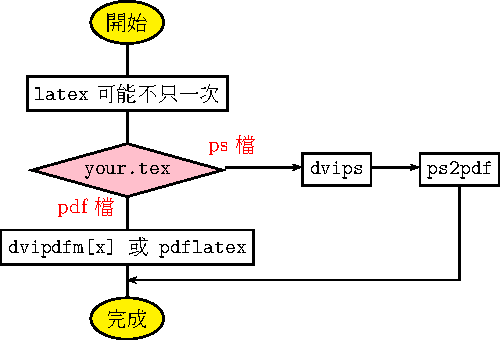
\includegraphics{latex-flow}
\end{center}

\section{\LaTeX\ ���S���M�βŸ�}
�b \TeX/\LaTeX\ ���@�ɡA��l��Z���O�¤�r�ɡA����@�ؽs�边���i�H���}�ӽs��B�[�ݡC�ӱƪ����O�q�`�O�Ѥϱ׽u�]\textbackslash, backslash�^\index{�ϱ׽u}\index{backslash}�Ҷ}�Y�Ӥ޾ɡC����\index{����}�h�O�Ѧʤ����]\texttt{\%}�^�Ӥ޾ɡC�Ҧp�A�H�s�边�s��U�C��r�G

\begin{quote}
\begin{verbatim}
This is my first \LaTeX\ typesetting example.
\end{verbatim}
\end{quote}

�sĶ��|�ܦ��H�U�����G�G

\begin{quote}
This is my first \LaTeX\ typesetting example.
\end{quote}

�䤤�� \verb|\LaTeX| �N�O \LaTeX\ ���@�ӫ��O�A�|��� \LaTeX\ �o�ӯS�����ϥܡC

�ѩ�A����a���y�t�A�q�`�r���B�Ÿ����̤j�e�q�u�� 256 �ӡ]$2^8$�^�A�]���A�\�h�{�����Ÿ��������ӷ���������O�A�~��ŦX�ƪ����h�ˤƻݨD�C�H�U���Ÿ��A��IJ \TeX/\LaTeX\ ���B�͡A�i�ೣ�o�ɮɯd�N�A���n���g�B�z�N�����g�i��Z���Y�h�F�C

�q�`�A�s�边���y�k�C��\index{�y�k�C��}�|���U�P�_�y�k�O�_���T�A�����O���৹���L�ʡA�����٬O�|�|���A�o�ɧO�ѤF�d�ݤ@�U {\tt *.log} �ɮסA�Ҧp�G�sĶ {\tt your.tex} �ɪ��ܡA�L�� log �ɴN�O {\tt your.log}�C

\begin{quote}
\begin{tabular}{llll}
�Ÿ� & �@�� & ��Z�W�ϥ� & \LaTeX\ �����N���O \\
\hline
\textbackslash & �U�ƪ��R�O & \verb|$\backslash$| & \verb|\textbackslash|\\
\%             & ����       & \verb|\%|           & NA \\
\#             & �w�q����   & \verb|\#|           & NA \\
\~{}           & ���ͤ@�Ӫť�   & \verb|\~{}|     & \verb|\textasciitilde| \\
\$             & �i�J�]���}�^�ƾǼҦ� & \verb|\$| & \verb|\textdollar| \\
\_{}           & �ƾǼҦ������ͤU�Цr & \verb|\_{}| & \verb|\textunderscore| \\
\^{}           & �ƾǼҦ������ͤW�Цr & \verb|\^{}| & \verb|\textasciicircum| \\
\{     & �ХܩR�O���@�νd��   & \verb|\{| & \verb|\textbraceleft|\\
\}     & �ХܩR�O���@�νd��   & \verb|\}| & \verb|\textbraceright|\\
\textless      & �ƾǼҦ������p��Ÿ� & \verb|$<$| & \verb|\textless| \\
\textgreater & �ƾǼҦ������j��Ÿ�   & \verb|$>$| & \verb|\textgreater| \\
\textbar     & OT1 �s�X�A�ƾǼҦ����~�ॿ�T��� & \verb+$|$+ & \verb|\textbar| \\
\&           & ���椤�����j�Ÿ�   & \verb|\&| & NA
\end{tabular}
\end{quote}

\section{\LaTeX\ �ƪ��W���@�dzW�d�κD��}
\label{sec:convention}\index{�W�d}\index{�D��}

���F�W���ҽͨ쪺�S���Ÿ��~�A�]���@�dzW�d�κD�ҭn���u�A���ǬO����w�ʪ��W�w�A���ǫh�u�O�D�ҡA�i�ण�P����a�B�y���|�����P���D�ҡA�Ȯɥ���L�����O \LaTeX\ ���C���W�h\index{�C���W�h}�N���F�C

\subsection{�r���������N�y}
\label{subsec:baseline}

�n�ͱƪ��W���W�d�B�D�ҫe�A�ڭ̱o���{�Ѥ@�U�r�����@�dzN�y�A�H�K����峹������ɦ��ӷ����C�q�`�ڭ̨C�Ӧr���O�m���@�Ӱ��Q����ؤ��A�٬� em-square\index{em-square}�A�P�@�Ӧr�����P�@���I�ơA�C�@�� em-square �j�p���O�ۦP���A��ڤW���r�]glyph\index{glyph}�^�n�m��b�o�� em-square �������m�A�o�O�r���]�p�̪��[�I�A�ҥH�A�P���I�ƪ����P�r���A�L���r���j�p���@�w�|�@�ˡA�]���ڭ̬O�ϥ� em-square ���j�p�b������A�ӫD��ڪ� glyph�C

�b�峹���ƦC���ɭԡA�h�O�N glyph �m��@�ӥH���Q�Ѧ��I�]reference point�^\index{���Q�Ѧ��I}\index{reference point}����Ǫ��@�Ӱ��Q�u�W�A�٬���u�]baseline\index{��u}\index{baseline}�^�A�j�g�r�����F Q �H�~�A�L�̪��������O�m���u�W���C���p�g�r���h���@�w��n�y���b��u�W�A���Ǧr�����e�i��W�X��u�H�U�A�Ҧp y�Bj ���r���C����r���b�峹�����m���m�A�ڭ̨Ӭݬݤ@�Ӽ����ϡG\footnote{��ڦr���]�p�W���U�����M���W���ε��c�A���M���|�O�o��²���A�o�̪������ϡA�u�O�Ȯ����r���@��m�񦳭Ӳʲ��������C}

% looks ugly, but l2h cannot handle this MP file be transparent png.
\begin{center}
\latexhtml{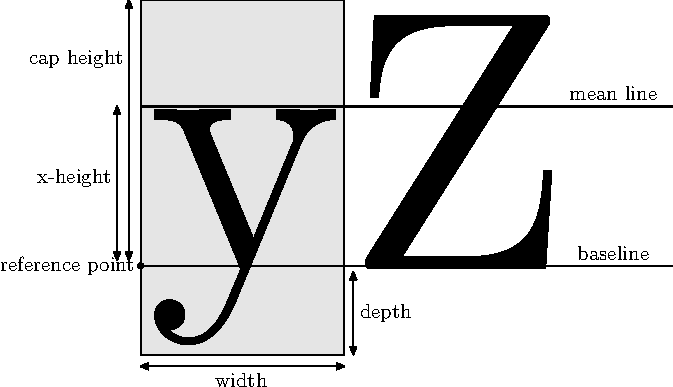
\includegraphics{baseline.1}}{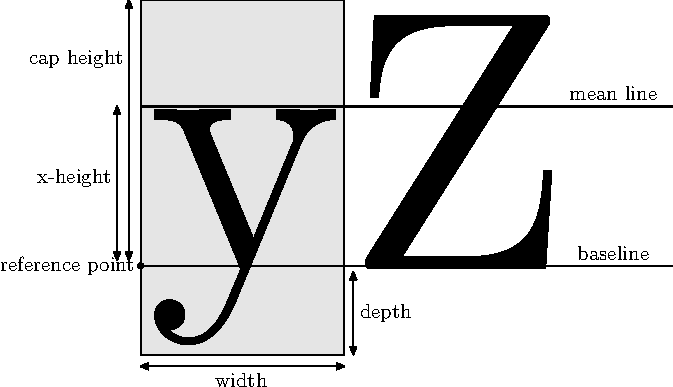
\includegraphics{baseline}}
\end{center}

�o�ӶW�X��u�H�U�����סA�ڭ̺٤����`�ס]depth\index{�`��}\index{depth}�^�A�H�W���N�٬��r���]height\index{�r��}\index{height}�^�A���M�j�p�g�����P�S�����j�g�r�����r���]cap height\index{cap height}�^�Τp�g�r�� x ���r���]x-height\index{x-height}�^�A�ѩ�o�ӨҤl�̬O�զX�r\index{�զX�r}�A�ҥH�C�Ӧr���e�ס]width\index{�e��}\index{width}�^���@�w�|�@�ˡA�����r���r�ڪ��h�O���e���r���C�r���[�W�`�סA�ڭ̴N�٤��� totalheight\index{totalheight}�A�j���������p�A�ȶȻ� height �ɬO���]�A depth ���A�ӥB�q�`�����O cap height�C

mean line\index{mean line} �b�@�����֥Ψ�A�q�`�O�r���]�p\index{�r���]�p}�ɤ~�|�Ψ�A�L�O���p�g�r���h���W����X�������ҳs�����@�Ӱ�ǽu�A�o�� mean line �� baseline ���Z���A�@��N�٬� x-height�A���M�N�O�p�g�r�� x �����סA�]���ڭ̷|���@�Ӫ��׳��A�٬� ex�A�����N�O�o�� x-height�C

����r���ܤ���S���A�L�O�H em-square �������I�Ӹm�� glyph ���A�b���^��V�X�ɡA����r�ä��O��n�y�����u�W���A�|�W�X��u�U�@�I�I�A�ܩ�|�W�X�h�֡A�h�M�r�����]�p�����A�C�ئr�������i��|���P�C�o�]�O���D�ƪ��W���@�P�ʡA�r���i�ೣ�ݭn�ɶq�ϥΦP�@�M���U�ئr������]�A�_�h�N�o�g�L�L�աA�~��Ͼ�Ӧr�����{�W���o��դ@�P�C

�o�DZM���N�y�A���ᴣ��@�ǫ��O���Ѽƪ��y�z�ɳ��|�ϥΨ�A�]�������x�@�U�A�Ҧp�G�r�������\index{�r������}�A��ڪ��N�O�H�Ѧ��I�]reference point�^���ǡA�u�����X���b�ߨӱ��઺�A�Ӥ@��һ�����Z\index{��Z}�A�����O�W�U�� baseline ���Z���C

\subsection{�@��ʪ��C���W�h}
\label{gen:gamerules}\index{�C���W�h}

\begin{enumerate}
\item \LaTeX\ �����O���O�j�p�g���O���A�� \verb|\| �}�Y�A�ᱵ�Ѧr���զ����r��γ�@���D�r���r���C�䤤�� \verb|[ ]| ���A���A�����O��ܩʰѼ�\index{��ܩʰѼ�}�A�i�H�ٲ��A�� \verb|{ }| �j�A���A�����O����ٲ����ѼơA���M�A\LaTeX\ �����O���@�w�|���ѼơA�����j�������|���ѼơA�u���L��L���ٲ��ϥιw�]�Ƚ}�F�C

\item \LaTeX\ ��Z���A�Ť@�ӭ^��ťթM�Ŧh�ӭ^��ťժ��@�άO�@�ˡA\LaTeX\ �|�{�@�@�ӭ^��ťաC

\item ���`�ڭ̽s��¤�r�ɡA���� \textsf{Enter} ��A�N�N������A����ڱƪ��X�ӡA�@�檺�e�׬O���ӱƪ��������]�w�A�]�N�O���A�A�b��Z���� \textsf{Enter}�A���N���ƪ���N�O�q�o���_��\index{�_��}�A\LaTeX\ �|�̤@���������e�׸g�L����p���۰ʸɦ��@����A���_��A�ӥB�|�b�����۰ʸɨ��@�ӪťաC�o�b�^��ܦ۵M�A�٬��r�]word�^���ť�\index{�r���ť�}�A������h���@�ˡA�b�s�边���s�褤��A�H�N�� \textsf{Enter} �����G�A�|�y���峹�������嶡�X�{�ťաC�o�|�b���夤�A�����ɾ��A���X�ѨM����k�C

\item �s�边���A�h���X�� \textsf{Enter} �N�h�ťX�X��A���b \LaTeX\ ��Z�̡A�h�Ӫťզ�\index{�ťզ�}�A�M�@�Ӫťզ�O�@�˪��@�ΡA\LaTeX\ �|��L�{�@�O�@�Ӫťզ�C�ӳo�Ӫťզ�A\LaTeX\ �P�ɤ]�|�{�@�O�s�q�����}�l�A�ҥH \LaTeX\ �O�H�ťզ�Ӥ��j�U�Ӭq���C

\item \LaTeX\ �w�]�C�ӳ��`���Ĥ@�Ӭq�����Ĥ@��O�����Y�]noindent\index{�����Y}\index{noindent}�^�A�q�ĤG�Ӭq���}�l�~�|���Y�]indent\index{���Y}\index{indent}�^�C���M�A�o�O�i�H��諸�A����|�A���ΡC

\item \LaTeX\ �����O�A�O�q�ϱ׽u\index{�ϱ׽u}��Ĥ@�Ӧr���}�l�A��Ĥ@�ӫD�r���Ÿ�����]�]�A�ťաB���I�Ÿ��μƦr�^�C�]���G

\begin{quote}
\begin{verbatim}
This is my first \LaTeX typesetting example.
\end{verbatim}
\end{quote}

�o�˪��ܡA��ڵ��G�A�]�� \verb|\LaTeX| �᪺�ťլO�ݩ���O���@�����A�ťձN���|�Q�����A�o�˷|�L���G

\begin{quote}
This is my first \LaTeX typesetting example.
\end{quote}

�o�ص��G�A\LaTeX\ �M typesetting �s�b�@�_�F�C�n�קK���ܡA�N�n���w���O���@�νd��A�Ҧp�H�U���j�A���C�δN�u���[�ӪťաA�Ҧp \verb|\ |�A\LaTeX\ �I�� \verb|\| �N�|�Φ����㪺���O�A��᪺�ťմN�|�Q�u���������ťդF�G

\begin{quote}
\begin{verbatim}
This is my first {\LaTeX} typesetting example.
This is my first \LaTeX{} typesetting example.
This is my first \LaTeX\ typesetting example.
\end{verbatim}
\end{quote}

�ҥH�A���`�L�X�����ӬO�G

\begin{quote}
This is my first \LaTeX\ typesetting example.
\end{quote}

\item ���ѲŸ��]{\tt \%}�^\index{���ѲŸ�}\index{%@\verb=%=}�A�i�H��b�@�檺����a��A{\tt \%} �᪺��r�|�Q \LaTeX\ �����C�ҥH�A�p�G�O��b�@�檺�̧��ݡA���� \LaTeX\ �|�۰ʴ��J���r���ťդ]�N�|�Q�����C�Ҧp�G

\begin{quote}
\begin{verbatim}
This is my fisrt \LaTeX\ document. Give \LaTeX\ a%
try.
\end{verbatim}
\end{quote}

�o�ˤ@�ӡA�ƪ��X�ӷ|�ܦ��G

\begin{quote}
This is my fisrt \LaTeX\ document. Give \LaTeX\ a%
try.
\end{quote}

a �M try �s�b�@�_�F�I���`���ӬO�G

\begin{quote}
This is my fisrt \LaTeX\ document. Give \LaTeX\ a try.
\end{quote}

���o�ӯS�ʡA�ڭ̥i�H���Φb����A�]�N�O���b�s�边\index{�s�边}���A����峹�� \textsf{Enter} �䴫��ɡA���ݥ[�� {\tt \%}�A�o�ˤ@�� \LaTeX\ �N���|���J�^��r���ťաA����r�N�i�H�s�������S���ťժ��@���F�A�_�h \LaTeX\ �b��g��Z�_�y\index{�_�y}�ɡA�|�۰ʦb�촫��B��J�@�ӭ^��ťաA�]���A��l�� \TeX/\LaTeX\ �O�{���o���媺�C

\item ���^��V�X���ɭԡA�q�`�A�^��r�e�᳣�|�d�ӪťաA�H�K�M����Ϲj�}�ӡA�u�O�o�Ӫťխn�h�j�A�o�N�S���T�w���D�ҡA�q�`�d�ӭ^��ťդ]�O�i�H�A�n���s���ܡA���ͨ줤��ƪ�����ij�D�ɦA�ӰQ�סA�ثe�N�i���ߺD�A�^���r�e��d�ӭ^��ťաC
\end{enumerate}


\subsection{�w����I�Ÿ����C���W�h}

\begin{enumerate}
\item ���^�媺�޸�\index{�޸�}���@�ˡA�o�̽ЯS�O�`�N�A�\�h�H�`�`�d���C���B�^��޸����޳������n�����k�C�^�媺�ܡA���䪺�޸��O grave accent�A�O��L���W�� {\sf Esc} �� {\sf F1} �U�観�i�θ������@����F�k�䪺�O apostrophe\index{apostrophe}�A�]�N�O��L���� {\sf Enter} ��j����������C���޸������άO��J�⦸������޸�\index{����޸�}�Ψ⦸���k��޸�\index{�k��޸�}�A�Ӥ��O�� \verb|"| �o�Ӥ@����������I�� ditto marks\index{ditto marks}�C�ҥH�A��ڤW�b��J��Z�ɬO�G

\begin{quote}
\begin{verbatim}
Please press an `Esc' key.
Please press an 'Esc' key. �o�O���~�ܽd�I
``This sentence.''
"This sentence." �o�O���~�ܽd�I
\end{verbatim}
\end{quote}

�ƪ��X�Ӫ����άO�G

%begin{latexonly}
\begin{quote}
Please press an `Esc' key.\\
Please press an 'Esc' key. �o�O���~�ܽd�I\\
``This sentence.''\\
"This sentence." �o�O���~�ܽd�I
\end{quote}
%end{latexonly}

\begin{htmlonly}
\begin{quote}

\includegraphics{quotation}
\end{quote}
\end{htmlonly}


���媺�ܡA�ڭ̬O�ϥΤ�����Ϊ��u�B�v�Ρy�B�z�A�b����j���h�w��ΩM�^��ۦP�Ϊ������βŸ��A���o�b���媽�Ʈɷ|�X���D�A�]���A���媺��B���޸��٬O�o�����ڭ̥ثe�ϥΪ��C

\item \LaTeX\ �|�b�^��峹���@�ӥy�l�����M�t�@�ӥy�l�}�l�������A�۰ʽվ㦨���j�@�I���ťաA�o�i�H�W�[�峹����Ū�ʡC�ҿפ@�ӥy�l�����A�Ҧp�G�y�I�].�^�B�ݸ��]?�^�B��ĸ��]!�^�Ϋ_���]:�^�A�o���M�O���^�媺�b�μ��I�Ÿ��A���O���媺���μ��I�Ÿ��C�A�i�H�`�N�@�U�W�����|���Ҥl�A�b document.\ �M Give �������ťշ|�y�L�j���L�^���r�����ťաC

�{�b�����D�O�A�p�G�o�Ǽ��I�Ÿ��᭱���O�t�@�ӥy�l���}�l���ɭԡA\LaTeX\ �L�k�h�P�_�o�ر��ΡA�o�ɱo�ѧڭ̦ۤv�ۦ�P�_�B�B�z�F�C�Ҧp�^���Y�g�r�G

\begin{quote}
\begin{verbatim}
I am Mr. Edward G.J. Lee, G.J. is a abbreviation of my name.
I am Mr.~Edward G.J. Lee, G.J. is a abbreviation of my name.
I am Mr.\ Edward G.J. Lee, G.J. is a abbreviation of my name.
\end{verbatim}
\end{quote}

�䤤 \verb|Mr.\ Edward| ���g�k�A�M \verb|Mr.~Edward| �X�G�O�@�˪��A���O�j�����J�@�Ӥ���p�����`��r���ť�\index{��r���ť�}�A�t�O�b���̤]�t�~���ܤ��i�H�q�o�̴���A�q�`�Φb�H�W���ɭԡA���L�̤��P���_�A�@��b�H�W���ƪ��A�]�A�L���Y�ΡB¾�١A�O�����_�����Ӥ��}���C�ӥB��Ӥ�y�������ܡA�H��̸�����A�~���|�]���_��Q������b�A�o�� {\tt ~} �Ÿ��]�]���b \TeX\ ���M���W���A�N�٬� tie\index{tie}�A��L�̸j�����N��C�ƪ��X�Ӫ��ɭԷ|�ܦ��G

%begin{latexonly}
\begin{quote}
I am Mr. Edward G.J. Lee, G.J. is an abbreviation of my name.\\
I am Mr.\ Edward G.J. Lee, G.J. is an abbreviation of my name.
\end{quote}
%end{latexonly}

\begin{htmlonly}
\begin{quote}
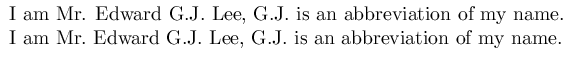
\includegraphics{abbreviation}
\end{quote}
\end{htmlonly}

�Щ�j�h�J�Ӥ���@�U���G�N���D�F�C�ĤG�檺�~�O���T���AMr.\ �M Edward �������ťլO���`��r���ťաA��Ĥ@�檺�y�l�����ťխn�p�@�I�I�C��L���ϥΨ��Y�g�r�����X�A�Ҧp�G`Dr.'�B`etc.'�B`e.g.'�B`i.e.'�B`vs.'�B`Fig.'�B`cf.'�B`Mrs.'�A�o�dz����O�N���y�l�����A�ҥH�A�n���J�@�ӥ��`�ťաC

�� G.J. �᭱������S�����J���`�ťաH���O�]���AJ �O�j�g���A�o�� \LaTeX\ ���|�h�~�{���O�y�l�����A�q�`�y�l�����ɪ��y�I�e�����Ӧr���O�p�g���CWell�A���S��ı�o���I�D�z�H:-)

�����A�Ʊ��٨S�������IKnuth �б¥X�F�@�D���D�A�p�G�y�l�������O `Please see Appendix A.' �᭱�S�ٱ����t�@�ӥy�l�C�o�ɫ���H�ѩ�A���|�{���O�y�l�����A�]���|���J���`�ťաA���o���O�y�l�����r�I�мȮɥ��O�o�A�ϥ� \verb|...Appendix A\null.|�A�� \verb|...Appendix A\@.|�C�o�ӻ��Ӧ��I�ܪ��A�����|�A�ӱ��Q�A�аO�o `\verb|\null|' �M�y�I���O�S���ťժ��C�Ҧp�G

\begin{quote}
\begin{verbatim}
Please see Appendix A. We will be there soon.
Please see Appendix A\null. We will be there soon.
\end{verbatim}
\end{quote}

�ƪ��X�Ӫ����G�N�|�O�]�t��������A�Фp�ߤ���^�G

%begin{latexonly}
\begin{quote}
Please see Appendix A. We will be there soon.\\
Please see Appendix A\null. We will be there soon.
\end{quote}
%end{latexonly}

\begin{htmlonly}
\begin{quote}
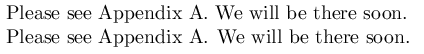
\includegraphics{abbreviation2}
\end{quote}
\end{htmlonly}

�p�G�A�A�{�b�\Ū���O HTML\index{HTML} �榡���A���ǨҤl�p�G�L�k������ܥX�ӡA�Ч�\�� PDF �����C�ӥB�A�p�G�A�s�@ PDF �榡�ɡA�r���S�����O�]���媺�^�Ʀr�O�O�J Computer Modern Type1 �r���^�A�t���i��N�|�󤣩���C�i�յۨϥ� {\sf gv/gsview}\index{gv@\textsf{gs}}\index{gview@\textsf{gview}} �h�\���A�M��վ㦨 Landscape\index{Landscape}�A��y�l�����Ԩ���t���a��h�N�ݱo�X�ӤF�C�o�b�y�l�h���ɭԡA�o�Ӫťդ]�ëD�T�w�j�p���A\LaTeX\ �|���峹���c���ݭn���ӷL���վ�C

\item �R�`��\index{�R�`��}����^�]�O���P�A�^��O�T�I�A�p�G�I��y�I���ܡA�h�O�|�I�C���媺�ܬO���I�A�I�줤��y�I�ܮe���N���o�M���C���O�^��o�ӤT�I�A���O�N���ӤT�ӥy�I�F�ơA�o�˪��I�ӱK���A�i�H�ϥ� \verb|\ldots| �� \verb|\dots| ���O�A�Ҧp�G

\begin{quote}
\begin{verbatim}
I'm not a good man ..., but a good husband .... ���~�ܽd�I
I'm not a good \ldots\ man \ldots, but a good husband \ldots.
I'm not a good \dots\ man \dots, but a good husband \dots.
\end{verbatim}
\end{quote}

�ƪ��X���ӵ��G�O�G

%begin{latexonly}
\begin{quote}
I'm not a good ... man ..., but a good husband .... ���~�ܽd�I\\
I'm not a good \ldots\ man \ldots, but a good husband \ldots.\\
I'm not a good \dots\ man \dots, but a good husband \ldots.
\end{quote}
%end{latexonly}

\begin{htmlonly}
\begin{quote}

\includegraphics{dots}
\end{quote}
\end{htmlonly}

���媺�R�`���O�Ѩ�ӥ��Ϊ��T�I�Ҳզ����I���A�Y�G\chdots{}�A�N�O�ڭ� Big-5 �X�� {\tt 0xa14b}�]{\tt U+2026}�^�A���ѩ� Unicode\index{Unicode} �|���@�� MIDLINE HORIZONTAL ELLIPSIS({\tt U+22EF})�A�]���A���dzn��b��Ū�W���i��|���@�ˡA�]���ڭ̪��r���A�j�����b�s�@���I�Ÿ��ɬO�m�b�������a��A��������j���O�m��b��u���a��A�� Unicode �x��ĥΪ��˥��r���A��n�O����j�����t�өҴ��ѡA�o�ˤ@�Ӧ��dzn��u�@�̴N�{���ڭ̪��R�`�����ӬO {\tt U+22EF} �F�A�ܤ������A�ڭ̪� Big-5\index{Big-5} �X�èS���۹������r�X�C

\item �}�鸹\index{�}�鸹}�C�b�^��A�۷���}�鸹���i�঳�T�ءG
  \begin{itemize}
    \item hyphen\index{hyphen}\\
�o�O�̵u�� dash\index{dash}�A�q�`�N�O��J \verb|-| �N��F�A�Ҧp \verb|father-in-low|�A�o�˷|���{�� fater-in-low�C
    \item en-dash\index{en-dash}\\
�o�O�̱`�Ϊ��}�鸹�A�O��J��� hyphen�C�Ҧp \verb|1991--2003 �~|�A�o�|���{�� 1991--2003 �~�C
    \item em-dash\index{em-dash}\\
�o�O�̪��� dash�A�ѤT�ӳs�� hyphen �զ��A���ӬO�̬۪��ڭ̤���һ����}�鸹�C�Ҧp \verb|I am---a good man.| �|���{�� I am---a good man.�C�ܩ�o�ӤT�ӳs�� hyphen �e��O�_�n�d�ťաA�����H�ϥΡA�èS���w�ʪ��D�ҡA�����F�M���媺�}�鸹�t�X�]����}�鸹�e��A�q�`���d�ťա^�A�ӤH�q�`�O���d�ťժ��C
    \item �u�����\\
�o�������O�}�鸹�A�ӬO��ڪ���έt���A�o�n�i�J�ƾǼҦ��A�Ҧp�G�t���A�n�g�� \verb|$-5$|�A�M����{�X�ӬO $-5$�C�o�]�`�`�|���H�d���A���ઽ����J�@�몺�t��������ӥR�ơA�o�O�]�� \TeX/\LaTeX\ ���ƾǦ��l���Φr�M���j�B�z�A�M�@�뤺�夣�P�����Y�C
    \item ���媺�}�鸹\\
���媺�}�鸹�O����Ӥ���r��m�����@��u�A���שM�R�`���ۦP�C�b���u��m���A�w�q�W�O����ءAen-dash �O {\tt Big-5 0xa156}�Aem-dash �O {\tt Big-5 0xa158}�C���ѩ󤤤�r���Z�����D�A���i�ॴ�X�Ӫ��}�鸹�����|���@�I�ť�\footnote{�o�O�i�H�վ㪺�A�]�N�O�h����Ӿ�u�������r���Z�A�o�˴N���|���ͤp�ťդF�A����R�`���]���P�˪����ΡA�ڭ̷|�b�L�ժ������A�ӰQ�סC}�A�Ҧp�X�X���媺 em-dash�A�o�O�V�V���媺 en-dash�C�b�פ夤�A�}�鸹�q�`�i�H�ϥΤp�A���Ϋ_���N���C
    \item ���媺�p�W���ήѦW��\\
���媺�p�W��\index{�p�W��}�A�i�H�Щ��H�W�B�a�W�A�p\underline{�]�h�P}�F�ѦW��\index{�ѦW��}�]�p�W�������u�����i���Ϊ��^�A�i�H�Φb�ѦW�A�o�DzŸ��`�y���ƪ��W���x�Z�A�`�ϥ� �m �n�Ө��N�ѦW���A�p�W���h�L��L���N��k�C�b�@�몺�۵M�����ά�ǽפ�W�q�`���ϥγo���¦����p�W���ήѦW���C
\end{itemize}

\item ���Y�I\index{���Y�I}\\
�o�i�O�ƪ������n�\��C�^�媺�q�`�S�����D�A\LaTeX\ �|�۰��׶}�B�z�A����N���@�w�F�A\LaTeX\ �i���{�Ѥ���A���q�`��������{���ήM��A�h�h�ֳ֤��|�B�z�A�u���L�A���ɭ԰����i��|�~�P�C����A�쩳����O���Y�I�H���U�C�Ӫ��A�j�a�N���դF�A�ڦC���媺�A�^�媺�N���C�X�ӤF�A�]�� \LaTeX\ �|�۰ʳB�z�A�����ڭ̾�ߡC

\begin{quote}
\begin{tabular}{ll}
���I�Ÿ� & �m��B\\
\hline
�A�C�F�B:�v�^�n�I�H & ����m��歺\\
�u�]�m              & ����m����\\
�}�鸹�ΧR�`��      & �m�󭺧��ҥi\\
\end{tabular}
\end{quote}

²�檺���A���F�}�鸹�ΧR�`���A�S���}�f���A����m��̶}�Y�A�}�f�V�k���A����m��̥k�A�}�f�V�����A����m��̥��C�q�`���|�B�z�n�A���սZ���ɭԭn�`�N�@�U�~�P���a��C
\end{enumerate}

\section{\LaTeX\ ����Z���c}
\label{sec:struct}\index{��Z���c}

\subsection{���ҡ]environment�^\index{����}\index{environment}}

�W�@�`�ҽͪ����O���O�A���M�]�i�H�Ѥj�A��\index{�j�A��}�өw�@�νd��A���p�G�O�@��q�A�ƦܬO�@��g�峹���n�@�ήɡA�����O�i��N���ܾA�X�F�A�]���A\LaTeX\ �]���@�إ������c�A�٬����ҡ]environment�^�A�D�n�O���@�νd����X�j�ܸ��j���d��C

�Ҧ������ҡA���O�_�� \verb|\begin{���ҦW��}|�A��� \verb|\end{���ҦW��}|�A�o��ӫ��O��������Z���|�Q�@�ΡA�ӥB�A���Ҥ����٥i�H�M�Ψ�L���P�����ҡC

\LaTeX\ ��Z������A���N�O�]�b�@�� \verb|\begin{document}| �M \verb|\end{document}| �o�� document ���ҷ����C

\subsection{��²�檺 \LaTeX\ ����Z���c}

�H�U�N�O�Ҧ� \LaTeX\ ���ݨ�ƪ���Z�j���c�G

\begin{quote}
\begin{verbatim}
\documentclass{article}

  �o�̬O preamble ��

\begin{document}

  �o�̬O�����

\end{document}
\end{verbatim}
\end{quote}

\verb|\documentclass{article}|�A�o�O�b�i�D \LaTeX\ �ϥέ��@�����O�A�ڭ̥ثe�ϥΪ��O {\tt article} ���O\index{���O}\index{article}�A�������O�|�b�� \ref{ch:class} ���Q�סCpreamble\index{preamble} �ϡA�h�O�U�@�Ƿ|�v�T��Ӥ�Z�����O�A�ΤޥΥ����M�󪺦a��A���M�A�������ޥΥ����A�]���ϥμv�T���媺���O���ܡApreamble �ϴN�O�ťաA���g����F��C����ϡA�N�O�ڭ̹�ڤW�g�峹���a��C

�{�b�]�i�H��e�����|���Ҥl�A��J����ϸ��Y�Apreamble �ϪťըS���Y�A�M��s�ɡA�յ۽sĶ�ݬݡG

\begin{quote}
\begin{verbatim}
latex example.tex
dvips example.dvi      => ���� ps �榡 example.ps
dvipdfm[x] example.dvi => ���� pdf �榡
pdflatex example.tex   => ������ .tex ���� .pdf
\end{verbatim}
\end{quote}

�u������Ҹѻ��A�|�b�U�@���Ӷi��A�ҥH�A�o�̼Ȯɤ��|���Ц��������ҥi�H�ϥΡA�����ݬݨS�����Y�C�ѩ��٨S�ͨ줤�媺���D�A�]���p�G�A�Q�ոլݡA���Ȯɥ��ϥέ^��A�D�z���O�۳q���C

\subsection{preamble �ϥi�H��Ǥ���H}
\label{subsec:preamble}

�o�̥i�H�ޥΥ����A�ӥB�|�v�T��g��Z�����O�A�Ҧp�@�Ǩƥ��w�q�n�����O�A�Q�b��g��Z���ϥΡA�N�i�H�m��b preamble �ϡC

\subsubsection{�������ޥ�}
\label{subsubsec:package}

����D�n�O�з� \LaTeX�A���e���w����A�|���ǥ����M�󤣱o���n�ޥΡA���U�N�ӻ����p��ޥήM��C�o�ǮM�󳣬O�@�� \TeX\ �t�γ��|���W���C

���O�����ҭn�p��}�Y�����йL�F�A�{�b�ӬݬݤޥΥ����n���}�Y�C

\begin{quote}
\begin{verbatim}
\documentclass{article}
\usepackage{color}
\begin{document}
\textcolor{blue}{This is blue color.}
\end{document}
\end{verbatim}
\end{quote}

�sĶ�@�U�A�ݬݵ��G�O����H�o�̨ϥΪ��N�O \textsf{color} package\index{color@\textsf{color}}�A���Y�O�� \TeX/\LaTeX\ macro �Ҽg���@�ӥ����M��C�@��²�檺�ڭ̴N�٬������]macro�^\index{����}\index{macro}�A�����@�I���N�٬������M��]package�^\index{�����M��}\index{package}�A���A���Y���O�@�˪��A�u���L�j�p�Φ��S����z���@�Өt�Ϊ��t�O�C

\LaTeX\ ���Y������{�����M��i�H�ϥΡA�C�Ӵ��G�� \TeX\ �t�ΩҦ������i�ೣ�|���Ҥ��P�C�j���S���H�i�H��q�Ҧ��{�s�� \LaTeX\ �����M��A�]����b�O�Ӧh�F�A���L�A����j�����|����`�Ϊ������M��C�ԲӪ������M�󪺺غءA�|�b�� \ref{ch:package} ���ӻ����C

\subsubsection{�v�T��g��Z�����O}

�|�v�T��g��Z�����O�A�q�`�]�O��b preamble �ϡA�Ҧp�G

\begin{quote}
\begin{verbatim}
\linespread{1.36}
\parindent=0pt
\end{verbatim}
\end{quote}

\verb|\linespread| �O�b����W�U�檺��Z�A�o�̴N�O�N��Z�ܦ���Ӫ� 1.36 ���C�ܩ󤰻�O��Z�O�H�N�O�o�@�檺��u�]baseline�^��U�@�檺��u���Z���A�q�`�^��峹�����h�վ�L����Z�A������o�A���[�j��Z�H�Q�\Ū�C

\verb|\parindent| �O�վ�q�����Y���{�סA�o�̽վ㦨 0�A�]�N�O���U�q���������Y���N��A�]�i�H�վ㦨��L���ȡA\LaTeX\ �N�|�̳o�ӭȥh���Y�C���M�A���h�]�w���ܡA\LaTeX\ �N�|�̥L���w�]�ȥh���Y�C


\subsection{���`���c\index{���`���c}}
\label{subsec:chapstruc}

����Ϸ��M�O�ڭ̼g�峹���D�n�a��A�Τ@�ǷL��\index{�L��}�C�b \LaTeX\ ����Z���Y�A���`���D���Φ����O�ѦP�˪����O�ӱ���A�o�˦��@�Ӧn�B�A�{�ɴ��J���`���D�Ψ䤺��ɡA�ڭ̤����h�z�|���D�s���Υؿ������D�A�]�����h�z�|�n�Τ���r���B�Φr���j�p�n�h�j�A\LaTeX\ �|�۰ʭp��B�z�A�r���j�p�]�|�M����ϥΪ��r���j�p���۰t�X�վ�A�ϥΪ̴N�M�ߦb����c��B�g�@�Y�i�C�H�U�ѦC�����A�Ѿ�ӳ��`���c�G

\begin{quote}
\begin{tabular}{lll}
�`�׼и� & ���O & �@�ΤΪ`�N�ƶ�\\
\hline
$-1$ & \verb|\part{}|          & �o�O�̤j�����c�A�ڭ̤���q�`�٬��u���v�C \\
0    & \verb|\chapter{}|       & ���C�b article ���O���Y�S�����C\\
1    & \verb|\section{}|       & �`�C\\
2    & \verb|\subsection{}|    & �p�`�C\\
3    & \verb|\subsubsection{}| & ���p�`�C\\
4    & \verb|\paragraph{}|     & �q���C\\
5    & \verb|\subparagraph{}|  & �p�q���C\\
\end{tabular}
\end{quote}

���`���D\index{���`���D}�����e�N�O�����g�J���O���j�A�����Y�N�i�H�F�A\LaTeX\ �b�ƪ��ɷ|�۰ʨϥβ���B�[�J���`�s��\index{���`�s��}�ίǤJ�ؿ�\index{�ؿ�}���Y�C

�ܩ�Ĥ@�檺�`�׼и��]secnumdepth�^\index{�`�׼и�}\index{secnumdepth}�A{\tt book/report}\index{book@\texttt{book}}\index{report@\texttt{report}} ���O���`�׼и��O 2�A{\tt article} ���O 3�C�o�O����N��O�H�N�O�� {\tt book/report} ���O����Z�A�b \verb|\subsection{}| �H��]{\tt subsection} �������|�s���^�A���`�N���A�s���F�F�P�˪��A�b {\tt article} ���O����Z�A�b \verb|\subsubsection{}| �H��N���s���F�C�����M�|�W�ߥX�@��W��Ӫ��ܳo�ӬO���D�C���s���F�����`���e�A���M�]�N���ǤJ�ؿ����Y�F�C�o���M�O�i�H��諸�A�u�n��� \LaTeX\ �� {\tt secnumdepth} �o���ܼƪ��ȴN�i�H�F�A�o�ө���|���Φp���� \LaTeX\ ���w�]�ȡC���o�g�峹�A�b preamble �ϴN���@�ӳ]�w�G

\begin{quote}
\begin{verbatim}
% let the depth of report to subsubsection
\setcounter{secnumdepth}{3}
\end{verbatim}
\end{quote}

�ҥH�A�o�g�峹���M�ϥΪ��O {\tt report} ���O�A���O���`���`�׼и��O�Цb 3�A�]�N�O���|�s���� {\tt subsubsection} ����A���o���M�O�S���s�J�ؿ������C 

�U�@���N���ڭ̶}�l��ڰʤ�a�I��\chdots{}�A����{�b���S�����㤶�Ы��O�O�H���ګ��|���D��������O�i�H�ϥΡH�o�O�]�� \LaTeX\ �����O�ܦh�A�������Ъ��ܡA�@�譱�O�����A�G�譱�]���e���A�ѥL����ڧ@�ΡA�ҥH�A�ڭ̱N�|�b�U���|�Үɬﴡ�b���Y�����A���o����󱵪���n�ɡA�A�Ӿ�z�ӫ��O�t�d���A�o�˥H��d���O�N�ܤ�K�F�A�����h���O�A�u�n���D���ӳo�˥\�઺���O�N���F�C


% ``�j�a�Ӿ� LaTeX'' LaTeX ��Z start.tex
% Copyright (c) 2004  Edward G.J. Lee <edt1023@info.sayya.org>
%
% �b���H�� GNU Free Documentation License 1.2 �ΥH�᪺�����W�d���U�A
% ���\�����B���G�έק�C���쪩�v�B���v�n�����o�����C
%
% �����G�����A�t�� fdl.tex�A���e�� GNU FDL ���W�d���C�p�G�򥢡A�i��
% http://www.gnu.org ���o�A�μg�H�ܦۥѳn�����|(Free Software Fundation)
% �����C
% 9 Temple Place - Suite 330, Boston, MA 02111-1307, USA.
%
% $Id: start.tex,v 1.38 2004/03/07 12:29:47 edt1023 Exp $
%
\chapter{��ڤW�ƪ����ݬ�}
\label{ch:start}

�n�F�A�{�b�����Ӫ��ݬݧa�I�����D�n�O²�檺��һ����A���i�J���p�A�ͨ�L�C������Τ񰪽���צ��Φh�F�C

���ӭӡu�̰����ɭ�h�v�G\textcolor{red}{\bf �Ƿ|����Ŷ��A�A�N�Ƿ|�ƪ��F}�I��DZƪ����B�͡A�����|��ҾǨ쪺�F��h�Q�k�l�G���A�Ҧ����Ŷ��]�N�O�@�ӭ����^�A����ڤW�A�A�n�վ㪺�A���O�U�ӳ������Ŷ��t�m�A��H�@�I���A�]�N�O�@��ӭ��������A�S����r�B�Ϫ��������~�O�ƪ��u�������I�C�A��ťť�N�n�A�L�@�q�ɶ������x��A�A�Ӧ^�Y��ҳo�ӡu���ˡv�Ŷ�����h�C:-)

�ѩ󥻤妳 HTML �����A���F�ഫ�W���y�����u�A��Ҫ������A��Z�W�u�g�{���X�A���G���������O�sĶ�n�� PDF �榡�ɮסA�m�������W�A�i�u�W�\���ΤU���A²�檺�Ҥl�h���t�s�@�W�ߪ� PDF �ɡA�аѾ\���媺 PDF �榡�ɮפ��e�C

\section{²�檺���}

�o�̴N��e�@���ҽͨ쪺�@�Ǥ��e��z���@�Ӥ�Z�A���ӸոլݡA�o�̥��ϥ� {\tt report}\index{report@\texttt{report}} ���O��Z�A�]�� {\tt article}\index{article@\texttt{article}} ���O��Z�O�S�� {\tt chapter} ���G

\begin{quote}
\begin{verbatim}
% example1.tex
\documentclass{report}
\begin{document}
This is my first {\LaTeX} typesetting example.\\
This is my first \LaTeX{} typesetting example.\\
This is my first \LaTeX\ typesetting example.\\
I am Mr. Edward G.J. Lee, G.J. is a abbreviation of my name.\\
I am Mr.\ Edward G.J. Lee, G.J. is a abbreviation of my name.\\
Please see Appendix A. We will be there soon.\\
Please see Appendix A\null. We will be there soon.
\end{document}
\end{verbatim}
\end{quote}

�ϥνs�边�s��A�M��s�ɦ� {\tt exmaple1.tex}�A�o�˴N�i�H�sĶ�F�G

\begin{quote}
\begin{verbatim}
latex example1.tex       => ���� example1.dvi
dvips -Ppdf example1.dvi => ���� example1.ps
ps2pdf example1.ps       => ���� example1.pdf ��
dvipdfm[x] example1.dvi  => �� example1.dvi �������� example1.pdf ��
pdflatex example1.tex    => �� example1.tex �������� example1.pdf
\end{verbatim}
\end{quote}

�sĶ�n�� PDF �ɥi�b���U���ξ\���G

\begin{quote}
\url{http://edt1023.sayya.org/tex/latex123/example1.tex}\\
\url{http://edt1023.sayya.org/tex/latex123/example1.pdf}
\end{quote}

\subsection{���󴫦�}
�C��̫�[�F�� \verb|\\|\index{\\@\verb=\\=}�A�o���ܱj�����檺�N��A�_�h \LaTeX\ �|�̪����w�]���e�רӴ���A�N���|�O�@�ӥy�l�@��F�A�j�a�i�H��o�� \verb|\\| �����A�A�ӽsĶ�լݬݵ��G�A�N�|���D���@�^�ƤF�C�]�i�H�ϥ� \verb|\newline|\index{newline@\verb=\newline=} �o�ӫ��O�A���M�A�ڭ̳��|�o������θ��u�����O�C�ӥB \verb|\\| �i�H�����ɪ����j�A�o�b \verb|\newline| �h����C�Ҧp�G

\begin{quote}
\begin{verbatim}
Please see Appendix A. We will be there soon.\\[1cm]
Please see Appendix A\null. We will be there soon.
\end{verbatim}
\end{quote}

�o�˪��ܡA��椧������Z\index{��Z}�N�O��Ӫ���Z�A�[�W {\tt 1cm}�C�ƦܡA�]�i�H�O�t�ƪ��ѼơA�o�˦�Z�N�|�ܦ���Ӫ���Z��h {\tt 1cm}�A���M�A�p�G�]�L�Y�F���ܡA���i��|���|�b�@�_�C�J�M�A�o�̨ϥΪ��O��A���A���ܳo�ǰѼƬO�i�H�ٲ����C

�t�~�A\verb|\linebreak[n]|\index{linebreak@\verb+\linebreak+} �]�i�H�j������\index{�j������}�A{\tt n} �N���� 1--4 ����ij�ȡA�ƭȷU�j���ܷU�O�j�P��ij�A���]�w���ܡA�N�O���Τ�����ؿ�ܡA�S�������a�a�C�M�e���һ������P�B�O�A�o�ش���|���Ө��@��y�l�����ץ������������W��e�����סC�Ҧp�G

\begin{quote}
\begin{verbatim}
Please see Appendix A. We will be there soon.\linebreak
Please see Appendix A\null. We will be there soon.
\end{verbatim}
\end{quote}

�ƪ���|���{���G

%begin{latexonly}
\begin{quote}
Please see Appendix A. We will be there soon.\linebreak
Please see Appendix A\null. We will be there soon.
\end{quote}
%end{latexonly}

\begin{htmlonly}
\begin{quote}
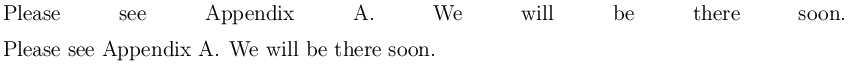
\includegraphics{linebreak}
\end{quote}
\end{htmlonly}

\subsection{�����Y��\index{�Y��}}

�Ĥ@���Y�ƤF�I�o�O�]���ڭ̧����S�������`�A�ҥH�A\LaTeX\ �N��o�Ǥ��e�����O�ި��������A�� \LaTeX\ ���w�ơA�ި��}�Y�O�|�Y�ƪ��C�n�ѨM�o�Ӱ��D�A�i����ؤ�k�G

\begin{enumerate}
\item �b�Ĥ@�椧�e�[�J \verb|\noindent|\index{noindent@\verb+\noindent+} �ӫ��� \LaTeX\ ���n�h�Y�ơC���O�o�u�@�Φb�U���O���a��A��L���Y�ƪ��a���٬O�|�Y�ơC
\item �b preamble �ϥ[�J \verb|\parindent=0pt|\index{parindent@\verb+\parindent+}�A�o���������媺�Y�Ƭ� {\tt 0pt}�A���M�A�o�N���ܥ��峣���n�Y�ƤF�C
\end{enumerate}

\section{�[�J���`���D\index{���`���D}}

�b \LaTeX\ ���Y�A�n�[�J���`���D��b�O�Ӯe���F�A�]�����h�ަr�骺�j�p�θm�񪺦�m�A�ɺޥ[�W�h�N��F�I\LaTeX\ �|���ڭ̦w�Ƥ@���C�ڭ̳o�̤��M�H {\tt report} ���O�ӻ����A�]�� {\tt article} ���O���Y�A�S�����A�u��A�Ω��²�檺�u��C

\begin{quote}
\begin{verbatim}
% example2.tex
\documentclass{report}
\begin{document}
This is the first experience of \LaTeX.
\chapter{Aesop Fables}
\section{The Ant and the Dove}

An ant went to the bank of a river to quench its thirst, and
being carried away by the rush of the stream, was on the
point of drowning.

A Dove sitting on a tree overhanging the water plucked a
leaf and let it fall into the stream close to her. The Ant
climbed onto it and floated in safety to the bank.

\section{The Dog in the Manger}

A dog lay in a manger, and by his growling and snapping
prevented the oxen from eating the hay which had been
placed for them.

``What a selfish Dog!'' said one of them to his companions;
``he cannot eat the hay himself, and yet refuses to allow
those to eat who can.''

\chapter{The Eagle and the Arrow}

An eagle sat on a lofty rock, watching the movements of a
Hare whom he sought to make his prey.

An archer, who saw the Eagle from a place of concealment,
took an accurate aim and wounded him mortally.
\end{document}
\end{verbatim}
\end{quote}

�sĶ�X�Ӫ����G�G

\begin{quote}
\url{http://edt1023.sayya.org/tex/latex123/example2.tex}\\
\url{http://edt1023.sayya.org/tex/latex123/example2.pdf}
\end{quote}

�Ъ`�N�L����ɭԷ|�Y�ơA����ɭԷ|�����C{\tt report} ���O�A�s���@���|�����A�p�G�Q�`�٤@�I�Ŷ��A�i�H���� {\tt article} ���O�A\verb|\chapter{}| ��� \verb|\section{}|�A��� \verb|\section{}| �N��� \verb|\subsection{}|�A�o�˴N���|�����A���e�N�|�s��U�h�F�C�j�a�i�H�յۧ� {\tt report} �令 {\tt article} �� {\tt book} �A���s�sĶ�@���A�ոլݵ��G���󤣦P�C

\section{�[�J title page ��T}
\label{sec:titlepage}\index{title page}

�o�O���������Ĥ@���A�ڤ]�����D�o�Ӥ���M���W���O����A�b \LaTeX\ ���Y�A�ڭ̴N�٬� title page�C�b \LaTeX\ ���зǮ榡�̡A�L�]�A�F���D�]title�^�B�@�̦W�r�]author�^�B����]date\index{date}�^�ηP�µ��]thanks\index{thanks}�^�C�n�`�N���O�A�b {\tt report/book} ���O�Atitle page �O�ۦ��@��W�����A���b {\tt article} ���O�̡A�L�O�M����s�_�Ӫ��C�ڭ̴N�H�W��������J�����峹���ҡA�n�ק諸�a��O preamble\index{preamble} �ϤΥ���Ϫ� \verb|\maketitle|\index{\verb=\maketitle=}�G

\begin{quote}
\begin{verbatim}
% example3.tex
\documentclass{report}
\title{Aesop Fables}
\author{Aesop\thanks{Thanks to the reader.}
       \and Nobody\thanks{Thanks to nobody.}}
\date{\today}
\begin{document}
\maketitle
This is the first experience of \LaTeX.
\chapter{Aesop Fables}
\section{The Ant and the Dove}
 ...
\end{verbatim}
\end{quote}

�ƪ��X�Ӫ����G�p�U�G

\begin{quote}
\url{http://edt1023.sayya.org/tex/latex123/example3.tex}\\
\url{http://edt1023.sayya.org/tex/latex123/example3.pdf}
\end{quote}

�ڭ̥i�H�o�{�A�o�@���O���s���X���A�q�U�@���}�l�~�O�Ĥ@���C�@�̥i�H���h�ӡA�ϥ� \verb|\and| ���O�ӳs���C������@�w�n���A�p�G�S�� \verb|\date{\today}| �o�ӫ��O�A���٬O������A���u��T�w�b���ѡC�p�G���e�L���A�L�|�۰ʧ��A���]�i�H��ʥ[ \verb|\\| �ӱj������A���ަp�󴫦�A��ӥy�l�O�~���ƦC���C\verb|\maketitle| �O�U�b����Ϫ��}�Y�A�p�G���U�o�ӫ��O�A���sĶ�ɤ��|��������~�A�u�O�N�S�� title page �F�C

\section{�[�J�ؿ��]Table of Contents�^}
\label{sec;toc}

�[�J�ؿ��]Table of Contents\index{Table of Contents}�^�� \LaTeX\ �Ө��A��O���ө��|���Ʊ��A�u�n�b����}�Y�[��
\verb=\tableofcontents=\index{tableofcontents@\verb=\tableofcontents=}
���O�N���F�I�̤W�����Ҥl�A�ק令�G

\begin{quote}
\begin{verbatim}
% example4.tex
\documentclass{report}
\title{Aesop Fables}
\author{Aesop\thanks{Thanks to the reader.}
       \and Nobody\thanks{Thanks to nobody}}
\date{\today}
\begin{document}
\maketitle
\tableofcontents
This is the first experience of \LaTeX.
\chapter{Aesop Fables}
\section{The Ant and the Dove}
 ...
\end{verbatim}
\end{quote}

�ƪ��X�Ӫ����G�p�U�G

\begin{quote}
\url{http://edt1023.sayya.org/tex/latex123/example4.tex}\\
\url{http://edt1023.sayya.org/tex/latex123/example4.pdf}
\end{quote}

�o�̤d�U�n�`�N���O�A\verb|\tableofcontents| �n�[�b \verb|\maketitle| ���᭱�A�_�h�ؿ��|�L�b title page ���e�C�ӥB�n\textcolor{red}{\bf �sĶ�⦸}�C�Ĥ@������ {\tt example4.toc}�A�M��ĤG���sĶ�A��ڳo�� {\tt toc} �ɡA�u���s�J�ؿ��C

�ؿ��O�]�A�Ϫ��ؿ����]List of Figures, List of Tables�^�A���ڭ̥ثe�٨S���ͨ�Ϫ����ƪ��A�]���Ȯɲ��L�A���ͨ�ɦA�Ӭݭn�p��[�J�Ϫ��ؿ��C

\section{�[�J�K�n�]abstract�^}
\label{sec:abstract}\index{abstract}

�o���@�w�|���A�p�G�n�[�J���ܡA�i�ϥ� {\tt abstract} ���ҡA�b�o�����Ҥ����峹�A���k�|�Y�ơC�n�`�N���O�A�u�� {\tt article/report} ���O�~�� abstract�A{\tt book} ���O����ϥγo�����ҡC

\begin{quote}
\begin{verbatim}
% example5.tex
\documentclass{report}
\title{Aesop Fables}
\author{Aesop\thanks{Thanks to the reader.}
       \and Nobody\thanks{Thanks to nobody}}
\date{\today}
\begin{document}
\maketitle
\begin{abstract}
The tale, the Parable, and the Fable are all common and popular
modes of conveying instruction. Each is distinguished by its own
special characteristics.
\end{abstract}
\tableofcontents
\chapter{Aesop Fables}
\section{The Ant and the Dove}
 ...
\end{verbatim}
\end{quote}

�ƪ��X�Ӫ����G�p�U�G

\begin{quote}
\url{http://edt1023.sayya.org/tex/latex123/example5.tex}\\
\url{http://edt1023.sayya.org/tex/latex123/example5.pdf}
\end{quote}

{\tt report}\index{\texttt{report}} ���O���K�n�ۦ��@���A���s���X�A�B���|�s�J�ؿ����A�o�M�@�몺�פ�榡�i��|���@�ˡA�ϥήɽЪ`�N�C{\tt artcile}\index{\texttt{artcile}} �����O�h���M�O�M����۳s���A�|�X�{�b�峹���D����C

{\tt abstract} �M summary\index{summary} �b���������פ�O���Ϥ����A�q�` abstract �b��e�Fsummary �h�b���C���ثe�@��ʪ��峹�h�S���o�˰ϧO�A�q�q�����u�K�n�v�C�q�`�A�K�n���Y�O���ε��ѡB�L�椬�ѷӤ]���ϥΤ����Ϫ����C


\section{�[�J����}
\label{sec:footnote}\index{����}

�b \LaTeX\ ���Y�A���ѥi����ؤ覡�A�@�جO�}���]footnote�^\index{footnote}\index{�}��}�A�@�جO����]marginal note�^\index{marginal note}\index{���}�C�q�` \LaTeX\ ���}���w�]�O�Ѫ��ԧB�Ʀr�b�s���A�m�󭶩����C�b�S�����]part�^�����ΤU�A\texttt{report/book} ���O�A�s���C���|�q�Y�_��A\texttt{article} ���O�h�|�s��A�ӥB�A�|�ϥ� \texttt{footnotesize}\index{footnotesize@\texttt{footnotesize}} ���r��L�X�C����h���s���A�r��O���`�j�p�C

\subsection{�}���]Footnote�^}

�b�ҭn�[�������Ӧr��A�ϥ� \verb|\footnote{}| ���O�Y�i�A�ѻ�����r�N�g�J�j�A�������A�@�� \LaTeX\ �����O�b�������M�����@�ΡA�|�L�b�����������A�H�p�@�I���r�ӦL�X�A�å[�W�s���C�H�U�ڭ̴N�ոլݦb Dove �o�Ӧr�Ӱ��}���C�Ъ`�N�ADove �o�Ӧr�M \verb|\footnote{}| �����O�S���ťժ��C

\begin{quote}
\begin{verbatim}
% example6.tex
\documentclass{report}
\title{Aesop Fables}
\author{Aesop\thanks{Thanks to the reader.}
       \and Nobody\thanks{Thanks to nobody}}
\date{\today}
\begin{document}
\maketitle
\tableofcontents
This is the first experience of \LaTeX.
\chapter{Aesop Fables}
\section{The Ant and the Dove}

An ant went to the bank of a river to quench its thirst, and
being carried away by the rush of the stream, was on the
point of drowning.

A Dove\footnote{Pigeon, an emblem of peace.}
sitting on a tree overhanging the water plucked a
leaf and let it fall into the stream close to her. The Ant
climbed onto it and floated in safety to the bank.
 ...
\end{verbatim}
\end{quote}

�ƪ��X�Ӫ����G�p�U�G

\begin{quote}
\url{http://edt1023.sayya.org/tex/latex123/example6.tex}\\
\url{http://edt1023.sayya.org/tex/latex123/example6.pdf}
\end{quote}

\subsection{����]Marginal note�^}

����u�O�� \verb|\footnote{}| ���� \verb|\marginpar{}|\index{marginpar@\verb=\marginpar=} �Ӥw�A���e���M�g�J�j�A�����C���M�}�����@�˪��O�A�L�S���s���]�]���N�b����A�L�����n�^�A�L���r��]���|�p�@���A�M���媺�r��j�p�O�@�˪��A�o�b�᭱�Q�ר�r�����ɭԷ|�ͨ�p����ܦr�骺�j�p�C

\begin{quote}
\begin{verbatim}
% example7.tex
\documentclass{report}
\title{Aesop Fables}
\author{Aesop\thanks{Thanks to the reader.}
       \and Nobody\thanks{Thanks to nobody}}
\date{\today}
\begin{document}
\maketitle
\tableofcontents
This is the first experience of \LaTeX.
\chapter{Aesop Fables}
\section{The Ant and the Dove}

An ant went to the bank of a river to quench its thirst, and
being carried away by the rush of the stream, was on the
point of drowning.

A Dove\marginpar{Pigeon, an emblem of peace.}
sitting on a tree overhanging the water plucked a
leaf and let it fall into the stream close to her. The Ant
climbed onto it and floated in safety to the bank.
 ...
\end{verbatim}
\end{quote}

�ƪ��X�Ӫ����G�p�U�G

\begin{quote}
\url{http://edt1023.sayya.org/tex/latex123/example7.tex}\\
\url{http://edt1023.sayya.org/tex/latex123/example7.pdf}
\end{quote}

\section{�r���������վ�}
\index{�r��!�����վ�}

\TeX/\LaTeX\ ���r���t�κ�O�۷��������A�o�̤��h�ͨ䤤��z�A���b�ϥΪ̪����סA�ڭ̥u�n���D���ϥδN��F�C�b�o�̡A�ڭ̻��r���]font�^\index{font}\index{�r��}�A�����O�r���������@���`�١A�κ٬��r��\index{�r��}�A�b�r���Ϊ����ɭԡA�ڭ̴N�٬��r�Ρ]font shape�^\index{font shape}\index{�r��}�C

\LaTeX\ �ϥΪ��r����r����A�H�ثe�s������ \LaTeX\ �Ө��A�O�ϥ� 1993 �~�o�檺 NFSS(New Font Selection Scheme) �ĤG�����зǡC���M�A���M�O�إߦb \TeX\ �r�������¦�W���A�o�w�W�X�o�g�峹���d��C

\subsection{\LaTeX\ ��r�����ݩʴy�z}
\label{subsec:font-attr}\index{�r��!�ݩʴy�z}

�b \LaTeX\ �̡A���r�����y�z�A�ϥΤF�����ݩʨӻ����A�o�����ݩʡA�]�O \LaTeX\ �������`�n�ϥΨ쪺�ѼơA�ƦܬO���~�T���Хܦr���ӷ����ɭԡA�|��r�����o���ݩʵ���ܥX�ӡC

\begin{enumerate}
\item �r���s�X�]font encoding�^\index{font encoding}\index{�r��!�r���s�X}\\
�o�̩ҿת��r���s�X�A�����O�U�ӭӧO���r�b�@�Ӧr�����Y���ƦC���ǤΦw�Ƥ覡�C��l�� \TeX\ �r���s�X�ڭ̴N�٬� OT1(Old \TeX\ text encoding)\index{OT1}�A�o�O�w�]���A�p�G�������w�r���s�X�A���ҨϥΪ��N�O OT1 �s�X�C�b�ثe�s�@�N���r���s�X���Y�A�r���w�Ƥ覡�Τ��e�M OT1 ���@�ˡA�Ҧp
T1\footnote{�����W�٬O Cork's \TeX\ extended text encoding �S�٬� Text Companion encoding�C�o�̪� T1 �M Type 1 �r���W��\index{�r��!�r���W��}�L���A�L�O�r���s�X�覡�A�L��r�����Y�����@�ǭ����Ÿ��r����W�����@�ӳ�W���r�A�ӫD�p OT1 �O�Ѥ@��r���M�����Ÿ��զX�Ӧ��C}\index{T1}�A�o�b���ᴣ����ܦr���s�X�ɷ|�A�ͨ�A�ڭ̥ثe�N���h�վ�r���s�X�A�ϥιw�]�� OT1�A��L���s�X�o�̴N���h�ͤF�C

\item �r�ڡ]font family�^\index{font family}\index{�r��}\\
���P�@�]�p�������r�����X���W�١A�Ҧpù���r�ڡ]roman�^\index{roman}\index{ù���r��}�B���r���r�ڡ]typewriter�^\index{typewriter}\index{���r���r��}�����A�q�`�e���|�a�W�s�@�өλs�@�H���W�١A�Ҧp Knuth\index{Knuth} �б³]�p���A�٬� `Computer Modern Roman'\index{Computer Modern Roman}�AAdobe ���q�s�@��ù���r�ں٬� `Adobe Times'\index{Adobe Times}�C�ڭ̹w�]�ϥΪ��A���M�N�O Knuth �б©ҳ]�p�� Computer Modern fonts�C�H�U���@�ǨҤl�G

\begin{quote}
\begin{tabular}{>{\tt}ll}
²�� & �N���N�q \\
\hline
cmr  & Computer Modern Roman \\
cmss & Computer Modern Sans Serif \\
cmtt & Computer Modern Typewriter 
\end{tabular}
\end{quote}

\item �r���t�C�]font series�^\index{font series}\index{�r��!�r���t�C}\\
�o�O���r���� weight�]�D�G�^�� width�]����^�ӰϤ����C�Ҧp�ʡB�Ӧr��A�@��ڭ̥��`�Ϊ��O medium�A����h�O bold�C�H�U�O�@�ǨҤl�G

\begin{quote}
\begin{tabular}{>{\tt}ll}
²�� & �N���N�q \\
\hline
m  & medium \\
b  & bold \\
bx & Bold extended \\
sb & Semi-bold \\
c  & Condensed
\end{tabular}
\end{quote}

\item �r�Ρ]font shape�^\index{font shape}\index{�r��}\\
�o�ӱ��͸q�A�N�O�r���Ϊ��C�Ҧp�N�j�Q����]italic�^\index{italic}\index{�N�j�Q����}�B����]slant�^\index{slant}\index{����}�Bsmall caps\index{small caps} �����C�H�U�O�X�ӨҤl�G

\begin{quote}
\begin{tabular}{>{\tt}ll}
²�� & �N���N�q \\
\hline
n  & ���`�r�]normal�^�A�� upright �� roman \\
it & Italic \\
sl & Slanted \\
sc & Small Caps \\
\end{tabular}
\end{quote}

\item �r���j�p�]font size�^\index{font size}\index{�r��!�r���j�p}\\
�w�]���r���j�p�O 10pt�]10 point�^�A�Q�I�r�C���[��쪺�ܡA�w�]���N�O pt�C�Ъ`�N�A�D�з� \LaTeX\ ���O���w�]�r���j�p�i��|���@�ˡC
\end{enumerate}

�ڭ̹�r���n�վ���ܪ��A�N�O�o�Ǧr���ݩʪ��]�w�ȡC\LaTeX\ �w�]�w�n��K�����O���ڭ̨ϥΡC

\subsection{�վ�r�ڡB�r���t�C�B�r�Ϊ����O}
\label{subsec:font-command}

%begin{latexonly}
\linespread{1.0}
\small
\begin{tabular}[\textwidth]{lllll}
    & �r�� & �зǫ��O & �ŧi�����O�]���ҡ^& �¥Ϊk \\
\hline
�r  & \textup{textup} & \verb|\textup{textup}| & \verb|{\upshape textup}| & \\
��  & \textit{italic} & \verb|\textit{italic}| & \verb|{\itshape italic}| & \verb|{\it italic}| \\
    & \textsl{slant}  & \verb|\textsl{slant}|  & \verb|{\slshape slant}| & \verb|{\sl slant}| \\
    & \textsc{small caps} & \verb|\textsc{small caps}| & \verb|{\slshape small caps}| & \verb|{\sc small caps}| \\
\hline
�t & \textmd{medium} & \verb|\textmd{medium}| & \verb|{\mdseries medium}| &  \\
�C & \textbf{boldface} & \verb|\textbf{boldface}| & \verb|{\bfseries boldface}| & \verb|{\bf boldface}| \\
\hline
�r & \textrm{roman} & \verb|\textrm{roman}| & \verb|{\rmfamily roman}| & \verb|{\rm roman}| \\
�� & \textsf{sans serif} & \verb|\textsf{sans serif}| & \verb|{\sffamily sans serif}| & \verb|{\sf sans serif}| \\
   & \texttt{typewriter} & \verb|\texttt{typewriter}| & \verb|{\ttfamily typewriter}| & \verb|{\tt typewriter}| \\
\end{tabular}
\linespread{1.36}
\normalsize
%end{latexonly}

\begin{htmlonly}
\begin{quote}
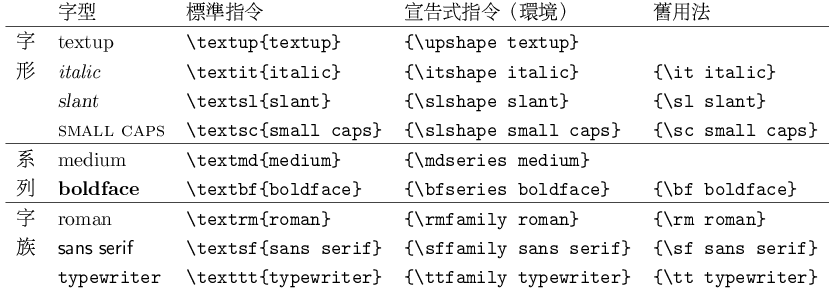
\includegraphics{fntshape}
\end{quote}
\end{htmlonly}

���O�~�F�@���A�o�O����i�`���C�䤤 upright, medium, roman ���O�@�˪��A�o�O�@�몺���`�r�A�N�����·Хh�]�w�L�F�A���D�O�n�b�S�w�r���d����Y�A���s���ܦ����`�r��C�q�e���һ���²�٪��r��A�A�M text, family, series, shape �h�t��ӨϥΡA�o�˥u�n�O�o²�ٴN��F�A�Ҧp�Gitalic ���N�O \verb|\textit{}|�C���M�]�i�H�ϥΡu���Y�B�v���¥Ϊk�A���o�]���O���򰽦Y�B�A�L�O��l Plain \TeX\index{Plain \TeX} �ҩw�q���A�b�ª��� \LaTeX\ 2.09 �]�ۮe�L�Ӫu�ΡA�å[�H�X�R�C���p�G�ϥ��¥Ϊk�A�����ɲզX�������ܮɥi��|�L�ġA�Ҧp�ʱ���o�ز���M����]�w�V�X�ɡA�N�L�k���Ͳʱ���F�A�o���٬O�o�ĨĨϥΥ��μз� \LaTeX\ �����ܪk�C

�n�`�N���O�A�j�A������m�A�ŧi�������O�A��ӧ@�νd��O�s���O�@�_�]�����A�L�i�H�������ҨӨϥΡA�Ҧp \verb|\begin{itsahpe}|, \verb|\end{itshape}|�A�o�˦b�o�����Ҥ�����r�N�q�q�|�ϥ� italic ����A�]�i�H���[�ѼƨϥΡA�Ҧp \verb|\itshape|�A�o�˥H�U����r�q�q�|�ϥ� italic ����A���ܥt�@�ӧ��ܦr�������O�X�{����C�зǫ��O���@�νd��h�O�������O���@�ӰѼơA�o�ǰѼƬO�X�{�b���O�᪺�j�A�������C�{�b�N�ӹ�ڽsĶ�ӨҤl�լݬݡG

\begin{quote}
\begin{verbatim}
% example8.tex
\documentclass{report}
\title{\bfseries Aesop Fables}
\author{Aesop\thanks{Thanks to the reader.}
       \and Nobody\thanks{Thanks to nobody}}
\date{\today}
\begin{document}
\maketitle
\tableofcontents
\chapter{Aesop Fables}
\section{The \textsl{Ant} and the \textsl{Dove}}

\itshape
An antwent to the bank of a river to quench its thirst, and
being carried away by the rush of the stream, was on the
point of drowning.
\upshape

A \textsl{Dove} sitting on a tree overhanging the water plucked a
leaf and let it fall into the stream close to her. The \textbf{\textsl{Ant}}
climbed onto it and floated in safety to the bank.

\section{The {\it Dog}\/ in the Manger}

A \textbf{\textit{dog}} lay in a manger, and by his growling and snapping
prevented the oxen from eating the hay which had been
placed for them.

``What a selfish Dog!'' said one of them to his companions;
``he cannot eat the hay himself, and yet refuses to allow
those to eat who can.''

\chapter{The \textsc{Eagle} and the Arrow}

An \textsc{eagle} sat on a lofty rock, watching the movements of a
Hare whom he sought to make his prey.

An archer, who saw the \textsc{Eagle} from a place of concealment,
took an accurate aim and wounded him mortally.
\end{document}
\end{verbatim}
\end{quote}

�ڭ̧� title page\index{title page} �����D�令����]�Ъ`�N�A�ŧi�����¥Ϊk�A�j�A���O����O�M��r��ӬA�����^�A�� Dove �令 slant ����A�� dog �令 italic �ʱ���\footnote{�Ъ`�N�A�o��ر���O���@�˪��Aslant �O�@�륿�`���r�A�u�O��L�ɱ׭Ө��צӤw�A�� italic �h�O�t�@�ؿW�S���r���]�p�C}�A�� ant �令 slant �ʱ���A�� eagle �令 small caps�C�ѩ󳹸`���D�쥻�N�|�ഫ������A�ҥH���`���D�������A����N�������Ƴ]�F�C

���o�̵o�{�Ҥl�̲ĤG�����D���� Eagle �èS�����ܦr��A�ӥB�H {\tt latex} �sĶ�ɷ|���ͥH�U�����~�]�o�ǰT���]�|�b {\tt example8.log} �����^�G

\begin{quote}
\begin{verbatim}
  ...
LaTeX Font Warning: Font shape `OT1/cmr/bx/sc' undefined
(Font)              using `OT1/cmr/bx/n' instead on input line 4.
  ...
LaTeX Font Warning: Some font shapes were not available, defaults substituted.
  ...
\end{verbatim}
\end{quote}

�{�b�ڭ̬ݨ�F�e���ҽͪ��ݩ�²�١A�o�b \LaTeX\ �N�|�ϥγo���ݩʨӪ��ܦӵo�X�T���A�o�� \verb|OT1/cmr/bx/sc| �N���ܤF OT1 �s�X�AComputer Modern Roman �r�ڡABold extended �t�C�A�ӥB�O small caps �Ϊ����r���A���~�T����ܡA�L�èS���w�q�A�]���A�o�Ӧr���N�|�ϥιw�]���r���ӥN���A�o�̴N�O�H n ���`�Ϊ��� bx �t�C�r���Ӵ��N�C�ҥH�A�r�����O�ä��O���i�H�H�N�զX���A���ǬO�ڥ��N�S���o�ئr���A���ǫh�O�S���Υ����h�w�q�n�A�o�� \LaTeX\ �N������r�F�A���O��ߡA���h�N�O�ϥιw�]���r���}�F�I

�t�@�ӫܩ_�Ǫ��a��A�N�O�Ĥ@���B�ĤG�`�����D�A������O \verb|{\it Dog}\/ in the...}|�H�o�Ӵ��J�� \verb|\/| �O����F��H�o�O \TeX\ �t�νվ����r�]�]�A iatlic �� slanted�^�M���`�r�������ťժ��@�ӫ��O�A�٬� italic correction\index{italic correction}�C�o�ˡA�b����r�M���`�r�������ťդ~�|���`�C���������L��������O�S���[�o�ӽվ�O�H�o�O�]�� \LaTeX\ �����b�]�p�ɴN���Ҽ{��o�Ӱ��D�A�ҥH \verb|\textit{}| �o���зǫ��O���|�۰ʽվ� italic correction�A�����ѧڭ̤�ʽվ�C

�t�~�A���`���D���N�|�۰��ഫ������A���D�W�� dog ������S���ܲ���H�o�b�e��������L�A�o���¥Ϊk���ɬO�L�k�ƦX�ϥΪ��A����S���骺���O�|�Τ��W�ӡC�]���A��ij�ɶq�ϥ� \LaTeX\ ���Ĥ@�ؼзǫ��O�ӧ��ܦr���C�ϥ� \verb|{\it ...}| �� \verb|{\itshape ...}|\footnote{�ŧi�����O�i�H�ƦX�ϥΡA�����M�|�ݭn��ʰ� italic correction�C} �o�ث��O���ܡA�N�o�ɮɪ`�N italic correction �����D�A�]�o�`�N�O�_�i�H�ƦX�ϥΫ��O�����D�A�ҥH�A�٬O���n���i���n�C:-)

��U�O�ƪ��X�Ӫ����G�G

\begin{quote}
\url{http://edt1023.sayya.org/tex/latex123/example8.tex} \\
\url{http://edt1023.sayya.org/tex/latex123/example8.pdf}
\end{quote}

\subsection{�۹�r���j�p���վ�}

���U�ӽͳ̫�@�Ӧr���j�p�ݩʪ��վ�A�o�b�ϥΤW�����¡A�u�n���D���O�N�i�H���W���ӨϥΡC���O \TeX/\LaTeX\ �t�Τ��A�ͨ�r���A���Y�@��a�p�A�Ҧp�e���ͨ쥿�`������r���j�p�O 10pt�A�{�b�p�G�Q�s�@�����A�ݭn 64pt ���r���ɭԴN�|�o�{�A�]���X�ӤF�I���` \LaTeX\ ���w�q�A�r�����j�p�d��O�b 5--24.88pt �����A�W�X�o�ӽd�򪺦r�ݭn��L�� package �������C\footnote{�o�O \LaTeX\ ���������w�q�����D�A�]���L�D�n�O�w��@��ʤ��ή��y�A\TeX\ ��������O�A�i�H���r����j�� 2047pt�C}

�o�̧ڭ̥��Ӭݬݤ��� 10pt �ɦU�ئr���j�p���O�B��ڨҤl�Ψ�j�p�]�o�O�۹�j�p�A�|�H����w�]�r���j�p�Ӧ۰ʽվ�^�G\footnote{�Ъ`�N�A���� pdf �榡����ϥ� 12pt �r���j�p�A�C���Ψ䤤���Ҥl�A�O�ѥt�~ 10pt �w�]�r���j�p�һs�@�� eps ���ɤޤJ�A�H�K���u�C}

\begin{quote}
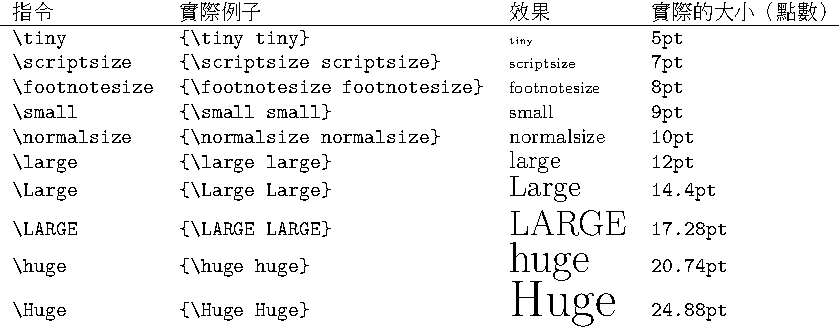
\includegraphics{fntsize}
\end{quote}

�o�Ǧr���j�p���O�]�i�H�������ҨӨϥΡA�Ҧp�G

\begin{quote}
\begin{verbatim}
\begin{small}
  ���夺�e
\end{small}
\end{verbatim}
\end{quote}

�o�˥Τ]�O�i�H���C

\subsection{����r���j�p���վ�}

�q�`�r�����j�p\index{�r��!�r���j�p}�A�ϥΤW�@�`�һ����۹�r���j�p�ӽվ�|�����K�A�ӥB����Ӫ������t�X�]�|�������A�Ҧp��Z�]�|��۰��A�����վ�A�p�G�ۦ�ε���r���j�p����k�ӽվ�r���j�p���ܡA�`�`�|�y����Z���@�P�����ΡA�]���A�p�D���n�A���ɶq�קK�C

�����ɭԴN�O�ݭn���o�˪��վ�A�Ҧp����ʭ����r���j�p�A�a�ϬO \LaTeX\ �w�]���̤j�r���]ı�o�y�p�F�I�A�o�N�n�t�~�ޤJ package �վ�F�C

�o�̧ڭ̨ϥ� \textsf{type1cm}\index{type1cm@\textsf{type1cm}} package �ӽվ�C���M�A�o�ϥ� Type 1 �r���A�~�i�H�F��L�q��j�B�Y�p���ت�%
\footnote{\LaTeX\ �t�Τ����r����j�A�b 10pt �H�W�A�O�H 1.2 �����Ƭ�����ө�j���A�]���A���� 10pt ���r���j�p���ܡA���|�� 13pt �o�ؤj�p���r���A\LaTeX\ �|��γ̬۪�j�p���r���Ӵ��N�C}%
�A�ӳo�� package �]�O�t�X Type 1 �r���ϥΪ��C�ӧO��j�� pk �I�}�r�A�o�̴N���Q�פF�A�ثe���j������ Computer Modern �r�����w�� Type 1 �� free �����A�ӥB�U�� \TeX\ distribution ���|���W�A�ϥΤW�|����K�C�H�U�O \textsf{type1cm} ���ϥΤ�k�G

\begin{quote}
\begin{verbatim}
  ...
\usepackage{type1cm}
  ...
\fontsize{�r���j�p}{��Z�j�p}\seclectfont
  ...
\end{verbatim}
\end{quote}

�ٰO�o�p��ޥΥ����M��\index{�����M��}�ܡH�аѦҲ� \ref{ch:syntax} ���B�� \ref{sec:struct} �`�A�� \ref{subsec:preamble} �p�`�������C

�䤤���u�r���j�p�v�N�O�ҭn���w���j�p�A�q�`�H pt �����A���M�A�n�ϥΨ�L���]�O�i�H�C�u��Z�j�p�v�]�O�n�@�֫��w�A���i�ٲ��C�̫᪺ \verb|\seclectfont| �O���L�o�ͧ@�Ϊ��N��A\LaTeX\ ��������r�������C�����O�A�n�U \verb|\seclectfont| ��~�|�@�ΡA\verb|\fontsize{}{}|\index{fontsize@\verb=\fontsize=} ���O�䤤���@�C

\section{���ӦC}

����O���ӦC\index{���ӦC}�H�@�� \LaTeX\ �J��˱׽u\index{�˱׽u}�|�{���O�@�ӫ��O���}�l�A�p�G�s��ӫ��O���n�L�X���ɭԩO�H�o�ɴN�n�Ψ���ӦC�����O�����ҤF�C

\subsection{���ӦC���O}

�p�G�u�O�@�p�q����r�n���ӦC�A���ϥΫ��O�|�����K�A�o�ӫ��O�N�O \verb+\verb|��r���e|+\index{verb@\verb=\verb=}�A�䤤�� \verb+|+ �o�ӲŸ��i�H�ϥΨ�L�D�r�����Ÿ��N���A�u�n�e��ۦP�N��F�A�Ҧp�G\verb|\verb+��r���e+| �o�ˤ]�O�i�H���C

\subsection{���ӦC����}

�p�G�O�@��q�����e�n���ӦC���ܡA�ϥ����ҷ|�����K�A���K�O {\tt verbatim} ���ҡC���ެO���@�ح��ӦC�����ΡA�w�]�O�ϥΥ��r���r�ڪ��r������ܪ��C���U�O�@��²�檺�Ҥl�A�������ӦC���O�����Ҫ��ϥΡG

\begin{quote}
\begin{Verbatim}[commandchars=+\[\]]
% example9.tex
\documentclass{article}
\begin{document}
The example of \verb|\verb{}| command and \texttt{verbatim} environment.

\section{\textbackslash{}\texttt{verb} command}

When you want to express you home directory, you can \verb|echo $HOME|
varient to display your home directory in your sh script.

\noindent
\verb*|This is    4 space here.|

\section{\texttt{verbatim} environment}

Here is a sh script to determine if on GNU/Linux system.

\begin{verbatim}
#!/bin/sh
Date=`date '+%y%m%d'`
if [ `uname` = Linux ]
then
  Mail=/var/spool/mail/edt1023
  Target=/mnt/hd
else
  Mail=/var/mail/edt1023
  Target=/mnt/pub
fi
\end{verbatim}
\end{document}
\end{Verbatim}
\end{quote}

�o�̷|�o�{�@�ǩ_�Dz{�H�A�Ҧp
\texttt{\textbackslash{}verb*}
���ӬP���O����N��O�H�N�O���ťեH
%begin{latexonly}
\verb*| |
%end{latexonly}
\begin{htmlonly}

\includegraphics{blank}
\end{htmlonly}
���覡���ܥX�Ӫ��N��A{\tt verbatim} ���Ҥ]�O�i�H�o�˨ϥΡC�Ҧp {\tt example9} �����G

\begin{quote}
\begin{verbatim}
\verb*|This is    4 space here.|
\end{verbatim}
\end{quote}

�]�i�H�g���G

\begin{quote}
\begin{Verbatim}[commandchars=+\[\]]
\begin{verbatim*}
This is    4 space here.
\end{verbatim*}
\end{Verbatim}
\end{quote}

�t�O�b��A���Ҫ��W�U��|�h�ťX�Ӫťզ�X�ӡC

�t�~�A���D�����򤣨ϥ� \verb+\verb|\verb|+ �N�n�F�O�H��]�O���ӦC�����O�M���ҳ����������L���O���ѼơA���D�����N�O�@�ӫ��O�A�ҥH \verb+\verb+ ����b���Y�C

�ϥ� \verb|\textbackslash|\index{textbackslash@\verb=\textbackslash=} �o������ԭz�A�Ӥ��� \verb|$\backslash$| �o��²�檺�覡�A��]�O�o�Ӥ�Z���ϥ� \LaTeX{}2{\tt HTML} ���ন HTML �榡�A�ϥ� \LaTeX\ �����N���ܪk�|�ন�@�몺�Ÿ��A���ϥΫ�̪��覡�h�|�ন���ɡA�ҥH�o�̴N�ϥ� \LaTeX\ �����N���ܪk�F�C

���U�O�ƪ��X�Ӫ����G�G

\begin{quote}
\url{http://edt1023.sayya.org/tex/latex123/example9.tex}\\
\url{http://edt1023.sayya.org/tex/latex123/example9.pdf}
\end{quote}

\section{�[�J����}

�o�̥u�����p��ϥ� \textsf{CJK}\index{CJK@\textsf{CJK}} package �����ΡA��]�O�@�� \TeX\ distribution �|���W�]���ǵo��M��èS�����W�A�o�ɥu�n�ۦ�w�ˤF�^�C\textsf{CJK} package �O�⤤�媺�����]�b�@�����Ҹ��Y�A�b�o�����Ҥ��N�i�H�ϥΤ���A���}�o�����ҴN�S�^�_��쥻���^�����ҡA���U�ѨҤl�ӻ����C

\begin{quote}
\begin{verbatim}
\documentclass{article}
\usepackage{CJK}  % �ϥ� CJK �����M��
\begin{document}
% �i�J CJK ���ҡA�èϥ� Big-5 �X�� hwmm �o�Ӧr��
\begin{CJK}{Bg5}{hwmm}
\section{CJK �����M��}
�o�O�@�Ӵ��աA���� CJK package �����աC
\section{��᷽�O�`��}
��U�A�׳q�H�F�_��ƤQ�B�A�ŵM�}�ԡC�g�a���m�A�Ϊ��k�M�C���}�СB�����B%
��B�ˤ��ݡA�魯��q�A�����ۻD�C�䤤���Ӻا@�A�k�k��ۡA�x�p�~�H�F���v�B%
���ԡA �éɵM�ۼ֡C�����H�A�D�j��A�ݩұq�ӡF�㵪���A�K�n�ٮa�A�]�s�B�����B%
�@���C�����D�����H�A�w�ӰݰT�C�ۤ��G�u���@�ׯ��ɶáA�v�d�l���H�Ӧ����ҡA%
���_�X�j�F�E�P�~�H���j�C�v�ݤ��O��@�F�D�������~�A�L���Q�B�ʡC���H�@�@%
���㨥�һD�A�Ҽ۱{�C�l�H�U�_���ܨ�a�A�ҥX�s���C���Ƥ�A��h�C�����H�y%
���G�u�������~�H�D�]�C�v
\end{CJK}
\end{document}
\end{verbatim}
\end{quote}

�N�o��²��C�u�O�sĶ�n��� {\tt bg5latex}\index{bg5latex@\texttt{bg5latex}} �Ӥ��O��Ӫ� {\tt latex} ���O�A�o�O���F�׶}�ڭ� Big-5 �X���@�ǯS���X�����Y�A�ٰO�o����C��̫�n�[�Ӧʤ��� \verb|%|\index{%@\verb=%=} �ܡH�o�ˤ~���|���J�^�媺�r���ťաC�sĶ�n���Ҥl�p�U�G

\begin{quote}
\url{http://edt1023.sayya.org/tex/latex123/example10.tex}\\
\url{http://edt1023.sayya.org/tex/latex123/example10.pdf}
\end{quote}

�ԲӪ� \textsf{CJK} package ���ϥΤ��廡���A�аѦ� \textsf{CJK} package �Ҫ������Ρq�ڪ� CJK�r�@��G

\begin{quote}
\url{http://edt1023.sayya.org/tex/mycjk/mycjk.html}\\
\url{http://edt1023.sayya.org/tex/mycjk/mycjk.pdf}
\end{quote}


% ``�j�a�Ӿ� LaTeX'' LaTeX ��Z space.tex
% Copyright (c) 2004  Edward G.J. Lee <edt1023@info.sayya.org>
%
% �b���H�� GNU Free Documentation License 1.2 �ΥH�᪺�����W�d���U�A
% ���\�����B���G�έק�C���쪩�v�B���v�n�����o�����C
%
% �����G�����A�t�� fdl.tex�A���e�� GNU FDL ���W�d���C�p�G�򥢡A�i��
% http://www.gnu.org ���o�A�μg�H�ܦۥѳn�����|(Free Software Fundation)
% �����C
% 9 Temple Place - Suite 330, Boston, MA 02111-1307, USA.
%
% $Id: space.tex,v 1.23 2004/03/07 12:20:47 edt1023 Exp $
%
\chapter{�Ŷ��P��m}
\label{ch:space}

�e�@��������L�A�Ƿ|����Ŷ��N�Ƿ|�ƪ��F�IKnuth\index{Knuth} �б¦b�L�� \textit{The \TeX{}book}\index{The TeXbook@\textit{The \TeX{}book}} �@�Ѥ��]���ήe�ϥ� \TeX\ �ƪ������ΡG�@�Ӫ����N���@�ӧt�������]glue\index{glue}�^�������A�M��C�@�ӭn�ƪ������e�N�O�U�ؤ��P�� box\index{box}�A�b�o�� box �٨S���T�w���T��m�ɡA���O�i�H���ʪ��]�����٨S�����^�A�@���ƪ������A�����N���F�A��O�C�� box ����m�N�T�w�L�k�A���ʤF�A���D�S�q�Y�A�ӡC

�@�Ӧr���B�@�ӳ�r�B�@�ӥy�l�B�@�Ӭq���B�@�ӲŸ��B�@�ӹϧΡB�@�Ӫ��泣�i��c���@�� \TeX\ �� box�A�Ʀ� box ���٦� box �����ΡC�o���Q�Q�ת��A�N�O�o�� box �p��w�m�L�̨쥿�T����m�A���C�� box �������Ŷ�����F����n�B�A�ҥH�A�쩳�O�b���� boxes ���ݩʡB��m�A�٬O�վ� glue ���Ŷ��A�N�ݦU����h�ݫݤF�]�Ъ`�N�Abox ���@�w�O�i�����I�b \TeX\ ���Y�Aglue �O�i�H�վ㪺�C�^�C

�ڭ̫e���ҰQ�ר쪺�^��y�I��ťժ��վ�Bitalic correction\index{italic correction}�B\verb|\linespread|\index{linespread@\verb=\linespread=} �� \verb|\parindent|\index{parindent@\verb=parindent=} �o�dz��O�b�վ� glue�C�q�`�A�b \LaTeX\ �t�θ��Y�A���w���`�`���|�O����T�w���A�|�����ΰ��p���ת��۰ʷL�աA�o�O�����Ŷ��t�m�W���ݭn�C

\section{\LaTeX\ ���ϥΪ��׶q���}
\label{sec:units}

�n��T�y�z�M�վ� \LaTeX\ �����Ŷ��Φ�m�A�ڭ̥��ݭn���ӼзǪ��׶q���C�H�U���O�b \LaTeX\ �`�|�Ψ쪺���C�o�̦�������ά۹��줧���A���D���n�A���M�A�@��O��ij�ϥά۹���A��]�O�A�L�|�H�ۤ�Z�r���j�p���ܮɸ�۰��A�����վ�C���M�A�b�����D��T�B�T�w�j�p����ܮɡA�N�o�ϥε�����F�C

�o�̦p�G�O�\�� HTML �榡�����A�Хt�Ѧ� PDF �榡�����A�H�K���ܤW���u�C�H�U���椤�ҵe�X�Ӫ����׶ȨѰѦҥΡC

\subsection{������}
\index{������}

%begin{latexonly}
\begin{quote}
\begin{tabular}{>{\tt}lll}
���W�� & �N�q & ���� \\
\hline
pt & point, $1/72.27$~inch & \drawwidth{1pt} \\
bp & Adobe big point, $1/72$~inch & \drawwidth{1bp} \\
pc & pica, 12pt & \drawwidth{1pc} \\
mm & millimeter, $1/25.4$~inch & \drawwidth{1mm} \\
cm & centimeter, 10mm & \drawwidth{1cm} \\
in & inch, 25.4mm & \drawwidth{1in} \\
\end{tabular}
\end{quote}
%end{latexonly}

\begin{htmlonly}
\begin{quote}
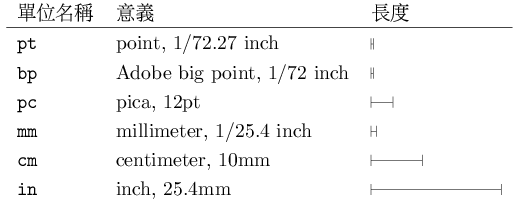
\includegraphics{a-units}
\end{quote}
\end{htmlonly}

�o�̭n�`�N���O \TeX/\LaTeX\ �t�Τ��ҿת��I�]point�^\index{�I�]point�^}�A�����O�@�몺 printer point\index{printer point}�A�]�N�O $1/72.27$~inch�A���b Adobe ���W�椤�A�Ҧp \textsc{PostScript}\index{PostScript@\textsc{PostScript}} �y�������ҿ��I�A�L�O big point\index{big point}�A���� $1/72$~inch�]�p���I�������˥h�F�^�A�|��@�몺 print point �y�L�j�@�I�I�C

\subsection{�۹���}
\index{�۹���}
%begin{latexonly}
\begin{quote}
\begin{tabular}{>{\tt}lll}
���W�� & �N�q & ���� \\
\hline
em & �����b�ϥΦr���r�� M ���e�� & \drawwidth{1em} \\
ex & �����b�ϥΦr���r�� x ������ & \drawwidth{1ex} \\
\end{tabular}
\end{quote}
%end{latexonly}

\begin{htmlonly}
\begin{quote}
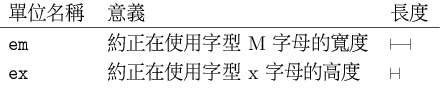
\includegraphics{r-units}
\end{quote}
\end{htmlonly}

�b \TeX\ ���Y�ҿת� em\index{em}�A���A��T�Ө��O���b Knuth �б³]�p�� Computer Modern �r�����Y�� em-dash\index{em-dash} ���e�סA�ѩ�r�� M ��ڤW�O�]�b�r���W�ҿת� em-square ���Q��椤�A�� em �ҫ����e�׬O���o�� em-square\index{em-square} ���e�סA���r�� M �����ä��������o�� em-square�A�]���o�˴N�|�y���t���F�C�ҥH�H�r�� M ���e�רӻ������ܮe�����øq�C\LaTeX\ ���ӫ��O \verb|\quad|\index{quad@\verb=\quad=} �o�N�O���ͤ@�ӥ��T em ���e�ת��ťաA�ҥH�b Knuth �бª� \textit{The \TeX{}book} ���A���� em �N�������L�O�@�� `quad' ���e�סC


\section{�����j�p}
\label{sec:layout}\index{�����j�p}

�ڭ̹��ү౱��@��i�Ȫ��d�򳣥i�H�٬������C���M�A�ڭ̪�����]body�^\index{����]body�^}�ä��O������i�Ȫ��d��A�W�U���k���|�d���@�w���ťաC�p�ɭԦb�ůȤW�m�߼g�򵧡A�Ѥ@�������|�n�ڭ̯d�u�Ѧa�v�A�o�N�O������|�P���ťաA���F��ı�W���z�ѡA�j���]�O�H�ͪ����z�a�H:-)

�b�s��W�A�]���H�٤���]body�^���������u���ߡv�Ρu���f�v\index{����}\index{���f}�A�|�P���ťճ����A�h�٬��u����v\index{����}�C��}���ߡB���䪺�]�p�A�N�٤����u�X��v\index{�X��}�A�Ҧp�A�H�I���ϧG����i�ȷ����O�I�������X�A�H�o�ӭI���ϦӨ��A�N�L�ҿת���F�C���o�b \LaTeX\ �q�`�O���|���o�ر��p�X�{�A���D�S�N�h���w����M�ȱi�j�p�P�˽d��C

���M�A�b����H�~���ťաA�]�ëD���O�ťաA�L�]�t�F�����]footer�^\index{�����]footer�^}�A���ܡ]header�^\index{���ܡ]header�^}������]marginal note�^\index{���}\index{marginal note}�������A�O�����󭶼ơB���ѵ���T�C

\subsection{�����ϸ�}
\label{subsec:layout}

\begin{quote}
\begin{center}
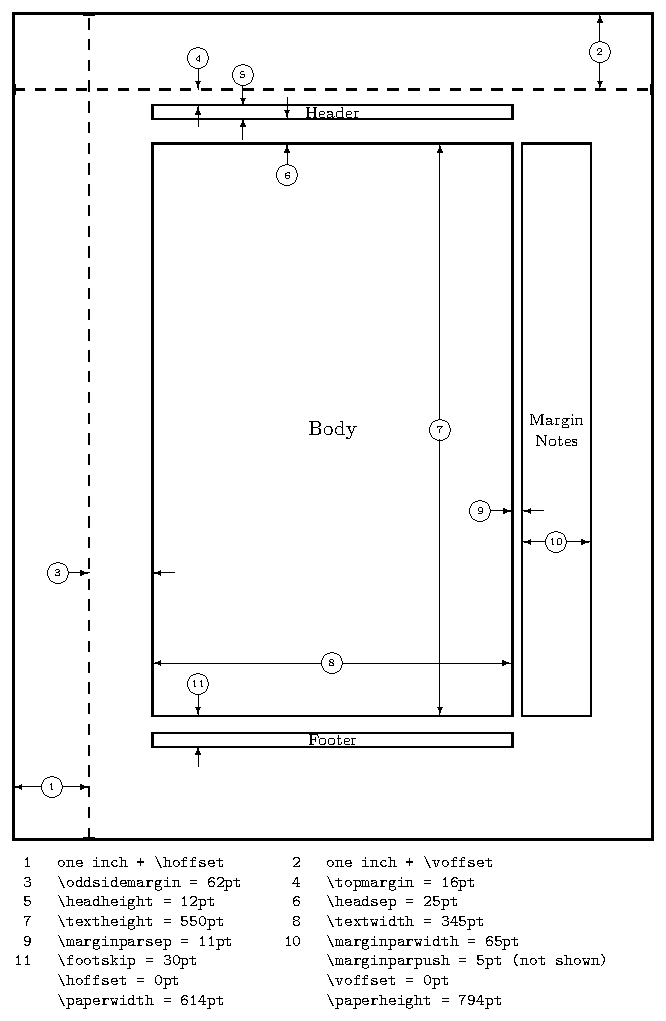
\includegraphics{layout-r}
\end{center}
\end{quote}

�o�̩ҿת��ȱi�j�p\index{�ȱi�j�p}�A�����O {\tt paperwidth}\index{paperwidth} �M {\tt paperheight}\index{paperheight} �ҳ򦨪��d��A�ëD��ڤW��W���쪺�ȱi�j�p�A��ڦb��W���ȱi�q�`�|���j��ڭ̳o�̪��ҿׯȱi�A�ҥH�A�����C�L�ɡA�ٻݰ��L�թκI���~�|�O�u�����o�̩ҿת��ȱi�j�p�]�����j�p\index{�����j�p}�^�C

�o�O 10pt ����j�p�A�p�G�����w�ȱi���ܡA\LaTeX\ �w�]�|�ϥά��� {\tt letterpaper}\index{letterpaper} ���j�p�A�p�n�ϥμڡB�馡�� {\tt a4paper}\index{a4paper} ���ܡA�n�t����w�C�ڭ̥i�H�y�L�ݤ@�U \LaTeX\ �w�]�O�p��w�ƪ����Ŷ����C�䤤 Header�]���ܡ^�BFooter�]�����^��������Ŷ��O���t�A�b���� Body ���Y���A�o�̬O�u�O�歱���ϡA�p�G�O�������ܡA�����ƭ��M�_�ƭ�������O�n���k�ﴫ���A�]�N�O���o�ӹϬO�_�ƭ��A���ƭ����ܡA����O�b����C

�o�̧ڭ̨Ӭݤ@�U�o�ǭȩҥN�����N�q�G

\begin{quote}
\begin{tabular}{ll}
���O�]�ȡ^& �N�q \\
\hline
\verb=\paperwidth=	& �ȱi���e�� \\
\verb=\paperheight=	& �ȱi������ \\
\verb=\textwidth=	& ����]body�^���e�� \\
\verb=\textheight=	& ����]body�^������ \\
\verb=\headheight=	& ���ܡ]header�^���� \\
\verb=\headsep=		& ���ܻP���嶡���Z�� \\
\verb=\footskip=	& ���婳�ܭ��������Z�� \\
\verb=\topmargin=	& ���ܤW�誺�ť� \\
\verb=\marginparwidth=	& ������e�� \\
\verb=\marginparsep=	& ����P���媺�Z�� \\
\verb=\marginparpush=	& ��������Z \\
\verb=\oddsidemargin=	& ���奪�䪺�ťդj�p \\
\verb=\hoffset=		& �L�ժ����b��گȱi�����k��m \\
\verb=\voffset=		& �L�ժ����b��گȱi���W�U��m \\
\index{paperwidth@\verb=\paperwidth=}\index{paperheight@\verb=\paperheight=}%
\index{textwidth@\verb=\textwidth=}\index{textheight@\verb=\textheight=}%
\index{headheight@\verb=\headheight=}\index{headsep@\verb=\headsep=}%
\index{footskip@\verb=\footskip=}\index{topmargin@\verb=\topmargin=}%
\index{marginparwidth@\verb=\marginparwidth=}\index{marginparsep@\verb=\marginparsep=}%
\index{marginparpush@\verb=\marginparpush=}%
\index{oddsidemargin@\verb=\oddsidemargin=}%
\index{hoffset@\verb=\hoffset=}\index{voffset@\verb=\voffset=}%
\end{tabular}
\end{quote}

\verb|\hoffset| �� \verb|\voffset| �N�O�b�վ㪩���b��گȱi�W�����T��m�A�o�˦L�X�Ӫ��ɭԤ~�|�b��گȱi�������C

�Y���F�ܡH�o�ܥ��`�A�]�� \LaTeX\ �������]�w��챵IJ���H�ӻ��A�O�c�W�L�����x���B�·СA�]���o�̤��h�ͥL���]�w�A��}�l��b�S�����n��ɶ���b�o�Ӧa��C�p�G��ڷQ�վ㪩���A��ij�ϥ� {\sf geometry}\index{geometry@\textsf{geometry}} package�C�|�ӨҤl�A�Q���U��t�O 2cm �N�n�A���u�n�b preamble\index{preamble} �ϳ]�w�G

\begin{quote}
\begin{verbatim}
\usepackage[margin=2cm]{geometry}
\end{verbatim}
\end{quote}

�N�i�H�F�A�p�G�H 12pt �j�p���r�A{\tt a4paper} �ȱi�j�p���]�w���ܡA�H����Ө��A�j���O�C�� 40 �Ӥ���r�A�o�O���媺�e�סC�i�H�����Φۦ�վ� {\tt margin}\index{margin} ���ȴN��F�C�ڭ̫ܧƱ�A�U�@���� \LaTeX\ ���o�譱���ﵽ�A�H��K�ϥΪ̳]�w�C
%���T�B�ԲӪ��]�w��k�A�ڭ̯d��᭱�������y���ѮɦA�ӽ͡A�o�˴N���P�v�T�ڭ̾Dzߪ����`�i�סC

\subsection{�ȱi�j�p}

\begin{quote}
\begin{tabular}{>{\tt}ll>{\tt }ll}
�ȱi & �j�p & �ȱi & �j�p\\
\hline
a4paper        & 21x29.7cm & letterpaper    & 8.5x11in \\
a5paper        & 14.8x21cm & legalpaper     & 8.5x14in \\
b5paper        & 17.6x25cm & executivepaper & 7.25x10.5in \\
\end{tabular}
\end{quote}

�ܩ�p����w�ȱi�j�p�A�o�̥�²�满���@�U�o�g�峹���]�w�A�ͨ� \LaTeX\ ����Z���O�ɷ|�A�Բӻ����C

\begin{quote}
\begin{verbatim}
% ���媺�]���O�]�w
\documentclass[12pt,a4paper]{report}
\end{verbatim}
\end{quote}

�ҥH�A�o�g�峹�ϥΪ��O {\tt a4paper}�A����r�����j�p�O 12pt�C��A�����ѼƬO�ﶵ�A�i�H�ٲ��A�p�G�ٲ����ܡA�w�]�ȴN�O 10pt/{\tt letterpaper}�C

\section{�վ��V�Ŷ�}

�o�̪���V�Ŷ��A�Ҧp \verb|~|\index{~@\verb=~=} �o��r�����`�ťաA�� \verb|\quad| �o�� em\index{em} �e�תťաA���O�b�վ��V���ťաC���p�G�O�n��j�B�Χ�p���ťծɸӦp��վ�O�H���U�ڭ̴N�Ӭݬ� \LaTeX\ �������򱱨���O�i�H�B�ΡG

\subsection{�վ��V�Ŷ������O}

\begin{quote}
\begin{tabular}{ll}
���O & �N�q \\
\hline
\verb=\hspace{���}= & �V�k�ťX�Y�ӫ׶q��쪺�ťաA�p�G�O�t�ơA�h�O�V�� \\
\verb=\hfill=        & �����k��Ǫ���r�������X�i�ܤ@�Ӧ�e���� \\
\verb=\quad=         & �ťX�@�� em ��쪺�ť� \\
\verb=\qquad=        & �ťX�G�� em ��쪺�ť� \\
\verb=\thinspace=    & �ťX $1/12$ �� em ��쪺�ť� \\
\verb=\enspace=      & �ťX $1/2$ �� em ��쪺�ť� \\
\verb=\dotfill=      & �@�ΩM \verb|\hfill| �ۦP�A�u�O�ť��ܦ��I \\
\verb=\hrulefill=    & �@�ΩM \verb|\hfill| �ۦP�A�u�O�ť��ܦ��@��u \\
\verb=\centering=    & �����O�H�᪺��r�N�|�~���ƦC�A���k�u�N������ \\
\verb=\raggedright=  & �����O�H�᪺��r�N�|�~���ƦC�A�k�u�N������ \\
\verb=\raggedleft=   & �����O�H�᪺��r�N�|�~�k�ƦC�A���u�N������ \\
\verb=\centerline{}= & �N�j�A��������r�~���ƦC
\end{tabular}
\end{quote}
\index{hspace@\verb=\hspace=}\index{hfill@\verb=\hfill=}%
\index{quad@\verb=\quad=}\index{qquad@\verb=\qquad=}%
\index{thinspace@\verb=\thinspace=}\index{enspace@\verb=\enspace=}%
\index{dotfill@\verb=\dotfill=}\index{hrulefill@\verb=\hrulefill=}%
\index{centering@\verb=\centering=}\index{raggedright@\verb=\raggedright=}%
\index{raggedleft@\verb=\raggedleft=}\index{centerline@\verb=\centerline{}=}

�@�檺�歺�ϥ� \verb|\hspace{���}| �ɱN�|���ġA�o�ɥi�H�[�ӬP���A�Ҧp \verb|\hspace*{3em}|�C

�b�ϥ� \verb|\centerline{}| �����X�A���u��y�ܤ�K�A�]���L���|�v�T�H�U����r�A���L�]���|���A�Ʀܥ[�J����Ÿ��]�L�ġC�ҥH�p�G��y���׶W�L�@�檺��e�A�L�|�W�X��ɡA�ƦܴN��������r�N�ݤ���F�C

�䤤 \verb|\thinspace| �S�i�H�ϥ�²�ƪ� \verb|\,| �ӥN���A�D�n�O�Φb�޸����S���޸������ΡA�q�`�o�ر��ΡA��޸������n���Ӷ��j�A�H�K�Ϥ��A�Ҧp�G

\begin{quote}
\begin{verbatim}
``\,`Superman', he said.''
\end{verbatim}
\end{quote}

���{�X�ӷ|�O�G

%begin{latexonly}
``\,`Superman', he said.''
%end{latexonly}

\begin{htmlonly}
\begin{quote}
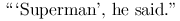
\includegraphics{superman}
\end{quote}
\end{htmlonly}

�o�ˤ~��Ϥ��X���P�޸��A�_�h�|�ܦ��@�ӳs�T�� grave accent\index{grave accent} ���޸��C�Ъ`�N�A�ѩ�o�ӫ��O�O�ѫD�r���Ÿ��c���A�ҥH�A�L���@�νd��b�J��Ÿ�������N�����F�A�᭱�����ťթΥH�j�A���ӭ����@�νd��A�N�n��������L�� \verb|\@| �@�˪����ΡC

\subsection{�վ��V�Ŷ�������}

\begin{quote}
\begin{tabular}{ll}
\verb|\begin{center}...\end{center}| & ���o�����Ҥ������e�m�� \\
\verb|\begin{flushleft}...\end{flushleft}| & ���o�����Ҥ������e�a�� \\
\verb|\begin{flushright}...\end{flushright}| & ���o�����Ҥ������e�a�k \\
\verb|\begin{raggedright}...\end{raggedright}| & ���o�����Ҥ������e�a���A�k�u�N������ \\
\verb|\begin{raggedleft}...\end{raggedleft}| & ���o�����Ҥ������e�a�k�A���u�N������ \\
\end{tabular}
\end{quote}
\index{center@\texttt{center}}\index{flushleft@\texttt{flushleft}}%
\index{flushright@\texttt{flushright}}\index{raggedright@\texttt{raggedright}}%
\index{raggedleft@\texttt{raggedleft}}

�i�J���ҡA�M�W�@�`���쪺���O�A��̦����򤣦P�O�H�̤j�����P�O�A�o�i�H��K�����w�@�ӽd�򪺤�y���L�@�ΡA�Ӥ��|�v�T���ҥH�~����y�C�䦸�A�i�J���ҡA�a�ϩM�W�U��s�b�@�_�A�S���ťX�ťզ�A�L�]�|�۰ʪ��b�W�B�U��ťX�Ӫťզ�X�ӡA�ϥΫ��O���ܫh���|�C

�x�I�o�̫��S���� {\tt raggedright} �� {\tt raggedleft}�H��ӥL�]�O�i�H�����ҨӨϥΡC�ѩ�o��ӫ��O�|�ϥH�U�����e�����B�k�u�������A�]���ϥΤW�n�D�`�p�ߡA���D���ӴN�Q�����媺���B�k�u�������A�_�h�A�̦n�O�ϥΦ��d�򭭨�覡�C���M�A�p�G�o��ӫ��O�O�Φb�Y�Ө�L���ҽd�򤺡A�L���@�Τ]�N�ȭ���o�����Ҥ��A���|�v�T�o�����ҥ~����y�C

\subsection{�ޤ�����}
\index{�ޤ�����}

�ޤ�q�`�N�O�ޥΥL�H����y�A�b�ޤ媺�q���A��dz��|�X�{���Y�����ΡA�H�K�M����۰Ϲj�A�o�]�O�@�تŶ����t�m�A�i�W�[�峹����Ū�ʡC�b \LaTeX\ ���Y���T�ؤޤ����ҡG{\tt quote}, {\tt quotation}, {\tt verse}�C�o�T�̬ݰ_�ӫܹ��A�����ǷL���t���C

\begin{quote}
\begin{tabular}{>{\tt }lll}
���� & �A�ήɾ� & �S�� \\
\hline
quote & ���u���u�ޤ� & �C�Ӭq���Ĥ@�椣���Y \\
quotation & �h�Ӭq�������ޤ� & �C�Ӭq���Ĥ@��|���Y \\
verse & �ֺq�B���ޤ� & �C�Ӭq�����Ĥ@�椣���Y�A���ĤG��_�|���Y \\
\end{tabular}
\end{quote}
\index{quote@\texttt{quote}}\index{quotation@\texttt{quotation}}%
\index{verse@\texttt{verse}}

�b {\tt verse} �����ΡA�q�`�|�ϥ� \verb=\\=\index{\\@\verb=\\=} �Ӵ���H�K����C�@�檺�e�סC�ӥB�q�����Z\index{�q�����Z}�N�����~�b�]�w���v�T�A�䤤 {\tt quote} �M {\tt verse} ���ҷ|�w���J�A�����q�����Z�A�� {\tt quotation} ���ҫh���|�C

���U�ڭ̨Ӭݬݽվ��V�Ŷ����@�Ӻ�X��ҡG

\begin{quote}
\begin{verbatim}
% example11.tex
\documentclass{article}
\usepackage{CJK}
\begin{document}
\begin{CJK}{Bg5}{hwmm}
\section{hspace}
\hspace*{2em}�o�O�@�Ӿ�V�Ŷ��վ㪺���աC\\
�o�O�@��\hspace{2em}��V�Ŷ��վ㪺���աC\\
�o�O�@�� \hspace{2em} ��V�Ŷ��վ㪺���աC
\section{hfill}
�o�O�@��\hfill{}��V�Ŷ��վ㪺���աC
\section{quad}
�o�O�@��\quad{}��V�Ŷ��վ㪺���աC\\
�o�O�@�� \quad{} ��V�Ŷ��վ㪺���աC\\
�o�O�@��\qquad{}��V�Ŷ��վ㪺���աC
\section{dotfill}
�o�O�@��\dotfill{}��V�Ŷ��վ㪺���աC\\
�o�O�@�� \dotfill{} ��V�Ŷ��վ㪺���աC
\section{hrulefill}
�o�O�@��\hrulefill{}��V�Ŷ��վ㪺���աC
\section{center}
\begin{center}
�o�O�@�Ӿ�V�Ŷ��վ㪺���աC
\end{center}
\section{flushleft}
\begin{flushleft}
�o�O�@�Ӿ�V�Ŷ��վ㪺���աC
\end{flushleft}
\section{flushright}
\begin{flushright}
�o�O�@�Ӿ�V�Ŷ��վ㪺���աC
\end{flushright}
\section{quote}
�o�O�`���ۥ���J�����`���G�ơG
\begin{quote}
An antwent to the bank of a river to quench its thirst, and
being carried away by the rush of the stream, was on the
point of drowning.

A Dove sitting on a tree overhanging the water plucked a
leaf and let it fall into the stream close to her. The Ant
climbed onto it and floated in safety to the bank.
\end{quote}
\section{quotation}
�o�O�`���ۥ���J�����`���G�ơG
\begin{quotation}
An antwent to the bank of a river to quench its thirst, and
being carried away by the rush of the stream, was on the
point of drowning.

A Dove sitting on a tree overhanging the water plucked a
leaf and let it fall into the stream close to her. The Ant
climbed onto it and floated in safety to the bank.
\end{quotation}
\section{verse}
�o�O�`���ۥ���J�����`���G�ơA�o�O�`���ۥ���J�����`���G�ơA%
�o�O�`���ۥ���J�����`���G�ơA�o�O�`���ۥ���J�����`���G�ơG
\begin{verse}
An antwent to the bank of a river to quench its thirst, and
being carried away by the rush of the stream, was on the
point of drowning.

A Dove sitting on a tree overhanging the water plucked a
leaf and let it fall into the stream close to her. The Ant
climbed onto it and floated in safety to the bank.
\end{verse}
\section{centering}
\centering
�o�O�@�Ӿ�V�Ŷ��վ㪺���աC\\ % �o�̭n����A�_�h�|�O \raggedright ���@��
\raggedright
\section{centerline}
\centerline{�o�O�@�Ӿ�V�Ŷ��վ㪺���աC}
\section{raggedright}
\raggedright
�o�O�@�Ӿ�V�Ŷ��վ㪺���աC
\section{raggedleft}
\raggedleft
�o�O�@�Ӿ�V�Ŷ��վ㪺���աC
\end{CJK}
\end{document}
\end{verbatim}
\end{quote}

�sĶ�n�����G�p�U�G

\begin{quote}
\url{http://edt1023.sayya.org/tex/latex123/example11.tex}\\
\url{http://edt1023.sayya.org/tex/latex123/example11.pdf}
\end{quote}

�n�`�N�O���O�e�᪺�ťաA�� \verb|\hspace|, \verb|\dotfill|, \verb|\hrulell| �o�����O�A���O�e��ťճ��|��i�h���C\verb|\quad|, \verb|\qquad| �o�����O�A�h�᭱���ťդ]�O�|��J���C�t�~�A�ѨҤl���i�H�ݥX�ӡA�@�� em\index{em} ���e�סA�j���O�@�Ӥ���r���e�סA�ҥH�A�ڭ̹w�]�ϥ� 10pt ���r�A�o�� em �e�״N�۷��� 10pt ���e�סA�ҥH�A�ڭ̦b�Ĥ@�洡�J�F 2em �e�ת��ťաA�]�N�n���O���Y�F��Ӥ���r�@�ˡC

\section{�վ��a�V�Ŷ�}

\begin{quote}
\begin{tabular}{ll}
\verb=\vspace{���}= & �V�U�ťX�Y�ӳ�쪺�ťա]��^�A�t�ƫh�O�V�W \\
\verb=\bigskip=     & ���� 12pt�]11--12pt�^�������ťա]��^ \\
\verb=\medskip=     & ���� 6pt�]5--7pt�^�������ťա]��^\\
\verb=\smallskip=   & ���� 3pt�]2--4pt�^�������ťա]��^\\
\verb=\vfill=       & �M \verb|\hfill| �����A�@�άO�N�Y�q���V�W���A�Ω��U�� \\
\verb=\parskip=���= & �վ����C�Ӭq�������Z�����Y�ӳ��
\index{vspace@\verb=\vspace=}\index{bigskip@\verb=\bigskip=}%
\index{medskip@\verb=\smallskip=}\index{vfill@\verb=\vfill=}%
\index{parskip@\verb=\parskip=}
\end{tabular}
\end{quote}

�䤤�� \verb|\bigskip, \medskip, \smallskip| �ëD�T�w���A�L�̷|���W�U��ߵ����ݭn�۰ʰ��L�աA�H�F��@�㭶���@�P���Ŷ��t�m�C\verb|\vspace| �p�G�O�X�{�b�@�����Ĥ@��γ̫�@��ɡA�N�|���h�@�ΡA�o�ɥi�H�[�ӬP���A\verb=\vspace*{���}=\index{vspace@\verb=\vspace*=}�C

���F�����������@�P��\index{�����@�P��}�A�ϥ��a�V�Ŷ��վ㪺���O�ɭn�S�O�d�N�A�Ҧp���`���D�W�U���Ŷ��B�U�q�������Ŷ��A�i�J���ҫe��ҪťX���Ŷ��A�o�����@�өT�w�ȡA\LaTeX\ �|�۰ʥh�վ�A�����ѨϥΪ̦ۦ�ʤ�A���D�O�ʭ��o�س�W���C�ҥH�A�ϥ��a�V�Ŷ��վ���O�ɡA�n�D�`�`�N���骺�@�P�ʡA�o�]�O�ƪ��W���@�ӫܭ��n����h�C

�o���|�o�g�峹�������ʭ�\index{�����ʭ�}���ҨӺ�X�����A��B�a�V�Ŷ����B�ΡC�ٰO�o�� \ref{sec:titlepage} �`�� title page\index{title page} �����O�ܡH���ڭ̤]�i�H�ۦ�]�p�@�ӿW�ߪ������ʭ��A�ϥΪ��O \LaTeX\ ������ {\tt titlepage}\index{titlepage@\texttt{titlepage}} ���ҡC�o�̪����ɤޥάO�ڭ��٨S���Dzߨ쪺�A�S���Y�A�u�n�j��h����N��F�C

\begin{quote}
\begin{verbatim}
% example12.tex
\documentclass[12pt,a4paper]{report}
\usepackage{CJK}     % �ޤJ�һݭn�� packages
\usepackage{graphicx}
\begin{document}
\begin{CJK}{Bg5}{hwmm}
\begin{titlepage}    % �ϥ� titlepage ����
\vspace*{5ex}
  \begin{flushright} % �j���D�a�k
    \Huge\textbf{�j�a�Ӿ� \LaTeX}
  \end{flushright}
  \rule{\textwidth}{.256ex}
  \begin{flushleft}  % �������X����a���A�M�j���D�����H�@��u�j�}
    Version 0.1 draft\\
    \today
  \end{flushleft}    % ���ɦ�󤤥�����
  \vspace{8ex}       % �ťX 8ex �������Ŷ�
  \hspace{2em}\includegraphics[scale=.75]{cover2.1} % �ޤJ���ɡA�ñN�o��
  \vspace{8ex}                                      % ���ɾ�V�k�� 2em
  \begin{flushright} % �@�̸�T�a�k
    By Edward G.J. Lee ���G��\\
    Email�G\texttt{edt1023@info.sayya.org}
  \end{flushright}
\end{titlepage}
\end{CJK}
\end{document}
\end{verbatim}
\end{quote}

�ѩ�t�X���������D�A�䤤���@�Ǽƾڦ���ʡA�ӥB�]�ٲ��F�@�ǧڭ��٨S���Dzߨ쪺 packages�A���j���c�h�M��l��Z�@�ˡC�ҥH�A�M�o�g�峹�� PDF �榡����|�o�{�A�j���D���r��p�F�@�I�A�ӥB�S���C��A�]�S���W�s��\index{�W�s��}�C

�ϥ� {\tt titlepage}\index{titlepage@\texttt{titlepage}} ���ҫ�A�b {\tt report/book}\index{report@\texttt{report}}\index{book@\texttt{book}} ��Z�L�|�ۦ��@�S�����ƪ���W���A�b {\tt article}\index{article@\texttt{article}} ���O�A�]���|�M����s���A�ҥH�A�b�ﶵ�������n�h�[�@�� {\tt titlepage}\index{titlepage} ���ﶵ�C�t�~�A�b {\tt titlepage} ���Y�N����A�ϥ� \verb|\title|\index{title@\verb=\title=}, \verb=\author=\index{author@\verb=\author=} ���O�F�A�b���媺�a��]�����A�U \verb=\maketitle=\index{maketitle@\verb=\maketitle=} ���O�C

�sĶ�n���Ҥl�p�U�G

\begin{quote}
\url{http://edt1023.sayya.org/tex/latex123/example12.tex}\\
\url{http://edt1023.sayya.org/tex/latex123/example12.pdf}
\end{quote}

�o�̭n�S�O�������O�A�ޤJ���ɭn�ϥ� \textsf{graphicx}\index{graphicx@\textsf{graphicx}} package�]�o�O�̱`�Ϊ��A�]����L����k�ӤޥΡ^�A�ޤJ�����O�O \verb=\includegraphics=\index{includegraphics@\verb=\includegraphics=}�A�o�ӧڭ̷|�b�� \ref{ch:graphic} ���|�Q�סA�b�o�̧ڭ̧�����Y�p������Ϫ� {\tt 75\%}�A�_�h��ӫʭ��|�W�X�@���C�o�ӹ��ɬO�� \MP\index{metapost@\MP} �ɮשҽsĶ�ӨӪ��A�L�O�@�� eps ����\index{eps ����}�]²�檺���A�O�t����ɼƾڥh�������n�P��ťժ� ps ��\index{ps ��}�A��K�ޤJ�ο�X�ܤ�Z���^�A�sĶ����k�p�U�G

\begin{quote}
\begin{verbatim}
mpost cover2.mp
\end{verbatim}
\end{quote}

�o�˴N�|���� {\tt cover2.1} �o�� eps ���ɡA�o�˴N�i�H�����ޤJ�F�C�L����l�X�� eps ���ɦb�G

\begin{quote}
\url{http://edt1023.sayya.org/tex/latex123/cover2.mp}\\
\url{http://edt1023.sayya.org/tex/latex123/cover2.1}
\end{quote}


\section{���C����}

���C����\index{���C����}�]�O�ݩ�@�تŶ�������A�L��@�Ǥ�r���@�w���覡�ӱƦC�A���C���Ҥ��@�ǰ_�Y���Ÿ��B��Ʀr�Φr��A�ڭ̺٤������ؼ��ҡ]item label�^\index{���ؼ��ҡ]item label�^}�A�Q�γo�Ǥ��@�˪��ƦC��m�Τ��@�˪����ؼ��Ұ_�Y�ӱԭz��y�A�N�i�H�F����ت��@�ΡC�o�O�H���`���j�H�~�A�۷��`�������e�@�ؤF�M����k�A��ij�h�h�Q�ΡC�Фd�U�O�o�A���Ҥ��٥i�H�����ҡA�ӥB�H�U�T�ت����C�覡�i�H�V�X��e�ϥΡC

\subsection{���ئ����C���ҡ]itemize�^}
\index{���ئ����C���ҡ]itemize�^}

�o�O�H�Ÿ��Ӱ_�Y���ت��@�ر��C�覡�C�Ҧp�G

\begin{quote}
\begin{verbatim}
\begin{itemize}
\item �Ĥ@�j���A�o�̬O�Ĥ@�j���C
\item �ĤG�j���A�o�̬O�ĤG�j���C
 \begin{itemize}
 \item �Ĥ@�p���A�o�̬O�Ĥ@�p���C
 \item �ĤG�p���A�o�̬O�ĤG�p���C
 \end{itemize}
\item �ĤT�j���A�o�̬O�ĤT�j���C
\item �ĥ|�j���A�o�̬O�ĥ|�j���C
\end{itemize}
\end{verbatim}
\end{quote}

�ƪ��X�ӷ|�ܦ��G

%begin{latexonly}
\begin{quote}
\begin{itemize}
\item �Ĥ@�j���A�o�̬O�Ĥ@�j���C
\item �ĤG�j���A�o�̬O�ĤG�j���C
  \begin{itemize}
  \item �Ĥ@�p���A�o�̬O�Ĥ@�p���C
  \item �ĤG�p���A�o�̬O�ĤG�p���C
  \end{itemize}
\item �ĤT�j���A�o�̬O�ĤT�j���C
\item �ĥ|�j���A�o�̬O�ĥ|�j���C
\end{itemize}
\end{quote}
%end{latexonly}

\begin{htmlonly}
\begin{quote}
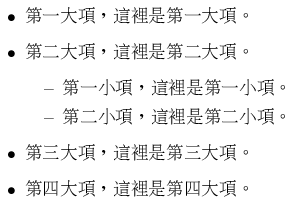
\includegraphics{itemize}
\end{quote}
\end{htmlonly}

\subsection{�C�|�����C���ҡ]enumerate�^}
\label{subsec:enume}\index{�C�|�����C���ҡ]enumerate�^}

�o�O�H�ƥئr�Φr����ù���Ʀr�Ӱ_�Y���ت����C�覡�C�P�˪��Ҥl�A�令 {\tt enumerate} ���ܡA�|�ƪ����G

%begin{latexonly}
\begin{quote}
\begin{enumerate}
\item �Ĥ@�j���A�o�̬O�Ĥ@�j���C
\item �ĤG�j���A�o�̬O�ĤG�j���C
  \begin{enumerate}
  \item �Ĥ@�p���A�o�̬O�Ĥ@�p���C
  \item �ĤG�p���A�o�̬O�ĤG�p���C
  \end{enumerate}
\item �ĤT�j���A�o�̬O�ĤT�j���C
\item �ĥ|�j���A�o�̬O�ĥ|�j���C
\end{enumerate}
\end{quote}
%end{latexonly}

\begin{htmlonly}
\begin{quote}
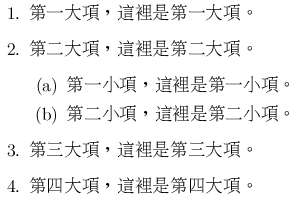
\includegraphics{enumerate}
\end{quote}
\end{htmlonly}

\subsection{�ԭz�����C���ҡ]description�^}
\index{�ԭz�����C���ҡ]description�^}

�o�O�H�@��²�u��r�ԭz�Ӱ_�Y���ت����C�覡�C�A��L�令 {\tt description} ���ܡA�L�O�H�����r�Ӱ_�Y���ت��A�o�Ǥ�r�n�Τ�A���A���C

\begin{quote}
\begin{verbatim}
\begin{description}
\item[�Ĥ@�j��] �o�̬O�Ĥ@�j���C
\item[�ĤG�j��] �o�̬O�ĤG�j���C
  \begin{description}
  \item[�Ĥ@�p��] �o�̬O�Ĥ@�p���C
  \item[�ĤG�p��] �o�̬O�ĤG�p���C
  \end{description}
\item[�ĤT�j��] �o�̬O�ĤT�j���C
\item[�ĥ|�j��] �o�̬O�ĥ|�j���C
\end{description}
\end{verbatim}
\end{quote}

�ƪ��X�Ӫ����G�O�G

%begin{latexonly}
\begin{quote}
\begin{description}
\item[�Ĥ@�j��] �o�̬O�Ĥ@�j���C
\item[�ĤG�j��] �o�̬O�ĤG�j���C
  \begin{description}
  \item[�Ĥ@�p��] �o�̬O�Ĥ@�p���C
  \item[�ĤG�p��] �o�̬O�ĤG�p���C
  \end{description}
\item[�ĤT�j��] �o�̬O�ĤT�j���C
\item[�ĥ|�j��] �o�̬O�ĥ|�j���C
\end{description}
\end{quote}
%end{latexonly}

\begin{htmlonly}
\begin{quote}

\includegraphics{description}
\end{quote}
\end{htmlonly}

�n�`�N���O�A���ޭ��@�ت����C���ҡA�C�Ӷ��ء]item�^����r�ԭz�|�۰ʧ��A�o�۷���K�A�ϥΪ̥u�n����C�����c�˧��A�M�ߥ��C�Ӷ��ت����e�N���F�C�ӥB�A�p�G�ϥΤ�A���A���@�Ǧr���B�r��βŸ��A���a�Y���ХܱN�|�O�o�Ǧr���B�r��βŸ��A�p�G�O�C�|�������C�覡�A���򦳤�A�����N���Q�s���A�|�۰ʸ��L�A�s�����ǫh�|�۰ʶ����C

%\section{enumerate �����M��}

%\subsection{���C���Ҥ����Ŷ�����}


\section{�u��}
\index{�u��}

�u�ئb�ƪ��W�����@�w���a��A�]���L�i�H�Ϲj���P���Ŷ��A�]�i�H���Y�dz�������X�ӡC���O�A�L�h���u�ؤ]�O�|���ٻ��ܥD�����n�Ƨ@�ΡA�ϥΤW�i��n�A�i�Ӥ�C�o�̧ڭ̭n�ͪ��O��ª��u�ءA����\index{����}�]�O�u�ت��@�����ΡA�ڭ̱N�|�b�� \ref{ch:graphic} ���A�A�ӽͪ��檺�B�z�C

%�b \LaTeX\ ���u�إi�����T�ءGLR�BRule �� Par�C

%\begin{quote}
%\begin{tabular}
%�u�غ��� & �N�q \\
%\hline
%LR  & left-right�A�u�ؤνu�ؤ������e�ѥ��ܥk \\
%Rule & 
%Par
%\end{tabular}
%\end{quote}

\subsection{���u�]rule�^}
\index{���u�]rule�^}

���u�]�O�ݩ��ت��@�ءA�N�O�@�ӹ������ΡA�u���L�A�L�����μe�]�u���ղӡ^�u���@�I�I�A�ҥH�A�ݰ_�ӴN�@�����u�}�F�C

\begin{quote}
\begin{verbatim}
\rule[�W�U��m(���)]{�e}{��}
\end{verbatim}
\end{quote}

�e�ΰ��������h�������A���ӤW�U��m�O����O�H�o�ӤW�U��m�O�M��u�]baseline�^\index{��u}\index{baseline}�b������A�p�G�S�����w�A���N�O�b��u����m�A�p�G�����w�A�N�̥��t�Ƚվ�M��u���۹��m�A���ȥѰ�u�V�W�վ�A�t�ȫh�Ѱ�u�V�U�վ�C�o�̨Ӭݭӭӹ�ҴN�A�ѤF�G

\begin{quote}
\begin{verbatim}
% example13.tex
\documentclass{article}
\parskip=3pt
\parindent=0pt
\begin{document}
This is a line.       % �e�� 1pt �e 3cm ����u�C
\rule{3cm}{1pt}
\rule[1ex]{3cm}{1pt}
\rule[-1ex]{3cm}{1pt}

\rule{1pt}{3cm}      % �e�� 3cm �e 1pt �����u�C

\rule{3cm}{0pt}TEST. % �� TEST �V�k�� 3cm�C

\rule{2cm}{3cm}      % �e�� 3cm �e 2cm �������ءC

\textcolor{blue}{This is color lines.}
\textcolor{red}{\rule{3cm}{1pt}}        % ���C�⪺�u�ءC
\textcolor{green}{\rule[1ex]{3cm}{1pt}}
\textcolor{blue}{\rule[-1ex]{3cm}{1pt}}
\end{document}
\end{verbatim}
\end{quote}

�sĶ�n���Ҥl�b�G

\begin{quote}
\url{http://edt1023.sayya.org/tex/latex123/example13.tex}\\
\url{http://edt1023.sayya.org/tex/latex123/example13.pdf}
\end{quote}

�ѨҤl���i�H�ݱo�X�ӡA�o�ӵe�u���O�ä��O����a�B��e�u�Ӥw�A�F���B�Ϊ��ܡA�i�H���X�\�h���P���ĪG�A�Ҧp����Ϥ������C

\subsection{��r���u�]underline�^}
\index{��r���u�]underline�^}

���ɭԧڭ̧Ʊ�b�Ѽg��r���P�ɡA�]�b��U�e�u�C\LaTeX\ ���{�������O�i�H�ϥΡA���N�O \verb|\underline{��r}|\index{underline@\verb=\underline=}�A�|�b��r���u�������P�ɵe�W�u���C���M�A�ϥΤW�`�`�|�M�{�b����u�d�V�A�]���ϥήɭn�S�O�d�N��ӭ����W�O�_�w�g�s�b�F�\�h��u�C

\subsection{��ء]box�^}
\index{box}

�o�̥D�n������r��ءAø�ϤW���@��اΦb�� \ref{ch:graphic} ���ɦA�ӰQ�סC�o�@�����}�Y�N�w�ͨ�A��g�峹�O�Ѥ@�ӭӪ� box �Һc�����A�o�̪���ثh�O�@�Ө嫬�� box�A�L���a��A���M�O�M�e���һ��� box �@�ˡA\TeX/\LaTeX\ �|��L�����@�ӳ�@���r���ӳB�z�C

�ڭ̥��Ӭݬݳ�²�檺��ت����O�G

\begin{quote}
\begin{tabular}{ll}
���O & �N�q�Χ@�� \\
\hline
\verb=\frame{��r}= & �N��r���e�H�i������خئ��A��ةM��r���S�����Z \\
\verb=\fbox{��r}=  & �N��r���e�H�i������خئ��A��ةM��r�����@�w���Z \\
\verb=\mbox{��r}=  & �@�ΩM \verb|\fbox| �P�A����ؤ��i��
\end{tabular}
\end{quote}
\index{frame@\verb=\frame=}\index{fbox@\verb=\fbox=}%
\index{mbox@\verb=\mbox=}

�H�W�����O���i�H�Φ���ؤ�r�C

��ؤ]���i�H�վ㪺���O�G

\begin{quote}
\begin{tabular}{ll}
���O & �N�q�Χ@�� \\
\hline
\verb|\framebox[�e��][����覡]{��r}| & �P \verb|\fbox| �P�A���i���w�e�פι���覡 \\
\verb|\makebox[�e��][����覡]{��r}| & �P \verb|\mbox| �P�A���i���w�e�פι���覡
\index{framebox@\verb=\framebox=}\index{makebox@\verb=\makebox=}
\end{tabular}
\end{quote}

�o�̪��e�׫����O��ت��e�סA�����w���ܡA�@�δN�p�P \verb|\fbox| �� \verb|\mbox| �@�ˡA�H�]����Ӥ�r�d�򬰼e�סA�ѩ�ڭ̤��e��������r���e���e�צ��h�֡A�]���e�ת����w�i�H�ϥΤU�C�۹��쪺�覡�G

\begin{quote}
\begin{tabular}{ll}
�e�� & �@�� \\
\hline
\verb|\width| & �o�Ӽe�״N�O \verb|\fbox| ����ɪ���ؼe�� \\
\verb|\height| & �o�O���`��u�ܮس������� \\
\verb|\depth| &  �o�O���`��u�ܮة������� \\
\verb|\totalheight| & �o�O \verb|\height| �M \verb|\depth| ���`�M \\
\end{tabular}
\end{quote}

�Ҧp�A�ڭ̫��w \verb|2\width| �L���N��N�O�H \verb|\fbox| �]������r���e�ɡA���ؼe�ת��G���e�C�ѼƸ��Y������覡�A�i���U�C�X�ءG

\begin{quote}
\begin{tabular}{>{\tt }ll}
����覡 & �@�� \\
\hline
c & center�A��r����ؤ����A�o�O�w�]�� \\
l & flushleft�A��r����إ��� \\
r & ushright�A��r����إk�� \\
s & stretch�A��r�������������ؤ�
\end{tabular}
\end{quote}

�����w���ܡA���M�N�O����ؤ�����m�F�C�ڭ̤]�i�H���w�i����ت��u���ʲӡA�Τ�ةM��r�������j�Z���G

\begin{quote}
\begin{tabular}{ll}
���O & �@�� \\
\hline
\verb|\fboxrule=���| & ���w��ؽu���ʲ� \\
\verb|\fboxsep=���| & ���w��r�M�ؽt�����Z%
\index{fboxrule@\verb=\fboxrule=}\index{fboxsep@\verb=\fboxsep=}%
\end{tabular}
\end{quote}

�Ъ`�N�A�o���|�v�T \verb|\frame{}|�C�p�G�Q�S�O���m���ت���m�A�]�i�H�ϥ� \verb|\raisebox|\index{raisebox@\verb=raisebox=} ���O�G

\begin{quote}
\begin{verbatim}
\raisebox{�W�U��m(���)}[�`��][����]{��r���e}
\end{verbatim}
\end{quote}

�o�̪��W�U��m���N�q�M \verb|\rule| ���O���Y���@�ˡA�u���L�A�o�̪��W�U��m�@�w�n���w�A�S���w�]�ȡA�����w�|�sĶ���~�C�Фd�U�O�o�A��ؤ����M�O�٥i�H����ت��C�ڭ̲{�b�N�Ӭݤ@�Ӻ�X����ҡG

\begin{quote}
\begin{verbatim}
% example14.tex
\documentclass{article}
\parskip=3ex
\parindent=0pt
\begin{document}
\frame{This is frame.}
\mbox{This is mbox.}
\fbox{This is fbox.}

\framebox{This is a framebox with no argumant.}

\framebox[1.5\width]{This is a framebox.}

\framebox[1.5\width][l]{This is a framebox with \texttt{l}.}

\framebox[1.5\width][r]{This is a framebox with \texttt{r}.}

\framebox[1.5\width][s]{This is a framebox with \texttt{s}.}

This is baseline.
\raisebox{3ex}[5\height]{This is a raisebox which lift 3ex.}

This is baseline.
\fbox{\raisebox{-3ex}[5\height]{This is a raisebox which lift $-$3ex.}}

\fboxrule=1.5pt
\fboxsep=8pt
\framebox[1.5\width][s]{This is a framebox with \texttt{s}.}
\end{document}
\end{verbatim}
\end{quote}

�o���L�ݦh�[�����A�sĶ�n���Ҥl�b�G

\begin{quote}
\url{http://edt1023.sayya.org/tex/latex123/example14.tex}\\
\url{http://edt1023.sayya.org/tex/latex123/example14.pdf}
\end{quote}

\subsection{�q�����}
\index{�q�����}

�t�~�A�]���Ω�q����r����ءA�i�H����Y�Ӭq���X�{�b�Y�S�w���Ŷ��B��m�C�ڭ̱`�`��o�ئw�ƺ٬��g�A�����A�⪩�����e�m��@�Ӥ��i������ط����A���M�A�o�Ӥ�ةM�@�몺 box�A�Ҧp�r���A���M�B��P�˪��a��A\LaTeX\ �|��L�����@�Ӧr�����ӳB�z�C

\begin{quote}
\begin{verbatim}
\parbox[����覡][����][�����m]{�e��}{��r���e}

\begin{minipage}[����覡][����][�����m]{�e��}
  �q�����e
\end{minipage}
\end{verbatim}
\end{quote}
\index{parbox@\verb=parbox=}\index{minipage@\texttt{minipage}}

�o�̪��Ĥ@�ӿ�ܩʰѼơu����覡�v�G

\begin{quote}
\begin{tabular}{>{\tt }ll}
t & top�A�q����ت��W�u����@�檺��u \\
b & bottom�A�q����ت��U�u����@�檺��u \\
c & center�A�q����ت���������@�檺��u�A�o�O�w�] \\
\end{tabular}
\end{quote}

\verb|\parbox| ���O�q�`�Ω���u����r���e�A�p�G�O�������q���A���ϥ� {\tt minipage} ���ҷ|�����K�C�o�Ǭq����ةM�W���ҽͨ쪺�@�Ǥ�س̤j�����P�O�A�q����إ��N�O�Ψӱƪ��p�q����y�A�]���L�|�M�@�륿�`�峹�q���@�˪��B�z�A�Ҧp�L�|�۰��_��A�I��ťզ�]�|�_�s�q���A���U�q���w�]�O���Y�ƪ��A�ӥB�A�b�w�ƤW�|��@�몺�q�����A�@����t�����Z�|�Y� 0pt�C

���פ��h���w���ܡA���N�O�H��Ӫ����g�_��B�z��A��Ӥ�r�q���ҧΦ������סC�ܩ󤺤��m�����]�O \texttt{t, b, c} �o�ǡA�N��O��r�q���b��ؤ����W�U��m�A���M�A�o�n�����w��ذ��׮ɤ~�|���N�q�A�]���A�u�����m�v�M�u���סv�O�n�P�ɫ��w���A�n�D�`�`�N���O�A�p�G���w�F���סA���S�����w�����m�A�h�w�]�O����e���ϥΪ��u����覡�v�ҫ��w���ѼơC

�o�ǰѼƪ��ϥη|���ǷнơA���o�O�u�ʩұa�Ӫ��u���n���c�v�A�����h���O�A�u���b�Ĥ@����IJ�ɧ�L�d�M���N���F�A��ڭn�Ψ�ɦA�Ӭd�L���ԲӰѼơA�`�Ϊ����O�B���ҡA�j���h�d�X���N�۵M�ӵM���O�_�ӤF�C


% ``�j�a�Ӿ� LaTeX'' LaTeX ��Z class.tex
% Copyright (c) 2004  Edward G.J. Lee <edt1023@info.sayya.org>
%
% �b���H�� GNU Free Documentation License 1.2 �ΥH�᪺�����W�d���U�A
% ���\�����B���G�έק�C���쪩�v�B���v�n�����o�����C
%
% �����G�����A�t�� fdl.tex�A���e�� GNU FDL ���W�d���C�p�G�򥢡A�i��
% http://www.gnu.org ���o�A�μg�H�ܦۥѳn�����|(Free Software Fundation)
% �����C
% 9 Temple Place - Suite 330, Boston, MA 02111-1307, USA.
%
% $Id: class.tex,v 1.14 2004/03/06 17:17:55 edt1023 Exp $
%
\chapter{\LaTeX\ ���зǤ�Z���O}
\label{ch:class}\index{��Z���O}

�o���D�n�O�b���� \LaTeX\ ��Z�����O�]document class\index{document class}�^\footnote{�o�b�ª������٬� style�A�o��ӵ��N�q�W�t���h�A�o�dz��O \TeX\ �����X�Ӫ������w�q�A�M���Ψөw�q�峹���j���c�A�H�K²�ƨϥΤW�Τ�Z�����e�C}�A�o�O \LaTeX\ �W�d��Z���鵲�c����k�C�ϥ� class ���ηN�A�N�O�⪩�����c�B�z�M��ڤ�Z���}�A�o�˪��̤j�n�B�N�O������g�峹�ƪ����c�W���@�P�ʡA�]�Ϥ�Z���e��M�n²��A�ϥΪ̥u�n�M�ߩ��Z���e���g�@�Y�i�A�p�G class �w�q���n�A�]�i�H�F��@��h�ܤƤS���ܧ��Z���e���ت��A�u�n��ޥΪ� class �����O���N�i�H�F�A��L���i�H������ʡC

�ثe�A\LaTeX\ �����ؼз����O�Ω�@����A�i�Ω�@�몺�ѫH�B���x�B���Z�B���i�νפ�C�����Ǵ��Z�B�פ�|�n�D�@�w�����c�A�o�ɱo�̻ݨD�t��q�w�C�]���A�]����L�����O�s�b�A�з����O�ä��O�ߤ@���C�ƦܡA�]�i�H�ۦ漶�g�ۤv����Z���O�C���M�A�ڭ̤@��ϥάO���ݭn�o�����s�A�o�̥u���� \LaTeX\ ���з����O�C�ӥB�A�p�G���M�L�H�洫��Z���ݨD�ɡA�ڭ����Ӻɥi�઺�ϥάy�q�ʸ��s�x�����O�C

�t�~�A�]���@�ǬO���� \LaTeX\ �������� macro\index{macro} �g�@�ɭn�Ψ쪺���O�A�o�Ǥw�W�X���g�峹���d��C

\section{\LaTeX\ ���O���ŧi}
\index{���O���ŧi}

\LaTeX\ �����O�A�n�b��Z���@�}�Y�ɴN�ŧi�]���M�A��W�����ѬO�S�����Y���^�A�L���@��榡�p�U�G

\begin{quote}
\begin{verbatim}
\documentclass[��ܩʰѼ�]{���O}
\end{verbatim}
\end{quote}
\index{documentclass@\verb=\documentclass=}

��ܩʰѼƬO�i�H�ٲ����A�����O�W�٫h����١A�@�w�n���w�@�����O�C�ӥB�u��u���@�����O�C

\section{���O����ܩʰѼ�}

��ܩʰѼƥi�H��ܦh�ӡA�U�ӿﶵ�O�H�r�I���}���C

\begin{enumerate}
\item {\tt 10pt, 11pt, 12pt}\\
���w����@�륿�`�r���j�p�A�w�]�O {\tt 10pt}�C��L�I�ƨS���~�� package ������������w�C
\item {\tt a4paper, letterpaper, b5paper, executivepaper, legalpaper}\\
���w�ȱi�j�p�A�w�]�O {\tt letterpaper}�C
\item {\tt fleqn} \\
�ϼƾǦ��a������A�w�]�O�~������C\index{fleqn@\texttt{fleqn}}
\item {\tt leqno} \\
�ϼƾǦ��s���a���A�w�]�O�a�k�C
\item {\tt titlepage, notitlepage}\index{titlepage@\texttt{titlepage}}\index{notitlepage@\texttt{notitlepage}} \\
�M�w title page �O�_�W���@���C�w�] \texttt{article}\index{article@\texttt{article}} ���W���@���A�� \texttt{report/book}\index{book@\texttt{book}}\index{report@\texttt{report}} �h�|�W���@���A�b�o�̬O�i�H���w���ܧ�w�]�欰�A�Ҧp \texttt{article} ��Z�A���w \texttt{titlepage} ���ܡA�� title page �N�|�W���@���C
\item {\tt onecolumn, twocolumn} \\
�峹����Ψ��榡�A�w�]�O����A�]�N�O������C\index{onecolumn@\texttt{onecolumn}}\index{twocolumn@\texttt{twocolumn}}
\item {\tt twoside, oneside}\index{twoside@\texttt{twoside}}\index{oneside@\texttt{oneside}} \\
�O�_�Ϥ��_���ƭ��C�w�] \texttt{article/report} ���Ϥ��A\texttt{book} �h�|�Ϥ��C�@�몺���y�A�b�˭q�������A�L�������u�٬��ѯ�A���ƭ��|�b���}���y�ɪ�����A�ӥB�䤤���e�|���V�ѯ᪺�����]���ɬO�V�k�^�A�Ϥ��A�_�ƭ��|�b�k�A���e�@�˷|�����V�ѯ�A�b \texttt{oneside} �����Ϋh�����o�˪��Ϥ��A���ީ_�������|�b�ȱi����������C
\item {\tt landscape} \\
��V�C�L���a�V�C�L�A�w�]�a�V�]portait�^�C\index{landscape@\texttt{landscape}}\index{portait@\texttt{portait}}
\item {\tt draft}\index{draft@\texttt{draft}} \\
��Z���sĶ�A�o�ɹ��ɱN���|�Q�ޤJ�A�i�[�ֽsĶ���t�סC���L�A�p�G�sĶ�O�ϥΦV�q�r�����ܡA�sĶ�t�����ӬO�ٺ�ܧ֡C���ϥ� {\tt draft} ���@�Ӧn�B�O�A�L�����a��|�ХܥX�ӡC
\item {\tt openright, openany}\index{openright@\texttt{openright}}\index{openany@\texttt{openany}} \\
�o�O�b����A�����}�l�O�_�O�_�ƭ��]right-hand page�^\index{�_�ƭ��]right-hand page�^}�C�b \texttt{book} ���O�A�w�]���|�q�_�ƭ��}�l�Areport ���O�h���|�C\texttt{article} ���O�S�����A�ҥH�A�惡�@�]�w�|�����C
\end{enumerate}

\section{���O������}

�o�̥u�C�X�@��峹�ϥΪ����O�A��L�S�������� \LaTeX\ �������ҨϥΪ����O�N���C�X�F�A�@��ϥΡA�o�����O�N�����F�C

\begin{quote}
\begin{tabular}{>{\tt }lll}
���O & �@��γ~ & �S�� \\
\hline
article & �@��u�� & �L���A�s�򭶤覡���w�ơA�L�_���ƭ����Ϥ� \\
report  & �����פ� & ���|�_�s���A�w�]�L�_���ƭ����Ϥ� \\
book    & ���y��   & ���|��_�ƭ��_�s���A�w�]�����ƭ����Ϥ� \\
letter  & �H��     & �^��H��榡 \\
slides  & �ۿO��   & �X�G�t�Υ~�ӮM����N \\
minimal  & ���դμg�s���O   & �o�O��²�檺���O�A�u�W�w�F���媺�e�B���A���`�r
\end{tabular}
\end{quote}
\index{article@\texttt{article}}\index{report@\texttt{report}}%
\index{book@\texttt{book}}\index{letter@\texttt{letter}}%
\index{slides@\texttt{slides}}\index{minimal@\texttt{minimal}}

���M�A�o�ǥγ~�ä��O�T�w���ܪ��A�o�ݨϥΪ̪��w�ơA���Q�h��ɶ��B�믫���ܡA���N�� \LaTeX\ �w�]���榡�h�ϥΡA�ܤִN���|�����СC�䤤 \texttt{minimal} class �O�ΨӴ��եΪ��A�Ϊ̼g�s�� class �Ϊ��A�L�����S���������w�ơA�Ҧp�A�S�����`�����c�A�U�ض��Z�]�S���w�q�A�w�]���r���O���`�r�A�S����L���ܤơA�X�G�Ҧ����ܤƭn�ۦ�h�w�q�C


% ``�j�a�Ӿ� LaTeX'' LaTeX ��Z package.tex
% Copyright (c) 2004  Edward G.J. Lee <edt1023@info.sayya.org>
%
% �b���H�� GNU Free Documentation License 1.2 �ΥH�᪺�����W�d���U�A
% ���\�����B���G�έק�C���쪩�v�B���v�n�����o�����C
%
% �����G�����A�t�� fdl.tex�A���e�� GNU FDL ���W�d���C�p�G�򥢡A�i��
% http://www.gnu.org ���o�A�μg�H�ܦۥѳn�����|(Free Software Fundation)
% �����C
% 9 Temple Place - Suite 330, Boston, MA 02111-1307, USA.
%
% $Id: package.tex,v 1.21 2004/03/07 12:18:40 edt1023 Exp $
%
\chapter{�����M��}
\label{ch:package}\index{�����M��}

\LaTeX\ �t�Τw�g�n�[�S����s�A���dz����i��|�򤣤W��ڪ��}�B�A�ӥB���Ǥ��w�������w�q�A�g�L�j�a���ϥΡA�oı�ä��O���򪺶���A�ר�O�\�઺�j�Ƥ譱�A�]���o���ͽͦp��ޥΥL�H�w�g�g�n�������A�o�ܭ��n�A�ɶq�קK���ƻs�y���l�A�g \TeX/\LaTeX\ macro\index{macro} �i���O�ܱM�~���u�@�A�n�קK�}�a�F���骺���c�A�ҥH����ݬݦ����򥨶��M��i�H�ϥΡC

%�U�@�䤣��A�X�������M��A�γo�ǥ����M�󪺩w�q�����ũһݡA�o�ɧڭ̴N�o�ۦ�ק�w�q�A�ƦܬO���s�w�q�ӲŦX�һݡA�o�]�O�o�@���dzƱ��Q���@�ӥD�D�C���O�A���O�C�@�ӤH�����R�Ϊ��ɶ��h�Dz� \TeX/\LaTeX\ �������y���A�ҥH�o�̱��Q���H��ΡB²�檺�w�q��k���D�A�y�L�������w���ŦX�@��ϥΪ���h�A�]�M�o�g�峹���c�Q�d�򤣲šC

\section{�@��M�󪺨ϥ�}

�ڭ̴��b�� \ref{subsec:preamble} �p�`�A�� \pageref{subsec:preamble}�A����L²�楨�����ޥΡA�ƹ�W�A���ǥ����t���\�h���ѼƨӰ��L�աA���O�C�ӥ����M�󪺰ѼƳ����|�@�ˡA�]���A�ϥήM�󤧫e�n���ݤ@�ݥL�Ҫ��W���ϥΤ�U�C�X�G�j�����������M�󳣦��ϥΤ�U�A�p�G�O�t�ΤW�N���������A����o�Ǥ��q�`�|��b�G

\begin{quote}
\begin{verbatim}
$TEXMF/doc  => Unix-like �t��
$TEXMF\doc  => DOS/Windows �t��
\end{verbatim}
\end{quote}

�o�ǥؿ����U�A�o�Ǥ��|����l \TeX/\LaTeX\ ��Z�A�]���sĶ�n�� \texttt{*.dvi} �� \textsc{PostScript}\index{PostScript@\textsc{PostScript}} �ɥi�H�\���A���D��K���ܡA�i�H�N�L���ন pdf �榡�Ӿ\���A��]�O�i�H�H����r�ӷj�M����A�b�d���O�B���Үɷ|�����K�C�b Unix-like\index{Unix-like} �t�Ω� Windows\index{Windows} �U�� cygwin\index{cygwin} ���Ҫ��ܡA�i�H�ϥ� \texttt{texdoc}\index{texdoc@\texttt{texdoc}} �o�ӫ��O�Ӿ\���A�Ҧp�G

\begin{quote}
\begin{verbatim}
texdoc amsguide  => �\�� amsguide.dvi �o���ɪ�����
texdoc -s ams    => �d�t�ΤW�Ҧ��t ams �r�˪����
\end{verbatim}
\end{quote}


\section{\LaTeX\ �x���󤤪��зǥ����M��}

���U�O \LaTeX\ �x���󤤩Ҫ����зǥ����M��C���M�O�зǥ����M��A���@�뱡�ΤU�A�ϥγo�� packages �����|�ä��h�A���O���S���ݭn�ɤ~�|�ޤJ�C

\subsection{alltt}\index{alltt@\textsf{alltt}}

�o�ӥ����M�󴣨� \texttt{alltt}\index{alltt@\texttt{alltt}} ���ҡA�M \texttt{verbatim}\index{verbatim@\texttt{verbatim}} ���Ҫ��@�άۦP�A�u�O \textbackslash{}�A\{�A\} ���@�ΩM�@��峹���ۦP�|�Q \LaTeX\ ��Ū�C�o������ΩO�H�o�ˤ@�� \LaTeX\ �o�ӯS���лx�]�i�H�ϥΡA�]�i�H�����Ҥ�����r�㦳�C��A�ΰ���L�ܤơA���M�A���Y����r�w�]���M�O�ϥΥ��r���r��\index{���r���r��}���C

\subsection{doc}\index{doc@\textsf{doc}}

�o�O�ΨӼg \LaTeX\ ��󪺥����M��A�o�b�ϥ� \texttt{ltxdoc}\index{ltxdoc@\texttt{ltxdoc}} �o�� class ���P�ɴN�|���J \textsf{doc} package�C�ѩ�o���O�Ω�@�몺���ϥγ��X�A�ҥH�A�o�̴N���h�͡A�����쪺�ܥi�ۦ�ѦҥL����󻡩��C

\subsection{exscale}\index{exscale@\textsf{exscale}}

�ѩ����� Computer Modern font\index{Computer Modern font} �����ƾǩ����Ÿ��]\texttt{cmex}\index{cmex@\texttt{cmex}}�^�u�� 10pt �j�p���r���]\texttt{cmex10}�^�A�����j�� \texttt{large} �H�W���r���ɡA�Ҧp��j�� \texttt{Large} �ɡA���ǼƾDzŸ����M�|�����@�w���j�p�A�o�ɥi�H�ϥγo�ӮM��A���o�ǼƾDzŸ��]��۩�j�A�Ҧp�n���Ÿ��C\textsf{exscale} �u���r���Y�񪺩w�q�A�]���u�n��o�ӮM��b preamble\index{preamble} �ϤޥδN�i�H�F�A�L�ݥ�����O�C

���L�A�o�̭n�����@�U�A�b \TeX/\LaTeX\ �̦r����j�A���ɥi��|�y�����{���u�����ΡA�ר�O�ƾǦ��l�A���F�U�μƾǦ��l���U�Ӧr�������Ŷ��w�ơA\texttt{cmex10} ���]�p�ä��A�X���ө�j�A�i�H�� \texttt{cmr5} ��j�� 10pt �M�u���� \texttt{cmr10} �Ӥ���N�|���D���{�X�ӷ|���@�ˡA�]���A�p�G�Ҽ{��T�t�X�����D�A��j�ƾǦ��l���r���ɥi��n�Ҽ{�@�U�ϥγ��X�A�ר�ثe�ĥΦV�q�r��O�p���C�иոեH�U���Ҥl�A�ڭ̧� \texttt{cmr5}�B\texttt{cmr10} �� \texttt{cmr12} �P�˩�j�� 30pt �Ӭݬݵ��G�|���|�@�ˡG

\begin{quote}
\begin{verbatim}
% test-fonts.tex
\font\largecmr=cmr12 at 30pt
\largecmr
This is cmr12 at 30pt.

\font\largecmr=cmr10 at 30pt
\largecmr
This is cmr10 at 30pt.

\font\largecmr=cmr5 at 30pt
\largecmr
This is cmr5 at 30pt.
\bye
\end{verbatim}
\end{quote}

�Ъ`�N�A�o�O \TeX\ ��Z�A���O \LaTeX\ ��Z�A�ҥH�n�ϥ� \texttt{tex}\index{tex@\texttt{tex}} �� \texttt{pdftex}\index{pdftex@\texttt{pdftex}} �ӽsĶ�A�L�����G�p�U�A�j�a�i�ܲM�����ݱo�X�ӡA���M�P�ˬO�V�q�r�A����j�ɪ����{�ä��|�@�ˡG

\begin{quote}
\url{http://edt1023.sayya.org/tex/latex123/test-fonts.tex}\\
\url{http://edt1023.sayya.org/tex/latex123/test-fonts.pdf}
\end{quote}

�ھ� Knuth\index{Knuth} �б·���]�p \MF\index{metafont@\MF}�A�L���z���O�@�ӦP�˪��r���b��j���ɭԡA�P�@�Ӧr�A�L�������m�񪺬۹��m���ӭn�H��j�����Ʀӵy�[�վ�C�]���A���p�ڭ̥u�ϥΤ@�ئV�q�r��\index{�V�q�r��}�A�Φb���P����j���v���ɭԡA��r�Ÿ������Ŷ��t�X�|���ͤ��@�˪����G�A�ר�O�Φb�ƾǦ��l\index{�ƾǦ��l}���ɭԡA��[����C

���M�A��ΤW \MF\ ���M�]�O�@�ئV�q�r���A���ѩ�ӹL������A���A�X���ӿù���ܤW�ΡA�ҥH�~�|�h�ӨD�䦸�A�ন pk �I�}�r���ӨϥΡC�o�]�N�O������P�ˬO \texttt{cmr} ���r���A�|���X�ؤ��P�I�ƪ��W�ߦr������]�A�a�ϬO�V�q�r�]�O�p���C\TeX\ �w�g 20 �X���F�A���O�A�ڭ̪��r���޳N���G�٬O�S���������W���� Knuth �бª��z���C

\subsection{fontenc}\index{fontenc@\textsf{fontenc}}

�b�� \ref{subsec:font-attr} �p�`�A�� \pageref{subsec:font-attr}�A������r���s�X�����D�C�n���ܦr���s�X�A�i�H�ϥγo�� \textsf{fontenc} package�C�H T1 font encoding\index{T1} �ӻ��G

\begin{quote}
\begin{verbatim}
  ...
\usepackage[T1]{fontenc}
  ...
\end{verbatim}
\end{quote}

�o�˴N�i�H�F�A���ѩ�@�Ǧr���A�Ҧp�ڬw�r���A�b��Ӫ� Computer modern Type1 �r�����w�Ƥ��@�ˡA�ҥH�A���dz����|�ϥέ�l�� \MF\ �r�����ഫ���� pk �I�}�r�A�o�˪��ܡA�@��L�����L�X�ӬO�t�����j�A���p�G�O�Q�s�@�� PDF �榡�b�å����\�����ܡA�r�������{�|�ܱo����C�z�Q���ܡA�n�w�� \texttt{cm-super}\index{cm-super@\texttt{cm-super}} Type1 �r���A���O�@��ϥΪ̮��Ȧۦ�w�˦r���|���x���C�o�b te\TeX\ 2.x\index{tetex@te\TeX} �H�᪺�����A�w�g�����W \textsf{pxfonts}\index{pxfonts@\textsf{pxfonts}} �� \textsf{txfonts}\index{txfonts@\textsf{txfonts}} package �Ψ�r���A�ҥH�A�p�G�O�s�񪩥��� te\TeX\ ���ܡA�i�H�ѥH�U���覡�ӨϥΡG

\begin{quote}
\begin{verbatim}
  ...
\usepackage{txfonts}
\usepackage[T1]{fontenc}
  ...
\end{verbatim}
\end{quote}

�䤤 \textsf{txfonts} �O���� Times �t�C���r���A\textsf{pxfonts} �O���� Palatino �t�C���r���C���M�A�o������r�������D���I�����A�o���b�o�g�峹���Q�׽d��A�u�వ²�檺�����A�p�G�S���S���ݭn�A�Ҧp�A�ڬw�r���B�@�Ǧ������Ÿ����r���A���ϥιw�]�� OT1 �s�X�N��F�A�]���o�ǮM��Ҫ������Ǧr���A�u���@�ؤj�p�� Type1 �r���b�Y��A�]���ϥΤW���ȷ|�����u\index{���u}�����ΡC

\subsection{graphpap}\index{graphpap@\textsf{graphpap}}

�o�O���ͤ��Ȫ������C�L���ѤF�@�ӫ��O�A�i�H�e���A�i�H�t�X \texttt{picture}\index{picture@\texttt{picture}} ���ҨӨϥΡA�L���y�k�O�G

\begin{quote}
\begin{verbatim}
  ...
\usepackage{graphpap}
  ...
\graphpaper[n](x,y)(x1,y1)
  ...
\end{verbatim}
\end{quote}

�䤤�� \texttt{n} �p�G�ٲ����ܡA�w�]�O 10�A�L�����O���Ȫ��̤p��׳��C\texttt{(x,y)} �� \texttt{(x1,y1)} �����O���U���Υk�W�����y�ЭȡA�Ҧp�G

\begin{quote}
\begin{verbatim}
\documentclass{article}
\usepackage{graphpap}
\begin{document}
\graphpaper(0,0)(360,360)
\end{document}
\end{verbatim}
\end{quote}

�o�˷|�e�X�H 10 ���̤p��ת����A�sĶ�n���Ҥl�p�U�G

\begin{quote}
\url{http://edt1023.sayya.org/tex/latex123/test-graphpap.tex}\\
\url{http://edt1023.sayya.org/tex/latex123/test-graphpap.pdf}
\end{quote}

\subsection{ifthen}\index{ifthen@\textsf{ifthen}}

\TeX\ �����O�@�رƪ��{���y���A���M�|������P�_��\index{����P�_��}�Ӥ�K�g�����A���p�G��Z���]�R���F����P�_���A�N�|�Ϥ�Z�����ơA���H�\Ū�B���@�A�]���A�@�����P�_���j�h�ƨϥΦb�����w�q�A�Ӥ��O�g�b��Z�����C�o�� package �N�O�b²�Ʊ���P�_���A�H�K�]�i�H��K�ϥΦb��Z�����C 

\textsf{ifthen} package ���ѤF \verb|\ifthenelse|\index{ifthenelse@\verb=\ifthenelse=} ���O�Ӱ�����P�_�C�L�᭱���T�ӰѼơA�Ĥ@�ӬO���󦡡A�ĤG�ӬO���󬰯u���ɭԭn���檺���e�A�ĤT�ӬO���󬰰����ɭԭn���檺���e�C�o�̤��h�ͥL���ϥΡA���U�u���Ѥ@�ӹ�Ҥ��q�G

\begin{quote}
\begin{verbatim}
  ...
\usepackage{ifthen}
  ...
\ifthenelse{\isodd{\thepage}}%
  {\setlength{\leftmargin}{10pt}}%
  {\setlength{\leftmargin}{0pt}}
  ...
\end{verbatim}
\end{quote}

�o�˩_�ƭ��ɡA\texttt{leftmargin} �|�]�� 10pt�A���ƭ��ɫh�� 0pt�C�᭱�[ \texttt{\%} �N���A�o�T��O�@���A�䶡�S���ťաC

\subsection{inputenc}\index{inputenc@\textsf{inputenc}}

�ѩ� \textsf{fontenc} package ���@�Ǧr���s�X�w�ơA�M�@��ҿת� Latin-1\index{Latin-1} �o�ǽs�X�]input encoding�^�A�L�̪����e���@�w�۲šA�ҥH�A\textsf{fontenc}\index{fontenc@\textsf{fontenc}} package �`�|�M \textsf{inputenc} package ���۰t�X�ϥΡA�H�T�O�b�ϥμڬw�r���B�Ÿ��ɯॿ�T���o��r�C�Ҧp�G

\begin{quote}
\begin{verbatim}
  ...
\usrpackage[T1]{fontenc}
\usepackage[latin1]{inputenc}
  ...
\inputencoding{ascii} % �]�i�H�b��Z�����ܴ�
  ...
\inputencoding{latin2}
  ...
\inputencoding{latin1}
  ...
\end{verbatim}
\end{quote}

���M�A�ڭ̪���Z�p�G�u�O�^���y�t���峹�A���o�dz��i�H�����z�|�C

\subsection{latexsym}
\label{subsec:latexsym}\index{latexsym@\textsf{latexsym}}

�o�O \LaTeX\ �B�~���Ѫ��Ÿ��C�b�s���� \LaTeXe\ �ä��|�۰ʸ��J�A�n�ۦ�ޤJ�o�ӿW�ߥX�Ӫ� package�C�o�D�n�O���� \texttt{lasy*} �o�Ǧr�����Y���Ÿ��C�p�G���ϥ� \textsf{amsfonts}\index{amsfonts@\textsf{amsfonts}} �� \textsf{amssymb}\index{amssymb@\textsf{amssymb}} package ���ܡA�o�� \textsf{latexsym}\index{latexsym@\textsf{latexsym}} �Ÿ����ӬO�i�H�L�ݤޤJ�]���ּƲŸ��O \LaTeX\ �S�����^�C�ܩ�U�زŸ��� package �����Ǥ��e�A�i�H�ѦҨt�ΤW�� \texttt{symbols*} �o���ɮסA�L�i��s�b���Φ��O�G

\begin{quote}
\begin{verbatim}
symbols.dvi
symbols-a4.ps[pdf]
symbols-letter.ps[pdf]
\end{verbatim}
\end{quote}

�Ϊ̡A�]�i�H�q CTAN\index{CTAN} �U���̷s�������G

\begin{quote}
\url{ftp://cam.ctan.org/tex-archive/info/symbols/comprehensive/symbols-a4.pdf}
\end{quote}

\subsection{makeidx}\index{makeidx@\textsf{makeidx}}

�o�O�b�s�@����\index{����}�ɭn�ޤJ�� package�A�ڭ̷|�b�� \ref{sec:index} �`�A�� \pageref{sec:index} �A�ӰQ�סC

\subsection{newlfont}
\index{newlfont@\textsf{newlfont}}

�o�O�����ª� \LaTeX\ ���r���Ϊk�A���L�ϥηs�����r��� package�C�]�N�O�ڭ̦b�� \ref{subsec:font-command}�A�� \pageref{subsec:font-command} �Ҵ��쪺�Ϊk�C���K�·СA�ڭ̺ɶq�קK�ϥ��¥Ϊk�A�ӨϥΦr�����зǫ��O�C

\subsection{oldlfont}
\index{oldlfont@\textsf{oldlfont}}

�o�O�����ª� \LaTeX\ ���r���Ϊk�� package�C

\subsection{showidx}
\index{showidx@\textsf{showidx}}

�o�� package �|��ܡA\verb|\index|\index{index@\verb=\index=} ���O�U�b����a��C�o�]�|�b�� \ref{sec:index} �`�ӰQ�סC

\subsection{syntonly}

\textsf{syntonly}\index{syntonly@\textsf{syntonly}} package ���� \verb|\syntaxonly|\index{syntaxonly@\verb=\syntaxonly=} ���O�A�L�i�H�ˬd�y�k�O�_���T�A�ä��|�� {\tt *.dvi} �ɪ���X�C���o�� \verb|\syntaxonly| ���O�@�w�n��b preamble �ϡC

\subsection{tracefnt}
\index{tracefnt@\textsf{tracefnt}}

�o�O�l�ܦr���ϥα��Ϊ� package�C�q�`�sĶ�ɩҲ��ͪ���T�w�g�ܨ����A���p�G�Ʊ榳��ԲӪ��r���ϥθ�T���ܡA�i�H�ϥγo�� package�G

\begin{quote}
\begin{verbatim}
  ...
\usepackage[debugshow]{tracefnt}
  ...
\end{verbatim}
\end{quote}

�Ъ`�N�A�o�˷|�W�[�sĶ���ɶ��A�ӥB {\tt *.log} �ɷ|�ܤj�C

\section{\LaTeX\ �x���󤤪��u���}

�o�ǥ����M��A\LaTeX\ �x����O�k���b�����n��]relative software�^���A�i��|��W�@�`���쪺�зǥ����M��ӱo��ΨǡC���]�P�ɥi�H�ݱo�X�� \LaTeX\ �D���ت��M�󤣤֡A�[�W��L�~�Ӫ������M��A���u���O�M�󺡤ѭ��A�ڭ̫ܧƱ�b�i�઺���ΤU \LaTeX\ team �i�H�Ҽ{�N�@�ǥ��n���M��ǤJ���ءA��[���ꪩ���B�z�M��Z�g�@���}���z���C

\subsection{\AmS-\LaTeX}
\index{AmS-LaTeX@\AmS-\LaTeX}

\LaTeX\ �����N���ƪ��ƾǦ��l����O�A���b����M�~�ϥήɡA�i��|�ݭn�W�j�L���\��A\AmS-\LaTeX\ �O����ƾǨ�|�]American Mathematical Society, AMS\index{AMS}\index{American Mathematical Society}\index{����ƾǨ�|}�^�ҵo�i���@�ӼW�j \LaTeX\ �ƾǦ��l�s�誺�����աA�O�� \AmS-\TeX\\index{amstex@\AmS-\TeX} ���ӹL�ӵ� \LaTeX\ �ϥΪ��A�L�D�n������ӳ����G\textsf{amscls}\index{amscls@\textsf{amscls}} �� \textsf{amsmath}\index{amsmath@\textsf{amsmath}}�A�e�̴��ѲŦX AMS �����W�檺��Z���O�A��̥i�[�j��� \LaTeX\ ���ƾǼҦ��C�ڭ̷|�b�� \ref{ch:math} ���A�� \pageref{ch:math} �[�H���СC

\subsection{babel}
\index{babel@\textsf{babel}}

�p�G�Q�ƪ��^��H�~����L�ڬw��a���y��A�Ҧp�G�w��B�k��A���i�H�Q�� \textsf{babel} �����M��C

\subsection{cyrillic}
\index{cyrillic@\textsf{cyrillic}}

�o�O�M���ƪ����Ԥҥ��ڻy��A�Ҧp�G�X��A���i�H�ϥγo�ӮM��C

\subsection{graphics}
\index{graphics@\textsf{graphics}}

�o�O�B�z�ϧέn�Ψ쪺�����M��\index{�����M��}�C���ثe�@�볣�ϥΥ\��������� \textsf{graphicx}\index{graphicx@\textsf{graphicx}} �����M��Ө��N \textsf{graphics}\index{graphics@\textsf{graphics}} �F�A�ƹ�W�A�ޥ� \textsf{graphicx} �|�۰ʪ��ޥ� \textsf{graphics}�A�Ӧb���O�ϥΪ���K�ʤW�A\textsf{graphicx} ���ΡA�]���ڭ̩��᳣�O�H \textsf{graphicx} ���D�ӻ������C�o��ӮM���ݩ� \LaTeX\ ���ϧΤu��աA�o�Ӥu��ե]�A�F�M�C��B�ϧά������U�إ����A�ڭ̷|�b�� \ref{ch:graphic} ���A�� \pageref{ch:graphic} �ӰQ�סC

\subsection{psnfss}
\index{psnfss@\textsf{psnfss}}

�o�O Type1 �r���������M��աA�Ҧp�G\textsf{times}, \textsf{charter}, \textsf{mathptmx}\index{mathptmx@\textsf{mathptmx}} �����A�L�|�h�ϥγo�� Type1 �r��\index{Type1 �r��}�C���q�`�o�Ǧr�����\�h�O�ӷ~�r���A�t�ΤW���@�w�|���A�p�G�S�����ܡA�|�h�ϥ� free ���N���r���A�Ϊ̴N���O�J�o�Ǧr���F�C�p�G�S���o�ǰӷ~�r���A�S�Q�n�O�J���N�� Type1 �r�����ܡA�i�H�Ҽ{�ϥ� \textsf{txfonts} �� \textsf{pxfonts} �����M��Ψ�Ҫ��r���C���M�A�p�G�M�~�ϥΪ��ܡA�i��o�Ҽ{�ʶR�M�~���ӷ~�r���ӨϥΡC

\subsection{array}
\index{array@\textsf{array}}

�o�O�[�j��Ӫ� \texttt{array}, \texttt{tabular} ���Ҫ������M��A�i�W�\�h�ӳ��L�ժ��\��C�o�b�� \ref{sec:array} �`�A�� \pageref{sec:array}�A�ɷ|�Q�ר�C

\subsection{calc}
\index{calc@\textsf{calc}}

�o�ӮM��i�H�� \LaTeX\ �����@��²�檺�N�ƹB��C�D�n�Ω�L�դ@�ǭ�l�w�]�����פέp�ƾ��]counter\index{�p�ƾ�}\index{counter}�^�C

\subsection{dcolumn}
\index{dcolumn@\textsf{dcolumn}}

�o�O�����椤�㦳�p���I���Ʀr����������M��C�ڭ̷|�b�� \ref{sec:dcolumn} �`�A�� \pageref{sec:dcolumn} ���ԲӰQ�סC

\subsection{delarray}
\index{delarray@\textsf{delarray}}

�o�O�[�j \textsf{array}\index{array@\textsf{array}} �����M�󪺥\��A���x�}�Φ�C�����j���ɲŸ��i�H�ϥθ�²�檺���O�C�o�ӮM��n�t�X \textsf{array} �����M��ӨϥΡC�q�`�b \textsf{array} �����M�󤤡A�o�ǯx�}�Φ�C�����j���ɲŸ��O�� \verb|\left| �� \verb|\right| �Ӥ޾ɤ~�|�X�ӡA���ϥ� \textsf{delarray} �����h�����p���·СC�o�b�� \ref{ch:math} ���|�Q�ר�C

\subsection{hhline}
\index{hhline@\textsf{hhline}}

�o�ӥ����M��|��K�b�e��u�ɤ]�i�H���J���檺�a�u�C

\subsection{longtable}

\textsf{longtable}\index{longtable@\textsf{longtable}} �O�Φb�󭶪���C�q�`�b \LaTeX\ ���� \texttt{tabular} ����O�����@�� box\index{box} �ӳB�z�A�]���L�k�A���ΡA�ҥH�L�k�󭶨Ӫ��{�C�o�]�|�b�� \ref{sec:longtable}�A�� \pageref{sec:longtable} �ͨ����ɴ��ΡC

\subsection{tabularx}
\index{tabularx@\textsf{tabularx}}

�o�O \texttt{tabular}\index{tabular@\texttt{tabular}} ��������\index{��������}���[�j���A�L�i�H��K���ƪ����w�e�ת�����C�P�˪��A�o�|�b�� \ref{sec:tabular} �`�A�� \pageref{sec:tabular} �ɴ��ΡC

\subsection{afterpage}
\index{afterpage@\textsf{afterpage}}

�o�ӥ�D�n�b�վ� \LaTeX\ ���B�����ҡ]floating environment�^\index{�B������}\index{floating environment}�ɡA�m��B�ʪ���A�Ҧp�G�ϡB������m�C

\subsection{bm}

\textsf{bm}\index{bm@\textsf{bm}} ���N��A�N�O bold math(symbol)�A�o�|���ƾǦ��l�H���骺�覡����ܡC�o�ӥ����M��A���Ѥ@�� \verb|\bm{}| ���O�A�u�n��ƾǦ��l�m��j�A�����N�|�Ѳ������ܡC

\subsection{enumerate}
\label{subsec-enump}\index{enumerate@\textsf{enumerate}}

�o�O�[�j \texttt{enumerate}\index{enumerate@\texttt{enumerate}} �C�|�����C����\index{�C�|�����C����}�������M��C�L�i�H�ܤ�K�����w�n�ϥΤ���覡�Ӱ_�Y�A��l�� \texttt{enumerate} ���ҡA�w�]�Ĥ@�h�O���ԧB�ƥئr�A���M�]�i�ܧ�A���n���s�w�q�A���O�ܤ�K�C�o���|�ӨҤl�G

\begin{quote}
\begin{verbatim}
% example15.tex
\documentclass{article}
\usepackage{enumerate}
\begin{document}
\begin{enumerate}[Example-1.]
\item This is a item 1.
\item This is a item 2.
  \begin{enumerate}[(1)]
  \item This is a item (1).
  \item This is a item (2).
  \end{enumerate}
\item This is a item 3.
\item This is a item 4.
\end{enumerate}
\end{document}
\end{verbatim}
\end{quote}

�i�H���w�|������ܪ����G\texttt{A, a, I, i, 1}�A�p�G�o�ǬO�ݩ�T�w��ܪ������A�h�n�H�j�A���A�_�ӡA�_�h�L�|���ǭp����ܡC�иյ۩M�� \ref{subsec:enume} �p�`�A�� \pageref{subsec:enume} ���з� \texttt{enumerate} ���Ҥ���@�U�C�sĶ�᪺���G�p�U�G

\begin{quote}
\url{http://edt1023.sayya.org/tex/latex123/example15.tex}\\
\url{http://edt1023.sayya.org/tex/latex123/example15.pdf}
\end{quote}

�o�̽Ъ`�N�@�U�@�ǦP�W�����ҡB�����M��A�Ҧp \textsf{array} �����M��� \texttt{array} ���ҡA�o�̪� \texttt{enumerate} �����M��]�O�@�ˡC

\subsection{fontsmpl}
\index{fontsmpl@\textsf{fontsmpl}}

�o�O�r�� sample ���� package�A�L�i�H�O���ʪ��A�]�i�H�ޥγo�� package �᪽���ϥ� \verb|\fontsample| �o�ӫ��O�ӦL�X�ثe�ϥΪ��r�� sample�C

���ʪ��ܡA�n�ۦ��J�r�ڦW�١Csample �ɦb \texttt{\$TEXMF/tex/latex/tools} �ؿ��U�A�u�n�U�G

\begin{quote}
\begin{verbatim}
latex fontsmpl.tex
\end{verbatim}
\end{quote}

�N�i�H�F�A�L�|�X�{�G

\begin{quote}
\begin{verbatim}
This is TeX, Version 3.14159 (Web2C 7.4.5)
(./fontsmpl.tex
LaTeX2e <2001/06/01>
Babel <v3.7h> and hyphenation patterns for american, french,
german, ngerman, nohyphenation, loaded.
(/usr/share/texmf/tex/latex/base/article.cls
Document Class: article 2001/04/21 v1.4e Standard LaTeX document class
(/usr/share/texmf/tex/latex/base/size10.clo)) (./fontsmpl.sty)
Please enter a family name (for example `cmr').

\family=
\end{verbatim}
\end{quote}

�u�n��J�n���ժ��r���r�ڡA�Ҧp \texttt{cmr}�A�L�N�|���� \texttt{fontsmpl.dvi} �o���ɡA�M��N�i�H�ϥ� \texttt{dvips}\index{dvips@\texttt{dvips}} �� \texttt{dvipdfm[x]}\index{dvipdfmx@\texttt{dvipdfm[x]}} ��L�ন ps/pdf �榡���ɮסC�L�u�|���� OT1\index{OT1} �� T1\index{T1} ��ئr���s�X�C

\subsection{ftnright}
\index{ftnright@\textsf{ftnright}}

\LaTeX\ �b���榡�ƪ��]two-column mode�^\index{���榡�ƪ��]two-column mode�^}�ɡA�L���}���O�m��b�U����쩳���C\textsf{ftnright} �|�N���榡�ƪ��ɡA��Ҧ����}�����m��b�k�橳���C�o�˥i�H�N�}�������A�ݰ_�Ӥ��|�����áC

\subsection{indentfirst}

�q�`�A\LaTeX\ �����`�}�Y���Ĥ@�Ӭq���O���Y�ƪ��A�b�ĤG�Ӭq���_�~�|�Y�ơC�p�G�ߺD�C�Ӭq�������Y�ơA�i�H�ϥ� \textsf{indentfirst}\index{indentfirst@\textsf{indentfirst}} package�C�o�ӮM��]�O�ޤJ�N�i�H�F�A�L�ݥ�����O�C

\subsection{layout}
\index{layout@\textsf{layout}}

�o�O��ܥثe�����t�m\index{�����t�m}�� package�C�ޤJ�o�� package ��A�u�n�b����ϤU \verb|\layout| ���O�A�L�N�|�e�X�ثe�������t�m�A�]�|�N�U�ؼƾ���ܥX�ӡC�ڭ̦b�� \ref{subsec:layout} �p�`�A�� \pageref{subsec:layout}�A���Y����ܪ������ϡA�N�O�o�˵e�X�Ӫ��C


\subsection{multicol}
\label{subsec:multicol}\index{multicol}

�b \LaTeX\ �ŧi��Z���O���P�ɡA�ڭ̥i�H��� \texttt{twocolumn} �ӿ�ܨ��榡���ƪ��A�A�h�h����C�b���榡���ƪ��ɡA�ڭ̥i�H�ϥ� \verb|\onecolumn|\index{onecolumn@\verb=\onecolumn=} �� \verb|\twocolumn|\index{twocolumn@\verb=\twocolumn=} ���O�A�b����Ψ��涡�ܴ��A���o���@�ӫ��Y�������I�A���N�O����ܴ��]�|���ϴ��s���A��Ӫ������N�|��o���m�C

\textsf{multicol} ���ت��A���Ȭ�}����A�i�H���h�榡���ƪ��]�̦h�i�ܤQ�檺�ƪ��^�A�]�i�H�b�ܴ����s�Ʈɦb�P�@�����ܴ��A�Ӥ������s���C�L���ѤF \texttt{multicols}\index{multicols@\texttt{multicols}} ���ҨӰ���쪺�ܴ��C�L���ϥΤ�k��²��A���ƥؤ��ܴ����������Ҩӱ���G

\begin{quote}
\begin{verbatim}
  ...
\usepackage{multicol}
  ...
\begin{multicols}{���}
  ...
  ���e�A�̥��`����覡�Ѽg�Y�i
  ...
\end{multicols}
\end{verbatim}
\end{quote}

�Ъ`�N�A�ޤJ�� \textsf{multicol} �O�S�� `s' ���A�����Ҥ��� \texttt{multicols} �O�� `s' ���C\textsf{multicol} package �B�z�}�����覡�A�M����ƪ��ۦP�A�N�O�q�q�m�󥻭������A�������k���C

\subsection{rawfonts}
\index{rawfonts@\textsf{rawfonts}}

�o�O���� \LaTeX\ 2.09 �ª����C���r�����O�A�Ҧp \verb|\texrm| �N�� 10pt ��ù���r�ڪ��r�C�b�s���� \LaTeXe\ �èS���w�q�o�ǫ��O�C

\subsection{somedefs}
\index{somedefs@\textsf{somedefs}}

�o�O�g \LaTeX\ �������@�ǽd�ҩw�q�A�i�H�ܮe�������䤤�]�w�Ӽg�ۤv�� package�C�o���b�o�g�峹���Q�׽d��A�]���N���h�ͤF�C

\subsection{showkeys}
\index{showkeys@\textsf{showkeys}}

�o�� package �|�� \verb|\label|, \verb|\ref|, \verb|\pageref| ���椬�ѷӪ����O���e�A�Τ��m�ޥΤ��e�A�b���O�Ҧb�B�L�X�ӡC

\subsection{varioref}
\index{varioref@\textsf{varioref}}

�o�O�[�j�����椬�ѷ�\index{�椬�ѷ�}���覡�A�ڭ̷|�b�� \ref{ch:abook} ���ӰQ�סC

\subsection{verbatim}
\index{verbatim@\textsf{verbatim}}

�o�O�[�j \LaTeX\ ��Ӫ� \texttt{verbatim} ���Ҫ��P�W�M��C�i�H�b���Y�ϥε��ѡA�]�i�H�Q�� \verb|\verbatiminput{�ɮצW}|\index{verbatiminput@\verb=\verbatiminput=} ���O�ӤޤJ�~���ɮסA���M�A�ޤJ��|�۰ʶi�J \texttt{verbatim} ���Ҥ��C

\subsection{xr}

\textsf{xr}\index{xr@\textsf{xr}} �O eXternal References ���Y�g�A�N��N�O�椬�ѷӥ~�����ɮסC�o�|�b�� \ref{sec:ref} �`�A�� \pageref{sec:ref} �ӰQ�סC

\subsection{xspace}
\index{xspace@\textsf{xspace}}

�o�� package �|�b�@�ӥ����������o�������J�A�����ťաC�ڭ̦b�� \ref{gen:gamerules}�A�� \pageref{gen:gamerules}�A�ɴ��ͨ� \LaTeX\ ���O�����������D�A�ҥH�A�ڭ̱o�b���O��[ `\verb|\ |' �Ϊ� `\verb|{}|' �ӵ����@�ӫ��O�C���p�G�����w�q�ɨϥΤF \textsf{xspace} �����M�󪺤@�ӫ��O \verb|\xspace|�A����L�N�|�۰ʧP�_���O��ɵ����A�Ӥ����ۦ洡�J `\verb|\ |' �� `\verb|{}|' �F�C

\subsection{theorem}
\index{theorem@\textsf{theorem}}

�o�O \LaTeX\ ���ت� \texttt{theorem} ���Ҫ��[�j�������M��C�ڭ̷|�b�� \ref{ch:math}�A�� \pageref{ch:math}�A�A�ӰQ�סC


\section{�����M���B�M�H}
\label{sec:pkgwhere}

���Ƶo�����l�n�ɶq�קK�A�ҥH�A�p�G�ݭn�ǥ\��A�� \LaTeX\ ���G�S���A���i�H����ݬݬO���O�O�H�w�g���g�n�������\�઺�����M��A�����n�䪺���ӬO FAQ\index{FAQ} ���G

\begin{quote}
\url{http://www.tex.ac.uk/faq}
\end{quote}

�b \url{news://tw.bbs.comp.tex} �]���@�g Chun-Chieh Huang\index{Chun-Chieh Huang} �Һ��@������ FAQ\index{���� FAQ} �i�H�ѦҡC�t�~ \url{news://comp.text.tex} �h�O�^��Q�׸s�աA�i�H�h�h�Q�ΡC�p�G�w�g���D�M��W������r�A���i�H��G

\begin{quote}
\url{http://tug.ctan.org/CTANfind.html}
\end{quote}

�h�j�M�A�j�M���i�H���ӥؿ������Y�ɡC�q�`�A�w�� package�A�L���Y�|�����p��w�ˡA�U�@�S�����ܡA�i�H�� bbs/news �W�o�ݡA�Ϊ̤U���H�U�o�� sh script�G

\begin{quote}
\url{http://edt1023.sayya.org/tex/latex123/ltxins.sh}
\end{quote}

�L���ϥΤ�k��²��A��L�m�������|�i�Τ��B�G

\begin{quote}
\begin{verbatim}
ltxins.sh your.dtx(or your.ins)
\end{verbatim}
\end{quote}

�o�˴N��F�A�L�|���ͥ��n�� \texttt{*.sty} �� \texttt{*.tex} �� pdf �榡���������C�o���Y�ϥΪ��O \texttt{dvipdfm[x]}�A�ҥH�n���w�˳o��ؤu��~��C���M�A�L���|�۰ʦw�ˡA�A�٬O�n��ʧ�@���ɮ׫����� \LaTeX\ ��o�쪺�a��C�o�u�O�@�ӫ�²�檺�u��A�]�����O�үন�\�sĶ�X���X�ӡC

�p�G�Q���D�Y�ӮM��b�t�ΤW�O�_�w�w�ˡA�w�˦b����a��A�i�ϥΥH�U���p�u��G

\begin{quote}
\url{http://edt1023.sayya.org/tex/latex123/ltxpkg.sh}
\end{quote}

��L�����ܸ��|�ҤΤ��B�A�ϥΤ�k�p�U�G

\begin{quote}
\begin{verbatim}
ltxpkg.sh package-name[.sty]
\end{verbatim}
\end{quote}

�o�|�C�X�Ҭd�ߪ��M��O�_�w�w�ˡA�Φw�˦b����ؿ��U�A�γo�� package �O�_���w�����J��L�� package(s)�C���M�A�o��Ӥp�u�㳣�O bash script �g���A�A���t�έn���w�� bash�A�@�몺 Unix-like �t�����ӨS�����D�AMac OS X �� Windows/cygwin ���ҴN�����O�ҤF�C�o�]�O�ӫ�²�檺�p�u��A�p�G�O�� \verb|\input| ���O�Ҹ��J����L {\tt .tex} �ɡA�i��N�|�������X�ӤF�A�\�h�S���Ӹ`�]�O�S���h�Ҽ{��A�]����ڤW�n�H package ����l macro\index{macro} ���e���ǡC�H�U���@�Өϥι�ҡG

\begin{quote}
\begin{verbatim}
edt1023:~$ ltxpkg.sh colortbl

The position of this package is at:
/usr/share/texmf/tex/latex/carlisle/colortbl.sty

The preloaded package(s) of `colortbl.sty' is(are):
array,color
\end{verbatim}
\end{quote}

�ҥH�A�o�� {\sf colortbl} package�A�t�ΤW�w�g�w�ˡA�ӥB�L�|�b�ޤJ���P�ɤ]�ޤJ {\sf array} �� {\sf color} �o��� packages�A���D�n�ܧ�o��� package �ޤJ�ɪ��ﶵ�ѼơA���M�N�i�H�����ޤJ�o��� packages �F�C



%\section{�L�ջP�ۦ�w�q}

%�o�̩ҽͪ��L�աA�����O��@�� \LaTeX\ ���w�]�Ȱ��ܧ�Φۦ�w�q�@��²���K�����O�B���ҡC���M�A�ڭ̦��dzB�z�٨S���Dzߨ�A�o�S�����Y�A�ڭ̥u�O�A�Ѧp��վ�N��F�A�@���٨S�ͨ쪺�w�]�ȡA���Q�ר�ɷ|�A���X�ӡC

%�b \LaTeX\ ���Y���\�h�T�w���ȡA�Ҧp�G

% ``�j�a�Ӿ� LaTeX'' LaTeX ��Z table.tex
% Copyright (c) 2004  Edward G.J. Lee <edt1023@info.sayya.org>
%
% �b���H�� GNU Free Documentation License 1.2 �ΥH�᪺�����W�d���U�A
% ���\�����B���G�έק�C���쪩�v�B���v�n�����o�����C
%
% �����G�����A�t�� fdl.tex�A���e�� GNU FDL ���W�d���C�p�G�򥢡A�i��
% http://www.gnu.org ���o�A�μg�H�ܦۥѳn�����|(Free Software Fundation)
% �����C
% 9 Temple Place - Suite 330, Boston, MA 02111-1307, USA.
%
% $Id: table.tex,v 1.11 2004/03/07 12:33:34 edt1023 Exp $
%
\chapter{���檺�B�z}
\label{ch:table}

�o�O�ݩ�@��Hı�o����x���A���o�O�ܭ��n�������A���ڭ̦h���I�ɶ���s�C\LaTeX\ ������A�]���O��H�޿誺��Ҥ覡�ӻs�@����A��@��ϥΪ̦Ө��A������e���ഫ�����[�L�H�C���M�A���ǽs�边�A�Ҧp GNU Emacs\index{GNU Emacs}�A����K�e \LaTeX\ ���檺�s�边 script�A���o�ǧڭ̥����h�z�L�A���q \LaTeX\ �������檺���c�z�Ѱ_�A�o�˦b�ϥΨ�L�����U�u��ɤ]�|����o������A�ƦܨS����L�u��A�u�n�ⴤ�����檺�j���c�A�s�@����N���|�N�����Y���F�C

�ѩ� \LaTeX\ ���ت�����\��⦳�I���K�A�]���o�@���|���Ф@�ǥ~�Ӫ������M��A������ \LaTeX\ ����\�઺�����A�o�ǥ����A�ϥΤW��۷����M�A�X�G�Ҧ��� \TeX\ ���U�صo�檩�����|���W�A�]��������ߥi��ʪ����D�C

\section{���檺����}\index{����!���檺����}

����\index{����}���ϥΡA�b�峹�W�`�`�O���ƪ��n��A�L���k�Ǥο��ت��@�ΡA���M�A����Ӧh�]�O�|�ٻ��ܥD�C�q�`�A�ڭ̤��媺�ϥβߺD�A����N�O�j��ؤ����p��ءA��r�m��p��ؤ��A�ƦܬY�Ǥp��ؤ��٦��׽u�b���j�C���F�ƪ��W����K�ε�ı���{�W�����[�B�M���A�b��ڤW�j�������������פ�w���ϥ��a�u�B�׽u�A����q�`�Ѿ�u�Ӱ��Ϲj�A�Ʀܧ����S���u���A�ϥΪŶ��Ϲj���覡�C�o���ͶմX�G�b�G�Q�X�~�e�N�w�}�l���M�A�u�O�ꤺ�������G�٬O�ܳ��w���a�B�׽u�b���椧���A�n���S���@�Ǯؽu�h�h�]���N��������C�p�D�S�������{�W���ݨD�A�ڭ����Ӵ�²�ƪ��楻������V���A�N���I�m����檺���e�Ϊ��檺�޿赲�c�w�ơA�}�}�G�G������~�[�[�W���������e�t�m�A�ӤHı�o�o�O�ӥ��Ѫ�����s�@�C

�t�~�A���ʪ����u���A�i��]�O�o�ɶq�קK�A�q�`�ʲӤ������~�����u�����˹����@�ΡA�]���A�p�G���O���������פ�A���N�i��n�קK�A�p�G�O�����BDM �έn���H�̶�g�����椧�����A���S�O�t�~�@�^�ơA�o�ɫʳ��ʪ���إi��|���ݭn�C�o�dzW�d�u���L�O�@�ǺD�ҡA�ëD�@�����ܪ��A�o����󪺩ʽ�Ψϥγ��X�Ӱ��ܤơA�@�Ӥj��h�O�A�p�G�O�H��r�ԭz���D�����A����A���楻���p�G���r���e�m���Ӧh���ܡA�γ\�N�n�Ҽ{²�ƪ��楻���F�C

�ڭ̳o�̴N�Ӥ���A���a�u�B�L�a�u�B�����S���u�ؤΧt���u���檺�U�اΦ�������A�j�a�N�ۥѤ��ҡA�ݭ��@�ت���ݰ_�Ӥ�������C�ѩ� HTML �榡�b���檺���{�W�i��|���u�A�]���o�̻s�@�� PDF �榡�ѰѦҡG

\begin{quote}
\url{http://edt1023.sayya.org/tex/latex123/test-tables.tex}\\
\url{http://edt1023.sayya.org/tex/latex123/test-tables.pdf}
\end{quote}

\section{tabbing ����}
\label{sec:tabbing}\index{tabbing@\texttt{tabbing}}

�o�O \LaTeX\ ���Y�̰򥻪�����Φ��A���D�ۦ�t�~�w�q�Bø�s�A�L�èS����K�i�Ϊ��u�����O�ӰϹj�A�����ϥΪŶ��B��m���t�m����ܪ��椺�e�A�o�ɾ�� \texttt{tabbing} ����b \LaTeX\ ���a��ä��O�@�ӳ̤p��쪺 box�A\LaTeX\ ���|���Ӫ�������@�ӳ��ӳB�z�C�ҥH�A\texttt{tabbing} ����O�i�H�󭶪��A�L�i�H�Q������b�ӳB�z�C�]���A�n�M��L��r�B�Ϫ��ñƱƪ��ɡA�o�t�~��i�@�� box\index{box} ���A���L�ۦ��@�� box ���A�Ҧp \verb|\parbox|\index{parbox@\verb=\parbox=} �� \texttt{minipage}\index{minipage@\texttt{minipage}} ���Ҹ��Y�C

�b \texttt{tabbing} ���Ҥ��A�Ĥ@�ӦC�]row�^�O�H \verb|\=|\index{\=@\verb+\=+} �ӼХ� \textsf{Tab} �e�רӰϹj���]column�^�A�o�Ӽe�׬O�������Y���r��e�שҨM�w���C���򪺨C�����O�� \verb|\>|\index{\>@\verb=\>=} �o�ӲŸ��ӰϹj�A�C�C���n�ۦ�[�W \verb|\\|\index{\\@\verb=\\=} �Ӵ���A�̫�@��i�H�����ϥ� \verb|\\| ����C\texttt{tabbing} ���򥻤j���c�O�G

\begin{quote}
\begin{verbatim}
\begin{tabbing}
column1 \= column2 \= column3 \\
item1   \> item2   \> item3   \\
itemA   \> itemB   \> itemC
\end{tabbing}
\end{verbatim}
\end{quote}

�o�̯S�N��L�ƦC����]�ƹ�W�A���ƾ�� \LaTeX\ �]�|�����Ʀn�^�A�o�ˤ~��ݱo�X�ӥL�����浲�c�C���p�G�Q�վ����e�׮ɥi�H�ϥ� template ���覡�A�Ҧp�G

\begin{quote}
\begin{verbatim}
\begin{tabbing}
xxxxxxxxxx\=xxxxxxxxxx\=xxxxxxxxxx \kill
column1 \> column2 \> column3 \\
item1   \> item2   \> item3   \\
itemA   \> itemB   \> itemC
\end{tabbing}
\end{verbatim}
\end{quote}

�o�̥H 10 �� \texttt{x} ����쪺�e�סA�o�̪� \verb|\kill|\index{kill@\verb=\kill=} ���ܳo�@��O���L�X�Ӫ��A�u�O�b���ܦU����쪺�˥��e�סA�ӥB�L�|�۰ʴ���C���M�A�n�ϥΨ�L���r��]�O�i�H�A�Ҧp�H���椤�̪��r��Ө��N��� {\tt x} �r��A�o�˴N�|�����e�׭�n���i�H�e�Ǩ�L�椺���e�C�]�i�H�ϥ� \verb|\hspace{6em}| �Ψ�L�����׫��O�A�ӫ��w��쪺�e�סC

�����줺��r������A\texttt{tabbing} �������ơA���M \LaTeX\ ������ \verb|\'| ���o�ӲŸ����e����r�a���A�� \verb|\`|\index{\`@\verb=\`=} ���o�ӲŸ����᪺��r�a�k�A����ڹB�ΡA�i�ण�O�ϥΪ̷Q�n�����G�A�]�� \LaTeX\ ������A�D�n�٬O�H \texttt{tabular} ���Ҹ����`�ΡC�� \texttt{tabbing} ���Ҫ��n�B�O�A�L�����o�@�w�n�Ω���檺�ƪ��A�Ҧp�L�]�i�H���{�p���C����\index{���C����}�몺�t�@�ت��{�覡�A�ӥB�L�i�H�󭶱ƪ��C

\section{\texttt{tabular} ����}
\label{sec:tabular}\index{tabular@\textsf{tabular}}

�o�j���O�̱`�ϥΪ�����Φ��A�i�H�ܤ�K���e�u�ءC�o�ت���A\LaTeX\ �O���Ӫ�������@�ӳ��ӳB�z�A�N���r���@�ˡA�]���L�b�������w�ƤW�O�M�@�몺�r���@�몺�B�z�A�ҥH�A�o�ت��椣�g�S���B�z�A�L�k�Q���Φ���ӳ����Ӹ󭶡C

�M \texttt{tabbing} ���Ҫ����P�A���F�i�H���u�����~�]\texttt{tabular} ���ҡA���M�]�O�i�H�����S���u���^�A���j��쪺�Ÿ��O {\tt \&}\index{\&@\verb=\&=}�A�ӥB�A�@�w�n���w�椺��r���m���m�A�椺��r�W�X���w���e�׮ɡA�|�۰ʧ��A�٦��\�h��L��Ӹ`���վ�C

\subsection{{\tt tabular} ���檺�򥻵��c}

\begin{quote}
\begin{verbatim}
\begin{tabular}[t]{lll}
\hline
column1 & column2 & column3 \\
\hline
item1   & item2   & item3 \\
itemA   & itemB   & itemC \\
\hline
\end{tabular}
\end{verbatim}
\end{quote}

�䤤 \verb|[t]| ���� top�A�]�i�H�O {\tt b} ���� bottom�A�� {\tt c} �N�� center�A�o�n�b�e�ᦳ��r�ۨñƪ��ɭԤ~�|��{�@�ΡA�]�� \LaTeX\ �|���� \texttt{tabular} ��������@�Ӧr�����A�ҥH�i�H�M��L��r�B�Ϫ��ñƱƪ��C�o�ǰѼƪ��N��O�M�P���r������覡�Atop �O���泻�ݩM�e���r����Abottom �h�O���橳���M�e���r����Acenter �h�O�M���椤������C

���檺�覡�M \texttt{tabbing} ���Ҥ@�ˡA�䤤�� \verb|\hline| �O�e�@����u���N��A�s���� \verb|\hline\hline| �|�e����u�A�L�����|�۰ʴ���A�]�������[�W����Ÿ��C�䤤 \verb|\begin{tabular}{lll}| �� \texttt{lll} �O�b���w�U��줺�e�b�p��ؤ����m���m�A{\tt l} ���ܾa���]left�^�A{\tt r} ���ܾa�k�]right�^�A{\tt c} ���ܸm���]center�^�C�b \verb|{lll}| ���[�W bar�]\verb+|+�^�|�e�a�u�A�Ҧp \verb+{|l|l|l|}+ �o�˴N�|�ܦ��DzΪ��j��ءB�p��ت�����C�Ө�� bar �N�|�e���a�u�C

\texttt{tabular} ���Ҥ��|�i�ϥΥt�@�� \texttt{tabular} ���Ҩӻs�@�����������A�o�b \texttt{tabbing} ���ҬO���Q���\���C

\subsection{\texttt{tabular} ���ҹ���쪺�վ�}

\begin{enumerate}
\item \verb|p{�e��}|\\
�o�̪� {\tt p} �����O�q���]paragraph�^�C�q�`�Ω�@�Ӥp�q������r�A���w�F�e�׫���Y����r�|�۰ʧ��A�ӥB�o�Ӭq�������ݷ|�M��L��쪺���ݹ���C
\item \verb|@{��r�B�Ÿ��Ϋ��O}|\\
�o�i�H�@�Φb���檺�U�ӦC�A���L�̳��X�{�Y�Ӥ�r�B�Ÿ��γ��b�Y�ӫ��O���@�ΤU�C�o�ӫ��O�t�~�|�P�ɱN��춡�Z�Y�� 0�A�m�󭺧����ܡA�|������u�M��r�������@�Ρ]�w�]���|�����A��u��ݷ|�h�X��춡�Z�������^�C
\item \verb|\multicolumn{����}{���k��m}{��r���e}|\\
����ƪ��A�Ҧp�@�p�q��r�����C���k��m�i�ϥ� {\tt lrc} ���@�C\index{multicolumn@\verb=\multicolumn=}
\item \verb|\cline{a-b}|\\
�e�Y������쪺��u�A�䤤�� \texttt{a-b} �����N�O�n�e�u�����ơA�Ҧp \verb|\cline{2-3}| �N�O�e�ĤG��ܲĤT�檺��u�C\index{cline@\verb=\cline=}
\item \verb|\arrayrulewidth=������|\\
�վ����u�����ʲӡA�w�]�ȬO 0.4pt�C�ϥΤ�k�G\verb|\arrayrulewidth=1.5pt| �Y�i�A���n�`�N���O�n�b�i�J \texttt{tabular} ���Ҥ��e�]�w�n�C\index{arrayrulewidth@\verb=\arrayrulewidth=}
\item \verb|\tabcolsep=������|\\
�վ����쪺���k���Z�C�Ъ`�N�A�o�ӭȬO��ڨ���춡�Z�Ȫ��@�b�A�w�]�O 6pt�C�ϥΤ�k�M \verb|\arrayrulewidth| �@�ˡC\index{tabcolsep@\verb=\tabcolsep=}
\item \verb|\doublerulesep=������|\\
�վ�e���u�ɡA�o��u�������Z�A�w�]�ȬO 2pt�C�ϥΤ�k�M \verb|\arrayrulewidth| �@�ˡC\index{doublerulesep@\verb=\doublerulesep=}
\item \verb|\arraystretch|\\
�վ���檺�W�U��Z�C�Ъ`�N�A�o�n�� \verb|\renewcommand| �ӭ��]�A�]���b \LaTeX\ �w�q�X���@�ӱ`�ƭȡA�ӳo�� \verb|\arraystretch| �u�O�o�DZ`�ƭȪ����ơA�ڭ̭n���s���ܥL�~����ܹw�]���ơC�Ҧp�G\texttt{example16.tex} �����ϥΤ�k�C\index{arraystretch@\verb=\arraystretch=}
\end{enumerate}

�b \texttt{tabular} ���Ҫ��ѼƤ��A�i��O���N��Ӫ��ѼơA�Ҧp \verb|p{}|�C�]�i��O�m��b��Ѽƪ��e��A�p \verb|@{}|�A�o�ݤ@�U��ڨҤl�N�i�H�A�ѡG

\begin{quote}
\begin{verbatim}
% example16.tex
\documentclass{article}
\usepackage{textcomp}             % for \textcelsius
\renewcommand{\arraystretch}{1.2} % �N����涡�Z�[�j����Ӫ� 1.2 ��
\arrayrulewidth=1pt               % �վ�u���ʲӬ� 1pt
\tabcolsep=12pt                   % �վ��涡�Z�� 24pt
\begin{document}
\centering
\section*{SPECIFIC HEATS (20 \textcelsius\ AND 1 ATM)}
\begin{tabular}{@{\sf }lll@{}}    % �Ĥ@���ϥ� sans serif �r��
\hline
 & \multicolumn{2}{c}{\bf Specific Heats} \\ % ��G�T��ƪ��A��r�m��
\cline{2-3}                                  % �u�e�G�T���u
 & $c$ (J/kg$\cdot$K) & $C$ (J/mol$\cdot$K) \\
\hline
Aluminum     & 900  & 24.3 \\
Copper       & 385  & 24.4 \\
Gold         & 130  & 25.6 \\
Steel/Iron   & 450  & 25.0 \\
Lead         & 130  & 26.8 \\
Mercury      & 140  & 28.0 \\
Water        & 4190 & 75.4 \\
Ice ($-$10 \textcelsius) & 2100 & 38 \\
\hline
\end{tabular}
\end{document}
\end{verbatim}
\end{quote}

\textsf{textcomp}\index{textcomp@\textsf{textcomp}} �]�O \LaTeX\ ���зǥ������@�A�L���ѤF�\�h�Ÿ��A�����i�J�ƾǼҦ��]�O�i�H���`�ϥΡC���@��sĶ���ܡA�i��|�ϥΨ� pk �I�}�r�A�p�G���w�� \texttt{cm-super}\index{cm-super@\texttt{cm-super}} Type1 �r�����ܡA�i�H�ϥΥH�U���sĶ�覡�G

\begin{quote}
\begin{verbatim}
latex example16.tex
dvisp -Pcm-super example16.dvi
ps2pdf example16.ps
\end{verbatim}
\end{quote}

�o�˴N�|�����ϥ� Type1 �r���C�p�G�S���w�� \texttt{cm-super} Type1 �r���A�h�i�ޥ� \textsf{txfonts}\index{txfonts@\textsf{txfonts}} �� \textsf{pxfonts}\index{pxfonts@\textsf{pxfonts}} �����M��C

\verb|@{}| �p�G�����S���[�J����ѼơA����L���@�Υu�O�b�h�����k���涡�Z�Ӥw�A�j�a�i�H�⦳�� \verb|@{}| �����������A�յۦA�sĶ�ݬݡA�J�Ӥ���ݦ����򤣦P�C���DZM�~�ƪ����M�a��ij�����e��[�� \verb|@{}| �h����X�Ӫ���u�]��ڤW�N�O�h���즳���k���䶡�Z�������^�C�sĶ�n���Ҥl�b�G

\begin{quote}
\url{http://edt1023.sayya.org/tex/latex123/example16.tex}\\
\url{http://edt1023.sayya.org/tex/latex123/example16.pdf}
\end{quote}

�p�G \verb|@{}| ���Y���O���O�A�ӬO��r�βŸ��A���o�Ӥ�r�βŸ��|�[�b�U���r���e���e�Ϋ�C

\verb|p{}| ���O���ϥήɾ��O�Y�@����쪺��r����h�A�ݭ��w��쪺�e�����L�۰ʧ�檺���ΡA�Ҧp�H�U���Ҥl�G

\begin{quote}
\begin{verbatim}
% example17.tex
\documentclass{article}
\renewcommand{\arraystretch}{1.2} % �N����涡�Z�[�j����Ӫ� 1.2 ��
\begin{document}
\centering
\section*{Yi Syllables Area Character Blocks}
\begin{tabular}{@{}llp{6cm}@{}}
\hline
Start & End & Character Block Name \\
\hline
A000  & A48F  & Yi Syllables.

                Yi also known as Lolo, is a script resembling Chinese 
                in overall shaps that is used in the Yunnan province 
                China. \\
A490  & A4CF  & Yi Radicals.

                Basic units of the Yi syllables. \\
\hline          
\end{tabular}
\end{document}
\end{verbatim}
\end{quote}

�o�˷|�� \verb|p{}| ���w���������@��Ӭq���ӳB�z�A�Ť@�Ӫťզ�A�P�ˬO���ܷs�q�����}�l�C�sĶ�n���Ҥl�p�U�G

\begin{quote}
\url{http://edt1023.sayya.org/tex/latex123/example17.tex}\\
\url{http://edt1023.sayya.org/tex/latex123/example17.pdf}
\end{quote}


\section{array �����M��}
\label{sec:array}\index{array@\textsf{array}}

�o�ӥ����M��i�H�[�j�즳 \texttt{tabular}\index{tabular@\texttt{tabular}} ���Ҫ��\��C�ϥΤW�u�n�ޤJ \textsf{array} �����M��Y�i�A\texttt{tabular} ���Ҩ̭�Ӫ��ϥΤ�k�A�u�O�h�F�Ǭ����վ���O�C

\begin{enumerate}
\item \verb|m{�e��}|\\
�o�M \verb|p{}| �@�˪��@�ΡA�u�O�m�񪺦�m���@�ˡA���ɨ�L��쪺���e�|����o�Ӭq����������m�C
\item \verb|b{�e��}|\\
�P \verb|p{}|�A����L��쪺���e�|�����Ӭq���������C
\item \verb|>{���O}|\\
�o�i�H�m�� {\tt l,r,c,p,m,b} �ѼƤ��e�A�O���Y����쪺���e�U���O�A�o�ӫ��O�|�b���@��줺�e���e�@�ΡC�ޥΤF \textsf{array} package ��A�i��|����Y�� \verb|@{���O}| ���@�ΡA���ɭn��� \verb|>{���O}|�A���o�S���h����춡�Z���\��A�i�b�e�Y�A�[�� \verb|@{}| �Y�i�C
\item \verb|<{���O}|\\
�M \verb|>{���O}| �ۦP�A���|�b���@��줺�e����~�@�ΡC
\item \verb|!{���O}|\\
�o�O���N \verb+|+ ���@�ΡA�i�H��K�ϥίS���Ÿ��ӥN����Ӫ��a�u�C
\item \verb|\extrarowheight|\\
�o�O�b�վ���줺�e���ݪ��Ŷ��j�p�A�����|���ܩ������Ŷ��j�p�C\index{extrarowheight@\verb=\extrarowheight=}
\end{enumerate}


\section{tabularx �����M��}
\label{sec:tabularx}\index{tabularx@\textsf{tabularx}}

\textsf{tabularx} �����M�󴣨Ѥ@�� \texttt{tabularx} ���ҡA�o�O�[�j���� \texttt{tabular} ���ҡA���b \LaTeX\ ���u��ո��Y�C�D�n�@�άO�ﵽ \verb|\tabular*| ���O�A���w����e�ת��\��C

�b��l \texttt{tabular} ���ҡA�[�F�ӬP���A�i�H���w���檺�e�סC���ѩ� \verb|\tabular*| �o�ӭ�l���ҡA�L�|�h�ק��椺�Ŷ��A�Ӥ��O��ھ�Ӫ����ت��e�סA�o�ϱo�Y�Ǥ�r�|�W�X����d��A�]���A�ϥΤW�i�� \texttt{tabularx} �|�����K�A�L���ѤF {\tt X} �ѼƨӨ��N��Ӫ� {\tt lrc} �ѼơA�o�ӰѼƹ�ڪ��@�άO \verb|p{}| ���\��A�]���|��ڽվ�����ت��e�סA�ӥB���Y����r�ԭz�W�L���e�׮ɷ|�۰ʧ��C�o�ӮM��|�۰ʤޤJ \textsf{array} package\footnote{�M��d�ߡA�i�ϥβ� \ref{sec:pkgwhere} �`�A�� \pageref{sec:pkgwhere}�A�Ҵ��쪺
\htmladdnormallink{\texttt{ltxpkg.sh}}{http://edt1023.sayya.org/tex/latex123/ltxpkg.sh}\index{ltxpkg.sh@\texttt{ltxpkg.sh}}
�Ӭd�߬O�_���w�����J��L�� package{s}�C}�C�o�̨ϥγo������Ҩӱƪ��A�j�a����@�U�L�����G�A�N���D�t���F�G

\begin{quote}
\begin{verbatim}
% example18.tex
\documentclass{article}
\usepackage{tabularx}
\parindent=0pt
\renewcommand{\arraystretch}{1.2}
\begin{document}
\centering
\section*{\texttt{tabular*} environment}
\begin{tabular*}{8cm}{lll}
\hline
Start & End  & Character Block Name \\
\hline
3400  & 4DB5 & CJK Unified Ideographs Extension A \\
4E00  & 9FFF & CJK Unified Ideographs \\
\hline
\end{tabular*}

\section*{\textsf{tabularx} package}
\begin{tabularx}{8cm}{llX}  % 8cm ��h�e������e�׫�A�ѤU���q�q��
\hline                      % �ĤT���ϥΡA��r�W�X�������|�۰ʧ��
Start & End  & Character Block Name \\
\hline
3400  & 4DB5 & CJK Unified Ideographs Extension A \\
4E00  & 9FFF & CJK Unified Ideographs \\
\hline
\end{tabularx}
\end{document}
\end{verbatim}
\end{quote}

\textsf{tabularx} package �ä��O���S�����I���A�Ҧp�A�ϥ� \verb|\verb|\index{verb@\verb=\verb=} ���O�ɷ|���@�Ǥ��ۮe�A�t�~�A�b \texttt{tabularx} ���Ҥ��٭n����L�� \texttt{tabularx} ���ҮɡA�o�Ӧb���Y�� \texttt{tabularx} ���ҭn�Ѥj�A���A���A���๳ \texttt{tabular} ���Ҥ@�U�������_���ϥΡC�sĶ�n���Ҥl�b�G

\begin{quote}
\url{http://edt1023.sayya.org/tex/latex123/example18.tex}\\
\url{http://edt1023.sayya.org/tex/latex123/example18.pdf}
\end{quote}


\section{����u���ʲӪ�����]booktabs�^}
\label{sec:booktabs}\index{booktabs@\textsf{booktabs}}

�ѫe���X�`�ҭz�A�i�H�ݱo�X�� \LaTeX\ ���楨�����\��y�����K�F�I�A���@�ǯS�����p�i��|�L�k�B�z�A������~�[�n�D�������ϥΪ̤]�|�P�줣���A���M�]�i�H�ۦ�h�w�q�����A���o�ˤ@�Ӥ����i�঳�i��ʪ����D�A�ӥB�]���O�C�ӤH�����ɶ��h�Dz� \TeX/\LaTeX\ �������g�@�C�ڭ̸չϨӬݬݦ��S����L���ѨM�覡�A�o�̤��o���|����@�ǥ~�Ӫ������M��A���o�ǮM�󪺨ϥά۷������M�A�X�G�i�H�����L���i��ʪ����D�C

�ڭ̫e�����ǹL \verb|\arraryrulewidth|\index{arraryrulewidth@\verb=\arraryrulewidth=} ���O�A�i�H�վ�u�����ʲӡA���O�o�L�k�U�O�վ�u���A�C�Ӧb \texttt{tabular} �������Ҥ����u���|�վ㦨�@�˪��ʲӡC\textsf{booktabs}\index{booktabs@\textsf{booktabs}} �����M��i�H�ܤ�K���F���o�ӥت��C�ڭ̨Ӭݬݳo�Ӵ��ѤF�����K�����O�G

\begin{quote}
\begin{tabular}{ll}
���O & �\�� \\
\hline
\verb|\toprule[�u���ʲ�]|    & �e���泻�ݪ���u \\
\verb|\midrule[�u���ʲ�]|    & �e������Y����u \\
\verb|\bottomrule[�u���ʲ�]| & �e���橳������u \\
\verb|\cmidrule|   & ���O�Y�����e��u�A���N��Ӫ� \verb|\cline|
\end{tabular}
\end{quote}

�ϥΤ�k�M \texttt{tabular} ���Үt���h�A�s���ҦW�ٳ��@�ˡA���i�b���O��[�Ӥ�A���ӫ��w�u�����ʲӡA�����w���ܡA\texttt{toprule} �� \texttt{bottomrule} ���|�񤤶�����L�u���ʤ@�I�C�䤤 \texttt{cmidrule} �t����i�@�B���\��G

\begin{quote}
\begin{verbatim}
\cmidrule[�u���ʲ�](���k�O�_�h��){�e�u���}
\end{verbatim}
\end{quote}

�䤤�u�e�u���v�M \verb|\cline| �@�ˡA���w���ƧY�i�A�Ҧp 2--3�C���k�h��n�������]{\tt l}�^��/�Υk�]{\tt r}�^�A�]�i�Ѥj�A�����w�n�h���h�֡]�w�] 0.5em�^�A�p�G\verb|(lr{0.7em}){2-3}|�C�ڭ̧�
\htmladdnormallink{\texttt{example16}}{http://edt1023.sayya.org/tex/latex123/example16.tex}
���ӧ�@�U�A�j�a�յ۬ݬݦ����򤣦P�A�sĶ�n���Ҥl�p�U�G

\begin{quote}
\url{http://edt1023.sayya.org/tex/latex123/example19.tex}\\
\url{http://edt1023.sayya.org/tex/latex123/example19.pdf}
\end{quote}

�ѩ�ù��ѪR�ת����Y�A�p�G�����X���P�A�ХѦL�����L�X�Ӥ���A�αN�ɮש�j�A���[��C�o�̳̲ʪ��O {\tt toprule} �� {\tt bottomrule} �A�ӬO {\tt midrule}�A�̲Ӫ��O {\tt cmidrule}�C�ӥB \textsf{booktabs} �w�g�վ�L��� \texttt{tabular} ���檺�W�U���Z�A���D�Q�o��j�A���M���ܡA���ݥt�~�A�h�]�w \texttt{arraystretch} ���ȤF�C


\section{�m�����]colortbl�^}

�m�����w�g�O�ܴ��M�A���d�U�n�p�߳ٻ��ܥD�����p�A�]�O�˦��F�j���y�C�]���A�H��t�i��|����X�A�C�ڭ̦b�� \ref{subsubsec:package} �p�`��
\htmladdnormallink{\texttt{example13}}{http://edt1023.sayya.org/tex/latex123/example13.tex}
������L \textsf{color}\index{color@\textsf{color}} package ���ޥΡA���èS���Բӻ����o�ӮM�󪺥Ϊk�A�� \textsf{colortbl}\index{colortbl@\textsf{colortbl}} �|�ϥΨ�o���C�⪺�\��A�]���o�̵y�L�����@�U�C

\subsection{color �����M��}
\label{subsec:color}

�o�O���b \LaTeX\ �u��� \textsf{graphics}\index{graphics@\textsf{graphics}} package �����@�ӥ����A�ϥΤW�D�`²��A�u�n�� \textsf{color} �����b��Z preamble\index{preamble} �ϤޤW�N�i�H�ϥ��C��F�C�H�U�O�`�n�Ψ쪺������O�G

\begin{quote}
\begin{tabular}{lp{17em}}
���O & �@�� \\
\hline
\verb|\color{�C��}| & �o�|�ϥΤ峹�Ҧ����e���ϥγo���C�� \\
\verb|\definecolor| & �w�q�C�� \\
\verb|\textcolor{�C��}{��r���e}| & ����r���e�ϥάY�S�w�C�� \\
\verb|\pagecolor{�C��}| & �o�O�b�]�w�I���C��A�����Ψ�᪺�����|�ϥγo�ӭI���C�� \\
\verb|\normalcolor{�C��}| & �^�_��Ӫ��C�� \\
\verb|\colorbox{�C��}{��r���e}| & �o�O��حI�����C�� \\
\verb|\fcolorbox{�ئ�}{�ؤ��I����}{��r���e}| & �o�O����C��M�䤺�I���C�⤣�P
\end{tabular}
\end{quote}

�o�̭n�`�N���O�A���O���Y�ϥΪ��C��A���ݬO���w�q�L���C��~��ϥΡC\textsf{color} �����u�w�q�F�@�ǰ��C��A\textcolor{red}{\bf r}ed, \textcolor{green}{\bf g}reen, \textcolor{blue}{\bf b}lue (RGB �ҫ����\index{RGB �ҫ����}), \textcolor{cyan}{\bf c}yan, \textcolor{magenta}{\bf m}agenta, \textcolor{yellow}{\bf y}ellow, blac{\bf k} (CMYK �ҫ����\index{CMYK �ҫ����}), white�A�t�~�@�ӱ`�Ϊ� gray �Ƕ��ҫ��]gray-scale\index{�Ƕ��ҫ�}\index{gray-scale}�^�A��L���C��o�ۦ�w�q�C�w�q�C�⪺�y�k�p�U�G

\begin{quote}
\begin{verbatim}
\definecolor{�C��W��}{��m�ҫ�}{�զ�L��}
\end{verbatim}
\end{quote}

�Ĥ@�ӰѼƴN�O�ۭq���@���C��W�١A��m�ҫ��i�ϥ� rgb�Bcmyk �� gray�A�U�C��`�L�Ȧb 0--1 �����A�u�զ�L�ȡv�N�O�U�ح�⪺�ȡCRGB �C�⪺���ޭȡA�p�G�O Unix-like �t�ΡA�i��@�U \texttt{rgb.txt} �o���ɮסA���Y�N�|���U���C�⪺���ޭȡA�Ϊ̡A�Ѧ�
\htmladdnormallink{\texttt{example24.pdf}}{http://edt1023.sayya.org/tex/latex123/example24.pdf}�C�o�̥H bisque �o���C�⬰�Ҥl�A�L�� rgb �T��⪺�`�L��Ҭ� 255, 228, 196�A�U���H 256 �o 0.996, 0.891, 0.755�A�w�q��k�p�U�G\footnote{�C�@�ӭ��b�q���W�̤p�i�Ѥ@�� byte(8-bits) ���x�s�A�@�� 256($2^8$) ���ܤơA�ҥH�A�T���i�եX $256^3$ �@ 16,777,216 ���C��A���o�����ܧA���ù��B�L��������k��ܨ���h�C��C}

\begin{quote}
\begin{verbatim}
\definecolor{bisque}{rgb}{.996,.891,.755}
\definecolor{mypink}{cmyk}{.1,.8,.4,.1}  % cmyk �ҫ����Ҥl
\end{verbatim}
\end{quote}

�o�˥H��N�i�H�ϥ� bisque �� mypink �o����C��F�Cgray �h�䴩�Ƕ��A�i�H�W��L����{�`�L�A�Ҧp�G

\begin{quote}
\begin{verbatim}
\definecolor{mygray}{gray}{.6}
�Ϊ����w�q�ΨϥΡA���ƥ��w�q�n�C��W�١G
\textcolor[gray]{.3}{��r���e}
\textcolor[rgb]{.2,.5,.7}{��r���e}
\end{verbatim}
\end{quote}

�o�� mygray �|�o��L�Ǧ⪺�ĪG�A�L���C��W�ٴN�O mygray�C�����w�q�Ψϥ����M�]�i�H�A������ij�o�򰵡A�]���p�G����Ӧa��n�ϥΦP�@���C��ɡA�S�o���Ʃw�q�@���C�n�`�N���O gray ���ઽ���ϥΡA�n���w�q�L���Ǧ�סA��L�C��]����o�˳�¾a�@�ӭȨөw�q�L���`�L�סC�q�`�ڭ̤ޥΪ��ɭԡA�|�[�J�H�U���ﶵ�ѼơG

\begin{quote}
\begin{verbatim}
\usepackage[usenames,dvipsnames]{color}
\usepackage{colortbl}
\end{verbatim}
\end{quote}

�o�˴N�i�H�ϥ� \texttt{dvipsnam.def}\index{dvipsnam.def@\texttt{dvipsnam.def}} �o���ɸ��Y�ҩw�q�n���C��A�Ҧp Salmon, Orchid, BlueViolet\chdots{}�����A�Цۦ�d�\�o���ɮפ��e�A{\tt dvipsnames} �o�ӰѼƤ]�i�H���ΡA�u�� {\tt usenames} �Y�i�C�o�̤ޥήɽЪ`�N���ǡA\textsf{colortbl} �n�b�᭱�A��]�O \textsf{colortbl} �����|�۰ʤޤJ \textsf{color} �� \textsf{array} �o��ӥ����A�����Y�èS���t����ﶵ�ѼơA�ҥH�n�m���h�ŧi�C

\subsection{colortbl ���D�n���O}
\label{subsec:colortbl}

\begin{quote}
\begin{tabular}{ll}
���O & �@�� \\
\hline
\verb=\columncolor= & ��������ۦ� \\
\verb=\rowcolor= & ���Ӿ�C�ۦ� \\
\verb=\arrayrulecolor{�C��}= & ���w�u�����C�� \\
\verb=\doublerulesepcolor{�C��}= & ���w���ýu�����j���C��
\end{tabular}
\end{quote}
\index{columncolor@\verb=\columncolor=}\index{rowcolor@\verb=\rowcolor=}%
\index{arrayrulecolor@\verb=\arrayrulecolor=}%
\index{doublerulesepcolor@\verb=\doublerulesepcolor=}

�b�o�̡A\verb|\columncolor| �M \verb|\rowcolor| ���ѼƬO�@�˪��A�L�̪��@�P�y�k�O�G

\begin{quote}
\begin{verbatim}
\columncolor[��m�ҫ�]{�C��}[���t��X����][�k�t��X����]
\end{verbatim}
\end{quote}

�ڭ̲{�b�N�Ӭݭӹ�ҡA�o���Y���|�Ӥp�Ҥl�A�]�A�G�Ƕ�����B�������ۦ�B��Ӫ���b�ۦ�I���γ�@�Ӫ��椺��صۦ�G

\begin{quote}
\url{http://edt1023.sayya.org/tex/latex123/example20.tex}\\
\url{http://edt1023.sayya.org/tex/latex123/example20.pdf}
\end{quote}


\section{���檺���ѡ]threeparttable�^}
\label{sec:3parttable}\index{����!����}

���檺���Ѥ���·СA\LaTeX\ �� \texttt{tabular} ���ҵ����@�ӳ��A����Y����r���}��\index{�}��}���ܡA�N�|���l�ӭ��A���ǥ����M�󦳿�k�b���椺���}���]�Ҧp \textsf{longtable}\index{longtable@\textsf{longtable}} package�^�A���o�O�m�󭶭������A�M�@�뤺�媺���}�V�b�@�_�A�h�ƨϥΪ̧Ʊ檺�O�����ѴN�m����橳���C�ѨM����k�N�O�ϥ� \textsf{threeparttable}\index{threeparttable@\textsf{threeparttable}} package�A�ȮɱN���檺�Y�������ΥX�ӡC

�p�G�A�� \textsf{threeparttable} package �����{�M�o�̪��Ҥl�����@�˪����ΡA�Ч�s�o�ӮM��A�o�g�峹�ϥΪ��O 2003/06/13 v3.0 �������C

\begin{quote}
\url{ftp://ctan.unsw.edu.au/tex-archive/macros/latex/contrib/misc.zip}
\end{quote}

�U����Ѷ}���Y�ɡA�� \texttt{threeparttable.sty} ������ \texttt{\$TEXMF/latex/misc} �ؿ��U�A����@�U {\tt texhash}\index{texhash@\texttt{texhash}} �@�U�Y�i�C�L�����ҦW�٩M�M��W�٤@�ˡA�N�O {\tt threeparttable}�C�� {\tt tabular} �ε��Ѫ����O�M���e�A�q�q�]�b {\tt threeparttable} ���Ҹ��Y�Y�i�C

�L�O�ϥ� \verb|\tnote{�Ÿ��Τ�r}|\index{tnote@\verb=\tnote=} ���ХX�n���Ѫ��a��A�b \texttt{tabular} ���ҵ�����A�A�ϥ� \texttt{tablenotes}\index{tablenotes@\texttt{tablenotes}} ���ҨӼg���Ѥ��e�A�o��ӳ������O��ӳQ \texttt{threeparttable} ���ҥ]�����C���U�o�ӨҤl�Ӧ۳o�ӮM�󪺧@�� Donald Arseneau\index{Donald Arseneau}�A�o�̧�L�M \textsf{booktabs} package ���X�_�ӥΡG

\begin{quote}
\url{http://edt1023.sayya.org/tex/latex123/example21.tex}\\
\url{http://edt1023.sayya.org/tex/latex123/example21.pdf}
\end{quote}

�n�`�N���O�A�b \texttt{tablenotes} ���ҤU�A�r��èS���Y�p�A�i�Ѧ� \texttt{example21} ���Y�A�ϥ� \texttt{footnotesize} ���r��j�p�C

\section{�p���I����]dcolumn�^}
\label{sec:dcolumn}\index{dcolumn@\textsf{dcolumn}}\index{����!�p���I���}

�o�O \LaTeX\ ���зǥ����A�Ω�N���椺���p���I����C��Ӫ� \texttt{tabular} ���Ҫ��@�k�O�h�W�[�@�����A�������ϥ� \verb|@{.}| �ӱM���Ƥp���I�A�o�ˤ@�Ө��檺���Z�|�����A�ݰ_�ӴN���s�b�@�_���Ʀr�F�A���o�˹�b�O���I dirty�A�ϥ� \textsf{dcolumn} �������ܡA�N�i�H�ܦ��W�ߪ��h����p���I�γr�I�C

\textsf{dcolumn} ���Ϊk�A�D�n�O�h���N \texttt{tabular} �ѼƤ��� \texttt{lrc} �o�ǰѼơC�L�ϥΪ��O�@�Ӥj D ���O�A�ᱵ�T�ӰѼơG

\begin{quote}
\begin{verbatim}
D{��Z��J�Ÿ�}{�ƪ����X���Ÿ�}{�p�Ʀ��}
\end{verbatim}
\end{quote}

�Ҧp�H�U������ڭ̦A���h�ơA�p���I�`�O�L�k����A�]�� \texttt{tabular} ���ҬO�H��Ӧr��b�B�z���G

\begin{quote}
\begin{verbatim}
\begin{tabular}{lllll}
\toprule
      & headA & headB & headC & headD \\
\midrule
test1 & 7.879  & 921.661 & 1382.81 & 998.98 \\
test2 & 1.97   & 35.21   & 321.3   & 4791112.11 \\
test3 & 211.97 & 5.2     & 213.629 & 748261594.106 \\
\bottomrule
\end{tabular}
\end{verbatim}
\end{quote}

�ڭ̥u�n�� \texttt{tabular} ���᭱�ѼƧ令�G

\begin{quote}
\begin{verbatim}
  ...
\usepackage{dcolumn}
  ...
\begin{tabular}{lD{.}{.}{3}D{.}{.}{3}D{.}{.}{3}D{.}{.}{3}}
  ...
\end{verbatim}
\end{quote}

�N�i�H���p���I����C�o�� 3 �N�O�̪����p�Ʀ�ơA�ڭ̿�J�B��X���O�^��y�I�]�N�O�p���I�^�A�o�˪����ܪk�]�i�H�t�~�ŧi \verb|\newcolumntype| ���зǮ榡�A�H²�� \texttt{tabular} �Ѽƪ���J�A�Y�G

\begin{quote}
\begin{verbatim}
  ...
\usepackage{dcolumn}
  ...
\newcolumntype{z}[1]{D{.}{.}{#1}}  % �w�q�@�ӷs�� z ���O
  ...
\begin{tabular}{lz{3}z{3}z{3}z{3}}
  ...
\end{verbatim}
\end{quote}

���� \verb|#1| �N�O {\tt z} �o�ӷs���O���Ѽơ]{\tt z} �i�H�O���N���r���βŸ��^�A\verb|z{3}| ���N�O�N�� \verb|D{.}{.}{3}|�C���A�����Y�� 1 �N���o�ӷs�� {\tt z} �᭱�u���@�ӰѼơA�b�o�ӨҤl�̴N�O�p���I�Ӽ� 3�C�H�U�O�sĶ�n���Ҥl�G

\begin{quote}
\url{http://edt1023.sayya.org/tex/latex123/example22.tex}\\
\url{http://edt1023.sayya.org/tex/latex123/example22.pdf}
\end{quote}

�o�̭n�S�O�`�N���O�A�b \textsf{dcolumn} ���ĤO�d����Y�A�Ҧp�H�W�Ҥl�A�� {\tt z} ���O�v�T�����A�L�|�۰ʶi�J�ƾǼҦ��A���Y�n���{�ƾǦ����ܡA�e�ᤣ���A�[ \verb|$|�A�_�h�|���X�ƾǼҦ��C�Ҧp {\tt example22} ���Y�A���� headA �|�ܦ�����r�A�o�O�]���i�J�F�ƾǼҦ�\index{�ƾǼҦ�}�A�n���L���`���ܡA�N�n�g�� \verb|$headA$| �o�˨Ӹ��X�ƾǼҦ��C

\section{�j������]longtable�^}
\label{sec:longtable}\index{longtable}\index{����!�j������}

�o�i�঳��ر��ΡC�@�جO�ܼe������A�t�@�جO�ܪ�������C�Ӽe������i�Ҽ{����@�U�A���L���A�ܩ��������i�H�ϥ� \textsf{longtable} ���L�i�H�󭶳s��C�p�G������A���u�Ҽ{�����A�Ϫ��t�~�s�@�A�Ϊ̸յ�²�ƹϪ��@�~�F�C

\subsection{�Ӽe������}

�n�������A��k�ܦh�A�Ҧp \textsf{graphics} package �@�_ release �� \textsf{lscape}\index{lscape@\textsf{lscape}} �����M��A�L�|���������E�Q�סA�Ϊ̨ϥ� \textsf{graphics/graphicx} package ������ \verb|\rotatebox|\index{rotatebox@\verb=\rotatebox=} ���O�A�N�������E�Q�סC�t�~�A�]�i�H�ϥ� \textsf{rotating}\index{rotating@\textsf{rotating}} package �ӱ���C�o�� package �򥻤W�ϥΪ����O \textsf{graphics/graphicx}\index{graphics@\textsf{graphics}}\index{graphicx@\textsf{graphicx}} �����W��������O���\��A�ҥH�A�����w�u��ϥΦb�Ϫ��Ӥw�C

�o�̴N�H \textsf{rotating} package ���Ҩӻ����A�L���ѤF \texttt{sidewaystable} �� \texttt{sidewaysfigure}\index{sidewaystable@\texttt{sidewaystable}}\index{sidewaysfigure@\texttt{sidewaysfigure}} ���ҡA�e�̷|���������E�Q�סA��̷|���ϧα���E�Q�סC�o�ӮM��|�۰ʤޥ� \textsf{graphicx} �����A���ϥγo�ǮM��A�ϥ� \textsf{graphicx} �� \verb|rotatebox{90}{����}| �]�O�i�H�F��ۦP���\��A�u���L����|����h�C�o���|�@�� \textsf{rotating} ���Ҥl�A�����m�� \texttt{sidewaystable} ���Ҥ��N��F�G

\begin{quote}
\url{http://edt1023.sayya.org/tex/latex123/example23.tex}\\
\url{http://edt1023.sayya.org/tex/latex123/example23.pdf}
\end{quote}

\subsection{�Ӫ�������}

����Q�󭶡A�i�H�ϥ� {\tt tabbing}\index{tabbing@\texttt{tabbing}} ����A�p�G�Q�ϥ� {\tt tabular} ����A�S�Q�i�H�󭶪��ܡA�i�H�ϥ� {\sf longtable} package�A�o�O \LaTeX\ �Ҫ��W���u��աC�L���ѤF \texttt{longtable}\index{longtable@\textsf{longtable}} ���ҨӨ��N��Ӫ� \texttt{tabluar}\index{tabluar@\texttt{tabluar}} ���ҡC�p�G�Q�n�M \textsf{booktabs}\index{booktabs@\textsf{booktabs}} �X�Ϊ��ܡA�Ч�s \textsf{booktabs} package �������A�ثe�̷s�������O 2003/03/28 v1.618�G

\begin{quote}
\url{ftp://ctan.unsw.edu.au/tex-archive/macros/latex/contrib/booktabs.zip}
\end{quote}

�ڭ̧�e������L�� {\tt rgb.txt} ���ӱƦ�����ѦҡA�Ҥl�p�U�G

\begin{quote}
\url{http://edt1023.sayya.org/tex/latex123/example24.tex}\\
\url{http://edt1023.sayya.org/tex/latex123/example24.pdf}
\end{quote}

\section{�B������}
\label{sec:float}\index{�B������}

\texttt{tabular} ����A\LaTeX\ ���|��L�����@�ӿW�ߪ� box\index{box}�A�]�N�O�|��L�����@�Ӧr�����b�B�z�A�L����Q���ΡA�`�`�]���Ϫ��y�j�� \LaTeX\ �N�|�_�s���h�m��A���o�ˤ@�ӭ쥻�������N�|��o�����A��Ӫ����ݰ_�ӫܤ��۵M�A�o�ر��ΤU�A�L�̪��m���m�N�ܭ��n�F�A�ϥίB�����Ҫ��ܡA\LaTeX\ �|�~���r�������A�ӧ�Ϫ��m��b�U�@�������ݡC�q�`�A�b \LaTeX\ ���B�����ҤU�A�Ϫ��q�`�|�m��b�@�������ݩγ��O�����A���`�O���m��b�@����������m�A���D�j�����w�A���񤣤U�����ήɡA�N�|���L���@�㭶�C�]���A\LaTeX\ �N�o��e���m�g�L���骺�p���A�ӨM�w�Ϫ����Ӹm��b����a��A�o�N�O�ҿת��B�����ҡC\footnote{�o�g�峹�ä��ϥίB�����ҡA�]���o�g�峹������c�Q�O�@�����q�Φ������A�ëD�@�����������榡�C�ҥH�o�g�峹���A�Ϫ��õL caption�A�L�̪���m�O�����@���r���e�ƪ����A���F�ԭz���s��ʡA�Ϫ����i��m��@�������C}

\subsection{�򥻪��B������}

\LaTeX\ ���B�����ҫ�²��A�N�O�����m�� \texttt{table} ���ҷ����N�i�H�F�C�b���Y�� \verb|\{caption}|\index{caption@\verb=\caption=} ���O�i�H���w���檺���Y�A�ӥB�sĶ��|�۰ʼФW `Table n:' �r�ˡA�ᱵ caption �����e�A���� n �|�۰ʽs���C

�@���ڤW�����������Acaption �m�񪺦�m�D�ҬO�u���W�ϤU�v�A�]�N�O�����檺���D�O�m�����W��A�ϧΫh�b�U��C�� \LaTeX\ �� caption ���m���m�A�O��󤣺޹Ϫ��Ҹm��U�誺�t�m�A�ڭ̧� caption �m��W��ɡAcaption �M���檺���Z�N�|�Ӥp�C�p�G���Q��ʥh�վ�A�i�H�� \textsf{topcapt}\index{topcapt@\textsf{topcapt}} package �ոլݡC��ʭק諸��k�p�U�G

\begin{quote}
\begin{verbatim}
  ...
\begin{table}  % �i�J�B������
\begin{table}[�m���m�ﶵ]
\setlength{\abovecaptionskip}{0pt}
\setlength{\belowcaptionskip}{10pt}
\caption{���檺���D}
\begin{tabular}{����Ѽ�}
  ���椺�e
\end{tabular}
\end{table}
\end{verbatim}
\end{quote}

��l���w�q�A{\tt abovecaptionskip} �M {\tt belowcaptionskip} ���ȭ�n�ۤϡC�p�G�O����ƪ��ɡA�n�[�ӬP���A\verb|\begin{table*}...\end{table*}|�C

\subsection{�B�����ҿﶵ�Ѽ�}

\LaTeX\ ���B�����Ҫ��t�m�A���ɷ|���ũM�ڭ̹�ڤW������A�o�ɥi�[�J�ﶵ�ѼơC

\begin{quote}
\begin{tabular}{>{\tt }lp{24em}}
��m�ﶵ & �@�� \\
\hline
h(here) & �m��U���O�B��m \\
t(top) & �m��@�������� \\
b(bottom) & �m�󥻭������A�p�Ŷ������|�m�󦸭� \\
p(page) & ��W���@���A�����S�����媺���� \\
\verb|\suppressfloats[��m]| & ����B�ʪ���m��󥻭����Y�B�A�L�|�X�{�b���� \\
!       & �m��H�W�ﭶ���e�A�|��j�P�n�D�F�즹�ﶵ���@�ΡC���� {\tt p} �h�L�@��
\end{tabular}
\end{quote}

�p�G���S�����w�A���w�]�O \verb|[tbp]|�C�䤤 \verb|\suppressfloats[��m]| �u����w {\tt t} �� {\tt b}�A����P�ɫ��w�n�X�ӡA�ӥB {\tt !} ���@�η|�u���A�L�|���� \verb|\suppressfloats|\index{suppressfloats@\verb=\suppressfloats=} �����ܡC�o�ǫ��ܡA\LaTeX\ �g�L����p���A�p�Gı�o��ê���檺�ܡA���M�|�u�ܩR��ơv���A�����L�n�H�j�������C


% ``�j�a�Ӿ� LaTeX'' LaTeX ��Z graphic.tex
% Copyright (c) 2004  Edward G.J. Lee <edt1023@info.sayya.org>
%
% �b���H�� GNU Free Documentation License 1.2 �ΥH�᪺�����W�d���U�A
% ���\�����B���G�έק�C���쪩�v�B���v�n�����o�����C
%
% �����G�����A�t�� fdl.tex�A���e�� GNU FDL ���W�d���C�p�G�򥢡A�i��
% http://www.gnu.org ���o�A�μg�H�ܦۥѳn�����|(Free Software Fundation)
% �����C
% 9 Temple Place - Suite 330, Boston, MA 02111-1307, USA.
%
% $Id: graphic.tex,v 1.27 2004/03/07 12:15:37 edt1023 Exp $
%
\chapter{�ϧΪ��B�z}
\label{ch:graphic}\index{�ϧ�}

\TeX\ �t�εo�i���ɥN�A���ϧγB�z�٤������A���ɡAps/eps/pdf�Bjpeg/png �o�ǹ��ɳ��٤��s�b�A�]���o�O \TeX\ �������@�Ӫ��I�A���M�� \MF/\MP\ �o�DZj�j���y�r�Bø�Ϫ��{���A���o�Ǥu��A�@��H���Ȥ��e���r���A�]���A�i��ݭn�M�D���K���~�Ӥu��C

�� \TeX\ �o�����a��N�O�A�L��������B�z���A�N�w�d�Ӧ�m�A����L���U���u��ӳB�z�A�ҥH�A�o�]�O \TeX\ 20 �X���F�A�٬O��M�s���u��t�X����]�C�ϧέˬO�٦n�A�]������K��������ø�Ϥu��ӳB�z�A�u�n��e���X�ϨӡA�@�����n���A��ø�Ϫ��ޥ��N�M \TeX/\LaTeX\ �������ƪ��ޥ�����O���������F�C

\section{�ϧΪ�����}\index{�ϧ�!����}

�ڭ̨ϥΪ����ɡA�򥻤W������j���A�@�O�V�q�ϡA���|�]�Y��ӥ��u�A�@�O�I�}�ϡA�|�]���Y��ӥ��u�A�����ϥγ��X�A�ä��O�Ҧ������ɳ��A�X�s�@���V�q�Ϫ��C���ެO���@�عϧή榡�A���O�Ʀ�ƪ����G�A�b�q�����Y�x�s�����O�Ʀr�A�u���L�����L�{���P�Ӥw�C�ѩ�s�@���~�誺���q�`���ϥΦV�q�ϡA�]���A�ڭ̱N�|�⭫�I��b�V�q�ϡA�ר�O eps/pdf �榡�C

\subsection{�I�}�ϧ�}\index{�ϧ�!�I�}�ϧ�}

�o�عϧ����ӬO���̦h�ƪ��A�ϥΤ]�̼s�x�C�L�O�ϥΦ۵M���覡���x�s�Ʀ��ơA��ϧΩҦ��������Q�����O�\�h�ܲӤp�����l�Ҳզ��A�C�@�Ӥp��l�N�N���F�@�ӹϯ��]pixel�^�A�o�ӹϯ��i��N���̦U�ؤ��P���C��A�u�n���p��l�U�h�]�ѪR�׷U���^�A�ڭ̤H�������N�|���뤣�X�䤤���U�p�榡�����Ϲj�A��O�v���N�i�H���ƪ���ܥX�ӤF�C

�ڭ̥��`�`�������ɮ榡�A�Ҧp�Gjpeg, gif, bmp, ico, xpm, png, psd, tiff\chdots{}�������O�ݩ��I�}���ɡC�ѩ�L�O�ѩT�w�j�p���ϯ���ڼƦ���x�s���A�ҥH�p�G�L�̩�j���Y�p�A�ڭ̪������N�|����X���P�A�Ʀܩ�o��j�ǡA�٥i�H�ݱo�X�u��l�v�X�ӡ]�o�|�y���ҿת��������Ajaggies�^�A��Ӫ��v���N�]�����u�F�C

\subsection{�V�q�ϧ�}\index{�ϧ�!�V�q�ϧ�}

�V�q�����x�s���ä��O��ڦU�عϯ�����T�A�ӥu�O�x�s�ƾǹB�⪺�򥻴y�z�A�㹳�ɦA���W�p��X���G����ܡC�Ҧp�A�H�@�Ӷ�ιϨӻ��A�L�����ɥi��u���x�s��ߩҦb�B�ꪺ�b�|�B�C����ޭȵ���ơA�n��ܮɡA���W�p��A�M���㹳�]�b�ù��ΦL�����W�A�̫��㹳���M���O�n�ন�I�}�Ϫ��^�A���ѩ�C��j�B�Y�p�ɳ��|���s�p��L�A�ҥH�A�N���|�y�����u�F�C���M�A�o�|�����q���귽�A���H�ثe���q���n�B�w��i�B�����ΡA�o�Ǯ������i�H����b�i�Q�Ԩ����d��C

�ثe�̱`���쪺�V�q���ɡA���ӴN�O eps/pdf, svg\chdots{}�����ɡA�V�q�r���]�O�ݩ�S���榡���@�ئV�q�ϡC�@�����W�ߩʵ��c���ϡA�|����A�X�ϥΦV�q�ϡA�۵M�ɪ�����v���i��N����A�X�ϥ��I�}�ϤF�A����ޤ��|��}�B���U�ӡA�N�Ӫ��Ʀ�Ʒ|�O���˪����δN�u��Χڭ̪��Q���O�h��ɤF�C

\section{ø�Ϥu��}
\label{sec:graphictools}\index{�ϧ�!ø�Ϥu��}

ø�Ϫ��u���b�O�Ӧh�F�A�o�̤��i��@�@���СA�u��ܭn��²�满���C�ڭ̪����I�O�ƪ��A�]���n���D���O�ϧΫ��w�m�󪩭����Y�~�|�Ͼ�Ӫ�����դ@�P�A�Ӥ��O�bø�ϱоǡC�N�Фj�a�ۦ��Ӷ��⪺ø�ϳn��h���x�A�o���u��A�j�����O�@�z�q�ʲz�q�A�e������²��A�n�e�X���˪��ϥX�ӷ|����x���C

\subsection{���ø�Ϥu��}

�o�O�w�� \TeX/\LaTeX\ �t�ΡA���ެO���@�ت��o�檩�����|���W���A���i��|�������J�����Pı�A�@������F�Z¬�A�o�O�����~�D���u��C�]���A�b�o�g�峹���Y�A�|��o�ǭ�ͪ�ø�Ϥu��h���@�ǻ����C�o�̩Ҵ��쪺���ø�Ϥu��A�t�~�@�Ӧn�B�N�O�i�H�ϥ� {\sf CJK} ���ҡA�N����M�N�O���i�H�b�Ϥ����J����� \LaTeX\ �ƪ��᪺���G�A�o���ȬO�\�h�ϥΪ̧Ʊ檺�\��A���@�� GUI ����ø�Ϥu��N�`�`�L�k����䴩�F�C

\begin{enumerate}
\item \LaTeX\ �� {\tt picture} ���� \\
�b \LaTeX\ ���Y���ӼзǤ��ت��ϧ����ҡA���N�O \texttt{picture} ���ҡA���L�u��ø�s�@��²�檺�ϧΡA��Ӥ]���H�g�F \textsf{epic} �� \textsf{eepic} package �ӼW�j \texttt{picture} ���Ҫ��\��A�o�i���O \LaTeX\ �u��͡v��ø�ϥ����A���M�\�ण�O�ܱj�A�ӥB�O�ѫ��O�ӫ���ø�ϡA���e�����[���ഫ�L�ӡA���n�B�O�L�O�M \LaTeX\ ��Z���X�b�@�_�A�ϥΪ��O \LaTeX\ �����O�A���O�t�~�ޥΥ~�Ӫ��{�����ɡA�M \LaTeX\ �����X���M�|����n�C�ҥH�A�ڭ̦b���|�[�H²�椶�СC�ѩ� {\sf eepic} �ޥΤF {\sc PostScript} �����O�A�ϥ� {\tt pdflatex} �ɷ|�L�k�sĶ�A�]���o���u�|���Q \texttt{picture} ���Ҥ� {\sf epic} package�C�ڭ̷|�b�� \ref{sec:picture} �`���i�@�B�������C

\item {\sf PSTricks} ���� \\
\index{PSTricks@\textsf{PSTricks}}
�t�@�Ӭ۷����W��ø�ϥ����� {\sf PSTricks} package�A�\��N�۷��j�F�A�L���M�O�ϥΤF {\sc PostScript} �����O�A�ҥH�A�b {\tt pdflatex/dvipdfm[x]} �`�|�L�k�sĶ�A�n {\tt dvips} �~����k��Ū�C���t���H�g�F {\sf PDFTricks} package�A�i�H�ഫ�� PDF device �{�o�����O�A�ҥH�A�b���]�|�@��²�椶�ХL�̪��ϥΡC�ڭ̱N�|�b�� \ref{sec:pstricks} �`���i�@�B�����СC

\item \MP\ ø�Ϥu��\\
\index{metapost@\MP}
�b \TeX\ �t�ΡA�h�� \MF\ �� \MP\ �i��ø�ϡA�o�i���O \TeX\ �t�Ϊ��з�ø�ϻy���A���M \TeX\ ���y�k���ܤj�����P�A�O�@�� object-oriented ���� macro �y���A�\��۷����j�j�A�Ʀܥi�H�s�@�r���C\MP\ �O \MF\ ����}�����A�D�n�O���w�]����X�O eps �V�q����\footnote{�Y��ӻ��A\MP\ �Ҳ��ͪ����ɥu�O eps ���ɪ��@�Ӥl���A�٬� mps�A�ڭ̳o�̤@�ֺ٥L�� eps ���ɡA�����Y��Ϥ��C}�A�ӥB�i�H�s��B�z�h���ɮסA�]�i�H�O�J \TeX/\LaTeX\ ���y�k�b���Y�C

�ثe Knuth �б½s�g TAOCP �ϥΪ�ø�Ϥu��N�O \MP{}�A�ڭ̳o�̴N�����Q \MF{}�A�b�y�k�W \MP\ �M \MF\ �O���P���C�ѩ� \MP\ �Ҳ��ͪ� eps ���ɡA���ެO {\tt latex} �άO {\tt pdflatex} ���i�H���Q�ޥΡA�ҥH�N�|�b�� \ref{sec:metapost} �`�W�߰��i�@�B�������C
\end{enumerate}

���M�A�H�W�����@�Ӥu��A�n�Բӻ������ܡA���i�H�g���@���W�ߪ��ѡA�ҥH�A�b�o�̥u��²�檺���СA�S�����쪺�����A�i�H�ѦҥL�̪��ϥΤ�U�C\MF\ �� \MP\ �h�i�H�t�Ѧ� Knuth �б©Ҽg�� \textit{The \MF{}book}�C

\subsection{�~��ø�Ϥu��}

�ڭ̤]�i�H�q��L���~��ø�Ϥu���ø�s�ϧΡA�M��A�ޤJ���ɧY�i�A�o�ˤ@�ӴN�i�H�ϥΦۤv���x��ø�Ϥu��Cø�Ϫ��ܡA���M�O�H�V�q�Ϭ��u���Ҽ{�A�]���L���|�]���Y��ӥ��u�C�����@�ǷӤ��������ɡA�N���ӾA�X�ϥΦV�q�ϤF�C

�H�U�C�X�����O free ��ø�Ϥu��A�@��γ~�W�A�\��W�����o�|��ӷ~���~�A���ϥάɭ��W�N���@�w��ӷ~���~��K�C�H�U�u��²�檺���СA�ܩ�ާ@��k�A�Ъ����ѦҨ䤤���ϥΤ�U�������C�����ܦh�A�ЧO���Ἲ�äF�A�N��Ӥ@�B�G�إh���x�L�a�I�e���i��ܦh�ءA���e�ϡu�ߪk�v�u���@�ءC

\begin{enumerate}
\item {\sf gnuplot}\\
\index{gnuplot@\textsf{gnuplot}}
�o�O�Ӧ��I�j�ѡA���o�D�`��Ϊ� $XY$ �� $XYZ$ �ƾڸ�ƤμƾǨ�ƪ�ø�Ϥu��A�L�����ت�ø�ϻy����ø�ϡA�i�H�ϥΥ�ͦ����覡�A�μg���ɮרӰ��妸�B�z�C�p�G���w��
\htmladdnormallink{\sf kile}{http://kile.sourceforge.net/}
���ܡA�L�� GUI ���ϧάɭ��i�H�ΨӤ�Kø�ϡC�L�i�H��X fig ���ɡA�� {\sf xfig} ���i�@�B���ק�B�s��A�]�i�H��X \LaTeX\ �� {\tt picture} ���Ҥ�Z�� \MP\ �{���X�ѤޤJ�C�X�G�D�y���@�~�t�γ����L�������C�L�������ΩM \LaTeX\ ���X���@�� sample�A�i�H�ѦҡG

\begin{quote}
\url{http://www.gnuplot.info/}\\
\url{http://www.fnal.gov/docs/products/gnuplot/tutorial/}\\
\url{http://cips02.physik.uni-bonn.de/~baehren/tex/gnuplot.html}
\end{quote}

\item {\sf GNU plotutils}\\
\index{GNU plotutils@\textsf{GNU plotutils}}
�o�O�M gnuplot ������ø�Ϥu��Ψ禡�w�]GNU libplot for C, libplotter for C++�^�A�D�n�Ω�ø�s 2D ��ǼƾڤμƾǨ�ƦV�q�ϡC�L�]�䴩 {\sf xfig} �� fig ���ɡC�ӥB���{�����禡�w�A���gø�ϵ{�����H�ӻ��]�ܤ�K�A���᭱�|�ͨ쪺 {\sf pstoedit} �N���Q�Ψ�o�Ө禡�w�C�L�������b�G

\begin{quote}
\url{http://www.gnu.org/software/plotutils/}
\end{quote}

\item {\sf xfig}\\
\index{xfig@\textsf{xfig}}
�o�]�O�ܥj�Ѫ� X Window System �U��ø�Ϥu��A�L���ɮ׮榡�O���}���A�ҥH {\sf gnuplot} �]�䴩�L�C�L�۷��� MS Windows �U�� {\sf CorelDraw}�A�w�]����X�榡�O eps ���ɡA���]�i�H��X \LaTeX\ {\tt picture/}{\sf epic} ��Z�C�аѦҥL�Ҫ������өM \LaTeX/{\sf gnuplot} �t�X�ϥΡC�L�������b�G

\begin{quote}
\url{http://www.xfig.org/}
\end{quote}

�p�G�A�����x�L�k�sĶ {\sf xfig}�A�i�H�ո� Java �� {\sf jfig}�G

\begin{quote}
\url{http://tech-www.informatik.uni-hamburg.de/applets/javafig/}
\end{quote}

\item {\sf tgif}\\
\index{tgif@\textsf{tgif}}
�o�O�M {\sf xfig} �������V�qø�Ϥu��A�]�i�H��X eps/pdf ���ɨ� \LaTeX\ �ӤޤJ�A{\sf gnuplot} �]�䴩 {\sf tgif} ���ɡA�o�Ӥu��M gif ���ɬO�S�����Y���C�O�o�A�b�n�X�~�e��IJ {\sf tgif} �ɡA���H��L���ӵe�d�q�v���A�ĪG�٤����A���M�A�L���D�n�γ~���O�b�e�d�q�C�L�������b�G

\begin{quote}
\url{http://bourbon.cs.umd.edu/tgif}
\end{quote}

\item {\sf grace}\\
\index{grace@\textsf{grace}}
�o�O���۩�j�Ѫ� {\sf ACE/gr} �� Motif ���� {\sf xmgr}\footnote{��l�� {\sf ACE/gr} ����ت����A���F Motif �� {\sf xmgr} �~�A�٦��t�@�� XView �� {\sf xvgr} �����A�� XView Widget �M Motif �����A�̫�O Motif �ӥX�C}�A�ѩ���ܪ����� GNU GPL �o��A�ҥH�W�٧אּ {\sf grace}�A�N��O ``GRaphing, Advanced Computation and Exploration of data''�A�n���O ``Grace Revamps ACE/gr'' �]�O�i�H�աI�o�O���� {\sf gnuplot} �� X Window System �U��ø�Ϥu��A�����}�G�� GUI �ާ@�ɭ��A�O WYSIWYG �� 2D �ƾڸ��ø�Ϥu��A�L�ݭn Motif �� LessTif �禡�w�A�ثe�|���ּ� {\sf xmgr} ��Ӫ��\���٨S���������ӹL�ӡC�L�������b�G

\begin{quote}
\url{http://plasma-gate.weizmann.ac.il/Grace/}
\end{quote}

\item {\sf GNU Dia}\\
\index{GNU Dia@\textsf{GNU Dia}}
�o�ܾA�X���ӵe�y�{�ϡB�q���Ϫ��@�� X Window System �U��ø�Ϥu��A�ϥ� Gtk+ �禡�w�A���� Windows �U�� {\sf Visio}�C�L�i�H��X eps/svg �Τ@��`�����I�}���ɡA�]�i�H��X \MP{}�B\LaTeX\ {\sf PSTricks} �� {\sf xfig} �����ɡC

\begin{quote}
\url{http://www.lysator.liu.se/~alla/dia/dia.html}
\end{quote}

\item {\sf Ipe}\\
\index{Ipe@\textsf{Ipe}}
�o�O�@��ʪ� X Window System �� Windows �U��ø�ϳn��A�ϥ� Qt �禡�w�C�L���S�I�O�A�D�n��X pdf ���ɡA�åi�O�J \TeX/\LaTeX\ ��r�A�]�N�O���ϸ��Y����r�i�H�O \TeX/\LaTeX\ �ƪ��X�Ӫ����G�A�]�i�H��X eps ���ɤ� XML �ɡC�t�~�@�Ӧn�B�O�A�u�n�O {\sf Ipe} �s�@�X�Ӫ� pdf/eps ���ɡA�L�i�H�� {\sf Ipe} ���s���J�ᤩ�H�A�����s�סA�o��� eps/pdf �ɮת��s�׫D�`����K�A�o���V�q���ɪ��s�סA�@��O����x�����A�ר�O pdf �榡�C�L�������b�G
\begin{quote}
\url{http://ipe.compgeom.org/}
\end{quote}

\item {\sf skeneil(sketch)} \\
\index{skeneil@\textsf{skeneil(sketch)}}
�o�b�H�e�A�٬� {\sf sketch}�A�O�@�Ӥ@��ʥγ~��ø�ϳn��A�i�H��X�h�ئV�q�ϡA�]�A svg�C�L�O�ϥ� {\sf Python} script �y���Ҽg���C�L�������b�G

\begin{quote}
\url{http://sketch.sourceforge.net/index.html}
\end{quote}

\item {\sf GIMP(GNU Image Manipulation Program)} \\
\index{GIMP@\textsf{GIMP}}
�o�O�@��ʪ�ø�ϳn��A�� X Window System �� Windows �������C���L�D�n�B�z���O�I�}�ϡA���� {\sf Photoshop} �n��C�L�������b�G

\begin{quote}
\url{http://www.gimp.org/}
\end{quote}

\item {\sf MetaGraf}\\
\index{MetaGraf@\textsf{MetaGraf}}
�o�O \MP\ ���ϧάɭ��n��A�o�˴N�i�H�ϥ� GUI ���覡�Өϥ� \MP\ ���j�jø�ϥ\��F�C�L�O Java �y���Ҽg���A�ҥH�n���w�� Java �����u��դ~��C�ӥB�A�p�G�O���s�@�r���o����T�׭n�D�ܰ������ɪ��ܡA�i��N���O�ܦX�A�F�C�L�������b�G

\begin{quote}
\url{http://w3.mecanica.upm.es/metapost/metagraf.php}
\end{quote}

\item {\sf OpenOffice.org}\\
\index{OpenOffice.org@\textsf{OpenOffice.org}}
�o�O��X������ѳB�z�n��A���Y�]����ø�Ϥu�� {\sf OpenOffice.org Draw}({\tt oodraw}�A�i��W����ø�Ϥu��)�C�L�������b�G

\begin{quote}
\url{http://www.openoffice.org/}
\end{quote}

\item {\sf KOffice}\\
\index{KOffice@\textsf{KOffice}}
�o�O�t�@�Ӿ�X������ѳB�z�n��A���Y�����\�h���P�γ~��ø�Ϥu��A�Ҧp�G{\sf Kivio}�B{\sf Karbon}�B{\sf Krita} �� {\sf KChart} ���A �L�̳��i�H��W����ø�ϡC�L�������b�G

\begin{quote}
\url{http://www.koffice.org/}
\end{quote}
\end{enumerate}

\subsection{�ϧ��ഫ�u��}

�ѩ� {\tt dvips} �u�౵�� eps ���ɤ� {\sc PostScript} ���O�A�� {\tt pdflatex} �h�u�౵�� pdf/jpeg/png ���ɡA{\tt dvipdfm[x]} ���F�i���� pdf/jpeg/png ���ɥ~�A�j�������ΤU�A�]�i�H���� eps ���ɡA���w�ͥʹ��J�� {\sc PostScript} ���O�A�h���M�O�L�k�����A�����L�O�n�ͦ� pdf �ɪ��A���D�O�� \MP\ �һs�@�X�Ӫ����ɡA���M���ܡA�N�o�ϥ��ഫ�u��N�L���ন�i�Q�������榡�A�ҩ��A�o�譱���u���ٺ��K�C�W�@�`�Ҵ��쪺ø�Ϥu��A�b�Y�ص{�פW�]�O�i�H�ഫ���ɮ榡�C

\begin{enumerate}
\item {\sf ImageMagick} \\
\index{ImageMagick@\textsf{ImageMagick}}
�ڭ̥D�n�O�ϥγo�ӳn�餤���@�Ӥu��G{\tt convert}�A�L�O�ӥ\��D�`�j�j�������ഫ�{���A���D�O�Φb�I�}�ϡA�a���ন�V�q�Ϥ]���O�u�����V�q�ϡA�u�O���I�}�� wrap �i�V�q���ɸ��Y�Ӥw�A��j�ɤ��M�|���������C�L�������b�G

\begin{quote}
\url{http://www.imagemagick.org/}
\end{quote}

\item {\sf netpbm}\\
\index{netpbm@\textsf{netpbm}}
�o�O�\�h�����ഫ���p�u��Ҳզ��������ഫ�u��աA�D�n�O�Φb�I�}�Ϫ��ഫ�C�L�������b�G

\begin{quote}
\url{http://netpbm.sourceforge.net/}
\end{quote}

\item {\sf pstoedit}\\
\index{pstoedit@\textsf{pstoedit}}
�o�O�u���U�ئV�q�Ϯ榡�������ഫ�u��C�V�q�Ϫ��ഫ�A�D�n�O�Q��s�סA�Ҧp eps/pdf ���ɭn�����s�ת��ܡA�@��u��|���x���A�p�G�ڭ��ഫ�� fig ���ɡA�M��A�浹 {\sf xfig} �h�s�סF���ন \MP\ ��l�X�A�ϥνs�边�i��s�סA������A��^ eps/pdf�A�o�˴N�ܤ�K�F�C�L�������b�G

\begin{quote}
\url{http://www.pstoedit.net/pstoedit/}
\end{quote}

\item {\sf ps2eps}\\
\index{ps2eps@\textsf{ps2eps}}
�q�`�ڭ̤�W�����ɤ��@�w�O eps�A�ӬO�@�몺 ps�A�]�N�O�����F�u���Ϫ������~�A�|���@�Ǫťզb�Ϫ��|�P�A�o�N�����Y����ɡ]BoundingBox�^�S���w�n�A�o�ˤޤJ���ɪ��ɭԡA���D�t����L�B�z�A���M���ܡA�s��ϩP�򪺤����n�ťդ]�|�޶i��Z�̥h�A�q�`�ڭ̥u�O�Q�n���Ϫ������A�o�ɥi�H�N�o�� ps �ɸg�� {\tt ps2eps} �B�z�L�A�h�������n���ťաC�o�ӵ{�����@�̬O Roland Bless�A�ϥ� {\sf perl} �Ҽg�@�ӫܹ�Ϊ��p�u��A�b Windows �t�Ϊ��ܡA�u�n���w�� {\sf perl} �� {\sf GhostScript} �]�i�H�ϥΡA�@�̤]���ѤF�@�� {\tt ps2eps.bat} �妸�ɨѨϥΡC�L�������b�G

\begin{quote}
\url{http://www.ipv6.tm.uka.de/~bless/ps2eps}
\end{quote}

�t�ΤW�w�� {\sf Ghostscript} ���ܡA�L�]�|���W�@�� {\tt ps2epsi}�A�o�Ӥu��]�i�H�Q�ΡA�����ɷ|��� BoundingBox �N�O�F�C
\end{enumerate}

\section{\texttt{picture} ����}
\label{sec:picture}\index{picture@\texttt{picture}}

�ѩ�o�O \LaTeX\ ���ت�ø�����ҡA�̯�t�X \LaTeX\ ��Ӫ��y�k�Ϊ����t�m�A�]���ڭ̦h��@�I�ɶ���s�A�ϥήɽХt�~�ޤJ {\sf epic} package�A�o�˥i�ϥΦh�@��ø�ϥ\��C�n�`�N���O�A\LaTeX\ �� {\tt picture} ���ҡA�M�y�Ю��������A�ҥH�Aø�Ϥ��e�@�w�����̭n���Ӯy�йϨөw��A�ӥB�n���۹���ת��Q���C

\subsection{�i�J {\tt picture} ����}

�i�J {\tt picture} ���Ҫ��覡�N���i�J��L�����Ҥ@�ˡA���L�n���w�ϧΪ��󪺤j�p�G

\begin{quote}
\begin{verbatim}
  ...
\usepackage{epic}
  ...
\begin{document}
  ...
\begin{picture}(�e, ��)(�Ѧҭ��I)  % �i�J�ϧμҦ�
  �o�̤Uø�ϫ��O�A�Φ��@�өΦh�ӹϧΪ���A�]�i�H�g�J�@���r
  �� latex �h�ƪ��C
\end{picture}
  ...
\end{document}
\end{verbatim}
\end{quote}

���w���B�e���׶q�ɡA�i�H�[�W���A�p�G���[���A�ƥ��]�S�����w�ϥγ��A���N�O�H pt �����A(�e, ��) �O����ٲ����A�o�b�y�йϤW�A�N�O�إߤF���U�� (0, 0) �ܥk�W�� (�e, ��) ���ѦҮy�Шt�C(�Ѧҭ��I) �����O���U�������I�����ܳo�Ӧ�m�A����N�H�o���I�����I�A�o�ӥi�H�ٲ��A�ٲ����ܡA���I��m�N�O (0, 0)�C�q�`�ڭ̳��|�b�i�J {\tt picture} ���ҫe���[�H���w�n���A�Ҧp�G

\begin{quote}
\begin{verbatim}
  ...
\unitlenght=1mm         % ���w picture ���Ҥ����׶q��쬰 mm
\begin{picture}(50, 50) % �n�i�J picture ���ҫe���w
  ...
\end{verbatim}
\end{quote}

�o�˦b {\tt picture} ���Ҹ��Y�N�L�ݨϥγ��A�����g�Ʀr�N�i�H�F�A�ӳ��N�O mm�C

\subsection{{\tt picture} ���Ҫ�ø�ϫ��O}

�bø�s����u�����e�A�ڭ̳q�`�|���w�}�l����m�A�_�h�q�q�|�q�]�Ѧҡ^���I�}�l�e�_�C��h�W�A{\tt picture} ���Ҥ��A����V�ʪ��ϧΪ��󪺰Ѧҭ��I�A�Ҧp���u�B�b�Y���u�A�L�����ʤ覡�A�bø�s�F�ϧΪ����A�p�G���A���w�_�l�I�A����A$x$ �b����m�|�����L�h�A�� $y$ �b����m�h�����b���I����m�A�o�˻����I��H�A�u���Фj�a�յۥh�e�ݬݤ~����|�F�A���̦n�N�O���w�n�U�ӹϧΪ��󪺰_�l��m�A�~���e���d���C

\begin{enumerate}

\item \verb|\put(�ҩl�y��){�ϧΪ���}| \\
�N�ϧΪ���m��ҩl�y�СC�o�ӹϧΪ���]�N�O {\tt picture} ���Ҫ�ø�ϫ��O�A�]�i�H�O�@�몺��r�ԭz�A�p�G�O��r�A����|�� \LaTeX\ ���ƪ��覡����{�A�b�o�g�峹���Y�A���ɤ]�|�٬��u�Ϥ媫��v�C

\item \verb|\line(�V�q�y��){����}| \\
�H�Ѧҭ��I�M�V�q�y�ЩҺc�����ײv�e���w���ת����u�C���L�A\LaTeX\ ���o�ӵe���u�����O�A���䭭��G\\
\hspace*{1em}(a) ��y�Эȥ��ݤ���C\\
\hspace*{1em}(b) �y�Эȭn�b $-6$ �M $+6$ ��������ơC\\
\hspace*{1em}(b) �y�Эȥ��ݬ���ơC\\
�ҥH�A��ڤW�u��e�X 25 �رײv�����u�A�W�L�o�ӭ�����u�A�u��ϥθ������� \verb|\qbezier| ���O�ӵe�X�ӡC

\item \verb|\vector(�V�q�y��){����}|\\
�M \verb|\line| ���O���@�ΤΨϥΤ�k�ۦP�A��������Y��A�y�Эȭn�b $-4$ �M $+4$ �����A�M \verb|\line| ���P���O�V�q��V�����@�ݷ|�h�F�ӽb�Y�Ÿ��C���u�M�b�Y���u�A�L�̪��ѦҰ_���I�p�G�S���t����w�A�� $x$ �b���ȬO�|�s�򪺡A�]�N�O���e�F�@�����u��A�A���۵e�t�@�����u�A���L�� $x$ �b�_���I�O�ѫe�@�����u�����I�}�l�A�� $y$ �b���ȫh�S���o�ӯS�ʡC

\item \verb|\circle{�b�|}|\\
�e����O�C�Ъ`�N�A�p�S���ϥ� \verb|\put|�A�h��߬O�b���I�C�p�G�O�ϥ� \verb|\circle*{�b�|}| �h�O��ߪ���A�`�`�Ψӵe�Y�Ӳ��I�C�ѩ��O�H��߬��Ѧ��I�A�èS����V�ʡA�ҥH�A�ä������u�@�ˡA$x$ �b����m�|�����A���M�|�H��Ӫ����I����ߡC���p�G�e�������u�A�����ߪ���m�|���e�@�Ӫ��u�v�T�A�]�N�O����ߪ� $x$ �b��m�|�O�e�@�����u�����I����m�A���M�A$y$ �b����m���|����v�T�A����ξ�곣�O�@�ˡC

\item \verb|\oval{�e,��}[��ܳ���]|\\
�e���C�u��ܳ����v�����O�n�e�W�b���]{\tt t}�^�A�άO�e�U�b���]{\tt b}�^�A�άO�e���U�b���]{\tt bl}�^�A�̦������C���ެO�_�����e�X�A��ߤ��M�O��b����e�X�ɪ���ߦ�m�C

\item \verb|\qbezier[���u�`�I��]{�_�I�y��}{�����I�y��}{���I�y��}|\\
�e quadratic B\'{e}zier ���u�C�䤤���u���u�`�I�ơv�A�N��������u���`�I�ơA�����w���ܡA���u�|�ܦ���u�A�����w���ܬO��u�A�ܩ󤰻�O�����I�]control point�^�A�L�i�H����u�����סA�i�ѼƾǹB��p��X�ӡC�����쪺�ܡA�аѦҡG

\begin{quote}
\url{http://www.ursoswald.ch/metapost/tutorial/BezierDoc/BezierDoc.pdf}
\end{quote}

\item \verb|\thicklines|\\
���w�θ��ʪ��u���A�L�ݱ�����ѼơC�ϥ� \verb|\thinklines| �i�٭쬰�w�]�ȡC

\item \verb|\thinklines|\\
���w�θ��Ӫ��u���A�o�O�w�]���u���ղӤj�p�A��L�ݱ�����ѼơC

\item \verb|\linethickness{�ʲӳ��}|\\
���w�u�����w�]�ʲӡC

\item \verb|\framebox(�e, ��)[�ؤ���m]{�Ϥ媫��}|\\
�e��u�ءC�ҿת��u�ؤ���m�v�i�� {\tt t, b, l, r, s}�A���ܹϤ媫��m����ؤ�����m�C

\item \verb|\dashbox{��u�u�q����}(�e, ��)[�ؤ���m]{�Ϥ媫��}|\\
�e��u�ءC
\end{enumerate}

\subsection{²�Ʈy�Ц�m}

��w�@�Ӯy�Щw�I�A�ڭ̥i�H�ϥ� \verb|\put(�y��)| ���覡�ӫ��w�A���p�G�O���W�ߩʭ��ƥX�{���ϧΪ���A�o�ˤ@�Ӥ@�ӫ��w�A���ȫܷСA�ӥB�]���ӰO����A�p��]�|����C�C�o�ɥi�H�ϥ� \verb|\multiput| ���O�A�L���y�k�p�U�G

\begin{quote}
\begin{verbatim}
\multiput(�_�Үy��)(�y�л��W��){���Ʀ���}{�ϧΪ���}
\end{verbatim}
\end{quote}

�o���|�@�ӨҤl�A�e�@�Ӧ���l���y�Шt�G

\begin{quote}
\begin{verbatim}
% example25.tex
\documentclass{article}
\usepackage{epic}
\parindent=0pt
\begin{document}
\unitlength=1mm
\begin{picture}(80, 60)
\multiput(5, 0)(5, 0){15}{\line(0, 1){60}} % �e 15 �����u�A�C�j 5mm �@��
\multiput(0, 5)(0, 5){11}{\line(1, 0){80}} % �e 11 ����u�A�C�j 5mm �@��
\thicklines
\put(0, 0){\vector(0, 1){60}} % �e y �b
\put(0, 0){\vector(1, 0){80}} % �e x �b
\put(0, 0){\circle*{1}}       % �e���I�A��߲��I
\put(-5, -5){$O(0, 0)$}       % �ФW���I���y��
\put(-5, 60){$y$}             % �ФW y �b�r��
\put(80, -5){$x$}             % �ФW x �b�r��
\end{picture}
\end{document}
\end{verbatim}
\end{quote}

�ڭ̨Ӭݬݳo�� {\tt multiput} �쩳���F�Ǥ���ơG

\begin{quote}
\begin{verbatim}
\multiput(5, 0)(5, 0){15}{\line(0, 1){60}}
\end{verbatim}
\end{quote}

�Ĥ@�Ӯy�� (5, 0) �O�ҩl�y�СA���۪� (5, 0) �O���W�ȡA�]�N�O�� (5, 0), (10, 0), (15, 0)\ldots{}(75, 0) �|�e�᭱�ұ����ϧΪ���A�]�N�O�e���׬� 60mm �������u 15 ���C�ѩ�ڭ̦b $x$ �b�� $y$ �b�O�t�~�e�a���b�Y�����u�A�]���A�a��b�������i�H�ֵe�@�����u�C$x$ �b�� 0 �� \verb|\line| �N�O�b�e�����u�A$y$ �b�� 0 ���h�O�b�e�����u�C�շQ�Q�ݡA�o�ǽu���p�G�n�� \verb|\put| ���O�@�Ӥ@�ӵe�W�h���ܡA�|���h�СI

�e�o�ǰ��F�m�ߥ~�A�D�n�O���챵IJ {\tt picture} ���Ҫ��B�ͤ@�ӫ�ij�A���N�O����l�e�W�h�A���Q��ø�Ϯɧ��m�A���u���n�e���ϵe�n�F�A�A����l�����C�sĶ�n���Ҥl�p�U�G

\begin{quote}
\url{http://edt1023.sayya.org/tex/latex123/example25.tex}\\
\url{http://edt1023.sayya.org/tex/latex123/example25.pdf}
\end{quote}

�t�~�@��²�Ʈy�Ъ��覡�A�N�O�ϥ� \verb|\shortstack| ���O�A�L���y�k�p�U�G

\begin{quote}
\begin{verbatim}
\shortstack[��m]{�Ϥ媫��}
\end{verbatim}
\end{quote}

�o�|���|ù�~�@�˪���u�Ϥ媫��v�|�b�@����줺�A�M�|ù�~���P���O�A��i���|�b�̤U���A���i���|�Q���W�ﰪ�A��������ǽu�O�T�w���A���׫h�O���W�W���A�U�Ϥ媫��Ѵ���Ÿ��Ӵ���A�]�N�O���i�H�Ѵ���Ÿ��ӨM�w�L�̤��������j�C���M�A�o�n�ۦ�`�N�L�����סA�_�h�|�M��W����L���e���|�C�u��m�v�i�� {\tt l, r, c} ���@�A�O���~���A�ξa�o����쪺���k�䪺�N��C

\verb|\shortstack| ���@�ӯS�����B�ΡA�N�O�b�y�йϤW�е��a�b����r�A���o�q�`�O�Φb����A�]���A�@�몺�D�ҡA�a�b��������A�^�媺�ܬO�u�a�b�ѤU���W�g�A���媺�ܬO�ѤW���U�g�C�ڭ̧� {\tt example25} �ФW����A��ڭn�[�J�����e���G

\begin{quote}
\begin{verbatim}
  ...
\put(-7, 20){\shortstack{�o\\[-2pt]��\\[-2pt]�O\\[-2pt]�a\\[-2pt]�b}}
\put(30, -6){�o�̬O��b}
  ...
\end{verbatim}
\end{quote}

�q�o�̡A�ڭ̤]�i�H�o�{�A���l�e�X�ӡA���ø�ϩΥ[�J������r�ɪ��w��D�`��K�C�Ъ`�N�A�o�ӨҤl�ϥΤF {\sf CJK} ���ҡA�n�ϥ� {\tt bg5latex} �ӽsĶ�C�sĶ�n���Ҥl�p�U�G

\begin{quote}
\url{http://edt1023.sayya.org/tex/latex123/example26.tex}\\
\url{http://edt1023.sayya.org/tex/latex123/example26.pdf}
\end{quote}

���M�A�o�ˤ@�ӡA�r���Z�]�o��ʥh�վ�F�A�z�Q���ܬO���ӱN����r����~�����ŦX��Ӫ��r���Z�A�N�Y�A��Ʈɪ��r���Z�M�涡�Z�A�b���ƪ��ɭԡA��̭n�����L�ӡA���O�o�ˤ@�ӡA�|�y������O�u���a�b���W�g�����ΡA�o�N���ŦX�D�ҤF�A���o��n�`�`�Φb���^��V�X����������X�A���^��V�X�ɡA�O���^�媺�D�ҡA�u���a�b�ѤU���W�g�A�ڭ̱N {\tt example26} �ק�@�U�G

\begin{quote}
\begin{verbatim}
  ...
\put(-7, 20){\rotatebox{90}{�o�̬O $y$ $axis$}}
\put(30, -6){�o�̬O $x$ $axis$}
  ...
\end{verbatim}
\end{quote}

�Ъ`�N�A�ƾǦ��l�����B�~�ťճq�`�|�Q�����C�sĶ�n���Ҥl�p�U�G

\begin{quote}
\url{http://edt1023.sayya.org/tex/latex123/example27.tex}\\
\url{http://edt1023.sayya.org/tex/latex123/example27.pdf}
\end{quote}

�p�������ϥΡA�N�Фj�a���ݭn�h�վ�B�B�ΤF�C�ڭ̬Ʀܥi�H��i�@�B����U�O������r�h���O�����A�ƤW�h�A�ӥB�A�q�`�Ϫ���������r�|�񥿤�p�@���A�N�Фj�a�ʤ�m�ߤ@�U�o�I�o�� \verb|\rotatebox| ���O�A�ڭ��٨S���Ǩ�A�|�b�� \ref{subsec:rotate} �p�`�A�� \pageref{subsec:rotate} �̻����C

�бN�H�W�ҽͨ쪺���O�A�@�@�h�յ۵e�X���A�j���N����|�X {\tt picture} ���Ҧp��e�ϤF�C

\subsection{epic �������������O�P����}

�H�U�O {\sf epic}\index{epic@\textsf{epic}} ���X�R�����O�A�M {\tt picture} ���Ұt�X���ܡA�|��ø�ϧ�o������C

\begin{enumerate}
\item \verb|\multiputlist(�_�Үy��)(�y�л��W��)[tbrl]{����1, ����2|\chdots\verb|}|\\
\verb|\multiput| �O�w��P�@�ӹϧΪ�����W�ߩʨӸm��A�o�ӫ��O�h�O�w��A���P���Ϫ��Ϊ�����W�ߩʨӸm��C�L�O��Ҧ�������m��b�@�� box ���h�ƦC�A�]���|�� {\tt tbrl} ���m���m���ﶵ�ѼơC

\item \verb|\matrixput(�_�Үy��)(���W��1){����1}(���W��2){����2}{�ϧΪ���}|\\
�o�O \verb|\multiput| ����ظm��W�ߪ����A�i���w��سW�ߨӸm��P�@�ϧΪ���C

\item \verb|\grid(�e, ��)(��j,�����j)[�е��a��b�y�а_�ҭ�]|\\
�e��檺���O�C�ڭ̦b�e�����ϥ� \verb|\multiput| �ӵe��檺�Ҥl�A�ϥγo�� \verb|\grid| �N�󬰤�K�B²��C�ﶵ�������A�N�O�b���~��е��L���y�ЭȡA�q�`�ϥ� (0, 0) �Y�i�C

\item \verb|\picsquare{�ϧΪ���}|\\
�o�u�O����ΡB���ΡA�|�۰ʲ��ͤ@�Ӷ�߶��I�C

\item \verb|\dottedline[�I����]{�I���Z}(�y��1)(�y��2)|\chdots\verb|(�y��n)|\\
�e�U�ؤ��P�Φ�����u�C�|�b�U�y�ж��s����u�C�I���Φ��i�H�ϥΨ�L���Ÿ��N���C

\item \verb|\dashline[���i��]{�U�I�u��}[dash �I���Z](�y��1)(�y��2)|\chdots\verb|(�y��n)|\\
�e�U�ؤ��P�Φ��� dash �u�C�|�b�y�ж��s�� dash �u�C���i�ȱq $-$100 �ܵL���j�A�i�վ�U dash �����Z�C�udash �I���Z�v�u�O�b�վ�c�� dash �������I�����Z�A�D�U dash ���Z�C

\item \verb|\drawline[���i��](�y��1)(�y��2)|\chdots\verb|(�y��n)|\\
�o�O�[�j�����e�u���O�A�i�H�N�U�y�ж��s���@�u�C���i�ȻP \verb|\dashline| �P�A�t�ƭȷ|�y������ dash �u���ĪG�C

\item \verb|\putfile{�ɦW}{ø�ϫ��O}|\\
�o�O�ޥΥ~�Ӽƾڸ�ƨ�ø�ϡC�]�N�O�i�H�N $XY$ �y�Эȼƾڸ�ƥt�s��b�~���ɮרӤޥζi�ӡA��l���\��M \verb|\put| �@�ˡC
%\item \verb|\jput|
%\item \verb|dttedjoin ����|
%\item \verb|dashjoin ����|
%\item \verb|frawjoin ����|
\end{enumerate}

��ԲӪ� {\sf epic} �����Ψ��ҡA�i�Ѧ� Sunil Podar �Ҽg����� \textit{Enhancements to the Picture Environment of \LaTeX}�G

\begin{quote}
\url{http://www.ntg.nl/doc/podar/picman.pdf}
\end{quote}


\section{PSTricks �� PDFTricks �����M��}
\label{sec:pstricks}

{\sf PSTricks} ���J�F {\sc PostScript} ��ø�ϫ��O�� {\tt dvips} �h�B�z�A�ҥHø�ϥ\����M�� {\tt picture} ���ұj�j�A�����@�ӯ��I�O {\tt pdflatex/dvipdfm[x]} �sĶ�ɷ|�X���D�A�o�� {\tt latex/dvips/ps2pdf} ���覡�ӻs�@ pdf �ɡA�Ϊ̥t�~ø�s��A�Q�� {\sf graphicx} �����ӤޤJ�W�ߪ����ɡC

�ҥH�A�p�G�O�n�s�@ pdf �ɮת��ܡA����B�z�W�|�������K�A�ӥB�A�p�G�S�O���媺�ܡA����һs�@�X�Ӫ����� pdf �ɡA�H�ثe�� {\sf PDF\LaTeX} ���ܡA��󤤤�N�|�S�� copy\&paste\&search ���\��C{\sf PDFTricks} ���M�i�H�� {\tt pdflatex} �ϥ� {\sf PSTricks}�A���L�O�Q�ΤF \TeX\ �t�ΤޥΧ@�~�t�� shell ���\��A�o�b�D Unix-like ���@�~�t�Υi��|�X���D�A�ӥB�L�M {\tt latex/dvipdfm[x]} ���ۮe�ʨä��O�ܦn�C�p�G�s�@���O�^����A���ˬO�S�����Y�A�Ϧӥi�H�ϥ� {\sf PSTricks} ���j�jø�ϥ\��C

\subsection{PSTricks ���զ�����}\index{PSTricks@\textsf{PSTricks}}

{\sf PSTricks} ���F�D�n�� {\sf pstricks} �����~�A�t�~�٦���L�������A�M���B�z�U�ؤ��P���S��ø�ϡC�Ҧp�G{\sf pst-node} �� {\sf ps-tree} �i�Ψӵe�𪬹ϡA{\sf pst-grad} �i�H���{���h�C��A{\sf pst-poly} �i�Hø�s�h�ت��h��ΡA{\sf pst-gr3d} �i�H�e 3D ��l�ϡC�q�`�A�@��γ~���ܡA�N�O�ޥ� {\sf pstricks}�A�ӥL��ø�����ҬO�]�b {\tt pspicture} ���Ҹ��Y���A�L���w�]���O 1cm�A�M {\tt picture} ���Ҫ� 1pt ���P�G

\begin{quote}
\begin{verbatim}
  ...
\usepackage{pstricks}
  ...
\begin{document}
  ...
\begin{pspicture}(���U���y��)(�k�W���y��)
  �o��ø��
\end{pspicture}
  ...
\end{verbatim}
\end{quote}

�L����L�M�Υ����ä��|�۰ʤޥ� {\sf pstricks}�A�ҥH�n�ۦ�ޤJ��A�A�ޥαM�Ϊ������A�t�~�A�p�G�n�ϥ��C�⪺�ܡA�ѩ� {\sf pstricks} ���C�⪺�w�q�M \LaTeX\ �������|�����ۮe�����ΡA�]���A�ڭ̭n�ޥ� David Carlisle �t�~�g�� {\sf pstcol} �o�ӥ����ӭץ��L�C{\sf pstcol} �|�۰ʤޥ� {\sf color} �� {\sf pstricks} �o��ӥ����A�]���A���D�n�[�J�ﶵ�ѼơA�ޥΤF {\sf pstcol} �N�����ޥ� {\sf color} �� {\sf pstricks} �F�C{\sf pstcol} �]�i�H�ޥΩM {\sf color} �@�˪��ѼơA�Ҧp�G

\begin{quote}
\begin{verbatim}
  ...
\usepackage[usenames,dvipsnames]{pstcol}
  ...
\end{verbatim}
\end{quote}

�ѩ�g�窺���Y�A�o�̤��dzƸԲӤ��� {\sf PSTricks} ��ø�ϫ��O�A�� TUGIndia(Indian \TeX\ Users Group) �w�g�����F�۷������� {\sf PSTricks} �J���Ч��A�Фj�a���n���L�G

\begin{quote}
\url{http://sarovar.org/projects/pstricks/}\\
\url{http://www.tug.org.in/tutorials.html}
\end{quote}

\subsection{PDFTricks ���ϥ�}\index{PDFTricks@\textsf{PDFTricks}}

�o�ӮM��@��t�άO�S���w�˪��A�Ц� CTAN �U���A�U����Ѷ}�A�p�G�O�b Unix-like �t�ΡA������ {\tt make} �N�i�H�F�A�_�h�бN {\tt pdftricks.sty} �����ܡG

\begin{quote}
\begin{verbatim}
$TEXMF/usr/share/texmf/tex/latex/pstricks  ��
$TEXMF/usr/share/texmf/tex/latex/pdftricks  �Цۦ�إߥؿ�
���� texhash �� mktexlsr
\end{verbatim}
\end{quote}

�t�~�A�N {\tt pst2pdf} �o�ӥi�����ɡA�����ܰ�����|�i�Τ��B�N��F�C�t�Ъ`�N�L���ɮ׮榡�A�p�G�O�b Unix-like �t�ΡA�h�n��L���ɮ׮榡�אּ Un*x �t�Ϊ��W��C

{\sf PDFTricks} �D�n�O�� {\sf PSTricks} �������ޥΡA�� {\tt psinputs} ���ҥ]�_�ӡA�� {\tt pspicture} ���ҡA�h�t�~�� {\tt pdfdisplay} ���ҥ]�_�ӡA�o�˴N�i�H�� {\tt pdflatex} �ӽsĶ�F�C�Ҧp�G

\begin{quote}
\begin{verbatim}
\documentclass{article}
\usepackage{pdftricks}
\begin{psinputs}
 \usepackage[usenames,dvipsnames]{pstcol}
 �Ҧ� pstricks �������ޥΡA���n�Q psinputs ���ҥ]�_��
\end{psinputs}
  ...
\begin{document}
  ...
\begin{pdfdisplay}
\begin{pspicture}
  �o�̨̥��` pstricks �����Oø��
\end{pspicture}
\end{pdfdisplay}
  ...
\end{document}
\end{verbatim}
\end{quote}

�o�˴N�i�H�� {\tt pdflatex} �����sĶ�F�C�n�D�`�`�N���O�A���� {\tt pdflatex} �ɡA�᭱�n�[�W {\tt -shell-escape} �ѼơA�o�ӥ\��A�@�몺 \TeX\ �t�άO�������A�n���}�����L�i�H�� {\tt pdflatex} ��������A���U�ӵ��ݥ~�����O�����槹����A�~���ӥ��������u�@�C���L�A�o�Ӥ覡���O�ү�b Windows �t�Τ����T����C

�o���|�@��²�檺�Ҥl�A�P�ɻ����p��ϥ� {\sf PSTricks}�B{\sf PDFTricks} �Φp��ޤJ�~�� {\sf gnuplot} �s�@�� {\tt picture} ���Ҥ�Z���Ҥl�G

\begin{quote}
\url{http://edt1023.sayya.org/tex/latex123/test-pstricks.pdf}\\
\url{http://edt1023.sayya.org/tex/latex123/test-pdftricks.pdf}\\
\url{http://edt1023.sayya.org/tex/latex123/test-pstricks.tex}\\
\url{http://edt1023.sayya.org/tex/latex123/test-pdftricks.tex}\\
\url{http://edt1023.sayya.org/tex/latex123/gnuplot-label.dem}
\end{quote}

�̫�@�� tar ball �O��l��Z�C{\tt latex/dvips/ps2pdf} ���sĶ���覡�p�U�G

\begin{quote}
\begin{verbatim}
gnuplot gnuplot-label.dem  => ���� gp-test.tex picture ���Ҥ�Z
latex test-pstricks.tex
dvips -o test-pstricks.ps test-pstricks.dvi
ps2pdf test-pstricks.ps
\end{verbatim}
\end{quote}

{\tt pdflatex} ���sĶ�覡�p�U�A�Ф��n�ѤF {\tt -shell-escape} �ѼơG

\begin{quote}
\begin{alltt}
[gnuplot gnuplot-label.dem]  �p�G�e���w�s�@�n�A�o�̴N��������F
pdflatex \textcolor{red}{-shell-escape} test-pdftricks.tex
\end{alltt}
\end{quote}

����o�Ǧb \LaTeX\ ø�Ϫ��Ҥl�t�аѦ� Urs~Oswald ���|���Ҥl�Ψ仡���G

\begin{quote}
\url{http://www.ursoswald.ch/LaTeXGraphics/overview/overview.html}\\
\url{http://www.ursoswald.ch/LaTeXGraphics/overview/latexgraphics.pdf}
\end{quote}

�q�o�ǨҤl�i�H�o�{�A{\tt picture} ���Ҥ� {\sf PSTricks} �������T�O�i�H����ø�s������ϧΪ��C


\section{\MP\ �ϥ�²��}
\label{sec:metapost}\index{metapost@\MP}

\MP\ ���F�i�H����ø�ϡA�٥i�H���@�ǼƾǹB���⵲�G�ϧΤơA�ҥH�����p {\tt picture} ���ү몺�@���@�����e�W�h�A�u�n���z�X�W�ߥX�ӡA�N�i�H�ϥμƾǨ�ƪ��覡��ø�ϡC�b�ϥΤW�M {\tt picture} ���Ҥ@�ˡA�n���y�Шt���[���C

\subsection{�p��sĶ \MP\ ���ɤ�Z�H}

�q�` \MP\ ��Z�ڭ̥H {\tt .mp} ���L�������ɦW�A�H�K�M��L�ɮ׿�O�A�o�Ӥ�Z�ϥΥ���@�ؽs�边�s��Y�i�C�b�^�����ҡA�sĶ \MP\ ��Z����k�i����ءA�������Ҫ��ܡA�ڭ̷|�b�� \ref{subsec:b5mp} �p�`�Q�סG

\begin{enumerate}
\item �ϥ� {\tt mpost}\\
\index{mpost@\texttt{mpost}}
�o�O�̥��Ϊ��覡�C���U�H {\tt some.mp} ���ҡA�o�̰��]���Y�u���@�ӹ��ɡA�L���s���O 1�G

\begin{quote}
\begin{verbatim}
mpost some.mp    % ���� some.1 �� some.log
epstopdf some.1  % ���� some.pdf ����
\end{verbatim}
\end{quote}

{\tt some.1} �N�i�H�����ޤJ��Z���F�C

\item �ϥ� {\tt mptopdf}\\
\index{mptopdf@\texttt{mptopdf}}
�o�|���� pdf �榡�����G�A�H�K�� {\tt pdflatex} �ӤޥΡC���o�u�O�����ϥΤF {\tt mpost}�A�D�n���sĶ�{�����M�O {\tt mpost}�A�u���L�t�~�|�۰ʥh�ޥΥ~���{���B�z�ഫ�� pdf �榡���B�J�Ӥw�C�t�~�A�L��r�����ϥΦ����S�O�B�z�A�]���p�G���ɸ��Y���ϥΤ�r���ܡA�i�� {\tt mptopdf} �|�B�z������n�C

\begin{quote}
\begin{verbatim}
mptopdf some.mp  % ���� some.1 �� some-1.pdf
\end{verbatim}
\end{quote}

�o�ˤ]�i�H���� {\tt some.1}�A�Φh�X�@�� {\tt some-1.pdf}�C�� {\tt mptopdf} �Ҳ��ͪ� {\tt some.1} �O�u���� eps �ɡA�i�H������ {\tt gv/gsview} �Ӿ\���A�Dz� {\tt mpost} �Ҳ��ͪ� {\tt some.1} �h�O�ϥ� \MP\ ���r�����ܪk�A�ҥH {\tt gv/gview} �|�L�k���`�\���C���L�A�޶i \LaTeX\ ��Z�h�S������t���C

\item �sĶ���G�����Ҥ�k\\
�ѩ� {\tt mpost} �sĶ�᪺ eps ���ɡA{\tt gv/gsview} �ä��@�w��\���A�ҥH�A�ڭ̭n���ҥL���sĶ���G�A���F�ޤJ��Z���~�A�٦��@�ӼзǪ����Ҥ�k�G

\begin{quote}
\begin{verbatim}
tex mproof some.1 ... some.n  % ���� mproof.dvi
dvips mproof.dvi              % ���� mproof.ps
\end{verbatim}
\end{quote}

�i�H�����h�ӹ��ɡA�ݭ�Ӫ���Z�����X�ӹ��ɡA�᭱�N���X�ӹ��ɡA�L�|�����Ҧ�������ܦb {\tt mproof.dvi} �����A�A�Q�� {\tt dvips/dvipdfm[x]} �N�i�H���� ps/pdf �ɨӾ\���A�L�|�[�J�U�ӹ��ɪ��ɦW�νs���C
\end{enumerate}

\subsection{\MP\ ��Z���򥻵��c}

�b�ͨ� \MP\ ��Z�����c�e�A�ڭ̥����@�U \MP\ �ϥΪ��׶q���A�p�G�S���Щ����ܡA�L�w�]�O�ϥ� big point(bp)�A�]�N�O {\sc PostScript} �W�椤�ҨϥΪ����A�o�M \TeX\ �����O�ϥ� printer point(pt) ���@�ˡC�o�̧ڭ̩ҽͪ��A�D�n�O�Ω�ø�ϡA�ܩ�L�������\��A�o�̴N���Q�פF�C�L����Z���c�p�U�G

\begin{quote}
\begin{alltt}
% �M \TeX\ �@�ˡA���ѬO�ϥΦʤ���
beginfig(n);
  �o�̼g \MP\ ��ø�ϫ��O�ԭz�A�C�ӫ��O�ԭz�H ; ����
endfig;
bye;   % �o�@��i�H���� ;�C�o�O�q�� mpost �{�����X�A����ø�ϡAend ��i�C
\end{alltt}
\end{quote}

�䤤�� {\tt beginfig(n)} �� {\tt n} �i�H�O����@�Ӽƥئr�A�N���g {\tt mpost} �sĶ�L��ҿ�X�� eps ���ɪ������ɦW�A�p�G�@���n�B�z�h�ƹ��ɡA�u�n�ϥΦh�� {\tt beginfig}\dots{}{\tt endfig} �N�i�H�F�A���䤺���Ʀr�h���i�ۦP�A�H�K���ɳQ�л\�C\MP\ �����O�M \TeX/\LaTeX\ ���P���O�e���S�� \verb|\| �Ӱ_�Y�A�ӥB�C�ӱԭz�̫�@�w�n�[�� {\tt ;} �ӵ����A�_�h�sĶ�|�X���A�ҥ~�O {\tt beginfig}�B{\tt endfig} �� {\tt bye/end} �o�ǫ��ܥi�H�����ϥ� {\tt ;} �ӵ����C

\subsection{\MP\ ���E�ذ򥻸�ƫ��A}

�o�Ǹ�ƫ��A�i�H�x�s�T�w��ø�ϫ��O�թΪ̬O�ƾǹB�⦡�A�o�˪��n�B�O�A�i�H��@�ս������S�`���ƪ�ø�ϫ��O���μƾǹB��A�ŧi���X���ܼƨӥN���A����n�Ψ�ɡA�N�ϥ��ܼƧY�i�A�i�H�� \MP\ ���{���X�g�_�ӧ�²��C

\begin{enumerate}
\item numeric\\
�ƭȡA�L���j�p�n�b $-$4096 �P 4096 �����A�������p��Ȥ]����W�L�o�ӭ��ת� 8 ���C�@��ŧi���Ҥl�p�U�G

\begin{quote}
\begin{verbatim}
numeric a, b, c, d; % �ŧi a,b,c,d �|���ܼƬ��ƭȫ��A
a := 9;
b := 3*a**2;
c := a++b;
d := c+-+b;
show a, b, c, d;    % ��p�⵲�G��ܥX��
bye
\end{verbatim}
\end{quote}

�䤤 {\tt 3*a**2} �N�� $(3a)^2$�A{\tt a++b} �N�� $\sqrt{a^2+b^2}$�A{\tt c+-+b} �N�� $\sqrt{a^2-b^2}$�C\MP\ ���䴩��ǭp�ƪ��ܪk�C�o�i�H�s���@���ɮסA�g�� {\tt mpost} �sĶ��|��ܭp�⵲�G�A�]�i�H�ѥH�U���覡�Ӫ�����J�p��G

\begin{quote}
\begin{verbatim}
edt1023:~$ mpost
This is MetaPost, Version 0.641 (Web2C 7.4.5)
**\relax
* => �ܦ��@�ӬP���ɡA�N�i�H��J�U��ԭz�F
  ...
\end{verbatim}
\end{quote}

�o�̭n�`�N���O�Anumeric ���A���@�w�n�ƥ��ŧi�A�i�H�����ϥΡA���ŧi���ηN�O�b�����e�������w�A�]�N�O���A�@�g�ŧi�N�|�����H�e�ҫ��w���ȡC�ҥH�A�����ϥΪ��ܼơA\MP\ �|��L�����O numeric ���A�C

\item pair\\
�o�O�������y�ЭȡA�U pair ���i���|�h�B��C�Ҧp�A�ڭ̫��w\footnote{\MP\ �����w�]assignment�^�B��l�O {\tt :=}�A�@�몺�����~�O����A���Ĥ@�����w�ɨ�ӳ��i�H�N�����w�B��A�������w���ܴN�@�w�n�ϥ� {\tt :=}�C}�G

\begin{quote}
\begin{verbatim}
beginfig(1);
u := 1mm;         % ���w���
pair a, b, c, d;  % �ŧi�|�� pair �κA���ܼ�
a := (0, 0); b := (30u, 0); c := (30u, 30u); d := (0, 30u);
draw a--b--c--d--a;
endfig;
bye
\end{verbatim}
\end{quote}

�o�|ø�s 30mm ���e������ΡC�]�i�H�ϥίx�}���覡�ӫŧi�A�Ҧp�G

\begin{quote}
\begin{verbatim}
pair a[];   % �o����ŧi�F a0, a1, a2, a3...
pair a[][]; % �o�˫ŧi�]�i�H�A�N�� a00, a01...,a12, a13...
\end{verbatim}
\end{quote}

\item path\\
����V�ʪ� pair ���i�H�O path�C�Ҧp�G���u�B���u�C
\item color\\
�C��A�� rgb �ȩҲզ��A�Ҧp�G(0, 0, 0) �O�¦�A(1, 1, 1) �O�զ�C�w���w�q�n���C�⦳:
\begin{quote}
\begin{tabular}{>{\tt }ll}
�C�� & rgb �� \\
\hline
black & (0, 0, 0) \\
white & (1, 1, 1) \\
red   & (1, 0, 0) \\
green & (0, 1, 0) \\
blue  & (0, 0, 1)
\end{tabular}
\end{quote}

�b \MP\ �ϥ��C���b \LaTeX\ ���Y��K�h�F�A�U���C�⪺���ܡA���F��Ӫ� rgb �Ȫ����ܪk�~�A�]�i�H�b�U�عw���w�q�n�F���C��[�W��`�L�סA�Ҧp�G

\begin{quote}
\begin{verbatim}
withcolor .6red;
withcolor .5white;
color A;          % �ŧi A �� color ���A���ܼ�
A := (.3,.8,.2);  % ���w A ���C��
withcolor A;      % �ϥ��C�� A
\end{verbatim}
\end{quote}

\item string\\
�r��A�b \MP\ ���A�r��i���ر��ΡA�@�جO��ª��r��A�H {\tt "} �ذ_�ӧY�i�A�t�~�@�جO�� {\tt btex} �� {\tt etex} �]�����r��A�o�Ǧr��A\MP\ �ä��h�B�z�A�ӬO�浹 {\tt tex} �h�B�z�C

�q�`�A�ڭ̱`�`�ݭn��p��X�Ӫ��ƭȵ��G�Хܦb�ϤW�A�o�ɭn��L�ഫ���r�ꪺ���A�~��ХܤW�h�A�ڭ̥i�H�ϥ� {\tt decimal()} ��ƨ��ഫ�C�]���ڭ̤�����ܼƭȩ�b�е����O���A�_�h�L�N�L�k�i��B��C�Ҧp�G

\begin{quote}
\begin{verbatim}
u := 1cm;
for i=0 upto 10:
  label.top(decimal(i/10), ((i+1/2)*u,1u));
endfor;
\end{verbatim}
\end{quote}

�o�ɡA�ܼƩ|���p��X�ӡA�]��������� {\tt label.top()} ���ѼơA�ݭn�b���G�p��X�ӫ�A���W�i���ഫ�����r�ꫬ�A�C

\item boolean\\
���L�ȡC
\item picture\\
����i�H�� \MP\ ø�X�Ӫ��ϧΡA�ҥi�ŧi�� picture �ܼơC
\item pen\\
�e���C
\item transform\\
�ഫ�C
\end{enumerate}

\subsection{\MP\ �`�����O���}

\MP\ �����O�A�򥻤W�i������j���Aø�ϫ��O�]picture command�^�μ��ҫ��O�]label command�^�Cø�ϫ��O�Ω�ø�ϡA�Ҧp {\tt draw}�B{\tt fill} �����F���ҫ��O�h�Ω�е���r�A�Ҧp {\tt label}�B{\tt dotlabel} �����Cø�ϫ��O�᭱�i�H�A�����[���O�]addto command�^�έ׾���O�]clip command�^�A�Ҧp {\tt withcolor}�B{\tt withpen}�B{\tt clip...to} �����A���[���O�έ׾���O���O�i�H�ٲ����F���ҫ��O�����h�O�n�е�����r�Ψ��m�A�o�ǫh����ٲ��C���骺�y�k���c��O�ܺ�K�����X�b�@�_�A�ҥH�o�̴N������C�X�ӤF�A����ڨϥΫh�ٺ�f�y�ơA�q��ڨҤl�h���x�Ϊk�A�i��|����e���i�J���p�C

\begin{enumerate}
\item �e�u�]{\tt draw--}�^\\
�� {\tt draw} ���O�Ӷ}�l�e�ϡA�U�y�Эȡ]pair�^�Ѩ�� hyphen�]�N�O��L�W����^{\tt --} �ӳs���U�� pair�A�o�N�|�c�����u�A�̫�s���� {\tt cycle} ���ܡA�N�|�Φ��ʳ��ϰ쪺���U�اΪ����u�ءv�C�����[���O�����ΡA�Ҧp�G

\begin{quote}
\begin{alltt}
pair a, b, c;
a := (0, 0); b := (1cm, 0); c := (0, 1cm);
draw a--b--c--cycle \textcolor{RawSienna}{withpen pencircle scaled 1bp
     withcolor .8white dashed withdots};
\end{alltt}
\end{quote}

�Ħ⪺�����N�O���[���O�A�L���N��O�]�w�u�����ʲӬ� 1bp�]�w�]�ȬO 0.5bp�^�A�ϥΪ��C��O�Ǧ�A�åB�O��u�A���[���O�i�H�ٲ������Τ@�������ԭz�C�p�G���[���O�������|�ϥΤG���H�W���ܡA�]�i�H�N�L�T�w�U�ӡA�o�˴N�����C {\tt draw} �ɳ��n�h���w�A�Ҧp�G

\begin{quote}
\begin{verbatim}
pair a, b, c;
a := (0, 0); b := (1cm, 0); c := (0, 1cm);
pickup pencircle scaled 1bp;                        % �T�w�u���ʲ�
draw a--b--c--cycle withcolor .8white dashed withdots;
\end{verbatim}
\end{quote}

\item �]�w {\tt draw} �w�]�ȡ]{\tt drawoptions()}�^\\
�p�G�ڷQ��i�@�B���]�w {\tt draw} ���w�]�ȡA�ڭ̥i�H�ϥ� {\tt drawoptions()} �禡�A�Ҧp�e�����Ҥl�A�i�H�]���G

\begin{quote}
\begin{verbatim}
pair a, b, c; 
a := (0, 0); b := (1cm, 0); c := (0, 1cm);
drawoptions(withpen pencircle scaled 1pt dashed withdots withcolor .8white);
draw a--b--c--cycle;
\end{verbatim}
\end{quote}

�n�`�N���O�A�p�G���е���r�A�o�|�s�ϤW���е���r�]�ϥΩҫ��w���C��C

\item �e���u�]{\tt draw..}�^\\
�M�e���u�����ۦP�A�u�O���� hyphen ������ӥy�I {\tt ..} �ӳs���U�� pair�C

\item �e�b���]{\tt drawarrow, drawdblarrrow}�^\\
�M {\tt draw} ���O���Ϊk�@�ˡA�u�O�令 {\tt drawarrow}�]��b���^�� {\tt drawdblarrow}�]���b���^�C

\item �e��u\\
�b�e�u���O����[�W {\tt dashed evenly} �� {\tt dashed withdots} �Y�i�C�o�O�ݩ���[���O���ԭz�C�ڭ̤]�i�H�� {\tt dashpattern()} �Ӧۦ�w�q��u���Φ��A�Ҧp�G

\begin{quote}
\begin{verbatim}
pair a, b, c; 
picture dptn;
a := (0, 0); b := (1cm, 0); c := (0, 1cm);
pickup pencircle scaled 1bp;                        % �T�w�u���ʲ�
dptn := dashpattern(on 6bp off 2bp on 2bp off 2bp); % ���w dash ����
draw a--b--c--cycle withcolor .8white dashed dptn;
\end{verbatim}
\end{quote}

{\tt dashpattern} �������A{\tt on} ���ܷ|��ܥX�Ӫ��u�q�A{\tt off} ���ܤ���ܥX�Ӫ��ťաC�w�]���w���Φ��O�G

\begin{quote}
\begin{verbatim}
evenly   := dashpattern(on 3 off 3);
withdots := dashpattern(off 2.5 on 0 off 2.5);
\end{verbatim}
\end{quote}

�o�̪� {\tt evenly} �� {\tt withdots} �N�O�ݩ� picture ���A���ܼơC

\item ���\\
�ϥ� {\tt fill} ���O�ӥN���e�����e�u���O�A�᭱�n�[�� {\tt withcolor} �����O�ӫ��w�C��A�_�h�|��J�¦�C�n�`�N���O�A{\tt fill} �����O�ʳ��ϰ�~���N�q�A�]���A�s�� pair �ɳ̫�@�w�n�ϥ� {\tt cycle} ��ϰ�ʳ��_�ӡC

�n�`�N���O�A�L�ȶȵۦ�A���e�u�ءA�n�e�u�حn�t�~�� {\tt draw} ���O�ӵe�C�Ϊ̧�� {\tt filldraw} ���O�A�o�˥i�H�J�e�ؤS���A�u���L�A�o�ˤ@�ӳ��O�P�@���C��F�A�p�G�ؽu�M�Ҷ��C��n���@�ˡA�N�o�g�L {\tt draw} �� {\tt fill} ��D����C

\item �e��\\
{\tt draw} ����[�� {\tt fullcircle}�A�o�e���O����C�]�i�H�e��L��������G

\begin{quote}
\begin{tabular}{l>{\tt }l}
�ꪺ���� & ���O \\
\hline
���㥿�� & fullcircle \\
�|������ & quartercircle \\
�b��     & halfcircle
\end{tabular}
\end{quote}

\begin{quote}
\begin{verbatim}
draw fullcircle scaled 1cm  % ��� (0, 0)�A���| 1cm ����
draw fullcircle scaled 1cm shift (x, y)  % ��ߥ����� (x, y)
draw fullcircle xscaled a yscaled b  % ���u�b�U�� a, b �����
\end{verbatim}
\end{quote}

�e�����X�{�� {\tt with...} ���[���O���i�H�ϥΡC��L�p�b��B�|�����@�ꪺ�ϥΤ�k�ۦP�C

\item �e��ء]unitsquare�^\\
�e�����ǹL�ѵe�u�s�_�ӥi�H�e����ΡA���e��ئ���²�檺�覡�A���N�O�ϥ� {\tt unitsquare} ���[���O�A�Ҧp�G

\begin{quote}
\begin{verbatim}
draw unitsquare scaled 1cm;  % ���U���O (0, 0)�A�e�� 1cm �������
draw unitsquare scaled 1cm rotated 30;    % �N����ΰf�ɰw���� 30 ��
draw unitsquare xscaled 2cm yscaled 1cm;  % �e 2cm�A�� 1cm ���x��
\end{verbatim}
\end{quote}

�ӥB�A�]�i�H�ϥ� {\tt shift(x, y)} �ӥ������U���y�Ъ���m�C

\item ���r�]label, dotlabel�^\\
�ڭ̥���е���r�ɪ���m�˲M���A�A�Ӭݫ��е��W�h�G

\begin{quote}
%begin{latexonly}
\tabcolsep=1pt
%end{latexonly}
\begin{tabular}{ccccccc}
          & top�]���W��^        &    & & ulft�]���W���^ & & urt�]�k�W���^ \\
lft�]���^ & $\bullet$ & rt�]�k�^ & &      & $\bullet$ & \\
          & bot�]���W��^        &    & & llft�]���U���^ & & lrt�]�k�U���^ 
\end{tabular}
\end{quote}

�Ѩ䤤���^��r�Y�g�A���������եL�̪��N��C���������I�A�N���е���r�ɩҵ����y�Ц�m�C�ҥH�A�ڭ̪���r�i�H�Хܦb�@�өw�I���K�Ӥ��C�Ҧp�G

\begin{quote}
\begin{verbatim}
label.bot("O(0,0)", (0,0));    % �b���I���U��� O(0,0) �r��
dotlabel.bot("O(0,0)", (0,0)); % �M label �@�ˡA���|���Ӳʶ��I
label.bot(btex $O(0,0)$ etex, (0,0));   % O(0,0) �r�˸g�� \TeX\ �ƪ�
dotlabel.bot(btex $O(0,0)$ etex, (0,0));
\end{verbatim}
\end{quote}

�� {\tt "} �]�򪺡A�L����r�O�� \MP\ �ۦ�B�z�A�N�O�@�몺��r���{�A���� {\tt btex}\dots{\tt etex} �]�򪺡A�h�|�浹 \TeX\ �h�ƪ��A�Ҧp�o�̶i�J�ƾǼҦ��A�N�|�H�ƾDZ���ӱƪ��C
\end{enumerate}

�o���|�@��²�檺�Ҥl�Argb �T���ΦǶ������h�t����A���K�ϥΤF�ڭ̨S�����쪺 for loop\footnote{\MP\
�����㪺����P�_���ΰj��A���o�w�g�ݩ�{���]�p���d��A�]���o�g�峹���Y�èS����ӻ����A�u���|�@�� for loop ���嫬�Ҥl�A���ݭn�`�J�ɽЦۦ�ѦҤ峹�᭱���ѦҸ�ơC}
�νվ�r���j�p����k�]�o�Ƿ|�S�O�Ω��u�ХܥX�ӡ^�C

\begin{quote}
\begin{alltt}
% test-mpcolor.mp
beginfig(1);
\underline{defaultscale := 12pt/fontsize(defaultfont);} % �ϥ� 12 �I�r
u := 1cm;
path sqr;
sqr := unitsquare scaled u;
\underline{for i=0 upto 10:}   % for loop �j��A�Ъ`�N�o�̬O�_��
  label.top(decimal(i/10), ((i+1/2)*u,1u));
  fill sqr shifted (i*u, 0) withcolor i*0.1red;
  fill sqr shifted (i*u, -1.2u) withcolor i*0.1green;
  fill sqr shifted (i*u, -2.4u) withcolor i*0.1blue;
  fill sqr shifted (i*u, -3.6u) withcolor i*0.1white;
\underline{endfor;}
label.lft("r", (0,.6u));
label.lft("g", (0,-.6u));
label.lft("b", (0,-2u));
label.lft("gray", (0,-3u));
endfig;
bye
\end{alltt}
\end{quote}

�� {\tt mptopdf} ���檺���G�p�U�G

\begin{quote}
\url{http://edt1023.sayya.org/tex/latex123/test-mpcolor.mp}\\
\url{http://edt1023.sayya.org/tex/latex123/test-mpcolor-1.pdf}
\end{quote}

\subsection{�M \LaTeX\ ���t�X}

\MP\ �D�n�O�Φb \TeX\ ��Z�A���ѩ�L�i�H�ޤJ \TeX\ �����A�]�]�����ܥi�H�� \LaTeX\ ���@�ǫ��O�Υ����޶i�h�A�o�ˡA�sĶ���ɭԡA�өI�s {\tt tex} ���A�N�|��I�s {\tt latex}�C���M�A�o�]���ܡA�ڭ̥i�H�ϥ� {\sf CJK} ���ҨӮѼg����F�C

�q�`�|�n�I�s {\tt tex} �� {\tt latex} �����X�A�N�O�n�ϥΥL�̪��ƪ��\��A�D�n�O�Ω�Ƥ�Ʀr�A�i�H�[�J�@�몺��r�A�g�L \TeX/\LaTeX\ �ƪ��᪺�}�G���G�A�]�i�H�O���~�誺�ƾǦ��l�C

\begin{enumerate}
\item �[�J��Ʀr\\
�u�n�O�]�b {\tt btex}\dots{\tt etex} ���Y����Ʀr���|�浹 \TeX\ �h�ƪ��C���M�A�ȶȨϥ� \verb|"| �]���]�O�i�H�A���N���g�L \TeX\ �B�z�F�C

\item \LaTeX\ ������\\
�n�ϥ� \LaTeX\ �n�g�L�@�dzB�z�A�]�� \MP\ �w�]�O��ƪ��浹 {\tt tex} �h�sĶ���A�o�ɭn��һݭn�Ψ쪺 \LaTeX\ �����Ϋ��O�]�b {\tt verbatimtex}\dots{\tt etex} �����A�Ҧp�G

\begin{quote}
\begin{verbatim}
verbatimtex
%&latex         % ���ܥ� latex �sĶ�A�Ӥ��O�w�]�� tex
\documentclass{article}
\usepackage{some,packages}
\begin{document}
etex
  ...
verbatimtex     % �H�U�o�q�q�`�����A���p�G���ޤJ��L���Үɫh���i�ٲ�
\end{document}  % �o�q��b��Z�̫�Y�i
etex
\end{verbatim}
\end{quote}
\end{enumerate}

�o�ˤ@�ӡA�]�b {\tt btex}\dots{\tt etex} ��������r�N�i�H�ϥ� \LaTeX\ ���O�h�ƪ��A�� {\tt mpost} �]�|�浹 {\tt latex} �h�B�z��r�������C

\subsection{�b \MP\ ���ϥΤ���}
\label{subsec:b5mp}

\MP\index{metapost@\MP} ��Z���A���I���M�O�e�ϡA���O�A���ɤ]�O�n�[�J�@�Ǥ�r�A�o�b�^��O�ܤ�K�A���b�ڭ̪� Big-5\index{Big-5} ����N���Y�j�F�A�o�̧ڭ̨ϥΤF�@�Ӥp�u�� {\tt b5mp.pl}\index{b5mp.pl@\texttt{b5mp.pl}}�A�o�Ӥu��D�n�O�ޥΤ�����\index{������}\cite{clinux}���ͪ� {\tt clatex} �����@�Ө禡�A��|�X���D�� Big-5 ����B�z�n�C�M��A�ڭ̦A�[�J���n�� \LaTeX\ �� {\sf CJK}\index{CJK@\textsf{CJK}} ���Ҫ����c�A�̫�I�s {\tt mpost} �ӽsĶ�L�A�o�Ӥp�u��O�� {\sf perl} �g���A�i�H�b���U���G

\begin{quote}
\url{http://edt1023.sayya.org/tex/latex123/b5mp.pl}
\end{quote}

�L���ϥΤ�k��²��A��L�����O {\tt mpost} �Y�i�A�Ϥ��ϥ� {\tt .mp} �����ɦW���S�����Y�C�p�G {\tt fontname} �S�����w�A����w�]�O {\tt aming}�G

\begin{quote}
\begin{verbatim}
b5mp.pl [fontname] your[.mp] => �o�˷|���� your.1 (�����ɤ����s���өw)
perldoc b5mp.pl              => POD �榡�� b5mp.pl �ϥλ���
\end{verbatim}
\end{quote}

�o�� {\tt your.1} �N�i�H�Q�޶i \LaTeX\ ��Z���Y�h�F�C�ѩ�o�ӽsĶ�X�Ӫ� eps �ɡA�t������r����T�A�ҥH {\tt gv} �� {\tt gsview} ���|�L�k�\���A{\tt epstopdf} �]�O�L�k�B�z�A�ڭ̥i�H�ϥΥH�U����k�ӡu�w���v�G

\begin{quote}
\begin{verbatim}
tex mproof your.1      => �o�|���� mproof.dvi
dvips mproof.dvi       => ���� mproof.ps
��
dvipdfm[x] mproof.dvi  => ���� mproof.pdf
\end{verbatim}
\end{quote}

�o�˴N�i�H�h�w���F�C���M�A�A�� \LaTeX\ �t�έn�w�˦n {\sf CJK} �M��A�_�h�٬O�|�{���o�o�Ǥ���r����T���C{\tt mptopdf} ���D�t���ǭק�A�_�h�b���媺���X�|�L�k���`�ϥΡC�ڭ̳o�̴N��X�|�@�ӨҤl�G

\begin{quote}
\begin{verbatim}
% test-yi.mp
beginfig(1)
u:=3cm;
path p;
p=(0,1u)..(1u,0)...(0,-1u);
fill p{dir(157)}..(0,0){dir(23)}..{dir(157)}cycle;
draw p..(-1u,0)..cycle;
fill (0,-.6u)..(0.1u,-.5u)..(0,-.4u)..(-.1u,-.5u)..cycle withcolor white;
fill (0,.6u)..(.1u,.5u)..(0,.4u)..(-.1u,.5u)..cycle;
label.bot(btex \Large ��ӷ��������� etex,(0,-1.2u));
endfig;

beginfig(2)
a=.7in; b=0.5in;
z0=(0,0); z1=(a,0); z2=(0,b);
z0=.5[z1,z3]=.5[z2,z4];
draw z1..z2..z3..z4..cycle;
drawarrow z0..z1;
drawarrow z0..z2;
label.top(btex \small ��b $x$ etex, .5[z0,z1]);
label.lft(btex \small �a�b $y$ etex, .5[z0,z2]);
label.bot(btex \Large �\�\�\���� etex,(0,-.7u));
endfig;
end;
\end{verbatim}
\end{quote}

�o���Y����i�ϡA�����ϥΨ줤��A�ҥH�ڭ̭n�ϥ� {\tt b5mp.pl} �ӥN�� {\tt mpost} �ӽsĶ�G

\begin{quote}
\begin{verbatim}
b5mp.pl akai test-yi  % �ϥ� akai �r���A�ò��� test-yi.1 �� test-yi.2
tex mproof test-yi.1 test-yi.2  % ���� mproof.dvi
dvips mproof.dvi                % ���� mproof.ps
dvipdfmx mproof.dvi             % ���� mproof.pdf
\end{verbatim}
\end{quote}

�sĶ�n���Ҥl�p�U�G

\begin{quote}
\url{http://edt1023.sayya.org/tex/latex123/test-yi.mp}\\
\url{http://edt1023.sayya.org/tex/latex123/mproof.pdf}
\end{quote}

�{�b�ڭ̦A�Ӭݬ� \LaTeX\ ��Z���n�p��ޥΡG

\begin{quote}
\begin{verbatim}
% example28.tex
\documentclass{article}
\usepackage{graphicx,CJK,mflogo}
\parindent=0pt
\ifx\pdfoutput\undefined
  \DeclareGraphicsRule{*}{eps}{*}{}
\else
  \DeclareGraphicsRule{*}{mps}{*}{}
\fi
\begin{document}
\begin{CJK}{Bg5}{hwmm}
�o�O�@�� \MP\ ��Z���ϥΤ��媺�Ҥl�A�g�� {\tt b5mp.pl} �sĶ��ޤJ
\LaTeX\ ��Z�����C�Ϥ����u�ӷ��������v�r�ˬO \MP\ ��Z���N���A
���O�o����J���C�������ɸ��Y�èS���u�����r���A�ӬO�ޤJ��Z�A
�g {\tt latex} �sĶ��A�~�u�X�@�v�u�����ͪ��C

\vspace{10ex}

\begin{figure}[h]
\centering
\includegraphics{test-yi.1}
\caption{�ӷ��ͨ��}
\end{figure}

\vspace{10ex}

\begin{figure}[h]
\centering
\includegraphics{test-yi.2}
\caption{�^��r�O�ƾDZ���}
\end{figure}
\end{CJK}
\end{document}
\end{verbatim}
\end{quote}

�sĶ�n���Ҥl�p�U�G

\begin{quote}
\url{http://edt1023.sayya.org/tex/latex123/example28.tex}\\
\url{http://edt1023.sayya.org/tex/latex123/example28.pdf}
\end{quote}

\subsection{��h�� \MP\ �����}

�o�̥u�O²�檺���ФF \MP{}�A��ڭn�Ϊ��ܡA�����@�I���ϧΡA�i��|���Ө����AKnuth �бª� \textit{The \MF{}book}�A�o���ӳ̸ԲӪ���ƤF�A�䤤���Ǧa��|�M \MP\ ���@�ˡA����ӵ��c�W�O�ۦP���A�i�M�t�ΤW�N���� {\tt mpman.ps} �o�� \MP\ �@�� John~D.~Hobby �g���ϥΤ�U�ۤ��ѷӴN�i�H�M�����P���a��C

���� \MP\ ��h���Ҥl�A�]�t�аѦ� Andr\'e~Heck �Ҽg�� \textit{Learning \MP\ by Doing} �� Urs~Oswald�BVincent~Zoonekynd ���|����ҤΨ�ѻ��A{\tt examples.zip} �ɬO {\tt metapost.html} ��������l�X�A�����b CTAN ���G

\begin{quote}
\url{http://remote.science.uva.nl/~heck/Courses/mptut.pdf}\\
\url{http://www.ursoswald.ch/metapost/tutorial.pdf}\\
\url{http://tex.loria.fr/prod-graph/zoonekynd/metapost/metapost.html}\\
\url{ftp://ctan.unsw.edu.au/tex-archive/info/metapost/examples.zip}\\
\url{http://www.topology.org/tex/conc/mp/mp.zip}
\end{quote}

�̫�@�� {\tt mp.zip} �O Alan~U.~Kennington �ҵ� \textit{differential geometry reconstructed: a unified systematic framework} �@�Ѥ��ϥ� \MP\ ø�Ϫ���ҭ�l�X�C


\section{�ϧΪ��ޤJ}
\label{sec:includegr}\index{�ϧ�!�ޤJ}

�o�̧ڭ̨ϥ� {\sf graphicx}\index{graphicx@\textsf{graphicx}} package �ӻ����A�L�|�۰ʤޤJ {\sf graphics} package�A�o��� package�A�D�n�O�@�ǫ��O���ѼƥΪk���P�A�ѩ� {\sf graphicx} ���ѼƥΪk�u�ʸ��j�A�ӥB�]�M \LaTeX\ ���@�ǰѼƪ��Φ����ŦX�A�]���A�ڭ̴N�H {\sf graphicx} �ӻ����A�ޤJ�����ɴN�ޥ� {\sf graphicx} �N�i�H�F�C�o�@�`�һ����O�~�Ӫ����ɤ� \MP\ ���ɡA�ӫD�� {\tt picture} ���ҩ� {\sf PSTricks} ������ø�s�����ɡC

\subsection{�ޤJ�~�ӹ��ɪ���k}

��ø�Ϥu�����F�ѥb�ѡA�쩳���F���ɡA�n�p��޶i��Z���Y�O�H�N�O�ϥ� {\sf graphicx} package �� \verb|\includegraphics|\index{includegraphics@\verb=\includegraphics=} ���O�G

\begin{quote}
\begin{verbatim}
  ...
\usepackage{graphicx}
  ...
\begin{document}
  ...
\begin{figure}                       % �i�J�B������
\includegraphics[�ﶵ�Ѽ�]{���ɦW��}
  ...
\caption{�o�̥[�J�Ϫ����D}           % �ϸ��|�۰ʽs��
\label{�o�̥[�J�ޥι��ɮɪ���r�лx} % �@�w�n�b caption ����
\end{figure}
  ...
\end{verbatim}
\end{quote}

�o�˴N��F�A�N�o��²��I���ϥίB�����Ҥ]�O�i�H���C�q�`�ثe�� {\sf graphicx} �����|�۰ʧP�_���ɮ榡�A�ҥH�����ɦW�i�H�����g�W�C���p�G�ޤJ�����ɬO \MP\ �Ҳ��ͪ��A���n���W�����ɦW�A�q�`�O�ƥئr�A�Ҧp {\tt some-graphic.1}�A���o�b {\tt pdflatex} �i��|���~�{�ɮ׮榡�����εo�͡A�ҥH�A�n���L���D�o�O \MP\ �Ҳ��ͪ� mps ���ɡC�]���A�p�G��Z�����ޥ� \MP\ �����ɡA�̫O�I���覡�O�G


\begin{quote}
\begin{verbatim}
\documentclass{article}
\usepackage{graphicx}
\ifx\pdfoutput\undefined
  \DeclareGraphicsRule{*}{eps}{*}{}
\else
  \DeclareGraphicsRule{*}{mps}{*}{}
\fi
\begin{document}
  ...
\includegraphics{mpost-image.1}
  ...
\end{document}
\end{verbatim}
\end{quote}

���@�� {\sf ifpdf} �����A�����]�O�P�˪��Ʊ��C�o�˪��ܡA�ϥ� {\tt pdflatex} �sĶ�ɷ|��{���o�����ɡA�����O mps�F�Өϥ� {\tt latex} �sĶ�ɡA�|��{���o�����ɡA�����O eps�C�t�~�@�Ӥ�k�A�N�O�� {\tt *.1} �冀���ɦW�� {\tt *.mps}�A�o�� {\tt latex/pdflatex} ���|�{�o�L�C

�]�i�H�b�ޥ� {\sf graphicx} �ɥ[�J�ɮ׮榡�ﶵ�ѼơA���w���ɮ榡�A���o�̤���ij�o�򰵡A�o�˦��i��|�ϥΤ�Z���u�ʭ��C�A�p�G���Q��ӧ�h�A����z�Q���覡�O�h�ק� {\sf graphicx} �������]�w�ɡA���@��ϥΪ̮��Ȥ]�O�d���M���o�dz]�w�ɭn�p��s�סA�]���٬O�ϥα��󦡪��P�_�ӼȮɸѨM�o�Ӱ��D�C

�p�G���ɤ��� jpeg/png ���ɡA�o�b {\tt latex/dvips} �O�L�k�B�z���A�i�ϥ� {\tt convert} ��L�ন eps �榡�C�b�o�ر��ΤU�A�p�G�n�� {\tt latex/pdflatex} ���ॿ�`�B�@���ܡA�i��n�dzƨ�خ榡�]eps/pdf�^�����ɤF�A�M��A���ɦW�٤����w�����ɦW�A������{���U���һݡC

���ɨϥι��ɮɦp�G�|���L�k�P�_ BoundingBox\index{BoundingBox} �Ȫ����ΡA�b�o�ر��ΤU�A�i�H�ϥ� {\sf dvipdfm} �Ҫ��� {\tt ebb} �o��p�u��Ӳ��ͥ��n�� BoundingBox �ȡC

\subsection{\texttt{includegraphics} ���O���ﶵ�Ѽ�}

�ڭ��٨S�ͨ� \verb|\includegraphics| �ﶵ�Ѽƪ������C�o�ӿﶵ�Ѽƫܦh�A�\��ܱj�j�C�o�ǿﶵ�Ѽƥi�H���h�ӡA�U�ﶵ���H�r�I�Ӥ��j�A�L���Ȫ��]�w�O�ϥε����]�Ъ`�N�A�ڭ̳o�̽ͪ��O {\sf graphicx} �����A�Ӥ��O {\sf graphics}�A�o�b�ѼƨϥΤW���P�^�C

\begin{enumerate}
\item {\tt bb}\\
�]�w���ɪ���ɡ]bounding box�^�A�t�|�ӭȡA�C�ӭȥH�ťչj�}�C�Ҧp {\tt bb=98 98 468 430}�A�o�ӷN��N�O���U�����y�ЬO (98, 98)�A�ӥk�W���y�ЬO (468, 430)�A�o�ӰѦҼзǬO�i�Q�L�X�ȱi�����U���� (0, 0)�C�Ъ`�N�A�p�G�S�����w��쪺�ܡA���w�]�O bp�C�ӥB�A�o�ӳ]�w�b {\tt pdflatex} �|���Q�����A���ɽЧ�ϥ� {\tt trim} �ﶵ�ѼơC

�q�`�A�o�O�|�[�W {\tt clip} �ѼơA�@�άO�b�װŤޤJ�����ɪ��|�P�A�����O�ܦn����A�ҥH��ij���ɥѹϧγB�z���ഫ�{���h�B�z�L��A�ޤJ�|����n����C���[ {\tt clip} �ѼơA�[�ӬP�� \verb|\includegraphics*| �@�άO�@�˪��C

�@��p�G�O eps/ps �ɡA�i�H�ϥνs�边�h�ק�L�� BoundingBox �ȡA�L�ݥΨ�o�Ǥ��n����ѼơA�p����y�ЭȩO�H�ϥ� {\tt gv} �� {\tt gsview} ����ɸ��J��A�N��иm��Ϥ��ҭn����m�A�o�dzn��N�|��ܩҦb�B���y�СA�M��N�i�H�̦ۤv�ݭn�h�ק�L�F�C

\item {\tt clip}\\
�װŹϪ��|�P���w����t�C

\item {\tt trim}\\
�@�ΩM {\tt bb} �@�ˡA�]�O�|�ӰѼơA���o�̫����O�n�h�����������׭ȡA�ӫD�۹�󥪤U�����۹�y�СC�o�ӰѼƥi�H�Φb {\tt pdflatex}�C�Ҧp�G

\begin{quote}
\begin{verbatim}
\includegraphics[trim=7 7 7 7, clip]{some}
\end{verbatim}
\end{quote}

�o�|���h {\tt some} �o�ӹ��ɪ��|�P 7bp ���e�סC�Ъ`�N�A���ɺɶq���n�[�����ɦW�A���t�Φۤv�h�P�_�A�o�ˤ�Z�|������u�ʡC

\item {\tt angle}\\
���઺���סC��������O�f�ɰw����V�઺�A���D�ϥέt�ƪ����סC

\item{\tt orgin}\\
���઺�����I�C

\item {\tt width}\\
�o�O���ϧΪ��e�סA�|�۰ʦ��Y�վ�A���ץ�|����ҽվ�C

\item {\tt height}\\
�o�O���ϧΪ����סA�|�۰ʦ��Y�վ�A�e�ץ�|����ҽվ�C

\item {\tt totalheight}\\
�o�O���ϧΪ��`���סA�Y height �A�[�W depth ���ȡC�|�۰ʦ��Y�վ�A�e�ץ�|����ҽվ�C

\item {\tt scale}\\
���@�w����Y��A�o�S�����A�o�O�Y�񭿼ơC
\end{enumerate}

\subsection{���w���ɪ��j�M���|}

�p�G���ɫܦh�A�@�Ӥ����K����k�N�O�b�ثe�u�@�ؿ��U�A�s�}�@�Ӥl�ؿ��ӱM���m����ɡA�o�˦b��󪺺��@�W�]�|����n���@�C�L���y�k�p�U�G

\begin{quote}
\begin{verbatim}
\graphicspath{{���|�@}{���|�G}{���|�T}...}
\graphicspath{{images/}}  % �a�ϥu���@�Ӥl�ؿ��A�]���i�ٲ��j�A��
\graphicspath{{:images:}} % Mac �t�Ϊ����ܪk
\end{verbatim}
\end{quote}

\LaTeX\ �t�ιw�]����ɪ����|�O \TeX\ �w�]�|�h�䪺���|�Υثe���u�@�ؿ��]�q�`�ثe���u�@�ؿ��|����^�C�Ϊ̡A�]�i�H�ק� {\tt TEXINPUTS} �ܼƪ��ȡ]�|�����IJv�A�]���ٰO����^�A�Ҧp�A�H unix-like �t�ΤU�� sh shell ���ҡG

\begin{quote}
\begin{verbatim}
TEXINPUTS = "images/:" ; export TEXINPUTS
\end{verbatim}
\end{quote}

�o�˷|�����j�M�ثe�u�@�ؿ��U�� {\tt images} �o�Ӥl�ؿ��A�䤣�쪺�ܡA�~�|�h \TeX\ �w�]���j�M�ؿ��h��A�o�ˤ@�ӴN�|�ܦ��IJv�A�ӥB�|���ٰO����C�ҥH�A�o�Ӥ�k�����ij�ϥΡC

���M�A�]�i�H�����b \verb|\includegraphics{}| ���ѼƸ��Y�N��������|�g�i�h�A���o�O�̤���ij����k�A���ޮIJv�άO��Z�i��ʳ��|�ܮt�C

\subsection{�Ϥ媺����}
\label{subsec:rotate}

�ڭ̱`�`�|�ݭn�Y�ǹϤ�b�S�O�����p�U����@�U�A\verb|\rotatebox| �o�ӫ��O�A���ڭ̫e���|���Ҥl�����N���ϥιL�A�ڭ̲{�b�ӬݬݸԲӪ��ϥΤ�k�G

\verb|\rotatebox[�ﶵ�Ѽ�]{����}{�Ϥ媫��}|

���שM \verb|\includegraphics| �� angle �ﶵ�ѼƤ@�ˡA���ϥΤ�k�h²�ƤF�A�����g�W�ƭȧY�i�A���M�w�]�O�f�ɰw��V����C�ﶵ�Ѽƪ������i�H���T�Ӥp�ﶵ�G

\begin{enumerate}
\item origin\\
�]�w���त���I����m�A�i�H�ϥ� {\tt lrctbB} �Ψ䤤��Ӫ��զX�A�䤤 {\tt B} �N�����O��u�]baseline�^�A��L���̨�^��r���N�i�z�ѥL���N�q�A�p {\tt t} �O top�A{\tt r} �O right�A{\tt c} �O center�C�w�]����m�O���U���A��r���ܡA�h�O���U�����Ѧ��I�]reference point�^�A����N�O�H���I�Һc�������b�߽u���઺�C

\item x, y\\
�o�O�H���U�������I�A�����]�y�СA�Ӫ��� origin �ү���{�����T�����I��m�C

\item units\\
�]�w���઺�S�����סC�䤤 {\tt units=-360}�A�o�˷|��w�]���f�ɰw����A�ܦ����ɰw����C
\end{enumerate}

���ण����²�檺�Ϥ媫��A�Ʀܤ@��Ӫ���B�ϧ����ҳ��i�H������C�n�`�N���O�A�sĶ�� {\tt *.dvi} �ɪ��ܡA���i�� dvi viewer �|���䴩����ĪG����Ū�A���ɭn��L�� {\tt dvips} ���ন ps �ɡA�Ϊ����ϥ� {\tt pdflatex} �sĶ�� pdf �ɡA�A�ӹw���C

\subsection{�Ϥ媺�Y��Ω��i}

\begin{enumerate}
\item \verb|\scalebox{�����Y�񭿼�}[�����Y�񭿼�]{�Ϥ媫��}|\\
�����Y�񭿼ƥi�H�ٲ��A�ٲ��ɥN����������Y�񭿼ơC

\item \verb|\reflectbox{�Ϥ媫��}|\\
�o���O \verb|\scalebox{-1}[1]{�Ϥ媫��}| ���N��A�|�o����g���ĪG�C

\item \verb|\resizebox{�e��}{����}{�Ϥ媫��}|\\
\verb|\resizebox*{�e��}{�`����}{�Ϥ媫��}|\\
�o�O�b���ܭ�Ϥ媫�󪺤j�p�C�e���ϥ� {\tt !} �N�����ܡA�|�̥t�@�ӭȰ��P��Ҫ����ܡC�p�G�[�ӬP���A�p \verb|\resizebox*{}{}{}|�A�L���@�άO�|��`�ס]depth�A��u�H�U���٬��`�סA��u�H�W���٬����� height�A��̤��M�٬��`���סAtotalheight�^�]�Ҽ{�i�h�A�_�h�u�Ҽ{���סA���`�פ��@�w�|���A�o�� height �N���� totalheight�C��u�B�`�׵��N�y���N�q�A�нƲߤ@�U�� \ref{subsec:baseline} �p�`�A�� \pageref{subsec:baseline}�C
\end{enumerate}

�ڭ̦b����ιϧΪ����`�̪�F�񭫤��֪��g�T�A�D�n���ηN�O�Q���} \LaTeX\ �ү�ϥλ�쪺��O�L�H�A�ӤH��ı�o�o�Ǥ��e��b�٤����A���n�w��J�o�g�J���Ū����A�w�g������A�ɶ��B��O���\���ܡA�Ʊ�N�Ӧ����|�t�~�M��Ӱ���ԲӤ@�I�����СC


% ``�j�a�Ӿ� LaTeX'' LaTeX ��Z math.tex
% Copyright (c) 2004  Edward G.J. Lee <edt1023@info.sayya.org>
%
% �b���H�� GNU Free Documentation License 1.2 �ΥH�᪺�����W�d���U�A
% ���\�����B���G�έק�C���쪩�v�B���v�n�����o�����C
%
% �����G�����A�t�� fdl.tex�A���e�� GNU FDL ���W�d���C�p�G�򥢡A�i��
% http://www.gnu.org ���o�A�μg�H�ܦۥѳn�����|(Free Software Fundation)
% �����C
% 9 Temple Place - Suite 330, Boston, MA 02111-1307, USA.
%
% $Id: math.tex,v 1.17 2004/03/07 12:17:53 edt1023 Exp $
%
\chapter{�ƾDZƪ�}
\label{ch:math}\index{�ƾDZƪ�}

�n�աI�o���O \LaTeX\ ����������F�C�N���ڭ̴N�Ө��Ѥ@�U \LaTeX\ ���¤O�a�I���o�@�������e�N�i�H�g�@���p�p���ѤF�A�ҥH�A�u���I�쬰��A���p�u�@�f�C�o�@�������e�A�L�̱ƪ���T�ʡA�H PDF �榡�����e���ǡAHTML �榡�����e�A�ȨѰѦҡC

�����������ƾǦ��l�A���D�O�ۦ�w�q�����A�_�h \LaTeX\ ���ةҴ��Ѫ��ƪ��ƾǦ��l����O�i��|�������A�o�ɥi�H�ϥά���ƾǨ�|�Ҷ}�o�� \AmS-\LaTeX\index{AmS-LaTeX@\AmS-\LaTeX} �����M��A�ثe�Ҧ��� \TeX\ �o�檩�����ӳ��|���W�A�ӥB�]�|���W�t�@�M {\sf AMSFonts} �����M��Ψ�r���C�o�ӮM�󪺨ϥΡA�o�̨ä����ԲӪ������A�u�b���n���ɭԪ��a���ΡA�i�H�t�~�ѦҨt�ΤW�Ҫ��� {\tt amsldoc.dvi} ���� \textit{The \LaTeX\ Companion} �o���ѲĤK���A�o�ӳ��������W�i�H��o��A�ɦW�O {\tt ch8.pdf}�ACTAN �������G

\begin{quote}
\url{http://www.ctan.org/tex-archive/info/companion-rev/ch8.pdf}
\end{quote}

\section{�i�J�ƾǼҦ��]math mode�^����k}\index{�ƾǼҦ��]math mode�^}

�ڭ̥��`�g�峹���Ҧ��L�k���T�B�z�ƾǦ��l�����Ŷ���m�A�ӥB�n��J����B��ڡB�n��\chdots{}�����Ÿ��A�|���x���A�]���A�Ҧ����ƾǦ��l���o�i�J�ƾǼҦ��ӳB�z�C�b�ƾǼҦ��U�A���Ȥj������r�B�Ÿ��|�ĥα���r�A�ӥB�Ŷ��|�t���w�ơA�B�~���ťշ|�Q \LaTeX\ �����A�b�ƾǼҦ����n��J�@�몺���`��r�A�n�h�X�ƾǼҦ��A�Ϊ̥� \verb|\mbox{}| �� \verb|\textmr{}| �]��_�Ӥ~��C

\LaTeX\ ���ƾǼҦ�����ءA�@�جO�M����ƦC�b�@�_���H��Ʀ��]math inline mode�^�A�L�O�M�@�륿�`��r�V�b�@�_�ƪ����F�t�~�@�جO�W�ߪ��i���Ʀ��]math display mode�^�A�L�|��W���@��A�ӥB�W�U�|�M���`��r���@�w���Ŷ��ӰϹj�C

\subsection{�H��Ʀ��]math inline mode�^}
�o�O�b�����b�@��峹�����ƾǦ��l�A�O�H�۾�Ӥ峹�q���@�_�ƪ����C\index{�H��Ʀ��]math inline mode�^}

\begin{enumerate}
\item \verb|$ �ƾǦ��l $| \\
���A�ڭ̦b�e�������`���Ҥl�̡A�N�w�g�`�`�b�ϥΤF�A�u�O�S���Բӻ����C�Ѩ�ӿ��r�Ÿ� {\tt \$} �ҥ]�򪺤��e�N�|�i�J�H�媺�ƾǼҦ��A�b�@���r�q�����n�ϥΨ�@�ǼƾǦ��l���ܡA�o�O�̤�K����k�C������O�ϥο��r�Ÿ��H�]�� Knuth\index{Knuth} �б»{���ƾǬO�ܡu���Q�v���I�u���峹���n�g���r�Ÿ��ɡA�n��L escape�A�g�� \verb|\$|�A�j���O���A���`��������ݱo�ӭ����N��a�]�o�O�ڲq���^�I:-)

\item \verb|\begin{math} �ƾǦ��l \end{math}| \\
�p�G�ƾǦ��l�ܪ��A����ϥ����Ҫ��覡��i�C���O�o�����ҩM�@�몺���Ҥ��P���O�A�L���|�b�W�U��Ϲj�X�ӡA�ӬO�H�ۨ�L���`��r�@�_�ƪ����C�n�D�`�`�N���O�A�b�o�����Ҫ��W�U�椣�n�d�ťզ�A�_�h�|�t�_�q���ƪ��A���N���O�ڭ̩ҭn���H��Ʀ��F�C

\item \verb|\( �ƾǦ��l \)| \\
�o�O \verb|\begin{math} �ƾǦ��l \end{math}| �ٲ��g�k�C
\end{enumerate}

�ڭ̨ӸոլݡA�쩳�i�J�ƾǼҦ��M���i�J�ƾǼҦ��|�����򤣦P�G

\begin{quote}
\begin{verbatim}
f(x,y)=3x+4y                 % ���i�J�ƾǼҦ�
f(x, y) = 3x + 4y            % ���i�J�ƾǼҦ��A�ťլO���@�Ϊ�
$f(x,y)=3x+4y$               % �i�J�ƾǼҦ�
$f(x, y) = 3x+  4y$          % �ƾǼҦ����d���d�ťաA�ίd�X�ӪťաA�@�γ��@��
sin(2x)=-sin x cos x         % �o�˱ƪ��X�ӷ|�G���Ը@��I
$\sin (2x) = -\sin x \cos x$
f(x,y) = 3(x+y)y / (2xy-7)   % �o�˱ƪ��X�Ӥ]�O�|�G���Ը@�I
$f(x,y) = 3(x+y)y / (2xy-7)$
\end{verbatim}
\end{quote}

�ƪ��X�Ӫ����G�|�O�G

\begin{quote}
\begin{tabular}{ll}
�~ & �� \\
\hline
f(x,y)=3x+4y       & $f(x,y)=3x+4y$ \\
f(x, y) = 3x + 4y  & $f(x, y) = 3x  +  4y$ \\
sin(2x)=-sin x cos x & $\sin (2x) = -\sin x \cos x$ \\
f(x,y) = 3(x+y)y / (2xy-7) & $f(x,y) = 3(x+y)y / (2xy-7)$
\end{tabular}
\end{quote}

�i�H�ݱo�X�ӡA�^��r�������ܦ�����r�F�A�ӥB�[���B�r�I�B�����e�᪺�ťդ]���@�ˡC���O��ƦW�h�٬O�ϥΥ��`�r��A�o�b�᭱�� \ref{subsec:mathrules} �|�ͨ�ƾǼҦ������C���W�h�C

\subsection{�i���Ʀ��]math display mode�^}
\index{�i���Ʀ��]math display mode�^}
�q�`�W�ߪ��ƾǦ��l�A�ڭ̤��|�ϥΤ@��峹�@�˪����k�h����A�ӬO���L�i�J�i���Ʀ����ƾǼҦ��A�L�|�W�ߦ��@��A���ݭn���ܤ]�i�H�[�J�s���A�H��K�b�峹���ޥΡC�M�H��Ʀ��t�@�ӫܤj�����P�O�A�i�ܼƦ��|�A������θ��j���ƾDzŸ��Φr��A�ר�O���������ƾǦ��l���ɭԡC

\begin{enumerate}
\item \verb|\begin{displaymath} �ƾǦ��l \end{displaymath}| \\
�o�|�ϼƾǦ��l�W�ߦ��@��C
\item \verb|\[ �ƾǦ��l \]|\\
�o�ؤ覡�]�i�H�A�]����`�ΡC�o��ت��i�ܼƦ������|�s���C
\item \verb|\begin{equation} �ƾǦ��l \end{equation}| \\
�o�بϥΤ覡�A��|�W�ߦ��@��A�ӥB�|���W�s���C{\tt equation*} �h�����s���C
\end{enumerate}

�ϥήi���Ʀ��n�`�N���O�M�W�U�峹���n�ťX�ťզ�X�ӡA���Y�]���n�ťX�ťզ�C�Ф��n�ϥ� \TeX\ ���Y�� {\tt \$\$} ���O�A�o�b \LaTeX\ �èS������h���w�q�L�A�o�b�Y�� \LaTeX\ ���O���ĪG�W�|�S���@�ΡC

\subsection{�b�ƾǼҦ������@�ǹC���W�h}
\label{subsec:mathrules}

�b�ƾǼҦ����A�ѩ�@�ǪŶ����w�ƩM�@��峹�q�����@�ˡA�]���b�s���Z�ɡA�|���@�Ǧa��ݭn�`�N�C

\begin{enumerate}
\item ������I�Ÿ� \\
�b�ƾǼҦ����A�ڭ̭n�`�N�@�U���I�Ÿ������D�A�@��Ө��A�ƾǦ��᭱�p�G�����I�Ÿ��A�b�H��Ʀ��A�o�Ӽ��I�Ÿ�����ǤJ�ƾǼҦ����F�Ϥ��A�b�i���Ʀ������X�A�o�Ǽ��I�Ÿ��h�n�ǤJ�ƾǼҦ����C�Ҧp�G

\begin{quote}
\begin{verbatim}
Let $f(x)=\sqrt[4]{x+1}$ and $g(x)=\sqrt{9-x^2}$,... % �r�I���ǤJ�ƾǼҦ�
Let
\[
f(x)=\sqrt[4]{x+1}
\]
and
\[
g(x)=\sqrt{9-x^2},        % �r�I�ǤJ�ƾǼҦ��A���I�Ÿ��]�W�ߦ���
\]
...
\end{verbatim}
\end{quote}

�ҥH�A�i���Ʀ��A�p�G�ƾǦ��̫ᦳ�ӥy�I�γr�I���ܡA�Ф��n�h�áA�A�d��F�I:-)

\item �ƾǼҦ�������r \\
�ƾǼҦ����Y�A�w�]�|�ϥα���r�A���o�DZ���r�O�ƾDZ���A�M�@��峹��������O���@�˪��A�L�r�������Z������e�A�]�S���ҿת��s��r�]ligature�^\index{�s��r�]ligature�^}�A�]���A�p�G�ݭn�o�ǮĪG�A�i�H���w�n�ϥα���r�A�o�˴N�|���{�M�@��峹�@�˪�����F�C�Ҧp�G

\begin{quote}
\begin{verbatim}
\textit{proffer} normal italic.  % ���`�峹������
$proffer\ math\ mode\ iatlic.$   % �ƾDZ���
$\textit{proffer\ math\ mode\ normal\ italic.}$ % ���w�����`����
\end{verbatim}
\end{quote}

���{�X�ӷ|�O�G

\begin{quote}
\textit{proffer normal italic.} \\
$proffer\ math\ mode\ iatlic.$ \\
$\textit{proffer\ math\ mode\ normal\ italic.}$
\end{quote}

���M�A�o�ر��Ϋܤֵo�͡A���`�ƪ����ܡA�L�ݯS�O�h���w�ϥΤ@��峹������C

\item �ҥ~���ϥα���r������ \\
�@���ƦW�O���ϥα���r���A�Ҧp log�B�T����ƦW\chdots{}�����A���F�קK���~�����A�i�H�����ϥΫ��O���覡�A�Ҧp \verb|\log|�B\verb|\sin|�B\verb|\tan|\chdots{}�����A�o�����M�O�b�ƾǼҦ����A�]�|�ϥΤ@�몺���`�r��C\TeX/\LaTeX\ �t�δ��ѤF�w���w�q�n�� 32 �ب�ƦW�ѨϥΡG

\begin{quote}
\begin{tabular}{lllllll}
\verb|\arccos| &  \verb|\cos|  &  \verb|\csc| &  \verb|\exp| &  \verb|\ker|    & \verb|\limsup| & \verb|\min| \\
\verb|\arcsin| &  \verb|\cosh| &  \verb|\deg| &  \verb|\gcd| &  \verb|\lg|     & \verb|\ln|     & \verb|\Pr|  \\
\verb|\arctan| &  \verb|\cot|  &  \verb|\det| &  \verb|\hom| &  \verb|\lim|    & \verb|\log|    & \verb|\sec| \\
\verb|\arg|    &  \verb|\coth| &  \verb|\dim| &  \verb|\inf| &  \verb|\liminf| & \verb|\max|    & \verb|\sin| \\
\verb|\sinh| & \verb|\sup| & \verb|\tan| & \verb|\tanh|\\
\end{tabular}
\end{quote}

�o�˩���u�n�O��ƦW�N�����b�ƾǼҦ����ϥγo�Dz{�������O�N��F�C���M�A�p�G�O�o�̨S���[�\����ƦW�A�N�o�ۦ�[�H�`�N�F�C

�t�~�A���W�B�ƾǤ����B�Ʀr�B²�g�Y�g��r�������ϥα���r�C���ҥ~���ҥ~�A���z�����`�ƦW�h���M�O�n�ϥα���r�A�Ҧp���t \textit{c}�C

\item ���n�[�J������O�δ��J�ťզ� \\
�@�ӼƾǦ��l�A�b \LaTeX\ �O�����@�ӳ�W�����άq���A�ӥB�A�b�o�ӯS�����q���̡A\LaTeX\ �|���� line break �� page break ������A�ҥH�A���D�O�x�}�ίx�}��{���~�A����h�j������]���ഡ�J�ťզ�C
\end{enumerate}


\section{�ƾDzŸ�}
\index{�ƾDzŸ�}

�ڭ̥��r�A�q�`�O�L�k���X�@�ǯS���ƾDzŸ��A�a�Ϧr�����Y���o�زŸ��A���ѩ�n�M��L�Ÿ��B��r�վ�L�̪��۹��m�A�]���A���F�@�DZ`�Ϊ��B��Ÿ��~�A�ƾDzŸ��q�`�O�ϥΫ��O���覡����J�C�ڭ̦b�� \ref{subsec:latexsym} �p�`���Y������ {\tt symbols-a4.pdf} �Ÿ����A�o���`���D�`���n�A�X�Gù�C�F�ثe�Ҧ��i�Ϊ��{���Ÿ��A�åB�|�Щ��ݭn�ޤJ���� package�A�ҥH�A�o�̴N����Ÿ����C�X�ӡA�H�`�ٽg�T�C

���M�A���ǽs�边�������|�]�w�n��K�����s�覡�Ӵ��J�o�ǼƾDzŸ��A����ij�}�l��IJ���ɭԡA�h���I�ɶ��˦���J�A�����x�H��A�Өϥγo�ؤ�K���]�w�ӼW�[�Ͳ��O�C�z�ѬO�A�sĶ���~�ήսZ�ק�ɤ~���D�n�擄��a��A�s \verb|\sum|�B\verb|\infty|�B\verb|\int| �O����Ÿ��������D���ܡA����n�L�մN�ܦ��ܧx���F�A�ӥB����a����~�]�`�|�d���M���A�o�ǫ��򪺰ʧ@�Ҫ᪺�ɶ��A�i��|��A��}�l�ǫ��O�Ҫ᪺�ɶ��٦h�C


\section{�U�ؼƾǦ��l���Ѽg��k}

�ڭ̳o�̴N�����ӬݬݼƾǦ��l�쩳�O�p��Ѽg�A�o�̤����Ÿ����C���A�����|�Ҥl�A�p������Ÿ����O���Ѽg���ðݡA�Цۦ�d�\ {\tt symbols-a4.pdf}�C

\subsection{�����]fraction�^}
\index{�����]fraction�^}

\begin{quote}
\begin{tabular}{ll}
�Ѽg�覡 & �ƪ����G \\
\hline
\verb|$f(x,y)=3(x+y)y/(2xy-7)$| & $f(x,y)=3(x+y)y/(2xy-7)$ \\
\verb|$f(x,y)=\frac{3(x+y)y}{(2xy-7)}$| & $f(x,y)=\frac{3(x+y)y}{(2xy-7)}$ \\
\end{tabular}
\end{quote}

²�檺�����A�����ϥ� {\tt /} �N�i�H�F�A�_�h�N�n�ϥ� \verb|\frac{���l}{����}|\index{frac@\verb=\frac=} �o�Ӥ����������O�C�ڭ̥i�H�ݨ�A�H��Ʀ����F�M�e���t�X�A���������η|��r���B�Ÿ��Y�p�A�p�G�ӽ����������A�N���A�X�ϥ��H��Ʀ��F�A�n��L��W�C�X�ӡG

\begin{quote}
\begin{verbatim}
\[
f(x,y)=\frac{3(x+y)y}{(2xy-7)}
\]
\begin{equation}  % ���s��������
f(x,y)=\frac{3(x+y)y}{(2xy-7)}
\end{equation}
\end{verbatim}
\end{quote}

�o�ˡA�ƪ��X�Ӫ����G�O�G
\begin{quote}
\[
f(x,y)=\frac{3(x+y)y}{(2xy-7)}
\]
\begin{equation}
f(x,y)=\frac{3(x+y)y}{(2xy-7)}
\end{equation}
\end{quote}
�Ъ`�N�A�M�W�U�檺��Ӥ�r���n���ťզ�A�i���Ʀ��|�۰ʳB�z�C��������������Ҥl�G

\begin{quote}
\begin{verbatim}
\[
\frac{\frac{a}{x-y}+\frac{b}{x+y}}{\frac{x-y}{x+y}+\frac{a-b}{a+b}}
\]
\end{verbatim}
\end{quote}

�ƪ��X�Ӫ����G�O�G
\begin{quote}
\[
\frac{\frac{a}{x-y}+\frac{b}{x+y}}{\frac{x-y}{x+y}+\frac{a-b}{a+b}}
\]
\end{quote}
�p�Gı�o�A�r����G�Ӥp�F�A�i�H���w�r��G

\begin{quote}
\begin{verbatim}
\[
\frac{\frac{\displaystyle a}{\displaystyle x-y}+
\frac{\displaystyle b}{\displaystyle x+y}}
{\frac{\displaystyle x-y}{\displaystyle x+y}+
\frac{\displaystyle a-b}{\displaystyle a+b}}
\]
\end{verbatim}
\end{quote}

�ƪ��X�Ӫ����G�O�G
\begin{quote}
\[
\frac{\frac{\displaystyle a}{\displaystyle x-y}+
\frac{\displaystyle b}{\displaystyle x+y}}
{\frac{\displaystyle x-y}{\displaystyle x+y}+
\frac{\displaystyle a-b}{\displaystyle a+b}}
\]
\end{quote}
�i���w���r��j�p���G

\begin{quote}
\begin{tabular}{ll}
\verb|\displaystyle|      & �i�ܼƦ����зǦr��j�p \\
\verb|\textstyle|         & �H��Ʀ����зǦr��j�p \\
\verb|\scriptstyle|       & �Ĥ@�h�W�U�Цr��j�p \\
\verb|\scriptscriptstyle| & �ĤG�h�W�U�Цr��j�p
\end{tabular}
\end{quote}


\subsection{�W�U��}
\index{�W�U��}

\begin{quote}
\begin{tabular}{ll}
�Ѽg�覡 & �ƪ����G \\
\hline
\verb|$(a+b)^2=a^2+2ab+b^2$| & $(a+b)^2=a^2+2ab+b^2$ \\
\verb|$\cos 2x=\cos^2x-\sin^2x$| & $\cos 2x=\cos^2x-\sin^2x$ \\
\verb|$(y^m)^n=y^{mn}$| & $(y^m)^n=y^{mn}$ \\
\verb|$^a_bY^c_d$| & $^a_bY^c_d$ \\
\verb|$e^{t \cos\theta}$| & $e^{t \cos\theta}$ \\
\verb|$\lim_{n \to \infty}\sum_{i=1}^n{\frac{1}{n}}$| & $\lim_{n \to \infty}\sum_{i=1}^n{\frac{1}{n}}$ \\
\verb|$y_1=1/3(x_1+\omega x_2+\omega^2x_3)$| & $y_1=1/3(x_1+\omega x_2+\omega^2x_3)$
\end{tabular}
\end{quote}

�ݭn�`�N���O�A���ެO�W�U�СA�p�G���Y����ӥH�W���r�����n�����W�U�ЮɡA�n�ϥΤj�A����L�A���A�_�h�|�u�@�Φb�Ĥ@�Ӧr���Ӥw�C�ӥB�A�W�U�ЬO���k���䳣��е����C�o�̪� \verb|\to| ���O�A�O \verb|\rightarrow| ��²�g�A�N�O�V�k����b���C�۹諸�V������b�� \verb|\leftarrow|�A�L��²�g�O \verb|\gets|�C

�t�~�A�� \verb|\sum|�B\verb|\lim|�B\verb|\int| �o���Ÿ��A�p�G�O�b�i�ܼƦ����ɭԡA�L���W�U�Ъ����{�|�M�H��Ʀ����@�ˡA�Ÿ��]�|����j�A�Ҧp�G

\begin{quote}
\begin{verbatim}
\[
\lim_{n \to \infty}\sum_{i=1}^n{\frac{1}{n}}\sin\frac{k}{n}
\]
\end{verbatim}
\end{quote}

���{�X�ӷ|�ܦ��G
\begin{quote}
\[
\lim_{n \to \infty}\sum_{i=1}^n{\frac{1}{n}}\sin\frac{k}{n}
\]
\end{quote}

\subsection{�ڸ�}
\index{�ڸ�}

\begin{quote}
\begin{tabular}{ll}
�Ѽg�覡 & �ƪ����G \\
\hline
\verb|$\sqrt{x^2+y^2}$| & $\sqrt{x^2+y^2}$ \\
\verb|$\sqrt[5]{a+\sqrt{b}}$| & $\sqrt[5]{a+\sqrt{b}}$
\end{tabular}
\end{quote}

\section{�x�}�]array�^}
\index{�x�}�]array�^}

�x�}���ƪ��覡�M�� \ref{sec:tabular} �`�ҽͪ� tabular ���������A�]�O�H {\tt \&} �ӰϹj���A�H \verb|\\| �Ӵ���A�u���L�A�x�}�����άO�b�ƾǼҦ����Y�C

�䤤�����ɲŸ��]delimiter�^\index{���ɲŸ��]delimiter�^}�A�b \LaTeX\ �O�� \verb|\left| �� \verb|\right| ���O�Ӥ޾ɡA�o�Ǥ��ɲŸ��|�H���Y���l���h��A�۰ʽվ�j�p�C�ܩ󦳤�����ɲŸ��i�H�ϥΡA�]�Цۦ�d�@�U {\tt symbols-a4.pdf}�C�ڭ̨ӬݨҤl�G

\begin{quote}
\begin{verbatim}
\[
A = \left(   % �� \left �᭱�򪺬O������ɲŸ��A�N�O�ϥΤ���
\begin{array}{clr}
  t_{11} & t_{12} & t_{13} \\
  t_{21} & t_{22} & t_{23} \\
  t_{31} & t_{32} & t_{33}
\end{arrary}\right)
\]
\end{verbatim}
\end{quote}

�ƪ����G�O�G
\begin{quote}
\[ A = \left(
  \begin{array}{clr}
    t_{11} & t_{12} & t_{13} \\
    t_{21} & t_{22} & t_{23} \\
    t_{31} & t_{32} & t_{33}
  \end{array}\right) \]
\end{quote}
�O���O�M�ƪ�����@�˩O�H���w����m {\tt lcr} ���N��A�M�ƪ�����ɬO�@�˪��C�p�G�k�䤣�ݤ��ɸ��A����i�H�ϥ� \verb|\right.| �ӥN���A�Ҧp�G

\begin{quote}
\begin{verbatim}
\[
g(x,y) = \left\{\begin{array}{ll}
                 f(x,y), & \mbox{if $x<y$} \\  % ��r�������n�� \mbox
                 f(y,x), & \mbox{if $x>y$} \\  % �]���A���L�ϥΥ��`�r��
                 0,      & \mbox{otherwise.}
                \end{array} \right.
\]
\end{verbatim}
\end{quote}

�ƪ������G�O�G
\begin{quote}
\[
g(x,y) = \left\{\begin{array}{ll}
                 f(x,y),& \mbox{if $x<y$} \\
                 f(y,x),& \mbox{if $x>y$} \\
                 0,& \mbox{otherwise.}
                \end{array} \right.
\]
\end{quote}

\AmS-\LaTeX\index{AmS-LaTeX@\AmS-\LaTeX} �t�~���ѤF {\tt matrix}\index{matrix@\texttt{matrix}} ���ҡA�o�O�S�����ɲŸ����A�t�~���T�w���ɲŸ������ҡG

\begin{quote}
\begin{tabular}{>{\tt }ll>{\tt }ll}
���� & ���ɲŸ� & ���� & ���ɲŸ� \\
\hline
matrix  & �L���ɸ� & bmatrix & ��A�� {\tt [ ]} \\
pmatrix & �p�A�� {\tt ( )} & Bmatrix & �j�A�� {\tt \{ \}} \\
vmatrix & �櫫���u {\tt | |} & Vmatrix & �������u {\tt || ||}
\end{tabular}
\end{quote}

�o�˴N�i�H�����ϥ� \verb|\left| �� \verb|\right| �Ӥ޾ɥX���ɲŸ��A�ڭ̧�W�����Ҥl�A�ƪ��@���G

\begin{quote}
\begin{verbatim}
  ...
\usepackage{amsmath}           % �n�O�o�ޥ� amsmath ����
  ...
\[
A =
\begin{pmatrix}                % �ϥΤp�A��
  t_{11} & t_{12} & t_{13} \\
  t_{21} & t_{22} & t_{23} \\
  t_{31} & t_{32} & t_{33}
\end{pmatrix}
\]
\end{verbatim}
\end{quote}

�ƪ��X�Ӫ����G�O�G
\begin{quote}
\[
A =
\begin{pmatrix}
  t_{11} & t_{12} & t_{13} \\
  t_{21} & t_{22} & t_{23} \\
  t_{31} & t_{32} & t_{33}
\end{pmatrix}
\]
\end{quote}
�ݰ_�ӷ|������@�I�C{\tt matrix} ���Ҥ��M�i�H�ϥ� \verb|\left| �� \verb|\right| �ӥ[�W���ɸ��C

\subsection{�x�}��{��}
\index{�x�}��{��}

\LaTeX\ ���@�Ӥ��ت� {\tt eqnarray}\index{eqnarray@\texttt{eqnarray}} ���ҡA�ӱƪ��x�}��{���A���o�����ҹ�ƾǦ��l���Ŷ��w�Ʒ|����b���岫�A�]���A�\�h \LaTeX\ �M�a��ij�ϥ� \AmS-\LaTeX\ �Ҵ��Ѫ� {\tt align}\index{align@\texttt{align}} ���ҡC�]���A�o�̥u�Q�� {\tt align} ���ҡC�ӥB�A�ϥ� {\tt align} ���Ҫ��n�B�O�A�C�@�ӼƾǦ��l�u�ݭn�@�� {\tt \&} �Y�i�A�ƪ��X�ӷ|�̳o�� {\tt \&} �ӹ���A�p�G���ƭӼƾǦ��b�P�@��A���U�ӼƾǦ��l�]�O�ϥ� {\tt \&} �ӰϹj�C�Ҧ����l�n�V��������ܡA�u�n�� {\tt \&} �m��歺�N�i�H�F�C

{\tt align} ���Ҥ����C��ƾǦ��l���|�[�H�s���A�n���s�����ܡA�i�b�C��ƾǦ��l����Ÿ��e�[�� \verb|\notag| ���O�A�o�@��K���|�s���A�n�Ҧ����ƾǦ��l�����s�����ܡA�N�ϥ� {\tt align*} ���ҡC�n�ϥίS�O���w���Ÿ��ӽs�����ܡA�i�ϥ� \verb|\tag{�Ÿ�}| ��b�o�@�檺������O�e�C�ϥ� {\tt subequations} ���ҫh�|���l�s���C�ڭ̨ӬݭӨҤl�G

\begin{quote}
\begin{verbatim}
  ...
\usepackage{amsmath}      % �n�O�o�ޥ� amsmath package
  ...
\begin{subequations}      % ���s���P�ơA���H�^��p�g���l�s��
\begin{align}             % ���H�I�L�A�P�l��{��
x & \equiv 2 \pmod 3 \\   % �T�T�Ƥ��ѤG
x & \equiv 3 \pmod 5 \\   % �����Ƥ��ѤT
x & \equiv 2 \pmod 7      % �C�C�Ƥ��ѤG
\end{align}
\end{subequations}
\end{verbatim}
\end{quote}

�ƪ��X�Ӫ����G�O�G
\begin{quote}
\begin{subequations}
\begin{align}
x & \equiv 2 \pmod 3 \\
x & \equiv 3 \pmod 5 \\
x & \equiv 2 \pmod 7
\end{align}
\end{subequations}
\end{quote}


\section{�w�z}
\index{�w�z}

\LaTeX\ ���@�� \verb|\newtheorem|\index{newtheorem@\verb=\newtheorem=} ���O�өw�q�ATheorem, Lemma, Definition\chdots{}�������ҡA���L���\���O�����K���A�]���A�o�̤]���a��������ƾǨ�|�� {\sf amsthm}\index{amsthm@\textsf{amsthm}} package ���ϥΡA�L���M�O�إߦb \LaTeX\ �� \verb|\newtheorem| �ӨӪ��A�]���i�H�t�X \LaTeX\ �즳���w�q�C

\subsection{��l \LaTeX\ ���w�q}

�w�z���ҡA�b \LaTeX\ ���Y�O�n�ڭ̦ۦ�h���w���ҦW�١A�L���y�k�O�G

\begin{quote}
\begin{verbatim}
\newtheorem{���ҦW��}{�w�z�W��}[���`�h��]
\end{verbatim}
\end{quote}

�s���p�n�[�J���`�s���A�i�[�J�ﶵ�Ѽƪ������A�Ҧp {\tt chapter} �h�|�� chapter ���s���Ӧ����w�z�B�w�q���s���C�ڭ̨Ӭݬݹ�ڪ��Ҥl�G

\begin{quote}
\begin{verbatim}
 ...
\newtheorem{defi}{Definition}  % �b preamble �ϥ��w�q�n���ҦW��
 ...
\begin{defi}
Let $f$ be continuous on the half-open interval $[a, b)$ and suppose
$\lim_{x\rightarrow b^-}|f(x)|=\infty$. Then,
\[
\int_a^bf(x)dx=\lim_{t\rightarrow b^-}\int_a^tf(x)dx
\]
provided this limit exists and is finite, in which case we say the
integral converges. Otherwise, we say it diverges.
\end{defi}
\end{verbatim}
\end{quote}

���{�X�Ӫ��N�|�O�G
\begin{quote}
\begin{defi}
Let $f$ be continuous on the half-open interval $[a, b)$ and suppose
$\lim_{x\rightarrow b^-}|f(x)|=\infty$. Then,
\[
\int_a^bf(x)dx=\lim_{t\rightarrow b^-}\int_a^tf(x)dx
\]
provided this limit exists and is finite, in which case we say the
integral converges. Otherwise, we say it diverges.
\end{defi}
\end{quote}
�p�G�O�w�z���ܡA���ۥi��ݭn�ƪ��ҩ��A�ڭ̥i�H�����ϥ� {\sf amsthm} package �� {\tt proof} ���ҡA�ӱƪ��ҩ��������C

\subsection{amsthm �����M��}

�ڭ̦b�W�@�Ӥp�`���Y�ݨ�F \LaTeX\ �w�]���w�z�B�w�q���ҡA���u�ʫܤp�A�o�̧ڭ̨Өϥ� {\sf amsthm}\index{amsthm@\textsf{amsthm}} �����M��A�åB�յ۱ƪ�����G

\begin{quote}
\begin{verbatim}
 ...
\usepackage{CJK}                    % �ޤJ CJK ����
\usepackage{amsmath,amsthm,amssymb} % �ޤJ AMS �ƾ�����
\theoremstyle{remark}               % ����ϥΥ��`�r��
\newtheorem{cdefi}{\bf �w�q}        % ����A�w�] remark style �O����
 ...
\begin{CJK}{Bg5}{hwmm}
\begin{cdefi}
�]��� $f:[a,b]\rightarrow\mathbb{R}$ ���i�L���A�B $(f')^2$ ���i�n�A�h��
\[
L(s)=\int^b_a\sqrt{1+(f'(x))^2}dx
\]
�� $f$ ���ϧΦ��I $(a,f(a))$ ���I $(b,f(b))$ ���� $s$ �������C
\end{cdefi}
\end{CJK}
\end{verbatim}
\end{quote}

�ƪ��X�Ӫ����G�O�G

\begin{quote}
\includegraphics{cmath}
\end{quote}
�䤤 {\tt theoremstyle} ���T�� style�A{\tt plain, difinition, remark}�A�w�]�ϥΪ��O {\tt plain}�A�Y�w�z�W�ٷ|�β���r�A����h�O italic ����r�A���o�b����ä��A���A�ҥH��� {\tt remark} style �ӱƪ��C�n�`�N���O�w�z���Ҥ��� {\tt plain} style ���M�ϥ� italic �r���A���L�èS���i�J�ƾǼҦ��A�]�����Y���ƾǦ��l���M�n�i�J�ƾǼҦ��ӱƪ��C�t�~�A��ƪ����ӯS���Ÿ� $\mathbb{R}$ �n�ޥ� {\sf amssymb} package �~�|���A�o�]�O����ƾǨ�|\index{����ƾǨ�|}�o�i���C


{\sf amsthm} �t���ѤF \verb|\theoremstyle|\index{theoremstyle@\verb=\theoremstyle=} ���ϥΦۦ�w�q���F {\tt plain}�B{\tt definition} �� {\tt remark} �T�اΦ��~�� style�C�t�~�A\LaTeX\ �������u��դ]���ѤF�@�� {\sf theorem} �����M��A��󦳼u�ʪ��Ӳӳ��L�աA�]���{�������O�A�i�H�h���ܩҭn�ϥΪ��r��A�i�H�ѦҨt�ΤW�N���� {\tt theorem.dvi} �o�ӻ����ɡC


\section{�ƾǼҦ������r���ΪŶ��վ�}

�ڭ̫e���w���ͨ�վ�ƾǼҦ��r��j�p���|�ӫ��O�C�o�̧ڭ̦A�Ӭݬݨ�L���վ���O�C

\subsection{�ƾǦr�骺����}

�H�U�����O�A�۫H�j�a�q�L��²�g�N�i�H���D�N��G

\begin{quote}
\begin{tabular}{lll}
���O & �@�� & ��� \\
\hline
\verb|\mathrm|   & ���`�r��    & $\mathrm{ABCabc}$ \\
\verb|\mathtt|   & ���r���r��  & $\mathtt{ABCabc}$ \\
\verb|\mathbf|   & ����r      & $\mathbf{ABCabc}$ \\
\verb|\mathsf|   & sans serif  & $\mathsf{ABCabc}$ \\
\verb|\mathit|   & italic ���� & $\mathit{ABCabc}$ \\
\verb|\mathcal|  & �ƾǪ���r  & $\mathcal{ABC}$
\end{tabular}
\end{quote}

��L���M��|����h�����P�r��A�аѦҨt�θ��Y�� {\tt symbols-a4.pdf}�C�n�`�N���O�A���Ǧr���ä��O���������U�ئr��զX�A������r�èS���p�g�r���C

\subsection{�ƾǼҦ����վ㶡�Z}

���`���p�U�A�ƾǼҦ������Ŷ��վ��������ϥΪ̥h�ޤߡA���{���������|��ҡA���ǯS�����X���M�ݭn�H�����վ�C

\begin{quote}
\begin{tabular}{llll}
���O & �@�� & ���O & �@�� \\
\hline
\verb|\quad| & �ťX�@�� em ��쪺�ť� & \verb|\qquad| & �ťX��� em ���ť� \\
\verb|\,| & �[�J 1/6 quad ���ť� & \verb|\!| & ��h 1/6 quad ���ť� \\
\verb|\;| & �[�J 5/18 quad ���ť� & \verb|\:| & �[�J 2/9 quad ���ť�
\end{tabular}
\end{quote}

�䤤 \verb|\,|�B\verb|\quad| �� \verb|\qquad| �i�H�Φb�@�몺��r�Ҧ��μƾǼҦ��A��L���u��ϥΦb�ƾǼҦ����C�ڭ̧�W�@�ө����w�q���Ҥl�Ӹյ۽վ�@�U�G

\begin{quote}
\begin{verbatim}
 ...
\begin{cdefi}
�]��� $f:[a,b]\rightarrow{\mathbb R}$ ���i�L���A�B $(f')^2$ ���i�n�A�h��
\[
L(s)=\int^b_a\!\sqrt{1+(f'(x))^2}\,dx
\]
�� $f$ ���ϧΦ��I $(a,f(a))$ ���I $(b,f(b))$ ���� $s$ �������C
\end{cdefi}
 ...
\end{verbatim}
\end{quote}

�ƪ��X�Ӫ����G�O�G

\begin{quote}
\includegraphics{cmath1}
\end{quote}
���O�A�n�`�N���O�A�p�G�峹���I���A�ƾǦ��l�]���֡A���@�w�n�`�N���骺�@�P�ʡA�n�վ㪺�ܴN����ۦP���a�賣�n�h�վ�A�_�h�N�ϥιw�]�ȴN�i�H�F�A�ܤ֥L���|�����СC


% ``�j�a�Ӿ� LaTeX'' LaTeX ��Z abook.tex
% Copyright (c) 2004  Edward G.J. Lee <edt1023@info.sayya.org>
%
% �b���H�� GNU Free Documentation License 1.2 �ΥH�᪺�����W�d���U�A
% ���\�����B���G�έק�C���쪩�v�B���v�n�����o�����C
%
% �����G�����A�t�� fdl.tex�A���e�� GNU FDL ���W�d���C�p�G�򥢡A�i��
% http://www.gnu.org ���o�A�μg�H�ܦۥѳn�����|(Free Software Fundation)
% �����C
% 9 Temple Place - Suite 330, Boston, MA 02111-1307, USA.
%
% $Id: abook.tex,v 1.14 2004/03/07 12:12:23 edt1023 Exp $
%
\chapter{�@�g�峹�B�@���Ѫ����㵲�c}
\label{ch:abook}

�n�F�A�g�峹�̫�]�n��z���U�A�o�]�O�ƪ��t�έn�t�d�������C�p�G�u�O²��X�ʡB�X�d�r���p�峹�A���ܮe���A�u�n�Ӥ峹�D�ءA���`���D�A���]�N���F�C���p�G�O���������פ�A���i���٦��ؿ��B�ѦҤ��m�B����\chdots{}�����A�Ʀܤ@�����y���ܡA�]�n���ӫʭ��A�ΰe�L��t�ɭn�Ψ쪺�����O���]crop marks�^\index{�����O���]crop marks�^}�C�p�G�n�m��b�����W���A���ٱo�`�N�����W�s�����ʪ����D�A�ҥH�A�o�DzӸ`��O�����H���A���o�O���n���C

���M�A�ӤH�]�ä��O����ƪ��B�L�ꪺ�M�a�A�u��ͽͧکҪ��D���ƶ��A�p�G�ݭn�ɥR�έץ��A�Ц��o�譱�g�窺�B�͡A���[���Ѥ߱o�Ϋ����C�ӤH�X���A�o��ڤW���O�ڡA�ר�����o�F������C

\section{�ؿ��]Contents�^\index{�ؿ�}\index{Contents}}

�ؿ������D�A�p�G�����s���ܡA�ϥ� \LaTeX\ �w�]���N��F�C�N���� \ref{sec;toc} �`���|���Ҥl�@�ˡC���p�G�n���վ㪺�ܡA���D���x \LaTeX\ �������g�k�B�w�q�A�_�h�N�o�ϥβ{���������M��A�Ҧp {\sf minitoc}\index{minitoc@\textsf{minitoc}} �i���ؿ�����A{\sf titletoc}\index{titletoc@\textsf{titletoc}} ��i���۷��T�ת��վ�ά��ơC

�b \LaTeX\ ��Z���A\verb|\tablofcontents| �i�H�ƪ��@�몺���`�ؿ��C\verb|\listoffigures| ���O�i�H�ƪ��ϥؿ��A\verb|\listoftables| ���O�h�i�ƪ����ؿ��C���Ϫ����ܬO�����i�J�B�����ҡA�ϥ� \verb|\caption| ���O�A���s�����Ϫ��Ө��C�Ъ`�N�A�o�ǥؿ����O���m���m�|�v�T��ڥؿ��X�{�����ǡA�S���S���ݨD���ܡA�@�몺���ǬO��B�ϡB���C

\subsection{���ؿ����D�W��}

�w�]�����ΤU�A�b�ؿ��}�Y���|���Ӽ��D�Ӥ޾ɡA�Ҧp�G\textbf{Contents}�B\textbf{List of Figueres} �� \textbf{List of Tables} ���A���O�o�b���媺���άݰ_�ӷ|���ۺ١A�ڭ̥i�H�h���w�]�ȡC��� \LaTeX\ �w�]�ȱo����ӳo�ӭȬO�H����Φ��X�{�A�b�ؿ��O�H���O�w�q���Φ��X�{�A�ҥH�ڭ̭n�ϥ� \verb|\renewcommand| �o�ӫ��O�h���w�q�L�C

��Ӫ��o�� \textbf{Contents} ���D�O���u�ˡv�X�Ӫ��O�H�p�G���Y�W�S���۷����ѦҮ��y�A�i�H�ѦҥL����l�w�q�A�Ҧp�o�g�峹�O�ϥ� {\tt report} class�A�����@�U�G

\begin{quote}
\begin{verbatim}
/usr/share/texmf/tex/latex/base/report.cls  % Unix-like �t��
C:\texmf\tex\latex\base\report.cls          % DOS/Windows �t��
\end{verbatim}
\end{quote}

�o���ɡ]�̦w�˪��a�褣�P�A�i��|�����P�����|�^�A�j�M Contents �o������r�A�N�i�H�o�{�A�L�̭�Ӫ��w�q�O�G

\begin{quote}
\begin{verbatim}
\newcommand\contentsname{Contents}
\newcommand\listfigurename{List of Figures}
\newcommand\listtablename{List of Tables}
\end{verbatim}
\end{quote}

�o�˴N�M���F�A�ڭ̭n�����w���O \texttt{contentsname}�B\texttt{listfigurename} �� \texttt{listtablename}�C��L�����νШ̦������C�{�b�ڭ̨ӧ�L�令����G

\begin{quote}
\begin{verbatim}
\renewcommand\contentsname{��~��~}
\renewcommand\listfigurename{��~��~��}
\renewcommand\listtablename{��~��~��}
\end{verbatim}
\end{quote}

�o�̥H {\sf CJK}\index{CJK@\textsf{CJK}} �������ҡA�ѩ�ڭ̻ݭn�������ҡA�ҥH�o�ǧ��n��b \texttt{CJK} ���Ҥ��A�p�G�u�O��令��L�^��r�ˡA���ڭ̸m�� preamble �ϴN�i�H�F�C

\subsection{�ؿ����`��}

�q�`�A���s�������`�Φ� caption\index{caption} ���Ϫ��~�|�s�J�ؿ����A���p�G�Q���ؿ������c��ӡA����ڭ̴N�o���C�J�ؿ����`�סC�ؿ��`�ת����{�Φ��O�@�حp�ƾ��]counter�^�A�L���W�٬O \texttt{tocdepth}�C�H�o�g�峹�� \texttt{report} class ���ҡA�L���w�]�ȬO�]�Цۦ�d�@�U \texttt{report.cls}�^�G

\begin{quote}
\begin{verbatim}
\setcounter{tocdepth}{2}
\end{verbatim}
\end{quote}

�ҥH�|�p��� \texttt{subsection}�A�H�U���N���C�J�F�]�аѦҲ� \ref{subsec:chapstruc} �p�`�����`�`�׼и��^�C�ڭ̥u�n�b preamble �ϡA�ϥ� \verb|\setcounter| ���O�h���s���w�A�N�|���ܥL���ؿ��`�סC

\subsection{�B�~���ؿ�}

�o�O���S���s�J�ؿ��A���Q�ۦ�[�i�h�����ΡA�Ҧp�G���`���O�ϥΤF�P���N���|�s���A�Ϫ��ؿ��S���ϥ� \verb|\caption| ���O�A�]���s�J�ؿ��F�A�o�ɧڭ̥i�H�ϥ� \verb|\addcontentsline| ���O�ӧ�L�̤�ʥ[�i�h�C�ڭ̨Ӭݬݤ�Ϫ����T�ؤ��P���p�G

\begin{quote}
\begin{verbatim}
\addcontentsline{toc}{���`�W}{���D}
\addcontentsline{lof}{figure}{���D}
\addcontentsline{lot}{table}{���D}
\end{verbatim}
\end{quote}

�o�˴N�|��o�ǯǤJ�ؿ��A���O�A�o�٬O�S���s�����C�ؿ�������ܪ����ơA�N�O�o�ǫ��O�]�Ϫ��^�Ҧb�����ơC

\section{�椬�ѷӡ]Cross References�^}
\label{sec:ref}\index{�椬�ѷ�}\index{Cross References}

�ҿת��ѷӡA�����O�b�峹�Y�B���άY�Ө�L�����`�A�άY�ӭ��ơA�ƦܬO�Y�ӹϪ��A�Y�ӼƾǦ��l�άY�ӦC�|���ءA�ƪ��t�Υ��ݭn���o�˪��\��Ӧ۰ʹF���o�خĪG�A�� \LaTeX\ �������ѤF�T��²����Ϊ����O�Ӧ۰ʳB�z�A�L�|�۰ʭp��۹諸���`�B���ơC

���M�A�ѩ�������o�F�A�W�s���W���椬�ѷӤ]�ܱo�O���i�ίʡA�� \TeX/\LaTeX\ �����O�����ƪ��t�ΡA�èS���o�˪���l�\��A���ڭ̥i�H�g�ѥ����M��ӹF���o�˪��ت��A{\sf hyperef} �����M��N�O�����Ӽg���A�o�˴N�i�H�� \LaTeX\ �ƪ������G�h�ഫ�� PDF/HTML �榡���ɭԡA�]���W�s�����\��C

�s�q���ӻ��A�]�A�ؿ����ѷӡB���m�ѷӡB���Ѫ��ѷӤΥ~���ɮת��ѷӡ]�Ҧp�A�ѷӬY�ӥ~���ɮת��Y�ӳ��`�^���O�ݩ�椬�ѷӪ��@�����A���o��ij�D�ڭ̥t�~��W�Q�סA�]���L���b \LaTeX\ �Ҵ��Ѫ��T�Ӱ򥻰ѷӪ����O�d�򤺡C

\subsection{�@�몺�椬�ѷ�}

\LaTeX\ ���ѤF�T�հ򥻰ѷӪ����O�G

\begin{quote}
\begin{verbatim}
\label{�W��}    % �m���n�Q�ޥΤ��B�A�H�@�ӦW�٨ӼаO�L
\ref{�W��}      % �ޥ� \label �ҼаO�B�����`
\pageref{�W��}  % �ޥ� \label �ҼаO�B������
\end{verbatim}
\end{quote}

�o���Y���W�ٳ��O�ۦ���W���A�����F�קK���ơA�ӤH�ϥΤW�@��ϥΤW�|�[�J���`�ιϪ����N���A�Ҧp�G

\begin{quote}
\begin{verbatim}
 ...
\section{\LaTeX\ ����Z���c}
\label{sec:struct}
 ...
\begin{figure}
\includesgrapics{fontstruct}
\caption{�r�������c}
\label{fig:struct}
\end{figure}
 ...
�аѦҲ� \ref{sec:struct} �`�A�� \pageref{sec:struct}�C
�аѦҹ� \ref{fig:struct}�A�� \pageref{fig:struct}�C
 ...
\end{verbatim}
\end{quote}

�o��� {\tt struct} �N�����P���ѷӳB�A���M�A�ɶq�קK�o�ر��εo�͡A�i�[�J {\tt fontstruct} �������ӰϧO�A���e���a�W���`�B�Ϫ���²�W�A���U��ݤ�Z�ɲM���ϧO�C�Ъ`�N�A�䤤 {\tt sec:}�B{\tt fig:} �����O���n���A�u�O�o�ˤ���e�����ѡA�ӥB���e���W�٭��ơC

�n�D�`�`�N�����X�ӭ��I�O�G
\begin{quote}
\begin{enumerate}
\item ���ѷӪ���Z�@�w�n�sĶ�⦸�~�ॿ�`��ܡC
\item ��s�������`�B�Ϫ��B�C�|���ءB�ƾǦ��B�w�z�~��ѷӡA���M�L�̤��@�w�n�s���C
\item �Ϫ����ѷ� \verb|\label| �@�w�n�b \verb|\caption| ����A����b�e�C
\end{enumerate}
\end{quote}

\subsection{�W�s���椬�ѷӡ]hyperlink�^}

�o���M�O�n�� PDF/HTML �榡���ɮפ~���W�s���椬�ѷӪ��i��A�� {\tt *.dvi}�B{\tt *.ps} �o���榡���ɮסA���ѤW�èS���o�س]�p�C�� \LaTeX\ �����èS�����سo�إ\��A�ڭ̥i�H�ϥ� {\sf hyperref}\index{hyperref@\textsf{hyperref}} �����M��ӹF���o�ӥت��C�{�b�@�몺 \TeX\ �o�檩�����ӳ��|���W�o�ӥ����A�p�G�S���ܡA�i�H�b�H�U�����U���B�w�ˡG

\begin{quote}
\url{ftp://ftp.tug.org/pub/tex/hyperref/}
\end{quote}

�o�ӮM��|���쥻 \LaTeX\ ���椬�ѷӪ��a��A�b�s�@�� PDF �榡�ɤ]�|���W�s�����\��C�L���]�w�ɬO {\tt hyperref.cfg}�A���F�U�ؤ�Z�ϥΤW���u�ʡA�i�H��o���ɦb�u�@�ؿ��W�إߤ@�ӡA�o�˷|�̳o�ӳ]�w�ɨӰ���A�i�Ѧҥ����Z����l�X�A���Y�|���@�ӳ]�w�ɨѰѦҡC���M�]�O�i�H�b preamble\index{preamble} �Ϩӳ]�w�A���o�N�u��ϥΦb�S������Z�W�F�C

�L���ϥΤ�k�A�o�̤��h�������A�i�H�Ѧҥ��媺��l�X���Y���ϥΤ�k�A�ΰѦҡq�� \TeX/\LaTeX �s�@���� PDF �ɡr�@��G

\begin{quote}
\url{http://www.study-area.org/tips/latex/chpdf.html}\\
\url{http://www.study-area.org/tips/latex/chpdf.pdf}
\end{quote}

�� {\sf hyperref} �Ҫ����ϥΤ�U�C

\section{���ޡ]index�^}
\label{sec:index}\index{����}\index{index}

���ު��ƪ���k�W�ä���x���A�x�����O�n��X���Ӧr���ݭn���ޡA�Χ�U�Ӧr���[�J���ޫ��O�C�ڭ̤ޥ� \LaTeX\ ���зǥ��� \textsf{makeidx}\index{makeidx@\textsf{makeidx}}�A�æb��L�[�W�@�� \texttt{makeindex}\index{makeindex@\texttt{makeindex}} ���O�A�M��b��Z�����e�L�X���ޡA�U {\tt printindex}\index{printindex@\texttt{printindex}} �N�i�H�F�C�ڭ̦b�ݭn�s�J���ު��W����[�W \verb|\index{�W��}|\index{index@\verb+\index+} �g�L�sĶ��N�|�۰ʧ���ޤΨ�۹諸���ƭp��X�ӡC

\subsection{���ު����c�νsĶ}

�ڭ̨Ӭݬݤ�Z���Y�n�[�J����n��G

\begin{quote}
\begin{verbatim}
 ...
\usepackage{makeidx}
\makeindex
 ...
�n���ު��W��\index{�n���ު��W��}
 ...
\printindex        % �@�w�n���o�ӫ��O�~�|�L�X����
\addcontentsline{toc}{chapter}{����}  % ��L�[�J�ؿ�
 ...
\end{verbatim}
\end{quote}

�sĶ�����{�Ǧp�U�G

\begin{quote}
\begin{verbatim}
latex your.tex
makeindex your.idx
latex your.tex
\end{verbatim}
\end{quote}

\subsection{���ޭȪ��s�@}

���ޭȡ]key�^\index{����!���ޭ�}���Y \verb+|+�B\verb|@| �� \verb|!| ���S�����N�q�A�n���ޥL�̮ɫe���n�[ {\tt "} �� escape �L�C�ڭ̨Ӭݳo�DzŸ���ڤW������@�ΡG

\begin{quote}
\begin{tabular}{ll}
\verb|abc\index{abc}| & �o�O�@�륿�`������ \\
\verb|xyz\index{abc!xyz}| & ���� xyz �O abc �U���@�Ӥl���� \\
\verb+abc\index{abc|textit}+ & ���ܳo�ӯ��ޭȪ����ƨϥ� italic ����ƪ� \\
\verb|abc\index{abc@\textbf{abc}| & ���ܯ��ޭȬO abc�A���ϥβ���ƪ� \\
\verb|\'abc\index{abc@\'abc}| & ���ܨ� abc �ӱƧǯ��ޡA�Ӥ��O�᭱�� \'abc
\end{tabular}
\end{quote}

�s�@���ެO�ݭn�Ӥ߻P�@�ߪ��A�o�譱��ԲӪ���ƥi�H�ѦҨt�ΤW�� {\tt makeindex.dvi} �� {\tt manpages.dvi}�C�n�`�N���O \verb|\index{}| �̲z�Q�O�򱵦b�n���ު��W����A�e�᳣���d�ťաA���h�� \verb|\index{}| �۳s�ɥ�P�A�o�|�������@�W�[�x���A�]���A���C�ӤH���ߺD�A�i�H�Ҽ{���ަb��g��Z�̫�~�[�i�h�C�o�����]�s�@�F²�檺���ޡA���o�u�O���ӨҤl�ѰѦҡA�b�s�@�W���I���W�A�]���A��ڤW�i��|�|���ܦh�A�ӥB�A���媺�B�z�����ݥ[�j�C

�s�@���ު��ɭԡA�L�����ܪk�n�Ӥߪ��`�N�@�U�A�e��ۦP���ޭȪ����ܪk�n�@�ˡA�Ҧp \verb|\index{abc@\textbf{abc}| �M \verb|\index{abc@{\bf abc}| �o�|�y����Ӥ��P�����ޡA���M�L�X�Ӫ��O�@�ˡC�ӥB�A\verb=\verb|abc|= �o�ؤ覡�N�椣�q�A�]�� \verb=|= �o�ӲŸ��b���ޫ��O�����L���S���@�ΡA�n��Ψ�L���Ÿ��N���C�p�G�O�M {\sf hyperref} �t�X���ܡA\verb+abc\index{abc|textit}+ �]�|�椣�q�A�]�� {\sf hyperref}\index{hyperref@\textsf{hyperref}} ��W�s�������ެO�۰ʥ[�W \verb=|hyperpage=�A�p�G�w�g�� \verb=|textit= �F���ܡA�N���|�[�W�h�F�A�o�ˤ@�ӶW�s���������|�Q�����A�ѨM����k�u��h���w�q���ޤ�k�A�Φb�sĶ�X�Ӫ� {\tt *.idx} �� {\tt *.ind} �W���t�~�B�z�C�Ҧp�G

\begin{quote}
\begin{verbatim}
abc\index{abc|textit}
latex �sĶ�᪺���άO�G
\indexentry{abc|textit}{143}          % *.idx ��
�g makeindex �sĶ�᪺���άO�G
\item abc, \textit{143}               % *.ind ��
�o�˥u�s�����ܦr��A�èS���W�s���C�ӧڭ̭n���O�G
\item abc, \textit{\hyperpage{143}}   % �o�ˤ~��S�ܧ�s���r��S��W�s��
\end{verbatim}
\end{quote}

�o��ij�D����`�J�@�I�A�ѨM���覡�i��ݭn�j�a�@�P�Ӭ�s�B��s�A���O����ѨM�A�ӬO�覡�b�ϥΤW�O�_��K�����D�C

���ު��B�z�A�L����T��ڤW�O���ͦb�sĶ�᪺ \texttt{*.idx} �ɸ��Y�A�M��g�� \texttt{makeindex} �~���{���sĶ��A�ഫ�� \texttt{*.ind}�A�M�� {\tt latex} �A���sĶ���ɭԡA�~��o�� \texttt{*.ind} �޶i�ӡA�o�� \texttt{*.ind} ���N�O�@�� \LaTeX\ ����Z�A�L��Ҧ������ޭȤέ��ơA�]�b�@�� {\tt theindex}\index{theindex@{\tt theindex}} ���Ҥ��ӤޤJ�ƪ����C

�����o�Ǫ��ηN�N�O�t�ܡA�ڭ̥i�H�ѥ~���B�z�{���h�ʤ�}�A����ު������A�u�[�u�v�A�]�A�����ƪ��B�z�]�O�@�ˡA�U�@�`�n�ͨ쪺�ѦҤ��m���B�z����]�O���������ΡA�ӳo�]�N�O������ {\tt latex} �n����n�X������]�A�]���]���o�ˡA�ڭ̤~���ʤ�}�����|�A�Ҧp {\tt makeindex} �N�� {\tt -s} �ѼơA�i�H�����~���� style �ɡA�Ϊ̡A�p�G�u�@�ؿ��W�� {\tt *.mst}�]makeindex style�^�o���ɡA�]�|�u���h�Ѧ��ߡA�o�˴N�i�H���ͤ��P�Φ������޵��G�C���M�A�ѦҤ��m�i�H�t��W���@�Ӥ��m�~���ɡA���ު��ܡA�ثe�h�S����k�o�˰��A�O�_�i�H��ӰѦҤ��m�����k�A�ѥ~���ɮרӳB�z�O�H�N�Фj�a���������s�@�U�F�A�o�ˤ]�i�H����Z��e�����@�C

\subsection{�����޼��D}

�w�]�����޼��D\index{����!���D}�O \textbf{Index}\index{Index@\textbf{Index}}�A�ڭ̥i�H�b preamble\index{preamble} �Ϩӧ��L�]���媺�ܡA�Щ�b����� \texttt{CJK} ���Ҥ��^�A�Ҧp�A�]�n����W�٪��ܡA�i��אּ����G

\begin{quote}
\begin{verbatim}
\renewcommand\indexname{��~��}
\end{verbatim}
\end{quote}


\section{�ѦҤ��m�]Bibliography�^}
\label{sec:biob}\index{Bibliography}\index{�ѦҤ��m}

�ѦҤ��m�i�H�g�� \LaTeX\ ���ت� \texttt{thebibliography}\index{thebibliography@\texttt{thebibliography}} ���Ҩӻs�@�C���g��Z�A�]�i�H�ϥ� Bib\TeX\index{BibTeX@Bib\TeX} �ѥ~���ɮרӻs�@�C�ܩ�ѦҤ��m���榡�A�N�n�ŦX�ܽZ��쪺�W��F�A�o�̤��h�������C

\subsection{\texttt{thebibliography} ����}
\label{subsec:thebibliography}\index{thebibliography@\texttt{thebibliography}}

�b�i�J \texttt{thebibliography}�A�sĶ��L�|�ۦ��@�ӿW�ߪ����`�A�p�G�O \texttt{article} ���O����Z�A�L�|�۰ʦL�X \textbf{Referrences}\index{Referrences@\textbf{Referrences}} ���r�ˬ����D�A�p�G�O \texttt{report} �� \texttt{book} ���O����Z�A�L�|�L�X \textbf{Bibliography}\index{Bibliography@\textbf{Bibliography}} ���r�ˬ����D�C

�b \texttt{thebibliography} ���Ҹ��Y�A�L�O�� \verb+\bibitem+\index{bibitem@\verb+\bibitem+} ���O�ӦC�X��ƪ��A�ڭ̨Ӭݤ@�U�L���y�k�G

\begin{quote}
\begin{verbatim}
\begin{thebibliography}{99}  % �ѦҤ��m�L�X���s���̼e����Ӧr���e
\bibitem[�аO�@]{��Ȥ@} �ѦҸ�Ƥ@
\bibitem[�аO�G]{��ȤG} �ѦҸ�ƤG
 ...
\edn{thebibliography}
\end{verbatim}
\end{quote}

�ҿת��u�аO�v�o�O�ﶵ�ѼơA�p�G�S�����ܡA�h���`�ޥΫ�|�b�ҥγB�ϥΪ��ԧB�Ʀr�~�[��A������ܡF�p�G���[�J���ܡA�ޥΫ�|�ϥΩҥ[�J���аO����ܡC���ӡu��ȡv�����N�O�ޥήɪ�����r�A�᭱�ұ����u�ѦҸ�ơv�N�O���y�B�פ嵥��T�C�䤤�� \verb+{99}+ �u���ܦb�̫᪺�ѦҤ��m�L�X�Ӫ��ɭԡA�̶}�l���s���Τ@�b��Ӧr���e�A�p�G���S���ϥΡu�аO�v�A����N�O��Ӽƥئr�e�A�p�G���ϥΡu�аO�v�A����n�]�b�̪��аO���r���e�A�_�h�L�X�ɷ|�L�k����C

�ڭ̤ޥΪ��ɭԬO�ϥ� \verb+\cite{���}+\index{cite@\verb+\cite+} �o�ӫ��O�A�L�|��ܰѦҸ�Ƥ����s���ȡA�B�H��A���A�_�ӡC�ڭ̨Ӭݬݤ@�dz]�w�ΤޥΪ��Ҥl�A�G

\begin{quote}
\begin{verbatim}
\begin{thebibliography}{KDE}  % �ѦҤ��m���L�X���s���̼e���T�Ӧr���e
\bibitem{KDEt} Knuth, D.E., \textit{The \TeX{}book},
Reading, Massachusetts: Addison-Wesley, 1989.
\bibitem[KDE]{KDEm} Knuth, D.E., \textit{The \MF{}book},
Reading, Massachusetts: Addison-Wesley, 1986.
 ...
\end{thebibliography}
\end{verbatim}
\end{quote}

�ѦҤ��m�L�X�����G�аѦҥ����᭱����ѦҸ�ƪ������C�ܩ�ޥΤ覡�Ψ�ޥα��Φp�U�]�C�⪺�����O�]���ϥ� {\sf hyperref} �M�󪺶W�s���^�G

\begin{quote}
\begin{tabular}{ll}
�ޥΤ覡 & �ޥε��G \\
\hline
�аѦ� \verb+\cite{KDEt}+ & �аѦ� \cite{KDEt} \\
�аѦ� \verb+\cite[1989]{KDEt}+ & �аѦ� \cite[1989]{KDEt} \\
�аѦ� \verb+\cite{KDEm}+ & �аѦ� \cite{KDEm} \\
�аѦ� \verb+\cite[1986]{KDEm}+ & �аѦ� \cite[1986]{KDEm} \\
�аѦ� \verb+\cite{KDEt,KDEm}+ & �аѦ� \cite{KDEt,KDEm}
\end{tabular}
\end{quote}

�p�G�A�{�b�O�b�[�� PDF �榡���ɮסA���b {\sf Xpdf}\index{Xpdf@\textsf{Xpdf}} �� \textsf{Adobe Acrobat Reader}\index{Adobe Acrobat Reader@\textsf{Adobe Acrobat Reader}} ���i�H�ϥηƹ����I�@�U�A�ݬݯu���b�᭱�L�X�ɬO����ˤl�C�A���j�աA�ѦҤ��m���W��Ш��ܽZ��쪺�n�D�A�o�̩ҦC�X�Ӫ����O�u�зǡv�C

\subsection{�����D�W��}

�e���w����L���ؿ��ί��ު����D�A�P�˪���k�A�ڭ̤]�i�H���ѦҸ�ƪ����D�A�u�O�n�`�N�ޥΪ���Z���O�O����C

\begin{quote}
\begin{verbatim}
\renewcommand\refname{��~��~��~��}  % article ���O��Z
\renewcommand\bibname{��~��~��~�m}  % report/book ���O��Z
\end{verbatim}
\end{quote}

\subsection{Bib\TeX\ ²��}
\label{subsec:bibtex}\index{BibTeX@Bib\TeX}

�p�G�`�`���g�פ媺���|�A��z�X�ۤv���@���ѦҤ��m��Ʈw�i�H�`�ٳ\�h�ɶ��A���`���p�U�A�ϥ� \texttt{bibtex} �ӳB�z�~�����m�ɮת����ΡA�u���ޥΨ쪺���m�~�|�L�X�ӡA�o�ˤ]�N������ߦL�X�@�藍���������m�F�C�t�~�@�Ӧn�B�O�A�o�ӰѦҤ��m��Ʈw�i�H�t�~�W�ߺ��@�A�Ҧ����峹���γo�@����Ʈw�A�o�b���@�W�|�ܤ�K�A�]��ֿ��~�����|�C

Bib\TeX\ �������Ѥ@�ӥ~���� \texttt{bibtex}\index{bibtex@\texttt{bibtex}} �u��{���A�b \texttt{latex} �sĶ�L��Z��A�A�Q�� \texttt{bibtex} �sĶ�@����Z�A�̫�A�ϥ� \texttt{latex} ���sĶ�L�C�ӰѦҤ��m��Ʈw�O���@�w���榡�g�� \texttt{*.bib} �ɮ׸��Y�A�b��Z���h�H \verb+\bibliogrphy+ ���O�ӤޤJ�A�sĶ�L�{���۵M�|�h�Ѧҳo�ӥ~���Ҥ��m��Ʈw�C�L���ϥα��Φp�U�]�H \texttt{your.bib} ���ҡ^�G

\begin{quote}
\begin{verbatim}
 ...
\begin{document}
\bibliogrphiystyle{plain}  % ���w style ��
 ...
\bibliography{your.bib}    % *.bib �����ɦW�i�H�ٲ�
 ...
\end{document}

�sĶ�L�{�G
latex example
bibtex example
latex example
\end{verbatim}
\end{quote}

\subsubsection{\texttt{*.bib} �ɪ��榡}

\texttt{*.bib} �ɪ��榡�ۦ��@��A�M�g�b��Ӥ�Z���Y�����P�A����ƪ��ʽ�A�n��L�Щ��X�ӡA�Ҧp���y���O \verb|@book| �Ӷ}�Y�A���Z�峹�ϥ� \verb|@article| �Ӱ_�Y�A�ڭ̨Ӭݤ@�ӨҤl�G

\begin{quote}
\begin{alltt}
@book\{ KDEt,
  \textcolor{red}{author}      = "Knuth, Donald E.",
  \textcolor{red}{year}        = "1989",
  \textcolor{red}{title}       = "The \verb|{\TeX}|book",
  \textcolor{red}{publisher}   = "Addison-Wesley",
  address     = "Reading, Massachusetts",
  volumn      = " ",
  edition     = " ",
  month       = " ",
  series      = " ",
  note        = " ",
\}
@article\{ somekey,
  \textcolor{red}{author}      = "Someone",
  \textcolor{red}{year}        = "2004",
  \textcolor{red}{title}       = "The \verb|{\TeX}| Journal",
  \textcolor{red}{journal}     = "SayYa-Publisher",
  volumn      = " ",
  number      = " ",
  pages       = " ",
  month       = " ",
  note        = " ",
\}
\end{alltt}
\end{quote}

�C��᪺�r�I�O���n���A�W�r���� \texttt{Knuth, Donald E.} �� \texttt{Donald E. Knuth} �o��ؤ覡�A\texttt{bibtex} ����{�o�A���m�\�b�e�����ɭԨ��n�[�ӳr�I�A�p�G�O���H�W���@�̮ɭn�H \texttt{and} �ӳs���C���M�i�H�ϥ� \LaTeX\ ���y�k�A�o�ɥL��ӭn�Ѥj�A���A�_�ӡA�ӥB�A���ѲŸ� \texttt{\%} ���Q�����C���⪺���جO���n�����ءA��L���إi�H�C�i�h�A�]�i�H�ٲ��A�n�[�i�h���ܡA�h�H \texttt{" "} �ťX�ӡA�o�˥H�ᦳ�o�譱����ƮɦA��i�h�C

��{���Φ��O�� \text{*.bst} �榡�ɦb����A�ҥH�A�����n�����I�Ÿ����n�ۦ�[�i�h�A�ѦW���r����ܤ]�L�ݥ[�i�h�C

�ޥΪ��覡�P�ˬO�ϥ� \verb|\cite| ���O�A�@��u�n�n�ޥΨ쪺��Ƥ~�|�L�X�ӡA�p�G�n���� \texttt{*.bib} ���Y����Ƴ��L�X�Ӫ��ܡA�i�H�[�� \verb|\nocite{*}| ���O�C

�b�ϥΤ��媺���ΤU�A\texttt{bibtex} �{���{���o����A�b \texttt{CJK}\index{CJK@\texttt{CJK}} ���ҤU�sĶ�|�X���D�A�ڭ̥i�H���s��@�� \texttt{*.cbib} �ɡA�M��A�ϥ� \texttt{bg5conv} �ӧ�L�ন \texttt{*.bib} �ɡG

\begin{quote}
\begin{verbatim}
bg5conv < some.cbib > some.bib
\end{verbatim}
\end{quote}

�o�ˡA�b��Z���Y�ޤJ \texttt{some.bib} �N�i�H�F�C

\subsubsection{�榡��}

Bib\TeX\ ���榡�ɬO \texttt{*.bst}�]bibliography style�^�A�ڭ̤W���ҤޥΪ��O \texttt{plain} ���N�O�ޥ� \texttt{plain.bst} �o�Ӯ榡�ɡA�o�O�̰򥻪��榡�A�b�sĶ�ɴ��|�̳o�Ӯ榡�ɨӦL�X�ѦҤ��m����{�Φ��C��L�|���G

\begin{quote}
\begin{tabular}{>{\tt }ll}
plain & �̦r�������ǦL�X�A������Ǭ� author, year, title \\
unsrt & �̤ޥΪ����ᦸ�ǦL�X \\
abbrv & �P \texttt{plain} �ۦP�A�� first name, month, title, journal �H�Y�g�L�X \\
alpha & �ޥγB��� [�@�̦~��] �Ө��N�ƥئr�C
\end{tabular}
\end{quote}

�w�g���\�h�H�o���L�S�w���榡�ɡA���o�ǹ�󤤤�h�L�k�����X�G�ڭ̪��ϥβߺD�A�Ҧp���I�Ÿ��ήѦW���A���ڭ̥i�H�h���L�̪��榡�A�o�譱����ƽаѦҨt�ΤW�� \texttt{btxdoc.dvi} �� \texttt{btxhak.dvi} �o��ӻ����ɡC

�o�]��O�ثe���@�ӭȱo�h��s���Ŷ��A�ר�O����� Unciode �s�X�����ޡB�ƧǤαƪ������D�A�o�b�^��y�t��O����e���ѨM�A�����{�����榡�d�ҥi�H�B�ΡA������N����ʥF�o�譱���d�ҡC�b�d�o�ӱбª��m\texttt{cw}\TeX\ �ƪ��t�Ρn\cite{cwtex} �@�Ѹ��Y�A����o�譱���L�V�O�A�ϥΪ��O�~���{���u�� \texttt{cwbibtex}�A�A�M \texttt{cw.bst} �榡�ɰt�X���ܡA�����������G�C

\section{�����]Appendix�^}

�ƪ������ϥΪ��O \verb|\appendix| ���O�A�o�ӫ��O�H��M���`�@��s��Y�i�A���P�������H \verb|\chapter| �ӰϹj�A���L�X�Ӫ��ɭԷ|�ФW�j�g�r���A�Ӥ��O��Ӫ� \textbf{Chapter} �r�ˡC�]�O�i�H�� \verb|\section| ���O�A�o��F�j�g�^��r���~�A�|�򱵵۪��W���ԧB�Ʀr�A�Ҧp \textbf{A.1}�B\textbf{B.2} �����C

\subsection{���ܪ��������D}

�b�^�����ҡA�����O�H \textbf{Appendix} �����D�Ӷ}�l���A�b�������ҤU�ڭ̭n��L�令����G

\begin{quote}
\begin{verbatim}
\renewcommand\appendixname{��~��}
\end{verbatim}
\end{quote}

\texttt{article} ���O����Z�ä��L�X \textbf{Appendix} �r�ˡA�]���]�N�S�� \texttt{appendixname} �ӧ��C

\section{�j����Z�����@}
\label{sec:largefile}

�q�`�ڭ̼g�@�g�峹�A�j�����O�@�Ӥ�Z�g�쩳�A���p�G�W�L�@�ʭ�����Z���ɭԡA���@�_�ӷ|����x���A�ҥH \LaTeX\ ���ѤF \verb|\input| �� \verb|\include| ���O�ӱN�~���ɮפ޶i�ӡA�����O��Z���@�����ӽsĶ�A�o�˴N�i�H�����`�ӧ��Z���}�B�z�B���@�C

�L�̪��ϥΤ�k��²��A�@�ӬO�t�D�n���`���c���D�ɡA��L���h�S�� preamble �ϡA�u������ϡA�N�O���Ӥ@���Z�������`�������ӮѼg�N�i�H�F�C�H�o�@�g��󪺨Ҥl�ӻ��A�L���D�ɬO \texttt{latex123.tex}�A�D�n�����e�p�U�G

\begin{quote}
\begin{verbatim}
\documentclass[12pt,a4paper]{report}
 ...
 �o�̬O preamble �Ϫ����e
 ...
\begin{document}
\begin{CJK}{Bg5}{hwmm}
 ...
%begin{latexonly} 
% ``�j�a�Ӿ� LaTeX'' LaTeX ��Z story.tex
% Copyright (c) 2004  Edward G.J. Lee <edt1023@info.sayya.org>
%
% �b���H�� GNU Free Documentation License 1.2 �ΥH�᪺�����W�d���U�A
% ���\�����B���G�έק�C�����v�B���v�n�����o���B�����C
%
% �����G�����A�t�� fdl.tex�A���e�� GNU FDL ���W�d���C�p�G�򥢡A�i��
% http://www.gnu.org ���o�A�μg�H�ܦۥѳn�����|(Free Software Fundation)
% �����C
% 9 Temple Place - Suite 330, Boston, MA 02111-1307, USA.
%
% $Id: story.tex,v 1.26 2004/03/07 12:30:58 edt1023 Exp $
%
\chapter{���ӻ��@�ǬG��}

\TeX\ �O
Donald~E.~Knuth\footnote{\url{http://www-cs-faculty.stanford.edu/~knuth/}}\index{Donald~E.~Knuth}
�бª���߳ǧ@�A���O�ӥ\��D�`�j�j������ƪ��t�ΡA�t���u�ʫܤj�A�ӥB�ܧC�����ƪ��y���C����A�O�]�� Knuth �б¦b�g�L���j�� TAOCP(\textit{The Art of Computer Programming})\index{TAOCP}
�ɡA�oı�Ѱӧ�L�Ѥ����ƾǦ��l�Ʊo�����ݤF�A��O�M�w�ۦ�}�o�@�ӫD�`�A�X�ƼƾǦ��l���ƪ��y���A�o�N�O \TeX\ �t�Ϊ��ӥѡC

���ȶȬO�ͨ� \TeX\ �@�w�|���� Knuth �б¡A�u�n����ƪ��A�S���H�i�H�����L�� \TeX\ �ұa�Ӫ��ܭ��B�v�T�A�Ʀ� \TeX\ �w�g 20 �X���F�A���M�`�`�v�T�۱ƪ��ɤαƪ��n��A�i���o�ӱƪ��n��u���O�D�P�p�i�C

\section{Knuth �бª��ͥ�²��}

\begin{quote}
\begin{tabular}{lp{.78\textwidth}}
1938.01.10  & �ϥ͡CMilwaukee, Wisconsin; U.S. citizen�C\\
1956        & �i�J�ͫ�u�ǰ|�]Case Institute of Technology�^�Dzߪ��z�C\\
1960        & ���~��i�J�[�{�z�u�ǰ|�]California Institute of Technology�^��s�ҡA������V�ƾǻ�쪺��s��V�C\\
1961.06.24  & �M Nancy Jill Carter ���B�C�L������W�r�O���w��\index{���w��}�A�L�ѱC�W�s������\index{������}�A�ѱC�p�L�@���C��Ӥp�ġA�@�k�@�k�C����W�r�O 1977 �h����j���ɨ����C\\
1963        & ���� Ph.D.�A�ïd�ե��СC\\
1968        & �}�l���Щ� Stanford �j�ǡA��T��Ǩt(Computer Science)�C�P�~�}�l���g�W�D�I�⪺ TAOCP({\em The Art of Computer Programming})�C���H�����A�ݤF�o���ѡA�����g�{�������D���|�ܱo����C:)\\
1977        & �����N�ѰөҦL�X�� TAOCP�A�]���A�ۦ�}�o \TeX\ �ƪ��t�ΡA�o�i�N�v�T�F���᪺�ƪ��B�X���ɡA�ܤ����Y�C���]�]���쩵�F TAOCP �ĥ|�U�������ɶ��C\\
1986        & �a�� ACM �n��t��C
\end{tabular}
\end{quote}

�L�i���O�ۧ@�����A���y�B�פ峣���A�L������ۧ@���ө_�Ǫ��y�Ƨ@�Ρz�A���N�O����H�o�{�ѤW�����~�A���i�H�V�L�|�o�A�û�� \$2.56�]�����^�I�Q�ոլݡu���v�ܡH�x�W�N���H��L�C:-) ������O \$2.56�HKnuth �бª����׬O�G

\begin{quote}
\it
``256 pennies is one hexadecimal dollar.''
\end{quote}

�o�{ \TeX\ �t�Ϊ����Τ]�O�@�ˡA�o�Ӽ����C�~���ƼW�[�A���� \$655.36($2^{16}$ pennies) ����C

�L�]�ܱ��R�ۥѳn�����| (Free Software Foundation)%
\footnote{\url{http://www.fsf.org}}\index{�ۥѳn�����|}\index{Free Software Foundation}
�� GNU/Linux\index{GNU/Linux}�A��@�ǧƱ泣�H�U�� GNU/Linux�A�ר�O Unicode ���ҡA�L�Ʊ� GNU/Linux �ܧִN��b�����W��ܥL������W�r�A�Ӥ����ϥι��ɡC���O�i�H����F�A�u�O Unicode �����٤��ⴶ�ν}�F�C�L���b 1996 �~���� Dr.~Dobb's~Journal �X�ݮɭ^�����^�������}���ܡA�оɦۥѳn�� (Free Software)%
\footnote{\url{http://www.gnu.org/philosophy/free-sw.html}}\index{�ۥѳn��}\index{Free Software}
�� Richard~M.~Stallman\index{Richard~M.~Stallman} �O�L�ߥؤ����^�����@�A�L�{���ۥѳn�����|�o�ǤH�Ұ����^�m�ܤ����A���M�M�L���覡���@�w�@�ˡA���\�h�^�m�O�����{�P���C

�b�o�i \TeX{} �ɴN�P�ɫ�� WEB�]�o�ӵ���ثe�ϥΪ� WWW Web �٦��ϥΡ^\index{WEB}�A���O�@�� literate programming\index{literate programming} ���{����k�C�L�{���ثe�w�������i�H���X�t����󪺵{����k�A�ϼg�{���N���g��ǧ@�~�]�p���H�^�@�몺���N���{�C��Ӥ]��L�� C ��g�]�M Silvio~Levy\index{Silvio~Levy} �X�@�^�A�W�� CWEB\index{CWEB}\index{CWEB}%
\footnote{\url{http://www-cs-faculty.stanford.edu/~knuth/cweb.html}}�C\TeX\ �N�O�� WEB �g�����AWEB �i���� Pascal �y�����@�Ӥl���C

�@�� literate �{���v�i�Q������ǧ@�a�B���׼g�@�̡B�H���@��\chdots{}�A�{�������{���ȶȬO�h�˲Ÿ��A�ӬO�i�{�ۤv������A���M�]�O���F���ت�������B�Ʀܵ{�����ܼƹB�Ϊ�����C

�o�ˤ@�ӴN�i�H�i�{���H������z�Ѫ��{���X�C�ϥΧΦ��ΫD�Φ����ĦX�A�ӥB��̶��ۻ��ۦ��A�ت��F���F�A�]���\Ū���H�N�n��Ū��ǧ@�~�몺�h����@�̪��ߡA�ϵ{���Ч@���ɦܧ󰪪��]��ǡ^���N�ҬɡA�Ӥ��A�O���O�O�� code �F�C

Knuth �j�v�w�� 1992 �~�ۤj�ǰh��A�����b Stanford/Oxford ���j�Ǧ��½ҡC�ثe���B�����~���ͬ��A�L�o�򦭰h�𪺭�]�A�N�O�]�� TAOCP �o���ѡA�L���p�j���n�� 20 �~�ӧ����A�]���ثe�����I�u�@�O�����L�� TAOCP�]�����n�X�U�A�ثe�u���X�����u���T�j�U�^�C�L�{��
email\footnote{\url{http://www-cs-faculty.stanford.edu/~knuth/email.html}}
�|�v�T�L������A�]���A���@�d���}�A�n�M�L�p���N�u�n�g�H�A�ǯu�C���L�����Ѫ� email�A�O�̫ᦳ�ɶ��~�|�h�ݡA�L�����}�������A�o���ѬO�L�o�@�ͤ��̭��n���u�@�C

���M Knuth �б¼g�F�\�h�Y���}�`�����y�B�פ�A���O�L�]�O�����쪺�@���A�b 1996 �~�A\textit{Mathematisch Centrum }(MC, ���y�����Q�P�~�y��٬� \textit{Centrum voor Wiskunde en Informatica}, CWI) ���ܽХL�t���A�ê��|������ \TeX\ User Group(NTG)%
\footnote{\url{http://www.ntg.nl}�A������ \TeX\ User Group ��O�۷����D���C}�ANTG �����|���o�A�N�ܽ� Knuth �б¥t�}�� \TeX\ �� \MF\ �Q�׷|�A�ñ����j�a�����ݡA�L���G�y����A�ڤ]�O�i�H�ݧA�̰��D���I�z�C�ӥB�A�L�ٻ��G�y�o�ذݵ������e�A�ܥi��b���P���X���ƹL�A�ҥH�A�p�G�ڹ�P�@�Ӱ��D�A�����L��ص��ת��ܡA�A�̥��ݨ��䥭���ȡC�z�L�����y�p�]�A�b�\�h���������X�`�`�ް_����j���A����ڪ����e�o���D�x�x�����C:-)


\subsection{TAOCP(\textit{The Art of Computer Programming})\index{TAOCP}\index{The Art of Computer Programming@\textit{The Art of Computer Programming}}}

�o�i�O�t��k���j�ۡA�ЧO���˧ڡA�ڥu�O���Q�����A�o���ѧڨS���@���O�ݱo�����C:-)

\begin{quote}
\begin{enumerate}
\item �Ĥ@�U�A{\em Fundamental Algorithms}�A1968 �Ĥ@���AISBN 0-201-89683-4�C
\item �ĤG�U�A{\em Seminumerical Algorithms}�A1969 �Ĥ@���AISBN 0-201-89684-2�C
\item �ĤT�U�A{\em Sorting and Searching}�A1973 �Ĥ@���AISBN 0-201-89685-0�C
\item �ĥ|�U�A{\em Combinatorial Algorithms}�A�|�������A�i��|���X���U�C
  \begin{enumerate}
     \item ���U 4A, {\em Enumeration and Backtracking}
     \item ���U 4B, {\em Graph and Network Algorithms}
     \item ���U 4C, {\em Optimization and Recursion}
  \end{enumerate}
\item �Ĥ��U�A{\em Syntactic Algorithms}�A�p�� 2010 �~�����C
\item �Ĥ��U�Athe theory of context-free languages�A�ѦW�i��|�ܧ�A�|���}�l�C
\item �ĤC�U�ACompiler techniques�A�ѦW�i��|�ܧ�A�|���}�l�C
\end{enumerate}
\end{quote}

�ԲӪ��ؿ��j���έ׭q������T�A�аѦҺ����W����ơG

\begin{quote}
\url{http://www-cs-staff.stanford.edu/~knuth/taocp.html}
\end{quote}

\section{����A\LaTeX\ �S�O����O�H}

\TeX\ �O�ӫܧC�����ƪ��y���A�p�G�ƪ��ɳ��n�q�o�اC���y���ӱ�������ܡA���N�|�D�`���нơA�ҥH�A�@�Ǹg�`�n�Ψ쪺�\��A���|���h�w�q�n�]�٬������Amacro\index{macro}\index{����}�^�A�o�˱ƪ��ɤ~�|��K�B�ֳt�A�����ޥΤw�w�q�n���������Y�����O�N�i�H�F�C

��l�� \TeX\ �w�g���F�@�� macro�A�O Knuth �б©Ҽg���A���N�O�ۦW�� Plain \TeX\index{Plain \TeX}�A�����M������K�B���[�A��O
Leslie~Lamport\index{Leslie~Lamport}\footnote{Leslie~Lamport �� 1985 �b
\htmladdnormallink{CSL}{http://www.csl.sri.com/}
��¾�ɼg�F \LaTeX�C�ثe��¾��
\htmladdnormallink{DEC Systems Research Center}{http://www.research.digital.com/SRC/home.html}
���w�X�G�S���ѻP \LaTeX\ ������o�i�F�C}
�S�g�F�t�@�ժ� macro�A�٬� \LaTeX�A�D�n�O�⪩���t�m�M�峹���e�A�A�ת����}�B�z�A�u�n�ϥΪ̿�w�F�@�����O�A�㥻�ѩξ�g�峹�����c�N�O���ӳo�����O�Ӧw�ƪ����A�o�˼g��󪺤H�u�n�M�`��峹���e�N�i�H�F�A�����t�m�N�����浹 \TeX{}/\LaTeX\ �h�B�z�C

�J�M \LaTeX\ �u���L�O \TeX\ ���@�j�ե����A���A���M��Ӫ� \TeX\ �����O�A�j�����]�O�i�H�Φb \LaTeX\ ��Z�������C�ӥB�A\LaTeX\ �ä��O�ثe�ߤ@�� \TeX\ macro�A��L�p eplain \TeX{}, Con\TeX{}t, \TeX{}info �����O \TeX\ macro�A�]�����L�̦ۦ��@�M���y�k�C�ثe�� \LaTeX\ ��
\LaTeX\ 3 Project\footnote{\url{http://www.latex-project.org/latex3.html}}
�Һ��@�εo�i�C


�p�G�ͨ�o�̡A�A�٬O���ٷ٪��ܡA���� HTML markup �аO�y���N��j�����D�@�Ƿ����F�A���M�A�o�M HTML �аO�y���O�i�۴��ӵL�k�ýת��C�p�G�s HTML �]�����x�A���]�S���Y�աI�o�����ӴN�O�b���G�ƹ��I:-) �u�n�~��ݫ᭱�����e�N��F�C

\section{�@��H�� \LaTeX{} ���g��}

�o�̤ޥ� Peter Flynn\index{Peter Flynn} �b�L��
\textit{A beginner's introduction to typesetting with \LaTeX{}}\footnote{\url{ftp://ftp.dante.de/tex-archive/info/beginlatex/beginlatex.pdf}}
�@�夤�Ҵ��X�Ӫ����j�g��A�òK�[�ӤH���@�Ǭݪk�G

\begin{itemize}
\item \LaTeX{} �u��ϥΤ@�ئr���H\\
���M���O�A���M \TeX{} �t�ιw�]�O�ϥη��� Knuth �б©ҳ]�p�� \MF�A���ثe OpenType, TrueType, Adobe Type1 �r�����i�H�Φb \LaTeX{} �����A�u���L�A�w�˦r�����������O���򪺪��[�N�O�F�A����_��L���ƪ��t�ΡA\TeX/\LaTeX\ �ү�Q�Ϊ��r�������A�i�H���O�̦h���C

\item \LaTeX{} �u��Ω� Unix-like ���@�~�t�ΡH\\
Knuth �бºB�n���� \TeX{} ����l�{���X�}��X��\footnote{���M���@�Ǫ��v���W�w�A���O Knuth �бª����N�A�o�ǭ�l�X�O�ݩ� Public Domain�A�u�O�A�p�G�g�L�ק�A����A�H \TeX{} ���W�A�n�t�~��@�ӦW�١A�H�K�M��Ӫ� \TeX\ �d�V�C\TeX\ �o�ӰӼЪ��Ҧ��H�O����ƾǨ�|�]American Mathematical Society, AMS\index{AMS}\index{American Mathematical Society}�^�C}�A�ҥH�A�u�n�O���H�b�ϥΪ��@�~�t�γ��i�H���ӹL�h�A������ߪ��v�����D�C�� MS DOS, OS/2, MS Windows, Mac OS, Unix-like �t�γ��� \TeX{} �����Ӫ����A�ƦܬO PDA�]e.g.~the Sharp \textsl{Zaurus}�^���� \TeX/\LaTeX\ ���a��C�i�H���O�������A�N�i�H�Ψ����A�ӥB�A��Z���O���q���A�C�L���G�]�ۦP�C

\item \LaTeX{} �w�g�L�ɤF�H\\
��n�ۤϡA\LaTeX{} Project\footnote{\url{http://www.latex-project.org/}}
�Ψ�L���� packages ��í�w����o�����A�ר�M�ثe�s�@�N�� SGML/XML/HTML �θ�Ʈw�t�ΡA���n�����Q��k�α��_�ӡC���ƾǦ��l���ƪ��A�ܤ��L�H��X��k�C�����쪺�ܡA�i�H�Ѧ� \url{news://comp.text.tex} ���y�q�A�Ψ䤤
\textsc{CTAN}\footnote{\url{http://tug.ctan.org/}}\index{CTAN}
��󥨶���s�B�W�Ǫ������o���C

\item \LaTeX{} �S���Ҩ��Y�ұo�]WYSIWYG\index{WYSIWYG}�^�H\\
�Y�ؼh���W�Ө��A�O���C�]���L����W�O����ƪ��t��\index{����ƪ��t��}�C���O�A�Ҳ��ͪ� dvi/ps/pdf �ɡA�i�H�ܺ�Ǫ���ܧA�ҷQ�n���F�����e�A����o�o�⤣��O�u�Ҩ��Y�ұo�v�H�t�~�A�@�Ǭ��� GUI �t�X���n��A�]�|���}����ƪ����w�q�A�Ҧp
LyX\footnote{\url{http://www.lyx.org/}}\index{LyX},
\TeX{}macs\footnote{\url{http://www.texmacs.org/}}\index{TeXmacs@\TeX{}macs}
�����C

\item \LaTeX{} �����ǡH\\
�o�ӹ��I�ڥu�໡�A������F��O�ܦn�Ǫ��H�p�G�u�O�@��ϥΡA�Ӥ��O���ӱƪ��M�a�A�Ʀ� \TeX/\LaTeX\ programmer�A����A�X�Q�����������A�N�i�H�u�W�u�v�F�I�ѤU���u�O�@�Dzӳ��վ㪺���D�]���h�վ�A�]���藍�|���С^�C�۹��@��ϧΤ� Office ���n��A�n�u����L�����e���x�A���Ȥ]�O��²�檺�C�t�~�����D�A�j���O���e�B����t�ξާ@�ߺD�����D�A�ƦܬO�@�زĤ@�L�H�F�A�N�n������q���A�����֤H�����l�̴N�|�B�{ MS Windows ���϶H�@�ˡC:-)

\item \LaTeX{} �O�M����Ǯa�μƾǮa�Ӽg���H\\
���T�A���� Knuth �б¬O���F���F��T�B�~���u�����ƾǦ��l�Ӷ}�o \TeX{} ���A���ѩ� \TeX{} ���u�ʡA�ϱo�b��L����쪺�ϥΪ̤]���ۨϥΡA�w�g���O�����b�dzN�ɦb�ϥΤF�C�ר� XML\index{XML} �����_�A�ݭn�@�ӾA�X���榡�Ƥu��]formatter\index{formatter}�^���t�X�A\TeX/\LaTeX\ �N��n��¾�����L�ƪ��M�~���u�@�C

\end{itemize}

\section{���媺���I��V}

\TeX/\LaTeX\ ������ij�D�G�������t�m�B�ƪ��W�d�B�r���޳N�B\TeX\ the program ����i�Bø�ϧ޳N�B\TeX\ macro �����g�Bpre/post �B�z�{�������g�B�X���y�{\chdots{}�����A�E�v�L�P�A�i�H���a�@���l�]�i���s�����A�ҥH�A�U��b�u���J�v�o�ӻ�줧�e�A��ij�̦n���ӾA�����d��A�H�K�u�U���U�`�v�צܵL�k�۩ޡC

�ҥH�A���媺���I�O��b�u�зǡv\LaTeX\ �����A��L������ package/macro ���D���n�A�ɶq�����ΡC���O \LaTeX\ �����]���O�Q���Q�����A�ҥH�A���ݭn���a��]�ݭn�@�ô��Υ~�Ӫ� macro�A�L�צp��A���I�O��b�з� \LaTeX\ �����A�о\Ū���媺�B�ͪ`�N�@�U�o�Ӥ�V�C\LaTeX\ �����N��ѨM���A�N�����~�D�F�A���M�|���h�F�@�Ǽu�ʡA�����K�y�� package/macro ���ѭ��A���þDz߰}�}�A��}�l�]�u�n�p���F�I

�ӥB�A�i�઺���ΤU�A�|���@��γ~����V�h���СA�Ӥ��ȶȱM�`�b�Ʋz�ƪ��C�ƾǦ��l���O \TeX/\LaTeX\ ����������A�����N���@��γ~�N���A�X�A�ۤϪ��A�{�b���\�h�ӷ~���q���� \TeX/\LaTeX\ �Ω�@��ӷ~�X���W�C


% ``�j�a�Ӿ� LaTeX'' LaTeX ��Z preparation.tex
% Copyright (c) 2004  Edward G.J. Lee <edt1023@info.sayya.org>
%
% �b���H�� GNU Free Documentation License 1.2 �ΥH�᪺�����W�d���U�A
% ���\�����B���G�έק�C���쪩�v�B���v�n�����o�����C
%
% �����G�����A�t�� fdl.tex�A���e�� GNU FDL ���W�d���C�p�G�򥢡A�i��
% http://www.gnu.org ���o�A�μg�H�ܦۥѳn�����|(Free Software Fundation)
% �����C
% 9 Temple Place - Suite 330, Boston, MA 02111-1307, USA.
%
% $Id: preparation.tex,v 1.23 2004/03/07 12:19:47 edt1023 Exp $
%
\chapter{��e�dz�}

�ϥ� \TeX/\LaTeX\ �t�ΡA��}�l�A����·Ъ��O�w�˰��D�C���L�A�H�{�b���@�~�t�ΦӨ��A�X�G���y�檺�@�~�t�γ����{���]�n�� \TeX\ �t�ήM��i�H�w�ˡA�Ҧp Un*x �t�Ϊ� te\TeX\index{teTeX@te\TeX}�BWindows �t�Ϊ� MiK\TeX\index{MiKTeX@MiK\TeX} �� fp\TeX\index{fpTeX@fp\TeX}�C�t�~�A�]��
\TeX\ Live CD\footnote{\url{http://tug.org/texlive/}}\index{TeX Live CD@\TeX\ Live CD}
�i�H�ѤU���B�ʶR�A�o�O
TUG(\TeX\ User Group)\footnote{\url{http://www.tug.org/}�C�[�J�|�����ܡA�u�n�dz\�|�O�A�h�i�H��o \TeX\ Live CD �Φ~����T���H�o�C}
�s�@���U�ا@�~�t�Ϊ��i�����ɡA�ϥΤW�۷���K�C

�ثe�ҿת� \TeX\ �M��A�O���Ӫ� \TeX\ �ƪ����������A�[�W \LaTeX\ �Ψ�L�����������A�A�[�W�r���n��]\MF{}�^�Bø�ϵ{���]\MP{}�^�B�r����\chdots{}�����A�ҲզX�����@��ӥi��ڹB�@���ƪ��t�ΡC�]���A����O \TeX{}�H�|�]�ϥΪ����X���P�Ӧ����P���N�q�A�@��«����O�������ɭԡA�N��¼g���p�g�� {\tt tex}�A���ɩҥΪ������A�w�]�N�O Knuth �б©Ҽg�� plain \TeX�C�g�� \TeX\ �ɡA�@��O����Өt�ΦӨ��C�o�b \LaTeX\ ������P�A{\tt latex} �����O���O�A\LaTeX\ �����O��ӥ����t�ΡC


\section{Unix-like �t��}

�@�� Unix-like �t�γ��O�w�� te\TeX\ �M��A�Z�O�M {\tt tetex} �r�ˬ����� packages ���w�˰_�ӡA�ثe GNU/Linux\index{GNU/Linux} �U�� distribution �� FreeBSD\index{FreeBSD} �����{���� packages �Ѧw�˨ϥΡC�p�G�O�S�����ѳo�ӮM�󪺧@�~�t�ΡA�i��o�ۦ�sĶ�F�A��l�X�b�G

\begin{quote}
\url{http://www.tug.org/teTeX}\\
\url{ftp://cam.ctan.org/tex-archive/systems/unix/teTeX}\\
\url{ftp://tug.ctan.org/tex-archive/systems/unix/teTeX}\\
\url{ftp://dante.ctan.org/tex-archive/systems/unix/teTeX}
\end{quote}


\section{MS Windows �t��}

�̱`�ϥΪ� free �����A�j���N�O MiK\TeX\ �� fp\TeX�A�䤤�A��̵���O Un*x ���� te\TeX\ �� Windows ���Ӫ����C

\begin{quote}
\url{http://www.miktex.org/}\\
\url{http://www.fptex.org/}
\end{quote}

�w�˪��ܳ��۰ʤƤF�A���ӥi�H�ܤ�K���w�˰_�ӡC

\subsection{cygwin ����}

�o�O Windows �t�ΤU���@�� Un*x ���ҡ]���T�����A�O Linux-like�^�A���F�o�����ҴN�i�H�ϥ� Unix-like ���ɭ��A�]�i�H�sĶ Unix-like �����{���A���M�]�N�i�H�w�� Unix-like �t�Ϊ� te\TeX\ �M��F�A���H�ߺD�F Unix-like ���ާ@���ҡA���S�`�ݭn�b Windows ���x�U�@�~�A�o�O�Ӥ�������ܡC

\begin{quote}
\url{http://sources.redhat.com/cygwin}\\
\url{http://sources.redhat.com/cygwin/setup.exe}
\end{quote}

�u�n���U�� {\tt setup.exe} �o�ӥi�����ɡA�M��������۫��ܴN�i�H�����w�ˡA���M�A�����n�s�u�C�ܩ� te\TeX\ �������M��A�w�˦n cygwin\index{cygwin} �N�|�w�ˡA�ܩ󤤤� \textsf{CJK}\index{CJK@\textsf{CJK}} �M��A�P�� seventeen\index{seventeen} ���s�@�A�аѦҡG

\begin{quote}
\url{http://seventeen.mit.edu/blog/17/archives/000141.html}
\end{quote}


\section{Mac OS X �t��}

�ӤH�� Mac OS X\index{Mac OS X} �ä����x�A�ҥH�ȴ��ѭӤH���D�� distribution�C�� Mac OS X ��i�H�w�� Un*x �t�ΤW�� te\TeX\ �t�ΡA�]�i�H�b��W�ۦ�sĶ�C

\begin{quote}
�ѦҤ��G\\
\htmladdnormallink{[���]MacOS 10.2.4�w��teTeX}{http://groups.google.com/groups?q=macos+group:tw.bbs.comp.tex&hl=zh-TW&lr=&ie=UTF-8&inlang=zh-TW&group=tw.bbs.comp.tex&selm=468AAJ\%24sn4\%40bbs.sayya.org&rnum=1}\\
\url{http://www.rna.nl/tex.html}\\
\url{http://www.cs.wright.edu/~jslater/mac-tex/mac-tex-intro/mac-tex-intro.pdf}\\
\TeX{}Shop\\
\url{http://www.uoregon.edu/~koch/texshop/texshop.html}\\
i\TeX{}Mac\\
\url{http://itexmac.sourceforge.net/}
\end{quote}

\section{�ӷ~���@�� \TeX/\LaTeX\ �t��}

�W���Ҵ��쪺���O free �������A�a�ϬO \TeX\ Live CD�A���]�i�H���D TUG\index{TUG} �|���q�ʡA���L�̪� iso �O�i�H�ۥѤU���A���@�w�n����R�C���M�A�o�̬O���y�j�a�[�J�|���Ϊ��I�p���ʶR�A�]��O�٧U�L���~����@�n�~�誺 \TeX\ �t�ΡC�t�~�A�禳�ӷ~���@�� \TeX/\LaTeX\ �t�ΡA���M�n����A���\��W�i��|����ŦX�S�O���ݭn�A�ӥB��������㪺���A�Ȥ�סG

\begin{quote}
\begin{tabular}{lll}
True\TeX 	& \url{http://www.truetex.com/}	& Windows\\
Turbo\TeX 	& \url{http://www.truetex.com/}	& Un*x, DOS, Windows\\
Y\&Y \TeX 	& \url{http://www.YandY.com/}	& Windows\\
pc\TeX   	& \url{http://www.pctex.com/}	& Windows\\
V\TeX		& \url{http://www.micropress-inc.com/} & Windows, Linux, OS/2\\
Scientific Word	& \url{http://www.sciword.demon.co.uk} & Windows\\
Textures 	& \url{http://www.bluesky.com/}	& Macintosh\\
Oz\TeX		& \url{http://www.trevorrow.com/oztex/}	& Mac OS X\\
Scientific Assistant & \url{http://www.advanced-science.com/} & Mac OS X
\end{tabular}
\end{quote}

\section{��Ӷ��⪺�s�边}

\TeX/\LaTeX\ �����ä������s�边\index{�s�边}�A�o�M�\�h�ƪ��n�餣�@�ˡA�L�u�M�`�b�ƪ����L�{�A��l��Z�O�p�󲣥ͪ��ä�����z�A�A�o�ˤl���ۥѫ׫ܤj�A�C�ӤH���i�H��ξA�X�L�ۤv���s�边�A���M�ثe�@�몺���e�ƪ��t�Τ�����ܡA�|���챵IJ���B�ͤ����ұ��A�]���L����o�n�p��ϥ� \TeX/\LaTeX\ �ӡu�s��v��l��Z�I

���M�A���� \TeX/\LaTeX\ ���o�檩���A���ܴN�ˤF�ӽs�边�A��s�边�M�ƪ��t�Υ����s���_�ӡA�o�ˬO�ܤ�K�A�����ܤj���i��S�o��ɶ��Dzߥt�@�ؤ����x���s�边�ާ@�C���媺�����A���dzƳQ�s�边���j���A�A�R�Τ���s�边�N�Τ���s�边�A���ڭ̱M�ߦb�ƪ��L�{�����a�I

�H�U��²�椶�ЩM����ۮe���s�边�C���M�A�u�n�ϥζ��⪺�s�边���i�H���ӥΡC��h�W�A��}�l��IJ \LaTeX{}�A�ӤH�O��ij�q�R�O�C�}�l�A�Ѱ_�A����Ӭy�{���ӷ�����A�ӨϥΤ@�Ǥ�K���s�边�W�������Ϋ��s�]�w�A���M�A���ɽs�边�W���]�w�����D�ɡA�|�����D�q���_�C�ܩ�s�边���ާ@�A�Цۦ�ѦҦU�s�边���������κ����W���оǤ��A�o�̴N���h�ͤF�C

\subsection{{\sl V}{\it im}}
\index{Vim@{\sl V}{\it im}}
�o���U�إ��x�������i�H�U���G

\begin{quote}
\url{http://www.vim.org/}
\end{quote}

�i�H�t�X vim-latex suite\index{vim-latex suite} �ӨϥΡG

\begin{quote}
\url{http://vim-latex.sourceforge.net/}
\end{quote}

\subsection{GNU Emacs/XEmacs}
\index{GNU Emacs}\index{XEmacs}

�o�]�O���U�إ��x�������A�]�i�H�t�X
AUC\TeX\footnote{\url{http://www.gnu.org/software/auctex/}}
�ӨϥΡA�۷���K�A�o�]�O Knuth �б¥����ҷR�Ϊ��s�边�G

\begin{quote}
\url{http://www.gnu.org/software/emacs/emacs.html}\\
\url{http://www.xemacs.org}
\end{quote}

\subsection{NEdit}
\index{NEdit}

�o�]�i�H�t�X AUC\TeX\index{AUCTeX@AUC\TeX} �ӨϥΡA���u�� Un*x �t�Ϊ������G

\begin{quote}
\url{http://nedit.org}
\end{quote}

\subsection{WinEdt}
\index{WinEdt}

�o�O shareware�A�u�� Windows �����G

\begin{quote}
\url{http://home.istar.ca/~winedt}
\end{quote}

\subsection{UltraEdit}
\index{UltraEdit}

�o�]�O shareware�A�]�O�u�� Windows �����C

\begin{quote}
\url{http://www.ultraedit.com}
\end{quote}

\subsection{Kile}
\index{kile}

�o�O�ܤ�K�� \LaTeX\ �ϧάɭ���X���ҡA�٥i�s�Xø�ϳn���ø�ϡA�p�G��L�@�~�t�Τ]���w�� Qt/KDE\index{Qt/KDE} ���ܡA�]�O�i�H�sĶ�w�˨ϥΡG

\begin{quote}
\url{http://kile.sourceforge.net/}
\end{quote}


% ``�j�a�Ӿ� LaTeX'' LaTeX ��Z syntax.tex
% Copyright (c) 2004  Edward G.J. Lee <edt1023@info.sayya.org>
%
% �b���H�� GNU Free Documentation License 1.2 �ΥH�᪺�����W�d���U�A
% ���\�����B���G�έק�C���쪩�v�B���v�n�����o�����C
%
% �����G�����A�t�� fdl.tex�A���e�� GNU FDL ���W�d���C�p�G�򥢡A�i��
% http://www.gnu.org ���o�A�μg�H�ܦۥѳn�����|(Free Software Fundation)
% �����C
% 9 Temple Place - Suite 330, Boston, MA 02111-1307, USA.
%
% $Id: syntax.tex,v 1.46 2004/03/07 12:32:05 edt1023 Exp $
%
\chapter{\TeX/\LaTeX\ �y�k����}
\label{ch:syntax}

�o�@���n�ͪ��O�A�M�@�몺�¤�r��Z�Ψ�L markup\index{markup} �����t�Φb�y���W���@��t���ʡC���F���[���W�����M���A�H�U�ҭz�D�n�O�n�b�R�O�C���檺�A�P��s�边�W��K������Υ����A�o�̴N���h�͡A�@�譱�O�C�ӤH�ϥΪ��s�边���@�ˡA�G�譱�O�n����²��l�����A��ӳB�z�y�{�~�|�������C

���M�A�ѩ󧹥��٨S���}�l��ڼg��Z�Ӵ��աA�ҥH�A�o���O�ȤW�ͧL�A�����ʤ�A�άݪ��N�n�C���A�O��A�ڭ̷|�b�� \ref{ch:start} ���}�l��ڪ��ݬݡA�ЧO�ѤF�A��ɭn�A�^�Y�ӽƲߤ@�U�o�Ǹ�ơC

�ӥB�A�e���w�g���L�A�o�g�峹�D�n�O�۲��� \LaTeX\ �Ҫ��W�������A�@�Ǩ�L��K���M��ޥΡA�N�|�b�̫�Υt��A�ӽ͡C���A���ޥΥ���~�ӯS���M��A�� \LaTeX\ �����h�B�z�A�̰_�X�]�N���|�����СA�n���D���[�B�L�աA�ӤH�O�{�������¦�˰_�ӦA���A���ǮM�󪺽����{�סA�|�O�H�Y�k�A�A�O���O�u���o�ӻݭn�A�ȱo�Ҽ{�C�ӥB�A�ܦh�ɭԦۻ{���������u�L�աv�A���`�`�|���X�ƪ����D�ҡC\TeX/\LaTeX\ ���y�k�A�i�H�O��²����աA�]�i�H�O�۷��������A�o�O \TeX\ �t�Υ������u�ʩҾɭP�C

\section{\LaTeX\ ��Z���B�z�y�{}

��²�檺�@�y�ܡA�N�O��s�边\index{�s�边}�s��n����Z�]�q�`�����O {\tt .tex}�^�A�Q�� {\tt latex} �o�ӫ��O�h�sĶ��Z�N��F�I

\begin{quote}
\begin{verbatim}
latex your.tex
\end{verbatim}
\end{quote}

�ݭn�`�N���O�A�p�G������\index{����}�A�٭n�� {\tt makeindex}\index{makeindex@\texttt{makeindex}} ����@���A���ѦҤ��m\index{�ѦҤ��m}�A�ٻݭn {\tt bibtex}\index{bibtex@\texttt{bibtex}} �B�z�@���A�̫�A�ϥ� {\tt latex} �A�B�z�@�ܤG���A�]�N�O������Z�������{�סA{\tt latex} �i��ݭn����n�X���A�o�b����I��ɷ|�A���X�ӡC�t�~�A�B�z���媺�ܡA�ݭn��L�e�m�B�z�A�o�̼Ȯɥ��H�^���Z�ӻ����A���媺�����A�u�n�[�J�������ҤΡ]�Ρ^��ί�B�z���媺�e�m�B�z���N�i�H�F�C

�o�˸g�L {\tt latex} �B�z��A�|���ͤ@�� {\tt your.dvi} �ɡA�M��i�H�ϥ� {\tt dvips} �Ӳ��� {\sc PostScript}\index{PostScript@\textsc{PostScript}} �榡���ɮסC�]�i�H�ϥ� {\tt dvipdfm[x]}\index{dvipdfmx@\texttt{dvipdfm[x]}} �Ӳ��� PDF ���榡�A���M�A�]�i�H�ϥ� {\tt ps2pdf}\index{ps2pdf@\texttt{ps2pdf}} �g�� {\sc PostScript} �榡�ഫ�� PDF �榡�C�t�~�A�]�i�� {\tt pdflatex}\index{pdflatex@\texttt{pdflatex}} �� {\tt your.tex} �����sĶ�� PDF �榡����X�C

\subsection{�`���@�U�B�z�y�{}

\begin{center}
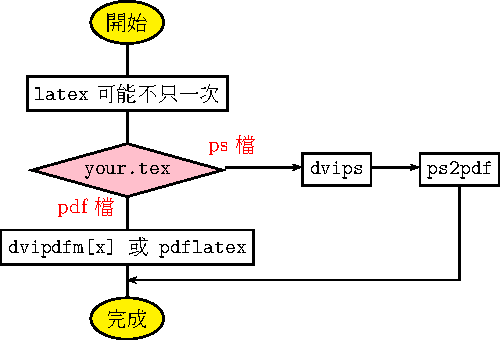
\includegraphics{latex-flow}
\end{center}

\section{\LaTeX\ ���S���M�βŸ�}
�b \TeX/\LaTeX\ ���@�ɡA��l��Z���O�¤�r�ɡA����@�ؽs�边���i�H���}�ӽs��B�[�ݡC�ӱƪ����O�q�`�O�Ѥϱ׽u�]\textbackslash, backslash�^\index{�ϱ׽u}\index{backslash}�Ҷ}�Y�Ӥ޾ɡC����\index{����}�h�O�Ѧʤ����]\texttt{\%}�^�Ӥ޾ɡC�Ҧp�A�H�s�边�s��U�C��r�G

\begin{quote}
\begin{verbatim}
This is my first \LaTeX\ typesetting example.
\end{verbatim}
\end{quote}

�sĶ��|�ܦ��H�U�����G�G

\begin{quote}
This is my first \LaTeX\ typesetting example.
\end{quote}

�䤤�� \verb|\LaTeX| �N�O \LaTeX\ ���@�ӫ��O�A�|��� \LaTeX\ �o�ӯS�����ϥܡC

�ѩ�A����a���y�t�A�q�`�r���B�Ÿ����̤j�e�q�u�� 256 �ӡ]$2^8$�^�A�]���A�\�h�{�����Ÿ��������ӷ���������O�A�~��ŦX�ƪ����h�ˤƻݨD�C�H�U���Ÿ��A��IJ \TeX/\LaTeX\ ���B�͡A�i�ೣ�o�ɮɯd�N�A���n���g�B�z�N�����g�i��Z���Y�h�F�C

�q�`�A�s�边���y�k�C��\index{�y�k�C��}�|���U�P�_�y�k�O�_���T�A�����O���৹���L�ʡA�����٬O�|�|���A�o�ɧO�ѤF�d�ݤ@�U {\tt *.log} �ɮסA�Ҧp�G�sĶ {\tt your.tex} �ɪ��ܡA�L�� log �ɴN�O {\tt your.log}�C

\begin{quote}
\begin{tabular}{llll}
�Ÿ� & �@�� & ��Z�W�ϥ� & \LaTeX\ �����N���O \\
\hline
\textbackslash & �U�ƪ��R�O & \verb|$\backslash$| & \verb|\textbackslash|\\
\%             & ����       & \verb|\%|           & NA \\
\#             & �w�q����   & \verb|\#|           & NA \\
\~{}           & ���ͤ@�Ӫť�   & \verb|\~{}|     & \verb|\textasciitilde| \\
\$             & �i�J�]���}�^�ƾǼҦ� & \verb|\$| & \verb|\textdollar| \\
\_{}           & �ƾǼҦ������ͤU�Цr & \verb|\_{}| & \verb|\textunderscore| \\
\^{}           & �ƾǼҦ������ͤW�Цr & \verb|\^{}| & \verb|\textasciicircum| \\
\{     & �ХܩR�O���@�νd��   & \verb|\{| & \verb|\textbraceleft|\\
\}     & �ХܩR�O���@�νd��   & \verb|\}| & \verb|\textbraceright|\\
\textless      & �ƾǼҦ������p��Ÿ� & \verb|$<$| & \verb|\textless| \\
\textgreater & �ƾǼҦ������j��Ÿ�   & \verb|$>$| & \verb|\textgreater| \\
\textbar     & OT1 �s�X�A�ƾǼҦ����~�ॿ�T��� & \verb+$|$+ & \verb|\textbar| \\
\&           & ���椤�����j�Ÿ�   & \verb|\&| & NA
\end{tabular}
\end{quote}

\section{\LaTeX\ �ƪ��W���@�dzW�d�κD��}
\label{sec:convention}\index{�W�d}\index{�D��}

���F�W���ҽͨ쪺�S���Ÿ��~�A�]���@�dzW�d�κD�ҭn���u�A���ǬO����w�ʪ��W�w�A���ǫh�u�O�D�ҡA�i�ण�P����a�B�y���|�����P���D�ҡA�Ȯɥ���L�����O \LaTeX\ ���C���W�h\index{�C���W�h}�N���F�C

\subsection{�r���������N�y}
\label{subsec:baseline}

�n�ͱƪ��W���W�d�B�D�ҫe�A�ڭ̱o���{�Ѥ@�U�r�����@�dzN�y�A�H�K����峹������ɦ��ӷ����C�q�`�ڭ̨C�Ӧr���O�m���@�Ӱ��Q����ؤ��A�٬� em-square\index{em-square}�A�P�@�Ӧr�����P�@���I�ơA�C�@�� em-square �j�p���O�ۦP���A��ڤW���r�]glyph\index{glyph}�^�n�m��b�o�� em-square �������m�A�o�O�r���]�p�̪��[�I�A�ҥH�A�P���I�ƪ����P�r���A�L���r���j�p���@�w�|�@�ˡA�]���ڭ̬O�ϥ� em-square ���j�p�b������A�ӫD��ڪ� glyph�C

�b�峹���ƦC���ɭԡA�h�O�N glyph �m��@�ӥH���Q�Ѧ��I�]reference point�^\index{���Q�Ѧ��I}\index{reference point}����Ǫ��@�Ӱ��Q�u�W�A�٬���u�]baseline\index{��u}\index{baseline}�^�A�j�g�r�����F Q �H�~�A�L�̪��������O�m���u�W���C���p�g�r���h���@�w��n�y���b��u�W�A���Ǧr�����e�i��W�X��u�H�U�A�Ҧp y�Bj ���r���C����r���b�峹�����m���m�A�ڭ̨Ӭݬݤ@�Ӽ����ϡG\footnote{��ڦr���]�p�W���U�����M���W���ε��c�A���M���|�O�o��²���A�o�̪������ϡA�u�O�Ȯ����r���@��m�񦳭Ӳʲ��������C}

% looks ugly, but l2h cannot handle this MP file be transparent png.
\begin{center}
\latexhtml{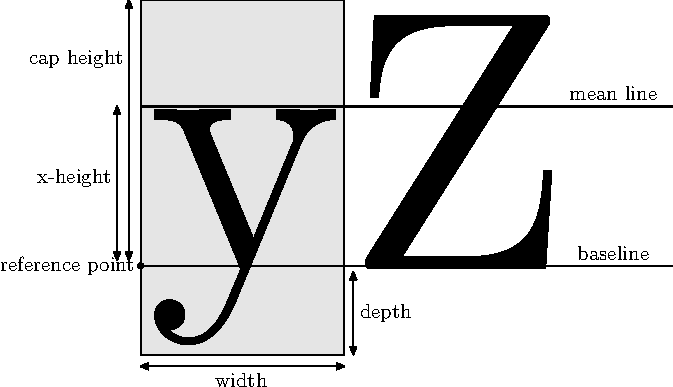
\includegraphics{baseline.1}}{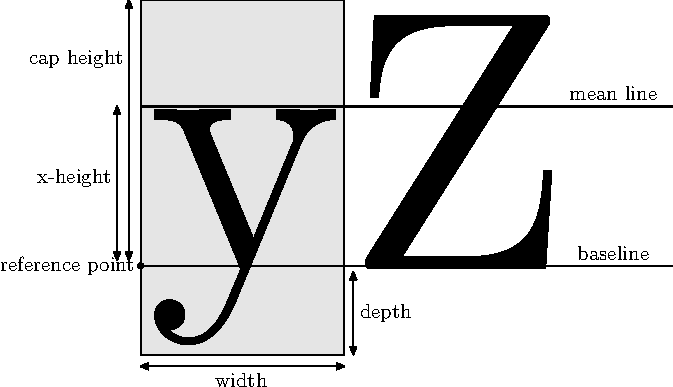
\includegraphics{baseline}}
\end{center}

�o�ӶW�X��u�H�U�����סA�ڭ̺٤����`�ס]depth\index{�`��}\index{depth}�^�A�H�W���N�٬��r���]height\index{�r��}\index{height}�^�A���M�j�p�g�����P�S�����j�g�r�����r���]cap height\index{cap height}�^�Τp�g�r�� x ���r���]x-height\index{x-height}�^�A�ѩ�o�ӨҤl�̬O�զX�r\index{�զX�r}�A�ҥH�C�Ӧr���e�ס]width\index{�e��}\index{width}�^���@�w�|�@�ˡA�����r���r�ڪ��h�O���e���r���C�r���[�W�`�סA�ڭ̴N�٤��� totalheight\index{totalheight}�A�j���������p�A�ȶȻ� height �ɬO���]�A depth ���A�ӥB�q�`�����O cap height�C

mean line\index{mean line} �b�@�����֥Ψ�A�q�`�O�r���]�p\index{�r���]�p}�ɤ~�|�Ψ�A�L�O���p�g�r���h���W����X�������ҳs�����@�Ӱ�ǽu�A�o�� mean line �� baseline ���Z���A�@��N�٬� x-height�A���M�N�O�p�g�r�� x �����סA�]���ڭ̷|���@�Ӫ��׳��A�٬� ex�A�����N�O�o�� x-height�C

����r���ܤ���S���A�L�O�H em-square �������I�Ӹm�� glyph ���A�b���^��V�X�ɡA����r�ä��O��n�y�����u�W���A�|�W�X��u�U�@�I�I�A�ܩ�|�W�X�h�֡A�h�M�r�����]�p�����A�C�ئr�������i��|���P�C�o�]�O���D�ƪ��W���@�P�ʡA�r���i�ೣ�ݭn�ɶq�ϥΦP�@�M���U�ئr������]�A�_�h�N�o�g�L�L�աA�~��Ͼ�Ӧr�����{�W���o��դ@�P�C

�o�DZM���N�y�A���ᴣ��@�ǫ��O���Ѽƪ��y�z�ɳ��|�ϥΨ�A�]�������x�@�U�A�Ҧp�G�r�������\index{�r������}�A��ڪ��N�O�H�Ѧ��I�]reference point�^���ǡA�u�����X���b�ߨӱ��઺�A�Ӥ@��һ�����Z\index{��Z}�A�����O�W�U�� baseline ���Z���C

\subsection{�@��ʪ��C���W�h}
\label{gen:gamerules}\index{�C���W�h}

\begin{enumerate}
\item \LaTeX\ �����O���O�j�p�g���O���A�� \verb|\| �}�Y�A�ᱵ�Ѧr���զ����r��γ�@���D�r���r���C�䤤�� \verb|[ ]| ���A���A�����O��ܩʰѼ�\index{��ܩʰѼ�}�A�i�H�ٲ��A�� \verb|{ }| �j�A���A�����O����ٲ����ѼơA���M�A\LaTeX\ �����O���@�w�|���ѼơA�����j�������|���ѼơA�u���L��L���ٲ��ϥιw�]�Ƚ}�F�C

\item \LaTeX\ ��Z���A�Ť@�ӭ^��ťթM�Ŧh�ӭ^��ťժ��@�άO�@�ˡA\LaTeX\ �|�{�@�@�ӭ^��ťաC

\item ���`�ڭ̽s��¤�r�ɡA���� \textsf{Enter} ��A�N�N������A����ڱƪ��X�ӡA�@�檺�e�׬O���ӱƪ��������]�w�A�]�N�O���A�A�b��Z���� \textsf{Enter}�A���N���ƪ���N�O�q�o���_��\index{�_��}�A\LaTeX\ �|�̤@���������e�׸g�L����p���۰ʸɦ��@����A���_��A�ӥB�|�b�����۰ʸɨ��@�ӪťաC�o�b�^��ܦ۵M�A�٬��r�]word�^���ť�\index{�r���ť�}�A������h���@�ˡA�b�s�边���s�褤��A�H�N�� \textsf{Enter} �����G�A�|�y���峹�������嶡�X�{�ťաC�o�|�b���夤�A�����ɾ��A���X�ѨM����k�C

\item �s�边���A�h���X�� \textsf{Enter} �N�h�ťX�X��A���b \LaTeX\ ��Z�̡A�h�Ӫťզ�\index{�ťզ�}�A�M�@�Ӫťզ�O�@�˪��@�ΡA\LaTeX\ �|��L�{�@�O�@�Ӫťզ�C�ӳo�Ӫťզ�A\LaTeX\ �P�ɤ]�|�{�@�O�s�q�����}�l�A�ҥH \LaTeX\ �O�H�ťզ�Ӥ��j�U�Ӭq���C

\item \LaTeX\ �w�]�C�ӳ��`���Ĥ@�Ӭq�����Ĥ@��O�����Y�]noindent\index{�����Y}\index{noindent}�^�A�q�ĤG�Ӭq���}�l�~�|���Y�]indent\index{���Y}\index{indent}�^�C���M�A�o�O�i�H��諸�A����|�A���ΡC

\item \LaTeX\ �����O�A�O�q�ϱ׽u\index{�ϱ׽u}��Ĥ@�Ӧr���}�l�A��Ĥ@�ӫD�r���Ÿ�����]�]�A�ťաB���I�Ÿ��μƦr�^�C�]���G

\begin{quote}
\begin{verbatim}
This is my first \LaTeX typesetting example.
\end{verbatim}
\end{quote}

�o�˪��ܡA��ڵ��G�A�]�� \verb|\LaTeX| �᪺�ťլO�ݩ���O���@�����A�ťձN���|�Q�����A�o�˷|�L���G

\begin{quote}
This is my first \LaTeX typesetting example.
\end{quote}

�o�ص��G�A\LaTeX\ �M typesetting �s�b�@�_�F�C�n�קK���ܡA�N�n���w���O���@�νd��A�Ҧp�H�U���j�A���C�δN�u���[�ӪťաA�Ҧp \verb|\ |�A\LaTeX\ �I�� \verb|\| �N�|�Φ����㪺���O�A��᪺�ťմN�|�Q�u���������ťդF�G

\begin{quote}
\begin{verbatim}
This is my first {\LaTeX} typesetting example.
This is my first \LaTeX{} typesetting example.
This is my first \LaTeX\ typesetting example.
\end{verbatim}
\end{quote}

�ҥH�A���`�L�X�����ӬO�G

\begin{quote}
This is my first \LaTeX\ typesetting example.
\end{quote}

\item ���ѲŸ��]{\tt \%}�^\index{���ѲŸ�}\index{%@\verb=%=}�A�i�H��b�@�檺����a��A{\tt \%} �᪺��r�|�Q \LaTeX\ �����C�ҥH�A�p�G�O��b�@�檺�̧��ݡA���� \LaTeX\ �|�۰ʴ��J���r���ťդ]�N�|�Q�����C�Ҧp�G

\begin{quote}
\begin{verbatim}
This is my fisrt \LaTeX\ document. Give \LaTeX\ a%
try.
\end{verbatim}
\end{quote}

�o�ˤ@�ӡA�ƪ��X�ӷ|�ܦ��G

\begin{quote}
This is my fisrt \LaTeX\ document. Give \LaTeX\ a%
try.
\end{quote}

a �M try �s�b�@�_�F�I���`���ӬO�G

\begin{quote}
This is my fisrt \LaTeX\ document. Give \LaTeX\ a try.
\end{quote}

���o�ӯS�ʡA�ڭ̥i�H���Φb����A�]�N�O���b�s�边\index{�s�边}���A����峹�� \textsf{Enter} �䴫��ɡA���ݥ[�� {\tt \%}�A�o�ˤ@�� \LaTeX\ �N���|���J�^��r���ťաA����r�N�i�H�s�������S���ťժ��@���F�A�_�h \LaTeX\ �b��g��Z�_�y\index{�_�y}�ɡA�|�۰ʦb�촫��B��J�@�ӭ^��ťաA�]���A��l�� \TeX/\LaTeX\ �O�{���o���媺�C

\item ���^��V�X���ɭԡA�q�`�A�^��r�e�᳣�|�d�ӪťաA�H�K�M����Ϲj�}�ӡA�u�O�o�Ӫťխn�h�j�A�o�N�S���T�w���D�ҡA�q�`�d�ӭ^��ťդ]�O�i�H�A�n���s���ܡA���ͨ줤��ƪ�����ij�D�ɦA�ӰQ�סA�ثe�N�i���ߺD�A�^���r�e��d�ӭ^��ťաC
\end{enumerate}


\subsection{�w����I�Ÿ����C���W�h}

\begin{enumerate}
\item ���^�媺�޸�\index{�޸�}���@�ˡA�o�̽ЯS�O�`�N�A�\�h�H�`�`�d���C���B�^��޸����޳������n�����k�C�^�媺�ܡA���䪺�޸��O grave accent�A�O��L���W�� {\sf Esc} �� {\sf F1} �U�観�i�θ������@����F�k�䪺�O apostrophe\index{apostrophe}�A�]�N�O��L���� {\sf Enter} ��j����������C���޸������άO��J�⦸������޸�\index{����޸�}�Ψ⦸���k��޸�\index{�k��޸�}�A�Ӥ��O�� \verb|"| �o�Ӥ@����������I�� ditto marks\index{ditto marks}�C�ҥH�A��ڤW�b��J��Z�ɬO�G

\begin{quote}
\begin{verbatim}
Please press an `Esc' key.
Please press an 'Esc' key. �o�O���~�ܽd�I
``This sentence.''
"This sentence." �o�O���~�ܽd�I
\end{verbatim}
\end{quote}

�ƪ��X�Ӫ����άO�G

%begin{latexonly}
\begin{quote}
Please press an `Esc' key.\\
Please press an 'Esc' key. �o�O���~�ܽd�I\\
``This sentence.''\\
"This sentence." �o�O���~�ܽd�I
\end{quote}
%end{latexonly}

\begin{htmlonly}
\begin{quote}

\includegraphics{quotation}
\end{quote}
\end{htmlonly}


���媺�ܡA�ڭ̬O�ϥΤ�����Ϊ��u�B�v�Ρy�B�z�A�b����j���h�w��ΩM�^��ۦP�Ϊ������βŸ��A���o�b���媽�Ʈɷ|�X���D�A�]���A���媺��B���޸��٬O�o�����ڭ̥ثe�ϥΪ��C

\item \LaTeX\ �|�b�^��峹���@�ӥy�l�����M�t�@�ӥy�l�}�l�������A�۰ʽվ㦨���j�@�I���ťաA�o�i�H�W�[�峹����Ū�ʡC�ҿפ@�ӥy�l�����A�Ҧp�G�y�I�].�^�B�ݸ��]?�^�B��ĸ��]!�^�Ϋ_���]:�^�A�o���M�O���^�媺�b�μ��I�Ÿ��A���O���媺���μ��I�Ÿ��C�A�i�H�`�N�@�U�W�����|���Ҥl�A�b document.\ �M Give �������ťշ|�y�L�j���L�^���r�����ťաC

�{�b�����D�O�A�p�G�o�Ǽ��I�Ÿ��᭱���O�t�@�ӥy�l���}�l���ɭԡA\LaTeX\ �L�k�h�P�_�o�ر��ΡA�o�ɱo�ѧڭ̦ۤv�ۦ�P�_�B�B�z�F�C�Ҧp�^���Y�g�r�G

\begin{quote}
\begin{verbatim}
I am Mr. Edward G.J. Lee, G.J. is a abbreviation of my name.
I am Mr.~Edward G.J. Lee, G.J. is a abbreviation of my name.
I am Mr.\ Edward G.J. Lee, G.J. is a abbreviation of my name.
\end{verbatim}
\end{quote}

�䤤 \verb|Mr.\ Edward| ���g�k�A�M \verb|Mr.~Edward| �X�G�O�@�˪��A���O�j�����J�@�Ӥ���p�����`��r���ť�\index{��r���ť�}�A�t�O�b���̤]�t�~���ܤ��i�H�q�o�̴���A�q�`�Φb�H�W���ɭԡA���L�̤��P���_�A�@��b�H�W���ƪ��A�]�A�L���Y�ΡB¾�١A�O�����_�����Ӥ��}���C�ӥB��Ӥ�y�������ܡA�H��̸�����A�~���|�]���_��Q������b�A�o�� {\tt ~} �Ÿ��]�]���b \TeX\ ���M���W���A�N�٬� tie\index{tie}�A��L�̸j�����N��C�ƪ��X�Ӫ��ɭԷ|�ܦ��G

%begin{latexonly}
\begin{quote}
I am Mr. Edward G.J. Lee, G.J. is an abbreviation of my name.\\
I am Mr.\ Edward G.J. Lee, G.J. is an abbreviation of my name.
\end{quote}
%end{latexonly}

\begin{htmlonly}
\begin{quote}
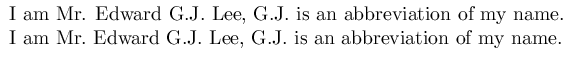
\includegraphics{abbreviation}
\end{quote}
\end{htmlonly}

�Щ�j�h�J�Ӥ���@�U���G�N���D�F�C�ĤG�檺�~�O���T���AMr.\ �M Edward �������ťլO���`��r���ťաA��Ĥ@�檺�y�l�����ťխn�p�@�I�I�C��L���ϥΨ��Y�g�r�����X�A�Ҧp�G`Dr.'�B`etc.'�B`e.g.'�B`i.e.'�B`vs.'�B`Fig.'�B`cf.'�B`Mrs.'�A�o�dz����O�N���y�l�����A�ҥH�A�n���J�@�ӥ��`�ťաC

�� G.J. �᭱������S�����J���`�ťաH���O�]���AJ �O�j�g���A�o�� \LaTeX\ ���|�h�~�{���O�y�l�����A�q�`�y�l�����ɪ��y�I�e�����Ӧr���O�p�g���CWell�A���S��ı�o���I�D�z�H:-)

�����A�Ʊ��٨S�������IKnuth �б¥X�F�@�D���D�A�p�G�y�l�������O `Please see Appendix A.' �᭱�S�ٱ����t�@�ӥy�l�C�o�ɫ���H�ѩ�A���|�{���O�y�l�����A�]���|���J���`�ťաA���o���O�y�l�����r�I�мȮɥ��O�o�A�ϥ� \verb|...Appendix A\null.|�A�� \verb|...Appendix A\@.|�C�o�ӻ��Ӧ��I�ܪ��A�����|�A�ӱ��Q�A�аO�o `\verb|\null|' �M�y�I���O�S���ťժ��C�Ҧp�G

\begin{quote}
\begin{verbatim}
Please see Appendix A. We will be there soon.
Please see Appendix A\null. We will be there soon.
\end{verbatim}
\end{quote}

�ƪ��X�Ӫ����G�N�|�O�]�t��������A�Фp�ߤ���^�G

%begin{latexonly}
\begin{quote}
Please see Appendix A. We will be there soon.\\
Please see Appendix A\null. We will be there soon.
\end{quote}
%end{latexonly}

\begin{htmlonly}
\begin{quote}
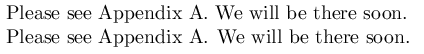
\includegraphics{abbreviation2}
\end{quote}
\end{htmlonly}

�p�G�A�A�{�b�\Ū���O HTML\index{HTML} �榡���A���ǨҤl�p�G�L�k������ܥX�ӡA�Ч�\�� PDF �����C�ӥB�A�p�G�A�s�@ PDF �榡�ɡA�r���S�����O�]���媺�^�Ʀr�O�O�J Computer Modern Type1 �r���^�A�t���i��N�|�󤣩���C�i�յۨϥ� {\sf gv/gsview}\index{gv@\textsf{gs}}\index{gview@\textsf{gview}} �h�\���A�M��վ㦨 Landscape\index{Landscape}�A��y�l�����Ԩ���t���a��h�N�ݱo�X�ӤF�C�o�b�y�l�h���ɭԡA�o�Ӫťդ]�ëD�T�w�j�p���A\LaTeX\ �|���峹���c���ݭn���ӷL���վ�C

\item �R�`��\index{�R�`��}����^�]�O���P�A�^��O�T�I�A�p�G�I��y�I���ܡA�h�O�|�I�C���媺�ܬO���I�A�I�줤��y�I�ܮe���N���o�M���C���O�^��o�ӤT�I�A���O�N���ӤT�ӥy�I�F�ơA�o�˪��I�ӱK���A�i�H�ϥ� \verb|\ldots| �� \verb|\dots| ���O�A�Ҧp�G

\begin{quote}
\begin{verbatim}
I'm not a good man ..., but a good husband .... ���~�ܽd�I
I'm not a good \ldots\ man \ldots, but a good husband \ldots.
I'm not a good \dots\ man \dots, but a good husband \dots.
\end{verbatim}
\end{quote}

�ƪ��X���ӵ��G�O�G

%begin{latexonly}
\begin{quote}
I'm not a good ... man ..., but a good husband .... ���~�ܽd�I\\
I'm not a good \ldots\ man \ldots, but a good husband \ldots.\\
I'm not a good \dots\ man \dots, but a good husband \ldots.
\end{quote}
%end{latexonly}

\begin{htmlonly}
\begin{quote}

\includegraphics{dots}
\end{quote}
\end{htmlonly}

���媺�R�`���O�Ѩ�ӥ��Ϊ��T�I�Ҳզ����I���A�Y�G\chdots{}�A�N�O�ڭ� Big-5 �X�� {\tt 0xa14b}�]{\tt U+2026}�^�A���ѩ� Unicode\index{Unicode} �|���@�� MIDLINE HORIZONTAL ELLIPSIS({\tt U+22EF})�A�]���A���dzn��b��Ū�W���i��|���@�ˡA�]���ڭ̪��r���A�j�����b�s�@���I�Ÿ��ɬO�m�b�������a��A��������j���O�m��b��u���a��A�� Unicode �x��ĥΪ��˥��r���A��n�O����j�����t�өҴ��ѡA�o�ˤ@�Ӧ��dzn��u�@�̴N�{���ڭ̪��R�`�����ӬO {\tt U+22EF} �F�A�ܤ������A�ڭ̪� Big-5\index{Big-5} �X�èS���۹������r�X�C

\item �}�鸹\index{�}�鸹}�C�b�^��A�۷���}�鸹���i�঳�T�ءG
  \begin{itemize}
    \item hyphen\index{hyphen}\\
�o�O�̵u�� dash\index{dash}�A�q�`�N�O��J \verb|-| �N��F�A�Ҧp \verb|father-in-low|�A�o�˷|���{�� fater-in-low�C
    \item en-dash\index{en-dash}\\
�o�O�̱`�Ϊ��}�鸹�A�O��J��� hyphen�C�Ҧp \verb|1991--2003 �~|�A�o�|���{�� 1991--2003 �~�C
    \item em-dash\index{em-dash}\\
�o�O�̪��� dash�A�ѤT�ӳs�� hyphen �զ��A���ӬO�̬۪��ڭ̤���һ����}�鸹�C�Ҧp \verb|I am---a good man.| �|���{�� I am---a good man.�C�ܩ�o�ӤT�ӳs�� hyphen �e��O�_�n�d�ťաA�����H�ϥΡA�èS���w�ʪ��D�ҡA�����F�M���媺�}�鸹�t�X�]����}�鸹�e��A�q�`���d�ťա^�A�ӤH�q�`�O���d�ťժ��C
    \item �u�����\\
�o�������O�}�鸹�A�ӬO��ڪ���έt���A�o�n�i�J�ƾǼҦ��A�Ҧp�G�t���A�n�g�� \verb|$-5$|�A�M����{�X�ӬO $-5$�C�o�]�`�`�|���H�d���A���ઽ����J�@�몺�t��������ӥR�ơA�o�O�]�� \TeX/\LaTeX\ ���ƾǦ��l���Φr�M���j�B�z�A�M�@�뤺�夣�P�����Y�C
    \item ���媺�}�鸹\\
���媺�}�鸹�O����Ӥ���r��m�����@��u�A���שM�R�`���ۦP�C�b���u��m���A�w�q�W�O����ءAen-dash �O {\tt Big-5 0xa156}�Aem-dash �O {\tt Big-5 0xa158}�C���ѩ󤤤�r���Z�����D�A���i�ॴ�X�Ӫ��}�鸹�����|���@�I�ť�\footnote{�o�O�i�H�վ㪺�A�]�N�O�h����Ӿ�u�������r���Z�A�o�˴N���|���ͤp�ťդF�A����R�`���]���P�˪����ΡA�ڭ̷|�b�L�ժ������A�ӰQ�סC}�A�Ҧp�X�X���媺 em-dash�A�o�O�V�V���媺 en-dash�C�b�פ夤�A�}�鸹�q�`�i�H�ϥΤp�A���Ϋ_���N���C
    \item ���媺�p�W���ήѦW��\\
���媺�p�W��\index{�p�W��}�A�i�H�Щ��H�W�B�a�W�A�p\underline{�]�h�P}�F�ѦW��\index{�ѦW��}�]�p�W�������u�����i���Ϊ��^�A�i�H�Φb�ѦW�A�o�DzŸ��`�y���ƪ��W���x�Z�A�`�ϥ� �m �n�Ө��N�ѦW���A�p�W���h�L��L���N��k�C�b�@�몺�۵M�����ά�ǽפ�W�q�`���ϥγo���¦����p�W���ήѦW���C
\end{itemize}

\item ���Y�I\index{���Y�I}\\
�o�i�O�ƪ������n�\��C�^�媺�q�`�S�����D�A\LaTeX\ �|�۰��׶}�B�z�A����N���@�w�F�A\LaTeX\ �i���{�Ѥ���A���q�`��������{���ήM��A�h�h�ֳ֤��|�B�z�A�u���L�A���ɭ԰����i��|�~�P�C����A�쩳����O���Y�I�H���U�C�Ӫ��A�j�a�N���դF�A�ڦC���媺�A�^�媺�N���C�X�ӤF�A�]�� \LaTeX\ �|�۰ʳB�z�A�����ڭ̾�ߡC

\begin{quote}
\begin{tabular}{ll}
���I�Ÿ� & �m��B\\
\hline
�A�C�F�B:�v�^�n�I�H & ����m��歺\\
�u�]�m              & ����m����\\
�}�鸹�ΧR�`��      & �m�󭺧��ҥi\\
\end{tabular}
\end{quote}

²�檺���A���F�}�鸹�ΧR�`���A�S���}�f���A����m��̶}�Y�A�}�f�V�k���A����m��̥k�A�}�f�V�����A����m��̥��C�q�`���|�B�z�n�A���սZ���ɭԭn�`�N�@�U�~�P���a��C
\end{enumerate}

\section{\LaTeX\ ����Z���c}
\label{sec:struct}\index{��Z���c}

\subsection{���ҡ]environment�^\index{����}\index{environment}}

�W�@�`�ҽͪ����O���O�A���M�]�i�H�Ѥj�A��\index{�j�A��}�өw�@�νd��A���p�G�O�@��q�A�ƦܬO�@��g�峹���n�@�ήɡA�����O�i��N���ܾA�X�F�A�]���A\LaTeX\ �]���@�إ������c�A�٬����ҡ]environment�^�A�D�n�O���@�νd����X�j�ܸ��j���d��C

�Ҧ������ҡA���O�_�� \verb|\begin{���ҦW��}|�A��� \verb|\end{���ҦW��}|�A�o��ӫ��O��������Z���|�Q�@�ΡA�ӥB�A���Ҥ����٥i�H�M�Ψ�L���P�����ҡC

\LaTeX\ ��Z������A���N�O�]�b�@�� \verb|\begin{document}| �M \verb|\end{document}| �o�� document ���ҷ����C

\subsection{��²�檺 \LaTeX\ ����Z���c}

�H�U�N�O�Ҧ� \LaTeX\ ���ݨ�ƪ���Z�j���c�G

\begin{quote}
\begin{verbatim}
\documentclass{article}

  �o�̬O preamble ��

\begin{document}

  �o�̬O�����

\end{document}
\end{verbatim}
\end{quote}

\verb|\documentclass{article}|�A�o�O�b�i�D \LaTeX\ �ϥέ��@�����O�A�ڭ̥ثe�ϥΪ��O {\tt article} ���O\index{���O}\index{article}�A�������O�|�b�� \ref{ch:class} ���Q�סCpreamble\index{preamble} �ϡA�h�O�U�@�Ƿ|�v�T��Ӥ�Z�����O�A�ΤޥΥ����M�󪺦a��A���M�A�������ޥΥ����A�]���ϥμv�T���媺���O���ܡApreamble �ϴN�O�ťաA���g����F��C����ϡA�N�O�ڭ̹�ڤW�g�峹���a��C

�{�b�]�i�H��e�����|���Ҥl�A��J����ϸ��Y�Apreamble �ϪťըS���Y�A�M��s�ɡA�յ۽sĶ�ݬݡG

\begin{quote}
\begin{verbatim}
latex example.tex
dvips example.dvi      => ���� ps �榡 example.ps
dvipdfm[x] example.dvi => ���� pdf �榡
pdflatex example.tex   => ������ .tex ���� .pdf
\end{verbatim}
\end{quote}

�u������Ҹѻ��A�|�b�U�@���Ӷi��A�ҥH�A�o�̼Ȯɤ��|���Ц��������ҥi�H�ϥΡA�����ݬݨS�����Y�C�ѩ��٨S�ͨ줤�媺���D�A�]���p�G�A�Q�ոլݡA���Ȯɥ��ϥέ^��A�D�z���O�۳q���C

\subsection{preamble �ϥi�H��Ǥ���H}
\label{subsec:preamble}

�o�̥i�H�ޥΥ����A�ӥB�|�v�T��g��Z�����O�A�Ҧp�@�Ǩƥ��w�q�n�����O�A�Q�b��g��Z���ϥΡA�N�i�H�m��b preamble �ϡC

\subsubsection{�������ޥ�}
\label{subsubsec:package}

����D�n�O�з� \LaTeX�A���e���w����A�|���ǥ����M�󤣱o���n�ޥΡA���U�N�ӻ����p��ޥήM��C�o�ǮM�󳣬O�@�� \TeX\ �t�γ��|���W���C

���O�����ҭn�p��}�Y�����йL�F�A�{�b�ӬݬݤޥΥ����n���}�Y�C

\begin{quote}
\begin{verbatim}
\documentclass{article}
\usepackage{color}
\begin{document}
\textcolor{blue}{This is blue color.}
\end{document}
\end{verbatim}
\end{quote}

�sĶ�@�U�A�ݬݵ��G�O����H�o�̨ϥΪ��N�O \textsf{color} package\index{color@\textsf{color}}�A���Y�O�� \TeX/\LaTeX\ macro �Ҽg���@�ӥ����M��C�@��²�檺�ڭ̴N�٬������]macro�^\index{����}\index{macro}�A�����@�I���N�٬������M��]package�^\index{�����M��}\index{package}�A���A���Y���O�@�˪��A�u���L�j�p�Φ��S����z���@�Өt�Ϊ��t�O�C

\LaTeX\ ���Y������{�����M��i�H�ϥΡA�C�Ӵ��G�� \TeX\ �t�ΩҦ������i�ೣ�|���Ҥ��P�C�j���S���H�i�H��q�Ҧ��{�s�� \LaTeX\ �����M��A�]����b�O�Ӧh�F�A���L�A����j�����|����`�Ϊ������M��C�ԲӪ������M�󪺺غءA�|�b�� \ref{ch:package} ���ӻ����C

\subsubsection{�v�T��g��Z�����O}

�|�v�T��g��Z�����O�A�q�`�]�O��b preamble �ϡA�Ҧp�G

\begin{quote}
\begin{verbatim}
\linespread{1.36}
\parindent=0pt
\end{verbatim}
\end{quote}

\verb|\linespread| �O�b����W�U�檺��Z�A�o�̴N�O�N��Z�ܦ���Ӫ� 1.36 ���C�ܩ󤰻�O��Z�O�H�N�O�o�@�檺��u�]baseline�^��U�@�檺��u���Z���A�q�`�^��峹�����h�վ�L����Z�A������o�A���[�j��Z�H�Q�\Ū�C

\verb|\parindent| �O�վ�q�����Y���{�סA�o�̽վ㦨 0�A�]�N�O���U�q���������Y���N��A�]�i�H�վ㦨��L���ȡA\LaTeX\ �N�|�̳o�ӭȥh���Y�C���M�A���h�]�w���ܡA\LaTeX\ �N�|�̥L���w�]�ȥh���Y�C


\subsection{���`���c\index{���`���c}}
\label{subsec:chapstruc}

����Ϸ��M�O�ڭ̼g�峹���D�n�a��A�Τ@�ǷL��\index{�L��}�C�b \LaTeX\ ����Z���Y�A���`���D���Φ����O�ѦP�˪����O�ӱ���A�o�˦��@�Ӧn�B�A�{�ɴ��J���`���D�Ψ䤺��ɡA�ڭ̤����h�z�|���D�s���Υؿ������D�A�]�����h�z�|�n�Τ���r���B�Φr���j�p�n�h�j�A\LaTeX\ �|�۰ʭp��B�z�A�r���j�p�]�|�M����ϥΪ��r���j�p���۰t�X�վ�A�ϥΪ̴N�M�ߦb����c��B�g�@�Y�i�C�H�U�ѦC�����A�Ѿ�ӳ��`���c�G

\begin{quote}
\begin{tabular}{lll}
�`�׼и� & ���O & �@�ΤΪ`�N�ƶ�\\
\hline
$-1$ & \verb|\part{}|          & �o�O�̤j�����c�A�ڭ̤���q�`�٬��u���v�C \\
0    & \verb|\chapter{}|       & ���C�b article ���O���Y�S�����C\\
1    & \verb|\section{}|       & �`�C\\
2    & \verb|\subsection{}|    & �p�`�C\\
3    & \verb|\subsubsection{}| & ���p�`�C\\
4    & \verb|\paragraph{}|     & �q���C\\
5    & \verb|\subparagraph{}|  & �p�q���C\\
\end{tabular}
\end{quote}

���`���D\index{���`���D}�����e�N�O�����g�J���O���j�A�����Y�N�i�H�F�A\LaTeX\ �b�ƪ��ɷ|�۰ʨϥβ���B�[�J���`�s��\index{���`�s��}�ίǤJ�ؿ�\index{�ؿ�}���Y�C

�ܩ�Ĥ@�檺�`�׼и��]secnumdepth�^\index{�`�׼и�}\index{secnumdepth}�A{\tt book/report}\index{book@\texttt{book}}\index{report@\texttt{report}} ���O���`�׼и��O 2�A{\tt article} ���O 3�C�o�O����N��O�H�N�O�� {\tt book/report} ���O����Z�A�b \verb|\subsection{}| �H��]{\tt subsection} �������|�s���^�A���`�N���A�s���F�F�P�˪��A�b {\tt article} ���O����Z�A�b \verb|\subsubsection{}| �H��N���s���F�C�����M�|�W�ߥX�@��W��Ӫ��ܳo�ӬO���D�C���s���F�����`���e�A���M�]�N���ǤJ�ؿ����Y�F�C�o���M�O�i�H��諸�A�u�n��� \LaTeX\ �� {\tt secnumdepth} �o���ܼƪ��ȴN�i�H�F�A�o�ө���|���Φp���� \LaTeX\ ���w�]�ȡC���o�g�峹�A�b preamble �ϴN���@�ӳ]�w�G

\begin{quote}
\begin{verbatim}
% let the depth of report to subsubsection
\setcounter{secnumdepth}{3}
\end{verbatim}
\end{quote}

�ҥH�A�o�g�峹���M�ϥΪ��O {\tt report} ���O�A���O���`���`�׼и��O�Цb 3�A�]�N�O���|�s���� {\tt subsubsection} ����A���o���M�O�S���s�J�ؿ������C 

�U�@���N���ڭ̶}�l��ڰʤ�a�I��\chdots{}�A����{�b���S�����㤶�Ы��O�O�H���ګ��|���D��������O�i�H�ϥΡH�o�O�]�� \LaTeX\ �����O�ܦh�A�������Ъ��ܡA�@�譱�O�����A�G�譱�]���e���A�ѥL����ڧ@�ΡA�ҥH�A�ڭ̱N�|�b�U���|�Үɬﴡ�b���Y�����A���o����󱵪���n�ɡA�A�Ӿ�z�ӫ��O�t�d���A�o�˥H��d���O�N�ܤ�K�F�A�����h���O�A�u�n���D���ӳo�˥\�઺���O�N���F�C


% ``�j�a�Ӿ� LaTeX'' LaTeX ��Z start.tex
% Copyright (c) 2004  Edward G.J. Lee <edt1023@info.sayya.org>
%
% �b���H�� GNU Free Documentation License 1.2 �ΥH�᪺�����W�d���U�A
% ���\�����B���G�έק�C���쪩�v�B���v�n�����o�����C
%
% �����G�����A�t�� fdl.tex�A���e�� GNU FDL ���W�d���C�p�G�򥢡A�i��
% http://www.gnu.org ���o�A�μg�H�ܦۥѳn�����|(Free Software Fundation)
% �����C
% 9 Temple Place - Suite 330, Boston, MA 02111-1307, USA.
%
% $Id: start.tex,v 1.38 2004/03/07 12:29:47 edt1023 Exp $
%
\chapter{��ڤW�ƪ����ݬ�}
\label{ch:start}

�n�F�A�{�b�����Ӫ��ݬݧa�I�����D�n�O²�檺��һ����A���i�J���p�A�ͨ�L�C������Τ񰪽���צ��Φh�F�C

���ӭӡu�̰����ɭ�h�v�G\textcolor{red}{\bf �Ƿ|����Ŷ��A�A�N�Ƿ|�ƪ��F}�I��DZƪ����B�͡A�����|��ҾǨ쪺�F��h�Q�k�l�G���A�Ҧ����Ŷ��]�N�O�@�ӭ����^�A����ڤW�A�A�n�վ㪺�A���O�U�ӳ������Ŷ��t�m�A��H�@�I���A�]�N�O�@��ӭ��������A�S����r�B�Ϫ��������~�O�ƪ��u�������I�C�A��ťť�N�n�A�L�@�q�ɶ������x��A�A�Ӧ^�Y��ҳo�ӡu���ˡv�Ŷ�����h�C:-)

�ѩ󥻤妳 HTML �����A���F�ഫ�W���y�����u�A��Ҫ������A��Z�W�u�g�{���X�A���G���������O�sĶ�n�� PDF �榡�ɮסA�m�������W�A�i�u�W�\���ΤU���A²�檺�Ҥl�h���t�s�@�W�ߪ� PDF �ɡA�аѾ\���媺 PDF �榡�ɮפ��e�C

\section{²�檺���}

�o�̴N��e�@���ҽͨ쪺�@�Ǥ��e��z���@�Ӥ�Z�A���ӸոլݡA�o�̥��ϥ� {\tt report}\index{report@\texttt{report}} ���O��Z�A�]�� {\tt article}\index{article@\texttt{article}} ���O��Z�O�S�� {\tt chapter} ���G

\begin{quote}
\begin{verbatim}
% example1.tex
\documentclass{report}
\begin{document}
This is my first {\LaTeX} typesetting example.\\
This is my first \LaTeX{} typesetting example.\\
This is my first \LaTeX\ typesetting example.\\
I am Mr. Edward G.J. Lee, G.J. is a abbreviation of my name.\\
I am Mr.\ Edward G.J. Lee, G.J. is a abbreviation of my name.\\
Please see Appendix A. We will be there soon.\\
Please see Appendix A\null. We will be there soon.
\end{document}
\end{verbatim}
\end{quote}

�ϥνs�边�s��A�M��s�ɦ� {\tt exmaple1.tex}�A�o�˴N�i�H�sĶ�F�G

\begin{quote}
\begin{verbatim}
latex example1.tex       => ���� example1.dvi
dvips -Ppdf example1.dvi => ���� example1.ps
ps2pdf example1.ps       => ���� example1.pdf ��
dvipdfm[x] example1.dvi  => �� example1.dvi �������� example1.pdf ��
pdflatex example1.tex    => �� example1.tex �������� example1.pdf
\end{verbatim}
\end{quote}

�sĶ�n�� PDF �ɥi�b���U���ξ\���G

\begin{quote}
\url{http://edt1023.sayya.org/tex/latex123/example1.tex}\\
\url{http://edt1023.sayya.org/tex/latex123/example1.pdf}
\end{quote}

\subsection{���󴫦�}
�C��̫�[�F�� \verb|\\|\index{\\@\verb=\\=}�A�o���ܱj�����檺�N��A�_�h \LaTeX\ �|�̪����w�]���e�רӴ���A�N���|�O�@�ӥy�l�@��F�A�j�a�i�H��o�� \verb|\\| �����A�A�ӽsĶ�լݬݵ��G�A�N�|���D���@�^�ƤF�C�]�i�H�ϥ� \verb|\newline|\index{newline@\verb=\newline=} �o�ӫ��O�A���M�A�ڭ̳��|�o������θ��u�����O�C�ӥB \verb|\\| �i�H�����ɪ����j�A�o�b \verb|\newline| �h����C�Ҧp�G

\begin{quote}
\begin{verbatim}
Please see Appendix A. We will be there soon.\\[1cm]
Please see Appendix A\null. We will be there soon.
\end{verbatim}
\end{quote}

�o�˪��ܡA��椧������Z\index{��Z}�N�O��Ӫ���Z�A�[�W {\tt 1cm}�C�ƦܡA�]�i�H�O�t�ƪ��ѼơA�o�˦�Z�N�|�ܦ���Ӫ���Z��h {\tt 1cm}�A���M�A�p�G�]�L�Y�F���ܡA���i��|���|�b�@�_�C�J�M�A�o�̨ϥΪ��O��A���A���ܳo�ǰѼƬO�i�H�ٲ����C

�t�~�A\verb|\linebreak[n]|\index{linebreak@\verb+\linebreak+} �]�i�H�j������\index{�j������}�A{\tt n} �N���� 1--4 ����ij�ȡA�ƭȷU�j���ܷU�O�j�P��ij�A���]�w���ܡA�N�O���Τ�����ؿ�ܡA�S�������a�a�C�M�e���һ������P�B�O�A�o�ش���|���Ө��@��y�l�����ץ������������W��e�����סC�Ҧp�G

\begin{quote}
\begin{verbatim}
Please see Appendix A. We will be there soon.\linebreak
Please see Appendix A\null. We will be there soon.
\end{verbatim}
\end{quote}

�ƪ���|���{���G

%begin{latexonly}
\begin{quote}
Please see Appendix A. We will be there soon.\linebreak
Please see Appendix A\null. We will be there soon.
\end{quote}
%end{latexonly}

\begin{htmlonly}
\begin{quote}
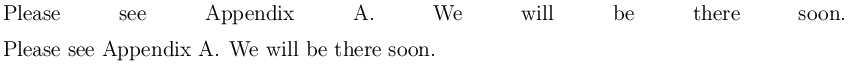
\includegraphics{linebreak}
\end{quote}
\end{htmlonly}

\subsection{�����Y��\index{�Y��}}

�Ĥ@���Y�ƤF�I�o�O�]���ڭ̧����S�������`�A�ҥH�A\LaTeX\ �N��o�Ǥ��e�����O�ި��������A�� \LaTeX\ ���w�ơA�ި��}�Y�O�|�Y�ƪ��C�n�ѨM�o�Ӱ��D�A�i����ؤ�k�G

\begin{enumerate}
\item �b�Ĥ@�椧�e�[�J \verb|\noindent|\index{noindent@\verb+\noindent+} �ӫ��� \LaTeX\ ���n�h�Y�ơC���O�o�u�@�Φb�U���O���a��A��L���Y�ƪ��a���٬O�|�Y�ơC
\item �b preamble �ϥ[�J \verb|\parindent=0pt|\index{parindent@\verb+\parindent+}�A�o���������媺�Y�Ƭ� {\tt 0pt}�A���M�A�o�N���ܥ��峣���n�Y�ƤF�C
\end{enumerate}

\section{�[�J���`���D\index{���`���D}}

�b \LaTeX\ ���Y�A�n�[�J���`���D��b�O�Ӯe���F�A�]�����h�ަr�骺�j�p�θm�񪺦�m�A�ɺޥ[�W�h�N��F�I\LaTeX\ �|���ڭ̦w�Ƥ@���C�ڭ̳o�̤��M�H {\tt report} ���O�ӻ����A�]�� {\tt article} ���O���Y�A�S�����A�u��A�Ω��²�檺�u��C

\begin{quote}
\begin{verbatim}
% example2.tex
\documentclass{report}
\begin{document}
This is the first experience of \LaTeX.
\chapter{Aesop Fables}
\section{The Ant and the Dove}

An ant went to the bank of a river to quench its thirst, and
being carried away by the rush of the stream, was on the
point of drowning.

A Dove sitting on a tree overhanging the water plucked a
leaf and let it fall into the stream close to her. The Ant
climbed onto it and floated in safety to the bank.

\section{The Dog in the Manger}

A dog lay in a manger, and by his growling and snapping
prevented the oxen from eating the hay which had been
placed for them.

``What a selfish Dog!'' said one of them to his companions;
``he cannot eat the hay himself, and yet refuses to allow
those to eat who can.''

\chapter{The Eagle and the Arrow}

An eagle sat on a lofty rock, watching the movements of a
Hare whom he sought to make his prey.

An archer, who saw the Eagle from a place of concealment,
took an accurate aim and wounded him mortally.
\end{document}
\end{verbatim}
\end{quote}

�sĶ�X�Ӫ����G�G

\begin{quote}
\url{http://edt1023.sayya.org/tex/latex123/example2.tex}\\
\url{http://edt1023.sayya.org/tex/latex123/example2.pdf}
\end{quote}

�Ъ`�N�L����ɭԷ|�Y�ơA����ɭԷ|�����C{\tt report} ���O�A�s���@���|�����A�p�G�Q�`�٤@�I�Ŷ��A�i�H���� {\tt article} ���O�A\verb|\chapter{}| ��� \verb|\section{}|�A��� \verb|\section{}| �N��� \verb|\subsection{}|�A�o�˴N���|�����A���e�N�|�s��U�h�F�C�j�a�i�H�յۧ� {\tt report} �令 {\tt article} �� {\tt book} �A���s�sĶ�@���A�ոլݵ��G���󤣦P�C

\section{�[�J title page ��T}
\label{sec:titlepage}\index{title page}

�o�O���������Ĥ@���A�ڤ]�����D�o�Ӥ���M���W���O����A�b \LaTeX\ ���Y�A�ڭ̴N�٬� title page�C�b \LaTeX\ ���зǮ榡�̡A�L�]�A�F���D�]title�^�B�@�̦W�r�]author�^�B����]date\index{date}�^�ηP�µ��]thanks\index{thanks}�^�C�n�`�N���O�A�b {\tt report/book} ���O�Atitle page �O�ۦ��@��W�����A���b {\tt article} ���O�̡A�L�O�M����s�_�Ӫ��C�ڭ̴N�H�W��������J�����峹���ҡA�n�ק諸�a��O preamble\index{preamble} �ϤΥ���Ϫ� \verb|\maketitle|\index{\verb=\maketitle=}�G

\begin{quote}
\begin{verbatim}
% example3.tex
\documentclass{report}
\title{Aesop Fables}
\author{Aesop\thanks{Thanks to the reader.}
       \and Nobody\thanks{Thanks to nobody.}}
\date{\today}
\begin{document}
\maketitle
This is the first experience of \LaTeX.
\chapter{Aesop Fables}
\section{The Ant and the Dove}
 ...
\end{verbatim}
\end{quote}

�ƪ��X�Ӫ����G�p�U�G

\begin{quote}
\url{http://edt1023.sayya.org/tex/latex123/example3.tex}\\
\url{http://edt1023.sayya.org/tex/latex123/example3.pdf}
\end{quote}

�ڭ̥i�H�o�{�A�o�@���O���s���X���A�q�U�@���}�l�~�O�Ĥ@���C�@�̥i�H���h�ӡA�ϥ� \verb|\and| ���O�ӳs���C������@�w�n���A�p�G�S�� \verb|\date{\today}| �o�ӫ��O�A���٬O������A���u��T�w�b���ѡC�p�G���e�L���A�L�|�۰ʧ��A���]�i�H��ʥ[ \verb|\\| �ӱj������A���ަp�󴫦�A��ӥy�l�O�~���ƦC���C\verb|\maketitle| �O�U�b����Ϫ��}�Y�A�p�G���U�o�ӫ��O�A���sĶ�ɤ��|��������~�A�u�O�N�S�� title page �F�C

\section{�[�J�ؿ��]Table of Contents�^}
\label{sec;toc}

�[�J�ؿ��]Table of Contents\index{Table of Contents}�^�� \LaTeX\ �Ө��A��O���ө��|���Ʊ��A�u�n�b����}�Y�[��
\verb=\tableofcontents=\index{tableofcontents@\verb=\tableofcontents=}
���O�N���F�I�̤W�����Ҥl�A�ק令�G

\begin{quote}
\begin{verbatim}
% example4.tex
\documentclass{report}
\title{Aesop Fables}
\author{Aesop\thanks{Thanks to the reader.}
       \and Nobody\thanks{Thanks to nobody}}
\date{\today}
\begin{document}
\maketitle
\tableofcontents
This is the first experience of \LaTeX.
\chapter{Aesop Fables}
\section{The Ant and the Dove}
 ...
\end{verbatim}
\end{quote}

�ƪ��X�Ӫ����G�p�U�G

\begin{quote}
\url{http://edt1023.sayya.org/tex/latex123/example4.tex}\\
\url{http://edt1023.sayya.org/tex/latex123/example4.pdf}
\end{quote}

�o�̤d�U�n�`�N���O�A\verb|\tableofcontents| �n�[�b \verb|\maketitle| ���᭱�A�_�h�ؿ��|�L�b title page ���e�C�ӥB�n\textcolor{red}{\bf �sĶ�⦸}�C�Ĥ@������ {\tt example4.toc}�A�M��ĤG���sĶ�A��ڳo�� {\tt toc} �ɡA�u���s�J�ؿ��C

�ؿ��O�]�A�Ϫ��ؿ����]List of Figures, List of Tables�^�A���ڭ̥ثe�٨S���ͨ�Ϫ����ƪ��A�]���Ȯɲ��L�A���ͨ�ɦA�Ӭݭn�p��[�J�Ϫ��ؿ��C

\section{�[�J�K�n�]abstract�^}
\label{sec:abstract}\index{abstract}

�o���@�w�|���A�p�G�n�[�J���ܡA�i�ϥ� {\tt abstract} ���ҡA�b�o�����Ҥ����峹�A���k�|�Y�ơC�n�`�N���O�A�u�� {\tt article/report} ���O�~�� abstract�A{\tt book} ���O����ϥγo�����ҡC

\begin{quote}
\begin{verbatim}
% example5.tex
\documentclass{report}
\title{Aesop Fables}
\author{Aesop\thanks{Thanks to the reader.}
       \and Nobody\thanks{Thanks to nobody}}
\date{\today}
\begin{document}
\maketitle
\begin{abstract}
The tale, the Parable, and the Fable are all common and popular
modes of conveying instruction. Each is distinguished by its own
special characteristics.
\end{abstract}
\tableofcontents
\chapter{Aesop Fables}
\section{The Ant and the Dove}
 ...
\end{verbatim}
\end{quote}

�ƪ��X�Ӫ����G�p�U�G

\begin{quote}
\url{http://edt1023.sayya.org/tex/latex123/example5.tex}\\
\url{http://edt1023.sayya.org/tex/latex123/example5.pdf}
\end{quote}

{\tt report}\index{\texttt{report}} ���O���K�n�ۦ��@���A���s���X�A�B���|�s�J�ؿ����A�o�M�@�몺�פ�榡�i��|���@�ˡA�ϥήɽЪ`�N�C{\tt artcile}\index{\texttt{artcile}} �����O�h���M�O�M����۳s���A�|�X�{�b�峹���D����C

{\tt abstract} �M summary\index{summary} �b���������פ�O���Ϥ����A�q�` abstract �b��e�Fsummary �h�b���C���ثe�@��ʪ��峹�h�S���o�˰ϧO�A�q�q�����u�K�n�v�C�q�`�A�K�n���Y�O���ε��ѡB�L�椬�ѷӤ]���ϥΤ����Ϫ����C


\section{�[�J����}
\label{sec:footnote}\index{����}

�b \LaTeX\ ���Y�A���ѥi����ؤ覡�A�@�جO�}���]footnote�^\index{footnote}\index{�}��}�A�@�جO����]marginal note�^\index{marginal note}\index{���}�C�q�` \LaTeX\ ���}���w�]�O�Ѫ��ԧB�Ʀr�b�s���A�m�󭶩����C�b�S�����]part�^�����ΤU�A\texttt{report/book} ���O�A�s���C���|�q�Y�_��A\texttt{article} ���O�h�|�s��A�ӥB�A�|�ϥ� \texttt{footnotesize}\index{footnotesize@\texttt{footnotesize}} ���r��L�X�C����h���s���A�r��O���`�j�p�C

\subsection{�}���]Footnote�^}

�b�ҭn�[�������Ӧr��A�ϥ� \verb|\footnote{}| ���O�Y�i�A�ѻ�����r�N�g�J�j�A�������A�@�� \LaTeX\ �����O�b�������M�����@�ΡA�|�L�b�����������A�H�p�@�I���r�ӦL�X�A�å[�W�s���C�H�U�ڭ̴N�ոլݦb Dove �o�Ӧr�Ӱ��}���C�Ъ`�N�ADove �o�Ӧr�M \verb|\footnote{}| �����O�S���ťժ��C

\begin{quote}
\begin{verbatim}
% example6.tex
\documentclass{report}
\title{Aesop Fables}
\author{Aesop\thanks{Thanks to the reader.}
       \and Nobody\thanks{Thanks to nobody}}
\date{\today}
\begin{document}
\maketitle
\tableofcontents
This is the first experience of \LaTeX.
\chapter{Aesop Fables}
\section{The Ant and the Dove}

An ant went to the bank of a river to quench its thirst, and
being carried away by the rush of the stream, was on the
point of drowning.

A Dove\footnote{Pigeon, an emblem of peace.}
sitting on a tree overhanging the water plucked a
leaf and let it fall into the stream close to her. The Ant
climbed onto it and floated in safety to the bank.
 ...
\end{verbatim}
\end{quote}

�ƪ��X�Ӫ����G�p�U�G

\begin{quote}
\url{http://edt1023.sayya.org/tex/latex123/example6.tex}\\
\url{http://edt1023.sayya.org/tex/latex123/example6.pdf}
\end{quote}

\subsection{����]Marginal note�^}

����u�O�� \verb|\footnote{}| ���� \verb|\marginpar{}|\index{marginpar@\verb=\marginpar=} �Ӥw�A���e���M�g�J�j�A�����C���M�}�����@�˪��O�A�L�S���s���]�]���N�b����A�L�����n�^�A�L���r��]���|�p�@���A�M���媺�r��j�p�O�@�˪��A�o�b�᭱�Q�ר�r�����ɭԷ|�ͨ�p����ܦr�骺�j�p�C

\begin{quote}
\begin{verbatim}
% example7.tex
\documentclass{report}
\title{Aesop Fables}
\author{Aesop\thanks{Thanks to the reader.}
       \and Nobody\thanks{Thanks to nobody}}
\date{\today}
\begin{document}
\maketitle
\tableofcontents
This is the first experience of \LaTeX.
\chapter{Aesop Fables}
\section{The Ant and the Dove}

An ant went to the bank of a river to quench its thirst, and
being carried away by the rush of the stream, was on the
point of drowning.

A Dove\marginpar{Pigeon, an emblem of peace.}
sitting on a tree overhanging the water plucked a
leaf and let it fall into the stream close to her. The Ant
climbed onto it and floated in safety to the bank.
 ...
\end{verbatim}
\end{quote}

�ƪ��X�Ӫ����G�p�U�G

\begin{quote}
\url{http://edt1023.sayya.org/tex/latex123/example7.tex}\\
\url{http://edt1023.sayya.org/tex/latex123/example7.pdf}
\end{quote}

\section{�r���������վ�}
\index{�r��!�����վ�}

\TeX/\LaTeX\ ���r���t�κ�O�۷��������A�o�̤��h�ͨ䤤��z�A���b�ϥΪ̪����סA�ڭ̥u�n���D���ϥδN��F�C�b�o�̡A�ڭ̻��r���]font�^\index{font}\index{�r��}�A�����O�r���������@���`�١A�κ٬��r��\index{�r��}�A�b�r���Ϊ����ɭԡA�ڭ̴N�٬��r�Ρ]font shape�^\index{font shape}\index{�r��}�C

\LaTeX\ �ϥΪ��r����r����A�H�ثe�s������ \LaTeX\ �Ө��A�O�ϥ� 1993 �~�o�檺 NFSS(New Font Selection Scheme) �ĤG�����зǡC���M�A���M�O�إߦb \TeX\ �r�������¦�W���A�o�w�W�X�o�g�峹���d��C

\subsection{\LaTeX\ ��r�����ݩʴy�z}
\label{subsec:font-attr}\index{�r��!�ݩʴy�z}

�b \LaTeX\ �̡A���r�����y�z�A�ϥΤF�����ݩʨӻ����A�o�����ݩʡA�]�O \LaTeX\ �������`�n�ϥΨ쪺�ѼơA�ƦܬO���~�T���Хܦr���ӷ����ɭԡA�|��r�����o���ݩʵ���ܥX�ӡC

\begin{enumerate}
\item �r���s�X�]font encoding�^\index{font encoding}\index{�r��!�r���s�X}\\
�o�̩ҿת��r���s�X�A�����O�U�ӭӧO���r�b�@�Ӧr�����Y���ƦC���ǤΦw�Ƥ覡�C��l�� \TeX\ �r���s�X�ڭ̴N�٬� OT1(Old \TeX\ text encoding)\index{OT1}�A�o�O�w�]���A�p�G�������w�r���s�X�A���ҨϥΪ��N�O OT1 �s�X�C�b�ثe�s�@�N���r���s�X���Y�A�r���w�Ƥ覡�Τ��e�M OT1 ���@�ˡA�Ҧp
T1\footnote{�����W�٬O Cork's \TeX\ extended text encoding �S�٬� Text Companion encoding�C�o�̪� T1 �M Type 1 �r���W��\index{�r��!�r���W��}�L���A�L�O�r���s�X�覡�A�L��r�����Y�����@�ǭ����Ÿ��r����W�����@�ӳ�W���r�A�ӫD�p OT1 �O�Ѥ@��r���M�����Ÿ��զX�Ӧ��C}\index{T1}�A�o�b���ᴣ����ܦr���s�X�ɷ|�A�ͨ�A�ڭ̥ثe�N���h�վ�r���s�X�A�ϥιw�]�� OT1�A��L���s�X�o�̴N���h�ͤF�C

\item �r�ڡ]font family�^\index{font family}\index{�r��}\\
���P�@�]�p�������r�����X���W�١A�Ҧpù���r�ڡ]roman�^\index{roman}\index{ù���r��}�B���r���r�ڡ]typewriter�^\index{typewriter}\index{���r���r��}�����A�q�`�e���|�a�W�s�@�өλs�@�H���W�١A�Ҧp Knuth\index{Knuth} �б³]�p���A�٬� `Computer Modern Roman'\index{Computer Modern Roman}�AAdobe ���q�s�@��ù���r�ں٬� `Adobe Times'\index{Adobe Times}�C�ڭ̹w�]�ϥΪ��A���M�N�O Knuth �б©ҳ]�p�� Computer Modern fonts�C�H�U���@�ǨҤl�G

\begin{quote}
\begin{tabular}{>{\tt}ll}
²�� & �N���N�q \\
\hline
cmr  & Computer Modern Roman \\
cmss & Computer Modern Sans Serif \\
cmtt & Computer Modern Typewriter 
\end{tabular}
\end{quote}

\item �r���t�C�]font series�^\index{font series}\index{�r��!�r���t�C}\\
�o�O���r���� weight�]�D�G�^�� width�]����^�ӰϤ����C�Ҧp�ʡB�Ӧr��A�@��ڭ̥��`�Ϊ��O medium�A����h�O bold�C�H�U�O�@�ǨҤl�G

\begin{quote}
\begin{tabular}{>{\tt}ll}
²�� & �N���N�q \\
\hline
m  & medium \\
b  & bold \\
bx & Bold extended \\
sb & Semi-bold \\
c  & Condensed
\end{tabular}
\end{quote}

\item �r�Ρ]font shape�^\index{font shape}\index{�r��}\\
�o�ӱ��͸q�A�N�O�r���Ϊ��C�Ҧp�N�j�Q����]italic�^\index{italic}\index{�N�j�Q����}�B����]slant�^\index{slant}\index{����}�Bsmall caps\index{small caps} �����C�H�U�O�X�ӨҤl�G

\begin{quote}
\begin{tabular}{>{\tt}ll}
²�� & �N���N�q \\
\hline
n  & ���`�r�]normal�^�A�� upright �� roman \\
it & Italic \\
sl & Slanted \\
sc & Small Caps \\
\end{tabular}
\end{quote}

\item �r���j�p�]font size�^\index{font size}\index{�r��!�r���j�p}\\
�w�]���r���j�p�O 10pt�]10 point�^�A�Q�I�r�C���[��쪺�ܡA�w�]���N�O pt�C�Ъ`�N�A�D�з� \LaTeX\ ���O���w�]�r���j�p�i��|���@�ˡC
\end{enumerate}

�ڭ̹�r���n�վ���ܪ��A�N�O�o�Ǧr���ݩʪ��]�w�ȡC\LaTeX\ �w�]�w�n��K�����O���ڭ̨ϥΡC

\subsection{�վ�r�ڡB�r���t�C�B�r�Ϊ����O}
\label{subsec:font-command}

%begin{latexonly}
\linespread{1.0}
\small
\begin{tabular}[\textwidth]{lllll}
    & �r�� & �зǫ��O & �ŧi�����O�]���ҡ^& �¥Ϊk \\
\hline
�r  & \textup{textup} & \verb|\textup{textup}| & \verb|{\upshape textup}| & \\
��  & \textit{italic} & \verb|\textit{italic}| & \verb|{\itshape italic}| & \verb|{\it italic}| \\
    & \textsl{slant}  & \verb|\textsl{slant}|  & \verb|{\slshape slant}| & \verb|{\sl slant}| \\
    & \textsc{small caps} & \verb|\textsc{small caps}| & \verb|{\slshape small caps}| & \verb|{\sc small caps}| \\
\hline
�t & \textmd{medium} & \verb|\textmd{medium}| & \verb|{\mdseries medium}| &  \\
�C & \textbf{boldface} & \verb|\textbf{boldface}| & \verb|{\bfseries boldface}| & \verb|{\bf boldface}| \\
\hline
�r & \textrm{roman} & \verb|\textrm{roman}| & \verb|{\rmfamily roman}| & \verb|{\rm roman}| \\
�� & \textsf{sans serif} & \verb|\textsf{sans serif}| & \verb|{\sffamily sans serif}| & \verb|{\sf sans serif}| \\
   & \texttt{typewriter} & \verb|\texttt{typewriter}| & \verb|{\ttfamily typewriter}| & \verb|{\tt typewriter}| \\
\end{tabular}
\linespread{1.36}
\normalsize
%end{latexonly}

\begin{htmlonly}
\begin{quote}
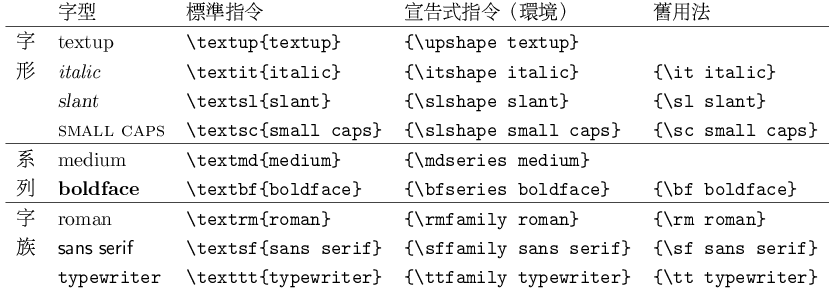
\includegraphics{fntshape}
\end{quote}
\end{htmlonly}

���O�~�F�@���A�o�O����i�`���C�䤤 upright, medium, roman ���O�@�˪��A�o�O�@�몺���`�r�A�N�����·Хh�]�w�L�F�A���D�O�n�b�S�w�r���d����Y�A���s���ܦ����`�r��C�q�e���һ���²�٪��r��A�A�M text, family, series, shape �h�t��ӨϥΡA�o�˥u�n�O�o²�ٴN��F�A�Ҧp�Gitalic ���N�O \verb|\textit{}|�C���M�]�i�H�ϥΡu���Y�B�v���¥Ϊk�A���o�]���O���򰽦Y�B�A�L�O��l Plain \TeX\index{Plain \TeX} �ҩw�q���A�b�ª��� \LaTeX\ 2.09 �]�ۮe�L�Ӫu�ΡA�å[�H�X�R�C���p�G�ϥ��¥Ϊk�A�����ɲզX�������ܮɥi��|�L�ġA�Ҧp�ʱ���o�ز���M����]�w�V�X�ɡA�N�L�k���Ͳʱ���F�A�o���٬O�o�ĨĨϥΥ��μз� \LaTeX\ �����ܪk�C

�n�`�N���O�A�j�A������m�A�ŧi�������O�A��ӧ@�νd��O�s���O�@�_�]�����A�L�i�H�������ҨӨϥΡA�Ҧp \verb|\begin{itsahpe}|, \verb|\end{itshape}|�A�o�˦b�o�����Ҥ�����r�N�q�q�|�ϥ� italic ����A�]�i�H���[�ѼƨϥΡA�Ҧp \verb|\itshape|�A�o�˥H�U����r�q�q�|�ϥ� italic ����A���ܥt�@�ӧ��ܦr�������O�X�{����C�зǫ��O���@�νd��h�O�������O���@�ӰѼơA�o�ǰѼƬO�X�{�b���O�᪺�j�A�������C�{�b�N�ӹ�ڽsĶ�ӨҤl�լݬݡG

\begin{quote}
\begin{verbatim}
% example8.tex
\documentclass{report}
\title{\bfseries Aesop Fables}
\author{Aesop\thanks{Thanks to the reader.}
       \and Nobody\thanks{Thanks to nobody}}
\date{\today}
\begin{document}
\maketitle
\tableofcontents
\chapter{Aesop Fables}
\section{The \textsl{Ant} and the \textsl{Dove}}

\itshape
An antwent to the bank of a river to quench its thirst, and
being carried away by the rush of the stream, was on the
point of drowning.
\upshape

A \textsl{Dove} sitting on a tree overhanging the water plucked a
leaf and let it fall into the stream close to her. The \textbf{\textsl{Ant}}
climbed onto it and floated in safety to the bank.

\section{The {\it Dog}\/ in the Manger}

A \textbf{\textit{dog}} lay in a manger, and by his growling and snapping
prevented the oxen from eating the hay which had been
placed for them.

``What a selfish Dog!'' said one of them to his companions;
``he cannot eat the hay himself, and yet refuses to allow
those to eat who can.''

\chapter{The \textsc{Eagle} and the Arrow}

An \textsc{eagle} sat on a lofty rock, watching the movements of a
Hare whom he sought to make his prey.

An archer, who saw the \textsc{Eagle} from a place of concealment,
took an accurate aim and wounded him mortally.
\end{document}
\end{verbatim}
\end{quote}

�ڭ̧� title page\index{title page} �����D�令����]�Ъ`�N�A�ŧi�����¥Ϊk�A�j�A���O����O�M��r��ӬA�����^�A�� Dove �令 slant ����A�� dog �令 italic �ʱ���\footnote{�Ъ`�N�A�o��ر���O���@�˪��Aslant �O�@�륿�`���r�A�u�O��L�ɱ׭Ө��צӤw�A�� italic �h�O�t�@�ؿW�S���r���]�p�C}�A�� ant �令 slant �ʱ���A�� eagle �令 small caps�C�ѩ󳹸`���D�쥻�N�|�ഫ������A�ҥH���`���D�������A����N�������Ƴ]�F�C

���o�̵o�{�Ҥl�̲ĤG�����D���� Eagle �èS�����ܦr��A�ӥB�H {\tt latex} �sĶ�ɷ|���ͥH�U�����~�]�o�ǰT���]�|�b {\tt example8.log} �����^�G

\begin{quote}
\begin{verbatim}
  ...
LaTeX Font Warning: Font shape `OT1/cmr/bx/sc' undefined
(Font)              using `OT1/cmr/bx/n' instead on input line 4.
  ...
LaTeX Font Warning: Some font shapes were not available, defaults substituted.
  ...
\end{verbatim}
\end{quote}

�{�b�ڭ̬ݨ�F�e���ҽͪ��ݩ�²�١A�o�b \LaTeX\ �N�|�ϥγo���ݩʨӪ��ܦӵo�X�T���A�o�� \verb|OT1/cmr/bx/sc| �N���ܤF OT1 �s�X�AComputer Modern Roman �r�ڡABold extended �t�C�A�ӥB�O small caps �Ϊ����r���A���~�T����ܡA�L�èS���w�q�A�]���A�o�Ӧr���N�|�ϥιw�]���r���ӥN���A�o�̴N�O�H n ���`�Ϊ��� bx �t�C�r���Ӵ��N�C�ҥH�A�r�����O�ä��O���i�H�H�N�զX���A���ǬO�ڥ��N�S���o�ئr���A���ǫh�O�S���Υ����h�w�q�n�A�o�� \LaTeX\ �N������r�F�A���O��ߡA���h�N�O�ϥιw�]���r���}�F�I

�t�@�ӫܩ_�Ǫ��a��A�N�O�Ĥ@���B�ĤG�`�����D�A������O \verb|{\it Dog}\/ in the...}|�H�o�Ӵ��J�� \verb|\/| �O����F��H�o�O \TeX\ �t�νվ����r�]�]�A iatlic �� slanted�^�M���`�r�������ťժ��@�ӫ��O�A�٬� italic correction\index{italic correction}�C�o�ˡA�b����r�M���`�r�������ťդ~�|���`�C���������L��������O�S���[�o�ӽվ�O�H�o�O�]�� \LaTeX\ �����b�]�p�ɴN���Ҽ{��o�Ӱ��D�A�ҥH \verb|\textit{}| �o���зǫ��O���|�۰ʽվ� italic correction�A�����ѧڭ̤�ʽվ�C

�t�~�A���`���D���N�|�۰��ഫ������A���D�W�� dog ������S���ܲ���H�o�b�e��������L�A�o���¥Ϊk���ɬO�L�k�ƦX�ϥΪ��A����S���骺���O�|�Τ��W�ӡC�]���A��ij�ɶq�ϥ� \LaTeX\ ���Ĥ@�ؼзǫ��O�ӧ��ܦr���C�ϥ� \verb|{\it ...}| �� \verb|{\itshape ...}|\footnote{�ŧi�����O�i�H�ƦX�ϥΡA�����M�|�ݭn��ʰ� italic correction�C} �o�ث��O���ܡA�N�o�ɮɪ`�N italic correction �����D�A�]�o�`�N�O�_�i�H�ƦX�ϥΫ��O�����D�A�ҥH�A�٬O���n���i���n�C:-)

��U�O�ƪ��X�Ӫ����G�G

\begin{quote}
\url{http://edt1023.sayya.org/tex/latex123/example8.tex} \\
\url{http://edt1023.sayya.org/tex/latex123/example8.pdf}
\end{quote}

\subsection{�۹�r���j�p���վ�}

���U�ӽͳ̫�@�Ӧr���j�p�ݩʪ��վ�A�o�b�ϥΤW�����¡A�u�n���D���O�N�i�H���W���ӨϥΡC���O \TeX/\LaTeX\ �t�Τ��A�ͨ�r���A���Y�@��a�p�A�Ҧp�e���ͨ쥿�`������r���j�p�O 10pt�A�{�b�p�G�Q�s�@�����A�ݭn 64pt ���r���ɭԴN�|�o�{�A�]���X�ӤF�I���` \LaTeX\ ���w�q�A�r�����j�p�d��O�b 5--24.88pt �����A�W�X�o�ӽd�򪺦r�ݭn��L�� package �������C\footnote{�o�O \LaTeX\ ���������w�q�����D�A�]���L�D�n�O�w��@��ʤ��ή��y�A\TeX\ ��������O�A�i�H���r����j�� 2047pt�C}

�o�̧ڭ̥��Ӭݬݤ��� 10pt �ɦU�ئr���j�p���O�B��ڨҤl�Ψ�j�p�]�o�O�۹�j�p�A�|�H����w�]�r���j�p�Ӧ۰ʽվ�^�G\footnote{�Ъ`�N�A���� pdf �榡����ϥ� 12pt �r���j�p�A�C���Ψ䤤���Ҥl�A�O�ѥt�~ 10pt �w�]�r���j�p�һs�@�� eps ���ɤޤJ�A�H�K���u�C}

\begin{quote}
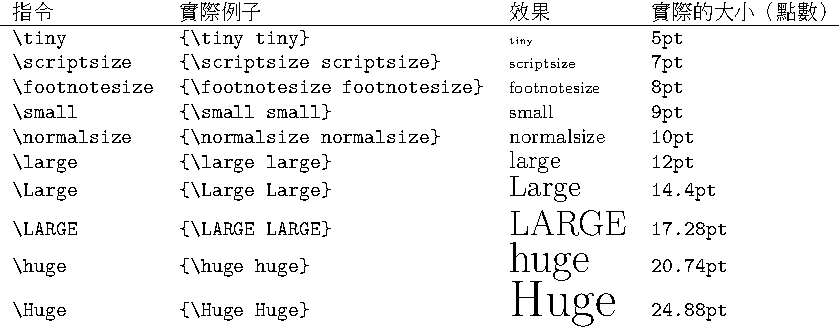
\includegraphics{fntsize}
\end{quote}

�o�Ǧr���j�p���O�]�i�H�������ҨӨϥΡA�Ҧp�G

\begin{quote}
\begin{verbatim}
\begin{small}
  ���夺�e
\end{small}
\end{verbatim}
\end{quote}

�o�˥Τ]�O�i�H���C

\subsection{����r���j�p���վ�}

�q�`�r�����j�p\index{�r��!�r���j�p}�A�ϥΤW�@�`�һ����۹�r���j�p�ӽվ�|�����K�A�ӥB����Ӫ������t�X�]�|�������A�Ҧp��Z�]�|��۰��A�����վ�A�p�G�ۦ�ε���r���j�p����k�ӽվ�r���j�p���ܡA�`�`�|�y����Z���@�P�����ΡA�]���A�p�D���n�A���ɶq�קK�C

�����ɭԴN�O�ݭn���o�˪��վ�A�Ҧp����ʭ����r���j�p�A�a�ϬO \LaTeX\ �w�]���̤j�r���]ı�o�y�p�F�I�A�o�N�n�t�~�ޤJ package �վ�F�C

�o�̧ڭ̨ϥ� \textsf{type1cm}\index{type1cm@\textsf{type1cm}} package �ӽվ�C���M�A�o�ϥ� Type 1 �r���A�~�i�H�F��L�q��j�B�Y�p���ت�%
\footnote{\LaTeX\ �t�Τ����r����j�A�b 10pt �H�W�A�O�H 1.2 �����Ƭ�����ө�j���A�]���A���� 10pt ���r���j�p���ܡA���|�� 13pt �o�ؤj�p���r���A\LaTeX\ �|��γ̬۪�j�p���r���Ӵ��N�C}%
�A�ӳo�� package �]�O�t�X Type 1 �r���ϥΪ��C�ӧO��j�� pk �I�}�r�A�o�̴N���Q�פF�A�ثe���j������ Computer Modern �r�����w�� Type 1 �� free �����A�ӥB�U�� \TeX\ distribution ���|���W�A�ϥΤW�|����K�C�H�U�O \textsf{type1cm} ���ϥΤ�k�G

\begin{quote}
\begin{verbatim}
  ...
\usepackage{type1cm}
  ...
\fontsize{�r���j�p}{��Z�j�p}\seclectfont
  ...
\end{verbatim}
\end{quote}

�ٰO�o�p��ޥΥ����M��\index{�����M��}�ܡH�аѦҲ� \ref{ch:syntax} ���B�� \ref{sec:struct} �`�A�� \ref{subsec:preamble} �p�`�������C

�䤤���u�r���j�p�v�N�O�ҭn���w���j�p�A�q�`�H pt �����A���M�A�n�ϥΨ�L���]�O�i�H�C�u��Z�j�p�v�]�O�n�@�֫��w�A���i�ٲ��C�̫᪺ \verb|\seclectfont| �O���L�o�ͧ@�Ϊ��N��A\LaTeX\ ��������r�������C�����O�A�n�U \verb|\seclectfont| ��~�|�@�ΡA\verb|\fontsize{}{}|\index{fontsize@\verb=\fontsize=} ���O�䤤���@�C

\section{���ӦC}

����O���ӦC\index{���ӦC}�H�@�� \LaTeX\ �J��˱׽u\index{�˱׽u}�|�{���O�@�ӫ��O���}�l�A�p�G�s��ӫ��O���n�L�X���ɭԩO�H�o�ɴN�n�Ψ���ӦC�����O�����ҤF�C

\subsection{���ӦC���O}

�p�G�u�O�@�p�q����r�n���ӦC�A���ϥΫ��O�|�����K�A�o�ӫ��O�N�O \verb+\verb|��r���e|+\index{verb@\verb=\verb=}�A�䤤�� \verb+|+ �o�ӲŸ��i�H�ϥΨ�L�D�r�����Ÿ��N���A�u�n�e��ۦP�N��F�A�Ҧp�G\verb|\verb+��r���e+| �o�ˤ]�O�i�H���C

\subsection{���ӦC����}

�p�G�O�@��q�����e�n���ӦC���ܡA�ϥ����ҷ|�����K�A���K�O {\tt verbatim} ���ҡC���ެO���@�ح��ӦC�����ΡA�w�]�O�ϥΥ��r���r�ڪ��r������ܪ��C���U�O�@��²�檺�Ҥl�A�������ӦC���O�����Ҫ��ϥΡG

\begin{quote}
\begin{Verbatim}[commandchars=+\[\]]
% example9.tex
\documentclass{article}
\begin{document}
The example of \verb|\verb{}| command and \texttt{verbatim} environment.

\section{\textbackslash{}\texttt{verb} command}

When you want to express you home directory, you can \verb|echo $HOME|
varient to display your home directory in your sh script.

\noindent
\verb*|This is    4 space here.|

\section{\texttt{verbatim} environment}

Here is a sh script to determine if on GNU/Linux system.

\begin{verbatim}
#!/bin/sh
Date=`date '+%y%m%d'`
if [ `uname` = Linux ]
then
  Mail=/var/spool/mail/edt1023
  Target=/mnt/hd
else
  Mail=/var/mail/edt1023
  Target=/mnt/pub
fi
\end{verbatim}
\end{document}
\end{Verbatim}
\end{quote}

�o�̷|�o�{�@�ǩ_�Dz{�H�A�Ҧp
\texttt{\textbackslash{}verb*}
���ӬP���O����N��O�H�N�O���ťեH
%begin{latexonly}
\verb*| |
%end{latexonly}
\begin{htmlonly}

\includegraphics{blank}
\end{htmlonly}
���覡���ܥX�Ӫ��N��A{\tt verbatim} ���Ҥ]�O�i�H�o�˨ϥΡC�Ҧp {\tt example9} �����G

\begin{quote}
\begin{verbatim}
\verb*|This is    4 space here.|
\end{verbatim}
\end{quote}

�]�i�H�g���G

\begin{quote}
\begin{Verbatim}[commandchars=+\[\]]
\begin{verbatim*}
This is    4 space here.
\end{verbatim*}
\end{Verbatim}
\end{quote}

�t�O�b��A���Ҫ��W�U��|�h�ťX�Ӫťզ�X�ӡC

�t�~�A���D�����򤣨ϥ� \verb+\verb|\verb|+ �N�n�F�O�H��]�O���ӦC�����O�M���ҳ����������L���O���ѼơA���D�����N�O�@�ӫ��O�A�ҥH \verb+\verb+ ����b���Y�C

�ϥ� \verb|\textbackslash|\index{textbackslash@\verb=\textbackslash=} �o������ԭz�A�Ӥ��� \verb|$\backslash$| �o��²�檺�覡�A��]�O�o�Ӥ�Z���ϥ� \LaTeX{}2{\tt HTML} ���ন HTML �榡�A�ϥ� \LaTeX\ �����N���ܪk�|�ন�@�몺�Ÿ��A���ϥΫ�̪��覡�h�|�ন���ɡA�ҥH�o�̴N�ϥ� \LaTeX\ �����N���ܪk�F�C

���U�O�ƪ��X�Ӫ����G�G

\begin{quote}
\url{http://edt1023.sayya.org/tex/latex123/example9.tex}\\
\url{http://edt1023.sayya.org/tex/latex123/example9.pdf}
\end{quote}

\section{�[�J����}

�o�̥u�����p��ϥ� \textsf{CJK}\index{CJK@\textsf{CJK}} package �����ΡA��]�O�@�� \TeX\ distribution �|���W�]���ǵo��M��èS�����W�A�o�ɥu�n�ۦ�w�ˤF�^�C\textsf{CJK} package �O�⤤�媺�����]�b�@�����Ҹ��Y�A�b�o�����Ҥ��N�i�H�ϥΤ���A���}�o�����ҴN�S�^�_��쥻���^�����ҡA���U�ѨҤl�ӻ����C

\begin{quote}
\begin{verbatim}
\documentclass{article}
\usepackage{CJK}  % �ϥ� CJK �����M��
\begin{document}
% �i�J CJK ���ҡA�èϥ� Big-5 �X�� hwmm �o�Ӧr��
\begin{CJK}{Bg5}{hwmm}
\section{CJK �����M��}
�o�O�@�Ӵ��աA���� CJK package �����աC
\section{��᷽�O�`��}
��U�A�׳q�H�F�_��ƤQ�B�A�ŵM�}�ԡC�g�a���m�A�Ϊ��k�M�C���}�СB�����B%
��B�ˤ��ݡA�魯��q�A�����ۻD�C�䤤���Ӻا@�A�k�k��ۡA�x�p�~�H�F���v�B%
���ԡA �éɵM�ۼ֡C�����H�A�D�j��A�ݩұq�ӡF�㵪���A�K�n�ٮa�A�]�s�B�����B%
�@���C�����D�����H�A�w�ӰݰT�C�ۤ��G�u���@�ׯ��ɶáA�v�d�l���H�Ӧ����ҡA%
���_�X�j�F�E�P�~�H���j�C�v�ݤ��O��@�F�D�������~�A�L���Q�B�ʡC���H�@�@%
���㨥�һD�A�Ҽ۱{�C�l�H�U�_���ܨ�a�A�ҥX�s���C���Ƥ�A��h�C�����H�y%
���G�u�������~�H�D�]�C�v
\end{CJK}
\end{document}
\end{verbatim}
\end{quote}

�N�o��²��C�u�O�sĶ�n��� {\tt bg5latex}\index{bg5latex@\texttt{bg5latex}} �Ӥ��O��Ӫ� {\tt latex} ���O�A�o�O���F�׶}�ڭ� Big-5 �X���@�ǯS���X�����Y�A�ٰO�o����C��̫�n�[�Ӧʤ��� \verb|%|\index{%@\verb=%=} �ܡH�o�ˤ~���|���J�^�媺�r���ťաC�sĶ�n���Ҥl�p�U�G

\begin{quote}
\url{http://edt1023.sayya.org/tex/latex123/example10.tex}\\
\url{http://edt1023.sayya.org/tex/latex123/example10.pdf}
\end{quote}

�ԲӪ� \textsf{CJK} package ���ϥΤ��廡���A�аѦ� \textsf{CJK} package �Ҫ������Ρq�ڪ� CJK�r�@��G

\begin{quote}
\url{http://edt1023.sayya.org/tex/mycjk/mycjk.html}\\
\url{http://edt1023.sayya.org/tex/mycjk/mycjk.pdf}
\end{quote}


% ``�j�a�Ӿ� LaTeX'' LaTeX ��Z space.tex
% Copyright (c) 2004  Edward G.J. Lee <edt1023@info.sayya.org>
%
% �b���H�� GNU Free Documentation License 1.2 �ΥH�᪺�����W�d���U�A
% ���\�����B���G�έק�C���쪩�v�B���v�n�����o�����C
%
% �����G�����A�t�� fdl.tex�A���e�� GNU FDL ���W�d���C�p�G�򥢡A�i��
% http://www.gnu.org ���o�A�μg�H�ܦۥѳn�����|(Free Software Fundation)
% �����C
% 9 Temple Place - Suite 330, Boston, MA 02111-1307, USA.
%
% $Id: space.tex,v 1.23 2004/03/07 12:20:47 edt1023 Exp $
%
\chapter{�Ŷ��P��m}
\label{ch:space}

�e�@��������L�A�Ƿ|����Ŷ��N�Ƿ|�ƪ��F�IKnuth\index{Knuth} �б¦b�L�� \textit{The \TeX{}book}\index{The TeXbook@\textit{The \TeX{}book}} �@�Ѥ��]���ήe�ϥ� \TeX\ �ƪ������ΡG�@�Ӫ����N���@�ӧt�������]glue\index{glue}�^�������A�M��C�@�ӭn�ƪ������e�N�O�U�ؤ��P�� box\index{box}�A�b�o�� box �٨S���T�w���T��m�ɡA���O�i�H���ʪ��]�����٨S�����^�A�@���ƪ������A�����N���F�A��O�C�� box ����m�N�T�w�L�k�A���ʤF�A���D�S�q�Y�A�ӡC

�@�Ӧr���B�@�ӳ�r�B�@�ӥy�l�B�@�Ӭq���B�@�ӲŸ��B�@�ӹϧΡB�@�Ӫ��泣�i��c���@�� \TeX\ �� box�A�Ʀ� box ���٦� box �����ΡC�o���Q�Q�ת��A�N�O�o�� box �p��w�m�L�̨쥿�T����m�A���C�� box �������Ŷ�����F����n�B�A�ҥH�A�쩳�O�b���� boxes ���ݩʡB��m�A�٬O�վ� glue ���Ŷ��A�N�ݦU����h�ݫݤF�]�Ъ`�N�Abox ���@�w�O�i�����I�b \TeX\ ���Y�Aglue �O�i�H�վ㪺�C�^�C

�ڭ̫e���ҰQ�ר쪺�^��y�I��ťժ��վ�Bitalic correction\index{italic correction}�B\verb|\linespread|\index{linespread@\verb=\linespread=} �� \verb|\parindent|\index{parindent@\verb=parindent=} �o�dz��O�b�վ� glue�C�q�`�A�b \LaTeX\ �t�θ��Y�A���w���`�`���|�O����T�w���A�|�����ΰ��p���ת��۰ʷL�աA�o�O�����Ŷ��t�m�W���ݭn�C

\section{\LaTeX\ ���ϥΪ��׶q���}
\label{sec:units}

�n��T�y�z�M�վ� \LaTeX\ �����Ŷ��Φ�m�A�ڭ̥��ݭn���ӼзǪ��׶q���C�H�U���O�b \LaTeX\ �`�|�Ψ쪺���C�o�̦�������ά۹��줧���A���D���n�A���M�A�@��O��ij�ϥά۹���A��]�O�A�L�|�H�ۤ�Z�r���j�p���ܮɸ�۰��A�����վ�C���M�A�b�����D��T�B�T�w�j�p����ܮɡA�N�o�ϥε�����F�C

�o�̦p�G�O�\�� HTML �榡�����A�Хt�Ѧ� PDF �榡�����A�H�K���ܤW���u�C�H�U���椤�ҵe�X�Ӫ����׶ȨѰѦҥΡC

\subsection{������}
\index{������}

%begin{latexonly}
\begin{quote}
\begin{tabular}{>{\tt}lll}
���W�� & �N�q & ���� \\
\hline
pt & point, $1/72.27$~inch & \drawwidth{1pt} \\
bp & Adobe big point, $1/72$~inch & \drawwidth{1bp} \\
pc & pica, 12pt & \drawwidth{1pc} \\
mm & millimeter, $1/25.4$~inch & \drawwidth{1mm} \\
cm & centimeter, 10mm & \drawwidth{1cm} \\
in & inch, 25.4mm & \drawwidth{1in} \\
\end{tabular}
\end{quote}
%end{latexonly}

\begin{htmlonly}
\begin{quote}
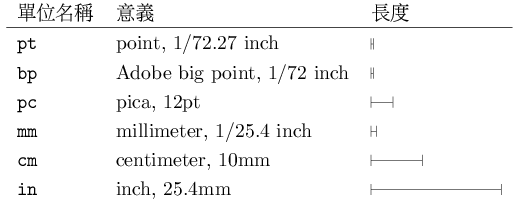
\includegraphics{a-units}
\end{quote}
\end{htmlonly}

�o�̭n�`�N���O \TeX/\LaTeX\ �t�Τ��ҿת��I�]point�^\index{�I�]point�^}�A�����O�@�몺 printer point\index{printer point}�A�]�N�O $1/72.27$~inch�A���b Adobe ���W�椤�A�Ҧp \textsc{PostScript}\index{PostScript@\textsc{PostScript}} �y�������ҿ��I�A�L�O big point\index{big point}�A���� $1/72$~inch�]�p���I�������˥h�F�^�A�|��@�몺 print point �y�L�j�@�I�I�C

\subsection{�۹���}
\index{�۹���}
%begin{latexonly}
\begin{quote}
\begin{tabular}{>{\tt}lll}
���W�� & �N�q & ���� \\
\hline
em & �����b�ϥΦr���r�� M ���e�� & \drawwidth{1em} \\
ex & �����b�ϥΦr���r�� x ������ & \drawwidth{1ex} \\
\end{tabular}
\end{quote}
%end{latexonly}

\begin{htmlonly}
\begin{quote}
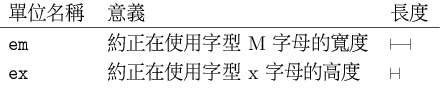
\includegraphics{r-units}
\end{quote}
\end{htmlonly}

�b \TeX\ ���Y�ҿת� em\index{em}�A���A��T�Ө��O���b Knuth �б³]�p�� Computer Modern �r�����Y�� em-dash\index{em-dash} ���e�סA�ѩ�r�� M ��ڤW�O�]�b�r���W�ҿת� em-square ���Q��椤�A�� em �ҫ����e�׬O���o�� em-square\index{em-square} ���e�סA���r�� M �����ä��������o�� em-square�A�]���o�˴N�|�y���t���F�C�ҥH�H�r�� M ���e�רӻ������ܮe�����øq�C\LaTeX\ ���ӫ��O \verb|\quad|\index{quad@\verb=\quad=} �o�N�O���ͤ@�ӥ��T em ���e�ת��ťաA�ҥH�b Knuth �бª� \textit{The \TeX{}book} ���A���� em �N�������L�O�@�� `quad' ���e�סC


\section{�����j�p}
\label{sec:layout}\index{�����j�p}

�ڭ̹��ү౱��@��i�Ȫ��d�򳣥i�H�٬������C���M�A�ڭ̪�����]body�^\index{����]body�^}�ä��O������i�Ȫ��d��A�W�U���k���|�d���@�w���ťաC�p�ɭԦb�ůȤW�m�߼g�򵧡A�Ѥ@�������|�n�ڭ̯d�u�Ѧa�v�A�o�N�O������|�P���ťաA���F��ı�W���z�ѡA�j���]�O�H�ͪ����z�a�H:-)

�b�s��W�A�]���H�٤���]body�^���������u���ߡv�Ρu���f�v\index{����}\index{���f}�A�|�P���ťճ����A�h�٬��u����v\index{����}�C��}���ߡB���䪺�]�p�A�N�٤����u�X��v\index{�X��}�A�Ҧp�A�H�I���ϧG����i�ȷ����O�I�������X�A�H�o�ӭI���ϦӨ��A�N�L�ҿת���F�C���o�b \LaTeX\ �q�`�O���|���o�ر��p�X�{�A���D�S�N�h���w����M�ȱi�j�p�P�˽d��C

���M�A�b����H�~���ťաA�]�ëD���O�ťաA�L�]�t�F�����]footer�^\index{�����]footer�^}�A���ܡ]header�^\index{���ܡ]header�^}������]marginal note�^\index{���}\index{marginal note}�������A�O�����󭶼ơB���ѵ���T�C

\subsection{�����ϸ�}
\label{subsec:layout}

\begin{quote}
\begin{center}
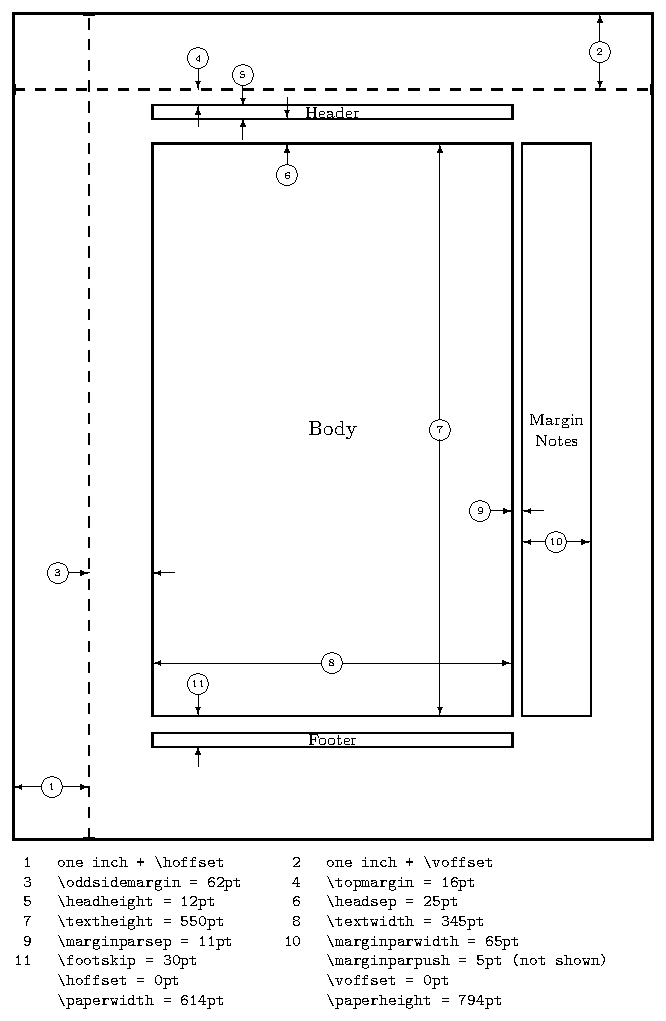
\includegraphics{layout-r}
\end{center}
\end{quote}

�o�̩ҿת��ȱi�j�p\index{�ȱi�j�p}�A�����O {\tt paperwidth}\index{paperwidth} �M {\tt paperheight}\index{paperheight} �ҳ򦨪��d��A�ëD��ڤW��W���쪺�ȱi�j�p�A��ڦb��W���ȱi�q�`�|���j��ڭ̳o�̪��ҿׯȱi�A�ҥH�A�����C�L�ɡA�ٻݰ��L�թκI���~�|�O�u�����o�̩ҿת��ȱi�j�p�]�����j�p\index{�����j�p}�^�C

�o�O 10pt ����j�p�A�p�G�����w�ȱi���ܡA\LaTeX\ �w�]�|�ϥά��� {\tt letterpaper}\index{letterpaper} ���j�p�A�p�n�ϥμڡB�馡�� {\tt a4paper}\index{a4paper} ���ܡA�n�t����w�C�ڭ̥i�H�y�L�ݤ@�U \LaTeX\ �w�]�O�p��w�ƪ����Ŷ����C�䤤 Header�]���ܡ^�BFooter�]�����^��������Ŷ��O���t�A�b���� Body ���Y���A�o�̬O�u�O�歱���ϡA�p�G�O�������ܡA�����ƭ��M�_�ƭ�������O�n���k�ﴫ���A�]�N�O���o�ӹϬO�_�ƭ��A���ƭ����ܡA����O�b����C

�o�̧ڭ̨Ӭݤ@�U�o�ǭȩҥN�����N�q�G

\begin{quote}
\begin{tabular}{ll}
���O�]�ȡ^& �N�q \\
\hline
\verb=\paperwidth=	& �ȱi���e�� \\
\verb=\paperheight=	& �ȱi������ \\
\verb=\textwidth=	& ����]body�^���e�� \\
\verb=\textheight=	& ����]body�^������ \\
\verb=\headheight=	& ���ܡ]header�^���� \\
\verb=\headsep=		& ���ܻP���嶡���Z�� \\
\verb=\footskip=	& ���婳�ܭ��������Z�� \\
\verb=\topmargin=	& ���ܤW�誺�ť� \\
\verb=\marginparwidth=	& ������e�� \\
\verb=\marginparsep=	& ����P���媺�Z�� \\
\verb=\marginparpush=	& ��������Z \\
\verb=\oddsidemargin=	& ���奪�䪺�ťդj�p \\
\verb=\hoffset=		& �L�ժ����b��گȱi�����k��m \\
\verb=\voffset=		& �L�ժ����b��گȱi���W�U��m \\
\index{paperwidth@\verb=\paperwidth=}\index{paperheight@\verb=\paperheight=}%
\index{textwidth@\verb=\textwidth=}\index{textheight@\verb=\textheight=}%
\index{headheight@\verb=\headheight=}\index{headsep@\verb=\headsep=}%
\index{footskip@\verb=\footskip=}\index{topmargin@\verb=\topmargin=}%
\index{marginparwidth@\verb=\marginparwidth=}\index{marginparsep@\verb=\marginparsep=}%
\index{marginparpush@\verb=\marginparpush=}%
\index{oddsidemargin@\verb=\oddsidemargin=}%
\index{hoffset@\verb=\hoffset=}\index{voffset@\verb=\voffset=}%
\end{tabular}
\end{quote}

\verb|\hoffset| �� \verb|\voffset| �N�O�b�վ㪩���b��گȱi�W�����T��m�A�o�˦L�X�Ӫ��ɭԤ~�|�b��گȱi�������C

�Y���F�ܡH�o�ܥ��`�A�]�� \LaTeX\ �������]�w��챵IJ���H�ӻ��A�O�c�W�L�����x���B�·СA�]���o�̤��h�ͥL���]�w�A��}�l��b�S�����n��ɶ���b�o�Ӧa��C�p�G��ڷQ�վ㪩���A��ij�ϥ� {\sf geometry}\index{geometry@\textsf{geometry}} package�C�|�ӨҤl�A�Q���U��t�O 2cm �N�n�A���u�n�b preamble\index{preamble} �ϳ]�w�G

\begin{quote}
\begin{verbatim}
\usepackage[margin=2cm]{geometry}
\end{verbatim}
\end{quote}

�N�i�H�F�A�p�G�H 12pt �j�p���r�A{\tt a4paper} �ȱi�j�p���]�w���ܡA�H����Ө��A�j���O�C�� 40 �Ӥ���r�A�o�O���媺�e�סC�i�H�����Φۦ�վ� {\tt margin}\index{margin} ���ȴN��F�C�ڭ̫ܧƱ�A�U�@���� \LaTeX\ ���o�譱���ﵽ�A�H��K�ϥΪ̳]�w�C
%���T�B�ԲӪ��]�w��k�A�ڭ̯d��᭱�������y���ѮɦA�ӽ͡A�o�˴N���P�v�T�ڭ̾Dzߪ����`�i�סC

\subsection{�ȱi�j�p}

\begin{quote}
\begin{tabular}{>{\tt}ll>{\tt }ll}
�ȱi & �j�p & �ȱi & �j�p\\
\hline
a4paper        & 21x29.7cm & letterpaper    & 8.5x11in \\
a5paper        & 14.8x21cm & legalpaper     & 8.5x14in \\
b5paper        & 17.6x25cm & executivepaper & 7.25x10.5in \\
\end{tabular}
\end{quote}

�ܩ�p����w�ȱi�j�p�A�o�̥�²�满���@�U�o�g�峹���]�w�A�ͨ� \LaTeX\ ����Z���O�ɷ|�A�Բӻ����C

\begin{quote}
\begin{verbatim}
% ���媺�]���O�]�w
\documentclass[12pt,a4paper]{report}
\end{verbatim}
\end{quote}

�ҥH�A�o�g�峹�ϥΪ��O {\tt a4paper}�A����r�����j�p�O 12pt�C��A�����ѼƬO�ﶵ�A�i�H�ٲ��A�p�G�ٲ����ܡA�w�]�ȴN�O 10pt/{\tt letterpaper}�C

\section{�վ��V�Ŷ�}

�o�̪���V�Ŷ��A�Ҧp \verb|~|\index{~@\verb=~=} �o��r�����`�ťաA�� \verb|\quad| �o�� em\index{em} �e�תťաA���O�b�վ��V���ťաC���p�G�O�n��j�B�Χ�p���ťծɸӦp��վ�O�H���U�ڭ̴N�Ӭݬ� \LaTeX\ �������򱱨���O�i�H�B�ΡG

\subsection{�վ��V�Ŷ������O}

\begin{quote}
\begin{tabular}{ll}
���O & �N�q \\
\hline
\verb=\hspace{���}= & �V�k�ťX�Y�ӫ׶q��쪺�ťաA�p�G�O�t�ơA�h�O�V�� \\
\verb=\hfill=        & �����k��Ǫ���r�������X�i�ܤ@�Ӧ�e���� \\
\verb=\quad=         & �ťX�@�� em ��쪺�ť� \\
\verb=\qquad=        & �ťX�G�� em ��쪺�ť� \\
\verb=\thinspace=    & �ťX $1/12$ �� em ��쪺�ť� \\
\verb=\enspace=      & �ťX $1/2$ �� em ��쪺�ť� \\
\verb=\dotfill=      & �@�ΩM \verb|\hfill| �ۦP�A�u�O�ť��ܦ��I \\
\verb=\hrulefill=    & �@�ΩM \verb|\hfill| �ۦP�A�u�O�ť��ܦ��@��u \\
\verb=\centering=    & �����O�H�᪺��r�N�|�~���ƦC�A���k�u�N������ \\
\verb=\raggedright=  & �����O�H�᪺��r�N�|�~���ƦC�A�k�u�N������ \\
\verb=\raggedleft=   & �����O�H�᪺��r�N�|�~�k�ƦC�A���u�N������ \\
\verb=\centerline{}= & �N�j�A��������r�~���ƦC
\end{tabular}
\end{quote}
\index{hspace@\verb=\hspace=}\index{hfill@\verb=\hfill=}%
\index{quad@\verb=\quad=}\index{qquad@\verb=\qquad=}%
\index{thinspace@\verb=\thinspace=}\index{enspace@\verb=\enspace=}%
\index{dotfill@\verb=\dotfill=}\index{hrulefill@\verb=\hrulefill=}%
\index{centering@\verb=\centering=}\index{raggedright@\verb=\raggedright=}%
\index{raggedleft@\verb=\raggedleft=}\index{centerline@\verb=\centerline{}=}

�@�檺�歺�ϥ� \verb|\hspace{���}| �ɱN�|���ġA�o�ɥi�H�[�ӬP���A�Ҧp \verb|\hspace*{3em}|�C

�b�ϥ� \verb|\centerline{}| �����X�A���u��y�ܤ�K�A�]���L���|�v�T�H�U����r�A���L�]���|���A�Ʀܥ[�J����Ÿ��]�L�ġC�ҥH�p�G��y���׶W�L�@�檺��e�A�L�|�W�X��ɡA�ƦܴN��������r�N�ݤ���F�C

�䤤 \verb|\thinspace| �S�i�H�ϥ�²�ƪ� \verb|\,| �ӥN���A�D�n�O�Φb�޸����S���޸������ΡA�q�`�o�ر��ΡA��޸������n���Ӷ��j�A�H�K�Ϥ��A�Ҧp�G

\begin{quote}
\begin{verbatim}
``\,`Superman', he said.''
\end{verbatim}
\end{quote}

���{�X�ӷ|�O�G

%begin{latexonly}
``\,`Superman', he said.''
%end{latexonly}

\begin{htmlonly}
\begin{quote}
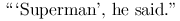
\includegraphics{superman}
\end{quote}
\end{htmlonly}

�o�ˤ~��Ϥ��X���P�޸��A�_�h�|�ܦ��@�ӳs�T�� grave accent\index{grave accent} ���޸��C�Ъ`�N�A�ѩ�o�ӫ��O�O�ѫD�r���Ÿ��c���A�ҥH�A�L���@�νd��b�J��Ÿ�������N�����F�A�᭱�����ťթΥH�j�A���ӭ����@�νd��A�N�n��������L�� \verb|\@| �@�˪����ΡC

\subsection{�վ��V�Ŷ�������}

\begin{quote}
\begin{tabular}{ll}
\verb|\begin{center}...\end{center}| & ���o�����Ҥ������e�m�� \\
\verb|\begin{flushleft}...\end{flushleft}| & ���o�����Ҥ������e�a�� \\
\verb|\begin{flushright}...\end{flushright}| & ���o�����Ҥ������e�a�k \\
\verb|\begin{raggedright}...\end{raggedright}| & ���o�����Ҥ������e�a���A�k�u�N������ \\
\verb|\begin{raggedleft}...\end{raggedleft}| & ���o�����Ҥ������e�a�k�A���u�N������ \\
\end{tabular}
\end{quote}
\index{center@\texttt{center}}\index{flushleft@\texttt{flushleft}}%
\index{flushright@\texttt{flushright}}\index{raggedright@\texttt{raggedright}}%
\index{raggedleft@\texttt{raggedleft}}

�i�J���ҡA�M�W�@�`���쪺���O�A��̦����򤣦P�O�H�̤j�����P�O�A�o�i�H��K�����w�@�ӽd�򪺤�y���L�@�ΡA�Ӥ��|�v�T���ҥH�~����y�C�䦸�A�i�J���ҡA�a�ϩM�W�U��s�b�@�_�A�S���ťX�ťզ�A�L�]�|�۰ʪ��b�W�B�U��ťX�Ӫťզ�X�ӡA�ϥΫ��O���ܫh���|�C

�x�I�o�̫��S���� {\tt raggedright} �� {\tt raggedleft}�H��ӥL�]�O�i�H�����ҨӨϥΡC�ѩ�o��ӫ��O�|�ϥH�U�����e�����B�k�u�������A�]���ϥΤW�n�D�`�p�ߡA���D���ӴN�Q�����媺���B�k�u�������A�_�h�A�̦n�O�ϥΦ��d�򭭨�覡�C���M�A�p�G�o��ӫ��O�O�Φb�Y�Ө�L���ҽd�򤺡A�L���@�Τ]�N�ȭ���o�����Ҥ��A���|�v�T�o�����ҥ~����y�C

\subsection{�ޤ�����}
\index{�ޤ�����}

�ޤ�q�`�N�O�ޥΥL�H����y�A�b�ޤ媺�q���A��dz��|�X�{���Y�����ΡA�H�K�M����۰Ϲj�A�o�]�O�@�تŶ����t�m�A�i�W�[�峹����Ū�ʡC�b \LaTeX\ ���Y���T�ؤޤ����ҡG{\tt quote}, {\tt quotation}, {\tt verse}�C�o�T�̬ݰ_�ӫܹ��A�����ǷL���t���C

\begin{quote}
\begin{tabular}{>{\tt }lll}
���� & �A�ήɾ� & �S�� \\
\hline
quote & ���u���u�ޤ� & �C�Ӭq���Ĥ@�椣���Y \\
quotation & �h�Ӭq�������ޤ� & �C�Ӭq���Ĥ@��|���Y \\
verse & �ֺq�B���ޤ� & �C�Ӭq�����Ĥ@�椣���Y�A���ĤG��_�|���Y \\
\end{tabular}
\end{quote}
\index{quote@\texttt{quote}}\index{quotation@\texttt{quotation}}%
\index{verse@\texttt{verse}}

�b {\tt verse} �����ΡA�q�`�|�ϥ� \verb=\\=\index{\\@\verb=\\=} �Ӵ���H�K����C�@�檺�e�סC�ӥB�q�����Z\index{�q�����Z}�N�����~�b�]�w���v�T�A�䤤 {\tt quote} �M {\tt verse} ���ҷ|�w���J�A�����q�����Z�A�� {\tt quotation} ���ҫh���|�C

���U�ڭ̨Ӭݬݽվ��V�Ŷ����@�Ӻ�X��ҡG

\begin{quote}
\begin{verbatim}
% example11.tex
\documentclass{article}
\usepackage{CJK}
\begin{document}
\begin{CJK}{Bg5}{hwmm}
\section{hspace}
\hspace*{2em}�o�O�@�Ӿ�V�Ŷ��վ㪺���աC\\
�o�O�@��\hspace{2em}��V�Ŷ��վ㪺���աC\\
�o�O�@�� \hspace{2em} ��V�Ŷ��վ㪺���աC
\section{hfill}
�o�O�@��\hfill{}��V�Ŷ��վ㪺���աC
\section{quad}
�o�O�@��\quad{}��V�Ŷ��վ㪺���աC\\
�o�O�@�� \quad{} ��V�Ŷ��վ㪺���աC\\
�o�O�@��\qquad{}��V�Ŷ��վ㪺���աC
\section{dotfill}
�o�O�@��\dotfill{}��V�Ŷ��վ㪺���աC\\
�o�O�@�� \dotfill{} ��V�Ŷ��վ㪺���աC
\section{hrulefill}
�o�O�@��\hrulefill{}��V�Ŷ��վ㪺���աC
\section{center}
\begin{center}
�o�O�@�Ӿ�V�Ŷ��վ㪺���աC
\end{center}
\section{flushleft}
\begin{flushleft}
�o�O�@�Ӿ�V�Ŷ��վ㪺���աC
\end{flushleft}
\section{flushright}
\begin{flushright}
�o�O�@�Ӿ�V�Ŷ��վ㪺���աC
\end{flushright}
\section{quote}
�o�O�`���ۥ���J�����`���G�ơG
\begin{quote}
An antwent to the bank of a river to quench its thirst, and
being carried away by the rush of the stream, was on the
point of drowning.

A Dove sitting on a tree overhanging the water plucked a
leaf and let it fall into the stream close to her. The Ant
climbed onto it and floated in safety to the bank.
\end{quote}
\section{quotation}
�o�O�`���ۥ���J�����`���G�ơG
\begin{quotation}
An antwent to the bank of a river to quench its thirst, and
being carried away by the rush of the stream, was on the
point of drowning.

A Dove sitting on a tree overhanging the water plucked a
leaf and let it fall into the stream close to her. The Ant
climbed onto it and floated in safety to the bank.
\end{quotation}
\section{verse}
�o�O�`���ۥ���J�����`���G�ơA�o�O�`���ۥ���J�����`���G�ơA%
�o�O�`���ۥ���J�����`���G�ơA�o�O�`���ۥ���J�����`���G�ơG
\begin{verse}
An antwent to the bank of a river to quench its thirst, and
being carried away by the rush of the stream, was on the
point of drowning.

A Dove sitting on a tree overhanging the water plucked a
leaf and let it fall into the stream close to her. The Ant
climbed onto it and floated in safety to the bank.
\end{verse}
\section{centering}
\centering
�o�O�@�Ӿ�V�Ŷ��վ㪺���աC\\ % �o�̭n����A�_�h�|�O \raggedright ���@��
\raggedright
\section{centerline}
\centerline{�o�O�@�Ӿ�V�Ŷ��վ㪺���աC}
\section{raggedright}
\raggedright
�o�O�@�Ӿ�V�Ŷ��վ㪺���աC
\section{raggedleft}
\raggedleft
�o�O�@�Ӿ�V�Ŷ��վ㪺���աC
\end{CJK}
\end{document}
\end{verbatim}
\end{quote}

�sĶ�n�����G�p�U�G

\begin{quote}
\url{http://edt1023.sayya.org/tex/latex123/example11.tex}\\
\url{http://edt1023.sayya.org/tex/latex123/example11.pdf}
\end{quote}

�n�`�N�O���O�e�᪺�ťաA�� \verb|\hspace|, \verb|\dotfill|, \verb|\hrulell| �o�����O�A���O�e��ťճ��|��i�h���C\verb|\quad|, \verb|\qquad| �o�����O�A�h�᭱���ťդ]�O�|��J���C�t�~�A�ѨҤl���i�H�ݥX�ӡA�@�� em\index{em} ���e�סA�j���O�@�Ӥ���r���e�סA�ҥH�A�ڭ̹w�]�ϥ� 10pt ���r�A�o�� em �e�״N�۷��� 10pt ���e�סA�ҥH�A�ڭ̦b�Ĥ@�洡�J�F 2em �e�ת��ťաA�]�N�n���O���Y�F��Ӥ���r�@�ˡC

\section{�վ��a�V�Ŷ�}

\begin{quote}
\begin{tabular}{ll}
\verb=\vspace{���}= & �V�U�ťX�Y�ӳ�쪺�ťա]��^�A�t�ƫh�O�V�W \\
\verb=\bigskip=     & ���� 12pt�]11--12pt�^�������ťա]��^ \\
\verb=\medskip=     & ���� 6pt�]5--7pt�^�������ťա]��^\\
\verb=\smallskip=   & ���� 3pt�]2--4pt�^�������ťա]��^\\
\verb=\vfill=       & �M \verb|\hfill| �����A�@�άO�N�Y�q���V�W���A�Ω��U�� \\
\verb=\parskip=���= & �վ����C�Ӭq�������Z�����Y�ӳ��
\index{vspace@\verb=\vspace=}\index{bigskip@\verb=\bigskip=}%
\index{medskip@\verb=\smallskip=}\index{vfill@\verb=\vfill=}%
\index{parskip@\verb=\parskip=}
\end{tabular}
\end{quote}

�䤤�� \verb|\bigskip, \medskip, \smallskip| �ëD�T�w���A�L�̷|���W�U��ߵ����ݭn�۰ʰ��L�աA�H�F��@�㭶���@�P���Ŷ��t�m�C\verb|\vspace| �p�G�O�X�{�b�@�����Ĥ@��γ̫�@��ɡA�N�|���h�@�ΡA�o�ɥi�H�[�ӬP���A\verb=\vspace*{���}=\index{vspace@\verb=\vspace*=}�C

���F�����������@�P��\index{�����@�P��}�A�ϥ��a�V�Ŷ��վ㪺���O�ɭn�S�O�d�N�A�Ҧp���`���D�W�U���Ŷ��B�U�q�������Ŷ��A�i�J���ҫe��ҪťX���Ŷ��A�o�����@�өT�w�ȡA\LaTeX\ �|�۰ʥh�վ�A�����ѨϥΪ̦ۦ�ʤ�A���D�O�ʭ��o�س�W���C�ҥH�A�ϥ��a�V�Ŷ��վ���O�ɡA�n�D�`�`�N���骺�@�P�ʡA�o�]�O�ƪ��W���@�ӫܭ��n����h�C

�o���|�o�g�峹�������ʭ�\index{�����ʭ�}���ҨӺ�X�����A��B�a�V�Ŷ����B�ΡC�ٰO�o�� \ref{sec:titlepage} �`�� title page\index{title page} �����O�ܡH���ڭ̤]�i�H�ۦ�]�p�@�ӿW�ߪ������ʭ��A�ϥΪ��O \LaTeX\ ������ {\tt titlepage}\index{titlepage@\texttt{titlepage}} ���ҡC�o�̪����ɤޥάO�ڭ��٨S���Dzߨ쪺�A�S���Y�A�u�n�j��h����N��F�C

\begin{quote}
\begin{verbatim}
% example12.tex
\documentclass[12pt,a4paper]{report}
\usepackage{CJK}     % �ޤJ�һݭn�� packages
\usepackage{graphicx}
\begin{document}
\begin{CJK}{Bg5}{hwmm}
\begin{titlepage}    % �ϥ� titlepage ����
\vspace*{5ex}
  \begin{flushright} % �j���D�a�k
    \Huge\textbf{�j�a�Ӿ� \LaTeX}
  \end{flushright}
  \rule{\textwidth}{.256ex}
  \begin{flushleft}  % �������X����a���A�M�j���D�����H�@��u�j�}
    Version 0.1 draft\\
    \today
  \end{flushleft}    % ���ɦ�󤤥�����
  \vspace{8ex}       % �ťX 8ex �������Ŷ�
  \hspace{2em}\includegraphics[scale=.75]{cover2.1} % �ޤJ���ɡA�ñN�o��
  \vspace{8ex}                                      % ���ɾ�V�k�� 2em
  \begin{flushright} % �@�̸�T�a�k
    By Edward G.J. Lee ���G��\\
    Email�G\texttt{edt1023@info.sayya.org}
  \end{flushright}
\end{titlepage}
\end{CJK}
\end{document}
\end{verbatim}
\end{quote}

�ѩ�t�X���������D�A�䤤���@�Ǽƾڦ���ʡA�ӥB�]�ٲ��F�@�ǧڭ��٨S���Dzߨ쪺 packages�A���j���c�h�M��l��Z�@�ˡC�ҥH�A�M�o�g�峹�� PDF �榡����|�o�{�A�j���D���r��p�F�@�I�A�ӥB�S���C��A�]�S���W�s��\index{�W�s��}�C

�ϥ� {\tt titlepage}\index{titlepage@\texttt{titlepage}} ���ҫ�A�b {\tt report/book}\index{report@\texttt{report}}\index{book@\texttt{book}} ��Z�L�|�ۦ��@�S�����ƪ���W���A�b {\tt article}\index{article@\texttt{article}} ���O�A�]���|�M����s���A�ҥH�A�b�ﶵ�������n�h�[�@�� {\tt titlepage}\index{titlepage} ���ﶵ�C�t�~�A�b {\tt titlepage} ���Y�N����A�ϥ� \verb|\title|\index{title@\verb=\title=}, \verb=\author=\index{author@\verb=\author=} ���O�F�A�b���媺�a��]�����A�U \verb=\maketitle=\index{maketitle@\verb=\maketitle=} ���O�C

�sĶ�n���Ҥl�p�U�G

\begin{quote}
\url{http://edt1023.sayya.org/tex/latex123/example12.tex}\\
\url{http://edt1023.sayya.org/tex/latex123/example12.pdf}
\end{quote}

�o�̭n�S�O�������O�A�ޤJ���ɭn�ϥ� \textsf{graphicx}\index{graphicx@\textsf{graphicx}} package�]�o�O�̱`�Ϊ��A�]����L����k�ӤޥΡ^�A�ޤJ�����O�O \verb=\includegraphics=\index{includegraphics@\verb=\includegraphics=}�A�o�ӧڭ̷|�b�� \ref{ch:graphic} ���|�Q�סA�b�o�̧ڭ̧�����Y�p������Ϫ� {\tt 75\%}�A�_�h��ӫʭ��|�W�X�@���C�o�ӹ��ɬO�� \MP\index{metapost@\MP} �ɮשҽsĶ�ӨӪ��A�L�O�@�� eps ����\index{eps ����}�]²�檺���A�O�t����ɼƾڥh�������n�P��ťժ� ps ��\index{ps ��}�A��K�ޤJ�ο�X�ܤ�Z���^�A�sĶ����k�p�U�G

\begin{quote}
\begin{verbatim}
mpost cover2.mp
\end{verbatim}
\end{quote}

�o�˴N�|���� {\tt cover2.1} �o�� eps ���ɡA�o�˴N�i�H�����ޤJ�F�C�L����l�X�� eps ���ɦb�G

\begin{quote}
\url{http://edt1023.sayya.org/tex/latex123/cover2.mp}\\
\url{http://edt1023.sayya.org/tex/latex123/cover2.1}
\end{quote}


\section{���C����}

���C����\index{���C����}�]�O�ݩ�@�تŶ�������A�L��@�Ǥ�r���@�w���覡�ӱƦC�A���C���Ҥ��@�ǰ_�Y���Ÿ��B��Ʀr�Φr��A�ڭ̺٤������ؼ��ҡ]item label�^\index{���ؼ��ҡ]item label�^}�A�Q�γo�Ǥ��@�˪��ƦC��m�Τ��@�˪����ؼ��Ұ_�Y�ӱԭz��y�A�N�i�H�F����ت��@�ΡC�o�O�H���`���j�H�~�A�۷��`�������e�@�ؤF�M����k�A��ij�h�h�Q�ΡC�Фd�U�O�o�A���Ҥ��٥i�H�����ҡA�ӥB�H�U�T�ت����C�覡�i�H�V�X��e�ϥΡC

\subsection{���ئ����C���ҡ]itemize�^}
\index{���ئ����C���ҡ]itemize�^}

�o�O�H�Ÿ��Ӱ_�Y���ت��@�ر��C�覡�C�Ҧp�G

\begin{quote}
\begin{verbatim}
\begin{itemize}
\item �Ĥ@�j���A�o�̬O�Ĥ@�j���C
\item �ĤG�j���A�o�̬O�ĤG�j���C
 \begin{itemize}
 \item �Ĥ@�p���A�o�̬O�Ĥ@�p���C
 \item �ĤG�p���A�o�̬O�ĤG�p���C
 \end{itemize}
\item �ĤT�j���A�o�̬O�ĤT�j���C
\item �ĥ|�j���A�o�̬O�ĥ|�j���C
\end{itemize}
\end{verbatim}
\end{quote}

�ƪ��X�ӷ|�ܦ��G

%begin{latexonly}
\begin{quote}
\begin{itemize}
\item �Ĥ@�j���A�o�̬O�Ĥ@�j���C
\item �ĤG�j���A�o�̬O�ĤG�j���C
  \begin{itemize}
  \item �Ĥ@�p���A�o�̬O�Ĥ@�p���C
  \item �ĤG�p���A�o�̬O�ĤG�p���C
  \end{itemize}
\item �ĤT�j���A�o�̬O�ĤT�j���C
\item �ĥ|�j���A�o�̬O�ĥ|�j���C
\end{itemize}
\end{quote}
%end{latexonly}

\begin{htmlonly}
\begin{quote}
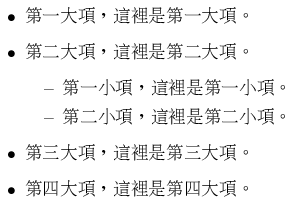
\includegraphics{itemize}
\end{quote}
\end{htmlonly}

\subsection{�C�|�����C���ҡ]enumerate�^}
\label{subsec:enume}\index{�C�|�����C���ҡ]enumerate�^}

�o�O�H�ƥئr�Φr����ù���Ʀr�Ӱ_�Y���ت����C�覡�C�P�˪��Ҥl�A�令 {\tt enumerate} ���ܡA�|�ƪ����G

%begin{latexonly}
\begin{quote}
\begin{enumerate}
\item �Ĥ@�j���A�o�̬O�Ĥ@�j���C
\item �ĤG�j���A�o�̬O�ĤG�j���C
  \begin{enumerate}
  \item �Ĥ@�p���A�o�̬O�Ĥ@�p���C
  \item �ĤG�p���A�o�̬O�ĤG�p���C
  \end{enumerate}
\item �ĤT�j���A�o�̬O�ĤT�j���C
\item �ĥ|�j���A�o�̬O�ĥ|�j���C
\end{enumerate}
\end{quote}
%end{latexonly}

\begin{htmlonly}
\begin{quote}
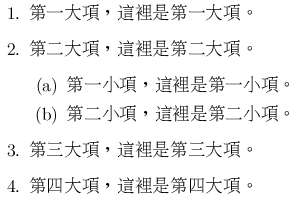
\includegraphics{enumerate}
\end{quote}
\end{htmlonly}

\subsection{�ԭz�����C���ҡ]description�^}
\index{�ԭz�����C���ҡ]description�^}

�o�O�H�@��²�u��r�ԭz�Ӱ_�Y���ت����C�覡�C�A��L�令 {\tt description} ���ܡA�L�O�H�����r�Ӱ_�Y���ت��A�o�Ǥ�r�n�Τ�A���A���C

\begin{quote}
\begin{verbatim}
\begin{description}
\item[�Ĥ@�j��] �o�̬O�Ĥ@�j���C
\item[�ĤG�j��] �o�̬O�ĤG�j���C
  \begin{description}
  \item[�Ĥ@�p��] �o�̬O�Ĥ@�p���C
  \item[�ĤG�p��] �o�̬O�ĤG�p���C
  \end{description}
\item[�ĤT�j��] �o�̬O�ĤT�j���C
\item[�ĥ|�j��] �o�̬O�ĥ|�j���C
\end{description}
\end{verbatim}
\end{quote}

�ƪ��X�Ӫ����G�O�G

%begin{latexonly}
\begin{quote}
\begin{description}
\item[�Ĥ@�j��] �o�̬O�Ĥ@�j���C
\item[�ĤG�j��] �o�̬O�ĤG�j���C
  \begin{description}
  \item[�Ĥ@�p��] �o�̬O�Ĥ@�p���C
  \item[�ĤG�p��] �o�̬O�ĤG�p���C
  \end{description}
\item[�ĤT�j��] �o�̬O�ĤT�j���C
\item[�ĥ|�j��] �o�̬O�ĥ|�j���C
\end{description}
\end{quote}
%end{latexonly}

\begin{htmlonly}
\begin{quote}

\includegraphics{description}
\end{quote}
\end{htmlonly}

�n�`�N���O�A���ޭ��@�ت����C���ҡA�C�Ӷ��ء]item�^����r�ԭz�|�۰ʧ��A�o�۷���K�A�ϥΪ̥u�n����C�����c�˧��A�M�ߥ��C�Ӷ��ت����e�N���F�C�ӥB�A�p�G�ϥΤ�A���A���@�Ǧr���B�r��βŸ��A���a�Y���ХܱN�|�O�o�Ǧr���B�r��βŸ��A�p�G�O�C�|�������C�覡�A���򦳤�A�����N���Q�s���A�|�۰ʸ��L�A�s�����ǫh�|�۰ʶ����C

%\section{enumerate �����M��}

%\subsection{���C���Ҥ����Ŷ�����}


\section{�u��}
\index{�u��}

�u�ئb�ƪ��W�����@�w���a��A�]���L�i�H�Ϲj���P���Ŷ��A�]�i�H���Y�dz�������X�ӡC���O�A�L�h���u�ؤ]�O�|���ٻ��ܥD�����n�Ƨ@�ΡA�ϥΤW�i��n�A�i�Ӥ�C�o�̧ڭ̭n�ͪ��O��ª��u�ءA����\index{����}�]�O�u�ت��@�����ΡA�ڭ̱N�|�b�� \ref{ch:graphic} ���A�A�ӽͪ��檺�B�z�C

%�b \LaTeX\ ���u�إi�����T�ءGLR�BRule �� Par�C

%\begin{quote}
%\begin{tabular}
%�u�غ��� & �N�q \\
%\hline
%LR  & left-right�A�u�ؤνu�ؤ������e�ѥ��ܥk \\
%Rule & 
%Par
%\end{tabular}
%\end{quote}

\subsection{���u�]rule�^}
\index{���u�]rule�^}

���u�]�O�ݩ��ت��@�ءA�N�O�@�ӹ������ΡA�u���L�A�L�����μe�]�u���ղӡ^�u���@�I�I�A�ҥH�A�ݰ_�ӴN�@�����u�}�F�C

\begin{quote}
\begin{verbatim}
\rule[�W�U��m(���)]{�e}{��}
\end{verbatim}
\end{quote}

�e�ΰ��������h�������A���ӤW�U��m�O����O�H�o�ӤW�U��m�O�M��u�]baseline�^\index{��u}\index{baseline}�b������A�p�G�S�����w�A���N�O�b��u����m�A�p�G�����w�A�N�̥��t�Ƚվ�M��u���۹��m�A���ȥѰ�u�V�W�վ�A�t�ȫh�Ѱ�u�V�U�վ�C�o�̨Ӭݭӭӹ�ҴN�A�ѤF�G

\begin{quote}
\begin{verbatim}
% example13.tex
\documentclass{article}
\parskip=3pt
\parindent=0pt
\begin{document}
This is a line.       % �e�� 1pt �e 3cm ����u�C
\rule{3cm}{1pt}
\rule[1ex]{3cm}{1pt}
\rule[-1ex]{3cm}{1pt}

\rule{1pt}{3cm}      % �e�� 3cm �e 1pt �����u�C

\rule{3cm}{0pt}TEST. % �� TEST �V�k�� 3cm�C

\rule{2cm}{3cm}      % �e�� 3cm �e 2cm �������ءC

\textcolor{blue}{This is color lines.}
\textcolor{red}{\rule{3cm}{1pt}}        % ���C�⪺�u�ءC
\textcolor{green}{\rule[1ex]{3cm}{1pt}}
\textcolor{blue}{\rule[-1ex]{3cm}{1pt}}
\end{document}
\end{verbatim}
\end{quote}

�sĶ�n���Ҥl�b�G

\begin{quote}
\url{http://edt1023.sayya.org/tex/latex123/example13.tex}\\
\url{http://edt1023.sayya.org/tex/latex123/example13.pdf}
\end{quote}

�ѨҤl���i�H�ݱo�X�ӡA�o�ӵe�u���O�ä��O����a�B��e�u�Ӥw�A�F���B�Ϊ��ܡA�i�H���X�\�h���P���ĪG�A�Ҧp����Ϥ������C

\subsection{��r���u�]underline�^}
\index{��r���u�]underline�^}

���ɭԧڭ̧Ʊ�b�Ѽg��r���P�ɡA�]�b��U�e�u�C\LaTeX\ ���{�������O�i�H�ϥΡA���N�O \verb|\underline{��r}|\index{underline@\verb=\underline=}�A�|�b��r���u�������P�ɵe�W�u���C���M�A�ϥΤW�`�`�|�M�{�b����u�d�V�A�]���ϥήɭn�S�O�d�N��ӭ����W�O�_�w�g�s�b�F�\�h��u�C

\subsection{��ء]box�^}
\index{box}

�o�̥D�n������r��ءAø�ϤW���@��اΦb�� \ref{ch:graphic} ���ɦA�ӰQ�סC�o�@�����}�Y�N�w�ͨ�A��g�峹�O�Ѥ@�ӭӪ� box �Һc�����A�o�̪���ثh�O�@�Ө嫬�� box�A�L���a��A���M�O�M�e���һ��� box �@�ˡA\TeX/\LaTeX\ �|��L�����@�ӳ�@���r���ӳB�z�C

�ڭ̥��Ӭݬݳ�²�檺��ت����O�G

\begin{quote}
\begin{tabular}{ll}
���O & �N�q�Χ@�� \\
\hline
\verb=\frame{��r}= & �N��r���e�H�i������خئ��A��ةM��r���S�����Z \\
\verb=\fbox{��r}=  & �N��r���e�H�i������خئ��A��ةM��r�����@�w���Z \\
\verb=\mbox{��r}=  & �@�ΩM \verb|\fbox| �P�A����ؤ��i��
\end{tabular}
\end{quote}
\index{frame@\verb=\frame=}\index{fbox@\verb=\fbox=}%
\index{mbox@\verb=\mbox=}

�H�W�����O���i�H�Φ���ؤ�r�C

��ؤ]���i�H�վ㪺���O�G

\begin{quote}
\begin{tabular}{ll}
���O & �N�q�Χ@�� \\
\hline
\verb|\framebox[�e��][����覡]{��r}| & �P \verb|\fbox| �P�A���i���w�e�פι���覡 \\
\verb|\makebox[�e��][����覡]{��r}| & �P \verb|\mbox| �P�A���i���w�e�פι���覡
\index{framebox@\verb=\framebox=}\index{makebox@\verb=\makebox=}
\end{tabular}
\end{quote}

�o�̪��e�׫����O��ت��e�סA�����w���ܡA�@�δN�p�P \verb|\fbox| �� \verb|\mbox| �@�ˡA�H�]����Ӥ�r�d�򬰼e�סA�ѩ�ڭ̤��e��������r���e���e�צ��h�֡A�]���e�ת����w�i�H�ϥΤU�C�۹��쪺�覡�G

\begin{quote}
\begin{tabular}{ll}
�e�� & �@�� \\
\hline
\verb|\width| & �o�Ӽe�״N�O \verb|\fbox| ����ɪ���ؼe�� \\
\verb|\height| & �o�O���`��u�ܮس������� \\
\verb|\depth| &  �o�O���`��u�ܮة������� \\
\verb|\totalheight| & �o�O \verb|\height| �M \verb|\depth| ���`�M \\
\end{tabular}
\end{quote}

�Ҧp�A�ڭ̫��w \verb|2\width| �L���N��N�O�H \verb|\fbox| �]������r���e�ɡA���ؼe�ת��G���e�C�ѼƸ��Y������覡�A�i���U�C�X�ءG

\begin{quote}
\begin{tabular}{>{\tt }ll}
����覡 & �@�� \\
\hline
c & center�A��r����ؤ����A�o�O�w�]�� \\
l & flushleft�A��r����إ��� \\
r & ushright�A��r����إk�� \\
s & stretch�A��r�������������ؤ�
\end{tabular}
\end{quote}

�����w���ܡA���M�N�O����ؤ�����m�F�C�ڭ̤]�i�H���w�i����ت��u���ʲӡA�Τ�ةM��r�������j�Z���G

\begin{quote}
\begin{tabular}{ll}
���O & �@�� \\
\hline
\verb|\fboxrule=���| & ���w��ؽu���ʲ� \\
\verb|\fboxsep=���| & ���w��r�M�ؽt�����Z%
\index{fboxrule@\verb=\fboxrule=}\index{fboxsep@\verb=\fboxsep=}%
\end{tabular}
\end{quote}

�Ъ`�N�A�o���|�v�T \verb|\frame{}|�C�p�G�Q�S�O���m���ت���m�A�]�i�H�ϥ� \verb|\raisebox|\index{raisebox@\verb=raisebox=} ���O�G

\begin{quote}
\begin{verbatim}
\raisebox{�W�U��m(���)}[�`��][����]{��r���e}
\end{verbatim}
\end{quote}

�o�̪��W�U��m���N�q�M \verb|\rule| ���O���Y���@�ˡA�u���L�A�o�̪��W�U��m�@�w�n���w�A�S���w�]�ȡA�����w�|�sĶ���~�C�Фd�U�O�o�A��ؤ����M�O�٥i�H����ت��C�ڭ̲{�b�N�Ӭݤ@�Ӻ�X����ҡG

\begin{quote}
\begin{verbatim}
% example14.tex
\documentclass{article}
\parskip=3ex
\parindent=0pt
\begin{document}
\frame{This is frame.}
\mbox{This is mbox.}
\fbox{This is fbox.}

\framebox{This is a framebox with no argumant.}

\framebox[1.5\width]{This is a framebox.}

\framebox[1.5\width][l]{This is a framebox with \texttt{l}.}

\framebox[1.5\width][r]{This is a framebox with \texttt{r}.}

\framebox[1.5\width][s]{This is a framebox with \texttt{s}.}

This is baseline.
\raisebox{3ex}[5\height]{This is a raisebox which lift 3ex.}

This is baseline.
\fbox{\raisebox{-3ex}[5\height]{This is a raisebox which lift $-$3ex.}}

\fboxrule=1.5pt
\fboxsep=8pt
\framebox[1.5\width][s]{This is a framebox with \texttt{s}.}
\end{document}
\end{verbatim}
\end{quote}

�o���L�ݦh�[�����A�sĶ�n���Ҥl�b�G

\begin{quote}
\url{http://edt1023.sayya.org/tex/latex123/example14.tex}\\
\url{http://edt1023.sayya.org/tex/latex123/example14.pdf}
\end{quote}

\subsection{�q�����}
\index{�q�����}

�t�~�A�]���Ω�q����r����ءA�i�H����Y�Ӭq���X�{�b�Y�S�w���Ŷ��B��m�C�ڭ̱`�`��o�ئw�ƺ٬��g�A�����A�⪩�����e�m��@�Ӥ��i������ط����A���M�A�o�Ӥ�ةM�@�몺 box�A�Ҧp�r���A���M�B��P�˪��a��A\LaTeX\ �|��L�����@�Ӧr�����ӳB�z�C

\begin{quote}
\begin{verbatim}
\parbox[����覡][����][�����m]{�e��}{��r���e}

\begin{minipage}[����覡][����][�����m]{�e��}
  �q�����e
\end{minipage}
\end{verbatim}
\end{quote}
\index{parbox@\verb=parbox=}\index{minipage@\texttt{minipage}}

�o�̪��Ĥ@�ӿ�ܩʰѼơu����覡�v�G

\begin{quote}
\begin{tabular}{>{\tt }ll}
t & top�A�q����ت��W�u����@�檺��u \\
b & bottom�A�q����ت��U�u����@�檺��u \\
c & center�A�q����ت���������@�檺��u�A�o�O�w�] \\
\end{tabular}
\end{quote}

\verb|\parbox| ���O�q�`�Ω���u����r���e�A�p�G�O�������q���A���ϥ� {\tt minipage} ���ҷ|�����K�C�o�Ǭq����ةM�W���ҽͨ쪺�@�Ǥ�س̤j�����P�O�A�q����إ��N�O�Ψӱƪ��p�q����y�A�]���L�|�M�@�륿�`�峹�q���@�˪��B�z�A�Ҧp�L�|�۰��_��A�I��ťզ�]�|�_�s�q���A���U�q���w�]�O���Y�ƪ��A�ӥB�A�b�w�ƤW�|��@�몺�q�����A�@����t�����Z�|�Y� 0pt�C

���פ��h���w���ܡA���N�O�H��Ӫ����g�_��B�z��A��Ӥ�r�q���ҧΦ������סC�ܩ󤺤��m�����]�O \texttt{t, b, c} �o�ǡA�N��O��r�q���b��ؤ����W�U��m�A���M�A�o�n�����w��ذ��׮ɤ~�|���N�q�A�]���A�u�����m�v�M�u���סv�O�n�P�ɫ��w���A�n�D�`�`�N���O�A�p�G���w�F���סA���S�����w�����m�A�h�w�]�O����e���ϥΪ��u����覡�v�ҫ��w���ѼơC

�o�ǰѼƪ��ϥη|���ǷнơA���o�O�u�ʩұa�Ӫ��u���n���c�v�A�����h���O�A�u���b�Ĥ@����IJ�ɧ�L�d�M���N���F�A��ڭn�Ψ�ɦA�Ӭd�L���ԲӰѼơA�`�Ϊ����O�B���ҡA�j���h�d�X���N�۵M�ӵM���O�_�ӤF�C


% ``�j�a�Ӿ� LaTeX'' LaTeX ��Z class.tex
% Copyright (c) 2004  Edward G.J. Lee <edt1023@info.sayya.org>
%
% �b���H�� GNU Free Documentation License 1.2 �ΥH�᪺�����W�d���U�A
% ���\�����B���G�έק�C���쪩�v�B���v�n�����o�����C
%
% �����G�����A�t�� fdl.tex�A���e�� GNU FDL ���W�d���C�p�G�򥢡A�i��
% http://www.gnu.org ���o�A�μg�H�ܦۥѳn�����|(Free Software Fundation)
% �����C
% 9 Temple Place - Suite 330, Boston, MA 02111-1307, USA.
%
% $Id: class.tex,v 1.14 2004/03/06 17:17:55 edt1023 Exp $
%
\chapter{\LaTeX\ ���зǤ�Z���O}
\label{ch:class}\index{��Z���O}

�o���D�n�O�b���� \LaTeX\ ��Z�����O�]document class\index{document class}�^\footnote{�o�b�ª������٬� style�A�o��ӵ��N�q�W�t���h�A�o�dz��O \TeX\ �����X�Ӫ������w�q�A�M���Ψөw�q�峹���j���c�A�H�K²�ƨϥΤW�Τ�Z�����e�C}�A�o�O \LaTeX\ �W�d��Z���鵲�c����k�C�ϥ� class ���ηN�A�N�O�⪩�����c�B�z�M��ڤ�Z���}�A�o�˪��̤j�n�B�N�O������g�峹�ƪ����c�W���@�P�ʡA�]�Ϥ�Z���e��M�n²��A�ϥΪ̥u�n�M�ߩ��Z���e���g�@�Y�i�A�p�G class �w�q���n�A�]�i�H�F��@��h�ܤƤS���ܧ��Z���e���ت��A�u�n��ޥΪ� class �����O���N�i�H�F�A��L���i�H������ʡC

�ثe�A\LaTeX\ �����ؼз����O�Ω�@����A�i�Ω�@�몺�ѫH�B���x�B���Z�B���i�νפ�C�����Ǵ��Z�B�פ�|�n�D�@�w�����c�A�o�ɱo�̻ݨD�t��q�w�C�]���A�]����L�����O�s�b�A�з����O�ä��O�ߤ@���C�ƦܡA�]�i�H�ۦ漶�g�ۤv����Z���O�C���M�A�ڭ̤@��ϥάO���ݭn�o�����s�A�o�̥u���� \LaTeX\ ���з����O�C�ӥB�A�p�G���M�L�H�洫��Z���ݨD�ɡA�ڭ����Ӻɥi�઺�ϥάy�q�ʸ��s�x�����O�C

�t�~�A�]���@�ǬO���� \LaTeX\ �������� macro\index{macro} �g�@�ɭn�Ψ쪺���O�A�o�Ǥw�W�X���g�峹���d��C

\section{\LaTeX\ ���O���ŧi}
\index{���O���ŧi}

\LaTeX\ �����O�A�n�b��Z���@�}�Y�ɴN�ŧi�]���M�A��W�����ѬO�S�����Y���^�A�L���@��榡�p�U�G

\begin{quote}
\begin{verbatim}
\documentclass[��ܩʰѼ�]{���O}
\end{verbatim}
\end{quote}
\index{documentclass@\verb=\documentclass=}

��ܩʰѼƬO�i�H�ٲ����A�����O�W�٫h����١A�@�w�n���w�@�����O�C�ӥB�u��u���@�����O�C

\section{���O����ܩʰѼ�}

��ܩʰѼƥi�H��ܦh�ӡA�U�ӿﶵ�O�H�r�I���}���C

\begin{enumerate}
\item {\tt 10pt, 11pt, 12pt}\\
���w����@�륿�`�r���j�p�A�w�]�O {\tt 10pt}�C��L�I�ƨS���~�� package ������������w�C
\item {\tt a4paper, letterpaper, b5paper, executivepaper, legalpaper}\\
���w�ȱi�j�p�A�w�]�O {\tt letterpaper}�C
\item {\tt fleqn} \\
�ϼƾǦ��a������A�w�]�O�~������C\index{fleqn@\texttt{fleqn}}
\item {\tt leqno} \\
�ϼƾǦ��s���a���A�w�]�O�a�k�C
\item {\tt titlepage, notitlepage}\index{titlepage@\texttt{titlepage}}\index{notitlepage@\texttt{notitlepage}} \\
�M�w title page �O�_�W���@���C�w�] \texttt{article}\index{article@\texttt{article}} ���W���@���A�� \texttt{report/book}\index{book@\texttt{book}}\index{report@\texttt{report}} �h�|�W���@���A�b�o�̬O�i�H���w���ܧ�w�]�欰�A�Ҧp \texttt{article} ��Z�A���w \texttt{titlepage} ���ܡA�� title page �N�|�W���@���C
\item {\tt onecolumn, twocolumn} \\
�峹����Ψ��榡�A�w�]�O����A�]�N�O������C\index{onecolumn@\texttt{onecolumn}}\index{twocolumn@\texttt{twocolumn}}
\item {\tt twoside, oneside}\index{twoside@\texttt{twoside}}\index{oneside@\texttt{oneside}} \\
�O�_�Ϥ��_���ƭ��C�w�] \texttt{article/report} ���Ϥ��A\texttt{book} �h�|�Ϥ��C�@�몺���y�A�b�˭q�������A�L�������u�٬��ѯ�A���ƭ��|�b���}���y�ɪ�����A�ӥB�䤤���e�|���V�ѯ᪺�����]���ɬO�V�k�^�A�Ϥ��A�_�ƭ��|�b�k�A���e�@�˷|�����V�ѯ�A�b \texttt{oneside} �����Ϋh�����o�˪��Ϥ��A���ީ_�������|�b�ȱi����������C
\item {\tt landscape} \\
��V�C�L���a�V�C�L�A�w�]�a�V�]portait�^�C\index{landscape@\texttt{landscape}}\index{portait@\texttt{portait}}
\item {\tt draft}\index{draft@\texttt{draft}} \\
��Z���sĶ�A�o�ɹ��ɱN���|�Q�ޤJ�A�i�[�ֽsĶ���t�סC���L�A�p�G�sĶ�O�ϥΦV�q�r�����ܡA�sĶ�t�����ӬO�ٺ�ܧ֡C���ϥ� {\tt draft} ���@�Ӧn�B�O�A�L�����a��|�ХܥX�ӡC
\item {\tt openright, openany}\index{openright@\texttt{openright}}\index{openany@\texttt{openany}} \\
�o�O�b����A�����}�l�O�_�O�_�ƭ��]right-hand page�^\index{�_�ƭ��]right-hand page�^}�C�b \texttt{book} ���O�A�w�]���|�q�_�ƭ��}�l�Areport ���O�h���|�C\texttt{article} ���O�S�����A�ҥH�A�惡�@�]�w�|�����C
\end{enumerate}

\section{���O������}

�o�̥u�C�X�@��峹�ϥΪ����O�A��L�S�������� \LaTeX\ �������ҨϥΪ����O�N���C�X�F�A�@��ϥΡA�o�����O�N�����F�C

\begin{quote}
\begin{tabular}{>{\tt }lll}
���O & �@��γ~ & �S�� \\
\hline
article & �@��u�� & �L���A�s�򭶤覡���w�ơA�L�_���ƭ����Ϥ� \\
report  & �����פ� & ���|�_�s���A�w�]�L�_���ƭ����Ϥ� \\
book    & ���y��   & ���|��_�ƭ��_�s���A�w�]�����ƭ����Ϥ� \\
letter  & �H��     & �^��H��榡 \\
slides  & �ۿO��   & �X�G�t�Υ~�ӮM����N \\
minimal  & ���դμg�s���O   & �o�O��²�檺���O�A�u�W�w�F���媺�e�B���A���`�r
\end{tabular}
\end{quote}
\index{article@\texttt{article}}\index{report@\texttt{report}}%
\index{book@\texttt{book}}\index{letter@\texttt{letter}}%
\index{slides@\texttt{slides}}\index{minimal@\texttt{minimal}}

���M�A�o�ǥγ~�ä��O�T�w���ܪ��A�o�ݨϥΪ̪��w�ơA���Q�h��ɶ��B�믫���ܡA���N�� \LaTeX\ �w�]���榡�h�ϥΡA�ܤִN���|�����СC�䤤 \texttt{minimal} class �O�ΨӴ��եΪ��A�Ϊ̼g�s�� class �Ϊ��A�L�����S���������w�ơA�Ҧp�A�S�����`�����c�A�U�ض��Z�]�S���w�q�A�w�]���r���O���`�r�A�S����L���ܤơA�X�G�Ҧ����ܤƭn�ۦ�h�w�q�C


% ``�j�a�Ӿ� LaTeX'' LaTeX ��Z package.tex
% Copyright (c) 2004  Edward G.J. Lee <edt1023@info.sayya.org>
%
% �b���H�� GNU Free Documentation License 1.2 �ΥH�᪺�����W�d���U�A
% ���\�����B���G�έק�C���쪩�v�B���v�n�����o�����C
%
% �����G�����A�t�� fdl.tex�A���e�� GNU FDL ���W�d���C�p�G�򥢡A�i��
% http://www.gnu.org ���o�A�μg�H�ܦۥѳn�����|(Free Software Fundation)
% �����C
% 9 Temple Place - Suite 330, Boston, MA 02111-1307, USA.
%
% $Id: package.tex,v 1.21 2004/03/07 12:18:40 edt1023 Exp $
%
\chapter{�����M��}
\label{ch:package}\index{�����M��}

\LaTeX\ �t�Τw�g�n�[�S����s�A���dz����i��|�򤣤W��ڪ��}�B�A�ӥB���Ǥ��w�������w�q�A�g�L�j�a���ϥΡA�oı�ä��O���򪺶���A�ר�O�\�઺�j�Ƥ譱�A�]���o���ͽͦp��ޥΥL�H�w�g�g�n�������A�o�ܭ��n�A�ɶq�קK���ƻs�y���l�A�g \TeX/\LaTeX\ macro\index{macro} �i���O�ܱM�~���u�@�A�n�קK�}�a�F���骺���c�A�ҥH����ݬݦ����򥨶��M��i�H�ϥΡC

%�U�@�䤣��A�X�������M��A�γo�ǥ����M�󪺩w�q�����ũһݡA�o�ɧڭ̴N�o�ۦ�ק�w�q�A�ƦܬO���s�w�q�ӲŦX�һݡA�o�]�O�o�@���dzƱ��Q���@�ӥD�D�C���O�A���O�C�@�ӤH�����R�Ϊ��ɶ��h�Dz� \TeX/\LaTeX\ �������y���A�ҥH�o�̱��Q���H��ΡB²�檺�w�q��k���D�A�y�L�������w���ŦX�@��ϥΪ���h�A�]�M�o�g�峹���c�Q�d�򤣲šC

\section{�@��M�󪺨ϥ�}

�ڭ̴��b�� \ref{subsec:preamble} �p�`�A�� \pageref{subsec:preamble}�A����L²�楨�����ޥΡA�ƹ�W�A���ǥ����t���\�h���ѼƨӰ��L�աA���O�C�ӥ����M�󪺰ѼƳ����|�@�ˡA�]���A�ϥήM�󤧫e�n���ݤ@�ݥL�Ҫ��W���ϥΤ�U�C�X�G�j�����������M�󳣦��ϥΤ�U�A�p�G�O�t�ΤW�N���������A����o�Ǥ��q�`�|��b�G

\begin{quote}
\begin{verbatim}
$TEXMF/doc  => Unix-like �t��
$TEXMF\doc  => DOS/Windows �t��
\end{verbatim}
\end{quote}

�o�ǥؿ����U�A�o�Ǥ��|����l \TeX/\LaTeX\ ��Z�A�]���sĶ�n�� \texttt{*.dvi} �� \textsc{PostScript}\index{PostScript@\textsc{PostScript}} �ɥi�H�\���A���D��K���ܡA�i�H�N�L���ন pdf �榡�Ӿ\���A��]�O�i�H�H����r�ӷj�M����A�b�d���O�B���Үɷ|�����K�C�b Unix-like\index{Unix-like} �t�Ω� Windows\index{Windows} �U�� cygwin\index{cygwin} ���Ҫ��ܡA�i�H�ϥ� \texttt{texdoc}\index{texdoc@\texttt{texdoc}} �o�ӫ��O�Ӿ\���A�Ҧp�G

\begin{quote}
\begin{verbatim}
texdoc amsguide  => �\�� amsguide.dvi �o���ɪ�����
texdoc -s ams    => �d�t�ΤW�Ҧ��t ams �r�˪����
\end{verbatim}
\end{quote}


\section{\LaTeX\ �x���󤤪��зǥ����M��}

���U�O \LaTeX\ �x���󤤩Ҫ����зǥ����M��C���M�O�зǥ����M��A���@�뱡�ΤU�A�ϥγo�� packages �����|�ä��h�A���O���S���ݭn�ɤ~�|�ޤJ�C

\subsection{alltt}\index{alltt@\textsf{alltt}}

�o�ӥ����M�󴣨� \texttt{alltt}\index{alltt@\texttt{alltt}} ���ҡA�M \texttt{verbatim}\index{verbatim@\texttt{verbatim}} ���Ҫ��@�άۦP�A�u�O \textbackslash{}�A\{�A\} ���@�ΩM�@��峹���ۦP�|�Q \LaTeX\ ��Ū�C�o������ΩO�H�o�ˤ@�� \LaTeX\ �o�ӯS���лx�]�i�H�ϥΡA�]�i�H�����Ҥ�����r�㦳�C��A�ΰ���L�ܤơA���M�A���Y����r�w�]���M�O�ϥΥ��r���r��\index{���r���r��}���C

\subsection{doc}\index{doc@\textsf{doc}}

�o�O�ΨӼg \LaTeX\ ��󪺥����M��A�o�b�ϥ� \texttt{ltxdoc}\index{ltxdoc@\texttt{ltxdoc}} �o�� class ���P�ɴN�|���J \textsf{doc} package�C�ѩ�o���O�Ω�@�몺���ϥγ��X�A�ҥH�A�o�̴N���h�͡A�����쪺�ܥi�ۦ�ѦҥL����󻡩��C

\subsection{exscale}\index{exscale@\textsf{exscale}}

�ѩ����� Computer Modern font\index{Computer Modern font} �����ƾǩ����Ÿ��]\texttt{cmex}\index{cmex@\texttt{cmex}}�^�u�� 10pt �j�p���r���]\texttt{cmex10}�^�A�����j�� \texttt{large} �H�W���r���ɡA�Ҧp��j�� \texttt{Large} �ɡA���ǼƾDzŸ����M�|�����@�w���j�p�A�o�ɥi�H�ϥγo�ӮM��A���o�ǼƾDzŸ��]��۩�j�A�Ҧp�n���Ÿ��C\textsf{exscale} �u���r���Y�񪺩w�q�A�]���u�n��o�ӮM��b preamble\index{preamble} �ϤޥδN�i�H�F�A�L�ݥ�����O�C

���L�A�o�̭n�����@�U�A�b \TeX/\LaTeX\ �̦r����j�A���ɥi��|�y�����{���u�����ΡA�ר�O�ƾǦ��l�A���F�U�μƾǦ��l���U�Ӧr�������Ŷ��w�ơA\texttt{cmex10} ���]�p�ä��A�X���ө�j�A�i�H�� \texttt{cmr5} ��j�� 10pt �M�u���� \texttt{cmr10} �Ӥ���N�|���D���{�X�ӷ|���@�ˡA�]���A�p�G�Ҽ{��T�t�X�����D�A��j�ƾǦ��l���r���ɥi��n�Ҽ{�@�U�ϥγ��X�A�ר�ثe�ĥΦV�q�r��O�p���C�иոեH�U���Ҥl�A�ڭ̧� \texttt{cmr5}�B\texttt{cmr10} �� \texttt{cmr12} �P�˩�j�� 30pt �Ӭݬݵ��G�|���|�@�ˡG

\begin{quote}
\begin{verbatim}
% test-fonts.tex
\font\largecmr=cmr12 at 30pt
\largecmr
This is cmr12 at 30pt.

\font\largecmr=cmr10 at 30pt
\largecmr
This is cmr10 at 30pt.

\font\largecmr=cmr5 at 30pt
\largecmr
This is cmr5 at 30pt.
\bye
\end{verbatim}
\end{quote}

�Ъ`�N�A�o�O \TeX\ ��Z�A���O \LaTeX\ ��Z�A�ҥH�n�ϥ� \texttt{tex}\index{tex@\texttt{tex}} �� \texttt{pdftex}\index{pdftex@\texttt{pdftex}} �ӽsĶ�A�L�����G�p�U�A�j�a�i�ܲM�����ݱo�X�ӡA���M�P�ˬO�V�q�r�A����j�ɪ����{�ä��|�@�ˡG

\begin{quote}
\url{http://edt1023.sayya.org/tex/latex123/test-fonts.tex}\\
\url{http://edt1023.sayya.org/tex/latex123/test-fonts.pdf}
\end{quote}

�ھ� Knuth\index{Knuth} �б·���]�p \MF\index{metafont@\MF}�A�L���z���O�@�ӦP�˪��r���b��j���ɭԡA�P�@�Ӧr�A�L�������m�񪺬۹��m���ӭn�H��j�����Ʀӵy�[�վ�C�]���A���p�ڭ̥u�ϥΤ@�ئV�q�r��\index{�V�q�r��}�A�Φb���P����j���v���ɭԡA��r�Ÿ������Ŷ��t�X�|���ͤ��@�˪����G�A�ר�O�Φb�ƾǦ��l\index{�ƾǦ��l}���ɭԡA��[����C

���M�A��ΤW \MF\ ���M�]�O�@�ئV�q�r���A���ѩ�ӹL������A���A�X���ӿù���ܤW�ΡA�ҥH�~�|�h�ӨD�䦸�A�ন pk �I�}�r���ӨϥΡC�o�]�N�O������P�ˬO \texttt{cmr} ���r���A�|���X�ؤ��P�I�ƪ��W�ߦr������]�A�a�ϬO�V�q�r�]�O�p���C\TeX\ �w�g 20 �X���F�A���O�A�ڭ̪��r���޳N���G�٬O�S���������W���� Knuth �бª��z���C

\subsection{fontenc}\index{fontenc@\textsf{fontenc}}

�b�� \ref{subsec:font-attr} �p�`�A�� \pageref{subsec:font-attr}�A������r���s�X�����D�C�n���ܦr���s�X�A�i�H�ϥγo�� \textsf{fontenc} package�C�H T1 font encoding\index{T1} �ӻ��G

\begin{quote}
\begin{verbatim}
  ...
\usepackage[T1]{fontenc}
  ...
\end{verbatim}
\end{quote}

�o�˴N�i�H�F�A���ѩ�@�Ǧr���A�Ҧp�ڬw�r���A�b��Ӫ� Computer modern Type1 �r�����w�Ƥ��@�ˡA�ҥH�A���dz����|�ϥέ�l�� \MF\ �r�����ഫ���� pk �I�}�r�A�o�˪��ܡA�@��L�����L�X�ӬO�t�����j�A���p�G�O�Q�s�@�� PDF �榡�b�å����\�����ܡA�r�������{�|�ܱo����C�z�Q���ܡA�n�w�� \texttt{cm-super}\index{cm-super@\texttt{cm-super}} Type1 �r���A���O�@��ϥΪ̮��Ȧۦ�w�˦r���|���x���C�o�b te\TeX\ 2.x\index{tetex@te\TeX} �H�᪺�����A�w�g�����W \textsf{pxfonts}\index{pxfonts@\textsf{pxfonts}} �� \textsf{txfonts}\index{txfonts@\textsf{txfonts}} package �Ψ�r���A�ҥH�A�p�G�O�s�񪩥��� te\TeX\ ���ܡA�i�H�ѥH�U���覡�ӨϥΡG

\begin{quote}
\begin{verbatim}
  ...
\usepackage{txfonts}
\usepackage[T1]{fontenc}
  ...
\end{verbatim}
\end{quote}

�䤤 \textsf{txfonts} �O���� Times �t�C���r���A\textsf{pxfonts} �O���� Palatino �t�C���r���C���M�A�o������r�������D���I�����A�o���b�o�g�峹���Q�׽d��A�u�వ²�檺�����A�p�G�S���S���ݭn�A�Ҧp�A�ڬw�r���B�@�Ǧ������Ÿ����r���A���ϥιw�]�� OT1 �s�X�N��F�A�]���o�ǮM��Ҫ������Ǧr���A�u���@�ؤj�p�� Type1 �r���b�Y��A�]���ϥΤW���ȷ|�����u\index{���u}�����ΡC

\subsection{graphpap}\index{graphpap@\textsf{graphpap}}

�o�O���ͤ��Ȫ������C�L���ѤF�@�ӫ��O�A�i�H�e���A�i�H�t�X \texttt{picture}\index{picture@\texttt{picture}} ���ҨӨϥΡA�L���y�k�O�G

\begin{quote}
\begin{verbatim}
  ...
\usepackage{graphpap}
  ...
\graphpaper[n](x,y)(x1,y1)
  ...
\end{verbatim}
\end{quote}

�䤤�� \texttt{n} �p�G�ٲ����ܡA�w�]�O 10�A�L�����O���Ȫ��̤p��׳��C\texttt{(x,y)} �� \texttt{(x1,y1)} �����O���U���Υk�W�����y�ЭȡA�Ҧp�G

\begin{quote}
\begin{verbatim}
\documentclass{article}
\usepackage{graphpap}
\begin{document}
\graphpaper(0,0)(360,360)
\end{document}
\end{verbatim}
\end{quote}

�o�˷|�e�X�H 10 ���̤p��ת����A�sĶ�n���Ҥl�p�U�G

\begin{quote}
\url{http://edt1023.sayya.org/tex/latex123/test-graphpap.tex}\\
\url{http://edt1023.sayya.org/tex/latex123/test-graphpap.pdf}
\end{quote}

\subsection{ifthen}\index{ifthen@\textsf{ifthen}}

\TeX\ �����O�@�رƪ��{���y���A���M�|������P�_��\index{����P�_��}�Ӥ�K�g�����A���p�G��Z���]�R���F����P�_���A�N�|�Ϥ�Z�����ơA���H�\Ū�B���@�A�]���A�@�����P�_���j�h�ƨϥΦb�����w�q�A�Ӥ��O�g�b��Z�����C�o�� package �N�O�b²�Ʊ���P�_���A�H�K�]�i�H��K�ϥΦb��Z�����C 

\textsf{ifthen} package ���ѤF \verb|\ifthenelse|\index{ifthenelse@\verb=\ifthenelse=} ���O�Ӱ�����P�_�C�L�᭱���T�ӰѼơA�Ĥ@�ӬO���󦡡A�ĤG�ӬO���󬰯u���ɭԭn���檺���e�A�ĤT�ӬO���󬰰����ɭԭn���檺���e�C�o�̤��h�ͥL���ϥΡA���U�u���Ѥ@�ӹ�Ҥ��q�G

\begin{quote}
\begin{verbatim}
  ...
\usepackage{ifthen}
  ...
\ifthenelse{\isodd{\thepage}}%
  {\setlength{\leftmargin}{10pt}}%
  {\setlength{\leftmargin}{0pt}}
  ...
\end{verbatim}
\end{quote}

�o�˩_�ƭ��ɡA\texttt{leftmargin} �|�]�� 10pt�A���ƭ��ɫh�� 0pt�C�᭱�[ \texttt{\%} �N���A�o�T��O�@���A�䶡�S���ťաC

\subsection{inputenc}\index{inputenc@\textsf{inputenc}}

�ѩ� \textsf{fontenc} package ���@�Ǧr���s�X�w�ơA�M�@��ҿת� Latin-1\index{Latin-1} �o�ǽs�X�]input encoding�^�A�L�̪����e���@�w�۲šA�ҥH�A\textsf{fontenc}\index{fontenc@\textsf{fontenc}} package �`�|�M \textsf{inputenc} package ���۰t�X�ϥΡA�H�T�O�b�ϥμڬw�r���B�Ÿ��ɯॿ�T���o��r�C�Ҧp�G

\begin{quote}
\begin{verbatim}
  ...
\usrpackage[T1]{fontenc}
\usepackage[latin1]{inputenc}
  ...
\inputencoding{ascii} % �]�i�H�b��Z�����ܴ�
  ...
\inputencoding{latin2}
  ...
\inputencoding{latin1}
  ...
\end{verbatim}
\end{quote}

���M�A�ڭ̪���Z�p�G�u�O�^���y�t���峹�A���o�dz��i�H�����z�|�C

\subsection{latexsym}
\label{subsec:latexsym}\index{latexsym@\textsf{latexsym}}

�o�O \LaTeX\ �B�~���Ѫ��Ÿ��C�b�s���� \LaTeXe\ �ä��|�۰ʸ��J�A�n�ۦ�ޤJ�o�ӿW�ߥX�Ӫ� package�C�o�D�n�O���� \texttt{lasy*} �o�Ǧr�����Y���Ÿ��C�p�G���ϥ� \textsf{amsfonts}\index{amsfonts@\textsf{amsfonts}} �� \textsf{amssymb}\index{amssymb@\textsf{amssymb}} package ���ܡA�o�� \textsf{latexsym}\index{latexsym@\textsf{latexsym}} �Ÿ����ӬO�i�H�L�ݤޤJ�]���ּƲŸ��O \LaTeX\ �S�����^�C�ܩ�U�زŸ��� package �����Ǥ��e�A�i�H�ѦҨt�ΤW�� \texttt{symbols*} �o���ɮסA�L�i��s�b���Φ��O�G

\begin{quote}
\begin{verbatim}
symbols.dvi
symbols-a4.ps[pdf]
symbols-letter.ps[pdf]
\end{verbatim}
\end{quote}

�Ϊ̡A�]�i�H�q CTAN\index{CTAN} �U���̷s�������G

\begin{quote}
\url{ftp://cam.ctan.org/tex-archive/info/symbols/comprehensive/symbols-a4.pdf}
\end{quote}

\subsection{makeidx}\index{makeidx@\textsf{makeidx}}

�o�O�b�s�@����\index{����}�ɭn�ޤJ�� package�A�ڭ̷|�b�� \ref{sec:index} �`�A�� \pageref{sec:index} �A�ӰQ�סC

\subsection{newlfont}
\index{newlfont@\textsf{newlfont}}

�o�O�����ª� \LaTeX\ ���r���Ϊk�A���L�ϥηs�����r��� package�C�]�N�O�ڭ̦b�� \ref{subsec:font-command}�A�� \pageref{subsec:font-command} �Ҵ��쪺�Ϊk�C���K�·СA�ڭ̺ɶq�קK�ϥ��¥Ϊk�A�ӨϥΦr�����зǫ��O�C

\subsection{oldlfont}
\index{oldlfont@\textsf{oldlfont}}

�o�O�����ª� \LaTeX\ ���r���Ϊk�� package�C

\subsection{showidx}
\index{showidx@\textsf{showidx}}

�o�� package �|��ܡA\verb|\index|\index{index@\verb=\index=} ���O�U�b����a��C�o�]�|�b�� \ref{sec:index} �`�ӰQ�סC

\subsection{syntonly}

\textsf{syntonly}\index{syntonly@\textsf{syntonly}} package ���� \verb|\syntaxonly|\index{syntaxonly@\verb=\syntaxonly=} ���O�A�L�i�H�ˬd�y�k�O�_���T�A�ä��|�� {\tt *.dvi} �ɪ���X�C���o�� \verb|\syntaxonly| ���O�@�w�n��b preamble �ϡC

\subsection{tracefnt}
\index{tracefnt@\textsf{tracefnt}}

�o�O�l�ܦr���ϥα��Ϊ� package�C�q�`�sĶ�ɩҲ��ͪ���T�w�g�ܨ����A���p�G�Ʊ榳��ԲӪ��r���ϥθ�T���ܡA�i�H�ϥγo�� package�G

\begin{quote}
\begin{verbatim}
  ...
\usepackage[debugshow]{tracefnt}
  ...
\end{verbatim}
\end{quote}

�Ъ`�N�A�o�˷|�W�[�sĶ���ɶ��A�ӥB {\tt *.log} �ɷ|�ܤj�C

\section{\LaTeX\ �x���󤤪��u���}

�o�ǥ����M��A\LaTeX\ �x����O�k���b�����n��]relative software�^���A�i��|��W�@�`���쪺�зǥ����M��ӱo��ΨǡC���]�P�ɥi�H�ݱo�X�� \LaTeX\ �D���ت��M�󤣤֡A�[�W��L�~�Ӫ������M��A���u���O�M�󺡤ѭ��A�ڭ̫ܧƱ�b�i�઺���ΤU \LaTeX\ team �i�H�Ҽ{�N�@�ǥ��n���M��ǤJ���ءA��[���ꪩ���B�z�M��Z�g�@���}���z���C

\subsection{\AmS-\LaTeX}
\index{AmS-LaTeX@\AmS-\LaTeX}

\LaTeX\ �����N���ƪ��ƾǦ��l����O�A���b����M�~�ϥήɡA�i��|�ݭn�W�j�L���\��A\AmS-\LaTeX\ �O����ƾǨ�|�]American Mathematical Society, AMS\index{AMS}\index{American Mathematical Society}\index{����ƾǨ�|}�^�ҵo�i���@�ӼW�j \LaTeX\ �ƾǦ��l�s�誺�����աA�O�� \AmS-\TeX\\index{amstex@\AmS-\TeX} ���ӹL�ӵ� \LaTeX\ �ϥΪ��A�L�D�n������ӳ����G\textsf{amscls}\index{amscls@\textsf{amscls}} �� \textsf{amsmath}\index{amsmath@\textsf{amsmath}}�A�e�̴��ѲŦX AMS �����W�檺��Z���O�A��̥i�[�j��� \LaTeX\ ���ƾǼҦ��C�ڭ̷|�b�� \ref{ch:math} ���A�� \pageref{ch:math} �[�H���СC

\subsection{babel}
\index{babel@\textsf{babel}}

�p�G�Q�ƪ��^��H�~����L�ڬw��a���y��A�Ҧp�G�w��B�k��A���i�H�Q�� \textsf{babel} �����M��C

\subsection{cyrillic}
\index{cyrillic@\textsf{cyrillic}}

�o�O�M���ƪ����Ԥҥ��ڻy��A�Ҧp�G�X��A���i�H�ϥγo�ӮM��C

\subsection{graphics}
\index{graphics@\textsf{graphics}}

�o�O�B�z�ϧέn�Ψ쪺�����M��\index{�����M��}�C���ثe�@�볣�ϥΥ\��������� \textsf{graphicx}\index{graphicx@\textsf{graphicx}} �����M��Ө��N \textsf{graphics}\index{graphics@\textsf{graphics}} �F�A�ƹ�W�A�ޥ� \textsf{graphicx} �|�۰ʪ��ޥ� \textsf{graphics}�A�Ӧb���O�ϥΪ���K�ʤW�A\textsf{graphicx} ���ΡA�]���ڭ̩��᳣�O�H \textsf{graphicx} ���D�ӻ������C�o��ӮM���ݩ� \LaTeX\ ���ϧΤu��աA�o�Ӥu��ե]�A�F�M�C��B�ϧά������U�إ����A�ڭ̷|�b�� \ref{ch:graphic} ���A�� \pageref{ch:graphic} �ӰQ�סC

\subsection{psnfss}
\index{psnfss@\textsf{psnfss}}

�o�O Type1 �r���������M��աA�Ҧp�G\textsf{times}, \textsf{charter}, \textsf{mathptmx}\index{mathptmx@\textsf{mathptmx}} �����A�L�|�h�ϥγo�� Type1 �r��\index{Type1 �r��}�C���q�`�o�Ǧr�����\�h�O�ӷ~�r���A�t�ΤW���@�w�|���A�p�G�S�����ܡA�|�h�ϥ� free ���N���r���A�Ϊ̴N���O�J�o�Ǧr���F�C�p�G�S���o�ǰӷ~�r���A�S�Q�n�O�J���N�� Type1 �r�����ܡA�i�H�Ҽ{�ϥ� \textsf{txfonts} �� \textsf{pxfonts} �����M��Ψ�Ҫ��r���C���M�A�p�G�M�~�ϥΪ��ܡA�i��o�Ҽ{�ʶR�M�~���ӷ~�r���ӨϥΡC

\subsection{array}
\index{array@\textsf{array}}

�o�O�[�j��Ӫ� \texttt{array}, \texttt{tabular} ���Ҫ������M��A�i�W�\�h�ӳ��L�ժ��\��C�o�b�� \ref{sec:array} �`�A�� \pageref{sec:array}�A�ɷ|�Q�ר�C

\subsection{calc}
\index{calc@\textsf{calc}}

�o�ӮM��i�H�� \LaTeX\ �����@��²�檺�N�ƹB��C�D�n�Ω�L�դ@�ǭ�l�w�]�����פέp�ƾ��]counter\index{�p�ƾ�}\index{counter}�^�C

\subsection{dcolumn}
\index{dcolumn@\textsf{dcolumn}}

�o�O�����椤�㦳�p���I���Ʀr����������M��C�ڭ̷|�b�� \ref{sec:dcolumn} �`�A�� \pageref{sec:dcolumn} ���ԲӰQ�סC

\subsection{delarray}
\index{delarray@\textsf{delarray}}

�o�O�[�j \textsf{array}\index{array@\textsf{array}} �����M�󪺥\��A���x�}�Φ�C�����j���ɲŸ��i�H�ϥθ�²�檺���O�C�o�ӮM��n�t�X \textsf{array} �����M��ӨϥΡC�q�`�b \textsf{array} �����M�󤤡A�o�ǯx�}�Φ�C�����j���ɲŸ��O�� \verb|\left| �� \verb|\right| �Ӥ޾ɤ~�|�X�ӡA���ϥ� \textsf{delarray} �����h�����p���·СC�o�b�� \ref{ch:math} ���|�Q�ר�C

\subsection{hhline}
\index{hhline@\textsf{hhline}}

�o�ӥ����M��|��K�b�e��u�ɤ]�i�H���J���檺�a�u�C

\subsection{longtable}

\textsf{longtable}\index{longtable@\textsf{longtable}} �O�Φb�󭶪���C�q�`�b \LaTeX\ ���� \texttt{tabular} ����O�����@�� box\index{box} �ӳB�z�A�]���L�k�A���ΡA�ҥH�L�k�󭶨Ӫ��{�C�o�]�|�b�� \ref{sec:longtable}�A�� \pageref{sec:longtable} �ͨ����ɴ��ΡC

\subsection{tabularx}
\index{tabularx@\textsf{tabularx}}

�o�O \texttt{tabular}\index{tabular@\texttt{tabular}} ��������\index{��������}���[�j���A�L�i�H��K���ƪ����w�e�ת�����C�P�˪��A�o�|�b�� \ref{sec:tabular} �`�A�� \pageref{sec:tabular} �ɴ��ΡC

\subsection{afterpage}
\index{afterpage@\textsf{afterpage}}

�o�ӥ�D�n�b�վ� \LaTeX\ ���B�����ҡ]floating environment�^\index{�B������}\index{floating environment}�ɡA�m��B�ʪ���A�Ҧp�G�ϡB������m�C

\subsection{bm}

\textsf{bm}\index{bm@\textsf{bm}} ���N��A�N�O bold math(symbol)�A�o�|���ƾǦ��l�H���骺�覡����ܡC�o�ӥ����M��A���Ѥ@�� \verb|\bm{}| ���O�A�u�n��ƾǦ��l�m��j�A�����N�|�Ѳ������ܡC

\subsection{enumerate}
\label{subsec-enump}\index{enumerate@\textsf{enumerate}}

�o�O�[�j \texttt{enumerate}\index{enumerate@\texttt{enumerate}} �C�|�����C����\index{�C�|�����C����}�������M��C�L�i�H�ܤ�K�����w�n�ϥΤ���覡�Ӱ_�Y�A��l�� \texttt{enumerate} ���ҡA�w�]�Ĥ@�h�O���ԧB�ƥئr�A���M�]�i�ܧ�A���n���s�w�q�A���O�ܤ�K�C�o���|�ӨҤl�G

\begin{quote}
\begin{verbatim}
% example15.tex
\documentclass{article}
\usepackage{enumerate}
\begin{document}
\begin{enumerate}[Example-1.]
\item This is a item 1.
\item This is a item 2.
  \begin{enumerate}[(1)]
  \item This is a item (1).
  \item This is a item (2).
  \end{enumerate}
\item This is a item 3.
\item This is a item 4.
\end{enumerate}
\end{document}
\end{verbatim}
\end{quote}

�i�H���w�|������ܪ����G\texttt{A, a, I, i, 1}�A�p�G�o�ǬO�ݩ�T�w��ܪ������A�h�n�H�j�A���A�_�ӡA�_�h�L�|���ǭp����ܡC�иյ۩M�� \ref{subsec:enume} �p�`�A�� \pageref{subsec:enume} ���з� \texttt{enumerate} ���Ҥ���@�U�C�sĶ�᪺���G�p�U�G

\begin{quote}
\url{http://edt1023.sayya.org/tex/latex123/example15.tex}\\
\url{http://edt1023.sayya.org/tex/latex123/example15.pdf}
\end{quote}

�o�̽Ъ`�N�@�U�@�ǦP�W�����ҡB�����M��A�Ҧp \textsf{array} �����M��� \texttt{array} ���ҡA�o�̪� \texttt{enumerate} �����M��]�O�@�ˡC

\subsection{fontsmpl}
\index{fontsmpl@\textsf{fontsmpl}}

�o�O�r�� sample ���� package�A�L�i�H�O���ʪ��A�]�i�H�ޥγo�� package �᪽���ϥ� \verb|\fontsample| �o�ӫ��O�ӦL�X�ثe�ϥΪ��r�� sample�C

���ʪ��ܡA�n�ۦ��J�r�ڦW�١Csample �ɦb \texttt{\$TEXMF/tex/latex/tools} �ؿ��U�A�u�n�U�G

\begin{quote}
\begin{verbatim}
latex fontsmpl.tex
\end{verbatim}
\end{quote}

�N�i�H�F�A�L�|�X�{�G

\begin{quote}
\begin{verbatim}
This is TeX, Version 3.14159 (Web2C 7.4.5)
(./fontsmpl.tex
LaTeX2e <2001/06/01>
Babel <v3.7h> and hyphenation patterns for american, french,
german, ngerman, nohyphenation, loaded.
(/usr/share/texmf/tex/latex/base/article.cls
Document Class: article 2001/04/21 v1.4e Standard LaTeX document class
(/usr/share/texmf/tex/latex/base/size10.clo)) (./fontsmpl.sty)
Please enter a family name (for example `cmr').

\family=
\end{verbatim}
\end{quote}

�u�n��J�n���ժ��r���r�ڡA�Ҧp \texttt{cmr}�A�L�N�|���� \texttt{fontsmpl.dvi} �o���ɡA�M��N�i�H�ϥ� \texttt{dvips}\index{dvips@\texttt{dvips}} �� \texttt{dvipdfm[x]}\index{dvipdfmx@\texttt{dvipdfm[x]}} ��L�ন ps/pdf �榡���ɮסC�L�u�|���� OT1\index{OT1} �� T1\index{T1} ��ئr���s�X�C

\subsection{ftnright}
\index{ftnright@\textsf{ftnright}}

\LaTeX\ �b���榡�ƪ��]two-column mode�^\index{���榡�ƪ��]two-column mode�^}�ɡA�L���}���O�m��b�U����쩳���C\textsf{ftnright} �|�N���榡�ƪ��ɡA��Ҧ����}�����m��b�k�橳���C�o�˥i�H�N�}�������A�ݰ_�Ӥ��|�����áC

\subsection{indentfirst}

�q�`�A\LaTeX\ �����`�}�Y���Ĥ@�Ӭq���O���Y�ƪ��A�b�ĤG�Ӭq���_�~�|�Y�ơC�p�G�ߺD�C�Ӭq�������Y�ơA�i�H�ϥ� \textsf{indentfirst}\index{indentfirst@\textsf{indentfirst}} package�C�o�ӮM��]�O�ޤJ�N�i�H�F�A�L�ݥ�����O�C

\subsection{layout}
\index{layout@\textsf{layout}}

�o�O��ܥثe�����t�m\index{�����t�m}�� package�C�ޤJ�o�� package ��A�u�n�b����ϤU \verb|\layout| ���O�A�L�N�|�e�X�ثe�������t�m�A�]�|�N�U�ؼƾ���ܥX�ӡC�ڭ̦b�� \ref{subsec:layout} �p�`�A�� \pageref{subsec:layout}�A���Y����ܪ������ϡA�N�O�o�˵e�X�Ӫ��C


\subsection{multicol}
\label{subsec:multicol}\index{multicol}

�b \LaTeX\ �ŧi��Z���O���P�ɡA�ڭ̥i�H��� \texttt{twocolumn} �ӿ�ܨ��榡���ƪ��A�A�h�h����C�b���榡���ƪ��ɡA�ڭ̥i�H�ϥ� \verb|\onecolumn|\index{onecolumn@\verb=\onecolumn=} �� \verb|\twocolumn|\index{twocolumn@\verb=\twocolumn=} ���O�A�b����Ψ��涡�ܴ��A���o���@�ӫ��Y�������I�A���N�O����ܴ��]�|���ϴ��s���A��Ӫ������N�|��o���m�C

\textsf{multicol} ���ت��A���Ȭ�}����A�i�H���h�榡���ƪ��]�̦h�i�ܤQ�檺�ƪ��^�A�]�i�H�b�ܴ����s�Ʈɦb�P�@�����ܴ��A�Ӥ������s���C�L���ѤF \texttt{multicols}\index{multicols@\texttt{multicols}} ���ҨӰ���쪺�ܴ��C�L���ϥΤ�k��²��A���ƥؤ��ܴ����������Ҩӱ���G

\begin{quote}
\begin{verbatim}
  ...
\usepackage{multicol}
  ...
\begin{multicols}{���}
  ...
  ���e�A�̥��`����覡�Ѽg�Y�i
  ...
\end{multicols}
\end{verbatim}
\end{quote}

�Ъ`�N�A�ޤJ�� \textsf{multicol} �O�S�� `s' ���A�����Ҥ��� \texttt{multicols} �O�� `s' ���C\textsf{multicol} package �B�z�}�����覡�A�M����ƪ��ۦP�A�N�O�q�q�m�󥻭������A�������k���C

\subsection{rawfonts}
\index{rawfonts@\textsf{rawfonts}}

�o�O���� \LaTeX\ 2.09 �ª����C���r�����O�A�Ҧp \verb|\texrm| �N�� 10pt ��ù���r�ڪ��r�C�b�s���� \LaTeXe\ �èS���w�q�o�ǫ��O�C

\subsection{somedefs}
\index{somedefs@\textsf{somedefs}}

�o�O�g \LaTeX\ �������@�ǽd�ҩw�q�A�i�H�ܮe�������䤤�]�w�Ӽg�ۤv�� package�C�o���b�o�g�峹���Q�׽d��A�]���N���h�ͤF�C

\subsection{showkeys}
\index{showkeys@\textsf{showkeys}}

�o�� package �|�� \verb|\label|, \verb|\ref|, \verb|\pageref| ���椬�ѷӪ����O���e�A�Τ��m�ޥΤ��e�A�b���O�Ҧb�B�L�X�ӡC

\subsection{varioref}
\index{varioref@\textsf{varioref}}

�o�O�[�j�����椬�ѷ�\index{�椬�ѷ�}���覡�A�ڭ̷|�b�� \ref{ch:abook} ���ӰQ�סC

\subsection{verbatim}
\index{verbatim@\textsf{verbatim}}

�o�O�[�j \LaTeX\ ��Ӫ� \texttt{verbatim} ���Ҫ��P�W�M��C�i�H�b���Y�ϥε��ѡA�]�i�H�Q�� \verb|\verbatiminput{�ɮצW}|\index{verbatiminput@\verb=\verbatiminput=} ���O�ӤޤJ�~���ɮסA���M�A�ޤJ��|�۰ʶi�J \texttt{verbatim} ���Ҥ��C

\subsection{xr}

\textsf{xr}\index{xr@\textsf{xr}} �O eXternal References ���Y�g�A�N��N�O�椬�ѷӥ~�����ɮסC�o�|�b�� \ref{sec:ref} �`�A�� \pageref{sec:ref} �ӰQ�סC

\subsection{xspace}
\index{xspace@\textsf{xspace}}

�o�� package �|�b�@�ӥ����������o�������J�A�����ťաC�ڭ̦b�� \ref{gen:gamerules}�A�� \pageref{gen:gamerules}�A�ɴ��ͨ� \LaTeX\ ���O�����������D�A�ҥH�A�ڭ̱o�b���O��[ `\verb|\ |' �Ϊ� `\verb|{}|' �ӵ����@�ӫ��O�C���p�G�����w�q�ɨϥΤF \textsf{xspace} �����M�󪺤@�ӫ��O \verb|\xspace|�A����L�N�|�۰ʧP�_���O��ɵ����A�Ӥ����ۦ洡�J `\verb|\ |' �� `\verb|{}|' �F�C

\subsection{theorem}
\index{theorem@\textsf{theorem}}

�o�O \LaTeX\ ���ت� \texttt{theorem} ���Ҫ��[�j�������M��C�ڭ̷|�b�� \ref{ch:math}�A�� \pageref{ch:math}�A�A�ӰQ�סC


\section{�����M���B�M�H}
\label{sec:pkgwhere}

���Ƶo�����l�n�ɶq�קK�A�ҥH�A�p�G�ݭn�ǥ\��A�� \LaTeX\ ���G�S���A���i�H����ݬݬO���O�O�H�w�g���g�n�������\�઺�����M��A�����n�䪺���ӬO FAQ\index{FAQ} ���G

\begin{quote}
\url{http://www.tex.ac.uk/faq}
\end{quote}

�b \url{news://tw.bbs.comp.tex} �]���@�g Chun-Chieh Huang\index{Chun-Chieh Huang} �Һ��@������ FAQ\index{���� FAQ} �i�H�ѦҡC�t�~ \url{news://comp.text.tex} �h�O�^��Q�׸s�աA�i�H�h�h�Q�ΡC�p�G�w�g���D�M��W������r�A���i�H��G

\begin{quote}
\url{http://tug.ctan.org/CTANfind.html}
\end{quote}

�h�j�M�A�j�M���i�H���ӥؿ������Y�ɡC�q�`�A�w�� package�A�L���Y�|�����p��w�ˡA�U�@�S�����ܡA�i�H�� bbs/news �W�o�ݡA�Ϊ̤U���H�U�o�� sh script�G

\begin{quote}
\url{http://edt1023.sayya.org/tex/latex123/ltxins.sh}
\end{quote}

�L���ϥΤ�k��²��A��L�m�������|�i�Τ��B�G

\begin{quote}
\begin{verbatim}
ltxins.sh your.dtx(or your.ins)
\end{verbatim}
\end{quote}

�o�˴N��F�A�L�|���ͥ��n�� \texttt{*.sty} �� \texttt{*.tex} �� pdf �榡���������C�o���Y�ϥΪ��O \texttt{dvipdfm[x]}�A�ҥH�n���w�˳o��ؤu��~��C���M�A�L���|�۰ʦw�ˡA�A�٬O�n��ʧ�@���ɮ׫����� \LaTeX\ ��o�쪺�a��C�o�u�O�@�ӫ�²�檺�u��A�]�����O�үন�\�sĶ�X���X�ӡC

�p�G�Q���D�Y�ӮM��b�t�ΤW�O�_�w�w�ˡA�w�˦b����a��A�i�ϥΥH�U���p�u��G

\begin{quote}
\url{http://edt1023.sayya.org/tex/latex123/ltxpkg.sh}
\end{quote}

��L�����ܸ��|�ҤΤ��B�A�ϥΤ�k�p�U�G

\begin{quote}
\begin{verbatim}
ltxpkg.sh package-name[.sty]
\end{verbatim}
\end{quote}

�o�|�C�X�Ҭd�ߪ��M��O�_�w�w�ˡA�Φw�˦b����ؿ��U�A�γo�� package �O�_���w�����J��L�� package(s)�C���M�A�o��Ӥp�u�㳣�O bash script �g���A�A���t�έn���w�� bash�A�@�몺 Unix-like �t�����ӨS�����D�AMac OS X �� Windows/cygwin ���ҴN�����O�ҤF�C�o�]�O�ӫ�²�檺�p�u��A�p�G�O�� \verb|\input| ���O�Ҹ��J����L {\tt .tex} �ɡA�i��N�|�������X�ӤF�A�\�h�S���Ӹ`�]�O�S���h�Ҽ{��A�]����ڤW�n�H package ����l macro\index{macro} ���e���ǡC�H�U���@�Өϥι�ҡG

\begin{quote}
\begin{verbatim}
edt1023:~$ ltxpkg.sh colortbl

The position of this package is at:
/usr/share/texmf/tex/latex/carlisle/colortbl.sty

The preloaded package(s) of `colortbl.sty' is(are):
array,color
\end{verbatim}
\end{quote}

�ҥH�A�o�� {\sf colortbl} package�A�t�ΤW�w�g�w�ˡA�ӥB�L�|�b�ޤJ���P�ɤ]�ޤJ {\sf array} �� {\sf color} �o��� packages�A���D�n�ܧ�o��� package �ޤJ�ɪ��ﶵ�ѼơA���M�N�i�H�����ޤJ�o��� packages �F�C



%\section{�L�ջP�ۦ�w�q}

%�o�̩ҽͪ��L�աA�����O��@�� \LaTeX\ ���w�]�Ȱ��ܧ�Φۦ�w�q�@��²���K�����O�B���ҡC���M�A�ڭ̦��dzB�z�٨S���Dzߨ�A�o�S�����Y�A�ڭ̥u�O�A�Ѧp��վ�N��F�A�@���٨S�ͨ쪺�w�]�ȡA���Q�ר�ɷ|�A���X�ӡC

%�b \LaTeX\ ���Y���\�h�T�w���ȡA�Ҧp�G

% ``�j�a�Ӿ� LaTeX'' LaTeX ��Z table.tex
% Copyright (c) 2004  Edward G.J. Lee <edt1023@info.sayya.org>
%
% �b���H�� GNU Free Documentation License 1.2 �ΥH�᪺�����W�d���U�A
% ���\�����B���G�έק�C���쪩�v�B���v�n�����o�����C
%
% �����G�����A�t�� fdl.tex�A���e�� GNU FDL ���W�d���C�p�G�򥢡A�i��
% http://www.gnu.org ���o�A�μg�H�ܦۥѳn�����|(Free Software Fundation)
% �����C
% 9 Temple Place - Suite 330, Boston, MA 02111-1307, USA.
%
% $Id: table.tex,v 1.11 2004/03/07 12:33:34 edt1023 Exp $
%
\chapter{���檺�B�z}
\label{ch:table}

�o�O�ݩ�@��Hı�o����x���A���o�O�ܭ��n�������A���ڭ̦h���I�ɶ���s�C\LaTeX\ ������A�]���O��H�޿誺��Ҥ覡�ӻs�@����A��@��ϥΪ̦Ө��A������e���ഫ�����[�L�H�C���M�A���ǽs�边�A�Ҧp GNU Emacs\index{GNU Emacs}�A����K�e \LaTeX\ ���檺�s�边 script�A���o�ǧڭ̥����h�z�L�A���q \LaTeX\ �������檺���c�z�Ѱ_�A�o�˦b�ϥΨ�L�����U�u��ɤ]�|����o������A�ƦܨS����L�u��A�u�n�ⴤ�����檺�j���c�A�s�@����N���|�N�����Y���F�C

�ѩ� \LaTeX\ ���ت�����\��⦳�I���K�A�]���o�@���|���Ф@�ǥ~�Ӫ������M��A������ \LaTeX\ ����\�઺�����A�o�ǥ����A�ϥΤW��۷����M�A�X�G�Ҧ��� \TeX\ ���U�صo�檩�����|���W�A�]��������ߥi��ʪ����D�C

\section{���檺����}\index{����!���檺����}

����\index{����}���ϥΡA�b�峹�W�`�`�O���ƪ��n��A�L���k�Ǥο��ت��@�ΡA���M�A����Ӧh�]�O�|�ٻ��ܥD�C�q�`�A�ڭ̤��媺�ϥβߺD�A����N�O�j��ؤ����p��ءA��r�m��p��ؤ��A�ƦܬY�Ǥp��ؤ��٦��׽u�b���j�C���F�ƪ��W����K�ε�ı���{�W�����[�B�M���A�b��ڤW�j�������������פ�w���ϥ��a�u�B�׽u�A����q�`�Ѿ�u�Ӱ��Ϲj�A�Ʀܧ����S���u���A�ϥΪŶ��Ϲj���覡�C�o���ͶմX�G�b�G�Q�X�~�e�N�w�}�l���M�A�u�O�ꤺ�������G�٬O�ܳ��w���a�B�׽u�b���椧���A�n���S���@�Ǯؽu�h�h�]���N��������C�p�D�S�������{�W���ݨD�A�ڭ����Ӵ�²�ƪ��楻������V���A�N���I�m����檺���e�Ϊ��檺�޿赲�c�w�ơA�}�}�G�G������~�[�[�W���������e�t�m�A�ӤHı�o�o�O�ӥ��Ѫ�����s�@�C

�t�~�A���ʪ����u���A�i��]�O�o�ɶq�קK�A�q�`�ʲӤ������~�����u�����˹����@�ΡA�]���A�p�G���O���������פ�A���N�i��n�קK�A�p�G�O�����BDM �έn���H�̶�g�����椧�����A���S�O�t�~�@�^�ơA�o�ɫʳ��ʪ���إi��|���ݭn�C�o�dzW�d�u���L�O�@�ǺD�ҡA�ëD�@�����ܪ��A�o����󪺩ʽ�Ψϥγ��X�Ӱ��ܤơA�@�Ӥj��h�O�A�p�G�O�H��r�ԭz���D�����A����A���楻���p�G���r���e�m���Ӧh���ܡA�γ\�N�n�Ҽ{²�ƪ��楻���F�C

�ڭ̳o�̴N�Ӥ���A���a�u�B�L�a�u�B�����S���u�ؤΧt���u���檺�U�اΦ�������A�j�a�N�ۥѤ��ҡA�ݭ��@�ت���ݰ_�Ӥ�������C�ѩ� HTML �榡�b���檺���{�W�i��|���u�A�]���o�̻s�@�� PDF �榡�ѰѦҡG

\begin{quote}
\url{http://edt1023.sayya.org/tex/latex123/test-tables.tex}\\
\url{http://edt1023.sayya.org/tex/latex123/test-tables.pdf}
\end{quote}

\section{tabbing ����}
\label{sec:tabbing}\index{tabbing@\texttt{tabbing}}

�o�O \LaTeX\ ���Y�̰򥻪�����Φ��A���D�ۦ�t�~�w�q�Bø�s�A�L�èS����K�i�Ϊ��u�����O�ӰϹj�A�����ϥΪŶ��B��m���t�m����ܪ��椺�e�A�o�ɾ�� \texttt{tabbing} ����b \LaTeX\ ���a��ä��O�@�ӳ̤p��쪺 box�A\LaTeX\ ���|���Ӫ�������@�ӳ��ӳB�z�C�ҥH�A\texttt{tabbing} ����O�i�H�󭶪��A�L�i�H�Q������b�ӳB�z�C�]���A�n�M��L��r�B�Ϫ��ñƱƪ��ɡA�o�t�~��i�@�� box\index{box} ���A���L�ۦ��@�� box ���A�Ҧp \verb|\parbox|\index{parbox@\verb=\parbox=} �� \texttt{minipage}\index{minipage@\texttt{minipage}} ���Ҹ��Y�C

�b \texttt{tabbing} ���Ҥ��A�Ĥ@�ӦC�]row�^�O�H \verb|\=|\index{\=@\verb+\=+} �ӼХ� \textsf{Tab} �e�רӰϹj���]column�^�A�o�Ӽe�׬O�������Y���r��e�שҨM�w���C���򪺨C�����O�� \verb|\>|\index{\>@\verb=\>=} �o�ӲŸ��ӰϹj�A�C�C���n�ۦ�[�W \verb|\\|\index{\\@\verb=\\=} �Ӵ���A�̫�@��i�H�����ϥ� \verb|\\| ����C\texttt{tabbing} ���򥻤j���c�O�G

\begin{quote}
\begin{verbatim}
\begin{tabbing}
column1 \= column2 \= column3 \\
item1   \> item2   \> item3   \\
itemA   \> itemB   \> itemC
\end{tabbing}
\end{verbatim}
\end{quote}

�o�̯S�N��L�ƦC����]�ƹ�W�A���ƾ�� \LaTeX\ �]�|�����Ʀn�^�A�o�ˤ~��ݱo�X�ӥL�����浲�c�C���p�G�Q�վ����e�׮ɥi�H�ϥ� template ���覡�A�Ҧp�G

\begin{quote}
\begin{verbatim}
\begin{tabbing}
xxxxxxxxxx\=xxxxxxxxxx\=xxxxxxxxxx \kill
column1 \> column2 \> column3 \\
item1   \> item2   \> item3   \\
itemA   \> itemB   \> itemC
\end{tabbing}
\end{verbatim}
\end{quote}

�o�̥H 10 �� \texttt{x} ����쪺�e�סA�o�̪� \verb|\kill|\index{kill@\verb=\kill=} ���ܳo�@��O���L�X�Ӫ��A�u�O�b���ܦU����쪺�˥��e�סA�ӥB�L�|�۰ʴ���C���M�A�n�ϥΨ�L���r��]�O�i�H�A�Ҧp�H���椤�̪��r��Ө��N��� {\tt x} �r��A�o�˴N�|�����e�׭�n���i�H�e�Ǩ�L�椺���e�C�]�i�H�ϥ� \verb|\hspace{6em}| �Ψ�L�����׫��O�A�ӫ��w��쪺�e�סC

�����줺��r������A\texttt{tabbing} �������ơA���M \LaTeX\ ������ \verb|\'| ���o�ӲŸ����e����r�a���A�� \verb|\`|\index{\`@\verb=\`=} ���o�ӲŸ����᪺��r�a�k�A����ڹB�ΡA�i�ण�O�ϥΪ̷Q�n�����G�A�]�� \LaTeX\ ������A�D�n�٬O�H \texttt{tabular} ���Ҹ����`�ΡC�� \texttt{tabbing} ���Ҫ��n�B�O�A�L�����o�@�w�n�Ω���檺�ƪ��A�Ҧp�L�]�i�H���{�p���C����\index{���C����}�몺�t�@�ت��{�覡�A�ӥB�L�i�H�󭶱ƪ��C

\section{\texttt{tabular} ����}
\label{sec:tabular}\index{tabular@\textsf{tabular}}

�o�j���O�̱`�ϥΪ�����Φ��A�i�H�ܤ�K���e�u�ءC�o�ت���A\LaTeX\ �O���Ӫ�������@�ӳ��ӳB�z�A�N���r���@�ˡA�]���L�b�������w�ƤW�O�M�@�몺�r���@�몺�B�z�A�ҥH�A�o�ت��椣�g�S���B�z�A�L�k�Q���Φ���ӳ����Ӹ󭶡C

�M \texttt{tabbing} ���Ҫ����P�A���F�i�H���u�����~�]\texttt{tabular} ���ҡA���M�]�O�i�H�����S���u���^�A���j��쪺�Ÿ��O {\tt \&}\index{\&@\verb=\&=}�A�ӥB�A�@�w�n���w�椺��r���m���m�A�椺��r�W�X���w���e�׮ɡA�|�۰ʧ��A�٦��\�h��L��Ӹ`���վ�C

\subsection{{\tt tabular} ���檺�򥻵��c}

\begin{quote}
\begin{verbatim}
\begin{tabular}[t]{lll}
\hline
column1 & column2 & column3 \\
\hline
item1   & item2   & item3 \\
itemA   & itemB   & itemC \\
\hline
\end{tabular}
\end{verbatim}
\end{quote}

�䤤 \verb|[t]| ���� top�A�]�i�H�O {\tt b} ���� bottom�A�� {\tt c} �N�� center�A�o�n�b�e�ᦳ��r�ۨñƪ��ɭԤ~�|��{�@�ΡA�]�� \LaTeX\ �|���� \texttt{tabular} ��������@�Ӧr�����A�ҥH�i�H�M��L��r�B�Ϫ��ñƱƪ��C�o�ǰѼƪ��N��O�M�P���r������覡�Atop �O���泻�ݩM�e���r����Abottom �h�O���橳���M�e���r����Acenter �h�O�M���椤������C

���檺�覡�M \texttt{tabbing} ���Ҥ@�ˡA�䤤�� \verb|\hline| �O�e�@����u���N��A�s���� \verb|\hline\hline| �|�e����u�A�L�����|�۰ʴ���A�]�������[�W����Ÿ��C�䤤 \verb|\begin{tabular}{lll}| �� \texttt{lll} �O�b���w�U��줺�e�b�p��ؤ����m���m�A{\tt l} ���ܾa���]left�^�A{\tt r} ���ܾa�k�]right�^�A{\tt c} ���ܸm���]center�^�C�b \verb|{lll}| ���[�W bar�]\verb+|+�^�|�e�a�u�A�Ҧp \verb+{|l|l|l|}+ �o�˴N�|�ܦ��DzΪ��j��ءB�p��ت�����C�Ө�� bar �N�|�e���a�u�C

\texttt{tabular} ���Ҥ��|�i�ϥΥt�@�� \texttt{tabular} ���Ҩӻs�@�����������A�o�b \texttt{tabbing} ���ҬO���Q���\���C

\subsection{\texttt{tabular} ���ҹ���쪺�վ�}

\begin{enumerate}
\item \verb|p{�e��}|\\
�o�̪� {\tt p} �����O�q���]paragraph�^�C�q�`�Ω�@�Ӥp�q������r�A���w�F�e�׫���Y����r�|�۰ʧ��A�ӥB�o�Ӭq�������ݷ|�M��L��쪺���ݹ���C
\item \verb|@{��r�B�Ÿ��Ϋ��O}|\\
�o�i�H�@�Φb���檺�U�ӦC�A���L�̳��X�{�Y�Ӥ�r�B�Ÿ��γ��b�Y�ӫ��O���@�ΤU�C�o�ӫ��O�t�~�|�P�ɱN��춡�Z�Y�� 0�A�m�󭺧����ܡA�|������u�M��r�������@�Ρ]�w�]���|�����A��u��ݷ|�h�X��춡�Z�������^�C
\item \verb|\multicolumn{����}{���k��m}{��r���e}|\\
����ƪ��A�Ҧp�@�p�q��r�����C���k��m�i�ϥ� {\tt lrc} ���@�C\index{multicolumn@\verb=\multicolumn=}
\item \verb|\cline{a-b}|\\
�e�Y������쪺��u�A�䤤�� \texttt{a-b} �����N�O�n�e�u�����ơA�Ҧp \verb|\cline{2-3}| �N�O�e�ĤG��ܲĤT�檺��u�C\index{cline@\verb=\cline=}
\item \verb|\arrayrulewidth=������|\\
�վ����u�����ʲӡA�w�]�ȬO 0.4pt�C�ϥΤ�k�G\verb|\arrayrulewidth=1.5pt| �Y�i�A���n�`�N���O�n�b�i�J \texttt{tabular} ���Ҥ��e�]�w�n�C\index{arrayrulewidth@\verb=\arrayrulewidth=}
\item \verb|\tabcolsep=������|\\
�վ����쪺���k���Z�C�Ъ`�N�A�o�ӭȬO��ڨ���춡�Z�Ȫ��@�b�A�w�]�O 6pt�C�ϥΤ�k�M \verb|\arrayrulewidth| �@�ˡC\index{tabcolsep@\verb=\tabcolsep=}
\item \verb|\doublerulesep=������|\\
�վ�e���u�ɡA�o��u�������Z�A�w�]�ȬO 2pt�C�ϥΤ�k�M \verb|\arrayrulewidth| �@�ˡC\index{doublerulesep@\verb=\doublerulesep=}
\item \verb|\arraystretch|\\
�վ���檺�W�U��Z�C�Ъ`�N�A�o�n�� \verb|\renewcommand| �ӭ��]�A�]���b \LaTeX\ �w�q�X���@�ӱ`�ƭȡA�ӳo�� \verb|\arraystretch| �u�O�o�DZ`�ƭȪ����ơA�ڭ̭n���s���ܥL�~����ܹw�]���ơC�Ҧp�G\texttt{example16.tex} �����ϥΤ�k�C\index{arraystretch@\verb=\arraystretch=}
\end{enumerate}

�b \texttt{tabular} ���Ҫ��ѼƤ��A�i��O���N��Ӫ��ѼơA�Ҧp \verb|p{}|�C�]�i��O�m��b��Ѽƪ��e��A�p \verb|@{}|�A�o�ݤ@�U��ڨҤl�N�i�H�A�ѡG

\begin{quote}
\begin{verbatim}
% example16.tex
\documentclass{article}
\usepackage{textcomp}             % for \textcelsius
\renewcommand{\arraystretch}{1.2} % �N����涡�Z�[�j����Ӫ� 1.2 ��
\arrayrulewidth=1pt               % �վ�u���ʲӬ� 1pt
\tabcolsep=12pt                   % �վ��涡�Z�� 24pt
\begin{document}
\centering
\section*{SPECIFIC HEATS (20 \textcelsius\ AND 1 ATM)}
\begin{tabular}{@{\sf }lll@{}}    % �Ĥ@���ϥ� sans serif �r��
\hline
 & \multicolumn{2}{c}{\bf Specific Heats} \\ % ��G�T��ƪ��A��r�m��
\cline{2-3}                                  % �u�e�G�T���u
 & $c$ (J/kg$\cdot$K) & $C$ (J/mol$\cdot$K) \\
\hline
Aluminum     & 900  & 24.3 \\
Copper       & 385  & 24.4 \\
Gold         & 130  & 25.6 \\
Steel/Iron   & 450  & 25.0 \\
Lead         & 130  & 26.8 \\
Mercury      & 140  & 28.0 \\
Water        & 4190 & 75.4 \\
Ice ($-$10 \textcelsius) & 2100 & 38 \\
\hline
\end{tabular}
\end{document}
\end{verbatim}
\end{quote}

\textsf{textcomp}\index{textcomp@\textsf{textcomp}} �]�O \LaTeX\ ���зǥ������@�A�L���ѤF�\�h�Ÿ��A�����i�J�ƾǼҦ��]�O�i�H���`�ϥΡC���@��sĶ���ܡA�i��|�ϥΨ� pk �I�}�r�A�p�G���w�� \texttt{cm-super}\index{cm-super@\texttt{cm-super}} Type1 �r�����ܡA�i�H�ϥΥH�U���sĶ�覡�G

\begin{quote}
\begin{verbatim}
latex example16.tex
dvisp -Pcm-super example16.dvi
ps2pdf example16.ps
\end{verbatim}
\end{quote}

�o�˴N�|�����ϥ� Type1 �r���C�p�G�S���w�� \texttt{cm-super} Type1 �r���A�h�i�ޥ� \textsf{txfonts}\index{txfonts@\textsf{txfonts}} �� \textsf{pxfonts}\index{pxfonts@\textsf{pxfonts}} �����M��C

\verb|@{}| �p�G�����S���[�J����ѼơA����L���@�Υu�O�b�h�����k���涡�Z�Ӥw�A�j�a�i�H�⦳�� \verb|@{}| �����������A�յۦA�sĶ�ݬݡA�J�Ӥ���ݦ����򤣦P�C���DZM�~�ƪ����M�a��ij�����e��[�� \verb|@{}| �h����X�Ӫ���u�]��ڤW�N�O�h���즳���k���䶡�Z�������^�C�sĶ�n���Ҥl�b�G

\begin{quote}
\url{http://edt1023.sayya.org/tex/latex123/example16.tex}\\
\url{http://edt1023.sayya.org/tex/latex123/example16.pdf}
\end{quote}

�p�G \verb|@{}| ���Y���O���O�A�ӬO��r�βŸ��A���o�Ӥ�r�βŸ��|�[�b�U���r���e���e�Ϋ�C

\verb|p{}| ���O���ϥήɾ��O�Y�@����쪺��r����h�A�ݭ��w��쪺�e�����L�۰ʧ�檺���ΡA�Ҧp�H�U���Ҥl�G

\begin{quote}
\begin{verbatim}
% example17.tex
\documentclass{article}
\renewcommand{\arraystretch}{1.2} % �N����涡�Z�[�j����Ӫ� 1.2 ��
\begin{document}
\centering
\section*{Yi Syllables Area Character Blocks}
\begin{tabular}{@{}llp{6cm}@{}}
\hline
Start & End & Character Block Name \\
\hline
A000  & A48F  & Yi Syllables.

                Yi also known as Lolo, is a script resembling Chinese 
                in overall shaps that is used in the Yunnan province 
                China. \\
A490  & A4CF  & Yi Radicals.

                Basic units of the Yi syllables. \\
\hline          
\end{tabular}
\end{document}
\end{verbatim}
\end{quote}

�o�˷|�� \verb|p{}| ���w���������@��Ӭq���ӳB�z�A�Ť@�Ӫťզ�A�P�ˬO���ܷs�q�����}�l�C�sĶ�n���Ҥl�p�U�G

\begin{quote}
\url{http://edt1023.sayya.org/tex/latex123/example17.tex}\\
\url{http://edt1023.sayya.org/tex/latex123/example17.pdf}
\end{quote}


\section{array �����M��}
\label{sec:array}\index{array@\textsf{array}}

�o�ӥ����M��i�H�[�j�즳 \texttt{tabular}\index{tabular@\texttt{tabular}} ���Ҫ��\��C�ϥΤW�u�n�ޤJ \textsf{array} �����M��Y�i�A\texttt{tabular} ���Ҩ̭�Ӫ��ϥΤ�k�A�u�O�h�F�Ǭ����վ���O�C

\begin{enumerate}
\item \verb|m{�e��}|\\
�o�M \verb|p{}| �@�˪��@�ΡA�u�O�m�񪺦�m���@�ˡA���ɨ�L��쪺���e�|����o�Ӭq����������m�C
\item \verb|b{�e��}|\\
�P \verb|p{}|�A����L��쪺���e�|�����Ӭq���������C
\item \verb|>{���O}|\\
�o�i�H�m�� {\tt l,r,c,p,m,b} �ѼƤ��e�A�O���Y����쪺���e�U���O�A�o�ӫ��O�|�b���@��줺�e���e�@�ΡC�ޥΤF \textsf{array} package ��A�i��|����Y�� \verb|@{���O}| ���@�ΡA���ɭn��� \verb|>{���O}|�A���o�S���h����춡�Z���\��A�i�b�e�Y�A�[�� \verb|@{}| �Y�i�C
\item \verb|<{���O}|\\
�M \verb|>{���O}| �ۦP�A���|�b���@��줺�e����~�@�ΡC
\item \verb|!{���O}|\\
�o�O���N \verb+|+ ���@�ΡA�i�H��K�ϥίS���Ÿ��ӥN����Ӫ��a�u�C
\item \verb|\extrarowheight|\\
�o�O�b�վ���줺�e���ݪ��Ŷ��j�p�A�����|���ܩ������Ŷ��j�p�C\index{extrarowheight@\verb=\extrarowheight=}
\end{enumerate}


\section{tabularx �����M��}
\label{sec:tabularx}\index{tabularx@\textsf{tabularx}}

\textsf{tabularx} �����M�󴣨Ѥ@�� \texttt{tabularx} ���ҡA�o�O�[�j���� \texttt{tabular} ���ҡA���b \LaTeX\ ���u��ո��Y�C�D�n�@�άO�ﵽ \verb|\tabular*| ���O�A���w����e�ת��\��C

�b��l \texttt{tabular} ���ҡA�[�F�ӬP���A�i�H���w���檺�e�סC���ѩ� \verb|\tabular*| �o�ӭ�l���ҡA�L�|�h�ק��椺�Ŷ��A�Ӥ��O��ھ�Ӫ����ت��e�סA�o�ϱo�Y�Ǥ�r�|�W�X����d��A�]���A�ϥΤW�i�� \texttt{tabularx} �|�����K�A�L���ѤF {\tt X} �ѼƨӨ��N��Ӫ� {\tt lrc} �ѼơA�o�ӰѼƹ�ڪ��@�άO \verb|p{}| ���\��A�]���|��ڽվ�����ت��e�סA�ӥB���Y����r�ԭz�W�L���e�׮ɷ|�۰ʧ��C�o�ӮM��|�۰ʤޤJ \textsf{array} package\footnote{�M��d�ߡA�i�ϥβ� \ref{sec:pkgwhere} �`�A�� \pageref{sec:pkgwhere}�A�Ҵ��쪺
\htmladdnormallink{\texttt{ltxpkg.sh}}{http://edt1023.sayya.org/tex/latex123/ltxpkg.sh}\index{ltxpkg.sh@\texttt{ltxpkg.sh}}
�Ӭd�߬O�_���w�����J��L�� package{s}�C}�C�o�̨ϥγo������Ҩӱƪ��A�j�a����@�U�L�����G�A�N���D�t���F�G

\begin{quote}
\begin{verbatim}
% example18.tex
\documentclass{article}
\usepackage{tabularx}
\parindent=0pt
\renewcommand{\arraystretch}{1.2}
\begin{document}
\centering
\section*{\texttt{tabular*} environment}
\begin{tabular*}{8cm}{lll}
\hline
Start & End  & Character Block Name \\
\hline
3400  & 4DB5 & CJK Unified Ideographs Extension A \\
4E00  & 9FFF & CJK Unified Ideographs \\
\hline
\end{tabular*}

\section*{\textsf{tabularx} package}
\begin{tabularx}{8cm}{llX}  % 8cm ��h�e������e�׫�A�ѤU���q�q��
\hline                      % �ĤT���ϥΡA��r�W�X�������|�۰ʧ��
Start & End  & Character Block Name \\
\hline
3400  & 4DB5 & CJK Unified Ideographs Extension A \\
4E00  & 9FFF & CJK Unified Ideographs \\
\hline
\end{tabularx}
\end{document}
\end{verbatim}
\end{quote}

\textsf{tabularx} package �ä��O���S�����I���A�Ҧp�A�ϥ� \verb|\verb|\index{verb@\verb=\verb=} ���O�ɷ|���@�Ǥ��ۮe�A�t�~�A�b \texttt{tabularx} ���Ҥ��٭n����L�� \texttt{tabularx} ���ҮɡA�o�Ӧb���Y�� \texttt{tabularx} ���ҭn�Ѥj�A���A���A���๳ \texttt{tabular} ���Ҥ@�U�������_���ϥΡC�sĶ�n���Ҥl�b�G

\begin{quote}
\url{http://edt1023.sayya.org/tex/latex123/example18.tex}\\
\url{http://edt1023.sayya.org/tex/latex123/example18.pdf}
\end{quote}


\section{����u���ʲӪ�����]booktabs�^}
\label{sec:booktabs}\index{booktabs@\textsf{booktabs}}

�ѫe���X�`�ҭz�A�i�H�ݱo�X�� \LaTeX\ ���楨�����\��y�����K�F�I�A���@�ǯS�����p�i��|�L�k�B�z�A������~�[�n�D�������ϥΪ̤]�|�P�줣���A���M�]�i�H�ۦ�h�w�q�����A���o�ˤ@�Ӥ����i�঳�i��ʪ����D�A�ӥB�]���O�C�ӤH�����ɶ��h�Dz� \TeX/\LaTeX\ �������g�@�C�ڭ̸չϨӬݬݦ��S����L���ѨM�覡�A�o�̤��o���|����@�ǥ~�Ӫ������M��A���o�ǮM�󪺨ϥά۷������M�A�X�G�i�H�����L���i��ʪ����D�C

�ڭ̫e�����ǹL \verb|\arraryrulewidth|\index{arraryrulewidth@\verb=\arraryrulewidth=} ���O�A�i�H�վ�u�����ʲӡA���O�o�L�k�U�O�վ�u���A�C�Ӧb \texttt{tabular} �������Ҥ����u���|�վ㦨�@�˪��ʲӡC\textsf{booktabs}\index{booktabs@\textsf{booktabs}} �����M��i�H�ܤ�K���F���o�ӥت��C�ڭ̨Ӭݬݳo�Ӵ��ѤF�����K�����O�G

\begin{quote}
\begin{tabular}{ll}
���O & �\�� \\
\hline
\verb|\toprule[�u���ʲ�]|    & �e���泻�ݪ���u \\
\verb|\midrule[�u���ʲ�]|    & �e������Y����u \\
\verb|\bottomrule[�u���ʲ�]| & �e���橳������u \\
\verb|\cmidrule|   & ���O�Y�����e��u�A���N��Ӫ� \verb|\cline|
\end{tabular}
\end{quote}

�ϥΤ�k�M \texttt{tabular} ���Үt���h�A�s���ҦW�ٳ��@�ˡA���i�b���O��[�Ӥ�A���ӫ��w�u�����ʲӡA�����w���ܡA\texttt{toprule} �� \texttt{bottomrule} ���|�񤤶�����L�u���ʤ@�I�C�䤤 \texttt{cmidrule} �t����i�@�B���\��G

\begin{quote}
\begin{verbatim}
\cmidrule[�u���ʲ�](���k�O�_�h��){�e�u���}
\end{verbatim}
\end{quote}

�䤤�u�e�u���v�M \verb|\cline| �@�ˡA���w���ƧY�i�A�Ҧp 2--3�C���k�h��n�������]{\tt l}�^��/�Υk�]{\tt r}�^�A�]�i�Ѥj�A�����w�n�h���h�֡]�w�] 0.5em�^�A�p�G\verb|(lr{0.7em}){2-3}|�C�ڭ̧�
\htmladdnormallink{\texttt{example16}}{http://edt1023.sayya.org/tex/latex123/example16.tex}
���ӧ�@�U�A�j�a�յ۬ݬݦ����򤣦P�A�sĶ�n���Ҥl�p�U�G

\begin{quote}
\url{http://edt1023.sayya.org/tex/latex123/example19.tex}\\
\url{http://edt1023.sayya.org/tex/latex123/example19.pdf}
\end{quote}

�ѩ�ù��ѪR�ת����Y�A�p�G�����X���P�A�ХѦL�����L�X�Ӥ���A�αN�ɮש�j�A���[��C�o�̳̲ʪ��O {\tt toprule} �� {\tt bottomrule} �A�ӬO {\tt midrule}�A�̲Ӫ��O {\tt cmidrule}�C�ӥB \textsf{booktabs} �w�g�վ�L��� \texttt{tabular} ���檺�W�U���Z�A���D�Q�o��j�A���M���ܡA���ݥt�~�A�h�]�w \texttt{arraystretch} ���ȤF�C


\section{�m�����]colortbl�^}

�m�����w�g�O�ܴ��M�A���d�U�n�p�߳ٻ��ܥD�����p�A�]�O�˦��F�j���y�C�]���A�H��t�i��|����X�A�C�ڭ̦b�� \ref{subsubsec:package} �p�`��
\htmladdnormallink{\texttt{example13}}{http://edt1023.sayya.org/tex/latex123/example13.tex}
������L \textsf{color}\index{color@\textsf{color}} package ���ޥΡA���èS���Բӻ����o�ӮM�󪺥Ϊk�A�� \textsf{colortbl}\index{colortbl@\textsf{colortbl}} �|�ϥΨ�o���C�⪺�\��A�]���o�̵y�L�����@�U�C

\subsection{color �����M��}
\label{subsec:color}

�o�O���b \LaTeX\ �u��� \textsf{graphics}\index{graphics@\textsf{graphics}} package �����@�ӥ����A�ϥΤW�D�`²��A�u�n�� \textsf{color} �����b��Z preamble\index{preamble} �ϤޤW�N�i�H�ϥ��C��F�C�H�U�O�`�n�Ψ쪺������O�G

\begin{quote}
\begin{tabular}{lp{17em}}
���O & �@�� \\
\hline
\verb|\color{�C��}| & �o�|�ϥΤ峹�Ҧ����e���ϥγo���C�� \\
\verb|\definecolor| & �w�q�C�� \\
\verb|\textcolor{�C��}{��r���e}| & ����r���e�ϥάY�S�w�C�� \\
\verb|\pagecolor{�C��}| & �o�O�b�]�w�I���C��A�����Ψ�᪺�����|�ϥγo�ӭI���C�� \\
\verb|\normalcolor{�C��}| & �^�_��Ӫ��C�� \\
\verb|\colorbox{�C��}{��r���e}| & �o�O��حI�����C�� \\
\verb|\fcolorbox{�ئ�}{�ؤ��I����}{��r���e}| & �o�O����C��M�䤺�I���C�⤣�P
\end{tabular}
\end{quote}

�o�̭n�`�N���O�A���O���Y�ϥΪ��C��A���ݬO���w�q�L���C��~��ϥΡC\textsf{color} �����u�w�q�F�@�ǰ��C��A\textcolor{red}{\bf r}ed, \textcolor{green}{\bf g}reen, \textcolor{blue}{\bf b}lue (RGB �ҫ����\index{RGB �ҫ����}), \textcolor{cyan}{\bf c}yan, \textcolor{magenta}{\bf m}agenta, \textcolor{yellow}{\bf y}ellow, blac{\bf k} (CMYK �ҫ����\index{CMYK �ҫ����}), white�A�t�~�@�ӱ`�Ϊ� gray �Ƕ��ҫ��]gray-scale\index{�Ƕ��ҫ�}\index{gray-scale}�^�A��L���C��o�ۦ�w�q�C�w�q�C�⪺�y�k�p�U�G

\begin{quote}
\begin{verbatim}
\definecolor{�C��W��}{��m�ҫ�}{�զ�L��}
\end{verbatim}
\end{quote}

�Ĥ@�ӰѼƴN�O�ۭq���@���C��W�١A��m�ҫ��i�ϥ� rgb�Bcmyk �� gray�A�U�C��`�L�Ȧb 0--1 �����A�u�զ�L�ȡv�N�O�U�ح�⪺�ȡCRGB �C�⪺���ޭȡA�p�G�O Unix-like �t�ΡA�i��@�U \texttt{rgb.txt} �o���ɮסA���Y�N�|���U���C�⪺���ޭȡA�Ϊ̡A�Ѧ�
\htmladdnormallink{\texttt{example24.pdf}}{http://edt1023.sayya.org/tex/latex123/example24.pdf}�C�o�̥H bisque �o���C�⬰�Ҥl�A�L�� rgb �T��⪺�`�L��Ҭ� 255, 228, 196�A�U���H 256 �o 0.996, 0.891, 0.755�A�w�q��k�p�U�G\footnote{�C�@�ӭ��b�q���W�̤p�i�Ѥ@�� byte(8-bits) ���x�s�A�@�� 256($2^8$) ���ܤơA�ҥH�A�T���i�եX $256^3$ �@ 16,777,216 ���C��A���o�����ܧA���ù��B�L��������k��ܨ���h�C��C}

\begin{quote}
\begin{verbatim}
\definecolor{bisque}{rgb}{.996,.891,.755}
\definecolor{mypink}{cmyk}{.1,.8,.4,.1}  % cmyk �ҫ����Ҥl
\end{verbatim}
\end{quote}

�o�˥H��N�i�H�ϥ� bisque �� mypink �o����C��F�Cgray �h�䴩�Ƕ��A�i�H�W��L����{�`�L�A�Ҧp�G

\begin{quote}
\begin{verbatim}
\definecolor{mygray}{gray}{.6}
�Ϊ����w�q�ΨϥΡA���ƥ��w�q�n�C��W�١G
\textcolor[gray]{.3}{��r���e}
\textcolor[rgb]{.2,.5,.7}{��r���e}
\end{verbatim}
\end{quote}

�o�� mygray �|�o��L�Ǧ⪺�ĪG�A�L���C��W�ٴN�O mygray�C�����w�q�Ψϥ����M�]�i�H�A������ij�o�򰵡A�]���p�G����Ӧa��n�ϥΦP�@���C��ɡA�S�o���Ʃw�q�@���C�n�`�N���O gray ���ઽ���ϥΡA�n���w�q�L���Ǧ�סA��L�C��]����o�˳�¾a�@�ӭȨөw�q�L���`�L�סC�q�`�ڭ̤ޥΪ��ɭԡA�|�[�J�H�U���ﶵ�ѼơG

\begin{quote}
\begin{verbatim}
\usepackage[usenames,dvipsnames]{color}
\usepackage{colortbl}
\end{verbatim}
\end{quote}

�o�˴N�i�H�ϥ� \texttt{dvipsnam.def}\index{dvipsnam.def@\texttt{dvipsnam.def}} �o���ɸ��Y�ҩw�q�n���C��A�Ҧp Salmon, Orchid, BlueViolet\chdots{}�����A�Цۦ�d�\�o���ɮפ��e�A{\tt dvipsnames} �o�ӰѼƤ]�i�H���ΡA�u�� {\tt usenames} �Y�i�C�o�̤ޥήɽЪ`�N���ǡA\textsf{colortbl} �n�b�᭱�A��]�O \textsf{colortbl} �����|�۰ʤޤJ \textsf{color} �� \textsf{array} �o��ӥ����A�����Y�èS���t����ﶵ�ѼơA�ҥH�n�m���h�ŧi�C

\subsection{colortbl ���D�n���O}
\label{subsec:colortbl}

\begin{quote}
\begin{tabular}{ll}
���O & �@�� \\
\hline
\verb=\columncolor= & ��������ۦ� \\
\verb=\rowcolor= & ���Ӿ�C�ۦ� \\
\verb=\arrayrulecolor{�C��}= & ���w�u�����C�� \\
\verb=\doublerulesepcolor{�C��}= & ���w���ýu�����j���C��
\end{tabular}
\end{quote}
\index{columncolor@\verb=\columncolor=}\index{rowcolor@\verb=\rowcolor=}%
\index{arrayrulecolor@\verb=\arrayrulecolor=}%
\index{doublerulesepcolor@\verb=\doublerulesepcolor=}

�b�o�̡A\verb|\columncolor| �M \verb|\rowcolor| ���ѼƬO�@�˪��A�L�̪��@�P�y�k�O�G

\begin{quote}
\begin{verbatim}
\columncolor[��m�ҫ�]{�C��}[���t��X����][�k�t��X����]
\end{verbatim}
\end{quote}

�ڭ̲{�b�N�Ӭݭӹ�ҡA�o���Y���|�Ӥp�Ҥl�A�]�A�G�Ƕ�����B�������ۦ�B��Ӫ���b�ۦ�I���γ�@�Ӫ��椺��صۦ�G

\begin{quote}
\url{http://edt1023.sayya.org/tex/latex123/example20.tex}\\
\url{http://edt1023.sayya.org/tex/latex123/example20.pdf}
\end{quote}


\section{���檺���ѡ]threeparttable�^}
\label{sec:3parttable}\index{����!����}

���檺���Ѥ���·СA\LaTeX\ �� \texttt{tabular} ���ҵ����@�ӳ��A����Y����r���}��\index{�}��}���ܡA�N�|���l�ӭ��A���ǥ����M�󦳿�k�b���椺���}���]�Ҧp \textsf{longtable}\index{longtable@\textsf{longtable}} package�^�A���o�O�m�󭶭������A�M�@�뤺�媺���}�V�b�@�_�A�h�ƨϥΪ̧Ʊ檺�O�����ѴN�m����橳���C�ѨM����k�N�O�ϥ� \textsf{threeparttable}\index{threeparttable@\textsf{threeparttable}} package�A�ȮɱN���檺�Y�������ΥX�ӡC

�p�G�A�� \textsf{threeparttable} package �����{�M�o�̪��Ҥl�����@�˪����ΡA�Ч�s�o�ӮM��A�o�g�峹�ϥΪ��O 2003/06/13 v3.0 �������C

\begin{quote}
\url{ftp://ctan.unsw.edu.au/tex-archive/macros/latex/contrib/misc.zip}
\end{quote}

�U����Ѷ}���Y�ɡA�� \texttt{threeparttable.sty} ������ \texttt{\$TEXMF/latex/misc} �ؿ��U�A����@�U {\tt texhash}\index{texhash@\texttt{texhash}} �@�U�Y�i�C�L�����ҦW�٩M�M��W�٤@�ˡA�N�O {\tt threeparttable}�C�� {\tt tabular} �ε��Ѫ����O�M���e�A�q�q�]�b {\tt threeparttable} ���Ҹ��Y�Y�i�C

�L�O�ϥ� \verb|\tnote{�Ÿ��Τ�r}|\index{tnote@\verb=\tnote=} ���ХX�n���Ѫ��a��A�b \texttt{tabular} ���ҵ�����A�A�ϥ� \texttt{tablenotes}\index{tablenotes@\texttt{tablenotes}} ���ҨӼg���Ѥ��e�A�o��ӳ������O��ӳQ \texttt{threeparttable} ���ҥ]�����C���U�o�ӨҤl�Ӧ۳o�ӮM�󪺧@�� Donald Arseneau\index{Donald Arseneau}�A�o�̧�L�M \textsf{booktabs} package ���X�_�ӥΡG

\begin{quote}
\url{http://edt1023.sayya.org/tex/latex123/example21.tex}\\
\url{http://edt1023.sayya.org/tex/latex123/example21.pdf}
\end{quote}

�n�`�N���O�A�b \texttt{tablenotes} ���ҤU�A�r��èS���Y�p�A�i�Ѧ� \texttt{example21} ���Y�A�ϥ� \texttt{footnotesize} ���r��j�p�C

\section{�p���I����]dcolumn�^}
\label{sec:dcolumn}\index{dcolumn@\textsf{dcolumn}}\index{����!�p���I���}

�o�O \LaTeX\ ���зǥ����A�Ω�N���椺���p���I����C��Ӫ� \texttt{tabular} ���Ҫ��@�k�O�h�W�[�@�����A�������ϥ� \verb|@{.}| �ӱM���Ƥp���I�A�o�ˤ@�Ө��檺���Z�|�����A�ݰ_�ӴN���s�b�@�_���Ʀr�F�A���o�˹�b�O���I dirty�A�ϥ� \textsf{dcolumn} �������ܡA�N�i�H�ܦ��W�ߪ��h����p���I�γr�I�C

\textsf{dcolumn} ���Ϊk�A�D�n�O�h���N \texttt{tabular} �ѼƤ��� \texttt{lrc} �o�ǰѼơC�L�ϥΪ��O�@�Ӥj D ���O�A�ᱵ�T�ӰѼơG

\begin{quote}
\begin{verbatim}
D{��Z��J�Ÿ�}{�ƪ����X���Ÿ�}{�p�Ʀ��}
\end{verbatim}
\end{quote}

�Ҧp�H�U������ڭ̦A���h�ơA�p���I�`�O�L�k����A�]�� \texttt{tabular} ���ҬO�H��Ӧr��b�B�z���G

\begin{quote}
\begin{verbatim}
\begin{tabular}{lllll}
\toprule
      & headA & headB & headC & headD \\
\midrule
test1 & 7.879  & 921.661 & 1382.81 & 998.98 \\
test2 & 1.97   & 35.21   & 321.3   & 4791112.11 \\
test3 & 211.97 & 5.2     & 213.629 & 748261594.106 \\
\bottomrule
\end{tabular}
\end{verbatim}
\end{quote}

�ڭ̥u�n�� \texttt{tabular} ���᭱�ѼƧ令�G

\begin{quote}
\begin{verbatim}
  ...
\usepackage{dcolumn}
  ...
\begin{tabular}{lD{.}{.}{3}D{.}{.}{3}D{.}{.}{3}D{.}{.}{3}}
  ...
\end{verbatim}
\end{quote}

�N�i�H���p���I����C�o�� 3 �N�O�̪����p�Ʀ�ơA�ڭ̿�J�B��X���O�^��y�I�]�N�O�p���I�^�A�o�˪����ܪk�]�i�H�t�~�ŧi \verb|\newcolumntype| ���зǮ榡�A�H²�� \texttt{tabular} �Ѽƪ���J�A�Y�G

\begin{quote}
\begin{verbatim}
  ...
\usepackage{dcolumn}
  ...
\newcolumntype{z}[1]{D{.}{.}{#1}}  % �w�q�@�ӷs�� z ���O
  ...
\begin{tabular}{lz{3}z{3}z{3}z{3}}
  ...
\end{verbatim}
\end{quote}

���� \verb|#1| �N�O {\tt z} �o�ӷs���O���Ѽơ]{\tt z} �i�H�O���N���r���βŸ��^�A\verb|z{3}| ���N�O�N�� \verb|D{.}{.}{3}|�C���A�����Y�� 1 �N���o�ӷs�� {\tt z} �᭱�u���@�ӰѼơA�b�o�ӨҤl�̴N�O�p���I�Ӽ� 3�C�H�U�O�sĶ�n���Ҥl�G

\begin{quote}
\url{http://edt1023.sayya.org/tex/latex123/example22.tex}\\
\url{http://edt1023.sayya.org/tex/latex123/example22.pdf}
\end{quote}

�o�̭n�S�O�`�N���O�A�b \textsf{dcolumn} ���ĤO�d����Y�A�Ҧp�H�W�Ҥl�A�� {\tt z} ���O�v�T�����A�L�|�۰ʶi�J�ƾǼҦ��A���Y�n���{�ƾǦ����ܡA�e�ᤣ���A�[ \verb|$|�A�_�h�|���X�ƾǼҦ��C�Ҧp {\tt example22} ���Y�A���� headA �|�ܦ�����r�A�o�O�]���i�J�F�ƾǼҦ�\index{�ƾǼҦ�}�A�n���L���`���ܡA�N�n�g�� \verb|$headA$| �o�˨Ӹ��X�ƾǼҦ��C

\section{�j������]longtable�^}
\label{sec:longtable}\index{longtable}\index{����!�j������}

�o�i�঳��ر��ΡC�@�جO�ܼe������A�t�@�جO�ܪ�������C�Ӽe������i�Ҽ{����@�U�A���L���A�ܩ��������i�H�ϥ� \textsf{longtable} ���L�i�H�󭶳s��C�p�G������A���u�Ҽ{�����A�Ϫ��t�~�s�@�A�Ϊ̸յ�²�ƹϪ��@�~�F�C

\subsection{�Ӽe������}

�n�������A��k�ܦh�A�Ҧp \textsf{graphics} package �@�_ release �� \textsf{lscape}\index{lscape@\textsf{lscape}} �����M��A�L�|���������E�Q�סA�Ϊ̨ϥ� \textsf{graphics/graphicx} package ������ \verb|\rotatebox|\index{rotatebox@\verb=\rotatebox=} ���O�A�N�������E�Q�סC�t�~�A�]�i�H�ϥ� \textsf{rotating}\index{rotating@\textsf{rotating}} package �ӱ���C�o�� package �򥻤W�ϥΪ����O \textsf{graphics/graphicx}\index{graphics@\textsf{graphics}}\index{graphicx@\textsf{graphicx}} �����W��������O���\��A�ҥH�A�����w�u��ϥΦb�Ϫ��Ӥw�C

�o�̴N�H \textsf{rotating} package ���Ҩӻ����A�L���ѤF \texttt{sidewaystable} �� \texttt{sidewaysfigure}\index{sidewaystable@\texttt{sidewaystable}}\index{sidewaysfigure@\texttt{sidewaysfigure}} ���ҡA�e�̷|���������E�Q�סA��̷|���ϧα���E�Q�סC�o�ӮM��|�۰ʤޥ� \textsf{graphicx} �����A���ϥγo�ǮM��A�ϥ� \textsf{graphicx} �� \verb|rotatebox{90}{����}| �]�O�i�H�F��ۦP���\��A�u���L����|����h�C�o���|�@�� \textsf{rotating} ���Ҥl�A�����m�� \texttt{sidewaystable} ���Ҥ��N��F�G

\begin{quote}
\url{http://edt1023.sayya.org/tex/latex123/example23.tex}\\
\url{http://edt1023.sayya.org/tex/latex123/example23.pdf}
\end{quote}

\subsection{�Ӫ�������}

����Q�󭶡A�i�H�ϥ� {\tt tabbing}\index{tabbing@\texttt{tabbing}} ����A�p�G�Q�ϥ� {\tt tabular} ����A�S�Q�i�H�󭶪��ܡA�i�H�ϥ� {\sf longtable} package�A�o�O \LaTeX\ �Ҫ��W���u��աC�L���ѤF \texttt{longtable}\index{longtable@\textsf{longtable}} ���ҨӨ��N��Ӫ� \texttt{tabluar}\index{tabluar@\texttt{tabluar}} ���ҡC�p�G�Q�n�M \textsf{booktabs}\index{booktabs@\textsf{booktabs}} �X�Ϊ��ܡA�Ч�s \textsf{booktabs} package �������A�ثe�̷s�������O 2003/03/28 v1.618�G

\begin{quote}
\url{ftp://ctan.unsw.edu.au/tex-archive/macros/latex/contrib/booktabs.zip}
\end{quote}

�ڭ̧�e������L�� {\tt rgb.txt} ���ӱƦ�����ѦҡA�Ҥl�p�U�G

\begin{quote}
\url{http://edt1023.sayya.org/tex/latex123/example24.tex}\\
\url{http://edt1023.sayya.org/tex/latex123/example24.pdf}
\end{quote}

\section{�B������}
\label{sec:float}\index{�B������}

\texttt{tabular} ����A\LaTeX\ ���|��L�����@�ӿW�ߪ� box\index{box}�A�]�N�O�|��L�����@�Ӧr�����b�B�z�A�L����Q���ΡA�`�`�]���Ϫ��y�j�� \LaTeX\ �N�|�_�s���h�m��A���o�ˤ@�ӭ쥻�������N�|��o�����A��Ӫ����ݰ_�ӫܤ��۵M�A�o�ر��ΤU�A�L�̪��m���m�N�ܭ��n�F�A�ϥίB�����Ҫ��ܡA\LaTeX\ �|�~���r�������A�ӧ�Ϫ��m��b�U�@�������ݡC�q�`�A�b \LaTeX\ ���B�����ҤU�A�Ϫ��q�`�|�m��b�@�������ݩγ��O�����A���`�O���m��b�@����������m�A���D�j�����w�A���񤣤U�����ήɡA�N�|���L���@�㭶�C�]���A\LaTeX\ �N�o��e���m�g�L���骺�p���A�ӨM�w�Ϫ����Ӹm��b����a��A�o�N�O�ҿת��B�����ҡC\footnote{�o�g�峹�ä��ϥίB�����ҡA�]���o�g�峹������c�Q�O�@�����q�Φ������A�ëD�@�����������榡�C�ҥH�o�g�峹���A�Ϫ��õL caption�A�L�̪���m�O�����@���r���e�ƪ����A���F�ԭz���s��ʡA�Ϫ����i��m��@�������C}

\subsection{�򥻪��B������}

\LaTeX\ ���B�����ҫ�²��A�N�O�����m�� \texttt{table} ���ҷ����N�i�H�F�C�b���Y�� \verb|\{caption}|\index{caption@\verb=\caption=} ���O�i�H���w���檺���Y�A�ӥB�sĶ��|�۰ʼФW `Table n:' �r�ˡA�ᱵ caption �����e�A���� n �|�۰ʽs���C

�@���ڤW�����������Acaption �m�񪺦�m�D�ҬO�u���W�ϤU�v�A�]�N�O�����檺���D�O�m�����W��A�ϧΫh�b�U��C�� \LaTeX\ �� caption ���m���m�A�O��󤣺޹Ϫ��Ҹm��U�誺�t�m�A�ڭ̧� caption �m��W��ɡAcaption �M���檺���Z�N�|�Ӥp�C�p�G���Q��ʥh�վ�A�i�H�� \textsf{topcapt}\index{topcapt@\textsf{topcapt}} package �ոլݡC��ʭק諸��k�p�U�G

\begin{quote}
\begin{verbatim}
  ...
\begin{table}  % �i�J�B������
\begin{table}[�m���m�ﶵ]
\setlength{\abovecaptionskip}{0pt}
\setlength{\belowcaptionskip}{10pt}
\caption{���檺���D}
\begin{tabular}{����Ѽ�}
  ���椺�e
\end{tabular}
\end{table}
\end{verbatim}
\end{quote}

��l���w�q�A{\tt abovecaptionskip} �M {\tt belowcaptionskip} ���ȭ�n�ۤϡC�p�G�O����ƪ��ɡA�n�[�ӬP���A\verb|\begin{table*}...\end{table*}|�C

\subsection{�B�����ҿﶵ�Ѽ�}

\LaTeX\ ���B�����Ҫ��t�m�A���ɷ|���ũM�ڭ̹�ڤW������A�o�ɥi�[�J�ﶵ�ѼơC

\begin{quote}
\begin{tabular}{>{\tt }lp{24em}}
��m�ﶵ & �@�� \\
\hline
h(here) & �m��U���O�B��m \\
t(top) & �m��@�������� \\
b(bottom) & �m�󥻭������A�p�Ŷ������|�m�󦸭� \\
p(page) & ��W���@���A�����S�����媺���� \\
\verb|\suppressfloats[��m]| & ����B�ʪ���m��󥻭����Y�B�A�L�|�X�{�b���� \\
!       & �m��H�W�ﭶ���e�A�|��j�P�n�D�F�즹�ﶵ���@�ΡC���� {\tt p} �h�L�@��
\end{tabular}
\end{quote}

�p�G���S�����w�A���w�]�O \verb|[tbp]|�C�䤤 \verb|\suppressfloats[��m]| �u����w {\tt t} �� {\tt b}�A����P�ɫ��w�n�X�ӡA�ӥB {\tt !} ���@�η|�u���A�L�|���� \verb|\suppressfloats|\index{suppressfloats@\verb=\suppressfloats=} �����ܡC�o�ǫ��ܡA\LaTeX\ �g�L����p���A�p�Gı�o��ê���檺�ܡA���M�|�u�ܩR��ơv���A�����L�n�H�j�������C


% ``�j�a�Ӿ� LaTeX'' LaTeX ��Z graphic.tex
% Copyright (c) 2004  Edward G.J. Lee <edt1023@info.sayya.org>
%
% �b���H�� GNU Free Documentation License 1.2 �ΥH�᪺�����W�d���U�A
% ���\�����B���G�έק�C���쪩�v�B���v�n�����o�����C
%
% �����G�����A�t�� fdl.tex�A���e�� GNU FDL ���W�d���C�p�G�򥢡A�i��
% http://www.gnu.org ���o�A�μg�H�ܦۥѳn�����|(Free Software Fundation)
% �����C
% 9 Temple Place - Suite 330, Boston, MA 02111-1307, USA.
%
% $Id: graphic.tex,v 1.27 2004/03/07 12:15:37 edt1023 Exp $
%
\chapter{�ϧΪ��B�z}
\label{ch:graphic}\index{�ϧ�}

\TeX\ �t�εo�i���ɥN�A���ϧγB�z�٤������A���ɡAps/eps/pdf�Bjpeg/png �o�ǹ��ɳ��٤��s�b�A�]���o�O \TeX\ �������@�Ӫ��I�A���M�� \MF/\MP\ �o�DZj�j���y�r�Bø�Ϫ��{���A���o�Ǥu��A�@��H���Ȥ��e���r���A�]���A�i��ݭn�M�D���K���~�Ӥu��C

�� \TeX\ �o�����a��N�O�A�L��������B�z���A�N�w�d�Ӧ�m�A����L���U���u��ӳB�z�A�ҥH�A�o�]�O \TeX\ 20 �X���F�A�٬O��M�s���u��t�X����]�C�ϧέˬO�٦n�A�]������K��������ø�Ϥu��ӳB�z�A�u�n��e���X�ϨӡA�@�����n���A��ø�Ϫ��ޥ��N�M \TeX/\LaTeX\ �������ƪ��ޥ�����O���������F�C

\section{�ϧΪ�����}\index{�ϧ�!����}

�ڭ̨ϥΪ����ɡA�򥻤W������j���A�@�O�V�q�ϡA���|�]�Y��ӥ��u�A�@�O�I�}�ϡA�|�]���Y��ӥ��u�A�����ϥγ��X�A�ä��O�Ҧ������ɳ��A�X�s�@���V�q�Ϫ��C���ެO���@�عϧή榡�A���O�Ʀ�ƪ����G�A�b�q�����Y�x�s�����O�Ʀr�A�u���L�����L�{���P�Ӥw�C�ѩ�s�@���~�誺���q�`���ϥΦV�q�ϡA�]���A�ڭ̱N�|�⭫�I��b�V�q�ϡA�ר�O eps/pdf �榡�C

\subsection{�I�}�ϧ�}\index{�ϧ�!�I�}�ϧ�}

�o�عϧ����ӬO���̦h�ƪ��A�ϥΤ]�̼s�x�C�L�O�ϥΦ۵M���覡���x�s�Ʀ��ơA��ϧΩҦ��������Q�����O�\�h�ܲӤp�����l�Ҳզ��A�C�@�Ӥp��l�N�N���F�@�ӹϯ��]pixel�^�A�o�ӹϯ��i��N���̦U�ؤ��P���C��A�u�n���p��l�U�h�]�ѪR�׷U���^�A�ڭ̤H�������N�|���뤣�X�䤤���U�p�榡�����Ϲj�A��O�v���N�i�H���ƪ���ܥX�ӤF�C

�ڭ̥��`�`�������ɮ榡�A�Ҧp�Gjpeg, gif, bmp, ico, xpm, png, psd, tiff\chdots{}�������O�ݩ��I�}���ɡC�ѩ�L�O�ѩT�w�j�p���ϯ���ڼƦ���x�s���A�ҥH�p�G�L�̩�j���Y�p�A�ڭ̪������N�|����X���P�A�Ʀܩ�o��j�ǡA�٥i�H�ݱo�X�u��l�v�X�ӡ]�o�|�y���ҿת��������Ajaggies�^�A��Ӫ��v���N�]�����u�F�C

\subsection{�V�q�ϧ�}\index{�ϧ�!�V�q�ϧ�}

�V�q�����x�s���ä��O��ڦU�عϯ�����T�A�ӥu�O�x�s�ƾǹB�⪺�򥻴y�z�A�㹳�ɦA���W�p��X���G����ܡC�Ҧp�A�H�@�Ӷ�ιϨӻ��A�L�����ɥi��u���x�s��ߩҦb�B�ꪺ�b�|�B�C����ޭȵ���ơA�n��ܮɡA���W�p��A�M���㹳�]�b�ù��ΦL�����W�A�̫��㹳���M���O�n�ন�I�}�Ϫ��^�A���ѩ�C��j�B�Y�p�ɳ��|���s�p��L�A�ҥH�A�N���|�y�����u�F�C���M�A�o�|�����q���귽�A���H�ثe���q���n�B�w��i�B�����ΡA�o�Ǯ������i�H����b�i�Q�Ԩ����d��C

�ثe�̱`���쪺�V�q���ɡA���ӴN�O eps/pdf, svg\chdots{}�����ɡA�V�q�r���]�O�ݩ�S���榡���@�ئV�q�ϡC�@�����W�ߩʵ��c���ϡA�|����A�X�ϥΦV�q�ϡA�۵M�ɪ�����v���i��N����A�X�ϥ��I�}�ϤF�A����ޤ��|��}�B���U�ӡA�N�Ӫ��Ʀ�Ʒ|�O���˪����δN�u��Χڭ̪��Q���O�h��ɤF�C

\section{ø�Ϥu��}
\label{sec:graphictools}\index{�ϧ�!ø�Ϥu��}

ø�Ϫ��u���b�O�Ӧh�F�A�o�̤��i��@�@���СA�u��ܭn��²�满���C�ڭ̪����I�O�ƪ��A�]���n���D���O�ϧΫ��w�m�󪩭����Y�~�|�Ͼ�Ӫ�����դ@�P�A�Ӥ��O�bø�ϱоǡC�N�Фj�a�ۦ��Ӷ��⪺ø�ϳn��h���x�A�o���u��A�j�����O�@�z�q�ʲz�q�A�e������²��A�n�e�X���˪��ϥX�ӷ|����x���C

\subsection{���ø�Ϥu��}

�o�O�w�� \TeX/\LaTeX\ �t�ΡA���ެO���@�ت��o�檩�����|���W���A���i��|�������J�����Pı�A�@������F�Z¬�A�o�O�����~�D���u��C�]���A�b�o�g�峹���Y�A�|��o�ǭ�ͪ�ø�Ϥu��h���@�ǻ����C�o�̩Ҵ��쪺���ø�Ϥu��A�t�~�@�Ӧn�B�N�O�i�H�ϥ� {\sf CJK} ���ҡA�N����M�N�O���i�H�b�Ϥ����J����� \LaTeX\ �ƪ��᪺���G�A�o���ȬO�\�h�ϥΪ̧Ʊ檺�\��A���@�� GUI ����ø�Ϥu��N�`�`�L�k����䴩�F�C

\begin{enumerate}
\item \LaTeX\ �� {\tt picture} ���� \\
�b \LaTeX\ ���Y���ӼзǤ��ت��ϧ����ҡA���N�O \texttt{picture} ���ҡA���L�u��ø�s�@��²�檺�ϧΡA��Ӥ]���H�g�F \textsf{epic} �� \textsf{eepic} package �ӼW�j \texttt{picture} ���Ҫ��\��A�o�i���O \LaTeX\ �u��͡v��ø�ϥ����A���M�\�ण�O�ܱj�A�ӥB�O�ѫ��O�ӫ���ø�ϡA���e�����[���ഫ�L�ӡA���n�B�O�L�O�M \LaTeX\ ��Z���X�b�@�_�A�ϥΪ��O \LaTeX\ �����O�A���O�t�~�ޥΥ~�Ӫ��{�����ɡA�M \LaTeX\ �����X���M�|����n�C�ҥH�A�ڭ̦b���|�[�H²�椶�СC�ѩ� {\sf eepic} �ޥΤF {\sc PostScript} �����O�A�ϥ� {\tt pdflatex} �ɷ|�L�k�sĶ�A�]���o���u�|���Q \texttt{picture} ���Ҥ� {\sf epic} package�C�ڭ̷|�b�� \ref{sec:picture} �`���i�@�B�������C

\item {\sf PSTricks} ���� \\
\index{PSTricks@\textsf{PSTricks}}
�t�@�Ӭ۷����W��ø�ϥ����� {\sf PSTricks} package�A�\��N�۷��j�F�A�L���M�O�ϥΤF {\sc PostScript} �����O�A�ҥH�A�b {\tt pdflatex/dvipdfm[x]} �`�|�L�k�sĶ�A�n {\tt dvips} �~����k��Ū�C���t���H�g�F {\sf PDFTricks} package�A�i�H�ഫ�� PDF device �{�o�����O�A�ҥH�A�b���]�|�@��²�椶�ХL�̪��ϥΡC�ڭ̱N�|�b�� \ref{sec:pstricks} �`���i�@�B�����СC

\item \MP\ ø�Ϥu��\\
\index{metapost@\MP}
�b \TeX\ �t�ΡA�h�� \MF\ �� \MP\ �i��ø�ϡA�o�i���O \TeX\ �t�Ϊ��з�ø�ϻy���A���M \TeX\ ���y�k���ܤj�����P�A�O�@�� object-oriented ���� macro �y���A�\��۷����j�j�A�Ʀܥi�H�s�@�r���C\MP\ �O \MF\ ����}�����A�D�n�O���w�]����X�O eps �V�q����\footnote{�Y��ӻ��A\MP\ �Ҳ��ͪ����ɥu�O eps ���ɪ��@�Ӥl���A�٬� mps�A�ڭ̳o�̤@�ֺ٥L�� eps ���ɡA�����Y��Ϥ��C}�A�ӥB�i�H�s��B�z�h���ɮסA�]�i�H�O�J \TeX/\LaTeX\ ���y�k�b���Y�C

�ثe Knuth �б½s�g TAOCP �ϥΪ�ø�Ϥu��N�O \MP{}�A�ڭ̳o�̴N�����Q \MF{}�A�b�y�k�W \MP\ �M \MF\ �O���P���C�ѩ� \MP\ �Ҳ��ͪ� eps ���ɡA���ެO {\tt latex} �άO {\tt pdflatex} ���i�H���Q�ޥΡA�ҥH�N�|�b�� \ref{sec:metapost} �`�W�߰��i�@�B�������C
\end{enumerate}

���M�A�H�W�����@�Ӥu��A�n�Բӻ������ܡA���i�H�g���@���W�ߪ��ѡA�ҥH�A�b�o�̥u��²�檺���СA�S�����쪺�����A�i�H�ѦҥL�̪��ϥΤ�U�C\MF\ �� \MP\ �h�i�H�t�Ѧ� Knuth �б©Ҽg�� \textit{The \MF{}book}�C

\subsection{�~��ø�Ϥu��}

�ڭ̤]�i�H�q��L���~��ø�Ϥu���ø�s�ϧΡA�M��A�ޤJ���ɧY�i�A�o�ˤ@�ӴN�i�H�ϥΦۤv���x��ø�Ϥu��Cø�Ϫ��ܡA���M�O�H�V�q�Ϭ��u���Ҽ{�A�]���L���|�]���Y��ӥ��u�C�����@�ǷӤ��������ɡA�N���ӾA�X�ϥΦV�q�ϤF�C

�H�U�C�X�����O free ��ø�Ϥu��A�@��γ~�W�A�\��W�����o�|��ӷ~���~�A���ϥάɭ��W�N���@�w��ӷ~���~��K�C�H�U�u��²�檺���СA�ܩ�ާ@��k�A�Ъ����ѦҨ䤤���ϥΤ�U�������C�����ܦh�A�ЧO���Ἲ�äF�A�N��Ӥ@�B�G�إh���x�L�a�I�e���i��ܦh�ءA���e�ϡu�ߪk�v�u���@�ءC

\begin{enumerate}
\item {\sf gnuplot}\\
\index{gnuplot@\textsf{gnuplot}}
�o�O�Ӧ��I�j�ѡA���o�D�`��Ϊ� $XY$ �� $XYZ$ �ƾڸ�ƤμƾǨ�ƪ�ø�Ϥu��A�L�����ت�ø�ϻy����ø�ϡA�i�H�ϥΥ�ͦ����覡�A�μg���ɮרӰ��妸�B�z�C�p�G���w��
\htmladdnormallink{\sf kile}{http://kile.sourceforge.net/}
���ܡA�L�� GUI ���ϧάɭ��i�H�ΨӤ�Kø�ϡC�L�i�H��X fig ���ɡA�� {\sf xfig} ���i�@�B���ק�B�s��A�]�i�H��X \LaTeX\ �� {\tt picture} ���Ҥ�Z�� \MP\ �{���X�ѤޤJ�C�X�G�D�y���@�~�t�γ����L�������C�L�������ΩM \LaTeX\ ���X���@�� sample�A�i�H�ѦҡG

\begin{quote}
\url{http://www.gnuplot.info/}\\
\url{http://www.fnal.gov/docs/products/gnuplot/tutorial/}\\
\url{http://cips02.physik.uni-bonn.de/~baehren/tex/gnuplot.html}
\end{quote}

\item {\sf GNU plotutils}\\
\index{GNU plotutils@\textsf{GNU plotutils}}
�o�O�M gnuplot ������ø�Ϥu��Ψ禡�w�]GNU libplot for C, libplotter for C++�^�A�D�n�Ω�ø�s 2D ��ǼƾڤμƾǨ�ƦV�q�ϡC�L�]�䴩 {\sf xfig} �� fig ���ɡC�ӥB���{�����禡�w�A���gø�ϵ{�����H�ӻ��]�ܤ�K�A���᭱�|�ͨ쪺 {\sf pstoedit} �N���Q�Ψ�o�Ө禡�w�C�L�������b�G

\begin{quote}
\url{http://www.gnu.org/software/plotutils/}
\end{quote}

\item {\sf xfig}\\
\index{xfig@\textsf{xfig}}
�o�]�O�ܥj�Ѫ� X Window System �U��ø�Ϥu��A�L���ɮ׮榡�O���}���A�ҥH {\sf gnuplot} �]�䴩�L�C�L�۷��� MS Windows �U�� {\sf CorelDraw}�A�w�]����X�榡�O eps ���ɡA���]�i�H��X \LaTeX\ {\tt picture/}{\sf epic} ��Z�C�аѦҥL�Ҫ������өM \LaTeX/{\sf gnuplot} �t�X�ϥΡC�L�������b�G

\begin{quote}
\url{http://www.xfig.org/}
\end{quote}

�p�G�A�����x�L�k�sĶ {\sf xfig}�A�i�H�ո� Java �� {\sf jfig}�G

\begin{quote}
\url{http://tech-www.informatik.uni-hamburg.de/applets/javafig/}
\end{quote}

\item {\sf tgif}\\
\index{tgif@\textsf{tgif}}
�o�O�M {\sf xfig} �������V�qø�Ϥu��A�]�i�H��X eps/pdf ���ɨ� \LaTeX\ �ӤޤJ�A{\sf gnuplot} �]�䴩 {\sf tgif} ���ɡA�o�Ӥu��M gif ���ɬO�S�����Y���C�O�o�A�b�n�X�~�e��IJ {\sf tgif} �ɡA���H��L���ӵe�d�q�v���A�ĪG�٤����A���M�A�L���D�n�γ~���O�b�e�d�q�C�L�������b�G

\begin{quote}
\url{http://bourbon.cs.umd.edu/tgif}
\end{quote}

\item {\sf grace}\\
\index{grace@\textsf{grace}}
�o�O���۩�j�Ѫ� {\sf ACE/gr} �� Motif ���� {\sf xmgr}\footnote{��l�� {\sf ACE/gr} ����ت����A���F Motif �� {\sf xmgr} �~�A�٦��t�@�� XView �� {\sf xvgr} �����A�� XView Widget �M Motif �����A�̫�O Motif �ӥX�C}�A�ѩ���ܪ����� GNU GPL �o��A�ҥH�W�٧אּ {\sf grace}�A�N��O ``GRaphing, Advanced Computation and Exploration of data''�A�n���O ``Grace Revamps ACE/gr'' �]�O�i�H�աI�o�O���� {\sf gnuplot} �� X Window System �U��ø�Ϥu��A�����}�G�� GUI �ާ@�ɭ��A�O WYSIWYG �� 2D �ƾڸ��ø�Ϥu��A�L�ݭn Motif �� LessTif �禡�w�A�ثe�|���ּ� {\sf xmgr} ��Ӫ��\���٨S���������ӹL�ӡC�L�������b�G

\begin{quote}
\url{http://plasma-gate.weizmann.ac.il/Grace/}
\end{quote}

\item {\sf GNU Dia}\\
\index{GNU Dia@\textsf{GNU Dia}}
�o�ܾA�X���ӵe�y�{�ϡB�q���Ϫ��@�� X Window System �U��ø�Ϥu��A�ϥ� Gtk+ �禡�w�A���� Windows �U�� {\sf Visio}�C�L�i�H��X eps/svg �Τ@��`�����I�}���ɡA�]�i�H��X \MP{}�B\LaTeX\ {\sf PSTricks} �� {\sf xfig} �����ɡC

\begin{quote}
\url{http://www.lysator.liu.se/~alla/dia/dia.html}
\end{quote}

\item {\sf Ipe}\\
\index{Ipe@\textsf{Ipe}}
�o�O�@��ʪ� X Window System �� Windows �U��ø�ϳn��A�ϥ� Qt �禡�w�C�L���S�I�O�A�D�n��X pdf ���ɡA�åi�O�J \TeX/\LaTeX\ ��r�A�]�N�O���ϸ��Y����r�i�H�O \TeX/\LaTeX\ �ƪ��X�Ӫ����G�A�]�i�H��X eps ���ɤ� XML �ɡC�t�~�@�Ӧn�B�O�A�u�n�O {\sf Ipe} �s�@�X�Ӫ� pdf/eps ���ɡA�L�i�H�� {\sf Ipe} ���s���J�ᤩ�H�A�����s�סA�o��� eps/pdf �ɮת��s�׫D�`����K�A�o���V�q���ɪ��s�סA�@��O����x�����A�ר�O pdf �榡�C�L�������b�G
\begin{quote}
\url{http://ipe.compgeom.org/}
\end{quote}

\item {\sf skeneil(sketch)} \\
\index{skeneil@\textsf{skeneil(sketch)}}
�o�b�H�e�A�٬� {\sf sketch}�A�O�@�Ӥ@��ʥγ~��ø�ϳn��A�i�H��X�h�ئV�q�ϡA�]�A svg�C�L�O�ϥ� {\sf Python} script �y���Ҽg���C�L�������b�G

\begin{quote}
\url{http://sketch.sourceforge.net/index.html}
\end{quote}

\item {\sf GIMP(GNU Image Manipulation Program)} \\
\index{GIMP@\textsf{GIMP}}
�o�O�@��ʪ�ø�ϳn��A�� X Window System �� Windows �������C���L�D�n�B�z���O�I�}�ϡA���� {\sf Photoshop} �n��C�L�������b�G

\begin{quote}
\url{http://www.gimp.org/}
\end{quote}

\item {\sf MetaGraf}\\
\index{MetaGraf@\textsf{MetaGraf}}
�o�O \MP\ ���ϧάɭ��n��A�o�˴N�i�H�ϥ� GUI ���覡�Өϥ� \MP\ ���j�jø�ϥ\��F�C�L�O Java �y���Ҽg���A�ҥH�n���w�� Java �����u��դ~��C�ӥB�A�p�G�O���s�@�r���o����T�׭n�D�ܰ������ɪ��ܡA�i��N���O�ܦX�A�F�C�L�������b�G

\begin{quote}
\url{http://w3.mecanica.upm.es/metapost/metagraf.php}
\end{quote}

\item {\sf OpenOffice.org}\\
\index{OpenOffice.org@\textsf{OpenOffice.org}}
�o�O��X������ѳB�z�n��A���Y�]����ø�Ϥu�� {\sf OpenOffice.org Draw}({\tt oodraw}�A�i��W����ø�Ϥu��)�C�L�������b�G

\begin{quote}
\url{http://www.openoffice.org/}
\end{quote}

\item {\sf KOffice}\\
\index{KOffice@\textsf{KOffice}}
�o�O�t�@�Ӿ�X������ѳB�z�n��A���Y�����\�h���P�γ~��ø�Ϥu��A�Ҧp�G{\sf Kivio}�B{\sf Karbon}�B{\sf Krita} �� {\sf KChart} ���A �L�̳��i�H��W����ø�ϡC�L�������b�G

\begin{quote}
\url{http://www.koffice.org/}
\end{quote}
\end{enumerate}

\subsection{�ϧ��ഫ�u��}

�ѩ� {\tt dvips} �u�౵�� eps ���ɤ� {\sc PostScript} ���O�A�� {\tt pdflatex} �h�u�౵�� pdf/jpeg/png ���ɡA{\tt dvipdfm[x]} ���F�i���� pdf/jpeg/png ���ɥ~�A�j�������ΤU�A�]�i�H���� eps ���ɡA���w�ͥʹ��J�� {\sc PostScript} ���O�A�h���M�O�L�k�����A�����L�O�n�ͦ� pdf �ɪ��A���D�O�� \MP\ �һs�@�X�Ӫ����ɡA���M���ܡA�N�o�ϥ��ഫ�u��N�L���ন�i�Q�������榡�A�ҩ��A�o�譱���u���ٺ��K�C�W�@�`�Ҵ��쪺ø�Ϥu��A�b�Y�ص{�פW�]�O�i�H�ഫ���ɮ榡�C

\begin{enumerate}
\item {\sf ImageMagick} \\
\index{ImageMagick@\textsf{ImageMagick}}
�ڭ̥D�n�O�ϥγo�ӳn�餤���@�Ӥu��G{\tt convert}�A�L�O�ӥ\��D�`�j�j�������ഫ�{���A���D�O�Φb�I�}�ϡA�a���ন�V�q�Ϥ]���O�u�����V�q�ϡA�u�O���I�}�� wrap �i�V�q���ɸ��Y�Ӥw�A��j�ɤ��M�|���������C�L�������b�G

\begin{quote}
\url{http://www.imagemagick.org/}
\end{quote}

\item {\sf netpbm}\\
\index{netpbm@\textsf{netpbm}}
�o�O�\�h�����ഫ���p�u��Ҳզ��������ഫ�u��աA�D�n�O�Φb�I�}�Ϫ��ഫ�C�L�������b�G

\begin{quote}
\url{http://netpbm.sourceforge.net/}
\end{quote}

\item {\sf pstoedit}\\
\index{pstoedit@\textsf{pstoedit}}
�o�O�u���U�ئV�q�Ϯ榡�������ഫ�u��C�V�q�Ϫ��ഫ�A�D�n�O�Q��s�סA�Ҧp eps/pdf ���ɭn�����s�ת��ܡA�@��u��|���x���A�p�G�ڭ��ഫ�� fig ���ɡA�M��A�浹 {\sf xfig} �h�s�סF���ন \MP\ ��l�X�A�ϥνs�边�i��s�סA������A��^ eps/pdf�A�o�˴N�ܤ�K�F�C�L�������b�G

\begin{quote}
\url{http://www.pstoedit.net/pstoedit/}
\end{quote}

\item {\sf ps2eps}\\
\index{ps2eps@\textsf{ps2eps}}
�q�`�ڭ̤�W�����ɤ��@�w�O eps�A�ӬO�@�몺 ps�A�]�N�O�����F�u���Ϫ������~�A�|���@�Ǫťզb�Ϫ��|�P�A�o�N�����Y����ɡ]BoundingBox�^�S���w�n�A�o�ˤޤJ���ɪ��ɭԡA���D�t����L�B�z�A���M���ܡA�s��ϩP�򪺤����n�ťդ]�|�޶i��Z�̥h�A�q�`�ڭ̥u�O�Q�n���Ϫ������A�o�ɥi�H�N�o�� ps �ɸg�� {\tt ps2eps} �B�z�L�A�h�������n���ťաC�o�ӵ{�����@�̬O Roland Bless�A�ϥ� {\sf perl} �Ҽg�@�ӫܹ�Ϊ��p�u��A�b Windows �t�Ϊ��ܡA�u�n���w�� {\sf perl} �� {\sf GhostScript} �]�i�H�ϥΡA�@�̤]���ѤF�@�� {\tt ps2eps.bat} �妸�ɨѨϥΡC�L�������b�G

\begin{quote}
\url{http://www.ipv6.tm.uka.de/~bless/ps2eps}
\end{quote}

�t�ΤW�w�� {\sf Ghostscript} ���ܡA�L�]�|���W�@�� {\tt ps2epsi}�A�o�Ӥu��]�i�H�Q�ΡA�����ɷ|��� BoundingBox �N�O�F�C
\end{enumerate}

\section{\texttt{picture} ����}
\label{sec:picture}\index{picture@\texttt{picture}}

�ѩ�o�O \LaTeX\ ���ت�ø�����ҡA�̯�t�X \LaTeX\ ��Ӫ��y�k�Ϊ����t�m�A�]���ڭ̦h��@�I�ɶ���s�A�ϥήɽХt�~�ޤJ {\sf epic} package�A�o�˥i�ϥΦh�@��ø�ϥ\��C�n�`�N���O�A\LaTeX\ �� {\tt picture} ���ҡA�M�y�Ю��������A�ҥH�Aø�Ϥ��e�@�w�����̭n���Ӯy�йϨөw��A�ӥB�n���۹���ת��Q���C

\subsection{�i�J {\tt picture} ����}

�i�J {\tt picture} ���Ҫ��覡�N���i�J��L�����Ҥ@�ˡA���L�n���w�ϧΪ��󪺤j�p�G

\begin{quote}
\begin{verbatim}
  ...
\usepackage{epic}
  ...
\begin{document}
  ...
\begin{picture}(�e, ��)(�Ѧҭ��I)  % �i�J�ϧμҦ�
  �o�̤Uø�ϫ��O�A�Φ��@�өΦh�ӹϧΪ���A�]�i�H�g�J�@���r
  �� latex �h�ƪ��C
\end{picture}
  ...
\end{document}
\end{verbatim}
\end{quote}

���w���B�e���׶q�ɡA�i�H�[�W���A�p�G���[���A�ƥ��]�S�����w�ϥγ��A���N�O�H pt �����A(�e, ��) �O����ٲ����A�o�b�y�йϤW�A�N�O�إߤF���U�� (0, 0) �ܥk�W�� (�e, ��) ���ѦҮy�Шt�C(�Ѧҭ��I) �����O���U�������I�����ܳo�Ӧ�m�A����N�H�o���I�����I�A�o�ӥi�H�ٲ��A�ٲ����ܡA���I��m�N�O (0, 0)�C�q�`�ڭ̳��|�b�i�J {\tt picture} ���ҫe���[�H���w�n���A�Ҧp�G

\begin{quote}
\begin{verbatim}
  ...
\unitlenght=1mm         % ���w picture ���Ҥ����׶q��쬰 mm
\begin{picture}(50, 50) % �n�i�J picture ���ҫe���w
  ...
\end{verbatim}
\end{quote}

�o�˦b {\tt picture} ���Ҹ��Y�N�L�ݨϥγ��A�����g�Ʀr�N�i�H�F�A�ӳ��N�O mm�C

\subsection{{\tt picture} ���Ҫ�ø�ϫ��O}

�bø�s����u�����e�A�ڭ̳q�`�|���w�}�l����m�A�_�h�q�q�|�q�]�Ѧҡ^���I�}�l�e�_�C��h�W�A{\tt picture} ���Ҥ��A����V�ʪ��ϧΪ��󪺰Ѧҭ��I�A�Ҧp���u�B�b�Y���u�A�L�����ʤ覡�A�bø�s�F�ϧΪ����A�p�G���A���w�_�l�I�A����A$x$ �b����m�|�����L�h�A�� $y$ �b����m�h�����b���I����m�A�o�˻����I��H�A�u���Фj�a�յۥh�e�ݬݤ~����|�F�A���̦n�N�O���w�n�U�ӹϧΪ��󪺰_�l��m�A�~���e���d���C

\begin{enumerate}

\item \verb|\put(�ҩl�y��){�ϧΪ���}| \\
�N�ϧΪ���m��ҩl�y�СC�o�ӹϧΪ���]�N�O {\tt picture} ���Ҫ�ø�ϫ��O�A�]�i�H�O�@�몺��r�ԭz�A�p�G�O��r�A����|�� \LaTeX\ ���ƪ��覡����{�A�b�o�g�峹���Y�A���ɤ]�|�٬��u�Ϥ媫��v�C

\item \verb|\line(�V�q�y��){����}| \\
�H�Ѧҭ��I�M�V�q�y�ЩҺc�����ײv�e���w���ת����u�C���L�A\LaTeX\ ���o�ӵe���u�����O�A���䭭��G\\
\hspace*{1em}(a) ��y�Эȥ��ݤ���C\\
\hspace*{1em}(b) �y�Эȭn�b $-6$ �M $+6$ ��������ơC\\
\hspace*{1em}(b) �y�Эȥ��ݬ���ơC\\
�ҥH�A��ڤW�u��e�X 25 �رײv�����u�A�W�L�o�ӭ�����u�A�u��ϥθ������� \verb|\qbezier| ���O�ӵe�X�ӡC

\item \verb|\vector(�V�q�y��){����}|\\
�M \verb|\line| ���O���@�ΤΨϥΤ�k�ۦP�A��������Y��A�y�Эȭn�b $-4$ �M $+4$ �����A�M \verb|\line| ���P���O�V�q��V�����@�ݷ|�h�F�ӽb�Y�Ÿ��C���u�M�b�Y���u�A�L�̪��ѦҰ_���I�p�G�S���t����w�A�� $x$ �b���ȬO�|�s�򪺡A�]�N�O���e�F�@�����u��A�A���۵e�t�@�����u�A���L�� $x$ �b�_���I�O�ѫe�@�����u�����I�}�l�A�� $y$ �b���ȫh�S���o�ӯS�ʡC

\item \verb|\circle{�b�|}|\\
�e����O�C�Ъ`�N�A�p�S���ϥ� \verb|\put|�A�h��߬O�b���I�C�p�G�O�ϥ� \verb|\circle*{�b�|}| �h�O��ߪ���A�`�`�Ψӵe�Y�Ӳ��I�C�ѩ��O�H��߬��Ѧ��I�A�èS����V�ʡA�ҥH�A�ä������u�@�ˡA$x$ �b����m�|�����A���M�|�H��Ӫ����I����ߡC���p�G�e�������u�A�����ߪ���m�|���e�@�Ӫ��u�v�T�A�]�N�O����ߪ� $x$ �b��m�|�O�e�@�����u�����I����m�A���M�A$y$ �b����m���|����v�T�A����ξ�곣�O�@�ˡC

\item \verb|\oval{�e,��}[��ܳ���]|\\
�e���C�u��ܳ����v�����O�n�e�W�b���]{\tt t}�^�A�άO�e�U�b���]{\tt b}�^�A�άO�e���U�b���]{\tt bl}�^�A�̦������C���ެO�_�����e�X�A��ߤ��M�O��b����e�X�ɪ���ߦ�m�C

\item \verb|\qbezier[���u�`�I��]{�_�I�y��}{�����I�y��}{���I�y��}|\\
�e quadratic B\'{e}zier ���u�C�䤤���u���u�`�I�ơv�A�N��������u���`�I�ơA�����w���ܡA���u�|�ܦ���u�A�����w���ܬO��u�A�ܩ󤰻�O�����I�]control point�^�A�L�i�H����u�����סA�i�ѼƾǹB��p��X�ӡC�����쪺�ܡA�аѦҡG

\begin{quote}
\url{http://www.ursoswald.ch/metapost/tutorial/BezierDoc/BezierDoc.pdf}
\end{quote}

\item \verb|\thicklines|\\
���w�θ��ʪ��u���A�L�ݱ�����ѼơC�ϥ� \verb|\thinklines| �i�٭쬰�w�]�ȡC

\item \verb|\thinklines|\\
���w�θ��Ӫ��u���A�o�O�w�]���u���ղӤj�p�A��L�ݱ�����ѼơC

\item \verb|\linethickness{�ʲӳ��}|\\
���w�u�����w�]�ʲӡC

\item \verb|\framebox(�e, ��)[�ؤ���m]{�Ϥ媫��}|\\
�e��u�ءC�ҿת��u�ؤ���m�v�i�� {\tt t, b, l, r, s}�A���ܹϤ媫��m����ؤ�����m�C

\item \verb|\dashbox{��u�u�q����}(�e, ��)[�ؤ���m]{�Ϥ媫��}|\\
�e��u�ءC
\end{enumerate}

\subsection{²�Ʈy�Ц�m}

��w�@�Ӯy�Щw�I�A�ڭ̥i�H�ϥ� \verb|\put(�y��)| ���覡�ӫ��w�A���p�G�O���W�ߩʭ��ƥX�{���ϧΪ���A�o�ˤ@�Ӥ@�ӫ��w�A���ȫܷСA�ӥB�]���ӰO����A�p��]�|����C�C�o�ɥi�H�ϥ� \verb|\multiput| ���O�A�L���y�k�p�U�G

\begin{quote}
\begin{verbatim}
\multiput(�_�Үy��)(�y�л��W��){���Ʀ���}{�ϧΪ���}
\end{verbatim}
\end{quote}

�o���|�@�ӨҤl�A�e�@�Ӧ���l���y�Шt�G

\begin{quote}
\begin{verbatim}
% example25.tex
\documentclass{article}
\usepackage{epic}
\parindent=0pt
\begin{document}
\unitlength=1mm
\begin{picture}(80, 60)
\multiput(5, 0)(5, 0){15}{\line(0, 1){60}} % �e 15 �����u�A�C�j 5mm �@��
\multiput(0, 5)(0, 5){11}{\line(1, 0){80}} % �e 11 ����u�A�C�j 5mm �@��
\thicklines
\put(0, 0){\vector(0, 1){60}} % �e y �b
\put(0, 0){\vector(1, 0){80}} % �e x �b
\put(0, 0){\circle*{1}}       % �e���I�A��߲��I
\put(-5, -5){$O(0, 0)$}       % �ФW���I���y��
\put(-5, 60){$y$}             % �ФW y �b�r��
\put(80, -5){$x$}             % �ФW x �b�r��
\end{picture}
\end{document}
\end{verbatim}
\end{quote}

�ڭ̨Ӭݬݳo�� {\tt multiput} �쩳���F�Ǥ���ơG

\begin{quote}
\begin{verbatim}
\multiput(5, 0)(5, 0){15}{\line(0, 1){60}}
\end{verbatim}
\end{quote}

�Ĥ@�Ӯy�� (5, 0) �O�ҩl�y�СA���۪� (5, 0) �O���W�ȡA�]�N�O�� (5, 0), (10, 0), (15, 0)\ldots{}(75, 0) �|�e�᭱�ұ����ϧΪ���A�]�N�O�e���׬� 60mm �������u 15 ���C�ѩ�ڭ̦b $x$ �b�� $y$ �b�O�t�~�e�a���b�Y�����u�A�]���A�a��b�������i�H�ֵe�@�����u�C$x$ �b�� 0 �� \verb|\line| �N�O�b�e�����u�A$y$ �b�� 0 ���h�O�b�e�����u�C�շQ�Q�ݡA�o�ǽu���p�G�n�� \verb|\put| ���O�@�Ӥ@�ӵe�W�h���ܡA�|���h�СI

�e�o�ǰ��F�m�ߥ~�A�D�n�O���챵IJ {\tt picture} ���Ҫ��B�ͤ@�ӫ�ij�A���N�O����l�e�W�h�A���Q��ø�Ϯɧ��m�A���u���n�e���ϵe�n�F�A�A����l�����C�sĶ�n���Ҥl�p�U�G

\begin{quote}
\url{http://edt1023.sayya.org/tex/latex123/example25.tex}\\
\url{http://edt1023.sayya.org/tex/latex123/example25.pdf}
\end{quote}

�t�~�@��²�Ʈy�Ъ��覡�A�N�O�ϥ� \verb|\shortstack| ���O�A�L���y�k�p�U�G

\begin{quote}
\begin{verbatim}
\shortstack[��m]{�Ϥ媫��}
\end{verbatim}
\end{quote}

�o�|���|ù�~�@�˪���u�Ϥ媫��v�|�b�@����줺�A�M�|ù�~���P���O�A��i���|�b�̤U���A���i���|�Q���W�ﰪ�A��������ǽu�O�T�w���A���׫h�O���W�W���A�U�Ϥ媫��Ѵ���Ÿ��Ӵ���A�]�N�O���i�H�Ѵ���Ÿ��ӨM�w�L�̤��������j�C���M�A�o�n�ۦ�`�N�L�����סA�_�h�|�M��W����L���e���|�C�u��m�v�i�� {\tt l, r, c} ���@�A�O���~���A�ξa�o����쪺���k�䪺�N��C

\verb|\shortstack| ���@�ӯS�����B�ΡA�N�O�b�y�йϤW�е��a�b����r�A���o�q�`�O�Φb����A�]���A�@�몺�D�ҡA�a�b��������A�^�媺�ܬO�u�a�b�ѤU���W�g�A���媺�ܬO�ѤW���U�g�C�ڭ̧� {\tt example25} �ФW����A��ڭn�[�J�����e���G

\begin{quote}
\begin{verbatim}
  ...
\put(-7, 20){\shortstack{�o\\[-2pt]��\\[-2pt]�O\\[-2pt]�a\\[-2pt]�b}}
\put(30, -6){�o�̬O��b}
  ...
\end{verbatim}
\end{quote}

�q�o�̡A�ڭ̤]�i�H�o�{�A���l�e�X�ӡA���ø�ϩΥ[�J������r�ɪ��w��D�`��K�C�Ъ`�N�A�o�ӨҤl�ϥΤF {\sf CJK} ���ҡA�n�ϥ� {\tt bg5latex} �ӽsĶ�C�sĶ�n���Ҥl�p�U�G

\begin{quote}
\url{http://edt1023.sayya.org/tex/latex123/example26.tex}\\
\url{http://edt1023.sayya.org/tex/latex123/example26.pdf}
\end{quote}

���M�A�o�ˤ@�ӡA�r���Z�]�o��ʥh�վ�F�A�z�Q���ܬO���ӱN����r����~�����ŦX��Ӫ��r���Z�A�N�Y�A��Ʈɪ��r���Z�M�涡�Z�A�b���ƪ��ɭԡA��̭n�����L�ӡA���O�o�ˤ@�ӡA�|�y������O�u���a�b���W�g�����ΡA�o�N���ŦX�D�ҤF�A���o��n�`�`�Φb���^��V�X����������X�A���^��V�X�ɡA�O���^�媺�D�ҡA�u���a�b�ѤU���W�g�A�ڭ̱N {\tt example26} �ק�@�U�G

\begin{quote}
\begin{verbatim}
  ...
\put(-7, 20){\rotatebox{90}{�o�̬O $y$ $axis$}}
\put(30, -6){�o�̬O $x$ $axis$}
  ...
\end{verbatim}
\end{quote}

�Ъ`�N�A�ƾǦ��l�����B�~�ťճq�`�|�Q�����C�sĶ�n���Ҥl�p�U�G

\begin{quote}
\url{http://edt1023.sayya.org/tex/latex123/example27.tex}\\
\url{http://edt1023.sayya.org/tex/latex123/example27.pdf}
\end{quote}

�p�������ϥΡA�N�Фj�a���ݭn�h�վ�B�B�ΤF�C�ڭ̬Ʀܥi�H��i�@�B����U�O������r�h���O�����A�ƤW�h�A�ӥB�A�q�`�Ϫ���������r�|�񥿤�p�@���A�N�Фj�a�ʤ�m�ߤ@�U�o�I�o�� \verb|\rotatebox| ���O�A�ڭ��٨S���Ǩ�A�|�b�� \ref{subsec:rotate} �p�`�A�� \pageref{subsec:rotate} �̻����C

�бN�H�W�ҽͨ쪺���O�A�@�@�h�յ۵e�X���A�j���N����|�X {\tt picture} ���Ҧp��e�ϤF�C

\subsection{epic �������������O�P����}

�H�U�O {\sf epic}\index{epic@\textsf{epic}} ���X�R�����O�A�M {\tt picture} ���Ұt�X���ܡA�|��ø�ϧ�o������C

\begin{enumerate}
\item \verb|\multiputlist(�_�Үy��)(�y�л��W��)[tbrl]{����1, ����2|\chdots\verb|}|\\
\verb|\multiput| �O�w��P�@�ӹϧΪ�����W�ߩʨӸm��A�o�ӫ��O�h�O�w��A���P���Ϫ��Ϊ�����W�ߩʨӸm��C�L�O��Ҧ�������m��b�@�� box ���h�ƦC�A�]���|�� {\tt tbrl} ���m���m���ﶵ�ѼơC

\item \verb|\matrixput(�_�Үy��)(���W��1){����1}(���W��2){����2}{�ϧΪ���}|\\
�o�O \verb|\multiput| ����ظm��W�ߪ����A�i���w��سW�ߨӸm��P�@�ϧΪ���C

\item \verb|\grid(�e, ��)(��j,�����j)[�е��a��b�y�а_�ҭ�]|\\
�e��檺���O�C�ڭ̦b�e�����ϥ� \verb|\multiput| �ӵe��檺�Ҥl�A�ϥγo�� \verb|\grid| �N�󬰤�K�B²��C�ﶵ�������A�N�O�b���~��е��L���y�ЭȡA�q�`�ϥ� (0, 0) �Y�i�C

\item \verb|\picsquare{�ϧΪ���}|\\
�o�u�O����ΡB���ΡA�|�۰ʲ��ͤ@�Ӷ�߶��I�C

\item \verb|\dottedline[�I����]{�I���Z}(�y��1)(�y��2)|\chdots\verb|(�y��n)|\\
�e�U�ؤ��P�Φ�����u�C�|�b�U�y�ж��s����u�C�I���Φ��i�H�ϥΨ�L���Ÿ��N���C

\item \verb|\dashline[���i��]{�U�I�u��}[dash �I���Z](�y��1)(�y��2)|\chdots\verb|(�y��n)|\\
�e�U�ؤ��P�Φ��� dash �u�C�|�b�y�ж��s�� dash �u�C���i�ȱq $-$100 �ܵL���j�A�i�վ�U dash �����Z�C�udash �I���Z�v�u�O�b�վ�c�� dash �������I�����Z�A�D�U dash ���Z�C

\item \verb|\drawline[���i��](�y��1)(�y��2)|\chdots\verb|(�y��n)|\\
�o�O�[�j�����e�u���O�A�i�H�N�U�y�ж��s���@�u�C���i�ȻP \verb|\dashline| �P�A�t�ƭȷ|�y������ dash �u���ĪG�C

\item \verb|\putfile{�ɦW}{ø�ϫ��O}|\\
�o�O�ޥΥ~�Ӽƾڸ�ƨ�ø�ϡC�]�N�O�i�H�N $XY$ �y�Эȼƾڸ�ƥt�s��b�~���ɮרӤޥζi�ӡA��l���\��M \verb|\put| �@�ˡC
%\item \verb|\jput|
%\item \verb|dttedjoin ����|
%\item \verb|dashjoin ����|
%\item \verb|frawjoin ����|
\end{enumerate}

��ԲӪ� {\sf epic} �����Ψ��ҡA�i�Ѧ� Sunil Podar �Ҽg����� \textit{Enhancements to the Picture Environment of \LaTeX}�G

\begin{quote}
\url{http://www.ntg.nl/doc/podar/picman.pdf}
\end{quote}


\section{PSTricks �� PDFTricks �����M��}
\label{sec:pstricks}

{\sf PSTricks} ���J�F {\sc PostScript} ��ø�ϫ��O�� {\tt dvips} �h�B�z�A�ҥHø�ϥ\����M�� {\tt picture} ���ұj�j�A�����@�ӯ��I�O {\tt pdflatex/dvipdfm[x]} �sĶ�ɷ|�X���D�A�o�� {\tt latex/dvips/ps2pdf} ���覡�ӻs�@ pdf �ɡA�Ϊ̥t�~ø�s��A�Q�� {\sf graphicx} �����ӤޤJ�W�ߪ����ɡC

�ҥH�A�p�G�O�n�s�@ pdf �ɮת��ܡA����B�z�W�|�������K�A�ӥB�A�p�G�S�O���媺�ܡA����һs�@�X�Ӫ����� pdf �ɡA�H�ثe�� {\sf PDF\LaTeX} ���ܡA��󤤤�N�|�S�� copy\&paste\&search ���\��C{\sf PDFTricks} ���M�i�H�� {\tt pdflatex} �ϥ� {\sf PSTricks}�A���L�O�Q�ΤF \TeX\ �t�ΤޥΧ@�~�t�� shell ���\��A�o�b�D Unix-like ���@�~�t�Υi��|�X���D�A�ӥB�L�M {\tt latex/dvipdfm[x]} ���ۮe�ʨä��O�ܦn�C�p�G�s�@���O�^����A���ˬO�S�����Y�A�Ϧӥi�H�ϥ� {\sf PSTricks} ���j�jø�ϥ\��C

\subsection{PSTricks ���զ�����}\index{PSTricks@\textsf{PSTricks}}

{\sf PSTricks} ���F�D�n�� {\sf pstricks} �����~�A�t�~�٦���L�������A�M���B�z�U�ؤ��P���S��ø�ϡC�Ҧp�G{\sf pst-node} �� {\sf ps-tree} �i�Ψӵe�𪬹ϡA{\sf pst-grad} �i�H���{���h�C��A{\sf pst-poly} �i�Hø�s�h�ت��h��ΡA{\sf pst-gr3d} �i�H�e 3D ��l�ϡC�q�`�A�@��γ~���ܡA�N�O�ޥ� {\sf pstricks}�A�ӥL��ø�����ҬO�]�b {\tt pspicture} ���Ҹ��Y���A�L���w�]���O 1cm�A�M {\tt picture} ���Ҫ� 1pt ���P�G

\begin{quote}
\begin{verbatim}
  ...
\usepackage{pstricks}
  ...
\begin{document}
  ...
\begin{pspicture}(���U���y��)(�k�W���y��)
  �o��ø��
\end{pspicture}
  ...
\end{verbatim}
\end{quote}

�L����L�M�Υ����ä��|�۰ʤޥ� {\sf pstricks}�A�ҥH�n�ۦ�ޤJ��A�A�ޥαM�Ϊ������A�t�~�A�p�G�n�ϥ��C�⪺�ܡA�ѩ� {\sf pstricks} ���C�⪺�w�q�M \LaTeX\ �������|�����ۮe�����ΡA�]���A�ڭ̭n�ޥ� David Carlisle �t�~�g�� {\sf pstcol} �o�ӥ����ӭץ��L�C{\sf pstcol} �|�۰ʤޥ� {\sf color} �� {\sf pstricks} �o��ӥ����A�]���A���D�n�[�J�ﶵ�ѼơA�ޥΤF {\sf pstcol} �N�����ޥ� {\sf color} �� {\sf pstricks} �F�C{\sf pstcol} �]�i�H�ޥΩM {\sf color} �@�˪��ѼơA�Ҧp�G

\begin{quote}
\begin{verbatim}
  ...
\usepackage[usenames,dvipsnames]{pstcol}
  ...
\end{verbatim}
\end{quote}

�ѩ�g�窺���Y�A�o�̤��dzƸԲӤ��� {\sf PSTricks} ��ø�ϫ��O�A�� TUGIndia(Indian \TeX\ Users Group) �w�g�����F�۷������� {\sf PSTricks} �J���Ч��A�Фj�a���n���L�G

\begin{quote}
\url{http://sarovar.org/projects/pstricks/}\\
\url{http://www.tug.org.in/tutorials.html}
\end{quote}

\subsection{PDFTricks ���ϥ�}\index{PDFTricks@\textsf{PDFTricks}}

�o�ӮM��@��t�άO�S���w�˪��A�Ц� CTAN �U���A�U����Ѷ}�A�p�G�O�b Unix-like �t�ΡA������ {\tt make} �N�i�H�F�A�_�h�бN {\tt pdftricks.sty} �����ܡG

\begin{quote}
\begin{verbatim}
$TEXMF/usr/share/texmf/tex/latex/pstricks  ��
$TEXMF/usr/share/texmf/tex/latex/pdftricks  �Цۦ�إߥؿ�
���� texhash �� mktexlsr
\end{verbatim}
\end{quote}

�t�~�A�N {\tt pst2pdf} �o�ӥi�����ɡA�����ܰ�����|�i�Τ��B�N��F�C�t�Ъ`�N�L���ɮ׮榡�A�p�G�O�b Unix-like �t�ΡA�h�n��L���ɮ׮榡�אּ Un*x �t�Ϊ��W��C

{\sf PDFTricks} �D�n�O�� {\sf PSTricks} �������ޥΡA�� {\tt psinputs} ���ҥ]�_�ӡA�� {\tt pspicture} ���ҡA�h�t�~�� {\tt pdfdisplay} ���ҥ]�_�ӡA�o�˴N�i�H�� {\tt pdflatex} �ӽsĶ�F�C�Ҧp�G

\begin{quote}
\begin{verbatim}
\documentclass{article}
\usepackage{pdftricks}
\begin{psinputs}
 \usepackage[usenames,dvipsnames]{pstcol}
 �Ҧ� pstricks �������ޥΡA���n�Q psinputs ���ҥ]�_��
\end{psinputs}
  ...
\begin{document}
  ...
\begin{pdfdisplay}
\begin{pspicture}
  �o�̨̥��` pstricks �����Oø��
\end{pspicture}
\end{pdfdisplay}
  ...
\end{document}
\end{verbatim}
\end{quote}

�o�˴N�i�H�� {\tt pdflatex} �����sĶ�F�C�n�D�`�`�N���O�A���� {\tt pdflatex} �ɡA�᭱�n�[�W {\tt -shell-escape} �ѼơA�o�ӥ\��A�@�몺 \TeX\ �t�άO�������A�n���}�����L�i�H�� {\tt pdflatex} ��������A���U�ӵ��ݥ~�����O�����槹����A�~���ӥ��������u�@�C���L�A�o�Ӥ覡���O�ү�b Windows �t�Τ����T����C

�o���|�@��²�檺�Ҥl�A�P�ɻ����p��ϥ� {\sf PSTricks}�B{\sf PDFTricks} �Φp��ޤJ�~�� {\sf gnuplot} �s�@�� {\tt picture} ���Ҥ�Z���Ҥl�G

\begin{quote}
\url{http://edt1023.sayya.org/tex/latex123/test-pstricks.pdf}\\
\url{http://edt1023.sayya.org/tex/latex123/test-pdftricks.pdf}\\
\url{http://edt1023.sayya.org/tex/latex123/test-pstricks.tex}\\
\url{http://edt1023.sayya.org/tex/latex123/test-pdftricks.tex}\\
\url{http://edt1023.sayya.org/tex/latex123/gnuplot-label.dem}
\end{quote}

�̫�@�� tar ball �O��l��Z�C{\tt latex/dvips/ps2pdf} ���sĶ���覡�p�U�G

\begin{quote}
\begin{verbatim}
gnuplot gnuplot-label.dem  => ���� gp-test.tex picture ���Ҥ�Z
latex test-pstricks.tex
dvips -o test-pstricks.ps test-pstricks.dvi
ps2pdf test-pstricks.ps
\end{verbatim}
\end{quote}

{\tt pdflatex} ���sĶ�覡�p�U�A�Ф��n�ѤF {\tt -shell-escape} �ѼơG

\begin{quote}
\begin{alltt}
[gnuplot gnuplot-label.dem]  �p�G�e���w�s�@�n�A�o�̴N��������F
pdflatex \textcolor{red}{-shell-escape} test-pdftricks.tex
\end{alltt}
\end{quote}

����o�Ǧb \LaTeX\ ø�Ϫ��Ҥl�t�аѦ� Urs~Oswald ���|���Ҥl�Ψ仡���G

\begin{quote}
\url{http://www.ursoswald.ch/LaTeXGraphics/overview/overview.html}\\
\url{http://www.ursoswald.ch/LaTeXGraphics/overview/latexgraphics.pdf}
\end{quote}

�q�o�ǨҤl�i�H�o�{�A{\tt picture} ���Ҥ� {\sf PSTricks} �������T�O�i�H����ø�s������ϧΪ��C


\section{\MP\ �ϥ�²��}
\label{sec:metapost}\index{metapost@\MP}

\MP\ ���F�i�H����ø�ϡA�٥i�H���@�ǼƾǹB���⵲�G�ϧΤơA�ҥH�����p {\tt picture} ���ү몺�@���@�����e�W�h�A�u�n���z�X�W�ߥX�ӡA�N�i�H�ϥμƾǨ�ƪ��覡��ø�ϡC�b�ϥΤW�M {\tt picture} ���Ҥ@�ˡA�n���y�Шt���[���C

\subsection{�p��sĶ \MP\ ���ɤ�Z�H}

�q�` \MP\ ��Z�ڭ̥H {\tt .mp} ���L�������ɦW�A�H�K�M��L�ɮ׿�O�A�o�Ӥ�Z�ϥΥ���@�ؽs�边�s��Y�i�C�b�^�����ҡA�sĶ \MP\ ��Z����k�i����ءA�������Ҫ��ܡA�ڭ̷|�b�� \ref{subsec:b5mp} �p�`�Q�סG

\begin{enumerate}
\item �ϥ� {\tt mpost}\\
\index{mpost@\texttt{mpost}}
�o�O�̥��Ϊ��覡�C���U�H {\tt some.mp} ���ҡA�o�̰��]���Y�u���@�ӹ��ɡA�L���s���O 1�G

\begin{quote}
\begin{verbatim}
mpost some.mp    % ���� some.1 �� some.log
epstopdf some.1  % ���� some.pdf ����
\end{verbatim}
\end{quote}

{\tt some.1} �N�i�H�����ޤJ��Z���F�C

\item �ϥ� {\tt mptopdf}\\
\index{mptopdf@\texttt{mptopdf}}
�o�|���� pdf �榡�����G�A�H�K�� {\tt pdflatex} �ӤޥΡC���o�u�O�����ϥΤF {\tt mpost}�A�D�n���sĶ�{�����M�O {\tt mpost}�A�u���L�t�~�|�۰ʥh�ޥΥ~���{���B�z�ഫ�� pdf �榡���B�J�Ӥw�C�t�~�A�L��r�����ϥΦ����S�O�B�z�A�]���p�G���ɸ��Y���ϥΤ�r���ܡA�i�� {\tt mptopdf} �|�B�z������n�C

\begin{quote}
\begin{verbatim}
mptopdf some.mp  % ���� some.1 �� some-1.pdf
\end{verbatim}
\end{quote}

�o�ˤ]�i�H���� {\tt some.1}�A�Φh�X�@�� {\tt some-1.pdf}�C�� {\tt mptopdf} �Ҳ��ͪ� {\tt some.1} �O�u���� eps �ɡA�i�H������ {\tt gv/gsview} �Ӿ\���A�Dz� {\tt mpost} �Ҳ��ͪ� {\tt some.1} �h�O�ϥ� \MP\ ���r�����ܪk�A�ҥH {\tt gv/gview} �|�L�k���`�\���C���L�A�޶i \LaTeX\ ��Z�h�S������t���C

\item �sĶ���G�����Ҥ�k\\
�ѩ� {\tt mpost} �sĶ�᪺ eps ���ɡA{\tt gv/gsview} �ä��@�w��\���A�ҥH�A�ڭ̭n���ҥL���sĶ���G�A���F�ޤJ��Z���~�A�٦��@�ӼзǪ����Ҥ�k�G

\begin{quote}
\begin{verbatim}
tex mproof some.1 ... some.n  % ���� mproof.dvi
dvips mproof.dvi              % ���� mproof.ps
\end{verbatim}
\end{quote}

�i�H�����h�ӹ��ɡA�ݭ�Ӫ���Z�����X�ӹ��ɡA�᭱�N���X�ӹ��ɡA�L�|�����Ҧ�������ܦb {\tt mproof.dvi} �����A�A�Q�� {\tt dvips/dvipdfm[x]} �N�i�H���� ps/pdf �ɨӾ\���A�L�|�[�J�U�ӹ��ɪ��ɦW�νs���C
\end{enumerate}

\subsection{\MP\ ��Z���򥻵��c}

�b�ͨ� \MP\ ��Z�����c�e�A�ڭ̥����@�U \MP\ �ϥΪ��׶q���A�p�G�S���Щ����ܡA�L�w�]�O�ϥ� big point(bp)�A�]�N�O {\sc PostScript} �W�椤�ҨϥΪ����A�o�M \TeX\ �����O�ϥ� printer point(pt) ���@�ˡC�o�̧ڭ̩ҽͪ��A�D�n�O�Ω�ø�ϡA�ܩ�L�������\��A�o�̴N���Q�פF�C�L����Z���c�p�U�G

\begin{quote}
\begin{alltt}
% �M \TeX\ �@�ˡA���ѬO�ϥΦʤ���
beginfig(n);
  �o�̼g \MP\ ��ø�ϫ��O�ԭz�A�C�ӫ��O�ԭz�H ; ����
endfig;
bye;   % �o�@��i�H���� ;�C�o�O�q�� mpost �{�����X�A����ø�ϡAend ��i�C
\end{alltt}
\end{quote}

�䤤�� {\tt beginfig(n)} �� {\tt n} �i�H�O����@�Ӽƥئr�A�N���g {\tt mpost} �sĶ�L��ҿ�X�� eps ���ɪ������ɦW�A�p�G�@���n�B�z�h�ƹ��ɡA�u�n�ϥΦh�� {\tt beginfig}\dots{}{\tt endfig} �N�i�H�F�A���䤺���Ʀr�h���i�ۦP�A�H�K���ɳQ�л\�C\MP\ �����O�M \TeX/\LaTeX\ ���P���O�e���S�� \verb|\| �Ӱ_�Y�A�ӥB�C�ӱԭz�̫�@�w�n�[�� {\tt ;} �ӵ����A�_�h�sĶ�|�X���A�ҥ~�O {\tt beginfig}�B{\tt endfig} �� {\tt bye/end} �o�ǫ��ܥi�H�����ϥ� {\tt ;} �ӵ����C

\subsection{\MP\ ���E�ذ򥻸�ƫ��A}

�o�Ǹ�ƫ��A�i�H�x�s�T�w��ø�ϫ��O�թΪ̬O�ƾǹB�⦡�A�o�˪��n�B�O�A�i�H��@�ս������S�`���ƪ�ø�ϫ��O���μƾǹB��A�ŧi���X���ܼƨӥN���A����n�Ψ�ɡA�N�ϥ��ܼƧY�i�A�i�H�� \MP\ ���{���X�g�_�ӧ�²��C

\begin{enumerate}
\item numeric\\
�ƭȡA�L���j�p�n�b $-$4096 �P 4096 �����A�������p��Ȥ]����W�L�o�ӭ��ת� 8 ���C�@��ŧi���Ҥl�p�U�G

\begin{quote}
\begin{verbatim}
numeric a, b, c, d; % �ŧi a,b,c,d �|���ܼƬ��ƭȫ��A
a := 9;
b := 3*a**2;
c := a++b;
d := c+-+b;
show a, b, c, d;    % ��p�⵲�G��ܥX��
bye
\end{verbatim}
\end{quote}

�䤤 {\tt 3*a**2} �N�� $(3a)^2$�A{\tt a++b} �N�� $\sqrt{a^2+b^2}$�A{\tt c+-+b} �N�� $\sqrt{a^2-b^2}$�C\MP\ ���䴩��ǭp�ƪ��ܪk�C�o�i�H�s���@���ɮסA�g�� {\tt mpost} �sĶ��|��ܭp�⵲�G�A�]�i�H�ѥH�U���覡�Ӫ�����J�p��G

\begin{quote}
\begin{verbatim}
edt1023:~$ mpost
This is MetaPost, Version 0.641 (Web2C 7.4.5)
**\relax
* => �ܦ��@�ӬP���ɡA�N�i�H��J�U��ԭz�F
  ...
\end{verbatim}
\end{quote}

�o�̭n�`�N���O�Anumeric ���A���@�w�n�ƥ��ŧi�A�i�H�����ϥΡA���ŧi���ηN�O�b�����e�������w�A�]�N�O���A�@�g�ŧi�N�|�����H�e�ҫ��w���ȡC�ҥH�A�����ϥΪ��ܼơA\MP\ �|��L�����O numeric ���A�C

\item pair\\
�o�O�������y�ЭȡA�U pair ���i���|�h�B��C�Ҧp�A�ڭ̫��w\footnote{\MP\ �����w�]assignment�^�B��l�O {\tt :=}�A�@�몺�����~�O����A���Ĥ@�����w�ɨ�ӳ��i�H�N�����w�B��A�������w���ܴN�@�w�n�ϥ� {\tt :=}�C}�G

\begin{quote}
\begin{verbatim}
beginfig(1);
u := 1mm;         % ���w���
pair a, b, c, d;  % �ŧi�|�� pair �κA���ܼ�
a := (0, 0); b := (30u, 0); c := (30u, 30u); d := (0, 30u);
draw a--b--c--d--a;
endfig;
bye
\end{verbatim}
\end{quote}

�o�|ø�s 30mm ���e������ΡC�]�i�H�ϥίx�}���覡�ӫŧi�A�Ҧp�G

\begin{quote}
\begin{verbatim}
pair a[];   % �o����ŧi�F a0, a1, a2, a3...
pair a[][]; % �o�˫ŧi�]�i�H�A�N�� a00, a01...,a12, a13...
\end{verbatim}
\end{quote}

\item path\\
����V�ʪ� pair ���i�H�O path�C�Ҧp�G���u�B���u�C
\item color\\
�C��A�� rgb �ȩҲզ��A�Ҧp�G(0, 0, 0) �O�¦�A(1, 1, 1) �O�զ�C�w���w�q�n���C�⦳:
\begin{quote}
\begin{tabular}{>{\tt }ll}
�C�� & rgb �� \\
\hline
black & (0, 0, 0) \\
white & (1, 1, 1) \\
red   & (1, 0, 0) \\
green & (0, 1, 0) \\
blue  & (0, 0, 1)
\end{tabular}
\end{quote}

�b \MP\ �ϥ��C���b \LaTeX\ ���Y��K�h�F�A�U���C�⪺���ܡA���F��Ӫ� rgb �Ȫ����ܪk�~�A�]�i�H�b�U�عw���w�q�n�F���C��[�W��`�L�סA�Ҧp�G

\begin{quote}
\begin{verbatim}
withcolor .6red;
withcolor .5white;
color A;          % �ŧi A �� color ���A���ܼ�
A := (.3,.8,.2);  % ���w A ���C��
withcolor A;      % �ϥ��C�� A
\end{verbatim}
\end{quote}

\item string\\
�r��A�b \MP\ ���A�r��i���ر��ΡA�@�جO��ª��r��A�H {\tt "} �ذ_�ӧY�i�A�t�~�@�جO�� {\tt btex} �� {\tt etex} �]�����r��A�o�Ǧr��A\MP\ �ä��h�B�z�A�ӬO�浹 {\tt tex} �h�B�z�C

�q�`�A�ڭ̱`�`�ݭn��p��X�Ӫ��ƭȵ��G�Хܦb�ϤW�A�o�ɭn��L�ഫ���r�ꪺ���A�~��ХܤW�h�A�ڭ̥i�H�ϥ� {\tt decimal()} ��ƨ��ഫ�C�]���ڭ̤�����ܼƭȩ�b�е����O���A�_�h�L�N�L�k�i��B��C�Ҧp�G

\begin{quote}
\begin{verbatim}
u := 1cm;
for i=0 upto 10:
  label.top(decimal(i/10), ((i+1/2)*u,1u));
endfor;
\end{verbatim}
\end{quote}

�o�ɡA�ܼƩ|���p��X�ӡA�]��������� {\tt label.top()} ���ѼơA�ݭn�b���G�p��X�ӫ�A���W�i���ഫ�����r�ꫬ�A�C

\item boolean\\
���L�ȡC
\item picture\\
����i�H�� \MP\ ø�X�Ӫ��ϧΡA�ҥi�ŧi�� picture �ܼơC
\item pen\\
�e���C
\item transform\\
�ഫ�C
\end{enumerate}

\subsection{\MP\ �`�����O���}

\MP\ �����O�A�򥻤W�i������j���Aø�ϫ��O�]picture command�^�μ��ҫ��O�]label command�^�Cø�ϫ��O�Ω�ø�ϡA�Ҧp {\tt draw}�B{\tt fill} �����F���ҫ��O�h�Ω�е���r�A�Ҧp {\tt label}�B{\tt dotlabel} �����Cø�ϫ��O�᭱�i�H�A�����[���O�]addto command�^�έ׾���O�]clip command�^�A�Ҧp {\tt withcolor}�B{\tt withpen}�B{\tt clip...to} �����A���[���O�έ׾���O���O�i�H�ٲ����F���ҫ��O�����h�O�n�е�����r�Ψ��m�A�o�ǫh����ٲ��C���骺�y�k���c��O�ܺ�K�����X�b�@�_�A�ҥH�o�̴N������C�X�ӤF�A����ڨϥΫh�ٺ�f�y�ơA�q��ڨҤl�h���x�Ϊk�A�i��|����e���i�J���p�C

\begin{enumerate}
\item �e�u�]{\tt draw--}�^\\
�� {\tt draw} ���O�Ӷ}�l�e�ϡA�U�y�Эȡ]pair�^�Ѩ�� hyphen�]�N�O��L�W����^{\tt --} �ӳs���U�� pair�A�o�N�|�c�����u�A�̫�s���� {\tt cycle} ���ܡA�N�|�Φ��ʳ��ϰ쪺���U�اΪ����u�ءv�C�����[���O�����ΡA�Ҧp�G

\begin{quote}
\begin{alltt}
pair a, b, c;
a := (0, 0); b := (1cm, 0); c := (0, 1cm);
draw a--b--c--cycle \textcolor{RawSienna}{withpen pencircle scaled 1bp
     withcolor .8white dashed withdots};
\end{alltt}
\end{quote}

�Ħ⪺�����N�O���[���O�A�L���N��O�]�w�u�����ʲӬ� 1bp�]�w�]�ȬO 0.5bp�^�A�ϥΪ��C��O�Ǧ�A�åB�O��u�A���[���O�i�H�ٲ������Τ@�������ԭz�C�p�G���[���O�������|�ϥΤG���H�W���ܡA�]�i�H�N�L�T�w�U�ӡA�o�˴N�����C {\tt draw} �ɳ��n�h���w�A�Ҧp�G

\begin{quote}
\begin{verbatim}
pair a, b, c;
a := (0, 0); b := (1cm, 0); c := (0, 1cm);
pickup pencircle scaled 1bp;                        % �T�w�u���ʲ�
draw a--b--c--cycle withcolor .8white dashed withdots;
\end{verbatim}
\end{quote}

\item �]�w {\tt draw} �w�]�ȡ]{\tt drawoptions()}�^\\
�p�G�ڷQ��i�@�B���]�w {\tt draw} ���w�]�ȡA�ڭ̥i�H�ϥ� {\tt drawoptions()} �禡�A�Ҧp�e�����Ҥl�A�i�H�]���G

\begin{quote}
\begin{verbatim}
pair a, b, c; 
a := (0, 0); b := (1cm, 0); c := (0, 1cm);
drawoptions(withpen pencircle scaled 1pt dashed withdots withcolor .8white);
draw a--b--c--cycle;
\end{verbatim}
\end{quote}

�n�`�N���O�A�p�G���е���r�A�o�|�s�ϤW���е���r�]�ϥΩҫ��w���C��C

\item �e���u�]{\tt draw..}�^\\
�M�e���u�����ۦP�A�u�O���� hyphen ������ӥy�I {\tt ..} �ӳs���U�� pair�C

\item �e�b���]{\tt drawarrow, drawdblarrrow}�^\\
�M {\tt draw} ���O���Ϊk�@�ˡA�u�O�令 {\tt drawarrow}�]��b���^�� {\tt drawdblarrow}�]���b���^�C

\item �e��u\\
�b�e�u���O����[�W {\tt dashed evenly} �� {\tt dashed withdots} �Y�i�C�o�O�ݩ���[���O���ԭz�C�ڭ̤]�i�H�� {\tt dashpattern()} �Ӧۦ�w�q��u���Φ��A�Ҧp�G

\begin{quote}
\begin{verbatim}
pair a, b, c; 
picture dptn;
a := (0, 0); b := (1cm, 0); c := (0, 1cm);
pickup pencircle scaled 1bp;                        % �T�w�u���ʲ�
dptn := dashpattern(on 6bp off 2bp on 2bp off 2bp); % ���w dash ����
draw a--b--c--cycle withcolor .8white dashed dptn;
\end{verbatim}
\end{quote}

{\tt dashpattern} �������A{\tt on} ���ܷ|��ܥX�Ӫ��u�q�A{\tt off} ���ܤ���ܥX�Ӫ��ťաC�w�]���w���Φ��O�G

\begin{quote}
\begin{verbatim}
evenly   := dashpattern(on 3 off 3);
withdots := dashpattern(off 2.5 on 0 off 2.5);
\end{verbatim}
\end{quote}

�o�̪� {\tt evenly} �� {\tt withdots} �N�O�ݩ� picture ���A���ܼơC

\item ���\\
�ϥ� {\tt fill} ���O�ӥN���e�����e�u���O�A�᭱�n�[�� {\tt withcolor} �����O�ӫ��w�C��A�_�h�|��J�¦�C�n�`�N���O�A{\tt fill} �����O�ʳ��ϰ�~���N�q�A�]���A�s�� pair �ɳ̫�@�w�n�ϥ� {\tt cycle} ��ϰ�ʳ��_�ӡC

�n�`�N���O�A�L�ȶȵۦ�A���e�u�ءA�n�e�u�حn�t�~�� {\tt draw} ���O�ӵe�C�Ϊ̧�� {\tt filldraw} ���O�A�o�˥i�H�J�e�ؤS���A�u���L�A�o�ˤ@�ӳ��O�P�@���C��F�A�p�G�ؽu�M�Ҷ��C��n���@�ˡA�N�o�g�L {\tt draw} �� {\tt fill} ��D����C

\item �e��\\
{\tt draw} ����[�� {\tt fullcircle}�A�o�e���O����C�]�i�H�e��L��������G

\begin{quote}
\begin{tabular}{l>{\tt }l}
�ꪺ���� & ���O \\
\hline
���㥿�� & fullcircle \\
�|������ & quartercircle \\
�b��     & halfcircle
\end{tabular}
\end{quote}

\begin{quote}
\begin{verbatim}
draw fullcircle scaled 1cm  % ��� (0, 0)�A���| 1cm ����
draw fullcircle scaled 1cm shift (x, y)  % ��ߥ����� (x, y)
draw fullcircle xscaled a yscaled b  % ���u�b�U�� a, b �����
\end{verbatim}
\end{quote}

�e�����X�{�� {\tt with...} ���[���O���i�H�ϥΡC��L�p�b��B�|�����@�ꪺ�ϥΤ�k�ۦP�C

\item �e��ء]unitsquare�^\\
�e�����ǹL�ѵe�u�s�_�ӥi�H�e����ΡA���e��ئ���²�檺�覡�A���N�O�ϥ� {\tt unitsquare} ���[���O�A�Ҧp�G

\begin{quote}
\begin{verbatim}
draw unitsquare scaled 1cm;  % ���U���O (0, 0)�A�e�� 1cm �������
draw unitsquare scaled 1cm rotated 30;    % �N����ΰf�ɰw���� 30 ��
draw unitsquare xscaled 2cm yscaled 1cm;  % �e 2cm�A�� 1cm ���x��
\end{verbatim}
\end{quote}

�ӥB�A�]�i�H�ϥ� {\tt shift(x, y)} �ӥ������U���y�Ъ���m�C

\item ���r�]label, dotlabel�^\\
�ڭ̥���е���r�ɪ���m�˲M���A�A�Ӭݫ��е��W�h�G

\begin{quote}
%begin{latexonly}
\tabcolsep=1pt
%end{latexonly}
\begin{tabular}{ccccccc}
          & top�]���W��^        &    & & ulft�]���W���^ & & urt�]�k�W���^ \\
lft�]���^ & $\bullet$ & rt�]�k�^ & &      & $\bullet$ & \\
          & bot�]���W��^        &    & & llft�]���U���^ & & lrt�]�k�U���^ 
\end{tabular}
\end{quote}

�Ѩ䤤���^��r�Y�g�A���������եL�̪��N��C���������I�A�N���е���r�ɩҵ����y�Ц�m�C�ҥH�A�ڭ̪���r�i�H�Хܦb�@�өw�I���K�Ӥ��C�Ҧp�G

\begin{quote}
\begin{verbatim}
label.bot("O(0,0)", (0,0));    % �b���I���U��� O(0,0) �r��
dotlabel.bot("O(0,0)", (0,0)); % �M label �@�ˡA���|���Ӳʶ��I
label.bot(btex $O(0,0)$ etex, (0,0));   % O(0,0) �r�˸g�� \TeX\ �ƪ�
dotlabel.bot(btex $O(0,0)$ etex, (0,0));
\end{verbatim}
\end{quote}

�� {\tt "} �]�򪺡A�L����r�O�� \MP\ �ۦ�B�z�A�N�O�@�몺��r���{�A���� {\tt btex}\dots{\tt etex} �]�򪺡A�h�|�浹 \TeX\ �h�ƪ��A�Ҧp�o�̶i�J�ƾǼҦ��A�N�|�H�ƾDZ���ӱƪ��C
\end{enumerate}

�o���|�@��²�檺�Ҥl�Argb �T���ΦǶ������h�t����A���K�ϥΤF�ڭ̨S�����쪺 for loop\footnote{\MP\
�����㪺����P�_���ΰj��A���o�w�g�ݩ�{���]�p���d��A�]���o�g�峹���Y�èS����ӻ����A�u���|�@�� for loop ���嫬�Ҥl�A���ݭn�`�J�ɽЦۦ�ѦҤ峹�᭱���ѦҸ�ơC}
�νվ�r���j�p����k�]�o�Ƿ|�S�O�Ω��u�ХܥX�ӡ^�C

\begin{quote}
\begin{alltt}
% test-mpcolor.mp
beginfig(1);
\underline{defaultscale := 12pt/fontsize(defaultfont);} % �ϥ� 12 �I�r
u := 1cm;
path sqr;
sqr := unitsquare scaled u;
\underline{for i=0 upto 10:}   % for loop �j��A�Ъ`�N�o�̬O�_��
  label.top(decimal(i/10), ((i+1/2)*u,1u));
  fill sqr shifted (i*u, 0) withcolor i*0.1red;
  fill sqr shifted (i*u, -1.2u) withcolor i*0.1green;
  fill sqr shifted (i*u, -2.4u) withcolor i*0.1blue;
  fill sqr shifted (i*u, -3.6u) withcolor i*0.1white;
\underline{endfor;}
label.lft("r", (0,.6u));
label.lft("g", (0,-.6u));
label.lft("b", (0,-2u));
label.lft("gray", (0,-3u));
endfig;
bye
\end{alltt}
\end{quote}

�� {\tt mptopdf} ���檺���G�p�U�G

\begin{quote}
\url{http://edt1023.sayya.org/tex/latex123/test-mpcolor.mp}\\
\url{http://edt1023.sayya.org/tex/latex123/test-mpcolor-1.pdf}
\end{quote}

\subsection{�M \LaTeX\ ���t�X}

\MP\ �D�n�O�Φb \TeX\ ��Z�A���ѩ�L�i�H�ޤJ \TeX\ �����A�]�]�����ܥi�H�� \LaTeX\ ���@�ǫ��O�Υ����޶i�h�A�o�ˡA�sĶ���ɭԡA�өI�s {\tt tex} ���A�N�|��I�s {\tt latex}�C���M�A�o�]���ܡA�ڭ̥i�H�ϥ� {\sf CJK} ���ҨӮѼg����F�C

�q�`�|�n�I�s {\tt tex} �� {\tt latex} �����X�A�N�O�n�ϥΥL�̪��ƪ��\��A�D�n�O�Ω�Ƥ�Ʀr�A�i�H�[�J�@�몺��r�A�g�L \TeX/\LaTeX\ �ƪ��᪺�}�G���G�A�]�i�H�O���~�誺�ƾǦ��l�C

\begin{enumerate}
\item �[�J��Ʀr\\
�u�n�O�]�b {\tt btex}\dots{\tt etex} ���Y����Ʀr���|�浹 \TeX\ �h�ƪ��C���M�A�ȶȨϥ� \verb|"| �]���]�O�i�H�A���N���g�L \TeX\ �B�z�F�C

\item \LaTeX\ ������\\
�n�ϥ� \LaTeX\ �n�g�L�@�dzB�z�A�]�� \MP\ �w�]�O��ƪ��浹 {\tt tex} �h�sĶ���A�o�ɭn��һݭn�Ψ쪺 \LaTeX\ �����Ϋ��O�]�b {\tt verbatimtex}\dots{\tt etex} �����A�Ҧp�G

\begin{quote}
\begin{verbatim}
verbatimtex
%&latex         % ���ܥ� latex �sĶ�A�Ӥ��O�w�]�� tex
\documentclass{article}
\usepackage{some,packages}
\begin{document}
etex
  ...
verbatimtex     % �H�U�o�q�q�`�����A���p�G���ޤJ��L���Үɫh���i�ٲ�
\end{document}  % �o�q��b��Z�̫�Y�i
etex
\end{verbatim}
\end{quote}
\end{enumerate}

�o�ˤ@�ӡA�]�b {\tt btex}\dots{\tt etex} ��������r�N�i�H�ϥ� \LaTeX\ ���O�h�ƪ��A�� {\tt mpost} �]�|�浹 {\tt latex} �h�B�z��r�������C

\subsection{�b \MP\ ���ϥΤ���}
\label{subsec:b5mp}

\MP\index{metapost@\MP} ��Z���A���I���M�O�e�ϡA���O�A���ɤ]�O�n�[�J�@�Ǥ�r�A�o�b�^��O�ܤ�K�A���b�ڭ̪� Big-5\index{Big-5} ����N���Y�j�F�A�o�̧ڭ̨ϥΤF�@�Ӥp�u�� {\tt b5mp.pl}\index{b5mp.pl@\texttt{b5mp.pl}}�A�o�Ӥu��D�n�O�ޥΤ�����\index{������}\cite{clinux}���ͪ� {\tt clatex} �����@�Ө禡�A��|�X���D�� Big-5 ����B�z�n�C�M��A�ڭ̦A�[�J���n�� \LaTeX\ �� {\sf CJK}\index{CJK@\textsf{CJK}} ���Ҫ����c�A�̫�I�s {\tt mpost} �ӽsĶ�L�A�o�Ӥp�u��O�� {\sf perl} �g���A�i�H�b���U���G

\begin{quote}
\url{http://edt1023.sayya.org/tex/latex123/b5mp.pl}
\end{quote}

�L���ϥΤ�k��²��A��L�����O {\tt mpost} �Y�i�A�Ϥ��ϥ� {\tt .mp} �����ɦW���S�����Y�C�p�G {\tt fontname} �S�����w�A����w�]�O {\tt aming}�G

\begin{quote}
\begin{verbatim}
b5mp.pl [fontname] your[.mp] => �o�˷|���� your.1 (�����ɤ����s���өw)
perldoc b5mp.pl              => POD �榡�� b5mp.pl �ϥλ���
\end{verbatim}
\end{quote}

�o�� {\tt your.1} �N�i�H�Q�޶i \LaTeX\ ��Z���Y�h�F�C�ѩ�o�ӽsĶ�X�Ӫ� eps �ɡA�t������r����T�A�ҥH {\tt gv} �� {\tt gsview} ���|�L�k�\���A{\tt epstopdf} �]�O�L�k�B�z�A�ڭ̥i�H�ϥΥH�U����k�ӡu�w���v�G

\begin{quote}
\begin{verbatim}
tex mproof your.1      => �o�|���� mproof.dvi
dvips mproof.dvi       => ���� mproof.ps
��
dvipdfm[x] mproof.dvi  => ���� mproof.pdf
\end{verbatim}
\end{quote}

�o�˴N�i�H�h�w���F�C���M�A�A�� \LaTeX\ �t�έn�w�˦n {\sf CJK} �M��A�_�h�٬O�|�{���o�o�Ǥ���r����T���C{\tt mptopdf} ���D�t���ǭק�A�_�h�b���媺���X�|�L�k���`�ϥΡC�ڭ̳o�̴N��X�|�@�ӨҤl�G

\begin{quote}
\begin{verbatim}
% test-yi.mp
beginfig(1)
u:=3cm;
path p;
p=(0,1u)..(1u,0)...(0,-1u);
fill p{dir(157)}..(0,0){dir(23)}..{dir(157)}cycle;
draw p..(-1u,0)..cycle;
fill (0,-.6u)..(0.1u,-.5u)..(0,-.4u)..(-.1u,-.5u)..cycle withcolor white;
fill (0,.6u)..(.1u,.5u)..(0,.4u)..(-.1u,.5u)..cycle;
label.bot(btex \Large ��ӷ��������� etex,(0,-1.2u));
endfig;

beginfig(2)
a=.7in; b=0.5in;
z0=(0,0); z1=(a,0); z2=(0,b);
z0=.5[z1,z3]=.5[z2,z4];
draw z1..z2..z3..z4..cycle;
drawarrow z0..z1;
drawarrow z0..z2;
label.top(btex \small ��b $x$ etex, .5[z0,z1]);
label.lft(btex \small �a�b $y$ etex, .5[z0,z2]);
label.bot(btex \Large �\�\�\���� etex,(0,-.7u));
endfig;
end;
\end{verbatim}
\end{quote}

�o���Y����i�ϡA�����ϥΨ줤��A�ҥH�ڭ̭n�ϥ� {\tt b5mp.pl} �ӥN�� {\tt mpost} �ӽsĶ�G

\begin{quote}
\begin{verbatim}
b5mp.pl akai test-yi  % �ϥ� akai �r���A�ò��� test-yi.1 �� test-yi.2
tex mproof test-yi.1 test-yi.2  % ���� mproof.dvi
dvips mproof.dvi                % ���� mproof.ps
dvipdfmx mproof.dvi             % ���� mproof.pdf
\end{verbatim}
\end{quote}

�sĶ�n���Ҥl�p�U�G

\begin{quote}
\url{http://edt1023.sayya.org/tex/latex123/test-yi.mp}\\
\url{http://edt1023.sayya.org/tex/latex123/mproof.pdf}
\end{quote}

�{�b�ڭ̦A�Ӭݬ� \LaTeX\ ��Z���n�p��ޥΡG

\begin{quote}
\begin{verbatim}
% example28.tex
\documentclass{article}
\usepackage{graphicx,CJK,mflogo}
\parindent=0pt
\ifx\pdfoutput\undefined
  \DeclareGraphicsRule{*}{eps}{*}{}
\else
  \DeclareGraphicsRule{*}{mps}{*}{}
\fi
\begin{document}
\begin{CJK}{Bg5}{hwmm}
�o�O�@�� \MP\ ��Z���ϥΤ��媺�Ҥl�A�g�� {\tt b5mp.pl} �sĶ��ޤJ
\LaTeX\ ��Z�����C�Ϥ����u�ӷ��������v�r�ˬO \MP\ ��Z���N���A
���O�o����J���C�������ɸ��Y�èS���u�����r���A�ӬO�ޤJ��Z�A
�g {\tt latex} �sĶ��A�~�u�X�@�v�u�����ͪ��C

\vspace{10ex}

\begin{figure}[h]
\centering
\includegraphics{test-yi.1}
\caption{�ӷ��ͨ��}
\end{figure}

\vspace{10ex}

\begin{figure}[h]
\centering
\includegraphics{test-yi.2}
\caption{�^��r�O�ƾDZ���}
\end{figure}
\end{CJK}
\end{document}
\end{verbatim}
\end{quote}

�sĶ�n���Ҥl�p�U�G

\begin{quote}
\url{http://edt1023.sayya.org/tex/latex123/example28.tex}\\
\url{http://edt1023.sayya.org/tex/latex123/example28.pdf}
\end{quote}

\subsection{��h�� \MP\ �����}

�o�̥u�O²�檺���ФF \MP{}�A��ڭn�Ϊ��ܡA�����@�I���ϧΡA�i��|���Ө����AKnuth �бª� \textit{The \MF{}book}�A�o���ӳ̸ԲӪ���ƤF�A�䤤���Ǧa��|�M \MP\ ���@�ˡA����ӵ��c�W�O�ۦP���A�i�M�t�ΤW�N���� {\tt mpman.ps} �o�� \MP\ �@�� John~D.~Hobby �g���ϥΤ�U�ۤ��ѷӴN�i�H�M�����P���a��C

���� \MP\ ��h���Ҥl�A�]�t�аѦ� Andr\'e~Heck �Ҽg�� \textit{Learning \MP\ by Doing} �� Urs~Oswald�BVincent~Zoonekynd ���|����ҤΨ�ѻ��A{\tt examples.zip} �ɬO {\tt metapost.html} ��������l�X�A�����b CTAN ���G

\begin{quote}
\url{http://remote.science.uva.nl/~heck/Courses/mptut.pdf}\\
\url{http://www.ursoswald.ch/metapost/tutorial.pdf}\\
\url{http://tex.loria.fr/prod-graph/zoonekynd/metapost/metapost.html}\\
\url{ftp://ctan.unsw.edu.au/tex-archive/info/metapost/examples.zip}\\
\url{http://www.topology.org/tex/conc/mp/mp.zip}
\end{quote}

�̫�@�� {\tt mp.zip} �O Alan~U.~Kennington �ҵ� \textit{differential geometry reconstructed: a unified systematic framework} �@�Ѥ��ϥ� \MP\ ø�Ϫ���ҭ�l�X�C


\section{�ϧΪ��ޤJ}
\label{sec:includegr}\index{�ϧ�!�ޤJ}

�o�̧ڭ̨ϥ� {\sf graphicx}\index{graphicx@\textsf{graphicx}} package �ӻ����A�L�|�۰ʤޤJ {\sf graphics} package�A�o��� package�A�D�n�O�@�ǫ��O���ѼƥΪk���P�A�ѩ� {\sf graphicx} ���ѼƥΪk�u�ʸ��j�A�ӥB�]�M \LaTeX\ ���@�ǰѼƪ��Φ����ŦX�A�]���A�ڭ̴N�H {\sf graphicx} �ӻ����A�ޤJ�����ɴN�ޥ� {\sf graphicx} �N�i�H�F�C�o�@�`�һ����O�~�Ӫ����ɤ� \MP\ ���ɡA�ӫD�� {\tt picture} ���ҩ� {\sf PSTricks} ������ø�s�����ɡC

\subsection{�ޤJ�~�ӹ��ɪ���k}

��ø�Ϥu�����F�ѥb�ѡA�쩳���F���ɡA�n�p��޶i��Z���Y�O�H�N�O�ϥ� {\sf graphicx} package �� \verb|\includegraphics|\index{includegraphics@\verb=\includegraphics=} ���O�G

\begin{quote}
\begin{verbatim}
  ...
\usepackage{graphicx}
  ...
\begin{document}
  ...
\begin{figure}                       % �i�J�B������
\includegraphics[�ﶵ�Ѽ�]{���ɦW��}
  ...
\caption{�o�̥[�J�Ϫ����D}           % �ϸ��|�۰ʽs��
\label{�o�̥[�J�ޥι��ɮɪ���r�лx} % �@�w�n�b caption ����
\end{figure}
  ...
\end{verbatim}
\end{quote}

�o�˴N��F�A�N�o��²��I���ϥίB�����Ҥ]�O�i�H���C�q�`�ثe�� {\sf graphicx} �����|�۰ʧP�_���ɮ榡�A�ҥH�����ɦW�i�H�����g�W�C���p�G�ޤJ�����ɬO \MP\ �Ҳ��ͪ��A���n���W�����ɦW�A�q�`�O�ƥئr�A�Ҧp {\tt some-graphic.1}�A���o�b {\tt pdflatex} �i��|���~�{�ɮ׮榡�����εo�͡A�ҥH�A�n���L���D�o�O \MP\ �Ҳ��ͪ� mps ���ɡC�]���A�p�G��Z�����ޥ� \MP\ �����ɡA�̫O�I���覡�O�G


\begin{quote}
\begin{verbatim}
\documentclass{article}
\usepackage{graphicx}
\ifx\pdfoutput\undefined
  \DeclareGraphicsRule{*}{eps}{*}{}
\else
  \DeclareGraphicsRule{*}{mps}{*}{}
\fi
\begin{document}
  ...
\includegraphics{mpost-image.1}
  ...
\end{document}
\end{verbatim}
\end{quote}

���@�� {\sf ifpdf} �����A�����]�O�P�˪��Ʊ��C�o�˪��ܡA�ϥ� {\tt pdflatex} �sĶ�ɷ|��{���o�����ɡA�����O mps�F�Өϥ� {\tt latex} �sĶ�ɡA�|��{���o�����ɡA�����O eps�C�t�~�@�Ӥ�k�A�N�O�� {\tt *.1} �冀���ɦW�� {\tt *.mps}�A�o�� {\tt latex/pdflatex} ���|�{�o�L�C

�]�i�H�b�ޥ� {\sf graphicx} �ɥ[�J�ɮ׮榡�ﶵ�ѼơA���w���ɮ榡�A���o�̤���ij�o�򰵡A�o�˦��i��|�ϥΤ�Z���u�ʭ��C�A�p�G���Q��ӧ�h�A����z�Q���覡�O�h�ק� {\sf graphicx} �������]�w�ɡA���@��ϥΪ̮��Ȥ]�O�d���M���o�dz]�w�ɭn�p��s�סA�]���٬O�ϥα��󦡪��P�_�ӼȮɸѨM�o�Ӱ��D�C

�p�G���ɤ��� jpeg/png ���ɡA�o�b {\tt latex/dvips} �O�L�k�B�z���A�i�ϥ� {\tt convert} ��L�ন eps �榡�C�b�o�ر��ΤU�A�p�G�n�� {\tt latex/pdflatex} ���ॿ�`�B�@���ܡA�i��n�dzƨ�خ榡�]eps/pdf�^�����ɤF�A�M��A���ɦW�٤����w�����ɦW�A������{���U���һݡC

���ɨϥι��ɮɦp�G�|���L�k�P�_ BoundingBox\index{BoundingBox} �Ȫ����ΡA�b�o�ر��ΤU�A�i�H�ϥ� {\sf dvipdfm} �Ҫ��� {\tt ebb} �o��p�u��Ӳ��ͥ��n�� BoundingBox �ȡC

\subsection{\texttt{includegraphics} ���O���ﶵ�Ѽ�}

�ڭ��٨S�ͨ� \verb|\includegraphics| �ﶵ�Ѽƪ������C�o�ӿﶵ�Ѽƫܦh�A�\��ܱj�j�C�o�ǿﶵ�Ѽƥi�H���h�ӡA�U�ﶵ���H�r�I�Ӥ��j�A�L���Ȫ��]�w�O�ϥε����]�Ъ`�N�A�ڭ̳o�̽ͪ��O {\sf graphicx} �����A�Ӥ��O {\sf graphics}�A�o�b�ѼƨϥΤW���P�^�C

\begin{enumerate}
\item {\tt bb}\\
�]�w���ɪ���ɡ]bounding box�^�A�t�|�ӭȡA�C�ӭȥH�ťչj�}�C�Ҧp {\tt bb=98 98 468 430}�A�o�ӷN��N�O���U�����y�ЬO (98, 98)�A�ӥk�W���y�ЬO (468, 430)�A�o�ӰѦҼзǬO�i�Q�L�X�ȱi�����U���� (0, 0)�C�Ъ`�N�A�p�G�S�����w��쪺�ܡA���w�]�O bp�C�ӥB�A�o�ӳ]�w�b {\tt pdflatex} �|���Q�����A���ɽЧ�ϥ� {\tt trim} �ﶵ�ѼơC

�q�`�A�o�O�|�[�W {\tt clip} �ѼơA�@�άO�b�װŤޤJ�����ɪ��|�P�A�����O�ܦn����A�ҥH��ij���ɥѹϧγB�z���ഫ�{���h�B�z�L��A�ޤJ�|����n����C���[ {\tt clip} �ѼơA�[�ӬP�� \verb|\includegraphics*| �@�άO�@�˪��C

�@��p�G�O eps/ps �ɡA�i�H�ϥνs�边�h�ק�L�� BoundingBox �ȡA�L�ݥΨ�o�Ǥ��n����ѼơA�p����y�ЭȩO�H�ϥ� {\tt gv} �� {\tt gsview} ����ɸ��J��A�N��иm��Ϥ��ҭn����m�A�o�dzn��N�|��ܩҦb�B���y�СA�M��N�i�H�̦ۤv�ݭn�h�ק�L�F�C

\item {\tt clip}\\
�װŹϪ��|�P���w����t�C

\item {\tt trim}\\
�@�ΩM {\tt bb} �@�ˡA�]�O�|�ӰѼơA���o�̫����O�n�h�����������׭ȡA�ӫD�۹�󥪤U�����۹�y�СC�o�ӰѼƥi�H�Φb {\tt pdflatex}�C�Ҧp�G

\begin{quote}
\begin{verbatim}
\includegraphics[trim=7 7 7 7, clip]{some}
\end{verbatim}
\end{quote}

�o�|���h {\tt some} �o�ӹ��ɪ��|�P 7bp ���e�סC�Ъ`�N�A���ɺɶq���n�[�����ɦW�A���t�Φۤv�h�P�_�A�o�ˤ�Z�|������u�ʡC

\item {\tt angle}\\
���઺���סC��������O�f�ɰw����V�઺�A���D�ϥέt�ƪ����סC

\item{\tt orgin}\\
���઺�����I�C

\item {\tt width}\\
�o�O���ϧΪ��e�סA�|�۰ʦ��Y�վ�A���ץ�|����ҽվ�C

\item {\tt height}\\
�o�O���ϧΪ����סA�|�۰ʦ��Y�վ�A�e�ץ�|����ҽվ�C

\item {\tt totalheight}\\
�o�O���ϧΪ��`���סA�Y height �A�[�W depth ���ȡC�|�۰ʦ��Y�վ�A�e�ץ�|����ҽվ�C

\item {\tt scale}\\
���@�w����Y��A�o�S�����A�o�O�Y�񭿼ơC
\end{enumerate}

\subsection{���w���ɪ��j�M���|}

�p�G���ɫܦh�A�@�Ӥ����K����k�N�O�b�ثe�u�@�ؿ��U�A�s�}�@�Ӥl�ؿ��ӱM���m����ɡA�o�˦b��󪺺��@�W�]�|����n���@�C�L���y�k�p�U�G

\begin{quote}
\begin{verbatim}
\graphicspath{{���|�@}{���|�G}{���|�T}...}
\graphicspath{{images/}}  % �a�ϥu���@�Ӥl�ؿ��A�]���i�ٲ��j�A��
\graphicspath{{:images:}} % Mac �t�Ϊ����ܪk
\end{verbatim}
\end{quote}

\LaTeX\ �t�ιw�]����ɪ����|�O \TeX\ �w�]�|�h�䪺���|�Υثe���u�@�ؿ��]�q�`�ثe���u�@�ؿ��|����^�C�Ϊ̡A�]�i�H�ק� {\tt TEXINPUTS} �ܼƪ��ȡ]�|�����IJv�A�]���ٰO����^�A�Ҧp�A�H unix-like �t�ΤU�� sh shell ���ҡG

\begin{quote}
\begin{verbatim}
TEXINPUTS = "images/:" ; export TEXINPUTS
\end{verbatim}
\end{quote}

�o�˷|�����j�M�ثe�u�@�ؿ��U�� {\tt images} �o�Ӥl�ؿ��A�䤣�쪺�ܡA�~�|�h \TeX\ �w�]���j�M�ؿ��h��A�o�ˤ@�ӴN�|�ܦ��IJv�A�ӥB�|���ٰO����C�ҥH�A�o�Ӥ�k�����ij�ϥΡC

���M�A�]�i�H�����b \verb|\includegraphics{}| ���ѼƸ��Y�N��������|�g�i�h�A���o�O�̤���ij����k�A���ޮIJv�άO��Z�i��ʳ��|�ܮt�C

\subsection{�Ϥ媺����}
\label{subsec:rotate}

�ڭ̱`�`�|�ݭn�Y�ǹϤ�b�S�O�����p�U����@�U�A\verb|\rotatebox| �o�ӫ��O�A���ڭ̫e���|���Ҥl�����N���ϥιL�A�ڭ̲{�b�ӬݬݸԲӪ��ϥΤ�k�G

\verb|\rotatebox[�ﶵ�Ѽ�]{����}{�Ϥ媫��}|

���שM \verb|\includegraphics| �� angle �ﶵ�ѼƤ@�ˡA���ϥΤ�k�h²�ƤF�A�����g�W�ƭȧY�i�A���M�w�]�O�f�ɰw��V����C�ﶵ�Ѽƪ������i�H���T�Ӥp�ﶵ�G

\begin{enumerate}
\item origin\\
�]�w���त���I����m�A�i�H�ϥ� {\tt lrctbB} �Ψ䤤��Ӫ��զX�A�䤤 {\tt B} �N�����O��u�]baseline�^�A��L���̨�^��r���N�i�z�ѥL���N�q�A�p {\tt t} �O top�A{\tt r} �O right�A{\tt c} �O center�C�w�]����m�O���U���A��r���ܡA�h�O���U�����Ѧ��I�]reference point�^�A����N�O�H���I�Һc�������b�߽u���઺�C

\item x, y\\
�o�O�H���U�������I�A�����]�y�СA�Ӫ��� origin �ү���{�����T�����I��m�C

\item units\\
�]�w���઺�S�����סC�䤤 {\tt units=-360}�A�o�˷|��w�]���f�ɰw����A�ܦ����ɰw����C
\end{enumerate}

���ण����²�檺�Ϥ媫��A�Ʀܤ@��Ӫ���B�ϧ����ҳ��i�H������C�n�`�N���O�A�sĶ�� {\tt *.dvi} �ɪ��ܡA���i�� dvi viewer �|���䴩����ĪG����Ū�A���ɭn��L�� {\tt dvips} ���ন ps �ɡA�Ϊ����ϥ� {\tt pdflatex} �sĶ�� pdf �ɡA�A�ӹw���C

\subsection{�Ϥ媺�Y��Ω��i}

\begin{enumerate}
\item \verb|\scalebox{�����Y�񭿼�}[�����Y�񭿼�]{�Ϥ媫��}|\\
�����Y�񭿼ƥi�H�ٲ��A�ٲ��ɥN����������Y�񭿼ơC

\item \verb|\reflectbox{�Ϥ媫��}|\\
�o���O \verb|\scalebox{-1}[1]{�Ϥ媫��}| ���N��A�|�o����g���ĪG�C

\item \verb|\resizebox{�e��}{����}{�Ϥ媫��}|\\
\verb|\resizebox*{�e��}{�`����}{�Ϥ媫��}|\\
�o�O�b���ܭ�Ϥ媫�󪺤j�p�C�e���ϥ� {\tt !} �N�����ܡA�|�̥t�@�ӭȰ��P��Ҫ����ܡC�p�G�[�ӬP���A�p \verb|\resizebox*{}{}{}|�A�L���@�άO�|��`�ס]depth�A��u�H�U���٬��`�סA��u�H�W���٬����� height�A��̤��M�٬��`���סAtotalheight�^�]�Ҽ{�i�h�A�_�h�u�Ҽ{���סA���`�פ��@�w�|���A�o�� height �N���� totalheight�C��u�B�`�׵��N�y���N�q�A�нƲߤ@�U�� \ref{subsec:baseline} �p�`�A�� \pageref{subsec:baseline}�C
\end{enumerate}

�ڭ̦b����ιϧΪ����`�̪�F�񭫤��֪��g�T�A�D�n���ηN�O�Q���} \LaTeX\ �ү�ϥλ�쪺��O�L�H�A�ӤH��ı�o�o�Ǥ��e��b�٤����A���n�w��J�o�g�J���Ū����A�w�g������A�ɶ��B��O���\���ܡA�Ʊ�N�Ӧ����|�t�~�M��Ӱ���ԲӤ@�I�����СC


% ``�j�a�Ӿ� LaTeX'' LaTeX ��Z math.tex
% Copyright (c) 2004  Edward G.J. Lee <edt1023@info.sayya.org>
%
% �b���H�� GNU Free Documentation License 1.2 �ΥH�᪺�����W�d���U�A
% ���\�����B���G�έק�C���쪩�v�B���v�n�����o�����C
%
% �����G�����A�t�� fdl.tex�A���e�� GNU FDL ���W�d���C�p�G�򥢡A�i��
% http://www.gnu.org ���o�A�μg�H�ܦۥѳn�����|(Free Software Fundation)
% �����C
% 9 Temple Place - Suite 330, Boston, MA 02111-1307, USA.
%
% $Id: math.tex,v 1.17 2004/03/07 12:17:53 edt1023 Exp $
%
\chapter{�ƾDZƪ�}
\label{ch:math}\index{�ƾDZƪ�}

�n�աI�o���O \LaTeX\ ����������F�C�N���ڭ̴N�Ө��Ѥ@�U \LaTeX\ ���¤O�a�I���o�@�������e�N�i�H�g�@���p�p���ѤF�A�ҥH�A�u���I�쬰��A���p�u�@�f�C�o�@�������e�A�L�̱ƪ���T�ʡA�H PDF �榡�����e���ǡAHTML �榡�����e�A�ȨѰѦҡC

�����������ƾǦ��l�A���D�O�ۦ�w�q�����A�_�h \LaTeX\ ���ةҴ��Ѫ��ƪ��ƾǦ��l����O�i��|�������A�o�ɥi�H�ϥά���ƾǨ�|�Ҷ}�o�� \AmS-\LaTeX\index{AmS-LaTeX@\AmS-\LaTeX} �����M��A�ثe�Ҧ��� \TeX\ �o�檩�����ӳ��|���W�A�ӥB�]�|���W�t�@�M {\sf AMSFonts} �����M��Ψ�r���C�o�ӮM�󪺨ϥΡA�o�̨ä����ԲӪ������A�u�b���n���ɭԪ��a���ΡA�i�H�t�~�ѦҨt�ΤW�Ҫ��� {\tt amsldoc.dvi} ���� \textit{The \LaTeX\ Companion} �o���ѲĤK���A�o�ӳ��������W�i�H��o��A�ɦW�O {\tt ch8.pdf}�ACTAN �������G

\begin{quote}
\url{http://www.ctan.org/tex-archive/info/companion-rev/ch8.pdf}
\end{quote}

\section{�i�J�ƾǼҦ��]math mode�^����k}\index{�ƾǼҦ��]math mode�^}

�ڭ̥��`�g�峹���Ҧ��L�k���T�B�z�ƾǦ��l�����Ŷ���m�A�ӥB�n��J����B��ڡB�n��\chdots{}�����Ÿ��A�|���x���A�]���A�Ҧ����ƾǦ��l���o�i�J�ƾǼҦ��ӳB�z�C�b�ƾǼҦ��U�A���Ȥj������r�B�Ÿ��|�ĥα���r�A�ӥB�Ŷ��|�t���w�ơA�B�~���ťշ|�Q \LaTeX\ �����A�b�ƾǼҦ����n��J�@�몺���`��r�A�n�h�X�ƾǼҦ��A�Ϊ̥� \verb|\mbox{}| �� \verb|\textmr{}| �]��_�Ӥ~��C

\LaTeX\ ���ƾǼҦ�����ءA�@�جO�M����ƦC�b�@�_���H��Ʀ��]math inline mode�^�A�L�O�M�@�륿�`��r�V�b�@�_�ƪ����F�t�~�@�جO�W�ߪ��i���Ʀ��]math display mode�^�A�L�|��W���@��A�ӥB�W�U�|�M���`��r���@�w���Ŷ��ӰϹj�C

\subsection{�H��Ʀ��]math inline mode�^}
�o�O�b�����b�@��峹�����ƾǦ��l�A�O�H�۾�Ӥ峹�q���@�_�ƪ����C\index{�H��Ʀ��]math inline mode�^}

\begin{enumerate}
\item \verb|$ �ƾǦ��l $| \\
���A�ڭ̦b�e�������`���Ҥl�̡A�N�w�g�`�`�b�ϥΤF�A�u�O�S���Բӻ����C�Ѩ�ӿ��r�Ÿ� {\tt \$} �ҥ]�򪺤��e�N�|�i�J�H�媺�ƾǼҦ��A�b�@���r�q�����n�ϥΨ�@�ǼƾǦ��l���ܡA�o�O�̤�K����k�C������O�ϥο��r�Ÿ��H�]�� Knuth\index{Knuth} �б»{���ƾǬO�ܡu���Q�v���I�u���峹���n�g���r�Ÿ��ɡA�n��L escape�A�g�� \verb|\$|�A�j���O���A���`��������ݱo�ӭ����N��a�]�o�O�ڲq���^�I:-)

\item \verb|\begin{math} �ƾǦ��l \end{math}| \\
�p�G�ƾǦ��l�ܪ��A����ϥ����Ҫ��覡��i�C���O�o�����ҩM�@�몺���Ҥ��P���O�A�L���|�b�W�U��Ϲj�X�ӡA�ӬO�H�ۨ�L���`��r�@�_�ƪ����C�n�D�`�`�N���O�A�b�o�����Ҫ��W�U�椣�n�d�ťզ�A�_�h�|�t�_�q���ƪ��A���N���O�ڭ̩ҭn���H��Ʀ��F�C

\item \verb|\( �ƾǦ��l \)| \\
�o�O \verb|\begin{math} �ƾǦ��l \end{math}| �ٲ��g�k�C
\end{enumerate}

�ڭ̨ӸոլݡA�쩳�i�J�ƾǼҦ��M���i�J�ƾǼҦ��|�����򤣦P�G

\begin{quote}
\begin{verbatim}
f(x,y)=3x+4y                 % ���i�J�ƾǼҦ�
f(x, y) = 3x + 4y            % ���i�J�ƾǼҦ��A�ťլO���@�Ϊ�
$f(x,y)=3x+4y$               % �i�J�ƾǼҦ�
$f(x, y) = 3x+  4y$          % �ƾǼҦ����d���d�ťաA�ίd�X�ӪťաA�@�γ��@��
sin(2x)=-sin x cos x         % �o�˱ƪ��X�ӷ|�G���Ը@��I
$\sin (2x) = -\sin x \cos x$
f(x,y) = 3(x+y)y / (2xy-7)   % �o�˱ƪ��X�Ӥ]�O�|�G���Ը@�I
$f(x,y) = 3(x+y)y / (2xy-7)$
\end{verbatim}
\end{quote}

�ƪ��X�Ӫ����G�|�O�G

\begin{quote}
\begin{tabular}{ll}
�~ & �� \\
\hline
f(x,y)=3x+4y       & $f(x,y)=3x+4y$ \\
f(x, y) = 3x + 4y  & $f(x, y) = 3x  +  4y$ \\
sin(2x)=-sin x cos x & $\sin (2x) = -\sin x \cos x$ \\
f(x,y) = 3(x+y)y / (2xy-7) & $f(x,y) = 3(x+y)y / (2xy-7)$
\end{tabular}
\end{quote}

�i�H�ݱo�X�ӡA�^��r�������ܦ�����r�F�A�ӥB�[���B�r�I�B�����e�᪺�ťդ]���@�ˡC���O��ƦW�h�٬O�ϥΥ��`�r��A�o�b�᭱�� \ref{subsec:mathrules} �|�ͨ�ƾǼҦ������C���W�h�C

\subsection{�i���Ʀ��]math display mode�^}
\index{�i���Ʀ��]math display mode�^}
�q�`�W�ߪ��ƾǦ��l�A�ڭ̤��|�ϥΤ@��峹�@�˪����k�h����A�ӬO���L�i�J�i���Ʀ����ƾǼҦ��A�L�|�W�ߦ��@��A���ݭn���ܤ]�i�H�[�J�s���A�H��K�b�峹���ޥΡC�M�H��Ʀ��t�@�ӫܤj�����P�O�A�i�ܼƦ��|�A������θ��j���ƾDzŸ��Φr��A�ר�O���������ƾǦ��l���ɭԡC

\begin{enumerate}
\item \verb|\begin{displaymath} �ƾǦ��l \end{displaymath}| \\
�o�|�ϼƾǦ��l�W�ߦ��@��C
\item \verb|\[ �ƾǦ��l \]|\\
�o�ؤ覡�]�i�H�A�]����`�ΡC�o��ت��i�ܼƦ������|�s���C
\item \verb|\begin{equation} �ƾǦ��l \end{equation}| \\
�o�بϥΤ覡�A��|�W�ߦ��@��A�ӥB�|���W�s���C{\tt equation*} �h�����s���C
\end{enumerate}

�ϥήi���Ʀ��n�`�N���O�M�W�U�峹���n�ťX�ťզ�X�ӡA���Y�]���n�ťX�ťզ�C�Ф��n�ϥ� \TeX\ ���Y�� {\tt \$\$} ���O�A�o�b \LaTeX\ �èS������h���w�q�L�A�o�b�Y�� \LaTeX\ ���O���ĪG�W�|�S���@�ΡC

\subsection{�b�ƾǼҦ������@�ǹC���W�h}
\label{subsec:mathrules}

�b�ƾǼҦ����A�ѩ�@�ǪŶ����w�ƩM�@��峹�q�����@�ˡA�]���b�s���Z�ɡA�|���@�Ǧa��ݭn�`�N�C

\begin{enumerate}
\item ������I�Ÿ� \\
�b�ƾǼҦ����A�ڭ̭n�`�N�@�U���I�Ÿ������D�A�@��Ө��A�ƾǦ��᭱�p�G�����I�Ÿ��A�b�H��Ʀ��A�o�Ӽ��I�Ÿ�����ǤJ�ƾǼҦ����F�Ϥ��A�b�i���Ʀ������X�A�o�Ǽ��I�Ÿ��h�n�ǤJ�ƾǼҦ����C�Ҧp�G

\begin{quote}
\begin{verbatim}
Let $f(x)=\sqrt[4]{x+1}$ and $g(x)=\sqrt{9-x^2}$,... % �r�I���ǤJ�ƾǼҦ�
Let
\[
f(x)=\sqrt[4]{x+1}
\]
and
\[
g(x)=\sqrt{9-x^2},        % �r�I�ǤJ�ƾǼҦ��A���I�Ÿ��]�W�ߦ���
\]
...
\end{verbatim}
\end{quote}

�ҥH�A�i���Ʀ��A�p�G�ƾǦ��̫ᦳ�ӥy�I�γr�I���ܡA�Ф��n�h�áA�A�d��F�I:-)

\item �ƾǼҦ�������r \\
�ƾǼҦ����Y�A�w�]�|�ϥα���r�A���o�DZ���r�O�ƾDZ���A�M�@��峹��������O���@�˪��A�L�r�������Z������e�A�]�S���ҿת��s��r�]ligature�^\index{�s��r�]ligature�^}�A�]���A�p�G�ݭn�o�ǮĪG�A�i�H���w�n�ϥα���r�A�o�˴N�|���{�M�@��峹�@�˪�����F�C�Ҧp�G

\begin{quote}
\begin{verbatim}
\textit{proffer} normal italic.  % ���`�峹������
$proffer\ math\ mode\ iatlic.$   % �ƾDZ���
$\textit{proffer\ math\ mode\ normal\ italic.}$ % ���w�����`����
\end{verbatim}
\end{quote}

���{�X�ӷ|�O�G

\begin{quote}
\textit{proffer normal italic.} \\
$proffer\ math\ mode\ iatlic.$ \\
$\textit{proffer\ math\ mode\ normal\ italic.}$
\end{quote}

���M�A�o�ر��Ϋܤֵo�͡A���`�ƪ����ܡA�L�ݯS�O�h���w�ϥΤ@��峹������C

\item �ҥ~���ϥα���r������ \\
�@���ƦW�O���ϥα���r���A�Ҧp log�B�T����ƦW\chdots{}�����A���F�קK���~�����A�i�H�����ϥΫ��O���覡�A�Ҧp \verb|\log|�B\verb|\sin|�B\verb|\tan|\chdots{}�����A�o�����M�O�b�ƾǼҦ����A�]�|�ϥΤ@�몺���`�r��C\TeX/\LaTeX\ �t�δ��ѤF�w���w�q�n�� 32 �ب�ƦW�ѨϥΡG

\begin{quote}
\begin{tabular}{lllllll}
\verb|\arccos| &  \verb|\cos|  &  \verb|\csc| &  \verb|\exp| &  \verb|\ker|    & \verb|\limsup| & \verb|\min| \\
\verb|\arcsin| &  \verb|\cosh| &  \verb|\deg| &  \verb|\gcd| &  \verb|\lg|     & \verb|\ln|     & \verb|\Pr|  \\
\verb|\arctan| &  \verb|\cot|  &  \verb|\det| &  \verb|\hom| &  \verb|\lim|    & \verb|\log|    & \verb|\sec| \\
\verb|\arg|    &  \verb|\coth| &  \verb|\dim| &  \verb|\inf| &  \verb|\liminf| & \verb|\max|    & \verb|\sin| \\
\verb|\sinh| & \verb|\sup| & \verb|\tan| & \verb|\tanh|\\
\end{tabular}
\end{quote}

�o�˩���u�n�O��ƦW�N�����b�ƾǼҦ����ϥγo�Dz{�������O�N��F�C���M�A�p�G�O�o�̨S���[�\����ƦW�A�N�o�ۦ�[�H�`�N�F�C

�t�~�A���W�B�ƾǤ����B�Ʀr�B²�g�Y�g��r�������ϥα���r�C���ҥ~���ҥ~�A���z�����`�ƦW�h���M�O�n�ϥα���r�A�Ҧp���t \textit{c}�C

\item ���n�[�J������O�δ��J�ťզ� \\
�@�ӼƾǦ��l�A�b \LaTeX\ �O�����@�ӳ�W�����άq���A�ӥB�A�b�o�ӯS�����q���̡A\LaTeX\ �|���� line break �� page break ������A�ҥH�A���D�O�x�}�ίx�}��{���~�A����h�j������]���ഡ�J�ťզ�C
\end{enumerate}


\section{�ƾDzŸ�}
\index{�ƾDzŸ�}

�ڭ̥��r�A�q�`�O�L�k���X�@�ǯS���ƾDzŸ��A�a�Ϧr�����Y���o�زŸ��A���ѩ�n�M��L�Ÿ��B��r�վ�L�̪��۹��m�A�]���A���F�@�DZ`�Ϊ��B��Ÿ��~�A�ƾDzŸ��q�`�O�ϥΫ��O���覡����J�C�ڭ̦b�� \ref{subsec:latexsym} �p�`���Y������ {\tt symbols-a4.pdf} �Ÿ����A�o���`���D�`���n�A�X�Gù�C�F�ثe�Ҧ��i�Ϊ��{���Ÿ��A�åB�|�Щ��ݭn�ޤJ���� package�A�ҥH�A�o�̴N����Ÿ����C�X�ӡA�H�`�ٽg�T�C

���M�A���ǽs�边�������|�]�w�n��K�����s�覡�Ӵ��J�o�ǼƾDzŸ��A����ij�}�l��IJ���ɭԡA�h���I�ɶ��˦���J�A�����x�H��A�Өϥγo�ؤ�K���]�w�ӼW�[�Ͳ��O�C�z�ѬO�A�sĶ���~�ήսZ�ק�ɤ~���D�n�擄��a��A�s \verb|\sum|�B\verb|\infty|�B\verb|\int| �O����Ÿ��������D���ܡA����n�L�մN�ܦ��ܧx���F�A�ӥB����a����~�]�`�|�d���M���A�o�ǫ��򪺰ʧ@�Ҫ᪺�ɶ��A�i��|��A��}�l�ǫ��O�Ҫ᪺�ɶ��٦h�C


\section{�U�ؼƾǦ��l���Ѽg��k}

�ڭ̳o�̴N�����ӬݬݼƾǦ��l�쩳�O�p��Ѽg�A�o�̤����Ÿ����C���A�����|�Ҥl�A�p������Ÿ����O���Ѽg���ðݡA�Цۦ�d�\ {\tt symbols-a4.pdf}�C

\subsection{�����]fraction�^}
\index{�����]fraction�^}

\begin{quote}
\begin{tabular}{ll}
�Ѽg�覡 & �ƪ����G \\
\hline
\verb|$f(x,y)=3(x+y)y/(2xy-7)$| & $f(x,y)=3(x+y)y/(2xy-7)$ \\
\verb|$f(x,y)=\frac{3(x+y)y}{(2xy-7)}$| & $f(x,y)=\frac{3(x+y)y}{(2xy-7)}$ \\
\end{tabular}
\end{quote}

²�檺�����A�����ϥ� {\tt /} �N�i�H�F�A�_�h�N�n�ϥ� \verb|\frac{���l}{����}|\index{frac@\verb=\frac=} �o�Ӥ����������O�C�ڭ̥i�H�ݨ�A�H��Ʀ����F�M�e���t�X�A���������η|��r���B�Ÿ��Y�p�A�p�G�ӽ����������A�N���A�X�ϥ��H��Ʀ��F�A�n��L��W�C�X�ӡG

\begin{quote}
\begin{verbatim}
\[
f(x,y)=\frac{3(x+y)y}{(2xy-7)}
\]
\begin{equation}  % ���s��������
f(x,y)=\frac{3(x+y)y}{(2xy-7)}
\end{equation}
\end{verbatim}
\end{quote}

�o�ˡA�ƪ��X�Ӫ����G�O�G
\begin{quote}
\[
f(x,y)=\frac{3(x+y)y}{(2xy-7)}
\]
\begin{equation}
f(x,y)=\frac{3(x+y)y}{(2xy-7)}
\end{equation}
\end{quote}
�Ъ`�N�A�M�W�U�檺��Ӥ�r���n���ťզ�A�i���Ʀ��|�۰ʳB�z�C��������������Ҥl�G

\begin{quote}
\begin{verbatim}
\[
\frac{\frac{a}{x-y}+\frac{b}{x+y}}{\frac{x-y}{x+y}+\frac{a-b}{a+b}}
\]
\end{verbatim}
\end{quote}

�ƪ��X�Ӫ����G�O�G
\begin{quote}
\[
\frac{\frac{a}{x-y}+\frac{b}{x+y}}{\frac{x-y}{x+y}+\frac{a-b}{a+b}}
\]
\end{quote}
�p�Gı�o�A�r����G�Ӥp�F�A�i�H���w�r��G

\begin{quote}
\begin{verbatim}
\[
\frac{\frac{\displaystyle a}{\displaystyle x-y}+
\frac{\displaystyle b}{\displaystyle x+y}}
{\frac{\displaystyle x-y}{\displaystyle x+y}+
\frac{\displaystyle a-b}{\displaystyle a+b}}
\]
\end{verbatim}
\end{quote}

�ƪ��X�Ӫ����G�O�G
\begin{quote}
\[
\frac{\frac{\displaystyle a}{\displaystyle x-y}+
\frac{\displaystyle b}{\displaystyle x+y}}
{\frac{\displaystyle x-y}{\displaystyle x+y}+
\frac{\displaystyle a-b}{\displaystyle a+b}}
\]
\end{quote}
�i���w���r��j�p���G

\begin{quote}
\begin{tabular}{ll}
\verb|\displaystyle|      & �i�ܼƦ����зǦr��j�p \\
\verb|\textstyle|         & �H��Ʀ����зǦr��j�p \\
\verb|\scriptstyle|       & �Ĥ@�h�W�U�Цr��j�p \\
\verb|\scriptscriptstyle| & �ĤG�h�W�U�Цr��j�p
\end{tabular}
\end{quote}


\subsection{�W�U��}
\index{�W�U��}

\begin{quote}
\begin{tabular}{ll}
�Ѽg�覡 & �ƪ����G \\
\hline
\verb|$(a+b)^2=a^2+2ab+b^2$| & $(a+b)^2=a^2+2ab+b^2$ \\
\verb|$\cos 2x=\cos^2x-\sin^2x$| & $\cos 2x=\cos^2x-\sin^2x$ \\
\verb|$(y^m)^n=y^{mn}$| & $(y^m)^n=y^{mn}$ \\
\verb|$^a_bY^c_d$| & $^a_bY^c_d$ \\
\verb|$e^{t \cos\theta}$| & $e^{t \cos\theta}$ \\
\verb|$\lim_{n \to \infty}\sum_{i=1}^n{\frac{1}{n}}$| & $\lim_{n \to \infty}\sum_{i=1}^n{\frac{1}{n}}$ \\
\verb|$y_1=1/3(x_1+\omega x_2+\omega^2x_3)$| & $y_1=1/3(x_1+\omega x_2+\omega^2x_3)$
\end{tabular}
\end{quote}

�ݭn�`�N���O�A���ެO�W�U�СA�p�G���Y����ӥH�W���r�����n�����W�U�ЮɡA�n�ϥΤj�A����L�A���A�_�h�|�u�@�Φb�Ĥ@�Ӧr���Ӥw�C�ӥB�A�W�U�ЬO���k���䳣��е����C�o�̪� \verb|\to| ���O�A�O \verb|\rightarrow| ��²�g�A�N�O�V�k����b���C�۹諸�V������b�� \verb|\leftarrow|�A�L��²�g�O \verb|\gets|�C

�t�~�A�� \verb|\sum|�B\verb|\lim|�B\verb|\int| �o���Ÿ��A�p�G�O�b�i�ܼƦ����ɭԡA�L���W�U�Ъ����{�|�M�H��Ʀ����@�ˡA�Ÿ��]�|����j�A�Ҧp�G

\begin{quote}
\begin{verbatim}
\[
\lim_{n \to \infty}\sum_{i=1}^n{\frac{1}{n}}\sin\frac{k}{n}
\]
\end{verbatim}
\end{quote}

���{�X�ӷ|�ܦ��G
\begin{quote}
\[
\lim_{n \to \infty}\sum_{i=1}^n{\frac{1}{n}}\sin\frac{k}{n}
\]
\end{quote}

\subsection{�ڸ�}
\index{�ڸ�}

\begin{quote}
\begin{tabular}{ll}
�Ѽg�覡 & �ƪ����G \\
\hline
\verb|$\sqrt{x^2+y^2}$| & $\sqrt{x^2+y^2}$ \\
\verb|$\sqrt[5]{a+\sqrt{b}}$| & $\sqrt[5]{a+\sqrt{b}}$
\end{tabular}
\end{quote}

\section{�x�}�]array�^}
\index{�x�}�]array�^}

�x�}���ƪ��覡�M�� \ref{sec:tabular} �`�ҽͪ� tabular ���������A�]�O�H {\tt \&} �ӰϹj���A�H \verb|\\| �Ӵ���A�u���L�A�x�}�����άO�b�ƾǼҦ����Y�C

�䤤�����ɲŸ��]delimiter�^\index{���ɲŸ��]delimiter�^}�A�b \LaTeX\ �O�� \verb|\left| �� \verb|\right| ���O�Ӥ޾ɡA�o�Ǥ��ɲŸ��|�H���Y���l���h��A�۰ʽվ�j�p�C�ܩ󦳤�����ɲŸ��i�H�ϥΡA�]�Цۦ�d�@�U {\tt symbols-a4.pdf}�C�ڭ̨ӬݨҤl�G

\begin{quote}
\begin{verbatim}
\[
A = \left(   % �� \left �᭱�򪺬O������ɲŸ��A�N�O�ϥΤ���
\begin{array}{clr}
  t_{11} & t_{12} & t_{13} \\
  t_{21} & t_{22} & t_{23} \\
  t_{31} & t_{32} & t_{33}
\end{arrary}\right)
\]
\end{verbatim}
\end{quote}

�ƪ����G�O�G
\begin{quote}
\[ A = \left(
  \begin{array}{clr}
    t_{11} & t_{12} & t_{13} \\
    t_{21} & t_{22} & t_{23} \\
    t_{31} & t_{32} & t_{33}
  \end{array}\right) \]
\end{quote}
�O���O�M�ƪ�����@�˩O�H���w����m {\tt lcr} ���N��A�M�ƪ�����ɬO�@�˪��C�p�G�k�䤣�ݤ��ɸ��A����i�H�ϥ� \verb|\right.| �ӥN���A�Ҧp�G

\begin{quote}
\begin{verbatim}
\[
g(x,y) = \left\{\begin{array}{ll}
                 f(x,y), & \mbox{if $x<y$} \\  % ��r�������n�� \mbox
                 f(y,x), & \mbox{if $x>y$} \\  % �]���A���L�ϥΥ��`�r��
                 0,      & \mbox{otherwise.}
                \end{array} \right.
\]
\end{verbatim}
\end{quote}

�ƪ������G�O�G
\begin{quote}
\[
g(x,y) = \left\{\begin{array}{ll}
                 f(x,y),& \mbox{if $x<y$} \\
                 f(y,x),& \mbox{if $x>y$} \\
                 0,& \mbox{otherwise.}
                \end{array} \right.
\]
\end{quote}

\AmS-\LaTeX\index{AmS-LaTeX@\AmS-\LaTeX} �t�~���ѤF {\tt matrix}\index{matrix@\texttt{matrix}} ���ҡA�o�O�S�����ɲŸ����A�t�~���T�w���ɲŸ������ҡG

\begin{quote}
\begin{tabular}{>{\tt }ll>{\tt }ll}
���� & ���ɲŸ� & ���� & ���ɲŸ� \\
\hline
matrix  & �L���ɸ� & bmatrix & ��A�� {\tt [ ]} \\
pmatrix & �p�A�� {\tt ( )} & Bmatrix & �j�A�� {\tt \{ \}} \\
vmatrix & �櫫���u {\tt | |} & Vmatrix & �������u {\tt || ||}
\end{tabular}
\end{quote}

�o�˴N�i�H�����ϥ� \verb|\left| �� \verb|\right| �Ӥ޾ɥX���ɲŸ��A�ڭ̧�W�����Ҥl�A�ƪ��@���G

\begin{quote}
\begin{verbatim}
  ...
\usepackage{amsmath}           % �n�O�o�ޥ� amsmath ����
  ...
\[
A =
\begin{pmatrix}                % �ϥΤp�A��
  t_{11} & t_{12} & t_{13} \\
  t_{21} & t_{22} & t_{23} \\
  t_{31} & t_{32} & t_{33}
\end{pmatrix}
\]
\end{verbatim}
\end{quote}

�ƪ��X�Ӫ����G�O�G
\begin{quote}
\[
A =
\begin{pmatrix}
  t_{11} & t_{12} & t_{13} \\
  t_{21} & t_{22} & t_{23} \\
  t_{31} & t_{32} & t_{33}
\end{pmatrix}
\]
\end{quote}
�ݰ_�ӷ|������@�I�C{\tt matrix} ���Ҥ��M�i�H�ϥ� \verb|\left| �� \verb|\right| �ӥ[�W���ɸ��C

\subsection{�x�}��{��}
\index{�x�}��{��}

\LaTeX\ ���@�Ӥ��ت� {\tt eqnarray}\index{eqnarray@\texttt{eqnarray}} ���ҡA�ӱƪ��x�}��{���A���o�����ҹ�ƾǦ��l���Ŷ��w�Ʒ|����b���岫�A�]���A�\�h \LaTeX\ �M�a��ij�ϥ� \AmS-\LaTeX\ �Ҵ��Ѫ� {\tt align}\index{align@\texttt{align}} ���ҡC�]���A�o�̥u�Q�� {\tt align} ���ҡC�ӥB�A�ϥ� {\tt align} ���Ҫ��n�B�O�A�C�@�ӼƾǦ��l�u�ݭn�@�� {\tt \&} �Y�i�A�ƪ��X�ӷ|�̳o�� {\tt \&} �ӹ���A�p�G���ƭӼƾǦ��b�P�@��A���U�ӼƾǦ��l�]�O�ϥ� {\tt \&} �ӰϹj�C�Ҧ����l�n�V��������ܡA�u�n�� {\tt \&} �m��歺�N�i�H�F�C

{\tt align} ���Ҥ����C��ƾǦ��l���|�[�H�s���A�n���s�����ܡA�i�b�C��ƾǦ��l����Ÿ��e�[�� \verb|\notag| ���O�A�o�@��K���|�s���A�n�Ҧ����ƾǦ��l�����s�����ܡA�N�ϥ� {\tt align*} ���ҡC�n�ϥίS�O���w���Ÿ��ӽs�����ܡA�i�ϥ� \verb|\tag{�Ÿ�}| ��b�o�@�檺������O�e�C�ϥ� {\tt subequations} ���ҫh�|���l�s���C�ڭ̨ӬݭӨҤl�G

\begin{quote}
\begin{verbatim}
  ...
\usepackage{amsmath}      % �n�O�o�ޥ� amsmath package
  ...
\begin{subequations}      % ���s���P�ơA���H�^��p�g���l�s��
\begin{align}             % ���H�I�L�A�P�l��{��
x & \equiv 2 \pmod 3 \\   % �T�T�Ƥ��ѤG
x & \equiv 3 \pmod 5 \\   % �����Ƥ��ѤT
x & \equiv 2 \pmod 7      % �C�C�Ƥ��ѤG
\end{align}
\end{subequations}
\end{verbatim}
\end{quote}

�ƪ��X�Ӫ����G�O�G
\begin{quote}
\begin{subequations}
\begin{align}
x & \equiv 2 \pmod 3 \\
x & \equiv 3 \pmod 5 \\
x & \equiv 2 \pmod 7
\end{align}
\end{subequations}
\end{quote}


\section{�w�z}
\index{�w�z}

\LaTeX\ ���@�� \verb|\newtheorem|\index{newtheorem@\verb=\newtheorem=} ���O�өw�q�ATheorem, Lemma, Definition\chdots{}�������ҡA���L���\���O�����K���A�]���A�o�̤]���a��������ƾǨ�|�� {\sf amsthm}\index{amsthm@\textsf{amsthm}} package ���ϥΡA�L���M�O�إߦb \LaTeX\ �� \verb|\newtheorem| �ӨӪ��A�]���i�H�t�X \LaTeX\ �즳���w�q�C

\subsection{��l \LaTeX\ ���w�q}

�w�z���ҡA�b \LaTeX\ ���Y�O�n�ڭ̦ۦ�h���w���ҦW�١A�L���y�k�O�G

\begin{quote}
\begin{verbatim}
\newtheorem{���ҦW��}{�w�z�W��}[���`�h��]
\end{verbatim}
\end{quote}

�s���p�n�[�J���`�s���A�i�[�J�ﶵ�Ѽƪ������A�Ҧp {\tt chapter} �h�|�� chapter ���s���Ӧ����w�z�B�w�q���s���C�ڭ̨Ӭݬݹ�ڪ��Ҥl�G

\begin{quote}
\begin{verbatim}
 ...
\newtheorem{defi}{Definition}  % �b preamble �ϥ��w�q�n���ҦW��
 ...
\begin{defi}
Let $f$ be continuous on the half-open interval $[a, b)$ and suppose
$\lim_{x\rightarrow b^-}|f(x)|=\infty$. Then,
\[
\int_a^bf(x)dx=\lim_{t\rightarrow b^-}\int_a^tf(x)dx
\]
provided this limit exists and is finite, in which case we say the
integral converges. Otherwise, we say it diverges.
\end{defi}
\end{verbatim}
\end{quote}

���{�X�Ӫ��N�|�O�G
\begin{quote}
\begin{defi}
Let $f$ be continuous on the half-open interval $[a, b)$ and suppose
$\lim_{x\rightarrow b^-}|f(x)|=\infty$. Then,
\[
\int_a^bf(x)dx=\lim_{t\rightarrow b^-}\int_a^tf(x)dx
\]
provided this limit exists and is finite, in which case we say the
integral converges. Otherwise, we say it diverges.
\end{defi}
\end{quote}
�p�G�O�w�z���ܡA���ۥi��ݭn�ƪ��ҩ��A�ڭ̥i�H�����ϥ� {\sf amsthm} package �� {\tt proof} ���ҡA�ӱƪ��ҩ��������C

\subsection{amsthm �����M��}

�ڭ̦b�W�@�Ӥp�`���Y�ݨ�F \LaTeX\ �w�]���w�z�B�w�q���ҡA���u�ʫܤp�A�o�̧ڭ̨Өϥ� {\sf amsthm}\index{amsthm@\textsf{amsthm}} �����M��A�åB�յ۱ƪ�����G

\begin{quote}
\begin{verbatim}
 ...
\usepackage{CJK}                    % �ޤJ CJK ����
\usepackage{amsmath,amsthm,amssymb} % �ޤJ AMS �ƾ�����
\theoremstyle{remark}               % ����ϥΥ��`�r��
\newtheorem{cdefi}{\bf �w�q}        % ����A�w�] remark style �O����
 ...
\begin{CJK}{Bg5}{hwmm}
\begin{cdefi}
�]��� $f:[a,b]\rightarrow\mathbb{R}$ ���i�L���A�B $(f')^2$ ���i�n�A�h��
\[
L(s)=\int^b_a\sqrt{1+(f'(x))^2}dx
\]
�� $f$ ���ϧΦ��I $(a,f(a))$ ���I $(b,f(b))$ ���� $s$ �������C
\end{cdefi}
\end{CJK}
\end{verbatim}
\end{quote}

�ƪ��X�Ӫ����G�O�G

\begin{quote}
\includegraphics{cmath}
\end{quote}
�䤤 {\tt theoremstyle} ���T�� style�A{\tt plain, difinition, remark}�A�w�]�ϥΪ��O {\tt plain}�A�Y�w�z�W�ٷ|�β���r�A����h�O italic ����r�A���o�b����ä��A���A�ҥH��� {\tt remark} style �ӱƪ��C�n�`�N���O�w�z���Ҥ��� {\tt plain} style ���M�ϥ� italic �r���A���L�èS���i�J�ƾǼҦ��A�]�����Y���ƾǦ��l���M�n�i�J�ƾǼҦ��ӱƪ��C�t�~�A��ƪ����ӯS���Ÿ� $\mathbb{R}$ �n�ޥ� {\sf amssymb} package �~�|���A�o�]�O����ƾǨ�|\index{����ƾǨ�|}�o�i���C


{\sf amsthm} �t���ѤF \verb|\theoremstyle|\index{theoremstyle@\verb=\theoremstyle=} ���ϥΦۦ�w�q���F {\tt plain}�B{\tt definition} �� {\tt remark} �T�اΦ��~�� style�C�t�~�A\LaTeX\ �������u��դ]���ѤF�@�� {\sf theorem} �����M��A��󦳼u�ʪ��Ӳӳ��L�աA�]���{�������O�A�i�H�h���ܩҭn�ϥΪ��r��A�i�H�ѦҨt�ΤW�N���� {\tt theorem.dvi} �o�ӻ����ɡC


\section{�ƾǼҦ������r���ΪŶ��վ�}

�ڭ̫e���w���ͨ�վ�ƾǼҦ��r��j�p���|�ӫ��O�C�o�̧ڭ̦A�Ӭݬݨ�L���վ���O�C

\subsection{�ƾǦr�骺����}

�H�U�����O�A�۫H�j�a�q�L��²�g�N�i�H���D�N��G

\begin{quote}
\begin{tabular}{lll}
���O & �@�� & ��� \\
\hline
\verb|\mathrm|   & ���`�r��    & $\mathrm{ABCabc}$ \\
\verb|\mathtt|   & ���r���r��  & $\mathtt{ABCabc}$ \\
\verb|\mathbf|   & ����r      & $\mathbf{ABCabc}$ \\
\verb|\mathsf|   & sans serif  & $\mathsf{ABCabc}$ \\
\verb|\mathit|   & italic ���� & $\mathit{ABCabc}$ \\
\verb|\mathcal|  & �ƾǪ���r  & $\mathcal{ABC}$
\end{tabular}
\end{quote}

��L���M��|����h�����P�r��A�аѦҨt�θ��Y�� {\tt symbols-a4.pdf}�C�n�`�N���O�A���Ǧr���ä��O���������U�ئr��զX�A������r�èS���p�g�r���C

\subsection{�ƾǼҦ����վ㶡�Z}

���`���p�U�A�ƾǼҦ������Ŷ��վ��������ϥΪ̥h�ޤߡA���{���������|��ҡA���ǯS�����X���M�ݭn�H�����վ�C

\begin{quote}
\begin{tabular}{llll}
���O & �@�� & ���O & �@�� \\
\hline
\verb|\quad| & �ťX�@�� em ��쪺�ť� & \verb|\qquad| & �ťX��� em ���ť� \\
\verb|\,| & �[�J 1/6 quad ���ť� & \verb|\!| & ��h 1/6 quad ���ť� \\
\verb|\;| & �[�J 5/18 quad ���ť� & \verb|\:| & �[�J 2/9 quad ���ť�
\end{tabular}
\end{quote}

�䤤 \verb|\,|�B\verb|\quad| �� \verb|\qquad| �i�H�Φb�@�몺��r�Ҧ��μƾǼҦ��A��L���u��ϥΦb�ƾǼҦ����C�ڭ̧�W�@�ө����w�q���Ҥl�Ӹյ۽վ�@�U�G

\begin{quote}
\begin{verbatim}
 ...
\begin{cdefi}
�]��� $f:[a,b]\rightarrow{\mathbb R}$ ���i�L���A�B $(f')^2$ ���i�n�A�h��
\[
L(s)=\int^b_a\!\sqrt{1+(f'(x))^2}\,dx
\]
�� $f$ ���ϧΦ��I $(a,f(a))$ ���I $(b,f(b))$ ���� $s$ �������C
\end{cdefi}
 ...
\end{verbatim}
\end{quote}

�ƪ��X�Ӫ����G�O�G

\begin{quote}
\includegraphics{cmath1}
\end{quote}
���O�A�n�`�N���O�A�p�G�峹���I���A�ƾǦ��l�]���֡A���@�w�n�`�N���骺�@�P�ʡA�n�վ㪺�ܴN����ۦP���a�賣�n�h�վ�A�_�h�N�ϥιw�]�ȴN�i�H�F�A�ܤ֥L���|�����СC


% ``�j�a�Ӿ� LaTeX'' LaTeX ��Z abook.tex
% Copyright (c) 2004  Edward G.J. Lee <edt1023@info.sayya.org>
%
% �b���H�� GNU Free Documentation License 1.2 �ΥH�᪺�����W�d���U�A
% ���\�����B���G�έק�C���쪩�v�B���v�n�����o�����C
%
% �����G�����A�t�� fdl.tex�A���e�� GNU FDL ���W�d���C�p�G�򥢡A�i��
% http://www.gnu.org ���o�A�μg�H�ܦۥѳn�����|(Free Software Fundation)
% �����C
% 9 Temple Place - Suite 330, Boston, MA 02111-1307, USA.
%
% $Id: abook.tex,v 1.14 2004/03/07 12:12:23 edt1023 Exp $
%
\chapter{�@�g�峹�B�@���Ѫ����㵲�c}
\label{ch:abook}

�n�F�A�g�峹�̫�]�n��z���U�A�o�]�O�ƪ��t�έn�t�d�������C�p�G�u�O²��X�ʡB�X�d�r���p�峹�A���ܮe���A�u�n�Ӥ峹�D�ءA���`���D�A���]�N���F�C���p�G�O���������פ�A���i���٦��ؿ��B�ѦҤ��m�B����\chdots{}�����A�Ʀܤ@�����y���ܡA�]�n���ӫʭ��A�ΰe�L��t�ɭn�Ψ쪺�����O���]crop marks�^\index{�����O���]crop marks�^}�C�p�G�n�m��b�����W���A���ٱo�`�N�����W�s�����ʪ����D�A�ҥH�A�o�DzӸ`��O�����H���A���o�O���n���C

���M�A�ӤH�]�ä��O����ƪ��B�L�ꪺ�M�a�A�u��ͽͧکҪ��D���ƶ��A�p�G�ݭn�ɥR�έץ��A�Ц��o�譱�g�窺�B�͡A���[���Ѥ߱o�Ϋ����C�ӤH�X���A�o��ڤW���O�ڡA�ר�����o�F������C

\section{�ؿ��]Contents�^\index{�ؿ�}\index{Contents}}

�ؿ������D�A�p�G�����s���ܡA�ϥ� \LaTeX\ �w�]���N��F�C�N���� \ref{sec;toc} �`���|���Ҥl�@�ˡC���p�G�n���վ㪺�ܡA���D���x \LaTeX\ �������g�k�B�w�q�A�_�h�N�o�ϥβ{���������M��A�Ҧp {\sf minitoc}\index{minitoc@\textsf{minitoc}} �i���ؿ�����A{\sf titletoc}\index{titletoc@\textsf{titletoc}} ��i���۷��T�ת��վ�ά��ơC

�b \LaTeX\ ��Z���A\verb|\tablofcontents| �i�H�ƪ��@�몺���`�ؿ��C\verb|\listoffigures| ���O�i�H�ƪ��ϥؿ��A\verb|\listoftables| ���O�h�i�ƪ����ؿ��C���Ϫ����ܬO�����i�J�B�����ҡA�ϥ� \verb|\caption| ���O�A���s�����Ϫ��Ө��C�Ъ`�N�A�o�ǥؿ����O���m���m�|�v�T��ڥؿ��X�{�����ǡA�S���S���ݨD���ܡA�@�몺���ǬO��B�ϡB���C

\subsection{���ؿ����D�W��}

�w�]�����ΤU�A�b�ؿ��}�Y���|���Ӽ��D�Ӥ޾ɡA�Ҧp�G\textbf{Contents}�B\textbf{List of Figueres} �� \textbf{List of Tables} ���A���O�o�b���媺���άݰ_�ӷ|���ۺ١A�ڭ̥i�H�h���w�]�ȡC��� \LaTeX\ �w�]�ȱo����ӳo�ӭȬO�H����Φ��X�{�A�b�ؿ��O�H���O�w�q���Φ��X�{�A�ҥH�ڭ̭n�ϥ� \verb|\renewcommand| �o�ӫ��O�h���w�q�L�C

��Ӫ��o�� \textbf{Contents} ���D�O���u�ˡv�X�Ӫ��O�H�p�G���Y�W�S���۷����ѦҮ��y�A�i�H�ѦҥL����l�w�q�A�Ҧp�o�g�峹�O�ϥ� {\tt report} class�A�����@�U�G

\begin{quote}
\begin{verbatim}
/usr/share/texmf/tex/latex/base/report.cls  % Unix-like �t��
C:\texmf\tex\latex\base\report.cls          % DOS/Windows �t��
\end{verbatim}
\end{quote}

�o���ɡ]�̦w�˪��a�褣�P�A�i��|�����P�����|�^�A�j�M Contents �o������r�A�N�i�H�o�{�A�L�̭�Ӫ��w�q�O�G

\begin{quote}
\begin{verbatim}
\newcommand\contentsname{Contents}
\newcommand\listfigurename{List of Figures}
\newcommand\listtablename{List of Tables}
\end{verbatim}
\end{quote}

�o�˴N�M���F�A�ڭ̭n�����w���O \texttt{contentsname}�B\texttt{listfigurename} �� \texttt{listtablename}�C��L�����νШ̦������C�{�b�ڭ̨ӧ�L�令����G

\begin{quote}
\begin{verbatim}
\renewcommand\contentsname{��~��~}
\renewcommand\listfigurename{��~��~��}
\renewcommand\listtablename{��~��~��}
\end{verbatim}
\end{quote}

�o�̥H {\sf CJK}\index{CJK@\textsf{CJK}} �������ҡA�ѩ�ڭ̻ݭn�������ҡA�ҥH�o�ǧ��n��b \texttt{CJK} ���Ҥ��A�p�G�u�O��令��L�^��r�ˡA���ڭ̸m�� preamble �ϴN�i�H�F�C

\subsection{�ؿ����`��}

�q�`�A���s�������`�Φ� caption\index{caption} ���Ϫ��~�|�s�J�ؿ����A���p�G�Q���ؿ������c��ӡA����ڭ̴N�o���C�J�ؿ����`�סC�ؿ��`�ת����{�Φ��O�@�حp�ƾ��]counter�^�A�L���W�٬O \texttt{tocdepth}�C�H�o�g�峹�� \texttt{report} class ���ҡA�L���w�]�ȬO�]�Цۦ�d�@�U \texttt{report.cls}�^�G

\begin{quote}
\begin{verbatim}
\setcounter{tocdepth}{2}
\end{verbatim}
\end{quote}

�ҥH�|�p��� \texttt{subsection}�A�H�U���N���C�J�F�]�аѦҲ� \ref{subsec:chapstruc} �p�`�����`�`�׼и��^�C�ڭ̥u�n�b preamble �ϡA�ϥ� \verb|\setcounter| ���O�h���s���w�A�N�|���ܥL���ؿ��`�סC

\subsection{�B�~���ؿ�}

�o�O���S���s�J�ؿ��A���Q�ۦ�[�i�h�����ΡA�Ҧp�G���`���O�ϥΤF�P���N���|�s���A�Ϫ��ؿ��S���ϥ� \verb|\caption| ���O�A�]���s�J�ؿ��F�A�o�ɧڭ̥i�H�ϥ� \verb|\addcontentsline| ���O�ӧ�L�̤�ʥ[�i�h�C�ڭ̨Ӭݬݤ�Ϫ����T�ؤ��P���p�G

\begin{quote}
\begin{verbatim}
\addcontentsline{toc}{���`�W}{���D}
\addcontentsline{lof}{figure}{���D}
\addcontentsline{lot}{table}{���D}
\end{verbatim}
\end{quote}

�o�˴N�|��o�ǯǤJ�ؿ��A���O�A�o�٬O�S���s�����C�ؿ�������ܪ����ơA�N�O�o�ǫ��O�]�Ϫ��^�Ҧb�����ơC

\section{�椬�ѷӡ]Cross References�^}
\label{sec:ref}\index{�椬�ѷ�}\index{Cross References}

�ҿת��ѷӡA�����O�b�峹�Y�B���άY�Ө�L�����`�A�άY�ӭ��ơA�ƦܬO�Y�ӹϪ��A�Y�ӼƾǦ��l�άY�ӦC�|���ءA�ƪ��t�Υ��ݭn���o�˪��\��Ӧ۰ʹF���o�خĪG�A�� \LaTeX\ �������ѤF�T��²����Ϊ����O�Ӧ۰ʳB�z�A�L�|�۰ʭp��۹諸���`�B���ơC

���M�A�ѩ�������o�F�A�W�s���W���椬�ѷӤ]�ܱo�O���i�ίʡA�� \TeX/\LaTeX\ �����O�����ƪ��t�ΡA�èS���o�˪���l�\��A���ڭ̥i�H�g�ѥ����M��ӹF���o�˪��ت��A{\sf hyperef} �����M��N�O�����Ӽg���A�o�˴N�i�H�� \LaTeX\ �ƪ������G�h�ഫ�� PDF/HTML �榡���ɭԡA�]���W�s�����\��C

�s�q���ӻ��A�]�A�ؿ����ѷӡB���m�ѷӡB���Ѫ��ѷӤΥ~���ɮת��ѷӡ]�Ҧp�A�ѷӬY�ӥ~���ɮת��Y�ӳ��`�^���O�ݩ�椬�ѷӪ��@�����A���o��ij�D�ڭ̥t�~��W�Q�סA�]���L���b \LaTeX\ �Ҵ��Ѫ��T�Ӱ򥻰ѷӪ����O�d�򤺡C

\subsection{�@�몺�椬�ѷ�}

\LaTeX\ ���ѤF�T�հ򥻰ѷӪ����O�G

\begin{quote}
\begin{verbatim}
\label{�W��}    % �m���n�Q�ޥΤ��B�A�H�@�ӦW�٨ӼаO�L
\ref{�W��}      % �ޥ� \label �ҼаO�B�����`
\pageref{�W��}  % �ޥ� \label �ҼаO�B������
\end{verbatim}
\end{quote}

�o���Y���W�ٳ��O�ۦ���W���A�����F�קK���ơA�ӤH�ϥΤW�@��ϥΤW�|�[�J���`�ιϪ����N���A�Ҧp�G

\begin{quote}
\begin{verbatim}
 ...
\section{\LaTeX\ ����Z���c}
\label{sec:struct}
 ...
\begin{figure}
\includesgrapics{fontstruct}
\caption{�r�������c}
\label{fig:struct}
\end{figure}
 ...
�аѦҲ� \ref{sec:struct} �`�A�� \pageref{sec:struct}�C
�аѦҹ� \ref{fig:struct}�A�� \pageref{fig:struct}�C
 ...
\end{verbatim}
\end{quote}

�o��� {\tt struct} �N�����P���ѷӳB�A���M�A�ɶq�קK�o�ر��εo�͡A�i�[�J {\tt fontstruct} �������ӰϧO�A���e���a�W���`�B�Ϫ���²�W�A���U��ݤ�Z�ɲM���ϧO�C�Ъ`�N�A�䤤 {\tt sec:}�B{\tt fig:} �����O���n���A�u�O�o�ˤ���e�����ѡA�ӥB���e���W�٭��ơC

�n�D�`�`�N�����X�ӭ��I�O�G
\begin{quote}
\begin{enumerate}
\item ���ѷӪ���Z�@�w�n�sĶ�⦸�~�ॿ�`��ܡC
\item ��s�������`�B�Ϫ��B�C�|���ءB�ƾǦ��B�w�z�~��ѷӡA���M�L�̤��@�w�n�s���C
\item �Ϫ����ѷ� \verb|\label| �@�w�n�b \verb|\caption| ����A����b�e�C
\end{enumerate}
\end{quote}

\subsection{�W�s���椬�ѷӡ]hyperlink�^}

�o���M�O�n�� PDF/HTML �榡���ɮפ~���W�s���椬�ѷӪ��i��A�� {\tt *.dvi}�B{\tt *.ps} �o���榡���ɮסA���ѤW�èS���o�س]�p�C�� \LaTeX\ �����èS�����سo�إ\��A�ڭ̥i�H�ϥ� {\sf hyperref}\index{hyperref@\textsf{hyperref}} �����M��ӹF���o�ӥت��C�{�b�@�몺 \TeX\ �o�檩�����ӳ��|���W�o�ӥ����A�p�G�S���ܡA�i�H�b�H�U�����U���B�w�ˡG

\begin{quote}
\url{ftp://ftp.tug.org/pub/tex/hyperref/}
\end{quote}

�o�ӮM��|���쥻 \LaTeX\ ���椬�ѷӪ��a��A�b�s�@�� PDF �榡�ɤ]�|���W�s�����\��C�L���]�w�ɬO {\tt hyperref.cfg}�A���F�U�ؤ�Z�ϥΤW���u�ʡA�i�H��o���ɦb�u�@�ؿ��W�إߤ@�ӡA�o�˷|�̳o�ӳ]�w�ɨӰ���A�i�Ѧҥ����Z����l�X�A���Y�|���@�ӳ]�w�ɨѰѦҡC���M�]�O�i�H�b preamble\index{preamble} �Ϩӳ]�w�A���o�N�u��ϥΦb�S������Z�W�F�C

�L���ϥΤ�k�A�o�̤��h�������A�i�H�Ѧҥ��媺��l�X���Y���ϥΤ�k�A�ΰѦҡq�� \TeX/\LaTeX �s�@���� PDF �ɡr�@��G

\begin{quote}
\url{http://www.study-area.org/tips/latex/chpdf.html}\\
\url{http://www.study-area.org/tips/latex/chpdf.pdf}
\end{quote}

�� {\sf hyperref} �Ҫ����ϥΤ�U�C

\section{���ޡ]index�^}
\label{sec:index}\index{����}\index{index}

���ު��ƪ���k�W�ä���x���A�x�����O�n��X���Ӧr���ݭn���ޡA�Χ�U�Ӧr���[�J���ޫ��O�C�ڭ̤ޥ� \LaTeX\ ���зǥ��� \textsf{makeidx}\index{makeidx@\textsf{makeidx}}�A�æb��L�[�W�@�� \texttt{makeindex}\index{makeindex@\texttt{makeindex}} ���O�A�M��b��Z�����e�L�X���ޡA�U {\tt printindex}\index{printindex@\texttt{printindex}} �N�i�H�F�C�ڭ̦b�ݭn�s�J���ު��W����[�W \verb|\index{�W��}|\index{index@\verb+\index+} �g�L�sĶ��N�|�۰ʧ���ޤΨ�۹諸���ƭp��X�ӡC

\subsection{���ު����c�νsĶ}

�ڭ̨Ӭݬݤ�Z���Y�n�[�J����n��G

\begin{quote}
\begin{verbatim}
 ...
\usepackage{makeidx}
\makeindex
 ...
�n���ު��W��\index{�n���ު��W��}
 ...
\printindex        % �@�w�n���o�ӫ��O�~�|�L�X����
\addcontentsline{toc}{chapter}{����}  % ��L�[�J�ؿ�
 ...
\end{verbatim}
\end{quote}

�sĶ�����{�Ǧp�U�G

\begin{quote}
\begin{verbatim}
latex your.tex
makeindex your.idx
latex your.tex
\end{verbatim}
\end{quote}

\subsection{���ޭȪ��s�@}

���ޭȡ]key�^\index{����!���ޭ�}���Y \verb+|+�B\verb|@| �� \verb|!| ���S�����N�q�A�n���ޥL�̮ɫe���n�[ {\tt "} �� escape �L�C�ڭ̨Ӭݳo�DzŸ���ڤW������@�ΡG

\begin{quote}
\begin{tabular}{ll}
\verb|abc\index{abc}| & �o�O�@�륿�`������ \\
\verb|xyz\index{abc!xyz}| & ���� xyz �O abc �U���@�Ӥl���� \\
\verb+abc\index{abc|textit}+ & ���ܳo�ӯ��ޭȪ����ƨϥ� italic ����ƪ� \\
\verb|abc\index{abc@\textbf{abc}| & ���ܯ��ޭȬO abc�A���ϥβ���ƪ� \\
\verb|\'abc\index{abc@\'abc}| & ���ܨ� abc �ӱƧǯ��ޡA�Ӥ��O�᭱�� \'abc
\end{tabular}
\end{quote}

�s�@���ެO�ݭn�Ӥ߻P�@�ߪ��A�o�譱��ԲӪ���ƥi�H�ѦҨt�ΤW�� {\tt makeindex.dvi} �� {\tt manpages.dvi}�C�n�`�N���O \verb|\index{}| �̲z�Q�O�򱵦b�n���ު��W����A�e�᳣���d�ťաA���h�� \verb|\index{}| �۳s�ɥ�P�A�o�|�������@�W�[�x���A�]���A���C�ӤH���ߺD�A�i�H�Ҽ{���ަb��g��Z�̫�~�[�i�h�C�o�����]�s�@�F²�檺���ޡA���o�u�O���ӨҤl�ѰѦҡA�b�s�@�W���I���W�A�]���A��ڤW�i��|�|���ܦh�A�ӥB�A���媺�B�z�����ݥ[�j�C

�s�@���ު��ɭԡA�L�����ܪk�n�Ӥߪ��`�N�@�U�A�e��ۦP���ޭȪ����ܪk�n�@�ˡA�Ҧp \verb|\index{abc@\textbf{abc}| �M \verb|\index{abc@{\bf abc}| �o�|�y����Ӥ��P�����ޡA���M�L�X�Ӫ��O�@�ˡC�ӥB�A\verb=\verb|abc|= �o�ؤ覡�N�椣�q�A�]�� \verb=|= �o�ӲŸ��b���ޫ��O�����L���S���@�ΡA�n��Ψ�L���Ÿ��N���C�p�G�O�M {\sf hyperref} �t�X���ܡA\verb+abc\index{abc|textit}+ �]�|�椣�q�A�]�� {\sf hyperref}\index{hyperref@\textsf{hyperref}} ��W�s�������ެO�۰ʥ[�W \verb=|hyperpage=�A�p�G�w�g�� \verb=|textit= �F���ܡA�N���|�[�W�h�F�A�o�ˤ@�ӶW�s���������|�Q�����A�ѨM����k�u��h���w�q���ޤ�k�A�Φb�sĶ�X�Ӫ� {\tt *.idx} �� {\tt *.ind} �W���t�~�B�z�C�Ҧp�G

\begin{quote}
\begin{verbatim}
abc\index{abc|textit}
latex �sĶ�᪺���άO�G
\indexentry{abc|textit}{143}          % *.idx ��
�g makeindex �sĶ�᪺���άO�G
\item abc, \textit{143}               % *.ind ��
�o�˥u�s�����ܦr��A�èS���W�s���C�ӧڭ̭n���O�G
\item abc, \textit{\hyperpage{143}}   % �o�ˤ~��S�ܧ�s���r��S��W�s��
\end{verbatim}
\end{quote}

�o��ij�D����`�J�@�I�A�ѨM���覡�i��ݭn�j�a�@�P�Ӭ�s�B��s�A���O����ѨM�A�ӬO�覡�b�ϥΤW�O�_��K�����D�C

���ު��B�z�A�L����T��ڤW�O���ͦb�sĶ�᪺ \texttt{*.idx} �ɸ��Y�A�M��g�� \texttt{makeindex} �~���{���sĶ��A�ഫ�� \texttt{*.ind}�A�M�� {\tt latex} �A���sĶ���ɭԡA�~��o�� \texttt{*.ind} �޶i�ӡA�o�� \texttt{*.ind} ���N�O�@�� \LaTeX\ ����Z�A�L��Ҧ������ޭȤέ��ơA�]�b�@�� {\tt theindex}\index{theindex@{\tt theindex}} ���Ҥ��ӤޤJ�ƪ����C

�����o�Ǫ��ηN�N�O�t�ܡA�ڭ̥i�H�ѥ~���B�z�{���h�ʤ�}�A����ު������A�u�[�u�v�A�]�A�����ƪ��B�z�]�O�@�ˡA�U�@�`�n�ͨ쪺�ѦҤ��m���B�z����]�O���������ΡA�ӳo�]�N�O������ {\tt latex} �n����n�X������]�A�]���]���o�ˡA�ڭ̤~���ʤ�}�����|�A�Ҧp {\tt makeindex} �N�� {\tt -s} �ѼơA�i�H�����~���� style �ɡA�Ϊ̡A�p�G�u�@�ؿ��W�� {\tt *.mst}�]makeindex style�^�o���ɡA�]�|�u���h�Ѧ��ߡA�o�˴N�i�H���ͤ��P�Φ������޵��G�C���M�A�ѦҤ��m�i�H�t��W���@�Ӥ��m�~���ɡA���ު��ܡA�ثe�h�S����k�o�˰��A�O�_�i�H��ӰѦҤ��m�����k�A�ѥ~���ɮרӳB�z�O�H�N�Фj�a���������s�@�U�F�A�o�ˤ]�i�H����Z��e�����@�C

\subsection{�����޼��D}

�w�]�����޼��D\index{����!���D}�O \textbf{Index}\index{Index@\textbf{Index}}�A�ڭ̥i�H�b preamble\index{preamble} �Ϩӧ��L�]���媺�ܡA�Щ�b����� \texttt{CJK} ���Ҥ��^�A�Ҧp�A�]�n����W�٪��ܡA�i��אּ����G

\begin{quote}
\begin{verbatim}
\renewcommand\indexname{��~��}
\end{verbatim}
\end{quote}


\section{�ѦҤ��m�]Bibliography�^}
\label{sec:biob}\index{Bibliography}\index{�ѦҤ��m}

�ѦҤ��m�i�H�g�� \LaTeX\ ���ت� \texttt{thebibliography}\index{thebibliography@\texttt{thebibliography}} ���Ҩӻs�@�C���g��Z�A�]�i�H�ϥ� Bib\TeX\index{BibTeX@Bib\TeX} �ѥ~���ɮרӻs�@�C�ܩ�ѦҤ��m���榡�A�N�n�ŦX�ܽZ��쪺�W��F�A�o�̤��h�������C

\subsection{\texttt{thebibliography} ����}
\label{subsec:thebibliography}\index{thebibliography@\texttt{thebibliography}}

�b�i�J \texttt{thebibliography}�A�sĶ��L�|�ۦ��@�ӿW�ߪ����`�A�p�G�O \texttt{article} ���O����Z�A�L�|�۰ʦL�X \textbf{Referrences}\index{Referrences@\textbf{Referrences}} ���r�ˬ����D�A�p�G�O \texttt{report} �� \texttt{book} ���O����Z�A�L�|�L�X \textbf{Bibliography}\index{Bibliography@\textbf{Bibliography}} ���r�ˬ����D�C

�b \texttt{thebibliography} ���Ҹ��Y�A�L�O�� \verb+\bibitem+\index{bibitem@\verb+\bibitem+} ���O�ӦC�X��ƪ��A�ڭ̨Ӭݤ@�U�L���y�k�G

\begin{quote}
\begin{verbatim}
\begin{thebibliography}{99}  % �ѦҤ��m�L�X���s���̼e����Ӧr���e
\bibitem[�аO�@]{��Ȥ@} �ѦҸ�Ƥ@
\bibitem[�аO�G]{��ȤG} �ѦҸ�ƤG
 ...
\edn{thebibliography}
\end{verbatim}
\end{quote}

�ҿת��u�аO�v�o�O�ﶵ�ѼơA�p�G�S�����ܡA�h���`�ޥΫ�|�b�ҥγB�ϥΪ��ԧB�Ʀr�~�[��A������ܡF�p�G���[�J���ܡA�ޥΫ�|�ϥΩҥ[�J���аO����ܡC���ӡu��ȡv�����N�O�ޥήɪ�����r�A�᭱�ұ����u�ѦҸ�ơv�N�O���y�B�פ嵥��T�C�䤤�� \verb+{99}+ �u���ܦb�̫᪺�ѦҤ��m�L�X�Ӫ��ɭԡA�̶}�l���s���Τ@�b��Ӧr���e�A�p�G���S���ϥΡu�аO�v�A����N�O��Ӽƥئr�e�A�p�G���ϥΡu�аO�v�A����n�]�b�̪��аO���r���e�A�_�h�L�X�ɷ|�L�k����C

�ڭ̤ޥΪ��ɭԬO�ϥ� \verb+\cite{���}+\index{cite@\verb+\cite+} �o�ӫ��O�A�L�|��ܰѦҸ�Ƥ����s���ȡA�B�H��A���A�_�ӡC�ڭ̨Ӭݬݤ@�dz]�w�ΤޥΪ��Ҥl�A�G

\begin{quote}
\begin{verbatim}
\begin{thebibliography}{KDE}  % �ѦҤ��m���L�X���s���̼e���T�Ӧr���e
\bibitem{KDEt} Knuth, D.E., \textit{The \TeX{}book},
Reading, Massachusetts: Addison-Wesley, 1989.
\bibitem[KDE]{KDEm} Knuth, D.E., \textit{The \MF{}book},
Reading, Massachusetts: Addison-Wesley, 1986.
 ...
\end{thebibliography}
\end{verbatim}
\end{quote}

�ѦҤ��m�L�X�����G�аѦҥ����᭱����ѦҸ�ƪ������C�ܩ�ޥΤ覡�Ψ�ޥα��Φp�U�]�C�⪺�����O�]���ϥ� {\sf hyperref} �M�󪺶W�s���^�G

\begin{quote}
\begin{tabular}{ll}
�ޥΤ覡 & �ޥε��G \\
\hline
�аѦ� \verb+\cite{KDEt}+ & �аѦ� \cite{KDEt} \\
�аѦ� \verb+\cite[1989]{KDEt}+ & �аѦ� \cite[1989]{KDEt} \\
�аѦ� \verb+\cite{KDEm}+ & �аѦ� \cite{KDEm} \\
�аѦ� \verb+\cite[1986]{KDEm}+ & �аѦ� \cite[1986]{KDEm} \\
�аѦ� \verb+\cite{KDEt,KDEm}+ & �аѦ� \cite{KDEt,KDEm}
\end{tabular}
\end{quote}

�p�G�A�{�b�O�b�[�� PDF �榡���ɮסA���b {\sf Xpdf}\index{Xpdf@\textsf{Xpdf}} �� \textsf{Adobe Acrobat Reader}\index{Adobe Acrobat Reader@\textsf{Adobe Acrobat Reader}} ���i�H�ϥηƹ����I�@�U�A�ݬݯu���b�᭱�L�X�ɬO����ˤl�C�A���j�աA�ѦҤ��m���W��Ш��ܽZ��쪺�n�D�A�o�̩ҦC�X�Ӫ����O�u�зǡv�C

\subsection{�����D�W��}

�e���w����L���ؿ��ί��ު����D�A�P�˪���k�A�ڭ̤]�i�H���ѦҸ�ƪ����D�A�u�O�n�`�N�ޥΪ���Z���O�O����C

\begin{quote}
\begin{verbatim}
\renewcommand\refname{��~��~��~��}  % article ���O��Z
\renewcommand\bibname{��~��~��~�m}  % report/book ���O��Z
\end{verbatim}
\end{quote}

\subsection{Bib\TeX\ ²��}
\label{subsec:bibtex}\index{BibTeX@Bib\TeX}

�p�G�`�`���g�פ媺���|�A��z�X�ۤv���@���ѦҤ��m��Ʈw�i�H�`�ٳ\�h�ɶ��A���`���p�U�A�ϥ� \texttt{bibtex} �ӳB�z�~�����m�ɮת����ΡA�u���ޥΨ쪺���m�~�|�L�X�ӡA�o�ˤ]�N������ߦL�X�@�藍���������m�F�C�t�~�@�Ӧn�B�O�A�o�ӰѦҤ��m��Ʈw�i�H�t�~�W�ߺ��@�A�Ҧ����峹���γo�@����Ʈw�A�o�b���@�W�|�ܤ�K�A�]��ֿ��~�����|�C

Bib\TeX\ �������Ѥ@�ӥ~���� \texttt{bibtex}\index{bibtex@\texttt{bibtex}} �u��{���A�b \texttt{latex} �sĶ�L��Z��A�A�Q�� \texttt{bibtex} �sĶ�@����Z�A�̫�A�ϥ� \texttt{latex} ���sĶ�L�C�ӰѦҤ��m��Ʈw�O���@�w���榡�g�� \texttt{*.bib} �ɮ׸��Y�A�b��Z���h�H \verb+\bibliogrphy+ ���O�ӤޤJ�A�sĶ�L�{���۵M�|�h�Ѧҳo�ӥ~���Ҥ��m��Ʈw�C�L���ϥα��Φp�U�]�H \texttt{your.bib} ���ҡ^�G

\begin{quote}
\begin{verbatim}
 ...
\begin{document}
\bibliogrphiystyle{plain}  % ���w style ��
 ...
\bibliography{your.bib}    % *.bib �����ɦW�i�H�ٲ�
 ...
\end{document}

�sĶ�L�{�G
latex example
bibtex example
latex example
\end{verbatim}
\end{quote}

\subsubsection{\texttt{*.bib} �ɪ��榡}

\texttt{*.bib} �ɪ��榡�ۦ��@��A�M�g�b��Ӥ�Z���Y�����P�A����ƪ��ʽ�A�n��L�Щ��X�ӡA�Ҧp���y���O \verb|@book| �Ӷ}�Y�A���Z�峹�ϥ� \verb|@article| �Ӱ_�Y�A�ڭ̨Ӭݤ@�ӨҤl�G

\begin{quote}
\begin{alltt}
@book\{ KDEt,
  \textcolor{red}{author}      = "Knuth, Donald E.",
  \textcolor{red}{year}        = "1989",
  \textcolor{red}{title}       = "The \verb|{\TeX}|book",
  \textcolor{red}{publisher}   = "Addison-Wesley",
  address     = "Reading, Massachusetts",
  volumn      = " ",
  edition     = " ",
  month       = " ",
  series      = " ",
  note        = " ",
\}
@article\{ somekey,
  \textcolor{red}{author}      = "Someone",
  \textcolor{red}{year}        = "2004",
  \textcolor{red}{title}       = "The \verb|{\TeX}| Journal",
  \textcolor{red}{journal}     = "SayYa-Publisher",
  volumn      = " ",
  number      = " ",
  pages       = " ",
  month       = " ",
  note        = " ",
\}
\end{alltt}
\end{quote}

�C��᪺�r�I�O���n���A�W�r���� \texttt{Knuth, Donald E.} �� \texttt{Donald E. Knuth} �o��ؤ覡�A\texttt{bibtex} ����{�o�A���m�\�b�e�����ɭԨ��n�[�ӳr�I�A�p�G�O���H�W���@�̮ɭn�H \texttt{and} �ӳs���C���M�i�H�ϥ� \LaTeX\ ���y�k�A�o�ɥL��ӭn�Ѥj�A���A�_�ӡA�ӥB�A���ѲŸ� \texttt{\%} ���Q�����C���⪺���جO���n�����ءA��L���إi�H�C�i�h�A�]�i�H�ٲ��A�n�[�i�h���ܡA�h�H \texttt{" "} �ťX�ӡA�o�˥H�ᦳ�o�譱����ƮɦA��i�h�C

��{���Φ��O�� \text{*.bst} �榡�ɦb����A�ҥH�A�����n�����I�Ÿ����n�ۦ�[�i�h�A�ѦW���r����ܤ]�L�ݥ[�i�h�C

�ޥΪ��覡�P�ˬO�ϥ� \verb|\cite| ���O�A�@��u�n�n�ޥΨ쪺��Ƥ~�|�L�X�ӡA�p�G�n���� \texttt{*.bib} ���Y����Ƴ��L�X�Ӫ��ܡA�i�H�[�� \verb|\nocite{*}| ���O�C

�b�ϥΤ��媺���ΤU�A\texttt{bibtex} �{���{���o����A�b \texttt{CJK}\index{CJK@\texttt{CJK}} ���ҤU�sĶ�|�X���D�A�ڭ̥i�H���s��@�� \texttt{*.cbib} �ɡA�M��A�ϥ� \texttt{bg5conv} �ӧ�L�ন \texttt{*.bib} �ɡG

\begin{quote}
\begin{verbatim}
bg5conv < some.cbib > some.bib
\end{verbatim}
\end{quote}

�o�ˡA�b��Z���Y�ޤJ \texttt{some.bib} �N�i�H�F�C

\subsubsection{�榡��}

Bib\TeX\ ���榡�ɬO \texttt{*.bst}�]bibliography style�^�A�ڭ̤W���ҤޥΪ��O \texttt{plain} ���N�O�ޥ� \texttt{plain.bst} �o�Ӯ榡�ɡA�o�O�̰򥻪��榡�A�b�sĶ�ɴ��|�̳o�Ӯ榡�ɨӦL�X�ѦҤ��m����{�Φ��C��L�|���G

\begin{quote}
\begin{tabular}{>{\tt }ll}
plain & �̦r�������ǦL�X�A������Ǭ� author, year, title \\
unsrt & �̤ޥΪ����ᦸ�ǦL�X \\
abbrv & �P \texttt{plain} �ۦP�A�� first name, month, title, journal �H�Y�g�L�X \\
alpha & �ޥγB��� [�@�̦~��] �Ө��N�ƥئr�C
\end{tabular}
\end{quote}

�w�g���\�h�H�o���L�S�w���榡�ɡA���o�ǹ�󤤤�h�L�k�����X�G�ڭ̪��ϥβߺD�A�Ҧp���I�Ÿ��ήѦW���A���ڭ̥i�H�h���L�̪��榡�A�o�譱����ƽаѦҨt�ΤW�� \texttt{btxdoc.dvi} �� \texttt{btxhak.dvi} �o��ӻ����ɡC

�o�]��O�ثe���@�ӭȱo�h��s���Ŷ��A�ר�O����� Unciode �s�X�����ޡB�ƧǤαƪ������D�A�o�b�^��y�t��O����e���ѨM�A�����{�����榡�d�ҥi�H�B�ΡA������N����ʥF�o�譱���d�ҡC�b�d�o�ӱбª��m\texttt{cw}\TeX\ �ƪ��t�Ρn\cite{cwtex} �@�Ѹ��Y�A����o�譱���L�V�O�A�ϥΪ��O�~���{���u�� \texttt{cwbibtex}�A�A�M \texttt{cw.bst} �榡�ɰt�X���ܡA�����������G�C

\section{�����]Appendix�^}

�ƪ������ϥΪ��O \verb|\appendix| ���O�A�o�ӫ��O�H��M���`�@��s��Y�i�A���P�������H \verb|\chapter| �ӰϹj�A���L�X�Ӫ��ɭԷ|�ФW�j�g�r���A�Ӥ��O��Ӫ� \textbf{Chapter} �r�ˡC�]�O�i�H�� \verb|\section| ���O�A�o��F�j�g�^��r���~�A�|�򱵵۪��W���ԧB�Ʀr�A�Ҧp \textbf{A.1}�B\textbf{B.2} �����C

\subsection{���ܪ��������D}

�b�^�����ҡA�����O�H \textbf{Appendix} �����D�Ӷ}�l���A�b�������ҤU�ڭ̭n��L�令����G

\begin{quote}
\begin{verbatim}
\renewcommand\appendixname{��~��}
\end{verbatim}
\end{quote}

\texttt{article} ���O����Z�ä��L�X \textbf{Appendix} �r�ˡA�]���]�N�S�� \texttt{appendixname} �ӧ��C

\section{�j����Z�����@}
\label{sec:largefile}

�q�`�ڭ̼g�@�g�峹�A�j�����O�@�Ӥ�Z�g�쩳�A���p�G�W�L�@�ʭ�����Z���ɭԡA���@�_�ӷ|����x���A�ҥH \LaTeX\ ���ѤF \verb|\input| �� \verb|\include| ���O�ӱN�~���ɮפ޶i�ӡA�����O��Z���@�����ӽsĶ�A�o�˴N�i�H�����`�ӧ��Z���}�B�z�B���@�C

�L�̪��ϥΤ�k��²��A�@�ӬO�t�D�n���`���c���D�ɡA��L���h�S�� preamble �ϡA�u������ϡA�N�O���Ӥ@���Z�������`�������ӮѼg�N�i�H�F�C�H�o�@�g��󪺨Ҥl�ӻ��A�L���D�ɬO \texttt{latex123.tex}�A�D�n�����e�p�U�G

\begin{quote}
\begin{verbatim}
\documentclass[12pt,a4paper]{report}
 ...
 �o�̬O preamble �Ϫ����e
 ...
\begin{document}
\begin{CJK}{Bg5}{hwmm}
 ...
%begin{latexonly} 
% ``�j�a�Ӿ� LaTeX'' LaTeX ��Z story.tex
% Copyright (c) 2004  Edward G.J. Lee <edt1023@info.sayya.org>
%
% �b���H�� GNU Free Documentation License 1.2 �ΥH�᪺�����W�d���U�A
% ���\�����B���G�έק�C�����v�B���v�n�����o���B�����C
%
% �����G�����A�t�� fdl.tex�A���e�� GNU FDL ���W�d���C�p�G�򥢡A�i��
% http://www.gnu.org ���o�A�μg�H�ܦۥѳn�����|(Free Software Fundation)
% �����C
% 9 Temple Place - Suite 330, Boston, MA 02111-1307, USA.
%
% $Id: story.tex,v 1.26 2004/03/07 12:30:58 edt1023 Exp $
%
\chapter{���ӻ��@�ǬG��}

\TeX\ �O
Donald~E.~Knuth\footnote{\url{http://www-cs-faculty.stanford.edu/~knuth/}}\index{Donald~E.~Knuth}
�бª���߳ǧ@�A���O�ӥ\��D�`�j�j������ƪ��t�ΡA�t���u�ʫܤj�A�ӥB�ܧC�����ƪ��y���C����A�O�]�� Knuth �б¦b�g�L���j�� TAOCP(\textit{The Art of Computer Programming})\index{TAOCP}
�ɡA�oı�Ѱӧ�L�Ѥ����ƾǦ��l�Ʊo�����ݤF�A��O�M�w�ۦ�}�o�@�ӫD�`�A�X�ƼƾǦ��l���ƪ��y���A�o�N�O \TeX\ �t�Ϊ��ӥѡC

���ȶȬO�ͨ� \TeX\ �@�w�|���� Knuth �б¡A�u�n����ƪ��A�S���H�i�H�����L�� \TeX\ �ұa�Ӫ��ܭ��B�v�T�A�Ʀ� \TeX\ �w�g 20 �X���F�A���M�`�`�v�T�۱ƪ��ɤαƪ��n��A�i���o�ӱƪ��n��u���O�D�P�p�i�C

\section{Knuth �бª��ͥ�²��}

\begin{quote}
\begin{tabular}{lp{.78\textwidth}}
1938.01.10  & �ϥ͡CMilwaukee, Wisconsin; U.S. citizen�C\\
1956        & �i�J�ͫ�u�ǰ|�]Case Institute of Technology�^�Dzߪ��z�C\\
1960        & ���~��i�J�[�{�z�u�ǰ|�]California Institute of Technology�^��s�ҡA������V�ƾǻ�쪺��s��V�C\\
1961.06.24  & �M Nancy Jill Carter ���B�C�L������W�r�O���w��\index{���w��}�A�L�ѱC�W�s������\index{������}�A�ѱC�p�L�@���C��Ӥp�ġA�@�k�@�k�C����W�r�O 1977 �h����j���ɨ����C\\
1963        & ���� Ph.D.�A�ïd�ե��СC\\
1968        & �}�l���Щ� Stanford �j�ǡA��T��Ǩt(Computer Science)�C�P�~�}�l���g�W�D�I�⪺ TAOCP({\em The Art of Computer Programming})�C���H�����A�ݤF�o���ѡA�����g�{�������D���|�ܱo����C:)\\
1977        & �����N�ѰөҦL�X�� TAOCP�A�]���A�ۦ�}�o \TeX\ �ƪ��t�ΡA�o�i�N�v�T�F���᪺�ƪ��B�X���ɡA�ܤ����Y�C���]�]���쩵�F TAOCP �ĥ|�U�������ɶ��C\\
1986        & �a�� ACM �n��t��C
\end{tabular}
\end{quote}

�L�i���O�ۧ@�����A���y�B�פ峣���A�L������ۧ@���ө_�Ǫ��y�Ƨ@�Ρz�A���N�O����H�o�{�ѤW�����~�A���i�H�V�L�|�o�A�û�� \$2.56�]�����^�I�Q�ոլݡu���v�ܡH�x�W�N���H��L�C:-) ������O \$2.56�HKnuth �бª����׬O�G

\begin{quote}
\it
``256 pennies is one hexadecimal dollar.''
\end{quote}

�o�{ \TeX\ �t�Ϊ����Τ]�O�@�ˡA�o�Ӽ����C�~���ƼW�[�A���� \$655.36($2^{16}$ pennies) ����C

�L�]�ܱ��R�ۥѳn�����| (Free Software Foundation)%
\footnote{\url{http://www.fsf.org}}\index{�ۥѳn�����|}\index{Free Software Foundation}
�� GNU/Linux\index{GNU/Linux}�A��@�ǧƱ泣�H�U�� GNU/Linux�A�ר�O Unicode ���ҡA�L�Ʊ� GNU/Linux �ܧִN��b�����W��ܥL������W�r�A�Ӥ����ϥι��ɡC���O�i�H����F�A�u�O Unicode �����٤��ⴶ�ν}�F�C�L���b 1996 �~���� Dr.~Dobb's~Journal �X�ݮɭ^�����^�������}���ܡA�оɦۥѳn�� (Free Software)%
\footnote{\url{http://www.gnu.org/philosophy/free-sw.html}}\index{�ۥѳn��}\index{Free Software}
�� Richard~M.~Stallman\index{Richard~M.~Stallman} �O�L�ߥؤ����^�����@�A�L�{���ۥѳn�����|�o�ǤH�Ұ����^�m�ܤ����A���M�M�L���覡���@�w�@�ˡA���\�h�^�m�O�����{�P���C

�b�o�i \TeX{} �ɴN�P�ɫ�� WEB�]�o�ӵ���ثe�ϥΪ� WWW Web �٦��ϥΡ^\index{WEB}�A���O�@�� literate programming\index{literate programming} ���{����k�C�L�{���ثe�w�������i�H���X�t����󪺵{����k�A�ϼg�{���N���g��ǧ@�~�]�p���H�^�@�몺���N���{�C��Ӥ]��L�� C ��g�]�M Silvio~Levy\index{Silvio~Levy} �X�@�^�A�W�� CWEB\index{CWEB}\index{CWEB}%
\footnote{\url{http://www-cs-faculty.stanford.edu/~knuth/cweb.html}}�C\TeX\ �N�O�� WEB �g�����AWEB �i���� Pascal �y�����@�Ӥl���C

�@�� literate �{���v�i�Q������ǧ@�a�B���׼g�@�̡B�H���@��\chdots{}�A�{�������{���ȶȬO�h�˲Ÿ��A�ӬO�i�{�ۤv������A���M�]�O���F���ت�������B�Ʀܵ{�����ܼƹB�Ϊ�����C

�o�ˤ@�ӴN�i�H�i�{���H������z�Ѫ��{���X�C�ϥΧΦ��ΫD�Φ����ĦX�A�ӥB��̶��ۻ��ۦ��A�ت��F���F�A�]���\Ū���H�N�n��Ū��ǧ@�~�몺�h����@�̪��ߡA�ϵ{���Ч@���ɦܧ󰪪��]��ǡ^���N�ҬɡA�Ӥ��A�O���O�O�� code �F�C

Knuth �j�v�w�� 1992 �~�ۤj�ǰh��A�����b Stanford/Oxford ���j�Ǧ��½ҡC�ثe���B�����~���ͬ��A�L�o�򦭰h�𪺭�]�A�N�O�]�� TAOCP �o���ѡA�L���p�j���n�� 20 �~�ӧ����A�]���ثe�����I�u�@�O�����L�� TAOCP�]�����n�X�U�A�ثe�u���X�����u���T�j�U�^�C�L�{��
email\footnote{\url{http://www-cs-faculty.stanford.edu/~knuth/email.html}}
�|�v�T�L������A�]���A���@�d���}�A�n�M�L�p���N�u�n�g�H�A�ǯu�C���L�����Ѫ� email�A�O�̫ᦳ�ɶ��~�|�h�ݡA�L�����}�������A�o���ѬO�L�o�@�ͤ��̭��n���u�@�C

���M Knuth �б¼g�F�\�h�Y���}�`�����y�B�פ�A���O�L�]�O�����쪺�@���A�b 1996 �~�A\textit{Mathematisch Centrum }(MC, ���y�����Q�P�~�y��٬� \textit{Centrum voor Wiskunde en Informatica}, CWI) ���ܽХL�t���A�ê��|������ \TeX\ User Group(NTG)%
\footnote{\url{http://www.ntg.nl}�A������ \TeX\ User Group ��O�۷����D���C}�ANTG �����|���o�A�N�ܽ� Knuth �б¥t�}�� \TeX\ �� \MF\ �Q�׷|�A�ñ����j�a�����ݡA�L���G�y����A�ڤ]�O�i�H�ݧA�̰��D���I�z�C�ӥB�A�L�ٻ��G�y�o�ذݵ������e�A�ܥi��b���P���X���ƹL�A�ҥH�A�p�G�ڹ�P�@�Ӱ��D�A�����L��ص��ת��ܡA�A�̥��ݨ��䥭���ȡC�z�L�����y�p�]�A�b�\�h���������X�`�`�ް_����j���A����ڪ����e�o���D�x�x�����C:-)


\subsection{TAOCP(\textit{The Art of Computer Programming})\index{TAOCP}\index{The Art of Computer Programming@\textit{The Art of Computer Programming}}}

�o�i�O�t��k���j�ۡA�ЧO���˧ڡA�ڥu�O���Q�����A�o���ѧڨS���@���O�ݱo�����C:-)

\begin{quote}
\begin{enumerate}
\item �Ĥ@�U�A{\em Fundamental Algorithms}�A1968 �Ĥ@���AISBN 0-201-89683-4�C
\item �ĤG�U�A{\em Seminumerical Algorithms}�A1969 �Ĥ@���AISBN 0-201-89684-2�C
\item �ĤT�U�A{\em Sorting and Searching}�A1973 �Ĥ@���AISBN 0-201-89685-0�C
\item �ĥ|�U�A{\em Combinatorial Algorithms}�A�|�������A�i��|���X���U�C
  \begin{enumerate}
     \item ���U 4A, {\em Enumeration and Backtracking}
     \item ���U 4B, {\em Graph and Network Algorithms}
     \item ���U 4C, {\em Optimization and Recursion}
  \end{enumerate}
\item �Ĥ��U�A{\em Syntactic Algorithms}�A�p�� 2010 �~�����C
\item �Ĥ��U�Athe theory of context-free languages�A�ѦW�i��|�ܧ�A�|���}�l�C
\item �ĤC�U�ACompiler techniques�A�ѦW�i��|�ܧ�A�|���}�l�C
\end{enumerate}
\end{quote}

�ԲӪ��ؿ��j���έ׭q������T�A�аѦҺ����W����ơG

\begin{quote}
\url{http://www-cs-staff.stanford.edu/~knuth/taocp.html}
\end{quote}

\section{����A\LaTeX\ �S�O����O�H}

\TeX\ �O�ӫܧC�����ƪ��y���A�p�G�ƪ��ɳ��n�q�o�اC���y���ӱ�������ܡA���N�|�D�`���нơA�ҥH�A�@�Ǹg�`�n�Ψ쪺�\��A���|���h�w�q�n�]�٬������Amacro\index{macro}\index{����}�^�A�o�˱ƪ��ɤ~�|��K�B�ֳt�A�����ޥΤw�w�q�n���������Y�����O�N�i�H�F�C

��l�� \TeX\ �w�g���F�@�� macro�A�O Knuth �б©Ҽg���A���N�O�ۦW�� Plain \TeX\index{Plain \TeX}�A�����M������K�B���[�A��O
Leslie~Lamport\index{Leslie~Lamport}\footnote{Leslie~Lamport �� 1985 �b
\htmladdnormallink{CSL}{http://www.csl.sri.com/}
��¾�ɼg�F \LaTeX�C�ثe��¾��
\htmladdnormallink{DEC Systems Research Center}{http://www.research.digital.com/SRC/home.html}
���w�X�G�S���ѻP \LaTeX\ ������o�i�F�C}
�S�g�F�t�@�ժ� macro�A�٬� \LaTeX�A�D�n�O�⪩���t�m�M�峹���e�A�A�ת����}�B�z�A�u�n�ϥΪ̿�w�F�@�����O�A�㥻�ѩξ�g�峹�����c�N�O���ӳo�����O�Ӧw�ƪ����A�o�˼g��󪺤H�u�n�M�`��峹���e�N�i�H�F�A�����t�m�N�����浹 \TeX{}/\LaTeX\ �h�B�z�C

�J�M \LaTeX\ �u���L�O \TeX\ ���@�j�ե����A���A���M��Ӫ� \TeX\ �����O�A�j�����]�O�i�H�Φb \LaTeX\ ��Z�������C�ӥB�A\LaTeX\ �ä��O�ثe�ߤ@�� \TeX\ macro�A��L�p eplain \TeX{}, Con\TeX{}t, \TeX{}info �����O \TeX\ macro�A�]�����L�̦ۦ��@�M���y�k�C�ثe�� \LaTeX\ ��
\LaTeX\ 3 Project\footnote{\url{http://www.latex-project.org/latex3.html}}
�Һ��@�εo�i�C


�p�G�ͨ�o�̡A�A�٬O���ٷ٪��ܡA���� HTML markup �аO�y���N��j�����D�@�Ƿ����F�A���M�A�o�M HTML �аO�y���O�i�۴��ӵL�k�ýת��C�p�G�s HTML �]�����x�A���]�S���Y�աI�o�����ӴN�O�b���G�ƹ��I:-) �u�n�~��ݫ᭱�����e�N��F�C

\section{�@��H�� \LaTeX{} ���g��}

�o�̤ޥ� Peter Flynn\index{Peter Flynn} �b�L��
\textit{A beginner's introduction to typesetting with \LaTeX{}}\footnote{\url{ftp://ftp.dante.de/tex-archive/info/beginlatex/beginlatex.pdf}}
�@�夤�Ҵ��X�Ӫ����j�g��A�òK�[�ӤH���@�Ǭݪk�G

\begin{itemize}
\item \LaTeX{} �u��ϥΤ@�ئr���H\\
���M���O�A���M \TeX{} �t�ιw�]�O�ϥη��� Knuth �б©ҳ]�p�� \MF�A���ثe OpenType, TrueType, Adobe Type1 �r�����i�H�Φb \LaTeX{} �����A�u���L�A�w�˦r�����������O���򪺪��[�N�O�F�A����_��L���ƪ��t�ΡA\TeX/\LaTeX\ �ү�Q�Ϊ��r�������A�i�H���O�̦h���C

\item \LaTeX{} �u��Ω� Unix-like ���@�~�t�ΡH\\
Knuth �бºB�n���� \TeX{} ����l�{���X�}��X��\footnote{���M���@�Ǫ��v���W�w�A���O Knuth �бª����N�A�o�ǭ�l�X�O�ݩ� Public Domain�A�u�O�A�p�G�g�L�ק�A����A�H \TeX{} ���W�A�n�t�~��@�ӦW�١A�H�K�M��Ӫ� \TeX\ �d�V�C\TeX\ �o�ӰӼЪ��Ҧ��H�O����ƾǨ�|�]American Mathematical Society, AMS\index{AMS}\index{American Mathematical Society}�^�C}�A�ҥH�A�u�n�O���H�b�ϥΪ��@�~�t�γ��i�H���ӹL�h�A������ߪ��v�����D�C�� MS DOS, OS/2, MS Windows, Mac OS, Unix-like �t�γ��� \TeX{} �����Ӫ����A�ƦܬO PDA�]e.g.~the Sharp \textsl{Zaurus}�^���� \TeX/\LaTeX\ ���a��C�i�H���O�������A�N�i�H�Ψ����A�ӥB�A��Z���O���q���A�C�L���G�]�ۦP�C

\item \LaTeX{} �w�g�L�ɤF�H\\
��n�ۤϡA\LaTeX{} Project\footnote{\url{http://www.latex-project.org/}}
�Ψ�L���� packages ��í�w����o�����A�ר�M�ثe�s�@�N�� SGML/XML/HTML �θ�Ʈw�t�ΡA���n�����Q��k�α��_�ӡC���ƾǦ��l���ƪ��A�ܤ��L�H��X��k�C�����쪺�ܡA�i�H�Ѧ� \url{news://comp.text.tex} ���y�q�A�Ψ䤤
\textsc{CTAN}\footnote{\url{http://tug.ctan.org/}}\index{CTAN}
��󥨶���s�B�W�Ǫ������o���C

\item \LaTeX{} �S���Ҩ��Y�ұo�]WYSIWYG\index{WYSIWYG}�^�H\\
�Y�ؼh���W�Ө��A�O���C�]���L����W�O����ƪ��t��\index{����ƪ��t��}�C���O�A�Ҳ��ͪ� dvi/ps/pdf �ɡA�i�H�ܺ�Ǫ���ܧA�ҷQ�n���F�����e�A����o�o�⤣��O�u�Ҩ��Y�ұo�v�H�t�~�A�@�Ǭ��� GUI �t�X���n��A�]�|���}����ƪ����w�q�A�Ҧp
LyX\footnote{\url{http://www.lyx.org/}}\index{LyX},
\TeX{}macs\footnote{\url{http://www.texmacs.org/}}\index{TeXmacs@\TeX{}macs}
�����C

\item \LaTeX{} �����ǡH\\
�o�ӹ��I�ڥu�໡�A������F��O�ܦn�Ǫ��H�p�G�u�O�@��ϥΡA�Ӥ��O���ӱƪ��M�a�A�Ʀ� \TeX/\LaTeX\ programmer�A����A�X�Q�����������A�N�i�H�u�W�u�v�F�I�ѤU���u�O�@�Dzӳ��վ㪺���D�]���h�վ�A�]���藍�|���С^�C�۹��@��ϧΤ� Office ���n��A�n�u����L�����e���x�A���Ȥ]�O��²�檺�C�t�~�����D�A�j���O���e�B����t�ξާ@�ߺD�����D�A�ƦܬO�@�زĤ@�L�H�F�A�N�n������q���A�����֤H�����l�̴N�|�B�{ MS Windows ���϶H�@�ˡC:-)

\item \LaTeX{} �O�M����Ǯa�μƾǮa�Ӽg���H\\
���T�A���� Knuth �б¬O���F���F��T�B�~���u�����ƾǦ��l�Ӷ}�o \TeX{} ���A���ѩ� \TeX{} ���u�ʡA�ϱo�b��L����쪺�ϥΪ̤]���ۨϥΡA�w�g���O�����b�dzN�ɦb�ϥΤF�C�ר� XML\index{XML} �����_�A�ݭn�@�ӾA�X���榡�Ƥu��]formatter\index{formatter}�^���t�X�A\TeX/\LaTeX\ �N��n��¾�����L�ƪ��M�~���u�@�C

\end{itemize}

\section{���媺���I��V}

\TeX/\LaTeX\ ������ij�D�G�������t�m�B�ƪ��W�d�B�r���޳N�B\TeX\ the program ����i�Bø�ϧ޳N�B\TeX\ macro �����g�Bpre/post �B�z�{�������g�B�X���y�{\chdots{}�����A�E�v�L�P�A�i�H���a�@���l�]�i���s�����A�ҥH�A�U��b�u���J�v�o�ӻ�줧�e�A��ij�̦n���ӾA�����d��A�H�K�u�U���U�`�v�צܵL�k�۩ޡC

�ҥH�A���媺���I�O��b�u�зǡv\LaTeX\ �����A��L������ package/macro ���D���n�A�ɶq�����ΡC���O \LaTeX\ �����]���O�Q���Q�����A�ҥH�A���ݭn���a��]�ݭn�@�ô��Υ~�Ӫ� macro�A�L�צp��A���I�O��b�з� \LaTeX\ �����A�о\Ū���媺�B�ͪ`�N�@�U�o�Ӥ�V�C\LaTeX\ �����N��ѨM���A�N�����~�D�F�A���M�|���h�F�@�Ǽu�ʡA�����K�y�� package/macro ���ѭ��A���þDz߰}�}�A��}�l�]�u�n�p���F�I

�ӥB�A�i�઺���ΤU�A�|���@��γ~����V�h���СA�Ӥ��ȶȱM�`�b�Ʋz�ƪ��C�ƾǦ��l���O \TeX/\LaTeX\ ����������A�����N���@��γ~�N���A�X�A�ۤϪ��A�{�b���\�h�ӷ~���q���� \TeX/\LaTeX\ �Ω�@��ӷ~�X���W�C


% ``�j�a�Ӿ� LaTeX'' LaTeX ��Z preparation.tex
% Copyright (c) 2004  Edward G.J. Lee <edt1023@info.sayya.org>
%
% �b���H�� GNU Free Documentation License 1.2 �ΥH�᪺�����W�d���U�A
% ���\�����B���G�έק�C���쪩�v�B���v�n�����o�����C
%
% �����G�����A�t�� fdl.tex�A���e�� GNU FDL ���W�d���C�p�G�򥢡A�i��
% http://www.gnu.org ���o�A�μg�H�ܦۥѳn�����|(Free Software Fundation)
% �����C
% 9 Temple Place - Suite 330, Boston, MA 02111-1307, USA.
%
% $Id: preparation.tex,v 1.23 2004/03/07 12:19:47 edt1023 Exp $
%
\chapter{��e�dz�}

�ϥ� \TeX/\LaTeX\ �t�ΡA��}�l�A����·Ъ��O�w�˰��D�C���L�A�H�{�b���@�~�t�ΦӨ��A�X�G���y�檺�@�~�t�γ����{���]�n�� \TeX\ �t�ήM��i�H�w�ˡA�Ҧp Un*x �t�Ϊ� te\TeX\index{teTeX@te\TeX}�BWindows �t�Ϊ� MiK\TeX\index{MiKTeX@MiK\TeX} �� fp\TeX\index{fpTeX@fp\TeX}�C�t�~�A�]��
\TeX\ Live CD\footnote{\url{http://tug.org/texlive/}}\index{TeX Live CD@\TeX\ Live CD}
�i�H�ѤU���B�ʶR�A�o�O
TUG(\TeX\ User Group)\footnote{\url{http://www.tug.org/}�C�[�J�|�����ܡA�u�n�dz\�|�O�A�h�i�H��o \TeX\ Live CD �Φ~����T���H�o�C}
�s�@���U�ا@�~�t�Ϊ��i�����ɡA�ϥΤW�۷���K�C

�ثe�ҿת� \TeX\ �M��A�O���Ӫ� \TeX\ �ƪ����������A�[�W \LaTeX\ �Ψ�L�����������A�A�[�W�r���n��]\MF{}�^�Bø�ϵ{���]\MP{}�^�B�r����\chdots{}�����A�ҲզX�����@��ӥi��ڹB�@���ƪ��t�ΡC�]���A����O \TeX{}�H�|�]�ϥΪ����X���P�Ӧ����P���N�q�A�@��«����O�������ɭԡA�N��¼g���p�g�� {\tt tex}�A���ɩҥΪ������A�w�]�N�O Knuth �б©Ҽg�� plain \TeX�C�g�� \TeX\ �ɡA�@��O����Өt�ΦӨ��C�o�b \LaTeX\ ������P�A{\tt latex} �����O���O�A\LaTeX\ �����O��ӥ����t�ΡC


\section{Unix-like �t��}

�@�� Unix-like �t�γ��O�w�� te\TeX\ �M��A�Z�O�M {\tt tetex} �r�ˬ����� packages ���w�˰_�ӡA�ثe GNU/Linux\index{GNU/Linux} �U�� distribution �� FreeBSD\index{FreeBSD} �����{���� packages �Ѧw�˨ϥΡC�p�G�O�S�����ѳo�ӮM�󪺧@�~�t�ΡA�i��o�ۦ�sĶ�F�A��l�X�b�G

\begin{quote}
\url{http://www.tug.org/teTeX}\\
\url{ftp://cam.ctan.org/tex-archive/systems/unix/teTeX}\\
\url{ftp://tug.ctan.org/tex-archive/systems/unix/teTeX}\\
\url{ftp://dante.ctan.org/tex-archive/systems/unix/teTeX}
\end{quote}


\section{MS Windows �t��}

�̱`�ϥΪ� free �����A�j���N�O MiK\TeX\ �� fp\TeX�A�䤤�A��̵���O Un*x ���� te\TeX\ �� Windows ���Ӫ����C

\begin{quote}
\url{http://www.miktex.org/}\\
\url{http://www.fptex.org/}
\end{quote}

�w�˪��ܳ��۰ʤƤF�A���ӥi�H�ܤ�K���w�˰_�ӡC

\subsection{cygwin ����}

�o�O Windows �t�ΤU���@�� Un*x ���ҡ]���T�����A�O Linux-like�^�A���F�o�����ҴN�i�H�ϥ� Unix-like ���ɭ��A�]�i�H�sĶ Unix-like �����{���A���M�]�N�i�H�w�� Unix-like �t�Ϊ� te\TeX\ �M��F�A���H�ߺD�F Unix-like ���ާ@���ҡA���S�`�ݭn�b Windows ���x�U�@�~�A�o�O�Ӥ�������ܡC

\begin{quote}
\url{http://sources.redhat.com/cygwin}\\
\url{http://sources.redhat.com/cygwin/setup.exe}
\end{quote}

�u�n���U�� {\tt setup.exe} �o�ӥi�����ɡA�M��������۫��ܴN�i�H�����w�ˡA���M�A�����n�s�u�C�ܩ� te\TeX\ �������M��A�w�˦n cygwin\index{cygwin} �N�|�w�ˡA�ܩ󤤤� \textsf{CJK}\index{CJK@\textsf{CJK}} �M��A�P�� seventeen\index{seventeen} ���s�@�A�аѦҡG

\begin{quote}
\url{http://seventeen.mit.edu/blog/17/archives/000141.html}
\end{quote}


\section{Mac OS X �t��}

�ӤH�� Mac OS X\index{Mac OS X} �ä����x�A�ҥH�ȴ��ѭӤH���D�� distribution�C�� Mac OS X ��i�H�w�� Un*x �t�ΤW�� te\TeX\ �t�ΡA�]�i�H�b��W�ۦ�sĶ�C

\begin{quote}
�ѦҤ��G\\
\htmladdnormallink{[���]MacOS 10.2.4�w��teTeX}{http://groups.google.com/groups?q=macos+group:tw.bbs.comp.tex&hl=zh-TW&lr=&ie=UTF-8&inlang=zh-TW&group=tw.bbs.comp.tex&selm=468AAJ\%24sn4\%40bbs.sayya.org&rnum=1}\\
\url{http://www.rna.nl/tex.html}\\
\url{http://www.cs.wright.edu/~jslater/mac-tex/mac-tex-intro/mac-tex-intro.pdf}\\
\TeX{}Shop\\
\url{http://www.uoregon.edu/~koch/texshop/texshop.html}\\
i\TeX{}Mac\\
\url{http://itexmac.sourceforge.net/}
\end{quote}

\section{�ӷ~���@�� \TeX/\LaTeX\ �t��}

�W���Ҵ��쪺���O free �������A�a�ϬO \TeX\ Live CD�A���]�i�H���D TUG\index{TUG} �|���q�ʡA���L�̪� iso �O�i�H�ۥѤU���A���@�w�n����R�C���M�A�o�̬O���y�j�a�[�J�|���Ϊ��I�p���ʶR�A�]��O�٧U�L���~����@�n�~�誺 \TeX\ �t�ΡC�t�~�A�禳�ӷ~���@�� \TeX/\LaTeX\ �t�ΡA���M�n����A���\��W�i��|����ŦX�S�O���ݭn�A�ӥB��������㪺���A�Ȥ�סG

\begin{quote}
\begin{tabular}{lll}
True\TeX 	& \url{http://www.truetex.com/}	& Windows\\
Turbo\TeX 	& \url{http://www.truetex.com/}	& Un*x, DOS, Windows\\
Y\&Y \TeX 	& \url{http://www.YandY.com/}	& Windows\\
pc\TeX   	& \url{http://www.pctex.com/}	& Windows\\
V\TeX		& \url{http://www.micropress-inc.com/} & Windows, Linux, OS/2\\
Scientific Word	& \url{http://www.sciword.demon.co.uk} & Windows\\
Textures 	& \url{http://www.bluesky.com/}	& Macintosh\\
Oz\TeX		& \url{http://www.trevorrow.com/oztex/}	& Mac OS X\\
Scientific Assistant & \url{http://www.advanced-science.com/} & Mac OS X
\end{tabular}
\end{quote}

\section{��Ӷ��⪺�s�边}

\TeX/\LaTeX\ �����ä������s�边\index{�s�边}�A�o�M�\�h�ƪ��n�餣�@�ˡA�L�u�M�`�b�ƪ����L�{�A��l��Z�O�p�󲣥ͪ��ä�����z�A�A�o�ˤl���ۥѫ׫ܤj�A�C�ӤH���i�H��ξA�X�L�ۤv���s�边�A���M�ثe�@�몺���e�ƪ��t�Τ�����ܡA�|���챵IJ���B�ͤ����ұ��A�]���L����o�n�p��ϥ� \TeX/\LaTeX\ �ӡu�s��v��l��Z�I

���M�A���� \TeX/\LaTeX\ ���o�檩���A���ܴN�ˤF�ӽs�边�A��s�边�M�ƪ��t�Υ����s���_�ӡA�o�ˬO�ܤ�K�A�����ܤj���i��S�o��ɶ��Dzߥt�@�ؤ����x���s�边�ާ@�C���媺�����A���dzƳQ�s�边���j���A�A�R�Τ���s�边�N�Τ���s�边�A���ڭ̱M�ߦb�ƪ��L�{�����a�I

�H�U��²�椶�ЩM����ۮe���s�边�C���M�A�u�n�ϥζ��⪺�s�边���i�H���ӥΡC��h�W�A��}�l��IJ \LaTeX{}�A�ӤH�O��ij�q�R�O�C�}�l�A�Ѱ_�A����Ӭy�{���ӷ�����A�ӨϥΤ@�Ǥ�K���s�边�W�������Ϋ��s�]�w�A���M�A���ɽs�边�W���]�w�����D�ɡA�|�����D�q���_�C�ܩ�s�边���ާ@�A�Цۦ�ѦҦU�s�边���������κ����W���оǤ��A�o�̴N���h�ͤF�C

\subsection{{\sl V}{\it im}}
\index{Vim@{\sl V}{\it im}}
�o���U�إ��x�������i�H�U���G

\begin{quote}
\url{http://www.vim.org/}
\end{quote}

�i�H�t�X vim-latex suite\index{vim-latex suite} �ӨϥΡG

\begin{quote}
\url{http://vim-latex.sourceforge.net/}
\end{quote}

\subsection{GNU Emacs/XEmacs}
\index{GNU Emacs}\index{XEmacs}

�o�]�O���U�إ��x�������A�]�i�H�t�X
AUC\TeX\footnote{\url{http://www.gnu.org/software/auctex/}}
�ӨϥΡA�۷���K�A�o�]�O Knuth �б¥����ҷR�Ϊ��s�边�G

\begin{quote}
\url{http://www.gnu.org/software/emacs/emacs.html}\\
\url{http://www.xemacs.org}
\end{quote}

\subsection{NEdit}
\index{NEdit}

�o�]�i�H�t�X AUC\TeX\index{AUCTeX@AUC\TeX} �ӨϥΡA���u�� Un*x �t�Ϊ������G

\begin{quote}
\url{http://nedit.org}
\end{quote}

\subsection{WinEdt}
\index{WinEdt}

�o�O shareware�A�u�� Windows �����G

\begin{quote}
\url{http://home.istar.ca/~winedt}
\end{quote}

\subsection{UltraEdit}
\index{UltraEdit}

�o�]�O shareware�A�]�O�u�� Windows �����C

\begin{quote}
\url{http://www.ultraedit.com}
\end{quote}

\subsection{Kile}
\index{kile}

�o�O�ܤ�K�� \LaTeX\ �ϧάɭ���X���ҡA�٥i�s�Xø�ϳn���ø�ϡA�p�G��L�@�~�t�Τ]���w�� Qt/KDE\index{Qt/KDE} ���ܡA�]�O�i�H�sĶ�w�˨ϥΡG

\begin{quote}
\url{http://kile.sourceforge.net/}
\end{quote}


% ``�j�a�Ӿ� LaTeX'' LaTeX ��Z syntax.tex
% Copyright (c) 2004  Edward G.J. Lee <edt1023@info.sayya.org>
%
% �b���H�� GNU Free Documentation License 1.2 �ΥH�᪺�����W�d���U�A
% ���\�����B���G�έק�C���쪩�v�B���v�n�����o�����C
%
% �����G�����A�t�� fdl.tex�A���e�� GNU FDL ���W�d���C�p�G�򥢡A�i��
% http://www.gnu.org ���o�A�μg�H�ܦۥѳn�����|(Free Software Fundation)
% �����C
% 9 Temple Place - Suite 330, Boston, MA 02111-1307, USA.
%
% $Id: syntax.tex,v 1.46 2004/03/07 12:32:05 edt1023 Exp $
%
\chapter{\TeX/\LaTeX\ �y�k����}
\label{ch:syntax}

�o�@���n�ͪ��O�A�M�@�몺�¤�r��Z�Ψ�L markup\index{markup} �����t�Φb�y���W���@��t���ʡC���F���[���W�����M���A�H�U�ҭz�D�n�O�n�b�R�O�C���檺�A�P��s�边�W��K������Υ����A�o�̴N���h�͡A�@�譱�O�C�ӤH�ϥΪ��s�边���@�ˡA�G�譱�O�n����²��l�����A��ӳB�z�y�{�~�|�������C

���M�A�ѩ󧹥��٨S���}�l��ڼg��Z�Ӵ��աA�ҥH�A�o���O�ȤW�ͧL�A�����ʤ�A�άݪ��N�n�C���A�O��A�ڭ̷|�b�� \ref{ch:start} ���}�l��ڪ��ݬݡA�ЧO�ѤF�A��ɭn�A�^�Y�ӽƲߤ@�U�o�Ǹ�ơC

�ӥB�A�e���w�g���L�A�o�g�峹�D�n�O�۲��� \LaTeX\ �Ҫ��W�������A�@�Ǩ�L��K���M��ޥΡA�N�|�b�̫�Υt��A�ӽ͡C���A���ޥΥ���~�ӯS���M��A�� \LaTeX\ �����h�B�z�A�̰_�X�]�N���|�����СA�n���D���[�B�L�աA�ӤH�O�{�������¦�˰_�ӦA���A���ǮM�󪺽����{�סA�|�O�H�Y�k�A�A�O���O�u���o�ӻݭn�A�ȱo�Ҽ{�C�ӥB�A�ܦh�ɭԦۻ{���������u�L�աv�A���`�`�|���X�ƪ����D�ҡC\TeX/\LaTeX\ ���y�k�A�i�H�O��²����աA�]�i�H�O�۷��������A�o�O \TeX\ �t�Υ������u�ʩҾɭP�C

\section{\LaTeX\ ��Z���B�z�y�{}

��²�檺�@�y�ܡA�N�O��s�边\index{�s�边}�s��n����Z�]�q�`�����O {\tt .tex}�^�A�Q�� {\tt latex} �o�ӫ��O�h�sĶ��Z�N��F�I

\begin{quote}
\begin{verbatim}
latex your.tex
\end{verbatim}
\end{quote}

�ݭn�`�N���O�A�p�G������\index{����}�A�٭n�� {\tt makeindex}\index{makeindex@\texttt{makeindex}} ����@���A���ѦҤ��m\index{�ѦҤ��m}�A�ٻݭn {\tt bibtex}\index{bibtex@\texttt{bibtex}} �B�z�@���A�̫�A�ϥ� {\tt latex} �A�B�z�@�ܤG���A�]�N�O������Z�������{�סA{\tt latex} �i��ݭn����n�X���A�o�b����I��ɷ|�A���X�ӡC�t�~�A�B�z���媺�ܡA�ݭn��L�e�m�B�z�A�o�̼Ȯɥ��H�^���Z�ӻ����A���媺�����A�u�n�[�J�������ҤΡ]�Ρ^��ί�B�z���媺�e�m�B�z���N�i�H�F�C

�o�˸g�L {\tt latex} �B�z��A�|���ͤ@�� {\tt your.dvi} �ɡA�M��i�H�ϥ� {\tt dvips} �Ӳ��� {\sc PostScript}\index{PostScript@\textsc{PostScript}} �榡���ɮסC�]�i�H�ϥ� {\tt dvipdfm[x]}\index{dvipdfmx@\texttt{dvipdfm[x]}} �Ӳ��� PDF ���榡�A���M�A�]�i�H�ϥ� {\tt ps2pdf}\index{ps2pdf@\texttt{ps2pdf}} �g�� {\sc PostScript} �榡�ഫ�� PDF �榡�C�t�~�A�]�i�� {\tt pdflatex}\index{pdflatex@\texttt{pdflatex}} �� {\tt your.tex} �����sĶ�� PDF �榡����X�C

\subsection{�`���@�U�B�z�y�{}

\begin{center}
\includegraphics{latex-flow}
\end{center}

\section{\LaTeX\ ���S���M�βŸ�}
�b \TeX/\LaTeX\ ���@�ɡA��l��Z���O�¤�r�ɡA����@�ؽs�边���i�H���}�ӽs��B�[�ݡC�ӱƪ����O�q�`�O�Ѥϱ׽u�]\textbackslash, backslash�^\index{�ϱ׽u}\index{backslash}�Ҷ}�Y�Ӥ޾ɡC����\index{����}�h�O�Ѧʤ����]\texttt{\%}�^�Ӥ޾ɡC�Ҧp�A�H�s�边�s��U�C��r�G

\begin{quote}
\begin{verbatim}
This is my first \LaTeX\ typesetting example.
\end{verbatim}
\end{quote}

�sĶ��|�ܦ��H�U�����G�G

\begin{quote}
This is my first \LaTeX\ typesetting example.
\end{quote}

�䤤�� \verb|\LaTeX| �N�O \LaTeX\ ���@�ӫ��O�A�|��� \LaTeX\ �o�ӯS�����ϥܡC

�ѩ�A����a���y�t�A�q�`�r���B�Ÿ����̤j�e�q�u�� 256 �ӡ]$2^8$�^�A�]���A�\�h�{�����Ÿ��������ӷ���������O�A�~��ŦX�ƪ����h�ˤƻݨD�C�H�U���Ÿ��A��IJ \TeX/\LaTeX\ ���B�͡A�i�ೣ�o�ɮɯd�N�A���n���g�B�z�N�����g�i��Z���Y�h�F�C

�q�`�A�s�边���y�k�C��\index{�y�k�C��}�|���U�P�_�y�k�O�_���T�A�����O���৹���L�ʡA�����٬O�|�|���A�o�ɧO�ѤF�d�ݤ@�U {\tt *.log} �ɮסA�Ҧp�G�sĶ {\tt your.tex} �ɪ��ܡA�L�� log �ɴN�O {\tt your.log}�C

\begin{quote}
\begin{tabular}{llll}
�Ÿ� & �@�� & ��Z�W�ϥ� & \LaTeX\ �����N���O \\
\hline
\textbackslash & �U�ƪ��R�O & \verb|$\backslash$| & \verb|\textbackslash|\\
\%             & ����       & \verb|\%|           & NA \\
\#             & �w�q����   & \verb|\#|           & NA \\
\~{}           & ���ͤ@�Ӫť�   & \verb|\~{}|     & \verb|\textasciitilde| \\
\$             & �i�J�]���}�^�ƾǼҦ� & \verb|\$| & \verb|\textdollar| \\
\_{}           & �ƾǼҦ������ͤU�Цr & \verb|\_{}| & \verb|\textunderscore| \\
\^{}           & �ƾǼҦ������ͤW�Цr & \verb|\^{}| & \verb|\textasciicircum| \\
\{     & �ХܩR�O���@�νd��   & \verb|\{| & \verb|\textbraceleft|\\
\}     & �ХܩR�O���@�νd��   & \verb|\}| & \verb|\textbraceright|\\
\textless      & �ƾǼҦ������p��Ÿ� & \verb|$<$| & \verb|\textless| \\
\textgreater & �ƾǼҦ������j��Ÿ�   & \verb|$>$| & \verb|\textgreater| \\
\textbar     & OT1 �s�X�A�ƾǼҦ����~�ॿ�T��� & \verb+$|$+ & \verb|\textbar| \\
\&           & ���椤�����j�Ÿ�   & \verb|\&| & NA
\end{tabular}
\end{quote}

\section{\LaTeX\ �ƪ��W���@�dzW�d�κD��}
\label{sec:convention}\index{�W�d}\index{�D��}

���F�W���ҽͨ쪺�S���Ÿ��~�A�]���@�dzW�d�κD�ҭn���u�A���ǬO����w�ʪ��W�w�A���ǫh�u�O�D�ҡA�i�ण�P����a�B�y���|�����P���D�ҡA�Ȯɥ���L�����O \LaTeX\ ���C���W�h\index{�C���W�h}�N���F�C

\subsection{�r���������N�y}
\label{subsec:baseline}

�n�ͱƪ��W���W�d�B�D�ҫe�A�ڭ̱o���{�Ѥ@�U�r�����@�dzN�y�A�H�K����峹������ɦ��ӷ����C�q�`�ڭ̨C�Ӧr���O�m���@�Ӱ��Q����ؤ��A�٬� em-square\index{em-square}�A�P�@�Ӧr�����P�@���I�ơA�C�@�� em-square �j�p���O�ۦP���A��ڤW���r�]glyph\index{glyph}�^�n�m��b�o�� em-square �������m�A�o�O�r���]�p�̪��[�I�A�ҥH�A�P���I�ƪ����P�r���A�L���r���j�p���@�w�|�@�ˡA�]���ڭ̬O�ϥ� em-square ���j�p�b������A�ӫD��ڪ� glyph�C

�b�峹���ƦC���ɭԡA�h�O�N glyph �m��@�ӥH���Q�Ѧ��I�]reference point�^\index{���Q�Ѧ��I}\index{reference point}����Ǫ��@�Ӱ��Q�u�W�A�٬���u�]baseline\index{��u}\index{baseline}�^�A�j�g�r�����F Q �H�~�A�L�̪��������O�m���u�W���C���p�g�r���h���@�w��n�y���b��u�W�A���Ǧr�����e�i��W�X��u�H�U�A�Ҧp y�Bj ���r���C����r���b�峹�����m���m�A�ڭ̨Ӭݬݤ@�Ӽ����ϡG\footnote{��ڦr���]�p�W���U�����M���W���ε��c�A���M���|�O�o��²���A�o�̪������ϡA�u�O�Ȯ����r���@��m�񦳭Ӳʲ��������C}

% looks ugly, but l2h cannot handle this MP file be transparent png.
\begin{center}
\latexhtml{\includegraphics{baseline.1}}{\includegraphics{baseline}}
\end{center}

�o�ӶW�X��u�H�U�����סA�ڭ̺٤����`�ס]depth\index{�`��}\index{depth}�^�A�H�W���N�٬��r���]height\index{�r��}\index{height}�^�A���M�j�p�g�����P�S�����j�g�r�����r���]cap height\index{cap height}�^�Τp�g�r�� x ���r���]x-height\index{x-height}�^�A�ѩ�o�ӨҤl�̬O�զX�r\index{�զX�r}�A�ҥH�C�Ӧr���e�ס]width\index{�e��}\index{width}�^���@�w�|�@�ˡA�����r���r�ڪ��h�O���e���r���C�r���[�W�`�סA�ڭ̴N�٤��� totalheight\index{totalheight}�A�j���������p�A�ȶȻ� height �ɬO���]�A depth ���A�ӥB�q�`�����O cap height�C

mean line\index{mean line} �b�@�����֥Ψ�A�q�`�O�r���]�p\index{�r���]�p}�ɤ~�|�Ψ�A�L�O���p�g�r���h���W����X�������ҳs�����@�Ӱ�ǽu�A�o�� mean line �� baseline ���Z���A�@��N�٬� x-height�A���M�N�O�p�g�r�� x �����סA�]���ڭ̷|���@�Ӫ��׳��A�٬� ex�A�����N�O�o�� x-height�C

����r���ܤ���S���A�L�O�H em-square �������I�Ӹm�� glyph ���A�b���^��V�X�ɡA����r�ä��O��n�y�����u�W���A�|�W�X��u�U�@�I�I�A�ܩ�|�W�X�h�֡A�h�M�r�����]�p�����A�C�ئr�������i��|���P�C�o�]�O���D�ƪ��W���@�P�ʡA�r���i�ೣ�ݭn�ɶq�ϥΦP�@�M���U�ئr������]�A�_�h�N�o�g�L�L�աA�~��Ͼ�Ӧr�����{�W���o��դ@�P�C

�o�DZM���N�y�A���ᴣ��@�ǫ��O���Ѽƪ��y�z�ɳ��|�ϥΨ�A�]�������x�@�U�A�Ҧp�G�r�������\index{�r������}�A��ڪ��N�O�H�Ѧ��I�]reference point�^���ǡA�u�����X���b�ߨӱ��઺�A�Ӥ@��һ�����Z\index{��Z}�A�����O�W�U�� baseline ���Z���C

\subsection{�@��ʪ��C���W�h}
\label{gen:gamerules}\index{�C���W�h}

\begin{enumerate}
\item \LaTeX\ �����O���O�j�p�g���O���A�� \verb|\| �}�Y�A�ᱵ�Ѧr���զ����r��γ�@���D�r���r���C�䤤�� \verb|[ ]| ���A���A�����O��ܩʰѼ�\index{��ܩʰѼ�}�A�i�H�ٲ��A�� \verb|{ }| �j�A���A�����O����ٲ����ѼơA���M�A\LaTeX\ �����O���@�w�|���ѼơA�����j�������|���ѼơA�u���L��L���ٲ��ϥιw�]�Ƚ}�F�C

\item \LaTeX\ ��Z���A�Ť@�ӭ^��ťթM�Ŧh�ӭ^��ťժ��@�άO�@�ˡA\LaTeX\ �|�{�@�@�ӭ^��ťաC

\item ���`�ڭ̽s��¤�r�ɡA���� \textsf{Enter} ��A�N�N������A����ڱƪ��X�ӡA�@�檺�e�׬O���ӱƪ��������]�w�A�]�N�O���A�A�b��Z���� \textsf{Enter}�A���N���ƪ���N�O�q�o���_��\index{�_��}�A\LaTeX\ �|�̤@���������e�׸g�L����p���۰ʸɦ��@����A���_��A�ӥB�|�b�����۰ʸɨ��@�ӪťաC�o�b�^��ܦ۵M�A�٬��r�]word�^���ť�\index{�r���ť�}�A������h���@�ˡA�b�s�边���s�褤��A�H�N�� \textsf{Enter} �����G�A�|�y���峹�������嶡�X�{�ťաC�o�|�b���夤�A�����ɾ��A���X�ѨM����k�C

\item �s�边���A�h���X�� \textsf{Enter} �N�h�ťX�X��A���b \LaTeX\ ��Z�̡A�h�Ӫťզ�\index{�ťզ�}�A�M�@�Ӫťզ�O�@�˪��@�ΡA\LaTeX\ �|��L�{�@�O�@�Ӫťզ�C�ӳo�Ӫťզ�A\LaTeX\ �P�ɤ]�|�{�@�O�s�q�����}�l�A�ҥH \LaTeX\ �O�H�ťզ�Ӥ��j�U�Ӭq���C

\item \LaTeX\ �w�]�C�ӳ��`���Ĥ@�Ӭq�����Ĥ@��O�����Y�]noindent\index{�����Y}\index{noindent}�^�A�q�ĤG�Ӭq���}�l�~�|���Y�]indent\index{���Y}\index{indent}�^�C���M�A�o�O�i�H��諸�A����|�A���ΡC

\item \LaTeX\ �����O�A�O�q�ϱ׽u\index{�ϱ׽u}��Ĥ@�Ӧr���}�l�A��Ĥ@�ӫD�r���Ÿ�����]�]�A�ťաB���I�Ÿ��μƦr�^�C�]���G

\begin{quote}
\begin{verbatim}
This is my first \LaTeX typesetting example.
\end{verbatim}
\end{quote}

�o�˪��ܡA��ڵ��G�A�]�� \verb|\LaTeX| �᪺�ťլO�ݩ���O���@�����A�ťձN���|�Q�����A�o�˷|�L���G

\begin{quote}
This is my first \LaTeX typesetting example.
\end{quote}

�o�ص��G�A\LaTeX\ �M typesetting �s�b�@�_�F�C�n�קK���ܡA�N�n���w���O���@�νd��A�Ҧp�H�U���j�A���C�δN�u���[�ӪťաA�Ҧp \verb|\ |�A\LaTeX\ �I�� \verb|\| �N�|�Φ����㪺���O�A��᪺�ťմN�|�Q�u���������ťդF�G

\begin{quote}
\begin{verbatim}
This is my first {\LaTeX} typesetting example.
This is my first \LaTeX{} typesetting example.
This is my first \LaTeX\ typesetting example.
\end{verbatim}
\end{quote}

�ҥH�A���`�L�X�����ӬO�G

\begin{quote}
This is my first \LaTeX\ typesetting example.
\end{quote}

\item ���ѲŸ��]{\tt \%}�^\index{���ѲŸ�}\index{%@\verb=%=}�A�i�H��b�@�檺����a��A{\tt \%} �᪺��r�|�Q \LaTeX\ �����C�ҥH�A�p�G�O��b�@�檺�̧��ݡA���� \LaTeX\ �|�۰ʴ��J���r���ťդ]�N�|�Q�����C�Ҧp�G

\begin{quote}
\begin{verbatim}
This is my fisrt \LaTeX\ document. Give \LaTeX\ a%
try.
\end{verbatim}
\end{quote}

�o�ˤ@�ӡA�ƪ��X�ӷ|�ܦ��G

\begin{quote}
This is my fisrt \LaTeX\ document. Give \LaTeX\ a%
try.
\end{quote}

a �M try �s�b�@�_�F�I���`���ӬO�G

\begin{quote}
This is my fisrt \LaTeX\ document. Give \LaTeX\ a try.
\end{quote}

���o�ӯS�ʡA�ڭ̥i�H���Φb����A�]�N�O���b�s�边\index{�s�边}���A����峹�� \textsf{Enter} �䴫��ɡA���ݥ[�� {\tt \%}�A�o�ˤ@�� \LaTeX\ �N���|���J�^��r���ťաA����r�N�i�H�s�������S���ťժ��@���F�A�_�h \LaTeX\ �b��g��Z�_�y\index{�_�y}�ɡA�|�۰ʦb�촫��B��J�@�ӭ^��ťաA�]���A��l�� \TeX/\LaTeX\ �O�{���o���媺�C

\item ���^��V�X���ɭԡA�q�`�A�^��r�e�᳣�|�d�ӪťաA�H�K�M����Ϲj�}�ӡA�u�O�o�Ӫťխn�h�j�A�o�N�S���T�w���D�ҡA�q�`�d�ӭ^��ťդ]�O�i�H�A�n���s���ܡA���ͨ줤��ƪ�����ij�D�ɦA�ӰQ�סA�ثe�N�i���ߺD�A�^���r�e��d�ӭ^��ťաC
\end{enumerate}


\subsection{�w����I�Ÿ����C���W�h}

\begin{enumerate}
\item ���^�媺�޸�\index{�޸�}���@�ˡA�o�̽ЯS�O�`�N�A�\�h�H�`�`�d���C���B�^��޸����޳������n�����k�C�^�媺�ܡA���䪺�޸��O grave accent�A�O��L���W�� {\sf Esc} �� {\sf F1} �U�観�i�θ������@����F�k�䪺�O apostrophe\index{apostrophe}�A�]�N�O��L���� {\sf Enter} ��j����������C���޸������άO��J�⦸������޸�\index{����޸�}�Ψ⦸���k��޸�\index{�k��޸�}�A�Ӥ��O�� \verb|"| �o�Ӥ@����������I�� ditto marks\index{ditto marks}�C�ҥH�A��ڤW�b��J��Z�ɬO�G

\begin{quote}
\begin{verbatim}
Please press an `Esc' key.
Please press an 'Esc' key. �o�O���~�ܽd�I
``This sentence.''
"This sentence." �o�O���~�ܽd�I
\end{verbatim}
\end{quote}

�ƪ��X�Ӫ����άO�G

%begin{latexonly}
\begin{quote}
Please press an `Esc' key.\\
Please press an 'Esc' key. �o�O���~�ܽd�I\\
``This sentence.''\\
"This sentence." �o�O���~�ܽd�I
\end{quote}
%end{latexonly}

\begin{htmlonly}
\begin{quote}
\includegraphics{quotation}
\end{quote}
\end{htmlonly}


���媺�ܡA�ڭ̬O�ϥΤ�����Ϊ��u�B�v�Ρy�B�z�A�b����j���h�w��ΩM�^��ۦP�Ϊ������βŸ��A���o�b���媽�Ʈɷ|�X���D�A�]���A���媺��B���޸��٬O�o�����ڭ̥ثe�ϥΪ��C

\item \LaTeX\ �|�b�^��峹���@�ӥy�l�����M�t�@�ӥy�l�}�l�������A�۰ʽվ㦨���j�@�I���ťաA�o�i�H�W�[�峹����Ū�ʡC�ҿפ@�ӥy�l�����A�Ҧp�G�y�I�].�^�B�ݸ��]?�^�B��ĸ��]!�^�Ϋ_���]:�^�A�o���M�O���^�媺�b�μ��I�Ÿ��A���O���媺���μ��I�Ÿ��C�A�i�H�`�N�@�U�W�����|���Ҥl�A�b document.\ �M Give �������ťշ|�y�L�j���L�^���r�����ťաC

�{�b�����D�O�A�p�G�o�Ǽ��I�Ÿ��᭱���O�t�@�ӥy�l���}�l���ɭԡA\LaTeX\ �L�k�h�P�_�o�ر��ΡA�o�ɱo�ѧڭ̦ۤv�ۦ�P�_�B�B�z�F�C�Ҧp�^���Y�g�r�G

\begin{quote}
\begin{verbatim}
I am Mr. Edward G.J. Lee, G.J. is a abbreviation of my name.
I am Mr.~Edward G.J. Lee, G.J. is a abbreviation of my name.
I am Mr.\ Edward G.J. Lee, G.J. is a abbreviation of my name.
\end{verbatim}
\end{quote}

�䤤 \verb|Mr.\ Edward| ���g�k�A�M \verb|Mr.~Edward| �X�G�O�@�˪��A���O�j�����J�@�Ӥ���p�����`��r���ť�\index{��r���ť�}�A�t�O�b���̤]�t�~���ܤ��i�H�q�o�̴���A�q�`�Φb�H�W���ɭԡA���L�̤��P���_�A�@��b�H�W���ƪ��A�]�A�L���Y�ΡB¾�١A�O�����_�����Ӥ��}���C�ӥB��Ӥ�y�������ܡA�H��̸�����A�~���|�]���_��Q������b�A�o�� {\tt ~} �Ÿ��]�]���b \TeX\ ���M���W���A�N�٬� tie\index{tie}�A��L�̸j�����N��C�ƪ��X�Ӫ��ɭԷ|�ܦ��G

%begin{latexonly}
\begin{quote}
I am Mr. Edward G.J. Lee, G.J. is an abbreviation of my name.\\
I am Mr.\ Edward G.J. Lee, G.J. is an abbreviation of my name.
\end{quote}
%end{latexonly}

\begin{htmlonly}
\begin{quote}
\includegraphics{abbreviation}
\end{quote}
\end{htmlonly}

�Щ�j�h�J�Ӥ���@�U���G�N���D�F�C�ĤG�檺�~�O���T���AMr.\ �M Edward �������ťլO���`��r���ťաA��Ĥ@�檺�y�l�����ťխn�p�@�I�I�C��L���ϥΨ��Y�g�r�����X�A�Ҧp�G`Dr.'�B`etc.'�B`e.g.'�B`i.e.'�B`vs.'�B`Fig.'�B`cf.'�B`Mrs.'�A�o�dz����O�N���y�l�����A�ҥH�A�n���J�@�ӥ��`�ťաC

�� G.J. �᭱������S�����J���`�ťաH���O�]���AJ �O�j�g���A�o�� \LaTeX\ ���|�h�~�{���O�y�l�����A�q�`�y�l�����ɪ��y�I�e�����Ӧr���O�p�g���CWell�A���S��ı�o���I�D�z�H:-)

�����A�Ʊ��٨S�������IKnuth �б¥X�F�@�D���D�A�p�G�y�l�������O `Please see Appendix A.' �᭱�S�ٱ����t�@�ӥy�l�C�o�ɫ���H�ѩ�A���|�{���O�y�l�����A�]���|���J���`�ťաA���o���O�y�l�����r�I�мȮɥ��O�o�A�ϥ� \verb|...Appendix A\null.|�A�� \verb|...Appendix A\@.|�C�o�ӻ��Ӧ��I�ܪ��A�����|�A�ӱ��Q�A�аO�o `\verb|\null|' �M�y�I���O�S���ťժ��C�Ҧp�G

\begin{quote}
\begin{verbatim}
Please see Appendix A. We will be there soon.
Please see Appendix A\null. We will be there soon.
\end{verbatim}
\end{quote}

�ƪ��X�Ӫ����G�N�|�O�]�t��������A�Фp�ߤ���^�G

%begin{latexonly}
\begin{quote}
Please see Appendix A. We will be there soon.\\
Please see Appendix A\null. We will be there soon.
\end{quote}
%end{latexonly}

\begin{htmlonly}
\begin{quote}
\includegraphics{abbreviation2}
\end{quote}
\end{htmlonly}

�p�G�A�A�{�b�\Ū���O HTML\index{HTML} �榡���A���ǨҤl�p�G�L�k������ܥX�ӡA�Ч�\�� PDF �����C�ӥB�A�p�G�A�s�@ PDF �榡�ɡA�r���S�����O�]���媺�^�Ʀr�O�O�J Computer Modern Type1 �r���^�A�t���i��N�|�󤣩���C�i�յۨϥ� {\sf gv/gsview}\index{gv@\textsf{gs}}\index{gview@\textsf{gview}} �h�\���A�M��վ㦨 Landscape\index{Landscape}�A��y�l�����Ԩ���t���a��h�N�ݱo�X�ӤF�C�o�b�y�l�h���ɭԡA�o�Ӫťդ]�ëD�T�w�j�p���A\LaTeX\ �|���峹���c���ݭn���ӷL���վ�C

\item �R�`��\index{�R�`��}����^�]�O���P�A�^��O�T�I�A�p�G�I��y�I���ܡA�h�O�|�I�C���媺�ܬO���I�A�I�줤��y�I�ܮe���N���o�M���C���O�^��o�ӤT�I�A���O�N���ӤT�ӥy�I�F�ơA�o�˪��I�ӱK���A�i�H�ϥ� \verb|\ldots| �� \verb|\dots| ���O�A�Ҧp�G

\begin{quote}
\begin{verbatim}
I'm not a good man ..., but a good husband .... ���~�ܽd�I
I'm not a good \ldots\ man \ldots, but a good husband \ldots.
I'm not a good \dots\ man \dots, but a good husband \dots.
\end{verbatim}
\end{quote}

�ƪ��X���ӵ��G�O�G

%begin{latexonly}
\begin{quote}
I'm not a good ... man ..., but a good husband .... ���~�ܽd�I\\
I'm not a good \ldots\ man \ldots, but a good husband \ldots.\\
I'm not a good \dots\ man \dots, but a good husband \ldots.
\end{quote}
%end{latexonly}

\begin{htmlonly}
\begin{quote}
\includegraphics{dots}
\end{quote}
\end{htmlonly}

���媺�R�`���O�Ѩ�ӥ��Ϊ��T�I�Ҳզ����I���A�Y�G\chdots{}�A�N�O�ڭ� Big-5 �X�� {\tt 0xa14b}�]{\tt U+2026}�^�A���ѩ� Unicode\index{Unicode} �|���@�� MIDLINE HORIZONTAL ELLIPSIS({\tt U+22EF})�A�]���A���dzn��b��Ū�W���i��|���@�ˡA�]���ڭ̪��r���A�j�����b�s�@���I�Ÿ��ɬO�m�b�������a��A��������j���O�m��b��u���a��A�� Unicode �x��ĥΪ��˥��r���A��n�O����j�����t�өҴ��ѡA�o�ˤ@�Ӧ��dzn��u�@�̴N�{���ڭ̪��R�`�����ӬO {\tt U+22EF} �F�A�ܤ������A�ڭ̪� Big-5\index{Big-5} �X�èS���۹������r�X�C

\item �}�鸹\index{�}�鸹}�C�b�^��A�۷���}�鸹���i�঳�T�ءG
  \begin{itemize}
    \item hyphen\index{hyphen}\\
�o�O�̵u�� dash\index{dash}�A�q�`�N�O��J \verb|-| �N��F�A�Ҧp \verb|father-in-low|�A�o�˷|���{�� fater-in-low�C
    \item en-dash\index{en-dash}\\
�o�O�̱`�Ϊ��}�鸹�A�O��J��� hyphen�C�Ҧp \verb|1991--2003 �~|�A�o�|���{�� 1991--2003 �~�C
    \item em-dash\index{em-dash}\\
�o�O�̪��� dash�A�ѤT�ӳs�� hyphen �զ��A���ӬO�̬۪��ڭ̤���һ����}�鸹�C�Ҧp \verb|I am---a good man.| �|���{�� I am---a good man.�C�ܩ�o�ӤT�ӳs�� hyphen �e��O�_�n�d�ťաA�����H�ϥΡA�èS���w�ʪ��D�ҡA�����F�M���媺�}�鸹�t�X�]����}�鸹�e��A�q�`���d�ťա^�A�ӤH�q�`�O���d�ťժ��C
    \item �u�����\\
�o�������O�}�鸹�A�ӬO��ڪ���έt���A�o�n�i�J�ƾǼҦ��A�Ҧp�G�t���A�n�g�� \verb|$-5$|�A�M����{�X�ӬO $-5$�C�o�]�`�`�|���H�d���A���ઽ����J�@�몺�t��������ӥR�ơA�o�O�]�� \TeX/\LaTeX\ ���ƾǦ��l���Φr�M���j�B�z�A�M�@�뤺�夣�P�����Y�C
    \item ���媺�}�鸹\\
���媺�}�鸹�O����Ӥ���r��m�����@��u�A���שM�R�`���ۦP�C�b���u��m���A�w�q�W�O����ءAen-dash �O {\tt Big-5 0xa156}�Aem-dash �O {\tt Big-5 0xa158}�C���ѩ󤤤�r���Z�����D�A���i�ॴ�X�Ӫ��}�鸹�����|���@�I�ť�\footnote{�o�O�i�H�վ㪺�A�]�N�O�h����Ӿ�u�������r���Z�A�o�˴N���|���ͤp�ťդF�A����R�`���]���P�˪����ΡA�ڭ̷|�b�L�ժ������A�ӰQ�סC}�A�Ҧp�X�X���媺 em-dash�A�o�O�V�V���媺 en-dash�C�b�פ夤�A�}�鸹�q�`�i�H�ϥΤp�A���Ϋ_���N���C
    \item ���媺�p�W���ήѦW��\\
���媺�p�W��\index{�p�W��}�A�i�H�Щ��H�W�B�a�W�A�p\underline{�]�h�P}�F�ѦW��\index{�ѦW��}�]�p�W�������u�����i���Ϊ��^�A�i�H�Φb�ѦW�A�o�DzŸ��`�y���ƪ��W���x�Z�A�`�ϥ� �m �n�Ө��N�ѦW���A�p�W���h�L��L���N��k�C�b�@�몺�۵M�����ά�ǽפ�W�q�`���ϥγo���¦����p�W���ήѦW���C
\end{itemize}

\item ���Y�I\index{���Y�I}\\
�o�i�O�ƪ������n�\��C�^�媺�q�`�S�����D�A\LaTeX\ �|�۰��׶}�B�z�A����N���@�w�F�A\LaTeX\ �i���{�Ѥ���A���q�`��������{���ήM��A�h�h�ֳ֤��|�B�z�A�u���L�A���ɭ԰����i��|�~�P�C����A�쩳����O���Y�I�H���U�C�Ӫ��A�j�a�N���դF�A�ڦC���媺�A�^�媺�N���C�X�ӤF�A�]�� \LaTeX\ �|�۰ʳB�z�A�����ڭ̾�ߡC

\begin{quote}
\begin{tabular}{ll}
���I�Ÿ� & �m��B\\
\hline
�A�C�F�B:�v�^�n�I�H & ����m��歺\\
�u�]�m              & ����m����\\
�}�鸹�ΧR�`��      & �m�󭺧��ҥi\\
\end{tabular}
\end{quote}

²�檺���A���F�}�鸹�ΧR�`���A�S���}�f���A����m��̶}�Y�A�}�f�V�k���A����m��̥k�A�}�f�V�����A����m��̥��C�q�`���|�B�z�n�A���սZ���ɭԭn�`�N�@�U�~�P���a��C
\end{enumerate}

\section{\LaTeX\ ����Z���c}
\label{sec:struct}\index{��Z���c}

\subsection{���ҡ]environment�^\index{����}\index{environment}}

�W�@�`�ҽͪ����O���O�A���M�]�i�H�Ѥj�A��\index{�j�A��}�өw�@�νd��A���p�G�O�@��q�A�ƦܬO�@��g�峹���n�@�ήɡA�����O�i��N���ܾA�X�F�A�]���A\LaTeX\ �]���@�إ������c�A�٬����ҡ]environment�^�A�D�n�O���@�νd����X�j�ܸ��j���d��C

�Ҧ������ҡA���O�_�� \verb|\begin{���ҦW��}|�A��� \verb|\end{���ҦW��}|�A�o��ӫ��O��������Z���|�Q�@�ΡA�ӥB�A���Ҥ����٥i�H�M�Ψ�L���P�����ҡC

\LaTeX\ ��Z������A���N�O�]�b�@�� \verb|\begin{document}| �M \verb|\end{document}| �o�� document ���ҷ����C

\subsection{��²�檺 \LaTeX\ ����Z���c}

�H�U�N�O�Ҧ� \LaTeX\ ���ݨ�ƪ���Z�j���c�G

\begin{quote}
\begin{verbatim}
\documentclass{article}

  �o�̬O preamble ��

\begin{document}

  �o�̬O�����

\end{document}
\end{verbatim}
\end{quote}

\verb|\documentclass{article}|�A�o�O�b�i�D \LaTeX\ �ϥέ��@�����O�A�ڭ̥ثe�ϥΪ��O {\tt article} ���O\index{���O}\index{article}�A�������O�|�b�� \ref{ch:class} ���Q�סCpreamble\index{preamble} �ϡA�h�O�U�@�Ƿ|�v�T��Ӥ�Z�����O�A�ΤޥΥ����M�󪺦a��A���M�A�������ޥΥ����A�]���ϥμv�T���媺���O���ܡApreamble �ϴN�O�ťաA���g����F��C����ϡA�N�O�ڭ̹�ڤW�g�峹���a��C

�{�b�]�i�H��e�����|���Ҥl�A��J����ϸ��Y�Apreamble �ϪťըS���Y�A�M��s�ɡA�յ۽sĶ�ݬݡG

\begin{quote}
\begin{verbatim}
latex example.tex
dvips example.dvi      => ���� ps �榡 example.ps
dvipdfm[x] example.dvi => ���� pdf �榡
pdflatex example.tex   => ������ .tex ���� .pdf
\end{verbatim}
\end{quote}

�u������Ҹѻ��A�|�b�U�@���Ӷi��A�ҥH�A�o�̼Ȯɤ��|���Ц��������ҥi�H�ϥΡA�����ݬݨS�����Y�C�ѩ��٨S�ͨ줤�媺���D�A�]���p�G�A�Q�ոլݡA���Ȯɥ��ϥέ^��A�D�z���O�۳q���C

\subsection{preamble �ϥi�H��Ǥ���H}
\label{subsec:preamble}

�o�̥i�H�ޥΥ����A�ӥB�|�v�T��g��Z�����O�A�Ҧp�@�Ǩƥ��w�q�n�����O�A�Q�b��g��Z���ϥΡA�N�i�H�m��b preamble �ϡC

\subsubsection{�������ޥ�}
\label{subsubsec:package}

����D�n�O�з� \LaTeX�A���e���w����A�|���ǥ����M�󤣱o���n�ޥΡA���U�N�ӻ����p��ޥήM��C�o�ǮM�󳣬O�@�� \TeX\ �t�γ��|���W���C

���O�����ҭn�p��}�Y�����йL�F�A�{�b�ӬݬݤޥΥ����n���}�Y�C

\begin{quote}
\begin{verbatim}
\documentclass{article}
\usepackage{color}
\begin{document}
\textcolor{blue}{This is blue color.}
\end{document}
\end{verbatim}
\end{quote}

�sĶ�@�U�A�ݬݵ��G�O����H�o�̨ϥΪ��N�O \textsf{color} package\index{color@\textsf{color}}�A���Y�O�� \TeX/\LaTeX\ macro �Ҽg���@�ӥ����M��C�@��²�檺�ڭ̴N�٬������]macro�^\index{����}\index{macro}�A�����@�I���N�٬������M��]package�^\index{�����M��}\index{package}�A���A���Y���O�@�˪��A�u���L�j�p�Φ��S����z���@�Өt�Ϊ��t�O�C

\LaTeX\ ���Y������{�����M��i�H�ϥΡA�C�Ӵ��G�� \TeX\ �t�ΩҦ������i�ೣ�|���Ҥ��P�C�j���S���H�i�H��q�Ҧ��{�s�� \LaTeX\ �����M��A�]����b�O�Ӧh�F�A���L�A����j�����|����`�Ϊ������M��C�ԲӪ������M�󪺺غءA�|�b�� \ref{ch:package} ���ӻ����C

\subsubsection{�v�T��g��Z�����O}

�|�v�T��g��Z�����O�A�q�`�]�O��b preamble �ϡA�Ҧp�G

\begin{quote}
\begin{verbatim}
\linespread{1.36}
\parindent=0pt
\end{verbatim}
\end{quote}

\verb|\linespread| �O�b����W�U�檺��Z�A�o�̴N�O�N��Z�ܦ���Ӫ� 1.36 ���C�ܩ󤰻�O��Z�O�H�N�O�o�@�檺��u�]baseline�^��U�@�檺��u���Z���A�q�`�^��峹�����h�վ�L����Z�A������o�A���[�j��Z�H�Q�\Ū�C

\verb|\parindent| �O�վ�q�����Y���{�סA�o�̽վ㦨 0�A�]�N�O���U�q���������Y���N��A�]�i�H�վ㦨��L���ȡA\LaTeX\ �N�|�̳o�ӭȥh���Y�C���M�A���h�]�w���ܡA\LaTeX\ �N�|�̥L���w�]�ȥh���Y�C


\subsection{���`���c\index{���`���c}}
\label{subsec:chapstruc}

����Ϸ��M�O�ڭ̼g�峹���D�n�a��A�Τ@�ǷL��\index{�L��}�C�b \LaTeX\ ����Z���Y�A���`���D���Φ����O�ѦP�˪����O�ӱ���A�o�˦��@�Ӧn�B�A�{�ɴ��J���`���D�Ψ䤺��ɡA�ڭ̤����h�z�|���D�s���Υؿ������D�A�]�����h�z�|�n�Τ���r���B�Φr���j�p�n�h�j�A\LaTeX\ �|�۰ʭp��B�z�A�r���j�p�]�|�M����ϥΪ��r���j�p���۰t�X�վ�A�ϥΪ̴N�M�ߦb����c��B�g�@�Y�i�C�H�U�ѦC�����A�Ѿ�ӳ��`���c�G

\begin{quote}
\begin{tabular}{lll}
�`�׼и� & ���O & �@�ΤΪ`�N�ƶ�\\
\hline
$-1$ & \verb|\part{}|          & �o�O�̤j�����c�A�ڭ̤���q�`�٬��u���v�C \\
0    & \verb|\chapter{}|       & ���C�b article ���O���Y�S�����C\\
1    & \verb|\section{}|       & �`�C\\
2    & \verb|\subsection{}|    & �p�`�C\\
3    & \verb|\subsubsection{}| & ���p�`�C\\
4    & \verb|\paragraph{}|     & �q���C\\
5    & \verb|\subparagraph{}|  & �p�q���C\\
\end{tabular}
\end{quote}

���`���D\index{���`���D}�����e�N�O�����g�J���O���j�A�����Y�N�i�H�F�A\LaTeX\ �b�ƪ��ɷ|�۰ʨϥβ���B�[�J���`�s��\index{���`�s��}�ίǤJ�ؿ�\index{�ؿ�}���Y�C

�ܩ�Ĥ@�檺�`�׼и��]secnumdepth�^\index{�`�׼и�}\index{secnumdepth}�A{\tt book/report}\index{book@\texttt{book}}\index{report@\texttt{report}} ���O���`�׼и��O 2�A{\tt article} ���O 3�C�o�O����N��O�H�N�O�� {\tt book/report} ���O����Z�A�b \verb|\subsection{}| �H��]{\tt subsection} �������|�s���^�A���`�N���A�s���F�F�P�˪��A�b {\tt article} ���O����Z�A�b \verb|\subsubsection{}| �H��N���s���F�C�����M�|�W�ߥX�@��W��Ӫ��ܳo�ӬO���D�C���s���F�����`���e�A���M�]�N���ǤJ�ؿ����Y�F�C�o���M�O�i�H��諸�A�u�n��� \LaTeX\ �� {\tt secnumdepth} �o���ܼƪ��ȴN�i�H�F�A�o�ө���|���Φp���� \LaTeX\ ���w�]�ȡC���o�g�峹�A�b preamble �ϴN���@�ӳ]�w�G

\begin{quote}
\begin{verbatim}
% let the depth of report to subsubsection
\setcounter{secnumdepth}{3}
\end{verbatim}
\end{quote}

�ҥH�A�o�g�峹���M�ϥΪ��O {\tt report} ���O�A���O���`���`�׼и��O�Цb 3�A�]�N�O���|�s���� {\tt subsubsection} ����A���o���M�O�S���s�J�ؿ������C 

�U�@���N���ڭ̶}�l��ڰʤ�a�I��\chdots{}�A����{�b���S�����㤶�Ы��O�O�H���ګ��|���D��������O�i�H�ϥΡH�o�O�]�� \LaTeX\ �����O�ܦh�A�������Ъ��ܡA�@�譱�O�����A�G�譱�]���e���A�ѥL����ڧ@�ΡA�ҥH�A�ڭ̱N�|�b�U���|�Үɬﴡ�b���Y�����A���o����󱵪���n�ɡA�A�Ӿ�z�ӫ��O�t�d���A�o�˥H��d���O�N�ܤ�K�F�A�����h���O�A�u�n���D���ӳo�˥\�઺���O�N���F�C


% ``�j�a�Ӿ� LaTeX'' LaTeX ��Z start.tex
% Copyright (c) 2004  Edward G.J. Lee <edt1023@info.sayya.org>
%
% �b���H�� GNU Free Documentation License 1.2 �ΥH�᪺�����W�d���U�A
% ���\�����B���G�έק�C���쪩�v�B���v�n�����o�����C
%
% �����G�����A�t�� fdl.tex�A���e�� GNU FDL ���W�d���C�p�G�򥢡A�i��
% http://www.gnu.org ���o�A�μg�H�ܦۥѳn�����|(Free Software Fundation)
% �����C
% 9 Temple Place - Suite 330, Boston, MA 02111-1307, USA.
%
% $Id: start.tex,v 1.38 2004/03/07 12:29:47 edt1023 Exp $
%
\chapter{��ڤW�ƪ����ݬ�}
\label{ch:start}

�n�F�A�{�b�����Ӫ��ݬݧa�I�����D�n�O²�檺��һ����A���i�J���p�A�ͨ�L�C������Τ񰪽���צ��Φh�F�C

���ӭӡu�̰����ɭ�h�v�G\textcolor{red}{\bf �Ƿ|����Ŷ��A�A�N�Ƿ|�ƪ��F}�I��DZƪ����B�͡A�����|��ҾǨ쪺�F��h�Q�k�l�G���A�Ҧ����Ŷ��]�N�O�@�ӭ����^�A����ڤW�A�A�n�վ㪺�A���O�U�ӳ������Ŷ��t�m�A��H�@�I���A�]�N�O�@��ӭ��������A�S����r�B�Ϫ��������~�O�ƪ��u�������I�C�A��ťť�N�n�A�L�@�q�ɶ������x��A�A�Ӧ^�Y��ҳo�ӡu���ˡv�Ŷ�����h�C:-)

�ѩ󥻤妳 HTML �����A���F�ഫ�W���y�����u�A��Ҫ������A��Z�W�u�g�{���X�A���G���������O�sĶ�n�� PDF �榡�ɮסA�m�������W�A�i�u�W�\���ΤU���A²�檺�Ҥl�h���t�s�@�W�ߪ� PDF �ɡA�аѾ\���媺 PDF �榡�ɮפ��e�C

\section{²�檺���}

�o�̴N��e�@���ҽͨ쪺�@�Ǥ��e��z���@�Ӥ�Z�A���ӸոլݡA�o�̥��ϥ� {\tt report}\index{report@\texttt{report}} ���O��Z�A�]�� {\tt article}\index{article@\texttt{article}} ���O��Z�O�S�� {\tt chapter} ���G

\begin{quote}
\begin{verbatim}
% example1.tex
\documentclass{report}
\begin{document}
This is my first {\LaTeX} typesetting example.\\
This is my first \LaTeX{} typesetting example.\\
This is my first \LaTeX\ typesetting example.\\
I am Mr. Edward G.J. Lee, G.J. is a abbreviation of my name.\\
I am Mr.\ Edward G.J. Lee, G.J. is a abbreviation of my name.\\
Please see Appendix A. We will be there soon.\\
Please see Appendix A\null. We will be there soon.
\end{document}
\end{verbatim}
\end{quote}

�ϥνs�边�s��A�M��s�ɦ� {\tt exmaple1.tex}�A�o�˴N�i�H�sĶ�F�G

\begin{quote}
\begin{verbatim}
latex example1.tex       => ���� example1.dvi
dvips -Ppdf example1.dvi => ���� example1.ps
ps2pdf example1.ps       => ���� example1.pdf ��
dvipdfm[x] example1.dvi  => �� example1.dvi �������� example1.pdf ��
pdflatex example1.tex    => �� example1.tex �������� example1.pdf
\end{verbatim}
\end{quote}

�sĶ�n�� PDF �ɥi�b���U���ξ\���G

\begin{quote}
\url{http://edt1023.sayya.org/tex/latex123/example1.tex}\\
\url{http://edt1023.sayya.org/tex/latex123/example1.pdf}
\end{quote}

\subsection{���󴫦�}
�C��̫�[�F�� \verb|\\|\index{\\@\verb=\\=}�A�o���ܱj�����檺�N��A�_�h \LaTeX\ �|�̪����w�]���e�רӴ���A�N���|�O�@�ӥy�l�@��F�A�j�a�i�H��o�� \verb|\\| �����A�A�ӽsĶ�լݬݵ��G�A�N�|���D���@�^�ƤF�C�]�i�H�ϥ� \verb|\newline|\index{newline@\verb=\newline=} �o�ӫ��O�A���M�A�ڭ̳��|�o������θ��u�����O�C�ӥB \verb|\\| �i�H�����ɪ����j�A�o�b \verb|\newline| �h����C�Ҧp�G

\begin{quote}
\begin{verbatim}
Please see Appendix A. We will be there soon.\\[1cm]
Please see Appendix A\null. We will be there soon.
\end{verbatim}
\end{quote}

�o�˪��ܡA��椧������Z\index{��Z}�N�O��Ӫ���Z�A�[�W {\tt 1cm}�C�ƦܡA�]�i�H�O�t�ƪ��ѼơA�o�˦�Z�N�|�ܦ���Ӫ���Z��h {\tt 1cm}�A���M�A�p�G�]�L�Y�F���ܡA���i��|���|�b�@�_�C�J�M�A�o�̨ϥΪ��O��A���A���ܳo�ǰѼƬO�i�H�ٲ����C

�t�~�A\verb|\linebreak[n]|\index{linebreak@\verb+\linebreak+} �]�i�H�j������\index{�j������}�A{\tt n} �N���� 1--4 ����ij�ȡA�ƭȷU�j���ܷU�O�j�P��ij�A���]�w���ܡA�N�O���Τ�����ؿ�ܡA�S�������a�a�C�M�e���һ������P�B�O�A�o�ش���|���Ө��@��y�l�����ץ������������W��e�����סC�Ҧp�G

\begin{quote}
\begin{verbatim}
Please see Appendix A. We will be there soon.\linebreak
Please see Appendix A\null. We will be there soon.
\end{verbatim}
\end{quote}

�ƪ���|���{���G

%begin{latexonly}
\begin{quote}
Please see Appendix A. We will be there soon.\linebreak
Please see Appendix A\null. We will be there soon.
\end{quote}
%end{latexonly}

\begin{htmlonly}
\begin{quote}
\includegraphics{linebreak}
\end{quote}
\end{htmlonly}

\subsection{�����Y��\index{�Y��}}

�Ĥ@���Y�ƤF�I�o�O�]���ڭ̧����S�������`�A�ҥH�A\LaTeX\ �N��o�Ǥ��e�����O�ި��������A�� \LaTeX\ ���w�ơA�ި��}�Y�O�|�Y�ƪ��C�n�ѨM�o�Ӱ��D�A�i����ؤ�k�G

\begin{enumerate}
\item �b�Ĥ@�椧�e�[�J \verb|\noindent|\index{noindent@\verb+\noindent+} �ӫ��� \LaTeX\ ���n�h�Y�ơC���O�o�u�@�Φb�U���O���a��A��L���Y�ƪ��a���٬O�|�Y�ơC
\item �b preamble �ϥ[�J \verb|\parindent=0pt|\index{parindent@\verb+\parindent+}�A�o���������媺�Y�Ƭ� {\tt 0pt}�A���M�A�o�N���ܥ��峣���n�Y�ƤF�C
\end{enumerate}

\section{�[�J���`���D\index{���`���D}}

�b \LaTeX\ ���Y�A�n�[�J���`���D��b�O�Ӯe���F�A�]�����h�ަr�骺�j�p�θm�񪺦�m�A�ɺޥ[�W�h�N��F�I\LaTeX\ �|���ڭ̦w�Ƥ@���C�ڭ̳o�̤��M�H {\tt report} ���O�ӻ����A�]�� {\tt article} ���O���Y�A�S�����A�u��A�Ω��²�檺�u��C

\begin{quote}
\begin{verbatim}
% example2.tex
\documentclass{report}
\begin{document}
This is the first experience of \LaTeX.
\chapter{Aesop Fables}
\section{The Ant and the Dove}

An ant went to the bank of a river to quench its thirst, and
being carried away by the rush of the stream, was on the
point of drowning.

A Dove sitting on a tree overhanging the water plucked a
leaf and let it fall into the stream close to her. The Ant
climbed onto it and floated in safety to the bank.

\section{The Dog in the Manger}

A dog lay in a manger, and by his growling and snapping
prevented the oxen from eating the hay which had been
placed for them.

``What a selfish Dog!'' said one of them to his companions;
``he cannot eat the hay himself, and yet refuses to allow
those to eat who can.''

\chapter{The Eagle and the Arrow}

An eagle sat on a lofty rock, watching the movements of a
Hare whom he sought to make his prey.

An archer, who saw the Eagle from a place of concealment,
took an accurate aim and wounded him mortally.
\end{document}
\end{verbatim}
\end{quote}

�sĶ�X�Ӫ����G�G

\begin{quote}
\url{http://edt1023.sayya.org/tex/latex123/example2.tex}\\
\url{http://edt1023.sayya.org/tex/latex123/example2.pdf}
\end{quote}

�Ъ`�N�L����ɭԷ|�Y�ơA����ɭԷ|�����C{\tt report} ���O�A�s���@���|�����A�p�G�Q�`�٤@�I�Ŷ��A�i�H���� {\tt article} ���O�A\verb|\chapter{}| ��� \verb|\section{}|�A��� \verb|\section{}| �N��� \verb|\subsection{}|�A�o�˴N���|�����A���e�N�|�s��U�h�F�C�j�a�i�H�յۧ� {\tt report} �令 {\tt article} �� {\tt book} �A���s�sĶ�@���A�ոլݵ��G���󤣦P�C

\section{�[�J title page ��T}
\label{sec:titlepage}\index{title page}

�o�O���������Ĥ@���A�ڤ]�����D�o�Ӥ���M���W���O����A�b \LaTeX\ ���Y�A�ڭ̴N�٬� title page�C�b \LaTeX\ ���зǮ榡�̡A�L�]�A�F���D�]title�^�B�@�̦W�r�]author�^�B����]date\index{date}�^�ηP�µ��]thanks\index{thanks}�^�C�n�`�N���O�A�b {\tt report/book} ���O�Atitle page �O�ۦ��@��W�����A���b {\tt article} ���O�̡A�L�O�M����s�_�Ӫ��C�ڭ̴N�H�W��������J�����峹���ҡA�n�ק諸�a��O preamble\index{preamble} �ϤΥ���Ϫ� \verb|\maketitle|\index{\verb=\maketitle=}�G

\begin{quote}
\begin{verbatim}
% example3.tex
\documentclass{report}
\title{Aesop Fables}
\author{Aesop\thanks{Thanks to the reader.}
       \and Nobody\thanks{Thanks to nobody.}}
\date{\today}
\begin{document}
\maketitle
This is the first experience of \LaTeX.
\chapter{Aesop Fables}
\section{The Ant and the Dove}
 ...
\end{verbatim}
\end{quote}

�ƪ��X�Ӫ����G�p�U�G

\begin{quote}
\url{http://edt1023.sayya.org/tex/latex123/example3.tex}\\
\url{http://edt1023.sayya.org/tex/latex123/example3.pdf}
\end{quote}

�ڭ̥i�H�o�{�A�o�@���O���s���X���A�q�U�@���}�l�~�O�Ĥ@���C�@�̥i�H���h�ӡA�ϥ� \verb|\and| ���O�ӳs���C������@�w�n���A�p�G�S�� \verb|\date{\today}| �o�ӫ��O�A���٬O������A���u��T�w�b���ѡC�p�G���e�L���A�L�|�۰ʧ��A���]�i�H��ʥ[ \verb|\\| �ӱj������A���ަp�󴫦�A��ӥy�l�O�~���ƦC���C\verb|\maketitle| �O�U�b����Ϫ��}�Y�A�p�G���U�o�ӫ��O�A���sĶ�ɤ��|��������~�A�u�O�N�S�� title page �F�C

\section{�[�J�ؿ��]Table of Contents�^}
\label{sec;toc}

�[�J�ؿ��]Table of Contents\index{Table of Contents}�^�� \LaTeX\ �Ө��A��O���ө��|���Ʊ��A�u�n�b����}�Y�[��
\verb=\tableofcontents=\index{tableofcontents@\verb=\tableofcontents=}
���O�N���F�I�̤W�����Ҥl�A�ק令�G

\begin{quote}
\begin{verbatim}
% example4.tex
\documentclass{report}
\title{Aesop Fables}
\author{Aesop\thanks{Thanks to the reader.}
       \and Nobody\thanks{Thanks to nobody}}
\date{\today}
\begin{document}
\maketitle
\tableofcontents
This is the first experience of \LaTeX.
\chapter{Aesop Fables}
\section{The Ant and the Dove}
 ...
\end{verbatim}
\end{quote}

�ƪ��X�Ӫ����G�p�U�G

\begin{quote}
\url{http://edt1023.sayya.org/tex/latex123/example4.tex}\\
\url{http://edt1023.sayya.org/tex/latex123/example4.pdf}
\end{quote}

�o�̤d�U�n�`�N���O�A\verb|\tableofcontents| �n�[�b \verb|\maketitle| ���᭱�A�_�h�ؿ��|�L�b title page ���e�C�ӥB�n\textcolor{red}{\bf �sĶ�⦸}�C�Ĥ@������ {\tt example4.toc}�A�M��ĤG���sĶ�A��ڳo�� {\tt toc} �ɡA�u���s�J�ؿ��C

�ؿ��O�]�A�Ϫ��ؿ����]List of Figures, List of Tables�^�A���ڭ̥ثe�٨S���ͨ�Ϫ����ƪ��A�]���Ȯɲ��L�A���ͨ�ɦA�Ӭݭn�p��[�J�Ϫ��ؿ��C

\section{�[�J�K�n�]abstract�^}
\label{sec:abstract}\index{abstract}

�o���@�w�|���A�p�G�n�[�J���ܡA�i�ϥ� {\tt abstract} ���ҡA�b�o�����Ҥ����峹�A���k�|�Y�ơC�n�`�N���O�A�u�� {\tt article/report} ���O�~�� abstract�A{\tt book} ���O����ϥγo�����ҡC

\begin{quote}
\begin{verbatim}
% example5.tex
\documentclass{report}
\title{Aesop Fables}
\author{Aesop\thanks{Thanks to the reader.}
       \and Nobody\thanks{Thanks to nobody}}
\date{\today}
\begin{document}
\maketitle
\begin{abstract}
The tale, the Parable, and the Fable are all common and popular
modes of conveying instruction. Each is distinguished by its own
special characteristics.
\end{abstract}
\tableofcontents
\chapter{Aesop Fables}
\section{The Ant and the Dove}
 ...
\end{verbatim}
\end{quote}

�ƪ��X�Ӫ����G�p�U�G

\begin{quote}
\url{http://edt1023.sayya.org/tex/latex123/example5.tex}\\
\url{http://edt1023.sayya.org/tex/latex123/example5.pdf}
\end{quote}

{\tt report}\index{\texttt{report}} ���O���K�n�ۦ��@���A���s���X�A�B���|�s�J�ؿ����A�o�M�@�몺�פ�榡�i��|���@�ˡA�ϥήɽЪ`�N�C{\tt artcile}\index{\texttt{artcile}} �����O�h���M�O�M����۳s���A�|�X�{�b�峹���D����C

{\tt abstract} �M summary\index{summary} �b���������פ�O���Ϥ����A�q�` abstract �b��e�Fsummary �h�b���C���ثe�@��ʪ��峹�h�S���o�˰ϧO�A�q�q�����u�K�n�v�C�q�`�A�K�n���Y�O���ε��ѡB�L�椬�ѷӤ]���ϥΤ����Ϫ����C


\section{�[�J����}
\label{sec:footnote}\index{����}

�b \LaTeX\ ���Y�A���ѥi����ؤ覡�A�@�جO�}���]footnote�^\index{footnote}\index{�}��}�A�@�جO����]marginal note�^\index{marginal note}\index{���}�C�q�` \LaTeX\ ���}���w�]�O�Ѫ��ԧB�Ʀr�b�s���A�m�󭶩����C�b�S�����]part�^�����ΤU�A\texttt{report/book} ���O�A�s���C���|�q�Y�_��A\texttt{article} ���O�h�|�s��A�ӥB�A�|�ϥ� \texttt{footnotesize}\index{footnotesize@\texttt{footnotesize}} ���r��L�X�C����h���s���A�r��O���`�j�p�C

\subsection{�}���]Footnote�^}

�b�ҭn�[�������Ӧr��A�ϥ� \verb|\footnote{}| ���O�Y�i�A�ѻ�����r�N�g�J�j�A�������A�@�� \LaTeX\ �����O�b�������M�����@�ΡA�|�L�b�����������A�H�p�@�I���r�ӦL�X�A�å[�W�s���C�H�U�ڭ̴N�ոլݦb Dove �o�Ӧr�Ӱ��}���C�Ъ`�N�ADove �o�Ӧr�M \verb|\footnote{}| �����O�S���ťժ��C

\begin{quote}
\begin{verbatim}
% example6.tex
\documentclass{report}
\title{Aesop Fables}
\author{Aesop\thanks{Thanks to the reader.}
       \and Nobody\thanks{Thanks to nobody}}
\date{\today}
\begin{document}
\maketitle
\tableofcontents
This is the first experience of \LaTeX.
\chapter{Aesop Fables}
\section{The Ant and the Dove}

An ant went to the bank of a river to quench its thirst, and
being carried away by the rush of the stream, was on the
point of drowning.

A Dove\footnote{Pigeon, an emblem of peace.}
sitting on a tree overhanging the water plucked a
leaf and let it fall into the stream close to her. The Ant
climbed onto it and floated in safety to the bank.
 ...
\end{verbatim}
\end{quote}

�ƪ��X�Ӫ����G�p�U�G

\begin{quote}
\url{http://edt1023.sayya.org/tex/latex123/example6.tex}\\
\url{http://edt1023.sayya.org/tex/latex123/example6.pdf}
\end{quote}

\subsection{����]Marginal note�^}

����u�O�� \verb|\footnote{}| ���� \verb|\marginpar{}|\index{marginpar@\verb=\marginpar=} �Ӥw�A���e���M�g�J�j�A�����C���M�}�����@�˪��O�A�L�S���s���]�]���N�b����A�L�����n�^�A�L���r��]���|�p�@���A�M���媺�r��j�p�O�@�˪��A�o�b�᭱�Q�ר�r�����ɭԷ|�ͨ�p����ܦr�骺�j�p�C

\begin{quote}
\begin{verbatim}
% example7.tex
\documentclass{report}
\title{Aesop Fables}
\author{Aesop\thanks{Thanks to the reader.}
       \and Nobody\thanks{Thanks to nobody}}
\date{\today}
\begin{document}
\maketitle
\tableofcontents
This is the first experience of \LaTeX.
\chapter{Aesop Fables}
\section{The Ant and the Dove}

An ant went to the bank of a river to quench its thirst, and
being carried away by the rush of the stream, was on the
point of drowning.

A Dove\marginpar{Pigeon, an emblem of peace.}
sitting on a tree overhanging the water plucked a
leaf and let it fall into the stream close to her. The Ant
climbed onto it and floated in safety to the bank.
 ...
\end{verbatim}
\end{quote}

�ƪ��X�Ӫ����G�p�U�G

\begin{quote}
\url{http://edt1023.sayya.org/tex/latex123/example7.tex}\\
\url{http://edt1023.sayya.org/tex/latex123/example7.pdf}
\end{quote}

\section{�r���������վ�}
\index{�r��!�����վ�}

\TeX/\LaTeX\ ���r���t�κ�O�۷��������A�o�̤��h�ͨ䤤��z�A���b�ϥΪ̪����סA�ڭ̥u�n���D���ϥδN��F�C�b�o�̡A�ڭ̻��r���]font�^\index{font}\index{�r��}�A�����O�r���������@���`�١A�κ٬��r��\index{�r��}�A�b�r���Ϊ����ɭԡA�ڭ̴N�٬��r�Ρ]font shape�^\index{font shape}\index{�r��}�C

\LaTeX\ �ϥΪ��r����r����A�H�ثe�s������ \LaTeX\ �Ө��A�O�ϥ� 1993 �~�o�檺 NFSS(New Font Selection Scheme) �ĤG�����зǡC���M�A���M�O�إߦb \TeX\ �r�������¦�W���A�o�w�W�X�o�g�峹���d��C

\subsection{\LaTeX\ ��r�����ݩʴy�z}
\label{subsec:font-attr}\index{�r��!�ݩʴy�z}

�b \LaTeX\ �̡A���r�����y�z�A�ϥΤF�����ݩʨӻ����A�o�����ݩʡA�]�O \LaTeX\ �������`�n�ϥΨ쪺�ѼơA�ƦܬO���~�T���Хܦr���ӷ����ɭԡA�|��r�����o���ݩʵ���ܥX�ӡC

\begin{enumerate}
\item �r���s�X�]font encoding�^\index{font encoding}\index{�r��!�r���s�X}\\
�o�̩ҿת��r���s�X�A�����O�U�ӭӧO���r�b�@�Ӧr�����Y���ƦC���ǤΦw�Ƥ覡�C��l�� \TeX\ �r���s�X�ڭ̴N�٬� OT1(Old \TeX\ text encoding)\index{OT1}�A�o�O�w�]���A�p�G�������w�r���s�X�A���ҨϥΪ��N�O OT1 �s�X�C�b�ثe�s�@�N���r���s�X���Y�A�r���w�Ƥ覡�Τ��e�M OT1 ���@�ˡA�Ҧp
T1\footnote{�����W�٬O Cork's \TeX\ extended text encoding �S�٬� Text Companion encoding�C�o�̪� T1 �M Type 1 �r���W��\index{�r��!�r���W��}�L���A�L�O�r���s�X�覡�A�L��r�����Y�����@�ǭ����Ÿ��r����W�����@�ӳ�W���r�A�ӫD�p OT1 �O�Ѥ@��r���M�����Ÿ��զX�Ӧ��C}\index{T1}�A�o�b���ᴣ����ܦr���s�X�ɷ|�A�ͨ�A�ڭ̥ثe�N���h�վ�r���s�X�A�ϥιw�]�� OT1�A��L���s�X�o�̴N���h�ͤF�C

\item �r�ڡ]font family�^\index{font family}\index{�r��}\\
���P�@�]�p�������r�����X���W�١A�Ҧpù���r�ڡ]roman�^\index{roman}\index{ù���r��}�B���r���r�ڡ]typewriter�^\index{typewriter}\index{���r���r��}�����A�q�`�e���|�a�W�s�@�өλs�@�H���W�١A�Ҧp Knuth\index{Knuth} �б³]�p���A�٬� `Computer Modern Roman'\index{Computer Modern Roman}�AAdobe ���q�s�@��ù���r�ں٬� `Adobe Times'\index{Adobe Times}�C�ڭ̹w�]�ϥΪ��A���M�N�O Knuth �б©ҳ]�p�� Computer Modern fonts�C�H�U���@�ǨҤl�G

\begin{quote}
\begin{tabular}{>{\tt}ll}
²�� & �N���N�q \\
\hline
cmr  & Computer Modern Roman \\
cmss & Computer Modern Sans Serif \\
cmtt & Computer Modern Typewriter 
\end{tabular}
\end{quote}

\item �r���t�C�]font series�^\index{font series}\index{�r��!�r���t�C}\\
�o�O���r���� weight�]�D�G�^�� width�]����^�ӰϤ����C�Ҧp�ʡB�Ӧr��A�@��ڭ̥��`�Ϊ��O medium�A����h�O bold�C�H�U�O�@�ǨҤl�G

\begin{quote}
\begin{tabular}{>{\tt}ll}
²�� & �N���N�q \\
\hline
m  & medium \\
b  & bold \\
bx & Bold extended \\
sb & Semi-bold \\
c  & Condensed
\end{tabular}
\end{quote}

\item �r�Ρ]font shape�^\index{font shape}\index{�r��}\\
�o�ӱ��͸q�A�N�O�r���Ϊ��C�Ҧp�N�j�Q����]italic�^\index{italic}\index{�N�j�Q����}�B����]slant�^\index{slant}\index{����}�Bsmall caps\index{small caps} �����C�H�U�O�X�ӨҤl�G

\begin{quote}
\begin{tabular}{>{\tt}ll}
²�� & �N���N�q \\
\hline
n  & ���`�r�]normal�^�A�� upright �� roman \\
it & Italic \\
sl & Slanted \\
sc & Small Caps \\
\end{tabular}
\end{quote}

\item �r���j�p�]font size�^\index{font size}\index{�r��!�r���j�p}\\
�w�]���r���j�p�O 10pt�]10 point�^�A�Q�I�r�C���[��쪺�ܡA�w�]���N�O pt�C�Ъ`�N�A�D�з� \LaTeX\ ���O���w�]�r���j�p�i��|���@�ˡC
\end{enumerate}

�ڭ̹�r���n�վ���ܪ��A�N�O�o�Ǧr���ݩʪ��]�w�ȡC\LaTeX\ �w�]�w�n��K�����O���ڭ̨ϥΡC

\subsection{�վ�r�ڡB�r���t�C�B�r�Ϊ����O}
\label{subsec:font-command}

%begin{latexonly}
\linespread{1.0}
\small
\begin{tabular}[\textwidth]{lllll}
    & �r�� & �зǫ��O & �ŧi�����O�]���ҡ^& �¥Ϊk \\
\hline
�r  & \textup{textup} & \verb|\textup{textup}| & \verb|{\upshape textup}| & \\
��  & \textit{italic} & \verb|\textit{italic}| & \verb|{\itshape italic}| & \verb|{\it italic}| \\
    & \textsl{slant}  & \verb|\textsl{slant}|  & \verb|{\slshape slant}| & \verb|{\sl slant}| \\
    & \textsc{small caps} & \verb|\textsc{small caps}| & \verb|{\slshape small caps}| & \verb|{\sc small caps}| \\
\hline
�t & \textmd{medium} & \verb|\textmd{medium}| & \verb|{\mdseries medium}| &  \\
�C & \textbf{boldface} & \verb|\textbf{boldface}| & \verb|{\bfseries boldface}| & \verb|{\bf boldface}| \\
\hline
�r & \textrm{roman} & \verb|\textrm{roman}| & \verb|{\rmfamily roman}| & \verb|{\rm roman}| \\
�� & \textsf{sans serif} & \verb|\textsf{sans serif}| & \verb|{\sffamily sans serif}| & \verb|{\sf sans serif}| \\
   & \texttt{typewriter} & \verb|\texttt{typewriter}| & \verb|{\ttfamily typewriter}| & \verb|{\tt typewriter}| \\
\end{tabular}
\linespread{1.36}
\normalsize
%end{latexonly}

\begin{htmlonly}
\begin{quote}
\includegraphics{fntshape}
\end{quote}
\end{htmlonly}

���O�~�F�@���A�o�O����i�`���C�䤤 upright, medium, roman ���O�@�˪��A�o�O�@�몺���`�r�A�N�����·Хh�]�w�L�F�A���D�O�n�b�S�w�r���d����Y�A���s���ܦ����`�r��C�q�e���һ���²�٪��r��A�A�M text, family, series, shape �h�t��ӨϥΡA�o�˥u�n�O�o²�ٴN��F�A�Ҧp�Gitalic ���N�O \verb|\textit{}|�C���M�]�i�H�ϥΡu���Y�B�v���¥Ϊk�A���o�]���O���򰽦Y�B�A�L�O��l Plain \TeX\index{Plain \TeX} �ҩw�q���A�b�ª��� \LaTeX\ 2.09 �]�ۮe�L�Ӫu�ΡA�å[�H�X�R�C���p�G�ϥ��¥Ϊk�A�����ɲզX�������ܮɥi��|�L�ġA�Ҧp�ʱ���o�ز���M����]�w�V�X�ɡA�N�L�k���Ͳʱ���F�A�o���٬O�o�ĨĨϥΥ��μз� \LaTeX\ �����ܪk�C

�n�`�N���O�A�j�A������m�A�ŧi�������O�A��ӧ@�νd��O�s���O�@�_�]�����A�L�i�H�������ҨӨϥΡA�Ҧp \verb|\begin{itsahpe}|, \verb|\end{itshape}|�A�o�˦b�o�����Ҥ�����r�N�q�q�|�ϥ� italic ����A�]�i�H���[�ѼƨϥΡA�Ҧp \verb|\itshape|�A�o�˥H�U����r�q�q�|�ϥ� italic ����A���ܥt�@�ӧ��ܦr�������O�X�{����C�зǫ��O���@�νd��h�O�������O���@�ӰѼơA�o�ǰѼƬO�X�{�b���O�᪺�j�A�������C�{�b�N�ӹ�ڽsĶ�ӨҤl�լݬݡG

\begin{quote}
\begin{verbatim}
% example8.tex
\documentclass{report}
\title{\bfseries Aesop Fables}
\author{Aesop\thanks{Thanks to the reader.}
       \and Nobody\thanks{Thanks to nobody}}
\date{\today}
\begin{document}
\maketitle
\tableofcontents
\chapter{Aesop Fables}
\section{The \textsl{Ant} and the \textsl{Dove}}

\itshape
An antwent to the bank of a river to quench its thirst, and
being carried away by the rush of the stream, was on the
point of drowning.
\upshape

A \textsl{Dove} sitting on a tree overhanging the water plucked a
leaf and let it fall into the stream close to her. The \textbf{\textsl{Ant}}
climbed onto it and floated in safety to the bank.

\section{The {\it Dog}\/ in the Manger}

A \textbf{\textit{dog}} lay in a manger, and by his growling and snapping
prevented the oxen from eating the hay which had been
placed for them.

``What a selfish Dog!'' said one of them to his companions;
``he cannot eat the hay himself, and yet refuses to allow
those to eat who can.''

\chapter{The \textsc{Eagle} and the Arrow}

An \textsc{eagle} sat on a lofty rock, watching the movements of a
Hare whom he sought to make his prey.

An archer, who saw the \textsc{Eagle} from a place of concealment,
took an accurate aim and wounded him mortally.
\end{document}
\end{verbatim}
\end{quote}

�ڭ̧� title page\index{title page} �����D�令����]�Ъ`�N�A�ŧi�����¥Ϊk�A�j�A���O����O�M��r��ӬA�����^�A�� Dove �令 slant ����A�� dog �令 italic �ʱ���\footnote{�Ъ`�N�A�o��ر���O���@�˪��Aslant �O�@�륿�`���r�A�u�O��L�ɱ׭Ө��צӤw�A�� italic �h�O�t�@�ؿW�S���r���]�p�C}�A�� ant �令 slant �ʱ���A�� eagle �令 small caps�C�ѩ󳹸`���D�쥻�N�|�ഫ������A�ҥH���`���D�������A����N�������Ƴ]�F�C

���o�̵o�{�Ҥl�̲ĤG�����D���� Eagle �èS�����ܦr��A�ӥB�H {\tt latex} �sĶ�ɷ|���ͥH�U�����~�]�o�ǰT���]�|�b {\tt example8.log} �����^�G

\begin{quote}
\begin{verbatim}
  ...
LaTeX Font Warning: Font shape `OT1/cmr/bx/sc' undefined
(Font)              using `OT1/cmr/bx/n' instead on input line 4.
  ...
LaTeX Font Warning: Some font shapes were not available, defaults substituted.
  ...
\end{verbatim}
\end{quote}

�{�b�ڭ̬ݨ�F�e���ҽͪ��ݩ�²�١A�o�b \LaTeX\ �N�|�ϥγo���ݩʨӪ��ܦӵo�X�T���A�o�� \verb|OT1/cmr/bx/sc| �N���ܤF OT1 �s�X�AComputer Modern Roman �r�ڡABold extended �t�C�A�ӥB�O small caps �Ϊ����r���A���~�T����ܡA�L�èS���w�q�A�]���A�o�Ӧr���N�|�ϥιw�]���r���ӥN���A�o�̴N�O�H n ���`�Ϊ��� bx �t�C�r���Ӵ��N�C�ҥH�A�r�����O�ä��O���i�H�H�N�զX���A���ǬO�ڥ��N�S���o�ئr���A���ǫh�O�S���Υ����h�w�q�n�A�o�� \LaTeX\ �N������r�F�A���O��ߡA���h�N�O�ϥιw�]���r���}�F�I

�t�@�ӫܩ_�Ǫ��a��A�N�O�Ĥ@���B�ĤG�`�����D�A������O \verb|{\it Dog}\/ in the...}|�H�o�Ӵ��J�� \verb|\/| �O����F��H�o�O \TeX\ �t�νվ����r�]�]�A iatlic �� slanted�^�M���`�r�������ťժ��@�ӫ��O�A�٬� italic correction\index{italic correction}�C�o�ˡA�b����r�M���`�r�������ťդ~�|���`�C���������L��������O�S���[�o�ӽվ�O�H�o�O�]�� \LaTeX\ �����b�]�p�ɴN���Ҽ{��o�Ӱ��D�A�ҥH \verb|\textit{}| �o���зǫ��O���|�۰ʽվ� italic correction�A�����ѧڭ̤�ʽվ�C

�t�~�A���`���D���N�|�۰��ഫ������A���D�W�� dog ������S���ܲ���H�o�b�e��������L�A�o���¥Ϊk���ɬO�L�k�ƦX�ϥΪ��A����S���骺���O�|�Τ��W�ӡC�]���A��ij�ɶq�ϥ� \LaTeX\ ���Ĥ@�ؼзǫ��O�ӧ��ܦr���C�ϥ� \verb|{\it ...}| �� \verb|{\itshape ...}|\footnote{�ŧi�����O�i�H�ƦX�ϥΡA�����M�|�ݭn��ʰ� italic correction�C} �o�ث��O���ܡA�N�o�ɮɪ`�N italic correction �����D�A�]�o�`�N�O�_�i�H�ƦX�ϥΫ��O�����D�A�ҥH�A�٬O���n���i���n�C:-)

��U�O�ƪ��X�Ӫ����G�G

\begin{quote}
\url{http://edt1023.sayya.org/tex/latex123/example8.tex} \\
\url{http://edt1023.sayya.org/tex/latex123/example8.pdf}
\end{quote}

\subsection{�۹�r���j�p���վ�}

���U�ӽͳ̫�@�Ӧr���j�p�ݩʪ��վ�A�o�b�ϥΤW�����¡A�u�n���D���O�N�i�H���W���ӨϥΡC���O \TeX/\LaTeX\ �t�Τ��A�ͨ�r���A���Y�@��a�p�A�Ҧp�e���ͨ쥿�`������r���j�p�O 10pt�A�{�b�p�G�Q�s�@�����A�ݭn 64pt ���r���ɭԴN�|�o�{�A�]���X�ӤF�I���` \LaTeX\ ���w�q�A�r�����j�p�d��O�b 5--24.88pt �����A�W�X�o�ӽd�򪺦r�ݭn��L�� package �������C\footnote{�o�O \LaTeX\ ���������w�q�����D�A�]���L�D�n�O�w��@��ʤ��ή��y�A\TeX\ ��������O�A�i�H���r����j�� 2047pt�C}

�o�̧ڭ̥��Ӭݬݤ��� 10pt �ɦU�ئr���j�p���O�B��ڨҤl�Ψ�j�p�]�o�O�۹�j�p�A�|�H����w�]�r���j�p�Ӧ۰ʽվ�^�G\footnote{�Ъ`�N�A���� pdf �榡����ϥ� 12pt �r���j�p�A�C���Ψ䤤���Ҥl�A�O�ѥt�~ 10pt �w�]�r���j�p�һs�@�� eps ���ɤޤJ�A�H�K���u�C}

\begin{quote}
\includegraphics{fntsize}
\end{quote}

�o�Ǧr���j�p���O�]�i�H�������ҨӨϥΡA�Ҧp�G

\begin{quote}
\begin{verbatim}
\begin{small}
  ���夺�e
\end{small}
\end{verbatim}
\end{quote}

�o�˥Τ]�O�i�H���C

\subsection{����r���j�p���վ�}

�q�`�r�����j�p\index{�r��!�r���j�p}�A�ϥΤW�@�`�һ����۹�r���j�p�ӽվ�|�����K�A�ӥB����Ӫ������t�X�]�|�������A�Ҧp��Z�]�|��۰��A�����վ�A�p�G�ۦ�ε���r���j�p����k�ӽվ�r���j�p���ܡA�`�`�|�y����Z���@�P�����ΡA�]���A�p�D���n�A���ɶq�קK�C

�����ɭԴN�O�ݭn���o�˪��վ�A�Ҧp����ʭ����r���j�p�A�a�ϬO \LaTeX\ �w�]���̤j�r���]ı�o�y�p�F�I�A�o�N�n�t�~�ޤJ package �վ�F�C

�o�̧ڭ̨ϥ� \textsf{type1cm}\index{type1cm@\textsf{type1cm}} package �ӽվ�C���M�A�o�ϥ� Type 1 �r���A�~�i�H�F��L�q��j�B�Y�p���ت�%
\footnote{\LaTeX\ �t�Τ����r����j�A�b 10pt �H�W�A�O�H 1.2 �����Ƭ�����ө�j���A�]���A���� 10pt ���r���j�p���ܡA���|�� 13pt �o�ؤj�p���r���A\LaTeX\ �|��γ̬۪�j�p���r���Ӵ��N�C}%
�A�ӳo�� package �]�O�t�X Type 1 �r���ϥΪ��C�ӧO��j�� pk �I�}�r�A�o�̴N���Q�פF�A�ثe���j������ Computer Modern �r�����w�� Type 1 �� free �����A�ӥB�U�� \TeX\ distribution ���|���W�A�ϥΤW�|����K�C�H�U�O \textsf{type1cm} ���ϥΤ�k�G

\begin{quote}
\begin{verbatim}
  ...
\usepackage{type1cm}
  ...
\fontsize{�r���j�p}{��Z�j�p}\seclectfont
  ...
\end{verbatim}
\end{quote}

�ٰO�o�p��ޥΥ����M��\index{�����M��}�ܡH�аѦҲ� \ref{ch:syntax} ���B�� \ref{sec:struct} �`�A�� \ref{subsec:preamble} �p�`�������C

�䤤���u�r���j�p�v�N�O�ҭn���w���j�p�A�q�`�H pt �����A���M�A�n�ϥΨ�L���]�O�i�H�C�u��Z�j�p�v�]�O�n�@�֫��w�A���i�ٲ��C�̫᪺ \verb|\seclectfont| �O���L�o�ͧ@�Ϊ��N��A\LaTeX\ ��������r�������C�����O�A�n�U \verb|\seclectfont| ��~�|�@�ΡA\verb|\fontsize{}{}|\index{fontsize@\verb=\fontsize=} ���O�䤤���@�C

\section{���ӦC}

����O���ӦC\index{���ӦC}�H�@�� \LaTeX\ �J��˱׽u\index{�˱׽u}�|�{���O�@�ӫ��O���}�l�A�p�G�s��ӫ��O���n�L�X���ɭԩO�H�o�ɴN�n�Ψ���ӦC�����O�����ҤF�C

\subsection{���ӦC���O}

�p�G�u�O�@�p�q����r�n���ӦC�A���ϥΫ��O�|�����K�A�o�ӫ��O�N�O \verb+\verb|��r���e|+\index{verb@\verb=\verb=}�A�䤤�� \verb+|+ �o�ӲŸ��i�H�ϥΨ�L�D�r�����Ÿ��N���A�u�n�e��ۦP�N��F�A�Ҧp�G\verb|\verb+��r���e+| �o�ˤ]�O�i�H���C

\subsection{���ӦC����}

�p�G�O�@��q�����e�n���ӦC���ܡA�ϥ����ҷ|�����K�A���K�O {\tt verbatim} ���ҡC���ެO���@�ح��ӦC�����ΡA�w�]�O�ϥΥ��r���r�ڪ��r������ܪ��C���U�O�@��²�檺�Ҥl�A�������ӦC���O�����Ҫ��ϥΡG

\begin{quote}
\begin{Verbatim}[commandchars=+\[\]]
% example9.tex
\documentclass{article}
\begin{document}
The example of \verb|\verb{}| command and \texttt{verbatim} environment.

\section{\textbackslash{}\texttt{verb} command}

When you want to express you home directory, you can \verb|echo $HOME|
varient to display your home directory in your sh script.

\noindent
\verb*|This is    4 space here.|

\section{\texttt{verbatim} environment}

Here is a sh script to determine if on GNU/Linux system.

\begin{verbatim}
#!/bin/sh
Date=`date '+%y%m%d'`
if [ `uname` = Linux ]
then
  Mail=/var/spool/mail/edt1023
  Target=/mnt/hd
else
  Mail=/var/mail/edt1023
  Target=/mnt/pub
fi
\end{verbatim}
\end{document}
\end{Verbatim}
\end{quote}

�o�̷|�o�{�@�ǩ_�Dz{�H�A�Ҧp
\texttt{\textbackslash{}verb*}
���ӬP���O����N��O�H�N�O���ťեH
%begin{latexonly}
\verb*| |
%end{latexonly}
\begin{htmlonly}
\includegraphics{blank}
\end{htmlonly}
���覡���ܥX�Ӫ��N��A{\tt verbatim} ���Ҥ]�O�i�H�o�˨ϥΡC�Ҧp {\tt example9} �����G

\begin{quote}
\begin{verbatim}
\verb*|This is    4 space here.|
\end{verbatim}
\end{quote}

�]�i�H�g���G

\begin{quote}
\begin{Verbatim}[commandchars=+\[\]]
\begin{verbatim*}
This is    4 space here.
\end{verbatim*}
\end{Verbatim}
\end{quote}

�t�O�b��A���Ҫ��W�U��|�h�ťX�Ӫťզ�X�ӡC

�t�~�A���D�����򤣨ϥ� \verb+\verb|\verb|+ �N�n�F�O�H��]�O���ӦC�����O�M���ҳ����������L���O���ѼơA���D�����N�O�@�ӫ��O�A�ҥH \verb+\verb+ ����b���Y�C

�ϥ� \verb|\textbackslash|\index{textbackslash@\verb=\textbackslash=} �o������ԭz�A�Ӥ��� \verb|$\backslash$| �o��²�檺�覡�A��]�O�o�Ӥ�Z���ϥ� \LaTeX{}2{\tt HTML} ���ন HTML �榡�A�ϥ� \LaTeX\ �����N���ܪk�|�ন�@�몺�Ÿ��A���ϥΫ�̪��覡�h�|�ন���ɡA�ҥH�o�̴N�ϥ� \LaTeX\ �����N���ܪk�F�C

���U�O�ƪ��X�Ӫ����G�G

\begin{quote}
\url{http://edt1023.sayya.org/tex/latex123/example9.tex}\\
\url{http://edt1023.sayya.org/tex/latex123/example9.pdf}
\end{quote}

\section{�[�J����}

�o�̥u�����p��ϥ� \textsf{CJK}\index{CJK@\textsf{CJK}} package �����ΡA��]�O�@�� \TeX\ distribution �|���W�]���ǵo��M��èS�����W�A�o�ɥu�n�ۦ�w�ˤF�^�C\textsf{CJK} package �O�⤤�媺�����]�b�@�����Ҹ��Y�A�b�o�����Ҥ��N�i�H�ϥΤ���A���}�o�����ҴN�S�^�_��쥻���^�����ҡA���U�ѨҤl�ӻ����C

\begin{quote}
\begin{verbatim}
\documentclass{article}
\usepackage{CJK}  % �ϥ� CJK �����M��
\begin{document}
% �i�J CJK ���ҡA�èϥ� Big-5 �X�� hwmm �o�Ӧr��
\begin{CJK}{Bg5}{hwmm}
\section{CJK �����M��}
�o�O�@�Ӵ��աA���� CJK package �����աC
\section{��᷽�O�`��}
��U�A�׳q�H�F�_��ƤQ�B�A�ŵM�}�ԡC�g�a���m�A�Ϊ��k�M�C���}�СB�����B%
��B�ˤ��ݡA�魯��q�A�����ۻD�C�䤤���Ӻا@�A�k�k��ۡA�x�p�~�H�F���v�B%
���ԡA �éɵM�ۼ֡C�����H�A�D�j��A�ݩұq�ӡF�㵪���A�K�n�ٮa�A�]�s�B�����B%
�@���C�����D�����H�A�w�ӰݰT�C�ۤ��G�u���@�ׯ��ɶáA�v�d�l���H�Ӧ����ҡA%
���_�X�j�F�E�P�~�H���j�C�v�ݤ��O��@�F�D�������~�A�L���Q�B�ʡC���H�@�@%
���㨥�һD�A�Ҽ۱{�C�l�H�U�_���ܨ�a�A�ҥX�s���C���Ƥ�A��h�C�����H�y%
���G�u�������~�H�D�]�C�v
\end{CJK}
\end{document}
\end{verbatim}
\end{quote}

�N�o��²��C�u�O�sĶ�n��� {\tt bg5latex}\index{bg5latex@\texttt{bg5latex}} �Ӥ��O��Ӫ� {\tt latex} ���O�A�o�O���F�׶}�ڭ� Big-5 �X���@�ǯS���X�����Y�A�ٰO�o����C��̫�n�[�Ӧʤ��� \verb|%|\index{%@\verb=%=} �ܡH�o�ˤ~���|���J�^�媺�r���ťաC�sĶ�n���Ҥl�p�U�G

\begin{quote}
\url{http://edt1023.sayya.org/tex/latex123/example10.tex}\\
\url{http://edt1023.sayya.org/tex/latex123/example10.pdf}
\end{quote}

�ԲӪ� \textsf{CJK} package ���ϥΤ��廡���A�аѦ� \textsf{CJK} package �Ҫ������Ρq�ڪ� CJK�r�@��G

\begin{quote}
\url{http://edt1023.sayya.org/tex/mycjk/mycjk.html}\\
\url{http://edt1023.sayya.org/tex/mycjk/mycjk.pdf}
\end{quote}


% ``�j�a�Ӿ� LaTeX'' LaTeX ��Z space.tex
% Copyright (c) 2004  Edward G.J. Lee <edt1023@info.sayya.org>
%
% �b���H�� GNU Free Documentation License 1.2 �ΥH�᪺�����W�d���U�A
% ���\�����B���G�έק�C���쪩�v�B���v�n�����o�����C
%
% �����G�����A�t�� fdl.tex�A���e�� GNU FDL ���W�d���C�p�G�򥢡A�i��
% http://www.gnu.org ���o�A�μg�H�ܦۥѳn�����|(Free Software Fundation)
% �����C
% 9 Temple Place - Suite 330, Boston, MA 02111-1307, USA.
%
% $Id: space.tex,v 1.23 2004/03/07 12:20:47 edt1023 Exp $
%
\chapter{�Ŷ��P��m}
\label{ch:space}

�e�@��������L�A�Ƿ|����Ŷ��N�Ƿ|�ƪ��F�IKnuth\index{Knuth} �б¦b�L�� \textit{The \TeX{}book}\index{The TeXbook@\textit{The \TeX{}book}} �@�Ѥ��]���ήe�ϥ� \TeX\ �ƪ������ΡG�@�Ӫ����N���@�ӧt�������]glue\index{glue}�^�������A�M��C�@�ӭn�ƪ������e�N�O�U�ؤ��P�� box\index{box}�A�b�o�� box �٨S���T�w���T��m�ɡA���O�i�H���ʪ��]�����٨S�����^�A�@���ƪ������A�����N���F�A��O�C�� box ����m�N�T�w�L�k�A���ʤF�A���D�S�q�Y�A�ӡC

�@�Ӧr���B�@�ӳ�r�B�@�ӥy�l�B�@�Ӭq���B�@�ӲŸ��B�@�ӹϧΡB�@�Ӫ��泣�i��c���@�� \TeX\ �� box�A�Ʀ� box ���٦� box �����ΡC�o���Q�Q�ת��A�N�O�o�� box �p��w�m�L�̨쥿�T����m�A���C�� box �������Ŷ�����F����n�B�A�ҥH�A�쩳�O�b���� boxes ���ݩʡB��m�A�٬O�վ� glue ���Ŷ��A�N�ݦU����h�ݫݤF�]�Ъ`�N�Abox ���@�w�O�i�����I�b \TeX\ ���Y�Aglue �O�i�H�վ㪺�C�^�C

�ڭ̫e���ҰQ�ר쪺�^��y�I��ťժ��վ�Bitalic correction\index{italic correction}�B\verb|\linespread|\index{linespread@\verb=\linespread=} �� \verb|\parindent|\index{parindent@\verb=parindent=} �o�dz��O�b�վ� glue�C�q�`�A�b \LaTeX\ �t�θ��Y�A���w���`�`���|�O����T�w���A�|�����ΰ��p���ת��۰ʷL�աA�o�O�����Ŷ��t�m�W���ݭn�C

\section{\LaTeX\ ���ϥΪ��׶q���}
\label{sec:units}

�n��T�y�z�M�վ� \LaTeX\ �����Ŷ��Φ�m�A�ڭ̥��ݭn���ӼзǪ��׶q���C�H�U���O�b \LaTeX\ �`�|�Ψ쪺���C�o�̦�������ά۹��줧���A���D���n�A���M�A�@��O��ij�ϥά۹���A��]�O�A�L�|�H�ۤ�Z�r���j�p���ܮɸ�۰��A�����վ�C���M�A�b�����D��T�B�T�w�j�p����ܮɡA�N�o�ϥε�����F�C

�o�̦p�G�O�\�� HTML �榡�����A�Хt�Ѧ� PDF �榡�����A�H�K���ܤW���u�C�H�U���椤�ҵe�X�Ӫ����׶ȨѰѦҥΡC

\subsection{������}
\index{������}

%begin{latexonly}
\begin{quote}
\begin{tabular}{>{\tt}lll}
���W�� & �N�q & ���� \\
\hline
pt & point, $1/72.27$~inch & \drawwidth{1pt} \\
bp & Adobe big point, $1/72$~inch & \drawwidth{1bp} \\
pc & pica, 12pt & \drawwidth{1pc} \\
mm & millimeter, $1/25.4$~inch & \drawwidth{1mm} \\
cm & centimeter, 10mm & \drawwidth{1cm} \\
in & inch, 25.4mm & \drawwidth{1in} \\
\end{tabular}
\end{quote}
%end{latexonly}

\begin{htmlonly}
\begin{quote}
\includegraphics{a-units}
\end{quote}
\end{htmlonly}

�o�̭n�`�N���O \TeX/\LaTeX\ �t�Τ��ҿת��I�]point�^\index{�I�]point�^}�A�����O�@�몺 printer point\index{printer point}�A�]�N�O $1/72.27$~inch�A���b Adobe ���W�椤�A�Ҧp \textsc{PostScript}\index{PostScript@\textsc{PostScript}} �y�������ҿ��I�A�L�O big point\index{big point}�A���� $1/72$~inch�]�p���I�������˥h�F�^�A�|��@�몺 print point �y�L�j�@�I�I�C

\subsection{�۹���}
\index{�۹���}
%begin{latexonly}
\begin{quote}
\begin{tabular}{>{\tt}lll}
���W�� & �N�q & ���� \\
\hline
em & �����b�ϥΦr���r�� M ���e�� & \drawwidth{1em} \\
ex & �����b�ϥΦr���r�� x ������ & \drawwidth{1ex} \\
\end{tabular}
\end{quote}
%end{latexonly}

\begin{htmlonly}
\begin{quote}
\includegraphics{r-units}
\end{quote}
\end{htmlonly}

�b \TeX\ ���Y�ҿת� em\index{em}�A���A��T�Ө��O���b Knuth �б³]�p�� Computer Modern �r�����Y�� em-dash\index{em-dash} ���e�סA�ѩ�r�� M ��ڤW�O�]�b�r���W�ҿת� em-square ���Q��椤�A�� em �ҫ����e�׬O���o�� em-square\index{em-square} ���e�סA���r�� M �����ä��������o�� em-square�A�]���o�˴N�|�y���t���F�C�ҥH�H�r�� M ���e�רӻ������ܮe�����øq�C\LaTeX\ ���ӫ��O \verb|\quad|\index{quad@\verb=\quad=} �o�N�O���ͤ@�ӥ��T em ���e�ת��ťաA�ҥH�b Knuth �бª� \textit{The \TeX{}book} ���A���� em �N�������L�O�@�� `quad' ���e�סC


\section{�����j�p}
\label{sec:layout}\index{�����j�p}

�ڭ̹��ү౱��@��i�Ȫ��d�򳣥i�H�٬������C���M�A�ڭ̪�����]body�^\index{����]body�^}�ä��O������i�Ȫ��d��A�W�U���k���|�d���@�w���ťաC�p�ɭԦb�ůȤW�m�߼g�򵧡A�Ѥ@�������|�n�ڭ̯d�u�Ѧa�v�A�o�N�O������|�P���ťաA���F��ı�W���z�ѡA�j���]�O�H�ͪ����z�a�H:-)

�b�s��W�A�]���H�٤���]body�^���������u���ߡv�Ρu���f�v\index{����}\index{���f}�A�|�P���ťճ����A�h�٬��u����v\index{����}�C��}���ߡB���䪺�]�p�A�N�٤����u�X��v\index{�X��}�A�Ҧp�A�H�I���ϧG����i�ȷ����O�I�������X�A�H�o�ӭI���ϦӨ��A�N�L�ҿת���F�C���o�b \LaTeX\ �q�`�O���|���o�ر��p�X�{�A���D�S�N�h���w����M�ȱi�j�p�P�˽d��C

���M�A�b����H�~���ťաA�]�ëD���O�ťաA�L�]�t�F�����]footer�^\index{�����]footer�^}�A���ܡ]header�^\index{���ܡ]header�^}������]marginal note�^\index{���}\index{marginal note}�������A�O�����󭶼ơB���ѵ���T�C

\subsection{�����ϸ�}
\label{subsec:layout}

\begin{quote}
\begin{center}
\includegraphics{layout-r}
\end{center}
\end{quote}

�o�̩ҿת��ȱi�j�p\index{�ȱi�j�p}�A�����O {\tt paperwidth}\index{paperwidth} �M {\tt paperheight}\index{paperheight} �ҳ򦨪��d��A�ëD��ڤW��W���쪺�ȱi�j�p�A��ڦb��W���ȱi�q�`�|���j��ڭ̳o�̪��ҿׯȱi�A�ҥH�A�����C�L�ɡA�ٻݰ��L�թκI���~�|�O�u�����o�̩ҿת��ȱi�j�p�]�����j�p\index{�����j�p}�^�C

�o�O 10pt ����j�p�A�p�G�����w�ȱi���ܡA\LaTeX\ �w�]�|�ϥά��� {\tt letterpaper}\index{letterpaper} ���j�p�A�p�n�ϥμڡB�馡�� {\tt a4paper}\index{a4paper} ���ܡA�n�t����w�C�ڭ̥i�H�y�L�ݤ@�U \LaTeX\ �w�]�O�p��w�ƪ����Ŷ����C�䤤 Header�]���ܡ^�BFooter�]�����^��������Ŷ��O���t�A�b���� Body ���Y���A�o�̬O�u�O�歱���ϡA�p�G�O�������ܡA�����ƭ��M�_�ƭ�������O�n���k�ﴫ���A�]�N�O���o�ӹϬO�_�ƭ��A���ƭ����ܡA����O�b����C

�o�̧ڭ̨Ӭݤ@�U�o�ǭȩҥN�����N�q�G

\begin{quote}
\begin{tabular}{ll}
���O�]�ȡ^& �N�q \\
\hline
\verb=\paperwidth=	& �ȱi���e�� \\
\verb=\paperheight=	& �ȱi������ \\
\verb=\textwidth=	& ����]body�^���e�� \\
\verb=\textheight=	& ����]body�^������ \\
\verb=\headheight=	& ���ܡ]header�^���� \\
\verb=\headsep=		& ���ܻP���嶡���Z�� \\
\verb=\footskip=	& ���婳�ܭ��������Z�� \\
\verb=\topmargin=	& ���ܤW�誺�ť� \\
\verb=\marginparwidth=	& ������e�� \\
\verb=\marginparsep=	& ����P���媺�Z�� \\
\verb=\marginparpush=	& ��������Z \\
\verb=\oddsidemargin=	& ���奪�䪺�ťդj�p \\
\verb=\hoffset=		& �L�ժ����b��گȱi�����k��m \\
\verb=\voffset=		& �L�ժ����b��گȱi���W�U��m \\
\index{paperwidth@\verb=\paperwidth=}\index{paperheight@\verb=\paperheight=}%
\index{textwidth@\verb=\textwidth=}\index{textheight@\verb=\textheight=}%
\index{headheight@\verb=\headheight=}\index{headsep@\verb=\headsep=}%
\index{footskip@\verb=\footskip=}\index{topmargin@\verb=\topmargin=}%
\index{marginparwidth@\verb=\marginparwidth=}\index{marginparsep@\verb=\marginparsep=}%
\index{marginparpush@\verb=\marginparpush=}%
\index{oddsidemargin@\verb=\oddsidemargin=}%
\index{hoffset@\verb=\hoffset=}\index{voffset@\verb=\voffset=}%
\end{tabular}
\end{quote}

\verb|\hoffset| �� \verb|\voffset| �N�O�b�վ㪩���b��گȱi�W�����T��m�A�o�˦L�X�Ӫ��ɭԤ~�|�b��گȱi�������C

�Y���F�ܡH�o�ܥ��`�A�]�� \LaTeX\ �������]�w��챵IJ���H�ӻ��A�O�c�W�L�����x���B�·СA�]���o�̤��h�ͥL���]�w�A��}�l��b�S�����n��ɶ���b�o�Ӧa��C�p�G��ڷQ�վ㪩���A��ij�ϥ� {\sf geometry}\index{geometry@\textsf{geometry}} package�C�|�ӨҤl�A�Q���U��t�O 2cm �N�n�A���u�n�b preamble\index{preamble} �ϳ]�w�G

\begin{quote}
\begin{verbatim}
\usepackage[margin=2cm]{geometry}
\end{verbatim}
\end{quote}

�N�i�H�F�A�p�G�H 12pt �j�p���r�A{\tt a4paper} �ȱi�j�p���]�w���ܡA�H����Ө��A�j���O�C�� 40 �Ӥ���r�A�o�O���媺�e�סC�i�H�����Φۦ�վ� {\tt margin}\index{margin} ���ȴN��F�C�ڭ̫ܧƱ�A�U�@���� \LaTeX\ ���o�譱���ﵽ�A�H��K�ϥΪ̳]�w�C
%���T�B�ԲӪ��]�w��k�A�ڭ̯d��᭱�������y���ѮɦA�ӽ͡A�o�˴N���P�v�T�ڭ̾Dzߪ����`�i�סC

\subsection{�ȱi�j�p}

\begin{quote}
\begin{tabular}{>{\tt}ll>{\tt }ll}
�ȱi & �j�p & �ȱi & �j�p\\
\hline
a4paper        & 21x29.7cm & letterpaper    & 8.5x11in \\
a5paper        & 14.8x21cm & legalpaper     & 8.5x14in \\
b5paper        & 17.6x25cm & executivepaper & 7.25x10.5in \\
\end{tabular}
\end{quote}

�ܩ�p����w�ȱi�j�p�A�o�̥�²�满���@�U�o�g�峹���]�w�A�ͨ� \LaTeX\ ����Z���O�ɷ|�A�Բӻ����C

\begin{quote}
\begin{verbatim}
% ���媺�]���O�]�w
\documentclass[12pt,a4paper]{report}
\end{verbatim}
\end{quote}

�ҥH�A�o�g�峹�ϥΪ��O {\tt a4paper}�A����r�����j�p�O 12pt�C��A�����ѼƬO�ﶵ�A�i�H�ٲ��A�p�G�ٲ����ܡA�w�]�ȴN�O 10pt/{\tt letterpaper}�C

\section{�վ��V�Ŷ�}

�o�̪���V�Ŷ��A�Ҧp \verb|~|\index{~@\verb=~=} �o��r�����`�ťաA�� \verb|\quad| �o�� em\index{em} �e�תťաA���O�b�վ��V���ťաC���p�G�O�n��j�B�Χ�p���ťծɸӦp��վ�O�H���U�ڭ̴N�Ӭݬ� \LaTeX\ �������򱱨���O�i�H�B�ΡG

\subsection{�վ��V�Ŷ������O}

\begin{quote}
\begin{tabular}{ll}
���O & �N�q \\
\hline
\verb=\hspace{���}= & �V�k�ťX�Y�ӫ׶q��쪺�ťաA�p�G�O�t�ơA�h�O�V�� \\
\verb=\hfill=        & �����k��Ǫ���r�������X�i�ܤ@�Ӧ�e���� \\
\verb=\quad=         & �ťX�@�� em ��쪺�ť� \\
\verb=\qquad=        & �ťX�G�� em ��쪺�ť� \\
\verb=\thinspace=    & �ťX $1/12$ �� em ��쪺�ť� \\
\verb=\enspace=      & �ťX $1/2$ �� em ��쪺�ť� \\
\verb=\dotfill=      & �@�ΩM \verb|\hfill| �ۦP�A�u�O�ť��ܦ��I \\
\verb=\hrulefill=    & �@�ΩM \verb|\hfill| �ۦP�A�u�O�ť��ܦ��@��u \\
\verb=\centering=    & �����O�H�᪺��r�N�|�~���ƦC�A���k�u�N������ \\
\verb=\raggedright=  & �����O�H�᪺��r�N�|�~���ƦC�A�k�u�N������ \\
\verb=\raggedleft=   & �����O�H�᪺��r�N�|�~�k�ƦC�A���u�N������ \\
\verb=\centerline{}= & �N�j�A��������r�~���ƦC
\end{tabular}
\end{quote}
\index{hspace@\verb=\hspace=}\index{hfill@\verb=\hfill=}%
\index{quad@\verb=\quad=}\index{qquad@\verb=\qquad=}%
\index{thinspace@\verb=\thinspace=}\index{enspace@\verb=\enspace=}%
\index{dotfill@\verb=\dotfill=}\index{hrulefill@\verb=\hrulefill=}%
\index{centering@\verb=\centering=}\index{raggedright@\verb=\raggedright=}%
\index{raggedleft@\verb=\raggedleft=}\index{centerline@\verb=\centerline{}=}

�@�檺�歺�ϥ� \verb|\hspace{���}| �ɱN�|���ġA�o�ɥi�H�[�ӬP���A�Ҧp \verb|\hspace*{3em}|�C

�b�ϥ� \verb|\centerline{}| �����X�A���u��y�ܤ�K�A�]���L���|�v�T�H�U����r�A���L�]���|���A�Ʀܥ[�J����Ÿ��]�L�ġC�ҥH�p�G��y���׶W�L�@�檺��e�A�L�|�W�X��ɡA�ƦܴN��������r�N�ݤ���F�C

�䤤 \verb|\thinspace| �S�i�H�ϥ�²�ƪ� \verb|\,| �ӥN���A�D�n�O�Φb�޸����S���޸������ΡA�q�`�o�ر��ΡA��޸������n���Ӷ��j�A�H�K�Ϥ��A�Ҧp�G

\begin{quote}
\begin{verbatim}
``\,`Superman', he said.''
\end{verbatim}
\end{quote}

���{�X�ӷ|�O�G

%begin{latexonly}
``\,`Superman', he said.''
%end{latexonly}

\begin{htmlonly}
\begin{quote}
\includegraphics{superman}
\end{quote}
\end{htmlonly}

�o�ˤ~��Ϥ��X���P�޸��A�_�h�|�ܦ��@�ӳs�T�� grave accent\index{grave accent} ���޸��C�Ъ`�N�A�ѩ�o�ӫ��O�O�ѫD�r���Ÿ��c���A�ҥH�A�L���@�νd��b�J��Ÿ�������N�����F�A�᭱�����ťթΥH�j�A���ӭ����@�νd��A�N�n��������L�� \verb|\@| �@�˪����ΡC

\subsection{�վ��V�Ŷ�������}

\begin{quote}
\begin{tabular}{ll}
\verb|\begin{center}...\end{center}| & ���o�����Ҥ������e�m�� \\
\verb|\begin{flushleft}...\end{flushleft}| & ���o�����Ҥ������e�a�� \\
\verb|\begin{flushright}...\end{flushright}| & ���o�����Ҥ������e�a�k \\
\verb|\begin{raggedright}...\end{raggedright}| & ���o�����Ҥ������e�a���A�k�u�N������ \\
\verb|\begin{raggedleft}...\end{raggedleft}| & ���o�����Ҥ������e�a�k�A���u�N������ \\
\end{tabular}
\end{quote}
\index{center@\texttt{center}}\index{flushleft@\texttt{flushleft}}%
\index{flushright@\texttt{flushright}}\index{raggedright@\texttt{raggedright}}%
\index{raggedleft@\texttt{raggedleft}}

�i�J���ҡA�M�W�@�`���쪺���O�A��̦����򤣦P�O�H�̤j�����P�O�A�o�i�H��K�����w�@�ӽd�򪺤�y���L�@�ΡA�Ӥ��|�v�T���ҥH�~����y�C�䦸�A�i�J���ҡA�a�ϩM�W�U��s�b�@�_�A�S���ťX�ťզ�A�L�]�|�۰ʪ��b�W�B�U��ťX�Ӫťզ�X�ӡA�ϥΫ��O���ܫh���|�C

�x�I�o�̫��S���� {\tt raggedright} �� {\tt raggedleft}�H��ӥL�]�O�i�H�����ҨӨϥΡC�ѩ�o��ӫ��O�|�ϥH�U�����e�����B�k�u�������A�]���ϥΤW�n�D�`�p�ߡA���D���ӴN�Q�����媺���B�k�u�������A�_�h�A�̦n�O�ϥΦ��d�򭭨�覡�C���M�A�p�G�o��ӫ��O�O�Φb�Y�Ө�L���ҽd�򤺡A�L���@�Τ]�N�ȭ���o�����Ҥ��A���|�v�T�o�����ҥ~����y�C

\subsection{�ޤ�����}
\index{�ޤ�����}

�ޤ�q�`�N�O�ޥΥL�H����y�A�b�ޤ媺�q���A��dz��|�X�{���Y�����ΡA�H�K�M����۰Ϲj�A�o�]�O�@�تŶ����t�m�A�i�W�[�峹����Ū�ʡC�b \LaTeX\ ���Y���T�ؤޤ����ҡG{\tt quote}, {\tt quotation}, {\tt verse}�C�o�T�̬ݰ_�ӫܹ��A�����ǷL���t���C

\begin{quote}
\begin{tabular}{>{\tt }lll}
���� & �A�ήɾ� & �S�� \\
\hline
quote & ���u���u�ޤ� & �C�Ӭq���Ĥ@�椣���Y \\
quotation & �h�Ӭq�������ޤ� & �C�Ӭq���Ĥ@��|���Y \\
verse & �ֺq�B���ޤ� & �C�Ӭq�����Ĥ@�椣���Y�A���ĤG��_�|���Y \\
\end{tabular}
\end{quote}
\index{quote@\texttt{quote}}\index{quotation@\texttt{quotation}}%
\index{verse@\texttt{verse}}

�b {\tt verse} �����ΡA�q�`�|�ϥ� \verb=\\=\index{\\@\verb=\\=} �Ӵ���H�K����C�@�檺�e�סC�ӥB�q�����Z\index{�q�����Z}�N�����~�b�]�w���v�T�A�䤤 {\tt quote} �M {\tt verse} ���ҷ|�w���J�A�����q�����Z�A�� {\tt quotation} ���ҫh���|�C

���U�ڭ̨Ӭݬݽվ��V�Ŷ����@�Ӻ�X��ҡG

\begin{quote}
\begin{verbatim}
% example11.tex
\documentclass{article}
\usepackage{CJK}
\begin{document}
\begin{CJK}{Bg5}{hwmm}
\section{hspace}
\hspace*{2em}�o�O�@�Ӿ�V�Ŷ��վ㪺���աC\\
�o�O�@��\hspace{2em}��V�Ŷ��վ㪺���աC\\
�o�O�@�� \hspace{2em} ��V�Ŷ��վ㪺���աC
\section{hfill}
�o�O�@��\hfill{}��V�Ŷ��վ㪺���աC
\section{quad}
�o�O�@��\quad{}��V�Ŷ��վ㪺���աC\\
�o�O�@�� \quad{} ��V�Ŷ��վ㪺���աC\\
�o�O�@��\qquad{}��V�Ŷ��վ㪺���աC
\section{dotfill}
�o�O�@��\dotfill{}��V�Ŷ��վ㪺���աC\\
�o�O�@�� \dotfill{} ��V�Ŷ��վ㪺���աC
\section{hrulefill}
�o�O�@��\hrulefill{}��V�Ŷ��վ㪺���աC
\section{center}
\begin{center}
�o�O�@�Ӿ�V�Ŷ��վ㪺���աC
\end{center}
\section{flushleft}
\begin{flushleft}
�o�O�@�Ӿ�V�Ŷ��վ㪺���աC
\end{flushleft}
\section{flushright}
\begin{flushright}
�o�O�@�Ӿ�V�Ŷ��վ㪺���աC
\end{flushright}
\section{quote}
�o�O�`���ۥ���J�����`���G�ơG
\begin{quote}
An antwent to the bank of a river to quench its thirst, and
being carried away by the rush of the stream, was on the
point of drowning.

A Dove sitting on a tree overhanging the water plucked a
leaf and let it fall into the stream close to her. The Ant
climbed onto it and floated in safety to the bank.
\end{quote}
\section{quotation}
�o�O�`���ۥ���J�����`���G�ơG
\begin{quotation}
An antwent to the bank of a river to quench its thirst, and
being carried away by the rush of the stream, was on the
point of drowning.

A Dove sitting on a tree overhanging the water plucked a
leaf and let it fall into the stream close to her. The Ant
climbed onto it and floated in safety to the bank.
\end{quotation}
\section{verse}
�o�O�`���ۥ���J�����`���G�ơA�o�O�`���ۥ���J�����`���G�ơA%
�o�O�`���ۥ���J�����`���G�ơA�o�O�`���ۥ���J�����`���G�ơG
\begin{verse}
An antwent to the bank of a river to quench its thirst, and
being carried away by the rush of the stream, was on the
point of drowning.

A Dove sitting on a tree overhanging the water plucked a
leaf and let it fall into the stream close to her. The Ant
climbed onto it and floated in safety to the bank.
\end{verse}
\section{centering}
\centering
�o�O�@�Ӿ�V�Ŷ��վ㪺���աC\\ % �o�̭n����A�_�h�|�O \raggedright ���@��
\raggedright
\section{centerline}
\centerline{�o�O�@�Ӿ�V�Ŷ��վ㪺���աC}
\section{raggedright}
\raggedright
�o�O�@�Ӿ�V�Ŷ��վ㪺���աC
\section{raggedleft}
\raggedleft
�o�O�@�Ӿ�V�Ŷ��վ㪺���աC
\end{CJK}
\end{document}
\end{verbatim}
\end{quote}

�sĶ�n�����G�p�U�G

\begin{quote}
\url{http://edt1023.sayya.org/tex/latex123/example11.tex}\\
\url{http://edt1023.sayya.org/tex/latex123/example11.pdf}
\end{quote}

�n�`�N�O���O�e�᪺�ťաA�� \verb|\hspace|, \verb|\dotfill|, \verb|\hrulell| �o�����O�A���O�e��ťճ��|��i�h���C\verb|\quad|, \verb|\qquad| �o�����O�A�h�᭱���ťդ]�O�|��J���C�t�~�A�ѨҤl���i�H�ݥX�ӡA�@�� em\index{em} ���e�סA�j���O�@�Ӥ���r���e�סA�ҥH�A�ڭ̹w�]�ϥ� 10pt ���r�A�o�� em �e�״N�۷��� 10pt ���e�סA�ҥH�A�ڭ̦b�Ĥ@�洡�J�F 2em �e�ת��ťաA�]�N�n���O���Y�F��Ӥ���r�@�ˡC

\section{�վ��a�V�Ŷ�}

\begin{quote}
\begin{tabular}{ll}
\verb=\vspace{���}= & �V�U�ťX�Y�ӳ�쪺�ťա]��^�A�t�ƫh�O�V�W \\
\verb=\bigskip=     & ���� 12pt�]11--12pt�^�������ťա]��^ \\
\verb=\medskip=     & ���� 6pt�]5--7pt�^�������ťա]��^\\
\verb=\smallskip=   & ���� 3pt�]2--4pt�^�������ťա]��^\\
\verb=\vfill=       & �M \verb|\hfill| �����A�@�άO�N�Y�q���V�W���A�Ω��U�� \\
\verb=\parskip=���= & �վ����C�Ӭq�������Z�����Y�ӳ��
\index{vspace@\verb=\vspace=}\index{bigskip@\verb=\bigskip=}%
\index{medskip@\verb=\smallskip=}\index{vfill@\verb=\vfill=}%
\index{parskip@\verb=\parskip=}
\end{tabular}
\end{quote}

�䤤�� \verb|\bigskip, \medskip, \smallskip| �ëD�T�w���A�L�̷|���W�U��ߵ����ݭn�۰ʰ��L�աA�H�F��@�㭶���@�P���Ŷ��t�m�C\verb|\vspace| �p�G�O�X�{�b�@�����Ĥ@��γ̫�@��ɡA�N�|���h�@�ΡA�o�ɥi�H�[�ӬP���A\verb=\vspace*{���}=\index{vspace@\verb=\vspace*=}�C

���F�����������@�P��\index{�����@�P��}�A�ϥ��a�V�Ŷ��վ㪺���O�ɭn�S�O�d�N�A�Ҧp���`���D�W�U���Ŷ��B�U�q�������Ŷ��A�i�J���ҫe��ҪťX���Ŷ��A�o�����@�өT�w�ȡA\LaTeX\ �|�۰ʥh�վ�A�����ѨϥΪ̦ۦ�ʤ�A���D�O�ʭ��o�س�W���C�ҥH�A�ϥ��a�V�Ŷ��վ���O�ɡA�n�D�`�`�N���骺�@�P�ʡA�o�]�O�ƪ��W���@�ӫܭ��n����h�C

�o���|�o�g�峹�������ʭ�\index{�����ʭ�}���ҨӺ�X�����A��B�a�V�Ŷ����B�ΡC�ٰO�o�� \ref{sec:titlepage} �`�� title page\index{title page} �����O�ܡH���ڭ̤]�i�H�ۦ�]�p�@�ӿW�ߪ������ʭ��A�ϥΪ��O \LaTeX\ ������ {\tt titlepage}\index{titlepage@\texttt{titlepage}} ���ҡC�o�̪����ɤޥάO�ڭ��٨S���Dzߨ쪺�A�S���Y�A�u�n�j��h����N��F�C

\begin{quote}
\begin{verbatim}
% example12.tex
\documentclass[12pt,a4paper]{report}
\usepackage{CJK}     % �ޤJ�һݭn�� packages
\usepackage{graphicx}
\begin{document}
\begin{CJK}{Bg5}{hwmm}
\begin{titlepage}    % �ϥ� titlepage ����
\vspace*{5ex}
  \begin{flushright} % �j���D�a�k
    \Huge\textbf{�j�a�Ӿ� \LaTeX}
  \end{flushright}
  \rule{\textwidth}{.256ex}
  \begin{flushleft}  % �������X����a���A�M�j���D�����H�@��u�j�}
    Version 0.1 draft\\
    \today
  \end{flushleft}    % ���ɦ�󤤥�����
  \vspace{8ex}       % �ťX 8ex �������Ŷ�
  \hspace{2em}\includegraphics[scale=.75]{cover2.1} % �ޤJ���ɡA�ñN�o��
  \vspace{8ex}                                      % ���ɾ�V�k�� 2em
  \begin{flushright} % �@�̸�T�a�k
    By Edward G.J. Lee ���G��\\
    Email�G\texttt{edt1023@info.sayya.org}
  \end{flushright}
\end{titlepage}
\end{CJK}
\end{document}
\end{verbatim}
\end{quote}

�ѩ�t�X���������D�A�䤤���@�Ǽƾڦ���ʡA�ӥB�]�ٲ��F�@�ǧڭ��٨S���Dzߨ쪺 packages�A���j���c�h�M��l��Z�@�ˡC�ҥH�A�M�o�g�峹�� PDF �榡����|�o�{�A�j���D���r��p�F�@�I�A�ӥB�S���C��A�]�S���W�s��\index{�W�s��}�C

�ϥ� {\tt titlepage}\index{titlepage@\texttt{titlepage}} ���ҫ�A�b {\tt report/book}\index{report@\texttt{report}}\index{book@\texttt{book}} ��Z�L�|�ۦ��@�S�����ƪ���W���A�b {\tt article}\index{article@\texttt{article}} ���O�A�]���|�M����s���A�ҥH�A�b�ﶵ�������n�h�[�@�� {\tt titlepage}\index{titlepage} ���ﶵ�C�t�~�A�b {\tt titlepage} ���Y�N����A�ϥ� \verb|\title|\index{title@\verb=\title=}, \verb=\author=\index{author@\verb=\author=} ���O�F�A�b���媺�a��]�����A�U \verb=\maketitle=\index{maketitle@\verb=\maketitle=} ���O�C

�sĶ�n���Ҥl�p�U�G

\begin{quote}
\url{http://edt1023.sayya.org/tex/latex123/example12.tex}\\
\url{http://edt1023.sayya.org/tex/latex123/example12.pdf}
\end{quote}

�o�̭n�S�O�������O�A�ޤJ���ɭn�ϥ� \textsf{graphicx}\index{graphicx@\textsf{graphicx}} package�]�o�O�̱`�Ϊ��A�]����L����k�ӤޥΡ^�A�ޤJ�����O�O \verb=\includegraphics=\index{includegraphics@\verb=\includegraphics=}�A�o�ӧڭ̷|�b�� \ref{ch:graphic} ���|�Q�סA�b�o�̧ڭ̧�����Y�p������Ϫ� {\tt 75\%}�A�_�h��ӫʭ��|�W�X�@���C�o�ӹ��ɬO�� \MP\index{metapost@\MP} �ɮשҽsĶ�ӨӪ��A�L�O�@�� eps ����\index{eps ����}�]²�檺���A�O�t����ɼƾڥh�������n�P��ťժ� ps ��\index{ps ��}�A��K�ޤJ�ο�X�ܤ�Z���^�A�sĶ����k�p�U�G

\begin{quote}
\begin{verbatim}
mpost cover2.mp
\end{verbatim}
\end{quote}

�o�˴N�|���� {\tt cover2.1} �o�� eps ���ɡA�o�˴N�i�H�����ޤJ�F�C�L����l�X�� eps ���ɦb�G

\begin{quote}
\url{http://edt1023.sayya.org/tex/latex123/cover2.mp}\\
\url{http://edt1023.sayya.org/tex/latex123/cover2.1}
\end{quote}


\section{���C����}

���C����\index{���C����}�]�O�ݩ�@�تŶ�������A�L��@�Ǥ�r���@�w���覡�ӱƦC�A���C���Ҥ��@�ǰ_�Y���Ÿ��B��Ʀr�Φr��A�ڭ̺٤������ؼ��ҡ]item label�^\index{���ؼ��ҡ]item label�^}�A�Q�γo�Ǥ��@�˪��ƦC��m�Τ��@�˪����ؼ��Ұ_�Y�ӱԭz��y�A�N�i�H�F����ت��@�ΡC�o�O�H���`���j�H�~�A�۷��`�������e�@�ؤF�M����k�A��ij�h�h�Q�ΡC�Фd�U�O�o�A���Ҥ��٥i�H�����ҡA�ӥB�H�U�T�ت����C�覡�i�H�V�X��e�ϥΡC

\subsection{���ئ����C���ҡ]itemize�^}
\index{���ئ����C���ҡ]itemize�^}

�o�O�H�Ÿ��Ӱ_�Y���ت��@�ر��C�覡�C�Ҧp�G

\begin{quote}
\begin{verbatim}
\begin{itemize}
\item �Ĥ@�j���A�o�̬O�Ĥ@�j���C
\item �ĤG�j���A�o�̬O�ĤG�j���C
 \begin{itemize}
 \item �Ĥ@�p���A�o�̬O�Ĥ@�p���C
 \item �ĤG�p���A�o�̬O�ĤG�p���C
 \end{itemize}
\item �ĤT�j���A�o�̬O�ĤT�j���C
\item �ĥ|�j���A�o�̬O�ĥ|�j���C
\end{itemize}
\end{verbatim}
\end{quote}

�ƪ��X�ӷ|�ܦ��G

%begin{latexonly}
\begin{quote}
\begin{itemize}
\item �Ĥ@�j���A�o�̬O�Ĥ@�j���C
\item �ĤG�j���A�o�̬O�ĤG�j���C
  \begin{itemize}
  \item �Ĥ@�p���A�o�̬O�Ĥ@�p���C
  \item �ĤG�p���A�o�̬O�ĤG�p���C
  \end{itemize}
\item �ĤT�j���A�o�̬O�ĤT�j���C
\item �ĥ|�j���A�o�̬O�ĥ|�j���C
\end{itemize}
\end{quote}
%end{latexonly}

\begin{htmlonly}
\begin{quote}
\includegraphics{itemize}
\end{quote}
\end{htmlonly}

\subsection{�C�|�����C���ҡ]enumerate�^}
\label{subsec:enume}\index{�C�|�����C���ҡ]enumerate�^}

�o�O�H�ƥئr�Φr����ù���Ʀr�Ӱ_�Y���ت����C�覡�C�P�˪��Ҥl�A�令 {\tt enumerate} ���ܡA�|�ƪ����G

%begin{latexonly}
\begin{quote}
\begin{enumerate}
\item �Ĥ@�j���A�o�̬O�Ĥ@�j���C
\item �ĤG�j���A�o�̬O�ĤG�j���C
  \begin{enumerate}
  \item �Ĥ@�p���A�o�̬O�Ĥ@�p���C
  \item �ĤG�p���A�o�̬O�ĤG�p���C
  \end{enumerate}
\item �ĤT�j���A�o�̬O�ĤT�j���C
\item �ĥ|�j���A�o�̬O�ĥ|�j���C
\end{enumerate}
\end{quote}
%end{latexonly}

\begin{htmlonly}
\begin{quote}
\includegraphics{enumerate}
\end{quote}
\end{htmlonly}

\subsection{�ԭz�����C���ҡ]description�^}
\index{�ԭz�����C���ҡ]description�^}

�o�O�H�@��²�u��r�ԭz�Ӱ_�Y���ت����C�覡�C�A��L�令 {\tt description} ���ܡA�L�O�H�����r�Ӱ_�Y���ت��A�o�Ǥ�r�n�Τ�A���A���C

\begin{quote}
\begin{verbatim}
\begin{description}
\item[�Ĥ@�j��] �o�̬O�Ĥ@�j���C
\item[�ĤG�j��] �o�̬O�ĤG�j���C
  \begin{description}
  \item[�Ĥ@�p��] �o�̬O�Ĥ@�p���C
  \item[�ĤG�p��] �o�̬O�ĤG�p���C
  \end{description}
\item[�ĤT�j��] �o�̬O�ĤT�j���C
\item[�ĥ|�j��] �o�̬O�ĥ|�j���C
\end{description}
\end{verbatim}
\end{quote}

�ƪ��X�Ӫ����G�O�G

%begin{latexonly}
\begin{quote}
\begin{description}
\item[�Ĥ@�j��] �o�̬O�Ĥ@�j���C
\item[�ĤG�j��] �o�̬O�ĤG�j���C
  \begin{description}
  \item[�Ĥ@�p��] �o�̬O�Ĥ@�p���C
  \item[�ĤG�p��] �o�̬O�ĤG�p���C
  \end{description}
\item[�ĤT�j��] �o�̬O�ĤT�j���C
\item[�ĥ|�j��] �o�̬O�ĥ|�j���C
\end{description}
\end{quote}
%end{latexonly}

\begin{htmlonly}
\begin{quote}
\includegraphics{description}
\end{quote}
\end{htmlonly}

�n�`�N���O�A���ޭ��@�ت����C���ҡA�C�Ӷ��ء]item�^����r�ԭz�|�۰ʧ��A�o�۷���K�A�ϥΪ̥u�n����C�����c�˧��A�M�ߥ��C�Ӷ��ت����e�N���F�C�ӥB�A�p�G�ϥΤ�A���A���@�Ǧr���B�r��βŸ��A���a�Y���ХܱN�|�O�o�Ǧr���B�r��βŸ��A�p�G�O�C�|�������C�覡�A���򦳤�A�����N���Q�s���A�|�۰ʸ��L�A�s�����ǫh�|�۰ʶ����C

%\section{enumerate �����M��}

%\subsection{���C���Ҥ����Ŷ�����}


\section{�u��}
\index{�u��}

�u�ئb�ƪ��W�����@�w���a��A�]���L�i�H�Ϲj���P���Ŷ��A�]�i�H���Y�dz�������X�ӡC���O�A�L�h���u�ؤ]�O�|���ٻ��ܥD�����n�Ƨ@�ΡA�ϥΤW�i��n�A�i�Ӥ�C�o�̧ڭ̭n�ͪ��O��ª��u�ءA����\index{����}�]�O�u�ت��@�����ΡA�ڭ̱N�|�b�� \ref{ch:graphic} ���A�A�ӽͪ��檺�B�z�C

%�b \LaTeX\ ���u�إi�����T�ءGLR�BRule �� Par�C

%\begin{quote}
%\begin{tabular}
%�u�غ��� & �N�q \\
%\hline
%LR  & left-right�A�u�ؤνu�ؤ������e�ѥ��ܥk \\
%Rule & 
%Par
%\end{tabular}
%\end{quote}

\subsection{���u�]rule�^}
\index{���u�]rule�^}

���u�]�O�ݩ��ت��@�ءA�N�O�@�ӹ������ΡA�u���L�A�L�����μe�]�u���ղӡ^�u���@�I�I�A�ҥH�A�ݰ_�ӴN�@�����u�}�F�C

\begin{quote}
\begin{verbatim}
\rule[�W�U��m(���)]{�e}{��}
\end{verbatim}
\end{quote}

�e�ΰ��������h�������A���ӤW�U��m�O����O�H�o�ӤW�U��m�O�M��u�]baseline�^\index{��u}\index{baseline}�b������A�p�G�S�����w�A���N�O�b��u����m�A�p�G�����w�A�N�̥��t�Ƚվ�M��u���۹��m�A���ȥѰ�u�V�W�վ�A�t�ȫh�Ѱ�u�V�U�վ�C�o�̨Ӭݭӭӹ�ҴN�A�ѤF�G

\begin{quote}
\begin{verbatim}
% example13.tex
\documentclass{article}
\parskip=3pt
\parindent=0pt
\begin{document}
This is a line.       % �e�� 1pt �e 3cm ����u�C
\rule{3cm}{1pt}
\rule[1ex]{3cm}{1pt}
\rule[-1ex]{3cm}{1pt}

\rule{1pt}{3cm}      % �e�� 3cm �e 1pt �����u�C

\rule{3cm}{0pt}TEST. % �� TEST �V�k�� 3cm�C

\rule{2cm}{3cm}      % �e�� 3cm �e 2cm �������ءC

\textcolor{blue}{This is color lines.}
\textcolor{red}{\rule{3cm}{1pt}}        % ���C�⪺�u�ءC
\textcolor{green}{\rule[1ex]{3cm}{1pt}}
\textcolor{blue}{\rule[-1ex]{3cm}{1pt}}
\end{document}
\end{verbatim}
\end{quote}

�sĶ�n���Ҥl�b�G

\begin{quote}
\url{http://edt1023.sayya.org/tex/latex123/example13.tex}\\
\url{http://edt1023.sayya.org/tex/latex123/example13.pdf}
\end{quote}

�ѨҤl���i�H�ݱo�X�ӡA�o�ӵe�u���O�ä��O����a�B��e�u�Ӥw�A�F���B�Ϊ��ܡA�i�H���X�\�h���P���ĪG�A�Ҧp����Ϥ������C

\subsection{��r���u�]underline�^}
\index{��r���u�]underline�^}

���ɭԧڭ̧Ʊ�b�Ѽg��r���P�ɡA�]�b��U�e�u�C\LaTeX\ ���{�������O�i�H�ϥΡA���N�O \verb|\underline{��r}|\index{underline@\verb=\underline=}�A�|�b��r���u�������P�ɵe�W�u���C���M�A�ϥΤW�`�`�|�M�{�b����u�d�V�A�]���ϥήɭn�S�O�d�N��ӭ����W�O�_�w�g�s�b�F�\�h��u�C

\subsection{��ء]box�^}
\index{box}

�o�̥D�n������r��ءAø�ϤW���@��اΦb�� \ref{ch:graphic} ���ɦA�ӰQ�סC�o�@�����}�Y�N�w�ͨ�A��g�峹�O�Ѥ@�ӭӪ� box �Һc�����A�o�̪���ثh�O�@�Ө嫬�� box�A�L���a��A���M�O�M�e���һ��� box �@�ˡA\TeX/\LaTeX\ �|��L�����@�ӳ�@���r���ӳB�z�C

�ڭ̥��Ӭݬݳ�²�檺��ت����O�G

\begin{quote}
\begin{tabular}{ll}
���O & �N�q�Χ@�� \\
\hline
\verb=\frame{��r}= & �N��r���e�H�i������خئ��A��ةM��r���S�����Z \\
\verb=\fbox{��r}=  & �N��r���e�H�i������خئ��A��ةM��r�����@�w���Z \\
\verb=\mbox{��r}=  & �@�ΩM \verb|\fbox| �P�A����ؤ��i��
\end{tabular}
\end{quote}
\index{frame@\verb=\frame=}\index{fbox@\verb=\fbox=}%
\index{mbox@\verb=\mbox=}

�H�W�����O���i�H�Φ���ؤ�r�C

��ؤ]���i�H�վ㪺���O�G

\begin{quote}
\begin{tabular}{ll}
���O & �N�q�Χ@�� \\
\hline
\verb|\framebox[�e��][����覡]{��r}| & �P \verb|\fbox| �P�A���i���w�e�פι���覡 \\
\verb|\makebox[�e��][����覡]{��r}| & �P \verb|\mbox| �P�A���i���w�e�פι���覡
\index{framebox@\verb=\framebox=}\index{makebox@\verb=\makebox=}
\end{tabular}
\end{quote}

�o�̪��e�׫����O��ت��e�סA�����w���ܡA�@�δN�p�P \verb|\fbox| �� \verb|\mbox| �@�ˡA�H�]����Ӥ�r�d�򬰼e�סA�ѩ�ڭ̤��e��������r���e���e�צ��h�֡A�]���e�ת����w�i�H�ϥΤU�C�۹��쪺�覡�G

\begin{quote}
\begin{tabular}{ll}
�e�� & �@�� \\
\hline
\verb|\width| & �o�Ӽe�״N�O \verb|\fbox| ����ɪ���ؼe�� \\
\verb|\height| & �o�O���`��u�ܮس������� \\
\verb|\depth| &  �o�O���`��u�ܮة������� \\
\verb|\totalheight| & �o�O \verb|\height| �M \verb|\depth| ���`�M \\
\end{tabular}
\end{quote}

�Ҧp�A�ڭ̫��w \verb|2\width| �L���N��N�O�H \verb|\fbox| �]������r���e�ɡA���ؼe�ת��G���e�C�ѼƸ��Y������覡�A�i���U�C�X�ءG

\begin{quote}
\begin{tabular}{>{\tt }ll}
����覡 & �@�� \\
\hline
c & center�A��r����ؤ����A�o�O�w�]�� \\
l & flushleft�A��r����إ��� \\
r & ushright�A��r����إk�� \\
s & stretch�A��r�������������ؤ�
\end{tabular}
\end{quote}

�����w���ܡA���M�N�O����ؤ�����m�F�C�ڭ̤]�i�H���w�i����ت��u���ʲӡA�Τ�ةM��r�������j�Z���G

\begin{quote}
\begin{tabular}{ll}
���O & �@�� \\
\hline
\verb|\fboxrule=���| & ���w��ؽu���ʲ� \\
\verb|\fboxsep=���| & ���w��r�M�ؽt�����Z%
\index{fboxrule@\verb=\fboxrule=}\index{fboxsep@\verb=\fboxsep=}%
\end{tabular}
\end{quote}

�Ъ`�N�A�o���|�v�T \verb|\frame{}|�C�p�G�Q�S�O���m���ت���m�A�]�i�H�ϥ� \verb|\raisebox|\index{raisebox@\verb=raisebox=} ���O�G

\begin{quote}
\begin{verbatim}
\raisebox{�W�U��m(���)}[�`��][����]{��r���e}
\end{verbatim}
\end{quote}

�o�̪��W�U��m���N�q�M \verb|\rule| ���O���Y���@�ˡA�u���L�A�o�̪��W�U��m�@�w�n���w�A�S���w�]�ȡA�����w�|�sĶ���~�C�Фd�U�O�o�A��ؤ����M�O�٥i�H����ت��C�ڭ̲{�b�N�Ӭݤ@�Ӻ�X����ҡG

\begin{quote}
\begin{verbatim}
% example14.tex
\documentclass{article}
\parskip=3ex
\parindent=0pt
\begin{document}
\frame{This is frame.}
\mbox{This is mbox.}
\fbox{This is fbox.}

\framebox{This is a framebox with no argumant.}

\framebox[1.5\width]{This is a framebox.}

\framebox[1.5\width][l]{This is a framebox with \texttt{l}.}

\framebox[1.5\width][r]{This is a framebox with \texttt{r}.}

\framebox[1.5\width][s]{This is a framebox with \texttt{s}.}

This is baseline.
\raisebox{3ex}[5\height]{This is a raisebox which lift 3ex.}

This is baseline.
\fbox{\raisebox{-3ex}[5\height]{This is a raisebox which lift $-$3ex.}}

\fboxrule=1.5pt
\fboxsep=8pt
\framebox[1.5\width][s]{This is a framebox with \texttt{s}.}
\end{document}
\end{verbatim}
\end{quote}

�o���L�ݦh�[�����A�sĶ�n���Ҥl�b�G

\begin{quote}
\url{http://edt1023.sayya.org/tex/latex123/example14.tex}\\
\url{http://edt1023.sayya.org/tex/latex123/example14.pdf}
\end{quote}

\subsection{�q�����}
\index{�q�����}

�t�~�A�]���Ω�q����r����ءA�i�H����Y�Ӭq���X�{�b�Y�S�w���Ŷ��B��m�C�ڭ̱`�`��o�ئw�ƺ٬��g�A�����A�⪩�����e�m��@�Ӥ��i������ط����A���M�A�o�Ӥ�ةM�@�몺 box�A�Ҧp�r���A���M�B��P�˪��a��A\LaTeX\ �|��L�����@�Ӧr�����ӳB�z�C

\begin{quote}
\begin{verbatim}
\parbox[����覡][����][�����m]{�e��}{��r���e}

\begin{minipage}[����覡][����][�����m]{�e��}
  �q�����e
\end{minipage}
\end{verbatim}
\end{quote}
\index{parbox@\verb=parbox=}\index{minipage@\texttt{minipage}}

�o�̪��Ĥ@�ӿ�ܩʰѼơu����覡�v�G

\begin{quote}
\begin{tabular}{>{\tt }ll}
t & top�A�q����ت��W�u����@�檺��u \\
b & bottom�A�q����ت��U�u����@�檺��u \\
c & center�A�q����ت���������@�檺��u�A�o�O�w�] \\
\end{tabular}
\end{quote}

\verb|\parbox| ���O�q�`�Ω���u����r���e�A�p�G�O�������q���A���ϥ� {\tt minipage} ���ҷ|�����K�C�o�Ǭq����ةM�W���ҽͨ쪺�@�Ǥ�س̤j�����P�O�A�q����إ��N�O�Ψӱƪ��p�q����y�A�]���L�|�M�@�륿�`�峹�q���@�˪��B�z�A�Ҧp�L�|�۰��_��A�I��ťզ�]�|�_�s�q���A���U�q���w�]�O���Y�ƪ��A�ӥB�A�b�w�ƤW�|��@�몺�q�����A�@����t�����Z�|�Y� 0pt�C

���פ��h���w���ܡA���N�O�H��Ӫ����g�_��B�z��A��Ӥ�r�q���ҧΦ������סC�ܩ󤺤��m�����]�O \texttt{t, b, c} �o�ǡA�N��O��r�q���b��ؤ����W�U��m�A���M�A�o�n�����w��ذ��׮ɤ~�|���N�q�A�]���A�u�����m�v�M�u���סv�O�n�P�ɫ��w���A�n�D�`�`�N���O�A�p�G���w�F���סA���S�����w�����m�A�h�w�]�O����e���ϥΪ��u����覡�v�ҫ��w���ѼơC

�o�ǰѼƪ��ϥη|���ǷнơA���o�O�u�ʩұa�Ӫ��u���n���c�v�A�����h���O�A�u���b�Ĥ@����IJ�ɧ�L�d�M���N���F�A��ڭn�Ψ�ɦA�Ӭd�L���ԲӰѼơA�`�Ϊ����O�B���ҡA�j���h�d�X���N�۵M�ӵM���O�_�ӤF�C


% ``�j�a�Ӿ� LaTeX'' LaTeX ��Z class.tex
% Copyright (c) 2004  Edward G.J. Lee <edt1023@info.sayya.org>
%
% �b���H�� GNU Free Documentation License 1.2 �ΥH�᪺�����W�d���U�A
% ���\�����B���G�έק�C���쪩�v�B���v�n�����o�����C
%
% �����G�����A�t�� fdl.tex�A���e�� GNU FDL ���W�d���C�p�G�򥢡A�i��
% http://www.gnu.org ���o�A�μg�H�ܦۥѳn�����|(Free Software Fundation)
% �����C
% 9 Temple Place - Suite 330, Boston, MA 02111-1307, USA.
%
% $Id: class.tex,v 1.14 2004/03/06 17:17:55 edt1023 Exp $
%
\chapter{\LaTeX\ ���зǤ�Z���O}
\label{ch:class}\index{��Z���O}

�o���D�n�O�b���� \LaTeX\ ��Z�����O�]document class\index{document class}�^\footnote{�o�b�ª������٬� style�A�o��ӵ��N�q�W�t���h�A�o�dz��O \TeX\ �����X�Ӫ������w�q�A�M���Ψөw�q�峹���j���c�A�H�K²�ƨϥΤW�Τ�Z�����e�C}�A�o�O \LaTeX\ �W�d��Z���鵲�c����k�C�ϥ� class ���ηN�A�N�O�⪩�����c�B�z�M��ڤ�Z���}�A�o�˪��̤j�n�B�N�O������g�峹�ƪ����c�W���@�P�ʡA�]�Ϥ�Z���e��M�n²��A�ϥΪ̥u�n�M�ߩ��Z���e���g�@�Y�i�A�p�G class �w�q���n�A�]�i�H�F��@��h�ܤƤS���ܧ��Z���e���ت��A�u�n��ޥΪ� class �����O���N�i�H�F�A��L���i�H������ʡC

�ثe�A\LaTeX\ �����ؼз����O�Ω�@����A�i�Ω�@�몺�ѫH�B���x�B���Z�B���i�νפ�C�����Ǵ��Z�B�פ�|�n�D�@�w�����c�A�o�ɱo�̻ݨD�t��q�w�C�]���A�]����L�����O�s�b�A�з����O�ä��O�ߤ@���C�ƦܡA�]�i�H�ۦ漶�g�ۤv����Z���O�C���M�A�ڭ̤@��ϥάO���ݭn�o�����s�A�o�̥u���� \LaTeX\ ���з����O�C�ӥB�A�p�G���M�L�H�洫��Z���ݨD�ɡA�ڭ����Ӻɥi�઺�ϥάy�q�ʸ��s�x�����O�C

�t�~�A�]���@�ǬO���� \LaTeX\ �������� macro\index{macro} �g�@�ɭn�Ψ쪺���O�A�o�Ǥw�W�X���g�峹���d��C

\section{\LaTeX\ ���O���ŧi}
\index{���O���ŧi}

\LaTeX\ �����O�A�n�b��Z���@�}�Y�ɴN�ŧi�]���M�A��W�����ѬO�S�����Y���^�A�L���@��榡�p�U�G

\begin{quote}
\begin{verbatim}
\documentclass[��ܩʰѼ�]{���O}
\end{verbatim}
\end{quote}
\index{documentclass@\verb=\documentclass=}

��ܩʰѼƬO�i�H�ٲ����A�����O�W�٫h����١A�@�w�n���w�@�����O�C�ӥB�u��u���@�����O�C

\section{���O����ܩʰѼ�}

��ܩʰѼƥi�H��ܦh�ӡA�U�ӿﶵ�O�H�r�I���}���C

\begin{enumerate}
\item {\tt 10pt, 11pt, 12pt}\\
���w����@�륿�`�r���j�p�A�w�]�O {\tt 10pt}�C��L�I�ƨS���~�� package ������������w�C
\item {\tt a4paper, letterpaper, b5paper, executivepaper, legalpaper}\\
���w�ȱi�j�p�A�w�]�O {\tt letterpaper}�C
\item {\tt fleqn} \\
�ϼƾǦ��a������A�w�]�O�~������C\index{fleqn@\texttt{fleqn}}
\item {\tt leqno} \\
�ϼƾǦ��s���a���A�w�]�O�a�k�C
\item {\tt titlepage, notitlepage}\index{titlepage@\texttt{titlepage}}\index{notitlepage@\texttt{notitlepage}} \\
�M�w title page �O�_�W���@���C�w�] \texttt{article}\index{article@\texttt{article}} ���W���@���A�� \texttt{report/book}\index{book@\texttt{book}}\index{report@\texttt{report}} �h�|�W���@���A�b�o�̬O�i�H���w���ܧ�w�]�欰�A�Ҧp \texttt{article} ��Z�A���w \texttt{titlepage} ���ܡA�� title page �N�|�W���@���C
\item {\tt onecolumn, twocolumn} \\
�峹����Ψ��榡�A�w�]�O����A�]�N�O������C\index{onecolumn@\texttt{onecolumn}}\index{twocolumn@\texttt{twocolumn}}
\item {\tt twoside, oneside}\index{twoside@\texttt{twoside}}\index{oneside@\texttt{oneside}} \\
�O�_�Ϥ��_���ƭ��C�w�] \texttt{article/report} ���Ϥ��A\texttt{book} �h�|�Ϥ��C�@�몺���y�A�b�˭q�������A�L�������u�٬��ѯ�A���ƭ��|�b���}���y�ɪ�����A�ӥB�䤤���e�|���V�ѯ᪺�����]���ɬO�V�k�^�A�Ϥ��A�_�ƭ��|�b�k�A���e�@�˷|�����V�ѯ�A�b \texttt{oneside} �����Ϋh�����o�˪��Ϥ��A���ީ_�������|�b�ȱi����������C
\item {\tt landscape} \\
��V�C�L���a�V�C�L�A�w�]�a�V�]portait�^�C\index{landscape@\texttt{landscape}}\index{portait@\texttt{portait}}
\item {\tt draft}\index{draft@\texttt{draft}} \\
��Z���sĶ�A�o�ɹ��ɱN���|�Q�ޤJ�A�i�[�ֽsĶ���t�סC���L�A�p�G�sĶ�O�ϥΦV�q�r�����ܡA�sĶ�t�����ӬO�ٺ�ܧ֡C���ϥ� {\tt draft} ���@�Ӧn�B�O�A�L�����a��|�ХܥX�ӡC
\item {\tt openright, openany}\index{openright@\texttt{openright}}\index{openany@\texttt{openany}} \\
�o�O�b����A�����}�l�O�_�O�_�ƭ��]right-hand page�^\index{�_�ƭ��]right-hand page�^}�C�b \texttt{book} ���O�A�w�]���|�q�_�ƭ��}�l�Areport ���O�h���|�C\texttt{article} ���O�S�����A�ҥH�A�惡�@�]�w�|�����C
\end{enumerate}

\section{���O������}

�o�̥u�C�X�@��峹�ϥΪ����O�A��L�S�������� \LaTeX\ �������ҨϥΪ����O�N���C�X�F�A�@��ϥΡA�o�����O�N�����F�C

\begin{quote}
\begin{tabular}{>{\tt }lll}
���O & �@��γ~ & �S�� \\
\hline
article & �@��u�� & �L���A�s�򭶤覡���w�ơA�L�_���ƭ����Ϥ� \\
report  & �����פ� & ���|�_�s���A�w�]�L�_���ƭ����Ϥ� \\
book    & ���y��   & ���|��_�ƭ��_�s���A�w�]�����ƭ����Ϥ� \\
letter  & �H��     & �^��H��榡 \\
slides  & �ۿO��   & �X�G�t�Υ~�ӮM����N \\
minimal  & ���դμg�s���O   & �o�O��²�檺���O�A�u�W�w�F���媺�e�B���A���`�r
\end{tabular}
\end{quote}
\index{article@\texttt{article}}\index{report@\texttt{report}}%
\index{book@\texttt{book}}\index{letter@\texttt{letter}}%
\index{slides@\texttt{slides}}\index{minimal@\texttt{minimal}}

���M�A�o�ǥγ~�ä��O�T�w���ܪ��A�o�ݨϥΪ̪��w�ơA���Q�h��ɶ��B�믫���ܡA���N�� \LaTeX\ �w�]���榡�h�ϥΡA�ܤִN���|�����СC�䤤 \texttt{minimal} class �O�ΨӴ��եΪ��A�Ϊ̼g�s�� class �Ϊ��A�L�����S���������w�ơA�Ҧp�A�S�����`�����c�A�U�ض��Z�]�S���w�q�A�w�]���r���O���`�r�A�S����L���ܤơA�X�G�Ҧ����ܤƭn�ۦ�h�w�q�C


% ``�j�a�Ӿ� LaTeX'' LaTeX ��Z package.tex
% Copyright (c) 2004  Edward G.J. Lee <edt1023@info.sayya.org>
%
% �b���H�� GNU Free Documentation License 1.2 �ΥH�᪺�����W�d���U�A
% ���\�����B���G�έק�C���쪩�v�B���v�n�����o�����C
%
% �����G�����A�t�� fdl.tex�A���e�� GNU FDL ���W�d���C�p�G�򥢡A�i��
% http://www.gnu.org ���o�A�μg�H�ܦۥѳn�����|(Free Software Fundation)
% �����C
% 9 Temple Place - Suite 330, Boston, MA 02111-1307, USA.
%
% $Id: package.tex,v 1.21 2004/03/07 12:18:40 edt1023 Exp $
%
\chapter{�����M��}
\label{ch:package}\index{�����M��}

\LaTeX\ �t�Τw�g�n�[�S����s�A���dz����i��|�򤣤W��ڪ��}�B�A�ӥB���Ǥ��w�������w�q�A�g�L�j�a���ϥΡA�oı�ä��O���򪺶���A�ר�O�\�઺�j�Ƥ譱�A�]���o���ͽͦp��ޥΥL�H�w�g�g�n�������A�o�ܭ��n�A�ɶq�קK���ƻs�y���l�A�g \TeX/\LaTeX\ macro\index{macro} �i���O�ܱM�~���u�@�A�n�קK�}�a�F���骺���c�A�ҥH����ݬݦ����򥨶��M��i�H�ϥΡC

%�U�@�䤣��A�X�������M��A�γo�ǥ����M�󪺩w�q�����ũһݡA�o�ɧڭ̴N�o�ۦ�ק�w�q�A�ƦܬO���s�w�q�ӲŦX�һݡA�o�]�O�o�@���dzƱ��Q���@�ӥD�D�C���O�A���O�C�@�ӤH�����R�Ϊ��ɶ��h�Dz� \TeX/\LaTeX\ �������y���A�ҥH�o�̱��Q���H��ΡB²�檺�w�q��k���D�A�y�L�������w���ŦX�@��ϥΪ���h�A�]�M�o�g�峹���c�Q�d�򤣲šC

\section{�@��M�󪺨ϥ�}

�ڭ̴��b�� \ref{subsec:preamble} �p�`�A�� \pageref{subsec:preamble}�A����L²�楨�����ޥΡA�ƹ�W�A���ǥ����t���\�h���ѼƨӰ��L�աA���O�C�ӥ����M�󪺰ѼƳ����|�@�ˡA�]���A�ϥήM�󤧫e�n���ݤ@�ݥL�Ҫ��W���ϥΤ�U�C�X�G�j�����������M�󳣦��ϥΤ�U�A�p�G�O�t�ΤW�N���������A����o�Ǥ��q�`�|��b�G

\begin{quote}
\begin{verbatim}
$TEXMF/doc  => Unix-like �t��
$TEXMF\doc  => DOS/Windows �t��
\end{verbatim}
\end{quote}

�o�ǥؿ����U�A�o�Ǥ��|����l \TeX/\LaTeX\ ��Z�A�]���sĶ�n�� \texttt{*.dvi} �� \textsc{PostScript}\index{PostScript@\textsc{PostScript}} �ɥi�H�\���A���D��K���ܡA�i�H�N�L���ন pdf �榡�Ӿ\���A��]�O�i�H�H����r�ӷj�M����A�b�d���O�B���Үɷ|�����K�C�b Unix-like\index{Unix-like} �t�Ω� Windows\index{Windows} �U�� cygwin\index{cygwin} ���Ҫ��ܡA�i�H�ϥ� \texttt{texdoc}\index{texdoc@\texttt{texdoc}} �o�ӫ��O�Ӿ\���A�Ҧp�G

\begin{quote}
\begin{verbatim}
texdoc amsguide  => �\�� amsguide.dvi �o���ɪ�����
texdoc -s ams    => �d�t�ΤW�Ҧ��t ams �r�˪����
\end{verbatim}
\end{quote}


\section{\LaTeX\ �x���󤤪��зǥ����M��}

���U�O \LaTeX\ �x���󤤩Ҫ����зǥ����M��C���M�O�зǥ����M��A���@�뱡�ΤU�A�ϥγo�� packages �����|�ä��h�A���O���S���ݭn�ɤ~�|�ޤJ�C

\subsection{alltt}\index{alltt@\textsf{alltt}}

�o�ӥ����M�󴣨� \texttt{alltt}\index{alltt@\texttt{alltt}} ���ҡA�M \texttt{verbatim}\index{verbatim@\texttt{verbatim}} ���Ҫ��@�άۦP�A�u�O \textbackslash{}�A\{�A\} ���@�ΩM�@��峹���ۦP�|�Q \LaTeX\ ��Ū�C�o������ΩO�H�o�ˤ@�� \LaTeX\ �o�ӯS���лx�]�i�H�ϥΡA�]�i�H�����Ҥ�����r�㦳�C��A�ΰ���L�ܤơA���M�A���Y����r�w�]���M�O�ϥΥ��r���r��\index{���r���r��}���C

\subsection{doc}\index{doc@\textsf{doc}}

�o�O�ΨӼg \LaTeX\ ��󪺥����M��A�o�b�ϥ� \texttt{ltxdoc}\index{ltxdoc@\texttt{ltxdoc}} �o�� class ���P�ɴN�|���J \textsf{doc} package�C�ѩ�o���O�Ω�@�몺���ϥγ��X�A�ҥH�A�o�̴N���h�͡A�����쪺�ܥi�ۦ�ѦҥL����󻡩��C

\subsection{exscale}\index{exscale@\textsf{exscale}}

�ѩ����� Computer Modern font\index{Computer Modern font} �����ƾǩ����Ÿ��]\texttt{cmex}\index{cmex@\texttt{cmex}}�^�u�� 10pt �j�p���r���]\texttt{cmex10}�^�A�����j�� \texttt{large} �H�W���r���ɡA�Ҧp��j�� \texttt{Large} �ɡA���ǼƾDzŸ����M�|�����@�w���j�p�A�o�ɥi�H�ϥγo�ӮM��A���o�ǼƾDzŸ��]��۩�j�A�Ҧp�n���Ÿ��C\textsf{exscale} �u���r���Y�񪺩w�q�A�]���u�n��o�ӮM��b preamble\index{preamble} �ϤޥδN�i�H�F�A�L�ݥ�����O�C

���L�A�o�̭n�����@�U�A�b \TeX/\LaTeX\ �̦r����j�A���ɥi��|�y�����{���u�����ΡA�ר�O�ƾǦ��l�A���F�U�μƾǦ��l���U�Ӧr�������Ŷ��w�ơA\texttt{cmex10} ���]�p�ä��A�X���ө�j�A�i�H�� \texttt{cmr5} ��j�� 10pt �M�u���� \texttt{cmr10} �Ӥ���N�|���D���{�X�ӷ|���@�ˡA�]���A�p�G�Ҽ{��T�t�X�����D�A��j�ƾǦ��l���r���ɥi��n�Ҽ{�@�U�ϥγ��X�A�ר�ثe�ĥΦV�q�r��O�p���C�иոեH�U���Ҥl�A�ڭ̧� \texttt{cmr5}�B\texttt{cmr10} �� \texttt{cmr12} �P�˩�j�� 30pt �Ӭݬݵ��G�|���|�@�ˡG

\begin{quote}
\begin{verbatim}
% test-fonts.tex
\font\largecmr=cmr12 at 30pt
\largecmr
This is cmr12 at 30pt.

\font\largecmr=cmr10 at 30pt
\largecmr
This is cmr10 at 30pt.

\font\largecmr=cmr5 at 30pt
\largecmr
This is cmr5 at 30pt.
\bye
\end{verbatim}
\end{quote}

�Ъ`�N�A�o�O \TeX\ ��Z�A���O \LaTeX\ ��Z�A�ҥH�n�ϥ� \texttt{tex}\index{tex@\texttt{tex}} �� \texttt{pdftex}\index{pdftex@\texttt{pdftex}} �ӽsĶ�A�L�����G�p�U�A�j�a�i�ܲM�����ݱo�X�ӡA���M�P�ˬO�V�q�r�A����j�ɪ����{�ä��|�@�ˡG

\begin{quote}
\url{http://edt1023.sayya.org/tex/latex123/test-fonts.tex}\\
\url{http://edt1023.sayya.org/tex/latex123/test-fonts.pdf}
\end{quote}

�ھ� Knuth\index{Knuth} �б·���]�p \MF\index{metafont@\MF}�A�L���z���O�@�ӦP�˪��r���b��j���ɭԡA�P�@�Ӧr�A�L�������m�񪺬۹��m���ӭn�H��j�����Ʀӵy�[�վ�C�]���A���p�ڭ̥u�ϥΤ@�ئV�q�r��\index{�V�q�r��}�A�Φb���P����j���v���ɭԡA��r�Ÿ������Ŷ��t�X�|���ͤ��@�˪����G�A�ר�O�Φb�ƾǦ��l\index{�ƾǦ��l}���ɭԡA��[����C

���M�A��ΤW \MF\ ���M�]�O�@�ئV�q�r���A���ѩ�ӹL������A���A�X���ӿù���ܤW�ΡA�ҥH�~�|�h�ӨD�䦸�A�ন pk �I�}�r���ӨϥΡC�o�]�N�O������P�ˬO \texttt{cmr} ���r���A�|���X�ؤ��P�I�ƪ��W�ߦr������]�A�a�ϬO�V�q�r�]�O�p���C\TeX\ �w�g 20 �X���F�A���O�A�ڭ̪��r���޳N���G�٬O�S���������W���� Knuth �бª��z���C

\subsection{fontenc}\index{fontenc@\textsf{fontenc}}

�b�� \ref{subsec:font-attr} �p�`�A�� \pageref{subsec:font-attr}�A������r���s�X�����D�C�n���ܦr���s�X�A�i�H�ϥγo�� \textsf{fontenc} package�C�H T1 font encoding\index{T1} �ӻ��G

\begin{quote}
\begin{verbatim}
  ...
\usepackage[T1]{fontenc}
  ...
\end{verbatim}
\end{quote}

�o�˴N�i�H�F�A���ѩ�@�Ǧr���A�Ҧp�ڬw�r���A�b��Ӫ� Computer modern Type1 �r�����w�Ƥ��@�ˡA�ҥH�A���dz����|�ϥέ�l�� \MF\ �r�����ഫ���� pk �I�}�r�A�o�˪��ܡA�@��L�����L�X�ӬO�t�����j�A���p�G�O�Q�s�@�� PDF �榡�b�å����\�����ܡA�r�������{�|�ܱo����C�z�Q���ܡA�n�w�� \texttt{cm-super}\index{cm-super@\texttt{cm-super}} Type1 �r���A���O�@��ϥΪ̮��Ȧۦ�w�˦r���|���x���C�o�b te\TeX\ 2.x\index{tetex@te\TeX} �H�᪺�����A�w�g�����W \textsf{pxfonts}\index{pxfonts@\textsf{pxfonts}} �� \textsf{txfonts}\index{txfonts@\textsf{txfonts}} package �Ψ�r���A�ҥH�A�p�G�O�s�񪩥��� te\TeX\ ���ܡA�i�H�ѥH�U���覡�ӨϥΡG

\begin{quote}
\begin{verbatim}
  ...
\usepackage{txfonts}
\usepackage[T1]{fontenc}
  ...
\end{verbatim}
\end{quote}

�䤤 \textsf{txfonts} �O���� Times �t�C���r���A\textsf{pxfonts} �O���� Palatino �t�C���r���C���M�A�o������r�������D���I�����A�o���b�o�g�峹���Q�׽d��A�u�వ²�檺�����A�p�G�S���S���ݭn�A�Ҧp�A�ڬw�r���B�@�Ǧ������Ÿ����r���A���ϥιw�]�� OT1 �s�X�N��F�A�]���o�ǮM��Ҫ������Ǧr���A�u���@�ؤj�p�� Type1 �r���b�Y��A�]���ϥΤW���ȷ|�����u\index{���u}�����ΡC

\subsection{graphpap}\index{graphpap@\textsf{graphpap}}

�o�O���ͤ��Ȫ������C�L���ѤF�@�ӫ��O�A�i�H�e���A�i�H�t�X \texttt{picture}\index{picture@\texttt{picture}} ���ҨӨϥΡA�L���y�k�O�G

\begin{quote}
\begin{verbatim}
  ...
\usepackage{graphpap}
  ...
\graphpaper[n](x,y)(x1,y1)
  ...
\end{verbatim}
\end{quote}

�䤤�� \texttt{n} �p�G�ٲ����ܡA�w�]�O 10�A�L�����O���Ȫ��̤p��׳��C\texttt{(x,y)} �� \texttt{(x1,y1)} �����O���U���Υk�W�����y�ЭȡA�Ҧp�G

\begin{quote}
\begin{verbatim}
\documentclass{article}
\usepackage{graphpap}
\begin{document}
\graphpaper(0,0)(360,360)
\end{document}
\end{verbatim}
\end{quote}

�o�˷|�e�X�H 10 ���̤p��ת����A�sĶ�n���Ҥl�p�U�G

\begin{quote}
\url{http://edt1023.sayya.org/tex/latex123/test-graphpap.tex}\\
\url{http://edt1023.sayya.org/tex/latex123/test-graphpap.pdf}
\end{quote}

\subsection{ifthen}\index{ifthen@\textsf{ifthen}}

\TeX\ �����O�@�رƪ��{���y���A���M�|������P�_��\index{����P�_��}�Ӥ�K�g�����A���p�G��Z���]�R���F����P�_���A�N�|�Ϥ�Z�����ơA���H�\Ū�B���@�A�]���A�@�����P�_���j�h�ƨϥΦb�����w�q�A�Ӥ��O�g�b��Z�����C�o�� package �N�O�b²�Ʊ���P�_���A�H�K�]�i�H��K�ϥΦb��Z�����C 

\textsf{ifthen} package ���ѤF \verb|\ifthenelse|\index{ifthenelse@\verb=\ifthenelse=} ���O�Ӱ�����P�_�C�L�᭱���T�ӰѼơA�Ĥ@�ӬO���󦡡A�ĤG�ӬO���󬰯u���ɭԭn���檺���e�A�ĤT�ӬO���󬰰����ɭԭn���檺���e�C�o�̤��h�ͥL���ϥΡA���U�u���Ѥ@�ӹ�Ҥ��q�G

\begin{quote}
\begin{verbatim}
  ...
\usepackage{ifthen}
  ...
\ifthenelse{\isodd{\thepage}}%
  {\setlength{\leftmargin}{10pt}}%
  {\setlength{\leftmargin}{0pt}}
  ...
\end{verbatim}
\end{quote}

�o�˩_�ƭ��ɡA\texttt{leftmargin} �|�]�� 10pt�A���ƭ��ɫh�� 0pt�C�᭱�[ \texttt{\%} �N���A�o�T��O�@���A�䶡�S���ťաC

\subsection{inputenc}\index{inputenc@\textsf{inputenc}}

�ѩ� \textsf{fontenc} package ���@�Ǧr���s�X�w�ơA�M�@��ҿת� Latin-1\index{Latin-1} �o�ǽs�X�]input encoding�^�A�L�̪����e���@�w�۲šA�ҥH�A\textsf{fontenc}\index{fontenc@\textsf{fontenc}} package �`�|�M \textsf{inputenc} package ���۰t�X�ϥΡA�H�T�O�b�ϥμڬw�r���B�Ÿ��ɯॿ�T���o��r�C�Ҧp�G

\begin{quote}
\begin{verbatim}
  ...
\usrpackage[T1]{fontenc}
\usepackage[latin1]{inputenc}
  ...
\inputencoding{ascii} % �]�i�H�b��Z�����ܴ�
  ...
\inputencoding{latin2}
  ...
\inputencoding{latin1}
  ...
\end{verbatim}
\end{quote}

���M�A�ڭ̪���Z�p�G�u�O�^���y�t���峹�A���o�dz��i�H�����z�|�C

\subsection{latexsym}
\label{subsec:latexsym}\index{latexsym@\textsf{latexsym}}

�o�O \LaTeX\ �B�~���Ѫ��Ÿ��C�b�s���� \LaTeXe\ �ä��|�۰ʸ��J�A�n�ۦ�ޤJ�o�ӿW�ߥX�Ӫ� package�C�o�D�n�O���� \texttt{lasy*} �o�Ǧr�����Y���Ÿ��C�p�G���ϥ� \textsf{amsfonts}\index{amsfonts@\textsf{amsfonts}} �� \textsf{amssymb}\index{amssymb@\textsf{amssymb}} package ���ܡA�o�� \textsf{latexsym}\index{latexsym@\textsf{latexsym}} �Ÿ����ӬO�i�H�L�ݤޤJ�]���ּƲŸ��O \LaTeX\ �S�����^�C�ܩ�U�زŸ��� package �����Ǥ��e�A�i�H�ѦҨt�ΤW�� \texttt{symbols*} �o���ɮסA�L�i��s�b���Φ��O�G

\begin{quote}
\begin{verbatim}
symbols.dvi
symbols-a4.ps[pdf]
symbols-letter.ps[pdf]
\end{verbatim}
\end{quote}

�Ϊ̡A�]�i�H�q CTAN\index{CTAN} �U���̷s�������G

\begin{quote}
\url{ftp://cam.ctan.org/tex-archive/info/symbols/comprehensive/symbols-a4.pdf}
\end{quote}

\subsection{makeidx}\index{makeidx@\textsf{makeidx}}

�o�O�b�s�@����\index{����}�ɭn�ޤJ�� package�A�ڭ̷|�b�� \ref{sec:index} �`�A�� \pageref{sec:index} �A�ӰQ�סC

\subsection{newlfont}
\index{newlfont@\textsf{newlfont}}

�o�O�����ª� \LaTeX\ ���r���Ϊk�A���L�ϥηs�����r��� package�C�]�N�O�ڭ̦b�� \ref{subsec:font-command}�A�� \pageref{subsec:font-command} �Ҵ��쪺�Ϊk�C���K�·СA�ڭ̺ɶq�קK�ϥ��¥Ϊk�A�ӨϥΦr�����зǫ��O�C

\subsection{oldlfont}
\index{oldlfont@\textsf{oldlfont}}

�o�O�����ª� \LaTeX\ ���r���Ϊk�� package�C

\subsection{showidx}
\index{showidx@\textsf{showidx}}

�o�� package �|��ܡA\verb|\index|\index{index@\verb=\index=} ���O�U�b����a��C�o�]�|�b�� \ref{sec:index} �`�ӰQ�סC

\subsection{syntonly}

\textsf{syntonly}\index{syntonly@\textsf{syntonly}} package ���� \verb|\syntaxonly|\index{syntaxonly@\verb=\syntaxonly=} ���O�A�L�i�H�ˬd�y�k�O�_���T�A�ä��|�� {\tt *.dvi} �ɪ���X�C���o�� \verb|\syntaxonly| ���O�@�w�n��b preamble �ϡC

\subsection{tracefnt}
\index{tracefnt@\textsf{tracefnt}}

�o�O�l�ܦr���ϥα��Ϊ� package�C�q�`�sĶ�ɩҲ��ͪ���T�w�g�ܨ����A���p�G�Ʊ榳��ԲӪ��r���ϥθ�T���ܡA�i�H�ϥγo�� package�G

\begin{quote}
\begin{verbatim}
  ...
\usepackage[debugshow]{tracefnt}
  ...
\end{verbatim}
\end{quote}

�Ъ`�N�A�o�˷|�W�[�sĶ���ɶ��A�ӥB {\tt *.log} �ɷ|�ܤj�C

\section{\LaTeX\ �x���󤤪��u���}

�o�ǥ����M��A\LaTeX\ �x����O�k���b�����n��]relative software�^���A�i��|��W�@�`���쪺�зǥ����M��ӱo��ΨǡC���]�P�ɥi�H�ݱo�X�� \LaTeX\ �D���ت��M�󤣤֡A�[�W��L�~�Ӫ������M��A���u���O�M�󺡤ѭ��A�ڭ̫ܧƱ�b�i�઺���ΤU \LaTeX\ team �i�H�Ҽ{�N�@�ǥ��n���M��ǤJ���ءA��[���ꪩ���B�z�M��Z�g�@���}���z���C

\subsection{\AmS-\LaTeX}
\index{AmS-LaTeX@\AmS-\LaTeX}

\LaTeX\ �����N���ƪ��ƾǦ��l����O�A���b����M�~�ϥήɡA�i��|�ݭn�W�j�L���\��A\AmS-\LaTeX\ �O����ƾǨ�|�]American Mathematical Society, AMS\index{AMS}\index{American Mathematical Society}\index{����ƾǨ�|}�^�ҵo�i���@�ӼW�j \LaTeX\ �ƾǦ��l�s�誺�����աA�O�� \AmS-\TeX\\index{amstex@\AmS-\TeX} ���ӹL�ӵ� \LaTeX\ �ϥΪ��A�L�D�n������ӳ����G\textsf{amscls}\index{amscls@\textsf{amscls}} �� \textsf{amsmath}\index{amsmath@\textsf{amsmath}}�A�e�̴��ѲŦX AMS �����W�檺��Z���O�A��̥i�[�j��� \LaTeX\ ���ƾǼҦ��C�ڭ̷|�b�� \ref{ch:math} ���A�� \pageref{ch:math} �[�H���СC

\subsection{babel}
\index{babel@\textsf{babel}}

�p�G�Q�ƪ��^��H�~����L�ڬw��a���y��A�Ҧp�G�w��B�k��A���i�H�Q�� \textsf{babel} �����M��C

\subsection{cyrillic}
\index{cyrillic@\textsf{cyrillic}}

�o�O�M���ƪ����Ԥҥ��ڻy��A�Ҧp�G�X��A���i�H�ϥγo�ӮM��C

\subsection{graphics}
\index{graphics@\textsf{graphics}}

�o�O�B�z�ϧέn�Ψ쪺�����M��\index{�����M��}�C���ثe�@�볣�ϥΥ\��������� \textsf{graphicx}\index{graphicx@\textsf{graphicx}} �����M��Ө��N \textsf{graphics}\index{graphics@\textsf{graphics}} �F�A�ƹ�W�A�ޥ� \textsf{graphicx} �|�۰ʪ��ޥ� \textsf{graphics}�A�Ӧb���O�ϥΪ���K�ʤW�A\textsf{graphicx} ���ΡA�]���ڭ̩��᳣�O�H \textsf{graphicx} ���D�ӻ������C�o��ӮM���ݩ� \LaTeX\ ���ϧΤu��աA�o�Ӥu��ե]�A�F�M�C��B�ϧά������U�إ����A�ڭ̷|�b�� \ref{ch:graphic} ���A�� \pageref{ch:graphic} �ӰQ�סC

\subsection{psnfss}
\index{psnfss@\textsf{psnfss}}

�o�O Type1 �r���������M��աA�Ҧp�G\textsf{times}, \textsf{charter}, \textsf{mathptmx}\index{mathptmx@\textsf{mathptmx}} �����A�L�|�h�ϥγo�� Type1 �r��\index{Type1 �r��}�C���q�`�o�Ǧr�����\�h�O�ӷ~�r���A�t�ΤW���@�w�|���A�p�G�S�����ܡA�|�h�ϥ� free ���N���r���A�Ϊ̴N���O�J�o�Ǧr���F�C�p�G�S���o�ǰӷ~�r���A�S�Q�n�O�J���N�� Type1 �r�����ܡA�i�H�Ҽ{�ϥ� \textsf{txfonts} �� \textsf{pxfonts} �����M��Ψ�Ҫ��r���C���M�A�p�G�M�~�ϥΪ��ܡA�i��o�Ҽ{�ʶR�M�~���ӷ~�r���ӨϥΡC

\subsection{array}
\index{array@\textsf{array}}

�o�O�[�j��Ӫ� \texttt{array}, \texttt{tabular} ���Ҫ������M��A�i�W�\�h�ӳ��L�ժ��\��C�o�b�� \ref{sec:array} �`�A�� \pageref{sec:array}�A�ɷ|�Q�ר�C

\subsection{calc}
\index{calc@\textsf{calc}}

�o�ӮM��i�H�� \LaTeX\ �����@��²�檺�N�ƹB��C�D�n�Ω�L�դ@�ǭ�l�w�]�����פέp�ƾ��]counter\index{�p�ƾ�}\index{counter}�^�C

\subsection{dcolumn}
\index{dcolumn@\textsf{dcolumn}}

�o�O�����椤�㦳�p���I���Ʀr����������M��C�ڭ̷|�b�� \ref{sec:dcolumn} �`�A�� \pageref{sec:dcolumn} ���ԲӰQ�סC

\subsection{delarray}
\index{delarray@\textsf{delarray}}

�o�O�[�j \textsf{array}\index{array@\textsf{array}} �����M�󪺥\��A���x�}�Φ�C�����j���ɲŸ��i�H�ϥθ�²�檺���O�C�o�ӮM��n�t�X \textsf{array} �����M��ӨϥΡC�q�`�b \textsf{array} �����M�󤤡A�o�ǯx�}�Φ�C�����j���ɲŸ��O�� \verb|\left| �� \verb|\right| �Ӥ޾ɤ~�|�X�ӡA���ϥ� \textsf{delarray} �����h�����p���·СC�o�b�� \ref{ch:math} ���|�Q�ר�C

\subsection{hhline}
\index{hhline@\textsf{hhline}}

�o�ӥ����M��|��K�b�e��u�ɤ]�i�H���J���檺�a�u�C

\subsection{longtable}

\textsf{longtable}\index{longtable@\textsf{longtable}} �O�Φb�󭶪���C�q�`�b \LaTeX\ ���� \texttt{tabular} ����O�����@�� box\index{box} �ӳB�z�A�]���L�k�A���ΡA�ҥH�L�k�󭶨Ӫ��{�C�o�]�|�b�� \ref{sec:longtable}�A�� \pageref{sec:longtable} �ͨ����ɴ��ΡC

\subsection{tabularx}
\index{tabularx@\textsf{tabularx}}

�o�O \texttt{tabular}\index{tabular@\texttt{tabular}} ��������\index{��������}���[�j���A�L�i�H��K���ƪ����w�e�ת�����C�P�˪��A�o�|�b�� \ref{sec:tabular} �`�A�� \pageref{sec:tabular} �ɴ��ΡC

\subsection{afterpage}
\index{afterpage@\textsf{afterpage}}

�o�ӥ�D�n�b�վ� \LaTeX\ ���B�����ҡ]floating environment�^\index{�B������}\index{floating environment}�ɡA�m��B�ʪ���A�Ҧp�G�ϡB������m�C

\subsection{bm}

\textsf{bm}\index{bm@\textsf{bm}} ���N��A�N�O bold math(symbol)�A�o�|���ƾǦ��l�H���骺�覡����ܡC�o�ӥ����M��A���Ѥ@�� \verb|\bm{}| ���O�A�u�n��ƾǦ��l�m��j�A�����N�|�Ѳ������ܡC

\subsection{enumerate}
\label{subsec-enump}\index{enumerate@\textsf{enumerate}}

�o�O�[�j \texttt{enumerate}\index{enumerate@\texttt{enumerate}} �C�|�����C����\index{�C�|�����C����}�������M��C�L�i�H�ܤ�K�����w�n�ϥΤ���覡�Ӱ_�Y�A��l�� \texttt{enumerate} ���ҡA�w�]�Ĥ@�h�O���ԧB�ƥئr�A���M�]�i�ܧ�A���n���s�w�q�A���O�ܤ�K�C�o���|�ӨҤl�G

\begin{quote}
\begin{verbatim}
% example15.tex
\documentclass{article}
\usepackage{enumerate}
\begin{document}
\begin{enumerate}[Example-1.]
\item This is a item 1.
\item This is a item 2.
  \begin{enumerate}[(1)]
  \item This is a item (1).
  \item This is a item (2).
  \end{enumerate}
\item This is a item 3.
\item This is a item 4.
\end{enumerate}
\end{document}
\end{verbatim}
\end{quote}

�i�H���w�|������ܪ����G\texttt{A, a, I, i, 1}�A�p�G�o�ǬO�ݩ�T�w��ܪ������A�h�n�H�j�A���A�_�ӡA�_�h�L�|���ǭp����ܡC�иյ۩M�� \ref{subsec:enume} �p�`�A�� \pageref{subsec:enume} ���з� \texttt{enumerate} ���Ҥ���@�U�C�sĶ�᪺���G�p�U�G

\begin{quote}
\url{http://edt1023.sayya.org/tex/latex123/example15.tex}\\
\url{http://edt1023.sayya.org/tex/latex123/example15.pdf}
\end{quote}

�o�̽Ъ`�N�@�U�@�ǦP�W�����ҡB�����M��A�Ҧp \textsf{array} �����M��� \texttt{array} ���ҡA�o�̪� \texttt{enumerate} �����M��]�O�@�ˡC

\subsection{fontsmpl}
\index{fontsmpl@\textsf{fontsmpl}}

�o�O�r�� sample ���� package�A�L�i�H�O���ʪ��A�]�i�H�ޥγo�� package �᪽���ϥ� \verb|\fontsample| �o�ӫ��O�ӦL�X�ثe�ϥΪ��r�� sample�C

���ʪ��ܡA�n�ۦ��J�r�ڦW�١Csample �ɦb \texttt{\$TEXMF/tex/latex/tools} �ؿ��U�A�u�n�U�G

\begin{quote}
\begin{verbatim}
latex fontsmpl.tex
\end{verbatim}
\end{quote}

�N�i�H�F�A�L�|�X�{�G

\begin{quote}
\begin{verbatim}
This is TeX, Version 3.14159 (Web2C 7.4.5)
(./fontsmpl.tex
LaTeX2e <2001/06/01>
Babel <v3.7h> and hyphenation patterns for american, french,
german, ngerman, nohyphenation, loaded.
(/usr/share/texmf/tex/latex/base/article.cls
Document Class: article 2001/04/21 v1.4e Standard LaTeX document class
(/usr/share/texmf/tex/latex/base/size10.clo)) (./fontsmpl.sty)
Please enter a family name (for example `cmr').

\family=
\end{verbatim}
\end{quote}

�u�n��J�n���ժ��r���r�ڡA�Ҧp \texttt{cmr}�A�L�N�|���� \texttt{fontsmpl.dvi} �o���ɡA�M��N�i�H�ϥ� \texttt{dvips}\index{dvips@\texttt{dvips}} �� \texttt{dvipdfm[x]}\index{dvipdfmx@\texttt{dvipdfm[x]}} ��L�ন ps/pdf �榡���ɮסC�L�u�|���� OT1\index{OT1} �� T1\index{T1} ��ئr���s�X�C

\subsection{ftnright}
\index{ftnright@\textsf{ftnright}}

\LaTeX\ �b���榡�ƪ��]two-column mode�^\index{���榡�ƪ��]two-column mode�^}�ɡA�L���}���O�m��b�U����쩳���C\textsf{ftnright} �|�N���榡�ƪ��ɡA��Ҧ����}�����m��b�k�橳���C�o�˥i�H�N�}�������A�ݰ_�Ӥ��|�����áC

\subsection{indentfirst}

�q�`�A\LaTeX\ �����`�}�Y���Ĥ@�Ӭq���O���Y�ƪ��A�b�ĤG�Ӭq���_�~�|�Y�ơC�p�G�ߺD�C�Ӭq�������Y�ơA�i�H�ϥ� \textsf{indentfirst}\index{indentfirst@\textsf{indentfirst}} package�C�o�ӮM��]�O�ޤJ�N�i�H�F�A�L�ݥ�����O�C

\subsection{layout}
\index{layout@\textsf{layout}}

�o�O��ܥثe�����t�m\index{�����t�m}�� package�C�ޤJ�o�� package ��A�u�n�b����ϤU \verb|\layout| ���O�A�L�N�|�e�X�ثe�������t�m�A�]�|�N�U�ؼƾ���ܥX�ӡC�ڭ̦b�� \ref{subsec:layout} �p�`�A�� \pageref{subsec:layout}�A���Y����ܪ������ϡA�N�O�o�˵e�X�Ӫ��C


\subsection{multicol}
\label{subsec:multicol}\index{multicol}

�b \LaTeX\ �ŧi��Z���O���P�ɡA�ڭ̥i�H��� \texttt{twocolumn} �ӿ�ܨ��榡���ƪ��A�A�h�h����C�b���榡���ƪ��ɡA�ڭ̥i�H�ϥ� \verb|\onecolumn|\index{onecolumn@\verb=\onecolumn=} �� \verb|\twocolumn|\index{twocolumn@\verb=\twocolumn=} ���O�A�b����Ψ��涡�ܴ��A���o���@�ӫ��Y�������I�A���N�O����ܴ��]�|���ϴ��s���A��Ӫ������N�|��o���m�C

\textsf{multicol} ���ت��A���Ȭ�}����A�i�H���h�榡���ƪ��]�̦h�i�ܤQ�檺�ƪ��^�A�]�i�H�b�ܴ����s�Ʈɦb�P�@�����ܴ��A�Ӥ������s���C�L���ѤF \texttt{multicols}\index{multicols@\texttt{multicols}} ���ҨӰ���쪺�ܴ��C�L���ϥΤ�k��²��A���ƥؤ��ܴ����������Ҩӱ���G

\begin{quote}
\begin{verbatim}
  ...
\usepackage{multicol}
  ...
\begin{multicols}{���}
  ...
  ���e�A�̥��`����覡�Ѽg�Y�i
  ...
\end{multicols}
\end{verbatim}
\end{quote}

�Ъ`�N�A�ޤJ�� \textsf{multicol} �O�S�� `s' ���A�����Ҥ��� \texttt{multicols} �O�� `s' ���C\textsf{multicol} package �B�z�}�����覡�A�M����ƪ��ۦP�A�N�O�q�q�m�󥻭������A�������k���C

\subsection{rawfonts}
\index{rawfonts@\textsf{rawfonts}}

�o�O���� \LaTeX\ 2.09 �ª����C���r�����O�A�Ҧp \verb|\texrm| �N�� 10pt ��ù���r�ڪ��r�C�b�s���� \LaTeXe\ �èS���w�q�o�ǫ��O�C

\subsection{somedefs}
\index{somedefs@\textsf{somedefs}}

�o�O�g \LaTeX\ �������@�ǽd�ҩw�q�A�i�H�ܮe�������䤤�]�w�Ӽg�ۤv�� package�C�o���b�o�g�峹���Q�׽d��A�]���N���h�ͤF�C

\subsection{showkeys}
\index{showkeys@\textsf{showkeys}}

�o�� package �|�� \verb|\label|, \verb|\ref|, \verb|\pageref| ���椬�ѷӪ����O���e�A�Τ��m�ޥΤ��e�A�b���O�Ҧb�B�L�X�ӡC

\subsection{varioref}
\index{varioref@\textsf{varioref}}

�o�O�[�j�����椬�ѷ�\index{�椬�ѷ�}���覡�A�ڭ̷|�b�� \ref{ch:abook} ���ӰQ�סC

\subsection{verbatim}
\index{verbatim@\textsf{verbatim}}

�o�O�[�j \LaTeX\ ��Ӫ� \texttt{verbatim} ���Ҫ��P�W�M��C�i�H�b���Y�ϥε��ѡA�]�i�H�Q�� \verb|\verbatiminput{�ɮצW}|\index{verbatiminput@\verb=\verbatiminput=} ���O�ӤޤJ�~���ɮסA���M�A�ޤJ��|�۰ʶi�J \texttt{verbatim} ���Ҥ��C

\subsection{xr}

\textsf{xr}\index{xr@\textsf{xr}} �O eXternal References ���Y�g�A�N��N�O�椬�ѷӥ~�����ɮסC�o�|�b�� \ref{sec:ref} �`�A�� \pageref{sec:ref} �ӰQ�סC

\subsection{xspace}
\index{xspace@\textsf{xspace}}

�o�� package �|�b�@�ӥ����������o�������J�A�����ťաC�ڭ̦b�� \ref{gen:gamerules}�A�� \pageref{gen:gamerules}�A�ɴ��ͨ� \LaTeX\ ���O�����������D�A�ҥH�A�ڭ̱o�b���O��[ `\verb|\ |' �Ϊ� `\verb|{}|' �ӵ����@�ӫ��O�C���p�G�����w�q�ɨϥΤF \textsf{xspace} �����M�󪺤@�ӫ��O \verb|\xspace|�A����L�N�|�۰ʧP�_���O��ɵ����A�Ӥ����ۦ洡�J `\verb|\ |' �� `\verb|{}|' �F�C

\subsection{theorem}
\index{theorem@\textsf{theorem}}

�o�O \LaTeX\ ���ت� \texttt{theorem} ���Ҫ��[�j�������M��C�ڭ̷|�b�� \ref{ch:math}�A�� \pageref{ch:math}�A�A�ӰQ�סC


\section{�����M���B�M�H}
\label{sec:pkgwhere}

���Ƶo�����l�n�ɶq�קK�A�ҥH�A�p�G�ݭn�ǥ\��A�� \LaTeX\ ���G�S���A���i�H����ݬݬO���O�O�H�w�g���g�n�������\�઺�����M��A�����n�䪺���ӬO FAQ\index{FAQ} ���G

\begin{quote}
\url{http://www.tex.ac.uk/faq}
\end{quote}

�b \url{news://tw.bbs.comp.tex} �]���@�g Chun-Chieh Huang\index{Chun-Chieh Huang} �Һ��@������ FAQ\index{���� FAQ} �i�H�ѦҡC�t�~ \url{news://comp.text.tex} �h�O�^��Q�׸s�աA�i�H�h�h�Q�ΡC�p�G�w�g���D�M��W������r�A���i�H��G

\begin{quote}
\url{http://tug.ctan.org/CTANfind.html}
\end{quote}

�h�j�M�A�j�M���i�H���ӥؿ������Y�ɡC�q�`�A�w�� package�A�L���Y�|�����p��w�ˡA�U�@�S�����ܡA�i�H�� bbs/news �W�o�ݡA�Ϊ̤U���H�U�o�� sh script�G

\begin{quote}
\url{http://edt1023.sayya.org/tex/latex123/ltxins.sh}
\end{quote}

�L���ϥΤ�k��²��A��L�m�������|�i�Τ��B�G

\begin{quote}
\begin{verbatim}
ltxins.sh your.dtx(or your.ins)
\end{verbatim}
\end{quote}

�o�˴N��F�A�L�|���ͥ��n�� \texttt{*.sty} �� \texttt{*.tex} �� pdf �榡���������C�o���Y�ϥΪ��O \texttt{dvipdfm[x]}�A�ҥH�n���w�˳o��ؤu��~��C���M�A�L���|�۰ʦw�ˡA�A�٬O�n��ʧ�@���ɮ׫����� \LaTeX\ ��o�쪺�a��C�o�u�O�@�ӫ�²�檺�u��A�]�����O�үন�\�sĶ�X���X�ӡC

�p�G�Q���D�Y�ӮM��b�t�ΤW�O�_�w�w�ˡA�w�˦b����a��A�i�ϥΥH�U���p�u��G

\begin{quote}
\url{http://edt1023.sayya.org/tex/latex123/ltxpkg.sh}
\end{quote}

��L�����ܸ��|�ҤΤ��B�A�ϥΤ�k�p�U�G

\begin{quote}
\begin{verbatim}
ltxpkg.sh package-name[.sty]
\end{verbatim}
\end{quote}

�o�|�C�X�Ҭd�ߪ��M��O�_�w�w�ˡA�Φw�˦b����ؿ��U�A�γo�� package �O�_���w�����J��L�� package(s)�C���M�A�o��Ӥp�u�㳣�O bash script �g���A�A���t�έn���w�� bash�A�@�몺 Unix-like �t�����ӨS�����D�AMac OS X �� Windows/cygwin ���ҴN�����O�ҤF�C�o�]�O�ӫ�²�檺�p�u��A�p�G�O�� \verb|\input| ���O�Ҹ��J����L {\tt .tex} �ɡA�i��N�|�������X�ӤF�A�\�h�S���Ӹ`�]�O�S���h�Ҽ{��A�]����ڤW�n�H package ����l macro\index{macro} ���e���ǡC�H�U���@�Өϥι�ҡG

\begin{quote}
\begin{verbatim}
edt1023:~$ ltxpkg.sh colortbl

The position of this package is at:
/usr/share/texmf/tex/latex/carlisle/colortbl.sty

The preloaded package(s) of `colortbl.sty' is(are):
array,color
\end{verbatim}
\end{quote}

�ҥH�A�o�� {\sf colortbl} package�A�t�ΤW�w�g�w�ˡA�ӥB�L�|�b�ޤJ���P�ɤ]�ޤJ {\sf array} �� {\sf color} �o��� packages�A���D�n�ܧ�o��� package �ޤJ�ɪ��ﶵ�ѼơA���M�N�i�H�����ޤJ�o��� packages �F�C



%\section{�L�ջP�ۦ�w�q}

%�o�̩ҽͪ��L�աA�����O��@�� \LaTeX\ ���w�]�Ȱ��ܧ�Φۦ�w�q�@��²���K�����O�B���ҡC���M�A�ڭ̦��dzB�z�٨S���Dzߨ�A�o�S�����Y�A�ڭ̥u�O�A�Ѧp��վ�N��F�A�@���٨S�ͨ쪺�w�]�ȡA���Q�ר�ɷ|�A���X�ӡC

%�b \LaTeX\ ���Y���\�h�T�w���ȡA�Ҧp�G

% ``�j�a�Ӿ� LaTeX'' LaTeX ��Z table.tex
% Copyright (c) 2004  Edward G.J. Lee <edt1023@info.sayya.org>
%
% �b���H�� GNU Free Documentation License 1.2 �ΥH�᪺�����W�d���U�A
% ���\�����B���G�έק�C���쪩�v�B���v�n�����o�����C
%
% �����G�����A�t�� fdl.tex�A���e�� GNU FDL ���W�d���C�p�G�򥢡A�i��
% http://www.gnu.org ���o�A�μg�H�ܦۥѳn�����|(Free Software Fundation)
% �����C
% 9 Temple Place - Suite 330, Boston, MA 02111-1307, USA.
%
% $Id: table.tex,v 1.11 2004/03/07 12:33:34 edt1023 Exp $
%
\chapter{���檺�B�z}
\label{ch:table}

�o�O�ݩ�@��Hı�o����x���A���o�O�ܭ��n�������A���ڭ̦h���I�ɶ���s�C\LaTeX\ ������A�]���O��H�޿誺��Ҥ覡�ӻs�@����A��@��ϥΪ̦Ө��A������e���ഫ�����[�L�H�C���M�A���ǽs�边�A�Ҧp GNU Emacs\index{GNU Emacs}�A����K�e \LaTeX\ ���檺�s�边 script�A���o�ǧڭ̥����h�z�L�A���q \LaTeX\ �������檺���c�z�Ѱ_�A�o�˦b�ϥΨ�L�����U�u��ɤ]�|����o������A�ƦܨS����L�u��A�u�n�ⴤ�����檺�j���c�A�s�@����N���|�N�����Y���F�C

�ѩ� \LaTeX\ ���ت�����\��⦳�I���K�A�]���o�@���|���Ф@�ǥ~�Ӫ������M��A������ \LaTeX\ ����\�઺�����A�o�ǥ����A�ϥΤW��۷����M�A�X�G�Ҧ��� \TeX\ ���U�صo�檩�����|���W�A�]��������ߥi��ʪ����D�C

\section{���檺����}\index{����!���檺����}

����\index{����}���ϥΡA�b�峹�W�`�`�O���ƪ��n��A�L���k�Ǥο��ت��@�ΡA���M�A����Ӧh�]�O�|�ٻ��ܥD�C�q�`�A�ڭ̤��媺�ϥβߺD�A����N�O�j��ؤ����p��ءA��r�m��p��ؤ��A�ƦܬY�Ǥp��ؤ��٦��׽u�b���j�C���F�ƪ��W����K�ε�ı���{�W�����[�B�M���A�b��ڤW�j�������������פ�w���ϥ��a�u�B�׽u�A����q�`�Ѿ�u�Ӱ��Ϲj�A�Ʀܧ����S���u���A�ϥΪŶ��Ϲj���覡�C�o���ͶմX�G�b�G�Q�X�~�e�N�w�}�l���M�A�u�O�ꤺ�������G�٬O�ܳ��w���a�B�׽u�b���椧���A�n���S���@�Ǯؽu�h�h�]���N��������C�p�D�S�������{�W���ݨD�A�ڭ����Ӵ�²�ƪ��楻������V���A�N���I�m����檺���e�Ϊ��檺�޿赲�c�w�ơA�}�}�G�G������~�[�[�W���������e�t�m�A�ӤHı�o�o�O�ӥ��Ѫ�����s�@�C

�t�~�A���ʪ����u���A�i��]�O�o�ɶq�קK�A�q�`�ʲӤ������~�����u�����˹����@�ΡA�]���A�p�G���O���������פ�A���N�i��n�קK�A�p�G�O�����BDM �έn���H�̶�g�����椧�����A���S�O�t�~�@�^�ơA�o�ɫʳ��ʪ���إi��|���ݭn�C�o�dzW�d�u���L�O�@�ǺD�ҡA�ëD�@�����ܪ��A�o����󪺩ʽ�Ψϥγ��X�Ӱ��ܤơA�@�Ӥj��h�O�A�p�G�O�H��r�ԭz���D�����A����A���楻���p�G���r���e�m���Ӧh���ܡA�γ\�N�n�Ҽ{²�ƪ��楻���F�C

�ڭ̳o�̴N�Ӥ���A���a�u�B�L�a�u�B�����S���u�ؤΧt���u���檺�U�اΦ�������A�j�a�N�ۥѤ��ҡA�ݭ��@�ت���ݰ_�Ӥ�������C�ѩ� HTML �榡�b���檺���{�W�i��|���u�A�]���o�̻s�@�� PDF �榡�ѰѦҡG

\begin{quote}
\url{http://edt1023.sayya.org/tex/latex123/test-tables.tex}\\
\url{http://edt1023.sayya.org/tex/latex123/test-tables.pdf}
\end{quote}

\section{tabbing ����}
\label{sec:tabbing}\index{tabbing@\texttt{tabbing}}

�o�O \LaTeX\ ���Y�̰򥻪�����Φ��A���D�ۦ�t�~�w�q�Bø�s�A�L�èS����K�i�Ϊ��u�����O�ӰϹj�A�����ϥΪŶ��B��m���t�m����ܪ��椺�e�A�o�ɾ�� \texttt{tabbing} ����b \LaTeX\ ���a��ä��O�@�ӳ̤p��쪺 box�A\LaTeX\ ���|���Ӫ�������@�ӳ��ӳB�z�C�ҥH�A\texttt{tabbing} ����O�i�H�󭶪��A�L�i�H�Q������b�ӳB�z�C�]���A�n�M��L��r�B�Ϫ��ñƱƪ��ɡA�o�t�~��i�@�� box\index{box} ���A���L�ۦ��@�� box ���A�Ҧp \verb|\parbox|\index{parbox@\verb=\parbox=} �� \texttt{minipage}\index{minipage@\texttt{minipage}} ���Ҹ��Y�C

�b \texttt{tabbing} ���Ҥ��A�Ĥ@�ӦC�]row�^�O�H \verb|\=|\index{\=@\verb+\=+} �ӼХ� \textsf{Tab} �e�רӰϹj���]column�^�A�o�Ӽe�׬O�������Y���r��e�שҨM�w���C���򪺨C�����O�� \verb|\>|\index{\>@\verb=\>=} �o�ӲŸ��ӰϹj�A�C�C���n�ۦ�[�W \verb|\\|\index{\\@\verb=\\=} �Ӵ���A�̫�@��i�H�����ϥ� \verb|\\| ����C\texttt{tabbing} ���򥻤j���c�O�G

\begin{quote}
\begin{verbatim}
\begin{tabbing}
column1 \= column2 \= column3 \\
item1   \> item2   \> item3   \\
itemA   \> itemB   \> itemC
\end{tabbing}
\end{verbatim}
\end{quote}

�o�̯S�N��L�ƦC����]�ƹ�W�A���ƾ�� \LaTeX\ �]�|�����Ʀn�^�A�o�ˤ~��ݱo�X�ӥL�����浲�c�C���p�G�Q�վ����e�׮ɥi�H�ϥ� template ���覡�A�Ҧp�G

\begin{quote}
\begin{verbatim}
\begin{tabbing}
xxxxxxxxxx\=xxxxxxxxxx\=xxxxxxxxxx \kill
column1 \> column2 \> column3 \\
item1   \> item2   \> item3   \\
itemA   \> itemB   \> itemC
\end{tabbing}
\end{verbatim}
\end{quote}

�o�̥H 10 �� \texttt{x} ����쪺�e�סA�o�̪� \verb|\kill|\index{kill@\verb=\kill=} ���ܳo�@��O���L�X�Ӫ��A�u�O�b���ܦU����쪺�˥��e�סA�ӥB�L�|�۰ʴ���C���M�A�n�ϥΨ�L���r��]�O�i�H�A�Ҧp�H���椤�̪��r��Ө��N��� {\tt x} �r��A�o�˴N�|�����e�׭�n���i�H�e�Ǩ�L�椺���e�C�]�i�H�ϥ� \verb|\hspace{6em}| �Ψ�L�����׫��O�A�ӫ��w��쪺�e�סC

�����줺��r������A\texttt{tabbing} �������ơA���M \LaTeX\ ������ \verb|\'| ���o�ӲŸ����e����r�a���A�� \verb|\`|\index{\`@\verb=\`=} ���o�ӲŸ����᪺��r�a�k�A����ڹB�ΡA�i�ण�O�ϥΪ̷Q�n�����G�A�]�� \LaTeX\ ������A�D�n�٬O�H \texttt{tabular} ���Ҹ����`�ΡC�� \texttt{tabbing} ���Ҫ��n�B�O�A�L�����o�@�w�n�Ω���檺�ƪ��A�Ҧp�L�]�i�H���{�p���C����\index{���C����}�몺�t�@�ت��{�覡�A�ӥB�L�i�H�󭶱ƪ��C

\section{\texttt{tabular} ����}
\label{sec:tabular}\index{tabular@\textsf{tabular}}

�o�j���O�̱`�ϥΪ�����Φ��A�i�H�ܤ�K���e�u�ءC�o�ت���A\LaTeX\ �O���Ӫ�������@�ӳ��ӳB�z�A�N���r���@�ˡA�]���L�b�������w�ƤW�O�M�@�몺�r���@�몺�B�z�A�ҥH�A�o�ت��椣�g�S���B�z�A�L�k�Q���Φ���ӳ����Ӹ󭶡C

�M \texttt{tabbing} ���Ҫ����P�A���F�i�H���u�����~�]\texttt{tabular} ���ҡA���M�]�O�i�H�����S���u���^�A���j��쪺�Ÿ��O {\tt \&}\index{\&@\verb=\&=}�A�ӥB�A�@�w�n���w�椺��r���m���m�A�椺��r�W�X���w���e�׮ɡA�|�۰ʧ��A�٦��\�h��L��Ӹ`���վ�C

\subsection{{\tt tabular} ���檺�򥻵��c}

\begin{quote}
\begin{verbatim}
\begin{tabular}[t]{lll}
\hline
column1 & column2 & column3 \\
\hline
item1   & item2   & item3 \\
itemA   & itemB   & itemC \\
\hline
\end{tabular}
\end{verbatim}
\end{quote}

�䤤 \verb|[t]| ���� top�A�]�i�H�O {\tt b} ���� bottom�A�� {\tt c} �N�� center�A�o�n�b�e�ᦳ��r�ۨñƪ��ɭԤ~�|��{�@�ΡA�]�� \LaTeX\ �|���� \texttt{tabular} ��������@�Ӧr�����A�ҥH�i�H�M��L��r�B�Ϫ��ñƱƪ��C�o�ǰѼƪ��N��O�M�P���r������覡�Atop �O���泻�ݩM�e���r����Abottom �h�O���橳���M�e���r����Acenter �h�O�M���椤������C

���檺�覡�M \texttt{tabbing} ���Ҥ@�ˡA�䤤�� \verb|\hline| �O�e�@����u���N��A�s���� \verb|\hline\hline| �|�e����u�A�L�����|�۰ʴ���A�]�������[�W����Ÿ��C�䤤 \verb|\begin{tabular}{lll}| �� \texttt{lll} �O�b���w�U��줺�e�b�p��ؤ����m���m�A{\tt l} ���ܾa���]left�^�A{\tt r} ���ܾa�k�]right�^�A{\tt c} ���ܸm���]center�^�C�b \verb|{lll}| ���[�W bar�]\verb+|+�^�|�e�a�u�A�Ҧp \verb+{|l|l|l|}+ �o�˴N�|�ܦ��DzΪ��j��ءB�p��ت�����C�Ө�� bar �N�|�e���a�u�C

\texttt{tabular} ���Ҥ��|�i�ϥΥt�@�� \texttt{tabular} ���Ҩӻs�@�����������A�o�b \texttt{tabbing} ���ҬO���Q���\���C

\subsection{\texttt{tabular} ���ҹ���쪺�վ�}

\begin{enumerate}
\item \verb|p{�e��}|\\
�o�̪� {\tt p} �����O�q���]paragraph�^�C�q�`�Ω�@�Ӥp�q������r�A���w�F�e�׫���Y����r�|�۰ʧ��A�ӥB�o�Ӭq�������ݷ|�M��L��쪺���ݹ���C
\item \verb|@{��r�B�Ÿ��Ϋ��O}|\\
�o�i�H�@�Φb���檺�U�ӦC�A���L�̳��X�{�Y�Ӥ�r�B�Ÿ��γ��b�Y�ӫ��O���@�ΤU�C�o�ӫ��O�t�~�|�P�ɱN��춡�Z�Y�� 0�A�m�󭺧����ܡA�|������u�M��r�������@�Ρ]�w�]���|�����A��u��ݷ|�h�X��춡�Z�������^�C
\item \verb|\multicolumn{����}{���k��m}{��r���e}|\\
����ƪ��A�Ҧp�@�p�q��r�����C���k��m�i�ϥ� {\tt lrc} ���@�C\index{multicolumn@\verb=\multicolumn=}
\item \verb|\cline{a-b}|\\
�e�Y������쪺��u�A�䤤�� \texttt{a-b} �����N�O�n�e�u�����ơA�Ҧp \verb|\cline{2-3}| �N�O�e�ĤG��ܲĤT�檺��u�C\index{cline@\verb=\cline=}
\item \verb|\arrayrulewidth=������|\\
�վ����u�����ʲӡA�w�]�ȬO 0.4pt�C�ϥΤ�k�G\verb|\arrayrulewidth=1.5pt| �Y�i�A���n�`�N���O�n�b�i�J \texttt{tabular} ���Ҥ��e�]�w�n�C\index{arrayrulewidth@\verb=\arrayrulewidth=}
\item \verb|\tabcolsep=������|\\
�վ����쪺���k���Z�C�Ъ`�N�A�o�ӭȬO��ڨ���춡�Z�Ȫ��@�b�A�w�]�O 6pt�C�ϥΤ�k�M \verb|\arrayrulewidth| �@�ˡC\index{tabcolsep@\verb=\tabcolsep=}
\item \verb|\doublerulesep=������|\\
�վ�e���u�ɡA�o��u�������Z�A�w�]�ȬO 2pt�C�ϥΤ�k�M \verb|\arrayrulewidth| �@�ˡC\index{doublerulesep@\verb=\doublerulesep=}
\item \verb|\arraystretch|\\
�վ���檺�W�U��Z�C�Ъ`�N�A�o�n�� \verb|\renewcommand| �ӭ��]�A�]���b \LaTeX\ �w�q�X���@�ӱ`�ƭȡA�ӳo�� \verb|\arraystretch| �u�O�o�DZ`�ƭȪ����ơA�ڭ̭n���s���ܥL�~����ܹw�]���ơC�Ҧp�G\texttt{example16.tex} �����ϥΤ�k�C\index{arraystretch@\verb=\arraystretch=}
\end{enumerate}

�b \texttt{tabular} ���Ҫ��ѼƤ��A�i��O���N��Ӫ��ѼơA�Ҧp \verb|p{}|�C�]�i��O�m��b��Ѽƪ��e��A�p \verb|@{}|�A�o�ݤ@�U��ڨҤl�N�i�H�A�ѡG

\begin{quote}
\begin{verbatim}
% example16.tex
\documentclass{article}
\usepackage{textcomp}             % for \textcelsius
\renewcommand{\arraystretch}{1.2} % �N����涡�Z�[�j����Ӫ� 1.2 ��
\arrayrulewidth=1pt               % �վ�u���ʲӬ� 1pt
\tabcolsep=12pt                   % �վ��涡�Z�� 24pt
\begin{document}
\centering
\section*{SPECIFIC HEATS (20 \textcelsius\ AND 1 ATM)}
\begin{tabular}{@{\sf }lll@{}}    % �Ĥ@���ϥ� sans serif �r��
\hline
 & \multicolumn{2}{c}{\bf Specific Heats} \\ % ��G�T��ƪ��A��r�m��
\cline{2-3}                                  % �u�e�G�T���u
 & $c$ (J/kg$\cdot$K) & $C$ (J/mol$\cdot$K) \\
\hline
Aluminum     & 900  & 24.3 \\
Copper       & 385  & 24.4 \\
Gold         & 130  & 25.6 \\
Steel/Iron   & 450  & 25.0 \\
Lead         & 130  & 26.8 \\
Mercury      & 140  & 28.0 \\
Water        & 4190 & 75.4 \\
Ice ($-$10 \textcelsius) & 2100 & 38 \\
\hline
\end{tabular}
\end{document}
\end{verbatim}
\end{quote}

\textsf{textcomp}\index{textcomp@\textsf{textcomp}} �]�O \LaTeX\ ���зǥ������@�A�L���ѤF�\�h�Ÿ��A�����i�J�ƾǼҦ��]�O�i�H���`�ϥΡC���@��sĶ���ܡA�i��|�ϥΨ� pk �I�}�r�A�p�G���w�� \texttt{cm-super}\index{cm-super@\texttt{cm-super}} Type1 �r�����ܡA�i�H�ϥΥH�U���sĶ�覡�G

\begin{quote}
\begin{verbatim}
latex example16.tex
dvisp -Pcm-super example16.dvi
ps2pdf example16.ps
\end{verbatim}
\end{quote}

�o�˴N�|�����ϥ� Type1 �r���C�p�G�S���w�� \texttt{cm-super} Type1 �r���A�h�i�ޥ� \textsf{txfonts}\index{txfonts@\textsf{txfonts}} �� \textsf{pxfonts}\index{pxfonts@\textsf{pxfonts}} �����M��C

\verb|@{}| �p�G�����S���[�J����ѼơA����L���@�Υu�O�b�h�����k���涡�Z�Ӥw�A�j�a�i�H�⦳�� \verb|@{}| �����������A�յۦA�sĶ�ݬݡA�J�Ӥ���ݦ����򤣦P�C���DZM�~�ƪ����M�a��ij�����e��[�� \verb|@{}| �h����X�Ӫ���u�]��ڤW�N�O�h���즳���k���䶡�Z�������^�C�sĶ�n���Ҥl�b�G

\begin{quote}
\url{http://edt1023.sayya.org/tex/latex123/example16.tex}\\
\url{http://edt1023.sayya.org/tex/latex123/example16.pdf}
\end{quote}

�p�G \verb|@{}| ���Y���O���O�A�ӬO��r�βŸ��A���o�Ӥ�r�βŸ��|�[�b�U���r���e���e�Ϋ�C

\verb|p{}| ���O���ϥήɾ��O�Y�@����쪺��r����h�A�ݭ��w��쪺�e�����L�۰ʧ�檺���ΡA�Ҧp�H�U���Ҥl�G

\begin{quote}
\begin{verbatim}
% example17.tex
\documentclass{article}
\renewcommand{\arraystretch}{1.2} % �N����涡�Z�[�j����Ӫ� 1.2 ��
\begin{document}
\centering
\section*{Yi Syllables Area Character Blocks}
\begin{tabular}{@{}llp{6cm}@{}}
\hline
Start & End & Character Block Name \\
\hline
A000  & A48F  & Yi Syllables.

                Yi also known as Lolo, is a script resembling Chinese 
                in overall shaps that is used in the Yunnan province 
                China. \\
A490  & A4CF  & Yi Radicals.

                Basic units of the Yi syllables. \\
\hline          
\end{tabular}
\end{document}
\end{verbatim}
\end{quote}

�o�˷|�� \verb|p{}| ���w���������@��Ӭq���ӳB�z�A�Ť@�Ӫťզ�A�P�ˬO���ܷs�q�����}�l�C�sĶ�n���Ҥl�p�U�G

\begin{quote}
\url{http://edt1023.sayya.org/tex/latex123/example17.tex}\\
\url{http://edt1023.sayya.org/tex/latex123/example17.pdf}
\end{quote}


\section{array �����M��}
\label{sec:array}\index{array@\textsf{array}}

�o�ӥ����M��i�H�[�j�즳 \texttt{tabular}\index{tabular@\texttt{tabular}} ���Ҫ��\��C�ϥΤW�u�n�ޤJ \textsf{array} �����M��Y�i�A\texttt{tabular} ���Ҩ̭�Ӫ��ϥΤ�k�A�u�O�h�F�Ǭ����վ���O�C

\begin{enumerate}
\item \verb|m{�e��}|\\
�o�M \verb|p{}| �@�˪��@�ΡA�u�O�m�񪺦�m���@�ˡA���ɨ�L��쪺���e�|����o�Ӭq����������m�C
\item \verb|b{�e��}|\\
�P \verb|p{}|�A����L��쪺���e�|�����Ӭq���������C
\item \verb|>{���O}|\\
�o�i�H�m�� {\tt l,r,c,p,m,b} �ѼƤ��e�A�O���Y����쪺���e�U���O�A�o�ӫ��O�|�b���@��줺�e���e�@�ΡC�ޥΤF \textsf{array} package ��A�i��|����Y�� \verb|@{���O}| ���@�ΡA���ɭn��� \verb|>{���O}|�A���o�S���h����춡�Z���\��A�i�b�e�Y�A�[�� \verb|@{}| �Y�i�C
\item \verb|<{���O}|\\
�M \verb|>{���O}| �ۦP�A���|�b���@��줺�e����~�@�ΡC
\item \verb|!{���O}|\\
�o�O���N \verb+|+ ���@�ΡA�i�H��K�ϥίS���Ÿ��ӥN����Ӫ��a�u�C
\item \verb|\extrarowheight|\\
�o�O�b�վ���줺�e���ݪ��Ŷ��j�p�A�����|���ܩ������Ŷ��j�p�C\index{extrarowheight@\verb=\extrarowheight=}
\end{enumerate}


\section{tabularx �����M��}
\label{sec:tabularx}\index{tabularx@\textsf{tabularx}}

\textsf{tabularx} �����M�󴣨Ѥ@�� \texttt{tabularx} ���ҡA�o�O�[�j���� \texttt{tabular} ���ҡA���b \LaTeX\ ���u��ո��Y�C�D�n�@�άO�ﵽ \verb|\tabular*| ���O�A���w����e�ת��\��C

�b��l \texttt{tabular} ���ҡA�[�F�ӬP���A�i�H���w���檺�e�סC���ѩ� \verb|\tabular*| �o�ӭ�l���ҡA�L�|�h�ק��椺�Ŷ��A�Ӥ��O��ھ�Ӫ����ت��e�סA�o�ϱo�Y�Ǥ�r�|�W�X����d��A�]���A�ϥΤW�i�� \texttt{tabularx} �|�����K�A�L���ѤF {\tt X} �ѼƨӨ��N��Ӫ� {\tt lrc} �ѼơA�o�ӰѼƹ�ڪ��@�άO \verb|p{}| ���\��A�]���|��ڽվ�����ت��e�סA�ӥB���Y����r�ԭz�W�L���e�׮ɷ|�۰ʧ��C�o�ӮM��|�۰ʤޤJ \textsf{array} package\footnote{�M��d�ߡA�i�ϥβ� \ref{sec:pkgwhere} �`�A�� \pageref{sec:pkgwhere}�A�Ҵ��쪺
\htmladdnormallink{\texttt{ltxpkg.sh}}{http://edt1023.sayya.org/tex/latex123/ltxpkg.sh}\index{ltxpkg.sh@\texttt{ltxpkg.sh}}
�Ӭd�߬O�_���w�����J��L�� package{s}�C}�C�o�̨ϥγo������Ҩӱƪ��A�j�a����@�U�L�����G�A�N���D�t���F�G

\begin{quote}
\begin{verbatim}
% example18.tex
\documentclass{article}
\usepackage{tabularx}
\parindent=0pt
\renewcommand{\arraystretch}{1.2}
\begin{document}
\centering
\section*{\texttt{tabular*} environment}
\begin{tabular*}{8cm}{lll}
\hline
Start & End  & Character Block Name \\
\hline
3400  & 4DB5 & CJK Unified Ideographs Extension A \\
4E00  & 9FFF & CJK Unified Ideographs \\
\hline
\end{tabular*}

\section*{\textsf{tabularx} package}
\begin{tabularx}{8cm}{llX}  % 8cm ��h�e������e�׫�A�ѤU���q�q��
\hline                      % �ĤT���ϥΡA��r�W�X�������|�۰ʧ��
Start & End  & Character Block Name \\
\hline
3400  & 4DB5 & CJK Unified Ideographs Extension A \\
4E00  & 9FFF & CJK Unified Ideographs \\
\hline
\end{tabularx}
\end{document}
\end{verbatim}
\end{quote}

\textsf{tabularx} package �ä��O���S�����I���A�Ҧp�A�ϥ� \verb|\verb|\index{verb@\verb=\verb=} ���O�ɷ|���@�Ǥ��ۮe�A�t�~�A�b \texttt{tabularx} ���Ҥ��٭n����L�� \texttt{tabularx} ���ҮɡA�o�Ӧb���Y�� \texttt{tabularx} ���ҭn�Ѥj�A���A���A���๳ \texttt{tabular} ���Ҥ@�U�������_���ϥΡC�sĶ�n���Ҥl�b�G

\begin{quote}
\url{http://edt1023.sayya.org/tex/latex123/example18.tex}\\
\url{http://edt1023.sayya.org/tex/latex123/example18.pdf}
\end{quote}


\section{����u���ʲӪ�����]booktabs�^}
\label{sec:booktabs}\index{booktabs@\textsf{booktabs}}

�ѫe���X�`�ҭz�A�i�H�ݱo�X�� \LaTeX\ ���楨�����\��y�����K�F�I�A���@�ǯS�����p�i��|�L�k�B�z�A������~�[�n�D�������ϥΪ̤]�|�P�줣���A���M�]�i�H�ۦ�h�w�q�����A���o�ˤ@�Ӥ����i�঳�i��ʪ����D�A�ӥB�]���O�C�ӤH�����ɶ��h�Dz� \TeX/\LaTeX\ �������g�@�C�ڭ̸չϨӬݬݦ��S����L���ѨM�覡�A�o�̤��o���|����@�ǥ~�Ӫ������M��A���o�ǮM�󪺨ϥά۷������M�A�X�G�i�H�����L���i��ʪ����D�C

�ڭ̫e�����ǹL \verb|\arraryrulewidth|\index{arraryrulewidth@\verb=\arraryrulewidth=} ���O�A�i�H�վ�u�����ʲӡA���O�o�L�k�U�O�վ�u���A�C�Ӧb \texttt{tabular} �������Ҥ����u���|�վ㦨�@�˪��ʲӡC\textsf{booktabs}\index{booktabs@\textsf{booktabs}} �����M��i�H�ܤ�K���F���o�ӥت��C�ڭ̨Ӭݬݳo�Ӵ��ѤF�����K�����O�G

\begin{quote}
\begin{tabular}{ll}
���O & �\�� \\
\hline
\verb|\toprule[�u���ʲ�]|    & �e���泻�ݪ���u \\
\verb|\midrule[�u���ʲ�]|    & �e������Y����u \\
\verb|\bottomrule[�u���ʲ�]| & �e���橳������u \\
\verb|\cmidrule|   & ���O�Y�����e��u�A���N��Ӫ� \verb|\cline|
\end{tabular}
\end{quote}

�ϥΤ�k�M \texttt{tabular} ���Үt���h�A�s���ҦW�ٳ��@�ˡA���i�b���O��[�Ӥ�A���ӫ��w�u�����ʲӡA�����w���ܡA\texttt{toprule} �� \texttt{bottomrule} ���|�񤤶�����L�u���ʤ@�I�C�䤤 \texttt{cmidrule} �t����i�@�B���\��G

\begin{quote}
\begin{verbatim}
\cmidrule[�u���ʲ�](���k�O�_�h��){�e�u���}
\end{verbatim}
\end{quote}

�䤤�u�e�u���v�M \verb|\cline| �@�ˡA���w���ƧY�i�A�Ҧp 2--3�C���k�h��n�������]{\tt l}�^��/�Υk�]{\tt r}�^�A�]�i�Ѥj�A�����w�n�h���h�֡]�w�] 0.5em�^�A�p�G\verb|(lr{0.7em}){2-3}|�C�ڭ̧�
\htmladdnormallink{\texttt{example16}}{http://edt1023.sayya.org/tex/latex123/example16.tex}
���ӧ�@�U�A�j�a�յ۬ݬݦ����򤣦P�A�sĶ�n���Ҥl�p�U�G

\begin{quote}
\url{http://edt1023.sayya.org/tex/latex123/example19.tex}\\
\url{http://edt1023.sayya.org/tex/latex123/example19.pdf}
\end{quote}

�ѩ�ù��ѪR�ת����Y�A�p�G�����X���P�A�ХѦL�����L�X�Ӥ���A�αN�ɮש�j�A���[��C�o�̳̲ʪ��O {\tt toprule} �� {\tt bottomrule} �A�ӬO {\tt midrule}�A�̲Ӫ��O {\tt cmidrule}�C�ӥB \textsf{booktabs} �w�g�վ�L��� \texttt{tabular} ���檺�W�U���Z�A���D�Q�o��j�A���M���ܡA���ݥt�~�A�h�]�w \texttt{arraystretch} ���ȤF�C


\section{�m�����]colortbl�^}

�m�����w�g�O�ܴ��M�A���d�U�n�p�߳ٻ��ܥD�����p�A�]�O�˦��F�j���y�C�]���A�H��t�i��|����X�A�C�ڭ̦b�� \ref{subsubsec:package} �p�`��
\htmladdnormallink{\texttt{example13}}{http://edt1023.sayya.org/tex/latex123/example13.tex}
������L \textsf{color}\index{color@\textsf{color}} package ���ޥΡA���èS���Բӻ����o�ӮM�󪺥Ϊk�A�� \textsf{colortbl}\index{colortbl@\textsf{colortbl}} �|�ϥΨ�o���C�⪺�\��A�]���o�̵y�L�����@�U�C

\subsection{color �����M��}
\label{subsec:color}

�o�O���b \LaTeX\ �u��� \textsf{graphics}\index{graphics@\textsf{graphics}} package �����@�ӥ����A�ϥΤW�D�`²��A�u�n�� \textsf{color} �����b��Z preamble\index{preamble} �ϤޤW�N�i�H�ϥ��C��F�C�H�U�O�`�n�Ψ쪺������O�G

\begin{quote}
\begin{tabular}{lp{17em}}
���O & �@�� \\
\hline
\verb|\color{�C��}| & �o�|�ϥΤ峹�Ҧ����e���ϥγo���C�� \\
\verb|\definecolor| & �w�q�C�� \\
\verb|\textcolor{�C��}{��r���e}| & ����r���e�ϥάY�S�w�C�� \\
\verb|\pagecolor{�C��}| & �o�O�b�]�w�I���C��A�����Ψ�᪺�����|�ϥγo�ӭI���C�� \\
\verb|\normalcolor{�C��}| & �^�_��Ӫ��C�� \\
\verb|\colorbox{�C��}{��r���e}| & �o�O��حI�����C�� \\
\verb|\fcolorbox{�ئ�}{�ؤ��I����}{��r���e}| & �o�O����C��M�䤺�I���C�⤣�P
\end{tabular}
\end{quote}

�o�̭n�`�N���O�A���O���Y�ϥΪ��C��A���ݬO���w�q�L���C��~��ϥΡC\textsf{color} �����u�w�q�F�@�ǰ��C��A\textcolor{red}{\bf r}ed, \textcolor{green}{\bf g}reen, \textcolor{blue}{\bf b}lue (RGB �ҫ����\index{RGB �ҫ����}), \textcolor{cyan}{\bf c}yan, \textcolor{magenta}{\bf m}agenta, \textcolor{yellow}{\bf y}ellow, blac{\bf k} (CMYK �ҫ����\index{CMYK �ҫ����}), white�A�t�~�@�ӱ`�Ϊ� gray �Ƕ��ҫ��]gray-scale\index{�Ƕ��ҫ�}\index{gray-scale}�^�A��L���C��o�ۦ�w�q�C�w�q�C�⪺�y�k�p�U�G

\begin{quote}
\begin{verbatim}
\definecolor{�C��W��}{��m�ҫ�}{�զ�L��}
\end{verbatim}
\end{quote}

�Ĥ@�ӰѼƴN�O�ۭq���@���C��W�١A��m�ҫ��i�ϥ� rgb�Bcmyk �� gray�A�U�C��`�L�Ȧb 0--1 �����A�u�զ�L�ȡv�N�O�U�ح�⪺�ȡCRGB �C�⪺���ޭȡA�p�G�O Unix-like �t�ΡA�i��@�U \texttt{rgb.txt} �o���ɮסA���Y�N�|���U���C�⪺���ޭȡA�Ϊ̡A�Ѧ�
\htmladdnormallink{\texttt{example24.pdf}}{http://edt1023.sayya.org/tex/latex123/example24.pdf}�C�o�̥H bisque �o���C�⬰�Ҥl�A�L�� rgb �T��⪺�`�L��Ҭ� 255, 228, 196�A�U���H 256 �o 0.996, 0.891, 0.755�A�w�q��k�p�U�G\footnote{�C�@�ӭ��b�q���W�̤p�i�Ѥ@�� byte(8-bits) ���x�s�A�@�� 256($2^8$) ���ܤơA�ҥH�A�T���i�եX $256^3$ �@ 16,777,216 ���C��A���o�����ܧA���ù��B�L��������k��ܨ���h�C��C}

\begin{quote}
\begin{verbatim}
\definecolor{bisque}{rgb}{.996,.891,.755}
\definecolor{mypink}{cmyk}{.1,.8,.4,.1}  % cmyk �ҫ����Ҥl
\end{verbatim}
\end{quote}

�o�˥H��N�i�H�ϥ� bisque �� mypink �o����C��F�Cgray �h�䴩�Ƕ��A�i�H�W��L����{�`�L�A�Ҧp�G

\begin{quote}
\begin{verbatim}
\definecolor{mygray}{gray}{.6}
�Ϊ����w�q�ΨϥΡA���ƥ��w�q�n�C��W�١G
\textcolor[gray]{.3}{��r���e}
\textcolor[rgb]{.2,.5,.7}{��r���e}
\end{verbatim}
\end{quote}

�o�� mygray �|�o��L�Ǧ⪺�ĪG�A�L���C��W�ٴN�O mygray�C�����w�q�Ψϥ����M�]�i�H�A������ij�o�򰵡A�]���p�G����Ӧa��n�ϥΦP�@���C��ɡA�S�o���Ʃw�q�@���C�n�`�N���O gray ���ઽ���ϥΡA�n���w�q�L���Ǧ�סA��L�C��]����o�˳�¾a�@�ӭȨөw�q�L���`�L�סC�q�`�ڭ̤ޥΪ��ɭԡA�|�[�J�H�U���ﶵ�ѼơG

\begin{quote}
\begin{verbatim}
\usepackage[usenames,dvipsnames]{color}
\usepackage{colortbl}
\end{verbatim}
\end{quote}

�o�˴N�i�H�ϥ� \texttt{dvipsnam.def}\index{dvipsnam.def@\texttt{dvipsnam.def}} �o���ɸ��Y�ҩw�q�n���C��A�Ҧp Salmon, Orchid, BlueViolet\chdots{}�����A�Цۦ�d�\�o���ɮפ��e�A{\tt dvipsnames} �o�ӰѼƤ]�i�H���ΡA�u�� {\tt usenames} �Y�i�C�o�̤ޥήɽЪ`�N���ǡA\textsf{colortbl} �n�b�᭱�A��]�O \textsf{colortbl} �����|�۰ʤޤJ \textsf{color} �� \textsf{array} �o��ӥ����A�����Y�èS���t����ﶵ�ѼơA�ҥH�n�m���h�ŧi�C

\subsection{colortbl ���D�n���O}
\label{subsec:colortbl}

\begin{quote}
\begin{tabular}{ll}
���O & �@�� \\
\hline
\verb=\columncolor= & ��������ۦ� \\
\verb=\rowcolor= & ���Ӿ�C�ۦ� \\
\verb=\arrayrulecolor{�C��}= & ���w�u�����C�� \\
\verb=\doublerulesepcolor{�C��}= & ���w���ýu�����j���C��
\end{tabular}
\end{quote}
\index{columncolor@\verb=\columncolor=}\index{rowcolor@\verb=\rowcolor=}%
\index{arrayrulecolor@\verb=\arrayrulecolor=}%
\index{doublerulesepcolor@\verb=\doublerulesepcolor=}

�b�o�̡A\verb|\columncolor| �M \verb|\rowcolor| ���ѼƬO�@�˪��A�L�̪��@�P�y�k�O�G

\begin{quote}
\begin{verbatim}
\columncolor[��m�ҫ�]{�C��}[���t��X����][�k�t��X����]
\end{verbatim}
\end{quote}

�ڭ̲{�b�N�Ӭݭӹ�ҡA�o���Y���|�Ӥp�Ҥl�A�]�A�G�Ƕ�����B�������ۦ�B��Ӫ���b�ۦ�I���γ�@�Ӫ��椺��صۦ�G

\begin{quote}
\url{http://edt1023.sayya.org/tex/latex123/example20.tex}\\
\url{http://edt1023.sayya.org/tex/latex123/example20.pdf}
\end{quote}


\section{���檺���ѡ]threeparttable�^}
\label{sec:3parttable}\index{����!����}

���檺���Ѥ���·СA\LaTeX\ �� \texttt{tabular} ���ҵ����@�ӳ��A����Y����r���}��\index{�}��}���ܡA�N�|���l�ӭ��A���ǥ����M�󦳿�k�b���椺���}���]�Ҧp \textsf{longtable}\index{longtable@\textsf{longtable}} package�^�A���o�O�m�󭶭������A�M�@�뤺�媺���}�V�b�@�_�A�h�ƨϥΪ̧Ʊ檺�O�����ѴN�m����橳���C�ѨM����k�N�O�ϥ� \textsf{threeparttable}\index{threeparttable@\textsf{threeparttable}} package�A�ȮɱN���檺�Y�������ΥX�ӡC

�p�G�A�� \textsf{threeparttable} package �����{�M�o�̪��Ҥl�����@�˪����ΡA�Ч�s�o�ӮM��A�o�g�峹�ϥΪ��O 2003/06/13 v3.0 �������C

\begin{quote}
\url{ftp://ctan.unsw.edu.au/tex-archive/macros/latex/contrib/misc.zip}
\end{quote}

�U����Ѷ}���Y�ɡA�� \texttt{threeparttable.sty} ������ \texttt{\$TEXMF/latex/misc} �ؿ��U�A����@�U {\tt texhash}\index{texhash@\texttt{texhash}} �@�U�Y�i�C�L�����ҦW�٩M�M��W�٤@�ˡA�N�O {\tt threeparttable}�C�� {\tt tabular} �ε��Ѫ����O�M���e�A�q�q�]�b {\tt threeparttable} ���Ҹ��Y�Y�i�C

�L�O�ϥ� \verb|\tnote{�Ÿ��Τ�r}|\index{tnote@\verb=\tnote=} ���ХX�n���Ѫ��a��A�b \texttt{tabular} ���ҵ�����A�A�ϥ� \texttt{tablenotes}\index{tablenotes@\texttt{tablenotes}} ���ҨӼg���Ѥ��e�A�o��ӳ������O��ӳQ \texttt{threeparttable} ���ҥ]�����C���U�o�ӨҤl�Ӧ۳o�ӮM�󪺧@�� Donald Arseneau\index{Donald Arseneau}�A�o�̧�L�M \textsf{booktabs} package ���X�_�ӥΡG

\begin{quote}
\url{http://edt1023.sayya.org/tex/latex123/example21.tex}\\
\url{http://edt1023.sayya.org/tex/latex123/example21.pdf}
\end{quote}

�n�`�N���O�A�b \texttt{tablenotes} ���ҤU�A�r��èS���Y�p�A�i�Ѧ� \texttt{example21} ���Y�A�ϥ� \texttt{footnotesize} ���r��j�p�C

\section{�p���I����]dcolumn�^}
\label{sec:dcolumn}\index{dcolumn@\textsf{dcolumn}}\index{����!�p���I���}

�o�O \LaTeX\ ���зǥ����A�Ω�N���椺���p���I����C��Ӫ� \texttt{tabular} ���Ҫ��@�k�O�h�W�[�@�����A�������ϥ� \verb|@{.}| �ӱM���Ƥp���I�A�o�ˤ@�Ө��檺���Z�|�����A�ݰ_�ӴN���s�b�@�_���Ʀr�F�A���o�˹�b�O���I dirty�A�ϥ� \textsf{dcolumn} �������ܡA�N�i�H�ܦ��W�ߪ��h����p���I�γr�I�C

\textsf{dcolumn} ���Ϊk�A�D�n�O�h���N \texttt{tabular} �ѼƤ��� \texttt{lrc} �o�ǰѼơC�L�ϥΪ��O�@�Ӥj D ���O�A�ᱵ�T�ӰѼơG

\begin{quote}
\begin{verbatim}
D{��Z��J�Ÿ�}{�ƪ����X���Ÿ�}{�p�Ʀ��}
\end{verbatim}
\end{quote}

�Ҧp�H�U������ڭ̦A���h�ơA�p���I�`�O�L�k����A�]�� \texttt{tabular} ���ҬO�H��Ӧr��b�B�z���G

\begin{quote}
\begin{verbatim}
\begin{tabular}{lllll}
\toprule
      & headA & headB & headC & headD \\
\midrule
test1 & 7.879  & 921.661 & 1382.81 & 998.98 \\
test2 & 1.97   & 35.21   & 321.3   & 4791112.11 \\
test3 & 211.97 & 5.2     & 213.629 & 748261594.106 \\
\bottomrule
\end{tabular}
\end{verbatim}
\end{quote}

�ڭ̥u�n�� \texttt{tabular} ���᭱�ѼƧ令�G

\begin{quote}
\begin{verbatim}
  ...
\usepackage{dcolumn}
  ...
\begin{tabular}{lD{.}{.}{3}D{.}{.}{3}D{.}{.}{3}D{.}{.}{3}}
  ...
\end{verbatim}
\end{quote}

�N�i�H���p���I����C�o�� 3 �N�O�̪����p�Ʀ�ơA�ڭ̿�J�B��X���O�^��y�I�]�N�O�p���I�^�A�o�˪����ܪk�]�i�H�t�~�ŧi \verb|\newcolumntype| ���зǮ榡�A�H²�� \texttt{tabular} �Ѽƪ���J�A�Y�G

\begin{quote}
\begin{verbatim}
  ...
\usepackage{dcolumn}
  ...
\newcolumntype{z}[1]{D{.}{.}{#1}}  % �w�q�@�ӷs�� z ���O
  ...
\begin{tabular}{lz{3}z{3}z{3}z{3}}
  ...
\end{verbatim}
\end{quote}

���� \verb|#1| �N�O {\tt z} �o�ӷs���O���Ѽơ]{\tt z} �i�H�O���N���r���βŸ��^�A\verb|z{3}| ���N�O�N�� \verb|D{.}{.}{3}|�C���A�����Y�� 1 �N���o�ӷs�� {\tt z} �᭱�u���@�ӰѼơA�b�o�ӨҤl�̴N�O�p���I�Ӽ� 3�C�H�U�O�sĶ�n���Ҥl�G

\begin{quote}
\url{http://edt1023.sayya.org/tex/latex123/example22.tex}\\
\url{http://edt1023.sayya.org/tex/latex123/example22.pdf}
\end{quote}

�o�̭n�S�O�`�N���O�A�b \textsf{dcolumn} ���ĤO�d����Y�A�Ҧp�H�W�Ҥl�A�� {\tt z} ���O�v�T�����A�L�|�۰ʶi�J�ƾǼҦ��A���Y�n���{�ƾǦ����ܡA�e�ᤣ���A�[ \verb|$|�A�_�h�|���X�ƾǼҦ��C�Ҧp {\tt example22} ���Y�A���� headA �|�ܦ�����r�A�o�O�]���i�J�F�ƾǼҦ�\index{�ƾǼҦ�}�A�n���L���`���ܡA�N�n�g�� \verb|$headA$| �o�˨Ӹ��X�ƾǼҦ��C

\section{�j������]longtable�^}
\label{sec:longtable}\index{longtable}\index{����!�j������}

�o�i�঳��ر��ΡC�@�جO�ܼe������A�t�@�جO�ܪ�������C�Ӽe������i�Ҽ{����@�U�A���L���A�ܩ��������i�H�ϥ� \textsf{longtable} ���L�i�H�󭶳s��C�p�G������A���u�Ҽ{�����A�Ϫ��t�~�s�@�A�Ϊ̸յ�²�ƹϪ��@�~�F�C

\subsection{�Ӽe������}

�n�������A��k�ܦh�A�Ҧp \textsf{graphics} package �@�_ release �� \textsf{lscape}\index{lscape@\textsf{lscape}} �����M��A�L�|���������E�Q�סA�Ϊ̨ϥ� \textsf{graphics/graphicx} package ������ \verb|\rotatebox|\index{rotatebox@\verb=\rotatebox=} ���O�A�N�������E�Q�סC�t�~�A�]�i�H�ϥ� \textsf{rotating}\index{rotating@\textsf{rotating}} package �ӱ���C�o�� package �򥻤W�ϥΪ����O \textsf{graphics/graphicx}\index{graphics@\textsf{graphics}}\index{graphicx@\textsf{graphicx}} �����W��������O���\��A�ҥH�A�����w�u��ϥΦb�Ϫ��Ӥw�C

�o�̴N�H \textsf{rotating} package ���Ҩӻ����A�L���ѤF \texttt{sidewaystable} �� \texttt{sidewaysfigure}\index{sidewaystable@\texttt{sidewaystable}}\index{sidewaysfigure@\texttt{sidewaysfigure}} ���ҡA�e�̷|���������E�Q�סA��̷|���ϧα���E�Q�סC�o�ӮM��|�۰ʤޥ� \textsf{graphicx} �����A���ϥγo�ǮM��A�ϥ� \textsf{graphicx} �� \verb|rotatebox{90}{����}| �]�O�i�H�F��ۦP���\��A�u���L����|����h�C�o���|�@�� \textsf{rotating} ���Ҥl�A�����m�� \texttt{sidewaystable} ���Ҥ��N��F�G

\begin{quote}
\url{http://edt1023.sayya.org/tex/latex123/example23.tex}\\
\url{http://edt1023.sayya.org/tex/latex123/example23.pdf}
\end{quote}

\subsection{�Ӫ�������}

����Q�󭶡A�i�H�ϥ� {\tt tabbing}\index{tabbing@\texttt{tabbing}} ����A�p�G�Q�ϥ� {\tt tabular} ����A�S�Q�i�H�󭶪��ܡA�i�H�ϥ� {\sf longtable} package�A�o�O \LaTeX\ �Ҫ��W���u��աC�L���ѤF \texttt{longtable}\index{longtable@\textsf{longtable}} ���ҨӨ��N��Ӫ� \texttt{tabluar}\index{tabluar@\texttt{tabluar}} ���ҡC�p�G�Q�n�M \textsf{booktabs}\index{booktabs@\textsf{booktabs}} �X�Ϊ��ܡA�Ч�s \textsf{booktabs} package �������A�ثe�̷s�������O 2003/03/28 v1.618�G

\begin{quote}
\url{ftp://ctan.unsw.edu.au/tex-archive/macros/latex/contrib/booktabs.zip}
\end{quote}

�ڭ̧�e������L�� {\tt rgb.txt} ���ӱƦ�����ѦҡA�Ҥl�p�U�G

\begin{quote}
\url{http://edt1023.sayya.org/tex/latex123/example24.tex}\\
\url{http://edt1023.sayya.org/tex/latex123/example24.pdf}
\end{quote}

\section{�B������}
\label{sec:float}\index{�B������}

\texttt{tabular} ����A\LaTeX\ ���|��L�����@�ӿW�ߪ� box\index{box}�A�]�N�O�|��L�����@�Ӧr�����b�B�z�A�L����Q���ΡA�`�`�]���Ϫ��y�j�� \LaTeX\ �N�|�_�s���h�m��A���o�ˤ@�ӭ쥻�������N�|��o�����A��Ӫ����ݰ_�ӫܤ��۵M�A�o�ر��ΤU�A�L�̪��m���m�N�ܭ��n�F�A�ϥίB�����Ҫ��ܡA\LaTeX\ �|�~���r�������A�ӧ�Ϫ��m��b�U�@�������ݡC�q�`�A�b \LaTeX\ ���B�����ҤU�A�Ϫ��q�`�|�m��b�@�������ݩγ��O�����A���`�O���m��b�@����������m�A���D�j�����w�A���񤣤U�����ήɡA�N�|���L���@�㭶�C�]���A\LaTeX\ �N�o��e���m�g�L���骺�p���A�ӨM�w�Ϫ����Ӹm��b����a��A�o�N�O�ҿת��B�����ҡC\footnote{�o�g�峹�ä��ϥίB�����ҡA�]���o�g�峹������c�Q�O�@�����q�Φ������A�ëD�@�����������榡�C�ҥH�o�g�峹���A�Ϫ��õL caption�A�L�̪���m�O�����@���r���e�ƪ����A���F�ԭz���s��ʡA�Ϫ����i��m��@�������C}

\subsection{�򥻪��B������}

\LaTeX\ ���B�����ҫ�²��A�N�O�����m�� \texttt{table} ���ҷ����N�i�H�F�C�b���Y�� \verb|\{caption}|\index{caption@\verb=\caption=} ���O�i�H���w���檺���Y�A�ӥB�sĶ��|�۰ʼФW `Table n:' �r�ˡA�ᱵ caption �����e�A���� n �|�۰ʽs���C

�@���ڤW�����������Acaption �m�񪺦�m�D�ҬO�u���W�ϤU�v�A�]�N�O�����檺���D�O�m�����W��A�ϧΫh�b�U��C�� \LaTeX\ �� caption ���m���m�A�O��󤣺޹Ϫ��Ҹm��U�誺�t�m�A�ڭ̧� caption �m��W��ɡAcaption �M���檺���Z�N�|�Ӥp�C�p�G���Q��ʥh�վ�A�i�H�� \textsf{topcapt}\index{topcapt@\textsf{topcapt}} package �ոլݡC��ʭק諸��k�p�U�G

\begin{quote}
\begin{verbatim}
  ...
\begin{table}  % �i�J�B������
\begin{table}[�m���m�ﶵ]
\setlength{\abovecaptionskip}{0pt}
\setlength{\belowcaptionskip}{10pt}
\caption{���檺���D}
\begin{tabular}{����Ѽ�}
  ���椺�e
\end{tabular}
\end{table}
\end{verbatim}
\end{quote}

��l���w�q�A{\tt abovecaptionskip} �M {\tt belowcaptionskip} ���ȭ�n�ۤϡC�p�G�O����ƪ��ɡA�n�[�ӬP���A\verb|\begin{table*}...\end{table*}|�C

\subsection{�B�����ҿﶵ�Ѽ�}

\LaTeX\ ���B�����Ҫ��t�m�A���ɷ|���ũM�ڭ̹�ڤW������A�o�ɥi�[�J�ﶵ�ѼơC

\begin{quote}
\begin{tabular}{>{\tt }lp{24em}}
��m�ﶵ & �@�� \\
\hline
h(here) & �m��U���O�B��m \\
t(top) & �m��@�������� \\
b(bottom) & �m�󥻭������A�p�Ŷ������|�m�󦸭� \\
p(page) & ��W���@���A�����S�����媺���� \\
\verb|\suppressfloats[��m]| & ����B�ʪ���m��󥻭����Y�B�A�L�|�X�{�b���� \\
!       & �m��H�W�ﭶ���e�A�|��j�P�n�D�F�즹�ﶵ���@�ΡC���� {\tt p} �h�L�@��
\end{tabular}
\end{quote}

�p�G���S�����w�A���w�]�O \verb|[tbp]|�C�䤤 \verb|\suppressfloats[��m]| �u����w {\tt t} �� {\tt b}�A����P�ɫ��w�n�X�ӡA�ӥB {\tt !} ���@�η|�u���A�L�|���� \verb|\suppressfloats|\index{suppressfloats@\verb=\suppressfloats=} �����ܡC�o�ǫ��ܡA\LaTeX\ �g�L����p���A�p�Gı�o��ê���檺�ܡA���M�|�u�ܩR��ơv���A�����L�n�H�j�������C


% ``�j�a�Ӿ� LaTeX'' LaTeX ��Z graphic.tex
% Copyright (c) 2004  Edward G.J. Lee <edt1023@info.sayya.org>
%
% �b���H�� GNU Free Documentation License 1.2 �ΥH�᪺�����W�d���U�A
% ���\�����B���G�έק�C���쪩�v�B���v�n�����o�����C
%
% �����G�����A�t�� fdl.tex�A���e�� GNU FDL ���W�d���C�p�G�򥢡A�i��
% http://www.gnu.org ���o�A�μg�H�ܦۥѳn�����|(Free Software Fundation)
% �����C
% 9 Temple Place - Suite 330, Boston, MA 02111-1307, USA.
%
% $Id: graphic.tex,v 1.27 2004/03/07 12:15:37 edt1023 Exp $
%
\chapter{�ϧΪ��B�z}
\label{ch:graphic}\index{�ϧ�}

\TeX\ �t�εo�i���ɥN�A���ϧγB�z�٤������A���ɡAps/eps/pdf�Bjpeg/png �o�ǹ��ɳ��٤��s�b�A�]���o�O \TeX\ �������@�Ӫ��I�A���M�� \MF/\MP\ �o�DZj�j���y�r�Bø�Ϫ��{���A���o�Ǥu��A�@��H���Ȥ��e���r���A�]���A�i��ݭn�M�D���K���~�Ӥu��C

�� \TeX\ �o�����a��N�O�A�L��������B�z���A�N�w�d�Ӧ�m�A����L���U���u��ӳB�z�A�ҥH�A�o�]�O \TeX\ 20 �X���F�A�٬O��M�s���u��t�X����]�C�ϧέˬO�٦n�A�]������K��������ø�Ϥu��ӳB�z�A�u�n��e���X�ϨӡA�@�����n���A��ø�Ϫ��ޥ��N�M \TeX/\LaTeX\ �������ƪ��ޥ�����O���������F�C

\section{�ϧΪ�����}\index{�ϧ�!����}

�ڭ̨ϥΪ����ɡA�򥻤W������j���A�@�O�V�q�ϡA���|�]�Y��ӥ��u�A�@�O�I�}�ϡA�|�]���Y��ӥ��u�A�����ϥγ��X�A�ä��O�Ҧ������ɳ��A�X�s�@���V�q�Ϫ��C���ެO���@�عϧή榡�A���O�Ʀ�ƪ����G�A�b�q�����Y�x�s�����O�Ʀr�A�u���L�����L�{���P�Ӥw�C�ѩ�s�@���~�誺���q�`���ϥΦV�q�ϡA�]���A�ڭ̱N�|�⭫�I��b�V�q�ϡA�ר�O eps/pdf �榡�C

\subsection{�I�}�ϧ�}\index{�ϧ�!�I�}�ϧ�}

�o�عϧ����ӬO���̦h�ƪ��A�ϥΤ]�̼s�x�C�L�O�ϥΦ۵M���覡���x�s�Ʀ��ơA��ϧΩҦ��������Q�����O�\�h�ܲӤp�����l�Ҳզ��A�C�@�Ӥp��l�N�N���F�@�ӹϯ��]pixel�^�A�o�ӹϯ��i��N���̦U�ؤ��P���C��A�u�n���p��l�U�h�]�ѪR�׷U���^�A�ڭ̤H�������N�|���뤣�X�䤤���U�p�榡�����Ϲj�A��O�v���N�i�H���ƪ���ܥX�ӤF�C

�ڭ̥��`�`�������ɮ榡�A�Ҧp�Gjpeg, gif, bmp, ico, xpm, png, psd, tiff\chdots{}�������O�ݩ��I�}���ɡC�ѩ�L�O�ѩT�w�j�p���ϯ���ڼƦ���x�s���A�ҥH�p�G�L�̩�j���Y�p�A�ڭ̪������N�|����X���P�A�Ʀܩ�o��j�ǡA�٥i�H�ݱo�X�u��l�v�X�ӡ]�o�|�y���ҿת��������Ajaggies�^�A��Ӫ��v���N�]�����u�F�C

\subsection{�V�q�ϧ�}\index{�ϧ�!�V�q�ϧ�}

�V�q�����x�s���ä��O��ڦU�عϯ�����T�A�ӥu�O�x�s�ƾǹB�⪺�򥻴y�z�A�㹳�ɦA���W�p��X���G����ܡC�Ҧp�A�H�@�Ӷ�ιϨӻ��A�L�����ɥi��u���x�s��ߩҦb�B�ꪺ�b�|�B�C����ޭȵ���ơA�n��ܮɡA���W�p��A�M���㹳�]�b�ù��ΦL�����W�A�̫��㹳���M���O�n�ন�I�}�Ϫ��^�A���ѩ�C��j�B�Y�p�ɳ��|���s�p��L�A�ҥH�A�N���|�y�����u�F�C���M�A�o�|�����q���귽�A���H�ثe���q���n�B�w��i�B�����ΡA�o�Ǯ������i�H����b�i�Q�Ԩ����d��C

�ثe�̱`���쪺�V�q���ɡA���ӴN�O eps/pdf, svg\chdots{}�����ɡA�V�q�r���]�O�ݩ�S���榡���@�ئV�q�ϡC�@�����W�ߩʵ��c���ϡA�|����A�X�ϥΦV�q�ϡA�۵M�ɪ�����v���i��N����A�X�ϥ��I�}�ϤF�A����ޤ��|��}�B���U�ӡA�N�Ӫ��Ʀ�Ʒ|�O���˪����δN�u��Χڭ̪��Q���O�h��ɤF�C

\section{ø�Ϥu��}
\label{sec:graphictools}\index{�ϧ�!ø�Ϥu��}

ø�Ϫ��u���b�O�Ӧh�F�A�o�̤��i��@�@���СA�u��ܭn��²�满���C�ڭ̪����I�O�ƪ��A�]���n���D���O�ϧΫ��w�m�󪩭����Y�~�|�Ͼ�Ӫ�����դ@�P�A�Ӥ��O�bø�ϱоǡC�N�Фj�a�ۦ��Ӷ��⪺ø�ϳn��h���x�A�o���u��A�j�����O�@�z�q�ʲz�q�A�e������²��A�n�e�X���˪��ϥX�ӷ|����x���C

\subsection{���ø�Ϥu��}

�o�O�w�� \TeX/\LaTeX\ �t�ΡA���ެO���@�ت��o�檩�����|���W���A���i��|�������J�����Pı�A�@������F�Z¬�A�o�O�����~�D���u��C�]���A�b�o�g�峹���Y�A�|��o�ǭ�ͪ�ø�Ϥu��h���@�ǻ����C�o�̩Ҵ��쪺���ø�Ϥu��A�t�~�@�Ӧn�B�N�O�i�H�ϥ� {\sf CJK} ���ҡA�N����M�N�O���i�H�b�Ϥ����J����� \LaTeX\ �ƪ��᪺���G�A�o���ȬO�\�h�ϥΪ̧Ʊ檺�\��A���@�� GUI ����ø�Ϥu��N�`�`�L�k����䴩�F�C

\begin{enumerate}
\item \LaTeX\ �� {\tt picture} ���� \\
�b \LaTeX\ ���Y���ӼзǤ��ت��ϧ����ҡA���N�O \texttt{picture} ���ҡA���L�u��ø�s�@��²�檺�ϧΡA��Ӥ]���H�g�F \textsf{epic} �� \textsf{eepic} package �ӼW�j \texttt{picture} ���Ҫ��\��A�o�i���O \LaTeX\ �u��͡v��ø�ϥ����A���M�\�ण�O�ܱj�A�ӥB�O�ѫ��O�ӫ���ø�ϡA���e�����[���ഫ�L�ӡA���n�B�O�L�O�M \LaTeX\ ��Z���X�b�@�_�A�ϥΪ��O \LaTeX\ �����O�A���O�t�~�ޥΥ~�Ӫ��{�����ɡA�M \LaTeX\ �����X���M�|����n�C�ҥH�A�ڭ̦b���|�[�H²�椶�СC�ѩ� {\sf eepic} �ޥΤF {\sc PostScript} �����O�A�ϥ� {\tt pdflatex} �ɷ|�L�k�sĶ�A�]���o���u�|���Q \texttt{picture} ���Ҥ� {\sf epic} package�C�ڭ̷|�b�� \ref{sec:picture} �`���i�@�B�������C

\item {\sf PSTricks} ���� \\
\index{PSTricks@\textsf{PSTricks}}
�t�@�Ӭ۷����W��ø�ϥ����� {\sf PSTricks} package�A�\��N�۷��j�F�A�L���M�O�ϥΤF {\sc PostScript} �����O�A�ҥH�A�b {\tt pdflatex/dvipdfm[x]} �`�|�L�k�sĶ�A�n {\tt dvips} �~����k��Ū�C���t���H�g�F {\sf PDFTricks} package�A�i�H�ഫ�� PDF device �{�o�����O�A�ҥH�A�b���]�|�@��²�椶�ХL�̪��ϥΡC�ڭ̱N�|�b�� \ref{sec:pstricks} �`���i�@�B�����СC

\item \MP\ ø�Ϥu��\\
\index{metapost@\MP}
�b \TeX\ �t�ΡA�h�� \MF\ �� \MP\ �i��ø�ϡA�o�i���O \TeX\ �t�Ϊ��з�ø�ϻy���A���M \TeX\ ���y�k���ܤj�����P�A�O�@�� object-oriented ���� macro �y���A�\��۷����j�j�A�Ʀܥi�H�s�@�r���C\MP\ �O \MF\ ����}�����A�D�n�O���w�]����X�O eps �V�q����\footnote{�Y��ӻ��A\MP\ �Ҳ��ͪ����ɥu�O eps ���ɪ��@�Ӥl���A�٬� mps�A�ڭ̳o�̤@�ֺ٥L�� eps ���ɡA�����Y��Ϥ��C}�A�ӥB�i�H�s��B�z�h���ɮסA�]�i�H�O�J \TeX/\LaTeX\ ���y�k�b���Y�C

�ثe Knuth �б½s�g TAOCP �ϥΪ�ø�Ϥu��N�O \MP{}�A�ڭ̳o�̴N�����Q \MF{}�A�b�y�k�W \MP\ �M \MF\ �O���P���C�ѩ� \MP\ �Ҳ��ͪ� eps ���ɡA���ެO {\tt latex} �άO {\tt pdflatex} ���i�H���Q�ޥΡA�ҥH�N�|�b�� \ref{sec:metapost} �`�W�߰��i�@�B�������C
\end{enumerate}

���M�A�H�W�����@�Ӥu��A�n�Բӻ������ܡA���i�H�g���@���W�ߪ��ѡA�ҥH�A�b�o�̥u��²�檺���СA�S�����쪺�����A�i�H�ѦҥL�̪��ϥΤ�U�C\MF\ �� \MP\ �h�i�H�t�Ѧ� Knuth �б©Ҽg�� \textit{The \MF{}book}�C

\subsection{�~��ø�Ϥu��}

�ڭ̤]�i�H�q��L���~��ø�Ϥu���ø�s�ϧΡA�M��A�ޤJ���ɧY�i�A�o�ˤ@�ӴN�i�H�ϥΦۤv���x��ø�Ϥu��Cø�Ϫ��ܡA���M�O�H�V�q�Ϭ��u���Ҽ{�A�]���L���|�]���Y��ӥ��u�C�����@�ǷӤ��������ɡA�N���ӾA�X�ϥΦV�q�ϤF�C

�H�U�C�X�����O free ��ø�Ϥu��A�@��γ~�W�A�\��W�����o�|��ӷ~���~�A���ϥάɭ��W�N���@�w��ӷ~���~��K�C�H�U�u��²�檺���СA�ܩ�ާ@��k�A�Ъ����ѦҨ䤤���ϥΤ�U�������C�����ܦh�A�ЧO���Ἲ�äF�A�N��Ӥ@�B�G�إh���x�L�a�I�e���i��ܦh�ءA���e�ϡu�ߪk�v�u���@�ءC

\begin{enumerate}
\item {\sf gnuplot}\\
\index{gnuplot@\textsf{gnuplot}}
�o�O�Ӧ��I�j�ѡA���o�D�`��Ϊ� $XY$ �� $XYZ$ �ƾڸ�ƤμƾǨ�ƪ�ø�Ϥu��A�L�����ت�ø�ϻy����ø�ϡA�i�H�ϥΥ�ͦ����覡�A�μg���ɮרӰ��妸�B�z�C�p�G���w��
\htmladdnormallink{\sf kile}{http://kile.sourceforge.net/}
���ܡA�L�� GUI ���ϧάɭ��i�H�ΨӤ�Kø�ϡC�L�i�H��X fig ���ɡA�� {\sf xfig} ���i�@�B���ק�B�s��A�]�i�H��X \LaTeX\ �� {\tt picture} ���Ҥ�Z�� \MP\ �{���X�ѤޤJ�C�X�G�D�y���@�~�t�γ����L�������C�L�������ΩM \LaTeX\ ���X���@�� sample�A�i�H�ѦҡG

\begin{quote}
\url{http://www.gnuplot.info/}\\
\url{http://www.fnal.gov/docs/products/gnuplot/tutorial/}\\
\url{http://cips02.physik.uni-bonn.de/~baehren/tex/gnuplot.html}
\end{quote}

\item {\sf GNU plotutils}\\
\index{GNU plotutils@\textsf{GNU plotutils}}
�o�O�M gnuplot ������ø�Ϥu��Ψ禡�w�]GNU libplot for C, libplotter for C++�^�A�D�n�Ω�ø�s 2D ��ǼƾڤμƾǨ�ƦV�q�ϡC�L�]�䴩 {\sf xfig} �� fig ���ɡC�ӥB���{�����禡�w�A���gø�ϵ{�����H�ӻ��]�ܤ�K�A���᭱�|�ͨ쪺 {\sf pstoedit} �N���Q�Ψ�o�Ө禡�w�C�L�������b�G

\begin{quote}
\url{http://www.gnu.org/software/plotutils/}
\end{quote}

\item {\sf xfig}\\
\index{xfig@\textsf{xfig}}
�o�]�O�ܥj�Ѫ� X Window System �U��ø�Ϥu��A�L���ɮ׮榡�O���}���A�ҥH {\sf gnuplot} �]�䴩�L�C�L�۷��� MS Windows �U�� {\sf CorelDraw}�A�w�]����X�榡�O eps ���ɡA���]�i�H��X \LaTeX\ {\tt picture/}{\sf epic} ��Z�C�аѦҥL�Ҫ������өM \LaTeX/{\sf gnuplot} �t�X�ϥΡC�L�������b�G

\begin{quote}
\url{http://www.xfig.org/}
\end{quote}

�p�G�A�����x�L�k�sĶ {\sf xfig}�A�i�H�ո� Java �� {\sf jfig}�G

\begin{quote}
\url{http://tech-www.informatik.uni-hamburg.de/applets/javafig/}
\end{quote}

\item {\sf tgif}\\
\index{tgif@\textsf{tgif}}
�o�O�M {\sf xfig} �������V�qø�Ϥu��A�]�i�H��X eps/pdf ���ɨ� \LaTeX\ �ӤޤJ�A{\sf gnuplot} �]�䴩 {\sf tgif} ���ɡA�o�Ӥu��M gif ���ɬO�S�����Y���C�O�o�A�b�n�X�~�e��IJ {\sf tgif} �ɡA���H��L���ӵe�d�q�v���A�ĪG�٤����A���M�A�L���D�n�γ~���O�b�e�d�q�C�L�������b�G

\begin{quote}
\url{http://bourbon.cs.umd.edu/tgif}
\end{quote}

\item {\sf grace}\\
\index{grace@\textsf{grace}}
�o�O���۩�j�Ѫ� {\sf ACE/gr} �� Motif ���� {\sf xmgr}\footnote{��l�� {\sf ACE/gr} ����ت����A���F Motif �� {\sf xmgr} �~�A�٦��t�@�� XView �� {\sf xvgr} �����A�� XView Widget �M Motif �����A�̫�O Motif �ӥX�C}�A�ѩ���ܪ����� GNU GPL �o��A�ҥH�W�٧אּ {\sf grace}�A�N��O ``GRaphing, Advanced Computation and Exploration of data''�A�n���O ``Grace Revamps ACE/gr'' �]�O�i�H�աI�o�O���� {\sf gnuplot} �� X Window System �U��ø�Ϥu��A�����}�G�� GUI �ާ@�ɭ��A�O WYSIWYG �� 2D �ƾڸ��ø�Ϥu��A�L�ݭn Motif �� LessTif �禡�w�A�ثe�|���ּ� {\sf xmgr} ��Ӫ��\���٨S���������ӹL�ӡC�L�������b�G

\begin{quote}
\url{http://plasma-gate.weizmann.ac.il/Grace/}
\end{quote}

\item {\sf GNU Dia}\\
\index{GNU Dia@\textsf{GNU Dia}}
�o�ܾA�X���ӵe�y�{�ϡB�q���Ϫ��@�� X Window System �U��ø�Ϥu��A�ϥ� Gtk+ �禡�w�A���� Windows �U�� {\sf Visio}�C�L�i�H��X eps/svg �Τ@��`�����I�}���ɡA�]�i�H��X \MP{}�B\LaTeX\ {\sf PSTricks} �� {\sf xfig} �����ɡC

\begin{quote}
\url{http://www.lysator.liu.se/~alla/dia/dia.html}
\end{quote}

\item {\sf Ipe}\\
\index{Ipe@\textsf{Ipe}}
�o�O�@��ʪ� X Window System �� Windows �U��ø�ϳn��A�ϥ� Qt �禡�w�C�L���S�I�O�A�D�n��X pdf ���ɡA�åi�O�J \TeX/\LaTeX\ ��r�A�]�N�O���ϸ��Y����r�i�H�O \TeX/\LaTeX\ �ƪ��X�Ӫ����G�A�]�i�H��X eps ���ɤ� XML �ɡC�t�~�@�Ӧn�B�O�A�u�n�O {\sf Ipe} �s�@�X�Ӫ� pdf/eps ���ɡA�L�i�H�� {\sf Ipe} ���s���J�ᤩ�H�A�����s�סA�o��� eps/pdf �ɮת��s�׫D�`����K�A�o���V�q���ɪ��s�סA�@��O����x�����A�ר�O pdf �榡�C�L�������b�G
\begin{quote}
\url{http://ipe.compgeom.org/}
\end{quote}

\item {\sf skeneil(sketch)} \\
\index{skeneil@\textsf{skeneil(sketch)}}
�o�b�H�e�A�٬� {\sf sketch}�A�O�@�Ӥ@��ʥγ~��ø�ϳn��A�i�H��X�h�ئV�q�ϡA�]�A svg�C�L�O�ϥ� {\sf Python} script �y���Ҽg���C�L�������b�G

\begin{quote}
\url{http://sketch.sourceforge.net/index.html}
\end{quote}

\item {\sf GIMP(GNU Image Manipulation Program)} \\
\index{GIMP@\textsf{GIMP}}
�o�O�@��ʪ�ø�ϳn��A�� X Window System �� Windows �������C���L�D�n�B�z���O�I�}�ϡA���� {\sf Photoshop} �n��C�L�������b�G

\begin{quote}
\url{http://www.gimp.org/}
\end{quote}

\item {\sf MetaGraf}\\
\index{MetaGraf@\textsf{MetaGraf}}
�o�O \MP\ ���ϧάɭ��n��A�o�˴N�i�H�ϥ� GUI ���覡�Өϥ� \MP\ ���j�jø�ϥ\��F�C�L�O Java �y���Ҽg���A�ҥH�n���w�� Java �����u��դ~��C�ӥB�A�p�G�O���s�@�r���o����T�׭n�D�ܰ������ɪ��ܡA�i��N���O�ܦX�A�F�C�L�������b�G

\begin{quote}
\url{http://w3.mecanica.upm.es/metapost/metagraf.php}
\end{quote}

\item {\sf OpenOffice.org}\\
\index{OpenOffice.org@\textsf{OpenOffice.org}}
�o�O��X������ѳB�z�n��A���Y�]����ø�Ϥu�� {\sf OpenOffice.org Draw}({\tt oodraw}�A�i��W����ø�Ϥu��)�C�L�������b�G

\begin{quote}
\url{http://www.openoffice.org/}
\end{quote}

\item {\sf KOffice}\\
\index{KOffice@\textsf{KOffice}}
�o�O�t�@�Ӿ�X������ѳB�z�n��A���Y�����\�h���P�γ~��ø�Ϥu��A�Ҧp�G{\sf Kivio}�B{\sf Karbon}�B{\sf Krita} �� {\sf KChart} ���A �L�̳��i�H��W����ø�ϡC�L�������b�G

\begin{quote}
\url{http://www.koffice.org/}
\end{quote}
\end{enumerate}

\subsection{�ϧ��ഫ�u��}

�ѩ� {\tt dvips} �u�౵�� eps ���ɤ� {\sc PostScript} ���O�A�� {\tt pdflatex} �h�u�౵�� pdf/jpeg/png ���ɡA{\tt dvipdfm[x]} ���F�i���� pdf/jpeg/png ���ɥ~�A�j�������ΤU�A�]�i�H���� eps ���ɡA���w�ͥʹ��J�� {\sc PostScript} ���O�A�h���M�O�L�k�����A�����L�O�n�ͦ� pdf �ɪ��A���D�O�� \MP\ �һs�@�X�Ӫ����ɡA���M���ܡA�N�o�ϥ��ഫ�u��N�L���ন�i�Q�������榡�A�ҩ��A�o�譱���u���ٺ��K�C�W�@�`�Ҵ��쪺ø�Ϥu��A�b�Y�ص{�פW�]�O�i�H�ഫ���ɮ榡�C

\begin{enumerate}
\item {\sf ImageMagick} \\
\index{ImageMagick@\textsf{ImageMagick}}
�ڭ̥D�n�O�ϥγo�ӳn�餤���@�Ӥu��G{\tt convert}�A�L�O�ӥ\��D�`�j�j�������ഫ�{���A���D�O�Φb�I�}�ϡA�a���ন�V�q�Ϥ]���O�u�����V�q�ϡA�u�O���I�}�� wrap �i�V�q���ɸ��Y�Ӥw�A��j�ɤ��M�|���������C�L�������b�G

\begin{quote}
\url{http://www.imagemagick.org/}
\end{quote}

\item {\sf netpbm}\\
\index{netpbm@\textsf{netpbm}}
�o�O�\�h�����ഫ���p�u��Ҳզ��������ഫ�u��աA�D�n�O�Φb�I�}�Ϫ��ഫ�C�L�������b�G

\begin{quote}
\url{http://netpbm.sourceforge.net/}
\end{quote}

\item {\sf pstoedit}\\
\index{pstoedit@\textsf{pstoedit}}
�o�O�u���U�ئV�q�Ϯ榡�������ഫ�u��C�V�q�Ϫ��ഫ�A�D�n�O�Q��s�סA�Ҧp eps/pdf ���ɭn�����s�ת��ܡA�@��u��|���x���A�p�G�ڭ��ഫ�� fig ���ɡA�M��A�浹 {\sf xfig} �h�s�סF���ন \MP\ ��l�X�A�ϥνs�边�i��s�סA������A��^ eps/pdf�A�o�˴N�ܤ�K�F�C�L�������b�G

\begin{quote}
\url{http://www.pstoedit.net/pstoedit/}
\end{quote}

\item {\sf ps2eps}\\
\index{ps2eps@\textsf{ps2eps}}
�q�`�ڭ̤�W�����ɤ��@�w�O eps�A�ӬO�@�몺 ps�A�]�N�O�����F�u���Ϫ������~�A�|���@�Ǫťզb�Ϫ��|�P�A�o�N�����Y����ɡ]BoundingBox�^�S���w�n�A�o�ˤޤJ���ɪ��ɭԡA���D�t����L�B�z�A���M���ܡA�s��ϩP�򪺤����n�ťդ]�|�޶i��Z�̥h�A�q�`�ڭ̥u�O�Q�n���Ϫ������A�o�ɥi�H�N�o�� ps �ɸg�� {\tt ps2eps} �B�z�L�A�h�������n���ťաC�o�ӵ{�����@�̬O Roland Bless�A�ϥ� {\sf perl} �Ҽg�@�ӫܹ�Ϊ��p�u��A�b Windows �t�Ϊ��ܡA�u�n���w�� {\sf perl} �� {\sf GhostScript} �]�i�H�ϥΡA�@�̤]���ѤF�@�� {\tt ps2eps.bat} �妸�ɨѨϥΡC�L�������b�G

\begin{quote}
\url{http://www.ipv6.tm.uka.de/~bless/ps2eps}
\end{quote}

�t�ΤW�w�� {\sf Ghostscript} ���ܡA�L�]�|���W�@�� {\tt ps2epsi}�A�o�Ӥu��]�i�H�Q�ΡA�����ɷ|��� BoundingBox �N�O�F�C
\end{enumerate}

\section{\texttt{picture} ����}
\label{sec:picture}\index{picture@\texttt{picture}}

�ѩ�o�O \LaTeX\ ���ت�ø�����ҡA�̯�t�X \LaTeX\ ��Ӫ��y�k�Ϊ����t�m�A�]���ڭ̦h��@�I�ɶ���s�A�ϥήɽХt�~�ޤJ {\sf epic} package�A�o�˥i�ϥΦh�@��ø�ϥ\��C�n�`�N���O�A\LaTeX\ �� {\tt picture} ���ҡA�M�y�Ю��������A�ҥH�Aø�Ϥ��e�@�w�����̭n���Ӯy�йϨөw��A�ӥB�n���۹���ת��Q���C

\subsection{�i�J {\tt picture} ����}

�i�J {\tt picture} ���Ҫ��覡�N���i�J��L�����Ҥ@�ˡA���L�n���w�ϧΪ��󪺤j�p�G

\begin{quote}
\begin{verbatim}
  ...
\usepackage{epic}
  ...
\begin{document}
  ...
\begin{picture}(�e, ��)(�Ѧҭ��I)  % �i�J�ϧμҦ�
  �o�̤Uø�ϫ��O�A�Φ��@�өΦh�ӹϧΪ���A�]�i�H�g�J�@���r
  �� latex �h�ƪ��C
\end{picture}
  ...
\end{document}
\end{verbatim}
\end{quote}

���w���B�e���׶q�ɡA�i�H�[�W���A�p�G���[���A�ƥ��]�S�����w�ϥγ��A���N�O�H pt �����A(�e, ��) �O����ٲ����A�o�b�y�йϤW�A�N�O�إߤF���U�� (0, 0) �ܥk�W�� (�e, ��) ���ѦҮy�Шt�C(�Ѧҭ��I) �����O���U�������I�����ܳo�Ӧ�m�A����N�H�o���I�����I�A�o�ӥi�H�ٲ��A�ٲ����ܡA���I��m�N�O (0, 0)�C�q�`�ڭ̳��|�b�i�J {\tt picture} ���ҫe���[�H���w�n���A�Ҧp�G

\begin{quote}
\begin{verbatim}
  ...
\unitlenght=1mm         % ���w picture ���Ҥ����׶q��쬰 mm
\begin{picture}(50, 50) % �n�i�J picture ���ҫe���w
  ...
\end{verbatim}
\end{quote}

�o�˦b {\tt picture} ���Ҹ��Y�N�L�ݨϥγ��A�����g�Ʀr�N�i�H�F�A�ӳ��N�O mm�C

\subsection{{\tt picture} ���Ҫ�ø�ϫ��O}

�bø�s����u�����e�A�ڭ̳q�`�|���w�}�l����m�A�_�h�q�q�|�q�]�Ѧҡ^���I�}�l�e�_�C��h�W�A{\tt picture} ���Ҥ��A����V�ʪ��ϧΪ��󪺰Ѧҭ��I�A�Ҧp���u�B�b�Y���u�A�L�����ʤ覡�A�bø�s�F�ϧΪ����A�p�G���A���w�_�l�I�A����A$x$ �b����m�|�����L�h�A�� $y$ �b����m�h�����b���I����m�A�o�˻����I��H�A�u���Фj�a�յۥh�e�ݬݤ~����|�F�A���̦n�N�O���w�n�U�ӹϧΪ��󪺰_�l��m�A�~���e���d���C

\begin{enumerate}

\item \verb|\put(�ҩl�y��){�ϧΪ���}| \\
�N�ϧΪ���m��ҩl�y�СC�o�ӹϧΪ���]�N�O {\tt picture} ���Ҫ�ø�ϫ��O�A�]�i�H�O�@�몺��r�ԭz�A�p�G�O��r�A����|�� \LaTeX\ ���ƪ��覡����{�A�b�o�g�峹���Y�A���ɤ]�|�٬��u�Ϥ媫��v�C

\item \verb|\line(�V�q�y��){����}| \\
�H�Ѧҭ��I�M�V�q�y�ЩҺc�����ײv�e���w���ת����u�C���L�A\LaTeX\ ���o�ӵe���u�����O�A���䭭��G\\
\hspace*{1em}(a) ��y�Эȥ��ݤ���C\\
\hspace*{1em}(b) �y�Эȭn�b $-6$ �M $+6$ ��������ơC\\
\hspace*{1em}(b) �y�Эȥ��ݬ���ơC\\
�ҥH�A��ڤW�u��e�X 25 �رײv�����u�A�W�L�o�ӭ�����u�A�u��ϥθ������� \verb|\qbezier| ���O�ӵe�X�ӡC

\item \verb|\vector(�V�q�y��){����}|\\
�M \verb|\line| ���O���@�ΤΨϥΤ�k�ۦP�A��������Y��A�y�Эȭn�b $-4$ �M $+4$ �����A�M \verb|\line| ���P���O�V�q��V�����@�ݷ|�h�F�ӽb�Y�Ÿ��C���u�M�b�Y���u�A�L�̪��ѦҰ_���I�p�G�S���t����w�A�� $x$ �b���ȬO�|�s�򪺡A�]�N�O���e�F�@�����u��A�A���۵e�t�@�����u�A���L�� $x$ �b�_���I�O�ѫe�@�����u�����I�}�l�A�� $y$ �b���ȫh�S���o�ӯS�ʡC

\item \verb|\circle{�b�|}|\\
�e����O�C�Ъ`�N�A�p�S���ϥ� \verb|\put|�A�h��߬O�b���I�C�p�G�O�ϥ� \verb|\circle*{�b�|}| �h�O��ߪ���A�`�`�Ψӵe�Y�Ӳ��I�C�ѩ��O�H��߬��Ѧ��I�A�èS����V�ʡA�ҥH�A�ä������u�@�ˡA$x$ �b����m�|�����A���M�|�H��Ӫ����I����ߡC���p�G�e�������u�A�����ߪ���m�|���e�@�Ӫ��u�v�T�A�]�N�O����ߪ� $x$ �b��m�|�O�e�@�����u�����I����m�A���M�A$y$ �b����m���|����v�T�A����ξ�곣�O�@�ˡC

\item \verb|\oval{�e,��}[��ܳ���]|\\
�e���C�u��ܳ����v�����O�n�e�W�b���]{\tt t}�^�A�άO�e�U�b���]{\tt b}�^�A�άO�e���U�b���]{\tt bl}�^�A�̦������C���ެO�_�����e�X�A��ߤ��M�O��b����e�X�ɪ���ߦ�m�C

\item \verb|\qbezier[���u�`�I��]{�_�I�y��}{�����I�y��}{���I�y��}|\\
�e quadratic B\'{e}zier ���u�C�䤤���u���u�`�I�ơv�A�N��������u���`�I�ơA�����w���ܡA���u�|�ܦ���u�A�����w���ܬO��u�A�ܩ󤰻�O�����I�]control point�^�A�L�i�H����u�����סA�i�ѼƾǹB��p��X�ӡC�����쪺�ܡA�аѦҡG

\begin{quote}
\url{http://www.ursoswald.ch/metapost/tutorial/BezierDoc/BezierDoc.pdf}
\end{quote}

\item \verb|\thicklines|\\
���w�θ��ʪ��u���A�L�ݱ�����ѼơC�ϥ� \verb|\thinklines| �i�٭쬰�w�]�ȡC

\item \verb|\thinklines|\\
���w�θ��Ӫ��u���A�o�O�w�]���u���ղӤj�p�A��L�ݱ�����ѼơC

\item \verb|\linethickness{�ʲӳ��}|\\
���w�u�����w�]�ʲӡC

\item \verb|\framebox(�e, ��)[�ؤ���m]{�Ϥ媫��}|\\
�e��u�ءC�ҿת��u�ؤ���m�v�i�� {\tt t, b, l, r, s}�A���ܹϤ媫��m����ؤ�����m�C

\item \verb|\dashbox{��u�u�q����}(�e, ��)[�ؤ���m]{�Ϥ媫��}|\\
�e��u�ءC
\end{enumerate}

\subsection{²�Ʈy�Ц�m}

��w�@�Ӯy�Щw�I�A�ڭ̥i�H�ϥ� \verb|\put(�y��)| ���覡�ӫ��w�A���p�G�O���W�ߩʭ��ƥX�{���ϧΪ���A�o�ˤ@�Ӥ@�ӫ��w�A���ȫܷСA�ӥB�]���ӰO����A�p��]�|����C�C�o�ɥi�H�ϥ� \verb|\multiput| ���O�A�L���y�k�p�U�G

\begin{quote}
\begin{verbatim}
\multiput(�_�Үy��)(�y�л��W��){���Ʀ���}{�ϧΪ���}
\end{verbatim}
\end{quote}

�o���|�@�ӨҤl�A�e�@�Ӧ���l���y�Шt�G

\begin{quote}
\begin{verbatim}
% example25.tex
\documentclass{article}
\usepackage{epic}
\parindent=0pt
\begin{document}
\unitlength=1mm
\begin{picture}(80, 60)
\multiput(5, 0)(5, 0){15}{\line(0, 1){60}} % �e 15 �����u�A�C�j 5mm �@��
\multiput(0, 5)(0, 5){11}{\line(1, 0){80}} % �e 11 ����u�A�C�j 5mm �@��
\thicklines
\put(0, 0){\vector(0, 1){60}} % �e y �b
\put(0, 0){\vector(1, 0){80}} % �e x �b
\put(0, 0){\circle*{1}}       % �e���I�A��߲��I
\put(-5, -5){$O(0, 0)$}       % �ФW���I���y��
\put(-5, 60){$y$}             % �ФW y �b�r��
\put(80, -5){$x$}             % �ФW x �b�r��
\end{picture}
\end{document}
\end{verbatim}
\end{quote}

�ڭ̨Ӭݬݳo�� {\tt multiput} �쩳���F�Ǥ���ơG

\begin{quote}
\begin{verbatim}
\multiput(5, 0)(5, 0){15}{\line(0, 1){60}}
\end{verbatim}
\end{quote}

�Ĥ@�Ӯy�� (5, 0) �O�ҩl�y�СA���۪� (5, 0) �O���W�ȡA�]�N�O�� (5, 0), (10, 0), (15, 0)\ldots{}(75, 0) �|�e�᭱�ұ����ϧΪ���A�]�N�O�e���׬� 60mm �������u 15 ���C�ѩ�ڭ̦b $x$ �b�� $y$ �b�O�t�~�e�a���b�Y�����u�A�]���A�a��b�������i�H�ֵe�@�����u�C$x$ �b�� 0 �� \verb|\line| �N�O�b�e�����u�A$y$ �b�� 0 ���h�O�b�e�����u�C�շQ�Q�ݡA�o�ǽu���p�G�n�� \verb|\put| ���O�@�Ӥ@�ӵe�W�h���ܡA�|���h�СI

�e�o�ǰ��F�m�ߥ~�A�D�n�O���챵IJ {\tt picture} ���Ҫ��B�ͤ@�ӫ�ij�A���N�O����l�e�W�h�A���Q��ø�Ϯɧ��m�A���u���n�e���ϵe�n�F�A�A����l�����C�sĶ�n���Ҥl�p�U�G

\begin{quote}
\url{http://edt1023.sayya.org/tex/latex123/example25.tex}\\
\url{http://edt1023.sayya.org/tex/latex123/example25.pdf}
\end{quote}

�t�~�@��²�Ʈy�Ъ��覡�A�N�O�ϥ� \verb|\shortstack| ���O�A�L���y�k�p�U�G

\begin{quote}
\begin{verbatim}
\shortstack[��m]{�Ϥ媫��}
\end{verbatim}
\end{quote}

�o�|���|ù�~�@�˪���u�Ϥ媫��v�|�b�@����줺�A�M�|ù�~���P���O�A��i���|�b�̤U���A���i���|�Q���W�ﰪ�A��������ǽu�O�T�w���A���׫h�O���W�W���A�U�Ϥ媫��Ѵ���Ÿ��Ӵ���A�]�N�O���i�H�Ѵ���Ÿ��ӨM�w�L�̤��������j�C���M�A�o�n�ۦ�`�N�L�����סA�_�h�|�M��W����L���e���|�C�u��m�v�i�� {\tt l, r, c} ���@�A�O���~���A�ξa�o����쪺���k�䪺�N��C

\verb|\shortstack| ���@�ӯS�����B�ΡA�N�O�b�y�йϤW�е��a�b����r�A���o�q�`�O�Φb����A�]���A�@�몺�D�ҡA�a�b��������A�^�媺�ܬO�u�a�b�ѤU���W�g�A���媺�ܬO�ѤW���U�g�C�ڭ̧� {\tt example25} �ФW����A��ڭn�[�J�����e���G

\begin{quote}
\begin{verbatim}
  ...
\put(-7, 20){\shortstack{�o\\[-2pt]��\\[-2pt]�O\\[-2pt]�a\\[-2pt]�b}}
\put(30, -6){�o�̬O��b}
  ...
\end{verbatim}
\end{quote}

�q�o�̡A�ڭ̤]�i�H�o�{�A���l�e�X�ӡA���ø�ϩΥ[�J������r�ɪ��w��D�`��K�C�Ъ`�N�A�o�ӨҤl�ϥΤF {\sf CJK} ���ҡA�n�ϥ� {\tt bg5latex} �ӽsĶ�C�sĶ�n���Ҥl�p�U�G

\begin{quote}
\url{http://edt1023.sayya.org/tex/latex123/example26.tex}\\
\url{http://edt1023.sayya.org/tex/latex123/example26.pdf}
\end{quote}

���M�A�o�ˤ@�ӡA�r���Z�]�o��ʥh�վ�F�A�z�Q���ܬO���ӱN����r����~�����ŦX��Ӫ��r���Z�A�N�Y�A��Ʈɪ��r���Z�M�涡�Z�A�b���ƪ��ɭԡA��̭n�����L�ӡA���O�o�ˤ@�ӡA�|�y������O�u���a�b���W�g�����ΡA�o�N���ŦX�D�ҤF�A���o��n�`�`�Φb���^��V�X����������X�A���^��V�X�ɡA�O���^�媺�D�ҡA�u���a�b�ѤU���W�g�A�ڭ̱N {\tt example26} �ק�@�U�G

\begin{quote}
\begin{verbatim}
  ...
\put(-7, 20){\rotatebox{90}{�o�̬O $y$ $axis$}}
\put(30, -6){�o�̬O $x$ $axis$}
  ...
\end{verbatim}
\end{quote}

�Ъ`�N�A�ƾǦ��l�����B�~�ťճq�`�|�Q�����C�sĶ�n���Ҥl�p�U�G

\begin{quote}
\url{http://edt1023.sayya.org/tex/latex123/example27.tex}\\
\url{http://edt1023.sayya.org/tex/latex123/example27.pdf}
\end{quote}

�p�������ϥΡA�N�Фj�a���ݭn�h�վ�B�B�ΤF�C�ڭ̬Ʀܥi�H��i�@�B����U�O������r�h���O�����A�ƤW�h�A�ӥB�A�q�`�Ϫ���������r�|�񥿤�p�@���A�N�Фj�a�ʤ�m�ߤ@�U�o�I�o�� \verb|\rotatebox| ���O�A�ڭ��٨S���Ǩ�A�|�b�� \ref{subsec:rotate} �p�`�A�� \pageref{subsec:rotate} �̻����C

�бN�H�W�ҽͨ쪺���O�A�@�@�h�յ۵e�X���A�j���N����|�X {\tt picture} ���Ҧp��e�ϤF�C

\subsection{epic �������������O�P����}

�H�U�O {\sf epic}\index{epic@\textsf{epic}} ���X�R�����O�A�M {\tt picture} ���Ұt�X���ܡA�|��ø�ϧ�o������C

\begin{enumerate}
\item \verb|\multiputlist(�_�Үy��)(�y�л��W��)[tbrl]{����1, ����2|\chdots\verb|}|\\
\verb|\multiput| �O�w��P�@�ӹϧΪ�����W�ߩʨӸm��A�o�ӫ��O�h�O�w��A���P���Ϫ��Ϊ�����W�ߩʨӸm��C�L�O��Ҧ�������m��b�@�� box ���h�ƦC�A�]���|�� {\tt tbrl} ���m���m���ﶵ�ѼơC

\item \verb|\matrixput(�_�Үy��)(���W��1){����1}(���W��2){����2}{�ϧΪ���}|\\
�o�O \verb|\multiput| ����ظm��W�ߪ����A�i���w��سW�ߨӸm��P�@�ϧΪ���C

\item \verb|\grid(�e, ��)(��j,�����j)[�е��a��b�y�а_�ҭ�]|\\
�e��檺���O�C�ڭ̦b�e�����ϥ� \verb|\multiput| �ӵe��檺�Ҥl�A�ϥγo�� \verb|\grid| �N�󬰤�K�B²��C�ﶵ�������A�N�O�b���~��е��L���y�ЭȡA�q�`�ϥ� (0, 0) �Y�i�C

\item \verb|\picsquare{�ϧΪ���}|\\
�o�u�O����ΡB���ΡA�|�۰ʲ��ͤ@�Ӷ�߶��I�C

\item \verb|\dottedline[�I����]{�I���Z}(�y��1)(�y��2)|\chdots\verb|(�y��n)|\\
�e�U�ؤ��P�Φ�����u�C�|�b�U�y�ж��s����u�C�I���Φ��i�H�ϥΨ�L���Ÿ��N���C

\item \verb|\dashline[���i��]{�U�I�u��}[dash �I���Z](�y��1)(�y��2)|\chdots\verb|(�y��n)|\\
�e�U�ؤ��P�Φ��� dash �u�C�|�b�y�ж��s�� dash �u�C���i�ȱq $-$100 �ܵL���j�A�i�վ�U dash �����Z�C�udash �I���Z�v�u�O�b�վ�c�� dash �������I�����Z�A�D�U dash ���Z�C

\item \verb|\drawline[���i��](�y��1)(�y��2)|\chdots\verb|(�y��n)|\\
�o�O�[�j�����e�u���O�A�i�H�N�U�y�ж��s���@�u�C���i�ȻP \verb|\dashline| �P�A�t�ƭȷ|�y������ dash �u���ĪG�C

\item \verb|\putfile{�ɦW}{ø�ϫ��O}|\\
�o�O�ޥΥ~�Ӽƾڸ�ƨ�ø�ϡC�]�N�O�i�H�N $XY$ �y�Эȼƾڸ�ƥt�s��b�~���ɮרӤޥζi�ӡA��l���\��M \verb|\put| �@�ˡC
%\item \verb|\jput|
%\item \verb|dttedjoin ����|
%\item \verb|dashjoin ����|
%\item \verb|frawjoin ����|
\end{enumerate}

��ԲӪ� {\sf epic} �����Ψ��ҡA�i�Ѧ� Sunil Podar �Ҽg����� \textit{Enhancements to the Picture Environment of \LaTeX}�G

\begin{quote}
\url{http://www.ntg.nl/doc/podar/picman.pdf}
\end{quote}


\section{PSTricks �� PDFTricks �����M��}
\label{sec:pstricks}

{\sf PSTricks} ���J�F {\sc PostScript} ��ø�ϫ��O�� {\tt dvips} �h�B�z�A�ҥHø�ϥ\����M�� {\tt picture} ���ұj�j�A�����@�ӯ��I�O {\tt pdflatex/dvipdfm[x]} �sĶ�ɷ|�X���D�A�o�� {\tt latex/dvips/ps2pdf} ���覡�ӻs�@ pdf �ɡA�Ϊ̥t�~ø�s��A�Q�� {\sf graphicx} �����ӤޤJ�W�ߪ����ɡC

�ҥH�A�p�G�O�n�s�@ pdf �ɮת��ܡA����B�z�W�|�������K�A�ӥB�A�p�G�S�O���媺�ܡA����һs�@�X�Ӫ����� pdf �ɡA�H�ثe�� {\sf PDF\LaTeX} ���ܡA��󤤤�N�|�S�� copy\&paste\&search ���\��C{\sf PDFTricks} ���M�i�H�� {\tt pdflatex} �ϥ� {\sf PSTricks}�A���L�O�Q�ΤF \TeX\ �t�ΤޥΧ@�~�t�� shell ���\��A�o�b�D Unix-like ���@�~�t�Υi��|�X���D�A�ӥB�L�M {\tt latex/dvipdfm[x]} ���ۮe�ʨä��O�ܦn�C�p�G�s�@���O�^����A���ˬO�S�����Y�A�Ϧӥi�H�ϥ� {\sf PSTricks} ���j�jø�ϥ\��C

\subsection{PSTricks ���զ�����}\index{PSTricks@\textsf{PSTricks}}

{\sf PSTricks} ���F�D�n�� {\sf pstricks} �����~�A�t�~�٦���L�������A�M���B�z�U�ؤ��P���S��ø�ϡC�Ҧp�G{\sf pst-node} �� {\sf ps-tree} �i�Ψӵe�𪬹ϡA{\sf pst-grad} �i�H���{���h�C��A{\sf pst-poly} �i�Hø�s�h�ت��h��ΡA{\sf pst-gr3d} �i�H�e 3D ��l�ϡC�q�`�A�@��γ~���ܡA�N�O�ޥ� {\sf pstricks}�A�ӥL��ø�����ҬO�]�b {\tt pspicture} ���Ҹ��Y���A�L���w�]���O 1cm�A�M {\tt picture} ���Ҫ� 1pt ���P�G

\begin{quote}
\begin{verbatim}
  ...
\usepackage{pstricks}
  ...
\begin{document}
  ...
\begin{pspicture}(���U���y��)(�k�W���y��)
  �o��ø��
\end{pspicture}
  ...
\end{verbatim}
\end{quote}

�L����L�M�Υ����ä��|�۰ʤޥ� {\sf pstricks}�A�ҥH�n�ۦ�ޤJ��A�A�ޥαM�Ϊ������A�t�~�A�p�G�n�ϥ��C�⪺�ܡA�ѩ� {\sf pstricks} ���C�⪺�w�q�M \LaTeX\ �������|�����ۮe�����ΡA�]���A�ڭ̭n�ޥ� David Carlisle �t�~�g�� {\sf pstcol} �o�ӥ����ӭץ��L�C{\sf pstcol} �|�۰ʤޥ� {\sf color} �� {\sf pstricks} �o��ӥ����A�]���A���D�n�[�J�ﶵ�ѼơA�ޥΤF {\sf pstcol} �N�����ޥ� {\sf color} �� {\sf pstricks} �F�C{\sf pstcol} �]�i�H�ޥΩM {\sf color} �@�˪��ѼơA�Ҧp�G

\begin{quote}
\begin{verbatim}
  ...
\usepackage[usenames,dvipsnames]{pstcol}
  ...
\end{verbatim}
\end{quote}

�ѩ�g�窺���Y�A�o�̤��dzƸԲӤ��� {\sf PSTricks} ��ø�ϫ��O�A�� TUGIndia(Indian \TeX\ Users Group) �w�g�����F�۷������� {\sf PSTricks} �J���Ч��A�Фj�a���n���L�G

\begin{quote}
\url{http://sarovar.org/projects/pstricks/}\\
\url{http://www.tug.org.in/tutorials.html}
\end{quote}

\subsection{PDFTricks ���ϥ�}\index{PDFTricks@\textsf{PDFTricks}}

�o�ӮM��@��t�άO�S���w�˪��A�Ц� CTAN �U���A�U����Ѷ}�A�p�G�O�b Unix-like �t�ΡA������ {\tt make} �N�i�H�F�A�_�h�бN {\tt pdftricks.sty} �����ܡG

\begin{quote}
\begin{verbatim}
$TEXMF/usr/share/texmf/tex/latex/pstricks  ��
$TEXMF/usr/share/texmf/tex/latex/pdftricks  �Цۦ�إߥؿ�
���� texhash �� mktexlsr
\end{verbatim}
\end{quote}

�t�~�A�N {\tt pst2pdf} �o�ӥi�����ɡA�����ܰ�����|�i�Τ��B�N��F�C�t�Ъ`�N�L���ɮ׮榡�A�p�G�O�b Unix-like �t�ΡA�h�n��L���ɮ׮榡�אּ Un*x �t�Ϊ��W��C

{\sf PDFTricks} �D�n�O�� {\sf PSTricks} �������ޥΡA�� {\tt psinputs} ���ҥ]�_�ӡA�� {\tt pspicture} ���ҡA�h�t�~�� {\tt pdfdisplay} ���ҥ]�_�ӡA�o�˴N�i�H�� {\tt pdflatex} �ӽsĶ�F�C�Ҧp�G

\begin{quote}
\begin{verbatim}
\documentclass{article}
\usepackage{pdftricks}
\begin{psinputs}
 \usepackage[usenames,dvipsnames]{pstcol}
 �Ҧ� pstricks �������ޥΡA���n�Q psinputs ���ҥ]�_��
\end{psinputs}
  ...
\begin{document}
  ...
\begin{pdfdisplay}
\begin{pspicture}
  �o�̨̥��` pstricks �����Oø��
\end{pspicture}
\end{pdfdisplay}
  ...
\end{document}
\end{verbatim}
\end{quote}

�o�˴N�i�H�� {\tt pdflatex} �����sĶ�F�C�n�D�`�`�N���O�A���� {\tt pdflatex} �ɡA�᭱�n�[�W {\tt -shell-escape} �ѼơA�o�ӥ\��A�@�몺 \TeX\ �t�άO�������A�n���}�����L�i�H�� {\tt pdflatex} ��������A���U�ӵ��ݥ~�����O�����槹����A�~���ӥ��������u�@�C���L�A�o�Ӥ覡���O�ү�b Windows �t�Τ����T����C

�o���|�@��²�檺�Ҥl�A�P�ɻ����p��ϥ� {\sf PSTricks}�B{\sf PDFTricks} �Φp��ޤJ�~�� {\sf gnuplot} �s�@�� {\tt picture} ���Ҥ�Z���Ҥl�G

\begin{quote}
\url{http://edt1023.sayya.org/tex/latex123/test-pstricks.pdf}\\
\url{http://edt1023.sayya.org/tex/latex123/test-pdftricks.pdf}\\
\url{http://edt1023.sayya.org/tex/latex123/test-pstricks.tex}\\
\url{http://edt1023.sayya.org/tex/latex123/test-pdftricks.tex}\\
\url{http://edt1023.sayya.org/tex/latex123/gnuplot-label.dem}
\end{quote}

�̫�@�� tar ball �O��l��Z�C{\tt latex/dvips/ps2pdf} ���sĶ���覡�p�U�G

\begin{quote}
\begin{verbatim}
gnuplot gnuplot-label.dem  => ���� gp-test.tex picture ���Ҥ�Z
latex test-pstricks.tex
dvips -o test-pstricks.ps test-pstricks.dvi
ps2pdf test-pstricks.ps
\end{verbatim}
\end{quote}

{\tt pdflatex} ���sĶ�覡�p�U�A�Ф��n�ѤF {\tt -shell-escape} �ѼơG

\begin{quote}
\begin{alltt}
[gnuplot gnuplot-label.dem]  �p�G�e���w�s�@�n�A�o�̴N��������F
pdflatex \textcolor{red}{-shell-escape} test-pdftricks.tex
\end{alltt}
\end{quote}

����o�Ǧb \LaTeX\ ø�Ϫ��Ҥl�t�аѦ� Urs~Oswald ���|���Ҥl�Ψ仡���G

\begin{quote}
\url{http://www.ursoswald.ch/LaTeXGraphics/overview/overview.html}\\
\url{http://www.ursoswald.ch/LaTeXGraphics/overview/latexgraphics.pdf}
\end{quote}

�q�o�ǨҤl�i�H�o�{�A{\tt picture} ���Ҥ� {\sf PSTricks} �������T�O�i�H����ø�s������ϧΪ��C


\section{\MP\ �ϥ�²��}
\label{sec:metapost}\index{metapost@\MP}

\MP\ ���F�i�H����ø�ϡA�٥i�H���@�ǼƾǹB���⵲�G�ϧΤơA�ҥH�����p {\tt picture} ���ү몺�@���@�����e�W�h�A�u�n���z�X�W�ߥX�ӡA�N�i�H�ϥμƾǨ�ƪ��覡��ø�ϡC�b�ϥΤW�M {\tt picture} ���Ҥ@�ˡA�n���y�Шt���[���C

\subsection{�p��sĶ \MP\ ���ɤ�Z�H}

�q�` \MP\ ��Z�ڭ̥H {\tt .mp} ���L�������ɦW�A�H�K�M��L�ɮ׿�O�A�o�Ӥ�Z�ϥΥ���@�ؽs�边�s��Y�i�C�b�^�����ҡA�sĶ \MP\ ��Z����k�i����ءA�������Ҫ��ܡA�ڭ̷|�b�� \ref{subsec:b5mp} �p�`�Q�סG

\begin{enumerate}
\item �ϥ� {\tt mpost}\\
\index{mpost@\texttt{mpost}}
�o�O�̥��Ϊ��覡�C���U�H {\tt some.mp} ���ҡA�o�̰��]���Y�u���@�ӹ��ɡA�L���s���O 1�G

\begin{quote}
\begin{verbatim}
mpost some.mp    % ���� some.1 �� some.log
epstopdf some.1  % ���� some.pdf ����
\end{verbatim}
\end{quote}

{\tt some.1} �N�i�H�����ޤJ��Z���F�C

\item �ϥ� {\tt mptopdf}\\
\index{mptopdf@\texttt{mptopdf}}
�o�|���� pdf �榡�����G�A�H�K�� {\tt pdflatex} �ӤޥΡC���o�u�O�����ϥΤF {\tt mpost}�A�D�n���sĶ�{�����M�O {\tt mpost}�A�u���L�t�~�|�۰ʥh�ޥΥ~���{���B�z�ഫ�� pdf �榡���B�J�Ӥw�C�t�~�A�L��r�����ϥΦ����S�O�B�z�A�]���p�G���ɸ��Y���ϥΤ�r���ܡA�i�� {\tt mptopdf} �|�B�z������n�C

\begin{quote}
\begin{verbatim}
mptopdf some.mp  % ���� some.1 �� some-1.pdf
\end{verbatim}
\end{quote}

�o�ˤ]�i�H���� {\tt some.1}�A�Φh�X�@�� {\tt some-1.pdf}�C�� {\tt mptopdf} �Ҳ��ͪ� {\tt some.1} �O�u���� eps �ɡA�i�H������ {\tt gv/gsview} �Ӿ\���A�Dz� {\tt mpost} �Ҳ��ͪ� {\tt some.1} �h�O�ϥ� \MP\ ���r�����ܪk�A�ҥH {\tt gv/gview} �|�L�k���`�\���C���L�A�޶i \LaTeX\ ��Z�h�S������t���C

\item �sĶ���G�����Ҥ�k\\
�ѩ� {\tt mpost} �sĶ�᪺ eps ���ɡA{\tt gv/gsview} �ä��@�w��\���A�ҥH�A�ڭ̭n���ҥL���sĶ���G�A���F�ޤJ��Z���~�A�٦��@�ӼзǪ����Ҥ�k�G

\begin{quote}
\begin{verbatim}
tex mproof some.1 ... some.n  % ���� mproof.dvi
dvips mproof.dvi              % ���� mproof.ps
\end{verbatim}
\end{quote}

�i�H�����h�ӹ��ɡA�ݭ�Ӫ���Z�����X�ӹ��ɡA�᭱�N���X�ӹ��ɡA�L�|�����Ҧ�������ܦb {\tt mproof.dvi} �����A�A�Q�� {\tt dvips/dvipdfm[x]} �N�i�H���� ps/pdf �ɨӾ\���A�L�|�[�J�U�ӹ��ɪ��ɦW�νs���C
\end{enumerate}

\subsection{\MP\ ��Z���򥻵��c}

�b�ͨ� \MP\ ��Z�����c�e�A�ڭ̥����@�U \MP\ �ϥΪ��׶q���A�p�G�S���Щ����ܡA�L�w�]�O�ϥ� big point(bp)�A�]�N�O {\sc PostScript} �W�椤�ҨϥΪ����A�o�M \TeX\ �����O�ϥ� printer point(pt) ���@�ˡC�o�̧ڭ̩ҽͪ��A�D�n�O�Ω�ø�ϡA�ܩ�L�������\��A�o�̴N���Q�פF�C�L����Z���c�p�U�G

\begin{quote}
\begin{alltt}
% �M \TeX\ �@�ˡA���ѬO�ϥΦʤ���
beginfig(n);
  �o�̼g \MP\ ��ø�ϫ��O�ԭz�A�C�ӫ��O�ԭz�H ; ����
endfig;
bye;   % �o�@��i�H���� ;�C�o�O�q�� mpost �{�����X�A����ø�ϡAend ��i�C
\end{alltt}
\end{quote}

�䤤�� {\tt beginfig(n)} �� {\tt n} �i�H�O����@�Ӽƥئr�A�N���g {\tt mpost} �sĶ�L��ҿ�X�� eps ���ɪ������ɦW�A�p�G�@���n�B�z�h�ƹ��ɡA�u�n�ϥΦh�� {\tt beginfig}\dots{}{\tt endfig} �N�i�H�F�A���䤺���Ʀr�h���i�ۦP�A�H�K���ɳQ�л\�C\MP\ �����O�M \TeX/\LaTeX\ ���P���O�e���S�� \verb|\| �Ӱ_�Y�A�ӥB�C�ӱԭz�̫�@�w�n�[�� {\tt ;} �ӵ����A�_�h�sĶ�|�X���A�ҥ~�O {\tt beginfig}�B{\tt endfig} �� {\tt bye/end} �o�ǫ��ܥi�H�����ϥ� {\tt ;} �ӵ����C

\subsection{\MP\ ���E�ذ򥻸�ƫ��A}

�o�Ǹ�ƫ��A�i�H�x�s�T�w��ø�ϫ��O�թΪ̬O�ƾǹB�⦡�A�o�˪��n�B�O�A�i�H��@�ս������S�`���ƪ�ø�ϫ��O���μƾǹB��A�ŧi���X���ܼƨӥN���A����n�Ψ�ɡA�N�ϥ��ܼƧY�i�A�i�H�� \MP\ ���{���X�g�_�ӧ�²��C

\begin{enumerate}
\item numeric\\
�ƭȡA�L���j�p�n�b $-$4096 �P 4096 �����A�������p��Ȥ]����W�L�o�ӭ��ת� 8 ���C�@��ŧi���Ҥl�p�U�G

\begin{quote}
\begin{verbatim}
numeric a, b, c, d; % �ŧi a,b,c,d �|���ܼƬ��ƭȫ��A
a := 9;
b := 3*a**2;
c := a++b;
d := c+-+b;
show a, b, c, d;    % ��p�⵲�G��ܥX��
bye
\end{verbatim}
\end{quote}

�䤤 {\tt 3*a**2} �N�� $(3a)^2$�A{\tt a++b} �N�� $\sqrt{a^2+b^2}$�A{\tt c+-+b} �N�� $\sqrt{a^2-b^2}$�C\MP\ ���䴩��ǭp�ƪ��ܪk�C�o�i�H�s���@���ɮסA�g�� {\tt mpost} �sĶ��|��ܭp�⵲�G�A�]�i�H�ѥH�U���覡�Ӫ�����J�p��G

\begin{quote}
\begin{verbatim}
edt1023:~$ mpost
This is MetaPost, Version 0.641 (Web2C 7.4.5)
**\relax
* => �ܦ��@�ӬP���ɡA�N�i�H��J�U��ԭz�F
  ...
\end{verbatim}
\end{quote}

�o�̭n�`�N���O�Anumeric ���A���@�w�n�ƥ��ŧi�A�i�H�����ϥΡA���ŧi���ηN�O�b�����e�������w�A�]�N�O���A�@�g�ŧi�N�|�����H�e�ҫ��w���ȡC�ҥH�A�����ϥΪ��ܼơA\MP\ �|��L�����O numeric ���A�C

\item pair\\
�o�O�������y�ЭȡA�U pair ���i���|�h�B��C�Ҧp�A�ڭ̫��w\footnote{\MP\ �����w�]assignment�^�B��l�O {\tt :=}�A�@�몺�����~�O����A���Ĥ@�����w�ɨ�ӳ��i�H�N�����w�B��A�������w���ܴN�@�w�n�ϥ� {\tt :=}�C}�G

\begin{quote}
\begin{verbatim}
beginfig(1);
u := 1mm;         % ���w���
pair a, b, c, d;  % �ŧi�|�� pair �κA���ܼ�
a := (0, 0); b := (30u, 0); c := (30u, 30u); d := (0, 30u);
draw a--b--c--d--a;
endfig;
bye
\end{verbatim}
\end{quote}

�o�|ø�s 30mm ���e������ΡC�]�i�H�ϥίx�}���覡�ӫŧi�A�Ҧp�G

\begin{quote}
\begin{verbatim}
pair a[];   % �o����ŧi�F a0, a1, a2, a3...
pair a[][]; % �o�˫ŧi�]�i�H�A�N�� a00, a01...,a12, a13...
\end{verbatim}
\end{quote}

\item path\\
����V�ʪ� pair ���i�H�O path�C�Ҧp�G���u�B���u�C
\item color\\
�C��A�� rgb �ȩҲզ��A�Ҧp�G(0, 0, 0) �O�¦�A(1, 1, 1) �O�զ�C�w���w�q�n���C�⦳:
\begin{quote}
\begin{tabular}{>{\tt }ll}
�C�� & rgb �� \\
\hline
black & (0, 0, 0) \\
white & (1, 1, 1) \\
red   & (1, 0, 0) \\
green & (0, 1, 0) \\
blue  & (0, 0, 1)
\end{tabular}
\end{quote}

�b \MP\ �ϥ��C���b \LaTeX\ ���Y��K�h�F�A�U���C�⪺���ܡA���F��Ӫ� rgb �Ȫ����ܪk�~�A�]�i�H�b�U�عw���w�q�n�F���C��[�W��`�L�סA�Ҧp�G

\begin{quote}
\begin{verbatim}
withcolor .6red;
withcolor .5white;
color A;          % �ŧi A �� color ���A���ܼ�
A := (.3,.8,.2);  % ���w A ���C��
withcolor A;      % �ϥ��C�� A
\end{verbatim}
\end{quote}

\item string\\
�r��A�b \MP\ ���A�r��i���ر��ΡA�@�جO��ª��r��A�H {\tt "} �ذ_�ӧY�i�A�t�~�@�جO�� {\tt btex} �� {\tt etex} �]�����r��A�o�Ǧr��A\MP\ �ä��h�B�z�A�ӬO�浹 {\tt tex} �h�B�z�C

�q�`�A�ڭ̱`�`�ݭn��p��X�Ӫ��ƭȵ��G�Хܦb�ϤW�A�o�ɭn��L�ഫ���r�ꪺ���A�~��ХܤW�h�A�ڭ̥i�H�ϥ� {\tt decimal()} ��ƨ��ഫ�C�]���ڭ̤�����ܼƭȩ�b�е����O���A�_�h�L�N�L�k�i��B��C�Ҧp�G

\begin{quote}
\begin{verbatim}
u := 1cm;
for i=0 upto 10:
  label.top(decimal(i/10), ((i+1/2)*u,1u));
endfor;
\end{verbatim}
\end{quote}

�o�ɡA�ܼƩ|���p��X�ӡA�]��������� {\tt label.top()} ���ѼơA�ݭn�b���G�p��X�ӫ�A���W�i���ഫ�����r�ꫬ�A�C

\item boolean\\
���L�ȡC
\item picture\\
����i�H�� \MP\ ø�X�Ӫ��ϧΡA�ҥi�ŧi�� picture �ܼơC
\item pen\\
�e���C
\item transform\\
�ഫ�C
\end{enumerate}

\subsection{\MP\ �`�����O���}

\MP\ �����O�A�򥻤W�i������j���Aø�ϫ��O�]picture command�^�μ��ҫ��O�]label command�^�Cø�ϫ��O�Ω�ø�ϡA�Ҧp {\tt draw}�B{\tt fill} �����F���ҫ��O�h�Ω�е���r�A�Ҧp {\tt label}�B{\tt dotlabel} �����Cø�ϫ��O�᭱�i�H�A�����[���O�]addto command�^�έ׾���O�]clip command�^�A�Ҧp {\tt withcolor}�B{\tt withpen}�B{\tt clip...to} �����A���[���O�έ׾���O���O�i�H�ٲ����F���ҫ��O�����h�O�n�е�����r�Ψ��m�A�o�ǫh����ٲ��C���骺�y�k���c��O�ܺ�K�����X�b�@�_�A�ҥH�o�̴N������C�X�ӤF�A����ڨϥΫh�ٺ�f�y�ơA�q��ڨҤl�h���x�Ϊk�A�i��|����e���i�J���p�C

\begin{enumerate}
\item �e�u�]{\tt draw--}�^\\
�� {\tt draw} ���O�Ӷ}�l�e�ϡA�U�y�Эȡ]pair�^�Ѩ�� hyphen�]�N�O��L�W����^{\tt --} �ӳs���U�� pair�A�o�N�|�c�����u�A�̫�s���� {\tt cycle} ���ܡA�N�|�Φ��ʳ��ϰ쪺���U�اΪ����u�ءv�C�����[���O�����ΡA�Ҧp�G

\begin{quote}
\begin{alltt}
pair a, b, c;
a := (0, 0); b := (1cm, 0); c := (0, 1cm);
draw a--b--c--cycle \textcolor{RawSienna}{withpen pencircle scaled 1bp
     withcolor .8white dashed withdots};
\end{alltt}
\end{quote}

�Ħ⪺�����N�O���[���O�A�L���N��O�]�w�u�����ʲӬ� 1bp�]�w�]�ȬO 0.5bp�^�A�ϥΪ��C��O�Ǧ�A�åB�O��u�A���[���O�i�H�ٲ������Τ@�������ԭz�C�p�G���[���O�������|�ϥΤG���H�W���ܡA�]�i�H�N�L�T�w�U�ӡA�o�˴N�����C {\tt draw} �ɳ��n�h���w�A�Ҧp�G

\begin{quote}
\begin{verbatim}
pair a, b, c;
a := (0, 0); b := (1cm, 0); c := (0, 1cm);
pickup pencircle scaled 1bp;                        % �T�w�u���ʲ�
draw a--b--c--cycle withcolor .8white dashed withdots;
\end{verbatim}
\end{quote}

\item �]�w {\tt draw} �w�]�ȡ]{\tt drawoptions()}�^\\
�p�G�ڷQ��i�@�B���]�w {\tt draw} ���w�]�ȡA�ڭ̥i�H�ϥ� {\tt drawoptions()} �禡�A�Ҧp�e�����Ҥl�A�i�H�]���G

\begin{quote}
\begin{verbatim}
pair a, b, c; 
a := (0, 0); b := (1cm, 0); c := (0, 1cm);
drawoptions(withpen pencircle scaled 1pt dashed withdots withcolor .8white);
draw a--b--c--cycle;
\end{verbatim}
\end{quote}

�n�`�N���O�A�p�G���е���r�A�o�|�s�ϤW���е���r�]�ϥΩҫ��w���C��C

\item �e���u�]{\tt draw..}�^\\
�M�e���u�����ۦP�A�u�O���� hyphen ������ӥy�I {\tt ..} �ӳs���U�� pair�C

\item �e�b���]{\tt drawarrow, drawdblarrrow}�^\\
�M {\tt draw} ���O���Ϊk�@�ˡA�u�O�令 {\tt drawarrow}�]��b���^�� {\tt drawdblarrow}�]���b���^�C

\item �e��u\\
�b�e�u���O����[�W {\tt dashed evenly} �� {\tt dashed withdots} �Y�i�C�o�O�ݩ���[���O���ԭz�C�ڭ̤]�i�H�� {\tt dashpattern()} �Ӧۦ�w�q��u���Φ��A�Ҧp�G

\begin{quote}
\begin{verbatim}
pair a, b, c; 
picture dptn;
a := (0, 0); b := (1cm, 0); c := (0, 1cm);
pickup pencircle scaled 1bp;                        % �T�w�u���ʲ�
dptn := dashpattern(on 6bp off 2bp on 2bp off 2bp); % ���w dash ����
draw a--b--c--cycle withcolor .8white dashed dptn;
\end{verbatim}
\end{quote}

{\tt dashpattern} �������A{\tt on} ���ܷ|��ܥX�Ӫ��u�q�A{\tt off} ���ܤ���ܥX�Ӫ��ťաC�w�]���w���Φ��O�G

\begin{quote}
\begin{verbatim}
evenly   := dashpattern(on 3 off 3);
withdots := dashpattern(off 2.5 on 0 off 2.5);
\end{verbatim}
\end{quote}

�o�̪� {\tt evenly} �� {\tt withdots} �N�O�ݩ� picture ���A���ܼơC

\item ���\\
�ϥ� {\tt fill} ���O�ӥN���e�����e�u���O�A�᭱�n�[�� {\tt withcolor} �����O�ӫ��w�C��A�_�h�|��J�¦�C�n�`�N���O�A{\tt fill} �����O�ʳ��ϰ�~���N�q�A�]���A�s�� pair �ɳ̫�@�w�n�ϥ� {\tt cycle} ��ϰ�ʳ��_�ӡC

�n�`�N���O�A�L�ȶȵۦ�A���e�u�ءA�n�e�u�حn�t�~�� {\tt draw} ���O�ӵe�C�Ϊ̧�� {\tt filldraw} ���O�A�o�˥i�H�J�e�ؤS���A�u���L�A�o�ˤ@�ӳ��O�P�@���C��F�A�p�G�ؽu�M�Ҷ��C��n���@�ˡA�N�o�g�L {\tt draw} �� {\tt fill} ��D����C

\item �e��\\
{\tt draw} ����[�� {\tt fullcircle}�A�o�e���O����C�]�i�H�e��L��������G

\begin{quote}
\begin{tabular}{l>{\tt }l}
�ꪺ���� & ���O \\
\hline
���㥿�� & fullcircle \\
�|������ & quartercircle \\
�b��     & halfcircle
\end{tabular}
\end{quote}

\begin{quote}
\begin{verbatim}
draw fullcircle scaled 1cm  % ��� (0, 0)�A���| 1cm ����
draw fullcircle scaled 1cm shift (x, y)  % ��ߥ����� (x, y)
draw fullcircle xscaled a yscaled b  % ���u�b�U�� a, b �����
\end{verbatim}
\end{quote}

�e�����X�{�� {\tt with...} ���[���O���i�H�ϥΡC��L�p�b��B�|�����@�ꪺ�ϥΤ�k�ۦP�C

\item �e��ء]unitsquare�^\\
�e�����ǹL�ѵe�u�s�_�ӥi�H�e����ΡA���e��ئ���²�檺�覡�A���N�O�ϥ� {\tt unitsquare} ���[���O�A�Ҧp�G

\begin{quote}
\begin{verbatim}
draw unitsquare scaled 1cm;  % ���U���O (0, 0)�A�e�� 1cm �������
draw unitsquare scaled 1cm rotated 30;    % �N����ΰf�ɰw���� 30 ��
draw unitsquare xscaled 2cm yscaled 1cm;  % �e 2cm�A�� 1cm ���x��
\end{verbatim}
\end{quote}

�ӥB�A�]�i�H�ϥ� {\tt shift(x, y)} �ӥ������U���y�Ъ���m�C

\item ���r�]label, dotlabel�^\\
�ڭ̥���е���r�ɪ���m�˲M���A�A�Ӭݫ��е��W�h�G

\begin{quote}
%begin{latexonly}
\tabcolsep=1pt
%end{latexonly}
\begin{tabular}{ccccccc}
          & top�]���W��^        &    & & ulft�]���W���^ & & urt�]�k�W���^ \\
lft�]���^ & $\bullet$ & rt�]�k�^ & &      & $\bullet$ & \\
          & bot�]���W��^        &    & & llft�]���U���^ & & lrt�]�k�U���^ 
\end{tabular}
\end{quote}

�Ѩ䤤���^��r�Y�g�A���������եL�̪��N��C���������I�A�N���е���r�ɩҵ����y�Ц�m�C�ҥH�A�ڭ̪���r�i�H�Хܦb�@�өw�I���K�Ӥ��C�Ҧp�G

\begin{quote}
\begin{verbatim}
label.bot("O(0,0)", (0,0));    % �b���I���U��� O(0,0) �r��
dotlabel.bot("O(0,0)", (0,0)); % �M label �@�ˡA���|���Ӳʶ��I
label.bot(btex $O(0,0)$ etex, (0,0));   % O(0,0) �r�˸g�� \TeX\ �ƪ�
dotlabel.bot(btex $O(0,0)$ etex, (0,0));
\end{verbatim}
\end{quote}

�� {\tt "} �]�򪺡A�L����r�O�� \MP\ �ۦ�B�z�A�N�O�@�몺��r���{�A���� {\tt btex}\dots{\tt etex} �]�򪺡A�h�|�浹 \TeX\ �h�ƪ��A�Ҧp�o�̶i�J�ƾǼҦ��A�N�|�H�ƾDZ���ӱƪ��C
\end{enumerate}

�o���|�@��²�檺�Ҥl�Argb �T���ΦǶ������h�t����A���K�ϥΤF�ڭ̨S�����쪺 for loop\footnote{\MP\
�����㪺����P�_���ΰj��A���o�w�g�ݩ�{���]�p���d��A�]���o�g�峹���Y�èS����ӻ����A�u���|�@�� for loop ���嫬�Ҥl�A���ݭn�`�J�ɽЦۦ�ѦҤ峹�᭱���ѦҸ�ơC}
�νվ�r���j�p����k�]�o�Ƿ|�S�O�Ω��u�ХܥX�ӡ^�C

\begin{quote}
\begin{alltt}
% test-mpcolor.mp
beginfig(1);
\underline{defaultscale := 12pt/fontsize(defaultfont);} % �ϥ� 12 �I�r
u := 1cm;
path sqr;
sqr := unitsquare scaled u;
\underline{for i=0 upto 10:}   % for loop �j��A�Ъ`�N�o�̬O�_��
  label.top(decimal(i/10), ((i+1/2)*u,1u));
  fill sqr shifted (i*u, 0) withcolor i*0.1red;
  fill sqr shifted (i*u, -1.2u) withcolor i*0.1green;
  fill sqr shifted (i*u, -2.4u) withcolor i*0.1blue;
  fill sqr shifted (i*u, -3.6u) withcolor i*0.1white;
\underline{endfor;}
label.lft("r", (0,.6u));
label.lft("g", (0,-.6u));
label.lft("b", (0,-2u));
label.lft("gray", (0,-3u));
endfig;
bye
\end{alltt}
\end{quote}

�� {\tt mptopdf} ���檺���G�p�U�G

\begin{quote}
\url{http://edt1023.sayya.org/tex/latex123/test-mpcolor.mp}\\
\url{http://edt1023.sayya.org/tex/latex123/test-mpcolor-1.pdf}
\end{quote}

\subsection{�M \LaTeX\ ���t�X}

\MP\ �D�n�O�Φb \TeX\ ��Z�A���ѩ�L�i�H�ޤJ \TeX\ �����A�]�]�����ܥi�H�� \LaTeX\ ���@�ǫ��O�Υ����޶i�h�A�o�ˡA�sĶ���ɭԡA�өI�s {\tt tex} ���A�N�|��I�s {\tt latex}�C���M�A�o�]���ܡA�ڭ̥i�H�ϥ� {\sf CJK} ���ҨӮѼg����F�C

�q�`�|�n�I�s {\tt tex} �� {\tt latex} �����X�A�N�O�n�ϥΥL�̪��ƪ��\��A�D�n�O�Ω�Ƥ�Ʀr�A�i�H�[�J�@�몺��r�A�g�L \TeX/\LaTeX\ �ƪ��᪺�}�G���G�A�]�i�H�O���~�誺�ƾǦ��l�C

\begin{enumerate}
\item �[�J��Ʀr\\
�u�n�O�]�b {\tt btex}\dots{\tt etex} ���Y����Ʀr���|�浹 \TeX\ �h�ƪ��C���M�A�ȶȨϥ� \verb|"| �]���]�O�i�H�A���N���g�L \TeX\ �B�z�F�C

\item \LaTeX\ ������\\
�n�ϥ� \LaTeX\ �n�g�L�@�dzB�z�A�]�� \MP\ �w�]�O��ƪ��浹 {\tt tex} �h�sĶ���A�o�ɭn��һݭn�Ψ쪺 \LaTeX\ �����Ϋ��O�]�b {\tt verbatimtex}\dots{\tt etex} �����A�Ҧp�G

\begin{quote}
\begin{verbatim}
verbatimtex
%&latex         % ���ܥ� latex �sĶ�A�Ӥ��O�w�]�� tex
\documentclass{article}
\usepackage{some,packages}
\begin{document}
etex
  ...
verbatimtex     % �H�U�o�q�q�`�����A���p�G���ޤJ��L���Үɫh���i�ٲ�
\end{document}  % �o�q��b��Z�̫�Y�i
etex
\end{verbatim}
\end{quote}
\end{enumerate}

�o�ˤ@�ӡA�]�b {\tt btex}\dots{\tt etex} ��������r�N�i�H�ϥ� \LaTeX\ ���O�h�ƪ��A�� {\tt mpost} �]�|�浹 {\tt latex} �h�B�z��r�������C

\subsection{�b \MP\ ���ϥΤ���}
\label{subsec:b5mp}

\MP\index{metapost@\MP} ��Z���A���I���M�O�e�ϡA���O�A���ɤ]�O�n�[�J�@�Ǥ�r�A�o�b�^��O�ܤ�K�A���b�ڭ̪� Big-5\index{Big-5} ����N���Y�j�F�A�o�̧ڭ̨ϥΤF�@�Ӥp�u�� {\tt b5mp.pl}\index{b5mp.pl@\texttt{b5mp.pl}}�A�o�Ӥu��D�n�O�ޥΤ�����\index{������}\cite{clinux}���ͪ� {\tt clatex} �����@�Ө禡�A��|�X���D�� Big-5 ����B�z�n�C�M��A�ڭ̦A�[�J���n�� \LaTeX\ �� {\sf CJK}\index{CJK@\textsf{CJK}} ���Ҫ����c�A�̫�I�s {\tt mpost} �ӽsĶ�L�A�o�Ӥp�u��O�� {\sf perl} �g���A�i�H�b���U���G

\begin{quote}
\url{http://edt1023.sayya.org/tex/latex123/b5mp.pl}
\end{quote}

�L���ϥΤ�k��²��A��L�����O {\tt mpost} �Y�i�A�Ϥ��ϥ� {\tt .mp} �����ɦW���S�����Y�C�p�G {\tt fontname} �S�����w�A����w�]�O {\tt aming}�G

\begin{quote}
\begin{verbatim}
b5mp.pl [fontname] your[.mp] => �o�˷|���� your.1 (�����ɤ����s���өw)
perldoc b5mp.pl              => POD �榡�� b5mp.pl �ϥλ���
\end{verbatim}
\end{quote}

�o�� {\tt your.1} �N�i�H�Q�޶i \LaTeX\ ��Z���Y�h�F�C�ѩ�o�ӽsĶ�X�Ӫ� eps �ɡA�t������r����T�A�ҥH {\tt gv} �� {\tt gsview} ���|�L�k�\���A{\tt epstopdf} �]�O�L�k�B�z�A�ڭ̥i�H�ϥΥH�U����k�ӡu�w���v�G

\begin{quote}
\begin{verbatim}
tex mproof your.1      => �o�|���� mproof.dvi
dvips mproof.dvi       => ���� mproof.ps
��
dvipdfm[x] mproof.dvi  => ���� mproof.pdf
\end{verbatim}
\end{quote}

�o�˴N�i�H�h�w���F�C���M�A�A�� \LaTeX\ �t�έn�w�˦n {\sf CJK} �M��A�_�h�٬O�|�{���o�o�Ǥ���r����T���C{\tt mptopdf} ���D�t���ǭק�A�_�h�b���媺���X�|�L�k���`�ϥΡC�ڭ̳o�̴N��X�|�@�ӨҤl�G

\begin{quote}
\begin{verbatim}
% test-yi.mp
beginfig(1)
u:=3cm;
path p;
p=(0,1u)..(1u,0)...(0,-1u);
fill p{dir(157)}..(0,0){dir(23)}..{dir(157)}cycle;
draw p..(-1u,0)..cycle;
fill (0,-.6u)..(0.1u,-.5u)..(0,-.4u)..(-.1u,-.5u)..cycle withcolor white;
fill (0,.6u)..(.1u,.5u)..(0,.4u)..(-.1u,.5u)..cycle;
label.bot(btex \Large ��ӷ��������� etex,(0,-1.2u));
endfig;

beginfig(2)
a=.7in; b=0.5in;
z0=(0,0); z1=(a,0); z2=(0,b);
z0=.5[z1,z3]=.5[z2,z4];
draw z1..z2..z3..z4..cycle;
drawarrow z0..z1;
drawarrow z0..z2;
label.top(btex \small ��b $x$ etex, .5[z0,z1]);
label.lft(btex \small �a�b $y$ etex, .5[z0,z2]);
label.bot(btex \Large �\�\�\���� etex,(0,-.7u));
endfig;
end;
\end{verbatim}
\end{quote}

�o���Y����i�ϡA�����ϥΨ줤��A�ҥH�ڭ̭n�ϥ� {\tt b5mp.pl} �ӥN�� {\tt mpost} �ӽsĶ�G

\begin{quote}
\begin{verbatim}
b5mp.pl akai test-yi  % �ϥ� akai �r���A�ò��� test-yi.1 �� test-yi.2
tex mproof test-yi.1 test-yi.2  % ���� mproof.dvi
dvips mproof.dvi                % ���� mproof.ps
dvipdfmx mproof.dvi             % ���� mproof.pdf
\end{verbatim}
\end{quote}

�sĶ�n���Ҥl�p�U�G

\begin{quote}
\url{http://edt1023.sayya.org/tex/latex123/test-yi.mp}\\
\url{http://edt1023.sayya.org/tex/latex123/mproof.pdf}
\end{quote}

�{�b�ڭ̦A�Ӭݬ� \LaTeX\ ��Z���n�p��ޥΡG

\begin{quote}
\begin{verbatim}
% example28.tex
\documentclass{article}
\usepackage{graphicx,CJK,mflogo}
\parindent=0pt
\ifx\pdfoutput\undefined
  \DeclareGraphicsRule{*}{eps}{*}{}
\else
  \DeclareGraphicsRule{*}{mps}{*}{}
\fi
\begin{document}
\begin{CJK}{Bg5}{hwmm}
�o�O�@�� \MP\ ��Z���ϥΤ��媺�Ҥl�A�g�� {\tt b5mp.pl} �sĶ��ޤJ
\LaTeX\ ��Z�����C�Ϥ����u�ӷ��������v�r�ˬO \MP\ ��Z���N���A
���O�o����J���C�������ɸ��Y�èS���u�����r���A�ӬO�ޤJ��Z�A
�g {\tt latex} �sĶ��A�~�u�X�@�v�u�����ͪ��C

\vspace{10ex}

\begin{figure}[h]
\centering
\includegraphics{test-yi.1}
\caption{�ӷ��ͨ��}
\end{figure}

\vspace{10ex}

\begin{figure}[h]
\centering
\includegraphics{test-yi.2}
\caption{�^��r�O�ƾDZ���}
\end{figure}
\end{CJK}
\end{document}
\end{verbatim}
\end{quote}

�sĶ�n���Ҥl�p�U�G

\begin{quote}
\url{http://edt1023.sayya.org/tex/latex123/example28.tex}\\
\url{http://edt1023.sayya.org/tex/latex123/example28.pdf}
\end{quote}

\subsection{��h�� \MP\ �����}

�o�̥u�O²�檺���ФF \MP{}�A��ڭn�Ϊ��ܡA�����@�I���ϧΡA�i��|���Ө����AKnuth �бª� \textit{The \MF{}book}�A�o���ӳ̸ԲӪ���ƤF�A�䤤���Ǧa��|�M \MP\ ���@�ˡA����ӵ��c�W�O�ۦP���A�i�M�t�ΤW�N���� {\tt mpman.ps} �o�� \MP\ �@�� John~D.~Hobby �g���ϥΤ�U�ۤ��ѷӴN�i�H�M�����P���a��C

���� \MP\ ��h���Ҥl�A�]�t�аѦ� Andr\'e~Heck �Ҽg�� \textit{Learning \MP\ by Doing} �� Urs~Oswald�BVincent~Zoonekynd ���|����ҤΨ�ѻ��A{\tt examples.zip} �ɬO {\tt metapost.html} ��������l�X�A�����b CTAN ���G

\begin{quote}
\url{http://remote.science.uva.nl/~heck/Courses/mptut.pdf}\\
\url{http://www.ursoswald.ch/metapost/tutorial.pdf}\\
\url{http://tex.loria.fr/prod-graph/zoonekynd/metapost/metapost.html}\\
\url{ftp://ctan.unsw.edu.au/tex-archive/info/metapost/examples.zip}\\
\url{http://www.topology.org/tex/conc/mp/mp.zip}
\end{quote}

�̫�@�� {\tt mp.zip} �O Alan~U.~Kennington �ҵ� \textit{differential geometry reconstructed: a unified systematic framework} �@�Ѥ��ϥ� \MP\ ø�Ϫ���ҭ�l�X�C


\section{�ϧΪ��ޤJ}
\label{sec:includegr}\index{�ϧ�!�ޤJ}

�o�̧ڭ̨ϥ� {\sf graphicx}\index{graphicx@\textsf{graphicx}} package �ӻ����A�L�|�۰ʤޤJ {\sf graphics} package�A�o��� package�A�D�n�O�@�ǫ��O���ѼƥΪk���P�A�ѩ� {\sf graphicx} ���ѼƥΪk�u�ʸ��j�A�ӥB�]�M \LaTeX\ ���@�ǰѼƪ��Φ����ŦX�A�]���A�ڭ̴N�H {\sf graphicx} �ӻ����A�ޤJ�����ɴN�ޥ� {\sf graphicx} �N�i�H�F�C�o�@�`�һ����O�~�Ӫ����ɤ� \MP\ ���ɡA�ӫD�� {\tt picture} ���ҩ� {\sf PSTricks} ������ø�s�����ɡC

\subsection{�ޤJ�~�ӹ��ɪ���k}

��ø�Ϥu�����F�ѥb�ѡA�쩳���F���ɡA�n�p��޶i��Z���Y�O�H�N�O�ϥ� {\sf graphicx} package �� \verb|\includegraphics|\index{includegraphics@\verb=\includegraphics=} ���O�G

\begin{quote}
\begin{verbatim}
  ...
\usepackage{graphicx}
  ...
\begin{document}
  ...
\begin{figure}                       % �i�J�B������
\includegraphics[�ﶵ�Ѽ�]{���ɦW��}
  ...
\caption{�o�̥[�J�Ϫ����D}           % �ϸ��|�۰ʽs��
\label{�o�̥[�J�ޥι��ɮɪ���r�лx} % �@�w�n�b caption ����
\end{figure}
  ...
\end{verbatim}
\end{quote}

�o�˴N��F�A�N�o��²��I���ϥίB�����Ҥ]�O�i�H���C�q�`�ثe�� {\sf graphicx} �����|�۰ʧP�_���ɮ榡�A�ҥH�����ɦW�i�H�����g�W�C���p�G�ޤJ�����ɬO \MP\ �Ҳ��ͪ��A���n���W�����ɦW�A�q�`�O�ƥئr�A�Ҧp {\tt some-graphic.1}�A���o�b {\tt pdflatex} �i��|���~�{�ɮ׮榡�����εo�͡A�ҥH�A�n���L���D�o�O \MP\ �Ҳ��ͪ� mps ���ɡC�]���A�p�G��Z�����ޥ� \MP\ �����ɡA�̫O�I���覡�O�G


\begin{quote}
\begin{verbatim}
\documentclass{article}
\usepackage{graphicx}
\ifx\pdfoutput\undefined
  \DeclareGraphicsRule{*}{eps}{*}{}
\else
  \DeclareGraphicsRule{*}{mps}{*}{}
\fi
\begin{document}
  ...
\includegraphics{mpost-image.1}
  ...
\end{document}
\end{verbatim}
\end{quote}

���@�� {\sf ifpdf} �����A�����]�O�P�˪��Ʊ��C�o�˪��ܡA�ϥ� {\tt pdflatex} �sĶ�ɷ|��{���o�����ɡA�����O mps�F�Өϥ� {\tt latex} �sĶ�ɡA�|��{���o�����ɡA�����O eps�C�t�~�@�Ӥ�k�A�N�O�� {\tt *.1} �冀���ɦW�� {\tt *.mps}�A�o�� {\tt latex/pdflatex} ���|�{�o�L�C

�]�i�H�b�ޥ� {\sf graphicx} �ɥ[�J�ɮ׮榡�ﶵ�ѼơA���w���ɮ榡�A���o�̤���ij�o�򰵡A�o�˦��i��|�ϥΤ�Z���u�ʭ��C�A�p�G���Q��ӧ�h�A����z�Q���覡�O�h�ק� {\sf graphicx} �������]�w�ɡA���@��ϥΪ̮��Ȥ]�O�d���M���o�dz]�w�ɭn�p��s�סA�]���٬O�ϥα��󦡪��P�_�ӼȮɸѨM�o�Ӱ��D�C

�p�G���ɤ��� jpeg/png ���ɡA�o�b {\tt latex/dvips} �O�L�k�B�z���A�i�ϥ� {\tt convert} ��L�ন eps �榡�C�b�o�ر��ΤU�A�p�G�n�� {\tt latex/pdflatex} ���ॿ�`�B�@���ܡA�i��n�dzƨ�خ榡�]eps/pdf�^�����ɤF�A�M��A���ɦW�٤����w�����ɦW�A������{���U���һݡC

���ɨϥι��ɮɦp�G�|���L�k�P�_ BoundingBox\index{BoundingBox} �Ȫ����ΡA�b�o�ر��ΤU�A�i�H�ϥ� {\sf dvipdfm} �Ҫ��� {\tt ebb} �o��p�u��Ӳ��ͥ��n�� BoundingBox �ȡC

\subsection{\texttt{includegraphics} ���O���ﶵ�Ѽ�}

�ڭ��٨S�ͨ� \verb|\includegraphics| �ﶵ�Ѽƪ������C�o�ӿﶵ�Ѽƫܦh�A�\��ܱj�j�C�o�ǿﶵ�Ѽƥi�H���h�ӡA�U�ﶵ���H�r�I�Ӥ��j�A�L���Ȫ��]�w�O�ϥε����]�Ъ`�N�A�ڭ̳o�̽ͪ��O {\sf graphicx} �����A�Ӥ��O {\sf graphics}�A�o�b�ѼƨϥΤW���P�^�C

\begin{enumerate}
\item {\tt bb}\\
�]�w���ɪ���ɡ]bounding box�^�A�t�|�ӭȡA�C�ӭȥH�ťչj�}�C�Ҧp {\tt bb=98 98 468 430}�A�o�ӷN��N�O���U�����y�ЬO (98, 98)�A�ӥk�W���y�ЬO (468, 430)�A�o�ӰѦҼзǬO�i�Q�L�X�ȱi�����U���� (0, 0)�C�Ъ`�N�A�p�G�S�����w��쪺�ܡA���w�]�O bp�C�ӥB�A�o�ӳ]�w�b {\tt pdflatex} �|���Q�����A���ɽЧ�ϥ� {\tt trim} �ﶵ�ѼơC

�q�`�A�o�O�|�[�W {\tt clip} �ѼơA�@�άO�b�װŤޤJ�����ɪ��|�P�A�����O�ܦn����A�ҥH��ij���ɥѹϧγB�z���ഫ�{���h�B�z�L��A�ޤJ�|����n����C���[ {\tt clip} �ѼơA�[�ӬP�� \verb|\includegraphics*| �@�άO�@�˪��C

�@��p�G�O eps/ps �ɡA�i�H�ϥνs�边�h�ק�L�� BoundingBox �ȡA�L�ݥΨ�o�Ǥ��n����ѼơA�p����y�ЭȩO�H�ϥ� {\tt gv} �� {\tt gsview} ����ɸ��J��A�N��иm��Ϥ��ҭn����m�A�o�dzn��N�|��ܩҦb�B���y�СA�M��N�i�H�̦ۤv�ݭn�h�ק�L�F�C

\item {\tt clip}\\
�װŹϪ��|�P���w����t�C

\item {\tt trim}\\
�@�ΩM {\tt bb} �@�ˡA�]�O�|�ӰѼơA���o�̫����O�n�h�����������׭ȡA�ӫD�۹�󥪤U�����۹�y�СC�o�ӰѼƥi�H�Φb {\tt pdflatex}�C�Ҧp�G

\begin{quote}
\begin{verbatim}
\includegraphics[trim=7 7 7 7, clip]{some}
\end{verbatim}
\end{quote}

�o�|���h {\tt some} �o�ӹ��ɪ��|�P 7bp ���e�סC�Ъ`�N�A���ɺɶq���n�[�����ɦW�A���t�Φۤv�h�P�_�A�o�ˤ�Z�|������u�ʡC

\item {\tt angle}\\
���઺���סC��������O�f�ɰw����V�઺�A���D�ϥέt�ƪ����סC

\item{\tt orgin}\\
���઺�����I�C

\item {\tt width}\\
�o�O���ϧΪ��e�סA�|�۰ʦ��Y�վ�A���ץ�|����ҽվ�C

\item {\tt height}\\
�o�O���ϧΪ����סA�|�۰ʦ��Y�վ�A�e�ץ�|����ҽվ�C

\item {\tt totalheight}\\
�o�O���ϧΪ��`���סA�Y height �A�[�W depth ���ȡC�|�۰ʦ��Y�վ�A�e�ץ�|����ҽվ�C

\item {\tt scale}\\
���@�w����Y��A�o�S�����A�o�O�Y�񭿼ơC
\end{enumerate}

\subsection{���w���ɪ��j�M���|}

�p�G���ɫܦh�A�@�Ӥ����K����k�N�O�b�ثe�u�@�ؿ��U�A�s�}�@�Ӥl�ؿ��ӱM���m����ɡA�o�˦b��󪺺��@�W�]�|����n���@�C�L���y�k�p�U�G

\begin{quote}
\begin{verbatim}
\graphicspath{{���|�@}{���|�G}{���|�T}...}
\graphicspath{{images/}}  % �a�ϥu���@�Ӥl�ؿ��A�]���i�ٲ��j�A��
\graphicspath{{:images:}} % Mac �t�Ϊ����ܪk
\end{verbatim}
\end{quote}

\LaTeX\ �t�ιw�]����ɪ����|�O \TeX\ �w�]�|�h�䪺���|�Υثe���u�@�ؿ��]�q�`�ثe���u�@�ؿ��|����^�C�Ϊ̡A�]�i�H�ק� {\tt TEXINPUTS} �ܼƪ��ȡ]�|�����IJv�A�]���ٰO����^�A�Ҧp�A�H unix-like �t�ΤU�� sh shell ���ҡG

\begin{quote}
\begin{verbatim}
TEXINPUTS = "images/:" ; export TEXINPUTS
\end{verbatim}
\end{quote}

�o�˷|�����j�M�ثe�u�@�ؿ��U�� {\tt images} �o�Ӥl�ؿ��A�䤣�쪺�ܡA�~�|�h \TeX\ �w�]���j�M�ؿ��h��A�o�ˤ@�ӴN�|�ܦ��IJv�A�ӥB�|���ٰO����C�ҥH�A�o�Ӥ�k�����ij�ϥΡC

���M�A�]�i�H�����b \verb|\includegraphics{}| ���ѼƸ��Y�N��������|�g�i�h�A���o�O�̤���ij����k�A���ޮIJv�άO��Z�i��ʳ��|�ܮt�C

\subsection{�Ϥ媺����}
\label{subsec:rotate}

�ڭ̱`�`�|�ݭn�Y�ǹϤ�b�S�O�����p�U����@�U�A\verb|\rotatebox| �o�ӫ��O�A���ڭ̫e���|���Ҥl�����N���ϥιL�A�ڭ̲{�b�ӬݬݸԲӪ��ϥΤ�k�G

\verb|\rotatebox[�ﶵ�Ѽ�]{����}{�Ϥ媫��}|

���שM \verb|\includegraphics| �� angle �ﶵ�ѼƤ@�ˡA���ϥΤ�k�h²�ƤF�A�����g�W�ƭȧY�i�A���M�w�]�O�f�ɰw��V����C�ﶵ�Ѽƪ������i�H���T�Ӥp�ﶵ�G

\begin{enumerate}
\item origin\\
�]�w���त���I����m�A�i�H�ϥ� {\tt lrctbB} �Ψ䤤��Ӫ��զX�A�䤤 {\tt B} �N�����O��u�]baseline�^�A��L���̨�^��r���N�i�z�ѥL���N�q�A�p {\tt t} �O top�A{\tt r} �O right�A{\tt c} �O center�C�w�]����m�O���U���A��r���ܡA�h�O���U�����Ѧ��I�]reference point�^�A����N�O�H���I�Һc�������b�߽u���઺�C

\item x, y\\
�o�O�H���U�������I�A�����]�y�СA�Ӫ��� origin �ү���{�����T�����I��m�C

\item units\\
�]�w���઺�S�����סC�䤤 {\tt units=-360}�A�o�˷|��w�]���f�ɰw����A�ܦ����ɰw����C
\end{enumerate}

���ण����²�檺�Ϥ媫��A�Ʀܤ@��Ӫ���B�ϧ����ҳ��i�H������C�n�`�N���O�A�sĶ�� {\tt *.dvi} �ɪ��ܡA���i�� dvi viewer �|���䴩����ĪG����Ū�A���ɭn��L�� {\tt dvips} ���ন ps �ɡA�Ϊ����ϥ� {\tt pdflatex} �sĶ�� pdf �ɡA�A�ӹw���C

\subsection{�Ϥ媺�Y��Ω��i}

\begin{enumerate}
\item \verb|\scalebox{�����Y�񭿼�}[�����Y�񭿼�]{�Ϥ媫��}|\\
�����Y�񭿼ƥi�H�ٲ��A�ٲ��ɥN����������Y�񭿼ơC

\item \verb|\reflectbox{�Ϥ媫��}|\\
�o���O \verb|\scalebox{-1}[1]{�Ϥ媫��}| ���N��A�|�o����g���ĪG�C

\item \verb|\resizebox{�e��}{����}{�Ϥ媫��}|\\
\verb|\resizebox*{�e��}{�`����}{�Ϥ媫��}|\\
�o�O�b���ܭ�Ϥ媫�󪺤j�p�C�e���ϥ� {\tt !} �N�����ܡA�|�̥t�@�ӭȰ��P��Ҫ����ܡC�p�G�[�ӬP���A�p \verb|\resizebox*{}{}{}|�A�L���@�άO�|��`�ס]depth�A��u�H�U���٬��`�סA��u�H�W���٬����� height�A��̤��M�٬��`���סAtotalheight�^�]�Ҽ{�i�h�A�_�h�u�Ҽ{���סA���`�פ��@�w�|���A�o�� height �N���� totalheight�C��u�B�`�׵��N�y���N�q�A�нƲߤ@�U�� \ref{subsec:baseline} �p�`�A�� \pageref{subsec:baseline}�C
\end{enumerate}

�ڭ̦b����ιϧΪ����`�̪�F�񭫤��֪��g�T�A�D�n���ηN�O�Q���} \LaTeX\ �ү�ϥλ�쪺��O�L�H�A�ӤH��ı�o�o�Ǥ��e��b�٤����A���n�w��J�o�g�J���Ū����A�w�g������A�ɶ��B��O���\���ܡA�Ʊ�N�Ӧ����|�t�~�M��Ӱ���ԲӤ@�I�����СC


% ``�j�a�Ӿ� LaTeX'' LaTeX ��Z math.tex
% Copyright (c) 2004  Edward G.J. Lee <edt1023@info.sayya.org>
%
% �b���H�� GNU Free Documentation License 1.2 �ΥH�᪺�����W�d���U�A
% ���\�����B���G�έק�C���쪩�v�B���v�n�����o�����C
%
% �����G�����A�t�� fdl.tex�A���e�� GNU FDL ���W�d���C�p�G�򥢡A�i��
% http://www.gnu.org ���o�A�μg�H�ܦۥѳn�����|(Free Software Fundation)
% �����C
% 9 Temple Place - Suite 330, Boston, MA 02111-1307, USA.
%
% $Id: math.tex,v 1.17 2004/03/07 12:17:53 edt1023 Exp $
%
\chapter{�ƾDZƪ�}
\label{ch:math}\index{�ƾDZƪ�}

�n�աI�o���O \LaTeX\ ����������F�C�N���ڭ̴N�Ө��Ѥ@�U \LaTeX\ ���¤O�a�I���o�@�������e�N�i�H�g�@���p�p���ѤF�A�ҥH�A�u���I�쬰��A���p�u�@�f�C�o�@�������e�A�L�̱ƪ���T�ʡA�H PDF �榡�����e���ǡAHTML �榡�����e�A�ȨѰѦҡC

�����������ƾǦ��l�A���D�O�ۦ�w�q�����A�_�h \LaTeX\ ���ةҴ��Ѫ��ƪ��ƾǦ��l����O�i��|�������A�o�ɥi�H�ϥά���ƾǨ�|�Ҷ}�o�� \AmS-\LaTeX\index{AmS-LaTeX@\AmS-\LaTeX} �����M��A�ثe�Ҧ��� \TeX\ �o�檩�����ӳ��|���W�A�ӥB�]�|���W�t�@�M {\sf AMSFonts} �����M��Ψ�r���C�o�ӮM�󪺨ϥΡA�o�̨ä����ԲӪ������A�u�b���n���ɭԪ��a���ΡA�i�H�t�~�ѦҨt�ΤW�Ҫ��� {\tt amsldoc.dvi} ���� \textit{The \LaTeX\ Companion} �o���ѲĤK���A�o�ӳ��������W�i�H��o��A�ɦW�O {\tt ch8.pdf}�ACTAN �������G

\begin{quote}
\url{http://www.ctan.org/tex-archive/info/companion-rev/ch8.pdf}
\end{quote}

\section{�i�J�ƾǼҦ��]math mode�^����k}\index{�ƾǼҦ��]math mode�^}

�ڭ̥��`�g�峹���Ҧ��L�k���T�B�z�ƾǦ��l�����Ŷ���m�A�ӥB�n��J����B��ڡB�n��\chdots{}�����Ÿ��A�|���x���A�]���A�Ҧ����ƾǦ��l���o�i�J�ƾǼҦ��ӳB�z�C�b�ƾǼҦ��U�A���Ȥj������r�B�Ÿ��|�ĥα���r�A�ӥB�Ŷ��|�t���w�ơA�B�~���ťշ|�Q \LaTeX\ �����A�b�ƾǼҦ����n��J�@�몺���`��r�A�n�h�X�ƾǼҦ��A�Ϊ̥� \verb|\mbox{}| �� \verb|\textmr{}| �]��_�Ӥ~��C

\LaTeX\ ���ƾǼҦ�����ءA�@�جO�M����ƦC�b�@�_���H��Ʀ��]math inline mode�^�A�L�O�M�@�륿�`��r�V�b�@�_�ƪ����F�t�~�@�جO�W�ߪ��i���Ʀ��]math display mode�^�A�L�|��W���@��A�ӥB�W�U�|�M���`��r���@�w���Ŷ��ӰϹj�C

\subsection{�H��Ʀ��]math inline mode�^}
�o�O�b�����b�@��峹�����ƾǦ��l�A�O�H�۾�Ӥ峹�q���@�_�ƪ����C\index{�H��Ʀ��]math inline mode�^}

\begin{enumerate}
\item \verb|$ �ƾǦ��l $| \\
���A�ڭ̦b�e�������`���Ҥl�̡A�N�w�g�`�`�b�ϥΤF�A�u�O�S���Բӻ����C�Ѩ�ӿ��r�Ÿ� {\tt \$} �ҥ]�򪺤��e�N�|�i�J�H�媺�ƾǼҦ��A�b�@���r�q�����n�ϥΨ�@�ǼƾǦ��l���ܡA�o�O�̤�K����k�C������O�ϥο��r�Ÿ��H�]�� Knuth\index{Knuth} �б»{���ƾǬO�ܡu���Q�v���I�u���峹���n�g���r�Ÿ��ɡA�n��L escape�A�g�� \verb|\$|�A�j���O���A���`��������ݱo�ӭ����N��a�]�o�O�ڲq���^�I:-)

\item \verb|\begin{math} �ƾǦ��l \end{math}| \\
�p�G�ƾǦ��l�ܪ��A����ϥ����Ҫ��覡��i�C���O�o�����ҩM�@�몺���Ҥ��P���O�A�L���|�b�W�U��Ϲj�X�ӡA�ӬO�H�ۨ�L���`��r�@�_�ƪ����C�n�D�`�`�N���O�A�b�o�����Ҫ��W�U�椣�n�d�ťզ�A�_�h�|�t�_�q���ƪ��A���N���O�ڭ̩ҭn���H��Ʀ��F�C

\item \verb|\( �ƾǦ��l \)| \\
�o�O \verb|\begin{math} �ƾǦ��l \end{math}| �ٲ��g�k�C
\end{enumerate}

�ڭ̨ӸոլݡA�쩳�i�J�ƾǼҦ��M���i�J�ƾǼҦ��|�����򤣦P�G

\begin{quote}
\begin{verbatim}
f(x,y)=3x+4y                 % ���i�J�ƾǼҦ�
f(x, y) = 3x + 4y            % ���i�J�ƾǼҦ��A�ťլO���@�Ϊ�
$f(x,y)=3x+4y$               % �i�J�ƾǼҦ�
$f(x, y) = 3x+  4y$          % �ƾǼҦ����d���d�ťաA�ίd�X�ӪťաA�@�γ��@��
sin(2x)=-sin x cos x         % �o�˱ƪ��X�ӷ|�G���Ը@��I
$\sin (2x) = -\sin x \cos x$
f(x,y) = 3(x+y)y / (2xy-7)   % �o�˱ƪ��X�Ӥ]�O�|�G���Ը@�I
$f(x,y) = 3(x+y)y / (2xy-7)$
\end{verbatim}
\end{quote}

�ƪ��X�Ӫ����G�|�O�G

\begin{quote}
\begin{tabular}{ll}
�~ & �� \\
\hline
f(x,y)=3x+4y       & $f(x,y)=3x+4y$ \\
f(x, y) = 3x + 4y  & $f(x, y) = 3x  +  4y$ \\
sin(2x)=-sin x cos x & $\sin (2x) = -\sin x \cos x$ \\
f(x,y) = 3(x+y)y / (2xy-7) & $f(x,y) = 3(x+y)y / (2xy-7)$
\end{tabular}
\end{quote}

�i�H�ݱo�X�ӡA�^��r�������ܦ�����r�F�A�ӥB�[���B�r�I�B�����e�᪺�ťդ]���@�ˡC���O��ƦW�h�٬O�ϥΥ��`�r��A�o�b�᭱�� \ref{subsec:mathrules} �|�ͨ�ƾǼҦ������C���W�h�C

\subsection{�i���Ʀ��]math display mode�^}
\index{�i���Ʀ��]math display mode�^}
�q�`�W�ߪ��ƾǦ��l�A�ڭ̤��|�ϥΤ@��峹�@�˪����k�h����A�ӬO���L�i�J�i���Ʀ����ƾǼҦ��A�L�|�W�ߦ��@��A���ݭn���ܤ]�i�H�[�J�s���A�H��K�b�峹���ޥΡC�M�H��Ʀ��t�@�ӫܤj�����P�O�A�i�ܼƦ��|�A������θ��j���ƾDzŸ��Φr��A�ר�O���������ƾǦ��l���ɭԡC

\begin{enumerate}
\item \verb|\begin{displaymath} �ƾǦ��l \end{displaymath}| \\
�o�|�ϼƾǦ��l�W�ߦ��@��C
\item \verb|\[ �ƾǦ��l \]|\\
�o�ؤ覡�]�i�H�A�]����`�ΡC�o��ت��i�ܼƦ������|�s���C
\item \verb|\begin{equation} �ƾǦ��l \end{equation}| \\
�o�بϥΤ覡�A��|�W�ߦ��@��A�ӥB�|���W�s���C{\tt equation*} �h�����s���C
\end{enumerate}

�ϥήi���Ʀ��n�`�N���O�M�W�U�峹���n�ťX�ťզ�X�ӡA���Y�]���n�ťX�ťզ�C�Ф��n�ϥ� \TeX\ ���Y�� {\tt \$\$} ���O�A�o�b \LaTeX\ �èS������h���w�q�L�A�o�b�Y�� \LaTeX\ ���O���ĪG�W�|�S���@�ΡC

\subsection{�b�ƾǼҦ������@�ǹC���W�h}
\label{subsec:mathrules}

�b�ƾǼҦ����A�ѩ�@�ǪŶ����w�ƩM�@��峹�q�����@�ˡA�]���b�s���Z�ɡA�|���@�Ǧa��ݭn�`�N�C

\begin{enumerate}
\item ������I�Ÿ� \\
�b�ƾǼҦ����A�ڭ̭n�`�N�@�U���I�Ÿ������D�A�@��Ө��A�ƾǦ��᭱�p�G�����I�Ÿ��A�b�H��Ʀ��A�o�Ӽ��I�Ÿ�����ǤJ�ƾǼҦ����F�Ϥ��A�b�i���Ʀ������X�A�o�Ǽ��I�Ÿ��h�n�ǤJ�ƾǼҦ����C�Ҧp�G

\begin{quote}
\begin{verbatim}
Let $f(x)=\sqrt[4]{x+1}$ and $g(x)=\sqrt{9-x^2}$,... % �r�I���ǤJ�ƾǼҦ�
Let
\[
f(x)=\sqrt[4]{x+1}
\]
and
\[
g(x)=\sqrt{9-x^2},        % �r�I�ǤJ�ƾǼҦ��A���I�Ÿ��]�W�ߦ���
\]
...
\end{verbatim}
\end{quote}

�ҥH�A�i���Ʀ��A�p�G�ƾǦ��̫ᦳ�ӥy�I�γr�I���ܡA�Ф��n�h�áA�A�d��F�I:-)

\item �ƾǼҦ�������r \\
�ƾǼҦ����Y�A�w�]�|�ϥα���r�A���o�DZ���r�O�ƾDZ���A�M�@��峹��������O���@�˪��A�L�r�������Z������e�A�]�S���ҿת��s��r�]ligature�^\index{�s��r�]ligature�^}�A�]���A�p�G�ݭn�o�ǮĪG�A�i�H���w�n�ϥα���r�A�o�˴N�|���{�M�@��峹�@�˪�����F�C�Ҧp�G

\begin{quote}
\begin{verbatim}
\textit{proffer} normal italic.  % ���`�峹������
$proffer\ math\ mode\ iatlic.$   % �ƾDZ���
$\textit{proffer\ math\ mode\ normal\ italic.}$ % ���w�����`����
\end{verbatim}
\end{quote}

���{�X�ӷ|�O�G

\begin{quote}
\textit{proffer normal italic.} \\
$proffer\ math\ mode\ iatlic.$ \\
$\textit{proffer\ math\ mode\ normal\ italic.}$
\end{quote}

���M�A�o�ر��Ϋܤֵo�͡A���`�ƪ����ܡA�L�ݯS�O�h���w�ϥΤ@��峹������C

\item �ҥ~���ϥα���r������ \\
�@���ƦW�O���ϥα���r���A�Ҧp log�B�T����ƦW\chdots{}�����A���F�קK���~�����A�i�H�����ϥΫ��O���覡�A�Ҧp \verb|\log|�B\verb|\sin|�B\verb|\tan|\chdots{}�����A�o�����M�O�b�ƾǼҦ����A�]�|�ϥΤ@�몺���`�r��C\TeX/\LaTeX\ �t�δ��ѤF�w���w�q�n�� 32 �ب�ƦW�ѨϥΡG

\begin{quote}
\begin{tabular}{lllllll}
\verb|\arccos| &  \verb|\cos|  &  \verb|\csc| &  \verb|\exp| &  \verb|\ker|    & \verb|\limsup| & \verb|\min| \\
\verb|\arcsin| &  \verb|\cosh| &  \verb|\deg| &  \verb|\gcd| &  \verb|\lg|     & \verb|\ln|     & \verb|\Pr|  \\
\verb|\arctan| &  \verb|\cot|  &  \verb|\det| &  \verb|\hom| &  \verb|\lim|    & \verb|\log|    & \verb|\sec| \\
\verb|\arg|    &  \verb|\coth| &  \verb|\dim| &  \verb|\inf| &  \verb|\liminf| & \verb|\max|    & \verb|\sin| \\
\verb|\sinh| & \verb|\sup| & \verb|\tan| & \verb|\tanh|\\
\end{tabular}
\end{quote}

�o�˩���u�n�O��ƦW�N�����b�ƾǼҦ����ϥγo�Dz{�������O�N��F�C���M�A�p�G�O�o�̨S���[�\����ƦW�A�N�o�ۦ�[�H�`�N�F�C

�t�~�A���W�B�ƾǤ����B�Ʀr�B²�g�Y�g��r�������ϥα���r�C���ҥ~���ҥ~�A���z�����`�ƦW�h���M�O�n�ϥα���r�A�Ҧp���t \textit{c}�C

\item ���n�[�J������O�δ��J�ťզ� \\
�@�ӼƾǦ��l�A�b \LaTeX\ �O�����@�ӳ�W�����άq���A�ӥB�A�b�o�ӯS�����q���̡A\LaTeX\ �|���� line break �� page break ������A�ҥH�A���D�O�x�}�ίx�}��{���~�A����h�j������]���ഡ�J�ťզ�C
\end{enumerate}


\section{�ƾDzŸ�}
\index{�ƾDzŸ�}

�ڭ̥��r�A�q�`�O�L�k���X�@�ǯS���ƾDzŸ��A�a�Ϧr�����Y���o�زŸ��A���ѩ�n�M��L�Ÿ��B��r�վ�L�̪��۹��m�A�]���A���F�@�DZ`�Ϊ��B��Ÿ��~�A�ƾDzŸ��q�`�O�ϥΫ��O���覡����J�C�ڭ̦b�� \ref{subsec:latexsym} �p�`���Y������ {\tt symbols-a4.pdf} �Ÿ����A�o���`���D�`���n�A�X�Gù�C�F�ثe�Ҧ��i�Ϊ��{���Ÿ��A�åB�|�Щ��ݭn�ޤJ���� package�A�ҥH�A�o�̴N����Ÿ����C�X�ӡA�H�`�ٽg�T�C

���M�A���ǽs�边�������|�]�w�n��K�����s�覡�Ӵ��J�o�ǼƾDzŸ��A����ij�}�l��IJ���ɭԡA�h���I�ɶ��˦���J�A�����x�H��A�Өϥγo�ؤ�K���]�w�ӼW�[�Ͳ��O�C�z�ѬO�A�sĶ���~�ήսZ�ק�ɤ~���D�n�擄��a��A�s \verb|\sum|�B\verb|\infty|�B\verb|\int| �O����Ÿ��������D���ܡA����n�L�մN�ܦ��ܧx���F�A�ӥB����a����~�]�`�|�d���M���A�o�ǫ��򪺰ʧ@�Ҫ᪺�ɶ��A�i��|��A��}�l�ǫ��O�Ҫ᪺�ɶ��٦h�C


\section{�U�ؼƾǦ��l���Ѽg��k}

�ڭ̳o�̴N�����ӬݬݼƾǦ��l�쩳�O�p��Ѽg�A�o�̤����Ÿ����C���A�����|�Ҥl�A�p������Ÿ����O���Ѽg���ðݡA�Цۦ�d�\ {\tt symbols-a4.pdf}�C

\subsection{�����]fraction�^}
\index{�����]fraction�^}

\begin{quote}
\begin{tabular}{ll}
�Ѽg�覡 & �ƪ����G \\
\hline
\verb|$f(x,y)=3(x+y)y/(2xy-7)$| & $f(x,y)=3(x+y)y/(2xy-7)$ \\
\verb|$f(x,y)=\frac{3(x+y)y}{(2xy-7)}$| & $f(x,y)=\frac{3(x+y)y}{(2xy-7)}$ \\
\end{tabular}
\end{quote}

²�檺�����A�����ϥ� {\tt /} �N�i�H�F�A�_�h�N�n�ϥ� \verb|\frac{���l}{����}|\index{frac@\verb=\frac=} �o�Ӥ����������O�C�ڭ̥i�H�ݨ�A�H��Ʀ����F�M�e���t�X�A���������η|��r���B�Ÿ��Y�p�A�p�G�ӽ����������A�N���A�X�ϥ��H��Ʀ��F�A�n��L��W�C�X�ӡG

\begin{quote}
\begin{verbatim}
\[
f(x,y)=\frac{3(x+y)y}{(2xy-7)}
\]
\begin{equation}  % ���s��������
f(x,y)=\frac{3(x+y)y}{(2xy-7)}
\end{equation}
\end{verbatim}
\end{quote}

�o�ˡA�ƪ��X�Ӫ����G�O�G
\begin{quote}
\[
f(x,y)=\frac{3(x+y)y}{(2xy-7)}
\]
\begin{equation}
f(x,y)=\frac{3(x+y)y}{(2xy-7)}
\end{equation}
\end{quote}
�Ъ`�N�A�M�W�U�檺��Ӥ�r���n���ťզ�A�i���Ʀ��|�۰ʳB�z�C��������������Ҥl�G

\begin{quote}
\begin{verbatim}
\[
\frac{\frac{a}{x-y}+\frac{b}{x+y}}{\frac{x-y}{x+y}+\frac{a-b}{a+b}}
\]
\end{verbatim}
\end{quote}

�ƪ��X�Ӫ����G�O�G
\begin{quote}
\[
\frac{\frac{a}{x-y}+\frac{b}{x+y}}{\frac{x-y}{x+y}+\frac{a-b}{a+b}}
\]
\end{quote}
�p�Gı�o�A�r����G�Ӥp�F�A�i�H���w�r��G

\begin{quote}
\begin{verbatim}
\[
\frac{\frac{\displaystyle a}{\displaystyle x-y}+
\frac{\displaystyle b}{\displaystyle x+y}}
{\frac{\displaystyle x-y}{\displaystyle x+y}+
\frac{\displaystyle a-b}{\displaystyle a+b}}
\]
\end{verbatim}
\end{quote}

�ƪ��X�Ӫ����G�O�G
\begin{quote}
\[
\frac{\frac{\displaystyle a}{\displaystyle x-y}+
\frac{\displaystyle b}{\displaystyle x+y}}
{\frac{\displaystyle x-y}{\displaystyle x+y}+
\frac{\displaystyle a-b}{\displaystyle a+b}}
\]
\end{quote}
�i���w���r��j�p���G

\begin{quote}
\begin{tabular}{ll}
\verb|\displaystyle|      & �i�ܼƦ����зǦr��j�p \\
\verb|\textstyle|         & �H��Ʀ����зǦr��j�p \\
\verb|\scriptstyle|       & �Ĥ@�h�W�U�Цr��j�p \\
\verb|\scriptscriptstyle| & �ĤG�h�W�U�Цr��j�p
\end{tabular}
\end{quote}


\subsection{�W�U��}
\index{�W�U��}

\begin{quote}
\begin{tabular}{ll}
�Ѽg�覡 & �ƪ����G \\
\hline
\verb|$(a+b)^2=a^2+2ab+b^2$| & $(a+b)^2=a^2+2ab+b^2$ \\
\verb|$\cos 2x=\cos^2x-\sin^2x$| & $\cos 2x=\cos^2x-\sin^2x$ \\
\verb|$(y^m)^n=y^{mn}$| & $(y^m)^n=y^{mn}$ \\
\verb|$^a_bY^c_d$| & $^a_bY^c_d$ \\
\verb|$e^{t \cos\theta}$| & $e^{t \cos\theta}$ \\
\verb|$\lim_{n \to \infty}\sum_{i=1}^n{\frac{1}{n}}$| & $\lim_{n \to \infty}\sum_{i=1}^n{\frac{1}{n}}$ \\
\verb|$y_1=1/3(x_1+\omega x_2+\omega^2x_3)$| & $y_1=1/3(x_1+\omega x_2+\omega^2x_3)$
\end{tabular}
\end{quote}

�ݭn�`�N���O�A���ެO�W�U�СA�p�G���Y����ӥH�W���r�����n�����W�U�ЮɡA�n�ϥΤj�A����L�A���A�_�h�|�u�@�Φb�Ĥ@�Ӧr���Ӥw�C�ӥB�A�W�U�ЬO���k���䳣��е����C�o�̪� \verb|\to| ���O�A�O \verb|\rightarrow| ��²�g�A�N�O�V�k����b���C�۹諸�V������b�� \verb|\leftarrow|�A�L��²�g�O \verb|\gets|�C

�t�~�A�� \verb|\sum|�B\verb|\lim|�B\verb|\int| �o���Ÿ��A�p�G�O�b�i�ܼƦ����ɭԡA�L���W�U�Ъ����{�|�M�H��Ʀ����@�ˡA�Ÿ��]�|����j�A�Ҧp�G

\begin{quote}
\begin{verbatim}
\[
\lim_{n \to \infty}\sum_{i=1}^n{\frac{1}{n}}\sin\frac{k}{n}
\]
\end{verbatim}
\end{quote}

���{�X�ӷ|�ܦ��G
\begin{quote}
\[
\lim_{n \to \infty}\sum_{i=1}^n{\frac{1}{n}}\sin\frac{k}{n}
\]
\end{quote}

\subsection{�ڸ�}
\index{�ڸ�}

\begin{quote}
\begin{tabular}{ll}
�Ѽg�覡 & �ƪ����G \\
\hline
\verb|$\sqrt{x^2+y^2}$| & $\sqrt{x^2+y^2}$ \\
\verb|$\sqrt[5]{a+\sqrt{b}}$| & $\sqrt[5]{a+\sqrt{b}}$
\end{tabular}
\end{quote}

\section{�x�}�]array�^}
\index{�x�}�]array�^}

�x�}���ƪ��覡�M�� \ref{sec:tabular} �`�ҽͪ� tabular ���������A�]�O�H {\tt \&} �ӰϹj���A�H \verb|\\| �Ӵ���A�u���L�A�x�}�����άO�b�ƾǼҦ����Y�C

�䤤�����ɲŸ��]delimiter�^\index{���ɲŸ��]delimiter�^}�A�b \LaTeX\ �O�� \verb|\left| �� \verb|\right| ���O�Ӥ޾ɡA�o�Ǥ��ɲŸ��|�H���Y���l���h��A�۰ʽվ�j�p�C�ܩ󦳤�����ɲŸ��i�H�ϥΡA�]�Цۦ�d�@�U {\tt symbols-a4.pdf}�C�ڭ̨ӬݨҤl�G

\begin{quote}
\begin{verbatim}
\[
A = \left(   % �� \left �᭱�򪺬O������ɲŸ��A�N�O�ϥΤ���
\begin{array}{clr}
  t_{11} & t_{12} & t_{13} \\
  t_{21} & t_{22} & t_{23} \\
  t_{31} & t_{32} & t_{33}
\end{arrary}\right)
\]
\end{verbatim}
\end{quote}

�ƪ����G�O�G
\begin{quote}
\[ A = \left(
  \begin{array}{clr}
    t_{11} & t_{12} & t_{13} \\
    t_{21} & t_{22} & t_{23} \\
    t_{31} & t_{32} & t_{33}
  \end{array}\right) \]
\end{quote}
�O���O�M�ƪ�����@�˩O�H���w����m {\tt lcr} ���N��A�M�ƪ�����ɬO�@�˪��C�p�G�k�䤣�ݤ��ɸ��A����i�H�ϥ� \verb|\right.| �ӥN���A�Ҧp�G

\begin{quote}
\begin{verbatim}
\[
g(x,y) = \left\{\begin{array}{ll}
                 f(x,y), & \mbox{if $x<y$} \\  % ��r�������n�� \mbox
                 f(y,x), & \mbox{if $x>y$} \\  % �]���A���L�ϥΥ��`�r��
                 0,      & \mbox{otherwise.}
                \end{array} \right.
\]
\end{verbatim}
\end{quote}

�ƪ������G�O�G
\begin{quote}
\[
g(x,y) = \left\{\begin{array}{ll}
                 f(x,y),& \mbox{if $x<y$} \\
                 f(y,x),& \mbox{if $x>y$} \\
                 0,& \mbox{otherwise.}
                \end{array} \right.
\]
\end{quote}

\AmS-\LaTeX\index{AmS-LaTeX@\AmS-\LaTeX} �t�~���ѤF {\tt matrix}\index{matrix@\texttt{matrix}} ���ҡA�o�O�S�����ɲŸ����A�t�~���T�w���ɲŸ������ҡG

\begin{quote}
\begin{tabular}{>{\tt }ll>{\tt }ll}
���� & ���ɲŸ� & ���� & ���ɲŸ� \\
\hline
matrix  & �L���ɸ� & bmatrix & ��A�� {\tt [ ]} \\
pmatrix & �p�A�� {\tt ( )} & Bmatrix & �j�A�� {\tt \{ \}} \\
vmatrix & �櫫���u {\tt | |} & Vmatrix & �������u {\tt || ||}
\end{tabular}
\end{quote}

�o�˴N�i�H�����ϥ� \verb|\left| �� \verb|\right| �Ӥ޾ɥX���ɲŸ��A�ڭ̧�W�����Ҥl�A�ƪ��@���G

\begin{quote}
\begin{verbatim}
  ...
\usepackage{amsmath}           % �n�O�o�ޥ� amsmath ����
  ...
\[
A =
\begin{pmatrix}                % �ϥΤp�A��
  t_{11} & t_{12} & t_{13} \\
  t_{21} & t_{22} & t_{23} \\
  t_{31} & t_{32} & t_{33}
\end{pmatrix}
\]
\end{verbatim}
\end{quote}

�ƪ��X�Ӫ����G�O�G
\begin{quote}
\[
A =
\begin{pmatrix}
  t_{11} & t_{12} & t_{13} \\
  t_{21} & t_{22} & t_{23} \\
  t_{31} & t_{32} & t_{33}
\end{pmatrix}
\]
\end{quote}
�ݰ_�ӷ|������@�I�C{\tt matrix} ���Ҥ��M�i�H�ϥ� \verb|\left| �� \verb|\right| �ӥ[�W���ɸ��C

\subsection{�x�}��{��}
\index{�x�}��{��}

\LaTeX\ ���@�Ӥ��ت� {\tt eqnarray}\index{eqnarray@\texttt{eqnarray}} ���ҡA�ӱƪ��x�}��{���A���o�����ҹ�ƾǦ��l���Ŷ��w�Ʒ|����b���岫�A�]���A�\�h \LaTeX\ �M�a��ij�ϥ� \AmS-\LaTeX\ �Ҵ��Ѫ� {\tt align}\index{align@\texttt{align}} ���ҡC�]���A�o�̥u�Q�� {\tt align} ���ҡC�ӥB�A�ϥ� {\tt align} ���Ҫ��n�B�O�A�C�@�ӼƾǦ��l�u�ݭn�@�� {\tt \&} �Y�i�A�ƪ��X�ӷ|�̳o�� {\tt \&} �ӹ���A�p�G���ƭӼƾǦ��b�P�@��A���U�ӼƾǦ��l�]�O�ϥ� {\tt \&} �ӰϹj�C�Ҧ����l�n�V��������ܡA�u�n�� {\tt \&} �m��歺�N�i�H�F�C

{\tt align} ���Ҥ����C��ƾǦ��l���|�[�H�s���A�n���s�����ܡA�i�b�C��ƾǦ��l����Ÿ��e�[�� \verb|\notag| ���O�A�o�@��K���|�s���A�n�Ҧ����ƾǦ��l�����s�����ܡA�N�ϥ� {\tt align*} ���ҡC�n�ϥίS�O���w���Ÿ��ӽs�����ܡA�i�ϥ� \verb|\tag{�Ÿ�}| ��b�o�@�檺������O�e�C�ϥ� {\tt subequations} ���ҫh�|���l�s���C�ڭ̨ӬݭӨҤl�G

\begin{quote}
\begin{verbatim}
  ...
\usepackage{amsmath}      % �n�O�o�ޥ� amsmath package
  ...
\begin{subequations}      % ���s���P�ơA���H�^��p�g���l�s��
\begin{align}             % ���H�I�L�A�P�l��{��
x & \equiv 2 \pmod 3 \\   % �T�T�Ƥ��ѤG
x & \equiv 3 \pmod 5 \\   % �����Ƥ��ѤT
x & \equiv 2 \pmod 7      % �C�C�Ƥ��ѤG
\end{align}
\end{subequations}
\end{verbatim}
\end{quote}

�ƪ��X�Ӫ����G�O�G
\begin{quote}
\begin{subequations}
\begin{align}
x & \equiv 2 \pmod 3 \\
x & \equiv 3 \pmod 5 \\
x & \equiv 2 \pmod 7
\end{align}
\end{subequations}
\end{quote}


\section{�w�z}
\index{�w�z}

\LaTeX\ ���@�� \verb|\newtheorem|\index{newtheorem@\verb=\newtheorem=} ���O�өw�q�ATheorem, Lemma, Definition\chdots{}�������ҡA���L���\���O�����K���A�]���A�o�̤]���a��������ƾǨ�|�� {\sf amsthm}\index{amsthm@\textsf{amsthm}} package ���ϥΡA�L���M�O�إߦb \LaTeX\ �� \verb|\newtheorem| �ӨӪ��A�]���i�H�t�X \LaTeX\ �즳���w�q�C

\subsection{��l \LaTeX\ ���w�q}

�w�z���ҡA�b \LaTeX\ ���Y�O�n�ڭ̦ۦ�h���w���ҦW�١A�L���y�k�O�G

\begin{quote}
\begin{verbatim}
\newtheorem{���ҦW��}{�w�z�W��}[���`�h��]
\end{verbatim}
\end{quote}

�s���p�n�[�J���`�s���A�i�[�J�ﶵ�Ѽƪ������A�Ҧp {\tt chapter} �h�|�� chapter ���s���Ӧ����w�z�B�w�q���s���C�ڭ̨Ӭݬݹ�ڪ��Ҥl�G

\begin{quote}
\begin{verbatim}
 ...
\newtheorem{defi}{Definition}  % �b preamble �ϥ��w�q�n���ҦW��
 ...
\begin{defi}
Let $f$ be continuous on the half-open interval $[a, b)$ and suppose
$\lim_{x\rightarrow b^-}|f(x)|=\infty$. Then,
\[
\int_a^bf(x)dx=\lim_{t\rightarrow b^-}\int_a^tf(x)dx
\]
provided this limit exists and is finite, in which case we say the
integral converges. Otherwise, we say it diverges.
\end{defi}
\end{verbatim}
\end{quote}

���{�X�Ӫ��N�|�O�G
\begin{quote}
\begin{defi}
Let $f$ be continuous on the half-open interval $[a, b)$ and suppose
$\lim_{x\rightarrow b^-}|f(x)|=\infty$. Then,
\[
\int_a^bf(x)dx=\lim_{t\rightarrow b^-}\int_a^tf(x)dx
\]
provided this limit exists and is finite, in which case we say the
integral converges. Otherwise, we say it diverges.
\end{defi}
\end{quote}
�p�G�O�w�z���ܡA���ۥi��ݭn�ƪ��ҩ��A�ڭ̥i�H�����ϥ� {\sf amsthm} package �� {\tt proof} ���ҡA�ӱƪ��ҩ��������C

\subsection{amsthm �����M��}

�ڭ̦b�W�@�Ӥp�`���Y�ݨ�F \LaTeX\ �w�]���w�z�B�w�q���ҡA���u�ʫܤp�A�o�̧ڭ̨Өϥ� {\sf amsthm}\index{amsthm@\textsf{amsthm}} �����M��A�åB�յ۱ƪ�����G

\begin{quote}
\begin{verbatim}
 ...
\usepackage{CJK}                    % �ޤJ CJK ����
\usepackage{amsmath,amsthm,amssymb} % �ޤJ AMS �ƾ�����
\theoremstyle{remark}               % ����ϥΥ��`�r��
\newtheorem{cdefi}{\bf �w�q}        % ����A�w�] remark style �O����
 ...
\begin{CJK}{Bg5}{hwmm}
\begin{cdefi}
�]��� $f:[a,b]\rightarrow\mathbb{R}$ ���i�L���A�B $(f')^2$ ���i�n�A�h��
\[
L(s)=\int^b_a\sqrt{1+(f'(x))^2}dx
\]
�� $f$ ���ϧΦ��I $(a,f(a))$ ���I $(b,f(b))$ ���� $s$ �������C
\end{cdefi}
\end{CJK}
\end{verbatim}
\end{quote}

�ƪ��X�Ӫ����G�O�G

\begin{quote}
\includegraphics{cmath}
\end{quote}
�䤤 {\tt theoremstyle} ���T�� style�A{\tt plain, difinition, remark}�A�w�]�ϥΪ��O {\tt plain}�A�Y�w�z�W�ٷ|�β���r�A����h�O italic ����r�A���o�b����ä��A���A�ҥH��� {\tt remark} style �ӱƪ��C�n�`�N���O�w�z���Ҥ��� {\tt plain} style ���M�ϥ� italic �r���A���L�èS���i�J�ƾǼҦ��A�]�����Y���ƾǦ��l���M�n�i�J�ƾǼҦ��ӱƪ��C�t�~�A��ƪ����ӯS���Ÿ� $\mathbb{R}$ �n�ޥ� {\sf amssymb} package �~�|���A�o�]�O����ƾǨ�|\index{����ƾǨ�|}�o�i���C


{\sf amsthm} �t���ѤF \verb|\theoremstyle|\index{theoremstyle@\verb=\theoremstyle=} ���ϥΦۦ�w�q���F {\tt plain}�B{\tt definition} �� {\tt remark} �T�اΦ��~�� style�C�t�~�A\LaTeX\ �������u��դ]���ѤF�@�� {\sf theorem} �����M��A��󦳼u�ʪ��Ӳӳ��L�աA�]���{�������O�A�i�H�h���ܩҭn�ϥΪ��r��A�i�H�ѦҨt�ΤW�N���� {\tt theorem.dvi} �o�ӻ����ɡC


\section{�ƾǼҦ������r���ΪŶ��վ�}

�ڭ̫e���w���ͨ�վ�ƾǼҦ��r��j�p���|�ӫ��O�C�o�̧ڭ̦A�Ӭݬݨ�L���վ���O�C

\subsection{�ƾǦr�骺����}

�H�U�����O�A�۫H�j�a�q�L��²�g�N�i�H���D�N��G

\begin{quote}
\begin{tabular}{lll}
���O & �@�� & ��� \\
\hline
\verb|\mathrm|   & ���`�r��    & $\mathrm{ABCabc}$ \\
\verb|\mathtt|   & ���r���r��  & $\mathtt{ABCabc}$ \\
\verb|\mathbf|   & ����r      & $\mathbf{ABCabc}$ \\
\verb|\mathsf|   & sans serif  & $\mathsf{ABCabc}$ \\
\verb|\mathit|   & italic ���� & $\mathit{ABCabc}$ \\
\verb|\mathcal|  & �ƾǪ���r  & $\mathcal{ABC}$
\end{tabular}
\end{quote}

��L���M��|����h�����P�r��A�аѦҨt�θ��Y�� {\tt symbols-a4.pdf}�C�n�`�N���O�A���Ǧr���ä��O���������U�ئr��զX�A������r�èS���p�g�r���C

\subsection{�ƾǼҦ����վ㶡�Z}

���`���p�U�A�ƾǼҦ������Ŷ��վ��������ϥΪ̥h�ޤߡA���{���������|��ҡA���ǯS�����X���M�ݭn�H�����վ�C

\begin{quote}
\begin{tabular}{llll}
���O & �@�� & ���O & �@�� \\
\hline
\verb|\quad| & �ťX�@�� em ��쪺�ť� & \verb|\qquad| & �ťX��� em ���ť� \\
\verb|\,| & �[�J 1/6 quad ���ť� & \verb|\!| & ��h 1/6 quad ���ť� \\
\verb|\;| & �[�J 5/18 quad ���ť� & \verb|\:| & �[�J 2/9 quad ���ť�
\end{tabular}
\end{quote}

�䤤 \verb|\,|�B\verb|\quad| �� \verb|\qquad| �i�H�Φb�@�몺��r�Ҧ��μƾǼҦ��A��L���u��ϥΦb�ƾǼҦ����C�ڭ̧�W�@�ө����w�q���Ҥl�Ӹյ۽վ�@�U�G

\begin{quote}
\begin{verbatim}
 ...
\begin{cdefi}
�]��� $f:[a,b]\rightarrow{\mathbb R}$ ���i�L���A�B $(f')^2$ ���i�n�A�h��
\[
L(s)=\int^b_a\!\sqrt{1+(f'(x))^2}\,dx
\]
�� $f$ ���ϧΦ��I $(a,f(a))$ ���I $(b,f(b))$ ���� $s$ �������C
\end{cdefi}
 ...
\end{verbatim}
\end{quote}

�ƪ��X�Ӫ����G�O�G

\begin{quote}
\includegraphics{cmath1}
\end{quote}
���O�A�n�`�N���O�A�p�G�峹���I���A�ƾǦ��l�]���֡A���@�w�n�`�N���骺�@�P�ʡA�n�վ㪺�ܴN����ۦP���a�賣�n�h�վ�A�_�h�N�ϥιw�]�ȴN�i�H�F�A�ܤ֥L���|�����СC


% ``�j�a�Ӿ� LaTeX'' LaTeX ��Z abook.tex
% Copyright (c) 2004  Edward G.J. Lee <edt1023@info.sayya.org>
%
% �b���H�� GNU Free Documentation License 1.2 �ΥH�᪺�����W�d���U�A
% ���\�����B���G�έק�C���쪩�v�B���v�n�����o�����C
%
% �����G�����A�t�� fdl.tex�A���e�� GNU FDL ���W�d���C�p�G�򥢡A�i��
% http://www.gnu.org ���o�A�μg�H�ܦۥѳn�����|(Free Software Fundation)
% �����C
% 9 Temple Place - Suite 330, Boston, MA 02111-1307, USA.
%
% $Id: abook.tex,v 1.14 2004/03/07 12:12:23 edt1023 Exp $
%
\chapter{�@�g�峹�B�@���Ѫ����㵲�c}
\label{ch:abook}

�n�F�A�g�峹�̫�]�n��z���U�A�o�]�O�ƪ��t�έn�t�d�������C�p�G�u�O²��X�ʡB�X�d�r���p�峹�A���ܮe���A�u�n�Ӥ峹�D�ءA���`���D�A���]�N���F�C���p�G�O���������פ�A���i���٦��ؿ��B�ѦҤ��m�B����\chdots{}�����A�Ʀܤ@�����y���ܡA�]�n���ӫʭ��A�ΰe�L��t�ɭn�Ψ쪺�����O���]crop marks�^\index{�����O���]crop marks�^}�C�p�G�n�m��b�����W���A���ٱo�`�N�����W�s�����ʪ����D�A�ҥH�A�o�DzӸ`��O�����H���A���o�O���n���C

���M�A�ӤH�]�ä��O����ƪ��B�L�ꪺ�M�a�A�u��ͽͧکҪ��D���ƶ��A�p�G�ݭn�ɥR�έץ��A�Ц��o�譱�g�窺�B�͡A���[���Ѥ߱o�Ϋ����C�ӤH�X���A�o��ڤW���O�ڡA�ר�����o�F������C

\section{�ؿ��]Contents�^\index{�ؿ�}\index{Contents}}

�ؿ������D�A�p�G�����s���ܡA�ϥ� \LaTeX\ �w�]���N��F�C�N���� \ref{sec;toc} �`���|���Ҥl�@�ˡC���p�G�n���վ㪺�ܡA���D���x \LaTeX\ �������g�k�B�w�q�A�_�h�N�o�ϥβ{���������M��A�Ҧp {\sf minitoc}\index{minitoc@\textsf{minitoc}} �i���ؿ�����A{\sf titletoc}\index{titletoc@\textsf{titletoc}} ��i���۷��T�ת��վ�ά��ơC

�b \LaTeX\ ��Z���A\verb|\tablofcontents| �i�H�ƪ��@�몺���`�ؿ��C\verb|\listoffigures| ���O�i�H�ƪ��ϥؿ��A\verb|\listoftables| ���O�h�i�ƪ����ؿ��C���Ϫ����ܬO�����i�J�B�����ҡA�ϥ� \verb|\caption| ���O�A���s�����Ϫ��Ө��C�Ъ`�N�A�o�ǥؿ����O���m���m�|�v�T��ڥؿ��X�{�����ǡA�S���S���ݨD���ܡA�@�몺���ǬO��B�ϡB���C

\subsection{���ؿ����D�W��}

�w�]�����ΤU�A�b�ؿ��}�Y���|���Ӽ��D�Ӥ޾ɡA�Ҧp�G\textbf{Contents}�B\textbf{List of Figueres} �� \textbf{List of Tables} ���A���O�o�b���媺���άݰ_�ӷ|���ۺ١A�ڭ̥i�H�h���w�]�ȡC��� \LaTeX\ �w�]�ȱo����ӳo�ӭȬO�H����Φ��X�{�A�b�ؿ��O�H���O�w�q���Φ��X�{�A�ҥH�ڭ̭n�ϥ� \verb|\renewcommand| �o�ӫ��O�h���w�q�L�C

��Ӫ��o�� \textbf{Contents} ���D�O���u�ˡv�X�Ӫ��O�H�p�G���Y�W�S���۷����ѦҮ��y�A�i�H�ѦҥL����l�w�q�A�Ҧp�o�g�峹�O�ϥ� {\tt report} class�A�����@�U�G

\begin{quote}
\begin{verbatim}
/usr/share/texmf/tex/latex/base/report.cls  % Unix-like �t��
C:\texmf\tex\latex\base\report.cls          % DOS/Windows �t��
\end{verbatim}
\end{quote}

�o���ɡ]�̦w�˪��a�褣�P�A�i��|�����P�����|�^�A�j�M Contents �o������r�A�N�i�H�o�{�A�L�̭�Ӫ��w�q�O�G

\begin{quote}
\begin{verbatim}
\newcommand\contentsname{Contents}
\newcommand\listfigurename{List of Figures}
\newcommand\listtablename{List of Tables}
\end{verbatim}
\end{quote}

�o�˴N�M���F�A�ڭ̭n�����w���O \texttt{contentsname}�B\texttt{listfigurename} �� \texttt{listtablename}�C��L�����νШ̦������C�{�b�ڭ̨ӧ�L�令����G

\begin{quote}
\begin{verbatim}
\renewcommand\contentsname{��~��~}
\renewcommand\listfigurename{��~��~��}
\renewcommand\listtablename{��~��~��}
\end{verbatim}
\end{quote}

�o�̥H {\sf CJK}\index{CJK@\textsf{CJK}} �������ҡA�ѩ�ڭ̻ݭn�������ҡA�ҥH�o�ǧ��n��b \texttt{CJK} ���Ҥ��A�p�G�u�O��令��L�^��r�ˡA���ڭ̸m�� preamble �ϴN�i�H�F�C

\subsection{�ؿ����`��}

�q�`�A���s�������`�Φ� caption\index{caption} ���Ϫ��~�|�s�J�ؿ����A���p�G�Q���ؿ������c��ӡA����ڭ̴N�o���C�J�ؿ����`�סC�ؿ��`�ת����{�Φ��O�@�حp�ƾ��]counter�^�A�L���W�٬O \texttt{tocdepth}�C�H�o�g�峹�� \texttt{report} class ���ҡA�L���w�]�ȬO�]�Цۦ�d�@�U \texttt{report.cls}�^�G

\begin{quote}
\begin{verbatim}
\setcounter{tocdepth}{2}
\end{verbatim}
\end{quote}

�ҥH�|�p��� \texttt{subsection}�A�H�U���N���C�J�F�]�аѦҲ� \ref{subsec:chapstruc} �p�`�����`�`�׼и��^�C�ڭ̥u�n�b preamble �ϡA�ϥ� \verb|\setcounter| ���O�h���s���w�A�N�|���ܥL���ؿ��`�סC

\subsection{�B�~���ؿ�}

�o�O���S���s�J�ؿ��A���Q�ۦ�[�i�h�����ΡA�Ҧp�G���`���O�ϥΤF�P���N���|�s���A�Ϫ��ؿ��S���ϥ� \verb|\caption| ���O�A�]���s�J�ؿ��F�A�o�ɧڭ̥i�H�ϥ� \verb|\addcontentsline| ���O�ӧ�L�̤�ʥ[�i�h�C�ڭ̨Ӭݬݤ�Ϫ����T�ؤ��P���p�G

\begin{quote}
\begin{verbatim}
\addcontentsline{toc}{���`�W}{���D}
\addcontentsline{lof}{figure}{���D}
\addcontentsline{lot}{table}{���D}
\end{verbatim}
\end{quote}

�o�˴N�|��o�ǯǤJ�ؿ��A���O�A�o�٬O�S���s�����C�ؿ�������ܪ����ơA�N�O�o�ǫ��O�]�Ϫ��^�Ҧb�����ơC

\section{�椬�ѷӡ]Cross References�^}
\label{sec:ref}\index{�椬�ѷ�}\index{Cross References}

�ҿת��ѷӡA�����O�b�峹�Y�B���άY�Ө�L�����`�A�άY�ӭ��ơA�ƦܬO�Y�ӹϪ��A�Y�ӼƾǦ��l�άY�ӦC�|���ءA�ƪ��t�Υ��ݭn���o�˪��\��Ӧ۰ʹF���o�خĪG�A�� \LaTeX\ �������ѤF�T��²����Ϊ����O�Ӧ۰ʳB�z�A�L�|�۰ʭp��۹諸���`�B���ơC

���M�A�ѩ�������o�F�A�W�s���W���椬�ѷӤ]�ܱo�O���i�ίʡA�� \TeX/\LaTeX\ �����O�����ƪ��t�ΡA�èS���o�˪���l�\��A���ڭ̥i�H�g�ѥ����M��ӹF���o�˪��ت��A{\sf hyperef} �����M��N�O�����Ӽg���A�o�˴N�i�H�� \LaTeX\ �ƪ������G�h�ഫ�� PDF/HTML �榡���ɭԡA�]���W�s�����\��C

�s�q���ӻ��A�]�A�ؿ����ѷӡB���m�ѷӡB���Ѫ��ѷӤΥ~���ɮת��ѷӡ]�Ҧp�A�ѷӬY�ӥ~���ɮת��Y�ӳ��`�^���O�ݩ�椬�ѷӪ��@�����A���o��ij�D�ڭ̥t�~��W�Q�סA�]���L���b \LaTeX\ �Ҵ��Ѫ��T�Ӱ򥻰ѷӪ����O�d�򤺡C

\subsection{�@�몺�椬�ѷ�}

\LaTeX\ ���ѤF�T�հ򥻰ѷӪ����O�G

\begin{quote}
\begin{verbatim}
\label{�W��}    % �m���n�Q�ޥΤ��B�A�H�@�ӦW�٨ӼаO�L
\ref{�W��}      % �ޥ� \label �ҼаO�B�����`
\pageref{�W��}  % �ޥ� \label �ҼаO�B������
\end{verbatim}
\end{quote}

�o���Y���W�ٳ��O�ۦ���W���A�����F�קK���ơA�ӤH�ϥΤW�@��ϥΤW�|�[�J���`�ιϪ����N���A�Ҧp�G

\begin{quote}
\begin{verbatim}
 ...
\section{\LaTeX\ ����Z���c}
\label{sec:struct}
 ...
\begin{figure}
\includesgrapics{fontstruct}
\caption{�r�������c}
\label{fig:struct}
\end{figure}
 ...
�аѦҲ� \ref{sec:struct} �`�A�� \pageref{sec:struct}�C
�аѦҹ� \ref{fig:struct}�A�� \pageref{fig:struct}�C
 ...
\end{verbatim}
\end{quote}

�o��� {\tt struct} �N�����P���ѷӳB�A���M�A�ɶq�קK�o�ر��εo�͡A�i�[�J {\tt fontstruct} �������ӰϧO�A���e���a�W���`�B�Ϫ���²�W�A���U��ݤ�Z�ɲM���ϧO�C�Ъ`�N�A�䤤 {\tt sec:}�B{\tt fig:} �����O���n���A�u�O�o�ˤ���e�����ѡA�ӥB���e���W�٭��ơC

�n�D�`�`�N�����X�ӭ��I�O�G
\begin{quote}
\begin{enumerate}
\item ���ѷӪ���Z�@�w�n�sĶ�⦸�~�ॿ�`��ܡC
\item ��s�������`�B�Ϫ��B�C�|���ءB�ƾǦ��B�w�z�~��ѷӡA���M�L�̤��@�w�n�s���C
\item �Ϫ����ѷ� \verb|\label| �@�w�n�b \verb|\caption| ����A����b�e�C
\end{enumerate}
\end{quote}

\subsection{�W�s���椬�ѷӡ]hyperlink�^}

�o���M�O�n�� PDF/HTML �榡���ɮפ~���W�s���椬�ѷӪ��i��A�� {\tt *.dvi}�B{\tt *.ps} �o���榡���ɮסA���ѤW�èS���o�س]�p�C�� \LaTeX\ �����èS�����سo�إ\��A�ڭ̥i�H�ϥ� {\sf hyperref}\index{hyperref@\textsf{hyperref}} �����M��ӹF���o�ӥت��C�{�b�@�몺 \TeX\ �o�檩�����ӳ��|���W�o�ӥ����A�p�G�S���ܡA�i�H�b�H�U�����U���B�w�ˡG

\begin{quote}
\url{ftp://ftp.tug.org/pub/tex/hyperref/}
\end{quote}

�o�ӮM��|���쥻 \LaTeX\ ���椬�ѷӪ��a��A�b�s�@�� PDF �榡�ɤ]�|���W�s�����\��C�L���]�w�ɬO {\tt hyperref.cfg}�A���F�U�ؤ�Z�ϥΤW���u�ʡA�i�H��o���ɦb�u�@�ؿ��W�إߤ@�ӡA�o�˷|�̳o�ӳ]�w�ɨӰ���A�i�Ѧҥ����Z����l�X�A���Y�|���@�ӳ]�w�ɨѰѦҡC���M�]�O�i�H�b preamble\index{preamble} �Ϩӳ]�w�A���o�N�u��ϥΦb�S������Z�W�F�C

�L���ϥΤ�k�A�o�̤��h�������A�i�H�Ѧҥ��媺��l�X���Y���ϥΤ�k�A�ΰѦҡq�� \TeX/\LaTeX �s�@���� PDF �ɡr�@��G

\begin{quote}
\url{http://www.study-area.org/tips/latex/chpdf.html}\\
\url{http://www.study-area.org/tips/latex/chpdf.pdf}
\end{quote}

�� {\sf hyperref} �Ҫ����ϥΤ�U�C

\section{���ޡ]index�^}
\label{sec:index}\index{����}\index{index}

���ު��ƪ���k�W�ä���x���A�x�����O�n��X���Ӧr���ݭn���ޡA�Χ�U�Ӧr���[�J���ޫ��O�C�ڭ̤ޥ� \LaTeX\ ���зǥ��� \textsf{makeidx}\index{makeidx@\textsf{makeidx}}�A�æb��L�[�W�@�� \texttt{makeindex}\index{makeindex@\texttt{makeindex}} ���O�A�M��b��Z�����e�L�X���ޡA�U {\tt printindex}\index{printindex@\texttt{printindex}} �N�i�H�F�C�ڭ̦b�ݭn�s�J���ު��W����[�W \verb|\index{�W��}|\index{index@\verb+\index+} �g�L�sĶ��N�|�۰ʧ���ޤΨ�۹諸���ƭp��X�ӡC

\subsection{���ު����c�νsĶ}

�ڭ̨Ӭݬݤ�Z���Y�n�[�J����n��G

\begin{quote}
\begin{verbatim}
 ...
\usepackage{makeidx}
\makeindex
 ...
�n���ު��W��\index{�n���ު��W��}
 ...
\printindex        % �@�w�n���o�ӫ��O�~�|�L�X����
\addcontentsline{toc}{chapter}{����}  % ��L�[�J�ؿ�
 ...
\end{verbatim}
\end{quote}

�sĶ�����{�Ǧp�U�G

\begin{quote}
\begin{verbatim}
latex your.tex
makeindex your.idx
latex your.tex
\end{verbatim}
\end{quote}

\subsection{���ޭȪ��s�@}

���ޭȡ]key�^\index{����!���ޭ�}���Y \verb+|+�B\verb|@| �� \verb|!| ���S�����N�q�A�n���ޥL�̮ɫe���n�[ {\tt "} �� escape �L�C�ڭ̨Ӭݳo�DzŸ���ڤW������@�ΡG

\begin{quote}
\begin{tabular}{ll}
\verb|abc\index{abc}| & �o�O�@�륿�`������ \\
\verb|xyz\index{abc!xyz}| & ���� xyz �O abc �U���@�Ӥl���� \\
\verb+abc\index{abc|textit}+ & ���ܳo�ӯ��ޭȪ����ƨϥ� italic ����ƪ� \\
\verb|abc\index{abc@\textbf{abc}| & ���ܯ��ޭȬO abc�A���ϥβ���ƪ� \\
\verb|\'abc\index{abc@\'abc}| & ���ܨ� abc �ӱƧǯ��ޡA�Ӥ��O�᭱�� \'abc
\end{tabular}
\end{quote}

�s�@���ެO�ݭn�Ӥ߻P�@�ߪ��A�o�譱��ԲӪ���ƥi�H�ѦҨt�ΤW�� {\tt makeindex.dvi} �� {\tt manpages.dvi}�C�n�`�N���O \verb|\index{}| �̲z�Q�O�򱵦b�n���ު��W����A�e�᳣���d�ťաA���h�� \verb|\index{}| �۳s�ɥ�P�A�o�|�������@�W�[�x���A�]���A���C�ӤH���ߺD�A�i�H�Ҽ{���ަb��g��Z�̫�~�[�i�h�C�o�����]�s�@�F²�檺���ޡA���o�u�O���ӨҤl�ѰѦҡA�b�s�@�W���I���W�A�]���A��ڤW�i��|�|���ܦh�A�ӥB�A���媺�B�z�����ݥ[�j�C

�s�@���ު��ɭԡA�L�����ܪk�n�Ӥߪ��`�N�@�U�A�e��ۦP���ޭȪ����ܪk�n�@�ˡA�Ҧp \verb|\index{abc@\textbf{abc}| �M \verb|\index{abc@{\bf abc}| �o�|�y����Ӥ��P�����ޡA���M�L�X�Ӫ��O�@�ˡC�ӥB�A\verb=\verb|abc|= �o�ؤ覡�N�椣�q�A�]�� \verb=|= �o�ӲŸ��b���ޫ��O�����L���S���@�ΡA�n��Ψ�L���Ÿ��N���C�p�G�O�M {\sf hyperref} �t�X���ܡA\verb+abc\index{abc|textit}+ �]�|�椣�q�A�]�� {\sf hyperref}\index{hyperref@\textsf{hyperref}} ��W�s�������ެO�۰ʥ[�W \verb=|hyperpage=�A�p�G�w�g�� \verb=|textit= �F���ܡA�N���|�[�W�h�F�A�o�ˤ@�ӶW�s���������|�Q�����A�ѨM����k�u��h���w�q���ޤ�k�A�Φb�sĶ�X�Ӫ� {\tt *.idx} �� {\tt *.ind} �W���t�~�B�z�C�Ҧp�G

\begin{quote}
\begin{verbatim}
abc\index{abc|textit}
latex �sĶ�᪺���άO�G
\indexentry{abc|textit}{143}          % *.idx ��
�g makeindex �sĶ�᪺���άO�G
\item abc, \textit{143}               % *.ind ��
�o�˥u�s�����ܦr��A�èS���W�s���C�ӧڭ̭n���O�G
\item abc, \textit{\hyperpage{143}}   % �o�ˤ~��S�ܧ�s���r��S��W�s��
\end{verbatim}
\end{quote}

�o��ij�D����`�J�@�I�A�ѨM���覡�i��ݭn�j�a�@�P�Ӭ�s�B��s�A���O����ѨM�A�ӬO�覡�b�ϥΤW�O�_��K�����D�C

���ު��B�z�A�L����T��ڤW�O���ͦb�sĶ�᪺ \texttt{*.idx} �ɸ��Y�A�M��g�� \texttt{makeindex} �~���{���sĶ��A�ഫ�� \texttt{*.ind}�A�M�� {\tt latex} �A���sĶ���ɭԡA�~��o�� \texttt{*.ind} �޶i�ӡA�o�� \texttt{*.ind} ���N�O�@�� \LaTeX\ ����Z�A�L��Ҧ������ޭȤέ��ơA�]�b�@�� {\tt theindex}\index{theindex@{\tt theindex}} ���Ҥ��ӤޤJ�ƪ����C

�����o�Ǫ��ηN�N�O�t�ܡA�ڭ̥i�H�ѥ~���B�z�{���h�ʤ�}�A����ު������A�u�[�u�v�A�]�A�����ƪ��B�z�]�O�@�ˡA�U�@�`�n�ͨ쪺�ѦҤ��m���B�z����]�O���������ΡA�ӳo�]�N�O������ {\tt latex} �n����n�X������]�A�]���]���o�ˡA�ڭ̤~���ʤ�}�����|�A�Ҧp {\tt makeindex} �N�� {\tt -s} �ѼơA�i�H�����~���� style �ɡA�Ϊ̡A�p�G�u�@�ؿ��W�� {\tt *.mst}�]makeindex style�^�o���ɡA�]�|�u���h�Ѧ��ߡA�o�˴N�i�H���ͤ��P�Φ������޵��G�C���M�A�ѦҤ��m�i�H�t��W���@�Ӥ��m�~���ɡA���ު��ܡA�ثe�h�S����k�o�˰��A�O�_�i�H��ӰѦҤ��m�����k�A�ѥ~���ɮרӳB�z�O�H�N�Фj�a���������s�@�U�F�A�o�ˤ]�i�H����Z��e�����@�C

\subsection{�����޼��D}

�w�]�����޼��D\index{����!���D}�O \textbf{Index}\index{Index@\textbf{Index}}�A�ڭ̥i�H�b preamble\index{preamble} �Ϩӧ��L�]���媺�ܡA�Щ�b����� \texttt{CJK} ���Ҥ��^�A�Ҧp�A�]�n����W�٪��ܡA�i��אּ����G

\begin{quote}
\begin{verbatim}
\renewcommand\indexname{��~��}
\end{verbatim}
\end{quote}


\section{�ѦҤ��m�]Bibliography�^}
\label{sec:biob}\index{Bibliography}\index{�ѦҤ��m}

�ѦҤ��m�i�H�g�� \LaTeX\ ���ت� \texttt{thebibliography}\index{thebibliography@\texttt{thebibliography}} ���Ҩӻs�@�C���g��Z�A�]�i�H�ϥ� Bib\TeX\index{BibTeX@Bib\TeX} �ѥ~���ɮרӻs�@�C�ܩ�ѦҤ��m���榡�A�N�n�ŦX�ܽZ��쪺�W��F�A�o�̤��h�������C

\subsection{\texttt{thebibliography} ����}
\label{subsec:thebibliography}\index{thebibliography@\texttt{thebibliography}}

�b�i�J \texttt{thebibliography}�A�sĶ��L�|�ۦ��@�ӿW�ߪ����`�A�p�G�O \texttt{article} ���O����Z�A�L�|�۰ʦL�X \textbf{Referrences}\index{Referrences@\textbf{Referrences}} ���r�ˬ����D�A�p�G�O \texttt{report} �� \texttt{book} ���O����Z�A�L�|�L�X \textbf{Bibliography}\index{Bibliography@\textbf{Bibliography}} ���r�ˬ����D�C

�b \texttt{thebibliography} ���Ҹ��Y�A�L�O�� \verb+\bibitem+\index{bibitem@\verb+\bibitem+} ���O�ӦC�X��ƪ��A�ڭ̨Ӭݤ@�U�L���y�k�G

\begin{quote}
\begin{verbatim}
\begin{thebibliography}{99}  % �ѦҤ��m�L�X���s���̼e����Ӧr���e
\bibitem[�аO�@]{��Ȥ@} �ѦҸ�Ƥ@
\bibitem[�аO�G]{��ȤG} �ѦҸ�ƤG
 ...
\edn{thebibliography}
\end{verbatim}
\end{quote}

�ҿת��u�аO�v�o�O�ﶵ�ѼơA�p�G�S�����ܡA�h���`�ޥΫ�|�b�ҥγB�ϥΪ��ԧB�Ʀr�~�[��A������ܡF�p�G���[�J���ܡA�ޥΫ�|�ϥΩҥ[�J���аO����ܡC���ӡu��ȡv�����N�O�ޥήɪ�����r�A�᭱�ұ����u�ѦҸ�ơv�N�O���y�B�פ嵥��T�C�䤤�� \verb+{99}+ �u���ܦb�̫᪺�ѦҤ��m�L�X�Ӫ��ɭԡA�̶}�l���s���Τ@�b��Ӧr���e�A�p�G���S���ϥΡu�аO�v�A����N�O��Ӽƥئr�e�A�p�G���ϥΡu�аO�v�A����n�]�b�̪��аO���r���e�A�_�h�L�X�ɷ|�L�k����C

�ڭ̤ޥΪ��ɭԬO�ϥ� \verb+\cite{���}+\index{cite@\verb+\cite+} �o�ӫ��O�A�L�|��ܰѦҸ�Ƥ����s���ȡA�B�H��A���A�_�ӡC�ڭ̨Ӭݬݤ@�dz]�w�ΤޥΪ��Ҥl�A�G

\begin{quote}
\begin{verbatim}
\begin{thebibliography}{KDE}  % �ѦҤ��m���L�X���s���̼e���T�Ӧr���e
\bibitem{KDEt} Knuth, D.E., \textit{The \TeX{}book},
Reading, Massachusetts: Addison-Wesley, 1989.
\bibitem[KDE]{KDEm} Knuth, D.E., \textit{The \MF{}book},
Reading, Massachusetts: Addison-Wesley, 1986.
 ...
\end{thebibliography}
\end{verbatim}
\end{quote}

�ѦҤ��m�L�X�����G�аѦҥ����᭱����ѦҸ�ƪ������C�ܩ�ޥΤ覡�Ψ�ޥα��Φp�U�]�C�⪺�����O�]���ϥ� {\sf hyperref} �M�󪺶W�s���^�G

\begin{quote}
\begin{tabular}{ll}
�ޥΤ覡 & �ޥε��G \\
\hline
�аѦ� \verb+\cite{KDEt}+ & �аѦ� \cite{KDEt} \\
�аѦ� \verb+\cite[1989]{KDEt}+ & �аѦ� \cite[1989]{KDEt} \\
�аѦ� \verb+\cite{KDEm}+ & �аѦ� \cite{KDEm} \\
�аѦ� \verb+\cite[1986]{KDEm}+ & �аѦ� \cite[1986]{KDEm} \\
�аѦ� \verb+\cite{KDEt,KDEm}+ & �аѦ� \cite{KDEt,KDEm}
\end{tabular}
\end{quote}

�p�G�A�{�b�O�b�[�� PDF �榡���ɮסA���b {\sf Xpdf}\index{Xpdf@\textsf{Xpdf}} �� \textsf{Adobe Acrobat Reader}\index{Adobe Acrobat Reader@\textsf{Adobe Acrobat Reader}} ���i�H�ϥηƹ����I�@�U�A�ݬݯu���b�᭱�L�X�ɬO����ˤl�C�A���j�աA�ѦҤ��m���W��Ш��ܽZ��쪺�n�D�A�o�̩ҦC�X�Ӫ����O�u�зǡv�C

\subsection{�����D�W��}

�e���w����L���ؿ��ί��ު����D�A�P�˪���k�A�ڭ̤]�i�H���ѦҸ�ƪ����D�A�u�O�n�`�N�ޥΪ���Z���O�O����C

\begin{quote}
\begin{verbatim}
\renewcommand\refname{��~��~��~��}  % article ���O��Z
\renewcommand\bibname{��~��~��~�m}  % report/book ���O��Z
\end{verbatim}
\end{quote}

\subsection{Bib\TeX\ ²��}
\label{subsec:bibtex}\index{BibTeX@Bib\TeX}

�p�G�`�`���g�פ媺���|�A��z�X�ۤv���@���ѦҤ��m��Ʈw�i�H�`�ٳ\�h�ɶ��A���`���p�U�A�ϥ� \texttt{bibtex} �ӳB�z�~�����m�ɮת����ΡA�u���ޥΨ쪺���m�~�|�L�X�ӡA�o�ˤ]�N������ߦL�X�@�藍���������m�F�C�t�~�@�Ӧn�B�O�A�o�ӰѦҤ��m��Ʈw�i�H�t�~�W�ߺ��@�A�Ҧ����峹���γo�@����Ʈw�A�o�b���@�W�|�ܤ�K�A�]��ֿ��~�����|�C

Bib\TeX\ �������Ѥ@�ӥ~���� \texttt{bibtex}\index{bibtex@\texttt{bibtex}} �u��{���A�b \texttt{latex} �sĶ�L��Z��A�A�Q�� \texttt{bibtex} �sĶ�@����Z�A�̫�A�ϥ� \texttt{latex} ���sĶ�L�C�ӰѦҤ��m��Ʈw�O���@�w���榡�g�� \texttt{*.bib} �ɮ׸��Y�A�b��Z���h�H \verb+\bibliogrphy+ ���O�ӤޤJ�A�sĶ�L�{���۵M�|�h�Ѧҳo�ӥ~���Ҥ��m��Ʈw�C�L���ϥα��Φp�U�]�H \texttt{your.bib} ���ҡ^�G

\begin{quote}
\begin{verbatim}
 ...
\begin{document}
\bibliogrphiystyle{plain}  % ���w style ��
 ...
\bibliography{your.bib}    % *.bib �����ɦW�i�H�ٲ�
 ...
\end{document}

�sĶ�L�{�G
latex example
bibtex example
latex example
\end{verbatim}
\end{quote}

\subsubsection{\texttt{*.bib} �ɪ��榡}

\texttt{*.bib} �ɪ��榡�ۦ��@��A�M�g�b��Ӥ�Z���Y�����P�A����ƪ��ʽ�A�n��L�Щ��X�ӡA�Ҧp���y���O \verb|@book| �Ӷ}�Y�A���Z�峹�ϥ� \verb|@article| �Ӱ_�Y�A�ڭ̨Ӭݤ@�ӨҤl�G

\begin{quote}
\begin{alltt}
@book\{ KDEt,
  \textcolor{red}{author}      = "Knuth, Donald E.",
  \textcolor{red}{year}        = "1989",
  \textcolor{red}{title}       = "The \verb|{\TeX}|book",
  \textcolor{red}{publisher}   = "Addison-Wesley",
  address     = "Reading, Massachusetts",
  volumn      = " ",
  edition     = " ",
  month       = " ",
  series      = " ",
  note        = " ",
\}
@article\{ somekey,
  \textcolor{red}{author}      = "Someone",
  \textcolor{red}{year}        = "2004",
  \textcolor{red}{title}       = "The \verb|{\TeX}| Journal",
  \textcolor{red}{journal}     = "SayYa-Publisher",
  volumn      = " ",
  number      = " ",
  pages       = " ",
  month       = " ",
  note        = " ",
\}
\end{alltt}
\end{quote}

�C��᪺�r�I�O���n���A�W�r���� \texttt{Knuth, Donald E.} �� \texttt{Donald E. Knuth} �o��ؤ覡�A\texttt{bibtex} ����{�o�A���m�\�b�e�����ɭԨ��n�[�ӳr�I�A�p�G�O���H�W���@�̮ɭn�H \texttt{and} �ӳs���C���M�i�H�ϥ� \LaTeX\ ���y�k�A�o�ɥL��ӭn�Ѥj�A���A�_�ӡA�ӥB�A���ѲŸ� \texttt{\%} ���Q�����C���⪺���جO���n�����ءA��L���إi�H�C�i�h�A�]�i�H�ٲ��A�n�[�i�h���ܡA�h�H \texttt{" "} �ťX�ӡA�o�˥H�ᦳ�o�譱����ƮɦA��i�h�C

��{���Φ��O�� \text{*.bst} �榡�ɦb����A�ҥH�A�����n�����I�Ÿ����n�ۦ�[�i�h�A�ѦW���r����ܤ]�L�ݥ[�i�h�C

�ޥΪ��覡�P�ˬO�ϥ� \verb|\cite| ���O�A�@��u�n�n�ޥΨ쪺��Ƥ~�|�L�X�ӡA�p�G�n���� \texttt{*.bib} ���Y����Ƴ��L�X�Ӫ��ܡA�i�H�[�� \verb|\nocite{*}| ���O�C

�b�ϥΤ��媺���ΤU�A\texttt{bibtex} �{���{���o����A�b \texttt{CJK}\index{CJK@\texttt{CJK}} ���ҤU�sĶ�|�X���D�A�ڭ̥i�H���s��@�� \texttt{*.cbib} �ɡA�M��A�ϥ� \texttt{bg5conv} �ӧ�L�ন \texttt{*.bib} �ɡG

\begin{quote}
\begin{verbatim}
bg5conv < some.cbib > some.bib
\end{verbatim}
\end{quote}

�o�ˡA�b��Z���Y�ޤJ \texttt{some.bib} �N�i�H�F�C

\subsubsection{�榡��}

Bib\TeX\ ���榡�ɬO \texttt{*.bst}�]bibliography style�^�A�ڭ̤W���ҤޥΪ��O \texttt{plain} ���N�O�ޥ� \texttt{plain.bst} �o�Ӯ榡�ɡA�o�O�̰򥻪��榡�A�b�sĶ�ɴ��|�̳o�Ӯ榡�ɨӦL�X�ѦҤ��m����{�Φ��C��L�|���G

\begin{quote}
\begin{tabular}{>{\tt }ll}
plain & �̦r�������ǦL�X�A������Ǭ� author, year, title \\
unsrt & �̤ޥΪ����ᦸ�ǦL�X \\
abbrv & �P \texttt{plain} �ۦP�A�� first name, month, title, journal �H�Y�g�L�X \\
alpha & �ޥγB��� [�@�̦~��] �Ө��N�ƥئr�C
\end{tabular}
\end{quote}

�w�g���\�h�H�o���L�S�w���榡�ɡA���o�ǹ�󤤤�h�L�k�����X�G�ڭ̪��ϥβߺD�A�Ҧp���I�Ÿ��ήѦW���A���ڭ̥i�H�h���L�̪��榡�A�o�譱����ƽаѦҨt�ΤW�� \texttt{btxdoc.dvi} �� \texttt{btxhak.dvi} �o��ӻ����ɡC

�o�]��O�ثe���@�ӭȱo�h��s���Ŷ��A�ר�O����� Unciode �s�X�����ޡB�ƧǤαƪ������D�A�o�b�^��y�t��O����e���ѨM�A�����{�����榡�d�ҥi�H�B�ΡA������N����ʥF�o�譱���d�ҡC�b�d�o�ӱбª��m\texttt{cw}\TeX\ �ƪ��t�Ρn\cite{cwtex} �@�Ѹ��Y�A����o�譱���L�V�O�A�ϥΪ��O�~���{���u�� \texttt{cwbibtex}�A�A�M \texttt{cw.bst} �榡�ɰt�X���ܡA�����������G�C

\section{�����]Appendix�^}

�ƪ������ϥΪ��O \verb|\appendix| ���O�A�o�ӫ��O�H��M���`�@��s��Y�i�A���P�������H \verb|\chapter| �ӰϹj�A���L�X�Ӫ��ɭԷ|�ФW�j�g�r���A�Ӥ��O��Ӫ� \textbf{Chapter} �r�ˡC�]�O�i�H�� \verb|\section| ���O�A�o��F�j�g�^��r���~�A�|�򱵵۪��W���ԧB�Ʀr�A�Ҧp \textbf{A.1}�B\textbf{B.2} �����C

\subsection{���ܪ��������D}

�b�^�����ҡA�����O�H \textbf{Appendix} �����D�Ӷ}�l���A�b�������ҤU�ڭ̭n��L�令����G

\begin{quote}
\begin{verbatim}
\renewcommand\appendixname{��~��}
\end{verbatim}
\end{quote}

\texttt{article} ���O����Z�ä��L�X \textbf{Appendix} �r�ˡA�]���]�N�S�� \texttt{appendixname} �ӧ��C

\section{�j����Z�����@}
\label{sec:largefile}

�q�`�ڭ̼g�@�g�峹�A�j�����O�@�Ӥ�Z�g�쩳�A���p�G�W�L�@�ʭ�����Z���ɭԡA���@�_�ӷ|����x���A�ҥH \LaTeX\ ���ѤF \verb|\input| �� \verb|\include| ���O�ӱN�~���ɮפ޶i�ӡA�����O��Z���@�����ӽsĶ�A�o�˴N�i�H�����`�ӧ��Z���}�B�z�B���@�C

�L�̪��ϥΤ�k��²��A�@�ӬO�t�D�n���`���c���D�ɡA��L���h�S�� preamble �ϡA�u������ϡA�N�O���Ӥ@���Z�������`�������ӮѼg�N�i�H�F�C�H�o�@�g��󪺨Ҥl�ӻ��A�L���D�ɬO \texttt{latex123.tex}�A�D�n�����e�p�U�G

\begin{quote}
\begin{verbatim}
\documentclass[12pt,a4paper]{report}
 ...
 �o�̬O preamble �Ϫ����e
 ...
\begin{document}
\begin{CJK}{Bg5}{hwmm}
 ...
%begin{latexonly} 
\input{story.cjk}
\input{preparation.cjk}
\input{syntax.cjk}
\input{start.cjk}
\input{space.cjk}
\input{class.cjk}
\input{package.cjk}
\input{table.cjk}
\input{graphic.cjk}
\input{math.cjk}
\input{abook.cjk}
\input{theend.cjk}
\input{fdl.cjk}
%end{latexonly}

\begin{htmlonly}
\input{story}
\input{preparation}
\input{syntax}
\input{start}
\input{space}
\input{class}
\input{package}
\input{table}
\input{graphic}
\input{math}
\input{abook}
\input{theend}
\input{fdl}
\end{htmlonly}
 ...
\end{CJK}
\end{document}
\end{verbatim}
\end{quote}

�o�̤�����q�ӳB�z�O�]���n�ϥ� \texttt{bg5latex} �ӽsĶ��Z�A�� \texttt{latex2html} �����w�g�i�H�B�z���g�e�m�B�z�� \LaTeX\ �����Z�A�ҥH������ӳ����Ӥ��O�B�z�C\verb|\input{}| ���Y���צW�A�p�G�S���[���ɦW���ܡA�w�]�L�������ɦW�O \texttt{*.tex}�C\textsf{CJK}\index{CJK@\textsf{CJK}} package �t�~���ѤF \verb|\CJKinput| �� \verb|\CJKinclude| ��ӫ��O�A�]�i�H�ΨӤޤJ�����Z�C

\subsection{\texttt{input} �M \texttt{include} ���t��}

�o��ӫ��O���i�H�ΨӤ޶i�~����Z�A�����@�DzӸ`���@�ˡC\verb|\input| �����ΡA�L�i�H�t�~���w�����ɦW�A\verb|\include| �h����A�L�@�w�n�O \texttt{*.tex} �������ɦW�C�b�ޤJ���ɭ� \verb|\include| �|�_�s���A\verb|\input| �h���@�w�A�n����Z���O�өw�C�̭��n���t���b�� \verb|\include| �i�H�b preamble �ϩM \verb|\includeonly{}| ���O�t�X�A�o�˴N�����C�����n�sĶ�����Z�A�u�sĶ�s��Z�N�i�H�F�A���ơB�ѷ��٬O�|���T��ܡA�o�b�ƪ��j�����y���ɭԴN�ܦn�ΤF�C

\section{�����O���]crop marks�^}
\label{sec:crop}\index{�����O���]crop marks�^}

�����O���O�Φb�ƪ������A�e�L��|���ӼаO�Ÿ��A���L��t�i�H��ڳo�ǼаO�Ÿ��Ӱ��I���B�ŵ����u�@�C\LaTeX\ �����èS�����سo�إ\��A�o�o�M \textsf{crop}\index{crop@\textsf{crop}} package �Ӱt�X�C

�ѩ�ӤH�]�èS���o�譱����ڸg��A�]���o�̤��h�������A�Цۦ�Ѧ� \textsf{crop} �����M�󪺻����C


% ``�j�a�Ӿ� LaTeX'' LaTeX ��Z theend.tex
% Copyright (c) 2004  Edward G.J. Lee <edt1023@info.sayya.org>
%
% �b���H�� GNU Free Documentation License 1.2 �ΥH�᪺�����W�d���U�A
% ���\�����B���G�έק�C���쪩�v�B���v�n�����o�����C
%
% �����G�����A�t�� fdl.tex�A���e�� GNU FDL ���W�d���C�p�G�򥢡A�i��
% http://www.gnu.org ���o�A�μg�H�ܦۥѳn�����|(Free Software Fundation)
% �����C
% 9 Temple Place - Suite 330, Boston, MA 02111-1307, USA.
%
% $Id: theend.tex,v 1.6 2004/03/07 12:43:34 edt1023 Exp $
%
\chapter{��O}

�j��²�椶�ФF \LaTeX\ ���ϥΡA�o�˰��ΤF�ܡH�ܥi��O�������A�ר�O�Q�ܰʭ��檺�ɭԡA���@��ϥΡA�����D��N�A���ӥi�H�ΤF�A�ѤU���u�O���m�����D�C���M�A�\�h�Ӹ`�i��èS�������M���A����V���D�F�A��L���ۦ�d�\�N��F�C�u�I����D�ɡA�i�H�� bbs/news �W�߰ݡC

���\�h�S�����Ϊ��F��A�b�o�@����N�@�U�A���ǬO�i�H�ۦ�d�\���A���ǫh�O�|�������A�i���٤���u����Ϊ����q�]�]�i��O�ڦۤv�]���|�ΰաI:�^�C

\begin{enumerate}
\item �L��\\
�ѩ�L�ղo�A��� \LaTeX\ macro ���@�w�{�ת��{�ѡA�]���èS�������o�ܲM���A�z�Q�������ӥ��� \TeX/\LaTeX\ �������g�k����²�檺���СA�o�ӳ����i��t�~�M�夶�и����A�����o�g���O�w��b�J���űЧ��C

\item ���媺�B�z\\
���媺�B�z�٦��ܦh�ҽk�a�a�A�Ҧp�A���ޡB�ѦҤ��m�Τ��媽�ơC�ثe����L���� \TeX/\LaTeX\ �]�S�����СA�Ҧp Chi\TeX{}�B\texttt{cw}\TeX\ �� PU\TeX\ �����C

\TeX/\LaTeX\ �t�Ϊ��r�������O�������A�w�˦r����O�@��ϥΪ̪����L�A�^��g�@����e���ѨM�A�q�`�t�ΤW���|�w�˦n�A���媺�ܴN����·СA���F�Բӥh���Х~�A�ڭ̨ϥΤ���r�����Ӧ��Ӥj�a�{�P���W��~��A�_�h�ڳo����󮳨��L������ \TeX/\LaTeX\ �t�ΤW���ɭԡA�N�����ק�@�U�A�ܤִ��Ӧr���W�٤~�බ�Q�sĶ�C

\item ��Ҷ���������\\
�ר�O����B�ϧγB�z�μƲz�ƪ��������A�èS����ݱo�ܧ���C�o���Y���M�o�A��\�h���I�����Ѫ����D�A����¦b�ƪ������A�o�b��L���ƪ��t�Τ@�˷|�I��P�˪����p�C���M�A���ܤj�������O�ڭӤH�g�礣�������Y�աI:-)

\item �U���ɮ׮榡������ \\
\TeX/\LaTeX\ �t�Τ����ɮ׮榡�h�p����A�]�A�@�Ǥ������ͪ��ɮ׳����L�S�w���ت��A���ڭ̨èS���h�����СC��]�O�A�o���ɮ׳��o�A��L���B�@����A�o��@�ӳs�B�@����]�n�����~��A�o�˷|�Ͻg�T�j�W�A�ӥB�]�|�Z�äF��Ǫ̪��DzߨB�աA�]���A�u��d�ݩ��ᦳ���|�A�Ӥ��СC

\item �{�������w����z\\
\LaTeX\ ��������b�O�Ӧh�F�A�{����Ƥj�h�O�^�媺�A�O�����n��z�X�@�����t�Ϊ�����t�d���A�H�K���ƥh�s�y���l�C

\item �����Ÿ��B�ڬw�r�� \\
�o�dz��S���u����IJ��C�o�Ǥ��e�A�ӤH�����y���A�]���ä��ܼ��x�A�]���A�o�n�����ڬw�y�t���B�ͨӭӧ��㪺���Ф~��C

\item Unicode �s�X��󪺳B�z \\
�o�譱�]�S���СA���ѩ�o�O�@�g�J���Ū� \LaTeX\ �оǤ��A�o�譱�����e���ӬO�ѥt�~���M��Ӥ��Хi��|�������C

\item ��v�����s�@ \\
��v���B�ۿO����ij�D�ثe�ܬy��A\LaTeX\ �]�O�i�H�s�@�������v���A�o�譱�����i�H�ѦҡG

\begin{quote}
\url{http://www.miwie.org/presentations/presentations.html}
\end{quote}

���M�A�H�W����ƬO�ϥΦb�^��y�t�A���媺�ܡA�ڭ̱o�t�����СC

\item �M XML/SGML/HTML ���t�X \\
�o�ӧ����S������A�@�譱 XML/SGML �����e�S���Q����²��A�L�̪����νd���b�O�Ӽs�F�A�o�譱�����e�o�C�C�ӸɥR�C

\item �M��Ʈw�t�Ϊ��t�X \\
�o�譱�b�ثe seaching ���Ӫ� Internet �O�۷����n�����D�A�o���M�O���A�X��b�o�����A�o�t�~�b�i������󰵧�i�@�B�����СC\TeX\ �t�Ϊ��ͩR�O�B�i��ʬ۷��j�A�]���M��L�����t�Ϊ����X��O�]�N����e���F���C

\item GUI �ϧάɭ� \\
�o�ӳ����]�S���`�J���СA�̭��n�O�d�b���媺���D�W�A�o�譱�ݭn�����쪺�B�ͦ@�P�Ӭ�s�A���M�R�O�C���Ҫ��Ͳ��IJv�ܰ��A�����F�U�Τ@��ϥΪ̪��ߺD�A��K�J���� GUI �ϧάɭ����T����ݭn�C

\end{enumerate}

�o�����A�P�¦�F�|��ҷ|�e��A�¶��j�Ǭx�¶Q�»P�����j�Ǥ�y�ձб¦@�P�D�����u�F��������Ƥ��洫���q�l�ɮ׮榡���ά�s�v�p�e���������ɧU�A�ܰ����L�̳���{�P�ۥѤ��B�ۥѳn��A�b�ثe���|���U���s�b���ȡC

�o����� PDF �榡�ҴO�J������r���A�ĥΪ��O���~�v�դh�Ү��ت��T�Q�X�M�� TTF �V�q�r���A���դh�H�e�N�����عL�Q�T�M�� TTF �V�q�r���A�A�[�W�o�����T�Q�X�M�A�ڭ̦ۥѳn����s������r���N��R��F�C�����o���O�A�o�Ǧr�����O�ĥ� GNU GPL �����v�A�M�o�� GNU FDL �ۥѤ��t�X�_�ӡA�۱o�q���A�P�¤��~�v�դh���B�n�L�p�ι�ۥѳn��B�ۥѤ�󪺻{�P�C

�o�����ĥΪ��O PDF �� HTML �榡�A�o���M�o�ݭn�����귽�~��e�{�b�U�쭱�e�A�P�� kenduest �Υ�j�ƾǩM ctshieh �βH���ƾǴ��ѳo�譱���귽�A�S���L�̪������A���N�L�k�e�{�b�U�체�e�F�I

�]�Ʊ�j�a���o�����h�h�������Ϋ�ij�C�g�@�����A�w�g����\�h�B�ͪ��ӫH�����A�ܷP�¥L�̡C�o����� HTML/PDF �榡�έ�l��Z�A�i�H�b�H�U�������o�G

\begin{quote}
\url{http://edt1023.sayya.org/tex/latex123/index.html}\\
\url{http://edt1023.sayya.org/tex/latex123/latex123.pdf}\\
\url{http://edt1023.sayya.org/tex/latex123/latex123-v1.0-src.tar.gz}\\
\url{http://MathNet.math.tku.edu.tw/~edt1023/tex/latex123/index.html}\\
\url{http://MathNet.math.tku.edu.tw/~edt1023/tex/latex123/latex123.pdf}\\
\url{http://MathNet.math.tku.edu.tw/~edt1023/tex/latex123/latex123-v1.0-src.tar.gz}
\end{quote}


% fdl.tex.  
% Copied from fdl.txt, from http://www.gnu.org/licenses/fdl.txt,
% and tuned it to fit LaTeX typesetting format,
% by Edward G.J. Lee <edt1023@info.sayya.org>
% $Id: fdl.tex,v 1.6 2004/03/02 15:06:18 edt1023 Exp $

\chapter{GNU �ۥѤ��\�i�ҭ��}

\bigskip
\centerline{\Large\textbf{GNU Free Documentation License}}
\centerline{Version 1.2, November 2002}
\bigskip

%begin{latexonly}
\linespread{1.0}\selectfont
%end{latexonly}
\begin{center}
Copyright \copyright{} 2000,2001,2002  Free Software Foundation, Inc.\\
\bigskip
59 Temple Place, Suite 330, Boston, MA  02111-1307  USA\\
\bigskip
Everyone is permitted to copy and distribute verbatim copies
of this license document, but changing it is not allowed.
\end{center}

\section*{0. PREAMBLE} 

The purpose of this License is to make a manual, textbook, or other
functional and useful document ``free'' in the sense of freedom: to
assure everyone the effective freedom to copy and redistribute it,
with or without modifying it, either commercially or noncommercially.
Secondarily, this License preserves for the author and publisher a way
to get credit for their work, while not being considered responsible
for modifications made by others.

This License is a kind of ``copyleft'', which means that derivative
works of the document must themselves be free in the same sense.  It
complements the GNU General Public License, which is a copyleft
license designed for free software.

We have designed this License in order to use it for manuals for free
software, because free software needs free documentation: a free
program should come with manuals providing the same freedoms that the
software does.  But this License is not limited to software manuals;
it can be used for any textual work, regardless of subject matter or
whether it is published as a printed book.  We recommend this License
principally for works whose purpose is instruction or reference.


\section*{1. APPLICABILITY AND DEFINITIONS} 

This License applies to any manual or other work, in any medium, that
contains a notice placed by the copyright holder saying it can be
distributed under the terms of this License.  Such a notice grants a
world-wide, royalty-free license, unlimited in duration, to use that
work under the conditions stated herein.  The ``Document'', below,
refers to any such manual or work.  Any member of the public is a
licensee, and is addressed as ``you''.  You accept the license if you
copy, modify or distribute the work in a way requiring permission
under copyright law.

A ``Modified Version'' of the Document means any work containing the
Document or a portion of it, either copied verbatim, or with
modifications and/or translated into another language.

A ``Secondary Section'' is a named appendix or a front-matter section of
the Document that deals exclusively with the relationship of the
publishers or authors of the Document to the Document's overall subject
(or to related matters) and contains nothing that could fall directly
within that overall subject.  (Thus, if the Document is in part a
textbook of mathematics, a Secondary Section may not explain any
mathematics.)  The relationship could be a matter of historical
connection with the subject or with related matters, or of legal,
commercial, philosophical, ethical or political position regarding
them.

The ``Invariant Sections'' are certain Secondary Sections whose titles
are designated, as being those of Invariant Sections, in the notice
that says that the Document is released under this License.  If a
section does not fit the above definition of Secondary then it is not
allowed to be designated as Invariant.  The Document may contain zero
Invariant Sections.  If the Document does not identify any Invariant
Sections then there are none.

The ``Cover Texts'' are certain short passages of text that are listed,
as Front-Cover Texts or Back-Cover Texts, in the notice that says that
the Document is released under this License.  A Front-Cover Text may
be at most 5 words, and a Back-Cover Text may be at most 25 words.

A ``Transparent'' copy of the Document means a machine-readable copy,
represented in a format whose specification is available to the
general public, that is suitable for revising the document
straightforwardly with generic text editors or (for images composed of
pixels) generic paint programs or (for drawings) some widely available
drawing editor, and that is suitable for input to text formatters or
for automatic translation to a variety of formats suitable for input
to text formatters.  A copy made in an otherwise Transparent file
format whose markup, or absence of markup, has been arranged to thwart
or discourage subsequent modification by readers is not Transparent.
An image format is not Transparent if used for any substantial amount
of text.  A copy that is not ``Transparent'' is called ``Opaque''.

Examples of suitable formats for Transparent copies include plain
ASCII without markup, Texinfo input format, \LaTeX\ input format, SGML
or XML using a publicly available DTD, and standard-conforming simple
HTML, PostScript or PDF designed for human modification.  Examples of
transparent image formats include PNG, XCF and JPG.  Opaque formats
include proprietary formats that can be read and edited only by
proprietary word processors, SGML or XML for which the DTD and/or
processing tools are not generally available, and the
machine-generated HTML, PostScript or PDF produced by some word
processors for output purposes only.

The ``Title Page'' means, for a printed book, the title page itself,
plus such following pages as are needed to hold, legibly, the material
this License requires to appear in the title page.  For works in
formats which do not have any title page as such, ``Title Page'' means
the text near the most prominent appearance of the work's title,
preceding the beginning of the body of the text.

A section ``Entitled XYZ'' means a named subunit of the Document whose
title either is precisely XYZ or contains XYZ in parentheses following
text that translates XYZ in another language.  (Here XYZ stands for a
specific section name mentioned below, such as ``Acknowledgements'',
``Dedications'', ``Endorsements'', or ``History''.)  To ``Preserve the Title''
of such a section when you modify the Document means that it remains a
section ``Entitled XYZ'' according to this definition.

The Document may include Warranty Disclaimers next to the notice which
states that this License applies to the Document.  These Warranty
Disclaimers are considered to be included by reference in this
License, but only as regards disclaiming warranties: any other
implication that these Warranty Disclaimers may have is void and has
no effect on the meaning of this License.


\section*{2. VERBATIM COPYING} 

You may copy and distribute the Document in any medium, either
commercially or noncommercially, provided that this License, the
copyright notices, and the license notice saying this License applies
to the Document are reproduced in all copies, and that you add no other
conditions whatsoever to those of this License.  You may not use
technical measures to obstruct or control the reading or further
copying of the copies you make or distribute.  However, you may accept
compensation in exchange for copies.  If you distribute a large enough
number of copies you must also follow the conditions in section 3.

You may also lend copies, under the same conditions stated above, and
you may publicly display copies.


\section*{3. COPYING IN QUANTITY} 

If you publish printed copies (or copies in media that commonly have
printed covers) of the Document, numbering more than 100, and the
Document's license notice requires Cover Texts, you must enclose the
copies in covers that carry, clearly and legibly, all these Cover
Texts: Front-Cover Texts on the front cover, and Back-Cover Texts on
the back cover.  Both covers must also clearly and legibly identify
you as the publisher of these copies.  The front cover must present
the full title with all words of the title equally prominent and
visible.  You may add other material on the covers in addition.
Copying with changes limited to the covers, as long as they preserve
the title of the Document and satisfy these conditions, can be treated
as verbatim copying in other respects.

If the required texts for either cover are too voluminous to fit
legibly, you should put the first ones listed (as many as fit
reasonably) on the actual cover, and continue the rest onto adjacent
pages.

If you publish or distribute Opaque copies of the Document numbering
more than 100, you must either include a machine-readable Transparent
copy along with each Opaque copy, or state in or with each Opaque copy
a computer-network location from which the general network-using
public has access to download using public-standard network protocols
a complete Transparent copy of the Document, free of added material.
If you use the latter option, you must take reasonably prudent steps,
when you begin distribution of Opaque copies in quantity, to ensure
that this Transparent copy will remain thus accessible at the stated
location until at least one year after the last time you distribute an
Opaque copy (directly or through your agents or retailers) of that
edition to the public.

It is requested, but not required, that you contact the authors of the
Document well before redistributing any large number of copies, to give
them a chance to provide you with an updated version of the Document.


\section*{4. MODIFICATIONS} 

You may copy and distribute a Modified Version of the Document under
the conditions of sections 2 and 3 above, provided that you release
the Modified Version under precisely this License, with the Modified
Version filling the role of the Document, thus licensing distribution
and modification of the Modified Version to whoever possesses a copy
of it.  In addition, you must do these things in the Modified Version:

\begin{itemize}

\item[{\bf A.}] Use in the Title Page (and on the covers, if any) a title distinct.
   from that of the Document, and from those of previous versions
   (which should, if there were any, be listed in the History section
   of the Document).  You may use the same title as a previous version
   if the original publisher of that version gives permission.

\item[{\bf B.}] List on the Title Page, as authors, one or more persons or entities
   responsible for authorship of the modifications in the Modified
   Version, together with at least five of the principal authors of the
   Document (all of its principal authors, if it has fewer than five),
   unless they release you from this requirement.

\item[{\bf C.}] State on the Title page the name of the publisher of the
   Modified Version, as the publisher.

\item[{\bf D.}] Preserve all the copyright notices of the Document.

\item[{\bf E.}] Add an appropriate copyright notice for your modifications
   adjacent to the other copyright notices.

\item[{\bf F.}] Include, immediately after the copyright notices, a license notice
   giving the public permission to use the Modified Version under the
   terms of this License, in the form shown in the Addendum below.

\item[{\bf G.}] Preserve in that license notice the full lists of Invariant Sections
   and required Cover Texts given in the Document's license notice.

\item[{\bf H.}] Include an unaltered copy of this License.

\item[{\bf I.}] Preserve the section Entitled ``History'', Preserve its Title, and add
   to it an item stating at least the title, year, new authors, and
   publisher of the Modified Version as given on the Title Page.  If
   there is no section Entitled ``History'' in the Document, create one
   stating the title, year, authors, and publisher of the Document as
   given on its Title Page, then add an item describing the Modified
   Version as stated in the previous sentence.

\item[{\bf J.}] Preserve the network location, if any, given in the Document for
   public access to a Transparent copy of the Document, and likewise
   the network locations given in the Document for previous versions
   it was based on.  These may be placed in the ``History'' section.
   You may omit a network location for a work that was published at
   least four years before the Document itself, or if the original
   publisher of the version it refers to gives permission.

\item[{\bf K.}] For any section Entitled ``Acknowledgements'' or ``Dedications'',
   Preserve the Title of the section, and preserve in the section all
   the substance and tone of each of the contributor acknowledgements
   and/or dedications given therein.

\item[{\bf L.}] Preserve all the Invariant Sections of the Document,
   unaltered in their text and in their titles.  Section numbers
   or the equivalent are not considered part of the section titles.

\item[{\bf M.}] Delete any section Entitled ``Endorsements''.  Such a section
   may not be included in the Modified Version.

\item[{\bf N.}] Do not retitle any existing section to be Entitled ``Endorsements''
   or to conflict in title with any Invariant Section.

\item[{\bf O.}] Preserve any Warranty Disclaimers.

\end{itemize}

If the Modified Version includes new front-matter sections or
appendices that qualify as Secondary Sections and contain no material
copied from the Document, you may at your option designate some or all
of these sections as invariant.  To do this, add their titles to the
list of Invariant Sections in the Modified Version's license notice.
These titles must be distinct from any other section titles.

You may add a section Entitled ``Endorsements'', provided it contains
nothing but endorsements of your Modified Version by various
parties--for example, statements of peer review or that the text has
been approved by an organization as the authoritative definition of a
standard.

You may add a passage of up to five words as a Front-Cover Text, and a
passage of up to 25 words as a Back-Cover Text, to the end of the list
of Cover Texts in the Modified Version.  Only one passage of
Front-Cover Text and one of Back-Cover Text may be added by (or
through arrangements made by) any one entity.  If the Document already
includes a cover text for the same cover, previously added by you or
by arrangement made by the same entity you are acting on behalf of,
you may not add another; but you may replace the old one, on explicit
permission from the previous publisher that added the old one.

The author(s) and publisher(s) of the Document do not by this License
give permission to use their names for publicity for or to assert or
imply endorsement of any Modified Version.


\section*{5. COMBINING DOCUMENTS} 

You may combine the Document with other documents released under this
License, under the terms defined in section 4 above for modified
versions, provided that you include in the combination all of the
Invariant Sections of all of the original documents, unmodified, and
list them all as Invariant Sections of your combined work in its
license notice, and that you preserve all their Warranty Disclaimers.

The combined work need only contain one copy of this License, and
multiple identical Invariant Sections may be replaced with a single
copy.  If there are multiple Invariant Sections with the same name but
different contents, make the title of each such section unique by
adding at the end of it, in parentheses, the name of the original
author or publisher of that section if known, or else a unique number.
Make the same adjustment to the section titles in the list of
Invariant Sections in the license notice of the combined work.

In the combination, you must combine any sections Entitled ``History''
in the various original documents, forming one section Entitled
``History''; likewise combine any sections Entitled ``Acknowledgements'',
and any sections Entitled ``Dedications''.  You must delete all sections
Entitled ``Endorsements''.


\section*{6. COLLECTIONS OF DOCUMENTS} 

You may make a collection consisting of the Document and other documents
released under this License, and replace the individual copies of this
License in the various documents with a single copy that is included in
the collection, provided that you follow the rules of this License for
verbatim copying of each of the documents in all other respects.

You may extract a single document from such a collection, and distribute
it individually under this License, provided you insert a copy of this
License into the extracted document, and follow this License in all
other respects regarding verbatim copying of that document.


\section*{7. AGGREGATION WITH INDEPENDENT WORKS} 

A compilation of the Document or its derivatives with other separate
and independent documents or works, in or on a volume of a storage or
distribution medium, is called an ``aggregate'' if the copyright
resulting from the compilation is not used to limit the legal rights
of the compilation's users beyond what the individual works permit.
When the Document is included in an aggregate, this License does not
apply to the other works in the aggregate which are not themselves
derivative works of the Document.

If the Cover Text requirement of section 3 is applicable to these
copies of the Document, then if the Document is less than one half of
the entire aggregate, the Document's Cover Texts may be placed on
covers that bracket the Document within the aggregate, or the
electronic equivalent of covers if the Document is in electronic form.
Otherwise they must appear on printed covers that bracket the whole
aggregate.


\section*{8. TRANSLATION} 

Translation is considered a kind of modification, so you may
distribute translations of the Document under the terms of section 4.
Replacing Invariant Sections with translations requires special
permission from their copyright holders, but you may include
translations of some or all Invariant Sections in addition to the
original versions of these Invariant Sections.  You may include a
translation of this License, and all the license notices in the
Document, and any Warranty Disclaimers, provided that you also include
the original English version of this License and the original versions
of those notices and disclaimers.  In case of a disagreement between
the translation and the original version of this License or a notice
or disclaimer, the original version will prevail.

If a section in the Document is Entitled ``Acknowledgements'',
``Dedications'', or ``History'', the requirement (section 4) to Preserve
its Title (section 1) will typically require changing the actual
title.


\section*{9. TERMINATION} 

You may not copy, modify, sublicense, or distribute the Document except
as expressly provided for under this License.  Any other attempt to
copy, modify, sublicense or distribute the Document is void, and will
automatically terminate your rights under this License.  However,
parties who have received copies, or rights, from you under this
License will not have their licenses terminated so long as such
parties remain in full compliance.


\section*{10. FUTURE REVISIONS OF THIS LICENSE} 

The Free Software Foundation may publish new, revised versions
of the GNU Free Documentation License from time to time.  Such new
versions will be similar in spirit to the present version, but may
differ in detail to address new problems or concerns.  See
{\tt http://www.gnu.org/copyleft/}.

Each version of the License is given a distinguishing version number.
If the Document specifies that a particular numbered version of this
License ``or any later version'' applies to it, you have the option of
following the terms and conditions either of that specified version or
of any later version that has been published (not as a draft) by the
Free Software Foundation.  If the Document does not specify a version
number of this License, you may choose any version ever published (not
as a draft) by the Free Software Foundation.


\section*{ADDENDUM: How to use this License for your documents} 

To use this License in a document you have written, include a copy of
the License in the document and put the following copyright and
license notices just after the title page:

\begin{quote}
    Copyright {\copyright}  YEAR  YOUR NAME.
    Permission is granted to copy, distribute and/or modify this document
    under the terms of the GNU Free Documentation License, Version 1.2
    or any later version published by the Free Software Foundation;
    with no Invariant Sections, no Front-Cover Texts, and no Back-Cover Texts.
    A copy of the license is included in the section entitled ``GNU
    Free Documentation License''.
\end{quote}

If you have Invariant Sections, Front-Cover Texts and Back-Cover Texts,
replace the ``with\dots Texts.'' line with this:

\begin{quote}
    with the Invariant Sections being LIST THEIR TITLES, with the
    Front-Cover Texts being LIST, and with the Back-Cover Texts being LIST.
\end{quote}

If you have Invariant Sections without Cover Texts, or some other
combination of the three, merge those two alternatives to suit the
situation.

If your document contains nontrivial examples of program code, we
recommend releasing these examples in parallel under your choice of
free software license, such as the GNU General Public License,
to permit their use in free software.

%begin{latexonly}
%\linespread{1.382}\selectfont
%end{latexonly}

%end{latexonly}

\begin{htmlonly}
% ``�j�a�Ӿ� LaTeX'' LaTeX ��Z story.tex
% Copyright (c) 2004  Edward G.J. Lee <edt1023@info.sayya.org>
%
% �b���H�� GNU Free Documentation License 1.2 �ΥH�᪺�����W�d���U�A
% ���\�����B���G�έק�C�����v�B���v�n�����o���B�����C
%
% �����G�����A�t�� fdl.tex�A���e�� GNU FDL ���W�d���C�p�G�򥢡A�i��
% http://www.gnu.org ���o�A�μg�H�ܦۥѳn�����|(Free Software Fundation)
% �����C
% 9 Temple Place - Suite 330, Boston, MA 02111-1307, USA.
%
% $Id: story.tex,v 1.26 2004/03/07 12:30:58 edt1023 Exp $
%
\chapter{���ӻ��@�ǬG��}

\TeX\ �O
Donald~E.~Knuth\footnote{\url{http://www-cs-faculty.stanford.edu/~knuth/}}\index{Donald~E.~Knuth}
�бª���߳ǧ@�A���O�ӥ\��D�`�j�j������ƪ��t�ΡA�t���u�ʫܤj�A�ӥB�ܧC�����ƪ��y���C����A�O�]�� Knuth �б¦b�g�L���j�� TAOCP(\textit{The Art of Computer Programming})\index{TAOCP}
�ɡA�oı�Ѱӧ�L�Ѥ����ƾǦ��l�Ʊo�����ݤF�A��O�M�w�ۦ�}�o�@�ӫD�`�A�X�ƼƾǦ��l���ƪ��y���A�o�N�O \TeX\ �t�Ϊ��ӥѡC

���ȶȬO�ͨ� \TeX\ �@�w�|���� Knuth �б¡A�u�n����ƪ��A�S���H�i�H�����L�� \TeX\ �ұa�Ӫ��ܭ��B�v�T�A�Ʀ� \TeX\ �w�g 20 �X���F�A���M�`�`�v�T�۱ƪ��ɤαƪ��n��A�i���o�ӱƪ��n��u���O�D�P�p�i�C

\section{Knuth �бª��ͥ�²��}

\begin{quote}
\begin{tabular}{lp{.78\textwidth}}
1938.01.10  & �ϥ͡CMilwaukee, Wisconsin; U.S. citizen�C\\
1956        & �i�J�ͫ�u�ǰ|�]Case Institute of Technology�^�Dzߪ��z�C\\
1960        & ���~��i�J�[�{�z�u�ǰ|�]California Institute of Technology�^��s�ҡA������V�ƾǻ�쪺��s��V�C\\
1961.06.24  & �M Nancy Jill Carter ���B�C�L������W�r�O���w��\index{���w��}�A�L�ѱC�W�s������\index{������}�A�ѱC�p�L�@���C��Ӥp�ġA�@�k�@�k�C����W�r�O 1977 �h����j���ɨ����C\\
1963        & ���� Ph.D.�A�ïd�ե��СC\\
1968        & �}�l���Щ� Stanford �j�ǡA��T��Ǩt(Computer Science)�C�P�~�}�l���g�W�D�I�⪺ TAOCP({\em The Art of Computer Programming})�C���H�����A�ݤF�o���ѡA�����g�{�������D���|�ܱo����C:)\\
1977        & �����N�ѰөҦL�X�� TAOCP�A�]���A�ۦ�}�o \TeX\ �ƪ��t�ΡA�o�i�N�v�T�F���᪺�ƪ��B�X���ɡA�ܤ����Y�C���]�]���쩵�F TAOCP �ĥ|�U�������ɶ��C\\
1986        & �a�� ACM �n��t��C
\end{tabular}
\end{quote}

�L�i���O�ۧ@�����A���y�B�פ峣���A�L������ۧ@���ө_�Ǫ��y�Ƨ@�Ρz�A���N�O����H�o�{�ѤW�����~�A���i�H�V�L�|�o�A�û�� \$2.56�]�����^�I�Q�ոլݡu���v�ܡH�x�W�N���H��L�C:-) ������O \$2.56�HKnuth �бª����׬O�G

\begin{quote}
\it
``256 pennies is one hexadecimal dollar.''
\end{quote}

�o�{ \TeX\ �t�Ϊ����Τ]�O�@�ˡA�o�Ӽ����C�~���ƼW�[�A���� \$655.36($2^{16}$ pennies) ����C

�L�]�ܱ��R�ۥѳn�����| (Free Software Foundation)%
\footnote{\url{http://www.fsf.org}}\index{�ۥѳn�����|}\index{Free Software Foundation}
�� GNU/Linux\index{GNU/Linux}�A��@�ǧƱ泣�H�U�� GNU/Linux�A�ר�O Unicode ���ҡA�L�Ʊ� GNU/Linux �ܧִN��b�����W��ܥL������W�r�A�Ӥ����ϥι��ɡC���O�i�H����F�A�u�O Unicode �����٤��ⴶ�ν}�F�C�L���b 1996 �~���� Dr.~Dobb's~Journal �X�ݮɭ^�����^�������}���ܡA�оɦۥѳn�� (Free Software)%
\footnote{\url{http://www.gnu.org/philosophy/free-sw.html}}\index{�ۥѳn��}\index{Free Software}
�� Richard~M.~Stallman\index{Richard~M.~Stallman} �O�L�ߥؤ����^�����@�A�L�{���ۥѳn�����|�o�ǤH�Ұ����^�m�ܤ����A���M�M�L���覡���@�w�@�ˡA���\�h�^�m�O�����{�P���C

�b�o�i \TeX{} �ɴN�P�ɫ�� WEB�]�o�ӵ���ثe�ϥΪ� WWW Web �٦��ϥΡ^\index{WEB}�A���O�@�� literate programming\index{literate programming} ���{����k�C�L�{���ثe�w�������i�H���X�t����󪺵{����k�A�ϼg�{���N���g��ǧ@�~�]�p���H�^�@�몺���N���{�C��Ӥ]��L�� C ��g�]�M Silvio~Levy\index{Silvio~Levy} �X�@�^�A�W�� CWEB\index{CWEB}\index{CWEB}%
\footnote{\url{http://www-cs-faculty.stanford.edu/~knuth/cweb.html}}�C\TeX\ �N�O�� WEB �g�����AWEB �i���� Pascal �y�����@�Ӥl���C

�@�� literate �{���v�i�Q������ǧ@�a�B���׼g�@�̡B�H���@��\chdots{}�A�{�������{���ȶȬO�h�˲Ÿ��A�ӬO�i�{�ۤv������A���M�]�O���F���ت�������B�Ʀܵ{�����ܼƹB�Ϊ�����C

�o�ˤ@�ӴN�i�H�i�{���H������z�Ѫ��{���X�C�ϥΧΦ��ΫD�Φ����ĦX�A�ӥB��̶��ۻ��ۦ��A�ت��F���F�A�]���\Ū���H�N�n��Ū��ǧ@�~�몺�h����@�̪��ߡA�ϵ{���Ч@���ɦܧ󰪪��]��ǡ^���N�ҬɡA�Ӥ��A�O���O�O�� code �F�C

Knuth �j�v�w�� 1992 �~�ۤj�ǰh��A�����b Stanford/Oxford ���j�Ǧ��½ҡC�ثe���B�����~���ͬ��A�L�o�򦭰h�𪺭�]�A�N�O�]�� TAOCP �o���ѡA�L���p�j���n�� 20 �~�ӧ����A�]���ثe�����I�u�@�O�����L�� TAOCP�]�����n�X�U�A�ثe�u���X�����u���T�j�U�^�C�L�{��
email\footnote{\url{http://www-cs-faculty.stanford.edu/~knuth/email.html}}
�|�v�T�L������A�]���A���@�d���}�A�n�M�L�p���N�u�n�g�H�A�ǯu�C���L�����Ѫ� email�A�O�̫ᦳ�ɶ��~�|�h�ݡA�L�����}�������A�o���ѬO�L�o�@�ͤ��̭��n���u�@�C

���M Knuth �б¼g�F�\�h�Y���}�`�����y�B�פ�A���O�L�]�O�����쪺�@���A�b 1996 �~�A\textit{Mathematisch Centrum }(MC, ���y�����Q�P�~�y��٬� \textit{Centrum voor Wiskunde en Informatica}, CWI) ���ܽХL�t���A�ê��|������ \TeX\ User Group(NTG)%
\footnote{\url{http://www.ntg.nl}�A������ \TeX\ User Group ��O�۷����D���C}�ANTG �����|���o�A�N�ܽ� Knuth �б¥t�}�� \TeX\ �� \MF\ �Q�׷|�A�ñ����j�a�����ݡA�L���G�y����A�ڤ]�O�i�H�ݧA�̰��D���I�z�C�ӥB�A�L�ٻ��G�y�o�ذݵ������e�A�ܥi��b���P���X���ƹL�A�ҥH�A�p�G�ڹ�P�@�Ӱ��D�A�����L��ص��ת��ܡA�A�̥��ݨ��䥭���ȡC�z�L�����y�p�]�A�b�\�h���������X�`�`�ް_����j���A����ڪ����e�o���D�x�x�����C:-)


\subsection{TAOCP(\textit{The Art of Computer Programming})\index{TAOCP}\index{The Art of Computer Programming@\textit{The Art of Computer Programming}}}

�o�i�O�t��k���j�ۡA�ЧO���˧ڡA�ڥu�O���Q�����A�o���ѧڨS���@���O�ݱo�����C:-)

\begin{quote}
\begin{enumerate}
\item �Ĥ@�U�A{\em Fundamental Algorithms}�A1968 �Ĥ@���AISBN 0-201-89683-4�C
\item �ĤG�U�A{\em Seminumerical Algorithms}�A1969 �Ĥ@���AISBN 0-201-89684-2�C
\item �ĤT�U�A{\em Sorting and Searching}�A1973 �Ĥ@���AISBN 0-201-89685-0�C
\item �ĥ|�U�A{\em Combinatorial Algorithms}�A�|�������A�i��|���X���U�C
  \begin{enumerate}
     \item ���U 4A, {\em Enumeration and Backtracking}
     \item ���U 4B, {\em Graph and Network Algorithms}
     \item ���U 4C, {\em Optimization and Recursion}
  \end{enumerate}
\item �Ĥ��U�A{\em Syntactic Algorithms}�A�p�� 2010 �~�����C
\item �Ĥ��U�Athe theory of context-free languages�A�ѦW�i��|�ܧ�A�|���}�l�C
\item �ĤC�U�ACompiler techniques�A�ѦW�i��|�ܧ�A�|���}�l�C
\end{enumerate}
\end{quote}

�ԲӪ��ؿ��j���έ׭q������T�A�аѦҺ����W����ơG

\begin{quote}
\url{http://www-cs-staff.stanford.edu/~knuth/taocp.html}
\end{quote}

\section{����A\LaTeX\ �S�O����O�H}

\TeX\ �O�ӫܧC�����ƪ��y���A�p�G�ƪ��ɳ��n�q�o�اC���y���ӱ�������ܡA���N�|�D�`���нơA�ҥH�A�@�Ǹg�`�n�Ψ쪺�\��A���|���h�w�q�n�]�٬������Amacro\index{macro}\index{����}�^�A�o�˱ƪ��ɤ~�|��K�B�ֳt�A�����ޥΤw�w�q�n���������Y�����O�N�i�H�F�C

��l�� \TeX\ �w�g���F�@�� macro�A�O Knuth �б©Ҽg���A���N�O�ۦW�� Plain \TeX\index{Plain \TeX}�A�����M������K�B���[�A��O
Leslie~Lamport\index{Leslie~Lamport}\footnote{Leslie~Lamport �� 1985 �b
\htmladdnormallink{CSL}{http://www.csl.sri.com/}
��¾�ɼg�F \LaTeX�C�ثe��¾��
\htmladdnormallink{DEC Systems Research Center}{http://www.research.digital.com/SRC/home.html}
���w�X�G�S���ѻP \LaTeX\ ������o�i�F�C}
�S�g�F�t�@�ժ� macro�A�٬� \LaTeX�A�D�n�O�⪩���t�m�M�峹���e�A�A�ת����}�B�z�A�u�n�ϥΪ̿�w�F�@�����O�A�㥻�ѩξ�g�峹�����c�N�O���ӳo�����O�Ӧw�ƪ����A�o�˼g��󪺤H�u�n�M�`��峹���e�N�i�H�F�A�����t�m�N�����浹 \TeX{}/\LaTeX\ �h�B�z�C

�J�M \LaTeX\ �u���L�O \TeX\ ���@�j�ե����A���A���M��Ӫ� \TeX\ �����O�A�j�����]�O�i�H�Φb \LaTeX\ ��Z�������C�ӥB�A\LaTeX\ �ä��O�ثe�ߤ@�� \TeX\ macro�A��L�p eplain \TeX{}, Con\TeX{}t, \TeX{}info �����O \TeX\ macro�A�]�����L�̦ۦ��@�M���y�k�C�ثe�� \LaTeX\ ��
\LaTeX\ 3 Project\footnote{\url{http://www.latex-project.org/latex3.html}}
�Һ��@�εo�i�C


�p�G�ͨ�o�̡A�A�٬O���ٷ٪��ܡA���� HTML markup �аO�y���N��j�����D�@�Ƿ����F�A���M�A�o�M HTML �аO�y���O�i�۴��ӵL�k�ýת��C�p�G�s HTML �]�����x�A���]�S���Y�աI�o�����ӴN�O�b���G�ƹ��I:-) �u�n�~��ݫ᭱�����e�N��F�C

\section{�@��H�� \LaTeX{} ���g��}

�o�̤ޥ� Peter Flynn\index{Peter Flynn} �b�L��
\textit{A beginner's introduction to typesetting with \LaTeX{}}\footnote{\url{ftp://ftp.dante.de/tex-archive/info/beginlatex/beginlatex.pdf}}
�@�夤�Ҵ��X�Ӫ����j�g��A�òK�[�ӤH���@�Ǭݪk�G

\begin{itemize}
\item \LaTeX{} �u��ϥΤ@�ئr���H\\
���M���O�A���M \TeX{} �t�ιw�]�O�ϥη��� Knuth �б©ҳ]�p�� \MF�A���ثe OpenType, TrueType, Adobe Type1 �r�����i�H�Φb \LaTeX{} �����A�u���L�A�w�˦r�����������O���򪺪��[�N�O�F�A����_��L���ƪ��t�ΡA\TeX/\LaTeX\ �ү�Q�Ϊ��r�������A�i�H���O�̦h���C

\item \LaTeX{} �u��Ω� Unix-like ���@�~�t�ΡH\\
Knuth �бºB�n���� \TeX{} ����l�{���X�}��X��\footnote{���M���@�Ǫ��v���W�w�A���O Knuth �бª����N�A�o�ǭ�l�X�O�ݩ� Public Domain�A�u�O�A�p�G�g�L�ק�A����A�H \TeX{} ���W�A�n�t�~��@�ӦW�١A�H�K�M��Ӫ� \TeX\ �d�V�C\TeX\ �o�ӰӼЪ��Ҧ��H�O����ƾǨ�|�]American Mathematical Society, AMS\index{AMS}\index{American Mathematical Society}�^�C}�A�ҥH�A�u�n�O���H�b�ϥΪ��@�~�t�γ��i�H���ӹL�h�A������ߪ��v�����D�C�� MS DOS, OS/2, MS Windows, Mac OS, Unix-like �t�γ��� \TeX{} �����Ӫ����A�ƦܬO PDA�]e.g.~the Sharp \textsl{Zaurus}�^���� \TeX/\LaTeX\ ���a��C�i�H���O�������A�N�i�H�Ψ����A�ӥB�A��Z���O���q���A�C�L���G�]�ۦP�C

\item \LaTeX{} �w�g�L�ɤF�H\\
��n�ۤϡA\LaTeX{} Project\footnote{\url{http://www.latex-project.org/}}
�Ψ�L���� packages ��í�w����o�����A�ר�M�ثe�s�@�N�� SGML/XML/HTML �θ�Ʈw�t�ΡA���n�����Q��k�α��_�ӡC���ƾǦ��l���ƪ��A�ܤ��L�H��X��k�C�����쪺�ܡA�i�H�Ѧ� \url{news://comp.text.tex} ���y�q�A�Ψ䤤
\textsc{CTAN}\footnote{\url{http://tug.ctan.org/}}\index{CTAN}
��󥨶���s�B�W�Ǫ������o���C

\item \LaTeX{} �S���Ҩ��Y�ұo�]WYSIWYG\index{WYSIWYG}�^�H\\
�Y�ؼh���W�Ө��A�O���C�]���L����W�O����ƪ��t��\index{����ƪ��t��}�C���O�A�Ҳ��ͪ� dvi/ps/pdf �ɡA�i�H�ܺ�Ǫ���ܧA�ҷQ�n���F�����e�A����o�o�⤣��O�u�Ҩ��Y�ұo�v�H�t�~�A�@�Ǭ��� GUI �t�X���n��A�]�|���}����ƪ����w�q�A�Ҧp
LyX\footnote{\url{http://www.lyx.org/}}\index{LyX},
\TeX{}macs\footnote{\url{http://www.texmacs.org/}}\index{TeXmacs@\TeX{}macs}
�����C

\item \LaTeX{} �����ǡH\\
�o�ӹ��I�ڥu�໡�A������F��O�ܦn�Ǫ��H�p�G�u�O�@��ϥΡA�Ӥ��O���ӱƪ��M�a�A�Ʀ� \TeX/\LaTeX\ programmer�A����A�X�Q�����������A�N�i�H�u�W�u�v�F�I�ѤU���u�O�@�Dzӳ��վ㪺���D�]���h�վ�A�]���藍�|���С^�C�۹��@��ϧΤ� Office ���n��A�n�u����L�����e���x�A���Ȥ]�O��²�檺�C�t�~�����D�A�j���O���e�B����t�ξާ@�ߺD�����D�A�ƦܬO�@�زĤ@�L�H�F�A�N�n������q���A�����֤H�����l�̴N�|�B�{ MS Windows ���϶H�@�ˡC:-)

\item \LaTeX{} �O�M����Ǯa�μƾǮa�Ӽg���H\\
���T�A���� Knuth �б¬O���F���F��T�B�~���u�����ƾǦ��l�Ӷ}�o \TeX{} ���A���ѩ� \TeX{} ���u�ʡA�ϱo�b��L����쪺�ϥΪ̤]���ۨϥΡA�w�g���O�����b�dzN�ɦb�ϥΤF�C�ר� XML\index{XML} �����_�A�ݭn�@�ӾA�X���榡�Ƥu��]formatter\index{formatter}�^���t�X�A\TeX/\LaTeX\ �N��n��¾�����L�ƪ��M�~���u�@�C

\end{itemize}

\section{���媺���I��V}

\TeX/\LaTeX\ ������ij�D�G�������t�m�B�ƪ��W�d�B�r���޳N�B\TeX\ the program ����i�Bø�ϧ޳N�B\TeX\ macro �����g�Bpre/post �B�z�{�������g�B�X���y�{\chdots{}�����A�E�v�L�P�A�i�H���a�@���l�]�i���s�����A�ҥH�A�U��b�u���J�v�o�ӻ�줧�e�A��ij�̦n���ӾA�����d��A�H�K�u�U���U�`�v�צܵL�k�۩ޡC

�ҥH�A���媺���I�O��b�u�зǡv\LaTeX\ �����A��L������ package/macro ���D���n�A�ɶq�����ΡC���O \LaTeX\ �����]���O�Q���Q�����A�ҥH�A���ݭn���a��]�ݭn�@�ô��Υ~�Ӫ� macro�A�L�צp��A���I�O��b�з� \LaTeX\ �����A�о\Ū���媺�B�ͪ`�N�@�U�o�Ӥ�V�C\LaTeX\ �����N��ѨM���A�N�����~�D�F�A���M�|���h�F�@�Ǽu�ʡA�����K�y�� package/macro ���ѭ��A���þDz߰}�}�A��}�l�]�u�n�p���F�I

�ӥB�A�i�઺���ΤU�A�|���@��γ~����V�h���СA�Ӥ��ȶȱM�`�b�Ʋz�ƪ��C�ƾǦ��l���O \TeX/\LaTeX\ ����������A�����N���@��γ~�N���A�X�A�ۤϪ��A�{�b���\�h�ӷ~���q���� \TeX/\LaTeX\ �Ω�@��ӷ~�X���W�C


% ``�j�a�Ӿ� LaTeX'' LaTeX ��Z preparation.tex
% Copyright (c) 2004  Edward G.J. Lee <edt1023@info.sayya.org>
%
% �b���H�� GNU Free Documentation License 1.2 �ΥH�᪺�����W�d���U�A
% ���\�����B���G�έק�C���쪩�v�B���v�n�����o�����C
%
% �����G�����A�t�� fdl.tex�A���e�� GNU FDL ���W�d���C�p�G�򥢡A�i��
% http://www.gnu.org ���o�A�μg�H�ܦۥѳn�����|(Free Software Fundation)
% �����C
% 9 Temple Place - Suite 330, Boston, MA 02111-1307, USA.
%
% $Id: preparation.tex,v 1.23 2004/03/07 12:19:47 edt1023 Exp $
%
\chapter{��e�dz�}

�ϥ� \TeX/\LaTeX\ �t�ΡA��}�l�A����·Ъ��O�w�˰��D�C���L�A�H�{�b���@�~�t�ΦӨ��A�X�G���y�檺�@�~�t�γ����{���]�n�� \TeX\ �t�ήM��i�H�w�ˡA�Ҧp Un*x �t�Ϊ� te\TeX\index{teTeX@te\TeX}�BWindows �t�Ϊ� MiK\TeX\index{MiKTeX@MiK\TeX} �� fp\TeX\index{fpTeX@fp\TeX}�C�t�~�A�]��
\TeX\ Live CD\footnote{\url{http://tug.org/texlive/}}\index{TeX Live CD@\TeX\ Live CD}
�i�H�ѤU���B�ʶR�A�o�O
TUG(\TeX\ User Group)\footnote{\url{http://www.tug.org/}�C�[�J�|�����ܡA�u�n�dz\�|�O�A�h�i�H��o \TeX\ Live CD �Φ~����T���H�o�C}
�s�@���U�ا@�~�t�Ϊ��i�����ɡA�ϥΤW�۷���K�C

�ثe�ҿת� \TeX\ �M��A�O���Ӫ� \TeX\ �ƪ����������A�[�W \LaTeX\ �Ψ�L�����������A�A�[�W�r���n��]\MF{}�^�Bø�ϵ{���]\MP{}�^�B�r����\chdots{}�����A�ҲզX�����@��ӥi��ڹB�@���ƪ��t�ΡC�]���A����O \TeX{}�H�|�]�ϥΪ����X���P�Ӧ����P���N�q�A�@��«����O�������ɭԡA�N��¼g���p�g�� {\tt tex}�A���ɩҥΪ������A�w�]�N�O Knuth �б©Ҽg�� plain \TeX�C�g�� \TeX\ �ɡA�@��O����Өt�ΦӨ��C�o�b \LaTeX\ ������P�A{\tt latex} �����O���O�A\LaTeX\ �����O��ӥ����t�ΡC


\section{Unix-like �t��}

�@�� Unix-like �t�γ��O�w�� te\TeX\ �M��A�Z�O�M {\tt tetex} �r�ˬ����� packages ���w�˰_�ӡA�ثe GNU/Linux\index{GNU/Linux} �U�� distribution �� FreeBSD\index{FreeBSD} �����{���� packages �Ѧw�˨ϥΡC�p�G�O�S�����ѳo�ӮM�󪺧@�~�t�ΡA�i��o�ۦ�sĶ�F�A��l�X�b�G

\begin{quote}
\url{http://www.tug.org/teTeX}\\
\url{ftp://cam.ctan.org/tex-archive/systems/unix/teTeX}\\
\url{ftp://tug.ctan.org/tex-archive/systems/unix/teTeX}\\
\url{ftp://dante.ctan.org/tex-archive/systems/unix/teTeX}
\end{quote}


\section{MS Windows �t��}

�̱`�ϥΪ� free �����A�j���N�O MiK\TeX\ �� fp\TeX�A�䤤�A��̵���O Un*x ���� te\TeX\ �� Windows ���Ӫ����C

\begin{quote}
\url{http://www.miktex.org/}\\
\url{http://www.fptex.org/}
\end{quote}

�w�˪��ܳ��۰ʤƤF�A���ӥi�H�ܤ�K���w�˰_�ӡC

\subsection{cygwin ����}

�o�O Windows �t�ΤU���@�� Un*x ���ҡ]���T�����A�O Linux-like�^�A���F�o�����ҴN�i�H�ϥ� Unix-like ���ɭ��A�]�i�H�sĶ Unix-like �����{���A���M�]�N�i�H�w�� Unix-like �t�Ϊ� te\TeX\ �M��F�A���H�ߺD�F Unix-like ���ާ@���ҡA���S�`�ݭn�b Windows ���x�U�@�~�A�o�O�Ӥ�������ܡC

\begin{quote}
\url{http://sources.redhat.com/cygwin}\\
\url{http://sources.redhat.com/cygwin/setup.exe}
\end{quote}

�u�n���U�� {\tt setup.exe} �o�ӥi�����ɡA�M��������۫��ܴN�i�H�����w�ˡA���M�A�����n�s�u�C�ܩ� te\TeX\ �������M��A�w�˦n cygwin\index{cygwin} �N�|�w�ˡA�ܩ󤤤� \textsf{CJK}\index{CJK@\textsf{CJK}} �M��A�P�� seventeen\index{seventeen} ���s�@�A�аѦҡG

\begin{quote}
\url{http://seventeen.mit.edu/blog/17/archives/000141.html}
\end{quote}


\section{Mac OS X �t��}

�ӤH�� Mac OS X\index{Mac OS X} �ä����x�A�ҥH�ȴ��ѭӤH���D�� distribution�C�� Mac OS X ��i�H�w�� Un*x �t�ΤW�� te\TeX\ �t�ΡA�]�i�H�b��W�ۦ�sĶ�C

\begin{quote}
�ѦҤ��G\\
\htmladdnormallink{[���]MacOS 10.2.4�w��teTeX}{http://groups.google.com/groups?q=macos+group:tw.bbs.comp.tex&hl=zh-TW&lr=&ie=UTF-8&inlang=zh-TW&group=tw.bbs.comp.tex&selm=468AAJ\%24sn4\%40bbs.sayya.org&rnum=1}\\
\url{http://www.rna.nl/tex.html}\\
\url{http://www.cs.wright.edu/~jslater/mac-tex/mac-tex-intro/mac-tex-intro.pdf}\\
\TeX{}Shop\\
\url{http://www.uoregon.edu/~koch/texshop/texshop.html}\\
i\TeX{}Mac\\
\url{http://itexmac.sourceforge.net/}
\end{quote}

\section{�ӷ~���@�� \TeX/\LaTeX\ �t��}

�W���Ҵ��쪺���O free �������A�a�ϬO \TeX\ Live CD�A���]�i�H���D TUG\index{TUG} �|���q�ʡA���L�̪� iso �O�i�H�ۥѤU���A���@�w�n����R�C���M�A�o�̬O���y�j�a�[�J�|���Ϊ��I�p���ʶR�A�]��O�٧U�L���~����@�n�~�誺 \TeX\ �t�ΡC�t�~�A�禳�ӷ~���@�� \TeX/\LaTeX\ �t�ΡA���M�n����A���\��W�i��|����ŦX�S�O���ݭn�A�ӥB��������㪺���A�Ȥ�סG

\begin{quote}
\begin{tabular}{lll}
True\TeX 	& \url{http://www.truetex.com/}	& Windows\\
Turbo\TeX 	& \url{http://www.truetex.com/}	& Un*x, DOS, Windows\\
Y\&Y \TeX 	& \url{http://www.YandY.com/}	& Windows\\
pc\TeX   	& \url{http://www.pctex.com/}	& Windows\\
V\TeX		& \url{http://www.micropress-inc.com/} & Windows, Linux, OS/2\\
Scientific Word	& \url{http://www.sciword.demon.co.uk} & Windows\\
Textures 	& \url{http://www.bluesky.com/}	& Macintosh\\
Oz\TeX		& \url{http://www.trevorrow.com/oztex/}	& Mac OS X\\
Scientific Assistant & \url{http://www.advanced-science.com/} & Mac OS X
\end{tabular}
\end{quote}

\section{��Ӷ��⪺�s�边}

\TeX/\LaTeX\ �����ä������s�边\index{�s�边}�A�o�M�\�h�ƪ��n�餣�@�ˡA�L�u�M�`�b�ƪ����L�{�A��l��Z�O�p�󲣥ͪ��ä�����z�A�A�o�ˤl���ۥѫ׫ܤj�A�C�ӤH���i�H��ξA�X�L�ۤv���s�边�A���M�ثe�@�몺���e�ƪ��t�Τ�����ܡA�|���챵IJ���B�ͤ����ұ��A�]���L����o�n�p��ϥ� \TeX/\LaTeX\ �ӡu�s��v��l��Z�I

���M�A���� \TeX/\LaTeX\ ���o�檩���A���ܴN�ˤF�ӽs�边�A��s�边�M�ƪ��t�Υ����s���_�ӡA�o�ˬO�ܤ�K�A�����ܤj���i��S�o��ɶ��Dzߥt�@�ؤ����x���s�边�ާ@�C���媺�����A���dzƳQ�s�边���j���A�A�R�Τ���s�边�N�Τ���s�边�A���ڭ̱M�ߦb�ƪ��L�{�����a�I

�H�U��²�椶�ЩM����ۮe���s�边�C���M�A�u�n�ϥζ��⪺�s�边���i�H���ӥΡC��h�W�A��}�l��IJ \LaTeX{}�A�ӤH�O��ij�q�R�O�C�}�l�A�Ѱ_�A����Ӭy�{���ӷ�����A�ӨϥΤ@�Ǥ�K���s�边�W�������Ϋ��s�]�w�A���M�A���ɽs�边�W���]�w�����D�ɡA�|�����D�q���_�C�ܩ�s�边���ާ@�A�Цۦ�ѦҦU�s�边���������κ����W���оǤ��A�o�̴N���h�ͤF�C

\subsection{{\sl V}{\it im}}
\index{Vim@{\sl V}{\it im}}
�o���U�إ��x�������i�H�U���G

\begin{quote}
\url{http://www.vim.org/}
\end{quote}

�i�H�t�X vim-latex suite\index{vim-latex suite} �ӨϥΡG

\begin{quote}
\url{http://vim-latex.sourceforge.net/}
\end{quote}

\subsection{GNU Emacs/XEmacs}
\index{GNU Emacs}\index{XEmacs}

�o�]�O���U�إ��x�������A�]�i�H�t�X
AUC\TeX\footnote{\url{http://www.gnu.org/software/auctex/}}
�ӨϥΡA�۷���K�A�o�]�O Knuth �б¥����ҷR�Ϊ��s�边�G

\begin{quote}
\url{http://www.gnu.org/software/emacs/emacs.html}\\
\url{http://www.xemacs.org}
\end{quote}

\subsection{NEdit}
\index{NEdit}

�o�]�i�H�t�X AUC\TeX\index{AUCTeX@AUC\TeX} �ӨϥΡA���u�� Un*x �t�Ϊ������G

\begin{quote}
\url{http://nedit.org}
\end{quote}

\subsection{WinEdt}
\index{WinEdt}

�o�O shareware�A�u�� Windows �����G

\begin{quote}
\url{http://home.istar.ca/~winedt}
\end{quote}

\subsection{UltraEdit}
\index{UltraEdit}

�o�]�O shareware�A�]�O�u�� Windows �����C

\begin{quote}
\url{http://www.ultraedit.com}
\end{quote}

\subsection{Kile}
\index{kile}

�o�O�ܤ�K�� \LaTeX\ �ϧάɭ���X���ҡA�٥i�s�Xø�ϳn���ø�ϡA�p�G��L�@�~�t�Τ]���w�� Qt/KDE\index{Qt/KDE} ���ܡA�]�O�i�H�sĶ�w�˨ϥΡG

\begin{quote}
\url{http://kile.sourceforge.net/}
\end{quote}


% ``�j�a�Ӿ� LaTeX'' LaTeX ��Z syntax.tex
% Copyright (c) 2004  Edward G.J. Lee <edt1023@info.sayya.org>
%
% �b���H�� GNU Free Documentation License 1.2 �ΥH�᪺�����W�d���U�A
% ���\�����B���G�έק�C���쪩�v�B���v�n�����o�����C
%
% �����G�����A�t�� fdl.tex�A���e�� GNU FDL ���W�d���C�p�G�򥢡A�i��
% http://www.gnu.org ���o�A�μg�H�ܦۥѳn�����|(Free Software Fundation)
% �����C
% 9 Temple Place - Suite 330, Boston, MA 02111-1307, USA.
%
% $Id: syntax.tex,v 1.46 2004/03/07 12:32:05 edt1023 Exp $
%
\chapter{\TeX/\LaTeX\ �y�k����}
\label{ch:syntax}

�o�@���n�ͪ��O�A�M�@�몺�¤�r��Z�Ψ�L markup\index{markup} �����t�Φb�y���W���@��t���ʡC���F���[���W�����M���A�H�U�ҭz�D�n�O�n�b�R�O�C���檺�A�P��s�边�W��K������Υ����A�o�̴N���h�͡A�@�譱�O�C�ӤH�ϥΪ��s�边���@�ˡA�G�譱�O�n����²��l�����A��ӳB�z�y�{�~�|�������C

���M�A�ѩ󧹥��٨S���}�l��ڼg��Z�Ӵ��աA�ҥH�A�o���O�ȤW�ͧL�A�����ʤ�A�άݪ��N�n�C���A�O��A�ڭ̷|�b�� \ref{ch:start} ���}�l��ڪ��ݬݡA�ЧO�ѤF�A��ɭn�A�^�Y�ӽƲߤ@�U�o�Ǹ�ơC

�ӥB�A�e���w�g���L�A�o�g�峹�D�n�O�۲��� \LaTeX\ �Ҫ��W�������A�@�Ǩ�L��K���M��ޥΡA�N�|�b�̫�Υt��A�ӽ͡C���A���ޥΥ���~�ӯS���M��A�� \LaTeX\ �����h�B�z�A�̰_�X�]�N���|�����СA�n���D���[�B�L�աA�ӤH�O�{�������¦�˰_�ӦA���A���ǮM�󪺽����{�סA�|�O�H�Y�k�A�A�O���O�u���o�ӻݭn�A�ȱo�Ҽ{�C�ӥB�A�ܦh�ɭԦۻ{���������u�L�աv�A���`�`�|���X�ƪ����D�ҡC\TeX/\LaTeX\ ���y�k�A�i�H�O��²����աA�]�i�H�O�۷��������A�o�O \TeX\ �t�Υ������u�ʩҾɭP�C

\section{\LaTeX\ ��Z���B�z�y�{}

��²�檺�@�y�ܡA�N�O��s�边\index{�s�边}�s��n����Z�]�q�`�����O {\tt .tex}�^�A�Q�� {\tt latex} �o�ӫ��O�h�sĶ��Z�N��F�I

\begin{quote}
\begin{verbatim}
latex your.tex
\end{verbatim}
\end{quote}

�ݭn�`�N���O�A�p�G������\index{����}�A�٭n�� {\tt makeindex}\index{makeindex@\texttt{makeindex}} ����@���A���ѦҤ��m\index{�ѦҤ��m}�A�ٻݭn {\tt bibtex}\index{bibtex@\texttt{bibtex}} �B�z�@���A�̫�A�ϥ� {\tt latex} �A�B�z�@�ܤG���A�]�N�O������Z�������{�סA{\tt latex} �i��ݭn����n�X���A�o�b����I��ɷ|�A���X�ӡC�t�~�A�B�z���媺�ܡA�ݭn��L�e�m�B�z�A�o�̼Ȯɥ��H�^���Z�ӻ����A���媺�����A�u�n�[�J�������ҤΡ]�Ρ^��ί�B�z���媺�e�m�B�z���N�i�H�F�C

�o�˸g�L {\tt latex} �B�z��A�|���ͤ@�� {\tt your.dvi} �ɡA�M��i�H�ϥ� {\tt dvips} �Ӳ��� {\sc PostScript}\index{PostScript@\textsc{PostScript}} �榡���ɮסC�]�i�H�ϥ� {\tt dvipdfm[x]}\index{dvipdfmx@\texttt{dvipdfm[x]}} �Ӳ��� PDF ���榡�A���M�A�]�i�H�ϥ� {\tt ps2pdf}\index{ps2pdf@\texttt{ps2pdf}} �g�� {\sc PostScript} �榡�ഫ�� PDF �榡�C�t�~�A�]�i�� {\tt pdflatex}\index{pdflatex@\texttt{pdflatex}} �� {\tt your.tex} �����sĶ�� PDF �榡����X�C

\subsection{�`���@�U�B�z�y�{}

\begin{center}
\includegraphics{latex-flow}
\end{center}

\section{\LaTeX\ ���S���M�βŸ�}
�b \TeX/\LaTeX\ ���@�ɡA��l��Z���O�¤�r�ɡA����@�ؽs�边���i�H���}�ӽs��B�[�ݡC�ӱƪ����O�q�`�O�Ѥϱ׽u�]\textbackslash, backslash�^\index{�ϱ׽u}\index{backslash}�Ҷ}�Y�Ӥ޾ɡC����\index{����}�h�O�Ѧʤ����]\texttt{\%}�^�Ӥ޾ɡC�Ҧp�A�H�s�边�s��U�C��r�G

\begin{quote}
\begin{verbatim}
This is my first \LaTeX\ typesetting example.
\end{verbatim}
\end{quote}

�sĶ��|�ܦ��H�U�����G�G

\begin{quote}
This is my first \LaTeX\ typesetting example.
\end{quote}

�䤤�� \verb|\LaTeX| �N�O \LaTeX\ ���@�ӫ��O�A�|��� \LaTeX\ �o�ӯS�����ϥܡC

�ѩ�A����a���y�t�A�q�`�r���B�Ÿ����̤j�e�q�u�� 256 �ӡ]$2^8$�^�A�]���A�\�h�{�����Ÿ��������ӷ���������O�A�~��ŦX�ƪ����h�ˤƻݨD�C�H�U���Ÿ��A��IJ \TeX/\LaTeX\ ���B�͡A�i�ೣ�o�ɮɯd�N�A���n���g�B�z�N�����g�i��Z���Y�h�F�C

�q�`�A�s�边���y�k�C��\index{�y�k�C��}�|���U�P�_�y�k�O�_���T�A�����O���৹���L�ʡA�����٬O�|�|���A�o�ɧO�ѤF�d�ݤ@�U {\tt *.log} �ɮסA�Ҧp�G�sĶ {\tt your.tex} �ɪ��ܡA�L�� log �ɴN�O {\tt your.log}�C

\begin{quote}
\begin{tabular}{llll}
�Ÿ� & �@�� & ��Z�W�ϥ� & \LaTeX\ �����N���O \\
\hline
\textbackslash & �U�ƪ��R�O & \verb|$\backslash$| & \verb|\textbackslash|\\
\%             & ����       & \verb|\%|           & NA \\
\#             & �w�q����   & \verb|\#|           & NA \\
\~{}           & ���ͤ@�Ӫť�   & \verb|\~{}|     & \verb|\textasciitilde| \\
\$             & �i�J�]���}�^�ƾǼҦ� & \verb|\$| & \verb|\textdollar| \\
\_{}           & �ƾǼҦ������ͤU�Цr & \verb|\_{}| & \verb|\textunderscore| \\
\^{}           & �ƾǼҦ������ͤW�Цr & \verb|\^{}| & \verb|\textasciicircum| \\
\{     & �ХܩR�O���@�νd��   & \verb|\{| & \verb|\textbraceleft|\\
\}     & �ХܩR�O���@�νd��   & \verb|\}| & \verb|\textbraceright|\\
\textless      & �ƾǼҦ������p��Ÿ� & \verb|$<$| & \verb|\textless| \\
\textgreater & �ƾǼҦ������j��Ÿ�   & \verb|$>$| & \verb|\textgreater| \\
\textbar     & OT1 �s�X�A�ƾǼҦ����~�ॿ�T��� & \verb+$|$+ & \verb|\textbar| \\
\&           & ���椤�����j�Ÿ�   & \verb|\&| & NA
\end{tabular}
\end{quote}

\section{\LaTeX\ �ƪ��W���@�dzW�d�κD��}
\label{sec:convention}\index{�W�d}\index{�D��}

���F�W���ҽͨ쪺�S���Ÿ��~�A�]���@�dzW�d�κD�ҭn���u�A���ǬO����w�ʪ��W�w�A���ǫh�u�O�D�ҡA�i�ण�P����a�B�y���|�����P���D�ҡA�Ȯɥ���L�����O \LaTeX\ ���C���W�h\index{�C���W�h}�N���F�C

\subsection{�r���������N�y}
\label{subsec:baseline}

�n�ͱƪ��W���W�d�B�D�ҫe�A�ڭ̱o���{�Ѥ@�U�r�����@�dzN�y�A�H�K����峹������ɦ��ӷ����C�q�`�ڭ̨C�Ӧr���O�m���@�Ӱ��Q����ؤ��A�٬� em-square\index{em-square}�A�P�@�Ӧr�����P�@���I�ơA�C�@�� em-square �j�p���O�ۦP���A��ڤW���r�]glyph\index{glyph}�^�n�m��b�o�� em-square �������m�A�o�O�r���]�p�̪��[�I�A�ҥH�A�P���I�ƪ����P�r���A�L���r���j�p���@�w�|�@�ˡA�]���ڭ̬O�ϥ� em-square ���j�p�b������A�ӫD��ڪ� glyph�C

�b�峹���ƦC���ɭԡA�h�O�N glyph �m��@�ӥH���Q�Ѧ��I�]reference point�^\index{���Q�Ѧ��I}\index{reference point}����Ǫ��@�Ӱ��Q�u�W�A�٬���u�]baseline\index{��u}\index{baseline}�^�A�j�g�r�����F Q �H�~�A�L�̪��������O�m���u�W���C���p�g�r���h���@�w��n�y���b��u�W�A���Ǧr�����e�i��W�X��u�H�U�A�Ҧp y�Bj ���r���C����r���b�峹�����m���m�A�ڭ̨Ӭݬݤ@�Ӽ����ϡG\footnote{��ڦr���]�p�W���U�����M���W���ε��c�A���M���|�O�o��²���A�o�̪������ϡA�u�O�Ȯ����r���@��m�񦳭Ӳʲ��������C}

% looks ugly, but l2h cannot handle this MP file be transparent png.
\begin{center}
\latexhtml{\includegraphics{baseline.1}}{\includegraphics{baseline}}
\end{center}

�o�ӶW�X��u�H�U�����סA�ڭ̺٤����`�ס]depth\index{�`��}\index{depth}�^�A�H�W���N�٬��r���]height\index{�r��}\index{height}�^�A���M�j�p�g�����P�S�����j�g�r�����r���]cap height\index{cap height}�^�Τp�g�r�� x ���r���]x-height\index{x-height}�^�A�ѩ�o�ӨҤl�̬O�զX�r\index{�զX�r}�A�ҥH�C�Ӧr���e�ס]width\index{�e��}\index{width}�^���@�w�|�@�ˡA�����r���r�ڪ��h�O���e���r���C�r���[�W�`�סA�ڭ̴N�٤��� totalheight\index{totalheight}�A�j���������p�A�ȶȻ� height �ɬO���]�A depth ���A�ӥB�q�`�����O cap height�C

mean line\index{mean line} �b�@�����֥Ψ�A�q�`�O�r���]�p\index{�r���]�p}�ɤ~�|�Ψ�A�L�O���p�g�r���h���W����X�������ҳs�����@�Ӱ�ǽu�A�o�� mean line �� baseline ���Z���A�@��N�٬� x-height�A���M�N�O�p�g�r�� x �����סA�]���ڭ̷|���@�Ӫ��׳��A�٬� ex�A�����N�O�o�� x-height�C

����r���ܤ���S���A�L�O�H em-square �������I�Ӹm�� glyph ���A�b���^��V�X�ɡA����r�ä��O��n�y�����u�W���A�|�W�X��u�U�@�I�I�A�ܩ�|�W�X�h�֡A�h�M�r�����]�p�����A�C�ئr�������i��|���P�C�o�]�O���D�ƪ��W���@�P�ʡA�r���i�ೣ�ݭn�ɶq�ϥΦP�@�M���U�ئr������]�A�_�h�N�o�g�L�L�աA�~��Ͼ�Ӧr�����{�W���o��դ@�P�C

�o�DZM���N�y�A���ᴣ��@�ǫ��O���Ѽƪ��y�z�ɳ��|�ϥΨ�A�]�������x�@�U�A�Ҧp�G�r�������\index{�r������}�A��ڪ��N�O�H�Ѧ��I�]reference point�^���ǡA�u�����X���b�ߨӱ��઺�A�Ӥ@��һ�����Z\index{��Z}�A�����O�W�U�� baseline ���Z���C

\subsection{�@��ʪ��C���W�h}
\label{gen:gamerules}\index{�C���W�h}

\begin{enumerate}
\item \LaTeX\ �����O���O�j�p�g���O���A�� \verb|\| �}�Y�A�ᱵ�Ѧr���զ����r��γ�@���D�r���r���C�䤤�� \verb|[ ]| ���A���A�����O��ܩʰѼ�\index{��ܩʰѼ�}�A�i�H�ٲ��A�� \verb|{ }| �j�A���A�����O����ٲ����ѼơA���M�A\LaTeX\ �����O���@�w�|���ѼơA�����j�������|���ѼơA�u���L��L���ٲ��ϥιw�]�Ƚ}�F�C

\item \LaTeX\ ��Z���A�Ť@�ӭ^��ťթM�Ŧh�ӭ^��ťժ��@�άO�@�ˡA\LaTeX\ �|�{�@�@�ӭ^��ťաC

\item ���`�ڭ̽s��¤�r�ɡA���� \textsf{Enter} ��A�N�N������A����ڱƪ��X�ӡA�@�檺�e�׬O���ӱƪ��������]�w�A�]�N�O���A�A�b��Z���� \textsf{Enter}�A���N���ƪ���N�O�q�o���_��\index{�_��}�A\LaTeX\ �|�̤@���������e�׸g�L����p���۰ʸɦ��@����A���_��A�ӥB�|�b�����۰ʸɨ��@�ӪťաC�o�b�^��ܦ۵M�A�٬��r�]word�^���ť�\index{�r���ť�}�A������h���@�ˡA�b�s�边���s�褤��A�H�N�� \textsf{Enter} �����G�A�|�y���峹�������嶡�X�{�ťաC�o�|�b���夤�A�����ɾ��A���X�ѨM����k�C

\item �s�边���A�h���X�� \textsf{Enter} �N�h�ťX�X��A���b \LaTeX\ ��Z�̡A�h�Ӫťզ�\index{�ťզ�}�A�M�@�Ӫťզ�O�@�˪��@�ΡA\LaTeX\ �|��L�{�@�O�@�Ӫťզ�C�ӳo�Ӫťզ�A\LaTeX\ �P�ɤ]�|�{�@�O�s�q�����}�l�A�ҥH \LaTeX\ �O�H�ťզ�Ӥ��j�U�Ӭq���C

\item \LaTeX\ �w�]�C�ӳ��`���Ĥ@�Ӭq�����Ĥ@��O�����Y�]noindent\index{�����Y}\index{noindent}�^�A�q�ĤG�Ӭq���}�l�~�|���Y�]indent\index{���Y}\index{indent}�^�C���M�A�o�O�i�H��諸�A����|�A���ΡC

\item \LaTeX\ �����O�A�O�q�ϱ׽u\index{�ϱ׽u}��Ĥ@�Ӧr���}�l�A��Ĥ@�ӫD�r���Ÿ�����]�]�A�ťաB���I�Ÿ��μƦr�^�C�]���G

\begin{quote}
\begin{verbatim}
This is my first \LaTeX typesetting example.
\end{verbatim}
\end{quote}

�o�˪��ܡA��ڵ��G�A�]�� \verb|\LaTeX| �᪺�ťլO�ݩ���O���@�����A�ťձN���|�Q�����A�o�˷|�L���G

\begin{quote}
This is my first \LaTeX typesetting example.
\end{quote}

�o�ص��G�A\LaTeX\ �M typesetting �s�b�@�_�F�C�n�קK���ܡA�N�n���w���O���@�νd��A�Ҧp�H�U���j�A���C�δN�u���[�ӪťաA�Ҧp \verb|\ |�A\LaTeX\ �I�� \verb|\| �N�|�Φ����㪺���O�A��᪺�ťմN�|�Q�u���������ťդF�G

\begin{quote}
\begin{verbatim}
This is my first {\LaTeX} typesetting example.
This is my first \LaTeX{} typesetting example.
This is my first \LaTeX\ typesetting example.
\end{verbatim}
\end{quote}

�ҥH�A���`�L�X�����ӬO�G

\begin{quote}
This is my first \LaTeX\ typesetting example.
\end{quote}

\item ���ѲŸ��]{\tt \%}�^\index{���ѲŸ�}\index{%@\verb=%=}�A�i�H��b�@�檺����a��A{\tt \%} �᪺��r�|�Q \LaTeX\ �����C�ҥH�A�p�G�O��b�@�檺�̧��ݡA���� \LaTeX\ �|�۰ʴ��J���r���ťդ]�N�|�Q�����C�Ҧp�G

\begin{quote}
\begin{verbatim}
This is my fisrt \LaTeX\ document. Give \LaTeX\ a%
try.
\end{verbatim}
\end{quote}

�o�ˤ@�ӡA�ƪ��X�ӷ|�ܦ��G

\begin{quote}
This is my fisrt \LaTeX\ document. Give \LaTeX\ a%
try.
\end{quote}

a �M try �s�b�@�_�F�I���`���ӬO�G

\begin{quote}
This is my fisrt \LaTeX\ document. Give \LaTeX\ a try.
\end{quote}

���o�ӯS�ʡA�ڭ̥i�H���Φb����A�]�N�O���b�s�边\index{�s�边}���A����峹�� \textsf{Enter} �䴫��ɡA���ݥ[�� {\tt \%}�A�o�ˤ@�� \LaTeX\ �N���|���J�^��r���ťաA����r�N�i�H�s�������S���ťժ��@���F�A�_�h \LaTeX\ �b��g��Z�_�y\index{�_�y}�ɡA�|�۰ʦb�촫��B��J�@�ӭ^��ťաA�]���A��l�� \TeX/\LaTeX\ �O�{���o���媺�C

\item ���^��V�X���ɭԡA�q�`�A�^��r�e�᳣�|�d�ӪťաA�H�K�M����Ϲj�}�ӡA�u�O�o�Ӫťխn�h�j�A�o�N�S���T�w���D�ҡA�q�`�d�ӭ^��ťդ]�O�i�H�A�n���s���ܡA���ͨ줤��ƪ�����ij�D�ɦA�ӰQ�סA�ثe�N�i���ߺD�A�^���r�e��d�ӭ^��ťաC
\end{enumerate}


\subsection{�w����I�Ÿ����C���W�h}

\begin{enumerate}
\item ���^�媺�޸�\index{�޸�}���@�ˡA�o�̽ЯS�O�`�N�A�\�h�H�`�`�d���C���B�^��޸����޳������n�����k�C�^�媺�ܡA���䪺�޸��O grave accent�A�O��L���W�� {\sf Esc} �� {\sf F1} �U�観�i�θ������@����F�k�䪺�O apostrophe\index{apostrophe}�A�]�N�O��L���� {\sf Enter} ��j����������C���޸������άO��J�⦸������޸�\index{����޸�}�Ψ⦸���k��޸�\index{�k��޸�}�A�Ӥ��O�� \verb|"| �o�Ӥ@����������I�� ditto marks\index{ditto marks}�C�ҥH�A��ڤW�b��J��Z�ɬO�G

\begin{quote}
\begin{verbatim}
Please press an `Esc' key.
Please press an 'Esc' key. �o�O���~�ܽd�I
``This sentence.''
"This sentence." �o�O���~�ܽd�I
\end{verbatim}
\end{quote}

�ƪ��X�Ӫ����άO�G

%begin{latexonly}
\begin{quote}
Please press an `Esc' key.\\
Please press an 'Esc' key. �o�O���~�ܽd�I\\
``This sentence.''\\
"This sentence." �o�O���~�ܽd�I
\end{quote}
%end{latexonly}

\begin{htmlonly}
\begin{quote}
\includegraphics{quotation}
\end{quote}
\end{htmlonly}


���媺�ܡA�ڭ̬O�ϥΤ�����Ϊ��u�B�v�Ρy�B�z�A�b����j���h�w��ΩM�^��ۦP�Ϊ������βŸ��A���o�b���媽�Ʈɷ|�X���D�A�]���A���媺��B���޸��٬O�o�����ڭ̥ثe�ϥΪ��C

\item \LaTeX\ �|�b�^��峹���@�ӥy�l�����M�t�@�ӥy�l�}�l�������A�۰ʽվ㦨���j�@�I���ťաA�o�i�H�W�[�峹����Ū�ʡC�ҿפ@�ӥy�l�����A�Ҧp�G�y�I�].�^�B�ݸ��]?�^�B��ĸ��]!�^�Ϋ_���]:�^�A�o���M�O���^�媺�b�μ��I�Ÿ��A���O���媺���μ��I�Ÿ��C�A�i�H�`�N�@�U�W�����|���Ҥl�A�b document.\ �M Give �������ťշ|�y�L�j���L�^���r�����ťաC

�{�b�����D�O�A�p�G�o�Ǽ��I�Ÿ��᭱���O�t�@�ӥy�l���}�l���ɭԡA\LaTeX\ �L�k�h�P�_�o�ر��ΡA�o�ɱo�ѧڭ̦ۤv�ۦ�P�_�B�B�z�F�C�Ҧp�^���Y�g�r�G

\begin{quote}
\begin{verbatim}
I am Mr. Edward G.J. Lee, G.J. is a abbreviation of my name.
I am Mr.~Edward G.J. Lee, G.J. is a abbreviation of my name.
I am Mr.\ Edward G.J. Lee, G.J. is a abbreviation of my name.
\end{verbatim}
\end{quote}

�䤤 \verb|Mr.\ Edward| ���g�k�A�M \verb|Mr.~Edward| �X�G�O�@�˪��A���O�j�����J�@�Ӥ���p�����`��r���ť�\index{��r���ť�}�A�t�O�b���̤]�t�~���ܤ��i�H�q�o�̴���A�q�`�Φb�H�W���ɭԡA���L�̤��P���_�A�@��b�H�W���ƪ��A�]�A�L���Y�ΡB¾�١A�O�����_�����Ӥ��}���C�ӥB��Ӥ�y�������ܡA�H��̸�����A�~���|�]���_��Q������b�A�o�� {\tt ~} �Ÿ��]�]���b \TeX\ ���M���W���A�N�٬� tie\index{tie}�A��L�̸j�����N��C�ƪ��X�Ӫ��ɭԷ|�ܦ��G

%begin{latexonly}
\begin{quote}
I am Mr. Edward G.J. Lee, G.J. is an abbreviation of my name.\\
I am Mr.\ Edward G.J. Lee, G.J. is an abbreviation of my name.
\end{quote}
%end{latexonly}

\begin{htmlonly}
\begin{quote}
\includegraphics{abbreviation}
\end{quote}
\end{htmlonly}

�Щ�j�h�J�Ӥ���@�U���G�N���D�F�C�ĤG�檺�~�O���T���AMr.\ �M Edward �������ťլO���`��r���ťաA��Ĥ@�檺�y�l�����ťխn�p�@�I�I�C��L���ϥΨ��Y�g�r�����X�A�Ҧp�G`Dr.'�B`etc.'�B`e.g.'�B`i.e.'�B`vs.'�B`Fig.'�B`cf.'�B`Mrs.'�A�o�dz����O�N���y�l�����A�ҥH�A�n���J�@�ӥ��`�ťաC

�� G.J. �᭱������S�����J���`�ťաH���O�]���AJ �O�j�g���A�o�� \LaTeX\ ���|�h�~�{���O�y�l�����A�q�`�y�l�����ɪ��y�I�e�����Ӧr���O�p�g���CWell�A���S��ı�o���I�D�z�H:-)

�����A�Ʊ��٨S�������IKnuth �б¥X�F�@�D���D�A�p�G�y�l�������O `Please see Appendix A.' �᭱�S�ٱ����t�@�ӥy�l�C�o�ɫ���H�ѩ�A���|�{���O�y�l�����A�]���|���J���`�ťաA���o���O�y�l�����r�I�мȮɥ��O�o�A�ϥ� \verb|...Appendix A\null.|�A�� \verb|...Appendix A\@.|�C�o�ӻ��Ӧ��I�ܪ��A�����|�A�ӱ��Q�A�аO�o `\verb|\null|' �M�y�I���O�S���ťժ��C�Ҧp�G

\begin{quote}
\begin{verbatim}
Please see Appendix A. We will be there soon.
Please see Appendix A\null. We will be there soon.
\end{verbatim}
\end{quote}

�ƪ��X�Ӫ����G�N�|�O�]�t��������A�Фp�ߤ���^�G

%begin{latexonly}
\begin{quote}
Please see Appendix A. We will be there soon.\\
Please see Appendix A\null. We will be there soon.
\end{quote}
%end{latexonly}

\begin{htmlonly}
\begin{quote}
\includegraphics{abbreviation2}
\end{quote}
\end{htmlonly}

�p�G�A�A�{�b�\Ū���O HTML\index{HTML} �榡���A���ǨҤl�p�G�L�k������ܥX�ӡA�Ч�\�� PDF �����C�ӥB�A�p�G�A�s�@ PDF �榡�ɡA�r���S�����O�]���媺�^�Ʀr�O�O�J Computer Modern Type1 �r���^�A�t���i��N�|�󤣩���C�i�յۨϥ� {\sf gv/gsview}\index{gv@\textsf{gs}}\index{gview@\textsf{gview}} �h�\���A�M��վ㦨 Landscape\index{Landscape}�A��y�l�����Ԩ���t���a��h�N�ݱo�X�ӤF�C�o�b�y�l�h���ɭԡA�o�Ӫťդ]�ëD�T�w�j�p���A\LaTeX\ �|���峹���c���ݭn���ӷL���վ�C

\item �R�`��\index{�R�`��}����^�]�O���P�A�^��O�T�I�A�p�G�I��y�I���ܡA�h�O�|�I�C���媺�ܬO���I�A�I�줤��y�I�ܮe���N���o�M���C���O�^��o�ӤT�I�A���O�N���ӤT�ӥy�I�F�ơA�o�˪��I�ӱK���A�i�H�ϥ� \verb|\ldots| �� \verb|\dots| ���O�A�Ҧp�G

\begin{quote}
\begin{verbatim}
I'm not a good man ..., but a good husband .... ���~�ܽd�I
I'm not a good \ldots\ man \ldots, but a good husband \ldots.
I'm not a good \dots\ man \dots, but a good husband \dots.
\end{verbatim}
\end{quote}

�ƪ��X���ӵ��G�O�G

%begin{latexonly}
\begin{quote}
I'm not a good ... man ..., but a good husband .... ���~�ܽd�I\\
I'm not a good \ldots\ man \ldots, but a good husband \ldots.\\
I'm not a good \dots\ man \dots, but a good husband \ldots.
\end{quote}
%end{latexonly}

\begin{htmlonly}
\begin{quote}
\includegraphics{dots}
\end{quote}
\end{htmlonly}

���媺�R�`���O�Ѩ�ӥ��Ϊ��T�I�Ҳզ����I���A�Y�G\chdots{}�A�N�O�ڭ� Big-5 �X�� {\tt 0xa14b}�]{\tt U+2026}�^�A���ѩ� Unicode\index{Unicode} �|���@�� MIDLINE HORIZONTAL ELLIPSIS({\tt U+22EF})�A�]���A���dzn��b��Ū�W���i��|���@�ˡA�]���ڭ̪��r���A�j�����b�s�@���I�Ÿ��ɬO�m�b�������a��A��������j���O�m��b��u���a��A�� Unicode �x��ĥΪ��˥��r���A��n�O����j�����t�өҴ��ѡA�o�ˤ@�Ӧ��dzn��u�@�̴N�{���ڭ̪��R�`�����ӬO {\tt U+22EF} �F�A�ܤ������A�ڭ̪� Big-5\index{Big-5} �X�èS���۹������r�X�C

\item �}�鸹\index{�}�鸹}�C�b�^��A�۷���}�鸹���i�঳�T�ءG
  \begin{itemize}
    \item hyphen\index{hyphen}\\
�o�O�̵u�� dash\index{dash}�A�q�`�N�O��J \verb|-| �N��F�A�Ҧp \verb|father-in-low|�A�o�˷|���{�� fater-in-low�C
    \item en-dash\index{en-dash}\\
�o�O�̱`�Ϊ��}�鸹�A�O��J��� hyphen�C�Ҧp \verb|1991--2003 �~|�A�o�|���{�� 1991--2003 �~�C
    \item em-dash\index{em-dash}\\
�o�O�̪��� dash�A�ѤT�ӳs�� hyphen �զ��A���ӬO�̬۪��ڭ̤���һ����}�鸹�C�Ҧp \verb|I am---a good man.| �|���{�� I am---a good man.�C�ܩ�o�ӤT�ӳs�� hyphen �e��O�_�n�d�ťաA�����H�ϥΡA�èS���w�ʪ��D�ҡA�����F�M���媺�}�鸹�t�X�]����}�鸹�e��A�q�`���d�ťա^�A�ӤH�q�`�O���d�ťժ��C
    \item �u�����\\
�o�������O�}�鸹�A�ӬO��ڪ���έt���A�o�n�i�J�ƾǼҦ��A�Ҧp�G�t���A�n�g�� \verb|$-5$|�A�M����{�X�ӬO $-5$�C�o�]�`�`�|���H�d���A���ઽ����J�@�몺�t��������ӥR�ơA�o�O�]�� \TeX/\LaTeX\ ���ƾǦ��l���Φr�M���j�B�z�A�M�@�뤺�夣�P�����Y�C
    \item ���媺�}�鸹\\
���媺�}�鸹�O����Ӥ���r��m�����@��u�A���שM�R�`���ۦP�C�b���u��m���A�w�q�W�O����ءAen-dash �O {\tt Big-5 0xa156}�Aem-dash �O {\tt Big-5 0xa158}�C���ѩ󤤤�r���Z�����D�A���i�ॴ�X�Ӫ��}�鸹�����|���@�I�ť�\footnote{�o�O�i�H�վ㪺�A�]�N�O�h����Ӿ�u�������r���Z�A�o�˴N���|���ͤp�ťդF�A����R�`���]���P�˪����ΡA�ڭ̷|�b�L�ժ������A�ӰQ�סC}�A�Ҧp�X�X���媺 em-dash�A�o�O�V�V���媺 en-dash�C�b�פ夤�A�}�鸹�q�`�i�H�ϥΤp�A���Ϋ_���N���C
    \item ���媺�p�W���ήѦW��\\
���媺�p�W��\index{�p�W��}�A�i�H�Щ��H�W�B�a�W�A�p\underline{�]�h�P}�F�ѦW��\index{�ѦW��}�]�p�W�������u�����i���Ϊ��^�A�i�H�Φb�ѦW�A�o�DzŸ��`�y���ƪ��W���x�Z�A�`�ϥ� �m �n�Ө��N�ѦW���A�p�W���h�L��L���N��k�C�b�@�몺�۵M�����ά�ǽפ�W�q�`���ϥγo���¦����p�W���ήѦW���C
\end{itemize}

\item ���Y�I\index{���Y�I}\\
�o�i�O�ƪ������n�\��C�^�媺�q�`�S�����D�A\LaTeX\ �|�۰��׶}�B�z�A����N���@�w�F�A\LaTeX\ �i���{�Ѥ���A���q�`��������{���ήM��A�h�h�ֳ֤��|�B�z�A�u���L�A���ɭ԰����i��|�~�P�C����A�쩳����O���Y�I�H���U�C�Ӫ��A�j�a�N���դF�A�ڦC���媺�A�^�媺�N���C�X�ӤF�A�]�� \LaTeX\ �|�۰ʳB�z�A�����ڭ̾�ߡC

\begin{quote}
\begin{tabular}{ll}
���I�Ÿ� & �m��B\\
\hline
�A�C�F�B:�v�^�n�I�H & ����m��歺\\
�u�]�m              & ����m����\\
�}�鸹�ΧR�`��      & �m�󭺧��ҥi\\
\end{tabular}
\end{quote}

²�檺���A���F�}�鸹�ΧR�`���A�S���}�f���A����m��̶}�Y�A�}�f�V�k���A����m��̥k�A�}�f�V�����A����m��̥��C�q�`���|�B�z�n�A���սZ���ɭԭn�`�N�@�U�~�P���a��C
\end{enumerate}

\section{\LaTeX\ ����Z���c}
\label{sec:struct}\index{��Z���c}

\subsection{���ҡ]environment�^\index{����}\index{environment}}

�W�@�`�ҽͪ����O���O�A���M�]�i�H�Ѥj�A��\index{�j�A��}�өw�@�νd��A���p�G�O�@��q�A�ƦܬO�@��g�峹���n�@�ήɡA�����O�i��N���ܾA�X�F�A�]���A\LaTeX\ �]���@�إ������c�A�٬����ҡ]environment�^�A�D�n�O���@�νd����X�j�ܸ��j���d��C

�Ҧ������ҡA���O�_�� \verb|\begin{���ҦW��}|�A��� \verb|\end{���ҦW��}|�A�o��ӫ��O��������Z���|�Q�@�ΡA�ӥB�A���Ҥ����٥i�H�M�Ψ�L���P�����ҡC

\LaTeX\ ��Z������A���N�O�]�b�@�� \verb|\begin{document}| �M \verb|\end{document}| �o�� document ���ҷ����C

\subsection{��²�檺 \LaTeX\ ����Z���c}

�H�U�N�O�Ҧ� \LaTeX\ ���ݨ�ƪ���Z�j���c�G

\begin{quote}
\begin{verbatim}
\documentclass{article}

  �o�̬O preamble ��

\begin{document}

  �o�̬O�����

\end{document}
\end{verbatim}
\end{quote}

\verb|\documentclass{article}|�A�o�O�b�i�D \LaTeX\ �ϥέ��@�����O�A�ڭ̥ثe�ϥΪ��O {\tt article} ���O\index{���O}\index{article}�A�������O�|�b�� \ref{ch:class} ���Q�סCpreamble\index{preamble} �ϡA�h�O�U�@�Ƿ|�v�T��Ӥ�Z�����O�A�ΤޥΥ����M�󪺦a��A���M�A�������ޥΥ����A�]���ϥμv�T���媺���O���ܡApreamble �ϴN�O�ťաA���g����F��C����ϡA�N�O�ڭ̹�ڤW�g�峹���a��C

�{�b�]�i�H��e�����|���Ҥl�A��J����ϸ��Y�Apreamble �ϪťըS���Y�A�M��s�ɡA�յ۽sĶ�ݬݡG

\begin{quote}
\begin{verbatim}
latex example.tex
dvips example.dvi      => ���� ps �榡 example.ps
dvipdfm[x] example.dvi => ���� pdf �榡
pdflatex example.tex   => ������ .tex ���� .pdf
\end{verbatim}
\end{quote}

�u������Ҹѻ��A�|�b�U�@���Ӷi��A�ҥH�A�o�̼Ȯɤ��|���Ц��������ҥi�H�ϥΡA�����ݬݨS�����Y�C�ѩ��٨S�ͨ줤�媺���D�A�]���p�G�A�Q�ոլݡA���Ȯɥ��ϥέ^��A�D�z���O�۳q���C

\subsection{preamble �ϥi�H��Ǥ���H}
\label{subsec:preamble}

�o�̥i�H�ޥΥ����A�ӥB�|�v�T��g��Z�����O�A�Ҧp�@�Ǩƥ��w�q�n�����O�A�Q�b��g��Z���ϥΡA�N�i�H�m��b preamble �ϡC

\subsubsection{�������ޥ�}
\label{subsubsec:package}

����D�n�O�з� \LaTeX�A���e���w����A�|���ǥ����M�󤣱o���n�ޥΡA���U�N�ӻ����p��ޥήM��C�o�ǮM�󳣬O�@�� \TeX\ �t�γ��|���W���C

���O�����ҭn�p��}�Y�����йL�F�A�{�b�ӬݬݤޥΥ����n���}�Y�C

\begin{quote}
\begin{verbatim}
\documentclass{article}
\usepackage{color}
\begin{document}
\textcolor{blue}{This is blue color.}
\end{document}
\end{verbatim}
\end{quote}

�sĶ�@�U�A�ݬݵ��G�O����H�o�̨ϥΪ��N�O \textsf{color} package\index{color@\textsf{color}}�A���Y�O�� \TeX/\LaTeX\ macro �Ҽg���@�ӥ����M��C�@��²�檺�ڭ̴N�٬������]macro�^\index{����}\index{macro}�A�����@�I���N�٬������M��]package�^\index{�����M��}\index{package}�A���A���Y���O�@�˪��A�u���L�j�p�Φ��S����z���@�Өt�Ϊ��t�O�C

\LaTeX\ ���Y������{�����M��i�H�ϥΡA�C�Ӵ��G�� \TeX\ �t�ΩҦ������i�ೣ�|���Ҥ��P�C�j���S���H�i�H��q�Ҧ��{�s�� \LaTeX\ �����M��A�]����b�O�Ӧh�F�A���L�A����j�����|����`�Ϊ������M��C�ԲӪ������M�󪺺غءA�|�b�� \ref{ch:package} ���ӻ����C

\subsubsection{�v�T��g��Z�����O}

�|�v�T��g��Z�����O�A�q�`�]�O��b preamble �ϡA�Ҧp�G

\begin{quote}
\begin{verbatim}
\linespread{1.36}
\parindent=0pt
\end{verbatim}
\end{quote}

\verb|\linespread| �O�b����W�U�檺��Z�A�o�̴N�O�N��Z�ܦ���Ӫ� 1.36 ���C�ܩ󤰻�O��Z�O�H�N�O�o�@�檺��u�]baseline�^��U�@�檺��u���Z���A�q�`�^��峹�����h�վ�L����Z�A������o�A���[�j��Z�H�Q�\Ū�C

\verb|\parindent| �O�վ�q�����Y���{�סA�o�̽վ㦨 0�A�]�N�O���U�q���������Y���N��A�]�i�H�վ㦨��L���ȡA\LaTeX\ �N�|�̳o�ӭȥh���Y�C���M�A���h�]�w���ܡA\LaTeX\ �N�|�̥L���w�]�ȥh���Y�C


\subsection{���`���c\index{���`���c}}
\label{subsec:chapstruc}

����Ϸ��M�O�ڭ̼g�峹���D�n�a��A�Τ@�ǷL��\index{�L��}�C�b \LaTeX\ ����Z���Y�A���`���D���Φ����O�ѦP�˪����O�ӱ���A�o�˦��@�Ӧn�B�A�{�ɴ��J���`���D�Ψ䤺��ɡA�ڭ̤����h�z�|���D�s���Υؿ������D�A�]�����h�z�|�n�Τ���r���B�Φr���j�p�n�h�j�A\LaTeX\ �|�۰ʭp��B�z�A�r���j�p�]�|�M����ϥΪ��r���j�p���۰t�X�վ�A�ϥΪ̴N�M�ߦb����c��B�g�@�Y�i�C�H�U�ѦC�����A�Ѿ�ӳ��`���c�G

\begin{quote}
\begin{tabular}{lll}
�`�׼и� & ���O & �@�ΤΪ`�N�ƶ�\\
\hline
$-1$ & \verb|\part{}|          & �o�O�̤j�����c�A�ڭ̤���q�`�٬��u���v�C \\
0    & \verb|\chapter{}|       & ���C�b article ���O���Y�S�����C\\
1    & \verb|\section{}|       & �`�C\\
2    & \verb|\subsection{}|    & �p�`�C\\
3    & \verb|\subsubsection{}| & ���p�`�C\\
4    & \verb|\paragraph{}|     & �q���C\\
5    & \verb|\subparagraph{}|  & �p�q���C\\
\end{tabular}
\end{quote}

���`���D\index{���`���D}�����e�N�O�����g�J���O���j�A�����Y�N�i�H�F�A\LaTeX\ �b�ƪ��ɷ|�۰ʨϥβ���B�[�J���`�s��\index{���`�s��}�ίǤJ�ؿ�\index{�ؿ�}���Y�C

�ܩ�Ĥ@�檺�`�׼и��]secnumdepth�^\index{�`�׼и�}\index{secnumdepth}�A{\tt book/report}\index{book@\texttt{book}}\index{report@\texttt{report}} ���O���`�׼и��O 2�A{\tt article} ���O 3�C�o�O����N��O�H�N�O�� {\tt book/report} ���O����Z�A�b \verb|\subsection{}| �H��]{\tt subsection} �������|�s���^�A���`�N���A�s���F�F�P�˪��A�b {\tt article} ���O����Z�A�b \verb|\subsubsection{}| �H��N���s���F�C�����M�|�W�ߥX�@��W��Ӫ��ܳo�ӬO���D�C���s���F�����`���e�A���M�]�N���ǤJ�ؿ����Y�F�C�o���M�O�i�H��諸�A�u�n��� \LaTeX\ �� {\tt secnumdepth} �o���ܼƪ��ȴN�i�H�F�A�o�ө���|���Φp���� \LaTeX\ ���w�]�ȡC���o�g�峹�A�b preamble �ϴN���@�ӳ]�w�G

\begin{quote}
\begin{verbatim}
% let the depth of report to subsubsection
\setcounter{secnumdepth}{3}
\end{verbatim}
\end{quote}

�ҥH�A�o�g�峹���M�ϥΪ��O {\tt report} ���O�A���O���`���`�׼и��O�Цb 3�A�]�N�O���|�s���� {\tt subsubsection} ����A���o���M�O�S���s�J�ؿ������C 

�U�@���N���ڭ̶}�l��ڰʤ�a�I��\chdots{}�A����{�b���S�����㤶�Ы��O�O�H���ګ��|���D��������O�i�H�ϥΡH�o�O�]�� \LaTeX\ �����O�ܦh�A�������Ъ��ܡA�@�譱�O�����A�G�譱�]���e���A�ѥL����ڧ@�ΡA�ҥH�A�ڭ̱N�|�b�U���|�Үɬﴡ�b���Y�����A���o����󱵪���n�ɡA�A�Ӿ�z�ӫ��O�t�d���A�o�˥H��d���O�N�ܤ�K�F�A�����h���O�A�u�n���D���ӳo�˥\�઺���O�N���F�C


% ``�j�a�Ӿ� LaTeX'' LaTeX ��Z start.tex
% Copyright (c) 2004  Edward G.J. Lee <edt1023@info.sayya.org>
%
% �b���H�� GNU Free Documentation License 1.2 �ΥH�᪺�����W�d���U�A
% ���\�����B���G�έק�C���쪩�v�B���v�n�����o�����C
%
% �����G�����A�t�� fdl.tex�A���e�� GNU FDL ���W�d���C�p�G�򥢡A�i��
% http://www.gnu.org ���o�A�μg�H�ܦۥѳn�����|(Free Software Fundation)
% �����C
% 9 Temple Place - Suite 330, Boston, MA 02111-1307, USA.
%
% $Id: start.tex,v 1.38 2004/03/07 12:29:47 edt1023 Exp $
%
\chapter{��ڤW�ƪ����ݬ�}
\label{ch:start}

�n�F�A�{�b�����Ӫ��ݬݧa�I�����D�n�O²�檺��һ����A���i�J���p�A�ͨ�L�C������Τ񰪽���צ��Φh�F�C

���ӭӡu�̰����ɭ�h�v�G\textcolor{red}{\bf �Ƿ|����Ŷ��A�A�N�Ƿ|�ƪ��F}�I��DZƪ����B�͡A�����|��ҾǨ쪺�F��h�Q�k�l�G���A�Ҧ����Ŷ��]�N�O�@�ӭ����^�A����ڤW�A�A�n�վ㪺�A���O�U�ӳ������Ŷ��t�m�A��H�@�I���A�]�N�O�@��ӭ��������A�S����r�B�Ϫ��������~�O�ƪ��u�������I�C�A��ťť�N�n�A�L�@�q�ɶ������x��A�A�Ӧ^�Y��ҳo�ӡu���ˡv�Ŷ�����h�C:-)

�ѩ󥻤妳 HTML �����A���F�ഫ�W���y�����u�A��Ҫ������A��Z�W�u�g�{���X�A���G���������O�sĶ�n�� PDF �榡�ɮסA�m�������W�A�i�u�W�\���ΤU���A²�檺�Ҥl�h���t�s�@�W�ߪ� PDF �ɡA�аѾ\���媺 PDF �榡�ɮפ��e�C

\section{²�檺���}

�o�̴N��e�@���ҽͨ쪺�@�Ǥ��e��z���@�Ӥ�Z�A���ӸոլݡA�o�̥��ϥ� {\tt report}\index{report@\texttt{report}} ���O��Z�A�]�� {\tt article}\index{article@\texttt{article}} ���O��Z�O�S�� {\tt chapter} ���G

\begin{quote}
\begin{verbatim}
% example1.tex
\documentclass{report}
\begin{document}
This is my first {\LaTeX} typesetting example.\\
This is my first \LaTeX{} typesetting example.\\
This is my first \LaTeX\ typesetting example.\\
I am Mr. Edward G.J. Lee, G.J. is a abbreviation of my name.\\
I am Mr.\ Edward G.J. Lee, G.J. is a abbreviation of my name.\\
Please see Appendix A. We will be there soon.\\
Please see Appendix A\null. We will be there soon.
\end{document}
\end{verbatim}
\end{quote}

�ϥνs�边�s��A�M��s�ɦ� {\tt exmaple1.tex}�A�o�˴N�i�H�sĶ�F�G

\begin{quote}
\begin{verbatim}
latex example1.tex       => ���� example1.dvi
dvips -Ppdf example1.dvi => ���� example1.ps
ps2pdf example1.ps       => ���� example1.pdf ��
dvipdfm[x] example1.dvi  => �� example1.dvi �������� example1.pdf ��
pdflatex example1.tex    => �� example1.tex �������� example1.pdf
\end{verbatim}
\end{quote}

�sĶ�n�� PDF �ɥi�b���U���ξ\���G

\begin{quote}
\url{http://edt1023.sayya.org/tex/latex123/example1.tex}\\
\url{http://edt1023.sayya.org/tex/latex123/example1.pdf}
\end{quote}

\subsection{���󴫦�}
�C��̫�[�F�� \verb|\\|\index{\\@\verb=\\=}�A�o���ܱj�����檺�N��A�_�h \LaTeX\ �|�̪����w�]���e�רӴ���A�N���|�O�@�ӥy�l�@��F�A�j�a�i�H��o�� \verb|\\| �����A�A�ӽsĶ�լݬݵ��G�A�N�|���D���@�^�ƤF�C�]�i�H�ϥ� \verb|\newline|\index{newline@\verb=\newline=} �o�ӫ��O�A���M�A�ڭ̳��|�o������θ��u�����O�C�ӥB \verb|\\| �i�H�����ɪ����j�A�o�b \verb|\newline| �h����C�Ҧp�G

\begin{quote}
\begin{verbatim}
Please see Appendix A. We will be there soon.\\[1cm]
Please see Appendix A\null. We will be there soon.
\end{verbatim}
\end{quote}

�o�˪��ܡA��椧������Z\index{��Z}�N�O��Ӫ���Z�A�[�W {\tt 1cm}�C�ƦܡA�]�i�H�O�t�ƪ��ѼơA�o�˦�Z�N�|�ܦ���Ӫ���Z��h {\tt 1cm}�A���M�A�p�G�]�L�Y�F���ܡA���i��|���|�b�@�_�C�J�M�A�o�̨ϥΪ��O��A���A���ܳo�ǰѼƬO�i�H�ٲ����C

�t�~�A\verb|\linebreak[n]|\index{linebreak@\verb+\linebreak+} �]�i�H�j������\index{�j������}�A{\tt n} �N���� 1--4 ����ij�ȡA�ƭȷU�j���ܷU�O�j�P��ij�A���]�w���ܡA�N�O���Τ�����ؿ�ܡA�S�������a�a�C�M�e���һ������P�B�O�A�o�ش���|���Ө��@��y�l�����ץ������������W��e�����סC�Ҧp�G

\begin{quote}
\begin{verbatim}
Please see Appendix A. We will be there soon.\linebreak
Please see Appendix A\null. We will be there soon.
\end{verbatim}
\end{quote}

�ƪ���|���{���G

%begin{latexonly}
\begin{quote}
Please see Appendix A. We will be there soon.\linebreak
Please see Appendix A\null. We will be there soon.
\end{quote}
%end{latexonly}

\begin{htmlonly}
\begin{quote}
\includegraphics{linebreak}
\end{quote}
\end{htmlonly}

\subsection{�����Y��\index{�Y��}}

�Ĥ@���Y�ƤF�I�o�O�]���ڭ̧����S�������`�A�ҥH�A\LaTeX\ �N��o�Ǥ��e�����O�ި��������A�� \LaTeX\ ���w�ơA�ި��}�Y�O�|�Y�ƪ��C�n�ѨM�o�Ӱ��D�A�i����ؤ�k�G

\begin{enumerate}
\item �b�Ĥ@�椧�e�[�J \verb|\noindent|\index{noindent@\verb+\noindent+} �ӫ��� \LaTeX\ ���n�h�Y�ơC���O�o�u�@�Φb�U���O���a��A��L���Y�ƪ��a���٬O�|�Y�ơC
\item �b preamble �ϥ[�J \verb|\parindent=0pt|\index{parindent@\verb+\parindent+}�A�o���������媺�Y�Ƭ� {\tt 0pt}�A���M�A�o�N���ܥ��峣���n�Y�ƤF�C
\end{enumerate}

\section{�[�J���`���D\index{���`���D}}

�b \LaTeX\ ���Y�A�n�[�J���`���D��b�O�Ӯe���F�A�]�����h�ަr�骺�j�p�θm�񪺦�m�A�ɺޥ[�W�h�N��F�I\LaTeX\ �|���ڭ̦w�Ƥ@���C�ڭ̳o�̤��M�H {\tt report} ���O�ӻ����A�]�� {\tt article} ���O���Y�A�S�����A�u��A�Ω��²�檺�u��C

\begin{quote}
\begin{verbatim}
% example2.tex
\documentclass{report}
\begin{document}
This is the first experience of \LaTeX.
\chapter{Aesop Fables}
\section{The Ant and the Dove}

An ant went to the bank of a river to quench its thirst, and
being carried away by the rush of the stream, was on the
point of drowning.

A Dove sitting on a tree overhanging the water plucked a
leaf and let it fall into the stream close to her. The Ant
climbed onto it and floated in safety to the bank.

\section{The Dog in the Manger}

A dog lay in a manger, and by his growling and snapping
prevented the oxen from eating the hay which had been
placed for them.

``What a selfish Dog!'' said one of them to his companions;
``he cannot eat the hay himself, and yet refuses to allow
those to eat who can.''

\chapter{The Eagle and the Arrow}

An eagle sat on a lofty rock, watching the movements of a
Hare whom he sought to make his prey.

An archer, who saw the Eagle from a place of concealment,
took an accurate aim and wounded him mortally.
\end{document}
\end{verbatim}
\end{quote}

�sĶ�X�Ӫ����G�G

\begin{quote}
\url{http://edt1023.sayya.org/tex/latex123/example2.tex}\\
\url{http://edt1023.sayya.org/tex/latex123/example2.pdf}
\end{quote}

�Ъ`�N�L����ɭԷ|�Y�ơA����ɭԷ|�����C{\tt report} ���O�A�s���@���|�����A�p�G�Q�`�٤@�I�Ŷ��A�i�H���� {\tt article} ���O�A\verb|\chapter{}| ��� \verb|\section{}|�A��� \verb|\section{}| �N��� \verb|\subsection{}|�A�o�˴N���|�����A���e�N�|�s��U�h�F�C�j�a�i�H�յۧ� {\tt report} �令 {\tt article} �� {\tt book} �A���s�sĶ�@���A�ոլݵ��G���󤣦P�C

\section{�[�J title page ��T}
\label{sec:titlepage}\index{title page}

�o�O���������Ĥ@���A�ڤ]�����D�o�Ӥ���M���W���O����A�b \LaTeX\ ���Y�A�ڭ̴N�٬� title page�C�b \LaTeX\ ���зǮ榡�̡A�L�]�A�F���D�]title�^�B�@�̦W�r�]author�^�B����]date\index{date}�^�ηP�µ��]thanks\index{thanks}�^�C�n�`�N���O�A�b {\tt report/book} ���O�Atitle page �O�ۦ��@��W�����A���b {\tt article} ���O�̡A�L�O�M����s�_�Ӫ��C�ڭ̴N�H�W��������J�����峹���ҡA�n�ק諸�a��O preamble\index{preamble} �ϤΥ���Ϫ� \verb|\maketitle|\index{\verb=\maketitle=}�G

\begin{quote}
\begin{verbatim}
% example3.tex
\documentclass{report}
\title{Aesop Fables}
\author{Aesop\thanks{Thanks to the reader.}
       \and Nobody\thanks{Thanks to nobody.}}
\date{\today}
\begin{document}
\maketitle
This is the first experience of \LaTeX.
\chapter{Aesop Fables}
\section{The Ant and the Dove}
 ...
\end{verbatim}
\end{quote}

�ƪ��X�Ӫ����G�p�U�G

\begin{quote}
\url{http://edt1023.sayya.org/tex/latex123/example3.tex}\\
\url{http://edt1023.sayya.org/tex/latex123/example3.pdf}
\end{quote}

�ڭ̥i�H�o�{�A�o�@���O���s���X���A�q�U�@���}�l�~�O�Ĥ@���C�@�̥i�H���h�ӡA�ϥ� \verb|\and| ���O�ӳs���C������@�w�n���A�p�G�S�� \verb|\date{\today}| �o�ӫ��O�A���٬O������A���u��T�w�b���ѡC�p�G���e�L���A�L�|�۰ʧ��A���]�i�H��ʥ[ \verb|\\| �ӱj������A���ަp�󴫦�A��ӥy�l�O�~���ƦC���C\verb|\maketitle| �O�U�b����Ϫ��}�Y�A�p�G���U�o�ӫ��O�A���sĶ�ɤ��|��������~�A�u�O�N�S�� title page �F�C

\section{�[�J�ؿ��]Table of Contents�^}
\label{sec;toc}

�[�J�ؿ��]Table of Contents\index{Table of Contents}�^�� \LaTeX\ �Ө��A��O���ө��|���Ʊ��A�u�n�b����}�Y�[��
\verb=\tableofcontents=\index{tableofcontents@\verb=\tableofcontents=}
���O�N���F�I�̤W�����Ҥl�A�ק令�G

\begin{quote}
\begin{verbatim}
% example4.tex
\documentclass{report}
\title{Aesop Fables}
\author{Aesop\thanks{Thanks to the reader.}
       \and Nobody\thanks{Thanks to nobody}}
\date{\today}
\begin{document}
\maketitle
\tableofcontents
This is the first experience of \LaTeX.
\chapter{Aesop Fables}
\section{The Ant and the Dove}
 ...
\end{verbatim}
\end{quote}

�ƪ��X�Ӫ����G�p�U�G

\begin{quote}
\url{http://edt1023.sayya.org/tex/latex123/example4.tex}\\
\url{http://edt1023.sayya.org/tex/latex123/example4.pdf}
\end{quote}

�o�̤d�U�n�`�N���O�A\verb|\tableofcontents| �n�[�b \verb|\maketitle| ���᭱�A�_�h�ؿ��|�L�b title page ���e�C�ӥB�n\textcolor{red}{\bf �sĶ�⦸}�C�Ĥ@������ {\tt example4.toc}�A�M��ĤG���sĶ�A��ڳo�� {\tt toc} �ɡA�u���s�J�ؿ��C

�ؿ��O�]�A�Ϫ��ؿ����]List of Figures, List of Tables�^�A���ڭ̥ثe�٨S���ͨ�Ϫ����ƪ��A�]���Ȯɲ��L�A���ͨ�ɦA�Ӭݭn�p��[�J�Ϫ��ؿ��C

\section{�[�J�K�n�]abstract�^}
\label{sec:abstract}\index{abstract}

�o���@�w�|���A�p�G�n�[�J���ܡA�i�ϥ� {\tt abstract} ���ҡA�b�o�����Ҥ����峹�A���k�|�Y�ơC�n�`�N���O�A�u�� {\tt article/report} ���O�~�� abstract�A{\tt book} ���O����ϥγo�����ҡC

\begin{quote}
\begin{verbatim}
% example5.tex
\documentclass{report}
\title{Aesop Fables}
\author{Aesop\thanks{Thanks to the reader.}
       \and Nobody\thanks{Thanks to nobody}}
\date{\today}
\begin{document}
\maketitle
\begin{abstract}
The tale, the Parable, and the Fable are all common and popular
modes of conveying instruction. Each is distinguished by its own
special characteristics.
\end{abstract}
\tableofcontents
\chapter{Aesop Fables}
\section{The Ant and the Dove}
 ...
\end{verbatim}
\end{quote}

�ƪ��X�Ӫ����G�p�U�G

\begin{quote}
\url{http://edt1023.sayya.org/tex/latex123/example5.tex}\\
\url{http://edt1023.sayya.org/tex/latex123/example5.pdf}
\end{quote}

{\tt report}\index{\texttt{report}} ���O���K�n�ۦ��@���A���s���X�A�B���|�s�J�ؿ����A�o�M�@�몺�פ�榡�i��|���@�ˡA�ϥήɽЪ`�N�C{\tt artcile}\index{\texttt{artcile}} �����O�h���M�O�M����۳s���A�|�X�{�b�峹���D����C

{\tt abstract} �M summary\index{summary} �b���������פ�O���Ϥ����A�q�` abstract �b��e�Fsummary �h�b���C���ثe�@��ʪ��峹�h�S���o�˰ϧO�A�q�q�����u�K�n�v�C�q�`�A�K�n���Y�O���ε��ѡB�L�椬�ѷӤ]���ϥΤ����Ϫ����C


\section{�[�J����}
\label{sec:footnote}\index{����}

�b \LaTeX\ ���Y�A���ѥi����ؤ覡�A�@�جO�}���]footnote�^\index{footnote}\index{�}��}�A�@�جO����]marginal note�^\index{marginal note}\index{���}�C�q�` \LaTeX\ ���}���w�]�O�Ѫ��ԧB�Ʀr�b�s���A�m�󭶩����C�b�S�����]part�^�����ΤU�A\texttt{report/book} ���O�A�s���C���|�q�Y�_��A\texttt{article} ���O�h�|�s��A�ӥB�A�|�ϥ� \texttt{footnotesize}\index{footnotesize@\texttt{footnotesize}} ���r��L�X�C����h���s���A�r��O���`�j�p�C

\subsection{�}���]Footnote�^}

�b�ҭn�[�������Ӧr��A�ϥ� \verb|\footnote{}| ���O�Y�i�A�ѻ�����r�N�g�J�j�A�������A�@�� \LaTeX\ �����O�b�������M�����@�ΡA�|�L�b�����������A�H�p�@�I���r�ӦL�X�A�å[�W�s���C�H�U�ڭ̴N�ոլݦb Dove �o�Ӧr�Ӱ��}���C�Ъ`�N�ADove �o�Ӧr�M \verb|\footnote{}| �����O�S���ťժ��C

\begin{quote}
\begin{verbatim}
% example6.tex
\documentclass{report}
\title{Aesop Fables}
\author{Aesop\thanks{Thanks to the reader.}
       \and Nobody\thanks{Thanks to nobody}}
\date{\today}
\begin{document}
\maketitle
\tableofcontents
This is the first experience of \LaTeX.
\chapter{Aesop Fables}
\section{The Ant and the Dove}

An ant went to the bank of a river to quench its thirst, and
being carried away by the rush of the stream, was on the
point of drowning.

A Dove\footnote{Pigeon, an emblem of peace.}
sitting on a tree overhanging the water plucked a
leaf and let it fall into the stream close to her. The Ant
climbed onto it and floated in safety to the bank.
 ...
\end{verbatim}
\end{quote}

�ƪ��X�Ӫ����G�p�U�G

\begin{quote}
\url{http://edt1023.sayya.org/tex/latex123/example6.tex}\\
\url{http://edt1023.sayya.org/tex/latex123/example6.pdf}
\end{quote}

\subsection{����]Marginal note�^}

����u�O�� \verb|\footnote{}| ���� \verb|\marginpar{}|\index{marginpar@\verb=\marginpar=} �Ӥw�A���e���M�g�J�j�A�����C���M�}�����@�˪��O�A�L�S���s���]�]���N�b����A�L�����n�^�A�L���r��]���|�p�@���A�M���媺�r��j�p�O�@�˪��A�o�b�᭱�Q�ר�r�����ɭԷ|�ͨ�p����ܦr�骺�j�p�C

\begin{quote}
\begin{verbatim}
% example7.tex
\documentclass{report}
\title{Aesop Fables}
\author{Aesop\thanks{Thanks to the reader.}
       \and Nobody\thanks{Thanks to nobody}}
\date{\today}
\begin{document}
\maketitle
\tableofcontents
This is the first experience of \LaTeX.
\chapter{Aesop Fables}
\section{The Ant and the Dove}

An ant went to the bank of a river to quench its thirst, and
being carried away by the rush of the stream, was on the
point of drowning.

A Dove\marginpar{Pigeon, an emblem of peace.}
sitting on a tree overhanging the water plucked a
leaf and let it fall into the stream close to her. The Ant
climbed onto it and floated in safety to the bank.
 ...
\end{verbatim}
\end{quote}

�ƪ��X�Ӫ����G�p�U�G

\begin{quote}
\url{http://edt1023.sayya.org/tex/latex123/example7.tex}\\
\url{http://edt1023.sayya.org/tex/latex123/example7.pdf}
\end{quote}

\section{�r���������վ�}
\index{�r��!�����վ�}

\TeX/\LaTeX\ ���r���t�κ�O�۷��������A�o�̤��h�ͨ䤤��z�A���b�ϥΪ̪����סA�ڭ̥u�n���D���ϥδN��F�C�b�o�̡A�ڭ̻��r���]font�^\index{font}\index{�r��}�A�����O�r���������@���`�١A�κ٬��r��\index{�r��}�A�b�r���Ϊ����ɭԡA�ڭ̴N�٬��r�Ρ]font shape�^\index{font shape}\index{�r��}�C

\LaTeX\ �ϥΪ��r����r����A�H�ثe�s������ \LaTeX\ �Ө��A�O�ϥ� 1993 �~�o�檺 NFSS(New Font Selection Scheme) �ĤG�����зǡC���M�A���M�O�إߦb \TeX\ �r�������¦�W���A�o�w�W�X�o�g�峹���d��C

\subsection{\LaTeX\ ��r�����ݩʴy�z}
\label{subsec:font-attr}\index{�r��!�ݩʴy�z}

�b \LaTeX\ �̡A���r�����y�z�A�ϥΤF�����ݩʨӻ����A�o�����ݩʡA�]�O \LaTeX\ �������`�n�ϥΨ쪺�ѼơA�ƦܬO���~�T���Хܦr���ӷ����ɭԡA�|��r�����o���ݩʵ���ܥX�ӡC

\begin{enumerate}
\item �r���s�X�]font encoding�^\index{font encoding}\index{�r��!�r���s�X}\\
�o�̩ҿת��r���s�X�A�����O�U�ӭӧO���r�b�@�Ӧr�����Y���ƦC���ǤΦw�Ƥ覡�C��l�� \TeX\ �r���s�X�ڭ̴N�٬� OT1(Old \TeX\ text encoding)\index{OT1}�A�o�O�w�]���A�p�G�������w�r���s�X�A���ҨϥΪ��N�O OT1 �s�X�C�b�ثe�s�@�N���r���s�X���Y�A�r���w�Ƥ覡�Τ��e�M OT1 ���@�ˡA�Ҧp
T1\footnote{�����W�٬O Cork's \TeX\ extended text encoding �S�٬� Text Companion encoding�C�o�̪� T1 �M Type 1 �r���W��\index{�r��!�r���W��}�L���A�L�O�r���s�X�覡�A�L��r�����Y�����@�ǭ����Ÿ��r����W�����@�ӳ�W���r�A�ӫD�p OT1 �O�Ѥ@��r���M�����Ÿ��զX�Ӧ��C}\index{T1}�A�o�b���ᴣ����ܦr���s�X�ɷ|�A�ͨ�A�ڭ̥ثe�N���h�վ�r���s�X�A�ϥιw�]�� OT1�A��L���s�X�o�̴N���h�ͤF�C

\item �r�ڡ]font family�^\index{font family}\index{�r��}\\
���P�@�]�p�������r�����X���W�١A�Ҧpù���r�ڡ]roman�^\index{roman}\index{ù���r��}�B���r���r�ڡ]typewriter�^\index{typewriter}\index{���r���r��}�����A�q�`�e���|�a�W�s�@�өλs�@�H���W�١A�Ҧp Knuth\index{Knuth} �б³]�p���A�٬� `Computer Modern Roman'\index{Computer Modern Roman}�AAdobe ���q�s�@��ù���r�ں٬� `Adobe Times'\index{Adobe Times}�C�ڭ̹w�]�ϥΪ��A���M�N�O Knuth �б©ҳ]�p�� Computer Modern fonts�C�H�U���@�ǨҤl�G

\begin{quote}
\begin{tabular}{>{\tt}ll}
²�� & �N���N�q \\
\hline
cmr  & Computer Modern Roman \\
cmss & Computer Modern Sans Serif \\
cmtt & Computer Modern Typewriter 
\end{tabular}
\end{quote}

\item �r���t�C�]font series�^\index{font series}\index{�r��!�r���t�C}\\
�o�O���r���� weight�]�D�G�^�� width�]����^�ӰϤ����C�Ҧp�ʡB�Ӧr��A�@��ڭ̥��`�Ϊ��O medium�A����h�O bold�C�H�U�O�@�ǨҤl�G

\begin{quote}
\begin{tabular}{>{\tt}ll}
²�� & �N���N�q \\
\hline
m  & medium \\
b  & bold \\
bx & Bold extended \\
sb & Semi-bold \\
c  & Condensed
\end{tabular}
\end{quote}

\item �r�Ρ]font shape�^\index{font shape}\index{�r��}\\
�o�ӱ��͸q�A�N�O�r���Ϊ��C�Ҧp�N�j�Q����]italic�^\index{italic}\index{�N�j�Q����}�B����]slant�^\index{slant}\index{����}�Bsmall caps\index{small caps} �����C�H�U�O�X�ӨҤl�G

\begin{quote}
\begin{tabular}{>{\tt}ll}
²�� & �N���N�q \\
\hline
n  & ���`�r�]normal�^�A�� upright �� roman \\
it & Italic \\
sl & Slanted \\
sc & Small Caps \\
\end{tabular}
\end{quote}

\item �r���j�p�]font size�^\index{font size}\index{�r��!�r���j�p}\\
�w�]���r���j�p�O 10pt�]10 point�^�A�Q�I�r�C���[��쪺�ܡA�w�]���N�O pt�C�Ъ`�N�A�D�з� \LaTeX\ ���O���w�]�r���j�p�i��|���@�ˡC
\end{enumerate}

�ڭ̹�r���n�վ���ܪ��A�N�O�o�Ǧr���ݩʪ��]�w�ȡC\LaTeX\ �w�]�w�n��K�����O���ڭ̨ϥΡC

\subsection{�վ�r�ڡB�r���t�C�B�r�Ϊ����O}
\label{subsec:font-command}

%begin{latexonly}
\linespread{1.0}
\small
\begin{tabular}[\textwidth]{lllll}
    & �r�� & �зǫ��O & �ŧi�����O�]���ҡ^& �¥Ϊk \\
\hline
�r  & \textup{textup} & \verb|\textup{textup}| & \verb|{\upshape textup}| & \\
��  & \textit{italic} & \verb|\textit{italic}| & \verb|{\itshape italic}| & \verb|{\it italic}| \\
    & \textsl{slant}  & \verb|\textsl{slant}|  & \verb|{\slshape slant}| & \verb|{\sl slant}| \\
    & \textsc{small caps} & \verb|\textsc{small caps}| & \verb|{\slshape small caps}| & \verb|{\sc small caps}| \\
\hline
�t & \textmd{medium} & \verb|\textmd{medium}| & \verb|{\mdseries medium}| &  \\
�C & \textbf{boldface} & \verb|\textbf{boldface}| & \verb|{\bfseries boldface}| & \verb|{\bf boldface}| \\
\hline
�r & \textrm{roman} & \verb|\textrm{roman}| & \verb|{\rmfamily roman}| & \verb|{\rm roman}| \\
�� & \textsf{sans serif} & \verb|\textsf{sans serif}| & \verb|{\sffamily sans serif}| & \verb|{\sf sans serif}| \\
   & \texttt{typewriter} & \verb|\texttt{typewriter}| & \verb|{\ttfamily typewriter}| & \verb|{\tt typewriter}| \\
\end{tabular}
\linespread{1.36}
\normalsize
%end{latexonly}

\begin{htmlonly}
\begin{quote}
\includegraphics{fntshape}
\end{quote}
\end{htmlonly}

���O�~�F�@���A�o�O����i�`���C�䤤 upright, medium, roman ���O�@�˪��A�o�O�@�몺���`�r�A�N�����·Хh�]�w�L�F�A���D�O�n�b�S�w�r���d����Y�A���s���ܦ����`�r��C�q�e���һ���²�٪��r��A�A�M text, family, series, shape �h�t��ӨϥΡA�o�˥u�n�O�o²�ٴN��F�A�Ҧp�Gitalic ���N�O \verb|\textit{}|�C���M�]�i�H�ϥΡu���Y�B�v���¥Ϊk�A���o�]���O���򰽦Y�B�A�L�O��l Plain \TeX\index{Plain \TeX} �ҩw�q���A�b�ª��� \LaTeX\ 2.09 �]�ۮe�L�Ӫu�ΡA�å[�H�X�R�C���p�G�ϥ��¥Ϊk�A�����ɲզX�������ܮɥi��|�L�ġA�Ҧp�ʱ���o�ز���M����]�w�V�X�ɡA�N�L�k���Ͳʱ���F�A�o���٬O�o�ĨĨϥΥ��μз� \LaTeX\ �����ܪk�C

�n�`�N���O�A�j�A������m�A�ŧi�������O�A��ӧ@�νd��O�s���O�@�_�]�����A�L�i�H�������ҨӨϥΡA�Ҧp \verb|\begin{itsahpe}|, \verb|\end{itshape}|�A�o�˦b�o�����Ҥ�����r�N�q�q�|�ϥ� italic ����A�]�i�H���[�ѼƨϥΡA�Ҧp \verb|\itshape|�A�o�˥H�U����r�q�q�|�ϥ� italic ����A���ܥt�@�ӧ��ܦr�������O�X�{����C�зǫ��O���@�νd��h�O�������O���@�ӰѼơA�o�ǰѼƬO�X�{�b���O�᪺�j�A�������C�{�b�N�ӹ�ڽsĶ�ӨҤl�լݬݡG

\begin{quote}
\begin{verbatim}
% example8.tex
\documentclass{report}
\title{\bfseries Aesop Fables}
\author{Aesop\thanks{Thanks to the reader.}
       \and Nobody\thanks{Thanks to nobody}}
\date{\today}
\begin{document}
\maketitle
\tableofcontents
\chapter{Aesop Fables}
\section{The \textsl{Ant} and the \textsl{Dove}}

\itshape
An antwent to the bank of a river to quench its thirst, and
being carried away by the rush of the stream, was on the
point of drowning.
\upshape

A \textsl{Dove} sitting on a tree overhanging the water plucked a
leaf and let it fall into the stream close to her. The \textbf{\textsl{Ant}}
climbed onto it and floated in safety to the bank.

\section{The {\it Dog}\/ in the Manger}

A \textbf{\textit{dog}} lay in a manger, and by his growling and snapping
prevented the oxen from eating the hay which had been
placed for them.

``What a selfish Dog!'' said one of them to his companions;
``he cannot eat the hay himself, and yet refuses to allow
those to eat who can.''

\chapter{The \textsc{Eagle} and the Arrow}

An \textsc{eagle} sat on a lofty rock, watching the movements of a
Hare whom he sought to make his prey.

An archer, who saw the \textsc{Eagle} from a place of concealment,
took an accurate aim and wounded him mortally.
\end{document}
\end{verbatim}
\end{quote}

�ڭ̧� title page\index{title page} �����D�令����]�Ъ`�N�A�ŧi�����¥Ϊk�A�j�A���O����O�M��r��ӬA�����^�A�� Dove �令 slant ����A�� dog �令 italic �ʱ���\footnote{�Ъ`�N�A�o��ر���O���@�˪��Aslant �O�@�륿�`���r�A�u�O��L�ɱ׭Ө��צӤw�A�� italic �h�O�t�@�ؿW�S���r���]�p�C}�A�� ant �令 slant �ʱ���A�� eagle �令 small caps�C�ѩ󳹸`���D�쥻�N�|�ഫ������A�ҥH���`���D�������A����N�������Ƴ]�F�C

���o�̵o�{�Ҥl�̲ĤG�����D���� Eagle �èS�����ܦr��A�ӥB�H {\tt latex} �sĶ�ɷ|���ͥH�U�����~�]�o�ǰT���]�|�b {\tt example8.log} �����^�G

\begin{quote}
\begin{verbatim}
  ...
LaTeX Font Warning: Font shape `OT1/cmr/bx/sc' undefined
(Font)              using `OT1/cmr/bx/n' instead on input line 4.
  ...
LaTeX Font Warning: Some font shapes were not available, defaults substituted.
  ...
\end{verbatim}
\end{quote}

�{�b�ڭ̬ݨ�F�e���ҽͪ��ݩ�²�١A�o�b \LaTeX\ �N�|�ϥγo���ݩʨӪ��ܦӵo�X�T���A�o�� \verb|OT1/cmr/bx/sc| �N���ܤF OT1 �s�X�AComputer Modern Roman �r�ڡABold extended �t�C�A�ӥB�O small caps �Ϊ����r���A���~�T����ܡA�L�èS���w�q�A�]���A�o�Ӧr���N�|�ϥιw�]���r���ӥN���A�o�̴N�O�H n ���`�Ϊ��� bx �t�C�r���Ӵ��N�C�ҥH�A�r�����O�ä��O���i�H�H�N�զX���A���ǬO�ڥ��N�S���o�ئr���A���ǫh�O�S���Υ����h�w�q�n�A�o�� \LaTeX\ �N������r�F�A���O��ߡA���h�N�O�ϥιw�]���r���}�F�I

�t�@�ӫܩ_�Ǫ��a��A�N�O�Ĥ@���B�ĤG�`�����D�A������O \verb|{\it Dog}\/ in the...}|�H�o�Ӵ��J�� \verb|\/| �O����F��H�o�O \TeX\ �t�νվ����r�]�]�A iatlic �� slanted�^�M���`�r�������ťժ��@�ӫ��O�A�٬� italic correction\index{italic correction}�C�o�ˡA�b����r�M���`�r�������ťդ~�|���`�C���������L��������O�S���[�o�ӽվ�O�H�o�O�]�� \LaTeX\ �����b�]�p�ɴN���Ҽ{��o�Ӱ��D�A�ҥH \verb|\textit{}| �o���зǫ��O���|�۰ʽվ� italic correction�A�����ѧڭ̤�ʽվ�C

�t�~�A���`���D���N�|�۰��ഫ������A���D�W�� dog ������S���ܲ���H�o�b�e��������L�A�o���¥Ϊk���ɬO�L�k�ƦX�ϥΪ��A����S���骺���O�|�Τ��W�ӡC�]���A��ij�ɶq�ϥ� \LaTeX\ ���Ĥ@�ؼзǫ��O�ӧ��ܦr���C�ϥ� \verb|{\it ...}| �� \verb|{\itshape ...}|\footnote{�ŧi�����O�i�H�ƦX�ϥΡA�����M�|�ݭn��ʰ� italic correction�C} �o�ث��O���ܡA�N�o�ɮɪ`�N italic correction �����D�A�]�o�`�N�O�_�i�H�ƦX�ϥΫ��O�����D�A�ҥH�A�٬O���n���i���n�C:-)

��U�O�ƪ��X�Ӫ����G�G

\begin{quote}
\url{http://edt1023.sayya.org/tex/latex123/example8.tex} \\
\url{http://edt1023.sayya.org/tex/latex123/example8.pdf}
\end{quote}

\subsection{�۹�r���j�p���վ�}

���U�ӽͳ̫�@�Ӧr���j�p�ݩʪ��վ�A�o�b�ϥΤW�����¡A�u�n���D���O�N�i�H���W���ӨϥΡC���O \TeX/\LaTeX\ �t�Τ��A�ͨ�r���A���Y�@��a�p�A�Ҧp�e���ͨ쥿�`������r���j�p�O 10pt�A�{�b�p�G�Q�s�@�����A�ݭn 64pt ���r���ɭԴN�|�o�{�A�]���X�ӤF�I���` \LaTeX\ ���w�q�A�r�����j�p�d��O�b 5--24.88pt �����A�W�X�o�ӽd�򪺦r�ݭn��L�� package �������C\footnote{�o�O \LaTeX\ ���������w�q�����D�A�]���L�D�n�O�w��@��ʤ��ή��y�A\TeX\ ��������O�A�i�H���r����j�� 2047pt�C}

�o�̧ڭ̥��Ӭݬݤ��� 10pt �ɦU�ئr���j�p���O�B��ڨҤl�Ψ�j�p�]�o�O�۹�j�p�A�|�H����w�]�r���j�p�Ӧ۰ʽվ�^�G\footnote{�Ъ`�N�A���� pdf �榡����ϥ� 12pt �r���j�p�A�C���Ψ䤤���Ҥl�A�O�ѥt�~ 10pt �w�]�r���j�p�һs�@�� eps ���ɤޤJ�A�H�K���u�C}

\begin{quote}
\includegraphics{fntsize}
\end{quote}

�o�Ǧr���j�p���O�]�i�H�������ҨӨϥΡA�Ҧp�G

\begin{quote}
\begin{verbatim}
\begin{small}
  ���夺�e
\end{small}
\end{verbatim}
\end{quote}

�o�˥Τ]�O�i�H���C

\subsection{����r���j�p���վ�}

�q�`�r�����j�p\index{�r��!�r���j�p}�A�ϥΤW�@�`�һ����۹�r���j�p�ӽվ�|�����K�A�ӥB����Ӫ������t�X�]�|�������A�Ҧp��Z�]�|��۰��A�����վ�A�p�G�ۦ�ε���r���j�p����k�ӽվ�r���j�p���ܡA�`�`�|�y����Z���@�P�����ΡA�]���A�p�D���n�A���ɶq�קK�C

�����ɭԴN�O�ݭn���o�˪��վ�A�Ҧp����ʭ����r���j�p�A�a�ϬO \LaTeX\ �w�]���̤j�r���]ı�o�y�p�F�I�A�o�N�n�t�~�ޤJ package �վ�F�C

�o�̧ڭ̨ϥ� \textsf{type1cm}\index{type1cm@\textsf{type1cm}} package �ӽվ�C���M�A�o�ϥ� Type 1 �r���A�~�i�H�F��L�q��j�B�Y�p���ت�%
\footnote{\LaTeX\ �t�Τ����r����j�A�b 10pt �H�W�A�O�H 1.2 �����Ƭ�����ө�j���A�]���A���� 10pt ���r���j�p���ܡA���|�� 13pt �o�ؤj�p���r���A\LaTeX\ �|��γ̬۪�j�p���r���Ӵ��N�C}%
�A�ӳo�� package �]�O�t�X Type 1 �r���ϥΪ��C�ӧO��j�� pk �I�}�r�A�o�̴N���Q�פF�A�ثe���j������ Computer Modern �r�����w�� Type 1 �� free �����A�ӥB�U�� \TeX\ distribution ���|���W�A�ϥΤW�|����K�C�H�U�O \textsf{type1cm} ���ϥΤ�k�G

\begin{quote}
\begin{verbatim}
  ...
\usepackage{type1cm}
  ...
\fontsize{�r���j�p}{��Z�j�p}\seclectfont
  ...
\end{verbatim}
\end{quote}

�ٰO�o�p��ޥΥ����M��\index{�����M��}�ܡH�аѦҲ� \ref{ch:syntax} ���B�� \ref{sec:struct} �`�A�� \ref{subsec:preamble} �p�`�������C

�䤤���u�r���j�p�v�N�O�ҭn���w���j�p�A�q�`�H pt �����A���M�A�n�ϥΨ�L���]�O�i�H�C�u��Z�j�p�v�]�O�n�@�֫��w�A���i�ٲ��C�̫᪺ \verb|\seclectfont| �O���L�o�ͧ@�Ϊ��N��A\LaTeX\ ��������r�������C�����O�A�n�U \verb|\seclectfont| ��~�|�@�ΡA\verb|\fontsize{}{}|\index{fontsize@\verb=\fontsize=} ���O�䤤���@�C

\section{���ӦC}

����O���ӦC\index{���ӦC}�H�@�� \LaTeX\ �J��˱׽u\index{�˱׽u}�|�{���O�@�ӫ��O���}�l�A�p�G�s��ӫ��O���n�L�X���ɭԩO�H�o�ɴN�n�Ψ���ӦC�����O�����ҤF�C

\subsection{���ӦC���O}

�p�G�u�O�@�p�q����r�n���ӦC�A���ϥΫ��O�|�����K�A�o�ӫ��O�N�O \verb+\verb|��r���e|+\index{verb@\verb=\verb=}�A�䤤�� \verb+|+ �o�ӲŸ��i�H�ϥΨ�L�D�r�����Ÿ��N���A�u�n�e��ۦP�N��F�A�Ҧp�G\verb|\verb+��r���e+| �o�ˤ]�O�i�H���C

\subsection{���ӦC����}

�p�G�O�@��q�����e�n���ӦC���ܡA�ϥ����ҷ|�����K�A���K�O {\tt verbatim} ���ҡC���ެO���@�ح��ӦC�����ΡA�w�]�O�ϥΥ��r���r�ڪ��r������ܪ��C���U�O�@��²�檺�Ҥl�A�������ӦC���O�����Ҫ��ϥΡG

\begin{quote}
\begin{Verbatim}[commandchars=+\[\]]
% example9.tex
\documentclass{article}
\begin{document}
The example of \verb|\verb{}| command and \texttt{verbatim} environment.

\section{\textbackslash{}\texttt{verb} command}

When you want to express you home directory, you can \verb|echo $HOME|
varient to display your home directory in your sh script.

\noindent
\verb*|This is    4 space here.|

\section{\texttt{verbatim} environment}

Here is a sh script to determine if on GNU/Linux system.

\begin{verbatim}
#!/bin/sh
Date=`date '+%y%m%d'`
if [ `uname` = Linux ]
then
  Mail=/var/spool/mail/edt1023
  Target=/mnt/hd
else
  Mail=/var/mail/edt1023
  Target=/mnt/pub
fi
\end{verbatim}
\end{document}
\end{Verbatim}
\end{quote}

�o�̷|�o�{�@�ǩ_�Dz{�H�A�Ҧp
\texttt{\textbackslash{}verb*}
���ӬP���O����N��O�H�N�O���ťեH
%begin{latexonly}
\verb*| |
%end{latexonly}
\begin{htmlonly}
\includegraphics{blank}
\end{htmlonly}
���覡���ܥX�Ӫ��N��A{\tt verbatim} ���Ҥ]�O�i�H�o�˨ϥΡC�Ҧp {\tt example9} �����G

\begin{quote}
\begin{verbatim}
\verb*|This is    4 space here.|
\end{verbatim}
\end{quote}

�]�i�H�g���G

\begin{quote}
\begin{Verbatim}[commandchars=+\[\]]
\begin{verbatim*}
This is    4 space here.
\end{verbatim*}
\end{Verbatim}
\end{quote}

�t�O�b��A���Ҫ��W�U��|�h�ťX�Ӫťզ�X�ӡC

�t�~�A���D�����򤣨ϥ� \verb+\verb|\verb|+ �N�n�F�O�H��]�O���ӦC�����O�M���ҳ����������L���O���ѼơA���D�����N�O�@�ӫ��O�A�ҥH \verb+\verb+ ����b���Y�C

�ϥ� \verb|\textbackslash|\index{textbackslash@\verb=\textbackslash=} �o������ԭz�A�Ӥ��� \verb|$\backslash$| �o��²�檺�覡�A��]�O�o�Ӥ�Z���ϥ� \LaTeX{}2{\tt HTML} ���ন HTML �榡�A�ϥ� \LaTeX\ �����N���ܪk�|�ন�@�몺�Ÿ��A���ϥΫ�̪��覡�h�|�ন���ɡA�ҥH�o�̴N�ϥ� \LaTeX\ �����N���ܪk�F�C

���U�O�ƪ��X�Ӫ����G�G

\begin{quote}
\url{http://edt1023.sayya.org/tex/latex123/example9.tex}\\
\url{http://edt1023.sayya.org/tex/latex123/example9.pdf}
\end{quote}

\section{�[�J����}

�o�̥u�����p��ϥ� \textsf{CJK}\index{CJK@\textsf{CJK}} package �����ΡA��]�O�@�� \TeX\ distribution �|���W�]���ǵo��M��èS�����W�A�o�ɥu�n�ۦ�w�ˤF�^�C\textsf{CJK} package �O�⤤�媺�����]�b�@�����Ҹ��Y�A�b�o�����Ҥ��N�i�H�ϥΤ���A���}�o�����ҴN�S�^�_��쥻���^�����ҡA���U�ѨҤl�ӻ����C

\begin{quote}
\begin{verbatim}
\documentclass{article}
\usepackage{CJK}  % �ϥ� CJK �����M��
\begin{document}
% �i�J CJK ���ҡA�èϥ� Big-5 �X�� hwmm �o�Ӧr��
\begin{CJK}{Bg5}{hwmm}
\section{CJK �����M��}
�o�O�@�Ӵ��աA���� CJK package �����աC
\section{��᷽�O�`��}
��U�A�׳q�H�F�_��ƤQ�B�A�ŵM�}�ԡC�g�a���m�A�Ϊ��k�M�C���}�СB�����B%
��B�ˤ��ݡA�魯��q�A�����ۻD�C�䤤���Ӻا@�A�k�k��ۡA�x�p�~�H�F���v�B%
���ԡA �éɵM�ۼ֡C�����H�A�D�j��A�ݩұq�ӡF�㵪���A�K�n�ٮa�A�]�s�B�����B%
�@���C�����D�����H�A�w�ӰݰT�C�ۤ��G�u���@�ׯ��ɶáA�v�d�l���H�Ӧ����ҡA%
���_�X�j�F�E�P�~�H���j�C�v�ݤ��O��@�F�D�������~�A�L���Q�B�ʡC���H�@�@%
���㨥�һD�A�Ҽ۱{�C�l�H�U�_���ܨ�a�A�ҥX�s���C���Ƥ�A��h�C�����H�y%
���G�u�������~�H�D�]�C�v
\end{CJK}
\end{document}
\end{verbatim}
\end{quote}

�N�o��²��C�u�O�sĶ�n��� {\tt bg5latex}\index{bg5latex@\texttt{bg5latex}} �Ӥ��O��Ӫ� {\tt latex} ���O�A�o�O���F�׶}�ڭ� Big-5 �X���@�ǯS���X�����Y�A�ٰO�o����C��̫�n�[�Ӧʤ��� \verb|%|\index{%@\verb=%=} �ܡH�o�ˤ~���|���J�^�媺�r���ťաC�sĶ�n���Ҥl�p�U�G

\begin{quote}
\url{http://edt1023.sayya.org/tex/latex123/example10.tex}\\
\url{http://edt1023.sayya.org/tex/latex123/example10.pdf}
\end{quote}

�ԲӪ� \textsf{CJK} package ���ϥΤ��廡���A�аѦ� \textsf{CJK} package �Ҫ������Ρq�ڪ� CJK�r�@��G

\begin{quote}
\url{http://edt1023.sayya.org/tex/mycjk/mycjk.html}\\
\url{http://edt1023.sayya.org/tex/mycjk/mycjk.pdf}
\end{quote}


% ``�j�a�Ӿ� LaTeX'' LaTeX ��Z space.tex
% Copyright (c) 2004  Edward G.J. Lee <edt1023@info.sayya.org>
%
% �b���H�� GNU Free Documentation License 1.2 �ΥH�᪺�����W�d���U�A
% ���\�����B���G�έק�C���쪩�v�B���v�n�����o�����C
%
% �����G�����A�t�� fdl.tex�A���e�� GNU FDL ���W�d���C�p�G�򥢡A�i��
% http://www.gnu.org ���o�A�μg�H�ܦۥѳn�����|(Free Software Fundation)
% �����C
% 9 Temple Place - Suite 330, Boston, MA 02111-1307, USA.
%
% $Id: space.tex,v 1.23 2004/03/07 12:20:47 edt1023 Exp $
%
\chapter{�Ŷ��P��m}
\label{ch:space}

�e�@��������L�A�Ƿ|����Ŷ��N�Ƿ|�ƪ��F�IKnuth\index{Knuth} �б¦b�L�� \textit{The \TeX{}book}\index{The TeXbook@\textit{The \TeX{}book}} �@�Ѥ��]���ήe�ϥ� \TeX\ �ƪ������ΡG�@�Ӫ����N���@�ӧt�������]glue\index{glue}�^�������A�M��C�@�ӭn�ƪ������e�N�O�U�ؤ��P�� box\index{box}�A�b�o�� box �٨S���T�w���T��m�ɡA���O�i�H���ʪ��]�����٨S�����^�A�@���ƪ������A�����N���F�A��O�C�� box ����m�N�T�w�L�k�A���ʤF�A���D�S�q�Y�A�ӡC

�@�Ӧr���B�@�ӳ�r�B�@�ӥy�l�B�@�Ӭq���B�@�ӲŸ��B�@�ӹϧΡB�@�Ӫ��泣�i��c���@�� \TeX\ �� box�A�Ʀ� box ���٦� box �����ΡC�o���Q�Q�ת��A�N�O�o�� box �p��w�m�L�̨쥿�T����m�A���C�� box �������Ŷ�����F����n�B�A�ҥH�A�쩳�O�b���� boxes ���ݩʡB��m�A�٬O�վ� glue ���Ŷ��A�N�ݦU����h�ݫݤF�]�Ъ`�N�Abox ���@�w�O�i�����I�b \TeX\ ���Y�Aglue �O�i�H�վ㪺�C�^�C

�ڭ̫e���ҰQ�ר쪺�^��y�I��ťժ��վ�Bitalic correction\index{italic correction}�B\verb|\linespread|\index{linespread@\verb=\linespread=} �� \verb|\parindent|\index{parindent@\verb=parindent=} �o�dz��O�b�վ� glue�C�q�`�A�b \LaTeX\ �t�θ��Y�A���w���`�`���|�O����T�w���A�|�����ΰ��p���ת��۰ʷL�աA�o�O�����Ŷ��t�m�W���ݭn�C

\section{\LaTeX\ ���ϥΪ��׶q���}
\label{sec:units}

�n��T�y�z�M�վ� \LaTeX\ �����Ŷ��Φ�m�A�ڭ̥��ݭn���ӼзǪ��׶q���C�H�U���O�b \LaTeX\ �`�|�Ψ쪺���C�o�̦�������ά۹��줧���A���D���n�A���M�A�@��O��ij�ϥά۹���A��]�O�A�L�|�H�ۤ�Z�r���j�p���ܮɸ�۰��A�����վ�C���M�A�b�����D��T�B�T�w�j�p����ܮɡA�N�o�ϥε�����F�C

�o�̦p�G�O�\�� HTML �榡�����A�Хt�Ѧ� PDF �榡�����A�H�K���ܤW���u�C�H�U���椤�ҵe�X�Ӫ����׶ȨѰѦҥΡC

\subsection{������}
\index{������}

%begin{latexonly}
\begin{quote}
\begin{tabular}{>{\tt}lll}
���W�� & �N�q & ���� \\
\hline
pt & point, $1/72.27$~inch & \drawwidth{1pt} \\
bp & Adobe big point, $1/72$~inch & \drawwidth{1bp} \\
pc & pica, 12pt & \drawwidth{1pc} \\
mm & millimeter, $1/25.4$~inch & \drawwidth{1mm} \\
cm & centimeter, 10mm & \drawwidth{1cm} \\
in & inch, 25.4mm & \drawwidth{1in} \\
\end{tabular}
\end{quote}
%end{latexonly}

\begin{htmlonly}
\begin{quote}
\includegraphics{a-units}
\end{quote}
\end{htmlonly}

�o�̭n�`�N���O \TeX/\LaTeX\ �t�Τ��ҿת��I�]point�^\index{�I�]point�^}�A�����O�@�몺 printer point\index{printer point}�A�]�N�O $1/72.27$~inch�A���b Adobe ���W�椤�A�Ҧp \textsc{PostScript}\index{PostScript@\textsc{PostScript}} �y�������ҿ��I�A�L�O big point\index{big point}�A���� $1/72$~inch�]�p���I�������˥h�F�^�A�|��@�몺 print point �y�L�j�@�I�I�C

\subsection{�۹���}
\index{�۹���}
%begin{latexonly}
\begin{quote}
\begin{tabular}{>{\tt}lll}
���W�� & �N�q & ���� \\
\hline
em & �����b�ϥΦr���r�� M ���e�� & \drawwidth{1em} \\
ex & �����b�ϥΦr���r�� x ������ & \drawwidth{1ex} \\
\end{tabular}
\end{quote}
%end{latexonly}

\begin{htmlonly}
\begin{quote}
\includegraphics{r-units}
\end{quote}
\end{htmlonly}

�b \TeX\ ���Y�ҿת� em\index{em}�A���A��T�Ө��O���b Knuth �б³]�p�� Computer Modern �r�����Y�� em-dash\index{em-dash} ���e�סA�ѩ�r�� M ��ڤW�O�]�b�r���W�ҿת� em-square ���Q��椤�A�� em �ҫ����e�׬O���o�� em-square\index{em-square} ���e�סA���r�� M �����ä��������o�� em-square�A�]���o�˴N�|�y���t���F�C�ҥH�H�r�� M ���e�רӻ������ܮe�����øq�C\LaTeX\ ���ӫ��O \verb|\quad|\index{quad@\verb=\quad=} �o�N�O���ͤ@�ӥ��T em ���e�ת��ťաA�ҥH�b Knuth �бª� \textit{The \TeX{}book} ���A���� em �N�������L�O�@�� `quad' ���e�סC


\section{�����j�p}
\label{sec:layout}\index{�����j�p}

�ڭ̹��ү౱��@��i�Ȫ��d�򳣥i�H�٬������C���M�A�ڭ̪�����]body�^\index{����]body�^}�ä��O������i�Ȫ��d��A�W�U���k���|�d���@�w���ťաC�p�ɭԦb�ůȤW�m�߼g�򵧡A�Ѥ@�������|�n�ڭ̯d�u�Ѧa�v�A�o�N�O������|�P���ťաA���F��ı�W���z�ѡA�j���]�O�H�ͪ����z�a�H:-)

�b�s��W�A�]���H�٤���]body�^���������u���ߡv�Ρu���f�v\index{����}\index{���f}�A�|�P���ťճ����A�h�٬��u����v\index{����}�C��}���ߡB���䪺�]�p�A�N�٤����u�X��v\index{�X��}�A�Ҧp�A�H�I���ϧG����i�ȷ����O�I�������X�A�H�o�ӭI���ϦӨ��A�N�L�ҿת���F�C���o�b \LaTeX\ �q�`�O���|���o�ر��p�X�{�A���D�S�N�h���w����M�ȱi�j�p�P�˽d��C

���M�A�b����H�~���ťաA�]�ëD���O�ťաA�L�]�t�F�����]footer�^\index{�����]footer�^}�A���ܡ]header�^\index{���ܡ]header�^}������]marginal note�^\index{���}\index{marginal note}�������A�O�����󭶼ơB���ѵ���T�C

\subsection{�����ϸ�}
\label{subsec:layout}

\begin{quote}
\begin{center}
\includegraphics{layout-r}
\end{center}
\end{quote}

�o�̩ҿת��ȱi�j�p\index{�ȱi�j�p}�A�����O {\tt paperwidth}\index{paperwidth} �M {\tt paperheight}\index{paperheight} �ҳ򦨪��d��A�ëD��ڤW��W���쪺�ȱi�j�p�A��ڦb��W���ȱi�q�`�|���j��ڭ̳o�̪��ҿׯȱi�A�ҥH�A�����C�L�ɡA�ٻݰ��L�թκI���~�|�O�u�����o�̩ҿת��ȱi�j�p�]�����j�p\index{�����j�p}�^�C

�o�O 10pt ����j�p�A�p�G�����w�ȱi���ܡA\LaTeX\ �w�]�|�ϥά��� {\tt letterpaper}\index{letterpaper} ���j�p�A�p�n�ϥμڡB�馡�� {\tt a4paper}\index{a4paper} ���ܡA�n�t����w�C�ڭ̥i�H�y�L�ݤ@�U \LaTeX\ �w�]�O�p��w�ƪ����Ŷ����C�䤤 Header�]���ܡ^�BFooter�]�����^��������Ŷ��O���t�A�b���� Body ���Y���A�o�̬O�u�O�歱���ϡA�p�G�O�������ܡA�����ƭ��M�_�ƭ�������O�n���k�ﴫ���A�]�N�O���o�ӹϬO�_�ƭ��A���ƭ����ܡA����O�b����C

�o�̧ڭ̨Ӭݤ@�U�o�ǭȩҥN�����N�q�G

\begin{quote}
\begin{tabular}{ll}
���O�]�ȡ^& �N�q \\
\hline
\verb=\paperwidth=	& �ȱi���e�� \\
\verb=\paperheight=	& �ȱi������ \\
\verb=\textwidth=	& ����]body�^���e�� \\
\verb=\textheight=	& ����]body�^������ \\
\verb=\headheight=	& ���ܡ]header�^���� \\
\verb=\headsep=		& ���ܻP���嶡���Z�� \\
\verb=\footskip=	& ���婳�ܭ��������Z�� \\
\verb=\topmargin=	& ���ܤW�誺�ť� \\
\verb=\marginparwidth=	& ������e�� \\
\verb=\marginparsep=	& ����P���媺�Z�� \\
\verb=\marginparpush=	& ��������Z \\
\verb=\oddsidemargin=	& ���奪�䪺�ťդj�p \\
\verb=\hoffset=		& �L�ժ����b��گȱi�����k��m \\
\verb=\voffset=		& �L�ժ����b��گȱi���W�U��m \\
\index{paperwidth@\verb=\paperwidth=}\index{paperheight@\verb=\paperheight=}%
\index{textwidth@\verb=\textwidth=}\index{textheight@\verb=\textheight=}%
\index{headheight@\verb=\headheight=}\index{headsep@\verb=\headsep=}%
\index{footskip@\verb=\footskip=}\index{topmargin@\verb=\topmargin=}%
\index{marginparwidth@\verb=\marginparwidth=}\index{marginparsep@\verb=\marginparsep=}%
\index{marginparpush@\verb=\marginparpush=}%
\index{oddsidemargin@\verb=\oddsidemargin=}%
\index{hoffset@\verb=\hoffset=}\index{voffset@\verb=\voffset=}%
\end{tabular}
\end{quote}

\verb|\hoffset| �� \verb|\voffset| �N�O�b�վ㪩���b��گȱi�W�����T��m�A�o�˦L�X�Ӫ��ɭԤ~�|�b��گȱi�������C

�Y���F�ܡH�o�ܥ��`�A�]�� \LaTeX\ �������]�w��챵IJ���H�ӻ��A�O�c�W�L�����x���B�·СA�]���o�̤��h�ͥL���]�w�A��}�l��b�S�����n��ɶ���b�o�Ӧa��C�p�G��ڷQ�վ㪩���A��ij�ϥ� {\sf geometry}\index{geometry@\textsf{geometry}} package�C�|�ӨҤl�A�Q���U��t�O 2cm �N�n�A���u�n�b preamble\index{preamble} �ϳ]�w�G

\begin{quote}
\begin{verbatim}
\usepackage[margin=2cm]{geometry}
\end{verbatim}
\end{quote}

�N�i�H�F�A�p�G�H 12pt �j�p���r�A{\tt a4paper} �ȱi�j�p���]�w���ܡA�H����Ө��A�j���O�C�� 40 �Ӥ���r�A�o�O���媺�e�סC�i�H�����Φۦ�վ� {\tt margin}\index{margin} ���ȴN��F�C�ڭ̫ܧƱ�A�U�@���� \LaTeX\ ���o�譱���ﵽ�A�H��K�ϥΪ̳]�w�C
%���T�B�ԲӪ��]�w��k�A�ڭ̯d��᭱�������y���ѮɦA�ӽ͡A�o�˴N���P�v�T�ڭ̾Dzߪ����`�i�סC

\subsection{�ȱi�j�p}

\begin{quote}
\begin{tabular}{>{\tt}ll>{\tt }ll}
�ȱi & �j�p & �ȱi & �j�p\\
\hline
a4paper        & 21x29.7cm & letterpaper    & 8.5x11in \\
a5paper        & 14.8x21cm & legalpaper     & 8.5x14in \\
b5paper        & 17.6x25cm & executivepaper & 7.25x10.5in \\
\end{tabular}
\end{quote}

�ܩ�p����w�ȱi�j�p�A�o�̥�²�满���@�U�o�g�峹���]�w�A�ͨ� \LaTeX\ ����Z���O�ɷ|�A�Բӻ����C

\begin{quote}
\begin{verbatim}
% ���媺�]���O�]�w
\documentclass[12pt,a4paper]{report}
\end{verbatim}
\end{quote}

�ҥH�A�o�g�峹�ϥΪ��O {\tt a4paper}�A����r�����j�p�O 12pt�C��A�����ѼƬO�ﶵ�A�i�H�ٲ��A�p�G�ٲ����ܡA�w�]�ȴN�O 10pt/{\tt letterpaper}�C

\section{�վ��V�Ŷ�}

�o�̪���V�Ŷ��A�Ҧp \verb|~|\index{~@\verb=~=} �o��r�����`�ťաA�� \verb|\quad| �o�� em\index{em} �e�תťաA���O�b�վ��V���ťաC���p�G�O�n��j�B�Χ�p���ťծɸӦp��վ�O�H���U�ڭ̴N�Ӭݬ� \LaTeX\ �������򱱨���O�i�H�B�ΡG

\subsection{�վ��V�Ŷ������O}

\begin{quote}
\begin{tabular}{ll}
���O & �N�q \\
\hline
\verb=\hspace{���}= & �V�k�ťX�Y�ӫ׶q��쪺�ťաA�p�G�O�t�ơA�h�O�V�� \\
\verb=\hfill=        & �����k��Ǫ���r�������X�i�ܤ@�Ӧ�e���� \\
\verb=\quad=         & �ťX�@�� em ��쪺�ť� \\
\verb=\qquad=        & �ťX�G�� em ��쪺�ť� \\
\verb=\thinspace=    & �ťX $1/12$ �� em ��쪺�ť� \\
\verb=\enspace=      & �ťX $1/2$ �� em ��쪺�ť� \\
\verb=\dotfill=      & �@�ΩM \verb|\hfill| �ۦP�A�u�O�ť��ܦ��I \\
\verb=\hrulefill=    & �@�ΩM \verb|\hfill| �ۦP�A�u�O�ť��ܦ��@��u \\
\verb=\centering=    & �����O�H�᪺��r�N�|�~���ƦC�A���k�u�N������ \\
\verb=\raggedright=  & �����O�H�᪺��r�N�|�~���ƦC�A�k�u�N������ \\
\verb=\raggedleft=   & �����O�H�᪺��r�N�|�~�k�ƦC�A���u�N������ \\
\verb=\centerline{}= & �N�j�A��������r�~���ƦC
\end{tabular}
\end{quote}
\index{hspace@\verb=\hspace=}\index{hfill@\verb=\hfill=}%
\index{quad@\verb=\quad=}\index{qquad@\verb=\qquad=}%
\index{thinspace@\verb=\thinspace=}\index{enspace@\verb=\enspace=}%
\index{dotfill@\verb=\dotfill=}\index{hrulefill@\verb=\hrulefill=}%
\index{centering@\verb=\centering=}\index{raggedright@\verb=\raggedright=}%
\index{raggedleft@\verb=\raggedleft=}\index{centerline@\verb=\centerline{}=}

�@�檺�歺�ϥ� \verb|\hspace{���}| �ɱN�|���ġA�o�ɥi�H�[�ӬP���A�Ҧp \verb|\hspace*{3em}|�C

�b�ϥ� \verb|\centerline{}| �����X�A���u��y�ܤ�K�A�]���L���|�v�T�H�U����r�A���L�]���|���A�Ʀܥ[�J����Ÿ��]�L�ġC�ҥH�p�G��y���׶W�L�@�檺��e�A�L�|�W�X��ɡA�ƦܴN��������r�N�ݤ���F�C

�䤤 \verb|\thinspace| �S�i�H�ϥ�²�ƪ� \verb|\,| �ӥN���A�D�n�O�Φb�޸����S���޸������ΡA�q�`�o�ر��ΡA��޸������n���Ӷ��j�A�H�K�Ϥ��A�Ҧp�G

\begin{quote}
\begin{verbatim}
``\,`Superman', he said.''
\end{verbatim}
\end{quote}

���{�X�ӷ|�O�G

%begin{latexonly}
``\,`Superman', he said.''
%end{latexonly}

\begin{htmlonly}
\begin{quote}
\includegraphics{superman}
\end{quote}
\end{htmlonly}

�o�ˤ~��Ϥ��X���P�޸��A�_�h�|�ܦ��@�ӳs�T�� grave accent\index{grave accent} ���޸��C�Ъ`�N�A�ѩ�o�ӫ��O�O�ѫD�r���Ÿ��c���A�ҥH�A�L���@�νd��b�J��Ÿ�������N�����F�A�᭱�����ťթΥH�j�A���ӭ����@�νd��A�N�n��������L�� \verb|\@| �@�˪����ΡC

\subsection{�վ��V�Ŷ�������}

\begin{quote}
\begin{tabular}{ll}
\verb|\begin{center}...\end{center}| & ���o�����Ҥ������e�m�� \\
\verb|\begin{flushleft}...\end{flushleft}| & ���o�����Ҥ������e�a�� \\
\verb|\begin{flushright}...\end{flushright}| & ���o�����Ҥ������e�a�k \\
\verb|\begin{raggedright}...\end{raggedright}| & ���o�����Ҥ������e�a���A�k�u�N������ \\
\verb|\begin{raggedleft}...\end{raggedleft}| & ���o�����Ҥ������e�a�k�A���u�N������ \\
\end{tabular}
\end{quote}
\index{center@\texttt{center}}\index{flushleft@\texttt{flushleft}}%
\index{flushright@\texttt{flushright}}\index{raggedright@\texttt{raggedright}}%
\index{raggedleft@\texttt{raggedleft}}

�i�J���ҡA�M�W�@�`���쪺���O�A��̦����򤣦P�O�H�̤j�����P�O�A�o�i�H��K�����w�@�ӽd�򪺤�y���L�@�ΡA�Ӥ��|�v�T���ҥH�~����y�C�䦸�A�i�J���ҡA�a�ϩM�W�U��s�b�@�_�A�S���ťX�ťզ�A�L�]�|�۰ʪ��b�W�B�U��ťX�Ӫťզ�X�ӡA�ϥΫ��O���ܫh���|�C

�x�I�o�̫��S���� {\tt raggedright} �� {\tt raggedleft}�H��ӥL�]�O�i�H�����ҨӨϥΡC�ѩ�o��ӫ��O�|�ϥH�U�����e�����B�k�u�������A�]���ϥΤW�n�D�`�p�ߡA���D���ӴN�Q�����媺���B�k�u�������A�_�h�A�̦n�O�ϥΦ��d�򭭨�覡�C���M�A�p�G�o��ӫ��O�O�Φb�Y�Ө�L���ҽd�򤺡A�L���@�Τ]�N�ȭ���o�����Ҥ��A���|�v�T�o�����ҥ~����y�C

\subsection{�ޤ�����}
\index{�ޤ�����}

�ޤ�q�`�N�O�ޥΥL�H����y�A�b�ޤ媺�q���A��dz��|�X�{���Y�����ΡA�H�K�M����۰Ϲj�A�o�]�O�@�تŶ����t�m�A�i�W�[�峹����Ū�ʡC�b \LaTeX\ ���Y���T�ؤޤ����ҡG{\tt quote}, {\tt quotation}, {\tt verse}�C�o�T�̬ݰ_�ӫܹ��A�����ǷL���t���C

\begin{quote}
\begin{tabular}{>{\tt }lll}
���� & �A�ήɾ� & �S�� \\
\hline
quote & ���u���u�ޤ� & �C�Ӭq���Ĥ@�椣���Y \\
quotation & �h�Ӭq�������ޤ� & �C�Ӭq���Ĥ@��|���Y \\
verse & �ֺq�B���ޤ� & �C�Ӭq�����Ĥ@�椣���Y�A���ĤG��_�|���Y \\
\end{tabular}
\end{quote}
\index{quote@\texttt{quote}}\index{quotation@\texttt{quotation}}%
\index{verse@\texttt{verse}}

�b {\tt verse} �����ΡA�q�`�|�ϥ� \verb=\\=\index{\\@\verb=\\=} �Ӵ���H�K����C�@�檺�e�סC�ӥB�q�����Z\index{�q�����Z}�N�����~�b�]�w���v�T�A�䤤 {\tt quote} �M {\tt verse} ���ҷ|�w���J�A�����q�����Z�A�� {\tt quotation} ���ҫh���|�C

���U�ڭ̨Ӭݬݽվ��V�Ŷ����@�Ӻ�X��ҡG

\begin{quote}
\begin{verbatim}
% example11.tex
\documentclass{article}
\usepackage{CJK}
\begin{document}
\begin{CJK}{Bg5}{hwmm}
\section{hspace}
\hspace*{2em}�o�O�@�Ӿ�V�Ŷ��վ㪺���աC\\
�o�O�@��\hspace{2em}��V�Ŷ��վ㪺���աC\\
�o�O�@�� \hspace{2em} ��V�Ŷ��վ㪺���աC
\section{hfill}
�o�O�@��\hfill{}��V�Ŷ��վ㪺���աC
\section{quad}
�o�O�@��\quad{}��V�Ŷ��վ㪺���աC\\
�o�O�@�� \quad{} ��V�Ŷ��վ㪺���աC\\
�o�O�@��\qquad{}��V�Ŷ��վ㪺���աC
\section{dotfill}
�o�O�@��\dotfill{}��V�Ŷ��վ㪺���աC\\
�o�O�@�� \dotfill{} ��V�Ŷ��վ㪺���աC
\section{hrulefill}
�o�O�@��\hrulefill{}��V�Ŷ��վ㪺���աC
\section{center}
\begin{center}
�o�O�@�Ӿ�V�Ŷ��վ㪺���աC
\end{center}
\section{flushleft}
\begin{flushleft}
�o�O�@�Ӿ�V�Ŷ��վ㪺���աC
\end{flushleft}
\section{flushright}
\begin{flushright}
�o�O�@�Ӿ�V�Ŷ��վ㪺���աC
\end{flushright}
\section{quote}
�o�O�`���ۥ���J�����`���G�ơG
\begin{quote}
An antwent to the bank of a river to quench its thirst, and
being carried away by the rush of the stream, was on the
point of drowning.

A Dove sitting on a tree overhanging the water plucked a
leaf and let it fall into the stream close to her. The Ant
climbed onto it and floated in safety to the bank.
\end{quote}
\section{quotation}
�o�O�`���ۥ���J�����`���G�ơG
\begin{quotation}
An antwent to the bank of a river to quench its thirst, and
being carried away by the rush of the stream, was on the
point of drowning.

A Dove sitting on a tree overhanging the water plucked a
leaf and let it fall into the stream close to her. The Ant
climbed onto it and floated in safety to the bank.
\end{quotation}
\section{verse}
�o�O�`���ۥ���J�����`���G�ơA�o�O�`���ۥ���J�����`���G�ơA%
�o�O�`���ۥ���J�����`���G�ơA�o�O�`���ۥ���J�����`���G�ơG
\begin{verse}
An antwent to the bank of a river to quench its thirst, and
being carried away by the rush of the stream, was on the
point of drowning.

A Dove sitting on a tree overhanging the water plucked a
leaf and let it fall into the stream close to her. The Ant
climbed onto it and floated in safety to the bank.
\end{verse}
\section{centering}
\centering
�o�O�@�Ӿ�V�Ŷ��վ㪺���աC\\ % �o�̭n����A�_�h�|�O \raggedright ���@��
\raggedright
\section{centerline}
\centerline{�o�O�@�Ӿ�V�Ŷ��վ㪺���աC}
\section{raggedright}
\raggedright
�o�O�@�Ӿ�V�Ŷ��վ㪺���աC
\section{raggedleft}
\raggedleft
�o�O�@�Ӿ�V�Ŷ��վ㪺���աC
\end{CJK}
\end{document}
\end{verbatim}
\end{quote}

�sĶ�n�����G�p�U�G

\begin{quote}
\url{http://edt1023.sayya.org/tex/latex123/example11.tex}\\
\url{http://edt1023.sayya.org/tex/latex123/example11.pdf}
\end{quote}

�n�`�N�O���O�e�᪺�ťաA�� \verb|\hspace|, \verb|\dotfill|, \verb|\hrulell| �o�����O�A���O�e��ťճ��|��i�h���C\verb|\quad|, \verb|\qquad| �o�����O�A�h�᭱���ťդ]�O�|��J���C�t�~�A�ѨҤl���i�H�ݥX�ӡA�@�� em\index{em} ���e�סA�j���O�@�Ӥ���r���e�סA�ҥH�A�ڭ̹w�]�ϥ� 10pt ���r�A�o�� em �e�״N�۷��� 10pt ���e�סA�ҥH�A�ڭ̦b�Ĥ@�洡�J�F 2em �e�ת��ťաA�]�N�n���O���Y�F��Ӥ���r�@�ˡC

\section{�վ��a�V�Ŷ�}

\begin{quote}
\begin{tabular}{ll}
\verb=\vspace{���}= & �V�U�ťX�Y�ӳ�쪺�ťա]��^�A�t�ƫh�O�V�W \\
\verb=\bigskip=     & ���� 12pt�]11--12pt�^�������ťա]��^ \\
\verb=\medskip=     & ���� 6pt�]5--7pt�^�������ťա]��^\\
\verb=\smallskip=   & ���� 3pt�]2--4pt�^�������ťա]��^\\
\verb=\vfill=       & �M \verb|\hfill| �����A�@�άO�N�Y�q���V�W���A�Ω��U�� \\
\verb=\parskip=���= & �վ����C�Ӭq�������Z�����Y�ӳ��
\index{vspace@\verb=\vspace=}\index{bigskip@\verb=\bigskip=}%
\index{medskip@\verb=\smallskip=}\index{vfill@\verb=\vfill=}%
\index{parskip@\verb=\parskip=}
\end{tabular}
\end{quote}

�䤤�� \verb|\bigskip, \medskip, \smallskip| �ëD�T�w���A�L�̷|���W�U��ߵ����ݭn�۰ʰ��L�աA�H�F��@�㭶���@�P���Ŷ��t�m�C\verb|\vspace| �p�G�O�X�{�b�@�����Ĥ@��γ̫�@��ɡA�N�|���h�@�ΡA�o�ɥi�H�[�ӬP���A\verb=\vspace*{���}=\index{vspace@\verb=\vspace*=}�C

���F�����������@�P��\index{�����@�P��}�A�ϥ��a�V�Ŷ��վ㪺���O�ɭn�S�O�d�N�A�Ҧp���`���D�W�U���Ŷ��B�U�q�������Ŷ��A�i�J���ҫe��ҪťX���Ŷ��A�o�����@�өT�w�ȡA\LaTeX\ �|�۰ʥh�վ�A�����ѨϥΪ̦ۦ�ʤ�A���D�O�ʭ��o�س�W���C�ҥH�A�ϥ��a�V�Ŷ��վ���O�ɡA�n�D�`�`�N���骺�@�P�ʡA�o�]�O�ƪ��W���@�ӫܭ��n����h�C

�o���|�o�g�峹�������ʭ�\index{�����ʭ�}���ҨӺ�X�����A��B�a�V�Ŷ����B�ΡC�ٰO�o�� \ref{sec:titlepage} �`�� title page\index{title page} �����O�ܡH���ڭ̤]�i�H�ۦ�]�p�@�ӿW�ߪ������ʭ��A�ϥΪ��O \LaTeX\ ������ {\tt titlepage}\index{titlepage@\texttt{titlepage}} ���ҡC�o�̪����ɤޥάO�ڭ��٨S���Dzߨ쪺�A�S���Y�A�u�n�j��h����N��F�C

\begin{quote}
\begin{verbatim}
% example12.tex
\documentclass[12pt,a4paper]{report}
\usepackage{CJK}     % �ޤJ�һݭn�� packages
\usepackage{graphicx}
\begin{document}
\begin{CJK}{Bg5}{hwmm}
\begin{titlepage}    % �ϥ� titlepage ����
\vspace*{5ex}
  \begin{flushright} % �j���D�a�k
    \Huge\textbf{�j�a�Ӿ� \LaTeX}
  \end{flushright}
  \rule{\textwidth}{.256ex}
  \begin{flushleft}  % �������X����a���A�M�j���D�����H�@��u�j�}
    Version 0.1 draft\\
    \today
  \end{flushleft}    % ���ɦ�󤤥�����
  \vspace{8ex}       % �ťX 8ex �������Ŷ�
  \hspace{2em}\includegraphics[scale=.75]{cover2.1} % �ޤJ���ɡA�ñN�o��
  \vspace{8ex}                                      % ���ɾ�V�k�� 2em
  \begin{flushright} % �@�̸�T�a�k
    By Edward G.J. Lee ���G��\\
    Email�G\texttt{edt1023@info.sayya.org}
  \end{flushright}
\end{titlepage}
\end{CJK}
\end{document}
\end{verbatim}
\end{quote}

�ѩ�t�X���������D�A�䤤���@�Ǽƾڦ���ʡA�ӥB�]�ٲ��F�@�ǧڭ��٨S���Dzߨ쪺 packages�A���j���c�h�M��l��Z�@�ˡC�ҥH�A�M�o�g�峹�� PDF �榡����|�o�{�A�j���D���r��p�F�@�I�A�ӥB�S���C��A�]�S���W�s��\index{�W�s��}�C

�ϥ� {\tt titlepage}\index{titlepage@\texttt{titlepage}} ���ҫ�A�b {\tt report/book}\index{report@\texttt{report}}\index{book@\texttt{book}} ��Z�L�|�ۦ��@�S�����ƪ���W���A�b {\tt article}\index{article@\texttt{article}} ���O�A�]���|�M����s���A�ҥH�A�b�ﶵ�������n�h�[�@�� {\tt titlepage}\index{titlepage} ���ﶵ�C�t�~�A�b {\tt titlepage} ���Y�N����A�ϥ� \verb|\title|\index{title@\verb=\title=}, \verb=\author=\index{author@\verb=\author=} ���O�F�A�b���媺�a��]�����A�U \verb=\maketitle=\index{maketitle@\verb=\maketitle=} ���O�C

�sĶ�n���Ҥl�p�U�G

\begin{quote}
\url{http://edt1023.sayya.org/tex/latex123/example12.tex}\\
\url{http://edt1023.sayya.org/tex/latex123/example12.pdf}
\end{quote}

�o�̭n�S�O�������O�A�ޤJ���ɭn�ϥ� \textsf{graphicx}\index{graphicx@\textsf{graphicx}} package�]�o�O�̱`�Ϊ��A�]����L����k�ӤޥΡ^�A�ޤJ�����O�O \verb=\includegraphics=\index{includegraphics@\verb=\includegraphics=}�A�o�ӧڭ̷|�b�� \ref{ch:graphic} ���|�Q�סA�b�o�̧ڭ̧�����Y�p������Ϫ� {\tt 75\%}�A�_�h��ӫʭ��|�W�X�@���C�o�ӹ��ɬO�� \MP\index{metapost@\MP} �ɮשҽsĶ�ӨӪ��A�L�O�@�� eps ����\index{eps ����}�]²�檺���A�O�t����ɼƾڥh�������n�P��ťժ� ps ��\index{ps ��}�A��K�ޤJ�ο�X�ܤ�Z���^�A�sĶ����k�p�U�G

\begin{quote}
\begin{verbatim}
mpost cover2.mp
\end{verbatim}
\end{quote}

�o�˴N�|���� {\tt cover2.1} �o�� eps ���ɡA�o�˴N�i�H�����ޤJ�F�C�L����l�X�� eps ���ɦb�G

\begin{quote}
\url{http://edt1023.sayya.org/tex/latex123/cover2.mp}\\
\url{http://edt1023.sayya.org/tex/latex123/cover2.1}
\end{quote}


\section{���C����}

���C����\index{���C����}�]�O�ݩ�@�تŶ�������A�L��@�Ǥ�r���@�w���覡�ӱƦC�A���C���Ҥ��@�ǰ_�Y���Ÿ��B��Ʀr�Φr��A�ڭ̺٤������ؼ��ҡ]item label�^\index{���ؼ��ҡ]item label�^}�A�Q�γo�Ǥ��@�˪��ƦC��m�Τ��@�˪����ؼ��Ұ_�Y�ӱԭz��y�A�N�i�H�F����ت��@�ΡC�o�O�H���`���j�H�~�A�۷��`�������e�@�ؤF�M����k�A��ij�h�h�Q�ΡC�Фd�U�O�o�A���Ҥ��٥i�H�����ҡA�ӥB�H�U�T�ت����C�覡�i�H�V�X��e�ϥΡC

\subsection{���ئ����C���ҡ]itemize�^}
\index{���ئ����C���ҡ]itemize�^}

�o�O�H�Ÿ��Ӱ_�Y���ت��@�ر��C�覡�C�Ҧp�G

\begin{quote}
\begin{verbatim}
\begin{itemize}
\item �Ĥ@�j���A�o�̬O�Ĥ@�j���C
\item �ĤG�j���A�o�̬O�ĤG�j���C
 \begin{itemize}
 \item �Ĥ@�p���A�o�̬O�Ĥ@�p���C
 \item �ĤG�p���A�o�̬O�ĤG�p���C
 \end{itemize}
\item �ĤT�j���A�o�̬O�ĤT�j���C
\item �ĥ|�j���A�o�̬O�ĥ|�j���C
\end{itemize}
\end{verbatim}
\end{quote}

�ƪ��X�ӷ|�ܦ��G

%begin{latexonly}
\begin{quote}
\begin{itemize}
\item �Ĥ@�j���A�o�̬O�Ĥ@�j���C
\item �ĤG�j���A�o�̬O�ĤG�j���C
  \begin{itemize}
  \item �Ĥ@�p���A�o�̬O�Ĥ@�p���C
  \item �ĤG�p���A�o�̬O�ĤG�p���C
  \end{itemize}
\item �ĤT�j���A�o�̬O�ĤT�j���C
\item �ĥ|�j���A�o�̬O�ĥ|�j���C
\end{itemize}
\end{quote}
%end{latexonly}

\begin{htmlonly}
\begin{quote}
\includegraphics{itemize}
\end{quote}
\end{htmlonly}

\subsection{�C�|�����C���ҡ]enumerate�^}
\label{subsec:enume}\index{�C�|�����C���ҡ]enumerate�^}

�o�O�H�ƥئr�Φr����ù���Ʀr�Ӱ_�Y���ت����C�覡�C�P�˪��Ҥl�A�令 {\tt enumerate} ���ܡA�|�ƪ����G

%begin{latexonly}
\begin{quote}
\begin{enumerate}
\item �Ĥ@�j���A�o�̬O�Ĥ@�j���C
\item �ĤG�j���A�o�̬O�ĤG�j���C
  \begin{enumerate}
  \item �Ĥ@�p���A�o�̬O�Ĥ@�p���C
  \item �ĤG�p���A�o�̬O�ĤG�p���C
  \end{enumerate}
\item �ĤT�j���A�o�̬O�ĤT�j���C
\item �ĥ|�j���A�o�̬O�ĥ|�j���C
\end{enumerate}
\end{quote}
%end{latexonly}

\begin{htmlonly}
\begin{quote}
\includegraphics{enumerate}
\end{quote}
\end{htmlonly}

\subsection{�ԭz�����C���ҡ]description�^}
\index{�ԭz�����C���ҡ]description�^}

�o�O�H�@��²�u��r�ԭz�Ӱ_�Y���ت����C�覡�C�A��L�令 {\tt description} ���ܡA�L�O�H�����r�Ӱ_�Y���ت��A�o�Ǥ�r�n�Τ�A���A���C

\begin{quote}
\begin{verbatim}
\begin{description}
\item[�Ĥ@�j��] �o�̬O�Ĥ@�j���C
\item[�ĤG�j��] �o�̬O�ĤG�j���C
  \begin{description}
  \item[�Ĥ@�p��] �o�̬O�Ĥ@�p���C
  \item[�ĤG�p��] �o�̬O�ĤG�p���C
  \end{description}
\item[�ĤT�j��] �o�̬O�ĤT�j���C
\item[�ĥ|�j��] �o�̬O�ĥ|�j���C
\end{description}
\end{verbatim}
\end{quote}

�ƪ��X�Ӫ����G�O�G

%begin{latexonly}
\begin{quote}
\begin{description}
\item[�Ĥ@�j��] �o�̬O�Ĥ@�j���C
\item[�ĤG�j��] �o�̬O�ĤG�j���C
  \begin{description}
  \item[�Ĥ@�p��] �o�̬O�Ĥ@�p���C
  \item[�ĤG�p��] �o�̬O�ĤG�p���C
  \end{description}
\item[�ĤT�j��] �o�̬O�ĤT�j���C
\item[�ĥ|�j��] �o�̬O�ĥ|�j���C
\end{description}
\end{quote}
%end{latexonly}

\begin{htmlonly}
\begin{quote}
\includegraphics{description}
\end{quote}
\end{htmlonly}

�n�`�N���O�A���ޭ��@�ت����C���ҡA�C�Ӷ��ء]item�^����r�ԭz�|�۰ʧ��A�o�۷���K�A�ϥΪ̥u�n����C�����c�˧��A�M�ߥ��C�Ӷ��ت����e�N���F�C�ӥB�A�p�G�ϥΤ�A���A���@�Ǧr���B�r��βŸ��A���a�Y���ХܱN�|�O�o�Ǧr���B�r��βŸ��A�p�G�O�C�|�������C�覡�A���򦳤�A�����N���Q�s���A�|�۰ʸ��L�A�s�����ǫh�|�۰ʶ����C

%\section{enumerate �����M��}

%\subsection{���C���Ҥ����Ŷ�����}


\section{�u��}
\index{�u��}

�u�ئb�ƪ��W�����@�w���a��A�]���L�i�H�Ϲj���P���Ŷ��A�]�i�H���Y�dz�������X�ӡC���O�A�L�h���u�ؤ]�O�|���ٻ��ܥD�����n�Ƨ@�ΡA�ϥΤW�i��n�A�i�Ӥ�C�o�̧ڭ̭n�ͪ��O��ª��u�ءA����\index{����}�]�O�u�ت��@�����ΡA�ڭ̱N�|�b�� \ref{ch:graphic} ���A�A�ӽͪ��檺�B�z�C

%�b \LaTeX\ ���u�إi�����T�ءGLR�BRule �� Par�C

%\begin{quote}
%\begin{tabular}
%�u�غ��� & �N�q \\
%\hline
%LR  & left-right�A�u�ؤνu�ؤ������e�ѥ��ܥk \\
%Rule & 
%Par
%\end{tabular}
%\end{quote}

\subsection{���u�]rule�^}
\index{���u�]rule�^}

���u�]�O�ݩ��ت��@�ءA�N�O�@�ӹ������ΡA�u���L�A�L�����μe�]�u���ղӡ^�u���@�I�I�A�ҥH�A�ݰ_�ӴN�@�����u�}�F�C

\begin{quote}
\begin{verbatim}
\rule[�W�U��m(���)]{�e}{��}
\end{verbatim}
\end{quote}

�e�ΰ��������h�������A���ӤW�U��m�O����O�H�o�ӤW�U��m�O�M��u�]baseline�^\index{��u}\index{baseline}�b������A�p�G�S�����w�A���N�O�b��u����m�A�p�G�����w�A�N�̥��t�Ƚվ�M��u���۹��m�A���ȥѰ�u�V�W�վ�A�t�ȫh�Ѱ�u�V�U�վ�C�o�̨Ӭݭӭӹ�ҴN�A�ѤF�G

\begin{quote}
\begin{verbatim}
% example13.tex
\documentclass{article}
\parskip=3pt
\parindent=0pt
\begin{document}
This is a line.       % �e�� 1pt �e 3cm ����u�C
\rule{3cm}{1pt}
\rule[1ex]{3cm}{1pt}
\rule[-1ex]{3cm}{1pt}

\rule{1pt}{3cm}      % �e�� 3cm �e 1pt �����u�C

\rule{3cm}{0pt}TEST. % �� TEST �V�k�� 3cm�C

\rule{2cm}{3cm}      % �e�� 3cm �e 2cm �������ءC

\textcolor{blue}{This is color lines.}
\textcolor{red}{\rule{3cm}{1pt}}        % ���C�⪺�u�ءC
\textcolor{green}{\rule[1ex]{3cm}{1pt}}
\textcolor{blue}{\rule[-1ex]{3cm}{1pt}}
\end{document}
\end{verbatim}
\end{quote}

�sĶ�n���Ҥl�b�G

\begin{quote}
\url{http://edt1023.sayya.org/tex/latex123/example13.tex}\\
\url{http://edt1023.sayya.org/tex/latex123/example13.pdf}
\end{quote}

�ѨҤl���i�H�ݱo�X�ӡA�o�ӵe�u���O�ä��O����a�B��e�u�Ӥw�A�F���B�Ϊ��ܡA�i�H���X�\�h���P���ĪG�A�Ҧp����Ϥ������C

\subsection{��r���u�]underline�^}
\index{��r���u�]underline�^}

���ɭԧڭ̧Ʊ�b�Ѽg��r���P�ɡA�]�b��U�e�u�C\LaTeX\ ���{�������O�i�H�ϥΡA���N�O \verb|\underline{��r}|\index{underline@\verb=\underline=}�A�|�b��r���u�������P�ɵe�W�u���C���M�A�ϥΤW�`�`�|�M�{�b����u�d�V�A�]���ϥήɭn�S�O�d�N��ӭ����W�O�_�w�g�s�b�F�\�h��u�C

\subsection{��ء]box�^}
\index{box}

�o�̥D�n������r��ءAø�ϤW���@��اΦb�� \ref{ch:graphic} ���ɦA�ӰQ�סC�o�@�����}�Y�N�w�ͨ�A��g�峹�O�Ѥ@�ӭӪ� box �Һc�����A�o�̪���ثh�O�@�Ө嫬�� box�A�L���a��A���M�O�M�e���һ��� box �@�ˡA\TeX/\LaTeX\ �|��L�����@�ӳ�@���r���ӳB�z�C

�ڭ̥��Ӭݬݳ�²�檺��ت����O�G

\begin{quote}
\begin{tabular}{ll}
���O & �N�q�Χ@�� \\
\hline
\verb=\frame{��r}= & �N��r���e�H�i������خئ��A��ةM��r���S�����Z \\
\verb=\fbox{��r}=  & �N��r���e�H�i������خئ��A��ةM��r�����@�w���Z \\
\verb=\mbox{��r}=  & �@�ΩM \verb|\fbox| �P�A����ؤ��i��
\end{tabular}
\end{quote}
\index{frame@\verb=\frame=}\index{fbox@\verb=\fbox=}%
\index{mbox@\verb=\mbox=}

�H�W�����O���i�H�Φ���ؤ�r�C

��ؤ]���i�H�վ㪺���O�G

\begin{quote}
\begin{tabular}{ll}
���O & �N�q�Χ@�� \\
\hline
\verb|\framebox[�e��][����覡]{��r}| & �P \verb|\fbox| �P�A���i���w�e�פι���覡 \\
\verb|\makebox[�e��][����覡]{��r}| & �P \verb|\mbox| �P�A���i���w�e�פι���覡
\index{framebox@\verb=\framebox=}\index{makebox@\verb=\makebox=}
\end{tabular}
\end{quote}

�o�̪��e�׫����O��ت��e�סA�����w���ܡA�@�δN�p�P \verb|\fbox| �� \verb|\mbox| �@�ˡA�H�]����Ӥ�r�d�򬰼e�סA�ѩ�ڭ̤��e��������r���e���e�צ��h�֡A�]���e�ת����w�i�H�ϥΤU�C�۹��쪺�覡�G

\begin{quote}
\begin{tabular}{ll}
�e�� & �@�� \\
\hline
\verb|\width| & �o�Ӽe�״N�O \verb|\fbox| ����ɪ���ؼe�� \\
\verb|\height| & �o�O���`��u�ܮس������� \\
\verb|\depth| &  �o�O���`��u�ܮة������� \\
\verb|\totalheight| & �o�O \verb|\height| �M \verb|\depth| ���`�M \\
\end{tabular}
\end{quote}

�Ҧp�A�ڭ̫��w \verb|2\width| �L���N��N�O�H \verb|\fbox| �]������r���e�ɡA���ؼe�ת��G���e�C�ѼƸ��Y������覡�A�i���U�C�X�ءG

\begin{quote}
\begin{tabular}{>{\tt }ll}
����覡 & �@�� \\
\hline
c & center�A��r����ؤ����A�o�O�w�]�� \\
l & flushleft�A��r����إ��� \\
r & ushright�A��r����إk�� \\
s & stretch�A��r�������������ؤ�
\end{tabular}
\end{quote}

�����w���ܡA���M�N�O����ؤ�����m�F�C�ڭ̤]�i�H���w�i����ت��u���ʲӡA�Τ�ةM��r�������j�Z���G

\begin{quote}
\begin{tabular}{ll}
���O & �@�� \\
\hline
\verb|\fboxrule=���| & ���w��ؽu���ʲ� \\
\verb|\fboxsep=���| & ���w��r�M�ؽt�����Z%
\index{fboxrule@\verb=\fboxrule=}\index{fboxsep@\verb=\fboxsep=}%
\end{tabular}
\end{quote}

�Ъ`�N�A�o���|�v�T \verb|\frame{}|�C�p�G�Q�S�O���m���ت���m�A�]�i�H�ϥ� \verb|\raisebox|\index{raisebox@\verb=raisebox=} ���O�G

\begin{quote}
\begin{verbatim}
\raisebox{�W�U��m(���)}[�`��][����]{��r���e}
\end{verbatim}
\end{quote}

�o�̪��W�U��m���N�q�M \verb|\rule| ���O���Y���@�ˡA�u���L�A�o�̪��W�U��m�@�w�n���w�A�S���w�]�ȡA�����w�|�sĶ���~�C�Фd�U�O�o�A��ؤ����M�O�٥i�H����ت��C�ڭ̲{�b�N�Ӭݤ@�Ӻ�X����ҡG

\begin{quote}
\begin{verbatim}
% example14.tex
\documentclass{article}
\parskip=3ex
\parindent=0pt
\begin{document}
\frame{This is frame.}
\mbox{This is mbox.}
\fbox{This is fbox.}

\framebox{This is a framebox with no argumant.}

\framebox[1.5\width]{This is a framebox.}

\framebox[1.5\width][l]{This is a framebox with \texttt{l}.}

\framebox[1.5\width][r]{This is a framebox with \texttt{r}.}

\framebox[1.5\width][s]{This is a framebox with \texttt{s}.}

This is baseline.
\raisebox{3ex}[5\height]{This is a raisebox which lift 3ex.}

This is baseline.
\fbox{\raisebox{-3ex}[5\height]{This is a raisebox which lift $-$3ex.}}

\fboxrule=1.5pt
\fboxsep=8pt
\framebox[1.5\width][s]{This is a framebox with \texttt{s}.}
\end{document}
\end{verbatim}
\end{quote}

�o���L�ݦh�[�����A�sĶ�n���Ҥl�b�G

\begin{quote}
\url{http://edt1023.sayya.org/tex/latex123/example14.tex}\\
\url{http://edt1023.sayya.org/tex/latex123/example14.pdf}
\end{quote}

\subsection{�q�����}
\index{�q�����}

�t�~�A�]���Ω�q����r����ءA�i�H����Y�Ӭq���X�{�b�Y�S�w���Ŷ��B��m�C�ڭ̱`�`��o�ئw�ƺ٬��g�A�����A�⪩�����e�m��@�Ӥ��i������ط����A���M�A�o�Ӥ�ةM�@�몺 box�A�Ҧp�r���A���M�B��P�˪��a��A\LaTeX\ �|��L�����@�Ӧr�����ӳB�z�C

\begin{quote}
\begin{verbatim}
\parbox[����覡][����][�����m]{�e��}{��r���e}

\begin{minipage}[����覡][����][�����m]{�e��}
  �q�����e
\end{minipage}
\end{verbatim}
\end{quote}
\index{parbox@\verb=parbox=}\index{minipage@\texttt{minipage}}

�o�̪��Ĥ@�ӿ�ܩʰѼơu����覡�v�G

\begin{quote}
\begin{tabular}{>{\tt }ll}
t & top�A�q����ت��W�u����@�檺��u \\
b & bottom�A�q����ت��U�u����@�檺��u \\
c & center�A�q����ت���������@�檺��u�A�o�O�w�] \\
\end{tabular}
\end{quote}

\verb|\parbox| ���O�q�`�Ω���u����r���e�A�p�G�O�������q���A���ϥ� {\tt minipage} ���ҷ|�����K�C�o�Ǭq����ةM�W���ҽͨ쪺�@�Ǥ�س̤j�����P�O�A�q����إ��N�O�Ψӱƪ��p�q����y�A�]���L�|�M�@�륿�`�峹�q���@�˪��B�z�A�Ҧp�L�|�۰��_��A�I��ťզ�]�|�_�s�q���A���U�q���w�]�O���Y�ƪ��A�ӥB�A�b�w�ƤW�|��@�몺�q�����A�@����t�����Z�|�Y� 0pt�C

���פ��h���w���ܡA���N�O�H��Ӫ����g�_��B�z��A��Ӥ�r�q���ҧΦ������סC�ܩ󤺤��m�����]�O \texttt{t, b, c} �o�ǡA�N��O��r�q���b��ؤ����W�U��m�A���M�A�o�n�����w��ذ��׮ɤ~�|���N�q�A�]���A�u�����m�v�M�u���סv�O�n�P�ɫ��w���A�n�D�`�`�N���O�A�p�G���w�F���סA���S�����w�����m�A�h�w�]�O����e���ϥΪ��u����覡�v�ҫ��w���ѼơC

�o�ǰѼƪ��ϥη|���ǷнơA���o�O�u�ʩұa�Ӫ��u���n���c�v�A�����h���O�A�u���b�Ĥ@����IJ�ɧ�L�d�M���N���F�A��ڭn�Ψ�ɦA�Ӭd�L���ԲӰѼơA�`�Ϊ����O�B���ҡA�j���h�d�X���N�۵M�ӵM���O�_�ӤF�C


% ``�j�a�Ӿ� LaTeX'' LaTeX ��Z class.tex
% Copyright (c) 2004  Edward G.J. Lee <edt1023@info.sayya.org>
%
% �b���H�� GNU Free Documentation License 1.2 �ΥH�᪺�����W�d���U�A
% ���\�����B���G�έק�C���쪩�v�B���v�n�����o�����C
%
% �����G�����A�t�� fdl.tex�A���e�� GNU FDL ���W�d���C�p�G�򥢡A�i��
% http://www.gnu.org ���o�A�μg�H�ܦۥѳn�����|(Free Software Fundation)
% �����C
% 9 Temple Place - Suite 330, Boston, MA 02111-1307, USA.
%
% $Id: class.tex,v 1.14 2004/03/06 17:17:55 edt1023 Exp $
%
\chapter{\LaTeX\ ���зǤ�Z���O}
\label{ch:class}\index{��Z���O}

�o���D�n�O�b���� \LaTeX\ ��Z�����O�]document class\index{document class}�^\footnote{�o�b�ª������٬� style�A�o��ӵ��N�q�W�t���h�A�o�dz��O \TeX\ �����X�Ӫ������w�q�A�M���Ψөw�q�峹���j���c�A�H�K²�ƨϥΤW�Τ�Z�����e�C}�A�o�O \LaTeX\ �W�d��Z���鵲�c����k�C�ϥ� class ���ηN�A�N�O�⪩�����c�B�z�M��ڤ�Z���}�A�o�˪��̤j�n�B�N�O������g�峹�ƪ����c�W���@�P�ʡA�]�Ϥ�Z���e��M�n²��A�ϥΪ̥u�n�M�ߩ��Z���e���g�@�Y�i�A�p�G class �w�q���n�A�]�i�H�F��@��h�ܤƤS���ܧ��Z���e���ت��A�u�n��ޥΪ� class �����O���N�i�H�F�A��L���i�H������ʡC

�ثe�A\LaTeX\ �����ؼз����O�Ω�@����A�i�Ω�@�몺�ѫH�B���x�B���Z�B���i�νפ�C�����Ǵ��Z�B�פ�|�n�D�@�w�����c�A�o�ɱo�̻ݨD�t��q�w�C�]���A�]����L�����O�s�b�A�з����O�ä��O�ߤ@���C�ƦܡA�]�i�H�ۦ漶�g�ۤv����Z���O�C���M�A�ڭ̤@��ϥάO���ݭn�o�����s�A�o�̥u���� \LaTeX\ ���з����O�C�ӥB�A�p�G���M�L�H�洫��Z���ݨD�ɡA�ڭ����Ӻɥi�઺�ϥάy�q�ʸ��s�x�����O�C

�t�~�A�]���@�ǬO���� \LaTeX\ �������� macro\index{macro} �g�@�ɭn�Ψ쪺���O�A�o�Ǥw�W�X���g�峹���d��C

\section{\LaTeX\ ���O���ŧi}
\index{���O���ŧi}

\LaTeX\ �����O�A�n�b��Z���@�}�Y�ɴN�ŧi�]���M�A��W�����ѬO�S�����Y���^�A�L���@��榡�p�U�G

\begin{quote}
\begin{verbatim}
\documentclass[��ܩʰѼ�]{���O}
\end{verbatim}
\end{quote}
\index{documentclass@\verb=\documentclass=}

��ܩʰѼƬO�i�H�ٲ����A�����O�W�٫h����١A�@�w�n���w�@�����O�C�ӥB�u��u���@�����O�C

\section{���O����ܩʰѼ�}

��ܩʰѼƥi�H��ܦh�ӡA�U�ӿﶵ�O�H�r�I���}���C

\begin{enumerate}
\item {\tt 10pt, 11pt, 12pt}\\
���w����@�륿�`�r���j�p�A�w�]�O {\tt 10pt}�C��L�I�ƨS���~�� package ������������w�C
\item {\tt a4paper, letterpaper, b5paper, executivepaper, legalpaper}\\
���w�ȱi�j�p�A�w�]�O {\tt letterpaper}�C
\item {\tt fleqn} \\
�ϼƾǦ��a������A�w�]�O�~������C\index{fleqn@\texttt{fleqn}}
\item {\tt leqno} \\
�ϼƾǦ��s���a���A�w�]�O�a�k�C
\item {\tt titlepage, notitlepage}\index{titlepage@\texttt{titlepage}}\index{notitlepage@\texttt{notitlepage}} \\
�M�w title page �O�_�W���@���C�w�] \texttt{article}\index{article@\texttt{article}} ���W���@���A�� \texttt{report/book}\index{book@\texttt{book}}\index{report@\texttt{report}} �h�|�W���@���A�b�o�̬O�i�H���w���ܧ�w�]�欰�A�Ҧp \texttt{article} ��Z�A���w \texttt{titlepage} ���ܡA�� title page �N�|�W���@���C
\item {\tt onecolumn, twocolumn} \\
�峹����Ψ��榡�A�w�]�O����A�]�N�O������C\index{onecolumn@\texttt{onecolumn}}\index{twocolumn@\texttt{twocolumn}}
\item {\tt twoside, oneside}\index{twoside@\texttt{twoside}}\index{oneside@\texttt{oneside}} \\
�O�_�Ϥ��_���ƭ��C�w�] \texttt{article/report} ���Ϥ��A\texttt{book} �h�|�Ϥ��C�@�몺���y�A�b�˭q�������A�L�������u�٬��ѯ�A���ƭ��|�b���}���y�ɪ�����A�ӥB�䤤���e�|���V�ѯ᪺�����]���ɬO�V�k�^�A�Ϥ��A�_�ƭ��|�b�k�A���e�@�˷|�����V�ѯ�A�b \texttt{oneside} �����Ϋh�����o�˪��Ϥ��A���ީ_�������|�b�ȱi����������C
\item {\tt landscape} \\
��V�C�L���a�V�C�L�A�w�]�a�V�]portait�^�C\index{landscape@\texttt{landscape}}\index{portait@\texttt{portait}}
\item {\tt draft}\index{draft@\texttt{draft}} \\
��Z���sĶ�A�o�ɹ��ɱN���|�Q�ޤJ�A�i�[�ֽsĶ���t�סC���L�A�p�G�sĶ�O�ϥΦV�q�r�����ܡA�sĶ�t�����ӬO�ٺ�ܧ֡C���ϥ� {\tt draft} ���@�Ӧn�B�O�A�L�����a��|�ХܥX�ӡC
\item {\tt openright, openany}\index{openright@\texttt{openright}}\index{openany@\texttt{openany}} \\
�o�O�b����A�����}�l�O�_�O�_�ƭ��]right-hand page�^\index{�_�ƭ��]right-hand page�^}�C�b \texttt{book} ���O�A�w�]���|�q�_�ƭ��}�l�Areport ���O�h���|�C\texttt{article} ���O�S�����A�ҥH�A�惡�@�]�w�|�����C
\end{enumerate}

\section{���O������}

�o�̥u�C�X�@��峹�ϥΪ����O�A��L�S�������� \LaTeX\ �������ҨϥΪ����O�N���C�X�F�A�@��ϥΡA�o�����O�N�����F�C

\begin{quote}
\begin{tabular}{>{\tt }lll}
���O & �@��γ~ & �S�� \\
\hline
article & �@��u�� & �L���A�s�򭶤覡���w�ơA�L�_���ƭ����Ϥ� \\
report  & �����פ� & ���|�_�s���A�w�]�L�_���ƭ����Ϥ� \\
book    & ���y��   & ���|��_�ƭ��_�s���A�w�]�����ƭ����Ϥ� \\
letter  & �H��     & �^��H��榡 \\
slides  & �ۿO��   & �X�G�t�Υ~�ӮM����N \\
minimal  & ���դμg�s���O   & �o�O��²�檺���O�A�u�W�w�F���媺�e�B���A���`�r
\end{tabular}
\end{quote}
\index{article@\texttt{article}}\index{report@\texttt{report}}%
\index{book@\texttt{book}}\index{letter@\texttt{letter}}%
\index{slides@\texttt{slides}}\index{minimal@\texttt{minimal}}

���M�A�o�ǥγ~�ä��O�T�w���ܪ��A�o�ݨϥΪ̪��w�ơA���Q�h��ɶ��B�믫���ܡA���N�� \LaTeX\ �w�]���榡�h�ϥΡA�ܤִN���|�����СC�䤤 \texttt{minimal} class �O�ΨӴ��եΪ��A�Ϊ̼g�s�� class �Ϊ��A�L�����S���������w�ơA�Ҧp�A�S�����`�����c�A�U�ض��Z�]�S���w�q�A�w�]���r���O���`�r�A�S����L���ܤơA�X�G�Ҧ����ܤƭn�ۦ�h�w�q�C


% ``�j�a�Ӿ� LaTeX'' LaTeX ��Z package.tex
% Copyright (c) 2004  Edward G.J. Lee <edt1023@info.sayya.org>
%
% �b���H�� GNU Free Documentation License 1.2 �ΥH�᪺�����W�d���U�A
% ���\�����B���G�έק�C���쪩�v�B���v�n�����o�����C
%
% �����G�����A�t�� fdl.tex�A���e�� GNU FDL ���W�d���C�p�G�򥢡A�i��
% http://www.gnu.org ���o�A�μg�H�ܦۥѳn�����|(Free Software Fundation)
% �����C
% 9 Temple Place - Suite 330, Boston, MA 02111-1307, USA.
%
% $Id: package.tex,v 1.21 2004/03/07 12:18:40 edt1023 Exp $
%
\chapter{�����M��}
\label{ch:package}\index{�����M��}

\LaTeX\ �t�Τw�g�n�[�S����s�A���dz����i��|�򤣤W��ڪ��}�B�A�ӥB���Ǥ��w�������w�q�A�g�L�j�a���ϥΡA�oı�ä��O���򪺶���A�ר�O�\�઺�j�Ƥ譱�A�]���o���ͽͦp��ޥΥL�H�w�g�g�n�������A�o�ܭ��n�A�ɶq�קK���ƻs�y���l�A�g \TeX/\LaTeX\ macro\index{macro} �i���O�ܱM�~���u�@�A�n�קK�}�a�F���骺���c�A�ҥH����ݬݦ����򥨶��M��i�H�ϥΡC

%�U�@�䤣��A�X�������M��A�γo�ǥ����M�󪺩w�q�����ũһݡA�o�ɧڭ̴N�o�ۦ�ק�w�q�A�ƦܬO���s�w�q�ӲŦX�һݡA�o�]�O�o�@���dzƱ��Q���@�ӥD�D�C���O�A���O�C�@�ӤH�����R�Ϊ��ɶ��h�Dz� \TeX/\LaTeX\ �������y���A�ҥH�o�̱��Q���H��ΡB²�檺�w�q��k���D�A�y�L�������w���ŦX�@��ϥΪ���h�A�]�M�o�g�峹���c�Q�d�򤣲šC

\section{�@��M�󪺨ϥ�}

�ڭ̴��b�� \ref{subsec:preamble} �p�`�A�� \pageref{subsec:preamble}�A����L²�楨�����ޥΡA�ƹ�W�A���ǥ����t���\�h���ѼƨӰ��L�աA���O�C�ӥ����M�󪺰ѼƳ����|�@�ˡA�]���A�ϥήM�󤧫e�n���ݤ@�ݥL�Ҫ��W���ϥΤ�U�C�X�G�j�����������M�󳣦��ϥΤ�U�A�p�G�O�t�ΤW�N���������A����o�Ǥ��q�`�|��b�G

\begin{quote}
\begin{verbatim}
$TEXMF/doc  => Unix-like �t��
$TEXMF\doc  => DOS/Windows �t��
\end{verbatim}
\end{quote}

�o�ǥؿ����U�A�o�Ǥ��|����l \TeX/\LaTeX\ ��Z�A�]���sĶ�n�� \texttt{*.dvi} �� \textsc{PostScript}\index{PostScript@\textsc{PostScript}} �ɥi�H�\���A���D��K���ܡA�i�H�N�L���ন pdf �榡�Ӿ\���A��]�O�i�H�H����r�ӷj�M����A�b�d���O�B���Үɷ|�����K�C�b Unix-like\index{Unix-like} �t�Ω� Windows\index{Windows} �U�� cygwin\index{cygwin} ���Ҫ��ܡA�i�H�ϥ� \texttt{texdoc}\index{texdoc@\texttt{texdoc}} �o�ӫ��O�Ӿ\���A�Ҧp�G

\begin{quote}
\begin{verbatim}
texdoc amsguide  => �\�� amsguide.dvi �o���ɪ�����
texdoc -s ams    => �d�t�ΤW�Ҧ��t ams �r�˪����
\end{verbatim}
\end{quote}


\section{\LaTeX\ �x���󤤪��зǥ����M��}

���U�O \LaTeX\ �x���󤤩Ҫ����зǥ����M��C���M�O�зǥ����M��A���@�뱡�ΤU�A�ϥγo�� packages �����|�ä��h�A���O���S���ݭn�ɤ~�|�ޤJ�C

\subsection{alltt}\index{alltt@\textsf{alltt}}

�o�ӥ����M�󴣨� \texttt{alltt}\index{alltt@\texttt{alltt}} ���ҡA�M \texttt{verbatim}\index{verbatim@\texttt{verbatim}} ���Ҫ��@�άۦP�A�u�O \textbackslash{}�A\{�A\} ���@�ΩM�@��峹���ۦP�|�Q \LaTeX\ ��Ū�C�o������ΩO�H�o�ˤ@�� \LaTeX\ �o�ӯS���лx�]�i�H�ϥΡA�]�i�H�����Ҥ�����r�㦳�C��A�ΰ���L�ܤơA���M�A���Y����r�w�]���M�O�ϥΥ��r���r��\index{���r���r��}���C

\subsection{doc}\index{doc@\textsf{doc}}

�o�O�ΨӼg \LaTeX\ ��󪺥����M��A�o�b�ϥ� \texttt{ltxdoc}\index{ltxdoc@\texttt{ltxdoc}} �o�� class ���P�ɴN�|���J \textsf{doc} package�C�ѩ�o���O�Ω�@�몺���ϥγ��X�A�ҥH�A�o�̴N���h�͡A�����쪺�ܥi�ۦ�ѦҥL����󻡩��C

\subsection{exscale}\index{exscale@\textsf{exscale}}

�ѩ����� Computer Modern font\index{Computer Modern font} �����ƾǩ����Ÿ��]\texttt{cmex}\index{cmex@\texttt{cmex}}�^�u�� 10pt �j�p���r���]\texttt{cmex10}�^�A�����j�� \texttt{large} �H�W���r���ɡA�Ҧp��j�� \texttt{Large} �ɡA���ǼƾDzŸ����M�|�����@�w���j�p�A�o�ɥi�H�ϥγo�ӮM��A���o�ǼƾDzŸ��]��۩�j�A�Ҧp�n���Ÿ��C\textsf{exscale} �u���r���Y�񪺩w�q�A�]���u�n��o�ӮM��b preamble\index{preamble} �ϤޥδN�i�H�F�A�L�ݥ�����O�C

���L�A�o�̭n�����@�U�A�b \TeX/\LaTeX\ �̦r����j�A���ɥi��|�y�����{���u�����ΡA�ר�O�ƾǦ��l�A���F�U�μƾǦ��l���U�Ӧr�������Ŷ��w�ơA\texttt{cmex10} ���]�p�ä��A�X���ө�j�A�i�H�� \texttt{cmr5} ��j�� 10pt �M�u���� \texttt{cmr10} �Ӥ���N�|���D���{�X�ӷ|���@�ˡA�]���A�p�G�Ҽ{��T�t�X�����D�A��j�ƾǦ��l���r���ɥi��n�Ҽ{�@�U�ϥγ��X�A�ר�ثe�ĥΦV�q�r��O�p���C�иոեH�U���Ҥl�A�ڭ̧� \texttt{cmr5}�B\texttt{cmr10} �� \texttt{cmr12} �P�˩�j�� 30pt �Ӭݬݵ��G�|���|�@�ˡG

\begin{quote}
\begin{verbatim}
% test-fonts.tex
\font\largecmr=cmr12 at 30pt
\largecmr
This is cmr12 at 30pt.

\font\largecmr=cmr10 at 30pt
\largecmr
This is cmr10 at 30pt.

\font\largecmr=cmr5 at 30pt
\largecmr
This is cmr5 at 30pt.
\bye
\end{verbatim}
\end{quote}

�Ъ`�N�A�o�O \TeX\ ��Z�A���O \LaTeX\ ��Z�A�ҥH�n�ϥ� \texttt{tex}\index{tex@\texttt{tex}} �� \texttt{pdftex}\index{pdftex@\texttt{pdftex}} �ӽsĶ�A�L�����G�p�U�A�j�a�i�ܲM�����ݱo�X�ӡA���M�P�ˬO�V�q�r�A����j�ɪ����{�ä��|�@�ˡG

\begin{quote}
\url{http://edt1023.sayya.org/tex/latex123/test-fonts.tex}\\
\url{http://edt1023.sayya.org/tex/latex123/test-fonts.pdf}
\end{quote}

�ھ� Knuth\index{Knuth} �б·���]�p \MF\index{metafont@\MF}�A�L���z���O�@�ӦP�˪��r���b��j���ɭԡA�P�@�Ӧr�A�L�������m�񪺬۹��m���ӭn�H��j�����Ʀӵy�[�վ�C�]���A���p�ڭ̥u�ϥΤ@�ئV�q�r��\index{�V�q�r��}�A�Φb���P����j���v���ɭԡA��r�Ÿ������Ŷ��t�X�|���ͤ��@�˪����G�A�ר�O�Φb�ƾǦ��l\index{�ƾǦ��l}���ɭԡA��[����C

���M�A��ΤW \MF\ ���M�]�O�@�ئV�q�r���A���ѩ�ӹL������A���A�X���ӿù���ܤW�ΡA�ҥH�~�|�h�ӨD�䦸�A�ন pk �I�}�r���ӨϥΡC�o�]�N�O������P�ˬO \texttt{cmr} ���r���A�|���X�ؤ��P�I�ƪ��W�ߦr������]�A�a�ϬO�V�q�r�]�O�p���C\TeX\ �w�g 20 �X���F�A���O�A�ڭ̪��r���޳N���G�٬O�S���������W���� Knuth �бª��z���C

\subsection{fontenc}\index{fontenc@\textsf{fontenc}}

�b�� \ref{subsec:font-attr} �p�`�A�� \pageref{subsec:font-attr}�A������r���s�X�����D�C�n���ܦr���s�X�A�i�H�ϥγo�� \textsf{fontenc} package�C�H T1 font encoding\index{T1} �ӻ��G

\begin{quote}
\begin{verbatim}
  ...
\usepackage[T1]{fontenc}
  ...
\end{verbatim}
\end{quote}

�o�˴N�i�H�F�A���ѩ�@�Ǧr���A�Ҧp�ڬw�r���A�b��Ӫ� Computer modern Type1 �r�����w�Ƥ��@�ˡA�ҥH�A���dz����|�ϥέ�l�� \MF\ �r�����ഫ���� pk �I�}�r�A�o�˪��ܡA�@��L�����L�X�ӬO�t�����j�A���p�G�O�Q�s�@�� PDF �榡�b�å����\�����ܡA�r�������{�|�ܱo����C�z�Q���ܡA�n�w�� \texttt{cm-super}\index{cm-super@\texttt{cm-super}} Type1 �r���A���O�@��ϥΪ̮��Ȧۦ�w�˦r���|���x���C�o�b te\TeX\ 2.x\index{tetex@te\TeX} �H�᪺�����A�w�g�����W \textsf{pxfonts}\index{pxfonts@\textsf{pxfonts}} �� \textsf{txfonts}\index{txfonts@\textsf{txfonts}} package �Ψ�r���A�ҥH�A�p�G�O�s�񪩥��� te\TeX\ ���ܡA�i�H�ѥH�U���覡�ӨϥΡG

\begin{quote}
\begin{verbatim}
  ...
\usepackage{txfonts}
\usepackage[T1]{fontenc}
  ...
\end{verbatim}
\end{quote}

�䤤 \textsf{txfonts} �O���� Times �t�C���r���A\textsf{pxfonts} �O���� Palatino �t�C���r���C���M�A�o������r�������D���I�����A�o���b�o�g�峹���Q�׽d��A�u�వ²�檺�����A�p�G�S���S���ݭn�A�Ҧp�A�ڬw�r���B�@�Ǧ������Ÿ����r���A���ϥιw�]�� OT1 �s�X�N��F�A�]���o�ǮM��Ҫ������Ǧr���A�u���@�ؤj�p�� Type1 �r���b�Y��A�]���ϥΤW���ȷ|�����u\index{���u}�����ΡC

\subsection{graphpap}\index{graphpap@\textsf{graphpap}}

�o�O���ͤ��Ȫ������C�L���ѤF�@�ӫ��O�A�i�H�e���A�i�H�t�X \texttt{picture}\index{picture@\texttt{picture}} ���ҨӨϥΡA�L���y�k�O�G

\begin{quote}
\begin{verbatim}
  ...
\usepackage{graphpap}
  ...
\graphpaper[n](x,y)(x1,y1)
  ...
\end{verbatim}
\end{quote}

�䤤�� \texttt{n} �p�G�ٲ����ܡA�w�]�O 10�A�L�����O���Ȫ��̤p��׳��C\texttt{(x,y)} �� \texttt{(x1,y1)} �����O���U���Υk�W�����y�ЭȡA�Ҧp�G

\begin{quote}
\begin{verbatim}
\documentclass{article}
\usepackage{graphpap}
\begin{document}
\graphpaper(0,0)(360,360)
\end{document}
\end{verbatim}
\end{quote}

�o�˷|�e�X�H 10 ���̤p��ת����A�sĶ�n���Ҥl�p�U�G

\begin{quote}
\url{http://edt1023.sayya.org/tex/latex123/test-graphpap.tex}\\
\url{http://edt1023.sayya.org/tex/latex123/test-graphpap.pdf}
\end{quote}

\subsection{ifthen}\index{ifthen@\textsf{ifthen}}

\TeX\ �����O�@�رƪ��{���y���A���M�|������P�_��\index{����P�_��}�Ӥ�K�g�����A���p�G��Z���]�R���F����P�_���A�N�|�Ϥ�Z�����ơA���H�\Ū�B���@�A�]���A�@�����P�_���j�h�ƨϥΦb�����w�q�A�Ӥ��O�g�b��Z�����C�o�� package �N�O�b²�Ʊ���P�_���A�H�K�]�i�H��K�ϥΦb��Z�����C 

\textsf{ifthen} package ���ѤF \verb|\ifthenelse|\index{ifthenelse@\verb=\ifthenelse=} ���O�Ӱ�����P�_�C�L�᭱���T�ӰѼơA�Ĥ@�ӬO���󦡡A�ĤG�ӬO���󬰯u���ɭԭn���檺���e�A�ĤT�ӬO���󬰰����ɭԭn���檺���e�C�o�̤��h�ͥL���ϥΡA���U�u���Ѥ@�ӹ�Ҥ��q�G

\begin{quote}
\begin{verbatim}
  ...
\usepackage{ifthen}
  ...
\ifthenelse{\isodd{\thepage}}%
  {\setlength{\leftmargin}{10pt}}%
  {\setlength{\leftmargin}{0pt}}
  ...
\end{verbatim}
\end{quote}

�o�˩_�ƭ��ɡA\texttt{leftmargin} �|�]�� 10pt�A���ƭ��ɫh�� 0pt�C�᭱�[ \texttt{\%} �N���A�o�T��O�@���A�䶡�S���ťաC

\subsection{inputenc}\index{inputenc@\textsf{inputenc}}

�ѩ� \textsf{fontenc} package ���@�Ǧr���s�X�w�ơA�M�@��ҿת� Latin-1\index{Latin-1} �o�ǽs�X�]input encoding�^�A�L�̪����e���@�w�۲šA�ҥH�A\textsf{fontenc}\index{fontenc@\textsf{fontenc}} package �`�|�M \textsf{inputenc} package ���۰t�X�ϥΡA�H�T�O�b�ϥμڬw�r���B�Ÿ��ɯॿ�T���o��r�C�Ҧp�G

\begin{quote}
\begin{verbatim}
  ...
\usrpackage[T1]{fontenc}
\usepackage[latin1]{inputenc}
  ...
\inputencoding{ascii} % �]�i�H�b��Z�����ܴ�
  ...
\inputencoding{latin2}
  ...
\inputencoding{latin1}
  ...
\end{verbatim}
\end{quote}

���M�A�ڭ̪���Z�p�G�u�O�^���y�t���峹�A���o�dz��i�H�����z�|�C

\subsection{latexsym}
\label{subsec:latexsym}\index{latexsym@\textsf{latexsym}}

�o�O \LaTeX\ �B�~���Ѫ��Ÿ��C�b�s���� \LaTeXe\ �ä��|�۰ʸ��J�A�n�ۦ�ޤJ�o�ӿW�ߥX�Ӫ� package�C�o�D�n�O���� \texttt{lasy*} �o�Ǧr�����Y���Ÿ��C�p�G���ϥ� \textsf{amsfonts}\index{amsfonts@\textsf{amsfonts}} �� \textsf{amssymb}\index{amssymb@\textsf{amssymb}} package ���ܡA�o�� \textsf{latexsym}\index{latexsym@\textsf{latexsym}} �Ÿ����ӬO�i�H�L�ݤޤJ�]���ּƲŸ��O \LaTeX\ �S�����^�C�ܩ�U�زŸ��� package �����Ǥ��e�A�i�H�ѦҨt�ΤW�� \texttt{symbols*} �o���ɮסA�L�i��s�b���Φ��O�G

\begin{quote}
\begin{verbatim}
symbols.dvi
symbols-a4.ps[pdf]
symbols-letter.ps[pdf]
\end{verbatim}
\end{quote}

�Ϊ̡A�]�i�H�q CTAN\index{CTAN} �U���̷s�������G

\begin{quote}
\url{ftp://cam.ctan.org/tex-archive/info/symbols/comprehensive/symbols-a4.pdf}
\end{quote}

\subsection{makeidx}\index{makeidx@\textsf{makeidx}}

�o�O�b�s�@����\index{����}�ɭn�ޤJ�� package�A�ڭ̷|�b�� \ref{sec:index} �`�A�� \pageref{sec:index} �A�ӰQ�סC

\subsection{newlfont}
\index{newlfont@\textsf{newlfont}}

�o�O�����ª� \LaTeX\ ���r���Ϊk�A���L�ϥηs�����r��� package�C�]�N�O�ڭ̦b�� \ref{subsec:font-command}�A�� \pageref{subsec:font-command} �Ҵ��쪺�Ϊk�C���K�·СA�ڭ̺ɶq�קK�ϥ��¥Ϊk�A�ӨϥΦr�����зǫ��O�C

\subsection{oldlfont}
\index{oldlfont@\textsf{oldlfont}}

�o�O�����ª� \LaTeX\ ���r���Ϊk�� package�C

\subsection{showidx}
\index{showidx@\textsf{showidx}}

�o�� package �|��ܡA\verb|\index|\index{index@\verb=\index=} ���O�U�b����a��C�o�]�|�b�� \ref{sec:index} �`�ӰQ�סC

\subsection{syntonly}

\textsf{syntonly}\index{syntonly@\textsf{syntonly}} package ���� \verb|\syntaxonly|\index{syntaxonly@\verb=\syntaxonly=} ���O�A�L�i�H�ˬd�y�k�O�_���T�A�ä��|�� {\tt *.dvi} �ɪ���X�C���o�� \verb|\syntaxonly| ���O�@�w�n��b preamble �ϡC

\subsection{tracefnt}
\index{tracefnt@\textsf{tracefnt}}

�o�O�l�ܦr���ϥα��Ϊ� package�C�q�`�sĶ�ɩҲ��ͪ���T�w�g�ܨ����A���p�G�Ʊ榳��ԲӪ��r���ϥθ�T���ܡA�i�H�ϥγo�� package�G

\begin{quote}
\begin{verbatim}
  ...
\usepackage[debugshow]{tracefnt}
  ...
\end{verbatim}
\end{quote}

�Ъ`�N�A�o�˷|�W�[�sĶ���ɶ��A�ӥB {\tt *.log} �ɷ|�ܤj�C

\section{\LaTeX\ �x���󤤪��u���}

�o�ǥ����M��A\LaTeX\ �x����O�k���b�����n��]relative software�^���A�i��|��W�@�`���쪺�зǥ����M��ӱo��ΨǡC���]�P�ɥi�H�ݱo�X�� \LaTeX\ �D���ت��M�󤣤֡A�[�W��L�~�Ӫ������M��A���u���O�M�󺡤ѭ��A�ڭ̫ܧƱ�b�i�઺���ΤU \LaTeX\ team �i�H�Ҽ{�N�@�ǥ��n���M��ǤJ���ءA��[���ꪩ���B�z�M��Z�g�@���}���z���C

\subsection{\AmS-\LaTeX}
\index{AmS-LaTeX@\AmS-\LaTeX}

\LaTeX\ �����N���ƪ��ƾǦ��l����O�A���b����M�~�ϥήɡA�i��|�ݭn�W�j�L���\��A\AmS-\LaTeX\ �O����ƾǨ�|�]American Mathematical Society, AMS\index{AMS}\index{American Mathematical Society}\index{����ƾǨ�|}�^�ҵo�i���@�ӼW�j \LaTeX\ �ƾǦ��l�s�誺�����աA�O�� \AmS-\TeX\\index{amstex@\AmS-\TeX} ���ӹL�ӵ� \LaTeX\ �ϥΪ��A�L�D�n������ӳ����G\textsf{amscls}\index{amscls@\textsf{amscls}} �� \textsf{amsmath}\index{amsmath@\textsf{amsmath}}�A�e�̴��ѲŦX AMS �����W�檺��Z���O�A��̥i�[�j��� \LaTeX\ ���ƾǼҦ��C�ڭ̷|�b�� \ref{ch:math} ���A�� \pageref{ch:math} �[�H���СC

\subsection{babel}
\index{babel@\textsf{babel}}

�p�G�Q�ƪ��^��H�~����L�ڬw��a���y��A�Ҧp�G�w��B�k��A���i�H�Q�� \textsf{babel} �����M��C

\subsection{cyrillic}
\index{cyrillic@\textsf{cyrillic}}

�o�O�M���ƪ����Ԥҥ��ڻy��A�Ҧp�G�X��A���i�H�ϥγo�ӮM��C

\subsection{graphics}
\index{graphics@\textsf{graphics}}

�o�O�B�z�ϧέn�Ψ쪺�����M��\index{�����M��}�C���ثe�@�볣�ϥΥ\��������� \textsf{graphicx}\index{graphicx@\textsf{graphicx}} �����M��Ө��N \textsf{graphics}\index{graphics@\textsf{graphics}} �F�A�ƹ�W�A�ޥ� \textsf{graphicx} �|�۰ʪ��ޥ� \textsf{graphics}�A�Ӧb���O�ϥΪ���K�ʤW�A\textsf{graphicx} ���ΡA�]���ڭ̩��᳣�O�H \textsf{graphicx} ���D�ӻ������C�o��ӮM���ݩ� \LaTeX\ ���ϧΤu��աA�o�Ӥu��ե]�A�F�M�C��B�ϧά������U�إ����A�ڭ̷|�b�� \ref{ch:graphic} ���A�� \pageref{ch:graphic} �ӰQ�סC

\subsection{psnfss}
\index{psnfss@\textsf{psnfss}}

�o�O Type1 �r���������M��աA�Ҧp�G\textsf{times}, \textsf{charter}, \textsf{mathptmx}\index{mathptmx@\textsf{mathptmx}} �����A�L�|�h�ϥγo�� Type1 �r��\index{Type1 �r��}�C���q�`�o�Ǧr�����\�h�O�ӷ~�r���A�t�ΤW���@�w�|���A�p�G�S�����ܡA�|�h�ϥ� free ���N���r���A�Ϊ̴N���O�J�o�Ǧr���F�C�p�G�S���o�ǰӷ~�r���A�S�Q�n�O�J���N�� Type1 �r�����ܡA�i�H�Ҽ{�ϥ� \textsf{txfonts} �� \textsf{pxfonts} �����M��Ψ�Ҫ��r���C���M�A�p�G�M�~�ϥΪ��ܡA�i��o�Ҽ{�ʶR�M�~���ӷ~�r���ӨϥΡC

\subsection{array}
\index{array@\textsf{array}}

�o�O�[�j��Ӫ� \texttt{array}, \texttt{tabular} ���Ҫ������M��A�i�W�\�h�ӳ��L�ժ��\��C�o�b�� \ref{sec:array} �`�A�� \pageref{sec:array}�A�ɷ|�Q�ר�C

\subsection{calc}
\index{calc@\textsf{calc}}

�o�ӮM��i�H�� \LaTeX\ �����@��²�檺�N�ƹB��C�D�n�Ω�L�դ@�ǭ�l�w�]�����פέp�ƾ��]counter\index{�p�ƾ�}\index{counter}�^�C

\subsection{dcolumn}
\index{dcolumn@\textsf{dcolumn}}

�o�O�����椤�㦳�p���I���Ʀr����������M��C�ڭ̷|�b�� \ref{sec:dcolumn} �`�A�� \pageref{sec:dcolumn} ���ԲӰQ�סC

\subsection{delarray}
\index{delarray@\textsf{delarray}}

�o�O�[�j \textsf{array}\index{array@\textsf{array}} �����M�󪺥\��A���x�}�Φ�C�����j���ɲŸ��i�H�ϥθ�²�檺���O�C�o�ӮM��n�t�X \textsf{array} �����M��ӨϥΡC�q�`�b \textsf{array} �����M�󤤡A�o�ǯx�}�Φ�C�����j���ɲŸ��O�� \verb|\left| �� \verb|\right| �Ӥ޾ɤ~�|�X�ӡA���ϥ� \textsf{delarray} �����h�����p���·СC�o�b�� \ref{ch:math} ���|�Q�ר�C

\subsection{hhline}
\index{hhline@\textsf{hhline}}

�o�ӥ����M��|��K�b�e��u�ɤ]�i�H���J���檺�a�u�C

\subsection{longtable}

\textsf{longtable}\index{longtable@\textsf{longtable}} �O�Φb�󭶪���C�q�`�b \LaTeX\ ���� \texttt{tabular} ����O�����@�� box\index{box} �ӳB�z�A�]���L�k�A���ΡA�ҥH�L�k�󭶨Ӫ��{�C�o�]�|�b�� \ref{sec:longtable}�A�� \pageref{sec:longtable} �ͨ����ɴ��ΡC

\subsection{tabularx}
\index{tabularx@\textsf{tabularx}}

�o�O \texttt{tabular}\index{tabular@\texttt{tabular}} ��������\index{��������}���[�j���A�L�i�H��K���ƪ����w�e�ת�����C�P�˪��A�o�|�b�� \ref{sec:tabular} �`�A�� \pageref{sec:tabular} �ɴ��ΡC

\subsection{afterpage}
\index{afterpage@\textsf{afterpage}}

�o�ӥ�D�n�b�վ� \LaTeX\ ���B�����ҡ]floating environment�^\index{�B������}\index{floating environment}�ɡA�m��B�ʪ���A�Ҧp�G�ϡB������m�C

\subsection{bm}

\textsf{bm}\index{bm@\textsf{bm}} ���N��A�N�O bold math(symbol)�A�o�|���ƾǦ��l�H���骺�覡����ܡC�o�ӥ����M��A���Ѥ@�� \verb|\bm{}| ���O�A�u�n��ƾǦ��l�m��j�A�����N�|�Ѳ������ܡC

\subsection{enumerate}
\label{subsec-enump}\index{enumerate@\textsf{enumerate}}

�o�O�[�j \texttt{enumerate}\index{enumerate@\texttt{enumerate}} �C�|�����C����\index{�C�|�����C����}�������M��C�L�i�H�ܤ�K�����w�n�ϥΤ���覡�Ӱ_�Y�A��l�� \texttt{enumerate} ���ҡA�w�]�Ĥ@�h�O���ԧB�ƥئr�A���M�]�i�ܧ�A���n���s�w�q�A���O�ܤ�K�C�o���|�ӨҤl�G

\begin{quote}
\begin{verbatim}
% example15.tex
\documentclass{article}
\usepackage{enumerate}
\begin{document}
\begin{enumerate}[Example-1.]
\item This is a item 1.
\item This is a item 2.
  \begin{enumerate}[(1)]
  \item This is a item (1).
  \item This is a item (2).
  \end{enumerate}
\item This is a item 3.
\item This is a item 4.
\end{enumerate}
\end{document}
\end{verbatim}
\end{quote}

�i�H���w�|������ܪ����G\texttt{A, a, I, i, 1}�A�p�G�o�ǬO�ݩ�T�w��ܪ������A�h�n�H�j�A���A�_�ӡA�_�h�L�|���ǭp����ܡC�иյ۩M�� \ref{subsec:enume} �p�`�A�� \pageref{subsec:enume} ���з� \texttt{enumerate} ���Ҥ���@�U�C�sĶ�᪺���G�p�U�G

\begin{quote}
\url{http://edt1023.sayya.org/tex/latex123/example15.tex}\\
\url{http://edt1023.sayya.org/tex/latex123/example15.pdf}
\end{quote}

�o�̽Ъ`�N�@�U�@�ǦP�W�����ҡB�����M��A�Ҧp \textsf{array} �����M��� \texttt{array} ���ҡA�o�̪� \texttt{enumerate} �����M��]�O�@�ˡC

\subsection{fontsmpl}
\index{fontsmpl@\textsf{fontsmpl}}

�o�O�r�� sample ���� package�A�L�i�H�O���ʪ��A�]�i�H�ޥγo�� package �᪽���ϥ� \verb|\fontsample| �o�ӫ��O�ӦL�X�ثe�ϥΪ��r�� sample�C

���ʪ��ܡA�n�ۦ��J�r�ڦW�١Csample �ɦb \texttt{\$TEXMF/tex/latex/tools} �ؿ��U�A�u�n�U�G

\begin{quote}
\begin{verbatim}
latex fontsmpl.tex
\end{verbatim}
\end{quote}

�N�i�H�F�A�L�|�X�{�G

\begin{quote}
\begin{verbatim}
This is TeX, Version 3.14159 (Web2C 7.4.5)
(./fontsmpl.tex
LaTeX2e <2001/06/01>
Babel <v3.7h> and hyphenation patterns for american, french,
german, ngerman, nohyphenation, loaded.
(/usr/share/texmf/tex/latex/base/article.cls
Document Class: article 2001/04/21 v1.4e Standard LaTeX document class
(/usr/share/texmf/tex/latex/base/size10.clo)) (./fontsmpl.sty)
Please enter a family name (for example `cmr').

\family=
\end{verbatim}
\end{quote}

�u�n��J�n���ժ��r���r�ڡA�Ҧp \texttt{cmr}�A�L�N�|���� \texttt{fontsmpl.dvi} �o���ɡA�M��N�i�H�ϥ� \texttt{dvips}\index{dvips@\texttt{dvips}} �� \texttt{dvipdfm[x]}\index{dvipdfmx@\texttt{dvipdfm[x]}} ��L�ন ps/pdf �榡���ɮסC�L�u�|���� OT1\index{OT1} �� T1\index{T1} ��ئr���s�X�C

\subsection{ftnright}
\index{ftnright@\textsf{ftnright}}

\LaTeX\ �b���榡�ƪ��]two-column mode�^\index{���榡�ƪ��]two-column mode�^}�ɡA�L���}���O�m��b�U����쩳���C\textsf{ftnright} �|�N���榡�ƪ��ɡA��Ҧ����}�����m��b�k�橳���C�o�˥i�H�N�}�������A�ݰ_�Ӥ��|�����áC

\subsection{indentfirst}

�q�`�A\LaTeX\ �����`�}�Y���Ĥ@�Ӭq���O���Y�ƪ��A�b�ĤG�Ӭq���_�~�|�Y�ơC�p�G�ߺD�C�Ӭq�������Y�ơA�i�H�ϥ� \textsf{indentfirst}\index{indentfirst@\textsf{indentfirst}} package�C�o�ӮM��]�O�ޤJ�N�i�H�F�A�L�ݥ�����O�C

\subsection{layout}
\index{layout@\textsf{layout}}

�o�O��ܥثe�����t�m\index{�����t�m}�� package�C�ޤJ�o�� package ��A�u�n�b����ϤU \verb|\layout| ���O�A�L�N�|�e�X�ثe�������t�m�A�]�|�N�U�ؼƾ���ܥX�ӡC�ڭ̦b�� \ref{subsec:layout} �p�`�A�� \pageref{subsec:layout}�A���Y����ܪ������ϡA�N�O�o�˵e�X�Ӫ��C


\subsection{multicol}
\label{subsec:multicol}\index{multicol}

�b \LaTeX\ �ŧi��Z���O���P�ɡA�ڭ̥i�H��� \texttt{twocolumn} �ӿ�ܨ��榡���ƪ��A�A�h�h����C�b���榡���ƪ��ɡA�ڭ̥i�H�ϥ� \verb|\onecolumn|\index{onecolumn@\verb=\onecolumn=} �� \verb|\twocolumn|\index{twocolumn@\verb=\twocolumn=} ���O�A�b����Ψ��涡�ܴ��A���o���@�ӫ��Y�������I�A���N�O����ܴ��]�|���ϴ��s���A��Ӫ������N�|��o���m�C

\textsf{multicol} ���ت��A���Ȭ�}����A�i�H���h�榡���ƪ��]�̦h�i�ܤQ�檺�ƪ��^�A�]�i�H�b�ܴ����s�Ʈɦb�P�@�����ܴ��A�Ӥ������s���C�L���ѤF \texttt{multicols}\index{multicols@\texttt{multicols}} ���ҨӰ���쪺�ܴ��C�L���ϥΤ�k��²��A���ƥؤ��ܴ����������Ҩӱ���G

\begin{quote}
\begin{verbatim}
  ...
\usepackage{multicol}
  ...
\begin{multicols}{���}
  ...
  ���e�A�̥��`����覡�Ѽg�Y�i
  ...
\end{multicols}
\end{verbatim}
\end{quote}

�Ъ`�N�A�ޤJ�� \textsf{multicol} �O�S�� `s' ���A�����Ҥ��� \texttt{multicols} �O�� `s' ���C\textsf{multicol} package �B�z�}�����覡�A�M����ƪ��ۦP�A�N�O�q�q�m�󥻭������A�������k���C

\subsection{rawfonts}
\index{rawfonts@\textsf{rawfonts}}

�o�O���� \LaTeX\ 2.09 �ª����C���r�����O�A�Ҧp \verb|\texrm| �N�� 10pt ��ù���r�ڪ��r�C�b�s���� \LaTeXe\ �èS���w�q�o�ǫ��O�C

\subsection{somedefs}
\index{somedefs@\textsf{somedefs}}

�o�O�g \LaTeX\ �������@�ǽd�ҩw�q�A�i�H�ܮe�������䤤�]�w�Ӽg�ۤv�� package�C�o���b�o�g�峹���Q�׽d��A�]���N���h�ͤF�C

\subsection{showkeys}
\index{showkeys@\textsf{showkeys}}

�o�� package �|�� \verb|\label|, \verb|\ref|, \verb|\pageref| ���椬�ѷӪ����O���e�A�Τ��m�ޥΤ��e�A�b���O�Ҧb�B�L�X�ӡC

\subsection{varioref}
\index{varioref@\textsf{varioref}}

�o�O�[�j�����椬�ѷ�\index{�椬�ѷ�}���覡�A�ڭ̷|�b�� \ref{ch:abook} ���ӰQ�סC

\subsection{verbatim}
\index{verbatim@\textsf{verbatim}}

�o�O�[�j \LaTeX\ ��Ӫ� \texttt{verbatim} ���Ҫ��P�W�M��C�i�H�b���Y�ϥε��ѡA�]�i�H�Q�� \verb|\verbatiminput{�ɮצW}|\index{verbatiminput@\verb=\verbatiminput=} ���O�ӤޤJ�~���ɮסA���M�A�ޤJ��|�۰ʶi�J \texttt{verbatim} ���Ҥ��C

\subsection{xr}

\textsf{xr}\index{xr@\textsf{xr}} �O eXternal References ���Y�g�A�N��N�O�椬�ѷӥ~�����ɮסC�o�|�b�� \ref{sec:ref} �`�A�� \pageref{sec:ref} �ӰQ�סC

\subsection{xspace}
\index{xspace@\textsf{xspace}}

�o�� package �|�b�@�ӥ����������o�������J�A�����ťաC�ڭ̦b�� \ref{gen:gamerules}�A�� \pageref{gen:gamerules}�A�ɴ��ͨ� \LaTeX\ ���O�����������D�A�ҥH�A�ڭ̱o�b���O��[ `\verb|\ |' �Ϊ� `\verb|{}|' �ӵ����@�ӫ��O�C���p�G�����w�q�ɨϥΤF \textsf{xspace} �����M�󪺤@�ӫ��O \verb|\xspace|�A����L�N�|�۰ʧP�_���O��ɵ����A�Ӥ����ۦ洡�J `\verb|\ |' �� `\verb|{}|' �F�C

\subsection{theorem}
\index{theorem@\textsf{theorem}}

�o�O \LaTeX\ ���ت� \texttt{theorem} ���Ҫ��[�j�������M��C�ڭ̷|�b�� \ref{ch:math}�A�� \pageref{ch:math}�A�A�ӰQ�סC


\section{�����M���B�M�H}
\label{sec:pkgwhere}

���Ƶo�����l�n�ɶq�קK�A�ҥH�A�p�G�ݭn�ǥ\��A�� \LaTeX\ ���G�S���A���i�H����ݬݬO���O�O�H�w�g���g�n�������\�઺�����M��A�����n�䪺���ӬO FAQ\index{FAQ} ���G

\begin{quote}
\url{http://www.tex.ac.uk/faq}
\end{quote}

�b \url{news://tw.bbs.comp.tex} �]���@�g Chun-Chieh Huang\index{Chun-Chieh Huang} �Һ��@������ FAQ\index{���� FAQ} �i�H�ѦҡC�t�~ \url{news://comp.text.tex} �h�O�^��Q�׸s�աA�i�H�h�h�Q�ΡC�p�G�w�g���D�M��W������r�A���i�H��G

\begin{quote}
\url{http://tug.ctan.org/CTANfind.html}
\end{quote}

�h�j�M�A�j�M���i�H���ӥؿ������Y�ɡC�q�`�A�w�� package�A�L���Y�|�����p��w�ˡA�U�@�S�����ܡA�i�H�� bbs/news �W�o�ݡA�Ϊ̤U���H�U�o�� sh script�G

\begin{quote}
\url{http://edt1023.sayya.org/tex/latex123/ltxins.sh}
\end{quote}

�L���ϥΤ�k��²��A��L�m�������|�i�Τ��B�G

\begin{quote}
\begin{verbatim}
ltxins.sh your.dtx(or your.ins)
\end{verbatim}
\end{quote}

�o�˴N��F�A�L�|���ͥ��n�� \texttt{*.sty} �� \texttt{*.tex} �� pdf �榡���������C�o���Y�ϥΪ��O \texttt{dvipdfm[x]}�A�ҥH�n���w�˳o��ؤu��~��C���M�A�L���|�۰ʦw�ˡA�A�٬O�n��ʧ�@���ɮ׫����� \LaTeX\ ��o�쪺�a��C�o�u�O�@�ӫ�²�檺�u��A�]�����O�үন�\�sĶ�X���X�ӡC

�p�G�Q���D�Y�ӮM��b�t�ΤW�O�_�w�w�ˡA�w�˦b����a��A�i�ϥΥH�U���p�u��G

\begin{quote}
\url{http://edt1023.sayya.org/tex/latex123/ltxpkg.sh}
\end{quote}

��L�����ܸ��|�ҤΤ��B�A�ϥΤ�k�p�U�G

\begin{quote}
\begin{verbatim}
ltxpkg.sh package-name[.sty]
\end{verbatim}
\end{quote}

�o�|�C�X�Ҭd�ߪ��M��O�_�w�w�ˡA�Φw�˦b����ؿ��U�A�γo�� package �O�_���w�����J��L�� package(s)�C���M�A�o��Ӥp�u�㳣�O bash script �g���A�A���t�έn���w�� bash�A�@�몺 Unix-like �t�����ӨS�����D�AMac OS X �� Windows/cygwin ���ҴN�����O�ҤF�C�o�]�O�ӫ�²�檺�p�u��A�p�G�O�� \verb|\input| ���O�Ҹ��J����L {\tt .tex} �ɡA�i��N�|�������X�ӤF�A�\�h�S���Ӹ`�]�O�S���h�Ҽ{��A�]����ڤW�n�H package ����l macro\index{macro} ���e���ǡC�H�U���@�Өϥι�ҡG

\begin{quote}
\begin{verbatim}
edt1023:~$ ltxpkg.sh colortbl

The position of this package is at:
/usr/share/texmf/tex/latex/carlisle/colortbl.sty

The preloaded package(s) of `colortbl.sty' is(are):
array,color
\end{verbatim}
\end{quote}

�ҥH�A�o�� {\sf colortbl} package�A�t�ΤW�w�g�w�ˡA�ӥB�L�|�b�ޤJ���P�ɤ]�ޤJ {\sf array} �� {\sf color} �o��� packages�A���D�n�ܧ�o��� package �ޤJ�ɪ��ﶵ�ѼơA���M�N�i�H�����ޤJ�o��� packages �F�C



%\section{�L�ջP�ۦ�w�q}

%�o�̩ҽͪ��L�աA�����O��@�� \LaTeX\ ���w�]�Ȱ��ܧ�Φۦ�w�q�@��²���K�����O�B���ҡC���M�A�ڭ̦��dzB�z�٨S���Dzߨ�A�o�S�����Y�A�ڭ̥u�O�A�Ѧp��վ�N��F�A�@���٨S�ͨ쪺�w�]�ȡA���Q�ר�ɷ|�A���X�ӡC

%�b \LaTeX\ ���Y���\�h�T�w���ȡA�Ҧp�G

% ``�j�a�Ӿ� LaTeX'' LaTeX ��Z table.tex
% Copyright (c) 2004  Edward G.J. Lee <edt1023@info.sayya.org>
%
% �b���H�� GNU Free Documentation License 1.2 �ΥH�᪺�����W�d���U�A
% ���\�����B���G�έק�C���쪩�v�B���v�n�����o�����C
%
% �����G�����A�t�� fdl.tex�A���e�� GNU FDL ���W�d���C�p�G�򥢡A�i��
% http://www.gnu.org ���o�A�μg�H�ܦۥѳn�����|(Free Software Fundation)
% �����C
% 9 Temple Place - Suite 330, Boston, MA 02111-1307, USA.
%
% $Id: table.tex,v 1.11 2004/03/07 12:33:34 edt1023 Exp $
%
\chapter{���檺�B�z}
\label{ch:table}

�o�O�ݩ�@��Hı�o����x���A���o�O�ܭ��n�������A���ڭ̦h���I�ɶ���s�C\LaTeX\ ������A�]���O��H�޿誺��Ҥ覡�ӻs�@����A��@��ϥΪ̦Ө��A������e���ഫ�����[�L�H�C���M�A���ǽs�边�A�Ҧp GNU Emacs\index{GNU Emacs}�A����K�e \LaTeX\ ���檺�s�边 script�A���o�ǧڭ̥����h�z�L�A���q \LaTeX\ �������檺���c�z�Ѱ_�A�o�˦b�ϥΨ�L�����U�u��ɤ]�|����o������A�ƦܨS����L�u��A�u�n�ⴤ�����檺�j���c�A�s�@����N���|�N�����Y���F�C

�ѩ� \LaTeX\ ���ت�����\��⦳�I���K�A�]���o�@���|���Ф@�ǥ~�Ӫ������M��A������ \LaTeX\ ����\�઺�����A�o�ǥ����A�ϥΤW��۷����M�A�X�G�Ҧ��� \TeX\ ���U�صo�檩�����|���W�A�]��������ߥi��ʪ����D�C

\section{���檺����}\index{����!���檺����}

����\index{����}���ϥΡA�b�峹�W�`�`�O���ƪ��n��A�L���k�Ǥο��ت��@�ΡA���M�A����Ӧh�]�O�|�ٻ��ܥD�C�q�`�A�ڭ̤��媺�ϥβߺD�A����N�O�j��ؤ����p��ءA��r�m��p��ؤ��A�ƦܬY�Ǥp��ؤ��٦��׽u�b���j�C���F�ƪ��W����K�ε�ı���{�W�����[�B�M���A�b��ڤW�j�������������פ�w���ϥ��a�u�B�׽u�A����q�`�Ѿ�u�Ӱ��Ϲj�A�Ʀܧ����S���u���A�ϥΪŶ��Ϲj���覡�C�o���ͶմX�G�b�G�Q�X�~�e�N�w�}�l���M�A�u�O�ꤺ�������G�٬O�ܳ��w���a�B�׽u�b���椧���A�n���S���@�Ǯؽu�h�h�]���N��������C�p�D�S�������{�W���ݨD�A�ڭ����Ӵ�²�ƪ��楻������V���A�N���I�m����檺���e�Ϊ��檺�޿赲�c�w�ơA�}�}�G�G������~�[�[�W���������e�t�m�A�ӤHı�o�o�O�ӥ��Ѫ�����s�@�C

�t�~�A���ʪ����u���A�i��]�O�o�ɶq�קK�A�q�`�ʲӤ������~�����u�����˹����@�ΡA�]���A�p�G���O���������פ�A���N�i��n�קK�A�p�G�O�����BDM �έn���H�̶�g�����椧�����A���S�O�t�~�@�^�ơA�o�ɫʳ��ʪ���إi��|���ݭn�C�o�dzW�d�u���L�O�@�ǺD�ҡA�ëD�@�����ܪ��A�o����󪺩ʽ�Ψϥγ��X�Ӱ��ܤơA�@�Ӥj��h�O�A�p�G�O�H��r�ԭz���D�����A����A���楻���p�G���r���e�m���Ӧh���ܡA�γ\�N�n�Ҽ{²�ƪ��楻���F�C

�ڭ̳o�̴N�Ӥ���A���a�u�B�L�a�u�B�����S���u�ؤΧt���u���檺�U�اΦ�������A�j�a�N�ۥѤ��ҡA�ݭ��@�ت���ݰ_�Ӥ�������C�ѩ� HTML �榡�b���檺���{�W�i��|���u�A�]���o�̻s�@�� PDF �榡�ѰѦҡG

\begin{quote}
\url{http://edt1023.sayya.org/tex/latex123/test-tables.tex}\\
\url{http://edt1023.sayya.org/tex/latex123/test-tables.pdf}
\end{quote}

\section{tabbing ����}
\label{sec:tabbing}\index{tabbing@\texttt{tabbing}}

�o�O \LaTeX\ ���Y�̰򥻪�����Φ��A���D�ۦ�t�~�w�q�Bø�s�A�L�èS����K�i�Ϊ��u�����O�ӰϹj�A�����ϥΪŶ��B��m���t�m����ܪ��椺�e�A�o�ɾ�� \texttt{tabbing} ����b \LaTeX\ ���a��ä��O�@�ӳ̤p��쪺 box�A\LaTeX\ ���|���Ӫ�������@�ӳ��ӳB�z�C�ҥH�A\texttt{tabbing} ����O�i�H�󭶪��A�L�i�H�Q������b�ӳB�z�C�]���A�n�M��L��r�B�Ϫ��ñƱƪ��ɡA�o�t�~��i�@�� box\index{box} ���A���L�ۦ��@�� box ���A�Ҧp \verb|\parbox|\index{parbox@\verb=\parbox=} �� \texttt{minipage}\index{minipage@\texttt{minipage}} ���Ҹ��Y�C

�b \texttt{tabbing} ���Ҥ��A�Ĥ@�ӦC�]row�^�O�H \verb|\=|\index{\=@\verb+\=+} �ӼХ� \textsf{Tab} �e�רӰϹj���]column�^�A�o�Ӽe�׬O�������Y���r��e�שҨM�w���C���򪺨C�����O�� \verb|\>|\index{\>@\verb=\>=} �o�ӲŸ��ӰϹj�A�C�C���n�ۦ�[�W \verb|\\|\index{\\@\verb=\\=} �Ӵ���A�̫�@��i�H�����ϥ� \verb|\\| ����C\texttt{tabbing} ���򥻤j���c�O�G

\begin{quote}
\begin{verbatim}
\begin{tabbing}
column1 \= column2 \= column3 \\
item1   \> item2   \> item3   \\
itemA   \> itemB   \> itemC
\end{tabbing}
\end{verbatim}
\end{quote}

�o�̯S�N��L�ƦC����]�ƹ�W�A���ƾ�� \LaTeX\ �]�|�����Ʀn�^�A�o�ˤ~��ݱo�X�ӥL�����浲�c�C���p�G�Q�վ����e�׮ɥi�H�ϥ� template ���覡�A�Ҧp�G

\begin{quote}
\begin{verbatim}
\begin{tabbing}
xxxxxxxxxx\=xxxxxxxxxx\=xxxxxxxxxx \kill
column1 \> column2 \> column3 \\
item1   \> item2   \> item3   \\
itemA   \> itemB   \> itemC
\end{tabbing}
\end{verbatim}
\end{quote}

�o�̥H 10 �� \texttt{x} ����쪺�e�סA�o�̪� \verb|\kill|\index{kill@\verb=\kill=} ���ܳo�@��O���L�X�Ӫ��A�u�O�b���ܦU����쪺�˥��e�סA�ӥB�L�|�۰ʴ���C���M�A�n�ϥΨ�L���r��]�O�i�H�A�Ҧp�H���椤�̪��r��Ө��N��� {\tt x} �r��A�o�˴N�|�����e�׭�n���i�H�e�Ǩ�L�椺���e�C�]�i�H�ϥ� \verb|\hspace{6em}| �Ψ�L�����׫��O�A�ӫ��w��쪺�e�סC

�����줺��r������A\texttt{tabbing} �������ơA���M \LaTeX\ ������ \verb|\'| ���o�ӲŸ����e����r�a���A�� \verb|\`|\index{\`@\verb=\`=} ���o�ӲŸ����᪺��r�a�k�A����ڹB�ΡA�i�ण�O�ϥΪ̷Q�n�����G�A�]�� \LaTeX\ ������A�D�n�٬O�H \texttt{tabular} ���Ҹ����`�ΡC�� \texttt{tabbing} ���Ҫ��n�B�O�A�L�����o�@�w�n�Ω���檺�ƪ��A�Ҧp�L�]�i�H���{�p���C����\index{���C����}�몺�t�@�ت��{�覡�A�ӥB�L�i�H�󭶱ƪ��C

\section{\texttt{tabular} ����}
\label{sec:tabular}\index{tabular@\textsf{tabular}}

�o�j���O�̱`�ϥΪ�����Φ��A�i�H�ܤ�K���e�u�ءC�o�ت���A\LaTeX\ �O���Ӫ�������@�ӳ��ӳB�z�A�N���r���@�ˡA�]���L�b�������w�ƤW�O�M�@�몺�r���@�몺�B�z�A�ҥH�A�o�ت��椣�g�S���B�z�A�L�k�Q���Φ���ӳ����Ӹ󭶡C

�M \texttt{tabbing} ���Ҫ����P�A���F�i�H���u�����~�]\texttt{tabular} ���ҡA���M�]�O�i�H�����S���u���^�A���j��쪺�Ÿ��O {\tt \&}\index{\&@\verb=\&=}�A�ӥB�A�@�w�n���w�椺��r���m���m�A�椺��r�W�X���w���e�׮ɡA�|�۰ʧ��A�٦��\�h��L��Ӹ`���վ�C

\subsection{{\tt tabular} ���檺�򥻵��c}

\begin{quote}
\begin{verbatim}
\begin{tabular}[t]{lll}
\hline
column1 & column2 & column3 \\
\hline
item1   & item2   & item3 \\
itemA   & itemB   & itemC \\
\hline
\end{tabular}
\end{verbatim}
\end{quote}

�䤤 \verb|[t]| ���� top�A�]�i�H�O {\tt b} ���� bottom�A�� {\tt c} �N�� center�A�o�n�b�e�ᦳ��r�ۨñƪ��ɭԤ~�|��{�@�ΡA�]�� \LaTeX\ �|���� \texttt{tabular} ��������@�Ӧr�����A�ҥH�i�H�M��L��r�B�Ϫ��ñƱƪ��C�o�ǰѼƪ��N��O�M�P���r������覡�Atop �O���泻�ݩM�e���r����Abottom �h�O���橳���M�e���r����Acenter �h�O�M���椤������C

���檺�覡�M \texttt{tabbing} ���Ҥ@�ˡA�䤤�� \verb|\hline| �O�e�@����u���N��A�s���� \verb|\hline\hline| �|�e����u�A�L�����|�۰ʴ���A�]�������[�W����Ÿ��C�䤤 \verb|\begin{tabular}{lll}| �� \texttt{lll} �O�b���w�U��줺�e�b�p��ؤ����m���m�A{\tt l} ���ܾa���]left�^�A{\tt r} ���ܾa�k�]right�^�A{\tt c} ���ܸm���]center�^�C�b \verb|{lll}| ���[�W bar�]\verb+|+�^�|�e�a�u�A�Ҧp \verb+{|l|l|l|}+ �o�˴N�|�ܦ��DzΪ��j��ءB�p��ت�����C�Ө�� bar �N�|�e���a�u�C

\texttt{tabular} ���Ҥ��|�i�ϥΥt�@�� \texttt{tabular} ���Ҩӻs�@�����������A�o�b \texttt{tabbing} ���ҬO���Q���\���C

\subsection{\texttt{tabular} ���ҹ���쪺�վ�}

\begin{enumerate}
\item \verb|p{�e��}|\\
�o�̪� {\tt p} �����O�q���]paragraph�^�C�q�`�Ω�@�Ӥp�q������r�A���w�F�e�׫���Y����r�|�۰ʧ��A�ӥB�o�Ӭq�������ݷ|�M��L��쪺���ݹ���C
\item \verb|@{��r�B�Ÿ��Ϋ��O}|\\
�o�i�H�@�Φb���檺�U�ӦC�A���L�̳��X�{�Y�Ӥ�r�B�Ÿ��γ��b�Y�ӫ��O���@�ΤU�C�o�ӫ��O�t�~�|�P�ɱN��춡�Z�Y�� 0�A�m�󭺧����ܡA�|������u�M��r�������@�Ρ]�w�]���|�����A��u��ݷ|�h�X��춡�Z�������^�C
\item \verb|\multicolumn{����}{���k��m}{��r���e}|\\
����ƪ��A�Ҧp�@�p�q��r�����C���k��m�i�ϥ� {\tt lrc} ���@�C\index{multicolumn@\verb=\multicolumn=}
\item \verb|\cline{a-b}|\\
�e�Y������쪺��u�A�䤤�� \texttt{a-b} �����N�O�n�e�u�����ơA�Ҧp \verb|\cline{2-3}| �N�O�e�ĤG��ܲĤT�檺��u�C\index{cline@\verb=\cline=}
\item \verb|\arrayrulewidth=������|\\
�վ����u�����ʲӡA�w�]�ȬO 0.4pt�C�ϥΤ�k�G\verb|\arrayrulewidth=1.5pt| �Y�i�A���n�`�N���O�n�b�i�J \texttt{tabular} ���Ҥ��e�]�w�n�C\index{arrayrulewidth@\verb=\arrayrulewidth=}
\item \verb|\tabcolsep=������|\\
�վ����쪺���k���Z�C�Ъ`�N�A�o�ӭȬO��ڨ���춡�Z�Ȫ��@�b�A�w�]�O 6pt�C�ϥΤ�k�M \verb|\arrayrulewidth| �@�ˡC\index{tabcolsep@\verb=\tabcolsep=}
\item \verb|\doublerulesep=������|\\
�վ�e���u�ɡA�o��u�������Z�A�w�]�ȬO 2pt�C�ϥΤ�k�M \verb|\arrayrulewidth| �@�ˡC\index{doublerulesep@\verb=\doublerulesep=}
\item \verb|\arraystretch|\\
�վ���檺�W�U��Z�C�Ъ`�N�A�o�n�� \verb|\renewcommand| �ӭ��]�A�]���b \LaTeX\ �w�q�X���@�ӱ`�ƭȡA�ӳo�� \verb|\arraystretch| �u�O�o�DZ`�ƭȪ����ơA�ڭ̭n���s���ܥL�~����ܹw�]���ơC�Ҧp�G\texttt{example16.tex} �����ϥΤ�k�C\index{arraystretch@\verb=\arraystretch=}
\end{enumerate}

�b \texttt{tabular} ���Ҫ��ѼƤ��A�i��O���N��Ӫ��ѼơA�Ҧp \verb|p{}|�C�]�i��O�m��b��Ѽƪ��e��A�p \verb|@{}|�A�o�ݤ@�U��ڨҤl�N�i�H�A�ѡG

\begin{quote}
\begin{verbatim}
% example16.tex
\documentclass{article}
\usepackage{textcomp}             % for \textcelsius
\renewcommand{\arraystretch}{1.2} % �N����涡�Z�[�j����Ӫ� 1.2 ��
\arrayrulewidth=1pt               % �վ�u���ʲӬ� 1pt
\tabcolsep=12pt                   % �վ��涡�Z�� 24pt
\begin{document}
\centering
\section*{SPECIFIC HEATS (20 \textcelsius\ AND 1 ATM)}
\begin{tabular}{@{\sf }lll@{}}    % �Ĥ@���ϥ� sans serif �r��
\hline
 & \multicolumn{2}{c}{\bf Specific Heats} \\ % ��G�T��ƪ��A��r�m��
\cline{2-3}                                  % �u�e�G�T���u
 & $c$ (J/kg$\cdot$K) & $C$ (J/mol$\cdot$K) \\
\hline
Aluminum     & 900  & 24.3 \\
Copper       & 385  & 24.4 \\
Gold         & 130  & 25.6 \\
Steel/Iron   & 450  & 25.0 \\
Lead         & 130  & 26.8 \\
Mercury      & 140  & 28.0 \\
Water        & 4190 & 75.4 \\
Ice ($-$10 \textcelsius) & 2100 & 38 \\
\hline
\end{tabular}
\end{document}
\end{verbatim}
\end{quote}

\textsf{textcomp}\index{textcomp@\textsf{textcomp}} �]�O \LaTeX\ ���зǥ������@�A�L���ѤF�\�h�Ÿ��A�����i�J�ƾǼҦ��]�O�i�H���`�ϥΡC���@��sĶ���ܡA�i��|�ϥΨ� pk �I�}�r�A�p�G���w�� \texttt{cm-super}\index{cm-super@\texttt{cm-super}} Type1 �r�����ܡA�i�H�ϥΥH�U���sĶ�覡�G

\begin{quote}
\begin{verbatim}
latex example16.tex
dvisp -Pcm-super example16.dvi
ps2pdf example16.ps
\end{verbatim}
\end{quote}

�o�˴N�|�����ϥ� Type1 �r���C�p�G�S���w�� \texttt{cm-super} Type1 �r���A�h�i�ޥ� \textsf{txfonts}\index{txfonts@\textsf{txfonts}} �� \textsf{pxfonts}\index{pxfonts@\textsf{pxfonts}} �����M��C

\verb|@{}| �p�G�����S���[�J����ѼơA����L���@�Υu�O�b�h�����k���涡�Z�Ӥw�A�j�a�i�H�⦳�� \verb|@{}| �����������A�յۦA�sĶ�ݬݡA�J�Ӥ���ݦ����򤣦P�C���DZM�~�ƪ����M�a��ij�����e��[�� \verb|@{}| �h����X�Ӫ���u�]��ڤW�N�O�h���즳���k���䶡�Z�������^�C�sĶ�n���Ҥl�b�G

\begin{quote}
\url{http://edt1023.sayya.org/tex/latex123/example16.tex}\\
\url{http://edt1023.sayya.org/tex/latex123/example16.pdf}
\end{quote}

�p�G \verb|@{}| ���Y���O���O�A�ӬO��r�βŸ��A���o�Ӥ�r�βŸ��|�[�b�U���r���e���e�Ϋ�C

\verb|p{}| ���O���ϥήɾ��O�Y�@����쪺��r����h�A�ݭ��w��쪺�e�����L�۰ʧ�檺���ΡA�Ҧp�H�U���Ҥl�G

\begin{quote}
\begin{verbatim}
% example17.tex
\documentclass{article}
\renewcommand{\arraystretch}{1.2} % �N����涡�Z�[�j����Ӫ� 1.2 ��
\begin{document}
\centering
\section*{Yi Syllables Area Character Blocks}
\begin{tabular}{@{}llp{6cm}@{}}
\hline
Start & End & Character Block Name \\
\hline
A000  & A48F  & Yi Syllables.

                Yi also known as Lolo, is a script resembling Chinese 
                in overall shaps that is used in the Yunnan province 
                China. \\
A490  & A4CF  & Yi Radicals.

                Basic units of the Yi syllables. \\
\hline          
\end{tabular}
\end{document}
\end{verbatim}
\end{quote}

�o�˷|�� \verb|p{}| ���w���������@��Ӭq���ӳB�z�A�Ť@�Ӫťզ�A�P�ˬO���ܷs�q�����}�l�C�sĶ�n���Ҥl�p�U�G

\begin{quote}
\url{http://edt1023.sayya.org/tex/latex123/example17.tex}\\
\url{http://edt1023.sayya.org/tex/latex123/example17.pdf}
\end{quote}


\section{array �����M��}
\label{sec:array}\index{array@\textsf{array}}

�o�ӥ����M��i�H�[�j�즳 \texttt{tabular}\index{tabular@\texttt{tabular}} ���Ҫ��\��C�ϥΤW�u�n�ޤJ \textsf{array} �����M��Y�i�A\texttt{tabular} ���Ҩ̭�Ӫ��ϥΤ�k�A�u�O�h�F�Ǭ����վ���O�C

\begin{enumerate}
\item \verb|m{�e��}|\\
�o�M \verb|p{}| �@�˪��@�ΡA�u�O�m�񪺦�m���@�ˡA���ɨ�L��쪺���e�|����o�Ӭq����������m�C
\item \verb|b{�e��}|\\
�P \verb|p{}|�A����L��쪺���e�|�����Ӭq���������C
\item \verb|>{���O}|\\
�o�i�H�m�� {\tt l,r,c,p,m,b} �ѼƤ��e�A�O���Y����쪺���e�U���O�A�o�ӫ��O�|�b���@��줺�e���e�@�ΡC�ޥΤF \textsf{array} package ��A�i��|����Y�� \verb|@{���O}| ���@�ΡA���ɭn��� \verb|>{���O}|�A���o�S���h����춡�Z���\��A�i�b�e�Y�A�[�� \verb|@{}| �Y�i�C
\item \verb|<{���O}|\\
�M \verb|>{���O}| �ۦP�A���|�b���@��줺�e����~�@�ΡC
\item \verb|!{���O}|\\
�o�O���N \verb+|+ ���@�ΡA�i�H��K�ϥίS���Ÿ��ӥN����Ӫ��a�u�C
\item \verb|\extrarowheight|\\
�o�O�b�վ���줺�e���ݪ��Ŷ��j�p�A�����|���ܩ������Ŷ��j�p�C\index{extrarowheight@\verb=\extrarowheight=}
\end{enumerate}


\section{tabularx �����M��}
\label{sec:tabularx}\index{tabularx@\textsf{tabularx}}

\textsf{tabularx} �����M�󴣨Ѥ@�� \texttt{tabularx} ���ҡA�o�O�[�j���� \texttt{tabular} ���ҡA���b \LaTeX\ ���u��ո��Y�C�D�n�@�άO�ﵽ \verb|\tabular*| ���O�A���w����e�ת��\��C

�b��l \texttt{tabular} ���ҡA�[�F�ӬP���A�i�H���w���檺�e�סC���ѩ� \verb|\tabular*| �o�ӭ�l���ҡA�L�|�h�ק��椺�Ŷ��A�Ӥ��O��ھ�Ӫ����ت��e�סA�o�ϱo�Y�Ǥ�r�|�W�X����d��A�]���A�ϥΤW�i�� \texttt{tabularx} �|�����K�A�L���ѤF {\tt X} �ѼƨӨ��N��Ӫ� {\tt lrc} �ѼơA�o�ӰѼƹ�ڪ��@�άO \verb|p{}| ���\��A�]���|��ڽվ�����ت��e�סA�ӥB���Y����r�ԭz�W�L���e�׮ɷ|�۰ʧ��C�o�ӮM��|�۰ʤޤJ \textsf{array} package\footnote{�M��d�ߡA�i�ϥβ� \ref{sec:pkgwhere} �`�A�� \pageref{sec:pkgwhere}�A�Ҵ��쪺
\htmladdnormallink{\texttt{ltxpkg.sh}}{http://edt1023.sayya.org/tex/latex123/ltxpkg.sh}\index{ltxpkg.sh@\texttt{ltxpkg.sh}}
�Ӭd�߬O�_���w�����J��L�� package{s}�C}�C�o�̨ϥγo������Ҩӱƪ��A�j�a����@�U�L�����G�A�N���D�t���F�G

\begin{quote}
\begin{verbatim}
% example18.tex
\documentclass{article}
\usepackage{tabularx}
\parindent=0pt
\renewcommand{\arraystretch}{1.2}
\begin{document}
\centering
\section*{\texttt{tabular*} environment}
\begin{tabular*}{8cm}{lll}
\hline
Start & End  & Character Block Name \\
\hline
3400  & 4DB5 & CJK Unified Ideographs Extension A \\
4E00  & 9FFF & CJK Unified Ideographs \\
\hline
\end{tabular*}

\section*{\textsf{tabularx} package}
\begin{tabularx}{8cm}{llX}  % 8cm ��h�e������e�׫�A�ѤU���q�q��
\hline                      % �ĤT���ϥΡA��r�W�X�������|�۰ʧ��
Start & End  & Character Block Name \\
\hline
3400  & 4DB5 & CJK Unified Ideographs Extension A \\
4E00  & 9FFF & CJK Unified Ideographs \\
\hline
\end{tabularx}
\end{document}
\end{verbatim}
\end{quote}

\textsf{tabularx} package �ä��O���S�����I���A�Ҧp�A�ϥ� \verb|\verb|\index{verb@\verb=\verb=} ���O�ɷ|���@�Ǥ��ۮe�A�t�~�A�b \texttt{tabularx} ���Ҥ��٭n����L�� \texttt{tabularx} ���ҮɡA�o�Ӧb���Y�� \texttt{tabularx} ���ҭn�Ѥj�A���A���A���๳ \texttt{tabular} ���Ҥ@�U�������_���ϥΡC�sĶ�n���Ҥl�b�G

\begin{quote}
\url{http://edt1023.sayya.org/tex/latex123/example18.tex}\\
\url{http://edt1023.sayya.org/tex/latex123/example18.pdf}
\end{quote}


\section{����u���ʲӪ�����]booktabs�^}
\label{sec:booktabs}\index{booktabs@\textsf{booktabs}}

�ѫe���X�`�ҭz�A�i�H�ݱo�X�� \LaTeX\ ���楨�����\��y�����K�F�I�A���@�ǯS�����p�i��|�L�k�B�z�A������~�[�n�D�������ϥΪ̤]�|�P�줣���A���M�]�i�H�ۦ�h�w�q�����A���o�ˤ@�Ӥ����i�঳�i��ʪ����D�A�ӥB�]���O�C�ӤH�����ɶ��h�Dz� \TeX/\LaTeX\ �������g�@�C�ڭ̸չϨӬݬݦ��S����L���ѨM�覡�A�o�̤��o���|����@�ǥ~�Ӫ������M��A���o�ǮM�󪺨ϥά۷������M�A�X�G�i�H�����L���i��ʪ����D�C

�ڭ̫e�����ǹL \verb|\arraryrulewidth|\index{arraryrulewidth@\verb=\arraryrulewidth=} ���O�A�i�H�վ�u�����ʲӡA���O�o�L�k�U�O�վ�u���A�C�Ӧb \texttt{tabular} �������Ҥ����u���|�վ㦨�@�˪��ʲӡC\textsf{booktabs}\index{booktabs@\textsf{booktabs}} �����M��i�H�ܤ�K���F���o�ӥت��C�ڭ̨Ӭݬݳo�Ӵ��ѤF�����K�����O�G

\begin{quote}
\begin{tabular}{ll}
���O & �\�� \\
\hline
\verb|\toprule[�u���ʲ�]|    & �e���泻�ݪ���u \\
\verb|\midrule[�u���ʲ�]|    & �e������Y����u \\
\verb|\bottomrule[�u���ʲ�]| & �e���橳������u \\
\verb|\cmidrule|   & ���O�Y�����e��u�A���N��Ӫ� \verb|\cline|
\end{tabular}
\end{quote}

�ϥΤ�k�M \texttt{tabular} ���Үt���h�A�s���ҦW�ٳ��@�ˡA���i�b���O��[�Ӥ�A���ӫ��w�u�����ʲӡA�����w���ܡA\texttt{toprule} �� \texttt{bottomrule} ���|�񤤶�����L�u���ʤ@�I�C�䤤 \texttt{cmidrule} �t����i�@�B���\��G

\begin{quote}
\begin{verbatim}
\cmidrule[�u���ʲ�](���k�O�_�h��){�e�u���}
\end{verbatim}
\end{quote}

�䤤�u�e�u���v�M \verb|\cline| �@�ˡA���w���ƧY�i�A�Ҧp 2--3�C���k�h��n�������]{\tt l}�^��/�Υk�]{\tt r}�^�A�]�i�Ѥj�A�����w�n�h���h�֡]�w�] 0.5em�^�A�p�G\verb|(lr{0.7em}){2-3}|�C�ڭ̧�
\htmladdnormallink{\texttt{example16}}{http://edt1023.sayya.org/tex/latex123/example16.tex}
���ӧ�@�U�A�j�a�յ۬ݬݦ����򤣦P�A�sĶ�n���Ҥl�p�U�G

\begin{quote}
\url{http://edt1023.sayya.org/tex/latex123/example19.tex}\\
\url{http://edt1023.sayya.org/tex/latex123/example19.pdf}
\end{quote}

�ѩ�ù��ѪR�ת����Y�A�p�G�����X���P�A�ХѦL�����L�X�Ӥ���A�αN�ɮש�j�A���[��C�o�̳̲ʪ��O {\tt toprule} �� {\tt bottomrule} �A�ӬO {\tt midrule}�A�̲Ӫ��O {\tt cmidrule}�C�ӥB \textsf{booktabs} �w�g�վ�L��� \texttt{tabular} ���檺�W�U���Z�A���D�Q�o��j�A���M���ܡA���ݥt�~�A�h�]�w \texttt{arraystretch} ���ȤF�C


\section{�m�����]colortbl�^}

�m�����w�g�O�ܴ��M�A���d�U�n�p�߳ٻ��ܥD�����p�A�]�O�˦��F�j���y�C�]���A�H��t�i��|����X�A�C�ڭ̦b�� \ref{subsubsec:package} �p�`��
\htmladdnormallink{\texttt{example13}}{http://edt1023.sayya.org/tex/latex123/example13.tex}
������L \textsf{color}\index{color@\textsf{color}} package ���ޥΡA���èS���Բӻ����o�ӮM�󪺥Ϊk�A�� \textsf{colortbl}\index{colortbl@\textsf{colortbl}} �|�ϥΨ�o���C�⪺�\��A�]���o�̵y�L�����@�U�C

\subsection{color �����M��}
\label{subsec:color}

�o�O���b \LaTeX\ �u��� \textsf{graphics}\index{graphics@\textsf{graphics}} package �����@�ӥ����A�ϥΤW�D�`²��A�u�n�� \textsf{color} �����b��Z preamble\index{preamble} �ϤޤW�N�i�H�ϥ��C��F�C�H�U�O�`�n�Ψ쪺������O�G

\begin{quote}
\begin{tabular}{lp{17em}}
���O & �@�� \\
\hline
\verb|\color{�C��}| & �o�|�ϥΤ峹�Ҧ����e���ϥγo���C�� \\
\verb|\definecolor| & �w�q�C�� \\
\verb|\textcolor{�C��}{��r���e}| & ����r���e�ϥάY�S�w�C�� \\
\verb|\pagecolor{�C��}| & �o�O�b�]�w�I���C��A�����Ψ�᪺�����|�ϥγo�ӭI���C�� \\
\verb|\normalcolor{�C��}| & �^�_��Ӫ��C�� \\
\verb|\colorbox{�C��}{��r���e}| & �o�O��حI�����C�� \\
\verb|\fcolorbox{�ئ�}{�ؤ��I����}{��r���e}| & �o�O����C��M�䤺�I���C�⤣�P
\end{tabular}
\end{quote}

�o�̭n�`�N���O�A���O���Y�ϥΪ��C��A���ݬO���w�q�L���C��~��ϥΡC\textsf{color} �����u�w�q�F�@�ǰ��C��A\textcolor{red}{\bf r}ed, \textcolor{green}{\bf g}reen, \textcolor{blue}{\bf b}lue (RGB �ҫ����\index{RGB �ҫ����}), \textcolor{cyan}{\bf c}yan, \textcolor{magenta}{\bf m}agenta, \textcolor{yellow}{\bf y}ellow, blac{\bf k} (CMYK �ҫ����\index{CMYK �ҫ����}), white�A�t�~�@�ӱ`�Ϊ� gray �Ƕ��ҫ��]gray-scale\index{�Ƕ��ҫ�}\index{gray-scale}�^�A��L���C��o�ۦ�w�q�C�w�q�C�⪺�y�k�p�U�G

\begin{quote}
\begin{verbatim}
\definecolor{�C��W��}{��m�ҫ�}{�զ�L��}
\end{verbatim}
\end{quote}

�Ĥ@�ӰѼƴN�O�ۭq���@���C��W�١A��m�ҫ��i�ϥ� rgb�Bcmyk �� gray�A�U�C��`�L�Ȧb 0--1 �����A�u�զ�L�ȡv�N�O�U�ح�⪺�ȡCRGB �C�⪺���ޭȡA�p�G�O Unix-like �t�ΡA�i��@�U \texttt{rgb.txt} �o���ɮסA���Y�N�|���U���C�⪺���ޭȡA�Ϊ̡A�Ѧ�
\htmladdnormallink{\texttt{example24.pdf}}{http://edt1023.sayya.org/tex/latex123/example24.pdf}�C�o�̥H bisque �o���C�⬰�Ҥl�A�L�� rgb �T��⪺�`�L��Ҭ� 255, 228, 196�A�U���H 256 �o 0.996, 0.891, 0.755�A�w�q��k�p�U�G\footnote{�C�@�ӭ��b�q���W�̤p�i�Ѥ@�� byte(8-bits) ���x�s�A�@�� 256($2^8$) ���ܤơA�ҥH�A�T���i�եX $256^3$ �@ 16,777,216 ���C��A���o�����ܧA���ù��B�L��������k��ܨ���h�C��C}

\begin{quote}
\begin{verbatim}
\definecolor{bisque}{rgb}{.996,.891,.755}
\definecolor{mypink}{cmyk}{.1,.8,.4,.1}  % cmyk �ҫ����Ҥl
\end{verbatim}
\end{quote}

�o�˥H��N�i�H�ϥ� bisque �� mypink �o����C��F�Cgray �h�䴩�Ƕ��A�i�H�W��L����{�`�L�A�Ҧp�G

\begin{quote}
\begin{verbatim}
\definecolor{mygray}{gray}{.6}
�Ϊ����w�q�ΨϥΡA���ƥ��w�q�n�C��W�١G
\textcolor[gray]{.3}{��r���e}
\textcolor[rgb]{.2,.5,.7}{��r���e}
\end{verbatim}
\end{quote}

�o�� mygray �|�o��L�Ǧ⪺�ĪG�A�L���C��W�ٴN�O mygray�C�����w�q�Ψϥ����M�]�i�H�A������ij�o�򰵡A�]���p�G����Ӧa��n�ϥΦP�@���C��ɡA�S�o���Ʃw�q�@���C�n�`�N���O gray ���ઽ���ϥΡA�n���w�q�L���Ǧ�סA��L�C��]����o�˳�¾a�@�ӭȨөw�q�L���`�L�סC�q�`�ڭ̤ޥΪ��ɭԡA�|�[�J�H�U���ﶵ�ѼơG

\begin{quote}
\begin{verbatim}
\usepackage[usenames,dvipsnames]{color}
\usepackage{colortbl}
\end{verbatim}
\end{quote}

�o�˴N�i�H�ϥ� \texttt{dvipsnam.def}\index{dvipsnam.def@\texttt{dvipsnam.def}} �o���ɸ��Y�ҩw�q�n���C��A�Ҧp Salmon, Orchid, BlueViolet\chdots{}�����A�Цۦ�d�\�o���ɮפ��e�A{\tt dvipsnames} �o�ӰѼƤ]�i�H���ΡA�u�� {\tt usenames} �Y�i�C�o�̤ޥήɽЪ`�N���ǡA\textsf{colortbl} �n�b�᭱�A��]�O \textsf{colortbl} �����|�۰ʤޤJ \textsf{color} �� \textsf{array} �o��ӥ����A�����Y�èS���t����ﶵ�ѼơA�ҥH�n�m���h�ŧi�C

\subsection{colortbl ���D�n���O}
\label{subsec:colortbl}

\begin{quote}
\begin{tabular}{ll}
���O & �@�� \\
\hline
\verb=\columncolor= & ��������ۦ� \\
\verb=\rowcolor= & ���Ӿ�C�ۦ� \\
\verb=\arrayrulecolor{�C��}= & ���w�u�����C�� \\
\verb=\doublerulesepcolor{�C��}= & ���w���ýu�����j���C��
\end{tabular}
\end{quote}
\index{columncolor@\verb=\columncolor=}\index{rowcolor@\verb=\rowcolor=}%
\index{arrayrulecolor@\verb=\arrayrulecolor=}%
\index{doublerulesepcolor@\verb=\doublerulesepcolor=}

�b�o�̡A\verb|\columncolor| �M \verb|\rowcolor| ���ѼƬO�@�˪��A�L�̪��@�P�y�k�O�G

\begin{quote}
\begin{verbatim}
\columncolor[��m�ҫ�]{�C��}[���t��X����][�k�t��X����]
\end{verbatim}
\end{quote}

�ڭ̲{�b�N�Ӭݭӹ�ҡA�o���Y���|�Ӥp�Ҥl�A�]�A�G�Ƕ�����B�������ۦ�B��Ӫ���b�ۦ�I���γ�@�Ӫ��椺��صۦ�G

\begin{quote}
\url{http://edt1023.sayya.org/tex/latex123/example20.tex}\\
\url{http://edt1023.sayya.org/tex/latex123/example20.pdf}
\end{quote}


\section{���檺���ѡ]threeparttable�^}
\label{sec:3parttable}\index{����!����}

���檺���Ѥ���·СA\LaTeX\ �� \texttt{tabular} ���ҵ����@�ӳ��A����Y����r���}��\index{�}��}���ܡA�N�|���l�ӭ��A���ǥ����M�󦳿�k�b���椺���}���]�Ҧp \textsf{longtable}\index{longtable@\textsf{longtable}} package�^�A���o�O�m�󭶭������A�M�@�뤺�媺���}�V�b�@�_�A�h�ƨϥΪ̧Ʊ檺�O�����ѴN�m����橳���C�ѨM����k�N�O�ϥ� \textsf{threeparttable}\index{threeparttable@\textsf{threeparttable}} package�A�ȮɱN���檺�Y�������ΥX�ӡC

�p�G�A�� \textsf{threeparttable} package �����{�M�o�̪��Ҥl�����@�˪����ΡA�Ч�s�o�ӮM��A�o�g�峹�ϥΪ��O 2003/06/13 v3.0 �������C

\begin{quote}
\url{ftp://ctan.unsw.edu.au/tex-archive/macros/latex/contrib/misc.zip}
\end{quote}

�U����Ѷ}���Y�ɡA�� \texttt{threeparttable.sty} ������ \texttt{\$TEXMF/latex/misc} �ؿ��U�A����@�U {\tt texhash}\index{texhash@\texttt{texhash}} �@�U�Y�i�C�L�����ҦW�٩M�M��W�٤@�ˡA�N�O {\tt threeparttable}�C�� {\tt tabular} �ε��Ѫ����O�M���e�A�q�q�]�b {\tt threeparttable} ���Ҹ��Y�Y�i�C

�L�O�ϥ� \verb|\tnote{�Ÿ��Τ�r}|\index{tnote@\verb=\tnote=} ���ХX�n���Ѫ��a��A�b \texttt{tabular} ���ҵ�����A�A�ϥ� \texttt{tablenotes}\index{tablenotes@\texttt{tablenotes}} ���ҨӼg���Ѥ��e�A�o��ӳ������O��ӳQ \texttt{threeparttable} ���ҥ]�����C���U�o�ӨҤl�Ӧ۳o�ӮM�󪺧@�� Donald Arseneau\index{Donald Arseneau}�A�o�̧�L�M \textsf{booktabs} package ���X�_�ӥΡG

\begin{quote}
\url{http://edt1023.sayya.org/tex/latex123/example21.tex}\\
\url{http://edt1023.sayya.org/tex/latex123/example21.pdf}
\end{quote}

�n�`�N���O�A�b \texttt{tablenotes} ���ҤU�A�r��èS���Y�p�A�i�Ѧ� \texttt{example21} ���Y�A�ϥ� \texttt{footnotesize} ���r��j�p�C

\section{�p���I����]dcolumn�^}
\label{sec:dcolumn}\index{dcolumn@\textsf{dcolumn}}\index{����!�p���I���}

�o�O \LaTeX\ ���зǥ����A�Ω�N���椺���p���I����C��Ӫ� \texttt{tabular} ���Ҫ��@�k�O�h�W�[�@�����A�������ϥ� \verb|@{.}| �ӱM���Ƥp���I�A�o�ˤ@�Ө��檺���Z�|�����A�ݰ_�ӴN���s�b�@�_���Ʀr�F�A���o�˹�b�O���I dirty�A�ϥ� \textsf{dcolumn} �������ܡA�N�i�H�ܦ��W�ߪ��h����p���I�γr�I�C

\textsf{dcolumn} ���Ϊk�A�D�n�O�h���N \texttt{tabular} �ѼƤ��� \texttt{lrc} �o�ǰѼơC�L�ϥΪ��O�@�Ӥj D ���O�A�ᱵ�T�ӰѼơG

\begin{quote}
\begin{verbatim}
D{��Z��J�Ÿ�}{�ƪ����X���Ÿ�}{�p�Ʀ��}
\end{verbatim}
\end{quote}

�Ҧp�H�U������ڭ̦A���h�ơA�p���I�`�O�L�k����A�]�� \texttt{tabular} ���ҬO�H��Ӧr��b�B�z���G

\begin{quote}
\begin{verbatim}
\begin{tabular}{lllll}
\toprule
      & headA & headB & headC & headD \\
\midrule
test1 & 7.879  & 921.661 & 1382.81 & 998.98 \\
test2 & 1.97   & 35.21   & 321.3   & 4791112.11 \\
test3 & 211.97 & 5.2     & 213.629 & 748261594.106 \\
\bottomrule
\end{tabular}
\end{verbatim}
\end{quote}

�ڭ̥u�n�� \texttt{tabular} ���᭱�ѼƧ令�G

\begin{quote}
\begin{verbatim}
  ...
\usepackage{dcolumn}
  ...
\begin{tabular}{lD{.}{.}{3}D{.}{.}{3}D{.}{.}{3}D{.}{.}{3}}
  ...
\end{verbatim}
\end{quote}

�N�i�H���p���I����C�o�� 3 �N�O�̪����p�Ʀ�ơA�ڭ̿�J�B��X���O�^��y�I�]�N�O�p���I�^�A�o�˪����ܪk�]�i�H�t�~�ŧi \verb|\newcolumntype| ���зǮ榡�A�H²�� \texttt{tabular} �Ѽƪ���J�A�Y�G

\begin{quote}
\begin{verbatim}
  ...
\usepackage{dcolumn}
  ...
\newcolumntype{z}[1]{D{.}{.}{#1}}  % �w�q�@�ӷs�� z ���O
  ...
\begin{tabular}{lz{3}z{3}z{3}z{3}}
  ...
\end{verbatim}
\end{quote}

���� \verb|#1| �N�O {\tt z} �o�ӷs���O���Ѽơ]{\tt z} �i�H�O���N���r���βŸ��^�A\verb|z{3}| ���N�O�N�� \verb|D{.}{.}{3}|�C���A�����Y�� 1 �N���o�ӷs�� {\tt z} �᭱�u���@�ӰѼơA�b�o�ӨҤl�̴N�O�p���I�Ӽ� 3�C�H�U�O�sĶ�n���Ҥl�G

\begin{quote}
\url{http://edt1023.sayya.org/tex/latex123/example22.tex}\\
\url{http://edt1023.sayya.org/tex/latex123/example22.pdf}
\end{quote}

�o�̭n�S�O�`�N���O�A�b \textsf{dcolumn} ���ĤO�d����Y�A�Ҧp�H�W�Ҥl�A�� {\tt z} ���O�v�T�����A�L�|�۰ʶi�J�ƾǼҦ��A���Y�n���{�ƾǦ����ܡA�e�ᤣ���A�[ \verb|$|�A�_�h�|���X�ƾǼҦ��C�Ҧp {\tt example22} ���Y�A���� headA �|�ܦ�����r�A�o�O�]���i�J�F�ƾǼҦ�\index{�ƾǼҦ�}�A�n���L���`���ܡA�N�n�g�� \verb|$headA$| �o�˨Ӹ��X�ƾǼҦ��C

\section{�j������]longtable�^}
\label{sec:longtable}\index{longtable}\index{����!�j������}

�o�i�঳��ر��ΡC�@�جO�ܼe������A�t�@�جO�ܪ�������C�Ӽe������i�Ҽ{����@�U�A���L���A�ܩ��������i�H�ϥ� \textsf{longtable} ���L�i�H�󭶳s��C�p�G������A���u�Ҽ{�����A�Ϫ��t�~�s�@�A�Ϊ̸յ�²�ƹϪ��@�~�F�C

\subsection{�Ӽe������}

�n�������A��k�ܦh�A�Ҧp \textsf{graphics} package �@�_ release �� \textsf{lscape}\index{lscape@\textsf{lscape}} �����M��A�L�|���������E�Q�סA�Ϊ̨ϥ� \textsf{graphics/graphicx} package ������ \verb|\rotatebox|\index{rotatebox@\verb=\rotatebox=} ���O�A�N�������E�Q�סC�t�~�A�]�i�H�ϥ� \textsf{rotating}\index{rotating@\textsf{rotating}} package �ӱ���C�o�� package �򥻤W�ϥΪ����O \textsf{graphics/graphicx}\index{graphics@\textsf{graphics}}\index{graphicx@\textsf{graphicx}} �����W��������O���\��A�ҥH�A�����w�u��ϥΦb�Ϫ��Ӥw�C

�o�̴N�H \textsf{rotating} package ���Ҩӻ����A�L���ѤF \texttt{sidewaystable} �� \texttt{sidewaysfigure}\index{sidewaystable@\texttt{sidewaystable}}\index{sidewaysfigure@\texttt{sidewaysfigure}} ���ҡA�e�̷|���������E�Q�סA��̷|���ϧα���E�Q�סC�o�ӮM��|�۰ʤޥ� \textsf{graphicx} �����A���ϥγo�ǮM��A�ϥ� \textsf{graphicx} �� \verb|rotatebox{90}{����}| �]�O�i�H�F��ۦP���\��A�u���L����|����h�C�o���|�@�� \textsf{rotating} ���Ҥl�A�����m�� \texttt{sidewaystable} ���Ҥ��N��F�G

\begin{quote}
\url{http://edt1023.sayya.org/tex/latex123/example23.tex}\\
\url{http://edt1023.sayya.org/tex/latex123/example23.pdf}
\end{quote}

\subsection{�Ӫ�������}

����Q�󭶡A�i�H�ϥ� {\tt tabbing}\index{tabbing@\texttt{tabbing}} ����A�p�G�Q�ϥ� {\tt tabular} ����A�S�Q�i�H�󭶪��ܡA�i�H�ϥ� {\sf longtable} package�A�o�O \LaTeX\ �Ҫ��W���u��աC�L���ѤF \texttt{longtable}\index{longtable@\textsf{longtable}} ���ҨӨ��N��Ӫ� \texttt{tabluar}\index{tabluar@\texttt{tabluar}} ���ҡC�p�G�Q�n�M \textsf{booktabs}\index{booktabs@\textsf{booktabs}} �X�Ϊ��ܡA�Ч�s \textsf{booktabs} package �������A�ثe�̷s�������O 2003/03/28 v1.618�G

\begin{quote}
\url{ftp://ctan.unsw.edu.au/tex-archive/macros/latex/contrib/booktabs.zip}
\end{quote}

�ڭ̧�e������L�� {\tt rgb.txt} ���ӱƦ�����ѦҡA�Ҥl�p�U�G

\begin{quote}
\url{http://edt1023.sayya.org/tex/latex123/example24.tex}\\
\url{http://edt1023.sayya.org/tex/latex123/example24.pdf}
\end{quote}

\section{�B������}
\label{sec:float}\index{�B������}

\texttt{tabular} ����A\LaTeX\ ���|��L�����@�ӿW�ߪ� box\index{box}�A�]�N�O�|��L�����@�Ӧr�����b�B�z�A�L����Q���ΡA�`�`�]���Ϫ��y�j�� \LaTeX\ �N�|�_�s���h�m��A���o�ˤ@�ӭ쥻�������N�|��o�����A��Ӫ����ݰ_�ӫܤ��۵M�A�o�ر��ΤU�A�L�̪��m���m�N�ܭ��n�F�A�ϥίB�����Ҫ��ܡA\LaTeX\ �|�~���r�������A�ӧ�Ϫ��m��b�U�@�������ݡC�q�`�A�b \LaTeX\ ���B�����ҤU�A�Ϫ��q�`�|�m��b�@�������ݩγ��O�����A���`�O���m��b�@����������m�A���D�j�����w�A���񤣤U�����ήɡA�N�|���L���@�㭶�C�]���A\LaTeX\ �N�o��e���m�g�L���骺�p���A�ӨM�w�Ϫ����Ӹm��b����a��A�o�N�O�ҿת��B�����ҡC\footnote{�o�g�峹�ä��ϥίB�����ҡA�]���o�g�峹������c�Q�O�@�����q�Φ������A�ëD�@�����������榡�C�ҥH�o�g�峹���A�Ϫ��õL caption�A�L�̪���m�O�����@���r���e�ƪ����A���F�ԭz���s��ʡA�Ϫ����i��m��@�������C}

\subsection{�򥻪��B������}

\LaTeX\ ���B�����ҫ�²��A�N�O�����m�� \texttt{table} ���ҷ����N�i�H�F�C�b���Y�� \verb|\{caption}|\index{caption@\verb=\caption=} ���O�i�H���w���檺���Y�A�ӥB�sĶ��|�۰ʼФW `Table n:' �r�ˡA�ᱵ caption �����e�A���� n �|�۰ʽs���C

�@���ڤW�����������Acaption �m�񪺦�m�D�ҬO�u���W�ϤU�v�A�]�N�O�����檺���D�O�m�����W��A�ϧΫh�b�U��C�� \LaTeX\ �� caption ���m���m�A�O��󤣺޹Ϫ��Ҹm��U�誺�t�m�A�ڭ̧� caption �m��W��ɡAcaption �M���檺���Z�N�|�Ӥp�C�p�G���Q��ʥh�վ�A�i�H�� \textsf{topcapt}\index{topcapt@\textsf{topcapt}} package �ոլݡC��ʭק諸��k�p�U�G

\begin{quote}
\begin{verbatim}
  ...
\begin{table}  % �i�J�B������
\begin{table}[�m���m�ﶵ]
\setlength{\abovecaptionskip}{0pt}
\setlength{\belowcaptionskip}{10pt}
\caption{���檺���D}
\begin{tabular}{����Ѽ�}
  ���椺�e
\end{tabular}
\end{table}
\end{verbatim}
\end{quote}

��l���w�q�A{\tt abovecaptionskip} �M {\tt belowcaptionskip} ���ȭ�n�ۤϡC�p�G�O����ƪ��ɡA�n�[�ӬP���A\verb|\begin{table*}...\end{table*}|�C

\subsection{�B�����ҿﶵ�Ѽ�}

\LaTeX\ ���B�����Ҫ��t�m�A���ɷ|���ũM�ڭ̹�ڤW������A�o�ɥi�[�J�ﶵ�ѼơC

\begin{quote}
\begin{tabular}{>{\tt }lp{24em}}
��m�ﶵ & �@�� \\
\hline
h(here) & �m��U���O�B��m \\
t(top) & �m��@�������� \\
b(bottom) & �m�󥻭������A�p�Ŷ������|�m�󦸭� \\
p(page) & ��W���@���A�����S�����媺���� \\
\verb|\suppressfloats[��m]| & ����B�ʪ���m��󥻭����Y�B�A�L�|�X�{�b���� \\
!       & �m��H�W�ﭶ���e�A�|��j�P�n�D�F�즹�ﶵ���@�ΡC���� {\tt p} �h�L�@��
\end{tabular}
\end{quote}

�p�G���S�����w�A���w�]�O \verb|[tbp]|�C�䤤 \verb|\suppressfloats[��m]| �u����w {\tt t} �� {\tt b}�A����P�ɫ��w�n�X�ӡA�ӥB {\tt !} ���@�η|�u���A�L�|���� \verb|\suppressfloats|\index{suppressfloats@\verb=\suppressfloats=} �����ܡC�o�ǫ��ܡA\LaTeX\ �g�L����p���A�p�Gı�o��ê���檺�ܡA���M�|�u�ܩR��ơv���A�����L�n�H�j�������C


% ``�j�a�Ӿ� LaTeX'' LaTeX ��Z graphic.tex
% Copyright (c) 2004  Edward G.J. Lee <edt1023@info.sayya.org>
%
% �b���H�� GNU Free Documentation License 1.2 �ΥH�᪺�����W�d���U�A
% ���\�����B���G�έק�C���쪩�v�B���v�n�����o�����C
%
% �����G�����A�t�� fdl.tex�A���e�� GNU FDL ���W�d���C�p�G�򥢡A�i��
% http://www.gnu.org ���o�A�μg�H�ܦۥѳn�����|(Free Software Fundation)
% �����C
% 9 Temple Place - Suite 330, Boston, MA 02111-1307, USA.
%
% $Id: graphic.tex,v 1.27 2004/03/07 12:15:37 edt1023 Exp $
%
\chapter{�ϧΪ��B�z}
\label{ch:graphic}\index{�ϧ�}

\TeX\ �t�εo�i���ɥN�A���ϧγB�z�٤������A���ɡAps/eps/pdf�Bjpeg/png �o�ǹ��ɳ��٤��s�b�A�]���o�O \TeX\ �������@�Ӫ��I�A���M�� \MF/\MP\ �o�DZj�j���y�r�Bø�Ϫ��{���A���o�Ǥu��A�@��H���Ȥ��e���r���A�]���A�i��ݭn�M�D���K���~�Ӥu��C

�� \TeX\ �o�����a��N�O�A�L��������B�z���A�N�w�d�Ӧ�m�A����L���U���u��ӳB�z�A�ҥH�A�o�]�O \TeX\ 20 �X���F�A�٬O��M�s���u��t�X����]�C�ϧέˬO�٦n�A�]������K��������ø�Ϥu��ӳB�z�A�u�n��e���X�ϨӡA�@�����n���A��ø�Ϫ��ޥ��N�M \TeX/\LaTeX\ �������ƪ��ޥ�����O���������F�C

\section{�ϧΪ�����}\index{�ϧ�!����}

�ڭ̨ϥΪ����ɡA�򥻤W������j���A�@�O�V�q�ϡA���|�]�Y��ӥ��u�A�@�O�I�}�ϡA�|�]���Y��ӥ��u�A�����ϥγ��X�A�ä��O�Ҧ������ɳ��A�X�s�@���V�q�Ϫ��C���ެO���@�عϧή榡�A���O�Ʀ�ƪ����G�A�b�q�����Y�x�s�����O�Ʀr�A�u���L�����L�{���P�Ӥw�C�ѩ�s�@���~�誺���q�`���ϥΦV�q�ϡA�]���A�ڭ̱N�|�⭫�I��b�V�q�ϡA�ר�O eps/pdf �榡�C

\subsection{�I�}�ϧ�}\index{�ϧ�!�I�}�ϧ�}

�o�عϧ����ӬO���̦h�ƪ��A�ϥΤ]�̼s�x�C�L�O�ϥΦ۵M���覡���x�s�Ʀ��ơA��ϧΩҦ��������Q�����O�\�h�ܲӤp�����l�Ҳզ��A�C�@�Ӥp��l�N�N���F�@�ӹϯ��]pixel�^�A�o�ӹϯ��i��N���̦U�ؤ��P���C��A�u�n���p��l�U�h�]�ѪR�׷U���^�A�ڭ̤H�������N�|���뤣�X�䤤���U�p�榡�����Ϲj�A��O�v���N�i�H���ƪ���ܥX�ӤF�C

�ڭ̥��`�`�������ɮ榡�A�Ҧp�Gjpeg, gif, bmp, ico, xpm, png, psd, tiff\chdots{}�������O�ݩ��I�}���ɡC�ѩ�L�O�ѩT�w�j�p���ϯ���ڼƦ���x�s���A�ҥH�p�G�L�̩�j���Y�p�A�ڭ̪������N�|����X���P�A�Ʀܩ�o��j�ǡA�٥i�H�ݱo�X�u��l�v�X�ӡ]�o�|�y���ҿת��������Ajaggies�^�A��Ӫ��v���N�]�����u�F�C

\subsection{�V�q�ϧ�}\index{�ϧ�!�V�q�ϧ�}

�V�q�����x�s���ä��O��ڦU�عϯ�����T�A�ӥu�O�x�s�ƾǹB�⪺�򥻴y�z�A�㹳�ɦA���W�p��X���G����ܡC�Ҧp�A�H�@�Ӷ�ιϨӻ��A�L�����ɥi��u���x�s��ߩҦb�B�ꪺ�b�|�B�C����ޭȵ���ơA�n��ܮɡA���W�p��A�M���㹳�]�b�ù��ΦL�����W�A�̫��㹳���M���O�n�ন�I�}�Ϫ��^�A���ѩ�C��j�B�Y�p�ɳ��|���s�p��L�A�ҥH�A�N���|�y�����u�F�C���M�A�o�|�����q���귽�A���H�ثe���q���n�B�w��i�B�����ΡA�o�Ǯ������i�H����b�i�Q�Ԩ����d��C

�ثe�̱`���쪺�V�q���ɡA���ӴN�O eps/pdf, svg\chdots{}�����ɡA�V�q�r���]�O�ݩ�S���榡���@�ئV�q�ϡC�@�����W�ߩʵ��c���ϡA�|����A�X�ϥΦV�q�ϡA�۵M�ɪ�����v���i��N����A�X�ϥ��I�}�ϤF�A����ޤ��|��}�B���U�ӡA�N�Ӫ��Ʀ�Ʒ|�O���˪����δN�u��Χڭ̪��Q���O�h��ɤF�C

\section{ø�Ϥu��}
\label{sec:graphictools}\index{�ϧ�!ø�Ϥu��}

ø�Ϫ��u���b�O�Ӧh�F�A�o�̤��i��@�@���СA�u��ܭn��²�满���C�ڭ̪����I�O�ƪ��A�]���n���D���O�ϧΫ��w�m�󪩭����Y�~�|�Ͼ�Ӫ�����դ@�P�A�Ӥ��O�bø�ϱоǡC�N�Фj�a�ۦ��Ӷ��⪺ø�ϳn��h���x�A�o���u��A�j�����O�@�z�q�ʲz�q�A�e������²��A�n�e�X���˪��ϥX�ӷ|����x���C

\subsection{���ø�Ϥu��}

�o�O�w�� \TeX/\LaTeX\ �t�ΡA���ެO���@�ت��o�檩�����|���W���A���i��|�������J�����Pı�A�@������F�Z¬�A�o�O�����~�D���u��C�]���A�b�o�g�峹���Y�A�|��o�ǭ�ͪ�ø�Ϥu��h���@�ǻ����C�o�̩Ҵ��쪺���ø�Ϥu��A�t�~�@�Ӧn�B�N�O�i�H�ϥ� {\sf CJK} ���ҡA�N����M�N�O���i�H�b�Ϥ����J����� \LaTeX\ �ƪ��᪺���G�A�o���ȬO�\�h�ϥΪ̧Ʊ檺�\��A���@�� GUI ����ø�Ϥu��N�`�`�L�k����䴩�F�C

\begin{enumerate}
\item \LaTeX\ �� {\tt picture} ���� \\
�b \LaTeX\ ���Y���ӼзǤ��ت��ϧ����ҡA���N�O \texttt{picture} ���ҡA���L�u��ø�s�@��²�檺�ϧΡA��Ӥ]���H�g�F \textsf{epic} �� \textsf{eepic} package �ӼW�j \texttt{picture} ���Ҫ��\��A�o�i���O \LaTeX\ �u��͡v��ø�ϥ����A���M�\�ण�O�ܱj�A�ӥB�O�ѫ��O�ӫ���ø�ϡA���e�����[���ഫ�L�ӡA���n�B�O�L�O�M \LaTeX\ ��Z���X�b�@�_�A�ϥΪ��O \LaTeX\ �����O�A���O�t�~�ޥΥ~�Ӫ��{�����ɡA�M \LaTeX\ �����X���M�|����n�C�ҥH�A�ڭ̦b���|�[�H²�椶�СC�ѩ� {\sf eepic} �ޥΤF {\sc PostScript} �����O�A�ϥ� {\tt pdflatex} �ɷ|�L�k�sĶ�A�]���o���u�|���Q \texttt{picture} ���Ҥ� {\sf epic} package�C�ڭ̷|�b�� \ref{sec:picture} �`���i�@�B�������C

\item {\sf PSTricks} ���� \\
\index{PSTricks@\textsf{PSTricks}}
�t�@�Ӭ۷����W��ø�ϥ����� {\sf PSTricks} package�A�\��N�۷��j�F�A�L���M�O�ϥΤF {\sc PostScript} �����O�A�ҥH�A�b {\tt pdflatex/dvipdfm[x]} �`�|�L�k�sĶ�A�n {\tt dvips} �~����k��Ū�C���t���H�g�F {\sf PDFTricks} package�A�i�H�ഫ�� PDF device �{�o�����O�A�ҥH�A�b���]�|�@��²�椶�ХL�̪��ϥΡC�ڭ̱N�|�b�� \ref{sec:pstricks} �`���i�@�B�����СC

\item \MP\ ø�Ϥu��\\
\index{metapost@\MP}
�b \TeX\ �t�ΡA�h�� \MF\ �� \MP\ �i��ø�ϡA�o�i���O \TeX\ �t�Ϊ��з�ø�ϻy���A���M \TeX\ ���y�k���ܤj�����P�A�O�@�� object-oriented ���� macro �y���A�\��۷����j�j�A�Ʀܥi�H�s�@�r���C\MP\ �O \MF\ ����}�����A�D�n�O���w�]����X�O eps �V�q����\footnote{�Y��ӻ��A\MP\ �Ҳ��ͪ����ɥu�O eps ���ɪ��@�Ӥl���A�٬� mps�A�ڭ̳o�̤@�ֺ٥L�� eps ���ɡA�����Y��Ϥ��C}�A�ӥB�i�H�s��B�z�h���ɮסA�]�i�H�O�J \TeX/\LaTeX\ ���y�k�b���Y�C

�ثe Knuth �б½s�g TAOCP �ϥΪ�ø�Ϥu��N�O \MP{}�A�ڭ̳o�̴N�����Q \MF{}�A�b�y�k�W \MP\ �M \MF\ �O���P���C�ѩ� \MP\ �Ҳ��ͪ� eps ���ɡA���ެO {\tt latex} �άO {\tt pdflatex} ���i�H���Q�ޥΡA�ҥH�N�|�b�� \ref{sec:metapost} �`�W�߰��i�@�B�������C
\end{enumerate}

���M�A�H�W�����@�Ӥu��A�n�Բӻ������ܡA���i�H�g���@���W�ߪ��ѡA�ҥH�A�b�o�̥u��²�檺���СA�S�����쪺�����A�i�H�ѦҥL�̪��ϥΤ�U�C\MF\ �� \MP\ �h�i�H�t�Ѧ� Knuth �б©Ҽg�� \textit{The \MF{}book}�C

\subsection{�~��ø�Ϥu��}

�ڭ̤]�i�H�q��L���~��ø�Ϥu���ø�s�ϧΡA�M��A�ޤJ���ɧY�i�A�o�ˤ@�ӴN�i�H�ϥΦۤv���x��ø�Ϥu��Cø�Ϫ��ܡA���M�O�H�V�q�Ϭ��u���Ҽ{�A�]���L���|�]���Y��ӥ��u�C�����@�ǷӤ��������ɡA�N���ӾA�X�ϥΦV�q�ϤF�C

�H�U�C�X�����O free ��ø�Ϥu��A�@��γ~�W�A�\��W�����o�|��ӷ~���~�A���ϥάɭ��W�N���@�w��ӷ~���~��K�C�H�U�u��²�檺���СA�ܩ�ާ@��k�A�Ъ����ѦҨ䤤���ϥΤ�U�������C�����ܦh�A�ЧO���Ἲ�äF�A�N��Ӥ@�B�G�إh���x�L�a�I�e���i��ܦh�ءA���e�ϡu�ߪk�v�u���@�ءC

\begin{enumerate}
\item {\sf gnuplot}\\
\index{gnuplot@\textsf{gnuplot}}
�o�O�Ӧ��I�j�ѡA���o�D�`��Ϊ� $XY$ �� $XYZ$ �ƾڸ�ƤμƾǨ�ƪ�ø�Ϥu��A�L�����ت�ø�ϻy����ø�ϡA�i�H�ϥΥ�ͦ����覡�A�μg���ɮרӰ��妸�B�z�C�p�G���w��
\htmladdnormallink{\sf kile}{http://kile.sourceforge.net/}
���ܡA�L�� GUI ���ϧάɭ��i�H�ΨӤ�Kø�ϡC�L�i�H��X fig ���ɡA�� {\sf xfig} ���i�@�B���ק�B�s��A�]�i�H��X \LaTeX\ �� {\tt picture} ���Ҥ�Z�� \MP\ �{���X�ѤޤJ�C�X�G�D�y���@�~�t�γ����L�������C�L�������ΩM \LaTeX\ ���X���@�� sample�A�i�H�ѦҡG

\begin{quote}
\url{http://www.gnuplot.info/}\\
\url{http://www.fnal.gov/docs/products/gnuplot/tutorial/}\\
\url{http://cips02.physik.uni-bonn.de/~baehren/tex/gnuplot.html}
\end{quote}

\item {\sf GNU plotutils}\\
\index{GNU plotutils@\textsf{GNU plotutils}}
�o�O�M gnuplot ������ø�Ϥu��Ψ禡�w�]GNU libplot for C, libplotter for C++�^�A�D�n�Ω�ø�s 2D ��ǼƾڤμƾǨ�ƦV�q�ϡC�L�]�䴩 {\sf xfig} �� fig ���ɡC�ӥB���{�����禡�w�A���gø�ϵ{�����H�ӻ��]�ܤ�K�A���᭱�|�ͨ쪺 {\sf pstoedit} �N���Q�Ψ�o�Ө禡�w�C�L�������b�G

\begin{quote}
\url{http://www.gnu.org/software/plotutils/}
\end{quote}

\item {\sf xfig}\\
\index{xfig@\textsf{xfig}}
�o�]�O�ܥj�Ѫ� X Window System �U��ø�Ϥu��A�L���ɮ׮榡�O���}���A�ҥH {\sf gnuplot} �]�䴩�L�C�L�۷��� MS Windows �U�� {\sf CorelDraw}�A�w�]����X�榡�O eps ���ɡA���]�i�H��X \LaTeX\ {\tt picture/}{\sf epic} ��Z�C�аѦҥL�Ҫ������өM \LaTeX/{\sf gnuplot} �t�X�ϥΡC�L�������b�G

\begin{quote}
\url{http://www.xfig.org/}
\end{quote}

�p�G�A�����x�L�k�sĶ {\sf xfig}�A�i�H�ո� Java �� {\sf jfig}�G

\begin{quote}
\url{http://tech-www.informatik.uni-hamburg.de/applets/javafig/}
\end{quote}

\item {\sf tgif}\\
\index{tgif@\textsf{tgif}}
�o�O�M {\sf xfig} �������V�qø�Ϥu��A�]�i�H��X eps/pdf ���ɨ� \LaTeX\ �ӤޤJ�A{\sf gnuplot} �]�䴩 {\sf tgif} ���ɡA�o�Ӥu��M gif ���ɬO�S�����Y���C�O�o�A�b�n�X�~�e��IJ {\sf tgif} �ɡA���H��L���ӵe�d�q�v���A�ĪG�٤����A���M�A�L���D�n�γ~���O�b�e�d�q�C�L�������b�G

\begin{quote}
\url{http://bourbon.cs.umd.edu/tgif}
\end{quote}

\item {\sf grace}\\
\index{grace@\textsf{grace}}
�o�O���۩�j�Ѫ� {\sf ACE/gr} �� Motif ���� {\sf xmgr}\footnote{��l�� {\sf ACE/gr} ����ت����A���F Motif �� {\sf xmgr} �~�A�٦��t�@�� XView �� {\sf xvgr} �����A�� XView Widget �M Motif �����A�̫�O Motif �ӥX�C}�A�ѩ���ܪ����� GNU GPL �o��A�ҥH�W�٧אּ {\sf grace}�A�N��O ``GRaphing, Advanced Computation and Exploration of data''�A�n���O ``Grace Revamps ACE/gr'' �]�O�i�H�աI�o�O���� {\sf gnuplot} �� X Window System �U��ø�Ϥu��A�����}�G�� GUI �ާ@�ɭ��A�O WYSIWYG �� 2D �ƾڸ��ø�Ϥu��A�L�ݭn Motif �� LessTif �禡�w�A�ثe�|���ּ� {\sf xmgr} ��Ӫ��\���٨S���������ӹL�ӡC�L�������b�G

\begin{quote}
\url{http://plasma-gate.weizmann.ac.il/Grace/}
\end{quote}

\item {\sf GNU Dia}\\
\index{GNU Dia@\textsf{GNU Dia}}
�o�ܾA�X���ӵe�y�{�ϡB�q���Ϫ��@�� X Window System �U��ø�Ϥu��A�ϥ� Gtk+ �禡�w�A���� Windows �U�� {\sf Visio}�C�L�i�H��X eps/svg �Τ@��`�����I�}���ɡA�]�i�H��X \MP{}�B\LaTeX\ {\sf PSTricks} �� {\sf xfig} �����ɡC

\begin{quote}
\url{http://www.lysator.liu.se/~alla/dia/dia.html}
\end{quote}

\item {\sf Ipe}\\
\index{Ipe@\textsf{Ipe}}
�o�O�@��ʪ� X Window System �� Windows �U��ø�ϳn��A�ϥ� Qt �禡�w�C�L���S�I�O�A�D�n��X pdf ���ɡA�åi�O�J \TeX/\LaTeX\ ��r�A�]�N�O���ϸ��Y����r�i�H�O \TeX/\LaTeX\ �ƪ��X�Ӫ����G�A�]�i�H��X eps ���ɤ� XML �ɡC�t�~�@�Ӧn�B�O�A�u�n�O {\sf Ipe} �s�@�X�Ӫ� pdf/eps ���ɡA�L�i�H�� {\sf Ipe} ���s���J�ᤩ�H�A�����s�סA�o��� eps/pdf �ɮת��s�׫D�`����K�A�o���V�q���ɪ��s�סA�@��O����x�����A�ר�O pdf �榡�C�L�������b�G
\begin{quote}
\url{http://ipe.compgeom.org/}
\end{quote}

\item {\sf skeneil(sketch)} \\
\index{skeneil@\textsf{skeneil(sketch)}}
�o�b�H�e�A�٬� {\sf sketch}�A�O�@�Ӥ@��ʥγ~��ø�ϳn��A�i�H��X�h�ئV�q�ϡA�]�A svg�C�L�O�ϥ� {\sf Python} script �y���Ҽg���C�L�������b�G

\begin{quote}
\url{http://sketch.sourceforge.net/index.html}
\end{quote}

\item {\sf GIMP(GNU Image Manipulation Program)} \\
\index{GIMP@\textsf{GIMP}}
�o�O�@��ʪ�ø�ϳn��A�� X Window System �� Windows �������C���L�D�n�B�z���O�I�}�ϡA���� {\sf Photoshop} �n��C�L�������b�G

\begin{quote}
\url{http://www.gimp.org/}
\end{quote}

\item {\sf MetaGraf}\\
\index{MetaGraf@\textsf{MetaGraf}}
�o�O \MP\ ���ϧάɭ��n��A�o�˴N�i�H�ϥ� GUI ���覡�Өϥ� \MP\ ���j�jø�ϥ\��F�C�L�O Java �y���Ҽg���A�ҥH�n���w�� Java �����u��դ~��C�ӥB�A�p�G�O���s�@�r���o����T�׭n�D�ܰ������ɪ��ܡA�i��N���O�ܦX�A�F�C�L�������b�G

\begin{quote}
\url{http://w3.mecanica.upm.es/metapost/metagraf.php}
\end{quote}

\item {\sf OpenOffice.org}\\
\index{OpenOffice.org@\textsf{OpenOffice.org}}
�o�O��X������ѳB�z�n��A���Y�]����ø�Ϥu�� {\sf OpenOffice.org Draw}({\tt oodraw}�A�i��W����ø�Ϥu��)�C�L�������b�G

\begin{quote}
\url{http://www.openoffice.org/}
\end{quote}

\item {\sf KOffice}\\
\index{KOffice@\textsf{KOffice}}
�o�O�t�@�Ӿ�X������ѳB�z�n��A���Y�����\�h���P�γ~��ø�Ϥu��A�Ҧp�G{\sf Kivio}�B{\sf Karbon}�B{\sf Krita} �� {\sf KChart} ���A �L�̳��i�H��W����ø�ϡC�L�������b�G

\begin{quote}
\url{http://www.koffice.org/}
\end{quote}
\end{enumerate}

\subsection{�ϧ��ഫ�u��}

�ѩ� {\tt dvips} �u�౵�� eps ���ɤ� {\sc PostScript} ���O�A�� {\tt pdflatex} �h�u�౵�� pdf/jpeg/png ���ɡA{\tt dvipdfm[x]} ���F�i���� pdf/jpeg/png ���ɥ~�A�j�������ΤU�A�]�i�H���� eps ���ɡA���w�ͥʹ��J�� {\sc PostScript} ���O�A�h���M�O�L�k�����A�����L�O�n�ͦ� pdf �ɪ��A���D�O�� \MP\ �һs�@�X�Ӫ����ɡA���M���ܡA�N�o�ϥ��ഫ�u��N�L���ন�i�Q�������榡�A�ҩ��A�o�譱���u���ٺ��K�C�W�@�`�Ҵ��쪺ø�Ϥu��A�b�Y�ص{�פW�]�O�i�H�ഫ���ɮ榡�C

\begin{enumerate}
\item {\sf ImageMagick} \\
\index{ImageMagick@\textsf{ImageMagick}}
�ڭ̥D�n�O�ϥγo�ӳn�餤���@�Ӥu��G{\tt convert}�A�L�O�ӥ\��D�`�j�j�������ഫ�{���A���D�O�Φb�I�}�ϡA�a���ন�V�q�Ϥ]���O�u�����V�q�ϡA�u�O���I�}�� wrap �i�V�q���ɸ��Y�Ӥw�A��j�ɤ��M�|���������C�L�������b�G

\begin{quote}
\url{http://www.imagemagick.org/}
\end{quote}

\item {\sf netpbm}\\
\index{netpbm@\textsf{netpbm}}
�o�O�\�h�����ഫ���p�u��Ҳզ��������ഫ�u��աA�D�n�O�Φb�I�}�Ϫ��ഫ�C�L�������b�G

\begin{quote}
\url{http://netpbm.sourceforge.net/}
\end{quote}

\item {\sf pstoedit}\\
\index{pstoedit@\textsf{pstoedit}}
�o�O�u���U�ئV�q�Ϯ榡�������ഫ�u��C�V�q�Ϫ��ഫ�A�D�n�O�Q��s�סA�Ҧp eps/pdf ���ɭn�����s�ת��ܡA�@��u��|���x���A�p�G�ڭ��ഫ�� fig ���ɡA�M��A�浹 {\sf xfig} �h�s�סF���ন \MP\ ��l�X�A�ϥνs�边�i��s�סA������A��^ eps/pdf�A�o�˴N�ܤ�K�F�C�L�������b�G

\begin{quote}
\url{http://www.pstoedit.net/pstoedit/}
\end{quote}

\item {\sf ps2eps}\\
\index{ps2eps@\textsf{ps2eps}}
�q�`�ڭ̤�W�����ɤ��@�w�O eps�A�ӬO�@�몺 ps�A�]�N�O�����F�u���Ϫ������~�A�|���@�Ǫťզb�Ϫ��|�P�A�o�N�����Y����ɡ]BoundingBox�^�S���w�n�A�o�ˤޤJ���ɪ��ɭԡA���D�t����L�B�z�A���M���ܡA�s��ϩP�򪺤����n�ťդ]�|�޶i��Z�̥h�A�q�`�ڭ̥u�O�Q�n���Ϫ������A�o�ɥi�H�N�o�� ps �ɸg�� {\tt ps2eps} �B�z�L�A�h�������n���ťաC�o�ӵ{�����@�̬O Roland Bless�A�ϥ� {\sf perl} �Ҽg�@�ӫܹ�Ϊ��p�u��A�b Windows �t�Ϊ��ܡA�u�n���w�� {\sf perl} �� {\sf GhostScript} �]�i�H�ϥΡA�@�̤]���ѤF�@�� {\tt ps2eps.bat} �妸�ɨѨϥΡC�L�������b�G

\begin{quote}
\url{http://www.ipv6.tm.uka.de/~bless/ps2eps}
\end{quote}

�t�ΤW�w�� {\sf Ghostscript} ���ܡA�L�]�|���W�@�� {\tt ps2epsi}�A�o�Ӥu��]�i�H�Q�ΡA�����ɷ|��� BoundingBox �N�O�F�C
\end{enumerate}

\section{\texttt{picture} ����}
\label{sec:picture}\index{picture@\texttt{picture}}

�ѩ�o�O \LaTeX\ ���ت�ø�����ҡA�̯�t�X \LaTeX\ ��Ӫ��y�k�Ϊ����t�m�A�]���ڭ̦h��@�I�ɶ���s�A�ϥήɽХt�~�ޤJ {\sf epic} package�A�o�˥i�ϥΦh�@��ø�ϥ\��C�n�`�N���O�A\LaTeX\ �� {\tt picture} ���ҡA�M�y�Ю��������A�ҥH�Aø�Ϥ��e�@�w�����̭n���Ӯy�йϨөw��A�ӥB�n���۹���ת��Q���C

\subsection{�i�J {\tt picture} ����}

�i�J {\tt picture} ���Ҫ��覡�N���i�J��L�����Ҥ@�ˡA���L�n���w�ϧΪ��󪺤j�p�G

\begin{quote}
\begin{verbatim}
  ...
\usepackage{epic}
  ...
\begin{document}
  ...
\begin{picture}(�e, ��)(�Ѧҭ��I)  % �i�J�ϧμҦ�
  �o�̤Uø�ϫ��O�A�Φ��@�өΦh�ӹϧΪ���A�]�i�H�g�J�@���r
  �� latex �h�ƪ��C
\end{picture}
  ...
\end{document}
\end{verbatim}
\end{quote}

���w���B�e���׶q�ɡA�i�H�[�W���A�p�G���[���A�ƥ��]�S�����w�ϥγ��A���N�O�H pt �����A(�e, ��) �O����ٲ����A�o�b�y�йϤW�A�N�O�إߤF���U�� (0, 0) �ܥk�W�� (�e, ��) ���ѦҮy�Шt�C(�Ѧҭ��I) �����O���U�������I�����ܳo�Ӧ�m�A����N�H�o���I�����I�A�o�ӥi�H�ٲ��A�ٲ����ܡA���I��m�N�O (0, 0)�C�q�`�ڭ̳��|�b�i�J {\tt picture} ���ҫe���[�H���w�n���A�Ҧp�G

\begin{quote}
\begin{verbatim}
  ...
\unitlenght=1mm         % ���w picture ���Ҥ����׶q��쬰 mm
\begin{picture}(50, 50) % �n�i�J picture ���ҫe���w
  ...
\end{verbatim}
\end{quote}

�o�˦b {\tt picture} ���Ҹ��Y�N�L�ݨϥγ��A�����g�Ʀr�N�i�H�F�A�ӳ��N�O mm�C

\subsection{{\tt picture} ���Ҫ�ø�ϫ��O}

�bø�s����u�����e�A�ڭ̳q�`�|���w�}�l����m�A�_�h�q�q�|�q�]�Ѧҡ^���I�}�l�e�_�C��h�W�A{\tt picture} ���Ҥ��A����V�ʪ��ϧΪ��󪺰Ѧҭ��I�A�Ҧp���u�B�b�Y���u�A�L�����ʤ覡�A�bø�s�F�ϧΪ����A�p�G���A���w�_�l�I�A����A$x$ �b����m�|�����L�h�A�� $y$ �b����m�h�����b���I����m�A�o�˻����I��H�A�u���Фj�a�յۥh�e�ݬݤ~����|�F�A���̦n�N�O���w�n�U�ӹϧΪ��󪺰_�l��m�A�~���e���d���C

\begin{enumerate}

\item \verb|\put(�ҩl�y��){�ϧΪ���}| \\
�N�ϧΪ���m��ҩl�y�СC�o�ӹϧΪ���]�N�O {\tt picture} ���Ҫ�ø�ϫ��O�A�]�i�H�O�@�몺��r�ԭz�A�p�G�O��r�A����|�� \LaTeX\ ���ƪ��覡����{�A�b�o�g�峹���Y�A���ɤ]�|�٬��u�Ϥ媫��v�C

\item \verb|\line(�V�q�y��){����}| \\
�H�Ѧҭ��I�M�V�q�y�ЩҺc�����ײv�e���w���ת����u�C���L�A\LaTeX\ ���o�ӵe���u�����O�A���䭭��G\\
\hspace*{1em}(a) ��y�Эȥ��ݤ���C\\
\hspace*{1em}(b) �y�Эȭn�b $-6$ �M $+6$ ��������ơC\\
\hspace*{1em}(b) �y�Эȥ��ݬ���ơC\\
�ҥH�A��ڤW�u��e�X 25 �رײv�����u�A�W�L�o�ӭ�����u�A�u��ϥθ������� \verb|\qbezier| ���O�ӵe�X�ӡC

\item \verb|\vector(�V�q�y��){����}|\\
�M \verb|\line| ���O���@�ΤΨϥΤ�k�ۦP�A��������Y��A�y�Эȭn�b $-4$ �M $+4$ �����A�M \verb|\line| ���P���O�V�q��V�����@�ݷ|�h�F�ӽb�Y�Ÿ��C���u�M�b�Y���u�A�L�̪��ѦҰ_���I�p�G�S���t����w�A�� $x$ �b���ȬO�|�s�򪺡A�]�N�O���e�F�@�����u��A�A���۵e�t�@�����u�A���L�� $x$ �b�_���I�O�ѫe�@�����u�����I�}�l�A�� $y$ �b���ȫh�S���o�ӯS�ʡC

\item \verb|\circle{�b�|}|\\
�e����O�C�Ъ`�N�A�p�S���ϥ� \verb|\put|�A�h��߬O�b���I�C�p�G�O�ϥ� \verb|\circle*{�b�|}| �h�O��ߪ���A�`�`�Ψӵe�Y�Ӳ��I�C�ѩ��O�H��߬��Ѧ��I�A�èS����V�ʡA�ҥH�A�ä������u�@�ˡA$x$ �b����m�|�����A���M�|�H��Ӫ����I����ߡC���p�G�e�������u�A�����ߪ���m�|���e�@�Ӫ��u�v�T�A�]�N�O����ߪ� $x$ �b��m�|�O�e�@�����u�����I����m�A���M�A$y$ �b����m���|����v�T�A����ξ�곣�O�@�ˡC

\item \verb|\oval{�e,��}[��ܳ���]|\\
�e���C�u��ܳ����v�����O�n�e�W�b���]{\tt t}�^�A�άO�e�U�b���]{\tt b}�^�A�άO�e���U�b���]{\tt bl}�^�A�̦������C���ެO�_�����e�X�A��ߤ��M�O��b����e�X�ɪ���ߦ�m�C

\item \verb|\qbezier[���u�`�I��]{�_�I�y��}{�����I�y��}{���I�y��}|\\
�e quadratic B\'{e}zier ���u�C�䤤���u���u�`�I�ơv�A�N��������u���`�I�ơA�����w���ܡA���u�|�ܦ���u�A�����w���ܬO��u�A�ܩ󤰻�O�����I�]control point�^�A�L�i�H����u�����סA�i�ѼƾǹB��p��X�ӡC�����쪺�ܡA�аѦҡG

\begin{quote}
\url{http://www.ursoswald.ch/metapost/tutorial/BezierDoc/BezierDoc.pdf}
\end{quote}

\item \verb|\thicklines|\\
���w�θ��ʪ��u���A�L�ݱ�����ѼơC�ϥ� \verb|\thinklines| �i�٭쬰�w�]�ȡC

\item \verb|\thinklines|\\
���w�θ��Ӫ��u���A�o�O�w�]���u���ղӤj�p�A��L�ݱ�����ѼơC

\item \verb|\linethickness{�ʲӳ��}|\\
���w�u�����w�]�ʲӡC

\item \verb|\framebox(�e, ��)[�ؤ���m]{�Ϥ媫��}|\\
�e��u�ءC�ҿת��u�ؤ���m�v�i�� {\tt t, b, l, r, s}�A���ܹϤ媫��m����ؤ�����m�C

\item \verb|\dashbox{��u�u�q����}(�e, ��)[�ؤ���m]{�Ϥ媫��}|\\
�e��u�ءC
\end{enumerate}

\subsection{²�Ʈy�Ц�m}

��w�@�Ӯy�Щw�I�A�ڭ̥i�H�ϥ� \verb|\put(�y��)| ���覡�ӫ��w�A���p�G�O���W�ߩʭ��ƥX�{���ϧΪ���A�o�ˤ@�Ӥ@�ӫ��w�A���ȫܷСA�ӥB�]���ӰO����A�p��]�|����C�C�o�ɥi�H�ϥ� \verb|\multiput| ���O�A�L���y�k�p�U�G

\begin{quote}
\begin{verbatim}
\multiput(�_�Үy��)(�y�л��W��){���Ʀ���}{�ϧΪ���}
\end{verbatim}
\end{quote}

�o���|�@�ӨҤl�A�e�@�Ӧ���l���y�Шt�G

\begin{quote}
\begin{verbatim}
% example25.tex
\documentclass{article}
\usepackage{epic}
\parindent=0pt
\begin{document}
\unitlength=1mm
\begin{picture}(80, 60)
\multiput(5, 0)(5, 0){15}{\line(0, 1){60}} % �e 15 �����u�A�C�j 5mm �@��
\multiput(0, 5)(0, 5){11}{\line(1, 0){80}} % �e 11 ����u�A�C�j 5mm �@��
\thicklines
\put(0, 0){\vector(0, 1){60}} % �e y �b
\put(0, 0){\vector(1, 0){80}} % �e x �b
\put(0, 0){\circle*{1}}       % �e���I�A��߲��I
\put(-5, -5){$O(0, 0)$}       % �ФW���I���y��
\put(-5, 60){$y$}             % �ФW y �b�r��
\put(80, -5){$x$}             % �ФW x �b�r��
\end{picture}
\end{document}
\end{verbatim}
\end{quote}

�ڭ̨Ӭݬݳo�� {\tt multiput} �쩳���F�Ǥ���ơG

\begin{quote}
\begin{verbatim}
\multiput(5, 0)(5, 0){15}{\line(0, 1){60}}
\end{verbatim}
\end{quote}

�Ĥ@�Ӯy�� (5, 0) �O�ҩl�y�СA���۪� (5, 0) �O���W�ȡA�]�N�O�� (5, 0), (10, 0), (15, 0)\ldots{}(75, 0) �|�e�᭱�ұ����ϧΪ���A�]�N�O�e���׬� 60mm �������u 15 ���C�ѩ�ڭ̦b $x$ �b�� $y$ �b�O�t�~�e�a���b�Y�����u�A�]���A�a��b�������i�H�ֵe�@�����u�C$x$ �b�� 0 �� \verb|\line| �N�O�b�e�����u�A$y$ �b�� 0 ���h�O�b�e�����u�C�շQ�Q�ݡA�o�ǽu���p�G�n�� \verb|\put| ���O�@�Ӥ@�ӵe�W�h���ܡA�|���h�СI

�e�o�ǰ��F�m�ߥ~�A�D�n�O���챵IJ {\tt picture} ���Ҫ��B�ͤ@�ӫ�ij�A���N�O����l�e�W�h�A���Q��ø�Ϯɧ��m�A���u���n�e���ϵe�n�F�A�A����l�����C�sĶ�n���Ҥl�p�U�G

\begin{quote}
\url{http://edt1023.sayya.org/tex/latex123/example25.tex}\\
\url{http://edt1023.sayya.org/tex/latex123/example25.pdf}
\end{quote}

�t�~�@��²�Ʈy�Ъ��覡�A�N�O�ϥ� \verb|\shortstack| ���O�A�L���y�k�p�U�G

\begin{quote}
\begin{verbatim}
\shortstack[��m]{�Ϥ媫��}
\end{verbatim}
\end{quote}

�o�|���|ù�~�@�˪���u�Ϥ媫��v�|�b�@����줺�A�M�|ù�~���P���O�A��i���|�b�̤U���A���i���|�Q���W�ﰪ�A��������ǽu�O�T�w���A���׫h�O���W�W���A�U�Ϥ媫��Ѵ���Ÿ��Ӵ���A�]�N�O���i�H�Ѵ���Ÿ��ӨM�w�L�̤��������j�C���M�A�o�n�ۦ�`�N�L�����סA�_�h�|�M��W����L���e���|�C�u��m�v�i�� {\tt l, r, c} ���@�A�O���~���A�ξa�o����쪺���k�䪺�N��C

\verb|\shortstack| ���@�ӯS�����B�ΡA�N�O�b�y�йϤW�е��a�b����r�A���o�q�`�O�Φb����A�]���A�@�몺�D�ҡA�a�b��������A�^�媺�ܬO�u�a�b�ѤU���W�g�A���媺�ܬO�ѤW���U�g�C�ڭ̧� {\tt example25} �ФW����A��ڭn�[�J�����e���G

\begin{quote}
\begin{verbatim}
  ...
\put(-7, 20){\shortstack{�o\\[-2pt]��\\[-2pt]�O\\[-2pt]�a\\[-2pt]�b}}
\put(30, -6){�o�̬O��b}
  ...
\end{verbatim}
\end{quote}

�q�o�̡A�ڭ̤]�i�H�o�{�A���l�e�X�ӡA���ø�ϩΥ[�J������r�ɪ��w��D�`��K�C�Ъ`�N�A�o�ӨҤl�ϥΤF {\sf CJK} ���ҡA�n�ϥ� {\tt bg5latex} �ӽsĶ�C�sĶ�n���Ҥl�p�U�G

\begin{quote}
\url{http://edt1023.sayya.org/tex/latex123/example26.tex}\\
\url{http://edt1023.sayya.org/tex/latex123/example26.pdf}
\end{quote}

���M�A�o�ˤ@�ӡA�r���Z�]�o��ʥh�վ�F�A�z�Q���ܬO���ӱN����r����~�����ŦX��Ӫ��r���Z�A�N�Y�A��Ʈɪ��r���Z�M�涡�Z�A�b���ƪ��ɭԡA��̭n�����L�ӡA���O�o�ˤ@�ӡA�|�y������O�u���a�b���W�g�����ΡA�o�N���ŦX�D�ҤF�A���o��n�`�`�Φb���^��V�X����������X�A���^��V�X�ɡA�O���^�媺�D�ҡA�u���a�b�ѤU���W�g�A�ڭ̱N {\tt example26} �ק�@�U�G

\begin{quote}
\begin{verbatim}
  ...
\put(-7, 20){\rotatebox{90}{�o�̬O $y$ $axis$}}
\put(30, -6){�o�̬O $x$ $axis$}
  ...
\end{verbatim}
\end{quote}

�Ъ`�N�A�ƾǦ��l�����B�~�ťճq�`�|�Q�����C�sĶ�n���Ҥl�p�U�G

\begin{quote}
\url{http://edt1023.sayya.org/tex/latex123/example27.tex}\\
\url{http://edt1023.sayya.org/tex/latex123/example27.pdf}
\end{quote}

�p�������ϥΡA�N�Фj�a���ݭn�h�վ�B�B�ΤF�C�ڭ̬Ʀܥi�H��i�@�B����U�O������r�h���O�����A�ƤW�h�A�ӥB�A�q�`�Ϫ���������r�|�񥿤�p�@���A�N�Фj�a�ʤ�m�ߤ@�U�o�I�o�� \verb|\rotatebox| ���O�A�ڭ��٨S���Ǩ�A�|�b�� \ref{subsec:rotate} �p�`�A�� \pageref{subsec:rotate} �̻����C

�бN�H�W�ҽͨ쪺���O�A�@�@�h�յ۵e�X���A�j���N����|�X {\tt picture} ���Ҧp��e�ϤF�C

\subsection{epic �������������O�P����}

�H�U�O {\sf epic}\index{epic@\textsf{epic}} ���X�R�����O�A�M {\tt picture} ���Ұt�X���ܡA�|��ø�ϧ�o������C

\begin{enumerate}
\item \verb|\multiputlist(�_�Үy��)(�y�л��W��)[tbrl]{����1, ����2|\chdots\verb|}|\\
\verb|\multiput| �O�w��P�@�ӹϧΪ�����W�ߩʨӸm��A�o�ӫ��O�h�O�w��A���P���Ϫ��Ϊ�����W�ߩʨӸm��C�L�O��Ҧ�������m��b�@�� box ���h�ƦC�A�]���|�� {\tt tbrl} ���m���m���ﶵ�ѼơC

\item \verb|\matrixput(�_�Үy��)(���W��1){����1}(���W��2){����2}{�ϧΪ���}|\\
�o�O \verb|\multiput| ����ظm��W�ߪ����A�i���w��سW�ߨӸm��P�@�ϧΪ���C

\item \verb|\grid(�e, ��)(��j,�����j)[�е��a��b�y�а_�ҭ�]|\\
�e��檺���O�C�ڭ̦b�e�����ϥ� \verb|\multiput| �ӵe��檺�Ҥl�A�ϥγo�� \verb|\grid| �N�󬰤�K�B²��C�ﶵ�������A�N�O�b���~��е��L���y�ЭȡA�q�`�ϥ� (0, 0) �Y�i�C

\item \verb|\picsquare{�ϧΪ���}|\\
�o�u�O����ΡB���ΡA�|�۰ʲ��ͤ@�Ӷ�߶��I�C

\item \verb|\dottedline[�I����]{�I���Z}(�y��1)(�y��2)|\chdots\verb|(�y��n)|\\
�e�U�ؤ��P�Φ�����u�C�|�b�U�y�ж��s����u�C�I���Φ��i�H�ϥΨ�L���Ÿ��N���C

\item \verb|\dashline[���i��]{�U�I�u��}[dash �I���Z](�y��1)(�y��2)|\chdots\verb|(�y��n)|\\
�e�U�ؤ��P�Φ��� dash �u�C�|�b�y�ж��s�� dash �u�C���i�ȱq $-$100 �ܵL���j�A�i�վ�U dash �����Z�C�udash �I���Z�v�u�O�b�վ�c�� dash �������I�����Z�A�D�U dash ���Z�C

\item \verb|\drawline[���i��](�y��1)(�y��2)|\chdots\verb|(�y��n)|\\
�o�O�[�j�����e�u���O�A�i�H�N�U�y�ж��s���@�u�C���i�ȻP \verb|\dashline| �P�A�t�ƭȷ|�y������ dash �u���ĪG�C

\item \verb|\putfile{�ɦW}{ø�ϫ��O}|\\
�o�O�ޥΥ~�Ӽƾڸ�ƨ�ø�ϡC�]�N�O�i�H�N $XY$ �y�Эȼƾڸ�ƥt�s��b�~���ɮרӤޥζi�ӡA��l���\��M \verb|\put| �@�ˡC
%\item \verb|\jput|
%\item \verb|dttedjoin ����|
%\item \verb|dashjoin ����|
%\item \verb|frawjoin ����|
\end{enumerate}

��ԲӪ� {\sf epic} �����Ψ��ҡA�i�Ѧ� Sunil Podar �Ҽg����� \textit{Enhancements to the Picture Environment of \LaTeX}�G

\begin{quote}
\url{http://www.ntg.nl/doc/podar/picman.pdf}
\end{quote}


\section{PSTricks �� PDFTricks �����M��}
\label{sec:pstricks}

{\sf PSTricks} ���J�F {\sc PostScript} ��ø�ϫ��O�� {\tt dvips} �h�B�z�A�ҥHø�ϥ\����M�� {\tt picture} ���ұj�j�A�����@�ӯ��I�O {\tt pdflatex/dvipdfm[x]} �sĶ�ɷ|�X���D�A�o�� {\tt latex/dvips/ps2pdf} ���覡�ӻs�@ pdf �ɡA�Ϊ̥t�~ø�s��A�Q�� {\sf graphicx} �����ӤޤJ�W�ߪ����ɡC

�ҥH�A�p�G�O�n�s�@ pdf �ɮת��ܡA����B�z�W�|�������K�A�ӥB�A�p�G�S�O���媺�ܡA����һs�@�X�Ӫ����� pdf �ɡA�H�ثe�� {\sf PDF\LaTeX} ���ܡA��󤤤�N�|�S�� copy\&paste\&search ���\��C{\sf PDFTricks} ���M�i�H�� {\tt pdflatex} �ϥ� {\sf PSTricks}�A���L�O�Q�ΤF \TeX\ �t�ΤޥΧ@�~�t�� shell ���\��A�o�b�D Unix-like ���@�~�t�Υi��|�X���D�A�ӥB�L�M {\tt latex/dvipdfm[x]} ���ۮe�ʨä��O�ܦn�C�p�G�s�@���O�^����A���ˬO�S�����Y�A�Ϧӥi�H�ϥ� {\sf PSTricks} ���j�jø�ϥ\��C

\subsection{PSTricks ���զ�����}\index{PSTricks@\textsf{PSTricks}}

{\sf PSTricks} ���F�D�n�� {\sf pstricks} �����~�A�t�~�٦���L�������A�M���B�z�U�ؤ��P���S��ø�ϡC�Ҧp�G{\sf pst-node} �� {\sf ps-tree} �i�Ψӵe�𪬹ϡA{\sf pst-grad} �i�H���{���h�C��A{\sf pst-poly} �i�Hø�s�h�ت��h��ΡA{\sf pst-gr3d} �i�H�e 3D ��l�ϡC�q�`�A�@��γ~���ܡA�N�O�ޥ� {\sf pstricks}�A�ӥL��ø�����ҬO�]�b {\tt pspicture} ���Ҹ��Y���A�L���w�]���O 1cm�A�M {\tt picture} ���Ҫ� 1pt ���P�G

\begin{quote}
\begin{verbatim}
  ...
\usepackage{pstricks}
  ...
\begin{document}
  ...
\begin{pspicture}(���U���y��)(�k�W���y��)
  �o��ø��
\end{pspicture}
  ...
\end{verbatim}
\end{quote}

�L����L�M�Υ����ä��|�۰ʤޥ� {\sf pstricks}�A�ҥH�n�ۦ�ޤJ��A�A�ޥαM�Ϊ������A�t�~�A�p�G�n�ϥ��C�⪺�ܡA�ѩ� {\sf pstricks} ���C�⪺�w�q�M \LaTeX\ �������|�����ۮe�����ΡA�]���A�ڭ̭n�ޥ� David Carlisle �t�~�g�� {\sf pstcol} �o�ӥ����ӭץ��L�C{\sf pstcol} �|�۰ʤޥ� {\sf color} �� {\sf pstricks} �o��ӥ����A�]���A���D�n�[�J�ﶵ�ѼơA�ޥΤF {\sf pstcol} �N�����ޥ� {\sf color} �� {\sf pstricks} �F�C{\sf pstcol} �]�i�H�ޥΩM {\sf color} �@�˪��ѼơA�Ҧp�G

\begin{quote}
\begin{verbatim}
  ...
\usepackage[usenames,dvipsnames]{pstcol}
  ...
\end{verbatim}
\end{quote}

�ѩ�g�窺���Y�A�o�̤��dzƸԲӤ��� {\sf PSTricks} ��ø�ϫ��O�A�� TUGIndia(Indian \TeX\ Users Group) �w�g�����F�۷������� {\sf PSTricks} �J���Ч��A�Фj�a���n���L�G

\begin{quote}
\url{http://sarovar.org/projects/pstricks/}\\
\url{http://www.tug.org.in/tutorials.html}
\end{quote}

\subsection{PDFTricks ���ϥ�}\index{PDFTricks@\textsf{PDFTricks}}

�o�ӮM��@��t�άO�S���w�˪��A�Ц� CTAN �U���A�U����Ѷ}�A�p�G�O�b Unix-like �t�ΡA������ {\tt make} �N�i�H�F�A�_�h�бN {\tt pdftricks.sty} �����ܡG

\begin{quote}
\begin{verbatim}
$TEXMF/usr/share/texmf/tex/latex/pstricks  ��
$TEXMF/usr/share/texmf/tex/latex/pdftricks  �Цۦ�إߥؿ�
���� texhash �� mktexlsr
\end{verbatim}
\end{quote}

�t�~�A�N {\tt pst2pdf} �o�ӥi�����ɡA�����ܰ�����|�i�Τ��B�N��F�C�t�Ъ`�N�L���ɮ׮榡�A�p�G�O�b Unix-like �t�ΡA�h�n��L���ɮ׮榡�אּ Un*x �t�Ϊ��W��C

{\sf PDFTricks} �D�n�O�� {\sf PSTricks} �������ޥΡA�� {\tt psinputs} ���ҥ]�_�ӡA�� {\tt pspicture} ���ҡA�h�t�~�� {\tt pdfdisplay} ���ҥ]�_�ӡA�o�˴N�i�H�� {\tt pdflatex} �ӽsĶ�F�C�Ҧp�G

\begin{quote}
\begin{verbatim}
\documentclass{article}
\usepackage{pdftricks}
\begin{psinputs}
 \usepackage[usenames,dvipsnames]{pstcol}
 �Ҧ� pstricks �������ޥΡA���n�Q psinputs ���ҥ]�_��
\end{psinputs}
  ...
\begin{document}
  ...
\begin{pdfdisplay}
\begin{pspicture}
  �o�̨̥��` pstricks �����Oø��
\end{pspicture}
\end{pdfdisplay}
  ...
\end{document}
\end{verbatim}
\end{quote}

�o�˴N�i�H�� {\tt pdflatex} �����sĶ�F�C�n�D�`�`�N���O�A���� {\tt pdflatex} �ɡA�᭱�n�[�W {\tt -shell-escape} �ѼơA�o�ӥ\��A�@�몺 \TeX\ �t�άO�������A�n���}�����L�i�H�� {\tt pdflatex} ��������A���U�ӵ��ݥ~�����O�����槹����A�~���ӥ��������u�@�C���L�A�o�Ӥ覡���O�ү�b Windows �t�Τ����T����C

�o���|�@��²�檺�Ҥl�A�P�ɻ����p��ϥ� {\sf PSTricks}�B{\sf PDFTricks} �Φp��ޤJ�~�� {\sf gnuplot} �s�@�� {\tt picture} ���Ҥ�Z���Ҥl�G

\begin{quote}
\url{http://edt1023.sayya.org/tex/latex123/test-pstricks.pdf}\\
\url{http://edt1023.sayya.org/tex/latex123/test-pdftricks.pdf}\\
\url{http://edt1023.sayya.org/tex/latex123/test-pstricks.tex}\\
\url{http://edt1023.sayya.org/tex/latex123/test-pdftricks.tex}\\
\url{http://edt1023.sayya.org/tex/latex123/gnuplot-label.dem}
\end{quote}

�̫�@�� tar ball �O��l��Z�C{\tt latex/dvips/ps2pdf} ���sĶ���覡�p�U�G

\begin{quote}
\begin{verbatim}
gnuplot gnuplot-label.dem  => ���� gp-test.tex picture ���Ҥ�Z
latex test-pstricks.tex
dvips -o test-pstricks.ps test-pstricks.dvi
ps2pdf test-pstricks.ps
\end{verbatim}
\end{quote}

{\tt pdflatex} ���sĶ�覡�p�U�A�Ф��n�ѤF {\tt -shell-escape} �ѼơG

\begin{quote}
\begin{alltt}
[gnuplot gnuplot-label.dem]  �p�G�e���w�s�@�n�A�o�̴N��������F
pdflatex \textcolor{red}{-shell-escape} test-pdftricks.tex
\end{alltt}
\end{quote}

����o�Ǧb \LaTeX\ ø�Ϫ��Ҥl�t�аѦ� Urs~Oswald ���|���Ҥl�Ψ仡���G

\begin{quote}
\url{http://www.ursoswald.ch/LaTeXGraphics/overview/overview.html}\\
\url{http://www.ursoswald.ch/LaTeXGraphics/overview/latexgraphics.pdf}
\end{quote}

�q�o�ǨҤl�i�H�o�{�A{\tt picture} ���Ҥ� {\sf PSTricks} �������T�O�i�H����ø�s������ϧΪ��C


\section{\MP\ �ϥ�²��}
\label{sec:metapost}\index{metapost@\MP}

\MP\ ���F�i�H����ø�ϡA�٥i�H���@�ǼƾǹB���⵲�G�ϧΤơA�ҥH�����p {\tt picture} ���ү몺�@���@�����e�W�h�A�u�n���z�X�W�ߥX�ӡA�N�i�H�ϥμƾǨ�ƪ��覡��ø�ϡC�b�ϥΤW�M {\tt picture} ���Ҥ@�ˡA�n���y�Шt���[���C

\subsection{�p��sĶ \MP\ ���ɤ�Z�H}

�q�` \MP\ ��Z�ڭ̥H {\tt .mp} ���L�������ɦW�A�H�K�M��L�ɮ׿�O�A�o�Ӥ�Z�ϥΥ���@�ؽs�边�s��Y�i�C�b�^�����ҡA�sĶ \MP\ ��Z����k�i����ءA�������Ҫ��ܡA�ڭ̷|�b�� \ref{subsec:b5mp} �p�`�Q�סG

\begin{enumerate}
\item �ϥ� {\tt mpost}\\
\index{mpost@\texttt{mpost}}
�o�O�̥��Ϊ��覡�C���U�H {\tt some.mp} ���ҡA�o�̰��]���Y�u���@�ӹ��ɡA�L���s���O 1�G

\begin{quote}
\begin{verbatim}
mpost some.mp    % ���� some.1 �� some.log
epstopdf some.1  % ���� some.pdf ����
\end{verbatim}
\end{quote}

{\tt some.1} �N�i�H�����ޤJ��Z���F�C

\item �ϥ� {\tt mptopdf}\\
\index{mptopdf@\texttt{mptopdf}}
�o�|���� pdf �榡�����G�A�H�K�� {\tt pdflatex} �ӤޥΡC���o�u�O�����ϥΤF {\tt mpost}�A�D�n���sĶ�{�����M�O {\tt mpost}�A�u���L�t�~�|�۰ʥh�ޥΥ~���{���B�z�ഫ�� pdf �榡���B�J�Ӥw�C�t�~�A�L��r�����ϥΦ����S�O�B�z�A�]���p�G���ɸ��Y���ϥΤ�r���ܡA�i�� {\tt mptopdf} �|�B�z������n�C

\begin{quote}
\begin{verbatim}
mptopdf some.mp  % ���� some.1 �� some-1.pdf
\end{verbatim}
\end{quote}

�o�ˤ]�i�H���� {\tt some.1}�A�Φh�X�@�� {\tt some-1.pdf}�C�� {\tt mptopdf} �Ҳ��ͪ� {\tt some.1} �O�u���� eps �ɡA�i�H������ {\tt gv/gsview} �Ӿ\���A�Dz� {\tt mpost} �Ҳ��ͪ� {\tt some.1} �h�O�ϥ� \MP\ ���r�����ܪk�A�ҥH {\tt gv/gview} �|�L�k���`�\���C���L�A�޶i \LaTeX\ ��Z�h�S������t���C

\item �sĶ���G�����Ҥ�k\\
�ѩ� {\tt mpost} �sĶ�᪺ eps ���ɡA{\tt gv/gsview} �ä��@�w��\���A�ҥH�A�ڭ̭n���ҥL���sĶ���G�A���F�ޤJ��Z���~�A�٦��@�ӼзǪ����Ҥ�k�G

\begin{quote}
\begin{verbatim}
tex mproof some.1 ... some.n  % ���� mproof.dvi
dvips mproof.dvi              % ���� mproof.ps
\end{verbatim}
\end{quote}

�i�H�����h�ӹ��ɡA�ݭ�Ӫ���Z�����X�ӹ��ɡA�᭱�N���X�ӹ��ɡA�L�|�����Ҧ�������ܦb {\tt mproof.dvi} �����A�A�Q�� {\tt dvips/dvipdfm[x]} �N�i�H���� ps/pdf �ɨӾ\���A�L�|�[�J�U�ӹ��ɪ��ɦW�νs���C
\end{enumerate}

\subsection{\MP\ ��Z���򥻵��c}

�b�ͨ� \MP\ ��Z�����c�e�A�ڭ̥����@�U \MP\ �ϥΪ��׶q���A�p�G�S���Щ����ܡA�L�w�]�O�ϥ� big point(bp)�A�]�N�O {\sc PostScript} �W�椤�ҨϥΪ����A�o�M \TeX\ �����O�ϥ� printer point(pt) ���@�ˡC�o�̧ڭ̩ҽͪ��A�D�n�O�Ω�ø�ϡA�ܩ�L�������\��A�o�̴N���Q�פF�C�L����Z���c�p�U�G

\begin{quote}
\begin{alltt}
% �M \TeX\ �@�ˡA���ѬO�ϥΦʤ���
beginfig(n);
  �o�̼g \MP\ ��ø�ϫ��O�ԭz�A�C�ӫ��O�ԭz�H ; ����
endfig;
bye;   % �o�@��i�H���� ;�C�o�O�q�� mpost �{�����X�A����ø�ϡAend ��i�C
\end{alltt}
\end{quote}

�䤤�� {\tt beginfig(n)} �� {\tt n} �i�H�O����@�Ӽƥئr�A�N���g {\tt mpost} �sĶ�L��ҿ�X�� eps ���ɪ������ɦW�A�p�G�@���n�B�z�h�ƹ��ɡA�u�n�ϥΦh�� {\tt beginfig}\dots{}{\tt endfig} �N�i�H�F�A���䤺���Ʀr�h���i�ۦP�A�H�K���ɳQ�л\�C\MP\ �����O�M \TeX/\LaTeX\ ���P���O�e���S�� \verb|\| �Ӱ_�Y�A�ӥB�C�ӱԭz�̫�@�w�n�[�� {\tt ;} �ӵ����A�_�h�sĶ�|�X���A�ҥ~�O {\tt beginfig}�B{\tt endfig} �� {\tt bye/end} �o�ǫ��ܥi�H�����ϥ� {\tt ;} �ӵ����C

\subsection{\MP\ ���E�ذ򥻸�ƫ��A}

�o�Ǹ�ƫ��A�i�H�x�s�T�w��ø�ϫ��O�թΪ̬O�ƾǹB�⦡�A�o�˪��n�B�O�A�i�H��@�ս������S�`���ƪ�ø�ϫ��O���μƾǹB��A�ŧi���X���ܼƨӥN���A����n�Ψ�ɡA�N�ϥ��ܼƧY�i�A�i�H�� \MP\ ���{���X�g�_�ӧ�²��C

\begin{enumerate}
\item numeric\\
�ƭȡA�L���j�p�n�b $-$4096 �P 4096 �����A�������p��Ȥ]����W�L�o�ӭ��ת� 8 ���C�@��ŧi���Ҥl�p�U�G

\begin{quote}
\begin{verbatim}
numeric a, b, c, d; % �ŧi a,b,c,d �|���ܼƬ��ƭȫ��A
a := 9;
b := 3*a**2;
c := a++b;
d := c+-+b;
show a, b, c, d;    % ��p�⵲�G��ܥX��
bye
\end{verbatim}
\end{quote}

�䤤 {\tt 3*a**2} �N�� $(3a)^2$�A{\tt a++b} �N�� $\sqrt{a^2+b^2}$�A{\tt c+-+b} �N�� $\sqrt{a^2-b^2}$�C\MP\ ���䴩��ǭp�ƪ��ܪk�C�o�i�H�s���@���ɮסA�g�� {\tt mpost} �sĶ��|��ܭp�⵲�G�A�]�i�H�ѥH�U���覡�Ӫ�����J�p��G

\begin{quote}
\begin{verbatim}
edt1023:~$ mpost
This is MetaPost, Version 0.641 (Web2C 7.4.5)
**\relax
* => �ܦ��@�ӬP���ɡA�N�i�H��J�U��ԭz�F
  ...
\end{verbatim}
\end{quote}

�o�̭n�`�N���O�Anumeric ���A���@�w�n�ƥ��ŧi�A�i�H�����ϥΡA���ŧi���ηN�O�b�����e�������w�A�]�N�O���A�@�g�ŧi�N�|�����H�e�ҫ��w���ȡC�ҥH�A�����ϥΪ��ܼơA\MP\ �|��L�����O numeric ���A�C

\item pair\\
�o�O�������y�ЭȡA�U pair ���i���|�h�B��C�Ҧp�A�ڭ̫��w\footnote{\MP\ �����w�]assignment�^�B��l�O {\tt :=}�A�@�몺�����~�O����A���Ĥ@�����w�ɨ�ӳ��i�H�N�����w�B��A�������w���ܴN�@�w�n�ϥ� {\tt :=}�C}�G

\begin{quote}
\begin{verbatim}
beginfig(1);
u := 1mm;         % ���w���
pair a, b, c, d;  % �ŧi�|�� pair �κA���ܼ�
a := (0, 0); b := (30u, 0); c := (30u, 30u); d := (0, 30u);
draw a--b--c--d--a;
endfig;
bye
\end{verbatim}
\end{quote}

�o�|ø�s 30mm ���e������ΡC�]�i�H�ϥίx�}���覡�ӫŧi�A�Ҧp�G

\begin{quote}
\begin{verbatim}
pair a[];   % �o����ŧi�F a0, a1, a2, a3...
pair a[][]; % �o�˫ŧi�]�i�H�A�N�� a00, a01...,a12, a13...
\end{verbatim}
\end{quote}

\item path\\
����V�ʪ� pair ���i�H�O path�C�Ҧp�G���u�B���u�C
\item color\\
�C��A�� rgb �ȩҲզ��A�Ҧp�G(0, 0, 0) �O�¦�A(1, 1, 1) �O�զ�C�w���w�q�n���C�⦳:
\begin{quote}
\begin{tabular}{>{\tt }ll}
�C�� & rgb �� \\
\hline
black & (0, 0, 0) \\
white & (1, 1, 1) \\
red   & (1, 0, 0) \\
green & (0, 1, 0) \\
blue  & (0, 0, 1)
\end{tabular}
\end{quote}

�b \MP\ �ϥ��C���b \LaTeX\ ���Y��K�h�F�A�U���C�⪺���ܡA���F��Ӫ� rgb �Ȫ����ܪk�~�A�]�i�H�b�U�عw���w�q�n�F���C��[�W��`�L�סA�Ҧp�G

\begin{quote}
\begin{verbatim}
withcolor .6red;
withcolor .5white;
color A;          % �ŧi A �� color ���A���ܼ�
A := (.3,.8,.2);  % ���w A ���C��
withcolor A;      % �ϥ��C�� A
\end{verbatim}
\end{quote}

\item string\\
�r��A�b \MP\ ���A�r��i���ر��ΡA�@�جO��ª��r��A�H {\tt "} �ذ_�ӧY�i�A�t�~�@�جO�� {\tt btex} �� {\tt etex} �]�����r��A�o�Ǧr��A\MP\ �ä��h�B�z�A�ӬO�浹 {\tt tex} �h�B�z�C

�q�`�A�ڭ̱`�`�ݭn��p��X�Ӫ��ƭȵ��G�Хܦb�ϤW�A�o�ɭn��L�ഫ���r�ꪺ���A�~��ХܤW�h�A�ڭ̥i�H�ϥ� {\tt decimal()} ��ƨ��ഫ�C�]���ڭ̤�����ܼƭȩ�b�е����O���A�_�h�L�N�L�k�i��B��C�Ҧp�G

\begin{quote}
\begin{verbatim}
u := 1cm;
for i=0 upto 10:
  label.top(decimal(i/10), ((i+1/2)*u,1u));
endfor;
\end{verbatim}
\end{quote}

�o�ɡA�ܼƩ|���p��X�ӡA�]��������� {\tt label.top()} ���ѼơA�ݭn�b���G�p��X�ӫ�A���W�i���ഫ�����r�ꫬ�A�C

\item boolean\\
���L�ȡC
\item picture\\
����i�H�� \MP\ ø�X�Ӫ��ϧΡA�ҥi�ŧi�� picture �ܼơC
\item pen\\
�e���C
\item transform\\
�ഫ�C
\end{enumerate}

\subsection{\MP\ �`�����O���}

\MP\ �����O�A�򥻤W�i������j���Aø�ϫ��O�]picture command�^�μ��ҫ��O�]label command�^�Cø�ϫ��O�Ω�ø�ϡA�Ҧp {\tt draw}�B{\tt fill} �����F���ҫ��O�h�Ω�е���r�A�Ҧp {\tt label}�B{\tt dotlabel} �����Cø�ϫ��O�᭱�i�H�A�����[���O�]addto command�^�έ׾���O�]clip command�^�A�Ҧp {\tt withcolor}�B{\tt withpen}�B{\tt clip...to} �����A���[���O�έ׾���O���O�i�H�ٲ����F���ҫ��O�����h�O�n�е�����r�Ψ��m�A�o�ǫh����ٲ��C���骺�y�k���c��O�ܺ�K�����X�b�@�_�A�ҥH�o�̴N������C�X�ӤF�A����ڨϥΫh�ٺ�f�y�ơA�q��ڨҤl�h���x�Ϊk�A�i��|����e���i�J���p�C

\begin{enumerate}
\item �e�u�]{\tt draw--}�^\\
�� {\tt draw} ���O�Ӷ}�l�e�ϡA�U�y�Эȡ]pair�^�Ѩ�� hyphen�]�N�O��L�W����^{\tt --} �ӳs���U�� pair�A�o�N�|�c�����u�A�̫�s���� {\tt cycle} ���ܡA�N�|�Φ��ʳ��ϰ쪺���U�اΪ����u�ءv�C�����[���O�����ΡA�Ҧp�G

\begin{quote}
\begin{alltt}
pair a, b, c;
a := (0, 0); b := (1cm, 0); c := (0, 1cm);
draw a--b--c--cycle \textcolor{RawSienna}{withpen pencircle scaled 1bp
     withcolor .8white dashed withdots};
\end{alltt}
\end{quote}

�Ħ⪺�����N�O���[���O�A�L���N��O�]�w�u�����ʲӬ� 1bp�]�w�]�ȬO 0.5bp�^�A�ϥΪ��C��O�Ǧ�A�åB�O��u�A���[���O�i�H�ٲ������Τ@�������ԭz�C�p�G���[���O�������|�ϥΤG���H�W���ܡA�]�i�H�N�L�T�w�U�ӡA�o�˴N�����C {\tt draw} �ɳ��n�h���w�A�Ҧp�G

\begin{quote}
\begin{verbatim}
pair a, b, c;
a := (0, 0); b := (1cm, 0); c := (0, 1cm);
pickup pencircle scaled 1bp;                        % �T�w�u���ʲ�
draw a--b--c--cycle withcolor .8white dashed withdots;
\end{verbatim}
\end{quote}

\item �]�w {\tt draw} �w�]�ȡ]{\tt drawoptions()}�^\\
�p�G�ڷQ��i�@�B���]�w {\tt draw} ���w�]�ȡA�ڭ̥i�H�ϥ� {\tt drawoptions()} �禡�A�Ҧp�e�����Ҥl�A�i�H�]���G

\begin{quote}
\begin{verbatim}
pair a, b, c; 
a := (0, 0); b := (1cm, 0); c := (0, 1cm);
drawoptions(withpen pencircle scaled 1pt dashed withdots withcolor .8white);
draw a--b--c--cycle;
\end{verbatim}
\end{quote}

�n�`�N���O�A�p�G���е���r�A�o�|�s�ϤW���е���r�]�ϥΩҫ��w���C��C

\item �e���u�]{\tt draw..}�^\\
�M�e���u�����ۦP�A�u�O���� hyphen ������ӥy�I {\tt ..} �ӳs���U�� pair�C

\item �e�b���]{\tt drawarrow, drawdblarrrow}�^\\
�M {\tt draw} ���O���Ϊk�@�ˡA�u�O�令 {\tt drawarrow}�]��b���^�� {\tt drawdblarrow}�]���b���^�C

\item �e��u\\
�b�e�u���O����[�W {\tt dashed evenly} �� {\tt dashed withdots} �Y�i�C�o�O�ݩ���[���O���ԭz�C�ڭ̤]�i�H�� {\tt dashpattern()} �Ӧۦ�w�q��u���Φ��A�Ҧp�G

\begin{quote}
\begin{verbatim}
pair a, b, c; 
picture dptn;
a := (0, 0); b := (1cm, 0); c := (0, 1cm);
pickup pencircle scaled 1bp;                        % �T�w�u���ʲ�
dptn := dashpattern(on 6bp off 2bp on 2bp off 2bp); % ���w dash ����
draw a--b--c--cycle withcolor .8white dashed dptn;
\end{verbatim}
\end{quote}

{\tt dashpattern} �������A{\tt on} ���ܷ|��ܥX�Ӫ��u�q�A{\tt off} ���ܤ���ܥX�Ӫ��ťաC�w�]���w���Φ��O�G

\begin{quote}
\begin{verbatim}
evenly   := dashpattern(on 3 off 3);
withdots := dashpattern(off 2.5 on 0 off 2.5);
\end{verbatim}
\end{quote}

�o�̪� {\tt evenly} �� {\tt withdots} �N�O�ݩ� picture ���A���ܼơC

\item ���\\
�ϥ� {\tt fill} ���O�ӥN���e�����e�u���O�A�᭱�n�[�� {\tt withcolor} �����O�ӫ��w�C��A�_�h�|��J�¦�C�n�`�N���O�A{\tt fill} �����O�ʳ��ϰ�~���N�q�A�]���A�s�� pair �ɳ̫�@�w�n�ϥ� {\tt cycle} ��ϰ�ʳ��_�ӡC

�n�`�N���O�A�L�ȶȵۦ�A���e�u�ءA�n�e�u�حn�t�~�� {\tt draw} ���O�ӵe�C�Ϊ̧�� {\tt filldraw} ���O�A�o�˥i�H�J�e�ؤS���A�u���L�A�o�ˤ@�ӳ��O�P�@���C��F�A�p�G�ؽu�M�Ҷ��C��n���@�ˡA�N�o�g�L {\tt draw} �� {\tt fill} ��D����C

\item �e��\\
{\tt draw} ����[�� {\tt fullcircle}�A�o�e���O����C�]�i�H�e��L��������G

\begin{quote}
\begin{tabular}{l>{\tt }l}
�ꪺ���� & ���O \\
\hline
���㥿�� & fullcircle \\
�|������ & quartercircle \\
�b��     & halfcircle
\end{tabular}
\end{quote}

\begin{quote}
\begin{verbatim}
draw fullcircle scaled 1cm  % ��� (0, 0)�A���| 1cm ����
draw fullcircle scaled 1cm shift (x, y)  % ��ߥ����� (x, y)
draw fullcircle xscaled a yscaled b  % ���u�b�U�� a, b �����
\end{verbatim}
\end{quote}

�e�����X�{�� {\tt with...} ���[���O���i�H�ϥΡC��L�p�b��B�|�����@�ꪺ�ϥΤ�k�ۦP�C

\item �e��ء]unitsquare�^\\
�e�����ǹL�ѵe�u�s�_�ӥi�H�e����ΡA���e��ئ���²�檺�覡�A���N�O�ϥ� {\tt unitsquare} ���[���O�A�Ҧp�G

\begin{quote}
\begin{verbatim}
draw unitsquare scaled 1cm;  % ���U���O (0, 0)�A�e�� 1cm �������
draw unitsquare scaled 1cm rotated 30;    % �N����ΰf�ɰw���� 30 ��
draw unitsquare xscaled 2cm yscaled 1cm;  % �e 2cm�A�� 1cm ���x��
\end{verbatim}
\end{quote}

�ӥB�A�]�i�H�ϥ� {\tt shift(x, y)} �ӥ������U���y�Ъ���m�C

\item ���r�]label, dotlabel�^\\
�ڭ̥���е���r�ɪ���m�˲M���A�A�Ӭݫ��е��W�h�G

\begin{quote}
%begin{latexonly}
\tabcolsep=1pt
%end{latexonly}
\begin{tabular}{ccccccc}
          & top�]���W��^        &    & & ulft�]���W���^ & & urt�]�k�W���^ \\
lft�]���^ & $\bullet$ & rt�]�k�^ & &      & $\bullet$ & \\
          & bot�]���W��^        &    & & llft�]���U���^ & & lrt�]�k�U���^ 
\end{tabular}
\end{quote}

�Ѩ䤤���^��r�Y�g�A���������եL�̪��N��C���������I�A�N���е���r�ɩҵ����y�Ц�m�C�ҥH�A�ڭ̪���r�i�H�Хܦb�@�өw�I���K�Ӥ��C�Ҧp�G

\begin{quote}
\begin{verbatim}
label.bot("O(0,0)", (0,0));    % �b���I���U��� O(0,0) �r��
dotlabel.bot("O(0,0)", (0,0)); % �M label �@�ˡA���|���Ӳʶ��I
label.bot(btex $O(0,0)$ etex, (0,0));   % O(0,0) �r�˸g�� \TeX\ �ƪ�
dotlabel.bot(btex $O(0,0)$ etex, (0,0));
\end{verbatim}
\end{quote}

�� {\tt "} �]�򪺡A�L����r�O�� \MP\ �ۦ�B�z�A�N�O�@�몺��r���{�A���� {\tt btex}\dots{\tt etex} �]�򪺡A�h�|�浹 \TeX\ �h�ƪ��A�Ҧp�o�̶i�J�ƾǼҦ��A�N�|�H�ƾDZ���ӱƪ��C
\end{enumerate}

�o���|�@��²�檺�Ҥl�Argb �T���ΦǶ������h�t����A���K�ϥΤF�ڭ̨S�����쪺 for loop\footnote{\MP\
�����㪺����P�_���ΰj��A���o�w�g�ݩ�{���]�p���d��A�]���o�g�峹���Y�èS����ӻ����A�u���|�@�� for loop ���嫬�Ҥl�A���ݭn�`�J�ɽЦۦ�ѦҤ峹�᭱���ѦҸ�ơC}
�νվ�r���j�p����k�]�o�Ƿ|�S�O�Ω��u�ХܥX�ӡ^�C

\begin{quote}
\begin{alltt}
% test-mpcolor.mp
beginfig(1);
\underline{defaultscale := 12pt/fontsize(defaultfont);} % �ϥ� 12 �I�r
u := 1cm;
path sqr;
sqr := unitsquare scaled u;
\underline{for i=0 upto 10:}   % for loop �j��A�Ъ`�N�o�̬O�_��
  label.top(decimal(i/10), ((i+1/2)*u,1u));
  fill sqr shifted (i*u, 0) withcolor i*0.1red;
  fill sqr shifted (i*u, -1.2u) withcolor i*0.1green;
  fill sqr shifted (i*u, -2.4u) withcolor i*0.1blue;
  fill sqr shifted (i*u, -3.6u) withcolor i*0.1white;
\underline{endfor;}
label.lft("r", (0,.6u));
label.lft("g", (0,-.6u));
label.lft("b", (0,-2u));
label.lft("gray", (0,-3u));
endfig;
bye
\end{alltt}
\end{quote}

�� {\tt mptopdf} ���檺���G�p�U�G

\begin{quote}
\url{http://edt1023.sayya.org/tex/latex123/test-mpcolor.mp}\\
\url{http://edt1023.sayya.org/tex/latex123/test-mpcolor-1.pdf}
\end{quote}

\subsection{�M \LaTeX\ ���t�X}

\MP\ �D�n�O�Φb \TeX\ ��Z�A���ѩ�L�i�H�ޤJ \TeX\ �����A�]�]�����ܥi�H�� \LaTeX\ ���@�ǫ��O�Υ����޶i�h�A�o�ˡA�sĶ���ɭԡA�өI�s {\tt tex} ���A�N�|��I�s {\tt latex}�C���M�A�o�]���ܡA�ڭ̥i�H�ϥ� {\sf CJK} ���ҨӮѼg����F�C

�q�`�|�n�I�s {\tt tex} �� {\tt latex} �����X�A�N�O�n�ϥΥL�̪��ƪ��\��A�D�n�O�Ω�Ƥ�Ʀr�A�i�H�[�J�@�몺��r�A�g�L \TeX/\LaTeX\ �ƪ��᪺�}�G���G�A�]�i�H�O���~�誺�ƾǦ��l�C

\begin{enumerate}
\item �[�J��Ʀr\\
�u�n�O�]�b {\tt btex}\dots{\tt etex} ���Y����Ʀr���|�浹 \TeX\ �h�ƪ��C���M�A�ȶȨϥ� \verb|"| �]���]�O�i�H�A���N���g�L \TeX\ �B�z�F�C

\item \LaTeX\ ������\\
�n�ϥ� \LaTeX\ �n�g�L�@�dzB�z�A�]�� \MP\ �w�]�O��ƪ��浹 {\tt tex} �h�sĶ���A�o�ɭn��һݭn�Ψ쪺 \LaTeX\ �����Ϋ��O�]�b {\tt verbatimtex}\dots{\tt etex} �����A�Ҧp�G

\begin{quote}
\begin{verbatim}
verbatimtex
%&latex         % ���ܥ� latex �sĶ�A�Ӥ��O�w�]�� tex
\documentclass{article}
\usepackage{some,packages}
\begin{document}
etex
  ...
verbatimtex     % �H�U�o�q�q�`�����A���p�G���ޤJ��L���Үɫh���i�ٲ�
\end{document}  % �o�q��b��Z�̫�Y�i
etex
\end{verbatim}
\end{quote}
\end{enumerate}

�o�ˤ@�ӡA�]�b {\tt btex}\dots{\tt etex} ��������r�N�i�H�ϥ� \LaTeX\ ���O�h�ƪ��A�� {\tt mpost} �]�|�浹 {\tt latex} �h�B�z��r�������C

\subsection{�b \MP\ ���ϥΤ���}
\label{subsec:b5mp}

\MP\index{metapost@\MP} ��Z���A���I���M�O�e�ϡA���O�A���ɤ]�O�n�[�J�@�Ǥ�r�A�o�b�^��O�ܤ�K�A���b�ڭ̪� Big-5\index{Big-5} ����N���Y�j�F�A�o�̧ڭ̨ϥΤF�@�Ӥp�u�� {\tt b5mp.pl}\index{b5mp.pl@\texttt{b5mp.pl}}�A�o�Ӥu��D�n�O�ޥΤ�����\index{������}\cite{clinux}���ͪ� {\tt clatex} �����@�Ө禡�A��|�X���D�� Big-5 ����B�z�n�C�M��A�ڭ̦A�[�J���n�� \LaTeX\ �� {\sf CJK}\index{CJK@\textsf{CJK}} ���Ҫ����c�A�̫�I�s {\tt mpost} �ӽsĶ�L�A�o�Ӥp�u��O�� {\sf perl} �g���A�i�H�b���U���G

\begin{quote}
\url{http://edt1023.sayya.org/tex/latex123/b5mp.pl}
\end{quote}

�L���ϥΤ�k��²��A��L�����O {\tt mpost} �Y�i�A�Ϥ��ϥ� {\tt .mp} �����ɦW���S�����Y�C�p�G {\tt fontname} �S�����w�A����w�]�O {\tt aming}�G

\begin{quote}
\begin{verbatim}
b5mp.pl [fontname] your[.mp] => �o�˷|���� your.1 (�����ɤ����s���өw)
perldoc b5mp.pl              => POD �榡�� b5mp.pl �ϥλ���
\end{verbatim}
\end{quote}

�o�� {\tt your.1} �N�i�H�Q�޶i \LaTeX\ ��Z���Y�h�F�C�ѩ�o�ӽsĶ�X�Ӫ� eps �ɡA�t������r����T�A�ҥH {\tt gv} �� {\tt gsview} ���|�L�k�\���A{\tt epstopdf} �]�O�L�k�B�z�A�ڭ̥i�H�ϥΥH�U����k�ӡu�w���v�G

\begin{quote}
\begin{verbatim}
tex mproof your.1      => �o�|���� mproof.dvi
dvips mproof.dvi       => ���� mproof.ps
��
dvipdfm[x] mproof.dvi  => ���� mproof.pdf
\end{verbatim}
\end{quote}

�o�˴N�i�H�h�w���F�C���M�A�A�� \LaTeX\ �t�έn�w�˦n {\sf CJK} �M��A�_�h�٬O�|�{���o�o�Ǥ���r����T���C{\tt mptopdf} ���D�t���ǭק�A�_�h�b���媺���X�|�L�k���`�ϥΡC�ڭ̳o�̴N��X�|�@�ӨҤl�G

\begin{quote}
\begin{verbatim}
% test-yi.mp
beginfig(1)
u:=3cm;
path p;
p=(0,1u)..(1u,0)...(0,-1u);
fill p{dir(157)}..(0,0){dir(23)}..{dir(157)}cycle;
draw p..(-1u,0)..cycle;
fill (0,-.6u)..(0.1u,-.5u)..(0,-.4u)..(-.1u,-.5u)..cycle withcolor white;
fill (0,.6u)..(.1u,.5u)..(0,.4u)..(-.1u,.5u)..cycle;
label.bot(btex \Large ��ӷ��������� etex,(0,-1.2u));
endfig;

beginfig(2)
a=.7in; b=0.5in;
z0=(0,0); z1=(a,0); z2=(0,b);
z0=.5[z1,z3]=.5[z2,z4];
draw z1..z2..z3..z4..cycle;
drawarrow z0..z1;
drawarrow z0..z2;
label.top(btex \small ��b $x$ etex, .5[z0,z1]);
label.lft(btex \small �a�b $y$ etex, .5[z0,z2]);
label.bot(btex \Large �\�\�\���� etex,(0,-.7u));
endfig;
end;
\end{verbatim}
\end{quote}

�o���Y����i�ϡA�����ϥΨ줤��A�ҥH�ڭ̭n�ϥ� {\tt b5mp.pl} �ӥN�� {\tt mpost} �ӽsĶ�G

\begin{quote}
\begin{verbatim}
b5mp.pl akai test-yi  % �ϥ� akai �r���A�ò��� test-yi.1 �� test-yi.2
tex mproof test-yi.1 test-yi.2  % ���� mproof.dvi
dvips mproof.dvi                % ���� mproof.ps
dvipdfmx mproof.dvi             % ���� mproof.pdf
\end{verbatim}
\end{quote}

�sĶ�n���Ҥl�p�U�G

\begin{quote}
\url{http://edt1023.sayya.org/tex/latex123/test-yi.mp}\\
\url{http://edt1023.sayya.org/tex/latex123/mproof.pdf}
\end{quote}

�{�b�ڭ̦A�Ӭݬ� \LaTeX\ ��Z���n�p��ޥΡG

\begin{quote}
\begin{verbatim}
% example28.tex
\documentclass{article}
\usepackage{graphicx,CJK,mflogo}
\parindent=0pt
\ifx\pdfoutput\undefined
  \DeclareGraphicsRule{*}{eps}{*}{}
\else
  \DeclareGraphicsRule{*}{mps}{*}{}
\fi
\begin{document}
\begin{CJK}{Bg5}{hwmm}
�o�O�@�� \MP\ ��Z���ϥΤ��媺�Ҥl�A�g�� {\tt b5mp.pl} �sĶ��ޤJ
\LaTeX\ ��Z�����C�Ϥ����u�ӷ��������v�r�ˬO \MP\ ��Z���N���A
���O�o����J���C�������ɸ��Y�èS���u�����r���A�ӬO�ޤJ��Z�A
�g {\tt latex} �sĶ��A�~�u�X�@�v�u�����ͪ��C

\vspace{10ex}

\begin{figure}[h]
\centering
\includegraphics{test-yi.1}
\caption{�ӷ��ͨ��}
\end{figure}

\vspace{10ex}

\begin{figure}[h]
\centering
\includegraphics{test-yi.2}
\caption{�^��r�O�ƾDZ���}
\end{figure}
\end{CJK}
\end{document}
\end{verbatim}
\end{quote}

�sĶ�n���Ҥl�p�U�G

\begin{quote}
\url{http://edt1023.sayya.org/tex/latex123/example28.tex}\\
\url{http://edt1023.sayya.org/tex/latex123/example28.pdf}
\end{quote}

\subsection{��h�� \MP\ �����}

�o�̥u�O²�檺���ФF \MP{}�A��ڭn�Ϊ��ܡA�����@�I���ϧΡA�i��|���Ө����AKnuth �бª� \textit{The \MF{}book}�A�o���ӳ̸ԲӪ���ƤF�A�䤤���Ǧa��|�M \MP\ ���@�ˡA����ӵ��c�W�O�ۦP���A�i�M�t�ΤW�N���� {\tt mpman.ps} �o�� \MP\ �@�� John~D.~Hobby �g���ϥΤ�U�ۤ��ѷӴN�i�H�M�����P���a��C

���� \MP\ ��h���Ҥl�A�]�t�аѦ� Andr\'e~Heck �Ҽg�� \textit{Learning \MP\ by Doing} �� Urs~Oswald�BVincent~Zoonekynd ���|����ҤΨ�ѻ��A{\tt examples.zip} �ɬO {\tt metapost.html} ��������l�X�A�����b CTAN ���G

\begin{quote}
\url{http://remote.science.uva.nl/~heck/Courses/mptut.pdf}\\
\url{http://www.ursoswald.ch/metapost/tutorial.pdf}\\
\url{http://tex.loria.fr/prod-graph/zoonekynd/metapost/metapost.html}\\
\url{ftp://ctan.unsw.edu.au/tex-archive/info/metapost/examples.zip}\\
\url{http://www.topology.org/tex/conc/mp/mp.zip}
\end{quote}

�̫�@�� {\tt mp.zip} �O Alan~U.~Kennington �ҵ� \textit{differential geometry reconstructed: a unified systematic framework} �@�Ѥ��ϥ� \MP\ ø�Ϫ���ҭ�l�X�C


\section{�ϧΪ��ޤJ}
\label{sec:includegr}\index{�ϧ�!�ޤJ}

�o�̧ڭ̨ϥ� {\sf graphicx}\index{graphicx@\textsf{graphicx}} package �ӻ����A�L�|�۰ʤޤJ {\sf graphics} package�A�o��� package�A�D�n�O�@�ǫ��O���ѼƥΪk���P�A�ѩ� {\sf graphicx} ���ѼƥΪk�u�ʸ��j�A�ӥB�]�M \LaTeX\ ���@�ǰѼƪ��Φ����ŦX�A�]���A�ڭ̴N�H {\sf graphicx} �ӻ����A�ޤJ�����ɴN�ޥ� {\sf graphicx} �N�i�H�F�C�o�@�`�һ����O�~�Ӫ����ɤ� \MP\ ���ɡA�ӫD�� {\tt picture} ���ҩ� {\sf PSTricks} ������ø�s�����ɡC

\subsection{�ޤJ�~�ӹ��ɪ���k}

��ø�Ϥu�����F�ѥb�ѡA�쩳���F���ɡA�n�p��޶i��Z���Y�O�H�N�O�ϥ� {\sf graphicx} package �� \verb|\includegraphics|\index{includegraphics@\verb=\includegraphics=} ���O�G

\begin{quote}
\begin{verbatim}
  ...
\usepackage{graphicx}
  ...
\begin{document}
  ...
\begin{figure}                       % �i�J�B������
\includegraphics[�ﶵ�Ѽ�]{���ɦW��}
  ...
\caption{�o�̥[�J�Ϫ����D}           % �ϸ��|�۰ʽs��
\label{�o�̥[�J�ޥι��ɮɪ���r�лx} % �@�w�n�b caption ����
\end{figure}
  ...
\end{verbatim}
\end{quote}

�o�˴N��F�A�N�o��²��I���ϥίB�����Ҥ]�O�i�H���C�q�`�ثe�� {\sf graphicx} �����|�۰ʧP�_���ɮ榡�A�ҥH�����ɦW�i�H�����g�W�C���p�G�ޤJ�����ɬO \MP\ �Ҳ��ͪ��A���n���W�����ɦW�A�q�`�O�ƥئr�A�Ҧp {\tt some-graphic.1}�A���o�b {\tt pdflatex} �i��|���~�{�ɮ׮榡�����εo�͡A�ҥH�A�n���L���D�o�O \MP\ �Ҳ��ͪ� mps ���ɡC�]���A�p�G��Z�����ޥ� \MP\ �����ɡA�̫O�I���覡�O�G


\begin{quote}
\begin{verbatim}
\documentclass{article}
\usepackage{graphicx}
\ifx\pdfoutput\undefined
  \DeclareGraphicsRule{*}{eps}{*}{}
\else
  \DeclareGraphicsRule{*}{mps}{*}{}
\fi
\begin{document}
  ...
\includegraphics{mpost-image.1}
  ...
\end{document}
\end{verbatim}
\end{quote}

���@�� {\sf ifpdf} �����A�����]�O�P�˪��Ʊ��C�o�˪��ܡA�ϥ� {\tt pdflatex} �sĶ�ɷ|��{���o�����ɡA�����O mps�F�Өϥ� {\tt latex} �sĶ�ɡA�|��{���o�����ɡA�����O eps�C�t�~�@�Ӥ�k�A�N�O�� {\tt *.1} �冀���ɦW�� {\tt *.mps}�A�o�� {\tt latex/pdflatex} ���|�{�o�L�C

�]�i�H�b�ޥ� {\sf graphicx} �ɥ[�J�ɮ׮榡�ﶵ�ѼơA���w���ɮ榡�A���o�̤���ij�o�򰵡A�o�˦��i��|�ϥΤ�Z���u�ʭ��C�A�p�G���Q��ӧ�h�A����z�Q���覡�O�h�ק� {\sf graphicx} �������]�w�ɡA���@��ϥΪ̮��Ȥ]�O�d���M���o�dz]�w�ɭn�p��s�סA�]���٬O�ϥα��󦡪��P�_�ӼȮɸѨM�o�Ӱ��D�C

�p�G���ɤ��� jpeg/png ���ɡA�o�b {\tt latex/dvips} �O�L�k�B�z���A�i�ϥ� {\tt convert} ��L�ন eps �榡�C�b�o�ر��ΤU�A�p�G�n�� {\tt latex/pdflatex} ���ॿ�`�B�@���ܡA�i��n�dzƨ�خ榡�]eps/pdf�^�����ɤF�A�M��A���ɦW�٤����w�����ɦW�A������{���U���һݡC

���ɨϥι��ɮɦp�G�|���L�k�P�_ BoundingBox\index{BoundingBox} �Ȫ����ΡA�b�o�ر��ΤU�A�i�H�ϥ� {\sf dvipdfm} �Ҫ��� {\tt ebb} �o��p�u��Ӳ��ͥ��n�� BoundingBox �ȡC

\subsection{\texttt{includegraphics} ���O���ﶵ�Ѽ�}

�ڭ��٨S�ͨ� \verb|\includegraphics| �ﶵ�Ѽƪ������C�o�ӿﶵ�Ѽƫܦh�A�\��ܱj�j�C�o�ǿﶵ�Ѽƥi�H���h�ӡA�U�ﶵ���H�r�I�Ӥ��j�A�L���Ȫ��]�w�O�ϥε����]�Ъ`�N�A�ڭ̳o�̽ͪ��O {\sf graphicx} �����A�Ӥ��O {\sf graphics}�A�o�b�ѼƨϥΤW���P�^�C

\begin{enumerate}
\item {\tt bb}\\
�]�w���ɪ���ɡ]bounding box�^�A�t�|�ӭȡA�C�ӭȥH�ťչj�}�C�Ҧp {\tt bb=98 98 468 430}�A�o�ӷN��N�O���U�����y�ЬO (98, 98)�A�ӥk�W���y�ЬO (468, 430)�A�o�ӰѦҼзǬO�i�Q�L�X�ȱi�����U���� (0, 0)�C�Ъ`�N�A�p�G�S�����w��쪺�ܡA���w�]�O bp�C�ӥB�A�o�ӳ]�w�b {\tt pdflatex} �|���Q�����A���ɽЧ�ϥ� {\tt trim} �ﶵ�ѼơC

�q�`�A�o�O�|�[�W {\tt clip} �ѼơA�@�άO�b�װŤޤJ�����ɪ��|�P�A�����O�ܦn����A�ҥH��ij���ɥѹϧγB�z���ഫ�{���h�B�z�L��A�ޤJ�|����n����C���[ {\tt clip} �ѼơA�[�ӬP�� \verb|\includegraphics*| �@�άO�@�˪��C

�@��p�G�O eps/ps �ɡA�i�H�ϥνs�边�h�ק�L�� BoundingBox �ȡA�L�ݥΨ�o�Ǥ��n����ѼơA�p����y�ЭȩO�H�ϥ� {\tt gv} �� {\tt gsview} ����ɸ��J��A�N��иm��Ϥ��ҭn����m�A�o�dzn��N�|��ܩҦb�B���y�СA�M��N�i�H�̦ۤv�ݭn�h�ק�L�F�C

\item {\tt clip}\\
�װŹϪ��|�P���w����t�C

\item {\tt trim}\\
�@�ΩM {\tt bb} �@�ˡA�]�O�|�ӰѼơA���o�̫����O�n�h�����������׭ȡA�ӫD�۹�󥪤U�����۹�y�СC�o�ӰѼƥi�H�Φb {\tt pdflatex}�C�Ҧp�G

\begin{quote}
\begin{verbatim}
\includegraphics[trim=7 7 7 7, clip]{some}
\end{verbatim}
\end{quote}

�o�|���h {\tt some} �o�ӹ��ɪ��|�P 7bp ���e�סC�Ъ`�N�A���ɺɶq���n�[�����ɦW�A���t�Φۤv�h�P�_�A�o�ˤ�Z�|������u�ʡC

\item {\tt angle}\\
���઺���סC��������O�f�ɰw����V�઺�A���D�ϥέt�ƪ����סC

\item{\tt orgin}\\
���઺�����I�C

\item {\tt width}\\
�o�O���ϧΪ��e�סA�|�۰ʦ��Y�վ�A���ץ�|����ҽվ�C

\item {\tt height}\\
�o�O���ϧΪ����סA�|�۰ʦ��Y�վ�A�e�ץ�|����ҽվ�C

\item {\tt totalheight}\\
�o�O���ϧΪ��`���סA�Y height �A�[�W depth ���ȡC�|�۰ʦ��Y�վ�A�e�ץ�|����ҽվ�C

\item {\tt scale}\\
���@�w����Y��A�o�S�����A�o�O�Y�񭿼ơC
\end{enumerate}

\subsection{���w���ɪ��j�M���|}

�p�G���ɫܦh�A�@�Ӥ����K����k�N�O�b�ثe�u�@�ؿ��U�A�s�}�@�Ӥl�ؿ��ӱM���m����ɡA�o�˦b��󪺺��@�W�]�|����n���@�C�L���y�k�p�U�G

\begin{quote}
\begin{verbatim}
\graphicspath{{���|�@}{���|�G}{���|�T}...}
\graphicspath{{images/}}  % �a�ϥu���@�Ӥl�ؿ��A�]���i�ٲ��j�A��
\graphicspath{{:images:}} % Mac �t�Ϊ����ܪk
\end{verbatim}
\end{quote}

\LaTeX\ �t�ιw�]����ɪ����|�O \TeX\ �w�]�|�h�䪺���|�Υثe���u�@�ؿ��]�q�`�ثe���u�@�ؿ��|����^�C�Ϊ̡A�]�i�H�ק� {\tt TEXINPUTS} �ܼƪ��ȡ]�|�����IJv�A�]���ٰO����^�A�Ҧp�A�H unix-like �t�ΤU�� sh shell ���ҡG

\begin{quote}
\begin{verbatim}
TEXINPUTS = "images/:" ; export TEXINPUTS
\end{verbatim}
\end{quote}

�o�˷|�����j�M�ثe�u�@�ؿ��U�� {\tt images} �o�Ӥl�ؿ��A�䤣�쪺�ܡA�~�|�h \TeX\ �w�]���j�M�ؿ��h��A�o�ˤ@�ӴN�|�ܦ��IJv�A�ӥB�|���ٰO����C�ҥH�A�o�Ӥ�k�����ij�ϥΡC

���M�A�]�i�H�����b \verb|\includegraphics{}| ���ѼƸ��Y�N��������|�g�i�h�A���o�O�̤���ij����k�A���ޮIJv�άO��Z�i��ʳ��|�ܮt�C

\subsection{�Ϥ媺����}
\label{subsec:rotate}

�ڭ̱`�`�|�ݭn�Y�ǹϤ�b�S�O�����p�U����@�U�A\verb|\rotatebox| �o�ӫ��O�A���ڭ̫e���|���Ҥl�����N���ϥιL�A�ڭ̲{�b�ӬݬݸԲӪ��ϥΤ�k�G

\verb|\rotatebox[�ﶵ�Ѽ�]{����}{�Ϥ媫��}|

���שM \verb|\includegraphics| �� angle �ﶵ�ѼƤ@�ˡA���ϥΤ�k�h²�ƤF�A�����g�W�ƭȧY�i�A���M�w�]�O�f�ɰw��V����C�ﶵ�Ѽƪ������i�H���T�Ӥp�ﶵ�G

\begin{enumerate}
\item origin\\
�]�w���त���I����m�A�i�H�ϥ� {\tt lrctbB} �Ψ䤤��Ӫ��զX�A�䤤 {\tt B} �N�����O��u�]baseline�^�A��L���̨�^��r���N�i�z�ѥL���N�q�A�p {\tt t} �O top�A{\tt r} �O right�A{\tt c} �O center�C�w�]����m�O���U���A��r���ܡA�h�O���U�����Ѧ��I�]reference point�^�A����N�O�H���I�Һc�������b�߽u���઺�C

\item x, y\\
�o�O�H���U�������I�A�����]�y�СA�Ӫ��� origin �ү���{�����T�����I��m�C

\item units\\
�]�w���઺�S�����סC�䤤 {\tt units=-360}�A�o�˷|��w�]���f�ɰw����A�ܦ����ɰw����C
\end{enumerate}

���ण����²�檺�Ϥ媫��A�Ʀܤ@��Ӫ���B�ϧ����ҳ��i�H������C�n�`�N���O�A�sĶ�� {\tt *.dvi} �ɪ��ܡA���i�� dvi viewer �|���䴩����ĪG����Ū�A���ɭn��L�� {\tt dvips} ���ন ps �ɡA�Ϊ����ϥ� {\tt pdflatex} �sĶ�� pdf �ɡA�A�ӹw���C

\subsection{�Ϥ媺�Y��Ω��i}

\begin{enumerate}
\item \verb|\scalebox{�����Y�񭿼�}[�����Y�񭿼�]{�Ϥ媫��}|\\
�����Y�񭿼ƥi�H�ٲ��A�ٲ��ɥN����������Y�񭿼ơC

\item \verb|\reflectbox{�Ϥ媫��}|\\
�o���O \verb|\scalebox{-1}[1]{�Ϥ媫��}| ���N��A�|�o����g���ĪG�C

\item \verb|\resizebox{�e��}{����}{�Ϥ媫��}|\\
\verb|\resizebox*{�e��}{�`����}{�Ϥ媫��}|\\
�o�O�b���ܭ�Ϥ媫�󪺤j�p�C�e���ϥ� {\tt !} �N�����ܡA�|�̥t�@�ӭȰ��P��Ҫ����ܡC�p�G�[�ӬP���A�p \verb|\resizebox*{}{}{}|�A�L���@�άO�|��`�ס]depth�A��u�H�U���٬��`�סA��u�H�W���٬����� height�A��̤��M�٬��`���סAtotalheight�^�]�Ҽ{�i�h�A�_�h�u�Ҽ{���סA���`�פ��@�w�|���A�o�� height �N���� totalheight�C��u�B�`�׵��N�y���N�q�A�нƲߤ@�U�� \ref{subsec:baseline} �p�`�A�� \pageref{subsec:baseline}�C
\end{enumerate}

�ڭ̦b����ιϧΪ����`�̪�F�񭫤��֪��g�T�A�D�n���ηN�O�Q���} \LaTeX\ �ү�ϥλ�쪺��O�L�H�A�ӤH��ı�o�o�Ǥ��e��b�٤����A���n�w��J�o�g�J���Ū����A�w�g������A�ɶ��B��O���\���ܡA�Ʊ�N�Ӧ����|�t�~�M��Ӱ���ԲӤ@�I�����СC


% ``�j�a�Ӿ� LaTeX'' LaTeX ��Z math.tex
% Copyright (c) 2004  Edward G.J. Lee <edt1023@info.sayya.org>
%
% �b���H�� GNU Free Documentation License 1.2 �ΥH�᪺�����W�d���U�A
% ���\�����B���G�έק�C���쪩�v�B���v�n�����o�����C
%
% �����G�����A�t�� fdl.tex�A���e�� GNU FDL ���W�d���C�p�G�򥢡A�i��
% http://www.gnu.org ���o�A�μg�H�ܦۥѳn�����|(Free Software Fundation)
% �����C
% 9 Temple Place - Suite 330, Boston, MA 02111-1307, USA.
%
% $Id: math.tex,v 1.17 2004/03/07 12:17:53 edt1023 Exp $
%
\chapter{�ƾDZƪ�}
\label{ch:math}\index{�ƾDZƪ�}

�n�աI�o���O \LaTeX\ ����������F�C�N���ڭ̴N�Ө��Ѥ@�U \LaTeX\ ���¤O�a�I���o�@�������e�N�i�H�g�@���p�p���ѤF�A�ҥH�A�u���I�쬰��A���p�u�@�f�C�o�@�������e�A�L�̱ƪ���T�ʡA�H PDF �榡�����e���ǡAHTML �榡�����e�A�ȨѰѦҡC

�����������ƾǦ��l�A���D�O�ۦ�w�q�����A�_�h \LaTeX\ ���ةҴ��Ѫ��ƪ��ƾǦ��l����O�i��|�������A�o�ɥi�H�ϥά���ƾǨ�|�Ҷ}�o�� \AmS-\LaTeX\index{AmS-LaTeX@\AmS-\LaTeX} �����M��A�ثe�Ҧ��� \TeX\ �o�檩�����ӳ��|���W�A�ӥB�]�|���W�t�@�M {\sf AMSFonts} �����M��Ψ�r���C�o�ӮM�󪺨ϥΡA�o�̨ä����ԲӪ������A�u�b���n���ɭԪ��a���ΡA�i�H�t�~�ѦҨt�ΤW�Ҫ��� {\tt amsldoc.dvi} ���� \textit{The \LaTeX\ Companion} �o���ѲĤK���A�o�ӳ��������W�i�H��o��A�ɦW�O {\tt ch8.pdf}�ACTAN �������G

\begin{quote}
\url{http://www.ctan.org/tex-archive/info/companion-rev/ch8.pdf}
\end{quote}

\section{�i�J�ƾǼҦ��]math mode�^����k}\index{�ƾǼҦ��]math mode�^}

�ڭ̥��`�g�峹���Ҧ��L�k���T�B�z�ƾǦ��l�����Ŷ���m�A�ӥB�n��J����B��ڡB�n��\chdots{}�����Ÿ��A�|���x���A�]���A�Ҧ����ƾǦ��l���o�i�J�ƾǼҦ��ӳB�z�C�b�ƾǼҦ��U�A���Ȥj������r�B�Ÿ��|�ĥα���r�A�ӥB�Ŷ��|�t���w�ơA�B�~���ťշ|�Q \LaTeX\ �����A�b�ƾǼҦ����n��J�@�몺���`��r�A�n�h�X�ƾǼҦ��A�Ϊ̥� \verb|\mbox{}| �� \verb|\textmr{}| �]��_�Ӥ~��C

\LaTeX\ ���ƾǼҦ�����ءA�@�جO�M����ƦC�b�@�_���H��Ʀ��]math inline mode�^�A�L�O�M�@�륿�`��r�V�b�@�_�ƪ����F�t�~�@�جO�W�ߪ��i���Ʀ��]math display mode�^�A�L�|��W���@��A�ӥB�W�U�|�M���`��r���@�w���Ŷ��ӰϹj�C

\subsection{�H��Ʀ��]math inline mode�^}
�o�O�b�����b�@��峹�����ƾǦ��l�A�O�H�۾�Ӥ峹�q���@�_�ƪ����C\index{�H��Ʀ��]math inline mode�^}

\begin{enumerate}
\item \verb|$ �ƾǦ��l $| \\
���A�ڭ̦b�e�������`���Ҥl�̡A�N�w�g�`�`�b�ϥΤF�A�u�O�S���Բӻ����C�Ѩ�ӿ��r�Ÿ� {\tt \$} �ҥ]�򪺤��e�N�|�i�J�H�媺�ƾǼҦ��A�b�@���r�q�����n�ϥΨ�@�ǼƾǦ��l���ܡA�o�O�̤�K����k�C������O�ϥο��r�Ÿ��H�]�� Knuth\index{Knuth} �б»{���ƾǬO�ܡu���Q�v���I�u���峹���n�g���r�Ÿ��ɡA�n��L escape�A�g�� \verb|\$|�A�j���O���A���`��������ݱo�ӭ����N��a�]�o�O�ڲq���^�I:-)

\item \verb|\begin{math} �ƾǦ��l \end{math}| \\
�p�G�ƾǦ��l�ܪ��A����ϥ����Ҫ��覡��i�C���O�o�����ҩM�@�몺���Ҥ��P���O�A�L���|�b�W�U��Ϲj�X�ӡA�ӬO�H�ۨ�L���`��r�@�_�ƪ����C�n�D�`�`�N���O�A�b�o�����Ҫ��W�U�椣�n�d�ťզ�A�_�h�|�t�_�q���ƪ��A���N���O�ڭ̩ҭn���H��Ʀ��F�C

\item \verb|\( �ƾǦ��l \)| \\
�o�O \verb|\begin{math} �ƾǦ��l \end{math}| �ٲ��g�k�C
\end{enumerate}

�ڭ̨ӸոլݡA�쩳�i�J�ƾǼҦ��M���i�J�ƾǼҦ��|�����򤣦P�G

\begin{quote}
\begin{verbatim}
f(x,y)=3x+4y                 % ���i�J�ƾǼҦ�
f(x, y) = 3x + 4y            % ���i�J�ƾǼҦ��A�ťլO���@�Ϊ�
$f(x,y)=3x+4y$               % �i�J�ƾǼҦ�
$f(x, y) = 3x+  4y$          % �ƾǼҦ����d���d�ťաA�ίd�X�ӪťաA�@�γ��@��
sin(2x)=-sin x cos x         % �o�˱ƪ��X�ӷ|�G���Ը@��I
$\sin (2x) = -\sin x \cos x$
f(x,y) = 3(x+y)y / (2xy-7)   % �o�˱ƪ��X�Ӥ]�O�|�G���Ը@�I
$f(x,y) = 3(x+y)y / (2xy-7)$
\end{verbatim}
\end{quote}

�ƪ��X�Ӫ����G�|�O�G

\begin{quote}
\begin{tabular}{ll}
�~ & �� \\
\hline
f(x,y)=3x+4y       & $f(x,y)=3x+4y$ \\
f(x, y) = 3x + 4y  & $f(x, y) = 3x  +  4y$ \\
sin(2x)=-sin x cos x & $\sin (2x) = -\sin x \cos x$ \\
f(x,y) = 3(x+y)y / (2xy-7) & $f(x,y) = 3(x+y)y / (2xy-7)$
\end{tabular}
\end{quote}

�i�H�ݱo�X�ӡA�^��r�������ܦ�����r�F�A�ӥB�[���B�r�I�B�����e�᪺�ťդ]���@�ˡC���O��ƦW�h�٬O�ϥΥ��`�r��A�o�b�᭱�� \ref{subsec:mathrules} �|�ͨ�ƾǼҦ������C���W�h�C

\subsection{�i���Ʀ��]math display mode�^}
\index{�i���Ʀ��]math display mode�^}
�q�`�W�ߪ��ƾǦ��l�A�ڭ̤��|�ϥΤ@��峹�@�˪����k�h����A�ӬO���L�i�J�i���Ʀ����ƾǼҦ��A�L�|�W�ߦ��@��A���ݭn���ܤ]�i�H�[�J�s���A�H��K�b�峹���ޥΡC�M�H��Ʀ��t�@�ӫܤj�����P�O�A�i�ܼƦ��|�A������θ��j���ƾDzŸ��Φr��A�ר�O���������ƾǦ��l���ɭԡC

\begin{enumerate}
\item \verb|\begin{displaymath} �ƾǦ��l \end{displaymath}| \\
�o�|�ϼƾǦ��l�W�ߦ��@��C
\item \verb|\[ �ƾǦ��l \]|\\
�o�ؤ覡�]�i�H�A�]����`�ΡC�o��ت��i�ܼƦ������|�s���C
\item \verb|\begin{equation} �ƾǦ��l \end{equation}| \\
�o�بϥΤ覡�A��|�W�ߦ��@��A�ӥB�|���W�s���C{\tt equation*} �h�����s���C
\end{enumerate}

�ϥήi���Ʀ��n�`�N���O�M�W�U�峹���n�ťX�ťզ�X�ӡA���Y�]���n�ťX�ťզ�C�Ф��n�ϥ� \TeX\ ���Y�� {\tt \$\$} ���O�A�o�b \LaTeX\ �èS������h���w�q�L�A�o�b�Y�� \LaTeX\ ���O���ĪG�W�|�S���@�ΡC

\subsection{�b�ƾǼҦ������@�ǹC���W�h}
\label{subsec:mathrules}

�b�ƾǼҦ����A�ѩ�@�ǪŶ����w�ƩM�@��峹�q�����@�ˡA�]���b�s���Z�ɡA�|���@�Ǧa��ݭn�`�N�C

\begin{enumerate}
\item ������I�Ÿ� \\
�b�ƾǼҦ����A�ڭ̭n�`�N�@�U���I�Ÿ������D�A�@��Ө��A�ƾǦ��᭱�p�G�����I�Ÿ��A�b�H��Ʀ��A�o�Ӽ��I�Ÿ�����ǤJ�ƾǼҦ����F�Ϥ��A�b�i���Ʀ������X�A�o�Ǽ��I�Ÿ��h�n�ǤJ�ƾǼҦ����C�Ҧp�G

\begin{quote}
\begin{verbatim}
Let $f(x)=\sqrt[4]{x+1}$ and $g(x)=\sqrt{9-x^2}$,... % �r�I���ǤJ�ƾǼҦ�
Let
\[
f(x)=\sqrt[4]{x+1}
\]
and
\[
g(x)=\sqrt{9-x^2},        % �r�I�ǤJ�ƾǼҦ��A���I�Ÿ��]�W�ߦ���
\]
...
\end{verbatim}
\end{quote}

�ҥH�A�i���Ʀ��A�p�G�ƾǦ��̫ᦳ�ӥy�I�γr�I���ܡA�Ф��n�h�áA�A�d��F�I:-)

\item �ƾǼҦ�������r \\
�ƾǼҦ����Y�A�w�]�|�ϥα���r�A���o�DZ���r�O�ƾDZ���A�M�@��峹��������O���@�˪��A�L�r�������Z������e�A�]�S���ҿת��s��r�]ligature�^\index{�s��r�]ligature�^}�A�]���A�p�G�ݭn�o�ǮĪG�A�i�H���w�n�ϥα���r�A�o�˴N�|���{�M�@��峹�@�˪�����F�C�Ҧp�G

\begin{quote}
\begin{verbatim}
\textit{proffer} normal italic.  % ���`�峹������
$proffer\ math\ mode\ iatlic.$   % �ƾDZ���
$\textit{proffer\ math\ mode\ normal\ italic.}$ % ���w�����`����
\end{verbatim}
\end{quote}

���{�X�ӷ|�O�G

\begin{quote}
\textit{proffer normal italic.} \\
$proffer\ math\ mode\ iatlic.$ \\
$\textit{proffer\ math\ mode\ normal\ italic.}$
\end{quote}

���M�A�o�ر��Ϋܤֵo�͡A���`�ƪ����ܡA�L�ݯS�O�h���w�ϥΤ@��峹������C

\item �ҥ~���ϥα���r������ \\
�@���ƦW�O���ϥα���r���A�Ҧp log�B�T����ƦW\chdots{}�����A���F�קK���~�����A�i�H�����ϥΫ��O���覡�A�Ҧp \verb|\log|�B\verb|\sin|�B\verb|\tan|\chdots{}�����A�o�����M�O�b�ƾǼҦ����A�]�|�ϥΤ@�몺���`�r��C\TeX/\LaTeX\ �t�δ��ѤF�w���w�q�n�� 32 �ب�ƦW�ѨϥΡG

\begin{quote}
\begin{tabular}{lllllll}
\verb|\arccos| &  \verb|\cos|  &  \verb|\csc| &  \verb|\exp| &  \verb|\ker|    & \verb|\limsup| & \verb|\min| \\
\verb|\arcsin| &  \verb|\cosh| &  \verb|\deg| &  \verb|\gcd| &  \verb|\lg|     & \verb|\ln|     & \verb|\Pr|  \\
\verb|\arctan| &  \verb|\cot|  &  \verb|\det| &  \verb|\hom| &  \verb|\lim|    & \verb|\log|    & \verb|\sec| \\
\verb|\arg|    &  \verb|\coth| &  \verb|\dim| &  \verb|\inf| &  \verb|\liminf| & \verb|\max|    & \verb|\sin| \\
\verb|\sinh| & \verb|\sup| & \verb|\tan| & \verb|\tanh|\\
\end{tabular}
\end{quote}

�o�˩���u�n�O��ƦW�N�����b�ƾǼҦ����ϥγo�Dz{�������O�N��F�C���M�A�p�G�O�o�̨S���[�\����ƦW�A�N�o�ۦ�[�H�`�N�F�C

�t�~�A���W�B�ƾǤ����B�Ʀr�B²�g�Y�g��r�������ϥα���r�C���ҥ~���ҥ~�A���z�����`�ƦW�h���M�O�n�ϥα���r�A�Ҧp���t \textit{c}�C

\item ���n�[�J������O�δ��J�ťզ� \\
�@�ӼƾǦ��l�A�b \LaTeX\ �O�����@�ӳ�W�����άq���A�ӥB�A�b�o�ӯS�����q���̡A\LaTeX\ �|���� line break �� page break ������A�ҥH�A���D�O�x�}�ίx�}��{���~�A����h�j������]���ഡ�J�ťզ�C
\end{enumerate}


\section{�ƾDzŸ�}
\index{�ƾDzŸ�}

�ڭ̥��r�A�q�`�O�L�k���X�@�ǯS���ƾDzŸ��A�a�Ϧr�����Y���o�زŸ��A���ѩ�n�M��L�Ÿ��B��r�վ�L�̪��۹��m�A�]���A���F�@�DZ`�Ϊ��B��Ÿ��~�A�ƾDzŸ��q�`�O�ϥΫ��O���覡����J�C�ڭ̦b�� \ref{subsec:latexsym} �p�`���Y������ {\tt symbols-a4.pdf} �Ÿ����A�o���`���D�`���n�A�X�Gù�C�F�ثe�Ҧ��i�Ϊ��{���Ÿ��A�åB�|�Щ��ݭn�ޤJ���� package�A�ҥH�A�o�̴N����Ÿ����C�X�ӡA�H�`�ٽg�T�C

���M�A���ǽs�边�������|�]�w�n��K�����s�覡�Ӵ��J�o�ǼƾDzŸ��A����ij�}�l��IJ���ɭԡA�h���I�ɶ��˦���J�A�����x�H��A�Өϥγo�ؤ�K���]�w�ӼW�[�Ͳ��O�C�z�ѬO�A�sĶ���~�ήսZ�ק�ɤ~���D�n�擄��a��A�s \verb|\sum|�B\verb|\infty|�B\verb|\int| �O����Ÿ��������D���ܡA����n�L�մN�ܦ��ܧx���F�A�ӥB����a����~�]�`�|�d���M���A�o�ǫ��򪺰ʧ@�Ҫ᪺�ɶ��A�i��|��A��}�l�ǫ��O�Ҫ᪺�ɶ��٦h�C


\section{�U�ؼƾǦ��l���Ѽg��k}

�ڭ̳o�̴N�����ӬݬݼƾǦ��l�쩳�O�p��Ѽg�A�o�̤����Ÿ����C���A�����|�Ҥl�A�p������Ÿ����O���Ѽg���ðݡA�Цۦ�d�\ {\tt symbols-a4.pdf}�C

\subsection{�����]fraction�^}
\index{�����]fraction�^}

\begin{quote}
\begin{tabular}{ll}
�Ѽg�覡 & �ƪ����G \\
\hline
\verb|$f(x,y)=3(x+y)y/(2xy-7)$| & $f(x,y)=3(x+y)y/(2xy-7)$ \\
\verb|$f(x,y)=\frac{3(x+y)y}{(2xy-7)}$| & $f(x,y)=\frac{3(x+y)y}{(2xy-7)}$ \\
\end{tabular}
\end{quote}

²�檺�����A�����ϥ� {\tt /} �N�i�H�F�A�_�h�N�n�ϥ� \verb|\frac{���l}{����}|\index{frac@\verb=\frac=} �o�Ӥ����������O�C�ڭ̥i�H�ݨ�A�H��Ʀ����F�M�e���t�X�A���������η|��r���B�Ÿ��Y�p�A�p�G�ӽ����������A�N���A�X�ϥ��H��Ʀ��F�A�n��L��W�C�X�ӡG

\begin{quote}
\begin{verbatim}
\[
f(x,y)=\frac{3(x+y)y}{(2xy-7)}
\]
\begin{equation}  % ���s��������
f(x,y)=\frac{3(x+y)y}{(2xy-7)}
\end{equation}
\end{verbatim}
\end{quote}

�o�ˡA�ƪ��X�Ӫ����G�O�G
\begin{quote}
\[
f(x,y)=\frac{3(x+y)y}{(2xy-7)}
\]
\begin{equation}
f(x,y)=\frac{3(x+y)y}{(2xy-7)}
\end{equation}
\end{quote}
�Ъ`�N�A�M�W�U�檺��Ӥ�r���n���ťզ�A�i���Ʀ��|�۰ʳB�z�C��������������Ҥl�G

\begin{quote}
\begin{verbatim}
\[
\frac{\frac{a}{x-y}+\frac{b}{x+y}}{\frac{x-y}{x+y}+\frac{a-b}{a+b}}
\]
\end{verbatim}
\end{quote}

�ƪ��X�Ӫ����G�O�G
\begin{quote}
\[
\frac{\frac{a}{x-y}+\frac{b}{x+y}}{\frac{x-y}{x+y}+\frac{a-b}{a+b}}
\]
\end{quote}
�p�Gı�o�A�r����G�Ӥp�F�A�i�H���w�r��G

\begin{quote}
\begin{verbatim}
\[
\frac{\frac{\displaystyle a}{\displaystyle x-y}+
\frac{\displaystyle b}{\displaystyle x+y}}
{\frac{\displaystyle x-y}{\displaystyle x+y}+
\frac{\displaystyle a-b}{\displaystyle a+b}}
\]
\end{verbatim}
\end{quote}

�ƪ��X�Ӫ����G�O�G
\begin{quote}
\[
\frac{\frac{\displaystyle a}{\displaystyle x-y}+
\frac{\displaystyle b}{\displaystyle x+y}}
{\frac{\displaystyle x-y}{\displaystyle x+y}+
\frac{\displaystyle a-b}{\displaystyle a+b}}
\]
\end{quote}
�i���w���r��j�p���G

\begin{quote}
\begin{tabular}{ll}
\verb|\displaystyle|      & �i�ܼƦ����зǦr��j�p \\
\verb|\textstyle|         & �H��Ʀ����зǦr��j�p \\
\verb|\scriptstyle|       & �Ĥ@�h�W�U�Цr��j�p \\
\verb|\scriptscriptstyle| & �ĤG�h�W�U�Цr��j�p
\end{tabular}
\end{quote}


\subsection{�W�U��}
\index{�W�U��}

\begin{quote}
\begin{tabular}{ll}
�Ѽg�覡 & �ƪ����G \\
\hline
\verb|$(a+b)^2=a^2+2ab+b^2$| & $(a+b)^2=a^2+2ab+b^2$ \\
\verb|$\cos 2x=\cos^2x-\sin^2x$| & $\cos 2x=\cos^2x-\sin^2x$ \\
\verb|$(y^m)^n=y^{mn}$| & $(y^m)^n=y^{mn}$ \\
\verb|$^a_bY^c_d$| & $^a_bY^c_d$ \\
\verb|$e^{t \cos\theta}$| & $e^{t \cos\theta}$ \\
\verb|$\lim_{n \to \infty}\sum_{i=1}^n{\frac{1}{n}}$| & $\lim_{n \to \infty}\sum_{i=1}^n{\frac{1}{n}}$ \\
\verb|$y_1=1/3(x_1+\omega x_2+\omega^2x_3)$| & $y_1=1/3(x_1+\omega x_2+\omega^2x_3)$
\end{tabular}
\end{quote}

�ݭn�`�N���O�A���ެO�W�U�СA�p�G���Y����ӥH�W���r�����n�����W�U�ЮɡA�n�ϥΤj�A����L�A���A�_�h�|�u�@�Φb�Ĥ@�Ӧr���Ӥw�C�ӥB�A�W�U�ЬO���k���䳣��е����C�o�̪� \verb|\to| ���O�A�O \verb|\rightarrow| ��²�g�A�N�O�V�k����b���C�۹諸�V������b�� \verb|\leftarrow|�A�L��²�g�O \verb|\gets|�C

�t�~�A�� \verb|\sum|�B\verb|\lim|�B\verb|\int| �o���Ÿ��A�p�G�O�b�i�ܼƦ����ɭԡA�L���W�U�Ъ����{�|�M�H��Ʀ����@�ˡA�Ÿ��]�|����j�A�Ҧp�G

\begin{quote}
\begin{verbatim}
\[
\lim_{n \to \infty}\sum_{i=1}^n{\frac{1}{n}}\sin\frac{k}{n}
\]
\end{verbatim}
\end{quote}

���{�X�ӷ|�ܦ��G
\begin{quote}
\[
\lim_{n \to \infty}\sum_{i=1}^n{\frac{1}{n}}\sin\frac{k}{n}
\]
\end{quote}

\subsection{�ڸ�}
\index{�ڸ�}

\begin{quote}
\begin{tabular}{ll}
�Ѽg�覡 & �ƪ����G \\
\hline
\verb|$\sqrt{x^2+y^2}$| & $\sqrt{x^2+y^2}$ \\
\verb|$\sqrt[5]{a+\sqrt{b}}$| & $\sqrt[5]{a+\sqrt{b}}$
\end{tabular}
\end{quote}

\section{�x�}�]array�^}
\index{�x�}�]array�^}

�x�}���ƪ��覡�M�� \ref{sec:tabular} �`�ҽͪ� tabular ���������A�]�O�H {\tt \&} �ӰϹj���A�H \verb|\\| �Ӵ���A�u���L�A�x�}�����άO�b�ƾǼҦ����Y�C

�䤤�����ɲŸ��]delimiter�^\index{���ɲŸ��]delimiter�^}�A�b \LaTeX\ �O�� \verb|\left| �� \verb|\right| ���O�Ӥ޾ɡA�o�Ǥ��ɲŸ��|�H���Y���l���h��A�۰ʽվ�j�p�C�ܩ󦳤�����ɲŸ��i�H�ϥΡA�]�Цۦ�d�@�U {\tt symbols-a4.pdf}�C�ڭ̨ӬݨҤl�G

\begin{quote}
\begin{verbatim}
\[
A = \left(   % �� \left �᭱�򪺬O������ɲŸ��A�N�O�ϥΤ���
\begin{array}{clr}
  t_{11} & t_{12} & t_{13} \\
  t_{21} & t_{22} & t_{23} \\
  t_{31} & t_{32} & t_{33}
\end{arrary}\right)
\]
\end{verbatim}
\end{quote}

�ƪ����G�O�G
\begin{quote}
\[ A = \left(
  \begin{array}{clr}
    t_{11} & t_{12} & t_{13} \\
    t_{21} & t_{22} & t_{23} \\
    t_{31} & t_{32} & t_{33}
  \end{array}\right) \]
\end{quote}
�O���O�M�ƪ�����@�˩O�H���w����m {\tt lcr} ���N��A�M�ƪ�����ɬO�@�˪��C�p�G�k�䤣�ݤ��ɸ��A����i�H�ϥ� \verb|\right.| �ӥN���A�Ҧp�G

\begin{quote}
\begin{verbatim}
\[
g(x,y) = \left\{\begin{array}{ll}
                 f(x,y), & \mbox{if $x<y$} \\  % ��r�������n�� \mbox
                 f(y,x), & \mbox{if $x>y$} \\  % �]���A���L�ϥΥ��`�r��
                 0,      & \mbox{otherwise.}
                \end{array} \right.
\]
\end{verbatim}
\end{quote}

�ƪ������G�O�G
\begin{quote}
\[
g(x,y) = \left\{\begin{array}{ll}
                 f(x,y),& \mbox{if $x<y$} \\
                 f(y,x),& \mbox{if $x>y$} \\
                 0,& \mbox{otherwise.}
                \end{array} \right.
\]
\end{quote}

\AmS-\LaTeX\index{AmS-LaTeX@\AmS-\LaTeX} �t�~���ѤF {\tt matrix}\index{matrix@\texttt{matrix}} ���ҡA�o�O�S�����ɲŸ����A�t�~���T�w���ɲŸ������ҡG

\begin{quote}
\begin{tabular}{>{\tt }ll>{\tt }ll}
���� & ���ɲŸ� & ���� & ���ɲŸ� \\
\hline
matrix  & �L���ɸ� & bmatrix & ��A�� {\tt [ ]} \\
pmatrix & �p�A�� {\tt ( )} & Bmatrix & �j�A�� {\tt \{ \}} \\
vmatrix & �櫫���u {\tt | |} & Vmatrix & �������u {\tt || ||}
\end{tabular}
\end{quote}

�o�˴N�i�H�����ϥ� \verb|\left| �� \verb|\right| �Ӥ޾ɥX���ɲŸ��A�ڭ̧�W�����Ҥl�A�ƪ��@���G

\begin{quote}
\begin{verbatim}
  ...
\usepackage{amsmath}           % �n�O�o�ޥ� amsmath ����
  ...
\[
A =
\begin{pmatrix}                % �ϥΤp�A��
  t_{11} & t_{12} & t_{13} \\
  t_{21} & t_{22} & t_{23} \\
  t_{31} & t_{32} & t_{33}
\end{pmatrix}
\]
\end{verbatim}
\end{quote}

�ƪ��X�Ӫ����G�O�G
\begin{quote}
\[
A =
\begin{pmatrix}
  t_{11} & t_{12} & t_{13} \\
  t_{21} & t_{22} & t_{23} \\
  t_{31} & t_{32} & t_{33}
\end{pmatrix}
\]
\end{quote}
�ݰ_�ӷ|������@�I�C{\tt matrix} ���Ҥ��M�i�H�ϥ� \verb|\left| �� \verb|\right| �ӥ[�W���ɸ��C

\subsection{�x�}��{��}
\index{�x�}��{��}

\LaTeX\ ���@�Ӥ��ت� {\tt eqnarray}\index{eqnarray@\texttt{eqnarray}} ���ҡA�ӱƪ��x�}��{���A���o�����ҹ�ƾǦ��l���Ŷ��w�Ʒ|����b���岫�A�]���A�\�h \LaTeX\ �M�a��ij�ϥ� \AmS-\LaTeX\ �Ҵ��Ѫ� {\tt align}\index{align@\texttt{align}} ���ҡC�]���A�o�̥u�Q�� {\tt align} ���ҡC�ӥB�A�ϥ� {\tt align} ���Ҫ��n�B�O�A�C�@�ӼƾǦ��l�u�ݭn�@�� {\tt \&} �Y�i�A�ƪ��X�ӷ|�̳o�� {\tt \&} �ӹ���A�p�G���ƭӼƾǦ��b�P�@��A���U�ӼƾǦ��l�]�O�ϥ� {\tt \&} �ӰϹj�C�Ҧ����l�n�V��������ܡA�u�n�� {\tt \&} �m��歺�N�i�H�F�C

{\tt align} ���Ҥ����C��ƾǦ��l���|�[�H�s���A�n���s�����ܡA�i�b�C��ƾǦ��l����Ÿ��e�[�� \verb|\notag| ���O�A�o�@��K���|�s���A�n�Ҧ����ƾǦ��l�����s�����ܡA�N�ϥ� {\tt align*} ���ҡC�n�ϥίS�O���w���Ÿ��ӽs�����ܡA�i�ϥ� \verb|\tag{�Ÿ�}| ��b�o�@�檺������O�e�C�ϥ� {\tt subequations} ���ҫh�|���l�s���C�ڭ̨ӬݭӨҤl�G

\begin{quote}
\begin{verbatim}
  ...
\usepackage{amsmath}      % �n�O�o�ޥ� amsmath package
  ...
\begin{subequations}      % ���s���P�ơA���H�^��p�g���l�s��
\begin{align}             % ���H�I�L�A�P�l��{��
x & \equiv 2 \pmod 3 \\   % �T�T�Ƥ��ѤG
x & \equiv 3 \pmod 5 \\   % �����Ƥ��ѤT
x & \equiv 2 \pmod 7      % �C�C�Ƥ��ѤG
\end{align}
\end{subequations}
\end{verbatim}
\end{quote}

�ƪ��X�Ӫ����G�O�G
\begin{quote}
\begin{subequations}
\begin{align}
x & \equiv 2 \pmod 3 \\
x & \equiv 3 \pmod 5 \\
x & \equiv 2 \pmod 7
\end{align}
\end{subequations}
\end{quote}


\section{�w�z}
\index{�w�z}

\LaTeX\ ���@�� \verb|\newtheorem|\index{newtheorem@\verb=\newtheorem=} ���O�өw�q�ATheorem, Lemma, Definition\chdots{}�������ҡA���L���\���O�����K���A�]���A�o�̤]���a��������ƾǨ�|�� {\sf amsthm}\index{amsthm@\textsf{amsthm}} package ���ϥΡA�L���M�O�إߦb \LaTeX\ �� \verb|\newtheorem| �ӨӪ��A�]���i�H�t�X \LaTeX\ �즳���w�q�C

\subsection{��l \LaTeX\ ���w�q}

�w�z���ҡA�b \LaTeX\ ���Y�O�n�ڭ̦ۦ�h���w���ҦW�١A�L���y�k�O�G

\begin{quote}
\begin{verbatim}
\newtheorem{���ҦW��}{�w�z�W��}[���`�h��]
\end{verbatim}
\end{quote}

�s���p�n�[�J���`�s���A�i�[�J�ﶵ�Ѽƪ������A�Ҧp {\tt chapter} �h�|�� chapter ���s���Ӧ����w�z�B�w�q���s���C�ڭ̨Ӭݬݹ�ڪ��Ҥl�G

\begin{quote}
\begin{verbatim}
 ...
\newtheorem{defi}{Definition}  % �b preamble �ϥ��w�q�n���ҦW��
 ...
\begin{defi}
Let $f$ be continuous on the half-open interval $[a, b)$ and suppose
$\lim_{x\rightarrow b^-}|f(x)|=\infty$. Then,
\[
\int_a^bf(x)dx=\lim_{t\rightarrow b^-}\int_a^tf(x)dx
\]
provided this limit exists and is finite, in which case we say the
integral converges. Otherwise, we say it diverges.
\end{defi}
\end{verbatim}
\end{quote}

���{�X�Ӫ��N�|�O�G
\begin{quote}
\begin{defi}
Let $f$ be continuous on the half-open interval $[a, b)$ and suppose
$\lim_{x\rightarrow b^-}|f(x)|=\infty$. Then,
\[
\int_a^bf(x)dx=\lim_{t\rightarrow b^-}\int_a^tf(x)dx
\]
provided this limit exists and is finite, in which case we say the
integral converges. Otherwise, we say it diverges.
\end{defi}
\end{quote}
�p�G�O�w�z���ܡA���ۥi��ݭn�ƪ��ҩ��A�ڭ̥i�H�����ϥ� {\sf amsthm} package �� {\tt proof} ���ҡA�ӱƪ��ҩ��������C

\subsection{amsthm �����M��}

�ڭ̦b�W�@�Ӥp�`���Y�ݨ�F \LaTeX\ �w�]���w�z�B�w�q���ҡA���u�ʫܤp�A�o�̧ڭ̨Өϥ� {\sf amsthm}\index{amsthm@\textsf{amsthm}} �����M��A�åB�յ۱ƪ�����G

\begin{quote}
\begin{verbatim}
 ...
\usepackage{CJK}                    % �ޤJ CJK ����
\usepackage{amsmath,amsthm,amssymb} % �ޤJ AMS �ƾ�����
\theoremstyle{remark}               % ����ϥΥ��`�r��
\newtheorem{cdefi}{\bf �w�q}        % ����A�w�] remark style �O����
 ...
\begin{CJK}{Bg5}{hwmm}
\begin{cdefi}
�]��� $f:[a,b]\rightarrow\mathbb{R}$ ���i�L���A�B $(f')^2$ ���i�n�A�h��
\[
L(s)=\int^b_a\sqrt{1+(f'(x))^2}dx
\]
�� $f$ ���ϧΦ��I $(a,f(a))$ ���I $(b,f(b))$ ���� $s$ �������C
\end{cdefi}
\end{CJK}
\end{verbatim}
\end{quote}

�ƪ��X�Ӫ����G�O�G

\begin{quote}
\includegraphics{cmath}
\end{quote}
�䤤 {\tt theoremstyle} ���T�� style�A{\tt plain, difinition, remark}�A�w�]�ϥΪ��O {\tt plain}�A�Y�w�z�W�ٷ|�β���r�A����h�O italic ����r�A���o�b����ä��A���A�ҥH��� {\tt remark} style �ӱƪ��C�n�`�N���O�w�z���Ҥ��� {\tt plain} style ���M�ϥ� italic �r���A���L�èS���i�J�ƾǼҦ��A�]�����Y���ƾǦ��l���M�n�i�J�ƾǼҦ��ӱƪ��C�t�~�A��ƪ����ӯS���Ÿ� $\mathbb{R}$ �n�ޥ� {\sf amssymb} package �~�|���A�o�]�O����ƾǨ�|\index{����ƾǨ�|}�o�i���C


{\sf amsthm} �t���ѤF \verb|\theoremstyle|\index{theoremstyle@\verb=\theoremstyle=} ���ϥΦۦ�w�q���F {\tt plain}�B{\tt definition} �� {\tt remark} �T�اΦ��~�� style�C�t�~�A\LaTeX\ �������u��դ]���ѤF�@�� {\sf theorem} �����M��A��󦳼u�ʪ��Ӳӳ��L�աA�]���{�������O�A�i�H�h���ܩҭn�ϥΪ��r��A�i�H�ѦҨt�ΤW�N���� {\tt theorem.dvi} �o�ӻ����ɡC


\section{�ƾǼҦ������r���ΪŶ��վ�}

�ڭ̫e���w���ͨ�վ�ƾǼҦ��r��j�p���|�ӫ��O�C�o�̧ڭ̦A�Ӭݬݨ�L���վ���O�C

\subsection{�ƾǦr�骺����}

�H�U�����O�A�۫H�j�a�q�L��²�g�N�i�H���D�N��G

\begin{quote}
\begin{tabular}{lll}
���O & �@�� & ��� \\
\hline
\verb|\mathrm|   & ���`�r��    & $\mathrm{ABCabc}$ \\
\verb|\mathtt|   & ���r���r��  & $\mathtt{ABCabc}$ \\
\verb|\mathbf|   & ����r      & $\mathbf{ABCabc}$ \\
\verb|\mathsf|   & sans serif  & $\mathsf{ABCabc}$ \\
\verb|\mathit|   & italic ���� & $\mathit{ABCabc}$ \\
\verb|\mathcal|  & �ƾǪ���r  & $\mathcal{ABC}$
\end{tabular}
\end{quote}

��L���M��|����h�����P�r��A�аѦҨt�θ��Y�� {\tt symbols-a4.pdf}�C�n�`�N���O�A���Ǧr���ä��O���������U�ئr��զX�A������r�èS���p�g�r���C

\subsection{�ƾǼҦ����վ㶡�Z}

���`���p�U�A�ƾǼҦ������Ŷ��վ��������ϥΪ̥h�ޤߡA���{���������|��ҡA���ǯS�����X���M�ݭn�H�����վ�C

\begin{quote}
\begin{tabular}{llll}
���O & �@�� & ���O & �@�� \\
\hline
\verb|\quad| & �ťX�@�� em ��쪺�ť� & \verb|\qquad| & �ťX��� em ���ť� \\
\verb|\,| & �[�J 1/6 quad ���ť� & \verb|\!| & ��h 1/6 quad ���ť� \\
\verb|\;| & �[�J 5/18 quad ���ť� & \verb|\:| & �[�J 2/9 quad ���ť�
\end{tabular}
\end{quote}

�䤤 \verb|\,|�B\verb|\quad| �� \verb|\qquad| �i�H�Φb�@�몺��r�Ҧ��μƾǼҦ��A��L���u��ϥΦb�ƾǼҦ����C�ڭ̧�W�@�ө����w�q���Ҥl�Ӹյ۽վ�@�U�G

\begin{quote}
\begin{verbatim}
 ...
\begin{cdefi}
�]��� $f:[a,b]\rightarrow{\mathbb R}$ ���i�L���A�B $(f')^2$ ���i�n�A�h��
\[
L(s)=\int^b_a\!\sqrt{1+(f'(x))^2}\,dx
\]
�� $f$ ���ϧΦ��I $(a,f(a))$ ���I $(b,f(b))$ ���� $s$ �������C
\end{cdefi}
 ...
\end{verbatim}
\end{quote}

�ƪ��X�Ӫ����G�O�G

\begin{quote}
\includegraphics{cmath1}
\end{quote}
���O�A�n�`�N���O�A�p�G�峹���I���A�ƾǦ��l�]���֡A���@�w�n�`�N���骺�@�P�ʡA�n�վ㪺�ܴN����ۦP���a�賣�n�h�վ�A�_�h�N�ϥιw�]�ȴN�i�H�F�A�ܤ֥L���|�����СC


% ``�j�a�Ӿ� LaTeX'' LaTeX ��Z abook.tex
% Copyright (c) 2004  Edward G.J. Lee <edt1023@info.sayya.org>
%
% �b���H�� GNU Free Documentation License 1.2 �ΥH�᪺�����W�d���U�A
% ���\�����B���G�έק�C���쪩�v�B���v�n�����o�����C
%
% �����G�����A�t�� fdl.tex�A���e�� GNU FDL ���W�d���C�p�G�򥢡A�i��
% http://www.gnu.org ���o�A�μg�H�ܦۥѳn�����|(Free Software Fundation)
% �����C
% 9 Temple Place - Suite 330, Boston, MA 02111-1307, USA.
%
% $Id: abook.tex,v 1.14 2004/03/07 12:12:23 edt1023 Exp $
%
\chapter{�@�g�峹�B�@���Ѫ����㵲�c}
\label{ch:abook}

�n�F�A�g�峹�̫�]�n��z���U�A�o�]�O�ƪ��t�έn�t�d�������C�p�G�u�O²��X�ʡB�X�d�r���p�峹�A���ܮe���A�u�n�Ӥ峹�D�ءA���`���D�A���]�N���F�C���p�G�O���������פ�A���i���٦��ؿ��B�ѦҤ��m�B����\chdots{}�����A�Ʀܤ@�����y���ܡA�]�n���ӫʭ��A�ΰe�L��t�ɭn�Ψ쪺�����O���]crop marks�^\index{�����O���]crop marks�^}�C�p�G�n�m��b�����W���A���ٱo�`�N�����W�s�����ʪ����D�A�ҥH�A�o�DzӸ`��O�����H���A���o�O���n���C

���M�A�ӤH�]�ä��O����ƪ��B�L�ꪺ�M�a�A�u��ͽͧکҪ��D���ƶ��A�p�G�ݭn�ɥR�έץ��A�Ц��o�譱�g�窺�B�͡A���[���Ѥ߱o�Ϋ����C�ӤH�X���A�o��ڤW���O�ڡA�ר�����o�F������C

\section{�ؿ��]Contents�^\index{�ؿ�}\index{Contents}}

�ؿ������D�A�p�G�����s���ܡA�ϥ� \LaTeX\ �w�]���N��F�C�N���� \ref{sec;toc} �`���|���Ҥl�@�ˡC���p�G�n���վ㪺�ܡA���D���x \LaTeX\ �������g�k�B�w�q�A�_�h�N�o�ϥβ{���������M��A�Ҧp {\sf minitoc}\index{minitoc@\textsf{minitoc}} �i���ؿ�����A{\sf titletoc}\index{titletoc@\textsf{titletoc}} ��i���۷��T�ת��վ�ά��ơC

�b \LaTeX\ ��Z���A\verb|\tablofcontents| �i�H�ƪ��@�몺���`�ؿ��C\verb|\listoffigures| ���O�i�H�ƪ��ϥؿ��A\verb|\listoftables| ���O�h�i�ƪ����ؿ��C���Ϫ����ܬO�����i�J�B�����ҡA�ϥ� \verb|\caption| ���O�A���s�����Ϫ��Ө��C�Ъ`�N�A�o�ǥؿ����O���m���m�|�v�T��ڥؿ��X�{�����ǡA�S���S���ݨD���ܡA�@�몺���ǬO��B�ϡB���C

\subsection{���ؿ����D�W��}

�w�]�����ΤU�A�b�ؿ��}�Y���|���Ӽ��D�Ӥ޾ɡA�Ҧp�G\textbf{Contents}�B\textbf{List of Figueres} �� \textbf{List of Tables} ���A���O�o�b���媺���άݰ_�ӷ|���ۺ١A�ڭ̥i�H�h���w�]�ȡC��� \LaTeX\ �w�]�ȱo����ӳo�ӭȬO�H����Φ��X�{�A�b�ؿ��O�H���O�w�q���Φ��X�{�A�ҥH�ڭ̭n�ϥ� \verb|\renewcommand| �o�ӫ��O�h���w�q�L�C

��Ӫ��o�� \textbf{Contents} ���D�O���u�ˡv�X�Ӫ��O�H�p�G���Y�W�S���۷����ѦҮ��y�A�i�H�ѦҥL����l�w�q�A�Ҧp�o�g�峹�O�ϥ� {\tt report} class�A�����@�U�G

\begin{quote}
\begin{verbatim}
/usr/share/texmf/tex/latex/base/report.cls  % Unix-like �t��
C:\texmf\tex\latex\base\report.cls          % DOS/Windows �t��
\end{verbatim}
\end{quote}

�o���ɡ]�̦w�˪��a�褣�P�A�i��|�����P�����|�^�A�j�M Contents �o������r�A�N�i�H�o�{�A�L�̭�Ӫ��w�q�O�G

\begin{quote}
\begin{verbatim}
\newcommand\contentsname{Contents}
\newcommand\listfigurename{List of Figures}
\newcommand\listtablename{List of Tables}
\end{verbatim}
\end{quote}

�o�˴N�M���F�A�ڭ̭n�����w���O \texttt{contentsname}�B\texttt{listfigurename} �� \texttt{listtablename}�C��L�����νШ̦������C�{�b�ڭ̨ӧ�L�令����G

\begin{quote}
\begin{verbatim}
\renewcommand\contentsname{��~��~}
\renewcommand\listfigurename{��~��~��}
\renewcommand\listtablename{��~��~��}
\end{verbatim}
\end{quote}

�o�̥H {\sf CJK}\index{CJK@\textsf{CJK}} �������ҡA�ѩ�ڭ̻ݭn�������ҡA�ҥH�o�ǧ��n��b \texttt{CJK} ���Ҥ��A�p�G�u�O��令��L�^��r�ˡA���ڭ̸m�� preamble �ϴN�i�H�F�C

\subsection{�ؿ����`��}

�q�`�A���s�������`�Φ� caption\index{caption} ���Ϫ��~�|�s�J�ؿ����A���p�G�Q���ؿ������c��ӡA����ڭ̴N�o���C�J�ؿ����`�סC�ؿ��`�ת����{�Φ��O�@�حp�ƾ��]counter�^�A�L���W�٬O \texttt{tocdepth}�C�H�o�g�峹�� \texttt{report} class ���ҡA�L���w�]�ȬO�]�Цۦ�d�@�U \texttt{report.cls}�^�G

\begin{quote}
\begin{verbatim}
\setcounter{tocdepth}{2}
\end{verbatim}
\end{quote}

�ҥH�|�p��� \texttt{subsection}�A�H�U���N���C�J�F�]�аѦҲ� \ref{subsec:chapstruc} �p�`�����`�`�׼и��^�C�ڭ̥u�n�b preamble �ϡA�ϥ� \verb|\setcounter| ���O�h���s���w�A�N�|���ܥL���ؿ��`�סC

\subsection{�B�~���ؿ�}

�o�O���S���s�J�ؿ��A���Q�ۦ�[�i�h�����ΡA�Ҧp�G���`���O�ϥΤF�P���N���|�s���A�Ϫ��ؿ��S���ϥ� \verb|\caption| ���O�A�]���s�J�ؿ��F�A�o�ɧڭ̥i�H�ϥ� \verb|\addcontentsline| ���O�ӧ�L�̤�ʥ[�i�h�C�ڭ̨Ӭݬݤ�Ϫ����T�ؤ��P���p�G

\begin{quote}
\begin{verbatim}
\addcontentsline{toc}{���`�W}{���D}
\addcontentsline{lof}{figure}{���D}
\addcontentsline{lot}{table}{���D}
\end{verbatim}
\end{quote}

�o�˴N�|��o�ǯǤJ�ؿ��A���O�A�o�٬O�S���s�����C�ؿ�������ܪ����ơA�N�O�o�ǫ��O�]�Ϫ��^�Ҧb�����ơC

\section{�椬�ѷӡ]Cross References�^}
\label{sec:ref}\index{�椬�ѷ�}\index{Cross References}

�ҿת��ѷӡA�����O�b�峹�Y�B���άY�Ө�L�����`�A�άY�ӭ��ơA�ƦܬO�Y�ӹϪ��A�Y�ӼƾǦ��l�άY�ӦC�|���ءA�ƪ��t�Υ��ݭn���o�˪��\��Ӧ۰ʹF���o�خĪG�A�� \LaTeX\ �������ѤF�T��²����Ϊ����O�Ӧ۰ʳB�z�A�L�|�۰ʭp��۹諸���`�B���ơC

���M�A�ѩ�������o�F�A�W�s���W���椬�ѷӤ]�ܱo�O���i�ίʡA�� \TeX/\LaTeX\ �����O�����ƪ��t�ΡA�èS���o�˪���l�\��A���ڭ̥i�H�g�ѥ����M��ӹF���o�˪��ت��A{\sf hyperef} �����M��N�O�����Ӽg���A�o�˴N�i�H�� \LaTeX\ �ƪ������G�h�ഫ�� PDF/HTML �榡���ɭԡA�]���W�s�����\��C

�s�q���ӻ��A�]�A�ؿ����ѷӡB���m�ѷӡB���Ѫ��ѷӤΥ~���ɮת��ѷӡ]�Ҧp�A�ѷӬY�ӥ~���ɮת��Y�ӳ��`�^���O�ݩ�椬�ѷӪ��@�����A���o��ij�D�ڭ̥t�~��W�Q�סA�]���L���b \LaTeX\ �Ҵ��Ѫ��T�Ӱ򥻰ѷӪ����O�d�򤺡C

\subsection{�@�몺�椬�ѷ�}

\LaTeX\ ���ѤF�T�հ򥻰ѷӪ����O�G

\begin{quote}
\begin{verbatim}
\label{�W��}    % �m���n�Q�ޥΤ��B�A�H�@�ӦW�٨ӼаO�L
\ref{�W��}      % �ޥ� \label �ҼаO�B�����`
\pageref{�W��}  % �ޥ� \label �ҼаO�B������
\end{verbatim}
\end{quote}

�o���Y���W�ٳ��O�ۦ���W���A�����F�קK���ơA�ӤH�ϥΤW�@��ϥΤW�|�[�J���`�ιϪ����N���A�Ҧp�G

\begin{quote}
\begin{verbatim}
 ...
\section{\LaTeX\ ����Z���c}
\label{sec:struct}
 ...
\begin{figure}
\includesgrapics{fontstruct}
\caption{�r�������c}
\label{fig:struct}
\end{figure}
 ...
�аѦҲ� \ref{sec:struct} �`�A�� \pageref{sec:struct}�C
�аѦҹ� \ref{fig:struct}�A�� \pageref{fig:struct}�C
 ...
\end{verbatim}
\end{quote}

�o��� {\tt struct} �N�����P���ѷӳB�A���M�A�ɶq�קK�o�ر��εo�͡A�i�[�J {\tt fontstruct} �������ӰϧO�A���e���a�W���`�B�Ϫ���²�W�A���U��ݤ�Z�ɲM���ϧO�C�Ъ`�N�A�䤤 {\tt sec:}�B{\tt fig:} �����O���n���A�u�O�o�ˤ���e�����ѡA�ӥB���e���W�٭��ơC

�n�D�`�`�N�����X�ӭ��I�O�G
\begin{quote}
\begin{enumerate}
\item ���ѷӪ���Z�@�w�n�sĶ�⦸�~�ॿ�`��ܡC
\item ��s�������`�B�Ϫ��B�C�|���ءB�ƾǦ��B�w�z�~��ѷӡA���M�L�̤��@�w�n�s���C
\item �Ϫ����ѷ� \verb|\label| �@�w�n�b \verb|\caption| ����A����b�e�C
\end{enumerate}
\end{quote}

\subsection{�W�s���椬�ѷӡ]hyperlink�^}

�o���M�O�n�� PDF/HTML �榡���ɮפ~���W�s���椬�ѷӪ��i��A�� {\tt *.dvi}�B{\tt *.ps} �o���榡���ɮסA���ѤW�èS���o�س]�p�C�� \LaTeX\ �����èS�����سo�إ\��A�ڭ̥i�H�ϥ� {\sf hyperref}\index{hyperref@\textsf{hyperref}} �����M��ӹF���o�ӥت��C�{�b�@�몺 \TeX\ �o�檩�����ӳ��|���W�o�ӥ����A�p�G�S���ܡA�i�H�b�H�U�����U���B�w�ˡG

\begin{quote}
\url{ftp://ftp.tug.org/pub/tex/hyperref/}
\end{quote}

�o�ӮM��|���쥻 \LaTeX\ ���椬�ѷӪ��a��A�b�s�@�� PDF �榡�ɤ]�|���W�s�����\��C�L���]�w�ɬO {\tt hyperref.cfg}�A���F�U�ؤ�Z�ϥΤW���u�ʡA�i�H��o���ɦb�u�@�ؿ��W�إߤ@�ӡA�o�˷|�̳o�ӳ]�w�ɨӰ���A�i�Ѧҥ����Z����l�X�A���Y�|���@�ӳ]�w�ɨѰѦҡC���M�]�O�i�H�b preamble\index{preamble} �Ϩӳ]�w�A���o�N�u��ϥΦb�S������Z�W�F�C

�L���ϥΤ�k�A�o�̤��h�������A�i�H�Ѧҥ��媺��l�X���Y���ϥΤ�k�A�ΰѦҡq�� \TeX/\LaTeX �s�@���� PDF �ɡr�@��G

\begin{quote}
\url{http://www.study-area.org/tips/latex/chpdf.html}\\
\url{http://www.study-area.org/tips/latex/chpdf.pdf}
\end{quote}

�� {\sf hyperref} �Ҫ����ϥΤ�U�C

\section{���ޡ]index�^}
\label{sec:index}\index{����}\index{index}

���ު��ƪ���k�W�ä���x���A�x�����O�n��X���Ӧr���ݭn���ޡA�Χ�U�Ӧr���[�J���ޫ��O�C�ڭ̤ޥ� \LaTeX\ ���зǥ��� \textsf{makeidx}\index{makeidx@\textsf{makeidx}}�A�æb��L�[�W�@�� \texttt{makeindex}\index{makeindex@\texttt{makeindex}} ���O�A�M��b��Z�����e�L�X���ޡA�U {\tt printindex}\index{printindex@\texttt{printindex}} �N�i�H�F�C�ڭ̦b�ݭn�s�J���ު��W����[�W \verb|\index{�W��}|\index{index@\verb+\index+} �g�L�sĶ��N�|�۰ʧ���ޤΨ�۹諸���ƭp��X�ӡC

\subsection{���ު����c�νsĶ}

�ڭ̨Ӭݬݤ�Z���Y�n�[�J����n��G

\begin{quote}
\begin{verbatim}
 ...
\usepackage{makeidx}
\makeindex
 ...
�n���ު��W��\index{�n���ު��W��}
 ...
\printindex        % �@�w�n���o�ӫ��O�~�|�L�X����
\addcontentsline{toc}{chapter}{����}  % ��L�[�J�ؿ�
 ...
\end{verbatim}
\end{quote}

�sĶ�����{�Ǧp�U�G

\begin{quote}
\begin{verbatim}
latex your.tex
makeindex your.idx
latex your.tex
\end{verbatim}
\end{quote}

\subsection{���ޭȪ��s�@}

���ޭȡ]key�^\index{����!���ޭ�}���Y \verb+|+�B\verb|@| �� \verb|!| ���S�����N�q�A�n���ޥL�̮ɫe���n�[ {\tt "} �� escape �L�C�ڭ̨Ӭݳo�DzŸ���ڤW������@�ΡG

\begin{quote}
\begin{tabular}{ll}
\verb|abc\index{abc}| & �o�O�@�륿�`������ \\
\verb|xyz\index{abc!xyz}| & ���� xyz �O abc �U���@�Ӥl���� \\
\verb+abc\index{abc|textit}+ & ���ܳo�ӯ��ޭȪ����ƨϥ� italic ����ƪ� \\
\verb|abc\index{abc@\textbf{abc}| & ���ܯ��ޭȬO abc�A���ϥβ���ƪ� \\
\verb|\'abc\index{abc@\'abc}| & ���ܨ� abc �ӱƧǯ��ޡA�Ӥ��O�᭱�� \'abc
\end{tabular}
\end{quote}

�s�@���ެO�ݭn�Ӥ߻P�@�ߪ��A�o�譱��ԲӪ���ƥi�H�ѦҨt�ΤW�� {\tt makeindex.dvi} �� {\tt manpages.dvi}�C�n�`�N���O \verb|\index{}| �̲z�Q�O�򱵦b�n���ު��W����A�e�᳣���d�ťաA���h�� \verb|\index{}| �۳s�ɥ�P�A�o�|�������@�W�[�x���A�]���A���C�ӤH���ߺD�A�i�H�Ҽ{���ަb��g��Z�̫�~�[�i�h�C�o�����]�s�@�F²�檺���ޡA���o�u�O���ӨҤl�ѰѦҡA�b�s�@�W���I���W�A�]���A��ڤW�i��|�|���ܦh�A�ӥB�A���媺�B�z�����ݥ[�j�C

�s�@���ު��ɭԡA�L�����ܪk�n�Ӥߪ��`�N�@�U�A�e��ۦP���ޭȪ����ܪk�n�@�ˡA�Ҧp \verb|\index{abc@\textbf{abc}| �M \verb|\index{abc@{\bf abc}| �o�|�y����Ӥ��P�����ޡA���M�L�X�Ӫ��O�@�ˡC�ӥB�A\verb=\verb|abc|= �o�ؤ覡�N�椣�q�A�]�� \verb=|= �o�ӲŸ��b���ޫ��O�����L���S���@�ΡA�n��Ψ�L���Ÿ��N���C�p�G�O�M {\sf hyperref} �t�X���ܡA\verb+abc\index{abc|textit}+ �]�|�椣�q�A�]�� {\sf hyperref}\index{hyperref@\textsf{hyperref}} ��W�s�������ެO�۰ʥ[�W \verb=|hyperpage=�A�p�G�w�g�� \verb=|textit= �F���ܡA�N���|�[�W�h�F�A�o�ˤ@�ӶW�s���������|�Q�����A�ѨM����k�u��h���w�q���ޤ�k�A�Φb�sĶ�X�Ӫ� {\tt *.idx} �� {\tt *.ind} �W���t�~�B�z�C�Ҧp�G

\begin{quote}
\begin{verbatim}
abc\index{abc|textit}
latex �sĶ�᪺���άO�G
\indexentry{abc|textit}{143}          % *.idx ��
�g makeindex �sĶ�᪺���άO�G
\item abc, \textit{143}               % *.ind ��
�o�˥u�s�����ܦr��A�èS���W�s���C�ӧڭ̭n���O�G
\item abc, \textit{\hyperpage{143}}   % �o�ˤ~��S�ܧ�s���r��S��W�s��
\end{verbatim}
\end{quote}

�o��ij�D����`�J�@�I�A�ѨM���覡�i��ݭn�j�a�@�P�Ӭ�s�B��s�A���O����ѨM�A�ӬO�覡�b�ϥΤW�O�_��K�����D�C

���ު��B�z�A�L����T��ڤW�O���ͦb�sĶ�᪺ \texttt{*.idx} �ɸ��Y�A�M��g�� \texttt{makeindex} �~���{���sĶ��A�ഫ�� \texttt{*.ind}�A�M�� {\tt latex} �A���sĶ���ɭԡA�~��o�� \texttt{*.ind} �޶i�ӡA�o�� \texttt{*.ind} ���N�O�@�� \LaTeX\ ����Z�A�L��Ҧ������ޭȤέ��ơA�]�b�@�� {\tt theindex}\index{theindex@{\tt theindex}} ���Ҥ��ӤޤJ�ƪ����C

�����o�Ǫ��ηN�N�O�t�ܡA�ڭ̥i�H�ѥ~���B�z�{���h�ʤ�}�A����ު������A�u�[�u�v�A�]�A�����ƪ��B�z�]�O�@�ˡA�U�@�`�n�ͨ쪺�ѦҤ��m���B�z����]�O���������ΡA�ӳo�]�N�O������ {\tt latex} �n����n�X������]�A�]���]���o�ˡA�ڭ̤~���ʤ�}�����|�A�Ҧp {\tt makeindex} �N�� {\tt -s} �ѼơA�i�H�����~���� style �ɡA�Ϊ̡A�p�G�u�@�ؿ��W�� {\tt *.mst}�]makeindex style�^�o���ɡA�]�|�u���h�Ѧ��ߡA�o�˴N�i�H���ͤ��P�Φ������޵��G�C���M�A�ѦҤ��m�i�H�t��W���@�Ӥ��m�~���ɡA���ު��ܡA�ثe�h�S����k�o�˰��A�O�_�i�H��ӰѦҤ��m�����k�A�ѥ~���ɮרӳB�z�O�H�N�Фj�a���������s�@�U�F�A�o�ˤ]�i�H����Z��e�����@�C

\subsection{�����޼��D}

�w�]�����޼��D\index{����!���D}�O \textbf{Index}\index{Index@\textbf{Index}}�A�ڭ̥i�H�b preamble\index{preamble} �Ϩӧ��L�]���媺�ܡA�Щ�b����� \texttt{CJK} ���Ҥ��^�A�Ҧp�A�]�n����W�٪��ܡA�i��אּ����G

\begin{quote}
\begin{verbatim}
\renewcommand\indexname{��~��}
\end{verbatim}
\end{quote}


\section{�ѦҤ��m�]Bibliography�^}
\label{sec:biob}\index{Bibliography}\index{�ѦҤ��m}

�ѦҤ��m�i�H�g�� \LaTeX\ ���ت� \texttt{thebibliography}\index{thebibliography@\texttt{thebibliography}} ���Ҩӻs�@�C���g��Z�A�]�i�H�ϥ� Bib\TeX\index{BibTeX@Bib\TeX} �ѥ~���ɮרӻs�@�C�ܩ�ѦҤ��m���榡�A�N�n�ŦX�ܽZ��쪺�W��F�A�o�̤��h�������C

\subsection{\texttt{thebibliography} ����}
\label{subsec:thebibliography}\index{thebibliography@\texttt{thebibliography}}

�b�i�J \texttt{thebibliography}�A�sĶ��L�|�ۦ��@�ӿW�ߪ����`�A�p�G�O \texttt{article} ���O����Z�A�L�|�۰ʦL�X \textbf{Referrences}\index{Referrences@\textbf{Referrences}} ���r�ˬ����D�A�p�G�O \texttt{report} �� \texttt{book} ���O����Z�A�L�|�L�X \textbf{Bibliography}\index{Bibliography@\textbf{Bibliography}} ���r�ˬ����D�C

�b \texttt{thebibliography} ���Ҹ��Y�A�L�O�� \verb+\bibitem+\index{bibitem@\verb+\bibitem+} ���O�ӦC�X��ƪ��A�ڭ̨Ӭݤ@�U�L���y�k�G

\begin{quote}
\begin{verbatim}
\begin{thebibliography}{99}  % �ѦҤ��m�L�X���s���̼e����Ӧr���e
\bibitem[�аO�@]{��Ȥ@} �ѦҸ�Ƥ@
\bibitem[�аO�G]{��ȤG} �ѦҸ�ƤG
 ...
\edn{thebibliography}
\end{verbatim}
\end{quote}

�ҿת��u�аO�v�o�O�ﶵ�ѼơA�p�G�S�����ܡA�h���`�ޥΫ�|�b�ҥγB�ϥΪ��ԧB�Ʀr�~�[��A������ܡF�p�G���[�J���ܡA�ޥΫ�|�ϥΩҥ[�J���аO����ܡC���ӡu��ȡv�����N�O�ޥήɪ�����r�A�᭱�ұ����u�ѦҸ�ơv�N�O���y�B�פ嵥��T�C�䤤�� \verb+{99}+ �u���ܦb�̫᪺�ѦҤ��m�L�X�Ӫ��ɭԡA�̶}�l���s���Τ@�b��Ӧr���e�A�p�G���S���ϥΡu�аO�v�A����N�O��Ӽƥئr�e�A�p�G���ϥΡu�аO�v�A����n�]�b�̪��аO���r���e�A�_�h�L�X�ɷ|�L�k����C

�ڭ̤ޥΪ��ɭԬO�ϥ� \verb+\cite{���}+\index{cite@\verb+\cite+} �o�ӫ��O�A�L�|��ܰѦҸ�Ƥ����s���ȡA�B�H��A���A�_�ӡC�ڭ̨Ӭݬݤ@�dz]�w�ΤޥΪ��Ҥl�A�G

\begin{quote}
\begin{verbatim}
\begin{thebibliography}{KDE}  % �ѦҤ��m���L�X���s���̼e���T�Ӧr���e
\bibitem{KDEt} Knuth, D.E., \textit{The \TeX{}book},
Reading, Massachusetts: Addison-Wesley, 1989.
\bibitem[KDE]{KDEm} Knuth, D.E., \textit{The \MF{}book},
Reading, Massachusetts: Addison-Wesley, 1986.
 ...
\end{thebibliography}
\end{verbatim}
\end{quote}

�ѦҤ��m�L�X�����G�аѦҥ����᭱����ѦҸ�ƪ������C�ܩ�ޥΤ覡�Ψ�ޥα��Φp�U�]�C�⪺�����O�]���ϥ� {\sf hyperref} �M�󪺶W�s���^�G

\begin{quote}
\begin{tabular}{ll}
�ޥΤ覡 & �ޥε��G \\
\hline
�аѦ� \verb+\cite{KDEt}+ & �аѦ� \cite{KDEt} \\
�аѦ� \verb+\cite[1989]{KDEt}+ & �аѦ� \cite[1989]{KDEt} \\
�аѦ� \verb+\cite{KDEm}+ & �аѦ� \cite{KDEm} \\
�аѦ� \verb+\cite[1986]{KDEm}+ & �аѦ� \cite[1986]{KDEm} \\
�аѦ� \verb+\cite{KDEt,KDEm}+ & �аѦ� \cite{KDEt,KDEm}
\end{tabular}
\end{quote}

�p�G�A�{�b�O�b�[�� PDF �榡���ɮסA���b {\sf Xpdf}\index{Xpdf@\textsf{Xpdf}} �� \textsf{Adobe Acrobat Reader}\index{Adobe Acrobat Reader@\textsf{Adobe Acrobat Reader}} ���i�H�ϥηƹ����I�@�U�A�ݬݯu���b�᭱�L�X�ɬO����ˤl�C�A���j�աA�ѦҤ��m���W��Ш��ܽZ��쪺�n�D�A�o�̩ҦC�X�Ӫ����O�u�зǡv�C

\subsection{�����D�W��}

�e���w����L���ؿ��ί��ު����D�A�P�˪���k�A�ڭ̤]�i�H���ѦҸ�ƪ����D�A�u�O�n�`�N�ޥΪ���Z���O�O����C

\begin{quote}
\begin{verbatim}
\renewcommand\refname{��~��~��~��}  % article ���O��Z
\renewcommand\bibname{��~��~��~�m}  % report/book ���O��Z
\end{verbatim}
\end{quote}

\subsection{Bib\TeX\ ²��}
\label{subsec:bibtex}\index{BibTeX@Bib\TeX}

�p�G�`�`���g�פ媺���|�A��z�X�ۤv���@���ѦҤ��m��Ʈw�i�H�`�ٳ\�h�ɶ��A���`���p�U�A�ϥ� \texttt{bibtex} �ӳB�z�~�����m�ɮת����ΡA�u���ޥΨ쪺���m�~�|�L�X�ӡA�o�ˤ]�N������ߦL�X�@�藍���������m�F�C�t�~�@�Ӧn�B�O�A�o�ӰѦҤ��m��Ʈw�i�H�t�~�W�ߺ��@�A�Ҧ����峹���γo�@����Ʈw�A�o�b���@�W�|�ܤ�K�A�]��ֿ��~�����|�C

Bib\TeX\ �������Ѥ@�ӥ~���� \texttt{bibtex}\index{bibtex@\texttt{bibtex}} �u��{���A�b \texttt{latex} �sĶ�L��Z��A�A�Q�� \texttt{bibtex} �sĶ�@����Z�A�̫�A�ϥ� \texttt{latex} ���sĶ�L�C�ӰѦҤ��m��Ʈw�O���@�w���榡�g�� \texttt{*.bib} �ɮ׸��Y�A�b��Z���h�H \verb+\bibliogrphy+ ���O�ӤޤJ�A�sĶ�L�{���۵M�|�h�Ѧҳo�ӥ~���Ҥ��m��Ʈw�C�L���ϥα��Φp�U�]�H \texttt{your.bib} ���ҡ^�G

\begin{quote}
\begin{verbatim}
 ...
\begin{document}
\bibliogrphiystyle{plain}  % ���w style ��
 ...
\bibliography{your.bib}    % *.bib �����ɦW�i�H�ٲ�
 ...
\end{document}

�sĶ�L�{�G
latex example
bibtex example
latex example
\end{verbatim}
\end{quote}

\subsubsection{\texttt{*.bib} �ɪ��榡}

\texttt{*.bib} �ɪ��榡�ۦ��@��A�M�g�b��Ӥ�Z���Y�����P�A����ƪ��ʽ�A�n��L�Щ��X�ӡA�Ҧp���y���O \verb|@book| �Ӷ}�Y�A���Z�峹�ϥ� \verb|@article| �Ӱ_�Y�A�ڭ̨Ӭݤ@�ӨҤl�G

\begin{quote}
\begin{alltt}
@book\{ KDEt,
  \textcolor{red}{author}      = "Knuth, Donald E.",
  \textcolor{red}{year}        = "1989",
  \textcolor{red}{title}       = "The \verb|{\TeX}|book",
  \textcolor{red}{publisher}   = "Addison-Wesley",
  address     = "Reading, Massachusetts",
  volumn      = " ",
  edition     = " ",
  month       = " ",
  series      = " ",
  note        = " ",
\}
@article\{ somekey,
  \textcolor{red}{author}      = "Someone",
  \textcolor{red}{year}        = "2004",
  \textcolor{red}{title}       = "The \verb|{\TeX}| Journal",
  \textcolor{red}{journal}     = "SayYa-Publisher",
  volumn      = " ",
  number      = " ",
  pages       = " ",
  month       = " ",
  note        = " ",
\}
\end{alltt}
\end{quote}

�C��᪺�r�I�O���n���A�W�r���� \texttt{Knuth, Donald E.} �� \texttt{Donald E. Knuth} �o��ؤ覡�A\texttt{bibtex} ����{�o�A���m�\�b�e�����ɭԨ��n�[�ӳr�I�A�p�G�O���H�W���@�̮ɭn�H \texttt{and} �ӳs���C���M�i�H�ϥ� \LaTeX\ ���y�k�A�o�ɥL��ӭn�Ѥj�A���A�_�ӡA�ӥB�A���ѲŸ� \texttt{\%} ���Q�����C���⪺���جO���n�����ءA��L���إi�H�C�i�h�A�]�i�H�ٲ��A�n�[�i�h���ܡA�h�H \texttt{" "} �ťX�ӡA�o�˥H�ᦳ�o�譱����ƮɦA��i�h�C

��{���Φ��O�� \text{*.bst} �榡�ɦb����A�ҥH�A�����n�����I�Ÿ����n�ۦ�[�i�h�A�ѦW���r����ܤ]�L�ݥ[�i�h�C

�ޥΪ��覡�P�ˬO�ϥ� \verb|\cite| ���O�A�@��u�n�n�ޥΨ쪺��Ƥ~�|�L�X�ӡA�p�G�n���� \texttt{*.bib} ���Y����Ƴ��L�X�Ӫ��ܡA�i�H�[�� \verb|\nocite{*}| ���O�C

�b�ϥΤ��媺���ΤU�A\texttt{bibtex} �{���{���o����A�b \texttt{CJK}\index{CJK@\texttt{CJK}} ���ҤU�sĶ�|�X���D�A�ڭ̥i�H���s��@�� \texttt{*.cbib} �ɡA�M��A�ϥ� \texttt{bg5conv} �ӧ�L�ন \texttt{*.bib} �ɡG

\begin{quote}
\begin{verbatim}
bg5conv < some.cbib > some.bib
\end{verbatim}
\end{quote}

�o�ˡA�b��Z���Y�ޤJ \texttt{some.bib} �N�i�H�F�C

\subsubsection{�榡��}

Bib\TeX\ ���榡�ɬO \texttt{*.bst}�]bibliography style�^�A�ڭ̤W���ҤޥΪ��O \texttt{plain} ���N�O�ޥ� \texttt{plain.bst} �o�Ӯ榡�ɡA�o�O�̰򥻪��榡�A�b�sĶ�ɴ��|�̳o�Ӯ榡�ɨӦL�X�ѦҤ��m����{�Φ��C��L�|���G

\begin{quote}
\begin{tabular}{>{\tt }ll}
plain & �̦r�������ǦL�X�A������Ǭ� author, year, title \\
unsrt & �̤ޥΪ����ᦸ�ǦL�X \\
abbrv & �P \texttt{plain} �ۦP�A�� first name, month, title, journal �H�Y�g�L�X \\
alpha & �ޥγB��� [�@�̦~��] �Ө��N�ƥئr�C
\end{tabular}
\end{quote}

�w�g���\�h�H�o���L�S�w���榡�ɡA���o�ǹ�󤤤�h�L�k�����X�G�ڭ̪��ϥβߺD�A�Ҧp���I�Ÿ��ήѦW���A���ڭ̥i�H�h���L�̪��榡�A�o�譱����ƽаѦҨt�ΤW�� \texttt{btxdoc.dvi} �� \texttt{btxhak.dvi} �o��ӻ����ɡC

�o�]��O�ثe���@�ӭȱo�h��s���Ŷ��A�ר�O����� Unciode �s�X�����ޡB�ƧǤαƪ������D�A�o�b�^��y�t��O����e���ѨM�A�����{�����榡�d�ҥi�H�B�ΡA������N����ʥF�o�譱���d�ҡC�b�d�o�ӱбª��m\texttt{cw}\TeX\ �ƪ��t�Ρn\cite{cwtex} �@�Ѹ��Y�A����o�譱���L�V�O�A�ϥΪ��O�~���{���u�� \texttt{cwbibtex}�A�A�M \texttt{cw.bst} �榡�ɰt�X���ܡA�����������G�C

\section{�����]Appendix�^}

�ƪ������ϥΪ��O \verb|\appendix| ���O�A�o�ӫ��O�H��M���`�@��s��Y�i�A���P�������H \verb|\chapter| �ӰϹj�A���L�X�Ӫ��ɭԷ|�ФW�j�g�r���A�Ӥ��O��Ӫ� \textbf{Chapter} �r�ˡC�]�O�i�H�� \verb|\section| ���O�A�o��F�j�g�^��r���~�A�|�򱵵۪��W���ԧB�Ʀr�A�Ҧp \textbf{A.1}�B\textbf{B.2} �����C

\subsection{���ܪ��������D}

�b�^�����ҡA�����O�H \textbf{Appendix} �����D�Ӷ}�l���A�b�������ҤU�ڭ̭n��L�令����G

\begin{quote}
\begin{verbatim}
\renewcommand\appendixname{��~��}
\end{verbatim}
\end{quote}

\texttt{article} ���O����Z�ä��L�X \textbf{Appendix} �r�ˡA�]���]�N�S�� \texttt{appendixname} �ӧ��C

\section{�j����Z�����@}
\label{sec:largefile}

�q�`�ڭ̼g�@�g�峹�A�j�����O�@�Ӥ�Z�g�쩳�A���p�G�W�L�@�ʭ�����Z���ɭԡA���@�_�ӷ|����x���A�ҥH \LaTeX\ ���ѤF \verb|\input| �� \verb|\include| ���O�ӱN�~���ɮפ޶i�ӡA�����O��Z���@�����ӽsĶ�A�o�˴N�i�H�����`�ӧ��Z���}�B�z�B���@�C

�L�̪��ϥΤ�k��²��A�@�ӬO�t�D�n���`���c���D�ɡA��L���h�S�� preamble �ϡA�u������ϡA�N�O���Ӥ@���Z�������`�������ӮѼg�N�i�H�F�C�H�o�@�g��󪺨Ҥl�ӻ��A�L���D�ɬO \texttt{latex123.tex}�A�D�n�����e�p�U�G

\begin{quote}
\begin{verbatim}
\documentclass[12pt,a4paper]{report}
 ...
 �o�̬O preamble �Ϫ����e
 ...
\begin{document}
\begin{CJK}{Bg5}{hwmm}
 ...
%begin{latexonly} 
\input{story.cjk}
\input{preparation.cjk}
\input{syntax.cjk}
\input{start.cjk}
\input{space.cjk}
\input{class.cjk}
\input{package.cjk}
\input{table.cjk}
\input{graphic.cjk}
\input{math.cjk}
\input{abook.cjk}
\input{theend.cjk}
\input{fdl.cjk}
%end{latexonly}

\begin{htmlonly}
\input{story}
\input{preparation}
\input{syntax}
\input{start}
\input{space}
\input{class}
\input{package}
\input{table}
\input{graphic}
\input{math}
\input{abook}
\input{theend}
\input{fdl}
\end{htmlonly}
 ...
\end{CJK}
\end{document}
\end{verbatim}
\end{quote}

�o�̤�����q�ӳB�z�O�]���n�ϥ� \texttt{bg5latex} �ӽsĶ��Z�A�� \texttt{latex2html} �����w�g�i�H�B�z���g�e�m�B�z�� \LaTeX\ �����Z�A�ҥH������ӳ����Ӥ��O�B�z�C\verb|\input{}| ���Y���צW�A�p�G�S���[���ɦW���ܡA�w�]�L�������ɦW�O \texttt{*.tex}�C\textsf{CJK}\index{CJK@\textsf{CJK}} package �t�~���ѤF \verb|\CJKinput| �� \verb|\CJKinclude| ��ӫ��O�A�]�i�H�ΨӤޤJ�����Z�C

\subsection{\texttt{input} �M \texttt{include} ���t��}

�o��ӫ��O���i�H�ΨӤ޶i�~����Z�A�����@�DzӸ`���@�ˡC\verb|\input| �����ΡA�L�i�H�t�~���w�����ɦW�A\verb|\include| �h����A�L�@�w�n�O \texttt{*.tex} �������ɦW�C�b�ޤJ���ɭ� \verb|\include| �|�_�s���A\verb|\input| �h���@�w�A�n����Z���O�өw�C�̭��n���t���b�� \verb|\include| �i�H�b preamble �ϩM \verb|\includeonly{}| ���O�t�X�A�o�˴N�����C�����n�sĶ�����Z�A�u�sĶ�s��Z�N�i�H�F�A���ơB�ѷ��٬O�|���T��ܡA�o�b�ƪ��j�����y���ɭԴN�ܦn�ΤF�C

\section{�����O���]crop marks�^}
\label{sec:crop}\index{�����O���]crop marks�^}

�����O���O�Φb�ƪ������A�e�L��|���ӼаO�Ÿ��A���L��t�i�H��ڳo�ǼаO�Ÿ��Ӱ��I���B�ŵ����u�@�C\LaTeX\ �����èS�����سo�إ\��A�o�o�M \textsf{crop}\index{crop@\textsf{crop}} package �Ӱt�X�C

�ѩ�ӤH�]�èS���o�譱����ڸg��A�]���o�̤��h�������A�Цۦ�Ѧ� \textsf{crop} �����M�󪺻����C


% ``�j�a�Ӿ� LaTeX'' LaTeX ��Z theend.tex
% Copyright (c) 2004  Edward G.J. Lee <edt1023@info.sayya.org>
%
% �b���H�� GNU Free Documentation License 1.2 �ΥH�᪺�����W�d���U�A
% ���\�����B���G�έק�C���쪩�v�B���v�n�����o�����C
%
% �����G�����A�t�� fdl.tex�A���e�� GNU FDL ���W�d���C�p�G�򥢡A�i��
% http://www.gnu.org ���o�A�μg�H�ܦۥѳn�����|(Free Software Fundation)
% �����C
% 9 Temple Place - Suite 330, Boston, MA 02111-1307, USA.
%
% $Id: theend.tex,v 1.6 2004/03/07 12:43:34 edt1023 Exp $
%
\chapter{��O}

�j��²�椶�ФF \LaTeX\ ���ϥΡA�o�˰��ΤF�ܡH�ܥi��O�������A�ר�O�Q�ܰʭ��檺�ɭԡA���@��ϥΡA�����D��N�A���ӥi�H�ΤF�A�ѤU���u�O���m�����D�C���M�A�\�h�Ӹ`�i��èS�������M���A����V���D�F�A��L���ۦ�d�\�N��F�C�u�I����D�ɡA�i�H�� bbs/news �W�߰ݡC

���\�h�S�����Ϊ��F��A�b�o�@����N�@�U�A���ǬO�i�H�ۦ�d�\���A���ǫh�O�|�������A�i���٤���u����Ϊ����q�]�]�i��O�ڦۤv�]���|�ΰաI:�^�C

\begin{enumerate}
\item �L��\\
�ѩ�L�ղo�A��� \LaTeX\ macro ���@�w�{�ת��{�ѡA�]���èS�������o�ܲM���A�z�Q�������ӥ��� \TeX/\LaTeX\ �������g�k����²�檺���СA�o�ӳ����i��t�~�M�夶�и����A�����o�g���O�w��b�J���űЧ��C

\item ���媺�B�z\\
���媺�B�z�٦��ܦh�ҽk�a�a�A�Ҧp�A���ޡB�ѦҤ��m�Τ��媽�ơC�ثe����L���� \TeX/\LaTeX\ �]�S�����СA�Ҧp Chi\TeX{}�B\texttt{cw}\TeX\ �� PU\TeX\ �����C

\TeX/\LaTeX\ �t�Ϊ��r�������O�������A�w�˦r����O�@��ϥΪ̪����L�A�^��g�@����e���ѨM�A�q�`�t�ΤW���|�w�˦n�A���媺�ܴN����·СA���F�Բӥh���Х~�A�ڭ̨ϥΤ���r�����Ӧ��Ӥj�a�{�P���W��~��A�_�h�ڳo����󮳨��L������ \TeX/\LaTeX\ �t�ΤW���ɭԡA�N�����ק�@�U�A�ܤִ��Ӧr���W�٤~�බ�Q�sĶ�C

\item ��Ҷ���������\\
�ר�O����B�ϧγB�z�μƲz�ƪ��������A�èS����ݱo�ܧ���C�o���Y���M�o�A��\�h���I�����Ѫ����D�A����¦b�ƪ������A�o�b��L���ƪ��t�Τ@�˷|�I��P�˪����p�C���M�A���ܤj�������O�ڭӤH�g�礣�������Y�աI:-)

\item �U���ɮ׮榡������ \\
\TeX/\LaTeX\ �t�Τ����ɮ׮榡�h�p����A�]�A�@�Ǥ������ͪ��ɮ׳����L�S�w���ت��A���ڭ̨èS���h�����СC��]�O�A�o���ɮ׳��o�A��L���B�@����A�o��@�ӳs�B�@����]�n�����~��A�o�˷|�Ͻg�T�j�W�A�ӥB�]�|�Z�äF��Ǫ̪��DzߨB�աA�]���A�u��d�ݩ��ᦳ���|�A�Ӥ��СC

\item �{�������w����z\\
\LaTeX\ ��������b�O�Ӧh�F�A�{����Ƥj�h�O�^�媺�A�O�����n��z�X�@�����t�Ϊ�����t�d���A�H�K���ƥh�s�y���l�C

\item �����Ÿ��B�ڬw�r�� \\
�o�dz��S���u����IJ��C�o�Ǥ��e�A�ӤH�����y���A�]���ä��ܼ��x�A�]���A�o�n�����ڬw�y�t���B�ͨӭӧ��㪺���Ф~��C

\item Unicode �s�X��󪺳B�z \\
�o�譱�]�S���СA���ѩ�o�O�@�g�J���Ū� \LaTeX\ �оǤ��A�o�譱�����e���ӬO�ѥt�~���M��Ӥ��Хi��|�������C

\item ��v�����s�@ \\
��v���B�ۿO����ij�D�ثe�ܬy��A\LaTeX\ �]�O�i�H�s�@�������v���A�o�譱�����i�H�ѦҡG

\begin{quote}
\url{http://www.miwie.org/presentations/presentations.html}
\end{quote}

���M�A�H�W����ƬO�ϥΦb�^��y�t�A���媺�ܡA�ڭ̱o�t�����СC

\item �M XML/SGML/HTML ���t�X \\
�o�ӧ����S������A�@�譱 XML/SGML �����e�S���Q����²��A�L�̪����νd���b�O�Ӽs�F�A�o�譱�����e�o�C�C�ӸɥR�C

\item �M��Ʈw�t�Ϊ��t�X \\
�o�譱�b�ثe seaching ���Ӫ� Internet �O�۷����n�����D�A�o���M�O���A�X��b�o�����A�o�t�~�b�i������󰵧�i�@�B�����СC\TeX\ �t�Ϊ��ͩR�O�B�i��ʬ۷��j�A�]���M��L�����t�Ϊ����X��O�]�N����e���F���C

\item GUI �ϧάɭ� \\
�o�ӳ����]�S���`�J���СA�̭��n�O�d�b���媺���D�W�A�o�譱�ݭn�����쪺�B�ͦ@�P�Ӭ�s�A���M�R�O�C���Ҫ��Ͳ��IJv�ܰ��A�����F�U�Τ@��ϥΪ̪��ߺD�A��K�J���� GUI �ϧάɭ����T����ݭn�C

\end{enumerate}

�o�����A�P�¦�F�|��ҷ|�e��A�¶��j�Ǭx�¶Q�»P�����j�Ǥ�y�ձб¦@�P�D�����u�F��������Ƥ��洫���q�l�ɮ׮榡���ά�s�v�p�e���������ɧU�A�ܰ����L�̳���{�P�ۥѤ��B�ۥѳn��A�b�ثe���|���U���s�b���ȡC

�o����� PDF �榡�ҴO�J������r���A�ĥΪ��O���~�v�դh�Ү��ت��T�Q�X�M�� TTF �V�q�r���A���դh�H�e�N�����عL�Q�T�M�� TTF �V�q�r���A�A�[�W�o�����T�Q�X�M�A�ڭ̦ۥѳn����s������r���N��R��F�C�����o���O�A�o�Ǧr�����O�ĥ� GNU GPL �����v�A�M�o�� GNU FDL �ۥѤ��t�X�_�ӡA�۱o�q���A�P�¤��~�v�դh���B�n�L�p�ι�ۥѳn��B�ۥѤ�󪺻{�P�C

�o�����ĥΪ��O PDF �� HTML �榡�A�o���M�o�ݭn�����귽�~��e�{�b�U�쭱�e�A�P�� kenduest �Υ�j�ƾǩM ctshieh �βH���ƾǴ��ѳo�譱���귽�A�S���L�̪������A���N�L�k�e�{�b�U�체�e�F�I

�]�Ʊ�j�a���o�����h�h�������Ϋ�ij�C�g�@�����A�w�g����\�h�B�ͪ��ӫH�����A�ܷP�¥L�̡C�o����� HTML/PDF �榡�έ�l��Z�A�i�H�b�H�U�������o�G

\begin{quote}
\url{http://edt1023.sayya.org/tex/latex123/index.html}\\
\url{http://edt1023.sayya.org/tex/latex123/latex123.pdf}\\
\url{http://edt1023.sayya.org/tex/latex123/latex123-v1.0-src.tar.gz}\\
\url{http://MathNet.math.tku.edu.tw/~edt1023/tex/latex123/index.html}\\
\url{http://MathNet.math.tku.edu.tw/~edt1023/tex/latex123/latex123.pdf}\\
\url{http://MathNet.math.tku.edu.tw/~edt1023/tex/latex123/latex123-v1.0-src.tar.gz}
\end{quote}


% fdl.tex.  
% Copied from fdl.txt, from http://www.gnu.org/licenses/fdl.txt,
% and tuned it to fit LaTeX typesetting format,
% by Edward G.J. Lee <edt1023@info.sayya.org>
% $Id: fdl.tex,v 1.6 2004/03/02 15:06:18 edt1023 Exp $

\chapter{GNU �ۥѤ��\�i�ҭ��}

\bigskip
\centerline{\Large\textbf{GNU Free Documentation License}}
\centerline{Version 1.2, November 2002}
\bigskip

%begin{latexonly}
\linespread{1.0}\selectfont
%end{latexonly}
\begin{center}
Copyright \copyright{} 2000,2001,2002  Free Software Foundation, Inc.\\
\bigskip
59 Temple Place, Suite 330, Boston, MA  02111-1307  USA\\
\bigskip
Everyone is permitted to copy and distribute verbatim copies
of this license document, but changing it is not allowed.
\end{center}

\section*{0. PREAMBLE} 

The purpose of this License is to make a manual, textbook, or other
functional and useful document ``free'' in the sense of freedom: to
assure everyone the effective freedom to copy and redistribute it,
with or without modifying it, either commercially or noncommercially.
Secondarily, this License preserves for the author and publisher a way
to get credit for their work, while not being considered responsible
for modifications made by others.

This License is a kind of ``copyleft'', which means that derivative
works of the document must themselves be free in the same sense.  It
complements the GNU General Public License, which is a copyleft
license designed for free software.

We have designed this License in order to use it for manuals for free
software, because free software needs free documentation: a free
program should come with manuals providing the same freedoms that the
software does.  But this License is not limited to software manuals;
it can be used for any textual work, regardless of subject matter or
whether it is published as a printed book.  We recommend this License
principally for works whose purpose is instruction or reference.


\section*{1. APPLICABILITY AND DEFINITIONS} 

This License applies to any manual or other work, in any medium, that
contains a notice placed by the copyright holder saying it can be
distributed under the terms of this License.  Such a notice grants a
world-wide, royalty-free license, unlimited in duration, to use that
work under the conditions stated herein.  The ``Document'', below,
refers to any such manual or work.  Any member of the public is a
licensee, and is addressed as ``you''.  You accept the license if you
copy, modify or distribute the work in a way requiring permission
under copyright law.

A ``Modified Version'' of the Document means any work containing the
Document or a portion of it, either copied verbatim, or with
modifications and/or translated into another language.

A ``Secondary Section'' is a named appendix or a front-matter section of
the Document that deals exclusively with the relationship of the
publishers or authors of the Document to the Document's overall subject
(or to related matters) and contains nothing that could fall directly
within that overall subject.  (Thus, if the Document is in part a
textbook of mathematics, a Secondary Section may not explain any
mathematics.)  The relationship could be a matter of historical
connection with the subject or with related matters, or of legal,
commercial, philosophical, ethical or political position regarding
them.

The ``Invariant Sections'' are certain Secondary Sections whose titles
are designated, as being those of Invariant Sections, in the notice
that says that the Document is released under this License.  If a
section does not fit the above definition of Secondary then it is not
allowed to be designated as Invariant.  The Document may contain zero
Invariant Sections.  If the Document does not identify any Invariant
Sections then there are none.

The ``Cover Texts'' are certain short passages of text that are listed,
as Front-Cover Texts or Back-Cover Texts, in the notice that says that
the Document is released under this License.  A Front-Cover Text may
be at most 5 words, and a Back-Cover Text may be at most 25 words.

A ``Transparent'' copy of the Document means a machine-readable copy,
represented in a format whose specification is available to the
general public, that is suitable for revising the document
straightforwardly with generic text editors or (for images composed of
pixels) generic paint programs or (for drawings) some widely available
drawing editor, and that is suitable for input to text formatters or
for automatic translation to a variety of formats suitable for input
to text formatters.  A copy made in an otherwise Transparent file
format whose markup, or absence of markup, has been arranged to thwart
or discourage subsequent modification by readers is not Transparent.
An image format is not Transparent if used for any substantial amount
of text.  A copy that is not ``Transparent'' is called ``Opaque''.

Examples of suitable formats for Transparent copies include plain
ASCII without markup, Texinfo input format, \LaTeX\ input format, SGML
or XML using a publicly available DTD, and standard-conforming simple
HTML, PostScript or PDF designed for human modification.  Examples of
transparent image formats include PNG, XCF and JPG.  Opaque formats
include proprietary formats that can be read and edited only by
proprietary word processors, SGML or XML for which the DTD and/or
processing tools are not generally available, and the
machine-generated HTML, PostScript or PDF produced by some word
processors for output purposes only.

The ``Title Page'' means, for a printed book, the title page itself,
plus such following pages as are needed to hold, legibly, the material
this License requires to appear in the title page.  For works in
formats which do not have any title page as such, ``Title Page'' means
the text near the most prominent appearance of the work's title,
preceding the beginning of the body of the text.

A section ``Entitled XYZ'' means a named subunit of the Document whose
title either is precisely XYZ or contains XYZ in parentheses following
text that translates XYZ in another language.  (Here XYZ stands for a
specific section name mentioned below, such as ``Acknowledgements'',
``Dedications'', ``Endorsements'', or ``History''.)  To ``Preserve the Title''
of such a section when you modify the Document means that it remains a
section ``Entitled XYZ'' according to this definition.

The Document may include Warranty Disclaimers next to the notice which
states that this License applies to the Document.  These Warranty
Disclaimers are considered to be included by reference in this
License, but only as regards disclaiming warranties: any other
implication that these Warranty Disclaimers may have is void and has
no effect on the meaning of this License.


\section*{2. VERBATIM COPYING} 

You may copy and distribute the Document in any medium, either
commercially or noncommercially, provided that this License, the
copyright notices, and the license notice saying this License applies
to the Document are reproduced in all copies, and that you add no other
conditions whatsoever to those of this License.  You may not use
technical measures to obstruct or control the reading or further
copying of the copies you make or distribute.  However, you may accept
compensation in exchange for copies.  If you distribute a large enough
number of copies you must also follow the conditions in section 3.

You may also lend copies, under the same conditions stated above, and
you may publicly display copies.


\section*{3. COPYING IN QUANTITY} 

If you publish printed copies (or copies in media that commonly have
printed covers) of the Document, numbering more than 100, and the
Document's license notice requires Cover Texts, you must enclose the
copies in covers that carry, clearly and legibly, all these Cover
Texts: Front-Cover Texts on the front cover, and Back-Cover Texts on
the back cover.  Both covers must also clearly and legibly identify
you as the publisher of these copies.  The front cover must present
the full title with all words of the title equally prominent and
visible.  You may add other material on the covers in addition.
Copying with changes limited to the covers, as long as they preserve
the title of the Document and satisfy these conditions, can be treated
as verbatim copying in other respects.

If the required texts for either cover are too voluminous to fit
legibly, you should put the first ones listed (as many as fit
reasonably) on the actual cover, and continue the rest onto adjacent
pages.

If you publish or distribute Opaque copies of the Document numbering
more than 100, you must either include a machine-readable Transparent
copy along with each Opaque copy, or state in or with each Opaque copy
a computer-network location from which the general network-using
public has access to download using public-standard network protocols
a complete Transparent copy of the Document, free of added material.
If you use the latter option, you must take reasonably prudent steps,
when you begin distribution of Opaque copies in quantity, to ensure
that this Transparent copy will remain thus accessible at the stated
location until at least one year after the last time you distribute an
Opaque copy (directly or through your agents or retailers) of that
edition to the public.

It is requested, but not required, that you contact the authors of the
Document well before redistributing any large number of copies, to give
them a chance to provide you with an updated version of the Document.


\section*{4. MODIFICATIONS} 

You may copy and distribute a Modified Version of the Document under
the conditions of sections 2 and 3 above, provided that you release
the Modified Version under precisely this License, with the Modified
Version filling the role of the Document, thus licensing distribution
and modification of the Modified Version to whoever possesses a copy
of it.  In addition, you must do these things in the Modified Version:

\begin{itemize}

\item[{\bf A.}] Use in the Title Page (and on the covers, if any) a title distinct.
   from that of the Document, and from those of previous versions
   (which should, if there were any, be listed in the History section
   of the Document).  You may use the same title as a previous version
   if the original publisher of that version gives permission.

\item[{\bf B.}] List on the Title Page, as authors, one or more persons or entities
   responsible for authorship of the modifications in the Modified
   Version, together with at least five of the principal authors of the
   Document (all of its principal authors, if it has fewer than five),
   unless they release you from this requirement.

\item[{\bf C.}] State on the Title page the name of the publisher of the
   Modified Version, as the publisher.

\item[{\bf D.}] Preserve all the copyright notices of the Document.

\item[{\bf E.}] Add an appropriate copyright notice for your modifications
   adjacent to the other copyright notices.

\item[{\bf F.}] Include, immediately after the copyright notices, a license notice
   giving the public permission to use the Modified Version under the
   terms of this License, in the form shown in the Addendum below.

\item[{\bf G.}] Preserve in that license notice the full lists of Invariant Sections
   and required Cover Texts given in the Document's license notice.

\item[{\bf H.}] Include an unaltered copy of this License.

\item[{\bf I.}] Preserve the section Entitled ``History'', Preserve its Title, and add
   to it an item stating at least the title, year, new authors, and
   publisher of the Modified Version as given on the Title Page.  If
   there is no section Entitled ``History'' in the Document, create one
   stating the title, year, authors, and publisher of the Document as
   given on its Title Page, then add an item describing the Modified
   Version as stated in the previous sentence.

\item[{\bf J.}] Preserve the network location, if any, given in the Document for
   public access to a Transparent copy of the Document, and likewise
   the network locations given in the Document for previous versions
   it was based on.  These may be placed in the ``History'' section.
   You may omit a network location for a work that was published at
   least four years before the Document itself, or if the original
   publisher of the version it refers to gives permission.

\item[{\bf K.}] For any section Entitled ``Acknowledgements'' or ``Dedications'',
   Preserve the Title of the section, and preserve in the section all
   the substance and tone of each of the contributor acknowledgements
   and/or dedications given therein.

\item[{\bf L.}] Preserve all the Invariant Sections of the Document,
   unaltered in their text and in their titles.  Section numbers
   or the equivalent are not considered part of the section titles.

\item[{\bf M.}] Delete any section Entitled ``Endorsements''.  Such a section
   may not be included in the Modified Version.

\item[{\bf N.}] Do not retitle any existing section to be Entitled ``Endorsements''
   or to conflict in title with any Invariant Section.

\item[{\bf O.}] Preserve any Warranty Disclaimers.

\end{itemize}

If the Modified Version includes new front-matter sections or
appendices that qualify as Secondary Sections and contain no material
copied from the Document, you may at your option designate some or all
of these sections as invariant.  To do this, add their titles to the
list of Invariant Sections in the Modified Version's license notice.
These titles must be distinct from any other section titles.

You may add a section Entitled ``Endorsements'', provided it contains
nothing but endorsements of your Modified Version by various
parties--for example, statements of peer review or that the text has
been approved by an organization as the authoritative definition of a
standard.

You may add a passage of up to five words as a Front-Cover Text, and a
passage of up to 25 words as a Back-Cover Text, to the end of the list
of Cover Texts in the Modified Version.  Only one passage of
Front-Cover Text and one of Back-Cover Text may be added by (or
through arrangements made by) any one entity.  If the Document already
includes a cover text for the same cover, previously added by you or
by arrangement made by the same entity you are acting on behalf of,
you may not add another; but you may replace the old one, on explicit
permission from the previous publisher that added the old one.

The author(s) and publisher(s) of the Document do not by this License
give permission to use their names for publicity for or to assert or
imply endorsement of any Modified Version.


\section*{5. COMBINING DOCUMENTS} 

You may combine the Document with other documents released under this
License, under the terms defined in section 4 above for modified
versions, provided that you include in the combination all of the
Invariant Sections of all of the original documents, unmodified, and
list them all as Invariant Sections of your combined work in its
license notice, and that you preserve all their Warranty Disclaimers.

The combined work need only contain one copy of this License, and
multiple identical Invariant Sections may be replaced with a single
copy.  If there are multiple Invariant Sections with the same name but
different contents, make the title of each such section unique by
adding at the end of it, in parentheses, the name of the original
author or publisher of that section if known, or else a unique number.
Make the same adjustment to the section titles in the list of
Invariant Sections in the license notice of the combined work.

In the combination, you must combine any sections Entitled ``History''
in the various original documents, forming one section Entitled
``History''; likewise combine any sections Entitled ``Acknowledgements'',
and any sections Entitled ``Dedications''.  You must delete all sections
Entitled ``Endorsements''.


\section*{6. COLLECTIONS OF DOCUMENTS} 

You may make a collection consisting of the Document and other documents
released under this License, and replace the individual copies of this
License in the various documents with a single copy that is included in
the collection, provided that you follow the rules of this License for
verbatim copying of each of the documents in all other respects.

You may extract a single document from such a collection, and distribute
it individually under this License, provided you insert a copy of this
License into the extracted document, and follow this License in all
other respects regarding verbatim copying of that document.


\section*{7. AGGREGATION WITH INDEPENDENT WORKS} 

A compilation of the Document or its derivatives with other separate
and independent documents or works, in or on a volume of a storage or
distribution medium, is called an ``aggregate'' if the copyright
resulting from the compilation is not used to limit the legal rights
of the compilation's users beyond what the individual works permit.
When the Document is included in an aggregate, this License does not
apply to the other works in the aggregate which are not themselves
derivative works of the Document.

If the Cover Text requirement of section 3 is applicable to these
copies of the Document, then if the Document is less than one half of
the entire aggregate, the Document's Cover Texts may be placed on
covers that bracket the Document within the aggregate, or the
electronic equivalent of covers if the Document is in electronic form.
Otherwise they must appear on printed covers that bracket the whole
aggregate.


\section*{8. TRANSLATION} 

Translation is considered a kind of modification, so you may
distribute translations of the Document under the terms of section 4.
Replacing Invariant Sections with translations requires special
permission from their copyright holders, but you may include
translations of some or all Invariant Sections in addition to the
original versions of these Invariant Sections.  You may include a
translation of this License, and all the license notices in the
Document, and any Warranty Disclaimers, provided that you also include
the original English version of this License and the original versions
of those notices and disclaimers.  In case of a disagreement between
the translation and the original version of this License or a notice
or disclaimer, the original version will prevail.

If a section in the Document is Entitled ``Acknowledgements'',
``Dedications'', or ``History'', the requirement (section 4) to Preserve
its Title (section 1) will typically require changing the actual
title.


\section*{9. TERMINATION} 

You may not copy, modify, sublicense, or distribute the Document except
as expressly provided for under this License.  Any other attempt to
copy, modify, sublicense or distribute the Document is void, and will
automatically terminate your rights under this License.  However,
parties who have received copies, or rights, from you under this
License will not have their licenses terminated so long as such
parties remain in full compliance.


\section*{10. FUTURE REVISIONS OF THIS LICENSE} 

The Free Software Foundation may publish new, revised versions
of the GNU Free Documentation License from time to time.  Such new
versions will be similar in spirit to the present version, but may
differ in detail to address new problems or concerns.  See
{\tt http://www.gnu.org/copyleft/}.

Each version of the License is given a distinguishing version number.
If the Document specifies that a particular numbered version of this
License ``or any later version'' applies to it, you have the option of
following the terms and conditions either of that specified version or
of any later version that has been published (not as a draft) by the
Free Software Foundation.  If the Document does not specify a version
number of this License, you may choose any version ever published (not
as a draft) by the Free Software Foundation.


\section*{ADDENDUM: How to use this License for your documents} 

To use this License in a document you have written, include a copy of
the License in the document and put the following copyright and
license notices just after the title page:

\begin{quote}
    Copyright {\copyright}  YEAR  YOUR NAME.
    Permission is granted to copy, distribute and/or modify this document
    under the terms of the GNU Free Documentation License, Version 1.2
    or any later version published by the Free Software Foundation;
    with no Invariant Sections, no Front-Cover Texts, and no Back-Cover Texts.
    A copy of the license is included in the section entitled ``GNU
    Free Documentation License''.
\end{quote}

If you have Invariant Sections, Front-Cover Texts and Back-Cover Texts,
replace the ``with\dots Texts.'' line with this:

\begin{quote}
    with the Invariant Sections being LIST THEIR TITLES, with the
    Front-Cover Texts being LIST, and with the Back-Cover Texts being LIST.
\end{quote}

If you have Invariant Sections without Cover Texts, or some other
combination of the three, merge those two alternatives to suit the
situation.

If your document contains nontrivial examples of program code, we
recommend releasing these examples in parallel under your choice of
free software license, such as the GNU General Public License,
to permit their use in free software.

%begin{latexonly}
%\linespread{1.382}\selectfont
%end{latexonly}

\end{htmlonly}
 ...
\end{CJK}
\end{document}
\end{verbatim}
\end{quote}

�o�̤�����q�ӳB�z�O�]���n�ϥ� \texttt{bg5latex} �ӽsĶ��Z�A�� \texttt{latex2html} �����w�g�i�H�B�z���g�e�m�B�z�� \LaTeX\ �����Z�A�ҥH������ӳ����Ӥ��O�B�z�C\verb|\input{}| ���Y���צW�A�p�G�S���[���ɦW���ܡA�w�]�L�������ɦW�O \texttt{*.tex}�C\textsf{CJK}\index{CJK@\textsf{CJK}} package �t�~���ѤF \verb|\CJKinput| �� \verb|\CJKinclude| ��ӫ��O�A�]�i�H�ΨӤޤJ�����Z�C

\subsection{\texttt{input} �M \texttt{include} ���t��}

�o��ӫ��O���i�H�ΨӤ޶i�~����Z�A�����@�DzӸ`���@�ˡC\verb|\input| �����ΡA�L�i�H�t�~���w�����ɦW�A\verb|\include| �h����A�L�@�w�n�O \texttt{*.tex} �������ɦW�C�b�ޤJ���ɭ� \verb|\include| �|�_�s���A\verb|\input| �h���@�w�A�n����Z���O�өw�C�̭��n���t���b�� \verb|\include| �i�H�b preamble �ϩM \verb|\includeonly{}| ���O�t�X�A�o�˴N�����C�����n�sĶ�����Z�A�u�sĶ�s��Z�N�i�H�F�A���ơB�ѷ��٬O�|���T��ܡA�o�b�ƪ��j�����y���ɭԴN�ܦn�ΤF�C

\section{�����O���]crop marks�^}
\label{sec:crop}\index{�����O���]crop marks�^}

�����O���O�Φb�ƪ������A�e�L��|���ӼаO�Ÿ��A���L��t�i�H��ڳo�ǼаO�Ÿ��Ӱ��I���B�ŵ����u�@�C\LaTeX\ �����èS�����سo�إ\��A�o�o�M \textsf{crop}\index{crop@\textsf{crop}} package �Ӱt�X�C

�ѩ�ӤH�]�èS���o�譱����ڸg��A�]���o�̤��h�������A�Цۦ�Ѧ� \textsf{crop} �����M�󪺻����C


% ``�j�a�Ӿ� LaTeX'' LaTeX ��Z theend.tex
% Copyright (c) 2004  Edward G.J. Lee <edt1023@info.sayya.org>
%
% �b���H�� GNU Free Documentation License 1.2 �ΥH�᪺�����W�d���U�A
% ���\�����B���G�έק�C���쪩�v�B���v�n�����o�����C
%
% �����G�����A�t�� fdl.tex�A���e�� GNU FDL ���W�d���C�p�G�򥢡A�i��
% http://www.gnu.org ���o�A�μg�H�ܦۥѳn�����|(Free Software Fundation)
% �����C
% 9 Temple Place - Suite 330, Boston, MA 02111-1307, USA.
%
% $Id: theend.tex,v 1.6 2004/03/07 12:43:34 edt1023 Exp $
%
\chapter{��O}

�j��²�椶�ФF \LaTeX\ ���ϥΡA�o�˰��ΤF�ܡH�ܥi��O�������A�ר�O�Q�ܰʭ��檺�ɭԡA���@��ϥΡA�����D��N�A���ӥi�H�ΤF�A�ѤU���u�O���m�����D�C���M�A�\�h�Ӹ`�i��èS�������M���A����V���D�F�A��L���ۦ�d�\�N��F�C�u�I����D�ɡA�i�H�� bbs/news �W�߰ݡC

���\�h�S�����Ϊ��F��A�b�o�@����N�@�U�A���ǬO�i�H�ۦ�d�\���A���ǫh�O�|�������A�i���٤���u����Ϊ����q�]�]�i��O�ڦۤv�]���|�ΰաI:�^�C

\begin{enumerate}
\item �L��\\
�ѩ�L�ղo�A��� \LaTeX\ macro ���@�w�{�ת��{�ѡA�]���èS�������o�ܲM���A�z�Q�������ӥ��� \TeX/\LaTeX\ �������g�k����²�檺���СA�o�ӳ����i��t�~�M�夶�и����A�����o�g���O�w��b�J���űЧ��C

\item ���媺�B�z\\
���媺�B�z�٦��ܦh�ҽk�a�a�A�Ҧp�A���ޡB�ѦҤ��m�Τ��媽�ơC�ثe����L���� \TeX/\LaTeX\ �]�S�����СA�Ҧp Chi\TeX{}�B\texttt{cw}\TeX\ �� PU\TeX\ �����C

\TeX/\LaTeX\ �t�Ϊ��r�������O�������A�w�˦r����O�@��ϥΪ̪����L�A�^��g�@����e���ѨM�A�q�`�t�ΤW���|�w�˦n�A���媺�ܴN����·СA���F�Բӥh���Х~�A�ڭ̨ϥΤ���r�����Ӧ��Ӥj�a�{�P���W��~��A�_�h�ڳo����󮳨��L������ \TeX/\LaTeX\ �t�ΤW���ɭԡA�N�����ק�@�U�A�ܤִ��Ӧr���W�٤~�බ�Q�sĶ�C

\item ��Ҷ���������\\
�ר�O����B�ϧγB�z�μƲz�ƪ��������A�èS����ݱo�ܧ���C�o���Y���M�o�A��\�h���I�����Ѫ����D�A����¦b�ƪ������A�o�b��L���ƪ��t�Τ@�˷|�I��P�˪����p�C���M�A���ܤj�������O�ڭӤH�g�礣�������Y�աI:-)

\item �U���ɮ׮榡������ \\
\TeX/\LaTeX\ �t�Τ����ɮ׮榡�h�p����A�]�A�@�Ǥ������ͪ��ɮ׳����L�S�w���ت��A���ڭ̨èS���h�����СC��]�O�A�o���ɮ׳��o�A��L���B�@����A�o��@�ӳs�B�@����]�n�����~��A�o�˷|�Ͻg�T�j�W�A�ӥB�]�|�Z�äF��Ǫ̪��DzߨB�աA�]���A�u��d�ݩ��ᦳ���|�A�Ӥ��СC

\item �{�������w����z\\
\LaTeX\ ��������b�O�Ӧh�F�A�{����Ƥj�h�O�^�媺�A�O�����n��z�X�@�����t�Ϊ�����t�d���A�H�K���ƥh�s�y���l�C

\item �����Ÿ��B�ڬw�r�� \\
�o�dz��S���u����IJ��C�o�Ǥ��e�A�ӤH�����y���A�]���ä��ܼ��x�A�]���A�o�n�����ڬw�y�t���B�ͨӭӧ��㪺���Ф~��C

\item Unicode �s�X��󪺳B�z \\
�o�譱�]�S���СA���ѩ�o�O�@�g�J���Ū� \LaTeX\ �оǤ��A�o�譱�����e���ӬO�ѥt�~���M��Ӥ��Хi��|�������C

\item ��v�����s�@ \\
��v���B�ۿO����ij�D�ثe�ܬy��A\LaTeX\ �]�O�i�H�s�@�������v���A�o�譱�����i�H�ѦҡG

\begin{quote}
\url{http://www.miwie.org/presentations/presentations.html}
\end{quote}

���M�A�H�W����ƬO�ϥΦb�^��y�t�A���媺�ܡA�ڭ̱o�t�����СC

\item �M XML/SGML/HTML ���t�X \\
�o�ӧ����S������A�@�譱 XML/SGML �����e�S���Q����²��A�L�̪����νd���b�O�Ӽs�F�A�o�譱�����e�o�C�C�ӸɥR�C

\item �M��Ʈw�t�Ϊ��t�X \\
�o�譱�b�ثe seaching ���Ӫ� Internet �O�۷����n�����D�A�o���M�O���A�X��b�o�����A�o�t�~�b�i������󰵧�i�@�B�����СC\TeX\ �t�Ϊ��ͩR�O�B�i��ʬ۷��j�A�]���M��L�����t�Ϊ����X��O�]�N����e���F���C

\item GUI �ϧάɭ� \\
�o�ӳ����]�S���`�J���СA�̭��n�O�d�b���媺���D�W�A�o�譱�ݭn�����쪺�B�ͦ@�P�Ӭ�s�A���M�R�O�C���Ҫ��Ͳ��IJv�ܰ��A�����F�U�Τ@��ϥΪ̪��ߺD�A��K�J���� GUI �ϧάɭ����T����ݭn�C

\end{enumerate}

�o�����A�P�¦�F�|��ҷ|�e��A�¶��j�Ǭx�¶Q�»P�����j�Ǥ�y�ձб¦@�P�D�����u�F��������Ƥ��洫���q�l�ɮ׮榡���ά�s�v�p�e���������ɧU�A�ܰ����L�̳���{�P�ۥѤ��B�ۥѳn��A�b�ثe���|���U���s�b���ȡC

�o����� PDF �榡�ҴO�J������r���A�ĥΪ��O���~�v�դh�Ү��ت��T�Q�X�M�� TTF �V�q�r���A���դh�H�e�N�����عL�Q�T�M�� TTF �V�q�r���A�A�[�W�o�����T�Q�X�M�A�ڭ̦ۥѳn����s������r���N��R��F�C�����o���O�A�o�Ǧr�����O�ĥ� GNU GPL �����v�A�M�o�� GNU FDL �ۥѤ��t�X�_�ӡA�۱o�q���A�P�¤��~�v�դh���B�n�L�p�ι�ۥѳn��B�ۥѤ�󪺻{�P�C

�o�����ĥΪ��O PDF �� HTML �榡�A�o���M�o�ݭn�����귽�~��e�{�b�U�쭱�e�A�P�� kenduest �Υ�j�ƾǩM ctshieh �βH���ƾǴ��ѳo�譱���귽�A�S���L�̪������A���N�L�k�e�{�b�U�체�e�F�I

�]�Ʊ�j�a���o�����h�h�������Ϋ�ij�C�g�@�����A�w�g����\�h�B�ͪ��ӫH�����A�ܷP�¥L�̡C�o����� HTML/PDF �榡�έ�l��Z�A�i�H�b�H�U�������o�G

\begin{quote}
\url{http://edt1023.sayya.org/tex/latex123/index.html}\\
\url{http://edt1023.sayya.org/tex/latex123/latex123.pdf}\\
\url{http://edt1023.sayya.org/tex/latex123/latex123-v1.0-src.tar.gz}\\
\url{http://MathNet.math.tku.edu.tw/~edt1023/tex/latex123/index.html}\\
\url{http://MathNet.math.tku.edu.tw/~edt1023/tex/latex123/latex123.pdf}\\
\url{http://MathNet.math.tku.edu.tw/~edt1023/tex/latex123/latex123-v1.0-src.tar.gz}
\end{quote}


% fdl.tex.  
% Copied from fdl.txt, from http://www.gnu.org/licenses/fdl.txt,
% and tuned it to fit LaTeX typesetting format,
% by Edward G.J. Lee <edt1023@info.sayya.org>
% $Id: fdl.tex,v 1.6 2004/03/02 15:06:18 edt1023 Exp $

\chapter{GNU �ۥѤ��\�i�ҭ��}

\bigskip
\centerline{\Large\textbf{GNU Free Documentation License}}
\centerline{Version 1.2, November 2002}
\bigskip

%begin{latexonly}
\linespread{1.0}\selectfont
%end{latexonly}
\begin{center}
Copyright \copyright{} 2000,2001,2002  Free Software Foundation, Inc.\\
\bigskip
59 Temple Place, Suite 330, Boston, MA  02111-1307  USA\\
\bigskip
Everyone is permitted to copy and distribute verbatim copies
of this license document, but changing it is not allowed.
\end{center}

\section*{0. PREAMBLE} 

The purpose of this License is to make a manual, textbook, or other
functional and useful document ``free'' in the sense of freedom: to
assure everyone the effective freedom to copy and redistribute it,
with or without modifying it, either commercially or noncommercially.
Secondarily, this License preserves for the author and publisher a way
to get credit for their work, while not being considered responsible
for modifications made by others.

This License is a kind of ``copyleft'', which means that derivative
works of the document must themselves be free in the same sense.  It
complements the GNU General Public License, which is a copyleft
license designed for free software.

We have designed this License in order to use it for manuals for free
software, because free software needs free documentation: a free
program should come with manuals providing the same freedoms that the
software does.  But this License is not limited to software manuals;
it can be used for any textual work, regardless of subject matter or
whether it is published as a printed book.  We recommend this License
principally for works whose purpose is instruction or reference.


\section*{1. APPLICABILITY AND DEFINITIONS} 

This License applies to any manual or other work, in any medium, that
contains a notice placed by the copyright holder saying it can be
distributed under the terms of this License.  Such a notice grants a
world-wide, royalty-free license, unlimited in duration, to use that
work under the conditions stated herein.  The ``Document'', below,
refers to any such manual or work.  Any member of the public is a
licensee, and is addressed as ``you''.  You accept the license if you
copy, modify or distribute the work in a way requiring permission
under copyright law.

A ``Modified Version'' of the Document means any work containing the
Document or a portion of it, either copied verbatim, or with
modifications and/or translated into another language.

A ``Secondary Section'' is a named appendix or a front-matter section of
the Document that deals exclusively with the relationship of the
publishers or authors of the Document to the Document's overall subject
(or to related matters) and contains nothing that could fall directly
within that overall subject.  (Thus, if the Document is in part a
textbook of mathematics, a Secondary Section may not explain any
mathematics.)  The relationship could be a matter of historical
connection with the subject or with related matters, or of legal,
commercial, philosophical, ethical or political position regarding
them.

The ``Invariant Sections'' are certain Secondary Sections whose titles
are designated, as being those of Invariant Sections, in the notice
that says that the Document is released under this License.  If a
section does not fit the above definition of Secondary then it is not
allowed to be designated as Invariant.  The Document may contain zero
Invariant Sections.  If the Document does not identify any Invariant
Sections then there are none.

The ``Cover Texts'' are certain short passages of text that are listed,
as Front-Cover Texts or Back-Cover Texts, in the notice that says that
the Document is released under this License.  A Front-Cover Text may
be at most 5 words, and a Back-Cover Text may be at most 25 words.

A ``Transparent'' copy of the Document means a machine-readable copy,
represented in a format whose specification is available to the
general public, that is suitable for revising the document
straightforwardly with generic text editors or (for images composed of
pixels) generic paint programs or (for drawings) some widely available
drawing editor, and that is suitable for input to text formatters or
for automatic translation to a variety of formats suitable for input
to text formatters.  A copy made in an otherwise Transparent file
format whose markup, or absence of markup, has been arranged to thwart
or discourage subsequent modification by readers is not Transparent.
An image format is not Transparent if used for any substantial amount
of text.  A copy that is not ``Transparent'' is called ``Opaque''.

Examples of suitable formats for Transparent copies include plain
ASCII without markup, Texinfo input format, \LaTeX\ input format, SGML
or XML using a publicly available DTD, and standard-conforming simple
HTML, PostScript or PDF designed for human modification.  Examples of
transparent image formats include PNG, XCF and JPG.  Opaque formats
include proprietary formats that can be read and edited only by
proprietary word processors, SGML or XML for which the DTD and/or
processing tools are not generally available, and the
machine-generated HTML, PostScript or PDF produced by some word
processors for output purposes only.

The ``Title Page'' means, for a printed book, the title page itself,
plus such following pages as are needed to hold, legibly, the material
this License requires to appear in the title page.  For works in
formats which do not have any title page as such, ``Title Page'' means
the text near the most prominent appearance of the work's title,
preceding the beginning of the body of the text.

A section ``Entitled XYZ'' means a named subunit of the Document whose
title either is precisely XYZ or contains XYZ in parentheses following
text that translates XYZ in another language.  (Here XYZ stands for a
specific section name mentioned below, such as ``Acknowledgements'',
``Dedications'', ``Endorsements'', or ``History''.)  To ``Preserve the Title''
of such a section when you modify the Document means that it remains a
section ``Entitled XYZ'' according to this definition.

The Document may include Warranty Disclaimers next to the notice which
states that this License applies to the Document.  These Warranty
Disclaimers are considered to be included by reference in this
License, but only as regards disclaiming warranties: any other
implication that these Warranty Disclaimers may have is void and has
no effect on the meaning of this License.


\section*{2. VERBATIM COPYING} 

You may copy and distribute the Document in any medium, either
commercially or noncommercially, provided that this License, the
copyright notices, and the license notice saying this License applies
to the Document are reproduced in all copies, and that you add no other
conditions whatsoever to those of this License.  You may not use
technical measures to obstruct or control the reading or further
copying of the copies you make or distribute.  However, you may accept
compensation in exchange for copies.  If you distribute a large enough
number of copies you must also follow the conditions in section 3.

You may also lend copies, under the same conditions stated above, and
you may publicly display copies.


\section*{3. COPYING IN QUANTITY} 

If you publish printed copies (or copies in media that commonly have
printed covers) of the Document, numbering more than 100, and the
Document's license notice requires Cover Texts, you must enclose the
copies in covers that carry, clearly and legibly, all these Cover
Texts: Front-Cover Texts on the front cover, and Back-Cover Texts on
the back cover.  Both covers must also clearly and legibly identify
you as the publisher of these copies.  The front cover must present
the full title with all words of the title equally prominent and
visible.  You may add other material on the covers in addition.
Copying with changes limited to the covers, as long as they preserve
the title of the Document and satisfy these conditions, can be treated
as verbatim copying in other respects.

If the required texts for either cover are too voluminous to fit
legibly, you should put the first ones listed (as many as fit
reasonably) on the actual cover, and continue the rest onto adjacent
pages.

If you publish or distribute Opaque copies of the Document numbering
more than 100, you must either include a machine-readable Transparent
copy along with each Opaque copy, or state in or with each Opaque copy
a computer-network location from which the general network-using
public has access to download using public-standard network protocols
a complete Transparent copy of the Document, free of added material.
If you use the latter option, you must take reasonably prudent steps,
when you begin distribution of Opaque copies in quantity, to ensure
that this Transparent copy will remain thus accessible at the stated
location until at least one year after the last time you distribute an
Opaque copy (directly or through your agents or retailers) of that
edition to the public.

It is requested, but not required, that you contact the authors of the
Document well before redistributing any large number of copies, to give
them a chance to provide you with an updated version of the Document.


\section*{4. MODIFICATIONS} 

You may copy and distribute a Modified Version of the Document under
the conditions of sections 2 and 3 above, provided that you release
the Modified Version under precisely this License, with the Modified
Version filling the role of the Document, thus licensing distribution
and modification of the Modified Version to whoever possesses a copy
of it.  In addition, you must do these things in the Modified Version:

\begin{itemize}

\item[{\bf A.}] Use in the Title Page (and on the covers, if any) a title distinct.
   from that of the Document, and from those of previous versions
   (which should, if there were any, be listed in the History section
   of the Document).  You may use the same title as a previous version
   if the original publisher of that version gives permission.

\item[{\bf B.}] List on the Title Page, as authors, one or more persons or entities
   responsible for authorship of the modifications in the Modified
   Version, together with at least five of the principal authors of the
   Document (all of its principal authors, if it has fewer than five),
   unless they release you from this requirement.

\item[{\bf C.}] State on the Title page the name of the publisher of the
   Modified Version, as the publisher.

\item[{\bf D.}] Preserve all the copyright notices of the Document.

\item[{\bf E.}] Add an appropriate copyright notice for your modifications
   adjacent to the other copyright notices.

\item[{\bf F.}] Include, immediately after the copyright notices, a license notice
   giving the public permission to use the Modified Version under the
   terms of this License, in the form shown in the Addendum below.

\item[{\bf G.}] Preserve in that license notice the full lists of Invariant Sections
   and required Cover Texts given in the Document's license notice.

\item[{\bf H.}] Include an unaltered copy of this License.

\item[{\bf I.}] Preserve the section Entitled ``History'', Preserve its Title, and add
   to it an item stating at least the title, year, new authors, and
   publisher of the Modified Version as given on the Title Page.  If
   there is no section Entitled ``History'' in the Document, create one
   stating the title, year, authors, and publisher of the Document as
   given on its Title Page, then add an item describing the Modified
   Version as stated in the previous sentence.

\item[{\bf J.}] Preserve the network location, if any, given in the Document for
   public access to a Transparent copy of the Document, and likewise
   the network locations given in the Document for previous versions
   it was based on.  These may be placed in the ``History'' section.
   You may omit a network location for a work that was published at
   least four years before the Document itself, or if the original
   publisher of the version it refers to gives permission.

\item[{\bf K.}] For any section Entitled ``Acknowledgements'' or ``Dedications'',
   Preserve the Title of the section, and preserve in the section all
   the substance and tone of each of the contributor acknowledgements
   and/or dedications given therein.

\item[{\bf L.}] Preserve all the Invariant Sections of the Document,
   unaltered in their text and in their titles.  Section numbers
   or the equivalent are not considered part of the section titles.

\item[{\bf M.}] Delete any section Entitled ``Endorsements''.  Such a section
   may not be included in the Modified Version.

\item[{\bf N.}] Do not retitle any existing section to be Entitled ``Endorsements''
   or to conflict in title with any Invariant Section.

\item[{\bf O.}] Preserve any Warranty Disclaimers.

\end{itemize}

If the Modified Version includes new front-matter sections or
appendices that qualify as Secondary Sections and contain no material
copied from the Document, you may at your option designate some or all
of these sections as invariant.  To do this, add their titles to the
list of Invariant Sections in the Modified Version's license notice.
These titles must be distinct from any other section titles.

You may add a section Entitled ``Endorsements'', provided it contains
nothing but endorsements of your Modified Version by various
parties--for example, statements of peer review or that the text has
been approved by an organization as the authoritative definition of a
standard.

You may add a passage of up to five words as a Front-Cover Text, and a
passage of up to 25 words as a Back-Cover Text, to the end of the list
of Cover Texts in the Modified Version.  Only one passage of
Front-Cover Text and one of Back-Cover Text may be added by (or
through arrangements made by) any one entity.  If the Document already
includes a cover text for the same cover, previously added by you or
by arrangement made by the same entity you are acting on behalf of,
you may not add another; but you may replace the old one, on explicit
permission from the previous publisher that added the old one.

The author(s) and publisher(s) of the Document do not by this License
give permission to use their names for publicity for or to assert or
imply endorsement of any Modified Version.


\section*{5. COMBINING DOCUMENTS} 

You may combine the Document with other documents released under this
License, under the terms defined in section 4 above for modified
versions, provided that you include in the combination all of the
Invariant Sections of all of the original documents, unmodified, and
list them all as Invariant Sections of your combined work in its
license notice, and that you preserve all their Warranty Disclaimers.

The combined work need only contain one copy of this License, and
multiple identical Invariant Sections may be replaced with a single
copy.  If there are multiple Invariant Sections with the same name but
different contents, make the title of each such section unique by
adding at the end of it, in parentheses, the name of the original
author or publisher of that section if known, or else a unique number.
Make the same adjustment to the section titles in the list of
Invariant Sections in the license notice of the combined work.

In the combination, you must combine any sections Entitled ``History''
in the various original documents, forming one section Entitled
``History''; likewise combine any sections Entitled ``Acknowledgements'',
and any sections Entitled ``Dedications''.  You must delete all sections
Entitled ``Endorsements''.


\section*{6. COLLECTIONS OF DOCUMENTS} 

You may make a collection consisting of the Document and other documents
released under this License, and replace the individual copies of this
License in the various documents with a single copy that is included in
the collection, provided that you follow the rules of this License for
verbatim copying of each of the documents in all other respects.

You may extract a single document from such a collection, and distribute
it individually under this License, provided you insert a copy of this
License into the extracted document, and follow this License in all
other respects regarding verbatim copying of that document.


\section*{7. AGGREGATION WITH INDEPENDENT WORKS} 

A compilation of the Document or its derivatives with other separate
and independent documents or works, in or on a volume of a storage or
distribution medium, is called an ``aggregate'' if the copyright
resulting from the compilation is not used to limit the legal rights
of the compilation's users beyond what the individual works permit.
When the Document is included in an aggregate, this License does not
apply to the other works in the aggregate which are not themselves
derivative works of the Document.

If the Cover Text requirement of section 3 is applicable to these
copies of the Document, then if the Document is less than one half of
the entire aggregate, the Document's Cover Texts may be placed on
covers that bracket the Document within the aggregate, or the
electronic equivalent of covers if the Document is in electronic form.
Otherwise they must appear on printed covers that bracket the whole
aggregate.


\section*{8. TRANSLATION} 

Translation is considered a kind of modification, so you may
distribute translations of the Document under the terms of section 4.
Replacing Invariant Sections with translations requires special
permission from their copyright holders, but you may include
translations of some or all Invariant Sections in addition to the
original versions of these Invariant Sections.  You may include a
translation of this License, and all the license notices in the
Document, and any Warranty Disclaimers, provided that you also include
the original English version of this License and the original versions
of those notices and disclaimers.  In case of a disagreement between
the translation and the original version of this License or a notice
or disclaimer, the original version will prevail.

If a section in the Document is Entitled ``Acknowledgements'',
``Dedications'', or ``History'', the requirement (section 4) to Preserve
its Title (section 1) will typically require changing the actual
title.


\section*{9. TERMINATION} 

You may not copy, modify, sublicense, or distribute the Document except
as expressly provided for under this License.  Any other attempt to
copy, modify, sublicense or distribute the Document is void, and will
automatically terminate your rights under this License.  However,
parties who have received copies, or rights, from you under this
License will not have their licenses terminated so long as such
parties remain in full compliance.


\section*{10. FUTURE REVISIONS OF THIS LICENSE} 

The Free Software Foundation may publish new, revised versions
of the GNU Free Documentation License from time to time.  Such new
versions will be similar in spirit to the present version, but may
differ in detail to address new problems or concerns.  See
{\tt http://www.gnu.org/copyleft/}.

Each version of the License is given a distinguishing version number.
If the Document specifies that a particular numbered version of this
License ``or any later version'' applies to it, you have the option of
following the terms and conditions either of that specified version or
of any later version that has been published (not as a draft) by the
Free Software Foundation.  If the Document does not specify a version
number of this License, you may choose any version ever published (not
as a draft) by the Free Software Foundation.


\section*{ADDENDUM: How to use this License for your documents} 

To use this License in a document you have written, include a copy of
the License in the document and put the following copyright and
license notices just after the title page:

\begin{quote}
    Copyright {\copyright}  YEAR  YOUR NAME.
    Permission is granted to copy, distribute and/or modify this document
    under the terms of the GNU Free Documentation License, Version 1.2
    or any later version published by the Free Software Foundation;
    with no Invariant Sections, no Front-Cover Texts, and no Back-Cover Texts.
    A copy of the license is included in the section entitled ``GNU
    Free Documentation License''.
\end{quote}

If you have Invariant Sections, Front-Cover Texts and Back-Cover Texts,
replace the ``with\dots Texts.'' line with this:

\begin{quote}
    with the Invariant Sections being LIST THEIR TITLES, with the
    Front-Cover Texts being LIST, and with the Back-Cover Texts being LIST.
\end{quote}

If you have Invariant Sections without Cover Texts, or some other
combination of the three, merge those two alternatives to suit the
situation.

If your document contains nontrivial examples of program code, we
recommend releasing these examples in parallel under your choice of
free software license, such as the GNU General Public License,
to permit their use in free software.

%begin{latexonly}
%\linespread{1.382}\selectfont
%end{latexonly}

%end{latexonly}

\begin{htmlonly}
% ``�j�a�Ӿ� LaTeX'' LaTeX ��Z story.tex
% Copyright (c) 2004  Edward G.J. Lee <edt1023@info.sayya.org>
%
% �b���H�� GNU Free Documentation License 1.2 �ΥH�᪺�����W�d���U�A
% ���\�����B���G�έק�C�����v�B���v�n�����o���B�����C
%
% �����G�����A�t�� fdl.tex�A���e�� GNU FDL ���W�d���C�p�G�򥢡A�i��
% http://www.gnu.org ���o�A�μg�H�ܦۥѳn�����|(Free Software Fundation)
% �����C
% 9 Temple Place - Suite 330, Boston, MA 02111-1307, USA.
%
% $Id: story.tex,v 1.26 2004/03/07 12:30:58 edt1023 Exp $
%
\chapter{���ӻ��@�ǬG��}

\TeX\ �O
Donald~E.~Knuth\footnote{\url{http://www-cs-faculty.stanford.edu/~knuth/}}\index{Donald~E.~Knuth}
�бª���߳ǧ@�A���O�ӥ\��D�`�j�j������ƪ��t�ΡA�t���u�ʫܤj�A�ӥB�ܧC�����ƪ��y���C����A�O�]�� Knuth �б¦b�g�L���j�� TAOCP(\textit{The Art of Computer Programming})\index{TAOCP}
�ɡA�oı�Ѱӧ�L�Ѥ����ƾǦ��l�Ʊo�����ݤF�A��O�M�w�ۦ�}�o�@�ӫD�`�A�X�ƼƾǦ��l���ƪ��y���A�o�N�O \TeX\ �t�Ϊ��ӥѡC

���ȶȬO�ͨ� \TeX\ �@�w�|���� Knuth �б¡A�u�n����ƪ��A�S���H�i�H�����L�� \TeX\ �ұa�Ӫ��ܭ��B�v�T�A�Ʀ� \TeX\ �w�g 20 �X���F�A���M�`�`�v�T�۱ƪ��ɤαƪ��n��A�i���o�ӱƪ��n��u���O�D�P�p�i�C

\section{Knuth �бª��ͥ�²��}

\begin{quote}
\begin{tabular}{lp{.78\textwidth}}
1938.01.10  & �ϥ͡CMilwaukee, Wisconsin; U.S. citizen�C\\
1956        & �i�J�ͫ�u�ǰ|�]Case Institute of Technology�^�Dzߪ��z�C\\
1960        & ���~��i�J�[�{�z�u�ǰ|�]California Institute of Technology�^��s�ҡA������V�ƾǻ�쪺��s��V�C\\
1961.06.24  & �M Nancy Jill Carter ���B�C�L������W�r�O���w��\index{���w��}�A�L�ѱC�W�s������\index{������}�A�ѱC�p�L�@���C��Ӥp�ġA�@�k�@�k�C����W�r�O 1977 �h����j���ɨ����C\\
1963        & ���� Ph.D.�A�ïd�ե��СC\\
1968        & �}�l���Щ� Stanford �j�ǡA��T��Ǩt(Computer Science)�C�P�~�}�l���g�W�D�I�⪺ TAOCP({\em The Art of Computer Programming})�C���H�����A�ݤF�o���ѡA�����g�{�������D���|�ܱo����C:)\\
1977        & �����N�ѰөҦL�X�� TAOCP�A�]���A�ۦ�}�o \TeX\ �ƪ��t�ΡA�o�i�N�v�T�F���᪺�ƪ��B�X���ɡA�ܤ����Y�C���]�]���쩵�F TAOCP �ĥ|�U�������ɶ��C\\
1986        & �a�� ACM �n��t��C
\end{tabular}
\end{quote}

�L�i���O�ۧ@�����A���y�B�פ峣���A�L������ۧ@���ө_�Ǫ��y�Ƨ@�Ρz�A���N�O����H�o�{�ѤW�����~�A���i�H�V�L�|�o�A�û�� \$2.56�]�����^�I�Q�ոլݡu���v�ܡH�x�W�N���H��L�C:-) ������O \$2.56�HKnuth �бª����׬O�G

\begin{quote}
\it
``256 pennies is one hexadecimal dollar.''
\end{quote}

�o�{ \TeX\ �t�Ϊ����Τ]�O�@�ˡA�o�Ӽ����C�~���ƼW�[�A���� \$655.36($2^{16}$ pennies) ����C

�L�]�ܱ��R�ۥѳn�����| (Free Software Foundation)%
\footnote{\url{http://www.fsf.org}}\index{�ۥѳn�����|}\index{Free Software Foundation}
�� GNU/Linux\index{GNU/Linux}�A��@�ǧƱ泣�H�U�� GNU/Linux�A�ר�O Unicode ���ҡA�L�Ʊ� GNU/Linux �ܧִN��b�����W��ܥL������W�r�A�Ӥ����ϥι��ɡC���O�i�H����F�A�u�O Unicode �����٤��ⴶ�ν}�F�C�L���b 1996 �~���� Dr.~Dobb's~Journal �X�ݮɭ^�����^�������}���ܡA�оɦۥѳn�� (Free Software)%
\footnote{\url{http://www.gnu.org/philosophy/free-sw.html}}\index{�ۥѳn��}\index{Free Software}
�� Richard~M.~Stallman\index{Richard~M.~Stallman} �O�L�ߥؤ����^�����@�A�L�{���ۥѳn�����|�o�ǤH�Ұ����^�m�ܤ����A���M�M�L���覡���@�w�@�ˡA���\�h�^�m�O�����{�P���C

�b�o�i \TeX{} �ɴN�P�ɫ�� WEB�]�o�ӵ���ثe�ϥΪ� WWW Web �٦��ϥΡ^\index{WEB}�A���O�@�� literate programming\index{literate programming} ���{����k�C�L�{���ثe�w�������i�H���X�t����󪺵{����k�A�ϼg�{���N���g��ǧ@�~�]�p���H�^�@�몺���N���{�C��Ӥ]��L�� C ��g�]�M Silvio~Levy\index{Silvio~Levy} �X�@�^�A�W�� CWEB\index{CWEB}\index{CWEB}%
\footnote{\url{http://www-cs-faculty.stanford.edu/~knuth/cweb.html}}�C\TeX\ �N�O�� WEB �g�����AWEB �i���� Pascal �y�����@�Ӥl���C

�@�� literate �{���v�i�Q������ǧ@�a�B���׼g�@�̡B�H���@��\chdots{}�A�{�������{���ȶȬO�h�˲Ÿ��A�ӬO�i�{�ۤv������A���M�]�O���F���ت�������B�Ʀܵ{�����ܼƹB�Ϊ�����C

�o�ˤ@�ӴN�i�H�i�{���H������z�Ѫ��{���X�C�ϥΧΦ��ΫD�Φ����ĦX�A�ӥB��̶��ۻ��ۦ��A�ت��F���F�A�]���\Ū���H�N�n��Ū��ǧ@�~�몺�h����@�̪��ߡA�ϵ{���Ч@���ɦܧ󰪪��]��ǡ^���N�ҬɡA�Ӥ��A�O���O�O�� code �F�C

Knuth �j�v�w�� 1992 �~�ۤj�ǰh��A�����b Stanford/Oxford ���j�Ǧ��½ҡC�ثe���B�����~���ͬ��A�L�o�򦭰h�𪺭�]�A�N�O�]�� TAOCP �o���ѡA�L���p�j���n�� 20 �~�ӧ����A�]���ثe�����I�u�@�O�����L�� TAOCP�]�����n�X�U�A�ثe�u���X�����u���T�j�U�^�C�L�{��
email\footnote{\url{http://www-cs-faculty.stanford.edu/~knuth/email.html}}
�|�v�T�L������A�]���A���@�d���}�A�n�M�L�p���N�u�n�g�H�A�ǯu�C���L�����Ѫ� email�A�O�̫ᦳ�ɶ��~�|�h�ݡA�L�����}�������A�o���ѬO�L�o�@�ͤ��̭��n���u�@�C

���M Knuth �б¼g�F�\�h�Y���}�`�����y�B�פ�A���O�L�]�O�����쪺�@���A�b 1996 �~�A\textit{Mathematisch Centrum }(MC, ���y�����Q�P�~�y��٬� \textit{Centrum voor Wiskunde en Informatica}, CWI) ���ܽХL�t���A�ê��|������ \TeX\ User Group(NTG)%
\footnote{\url{http://www.ntg.nl}�A������ \TeX\ User Group ��O�۷����D���C}�ANTG �����|���o�A�N�ܽ� Knuth �б¥t�}�� \TeX\ �� \MF\ �Q�׷|�A�ñ����j�a�����ݡA�L���G�y����A�ڤ]�O�i�H�ݧA�̰��D���I�z�C�ӥB�A�L�ٻ��G�y�o�ذݵ������e�A�ܥi��b���P���X���ƹL�A�ҥH�A�p�G�ڹ�P�@�Ӱ��D�A�����L��ص��ת��ܡA�A�̥��ݨ��䥭���ȡC�z�L�����y�p�]�A�b�\�h���������X�`�`�ް_����j���A����ڪ����e�o���D�x�x�����C:-)


\subsection{TAOCP(\textit{The Art of Computer Programming})\index{TAOCP}\index{The Art of Computer Programming@\textit{The Art of Computer Programming}}}

�o�i�O�t��k���j�ۡA�ЧO���˧ڡA�ڥu�O���Q�����A�o���ѧڨS���@���O�ݱo�����C:-)

\begin{quote}
\begin{enumerate}
\item �Ĥ@�U�A{\em Fundamental Algorithms}�A1968 �Ĥ@���AISBN 0-201-89683-4�C
\item �ĤG�U�A{\em Seminumerical Algorithms}�A1969 �Ĥ@���AISBN 0-201-89684-2�C
\item �ĤT�U�A{\em Sorting and Searching}�A1973 �Ĥ@���AISBN 0-201-89685-0�C
\item �ĥ|�U�A{\em Combinatorial Algorithms}�A�|�������A�i��|���X���U�C
  \begin{enumerate}
     \item ���U 4A, {\em Enumeration and Backtracking}
     \item ���U 4B, {\em Graph and Network Algorithms}
     \item ���U 4C, {\em Optimization and Recursion}
  \end{enumerate}
\item �Ĥ��U�A{\em Syntactic Algorithms}�A�p�� 2010 �~�����C
\item �Ĥ��U�Athe theory of context-free languages�A�ѦW�i��|�ܧ�A�|���}�l�C
\item �ĤC�U�ACompiler techniques�A�ѦW�i��|�ܧ�A�|���}�l�C
\end{enumerate}
\end{quote}

�ԲӪ��ؿ��j���έ׭q������T�A�аѦҺ����W����ơG

\begin{quote}
\url{http://www-cs-staff.stanford.edu/~knuth/taocp.html}
\end{quote}

\section{����A\LaTeX\ �S�O����O�H}

\TeX\ �O�ӫܧC�����ƪ��y���A�p�G�ƪ��ɳ��n�q�o�اC���y���ӱ�������ܡA���N�|�D�`���нơA�ҥH�A�@�Ǹg�`�n�Ψ쪺�\��A���|���h�w�q�n�]�٬������Amacro\index{macro}\index{����}�^�A�o�˱ƪ��ɤ~�|��K�B�ֳt�A�����ޥΤw�w�q�n���������Y�����O�N�i�H�F�C

��l�� \TeX\ �w�g���F�@�� macro�A�O Knuth �б©Ҽg���A���N�O�ۦW�� Plain \TeX\index{Plain \TeX}�A�����M������K�B���[�A��O
Leslie~Lamport\index{Leslie~Lamport}\footnote{Leslie~Lamport �� 1985 �b
\htmladdnormallink{CSL}{http://www.csl.sri.com/}
��¾�ɼg�F \LaTeX�C�ثe��¾��
\htmladdnormallink{DEC Systems Research Center}{http://www.research.digital.com/SRC/home.html}
���w�X�G�S���ѻP \LaTeX\ ������o�i�F�C}
�S�g�F�t�@�ժ� macro�A�٬� \LaTeX�A�D�n�O�⪩���t�m�M�峹���e�A�A�ת����}�B�z�A�u�n�ϥΪ̿�w�F�@�����O�A�㥻�ѩξ�g�峹�����c�N�O���ӳo�����O�Ӧw�ƪ����A�o�˼g��󪺤H�u�n�M�`��峹���e�N�i�H�F�A�����t�m�N�����浹 \TeX{}/\LaTeX\ �h�B�z�C

�J�M \LaTeX\ �u���L�O \TeX\ ���@�j�ե����A���A���M��Ӫ� \TeX\ �����O�A�j�����]�O�i�H�Φb \LaTeX\ ��Z�������C�ӥB�A\LaTeX\ �ä��O�ثe�ߤ@�� \TeX\ macro�A��L�p eplain \TeX{}, Con\TeX{}t, \TeX{}info �����O \TeX\ macro�A�]�����L�̦ۦ��@�M���y�k�C�ثe�� \LaTeX\ ��
\LaTeX\ 3 Project\footnote{\url{http://www.latex-project.org/latex3.html}}
�Һ��@�εo�i�C


�p�G�ͨ�o�̡A�A�٬O���ٷ٪��ܡA���� HTML markup �аO�y���N��j�����D�@�Ƿ����F�A���M�A�o�M HTML �аO�y���O�i�۴��ӵL�k�ýת��C�p�G�s HTML �]�����x�A���]�S���Y�աI�o�����ӴN�O�b���G�ƹ��I:-) �u�n�~��ݫ᭱�����e�N��F�C

\section{�@��H�� \LaTeX{} ���g��}

�o�̤ޥ� Peter Flynn\index{Peter Flynn} �b�L��
\textit{A beginner's introduction to typesetting with \LaTeX{}}\footnote{\url{ftp://ftp.dante.de/tex-archive/info/beginlatex/beginlatex.pdf}}
�@�夤�Ҵ��X�Ӫ����j�g��A�òK�[�ӤH���@�Ǭݪk�G

\begin{itemize}
\item \LaTeX{} �u��ϥΤ@�ئr���H\\
���M���O�A���M \TeX{} �t�ιw�]�O�ϥη��� Knuth �б©ҳ]�p�� \MF�A���ثe OpenType, TrueType, Adobe Type1 �r�����i�H�Φb \LaTeX{} �����A�u���L�A�w�˦r�����������O���򪺪��[�N�O�F�A����_��L���ƪ��t�ΡA\TeX/\LaTeX\ �ү�Q�Ϊ��r�������A�i�H���O�̦h���C

\item \LaTeX{} �u��Ω� Unix-like ���@�~�t�ΡH\\
Knuth �бºB�n���� \TeX{} ����l�{���X�}��X��\footnote{���M���@�Ǫ��v���W�w�A���O Knuth �бª����N�A�o�ǭ�l�X�O�ݩ� Public Domain�A�u�O�A�p�G�g�L�ק�A����A�H \TeX{} ���W�A�n�t�~��@�ӦW�١A�H�K�M��Ӫ� \TeX\ �d�V�C\TeX\ �o�ӰӼЪ��Ҧ��H�O����ƾǨ�|�]American Mathematical Society, AMS\index{AMS}\index{American Mathematical Society}�^�C}�A�ҥH�A�u�n�O���H�b�ϥΪ��@�~�t�γ��i�H���ӹL�h�A������ߪ��v�����D�C�� MS DOS, OS/2, MS Windows, Mac OS, Unix-like �t�γ��� \TeX{} �����Ӫ����A�ƦܬO PDA�]e.g.~the Sharp \textsl{Zaurus}�^���� \TeX/\LaTeX\ ���a��C�i�H���O�������A�N�i�H�Ψ����A�ӥB�A��Z���O���q���A�C�L���G�]�ۦP�C

\item \LaTeX{} �w�g�L�ɤF�H\\
��n�ۤϡA\LaTeX{} Project\footnote{\url{http://www.latex-project.org/}}
�Ψ�L���� packages ��í�w����o�����A�ר�M�ثe�s�@�N�� SGML/XML/HTML �θ�Ʈw�t�ΡA���n�����Q��k�α��_�ӡC���ƾǦ��l���ƪ��A�ܤ��L�H��X��k�C�����쪺�ܡA�i�H�Ѧ� \url{news://comp.text.tex} ���y�q�A�Ψ䤤
\textsc{CTAN}\footnote{\url{http://tug.ctan.org/}}\index{CTAN}
��󥨶���s�B�W�Ǫ������o���C

\item \LaTeX{} �S���Ҩ��Y�ұo�]WYSIWYG\index{WYSIWYG}�^�H\\
�Y�ؼh���W�Ө��A�O���C�]���L����W�O����ƪ��t��\index{����ƪ��t��}�C���O�A�Ҳ��ͪ� dvi/ps/pdf �ɡA�i�H�ܺ�Ǫ���ܧA�ҷQ�n���F�����e�A����o�o�⤣��O�u�Ҩ��Y�ұo�v�H�t�~�A�@�Ǭ��� GUI �t�X���n��A�]�|���}����ƪ����w�q�A�Ҧp
LyX\footnote{\url{http://www.lyx.org/}}\index{LyX},
\TeX{}macs\footnote{\url{http://www.texmacs.org/}}\index{TeXmacs@\TeX{}macs}
�����C

\item \LaTeX{} �����ǡH\\
�o�ӹ��I�ڥu�໡�A������F��O�ܦn�Ǫ��H�p�G�u�O�@��ϥΡA�Ӥ��O���ӱƪ��M�a�A�Ʀ� \TeX/\LaTeX\ programmer�A����A�X�Q�����������A�N�i�H�u�W�u�v�F�I�ѤU���u�O�@�Dzӳ��վ㪺���D�]���h�վ�A�]���藍�|���С^�C�۹��@��ϧΤ� Office ���n��A�n�u����L�����e���x�A���Ȥ]�O��²�檺�C�t�~�����D�A�j���O���e�B����t�ξާ@�ߺD�����D�A�ƦܬO�@�زĤ@�L�H�F�A�N�n������q���A�����֤H�����l�̴N�|�B�{ MS Windows ���϶H�@�ˡC:-)

\item \LaTeX{} �O�M����Ǯa�μƾǮa�Ӽg���H\\
���T�A���� Knuth �б¬O���F���F��T�B�~���u�����ƾǦ��l�Ӷ}�o \TeX{} ���A���ѩ� \TeX{} ���u�ʡA�ϱo�b��L����쪺�ϥΪ̤]���ۨϥΡA�w�g���O�����b�dzN�ɦb�ϥΤF�C�ר� XML\index{XML} �����_�A�ݭn�@�ӾA�X���榡�Ƥu��]formatter\index{formatter}�^���t�X�A\TeX/\LaTeX\ �N��n��¾�����L�ƪ��M�~���u�@�C

\end{itemize}

\section{���媺���I��V}

\TeX/\LaTeX\ ������ij�D�G�������t�m�B�ƪ��W�d�B�r���޳N�B\TeX\ the program ����i�Bø�ϧ޳N�B\TeX\ macro �����g�Bpre/post �B�z�{�������g�B�X���y�{\chdots{}�����A�E�v�L�P�A�i�H���a�@���l�]�i���s�����A�ҥH�A�U��b�u���J�v�o�ӻ�줧�e�A��ij�̦n���ӾA�����d��A�H�K�u�U���U�`�v�צܵL�k�۩ޡC

�ҥH�A���媺���I�O��b�u�зǡv\LaTeX\ �����A��L������ package/macro ���D���n�A�ɶq�����ΡC���O \LaTeX\ �����]���O�Q���Q�����A�ҥH�A���ݭn���a��]�ݭn�@�ô��Υ~�Ӫ� macro�A�L�צp��A���I�O��b�з� \LaTeX\ �����A�о\Ū���媺�B�ͪ`�N�@�U�o�Ӥ�V�C\LaTeX\ �����N��ѨM���A�N�����~�D�F�A���M�|���h�F�@�Ǽu�ʡA�����K�y�� package/macro ���ѭ��A���þDz߰}�}�A��}�l�]�u�n�p���F�I

�ӥB�A�i�઺���ΤU�A�|���@��γ~����V�h���СA�Ӥ��ȶȱM�`�b�Ʋz�ƪ��C�ƾǦ��l���O \TeX/\LaTeX\ ����������A�����N���@��γ~�N���A�X�A�ۤϪ��A�{�b���\�h�ӷ~���q���� \TeX/\LaTeX\ �Ω�@��ӷ~�X���W�C


% ``�j�a�Ӿ� LaTeX'' LaTeX ��Z preparation.tex
% Copyright (c) 2004  Edward G.J. Lee <edt1023@info.sayya.org>
%
% �b���H�� GNU Free Documentation License 1.2 �ΥH�᪺�����W�d���U�A
% ���\�����B���G�έק�C���쪩�v�B���v�n�����o�����C
%
% �����G�����A�t�� fdl.tex�A���e�� GNU FDL ���W�d���C�p�G�򥢡A�i��
% http://www.gnu.org ���o�A�μg�H�ܦۥѳn�����|(Free Software Fundation)
% �����C
% 9 Temple Place - Suite 330, Boston, MA 02111-1307, USA.
%
% $Id: preparation.tex,v 1.23 2004/03/07 12:19:47 edt1023 Exp $
%
\chapter{��e�dz�}

�ϥ� \TeX/\LaTeX\ �t�ΡA��}�l�A����·Ъ��O�w�˰��D�C���L�A�H�{�b���@�~�t�ΦӨ��A�X�G���y�檺�@�~�t�γ����{���]�n�� \TeX\ �t�ήM��i�H�w�ˡA�Ҧp Un*x �t�Ϊ� te\TeX\index{teTeX@te\TeX}�BWindows �t�Ϊ� MiK\TeX\index{MiKTeX@MiK\TeX} �� fp\TeX\index{fpTeX@fp\TeX}�C�t�~�A�]��
\TeX\ Live CD\footnote{\url{http://tug.org/texlive/}}\index{TeX Live CD@\TeX\ Live CD}
�i�H�ѤU���B�ʶR�A�o�O
TUG(\TeX\ User Group)\footnote{\url{http://www.tug.org/}�C�[�J�|�����ܡA�u�n�dz\�|�O�A�h�i�H��o \TeX\ Live CD �Φ~����T���H�o�C}
�s�@���U�ا@�~�t�Ϊ��i�����ɡA�ϥΤW�۷���K�C

�ثe�ҿת� \TeX\ �M��A�O���Ӫ� \TeX\ �ƪ����������A�[�W \LaTeX\ �Ψ�L�����������A�A�[�W�r���n��]\MF{}�^�Bø�ϵ{���]\MP{}�^�B�r����\chdots{}�����A�ҲզX�����@��ӥi��ڹB�@���ƪ��t�ΡC�]���A����O \TeX{}�H�|�]�ϥΪ����X���P�Ӧ����P���N�q�A�@��«����O�������ɭԡA�N��¼g���p�g�� {\tt tex}�A���ɩҥΪ������A�w�]�N�O Knuth �б©Ҽg�� plain \TeX�C�g�� \TeX\ �ɡA�@��O����Өt�ΦӨ��C�o�b \LaTeX\ ������P�A{\tt latex} �����O���O�A\LaTeX\ �����O��ӥ����t�ΡC


\section{Unix-like �t��}

�@�� Unix-like �t�γ��O�w�� te\TeX\ �M��A�Z�O�M {\tt tetex} �r�ˬ����� packages ���w�˰_�ӡA�ثe GNU/Linux\index{GNU/Linux} �U�� distribution �� FreeBSD\index{FreeBSD} �����{���� packages �Ѧw�˨ϥΡC�p�G�O�S�����ѳo�ӮM�󪺧@�~�t�ΡA�i��o�ۦ�sĶ�F�A��l�X�b�G

\begin{quote}
\url{http://www.tug.org/teTeX}\\
\url{ftp://cam.ctan.org/tex-archive/systems/unix/teTeX}\\
\url{ftp://tug.ctan.org/tex-archive/systems/unix/teTeX}\\
\url{ftp://dante.ctan.org/tex-archive/systems/unix/teTeX}
\end{quote}


\section{MS Windows �t��}

�̱`�ϥΪ� free �����A�j���N�O MiK\TeX\ �� fp\TeX�A�䤤�A��̵���O Un*x ���� te\TeX\ �� Windows ���Ӫ����C

\begin{quote}
\url{http://www.miktex.org/}\\
\url{http://www.fptex.org/}
\end{quote}

�w�˪��ܳ��۰ʤƤF�A���ӥi�H�ܤ�K���w�˰_�ӡC

\subsection{cygwin ����}

�o�O Windows �t�ΤU���@�� Un*x ���ҡ]���T�����A�O Linux-like�^�A���F�o�����ҴN�i�H�ϥ� Unix-like ���ɭ��A�]�i�H�sĶ Unix-like �����{���A���M�]�N�i�H�w�� Unix-like �t�Ϊ� te\TeX\ �M��F�A���H�ߺD�F Unix-like ���ާ@���ҡA���S�`�ݭn�b Windows ���x�U�@�~�A�o�O�Ӥ�������ܡC

\begin{quote}
\url{http://sources.redhat.com/cygwin}\\
\url{http://sources.redhat.com/cygwin/setup.exe}
\end{quote}

�u�n���U�� {\tt setup.exe} �o�ӥi�����ɡA�M��������۫��ܴN�i�H�����w�ˡA���M�A�����n�s�u�C�ܩ� te\TeX\ �������M��A�w�˦n cygwin\index{cygwin} �N�|�w�ˡA�ܩ󤤤� \textsf{CJK}\index{CJK@\textsf{CJK}} �M��A�P�� seventeen\index{seventeen} ���s�@�A�аѦҡG

\begin{quote}
\url{http://seventeen.mit.edu/blog/17/archives/000141.html}
\end{quote}


\section{Mac OS X �t��}

�ӤH�� Mac OS X\index{Mac OS X} �ä����x�A�ҥH�ȴ��ѭӤH���D�� distribution�C�� Mac OS X ��i�H�w�� Un*x �t�ΤW�� te\TeX\ �t�ΡA�]�i�H�b��W�ۦ�sĶ�C

\begin{quote}
�ѦҤ��G\\
\htmladdnormallink{[���]MacOS 10.2.4�w��teTeX}{http://groups.google.com/groups?q=macos+group:tw.bbs.comp.tex&hl=zh-TW&lr=&ie=UTF-8&inlang=zh-TW&group=tw.bbs.comp.tex&selm=468AAJ\%24sn4\%40bbs.sayya.org&rnum=1}\\
\url{http://www.rna.nl/tex.html}\\
\url{http://www.cs.wright.edu/~jslater/mac-tex/mac-tex-intro/mac-tex-intro.pdf}\\
\TeX{}Shop\\
\url{http://www.uoregon.edu/~koch/texshop/texshop.html}\\
i\TeX{}Mac\\
\url{http://itexmac.sourceforge.net/}
\end{quote}

\section{�ӷ~���@�� \TeX/\LaTeX\ �t��}

�W���Ҵ��쪺���O free �������A�a�ϬO \TeX\ Live CD�A���]�i�H���D TUG\index{TUG} �|���q�ʡA���L�̪� iso �O�i�H�ۥѤU���A���@�w�n����R�C���M�A�o�̬O���y�j�a�[�J�|���Ϊ��I�p���ʶR�A�]��O�٧U�L���~����@�n�~�誺 \TeX\ �t�ΡC�t�~�A�禳�ӷ~���@�� \TeX/\LaTeX\ �t�ΡA���M�n����A���\��W�i��|����ŦX�S�O���ݭn�A�ӥB��������㪺���A�Ȥ�סG

\begin{quote}
\begin{tabular}{lll}
True\TeX 	& \url{http://www.truetex.com/}	& Windows\\
Turbo\TeX 	& \url{http://www.truetex.com/}	& Un*x, DOS, Windows\\
Y\&Y \TeX 	& \url{http://www.YandY.com/}	& Windows\\
pc\TeX   	& \url{http://www.pctex.com/}	& Windows\\
V\TeX		& \url{http://www.micropress-inc.com/} & Windows, Linux, OS/2\\
Scientific Word	& \url{http://www.sciword.demon.co.uk} & Windows\\
Textures 	& \url{http://www.bluesky.com/}	& Macintosh\\
Oz\TeX		& \url{http://www.trevorrow.com/oztex/}	& Mac OS X\\
Scientific Assistant & \url{http://www.advanced-science.com/} & Mac OS X
\end{tabular}
\end{quote}

\section{��Ӷ��⪺�s�边}

\TeX/\LaTeX\ �����ä������s�边\index{�s�边}�A�o�M�\�h�ƪ��n�餣�@�ˡA�L�u�M�`�b�ƪ����L�{�A��l��Z�O�p�󲣥ͪ��ä�����z�A�A�o�ˤl���ۥѫ׫ܤj�A�C�ӤH���i�H��ξA�X�L�ۤv���s�边�A���M�ثe�@�몺���e�ƪ��t�Τ�����ܡA�|���챵IJ���B�ͤ����ұ��A�]���L����o�n�p��ϥ� \TeX/\LaTeX\ �ӡu�s��v��l��Z�I

���M�A���� \TeX/\LaTeX\ ���o�檩���A���ܴN�ˤF�ӽs�边�A��s�边�M�ƪ��t�Υ����s���_�ӡA�o�ˬO�ܤ�K�A�����ܤj���i��S�o��ɶ��Dzߥt�@�ؤ����x���s�边�ާ@�C���媺�����A���dzƳQ�s�边���j���A�A�R�Τ���s�边�N�Τ���s�边�A���ڭ̱M�ߦb�ƪ��L�{�����a�I

�H�U��²�椶�ЩM����ۮe���s�边�C���M�A�u�n�ϥζ��⪺�s�边���i�H���ӥΡC��h�W�A��}�l��IJ \LaTeX{}�A�ӤH�O��ij�q�R�O�C�}�l�A�Ѱ_�A����Ӭy�{���ӷ�����A�ӨϥΤ@�Ǥ�K���s�边�W�������Ϋ��s�]�w�A���M�A���ɽs�边�W���]�w�����D�ɡA�|�����D�q���_�C�ܩ�s�边���ާ@�A�Цۦ�ѦҦU�s�边���������κ����W���оǤ��A�o�̴N���h�ͤF�C

\subsection{{\sl V}{\it im}}
\index{Vim@{\sl V}{\it im}}
�o���U�إ��x�������i�H�U���G

\begin{quote}
\url{http://www.vim.org/}
\end{quote}

�i�H�t�X vim-latex suite\index{vim-latex suite} �ӨϥΡG

\begin{quote}
\url{http://vim-latex.sourceforge.net/}
\end{quote}

\subsection{GNU Emacs/XEmacs}
\index{GNU Emacs}\index{XEmacs}

�o�]�O���U�إ��x�������A�]�i�H�t�X
AUC\TeX\footnote{\url{http://www.gnu.org/software/auctex/}}
�ӨϥΡA�۷���K�A�o�]�O Knuth �б¥����ҷR�Ϊ��s�边�G

\begin{quote}
\url{http://www.gnu.org/software/emacs/emacs.html}\\
\url{http://www.xemacs.org}
\end{quote}

\subsection{NEdit}
\index{NEdit}

�o�]�i�H�t�X AUC\TeX\index{AUCTeX@AUC\TeX} �ӨϥΡA���u�� Un*x �t�Ϊ������G

\begin{quote}
\url{http://nedit.org}
\end{quote}

\subsection{WinEdt}
\index{WinEdt}

�o�O shareware�A�u�� Windows �����G

\begin{quote}
\url{http://home.istar.ca/~winedt}
\end{quote}

\subsection{UltraEdit}
\index{UltraEdit}

�o�]�O shareware�A�]�O�u�� Windows �����C

\begin{quote}
\url{http://www.ultraedit.com}
\end{quote}

\subsection{Kile}
\index{kile}

�o�O�ܤ�K�� \LaTeX\ �ϧάɭ���X���ҡA�٥i�s�Xø�ϳn���ø�ϡA�p�G��L�@�~�t�Τ]���w�� Qt/KDE\index{Qt/KDE} ���ܡA�]�O�i�H�sĶ�w�˨ϥΡG

\begin{quote}
\url{http://kile.sourceforge.net/}
\end{quote}


% ``�j�a�Ӿ� LaTeX'' LaTeX ��Z syntax.tex
% Copyright (c) 2004  Edward G.J. Lee <edt1023@info.sayya.org>
%
% �b���H�� GNU Free Documentation License 1.2 �ΥH�᪺�����W�d���U�A
% ���\�����B���G�έק�C���쪩�v�B���v�n�����o�����C
%
% �����G�����A�t�� fdl.tex�A���e�� GNU FDL ���W�d���C�p�G�򥢡A�i��
% http://www.gnu.org ���o�A�μg�H�ܦۥѳn�����|(Free Software Fundation)
% �����C
% 9 Temple Place - Suite 330, Boston, MA 02111-1307, USA.
%
% $Id: syntax.tex,v 1.46 2004/03/07 12:32:05 edt1023 Exp $
%
\chapter{\TeX/\LaTeX\ �y�k����}
\label{ch:syntax}

�o�@���n�ͪ��O�A�M�@�몺�¤�r��Z�Ψ�L markup\index{markup} �����t�Φb�y���W���@��t���ʡC���F���[���W�����M���A�H�U�ҭz�D�n�O�n�b�R�O�C���檺�A�P��s�边�W��K������Υ����A�o�̴N���h�͡A�@�譱�O�C�ӤH�ϥΪ��s�边���@�ˡA�G�譱�O�n����²��l�����A��ӳB�z�y�{�~�|�������C

���M�A�ѩ󧹥��٨S���}�l��ڼg��Z�Ӵ��աA�ҥH�A�o���O�ȤW�ͧL�A�����ʤ�A�άݪ��N�n�C���A�O��A�ڭ̷|�b�� \ref{ch:start} ���}�l��ڪ��ݬݡA�ЧO�ѤF�A��ɭn�A�^�Y�ӽƲߤ@�U�o�Ǹ�ơC

�ӥB�A�e���w�g���L�A�o�g�峹�D�n�O�۲��� \LaTeX\ �Ҫ��W�������A�@�Ǩ�L��K���M��ޥΡA�N�|�b�̫�Υt��A�ӽ͡C���A���ޥΥ���~�ӯS���M��A�� \LaTeX\ �����h�B�z�A�̰_�X�]�N���|�����СA�n���D���[�B�L�աA�ӤH�O�{�������¦�˰_�ӦA���A���ǮM�󪺽����{�סA�|�O�H�Y�k�A�A�O���O�u���o�ӻݭn�A�ȱo�Ҽ{�C�ӥB�A�ܦh�ɭԦۻ{���������u�L�աv�A���`�`�|���X�ƪ����D�ҡC\TeX/\LaTeX\ ���y�k�A�i�H�O��²����աA�]�i�H�O�۷��������A�o�O \TeX\ �t�Υ������u�ʩҾɭP�C

\section{\LaTeX\ ��Z���B�z�y�{}

��²�檺�@�y�ܡA�N�O��s�边\index{�s�边}�s��n����Z�]�q�`�����O {\tt .tex}�^�A�Q�� {\tt latex} �o�ӫ��O�h�sĶ��Z�N��F�I

\begin{quote}
\begin{verbatim}
latex your.tex
\end{verbatim}
\end{quote}

�ݭn�`�N���O�A�p�G������\index{����}�A�٭n�� {\tt makeindex}\index{makeindex@\texttt{makeindex}} ����@���A���ѦҤ��m\index{�ѦҤ��m}�A�ٻݭn {\tt bibtex}\index{bibtex@\texttt{bibtex}} �B�z�@���A�̫�A�ϥ� {\tt latex} �A�B�z�@�ܤG���A�]�N�O������Z�������{�סA{\tt latex} �i��ݭn����n�X���A�o�b����I��ɷ|�A���X�ӡC�t�~�A�B�z���媺�ܡA�ݭn��L�e�m�B�z�A�o�̼Ȯɥ��H�^���Z�ӻ����A���媺�����A�u�n�[�J�������ҤΡ]�Ρ^��ί�B�z���媺�e�m�B�z���N�i�H�F�C

�o�˸g�L {\tt latex} �B�z��A�|���ͤ@�� {\tt your.dvi} �ɡA�M��i�H�ϥ� {\tt dvips} �Ӳ��� {\sc PostScript}\index{PostScript@\textsc{PostScript}} �榡���ɮסC�]�i�H�ϥ� {\tt dvipdfm[x]}\index{dvipdfmx@\texttt{dvipdfm[x]}} �Ӳ��� PDF ���榡�A���M�A�]�i�H�ϥ� {\tt ps2pdf}\index{ps2pdf@\texttt{ps2pdf}} �g�� {\sc PostScript} �榡�ഫ�� PDF �榡�C�t�~�A�]�i�� {\tt pdflatex}\index{pdflatex@\texttt{pdflatex}} �� {\tt your.tex} �����sĶ�� PDF �榡����X�C

\subsection{�`���@�U�B�z�y�{}

\begin{center}
\includegraphics{latex-flow}
\end{center}

\section{\LaTeX\ ���S���M�βŸ�}
�b \TeX/\LaTeX\ ���@�ɡA��l��Z���O�¤�r�ɡA����@�ؽs�边���i�H���}�ӽs��B�[�ݡC�ӱƪ����O�q�`�O�Ѥϱ׽u�]\textbackslash, backslash�^\index{�ϱ׽u}\index{backslash}�Ҷ}�Y�Ӥ޾ɡC����\index{����}�h�O�Ѧʤ����]\texttt{\%}�^�Ӥ޾ɡC�Ҧp�A�H�s�边�s��U�C��r�G

\begin{quote}
\begin{verbatim}
This is my first \LaTeX\ typesetting example.
\end{verbatim}
\end{quote}

�sĶ��|�ܦ��H�U�����G�G

\begin{quote}
This is my first \LaTeX\ typesetting example.
\end{quote}

�䤤�� \verb|\LaTeX| �N�O \LaTeX\ ���@�ӫ��O�A�|��� \LaTeX\ �o�ӯS�����ϥܡC

�ѩ�A����a���y�t�A�q�`�r���B�Ÿ����̤j�e�q�u�� 256 �ӡ]$2^8$�^�A�]���A�\�h�{�����Ÿ��������ӷ���������O�A�~��ŦX�ƪ����h�ˤƻݨD�C�H�U���Ÿ��A��IJ \TeX/\LaTeX\ ���B�͡A�i�ೣ�o�ɮɯd�N�A���n���g�B�z�N�����g�i��Z���Y�h�F�C

�q�`�A�s�边���y�k�C��\index{�y�k�C��}�|���U�P�_�y�k�O�_���T�A�����O���৹���L�ʡA�����٬O�|�|���A�o�ɧO�ѤF�d�ݤ@�U {\tt *.log} �ɮסA�Ҧp�G�sĶ {\tt your.tex} �ɪ��ܡA�L�� log �ɴN�O {\tt your.log}�C

\begin{quote}
\begin{tabular}{llll}
�Ÿ� & �@�� & ��Z�W�ϥ� & \LaTeX\ �����N���O \\
\hline
\textbackslash & �U�ƪ��R�O & \verb|$\backslash$| & \verb|\textbackslash|\\
\%             & ����       & \verb|\%|           & NA \\
\#             & �w�q����   & \verb|\#|           & NA \\
\~{}           & ���ͤ@�Ӫť�   & \verb|\~{}|     & \verb|\textasciitilde| \\
\$             & �i�J�]���}�^�ƾǼҦ� & \verb|\$| & \verb|\textdollar| \\
\_{}           & �ƾǼҦ������ͤU�Цr & \verb|\_{}| & \verb|\textunderscore| \\
\^{}           & �ƾǼҦ������ͤW�Цr & \verb|\^{}| & \verb|\textasciicircum| \\
\{     & �ХܩR�O���@�νd��   & \verb|\{| & \verb|\textbraceleft|\\
\}     & �ХܩR�O���@�νd��   & \verb|\}| & \verb|\textbraceright|\\
\textless      & �ƾǼҦ������p��Ÿ� & \verb|$<$| & \verb|\textless| \\
\textgreater & �ƾǼҦ������j��Ÿ�   & \verb|$>$| & \verb|\textgreater| \\
\textbar     & OT1 �s�X�A�ƾǼҦ����~�ॿ�T��� & \verb+$|$+ & \verb|\textbar| \\
\&           & ���椤�����j�Ÿ�   & \verb|\&| & NA
\end{tabular}
\end{quote}

\section{\LaTeX\ �ƪ��W���@�dzW�d�κD��}
\label{sec:convention}\index{�W�d}\index{�D��}

���F�W���ҽͨ쪺�S���Ÿ��~�A�]���@�dzW�d�κD�ҭn���u�A���ǬO����w�ʪ��W�w�A���ǫh�u�O�D�ҡA�i�ण�P����a�B�y���|�����P���D�ҡA�Ȯɥ���L�����O \LaTeX\ ���C���W�h\index{�C���W�h}�N���F�C

\subsection{�r���������N�y}
\label{subsec:baseline}

�n�ͱƪ��W���W�d�B�D�ҫe�A�ڭ̱o���{�Ѥ@�U�r�����@�dzN�y�A�H�K����峹������ɦ��ӷ����C�q�`�ڭ̨C�Ӧr���O�m���@�Ӱ��Q����ؤ��A�٬� em-square\index{em-square}�A�P�@�Ӧr�����P�@���I�ơA�C�@�� em-square �j�p���O�ۦP���A��ڤW���r�]glyph\index{glyph}�^�n�m��b�o�� em-square �������m�A�o�O�r���]�p�̪��[�I�A�ҥH�A�P���I�ƪ����P�r���A�L���r���j�p���@�w�|�@�ˡA�]���ڭ̬O�ϥ� em-square ���j�p�b������A�ӫD��ڪ� glyph�C

�b�峹���ƦC���ɭԡA�h�O�N glyph �m��@�ӥH���Q�Ѧ��I�]reference point�^\index{���Q�Ѧ��I}\index{reference point}����Ǫ��@�Ӱ��Q�u�W�A�٬���u�]baseline\index{��u}\index{baseline}�^�A�j�g�r�����F Q �H�~�A�L�̪��������O�m���u�W���C���p�g�r���h���@�w��n�y���b��u�W�A���Ǧr�����e�i��W�X��u�H�U�A�Ҧp y�Bj ���r���C����r���b�峹�����m���m�A�ڭ̨Ӭݬݤ@�Ӽ����ϡG\footnote{��ڦr���]�p�W���U�����M���W���ε��c�A���M���|�O�o��²���A�o�̪������ϡA�u�O�Ȯ����r���@��m�񦳭Ӳʲ��������C}

% looks ugly, but l2h cannot handle this MP file be transparent png.
\begin{center}
\latexhtml{\includegraphics{baseline.1}}{\includegraphics{baseline}}
\end{center}

�o�ӶW�X��u�H�U�����סA�ڭ̺٤����`�ס]depth\index{�`��}\index{depth}�^�A�H�W���N�٬��r���]height\index{�r��}\index{height}�^�A���M�j�p�g�����P�S�����j�g�r�����r���]cap height\index{cap height}�^�Τp�g�r�� x ���r���]x-height\index{x-height}�^�A�ѩ�o�ӨҤl�̬O�զX�r\index{�զX�r}�A�ҥH�C�Ӧr���e�ס]width\index{�e��}\index{width}�^���@�w�|�@�ˡA�����r���r�ڪ��h�O���e���r���C�r���[�W�`�סA�ڭ̴N�٤��� totalheight\index{totalheight}�A�j���������p�A�ȶȻ� height �ɬO���]�A depth ���A�ӥB�q�`�����O cap height�C

mean line\index{mean line} �b�@�����֥Ψ�A�q�`�O�r���]�p\index{�r���]�p}�ɤ~�|�Ψ�A�L�O���p�g�r���h���W����X�������ҳs�����@�Ӱ�ǽu�A�o�� mean line �� baseline ���Z���A�@��N�٬� x-height�A���M�N�O�p�g�r�� x �����סA�]���ڭ̷|���@�Ӫ��׳��A�٬� ex�A�����N�O�o�� x-height�C

����r���ܤ���S���A�L�O�H em-square �������I�Ӹm�� glyph ���A�b���^��V�X�ɡA����r�ä��O��n�y�����u�W���A�|�W�X��u�U�@�I�I�A�ܩ�|�W�X�h�֡A�h�M�r�����]�p�����A�C�ئr�������i��|���P�C�o�]�O���D�ƪ��W���@�P�ʡA�r���i�ೣ�ݭn�ɶq�ϥΦP�@�M���U�ئr������]�A�_�h�N�o�g�L�L�աA�~��Ͼ�Ӧr�����{�W���o��դ@�P�C

�o�DZM���N�y�A���ᴣ��@�ǫ��O���Ѽƪ��y�z�ɳ��|�ϥΨ�A�]�������x�@�U�A�Ҧp�G�r�������\index{�r������}�A��ڪ��N�O�H�Ѧ��I�]reference point�^���ǡA�u�����X���b�ߨӱ��઺�A�Ӥ@��һ�����Z\index{��Z}�A�����O�W�U�� baseline ���Z���C

\subsection{�@��ʪ��C���W�h}
\label{gen:gamerules}\index{�C���W�h}

\begin{enumerate}
\item \LaTeX\ �����O���O�j�p�g���O���A�� \verb|\| �}�Y�A�ᱵ�Ѧr���զ����r��γ�@���D�r���r���C�䤤�� \verb|[ ]| ���A���A�����O��ܩʰѼ�\index{��ܩʰѼ�}�A�i�H�ٲ��A�� \verb|{ }| �j�A���A�����O����ٲ����ѼơA���M�A\LaTeX\ �����O���@�w�|���ѼơA�����j�������|���ѼơA�u���L��L���ٲ��ϥιw�]�Ƚ}�F�C

\item \LaTeX\ ��Z���A�Ť@�ӭ^��ťթM�Ŧh�ӭ^��ťժ��@�άO�@�ˡA\LaTeX\ �|�{�@�@�ӭ^��ťաC

\item ���`�ڭ̽s��¤�r�ɡA���� \textsf{Enter} ��A�N�N������A����ڱƪ��X�ӡA�@�檺�e�׬O���ӱƪ��������]�w�A�]�N�O���A�A�b��Z���� \textsf{Enter}�A���N���ƪ���N�O�q�o���_��\index{�_��}�A\LaTeX\ �|�̤@���������e�׸g�L����p���۰ʸɦ��@����A���_��A�ӥB�|�b�����۰ʸɨ��@�ӪťաC�o�b�^��ܦ۵M�A�٬��r�]word�^���ť�\index{�r���ť�}�A������h���@�ˡA�b�s�边���s�褤��A�H�N�� \textsf{Enter} �����G�A�|�y���峹�������嶡�X�{�ťաC�o�|�b���夤�A�����ɾ��A���X�ѨM����k�C

\item �s�边���A�h���X�� \textsf{Enter} �N�h�ťX�X��A���b \LaTeX\ ��Z�̡A�h�Ӫťզ�\index{�ťզ�}�A�M�@�Ӫťզ�O�@�˪��@�ΡA\LaTeX\ �|��L�{�@�O�@�Ӫťզ�C�ӳo�Ӫťզ�A\LaTeX\ �P�ɤ]�|�{�@�O�s�q�����}�l�A�ҥH \LaTeX\ �O�H�ťզ�Ӥ��j�U�Ӭq���C

\item \LaTeX\ �w�]�C�ӳ��`���Ĥ@�Ӭq�����Ĥ@��O�����Y�]noindent\index{�����Y}\index{noindent}�^�A�q�ĤG�Ӭq���}�l�~�|���Y�]indent\index{���Y}\index{indent}�^�C���M�A�o�O�i�H��諸�A����|�A���ΡC

\item \LaTeX\ �����O�A�O�q�ϱ׽u\index{�ϱ׽u}��Ĥ@�Ӧr���}�l�A��Ĥ@�ӫD�r���Ÿ�����]�]�A�ťաB���I�Ÿ��μƦr�^�C�]���G

\begin{quote}
\begin{verbatim}
This is my first \LaTeX typesetting example.
\end{verbatim}
\end{quote}

�o�˪��ܡA��ڵ��G�A�]�� \verb|\LaTeX| �᪺�ťլO�ݩ���O���@�����A�ťձN���|�Q�����A�o�˷|�L���G

\begin{quote}
This is my first \LaTeX typesetting example.
\end{quote}

�o�ص��G�A\LaTeX\ �M typesetting �s�b�@�_�F�C�n�קK���ܡA�N�n���w���O���@�νd��A�Ҧp�H�U���j�A���C�δN�u���[�ӪťաA�Ҧp \verb|\ |�A\LaTeX\ �I�� \verb|\| �N�|�Φ����㪺���O�A��᪺�ťմN�|�Q�u���������ťդF�G

\begin{quote}
\begin{verbatim}
This is my first {\LaTeX} typesetting example.
This is my first \LaTeX{} typesetting example.
This is my first \LaTeX\ typesetting example.
\end{verbatim}
\end{quote}

�ҥH�A���`�L�X�����ӬO�G

\begin{quote}
This is my first \LaTeX\ typesetting example.
\end{quote}

\item ���ѲŸ��]{\tt \%}�^\index{���ѲŸ�}\index{%@\verb=%=}�A�i�H��b�@�檺����a��A{\tt \%} �᪺��r�|�Q \LaTeX\ �����C�ҥH�A�p�G�O��b�@�檺�̧��ݡA���� \LaTeX\ �|�۰ʴ��J���r���ťդ]�N�|�Q�����C�Ҧp�G

\begin{quote}
\begin{verbatim}
This is my fisrt \LaTeX\ document. Give \LaTeX\ a%
try.
\end{verbatim}
\end{quote}

�o�ˤ@�ӡA�ƪ��X�ӷ|�ܦ��G

\begin{quote}
This is my fisrt \LaTeX\ document. Give \LaTeX\ a%
try.
\end{quote}

a �M try �s�b�@�_�F�I���`���ӬO�G

\begin{quote}
This is my fisrt \LaTeX\ document. Give \LaTeX\ a try.
\end{quote}

���o�ӯS�ʡA�ڭ̥i�H���Φb����A�]�N�O���b�s�边\index{�s�边}���A����峹�� \textsf{Enter} �䴫��ɡA���ݥ[�� {\tt \%}�A�o�ˤ@�� \LaTeX\ �N���|���J�^��r���ťաA����r�N�i�H�s�������S���ťժ��@���F�A�_�h \LaTeX\ �b��g��Z�_�y\index{�_�y}�ɡA�|�۰ʦb�촫��B��J�@�ӭ^��ťաA�]���A��l�� \TeX/\LaTeX\ �O�{���o���媺�C

\item ���^��V�X���ɭԡA�q�`�A�^��r�e�᳣�|�d�ӪťաA�H�K�M����Ϲj�}�ӡA�u�O�o�Ӫťխn�h�j�A�o�N�S���T�w���D�ҡA�q�`�d�ӭ^��ťդ]�O�i�H�A�n���s���ܡA���ͨ줤��ƪ�����ij�D�ɦA�ӰQ�סA�ثe�N�i���ߺD�A�^���r�e��d�ӭ^��ťաC
\end{enumerate}


\subsection{�w����I�Ÿ����C���W�h}

\begin{enumerate}
\item ���^�媺�޸�\index{�޸�}���@�ˡA�o�̽ЯS�O�`�N�A�\�h�H�`�`�d���C���B�^��޸����޳������n�����k�C�^�媺�ܡA���䪺�޸��O grave accent�A�O��L���W�� {\sf Esc} �� {\sf F1} �U�観�i�θ������@����F�k�䪺�O apostrophe\index{apostrophe}�A�]�N�O��L���� {\sf Enter} ��j����������C���޸������άO��J�⦸������޸�\index{����޸�}�Ψ⦸���k��޸�\index{�k��޸�}�A�Ӥ��O�� \verb|"| �o�Ӥ@����������I�� ditto marks\index{ditto marks}�C�ҥH�A��ڤW�b��J��Z�ɬO�G

\begin{quote}
\begin{verbatim}
Please press an `Esc' key.
Please press an 'Esc' key. �o�O���~�ܽd�I
``This sentence.''
"This sentence." �o�O���~�ܽd�I
\end{verbatim}
\end{quote}

�ƪ��X�Ӫ����άO�G

%begin{latexonly}
\begin{quote}
Please press an `Esc' key.\\
Please press an 'Esc' key. �o�O���~�ܽd�I\\
``This sentence.''\\
"This sentence." �o�O���~�ܽd�I
\end{quote}
%end{latexonly}

\begin{htmlonly}
\begin{quote}
\includegraphics{quotation}
\end{quote}
\end{htmlonly}


���媺�ܡA�ڭ̬O�ϥΤ�����Ϊ��u�B�v�Ρy�B�z�A�b����j���h�w��ΩM�^��ۦP�Ϊ������βŸ��A���o�b���媽�Ʈɷ|�X���D�A�]���A���媺��B���޸��٬O�o�����ڭ̥ثe�ϥΪ��C

\item \LaTeX\ �|�b�^��峹���@�ӥy�l�����M�t�@�ӥy�l�}�l�������A�۰ʽվ㦨���j�@�I���ťաA�o�i�H�W�[�峹����Ū�ʡC�ҿפ@�ӥy�l�����A�Ҧp�G�y�I�].�^�B�ݸ��]?�^�B��ĸ��]!�^�Ϋ_���]:�^�A�o���M�O���^�媺�b�μ��I�Ÿ��A���O���媺���μ��I�Ÿ��C�A�i�H�`�N�@�U�W�����|���Ҥl�A�b document.\ �M Give �������ťշ|�y�L�j���L�^���r�����ťաC

�{�b�����D�O�A�p�G�o�Ǽ��I�Ÿ��᭱���O�t�@�ӥy�l���}�l���ɭԡA\LaTeX\ �L�k�h�P�_�o�ر��ΡA�o�ɱo�ѧڭ̦ۤv�ۦ�P�_�B�B�z�F�C�Ҧp�^���Y�g�r�G

\begin{quote}
\begin{verbatim}
I am Mr. Edward G.J. Lee, G.J. is a abbreviation of my name.
I am Mr.~Edward G.J. Lee, G.J. is a abbreviation of my name.
I am Mr.\ Edward G.J. Lee, G.J. is a abbreviation of my name.
\end{verbatim}
\end{quote}

�䤤 \verb|Mr.\ Edward| ���g�k�A�M \verb|Mr.~Edward| �X�G�O�@�˪��A���O�j�����J�@�Ӥ���p�����`��r���ť�\index{��r���ť�}�A�t�O�b���̤]�t�~���ܤ��i�H�q�o�̴���A�q�`�Φb�H�W���ɭԡA���L�̤��P���_�A�@��b�H�W���ƪ��A�]�A�L���Y�ΡB¾�١A�O�����_�����Ӥ��}���C�ӥB��Ӥ�y�������ܡA�H��̸�����A�~���|�]���_��Q������b�A�o�� {\tt ~} �Ÿ��]�]���b \TeX\ ���M���W���A�N�٬� tie\index{tie}�A��L�̸j�����N��C�ƪ��X�Ӫ��ɭԷ|�ܦ��G

%begin{latexonly}
\begin{quote}
I am Mr. Edward G.J. Lee, G.J. is an abbreviation of my name.\\
I am Mr.\ Edward G.J. Lee, G.J. is an abbreviation of my name.
\end{quote}
%end{latexonly}

\begin{htmlonly}
\begin{quote}
\includegraphics{abbreviation}
\end{quote}
\end{htmlonly}

�Щ�j�h�J�Ӥ���@�U���G�N���D�F�C�ĤG�檺�~�O���T���AMr.\ �M Edward �������ťլO���`��r���ťաA��Ĥ@�檺�y�l�����ťխn�p�@�I�I�C��L���ϥΨ��Y�g�r�����X�A�Ҧp�G`Dr.'�B`etc.'�B`e.g.'�B`i.e.'�B`vs.'�B`Fig.'�B`cf.'�B`Mrs.'�A�o�dz����O�N���y�l�����A�ҥH�A�n���J�@�ӥ��`�ťաC

�� G.J. �᭱������S�����J���`�ťաH���O�]���AJ �O�j�g���A�o�� \LaTeX\ ���|�h�~�{���O�y�l�����A�q�`�y�l�����ɪ��y�I�e�����Ӧr���O�p�g���CWell�A���S��ı�o���I�D�z�H:-)

�����A�Ʊ��٨S�������IKnuth �б¥X�F�@�D���D�A�p�G�y�l�������O `Please see Appendix A.' �᭱�S�ٱ����t�@�ӥy�l�C�o�ɫ���H�ѩ�A���|�{���O�y�l�����A�]���|���J���`�ťաA���o���O�y�l�����r�I�мȮɥ��O�o�A�ϥ� \verb|...Appendix A\null.|�A�� \verb|...Appendix A\@.|�C�o�ӻ��Ӧ��I�ܪ��A�����|�A�ӱ��Q�A�аO�o `\verb|\null|' �M�y�I���O�S���ťժ��C�Ҧp�G

\begin{quote}
\begin{verbatim}
Please see Appendix A. We will be there soon.
Please see Appendix A\null. We will be there soon.
\end{verbatim}
\end{quote}

�ƪ��X�Ӫ����G�N�|�O�]�t��������A�Фp�ߤ���^�G

%begin{latexonly}
\begin{quote}
Please see Appendix A. We will be there soon.\\
Please see Appendix A\null. We will be there soon.
\end{quote}
%end{latexonly}

\begin{htmlonly}
\begin{quote}
\includegraphics{abbreviation2}
\end{quote}
\end{htmlonly}

�p�G�A�A�{�b�\Ū���O HTML\index{HTML} �榡���A���ǨҤl�p�G�L�k������ܥX�ӡA�Ч�\�� PDF �����C�ӥB�A�p�G�A�s�@ PDF �榡�ɡA�r���S�����O�]���媺�^�Ʀr�O�O�J Computer Modern Type1 �r���^�A�t���i��N�|�󤣩���C�i�յۨϥ� {\sf gv/gsview}\index{gv@\textsf{gs}}\index{gview@\textsf{gview}} �h�\���A�M��վ㦨 Landscape\index{Landscape}�A��y�l�����Ԩ���t���a��h�N�ݱo�X�ӤF�C�o�b�y�l�h���ɭԡA�o�Ӫťդ]�ëD�T�w�j�p���A\LaTeX\ �|���峹���c���ݭn���ӷL���վ�C

\item �R�`��\index{�R�`��}����^�]�O���P�A�^��O�T�I�A�p�G�I��y�I���ܡA�h�O�|�I�C���媺�ܬO���I�A�I�줤��y�I�ܮe���N���o�M���C���O�^��o�ӤT�I�A���O�N���ӤT�ӥy�I�F�ơA�o�˪��I�ӱK���A�i�H�ϥ� \verb|\ldots| �� \verb|\dots| ���O�A�Ҧp�G

\begin{quote}
\begin{verbatim}
I'm not a good man ..., but a good husband .... ���~�ܽd�I
I'm not a good \ldots\ man \ldots, but a good husband \ldots.
I'm not a good \dots\ man \dots, but a good husband \dots.
\end{verbatim}
\end{quote}

�ƪ��X���ӵ��G�O�G

%begin{latexonly}
\begin{quote}
I'm not a good ... man ..., but a good husband .... ���~�ܽd�I\\
I'm not a good \ldots\ man \ldots, but a good husband \ldots.\\
I'm not a good \dots\ man \dots, but a good husband \ldots.
\end{quote}
%end{latexonly}

\begin{htmlonly}
\begin{quote}
\includegraphics{dots}
\end{quote}
\end{htmlonly}

���媺�R�`���O�Ѩ�ӥ��Ϊ��T�I�Ҳզ����I���A�Y�G\chdots{}�A�N�O�ڭ� Big-5 �X�� {\tt 0xa14b}�]{\tt U+2026}�^�A���ѩ� Unicode\index{Unicode} �|���@�� MIDLINE HORIZONTAL ELLIPSIS({\tt U+22EF})�A�]���A���dzn��b��Ū�W���i��|���@�ˡA�]���ڭ̪��r���A�j�����b�s�@���I�Ÿ��ɬO�m�b�������a��A��������j���O�m��b��u���a��A�� Unicode �x��ĥΪ��˥��r���A��n�O����j�����t�өҴ��ѡA�o�ˤ@�Ӧ��dzn��u�@�̴N�{���ڭ̪��R�`�����ӬO {\tt U+22EF} �F�A�ܤ������A�ڭ̪� Big-5\index{Big-5} �X�èS���۹������r�X�C

\item �}�鸹\index{�}�鸹}�C�b�^��A�۷���}�鸹���i�঳�T�ءG
  \begin{itemize}
    \item hyphen\index{hyphen}\\
�o�O�̵u�� dash\index{dash}�A�q�`�N�O��J \verb|-| �N��F�A�Ҧp \verb|father-in-low|�A�o�˷|���{�� fater-in-low�C
    \item en-dash\index{en-dash}\\
�o�O�̱`�Ϊ��}�鸹�A�O��J��� hyphen�C�Ҧp \verb|1991--2003 �~|�A�o�|���{�� 1991--2003 �~�C
    \item em-dash\index{em-dash}\\
�o�O�̪��� dash�A�ѤT�ӳs�� hyphen �զ��A���ӬO�̬۪��ڭ̤���һ����}�鸹�C�Ҧp \verb|I am---a good man.| �|���{�� I am---a good man.�C�ܩ�o�ӤT�ӳs�� hyphen �e��O�_�n�d�ťաA�����H�ϥΡA�èS���w�ʪ��D�ҡA�����F�M���媺�}�鸹�t�X�]����}�鸹�e��A�q�`���d�ťա^�A�ӤH�q�`�O���d�ťժ��C
    \item �u�����\\
�o�������O�}�鸹�A�ӬO��ڪ���έt���A�o�n�i�J�ƾǼҦ��A�Ҧp�G�t���A�n�g�� \verb|$-5$|�A�M����{�X�ӬO $-5$�C�o�]�`�`�|���H�d���A���ઽ����J�@�몺�t��������ӥR�ơA�o�O�]�� \TeX/\LaTeX\ ���ƾǦ��l���Φr�M���j�B�z�A�M�@�뤺�夣�P�����Y�C
    \item ���媺�}�鸹\\
���媺�}�鸹�O����Ӥ���r��m�����@��u�A���שM�R�`���ۦP�C�b���u��m���A�w�q�W�O����ءAen-dash �O {\tt Big-5 0xa156}�Aem-dash �O {\tt Big-5 0xa158}�C���ѩ󤤤�r���Z�����D�A���i�ॴ�X�Ӫ��}�鸹�����|���@�I�ť�\footnote{�o�O�i�H�վ㪺�A�]�N�O�h����Ӿ�u�������r���Z�A�o�˴N���|���ͤp�ťդF�A����R�`���]���P�˪����ΡA�ڭ̷|�b�L�ժ������A�ӰQ�סC}�A�Ҧp�X�X���媺 em-dash�A�o�O�V�V���媺 en-dash�C�b�פ夤�A�}�鸹�q�`�i�H�ϥΤp�A���Ϋ_���N���C
    \item ���媺�p�W���ήѦW��\\
���媺�p�W��\index{�p�W��}�A�i�H�Щ��H�W�B�a�W�A�p\underline{�]�h�P}�F�ѦW��\index{�ѦW��}�]�p�W�������u�����i���Ϊ��^�A�i�H�Φb�ѦW�A�o�DzŸ��`�y���ƪ��W���x�Z�A�`�ϥ� �m �n�Ө��N�ѦW���A�p�W���h�L��L���N��k�C�b�@�몺�۵M�����ά�ǽפ�W�q�`���ϥγo���¦����p�W���ήѦW���C
\end{itemize}

\item ���Y�I\index{���Y�I}\\
�o�i�O�ƪ������n�\��C�^�媺�q�`�S�����D�A\LaTeX\ �|�۰��׶}�B�z�A����N���@�w�F�A\LaTeX\ �i���{�Ѥ���A���q�`��������{���ήM��A�h�h�ֳ֤��|�B�z�A�u���L�A���ɭ԰����i��|�~�P�C����A�쩳����O���Y�I�H���U�C�Ӫ��A�j�a�N���դF�A�ڦC���媺�A�^�媺�N���C�X�ӤF�A�]�� \LaTeX\ �|�۰ʳB�z�A�����ڭ̾�ߡC

\begin{quote}
\begin{tabular}{ll}
���I�Ÿ� & �m��B\\
\hline
�A�C�F�B:�v�^�n�I�H & ����m��歺\\
�u�]�m              & ����m����\\
�}�鸹�ΧR�`��      & �m�󭺧��ҥi\\
\end{tabular}
\end{quote}

²�檺���A���F�}�鸹�ΧR�`���A�S���}�f���A����m��̶}�Y�A�}�f�V�k���A����m��̥k�A�}�f�V�����A����m��̥��C�q�`���|�B�z�n�A���սZ���ɭԭn�`�N�@�U�~�P���a��C
\end{enumerate}

\section{\LaTeX\ ����Z���c}
\label{sec:struct}\index{��Z���c}

\subsection{���ҡ]environment�^\index{����}\index{environment}}

�W�@�`�ҽͪ����O���O�A���M�]�i�H�Ѥj�A��\index{�j�A��}�өw�@�νd��A���p�G�O�@��q�A�ƦܬO�@��g�峹���n�@�ήɡA�����O�i��N���ܾA�X�F�A�]���A\LaTeX\ �]���@�إ������c�A�٬����ҡ]environment�^�A�D�n�O���@�νd����X�j�ܸ��j���d��C

�Ҧ������ҡA���O�_�� \verb|\begin{���ҦW��}|�A��� \verb|\end{���ҦW��}|�A�o��ӫ��O��������Z���|�Q�@�ΡA�ӥB�A���Ҥ����٥i�H�M�Ψ�L���P�����ҡC

\LaTeX\ ��Z������A���N�O�]�b�@�� \verb|\begin{document}| �M \verb|\end{document}| �o�� document ���ҷ����C

\subsection{��²�檺 \LaTeX\ ����Z���c}

�H�U�N�O�Ҧ� \LaTeX\ ���ݨ�ƪ���Z�j���c�G

\begin{quote}
\begin{verbatim}
\documentclass{article}

  �o�̬O preamble ��

\begin{document}

  �o�̬O�����

\end{document}
\end{verbatim}
\end{quote}

\verb|\documentclass{article}|�A�o�O�b�i�D \LaTeX\ �ϥέ��@�����O�A�ڭ̥ثe�ϥΪ��O {\tt article} ���O\index{���O}\index{article}�A�������O�|�b�� \ref{ch:class} ���Q�סCpreamble\index{preamble} �ϡA�h�O�U�@�Ƿ|�v�T��Ӥ�Z�����O�A�ΤޥΥ����M�󪺦a��A���M�A�������ޥΥ����A�]���ϥμv�T���媺���O���ܡApreamble �ϴN�O�ťաA���g����F��C����ϡA�N�O�ڭ̹�ڤW�g�峹���a��C

�{�b�]�i�H��e�����|���Ҥl�A��J����ϸ��Y�Apreamble �ϪťըS���Y�A�M��s�ɡA�յ۽sĶ�ݬݡG

\begin{quote}
\begin{verbatim}
latex example.tex
dvips example.dvi      => ���� ps �榡 example.ps
dvipdfm[x] example.dvi => ���� pdf �榡
pdflatex example.tex   => ������ .tex ���� .pdf
\end{verbatim}
\end{quote}

�u������Ҹѻ��A�|�b�U�@���Ӷi��A�ҥH�A�o�̼Ȯɤ��|���Ц��������ҥi�H�ϥΡA�����ݬݨS�����Y�C�ѩ��٨S�ͨ줤�媺���D�A�]���p�G�A�Q�ոլݡA���Ȯɥ��ϥέ^��A�D�z���O�۳q���C

\subsection{preamble �ϥi�H��Ǥ���H}
\label{subsec:preamble}

�o�̥i�H�ޥΥ����A�ӥB�|�v�T��g��Z�����O�A�Ҧp�@�Ǩƥ��w�q�n�����O�A�Q�b��g��Z���ϥΡA�N�i�H�m��b preamble �ϡC

\subsubsection{�������ޥ�}
\label{subsubsec:package}

����D�n�O�з� \LaTeX�A���e���w����A�|���ǥ����M�󤣱o���n�ޥΡA���U�N�ӻ����p��ޥήM��C�o�ǮM�󳣬O�@�� \TeX\ �t�γ��|���W���C

���O�����ҭn�p��}�Y�����йL�F�A�{�b�ӬݬݤޥΥ����n���}�Y�C

\begin{quote}
\begin{verbatim}
\documentclass{article}
\usepackage{color}
\begin{document}
\textcolor{blue}{This is blue color.}
\end{document}
\end{verbatim}
\end{quote}

�sĶ�@�U�A�ݬݵ��G�O����H�o�̨ϥΪ��N�O \textsf{color} package\index{color@\textsf{color}}�A���Y�O�� \TeX/\LaTeX\ macro �Ҽg���@�ӥ����M��C�@��²�檺�ڭ̴N�٬������]macro�^\index{����}\index{macro}�A�����@�I���N�٬������M��]package�^\index{�����M��}\index{package}�A���A���Y���O�@�˪��A�u���L�j�p�Φ��S����z���@�Өt�Ϊ��t�O�C

\LaTeX\ ���Y������{�����M��i�H�ϥΡA�C�Ӵ��G�� \TeX\ �t�ΩҦ������i�ೣ�|���Ҥ��P�C�j���S���H�i�H��q�Ҧ��{�s�� \LaTeX\ �����M��A�]����b�O�Ӧh�F�A���L�A����j�����|����`�Ϊ������M��C�ԲӪ������M�󪺺غءA�|�b�� \ref{ch:package} ���ӻ����C

\subsubsection{�v�T��g��Z�����O}

�|�v�T��g��Z�����O�A�q�`�]�O��b preamble �ϡA�Ҧp�G

\begin{quote}
\begin{verbatim}
\linespread{1.36}
\parindent=0pt
\end{verbatim}
\end{quote}

\verb|\linespread| �O�b����W�U�檺��Z�A�o�̴N�O�N��Z�ܦ���Ӫ� 1.36 ���C�ܩ󤰻�O��Z�O�H�N�O�o�@�檺��u�]baseline�^��U�@�檺��u���Z���A�q�`�^��峹�����h�վ�L����Z�A������o�A���[�j��Z�H�Q�\Ū�C

\verb|\parindent| �O�վ�q�����Y���{�סA�o�̽վ㦨 0�A�]�N�O���U�q���������Y���N��A�]�i�H�վ㦨��L���ȡA\LaTeX\ �N�|�̳o�ӭȥh���Y�C���M�A���h�]�w���ܡA\LaTeX\ �N�|�̥L���w�]�ȥh���Y�C


\subsection{���`���c\index{���`���c}}
\label{subsec:chapstruc}

����Ϸ��M�O�ڭ̼g�峹���D�n�a��A�Τ@�ǷL��\index{�L��}�C�b \LaTeX\ ����Z���Y�A���`���D���Φ����O�ѦP�˪����O�ӱ���A�o�˦��@�Ӧn�B�A�{�ɴ��J���`���D�Ψ䤺��ɡA�ڭ̤����h�z�|���D�s���Υؿ������D�A�]�����h�z�|�n�Τ���r���B�Φr���j�p�n�h�j�A\LaTeX\ �|�۰ʭp��B�z�A�r���j�p�]�|�M����ϥΪ��r���j�p���۰t�X�վ�A�ϥΪ̴N�M�ߦb����c��B�g�@�Y�i�C�H�U�ѦC�����A�Ѿ�ӳ��`���c�G

\begin{quote}
\begin{tabular}{lll}
�`�׼и� & ���O & �@�ΤΪ`�N�ƶ�\\
\hline
$-1$ & \verb|\part{}|          & �o�O�̤j�����c�A�ڭ̤���q�`�٬��u���v�C \\
0    & \verb|\chapter{}|       & ���C�b article ���O���Y�S�����C\\
1    & \verb|\section{}|       & �`�C\\
2    & \verb|\subsection{}|    & �p�`�C\\
3    & \verb|\subsubsection{}| & ���p�`�C\\
4    & \verb|\paragraph{}|     & �q���C\\
5    & \verb|\subparagraph{}|  & �p�q���C\\
\end{tabular}
\end{quote}

���`���D\index{���`���D}�����e�N�O�����g�J���O���j�A�����Y�N�i�H�F�A\LaTeX\ �b�ƪ��ɷ|�۰ʨϥβ���B�[�J���`�s��\index{���`�s��}�ίǤJ�ؿ�\index{�ؿ�}���Y�C

�ܩ�Ĥ@�檺�`�׼и��]secnumdepth�^\index{�`�׼и�}\index{secnumdepth}�A{\tt book/report}\index{book@\texttt{book}}\index{report@\texttt{report}} ���O���`�׼и��O 2�A{\tt article} ���O 3�C�o�O����N��O�H�N�O�� {\tt book/report} ���O����Z�A�b \verb|\subsection{}| �H��]{\tt subsection} �������|�s���^�A���`�N���A�s���F�F�P�˪��A�b {\tt article} ���O����Z�A�b \verb|\subsubsection{}| �H��N���s���F�C�����M�|�W�ߥX�@��W��Ӫ��ܳo�ӬO���D�C���s���F�����`���e�A���M�]�N���ǤJ�ؿ����Y�F�C�o���M�O�i�H��諸�A�u�n��� \LaTeX\ �� {\tt secnumdepth} �o���ܼƪ��ȴN�i�H�F�A�o�ө���|���Φp���� \LaTeX\ ���w�]�ȡC���o�g�峹�A�b preamble �ϴN���@�ӳ]�w�G

\begin{quote}
\begin{verbatim}
% let the depth of report to subsubsection
\setcounter{secnumdepth}{3}
\end{verbatim}
\end{quote}

�ҥH�A�o�g�峹���M�ϥΪ��O {\tt report} ���O�A���O���`���`�׼и��O�Цb 3�A�]�N�O���|�s���� {\tt subsubsection} ����A���o���M�O�S���s�J�ؿ������C 

�U�@���N���ڭ̶}�l��ڰʤ�a�I��\chdots{}�A����{�b���S�����㤶�Ы��O�O�H���ګ��|���D��������O�i�H�ϥΡH�o�O�]�� \LaTeX\ �����O�ܦh�A�������Ъ��ܡA�@�譱�O�����A�G�譱�]���e���A�ѥL����ڧ@�ΡA�ҥH�A�ڭ̱N�|�b�U���|�Үɬﴡ�b���Y�����A���o����󱵪���n�ɡA�A�Ӿ�z�ӫ��O�t�d���A�o�˥H��d���O�N�ܤ�K�F�A�����h���O�A�u�n���D���ӳo�˥\�઺���O�N���F�C


% ``�j�a�Ӿ� LaTeX'' LaTeX ��Z start.tex
% Copyright (c) 2004  Edward G.J. Lee <edt1023@info.sayya.org>
%
% �b���H�� GNU Free Documentation License 1.2 �ΥH�᪺�����W�d���U�A
% ���\�����B���G�έק�C���쪩�v�B���v�n�����o�����C
%
% �����G�����A�t�� fdl.tex�A���e�� GNU FDL ���W�d���C�p�G�򥢡A�i��
% http://www.gnu.org ���o�A�μg�H�ܦۥѳn�����|(Free Software Fundation)
% �����C
% 9 Temple Place - Suite 330, Boston, MA 02111-1307, USA.
%
% $Id: start.tex,v 1.38 2004/03/07 12:29:47 edt1023 Exp $
%
\chapter{��ڤW�ƪ����ݬ�}
\label{ch:start}

�n�F�A�{�b�����Ӫ��ݬݧa�I�����D�n�O²�檺��һ����A���i�J���p�A�ͨ�L�C������Τ񰪽���צ��Φh�F�C

���ӭӡu�̰����ɭ�h�v�G\textcolor{red}{\bf �Ƿ|����Ŷ��A�A�N�Ƿ|�ƪ��F}�I��DZƪ����B�͡A�����|��ҾǨ쪺�F��h�Q�k�l�G���A�Ҧ����Ŷ��]�N�O�@�ӭ����^�A����ڤW�A�A�n�վ㪺�A���O�U�ӳ������Ŷ��t�m�A��H�@�I���A�]�N�O�@��ӭ��������A�S����r�B�Ϫ��������~�O�ƪ��u�������I�C�A��ťť�N�n�A�L�@�q�ɶ������x��A�A�Ӧ^�Y��ҳo�ӡu���ˡv�Ŷ�����h�C:-)

�ѩ󥻤妳 HTML �����A���F�ഫ�W���y�����u�A��Ҫ������A��Z�W�u�g�{���X�A���G���������O�sĶ�n�� PDF �榡�ɮסA�m�������W�A�i�u�W�\���ΤU���A²�檺�Ҥl�h���t�s�@�W�ߪ� PDF �ɡA�аѾ\���媺 PDF �榡�ɮפ��e�C

\section{²�檺���}

�o�̴N��e�@���ҽͨ쪺�@�Ǥ��e��z���@�Ӥ�Z�A���ӸոլݡA�o�̥��ϥ� {\tt report}\index{report@\texttt{report}} ���O��Z�A�]�� {\tt article}\index{article@\texttt{article}} ���O��Z�O�S�� {\tt chapter} ���G

\begin{quote}
\begin{verbatim}
% example1.tex
\documentclass{report}
\begin{document}
This is my first {\LaTeX} typesetting example.\\
This is my first \LaTeX{} typesetting example.\\
This is my first \LaTeX\ typesetting example.\\
I am Mr. Edward G.J. Lee, G.J. is a abbreviation of my name.\\
I am Mr.\ Edward G.J. Lee, G.J. is a abbreviation of my name.\\
Please see Appendix A. We will be there soon.\\
Please see Appendix A\null. We will be there soon.
\end{document}
\end{verbatim}
\end{quote}

�ϥνs�边�s��A�M��s�ɦ� {\tt exmaple1.tex}�A�o�˴N�i�H�sĶ�F�G

\begin{quote}
\begin{verbatim}
latex example1.tex       => ���� example1.dvi
dvips -Ppdf example1.dvi => ���� example1.ps
ps2pdf example1.ps       => ���� example1.pdf ��
dvipdfm[x] example1.dvi  => �� example1.dvi �������� example1.pdf ��
pdflatex example1.tex    => �� example1.tex �������� example1.pdf
\end{verbatim}
\end{quote}

�sĶ�n�� PDF �ɥi�b���U���ξ\���G

\begin{quote}
\url{http://edt1023.sayya.org/tex/latex123/example1.tex}\\
\url{http://edt1023.sayya.org/tex/latex123/example1.pdf}
\end{quote}

\subsection{���󴫦�}
�C��̫�[�F�� \verb|\\|\index{\\@\verb=\\=}�A�o���ܱj�����檺�N��A�_�h \LaTeX\ �|�̪����w�]���e�רӴ���A�N���|�O�@�ӥy�l�@��F�A�j�a�i�H��o�� \verb|\\| �����A�A�ӽsĶ�լݬݵ��G�A�N�|���D���@�^�ƤF�C�]�i�H�ϥ� \verb|\newline|\index{newline@\verb=\newline=} �o�ӫ��O�A���M�A�ڭ̳��|�o������θ��u�����O�C�ӥB \verb|\\| �i�H�����ɪ����j�A�o�b \verb|\newline| �h����C�Ҧp�G

\begin{quote}
\begin{verbatim}
Please see Appendix A. We will be there soon.\\[1cm]
Please see Appendix A\null. We will be there soon.
\end{verbatim}
\end{quote}

�o�˪��ܡA��椧������Z\index{��Z}�N�O��Ӫ���Z�A�[�W {\tt 1cm}�C�ƦܡA�]�i�H�O�t�ƪ��ѼơA�o�˦�Z�N�|�ܦ���Ӫ���Z��h {\tt 1cm}�A���M�A�p�G�]�L�Y�F���ܡA���i��|���|�b�@�_�C�J�M�A�o�̨ϥΪ��O��A���A���ܳo�ǰѼƬO�i�H�ٲ����C

�t�~�A\verb|\linebreak[n]|\index{linebreak@\verb+\linebreak+} �]�i�H�j������\index{�j������}�A{\tt n} �N���� 1--4 ����ij�ȡA�ƭȷU�j���ܷU�O�j�P��ij�A���]�w���ܡA�N�O���Τ�����ؿ�ܡA�S�������a�a�C�M�e���һ������P�B�O�A�o�ش���|���Ө��@��y�l�����ץ������������W��e�����סC�Ҧp�G

\begin{quote}
\begin{verbatim}
Please see Appendix A. We will be there soon.\linebreak
Please see Appendix A\null. We will be there soon.
\end{verbatim}
\end{quote}

�ƪ���|���{���G

%begin{latexonly}
\begin{quote}
Please see Appendix A. We will be there soon.\linebreak
Please see Appendix A\null. We will be there soon.
\end{quote}
%end{latexonly}

\begin{htmlonly}
\begin{quote}
\includegraphics{linebreak}
\end{quote}
\end{htmlonly}

\subsection{�����Y��\index{�Y��}}

�Ĥ@���Y�ƤF�I�o�O�]���ڭ̧����S�������`�A�ҥH�A\LaTeX\ �N��o�Ǥ��e�����O�ި��������A�� \LaTeX\ ���w�ơA�ި��}�Y�O�|�Y�ƪ��C�n�ѨM�o�Ӱ��D�A�i����ؤ�k�G

\begin{enumerate}
\item �b�Ĥ@�椧�e�[�J \verb|\noindent|\index{noindent@\verb+\noindent+} �ӫ��� \LaTeX\ ���n�h�Y�ơC���O�o�u�@�Φb�U���O���a��A��L���Y�ƪ��a���٬O�|�Y�ơC
\item �b preamble �ϥ[�J \verb|\parindent=0pt|\index{parindent@\verb+\parindent+}�A�o���������媺�Y�Ƭ� {\tt 0pt}�A���M�A�o�N���ܥ��峣���n�Y�ƤF�C
\end{enumerate}

\section{�[�J���`���D\index{���`���D}}

�b \LaTeX\ ���Y�A�n�[�J���`���D��b�O�Ӯe���F�A�]�����h�ަr�骺�j�p�θm�񪺦�m�A�ɺޥ[�W�h�N��F�I\LaTeX\ �|���ڭ̦w�Ƥ@���C�ڭ̳o�̤��M�H {\tt report} ���O�ӻ����A�]�� {\tt article} ���O���Y�A�S�����A�u��A�Ω��²�檺�u��C

\begin{quote}
\begin{verbatim}
% example2.tex
\documentclass{report}
\begin{document}
This is the first experience of \LaTeX.
\chapter{Aesop Fables}
\section{The Ant and the Dove}

An ant went to the bank of a river to quench its thirst, and
being carried away by the rush of the stream, was on the
point of drowning.

A Dove sitting on a tree overhanging the water plucked a
leaf and let it fall into the stream close to her. The Ant
climbed onto it and floated in safety to the bank.

\section{The Dog in the Manger}

A dog lay in a manger, and by his growling and snapping
prevented the oxen from eating the hay which had been
placed for them.

``What a selfish Dog!'' said one of them to his companions;
``he cannot eat the hay himself, and yet refuses to allow
those to eat who can.''

\chapter{The Eagle and the Arrow}

An eagle sat on a lofty rock, watching the movements of a
Hare whom he sought to make his prey.

An archer, who saw the Eagle from a place of concealment,
took an accurate aim and wounded him mortally.
\end{document}
\end{verbatim}
\end{quote}

�sĶ�X�Ӫ����G�G

\begin{quote}
\url{http://edt1023.sayya.org/tex/latex123/example2.tex}\\
\url{http://edt1023.sayya.org/tex/latex123/example2.pdf}
\end{quote}

�Ъ`�N�L����ɭԷ|�Y�ơA����ɭԷ|�����C{\tt report} ���O�A�s���@���|�����A�p�G�Q�`�٤@�I�Ŷ��A�i�H���� {\tt article} ���O�A\verb|\chapter{}| ��� \verb|\section{}|�A��� \verb|\section{}| �N��� \verb|\subsection{}|�A�o�˴N���|�����A���e�N�|�s��U�h�F�C�j�a�i�H�յۧ� {\tt report} �令 {\tt article} �� {\tt book} �A���s�sĶ�@���A�ոլݵ��G���󤣦P�C

\section{�[�J title page ��T}
\label{sec:titlepage}\index{title page}

�o�O���������Ĥ@���A�ڤ]�����D�o�Ӥ���M���W���O����A�b \LaTeX\ ���Y�A�ڭ̴N�٬� title page�C�b \LaTeX\ ���зǮ榡�̡A�L�]�A�F���D�]title�^�B�@�̦W�r�]author�^�B����]date\index{date}�^�ηP�µ��]thanks\index{thanks}�^�C�n�`�N���O�A�b {\tt report/book} ���O�Atitle page �O�ۦ��@��W�����A���b {\tt article} ���O�̡A�L�O�M����s�_�Ӫ��C�ڭ̴N�H�W��������J�����峹���ҡA�n�ק諸�a��O preamble\index{preamble} �ϤΥ���Ϫ� \verb|\maketitle|\index{\verb=\maketitle=}�G

\begin{quote}
\begin{verbatim}
% example3.tex
\documentclass{report}
\title{Aesop Fables}
\author{Aesop\thanks{Thanks to the reader.}
       \and Nobody\thanks{Thanks to nobody.}}
\date{\today}
\begin{document}
\maketitle
This is the first experience of \LaTeX.
\chapter{Aesop Fables}
\section{The Ant and the Dove}
 ...
\end{verbatim}
\end{quote}

�ƪ��X�Ӫ����G�p�U�G

\begin{quote}
\url{http://edt1023.sayya.org/tex/latex123/example3.tex}\\
\url{http://edt1023.sayya.org/tex/latex123/example3.pdf}
\end{quote}

�ڭ̥i�H�o�{�A�o�@���O���s���X���A�q�U�@���}�l�~�O�Ĥ@���C�@�̥i�H���h�ӡA�ϥ� \verb|\and| ���O�ӳs���C������@�w�n���A�p�G�S�� \verb|\date{\today}| �o�ӫ��O�A���٬O������A���u��T�w�b���ѡC�p�G���e�L���A�L�|�۰ʧ��A���]�i�H��ʥ[ \verb|\\| �ӱj������A���ަp�󴫦�A��ӥy�l�O�~���ƦC���C\verb|\maketitle| �O�U�b����Ϫ��}�Y�A�p�G���U�o�ӫ��O�A���sĶ�ɤ��|��������~�A�u�O�N�S�� title page �F�C

\section{�[�J�ؿ��]Table of Contents�^}
\label{sec;toc}

�[�J�ؿ��]Table of Contents\index{Table of Contents}�^�� \LaTeX\ �Ө��A��O���ө��|���Ʊ��A�u�n�b����}�Y�[��
\verb=\tableofcontents=\index{tableofcontents@\verb=\tableofcontents=}
���O�N���F�I�̤W�����Ҥl�A�ק令�G

\begin{quote}
\begin{verbatim}
% example4.tex
\documentclass{report}
\title{Aesop Fables}
\author{Aesop\thanks{Thanks to the reader.}
       \and Nobody\thanks{Thanks to nobody}}
\date{\today}
\begin{document}
\maketitle
\tableofcontents
This is the first experience of \LaTeX.
\chapter{Aesop Fables}
\section{The Ant and the Dove}
 ...
\end{verbatim}
\end{quote}

�ƪ��X�Ӫ����G�p�U�G

\begin{quote}
\url{http://edt1023.sayya.org/tex/latex123/example4.tex}\\
\url{http://edt1023.sayya.org/tex/latex123/example4.pdf}
\end{quote}

�o�̤d�U�n�`�N���O�A\verb|\tableofcontents| �n�[�b \verb|\maketitle| ���᭱�A�_�h�ؿ��|�L�b title page ���e�C�ӥB�n\textcolor{red}{\bf �sĶ�⦸}�C�Ĥ@������ {\tt example4.toc}�A�M��ĤG���sĶ�A��ڳo�� {\tt toc} �ɡA�u���s�J�ؿ��C

�ؿ��O�]�A�Ϫ��ؿ����]List of Figures, List of Tables�^�A���ڭ̥ثe�٨S���ͨ�Ϫ����ƪ��A�]���Ȯɲ��L�A���ͨ�ɦA�Ӭݭn�p��[�J�Ϫ��ؿ��C

\section{�[�J�K�n�]abstract�^}
\label{sec:abstract}\index{abstract}

�o���@�w�|���A�p�G�n�[�J���ܡA�i�ϥ� {\tt abstract} ���ҡA�b�o�����Ҥ����峹�A���k�|�Y�ơC�n�`�N���O�A�u�� {\tt article/report} ���O�~�� abstract�A{\tt book} ���O����ϥγo�����ҡC

\begin{quote}
\begin{verbatim}
% example5.tex
\documentclass{report}
\title{Aesop Fables}
\author{Aesop\thanks{Thanks to the reader.}
       \and Nobody\thanks{Thanks to nobody}}
\date{\today}
\begin{document}
\maketitle
\begin{abstract}
The tale, the Parable, and the Fable are all common and popular
modes of conveying instruction. Each is distinguished by its own
special characteristics.
\end{abstract}
\tableofcontents
\chapter{Aesop Fables}
\section{The Ant and the Dove}
 ...
\end{verbatim}
\end{quote}

�ƪ��X�Ӫ����G�p�U�G

\begin{quote}
\url{http://edt1023.sayya.org/tex/latex123/example5.tex}\\
\url{http://edt1023.sayya.org/tex/latex123/example5.pdf}
\end{quote}

{\tt report}\index{\texttt{report}} ���O���K�n�ۦ��@���A���s���X�A�B���|�s�J�ؿ����A�o�M�@�몺�פ�榡�i��|���@�ˡA�ϥήɽЪ`�N�C{\tt artcile}\index{\texttt{artcile}} �����O�h���M�O�M����۳s���A�|�X�{�b�峹���D����C

{\tt abstract} �M summary\index{summary} �b���������פ�O���Ϥ����A�q�` abstract �b��e�Fsummary �h�b���C���ثe�@��ʪ��峹�h�S���o�˰ϧO�A�q�q�����u�K�n�v�C�q�`�A�K�n���Y�O���ε��ѡB�L�椬�ѷӤ]���ϥΤ����Ϫ����C


\section{�[�J����}
\label{sec:footnote}\index{����}

�b \LaTeX\ ���Y�A���ѥi����ؤ覡�A�@�جO�}���]footnote�^\index{footnote}\index{�}��}�A�@�جO����]marginal note�^\index{marginal note}\index{���}�C�q�` \LaTeX\ ���}���w�]�O�Ѫ��ԧB�Ʀr�b�s���A�m�󭶩����C�b�S�����]part�^�����ΤU�A\texttt{report/book} ���O�A�s���C���|�q�Y�_��A\texttt{article} ���O�h�|�s��A�ӥB�A�|�ϥ� \texttt{footnotesize}\index{footnotesize@\texttt{footnotesize}} ���r��L�X�C����h���s���A�r��O���`�j�p�C

\subsection{�}���]Footnote�^}

�b�ҭn�[�������Ӧr��A�ϥ� \verb|\footnote{}| ���O�Y�i�A�ѻ�����r�N�g�J�j�A�������A�@�� \LaTeX\ �����O�b�������M�����@�ΡA�|�L�b�����������A�H�p�@�I���r�ӦL�X�A�å[�W�s���C�H�U�ڭ̴N�ոլݦb Dove �o�Ӧr�Ӱ��}���C�Ъ`�N�ADove �o�Ӧr�M \verb|\footnote{}| �����O�S���ťժ��C

\begin{quote}
\begin{verbatim}
% example6.tex
\documentclass{report}
\title{Aesop Fables}
\author{Aesop\thanks{Thanks to the reader.}
       \and Nobody\thanks{Thanks to nobody}}
\date{\today}
\begin{document}
\maketitle
\tableofcontents
This is the first experience of \LaTeX.
\chapter{Aesop Fables}
\section{The Ant and the Dove}

An ant went to the bank of a river to quench its thirst, and
being carried away by the rush of the stream, was on the
point of drowning.

A Dove\footnote{Pigeon, an emblem of peace.}
sitting on a tree overhanging the water plucked a
leaf and let it fall into the stream close to her. The Ant
climbed onto it and floated in safety to the bank.
 ...
\end{verbatim}
\end{quote}

�ƪ��X�Ӫ����G�p�U�G

\begin{quote}
\url{http://edt1023.sayya.org/tex/latex123/example6.tex}\\
\url{http://edt1023.sayya.org/tex/latex123/example6.pdf}
\end{quote}

\subsection{����]Marginal note�^}

����u�O�� \verb|\footnote{}| ���� \verb|\marginpar{}|\index{marginpar@\verb=\marginpar=} �Ӥw�A���e���M�g�J�j�A�����C���M�}�����@�˪��O�A�L�S���s���]�]���N�b����A�L�����n�^�A�L���r��]���|�p�@���A�M���媺�r��j�p�O�@�˪��A�o�b�᭱�Q�ר�r�����ɭԷ|�ͨ�p����ܦr�骺�j�p�C

\begin{quote}
\begin{verbatim}
% example7.tex
\documentclass{report}
\title{Aesop Fables}
\author{Aesop\thanks{Thanks to the reader.}
       \and Nobody\thanks{Thanks to nobody}}
\date{\today}
\begin{document}
\maketitle
\tableofcontents
This is the first experience of \LaTeX.
\chapter{Aesop Fables}
\section{The Ant and the Dove}

An ant went to the bank of a river to quench its thirst, and
being carried away by the rush of the stream, was on the
point of drowning.

A Dove\marginpar{Pigeon, an emblem of peace.}
sitting on a tree overhanging the water plucked a
leaf and let it fall into the stream close to her. The Ant
climbed onto it and floated in safety to the bank.
 ...
\end{verbatim}
\end{quote}

�ƪ��X�Ӫ����G�p�U�G

\begin{quote}
\url{http://edt1023.sayya.org/tex/latex123/example7.tex}\\
\url{http://edt1023.sayya.org/tex/latex123/example7.pdf}
\end{quote}

\section{�r���������վ�}
\index{�r��!�����վ�}

\TeX/\LaTeX\ ���r���t�κ�O�۷��������A�o�̤��h�ͨ䤤��z�A���b�ϥΪ̪����סA�ڭ̥u�n���D���ϥδN��F�C�b�o�̡A�ڭ̻��r���]font�^\index{font}\index{�r��}�A�����O�r���������@���`�١A�κ٬��r��\index{�r��}�A�b�r���Ϊ����ɭԡA�ڭ̴N�٬��r�Ρ]font shape�^\index{font shape}\index{�r��}�C

\LaTeX\ �ϥΪ��r����r����A�H�ثe�s������ \LaTeX\ �Ө��A�O�ϥ� 1993 �~�o�檺 NFSS(New Font Selection Scheme) �ĤG�����зǡC���M�A���M�O�إߦb \TeX\ �r�������¦�W���A�o�w�W�X�o�g�峹���d��C

\subsection{\LaTeX\ ��r�����ݩʴy�z}
\label{subsec:font-attr}\index{�r��!�ݩʴy�z}

�b \LaTeX\ �̡A���r�����y�z�A�ϥΤF�����ݩʨӻ����A�o�����ݩʡA�]�O \LaTeX\ �������`�n�ϥΨ쪺�ѼơA�ƦܬO���~�T���Хܦr���ӷ����ɭԡA�|��r�����o���ݩʵ���ܥX�ӡC

\begin{enumerate}
\item �r���s�X�]font encoding�^\index{font encoding}\index{�r��!�r���s�X}\\
�o�̩ҿת��r���s�X�A�����O�U�ӭӧO���r�b�@�Ӧr�����Y���ƦC���ǤΦw�Ƥ覡�C��l�� \TeX\ �r���s�X�ڭ̴N�٬� OT1(Old \TeX\ text encoding)\index{OT1}�A�o�O�w�]���A�p�G�������w�r���s�X�A���ҨϥΪ��N�O OT1 �s�X�C�b�ثe�s�@�N���r���s�X���Y�A�r���w�Ƥ覡�Τ��e�M OT1 ���@�ˡA�Ҧp
T1\footnote{�����W�٬O Cork's \TeX\ extended text encoding �S�٬� Text Companion encoding�C�o�̪� T1 �M Type 1 �r���W��\index{�r��!�r���W��}�L���A�L�O�r���s�X�覡�A�L��r�����Y�����@�ǭ����Ÿ��r����W�����@�ӳ�W���r�A�ӫD�p OT1 �O�Ѥ@��r���M�����Ÿ��զX�Ӧ��C}\index{T1}�A�o�b���ᴣ����ܦr���s�X�ɷ|�A�ͨ�A�ڭ̥ثe�N���h�վ�r���s�X�A�ϥιw�]�� OT1�A��L���s�X�o�̴N���h�ͤF�C

\item �r�ڡ]font family�^\index{font family}\index{�r��}\\
���P�@�]�p�������r�����X���W�١A�Ҧpù���r�ڡ]roman�^\index{roman}\index{ù���r��}�B���r���r�ڡ]typewriter�^\index{typewriter}\index{���r���r��}�����A�q�`�e���|�a�W�s�@�өλs�@�H���W�١A�Ҧp Knuth\index{Knuth} �б³]�p���A�٬� `Computer Modern Roman'\index{Computer Modern Roman}�AAdobe ���q�s�@��ù���r�ں٬� `Adobe Times'\index{Adobe Times}�C�ڭ̹w�]�ϥΪ��A���M�N�O Knuth �б©ҳ]�p�� Computer Modern fonts�C�H�U���@�ǨҤl�G

\begin{quote}
\begin{tabular}{>{\tt}ll}
²�� & �N���N�q \\
\hline
cmr  & Computer Modern Roman \\
cmss & Computer Modern Sans Serif \\
cmtt & Computer Modern Typewriter 
\end{tabular}
\end{quote}

\item �r���t�C�]font series�^\index{font series}\index{�r��!�r���t�C}\\
�o�O���r���� weight�]�D�G�^�� width�]����^�ӰϤ����C�Ҧp�ʡB�Ӧr��A�@��ڭ̥��`�Ϊ��O medium�A����h�O bold�C�H�U�O�@�ǨҤl�G

\begin{quote}
\begin{tabular}{>{\tt}ll}
²�� & �N���N�q \\
\hline
m  & medium \\
b  & bold \\
bx & Bold extended \\
sb & Semi-bold \\
c  & Condensed
\end{tabular}
\end{quote}

\item �r�Ρ]font shape�^\index{font shape}\index{�r��}\\
�o�ӱ��͸q�A�N�O�r���Ϊ��C�Ҧp�N�j�Q����]italic�^\index{italic}\index{�N�j�Q����}�B����]slant�^\index{slant}\index{����}�Bsmall caps\index{small caps} �����C�H�U�O�X�ӨҤl�G

\begin{quote}
\begin{tabular}{>{\tt}ll}
²�� & �N���N�q \\
\hline
n  & ���`�r�]normal�^�A�� upright �� roman \\
it & Italic \\
sl & Slanted \\
sc & Small Caps \\
\end{tabular}
\end{quote}

\item �r���j�p�]font size�^\index{font size}\index{�r��!�r���j�p}\\
�w�]���r���j�p�O 10pt�]10 point�^�A�Q�I�r�C���[��쪺�ܡA�w�]���N�O pt�C�Ъ`�N�A�D�з� \LaTeX\ ���O���w�]�r���j�p�i��|���@�ˡC
\end{enumerate}

�ڭ̹�r���n�վ���ܪ��A�N�O�o�Ǧr���ݩʪ��]�w�ȡC\LaTeX\ �w�]�w�n��K�����O���ڭ̨ϥΡC

\subsection{�վ�r�ڡB�r���t�C�B�r�Ϊ����O}
\label{subsec:font-command}

%begin{latexonly}
\linespread{1.0}
\small
\begin{tabular}[\textwidth]{lllll}
    & �r�� & �зǫ��O & �ŧi�����O�]���ҡ^& �¥Ϊk \\
\hline
�r  & \textup{textup} & \verb|\textup{textup}| & \verb|{\upshape textup}| & \\
��  & \textit{italic} & \verb|\textit{italic}| & \verb|{\itshape italic}| & \verb|{\it italic}| \\
    & \textsl{slant}  & \verb|\textsl{slant}|  & \verb|{\slshape slant}| & \verb|{\sl slant}| \\
    & \textsc{small caps} & \verb|\textsc{small caps}| & \verb|{\slshape small caps}| & \verb|{\sc small caps}| \\
\hline
�t & \textmd{medium} & \verb|\textmd{medium}| & \verb|{\mdseries medium}| &  \\
�C & \textbf{boldface} & \verb|\textbf{boldface}| & \verb|{\bfseries boldface}| & \verb|{\bf boldface}| \\
\hline
�r & \textrm{roman} & \verb|\textrm{roman}| & \verb|{\rmfamily roman}| & \verb|{\rm roman}| \\
�� & \textsf{sans serif} & \verb|\textsf{sans serif}| & \verb|{\sffamily sans serif}| & \verb|{\sf sans serif}| \\
   & \texttt{typewriter} & \verb|\texttt{typewriter}| & \verb|{\ttfamily typewriter}| & \verb|{\tt typewriter}| \\
\end{tabular}
\linespread{1.36}
\normalsize
%end{latexonly}

\begin{htmlonly}
\begin{quote}
\includegraphics{fntshape}
\end{quote}
\end{htmlonly}

���O�~�F�@���A�o�O����i�`���C�䤤 upright, medium, roman ���O�@�˪��A�o�O�@�몺���`�r�A�N�����·Хh�]�w�L�F�A���D�O�n�b�S�w�r���d����Y�A���s���ܦ����`�r��C�q�e���һ���²�٪��r��A�A�M text, family, series, shape �h�t��ӨϥΡA�o�˥u�n�O�o²�ٴN��F�A�Ҧp�Gitalic ���N�O \verb|\textit{}|�C���M�]�i�H�ϥΡu���Y�B�v���¥Ϊk�A���o�]���O���򰽦Y�B�A�L�O��l Plain \TeX\index{Plain \TeX} �ҩw�q���A�b�ª��� \LaTeX\ 2.09 �]�ۮe�L�Ӫu�ΡA�å[�H�X�R�C���p�G�ϥ��¥Ϊk�A�����ɲզX�������ܮɥi��|�L�ġA�Ҧp�ʱ���o�ز���M����]�w�V�X�ɡA�N�L�k���Ͳʱ���F�A�o���٬O�o�ĨĨϥΥ��μз� \LaTeX\ �����ܪk�C

�n�`�N���O�A�j�A������m�A�ŧi�������O�A��ӧ@�νd��O�s���O�@�_�]�����A�L�i�H�������ҨӨϥΡA�Ҧp \verb|\begin{itsahpe}|, \verb|\end{itshape}|�A�o�˦b�o�����Ҥ�����r�N�q�q�|�ϥ� italic ����A�]�i�H���[�ѼƨϥΡA�Ҧp \verb|\itshape|�A�o�˥H�U����r�q�q�|�ϥ� italic ����A���ܥt�@�ӧ��ܦr�������O�X�{����C�зǫ��O���@�νd��h�O�������O���@�ӰѼơA�o�ǰѼƬO�X�{�b���O�᪺�j�A�������C�{�b�N�ӹ�ڽsĶ�ӨҤl�լݬݡG

\begin{quote}
\begin{verbatim}
% example8.tex
\documentclass{report}
\title{\bfseries Aesop Fables}
\author{Aesop\thanks{Thanks to the reader.}
       \and Nobody\thanks{Thanks to nobody}}
\date{\today}
\begin{document}
\maketitle
\tableofcontents
\chapter{Aesop Fables}
\section{The \textsl{Ant} and the \textsl{Dove}}

\itshape
An antwent to the bank of a river to quench its thirst, and
being carried away by the rush of the stream, was on the
point of drowning.
\upshape

A \textsl{Dove} sitting on a tree overhanging the water plucked a
leaf and let it fall into the stream close to her. The \textbf{\textsl{Ant}}
climbed onto it and floated in safety to the bank.

\section{The {\it Dog}\/ in the Manger}

A \textbf{\textit{dog}} lay in a manger, and by his growling and snapping
prevented the oxen from eating the hay which had been
placed for them.

``What a selfish Dog!'' said one of them to his companions;
``he cannot eat the hay himself, and yet refuses to allow
those to eat who can.''

\chapter{The \textsc{Eagle} and the Arrow}

An \textsc{eagle} sat on a lofty rock, watching the movements of a
Hare whom he sought to make his prey.

An archer, who saw the \textsc{Eagle} from a place of concealment,
took an accurate aim and wounded him mortally.
\end{document}
\end{verbatim}
\end{quote}

�ڭ̧� title page\index{title page} �����D�令����]�Ъ`�N�A�ŧi�����¥Ϊk�A�j�A���O����O�M��r��ӬA�����^�A�� Dove �令 slant ����A�� dog �令 italic �ʱ���\footnote{�Ъ`�N�A�o��ر���O���@�˪��Aslant �O�@�륿�`���r�A�u�O��L�ɱ׭Ө��צӤw�A�� italic �h�O�t�@�ؿW�S���r���]�p�C}�A�� ant �令 slant �ʱ���A�� eagle �令 small caps�C�ѩ󳹸`���D�쥻�N�|�ഫ������A�ҥH���`���D�������A����N�������Ƴ]�F�C

���o�̵o�{�Ҥl�̲ĤG�����D���� Eagle �èS�����ܦr��A�ӥB�H {\tt latex} �sĶ�ɷ|���ͥH�U�����~�]�o�ǰT���]�|�b {\tt example8.log} �����^�G

\begin{quote}
\begin{verbatim}
  ...
LaTeX Font Warning: Font shape `OT1/cmr/bx/sc' undefined
(Font)              using `OT1/cmr/bx/n' instead on input line 4.
  ...
LaTeX Font Warning: Some font shapes were not available, defaults substituted.
  ...
\end{verbatim}
\end{quote}

�{�b�ڭ̬ݨ�F�e���ҽͪ��ݩ�²�١A�o�b \LaTeX\ �N�|�ϥγo���ݩʨӪ��ܦӵo�X�T���A�o�� \verb|OT1/cmr/bx/sc| �N���ܤF OT1 �s�X�AComputer Modern Roman �r�ڡABold extended �t�C�A�ӥB�O small caps �Ϊ����r���A���~�T����ܡA�L�èS���w�q�A�]���A�o�Ӧr���N�|�ϥιw�]���r���ӥN���A�o�̴N�O�H n ���`�Ϊ��� bx �t�C�r���Ӵ��N�C�ҥH�A�r�����O�ä��O���i�H�H�N�զX���A���ǬO�ڥ��N�S���o�ئr���A���ǫh�O�S���Υ����h�w�q�n�A�o�� \LaTeX\ �N������r�F�A���O��ߡA���h�N�O�ϥιw�]���r���}�F�I

�t�@�ӫܩ_�Ǫ��a��A�N�O�Ĥ@���B�ĤG�`�����D�A������O \verb|{\it Dog}\/ in the...}|�H�o�Ӵ��J�� \verb|\/| �O����F��H�o�O \TeX\ �t�νվ����r�]�]�A iatlic �� slanted�^�M���`�r�������ťժ��@�ӫ��O�A�٬� italic correction\index{italic correction}�C�o�ˡA�b����r�M���`�r�������ťդ~�|���`�C���������L��������O�S���[�o�ӽվ�O�H�o�O�]�� \LaTeX\ �����b�]�p�ɴN���Ҽ{��o�Ӱ��D�A�ҥH \verb|\textit{}| �o���зǫ��O���|�۰ʽվ� italic correction�A�����ѧڭ̤�ʽվ�C

�t�~�A���`���D���N�|�۰��ഫ������A���D�W�� dog ������S���ܲ���H�o�b�e��������L�A�o���¥Ϊk���ɬO�L�k�ƦX�ϥΪ��A����S���骺���O�|�Τ��W�ӡC�]���A��ij�ɶq�ϥ� \LaTeX\ ���Ĥ@�ؼзǫ��O�ӧ��ܦr���C�ϥ� \verb|{\it ...}| �� \verb|{\itshape ...}|\footnote{�ŧi�����O�i�H�ƦX�ϥΡA�����M�|�ݭn��ʰ� italic correction�C} �o�ث��O���ܡA�N�o�ɮɪ`�N italic correction �����D�A�]�o�`�N�O�_�i�H�ƦX�ϥΫ��O�����D�A�ҥH�A�٬O���n���i���n�C:-)

��U�O�ƪ��X�Ӫ����G�G

\begin{quote}
\url{http://edt1023.sayya.org/tex/latex123/example8.tex} \\
\url{http://edt1023.sayya.org/tex/latex123/example8.pdf}
\end{quote}

\subsection{�۹�r���j�p���վ�}

���U�ӽͳ̫�@�Ӧr���j�p�ݩʪ��վ�A�o�b�ϥΤW�����¡A�u�n���D���O�N�i�H���W���ӨϥΡC���O \TeX/\LaTeX\ �t�Τ��A�ͨ�r���A���Y�@��a�p�A�Ҧp�e���ͨ쥿�`������r���j�p�O 10pt�A�{�b�p�G�Q�s�@�����A�ݭn 64pt ���r���ɭԴN�|�o�{�A�]���X�ӤF�I���` \LaTeX\ ���w�q�A�r�����j�p�d��O�b 5--24.88pt �����A�W�X�o�ӽd�򪺦r�ݭn��L�� package �������C\footnote{�o�O \LaTeX\ ���������w�q�����D�A�]���L�D�n�O�w��@��ʤ��ή��y�A\TeX\ ��������O�A�i�H���r����j�� 2047pt�C}

�o�̧ڭ̥��Ӭݬݤ��� 10pt �ɦU�ئr���j�p���O�B��ڨҤl�Ψ�j�p�]�o�O�۹�j�p�A�|�H����w�]�r���j�p�Ӧ۰ʽվ�^�G\footnote{�Ъ`�N�A���� pdf �榡����ϥ� 12pt �r���j�p�A�C���Ψ䤤���Ҥl�A�O�ѥt�~ 10pt �w�]�r���j�p�һs�@�� eps ���ɤޤJ�A�H�K���u�C}

\begin{quote}
\includegraphics{fntsize}
\end{quote}

�o�Ǧr���j�p���O�]�i�H�������ҨӨϥΡA�Ҧp�G

\begin{quote}
\begin{verbatim}
\begin{small}
  ���夺�e
\end{small}
\end{verbatim}
\end{quote}

�o�˥Τ]�O�i�H���C

\subsection{����r���j�p���վ�}

�q�`�r�����j�p\index{�r��!�r���j�p}�A�ϥΤW�@�`�һ����۹�r���j�p�ӽվ�|�����K�A�ӥB����Ӫ������t�X�]�|�������A�Ҧp��Z�]�|��۰��A�����վ�A�p�G�ۦ�ε���r���j�p����k�ӽվ�r���j�p���ܡA�`�`�|�y����Z���@�P�����ΡA�]���A�p�D���n�A���ɶq�קK�C

�����ɭԴN�O�ݭn���o�˪��վ�A�Ҧp����ʭ����r���j�p�A�a�ϬO \LaTeX\ �w�]���̤j�r���]ı�o�y�p�F�I�A�o�N�n�t�~�ޤJ package �վ�F�C

�o�̧ڭ̨ϥ� \textsf{type1cm}\index{type1cm@\textsf{type1cm}} package �ӽվ�C���M�A�o�ϥ� Type 1 �r���A�~�i�H�F��L�q��j�B�Y�p���ت�%
\footnote{\LaTeX\ �t�Τ����r����j�A�b 10pt �H�W�A�O�H 1.2 �����Ƭ�����ө�j���A�]���A���� 10pt ���r���j�p���ܡA���|�� 13pt �o�ؤj�p���r���A\LaTeX\ �|��γ̬۪�j�p���r���Ӵ��N�C}%
�A�ӳo�� package �]�O�t�X Type 1 �r���ϥΪ��C�ӧO��j�� pk �I�}�r�A�o�̴N���Q�פF�A�ثe���j������ Computer Modern �r�����w�� Type 1 �� free �����A�ӥB�U�� \TeX\ distribution ���|���W�A�ϥΤW�|����K�C�H�U�O \textsf{type1cm} ���ϥΤ�k�G

\begin{quote}
\begin{verbatim}
  ...
\usepackage{type1cm}
  ...
\fontsize{�r���j�p}{��Z�j�p}\seclectfont
  ...
\end{verbatim}
\end{quote}

�ٰO�o�p��ޥΥ����M��\index{�����M��}�ܡH�аѦҲ� \ref{ch:syntax} ���B�� \ref{sec:struct} �`�A�� \ref{subsec:preamble} �p�`�������C

�䤤���u�r���j�p�v�N�O�ҭn���w���j�p�A�q�`�H pt �����A���M�A�n�ϥΨ�L���]�O�i�H�C�u��Z�j�p�v�]�O�n�@�֫��w�A���i�ٲ��C�̫᪺ \verb|\seclectfont| �O���L�o�ͧ@�Ϊ��N��A\LaTeX\ ��������r�������C�����O�A�n�U \verb|\seclectfont| ��~�|�@�ΡA\verb|\fontsize{}{}|\index{fontsize@\verb=\fontsize=} ���O�䤤���@�C

\section{���ӦC}

����O���ӦC\index{���ӦC}�H�@�� \LaTeX\ �J��˱׽u\index{�˱׽u}�|�{���O�@�ӫ��O���}�l�A�p�G�s��ӫ��O���n�L�X���ɭԩO�H�o�ɴN�n�Ψ���ӦC�����O�����ҤF�C

\subsection{���ӦC���O}

�p�G�u�O�@�p�q����r�n���ӦC�A���ϥΫ��O�|�����K�A�o�ӫ��O�N�O \verb+\verb|��r���e|+\index{verb@\verb=\verb=}�A�䤤�� \verb+|+ �o�ӲŸ��i�H�ϥΨ�L�D�r�����Ÿ��N���A�u�n�e��ۦP�N��F�A�Ҧp�G\verb|\verb+��r���e+| �o�ˤ]�O�i�H���C

\subsection{���ӦC����}

�p�G�O�@��q�����e�n���ӦC���ܡA�ϥ����ҷ|�����K�A���K�O {\tt verbatim} ���ҡC���ެO���@�ح��ӦC�����ΡA�w�]�O�ϥΥ��r���r�ڪ��r������ܪ��C���U�O�@��²�檺�Ҥl�A�������ӦC���O�����Ҫ��ϥΡG

\begin{quote}
\begin{Verbatim}[commandchars=+\[\]]
% example9.tex
\documentclass{article}
\begin{document}
The example of \verb|\verb{}| command and \texttt{verbatim} environment.

\section{\textbackslash{}\texttt{verb} command}

When you want to express you home directory, you can \verb|echo $HOME|
varient to display your home directory in your sh script.

\noindent
\verb*|This is    4 space here.|

\section{\texttt{verbatim} environment}

Here is a sh script to determine if on GNU/Linux system.

\begin{verbatim}
#!/bin/sh
Date=`date '+%y%m%d'`
if [ `uname` = Linux ]
then
  Mail=/var/spool/mail/edt1023
  Target=/mnt/hd
else
  Mail=/var/mail/edt1023
  Target=/mnt/pub
fi
\end{verbatim}
\end{document}
\end{Verbatim}
\end{quote}

�o�̷|�o�{�@�ǩ_�Dz{�H�A�Ҧp
\texttt{\textbackslash{}verb*}
���ӬP���O����N��O�H�N�O���ťեH
%begin{latexonly}
\verb*| |
%end{latexonly}
\begin{htmlonly}
\includegraphics{blank}
\end{htmlonly}
���覡���ܥX�Ӫ��N��A{\tt verbatim} ���Ҥ]�O�i�H�o�˨ϥΡC�Ҧp {\tt example9} �����G

\begin{quote}
\begin{verbatim}
\verb*|This is    4 space here.|
\end{verbatim}
\end{quote}

�]�i�H�g���G

\begin{quote}
\begin{Verbatim}[commandchars=+\[\]]
\begin{verbatim*}
This is    4 space here.
\end{verbatim*}
\end{Verbatim}
\end{quote}

�t�O�b��A���Ҫ��W�U��|�h�ťX�Ӫťզ�X�ӡC

�t�~�A���D�����򤣨ϥ� \verb+\verb|\verb|+ �N�n�F�O�H��]�O���ӦC�����O�M���ҳ����������L���O���ѼơA���D�����N�O�@�ӫ��O�A�ҥH \verb+\verb+ ����b���Y�C

�ϥ� \verb|\textbackslash|\index{textbackslash@\verb=\textbackslash=} �o������ԭz�A�Ӥ��� \verb|$\backslash$| �o��²�檺�覡�A��]�O�o�Ӥ�Z���ϥ� \LaTeX{}2{\tt HTML} ���ন HTML �榡�A�ϥ� \LaTeX\ �����N���ܪk�|�ন�@�몺�Ÿ��A���ϥΫ�̪��覡�h�|�ন���ɡA�ҥH�o�̴N�ϥ� \LaTeX\ �����N���ܪk�F�C

���U�O�ƪ��X�Ӫ����G�G

\begin{quote}
\url{http://edt1023.sayya.org/tex/latex123/example9.tex}\\
\url{http://edt1023.sayya.org/tex/latex123/example9.pdf}
\end{quote}

\section{�[�J����}

�o�̥u�����p��ϥ� \textsf{CJK}\index{CJK@\textsf{CJK}} package �����ΡA��]�O�@�� \TeX\ distribution �|���W�]���ǵo��M��èS�����W�A�o�ɥu�n�ۦ�w�ˤF�^�C\textsf{CJK} package �O�⤤�媺�����]�b�@�����Ҹ��Y�A�b�o�����Ҥ��N�i�H�ϥΤ���A���}�o�����ҴN�S�^�_��쥻���^�����ҡA���U�ѨҤl�ӻ����C

\begin{quote}
\begin{verbatim}
\documentclass{article}
\usepackage{CJK}  % �ϥ� CJK �����M��
\begin{document}
% �i�J CJK ���ҡA�èϥ� Big-5 �X�� hwmm �o�Ӧr��
\begin{CJK}{Bg5}{hwmm}
\section{CJK �����M��}
�o�O�@�Ӵ��աA���� CJK package �����աC
\section{��᷽�O�`��}
��U�A�׳q�H�F�_��ƤQ�B�A�ŵM�}�ԡC�g�a���m�A�Ϊ��k�M�C���}�СB�����B%
��B�ˤ��ݡA�魯��q�A�����ۻD�C�䤤���Ӻا@�A�k�k��ۡA�x�p�~�H�F���v�B%
���ԡA �éɵM�ۼ֡C�����H�A�D�j��A�ݩұq�ӡF�㵪���A�K�n�ٮa�A�]�s�B�����B%
�@���C�����D�����H�A�w�ӰݰT�C�ۤ��G�u���@�ׯ��ɶáA�v�d�l���H�Ӧ����ҡA%
���_�X�j�F�E�P�~�H���j�C�v�ݤ��O��@�F�D�������~�A�L���Q�B�ʡC���H�@�@%
���㨥�һD�A�Ҽ۱{�C�l�H�U�_���ܨ�a�A�ҥX�s���C���Ƥ�A��h�C�����H�y%
���G�u�������~�H�D�]�C�v
\end{CJK}
\end{document}
\end{verbatim}
\end{quote}

�N�o��²��C�u�O�sĶ�n��� {\tt bg5latex}\index{bg5latex@\texttt{bg5latex}} �Ӥ��O��Ӫ� {\tt latex} ���O�A�o�O���F�׶}�ڭ� Big-5 �X���@�ǯS���X�����Y�A�ٰO�o����C��̫�n�[�Ӧʤ��� \verb|%|\index{%@\verb=%=} �ܡH�o�ˤ~���|���J�^�媺�r���ťաC�sĶ�n���Ҥl�p�U�G

\begin{quote}
\url{http://edt1023.sayya.org/tex/latex123/example10.tex}\\
\url{http://edt1023.sayya.org/tex/latex123/example10.pdf}
\end{quote}

�ԲӪ� \textsf{CJK} package ���ϥΤ��廡���A�аѦ� \textsf{CJK} package �Ҫ������Ρq�ڪ� CJK�r�@��G

\begin{quote}
\url{http://edt1023.sayya.org/tex/mycjk/mycjk.html}\\
\url{http://edt1023.sayya.org/tex/mycjk/mycjk.pdf}
\end{quote}


% ``�j�a�Ӿ� LaTeX'' LaTeX ��Z space.tex
% Copyright (c) 2004  Edward G.J. Lee <edt1023@info.sayya.org>
%
% �b���H�� GNU Free Documentation License 1.2 �ΥH�᪺�����W�d���U�A
% ���\�����B���G�έק�C���쪩�v�B���v�n�����o�����C
%
% �����G�����A�t�� fdl.tex�A���e�� GNU FDL ���W�d���C�p�G�򥢡A�i��
% http://www.gnu.org ���o�A�μg�H�ܦۥѳn�����|(Free Software Fundation)
% �����C
% 9 Temple Place - Suite 330, Boston, MA 02111-1307, USA.
%
% $Id: space.tex,v 1.23 2004/03/07 12:20:47 edt1023 Exp $
%
\chapter{�Ŷ��P��m}
\label{ch:space}

�e�@��������L�A�Ƿ|����Ŷ��N�Ƿ|�ƪ��F�IKnuth\index{Knuth} �б¦b�L�� \textit{The \TeX{}book}\index{The TeXbook@\textit{The \TeX{}book}} �@�Ѥ��]���ήe�ϥ� \TeX\ �ƪ������ΡG�@�Ӫ����N���@�ӧt�������]glue\index{glue}�^�������A�M��C�@�ӭn�ƪ������e�N�O�U�ؤ��P�� box\index{box}�A�b�o�� box �٨S���T�w���T��m�ɡA���O�i�H���ʪ��]�����٨S�����^�A�@���ƪ������A�����N���F�A��O�C�� box ����m�N�T�w�L�k�A���ʤF�A���D�S�q�Y�A�ӡC

�@�Ӧr���B�@�ӳ�r�B�@�ӥy�l�B�@�Ӭq���B�@�ӲŸ��B�@�ӹϧΡB�@�Ӫ��泣�i��c���@�� \TeX\ �� box�A�Ʀ� box ���٦� box �����ΡC�o���Q�Q�ת��A�N�O�o�� box �p��w�m�L�̨쥿�T����m�A���C�� box �������Ŷ�����F����n�B�A�ҥH�A�쩳�O�b���� boxes ���ݩʡB��m�A�٬O�վ� glue ���Ŷ��A�N�ݦU����h�ݫݤF�]�Ъ`�N�Abox ���@�w�O�i�����I�b \TeX\ ���Y�Aglue �O�i�H�վ㪺�C�^�C

�ڭ̫e���ҰQ�ר쪺�^��y�I��ťժ��վ�Bitalic correction\index{italic correction}�B\verb|\linespread|\index{linespread@\verb=\linespread=} �� \verb|\parindent|\index{parindent@\verb=parindent=} �o�dz��O�b�վ� glue�C�q�`�A�b \LaTeX\ �t�θ��Y�A���w���`�`���|�O����T�w���A�|�����ΰ��p���ת��۰ʷL�աA�o�O�����Ŷ��t�m�W���ݭn�C

\section{\LaTeX\ ���ϥΪ��׶q���}
\label{sec:units}

�n��T�y�z�M�վ� \LaTeX\ �����Ŷ��Φ�m�A�ڭ̥��ݭn���ӼзǪ��׶q���C�H�U���O�b \LaTeX\ �`�|�Ψ쪺���C�o�̦�������ά۹��줧���A���D���n�A���M�A�@��O��ij�ϥά۹���A��]�O�A�L�|�H�ۤ�Z�r���j�p���ܮɸ�۰��A�����վ�C���M�A�b�����D��T�B�T�w�j�p����ܮɡA�N�o�ϥε�����F�C

�o�̦p�G�O�\�� HTML �榡�����A�Хt�Ѧ� PDF �榡�����A�H�K���ܤW���u�C�H�U���椤�ҵe�X�Ӫ����׶ȨѰѦҥΡC

\subsection{������}
\index{������}

%begin{latexonly}
\begin{quote}
\begin{tabular}{>{\tt}lll}
���W�� & �N�q & ���� \\
\hline
pt & point, $1/72.27$~inch & \drawwidth{1pt} \\
bp & Adobe big point, $1/72$~inch & \drawwidth{1bp} \\
pc & pica, 12pt & \drawwidth{1pc} \\
mm & millimeter, $1/25.4$~inch & \drawwidth{1mm} \\
cm & centimeter, 10mm & \drawwidth{1cm} \\
in & inch, 25.4mm & \drawwidth{1in} \\
\end{tabular}
\end{quote}
%end{latexonly}

\begin{htmlonly}
\begin{quote}
\includegraphics{a-units}
\end{quote}
\end{htmlonly}

�o�̭n�`�N���O \TeX/\LaTeX\ �t�Τ��ҿת��I�]point�^\index{�I�]point�^}�A�����O�@�몺 printer point\index{printer point}�A�]�N�O $1/72.27$~inch�A���b Adobe ���W�椤�A�Ҧp \textsc{PostScript}\index{PostScript@\textsc{PostScript}} �y�������ҿ��I�A�L�O big point\index{big point}�A���� $1/72$~inch�]�p���I�������˥h�F�^�A�|��@�몺 print point �y�L�j�@�I�I�C

\subsection{�۹���}
\index{�۹���}
%begin{latexonly}
\begin{quote}
\begin{tabular}{>{\tt}lll}
���W�� & �N�q & ���� \\
\hline
em & �����b�ϥΦr���r�� M ���e�� & \drawwidth{1em} \\
ex & �����b�ϥΦr���r�� x ������ & \drawwidth{1ex} \\
\end{tabular}
\end{quote}
%end{latexonly}

\begin{htmlonly}
\begin{quote}
\includegraphics{r-units}
\end{quote}
\end{htmlonly}

�b \TeX\ ���Y�ҿת� em\index{em}�A���A��T�Ө��O���b Knuth �б³]�p�� Computer Modern �r�����Y�� em-dash\index{em-dash} ���e�סA�ѩ�r�� M ��ڤW�O�]�b�r���W�ҿת� em-square ���Q��椤�A�� em �ҫ����e�׬O���o�� em-square\index{em-square} ���e�סA���r�� M �����ä��������o�� em-square�A�]���o�˴N�|�y���t���F�C�ҥH�H�r�� M ���e�רӻ������ܮe�����øq�C\LaTeX\ ���ӫ��O \verb|\quad|\index{quad@\verb=\quad=} �o�N�O���ͤ@�ӥ��T em ���e�ת��ťաA�ҥH�b Knuth �бª� \textit{The \TeX{}book} ���A���� em �N�������L�O�@�� `quad' ���e�סC


\section{�����j�p}
\label{sec:layout}\index{�����j�p}

�ڭ̹��ү౱��@��i�Ȫ��d�򳣥i�H�٬������C���M�A�ڭ̪�����]body�^\index{����]body�^}�ä��O������i�Ȫ��d��A�W�U���k���|�d���@�w���ťաC�p�ɭԦb�ůȤW�m�߼g�򵧡A�Ѥ@�������|�n�ڭ̯d�u�Ѧa�v�A�o�N�O������|�P���ťաA���F��ı�W���z�ѡA�j���]�O�H�ͪ����z�a�H:-)

�b�s��W�A�]���H�٤���]body�^���������u���ߡv�Ρu���f�v\index{����}\index{���f}�A�|�P���ťճ����A�h�٬��u����v\index{����}�C��}���ߡB���䪺�]�p�A�N�٤����u�X��v\index{�X��}�A�Ҧp�A�H�I���ϧG����i�ȷ����O�I�������X�A�H�o�ӭI���ϦӨ��A�N�L�ҿת���F�C���o�b \LaTeX\ �q�`�O���|���o�ر��p�X�{�A���D�S�N�h���w����M�ȱi�j�p�P�˽d��C

���M�A�b����H�~���ťաA�]�ëD���O�ťաA�L�]�t�F�����]footer�^\index{�����]footer�^}�A���ܡ]header�^\index{���ܡ]header�^}������]marginal note�^\index{���}\index{marginal note}�������A�O�����󭶼ơB���ѵ���T�C

\subsection{�����ϸ�}
\label{subsec:layout}

\begin{quote}
\begin{center}
\includegraphics{layout-r}
\end{center}
\end{quote}

�o�̩ҿת��ȱi�j�p\index{�ȱi�j�p}�A�����O {\tt paperwidth}\index{paperwidth} �M {\tt paperheight}\index{paperheight} �ҳ򦨪��d��A�ëD��ڤW��W���쪺�ȱi�j�p�A��ڦb��W���ȱi�q�`�|���j��ڭ̳o�̪��ҿׯȱi�A�ҥH�A�����C�L�ɡA�ٻݰ��L�թκI���~�|�O�u�����o�̩ҿת��ȱi�j�p�]�����j�p\index{�����j�p}�^�C

�o�O 10pt ����j�p�A�p�G�����w�ȱi���ܡA\LaTeX\ �w�]�|�ϥά��� {\tt letterpaper}\index{letterpaper} ���j�p�A�p�n�ϥμڡB�馡�� {\tt a4paper}\index{a4paper} ���ܡA�n�t����w�C�ڭ̥i�H�y�L�ݤ@�U \LaTeX\ �w�]�O�p��w�ƪ����Ŷ����C�䤤 Header�]���ܡ^�BFooter�]�����^��������Ŷ��O���t�A�b���� Body ���Y���A�o�̬O�u�O�歱���ϡA�p�G�O�������ܡA�����ƭ��M�_�ƭ�������O�n���k�ﴫ���A�]�N�O���o�ӹϬO�_�ƭ��A���ƭ����ܡA����O�b����C

�o�̧ڭ̨Ӭݤ@�U�o�ǭȩҥN�����N�q�G

\begin{quote}
\begin{tabular}{ll}
���O�]�ȡ^& �N�q \\
\hline
\verb=\paperwidth=	& �ȱi���e�� \\
\verb=\paperheight=	& �ȱi������ \\
\verb=\textwidth=	& ����]body�^���e�� \\
\verb=\textheight=	& ����]body�^������ \\
\verb=\headheight=	& ���ܡ]header�^���� \\
\verb=\headsep=		& ���ܻP���嶡���Z�� \\
\verb=\footskip=	& ���婳�ܭ��������Z�� \\
\verb=\topmargin=	& ���ܤW�誺�ť� \\
\verb=\marginparwidth=	& ������e�� \\
\verb=\marginparsep=	& ����P���媺�Z�� \\
\verb=\marginparpush=	& ��������Z \\
\verb=\oddsidemargin=	& ���奪�䪺�ťդj�p \\
\verb=\hoffset=		& �L�ժ����b��گȱi�����k��m \\
\verb=\voffset=		& �L�ժ����b��گȱi���W�U��m \\
\index{paperwidth@\verb=\paperwidth=}\index{paperheight@\verb=\paperheight=}%
\index{textwidth@\verb=\textwidth=}\index{textheight@\verb=\textheight=}%
\index{headheight@\verb=\headheight=}\index{headsep@\verb=\headsep=}%
\index{footskip@\verb=\footskip=}\index{topmargin@\verb=\topmargin=}%
\index{marginparwidth@\verb=\marginparwidth=}\index{marginparsep@\verb=\marginparsep=}%
\index{marginparpush@\verb=\marginparpush=}%
\index{oddsidemargin@\verb=\oddsidemargin=}%
\index{hoffset@\verb=\hoffset=}\index{voffset@\verb=\voffset=}%
\end{tabular}
\end{quote}

\verb|\hoffset| �� \verb|\voffset| �N�O�b�վ㪩���b��گȱi�W�����T��m�A�o�˦L�X�Ӫ��ɭԤ~�|�b��گȱi�������C

�Y���F�ܡH�o�ܥ��`�A�]�� \LaTeX\ �������]�w��챵IJ���H�ӻ��A�O�c�W�L�����x���B�·СA�]���o�̤��h�ͥL���]�w�A��}�l��b�S�����n��ɶ���b�o�Ӧa��C�p�G��ڷQ�վ㪩���A��ij�ϥ� {\sf geometry}\index{geometry@\textsf{geometry}} package�C�|�ӨҤl�A�Q���U��t�O 2cm �N�n�A���u�n�b preamble\index{preamble} �ϳ]�w�G

\begin{quote}
\begin{verbatim}
\usepackage[margin=2cm]{geometry}
\end{verbatim}
\end{quote}

�N�i�H�F�A�p�G�H 12pt �j�p���r�A{\tt a4paper} �ȱi�j�p���]�w���ܡA�H����Ө��A�j���O�C�� 40 �Ӥ���r�A�o�O���媺�e�סC�i�H�����Φۦ�վ� {\tt margin}\index{margin} ���ȴN��F�C�ڭ̫ܧƱ�A�U�@���� \LaTeX\ ���o�譱���ﵽ�A�H��K�ϥΪ̳]�w�C
%���T�B�ԲӪ��]�w��k�A�ڭ̯d��᭱�������y���ѮɦA�ӽ͡A�o�˴N���P�v�T�ڭ̾Dzߪ����`�i�סC

\subsection{�ȱi�j�p}

\begin{quote}
\begin{tabular}{>{\tt}ll>{\tt }ll}
�ȱi & �j�p & �ȱi & �j�p\\
\hline
a4paper        & 21x29.7cm & letterpaper    & 8.5x11in \\
a5paper        & 14.8x21cm & legalpaper     & 8.5x14in \\
b5paper        & 17.6x25cm & executivepaper & 7.25x10.5in \\
\end{tabular}
\end{quote}

�ܩ�p����w�ȱi�j�p�A�o�̥�²�满���@�U�o�g�峹���]�w�A�ͨ� \LaTeX\ ����Z���O�ɷ|�A�Բӻ����C

\begin{quote}
\begin{verbatim}
% ���媺�]���O�]�w
\documentclass[12pt,a4paper]{report}
\end{verbatim}
\end{quote}

�ҥH�A�o�g�峹�ϥΪ��O {\tt a4paper}�A����r�����j�p�O 12pt�C��A�����ѼƬO�ﶵ�A�i�H�ٲ��A�p�G�ٲ����ܡA�w�]�ȴN�O 10pt/{\tt letterpaper}�C

\section{�վ��V�Ŷ�}

�o�̪���V�Ŷ��A�Ҧp \verb|~|\index{~@\verb=~=} �o��r�����`�ťաA�� \verb|\quad| �o�� em\index{em} �e�תťաA���O�b�վ��V���ťաC���p�G�O�n��j�B�Χ�p���ťծɸӦp��վ�O�H���U�ڭ̴N�Ӭݬ� \LaTeX\ �������򱱨���O�i�H�B�ΡG

\subsection{�վ��V�Ŷ������O}

\begin{quote}
\begin{tabular}{ll}
���O & �N�q \\
\hline
\verb=\hspace{���}= & �V�k�ťX�Y�ӫ׶q��쪺�ťաA�p�G�O�t�ơA�h�O�V�� \\
\verb=\hfill=        & �����k��Ǫ���r�������X�i�ܤ@�Ӧ�e���� \\
\verb=\quad=         & �ťX�@�� em ��쪺�ť� \\
\verb=\qquad=        & �ťX�G�� em ��쪺�ť� \\
\verb=\thinspace=    & �ťX $1/12$ �� em ��쪺�ť� \\
\verb=\enspace=      & �ťX $1/2$ �� em ��쪺�ť� \\
\verb=\dotfill=      & �@�ΩM \verb|\hfill| �ۦP�A�u�O�ť��ܦ��I \\
\verb=\hrulefill=    & �@�ΩM \verb|\hfill| �ۦP�A�u�O�ť��ܦ��@��u \\
\verb=\centering=    & �����O�H�᪺��r�N�|�~���ƦC�A���k�u�N������ \\
\verb=\raggedright=  & �����O�H�᪺��r�N�|�~���ƦC�A�k�u�N������ \\
\verb=\raggedleft=   & �����O�H�᪺��r�N�|�~�k�ƦC�A���u�N������ \\
\verb=\centerline{}= & �N�j�A��������r�~���ƦC
\end{tabular}
\end{quote}
\index{hspace@\verb=\hspace=}\index{hfill@\verb=\hfill=}%
\index{quad@\verb=\quad=}\index{qquad@\verb=\qquad=}%
\index{thinspace@\verb=\thinspace=}\index{enspace@\verb=\enspace=}%
\index{dotfill@\verb=\dotfill=}\index{hrulefill@\verb=\hrulefill=}%
\index{centering@\verb=\centering=}\index{raggedright@\verb=\raggedright=}%
\index{raggedleft@\verb=\raggedleft=}\index{centerline@\verb=\centerline{}=}

�@�檺�歺�ϥ� \verb|\hspace{���}| �ɱN�|���ġA�o�ɥi�H�[�ӬP���A�Ҧp \verb|\hspace*{3em}|�C

�b�ϥ� \verb|\centerline{}| �����X�A���u��y�ܤ�K�A�]���L���|�v�T�H�U����r�A���L�]���|���A�Ʀܥ[�J����Ÿ��]�L�ġC�ҥH�p�G��y���׶W�L�@�檺��e�A�L�|�W�X��ɡA�ƦܴN��������r�N�ݤ���F�C

�䤤 \verb|\thinspace| �S�i�H�ϥ�²�ƪ� \verb|\,| �ӥN���A�D�n�O�Φb�޸����S���޸������ΡA�q�`�o�ر��ΡA��޸������n���Ӷ��j�A�H�K�Ϥ��A�Ҧp�G

\begin{quote}
\begin{verbatim}
``\,`Superman', he said.''
\end{verbatim}
\end{quote}

���{�X�ӷ|�O�G

%begin{latexonly}
``\,`Superman', he said.''
%end{latexonly}

\begin{htmlonly}
\begin{quote}
\includegraphics{superman}
\end{quote}
\end{htmlonly}

�o�ˤ~��Ϥ��X���P�޸��A�_�h�|�ܦ��@�ӳs�T�� grave accent\index{grave accent} ���޸��C�Ъ`�N�A�ѩ�o�ӫ��O�O�ѫD�r���Ÿ��c���A�ҥH�A�L���@�νd��b�J��Ÿ�������N�����F�A�᭱�����ťթΥH�j�A���ӭ����@�νd��A�N�n��������L�� \verb|\@| �@�˪����ΡC

\subsection{�վ��V�Ŷ�������}

\begin{quote}
\begin{tabular}{ll}
\verb|\begin{center}...\end{center}| & ���o�����Ҥ������e�m�� \\
\verb|\begin{flushleft}...\end{flushleft}| & ���o�����Ҥ������e�a�� \\
\verb|\begin{flushright}...\end{flushright}| & ���o�����Ҥ������e�a�k \\
\verb|\begin{raggedright}...\end{raggedright}| & ���o�����Ҥ������e�a���A�k�u�N������ \\
\verb|\begin{raggedleft}...\end{raggedleft}| & ���o�����Ҥ������e�a�k�A���u�N������ \\
\end{tabular}
\end{quote}
\index{center@\texttt{center}}\index{flushleft@\texttt{flushleft}}%
\index{flushright@\texttt{flushright}}\index{raggedright@\texttt{raggedright}}%
\index{raggedleft@\texttt{raggedleft}}

�i�J���ҡA�M�W�@�`���쪺���O�A��̦����򤣦P�O�H�̤j�����P�O�A�o�i�H��K�����w�@�ӽd�򪺤�y���L�@�ΡA�Ӥ��|�v�T���ҥH�~����y�C�䦸�A�i�J���ҡA�a�ϩM�W�U��s�b�@�_�A�S���ťX�ťզ�A�L�]�|�۰ʪ��b�W�B�U��ťX�Ӫťզ�X�ӡA�ϥΫ��O���ܫh���|�C

�x�I�o�̫��S���� {\tt raggedright} �� {\tt raggedleft}�H��ӥL�]�O�i�H�����ҨӨϥΡC�ѩ�o��ӫ��O�|�ϥH�U�����e�����B�k�u�������A�]���ϥΤW�n�D�`�p�ߡA���D���ӴN�Q�����媺���B�k�u�������A�_�h�A�̦n�O�ϥΦ��d�򭭨�覡�C���M�A�p�G�o��ӫ��O�O�Φb�Y�Ө�L���ҽd�򤺡A�L���@�Τ]�N�ȭ���o�����Ҥ��A���|�v�T�o�����ҥ~����y�C

\subsection{�ޤ�����}
\index{�ޤ�����}

�ޤ�q�`�N�O�ޥΥL�H����y�A�b�ޤ媺�q���A��dz��|�X�{���Y�����ΡA�H�K�M����۰Ϲj�A�o�]�O�@�تŶ����t�m�A�i�W�[�峹����Ū�ʡC�b \LaTeX\ ���Y���T�ؤޤ����ҡG{\tt quote}, {\tt quotation}, {\tt verse}�C�o�T�̬ݰ_�ӫܹ��A�����ǷL���t���C

\begin{quote}
\begin{tabular}{>{\tt }lll}
���� & �A�ήɾ� & �S�� \\
\hline
quote & ���u���u�ޤ� & �C�Ӭq���Ĥ@�椣���Y \\
quotation & �h�Ӭq�������ޤ� & �C�Ӭq���Ĥ@��|���Y \\
verse & �ֺq�B���ޤ� & �C�Ӭq�����Ĥ@�椣���Y�A���ĤG��_�|���Y \\
\end{tabular}
\end{quote}
\index{quote@\texttt{quote}}\index{quotation@\texttt{quotation}}%
\index{verse@\texttt{verse}}

�b {\tt verse} �����ΡA�q�`�|�ϥ� \verb=\\=\index{\\@\verb=\\=} �Ӵ���H�K����C�@�檺�e�סC�ӥB�q�����Z\index{�q�����Z}�N�����~�b�]�w���v�T�A�䤤 {\tt quote} �M {\tt verse} ���ҷ|�w���J�A�����q�����Z�A�� {\tt quotation} ���ҫh���|�C

���U�ڭ̨Ӭݬݽվ��V�Ŷ����@�Ӻ�X��ҡG

\begin{quote}
\begin{verbatim}
% example11.tex
\documentclass{article}
\usepackage{CJK}
\begin{document}
\begin{CJK}{Bg5}{hwmm}
\section{hspace}
\hspace*{2em}�o�O�@�Ӿ�V�Ŷ��վ㪺���աC\\
�o�O�@��\hspace{2em}��V�Ŷ��վ㪺���աC\\
�o�O�@�� \hspace{2em} ��V�Ŷ��վ㪺���աC
\section{hfill}
�o�O�@��\hfill{}��V�Ŷ��վ㪺���աC
\section{quad}
�o�O�@��\quad{}��V�Ŷ��վ㪺���աC\\
�o�O�@�� \quad{} ��V�Ŷ��վ㪺���աC\\
�o�O�@��\qquad{}��V�Ŷ��վ㪺���աC
\section{dotfill}
�o�O�@��\dotfill{}��V�Ŷ��վ㪺���աC\\
�o�O�@�� \dotfill{} ��V�Ŷ��վ㪺���աC
\section{hrulefill}
�o�O�@��\hrulefill{}��V�Ŷ��վ㪺���աC
\section{center}
\begin{center}
�o�O�@�Ӿ�V�Ŷ��վ㪺���աC
\end{center}
\section{flushleft}
\begin{flushleft}
�o�O�@�Ӿ�V�Ŷ��վ㪺���աC
\end{flushleft}
\section{flushright}
\begin{flushright}
�o�O�@�Ӿ�V�Ŷ��վ㪺���աC
\end{flushright}
\section{quote}
�o�O�`���ۥ���J�����`���G�ơG
\begin{quote}
An antwent to the bank of a river to quench its thirst, and
being carried away by the rush of the stream, was on the
point of drowning.

A Dove sitting on a tree overhanging the water plucked a
leaf and let it fall into the stream close to her. The Ant
climbed onto it and floated in safety to the bank.
\end{quote}
\section{quotation}
�o�O�`���ۥ���J�����`���G�ơG
\begin{quotation}
An antwent to the bank of a river to quench its thirst, and
being carried away by the rush of the stream, was on the
point of drowning.

A Dove sitting on a tree overhanging the water plucked a
leaf and let it fall into the stream close to her. The Ant
climbed onto it and floated in safety to the bank.
\end{quotation}
\section{verse}
�o�O�`���ۥ���J�����`���G�ơA�o�O�`���ۥ���J�����`���G�ơA%
�o�O�`���ۥ���J�����`���G�ơA�o�O�`���ۥ���J�����`���G�ơG
\begin{verse}
An antwent to the bank of a river to quench its thirst, and
being carried away by the rush of the stream, was on the
point of drowning.

A Dove sitting on a tree overhanging the water plucked a
leaf and let it fall into the stream close to her. The Ant
climbed onto it and floated in safety to the bank.
\end{verse}
\section{centering}
\centering
�o�O�@�Ӿ�V�Ŷ��վ㪺���աC\\ % �o�̭n����A�_�h�|�O \raggedright ���@��
\raggedright
\section{centerline}
\centerline{�o�O�@�Ӿ�V�Ŷ��վ㪺���աC}
\section{raggedright}
\raggedright
�o�O�@�Ӿ�V�Ŷ��վ㪺���աC
\section{raggedleft}
\raggedleft
�o�O�@�Ӿ�V�Ŷ��վ㪺���աC
\end{CJK}
\end{document}
\end{verbatim}
\end{quote}

�sĶ�n�����G�p�U�G

\begin{quote}
\url{http://edt1023.sayya.org/tex/latex123/example11.tex}\\
\url{http://edt1023.sayya.org/tex/latex123/example11.pdf}
\end{quote}

�n�`�N�O���O�e�᪺�ťաA�� \verb|\hspace|, \verb|\dotfill|, \verb|\hrulell| �o�����O�A���O�e��ťճ��|��i�h���C\verb|\quad|, \verb|\qquad| �o�����O�A�h�᭱���ťդ]�O�|��J���C�t�~�A�ѨҤl���i�H�ݥX�ӡA�@�� em\index{em} ���e�סA�j���O�@�Ӥ���r���e�סA�ҥH�A�ڭ̹w�]�ϥ� 10pt ���r�A�o�� em �e�״N�۷��� 10pt ���e�סA�ҥH�A�ڭ̦b�Ĥ@�洡�J�F 2em �e�ת��ťաA�]�N�n���O���Y�F��Ӥ���r�@�ˡC

\section{�վ��a�V�Ŷ�}

\begin{quote}
\begin{tabular}{ll}
\verb=\vspace{���}= & �V�U�ťX�Y�ӳ�쪺�ťա]��^�A�t�ƫh�O�V�W \\
\verb=\bigskip=     & ���� 12pt�]11--12pt�^�������ťա]��^ \\
\verb=\medskip=     & ���� 6pt�]5--7pt�^�������ťա]��^\\
\verb=\smallskip=   & ���� 3pt�]2--4pt�^�������ťա]��^\\
\verb=\vfill=       & �M \verb|\hfill| �����A�@�άO�N�Y�q���V�W���A�Ω��U�� \\
\verb=\parskip=���= & �վ����C�Ӭq�������Z�����Y�ӳ��
\index{vspace@\verb=\vspace=}\index{bigskip@\verb=\bigskip=}%
\index{medskip@\verb=\smallskip=}\index{vfill@\verb=\vfill=}%
\index{parskip@\verb=\parskip=}
\end{tabular}
\end{quote}

�䤤�� \verb|\bigskip, \medskip, \smallskip| �ëD�T�w���A�L�̷|���W�U��ߵ����ݭn�۰ʰ��L�աA�H�F��@�㭶���@�P���Ŷ��t�m�C\verb|\vspace| �p�G�O�X�{�b�@�����Ĥ@��γ̫�@��ɡA�N�|���h�@�ΡA�o�ɥi�H�[�ӬP���A\verb=\vspace*{���}=\index{vspace@\verb=\vspace*=}�C

���F�����������@�P��\index{�����@�P��}�A�ϥ��a�V�Ŷ��վ㪺���O�ɭn�S�O�d�N�A�Ҧp���`���D�W�U���Ŷ��B�U�q�������Ŷ��A�i�J���ҫe��ҪťX���Ŷ��A�o�����@�өT�w�ȡA\LaTeX\ �|�۰ʥh�վ�A�����ѨϥΪ̦ۦ�ʤ�A���D�O�ʭ��o�س�W���C�ҥH�A�ϥ��a�V�Ŷ��վ���O�ɡA�n�D�`�`�N���骺�@�P�ʡA�o�]�O�ƪ��W���@�ӫܭ��n����h�C

�o���|�o�g�峹�������ʭ�\index{�����ʭ�}���ҨӺ�X�����A��B�a�V�Ŷ����B�ΡC�ٰO�o�� \ref{sec:titlepage} �`�� title page\index{title page} �����O�ܡH���ڭ̤]�i�H�ۦ�]�p�@�ӿW�ߪ������ʭ��A�ϥΪ��O \LaTeX\ ������ {\tt titlepage}\index{titlepage@\texttt{titlepage}} ���ҡC�o�̪����ɤޥάO�ڭ��٨S���Dzߨ쪺�A�S���Y�A�u�n�j��h����N��F�C

\begin{quote}
\begin{verbatim}
% example12.tex
\documentclass[12pt,a4paper]{report}
\usepackage{CJK}     % �ޤJ�һݭn�� packages
\usepackage{graphicx}
\begin{document}
\begin{CJK}{Bg5}{hwmm}
\begin{titlepage}    % �ϥ� titlepage ����
\vspace*{5ex}
  \begin{flushright} % �j���D�a�k
    \Huge\textbf{�j�a�Ӿ� \LaTeX}
  \end{flushright}
  \rule{\textwidth}{.256ex}
  \begin{flushleft}  % �������X����a���A�M�j���D�����H�@��u�j�}
    Version 0.1 draft\\
    \today
  \end{flushleft}    % ���ɦ�󤤥�����
  \vspace{8ex}       % �ťX 8ex �������Ŷ�
  \hspace{2em}\includegraphics[scale=.75]{cover2.1} % �ޤJ���ɡA�ñN�o��
  \vspace{8ex}                                      % ���ɾ�V�k�� 2em
  \begin{flushright} % �@�̸�T�a�k
    By Edward G.J. Lee ���G��\\
    Email�G\texttt{edt1023@info.sayya.org}
  \end{flushright}
\end{titlepage}
\end{CJK}
\end{document}
\end{verbatim}
\end{quote}

�ѩ�t�X���������D�A�䤤���@�Ǽƾڦ���ʡA�ӥB�]�ٲ��F�@�ǧڭ��٨S���Dzߨ쪺 packages�A���j���c�h�M��l��Z�@�ˡC�ҥH�A�M�o�g�峹�� PDF �榡����|�o�{�A�j���D���r��p�F�@�I�A�ӥB�S���C��A�]�S���W�s��\index{�W�s��}�C

�ϥ� {\tt titlepage}\index{titlepage@\texttt{titlepage}} ���ҫ�A�b {\tt report/book}\index{report@\texttt{report}}\index{book@\texttt{book}} ��Z�L�|�ۦ��@�S�����ƪ���W���A�b {\tt article}\index{article@\texttt{article}} ���O�A�]���|�M����s���A�ҥH�A�b�ﶵ�������n�h�[�@�� {\tt titlepage}\index{titlepage} ���ﶵ�C�t�~�A�b {\tt titlepage} ���Y�N����A�ϥ� \verb|\title|\index{title@\verb=\title=}, \verb=\author=\index{author@\verb=\author=} ���O�F�A�b���媺�a��]�����A�U \verb=\maketitle=\index{maketitle@\verb=\maketitle=} ���O�C

�sĶ�n���Ҥl�p�U�G

\begin{quote}
\url{http://edt1023.sayya.org/tex/latex123/example12.tex}\\
\url{http://edt1023.sayya.org/tex/latex123/example12.pdf}
\end{quote}

�o�̭n�S�O�������O�A�ޤJ���ɭn�ϥ� \textsf{graphicx}\index{graphicx@\textsf{graphicx}} package�]�o�O�̱`�Ϊ��A�]����L����k�ӤޥΡ^�A�ޤJ�����O�O \verb=\includegraphics=\index{includegraphics@\verb=\includegraphics=}�A�o�ӧڭ̷|�b�� \ref{ch:graphic} ���|�Q�סA�b�o�̧ڭ̧�����Y�p������Ϫ� {\tt 75\%}�A�_�h��ӫʭ��|�W�X�@���C�o�ӹ��ɬO�� \MP\index{metapost@\MP} �ɮשҽsĶ�ӨӪ��A�L�O�@�� eps ����\index{eps ����}�]²�檺���A�O�t����ɼƾڥh�������n�P��ťժ� ps ��\index{ps ��}�A��K�ޤJ�ο�X�ܤ�Z���^�A�sĶ����k�p�U�G

\begin{quote}
\begin{verbatim}
mpost cover2.mp
\end{verbatim}
\end{quote}

�o�˴N�|���� {\tt cover2.1} �o�� eps ���ɡA�o�˴N�i�H�����ޤJ�F�C�L����l�X�� eps ���ɦb�G

\begin{quote}
\url{http://edt1023.sayya.org/tex/latex123/cover2.mp}\\
\url{http://edt1023.sayya.org/tex/latex123/cover2.1}
\end{quote}


\section{���C����}

���C����\index{���C����}�]�O�ݩ�@�تŶ�������A�L��@�Ǥ�r���@�w���覡�ӱƦC�A���C���Ҥ��@�ǰ_�Y���Ÿ��B��Ʀr�Φr��A�ڭ̺٤������ؼ��ҡ]item label�^\index{���ؼ��ҡ]item label�^}�A�Q�γo�Ǥ��@�˪��ƦC��m�Τ��@�˪����ؼ��Ұ_�Y�ӱԭz��y�A�N�i�H�F����ت��@�ΡC�o�O�H���`���j�H�~�A�۷��`�������e�@�ؤF�M����k�A��ij�h�h�Q�ΡC�Фd�U�O�o�A���Ҥ��٥i�H�����ҡA�ӥB�H�U�T�ت����C�覡�i�H�V�X��e�ϥΡC

\subsection{���ئ����C���ҡ]itemize�^}
\index{���ئ����C���ҡ]itemize�^}

�o�O�H�Ÿ��Ӱ_�Y���ت��@�ر��C�覡�C�Ҧp�G

\begin{quote}
\begin{verbatim}
\begin{itemize}
\item �Ĥ@�j���A�o�̬O�Ĥ@�j���C
\item �ĤG�j���A�o�̬O�ĤG�j���C
 \begin{itemize}
 \item �Ĥ@�p���A�o�̬O�Ĥ@�p���C
 \item �ĤG�p���A�o�̬O�ĤG�p���C
 \end{itemize}
\item �ĤT�j���A�o�̬O�ĤT�j���C
\item �ĥ|�j���A�o�̬O�ĥ|�j���C
\end{itemize}
\end{verbatim}
\end{quote}

�ƪ��X�ӷ|�ܦ��G

%begin{latexonly}
\begin{quote}
\begin{itemize}
\item �Ĥ@�j���A�o�̬O�Ĥ@�j���C
\item �ĤG�j���A�o�̬O�ĤG�j���C
  \begin{itemize}
  \item �Ĥ@�p���A�o�̬O�Ĥ@�p���C
  \item �ĤG�p���A�o�̬O�ĤG�p���C
  \end{itemize}
\item �ĤT�j���A�o�̬O�ĤT�j���C
\item �ĥ|�j���A�o�̬O�ĥ|�j���C
\end{itemize}
\end{quote}
%end{latexonly}

\begin{htmlonly}
\begin{quote}
\includegraphics{itemize}
\end{quote}
\end{htmlonly}

\subsection{�C�|�����C���ҡ]enumerate�^}
\label{subsec:enume}\index{�C�|�����C���ҡ]enumerate�^}

�o�O�H�ƥئr�Φr����ù���Ʀr�Ӱ_�Y���ت����C�覡�C�P�˪��Ҥl�A�令 {\tt enumerate} ���ܡA�|�ƪ����G

%begin{latexonly}
\begin{quote}
\begin{enumerate}
\item �Ĥ@�j���A�o�̬O�Ĥ@�j���C
\item �ĤG�j���A�o�̬O�ĤG�j���C
  \begin{enumerate}
  \item �Ĥ@�p���A�o�̬O�Ĥ@�p���C
  \item �ĤG�p���A�o�̬O�ĤG�p���C
  \end{enumerate}
\item �ĤT�j���A�o�̬O�ĤT�j���C
\item �ĥ|�j���A�o�̬O�ĥ|�j���C
\end{enumerate}
\end{quote}
%end{latexonly}

\begin{htmlonly}
\begin{quote}
\includegraphics{enumerate}
\end{quote}
\end{htmlonly}

\subsection{�ԭz�����C���ҡ]description�^}
\index{�ԭz�����C���ҡ]description�^}

�o�O�H�@��²�u��r�ԭz�Ӱ_�Y���ت����C�覡�C�A��L�令 {\tt description} ���ܡA�L�O�H�����r�Ӱ_�Y���ت��A�o�Ǥ�r�n�Τ�A���A���C

\begin{quote}
\begin{verbatim}
\begin{description}
\item[�Ĥ@�j��] �o�̬O�Ĥ@�j���C
\item[�ĤG�j��] �o�̬O�ĤG�j���C
  \begin{description}
  \item[�Ĥ@�p��] �o�̬O�Ĥ@�p���C
  \item[�ĤG�p��] �o�̬O�ĤG�p���C
  \end{description}
\item[�ĤT�j��] �o�̬O�ĤT�j���C
\item[�ĥ|�j��] �o�̬O�ĥ|�j���C
\end{description}
\end{verbatim}
\end{quote}

�ƪ��X�Ӫ����G�O�G

%begin{latexonly}
\begin{quote}
\begin{description}
\item[�Ĥ@�j��] �o�̬O�Ĥ@�j���C
\item[�ĤG�j��] �o�̬O�ĤG�j���C
  \begin{description}
  \item[�Ĥ@�p��] �o�̬O�Ĥ@�p���C
  \item[�ĤG�p��] �o�̬O�ĤG�p���C
  \end{description}
\item[�ĤT�j��] �o�̬O�ĤT�j���C
\item[�ĥ|�j��] �o�̬O�ĥ|�j���C
\end{description}
\end{quote}
%end{latexonly}

\begin{htmlonly}
\begin{quote}
\includegraphics{description}
\end{quote}
\end{htmlonly}

�n�`�N���O�A���ޭ��@�ت����C���ҡA�C�Ӷ��ء]item�^����r�ԭz�|�۰ʧ��A�o�۷���K�A�ϥΪ̥u�n����C�����c�˧��A�M�ߥ��C�Ӷ��ت����e�N���F�C�ӥB�A�p�G�ϥΤ�A���A���@�Ǧr���B�r��βŸ��A���a�Y���ХܱN�|�O�o�Ǧr���B�r��βŸ��A�p�G�O�C�|�������C�覡�A���򦳤�A�����N���Q�s���A�|�۰ʸ��L�A�s�����ǫh�|�۰ʶ����C

%\section{enumerate �����M��}

%\subsection{���C���Ҥ����Ŷ�����}


\section{�u��}
\index{�u��}

�u�ئb�ƪ��W�����@�w���a��A�]���L�i�H�Ϲj���P���Ŷ��A�]�i�H���Y�dz�������X�ӡC���O�A�L�h���u�ؤ]�O�|���ٻ��ܥD�����n�Ƨ@�ΡA�ϥΤW�i��n�A�i�Ӥ�C�o�̧ڭ̭n�ͪ��O��ª��u�ءA����\index{����}�]�O�u�ت��@�����ΡA�ڭ̱N�|�b�� \ref{ch:graphic} ���A�A�ӽͪ��檺�B�z�C

%�b \LaTeX\ ���u�إi�����T�ءGLR�BRule �� Par�C

%\begin{quote}
%\begin{tabular}
%�u�غ��� & �N�q \\
%\hline
%LR  & left-right�A�u�ؤνu�ؤ������e�ѥ��ܥk \\
%Rule & 
%Par
%\end{tabular}
%\end{quote}

\subsection{���u�]rule�^}
\index{���u�]rule�^}

���u�]�O�ݩ��ت��@�ءA�N�O�@�ӹ������ΡA�u���L�A�L�����μe�]�u���ղӡ^�u���@�I�I�A�ҥH�A�ݰ_�ӴN�@�����u�}�F�C

\begin{quote}
\begin{verbatim}
\rule[�W�U��m(���)]{�e}{��}
\end{verbatim}
\end{quote}

�e�ΰ��������h�������A���ӤW�U��m�O����O�H�o�ӤW�U��m�O�M��u�]baseline�^\index{��u}\index{baseline}�b������A�p�G�S�����w�A���N�O�b��u����m�A�p�G�����w�A�N�̥��t�Ƚվ�M��u���۹��m�A���ȥѰ�u�V�W�վ�A�t�ȫh�Ѱ�u�V�U�վ�C�o�̨Ӭݭӭӹ�ҴN�A�ѤF�G

\begin{quote}
\begin{verbatim}
% example13.tex
\documentclass{article}
\parskip=3pt
\parindent=0pt
\begin{document}
This is a line.       % �e�� 1pt �e 3cm ����u�C
\rule{3cm}{1pt}
\rule[1ex]{3cm}{1pt}
\rule[-1ex]{3cm}{1pt}

\rule{1pt}{3cm}      % �e�� 3cm �e 1pt �����u�C

\rule{3cm}{0pt}TEST. % �� TEST �V�k�� 3cm�C

\rule{2cm}{3cm}      % �e�� 3cm �e 2cm �������ءC

\textcolor{blue}{This is color lines.}
\textcolor{red}{\rule{3cm}{1pt}}        % ���C�⪺�u�ءC
\textcolor{green}{\rule[1ex]{3cm}{1pt}}
\textcolor{blue}{\rule[-1ex]{3cm}{1pt}}
\end{document}
\end{verbatim}
\end{quote}

�sĶ�n���Ҥl�b�G

\begin{quote}
\url{http://edt1023.sayya.org/tex/latex123/example13.tex}\\
\url{http://edt1023.sayya.org/tex/latex123/example13.pdf}
\end{quote}

�ѨҤl���i�H�ݱo�X�ӡA�o�ӵe�u���O�ä��O����a�B��e�u�Ӥw�A�F���B�Ϊ��ܡA�i�H���X�\�h���P���ĪG�A�Ҧp����Ϥ������C

\subsection{��r���u�]underline�^}
\index{��r���u�]underline�^}

���ɭԧڭ̧Ʊ�b�Ѽg��r���P�ɡA�]�b��U�e�u�C\LaTeX\ ���{�������O�i�H�ϥΡA���N�O \verb|\underline{��r}|\index{underline@\verb=\underline=}�A�|�b��r���u�������P�ɵe�W�u���C���M�A�ϥΤW�`�`�|�M�{�b����u�d�V�A�]���ϥήɭn�S�O�d�N��ӭ����W�O�_�w�g�s�b�F�\�h��u�C

\subsection{��ء]box�^}
\index{box}

�o�̥D�n������r��ءAø�ϤW���@��اΦb�� \ref{ch:graphic} ���ɦA�ӰQ�סC�o�@�����}�Y�N�w�ͨ�A��g�峹�O�Ѥ@�ӭӪ� box �Һc�����A�o�̪���ثh�O�@�Ө嫬�� box�A�L���a��A���M�O�M�e���һ��� box �@�ˡA\TeX/\LaTeX\ �|��L�����@�ӳ�@���r���ӳB�z�C

�ڭ̥��Ӭݬݳ�²�檺��ت����O�G

\begin{quote}
\begin{tabular}{ll}
���O & �N�q�Χ@�� \\
\hline
\verb=\frame{��r}= & �N��r���e�H�i������خئ��A��ةM��r���S�����Z \\
\verb=\fbox{��r}=  & �N��r���e�H�i������خئ��A��ةM��r�����@�w���Z \\
\verb=\mbox{��r}=  & �@�ΩM \verb|\fbox| �P�A����ؤ��i��
\end{tabular}
\end{quote}
\index{frame@\verb=\frame=}\index{fbox@\verb=\fbox=}%
\index{mbox@\verb=\mbox=}

�H�W�����O���i�H�Φ���ؤ�r�C

��ؤ]���i�H�վ㪺���O�G

\begin{quote}
\begin{tabular}{ll}
���O & �N�q�Χ@�� \\
\hline
\verb|\framebox[�e��][����覡]{��r}| & �P \verb|\fbox| �P�A���i���w�e�פι���覡 \\
\verb|\makebox[�e��][����覡]{��r}| & �P \verb|\mbox| �P�A���i���w�e�פι���覡
\index{framebox@\verb=\framebox=}\index{makebox@\verb=\makebox=}
\end{tabular}
\end{quote}

�o�̪��e�׫����O��ت��e�סA�����w���ܡA�@�δN�p�P \verb|\fbox| �� \verb|\mbox| �@�ˡA�H�]����Ӥ�r�d�򬰼e�סA�ѩ�ڭ̤��e��������r���e���e�צ��h�֡A�]���e�ת����w�i�H�ϥΤU�C�۹��쪺�覡�G

\begin{quote}
\begin{tabular}{ll}
�e�� & �@�� \\
\hline
\verb|\width| & �o�Ӽe�״N�O \verb|\fbox| ����ɪ���ؼe�� \\
\verb|\height| & �o�O���`��u�ܮس������� \\
\verb|\depth| &  �o�O���`��u�ܮة������� \\
\verb|\totalheight| & �o�O \verb|\height| �M \verb|\depth| ���`�M \\
\end{tabular}
\end{quote}

�Ҧp�A�ڭ̫��w \verb|2\width| �L���N��N�O�H \verb|\fbox| �]������r���e�ɡA���ؼe�ת��G���e�C�ѼƸ��Y������覡�A�i���U�C�X�ءG

\begin{quote}
\begin{tabular}{>{\tt }ll}
����覡 & �@�� \\
\hline
c & center�A��r����ؤ����A�o�O�w�]�� \\
l & flushleft�A��r����إ��� \\
r & ushright�A��r����إk�� \\
s & stretch�A��r�������������ؤ�
\end{tabular}
\end{quote}

�����w���ܡA���M�N�O����ؤ�����m�F�C�ڭ̤]�i�H���w�i����ت��u���ʲӡA�Τ�ةM��r�������j�Z���G

\begin{quote}
\begin{tabular}{ll}
���O & �@�� \\
\hline
\verb|\fboxrule=���| & ���w��ؽu���ʲ� \\
\verb|\fboxsep=���| & ���w��r�M�ؽt�����Z%
\index{fboxrule@\verb=\fboxrule=}\index{fboxsep@\verb=\fboxsep=}%
\end{tabular}
\end{quote}

�Ъ`�N�A�o���|�v�T \verb|\frame{}|�C�p�G�Q�S�O���m���ت���m�A�]�i�H�ϥ� \verb|\raisebox|\index{raisebox@\verb=raisebox=} ���O�G

\begin{quote}
\begin{verbatim}
\raisebox{�W�U��m(���)}[�`��][����]{��r���e}
\end{verbatim}
\end{quote}

�o�̪��W�U��m���N�q�M \verb|\rule| ���O���Y���@�ˡA�u���L�A�o�̪��W�U��m�@�w�n���w�A�S���w�]�ȡA�����w�|�sĶ���~�C�Фd�U�O�o�A��ؤ����M�O�٥i�H����ت��C�ڭ̲{�b�N�Ӭݤ@�Ӻ�X����ҡG

\begin{quote}
\begin{verbatim}
% example14.tex
\documentclass{article}
\parskip=3ex
\parindent=0pt
\begin{document}
\frame{This is frame.}
\mbox{This is mbox.}
\fbox{This is fbox.}

\framebox{This is a framebox with no argumant.}

\framebox[1.5\width]{This is a framebox.}

\framebox[1.5\width][l]{This is a framebox with \texttt{l}.}

\framebox[1.5\width][r]{This is a framebox with \texttt{r}.}

\framebox[1.5\width][s]{This is a framebox with \texttt{s}.}

This is baseline.
\raisebox{3ex}[5\height]{This is a raisebox which lift 3ex.}

This is baseline.
\fbox{\raisebox{-3ex}[5\height]{This is a raisebox which lift $-$3ex.}}

\fboxrule=1.5pt
\fboxsep=8pt
\framebox[1.5\width][s]{This is a framebox with \texttt{s}.}
\end{document}
\end{verbatim}
\end{quote}

�o���L�ݦh�[�����A�sĶ�n���Ҥl�b�G

\begin{quote}
\url{http://edt1023.sayya.org/tex/latex123/example14.tex}\\
\url{http://edt1023.sayya.org/tex/latex123/example14.pdf}
\end{quote}

\subsection{�q�����}
\index{�q�����}

�t�~�A�]���Ω�q����r����ءA�i�H����Y�Ӭq���X�{�b�Y�S�w���Ŷ��B��m�C�ڭ̱`�`��o�ئw�ƺ٬��g�A�����A�⪩�����e�m��@�Ӥ��i������ط����A���M�A�o�Ӥ�ةM�@�몺 box�A�Ҧp�r���A���M�B��P�˪��a��A\LaTeX\ �|��L�����@�Ӧr�����ӳB�z�C

\begin{quote}
\begin{verbatim}
\parbox[����覡][����][�����m]{�e��}{��r���e}

\begin{minipage}[����覡][����][�����m]{�e��}
  �q�����e
\end{minipage}
\end{verbatim}
\end{quote}
\index{parbox@\verb=parbox=}\index{minipage@\texttt{minipage}}

�o�̪��Ĥ@�ӿ�ܩʰѼơu����覡�v�G

\begin{quote}
\begin{tabular}{>{\tt }ll}
t & top�A�q����ت��W�u����@�檺��u \\
b & bottom�A�q����ت��U�u����@�檺��u \\
c & center�A�q����ت���������@�檺��u�A�o�O�w�] \\
\end{tabular}
\end{quote}

\verb|\parbox| ���O�q�`�Ω���u����r���e�A�p�G�O�������q���A���ϥ� {\tt minipage} ���ҷ|�����K�C�o�Ǭq����ةM�W���ҽͨ쪺�@�Ǥ�س̤j�����P�O�A�q����إ��N�O�Ψӱƪ��p�q����y�A�]���L�|�M�@�륿�`�峹�q���@�˪��B�z�A�Ҧp�L�|�۰��_��A�I��ťզ�]�|�_�s�q���A���U�q���w�]�O���Y�ƪ��A�ӥB�A�b�w�ƤW�|��@�몺�q�����A�@����t�����Z�|�Y� 0pt�C

���פ��h���w���ܡA���N�O�H��Ӫ����g�_��B�z��A��Ӥ�r�q���ҧΦ������סC�ܩ󤺤��m�����]�O \texttt{t, b, c} �o�ǡA�N��O��r�q���b��ؤ����W�U��m�A���M�A�o�n�����w��ذ��׮ɤ~�|���N�q�A�]���A�u�����m�v�M�u���סv�O�n�P�ɫ��w���A�n�D�`�`�N���O�A�p�G���w�F���סA���S�����w�����m�A�h�w�]�O����e���ϥΪ��u����覡�v�ҫ��w���ѼơC

�o�ǰѼƪ��ϥη|���ǷнơA���o�O�u�ʩұa�Ӫ��u���n���c�v�A�����h���O�A�u���b�Ĥ@����IJ�ɧ�L�d�M���N���F�A��ڭn�Ψ�ɦA�Ӭd�L���ԲӰѼơA�`�Ϊ����O�B���ҡA�j���h�d�X���N�۵M�ӵM���O�_�ӤF�C


% ``�j�a�Ӿ� LaTeX'' LaTeX ��Z class.tex
% Copyright (c) 2004  Edward G.J. Lee <edt1023@info.sayya.org>
%
% �b���H�� GNU Free Documentation License 1.2 �ΥH�᪺�����W�d���U�A
% ���\�����B���G�έק�C���쪩�v�B���v�n�����o�����C
%
% �����G�����A�t�� fdl.tex�A���e�� GNU FDL ���W�d���C�p�G�򥢡A�i��
% http://www.gnu.org ���o�A�μg�H�ܦۥѳn�����|(Free Software Fundation)
% �����C
% 9 Temple Place - Suite 330, Boston, MA 02111-1307, USA.
%
% $Id: class.tex,v 1.14 2004/03/06 17:17:55 edt1023 Exp $
%
\chapter{\LaTeX\ ���зǤ�Z���O}
\label{ch:class}\index{��Z���O}

�o���D�n�O�b���� \LaTeX\ ��Z�����O�]document class\index{document class}�^\footnote{�o�b�ª������٬� style�A�o��ӵ��N�q�W�t���h�A�o�dz��O \TeX\ �����X�Ӫ������w�q�A�M���Ψөw�q�峹���j���c�A�H�K²�ƨϥΤW�Τ�Z�����e�C}�A�o�O \LaTeX\ �W�d��Z���鵲�c����k�C�ϥ� class ���ηN�A�N�O�⪩�����c�B�z�M��ڤ�Z���}�A�o�˪��̤j�n�B�N�O������g�峹�ƪ����c�W���@�P�ʡA�]�Ϥ�Z���e��M�n²��A�ϥΪ̥u�n�M�ߩ��Z���e���g�@�Y�i�A�p�G class �w�q���n�A�]�i�H�F��@��h�ܤƤS���ܧ��Z���e���ت��A�u�n��ޥΪ� class �����O���N�i�H�F�A��L���i�H������ʡC

�ثe�A\LaTeX\ �����ؼз����O�Ω�@����A�i�Ω�@�몺�ѫH�B���x�B���Z�B���i�νפ�C�����Ǵ��Z�B�פ�|�n�D�@�w�����c�A�o�ɱo�̻ݨD�t��q�w�C�]���A�]����L�����O�s�b�A�з����O�ä��O�ߤ@���C�ƦܡA�]�i�H�ۦ漶�g�ۤv����Z���O�C���M�A�ڭ̤@��ϥάO���ݭn�o�����s�A�o�̥u���� \LaTeX\ ���з����O�C�ӥB�A�p�G���M�L�H�洫��Z���ݨD�ɡA�ڭ����Ӻɥi�઺�ϥάy�q�ʸ��s�x�����O�C

�t�~�A�]���@�ǬO���� \LaTeX\ �������� macro\index{macro} �g�@�ɭn�Ψ쪺���O�A�o�Ǥw�W�X���g�峹���d��C

\section{\LaTeX\ ���O���ŧi}
\index{���O���ŧi}

\LaTeX\ �����O�A�n�b��Z���@�}�Y�ɴN�ŧi�]���M�A��W�����ѬO�S�����Y���^�A�L���@��榡�p�U�G

\begin{quote}
\begin{verbatim}
\documentclass[��ܩʰѼ�]{���O}
\end{verbatim}
\end{quote}
\index{documentclass@\verb=\documentclass=}

��ܩʰѼƬO�i�H�ٲ����A�����O�W�٫h����١A�@�w�n���w�@�����O�C�ӥB�u��u���@�����O�C

\section{���O����ܩʰѼ�}

��ܩʰѼƥi�H��ܦh�ӡA�U�ӿﶵ�O�H�r�I���}���C

\begin{enumerate}
\item {\tt 10pt, 11pt, 12pt}\\
���w����@�륿�`�r���j�p�A�w�]�O {\tt 10pt}�C��L�I�ƨS���~�� package ������������w�C
\item {\tt a4paper, letterpaper, b5paper, executivepaper, legalpaper}\\
���w�ȱi�j�p�A�w�]�O {\tt letterpaper}�C
\item {\tt fleqn} \\
�ϼƾǦ��a������A�w�]�O�~������C\index{fleqn@\texttt{fleqn}}
\item {\tt leqno} \\
�ϼƾǦ��s���a���A�w�]�O�a�k�C
\item {\tt titlepage, notitlepage}\index{titlepage@\texttt{titlepage}}\index{notitlepage@\texttt{notitlepage}} \\
�M�w title page �O�_�W���@���C�w�] \texttt{article}\index{article@\texttt{article}} ���W���@���A�� \texttt{report/book}\index{book@\texttt{book}}\index{report@\texttt{report}} �h�|�W���@���A�b�o�̬O�i�H���w���ܧ�w�]�欰�A�Ҧp \texttt{article} ��Z�A���w \texttt{titlepage} ���ܡA�� title page �N�|�W���@���C
\item {\tt onecolumn, twocolumn} \\
�峹����Ψ��榡�A�w�]�O����A�]�N�O������C\index{onecolumn@\texttt{onecolumn}}\index{twocolumn@\texttt{twocolumn}}
\item {\tt twoside, oneside}\index{twoside@\texttt{twoside}}\index{oneside@\texttt{oneside}} \\
�O�_�Ϥ��_���ƭ��C�w�] \texttt{article/report} ���Ϥ��A\texttt{book} �h�|�Ϥ��C�@�몺���y�A�b�˭q�������A�L�������u�٬��ѯ�A���ƭ��|�b���}���y�ɪ�����A�ӥB�䤤���e�|���V�ѯ᪺�����]���ɬO�V�k�^�A�Ϥ��A�_�ƭ��|�b�k�A���e�@�˷|�����V�ѯ�A�b \texttt{oneside} �����Ϋh�����o�˪��Ϥ��A���ީ_�������|�b�ȱi����������C
\item {\tt landscape} \\
��V�C�L���a�V�C�L�A�w�]�a�V�]portait�^�C\index{landscape@\texttt{landscape}}\index{portait@\texttt{portait}}
\item {\tt draft}\index{draft@\texttt{draft}} \\
��Z���sĶ�A�o�ɹ��ɱN���|�Q�ޤJ�A�i�[�ֽsĶ���t�סC���L�A�p�G�sĶ�O�ϥΦV�q�r�����ܡA�sĶ�t�����ӬO�ٺ�ܧ֡C���ϥ� {\tt draft} ���@�Ӧn�B�O�A�L�����a��|�ХܥX�ӡC
\item {\tt openright, openany}\index{openright@\texttt{openright}}\index{openany@\texttt{openany}} \\
�o�O�b����A�����}�l�O�_�O�_�ƭ��]right-hand page�^\index{�_�ƭ��]right-hand page�^}�C�b \texttt{book} ���O�A�w�]���|�q�_�ƭ��}�l�Areport ���O�h���|�C\texttt{article} ���O�S�����A�ҥH�A�惡�@�]�w�|�����C
\end{enumerate}

\section{���O������}

�o�̥u�C�X�@��峹�ϥΪ����O�A��L�S�������� \LaTeX\ �������ҨϥΪ����O�N���C�X�F�A�@��ϥΡA�o�����O�N�����F�C

\begin{quote}
\begin{tabular}{>{\tt }lll}
���O & �@��γ~ & �S�� \\
\hline
article & �@��u�� & �L���A�s�򭶤覡���w�ơA�L�_���ƭ����Ϥ� \\
report  & �����פ� & ���|�_�s���A�w�]�L�_���ƭ����Ϥ� \\
book    & ���y��   & ���|��_�ƭ��_�s���A�w�]�����ƭ����Ϥ� \\
letter  & �H��     & �^��H��榡 \\
slides  & �ۿO��   & �X�G�t�Υ~�ӮM����N \\
minimal  & ���դμg�s���O   & �o�O��²�檺���O�A�u�W�w�F���媺�e�B���A���`�r
\end{tabular}
\end{quote}
\index{article@\texttt{article}}\index{report@\texttt{report}}%
\index{book@\texttt{book}}\index{letter@\texttt{letter}}%
\index{slides@\texttt{slides}}\index{minimal@\texttt{minimal}}

���M�A�o�ǥγ~�ä��O�T�w���ܪ��A�o�ݨϥΪ̪��w�ơA���Q�h��ɶ��B�믫���ܡA���N�� \LaTeX\ �w�]���榡�h�ϥΡA�ܤִN���|�����СC�䤤 \texttt{minimal} class �O�ΨӴ��եΪ��A�Ϊ̼g�s�� class �Ϊ��A�L�����S���������w�ơA�Ҧp�A�S�����`�����c�A�U�ض��Z�]�S���w�q�A�w�]���r���O���`�r�A�S����L���ܤơA�X�G�Ҧ����ܤƭn�ۦ�h�w�q�C


% ``�j�a�Ӿ� LaTeX'' LaTeX ��Z package.tex
% Copyright (c) 2004  Edward G.J. Lee <edt1023@info.sayya.org>
%
% �b���H�� GNU Free Documentation License 1.2 �ΥH�᪺�����W�d���U�A
% ���\�����B���G�έק�C���쪩�v�B���v�n�����o�����C
%
% �����G�����A�t�� fdl.tex�A���e�� GNU FDL ���W�d���C�p�G�򥢡A�i��
% http://www.gnu.org ���o�A�μg�H�ܦۥѳn�����|(Free Software Fundation)
% �����C
% 9 Temple Place - Suite 330, Boston, MA 02111-1307, USA.
%
% $Id: package.tex,v 1.21 2004/03/07 12:18:40 edt1023 Exp $
%
\chapter{�����M��}
\label{ch:package}\index{�����M��}

\LaTeX\ �t�Τw�g�n�[�S����s�A���dz����i��|�򤣤W��ڪ��}�B�A�ӥB���Ǥ��w�������w�q�A�g�L�j�a���ϥΡA�oı�ä��O���򪺶���A�ר�O�\�઺�j�Ƥ譱�A�]���o���ͽͦp��ޥΥL�H�w�g�g�n�������A�o�ܭ��n�A�ɶq�קK���ƻs�y���l�A�g \TeX/\LaTeX\ macro\index{macro} �i���O�ܱM�~���u�@�A�n�קK�}�a�F���骺���c�A�ҥH����ݬݦ����򥨶��M��i�H�ϥΡC

%�U�@�䤣��A�X�������M��A�γo�ǥ����M�󪺩w�q�����ũһݡA�o�ɧڭ̴N�o�ۦ�ק�w�q�A�ƦܬO���s�w�q�ӲŦX�һݡA�o�]�O�o�@���dzƱ��Q���@�ӥD�D�C���O�A���O�C�@�ӤH�����R�Ϊ��ɶ��h�Dz� \TeX/\LaTeX\ �������y���A�ҥH�o�̱��Q���H��ΡB²�檺�w�q��k���D�A�y�L�������w���ŦX�@��ϥΪ���h�A�]�M�o�g�峹���c�Q�d�򤣲šC

\section{�@��M�󪺨ϥ�}

�ڭ̴��b�� \ref{subsec:preamble} �p�`�A�� \pageref{subsec:preamble}�A����L²�楨�����ޥΡA�ƹ�W�A���ǥ����t���\�h���ѼƨӰ��L�աA���O�C�ӥ����M�󪺰ѼƳ����|�@�ˡA�]���A�ϥήM�󤧫e�n���ݤ@�ݥL�Ҫ��W���ϥΤ�U�C�X�G�j�����������M�󳣦��ϥΤ�U�A�p�G�O�t�ΤW�N���������A����o�Ǥ��q�`�|��b�G

\begin{quote}
\begin{verbatim}
$TEXMF/doc  => Unix-like �t��
$TEXMF\doc  => DOS/Windows �t��
\end{verbatim}
\end{quote}

�o�ǥؿ����U�A�o�Ǥ��|����l \TeX/\LaTeX\ ��Z�A�]���sĶ�n�� \texttt{*.dvi} �� \textsc{PostScript}\index{PostScript@\textsc{PostScript}} �ɥi�H�\���A���D��K���ܡA�i�H�N�L���ন pdf �榡�Ӿ\���A��]�O�i�H�H����r�ӷj�M����A�b�d���O�B���Үɷ|�����K�C�b Unix-like\index{Unix-like} �t�Ω� Windows\index{Windows} �U�� cygwin\index{cygwin} ���Ҫ��ܡA�i�H�ϥ� \texttt{texdoc}\index{texdoc@\texttt{texdoc}} �o�ӫ��O�Ӿ\���A�Ҧp�G

\begin{quote}
\begin{verbatim}
texdoc amsguide  => �\�� amsguide.dvi �o���ɪ�����
texdoc -s ams    => �d�t�ΤW�Ҧ��t ams �r�˪����
\end{verbatim}
\end{quote}


\section{\LaTeX\ �x���󤤪��зǥ����M��}

���U�O \LaTeX\ �x���󤤩Ҫ����зǥ����M��C���M�O�зǥ����M��A���@�뱡�ΤU�A�ϥγo�� packages �����|�ä��h�A���O���S���ݭn�ɤ~�|�ޤJ�C

\subsection{alltt}\index{alltt@\textsf{alltt}}

�o�ӥ����M�󴣨� \texttt{alltt}\index{alltt@\texttt{alltt}} ���ҡA�M \texttt{verbatim}\index{verbatim@\texttt{verbatim}} ���Ҫ��@�άۦP�A�u�O \textbackslash{}�A\{�A\} ���@�ΩM�@��峹���ۦP�|�Q \LaTeX\ ��Ū�C�o������ΩO�H�o�ˤ@�� \LaTeX\ �o�ӯS���лx�]�i�H�ϥΡA�]�i�H�����Ҥ�����r�㦳�C��A�ΰ���L�ܤơA���M�A���Y����r�w�]���M�O�ϥΥ��r���r��\index{���r���r��}���C

\subsection{doc}\index{doc@\textsf{doc}}

�o�O�ΨӼg \LaTeX\ ��󪺥����M��A�o�b�ϥ� \texttt{ltxdoc}\index{ltxdoc@\texttt{ltxdoc}} �o�� class ���P�ɴN�|���J \textsf{doc} package�C�ѩ�o���O�Ω�@�몺���ϥγ��X�A�ҥH�A�o�̴N���h�͡A�����쪺�ܥi�ۦ�ѦҥL����󻡩��C

\subsection{exscale}\index{exscale@\textsf{exscale}}

�ѩ����� Computer Modern font\index{Computer Modern font} �����ƾǩ����Ÿ��]\texttt{cmex}\index{cmex@\texttt{cmex}}�^�u�� 10pt �j�p���r���]\texttt{cmex10}�^�A�����j�� \texttt{large} �H�W���r���ɡA�Ҧp��j�� \texttt{Large} �ɡA���ǼƾDzŸ����M�|�����@�w���j�p�A�o�ɥi�H�ϥγo�ӮM��A���o�ǼƾDzŸ��]��۩�j�A�Ҧp�n���Ÿ��C\textsf{exscale} �u���r���Y�񪺩w�q�A�]���u�n��o�ӮM��b preamble\index{preamble} �ϤޥδN�i�H�F�A�L�ݥ�����O�C

���L�A�o�̭n�����@�U�A�b \TeX/\LaTeX\ �̦r����j�A���ɥi��|�y�����{���u�����ΡA�ר�O�ƾǦ��l�A���F�U�μƾǦ��l���U�Ӧr�������Ŷ��w�ơA\texttt{cmex10} ���]�p�ä��A�X���ө�j�A�i�H�� \texttt{cmr5} ��j�� 10pt �M�u���� \texttt{cmr10} �Ӥ���N�|���D���{�X�ӷ|���@�ˡA�]���A�p�G�Ҽ{��T�t�X�����D�A��j�ƾǦ��l���r���ɥi��n�Ҽ{�@�U�ϥγ��X�A�ר�ثe�ĥΦV�q�r��O�p���C�иոեH�U���Ҥl�A�ڭ̧� \texttt{cmr5}�B\texttt{cmr10} �� \texttt{cmr12} �P�˩�j�� 30pt �Ӭݬݵ��G�|���|�@�ˡG

\begin{quote}
\begin{verbatim}
% test-fonts.tex
\font\largecmr=cmr12 at 30pt
\largecmr
This is cmr12 at 30pt.

\font\largecmr=cmr10 at 30pt
\largecmr
This is cmr10 at 30pt.

\font\largecmr=cmr5 at 30pt
\largecmr
This is cmr5 at 30pt.
\bye
\end{verbatim}
\end{quote}

�Ъ`�N�A�o�O \TeX\ ��Z�A���O \LaTeX\ ��Z�A�ҥH�n�ϥ� \texttt{tex}\index{tex@\texttt{tex}} �� \texttt{pdftex}\index{pdftex@\texttt{pdftex}} �ӽsĶ�A�L�����G�p�U�A�j�a�i�ܲM�����ݱo�X�ӡA���M�P�ˬO�V�q�r�A����j�ɪ����{�ä��|�@�ˡG

\begin{quote}
\url{http://edt1023.sayya.org/tex/latex123/test-fonts.tex}\\
\url{http://edt1023.sayya.org/tex/latex123/test-fonts.pdf}
\end{quote}

�ھ� Knuth\index{Knuth} �б·���]�p \MF\index{metafont@\MF}�A�L���z���O�@�ӦP�˪��r���b��j���ɭԡA�P�@�Ӧr�A�L�������m�񪺬۹��m���ӭn�H��j�����Ʀӵy�[�վ�C�]���A���p�ڭ̥u�ϥΤ@�ئV�q�r��\index{�V�q�r��}�A�Φb���P����j���v���ɭԡA��r�Ÿ������Ŷ��t�X�|���ͤ��@�˪����G�A�ר�O�Φb�ƾǦ��l\index{�ƾǦ��l}���ɭԡA��[����C

���M�A��ΤW \MF\ ���M�]�O�@�ئV�q�r���A���ѩ�ӹL������A���A�X���ӿù���ܤW�ΡA�ҥH�~�|�h�ӨD�䦸�A�ন pk �I�}�r���ӨϥΡC�o�]�N�O������P�ˬO \texttt{cmr} ���r���A�|���X�ؤ��P�I�ƪ��W�ߦr������]�A�a�ϬO�V�q�r�]�O�p���C\TeX\ �w�g 20 �X���F�A���O�A�ڭ̪��r���޳N���G�٬O�S���������W���� Knuth �бª��z���C

\subsection{fontenc}\index{fontenc@\textsf{fontenc}}

�b�� \ref{subsec:font-attr} �p�`�A�� \pageref{subsec:font-attr}�A������r���s�X�����D�C�n���ܦr���s�X�A�i�H�ϥγo�� \textsf{fontenc} package�C�H T1 font encoding\index{T1} �ӻ��G

\begin{quote}
\begin{verbatim}
  ...
\usepackage[T1]{fontenc}
  ...
\end{verbatim}
\end{quote}

�o�˴N�i�H�F�A���ѩ�@�Ǧr���A�Ҧp�ڬw�r���A�b��Ӫ� Computer modern Type1 �r�����w�Ƥ��@�ˡA�ҥH�A���dz����|�ϥέ�l�� \MF\ �r�����ഫ���� pk �I�}�r�A�o�˪��ܡA�@��L�����L�X�ӬO�t�����j�A���p�G�O�Q�s�@�� PDF �榡�b�å����\�����ܡA�r�������{�|�ܱo����C�z�Q���ܡA�n�w�� \texttt{cm-super}\index{cm-super@\texttt{cm-super}} Type1 �r���A���O�@��ϥΪ̮��Ȧۦ�w�˦r���|���x���C�o�b te\TeX\ 2.x\index{tetex@te\TeX} �H�᪺�����A�w�g�����W \textsf{pxfonts}\index{pxfonts@\textsf{pxfonts}} �� \textsf{txfonts}\index{txfonts@\textsf{txfonts}} package �Ψ�r���A�ҥH�A�p�G�O�s�񪩥��� te\TeX\ ���ܡA�i�H�ѥH�U���覡�ӨϥΡG

\begin{quote}
\begin{verbatim}
  ...
\usepackage{txfonts}
\usepackage[T1]{fontenc}
  ...
\end{verbatim}
\end{quote}

�䤤 \textsf{txfonts} �O���� Times �t�C���r���A\textsf{pxfonts} �O���� Palatino �t�C���r���C���M�A�o������r�������D���I�����A�o���b�o�g�峹���Q�׽d��A�u�వ²�檺�����A�p�G�S���S���ݭn�A�Ҧp�A�ڬw�r���B�@�Ǧ������Ÿ����r���A���ϥιw�]�� OT1 �s�X�N��F�A�]���o�ǮM��Ҫ������Ǧr���A�u���@�ؤj�p�� Type1 �r���b�Y��A�]���ϥΤW���ȷ|�����u\index{���u}�����ΡC

\subsection{graphpap}\index{graphpap@\textsf{graphpap}}

�o�O���ͤ��Ȫ������C�L���ѤF�@�ӫ��O�A�i�H�e���A�i�H�t�X \texttt{picture}\index{picture@\texttt{picture}} ���ҨӨϥΡA�L���y�k�O�G

\begin{quote}
\begin{verbatim}
  ...
\usepackage{graphpap}
  ...
\graphpaper[n](x,y)(x1,y1)
  ...
\end{verbatim}
\end{quote}

�䤤�� \texttt{n} �p�G�ٲ����ܡA�w�]�O 10�A�L�����O���Ȫ��̤p��׳��C\texttt{(x,y)} �� \texttt{(x1,y1)} �����O���U���Υk�W�����y�ЭȡA�Ҧp�G

\begin{quote}
\begin{verbatim}
\documentclass{article}
\usepackage{graphpap}
\begin{document}
\graphpaper(0,0)(360,360)
\end{document}
\end{verbatim}
\end{quote}

�o�˷|�e�X�H 10 ���̤p��ת����A�sĶ�n���Ҥl�p�U�G

\begin{quote}
\url{http://edt1023.sayya.org/tex/latex123/test-graphpap.tex}\\
\url{http://edt1023.sayya.org/tex/latex123/test-graphpap.pdf}
\end{quote}

\subsection{ifthen}\index{ifthen@\textsf{ifthen}}

\TeX\ �����O�@�رƪ��{���y���A���M�|������P�_��\index{����P�_��}�Ӥ�K�g�����A���p�G��Z���]�R���F����P�_���A�N�|�Ϥ�Z�����ơA���H�\Ū�B���@�A�]���A�@�����P�_���j�h�ƨϥΦb�����w�q�A�Ӥ��O�g�b��Z�����C�o�� package �N�O�b²�Ʊ���P�_���A�H�K�]�i�H��K�ϥΦb��Z�����C 

\textsf{ifthen} package ���ѤF \verb|\ifthenelse|\index{ifthenelse@\verb=\ifthenelse=} ���O�Ӱ�����P�_�C�L�᭱���T�ӰѼơA�Ĥ@�ӬO���󦡡A�ĤG�ӬO���󬰯u���ɭԭn���檺���e�A�ĤT�ӬO���󬰰����ɭԭn���檺���e�C�o�̤��h�ͥL���ϥΡA���U�u���Ѥ@�ӹ�Ҥ��q�G

\begin{quote}
\begin{verbatim}
  ...
\usepackage{ifthen}
  ...
\ifthenelse{\isodd{\thepage}}%
  {\setlength{\leftmargin}{10pt}}%
  {\setlength{\leftmargin}{0pt}}
  ...
\end{verbatim}
\end{quote}

�o�˩_�ƭ��ɡA\texttt{leftmargin} �|�]�� 10pt�A���ƭ��ɫh�� 0pt�C�᭱�[ \texttt{\%} �N���A�o�T��O�@���A�䶡�S���ťաC

\subsection{inputenc}\index{inputenc@\textsf{inputenc}}

�ѩ� \textsf{fontenc} package ���@�Ǧr���s�X�w�ơA�M�@��ҿת� Latin-1\index{Latin-1} �o�ǽs�X�]input encoding�^�A�L�̪����e���@�w�۲šA�ҥH�A\textsf{fontenc}\index{fontenc@\textsf{fontenc}} package �`�|�M \textsf{inputenc} package ���۰t�X�ϥΡA�H�T�O�b�ϥμڬw�r���B�Ÿ��ɯॿ�T���o��r�C�Ҧp�G

\begin{quote}
\begin{verbatim}
  ...
\usrpackage[T1]{fontenc}
\usepackage[latin1]{inputenc}
  ...
\inputencoding{ascii} % �]�i�H�b��Z�����ܴ�
  ...
\inputencoding{latin2}
  ...
\inputencoding{latin1}
  ...
\end{verbatim}
\end{quote}

���M�A�ڭ̪���Z�p�G�u�O�^���y�t���峹�A���o�dz��i�H�����z�|�C

\subsection{latexsym}
\label{subsec:latexsym}\index{latexsym@\textsf{latexsym}}

�o�O \LaTeX\ �B�~���Ѫ��Ÿ��C�b�s���� \LaTeXe\ �ä��|�۰ʸ��J�A�n�ۦ�ޤJ�o�ӿW�ߥX�Ӫ� package�C�o�D�n�O���� \texttt{lasy*} �o�Ǧr�����Y���Ÿ��C�p�G���ϥ� \textsf{amsfonts}\index{amsfonts@\textsf{amsfonts}} �� \textsf{amssymb}\index{amssymb@\textsf{amssymb}} package ���ܡA�o�� \textsf{latexsym}\index{latexsym@\textsf{latexsym}} �Ÿ����ӬO�i�H�L�ݤޤJ�]���ּƲŸ��O \LaTeX\ �S�����^�C�ܩ�U�زŸ��� package �����Ǥ��e�A�i�H�ѦҨt�ΤW�� \texttt{symbols*} �o���ɮסA�L�i��s�b���Φ��O�G

\begin{quote}
\begin{verbatim}
symbols.dvi
symbols-a4.ps[pdf]
symbols-letter.ps[pdf]
\end{verbatim}
\end{quote}

�Ϊ̡A�]�i�H�q CTAN\index{CTAN} �U���̷s�������G

\begin{quote}
\url{ftp://cam.ctan.org/tex-archive/info/symbols/comprehensive/symbols-a4.pdf}
\end{quote}

\subsection{makeidx}\index{makeidx@\textsf{makeidx}}

�o�O�b�s�@����\index{����}�ɭn�ޤJ�� package�A�ڭ̷|�b�� \ref{sec:index} �`�A�� \pageref{sec:index} �A�ӰQ�סC

\subsection{newlfont}
\index{newlfont@\textsf{newlfont}}

�o�O�����ª� \LaTeX\ ���r���Ϊk�A���L�ϥηs�����r��� package�C�]�N�O�ڭ̦b�� \ref{subsec:font-command}�A�� \pageref{subsec:font-command} �Ҵ��쪺�Ϊk�C���K�·СA�ڭ̺ɶq�קK�ϥ��¥Ϊk�A�ӨϥΦr�����зǫ��O�C

\subsection{oldlfont}
\index{oldlfont@\textsf{oldlfont}}

�o�O�����ª� \LaTeX\ ���r���Ϊk�� package�C

\subsection{showidx}
\index{showidx@\textsf{showidx}}

�o�� package �|��ܡA\verb|\index|\index{index@\verb=\index=} ���O�U�b����a��C�o�]�|�b�� \ref{sec:index} �`�ӰQ�סC

\subsection{syntonly}

\textsf{syntonly}\index{syntonly@\textsf{syntonly}} package ���� \verb|\syntaxonly|\index{syntaxonly@\verb=\syntaxonly=} ���O�A�L�i�H�ˬd�y�k�O�_���T�A�ä��|�� {\tt *.dvi} �ɪ���X�C���o�� \verb|\syntaxonly| ���O�@�w�n��b preamble �ϡC

\subsection{tracefnt}
\index{tracefnt@\textsf{tracefnt}}

�o�O�l�ܦr���ϥα��Ϊ� package�C�q�`�sĶ�ɩҲ��ͪ���T�w�g�ܨ����A���p�G�Ʊ榳��ԲӪ��r���ϥθ�T���ܡA�i�H�ϥγo�� package�G

\begin{quote}
\begin{verbatim}
  ...
\usepackage[debugshow]{tracefnt}
  ...
\end{verbatim}
\end{quote}

�Ъ`�N�A�o�˷|�W�[�sĶ���ɶ��A�ӥB {\tt *.log} �ɷ|�ܤj�C

\section{\LaTeX\ �x���󤤪��u���}

�o�ǥ����M��A\LaTeX\ �x����O�k���b�����n��]relative software�^���A�i��|��W�@�`���쪺�зǥ����M��ӱo��ΨǡC���]�P�ɥi�H�ݱo�X�� \LaTeX\ �D���ت��M�󤣤֡A�[�W��L�~�Ӫ������M��A���u���O�M�󺡤ѭ��A�ڭ̫ܧƱ�b�i�઺���ΤU \LaTeX\ team �i�H�Ҽ{�N�@�ǥ��n���M��ǤJ���ءA��[���ꪩ���B�z�M��Z�g�@���}���z���C

\subsection{\AmS-\LaTeX}
\index{AmS-LaTeX@\AmS-\LaTeX}

\LaTeX\ �����N���ƪ��ƾǦ��l����O�A���b����M�~�ϥήɡA�i��|�ݭn�W�j�L���\��A\AmS-\LaTeX\ �O����ƾǨ�|�]American Mathematical Society, AMS\index{AMS}\index{American Mathematical Society}\index{����ƾǨ�|}�^�ҵo�i���@�ӼW�j \LaTeX\ �ƾǦ��l�s�誺�����աA�O�� \AmS-\TeX\\index{amstex@\AmS-\TeX} ���ӹL�ӵ� \LaTeX\ �ϥΪ��A�L�D�n������ӳ����G\textsf{amscls}\index{amscls@\textsf{amscls}} �� \textsf{amsmath}\index{amsmath@\textsf{amsmath}}�A�e�̴��ѲŦX AMS �����W�檺��Z���O�A��̥i�[�j��� \LaTeX\ ���ƾǼҦ��C�ڭ̷|�b�� \ref{ch:math} ���A�� \pageref{ch:math} �[�H���СC

\subsection{babel}
\index{babel@\textsf{babel}}

�p�G�Q�ƪ��^��H�~����L�ڬw��a���y��A�Ҧp�G�w��B�k��A���i�H�Q�� \textsf{babel} �����M��C

\subsection{cyrillic}
\index{cyrillic@\textsf{cyrillic}}

�o�O�M���ƪ����Ԥҥ��ڻy��A�Ҧp�G�X��A���i�H�ϥγo�ӮM��C

\subsection{graphics}
\index{graphics@\textsf{graphics}}

�o�O�B�z�ϧέn�Ψ쪺�����M��\index{�����M��}�C���ثe�@�볣�ϥΥ\��������� \textsf{graphicx}\index{graphicx@\textsf{graphicx}} �����M��Ө��N \textsf{graphics}\index{graphics@\textsf{graphics}} �F�A�ƹ�W�A�ޥ� \textsf{graphicx} �|�۰ʪ��ޥ� \textsf{graphics}�A�Ӧb���O�ϥΪ���K�ʤW�A\textsf{graphicx} ���ΡA�]���ڭ̩��᳣�O�H \textsf{graphicx} ���D�ӻ������C�o��ӮM���ݩ� \LaTeX\ ���ϧΤu��աA�o�Ӥu��ե]�A�F�M�C��B�ϧά������U�إ����A�ڭ̷|�b�� \ref{ch:graphic} ���A�� \pageref{ch:graphic} �ӰQ�סC

\subsection{psnfss}
\index{psnfss@\textsf{psnfss}}

�o�O Type1 �r���������M��աA�Ҧp�G\textsf{times}, \textsf{charter}, \textsf{mathptmx}\index{mathptmx@\textsf{mathptmx}} �����A�L�|�h�ϥγo�� Type1 �r��\index{Type1 �r��}�C���q�`�o�Ǧr�����\�h�O�ӷ~�r���A�t�ΤW���@�w�|���A�p�G�S�����ܡA�|�h�ϥ� free ���N���r���A�Ϊ̴N���O�J�o�Ǧr���F�C�p�G�S���o�ǰӷ~�r���A�S�Q�n�O�J���N�� Type1 �r�����ܡA�i�H�Ҽ{�ϥ� \textsf{txfonts} �� \textsf{pxfonts} �����M��Ψ�Ҫ��r���C���M�A�p�G�M�~�ϥΪ��ܡA�i��o�Ҽ{�ʶR�M�~���ӷ~�r���ӨϥΡC

\subsection{array}
\index{array@\textsf{array}}

�o�O�[�j��Ӫ� \texttt{array}, \texttt{tabular} ���Ҫ������M��A�i�W�\�h�ӳ��L�ժ��\��C�o�b�� \ref{sec:array} �`�A�� \pageref{sec:array}�A�ɷ|�Q�ר�C

\subsection{calc}
\index{calc@\textsf{calc}}

�o�ӮM��i�H�� \LaTeX\ �����@��²�檺�N�ƹB��C�D�n�Ω�L�դ@�ǭ�l�w�]�����פέp�ƾ��]counter\index{�p�ƾ�}\index{counter}�^�C

\subsection{dcolumn}
\index{dcolumn@\textsf{dcolumn}}

�o�O�����椤�㦳�p���I���Ʀr����������M��C�ڭ̷|�b�� \ref{sec:dcolumn} �`�A�� \pageref{sec:dcolumn} ���ԲӰQ�סC

\subsection{delarray}
\index{delarray@\textsf{delarray}}

�o�O�[�j \textsf{array}\index{array@\textsf{array}} �����M�󪺥\��A���x�}�Φ�C�����j���ɲŸ��i�H�ϥθ�²�檺���O�C�o�ӮM��n�t�X \textsf{array} �����M��ӨϥΡC�q�`�b \textsf{array} �����M�󤤡A�o�ǯx�}�Φ�C�����j���ɲŸ��O�� \verb|\left| �� \verb|\right| �Ӥ޾ɤ~�|�X�ӡA���ϥ� \textsf{delarray} �����h�����p���·СC�o�b�� \ref{ch:math} ���|�Q�ר�C

\subsection{hhline}
\index{hhline@\textsf{hhline}}

�o�ӥ����M��|��K�b�e��u�ɤ]�i�H���J���檺�a�u�C

\subsection{longtable}

\textsf{longtable}\index{longtable@\textsf{longtable}} �O�Φb�󭶪���C�q�`�b \LaTeX\ ���� \texttt{tabular} ����O�����@�� box\index{box} �ӳB�z�A�]���L�k�A���ΡA�ҥH�L�k�󭶨Ӫ��{�C�o�]�|�b�� \ref{sec:longtable}�A�� \pageref{sec:longtable} �ͨ����ɴ��ΡC

\subsection{tabularx}
\index{tabularx@\textsf{tabularx}}

�o�O \texttt{tabular}\index{tabular@\texttt{tabular}} ��������\index{��������}���[�j���A�L�i�H��K���ƪ����w�e�ת�����C�P�˪��A�o�|�b�� \ref{sec:tabular} �`�A�� \pageref{sec:tabular} �ɴ��ΡC

\subsection{afterpage}
\index{afterpage@\textsf{afterpage}}

�o�ӥ�D�n�b�վ� \LaTeX\ ���B�����ҡ]floating environment�^\index{�B������}\index{floating environment}�ɡA�m��B�ʪ���A�Ҧp�G�ϡB������m�C

\subsection{bm}

\textsf{bm}\index{bm@\textsf{bm}} ���N��A�N�O bold math(symbol)�A�o�|���ƾǦ��l�H���骺�覡����ܡC�o�ӥ����M��A���Ѥ@�� \verb|\bm{}| ���O�A�u�n��ƾǦ��l�m��j�A�����N�|�Ѳ������ܡC

\subsection{enumerate}
\label{subsec-enump}\index{enumerate@\textsf{enumerate}}

�o�O�[�j \texttt{enumerate}\index{enumerate@\texttt{enumerate}} �C�|�����C����\index{�C�|�����C����}�������M��C�L�i�H�ܤ�K�����w�n�ϥΤ���覡�Ӱ_�Y�A��l�� \texttt{enumerate} ���ҡA�w�]�Ĥ@�h�O���ԧB�ƥئr�A���M�]�i�ܧ�A���n���s�w�q�A���O�ܤ�K�C�o���|�ӨҤl�G

\begin{quote}
\begin{verbatim}
% example15.tex
\documentclass{article}
\usepackage{enumerate}
\begin{document}
\begin{enumerate}[Example-1.]
\item This is a item 1.
\item This is a item 2.
  \begin{enumerate}[(1)]
  \item This is a item (1).
  \item This is a item (2).
  \end{enumerate}
\item This is a item 3.
\item This is a item 4.
\end{enumerate}
\end{document}
\end{verbatim}
\end{quote}

�i�H���w�|������ܪ����G\texttt{A, a, I, i, 1}�A�p�G�o�ǬO�ݩ�T�w��ܪ������A�h�n�H�j�A���A�_�ӡA�_�h�L�|���ǭp����ܡC�иյ۩M�� \ref{subsec:enume} �p�`�A�� \pageref{subsec:enume} ���з� \texttt{enumerate} ���Ҥ���@�U�C�sĶ�᪺���G�p�U�G

\begin{quote}
\url{http://edt1023.sayya.org/tex/latex123/example15.tex}\\
\url{http://edt1023.sayya.org/tex/latex123/example15.pdf}
\end{quote}

�o�̽Ъ`�N�@�U�@�ǦP�W�����ҡB�����M��A�Ҧp \textsf{array} �����M��� \texttt{array} ���ҡA�o�̪� \texttt{enumerate} �����M��]�O�@�ˡC

\subsection{fontsmpl}
\index{fontsmpl@\textsf{fontsmpl}}

�o�O�r�� sample ���� package�A�L�i�H�O���ʪ��A�]�i�H�ޥγo�� package �᪽���ϥ� \verb|\fontsample| �o�ӫ��O�ӦL�X�ثe�ϥΪ��r�� sample�C

���ʪ��ܡA�n�ۦ��J�r�ڦW�١Csample �ɦb \texttt{\$TEXMF/tex/latex/tools} �ؿ��U�A�u�n�U�G

\begin{quote}
\begin{verbatim}
latex fontsmpl.tex
\end{verbatim}
\end{quote}

�N�i�H�F�A�L�|�X�{�G

\begin{quote}
\begin{verbatim}
This is TeX, Version 3.14159 (Web2C 7.4.5)
(./fontsmpl.tex
LaTeX2e <2001/06/01>
Babel <v3.7h> and hyphenation patterns for american, french,
german, ngerman, nohyphenation, loaded.
(/usr/share/texmf/tex/latex/base/article.cls
Document Class: article 2001/04/21 v1.4e Standard LaTeX document class
(/usr/share/texmf/tex/latex/base/size10.clo)) (./fontsmpl.sty)
Please enter a family name (for example `cmr').

\family=
\end{verbatim}
\end{quote}

�u�n��J�n���ժ��r���r�ڡA�Ҧp \texttt{cmr}�A�L�N�|���� \texttt{fontsmpl.dvi} �o���ɡA�M��N�i�H�ϥ� \texttt{dvips}\index{dvips@\texttt{dvips}} �� \texttt{dvipdfm[x]}\index{dvipdfmx@\texttt{dvipdfm[x]}} ��L�ন ps/pdf �榡���ɮסC�L�u�|���� OT1\index{OT1} �� T1\index{T1} ��ئr���s�X�C

\subsection{ftnright}
\index{ftnright@\textsf{ftnright}}

\LaTeX\ �b���榡�ƪ��]two-column mode�^\index{���榡�ƪ��]two-column mode�^}�ɡA�L���}���O�m��b�U����쩳���C\textsf{ftnright} �|�N���榡�ƪ��ɡA��Ҧ����}�����m��b�k�橳���C�o�˥i�H�N�}�������A�ݰ_�Ӥ��|�����áC

\subsection{indentfirst}

�q�`�A\LaTeX\ �����`�}�Y���Ĥ@�Ӭq���O���Y�ƪ��A�b�ĤG�Ӭq���_�~�|�Y�ơC�p�G�ߺD�C�Ӭq�������Y�ơA�i�H�ϥ� \textsf{indentfirst}\index{indentfirst@\textsf{indentfirst}} package�C�o�ӮM��]�O�ޤJ�N�i�H�F�A�L�ݥ�����O�C

\subsection{layout}
\index{layout@\textsf{layout}}

�o�O��ܥثe�����t�m\index{�����t�m}�� package�C�ޤJ�o�� package ��A�u�n�b����ϤU \verb|\layout| ���O�A�L�N�|�e�X�ثe�������t�m�A�]�|�N�U�ؼƾ���ܥX�ӡC�ڭ̦b�� \ref{subsec:layout} �p�`�A�� \pageref{subsec:layout}�A���Y����ܪ������ϡA�N�O�o�˵e�X�Ӫ��C


\subsection{multicol}
\label{subsec:multicol}\index{multicol}

�b \LaTeX\ �ŧi��Z���O���P�ɡA�ڭ̥i�H��� \texttt{twocolumn} �ӿ�ܨ��榡���ƪ��A�A�h�h����C�b���榡���ƪ��ɡA�ڭ̥i�H�ϥ� \verb|\onecolumn|\index{onecolumn@\verb=\onecolumn=} �� \verb|\twocolumn|\index{twocolumn@\verb=\twocolumn=} ���O�A�b����Ψ��涡�ܴ��A���o���@�ӫ��Y�������I�A���N�O����ܴ��]�|���ϴ��s���A��Ӫ������N�|��o���m�C

\textsf{multicol} ���ت��A���Ȭ�}����A�i�H���h�榡���ƪ��]�̦h�i�ܤQ�檺�ƪ��^�A�]�i�H�b�ܴ����s�Ʈɦb�P�@�����ܴ��A�Ӥ������s���C�L���ѤF \texttt{multicols}\index{multicols@\texttt{multicols}} ���ҨӰ���쪺�ܴ��C�L���ϥΤ�k��²��A���ƥؤ��ܴ����������Ҩӱ���G

\begin{quote}
\begin{verbatim}
  ...
\usepackage{multicol}
  ...
\begin{multicols}{���}
  ...
  ���e�A�̥��`����覡�Ѽg�Y�i
  ...
\end{multicols}
\end{verbatim}
\end{quote}

�Ъ`�N�A�ޤJ�� \textsf{multicol} �O�S�� `s' ���A�����Ҥ��� \texttt{multicols} �O�� `s' ���C\textsf{multicol} package �B�z�}�����覡�A�M����ƪ��ۦP�A�N�O�q�q�m�󥻭������A�������k���C

\subsection{rawfonts}
\index{rawfonts@\textsf{rawfonts}}

�o�O���� \LaTeX\ 2.09 �ª����C���r�����O�A�Ҧp \verb|\texrm| �N�� 10pt ��ù���r�ڪ��r�C�b�s���� \LaTeXe\ �èS���w�q�o�ǫ��O�C

\subsection{somedefs}
\index{somedefs@\textsf{somedefs}}

�o�O�g \LaTeX\ �������@�ǽd�ҩw�q�A�i�H�ܮe�������䤤�]�w�Ӽg�ۤv�� package�C�o���b�o�g�峹���Q�׽d��A�]���N���h�ͤF�C

\subsection{showkeys}
\index{showkeys@\textsf{showkeys}}

�o�� package �|�� \verb|\label|, \verb|\ref|, \verb|\pageref| ���椬�ѷӪ����O���e�A�Τ��m�ޥΤ��e�A�b���O�Ҧb�B�L�X�ӡC

\subsection{varioref}
\index{varioref@\textsf{varioref}}

�o�O�[�j�����椬�ѷ�\index{�椬�ѷ�}���覡�A�ڭ̷|�b�� \ref{ch:abook} ���ӰQ�סC

\subsection{verbatim}
\index{verbatim@\textsf{verbatim}}

�o�O�[�j \LaTeX\ ��Ӫ� \texttt{verbatim} ���Ҫ��P�W�M��C�i�H�b���Y�ϥε��ѡA�]�i�H�Q�� \verb|\verbatiminput{�ɮצW}|\index{verbatiminput@\verb=\verbatiminput=} ���O�ӤޤJ�~���ɮסA���M�A�ޤJ��|�۰ʶi�J \texttt{verbatim} ���Ҥ��C

\subsection{xr}

\textsf{xr}\index{xr@\textsf{xr}} �O eXternal References ���Y�g�A�N��N�O�椬�ѷӥ~�����ɮסC�o�|�b�� \ref{sec:ref} �`�A�� \pageref{sec:ref} �ӰQ�סC

\subsection{xspace}
\index{xspace@\textsf{xspace}}

�o�� package �|�b�@�ӥ����������o�������J�A�����ťաC�ڭ̦b�� \ref{gen:gamerules}�A�� \pageref{gen:gamerules}�A�ɴ��ͨ� \LaTeX\ ���O�����������D�A�ҥH�A�ڭ̱o�b���O��[ `\verb|\ |' �Ϊ� `\verb|{}|' �ӵ����@�ӫ��O�C���p�G�����w�q�ɨϥΤF \textsf{xspace} �����M�󪺤@�ӫ��O \verb|\xspace|�A����L�N�|�۰ʧP�_���O��ɵ����A�Ӥ����ۦ洡�J `\verb|\ |' �� `\verb|{}|' �F�C

\subsection{theorem}
\index{theorem@\textsf{theorem}}

�o�O \LaTeX\ ���ت� \texttt{theorem} ���Ҫ��[�j�������M��C�ڭ̷|�b�� \ref{ch:math}�A�� \pageref{ch:math}�A�A�ӰQ�סC


\section{�����M���B�M�H}
\label{sec:pkgwhere}

���Ƶo�����l�n�ɶq�קK�A�ҥH�A�p�G�ݭn�ǥ\��A�� \LaTeX\ ���G�S���A���i�H����ݬݬO���O�O�H�w�g���g�n�������\�઺�����M��A�����n�䪺���ӬO FAQ\index{FAQ} ���G

\begin{quote}
\url{http://www.tex.ac.uk/faq}
\end{quote}

�b \url{news://tw.bbs.comp.tex} �]���@�g Chun-Chieh Huang\index{Chun-Chieh Huang} �Һ��@������ FAQ\index{���� FAQ} �i�H�ѦҡC�t�~ \url{news://comp.text.tex} �h�O�^��Q�׸s�աA�i�H�h�h�Q�ΡC�p�G�w�g���D�M��W������r�A���i�H��G

\begin{quote}
\url{http://tug.ctan.org/CTANfind.html}
\end{quote}

�h�j�M�A�j�M���i�H���ӥؿ������Y�ɡC�q�`�A�w�� package�A�L���Y�|�����p��w�ˡA�U�@�S�����ܡA�i�H�� bbs/news �W�o�ݡA�Ϊ̤U���H�U�o�� sh script�G

\begin{quote}
\url{http://edt1023.sayya.org/tex/latex123/ltxins.sh}
\end{quote}

�L���ϥΤ�k��²��A��L�m�������|�i�Τ��B�G

\begin{quote}
\begin{verbatim}
ltxins.sh your.dtx(or your.ins)
\end{verbatim}
\end{quote}

�o�˴N��F�A�L�|���ͥ��n�� \texttt{*.sty} �� \texttt{*.tex} �� pdf �榡���������C�o���Y�ϥΪ��O \texttt{dvipdfm[x]}�A�ҥH�n���w�˳o��ؤu��~��C���M�A�L���|�۰ʦw�ˡA�A�٬O�n��ʧ�@���ɮ׫����� \LaTeX\ ��o�쪺�a��C�o�u�O�@�ӫ�²�檺�u��A�]�����O�үন�\�sĶ�X���X�ӡC

�p�G�Q���D�Y�ӮM��b�t�ΤW�O�_�w�w�ˡA�w�˦b����a��A�i�ϥΥH�U���p�u��G

\begin{quote}
\url{http://edt1023.sayya.org/tex/latex123/ltxpkg.sh}
\end{quote}

��L�����ܸ��|�ҤΤ��B�A�ϥΤ�k�p�U�G

\begin{quote}
\begin{verbatim}
ltxpkg.sh package-name[.sty]
\end{verbatim}
\end{quote}

�o�|�C�X�Ҭd�ߪ��M��O�_�w�w�ˡA�Φw�˦b����ؿ��U�A�γo�� package �O�_���w�����J��L�� package(s)�C���M�A�o��Ӥp�u�㳣�O bash script �g���A�A���t�έn���w�� bash�A�@�몺 Unix-like �t�����ӨS�����D�AMac OS X �� Windows/cygwin ���ҴN�����O�ҤF�C�o�]�O�ӫ�²�檺�p�u��A�p�G�O�� \verb|\input| ���O�Ҹ��J����L {\tt .tex} �ɡA�i��N�|�������X�ӤF�A�\�h�S���Ӹ`�]�O�S���h�Ҽ{��A�]����ڤW�n�H package ����l macro\index{macro} ���e���ǡC�H�U���@�Өϥι�ҡG

\begin{quote}
\begin{verbatim}
edt1023:~$ ltxpkg.sh colortbl

The position of this package is at:
/usr/share/texmf/tex/latex/carlisle/colortbl.sty

The preloaded package(s) of `colortbl.sty' is(are):
array,color
\end{verbatim}
\end{quote}

�ҥH�A�o�� {\sf colortbl} package�A�t�ΤW�w�g�w�ˡA�ӥB�L�|�b�ޤJ���P�ɤ]�ޤJ {\sf array} �� {\sf color} �o��� packages�A���D�n�ܧ�o��� package �ޤJ�ɪ��ﶵ�ѼơA���M�N�i�H�����ޤJ�o��� packages �F�C



%\section{�L�ջP�ۦ�w�q}

%�o�̩ҽͪ��L�աA�����O��@�� \LaTeX\ ���w�]�Ȱ��ܧ�Φۦ�w�q�@��²���K�����O�B���ҡC���M�A�ڭ̦��dzB�z�٨S���Dzߨ�A�o�S�����Y�A�ڭ̥u�O�A�Ѧp��վ�N��F�A�@���٨S�ͨ쪺�w�]�ȡA���Q�ר�ɷ|�A���X�ӡC

%�b \LaTeX\ ���Y���\�h�T�w���ȡA�Ҧp�G

% ``�j�a�Ӿ� LaTeX'' LaTeX ��Z table.tex
% Copyright (c) 2004  Edward G.J. Lee <edt1023@info.sayya.org>
%
% �b���H�� GNU Free Documentation License 1.2 �ΥH�᪺�����W�d���U�A
% ���\�����B���G�έק�C���쪩�v�B���v�n�����o�����C
%
% �����G�����A�t�� fdl.tex�A���e�� GNU FDL ���W�d���C�p�G�򥢡A�i��
% http://www.gnu.org ���o�A�μg�H�ܦۥѳn�����|(Free Software Fundation)
% �����C
% 9 Temple Place - Suite 330, Boston, MA 02111-1307, USA.
%
% $Id: table.tex,v 1.11 2004/03/07 12:33:34 edt1023 Exp $
%
\chapter{���檺�B�z}
\label{ch:table}

�o�O�ݩ�@��Hı�o����x���A���o�O�ܭ��n�������A���ڭ̦h���I�ɶ���s�C\LaTeX\ ������A�]���O��H�޿誺��Ҥ覡�ӻs�@����A��@��ϥΪ̦Ө��A������e���ഫ�����[�L�H�C���M�A���ǽs�边�A�Ҧp GNU Emacs\index{GNU Emacs}�A����K�e \LaTeX\ ���檺�s�边 script�A���o�ǧڭ̥����h�z�L�A���q \LaTeX\ �������檺���c�z�Ѱ_�A�o�˦b�ϥΨ�L�����U�u��ɤ]�|����o������A�ƦܨS����L�u��A�u�n�ⴤ�����檺�j���c�A�s�@����N���|�N�����Y���F�C

�ѩ� \LaTeX\ ���ت�����\��⦳�I���K�A�]���o�@���|���Ф@�ǥ~�Ӫ������M��A������ \LaTeX\ ����\�઺�����A�o�ǥ����A�ϥΤW��۷����M�A�X�G�Ҧ��� \TeX\ ���U�صo�檩�����|���W�A�]��������ߥi��ʪ����D�C

\section{���檺����}\index{����!���檺����}

����\index{����}���ϥΡA�b�峹�W�`�`�O���ƪ��n��A�L���k�Ǥο��ت��@�ΡA���M�A����Ӧh�]�O�|�ٻ��ܥD�C�q�`�A�ڭ̤��媺�ϥβߺD�A����N�O�j��ؤ����p��ءA��r�m��p��ؤ��A�ƦܬY�Ǥp��ؤ��٦��׽u�b���j�C���F�ƪ��W����K�ε�ı���{�W�����[�B�M���A�b��ڤW�j�������������פ�w���ϥ��a�u�B�׽u�A����q�`�Ѿ�u�Ӱ��Ϲj�A�Ʀܧ����S���u���A�ϥΪŶ��Ϲj���覡�C�o���ͶմX�G�b�G�Q�X�~�e�N�w�}�l���M�A�u�O�ꤺ�������G�٬O�ܳ��w���a�B�׽u�b���椧���A�n���S���@�Ǯؽu�h�h�]���N��������C�p�D�S�������{�W���ݨD�A�ڭ����Ӵ�²�ƪ��楻������V���A�N���I�m����檺���e�Ϊ��檺�޿赲�c�w�ơA�}�}�G�G������~�[�[�W���������e�t�m�A�ӤHı�o�o�O�ӥ��Ѫ�����s�@�C

�t�~�A���ʪ����u���A�i��]�O�o�ɶq�קK�A�q�`�ʲӤ������~�����u�����˹����@�ΡA�]���A�p�G���O���������פ�A���N�i��n�קK�A�p�G�O�����BDM �έn���H�̶�g�����椧�����A���S�O�t�~�@�^�ơA�o�ɫʳ��ʪ���إi��|���ݭn�C�o�dzW�d�u���L�O�@�ǺD�ҡA�ëD�@�����ܪ��A�o����󪺩ʽ�Ψϥγ��X�Ӱ��ܤơA�@�Ӥj��h�O�A�p�G�O�H��r�ԭz���D�����A����A���楻���p�G���r���e�m���Ӧh���ܡA�γ\�N�n�Ҽ{²�ƪ��楻���F�C

�ڭ̳o�̴N�Ӥ���A���a�u�B�L�a�u�B�����S���u�ؤΧt���u���檺�U�اΦ�������A�j�a�N�ۥѤ��ҡA�ݭ��@�ت���ݰ_�Ӥ�������C�ѩ� HTML �榡�b���檺���{�W�i��|���u�A�]���o�̻s�@�� PDF �榡�ѰѦҡG

\begin{quote}
\url{http://edt1023.sayya.org/tex/latex123/test-tables.tex}\\
\url{http://edt1023.sayya.org/tex/latex123/test-tables.pdf}
\end{quote}

\section{tabbing ����}
\label{sec:tabbing}\index{tabbing@\texttt{tabbing}}

�o�O \LaTeX\ ���Y�̰򥻪�����Φ��A���D�ۦ�t�~�w�q�Bø�s�A�L�èS����K�i�Ϊ��u�����O�ӰϹj�A�����ϥΪŶ��B��m���t�m����ܪ��椺�e�A�o�ɾ�� \texttt{tabbing} ����b \LaTeX\ ���a��ä��O�@�ӳ̤p��쪺 box�A\LaTeX\ ���|���Ӫ�������@�ӳ��ӳB�z�C�ҥH�A\texttt{tabbing} ����O�i�H�󭶪��A�L�i�H�Q������b�ӳB�z�C�]���A�n�M��L��r�B�Ϫ��ñƱƪ��ɡA�o�t�~��i�@�� box\index{box} ���A���L�ۦ��@�� box ���A�Ҧp \verb|\parbox|\index{parbox@\verb=\parbox=} �� \texttt{minipage}\index{minipage@\texttt{minipage}} ���Ҹ��Y�C

�b \texttt{tabbing} ���Ҥ��A�Ĥ@�ӦC�]row�^�O�H \verb|\=|\index{\=@\verb+\=+} �ӼХ� \textsf{Tab} �e�רӰϹj���]column�^�A�o�Ӽe�׬O�������Y���r��e�שҨM�w���C���򪺨C�����O�� \verb|\>|\index{\>@\verb=\>=} �o�ӲŸ��ӰϹj�A�C�C���n�ۦ�[�W \verb|\\|\index{\\@\verb=\\=} �Ӵ���A�̫�@��i�H�����ϥ� \verb|\\| ����C\texttt{tabbing} ���򥻤j���c�O�G

\begin{quote}
\begin{verbatim}
\begin{tabbing}
column1 \= column2 \= column3 \\
item1   \> item2   \> item3   \\
itemA   \> itemB   \> itemC
\end{tabbing}
\end{verbatim}
\end{quote}

�o�̯S�N��L�ƦC����]�ƹ�W�A���ƾ�� \LaTeX\ �]�|�����Ʀn�^�A�o�ˤ~��ݱo�X�ӥL�����浲�c�C���p�G�Q�վ����e�׮ɥi�H�ϥ� template ���覡�A�Ҧp�G

\begin{quote}
\begin{verbatim}
\begin{tabbing}
xxxxxxxxxx\=xxxxxxxxxx\=xxxxxxxxxx \kill
column1 \> column2 \> column3 \\
item1   \> item2   \> item3   \\
itemA   \> itemB   \> itemC
\end{tabbing}
\end{verbatim}
\end{quote}

�o�̥H 10 �� \texttt{x} ����쪺�e�סA�o�̪� \verb|\kill|\index{kill@\verb=\kill=} ���ܳo�@��O���L�X�Ӫ��A�u�O�b���ܦU����쪺�˥��e�סA�ӥB�L�|�۰ʴ���C���M�A�n�ϥΨ�L���r��]�O�i�H�A�Ҧp�H���椤�̪��r��Ө��N��� {\tt x} �r��A�o�˴N�|�����e�׭�n���i�H�e�Ǩ�L�椺���e�C�]�i�H�ϥ� \verb|\hspace{6em}| �Ψ�L�����׫��O�A�ӫ��w��쪺�e�סC

�����줺��r������A\texttt{tabbing} �������ơA���M \LaTeX\ ������ \verb|\'| ���o�ӲŸ����e����r�a���A�� \verb|\`|\index{\`@\verb=\`=} ���o�ӲŸ����᪺��r�a�k�A����ڹB�ΡA�i�ण�O�ϥΪ̷Q�n�����G�A�]�� \LaTeX\ ������A�D�n�٬O�H \texttt{tabular} ���Ҹ����`�ΡC�� \texttt{tabbing} ���Ҫ��n�B�O�A�L�����o�@�w�n�Ω���檺�ƪ��A�Ҧp�L�]�i�H���{�p���C����\index{���C����}�몺�t�@�ت��{�覡�A�ӥB�L�i�H�󭶱ƪ��C

\section{\texttt{tabular} ����}
\label{sec:tabular}\index{tabular@\textsf{tabular}}

�o�j���O�̱`�ϥΪ�����Φ��A�i�H�ܤ�K���e�u�ءC�o�ت���A\LaTeX\ �O���Ӫ�������@�ӳ��ӳB�z�A�N���r���@�ˡA�]���L�b�������w�ƤW�O�M�@�몺�r���@�몺�B�z�A�ҥH�A�o�ت��椣�g�S���B�z�A�L�k�Q���Φ���ӳ����Ӹ󭶡C

�M \texttt{tabbing} ���Ҫ����P�A���F�i�H���u�����~�]\texttt{tabular} ���ҡA���M�]�O�i�H�����S���u���^�A���j��쪺�Ÿ��O {\tt \&}\index{\&@\verb=\&=}�A�ӥB�A�@�w�n���w�椺��r���m���m�A�椺��r�W�X���w���e�׮ɡA�|�۰ʧ��A�٦��\�h��L��Ӹ`���վ�C

\subsection{{\tt tabular} ���檺�򥻵��c}

\begin{quote}
\begin{verbatim}
\begin{tabular}[t]{lll}
\hline
column1 & column2 & column3 \\
\hline
item1   & item2   & item3 \\
itemA   & itemB   & itemC \\
\hline
\end{tabular}
\end{verbatim}
\end{quote}

�䤤 \verb|[t]| ���� top�A�]�i�H�O {\tt b} ���� bottom�A�� {\tt c} �N�� center�A�o�n�b�e�ᦳ��r�ۨñƪ��ɭԤ~�|��{�@�ΡA�]�� \LaTeX\ �|���� \texttt{tabular} ��������@�Ӧr�����A�ҥH�i�H�M��L��r�B�Ϫ��ñƱƪ��C�o�ǰѼƪ��N��O�M�P���r������覡�Atop �O���泻�ݩM�e���r����Abottom �h�O���橳���M�e���r����Acenter �h�O�M���椤������C

���檺�覡�M \texttt{tabbing} ���Ҥ@�ˡA�䤤�� \verb|\hline| �O�e�@����u���N��A�s���� \verb|\hline\hline| �|�e����u�A�L�����|�۰ʴ���A�]�������[�W����Ÿ��C�䤤 \verb|\begin{tabular}{lll}| �� \texttt{lll} �O�b���w�U��줺�e�b�p��ؤ����m���m�A{\tt l} ���ܾa���]left�^�A{\tt r} ���ܾa�k�]right�^�A{\tt c} ���ܸm���]center�^�C�b \verb|{lll}| ���[�W bar�]\verb+|+�^�|�e�a�u�A�Ҧp \verb+{|l|l|l|}+ �o�˴N�|�ܦ��DzΪ��j��ءB�p��ت�����C�Ө�� bar �N�|�e���a�u�C

\texttt{tabular} ���Ҥ��|�i�ϥΥt�@�� \texttt{tabular} ���Ҩӻs�@�����������A�o�b \texttt{tabbing} ���ҬO���Q���\���C

\subsection{\texttt{tabular} ���ҹ���쪺�վ�}

\begin{enumerate}
\item \verb|p{�e��}|\\
�o�̪� {\tt p} �����O�q���]paragraph�^�C�q�`�Ω�@�Ӥp�q������r�A���w�F�e�׫���Y����r�|�۰ʧ��A�ӥB�o�Ӭq�������ݷ|�M��L��쪺���ݹ���C
\item \verb|@{��r�B�Ÿ��Ϋ��O}|\\
�o�i�H�@�Φb���檺�U�ӦC�A���L�̳��X�{�Y�Ӥ�r�B�Ÿ��γ��b�Y�ӫ��O���@�ΤU�C�o�ӫ��O�t�~�|�P�ɱN��춡�Z�Y�� 0�A�m�󭺧����ܡA�|������u�M��r�������@�Ρ]�w�]���|�����A��u��ݷ|�h�X��춡�Z�������^�C
\item \verb|\multicolumn{����}{���k��m}{��r���e}|\\
����ƪ��A�Ҧp�@�p�q��r�����C���k��m�i�ϥ� {\tt lrc} ���@�C\index{multicolumn@\verb=\multicolumn=}
\item \verb|\cline{a-b}|\\
�e�Y������쪺��u�A�䤤�� \texttt{a-b} �����N�O�n�e�u�����ơA�Ҧp \verb|\cline{2-3}| �N�O�e�ĤG��ܲĤT�檺��u�C\index{cline@\verb=\cline=}
\item \verb|\arrayrulewidth=������|\\
�վ����u�����ʲӡA�w�]�ȬO 0.4pt�C�ϥΤ�k�G\verb|\arrayrulewidth=1.5pt| �Y�i�A���n�`�N���O�n�b�i�J \texttt{tabular} ���Ҥ��e�]�w�n�C\index{arrayrulewidth@\verb=\arrayrulewidth=}
\item \verb|\tabcolsep=������|\\
�վ����쪺���k���Z�C�Ъ`�N�A�o�ӭȬO��ڨ���춡�Z�Ȫ��@�b�A�w�]�O 6pt�C�ϥΤ�k�M \verb|\arrayrulewidth| �@�ˡC\index{tabcolsep@\verb=\tabcolsep=}
\item \verb|\doublerulesep=������|\\
�վ�e���u�ɡA�o��u�������Z�A�w�]�ȬO 2pt�C�ϥΤ�k�M \verb|\arrayrulewidth| �@�ˡC\index{doublerulesep@\verb=\doublerulesep=}
\item \verb|\arraystretch|\\
�վ���檺�W�U��Z�C�Ъ`�N�A�o�n�� \verb|\renewcommand| �ӭ��]�A�]���b \LaTeX\ �w�q�X���@�ӱ`�ƭȡA�ӳo�� \verb|\arraystretch| �u�O�o�DZ`�ƭȪ����ơA�ڭ̭n���s���ܥL�~����ܹw�]���ơC�Ҧp�G\texttt{example16.tex} �����ϥΤ�k�C\index{arraystretch@\verb=\arraystretch=}
\end{enumerate}

�b \texttt{tabular} ���Ҫ��ѼƤ��A�i��O���N��Ӫ��ѼơA�Ҧp \verb|p{}|�C�]�i��O�m��b��Ѽƪ��e��A�p \verb|@{}|�A�o�ݤ@�U��ڨҤl�N�i�H�A�ѡG

\begin{quote}
\begin{verbatim}
% example16.tex
\documentclass{article}
\usepackage{textcomp}             % for \textcelsius
\renewcommand{\arraystretch}{1.2} % �N����涡�Z�[�j����Ӫ� 1.2 ��
\arrayrulewidth=1pt               % �վ�u���ʲӬ� 1pt
\tabcolsep=12pt                   % �վ��涡�Z�� 24pt
\begin{document}
\centering
\section*{SPECIFIC HEATS (20 \textcelsius\ AND 1 ATM)}
\begin{tabular}{@{\sf }lll@{}}    % �Ĥ@���ϥ� sans serif �r��
\hline
 & \multicolumn{2}{c}{\bf Specific Heats} \\ % ��G�T��ƪ��A��r�m��
\cline{2-3}                                  % �u�e�G�T���u
 & $c$ (J/kg$\cdot$K) & $C$ (J/mol$\cdot$K) \\
\hline
Aluminum     & 900  & 24.3 \\
Copper       & 385  & 24.4 \\
Gold         & 130  & 25.6 \\
Steel/Iron   & 450  & 25.0 \\
Lead         & 130  & 26.8 \\
Mercury      & 140  & 28.0 \\
Water        & 4190 & 75.4 \\
Ice ($-$10 \textcelsius) & 2100 & 38 \\
\hline
\end{tabular}
\end{document}
\end{verbatim}
\end{quote}

\textsf{textcomp}\index{textcomp@\textsf{textcomp}} �]�O \LaTeX\ ���зǥ������@�A�L���ѤF�\�h�Ÿ��A�����i�J�ƾǼҦ��]�O�i�H���`�ϥΡC���@��sĶ���ܡA�i��|�ϥΨ� pk �I�}�r�A�p�G���w�� \texttt{cm-super}\index{cm-super@\texttt{cm-super}} Type1 �r�����ܡA�i�H�ϥΥH�U���sĶ�覡�G

\begin{quote}
\begin{verbatim}
latex example16.tex
dvisp -Pcm-super example16.dvi
ps2pdf example16.ps
\end{verbatim}
\end{quote}

�o�˴N�|�����ϥ� Type1 �r���C�p�G�S���w�� \texttt{cm-super} Type1 �r���A�h�i�ޥ� \textsf{txfonts}\index{txfonts@\textsf{txfonts}} �� \textsf{pxfonts}\index{pxfonts@\textsf{pxfonts}} �����M��C

\verb|@{}| �p�G�����S���[�J����ѼơA����L���@�Υu�O�b�h�����k���涡�Z�Ӥw�A�j�a�i�H�⦳�� \verb|@{}| �����������A�յۦA�sĶ�ݬݡA�J�Ӥ���ݦ����򤣦P�C���DZM�~�ƪ����M�a��ij�����e��[�� \verb|@{}| �h����X�Ӫ���u�]��ڤW�N�O�h���즳���k���䶡�Z�������^�C�sĶ�n���Ҥl�b�G

\begin{quote}
\url{http://edt1023.sayya.org/tex/latex123/example16.tex}\\
\url{http://edt1023.sayya.org/tex/latex123/example16.pdf}
\end{quote}

�p�G \verb|@{}| ���Y���O���O�A�ӬO��r�βŸ��A���o�Ӥ�r�βŸ��|�[�b�U���r���e���e�Ϋ�C

\verb|p{}| ���O���ϥήɾ��O�Y�@����쪺��r����h�A�ݭ��w��쪺�e�����L�۰ʧ�檺���ΡA�Ҧp�H�U���Ҥl�G

\begin{quote}
\begin{verbatim}
% example17.tex
\documentclass{article}
\renewcommand{\arraystretch}{1.2} % �N����涡�Z�[�j����Ӫ� 1.2 ��
\begin{document}
\centering
\section*{Yi Syllables Area Character Blocks}
\begin{tabular}{@{}llp{6cm}@{}}
\hline
Start & End & Character Block Name \\
\hline
A000  & A48F  & Yi Syllables.

                Yi also known as Lolo, is a script resembling Chinese 
                in overall shaps that is used in the Yunnan province 
                China. \\
A490  & A4CF  & Yi Radicals.

                Basic units of the Yi syllables. \\
\hline          
\end{tabular}
\end{document}
\end{verbatim}
\end{quote}

�o�˷|�� \verb|p{}| ���w���������@��Ӭq���ӳB�z�A�Ť@�Ӫťզ�A�P�ˬO���ܷs�q�����}�l�C�sĶ�n���Ҥl�p�U�G

\begin{quote}
\url{http://edt1023.sayya.org/tex/latex123/example17.tex}\\
\url{http://edt1023.sayya.org/tex/latex123/example17.pdf}
\end{quote}


\section{array �����M��}
\label{sec:array}\index{array@\textsf{array}}

�o�ӥ����M��i�H�[�j�즳 \texttt{tabular}\index{tabular@\texttt{tabular}} ���Ҫ��\��C�ϥΤW�u�n�ޤJ \textsf{array} �����M��Y�i�A\texttt{tabular} ���Ҩ̭�Ӫ��ϥΤ�k�A�u�O�h�F�Ǭ����վ���O�C

\begin{enumerate}
\item \verb|m{�e��}|\\
�o�M \verb|p{}| �@�˪��@�ΡA�u�O�m�񪺦�m���@�ˡA���ɨ�L��쪺���e�|����o�Ӭq����������m�C
\item \verb|b{�e��}|\\
�P \verb|p{}|�A����L��쪺���e�|�����Ӭq���������C
\item \verb|>{���O}|\\
�o�i�H�m�� {\tt l,r,c,p,m,b} �ѼƤ��e�A�O���Y����쪺���e�U���O�A�o�ӫ��O�|�b���@��줺�e���e�@�ΡC�ޥΤF \textsf{array} package ��A�i��|����Y�� \verb|@{���O}| ���@�ΡA���ɭn��� \verb|>{���O}|�A���o�S���h����춡�Z���\��A�i�b�e�Y�A�[�� \verb|@{}| �Y�i�C
\item \verb|<{���O}|\\
�M \verb|>{���O}| �ۦP�A���|�b���@��줺�e����~�@�ΡC
\item \verb|!{���O}|\\
�o�O���N \verb+|+ ���@�ΡA�i�H��K�ϥίS���Ÿ��ӥN����Ӫ��a�u�C
\item \verb|\extrarowheight|\\
�o�O�b�վ���줺�e���ݪ��Ŷ��j�p�A�����|���ܩ������Ŷ��j�p�C\index{extrarowheight@\verb=\extrarowheight=}
\end{enumerate}


\section{tabularx �����M��}
\label{sec:tabularx}\index{tabularx@\textsf{tabularx}}

\textsf{tabularx} �����M�󴣨Ѥ@�� \texttt{tabularx} ���ҡA�o�O�[�j���� \texttt{tabular} ���ҡA���b \LaTeX\ ���u��ո��Y�C�D�n�@�άO�ﵽ \verb|\tabular*| ���O�A���w����e�ת��\��C

�b��l \texttt{tabular} ���ҡA�[�F�ӬP���A�i�H���w���檺�e�סC���ѩ� \verb|\tabular*| �o�ӭ�l���ҡA�L�|�h�ק��椺�Ŷ��A�Ӥ��O��ھ�Ӫ����ت��e�סA�o�ϱo�Y�Ǥ�r�|�W�X����d��A�]���A�ϥΤW�i�� \texttt{tabularx} �|�����K�A�L���ѤF {\tt X} �ѼƨӨ��N��Ӫ� {\tt lrc} �ѼơA�o�ӰѼƹ�ڪ��@�άO \verb|p{}| ���\��A�]���|��ڽվ�����ت��e�סA�ӥB���Y����r�ԭz�W�L���e�׮ɷ|�۰ʧ��C�o�ӮM��|�۰ʤޤJ \textsf{array} package\footnote{�M��d�ߡA�i�ϥβ� \ref{sec:pkgwhere} �`�A�� \pageref{sec:pkgwhere}�A�Ҵ��쪺
\htmladdnormallink{\texttt{ltxpkg.sh}}{http://edt1023.sayya.org/tex/latex123/ltxpkg.sh}\index{ltxpkg.sh@\texttt{ltxpkg.sh}}
�Ӭd�߬O�_���w�����J��L�� package{s}�C}�C�o�̨ϥγo������Ҩӱƪ��A�j�a����@�U�L�����G�A�N���D�t���F�G

\begin{quote}
\begin{verbatim}
% example18.tex
\documentclass{article}
\usepackage{tabularx}
\parindent=0pt
\renewcommand{\arraystretch}{1.2}
\begin{document}
\centering
\section*{\texttt{tabular*} environment}
\begin{tabular*}{8cm}{lll}
\hline
Start & End  & Character Block Name \\
\hline
3400  & 4DB5 & CJK Unified Ideographs Extension A \\
4E00  & 9FFF & CJK Unified Ideographs \\
\hline
\end{tabular*}

\section*{\textsf{tabularx} package}
\begin{tabularx}{8cm}{llX}  % 8cm ��h�e������e�׫�A�ѤU���q�q��
\hline                      % �ĤT���ϥΡA��r�W�X�������|�۰ʧ��
Start & End  & Character Block Name \\
\hline
3400  & 4DB5 & CJK Unified Ideographs Extension A \\
4E00  & 9FFF & CJK Unified Ideographs \\
\hline
\end{tabularx}
\end{document}
\end{verbatim}
\end{quote}

\textsf{tabularx} package �ä��O���S�����I���A�Ҧp�A�ϥ� \verb|\verb|\index{verb@\verb=\verb=} ���O�ɷ|���@�Ǥ��ۮe�A�t�~�A�b \texttt{tabularx} ���Ҥ��٭n����L�� \texttt{tabularx} ���ҮɡA�o�Ӧb���Y�� \texttt{tabularx} ���ҭn�Ѥj�A���A���A���๳ \texttt{tabular} ���Ҥ@�U�������_���ϥΡC�sĶ�n���Ҥl�b�G

\begin{quote}
\url{http://edt1023.sayya.org/tex/latex123/example18.tex}\\
\url{http://edt1023.sayya.org/tex/latex123/example18.pdf}
\end{quote}


\section{����u���ʲӪ�����]booktabs�^}
\label{sec:booktabs}\index{booktabs@\textsf{booktabs}}

�ѫe���X�`�ҭz�A�i�H�ݱo�X�� \LaTeX\ ���楨�����\��y�����K�F�I�A���@�ǯS�����p�i��|�L�k�B�z�A������~�[�n�D�������ϥΪ̤]�|�P�줣���A���M�]�i�H�ۦ�h�w�q�����A���o�ˤ@�Ӥ����i�঳�i��ʪ����D�A�ӥB�]���O�C�ӤH�����ɶ��h�Dz� \TeX/\LaTeX\ �������g�@�C�ڭ̸չϨӬݬݦ��S����L���ѨM�覡�A�o�̤��o���|����@�ǥ~�Ӫ������M��A���o�ǮM�󪺨ϥά۷������M�A�X�G�i�H�����L���i��ʪ����D�C

�ڭ̫e�����ǹL \verb|\arraryrulewidth|\index{arraryrulewidth@\verb=\arraryrulewidth=} ���O�A�i�H�վ�u�����ʲӡA���O�o�L�k�U�O�վ�u���A�C�Ӧb \texttt{tabular} �������Ҥ����u���|�վ㦨�@�˪��ʲӡC\textsf{booktabs}\index{booktabs@\textsf{booktabs}} �����M��i�H�ܤ�K���F���o�ӥت��C�ڭ̨Ӭݬݳo�Ӵ��ѤF�����K�����O�G

\begin{quote}
\begin{tabular}{ll}
���O & �\�� \\
\hline
\verb|\toprule[�u���ʲ�]|    & �e���泻�ݪ���u \\
\verb|\midrule[�u���ʲ�]|    & �e������Y����u \\
\verb|\bottomrule[�u���ʲ�]| & �e���橳������u \\
\verb|\cmidrule|   & ���O�Y�����e��u�A���N��Ӫ� \verb|\cline|
\end{tabular}
\end{quote}

�ϥΤ�k�M \texttt{tabular} ���Үt���h�A�s���ҦW�ٳ��@�ˡA���i�b���O��[�Ӥ�A���ӫ��w�u�����ʲӡA�����w���ܡA\texttt{toprule} �� \texttt{bottomrule} ���|�񤤶�����L�u���ʤ@�I�C�䤤 \texttt{cmidrule} �t����i�@�B���\��G

\begin{quote}
\begin{verbatim}
\cmidrule[�u���ʲ�](���k�O�_�h��){�e�u���}
\end{verbatim}
\end{quote}

�䤤�u�e�u���v�M \verb|\cline| �@�ˡA���w���ƧY�i�A�Ҧp 2--3�C���k�h��n�������]{\tt l}�^��/�Υk�]{\tt r}�^�A�]�i�Ѥj�A�����w�n�h���h�֡]�w�] 0.5em�^�A�p�G\verb|(lr{0.7em}){2-3}|�C�ڭ̧�
\htmladdnormallink{\texttt{example16}}{http://edt1023.sayya.org/tex/latex123/example16.tex}
���ӧ�@�U�A�j�a�յ۬ݬݦ����򤣦P�A�sĶ�n���Ҥl�p�U�G

\begin{quote}
\url{http://edt1023.sayya.org/tex/latex123/example19.tex}\\
\url{http://edt1023.sayya.org/tex/latex123/example19.pdf}
\end{quote}

�ѩ�ù��ѪR�ת����Y�A�p�G�����X���P�A�ХѦL�����L�X�Ӥ���A�αN�ɮש�j�A���[��C�o�̳̲ʪ��O {\tt toprule} �� {\tt bottomrule} �A�ӬO {\tt midrule}�A�̲Ӫ��O {\tt cmidrule}�C�ӥB \textsf{booktabs} �w�g�վ�L��� \texttt{tabular} ���檺�W�U���Z�A���D�Q�o��j�A���M���ܡA���ݥt�~�A�h�]�w \texttt{arraystretch} ���ȤF�C


\section{�m�����]colortbl�^}

�m�����w�g�O�ܴ��M�A���d�U�n�p�߳ٻ��ܥD�����p�A�]�O�˦��F�j���y�C�]���A�H��t�i��|����X�A�C�ڭ̦b�� \ref{subsubsec:package} �p�`��
\htmladdnormallink{\texttt{example13}}{http://edt1023.sayya.org/tex/latex123/example13.tex}
������L \textsf{color}\index{color@\textsf{color}} package ���ޥΡA���èS���Բӻ����o�ӮM�󪺥Ϊk�A�� \textsf{colortbl}\index{colortbl@\textsf{colortbl}} �|�ϥΨ�o���C�⪺�\��A�]���o�̵y�L�����@�U�C

\subsection{color �����M��}
\label{subsec:color}

�o�O���b \LaTeX\ �u��� \textsf{graphics}\index{graphics@\textsf{graphics}} package �����@�ӥ����A�ϥΤW�D�`²��A�u�n�� \textsf{color} �����b��Z preamble\index{preamble} �ϤޤW�N�i�H�ϥ��C��F�C�H�U�O�`�n�Ψ쪺������O�G

\begin{quote}
\begin{tabular}{lp{17em}}
���O & �@�� \\
\hline
\verb|\color{�C��}| & �o�|�ϥΤ峹�Ҧ����e���ϥγo���C�� \\
\verb|\definecolor| & �w�q�C�� \\
\verb|\textcolor{�C��}{��r���e}| & ����r���e�ϥάY�S�w�C�� \\
\verb|\pagecolor{�C��}| & �o�O�b�]�w�I���C��A�����Ψ�᪺�����|�ϥγo�ӭI���C�� \\
\verb|\normalcolor{�C��}| & �^�_��Ӫ��C�� \\
\verb|\colorbox{�C��}{��r���e}| & �o�O��حI�����C�� \\
\verb|\fcolorbox{�ئ�}{�ؤ��I����}{��r���e}| & �o�O����C��M�䤺�I���C�⤣�P
\end{tabular}
\end{quote}

�o�̭n�`�N���O�A���O���Y�ϥΪ��C��A���ݬO���w�q�L���C��~��ϥΡC\textsf{color} �����u�w�q�F�@�ǰ��C��A\textcolor{red}{\bf r}ed, \textcolor{green}{\bf g}reen, \textcolor{blue}{\bf b}lue (RGB �ҫ����\index{RGB �ҫ����}), \textcolor{cyan}{\bf c}yan, \textcolor{magenta}{\bf m}agenta, \textcolor{yellow}{\bf y}ellow, blac{\bf k} (CMYK �ҫ����\index{CMYK �ҫ����}), white�A�t�~�@�ӱ`�Ϊ� gray �Ƕ��ҫ��]gray-scale\index{�Ƕ��ҫ�}\index{gray-scale}�^�A��L���C��o�ۦ�w�q�C�w�q�C�⪺�y�k�p�U�G

\begin{quote}
\begin{verbatim}
\definecolor{�C��W��}{��m�ҫ�}{�զ�L��}
\end{verbatim}
\end{quote}

�Ĥ@�ӰѼƴN�O�ۭq���@���C��W�١A��m�ҫ��i�ϥ� rgb�Bcmyk �� gray�A�U�C��`�L�Ȧb 0--1 �����A�u�զ�L�ȡv�N�O�U�ح�⪺�ȡCRGB �C�⪺���ޭȡA�p�G�O Unix-like �t�ΡA�i��@�U \texttt{rgb.txt} �o���ɮסA���Y�N�|���U���C�⪺���ޭȡA�Ϊ̡A�Ѧ�
\htmladdnormallink{\texttt{example24.pdf}}{http://edt1023.sayya.org/tex/latex123/example24.pdf}�C�o�̥H bisque �o���C�⬰�Ҥl�A�L�� rgb �T��⪺�`�L��Ҭ� 255, 228, 196�A�U���H 256 �o 0.996, 0.891, 0.755�A�w�q��k�p�U�G\footnote{�C�@�ӭ��b�q���W�̤p�i�Ѥ@�� byte(8-bits) ���x�s�A�@�� 256($2^8$) ���ܤơA�ҥH�A�T���i�եX $256^3$ �@ 16,777,216 ���C��A���o�����ܧA���ù��B�L��������k��ܨ���h�C��C}

\begin{quote}
\begin{verbatim}
\definecolor{bisque}{rgb}{.996,.891,.755}
\definecolor{mypink}{cmyk}{.1,.8,.4,.1}  % cmyk �ҫ����Ҥl
\end{verbatim}
\end{quote}

�o�˥H��N�i�H�ϥ� bisque �� mypink �o����C��F�Cgray �h�䴩�Ƕ��A�i�H�W��L����{�`�L�A�Ҧp�G

\begin{quote}
\begin{verbatim}
\definecolor{mygray}{gray}{.6}
�Ϊ����w�q�ΨϥΡA���ƥ��w�q�n�C��W�١G
\textcolor[gray]{.3}{��r���e}
\textcolor[rgb]{.2,.5,.7}{��r���e}
\end{verbatim}
\end{quote}

�o�� mygray �|�o��L�Ǧ⪺�ĪG�A�L���C��W�ٴN�O mygray�C�����w�q�Ψϥ����M�]�i�H�A������ij�o�򰵡A�]���p�G����Ӧa��n�ϥΦP�@���C��ɡA�S�o���Ʃw�q�@���C�n�`�N���O gray ���ઽ���ϥΡA�n���w�q�L���Ǧ�סA��L�C��]����o�˳�¾a�@�ӭȨөw�q�L���`�L�סC�q�`�ڭ̤ޥΪ��ɭԡA�|�[�J�H�U���ﶵ�ѼơG

\begin{quote}
\begin{verbatim}
\usepackage[usenames,dvipsnames]{color}
\usepackage{colortbl}
\end{verbatim}
\end{quote}

�o�˴N�i�H�ϥ� \texttt{dvipsnam.def}\index{dvipsnam.def@\texttt{dvipsnam.def}} �o���ɸ��Y�ҩw�q�n���C��A�Ҧp Salmon, Orchid, BlueViolet\chdots{}�����A�Цۦ�d�\�o���ɮפ��e�A{\tt dvipsnames} �o�ӰѼƤ]�i�H���ΡA�u�� {\tt usenames} �Y�i�C�o�̤ޥήɽЪ`�N���ǡA\textsf{colortbl} �n�b�᭱�A��]�O \textsf{colortbl} �����|�۰ʤޤJ \textsf{color} �� \textsf{array} �o��ӥ����A�����Y�èS���t����ﶵ�ѼơA�ҥH�n�m���h�ŧi�C

\subsection{colortbl ���D�n���O}
\label{subsec:colortbl}

\begin{quote}
\begin{tabular}{ll}
���O & �@�� \\
\hline
\verb=\columncolor= & ��������ۦ� \\
\verb=\rowcolor= & ���Ӿ�C�ۦ� \\
\verb=\arrayrulecolor{�C��}= & ���w�u�����C�� \\
\verb=\doublerulesepcolor{�C��}= & ���w���ýu�����j���C��
\end{tabular}
\end{quote}
\index{columncolor@\verb=\columncolor=}\index{rowcolor@\verb=\rowcolor=}%
\index{arrayrulecolor@\verb=\arrayrulecolor=}%
\index{doublerulesepcolor@\verb=\doublerulesepcolor=}

�b�o�̡A\verb|\columncolor| �M \verb|\rowcolor| ���ѼƬO�@�˪��A�L�̪��@�P�y�k�O�G

\begin{quote}
\begin{verbatim}
\columncolor[��m�ҫ�]{�C��}[���t��X����][�k�t��X����]
\end{verbatim}
\end{quote}

�ڭ̲{�b�N�Ӭݭӹ�ҡA�o���Y���|�Ӥp�Ҥl�A�]�A�G�Ƕ�����B�������ۦ�B��Ӫ���b�ۦ�I���γ�@�Ӫ��椺��صۦ�G

\begin{quote}
\url{http://edt1023.sayya.org/tex/latex123/example20.tex}\\
\url{http://edt1023.sayya.org/tex/latex123/example20.pdf}
\end{quote}


\section{���檺���ѡ]threeparttable�^}
\label{sec:3parttable}\index{����!����}

���檺���Ѥ���·СA\LaTeX\ �� \texttt{tabular} ���ҵ����@�ӳ��A����Y����r���}��\index{�}��}���ܡA�N�|���l�ӭ��A���ǥ����M�󦳿�k�b���椺���}���]�Ҧp \textsf{longtable}\index{longtable@\textsf{longtable}} package�^�A���o�O�m�󭶭������A�M�@�뤺�媺���}�V�b�@�_�A�h�ƨϥΪ̧Ʊ檺�O�����ѴN�m����橳���C�ѨM����k�N�O�ϥ� \textsf{threeparttable}\index{threeparttable@\textsf{threeparttable}} package�A�ȮɱN���檺�Y�������ΥX�ӡC

�p�G�A�� \textsf{threeparttable} package �����{�M�o�̪��Ҥl�����@�˪����ΡA�Ч�s�o�ӮM��A�o�g�峹�ϥΪ��O 2003/06/13 v3.0 �������C

\begin{quote}
\url{ftp://ctan.unsw.edu.au/tex-archive/macros/latex/contrib/misc.zip}
\end{quote}

�U����Ѷ}���Y�ɡA�� \texttt{threeparttable.sty} ������ \texttt{\$TEXMF/latex/misc} �ؿ��U�A����@�U {\tt texhash}\index{texhash@\texttt{texhash}} �@�U�Y�i�C�L�����ҦW�٩M�M��W�٤@�ˡA�N�O {\tt threeparttable}�C�� {\tt tabular} �ε��Ѫ����O�M���e�A�q�q�]�b {\tt threeparttable} ���Ҹ��Y�Y�i�C

�L�O�ϥ� \verb|\tnote{�Ÿ��Τ�r}|\index{tnote@\verb=\tnote=} ���ХX�n���Ѫ��a��A�b \texttt{tabular} ���ҵ�����A�A�ϥ� \texttt{tablenotes}\index{tablenotes@\texttt{tablenotes}} ���ҨӼg���Ѥ��e�A�o��ӳ������O��ӳQ \texttt{threeparttable} ���ҥ]�����C���U�o�ӨҤl�Ӧ۳o�ӮM�󪺧@�� Donald Arseneau\index{Donald Arseneau}�A�o�̧�L�M \textsf{booktabs} package ���X�_�ӥΡG

\begin{quote}
\url{http://edt1023.sayya.org/tex/latex123/example21.tex}\\
\url{http://edt1023.sayya.org/tex/latex123/example21.pdf}
\end{quote}

�n�`�N���O�A�b \texttt{tablenotes} ���ҤU�A�r��èS���Y�p�A�i�Ѧ� \texttt{example21} ���Y�A�ϥ� \texttt{footnotesize} ���r��j�p�C

\section{�p���I����]dcolumn�^}
\label{sec:dcolumn}\index{dcolumn@\textsf{dcolumn}}\index{����!�p���I���}

�o�O \LaTeX\ ���зǥ����A�Ω�N���椺���p���I����C��Ӫ� \texttt{tabular} ���Ҫ��@�k�O�h�W�[�@�����A�������ϥ� \verb|@{.}| �ӱM���Ƥp���I�A�o�ˤ@�Ө��檺���Z�|�����A�ݰ_�ӴN���s�b�@�_���Ʀr�F�A���o�˹�b�O���I dirty�A�ϥ� \textsf{dcolumn} �������ܡA�N�i�H�ܦ��W�ߪ��h����p���I�γr�I�C

\textsf{dcolumn} ���Ϊk�A�D�n�O�h���N \texttt{tabular} �ѼƤ��� \texttt{lrc} �o�ǰѼơC�L�ϥΪ��O�@�Ӥj D ���O�A�ᱵ�T�ӰѼơG

\begin{quote}
\begin{verbatim}
D{��Z��J�Ÿ�}{�ƪ����X���Ÿ�}{�p�Ʀ��}
\end{verbatim}
\end{quote}

�Ҧp�H�U������ڭ̦A���h�ơA�p���I�`�O�L�k����A�]�� \texttt{tabular} ���ҬO�H��Ӧr��b�B�z���G

\begin{quote}
\begin{verbatim}
\begin{tabular}{lllll}
\toprule
      & headA & headB & headC & headD \\
\midrule
test1 & 7.879  & 921.661 & 1382.81 & 998.98 \\
test2 & 1.97   & 35.21   & 321.3   & 4791112.11 \\
test3 & 211.97 & 5.2     & 213.629 & 748261594.106 \\
\bottomrule
\end{tabular}
\end{verbatim}
\end{quote}

�ڭ̥u�n�� \texttt{tabular} ���᭱�ѼƧ令�G

\begin{quote}
\begin{verbatim}
  ...
\usepackage{dcolumn}
  ...
\begin{tabular}{lD{.}{.}{3}D{.}{.}{3}D{.}{.}{3}D{.}{.}{3}}
  ...
\end{verbatim}
\end{quote}

�N�i�H���p���I����C�o�� 3 �N�O�̪����p�Ʀ�ơA�ڭ̿�J�B��X���O�^��y�I�]�N�O�p���I�^�A�o�˪����ܪk�]�i�H�t�~�ŧi \verb|\newcolumntype| ���зǮ榡�A�H²�� \texttt{tabular} �Ѽƪ���J�A�Y�G

\begin{quote}
\begin{verbatim}
  ...
\usepackage{dcolumn}
  ...
\newcolumntype{z}[1]{D{.}{.}{#1}}  % �w�q�@�ӷs�� z ���O
  ...
\begin{tabular}{lz{3}z{3}z{3}z{3}}
  ...
\end{verbatim}
\end{quote}

���� \verb|#1| �N�O {\tt z} �o�ӷs���O���Ѽơ]{\tt z} �i�H�O���N���r���βŸ��^�A\verb|z{3}| ���N�O�N�� \verb|D{.}{.}{3}|�C���A�����Y�� 1 �N���o�ӷs�� {\tt z} �᭱�u���@�ӰѼơA�b�o�ӨҤl�̴N�O�p���I�Ӽ� 3�C�H�U�O�sĶ�n���Ҥl�G

\begin{quote}
\url{http://edt1023.sayya.org/tex/latex123/example22.tex}\\
\url{http://edt1023.sayya.org/tex/latex123/example22.pdf}
\end{quote}

�o�̭n�S�O�`�N���O�A�b \textsf{dcolumn} ���ĤO�d����Y�A�Ҧp�H�W�Ҥl�A�� {\tt z} ���O�v�T�����A�L�|�۰ʶi�J�ƾǼҦ��A���Y�n���{�ƾǦ����ܡA�e�ᤣ���A�[ \verb|$|�A�_�h�|���X�ƾǼҦ��C�Ҧp {\tt example22} ���Y�A���� headA �|�ܦ�����r�A�o�O�]���i�J�F�ƾǼҦ�\index{�ƾǼҦ�}�A�n���L���`���ܡA�N�n�g�� \verb|$headA$| �o�˨Ӹ��X�ƾǼҦ��C

\section{�j������]longtable�^}
\label{sec:longtable}\index{longtable}\index{����!�j������}

�o�i�঳��ر��ΡC�@�جO�ܼe������A�t�@�جO�ܪ�������C�Ӽe������i�Ҽ{����@�U�A���L���A�ܩ��������i�H�ϥ� \textsf{longtable} ���L�i�H�󭶳s��C�p�G������A���u�Ҽ{�����A�Ϫ��t�~�s�@�A�Ϊ̸յ�²�ƹϪ��@�~�F�C

\subsection{�Ӽe������}

�n�������A��k�ܦh�A�Ҧp \textsf{graphics} package �@�_ release �� \textsf{lscape}\index{lscape@\textsf{lscape}} �����M��A�L�|���������E�Q�סA�Ϊ̨ϥ� \textsf{graphics/graphicx} package ������ \verb|\rotatebox|\index{rotatebox@\verb=\rotatebox=} ���O�A�N�������E�Q�סC�t�~�A�]�i�H�ϥ� \textsf{rotating}\index{rotating@\textsf{rotating}} package �ӱ���C�o�� package �򥻤W�ϥΪ����O \textsf{graphics/graphicx}\index{graphics@\textsf{graphics}}\index{graphicx@\textsf{graphicx}} �����W��������O���\��A�ҥH�A�����w�u��ϥΦb�Ϫ��Ӥw�C

�o�̴N�H \textsf{rotating} package ���Ҩӻ����A�L���ѤF \texttt{sidewaystable} �� \texttt{sidewaysfigure}\index{sidewaystable@\texttt{sidewaystable}}\index{sidewaysfigure@\texttt{sidewaysfigure}} ���ҡA�e�̷|���������E�Q�סA��̷|���ϧα���E�Q�סC�o�ӮM��|�۰ʤޥ� \textsf{graphicx} �����A���ϥγo�ǮM��A�ϥ� \textsf{graphicx} �� \verb|rotatebox{90}{����}| �]�O�i�H�F��ۦP���\��A�u���L����|����h�C�o���|�@�� \textsf{rotating} ���Ҥl�A�����m�� \texttt{sidewaystable} ���Ҥ��N��F�G

\begin{quote}
\url{http://edt1023.sayya.org/tex/latex123/example23.tex}\\
\url{http://edt1023.sayya.org/tex/latex123/example23.pdf}
\end{quote}

\subsection{�Ӫ�������}

����Q�󭶡A�i�H�ϥ� {\tt tabbing}\index{tabbing@\texttt{tabbing}} ����A�p�G�Q�ϥ� {\tt tabular} ����A�S�Q�i�H�󭶪��ܡA�i�H�ϥ� {\sf longtable} package�A�o�O \LaTeX\ �Ҫ��W���u��աC�L���ѤF \texttt{longtable}\index{longtable@\textsf{longtable}} ���ҨӨ��N��Ӫ� \texttt{tabluar}\index{tabluar@\texttt{tabluar}} ���ҡC�p�G�Q�n�M \textsf{booktabs}\index{booktabs@\textsf{booktabs}} �X�Ϊ��ܡA�Ч�s \textsf{booktabs} package �������A�ثe�̷s�������O 2003/03/28 v1.618�G

\begin{quote}
\url{ftp://ctan.unsw.edu.au/tex-archive/macros/latex/contrib/booktabs.zip}
\end{quote}

�ڭ̧�e������L�� {\tt rgb.txt} ���ӱƦ�����ѦҡA�Ҥl�p�U�G

\begin{quote}
\url{http://edt1023.sayya.org/tex/latex123/example24.tex}\\
\url{http://edt1023.sayya.org/tex/latex123/example24.pdf}
\end{quote}

\section{�B������}
\label{sec:float}\index{�B������}

\texttt{tabular} ����A\LaTeX\ ���|��L�����@�ӿW�ߪ� box\index{box}�A�]�N�O�|��L�����@�Ӧr�����b�B�z�A�L����Q���ΡA�`�`�]���Ϫ��y�j�� \LaTeX\ �N�|�_�s���h�m��A���o�ˤ@�ӭ쥻�������N�|��o�����A��Ӫ����ݰ_�ӫܤ��۵M�A�o�ر��ΤU�A�L�̪��m���m�N�ܭ��n�F�A�ϥίB�����Ҫ��ܡA\LaTeX\ �|�~���r�������A�ӧ�Ϫ��m��b�U�@�������ݡC�q�`�A�b \LaTeX\ ���B�����ҤU�A�Ϫ��q�`�|�m��b�@�������ݩγ��O�����A���`�O���m��b�@����������m�A���D�j�����w�A���񤣤U�����ήɡA�N�|���L���@�㭶�C�]���A\LaTeX\ �N�o��e���m�g�L���骺�p���A�ӨM�w�Ϫ����Ӹm��b����a��A�o�N�O�ҿת��B�����ҡC\footnote{�o�g�峹�ä��ϥίB�����ҡA�]���o�g�峹������c�Q�O�@�����q�Φ������A�ëD�@�����������榡�C�ҥH�o�g�峹���A�Ϫ��õL caption�A�L�̪���m�O�����@���r���e�ƪ����A���F�ԭz���s��ʡA�Ϫ����i��m��@�������C}

\subsection{�򥻪��B������}

\LaTeX\ ���B�����ҫ�²��A�N�O�����m�� \texttt{table} ���ҷ����N�i�H�F�C�b���Y�� \verb|\{caption}|\index{caption@\verb=\caption=} ���O�i�H���w���檺���Y�A�ӥB�sĶ��|�۰ʼФW `Table n:' �r�ˡA�ᱵ caption �����e�A���� n �|�۰ʽs���C

�@���ڤW�����������Acaption �m�񪺦�m�D�ҬO�u���W�ϤU�v�A�]�N�O�����檺���D�O�m�����W��A�ϧΫh�b�U��C�� \LaTeX\ �� caption ���m���m�A�O��󤣺޹Ϫ��Ҹm��U�誺�t�m�A�ڭ̧� caption �m��W��ɡAcaption �M���檺���Z�N�|�Ӥp�C�p�G���Q��ʥh�վ�A�i�H�� \textsf{topcapt}\index{topcapt@\textsf{topcapt}} package �ոլݡC��ʭק諸��k�p�U�G

\begin{quote}
\begin{verbatim}
  ...
\begin{table}  % �i�J�B������
\begin{table}[�m���m�ﶵ]
\setlength{\abovecaptionskip}{0pt}
\setlength{\belowcaptionskip}{10pt}
\caption{���檺���D}
\begin{tabular}{����Ѽ�}
  ���椺�e
\end{tabular}
\end{table}
\end{verbatim}
\end{quote}

��l���w�q�A{\tt abovecaptionskip} �M {\tt belowcaptionskip} ���ȭ�n�ۤϡC�p�G�O����ƪ��ɡA�n�[�ӬP���A\verb|\begin{table*}...\end{table*}|�C

\subsection{�B�����ҿﶵ�Ѽ�}

\LaTeX\ ���B�����Ҫ��t�m�A���ɷ|���ũM�ڭ̹�ڤW������A�o�ɥi�[�J�ﶵ�ѼơC

\begin{quote}
\begin{tabular}{>{\tt }lp{24em}}
��m�ﶵ & �@�� \\
\hline
h(here) & �m��U���O�B��m \\
t(top) & �m��@�������� \\
b(bottom) & �m�󥻭������A�p�Ŷ������|�m�󦸭� \\
p(page) & ��W���@���A�����S�����媺���� \\
\verb|\suppressfloats[��m]| & ����B�ʪ���m��󥻭����Y�B�A�L�|�X�{�b���� \\
!       & �m��H�W�ﭶ���e�A�|��j�P�n�D�F�즹�ﶵ���@�ΡC���� {\tt p} �h�L�@��
\end{tabular}
\end{quote}

�p�G���S�����w�A���w�]�O \verb|[tbp]|�C�䤤 \verb|\suppressfloats[��m]| �u����w {\tt t} �� {\tt b}�A����P�ɫ��w�n�X�ӡA�ӥB {\tt !} ���@�η|�u���A�L�|���� \verb|\suppressfloats|\index{suppressfloats@\verb=\suppressfloats=} �����ܡC�o�ǫ��ܡA\LaTeX\ �g�L����p���A�p�Gı�o��ê���檺�ܡA���M�|�u�ܩR��ơv���A�����L�n�H�j�������C


% ``�j�a�Ӿ� LaTeX'' LaTeX ��Z graphic.tex
% Copyright (c) 2004  Edward G.J. Lee <edt1023@info.sayya.org>
%
% �b���H�� GNU Free Documentation License 1.2 �ΥH�᪺�����W�d���U�A
% ���\�����B���G�έק�C���쪩�v�B���v�n�����o�����C
%
% �����G�����A�t�� fdl.tex�A���e�� GNU FDL ���W�d���C�p�G�򥢡A�i��
% http://www.gnu.org ���o�A�μg�H�ܦۥѳn�����|(Free Software Fundation)
% �����C
% 9 Temple Place - Suite 330, Boston, MA 02111-1307, USA.
%
% $Id: graphic.tex,v 1.27 2004/03/07 12:15:37 edt1023 Exp $
%
\chapter{�ϧΪ��B�z}
\label{ch:graphic}\index{�ϧ�}

\TeX\ �t�εo�i���ɥN�A���ϧγB�z�٤������A���ɡAps/eps/pdf�Bjpeg/png �o�ǹ��ɳ��٤��s�b�A�]���o�O \TeX\ �������@�Ӫ��I�A���M�� \MF/\MP\ �o�DZj�j���y�r�Bø�Ϫ��{���A���o�Ǥu��A�@��H���Ȥ��e���r���A�]���A�i��ݭn�M�D���K���~�Ӥu��C

�� \TeX\ �o�����a��N�O�A�L��������B�z���A�N�w�d�Ӧ�m�A����L���U���u��ӳB�z�A�ҥH�A�o�]�O \TeX\ 20 �X���F�A�٬O��M�s���u��t�X����]�C�ϧέˬO�٦n�A�]������K��������ø�Ϥu��ӳB�z�A�u�n��e���X�ϨӡA�@�����n���A��ø�Ϫ��ޥ��N�M \TeX/\LaTeX\ �������ƪ��ޥ�����O���������F�C

\section{�ϧΪ�����}\index{�ϧ�!����}

�ڭ̨ϥΪ����ɡA�򥻤W������j���A�@�O�V�q�ϡA���|�]�Y��ӥ��u�A�@�O�I�}�ϡA�|�]���Y��ӥ��u�A�����ϥγ��X�A�ä��O�Ҧ������ɳ��A�X�s�@���V�q�Ϫ��C���ެO���@�عϧή榡�A���O�Ʀ�ƪ����G�A�b�q�����Y�x�s�����O�Ʀr�A�u���L�����L�{���P�Ӥw�C�ѩ�s�@���~�誺���q�`���ϥΦV�q�ϡA�]���A�ڭ̱N�|�⭫�I��b�V�q�ϡA�ר�O eps/pdf �榡�C

\subsection{�I�}�ϧ�}\index{�ϧ�!�I�}�ϧ�}

�o�عϧ����ӬO���̦h�ƪ��A�ϥΤ]�̼s�x�C�L�O�ϥΦ۵M���覡���x�s�Ʀ��ơA��ϧΩҦ��������Q�����O�\�h�ܲӤp�����l�Ҳզ��A�C�@�Ӥp��l�N�N���F�@�ӹϯ��]pixel�^�A�o�ӹϯ��i��N���̦U�ؤ��P���C��A�u�n���p��l�U�h�]�ѪR�׷U���^�A�ڭ̤H�������N�|���뤣�X�䤤���U�p�榡�����Ϲj�A��O�v���N�i�H���ƪ���ܥX�ӤF�C

�ڭ̥��`�`�������ɮ榡�A�Ҧp�Gjpeg, gif, bmp, ico, xpm, png, psd, tiff\chdots{}�������O�ݩ��I�}���ɡC�ѩ�L�O�ѩT�w�j�p���ϯ���ڼƦ���x�s���A�ҥH�p�G�L�̩�j���Y�p�A�ڭ̪������N�|����X���P�A�Ʀܩ�o��j�ǡA�٥i�H�ݱo�X�u��l�v�X�ӡ]�o�|�y���ҿת��������Ajaggies�^�A��Ӫ��v���N�]�����u�F�C

\subsection{�V�q�ϧ�}\index{�ϧ�!�V�q�ϧ�}

�V�q�����x�s���ä��O��ڦU�عϯ�����T�A�ӥu�O�x�s�ƾǹB�⪺�򥻴y�z�A�㹳�ɦA���W�p��X���G����ܡC�Ҧp�A�H�@�Ӷ�ιϨӻ��A�L�����ɥi��u���x�s��ߩҦb�B�ꪺ�b�|�B�C����ޭȵ���ơA�n��ܮɡA���W�p��A�M���㹳�]�b�ù��ΦL�����W�A�̫��㹳���M���O�n�ন�I�}�Ϫ��^�A���ѩ�C��j�B�Y�p�ɳ��|���s�p��L�A�ҥH�A�N���|�y�����u�F�C���M�A�o�|�����q���귽�A���H�ثe���q���n�B�w��i�B�����ΡA�o�Ǯ������i�H����b�i�Q�Ԩ����d��C

�ثe�̱`���쪺�V�q���ɡA���ӴN�O eps/pdf, svg\chdots{}�����ɡA�V�q�r���]�O�ݩ�S���榡���@�ئV�q�ϡC�@�����W�ߩʵ��c���ϡA�|����A�X�ϥΦV�q�ϡA�۵M�ɪ�����v���i��N����A�X�ϥ��I�}�ϤF�A����ޤ��|��}�B���U�ӡA�N�Ӫ��Ʀ�Ʒ|�O���˪����δN�u��Χڭ̪��Q���O�h��ɤF�C

\section{ø�Ϥu��}
\label{sec:graphictools}\index{�ϧ�!ø�Ϥu��}

ø�Ϫ��u���b�O�Ӧh�F�A�o�̤��i��@�@���СA�u��ܭn��²�满���C�ڭ̪����I�O�ƪ��A�]���n���D���O�ϧΫ��w�m�󪩭����Y�~�|�Ͼ�Ӫ�����դ@�P�A�Ӥ��O�bø�ϱоǡC�N�Фj�a�ۦ��Ӷ��⪺ø�ϳn��h���x�A�o���u��A�j�����O�@�z�q�ʲz�q�A�e������²��A�n�e�X���˪��ϥX�ӷ|����x���C

\subsection{���ø�Ϥu��}

�o�O�w�� \TeX/\LaTeX\ �t�ΡA���ެO���@�ت��o�檩�����|���W���A���i��|�������J�����Pı�A�@������F�Z¬�A�o�O�����~�D���u��C�]���A�b�o�g�峹���Y�A�|��o�ǭ�ͪ�ø�Ϥu��h���@�ǻ����C�o�̩Ҵ��쪺���ø�Ϥu��A�t�~�@�Ӧn�B�N�O�i�H�ϥ� {\sf CJK} ���ҡA�N����M�N�O���i�H�b�Ϥ����J����� \LaTeX\ �ƪ��᪺���G�A�o���ȬO�\�h�ϥΪ̧Ʊ檺�\��A���@�� GUI ����ø�Ϥu��N�`�`�L�k����䴩�F�C

\begin{enumerate}
\item \LaTeX\ �� {\tt picture} ���� \\
�b \LaTeX\ ���Y���ӼзǤ��ت��ϧ����ҡA���N�O \texttt{picture} ���ҡA���L�u��ø�s�@��²�檺�ϧΡA��Ӥ]���H�g�F \textsf{epic} �� \textsf{eepic} package �ӼW�j \texttt{picture} ���Ҫ��\��A�o�i���O \LaTeX\ �u��͡v��ø�ϥ����A���M�\�ण�O�ܱj�A�ӥB�O�ѫ��O�ӫ���ø�ϡA���e�����[���ഫ�L�ӡA���n�B�O�L�O�M \LaTeX\ ��Z���X�b�@�_�A�ϥΪ��O \LaTeX\ �����O�A���O�t�~�ޥΥ~�Ӫ��{�����ɡA�M \LaTeX\ �����X���M�|����n�C�ҥH�A�ڭ̦b���|�[�H²�椶�СC�ѩ� {\sf eepic} �ޥΤF {\sc PostScript} �����O�A�ϥ� {\tt pdflatex} �ɷ|�L�k�sĶ�A�]���o���u�|���Q \texttt{picture} ���Ҥ� {\sf epic} package�C�ڭ̷|�b�� \ref{sec:picture} �`���i�@�B�������C

\item {\sf PSTricks} ���� \\
\index{PSTricks@\textsf{PSTricks}}
�t�@�Ӭ۷����W��ø�ϥ����� {\sf PSTricks} package�A�\��N�۷��j�F�A�L���M�O�ϥΤF {\sc PostScript} �����O�A�ҥH�A�b {\tt pdflatex/dvipdfm[x]} �`�|�L�k�sĶ�A�n {\tt dvips} �~����k��Ū�C���t���H�g�F {\sf PDFTricks} package�A�i�H�ഫ�� PDF device �{�o�����O�A�ҥH�A�b���]�|�@��²�椶�ХL�̪��ϥΡC�ڭ̱N�|�b�� \ref{sec:pstricks} �`���i�@�B�����СC

\item \MP\ ø�Ϥu��\\
\index{metapost@\MP}
�b \TeX\ �t�ΡA�h�� \MF\ �� \MP\ �i��ø�ϡA�o�i���O \TeX\ �t�Ϊ��з�ø�ϻy���A���M \TeX\ ���y�k���ܤj�����P�A�O�@�� object-oriented ���� macro �y���A�\��۷����j�j�A�Ʀܥi�H�s�@�r���C\MP\ �O \MF\ ����}�����A�D�n�O���w�]����X�O eps �V�q����\footnote{�Y��ӻ��A\MP\ �Ҳ��ͪ����ɥu�O eps ���ɪ��@�Ӥl���A�٬� mps�A�ڭ̳o�̤@�ֺ٥L�� eps ���ɡA�����Y��Ϥ��C}�A�ӥB�i�H�s��B�z�h���ɮסA�]�i�H�O�J \TeX/\LaTeX\ ���y�k�b���Y�C

�ثe Knuth �б½s�g TAOCP �ϥΪ�ø�Ϥu��N�O \MP{}�A�ڭ̳o�̴N�����Q \MF{}�A�b�y�k�W \MP\ �M \MF\ �O���P���C�ѩ� \MP\ �Ҳ��ͪ� eps ���ɡA���ެO {\tt latex} �άO {\tt pdflatex} ���i�H���Q�ޥΡA�ҥH�N�|�b�� \ref{sec:metapost} �`�W�߰��i�@�B�������C
\end{enumerate}

���M�A�H�W�����@�Ӥu��A�n�Բӻ������ܡA���i�H�g���@���W�ߪ��ѡA�ҥH�A�b�o�̥u��²�檺���СA�S�����쪺�����A�i�H�ѦҥL�̪��ϥΤ�U�C\MF\ �� \MP\ �h�i�H�t�Ѧ� Knuth �б©Ҽg�� \textit{The \MF{}book}�C

\subsection{�~��ø�Ϥu��}

�ڭ̤]�i�H�q��L���~��ø�Ϥu���ø�s�ϧΡA�M��A�ޤJ���ɧY�i�A�o�ˤ@�ӴN�i�H�ϥΦۤv���x��ø�Ϥu��Cø�Ϫ��ܡA���M�O�H�V�q�Ϭ��u���Ҽ{�A�]���L���|�]���Y��ӥ��u�C�����@�ǷӤ��������ɡA�N���ӾA�X�ϥΦV�q�ϤF�C

�H�U�C�X�����O free ��ø�Ϥu��A�@��γ~�W�A�\��W�����o�|��ӷ~���~�A���ϥάɭ��W�N���@�w��ӷ~���~��K�C�H�U�u��²�檺���СA�ܩ�ާ@��k�A�Ъ����ѦҨ䤤���ϥΤ�U�������C�����ܦh�A�ЧO���Ἲ�äF�A�N��Ӥ@�B�G�إh���x�L�a�I�e���i��ܦh�ءA���e�ϡu�ߪk�v�u���@�ءC

\begin{enumerate}
\item {\sf gnuplot}\\
\index{gnuplot@\textsf{gnuplot}}
�o�O�Ӧ��I�j�ѡA���o�D�`��Ϊ� $XY$ �� $XYZ$ �ƾڸ�ƤμƾǨ�ƪ�ø�Ϥu��A�L�����ت�ø�ϻy����ø�ϡA�i�H�ϥΥ�ͦ����覡�A�μg���ɮרӰ��妸�B�z�C�p�G���w��
\htmladdnormallink{\sf kile}{http://kile.sourceforge.net/}
���ܡA�L�� GUI ���ϧάɭ��i�H�ΨӤ�Kø�ϡC�L�i�H��X fig ���ɡA�� {\sf xfig} ���i�@�B���ק�B�s��A�]�i�H��X \LaTeX\ �� {\tt picture} ���Ҥ�Z�� \MP\ �{���X�ѤޤJ�C�X�G�D�y���@�~�t�γ����L�������C�L�������ΩM \LaTeX\ ���X���@�� sample�A�i�H�ѦҡG

\begin{quote}
\url{http://www.gnuplot.info/}\\
\url{http://www.fnal.gov/docs/products/gnuplot/tutorial/}\\
\url{http://cips02.physik.uni-bonn.de/~baehren/tex/gnuplot.html}
\end{quote}

\item {\sf GNU plotutils}\\
\index{GNU plotutils@\textsf{GNU plotutils}}
�o�O�M gnuplot ������ø�Ϥu��Ψ禡�w�]GNU libplot for C, libplotter for C++�^�A�D�n�Ω�ø�s 2D ��ǼƾڤμƾǨ�ƦV�q�ϡC�L�]�䴩 {\sf xfig} �� fig ���ɡC�ӥB���{�����禡�w�A���gø�ϵ{�����H�ӻ��]�ܤ�K�A���᭱�|�ͨ쪺 {\sf pstoedit} �N���Q�Ψ�o�Ө禡�w�C�L�������b�G

\begin{quote}
\url{http://www.gnu.org/software/plotutils/}
\end{quote}

\item {\sf xfig}\\
\index{xfig@\textsf{xfig}}
�o�]�O�ܥj�Ѫ� X Window System �U��ø�Ϥu��A�L���ɮ׮榡�O���}���A�ҥH {\sf gnuplot} �]�䴩�L�C�L�۷��� MS Windows �U�� {\sf CorelDraw}�A�w�]����X�榡�O eps ���ɡA���]�i�H��X \LaTeX\ {\tt picture/}{\sf epic} ��Z�C�аѦҥL�Ҫ������өM \LaTeX/{\sf gnuplot} �t�X�ϥΡC�L�������b�G

\begin{quote}
\url{http://www.xfig.org/}
\end{quote}

�p�G�A�����x�L�k�sĶ {\sf xfig}�A�i�H�ո� Java �� {\sf jfig}�G

\begin{quote}
\url{http://tech-www.informatik.uni-hamburg.de/applets/javafig/}
\end{quote}

\item {\sf tgif}\\
\index{tgif@\textsf{tgif}}
�o�O�M {\sf xfig} �������V�qø�Ϥu��A�]�i�H��X eps/pdf ���ɨ� \LaTeX\ �ӤޤJ�A{\sf gnuplot} �]�䴩 {\sf tgif} ���ɡA�o�Ӥu��M gif ���ɬO�S�����Y���C�O�o�A�b�n�X�~�e��IJ {\sf tgif} �ɡA���H��L���ӵe�d�q�v���A�ĪG�٤����A���M�A�L���D�n�γ~���O�b�e�d�q�C�L�������b�G

\begin{quote}
\url{http://bourbon.cs.umd.edu/tgif}
\end{quote}

\item {\sf grace}\\
\index{grace@\textsf{grace}}
�o�O���۩�j�Ѫ� {\sf ACE/gr} �� Motif ���� {\sf xmgr}\footnote{��l�� {\sf ACE/gr} ����ت����A���F Motif �� {\sf xmgr} �~�A�٦��t�@�� XView �� {\sf xvgr} �����A�� XView Widget �M Motif �����A�̫�O Motif �ӥX�C}�A�ѩ���ܪ����� GNU GPL �o��A�ҥH�W�٧אּ {\sf grace}�A�N��O ``GRaphing, Advanced Computation and Exploration of data''�A�n���O ``Grace Revamps ACE/gr'' �]�O�i�H�աI�o�O���� {\sf gnuplot} �� X Window System �U��ø�Ϥu��A�����}�G�� GUI �ާ@�ɭ��A�O WYSIWYG �� 2D �ƾڸ��ø�Ϥu��A�L�ݭn Motif �� LessTif �禡�w�A�ثe�|���ּ� {\sf xmgr} ��Ӫ��\���٨S���������ӹL�ӡC�L�������b�G

\begin{quote}
\url{http://plasma-gate.weizmann.ac.il/Grace/}
\end{quote}

\item {\sf GNU Dia}\\
\index{GNU Dia@\textsf{GNU Dia}}
�o�ܾA�X���ӵe�y�{�ϡB�q���Ϫ��@�� X Window System �U��ø�Ϥu��A�ϥ� Gtk+ �禡�w�A���� Windows �U�� {\sf Visio}�C�L�i�H��X eps/svg �Τ@��`�����I�}���ɡA�]�i�H��X \MP{}�B\LaTeX\ {\sf PSTricks} �� {\sf xfig} �����ɡC

\begin{quote}
\url{http://www.lysator.liu.se/~alla/dia/dia.html}
\end{quote}

\item {\sf Ipe}\\
\index{Ipe@\textsf{Ipe}}
�o�O�@��ʪ� X Window System �� Windows �U��ø�ϳn��A�ϥ� Qt �禡�w�C�L���S�I�O�A�D�n��X pdf ���ɡA�åi�O�J \TeX/\LaTeX\ ��r�A�]�N�O���ϸ��Y����r�i�H�O \TeX/\LaTeX\ �ƪ��X�Ӫ����G�A�]�i�H��X eps ���ɤ� XML �ɡC�t�~�@�Ӧn�B�O�A�u�n�O {\sf Ipe} �s�@�X�Ӫ� pdf/eps ���ɡA�L�i�H�� {\sf Ipe} ���s���J�ᤩ�H�A�����s�סA�o��� eps/pdf �ɮת��s�׫D�`����K�A�o���V�q���ɪ��s�סA�@��O����x�����A�ר�O pdf �榡�C�L�������b�G
\begin{quote}
\url{http://ipe.compgeom.org/}
\end{quote}

\item {\sf skeneil(sketch)} \\
\index{skeneil@\textsf{skeneil(sketch)}}
�o�b�H�e�A�٬� {\sf sketch}�A�O�@�Ӥ@��ʥγ~��ø�ϳn��A�i�H��X�h�ئV�q�ϡA�]�A svg�C�L�O�ϥ� {\sf Python} script �y���Ҽg���C�L�������b�G

\begin{quote}
\url{http://sketch.sourceforge.net/index.html}
\end{quote}

\item {\sf GIMP(GNU Image Manipulation Program)} \\
\index{GIMP@\textsf{GIMP}}
�o�O�@��ʪ�ø�ϳn��A�� X Window System �� Windows �������C���L�D�n�B�z���O�I�}�ϡA���� {\sf Photoshop} �n��C�L�������b�G

\begin{quote}
\url{http://www.gimp.org/}
\end{quote}

\item {\sf MetaGraf}\\
\index{MetaGraf@\textsf{MetaGraf}}
�o�O \MP\ ���ϧάɭ��n��A�o�˴N�i�H�ϥ� GUI ���覡�Өϥ� \MP\ ���j�jø�ϥ\��F�C�L�O Java �y���Ҽg���A�ҥH�n���w�� Java �����u��դ~��C�ӥB�A�p�G�O���s�@�r���o����T�׭n�D�ܰ������ɪ��ܡA�i��N���O�ܦX�A�F�C�L�������b�G

\begin{quote}
\url{http://w3.mecanica.upm.es/metapost/metagraf.php}
\end{quote}

\item {\sf OpenOffice.org}\\
\index{OpenOffice.org@\textsf{OpenOffice.org}}
�o�O��X������ѳB�z�n��A���Y�]����ø�Ϥu�� {\sf OpenOffice.org Draw}({\tt oodraw}�A�i��W����ø�Ϥu��)�C�L�������b�G

\begin{quote}
\url{http://www.openoffice.org/}
\end{quote}

\item {\sf KOffice}\\
\index{KOffice@\textsf{KOffice}}
�o�O�t�@�Ӿ�X������ѳB�z�n��A���Y�����\�h���P�γ~��ø�Ϥu��A�Ҧp�G{\sf Kivio}�B{\sf Karbon}�B{\sf Krita} �� {\sf KChart} ���A �L�̳��i�H��W����ø�ϡC�L�������b�G

\begin{quote}
\url{http://www.koffice.org/}
\end{quote}
\end{enumerate}

\subsection{�ϧ��ഫ�u��}

�ѩ� {\tt dvips} �u�౵�� eps ���ɤ� {\sc PostScript} ���O�A�� {\tt pdflatex} �h�u�౵�� pdf/jpeg/png ���ɡA{\tt dvipdfm[x]} ���F�i���� pdf/jpeg/png ���ɥ~�A�j�������ΤU�A�]�i�H���� eps ���ɡA���w�ͥʹ��J�� {\sc PostScript} ���O�A�h���M�O�L�k�����A�����L�O�n�ͦ� pdf �ɪ��A���D�O�� \MP\ �һs�@�X�Ӫ����ɡA���M���ܡA�N�o�ϥ��ഫ�u��N�L���ন�i�Q�������榡�A�ҩ��A�o�譱���u���ٺ��K�C�W�@�`�Ҵ��쪺ø�Ϥu��A�b�Y�ص{�פW�]�O�i�H�ഫ���ɮ榡�C

\begin{enumerate}
\item {\sf ImageMagick} \\
\index{ImageMagick@\textsf{ImageMagick}}
�ڭ̥D�n�O�ϥγo�ӳn�餤���@�Ӥu��G{\tt convert}�A�L�O�ӥ\��D�`�j�j�������ഫ�{���A���D�O�Φb�I�}�ϡA�a���ন�V�q�Ϥ]���O�u�����V�q�ϡA�u�O���I�}�� wrap �i�V�q���ɸ��Y�Ӥw�A��j�ɤ��M�|���������C�L�������b�G

\begin{quote}
\url{http://www.imagemagick.org/}
\end{quote}

\item {\sf netpbm}\\
\index{netpbm@\textsf{netpbm}}
�o�O�\�h�����ഫ���p�u��Ҳզ��������ഫ�u��աA�D�n�O�Φb�I�}�Ϫ��ഫ�C�L�������b�G

\begin{quote}
\url{http://netpbm.sourceforge.net/}
\end{quote}

\item {\sf pstoedit}\\
\index{pstoedit@\textsf{pstoedit}}
�o�O�u���U�ئV�q�Ϯ榡�������ഫ�u��C�V�q�Ϫ��ഫ�A�D�n�O�Q��s�סA�Ҧp eps/pdf ���ɭn�����s�ת��ܡA�@��u��|���x���A�p�G�ڭ��ഫ�� fig ���ɡA�M��A�浹 {\sf xfig} �h�s�סF���ন \MP\ ��l�X�A�ϥνs�边�i��s�סA������A��^ eps/pdf�A�o�˴N�ܤ�K�F�C�L�������b�G

\begin{quote}
\url{http://www.pstoedit.net/pstoedit/}
\end{quote}

\item {\sf ps2eps}\\
\index{ps2eps@\textsf{ps2eps}}
�q�`�ڭ̤�W�����ɤ��@�w�O eps�A�ӬO�@�몺 ps�A�]�N�O�����F�u���Ϫ������~�A�|���@�Ǫťզb�Ϫ��|�P�A�o�N�����Y����ɡ]BoundingBox�^�S���w�n�A�o�ˤޤJ���ɪ��ɭԡA���D�t����L�B�z�A���M���ܡA�s��ϩP�򪺤����n�ťդ]�|�޶i��Z�̥h�A�q�`�ڭ̥u�O�Q�n���Ϫ������A�o�ɥi�H�N�o�� ps �ɸg�� {\tt ps2eps} �B�z�L�A�h�������n���ťաC�o�ӵ{�����@�̬O Roland Bless�A�ϥ� {\sf perl} �Ҽg�@�ӫܹ�Ϊ��p�u��A�b Windows �t�Ϊ��ܡA�u�n���w�� {\sf perl} �� {\sf GhostScript} �]�i�H�ϥΡA�@�̤]���ѤF�@�� {\tt ps2eps.bat} �妸�ɨѨϥΡC�L�������b�G

\begin{quote}
\url{http://www.ipv6.tm.uka.de/~bless/ps2eps}
\end{quote}

�t�ΤW�w�� {\sf Ghostscript} ���ܡA�L�]�|���W�@�� {\tt ps2epsi}�A�o�Ӥu��]�i�H�Q�ΡA�����ɷ|��� BoundingBox �N�O�F�C
\end{enumerate}

\section{\texttt{picture} ����}
\label{sec:picture}\index{picture@\texttt{picture}}

�ѩ�o�O \LaTeX\ ���ت�ø�����ҡA�̯�t�X \LaTeX\ ��Ӫ��y�k�Ϊ����t�m�A�]���ڭ̦h��@�I�ɶ���s�A�ϥήɽХt�~�ޤJ {\sf epic} package�A�o�˥i�ϥΦh�@��ø�ϥ\��C�n�`�N���O�A\LaTeX\ �� {\tt picture} ���ҡA�M�y�Ю��������A�ҥH�Aø�Ϥ��e�@�w�����̭n���Ӯy�йϨөw��A�ӥB�n���۹���ת��Q���C

\subsection{�i�J {\tt picture} ����}

�i�J {\tt picture} ���Ҫ��覡�N���i�J��L�����Ҥ@�ˡA���L�n���w�ϧΪ��󪺤j�p�G

\begin{quote}
\begin{verbatim}
  ...
\usepackage{epic}
  ...
\begin{document}
  ...
\begin{picture}(�e, ��)(�Ѧҭ��I)  % �i�J�ϧμҦ�
  �o�̤Uø�ϫ��O�A�Φ��@�өΦh�ӹϧΪ���A�]�i�H�g�J�@���r
  �� latex �h�ƪ��C
\end{picture}
  ...
\end{document}
\end{verbatim}
\end{quote}

���w���B�e���׶q�ɡA�i�H�[�W���A�p�G���[���A�ƥ��]�S�����w�ϥγ��A���N�O�H pt �����A(�e, ��) �O����ٲ����A�o�b�y�йϤW�A�N�O�إߤF���U�� (0, 0) �ܥk�W�� (�e, ��) ���ѦҮy�Шt�C(�Ѧҭ��I) �����O���U�������I�����ܳo�Ӧ�m�A����N�H�o���I�����I�A�o�ӥi�H�ٲ��A�ٲ����ܡA���I��m�N�O (0, 0)�C�q�`�ڭ̳��|�b�i�J {\tt picture} ���ҫe���[�H���w�n���A�Ҧp�G

\begin{quote}
\begin{verbatim}
  ...
\unitlenght=1mm         % ���w picture ���Ҥ����׶q��쬰 mm
\begin{picture}(50, 50) % �n�i�J picture ���ҫe���w
  ...
\end{verbatim}
\end{quote}

�o�˦b {\tt picture} ���Ҹ��Y�N�L�ݨϥγ��A�����g�Ʀr�N�i�H�F�A�ӳ��N�O mm�C

\subsection{{\tt picture} ���Ҫ�ø�ϫ��O}

�bø�s����u�����e�A�ڭ̳q�`�|���w�}�l����m�A�_�h�q�q�|�q�]�Ѧҡ^���I�}�l�e�_�C��h�W�A{\tt picture} ���Ҥ��A����V�ʪ��ϧΪ��󪺰Ѧҭ��I�A�Ҧp���u�B�b�Y���u�A�L�����ʤ覡�A�bø�s�F�ϧΪ����A�p�G���A���w�_�l�I�A����A$x$ �b����m�|�����L�h�A�� $y$ �b����m�h�����b���I����m�A�o�˻����I��H�A�u���Фj�a�յۥh�e�ݬݤ~����|�F�A���̦n�N�O���w�n�U�ӹϧΪ��󪺰_�l��m�A�~���e���d���C

\begin{enumerate}

\item \verb|\put(�ҩl�y��){�ϧΪ���}| \\
�N�ϧΪ���m��ҩl�y�СC�o�ӹϧΪ���]�N�O {\tt picture} ���Ҫ�ø�ϫ��O�A�]�i�H�O�@�몺��r�ԭz�A�p�G�O��r�A����|�� \LaTeX\ ���ƪ��覡����{�A�b�o�g�峹���Y�A���ɤ]�|�٬��u�Ϥ媫��v�C

\item \verb|\line(�V�q�y��){����}| \\
�H�Ѧҭ��I�M�V�q�y�ЩҺc�����ײv�e���w���ת����u�C���L�A\LaTeX\ ���o�ӵe���u�����O�A���䭭��G\\
\hspace*{1em}(a) ��y�Эȥ��ݤ���C\\
\hspace*{1em}(b) �y�Эȭn�b $-6$ �M $+6$ ��������ơC\\
\hspace*{1em}(b) �y�Эȥ��ݬ���ơC\\
�ҥH�A��ڤW�u��e�X 25 �رײv�����u�A�W�L�o�ӭ�����u�A�u��ϥθ������� \verb|\qbezier| ���O�ӵe�X�ӡC

\item \verb|\vector(�V�q�y��){����}|\\
�M \verb|\line| ���O���@�ΤΨϥΤ�k�ۦP�A��������Y��A�y�Эȭn�b $-4$ �M $+4$ �����A�M \verb|\line| ���P���O�V�q��V�����@�ݷ|�h�F�ӽb�Y�Ÿ��C���u�M�b�Y���u�A�L�̪��ѦҰ_���I�p�G�S���t����w�A�� $x$ �b���ȬO�|�s�򪺡A�]�N�O���e�F�@�����u��A�A���۵e�t�@�����u�A���L�� $x$ �b�_���I�O�ѫe�@�����u�����I�}�l�A�� $y$ �b���ȫh�S���o�ӯS�ʡC

\item \verb|\circle{�b�|}|\\
�e����O�C�Ъ`�N�A�p�S���ϥ� \verb|\put|�A�h��߬O�b���I�C�p�G�O�ϥ� \verb|\circle*{�b�|}| �h�O��ߪ���A�`�`�Ψӵe�Y�Ӳ��I�C�ѩ��O�H��߬��Ѧ��I�A�èS����V�ʡA�ҥH�A�ä������u�@�ˡA$x$ �b����m�|�����A���M�|�H��Ӫ����I����ߡC���p�G�e�������u�A�����ߪ���m�|���e�@�Ӫ��u�v�T�A�]�N�O����ߪ� $x$ �b��m�|�O�e�@�����u�����I����m�A���M�A$y$ �b����m���|����v�T�A����ξ�곣�O�@�ˡC

\item \verb|\oval{�e,��}[��ܳ���]|\\
�e���C�u��ܳ����v�����O�n�e�W�b���]{\tt t}�^�A�άO�e�U�b���]{\tt b}�^�A�άO�e���U�b���]{\tt bl}�^�A�̦������C���ެO�_�����e�X�A��ߤ��M�O��b����e�X�ɪ���ߦ�m�C

\item \verb|\qbezier[���u�`�I��]{�_�I�y��}{�����I�y��}{���I�y��}|\\
�e quadratic B\'{e}zier ���u�C�䤤���u���u�`�I�ơv�A�N��������u���`�I�ơA�����w���ܡA���u�|�ܦ���u�A�����w���ܬO��u�A�ܩ󤰻�O�����I�]control point�^�A�L�i�H����u�����סA�i�ѼƾǹB��p��X�ӡC�����쪺�ܡA�аѦҡG

\begin{quote}
\url{http://www.ursoswald.ch/metapost/tutorial/BezierDoc/BezierDoc.pdf}
\end{quote}

\item \verb|\thicklines|\\
���w�θ��ʪ��u���A�L�ݱ�����ѼơC�ϥ� \verb|\thinklines| �i�٭쬰�w�]�ȡC

\item \verb|\thinklines|\\
���w�θ��Ӫ��u���A�o�O�w�]���u���ղӤj�p�A��L�ݱ�����ѼơC

\item \verb|\linethickness{�ʲӳ��}|\\
���w�u�����w�]�ʲӡC

\item \verb|\framebox(�e, ��)[�ؤ���m]{�Ϥ媫��}|\\
�e��u�ءC�ҿת��u�ؤ���m�v�i�� {\tt t, b, l, r, s}�A���ܹϤ媫��m����ؤ�����m�C

\item \verb|\dashbox{��u�u�q����}(�e, ��)[�ؤ���m]{�Ϥ媫��}|\\
�e��u�ءC
\end{enumerate}

\subsection{²�Ʈy�Ц�m}

��w�@�Ӯy�Щw�I�A�ڭ̥i�H�ϥ� \verb|\put(�y��)| ���覡�ӫ��w�A���p�G�O���W�ߩʭ��ƥX�{���ϧΪ���A�o�ˤ@�Ӥ@�ӫ��w�A���ȫܷСA�ӥB�]���ӰO����A�p��]�|����C�C�o�ɥi�H�ϥ� \verb|\multiput| ���O�A�L���y�k�p�U�G

\begin{quote}
\begin{verbatim}
\multiput(�_�Үy��)(�y�л��W��){���Ʀ���}{�ϧΪ���}
\end{verbatim}
\end{quote}

�o���|�@�ӨҤl�A�e�@�Ӧ���l���y�Шt�G

\begin{quote}
\begin{verbatim}
% example25.tex
\documentclass{article}
\usepackage{epic}
\parindent=0pt
\begin{document}
\unitlength=1mm
\begin{picture}(80, 60)
\multiput(5, 0)(5, 0){15}{\line(0, 1){60}} % �e 15 �����u�A�C�j 5mm �@��
\multiput(0, 5)(0, 5){11}{\line(1, 0){80}} % �e 11 ����u�A�C�j 5mm �@��
\thicklines
\put(0, 0){\vector(0, 1){60}} % �e y �b
\put(0, 0){\vector(1, 0){80}} % �e x �b
\put(0, 0){\circle*{1}}       % �e���I�A��߲��I
\put(-5, -5){$O(0, 0)$}       % �ФW���I���y��
\put(-5, 60){$y$}             % �ФW y �b�r��
\put(80, -5){$x$}             % �ФW x �b�r��
\end{picture}
\end{document}
\end{verbatim}
\end{quote}

�ڭ̨Ӭݬݳo�� {\tt multiput} �쩳���F�Ǥ���ơG

\begin{quote}
\begin{verbatim}
\multiput(5, 0)(5, 0){15}{\line(0, 1){60}}
\end{verbatim}
\end{quote}

�Ĥ@�Ӯy�� (5, 0) �O�ҩl�y�СA���۪� (5, 0) �O���W�ȡA�]�N�O�� (5, 0), (10, 0), (15, 0)\ldots{}(75, 0) �|�e�᭱�ұ����ϧΪ���A�]�N�O�e���׬� 60mm �������u 15 ���C�ѩ�ڭ̦b $x$ �b�� $y$ �b�O�t�~�e�a���b�Y�����u�A�]���A�a��b�������i�H�ֵe�@�����u�C$x$ �b�� 0 �� \verb|\line| �N�O�b�e�����u�A$y$ �b�� 0 ���h�O�b�e�����u�C�շQ�Q�ݡA�o�ǽu���p�G�n�� \verb|\put| ���O�@�Ӥ@�ӵe�W�h���ܡA�|���h�СI

�e�o�ǰ��F�m�ߥ~�A�D�n�O���챵IJ {\tt picture} ���Ҫ��B�ͤ@�ӫ�ij�A���N�O����l�e�W�h�A���Q��ø�Ϯɧ��m�A���u���n�e���ϵe�n�F�A�A����l�����C�sĶ�n���Ҥl�p�U�G

\begin{quote}
\url{http://edt1023.sayya.org/tex/latex123/example25.tex}\\
\url{http://edt1023.sayya.org/tex/latex123/example25.pdf}
\end{quote}

�t�~�@��²�Ʈy�Ъ��覡�A�N�O�ϥ� \verb|\shortstack| ���O�A�L���y�k�p�U�G

\begin{quote}
\begin{verbatim}
\shortstack[��m]{�Ϥ媫��}
\end{verbatim}
\end{quote}

�o�|���|ù�~�@�˪���u�Ϥ媫��v�|�b�@����줺�A�M�|ù�~���P���O�A��i���|�b�̤U���A���i���|�Q���W�ﰪ�A��������ǽu�O�T�w���A���׫h�O���W�W���A�U�Ϥ媫��Ѵ���Ÿ��Ӵ���A�]�N�O���i�H�Ѵ���Ÿ��ӨM�w�L�̤��������j�C���M�A�o�n�ۦ�`�N�L�����סA�_�h�|�M��W����L���e���|�C�u��m�v�i�� {\tt l, r, c} ���@�A�O���~���A�ξa�o����쪺���k�䪺�N��C

\verb|\shortstack| ���@�ӯS�����B�ΡA�N�O�b�y�йϤW�е��a�b����r�A���o�q�`�O�Φb����A�]���A�@�몺�D�ҡA�a�b��������A�^�媺�ܬO�u�a�b�ѤU���W�g�A���媺�ܬO�ѤW���U�g�C�ڭ̧� {\tt example25} �ФW����A��ڭn�[�J�����e���G

\begin{quote}
\begin{verbatim}
  ...
\put(-7, 20){\shortstack{�o\\[-2pt]��\\[-2pt]�O\\[-2pt]�a\\[-2pt]�b}}
\put(30, -6){�o�̬O��b}
  ...
\end{verbatim}
\end{quote}

�q�o�̡A�ڭ̤]�i�H�o�{�A���l�e�X�ӡA���ø�ϩΥ[�J������r�ɪ��w��D�`��K�C�Ъ`�N�A�o�ӨҤl�ϥΤF {\sf CJK} ���ҡA�n�ϥ� {\tt bg5latex} �ӽsĶ�C�sĶ�n���Ҥl�p�U�G

\begin{quote}
\url{http://edt1023.sayya.org/tex/latex123/example26.tex}\\
\url{http://edt1023.sayya.org/tex/latex123/example26.pdf}
\end{quote}

���M�A�o�ˤ@�ӡA�r���Z�]�o��ʥh�վ�F�A�z�Q���ܬO���ӱN����r����~�����ŦX��Ӫ��r���Z�A�N�Y�A��Ʈɪ��r���Z�M�涡�Z�A�b���ƪ��ɭԡA��̭n�����L�ӡA���O�o�ˤ@�ӡA�|�y������O�u���a�b���W�g�����ΡA�o�N���ŦX�D�ҤF�A���o��n�`�`�Φb���^��V�X����������X�A���^��V�X�ɡA�O���^�媺�D�ҡA�u���a�b�ѤU���W�g�A�ڭ̱N {\tt example26} �ק�@�U�G

\begin{quote}
\begin{verbatim}
  ...
\put(-7, 20){\rotatebox{90}{�o�̬O $y$ $axis$}}
\put(30, -6){�o�̬O $x$ $axis$}
  ...
\end{verbatim}
\end{quote}

�Ъ`�N�A�ƾǦ��l�����B�~�ťճq�`�|�Q�����C�sĶ�n���Ҥl�p�U�G

\begin{quote}
\url{http://edt1023.sayya.org/tex/latex123/example27.tex}\\
\url{http://edt1023.sayya.org/tex/latex123/example27.pdf}
\end{quote}

�p�������ϥΡA�N�Фj�a���ݭn�h�վ�B�B�ΤF�C�ڭ̬Ʀܥi�H��i�@�B����U�O������r�h���O�����A�ƤW�h�A�ӥB�A�q�`�Ϫ���������r�|�񥿤�p�@���A�N�Фj�a�ʤ�m�ߤ@�U�o�I�o�� \verb|\rotatebox| ���O�A�ڭ��٨S���Ǩ�A�|�b�� \ref{subsec:rotate} �p�`�A�� \pageref{subsec:rotate} �̻����C

�бN�H�W�ҽͨ쪺���O�A�@�@�h�յ۵e�X���A�j���N����|�X {\tt picture} ���Ҧp��e�ϤF�C

\subsection{epic �������������O�P����}

�H�U�O {\sf epic}\index{epic@\textsf{epic}} ���X�R�����O�A�M {\tt picture} ���Ұt�X���ܡA�|��ø�ϧ�o������C

\begin{enumerate}
\item \verb|\multiputlist(�_�Үy��)(�y�л��W��)[tbrl]{����1, ����2|\chdots\verb|}|\\
\verb|\multiput| �O�w��P�@�ӹϧΪ�����W�ߩʨӸm��A�o�ӫ��O�h�O�w��A���P���Ϫ��Ϊ�����W�ߩʨӸm��C�L�O��Ҧ�������m��b�@�� box ���h�ƦC�A�]���|�� {\tt tbrl} ���m���m���ﶵ�ѼơC

\item \verb|\matrixput(�_�Үy��)(���W��1){����1}(���W��2){����2}{�ϧΪ���}|\\
�o�O \verb|\multiput| ����ظm��W�ߪ����A�i���w��سW�ߨӸm��P�@�ϧΪ���C

\item \verb|\grid(�e, ��)(��j,�����j)[�е��a��b�y�а_�ҭ�]|\\
�e��檺���O�C�ڭ̦b�e�����ϥ� \verb|\multiput| �ӵe��檺�Ҥl�A�ϥγo�� \verb|\grid| �N�󬰤�K�B²��C�ﶵ�������A�N�O�b���~��е��L���y�ЭȡA�q�`�ϥ� (0, 0) �Y�i�C

\item \verb|\picsquare{�ϧΪ���}|\\
�o�u�O����ΡB���ΡA�|�۰ʲ��ͤ@�Ӷ�߶��I�C

\item \verb|\dottedline[�I����]{�I���Z}(�y��1)(�y��2)|\chdots\verb|(�y��n)|\\
�e�U�ؤ��P�Φ�����u�C�|�b�U�y�ж��s����u�C�I���Φ��i�H�ϥΨ�L���Ÿ��N���C

\item \verb|\dashline[���i��]{�U�I�u��}[dash �I���Z](�y��1)(�y��2)|\chdots\verb|(�y��n)|\\
�e�U�ؤ��P�Φ��� dash �u�C�|�b�y�ж��s�� dash �u�C���i�ȱq $-$100 �ܵL���j�A�i�վ�U dash �����Z�C�udash �I���Z�v�u�O�b�վ�c�� dash �������I�����Z�A�D�U dash ���Z�C

\item \verb|\drawline[���i��](�y��1)(�y��2)|\chdots\verb|(�y��n)|\\
�o�O�[�j�����e�u���O�A�i�H�N�U�y�ж��s���@�u�C���i�ȻP \verb|\dashline| �P�A�t�ƭȷ|�y������ dash �u���ĪG�C

\item \verb|\putfile{�ɦW}{ø�ϫ��O}|\\
�o�O�ޥΥ~�Ӽƾڸ�ƨ�ø�ϡC�]�N�O�i�H�N $XY$ �y�Эȼƾڸ�ƥt�s��b�~���ɮרӤޥζi�ӡA��l���\��M \verb|\put| �@�ˡC
%\item \verb|\jput|
%\item \verb|dttedjoin ����|
%\item \verb|dashjoin ����|
%\item \verb|frawjoin ����|
\end{enumerate}

��ԲӪ� {\sf epic} �����Ψ��ҡA�i�Ѧ� Sunil Podar �Ҽg����� \textit{Enhancements to the Picture Environment of \LaTeX}�G

\begin{quote}
\url{http://www.ntg.nl/doc/podar/picman.pdf}
\end{quote}


\section{PSTricks �� PDFTricks �����M��}
\label{sec:pstricks}

{\sf PSTricks} ���J�F {\sc PostScript} ��ø�ϫ��O�� {\tt dvips} �h�B�z�A�ҥHø�ϥ\����M�� {\tt picture} ���ұj�j�A�����@�ӯ��I�O {\tt pdflatex/dvipdfm[x]} �sĶ�ɷ|�X���D�A�o�� {\tt latex/dvips/ps2pdf} ���覡�ӻs�@ pdf �ɡA�Ϊ̥t�~ø�s��A�Q�� {\sf graphicx} �����ӤޤJ�W�ߪ����ɡC

�ҥH�A�p�G�O�n�s�@ pdf �ɮת��ܡA����B�z�W�|�������K�A�ӥB�A�p�G�S�O���媺�ܡA����һs�@�X�Ӫ����� pdf �ɡA�H�ثe�� {\sf PDF\LaTeX} ���ܡA��󤤤�N�|�S�� copy\&paste\&search ���\��C{\sf PDFTricks} ���M�i�H�� {\tt pdflatex} �ϥ� {\sf PSTricks}�A���L�O�Q�ΤF \TeX\ �t�ΤޥΧ@�~�t�� shell ���\��A�o�b�D Unix-like ���@�~�t�Υi��|�X���D�A�ӥB�L�M {\tt latex/dvipdfm[x]} ���ۮe�ʨä��O�ܦn�C�p�G�s�@���O�^����A���ˬO�S�����Y�A�Ϧӥi�H�ϥ� {\sf PSTricks} ���j�jø�ϥ\��C

\subsection{PSTricks ���զ�����}\index{PSTricks@\textsf{PSTricks}}

{\sf PSTricks} ���F�D�n�� {\sf pstricks} �����~�A�t�~�٦���L�������A�M���B�z�U�ؤ��P���S��ø�ϡC�Ҧp�G{\sf pst-node} �� {\sf ps-tree} �i�Ψӵe�𪬹ϡA{\sf pst-grad} �i�H���{���h�C��A{\sf pst-poly} �i�Hø�s�h�ت��h��ΡA{\sf pst-gr3d} �i�H�e 3D ��l�ϡC�q�`�A�@��γ~���ܡA�N�O�ޥ� {\sf pstricks}�A�ӥL��ø�����ҬO�]�b {\tt pspicture} ���Ҹ��Y���A�L���w�]���O 1cm�A�M {\tt picture} ���Ҫ� 1pt ���P�G

\begin{quote}
\begin{verbatim}
  ...
\usepackage{pstricks}
  ...
\begin{document}
  ...
\begin{pspicture}(���U���y��)(�k�W���y��)
  �o��ø��
\end{pspicture}
  ...
\end{verbatim}
\end{quote}

�L����L�M�Υ����ä��|�۰ʤޥ� {\sf pstricks}�A�ҥH�n�ۦ�ޤJ��A�A�ޥαM�Ϊ������A�t�~�A�p�G�n�ϥ��C�⪺�ܡA�ѩ� {\sf pstricks} ���C�⪺�w�q�M \LaTeX\ �������|�����ۮe�����ΡA�]���A�ڭ̭n�ޥ� David Carlisle �t�~�g�� {\sf pstcol} �o�ӥ����ӭץ��L�C{\sf pstcol} �|�۰ʤޥ� {\sf color} �� {\sf pstricks} �o��ӥ����A�]���A���D�n�[�J�ﶵ�ѼơA�ޥΤF {\sf pstcol} �N�����ޥ� {\sf color} �� {\sf pstricks} �F�C{\sf pstcol} �]�i�H�ޥΩM {\sf color} �@�˪��ѼơA�Ҧp�G

\begin{quote}
\begin{verbatim}
  ...
\usepackage[usenames,dvipsnames]{pstcol}
  ...
\end{verbatim}
\end{quote}

�ѩ�g�窺���Y�A�o�̤��dzƸԲӤ��� {\sf PSTricks} ��ø�ϫ��O�A�� TUGIndia(Indian \TeX\ Users Group) �w�g�����F�۷������� {\sf PSTricks} �J���Ч��A�Фj�a���n���L�G

\begin{quote}
\url{http://sarovar.org/projects/pstricks/}\\
\url{http://www.tug.org.in/tutorials.html}
\end{quote}

\subsection{PDFTricks ���ϥ�}\index{PDFTricks@\textsf{PDFTricks}}

�o�ӮM��@��t�άO�S���w�˪��A�Ц� CTAN �U���A�U����Ѷ}�A�p�G�O�b Unix-like �t�ΡA������ {\tt make} �N�i�H�F�A�_�h�бN {\tt pdftricks.sty} �����ܡG

\begin{quote}
\begin{verbatim}
$TEXMF/usr/share/texmf/tex/latex/pstricks  ��
$TEXMF/usr/share/texmf/tex/latex/pdftricks  �Цۦ�إߥؿ�
���� texhash �� mktexlsr
\end{verbatim}
\end{quote}

�t�~�A�N {\tt pst2pdf} �o�ӥi�����ɡA�����ܰ�����|�i�Τ��B�N��F�C�t�Ъ`�N�L���ɮ׮榡�A�p�G�O�b Unix-like �t�ΡA�h�n��L���ɮ׮榡�אּ Un*x �t�Ϊ��W��C

{\sf PDFTricks} �D�n�O�� {\sf PSTricks} �������ޥΡA�� {\tt psinputs} ���ҥ]�_�ӡA�� {\tt pspicture} ���ҡA�h�t�~�� {\tt pdfdisplay} ���ҥ]�_�ӡA�o�˴N�i�H�� {\tt pdflatex} �ӽsĶ�F�C�Ҧp�G

\begin{quote}
\begin{verbatim}
\documentclass{article}
\usepackage{pdftricks}
\begin{psinputs}
 \usepackage[usenames,dvipsnames]{pstcol}
 �Ҧ� pstricks �������ޥΡA���n�Q psinputs ���ҥ]�_��
\end{psinputs}
  ...
\begin{document}
  ...
\begin{pdfdisplay}
\begin{pspicture}
  �o�̨̥��` pstricks �����Oø��
\end{pspicture}
\end{pdfdisplay}
  ...
\end{document}
\end{verbatim}
\end{quote}

�o�˴N�i�H�� {\tt pdflatex} �����sĶ�F�C�n�D�`�`�N���O�A���� {\tt pdflatex} �ɡA�᭱�n�[�W {\tt -shell-escape} �ѼơA�o�ӥ\��A�@�몺 \TeX\ �t�άO�������A�n���}�����L�i�H�� {\tt pdflatex} ��������A���U�ӵ��ݥ~�����O�����槹����A�~���ӥ��������u�@�C���L�A�o�Ӥ覡���O�ү�b Windows �t�Τ����T����C

�o���|�@��²�檺�Ҥl�A�P�ɻ����p��ϥ� {\sf PSTricks}�B{\sf PDFTricks} �Φp��ޤJ�~�� {\sf gnuplot} �s�@�� {\tt picture} ���Ҥ�Z���Ҥl�G

\begin{quote}
\url{http://edt1023.sayya.org/tex/latex123/test-pstricks.pdf}\\
\url{http://edt1023.sayya.org/tex/latex123/test-pdftricks.pdf}\\
\url{http://edt1023.sayya.org/tex/latex123/test-pstricks.tex}\\
\url{http://edt1023.sayya.org/tex/latex123/test-pdftricks.tex}\\
\url{http://edt1023.sayya.org/tex/latex123/gnuplot-label.dem}
\end{quote}

�̫�@�� tar ball �O��l��Z�C{\tt latex/dvips/ps2pdf} ���sĶ���覡�p�U�G

\begin{quote}
\begin{verbatim}
gnuplot gnuplot-label.dem  => ���� gp-test.tex picture ���Ҥ�Z
latex test-pstricks.tex
dvips -o test-pstricks.ps test-pstricks.dvi
ps2pdf test-pstricks.ps
\end{verbatim}
\end{quote}

{\tt pdflatex} ���sĶ�覡�p�U�A�Ф��n�ѤF {\tt -shell-escape} �ѼơG

\begin{quote}
\begin{alltt}
[gnuplot gnuplot-label.dem]  �p�G�e���w�s�@�n�A�o�̴N��������F
pdflatex \textcolor{red}{-shell-escape} test-pdftricks.tex
\end{alltt}
\end{quote}

����o�Ǧb \LaTeX\ ø�Ϫ��Ҥl�t�аѦ� Urs~Oswald ���|���Ҥl�Ψ仡���G

\begin{quote}
\url{http://www.ursoswald.ch/LaTeXGraphics/overview/overview.html}\\
\url{http://www.ursoswald.ch/LaTeXGraphics/overview/latexgraphics.pdf}
\end{quote}

�q�o�ǨҤl�i�H�o�{�A{\tt picture} ���Ҥ� {\sf PSTricks} �������T�O�i�H����ø�s������ϧΪ��C


\section{\MP\ �ϥ�²��}
\label{sec:metapost}\index{metapost@\MP}

\MP\ ���F�i�H����ø�ϡA�٥i�H���@�ǼƾǹB���⵲�G�ϧΤơA�ҥH�����p {\tt picture} ���ү몺�@���@�����e�W�h�A�u�n���z�X�W�ߥX�ӡA�N�i�H�ϥμƾǨ�ƪ��覡��ø�ϡC�b�ϥΤW�M {\tt picture} ���Ҥ@�ˡA�n���y�Шt���[���C

\subsection{�p��sĶ \MP\ ���ɤ�Z�H}

�q�` \MP\ ��Z�ڭ̥H {\tt .mp} ���L�������ɦW�A�H�K�M��L�ɮ׿�O�A�o�Ӥ�Z�ϥΥ���@�ؽs�边�s��Y�i�C�b�^�����ҡA�sĶ \MP\ ��Z����k�i����ءA�������Ҫ��ܡA�ڭ̷|�b�� \ref{subsec:b5mp} �p�`�Q�סG

\begin{enumerate}
\item �ϥ� {\tt mpost}\\
\index{mpost@\texttt{mpost}}
�o�O�̥��Ϊ��覡�C���U�H {\tt some.mp} ���ҡA�o�̰��]���Y�u���@�ӹ��ɡA�L���s���O 1�G

\begin{quote}
\begin{verbatim}
mpost some.mp    % ���� some.1 �� some.log
epstopdf some.1  % ���� some.pdf ����
\end{verbatim}
\end{quote}

{\tt some.1} �N�i�H�����ޤJ��Z���F�C

\item �ϥ� {\tt mptopdf}\\
\index{mptopdf@\texttt{mptopdf}}
�o�|���� pdf �榡�����G�A�H�K�� {\tt pdflatex} �ӤޥΡC���o�u�O�����ϥΤF {\tt mpost}�A�D�n���sĶ�{�����M�O {\tt mpost}�A�u���L�t�~�|�۰ʥh�ޥΥ~���{���B�z�ഫ�� pdf �榡���B�J�Ӥw�C�t�~�A�L��r�����ϥΦ����S�O�B�z�A�]���p�G���ɸ��Y���ϥΤ�r���ܡA�i�� {\tt mptopdf} �|�B�z������n�C

\begin{quote}
\begin{verbatim}
mptopdf some.mp  % ���� some.1 �� some-1.pdf
\end{verbatim}
\end{quote}

�o�ˤ]�i�H���� {\tt some.1}�A�Φh�X�@�� {\tt some-1.pdf}�C�� {\tt mptopdf} �Ҳ��ͪ� {\tt some.1} �O�u���� eps �ɡA�i�H������ {\tt gv/gsview} �Ӿ\���A�Dz� {\tt mpost} �Ҳ��ͪ� {\tt some.1} �h�O�ϥ� \MP\ ���r�����ܪk�A�ҥH {\tt gv/gview} �|�L�k���`�\���C���L�A�޶i \LaTeX\ ��Z�h�S������t���C

\item �sĶ���G�����Ҥ�k\\
�ѩ� {\tt mpost} �sĶ�᪺ eps ���ɡA{\tt gv/gsview} �ä��@�w��\���A�ҥH�A�ڭ̭n���ҥL���sĶ���G�A���F�ޤJ��Z���~�A�٦��@�ӼзǪ����Ҥ�k�G

\begin{quote}
\begin{verbatim}
tex mproof some.1 ... some.n  % ���� mproof.dvi
dvips mproof.dvi              % ���� mproof.ps
\end{verbatim}
\end{quote}

�i�H�����h�ӹ��ɡA�ݭ�Ӫ���Z�����X�ӹ��ɡA�᭱�N���X�ӹ��ɡA�L�|�����Ҧ�������ܦb {\tt mproof.dvi} �����A�A�Q�� {\tt dvips/dvipdfm[x]} �N�i�H���� ps/pdf �ɨӾ\���A�L�|�[�J�U�ӹ��ɪ��ɦW�νs���C
\end{enumerate}

\subsection{\MP\ ��Z���򥻵��c}

�b�ͨ� \MP\ ��Z�����c�e�A�ڭ̥����@�U \MP\ �ϥΪ��׶q���A�p�G�S���Щ����ܡA�L�w�]�O�ϥ� big point(bp)�A�]�N�O {\sc PostScript} �W�椤�ҨϥΪ����A�o�M \TeX\ �����O�ϥ� printer point(pt) ���@�ˡC�o�̧ڭ̩ҽͪ��A�D�n�O�Ω�ø�ϡA�ܩ�L�������\��A�o�̴N���Q�פF�C�L����Z���c�p�U�G

\begin{quote}
\begin{alltt}
% �M \TeX\ �@�ˡA���ѬO�ϥΦʤ���
beginfig(n);
  �o�̼g \MP\ ��ø�ϫ��O�ԭz�A�C�ӫ��O�ԭz�H ; ����
endfig;
bye;   % �o�@��i�H���� ;�C�o�O�q�� mpost �{�����X�A����ø�ϡAend ��i�C
\end{alltt}
\end{quote}

�䤤�� {\tt beginfig(n)} �� {\tt n} �i�H�O����@�Ӽƥئr�A�N���g {\tt mpost} �sĶ�L��ҿ�X�� eps ���ɪ������ɦW�A�p�G�@���n�B�z�h�ƹ��ɡA�u�n�ϥΦh�� {\tt beginfig}\dots{}{\tt endfig} �N�i�H�F�A���䤺���Ʀr�h���i�ۦP�A�H�K���ɳQ�л\�C\MP\ �����O�M \TeX/\LaTeX\ ���P���O�e���S�� \verb|\| �Ӱ_�Y�A�ӥB�C�ӱԭz�̫�@�w�n�[�� {\tt ;} �ӵ����A�_�h�sĶ�|�X���A�ҥ~�O {\tt beginfig}�B{\tt endfig} �� {\tt bye/end} �o�ǫ��ܥi�H�����ϥ� {\tt ;} �ӵ����C

\subsection{\MP\ ���E�ذ򥻸�ƫ��A}

�o�Ǹ�ƫ��A�i�H�x�s�T�w��ø�ϫ��O�թΪ̬O�ƾǹB�⦡�A�o�˪��n�B�O�A�i�H��@�ս������S�`���ƪ�ø�ϫ��O���μƾǹB��A�ŧi���X���ܼƨӥN���A����n�Ψ�ɡA�N�ϥ��ܼƧY�i�A�i�H�� \MP\ ���{���X�g�_�ӧ�²��C

\begin{enumerate}
\item numeric\\
�ƭȡA�L���j�p�n�b $-$4096 �P 4096 �����A�������p��Ȥ]����W�L�o�ӭ��ת� 8 ���C�@��ŧi���Ҥl�p�U�G

\begin{quote}
\begin{verbatim}
numeric a, b, c, d; % �ŧi a,b,c,d �|���ܼƬ��ƭȫ��A
a := 9;
b := 3*a**2;
c := a++b;
d := c+-+b;
show a, b, c, d;    % ��p�⵲�G��ܥX��
bye
\end{verbatim}
\end{quote}

�䤤 {\tt 3*a**2} �N�� $(3a)^2$�A{\tt a++b} �N�� $\sqrt{a^2+b^2}$�A{\tt c+-+b} �N�� $\sqrt{a^2-b^2}$�C\MP\ ���䴩��ǭp�ƪ��ܪk�C�o�i�H�s���@���ɮסA�g�� {\tt mpost} �sĶ��|��ܭp�⵲�G�A�]�i�H�ѥH�U���覡�Ӫ�����J�p��G

\begin{quote}
\begin{verbatim}
edt1023:~$ mpost
This is MetaPost, Version 0.641 (Web2C 7.4.5)
**\relax
* => �ܦ��@�ӬP���ɡA�N�i�H��J�U��ԭz�F
  ...
\end{verbatim}
\end{quote}

�o�̭n�`�N���O�Anumeric ���A���@�w�n�ƥ��ŧi�A�i�H�����ϥΡA���ŧi���ηN�O�b�����e�������w�A�]�N�O���A�@�g�ŧi�N�|�����H�e�ҫ��w���ȡC�ҥH�A�����ϥΪ��ܼơA\MP\ �|��L�����O numeric ���A�C

\item pair\\
�o�O�������y�ЭȡA�U pair ���i���|�h�B��C�Ҧp�A�ڭ̫��w\footnote{\MP\ �����w�]assignment�^�B��l�O {\tt :=}�A�@�몺�����~�O����A���Ĥ@�����w�ɨ�ӳ��i�H�N�����w�B��A�������w���ܴN�@�w�n�ϥ� {\tt :=}�C}�G

\begin{quote}
\begin{verbatim}
beginfig(1);
u := 1mm;         % ���w���
pair a, b, c, d;  % �ŧi�|�� pair �κA���ܼ�
a := (0, 0); b := (30u, 0); c := (30u, 30u); d := (0, 30u);
draw a--b--c--d--a;
endfig;
bye
\end{verbatim}
\end{quote}

�o�|ø�s 30mm ���e������ΡC�]�i�H�ϥίx�}���覡�ӫŧi�A�Ҧp�G

\begin{quote}
\begin{verbatim}
pair a[];   % �o����ŧi�F a0, a1, a2, a3...
pair a[][]; % �o�˫ŧi�]�i�H�A�N�� a00, a01...,a12, a13...
\end{verbatim}
\end{quote}

\item path\\
����V�ʪ� pair ���i�H�O path�C�Ҧp�G���u�B���u�C
\item color\\
�C��A�� rgb �ȩҲզ��A�Ҧp�G(0, 0, 0) �O�¦�A(1, 1, 1) �O�զ�C�w���w�q�n���C�⦳:
\begin{quote}
\begin{tabular}{>{\tt }ll}
�C�� & rgb �� \\
\hline
black & (0, 0, 0) \\
white & (1, 1, 1) \\
red   & (1, 0, 0) \\
green & (0, 1, 0) \\
blue  & (0, 0, 1)
\end{tabular}
\end{quote}

�b \MP\ �ϥ��C���b \LaTeX\ ���Y��K�h�F�A�U���C�⪺���ܡA���F��Ӫ� rgb �Ȫ����ܪk�~�A�]�i�H�b�U�عw���w�q�n�F���C��[�W��`�L�סA�Ҧp�G

\begin{quote}
\begin{verbatim}
withcolor .6red;
withcolor .5white;
color A;          % �ŧi A �� color ���A���ܼ�
A := (.3,.8,.2);  % ���w A ���C��
withcolor A;      % �ϥ��C�� A
\end{verbatim}
\end{quote}

\item string\\
�r��A�b \MP\ ���A�r��i���ر��ΡA�@�جO��ª��r��A�H {\tt "} �ذ_�ӧY�i�A�t�~�@�جO�� {\tt btex} �� {\tt etex} �]�����r��A�o�Ǧr��A\MP\ �ä��h�B�z�A�ӬO�浹 {\tt tex} �h�B�z�C

�q�`�A�ڭ̱`�`�ݭn��p��X�Ӫ��ƭȵ��G�Хܦb�ϤW�A�o�ɭn��L�ഫ���r�ꪺ���A�~��ХܤW�h�A�ڭ̥i�H�ϥ� {\tt decimal()} ��ƨ��ഫ�C�]���ڭ̤�����ܼƭȩ�b�е����O���A�_�h�L�N�L�k�i��B��C�Ҧp�G

\begin{quote}
\begin{verbatim}
u := 1cm;
for i=0 upto 10:
  label.top(decimal(i/10), ((i+1/2)*u,1u));
endfor;
\end{verbatim}
\end{quote}

�o�ɡA�ܼƩ|���p��X�ӡA�]��������� {\tt label.top()} ���ѼơA�ݭn�b���G�p��X�ӫ�A���W�i���ഫ�����r�ꫬ�A�C

\item boolean\\
���L�ȡC
\item picture\\
����i�H�� \MP\ ø�X�Ӫ��ϧΡA�ҥi�ŧi�� picture �ܼơC
\item pen\\
�e���C
\item transform\\
�ഫ�C
\end{enumerate}

\subsection{\MP\ �`�����O���}

\MP\ �����O�A�򥻤W�i������j���Aø�ϫ��O�]picture command�^�μ��ҫ��O�]label command�^�Cø�ϫ��O�Ω�ø�ϡA�Ҧp {\tt draw}�B{\tt fill} �����F���ҫ��O�h�Ω�е���r�A�Ҧp {\tt label}�B{\tt dotlabel} �����Cø�ϫ��O�᭱�i�H�A�����[���O�]addto command�^�έ׾���O�]clip command�^�A�Ҧp {\tt withcolor}�B{\tt withpen}�B{\tt clip...to} �����A���[���O�έ׾���O���O�i�H�ٲ����F���ҫ��O�����h�O�n�е�����r�Ψ��m�A�o�ǫh����ٲ��C���骺�y�k���c��O�ܺ�K�����X�b�@�_�A�ҥH�o�̴N������C�X�ӤF�A����ڨϥΫh�ٺ�f�y�ơA�q��ڨҤl�h���x�Ϊk�A�i��|����e���i�J���p�C

\begin{enumerate}
\item �e�u�]{\tt draw--}�^\\
�� {\tt draw} ���O�Ӷ}�l�e�ϡA�U�y�Эȡ]pair�^�Ѩ�� hyphen�]�N�O��L�W����^{\tt --} �ӳs���U�� pair�A�o�N�|�c�����u�A�̫�s���� {\tt cycle} ���ܡA�N�|�Φ��ʳ��ϰ쪺���U�اΪ����u�ءv�C�����[���O�����ΡA�Ҧp�G

\begin{quote}
\begin{alltt}
pair a, b, c;
a := (0, 0); b := (1cm, 0); c := (0, 1cm);
draw a--b--c--cycle \textcolor{RawSienna}{withpen pencircle scaled 1bp
     withcolor .8white dashed withdots};
\end{alltt}
\end{quote}

�Ħ⪺�����N�O���[���O�A�L���N��O�]�w�u�����ʲӬ� 1bp�]�w�]�ȬO 0.5bp�^�A�ϥΪ��C��O�Ǧ�A�åB�O��u�A���[���O�i�H�ٲ������Τ@�������ԭz�C�p�G���[���O�������|�ϥΤG���H�W���ܡA�]�i�H�N�L�T�w�U�ӡA�o�˴N�����C {\tt draw} �ɳ��n�h���w�A�Ҧp�G

\begin{quote}
\begin{verbatim}
pair a, b, c;
a := (0, 0); b := (1cm, 0); c := (0, 1cm);
pickup pencircle scaled 1bp;                        % �T�w�u���ʲ�
draw a--b--c--cycle withcolor .8white dashed withdots;
\end{verbatim}
\end{quote}

\item �]�w {\tt draw} �w�]�ȡ]{\tt drawoptions()}�^\\
�p�G�ڷQ��i�@�B���]�w {\tt draw} ���w�]�ȡA�ڭ̥i�H�ϥ� {\tt drawoptions()} �禡�A�Ҧp�e�����Ҥl�A�i�H�]���G

\begin{quote}
\begin{verbatim}
pair a, b, c; 
a := (0, 0); b := (1cm, 0); c := (0, 1cm);
drawoptions(withpen pencircle scaled 1pt dashed withdots withcolor .8white);
draw a--b--c--cycle;
\end{verbatim}
\end{quote}

�n�`�N���O�A�p�G���е���r�A�o�|�s�ϤW���е���r�]�ϥΩҫ��w���C��C

\item �e���u�]{\tt draw..}�^\\
�M�e���u�����ۦP�A�u�O���� hyphen ������ӥy�I {\tt ..} �ӳs���U�� pair�C

\item �e�b���]{\tt drawarrow, drawdblarrrow}�^\\
�M {\tt draw} ���O���Ϊk�@�ˡA�u�O�令 {\tt drawarrow}�]��b���^�� {\tt drawdblarrow}�]���b���^�C

\item �e��u\\
�b�e�u���O����[�W {\tt dashed evenly} �� {\tt dashed withdots} �Y�i�C�o�O�ݩ���[���O���ԭz�C�ڭ̤]�i�H�� {\tt dashpattern()} �Ӧۦ�w�q��u���Φ��A�Ҧp�G

\begin{quote}
\begin{verbatim}
pair a, b, c; 
picture dptn;
a := (0, 0); b := (1cm, 0); c := (0, 1cm);
pickup pencircle scaled 1bp;                        % �T�w�u���ʲ�
dptn := dashpattern(on 6bp off 2bp on 2bp off 2bp); % ���w dash ����
draw a--b--c--cycle withcolor .8white dashed dptn;
\end{verbatim}
\end{quote}

{\tt dashpattern} �������A{\tt on} ���ܷ|��ܥX�Ӫ��u�q�A{\tt off} ���ܤ���ܥX�Ӫ��ťաC�w�]���w���Φ��O�G

\begin{quote}
\begin{verbatim}
evenly   := dashpattern(on 3 off 3);
withdots := dashpattern(off 2.5 on 0 off 2.5);
\end{verbatim}
\end{quote}

�o�̪� {\tt evenly} �� {\tt withdots} �N�O�ݩ� picture ���A���ܼơC

\item ���\\
�ϥ� {\tt fill} ���O�ӥN���e�����e�u���O�A�᭱�n�[�� {\tt withcolor} �����O�ӫ��w�C��A�_�h�|��J�¦�C�n�`�N���O�A{\tt fill} �����O�ʳ��ϰ�~���N�q�A�]���A�s�� pair �ɳ̫�@�w�n�ϥ� {\tt cycle} ��ϰ�ʳ��_�ӡC

�n�`�N���O�A�L�ȶȵۦ�A���e�u�ءA�n�e�u�حn�t�~�� {\tt draw} ���O�ӵe�C�Ϊ̧�� {\tt filldraw} ���O�A�o�˥i�H�J�e�ؤS���A�u���L�A�o�ˤ@�ӳ��O�P�@���C��F�A�p�G�ؽu�M�Ҷ��C��n���@�ˡA�N�o�g�L {\tt draw} �� {\tt fill} ��D����C

\item �e��\\
{\tt draw} ����[�� {\tt fullcircle}�A�o�e���O����C�]�i�H�e��L��������G

\begin{quote}
\begin{tabular}{l>{\tt }l}
�ꪺ���� & ���O \\
\hline
���㥿�� & fullcircle \\
�|������ & quartercircle \\
�b��     & halfcircle
\end{tabular}
\end{quote}

\begin{quote}
\begin{verbatim}
draw fullcircle scaled 1cm  % ��� (0, 0)�A���| 1cm ����
draw fullcircle scaled 1cm shift (x, y)  % ��ߥ����� (x, y)
draw fullcircle xscaled a yscaled b  % ���u�b�U�� a, b �����
\end{verbatim}
\end{quote}

�e�����X�{�� {\tt with...} ���[���O���i�H�ϥΡC��L�p�b��B�|�����@�ꪺ�ϥΤ�k�ۦP�C

\item �e��ء]unitsquare�^\\
�e�����ǹL�ѵe�u�s�_�ӥi�H�e����ΡA���e��ئ���²�檺�覡�A���N�O�ϥ� {\tt unitsquare} ���[���O�A�Ҧp�G

\begin{quote}
\begin{verbatim}
draw unitsquare scaled 1cm;  % ���U���O (0, 0)�A�e�� 1cm �������
draw unitsquare scaled 1cm rotated 30;    % �N����ΰf�ɰw���� 30 ��
draw unitsquare xscaled 2cm yscaled 1cm;  % �e 2cm�A�� 1cm ���x��
\end{verbatim}
\end{quote}

�ӥB�A�]�i�H�ϥ� {\tt shift(x, y)} �ӥ������U���y�Ъ���m�C

\item ���r�]label, dotlabel�^\\
�ڭ̥���е���r�ɪ���m�˲M���A�A�Ӭݫ��е��W�h�G

\begin{quote}
%begin{latexonly}
\tabcolsep=1pt
%end{latexonly}
\begin{tabular}{ccccccc}
          & top�]���W��^        &    & & ulft�]���W���^ & & urt�]�k�W���^ \\
lft�]���^ & $\bullet$ & rt�]�k�^ & &      & $\bullet$ & \\
          & bot�]���W��^        &    & & llft�]���U���^ & & lrt�]�k�U���^ 
\end{tabular}
\end{quote}

�Ѩ䤤���^��r�Y�g�A���������եL�̪��N��C���������I�A�N���е���r�ɩҵ����y�Ц�m�C�ҥH�A�ڭ̪���r�i�H�Хܦb�@�өw�I���K�Ӥ��C�Ҧp�G

\begin{quote}
\begin{verbatim}
label.bot("O(0,0)", (0,0));    % �b���I���U��� O(0,0) �r��
dotlabel.bot("O(0,0)", (0,0)); % �M label �@�ˡA���|���Ӳʶ��I
label.bot(btex $O(0,0)$ etex, (0,0));   % O(0,0) �r�˸g�� \TeX\ �ƪ�
dotlabel.bot(btex $O(0,0)$ etex, (0,0));
\end{verbatim}
\end{quote}

�� {\tt "} �]�򪺡A�L����r�O�� \MP\ �ۦ�B�z�A�N�O�@�몺��r���{�A���� {\tt btex}\dots{\tt etex} �]�򪺡A�h�|�浹 \TeX\ �h�ƪ��A�Ҧp�o�̶i�J�ƾǼҦ��A�N�|�H�ƾDZ���ӱƪ��C
\end{enumerate}

�o���|�@��²�檺�Ҥl�Argb �T���ΦǶ������h�t����A���K�ϥΤF�ڭ̨S�����쪺 for loop\footnote{\MP\
�����㪺����P�_���ΰj��A���o�w�g�ݩ�{���]�p���d��A�]���o�g�峹���Y�èS����ӻ����A�u���|�@�� for loop ���嫬�Ҥl�A���ݭn�`�J�ɽЦۦ�ѦҤ峹�᭱���ѦҸ�ơC}
�νվ�r���j�p����k�]�o�Ƿ|�S�O�Ω��u�ХܥX�ӡ^�C

\begin{quote}
\begin{alltt}
% test-mpcolor.mp
beginfig(1);
\underline{defaultscale := 12pt/fontsize(defaultfont);} % �ϥ� 12 �I�r
u := 1cm;
path sqr;
sqr := unitsquare scaled u;
\underline{for i=0 upto 10:}   % for loop �j��A�Ъ`�N�o�̬O�_��
  label.top(decimal(i/10), ((i+1/2)*u,1u));
  fill sqr shifted (i*u, 0) withcolor i*0.1red;
  fill sqr shifted (i*u, -1.2u) withcolor i*0.1green;
  fill sqr shifted (i*u, -2.4u) withcolor i*0.1blue;
  fill sqr shifted (i*u, -3.6u) withcolor i*0.1white;
\underline{endfor;}
label.lft("r", (0,.6u));
label.lft("g", (0,-.6u));
label.lft("b", (0,-2u));
label.lft("gray", (0,-3u));
endfig;
bye
\end{alltt}
\end{quote}

�� {\tt mptopdf} ���檺���G�p�U�G

\begin{quote}
\url{http://edt1023.sayya.org/tex/latex123/test-mpcolor.mp}\\
\url{http://edt1023.sayya.org/tex/latex123/test-mpcolor-1.pdf}
\end{quote}

\subsection{�M \LaTeX\ ���t�X}

\MP\ �D�n�O�Φb \TeX\ ��Z�A���ѩ�L�i�H�ޤJ \TeX\ �����A�]�]�����ܥi�H�� \LaTeX\ ���@�ǫ��O�Υ����޶i�h�A�o�ˡA�sĶ���ɭԡA�өI�s {\tt tex} ���A�N�|��I�s {\tt latex}�C���M�A�o�]���ܡA�ڭ̥i�H�ϥ� {\sf CJK} ���ҨӮѼg����F�C

�q�`�|�n�I�s {\tt tex} �� {\tt latex} �����X�A�N�O�n�ϥΥL�̪��ƪ��\��A�D�n�O�Ω�Ƥ�Ʀr�A�i�H�[�J�@�몺��r�A�g�L \TeX/\LaTeX\ �ƪ��᪺�}�G���G�A�]�i�H�O���~�誺�ƾǦ��l�C

\begin{enumerate}
\item �[�J��Ʀr\\
�u�n�O�]�b {\tt btex}\dots{\tt etex} ���Y����Ʀr���|�浹 \TeX\ �h�ƪ��C���M�A�ȶȨϥ� \verb|"| �]���]�O�i�H�A���N���g�L \TeX\ �B�z�F�C

\item \LaTeX\ ������\\
�n�ϥ� \LaTeX\ �n�g�L�@�dzB�z�A�]�� \MP\ �w�]�O��ƪ��浹 {\tt tex} �h�sĶ���A�o�ɭn��һݭn�Ψ쪺 \LaTeX\ �����Ϋ��O�]�b {\tt verbatimtex}\dots{\tt etex} �����A�Ҧp�G

\begin{quote}
\begin{verbatim}
verbatimtex
%&latex         % ���ܥ� latex �sĶ�A�Ӥ��O�w�]�� tex
\documentclass{article}
\usepackage{some,packages}
\begin{document}
etex
  ...
verbatimtex     % �H�U�o�q�q�`�����A���p�G���ޤJ��L���Үɫh���i�ٲ�
\end{document}  % �o�q��b��Z�̫�Y�i
etex
\end{verbatim}
\end{quote}
\end{enumerate}

�o�ˤ@�ӡA�]�b {\tt btex}\dots{\tt etex} ��������r�N�i�H�ϥ� \LaTeX\ ���O�h�ƪ��A�� {\tt mpost} �]�|�浹 {\tt latex} �h�B�z��r�������C

\subsection{�b \MP\ ���ϥΤ���}
\label{subsec:b5mp}

\MP\index{metapost@\MP} ��Z���A���I���M�O�e�ϡA���O�A���ɤ]�O�n�[�J�@�Ǥ�r�A�o�b�^��O�ܤ�K�A���b�ڭ̪� Big-5\index{Big-5} ����N���Y�j�F�A�o�̧ڭ̨ϥΤF�@�Ӥp�u�� {\tt b5mp.pl}\index{b5mp.pl@\texttt{b5mp.pl}}�A�o�Ӥu��D�n�O�ޥΤ�����\index{������}\cite{clinux}���ͪ� {\tt clatex} �����@�Ө禡�A��|�X���D�� Big-5 ����B�z�n�C�M��A�ڭ̦A�[�J���n�� \LaTeX\ �� {\sf CJK}\index{CJK@\textsf{CJK}} ���Ҫ����c�A�̫�I�s {\tt mpost} �ӽsĶ�L�A�o�Ӥp�u��O�� {\sf perl} �g���A�i�H�b���U���G

\begin{quote}
\url{http://edt1023.sayya.org/tex/latex123/b5mp.pl}
\end{quote}

�L���ϥΤ�k��²��A��L�����O {\tt mpost} �Y�i�A�Ϥ��ϥ� {\tt .mp} �����ɦW���S�����Y�C�p�G {\tt fontname} �S�����w�A����w�]�O {\tt aming}�G

\begin{quote}
\begin{verbatim}
b5mp.pl [fontname] your[.mp] => �o�˷|���� your.1 (�����ɤ����s���өw)
perldoc b5mp.pl              => POD �榡�� b5mp.pl �ϥλ���
\end{verbatim}
\end{quote}

�o�� {\tt your.1} �N�i�H�Q�޶i \LaTeX\ ��Z���Y�h�F�C�ѩ�o�ӽsĶ�X�Ӫ� eps �ɡA�t������r����T�A�ҥH {\tt gv} �� {\tt gsview} ���|�L�k�\���A{\tt epstopdf} �]�O�L�k�B�z�A�ڭ̥i�H�ϥΥH�U����k�ӡu�w���v�G

\begin{quote}
\begin{verbatim}
tex mproof your.1      => �o�|���� mproof.dvi
dvips mproof.dvi       => ���� mproof.ps
��
dvipdfm[x] mproof.dvi  => ���� mproof.pdf
\end{verbatim}
\end{quote}

�o�˴N�i�H�h�w���F�C���M�A�A�� \LaTeX\ �t�έn�w�˦n {\sf CJK} �M��A�_�h�٬O�|�{���o�o�Ǥ���r����T���C{\tt mptopdf} ���D�t���ǭק�A�_�h�b���媺���X�|�L�k���`�ϥΡC�ڭ̳o�̴N��X�|�@�ӨҤl�G

\begin{quote}
\begin{verbatim}
% test-yi.mp
beginfig(1)
u:=3cm;
path p;
p=(0,1u)..(1u,0)...(0,-1u);
fill p{dir(157)}..(0,0){dir(23)}..{dir(157)}cycle;
draw p..(-1u,0)..cycle;
fill (0,-.6u)..(0.1u,-.5u)..(0,-.4u)..(-.1u,-.5u)..cycle withcolor white;
fill (0,.6u)..(.1u,.5u)..(0,.4u)..(-.1u,.5u)..cycle;
label.bot(btex \Large ��ӷ��������� etex,(0,-1.2u));
endfig;

beginfig(2)
a=.7in; b=0.5in;
z0=(0,0); z1=(a,0); z2=(0,b);
z0=.5[z1,z3]=.5[z2,z4];
draw z1..z2..z3..z4..cycle;
drawarrow z0..z1;
drawarrow z0..z2;
label.top(btex \small ��b $x$ etex, .5[z0,z1]);
label.lft(btex \small �a�b $y$ etex, .5[z0,z2]);
label.bot(btex \Large �\�\�\���� etex,(0,-.7u));
endfig;
end;
\end{verbatim}
\end{quote}

�o���Y����i�ϡA�����ϥΨ줤��A�ҥH�ڭ̭n�ϥ� {\tt b5mp.pl} �ӥN�� {\tt mpost} �ӽsĶ�G

\begin{quote}
\begin{verbatim}
b5mp.pl akai test-yi  % �ϥ� akai �r���A�ò��� test-yi.1 �� test-yi.2
tex mproof test-yi.1 test-yi.2  % ���� mproof.dvi
dvips mproof.dvi                % ���� mproof.ps
dvipdfmx mproof.dvi             % ���� mproof.pdf
\end{verbatim}
\end{quote}

�sĶ�n���Ҥl�p�U�G

\begin{quote}
\url{http://edt1023.sayya.org/tex/latex123/test-yi.mp}\\
\url{http://edt1023.sayya.org/tex/latex123/mproof.pdf}
\end{quote}

�{�b�ڭ̦A�Ӭݬ� \LaTeX\ ��Z���n�p��ޥΡG

\begin{quote}
\begin{verbatim}
% example28.tex
\documentclass{article}
\usepackage{graphicx,CJK,mflogo}
\parindent=0pt
\ifx\pdfoutput\undefined
  \DeclareGraphicsRule{*}{eps}{*}{}
\else
  \DeclareGraphicsRule{*}{mps}{*}{}
\fi
\begin{document}
\begin{CJK}{Bg5}{hwmm}
�o�O�@�� \MP\ ��Z���ϥΤ��媺�Ҥl�A�g�� {\tt b5mp.pl} �sĶ��ޤJ
\LaTeX\ ��Z�����C�Ϥ����u�ӷ��������v�r�ˬO \MP\ ��Z���N���A
���O�o����J���C�������ɸ��Y�èS���u�����r���A�ӬO�ޤJ��Z�A
�g {\tt latex} �sĶ��A�~�u�X�@�v�u�����ͪ��C

\vspace{10ex}

\begin{figure}[h]
\centering
\includegraphics{test-yi.1}
\caption{�ӷ��ͨ��}
\end{figure}

\vspace{10ex}

\begin{figure}[h]
\centering
\includegraphics{test-yi.2}
\caption{�^��r�O�ƾDZ���}
\end{figure}
\end{CJK}
\end{document}
\end{verbatim}
\end{quote}

�sĶ�n���Ҥl�p�U�G

\begin{quote}
\url{http://edt1023.sayya.org/tex/latex123/example28.tex}\\
\url{http://edt1023.sayya.org/tex/latex123/example28.pdf}
\end{quote}

\subsection{��h�� \MP\ �����}

�o�̥u�O²�檺���ФF \MP{}�A��ڭn�Ϊ��ܡA�����@�I���ϧΡA�i��|���Ө����AKnuth �бª� \textit{The \MF{}book}�A�o���ӳ̸ԲӪ���ƤF�A�䤤���Ǧa��|�M \MP\ ���@�ˡA����ӵ��c�W�O�ۦP���A�i�M�t�ΤW�N���� {\tt mpman.ps} �o�� \MP\ �@�� John~D.~Hobby �g���ϥΤ�U�ۤ��ѷӴN�i�H�M�����P���a��C

���� \MP\ ��h���Ҥl�A�]�t�аѦ� Andr\'e~Heck �Ҽg�� \textit{Learning \MP\ by Doing} �� Urs~Oswald�BVincent~Zoonekynd ���|����ҤΨ�ѻ��A{\tt examples.zip} �ɬO {\tt metapost.html} ��������l�X�A�����b CTAN ���G

\begin{quote}
\url{http://remote.science.uva.nl/~heck/Courses/mptut.pdf}\\
\url{http://www.ursoswald.ch/metapost/tutorial.pdf}\\
\url{http://tex.loria.fr/prod-graph/zoonekynd/metapost/metapost.html}\\
\url{ftp://ctan.unsw.edu.au/tex-archive/info/metapost/examples.zip}\\
\url{http://www.topology.org/tex/conc/mp/mp.zip}
\end{quote}

�̫�@�� {\tt mp.zip} �O Alan~U.~Kennington �ҵ� \textit{differential geometry reconstructed: a unified systematic framework} �@�Ѥ��ϥ� \MP\ ø�Ϫ���ҭ�l�X�C


\section{�ϧΪ��ޤJ}
\label{sec:includegr}\index{�ϧ�!�ޤJ}

�o�̧ڭ̨ϥ� {\sf graphicx}\index{graphicx@\textsf{graphicx}} package �ӻ����A�L�|�۰ʤޤJ {\sf graphics} package�A�o��� package�A�D�n�O�@�ǫ��O���ѼƥΪk���P�A�ѩ� {\sf graphicx} ���ѼƥΪk�u�ʸ��j�A�ӥB�]�M \LaTeX\ ���@�ǰѼƪ��Φ����ŦX�A�]���A�ڭ̴N�H {\sf graphicx} �ӻ����A�ޤJ�����ɴN�ޥ� {\sf graphicx} �N�i�H�F�C�o�@�`�һ����O�~�Ӫ����ɤ� \MP\ ���ɡA�ӫD�� {\tt picture} ���ҩ� {\sf PSTricks} ������ø�s�����ɡC

\subsection{�ޤJ�~�ӹ��ɪ���k}

��ø�Ϥu�����F�ѥb�ѡA�쩳���F���ɡA�n�p��޶i��Z���Y�O�H�N�O�ϥ� {\sf graphicx} package �� \verb|\includegraphics|\index{includegraphics@\verb=\includegraphics=} ���O�G

\begin{quote}
\begin{verbatim}
  ...
\usepackage{graphicx}
  ...
\begin{document}
  ...
\begin{figure}                       % �i�J�B������
\includegraphics[�ﶵ�Ѽ�]{���ɦW��}
  ...
\caption{�o�̥[�J�Ϫ����D}           % �ϸ��|�۰ʽs��
\label{�o�̥[�J�ޥι��ɮɪ���r�лx} % �@�w�n�b caption ����
\end{figure}
  ...
\end{verbatim}
\end{quote}

�o�˴N��F�A�N�o��²��I���ϥίB�����Ҥ]�O�i�H���C�q�`�ثe�� {\sf graphicx} �����|�۰ʧP�_���ɮ榡�A�ҥH�����ɦW�i�H�����g�W�C���p�G�ޤJ�����ɬO \MP\ �Ҳ��ͪ��A���n���W�����ɦW�A�q�`�O�ƥئr�A�Ҧp {\tt some-graphic.1}�A���o�b {\tt pdflatex} �i��|���~�{�ɮ׮榡�����εo�͡A�ҥH�A�n���L���D�o�O \MP\ �Ҳ��ͪ� mps ���ɡC�]���A�p�G��Z�����ޥ� \MP\ �����ɡA�̫O�I���覡�O�G


\begin{quote}
\begin{verbatim}
\documentclass{article}
\usepackage{graphicx}
\ifx\pdfoutput\undefined
  \DeclareGraphicsRule{*}{eps}{*}{}
\else
  \DeclareGraphicsRule{*}{mps}{*}{}
\fi
\begin{document}
  ...
\includegraphics{mpost-image.1}
  ...
\end{document}
\end{verbatim}
\end{quote}

���@�� {\sf ifpdf} �����A�����]�O�P�˪��Ʊ��C�o�˪��ܡA�ϥ� {\tt pdflatex} �sĶ�ɷ|��{���o�����ɡA�����O mps�F�Өϥ� {\tt latex} �sĶ�ɡA�|��{���o�����ɡA�����O eps�C�t�~�@�Ӥ�k�A�N�O�� {\tt *.1} �冀���ɦW�� {\tt *.mps}�A�o�� {\tt latex/pdflatex} ���|�{�o�L�C

�]�i�H�b�ޥ� {\sf graphicx} �ɥ[�J�ɮ׮榡�ﶵ�ѼơA���w���ɮ榡�A���o�̤���ij�o�򰵡A�o�˦��i��|�ϥΤ�Z���u�ʭ��C�A�p�G���Q��ӧ�h�A����z�Q���覡�O�h�ק� {\sf graphicx} �������]�w�ɡA���@��ϥΪ̮��Ȥ]�O�d���M���o�dz]�w�ɭn�p��s�סA�]���٬O�ϥα��󦡪��P�_�ӼȮɸѨM�o�Ӱ��D�C

�p�G���ɤ��� jpeg/png ���ɡA�o�b {\tt latex/dvips} �O�L�k�B�z���A�i�ϥ� {\tt convert} ��L�ন eps �榡�C�b�o�ر��ΤU�A�p�G�n�� {\tt latex/pdflatex} ���ॿ�`�B�@���ܡA�i��n�dzƨ�خ榡�]eps/pdf�^�����ɤF�A�M��A���ɦW�٤����w�����ɦW�A������{���U���һݡC

���ɨϥι��ɮɦp�G�|���L�k�P�_ BoundingBox\index{BoundingBox} �Ȫ����ΡA�b�o�ر��ΤU�A�i�H�ϥ� {\sf dvipdfm} �Ҫ��� {\tt ebb} �o��p�u��Ӳ��ͥ��n�� BoundingBox �ȡC

\subsection{\texttt{includegraphics} ���O���ﶵ�Ѽ�}

�ڭ��٨S�ͨ� \verb|\includegraphics| �ﶵ�Ѽƪ������C�o�ӿﶵ�Ѽƫܦh�A�\��ܱj�j�C�o�ǿﶵ�Ѽƥi�H���h�ӡA�U�ﶵ���H�r�I�Ӥ��j�A�L���Ȫ��]�w�O�ϥε����]�Ъ`�N�A�ڭ̳o�̽ͪ��O {\sf graphicx} �����A�Ӥ��O {\sf graphics}�A�o�b�ѼƨϥΤW���P�^�C

\begin{enumerate}
\item {\tt bb}\\
�]�w���ɪ���ɡ]bounding box�^�A�t�|�ӭȡA�C�ӭȥH�ťչj�}�C�Ҧp {\tt bb=98 98 468 430}�A�o�ӷN��N�O���U�����y�ЬO (98, 98)�A�ӥk�W���y�ЬO (468, 430)�A�o�ӰѦҼзǬO�i�Q�L�X�ȱi�����U���� (0, 0)�C�Ъ`�N�A�p�G�S�����w��쪺�ܡA���w�]�O bp�C�ӥB�A�o�ӳ]�w�b {\tt pdflatex} �|���Q�����A���ɽЧ�ϥ� {\tt trim} �ﶵ�ѼơC

�q�`�A�o�O�|�[�W {\tt clip} �ѼơA�@�άO�b�װŤޤJ�����ɪ��|�P�A�����O�ܦn����A�ҥH��ij���ɥѹϧγB�z���ഫ�{���h�B�z�L��A�ޤJ�|����n����C���[ {\tt clip} �ѼơA�[�ӬP�� \verb|\includegraphics*| �@�άO�@�˪��C

�@��p�G�O eps/ps �ɡA�i�H�ϥνs�边�h�ק�L�� BoundingBox �ȡA�L�ݥΨ�o�Ǥ��n����ѼơA�p����y�ЭȩO�H�ϥ� {\tt gv} �� {\tt gsview} ����ɸ��J��A�N��иm��Ϥ��ҭn����m�A�o�dzn��N�|��ܩҦb�B���y�СA�M��N�i�H�̦ۤv�ݭn�h�ק�L�F�C

\item {\tt clip}\\
�װŹϪ��|�P���w����t�C

\item {\tt trim}\\
�@�ΩM {\tt bb} �@�ˡA�]�O�|�ӰѼơA���o�̫����O�n�h�����������׭ȡA�ӫD�۹�󥪤U�����۹�y�СC�o�ӰѼƥi�H�Φb {\tt pdflatex}�C�Ҧp�G

\begin{quote}
\begin{verbatim}
\includegraphics[trim=7 7 7 7, clip]{some}
\end{verbatim}
\end{quote}

�o�|���h {\tt some} �o�ӹ��ɪ��|�P 7bp ���e�סC�Ъ`�N�A���ɺɶq���n�[�����ɦW�A���t�Φۤv�h�P�_�A�o�ˤ�Z�|������u�ʡC

\item {\tt angle}\\
���઺���סC��������O�f�ɰw����V�઺�A���D�ϥέt�ƪ����סC

\item{\tt orgin}\\
���઺�����I�C

\item {\tt width}\\
�o�O���ϧΪ��e�סA�|�۰ʦ��Y�վ�A���ץ�|����ҽվ�C

\item {\tt height}\\
�o�O���ϧΪ����סA�|�۰ʦ��Y�վ�A�e�ץ�|����ҽվ�C

\item {\tt totalheight}\\
�o�O���ϧΪ��`���סA�Y height �A�[�W depth ���ȡC�|�۰ʦ��Y�վ�A�e�ץ�|����ҽվ�C

\item {\tt scale}\\
���@�w����Y��A�o�S�����A�o�O�Y�񭿼ơC
\end{enumerate}

\subsection{���w���ɪ��j�M���|}

�p�G���ɫܦh�A�@�Ӥ����K����k�N�O�b�ثe�u�@�ؿ��U�A�s�}�@�Ӥl�ؿ��ӱM���m����ɡA�o�˦b��󪺺��@�W�]�|����n���@�C�L���y�k�p�U�G

\begin{quote}
\begin{verbatim}
\graphicspath{{���|�@}{���|�G}{���|�T}...}
\graphicspath{{images/}}  % �a�ϥu���@�Ӥl�ؿ��A�]���i�ٲ��j�A��
\graphicspath{{:images:}} % Mac �t�Ϊ����ܪk
\end{verbatim}
\end{quote}

\LaTeX\ �t�ιw�]����ɪ����|�O \TeX\ �w�]�|�h�䪺���|�Υثe���u�@�ؿ��]�q�`�ثe���u�@�ؿ��|����^�C�Ϊ̡A�]�i�H�ק� {\tt TEXINPUTS} �ܼƪ��ȡ]�|�����IJv�A�]���ٰO����^�A�Ҧp�A�H unix-like �t�ΤU�� sh shell ���ҡG

\begin{quote}
\begin{verbatim}
TEXINPUTS = "images/:" ; export TEXINPUTS
\end{verbatim}
\end{quote}

�o�˷|�����j�M�ثe�u�@�ؿ��U�� {\tt images} �o�Ӥl�ؿ��A�䤣�쪺�ܡA�~�|�h \TeX\ �w�]���j�M�ؿ��h��A�o�ˤ@�ӴN�|�ܦ��IJv�A�ӥB�|���ٰO����C�ҥH�A�o�Ӥ�k�����ij�ϥΡC

���M�A�]�i�H�����b \verb|\includegraphics{}| ���ѼƸ��Y�N��������|�g�i�h�A���o�O�̤���ij����k�A���ޮIJv�άO��Z�i��ʳ��|�ܮt�C

\subsection{�Ϥ媺����}
\label{subsec:rotate}

�ڭ̱`�`�|�ݭn�Y�ǹϤ�b�S�O�����p�U����@�U�A\verb|\rotatebox| �o�ӫ��O�A���ڭ̫e���|���Ҥl�����N���ϥιL�A�ڭ̲{�b�ӬݬݸԲӪ��ϥΤ�k�G

\verb|\rotatebox[�ﶵ�Ѽ�]{����}{�Ϥ媫��}|

���שM \verb|\includegraphics| �� angle �ﶵ�ѼƤ@�ˡA���ϥΤ�k�h²�ƤF�A�����g�W�ƭȧY�i�A���M�w�]�O�f�ɰw��V����C�ﶵ�Ѽƪ������i�H���T�Ӥp�ﶵ�G

\begin{enumerate}
\item origin\\
�]�w���त���I����m�A�i�H�ϥ� {\tt lrctbB} �Ψ䤤��Ӫ��զX�A�䤤 {\tt B} �N�����O��u�]baseline�^�A��L���̨�^��r���N�i�z�ѥL���N�q�A�p {\tt t} �O top�A{\tt r} �O right�A{\tt c} �O center�C�w�]����m�O���U���A��r���ܡA�h�O���U�����Ѧ��I�]reference point�^�A����N�O�H���I�Һc�������b�߽u���઺�C

\item x, y\\
�o�O�H���U�������I�A�����]�y�СA�Ӫ��� origin �ү���{�����T�����I��m�C

\item units\\
�]�w���઺�S�����סC�䤤 {\tt units=-360}�A�o�˷|��w�]���f�ɰw����A�ܦ����ɰw����C
\end{enumerate}

���ण����²�檺�Ϥ媫��A�Ʀܤ@��Ӫ���B�ϧ����ҳ��i�H������C�n�`�N���O�A�sĶ�� {\tt *.dvi} �ɪ��ܡA���i�� dvi viewer �|���䴩����ĪG����Ū�A���ɭn��L�� {\tt dvips} ���ন ps �ɡA�Ϊ����ϥ� {\tt pdflatex} �sĶ�� pdf �ɡA�A�ӹw���C

\subsection{�Ϥ媺�Y��Ω��i}

\begin{enumerate}
\item \verb|\scalebox{�����Y�񭿼�}[�����Y�񭿼�]{�Ϥ媫��}|\\
�����Y�񭿼ƥi�H�ٲ��A�ٲ��ɥN����������Y�񭿼ơC

\item \verb|\reflectbox{�Ϥ媫��}|\\
�o���O \verb|\scalebox{-1}[1]{�Ϥ媫��}| ���N��A�|�o����g���ĪG�C

\item \verb|\resizebox{�e��}{����}{�Ϥ媫��}|\\
\verb|\resizebox*{�e��}{�`����}{�Ϥ媫��}|\\
�o�O�b���ܭ�Ϥ媫�󪺤j�p�C�e���ϥ� {\tt !} �N�����ܡA�|�̥t�@�ӭȰ��P��Ҫ����ܡC�p�G�[�ӬP���A�p \verb|\resizebox*{}{}{}|�A�L���@�άO�|��`�ס]depth�A��u�H�U���٬��`�סA��u�H�W���٬����� height�A��̤��M�٬��`���סAtotalheight�^�]�Ҽ{�i�h�A�_�h�u�Ҽ{���סA���`�פ��@�w�|���A�o�� height �N���� totalheight�C��u�B�`�׵��N�y���N�q�A�нƲߤ@�U�� \ref{subsec:baseline} �p�`�A�� \pageref{subsec:baseline}�C
\end{enumerate}

�ڭ̦b����ιϧΪ����`�̪�F�񭫤��֪��g�T�A�D�n���ηN�O�Q���} \LaTeX\ �ү�ϥλ�쪺��O�L�H�A�ӤH��ı�o�o�Ǥ��e��b�٤����A���n�w��J�o�g�J���Ū����A�w�g������A�ɶ��B��O���\���ܡA�Ʊ�N�Ӧ����|�t�~�M��Ӱ���ԲӤ@�I�����СC


% ``�j�a�Ӿ� LaTeX'' LaTeX ��Z math.tex
% Copyright (c) 2004  Edward G.J. Lee <edt1023@info.sayya.org>
%
% �b���H�� GNU Free Documentation License 1.2 �ΥH�᪺�����W�d���U�A
% ���\�����B���G�έק�C���쪩�v�B���v�n�����o�����C
%
% �����G�����A�t�� fdl.tex�A���e�� GNU FDL ���W�d���C�p�G�򥢡A�i��
% http://www.gnu.org ���o�A�μg�H�ܦۥѳn�����|(Free Software Fundation)
% �����C
% 9 Temple Place - Suite 330, Boston, MA 02111-1307, USA.
%
% $Id: math.tex,v 1.17 2004/03/07 12:17:53 edt1023 Exp $
%
\chapter{�ƾDZƪ�}
\label{ch:math}\index{�ƾDZƪ�}

�n�աI�o���O \LaTeX\ ����������F�C�N���ڭ̴N�Ө��Ѥ@�U \LaTeX\ ���¤O�a�I���o�@�������e�N�i�H�g�@���p�p���ѤF�A�ҥH�A�u���I�쬰��A���p�u�@�f�C�o�@�������e�A�L�̱ƪ���T�ʡA�H PDF �榡�����e���ǡAHTML �榡�����e�A�ȨѰѦҡC

�����������ƾǦ��l�A���D�O�ۦ�w�q�����A�_�h \LaTeX\ ���ةҴ��Ѫ��ƪ��ƾǦ��l����O�i��|�������A�o�ɥi�H�ϥά���ƾǨ�|�Ҷ}�o�� \AmS-\LaTeX\index{AmS-LaTeX@\AmS-\LaTeX} �����M��A�ثe�Ҧ��� \TeX\ �o�檩�����ӳ��|���W�A�ӥB�]�|���W�t�@�M {\sf AMSFonts} �����M��Ψ�r���C�o�ӮM�󪺨ϥΡA�o�̨ä����ԲӪ������A�u�b���n���ɭԪ��a���ΡA�i�H�t�~�ѦҨt�ΤW�Ҫ��� {\tt amsldoc.dvi} ���� \textit{The \LaTeX\ Companion} �o���ѲĤK���A�o�ӳ��������W�i�H��o��A�ɦW�O {\tt ch8.pdf}�ACTAN �������G

\begin{quote}
\url{http://www.ctan.org/tex-archive/info/companion-rev/ch8.pdf}
\end{quote}

\section{�i�J�ƾǼҦ��]math mode�^����k}\index{�ƾǼҦ��]math mode�^}

�ڭ̥��`�g�峹���Ҧ��L�k���T�B�z�ƾǦ��l�����Ŷ���m�A�ӥB�n��J����B��ڡB�n��\chdots{}�����Ÿ��A�|���x���A�]���A�Ҧ����ƾǦ��l���o�i�J�ƾǼҦ��ӳB�z�C�b�ƾǼҦ��U�A���Ȥj������r�B�Ÿ��|�ĥα���r�A�ӥB�Ŷ��|�t���w�ơA�B�~���ťշ|�Q \LaTeX\ �����A�b�ƾǼҦ����n��J�@�몺���`��r�A�n�h�X�ƾǼҦ��A�Ϊ̥� \verb|\mbox{}| �� \verb|\textmr{}| �]��_�Ӥ~��C

\LaTeX\ ���ƾǼҦ�����ءA�@�جO�M����ƦC�b�@�_���H��Ʀ��]math inline mode�^�A�L�O�M�@�륿�`��r�V�b�@�_�ƪ����F�t�~�@�جO�W�ߪ��i���Ʀ��]math display mode�^�A�L�|��W���@��A�ӥB�W�U�|�M���`��r���@�w���Ŷ��ӰϹj�C

\subsection{�H��Ʀ��]math inline mode�^}
�o�O�b�����b�@��峹�����ƾǦ��l�A�O�H�۾�Ӥ峹�q���@�_�ƪ����C\index{�H��Ʀ��]math inline mode�^}

\begin{enumerate}
\item \verb|$ �ƾǦ��l $| \\
���A�ڭ̦b�e�������`���Ҥl�̡A�N�w�g�`�`�b�ϥΤF�A�u�O�S���Բӻ����C�Ѩ�ӿ��r�Ÿ� {\tt \$} �ҥ]�򪺤��e�N�|�i�J�H�媺�ƾǼҦ��A�b�@���r�q�����n�ϥΨ�@�ǼƾǦ��l���ܡA�o�O�̤�K����k�C������O�ϥο��r�Ÿ��H�]�� Knuth\index{Knuth} �б»{���ƾǬO�ܡu���Q�v���I�u���峹���n�g���r�Ÿ��ɡA�n��L escape�A�g�� \verb|\$|�A�j���O���A���`��������ݱo�ӭ����N��a�]�o�O�ڲq���^�I:-)

\item \verb|\begin{math} �ƾǦ��l \end{math}| \\
�p�G�ƾǦ��l�ܪ��A����ϥ����Ҫ��覡��i�C���O�o�����ҩM�@�몺���Ҥ��P���O�A�L���|�b�W�U��Ϲj�X�ӡA�ӬO�H�ۨ�L���`��r�@�_�ƪ����C�n�D�`�`�N���O�A�b�o�����Ҫ��W�U�椣�n�d�ťզ�A�_�h�|�t�_�q���ƪ��A���N���O�ڭ̩ҭn���H��Ʀ��F�C

\item \verb|\( �ƾǦ��l \)| \\
�o�O \verb|\begin{math} �ƾǦ��l \end{math}| �ٲ��g�k�C
\end{enumerate}

�ڭ̨ӸոլݡA�쩳�i�J�ƾǼҦ��M���i�J�ƾǼҦ��|�����򤣦P�G

\begin{quote}
\begin{verbatim}
f(x,y)=3x+4y                 % ���i�J�ƾǼҦ�
f(x, y) = 3x + 4y            % ���i�J�ƾǼҦ��A�ťլO���@�Ϊ�
$f(x,y)=3x+4y$               % �i�J�ƾǼҦ�
$f(x, y) = 3x+  4y$          % �ƾǼҦ����d���d�ťաA�ίd�X�ӪťաA�@�γ��@��
sin(2x)=-sin x cos x         % �o�˱ƪ��X�ӷ|�G���Ը@��I
$\sin (2x) = -\sin x \cos x$
f(x,y) = 3(x+y)y / (2xy-7)   % �o�˱ƪ��X�Ӥ]�O�|�G���Ը@�I
$f(x,y) = 3(x+y)y / (2xy-7)$
\end{verbatim}
\end{quote}

�ƪ��X�Ӫ����G�|�O�G

\begin{quote}
\begin{tabular}{ll}
�~ & �� \\
\hline
f(x,y)=3x+4y       & $f(x,y)=3x+4y$ \\
f(x, y) = 3x + 4y  & $f(x, y) = 3x  +  4y$ \\
sin(2x)=-sin x cos x & $\sin (2x) = -\sin x \cos x$ \\
f(x,y) = 3(x+y)y / (2xy-7) & $f(x,y) = 3(x+y)y / (2xy-7)$
\end{tabular}
\end{quote}

�i�H�ݱo�X�ӡA�^��r�������ܦ�����r�F�A�ӥB�[���B�r�I�B�����e�᪺�ťդ]���@�ˡC���O��ƦW�h�٬O�ϥΥ��`�r��A�o�b�᭱�� \ref{subsec:mathrules} �|�ͨ�ƾǼҦ������C���W�h�C

\subsection{�i���Ʀ��]math display mode�^}
\index{�i���Ʀ��]math display mode�^}
�q�`�W�ߪ��ƾǦ��l�A�ڭ̤��|�ϥΤ@��峹�@�˪����k�h����A�ӬO���L�i�J�i���Ʀ����ƾǼҦ��A�L�|�W�ߦ��@��A���ݭn���ܤ]�i�H�[�J�s���A�H��K�b�峹���ޥΡC�M�H��Ʀ��t�@�ӫܤj�����P�O�A�i�ܼƦ��|�A������θ��j���ƾDzŸ��Φr��A�ר�O���������ƾǦ��l���ɭԡC

\begin{enumerate}
\item \verb|\begin{displaymath} �ƾǦ��l \end{displaymath}| \\
�o�|�ϼƾǦ��l�W�ߦ��@��C
\item \verb|\[ �ƾǦ��l \]|\\
�o�ؤ覡�]�i�H�A�]����`�ΡC�o��ت��i�ܼƦ������|�s���C
\item \verb|\begin{equation} �ƾǦ��l \end{equation}| \\
�o�بϥΤ覡�A��|�W�ߦ��@��A�ӥB�|���W�s���C{\tt equation*} �h�����s���C
\end{enumerate}

�ϥήi���Ʀ��n�`�N���O�M�W�U�峹���n�ťX�ťզ�X�ӡA���Y�]���n�ťX�ťզ�C�Ф��n�ϥ� \TeX\ ���Y�� {\tt \$\$} ���O�A�o�b \LaTeX\ �èS������h���w�q�L�A�o�b�Y�� \LaTeX\ ���O���ĪG�W�|�S���@�ΡC

\subsection{�b�ƾǼҦ������@�ǹC���W�h}
\label{subsec:mathrules}

�b�ƾǼҦ����A�ѩ�@�ǪŶ����w�ƩM�@��峹�q�����@�ˡA�]���b�s���Z�ɡA�|���@�Ǧa��ݭn�`�N�C

\begin{enumerate}
\item ������I�Ÿ� \\
�b�ƾǼҦ����A�ڭ̭n�`�N�@�U���I�Ÿ������D�A�@��Ө��A�ƾǦ��᭱�p�G�����I�Ÿ��A�b�H��Ʀ��A�o�Ӽ��I�Ÿ�����ǤJ�ƾǼҦ����F�Ϥ��A�b�i���Ʀ������X�A�o�Ǽ��I�Ÿ��h�n�ǤJ�ƾǼҦ����C�Ҧp�G

\begin{quote}
\begin{verbatim}
Let $f(x)=\sqrt[4]{x+1}$ and $g(x)=\sqrt{9-x^2}$,... % �r�I���ǤJ�ƾǼҦ�
Let
\[
f(x)=\sqrt[4]{x+1}
\]
and
\[
g(x)=\sqrt{9-x^2},        % �r�I�ǤJ�ƾǼҦ��A���I�Ÿ��]�W�ߦ���
\]
...
\end{verbatim}
\end{quote}

�ҥH�A�i���Ʀ��A�p�G�ƾǦ��̫ᦳ�ӥy�I�γr�I���ܡA�Ф��n�h�áA�A�d��F�I:-)

\item �ƾǼҦ�������r \\
�ƾǼҦ����Y�A�w�]�|�ϥα���r�A���o�DZ���r�O�ƾDZ���A�M�@��峹��������O���@�˪��A�L�r�������Z������e�A�]�S���ҿת��s��r�]ligature�^\index{�s��r�]ligature�^}�A�]���A�p�G�ݭn�o�ǮĪG�A�i�H���w�n�ϥα���r�A�o�˴N�|���{�M�@��峹�@�˪�����F�C�Ҧp�G

\begin{quote}
\begin{verbatim}
\textit{proffer} normal italic.  % ���`�峹������
$proffer\ math\ mode\ iatlic.$   % �ƾDZ���
$\textit{proffer\ math\ mode\ normal\ italic.}$ % ���w�����`����
\end{verbatim}
\end{quote}

���{�X�ӷ|�O�G

\begin{quote}
\textit{proffer normal italic.} \\
$proffer\ math\ mode\ iatlic.$ \\
$\textit{proffer\ math\ mode\ normal\ italic.}$
\end{quote}

���M�A�o�ر��Ϋܤֵo�͡A���`�ƪ����ܡA�L�ݯS�O�h���w�ϥΤ@��峹������C

\item �ҥ~���ϥα���r������ \\
�@���ƦW�O���ϥα���r���A�Ҧp log�B�T����ƦW\chdots{}�����A���F�קK���~�����A�i�H�����ϥΫ��O���覡�A�Ҧp \verb|\log|�B\verb|\sin|�B\verb|\tan|\chdots{}�����A�o�����M�O�b�ƾǼҦ����A�]�|�ϥΤ@�몺���`�r��C\TeX/\LaTeX\ �t�δ��ѤF�w���w�q�n�� 32 �ب�ƦW�ѨϥΡG

\begin{quote}
\begin{tabular}{lllllll}
\verb|\arccos| &  \verb|\cos|  &  \verb|\csc| &  \verb|\exp| &  \verb|\ker|    & \verb|\limsup| & \verb|\min| \\
\verb|\arcsin| &  \verb|\cosh| &  \verb|\deg| &  \verb|\gcd| &  \verb|\lg|     & \verb|\ln|     & \verb|\Pr|  \\
\verb|\arctan| &  \verb|\cot|  &  \verb|\det| &  \verb|\hom| &  \verb|\lim|    & \verb|\log|    & \verb|\sec| \\
\verb|\arg|    &  \verb|\coth| &  \verb|\dim| &  \verb|\inf| &  \verb|\liminf| & \verb|\max|    & \verb|\sin| \\
\verb|\sinh| & \verb|\sup| & \verb|\tan| & \verb|\tanh|\\
\end{tabular}
\end{quote}

�o�˩���u�n�O��ƦW�N�����b�ƾǼҦ����ϥγo�Dz{�������O�N��F�C���M�A�p�G�O�o�̨S���[�\����ƦW�A�N�o�ۦ�[�H�`�N�F�C

�t�~�A���W�B�ƾǤ����B�Ʀr�B²�g�Y�g��r�������ϥα���r�C���ҥ~���ҥ~�A���z�����`�ƦW�h���M�O�n�ϥα���r�A�Ҧp���t \textit{c}�C

\item ���n�[�J������O�δ��J�ťզ� \\
�@�ӼƾǦ��l�A�b \LaTeX\ �O�����@�ӳ�W�����άq���A�ӥB�A�b�o�ӯS�����q���̡A\LaTeX\ �|���� line break �� page break ������A�ҥH�A���D�O�x�}�ίx�}��{���~�A����h�j������]���ഡ�J�ťզ�C
\end{enumerate}


\section{�ƾDzŸ�}
\index{�ƾDzŸ�}

�ڭ̥��r�A�q�`�O�L�k���X�@�ǯS���ƾDzŸ��A�a�Ϧr�����Y���o�زŸ��A���ѩ�n�M��L�Ÿ��B��r�վ�L�̪��۹��m�A�]���A���F�@�DZ`�Ϊ��B��Ÿ��~�A�ƾDzŸ��q�`�O�ϥΫ��O���覡����J�C�ڭ̦b�� \ref{subsec:latexsym} �p�`���Y������ {\tt symbols-a4.pdf} �Ÿ����A�o���`���D�`���n�A�X�Gù�C�F�ثe�Ҧ��i�Ϊ��{���Ÿ��A�åB�|�Щ��ݭn�ޤJ���� package�A�ҥH�A�o�̴N����Ÿ����C�X�ӡA�H�`�ٽg�T�C

���M�A���ǽs�边�������|�]�w�n��K�����s�覡�Ӵ��J�o�ǼƾDzŸ��A����ij�}�l��IJ���ɭԡA�h���I�ɶ��˦���J�A�����x�H��A�Өϥγo�ؤ�K���]�w�ӼW�[�Ͳ��O�C�z�ѬO�A�sĶ���~�ήսZ�ק�ɤ~���D�n�擄��a��A�s \verb|\sum|�B\verb|\infty|�B\verb|\int| �O����Ÿ��������D���ܡA����n�L�մN�ܦ��ܧx���F�A�ӥB����a����~�]�`�|�d���M���A�o�ǫ��򪺰ʧ@�Ҫ᪺�ɶ��A�i��|��A��}�l�ǫ��O�Ҫ᪺�ɶ��٦h�C


\section{�U�ؼƾǦ��l���Ѽg��k}

�ڭ̳o�̴N�����ӬݬݼƾǦ��l�쩳�O�p��Ѽg�A�o�̤����Ÿ����C���A�����|�Ҥl�A�p������Ÿ����O���Ѽg���ðݡA�Цۦ�d�\ {\tt symbols-a4.pdf}�C

\subsection{�����]fraction�^}
\index{�����]fraction�^}

\begin{quote}
\begin{tabular}{ll}
�Ѽg�覡 & �ƪ����G \\
\hline
\verb|$f(x,y)=3(x+y)y/(2xy-7)$| & $f(x,y)=3(x+y)y/(2xy-7)$ \\
\verb|$f(x,y)=\frac{3(x+y)y}{(2xy-7)}$| & $f(x,y)=\frac{3(x+y)y}{(2xy-7)}$ \\
\end{tabular}
\end{quote}

²�檺�����A�����ϥ� {\tt /} �N�i�H�F�A�_�h�N�n�ϥ� \verb|\frac{���l}{����}|\index{frac@\verb=\frac=} �o�Ӥ����������O�C�ڭ̥i�H�ݨ�A�H��Ʀ����F�M�e���t�X�A���������η|��r���B�Ÿ��Y�p�A�p�G�ӽ����������A�N���A�X�ϥ��H��Ʀ��F�A�n��L��W�C�X�ӡG

\begin{quote}
\begin{verbatim}
\[
f(x,y)=\frac{3(x+y)y}{(2xy-7)}
\]
\begin{equation}  % ���s��������
f(x,y)=\frac{3(x+y)y}{(2xy-7)}
\end{equation}
\end{verbatim}
\end{quote}

�o�ˡA�ƪ��X�Ӫ����G�O�G
\begin{quote}
\[
f(x,y)=\frac{3(x+y)y}{(2xy-7)}
\]
\begin{equation}
f(x,y)=\frac{3(x+y)y}{(2xy-7)}
\end{equation}
\end{quote}
�Ъ`�N�A�M�W�U�檺��Ӥ�r���n���ťզ�A�i���Ʀ��|�۰ʳB�z�C��������������Ҥl�G

\begin{quote}
\begin{verbatim}
\[
\frac{\frac{a}{x-y}+\frac{b}{x+y}}{\frac{x-y}{x+y}+\frac{a-b}{a+b}}
\]
\end{verbatim}
\end{quote}

�ƪ��X�Ӫ����G�O�G
\begin{quote}
\[
\frac{\frac{a}{x-y}+\frac{b}{x+y}}{\frac{x-y}{x+y}+\frac{a-b}{a+b}}
\]
\end{quote}
�p�Gı�o�A�r����G�Ӥp�F�A�i�H���w�r��G

\begin{quote}
\begin{verbatim}
\[
\frac{\frac{\displaystyle a}{\displaystyle x-y}+
\frac{\displaystyle b}{\displaystyle x+y}}
{\frac{\displaystyle x-y}{\displaystyle x+y}+
\frac{\displaystyle a-b}{\displaystyle a+b}}
\]
\end{verbatim}
\end{quote}

�ƪ��X�Ӫ����G�O�G
\begin{quote}
\[
\frac{\frac{\displaystyle a}{\displaystyle x-y}+
\frac{\displaystyle b}{\displaystyle x+y}}
{\frac{\displaystyle x-y}{\displaystyle x+y}+
\frac{\displaystyle a-b}{\displaystyle a+b}}
\]
\end{quote}
�i���w���r��j�p���G

\begin{quote}
\begin{tabular}{ll}
\verb|\displaystyle|      & �i�ܼƦ����зǦr��j�p \\
\verb|\textstyle|         & �H��Ʀ����зǦr��j�p \\
\verb|\scriptstyle|       & �Ĥ@�h�W�U�Цr��j�p \\
\verb|\scriptscriptstyle| & �ĤG�h�W�U�Цr��j�p
\end{tabular}
\end{quote}


\subsection{�W�U��}
\index{�W�U��}

\begin{quote}
\begin{tabular}{ll}
�Ѽg�覡 & �ƪ����G \\
\hline
\verb|$(a+b)^2=a^2+2ab+b^2$| & $(a+b)^2=a^2+2ab+b^2$ \\
\verb|$\cos 2x=\cos^2x-\sin^2x$| & $\cos 2x=\cos^2x-\sin^2x$ \\
\verb|$(y^m)^n=y^{mn}$| & $(y^m)^n=y^{mn}$ \\
\verb|$^a_bY^c_d$| & $^a_bY^c_d$ \\
\verb|$e^{t \cos\theta}$| & $e^{t \cos\theta}$ \\
\verb|$\lim_{n \to \infty}\sum_{i=1}^n{\frac{1}{n}}$| & $\lim_{n \to \infty}\sum_{i=1}^n{\frac{1}{n}}$ \\
\verb|$y_1=1/3(x_1+\omega x_2+\omega^2x_3)$| & $y_1=1/3(x_1+\omega x_2+\omega^2x_3)$
\end{tabular}
\end{quote}

�ݭn�`�N���O�A���ެO�W�U�СA�p�G���Y����ӥH�W���r�����n�����W�U�ЮɡA�n�ϥΤj�A����L�A���A�_�h�|�u�@�Φb�Ĥ@�Ӧr���Ӥw�C�ӥB�A�W�U�ЬO���k���䳣��е����C�o�̪� \verb|\to| ���O�A�O \verb|\rightarrow| ��²�g�A�N�O�V�k����b���C�۹諸�V������b�� \verb|\leftarrow|�A�L��²�g�O \verb|\gets|�C

�t�~�A�� \verb|\sum|�B\verb|\lim|�B\verb|\int| �o���Ÿ��A�p�G�O�b�i�ܼƦ����ɭԡA�L���W�U�Ъ����{�|�M�H��Ʀ����@�ˡA�Ÿ��]�|����j�A�Ҧp�G

\begin{quote}
\begin{verbatim}
\[
\lim_{n \to \infty}\sum_{i=1}^n{\frac{1}{n}}\sin\frac{k}{n}
\]
\end{verbatim}
\end{quote}

���{�X�ӷ|�ܦ��G
\begin{quote}
\[
\lim_{n \to \infty}\sum_{i=1}^n{\frac{1}{n}}\sin\frac{k}{n}
\]
\end{quote}

\subsection{�ڸ�}
\index{�ڸ�}

\begin{quote}
\begin{tabular}{ll}
�Ѽg�覡 & �ƪ����G \\
\hline
\verb|$\sqrt{x^2+y^2}$| & $\sqrt{x^2+y^2}$ \\
\verb|$\sqrt[5]{a+\sqrt{b}}$| & $\sqrt[5]{a+\sqrt{b}}$
\end{tabular}
\end{quote}

\section{�x�}�]array�^}
\index{�x�}�]array�^}

�x�}���ƪ��覡�M�� \ref{sec:tabular} �`�ҽͪ� tabular ���������A�]�O�H {\tt \&} �ӰϹj���A�H \verb|\\| �Ӵ���A�u���L�A�x�}�����άO�b�ƾǼҦ����Y�C

�䤤�����ɲŸ��]delimiter�^\index{���ɲŸ��]delimiter�^}�A�b \LaTeX\ �O�� \verb|\left| �� \verb|\right| ���O�Ӥ޾ɡA�o�Ǥ��ɲŸ��|�H���Y���l���h��A�۰ʽվ�j�p�C�ܩ󦳤�����ɲŸ��i�H�ϥΡA�]�Цۦ�d�@�U {\tt symbols-a4.pdf}�C�ڭ̨ӬݨҤl�G

\begin{quote}
\begin{verbatim}
\[
A = \left(   % �� \left �᭱�򪺬O������ɲŸ��A�N�O�ϥΤ���
\begin{array}{clr}
  t_{11} & t_{12} & t_{13} \\
  t_{21} & t_{22} & t_{23} \\
  t_{31} & t_{32} & t_{33}
\end{arrary}\right)
\]
\end{verbatim}
\end{quote}

�ƪ����G�O�G
\begin{quote}
\[ A = \left(
  \begin{array}{clr}
    t_{11} & t_{12} & t_{13} \\
    t_{21} & t_{22} & t_{23} \\
    t_{31} & t_{32} & t_{33}
  \end{array}\right) \]
\end{quote}
�O���O�M�ƪ�����@�˩O�H���w����m {\tt lcr} ���N��A�M�ƪ�����ɬO�@�˪��C�p�G�k�䤣�ݤ��ɸ��A����i�H�ϥ� \verb|\right.| �ӥN���A�Ҧp�G

\begin{quote}
\begin{verbatim}
\[
g(x,y) = \left\{\begin{array}{ll}
                 f(x,y), & \mbox{if $x<y$} \\  % ��r�������n�� \mbox
                 f(y,x), & \mbox{if $x>y$} \\  % �]���A���L�ϥΥ��`�r��
                 0,      & \mbox{otherwise.}
                \end{array} \right.
\]
\end{verbatim}
\end{quote}

�ƪ������G�O�G
\begin{quote}
\[
g(x,y) = \left\{\begin{array}{ll}
                 f(x,y),& \mbox{if $x<y$} \\
                 f(y,x),& \mbox{if $x>y$} \\
                 0,& \mbox{otherwise.}
                \end{array} \right.
\]
\end{quote}

\AmS-\LaTeX\index{AmS-LaTeX@\AmS-\LaTeX} �t�~���ѤF {\tt matrix}\index{matrix@\texttt{matrix}} ���ҡA�o�O�S�����ɲŸ����A�t�~���T�w���ɲŸ������ҡG

\begin{quote}
\begin{tabular}{>{\tt }ll>{\tt }ll}
���� & ���ɲŸ� & ���� & ���ɲŸ� \\
\hline
matrix  & �L���ɸ� & bmatrix & ��A�� {\tt [ ]} \\
pmatrix & �p�A�� {\tt ( )} & Bmatrix & �j�A�� {\tt \{ \}} \\
vmatrix & �櫫���u {\tt | |} & Vmatrix & �������u {\tt || ||}
\end{tabular}
\end{quote}

�o�˴N�i�H�����ϥ� \verb|\left| �� \verb|\right| �Ӥ޾ɥX���ɲŸ��A�ڭ̧�W�����Ҥl�A�ƪ��@���G

\begin{quote}
\begin{verbatim}
  ...
\usepackage{amsmath}           % �n�O�o�ޥ� amsmath ����
  ...
\[
A =
\begin{pmatrix}                % �ϥΤp�A��
  t_{11} & t_{12} & t_{13} \\
  t_{21} & t_{22} & t_{23} \\
  t_{31} & t_{32} & t_{33}
\end{pmatrix}
\]
\end{verbatim}
\end{quote}

�ƪ��X�Ӫ����G�O�G
\begin{quote}
\[
A =
\begin{pmatrix}
  t_{11} & t_{12} & t_{13} \\
  t_{21} & t_{22} & t_{23} \\
  t_{31} & t_{32} & t_{33}
\end{pmatrix}
\]
\end{quote}
�ݰ_�ӷ|������@�I�C{\tt matrix} ���Ҥ��M�i�H�ϥ� \verb|\left| �� \verb|\right| �ӥ[�W���ɸ��C

\subsection{�x�}��{��}
\index{�x�}��{��}

\LaTeX\ ���@�Ӥ��ت� {\tt eqnarray}\index{eqnarray@\texttt{eqnarray}} ���ҡA�ӱƪ��x�}��{���A���o�����ҹ�ƾǦ��l���Ŷ��w�Ʒ|����b���岫�A�]���A�\�h \LaTeX\ �M�a��ij�ϥ� \AmS-\LaTeX\ �Ҵ��Ѫ� {\tt align}\index{align@\texttt{align}} ���ҡC�]���A�o�̥u�Q�� {\tt align} ���ҡC�ӥB�A�ϥ� {\tt align} ���Ҫ��n�B�O�A�C�@�ӼƾǦ��l�u�ݭn�@�� {\tt \&} �Y�i�A�ƪ��X�ӷ|�̳o�� {\tt \&} �ӹ���A�p�G���ƭӼƾǦ��b�P�@��A���U�ӼƾǦ��l�]�O�ϥ� {\tt \&} �ӰϹj�C�Ҧ����l�n�V��������ܡA�u�n�� {\tt \&} �m��歺�N�i�H�F�C

{\tt align} ���Ҥ����C��ƾǦ��l���|�[�H�s���A�n���s�����ܡA�i�b�C��ƾǦ��l����Ÿ��e�[�� \verb|\notag| ���O�A�o�@��K���|�s���A�n�Ҧ����ƾǦ��l�����s�����ܡA�N�ϥ� {\tt align*} ���ҡC�n�ϥίS�O���w���Ÿ��ӽs�����ܡA�i�ϥ� \verb|\tag{�Ÿ�}| ��b�o�@�檺������O�e�C�ϥ� {\tt subequations} ���ҫh�|���l�s���C�ڭ̨ӬݭӨҤl�G

\begin{quote}
\begin{verbatim}
  ...
\usepackage{amsmath}      % �n�O�o�ޥ� amsmath package
  ...
\begin{subequations}      % ���s���P�ơA���H�^��p�g���l�s��
\begin{align}             % ���H�I�L�A�P�l��{��
x & \equiv 2 \pmod 3 \\   % �T�T�Ƥ��ѤG
x & \equiv 3 \pmod 5 \\   % �����Ƥ��ѤT
x & \equiv 2 \pmod 7      % �C�C�Ƥ��ѤG
\end{align}
\end{subequations}
\end{verbatim}
\end{quote}

�ƪ��X�Ӫ����G�O�G
\begin{quote}
\begin{subequations}
\begin{align}
x & \equiv 2 \pmod 3 \\
x & \equiv 3 \pmod 5 \\
x & \equiv 2 \pmod 7
\end{align}
\end{subequations}
\end{quote}


\section{�w�z}
\index{�w�z}

\LaTeX\ ���@�� \verb|\newtheorem|\index{newtheorem@\verb=\newtheorem=} ���O�өw�q�ATheorem, Lemma, Definition\chdots{}�������ҡA���L���\���O�����K���A�]���A�o�̤]���a��������ƾǨ�|�� {\sf amsthm}\index{amsthm@\textsf{amsthm}} package ���ϥΡA�L���M�O�إߦb \LaTeX\ �� \verb|\newtheorem| �ӨӪ��A�]���i�H�t�X \LaTeX\ �즳���w�q�C

\subsection{��l \LaTeX\ ���w�q}

�w�z���ҡA�b \LaTeX\ ���Y�O�n�ڭ̦ۦ�h���w���ҦW�١A�L���y�k�O�G

\begin{quote}
\begin{verbatim}
\newtheorem{���ҦW��}{�w�z�W��}[���`�h��]
\end{verbatim}
\end{quote}

�s���p�n�[�J���`�s���A�i�[�J�ﶵ�Ѽƪ������A�Ҧp {\tt chapter} �h�|�� chapter ���s���Ӧ����w�z�B�w�q���s���C�ڭ̨Ӭݬݹ�ڪ��Ҥl�G

\begin{quote}
\begin{verbatim}
 ...
\newtheorem{defi}{Definition}  % �b preamble �ϥ��w�q�n���ҦW��
 ...
\begin{defi}
Let $f$ be continuous on the half-open interval $[a, b)$ and suppose
$\lim_{x\rightarrow b^-}|f(x)|=\infty$. Then,
\[
\int_a^bf(x)dx=\lim_{t\rightarrow b^-}\int_a^tf(x)dx
\]
provided this limit exists and is finite, in which case we say the
integral converges. Otherwise, we say it diverges.
\end{defi}
\end{verbatim}
\end{quote}

���{�X�Ӫ��N�|�O�G
\begin{quote}
\begin{defi}
Let $f$ be continuous on the half-open interval $[a, b)$ and suppose
$\lim_{x\rightarrow b^-}|f(x)|=\infty$. Then,
\[
\int_a^bf(x)dx=\lim_{t\rightarrow b^-}\int_a^tf(x)dx
\]
provided this limit exists and is finite, in which case we say the
integral converges. Otherwise, we say it diverges.
\end{defi}
\end{quote}
�p�G�O�w�z���ܡA���ۥi��ݭn�ƪ��ҩ��A�ڭ̥i�H�����ϥ� {\sf amsthm} package �� {\tt proof} ���ҡA�ӱƪ��ҩ��������C

\subsection{amsthm �����M��}

�ڭ̦b�W�@�Ӥp�`���Y�ݨ�F \LaTeX\ �w�]���w�z�B�w�q���ҡA���u�ʫܤp�A�o�̧ڭ̨Өϥ� {\sf amsthm}\index{amsthm@\textsf{amsthm}} �����M��A�åB�յ۱ƪ�����G

\begin{quote}
\begin{verbatim}
 ...
\usepackage{CJK}                    % �ޤJ CJK ����
\usepackage{amsmath,amsthm,amssymb} % �ޤJ AMS �ƾ�����
\theoremstyle{remark}               % ����ϥΥ��`�r��
\newtheorem{cdefi}{\bf �w�q}        % ����A�w�] remark style �O����
 ...
\begin{CJK}{Bg5}{hwmm}
\begin{cdefi}
�]��� $f:[a,b]\rightarrow\mathbb{R}$ ���i�L���A�B $(f')^2$ ���i�n�A�h��
\[
L(s)=\int^b_a\sqrt{1+(f'(x))^2}dx
\]
�� $f$ ���ϧΦ��I $(a,f(a))$ ���I $(b,f(b))$ ���� $s$ �������C
\end{cdefi}
\end{CJK}
\end{verbatim}
\end{quote}

�ƪ��X�Ӫ����G�O�G

\begin{quote}
\includegraphics{cmath}
\end{quote}
�䤤 {\tt theoremstyle} ���T�� style�A{\tt plain, difinition, remark}�A�w�]�ϥΪ��O {\tt plain}�A�Y�w�z�W�ٷ|�β���r�A����h�O italic ����r�A���o�b����ä��A���A�ҥH��� {\tt remark} style �ӱƪ��C�n�`�N���O�w�z���Ҥ��� {\tt plain} style ���M�ϥ� italic �r���A���L�èS���i�J�ƾǼҦ��A�]�����Y���ƾǦ��l���M�n�i�J�ƾǼҦ��ӱƪ��C�t�~�A��ƪ����ӯS���Ÿ� $\mathbb{R}$ �n�ޥ� {\sf amssymb} package �~�|���A�o�]�O����ƾǨ�|\index{����ƾǨ�|}�o�i���C


{\sf amsthm} �t���ѤF \verb|\theoremstyle|\index{theoremstyle@\verb=\theoremstyle=} ���ϥΦۦ�w�q���F {\tt plain}�B{\tt definition} �� {\tt remark} �T�اΦ��~�� style�C�t�~�A\LaTeX\ �������u��դ]���ѤF�@�� {\sf theorem} �����M��A��󦳼u�ʪ��Ӳӳ��L�աA�]���{�������O�A�i�H�h���ܩҭn�ϥΪ��r��A�i�H�ѦҨt�ΤW�N���� {\tt theorem.dvi} �o�ӻ����ɡC


\section{�ƾǼҦ������r���ΪŶ��վ�}

�ڭ̫e���w���ͨ�վ�ƾǼҦ��r��j�p���|�ӫ��O�C�o�̧ڭ̦A�Ӭݬݨ�L���վ���O�C

\subsection{�ƾǦr�骺����}

�H�U�����O�A�۫H�j�a�q�L��²�g�N�i�H���D�N��G

\begin{quote}
\begin{tabular}{lll}
���O & �@�� & ��� \\
\hline
\verb|\mathrm|   & ���`�r��    & $\mathrm{ABCabc}$ \\
\verb|\mathtt|   & ���r���r��  & $\mathtt{ABCabc}$ \\
\verb|\mathbf|   & ����r      & $\mathbf{ABCabc}$ \\
\verb|\mathsf|   & sans serif  & $\mathsf{ABCabc}$ \\
\verb|\mathit|   & italic ���� & $\mathit{ABCabc}$ \\
\verb|\mathcal|  & �ƾǪ���r  & $\mathcal{ABC}$
\end{tabular}
\end{quote}

��L���M��|����h�����P�r��A�аѦҨt�θ��Y�� {\tt symbols-a4.pdf}�C�n�`�N���O�A���Ǧr���ä��O���������U�ئr��զX�A������r�èS���p�g�r���C

\subsection{�ƾǼҦ����վ㶡�Z}

���`���p�U�A�ƾǼҦ������Ŷ��վ��������ϥΪ̥h�ޤߡA���{���������|��ҡA���ǯS�����X���M�ݭn�H�����վ�C

\begin{quote}
\begin{tabular}{llll}
���O & �@�� & ���O & �@�� \\
\hline
\verb|\quad| & �ťX�@�� em ��쪺�ť� & \verb|\qquad| & �ťX��� em ���ť� \\
\verb|\,| & �[�J 1/6 quad ���ť� & \verb|\!| & ��h 1/6 quad ���ť� \\
\verb|\;| & �[�J 5/18 quad ���ť� & \verb|\:| & �[�J 2/9 quad ���ť�
\end{tabular}
\end{quote}

�䤤 \verb|\,|�B\verb|\quad| �� \verb|\qquad| �i�H�Φb�@�몺��r�Ҧ��μƾǼҦ��A��L���u��ϥΦb�ƾǼҦ����C�ڭ̧�W�@�ө����w�q���Ҥl�Ӹյ۽վ�@�U�G

\begin{quote}
\begin{verbatim}
 ...
\begin{cdefi}
�]��� $f:[a,b]\rightarrow{\mathbb R}$ ���i�L���A�B $(f')^2$ ���i�n�A�h��
\[
L(s)=\int^b_a\!\sqrt{1+(f'(x))^2}\,dx
\]
�� $f$ ���ϧΦ��I $(a,f(a))$ ���I $(b,f(b))$ ���� $s$ �������C
\end{cdefi}
 ...
\end{verbatim}
\end{quote}

�ƪ��X�Ӫ����G�O�G

\begin{quote}
\includegraphics{cmath1}
\end{quote}
���O�A�n�`�N���O�A�p�G�峹���I���A�ƾǦ��l�]���֡A���@�w�n�`�N���骺�@�P�ʡA�n�վ㪺�ܴN����ۦP���a�賣�n�h�վ�A�_�h�N�ϥιw�]�ȴN�i�H�F�A�ܤ֥L���|�����СC


% ``�j�a�Ӿ� LaTeX'' LaTeX ��Z abook.tex
% Copyright (c) 2004  Edward G.J. Lee <edt1023@info.sayya.org>
%
% �b���H�� GNU Free Documentation License 1.2 �ΥH�᪺�����W�d���U�A
% ���\�����B���G�έק�C���쪩�v�B���v�n�����o�����C
%
% �����G�����A�t�� fdl.tex�A���e�� GNU FDL ���W�d���C�p�G�򥢡A�i��
% http://www.gnu.org ���o�A�μg�H�ܦۥѳn�����|(Free Software Fundation)
% �����C
% 9 Temple Place - Suite 330, Boston, MA 02111-1307, USA.
%
% $Id: abook.tex,v 1.14 2004/03/07 12:12:23 edt1023 Exp $
%
\chapter{�@�g�峹�B�@���Ѫ����㵲�c}
\label{ch:abook}

�n�F�A�g�峹�̫�]�n��z���U�A�o�]�O�ƪ��t�έn�t�d�������C�p�G�u�O²��X�ʡB�X�d�r���p�峹�A���ܮe���A�u�n�Ӥ峹�D�ءA���`���D�A���]�N���F�C���p�G�O���������פ�A���i���٦��ؿ��B�ѦҤ��m�B����\chdots{}�����A�Ʀܤ@�����y���ܡA�]�n���ӫʭ��A�ΰe�L��t�ɭn�Ψ쪺�����O���]crop marks�^\index{�����O���]crop marks�^}�C�p�G�n�m��b�����W���A���ٱo�`�N�����W�s�����ʪ����D�A�ҥH�A�o�DzӸ`��O�����H���A���o�O���n���C

���M�A�ӤH�]�ä��O����ƪ��B�L�ꪺ�M�a�A�u��ͽͧکҪ��D���ƶ��A�p�G�ݭn�ɥR�έץ��A�Ц��o�譱�g�窺�B�͡A���[���Ѥ߱o�Ϋ����C�ӤH�X���A�o��ڤW���O�ڡA�ר�����o�F������C

\section{�ؿ��]Contents�^\index{�ؿ�}\index{Contents}}

�ؿ������D�A�p�G�����s���ܡA�ϥ� \LaTeX\ �w�]���N��F�C�N���� \ref{sec;toc} �`���|���Ҥl�@�ˡC���p�G�n���վ㪺�ܡA���D���x \LaTeX\ �������g�k�B�w�q�A�_�h�N�o�ϥβ{���������M��A�Ҧp {\sf minitoc}\index{minitoc@\textsf{minitoc}} �i���ؿ�����A{\sf titletoc}\index{titletoc@\textsf{titletoc}} ��i���۷��T�ת��վ�ά��ơC

�b \LaTeX\ ��Z���A\verb|\tablofcontents| �i�H�ƪ��@�몺���`�ؿ��C\verb|\listoffigures| ���O�i�H�ƪ��ϥؿ��A\verb|\listoftables| ���O�h�i�ƪ����ؿ��C���Ϫ����ܬO�����i�J�B�����ҡA�ϥ� \verb|\caption| ���O�A���s�����Ϫ��Ө��C�Ъ`�N�A�o�ǥؿ����O���m���m�|�v�T��ڥؿ��X�{�����ǡA�S���S���ݨD���ܡA�@�몺���ǬO��B�ϡB���C

\subsection{���ؿ����D�W��}

�w�]�����ΤU�A�b�ؿ��}�Y���|���Ӽ��D�Ӥ޾ɡA�Ҧp�G\textbf{Contents}�B\textbf{List of Figueres} �� \textbf{List of Tables} ���A���O�o�b���媺���άݰ_�ӷ|���ۺ١A�ڭ̥i�H�h���w�]�ȡC��� \LaTeX\ �w�]�ȱo����ӳo�ӭȬO�H����Φ��X�{�A�b�ؿ��O�H���O�w�q���Φ��X�{�A�ҥH�ڭ̭n�ϥ� \verb|\renewcommand| �o�ӫ��O�h���w�q�L�C

��Ӫ��o�� \textbf{Contents} ���D�O���u�ˡv�X�Ӫ��O�H�p�G���Y�W�S���۷����ѦҮ��y�A�i�H�ѦҥL����l�w�q�A�Ҧp�o�g�峹�O�ϥ� {\tt report} class�A�����@�U�G

\begin{quote}
\begin{verbatim}
/usr/share/texmf/tex/latex/base/report.cls  % Unix-like �t��
C:\texmf\tex\latex\base\report.cls          % DOS/Windows �t��
\end{verbatim}
\end{quote}

�o���ɡ]�̦w�˪��a�褣�P�A�i��|�����P�����|�^�A�j�M Contents �o������r�A�N�i�H�o�{�A�L�̭�Ӫ��w�q�O�G

\begin{quote}
\begin{verbatim}
\newcommand\contentsname{Contents}
\newcommand\listfigurename{List of Figures}
\newcommand\listtablename{List of Tables}
\end{verbatim}
\end{quote}

�o�˴N�M���F�A�ڭ̭n�����w���O \texttt{contentsname}�B\texttt{listfigurename} �� \texttt{listtablename}�C��L�����νШ̦������C�{�b�ڭ̨ӧ�L�令����G

\begin{quote}
\begin{verbatim}
\renewcommand\contentsname{��~��~}
\renewcommand\listfigurename{��~��~��}
\renewcommand\listtablename{��~��~��}
\end{verbatim}
\end{quote}

�o�̥H {\sf CJK}\index{CJK@\textsf{CJK}} �������ҡA�ѩ�ڭ̻ݭn�������ҡA�ҥH�o�ǧ��n��b \texttt{CJK} ���Ҥ��A�p�G�u�O��令��L�^��r�ˡA���ڭ̸m�� preamble �ϴN�i�H�F�C

\subsection{�ؿ����`��}

�q�`�A���s�������`�Φ� caption\index{caption} ���Ϫ��~�|�s�J�ؿ����A���p�G�Q���ؿ������c��ӡA����ڭ̴N�o���C�J�ؿ����`�סC�ؿ��`�ת����{�Φ��O�@�حp�ƾ��]counter�^�A�L���W�٬O \texttt{tocdepth}�C�H�o�g�峹�� \texttt{report} class ���ҡA�L���w�]�ȬO�]�Цۦ�d�@�U \texttt{report.cls}�^�G

\begin{quote}
\begin{verbatim}
\setcounter{tocdepth}{2}
\end{verbatim}
\end{quote}

�ҥH�|�p��� \texttt{subsection}�A�H�U���N���C�J�F�]�аѦҲ� \ref{subsec:chapstruc} �p�`�����`�`�׼и��^�C�ڭ̥u�n�b preamble �ϡA�ϥ� \verb|\setcounter| ���O�h���s���w�A�N�|���ܥL���ؿ��`�סC

\subsection{�B�~���ؿ�}

�o�O���S���s�J�ؿ��A���Q�ۦ�[�i�h�����ΡA�Ҧp�G���`���O�ϥΤF�P���N���|�s���A�Ϫ��ؿ��S���ϥ� \verb|\caption| ���O�A�]���s�J�ؿ��F�A�o�ɧڭ̥i�H�ϥ� \verb|\addcontentsline| ���O�ӧ�L�̤�ʥ[�i�h�C�ڭ̨Ӭݬݤ�Ϫ����T�ؤ��P���p�G

\begin{quote}
\begin{verbatim}
\addcontentsline{toc}{���`�W}{���D}
\addcontentsline{lof}{figure}{���D}
\addcontentsline{lot}{table}{���D}
\end{verbatim}
\end{quote}

�o�˴N�|��o�ǯǤJ�ؿ��A���O�A�o�٬O�S���s�����C�ؿ�������ܪ����ơA�N�O�o�ǫ��O�]�Ϫ��^�Ҧb�����ơC

\section{�椬�ѷӡ]Cross References�^}
\label{sec:ref}\index{�椬�ѷ�}\index{Cross References}

�ҿת��ѷӡA�����O�b�峹�Y�B���άY�Ө�L�����`�A�άY�ӭ��ơA�ƦܬO�Y�ӹϪ��A�Y�ӼƾǦ��l�άY�ӦC�|���ءA�ƪ��t�Υ��ݭn���o�˪��\��Ӧ۰ʹF���o�خĪG�A�� \LaTeX\ �������ѤF�T��²����Ϊ����O�Ӧ۰ʳB�z�A�L�|�۰ʭp��۹諸���`�B���ơC

���M�A�ѩ�������o�F�A�W�s���W���椬�ѷӤ]�ܱo�O���i�ίʡA�� \TeX/\LaTeX\ �����O�����ƪ��t�ΡA�èS���o�˪���l�\��A���ڭ̥i�H�g�ѥ����M��ӹF���o�˪��ت��A{\sf hyperef} �����M��N�O�����Ӽg���A�o�˴N�i�H�� \LaTeX\ �ƪ������G�h�ഫ�� PDF/HTML �榡���ɭԡA�]���W�s�����\��C

�s�q���ӻ��A�]�A�ؿ����ѷӡB���m�ѷӡB���Ѫ��ѷӤΥ~���ɮת��ѷӡ]�Ҧp�A�ѷӬY�ӥ~���ɮת��Y�ӳ��`�^���O�ݩ�椬�ѷӪ��@�����A���o��ij�D�ڭ̥t�~��W�Q�סA�]���L���b \LaTeX\ �Ҵ��Ѫ��T�Ӱ򥻰ѷӪ����O�d�򤺡C

\subsection{�@�몺�椬�ѷ�}

\LaTeX\ ���ѤF�T�հ򥻰ѷӪ����O�G

\begin{quote}
\begin{verbatim}
\label{�W��}    % �m���n�Q�ޥΤ��B�A�H�@�ӦW�٨ӼаO�L
\ref{�W��}      % �ޥ� \label �ҼаO�B�����`
\pageref{�W��}  % �ޥ� \label �ҼаO�B������
\end{verbatim}
\end{quote}

�o���Y���W�ٳ��O�ۦ���W���A�����F�קK���ơA�ӤH�ϥΤW�@��ϥΤW�|�[�J���`�ιϪ����N���A�Ҧp�G

\begin{quote}
\begin{verbatim}
 ...
\section{\LaTeX\ ����Z���c}
\label{sec:struct}
 ...
\begin{figure}
\includesgrapics{fontstruct}
\caption{�r�������c}
\label{fig:struct}
\end{figure}
 ...
�аѦҲ� \ref{sec:struct} �`�A�� \pageref{sec:struct}�C
�аѦҹ� \ref{fig:struct}�A�� \pageref{fig:struct}�C
 ...
\end{verbatim}
\end{quote}

�o��� {\tt struct} �N�����P���ѷӳB�A���M�A�ɶq�קK�o�ر��εo�͡A�i�[�J {\tt fontstruct} �������ӰϧO�A���e���a�W���`�B�Ϫ���²�W�A���U��ݤ�Z�ɲM���ϧO�C�Ъ`�N�A�䤤 {\tt sec:}�B{\tt fig:} �����O���n���A�u�O�o�ˤ���e�����ѡA�ӥB���e���W�٭��ơC

�n�D�`�`�N�����X�ӭ��I�O�G
\begin{quote}
\begin{enumerate}
\item ���ѷӪ���Z�@�w�n�sĶ�⦸�~�ॿ�`��ܡC
\item ��s�������`�B�Ϫ��B�C�|���ءB�ƾǦ��B�w�z�~��ѷӡA���M�L�̤��@�w�n�s���C
\item �Ϫ����ѷ� \verb|\label| �@�w�n�b \verb|\caption| ����A����b�e�C
\end{enumerate}
\end{quote}

\subsection{�W�s���椬�ѷӡ]hyperlink�^}

�o���M�O�n�� PDF/HTML �榡���ɮפ~���W�s���椬�ѷӪ��i��A�� {\tt *.dvi}�B{\tt *.ps} �o���榡���ɮסA���ѤW�èS���o�س]�p�C�� \LaTeX\ �����èS�����سo�إ\��A�ڭ̥i�H�ϥ� {\sf hyperref}\index{hyperref@\textsf{hyperref}} �����M��ӹF���o�ӥت��C�{�b�@�몺 \TeX\ �o�檩�����ӳ��|���W�o�ӥ����A�p�G�S���ܡA�i�H�b�H�U�����U���B�w�ˡG

\begin{quote}
\url{ftp://ftp.tug.org/pub/tex/hyperref/}
\end{quote}

�o�ӮM��|���쥻 \LaTeX\ ���椬�ѷӪ��a��A�b�s�@�� PDF �榡�ɤ]�|���W�s�����\��C�L���]�w�ɬO {\tt hyperref.cfg}�A���F�U�ؤ�Z�ϥΤW���u�ʡA�i�H��o���ɦb�u�@�ؿ��W�إߤ@�ӡA�o�˷|�̳o�ӳ]�w�ɨӰ���A�i�Ѧҥ����Z����l�X�A���Y�|���@�ӳ]�w�ɨѰѦҡC���M�]�O�i�H�b preamble\index{preamble} �Ϩӳ]�w�A���o�N�u��ϥΦb�S������Z�W�F�C

�L���ϥΤ�k�A�o�̤��h�������A�i�H�Ѧҥ��媺��l�X���Y���ϥΤ�k�A�ΰѦҡq�� \TeX/\LaTeX �s�@���� PDF �ɡr�@��G

\begin{quote}
\url{http://www.study-area.org/tips/latex/chpdf.html}\\
\url{http://www.study-area.org/tips/latex/chpdf.pdf}
\end{quote}

�� {\sf hyperref} �Ҫ����ϥΤ�U�C

\section{���ޡ]index�^}
\label{sec:index}\index{����}\index{index}

���ު��ƪ���k�W�ä���x���A�x�����O�n��X���Ӧr���ݭn���ޡA�Χ�U�Ӧr���[�J���ޫ��O�C�ڭ̤ޥ� \LaTeX\ ���зǥ��� \textsf{makeidx}\index{makeidx@\textsf{makeidx}}�A�æb��L�[�W�@�� \texttt{makeindex}\index{makeindex@\texttt{makeindex}} ���O�A�M��b��Z�����e�L�X���ޡA�U {\tt printindex}\index{printindex@\texttt{printindex}} �N�i�H�F�C�ڭ̦b�ݭn�s�J���ު��W����[�W \verb|\index{�W��}|\index{index@\verb+\index+} �g�L�sĶ��N�|�۰ʧ���ޤΨ�۹諸���ƭp��X�ӡC

\subsection{���ު����c�νsĶ}

�ڭ̨Ӭݬݤ�Z���Y�n�[�J����n��G

\begin{quote}
\begin{verbatim}
 ...
\usepackage{makeidx}
\makeindex
 ...
�n���ު��W��\index{�n���ު��W��}
 ...
\printindex        % �@�w�n���o�ӫ��O�~�|�L�X����
\addcontentsline{toc}{chapter}{����}  % ��L�[�J�ؿ�
 ...
\end{verbatim}
\end{quote}

�sĶ�����{�Ǧp�U�G

\begin{quote}
\begin{verbatim}
latex your.tex
makeindex your.idx
latex your.tex
\end{verbatim}
\end{quote}

\subsection{���ޭȪ��s�@}

���ޭȡ]key�^\index{����!���ޭ�}���Y \verb+|+�B\verb|@| �� \verb|!| ���S�����N�q�A�n���ޥL�̮ɫe���n�[ {\tt "} �� escape �L�C�ڭ̨Ӭݳo�DzŸ���ڤW������@�ΡG

\begin{quote}
\begin{tabular}{ll}
\verb|abc\index{abc}| & �o�O�@�륿�`������ \\
\verb|xyz\index{abc!xyz}| & ���� xyz �O abc �U���@�Ӥl���� \\
\verb+abc\index{abc|textit}+ & ���ܳo�ӯ��ޭȪ����ƨϥ� italic ����ƪ� \\
\verb|abc\index{abc@\textbf{abc}| & ���ܯ��ޭȬO abc�A���ϥβ���ƪ� \\
\verb|\'abc\index{abc@\'abc}| & ���ܨ� abc �ӱƧǯ��ޡA�Ӥ��O�᭱�� \'abc
\end{tabular}
\end{quote}

�s�@���ެO�ݭn�Ӥ߻P�@�ߪ��A�o�譱��ԲӪ���ƥi�H�ѦҨt�ΤW�� {\tt makeindex.dvi} �� {\tt manpages.dvi}�C�n�`�N���O \verb|\index{}| �̲z�Q�O�򱵦b�n���ު��W����A�e�᳣���d�ťաA���h�� \verb|\index{}| �۳s�ɥ�P�A�o�|�������@�W�[�x���A�]���A���C�ӤH���ߺD�A�i�H�Ҽ{���ަb��g��Z�̫�~�[�i�h�C�o�����]�s�@�F²�檺���ޡA���o�u�O���ӨҤl�ѰѦҡA�b�s�@�W���I���W�A�]���A��ڤW�i��|�|���ܦh�A�ӥB�A���媺�B�z�����ݥ[�j�C

�s�@���ު��ɭԡA�L�����ܪk�n�Ӥߪ��`�N�@�U�A�e��ۦP���ޭȪ����ܪk�n�@�ˡA�Ҧp \verb|\index{abc@\textbf{abc}| �M \verb|\index{abc@{\bf abc}| �o�|�y����Ӥ��P�����ޡA���M�L�X�Ӫ��O�@�ˡC�ӥB�A\verb=\verb|abc|= �o�ؤ覡�N�椣�q�A�]�� \verb=|= �o�ӲŸ��b���ޫ��O�����L���S���@�ΡA�n��Ψ�L���Ÿ��N���C�p�G�O�M {\sf hyperref} �t�X���ܡA\verb+abc\index{abc|textit}+ �]�|�椣�q�A�]�� {\sf hyperref}\index{hyperref@\textsf{hyperref}} ��W�s�������ެO�۰ʥ[�W \verb=|hyperpage=�A�p�G�w�g�� \verb=|textit= �F���ܡA�N���|�[�W�h�F�A�o�ˤ@�ӶW�s���������|�Q�����A�ѨM����k�u��h���w�q���ޤ�k�A�Φb�sĶ�X�Ӫ� {\tt *.idx} �� {\tt *.ind} �W���t�~�B�z�C�Ҧp�G

\begin{quote}
\begin{verbatim}
abc\index{abc|textit}
latex �sĶ�᪺���άO�G
\indexentry{abc|textit}{143}          % *.idx ��
�g makeindex �sĶ�᪺���άO�G
\item abc, \textit{143}               % *.ind ��
�o�˥u�s�����ܦr��A�èS���W�s���C�ӧڭ̭n���O�G
\item abc, \textit{\hyperpage{143}}   % �o�ˤ~��S�ܧ�s���r��S��W�s��
\end{verbatim}
\end{quote}

�o��ij�D����`�J�@�I�A�ѨM���覡�i��ݭn�j�a�@�P�Ӭ�s�B��s�A���O����ѨM�A�ӬO�覡�b�ϥΤW�O�_��K�����D�C

���ު��B�z�A�L����T��ڤW�O���ͦb�sĶ�᪺ \texttt{*.idx} �ɸ��Y�A�M��g�� \texttt{makeindex} �~���{���sĶ��A�ഫ�� \texttt{*.ind}�A�M�� {\tt latex} �A���sĶ���ɭԡA�~��o�� \texttt{*.ind} �޶i�ӡA�o�� \texttt{*.ind} ���N�O�@�� \LaTeX\ ����Z�A�L��Ҧ������ޭȤέ��ơA�]�b�@�� {\tt theindex}\index{theindex@{\tt theindex}} ���Ҥ��ӤޤJ�ƪ����C

�����o�Ǫ��ηN�N�O�t�ܡA�ڭ̥i�H�ѥ~���B�z�{���h�ʤ�}�A����ު������A�u�[�u�v�A�]�A�����ƪ��B�z�]�O�@�ˡA�U�@�`�n�ͨ쪺�ѦҤ��m���B�z����]�O���������ΡA�ӳo�]�N�O������ {\tt latex} �n����n�X������]�A�]���]���o�ˡA�ڭ̤~���ʤ�}�����|�A�Ҧp {\tt makeindex} �N�� {\tt -s} �ѼơA�i�H�����~���� style �ɡA�Ϊ̡A�p�G�u�@�ؿ��W�� {\tt *.mst}�]makeindex style�^�o���ɡA�]�|�u���h�Ѧ��ߡA�o�˴N�i�H���ͤ��P�Φ������޵��G�C���M�A�ѦҤ��m�i�H�t��W���@�Ӥ��m�~���ɡA���ު��ܡA�ثe�h�S����k�o�˰��A�O�_�i�H��ӰѦҤ��m�����k�A�ѥ~���ɮרӳB�z�O�H�N�Фj�a���������s�@�U�F�A�o�ˤ]�i�H����Z��e�����@�C

\subsection{�����޼��D}

�w�]�����޼��D\index{����!���D}�O \textbf{Index}\index{Index@\textbf{Index}}�A�ڭ̥i�H�b preamble\index{preamble} �Ϩӧ��L�]���媺�ܡA�Щ�b����� \texttt{CJK} ���Ҥ��^�A�Ҧp�A�]�n����W�٪��ܡA�i��אּ����G

\begin{quote}
\begin{verbatim}
\renewcommand\indexname{��~��}
\end{verbatim}
\end{quote}


\section{�ѦҤ��m�]Bibliography�^}
\label{sec:biob}\index{Bibliography}\index{�ѦҤ��m}

�ѦҤ��m�i�H�g�� \LaTeX\ ���ت� \texttt{thebibliography}\index{thebibliography@\texttt{thebibliography}} ���Ҩӻs�@�C���g��Z�A�]�i�H�ϥ� Bib\TeX\index{BibTeX@Bib\TeX} �ѥ~���ɮרӻs�@�C�ܩ�ѦҤ��m���榡�A�N�n�ŦX�ܽZ��쪺�W��F�A�o�̤��h�������C

\subsection{\texttt{thebibliography} ����}
\label{subsec:thebibliography}\index{thebibliography@\texttt{thebibliography}}

�b�i�J \texttt{thebibliography}�A�sĶ��L�|�ۦ��@�ӿW�ߪ����`�A�p�G�O \texttt{article} ���O����Z�A�L�|�۰ʦL�X \textbf{Referrences}\index{Referrences@\textbf{Referrences}} ���r�ˬ����D�A�p�G�O \texttt{report} �� \texttt{book} ���O����Z�A�L�|�L�X \textbf{Bibliography}\index{Bibliography@\textbf{Bibliography}} ���r�ˬ����D�C

�b \texttt{thebibliography} ���Ҹ��Y�A�L�O�� \verb+\bibitem+\index{bibitem@\verb+\bibitem+} ���O�ӦC�X��ƪ��A�ڭ̨Ӭݤ@�U�L���y�k�G

\begin{quote}
\begin{verbatim}
\begin{thebibliography}{99}  % �ѦҤ��m�L�X���s���̼e����Ӧr���e
\bibitem[�аO�@]{��Ȥ@} �ѦҸ�Ƥ@
\bibitem[�аO�G]{��ȤG} �ѦҸ�ƤG
 ...
\edn{thebibliography}
\end{verbatim}
\end{quote}

�ҿת��u�аO�v�o�O�ﶵ�ѼơA�p�G�S�����ܡA�h���`�ޥΫ�|�b�ҥγB�ϥΪ��ԧB�Ʀr�~�[��A������ܡF�p�G���[�J���ܡA�ޥΫ�|�ϥΩҥ[�J���аO����ܡC���ӡu��ȡv�����N�O�ޥήɪ�����r�A�᭱�ұ����u�ѦҸ�ơv�N�O���y�B�פ嵥��T�C�䤤�� \verb+{99}+ �u���ܦb�̫᪺�ѦҤ��m�L�X�Ӫ��ɭԡA�̶}�l���s���Τ@�b��Ӧr���e�A�p�G���S���ϥΡu�аO�v�A����N�O��Ӽƥئr�e�A�p�G���ϥΡu�аO�v�A����n�]�b�̪��аO���r���e�A�_�h�L�X�ɷ|�L�k����C

�ڭ̤ޥΪ��ɭԬO�ϥ� \verb+\cite{���}+\index{cite@\verb+\cite+} �o�ӫ��O�A�L�|��ܰѦҸ�Ƥ����s���ȡA�B�H��A���A�_�ӡC�ڭ̨Ӭݬݤ@�dz]�w�ΤޥΪ��Ҥl�A�G

\begin{quote}
\begin{verbatim}
\begin{thebibliography}{KDE}  % �ѦҤ��m���L�X���s���̼e���T�Ӧr���e
\bibitem{KDEt} Knuth, D.E., \textit{The \TeX{}book},
Reading, Massachusetts: Addison-Wesley, 1989.
\bibitem[KDE]{KDEm} Knuth, D.E., \textit{The \MF{}book},
Reading, Massachusetts: Addison-Wesley, 1986.
 ...
\end{thebibliography}
\end{verbatim}
\end{quote}

�ѦҤ��m�L�X�����G�аѦҥ����᭱����ѦҸ�ƪ������C�ܩ�ޥΤ覡�Ψ�ޥα��Φp�U�]�C�⪺�����O�]���ϥ� {\sf hyperref} �M�󪺶W�s���^�G

\begin{quote}
\begin{tabular}{ll}
�ޥΤ覡 & �ޥε��G \\
\hline
�аѦ� \verb+\cite{KDEt}+ & �аѦ� \cite{KDEt} \\
�аѦ� \verb+\cite[1989]{KDEt}+ & �аѦ� \cite[1989]{KDEt} \\
�аѦ� \verb+\cite{KDEm}+ & �аѦ� \cite{KDEm} \\
�аѦ� \verb+\cite[1986]{KDEm}+ & �аѦ� \cite[1986]{KDEm} \\
�аѦ� \verb+\cite{KDEt,KDEm}+ & �аѦ� \cite{KDEt,KDEm}
\end{tabular}
\end{quote}

�p�G�A�{�b�O�b�[�� PDF �榡���ɮסA���b {\sf Xpdf}\index{Xpdf@\textsf{Xpdf}} �� \textsf{Adobe Acrobat Reader}\index{Adobe Acrobat Reader@\textsf{Adobe Acrobat Reader}} ���i�H�ϥηƹ����I�@�U�A�ݬݯu���b�᭱�L�X�ɬO����ˤl�C�A���j�աA�ѦҤ��m���W��Ш��ܽZ��쪺�n�D�A�o�̩ҦC�X�Ӫ����O�u�зǡv�C

\subsection{�����D�W��}

�e���w����L���ؿ��ί��ު����D�A�P�˪���k�A�ڭ̤]�i�H���ѦҸ�ƪ����D�A�u�O�n�`�N�ޥΪ���Z���O�O����C

\begin{quote}
\begin{verbatim}
\renewcommand\refname{��~��~��~��}  % article ���O��Z
\renewcommand\bibname{��~��~��~�m}  % report/book ���O��Z
\end{verbatim}
\end{quote}

\subsection{Bib\TeX\ ²��}
\label{subsec:bibtex}\index{BibTeX@Bib\TeX}

�p�G�`�`���g�פ媺���|�A��z�X�ۤv���@���ѦҤ��m��Ʈw�i�H�`�ٳ\�h�ɶ��A���`���p�U�A�ϥ� \texttt{bibtex} �ӳB�z�~�����m�ɮת����ΡA�u���ޥΨ쪺���m�~�|�L�X�ӡA�o�ˤ]�N������ߦL�X�@�藍���������m�F�C�t�~�@�Ӧn�B�O�A�o�ӰѦҤ��m��Ʈw�i�H�t�~�W�ߺ��@�A�Ҧ����峹���γo�@����Ʈw�A�o�b���@�W�|�ܤ�K�A�]��ֿ��~�����|�C

Bib\TeX\ �������Ѥ@�ӥ~���� \texttt{bibtex}\index{bibtex@\texttt{bibtex}} �u��{���A�b \texttt{latex} �sĶ�L��Z��A�A�Q�� \texttt{bibtex} �sĶ�@����Z�A�̫�A�ϥ� \texttt{latex} ���sĶ�L�C�ӰѦҤ��m��Ʈw�O���@�w���榡�g�� \texttt{*.bib} �ɮ׸��Y�A�b��Z���h�H \verb+\bibliogrphy+ ���O�ӤޤJ�A�sĶ�L�{���۵M�|�h�Ѧҳo�ӥ~���Ҥ��m��Ʈw�C�L���ϥα��Φp�U�]�H \texttt{your.bib} ���ҡ^�G

\begin{quote}
\begin{verbatim}
 ...
\begin{document}
\bibliogrphiystyle{plain}  % ���w style ��
 ...
\bibliography{your.bib}    % *.bib �����ɦW�i�H�ٲ�
 ...
\end{document}

�sĶ�L�{�G
latex example
bibtex example
latex example
\end{verbatim}
\end{quote}

\subsubsection{\texttt{*.bib} �ɪ��榡}

\texttt{*.bib} �ɪ��榡�ۦ��@��A�M�g�b��Ӥ�Z���Y�����P�A����ƪ��ʽ�A�n��L�Щ��X�ӡA�Ҧp���y���O \verb|@book| �Ӷ}�Y�A���Z�峹�ϥ� \verb|@article| �Ӱ_�Y�A�ڭ̨Ӭݤ@�ӨҤl�G

\begin{quote}
\begin{alltt}
@book\{ KDEt,
  \textcolor{red}{author}      = "Knuth, Donald E.",
  \textcolor{red}{year}        = "1989",
  \textcolor{red}{title}       = "The \verb|{\TeX}|book",
  \textcolor{red}{publisher}   = "Addison-Wesley",
  address     = "Reading, Massachusetts",
  volumn      = " ",
  edition     = " ",
  month       = " ",
  series      = " ",
  note        = " ",
\}
@article\{ somekey,
  \textcolor{red}{author}      = "Someone",
  \textcolor{red}{year}        = "2004",
  \textcolor{red}{title}       = "The \verb|{\TeX}| Journal",
  \textcolor{red}{journal}     = "SayYa-Publisher",
  volumn      = " ",
  number      = " ",
  pages       = " ",
  month       = " ",
  note        = " ",
\}
\end{alltt}
\end{quote}

�C��᪺�r�I�O���n���A�W�r���� \texttt{Knuth, Donald E.} �� \texttt{Donald E. Knuth} �o��ؤ覡�A\texttt{bibtex} ����{�o�A���m�\�b�e�����ɭԨ��n�[�ӳr�I�A�p�G�O���H�W���@�̮ɭn�H \texttt{and} �ӳs���C���M�i�H�ϥ� \LaTeX\ ���y�k�A�o�ɥL��ӭn�Ѥj�A���A�_�ӡA�ӥB�A���ѲŸ� \texttt{\%} ���Q�����C���⪺���جO���n�����ءA��L���إi�H�C�i�h�A�]�i�H�ٲ��A�n�[�i�h���ܡA�h�H \texttt{" "} �ťX�ӡA�o�˥H�ᦳ�o�譱����ƮɦA��i�h�C

��{���Φ��O�� \text{*.bst} �榡�ɦb����A�ҥH�A�����n�����I�Ÿ����n�ۦ�[�i�h�A�ѦW���r����ܤ]�L�ݥ[�i�h�C

�ޥΪ��覡�P�ˬO�ϥ� \verb|\cite| ���O�A�@��u�n�n�ޥΨ쪺��Ƥ~�|�L�X�ӡA�p�G�n���� \texttt{*.bib} ���Y����Ƴ��L�X�Ӫ��ܡA�i�H�[�� \verb|\nocite{*}| ���O�C

�b�ϥΤ��媺���ΤU�A\texttt{bibtex} �{���{���o����A�b \texttt{CJK}\index{CJK@\texttt{CJK}} ���ҤU�sĶ�|�X���D�A�ڭ̥i�H���s��@�� \texttt{*.cbib} �ɡA�M��A�ϥ� \texttt{bg5conv} �ӧ�L�ন \texttt{*.bib} �ɡG

\begin{quote}
\begin{verbatim}
bg5conv < some.cbib > some.bib
\end{verbatim}
\end{quote}

�o�ˡA�b��Z���Y�ޤJ \texttt{some.bib} �N�i�H�F�C

\subsubsection{�榡��}

Bib\TeX\ ���榡�ɬO \texttt{*.bst}�]bibliography style�^�A�ڭ̤W���ҤޥΪ��O \texttt{plain} ���N�O�ޥ� \texttt{plain.bst} �o�Ӯ榡�ɡA�o�O�̰򥻪��榡�A�b�sĶ�ɴ��|�̳o�Ӯ榡�ɨӦL�X�ѦҤ��m����{�Φ��C��L�|���G

\begin{quote}
\begin{tabular}{>{\tt }ll}
plain & �̦r�������ǦL�X�A������Ǭ� author, year, title \\
unsrt & �̤ޥΪ����ᦸ�ǦL�X \\
abbrv & �P \texttt{plain} �ۦP�A�� first name, month, title, journal �H�Y�g�L�X \\
alpha & �ޥγB��� [�@�̦~��] �Ө��N�ƥئr�C
\end{tabular}
\end{quote}

�w�g���\�h�H�o���L�S�w���榡�ɡA���o�ǹ�󤤤�h�L�k�����X�G�ڭ̪��ϥβߺD�A�Ҧp���I�Ÿ��ήѦW���A���ڭ̥i�H�h���L�̪��榡�A�o�譱����ƽаѦҨt�ΤW�� \texttt{btxdoc.dvi} �� \texttt{btxhak.dvi} �o��ӻ����ɡC

�o�]��O�ثe���@�ӭȱo�h��s���Ŷ��A�ר�O����� Unciode �s�X�����ޡB�ƧǤαƪ������D�A�o�b�^��y�t��O����e���ѨM�A�����{�����榡�d�ҥi�H�B�ΡA������N����ʥF�o�譱���d�ҡC�b�d�o�ӱбª��m\texttt{cw}\TeX\ �ƪ��t�Ρn\cite{cwtex} �@�Ѹ��Y�A����o�譱���L�V�O�A�ϥΪ��O�~���{���u�� \texttt{cwbibtex}�A�A�M \texttt{cw.bst} �榡�ɰt�X���ܡA�����������G�C

\section{�����]Appendix�^}

�ƪ������ϥΪ��O \verb|\appendix| ���O�A�o�ӫ��O�H��M���`�@��s��Y�i�A���P�������H \verb|\chapter| �ӰϹj�A���L�X�Ӫ��ɭԷ|�ФW�j�g�r���A�Ӥ��O��Ӫ� \textbf{Chapter} �r�ˡC�]�O�i�H�� \verb|\section| ���O�A�o��F�j�g�^��r���~�A�|�򱵵۪��W���ԧB�Ʀr�A�Ҧp \textbf{A.1}�B\textbf{B.2} �����C

\subsection{���ܪ��������D}

�b�^�����ҡA�����O�H \textbf{Appendix} �����D�Ӷ}�l���A�b�������ҤU�ڭ̭n��L�令����G

\begin{quote}
\begin{verbatim}
\renewcommand\appendixname{��~��}
\end{verbatim}
\end{quote}

\texttt{article} ���O����Z�ä��L�X \textbf{Appendix} �r�ˡA�]���]�N�S�� \texttt{appendixname} �ӧ��C

\section{�j����Z�����@}
\label{sec:largefile}

�q�`�ڭ̼g�@�g�峹�A�j�����O�@�Ӥ�Z�g�쩳�A���p�G�W�L�@�ʭ�����Z���ɭԡA���@�_�ӷ|����x���A�ҥH \LaTeX\ ���ѤF \verb|\input| �� \verb|\include| ���O�ӱN�~���ɮפ޶i�ӡA�����O��Z���@�����ӽsĶ�A�o�˴N�i�H�����`�ӧ��Z���}�B�z�B���@�C

�L�̪��ϥΤ�k��²��A�@�ӬO�t�D�n���`���c���D�ɡA��L���h�S�� preamble �ϡA�u������ϡA�N�O���Ӥ@���Z�������`�������ӮѼg�N�i�H�F�C�H�o�@�g��󪺨Ҥl�ӻ��A�L���D�ɬO \texttt{latex123.tex}�A�D�n�����e�p�U�G

\begin{quote}
\begin{verbatim}
\documentclass[12pt,a4paper]{report}
 ...
 �o�̬O preamble �Ϫ����e
 ...
\begin{document}
\begin{CJK}{Bg5}{hwmm}
 ...
%begin{latexonly} 
% ``�j�a�Ӿ� LaTeX'' LaTeX ��Z story.tex
% Copyright (c) 2004  Edward G.J. Lee <edt1023@info.sayya.org>
%
% �b���H�� GNU Free Documentation License 1.2 �ΥH�᪺�����W�d���U�A
% ���\�����B���G�έק�C�����v�B���v�n�����o���B�����C
%
% �����G�����A�t�� fdl.tex�A���e�� GNU FDL ���W�d���C�p�G�򥢡A�i��
% http://www.gnu.org ���o�A�μg�H�ܦۥѳn�����|(Free Software Fundation)
% �����C
% 9 Temple Place - Suite 330, Boston, MA 02111-1307, USA.
%
% $Id: story.tex,v 1.26 2004/03/07 12:30:58 edt1023 Exp $
%
\chapter{���ӻ��@�ǬG��}

\TeX\ �O
Donald~E.~Knuth\footnote{\url{http://www-cs-faculty.stanford.edu/~knuth/}}\index{Donald~E.~Knuth}
�бª���߳ǧ@�A���O�ӥ\��D�`�j�j������ƪ��t�ΡA�t���u�ʫܤj�A�ӥB�ܧC�����ƪ��y���C����A�O�]�� Knuth �б¦b�g�L���j�� TAOCP(\textit{The Art of Computer Programming})\index{TAOCP}
�ɡA�oı�Ѱӧ�L�Ѥ����ƾǦ��l�Ʊo�����ݤF�A��O�M�w�ۦ�}�o�@�ӫD�`�A�X�ƼƾǦ��l���ƪ��y���A�o�N�O \TeX\ �t�Ϊ��ӥѡC

���ȶȬO�ͨ� \TeX\ �@�w�|���� Knuth �б¡A�u�n����ƪ��A�S���H�i�H�����L�� \TeX\ �ұa�Ӫ��ܭ��B�v�T�A�Ʀ� \TeX\ �w�g 20 �X���F�A���M�`�`�v�T�۱ƪ��ɤαƪ��n��A�i���o�ӱƪ��n��u���O�D�P�p�i�C

\section{Knuth �бª��ͥ�²��}

\begin{quote}
\begin{tabular}{lp{.78\textwidth}}
1938.01.10  & �ϥ͡CMilwaukee, Wisconsin; U.S. citizen�C\\
1956        & �i�J�ͫ�u�ǰ|�]Case Institute of Technology�^�Dzߪ��z�C\\
1960        & ���~��i�J�[�{�z�u�ǰ|�]California Institute of Technology�^��s�ҡA������V�ƾǻ�쪺��s��V�C\\
1961.06.24  & �M Nancy Jill Carter ���B�C�L������W�r�O���w��\index{���w��}�A�L�ѱC�W�s������\index{������}�A�ѱC�p�L�@���C��Ӥp�ġA�@�k�@�k�C����W�r�O 1977 �h����j���ɨ����C\\
1963        & ���� Ph.D.�A�ïd�ե��СC\\
1968        & �}�l���Щ� Stanford �j�ǡA��T��Ǩt(Computer Science)�C�P�~�}�l���g�W�D�I�⪺ TAOCP({\em The Art of Computer Programming})�C���H�����A�ݤF�o���ѡA�����g�{�������D���|�ܱo����C:)\\
1977        & �����N�ѰөҦL�X�� TAOCP�A�]���A�ۦ�}�o \TeX\ �ƪ��t�ΡA�o�i�N�v�T�F���᪺�ƪ��B�X���ɡA�ܤ����Y�C���]�]���쩵�F TAOCP �ĥ|�U�������ɶ��C\\
1986        & �a�� ACM �n��t��C
\end{tabular}
\end{quote}

�L�i���O�ۧ@�����A���y�B�פ峣���A�L������ۧ@���ө_�Ǫ��y�Ƨ@�Ρz�A���N�O����H�o�{�ѤW�����~�A���i�H�V�L�|�o�A�û�� \$2.56�]�����^�I�Q�ոլݡu���v�ܡH�x�W�N���H��L�C:-) ������O \$2.56�HKnuth �бª����׬O�G

\begin{quote}
\it
``256 pennies is one hexadecimal dollar.''
\end{quote}

�o�{ \TeX\ �t�Ϊ����Τ]�O�@�ˡA�o�Ӽ����C�~���ƼW�[�A���� \$655.36($2^{16}$ pennies) ����C

�L�]�ܱ��R�ۥѳn�����| (Free Software Foundation)%
\footnote{\url{http://www.fsf.org}}\index{�ۥѳn�����|}\index{Free Software Foundation}
�� GNU/Linux\index{GNU/Linux}�A��@�ǧƱ泣�H�U�� GNU/Linux�A�ר�O Unicode ���ҡA�L�Ʊ� GNU/Linux �ܧִN��b�����W��ܥL������W�r�A�Ӥ����ϥι��ɡC���O�i�H����F�A�u�O Unicode �����٤��ⴶ�ν}�F�C�L���b 1996 �~���� Dr.~Dobb's~Journal �X�ݮɭ^�����^�������}���ܡA�оɦۥѳn�� (Free Software)%
\footnote{\url{http://www.gnu.org/philosophy/free-sw.html}}\index{�ۥѳn��}\index{Free Software}
�� Richard~M.~Stallman\index{Richard~M.~Stallman} �O�L�ߥؤ����^�����@�A�L�{���ۥѳn�����|�o�ǤH�Ұ����^�m�ܤ����A���M�M�L���覡���@�w�@�ˡA���\�h�^�m�O�����{�P���C

�b�o�i \TeX{} �ɴN�P�ɫ�� WEB�]�o�ӵ���ثe�ϥΪ� WWW Web �٦��ϥΡ^\index{WEB}�A���O�@�� literate programming\index{literate programming} ���{����k�C�L�{���ثe�w�������i�H���X�t����󪺵{����k�A�ϼg�{���N���g��ǧ@�~�]�p���H�^�@�몺���N���{�C��Ӥ]��L�� C ��g�]�M Silvio~Levy\index{Silvio~Levy} �X�@�^�A�W�� CWEB\index{CWEB}\index{CWEB}%
\footnote{\url{http://www-cs-faculty.stanford.edu/~knuth/cweb.html}}�C\TeX\ �N�O�� WEB �g�����AWEB �i���� Pascal �y�����@�Ӥl���C

�@�� literate �{���v�i�Q������ǧ@�a�B���׼g�@�̡B�H���@��\chdots{}�A�{�������{���ȶȬO�h�˲Ÿ��A�ӬO�i�{�ۤv������A���M�]�O���F���ت�������B�Ʀܵ{�����ܼƹB�Ϊ�����C

�o�ˤ@�ӴN�i�H�i�{���H������z�Ѫ��{���X�C�ϥΧΦ��ΫD�Φ����ĦX�A�ӥB��̶��ۻ��ۦ��A�ت��F���F�A�]���\Ū���H�N�n��Ū��ǧ@�~�몺�h����@�̪��ߡA�ϵ{���Ч@���ɦܧ󰪪��]��ǡ^���N�ҬɡA�Ӥ��A�O���O�O�� code �F�C

Knuth �j�v�w�� 1992 �~�ۤj�ǰh��A�����b Stanford/Oxford ���j�Ǧ��½ҡC�ثe���B�����~���ͬ��A�L�o�򦭰h�𪺭�]�A�N�O�]�� TAOCP �o���ѡA�L���p�j���n�� 20 �~�ӧ����A�]���ثe�����I�u�@�O�����L�� TAOCP�]�����n�X�U�A�ثe�u���X�����u���T�j�U�^�C�L�{��
email\footnote{\url{http://www-cs-faculty.stanford.edu/~knuth/email.html}}
�|�v�T�L������A�]���A���@�d���}�A�n�M�L�p���N�u�n�g�H�A�ǯu�C���L�����Ѫ� email�A�O�̫ᦳ�ɶ��~�|�h�ݡA�L�����}�������A�o���ѬO�L�o�@�ͤ��̭��n���u�@�C

���M Knuth �б¼g�F�\�h�Y���}�`�����y�B�פ�A���O�L�]�O�����쪺�@���A�b 1996 �~�A\textit{Mathematisch Centrum }(MC, ���y�����Q�P�~�y��٬� \textit{Centrum voor Wiskunde en Informatica}, CWI) ���ܽХL�t���A�ê��|������ \TeX\ User Group(NTG)%
\footnote{\url{http://www.ntg.nl}�A������ \TeX\ User Group ��O�۷����D���C}�ANTG �����|���o�A�N�ܽ� Knuth �б¥t�}�� \TeX\ �� \MF\ �Q�׷|�A�ñ����j�a�����ݡA�L���G�y����A�ڤ]�O�i�H�ݧA�̰��D���I�z�C�ӥB�A�L�ٻ��G�y�o�ذݵ������e�A�ܥi��b���P���X���ƹL�A�ҥH�A�p�G�ڹ�P�@�Ӱ��D�A�����L��ص��ת��ܡA�A�̥��ݨ��䥭���ȡC�z�L�����y�p�]�A�b�\�h���������X�`�`�ް_����j���A����ڪ����e�o���D�x�x�����C:-)


\subsection{TAOCP(\textit{The Art of Computer Programming})\index{TAOCP}\index{The Art of Computer Programming@\textit{The Art of Computer Programming}}}

�o�i�O�t��k���j�ۡA�ЧO���˧ڡA�ڥu�O���Q�����A�o���ѧڨS���@���O�ݱo�����C:-)

\begin{quote}
\begin{enumerate}
\item �Ĥ@�U�A{\em Fundamental Algorithms}�A1968 �Ĥ@���AISBN 0-201-89683-4�C
\item �ĤG�U�A{\em Seminumerical Algorithms}�A1969 �Ĥ@���AISBN 0-201-89684-2�C
\item �ĤT�U�A{\em Sorting and Searching}�A1973 �Ĥ@���AISBN 0-201-89685-0�C
\item �ĥ|�U�A{\em Combinatorial Algorithms}�A�|�������A�i��|���X���U�C
  \begin{enumerate}
     \item ���U 4A, {\em Enumeration and Backtracking}
     \item ���U 4B, {\em Graph and Network Algorithms}
     \item ���U 4C, {\em Optimization and Recursion}
  \end{enumerate}
\item �Ĥ��U�A{\em Syntactic Algorithms}�A�p�� 2010 �~�����C
\item �Ĥ��U�Athe theory of context-free languages�A�ѦW�i��|�ܧ�A�|���}�l�C
\item �ĤC�U�ACompiler techniques�A�ѦW�i��|�ܧ�A�|���}�l�C
\end{enumerate}
\end{quote}

�ԲӪ��ؿ��j���έ׭q������T�A�аѦҺ����W����ơG

\begin{quote}
\url{http://www-cs-staff.stanford.edu/~knuth/taocp.html}
\end{quote}

\section{����A\LaTeX\ �S�O����O�H}

\TeX\ �O�ӫܧC�����ƪ��y���A�p�G�ƪ��ɳ��n�q�o�اC���y���ӱ�������ܡA���N�|�D�`���нơA�ҥH�A�@�Ǹg�`�n�Ψ쪺�\��A���|���h�w�q�n�]�٬������Amacro\index{macro}\index{����}�^�A�o�˱ƪ��ɤ~�|��K�B�ֳt�A�����ޥΤw�w�q�n���������Y�����O�N�i�H�F�C

��l�� \TeX\ �w�g���F�@�� macro�A�O Knuth �б©Ҽg���A���N�O�ۦW�� Plain \TeX\index{Plain \TeX}�A�����M������K�B���[�A��O
Leslie~Lamport\index{Leslie~Lamport}\footnote{Leslie~Lamport �� 1985 �b
\htmladdnormallink{CSL}{http://www.csl.sri.com/}
��¾�ɼg�F \LaTeX�C�ثe��¾��
\htmladdnormallink{DEC Systems Research Center}{http://www.research.digital.com/SRC/home.html}
���w�X�G�S���ѻP \LaTeX\ ������o�i�F�C}
�S�g�F�t�@�ժ� macro�A�٬� \LaTeX�A�D�n�O�⪩���t�m�M�峹���e�A�A�ת����}�B�z�A�u�n�ϥΪ̿�w�F�@�����O�A�㥻�ѩξ�g�峹�����c�N�O���ӳo�����O�Ӧw�ƪ����A�o�˼g��󪺤H�u�n�M�`��峹���e�N�i�H�F�A�����t�m�N�����浹 \TeX{}/\LaTeX\ �h�B�z�C

�J�M \LaTeX\ �u���L�O \TeX\ ���@�j�ե����A���A���M��Ӫ� \TeX\ �����O�A�j�����]�O�i�H�Φb \LaTeX\ ��Z�������C�ӥB�A\LaTeX\ �ä��O�ثe�ߤ@�� \TeX\ macro�A��L�p eplain \TeX{}, Con\TeX{}t, \TeX{}info �����O \TeX\ macro�A�]�����L�̦ۦ��@�M���y�k�C�ثe�� \LaTeX\ ��
\LaTeX\ 3 Project\footnote{\url{http://www.latex-project.org/latex3.html}}
�Һ��@�εo�i�C


�p�G�ͨ�o�̡A�A�٬O���ٷ٪��ܡA���� HTML markup �аO�y���N��j�����D�@�Ƿ����F�A���M�A�o�M HTML �аO�y���O�i�۴��ӵL�k�ýת��C�p�G�s HTML �]�����x�A���]�S���Y�աI�o�����ӴN�O�b���G�ƹ��I:-) �u�n�~��ݫ᭱�����e�N��F�C

\section{�@��H�� \LaTeX{} ���g��}

�o�̤ޥ� Peter Flynn\index{Peter Flynn} �b�L��
\textit{A beginner's introduction to typesetting with \LaTeX{}}\footnote{\url{ftp://ftp.dante.de/tex-archive/info/beginlatex/beginlatex.pdf}}
�@�夤�Ҵ��X�Ӫ����j�g��A�òK�[�ӤH���@�Ǭݪk�G

\begin{itemize}
\item \LaTeX{} �u��ϥΤ@�ئr���H\\
���M���O�A���M \TeX{} �t�ιw�]�O�ϥη��� Knuth �б©ҳ]�p�� \MF�A���ثe OpenType, TrueType, Adobe Type1 �r�����i�H�Φb \LaTeX{} �����A�u���L�A�w�˦r�����������O���򪺪��[�N�O�F�A����_��L���ƪ��t�ΡA\TeX/\LaTeX\ �ү�Q�Ϊ��r�������A�i�H���O�̦h���C

\item \LaTeX{} �u��Ω� Unix-like ���@�~�t�ΡH\\
Knuth �бºB�n���� \TeX{} ����l�{���X�}��X��\footnote{���M���@�Ǫ��v���W�w�A���O Knuth �бª����N�A�o�ǭ�l�X�O�ݩ� Public Domain�A�u�O�A�p�G�g�L�ק�A����A�H \TeX{} ���W�A�n�t�~��@�ӦW�١A�H�K�M��Ӫ� \TeX\ �d�V�C\TeX\ �o�ӰӼЪ��Ҧ��H�O����ƾǨ�|�]American Mathematical Society, AMS\index{AMS}\index{American Mathematical Society}�^�C}�A�ҥH�A�u�n�O���H�b�ϥΪ��@�~�t�γ��i�H���ӹL�h�A������ߪ��v�����D�C�� MS DOS, OS/2, MS Windows, Mac OS, Unix-like �t�γ��� \TeX{} �����Ӫ����A�ƦܬO PDA�]e.g.~the Sharp \textsl{Zaurus}�^���� \TeX/\LaTeX\ ���a��C�i�H���O�������A�N�i�H�Ψ����A�ӥB�A��Z���O���q���A�C�L���G�]�ۦP�C

\item \LaTeX{} �w�g�L�ɤF�H\\
��n�ۤϡA\LaTeX{} Project\footnote{\url{http://www.latex-project.org/}}
�Ψ�L���� packages ��í�w����o�����A�ר�M�ثe�s�@�N�� SGML/XML/HTML �θ�Ʈw�t�ΡA���n�����Q��k�α��_�ӡC���ƾǦ��l���ƪ��A�ܤ��L�H��X��k�C�����쪺�ܡA�i�H�Ѧ� \url{news://comp.text.tex} ���y�q�A�Ψ䤤
\textsc{CTAN}\footnote{\url{http://tug.ctan.org/}}\index{CTAN}
��󥨶���s�B�W�Ǫ������o���C

\item \LaTeX{} �S���Ҩ��Y�ұo�]WYSIWYG\index{WYSIWYG}�^�H\\
�Y�ؼh���W�Ө��A�O���C�]���L����W�O����ƪ��t��\index{����ƪ��t��}�C���O�A�Ҳ��ͪ� dvi/ps/pdf �ɡA�i�H�ܺ�Ǫ���ܧA�ҷQ�n���F�����e�A����o�o�⤣��O�u�Ҩ��Y�ұo�v�H�t�~�A�@�Ǭ��� GUI �t�X���n��A�]�|���}����ƪ����w�q�A�Ҧp
LyX\footnote{\url{http://www.lyx.org/}}\index{LyX},
\TeX{}macs\footnote{\url{http://www.texmacs.org/}}\index{TeXmacs@\TeX{}macs}
�����C

\item \LaTeX{} �����ǡH\\
�o�ӹ��I�ڥu�໡�A������F��O�ܦn�Ǫ��H�p�G�u�O�@��ϥΡA�Ӥ��O���ӱƪ��M�a�A�Ʀ� \TeX/\LaTeX\ programmer�A����A�X�Q�����������A�N�i�H�u�W�u�v�F�I�ѤU���u�O�@�Dzӳ��վ㪺���D�]���h�վ�A�]���藍�|���С^�C�۹��@��ϧΤ� Office ���n��A�n�u����L�����e���x�A���Ȥ]�O��²�檺�C�t�~�����D�A�j���O���e�B����t�ξާ@�ߺD�����D�A�ƦܬO�@�زĤ@�L�H�F�A�N�n������q���A�����֤H�����l�̴N�|�B�{ MS Windows ���϶H�@�ˡC:-)

\item \LaTeX{} �O�M����Ǯa�μƾǮa�Ӽg���H\\
���T�A���� Knuth �б¬O���F���F��T�B�~���u�����ƾǦ��l�Ӷ}�o \TeX{} ���A���ѩ� \TeX{} ���u�ʡA�ϱo�b��L����쪺�ϥΪ̤]���ۨϥΡA�w�g���O�����b�dzN�ɦb�ϥΤF�C�ר� XML\index{XML} �����_�A�ݭn�@�ӾA�X���榡�Ƥu��]formatter\index{formatter}�^���t�X�A\TeX/\LaTeX\ �N��n��¾�����L�ƪ��M�~���u�@�C

\end{itemize}

\section{���媺���I��V}

\TeX/\LaTeX\ ������ij�D�G�������t�m�B�ƪ��W�d�B�r���޳N�B\TeX\ the program ����i�Bø�ϧ޳N�B\TeX\ macro �����g�Bpre/post �B�z�{�������g�B�X���y�{\chdots{}�����A�E�v�L�P�A�i�H���a�@���l�]�i���s�����A�ҥH�A�U��b�u���J�v�o�ӻ�줧�e�A��ij�̦n���ӾA�����d��A�H�K�u�U���U�`�v�צܵL�k�۩ޡC

�ҥH�A���媺���I�O��b�u�зǡv\LaTeX\ �����A��L������ package/macro ���D���n�A�ɶq�����ΡC���O \LaTeX\ �����]���O�Q���Q�����A�ҥH�A���ݭn���a��]�ݭn�@�ô��Υ~�Ӫ� macro�A�L�צp��A���I�O��b�з� \LaTeX\ �����A�о\Ū���媺�B�ͪ`�N�@�U�o�Ӥ�V�C\LaTeX\ �����N��ѨM���A�N�����~�D�F�A���M�|���h�F�@�Ǽu�ʡA�����K�y�� package/macro ���ѭ��A���þDz߰}�}�A��}�l�]�u�n�p���F�I

�ӥB�A�i�઺���ΤU�A�|���@��γ~����V�h���СA�Ӥ��ȶȱM�`�b�Ʋz�ƪ��C�ƾǦ��l���O \TeX/\LaTeX\ ����������A�����N���@��γ~�N���A�X�A�ۤϪ��A�{�b���\�h�ӷ~���q���� \TeX/\LaTeX\ �Ω�@��ӷ~�X���W�C


% ``�j�a�Ӿ� LaTeX'' LaTeX ��Z preparation.tex
% Copyright (c) 2004  Edward G.J. Lee <edt1023@info.sayya.org>
%
% �b���H�� GNU Free Documentation License 1.2 �ΥH�᪺�����W�d���U�A
% ���\�����B���G�έק�C���쪩�v�B���v�n�����o�����C
%
% �����G�����A�t�� fdl.tex�A���e�� GNU FDL ���W�d���C�p�G�򥢡A�i��
% http://www.gnu.org ���o�A�μg�H�ܦۥѳn�����|(Free Software Fundation)
% �����C
% 9 Temple Place - Suite 330, Boston, MA 02111-1307, USA.
%
% $Id: preparation.tex,v 1.23 2004/03/07 12:19:47 edt1023 Exp $
%
\chapter{��e�dz�}

�ϥ� \TeX/\LaTeX\ �t�ΡA��}�l�A����·Ъ��O�w�˰��D�C���L�A�H�{�b���@�~�t�ΦӨ��A�X�G���y�檺�@�~�t�γ����{���]�n�� \TeX\ �t�ήM��i�H�w�ˡA�Ҧp Un*x �t�Ϊ� te\TeX\index{teTeX@te\TeX}�BWindows �t�Ϊ� MiK\TeX\index{MiKTeX@MiK\TeX} �� fp\TeX\index{fpTeX@fp\TeX}�C�t�~�A�]��
\TeX\ Live CD\footnote{\url{http://tug.org/texlive/}}\index{TeX Live CD@\TeX\ Live CD}
�i�H�ѤU���B�ʶR�A�o�O
TUG(\TeX\ User Group)\footnote{\url{http://www.tug.org/}�C�[�J�|�����ܡA�u�n�dz\�|�O�A�h�i�H��o \TeX\ Live CD �Φ~����T���H�o�C}
�s�@���U�ا@�~�t�Ϊ��i�����ɡA�ϥΤW�۷���K�C

�ثe�ҿת� \TeX\ �M��A�O���Ӫ� \TeX\ �ƪ����������A�[�W \LaTeX\ �Ψ�L�����������A�A�[�W�r���n��]\MF{}�^�Bø�ϵ{���]\MP{}�^�B�r����\chdots{}�����A�ҲզX�����@��ӥi��ڹB�@���ƪ��t�ΡC�]���A����O \TeX{}�H�|�]�ϥΪ����X���P�Ӧ����P���N�q�A�@��«����O�������ɭԡA�N��¼g���p�g�� {\tt tex}�A���ɩҥΪ������A�w�]�N�O Knuth �б©Ҽg�� plain \TeX�C�g�� \TeX\ �ɡA�@��O����Өt�ΦӨ��C�o�b \LaTeX\ ������P�A{\tt latex} �����O���O�A\LaTeX\ �����O��ӥ����t�ΡC


\section{Unix-like �t��}

�@�� Unix-like �t�γ��O�w�� te\TeX\ �M��A�Z�O�M {\tt tetex} �r�ˬ����� packages ���w�˰_�ӡA�ثe GNU/Linux\index{GNU/Linux} �U�� distribution �� FreeBSD\index{FreeBSD} �����{���� packages �Ѧw�˨ϥΡC�p�G�O�S�����ѳo�ӮM�󪺧@�~�t�ΡA�i��o�ۦ�sĶ�F�A��l�X�b�G

\begin{quote}
\url{http://www.tug.org/teTeX}\\
\url{ftp://cam.ctan.org/tex-archive/systems/unix/teTeX}\\
\url{ftp://tug.ctan.org/tex-archive/systems/unix/teTeX}\\
\url{ftp://dante.ctan.org/tex-archive/systems/unix/teTeX}
\end{quote}


\section{MS Windows �t��}

�̱`�ϥΪ� free �����A�j���N�O MiK\TeX\ �� fp\TeX�A�䤤�A��̵���O Un*x ���� te\TeX\ �� Windows ���Ӫ����C

\begin{quote}
\url{http://www.miktex.org/}\\
\url{http://www.fptex.org/}
\end{quote}

�w�˪��ܳ��۰ʤƤF�A���ӥi�H�ܤ�K���w�˰_�ӡC

\subsection{cygwin ����}

�o�O Windows �t�ΤU���@�� Un*x ���ҡ]���T�����A�O Linux-like�^�A���F�o�����ҴN�i�H�ϥ� Unix-like ���ɭ��A�]�i�H�sĶ Unix-like �����{���A���M�]�N�i�H�w�� Unix-like �t�Ϊ� te\TeX\ �M��F�A���H�ߺD�F Unix-like ���ާ@���ҡA���S�`�ݭn�b Windows ���x�U�@�~�A�o�O�Ӥ�������ܡC

\begin{quote}
\url{http://sources.redhat.com/cygwin}\\
\url{http://sources.redhat.com/cygwin/setup.exe}
\end{quote}

�u�n���U�� {\tt setup.exe} �o�ӥi�����ɡA�M��������۫��ܴN�i�H�����w�ˡA���M�A�����n�s�u�C�ܩ� te\TeX\ �������M��A�w�˦n cygwin\index{cygwin} �N�|�w�ˡA�ܩ󤤤� \textsf{CJK}\index{CJK@\textsf{CJK}} �M��A�P�� seventeen\index{seventeen} ���s�@�A�аѦҡG

\begin{quote}
\url{http://seventeen.mit.edu/blog/17/archives/000141.html}
\end{quote}


\section{Mac OS X �t��}

�ӤH�� Mac OS X\index{Mac OS X} �ä����x�A�ҥH�ȴ��ѭӤH���D�� distribution�C�� Mac OS X ��i�H�w�� Un*x �t�ΤW�� te\TeX\ �t�ΡA�]�i�H�b��W�ۦ�sĶ�C

\begin{quote}
�ѦҤ��G\\
\htmladdnormallink{[���]MacOS 10.2.4�w��teTeX}{http://groups.google.com/groups?q=macos+group:tw.bbs.comp.tex&hl=zh-TW&lr=&ie=UTF-8&inlang=zh-TW&group=tw.bbs.comp.tex&selm=468AAJ\%24sn4\%40bbs.sayya.org&rnum=1}\\
\url{http://www.rna.nl/tex.html}\\
\url{http://www.cs.wright.edu/~jslater/mac-tex/mac-tex-intro/mac-tex-intro.pdf}\\
\TeX{}Shop\\
\url{http://www.uoregon.edu/~koch/texshop/texshop.html}\\
i\TeX{}Mac\\
\url{http://itexmac.sourceforge.net/}
\end{quote}

\section{�ӷ~���@�� \TeX/\LaTeX\ �t��}

�W���Ҵ��쪺���O free �������A�a�ϬO \TeX\ Live CD�A���]�i�H���D TUG\index{TUG} �|���q�ʡA���L�̪� iso �O�i�H�ۥѤU���A���@�w�n����R�C���M�A�o�̬O���y�j�a�[�J�|���Ϊ��I�p���ʶR�A�]��O�٧U�L���~����@�n�~�誺 \TeX\ �t�ΡC�t�~�A�禳�ӷ~���@�� \TeX/\LaTeX\ �t�ΡA���M�n����A���\��W�i��|����ŦX�S�O���ݭn�A�ӥB��������㪺���A�Ȥ�סG

\begin{quote}
\begin{tabular}{lll}
True\TeX 	& \url{http://www.truetex.com/}	& Windows\\
Turbo\TeX 	& \url{http://www.truetex.com/}	& Un*x, DOS, Windows\\
Y\&Y \TeX 	& \url{http://www.YandY.com/}	& Windows\\
pc\TeX   	& \url{http://www.pctex.com/}	& Windows\\
V\TeX		& \url{http://www.micropress-inc.com/} & Windows, Linux, OS/2\\
Scientific Word	& \url{http://www.sciword.demon.co.uk} & Windows\\
Textures 	& \url{http://www.bluesky.com/}	& Macintosh\\
Oz\TeX		& \url{http://www.trevorrow.com/oztex/}	& Mac OS X\\
Scientific Assistant & \url{http://www.advanced-science.com/} & Mac OS X
\end{tabular}
\end{quote}

\section{��Ӷ��⪺�s�边}

\TeX/\LaTeX\ �����ä������s�边\index{�s�边}�A�o�M�\�h�ƪ��n�餣�@�ˡA�L�u�M�`�b�ƪ����L�{�A��l��Z�O�p�󲣥ͪ��ä�����z�A�A�o�ˤl���ۥѫ׫ܤj�A�C�ӤH���i�H��ξA�X�L�ۤv���s�边�A���M�ثe�@�몺���e�ƪ��t�Τ�����ܡA�|���챵IJ���B�ͤ����ұ��A�]���L����o�n�p��ϥ� \TeX/\LaTeX\ �ӡu�s��v��l��Z�I

���M�A���� \TeX/\LaTeX\ ���o�檩���A���ܴN�ˤF�ӽs�边�A��s�边�M�ƪ��t�Υ����s���_�ӡA�o�ˬO�ܤ�K�A�����ܤj���i��S�o��ɶ��Dzߥt�@�ؤ����x���s�边�ާ@�C���媺�����A���dzƳQ�s�边���j���A�A�R�Τ���s�边�N�Τ���s�边�A���ڭ̱M�ߦb�ƪ��L�{�����a�I

�H�U��²�椶�ЩM����ۮe���s�边�C���M�A�u�n�ϥζ��⪺�s�边���i�H���ӥΡC��h�W�A��}�l��IJ \LaTeX{}�A�ӤH�O��ij�q�R�O�C�}�l�A�Ѱ_�A����Ӭy�{���ӷ�����A�ӨϥΤ@�Ǥ�K���s�边�W�������Ϋ��s�]�w�A���M�A���ɽs�边�W���]�w�����D�ɡA�|�����D�q���_�C�ܩ�s�边���ާ@�A�Цۦ�ѦҦU�s�边���������κ����W���оǤ��A�o�̴N���h�ͤF�C

\subsection{{\sl V}{\it im}}
\index{Vim@{\sl V}{\it im}}
�o���U�إ��x�������i�H�U���G

\begin{quote}
\url{http://www.vim.org/}
\end{quote}

�i�H�t�X vim-latex suite\index{vim-latex suite} �ӨϥΡG

\begin{quote}
\url{http://vim-latex.sourceforge.net/}
\end{quote}

\subsection{GNU Emacs/XEmacs}
\index{GNU Emacs}\index{XEmacs}

�o�]�O���U�إ��x�������A�]�i�H�t�X
AUC\TeX\footnote{\url{http://www.gnu.org/software/auctex/}}
�ӨϥΡA�۷���K�A�o�]�O Knuth �б¥����ҷR�Ϊ��s�边�G

\begin{quote}
\url{http://www.gnu.org/software/emacs/emacs.html}\\
\url{http://www.xemacs.org}
\end{quote}

\subsection{NEdit}
\index{NEdit}

�o�]�i�H�t�X AUC\TeX\index{AUCTeX@AUC\TeX} �ӨϥΡA���u�� Un*x �t�Ϊ������G

\begin{quote}
\url{http://nedit.org}
\end{quote}

\subsection{WinEdt}
\index{WinEdt}

�o�O shareware�A�u�� Windows �����G

\begin{quote}
\url{http://home.istar.ca/~winedt}
\end{quote}

\subsection{UltraEdit}
\index{UltraEdit}

�o�]�O shareware�A�]�O�u�� Windows �����C

\begin{quote}
\url{http://www.ultraedit.com}
\end{quote}

\subsection{Kile}
\index{kile}

�o�O�ܤ�K�� \LaTeX\ �ϧάɭ���X���ҡA�٥i�s�Xø�ϳn���ø�ϡA�p�G��L�@�~�t�Τ]���w�� Qt/KDE\index{Qt/KDE} ���ܡA�]�O�i�H�sĶ�w�˨ϥΡG

\begin{quote}
\url{http://kile.sourceforge.net/}
\end{quote}


% ``�j�a�Ӿ� LaTeX'' LaTeX ��Z syntax.tex
% Copyright (c) 2004  Edward G.J. Lee <edt1023@info.sayya.org>
%
% �b���H�� GNU Free Documentation License 1.2 �ΥH�᪺�����W�d���U�A
% ���\�����B���G�έק�C���쪩�v�B���v�n�����o�����C
%
% �����G�����A�t�� fdl.tex�A���e�� GNU FDL ���W�d���C�p�G�򥢡A�i��
% http://www.gnu.org ���o�A�μg�H�ܦۥѳn�����|(Free Software Fundation)
% �����C
% 9 Temple Place - Suite 330, Boston, MA 02111-1307, USA.
%
% $Id: syntax.tex,v 1.46 2004/03/07 12:32:05 edt1023 Exp $
%
\chapter{\TeX/\LaTeX\ �y�k����}
\label{ch:syntax}

�o�@���n�ͪ��O�A�M�@�몺�¤�r��Z�Ψ�L markup\index{markup} �����t�Φb�y���W���@��t���ʡC���F���[���W�����M���A�H�U�ҭz�D�n�O�n�b�R�O�C���檺�A�P��s�边�W��K������Υ����A�o�̴N���h�͡A�@�譱�O�C�ӤH�ϥΪ��s�边���@�ˡA�G�譱�O�n����²��l�����A��ӳB�z�y�{�~�|�������C

���M�A�ѩ󧹥��٨S���}�l��ڼg��Z�Ӵ��աA�ҥH�A�o���O�ȤW�ͧL�A�����ʤ�A�άݪ��N�n�C���A�O��A�ڭ̷|�b�� \ref{ch:start} ���}�l��ڪ��ݬݡA�ЧO�ѤF�A��ɭn�A�^�Y�ӽƲߤ@�U�o�Ǹ�ơC

�ӥB�A�e���w�g���L�A�o�g�峹�D�n�O�۲��� \LaTeX\ �Ҫ��W�������A�@�Ǩ�L��K���M��ޥΡA�N�|�b�̫�Υt��A�ӽ͡C���A���ޥΥ���~�ӯS���M��A�� \LaTeX\ �����h�B�z�A�̰_�X�]�N���|�����СA�n���D���[�B�L�աA�ӤH�O�{�������¦�˰_�ӦA���A���ǮM�󪺽����{�סA�|�O�H�Y�k�A�A�O���O�u���o�ӻݭn�A�ȱo�Ҽ{�C�ӥB�A�ܦh�ɭԦۻ{���������u�L�աv�A���`�`�|���X�ƪ����D�ҡC\TeX/\LaTeX\ ���y�k�A�i�H�O��²����աA�]�i�H�O�۷��������A�o�O \TeX\ �t�Υ������u�ʩҾɭP�C

\section{\LaTeX\ ��Z���B�z�y�{}

��²�檺�@�y�ܡA�N�O��s�边\index{�s�边}�s��n����Z�]�q�`�����O {\tt .tex}�^�A�Q�� {\tt latex} �o�ӫ��O�h�sĶ��Z�N��F�I

\begin{quote}
\begin{verbatim}
latex your.tex
\end{verbatim}
\end{quote}

�ݭn�`�N���O�A�p�G������\index{����}�A�٭n�� {\tt makeindex}\index{makeindex@\texttt{makeindex}} ����@���A���ѦҤ��m\index{�ѦҤ��m}�A�ٻݭn {\tt bibtex}\index{bibtex@\texttt{bibtex}} �B�z�@���A�̫�A�ϥ� {\tt latex} �A�B�z�@�ܤG���A�]�N�O������Z�������{�סA{\tt latex} �i��ݭn����n�X���A�o�b����I��ɷ|�A���X�ӡC�t�~�A�B�z���媺�ܡA�ݭn��L�e�m�B�z�A�o�̼Ȯɥ��H�^���Z�ӻ����A���媺�����A�u�n�[�J�������ҤΡ]�Ρ^��ί�B�z���媺�e�m�B�z���N�i�H�F�C

�o�˸g�L {\tt latex} �B�z��A�|���ͤ@�� {\tt your.dvi} �ɡA�M��i�H�ϥ� {\tt dvips} �Ӳ��� {\sc PostScript}\index{PostScript@\textsc{PostScript}} �榡���ɮסC�]�i�H�ϥ� {\tt dvipdfm[x]}\index{dvipdfmx@\texttt{dvipdfm[x]}} �Ӳ��� PDF ���榡�A���M�A�]�i�H�ϥ� {\tt ps2pdf}\index{ps2pdf@\texttt{ps2pdf}} �g�� {\sc PostScript} �榡�ഫ�� PDF �榡�C�t�~�A�]�i�� {\tt pdflatex}\index{pdflatex@\texttt{pdflatex}} �� {\tt your.tex} �����sĶ�� PDF �榡����X�C

\subsection{�`���@�U�B�z�y�{}

\begin{center}
\includegraphics{latex-flow}
\end{center}

\section{\LaTeX\ ���S���M�βŸ�}
�b \TeX/\LaTeX\ ���@�ɡA��l��Z���O�¤�r�ɡA����@�ؽs�边���i�H���}�ӽs��B�[�ݡC�ӱƪ����O�q�`�O�Ѥϱ׽u�]\textbackslash, backslash�^\index{�ϱ׽u}\index{backslash}�Ҷ}�Y�Ӥ޾ɡC����\index{����}�h�O�Ѧʤ����]\texttt{\%}�^�Ӥ޾ɡC�Ҧp�A�H�s�边�s��U�C��r�G

\begin{quote}
\begin{verbatim}
This is my first \LaTeX\ typesetting example.
\end{verbatim}
\end{quote}

�sĶ��|�ܦ��H�U�����G�G

\begin{quote}
This is my first \LaTeX\ typesetting example.
\end{quote}

�䤤�� \verb|\LaTeX| �N�O \LaTeX\ ���@�ӫ��O�A�|��� \LaTeX\ �o�ӯS�����ϥܡC

�ѩ�A����a���y�t�A�q�`�r���B�Ÿ����̤j�e�q�u�� 256 �ӡ]$2^8$�^�A�]���A�\�h�{�����Ÿ��������ӷ���������O�A�~��ŦX�ƪ����h�ˤƻݨD�C�H�U���Ÿ��A��IJ \TeX/\LaTeX\ ���B�͡A�i�ೣ�o�ɮɯd�N�A���n���g�B�z�N�����g�i��Z���Y�h�F�C

�q�`�A�s�边���y�k�C��\index{�y�k�C��}�|���U�P�_�y�k�O�_���T�A�����O���৹���L�ʡA�����٬O�|�|���A�o�ɧO�ѤF�d�ݤ@�U {\tt *.log} �ɮסA�Ҧp�G�sĶ {\tt your.tex} �ɪ��ܡA�L�� log �ɴN�O {\tt your.log}�C

\begin{quote}
\begin{tabular}{llll}
�Ÿ� & �@�� & ��Z�W�ϥ� & \LaTeX\ �����N���O \\
\hline
\textbackslash & �U�ƪ��R�O & \verb|$\backslash$| & \verb|\textbackslash|\\
\%             & ����       & \verb|\%|           & NA \\
\#             & �w�q����   & \verb|\#|           & NA \\
\~{}           & ���ͤ@�Ӫť�   & \verb|\~{}|     & \verb|\textasciitilde| \\
\$             & �i�J�]���}�^�ƾǼҦ� & \verb|\$| & \verb|\textdollar| \\
\_{}           & �ƾǼҦ������ͤU�Цr & \verb|\_{}| & \verb|\textunderscore| \\
\^{}           & �ƾǼҦ������ͤW�Цr & \verb|\^{}| & \verb|\textasciicircum| \\
\{     & �ХܩR�O���@�νd��   & \verb|\{| & \verb|\textbraceleft|\\
\}     & �ХܩR�O���@�νd��   & \verb|\}| & \verb|\textbraceright|\\
\textless      & �ƾǼҦ������p��Ÿ� & \verb|$<$| & \verb|\textless| \\
\textgreater & �ƾǼҦ������j��Ÿ�   & \verb|$>$| & \verb|\textgreater| \\
\textbar     & OT1 �s�X�A�ƾǼҦ����~�ॿ�T��� & \verb+$|$+ & \verb|\textbar| \\
\&           & ���椤�����j�Ÿ�   & \verb|\&| & NA
\end{tabular}
\end{quote}

\section{\LaTeX\ �ƪ��W���@�dzW�d�κD��}
\label{sec:convention}\index{�W�d}\index{�D��}

���F�W���ҽͨ쪺�S���Ÿ��~�A�]���@�dzW�d�κD�ҭn���u�A���ǬO����w�ʪ��W�w�A���ǫh�u�O�D�ҡA�i�ण�P����a�B�y���|�����P���D�ҡA�Ȯɥ���L�����O \LaTeX\ ���C���W�h\index{�C���W�h}�N���F�C

\subsection{�r���������N�y}
\label{subsec:baseline}

�n�ͱƪ��W���W�d�B�D�ҫe�A�ڭ̱o���{�Ѥ@�U�r�����@�dzN�y�A�H�K����峹������ɦ��ӷ����C�q�`�ڭ̨C�Ӧr���O�m���@�Ӱ��Q����ؤ��A�٬� em-square\index{em-square}�A�P�@�Ӧr�����P�@���I�ơA�C�@�� em-square �j�p���O�ۦP���A��ڤW���r�]glyph\index{glyph}�^�n�m��b�o�� em-square �������m�A�o�O�r���]�p�̪��[�I�A�ҥH�A�P���I�ƪ����P�r���A�L���r���j�p���@�w�|�@�ˡA�]���ڭ̬O�ϥ� em-square ���j�p�b������A�ӫD��ڪ� glyph�C

�b�峹���ƦC���ɭԡA�h�O�N glyph �m��@�ӥH���Q�Ѧ��I�]reference point�^\index{���Q�Ѧ��I}\index{reference point}����Ǫ��@�Ӱ��Q�u�W�A�٬���u�]baseline\index{��u}\index{baseline}�^�A�j�g�r�����F Q �H�~�A�L�̪��������O�m���u�W���C���p�g�r���h���@�w��n�y���b��u�W�A���Ǧr�����e�i��W�X��u�H�U�A�Ҧp y�Bj ���r���C����r���b�峹�����m���m�A�ڭ̨Ӭݬݤ@�Ӽ����ϡG\footnote{��ڦr���]�p�W���U�����M���W���ε��c�A���M���|�O�o��²���A�o�̪������ϡA�u�O�Ȯ����r���@��m�񦳭Ӳʲ��������C}

% looks ugly, but l2h cannot handle this MP file be transparent png.
\begin{center}
\latexhtml{\includegraphics{baseline.1}}{\includegraphics{baseline}}
\end{center}

�o�ӶW�X��u�H�U�����סA�ڭ̺٤����`�ס]depth\index{�`��}\index{depth}�^�A�H�W���N�٬��r���]height\index{�r��}\index{height}�^�A���M�j�p�g�����P�S�����j�g�r�����r���]cap height\index{cap height}�^�Τp�g�r�� x ���r���]x-height\index{x-height}�^�A�ѩ�o�ӨҤl�̬O�զX�r\index{�զX�r}�A�ҥH�C�Ӧr���e�ס]width\index{�e��}\index{width}�^���@�w�|�@�ˡA�����r���r�ڪ��h�O���e���r���C�r���[�W�`�סA�ڭ̴N�٤��� totalheight\index{totalheight}�A�j���������p�A�ȶȻ� height �ɬO���]�A depth ���A�ӥB�q�`�����O cap height�C

mean line\index{mean line} �b�@�����֥Ψ�A�q�`�O�r���]�p\index{�r���]�p}�ɤ~�|�Ψ�A�L�O���p�g�r���h���W����X�������ҳs�����@�Ӱ�ǽu�A�o�� mean line �� baseline ���Z���A�@��N�٬� x-height�A���M�N�O�p�g�r�� x �����סA�]���ڭ̷|���@�Ӫ��׳��A�٬� ex�A�����N�O�o�� x-height�C

����r���ܤ���S���A�L�O�H em-square �������I�Ӹm�� glyph ���A�b���^��V�X�ɡA����r�ä��O��n�y�����u�W���A�|�W�X��u�U�@�I�I�A�ܩ�|�W�X�h�֡A�h�M�r�����]�p�����A�C�ئr�������i��|���P�C�o�]�O���D�ƪ��W���@�P�ʡA�r���i�ೣ�ݭn�ɶq�ϥΦP�@�M���U�ئr������]�A�_�h�N�o�g�L�L�աA�~��Ͼ�Ӧr�����{�W���o��դ@�P�C

�o�DZM���N�y�A���ᴣ��@�ǫ��O���Ѽƪ��y�z�ɳ��|�ϥΨ�A�]�������x�@�U�A�Ҧp�G�r�������\index{�r������}�A��ڪ��N�O�H�Ѧ��I�]reference point�^���ǡA�u�����X���b�ߨӱ��઺�A�Ӥ@��һ�����Z\index{��Z}�A�����O�W�U�� baseline ���Z���C

\subsection{�@��ʪ��C���W�h}
\label{gen:gamerules}\index{�C���W�h}

\begin{enumerate}
\item \LaTeX\ �����O���O�j�p�g���O���A�� \verb|\| �}�Y�A�ᱵ�Ѧr���զ����r��γ�@���D�r���r���C�䤤�� \verb|[ ]| ���A���A�����O��ܩʰѼ�\index{��ܩʰѼ�}�A�i�H�ٲ��A�� \verb|{ }| �j�A���A�����O����ٲ����ѼơA���M�A\LaTeX\ �����O���@�w�|���ѼơA�����j�������|���ѼơA�u���L��L���ٲ��ϥιw�]�Ƚ}�F�C

\item \LaTeX\ ��Z���A�Ť@�ӭ^��ťթM�Ŧh�ӭ^��ťժ��@�άO�@�ˡA\LaTeX\ �|�{�@�@�ӭ^��ťաC

\item ���`�ڭ̽s��¤�r�ɡA���� \textsf{Enter} ��A�N�N������A����ڱƪ��X�ӡA�@�檺�e�׬O���ӱƪ��������]�w�A�]�N�O���A�A�b��Z���� \textsf{Enter}�A���N���ƪ���N�O�q�o���_��\index{�_��}�A\LaTeX\ �|�̤@���������e�׸g�L����p���۰ʸɦ��@����A���_��A�ӥB�|�b�����۰ʸɨ��@�ӪťաC�o�b�^��ܦ۵M�A�٬��r�]word�^���ť�\index{�r���ť�}�A������h���@�ˡA�b�s�边���s�褤��A�H�N�� \textsf{Enter} �����G�A�|�y���峹�������嶡�X�{�ťաC�o�|�b���夤�A�����ɾ��A���X�ѨM����k�C

\item �s�边���A�h���X�� \textsf{Enter} �N�h�ťX�X��A���b \LaTeX\ ��Z�̡A�h�Ӫťզ�\index{�ťզ�}�A�M�@�Ӫťզ�O�@�˪��@�ΡA\LaTeX\ �|��L�{�@�O�@�Ӫťզ�C�ӳo�Ӫťզ�A\LaTeX\ �P�ɤ]�|�{�@�O�s�q�����}�l�A�ҥH \LaTeX\ �O�H�ťզ�Ӥ��j�U�Ӭq���C

\item \LaTeX\ �w�]�C�ӳ��`���Ĥ@�Ӭq�����Ĥ@��O�����Y�]noindent\index{�����Y}\index{noindent}�^�A�q�ĤG�Ӭq���}�l�~�|���Y�]indent\index{���Y}\index{indent}�^�C���M�A�o�O�i�H��諸�A����|�A���ΡC

\item \LaTeX\ �����O�A�O�q�ϱ׽u\index{�ϱ׽u}��Ĥ@�Ӧr���}�l�A��Ĥ@�ӫD�r���Ÿ�����]�]�A�ťաB���I�Ÿ��μƦr�^�C�]���G

\begin{quote}
\begin{verbatim}
This is my first \LaTeX typesetting example.
\end{verbatim}
\end{quote}

�o�˪��ܡA��ڵ��G�A�]�� \verb|\LaTeX| �᪺�ťլO�ݩ���O���@�����A�ťձN���|�Q�����A�o�˷|�L���G

\begin{quote}
This is my first \LaTeX typesetting example.
\end{quote}

�o�ص��G�A\LaTeX\ �M typesetting �s�b�@�_�F�C�n�קK���ܡA�N�n���w���O���@�νd��A�Ҧp�H�U���j�A���C�δN�u���[�ӪťաA�Ҧp \verb|\ |�A\LaTeX\ �I�� \verb|\| �N�|�Φ����㪺���O�A��᪺�ťմN�|�Q�u���������ťդF�G

\begin{quote}
\begin{verbatim}
This is my first {\LaTeX} typesetting example.
This is my first \LaTeX{} typesetting example.
This is my first \LaTeX\ typesetting example.
\end{verbatim}
\end{quote}

�ҥH�A���`�L�X�����ӬO�G

\begin{quote}
This is my first \LaTeX\ typesetting example.
\end{quote}

\item ���ѲŸ��]{\tt \%}�^\index{���ѲŸ�}\index{%@\verb=%=}�A�i�H��b�@�檺����a��A{\tt \%} �᪺��r�|�Q \LaTeX\ �����C�ҥH�A�p�G�O��b�@�檺�̧��ݡA���� \LaTeX\ �|�۰ʴ��J���r���ťդ]�N�|�Q�����C�Ҧp�G

\begin{quote}
\begin{verbatim}
This is my fisrt \LaTeX\ document. Give \LaTeX\ a%
try.
\end{verbatim}
\end{quote}

�o�ˤ@�ӡA�ƪ��X�ӷ|�ܦ��G

\begin{quote}
This is my fisrt \LaTeX\ document. Give \LaTeX\ a%
try.
\end{quote}

a �M try �s�b�@�_�F�I���`���ӬO�G

\begin{quote}
This is my fisrt \LaTeX\ document. Give \LaTeX\ a try.
\end{quote}

���o�ӯS�ʡA�ڭ̥i�H���Φb����A�]�N�O���b�s�边\index{�s�边}���A����峹�� \textsf{Enter} �䴫��ɡA���ݥ[�� {\tt \%}�A�o�ˤ@�� \LaTeX\ �N���|���J�^��r���ťաA����r�N�i�H�s�������S���ťժ��@���F�A�_�h \LaTeX\ �b��g��Z�_�y\index{�_�y}�ɡA�|�۰ʦb�촫��B��J�@�ӭ^��ťաA�]���A��l�� \TeX/\LaTeX\ �O�{���o���媺�C

\item ���^��V�X���ɭԡA�q�`�A�^��r�e�᳣�|�d�ӪťաA�H�K�M����Ϲj�}�ӡA�u�O�o�Ӫťխn�h�j�A�o�N�S���T�w���D�ҡA�q�`�d�ӭ^��ťդ]�O�i�H�A�n���s���ܡA���ͨ줤��ƪ�����ij�D�ɦA�ӰQ�סA�ثe�N�i���ߺD�A�^���r�e��d�ӭ^��ťաC
\end{enumerate}


\subsection{�w����I�Ÿ����C���W�h}

\begin{enumerate}
\item ���^�媺�޸�\index{�޸�}���@�ˡA�o�̽ЯS�O�`�N�A�\�h�H�`�`�d���C���B�^��޸����޳������n�����k�C�^�媺�ܡA���䪺�޸��O grave accent�A�O��L���W�� {\sf Esc} �� {\sf F1} �U�観�i�θ������@����F�k�䪺�O apostrophe\index{apostrophe}�A�]�N�O��L���� {\sf Enter} ��j����������C���޸������άO��J�⦸������޸�\index{����޸�}�Ψ⦸���k��޸�\index{�k��޸�}�A�Ӥ��O�� \verb|"| �o�Ӥ@����������I�� ditto marks\index{ditto marks}�C�ҥH�A��ڤW�b��J��Z�ɬO�G

\begin{quote}
\begin{verbatim}
Please press an `Esc' key.
Please press an 'Esc' key. �o�O���~�ܽd�I
``This sentence.''
"This sentence." �o�O���~�ܽd�I
\end{verbatim}
\end{quote}

�ƪ��X�Ӫ����άO�G

%begin{latexonly}
\begin{quote}
Please press an `Esc' key.\\
Please press an 'Esc' key. �o�O���~�ܽd�I\\
``This sentence.''\\
"This sentence." �o�O���~�ܽd�I
\end{quote}
%end{latexonly}

\begin{htmlonly}
\begin{quote}
\includegraphics{quotation}
\end{quote}
\end{htmlonly}


���媺�ܡA�ڭ̬O�ϥΤ�����Ϊ��u�B�v�Ρy�B�z�A�b����j���h�w��ΩM�^��ۦP�Ϊ������βŸ��A���o�b���媽�Ʈɷ|�X���D�A�]���A���媺��B���޸��٬O�o�����ڭ̥ثe�ϥΪ��C

\item \LaTeX\ �|�b�^��峹���@�ӥy�l�����M�t�@�ӥy�l�}�l�������A�۰ʽվ㦨���j�@�I���ťաA�o�i�H�W�[�峹����Ū�ʡC�ҿפ@�ӥy�l�����A�Ҧp�G�y�I�].�^�B�ݸ��]?�^�B��ĸ��]!�^�Ϋ_���]:�^�A�o���M�O���^�媺�b�μ��I�Ÿ��A���O���媺���μ��I�Ÿ��C�A�i�H�`�N�@�U�W�����|���Ҥl�A�b document.\ �M Give �������ťշ|�y�L�j���L�^���r�����ťաC

�{�b�����D�O�A�p�G�o�Ǽ��I�Ÿ��᭱���O�t�@�ӥy�l���}�l���ɭԡA\LaTeX\ �L�k�h�P�_�o�ر��ΡA�o�ɱo�ѧڭ̦ۤv�ۦ�P�_�B�B�z�F�C�Ҧp�^���Y�g�r�G

\begin{quote}
\begin{verbatim}
I am Mr. Edward G.J. Lee, G.J. is a abbreviation of my name.
I am Mr.~Edward G.J. Lee, G.J. is a abbreviation of my name.
I am Mr.\ Edward G.J. Lee, G.J. is a abbreviation of my name.
\end{verbatim}
\end{quote}

�䤤 \verb|Mr.\ Edward| ���g�k�A�M \verb|Mr.~Edward| �X�G�O�@�˪��A���O�j�����J�@�Ӥ���p�����`��r���ť�\index{��r���ť�}�A�t�O�b���̤]�t�~���ܤ��i�H�q�o�̴���A�q�`�Φb�H�W���ɭԡA���L�̤��P���_�A�@��b�H�W���ƪ��A�]�A�L���Y�ΡB¾�١A�O�����_�����Ӥ��}���C�ӥB��Ӥ�y�������ܡA�H��̸�����A�~���|�]���_��Q������b�A�o�� {\tt ~} �Ÿ��]�]���b \TeX\ ���M���W���A�N�٬� tie\index{tie}�A��L�̸j�����N��C�ƪ��X�Ӫ��ɭԷ|�ܦ��G

%begin{latexonly}
\begin{quote}
I am Mr. Edward G.J. Lee, G.J. is an abbreviation of my name.\\
I am Mr.\ Edward G.J. Lee, G.J. is an abbreviation of my name.
\end{quote}
%end{latexonly}

\begin{htmlonly}
\begin{quote}
\includegraphics{abbreviation}
\end{quote}
\end{htmlonly}

�Щ�j�h�J�Ӥ���@�U���G�N���D�F�C�ĤG�檺�~�O���T���AMr.\ �M Edward �������ťլO���`��r���ťաA��Ĥ@�檺�y�l�����ťխn�p�@�I�I�C��L���ϥΨ��Y�g�r�����X�A�Ҧp�G`Dr.'�B`etc.'�B`e.g.'�B`i.e.'�B`vs.'�B`Fig.'�B`cf.'�B`Mrs.'�A�o�dz����O�N���y�l�����A�ҥH�A�n���J�@�ӥ��`�ťաC

�� G.J. �᭱������S�����J���`�ťաH���O�]���AJ �O�j�g���A�o�� \LaTeX\ ���|�h�~�{���O�y�l�����A�q�`�y�l�����ɪ��y�I�e�����Ӧr���O�p�g���CWell�A���S��ı�o���I�D�z�H:-)

�����A�Ʊ��٨S�������IKnuth �б¥X�F�@�D���D�A�p�G�y�l�������O `Please see Appendix A.' �᭱�S�ٱ����t�@�ӥy�l�C�o�ɫ���H�ѩ�A���|�{���O�y�l�����A�]���|���J���`�ťաA���o���O�y�l�����r�I�мȮɥ��O�o�A�ϥ� \verb|...Appendix A\null.|�A�� \verb|...Appendix A\@.|�C�o�ӻ��Ӧ��I�ܪ��A�����|�A�ӱ��Q�A�аO�o `\verb|\null|' �M�y�I���O�S���ťժ��C�Ҧp�G

\begin{quote}
\begin{verbatim}
Please see Appendix A. We will be there soon.
Please see Appendix A\null. We will be there soon.
\end{verbatim}
\end{quote}

�ƪ��X�Ӫ����G�N�|�O�]�t��������A�Фp�ߤ���^�G

%begin{latexonly}
\begin{quote}
Please see Appendix A. We will be there soon.\\
Please see Appendix A\null. We will be there soon.
\end{quote}
%end{latexonly}

\begin{htmlonly}
\begin{quote}
\includegraphics{abbreviation2}
\end{quote}
\end{htmlonly}

�p�G�A�A�{�b�\Ū���O HTML\index{HTML} �榡���A���ǨҤl�p�G�L�k������ܥX�ӡA�Ч�\�� PDF �����C�ӥB�A�p�G�A�s�@ PDF �榡�ɡA�r���S�����O�]���媺�^�Ʀr�O�O�J Computer Modern Type1 �r���^�A�t���i��N�|�󤣩���C�i�յۨϥ� {\sf gv/gsview}\index{gv@\textsf{gs}}\index{gview@\textsf{gview}} �h�\���A�M��վ㦨 Landscape\index{Landscape}�A��y�l�����Ԩ���t���a��h�N�ݱo�X�ӤF�C�o�b�y�l�h���ɭԡA�o�Ӫťդ]�ëD�T�w�j�p���A\LaTeX\ �|���峹���c���ݭn���ӷL���վ�C

\item �R�`��\index{�R�`��}����^�]�O���P�A�^��O�T�I�A�p�G�I��y�I���ܡA�h�O�|�I�C���媺�ܬO���I�A�I�줤��y�I�ܮe���N���o�M���C���O�^��o�ӤT�I�A���O�N���ӤT�ӥy�I�F�ơA�o�˪��I�ӱK���A�i�H�ϥ� \verb|\ldots| �� \verb|\dots| ���O�A�Ҧp�G

\begin{quote}
\begin{verbatim}
I'm not a good man ..., but a good husband .... ���~�ܽd�I
I'm not a good \ldots\ man \ldots, but a good husband \ldots.
I'm not a good \dots\ man \dots, but a good husband \dots.
\end{verbatim}
\end{quote}

�ƪ��X���ӵ��G�O�G

%begin{latexonly}
\begin{quote}
I'm not a good ... man ..., but a good husband .... ���~�ܽd�I\\
I'm not a good \ldots\ man \ldots, but a good husband \ldots.\\
I'm not a good \dots\ man \dots, but a good husband \ldots.
\end{quote}
%end{latexonly}

\begin{htmlonly}
\begin{quote}
\includegraphics{dots}
\end{quote}
\end{htmlonly}

���媺�R�`���O�Ѩ�ӥ��Ϊ��T�I�Ҳզ����I���A�Y�G\chdots{}�A�N�O�ڭ� Big-5 �X�� {\tt 0xa14b}�]{\tt U+2026}�^�A���ѩ� Unicode\index{Unicode} �|���@�� MIDLINE HORIZONTAL ELLIPSIS({\tt U+22EF})�A�]���A���dzn��b��Ū�W���i��|���@�ˡA�]���ڭ̪��r���A�j�����b�s�@���I�Ÿ��ɬO�m�b�������a��A��������j���O�m��b��u���a��A�� Unicode �x��ĥΪ��˥��r���A��n�O����j�����t�өҴ��ѡA�o�ˤ@�Ӧ��dzn��u�@�̴N�{���ڭ̪��R�`�����ӬO {\tt U+22EF} �F�A�ܤ������A�ڭ̪� Big-5\index{Big-5} �X�èS���۹������r�X�C

\item �}�鸹\index{�}�鸹}�C�b�^��A�۷���}�鸹���i�঳�T�ءG
  \begin{itemize}
    \item hyphen\index{hyphen}\\
�o�O�̵u�� dash\index{dash}�A�q�`�N�O��J \verb|-| �N��F�A�Ҧp \verb|father-in-low|�A�o�˷|���{�� fater-in-low�C
    \item en-dash\index{en-dash}\\
�o�O�̱`�Ϊ��}�鸹�A�O��J��� hyphen�C�Ҧp \verb|1991--2003 �~|�A�o�|���{�� 1991--2003 �~�C
    \item em-dash\index{em-dash}\\
�o�O�̪��� dash�A�ѤT�ӳs�� hyphen �զ��A���ӬO�̬۪��ڭ̤���һ����}�鸹�C�Ҧp \verb|I am---a good man.| �|���{�� I am---a good man.�C�ܩ�o�ӤT�ӳs�� hyphen �e��O�_�n�d�ťաA�����H�ϥΡA�èS���w�ʪ��D�ҡA�����F�M���媺�}�鸹�t�X�]����}�鸹�e��A�q�`���d�ťա^�A�ӤH�q�`�O���d�ťժ��C
    \item �u�����\\
�o�������O�}�鸹�A�ӬO��ڪ���έt���A�o�n�i�J�ƾǼҦ��A�Ҧp�G�t���A�n�g�� \verb|$-5$|�A�M����{�X�ӬO $-5$�C�o�]�`�`�|���H�d���A���ઽ����J�@�몺�t��������ӥR�ơA�o�O�]�� \TeX/\LaTeX\ ���ƾǦ��l���Φr�M���j�B�z�A�M�@�뤺�夣�P�����Y�C
    \item ���媺�}�鸹\\
���媺�}�鸹�O����Ӥ���r��m�����@��u�A���שM�R�`���ۦP�C�b���u��m���A�w�q�W�O����ءAen-dash �O {\tt Big-5 0xa156}�Aem-dash �O {\tt Big-5 0xa158}�C���ѩ󤤤�r���Z�����D�A���i�ॴ�X�Ӫ��}�鸹�����|���@�I�ť�\footnote{�o�O�i�H�վ㪺�A�]�N�O�h����Ӿ�u�������r���Z�A�o�˴N���|���ͤp�ťդF�A����R�`���]���P�˪����ΡA�ڭ̷|�b�L�ժ������A�ӰQ�סC}�A�Ҧp�X�X���媺 em-dash�A�o�O�V�V���媺 en-dash�C�b�פ夤�A�}�鸹�q�`�i�H�ϥΤp�A���Ϋ_���N���C
    \item ���媺�p�W���ήѦW��\\
���媺�p�W��\index{�p�W��}�A�i�H�Щ��H�W�B�a�W�A�p\underline{�]�h�P}�F�ѦW��\index{�ѦW��}�]�p�W�������u�����i���Ϊ��^�A�i�H�Φb�ѦW�A�o�DzŸ��`�y���ƪ��W���x�Z�A�`�ϥ� �m �n�Ө��N�ѦW���A�p�W���h�L��L���N��k�C�b�@�몺�۵M�����ά�ǽפ�W�q�`���ϥγo���¦����p�W���ήѦW���C
\end{itemize}

\item ���Y�I\index{���Y�I}\\
�o�i�O�ƪ������n�\��C�^�媺�q�`�S�����D�A\LaTeX\ �|�۰��׶}�B�z�A����N���@�w�F�A\LaTeX\ �i���{�Ѥ���A���q�`��������{���ήM��A�h�h�ֳ֤��|�B�z�A�u���L�A���ɭ԰����i��|�~�P�C����A�쩳����O���Y�I�H���U�C�Ӫ��A�j�a�N���դF�A�ڦC���媺�A�^�媺�N���C�X�ӤF�A�]�� \LaTeX\ �|�۰ʳB�z�A�����ڭ̾�ߡC

\begin{quote}
\begin{tabular}{ll}
���I�Ÿ� & �m��B\\
\hline
�A�C�F�B:�v�^�n�I�H & ����m��歺\\
�u�]�m              & ����m����\\
�}�鸹�ΧR�`��      & �m�󭺧��ҥi\\
\end{tabular}
\end{quote}

²�檺���A���F�}�鸹�ΧR�`���A�S���}�f���A����m��̶}�Y�A�}�f�V�k���A����m��̥k�A�}�f�V�����A����m��̥��C�q�`���|�B�z�n�A���սZ���ɭԭn�`�N�@�U�~�P���a��C
\end{enumerate}

\section{\LaTeX\ ����Z���c}
\label{sec:struct}\index{��Z���c}

\subsection{���ҡ]environment�^\index{����}\index{environment}}

�W�@�`�ҽͪ����O���O�A���M�]�i�H�Ѥj�A��\index{�j�A��}�өw�@�νd��A���p�G�O�@��q�A�ƦܬO�@��g�峹���n�@�ήɡA�����O�i��N���ܾA�X�F�A�]���A\LaTeX\ �]���@�إ������c�A�٬����ҡ]environment�^�A�D�n�O���@�νd����X�j�ܸ��j���d��C

�Ҧ������ҡA���O�_�� \verb|\begin{���ҦW��}|�A��� \verb|\end{���ҦW��}|�A�o��ӫ��O��������Z���|�Q�@�ΡA�ӥB�A���Ҥ����٥i�H�M�Ψ�L���P�����ҡC

\LaTeX\ ��Z������A���N�O�]�b�@�� \verb|\begin{document}| �M \verb|\end{document}| �o�� document ���ҷ����C

\subsection{��²�檺 \LaTeX\ ����Z���c}

�H�U�N�O�Ҧ� \LaTeX\ ���ݨ�ƪ���Z�j���c�G

\begin{quote}
\begin{verbatim}
\documentclass{article}

  �o�̬O preamble ��

\begin{document}

  �o�̬O�����

\end{document}
\end{verbatim}
\end{quote}

\verb|\documentclass{article}|�A�o�O�b�i�D \LaTeX\ �ϥέ��@�����O�A�ڭ̥ثe�ϥΪ��O {\tt article} ���O\index{���O}\index{article}�A�������O�|�b�� \ref{ch:class} ���Q�סCpreamble\index{preamble} �ϡA�h�O�U�@�Ƿ|�v�T��Ӥ�Z�����O�A�ΤޥΥ����M�󪺦a��A���M�A�������ޥΥ����A�]���ϥμv�T���媺���O���ܡApreamble �ϴN�O�ťաA���g����F��C����ϡA�N�O�ڭ̹�ڤW�g�峹���a��C

�{�b�]�i�H��e�����|���Ҥl�A��J����ϸ��Y�Apreamble �ϪťըS���Y�A�M��s�ɡA�յ۽sĶ�ݬݡG

\begin{quote}
\begin{verbatim}
latex example.tex
dvips example.dvi      => ���� ps �榡 example.ps
dvipdfm[x] example.dvi => ���� pdf �榡
pdflatex example.tex   => ������ .tex ���� .pdf
\end{verbatim}
\end{quote}

�u������Ҹѻ��A�|�b�U�@���Ӷi��A�ҥH�A�o�̼Ȯɤ��|���Ц��������ҥi�H�ϥΡA�����ݬݨS�����Y�C�ѩ��٨S�ͨ줤�媺���D�A�]���p�G�A�Q�ոլݡA���Ȯɥ��ϥέ^��A�D�z���O�۳q���C

\subsection{preamble �ϥi�H��Ǥ���H}
\label{subsec:preamble}

�o�̥i�H�ޥΥ����A�ӥB�|�v�T��g��Z�����O�A�Ҧp�@�Ǩƥ��w�q�n�����O�A�Q�b��g��Z���ϥΡA�N�i�H�m��b preamble �ϡC

\subsubsection{�������ޥ�}
\label{subsubsec:package}

����D�n�O�з� \LaTeX�A���e���w����A�|���ǥ����M�󤣱o���n�ޥΡA���U�N�ӻ����p��ޥήM��C�o�ǮM�󳣬O�@�� \TeX\ �t�γ��|���W���C

���O�����ҭn�p��}�Y�����йL�F�A�{�b�ӬݬݤޥΥ����n���}�Y�C

\begin{quote}
\begin{verbatim}
\documentclass{article}
\usepackage{color}
\begin{document}
\textcolor{blue}{This is blue color.}
\end{document}
\end{verbatim}
\end{quote}

�sĶ�@�U�A�ݬݵ��G�O����H�o�̨ϥΪ��N�O \textsf{color} package\index{color@\textsf{color}}�A���Y�O�� \TeX/\LaTeX\ macro �Ҽg���@�ӥ����M��C�@��²�檺�ڭ̴N�٬������]macro�^\index{����}\index{macro}�A�����@�I���N�٬������M��]package�^\index{�����M��}\index{package}�A���A���Y���O�@�˪��A�u���L�j�p�Φ��S����z���@�Өt�Ϊ��t�O�C

\LaTeX\ ���Y������{�����M��i�H�ϥΡA�C�Ӵ��G�� \TeX\ �t�ΩҦ������i�ೣ�|���Ҥ��P�C�j���S���H�i�H��q�Ҧ��{�s�� \LaTeX\ �����M��A�]����b�O�Ӧh�F�A���L�A����j�����|����`�Ϊ������M��C�ԲӪ������M�󪺺غءA�|�b�� \ref{ch:package} ���ӻ����C

\subsubsection{�v�T��g��Z�����O}

�|�v�T��g��Z�����O�A�q�`�]�O��b preamble �ϡA�Ҧp�G

\begin{quote}
\begin{verbatim}
\linespread{1.36}
\parindent=0pt
\end{verbatim}
\end{quote}

\verb|\linespread| �O�b����W�U�檺��Z�A�o�̴N�O�N��Z�ܦ���Ӫ� 1.36 ���C�ܩ󤰻�O��Z�O�H�N�O�o�@�檺��u�]baseline�^��U�@�檺��u���Z���A�q�`�^��峹�����h�վ�L����Z�A������o�A���[�j��Z�H�Q�\Ū�C

\verb|\parindent| �O�վ�q�����Y���{�סA�o�̽վ㦨 0�A�]�N�O���U�q���������Y���N��A�]�i�H�վ㦨��L���ȡA\LaTeX\ �N�|�̳o�ӭȥh���Y�C���M�A���h�]�w���ܡA\LaTeX\ �N�|�̥L���w�]�ȥh���Y�C


\subsection{���`���c\index{���`���c}}
\label{subsec:chapstruc}

����Ϸ��M�O�ڭ̼g�峹���D�n�a��A�Τ@�ǷL��\index{�L��}�C�b \LaTeX\ ����Z���Y�A���`���D���Φ����O�ѦP�˪����O�ӱ���A�o�˦��@�Ӧn�B�A�{�ɴ��J���`���D�Ψ䤺��ɡA�ڭ̤����h�z�|���D�s���Υؿ������D�A�]�����h�z�|�n�Τ���r���B�Φr���j�p�n�h�j�A\LaTeX\ �|�۰ʭp��B�z�A�r���j�p�]�|�M����ϥΪ��r���j�p���۰t�X�վ�A�ϥΪ̴N�M�ߦb����c��B�g�@�Y�i�C�H�U�ѦC�����A�Ѿ�ӳ��`���c�G

\begin{quote}
\begin{tabular}{lll}
�`�׼и� & ���O & �@�ΤΪ`�N�ƶ�\\
\hline
$-1$ & \verb|\part{}|          & �o�O�̤j�����c�A�ڭ̤���q�`�٬��u���v�C \\
0    & \verb|\chapter{}|       & ���C�b article ���O���Y�S�����C\\
1    & \verb|\section{}|       & �`�C\\
2    & \verb|\subsection{}|    & �p�`�C\\
3    & \verb|\subsubsection{}| & ���p�`�C\\
4    & \verb|\paragraph{}|     & �q���C\\
5    & \verb|\subparagraph{}|  & �p�q���C\\
\end{tabular}
\end{quote}

���`���D\index{���`���D}�����e�N�O�����g�J���O���j�A�����Y�N�i�H�F�A\LaTeX\ �b�ƪ��ɷ|�۰ʨϥβ���B�[�J���`�s��\index{���`�s��}�ίǤJ�ؿ�\index{�ؿ�}���Y�C

�ܩ�Ĥ@�檺�`�׼и��]secnumdepth�^\index{�`�׼и�}\index{secnumdepth}�A{\tt book/report}\index{book@\texttt{book}}\index{report@\texttt{report}} ���O���`�׼и��O 2�A{\tt article} ���O 3�C�o�O����N��O�H�N�O�� {\tt book/report} ���O����Z�A�b \verb|\subsection{}| �H��]{\tt subsection} �������|�s���^�A���`�N���A�s���F�F�P�˪��A�b {\tt article} ���O����Z�A�b \verb|\subsubsection{}| �H��N���s���F�C�����M�|�W�ߥX�@��W��Ӫ��ܳo�ӬO���D�C���s���F�����`���e�A���M�]�N���ǤJ�ؿ����Y�F�C�o���M�O�i�H��諸�A�u�n��� \LaTeX\ �� {\tt secnumdepth} �o���ܼƪ��ȴN�i�H�F�A�o�ө���|���Φp���� \LaTeX\ ���w�]�ȡC���o�g�峹�A�b preamble �ϴN���@�ӳ]�w�G

\begin{quote}
\begin{verbatim}
% let the depth of report to subsubsection
\setcounter{secnumdepth}{3}
\end{verbatim}
\end{quote}

�ҥH�A�o�g�峹���M�ϥΪ��O {\tt report} ���O�A���O���`���`�׼и��O�Цb 3�A�]�N�O���|�s���� {\tt subsubsection} ����A���o���M�O�S���s�J�ؿ������C 

�U�@���N���ڭ̶}�l��ڰʤ�a�I��\chdots{}�A����{�b���S�����㤶�Ы��O�O�H���ګ��|���D��������O�i�H�ϥΡH�o�O�]�� \LaTeX\ �����O�ܦh�A�������Ъ��ܡA�@�譱�O�����A�G�譱�]���e���A�ѥL����ڧ@�ΡA�ҥH�A�ڭ̱N�|�b�U���|�Үɬﴡ�b���Y�����A���o����󱵪���n�ɡA�A�Ӿ�z�ӫ��O�t�d���A�o�˥H��d���O�N�ܤ�K�F�A�����h���O�A�u�n���D���ӳo�˥\�઺���O�N���F�C


% ``�j�a�Ӿ� LaTeX'' LaTeX ��Z start.tex
% Copyright (c) 2004  Edward G.J. Lee <edt1023@info.sayya.org>
%
% �b���H�� GNU Free Documentation License 1.2 �ΥH�᪺�����W�d���U�A
% ���\�����B���G�έק�C���쪩�v�B���v�n�����o�����C
%
% �����G�����A�t�� fdl.tex�A���e�� GNU FDL ���W�d���C�p�G�򥢡A�i��
% http://www.gnu.org ���o�A�μg�H�ܦۥѳn�����|(Free Software Fundation)
% �����C
% 9 Temple Place - Suite 330, Boston, MA 02111-1307, USA.
%
% $Id: start.tex,v 1.38 2004/03/07 12:29:47 edt1023 Exp $
%
\chapter{��ڤW�ƪ����ݬ�}
\label{ch:start}

�n�F�A�{�b�����Ӫ��ݬݧa�I�����D�n�O²�檺��һ����A���i�J���p�A�ͨ�L�C������Τ񰪽���צ��Φh�F�C

���ӭӡu�̰����ɭ�h�v�G\textcolor{red}{\bf �Ƿ|����Ŷ��A�A�N�Ƿ|�ƪ��F}�I��DZƪ����B�͡A�����|��ҾǨ쪺�F��h�Q�k�l�G���A�Ҧ����Ŷ��]�N�O�@�ӭ����^�A����ڤW�A�A�n�վ㪺�A���O�U�ӳ������Ŷ��t�m�A��H�@�I���A�]�N�O�@��ӭ��������A�S����r�B�Ϫ��������~�O�ƪ��u�������I�C�A��ťť�N�n�A�L�@�q�ɶ������x��A�A�Ӧ^�Y��ҳo�ӡu���ˡv�Ŷ�����h�C:-)

�ѩ󥻤妳 HTML �����A���F�ഫ�W���y�����u�A��Ҫ������A��Z�W�u�g�{���X�A���G���������O�sĶ�n�� PDF �榡�ɮסA�m�������W�A�i�u�W�\���ΤU���A²�檺�Ҥl�h���t�s�@�W�ߪ� PDF �ɡA�аѾ\���媺 PDF �榡�ɮפ��e�C

\section{²�檺���}

�o�̴N��e�@���ҽͨ쪺�@�Ǥ��e��z���@�Ӥ�Z�A���ӸոլݡA�o�̥��ϥ� {\tt report}\index{report@\texttt{report}} ���O��Z�A�]�� {\tt article}\index{article@\texttt{article}} ���O��Z�O�S�� {\tt chapter} ���G

\begin{quote}
\begin{verbatim}
% example1.tex
\documentclass{report}
\begin{document}
This is my first {\LaTeX} typesetting example.\\
This is my first \LaTeX{} typesetting example.\\
This is my first \LaTeX\ typesetting example.\\
I am Mr. Edward G.J. Lee, G.J. is a abbreviation of my name.\\
I am Mr.\ Edward G.J. Lee, G.J. is a abbreviation of my name.\\
Please see Appendix A. We will be there soon.\\
Please see Appendix A\null. We will be there soon.
\end{document}
\end{verbatim}
\end{quote}

�ϥνs�边�s��A�M��s�ɦ� {\tt exmaple1.tex}�A�o�˴N�i�H�sĶ�F�G

\begin{quote}
\begin{verbatim}
latex example1.tex       => ���� example1.dvi
dvips -Ppdf example1.dvi => ���� example1.ps
ps2pdf example1.ps       => ���� example1.pdf ��
dvipdfm[x] example1.dvi  => �� example1.dvi �������� example1.pdf ��
pdflatex example1.tex    => �� example1.tex �������� example1.pdf
\end{verbatim}
\end{quote}

�sĶ�n�� PDF �ɥi�b���U���ξ\���G

\begin{quote}
\url{http://edt1023.sayya.org/tex/latex123/example1.tex}\\
\url{http://edt1023.sayya.org/tex/latex123/example1.pdf}
\end{quote}

\subsection{���󴫦�}
�C��̫�[�F�� \verb|\\|\index{\\@\verb=\\=}�A�o���ܱj�����檺�N��A�_�h \LaTeX\ �|�̪����w�]���e�רӴ���A�N���|�O�@�ӥy�l�@��F�A�j�a�i�H��o�� \verb|\\| �����A�A�ӽsĶ�լݬݵ��G�A�N�|���D���@�^�ƤF�C�]�i�H�ϥ� \verb|\newline|\index{newline@\verb=\newline=} �o�ӫ��O�A���M�A�ڭ̳��|�o������θ��u�����O�C�ӥB \verb|\\| �i�H�����ɪ����j�A�o�b \verb|\newline| �h����C�Ҧp�G

\begin{quote}
\begin{verbatim}
Please see Appendix A. We will be there soon.\\[1cm]
Please see Appendix A\null. We will be there soon.
\end{verbatim}
\end{quote}

�o�˪��ܡA��椧������Z\index{��Z}�N�O��Ӫ���Z�A�[�W {\tt 1cm}�C�ƦܡA�]�i�H�O�t�ƪ��ѼơA�o�˦�Z�N�|�ܦ���Ӫ���Z��h {\tt 1cm}�A���M�A�p�G�]�L�Y�F���ܡA���i��|���|�b�@�_�C�J�M�A�o�̨ϥΪ��O��A���A���ܳo�ǰѼƬO�i�H�ٲ����C

�t�~�A\verb|\linebreak[n]|\index{linebreak@\verb+\linebreak+} �]�i�H�j������\index{�j������}�A{\tt n} �N���� 1--4 ����ij�ȡA�ƭȷU�j���ܷU�O�j�P��ij�A���]�w���ܡA�N�O���Τ�����ؿ�ܡA�S�������a�a�C�M�e���һ������P�B�O�A�o�ش���|���Ө��@��y�l�����ץ������������W��e�����סC�Ҧp�G

\begin{quote}
\begin{verbatim}
Please see Appendix A. We will be there soon.\linebreak
Please see Appendix A\null. We will be there soon.
\end{verbatim}
\end{quote}

�ƪ���|���{���G

%begin{latexonly}
\begin{quote}
Please see Appendix A. We will be there soon.\linebreak
Please see Appendix A\null. We will be there soon.
\end{quote}
%end{latexonly}

\begin{htmlonly}
\begin{quote}
\includegraphics{linebreak}
\end{quote}
\end{htmlonly}

\subsection{�����Y��\index{�Y��}}

�Ĥ@���Y�ƤF�I�o�O�]���ڭ̧����S�������`�A�ҥH�A\LaTeX\ �N��o�Ǥ��e�����O�ި��������A�� \LaTeX\ ���w�ơA�ި��}�Y�O�|�Y�ƪ��C�n�ѨM�o�Ӱ��D�A�i����ؤ�k�G

\begin{enumerate}
\item �b�Ĥ@�椧�e�[�J \verb|\noindent|\index{noindent@\verb+\noindent+} �ӫ��� \LaTeX\ ���n�h�Y�ơC���O�o�u�@�Φb�U���O���a��A��L���Y�ƪ��a���٬O�|�Y�ơC
\item �b preamble �ϥ[�J \verb|\parindent=0pt|\index{parindent@\verb+\parindent+}�A�o���������媺�Y�Ƭ� {\tt 0pt}�A���M�A�o�N���ܥ��峣���n�Y�ƤF�C
\end{enumerate}

\section{�[�J���`���D\index{���`���D}}

�b \LaTeX\ ���Y�A�n�[�J���`���D��b�O�Ӯe���F�A�]�����h�ަr�骺�j�p�θm�񪺦�m�A�ɺޥ[�W�h�N��F�I\LaTeX\ �|���ڭ̦w�Ƥ@���C�ڭ̳o�̤��M�H {\tt report} ���O�ӻ����A�]�� {\tt article} ���O���Y�A�S�����A�u��A�Ω��²�檺�u��C

\begin{quote}
\begin{verbatim}
% example2.tex
\documentclass{report}
\begin{document}
This is the first experience of \LaTeX.
\chapter{Aesop Fables}
\section{The Ant and the Dove}

An ant went to the bank of a river to quench its thirst, and
being carried away by the rush of the stream, was on the
point of drowning.

A Dove sitting on a tree overhanging the water plucked a
leaf and let it fall into the stream close to her. The Ant
climbed onto it and floated in safety to the bank.

\section{The Dog in the Manger}

A dog lay in a manger, and by his growling and snapping
prevented the oxen from eating the hay which had been
placed for them.

``What a selfish Dog!'' said one of them to his companions;
``he cannot eat the hay himself, and yet refuses to allow
those to eat who can.''

\chapter{The Eagle and the Arrow}

An eagle sat on a lofty rock, watching the movements of a
Hare whom he sought to make his prey.

An archer, who saw the Eagle from a place of concealment,
took an accurate aim and wounded him mortally.
\end{document}
\end{verbatim}
\end{quote}

�sĶ�X�Ӫ����G�G

\begin{quote}
\url{http://edt1023.sayya.org/tex/latex123/example2.tex}\\
\url{http://edt1023.sayya.org/tex/latex123/example2.pdf}
\end{quote}

�Ъ`�N�L����ɭԷ|�Y�ơA����ɭԷ|�����C{\tt report} ���O�A�s���@���|�����A�p�G�Q�`�٤@�I�Ŷ��A�i�H���� {\tt article} ���O�A\verb|\chapter{}| ��� \verb|\section{}|�A��� \verb|\section{}| �N��� \verb|\subsection{}|�A�o�˴N���|�����A���e�N�|�s��U�h�F�C�j�a�i�H�յۧ� {\tt report} �令 {\tt article} �� {\tt book} �A���s�sĶ�@���A�ոլݵ��G���󤣦P�C

\section{�[�J title page ��T}
\label{sec:titlepage}\index{title page}

�o�O���������Ĥ@���A�ڤ]�����D�o�Ӥ���M���W���O����A�b \LaTeX\ ���Y�A�ڭ̴N�٬� title page�C�b \LaTeX\ ���зǮ榡�̡A�L�]�A�F���D�]title�^�B�@�̦W�r�]author�^�B����]date\index{date}�^�ηP�µ��]thanks\index{thanks}�^�C�n�`�N���O�A�b {\tt report/book} ���O�Atitle page �O�ۦ��@��W�����A���b {\tt article} ���O�̡A�L�O�M����s�_�Ӫ��C�ڭ̴N�H�W��������J�����峹���ҡA�n�ק諸�a��O preamble\index{preamble} �ϤΥ���Ϫ� \verb|\maketitle|\index{\verb=\maketitle=}�G

\begin{quote}
\begin{verbatim}
% example3.tex
\documentclass{report}
\title{Aesop Fables}
\author{Aesop\thanks{Thanks to the reader.}
       \and Nobody\thanks{Thanks to nobody.}}
\date{\today}
\begin{document}
\maketitle
This is the first experience of \LaTeX.
\chapter{Aesop Fables}
\section{The Ant and the Dove}
 ...
\end{verbatim}
\end{quote}

�ƪ��X�Ӫ����G�p�U�G

\begin{quote}
\url{http://edt1023.sayya.org/tex/latex123/example3.tex}\\
\url{http://edt1023.sayya.org/tex/latex123/example3.pdf}
\end{quote}

�ڭ̥i�H�o�{�A�o�@���O���s���X���A�q�U�@���}�l�~�O�Ĥ@���C�@�̥i�H���h�ӡA�ϥ� \verb|\and| ���O�ӳs���C������@�w�n���A�p�G�S�� \verb|\date{\today}| �o�ӫ��O�A���٬O������A���u��T�w�b���ѡC�p�G���e�L���A�L�|�۰ʧ��A���]�i�H��ʥ[ \verb|\\| �ӱj������A���ަp�󴫦�A��ӥy�l�O�~���ƦC���C\verb|\maketitle| �O�U�b����Ϫ��}�Y�A�p�G���U�o�ӫ��O�A���sĶ�ɤ��|��������~�A�u�O�N�S�� title page �F�C

\section{�[�J�ؿ��]Table of Contents�^}
\label{sec;toc}

�[�J�ؿ��]Table of Contents\index{Table of Contents}�^�� \LaTeX\ �Ө��A��O���ө��|���Ʊ��A�u�n�b����}�Y�[��
\verb=\tableofcontents=\index{tableofcontents@\verb=\tableofcontents=}
���O�N���F�I�̤W�����Ҥl�A�ק令�G

\begin{quote}
\begin{verbatim}
% example4.tex
\documentclass{report}
\title{Aesop Fables}
\author{Aesop\thanks{Thanks to the reader.}
       \and Nobody\thanks{Thanks to nobody}}
\date{\today}
\begin{document}
\maketitle
\tableofcontents
This is the first experience of \LaTeX.
\chapter{Aesop Fables}
\section{The Ant and the Dove}
 ...
\end{verbatim}
\end{quote}

�ƪ��X�Ӫ����G�p�U�G

\begin{quote}
\url{http://edt1023.sayya.org/tex/latex123/example4.tex}\\
\url{http://edt1023.sayya.org/tex/latex123/example4.pdf}
\end{quote}

�o�̤d�U�n�`�N���O�A\verb|\tableofcontents| �n�[�b \verb|\maketitle| ���᭱�A�_�h�ؿ��|�L�b title page ���e�C�ӥB�n\textcolor{red}{\bf �sĶ�⦸}�C�Ĥ@������ {\tt example4.toc}�A�M��ĤG���sĶ�A��ڳo�� {\tt toc} �ɡA�u���s�J�ؿ��C

�ؿ��O�]�A�Ϫ��ؿ����]List of Figures, List of Tables�^�A���ڭ̥ثe�٨S���ͨ�Ϫ����ƪ��A�]���Ȯɲ��L�A���ͨ�ɦA�Ӭݭn�p��[�J�Ϫ��ؿ��C

\section{�[�J�K�n�]abstract�^}
\label{sec:abstract}\index{abstract}

�o���@�w�|���A�p�G�n�[�J���ܡA�i�ϥ� {\tt abstract} ���ҡA�b�o�����Ҥ����峹�A���k�|�Y�ơC�n�`�N���O�A�u�� {\tt article/report} ���O�~�� abstract�A{\tt book} ���O����ϥγo�����ҡC

\begin{quote}
\begin{verbatim}
% example5.tex
\documentclass{report}
\title{Aesop Fables}
\author{Aesop\thanks{Thanks to the reader.}
       \and Nobody\thanks{Thanks to nobody}}
\date{\today}
\begin{document}
\maketitle
\begin{abstract}
The tale, the Parable, and the Fable are all common and popular
modes of conveying instruction. Each is distinguished by its own
special characteristics.
\end{abstract}
\tableofcontents
\chapter{Aesop Fables}
\section{The Ant and the Dove}
 ...
\end{verbatim}
\end{quote}

�ƪ��X�Ӫ����G�p�U�G

\begin{quote}
\url{http://edt1023.sayya.org/tex/latex123/example5.tex}\\
\url{http://edt1023.sayya.org/tex/latex123/example5.pdf}
\end{quote}

{\tt report}\index{\texttt{report}} ���O���K�n�ۦ��@���A���s���X�A�B���|�s�J�ؿ����A�o�M�@�몺�פ�榡�i��|���@�ˡA�ϥήɽЪ`�N�C{\tt artcile}\index{\texttt{artcile}} �����O�h���M�O�M����۳s���A�|�X�{�b�峹���D����C

{\tt abstract} �M summary\index{summary} �b���������פ�O���Ϥ����A�q�` abstract �b��e�Fsummary �h�b���C���ثe�@��ʪ��峹�h�S���o�˰ϧO�A�q�q�����u�K�n�v�C�q�`�A�K�n���Y�O���ε��ѡB�L�椬�ѷӤ]���ϥΤ����Ϫ����C


\section{�[�J����}
\label{sec:footnote}\index{����}

�b \LaTeX\ ���Y�A���ѥi����ؤ覡�A�@�جO�}���]footnote�^\index{footnote}\index{�}��}�A�@�جO����]marginal note�^\index{marginal note}\index{���}�C�q�` \LaTeX\ ���}���w�]�O�Ѫ��ԧB�Ʀr�b�s���A�m�󭶩����C�b�S�����]part�^�����ΤU�A\texttt{report/book} ���O�A�s���C���|�q�Y�_��A\texttt{article} ���O�h�|�s��A�ӥB�A�|�ϥ� \texttt{footnotesize}\index{footnotesize@\texttt{footnotesize}} ���r��L�X�C����h���s���A�r��O���`�j�p�C

\subsection{�}���]Footnote�^}

�b�ҭn�[�������Ӧr��A�ϥ� \verb|\footnote{}| ���O�Y�i�A�ѻ�����r�N�g�J�j�A�������A�@�� \LaTeX\ �����O�b�������M�����@�ΡA�|�L�b�����������A�H�p�@�I���r�ӦL�X�A�å[�W�s���C�H�U�ڭ̴N�ոլݦb Dove �o�Ӧr�Ӱ��}���C�Ъ`�N�ADove �o�Ӧr�M \verb|\footnote{}| �����O�S���ťժ��C

\begin{quote}
\begin{verbatim}
% example6.tex
\documentclass{report}
\title{Aesop Fables}
\author{Aesop\thanks{Thanks to the reader.}
       \and Nobody\thanks{Thanks to nobody}}
\date{\today}
\begin{document}
\maketitle
\tableofcontents
This is the first experience of \LaTeX.
\chapter{Aesop Fables}
\section{The Ant and the Dove}

An ant went to the bank of a river to quench its thirst, and
being carried away by the rush of the stream, was on the
point of drowning.

A Dove\footnote{Pigeon, an emblem of peace.}
sitting on a tree overhanging the water plucked a
leaf and let it fall into the stream close to her. The Ant
climbed onto it and floated in safety to the bank.
 ...
\end{verbatim}
\end{quote}

�ƪ��X�Ӫ����G�p�U�G

\begin{quote}
\url{http://edt1023.sayya.org/tex/latex123/example6.tex}\\
\url{http://edt1023.sayya.org/tex/latex123/example6.pdf}
\end{quote}

\subsection{����]Marginal note�^}

����u�O�� \verb|\footnote{}| ���� \verb|\marginpar{}|\index{marginpar@\verb=\marginpar=} �Ӥw�A���e���M�g�J�j�A�����C���M�}�����@�˪��O�A�L�S���s���]�]���N�b����A�L�����n�^�A�L���r��]���|�p�@���A�M���媺�r��j�p�O�@�˪��A�o�b�᭱�Q�ר�r�����ɭԷ|�ͨ�p����ܦr�骺�j�p�C

\begin{quote}
\begin{verbatim}
% example7.tex
\documentclass{report}
\title{Aesop Fables}
\author{Aesop\thanks{Thanks to the reader.}
       \and Nobody\thanks{Thanks to nobody}}
\date{\today}
\begin{document}
\maketitle
\tableofcontents
This is the first experience of \LaTeX.
\chapter{Aesop Fables}
\section{The Ant and the Dove}

An ant went to the bank of a river to quench its thirst, and
being carried away by the rush of the stream, was on the
point of drowning.

A Dove\marginpar{Pigeon, an emblem of peace.}
sitting on a tree overhanging the water plucked a
leaf and let it fall into the stream close to her. The Ant
climbed onto it and floated in safety to the bank.
 ...
\end{verbatim}
\end{quote}

�ƪ��X�Ӫ����G�p�U�G

\begin{quote}
\url{http://edt1023.sayya.org/tex/latex123/example7.tex}\\
\url{http://edt1023.sayya.org/tex/latex123/example7.pdf}
\end{quote}

\section{�r���������վ�}
\index{�r��!�����վ�}

\TeX/\LaTeX\ ���r���t�κ�O�۷��������A�o�̤��h�ͨ䤤��z�A���b�ϥΪ̪����סA�ڭ̥u�n���D���ϥδN��F�C�b�o�̡A�ڭ̻��r���]font�^\index{font}\index{�r��}�A�����O�r���������@���`�١A�κ٬��r��\index{�r��}�A�b�r���Ϊ����ɭԡA�ڭ̴N�٬��r�Ρ]font shape�^\index{font shape}\index{�r��}�C

\LaTeX\ �ϥΪ��r����r����A�H�ثe�s������ \LaTeX\ �Ө��A�O�ϥ� 1993 �~�o�檺 NFSS(New Font Selection Scheme) �ĤG�����зǡC���M�A���M�O�إߦb \TeX\ �r�������¦�W���A�o�w�W�X�o�g�峹���d��C

\subsection{\LaTeX\ ��r�����ݩʴy�z}
\label{subsec:font-attr}\index{�r��!�ݩʴy�z}

�b \LaTeX\ �̡A���r�����y�z�A�ϥΤF�����ݩʨӻ����A�o�����ݩʡA�]�O \LaTeX\ �������`�n�ϥΨ쪺�ѼơA�ƦܬO���~�T���Хܦr���ӷ����ɭԡA�|��r�����o���ݩʵ���ܥX�ӡC

\begin{enumerate}
\item �r���s�X�]font encoding�^\index{font encoding}\index{�r��!�r���s�X}\\
�o�̩ҿת��r���s�X�A�����O�U�ӭӧO���r�b�@�Ӧr�����Y���ƦC���ǤΦw�Ƥ覡�C��l�� \TeX\ �r���s�X�ڭ̴N�٬� OT1(Old \TeX\ text encoding)\index{OT1}�A�o�O�w�]���A�p�G�������w�r���s�X�A���ҨϥΪ��N�O OT1 �s�X�C�b�ثe�s�@�N���r���s�X���Y�A�r���w�Ƥ覡�Τ��e�M OT1 ���@�ˡA�Ҧp
T1\footnote{�����W�٬O Cork's \TeX\ extended text encoding �S�٬� Text Companion encoding�C�o�̪� T1 �M Type 1 �r���W��\index{�r��!�r���W��}�L���A�L�O�r���s�X�覡�A�L��r�����Y�����@�ǭ����Ÿ��r����W�����@�ӳ�W���r�A�ӫD�p OT1 �O�Ѥ@��r���M�����Ÿ��զX�Ӧ��C}\index{T1}�A�o�b���ᴣ����ܦr���s�X�ɷ|�A�ͨ�A�ڭ̥ثe�N���h�վ�r���s�X�A�ϥιw�]�� OT1�A��L���s�X�o�̴N���h�ͤF�C

\item �r�ڡ]font family�^\index{font family}\index{�r��}\\
���P�@�]�p�������r�����X���W�١A�Ҧpù���r�ڡ]roman�^\index{roman}\index{ù���r��}�B���r���r�ڡ]typewriter�^\index{typewriter}\index{���r���r��}�����A�q�`�e���|�a�W�s�@�өλs�@�H���W�١A�Ҧp Knuth\index{Knuth} �б³]�p���A�٬� `Computer Modern Roman'\index{Computer Modern Roman}�AAdobe ���q�s�@��ù���r�ں٬� `Adobe Times'\index{Adobe Times}�C�ڭ̹w�]�ϥΪ��A���M�N�O Knuth �б©ҳ]�p�� Computer Modern fonts�C�H�U���@�ǨҤl�G

\begin{quote}
\begin{tabular}{>{\tt}ll}
²�� & �N���N�q \\
\hline
cmr  & Computer Modern Roman \\
cmss & Computer Modern Sans Serif \\
cmtt & Computer Modern Typewriter 
\end{tabular}
\end{quote}

\item �r���t�C�]font series�^\index{font series}\index{�r��!�r���t�C}\\
�o�O���r���� weight�]�D�G�^�� width�]����^�ӰϤ����C�Ҧp�ʡB�Ӧr��A�@��ڭ̥��`�Ϊ��O medium�A����h�O bold�C�H�U�O�@�ǨҤl�G

\begin{quote}
\begin{tabular}{>{\tt}ll}
²�� & �N���N�q \\
\hline
m  & medium \\
b  & bold \\
bx & Bold extended \\
sb & Semi-bold \\
c  & Condensed
\end{tabular}
\end{quote}

\item �r�Ρ]font shape�^\index{font shape}\index{�r��}\\
�o�ӱ��͸q�A�N�O�r���Ϊ��C�Ҧp�N�j�Q����]italic�^\index{italic}\index{�N�j�Q����}�B����]slant�^\index{slant}\index{����}�Bsmall caps\index{small caps} �����C�H�U�O�X�ӨҤl�G

\begin{quote}
\begin{tabular}{>{\tt}ll}
²�� & �N���N�q \\
\hline
n  & ���`�r�]normal�^�A�� upright �� roman \\
it & Italic \\
sl & Slanted \\
sc & Small Caps \\
\end{tabular}
\end{quote}

\item �r���j�p�]font size�^\index{font size}\index{�r��!�r���j�p}\\
�w�]���r���j�p�O 10pt�]10 point�^�A�Q�I�r�C���[��쪺�ܡA�w�]���N�O pt�C�Ъ`�N�A�D�з� \LaTeX\ ���O���w�]�r���j�p�i��|���@�ˡC
\end{enumerate}

�ڭ̹�r���n�վ���ܪ��A�N�O�o�Ǧr���ݩʪ��]�w�ȡC\LaTeX\ �w�]�w�n��K�����O���ڭ̨ϥΡC

\subsection{�վ�r�ڡB�r���t�C�B�r�Ϊ����O}
\label{subsec:font-command}

%begin{latexonly}
\linespread{1.0}
\small
\begin{tabular}[\textwidth]{lllll}
    & �r�� & �зǫ��O & �ŧi�����O�]���ҡ^& �¥Ϊk \\
\hline
�r  & \textup{textup} & \verb|\textup{textup}| & \verb|{\upshape textup}| & \\
��  & \textit{italic} & \verb|\textit{italic}| & \verb|{\itshape italic}| & \verb|{\it italic}| \\
    & \textsl{slant}  & \verb|\textsl{slant}|  & \verb|{\slshape slant}| & \verb|{\sl slant}| \\
    & \textsc{small caps} & \verb|\textsc{small caps}| & \verb|{\slshape small caps}| & \verb|{\sc small caps}| \\
\hline
�t & \textmd{medium} & \verb|\textmd{medium}| & \verb|{\mdseries medium}| &  \\
�C & \textbf{boldface} & \verb|\textbf{boldface}| & \verb|{\bfseries boldface}| & \verb|{\bf boldface}| \\
\hline
�r & \textrm{roman} & \verb|\textrm{roman}| & \verb|{\rmfamily roman}| & \verb|{\rm roman}| \\
�� & \textsf{sans serif} & \verb|\textsf{sans serif}| & \verb|{\sffamily sans serif}| & \verb|{\sf sans serif}| \\
   & \texttt{typewriter} & \verb|\texttt{typewriter}| & \verb|{\ttfamily typewriter}| & \verb|{\tt typewriter}| \\
\end{tabular}
\linespread{1.36}
\normalsize
%end{latexonly}

\begin{htmlonly}
\begin{quote}
\includegraphics{fntshape}
\end{quote}
\end{htmlonly}

���O�~�F�@���A�o�O����i�`���C�䤤 upright, medium, roman ���O�@�˪��A�o�O�@�몺���`�r�A�N�����·Хh�]�w�L�F�A���D�O�n�b�S�w�r���d����Y�A���s���ܦ����`�r��C�q�e���һ���²�٪��r��A�A�M text, family, series, shape �h�t��ӨϥΡA�o�˥u�n�O�o²�ٴN��F�A�Ҧp�Gitalic ���N�O \verb|\textit{}|�C���M�]�i�H�ϥΡu���Y�B�v���¥Ϊk�A���o�]���O���򰽦Y�B�A�L�O��l Plain \TeX\index{Plain \TeX} �ҩw�q���A�b�ª��� \LaTeX\ 2.09 �]�ۮe�L�Ӫu�ΡA�å[�H�X�R�C���p�G�ϥ��¥Ϊk�A�����ɲզX�������ܮɥi��|�L�ġA�Ҧp�ʱ���o�ز���M����]�w�V�X�ɡA�N�L�k���Ͳʱ���F�A�o���٬O�o�ĨĨϥΥ��μз� \LaTeX\ �����ܪk�C

�n�`�N���O�A�j�A������m�A�ŧi�������O�A��ӧ@�νd��O�s���O�@�_�]�����A�L�i�H�������ҨӨϥΡA�Ҧp \verb|\begin{itsahpe}|, \verb|\end{itshape}|�A�o�˦b�o�����Ҥ�����r�N�q�q�|�ϥ� italic ����A�]�i�H���[�ѼƨϥΡA�Ҧp \verb|\itshape|�A�o�˥H�U����r�q�q�|�ϥ� italic ����A���ܥt�@�ӧ��ܦr�������O�X�{����C�зǫ��O���@�νd��h�O�������O���@�ӰѼơA�o�ǰѼƬO�X�{�b���O�᪺�j�A�������C�{�b�N�ӹ�ڽsĶ�ӨҤl�լݬݡG

\begin{quote}
\begin{verbatim}
% example8.tex
\documentclass{report}
\title{\bfseries Aesop Fables}
\author{Aesop\thanks{Thanks to the reader.}
       \and Nobody\thanks{Thanks to nobody}}
\date{\today}
\begin{document}
\maketitle
\tableofcontents
\chapter{Aesop Fables}
\section{The \textsl{Ant} and the \textsl{Dove}}

\itshape
An antwent to the bank of a river to quench its thirst, and
being carried away by the rush of the stream, was on the
point of drowning.
\upshape

A \textsl{Dove} sitting on a tree overhanging the water plucked a
leaf and let it fall into the stream close to her. The \textbf{\textsl{Ant}}
climbed onto it and floated in safety to the bank.

\section{The {\it Dog}\/ in the Manger}

A \textbf{\textit{dog}} lay in a manger, and by his growling and snapping
prevented the oxen from eating the hay which had been
placed for them.

``What a selfish Dog!'' said one of them to his companions;
``he cannot eat the hay himself, and yet refuses to allow
those to eat who can.''

\chapter{The \textsc{Eagle} and the Arrow}

An \textsc{eagle} sat on a lofty rock, watching the movements of a
Hare whom he sought to make his prey.

An archer, who saw the \textsc{Eagle} from a place of concealment,
took an accurate aim and wounded him mortally.
\end{document}
\end{verbatim}
\end{quote}

�ڭ̧� title page\index{title page} �����D�令����]�Ъ`�N�A�ŧi�����¥Ϊk�A�j�A���O����O�M��r��ӬA�����^�A�� Dove �令 slant ����A�� dog �令 italic �ʱ���\footnote{�Ъ`�N�A�o��ر���O���@�˪��Aslant �O�@�륿�`���r�A�u�O��L�ɱ׭Ө��צӤw�A�� italic �h�O�t�@�ؿW�S���r���]�p�C}�A�� ant �令 slant �ʱ���A�� eagle �令 small caps�C�ѩ󳹸`���D�쥻�N�|�ഫ������A�ҥH���`���D�������A����N�������Ƴ]�F�C

���o�̵o�{�Ҥl�̲ĤG�����D���� Eagle �èS�����ܦr��A�ӥB�H {\tt latex} �sĶ�ɷ|���ͥH�U�����~�]�o�ǰT���]�|�b {\tt example8.log} �����^�G

\begin{quote}
\begin{verbatim}
  ...
LaTeX Font Warning: Font shape `OT1/cmr/bx/sc' undefined
(Font)              using `OT1/cmr/bx/n' instead on input line 4.
  ...
LaTeX Font Warning: Some font shapes were not available, defaults substituted.
  ...
\end{verbatim}
\end{quote}

�{�b�ڭ̬ݨ�F�e���ҽͪ��ݩ�²�١A�o�b \LaTeX\ �N�|�ϥγo���ݩʨӪ��ܦӵo�X�T���A�o�� \verb|OT1/cmr/bx/sc| �N���ܤF OT1 �s�X�AComputer Modern Roman �r�ڡABold extended �t�C�A�ӥB�O small caps �Ϊ����r���A���~�T����ܡA�L�èS���w�q�A�]���A�o�Ӧr���N�|�ϥιw�]���r���ӥN���A�o�̴N�O�H n ���`�Ϊ��� bx �t�C�r���Ӵ��N�C�ҥH�A�r�����O�ä��O���i�H�H�N�զX���A���ǬO�ڥ��N�S���o�ئr���A���ǫh�O�S���Υ����h�w�q�n�A�o�� \LaTeX\ �N������r�F�A���O��ߡA���h�N�O�ϥιw�]���r���}�F�I

�t�@�ӫܩ_�Ǫ��a��A�N�O�Ĥ@���B�ĤG�`�����D�A������O \verb|{\it Dog}\/ in the...}|�H�o�Ӵ��J�� \verb|\/| �O����F��H�o�O \TeX\ �t�νվ����r�]�]�A iatlic �� slanted�^�M���`�r�������ťժ��@�ӫ��O�A�٬� italic correction\index{italic correction}�C�o�ˡA�b����r�M���`�r�������ťդ~�|���`�C���������L��������O�S���[�o�ӽվ�O�H�o�O�]�� \LaTeX\ �����b�]�p�ɴN���Ҽ{��o�Ӱ��D�A�ҥH \verb|\textit{}| �o���зǫ��O���|�۰ʽվ� italic correction�A�����ѧڭ̤�ʽվ�C

�t�~�A���`���D���N�|�۰��ഫ������A���D�W�� dog ������S���ܲ���H�o�b�e��������L�A�o���¥Ϊk���ɬO�L�k�ƦX�ϥΪ��A����S���骺���O�|�Τ��W�ӡC�]���A��ij�ɶq�ϥ� \LaTeX\ ���Ĥ@�ؼзǫ��O�ӧ��ܦr���C�ϥ� \verb|{\it ...}| �� \verb|{\itshape ...}|\footnote{�ŧi�����O�i�H�ƦX�ϥΡA�����M�|�ݭn��ʰ� italic correction�C} �o�ث��O���ܡA�N�o�ɮɪ`�N italic correction �����D�A�]�o�`�N�O�_�i�H�ƦX�ϥΫ��O�����D�A�ҥH�A�٬O���n���i���n�C:-)

��U�O�ƪ��X�Ӫ����G�G

\begin{quote}
\url{http://edt1023.sayya.org/tex/latex123/example8.tex} \\
\url{http://edt1023.sayya.org/tex/latex123/example8.pdf}
\end{quote}

\subsection{�۹�r���j�p���վ�}

���U�ӽͳ̫�@�Ӧr���j�p�ݩʪ��վ�A�o�b�ϥΤW�����¡A�u�n���D���O�N�i�H���W���ӨϥΡC���O \TeX/\LaTeX\ �t�Τ��A�ͨ�r���A���Y�@��a�p�A�Ҧp�e���ͨ쥿�`������r���j�p�O 10pt�A�{�b�p�G�Q�s�@�����A�ݭn 64pt ���r���ɭԴN�|�o�{�A�]���X�ӤF�I���` \LaTeX\ ���w�q�A�r�����j�p�d��O�b 5--24.88pt �����A�W�X�o�ӽd�򪺦r�ݭn��L�� package �������C\footnote{�o�O \LaTeX\ ���������w�q�����D�A�]���L�D�n�O�w��@��ʤ��ή��y�A\TeX\ ��������O�A�i�H���r����j�� 2047pt�C}

�o�̧ڭ̥��Ӭݬݤ��� 10pt �ɦU�ئr���j�p���O�B��ڨҤl�Ψ�j�p�]�o�O�۹�j�p�A�|�H����w�]�r���j�p�Ӧ۰ʽվ�^�G\footnote{�Ъ`�N�A���� pdf �榡����ϥ� 12pt �r���j�p�A�C���Ψ䤤���Ҥl�A�O�ѥt�~ 10pt �w�]�r���j�p�һs�@�� eps ���ɤޤJ�A�H�K���u�C}

\begin{quote}
\includegraphics{fntsize}
\end{quote}

�o�Ǧr���j�p���O�]�i�H�������ҨӨϥΡA�Ҧp�G

\begin{quote}
\begin{verbatim}
\begin{small}
  ���夺�e
\end{small}
\end{verbatim}
\end{quote}

�o�˥Τ]�O�i�H���C

\subsection{����r���j�p���վ�}

�q�`�r�����j�p\index{�r��!�r���j�p}�A�ϥΤW�@�`�һ����۹�r���j�p�ӽվ�|�����K�A�ӥB����Ӫ������t�X�]�|�������A�Ҧp��Z�]�|��۰��A�����վ�A�p�G�ۦ�ε���r���j�p����k�ӽվ�r���j�p���ܡA�`�`�|�y����Z���@�P�����ΡA�]���A�p�D���n�A���ɶq�קK�C

�����ɭԴN�O�ݭn���o�˪��վ�A�Ҧp����ʭ����r���j�p�A�a�ϬO \LaTeX\ �w�]���̤j�r���]ı�o�y�p�F�I�A�o�N�n�t�~�ޤJ package �վ�F�C

�o�̧ڭ̨ϥ� \textsf{type1cm}\index{type1cm@\textsf{type1cm}} package �ӽվ�C���M�A�o�ϥ� Type 1 �r���A�~�i�H�F��L�q��j�B�Y�p���ت�%
\footnote{\LaTeX\ �t�Τ����r����j�A�b 10pt �H�W�A�O�H 1.2 �����Ƭ�����ө�j���A�]���A���� 10pt ���r���j�p���ܡA���|�� 13pt �o�ؤj�p���r���A\LaTeX\ �|��γ̬۪�j�p���r���Ӵ��N�C}%
�A�ӳo�� package �]�O�t�X Type 1 �r���ϥΪ��C�ӧO��j�� pk �I�}�r�A�o�̴N���Q�פF�A�ثe���j������ Computer Modern �r�����w�� Type 1 �� free �����A�ӥB�U�� \TeX\ distribution ���|���W�A�ϥΤW�|����K�C�H�U�O \textsf{type1cm} ���ϥΤ�k�G

\begin{quote}
\begin{verbatim}
  ...
\usepackage{type1cm}
  ...
\fontsize{�r���j�p}{��Z�j�p}\seclectfont
  ...
\end{verbatim}
\end{quote}

�ٰO�o�p��ޥΥ����M��\index{�����M��}�ܡH�аѦҲ� \ref{ch:syntax} ���B�� \ref{sec:struct} �`�A�� \ref{subsec:preamble} �p�`�������C

�䤤���u�r���j�p�v�N�O�ҭn���w���j�p�A�q�`�H pt �����A���M�A�n�ϥΨ�L���]�O�i�H�C�u��Z�j�p�v�]�O�n�@�֫��w�A���i�ٲ��C�̫᪺ \verb|\seclectfont| �O���L�o�ͧ@�Ϊ��N��A\LaTeX\ ��������r�������C�����O�A�n�U \verb|\seclectfont| ��~�|�@�ΡA\verb|\fontsize{}{}|\index{fontsize@\verb=\fontsize=} ���O�䤤���@�C

\section{���ӦC}

����O���ӦC\index{���ӦC}�H�@�� \LaTeX\ �J��˱׽u\index{�˱׽u}�|�{���O�@�ӫ��O���}�l�A�p�G�s��ӫ��O���n�L�X���ɭԩO�H�o�ɴN�n�Ψ���ӦC�����O�����ҤF�C

\subsection{���ӦC���O}

�p�G�u�O�@�p�q����r�n���ӦC�A���ϥΫ��O�|�����K�A�o�ӫ��O�N�O \verb+\verb|��r���e|+\index{verb@\verb=\verb=}�A�䤤�� \verb+|+ �o�ӲŸ��i�H�ϥΨ�L�D�r�����Ÿ��N���A�u�n�e��ۦP�N��F�A�Ҧp�G\verb|\verb+��r���e+| �o�ˤ]�O�i�H���C

\subsection{���ӦC����}

�p�G�O�@��q�����e�n���ӦC���ܡA�ϥ����ҷ|�����K�A���K�O {\tt verbatim} ���ҡC���ެO���@�ح��ӦC�����ΡA�w�]�O�ϥΥ��r���r�ڪ��r������ܪ��C���U�O�@��²�檺�Ҥl�A�������ӦC���O�����Ҫ��ϥΡG

\begin{quote}
\begin{Verbatim}[commandchars=+\[\]]
% example9.tex
\documentclass{article}
\begin{document}
The example of \verb|\verb{}| command and \texttt{verbatim} environment.

\section{\textbackslash{}\texttt{verb} command}

When you want to express you home directory, you can \verb|echo $HOME|
varient to display your home directory in your sh script.

\noindent
\verb*|This is    4 space here.|

\section{\texttt{verbatim} environment}

Here is a sh script to determine if on GNU/Linux system.

\begin{verbatim}
#!/bin/sh
Date=`date '+%y%m%d'`
if [ `uname` = Linux ]
then
  Mail=/var/spool/mail/edt1023
  Target=/mnt/hd
else
  Mail=/var/mail/edt1023
  Target=/mnt/pub
fi
\end{verbatim}
\end{document}
\end{Verbatim}
\end{quote}

�o�̷|�o�{�@�ǩ_�Dz{�H�A�Ҧp
\texttt{\textbackslash{}verb*}
���ӬP���O����N��O�H�N�O���ťեH
%begin{latexonly}
\verb*| |
%end{latexonly}
\begin{htmlonly}
\includegraphics{blank}
\end{htmlonly}
���覡���ܥX�Ӫ��N��A{\tt verbatim} ���Ҥ]�O�i�H�o�˨ϥΡC�Ҧp {\tt example9} �����G

\begin{quote}
\begin{verbatim}
\verb*|This is    4 space here.|
\end{verbatim}
\end{quote}

�]�i�H�g���G

\begin{quote}
\begin{Verbatim}[commandchars=+\[\]]
\begin{verbatim*}
This is    4 space here.
\end{verbatim*}
\end{Verbatim}
\end{quote}

�t�O�b��A���Ҫ��W�U��|�h�ťX�Ӫťզ�X�ӡC

�t�~�A���D�����򤣨ϥ� \verb+\verb|\verb|+ �N�n�F�O�H��]�O���ӦC�����O�M���ҳ����������L���O���ѼơA���D�����N�O�@�ӫ��O�A�ҥH \verb+\verb+ ����b���Y�C

�ϥ� \verb|\textbackslash|\index{textbackslash@\verb=\textbackslash=} �o������ԭz�A�Ӥ��� \verb|$\backslash$| �o��²�檺�覡�A��]�O�o�Ӥ�Z���ϥ� \LaTeX{}2{\tt HTML} ���ন HTML �榡�A�ϥ� \LaTeX\ �����N���ܪk�|�ন�@�몺�Ÿ��A���ϥΫ�̪��覡�h�|�ন���ɡA�ҥH�o�̴N�ϥ� \LaTeX\ �����N���ܪk�F�C

���U�O�ƪ��X�Ӫ����G�G

\begin{quote}
\url{http://edt1023.sayya.org/tex/latex123/example9.tex}\\
\url{http://edt1023.sayya.org/tex/latex123/example9.pdf}
\end{quote}

\section{�[�J����}

�o�̥u�����p��ϥ� \textsf{CJK}\index{CJK@\textsf{CJK}} package �����ΡA��]�O�@�� \TeX\ distribution �|���W�]���ǵo��M��èS�����W�A�o�ɥu�n�ۦ�w�ˤF�^�C\textsf{CJK} package �O�⤤�媺�����]�b�@�����Ҹ��Y�A�b�o�����Ҥ��N�i�H�ϥΤ���A���}�o�����ҴN�S�^�_��쥻���^�����ҡA���U�ѨҤl�ӻ����C

\begin{quote}
\begin{verbatim}
\documentclass{article}
\usepackage{CJK}  % �ϥ� CJK �����M��
\begin{document}
% �i�J CJK ���ҡA�èϥ� Big-5 �X�� hwmm �o�Ӧr��
\begin{CJK}{Bg5}{hwmm}
\section{CJK �����M��}
�o�O�@�Ӵ��աA���� CJK package �����աC
\section{��᷽�O�`��}
��U�A�׳q�H�F�_��ƤQ�B�A�ŵM�}�ԡC�g�a���m�A�Ϊ��k�M�C���}�СB�����B%
��B�ˤ��ݡA�魯��q�A�����ۻD�C�䤤���Ӻا@�A�k�k��ۡA�x�p�~�H�F���v�B%
���ԡA �éɵM�ۼ֡C�����H�A�D�j��A�ݩұq�ӡF�㵪���A�K�n�ٮa�A�]�s�B�����B%
�@���C�����D�����H�A�w�ӰݰT�C�ۤ��G�u���@�ׯ��ɶáA�v�d�l���H�Ӧ����ҡA%
���_�X�j�F�E�P�~�H���j�C�v�ݤ��O��@�F�D�������~�A�L���Q�B�ʡC���H�@�@%
���㨥�һD�A�Ҽ۱{�C�l�H�U�_���ܨ�a�A�ҥX�s���C���Ƥ�A��h�C�����H�y%
���G�u�������~�H�D�]�C�v
\end{CJK}
\end{document}
\end{verbatim}
\end{quote}

�N�o��²��C�u�O�sĶ�n��� {\tt bg5latex}\index{bg5latex@\texttt{bg5latex}} �Ӥ��O��Ӫ� {\tt latex} ���O�A�o�O���F�׶}�ڭ� Big-5 �X���@�ǯS���X�����Y�A�ٰO�o����C��̫�n�[�Ӧʤ��� \verb|%|\index{%@\verb=%=} �ܡH�o�ˤ~���|���J�^�媺�r���ťաC�sĶ�n���Ҥl�p�U�G

\begin{quote}
\url{http://edt1023.sayya.org/tex/latex123/example10.tex}\\
\url{http://edt1023.sayya.org/tex/latex123/example10.pdf}
\end{quote}

�ԲӪ� \textsf{CJK} package ���ϥΤ��廡���A�аѦ� \textsf{CJK} package �Ҫ������Ρq�ڪ� CJK�r�@��G

\begin{quote}
\url{http://edt1023.sayya.org/tex/mycjk/mycjk.html}\\
\url{http://edt1023.sayya.org/tex/mycjk/mycjk.pdf}
\end{quote}


% ``�j�a�Ӿ� LaTeX'' LaTeX ��Z space.tex
% Copyright (c) 2004  Edward G.J. Lee <edt1023@info.sayya.org>
%
% �b���H�� GNU Free Documentation License 1.2 �ΥH�᪺�����W�d���U�A
% ���\�����B���G�έק�C���쪩�v�B���v�n�����o�����C
%
% �����G�����A�t�� fdl.tex�A���e�� GNU FDL ���W�d���C�p�G�򥢡A�i��
% http://www.gnu.org ���o�A�μg�H�ܦۥѳn�����|(Free Software Fundation)
% �����C
% 9 Temple Place - Suite 330, Boston, MA 02111-1307, USA.
%
% $Id: space.tex,v 1.23 2004/03/07 12:20:47 edt1023 Exp $
%
\chapter{�Ŷ��P��m}
\label{ch:space}

�e�@��������L�A�Ƿ|����Ŷ��N�Ƿ|�ƪ��F�IKnuth\index{Knuth} �б¦b�L�� \textit{The \TeX{}book}\index{The TeXbook@\textit{The \TeX{}book}} �@�Ѥ��]���ήe�ϥ� \TeX\ �ƪ������ΡG�@�Ӫ����N���@�ӧt�������]glue\index{glue}�^�������A�M��C�@�ӭn�ƪ������e�N�O�U�ؤ��P�� box\index{box}�A�b�o�� box �٨S���T�w���T��m�ɡA���O�i�H���ʪ��]�����٨S�����^�A�@���ƪ������A�����N���F�A��O�C�� box ����m�N�T�w�L�k�A���ʤF�A���D�S�q�Y�A�ӡC

�@�Ӧr���B�@�ӳ�r�B�@�ӥy�l�B�@�Ӭq���B�@�ӲŸ��B�@�ӹϧΡB�@�Ӫ��泣�i��c���@�� \TeX\ �� box�A�Ʀ� box ���٦� box �����ΡC�o���Q�Q�ת��A�N�O�o�� box �p��w�m�L�̨쥿�T����m�A���C�� box �������Ŷ�����F����n�B�A�ҥH�A�쩳�O�b���� boxes ���ݩʡB��m�A�٬O�վ� glue ���Ŷ��A�N�ݦU����h�ݫݤF�]�Ъ`�N�Abox ���@�w�O�i�����I�b \TeX\ ���Y�Aglue �O�i�H�վ㪺�C�^�C

�ڭ̫e���ҰQ�ר쪺�^��y�I��ťժ��վ�Bitalic correction\index{italic correction}�B\verb|\linespread|\index{linespread@\verb=\linespread=} �� \verb|\parindent|\index{parindent@\verb=parindent=} �o�dz��O�b�վ� glue�C�q�`�A�b \LaTeX\ �t�θ��Y�A���w���`�`���|�O����T�w���A�|�����ΰ��p���ת��۰ʷL�աA�o�O�����Ŷ��t�m�W���ݭn�C

\section{\LaTeX\ ���ϥΪ��׶q���}
\label{sec:units}

�n��T�y�z�M�վ� \LaTeX\ �����Ŷ��Φ�m�A�ڭ̥��ݭn���ӼзǪ��׶q���C�H�U���O�b \LaTeX\ �`�|�Ψ쪺���C�o�̦�������ά۹��줧���A���D���n�A���M�A�@��O��ij�ϥά۹���A��]�O�A�L�|�H�ۤ�Z�r���j�p���ܮɸ�۰��A�����վ�C���M�A�b�����D��T�B�T�w�j�p����ܮɡA�N�o�ϥε�����F�C

�o�̦p�G�O�\�� HTML �榡�����A�Хt�Ѧ� PDF �榡�����A�H�K���ܤW���u�C�H�U���椤�ҵe�X�Ӫ����׶ȨѰѦҥΡC

\subsection{������}
\index{������}

%begin{latexonly}
\begin{quote}
\begin{tabular}{>{\tt}lll}
���W�� & �N�q & ���� \\
\hline
pt & point, $1/72.27$~inch & \drawwidth{1pt} \\
bp & Adobe big point, $1/72$~inch & \drawwidth{1bp} \\
pc & pica, 12pt & \drawwidth{1pc} \\
mm & millimeter, $1/25.4$~inch & \drawwidth{1mm} \\
cm & centimeter, 10mm & \drawwidth{1cm} \\
in & inch, 25.4mm & \drawwidth{1in} \\
\end{tabular}
\end{quote}
%end{latexonly}

\begin{htmlonly}
\begin{quote}
\includegraphics{a-units}
\end{quote}
\end{htmlonly}

�o�̭n�`�N���O \TeX/\LaTeX\ �t�Τ��ҿת��I�]point�^\index{�I�]point�^}�A�����O�@�몺 printer point\index{printer point}�A�]�N�O $1/72.27$~inch�A���b Adobe ���W�椤�A�Ҧp \textsc{PostScript}\index{PostScript@\textsc{PostScript}} �y�������ҿ��I�A�L�O big point\index{big point}�A���� $1/72$~inch�]�p���I�������˥h�F�^�A�|��@�몺 print point �y�L�j�@�I�I�C

\subsection{�۹���}
\index{�۹���}
%begin{latexonly}
\begin{quote}
\begin{tabular}{>{\tt}lll}
���W�� & �N�q & ���� \\
\hline
em & �����b�ϥΦr���r�� M ���e�� & \drawwidth{1em} \\
ex & �����b�ϥΦr���r�� x ������ & \drawwidth{1ex} \\
\end{tabular}
\end{quote}
%end{latexonly}

\begin{htmlonly}
\begin{quote}
\includegraphics{r-units}
\end{quote}
\end{htmlonly}

�b \TeX\ ���Y�ҿת� em\index{em}�A���A��T�Ө��O���b Knuth �б³]�p�� Computer Modern �r�����Y�� em-dash\index{em-dash} ���e�סA�ѩ�r�� M ��ڤW�O�]�b�r���W�ҿת� em-square ���Q��椤�A�� em �ҫ����e�׬O���o�� em-square\index{em-square} ���e�סA���r�� M �����ä��������o�� em-square�A�]���o�˴N�|�y���t���F�C�ҥH�H�r�� M ���e�רӻ������ܮe�����øq�C\LaTeX\ ���ӫ��O \verb|\quad|\index{quad@\verb=\quad=} �o�N�O���ͤ@�ӥ��T em ���e�ת��ťաA�ҥH�b Knuth �бª� \textit{The \TeX{}book} ���A���� em �N�������L�O�@�� `quad' ���e�סC


\section{�����j�p}
\label{sec:layout}\index{�����j�p}

�ڭ̹��ү౱��@��i�Ȫ��d�򳣥i�H�٬������C���M�A�ڭ̪�����]body�^\index{����]body�^}�ä��O������i�Ȫ��d��A�W�U���k���|�d���@�w���ťաC�p�ɭԦb�ůȤW�m�߼g�򵧡A�Ѥ@�������|�n�ڭ̯d�u�Ѧa�v�A�o�N�O������|�P���ťաA���F��ı�W���z�ѡA�j���]�O�H�ͪ����z�a�H:-)

�b�s��W�A�]���H�٤���]body�^���������u���ߡv�Ρu���f�v\index{����}\index{���f}�A�|�P���ťճ����A�h�٬��u����v\index{����}�C��}���ߡB���䪺�]�p�A�N�٤����u�X��v\index{�X��}�A�Ҧp�A�H�I���ϧG����i�ȷ����O�I�������X�A�H�o�ӭI���ϦӨ��A�N�L�ҿת���F�C���o�b \LaTeX\ �q�`�O���|���o�ر��p�X�{�A���D�S�N�h���w����M�ȱi�j�p�P�˽d��C

���M�A�b����H�~���ťաA�]�ëD���O�ťաA�L�]�t�F�����]footer�^\index{�����]footer�^}�A���ܡ]header�^\index{���ܡ]header�^}������]marginal note�^\index{���}\index{marginal note}�������A�O�����󭶼ơB���ѵ���T�C

\subsection{�����ϸ�}
\label{subsec:layout}

\begin{quote}
\begin{center}
\includegraphics{layout-r}
\end{center}
\end{quote}

�o�̩ҿת��ȱi�j�p\index{�ȱi�j�p}�A�����O {\tt paperwidth}\index{paperwidth} �M {\tt paperheight}\index{paperheight} �ҳ򦨪��d��A�ëD��ڤW��W���쪺�ȱi�j�p�A��ڦb��W���ȱi�q�`�|���j��ڭ̳o�̪��ҿׯȱi�A�ҥH�A�����C�L�ɡA�ٻݰ��L�թκI���~�|�O�u�����o�̩ҿת��ȱi�j�p�]�����j�p\index{�����j�p}�^�C

�o�O 10pt ����j�p�A�p�G�����w�ȱi���ܡA\LaTeX\ �w�]�|�ϥά��� {\tt letterpaper}\index{letterpaper} ���j�p�A�p�n�ϥμڡB�馡�� {\tt a4paper}\index{a4paper} ���ܡA�n�t����w�C�ڭ̥i�H�y�L�ݤ@�U \LaTeX\ �w�]�O�p��w�ƪ����Ŷ����C�䤤 Header�]���ܡ^�BFooter�]�����^��������Ŷ��O���t�A�b���� Body ���Y���A�o�̬O�u�O�歱���ϡA�p�G�O�������ܡA�����ƭ��M�_�ƭ�������O�n���k�ﴫ���A�]�N�O���o�ӹϬO�_�ƭ��A���ƭ����ܡA����O�b����C

�o�̧ڭ̨Ӭݤ@�U�o�ǭȩҥN�����N�q�G

\begin{quote}
\begin{tabular}{ll}
���O�]�ȡ^& �N�q \\
\hline
\verb=\paperwidth=	& �ȱi���e�� \\
\verb=\paperheight=	& �ȱi������ \\
\verb=\textwidth=	& ����]body�^���e�� \\
\verb=\textheight=	& ����]body�^������ \\
\verb=\headheight=	& ���ܡ]header�^���� \\
\verb=\headsep=		& ���ܻP���嶡���Z�� \\
\verb=\footskip=	& ���婳�ܭ��������Z�� \\
\verb=\topmargin=	& ���ܤW�誺�ť� \\
\verb=\marginparwidth=	& ������e�� \\
\verb=\marginparsep=	& ����P���媺�Z�� \\
\verb=\marginparpush=	& ��������Z \\
\verb=\oddsidemargin=	& ���奪�䪺�ťդj�p \\
\verb=\hoffset=		& �L�ժ����b��گȱi�����k��m \\
\verb=\voffset=		& �L�ժ����b��گȱi���W�U��m \\
\index{paperwidth@\verb=\paperwidth=}\index{paperheight@\verb=\paperheight=}%
\index{textwidth@\verb=\textwidth=}\index{textheight@\verb=\textheight=}%
\index{headheight@\verb=\headheight=}\index{headsep@\verb=\headsep=}%
\index{footskip@\verb=\footskip=}\index{topmargin@\verb=\topmargin=}%
\index{marginparwidth@\verb=\marginparwidth=}\index{marginparsep@\verb=\marginparsep=}%
\index{marginparpush@\verb=\marginparpush=}%
\index{oddsidemargin@\verb=\oddsidemargin=}%
\index{hoffset@\verb=\hoffset=}\index{voffset@\verb=\voffset=}%
\end{tabular}
\end{quote}

\verb|\hoffset| �� \verb|\voffset| �N�O�b�վ㪩���b��گȱi�W�����T��m�A�o�˦L�X�Ӫ��ɭԤ~�|�b��گȱi�������C

�Y���F�ܡH�o�ܥ��`�A�]�� \LaTeX\ �������]�w��챵IJ���H�ӻ��A�O�c�W�L�����x���B�·СA�]���o�̤��h�ͥL���]�w�A��}�l��b�S�����n��ɶ���b�o�Ӧa��C�p�G��ڷQ�վ㪩���A��ij�ϥ� {\sf geometry}\index{geometry@\textsf{geometry}} package�C�|�ӨҤl�A�Q���U��t�O 2cm �N�n�A���u�n�b preamble\index{preamble} �ϳ]�w�G

\begin{quote}
\begin{verbatim}
\usepackage[margin=2cm]{geometry}
\end{verbatim}
\end{quote}

�N�i�H�F�A�p�G�H 12pt �j�p���r�A{\tt a4paper} �ȱi�j�p���]�w���ܡA�H����Ө��A�j���O�C�� 40 �Ӥ���r�A�o�O���媺�e�סC�i�H�����Φۦ�վ� {\tt margin}\index{margin} ���ȴN��F�C�ڭ̫ܧƱ�A�U�@���� \LaTeX\ ���o�譱���ﵽ�A�H��K�ϥΪ̳]�w�C
%���T�B�ԲӪ��]�w��k�A�ڭ̯d��᭱�������y���ѮɦA�ӽ͡A�o�˴N���P�v�T�ڭ̾Dzߪ����`�i�סC

\subsection{�ȱi�j�p}

\begin{quote}
\begin{tabular}{>{\tt}ll>{\tt }ll}
�ȱi & �j�p & �ȱi & �j�p\\
\hline
a4paper        & 21x29.7cm & letterpaper    & 8.5x11in \\
a5paper        & 14.8x21cm & legalpaper     & 8.5x14in \\
b5paper        & 17.6x25cm & executivepaper & 7.25x10.5in \\
\end{tabular}
\end{quote}

�ܩ�p����w�ȱi�j�p�A�o�̥�²�满���@�U�o�g�峹���]�w�A�ͨ� \LaTeX\ ����Z���O�ɷ|�A�Բӻ����C

\begin{quote}
\begin{verbatim}
% ���媺�]���O�]�w
\documentclass[12pt,a4paper]{report}
\end{verbatim}
\end{quote}

�ҥH�A�o�g�峹�ϥΪ��O {\tt a4paper}�A����r�����j�p�O 12pt�C��A�����ѼƬO�ﶵ�A�i�H�ٲ��A�p�G�ٲ����ܡA�w�]�ȴN�O 10pt/{\tt letterpaper}�C

\section{�վ��V�Ŷ�}

�o�̪���V�Ŷ��A�Ҧp \verb|~|\index{~@\verb=~=} �o��r�����`�ťաA�� \verb|\quad| �o�� em\index{em} �e�תťաA���O�b�վ��V���ťաC���p�G�O�n��j�B�Χ�p���ťծɸӦp��վ�O�H���U�ڭ̴N�Ӭݬ� \LaTeX\ �������򱱨���O�i�H�B�ΡG

\subsection{�վ��V�Ŷ������O}

\begin{quote}
\begin{tabular}{ll}
���O & �N�q \\
\hline
\verb=\hspace{���}= & �V�k�ťX�Y�ӫ׶q��쪺�ťաA�p�G�O�t�ơA�h�O�V�� \\
\verb=\hfill=        & �����k��Ǫ���r�������X�i�ܤ@�Ӧ�e���� \\
\verb=\quad=         & �ťX�@�� em ��쪺�ť� \\
\verb=\qquad=        & �ťX�G�� em ��쪺�ť� \\
\verb=\thinspace=    & �ťX $1/12$ �� em ��쪺�ť� \\
\verb=\enspace=      & �ťX $1/2$ �� em ��쪺�ť� \\
\verb=\dotfill=      & �@�ΩM \verb|\hfill| �ۦP�A�u�O�ť��ܦ��I \\
\verb=\hrulefill=    & �@�ΩM \verb|\hfill| �ۦP�A�u�O�ť��ܦ��@��u \\
\verb=\centering=    & �����O�H�᪺��r�N�|�~���ƦC�A���k�u�N������ \\
\verb=\raggedright=  & �����O�H�᪺��r�N�|�~���ƦC�A�k�u�N������ \\
\verb=\raggedleft=   & �����O�H�᪺��r�N�|�~�k�ƦC�A���u�N������ \\
\verb=\centerline{}= & �N�j�A��������r�~���ƦC
\end{tabular}
\end{quote}
\index{hspace@\verb=\hspace=}\index{hfill@\verb=\hfill=}%
\index{quad@\verb=\quad=}\index{qquad@\verb=\qquad=}%
\index{thinspace@\verb=\thinspace=}\index{enspace@\verb=\enspace=}%
\index{dotfill@\verb=\dotfill=}\index{hrulefill@\verb=\hrulefill=}%
\index{centering@\verb=\centering=}\index{raggedright@\verb=\raggedright=}%
\index{raggedleft@\verb=\raggedleft=}\index{centerline@\verb=\centerline{}=}

�@�檺�歺�ϥ� \verb|\hspace{���}| �ɱN�|���ġA�o�ɥi�H�[�ӬP���A�Ҧp \verb|\hspace*{3em}|�C

�b�ϥ� \verb|\centerline{}| �����X�A���u��y�ܤ�K�A�]���L���|�v�T�H�U����r�A���L�]���|���A�Ʀܥ[�J����Ÿ��]�L�ġC�ҥH�p�G��y���׶W�L�@�檺��e�A�L�|�W�X��ɡA�ƦܴN��������r�N�ݤ���F�C

�䤤 \verb|\thinspace| �S�i�H�ϥ�²�ƪ� \verb|\,| �ӥN���A�D�n�O�Φb�޸����S���޸������ΡA�q�`�o�ر��ΡA��޸������n���Ӷ��j�A�H�K�Ϥ��A�Ҧp�G

\begin{quote}
\begin{verbatim}
``\,`Superman', he said.''
\end{verbatim}
\end{quote}

���{�X�ӷ|�O�G

%begin{latexonly}
``\,`Superman', he said.''
%end{latexonly}

\begin{htmlonly}
\begin{quote}
\includegraphics{superman}
\end{quote}
\end{htmlonly}

�o�ˤ~��Ϥ��X���P�޸��A�_�h�|�ܦ��@�ӳs�T�� grave accent\index{grave accent} ���޸��C�Ъ`�N�A�ѩ�o�ӫ��O�O�ѫD�r���Ÿ��c���A�ҥH�A�L���@�νd��b�J��Ÿ�������N�����F�A�᭱�����ťթΥH�j�A���ӭ����@�νd��A�N�n��������L�� \verb|\@| �@�˪����ΡC

\subsection{�վ��V�Ŷ�������}

\begin{quote}
\begin{tabular}{ll}
\verb|\begin{center}...\end{center}| & ���o�����Ҥ������e�m�� \\
\verb|\begin{flushleft}...\end{flushleft}| & ���o�����Ҥ������e�a�� \\
\verb|\begin{flushright}...\end{flushright}| & ���o�����Ҥ������e�a�k \\
\verb|\begin{raggedright}...\end{raggedright}| & ���o�����Ҥ������e�a���A�k�u�N������ \\
\verb|\begin{raggedleft}...\end{raggedleft}| & ���o�����Ҥ������e�a�k�A���u�N������ \\
\end{tabular}
\end{quote}
\index{center@\texttt{center}}\index{flushleft@\texttt{flushleft}}%
\index{flushright@\texttt{flushright}}\index{raggedright@\texttt{raggedright}}%
\index{raggedleft@\texttt{raggedleft}}

�i�J���ҡA�M�W�@�`���쪺���O�A��̦����򤣦P�O�H�̤j�����P�O�A�o�i�H��K�����w�@�ӽd�򪺤�y���L�@�ΡA�Ӥ��|�v�T���ҥH�~����y�C�䦸�A�i�J���ҡA�a�ϩM�W�U��s�b�@�_�A�S���ťX�ťզ�A�L�]�|�۰ʪ��b�W�B�U��ťX�Ӫťզ�X�ӡA�ϥΫ��O���ܫh���|�C

�x�I�o�̫��S���� {\tt raggedright} �� {\tt raggedleft}�H��ӥL�]�O�i�H�����ҨӨϥΡC�ѩ�o��ӫ��O�|�ϥH�U�����e�����B�k�u�������A�]���ϥΤW�n�D�`�p�ߡA���D���ӴN�Q�����媺���B�k�u�������A�_�h�A�̦n�O�ϥΦ��d�򭭨�覡�C���M�A�p�G�o��ӫ��O�O�Φb�Y�Ө�L���ҽd�򤺡A�L���@�Τ]�N�ȭ���o�����Ҥ��A���|�v�T�o�����ҥ~����y�C

\subsection{�ޤ�����}
\index{�ޤ�����}

�ޤ�q�`�N�O�ޥΥL�H����y�A�b�ޤ媺�q���A��dz��|�X�{���Y�����ΡA�H�K�M����۰Ϲj�A�o�]�O�@�تŶ����t�m�A�i�W�[�峹����Ū�ʡC�b \LaTeX\ ���Y���T�ؤޤ����ҡG{\tt quote}, {\tt quotation}, {\tt verse}�C�o�T�̬ݰ_�ӫܹ��A�����ǷL���t���C

\begin{quote}
\begin{tabular}{>{\tt }lll}
���� & �A�ήɾ� & �S�� \\
\hline
quote & ���u���u�ޤ� & �C�Ӭq���Ĥ@�椣���Y \\
quotation & �h�Ӭq�������ޤ� & �C�Ӭq���Ĥ@��|���Y \\
verse & �ֺq�B���ޤ� & �C�Ӭq�����Ĥ@�椣���Y�A���ĤG��_�|���Y \\
\end{tabular}
\end{quote}
\index{quote@\texttt{quote}}\index{quotation@\texttt{quotation}}%
\index{verse@\texttt{verse}}

�b {\tt verse} �����ΡA�q�`�|�ϥ� \verb=\\=\index{\\@\verb=\\=} �Ӵ���H�K����C�@�檺�e�סC�ӥB�q�����Z\index{�q�����Z}�N�����~�b�]�w���v�T�A�䤤 {\tt quote} �M {\tt verse} ���ҷ|�w���J�A�����q�����Z�A�� {\tt quotation} ���ҫh���|�C

���U�ڭ̨Ӭݬݽվ��V�Ŷ����@�Ӻ�X��ҡG

\begin{quote}
\begin{verbatim}
% example11.tex
\documentclass{article}
\usepackage{CJK}
\begin{document}
\begin{CJK}{Bg5}{hwmm}
\section{hspace}
\hspace*{2em}�o�O�@�Ӿ�V�Ŷ��վ㪺���աC\\
�o�O�@��\hspace{2em}��V�Ŷ��վ㪺���աC\\
�o�O�@�� \hspace{2em} ��V�Ŷ��վ㪺���աC
\section{hfill}
�o�O�@��\hfill{}��V�Ŷ��վ㪺���աC
\section{quad}
�o�O�@��\quad{}��V�Ŷ��վ㪺���աC\\
�o�O�@�� \quad{} ��V�Ŷ��վ㪺���աC\\
�o�O�@��\qquad{}��V�Ŷ��վ㪺���աC
\section{dotfill}
�o�O�@��\dotfill{}��V�Ŷ��վ㪺���աC\\
�o�O�@�� \dotfill{} ��V�Ŷ��վ㪺���աC
\section{hrulefill}
�o�O�@��\hrulefill{}��V�Ŷ��վ㪺���աC
\section{center}
\begin{center}
�o�O�@�Ӿ�V�Ŷ��վ㪺���աC
\end{center}
\section{flushleft}
\begin{flushleft}
�o�O�@�Ӿ�V�Ŷ��վ㪺���աC
\end{flushleft}
\section{flushright}
\begin{flushright}
�o�O�@�Ӿ�V�Ŷ��վ㪺���աC
\end{flushright}
\section{quote}
�o�O�`���ۥ���J�����`���G�ơG
\begin{quote}
An antwent to the bank of a river to quench its thirst, and
being carried away by the rush of the stream, was on the
point of drowning.

A Dove sitting on a tree overhanging the water plucked a
leaf and let it fall into the stream close to her. The Ant
climbed onto it and floated in safety to the bank.
\end{quote}
\section{quotation}
�o�O�`���ۥ���J�����`���G�ơG
\begin{quotation}
An antwent to the bank of a river to quench its thirst, and
being carried away by the rush of the stream, was on the
point of drowning.

A Dove sitting on a tree overhanging the water plucked a
leaf and let it fall into the stream close to her. The Ant
climbed onto it and floated in safety to the bank.
\end{quotation}
\section{verse}
�o�O�`���ۥ���J�����`���G�ơA�o�O�`���ۥ���J�����`���G�ơA%
�o�O�`���ۥ���J�����`���G�ơA�o�O�`���ۥ���J�����`���G�ơG
\begin{verse}
An antwent to the bank of a river to quench its thirst, and
being carried away by the rush of the stream, was on the
point of drowning.

A Dove sitting on a tree overhanging the water plucked a
leaf and let it fall into the stream close to her. The Ant
climbed onto it and floated in safety to the bank.
\end{verse}
\section{centering}
\centering
�o�O�@�Ӿ�V�Ŷ��վ㪺���աC\\ % �o�̭n����A�_�h�|�O \raggedright ���@��
\raggedright
\section{centerline}
\centerline{�o�O�@�Ӿ�V�Ŷ��վ㪺���աC}
\section{raggedright}
\raggedright
�o�O�@�Ӿ�V�Ŷ��վ㪺���աC
\section{raggedleft}
\raggedleft
�o�O�@�Ӿ�V�Ŷ��վ㪺���աC
\end{CJK}
\end{document}
\end{verbatim}
\end{quote}

�sĶ�n�����G�p�U�G

\begin{quote}
\url{http://edt1023.sayya.org/tex/latex123/example11.tex}\\
\url{http://edt1023.sayya.org/tex/latex123/example11.pdf}
\end{quote}

�n�`�N�O���O�e�᪺�ťաA�� \verb|\hspace|, \verb|\dotfill|, \verb|\hrulell| �o�����O�A���O�e��ťճ��|��i�h���C\verb|\quad|, \verb|\qquad| �o�����O�A�h�᭱���ťդ]�O�|��J���C�t�~�A�ѨҤl���i�H�ݥX�ӡA�@�� em\index{em} ���e�סA�j���O�@�Ӥ���r���e�סA�ҥH�A�ڭ̹w�]�ϥ� 10pt ���r�A�o�� em �e�״N�۷��� 10pt ���e�סA�ҥH�A�ڭ̦b�Ĥ@�洡�J�F 2em �e�ת��ťաA�]�N�n���O���Y�F��Ӥ���r�@�ˡC

\section{�վ��a�V�Ŷ�}

\begin{quote}
\begin{tabular}{ll}
\verb=\vspace{���}= & �V�U�ťX�Y�ӳ�쪺�ťա]��^�A�t�ƫh�O�V�W \\
\verb=\bigskip=     & ���� 12pt�]11--12pt�^�������ťա]��^ \\
\verb=\medskip=     & ���� 6pt�]5--7pt�^�������ťա]��^\\
\verb=\smallskip=   & ���� 3pt�]2--4pt�^�������ťա]��^\\
\verb=\vfill=       & �M \verb|\hfill| �����A�@�άO�N�Y�q���V�W���A�Ω��U�� \\
\verb=\parskip=���= & �վ����C�Ӭq�������Z�����Y�ӳ��
\index{vspace@\verb=\vspace=}\index{bigskip@\verb=\bigskip=}%
\index{medskip@\verb=\smallskip=}\index{vfill@\verb=\vfill=}%
\index{parskip@\verb=\parskip=}
\end{tabular}
\end{quote}

�䤤�� \verb|\bigskip, \medskip, \smallskip| �ëD�T�w���A�L�̷|���W�U��ߵ����ݭn�۰ʰ��L�աA�H�F��@�㭶���@�P���Ŷ��t�m�C\verb|\vspace| �p�G�O�X�{�b�@�����Ĥ@��γ̫�@��ɡA�N�|���h�@�ΡA�o�ɥi�H�[�ӬP���A\verb=\vspace*{���}=\index{vspace@\verb=\vspace*=}�C

���F�����������@�P��\index{�����@�P��}�A�ϥ��a�V�Ŷ��վ㪺���O�ɭn�S�O�d�N�A�Ҧp���`���D�W�U���Ŷ��B�U�q�������Ŷ��A�i�J���ҫe��ҪťX���Ŷ��A�o�����@�өT�w�ȡA\LaTeX\ �|�۰ʥh�վ�A�����ѨϥΪ̦ۦ�ʤ�A���D�O�ʭ��o�س�W���C�ҥH�A�ϥ��a�V�Ŷ��վ���O�ɡA�n�D�`�`�N���骺�@�P�ʡA�o�]�O�ƪ��W���@�ӫܭ��n����h�C

�o���|�o�g�峹�������ʭ�\index{�����ʭ�}���ҨӺ�X�����A��B�a�V�Ŷ����B�ΡC�ٰO�o�� \ref{sec:titlepage} �`�� title page\index{title page} �����O�ܡH���ڭ̤]�i�H�ۦ�]�p�@�ӿW�ߪ������ʭ��A�ϥΪ��O \LaTeX\ ������ {\tt titlepage}\index{titlepage@\texttt{titlepage}} ���ҡC�o�̪����ɤޥάO�ڭ��٨S���Dzߨ쪺�A�S���Y�A�u�n�j��h����N��F�C

\begin{quote}
\begin{verbatim}
% example12.tex
\documentclass[12pt,a4paper]{report}
\usepackage{CJK}     % �ޤJ�һݭn�� packages
\usepackage{graphicx}
\begin{document}
\begin{CJK}{Bg5}{hwmm}
\begin{titlepage}    % �ϥ� titlepage ����
\vspace*{5ex}
  \begin{flushright} % �j���D�a�k
    \Huge\textbf{�j�a�Ӿ� \LaTeX}
  \end{flushright}
  \rule{\textwidth}{.256ex}
  \begin{flushleft}  % �������X����a���A�M�j���D�����H�@��u�j�}
    Version 0.1 draft\\
    \today
  \end{flushleft}    % ���ɦ�󤤥�����
  \vspace{8ex}       % �ťX 8ex �������Ŷ�
  \hspace{2em}\includegraphics[scale=.75]{cover2.1} % �ޤJ���ɡA�ñN�o��
  \vspace{8ex}                                      % ���ɾ�V�k�� 2em
  \begin{flushright} % �@�̸�T�a�k
    By Edward G.J. Lee ���G��\\
    Email�G\texttt{edt1023@info.sayya.org}
  \end{flushright}
\end{titlepage}
\end{CJK}
\end{document}
\end{verbatim}
\end{quote}

�ѩ�t�X���������D�A�䤤���@�Ǽƾڦ���ʡA�ӥB�]�ٲ��F�@�ǧڭ��٨S���Dzߨ쪺 packages�A���j���c�h�M��l��Z�@�ˡC�ҥH�A�M�o�g�峹�� PDF �榡����|�o�{�A�j���D���r��p�F�@�I�A�ӥB�S���C��A�]�S���W�s��\index{�W�s��}�C

�ϥ� {\tt titlepage}\index{titlepage@\texttt{titlepage}} ���ҫ�A�b {\tt report/book}\index{report@\texttt{report}}\index{book@\texttt{book}} ��Z�L�|�ۦ��@�S�����ƪ���W���A�b {\tt article}\index{article@\texttt{article}} ���O�A�]���|�M����s���A�ҥH�A�b�ﶵ�������n�h�[�@�� {\tt titlepage}\index{titlepage} ���ﶵ�C�t�~�A�b {\tt titlepage} ���Y�N����A�ϥ� \verb|\title|\index{title@\verb=\title=}, \verb=\author=\index{author@\verb=\author=} ���O�F�A�b���媺�a��]�����A�U \verb=\maketitle=\index{maketitle@\verb=\maketitle=} ���O�C

�sĶ�n���Ҥl�p�U�G

\begin{quote}
\url{http://edt1023.sayya.org/tex/latex123/example12.tex}\\
\url{http://edt1023.sayya.org/tex/latex123/example12.pdf}
\end{quote}

�o�̭n�S�O�������O�A�ޤJ���ɭn�ϥ� \textsf{graphicx}\index{graphicx@\textsf{graphicx}} package�]�o�O�̱`�Ϊ��A�]����L����k�ӤޥΡ^�A�ޤJ�����O�O \verb=\includegraphics=\index{includegraphics@\verb=\includegraphics=}�A�o�ӧڭ̷|�b�� \ref{ch:graphic} ���|�Q�סA�b�o�̧ڭ̧�����Y�p������Ϫ� {\tt 75\%}�A�_�h��ӫʭ��|�W�X�@���C�o�ӹ��ɬO�� \MP\index{metapost@\MP} �ɮשҽsĶ�ӨӪ��A�L�O�@�� eps ����\index{eps ����}�]²�檺���A�O�t����ɼƾڥh�������n�P��ťժ� ps ��\index{ps ��}�A��K�ޤJ�ο�X�ܤ�Z���^�A�sĶ����k�p�U�G

\begin{quote}
\begin{verbatim}
mpost cover2.mp
\end{verbatim}
\end{quote}

�o�˴N�|���� {\tt cover2.1} �o�� eps ���ɡA�o�˴N�i�H�����ޤJ�F�C�L����l�X�� eps ���ɦb�G

\begin{quote}
\url{http://edt1023.sayya.org/tex/latex123/cover2.mp}\\
\url{http://edt1023.sayya.org/tex/latex123/cover2.1}
\end{quote}


\section{���C����}

���C����\index{���C����}�]�O�ݩ�@�تŶ�������A�L��@�Ǥ�r���@�w���覡�ӱƦC�A���C���Ҥ��@�ǰ_�Y���Ÿ��B��Ʀr�Φr��A�ڭ̺٤������ؼ��ҡ]item label�^\index{���ؼ��ҡ]item label�^}�A�Q�γo�Ǥ��@�˪��ƦC��m�Τ��@�˪����ؼ��Ұ_�Y�ӱԭz��y�A�N�i�H�F����ت��@�ΡC�o�O�H���`���j�H�~�A�۷��`�������e�@�ؤF�M����k�A��ij�h�h�Q�ΡC�Фd�U�O�o�A���Ҥ��٥i�H�����ҡA�ӥB�H�U�T�ت����C�覡�i�H�V�X��e�ϥΡC

\subsection{���ئ����C���ҡ]itemize�^}
\index{���ئ����C���ҡ]itemize�^}

�o�O�H�Ÿ��Ӱ_�Y���ت��@�ر��C�覡�C�Ҧp�G

\begin{quote}
\begin{verbatim}
\begin{itemize}
\item �Ĥ@�j���A�o�̬O�Ĥ@�j���C
\item �ĤG�j���A�o�̬O�ĤG�j���C
 \begin{itemize}
 \item �Ĥ@�p���A�o�̬O�Ĥ@�p���C
 \item �ĤG�p���A�o�̬O�ĤG�p���C
 \end{itemize}
\item �ĤT�j���A�o�̬O�ĤT�j���C
\item �ĥ|�j���A�o�̬O�ĥ|�j���C
\end{itemize}
\end{verbatim}
\end{quote}

�ƪ��X�ӷ|�ܦ��G

%begin{latexonly}
\begin{quote}
\begin{itemize}
\item �Ĥ@�j���A�o�̬O�Ĥ@�j���C
\item �ĤG�j���A�o�̬O�ĤG�j���C
  \begin{itemize}
  \item �Ĥ@�p���A�o�̬O�Ĥ@�p���C
  \item �ĤG�p���A�o�̬O�ĤG�p���C
  \end{itemize}
\item �ĤT�j���A�o�̬O�ĤT�j���C
\item �ĥ|�j���A�o�̬O�ĥ|�j���C
\end{itemize}
\end{quote}
%end{latexonly}

\begin{htmlonly}
\begin{quote}
\includegraphics{itemize}
\end{quote}
\end{htmlonly}

\subsection{�C�|�����C���ҡ]enumerate�^}
\label{subsec:enume}\index{�C�|�����C���ҡ]enumerate�^}

�o�O�H�ƥئr�Φr����ù���Ʀr�Ӱ_�Y���ت����C�覡�C�P�˪��Ҥl�A�令 {\tt enumerate} ���ܡA�|�ƪ����G

%begin{latexonly}
\begin{quote}
\begin{enumerate}
\item �Ĥ@�j���A�o�̬O�Ĥ@�j���C
\item �ĤG�j���A�o�̬O�ĤG�j���C
  \begin{enumerate}
  \item �Ĥ@�p���A�o�̬O�Ĥ@�p���C
  \item �ĤG�p���A�o�̬O�ĤG�p���C
  \end{enumerate}
\item �ĤT�j���A�o�̬O�ĤT�j���C
\item �ĥ|�j���A�o�̬O�ĥ|�j���C
\end{enumerate}
\end{quote}
%end{latexonly}

\begin{htmlonly}
\begin{quote}
\includegraphics{enumerate}
\end{quote}
\end{htmlonly}

\subsection{�ԭz�����C���ҡ]description�^}
\index{�ԭz�����C���ҡ]description�^}

�o�O�H�@��²�u��r�ԭz�Ӱ_�Y���ت����C�覡�C�A��L�令 {\tt description} ���ܡA�L�O�H�����r�Ӱ_�Y���ت��A�o�Ǥ�r�n�Τ�A���A���C

\begin{quote}
\begin{verbatim}
\begin{description}
\item[�Ĥ@�j��] �o�̬O�Ĥ@�j���C
\item[�ĤG�j��] �o�̬O�ĤG�j���C
  \begin{description}
  \item[�Ĥ@�p��] �o�̬O�Ĥ@�p���C
  \item[�ĤG�p��] �o�̬O�ĤG�p���C
  \end{description}
\item[�ĤT�j��] �o�̬O�ĤT�j���C
\item[�ĥ|�j��] �o�̬O�ĥ|�j���C
\end{description}
\end{verbatim}
\end{quote}

�ƪ��X�Ӫ����G�O�G

%begin{latexonly}
\begin{quote}
\begin{description}
\item[�Ĥ@�j��] �o�̬O�Ĥ@�j���C
\item[�ĤG�j��] �o�̬O�ĤG�j���C
  \begin{description}
  \item[�Ĥ@�p��] �o�̬O�Ĥ@�p���C
  \item[�ĤG�p��] �o�̬O�ĤG�p���C
  \end{description}
\item[�ĤT�j��] �o�̬O�ĤT�j���C
\item[�ĥ|�j��] �o�̬O�ĥ|�j���C
\end{description}
\end{quote}
%end{latexonly}

\begin{htmlonly}
\begin{quote}
\includegraphics{description}
\end{quote}
\end{htmlonly}

�n�`�N���O�A���ޭ��@�ت����C���ҡA�C�Ӷ��ء]item�^����r�ԭz�|�۰ʧ��A�o�۷���K�A�ϥΪ̥u�n����C�����c�˧��A�M�ߥ��C�Ӷ��ت����e�N���F�C�ӥB�A�p�G�ϥΤ�A���A���@�Ǧr���B�r��βŸ��A���a�Y���ХܱN�|�O�o�Ǧr���B�r��βŸ��A�p�G�O�C�|�������C�覡�A���򦳤�A�����N���Q�s���A�|�۰ʸ��L�A�s�����ǫh�|�۰ʶ����C

%\section{enumerate �����M��}

%\subsection{���C���Ҥ����Ŷ�����}


\section{�u��}
\index{�u��}

�u�ئb�ƪ��W�����@�w���a��A�]���L�i�H�Ϲj���P���Ŷ��A�]�i�H���Y�dz�������X�ӡC���O�A�L�h���u�ؤ]�O�|���ٻ��ܥD�����n�Ƨ@�ΡA�ϥΤW�i��n�A�i�Ӥ�C�o�̧ڭ̭n�ͪ��O��ª��u�ءA����\index{����}�]�O�u�ت��@�����ΡA�ڭ̱N�|�b�� \ref{ch:graphic} ���A�A�ӽͪ��檺�B�z�C

%�b \LaTeX\ ���u�إi�����T�ءGLR�BRule �� Par�C

%\begin{quote}
%\begin{tabular}
%�u�غ��� & �N�q \\
%\hline
%LR  & left-right�A�u�ؤνu�ؤ������e�ѥ��ܥk \\
%Rule & 
%Par
%\end{tabular}
%\end{quote}

\subsection{���u�]rule�^}
\index{���u�]rule�^}

���u�]�O�ݩ��ت��@�ءA�N�O�@�ӹ������ΡA�u���L�A�L�����μe�]�u���ղӡ^�u���@�I�I�A�ҥH�A�ݰ_�ӴN�@�����u�}�F�C

\begin{quote}
\begin{verbatim}
\rule[�W�U��m(���)]{�e}{��}
\end{verbatim}
\end{quote}

�e�ΰ��������h�������A���ӤW�U��m�O����O�H�o�ӤW�U��m�O�M��u�]baseline�^\index{��u}\index{baseline}�b������A�p�G�S�����w�A���N�O�b��u����m�A�p�G�����w�A�N�̥��t�Ƚվ�M��u���۹��m�A���ȥѰ�u�V�W�վ�A�t�ȫh�Ѱ�u�V�U�վ�C�o�̨Ӭݭӭӹ�ҴN�A�ѤF�G

\begin{quote}
\begin{verbatim}
% example13.tex
\documentclass{article}
\parskip=3pt
\parindent=0pt
\begin{document}
This is a line.       % �e�� 1pt �e 3cm ����u�C
\rule{3cm}{1pt}
\rule[1ex]{3cm}{1pt}
\rule[-1ex]{3cm}{1pt}

\rule{1pt}{3cm}      % �e�� 3cm �e 1pt �����u�C

\rule{3cm}{0pt}TEST. % �� TEST �V�k�� 3cm�C

\rule{2cm}{3cm}      % �e�� 3cm �e 2cm �������ءC

\textcolor{blue}{This is color lines.}
\textcolor{red}{\rule{3cm}{1pt}}        % ���C�⪺�u�ءC
\textcolor{green}{\rule[1ex]{3cm}{1pt}}
\textcolor{blue}{\rule[-1ex]{3cm}{1pt}}
\end{document}
\end{verbatim}
\end{quote}

�sĶ�n���Ҥl�b�G

\begin{quote}
\url{http://edt1023.sayya.org/tex/latex123/example13.tex}\\
\url{http://edt1023.sayya.org/tex/latex123/example13.pdf}
\end{quote}

�ѨҤl���i�H�ݱo�X�ӡA�o�ӵe�u���O�ä��O����a�B��e�u�Ӥw�A�F���B�Ϊ��ܡA�i�H���X�\�h���P���ĪG�A�Ҧp����Ϥ������C

\subsection{��r���u�]underline�^}
\index{��r���u�]underline�^}

���ɭԧڭ̧Ʊ�b�Ѽg��r���P�ɡA�]�b��U�e�u�C\LaTeX\ ���{�������O�i�H�ϥΡA���N�O \verb|\underline{��r}|\index{underline@\verb=\underline=}�A�|�b��r���u�������P�ɵe�W�u���C���M�A�ϥΤW�`�`�|�M�{�b����u�d�V�A�]���ϥήɭn�S�O�d�N��ӭ����W�O�_�w�g�s�b�F�\�h��u�C

\subsection{��ء]box�^}
\index{box}

�o�̥D�n������r��ءAø�ϤW���@��اΦb�� \ref{ch:graphic} ���ɦA�ӰQ�סC�o�@�����}�Y�N�w�ͨ�A��g�峹�O�Ѥ@�ӭӪ� box �Һc�����A�o�̪���ثh�O�@�Ө嫬�� box�A�L���a��A���M�O�M�e���һ��� box �@�ˡA\TeX/\LaTeX\ �|��L�����@�ӳ�@���r���ӳB�z�C

�ڭ̥��Ӭݬݳ�²�檺��ت����O�G

\begin{quote}
\begin{tabular}{ll}
���O & �N�q�Χ@�� \\
\hline
\verb=\frame{��r}= & �N��r���e�H�i������خئ��A��ةM��r���S�����Z \\
\verb=\fbox{��r}=  & �N��r���e�H�i������خئ��A��ةM��r�����@�w���Z \\
\verb=\mbox{��r}=  & �@�ΩM \verb|\fbox| �P�A����ؤ��i��
\end{tabular}
\end{quote}
\index{frame@\verb=\frame=}\index{fbox@\verb=\fbox=}%
\index{mbox@\verb=\mbox=}

�H�W�����O���i�H�Φ���ؤ�r�C

��ؤ]���i�H�վ㪺���O�G

\begin{quote}
\begin{tabular}{ll}
���O & �N�q�Χ@�� \\
\hline
\verb|\framebox[�e��][����覡]{��r}| & �P \verb|\fbox| �P�A���i���w�e�פι���覡 \\
\verb|\makebox[�e��][����覡]{��r}| & �P \verb|\mbox| �P�A���i���w�e�פι���覡
\index{framebox@\verb=\framebox=}\index{makebox@\verb=\makebox=}
\end{tabular}
\end{quote}

�o�̪��e�׫����O��ت��e�סA�����w���ܡA�@�δN�p�P \verb|\fbox| �� \verb|\mbox| �@�ˡA�H�]����Ӥ�r�d�򬰼e�סA�ѩ�ڭ̤��e��������r���e���e�צ��h�֡A�]���e�ת����w�i�H�ϥΤU�C�۹��쪺�覡�G

\begin{quote}
\begin{tabular}{ll}
�e�� & �@�� \\
\hline
\verb|\width| & �o�Ӽe�״N�O \verb|\fbox| ����ɪ���ؼe�� \\
\verb|\height| & �o�O���`��u�ܮس������� \\
\verb|\depth| &  �o�O���`��u�ܮة������� \\
\verb|\totalheight| & �o�O \verb|\height| �M \verb|\depth| ���`�M \\
\end{tabular}
\end{quote}

�Ҧp�A�ڭ̫��w \verb|2\width| �L���N��N�O�H \verb|\fbox| �]������r���e�ɡA���ؼe�ת��G���e�C�ѼƸ��Y������覡�A�i���U�C�X�ءG

\begin{quote}
\begin{tabular}{>{\tt }ll}
����覡 & �@�� \\
\hline
c & center�A��r����ؤ����A�o�O�w�]�� \\
l & flushleft�A��r����إ��� \\
r & ushright�A��r����إk�� \\
s & stretch�A��r�������������ؤ�
\end{tabular}
\end{quote}

�����w���ܡA���M�N�O����ؤ�����m�F�C�ڭ̤]�i�H���w�i����ت��u���ʲӡA�Τ�ةM��r�������j�Z���G

\begin{quote}
\begin{tabular}{ll}
���O & �@�� \\
\hline
\verb|\fboxrule=���| & ���w��ؽu���ʲ� \\
\verb|\fboxsep=���| & ���w��r�M�ؽt�����Z%
\index{fboxrule@\verb=\fboxrule=}\index{fboxsep@\verb=\fboxsep=}%
\end{tabular}
\end{quote}

�Ъ`�N�A�o���|�v�T \verb|\frame{}|�C�p�G�Q�S�O���m���ت���m�A�]�i�H�ϥ� \verb|\raisebox|\index{raisebox@\verb=raisebox=} ���O�G

\begin{quote}
\begin{verbatim}
\raisebox{�W�U��m(���)}[�`��][����]{��r���e}
\end{verbatim}
\end{quote}

�o�̪��W�U��m���N�q�M \verb|\rule| ���O���Y���@�ˡA�u���L�A�o�̪��W�U��m�@�w�n���w�A�S���w�]�ȡA�����w�|�sĶ���~�C�Фd�U�O�o�A��ؤ����M�O�٥i�H����ت��C�ڭ̲{�b�N�Ӭݤ@�Ӻ�X����ҡG

\begin{quote}
\begin{verbatim}
% example14.tex
\documentclass{article}
\parskip=3ex
\parindent=0pt
\begin{document}
\frame{This is frame.}
\mbox{This is mbox.}
\fbox{This is fbox.}

\framebox{This is a framebox with no argumant.}

\framebox[1.5\width]{This is a framebox.}

\framebox[1.5\width][l]{This is a framebox with \texttt{l}.}

\framebox[1.5\width][r]{This is a framebox with \texttt{r}.}

\framebox[1.5\width][s]{This is a framebox with \texttt{s}.}

This is baseline.
\raisebox{3ex}[5\height]{This is a raisebox which lift 3ex.}

This is baseline.
\fbox{\raisebox{-3ex}[5\height]{This is a raisebox which lift $-$3ex.}}

\fboxrule=1.5pt
\fboxsep=8pt
\framebox[1.5\width][s]{This is a framebox with \texttt{s}.}
\end{document}
\end{verbatim}
\end{quote}

�o���L�ݦh�[�����A�sĶ�n���Ҥl�b�G

\begin{quote}
\url{http://edt1023.sayya.org/tex/latex123/example14.tex}\\
\url{http://edt1023.sayya.org/tex/latex123/example14.pdf}
\end{quote}

\subsection{�q�����}
\index{�q�����}

�t�~�A�]���Ω�q����r����ءA�i�H����Y�Ӭq���X�{�b�Y�S�w���Ŷ��B��m�C�ڭ̱`�`��o�ئw�ƺ٬��g�A�����A�⪩�����e�m��@�Ӥ��i������ط����A���M�A�o�Ӥ�ةM�@�몺 box�A�Ҧp�r���A���M�B��P�˪��a��A\LaTeX\ �|��L�����@�Ӧr�����ӳB�z�C

\begin{quote}
\begin{verbatim}
\parbox[����覡][����][�����m]{�e��}{��r���e}

\begin{minipage}[����覡][����][�����m]{�e��}
  �q�����e
\end{minipage}
\end{verbatim}
\end{quote}
\index{parbox@\verb=parbox=}\index{minipage@\texttt{minipage}}

�o�̪��Ĥ@�ӿ�ܩʰѼơu����覡�v�G

\begin{quote}
\begin{tabular}{>{\tt }ll}
t & top�A�q����ت��W�u����@�檺��u \\
b & bottom�A�q����ت��U�u����@�檺��u \\
c & center�A�q����ت���������@�檺��u�A�o�O�w�] \\
\end{tabular}
\end{quote}

\verb|\parbox| ���O�q�`�Ω���u����r���e�A�p�G�O�������q���A���ϥ� {\tt minipage} ���ҷ|�����K�C�o�Ǭq����ةM�W���ҽͨ쪺�@�Ǥ�س̤j�����P�O�A�q����إ��N�O�Ψӱƪ��p�q����y�A�]���L�|�M�@�륿�`�峹�q���@�˪��B�z�A�Ҧp�L�|�۰��_��A�I��ťզ�]�|�_�s�q���A���U�q���w�]�O���Y�ƪ��A�ӥB�A�b�w�ƤW�|��@�몺�q�����A�@����t�����Z�|�Y� 0pt�C

���פ��h���w���ܡA���N�O�H��Ӫ����g�_��B�z��A��Ӥ�r�q���ҧΦ������סC�ܩ󤺤��m�����]�O \texttt{t, b, c} �o�ǡA�N��O��r�q���b��ؤ����W�U��m�A���M�A�o�n�����w��ذ��׮ɤ~�|���N�q�A�]���A�u�����m�v�M�u���סv�O�n�P�ɫ��w���A�n�D�`�`�N���O�A�p�G���w�F���סA���S�����w�����m�A�h�w�]�O����e���ϥΪ��u����覡�v�ҫ��w���ѼơC

�o�ǰѼƪ��ϥη|���ǷнơA���o�O�u�ʩұa�Ӫ��u���n���c�v�A�����h���O�A�u���b�Ĥ@����IJ�ɧ�L�d�M���N���F�A��ڭn�Ψ�ɦA�Ӭd�L���ԲӰѼơA�`�Ϊ����O�B���ҡA�j���h�d�X���N�۵M�ӵM���O�_�ӤF�C


% ``�j�a�Ӿ� LaTeX'' LaTeX ��Z class.tex
% Copyright (c) 2004  Edward G.J. Lee <edt1023@info.sayya.org>
%
% �b���H�� GNU Free Documentation License 1.2 �ΥH�᪺�����W�d���U�A
% ���\�����B���G�έק�C���쪩�v�B���v�n�����o�����C
%
% �����G�����A�t�� fdl.tex�A���e�� GNU FDL ���W�d���C�p�G�򥢡A�i��
% http://www.gnu.org ���o�A�μg�H�ܦۥѳn�����|(Free Software Fundation)
% �����C
% 9 Temple Place - Suite 330, Boston, MA 02111-1307, USA.
%
% $Id: class.tex,v 1.14 2004/03/06 17:17:55 edt1023 Exp $
%
\chapter{\LaTeX\ ���зǤ�Z���O}
\label{ch:class}\index{��Z���O}

�o���D�n�O�b���� \LaTeX\ ��Z�����O�]document class\index{document class}�^\footnote{�o�b�ª������٬� style�A�o��ӵ��N�q�W�t���h�A�o�dz��O \TeX\ �����X�Ӫ������w�q�A�M���Ψөw�q�峹���j���c�A�H�K²�ƨϥΤW�Τ�Z�����e�C}�A�o�O \LaTeX\ �W�d��Z���鵲�c����k�C�ϥ� class ���ηN�A�N�O�⪩�����c�B�z�M��ڤ�Z���}�A�o�˪��̤j�n�B�N�O������g�峹�ƪ����c�W���@�P�ʡA�]�Ϥ�Z���e��M�n²��A�ϥΪ̥u�n�M�ߩ��Z���e���g�@�Y�i�A�p�G class �w�q���n�A�]�i�H�F��@��h�ܤƤS���ܧ��Z���e���ت��A�u�n��ޥΪ� class �����O���N�i�H�F�A��L���i�H������ʡC

�ثe�A\LaTeX\ �����ؼз����O�Ω�@����A�i�Ω�@�몺�ѫH�B���x�B���Z�B���i�νפ�C�����Ǵ��Z�B�פ�|�n�D�@�w�����c�A�o�ɱo�̻ݨD�t��q�w�C�]���A�]����L�����O�s�b�A�з����O�ä��O�ߤ@���C�ƦܡA�]�i�H�ۦ漶�g�ۤv����Z���O�C���M�A�ڭ̤@��ϥάO���ݭn�o�����s�A�o�̥u���� \LaTeX\ ���з����O�C�ӥB�A�p�G���M�L�H�洫��Z���ݨD�ɡA�ڭ����Ӻɥi�઺�ϥάy�q�ʸ��s�x�����O�C

�t�~�A�]���@�ǬO���� \LaTeX\ �������� macro\index{macro} �g�@�ɭn�Ψ쪺���O�A�o�Ǥw�W�X���g�峹���d��C

\section{\LaTeX\ ���O���ŧi}
\index{���O���ŧi}

\LaTeX\ �����O�A�n�b��Z���@�}�Y�ɴN�ŧi�]���M�A��W�����ѬO�S�����Y���^�A�L���@��榡�p�U�G

\begin{quote}
\begin{verbatim}
\documentclass[��ܩʰѼ�]{���O}
\end{verbatim}
\end{quote}
\index{documentclass@\verb=\documentclass=}

��ܩʰѼƬO�i�H�ٲ����A�����O�W�٫h����١A�@�w�n���w�@�����O�C�ӥB�u��u���@�����O�C

\section{���O����ܩʰѼ�}

��ܩʰѼƥi�H��ܦh�ӡA�U�ӿﶵ�O�H�r�I���}���C

\begin{enumerate}
\item {\tt 10pt, 11pt, 12pt}\\
���w����@�륿�`�r���j�p�A�w�]�O {\tt 10pt}�C��L�I�ƨS���~�� package ������������w�C
\item {\tt a4paper, letterpaper, b5paper, executivepaper, legalpaper}\\
���w�ȱi�j�p�A�w�]�O {\tt letterpaper}�C
\item {\tt fleqn} \\
�ϼƾǦ��a������A�w�]�O�~������C\index{fleqn@\texttt{fleqn}}
\item {\tt leqno} \\
�ϼƾǦ��s���a���A�w�]�O�a�k�C
\item {\tt titlepage, notitlepage}\index{titlepage@\texttt{titlepage}}\index{notitlepage@\texttt{notitlepage}} \\
�M�w title page �O�_�W���@���C�w�] \texttt{article}\index{article@\texttt{article}} ���W���@���A�� \texttt{report/book}\index{book@\texttt{book}}\index{report@\texttt{report}} �h�|�W���@���A�b�o�̬O�i�H���w���ܧ�w�]�欰�A�Ҧp \texttt{article} ��Z�A���w \texttt{titlepage} ���ܡA�� title page �N�|�W���@���C
\item {\tt onecolumn, twocolumn} \\
�峹����Ψ��榡�A�w�]�O����A�]�N�O������C\index{onecolumn@\texttt{onecolumn}}\index{twocolumn@\texttt{twocolumn}}
\item {\tt twoside, oneside}\index{twoside@\texttt{twoside}}\index{oneside@\texttt{oneside}} \\
�O�_�Ϥ��_���ƭ��C�w�] \texttt{article/report} ���Ϥ��A\texttt{book} �h�|�Ϥ��C�@�몺���y�A�b�˭q�������A�L�������u�٬��ѯ�A���ƭ��|�b���}���y�ɪ�����A�ӥB�䤤���e�|���V�ѯ᪺�����]���ɬO�V�k�^�A�Ϥ��A�_�ƭ��|�b�k�A���e�@�˷|�����V�ѯ�A�b \texttt{oneside} �����Ϋh�����o�˪��Ϥ��A���ީ_�������|�b�ȱi����������C
\item {\tt landscape} \\
��V�C�L���a�V�C�L�A�w�]�a�V�]portait�^�C\index{landscape@\texttt{landscape}}\index{portait@\texttt{portait}}
\item {\tt draft}\index{draft@\texttt{draft}} \\
��Z���sĶ�A�o�ɹ��ɱN���|�Q�ޤJ�A�i�[�ֽsĶ���t�סC���L�A�p�G�sĶ�O�ϥΦV�q�r�����ܡA�sĶ�t�����ӬO�ٺ�ܧ֡C���ϥ� {\tt draft} ���@�Ӧn�B�O�A�L�����a��|�ХܥX�ӡC
\item {\tt openright, openany}\index{openright@\texttt{openright}}\index{openany@\texttt{openany}} \\
�o�O�b����A�����}�l�O�_�O�_�ƭ��]right-hand page�^\index{�_�ƭ��]right-hand page�^}�C�b \texttt{book} ���O�A�w�]���|�q�_�ƭ��}�l�Areport ���O�h���|�C\texttt{article} ���O�S�����A�ҥH�A�惡�@�]�w�|�����C
\end{enumerate}

\section{���O������}

�o�̥u�C�X�@��峹�ϥΪ����O�A��L�S�������� \LaTeX\ �������ҨϥΪ����O�N���C�X�F�A�@��ϥΡA�o�����O�N�����F�C

\begin{quote}
\begin{tabular}{>{\tt }lll}
���O & �@��γ~ & �S�� \\
\hline
article & �@��u�� & �L���A�s�򭶤覡���w�ơA�L�_���ƭ����Ϥ� \\
report  & �����פ� & ���|�_�s���A�w�]�L�_���ƭ����Ϥ� \\
book    & ���y��   & ���|��_�ƭ��_�s���A�w�]�����ƭ����Ϥ� \\
letter  & �H��     & �^��H��榡 \\
slides  & �ۿO��   & �X�G�t�Υ~�ӮM����N \\
minimal  & ���դμg�s���O   & �o�O��²�檺���O�A�u�W�w�F���媺�e�B���A���`�r
\end{tabular}
\end{quote}
\index{article@\texttt{article}}\index{report@\texttt{report}}%
\index{book@\texttt{book}}\index{letter@\texttt{letter}}%
\index{slides@\texttt{slides}}\index{minimal@\texttt{minimal}}

���M�A�o�ǥγ~�ä��O�T�w���ܪ��A�o�ݨϥΪ̪��w�ơA���Q�h��ɶ��B�믫���ܡA���N�� \LaTeX\ �w�]���榡�h�ϥΡA�ܤִN���|�����СC�䤤 \texttt{minimal} class �O�ΨӴ��եΪ��A�Ϊ̼g�s�� class �Ϊ��A�L�����S���������w�ơA�Ҧp�A�S�����`�����c�A�U�ض��Z�]�S���w�q�A�w�]���r���O���`�r�A�S����L���ܤơA�X�G�Ҧ����ܤƭn�ۦ�h�w�q�C


% ``�j�a�Ӿ� LaTeX'' LaTeX ��Z package.tex
% Copyright (c) 2004  Edward G.J. Lee <edt1023@info.sayya.org>
%
% �b���H�� GNU Free Documentation License 1.2 �ΥH�᪺�����W�d���U�A
% ���\�����B���G�έק�C���쪩�v�B���v�n�����o�����C
%
% �����G�����A�t�� fdl.tex�A���e�� GNU FDL ���W�d���C�p�G�򥢡A�i��
% http://www.gnu.org ���o�A�μg�H�ܦۥѳn�����|(Free Software Fundation)
% �����C
% 9 Temple Place - Suite 330, Boston, MA 02111-1307, USA.
%
% $Id: package.tex,v 1.21 2004/03/07 12:18:40 edt1023 Exp $
%
\chapter{�����M��}
\label{ch:package}\index{�����M��}

\LaTeX\ �t�Τw�g�n�[�S����s�A���dz����i��|�򤣤W��ڪ��}�B�A�ӥB���Ǥ��w�������w�q�A�g�L�j�a���ϥΡA�oı�ä��O���򪺶���A�ר�O�\�઺�j�Ƥ譱�A�]���o���ͽͦp��ޥΥL�H�w�g�g�n�������A�o�ܭ��n�A�ɶq�קK���ƻs�y���l�A�g \TeX/\LaTeX\ macro\index{macro} �i���O�ܱM�~���u�@�A�n�קK�}�a�F���骺���c�A�ҥH����ݬݦ����򥨶��M��i�H�ϥΡC

%�U�@�䤣��A�X�������M��A�γo�ǥ����M�󪺩w�q�����ũһݡA�o�ɧڭ̴N�o�ۦ�ק�w�q�A�ƦܬO���s�w�q�ӲŦX�һݡA�o�]�O�o�@���dzƱ��Q���@�ӥD�D�C���O�A���O�C�@�ӤH�����R�Ϊ��ɶ��h�Dz� \TeX/\LaTeX\ �������y���A�ҥH�o�̱��Q���H��ΡB²�檺�w�q��k���D�A�y�L�������w���ŦX�@��ϥΪ���h�A�]�M�o�g�峹���c�Q�d�򤣲šC

\section{�@��M�󪺨ϥ�}

�ڭ̴��b�� \ref{subsec:preamble} �p�`�A�� \pageref{subsec:preamble}�A����L²�楨�����ޥΡA�ƹ�W�A���ǥ����t���\�h���ѼƨӰ��L�աA���O�C�ӥ����M�󪺰ѼƳ����|�@�ˡA�]���A�ϥήM�󤧫e�n���ݤ@�ݥL�Ҫ��W���ϥΤ�U�C�X�G�j�����������M�󳣦��ϥΤ�U�A�p�G�O�t�ΤW�N���������A����o�Ǥ��q�`�|��b�G

\begin{quote}
\begin{verbatim}
$TEXMF/doc  => Unix-like �t��
$TEXMF\doc  => DOS/Windows �t��
\end{verbatim}
\end{quote}

�o�ǥؿ����U�A�o�Ǥ��|����l \TeX/\LaTeX\ ��Z�A�]���sĶ�n�� \texttt{*.dvi} �� \textsc{PostScript}\index{PostScript@\textsc{PostScript}} �ɥi�H�\���A���D��K���ܡA�i�H�N�L���ন pdf �榡�Ӿ\���A��]�O�i�H�H����r�ӷj�M����A�b�d���O�B���Үɷ|�����K�C�b Unix-like\index{Unix-like} �t�Ω� Windows\index{Windows} �U�� cygwin\index{cygwin} ���Ҫ��ܡA�i�H�ϥ� \texttt{texdoc}\index{texdoc@\texttt{texdoc}} �o�ӫ��O�Ӿ\���A�Ҧp�G

\begin{quote}
\begin{verbatim}
texdoc amsguide  => �\�� amsguide.dvi �o���ɪ�����
texdoc -s ams    => �d�t�ΤW�Ҧ��t ams �r�˪����
\end{verbatim}
\end{quote}


\section{\LaTeX\ �x���󤤪��зǥ����M��}

���U�O \LaTeX\ �x���󤤩Ҫ����зǥ����M��C���M�O�зǥ����M��A���@�뱡�ΤU�A�ϥγo�� packages �����|�ä��h�A���O���S���ݭn�ɤ~�|�ޤJ�C

\subsection{alltt}\index{alltt@\textsf{alltt}}

�o�ӥ����M�󴣨� \texttt{alltt}\index{alltt@\texttt{alltt}} ���ҡA�M \texttt{verbatim}\index{verbatim@\texttt{verbatim}} ���Ҫ��@�άۦP�A�u�O \textbackslash{}�A\{�A\} ���@�ΩM�@��峹���ۦP�|�Q \LaTeX\ ��Ū�C�o������ΩO�H�o�ˤ@�� \LaTeX\ �o�ӯS���лx�]�i�H�ϥΡA�]�i�H�����Ҥ�����r�㦳�C��A�ΰ���L�ܤơA���M�A���Y����r�w�]���M�O�ϥΥ��r���r��\index{���r���r��}���C

\subsection{doc}\index{doc@\textsf{doc}}

�o�O�ΨӼg \LaTeX\ ��󪺥����M��A�o�b�ϥ� \texttt{ltxdoc}\index{ltxdoc@\texttt{ltxdoc}} �o�� class ���P�ɴN�|���J \textsf{doc} package�C�ѩ�o���O�Ω�@�몺���ϥγ��X�A�ҥH�A�o�̴N���h�͡A�����쪺�ܥi�ۦ�ѦҥL����󻡩��C

\subsection{exscale}\index{exscale@\textsf{exscale}}

�ѩ����� Computer Modern font\index{Computer Modern font} �����ƾǩ����Ÿ��]\texttt{cmex}\index{cmex@\texttt{cmex}}�^�u�� 10pt �j�p���r���]\texttt{cmex10}�^�A�����j�� \texttt{large} �H�W���r���ɡA�Ҧp��j�� \texttt{Large} �ɡA���ǼƾDzŸ����M�|�����@�w���j�p�A�o�ɥi�H�ϥγo�ӮM��A���o�ǼƾDzŸ��]��۩�j�A�Ҧp�n���Ÿ��C\textsf{exscale} �u���r���Y�񪺩w�q�A�]���u�n��o�ӮM��b preamble\index{preamble} �ϤޥδN�i�H�F�A�L�ݥ�����O�C

���L�A�o�̭n�����@�U�A�b \TeX/\LaTeX\ �̦r����j�A���ɥi��|�y�����{���u�����ΡA�ר�O�ƾǦ��l�A���F�U�μƾǦ��l���U�Ӧr�������Ŷ��w�ơA\texttt{cmex10} ���]�p�ä��A�X���ө�j�A�i�H�� \texttt{cmr5} ��j�� 10pt �M�u���� \texttt{cmr10} �Ӥ���N�|���D���{�X�ӷ|���@�ˡA�]���A�p�G�Ҽ{��T�t�X�����D�A��j�ƾǦ��l���r���ɥi��n�Ҽ{�@�U�ϥγ��X�A�ר�ثe�ĥΦV�q�r��O�p���C�иոեH�U���Ҥl�A�ڭ̧� \texttt{cmr5}�B\texttt{cmr10} �� \texttt{cmr12} �P�˩�j�� 30pt �Ӭݬݵ��G�|���|�@�ˡG

\begin{quote}
\begin{verbatim}
% test-fonts.tex
\font\largecmr=cmr12 at 30pt
\largecmr
This is cmr12 at 30pt.

\font\largecmr=cmr10 at 30pt
\largecmr
This is cmr10 at 30pt.

\font\largecmr=cmr5 at 30pt
\largecmr
This is cmr5 at 30pt.
\bye
\end{verbatim}
\end{quote}

�Ъ`�N�A�o�O \TeX\ ��Z�A���O \LaTeX\ ��Z�A�ҥH�n�ϥ� \texttt{tex}\index{tex@\texttt{tex}} �� \texttt{pdftex}\index{pdftex@\texttt{pdftex}} �ӽsĶ�A�L�����G�p�U�A�j�a�i�ܲM�����ݱo�X�ӡA���M�P�ˬO�V�q�r�A����j�ɪ����{�ä��|�@�ˡG

\begin{quote}
\url{http://edt1023.sayya.org/tex/latex123/test-fonts.tex}\\
\url{http://edt1023.sayya.org/tex/latex123/test-fonts.pdf}
\end{quote}

�ھ� Knuth\index{Knuth} �б·���]�p \MF\index{metafont@\MF}�A�L���z���O�@�ӦP�˪��r���b��j���ɭԡA�P�@�Ӧr�A�L�������m�񪺬۹��m���ӭn�H��j�����Ʀӵy�[�վ�C�]���A���p�ڭ̥u�ϥΤ@�ئV�q�r��\index{�V�q�r��}�A�Φb���P����j���v���ɭԡA��r�Ÿ������Ŷ��t�X�|���ͤ��@�˪����G�A�ר�O�Φb�ƾǦ��l\index{�ƾǦ��l}���ɭԡA��[����C

���M�A��ΤW \MF\ ���M�]�O�@�ئV�q�r���A���ѩ�ӹL������A���A�X���ӿù���ܤW�ΡA�ҥH�~�|�h�ӨD�䦸�A�ন pk �I�}�r���ӨϥΡC�o�]�N�O������P�ˬO \texttt{cmr} ���r���A�|���X�ؤ��P�I�ƪ��W�ߦr������]�A�a�ϬO�V�q�r�]�O�p���C\TeX\ �w�g 20 �X���F�A���O�A�ڭ̪��r���޳N���G�٬O�S���������W���� Knuth �бª��z���C

\subsection{fontenc}\index{fontenc@\textsf{fontenc}}

�b�� \ref{subsec:font-attr} �p�`�A�� \pageref{subsec:font-attr}�A������r���s�X�����D�C�n���ܦr���s�X�A�i�H�ϥγo�� \textsf{fontenc} package�C�H T1 font encoding\index{T1} �ӻ��G

\begin{quote}
\begin{verbatim}
  ...
\usepackage[T1]{fontenc}
  ...
\end{verbatim}
\end{quote}

�o�˴N�i�H�F�A���ѩ�@�Ǧr���A�Ҧp�ڬw�r���A�b��Ӫ� Computer modern Type1 �r�����w�Ƥ��@�ˡA�ҥH�A���dz����|�ϥέ�l�� \MF\ �r�����ഫ���� pk �I�}�r�A�o�˪��ܡA�@��L�����L�X�ӬO�t�����j�A���p�G�O�Q�s�@�� PDF �榡�b�å����\�����ܡA�r�������{�|�ܱo����C�z�Q���ܡA�n�w�� \texttt{cm-super}\index{cm-super@\texttt{cm-super}} Type1 �r���A���O�@��ϥΪ̮��Ȧۦ�w�˦r���|���x���C�o�b te\TeX\ 2.x\index{tetex@te\TeX} �H�᪺�����A�w�g�����W \textsf{pxfonts}\index{pxfonts@\textsf{pxfonts}} �� \textsf{txfonts}\index{txfonts@\textsf{txfonts}} package �Ψ�r���A�ҥH�A�p�G�O�s�񪩥��� te\TeX\ ���ܡA�i�H�ѥH�U���覡�ӨϥΡG

\begin{quote}
\begin{verbatim}
  ...
\usepackage{txfonts}
\usepackage[T1]{fontenc}
  ...
\end{verbatim}
\end{quote}

�䤤 \textsf{txfonts} �O���� Times �t�C���r���A\textsf{pxfonts} �O���� Palatino �t�C���r���C���M�A�o������r�������D���I�����A�o���b�o�g�峹���Q�׽d��A�u�వ²�檺�����A�p�G�S���S���ݭn�A�Ҧp�A�ڬw�r���B�@�Ǧ������Ÿ����r���A���ϥιw�]�� OT1 �s�X�N��F�A�]���o�ǮM��Ҫ������Ǧr���A�u���@�ؤj�p�� Type1 �r���b�Y��A�]���ϥΤW���ȷ|�����u\index{���u}�����ΡC

\subsection{graphpap}\index{graphpap@\textsf{graphpap}}

�o�O���ͤ��Ȫ������C�L���ѤF�@�ӫ��O�A�i�H�e���A�i�H�t�X \texttt{picture}\index{picture@\texttt{picture}} ���ҨӨϥΡA�L���y�k�O�G

\begin{quote}
\begin{verbatim}
  ...
\usepackage{graphpap}
  ...
\graphpaper[n](x,y)(x1,y1)
  ...
\end{verbatim}
\end{quote}

�䤤�� \texttt{n} �p�G�ٲ����ܡA�w�]�O 10�A�L�����O���Ȫ��̤p��׳��C\texttt{(x,y)} �� \texttt{(x1,y1)} �����O���U���Υk�W�����y�ЭȡA�Ҧp�G

\begin{quote}
\begin{verbatim}
\documentclass{article}
\usepackage{graphpap}
\begin{document}
\graphpaper(0,0)(360,360)
\end{document}
\end{verbatim}
\end{quote}

�o�˷|�e�X�H 10 ���̤p��ת����A�sĶ�n���Ҥl�p�U�G

\begin{quote}
\url{http://edt1023.sayya.org/tex/latex123/test-graphpap.tex}\\
\url{http://edt1023.sayya.org/tex/latex123/test-graphpap.pdf}
\end{quote}

\subsection{ifthen}\index{ifthen@\textsf{ifthen}}

\TeX\ �����O�@�رƪ��{���y���A���M�|������P�_��\index{����P�_��}�Ӥ�K�g�����A���p�G��Z���]�R���F����P�_���A�N�|�Ϥ�Z�����ơA���H�\Ū�B���@�A�]���A�@�����P�_���j�h�ƨϥΦb�����w�q�A�Ӥ��O�g�b��Z�����C�o�� package �N�O�b²�Ʊ���P�_���A�H�K�]�i�H��K�ϥΦb��Z�����C 

\textsf{ifthen} package ���ѤF \verb|\ifthenelse|\index{ifthenelse@\verb=\ifthenelse=} ���O�Ӱ�����P�_�C�L�᭱���T�ӰѼơA�Ĥ@�ӬO���󦡡A�ĤG�ӬO���󬰯u���ɭԭn���檺���e�A�ĤT�ӬO���󬰰����ɭԭn���檺���e�C�o�̤��h�ͥL���ϥΡA���U�u���Ѥ@�ӹ�Ҥ��q�G

\begin{quote}
\begin{verbatim}
  ...
\usepackage{ifthen}
  ...
\ifthenelse{\isodd{\thepage}}%
  {\setlength{\leftmargin}{10pt}}%
  {\setlength{\leftmargin}{0pt}}
  ...
\end{verbatim}
\end{quote}

�o�˩_�ƭ��ɡA\texttt{leftmargin} �|�]�� 10pt�A���ƭ��ɫh�� 0pt�C�᭱�[ \texttt{\%} �N���A�o�T��O�@���A�䶡�S���ťաC

\subsection{inputenc}\index{inputenc@\textsf{inputenc}}

�ѩ� \textsf{fontenc} package ���@�Ǧr���s�X�w�ơA�M�@��ҿת� Latin-1\index{Latin-1} �o�ǽs�X�]input encoding�^�A�L�̪����e���@�w�۲šA�ҥH�A\textsf{fontenc}\index{fontenc@\textsf{fontenc}} package �`�|�M \textsf{inputenc} package ���۰t�X�ϥΡA�H�T�O�b�ϥμڬw�r���B�Ÿ��ɯॿ�T���o��r�C�Ҧp�G

\begin{quote}
\begin{verbatim}
  ...
\usrpackage[T1]{fontenc}
\usepackage[latin1]{inputenc}
  ...
\inputencoding{ascii} % �]�i�H�b��Z�����ܴ�
  ...
\inputencoding{latin2}
  ...
\inputencoding{latin1}
  ...
\end{verbatim}
\end{quote}

���M�A�ڭ̪���Z�p�G�u�O�^���y�t���峹�A���o�dz��i�H�����z�|�C

\subsection{latexsym}
\label{subsec:latexsym}\index{latexsym@\textsf{latexsym}}

�o�O \LaTeX\ �B�~���Ѫ��Ÿ��C�b�s���� \LaTeXe\ �ä��|�۰ʸ��J�A�n�ۦ�ޤJ�o�ӿW�ߥX�Ӫ� package�C�o�D�n�O���� \texttt{lasy*} �o�Ǧr�����Y���Ÿ��C�p�G���ϥ� \textsf{amsfonts}\index{amsfonts@\textsf{amsfonts}} �� \textsf{amssymb}\index{amssymb@\textsf{amssymb}} package ���ܡA�o�� \textsf{latexsym}\index{latexsym@\textsf{latexsym}} �Ÿ����ӬO�i�H�L�ݤޤJ�]���ּƲŸ��O \LaTeX\ �S�����^�C�ܩ�U�زŸ��� package �����Ǥ��e�A�i�H�ѦҨt�ΤW�� \texttt{symbols*} �o���ɮסA�L�i��s�b���Φ��O�G

\begin{quote}
\begin{verbatim}
symbols.dvi
symbols-a4.ps[pdf]
symbols-letter.ps[pdf]
\end{verbatim}
\end{quote}

�Ϊ̡A�]�i�H�q CTAN\index{CTAN} �U���̷s�������G

\begin{quote}
\url{ftp://cam.ctan.org/tex-archive/info/symbols/comprehensive/symbols-a4.pdf}
\end{quote}

\subsection{makeidx}\index{makeidx@\textsf{makeidx}}

�o�O�b�s�@����\index{����}�ɭn�ޤJ�� package�A�ڭ̷|�b�� \ref{sec:index} �`�A�� \pageref{sec:index} �A�ӰQ�סC

\subsection{newlfont}
\index{newlfont@\textsf{newlfont}}

�o�O�����ª� \LaTeX\ ���r���Ϊk�A���L�ϥηs�����r��� package�C�]�N�O�ڭ̦b�� \ref{subsec:font-command}�A�� \pageref{subsec:font-command} �Ҵ��쪺�Ϊk�C���K�·СA�ڭ̺ɶq�קK�ϥ��¥Ϊk�A�ӨϥΦr�����зǫ��O�C

\subsection{oldlfont}
\index{oldlfont@\textsf{oldlfont}}

�o�O�����ª� \LaTeX\ ���r���Ϊk�� package�C

\subsection{showidx}
\index{showidx@\textsf{showidx}}

�o�� package �|��ܡA\verb|\index|\index{index@\verb=\index=} ���O�U�b����a��C�o�]�|�b�� \ref{sec:index} �`�ӰQ�סC

\subsection{syntonly}

\textsf{syntonly}\index{syntonly@\textsf{syntonly}} package ���� \verb|\syntaxonly|\index{syntaxonly@\verb=\syntaxonly=} ���O�A�L�i�H�ˬd�y�k�O�_���T�A�ä��|�� {\tt *.dvi} �ɪ���X�C���o�� \verb|\syntaxonly| ���O�@�w�n��b preamble �ϡC

\subsection{tracefnt}
\index{tracefnt@\textsf{tracefnt}}

�o�O�l�ܦr���ϥα��Ϊ� package�C�q�`�sĶ�ɩҲ��ͪ���T�w�g�ܨ����A���p�G�Ʊ榳��ԲӪ��r���ϥθ�T���ܡA�i�H�ϥγo�� package�G

\begin{quote}
\begin{verbatim}
  ...
\usepackage[debugshow]{tracefnt}
  ...
\end{verbatim}
\end{quote}

�Ъ`�N�A�o�˷|�W�[�sĶ���ɶ��A�ӥB {\tt *.log} �ɷ|�ܤj�C

\section{\LaTeX\ �x���󤤪��u���}

�o�ǥ����M��A\LaTeX\ �x����O�k���b�����n��]relative software�^���A�i��|��W�@�`���쪺�зǥ����M��ӱo��ΨǡC���]�P�ɥi�H�ݱo�X�� \LaTeX\ �D���ت��M�󤣤֡A�[�W��L�~�Ӫ������M��A���u���O�M�󺡤ѭ��A�ڭ̫ܧƱ�b�i�઺���ΤU \LaTeX\ team �i�H�Ҽ{�N�@�ǥ��n���M��ǤJ���ءA��[���ꪩ���B�z�M��Z�g�@���}���z���C

\subsection{\AmS-\LaTeX}
\index{AmS-LaTeX@\AmS-\LaTeX}

\LaTeX\ �����N���ƪ��ƾǦ��l����O�A���b����M�~�ϥήɡA�i��|�ݭn�W�j�L���\��A\AmS-\LaTeX\ �O����ƾǨ�|�]American Mathematical Society, AMS\index{AMS}\index{American Mathematical Society}\index{����ƾǨ�|}�^�ҵo�i���@�ӼW�j \LaTeX\ �ƾǦ��l�s�誺�����աA�O�� \AmS-\TeX\\index{amstex@\AmS-\TeX} ���ӹL�ӵ� \LaTeX\ �ϥΪ��A�L�D�n������ӳ����G\textsf{amscls}\index{amscls@\textsf{amscls}} �� \textsf{amsmath}\index{amsmath@\textsf{amsmath}}�A�e�̴��ѲŦX AMS �����W�檺��Z���O�A��̥i�[�j��� \LaTeX\ ���ƾǼҦ��C�ڭ̷|�b�� \ref{ch:math} ���A�� \pageref{ch:math} �[�H���СC

\subsection{babel}
\index{babel@\textsf{babel}}

�p�G�Q�ƪ��^��H�~����L�ڬw��a���y��A�Ҧp�G�w��B�k��A���i�H�Q�� \textsf{babel} �����M��C

\subsection{cyrillic}
\index{cyrillic@\textsf{cyrillic}}

�o�O�M���ƪ����Ԥҥ��ڻy��A�Ҧp�G�X��A���i�H�ϥγo�ӮM��C

\subsection{graphics}
\index{graphics@\textsf{graphics}}

�o�O�B�z�ϧέn�Ψ쪺�����M��\index{�����M��}�C���ثe�@�볣�ϥΥ\��������� \textsf{graphicx}\index{graphicx@\textsf{graphicx}} �����M��Ө��N \textsf{graphics}\index{graphics@\textsf{graphics}} �F�A�ƹ�W�A�ޥ� \textsf{graphicx} �|�۰ʪ��ޥ� \textsf{graphics}�A�Ӧb���O�ϥΪ���K�ʤW�A\textsf{graphicx} ���ΡA�]���ڭ̩��᳣�O�H \textsf{graphicx} ���D�ӻ������C�o��ӮM���ݩ� \LaTeX\ ���ϧΤu��աA�o�Ӥu��ե]�A�F�M�C��B�ϧά������U�إ����A�ڭ̷|�b�� \ref{ch:graphic} ���A�� \pageref{ch:graphic} �ӰQ�סC

\subsection{psnfss}
\index{psnfss@\textsf{psnfss}}

�o�O Type1 �r���������M��աA�Ҧp�G\textsf{times}, \textsf{charter}, \textsf{mathptmx}\index{mathptmx@\textsf{mathptmx}} �����A�L�|�h�ϥγo�� Type1 �r��\index{Type1 �r��}�C���q�`�o�Ǧr�����\�h�O�ӷ~�r���A�t�ΤW���@�w�|���A�p�G�S�����ܡA�|�h�ϥ� free ���N���r���A�Ϊ̴N���O�J�o�Ǧr���F�C�p�G�S���o�ǰӷ~�r���A�S�Q�n�O�J���N�� Type1 �r�����ܡA�i�H�Ҽ{�ϥ� \textsf{txfonts} �� \textsf{pxfonts} �����M��Ψ�Ҫ��r���C���M�A�p�G�M�~�ϥΪ��ܡA�i��o�Ҽ{�ʶR�M�~���ӷ~�r���ӨϥΡC

\subsection{array}
\index{array@\textsf{array}}

�o�O�[�j��Ӫ� \texttt{array}, \texttt{tabular} ���Ҫ������M��A�i�W�\�h�ӳ��L�ժ��\��C�o�b�� \ref{sec:array} �`�A�� \pageref{sec:array}�A�ɷ|�Q�ר�C

\subsection{calc}
\index{calc@\textsf{calc}}

�o�ӮM��i�H�� \LaTeX\ �����@��²�檺�N�ƹB��C�D�n�Ω�L�դ@�ǭ�l�w�]�����פέp�ƾ��]counter\index{�p�ƾ�}\index{counter}�^�C

\subsection{dcolumn}
\index{dcolumn@\textsf{dcolumn}}

�o�O�����椤�㦳�p���I���Ʀr����������M��C�ڭ̷|�b�� \ref{sec:dcolumn} �`�A�� \pageref{sec:dcolumn} ���ԲӰQ�סC

\subsection{delarray}
\index{delarray@\textsf{delarray}}

�o�O�[�j \textsf{array}\index{array@\textsf{array}} �����M�󪺥\��A���x�}�Φ�C�����j���ɲŸ��i�H�ϥθ�²�檺���O�C�o�ӮM��n�t�X \textsf{array} �����M��ӨϥΡC�q�`�b \textsf{array} �����M�󤤡A�o�ǯx�}�Φ�C�����j���ɲŸ��O�� \verb|\left| �� \verb|\right| �Ӥ޾ɤ~�|�X�ӡA���ϥ� \textsf{delarray} �����h�����p���·СC�o�b�� \ref{ch:math} ���|�Q�ר�C

\subsection{hhline}
\index{hhline@\textsf{hhline}}

�o�ӥ����M��|��K�b�e��u�ɤ]�i�H���J���檺�a�u�C

\subsection{longtable}

\textsf{longtable}\index{longtable@\textsf{longtable}} �O�Φb�󭶪���C�q�`�b \LaTeX\ ���� \texttt{tabular} ����O�����@�� box\index{box} �ӳB�z�A�]���L�k�A���ΡA�ҥH�L�k�󭶨Ӫ��{�C�o�]�|�b�� \ref{sec:longtable}�A�� \pageref{sec:longtable} �ͨ����ɴ��ΡC

\subsection{tabularx}
\index{tabularx@\textsf{tabularx}}

�o�O \texttt{tabular}\index{tabular@\texttt{tabular}} ��������\index{��������}���[�j���A�L�i�H��K���ƪ����w�e�ת�����C�P�˪��A�o�|�b�� \ref{sec:tabular} �`�A�� \pageref{sec:tabular} �ɴ��ΡC

\subsection{afterpage}
\index{afterpage@\textsf{afterpage}}

�o�ӥ�D�n�b�վ� \LaTeX\ ���B�����ҡ]floating environment�^\index{�B������}\index{floating environment}�ɡA�m��B�ʪ���A�Ҧp�G�ϡB������m�C

\subsection{bm}

\textsf{bm}\index{bm@\textsf{bm}} ���N��A�N�O bold math(symbol)�A�o�|���ƾǦ��l�H���骺�覡����ܡC�o�ӥ����M��A���Ѥ@�� \verb|\bm{}| ���O�A�u�n��ƾǦ��l�m��j�A�����N�|�Ѳ������ܡC

\subsection{enumerate}
\label{subsec-enump}\index{enumerate@\textsf{enumerate}}

�o�O�[�j \texttt{enumerate}\index{enumerate@\texttt{enumerate}} �C�|�����C����\index{�C�|�����C����}�������M��C�L�i�H�ܤ�K�����w�n�ϥΤ���覡�Ӱ_�Y�A��l�� \texttt{enumerate} ���ҡA�w�]�Ĥ@�h�O���ԧB�ƥئr�A���M�]�i�ܧ�A���n���s�w�q�A���O�ܤ�K�C�o���|�ӨҤl�G

\begin{quote}
\begin{verbatim}
% example15.tex
\documentclass{article}
\usepackage{enumerate}
\begin{document}
\begin{enumerate}[Example-1.]
\item This is a item 1.
\item This is a item 2.
  \begin{enumerate}[(1)]
  \item This is a item (1).
  \item This is a item (2).
  \end{enumerate}
\item This is a item 3.
\item This is a item 4.
\end{enumerate}
\end{document}
\end{verbatim}
\end{quote}

�i�H���w�|������ܪ����G\texttt{A, a, I, i, 1}�A�p�G�o�ǬO�ݩ�T�w��ܪ������A�h�n�H�j�A���A�_�ӡA�_�h�L�|���ǭp����ܡC�иյ۩M�� \ref{subsec:enume} �p�`�A�� \pageref{subsec:enume} ���з� \texttt{enumerate} ���Ҥ���@�U�C�sĶ�᪺���G�p�U�G

\begin{quote}
\url{http://edt1023.sayya.org/tex/latex123/example15.tex}\\
\url{http://edt1023.sayya.org/tex/latex123/example15.pdf}
\end{quote}

�o�̽Ъ`�N�@�U�@�ǦP�W�����ҡB�����M��A�Ҧp \textsf{array} �����M��� \texttt{array} ���ҡA�o�̪� \texttt{enumerate} �����M��]�O�@�ˡC

\subsection{fontsmpl}
\index{fontsmpl@\textsf{fontsmpl}}

�o�O�r�� sample ���� package�A�L�i�H�O���ʪ��A�]�i�H�ޥγo�� package �᪽���ϥ� \verb|\fontsample| �o�ӫ��O�ӦL�X�ثe�ϥΪ��r�� sample�C

���ʪ��ܡA�n�ۦ��J�r�ڦW�١Csample �ɦb \texttt{\$TEXMF/tex/latex/tools} �ؿ��U�A�u�n�U�G

\begin{quote}
\begin{verbatim}
latex fontsmpl.tex
\end{verbatim}
\end{quote}

�N�i�H�F�A�L�|�X�{�G

\begin{quote}
\begin{verbatim}
This is TeX, Version 3.14159 (Web2C 7.4.5)
(./fontsmpl.tex
LaTeX2e <2001/06/01>
Babel <v3.7h> and hyphenation patterns for american, french,
german, ngerman, nohyphenation, loaded.
(/usr/share/texmf/tex/latex/base/article.cls
Document Class: article 2001/04/21 v1.4e Standard LaTeX document class
(/usr/share/texmf/tex/latex/base/size10.clo)) (./fontsmpl.sty)
Please enter a family name (for example `cmr').

\family=
\end{verbatim}
\end{quote}

�u�n��J�n���ժ��r���r�ڡA�Ҧp \texttt{cmr}�A�L�N�|���� \texttt{fontsmpl.dvi} �o���ɡA�M��N�i�H�ϥ� \texttt{dvips}\index{dvips@\texttt{dvips}} �� \texttt{dvipdfm[x]}\index{dvipdfmx@\texttt{dvipdfm[x]}} ��L�ন ps/pdf �榡���ɮסC�L�u�|���� OT1\index{OT1} �� T1\index{T1} ��ئr���s�X�C

\subsection{ftnright}
\index{ftnright@\textsf{ftnright}}

\LaTeX\ �b���榡�ƪ��]two-column mode�^\index{���榡�ƪ��]two-column mode�^}�ɡA�L���}���O�m��b�U����쩳���C\textsf{ftnright} �|�N���榡�ƪ��ɡA��Ҧ����}�����m��b�k�橳���C�o�˥i�H�N�}�������A�ݰ_�Ӥ��|�����áC

\subsection{indentfirst}

�q�`�A\LaTeX\ �����`�}�Y���Ĥ@�Ӭq���O���Y�ƪ��A�b�ĤG�Ӭq���_�~�|�Y�ơC�p�G�ߺD�C�Ӭq�������Y�ơA�i�H�ϥ� \textsf{indentfirst}\index{indentfirst@\textsf{indentfirst}} package�C�o�ӮM��]�O�ޤJ�N�i�H�F�A�L�ݥ�����O�C

\subsection{layout}
\index{layout@\textsf{layout}}

�o�O��ܥثe�����t�m\index{�����t�m}�� package�C�ޤJ�o�� package ��A�u�n�b����ϤU \verb|\layout| ���O�A�L�N�|�e�X�ثe�������t�m�A�]�|�N�U�ؼƾ���ܥX�ӡC�ڭ̦b�� \ref{subsec:layout} �p�`�A�� \pageref{subsec:layout}�A���Y����ܪ������ϡA�N�O�o�˵e�X�Ӫ��C


\subsection{multicol}
\label{subsec:multicol}\index{multicol}

�b \LaTeX\ �ŧi��Z���O���P�ɡA�ڭ̥i�H��� \texttt{twocolumn} �ӿ�ܨ��榡���ƪ��A�A�h�h����C�b���榡���ƪ��ɡA�ڭ̥i�H�ϥ� \verb|\onecolumn|\index{onecolumn@\verb=\onecolumn=} �� \verb|\twocolumn|\index{twocolumn@\verb=\twocolumn=} ���O�A�b����Ψ��涡�ܴ��A���o���@�ӫ��Y�������I�A���N�O����ܴ��]�|���ϴ��s���A��Ӫ������N�|��o���m�C

\textsf{multicol} ���ت��A���Ȭ�}����A�i�H���h�榡���ƪ��]�̦h�i�ܤQ�檺�ƪ��^�A�]�i�H�b�ܴ����s�Ʈɦb�P�@�����ܴ��A�Ӥ������s���C�L���ѤF \texttt{multicols}\index{multicols@\texttt{multicols}} ���ҨӰ���쪺�ܴ��C�L���ϥΤ�k��²��A���ƥؤ��ܴ����������Ҩӱ���G

\begin{quote}
\begin{verbatim}
  ...
\usepackage{multicol}
  ...
\begin{multicols}{���}
  ...
  ���e�A�̥��`����覡�Ѽg�Y�i
  ...
\end{multicols}
\end{verbatim}
\end{quote}

�Ъ`�N�A�ޤJ�� \textsf{multicol} �O�S�� `s' ���A�����Ҥ��� \texttt{multicols} �O�� `s' ���C\textsf{multicol} package �B�z�}�����覡�A�M����ƪ��ۦP�A�N�O�q�q�m�󥻭������A�������k���C

\subsection{rawfonts}
\index{rawfonts@\textsf{rawfonts}}

�o�O���� \LaTeX\ 2.09 �ª����C���r�����O�A�Ҧp \verb|\texrm| �N�� 10pt ��ù���r�ڪ��r�C�b�s���� \LaTeXe\ �èS���w�q�o�ǫ��O�C

\subsection{somedefs}
\index{somedefs@\textsf{somedefs}}

�o�O�g \LaTeX\ �������@�ǽd�ҩw�q�A�i�H�ܮe�������䤤�]�w�Ӽg�ۤv�� package�C�o���b�o�g�峹���Q�׽d��A�]���N���h�ͤF�C

\subsection{showkeys}
\index{showkeys@\textsf{showkeys}}

�o�� package �|�� \verb|\label|, \verb|\ref|, \verb|\pageref| ���椬�ѷӪ����O���e�A�Τ��m�ޥΤ��e�A�b���O�Ҧb�B�L�X�ӡC

\subsection{varioref}
\index{varioref@\textsf{varioref}}

�o�O�[�j�����椬�ѷ�\index{�椬�ѷ�}���覡�A�ڭ̷|�b�� \ref{ch:abook} ���ӰQ�סC

\subsection{verbatim}
\index{verbatim@\textsf{verbatim}}

�o�O�[�j \LaTeX\ ��Ӫ� \texttt{verbatim} ���Ҫ��P�W�M��C�i�H�b���Y�ϥε��ѡA�]�i�H�Q�� \verb|\verbatiminput{�ɮצW}|\index{verbatiminput@\verb=\verbatiminput=} ���O�ӤޤJ�~���ɮסA���M�A�ޤJ��|�۰ʶi�J \texttt{verbatim} ���Ҥ��C

\subsection{xr}

\textsf{xr}\index{xr@\textsf{xr}} �O eXternal References ���Y�g�A�N��N�O�椬�ѷӥ~�����ɮסC�o�|�b�� \ref{sec:ref} �`�A�� \pageref{sec:ref} �ӰQ�סC

\subsection{xspace}
\index{xspace@\textsf{xspace}}

�o�� package �|�b�@�ӥ����������o�������J�A�����ťաC�ڭ̦b�� \ref{gen:gamerules}�A�� \pageref{gen:gamerules}�A�ɴ��ͨ� \LaTeX\ ���O�����������D�A�ҥH�A�ڭ̱o�b���O��[ `\verb|\ |' �Ϊ� `\verb|{}|' �ӵ����@�ӫ��O�C���p�G�����w�q�ɨϥΤF \textsf{xspace} �����M�󪺤@�ӫ��O \verb|\xspace|�A����L�N�|�۰ʧP�_���O��ɵ����A�Ӥ����ۦ洡�J `\verb|\ |' �� `\verb|{}|' �F�C

\subsection{theorem}
\index{theorem@\textsf{theorem}}

�o�O \LaTeX\ ���ت� \texttt{theorem} ���Ҫ��[�j�������M��C�ڭ̷|�b�� \ref{ch:math}�A�� \pageref{ch:math}�A�A�ӰQ�סC


\section{�����M���B�M�H}
\label{sec:pkgwhere}

���Ƶo�����l�n�ɶq�קK�A�ҥH�A�p�G�ݭn�ǥ\��A�� \LaTeX\ ���G�S���A���i�H����ݬݬO���O�O�H�w�g���g�n�������\�઺�����M��A�����n�䪺���ӬO FAQ\index{FAQ} ���G

\begin{quote}
\url{http://www.tex.ac.uk/faq}
\end{quote}

�b \url{news://tw.bbs.comp.tex} �]���@�g Chun-Chieh Huang\index{Chun-Chieh Huang} �Һ��@������ FAQ\index{���� FAQ} �i�H�ѦҡC�t�~ \url{news://comp.text.tex} �h�O�^��Q�׸s�աA�i�H�h�h�Q�ΡC�p�G�w�g���D�M��W������r�A���i�H��G

\begin{quote}
\url{http://tug.ctan.org/CTANfind.html}
\end{quote}

�h�j�M�A�j�M���i�H���ӥؿ������Y�ɡC�q�`�A�w�� package�A�L���Y�|�����p��w�ˡA�U�@�S�����ܡA�i�H�� bbs/news �W�o�ݡA�Ϊ̤U���H�U�o�� sh script�G

\begin{quote}
\url{http://edt1023.sayya.org/tex/latex123/ltxins.sh}
\end{quote}

�L���ϥΤ�k��²��A��L�m�������|�i�Τ��B�G

\begin{quote}
\begin{verbatim}
ltxins.sh your.dtx(or your.ins)
\end{verbatim}
\end{quote}

�o�˴N��F�A�L�|���ͥ��n�� \texttt{*.sty} �� \texttt{*.tex} �� pdf �榡���������C�o���Y�ϥΪ��O \texttt{dvipdfm[x]}�A�ҥH�n���w�˳o��ؤu��~��C���M�A�L���|�۰ʦw�ˡA�A�٬O�n��ʧ�@���ɮ׫����� \LaTeX\ ��o�쪺�a��C�o�u�O�@�ӫ�²�檺�u��A�]�����O�үন�\�sĶ�X���X�ӡC

�p�G�Q���D�Y�ӮM��b�t�ΤW�O�_�w�w�ˡA�w�˦b����a��A�i�ϥΥH�U���p�u��G

\begin{quote}
\url{http://edt1023.sayya.org/tex/latex123/ltxpkg.sh}
\end{quote}

��L�����ܸ��|�ҤΤ��B�A�ϥΤ�k�p�U�G

\begin{quote}
\begin{verbatim}
ltxpkg.sh package-name[.sty]
\end{verbatim}
\end{quote}

�o�|�C�X�Ҭd�ߪ��M��O�_�w�w�ˡA�Φw�˦b����ؿ��U�A�γo�� package �O�_���w�����J��L�� package(s)�C���M�A�o��Ӥp�u�㳣�O bash script �g���A�A���t�έn���w�� bash�A�@�몺 Unix-like �t�����ӨS�����D�AMac OS X �� Windows/cygwin ���ҴN�����O�ҤF�C�o�]�O�ӫ�²�檺�p�u��A�p�G�O�� \verb|\input| ���O�Ҹ��J����L {\tt .tex} �ɡA�i��N�|�������X�ӤF�A�\�h�S���Ӹ`�]�O�S���h�Ҽ{��A�]����ڤW�n�H package ����l macro\index{macro} ���e���ǡC�H�U���@�Өϥι�ҡG

\begin{quote}
\begin{verbatim}
edt1023:~$ ltxpkg.sh colortbl

The position of this package is at:
/usr/share/texmf/tex/latex/carlisle/colortbl.sty

The preloaded package(s) of `colortbl.sty' is(are):
array,color
\end{verbatim}
\end{quote}

�ҥH�A�o�� {\sf colortbl} package�A�t�ΤW�w�g�w�ˡA�ӥB�L�|�b�ޤJ���P�ɤ]�ޤJ {\sf array} �� {\sf color} �o��� packages�A���D�n�ܧ�o��� package �ޤJ�ɪ��ﶵ�ѼơA���M�N�i�H�����ޤJ�o��� packages �F�C



%\section{�L�ջP�ۦ�w�q}

%�o�̩ҽͪ��L�աA�����O��@�� \LaTeX\ ���w�]�Ȱ��ܧ�Φۦ�w�q�@��²���K�����O�B���ҡC���M�A�ڭ̦��dzB�z�٨S���Dzߨ�A�o�S�����Y�A�ڭ̥u�O�A�Ѧp��վ�N��F�A�@���٨S�ͨ쪺�w�]�ȡA���Q�ר�ɷ|�A���X�ӡC

%�b \LaTeX\ ���Y���\�h�T�w���ȡA�Ҧp�G

% ``�j�a�Ӿ� LaTeX'' LaTeX ��Z table.tex
% Copyright (c) 2004  Edward G.J. Lee <edt1023@info.sayya.org>
%
% �b���H�� GNU Free Documentation License 1.2 �ΥH�᪺�����W�d���U�A
% ���\�����B���G�έק�C���쪩�v�B���v�n�����o�����C
%
% �����G�����A�t�� fdl.tex�A���e�� GNU FDL ���W�d���C�p�G�򥢡A�i��
% http://www.gnu.org ���o�A�μg�H�ܦۥѳn�����|(Free Software Fundation)
% �����C
% 9 Temple Place - Suite 330, Boston, MA 02111-1307, USA.
%
% $Id: table.tex,v 1.11 2004/03/07 12:33:34 edt1023 Exp $
%
\chapter{���檺�B�z}
\label{ch:table}

�o�O�ݩ�@��Hı�o����x���A���o�O�ܭ��n�������A���ڭ̦h���I�ɶ���s�C\LaTeX\ ������A�]���O��H�޿誺��Ҥ覡�ӻs�@����A��@��ϥΪ̦Ө��A������e���ഫ�����[�L�H�C���M�A���ǽs�边�A�Ҧp GNU Emacs\index{GNU Emacs}�A����K�e \LaTeX\ ���檺�s�边 script�A���o�ǧڭ̥����h�z�L�A���q \LaTeX\ �������檺���c�z�Ѱ_�A�o�˦b�ϥΨ�L�����U�u��ɤ]�|����o������A�ƦܨS����L�u��A�u�n�ⴤ�����檺�j���c�A�s�@����N���|�N�����Y���F�C

�ѩ� \LaTeX\ ���ت�����\��⦳�I���K�A�]���o�@���|���Ф@�ǥ~�Ӫ������M��A������ \LaTeX\ ����\�઺�����A�o�ǥ����A�ϥΤW��۷����M�A�X�G�Ҧ��� \TeX\ ���U�صo�檩�����|���W�A�]��������ߥi��ʪ����D�C

\section{���檺����}\index{����!���檺����}

����\index{����}���ϥΡA�b�峹�W�`�`�O���ƪ��n��A�L���k�Ǥο��ت��@�ΡA���M�A����Ӧh�]�O�|�ٻ��ܥD�C�q�`�A�ڭ̤��媺�ϥβߺD�A����N�O�j��ؤ����p��ءA��r�m��p��ؤ��A�ƦܬY�Ǥp��ؤ��٦��׽u�b���j�C���F�ƪ��W����K�ε�ı���{�W�����[�B�M���A�b��ڤW�j�������������פ�w���ϥ��a�u�B�׽u�A����q�`�Ѿ�u�Ӱ��Ϲj�A�Ʀܧ����S���u���A�ϥΪŶ��Ϲj���覡�C�o���ͶմX�G�b�G�Q�X�~�e�N�w�}�l���M�A�u�O�ꤺ�������G�٬O�ܳ��w���a�B�׽u�b���椧���A�n���S���@�Ǯؽu�h�h�]���N��������C�p�D�S�������{�W���ݨD�A�ڭ����Ӵ�²�ƪ��楻������V���A�N���I�m����檺���e�Ϊ��檺�޿赲�c�w�ơA�}�}�G�G������~�[�[�W���������e�t�m�A�ӤHı�o�o�O�ӥ��Ѫ�����s�@�C

�t�~�A���ʪ����u���A�i��]�O�o�ɶq�קK�A�q�`�ʲӤ������~�����u�����˹����@�ΡA�]���A�p�G���O���������פ�A���N�i��n�קK�A�p�G�O�����BDM �έn���H�̶�g�����椧�����A���S�O�t�~�@�^�ơA�o�ɫʳ��ʪ���إi��|���ݭn�C�o�dzW�d�u���L�O�@�ǺD�ҡA�ëD�@�����ܪ��A�o����󪺩ʽ�Ψϥγ��X�Ӱ��ܤơA�@�Ӥj��h�O�A�p�G�O�H��r�ԭz���D�����A����A���楻���p�G���r���e�m���Ӧh���ܡA�γ\�N�n�Ҽ{²�ƪ��楻���F�C

�ڭ̳o�̴N�Ӥ���A���a�u�B�L�a�u�B�����S���u�ؤΧt���u���檺�U�اΦ�������A�j�a�N�ۥѤ��ҡA�ݭ��@�ت���ݰ_�Ӥ�������C�ѩ� HTML �榡�b���檺���{�W�i��|���u�A�]���o�̻s�@�� PDF �榡�ѰѦҡG

\begin{quote}
\url{http://edt1023.sayya.org/tex/latex123/test-tables.tex}\\
\url{http://edt1023.sayya.org/tex/latex123/test-tables.pdf}
\end{quote}

\section{tabbing ����}
\label{sec:tabbing}\index{tabbing@\texttt{tabbing}}

�o�O \LaTeX\ ���Y�̰򥻪�����Φ��A���D�ۦ�t�~�w�q�Bø�s�A�L�èS����K�i�Ϊ��u�����O�ӰϹj�A�����ϥΪŶ��B��m���t�m����ܪ��椺�e�A�o�ɾ�� \texttt{tabbing} ����b \LaTeX\ ���a��ä��O�@�ӳ̤p��쪺 box�A\LaTeX\ ���|���Ӫ�������@�ӳ��ӳB�z�C�ҥH�A\texttt{tabbing} ����O�i�H�󭶪��A�L�i�H�Q������b�ӳB�z�C�]���A�n�M��L��r�B�Ϫ��ñƱƪ��ɡA�o�t�~��i�@�� box\index{box} ���A���L�ۦ��@�� box ���A�Ҧp \verb|\parbox|\index{parbox@\verb=\parbox=} �� \texttt{minipage}\index{minipage@\texttt{minipage}} ���Ҹ��Y�C

�b \texttt{tabbing} ���Ҥ��A�Ĥ@�ӦC�]row�^�O�H \verb|\=|\index{\=@\verb+\=+} �ӼХ� \textsf{Tab} �e�רӰϹj���]column�^�A�o�Ӽe�׬O�������Y���r��e�שҨM�w���C���򪺨C�����O�� \verb|\>|\index{\>@\verb=\>=} �o�ӲŸ��ӰϹj�A�C�C���n�ۦ�[�W \verb|\\|\index{\\@\verb=\\=} �Ӵ���A�̫�@��i�H�����ϥ� \verb|\\| ����C\texttt{tabbing} ���򥻤j���c�O�G

\begin{quote}
\begin{verbatim}
\begin{tabbing}
column1 \= column2 \= column3 \\
item1   \> item2   \> item3   \\
itemA   \> itemB   \> itemC
\end{tabbing}
\end{verbatim}
\end{quote}

�o�̯S�N��L�ƦC����]�ƹ�W�A���ƾ�� \LaTeX\ �]�|�����Ʀn�^�A�o�ˤ~��ݱo�X�ӥL�����浲�c�C���p�G�Q�վ����e�׮ɥi�H�ϥ� template ���覡�A�Ҧp�G

\begin{quote}
\begin{verbatim}
\begin{tabbing}
xxxxxxxxxx\=xxxxxxxxxx\=xxxxxxxxxx \kill
column1 \> column2 \> column3 \\
item1   \> item2   \> item3   \\
itemA   \> itemB   \> itemC
\end{tabbing}
\end{verbatim}
\end{quote}

�o�̥H 10 �� \texttt{x} ����쪺�e�סA�o�̪� \verb|\kill|\index{kill@\verb=\kill=} ���ܳo�@��O���L�X�Ӫ��A�u�O�b���ܦU����쪺�˥��e�סA�ӥB�L�|�۰ʴ���C���M�A�n�ϥΨ�L���r��]�O�i�H�A�Ҧp�H���椤�̪��r��Ө��N��� {\tt x} �r��A�o�˴N�|�����e�׭�n���i�H�e�Ǩ�L�椺���e�C�]�i�H�ϥ� \verb|\hspace{6em}| �Ψ�L�����׫��O�A�ӫ��w��쪺�e�סC

�����줺��r������A\texttt{tabbing} �������ơA���M \LaTeX\ ������ \verb|\'| ���o�ӲŸ����e����r�a���A�� \verb|\`|\index{\`@\verb=\`=} ���o�ӲŸ����᪺��r�a�k�A����ڹB�ΡA�i�ण�O�ϥΪ̷Q�n�����G�A�]�� \LaTeX\ ������A�D�n�٬O�H \texttt{tabular} ���Ҹ����`�ΡC�� \texttt{tabbing} ���Ҫ��n�B�O�A�L�����o�@�w�n�Ω���檺�ƪ��A�Ҧp�L�]�i�H���{�p���C����\index{���C����}�몺�t�@�ت��{�覡�A�ӥB�L�i�H�󭶱ƪ��C

\section{\texttt{tabular} ����}
\label{sec:tabular}\index{tabular@\textsf{tabular}}

�o�j���O�̱`�ϥΪ�����Φ��A�i�H�ܤ�K���e�u�ءC�o�ت���A\LaTeX\ �O���Ӫ�������@�ӳ��ӳB�z�A�N���r���@�ˡA�]���L�b�������w�ƤW�O�M�@�몺�r���@�몺�B�z�A�ҥH�A�o�ت��椣�g�S���B�z�A�L�k�Q���Φ���ӳ����Ӹ󭶡C

�M \texttt{tabbing} ���Ҫ����P�A���F�i�H���u�����~�]\texttt{tabular} ���ҡA���M�]�O�i�H�����S���u���^�A���j��쪺�Ÿ��O {\tt \&}\index{\&@\verb=\&=}�A�ӥB�A�@�w�n���w�椺��r���m���m�A�椺��r�W�X���w���e�׮ɡA�|�۰ʧ��A�٦��\�h��L��Ӹ`���վ�C

\subsection{{\tt tabular} ���檺�򥻵��c}

\begin{quote}
\begin{verbatim}
\begin{tabular}[t]{lll}
\hline
column1 & column2 & column3 \\
\hline
item1   & item2   & item3 \\
itemA   & itemB   & itemC \\
\hline
\end{tabular}
\end{verbatim}
\end{quote}

�䤤 \verb|[t]| ���� top�A�]�i�H�O {\tt b} ���� bottom�A�� {\tt c} �N�� center�A�o�n�b�e�ᦳ��r�ۨñƪ��ɭԤ~�|��{�@�ΡA�]�� \LaTeX\ �|���� \texttt{tabular} ��������@�Ӧr�����A�ҥH�i�H�M��L��r�B�Ϫ��ñƱƪ��C�o�ǰѼƪ��N��O�M�P���r������覡�Atop �O���泻�ݩM�e���r����Abottom �h�O���橳���M�e���r����Acenter �h�O�M���椤������C

���檺�覡�M \texttt{tabbing} ���Ҥ@�ˡA�䤤�� \verb|\hline| �O�e�@����u���N��A�s���� \verb|\hline\hline| �|�e����u�A�L�����|�۰ʴ���A�]�������[�W����Ÿ��C�䤤 \verb|\begin{tabular}{lll}| �� \texttt{lll} �O�b���w�U��줺�e�b�p��ؤ����m���m�A{\tt l} ���ܾa���]left�^�A{\tt r} ���ܾa�k�]right�^�A{\tt c} ���ܸm���]center�^�C�b \verb|{lll}| ���[�W bar�]\verb+|+�^�|�e�a�u�A�Ҧp \verb+{|l|l|l|}+ �o�˴N�|�ܦ��DzΪ��j��ءB�p��ت�����C�Ө�� bar �N�|�e���a�u�C

\texttt{tabular} ���Ҥ��|�i�ϥΥt�@�� \texttt{tabular} ���Ҩӻs�@�����������A�o�b \texttt{tabbing} ���ҬO���Q���\���C

\subsection{\texttt{tabular} ���ҹ���쪺�վ�}

\begin{enumerate}
\item \verb|p{�e��}|\\
�o�̪� {\tt p} �����O�q���]paragraph�^�C�q�`�Ω�@�Ӥp�q������r�A���w�F�e�׫���Y����r�|�۰ʧ��A�ӥB�o�Ӭq�������ݷ|�M��L��쪺���ݹ���C
\item \verb|@{��r�B�Ÿ��Ϋ��O}|\\
�o�i�H�@�Φb���檺�U�ӦC�A���L�̳��X�{�Y�Ӥ�r�B�Ÿ��γ��b�Y�ӫ��O���@�ΤU�C�o�ӫ��O�t�~�|�P�ɱN��춡�Z�Y�� 0�A�m�󭺧����ܡA�|������u�M��r�������@�Ρ]�w�]���|�����A��u��ݷ|�h�X��춡�Z�������^�C
\item \verb|\multicolumn{����}{���k��m}{��r���e}|\\
����ƪ��A�Ҧp�@�p�q��r�����C���k��m�i�ϥ� {\tt lrc} ���@�C\index{multicolumn@\verb=\multicolumn=}
\item \verb|\cline{a-b}|\\
�e�Y������쪺��u�A�䤤�� \texttt{a-b} �����N�O�n�e�u�����ơA�Ҧp \verb|\cline{2-3}| �N�O�e�ĤG��ܲĤT�檺��u�C\index{cline@\verb=\cline=}
\item \verb|\arrayrulewidth=������|\\
�վ����u�����ʲӡA�w�]�ȬO 0.4pt�C�ϥΤ�k�G\verb|\arrayrulewidth=1.5pt| �Y�i�A���n�`�N���O�n�b�i�J \texttt{tabular} ���Ҥ��e�]�w�n�C\index{arrayrulewidth@\verb=\arrayrulewidth=}
\item \verb|\tabcolsep=������|\\
�վ����쪺���k���Z�C�Ъ`�N�A�o�ӭȬO��ڨ���춡�Z�Ȫ��@�b�A�w�]�O 6pt�C�ϥΤ�k�M \verb|\arrayrulewidth| �@�ˡC\index{tabcolsep@\verb=\tabcolsep=}
\item \verb|\doublerulesep=������|\\
�վ�e���u�ɡA�o��u�������Z�A�w�]�ȬO 2pt�C�ϥΤ�k�M \verb|\arrayrulewidth| �@�ˡC\index{doublerulesep@\verb=\doublerulesep=}
\item \verb|\arraystretch|\\
�վ���檺�W�U��Z�C�Ъ`�N�A�o�n�� \verb|\renewcommand| �ӭ��]�A�]���b \LaTeX\ �w�q�X���@�ӱ`�ƭȡA�ӳo�� \verb|\arraystretch| �u�O�o�DZ`�ƭȪ����ơA�ڭ̭n���s���ܥL�~����ܹw�]���ơC�Ҧp�G\texttt{example16.tex} �����ϥΤ�k�C\index{arraystretch@\verb=\arraystretch=}
\end{enumerate}

�b \texttt{tabular} ���Ҫ��ѼƤ��A�i��O���N��Ӫ��ѼơA�Ҧp \verb|p{}|�C�]�i��O�m��b��Ѽƪ��e��A�p \verb|@{}|�A�o�ݤ@�U��ڨҤl�N�i�H�A�ѡG

\begin{quote}
\begin{verbatim}
% example16.tex
\documentclass{article}
\usepackage{textcomp}             % for \textcelsius
\renewcommand{\arraystretch}{1.2} % �N����涡�Z�[�j����Ӫ� 1.2 ��
\arrayrulewidth=1pt               % �վ�u���ʲӬ� 1pt
\tabcolsep=12pt                   % �վ��涡�Z�� 24pt
\begin{document}
\centering
\section*{SPECIFIC HEATS (20 \textcelsius\ AND 1 ATM)}
\begin{tabular}{@{\sf }lll@{}}    % �Ĥ@���ϥ� sans serif �r��
\hline
 & \multicolumn{2}{c}{\bf Specific Heats} \\ % ��G�T��ƪ��A��r�m��
\cline{2-3}                                  % �u�e�G�T���u
 & $c$ (J/kg$\cdot$K) & $C$ (J/mol$\cdot$K) \\
\hline
Aluminum     & 900  & 24.3 \\
Copper       & 385  & 24.4 \\
Gold         & 130  & 25.6 \\
Steel/Iron   & 450  & 25.0 \\
Lead         & 130  & 26.8 \\
Mercury      & 140  & 28.0 \\
Water        & 4190 & 75.4 \\
Ice ($-$10 \textcelsius) & 2100 & 38 \\
\hline
\end{tabular}
\end{document}
\end{verbatim}
\end{quote}

\textsf{textcomp}\index{textcomp@\textsf{textcomp}} �]�O \LaTeX\ ���зǥ������@�A�L���ѤF�\�h�Ÿ��A�����i�J�ƾǼҦ��]�O�i�H���`�ϥΡC���@��sĶ���ܡA�i��|�ϥΨ� pk �I�}�r�A�p�G���w�� \texttt{cm-super}\index{cm-super@\texttt{cm-super}} Type1 �r�����ܡA�i�H�ϥΥH�U���sĶ�覡�G

\begin{quote}
\begin{verbatim}
latex example16.tex
dvisp -Pcm-super example16.dvi
ps2pdf example16.ps
\end{verbatim}
\end{quote}

�o�˴N�|�����ϥ� Type1 �r���C�p�G�S���w�� \texttt{cm-super} Type1 �r���A�h�i�ޥ� \textsf{txfonts}\index{txfonts@\textsf{txfonts}} �� \textsf{pxfonts}\index{pxfonts@\textsf{pxfonts}} �����M��C

\verb|@{}| �p�G�����S���[�J����ѼơA����L���@�Υu�O�b�h�����k���涡�Z�Ӥw�A�j�a�i�H�⦳�� \verb|@{}| �����������A�յۦA�sĶ�ݬݡA�J�Ӥ���ݦ����򤣦P�C���DZM�~�ƪ����M�a��ij�����e��[�� \verb|@{}| �h����X�Ӫ���u�]��ڤW�N�O�h���즳���k���䶡�Z�������^�C�sĶ�n���Ҥl�b�G

\begin{quote}
\url{http://edt1023.sayya.org/tex/latex123/example16.tex}\\
\url{http://edt1023.sayya.org/tex/latex123/example16.pdf}
\end{quote}

�p�G \verb|@{}| ���Y���O���O�A�ӬO��r�βŸ��A���o�Ӥ�r�βŸ��|�[�b�U���r���e���e�Ϋ�C

\verb|p{}| ���O���ϥήɾ��O�Y�@����쪺��r����h�A�ݭ��w��쪺�e�����L�۰ʧ�檺���ΡA�Ҧp�H�U���Ҥl�G

\begin{quote}
\begin{verbatim}
% example17.tex
\documentclass{article}
\renewcommand{\arraystretch}{1.2} % �N����涡�Z�[�j����Ӫ� 1.2 ��
\begin{document}
\centering
\section*{Yi Syllables Area Character Blocks}
\begin{tabular}{@{}llp{6cm}@{}}
\hline
Start & End & Character Block Name \\
\hline
A000  & A48F  & Yi Syllables.

                Yi also known as Lolo, is a script resembling Chinese 
                in overall shaps that is used in the Yunnan province 
                China. \\
A490  & A4CF  & Yi Radicals.

                Basic units of the Yi syllables. \\
\hline          
\end{tabular}
\end{document}
\end{verbatim}
\end{quote}

�o�˷|�� \verb|p{}| ���w���������@��Ӭq���ӳB�z�A�Ť@�Ӫťզ�A�P�ˬO���ܷs�q�����}�l�C�sĶ�n���Ҥl�p�U�G

\begin{quote}
\url{http://edt1023.sayya.org/tex/latex123/example17.tex}\\
\url{http://edt1023.sayya.org/tex/latex123/example17.pdf}
\end{quote}


\section{array �����M��}
\label{sec:array}\index{array@\textsf{array}}

�o�ӥ����M��i�H�[�j�즳 \texttt{tabular}\index{tabular@\texttt{tabular}} ���Ҫ��\��C�ϥΤW�u�n�ޤJ \textsf{array} �����M��Y�i�A\texttt{tabular} ���Ҩ̭�Ӫ��ϥΤ�k�A�u�O�h�F�Ǭ����վ���O�C

\begin{enumerate}
\item \verb|m{�e��}|\\
�o�M \verb|p{}| �@�˪��@�ΡA�u�O�m�񪺦�m���@�ˡA���ɨ�L��쪺���e�|����o�Ӭq����������m�C
\item \verb|b{�e��}|\\
�P \verb|p{}|�A����L��쪺���e�|�����Ӭq���������C
\item \verb|>{���O}|\\
�o�i�H�m�� {\tt l,r,c,p,m,b} �ѼƤ��e�A�O���Y����쪺���e�U���O�A�o�ӫ��O�|�b���@��줺�e���e�@�ΡC�ޥΤF \textsf{array} package ��A�i��|����Y�� \verb|@{���O}| ���@�ΡA���ɭn��� \verb|>{���O}|�A���o�S���h����춡�Z���\��A�i�b�e�Y�A�[�� \verb|@{}| �Y�i�C
\item \verb|<{���O}|\\
�M \verb|>{���O}| �ۦP�A���|�b���@��줺�e����~�@�ΡC
\item \verb|!{���O}|\\
�o�O���N \verb+|+ ���@�ΡA�i�H��K�ϥίS���Ÿ��ӥN����Ӫ��a�u�C
\item \verb|\extrarowheight|\\
�o�O�b�վ���줺�e���ݪ��Ŷ��j�p�A�����|���ܩ������Ŷ��j�p�C\index{extrarowheight@\verb=\extrarowheight=}
\end{enumerate}


\section{tabularx �����M��}
\label{sec:tabularx}\index{tabularx@\textsf{tabularx}}

\textsf{tabularx} �����M�󴣨Ѥ@�� \texttt{tabularx} ���ҡA�o�O�[�j���� \texttt{tabular} ���ҡA���b \LaTeX\ ���u��ո��Y�C�D�n�@�άO�ﵽ \verb|\tabular*| ���O�A���w����e�ת��\��C

�b��l \texttt{tabular} ���ҡA�[�F�ӬP���A�i�H���w���檺�e�סC���ѩ� \verb|\tabular*| �o�ӭ�l���ҡA�L�|�h�ק��椺�Ŷ��A�Ӥ��O��ھ�Ӫ����ت��e�סA�o�ϱo�Y�Ǥ�r�|�W�X����d��A�]���A�ϥΤW�i�� \texttt{tabularx} �|�����K�A�L���ѤF {\tt X} �ѼƨӨ��N��Ӫ� {\tt lrc} �ѼơA�o�ӰѼƹ�ڪ��@�άO \verb|p{}| ���\��A�]���|��ڽվ�����ت��e�סA�ӥB���Y����r�ԭz�W�L���e�׮ɷ|�۰ʧ��C�o�ӮM��|�۰ʤޤJ \textsf{array} package\footnote{�M��d�ߡA�i�ϥβ� \ref{sec:pkgwhere} �`�A�� \pageref{sec:pkgwhere}�A�Ҵ��쪺
\htmladdnormallink{\texttt{ltxpkg.sh}}{http://edt1023.sayya.org/tex/latex123/ltxpkg.sh}\index{ltxpkg.sh@\texttt{ltxpkg.sh}}
�Ӭd�߬O�_���w�����J��L�� package{s}�C}�C�o�̨ϥγo������Ҩӱƪ��A�j�a����@�U�L�����G�A�N���D�t���F�G

\begin{quote}
\begin{verbatim}
% example18.tex
\documentclass{article}
\usepackage{tabularx}
\parindent=0pt
\renewcommand{\arraystretch}{1.2}
\begin{document}
\centering
\section*{\texttt{tabular*} environment}
\begin{tabular*}{8cm}{lll}
\hline
Start & End  & Character Block Name \\
\hline
3400  & 4DB5 & CJK Unified Ideographs Extension A \\
4E00  & 9FFF & CJK Unified Ideographs \\
\hline
\end{tabular*}

\section*{\textsf{tabularx} package}
\begin{tabularx}{8cm}{llX}  % 8cm ��h�e������e�׫�A�ѤU���q�q��
\hline                      % �ĤT���ϥΡA��r�W�X�������|�۰ʧ��
Start & End  & Character Block Name \\
\hline
3400  & 4DB5 & CJK Unified Ideographs Extension A \\
4E00  & 9FFF & CJK Unified Ideographs \\
\hline
\end{tabularx}
\end{document}
\end{verbatim}
\end{quote}

\textsf{tabularx} package �ä��O���S�����I���A�Ҧp�A�ϥ� \verb|\verb|\index{verb@\verb=\verb=} ���O�ɷ|���@�Ǥ��ۮe�A�t�~�A�b \texttt{tabularx} ���Ҥ��٭n����L�� \texttt{tabularx} ���ҮɡA�o�Ӧb���Y�� \texttt{tabularx} ���ҭn�Ѥj�A���A���A���๳ \texttt{tabular} ���Ҥ@�U�������_���ϥΡC�sĶ�n���Ҥl�b�G

\begin{quote}
\url{http://edt1023.sayya.org/tex/latex123/example18.tex}\\
\url{http://edt1023.sayya.org/tex/latex123/example18.pdf}
\end{quote}


\section{����u���ʲӪ�����]booktabs�^}
\label{sec:booktabs}\index{booktabs@\textsf{booktabs}}

�ѫe���X�`�ҭz�A�i�H�ݱo�X�� \LaTeX\ ���楨�����\��y�����K�F�I�A���@�ǯS�����p�i��|�L�k�B�z�A������~�[�n�D�������ϥΪ̤]�|�P�줣���A���M�]�i�H�ۦ�h�w�q�����A���o�ˤ@�Ӥ����i�঳�i��ʪ����D�A�ӥB�]���O�C�ӤH�����ɶ��h�Dz� \TeX/\LaTeX\ �������g�@�C�ڭ̸չϨӬݬݦ��S����L���ѨM�覡�A�o�̤��o���|����@�ǥ~�Ӫ������M��A���o�ǮM�󪺨ϥά۷������M�A�X�G�i�H�����L���i��ʪ����D�C

�ڭ̫e�����ǹL \verb|\arraryrulewidth|\index{arraryrulewidth@\verb=\arraryrulewidth=} ���O�A�i�H�վ�u�����ʲӡA���O�o�L�k�U�O�վ�u���A�C�Ӧb \texttt{tabular} �������Ҥ����u���|�վ㦨�@�˪��ʲӡC\textsf{booktabs}\index{booktabs@\textsf{booktabs}} �����M��i�H�ܤ�K���F���o�ӥت��C�ڭ̨Ӭݬݳo�Ӵ��ѤF�����K�����O�G

\begin{quote}
\begin{tabular}{ll}
���O & �\�� \\
\hline
\verb|\toprule[�u���ʲ�]|    & �e���泻�ݪ���u \\
\verb|\midrule[�u���ʲ�]|    & �e������Y����u \\
\verb|\bottomrule[�u���ʲ�]| & �e���橳������u \\
\verb|\cmidrule|   & ���O�Y�����e��u�A���N��Ӫ� \verb|\cline|
\end{tabular}
\end{quote}

�ϥΤ�k�M \texttt{tabular} ���Үt���h�A�s���ҦW�ٳ��@�ˡA���i�b���O��[�Ӥ�A���ӫ��w�u�����ʲӡA�����w���ܡA\texttt{toprule} �� \texttt{bottomrule} ���|�񤤶�����L�u���ʤ@�I�C�䤤 \texttt{cmidrule} �t����i�@�B���\��G

\begin{quote}
\begin{verbatim}
\cmidrule[�u���ʲ�](���k�O�_�h��){�e�u���}
\end{verbatim}
\end{quote}

�䤤�u�e�u���v�M \verb|\cline| �@�ˡA���w���ƧY�i�A�Ҧp 2--3�C���k�h��n�������]{\tt l}�^��/�Υk�]{\tt r}�^�A�]�i�Ѥj�A�����w�n�h���h�֡]�w�] 0.5em�^�A�p�G\verb|(lr{0.7em}){2-3}|�C�ڭ̧�
\htmladdnormallink{\texttt{example16}}{http://edt1023.sayya.org/tex/latex123/example16.tex}
���ӧ�@�U�A�j�a�յ۬ݬݦ����򤣦P�A�sĶ�n���Ҥl�p�U�G

\begin{quote}
\url{http://edt1023.sayya.org/tex/latex123/example19.tex}\\
\url{http://edt1023.sayya.org/tex/latex123/example19.pdf}
\end{quote}

�ѩ�ù��ѪR�ת����Y�A�p�G�����X���P�A�ХѦL�����L�X�Ӥ���A�αN�ɮש�j�A���[��C�o�̳̲ʪ��O {\tt toprule} �� {\tt bottomrule} �A�ӬO {\tt midrule}�A�̲Ӫ��O {\tt cmidrule}�C�ӥB \textsf{booktabs} �w�g�վ�L��� \texttt{tabular} ���檺�W�U���Z�A���D�Q�o��j�A���M���ܡA���ݥt�~�A�h�]�w \texttt{arraystretch} ���ȤF�C


\section{�m�����]colortbl�^}

�m�����w�g�O�ܴ��M�A���d�U�n�p�߳ٻ��ܥD�����p�A�]�O�˦��F�j���y�C�]���A�H��t�i��|����X�A�C�ڭ̦b�� \ref{subsubsec:package} �p�`��
\htmladdnormallink{\texttt{example13}}{http://edt1023.sayya.org/tex/latex123/example13.tex}
������L \textsf{color}\index{color@\textsf{color}} package ���ޥΡA���èS���Բӻ����o�ӮM�󪺥Ϊk�A�� \textsf{colortbl}\index{colortbl@\textsf{colortbl}} �|�ϥΨ�o���C�⪺�\��A�]���o�̵y�L�����@�U�C

\subsection{color �����M��}
\label{subsec:color}

�o�O���b \LaTeX\ �u��� \textsf{graphics}\index{graphics@\textsf{graphics}} package �����@�ӥ����A�ϥΤW�D�`²��A�u�n�� \textsf{color} �����b��Z preamble\index{preamble} �ϤޤW�N�i�H�ϥ��C��F�C�H�U�O�`�n�Ψ쪺������O�G

\begin{quote}
\begin{tabular}{lp{17em}}
���O & �@�� \\
\hline
\verb|\color{�C��}| & �o�|�ϥΤ峹�Ҧ����e���ϥγo���C�� \\
\verb|\definecolor| & �w�q�C�� \\
\verb|\textcolor{�C��}{��r���e}| & ����r���e�ϥάY�S�w�C�� \\
\verb|\pagecolor{�C��}| & �o�O�b�]�w�I���C��A�����Ψ�᪺�����|�ϥγo�ӭI���C�� \\
\verb|\normalcolor{�C��}| & �^�_��Ӫ��C�� \\
\verb|\colorbox{�C��}{��r���e}| & �o�O��حI�����C�� \\
\verb|\fcolorbox{�ئ�}{�ؤ��I����}{��r���e}| & �o�O����C��M�䤺�I���C�⤣�P
\end{tabular}
\end{quote}

�o�̭n�`�N���O�A���O���Y�ϥΪ��C��A���ݬO���w�q�L���C��~��ϥΡC\textsf{color} �����u�w�q�F�@�ǰ��C��A\textcolor{red}{\bf r}ed, \textcolor{green}{\bf g}reen, \textcolor{blue}{\bf b}lue (RGB �ҫ����\index{RGB �ҫ����}), \textcolor{cyan}{\bf c}yan, \textcolor{magenta}{\bf m}agenta, \textcolor{yellow}{\bf y}ellow, blac{\bf k} (CMYK �ҫ����\index{CMYK �ҫ����}), white�A�t�~�@�ӱ`�Ϊ� gray �Ƕ��ҫ��]gray-scale\index{�Ƕ��ҫ�}\index{gray-scale}�^�A��L���C��o�ۦ�w�q�C�w�q�C�⪺�y�k�p�U�G

\begin{quote}
\begin{verbatim}
\definecolor{�C��W��}{��m�ҫ�}{�զ�L��}
\end{verbatim}
\end{quote}

�Ĥ@�ӰѼƴN�O�ۭq���@���C��W�١A��m�ҫ��i�ϥ� rgb�Bcmyk �� gray�A�U�C��`�L�Ȧb 0--1 �����A�u�զ�L�ȡv�N�O�U�ح�⪺�ȡCRGB �C�⪺���ޭȡA�p�G�O Unix-like �t�ΡA�i��@�U \texttt{rgb.txt} �o���ɮסA���Y�N�|���U���C�⪺���ޭȡA�Ϊ̡A�Ѧ�
\htmladdnormallink{\texttt{example24.pdf}}{http://edt1023.sayya.org/tex/latex123/example24.pdf}�C�o�̥H bisque �o���C�⬰�Ҥl�A�L�� rgb �T��⪺�`�L��Ҭ� 255, 228, 196�A�U���H 256 �o 0.996, 0.891, 0.755�A�w�q��k�p�U�G\footnote{�C�@�ӭ��b�q���W�̤p�i�Ѥ@�� byte(8-bits) ���x�s�A�@�� 256($2^8$) ���ܤơA�ҥH�A�T���i�եX $256^3$ �@ 16,777,216 ���C��A���o�����ܧA���ù��B�L��������k��ܨ���h�C��C}

\begin{quote}
\begin{verbatim}
\definecolor{bisque}{rgb}{.996,.891,.755}
\definecolor{mypink}{cmyk}{.1,.8,.4,.1}  % cmyk �ҫ����Ҥl
\end{verbatim}
\end{quote}

�o�˥H��N�i�H�ϥ� bisque �� mypink �o����C��F�Cgray �h�䴩�Ƕ��A�i�H�W��L����{�`�L�A�Ҧp�G

\begin{quote}
\begin{verbatim}
\definecolor{mygray}{gray}{.6}
�Ϊ����w�q�ΨϥΡA���ƥ��w�q�n�C��W�١G
\textcolor[gray]{.3}{��r���e}
\textcolor[rgb]{.2,.5,.7}{��r���e}
\end{verbatim}
\end{quote}

�o�� mygray �|�o��L�Ǧ⪺�ĪG�A�L���C��W�ٴN�O mygray�C�����w�q�Ψϥ����M�]�i�H�A������ij�o�򰵡A�]���p�G����Ӧa��n�ϥΦP�@���C��ɡA�S�o���Ʃw�q�@���C�n�`�N���O gray ���ઽ���ϥΡA�n���w�q�L���Ǧ�סA��L�C��]����o�˳�¾a�@�ӭȨөw�q�L���`�L�סC�q�`�ڭ̤ޥΪ��ɭԡA�|�[�J�H�U���ﶵ�ѼơG

\begin{quote}
\begin{verbatim}
\usepackage[usenames,dvipsnames]{color}
\usepackage{colortbl}
\end{verbatim}
\end{quote}

�o�˴N�i�H�ϥ� \texttt{dvipsnam.def}\index{dvipsnam.def@\texttt{dvipsnam.def}} �o���ɸ��Y�ҩw�q�n���C��A�Ҧp Salmon, Orchid, BlueViolet\chdots{}�����A�Цۦ�d�\�o���ɮפ��e�A{\tt dvipsnames} �o�ӰѼƤ]�i�H���ΡA�u�� {\tt usenames} �Y�i�C�o�̤ޥήɽЪ`�N���ǡA\textsf{colortbl} �n�b�᭱�A��]�O \textsf{colortbl} �����|�۰ʤޤJ \textsf{color} �� \textsf{array} �o��ӥ����A�����Y�èS���t����ﶵ�ѼơA�ҥH�n�m���h�ŧi�C

\subsection{colortbl ���D�n���O}
\label{subsec:colortbl}

\begin{quote}
\begin{tabular}{ll}
���O & �@�� \\
\hline
\verb=\columncolor= & ��������ۦ� \\
\verb=\rowcolor= & ���Ӿ�C�ۦ� \\
\verb=\arrayrulecolor{�C��}= & ���w�u�����C�� \\
\verb=\doublerulesepcolor{�C��}= & ���w���ýu�����j���C��
\end{tabular}
\end{quote}
\index{columncolor@\verb=\columncolor=}\index{rowcolor@\verb=\rowcolor=}%
\index{arrayrulecolor@\verb=\arrayrulecolor=}%
\index{doublerulesepcolor@\verb=\doublerulesepcolor=}

�b�o�̡A\verb|\columncolor| �M \verb|\rowcolor| ���ѼƬO�@�˪��A�L�̪��@�P�y�k�O�G

\begin{quote}
\begin{verbatim}
\columncolor[��m�ҫ�]{�C��}[���t��X����][�k�t��X����]
\end{verbatim}
\end{quote}

�ڭ̲{�b�N�Ӭݭӹ�ҡA�o���Y���|�Ӥp�Ҥl�A�]�A�G�Ƕ�����B�������ۦ�B��Ӫ���b�ۦ�I���γ�@�Ӫ��椺��صۦ�G

\begin{quote}
\url{http://edt1023.sayya.org/tex/latex123/example20.tex}\\
\url{http://edt1023.sayya.org/tex/latex123/example20.pdf}
\end{quote}


\section{���檺���ѡ]threeparttable�^}
\label{sec:3parttable}\index{����!����}

���檺���Ѥ���·СA\LaTeX\ �� \texttt{tabular} ���ҵ����@�ӳ��A����Y����r���}��\index{�}��}���ܡA�N�|���l�ӭ��A���ǥ����M�󦳿�k�b���椺���}���]�Ҧp \textsf{longtable}\index{longtable@\textsf{longtable}} package�^�A���o�O�m�󭶭������A�M�@�뤺�媺���}�V�b�@�_�A�h�ƨϥΪ̧Ʊ檺�O�����ѴN�m����橳���C�ѨM����k�N�O�ϥ� \textsf{threeparttable}\index{threeparttable@\textsf{threeparttable}} package�A�ȮɱN���檺�Y�������ΥX�ӡC

�p�G�A�� \textsf{threeparttable} package �����{�M�o�̪��Ҥl�����@�˪����ΡA�Ч�s�o�ӮM��A�o�g�峹�ϥΪ��O 2003/06/13 v3.0 �������C

\begin{quote}
\url{ftp://ctan.unsw.edu.au/tex-archive/macros/latex/contrib/misc.zip}
\end{quote}

�U����Ѷ}���Y�ɡA�� \texttt{threeparttable.sty} ������ \texttt{\$TEXMF/latex/misc} �ؿ��U�A����@�U {\tt texhash}\index{texhash@\texttt{texhash}} �@�U�Y�i�C�L�����ҦW�٩M�M��W�٤@�ˡA�N�O {\tt threeparttable}�C�� {\tt tabular} �ε��Ѫ����O�M���e�A�q�q�]�b {\tt threeparttable} ���Ҹ��Y�Y�i�C

�L�O�ϥ� \verb|\tnote{�Ÿ��Τ�r}|\index{tnote@\verb=\tnote=} ���ХX�n���Ѫ��a��A�b \texttt{tabular} ���ҵ�����A�A�ϥ� \texttt{tablenotes}\index{tablenotes@\texttt{tablenotes}} ���ҨӼg���Ѥ��e�A�o��ӳ������O��ӳQ \texttt{threeparttable} ���ҥ]�����C���U�o�ӨҤl�Ӧ۳o�ӮM�󪺧@�� Donald Arseneau\index{Donald Arseneau}�A�o�̧�L�M \textsf{booktabs} package ���X�_�ӥΡG

\begin{quote}
\url{http://edt1023.sayya.org/tex/latex123/example21.tex}\\
\url{http://edt1023.sayya.org/tex/latex123/example21.pdf}
\end{quote}

�n�`�N���O�A�b \texttt{tablenotes} ���ҤU�A�r��èS���Y�p�A�i�Ѧ� \texttt{example21} ���Y�A�ϥ� \texttt{footnotesize} ���r��j�p�C

\section{�p���I����]dcolumn�^}
\label{sec:dcolumn}\index{dcolumn@\textsf{dcolumn}}\index{����!�p���I���}

�o�O \LaTeX\ ���зǥ����A�Ω�N���椺���p���I����C��Ӫ� \texttt{tabular} ���Ҫ��@�k�O�h�W�[�@�����A�������ϥ� \verb|@{.}| �ӱM���Ƥp���I�A�o�ˤ@�Ө��檺���Z�|�����A�ݰ_�ӴN���s�b�@�_���Ʀr�F�A���o�˹�b�O���I dirty�A�ϥ� \textsf{dcolumn} �������ܡA�N�i�H�ܦ��W�ߪ��h����p���I�γr�I�C

\textsf{dcolumn} ���Ϊk�A�D�n�O�h���N \texttt{tabular} �ѼƤ��� \texttt{lrc} �o�ǰѼơC�L�ϥΪ��O�@�Ӥj D ���O�A�ᱵ�T�ӰѼơG

\begin{quote}
\begin{verbatim}
D{��Z��J�Ÿ�}{�ƪ����X���Ÿ�}{�p�Ʀ��}
\end{verbatim}
\end{quote}

�Ҧp�H�U������ڭ̦A���h�ơA�p���I�`�O�L�k����A�]�� \texttt{tabular} ���ҬO�H��Ӧr��b�B�z���G

\begin{quote}
\begin{verbatim}
\begin{tabular}{lllll}
\toprule
      & headA & headB & headC & headD \\
\midrule
test1 & 7.879  & 921.661 & 1382.81 & 998.98 \\
test2 & 1.97   & 35.21   & 321.3   & 4791112.11 \\
test3 & 211.97 & 5.2     & 213.629 & 748261594.106 \\
\bottomrule
\end{tabular}
\end{verbatim}
\end{quote}

�ڭ̥u�n�� \texttt{tabular} ���᭱�ѼƧ令�G

\begin{quote}
\begin{verbatim}
  ...
\usepackage{dcolumn}
  ...
\begin{tabular}{lD{.}{.}{3}D{.}{.}{3}D{.}{.}{3}D{.}{.}{3}}
  ...
\end{verbatim}
\end{quote}

�N�i�H���p���I����C�o�� 3 �N�O�̪����p�Ʀ�ơA�ڭ̿�J�B��X���O�^��y�I�]�N�O�p���I�^�A�o�˪����ܪk�]�i�H�t�~�ŧi \verb|\newcolumntype| ���зǮ榡�A�H²�� \texttt{tabular} �Ѽƪ���J�A�Y�G

\begin{quote}
\begin{verbatim}
  ...
\usepackage{dcolumn}
  ...
\newcolumntype{z}[1]{D{.}{.}{#1}}  % �w�q�@�ӷs�� z ���O
  ...
\begin{tabular}{lz{3}z{3}z{3}z{3}}
  ...
\end{verbatim}
\end{quote}

���� \verb|#1| �N�O {\tt z} �o�ӷs���O���Ѽơ]{\tt z} �i�H�O���N���r���βŸ��^�A\verb|z{3}| ���N�O�N�� \verb|D{.}{.}{3}|�C���A�����Y�� 1 �N���o�ӷs�� {\tt z} �᭱�u���@�ӰѼơA�b�o�ӨҤl�̴N�O�p���I�Ӽ� 3�C�H�U�O�sĶ�n���Ҥl�G

\begin{quote}
\url{http://edt1023.sayya.org/tex/latex123/example22.tex}\\
\url{http://edt1023.sayya.org/tex/latex123/example22.pdf}
\end{quote}

�o�̭n�S�O�`�N���O�A�b \textsf{dcolumn} ���ĤO�d����Y�A�Ҧp�H�W�Ҥl�A�� {\tt z} ���O�v�T�����A�L�|�۰ʶi�J�ƾǼҦ��A���Y�n���{�ƾǦ����ܡA�e�ᤣ���A�[ \verb|$|�A�_�h�|���X�ƾǼҦ��C�Ҧp {\tt example22} ���Y�A���� headA �|�ܦ�����r�A�o�O�]���i�J�F�ƾǼҦ�\index{�ƾǼҦ�}�A�n���L���`���ܡA�N�n�g�� \verb|$headA$| �o�˨Ӹ��X�ƾǼҦ��C

\section{�j������]longtable�^}
\label{sec:longtable}\index{longtable}\index{����!�j������}

�o�i�঳��ر��ΡC�@�جO�ܼe������A�t�@�جO�ܪ�������C�Ӽe������i�Ҽ{����@�U�A���L���A�ܩ��������i�H�ϥ� \textsf{longtable} ���L�i�H�󭶳s��C�p�G������A���u�Ҽ{�����A�Ϫ��t�~�s�@�A�Ϊ̸յ�²�ƹϪ��@�~�F�C

\subsection{�Ӽe������}

�n�������A��k�ܦh�A�Ҧp \textsf{graphics} package �@�_ release �� \textsf{lscape}\index{lscape@\textsf{lscape}} �����M��A�L�|���������E�Q�סA�Ϊ̨ϥ� \textsf{graphics/graphicx} package ������ \verb|\rotatebox|\index{rotatebox@\verb=\rotatebox=} ���O�A�N�������E�Q�סC�t�~�A�]�i�H�ϥ� \textsf{rotating}\index{rotating@\textsf{rotating}} package �ӱ���C�o�� package �򥻤W�ϥΪ����O \textsf{graphics/graphicx}\index{graphics@\textsf{graphics}}\index{graphicx@\textsf{graphicx}} �����W��������O���\��A�ҥH�A�����w�u��ϥΦb�Ϫ��Ӥw�C

�o�̴N�H \textsf{rotating} package ���Ҩӻ����A�L���ѤF \texttt{sidewaystable} �� \texttt{sidewaysfigure}\index{sidewaystable@\texttt{sidewaystable}}\index{sidewaysfigure@\texttt{sidewaysfigure}} ���ҡA�e�̷|���������E�Q�סA��̷|���ϧα���E�Q�סC�o�ӮM��|�۰ʤޥ� \textsf{graphicx} �����A���ϥγo�ǮM��A�ϥ� \textsf{graphicx} �� \verb|rotatebox{90}{����}| �]�O�i�H�F��ۦP���\��A�u���L����|����h�C�o���|�@�� \textsf{rotating} ���Ҥl�A�����m�� \texttt{sidewaystable} ���Ҥ��N��F�G

\begin{quote}
\url{http://edt1023.sayya.org/tex/latex123/example23.tex}\\
\url{http://edt1023.sayya.org/tex/latex123/example23.pdf}
\end{quote}

\subsection{�Ӫ�������}

����Q�󭶡A�i�H�ϥ� {\tt tabbing}\index{tabbing@\texttt{tabbing}} ����A�p�G�Q�ϥ� {\tt tabular} ����A�S�Q�i�H�󭶪��ܡA�i�H�ϥ� {\sf longtable} package�A�o�O \LaTeX\ �Ҫ��W���u��աC�L���ѤF \texttt{longtable}\index{longtable@\textsf{longtable}} ���ҨӨ��N��Ӫ� \texttt{tabluar}\index{tabluar@\texttt{tabluar}} ���ҡC�p�G�Q�n�M \textsf{booktabs}\index{booktabs@\textsf{booktabs}} �X�Ϊ��ܡA�Ч�s \textsf{booktabs} package �������A�ثe�̷s�������O 2003/03/28 v1.618�G

\begin{quote}
\url{ftp://ctan.unsw.edu.au/tex-archive/macros/latex/contrib/booktabs.zip}
\end{quote}

�ڭ̧�e������L�� {\tt rgb.txt} ���ӱƦ�����ѦҡA�Ҥl�p�U�G

\begin{quote}
\url{http://edt1023.sayya.org/tex/latex123/example24.tex}\\
\url{http://edt1023.sayya.org/tex/latex123/example24.pdf}
\end{quote}

\section{�B������}
\label{sec:float}\index{�B������}

\texttt{tabular} ����A\LaTeX\ ���|��L�����@�ӿW�ߪ� box\index{box}�A�]�N�O�|��L�����@�Ӧr�����b�B�z�A�L����Q���ΡA�`�`�]���Ϫ��y�j�� \LaTeX\ �N�|�_�s���h�m��A���o�ˤ@�ӭ쥻�������N�|��o�����A��Ӫ����ݰ_�ӫܤ��۵M�A�o�ر��ΤU�A�L�̪��m���m�N�ܭ��n�F�A�ϥίB�����Ҫ��ܡA\LaTeX\ �|�~���r�������A�ӧ�Ϫ��m��b�U�@�������ݡC�q�`�A�b \LaTeX\ ���B�����ҤU�A�Ϫ��q�`�|�m��b�@�������ݩγ��O�����A���`�O���m��b�@����������m�A���D�j�����w�A���񤣤U�����ήɡA�N�|���L���@�㭶�C�]���A\LaTeX\ �N�o��e���m�g�L���骺�p���A�ӨM�w�Ϫ����Ӹm��b����a��A�o�N�O�ҿת��B�����ҡC\footnote{�o�g�峹�ä��ϥίB�����ҡA�]���o�g�峹������c�Q�O�@�����q�Φ������A�ëD�@�����������榡�C�ҥH�o�g�峹���A�Ϫ��õL caption�A�L�̪���m�O�����@���r���e�ƪ����A���F�ԭz���s��ʡA�Ϫ����i��m��@�������C}

\subsection{�򥻪��B������}

\LaTeX\ ���B�����ҫ�²��A�N�O�����m�� \texttt{table} ���ҷ����N�i�H�F�C�b���Y�� \verb|\{caption}|\index{caption@\verb=\caption=} ���O�i�H���w���檺���Y�A�ӥB�sĶ��|�۰ʼФW `Table n:' �r�ˡA�ᱵ caption �����e�A���� n �|�۰ʽs���C

�@���ڤW�����������Acaption �m�񪺦�m�D�ҬO�u���W�ϤU�v�A�]�N�O�����檺���D�O�m�����W��A�ϧΫh�b�U��C�� \LaTeX\ �� caption ���m���m�A�O��󤣺޹Ϫ��Ҹm��U�誺�t�m�A�ڭ̧� caption �m��W��ɡAcaption �M���檺���Z�N�|�Ӥp�C�p�G���Q��ʥh�վ�A�i�H�� \textsf{topcapt}\index{topcapt@\textsf{topcapt}} package �ոլݡC��ʭק諸��k�p�U�G

\begin{quote}
\begin{verbatim}
  ...
\begin{table}  % �i�J�B������
\begin{table}[�m���m�ﶵ]
\setlength{\abovecaptionskip}{0pt}
\setlength{\belowcaptionskip}{10pt}
\caption{���檺���D}
\begin{tabular}{����Ѽ�}
  ���椺�e
\end{tabular}
\end{table}
\end{verbatim}
\end{quote}

��l���w�q�A{\tt abovecaptionskip} �M {\tt belowcaptionskip} ���ȭ�n�ۤϡC�p�G�O����ƪ��ɡA�n�[�ӬP���A\verb|\begin{table*}...\end{table*}|�C

\subsection{�B�����ҿﶵ�Ѽ�}

\LaTeX\ ���B�����Ҫ��t�m�A���ɷ|���ũM�ڭ̹�ڤW������A�o�ɥi�[�J�ﶵ�ѼơC

\begin{quote}
\begin{tabular}{>{\tt }lp{24em}}
��m�ﶵ & �@�� \\
\hline
h(here) & �m��U���O�B��m \\
t(top) & �m��@�������� \\
b(bottom) & �m�󥻭������A�p�Ŷ������|�m�󦸭� \\
p(page) & ��W���@���A�����S�����媺���� \\
\verb|\suppressfloats[��m]| & ����B�ʪ���m��󥻭����Y�B�A�L�|�X�{�b���� \\
!       & �m��H�W�ﭶ���e�A�|��j�P�n�D�F�즹�ﶵ���@�ΡC���� {\tt p} �h�L�@��
\end{tabular}
\end{quote}

�p�G���S�����w�A���w�]�O \verb|[tbp]|�C�䤤 \verb|\suppressfloats[��m]| �u����w {\tt t} �� {\tt b}�A����P�ɫ��w�n�X�ӡA�ӥB {\tt !} ���@�η|�u���A�L�|���� \verb|\suppressfloats|\index{suppressfloats@\verb=\suppressfloats=} �����ܡC�o�ǫ��ܡA\LaTeX\ �g�L����p���A�p�Gı�o��ê���檺�ܡA���M�|�u�ܩR��ơv���A�����L�n�H�j�������C


% ``�j�a�Ӿ� LaTeX'' LaTeX ��Z graphic.tex
% Copyright (c) 2004  Edward G.J. Lee <edt1023@info.sayya.org>
%
% �b���H�� GNU Free Documentation License 1.2 �ΥH�᪺�����W�d���U�A
% ���\�����B���G�έק�C���쪩�v�B���v�n�����o�����C
%
% �����G�����A�t�� fdl.tex�A���e�� GNU FDL ���W�d���C�p�G�򥢡A�i��
% http://www.gnu.org ���o�A�μg�H�ܦۥѳn�����|(Free Software Fundation)
% �����C
% 9 Temple Place - Suite 330, Boston, MA 02111-1307, USA.
%
% $Id: graphic.tex,v 1.27 2004/03/07 12:15:37 edt1023 Exp $
%
\chapter{�ϧΪ��B�z}
\label{ch:graphic}\index{�ϧ�}

\TeX\ �t�εo�i���ɥN�A���ϧγB�z�٤������A���ɡAps/eps/pdf�Bjpeg/png �o�ǹ��ɳ��٤��s�b�A�]���o�O \TeX\ �������@�Ӫ��I�A���M�� \MF/\MP\ �o�DZj�j���y�r�Bø�Ϫ��{���A���o�Ǥu��A�@��H���Ȥ��e���r���A�]���A�i��ݭn�M�D���K���~�Ӥu��C

�� \TeX\ �o�����a��N�O�A�L��������B�z���A�N�w�d�Ӧ�m�A����L���U���u��ӳB�z�A�ҥH�A�o�]�O \TeX\ 20 �X���F�A�٬O��M�s���u��t�X����]�C�ϧέˬO�٦n�A�]������K��������ø�Ϥu��ӳB�z�A�u�n��e���X�ϨӡA�@�����n���A��ø�Ϫ��ޥ��N�M \TeX/\LaTeX\ �������ƪ��ޥ�����O���������F�C

\section{�ϧΪ�����}\index{�ϧ�!����}

�ڭ̨ϥΪ����ɡA�򥻤W������j���A�@�O�V�q�ϡA���|�]�Y��ӥ��u�A�@�O�I�}�ϡA�|�]���Y��ӥ��u�A�����ϥγ��X�A�ä��O�Ҧ������ɳ��A�X�s�@���V�q�Ϫ��C���ެO���@�عϧή榡�A���O�Ʀ�ƪ����G�A�b�q�����Y�x�s�����O�Ʀr�A�u���L�����L�{���P�Ӥw�C�ѩ�s�@���~�誺���q�`���ϥΦV�q�ϡA�]���A�ڭ̱N�|�⭫�I��b�V�q�ϡA�ר�O eps/pdf �榡�C

\subsection{�I�}�ϧ�}\index{�ϧ�!�I�}�ϧ�}

�o�عϧ����ӬO���̦h�ƪ��A�ϥΤ]�̼s�x�C�L�O�ϥΦ۵M���覡���x�s�Ʀ��ơA��ϧΩҦ��������Q�����O�\�h�ܲӤp�����l�Ҳզ��A�C�@�Ӥp��l�N�N���F�@�ӹϯ��]pixel�^�A�o�ӹϯ��i��N���̦U�ؤ��P���C��A�u�n���p��l�U�h�]�ѪR�׷U���^�A�ڭ̤H�������N�|���뤣�X�䤤���U�p�榡�����Ϲj�A��O�v���N�i�H���ƪ���ܥX�ӤF�C

�ڭ̥��`�`�������ɮ榡�A�Ҧp�Gjpeg, gif, bmp, ico, xpm, png, psd, tiff\chdots{}�������O�ݩ��I�}���ɡC�ѩ�L�O�ѩT�w�j�p���ϯ���ڼƦ���x�s���A�ҥH�p�G�L�̩�j���Y�p�A�ڭ̪������N�|����X���P�A�Ʀܩ�o��j�ǡA�٥i�H�ݱo�X�u��l�v�X�ӡ]�o�|�y���ҿת��������Ajaggies�^�A��Ӫ��v���N�]�����u�F�C

\subsection{�V�q�ϧ�}\index{�ϧ�!�V�q�ϧ�}

�V�q�����x�s���ä��O��ڦU�عϯ�����T�A�ӥu�O�x�s�ƾǹB�⪺�򥻴y�z�A�㹳�ɦA���W�p��X���G����ܡC�Ҧp�A�H�@�Ӷ�ιϨӻ��A�L�����ɥi��u���x�s��ߩҦb�B�ꪺ�b�|�B�C����ޭȵ���ơA�n��ܮɡA���W�p��A�M���㹳�]�b�ù��ΦL�����W�A�̫��㹳���M���O�n�ন�I�}�Ϫ��^�A���ѩ�C��j�B�Y�p�ɳ��|���s�p��L�A�ҥH�A�N���|�y�����u�F�C���M�A�o�|�����q���귽�A���H�ثe���q���n�B�w��i�B�����ΡA�o�Ǯ������i�H����b�i�Q�Ԩ����d��C

�ثe�̱`���쪺�V�q���ɡA���ӴN�O eps/pdf, svg\chdots{}�����ɡA�V�q�r���]�O�ݩ�S���榡���@�ئV�q�ϡC�@�����W�ߩʵ��c���ϡA�|����A�X�ϥΦV�q�ϡA�۵M�ɪ�����v���i��N����A�X�ϥ��I�}�ϤF�A����ޤ��|��}�B���U�ӡA�N�Ӫ��Ʀ�Ʒ|�O���˪����δN�u��Χڭ̪��Q���O�h��ɤF�C

\section{ø�Ϥu��}
\label{sec:graphictools}\index{�ϧ�!ø�Ϥu��}

ø�Ϫ��u���b�O�Ӧh�F�A�o�̤��i��@�@���СA�u��ܭn��²�满���C�ڭ̪����I�O�ƪ��A�]���n���D���O�ϧΫ��w�m�󪩭����Y�~�|�Ͼ�Ӫ�����դ@�P�A�Ӥ��O�bø�ϱоǡC�N�Фj�a�ۦ��Ӷ��⪺ø�ϳn��h���x�A�o���u��A�j�����O�@�z�q�ʲz�q�A�e������²��A�n�e�X���˪��ϥX�ӷ|����x���C

\subsection{���ø�Ϥu��}

�o�O�w�� \TeX/\LaTeX\ �t�ΡA���ެO���@�ت��o�檩�����|���W���A���i��|�������J�����Pı�A�@������F�Z¬�A�o�O�����~�D���u��C�]���A�b�o�g�峹���Y�A�|��o�ǭ�ͪ�ø�Ϥu��h���@�ǻ����C�o�̩Ҵ��쪺���ø�Ϥu��A�t�~�@�Ӧn�B�N�O�i�H�ϥ� {\sf CJK} ���ҡA�N����M�N�O���i�H�b�Ϥ����J����� \LaTeX\ �ƪ��᪺���G�A�o���ȬO�\�h�ϥΪ̧Ʊ檺�\��A���@�� GUI ����ø�Ϥu��N�`�`�L�k����䴩�F�C

\begin{enumerate}
\item \LaTeX\ �� {\tt picture} ���� \\
�b \LaTeX\ ���Y���ӼзǤ��ت��ϧ����ҡA���N�O \texttt{picture} ���ҡA���L�u��ø�s�@��²�檺�ϧΡA��Ӥ]���H�g�F \textsf{epic} �� \textsf{eepic} package �ӼW�j \texttt{picture} ���Ҫ��\��A�o�i���O \LaTeX\ �u��͡v��ø�ϥ����A���M�\�ण�O�ܱj�A�ӥB�O�ѫ��O�ӫ���ø�ϡA���e�����[���ഫ�L�ӡA���n�B�O�L�O�M \LaTeX\ ��Z���X�b�@�_�A�ϥΪ��O \LaTeX\ �����O�A���O�t�~�ޥΥ~�Ӫ��{�����ɡA�M \LaTeX\ �����X���M�|����n�C�ҥH�A�ڭ̦b���|�[�H²�椶�СC�ѩ� {\sf eepic} �ޥΤF {\sc PostScript} �����O�A�ϥ� {\tt pdflatex} �ɷ|�L�k�sĶ�A�]���o���u�|���Q \texttt{picture} ���Ҥ� {\sf epic} package�C�ڭ̷|�b�� \ref{sec:picture} �`���i�@�B�������C

\item {\sf PSTricks} ���� \\
\index{PSTricks@\textsf{PSTricks}}
�t�@�Ӭ۷����W��ø�ϥ����� {\sf PSTricks} package�A�\��N�۷��j�F�A�L���M�O�ϥΤF {\sc PostScript} �����O�A�ҥH�A�b {\tt pdflatex/dvipdfm[x]} �`�|�L�k�sĶ�A�n {\tt dvips} �~����k��Ū�C���t���H�g�F {\sf PDFTricks} package�A�i�H�ഫ�� PDF device �{�o�����O�A�ҥH�A�b���]�|�@��²�椶�ХL�̪��ϥΡC�ڭ̱N�|�b�� \ref{sec:pstricks} �`���i�@�B�����СC

\item \MP\ ø�Ϥu��\\
\index{metapost@\MP}
�b \TeX\ �t�ΡA�h�� \MF\ �� \MP\ �i��ø�ϡA�o�i���O \TeX\ �t�Ϊ��з�ø�ϻy���A���M \TeX\ ���y�k���ܤj�����P�A�O�@�� object-oriented ���� macro �y���A�\��۷����j�j�A�Ʀܥi�H�s�@�r���C\MP\ �O \MF\ ����}�����A�D�n�O���w�]����X�O eps �V�q����\footnote{�Y��ӻ��A\MP\ �Ҳ��ͪ����ɥu�O eps ���ɪ��@�Ӥl���A�٬� mps�A�ڭ̳o�̤@�ֺ٥L�� eps ���ɡA�����Y��Ϥ��C}�A�ӥB�i�H�s��B�z�h���ɮסA�]�i�H�O�J \TeX/\LaTeX\ ���y�k�b���Y�C

�ثe Knuth �б½s�g TAOCP �ϥΪ�ø�Ϥu��N�O \MP{}�A�ڭ̳o�̴N�����Q \MF{}�A�b�y�k�W \MP\ �M \MF\ �O���P���C�ѩ� \MP\ �Ҳ��ͪ� eps ���ɡA���ެO {\tt latex} �άO {\tt pdflatex} ���i�H���Q�ޥΡA�ҥH�N�|�b�� \ref{sec:metapost} �`�W�߰��i�@�B�������C
\end{enumerate}

���M�A�H�W�����@�Ӥu��A�n�Բӻ������ܡA���i�H�g���@���W�ߪ��ѡA�ҥH�A�b�o�̥u��²�檺���СA�S�����쪺�����A�i�H�ѦҥL�̪��ϥΤ�U�C\MF\ �� \MP\ �h�i�H�t�Ѧ� Knuth �б©Ҽg�� \textit{The \MF{}book}�C

\subsection{�~��ø�Ϥu��}

�ڭ̤]�i�H�q��L���~��ø�Ϥu���ø�s�ϧΡA�M��A�ޤJ���ɧY�i�A�o�ˤ@�ӴN�i�H�ϥΦۤv���x��ø�Ϥu��Cø�Ϫ��ܡA���M�O�H�V�q�Ϭ��u���Ҽ{�A�]���L���|�]���Y��ӥ��u�C�����@�ǷӤ��������ɡA�N���ӾA�X�ϥΦV�q�ϤF�C

�H�U�C�X�����O free ��ø�Ϥu��A�@��γ~�W�A�\��W�����o�|��ӷ~���~�A���ϥάɭ��W�N���@�w��ӷ~���~��K�C�H�U�u��²�檺���СA�ܩ�ާ@��k�A�Ъ����ѦҨ䤤���ϥΤ�U�������C�����ܦh�A�ЧO���Ἲ�äF�A�N��Ӥ@�B�G�إh���x�L�a�I�e���i��ܦh�ءA���e�ϡu�ߪk�v�u���@�ءC

\begin{enumerate}
\item {\sf gnuplot}\\
\index{gnuplot@\textsf{gnuplot}}
�o�O�Ӧ��I�j�ѡA���o�D�`��Ϊ� $XY$ �� $XYZ$ �ƾڸ�ƤμƾǨ�ƪ�ø�Ϥu��A�L�����ت�ø�ϻy����ø�ϡA�i�H�ϥΥ�ͦ����覡�A�μg���ɮרӰ��妸�B�z�C�p�G���w��
\htmladdnormallink{\sf kile}{http://kile.sourceforge.net/}
���ܡA�L�� GUI ���ϧάɭ��i�H�ΨӤ�Kø�ϡC�L�i�H��X fig ���ɡA�� {\sf xfig} ���i�@�B���ק�B�s��A�]�i�H��X \LaTeX\ �� {\tt picture} ���Ҥ�Z�� \MP\ �{���X�ѤޤJ�C�X�G�D�y���@�~�t�γ����L�������C�L�������ΩM \LaTeX\ ���X���@�� sample�A�i�H�ѦҡG

\begin{quote}
\url{http://www.gnuplot.info/}\\
\url{http://www.fnal.gov/docs/products/gnuplot/tutorial/}\\
\url{http://cips02.physik.uni-bonn.de/~baehren/tex/gnuplot.html}
\end{quote}

\item {\sf GNU plotutils}\\
\index{GNU plotutils@\textsf{GNU plotutils}}
�o�O�M gnuplot ������ø�Ϥu��Ψ禡�w�]GNU libplot for C, libplotter for C++�^�A�D�n�Ω�ø�s 2D ��ǼƾڤμƾǨ�ƦV�q�ϡC�L�]�䴩 {\sf xfig} �� fig ���ɡC�ӥB���{�����禡�w�A���gø�ϵ{�����H�ӻ��]�ܤ�K�A���᭱�|�ͨ쪺 {\sf pstoedit} �N���Q�Ψ�o�Ө禡�w�C�L�������b�G

\begin{quote}
\url{http://www.gnu.org/software/plotutils/}
\end{quote}

\item {\sf xfig}\\
\index{xfig@\textsf{xfig}}
�o�]�O�ܥj�Ѫ� X Window System �U��ø�Ϥu��A�L���ɮ׮榡�O���}���A�ҥH {\sf gnuplot} �]�䴩�L�C�L�۷��� MS Windows �U�� {\sf CorelDraw}�A�w�]����X�榡�O eps ���ɡA���]�i�H��X \LaTeX\ {\tt picture/}{\sf epic} ��Z�C�аѦҥL�Ҫ������өM \LaTeX/{\sf gnuplot} �t�X�ϥΡC�L�������b�G

\begin{quote}
\url{http://www.xfig.org/}
\end{quote}

�p�G�A�����x�L�k�sĶ {\sf xfig}�A�i�H�ո� Java �� {\sf jfig}�G

\begin{quote}
\url{http://tech-www.informatik.uni-hamburg.de/applets/javafig/}
\end{quote}

\item {\sf tgif}\\
\index{tgif@\textsf{tgif}}
�o�O�M {\sf xfig} �������V�qø�Ϥu��A�]�i�H��X eps/pdf ���ɨ� \LaTeX\ �ӤޤJ�A{\sf gnuplot} �]�䴩 {\sf tgif} ���ɡA�o�Ӥu��M gif ���ɬO�S�����Y���C�O�o�A�b�n�X�~�e��IJ {\sf tgif} �ɡA���H��L���ӵe�d�q�v���A�ĪG�٤����A���M�A�L���D�n�γ~���O�b�e�d�q�C�L�������b�G

\begin{quote}
\url{http://bourbon.cs.umd.edu/tgif}
\end{quote}

\item {\sf grace}\\
\index{grace@\textsf{grace}}
�o�O���۩�j�Ѫ� {\sf ACE/gr} �� Motif ���� {\sf xmgr}\footnote{��l�� {\sf ACE/gr} ����ت����A���F Motif �� {\sf xmgr} �~�A�٦��t�@�� XView �� {\sf xvgr} �����A�� XView Widget �M Motif �����A�̫�O Motif �ӥX�C}�A�ѩ���ܪ����� GNU GPL �o��A�ҥH�W�٧אּ {\sf grace}�A�N��O ``GRaphing, Advanced Computation and Exploration of data''�A�n���O ``Grace Revamps ACE/gr'' �]�O�i�H�աI�o�O���� {\sf gnuplot} �� X Window System �U��ø�Ϥu��A�����}�G�� GUI �ާ@�ɭ��A�O WYSIWYG �� 2D �ƾڸ��ø�Ϥu��A�L�ݭn Motif �� LessTif �禡�w�A�ثe�|���ּ� {\sf xmgr} ��Ӫ��\���٨S���������ӹL�ӡC�L�������b�G

\begin{quote}
\url{http://plasma-gate.weizmann.ac.il/Grace/}
\end{quote}

\item {\sf GNU Dia}\\
\index{GNU Dia@\textsf{GNU Dia}}
�o�ܾA�X���ӵe�y�{�ϡB�q���Ϫ��@�� X Window System �U��ø�Ϥu��A�ϥ� Gtk+ �禡�w�A���� Windows �U�� {\sf Visio}�C�L�i�H��X eps/svg �Τ@��`�����I�}���ɡA�]�i�H��X \MP{}�B\LaTeX\ {\sf PSTricks} �� {\sf xfig} �����ɡC

\begin{quote}
\url{http://www.lysator.liu.se/~alla/dia/dia.html}
\end{quote}

\item {\sf Ipe}\\
\index{Ipe@\textsf{Ipe}}
�o�O�@��ʪ� X Window System �� Windows �U��ø�ϳn��A�ϥ� Qt �禡�w�C�L���S�I�O�A�D�n��X pdf ���ɡA�åi�O�J \TeX/\LaTeX\ ��r�A�]�N�O���ϸ��Y����r�i�H�O \TeX/\LaTeX\ �ƪ��X�Ӫ����G�A�]�i�H��X eps ���ɤ� XML �ɡC�t�~�@�Ӧn�B�O�A�u�n�O {\sf Ipe} �s�@�X�Ӫ� pdf/eps ���ɡA�L�i�H�� {\sf Ipe} ���s���J�ᤩ�H�A�����s�סA�o��� eps/pdf �ɮת��s�׫D�`����K�A�o���V�q���ɪ��s�סA�@��O����x�����A�ר�O pdf �榡�C�L�������b�G
\begin{quote}
\url{http://ipe.compgeom.org/}
\end{quote}

\item {\sf skeneil(sketch)} \\
\index{skeneil@\textsf{skeneil(sketch)}}
�o�b�H�e�A�٬� {\sf sketch}�A�O�@�Ӥ@��ʥγ~��ø�ϳn��A�i�H��X�h�ئV�q�ϡA�]�A svg�C�L�O�ϥ� {\sf Python} script �y���Ҽg���C�L�������b�G

\begin{quote}
\url{http://sketch.sourceforge.net/index.html}
\end{quote}

\item {\sf GIMP(GNU Image Manipulation Program)} \\
\index{GIMP@\textsf{GIMP}}
�o�O�@��ʪ�ø�ϳn��A�� X Window System �� Windows �������C���L�D�n�B�z���O�I�}�ϡA���� {\sf Photoshop} �n��C�L�������b�G

\begin{quote}
\url{http://www.gimp.org/}
\end{quote}

\item {\sf MetaGraf}\\
\index{MetaGraf@\textsf{MetaGraf}}
�o�O \MP\ ���ϧάɭ��n��A�o�˴N�i�H�ϥ� GUI ���覡�Өϥ� \MP\ ���j�jø�ϥ\��F�C�L�O Java �y���Ҽg���A�ҥH�n���w�� Java �����u��դ~��C�ӥB�A�p�G�O���s�@�r���o����T�׭n�D�ܰ������ɪ��ܡA�i��N���O�ܦX�A�F�C�L�������b�G

\begin{quote}
\url{http://w3.mecanica.upm.es/metapost/metagraf.php}
\end{quote}

\item {\sf OpenOffice.org}\\
\index{OpenOffice.org@\textsf{OpenOffice.org}}
�o�O��X������ѳB�z�n��A���Y�]����ø�Ϥu�� {\sf OpenOffice.org Draw}({\tt oodraw}�A�i��W����ø�Ϥu��)�C�L�������b�G

\begin{quote}
\url{http://www.openoffice.org/}
\end{quote}

\item {\sf KOffice}\\
\index{KOffice@\textsf{KOffice}}
�o�O�t�@�Ӿ�X������ѳB�z�n��A���Y�����\�h���P�γ~��ø�Ϥu��A�Ҧp�G{\sf Kivio}�B{\sf Karbon}�B{\sf Krita} �� {\sf KChart} ���A �L�̳��i�H��W����ø�ϡC�L�������b�G

\begin{quote}
\url{http://www.koffice.org/}
\end{quote}
\end{enumerate}

\subsection{�ϧ��ഫ�u��}

�ѩ� {\tt dvips} �u�౵�� eps ���ɤ� {\sc PostScript} ���O�A�� {\tt pdflatex} �h�u�౵�� pdf/jpeg/png ���ɡA{\tt dvipdfm[x]} ���F�i���� pdf/jpeg/png ���ɥ~�A�j�������ΤU�A�]�i�H���� eps ���ɡA���w�ͥʹ��J�� {\sc PostScript} ���O�A�h���M�O�L�k�����A�����L�O�n�ͦ� pdf �ɪ��A���D�O�� \MP\ �һs�@�X�Ӫ����ɡA���M���ܡA�N�o�ϥ��ഫ�u��N�L���ন�i�Q�������榡�A�ҩ��A�o�譱���u���ٺ��K�C�W�@�`�Ҵ��쪺ø�Ϥu��A�b�Y�ص{�פW�]�O�i�H�ഫ���ɮ榡�C

\begin{enumerate}
\item {\sf ImageMagick} \\
\index{ImageMagick@\textsf{ImageMagick}}
�ڭ̥D�n�O�ϥγo�ӳn�餤���@�Ӥu��G{\tt convert}�A�L�O�ӥ\��D�`�j�j�������ഫ�{���A���D�O�Φb�I�}�ϡA�a���ন�V�q�Ϥ]���O�u�����V�q�ϡA�u�O���I�}�� wrap �i�V�q���ɸ��Y�Ӥw�A��j�ɤ��M�|���������C�L�������b�G

\begin{quote}
\url{http://www.imagemagick.org/}
\end{quote}

\item {\sf netpbm}\\
\index{netpbm@\textsf{netpbm}}
�o�O�\�h�����ഫ���p�u��Ҳզ��������ഫ�u��աA�D�n�O�Φb�I�}�Ϫ��ഫ�C�L�������b�G

\begin{quote}
\url{http://netpbm.sourceforge.net/}
\end{quote}

\item {\sf pstoedit}\\
\index{pstoedit@\textsf{pstoedit}}
�o�O�u���U�ئV�q�Ϯ榡�������ഫ�u��C�V�q�Ϫ��ഫ�A�D�n�O�Q��s�סA�Ҧp eps/pdf ���ɭn�����s�ת��ܡA�@��u��|���x���A�p�G�ڭ��ഫ�� fig ���ɡA�M��A�浹 {\sf xfig} �h�s�סF���ন \MP\ ��l�X�A�ϥνs�边�i��s�סA������A��^ eps/pdf�A�o�˴N�ܤ�K�F�C�L�������b�G

\begin{quote}
\url{http://www.pstoedit.net/pstoedit/}
\end{quote}

\item {\sf ps2eps}\\
\index{ps2eps@\textsf{ps2eps}}
�q�`�ڭ̤�W�����ɤ��@�w�O eps�A�ӬO�@�몺 ps�A�]�N�O�����F�u���Ϫ������~�A�|���@�Ǫťզb�Ϫ��|�P�A�o�N�����Y����ɡ]BoundingBox�^�S���w�n�A�o�ˤޤJ���ɪ��ɭԡA���D�t����L�B�z�A���M���ܡA�s��ϩP�򪺤����n�ťդ]�|�޶i��Z�̥h�A�q�`�ڭ̥u�O�Q�n���Ϫ������A�o�ɥi�H�N�o�� ps �ɸg�� {\tt ps2eps} �B�z�L�A�h�������n���ťաC�o�ӵ{�����@�̬O Roland Bless�A�ϥ� {\sf perl} �Ҽg�@�ӫܹ�Ϊ��p�u��A�b Windows �t�Ϊ��ܡA�u�n���w�� {\sf perl} �� {\sf GhostScript} �]�i�H�ϥΡA�@�̤]���ѤF�@�� {\tt ps2eps.bat} �妸�ɨѨϥΡC�L�������b�G

\begin{quote}
\url{http://www.ipv6.tm.uka.de/~bless/ps2eps}
\end{quote}

�t�ΤW�w�� {\sf Ghostscript} ���ܡA�L�]�|���W�@�� {\tt ps2epsi}�A�o�Ӥu��]�i�H�Q�ΡA�����ɷ|��� BoundingBox �N�O�F�C
\end{enumerate}

\section{\texttt{picture} ����}
\label{sec:picture}\index{picture@\texttt{picture}}

�ѩ�o�O \LaTeX\ ���ت�ø�����ҡA�̯�t�X \LaTeX\ ��Ӫ��y�k�Ϊ����t�m�A�]���ڭ̦h��@�I�ɶ���s�A�ϥήɽХt�~�ޤJ {\sf epic} package�A�o�˥i�ϥΦh�@��ø�ϥ\��C�n�`�N���O�A\LaTeX\ �� {\tt picture} ���ҡA�M�y�Ю��������A�ҥH�Aø�Ϥ��e�@�w�����̭n���Ӯy�йϨөw��A�ӥB�n���۹���ת��Q���C

\subsection{�i�J {\tt picture} ����}

�i�J {\tt picture} ���Ҫ��覡�N���i�J��L�����Ҥ@�ˡA���L�n���w�ϧΪ��󪺤j�p�G

\begin{quote}
\begin{verbatim}
  ...
\usepackage{epic}
  ...
\begin{document}
  ...
\begin{picture}(�e, ��)(�Ѧҭ��I)  % �i�J�ϧμҦ�
  �o�̤Uø�ϫ��O�A�Φ��@�өΦh�ӹϧΪ���A�]�i�H�g�J�@���r
  �� latex �h�ƪ��C
\end{picture}
  ...
\end{document}
\end{verbatim}
\end{quote}

���w���B�e���׶q�ɡA�i�H�[�W���A�p�G���[���A�ƥ��]�S�����w�ϥγ��A���N�O�H pt �����A(�e, ��) �O����ٲ����A�o�b�y�йϤW�A�N�O�إߤF���U�� (0, 0) �ܥk�W�� (�e, ��) ���ѦҮy�Шt�C(�Ѧҭ��I) �����O���U�������I�����ܳo�Ӧ�m�A����N�H�o���I�����I�A�o�ӥi�H�ٲ��A�ٲ����ܡA���I��m�N�O (0, 0)�C�q�`�ڭ̳��|�b�i�J {\tt picture} ���ҫe���[�H���w�n���A�Ҧp�G

\begin{quote}
\begin{verbatim}
  ...
\unitlenght=1mm         % ���w picture ���Ҥ����׶q��쬰 mm
\begin{picture}(50, 50) % �n�i�J picture ���ҫe���w
  ...
\end{verbatim}
\end{quote}

�o�˦b {\tt picture} ���Ҹ��Y�N�L�ݨϥγ��A�����g�Ʀr�N�i�H�F�A�ӳ��N�O mm�C

\subsection{{\tt picture} ���Ҫ�ø�ϫ��O}

�bø�s����u�����e�A�ڭ̳q�`�|���w�}�l����m�A�_�h�q�q�|�q�]�Ѧҡ^���I�}�l�e�_�C��h�W�A{\tt picture} ���Ҥ��A����V�ʪ��ϧΪ��󪺰Ѧҭ��I�A�Ҧp���u�B�b�Y���u�A�L�����ʤ覡�A�bø�s�F�ϧΪ����A�p�G���A���w�_�l�I�A����A$x$ �b����m�|�����L�h�A�� $y$ �b����m�h�����b���I����m�A�o�˻����I��H�A�u���Фj�a�յۥh�e�ݬݤ~����|�F�A���̦n�N�O���w�n�U�ӹϧΪ��󪺰_�l��m�A�~���e���d���C

\begin{enumerate}

\item \verb|\put(�ҩl�y��){�ϧΪ���}| \\
�N�ϧΪ���m��ҩl�y�СC�o�ӹϧΪ���]�N�O {\tt picture} ���Ҫ�ø�ϫ��O�A�]�i�H�O�@�몺��r�ԭz�A�p�G�O��r�A����|�� \LaTeX\ ���ƪ��覡����{�A�b�o�g�峹���Y�A���ɤ]�|�٬��u�Ϥ媫��v�C

\item \verb|\line(�V�q�y��){����}| \\
�H�Ѧҭ��I�M�V�q�y�ЩҺc�����ײv�e���w���ת����u�C���L�A\LaTeX\ ���o�ӵe���u�����O�A���䭭��G\\
\hspace*{1em}(a) ��y�Эȥ��ݤ���C\\
\hspace*{1em}(b) �y�Эȭn�b $-6$ �M $+6$ ��������ơC\\
\hspace*{1em}(b) �y�Эȥ��ݬ���ơC\\
�ҥH�A��ڤW�u��e�X 25 �رײv�����u�A�W�L�o�ӭ�����u�A�u��ϥθ������� \verb|\qbezier| ���O�ӵe�X�ӡC

\item \verb|\vector(�V�q�y��){����}|\\
�M \verb|\line| ���O���@�ΤΨϥΤ�k�ۦP�A��������Y��A�y�Эȭn�b $-4$ �M $+4$ �����A�M \verb|\line| ���P���O�V�q��V�����@�ݷ|�h�F�ӽb�Y�Ÿ��C���u�M�b�Y���u�A�L�̪��ѦҰ_���I�p�G�S���t����w�A�� $x$ �b���ȬO�|�s�򪺡A�]�N�O���e�F�@�����u��A�A���۵e�t�@�����u�A���L�� $x$ �b�_���I�O�ѫe�@�����u�����I�}�l�A�� $y$ �b���ȫh�S���o�ӯS�ʡC

\item \verb|\circle{�b�|}|\\
�e����O�C�Ъ`�N�A�p�S���ϥ� \verb|\put|�A�h��߬O�b���I�C�p�G�O�ϥ� \verb|\circle*{�b�|}| �h�O��ߪ���A�`�`�Ψӵe�Y�Ӳ��I�C�ѩ��O�H��߬��Ѧ��I�A�èS����V�ʡA�ҥH�A�ä������u�@�ˡA$x$ �b����m�|�����A���M�|�H��Ӫ����I����ߡC���p�G�e�������u�A�����ߪ���m�|���e�@�Ӫ��u�v�T�A�]�N�O����ߪ� $x$ �b��m�|�O�e�@�����u�����I����m�A���M�A$y$ �b����m���|����v�T�A����ξ�곣�O�@�ˡC

\item \verb|\oval{�e,��}[��ܳ���]|\\
�e���C�u��ܳ����v�����O�n�e�W�b���]{\tt t}�^�A�άO�e�U�b���]{\tt b}�^�A�άO�e���U�b���]{\tt bl}�^�A�̦������C���ެO�_�����e�X�A��ߤ��M�O��b����e�X�ɪ���ߦ�m�C

\item \verb|\qbezier[���u�`�I��]{�_�I�y��}{�����I�y��}{���I�y��}|\\
�e quadratic B\'{e}zier ���u�C�䤤���u���u�`�I�ơv�A�N��������u���`�I�ơA�����w���ܡA���u�|�ܦ���u�A�����w���ܬO��u�A�ܩ󤰻�O�����I�]control point�^�A�L�i�H����u�����סA�i�ѼƾǹB��p��X�ӡC�����쪺�ܡA�аѦҡG

\begin{quote}
\url{http://www.ursoswald.ch/metapost/tutorial/BezierDoc/BezierDoc.pdf}
\end{quote}

\item \verb|\thicklines|\\
���w�θ��ʪ��u���A�L�ݱ�����ѼơC�ϥ� \verb|\thinklines| �i�٭쬰�w�]�ȡC

\item \verb|\thinklines|\\
���w�θ��Ӫ��u���A�o�O�w�]���u���ղӤj�p�A��L�ݱ�����ѼơC

\item \verb|\linethickness{�ʲӳ��}|\\
���w�u�����w�]�ʲӡC

\item \verb|\framebox(�e, ��)[�ؤ���m]{�Ϥ媫��}|\\
�e��u�ءC�ҿת��u�ؤ���m�v�i�� {\tt t, b, l, r, s}�A���ܹϤ媫��m����ؤ�����m�C

\item \verb|\dashbox{��u�u�q����}(�e, ��)[�ؤ���m]{�Ϥ媫��}|\\
�e��u�ءC
\end{enumerate}

\subsection{²�Ʈy�Ц�m}

��w�@�Ӯy�Щw�I�A�ڭ̥i�H�ϥ� \verb|\put(�y��)| ���覡�ӫ��w�A���p�G�O���W�ߩʭ��ƥX�{���ϧΪ���A�o�ˤ@�Ӥ@�ӫ��w�A���ȫܷСA�ӥB�]���ӰO����A�p��]�|����C�C�o�ɥi�H�ϥ� \verb|\multiput| ���O�A�L���y�k�p�U�G

\begin{quote}
\begin{verbatim}
\multiput(�_�Үy��)(�y�л��W��){���Ʀ���}{�ϧΪ���}
\end{verbatim}
\end{quote}

�o���|�@�ӨҤl�A�e�@�Ӧ���l���y�Шt�G

\begin{quote}
\begin{verbatim}
% example25.tex
\documentclass{article}
\usepackage{epic}
\parindent=0pt
\begin{document}
\unitlength=1mm
\begin{picture}(80, 60)
\multiput(5, 0)(5, 0){15}{\line(0, 1){60}} % �e 15 �����u�A�C�j 5mm �@��
\multiput(0, 5)(0, 5){11}{\line(1, 0){80}} % �e 11 ����u�A�C�j 5mm �@��
\thicklines
\put(0, 0){\vector(0, 1){60}} % �e y �b
\put(0, 0){\vector(1, 0){80}} % �e x �b
\put(0, 0){\circle*{1}}       % �e���I�A��߲��I
\put(-5, -5){$O(0, 0)$}       % �ФW���I���y��
\put(-5, 60){$y$}             % �ФW y �b�r��
\put(80, -5){$x$}             % �ФW x �b�r��
\end{picture}
\end{document}
\end{verbatim}
\end{quote}

�ڭ̨Ӭݬݳo�� {\tt multiput} �쩳���F�Ǥ���ơG

\begin{quote}
\begin{verbatim}
\multiput(5, 0)(5, 0){15}{\line(0, 1){60}}
\end{verbatim}
\end{quote}

�Ĥ@�Ӯy�� (5, 0) �O�ҩl�y�СA���۪� (5, 0) �O���W�ȡA�]�N�O�� (5, 0), (10, 0), (15, 0)\ldots{}(75, 0) �|�e�᭱�ұ����ϧΪ���A�]�N�O�e���׬� 60mm �������u 15 ���C�ѩ�ڭ̦b $x$ �b�� $y$ �b�O�t�~�e�a���b�Y�����u�A�]���A�a��b�������i�H�ֵe�@�����u�C$x$ �b�� 0 �� \verb|\line| �N�O�b�e�����u�A$y$ �b�� 0 ���h�O�b�e�����u�C�շQ�Q�ݡA�o�ǽu���p�G�n�� \verb|\put| ���O�@�Ӥ@�ӵe�W�h���ܡA�|���h�СI

�e�o�ǰ��F�m�ߥ~�A�D�n�O���챵IJ {\tt picture} ���Ҫ��B�ͤ@�ӫ�ij�A���N�O����l�e�W�h�A���Q��ø�Ϯɧ��m�A���u���n�e���ϵe�n�F�A�A����l�����C�sĶ�n���Ҥl�p�U�G

\begin{quote}
\url{http://edt1023.sayya.org/tex/latex123/example25.tex}\\
\url{http://edt1023.sayya.org/tex/latex123/example25.pdf}
\end{quote}

�t�~�@��²�Ʈy�Ъ��覡�A�N�O�ϥ� \verb|\shortstack| ���O�A�L���y�k�p�U�G

\begin{quote}
\begin{verbatim}
\shortstack[��m]{�Ϥ媫��}
\end{verbatim}
\end{quote}

�o�|���|ù�~�@�˪���u�Ϥ媫��v�|�b�@����줺�A�M�|ù�~���P���O�A��i���|�b�̤U���A���i���|�Q���W�ﰪ�A��������ǽu�O�T�w���A���׫h�O���W�W���A�U�Ϥ媫��Ѵ���Ÿ��Ӵ���A�]�N�O���i�H�Ѵ���Ÿ��ӨM�w�L�̤��������j�C���M�A�o�n�ۦ�`�N�L�����סA�_�h�|�M��W����L���e���|�C�u��m�v�i�� {\tt l, r, c} ���@�A�O���~���A�ξa�o����쪺���k�䪺�N��C

\verb|\shortstack| ���@�ӯS�����B�ΡA�N�O�b�y�йϤW�е��a�b����r�A���o�q�`�O�Φb����A�]���A�@�몺�D�ҡA�a�b��������A�^�媺�ܬO�u�a�b�ѤU���W�g�A���媺�ܬO�ѤW���U�g�C�ڭ̧� {\tt example25} �ФW����A��ڭn�[�J�����e���G

\begin{quote}
\begin{verbatim}
  ...
\put(-7, 20){\shortstack{�o\\[-2pt]��\\[-2pt]�O\\[-2pt]�a\\[-2pt]�b}}
\put(30, -6){�o�̬O��b}
  ...
\end{verbatim}
\end{quote}

�q�o�̡A�ڭ̤]�i�H�o�{�A���l�e�X�ӡA���ø�ϩΥ[�J������r�ɪ��w��D�`��K�C�Ъ`�N�A�o�ӨҤl�ϥΤF {\sf CJK} ���ҡA�n�ϥ� {\tt bg5latex} �ӽsĶ�C�sĶ�n���Ҥl�p�U�G

\begin{quote}
\url{http://edt1023.sayya.org/tex/latex123/example26.tex}\\
\url{http://edt1023.sayya.org/tex/latex123/example26.pdf}
\end{quote}

���M�A�o�ˤ@�ӡA�r���Z�]�o��ʥh�վ�F�A�z�Q���ܬO���ӱN����r����~�����ŦX��Ӫ��r���Z�A�N�Y�A��Ʈɪ��r���Z�M�涡�Z�A�b���ƪ��ɭԡA��̭n�����L�ӡA���O�o�ˤ@�ӡA�|�y������O�u���a�b���W�g�����ΡA�o�N���ŦX�D�ҤF�A���o��n�`�`�Φb���^��V�X����������X�A���^��V�X�ɡA�O���^�媺�D�ҡA�u���a�b�ѤU���W�g�A�ڭ̱N {\tt example26} �ק�@�U�G

\begin{quote}
\begin{verbatim}
  ...
\put(-7, 20){\rotatebox{90}{�o�̬O $y$ $axis$}}
\put(30, -6){�o�̬O $x$ $axis$}
  ...
\end{verbatim}
\end{quote}

�Ъ`�N�A�ƾǦ��l�����B�~�ťճq�`�|�Q�����C�sĶ�n���Ҥl�p�U�G

\begin{quote}
\url{http://edt1023.sayya.org/tex/latex123/example27.tex}\\
\url{http://edt1023.sayya.org/tex/latex123/example27.pdf}
\end{quote}

�p�������ϥΡA�N�Фj�a���ݭn�h�վ�B�B�ΤF�C�ڭ̬Ʀܥi�H��i�@�B����U�O������r�h���O�����A�ƤW�h�A�ӥB�A�q�`�Ϫ���������r�|�񥿤�p�@���A�N�Фj�a�ʤ�m�ߤ@�U�o�I�o�� \verb|\rotatebox| ���O�A�ڭ��٨S���Ǩ�A�|�b�� \ref{subsec:rotate} �p�`�A�� \pageref{subsec:rotate} �̻����C

�бN�H�W�ҽͨ쪺���O�A�@�@�h�յ۵e�X���A�j���N����|�X {\tt picture} ���Ҧp��e�ϤF�C

\subsection{epic �������������O�P����}

�H�U�O {\sf epic}\index{epic@\textsf{epic}} ���X�R�����O�A�M {\tt picture} ���Ұt�X���ܡA�|��ø�ϧ�o������C

\begin{enumerate}
\item \verb|\multiputlist(�_�Үy��)(�y�л��W��)[tbrl]{����1, ����2|\chdots\verb|}|\\
\verb|\multiput| �O�w��P�@�ӹϧΪ�����W�ߩʨӸm��A�o�ӫ��O�h�O�w��A���P���Ϫ��Ϊ�����W�ߩʨӸm��C�L�O��Ҧ�������m��b�@�� box ���h�ƦC�A�]���|�� {\tt tbrl} ���m���m���ﶵ�ѼơC

\item \verb|\matrixput(�_�Үy��)(���W��1){����1}(���W��2){����2}{�ϧΪ���}|\\
�o�O \verb|\multiput| ����ظm��W�ߪ����A�i���w��سW�ߨӸm��P�@�ϧΪ���C

\item \verb|\grid(�e, ��)(��j,�����j)[�е��a��b�y�а_�ҭ�]|\\
�e��檺���O�C�ڭ̦b�e�����ϥ� \verb|\multiput| �ӵe��檺�Ҥl�A�ϥγo�� \verb|\grid| �N�󬰤�K�B²��C�ﶵ�������A�N�O�b���~��е��L���y�ЭȡA�q�`�ϥ� (0, 0) �Y�i�C

\item \verb|\picsquare{�ϧΪ���}|\\
�o�u�O����ΡB���ΡA�|�۰ʲ��ͤ@�Ӷ�߶��I�C

\item \verb|\dottedline[�I����]{�I���Z}(�y��1)(�y��2)|\chdots\verb|(�y��n)|\\
�e�U�ؤ��P�Φ�����u�C�|�b�U�y�ж��s����u�C�I���Φ��i�H�ϥΨ�L���Ÿ��N���C

\item \verb|\dashline[���i��]{�U�I�u��}[dash �I���Z](�y��1)(�y��2)|\chdots\verb|(�y��n)|\\
�e�U�ؤ��P�Φ��� dash �u�C�|�b�y�ж��s�� dash �u�C���i�ȱq $-$100 �ܵL���j�A�i�վ�U dash �����Z�C�udash �I���Z�v�u�O�b�վ�c�� dash �������I�����Z�A�D�U dash ���Z�C

\item \verb|\drawline[���i��](�y��1)(�y��2)|\chdots\verb|(�y��n)|\\
�o�O�[�j�����e�u���O�A�i�H�N�U�y�ж��s���@�u�C���i�ȻP \verb|\dashline| �P�A�t�ƭȷ|�y������ dash �u���ĪG�C

\item \verb|\putfile{�ɦW}{ø�ϫ��O}|\\
�o�O�ޥΥ~�Ӽƾڸ�ƨ�ø�ϡC�]�N�O�i�H�N $XY$ �y�Эȼƾڸ�ƥt�s��b�~���ɮרӤޥζi�ӡA��l���\��M \verb|\put| �@�ˡC
%\item \verb|\jput|
%\item \verb|dttedjoin ����|
%\item \verb|dashjoin ����|
%\item \verb|frawjoin ����|
\end{enumerate}

��ԲӪ� {\sf epic} �����Ψ��ҡA�i�Ѧ� Sunil Podar �Ҽg����� \textit{Enhancements to the Picture Environment of \LaTeX}�G

\begin{quote}
\url{http://www.ntg.nl/doc/podar/picman.pdf}
\end{quote}


\section{PSTricks �� PDFTricks �����M��}
\label{sec:pstricks}

{\sf PSTricks} ���J�F {\sc PostScript} ��ø�ϫ��O�� {\tt dvips} �h�B�z�A�ҥHø�ϥ\����M�� {\tt picture} ���ұj�j�A�����@�ӯ��I�O {\tt pdflatex/dvipdfm[x]} �sĶ�ɷ|�X���D�A�o�� {\tt latex/dvips/ps2pdf} ���覡�ӻs�@ pdf �ɡA�Ϊ̥t�~ø�s��A�Q�� {\sf graphicx} �����ӤޤJ�W�ߪ����ɡC

�ҥH�A�p�G�O�n�s�@ pdf �ɮת��ܡA����B�z�W�|�������K�A�ӥB�A�p�G�S�O���媺�ܡA����һs�@�X�Ӫ����� pdf �ɡA�H�ثe�� {\sf PDF\LaTeX} ���ܡA��󤤤�N�|�S�� copy\&paste\&search ���\��C{\sf PDFTricks} ���M�i�H�� {\tt pdflatex} �ϥ� {\sf PSTricks}�A���L�O�Q�ΤF \TeX\ �t�ΤޥΧ@�~�t�� shell ���\��A�o�b�D Unix-like ���@�~�t�Υi��|�X���D�A�ӥB�L�M {\tt latex/dvipdfm[x]} ���ۮe�ʨä��O�ܦn�C�p�G�s�@���O�^����A���ˬO�S�����Y�A�Ϧӥi�H�ϥ� {\sf PSTricks} ���j�jø�ϥ\��C

\subsection{PSTricks ���զ�����}\index{PSTricks@\textsf{PSTricks}}

{\sf PSTricks} ���F�D�n�� {\sf pstricks} �����~�A�t�~�٦���L�������A�M���B�z�U�ؤ��P���S��ø�ϡC�Ҧp�G{\sf pst-node} �� {\sf ps-tree} �i�Ψӵe�𪬹ϡA{\sf pst-grad} �i�H���{���h�C��A{\sf pst-poly} �i�Hø�s�h�ت��h��ΡA{\sf pst-gr3d} �i�H�e 3D ��l�ϡC�q�`�A�@��γ~���ܡA�N�O�ޥ� {\sf pstricks}�A�ӥL��ø�����ҬO�]�b {\tt pspicture} ���Ҹ��Y���A�L���w�]���O 1cm�A�M {\tt picture} ���Ҫ� 1pt ���P�G

\begin{quote}
\begin{verbatim}
  ...
\usepackage{pstricks}
  ...
\begin{document}
  ...
\begin{pspicture}(���U���y��)(�k�W���y��)
  �o��ø��
\end{pspicture}
  ...
\end{verbatim}
\end{quote}

�L����L�M�Υ����ä��|�۰ʤޥ� {\sf pstricks}�A�ҥH�n�ۦ�ޤJ��A�A�ޥαM�Ϊ������A�t�~�A�p�G�n�ϥ��C�⪺�ܡA�ѩ� {\sf pstricks} ���C�⪺�w�q�M \LaTeX\ �������|�����ۮe�����ΡA�]���A�ڭ̭n�ޥ� David Carlisle �t�~�g�� {\sf pstcol} �o�ӥ����ӭץ��L�C{\sf pstcol} �|�۰ʤޥ� {\sf color} �� {\sf pstricks} �o��ӥ����A�]���A���D�n�[�J�ﶵ�ѼơA�ޥΤF {\sf pstcol} �N�����ޥ� {\sf color} �� {\sf pstricks} �F�C{\sf pstcol} �]�i�H�ޥΩM {\sf color} �@�˪��ѼơA�Ҧp�G

\begin{quote}
\begin{verbatim}
  ...
\usepackage[usenames,dvipsnames]{pstcol}
  ...
\end{verbatim}
\end{quote}

�ѩ�g�窺���Y�A�o�̤��dzƸԲӤ��� {\sf PSTricks} ��ø�ϫ��O�A�� TUGIndia(Indian \TeX\ Users Group) �w�g�����F�۷������� {\sf PSTricks} �J���Ч��A�Фj�a���n���L�G

\begin{quote}
\url{http://sarovar.org/projects/pstricks/}\\
\url{http://www.tug.org.in/tutorials.html}
\end{quote}

\subsection{PDFTricks ���ϥ�}\index{PDFTricks@\textsf{PDFTricks}}

�o�ӮM��@��t�άO�S���w�˪��A�Ц� CTAN �U���A�U����Ѷ}�A�p�G�O�b Unix-like �t�ΡA������ {\tt make} �N�i�H�F�A�_�h�бN {\tt pdftricks.sty} �����ܡG

\begin{quote}
\begin{verbatim}
$TEXMF/usr/share/texmf/tex/latex/pstricks  ��
$TEXMF/usr/share/texmf/tex/latex/pdftricks  �Цۦ�إߥؿ�
���� texhash �� mktexlsr
\end{verbatim}
\end{quote}

�t�~�A�N {\tt pst2pdf} �o�ӥi�����ɡA�����ܰ�����|�i�Τ��B�N��F�C�t�Ъ`�N�L���ɮ׮榡�A�p�G�O�b Unix-like �t�ΡA�h�n��L���ɮ׮榡�אּ Un*x �t�Ϊ��W��C

{\sf PDFTricks} �D�n�O�� {\sf PSTricks} �������ޥΡA�� {\tt psinputs} ���ҥ]�_�ӡA�� {\tt pspicture} ���ҡA�h�t�~�� {\tt pdfdisplay} ���ҥ]�_�ӡA�o�˴N�i�H�� {\tt pdflatex} �ӽsĶ�F�C�Ҧp�G

\begin{quote}
\begin{verbatim}
\documentclass{article}
\usepackage{pdftricks}
\begin{psinputs}
 \usepackage[usenames,dvipsnames]{pstcol}
 �Ҧ� pstricks �������ޥΡA���n�Q psinputs ���ҥ]�_��
\end{psinputs}
  ...
\begin{document}
  ...
\begin{pdfdisplay}
\begin{pspicture}
  �o�̨̥��` pstricks �����Oø��
\end{pspicture}
\end{pdfdisplay}
  ...
\end{document}
\end{verbatim}
\end{quote}

�o�˴N�i�H�� {\tt pdflatex} �����sĶ�F�C�n�D�`�`�N���O�A���� {\tt pdflatex} �ɡA�᭱�n�[�W {\tt -shell-escape} �ѼơA�o�ӥ\��A�@�몺 \TeX\ �t�άO�������A�n���}�����L�i�H�� {\tt pdflatex} ��������A���U�ӵ��ݥ~�����O�����槹����A�~���ӥ��������u�@�C���L�A�o�Ӥ覡���O�ү�b Windows �t�Τ����T����C

�o���|�@��²�檺�Ҥl�A�P�ɻ����p��ϥ� {\sf PSTricks}�B{\sf PDFTricks} �Φp��ޤJ�~�� {\sf gnuplot} �s�@�� {\tt picture} ���Ҥ�Z���Ҥl�G

\begin{quote}
\url{http://edt1023.sayya.org/tex/latex123/test-pstricks.pdf}\\
\url{http://edt1023.sayya.org/tex/latex123/test-pdftricks.pdf}\\
\url{http://edt1023.sayya.org/tex/latex123/test-pstricks.tex}\\
\url{http://edt1023.sayya.org/tex/latex123/test-pdftricks.tex}\\
\url{http://edt1023.sayya.org/tex/latex123/gnuplot-label.dem}
\end{quote}

�̫�@�� tar ball �O��l��Z�C{\tt latex/dvips/ps2pdf} ���sĶ���覡�p�U�G

\begin{quote}
\begin{verbatim}
gnuplot gnuplot-label.dem  => ���� gp-test.tex picture ���Ҥ�Z
latex test-pstricks.tex
dvips -o test-pstricks.ps test-pstricks.dvi
ps2pdf test-pstricks.ps
\end{verbatim}
\end{quote}

{\tt pdflatex} ���sĶ�覡�p�U�A�Ф��n�ѤF {\tt -shell-escape} �ѼơG

\begin{quote}
\begin{alltt}
[gnuplot gnuplot-label.dem]  �p�G�e���w�s�@�n�A�o�̴N��������F
pdflatex \textcolor{red}{-shell-escape} test-pdftricks.tex
\end{alltt}
\end{quote}

����o�Ǧb \LaTeX\ ø�Ϫ��Ҥl�t�аѦ� Urs~Oswald ���|���Ҥl�Ψ仡���G

\begin{quote}
\url{http://www.ursoswald.ch/LaTeXGraphics/overview/overview.html}\\
\url{http://www.ursoswald.ch/LaTeXGraphics/overview/latexgraphics.pdf}
\end{quote}

�q�o�ǨҤl�i�H�o�{�A{\tt picture} ���Ҥ� {\sf PSTricks} �������T�O�i�H����ø�s������ϧΪ��C


\section{\MP\ �ϥ�²��}
\label{sec:metapost}\index{metapost@\MP}

\MP\ ���F�i�H����ø�ϡA�٥i�H���@�ǼƾǹB���⵲�G�ϧΤơA�ҥH�����p {\tt picture} ���ү몺�@���@�����e�W�h�A�u�n���z�X�W�ߥX�ӡA�N�i�H�ϥμƾǨ�ƪ��覡��ø�ϡC�b�ϥΤW�M {\tt picture} ���Ҥ@�ˡA�n���y�Шt���[���C

\subsection{�p��sĶ \MP\ ���ɤ�Z�H}

�q�` \MP\ ��Z�ڭ̥H {\tt .mp} ���L�������ɦW�A�H�K�M��L�ɮ׿�O�A�o�Ӥ�Z�ϥΥ���@�ؽs�边�s��Y�i�C�b�^�����ҡA�sĶ \MP\ ��Z����k�i����ءA�������Ҫ��ܡA�ڭ̷|�b�� \ref{subsec:b5mp} �p�`�Q�סG

\begin{enumerate}
\item �ϥ� {\tt mpost}\\
\index{mpost@\texttt{mpost}}
�o�O�̥��Ϊ��覡�C���U�H {\tt some.mp} ���ҡA�o�̰��]���Y�u���@�ӹ��ɡA�L���s���O 1�G

\begin{quote}
\begin{verbatim}
mpost some.mp    % ���� some.1 �� some.log
epstopdf some.1  % ���� some.pdf ����
\end{verbatim}
\end{quote}

{\tt some.1} �N�i�H�����ޤJ��Z���F�C

\item �ϥ� {\tt mptopdf}\\
\index{mptopdf@\texttt{mptopdf}}
�o�|���� pdf �榡�����G�A�H�K�� {\tt pdflatex} �ӤޥΡC���o�u�O�����ϥΤF {\tt mpost}�A�D�n���sĶ�{�����M�O {\tt mpost}�A�u���L�t�~�|�۰ʥh�ޥΥ~���{���B�z�ഫ�� pdf �榡���B�J�Ӥw�C�t�~�A�L��r�����ϥΦ����S�O�B�z�A�]���p�G���ɸ��Y���ϥΤ�r���ܡA�i�� {\tt mptopdf} �|�B�z������n�C

\begin{quote}
\begin{verbatim}
mptopdf some.mp  % ���� some.1 �� some-1.pdf
\end{verbatim}
\end{quote}

�o�ˤ]�i�H���� {\tt some.1}�A�Φh�X�@�� {\tt some-1.pdf}�C�� {\tt mptopdf} �Ҳ��ͪ� {\tt some.1} �O�u���� eps �ɡA�i�H������ {\tt gv/gsview} �Ӿ\���A�Dz� {\tt mpost} �Ҳ��ͪ� {\tt some.1} �h�O�ϥ� \MP\ ���r�����ܪk�A�ҥH {\tt gv/gview} �|�L�k���`�\���C���L�A�޶i \LaTeX\ ��Z�h�S������t���C

\item �sĶ���G�����Ҥ�k\\
�ѩ� {\tt mpost} �sĶ�᪺ eps ���ɡA{\tt gv/gsview} �ä��@�w��\���A�ҥH�A�ڭ̭n���ҥL���sĶ���G�A���F�ޤJ��Z���~�A�٦��@�ӼзǪ����Ҥ�k�G

\begin{quote}
\begin{verbatim}
tex mproof some.1 ... some.n  % ���� mproof.dvi
dvips mproof.dvi              % ���� mproof.ps
\end{verbatim}
\end{quote}

�i�H�����h�ӹ��ɡA�ݭ�Ӫ���Z�����X�ӹ��ɡA�᭱�N���X�ӹ��ɡA�L�|�����Ҧ�������ܦb {\tt mproof.dvi} �����A�A�Q�� {\tt dvips/dvipdfm[x]} �N�i�H���� ps/pdf �ɨӾ\���A�L�|�[�J�U�ӹ��ɪ��ɦW�νs���C
\end{enumerate}

\subsection{\MP\ ��Z���򥻵��c}

�b�ͨ� \MP\ ��Z�����c�e�A�ڭ̥����@�U \MP\ �ϥΪ��׶q���A�p�G�S���Щ����ܡA�L�w�]�O�ϥ� big point(bp)�A�]�N�O {\sc PostScript} �W�椤�ҨϥΪ����A�o�M \TeX\ �����O�ϥ� printer point(pt) ���@�ˡC�o�̧ڭ̩ҽͪ��A�D�n�O�Ω�ø�ϡA�ܩ�L�������\��A�o�̴N���Q�פF�C�L����Z���c�p�U�G

\begin{quote}
\begin{alltt}
% �M \TeX\ �@�ˡA���ѬO�ϥΦʤ���
beginfig(n);
  �o�̼g \MP\ ��ø�ϫ��O�ԭz�A�C�ӫ��O�ԭz�H ; ����
endfig;
bye;   % �o�@��i�H���� ;�C�o�O�q�� mpost �{�����X�A����ø�ϡAend ��i�C
\end{alltt}
\end{quote}

�䤤�� {\tt beginfig(n)} �� {\tt n} �i�H�O����@�Ӽƥئr�A�N���g {\tt mpost} �sĶ�L��ҿ�X�� eps ���ɪ������ɦW�A�p�G�@���n�B�z�h�ƹ��ɡA�u�n�ϥΦh�� {\tt beginfig}\dots{}{\tt endfig} �N�i�H�F�A���䤺���Ʀr�h���i�ۦP�A�H�K���ɳQ�л\�C\MP\ �����O�M \TeX/\LaTeX\ ���P���O�e���S�� \verb|\| �Ӱ_�Y�A�ӥB�C�ӱԭz�̫�@�w�n�[�� {\tt ;} �ӵ����A�_�h�sĶ�|�X���A�ҥ~�O {\tt beginfig}�B{\tt endfig} �� {\tt bye/end} �o�ǫ��ܥi�H�����ϥ� {\tt ;} �ӵ����C

\subsection{\MP\ ���E�ذ򥻸�ƫ��A}

�o�Ǹ�ƫ��A�i�H�x�s�T�w��ø�ϫ��O�թΪ̬O�ƾǹB�⦡�A�o�˪��n�B�O�A�i�H��@�ս������S�`���ƪ�ø�ϫ��O���μƾǹB��A�ŧi���X���ܼƨӥN���A����n�Ψ�ɡA�N�ϥ��ܼƧY�i�A�i�H�� \MP\ ���{���X�g�_�ӧ�²��C

\begin{enumerate}
\item numeric\\
�ƭȡA�L���j�p�n�b $-$4096 �P 4096 �����A�������p��Ȥ]����W�L�o�ӭ��ת� 8 ���C�@��ŧi���Ҥl�p�U�G

\begin{quote}
\begin{verbatim}
numeric a, b, c, d; % �ŧi a,b,c,d �|���ܼƬ��ƭȫ��A
a := 9;
b := 3*a**2;
c := a++b;
d := c+-+b;
show a, b, c, d;    % ��p�⵲�G��ܥX��
bye
\end{verbatim}
\end{quote}

�䤤 {\tt 3*a**2} �N�� $(3a)^2$�A{\tt a++b} �N�� $\sqrt{a^2+b^2}$�A{\tt c+-+b} �N�� $\sqrt{a^2-b^2}$�C\MP\ ���䴩��ǭp�ƪ��ܪk�C�o�i�H�s���@���ɮסA�g�� {\tt mpost} �sĶ��|��ܭp�⵲�G�A�]�i�H�ѥH�U���覡�Ӫ�����J�p��G

\begin{quote}
\begin{verbatim}
edt1023:~$ mpost
This is MetaPost, Version 0.641 (Web2C 7.4.5)
**\relax
* => �ܦ��@�ӬP���ɡA�N�i�H��J�U��ԭz�F
  ...
\end{verbatim}
\end{quote}

�o�̭n�`�N���O�Anumeric ���A���@�w�n�ƥ��ŧi�A�i�H�����ϥΡA���ŧi���ηN�O�b�����e�������w�A�]�N�O���A�@�g�ŧi�N�|�����H�e�ҫ��w���ȡC�ҥH�A�����ϥΪ��ܼơA\MP\ �|��L�����O numeric ���A�C

\item pair\\
�o�O�������y�ЭȡA�U pair ���i���|�h�B��C�Ҧp�A�ڭ̫��w\footnote{\MP\ �����w�]assignment�^�B��l�O {\tt :=}�A�@�몺�����~�O����A���Ĥ@�����w�ɨ�ӳ��i�H�N�����w�B��A�������w���ܴN�@�w�n�ϥ� {\tt :=}�C}�G

\begin{quote}
\begin{verbatim}
beginfig(1);
u := 1mm;         % ���w���
pair a, b, c, d;  % �ŧi�|�� pair �κA���ܼ�
a := (0, 0); b := (30u, 0); c := (30u, 30u); d := (0, 30u);
draw a--b--c--d--a;
endfig;
bye
\end{verbatim}
\end{quote}

�o�|ø�s 30mm ���e������ΡC�]�i�H�ϥίx�}���覡�ӫŧi�A�Ҧp�G

\begin{quote}
\begin{verbatim}
pair a[];   % �o����ŧi�F a0, a1, a2, a3...
pair a[][]; % �o�˫ŧi�]�i�H�A�N�� a00, a01...,a12, a13...
\end{verbatim}
\end{quote}

\item path\\
����V�ʪ� pair ���i�H�O path�C�Ҧp�G���u�B���u�C
\item color\\
�C��A�� rgb �ȩҲզ��A�Ҧp�G(0, 0, 0) �O�¦�A(1, 1, 1) �O�զ�C�w���w�q�n���C�⦳:
\begin{quote}
\begin{tabular}{>{\tt }ll}
�C�� & rgb �� \\
\hline
black & (0, 0, 0) \\
white & (1, 1, 1) \\
red   & (1, 0, 0) \\
green & (0, 1, 0) \\
blue  & (0, 0, 1)
\end{tabular}
\end{quote}

�b \MP\ �ϥ��C���b \LaTeX\ ���Y��K�h�F�A�U���C�⪺���ܡA���F��Ӫ� rgb �Ȫ����ܪk�~�A�]�i�H�b�U�عw���w�q�n�F���C��[�W��`�L�סA�Ҧp�G

\begin{quote}
\begin{verbatim}
withcolor .6red;
withcolor .5white;
color A;          % �ŧi A �� color ���A���ܼ�
A := (.3,.8,.2);  % ���w A ���C��
withcolor A;      % �ϥ��C�� A
\end{verbatim}
\end{quote}

\item string\\
�r��A�b \MP\ ���A�r��i���ر��ΡA�@�جO��ª��r��A�H {\tt "} �ذ_�ӧY�i�A�t�~�@�جO�� {\tt btex} �� {\tt etex} �]�����r��A�o�Ǧr��A\MP\ �ä��h�B�z�A�ӬO�浹 {\tt tex} �h�B�z�C

�q�`�A�ڭ̱`�`�ݭn��p��X�Ӫ��ƭȵ��G�Хܦb�ϤW�A�o�ɭn��L�ഫ���r�ꪺ���A�~��ХܤW�h�A�ڭ̥i�H�ϥ� {\tt decimal()} ��ƨ��ഫ�C�]���ڭ̤�����ܼƭȩ�b�е����O���A�_�h�L�N�L�k�i��B��C�Ҧp�G

\begin{quote}
\begin{verbatim}
u := 1cm;
for i=0 upto 10:
  label.top(decimal(i/10), ((i+1/2)*u,1u));
endfor;
\end{verbatim}
\end{quote}

�o�ɡA�ܼƩ|���p��X�ӡA�]��������� {\tt label.top()} ���ѼơA�ݭn�b���G�p��X�ӫ�A���W�i���ഫ�����r�ꫬ�A�C

\item boolean\\
���L�ȡC
\item picture\\
����i�H�� \MP\ ø�X�Ӫ��ϧΡA�ҥi�ŧi�� picture �ܼơC
\item pen\\
�e���C
\item transform\\
�ഫ�C
\end{enumerate}

\subsection{\MP\ �`�����O���}

\MP\ �����O�A�򥻤W�i������j���Aø�ϫ��O�]picture command�^�μ��ҫ��O�]label command�^�Cø�ϫ��O�Ω�ø�ϡA�Ҧp {\tt draw}�B{\tt fill} �����F���ҫ��O�h�Ω�е���r�A�Ҧp {\tt label}�B{\tt dotlabel} �����Cø�ϫ��O�᭱�i�H�A�����[���O�]addto command�^�έ׾���O�]clip command�^�A�Ҧp {\tt withcolor}�B{\tt withpen}�B{\tt clip...to} �����A���[���O�έ׾���O���O�i�H�ٲ����F���ҫ��O�����h�O�n�е�����r�Ψ��m�A�o�ǫh����ٲ��C���骺�y�k���c��O�ܺ�K�����X�b�@�_�A�ҥH�o�̴N������C�X�ӤF�A����ڨϥΫh�ٺ�f�y�ơA�q��ڨҤl�h���x�Ϊk�A�i��|����e���i�J���p�C

\begin{enumerate}
\item �e�u�]{\tt draw--}�^\\
�� {\tt draw} ���O�Ӷ}�l�e�ϡA�U�y�Эȡ]pair�^�Ѩ�� hyphen�]�N�O��L�W����^{\tt --} �ӳs���U�� pair�A�o�N�|�c�����u�A�̫�s���� {\tt cycle} ���ܡA�N�|�Φ��ʳ��ϰ쪺���U�اΪ����u�ءv�C�����[���O�����ΡA�Ҧp�G

\begin{quote}
\begin{alltt}
pair a, b, c;
a := (0, 0); b := (1cm, 0); c := (0, 1cm);
draw a--b--c--cycle \textcolor{RawSienna}{withpen pencircle scaled 1bp
     withcolor .8white dashed withdots};
\end{alltt}
\end{quote}

�Ħ⪺�����N�O���[���O�A�L���N��O�]�w�u�����ʲӬ� 1bp�]�w�]�ȬO 0.5bp�^�A�ϥΪ��C��O�Ǧ�A�åB�O��u�A���[���O�i�H�ٲ������Τ@�������ԭz�C�p�G���[���O�������|�ϥΤG���H�W���ܡA�]�i�H�N�L�T�w�U�ӡA�o�˴N�����C {\tt draw} �ɳ��n�h���w�A�Ҧp�G

\begin{quote}
\begin{verbatim}
pair a, b, c;
a := (0, 0); b := (1cm, 0); c := (0, 1cm);
pickup pencircle scaled 1bp;                        % �T�w�u���ʲ�
draw a--b--c--cycle withcolor .8white dashed withdots;
\end{verbatim}
\end{quote}

\item �]�w {\tt draw} �w�]�ȡ]{\tt drawoptions()}�^\\
�p�G�ڷQ��i�@�B���]�w {\tt draw} ���w�]�ȡA�ڭ̥i�H�ϥ� {\tt drawoptions()} �禡�A�Ҧp�e�����Ҥl�A�i�H�]���G

\begin{quote}
\begin{verbatim}
pair a, b, c; 
a := (0, 0); b := (1cm, 0); c := (0, 1cm);
drawoptions(withpen pencircle scaled 1pt dashed withdots withcolor .8white);
draw a--b--c--cycle;
\end{verbatim}
\end{quote}

�n�`�N���O�A�p�G���е���r�A�o�|�s�ϤW���е���r�]�ϥΩҫ��w���C��C

\item �e���u�]{\tt draw..}�^\\
�M�e���u�����ۦP�A�u�O���� hyphen ������ӥy�I {\tt ..} �ӳs���U�� pair�C

\item �e�b���]{\tt drawarrow, drawdblarrrow}�^\\
�M {\tt draw} ���O���Ϊk�@�ˡA�u�O�令 {\tt drawarrow}�]��b���^�� {\tt drawdblarrow}�]���b���^�C

\item �e��u\\
�b�e�u���O����[�W {\tt dashed evenly} �� {\tt dashed withdots} �Y�i�C�o�O�ݩ���[���O���ԭz�C�ڭ̤]�i�H�� {\tt dashpattern()} �Ӧۦ�w�q��u���Φ��A�Ҧp�G

\begin{quote}
\begin{verbatim}
pair a, b, c; 
picture dptn;
a := (0, 0); b := (1cm, 0); c := (0, 1cm);
pickup pencircle scaled 1bp;                        % �T�w�u���ʲ�
dptn := dashpattern(on 6bp off 2bp on 2bp off 2bp); % ���w dash ����
draw a--b--c--cycle withcolor .8white dashed dptn;
\end{verbatim}
\end{quote}

{\tt dashpattern} �������A{\tt on} ���ܷ|��ܥX�Ӫ��u�q�A{\tt off} ���ܤ���ܥX�Ӫ��ťաC�w�]���w���Φ��O�G

\begin{quote}
\begin{verbatim}
evenly   := dashpattern(on 3 off 3);
withdots := dashpattern(off 2.5 on 0 off 2.5);
\end{verbatim}
\end{quote}

�o�̪� {\tt evenly} �� {\tt withdots} �N�O�ݩ� picture ���A���ܼơC

\item ���\\
�ϥ� {\tt fill} ���O�ӥN���e�����e�u���O�A�᭱�n�[�� {\tt withcolor} �����O�ӫ��w�C��A�_�h�|��J�¦�C�n�`�N���O�A{\tt fill} �����O�ʳ��ϰ�~���N�q�A�]���A�s�� pair �ɳ̫�@�w�n�ϥ� {\tt cycle} ��ϰ�ʳ��_�ӡC

�n�`�N���O�A�L�ȶȵۦ�A���e�u�ءA�n�e�u�حn�t�~�� {\tt draw} ���O�ӵe�C�Ϊ̧�� {\tt filldraw} ���O�A�o�˥i�H�J�e�ؤS���A�u���L�A�o�ˤ@�ӳ��O�P�@���C��F�A�p�G�ؽu�M�Ҷ��C��n���@�ˡA�N�o�g�L {\tt draw} �� {\tt fill} ��D����C

\item �e��\\
{\tt draw} ����[�� {\tt fullcircle}�A�o�e���O����C�]�i�H�e��L��������G

\begin{quote}
\begin{tabular}{l>{\tt }l}
�ꪺ���� & ���O \\
\hline
���㥿�� & fullcircle \\
�|������ & quartercircle \\
�b��     & halfcircle
\end{tabular}
\end{quote}

\begin{quote}
\begin{verbatim}
draw fullcircle scaled 1cm  % ��� (0, 0)�A���| 1cm ����
draw fullcircle scaled 1cm shift (x, y)  % ��ߥ����� (x, y)
draw fullcircle xscaled a yscaled b  % ���u�b�U�� a, b �����
\end{verbatim}
\end{quote}

�e�����X�{�� {\tt with...} ���[���O���i�H�ϥΡC��L�p�b��B�|�����@�ꪺ�ϥΤ�k�ۦP�C

\item �e��ء]unitsquare�^\\
�e�����ǹL�ѵe�u�s�_�ӥi�H�e����ΡA���e��ئ���²�檺�覡�A���N�O�ϥ� {\tt unitsquare} ���[���O�A�Ҧp�G

\begin{quote}
\begin{verbatim}
draw unitsquare scaled 1cm;  % ���U���O (0, 0)�A�e�� 1cm �������
draw unitsquare scaled 1cm rotated 30;    % �N����ΰf�ɰw���� 30 ��
draw unitsquare xscaled 2cm yscaled 1cm;  % �e 2cm�A�� 1cm ���x��
\end{verbatim}
\end{quote}

�ӥB�A�]�i�H�ϥ� {\tt shift(x, y)} �ӥ������U���y�Ъ���m�C

\item ���r�]label, dotlabel�^\\
�ڭ̥���е���r�ɪ���m�˲M���A�A�Ӭݫ��е��W�h�G

\begin{quote}
%begin{latexonly}
\tabcolsep=1pt
%end{latexonly}
\begin{tabular}{ccccccc}
          & top�]���W��^        &    & & ulft�]���W���^ & & urt�]�k�W���^ \\
lft�]���^ & $\bullet$ & rt�]�k�^ & &      & $\bullet$ & \\
          & bot�]���W��^        &    & & llft�]���U���^ & & lrt�]�k�U���^ 
\end{tabular}
\end{quote}

�Ѩ䤤���^��r�Y�g�A���������եL�̪��N��C���������I�A�N���е���r�ɩҵ����y�Ц�m�C�ҥH�A�ڭ̪���r�i�H�Хܦb�@�өw�I���K�Ӥ��C�Ҧp�G

\begin{quote}
\begin{verbatim}
label.bot("O(0,0)", (0,0));    % �b���I���U��� O(0,0) �r��
dotlabel.bot("O(0,0)", (0,0)); % �M label �@�ˡA���|���Ӳʶ��I
label.bot(btex $O(0,0)$ etex, (0,0));   % O(0,0) �r�˸g�� \TeX\ �ƪ�
dotlabel.bot(btex $O(0,0)$ etex, (0,0));
\end{verbatim}
\end{quote}

�� {\tt "} �]�򪺡A�L����r�O�� \MP\ �ۦ�B�z�A�N�O�@�몺��r���{�A���� {\tt btex}\dots{\tt etex} �]�򪺡A�h�|�浹 \TeX\ �h�ƪ��A�Ҧp�o�̶i�J�ƾǼҦ��A�N�|�H�ƾDZ���ӱƪ��C
\end{enumerate}

�o���|�@��²�檺�Ҥl�Argb �T���ΦǶ������h�t����A���K�ϥΤF�ڭ̨S�����쪺 for loop\footnote{\MP\
�����㪺����P�_���ΰj��A���o�w�g�ݩ�{���]�p���d��A�]���o�g�峹���Y�èS����ӻ����A�u���|�@�� for loop ���嫬�Ҥl�A���ݭn�`�J�ɽЦۦ�ѦҤ峹�᭱���ѦҸ�ơC}
�νվ�r���j�p����k�]�o�Ƿ|�S�O�Ω��u�ХܥX�ӡ^�C

\begin{quote}
\begin{alltt}
% test-mpcolor.mp
beginfig(1);
\underline{defaultscale := 12pt/fontsize(defaultfont);} % �ϥ� 12 �I�r
u := 1cm;
path sqr;
sqr := unitsquare scaled u;
\underline{for i=0 upto 10:}   % for loop �j��A�Ъ`�N�o�̬O�_��
  label.top(decimal(i/10), ((i+1/2)*u,1u));
  fill sqr shifted (i*u, 0) withcolor i*0.1red;
  fill sqr shifted (i*u, -1.2u) withcolor i*0.1green;
  fill sqr shifted (i*u, -2.4u) withcolor i*0.1blue;
  fill sqr shifted (i*u, -3.6u) withcolor i*0.1white;
\underline{endfor;}
label.lft("r", (0,.6u));
label.lft("g", (0,-.6u));
label.lft("b", (0,-2u));
label.lft("gray", (0,-3u));
endfig;
bye
\end{alltt}
\end{quote}

�� {\tt mptopdf} ���檺���G�p�U�G

\begin{quote}
\url{http://edt1023.sayya.org/tex/latex123/test-mpcolor.mp}\\
\url{http://edt1023.sayya.org/tex/latex123/test-mpcolor-1.pdf}
\end{quote}

\subsection{�M \LaTeX\ ���t�X}

\MP\ �D�n�O�Φb \TeX\ ��Z�A���ѩ�L�i�H�ޤJ \TeX\ �����A�]�]�����ܥi�H�� \LaTeX\ ���@�ǫ��O�Υ����޶i�h�A�o�ˡA�sĶ���ɭԡA�өI�s {\tt tex} ���A�N�|��I�s {\tt latex}�C���M�A�o�]���ܡA�ڭ̥i�H�ϥ� {\sf CJK} ���ҨӮѼg����F�C

�q�`�|�n�I�s {\tt tex} �� {\tt latex} �����X�A�N�O�n�ϥΥL�̪��ƪ��\��A�D�n�O�Ω�Ƥ�Ʀr�A�i�H�[�J�@�몺��r�A�g�L \TeX/\LaTeX\ �ƪ��᪺�}�G���G�A�]�i�H�O���~�誺�ƾǦ��l�C

\begin{enumerate}
\item �[�J��Ʀr\\
�u�n�O�]�b {\tt btex}\dots{\tt etex} ���Y����Ʀr���|�浹 \TeX\ �h�ƪ��C���M�A�ȶȨϥ� \verb|"| �]���]�O�i�H�A���N���g�L \TeX\ �B�z�F�C

\item \LaTeX\ ������\\
�n�ϥ� \LaTeX\ �n�g�L�@�dzB�z�A�]�� \MP\ �w�]�O��ƪ��浹 {\tt tex} �h�sĶ���A�o�ɭn��һݭn�Ψ쪺 \LaTeX\ �����Ϋ��O�]�b {\tt verbatimtex}\dots{\tt etex} �����A�Ҧp�G

\begin{quote}
\begin{verbatim}
verbatimtex
%&latex         % ���ܥ� latex �sĶ�A�Ӥ��O�w�]�� tex
\documentclass{article}
\usepackage{some,packages}
\begin{document}
etex
  ...
verbatimtex     % �H�U�o�q�q�`�����A���p�G���ޤJ��L���Үɫh���i�ٲ�
\end{document}  % �o�q��b��Z�̫�Y�i
etex
\end{verbatim}
\end{quote}
\end{enumerate}

�o�ˤ@�ӡA�]�b {\tt btex}\dots{\tt etex} ��������r�N�i�H�ϥ� \LaTeX\ ���O�h�ƪ��A�� {\tt mpost} �]�|�浹 {\tt latex} �h�B�z��r�������C

\subsection{�b \MP\ ���ϥΤ���}
\label{subsec:b5mp}

\MP\index{metapost@\MP} ��Z���A���I���M�O�e�ϡA���O�A���ɤ]�O�n�[�J�@�Ǥ�r�A�o�b�^��O�ܤ�K�A���b�ڭ̪� Big-5\index{Big-5} ����N���Y�j�F�A�o�̧ڭ̨ϥΤF�@�Ӥp�u�� {\tt b5mp.pl}\index{b5mp.pl@\texttt{b5mp.pl}}�A�o�Ӥu��D�n�O�ޥΤ�����\index{������}\cite{clinux}���ͪ� {\tt clatex} �����@�Ө禡�A��|�X���D�� Big-5 ����B�z�n�C�M��A�ڭ̦A�[�J���n�� \LaTeX\ �� {\sf CJK}\index{CJK@\textsf{CJK}} ���Ҫ����c�A�̫�I�s {\tt mpost} �ӽsĶ�L�A�o�Ӥp�u��O�� {\sf perl} �g���A�i�H�b���U���G

\begin{quote}
\url{http://edt1023.sayya.org/tex/latex123/b5mp.pl}
\end{quote}

�L���ϥΤ�k��²��A��L�����O {\tt mpost} �Y�i�A�Ϥ��ϥ� {\tt .mp} �����ɦW���S�����Y�C�p�G {\tt fontname} �S�����w�A����w�]�O {\tt aming}�G

\begin{quote}
\begin{verbatim}
b5mp.pl [fontname] your[.mp] => �o�˷|���� your.1 (�����ɤ����s���өw)
perldoc b5mp.pl              => POD �榡�� b5mp.pl �ϥλ���
\end{verbatim}
\end{quote}

�o�� {\tt your.1} �N�i�H�Q�޶i \LaTeX\ ��Z���Y�h�F�C�ѩ�o�ӽsĶ�X�Ӫ� eps �ɡA�t������r����T�A�ҥH {\tt gv} �� {\tt gsview} ���|�L�k�\���A{\tt epstopdf} �]�O�L�k�B�z�A�ڭ̥i�H�ϥΥH�U����k�ӡu�w���v�G

\begin{quote}
\begin{verbatim}
tex mproof your.1      => �o�|���� mproof.dvi
dvips mproof.dvi       => ���� mproof.ps
��
dvipdfm[x] mproof.dvi  => ���� mproof.pdf
\end{verbatim}
\end{quote}

�o�˴N�i�H�h�w���F�C���M�A�A�� \LaTeX\ �t�έn�w�˦n {\sf CJK} �M��A�_�h�٬O�|�{���o�o�Ǥ���r����T���C{\tt mptopdf} ���D�t���ǭק�A�_�h�b���媺���X�|�L�k���`�ϥΡC�ڭ̳o�̴N��X�|�@�ӨҤl�G

\begin{quote}
\begin{verbatim}
% test-yi.mp
beginfig(1)
u:=3cm;
path p;
p=(0,1u)..(1u,0)...(0,-1u);
fill p{dir(157)}..(0,0){dir(23)}..{dir(157)}cycle;
draw p..(-1u,0)..cycle;
fill (0,-.6u)..(0.1u,-.5u)..(0,-.4u)..(-.1u,-.5u)..cycle withcolor white;
fill (0,.6u)..(.1u,.5u)..(0,.4u)..(-.1u,.5u)..cycle;
label.bot(btex \Large ��ӷ��������� etex,(0,-1.2u));
endfig;

beginfig(2)
a=.7in; b=0.5in;
z0=(0,0); z1=(a,0); z2=(0,b);
z0=.5[z1,z3]=.5[z2,z4];
draw z1..z2..z3..z4..cycle;
drawarrow z0..z1;
drawarrow z0..z2;
label.top(btex \small ��b $x$ etex, .5[z0,z1]);
label.lft(btex \small �a�b $y$ etex, .5[z0,z2]);
label.bot(btex \Large �\�\�\���� etex,(0,-.7u));
endfig;
end;
\end{verbatim}
\end{quote}

�o���Y����i�ϡA�����ϥΨ줤��A�ҥH�ڭ̭n�ϥ� {\tt b5mp.pl} �ӥN�� {\tt mpost} �ӽsĶ�G

\begin{quote}
\begin{verbatim}
b5mp.pl akai test-yi  % �ϥ� akai �r���A�ò��� test-yi.1 �� test-yi.2
tex mproof test-yi.1 test-yi.2  % ���� mproof.dvi
dvips mproof.dvi                % ���� mproof.ps
dvipdfmx mproof.dvi             % ���� mproof.pdf
\end{verbatim}
\end{quote}

�sĶ�n���Ҥl�p�U�G

\begin{quote}
\url{http://edt1023.sayya.org/tex/latex123/test-yi.mp}\\
\url{http://edt1023.sayya.org/tex/latex123/mproof.pdf}
\end{quote}

�{�b�ڭ̦A�Ӭݬ� \LaTeX\ ��Z���n�p��ޥΡG

\begin{quote}
\begin{verbatim}
% example28.tex
\documentclass{article}
\usepackage{graphicx,CJK,mflogo}
\parindent=0pt
\ifx\pdfoutput\undefined
  \DeclareGraphicsRule{*}{eps}{*}{}
\else
  \DeclareGraphicsRule{*}{mps}{*}{}
\fi
\begin{document}
\begin{CJK}{Bg5}{hwmm}
�o�O�@�� \MP\ ��Z���ϥΤ��媺�Ҥl�A�g�� {\tt b5mp.pl} �sĶ��ޤJ
\LaTeX\ ��Z�����C�Ϥ����u�ӷ��������v�r�ˬO \MP\ ��Z���N���A
���O�o����J���C�������ɸ��Y�èS���u�����r���A�ӬO�ޤJ��Z�A
�g {\tt latex} �sĶ��A�~�u�X�@�v�u�����ͪ��C

\vspace{10ex}

\begin{figure}[h]
\centering
\includegraphics{test-yi.1}
\caption{�ӷ��ͨ��}
\end{figure}

\vspace{10ex}

\begin{figure}[h]
\centering
\includegraphics{test-yi.2}
\caption{�^��r�O�ƾDZ���}
\end{figure}
\end{CJK}
\end{document}
\end{verbatim}
\end{quote}

�sĶ�n���Ҥl�p�U�G

\begin{quote}
\url{http://edt1023.sayya.org/tex/latex123/example28.tex}\\
\url{http://edt1023.sayya.org/tex/latex123/example28.pdf}
\end{quote}

\subsection{��h�� \MP\ �����}

�o�̥u�O²�檺���ФF \MP{}�A��ڭn�Ϊ��ܡA�����@�I���ϧΡA�i��|���Ө����AKnuth �бª� \textit{The \MF{}book}�A�o���ӳ̸ԲӪ���ƤF�A�䤤���Ǧa��|�M \MP\ ���@�ˡA����ӵ��c�W�O�ۦP���A�i�M�t�ΤW�N���� {\tt mpman.ps} �o�� \MP\ �@�� John~D.~Hobby �g���ϥΤ�U�ۤ��ѷӴN�i�H�M�����P���a��C

���� \MP\ ��h���Ҥl�A�]�t�аѦ� Andr\'e~Heck �Ҽg�� \textit{Learning \MP\ by Doing} �� Urs~Oswald�BVincent~Zoonekynd ���|����ҤΨ�ѻ��A{\tt examples.zip} �ɬO {\tt metapost.html} ��������l�X�A�����b CTAN ���G

\begin{quote}
\url{http://remote.science.uva.nl/~heck/Courses/mptut.pdf}\\
\url{http://www.ursoswald.ch/metapost/tutorial.pdf}\\
\url{http://tex.loria.fr/prod-graph/zoonekynd/metapost/metapost.html}\\
\url{ftp://ctan.unsw.edu.au/tex-archive/info/metapost/examples.zip}\\
\url{http://www.topology.org/tex/conc/mp/mp.zip}
\end{quote}

�̫�@�� {\tt mp.zip} �O Alan~U.~Kennington �ҵ� \textit{differential geometry reconstructed: a unified systematic framework} �@�Ѥ��ϥ� \MP\ ø�Ϫ���ҭ�l�X�C


\section{�ϧΪ��ޤJ}
\label{sec:includegr}\index{�ϧ�!�ޤJ}

�o�̧ڭ̨ϥ� {\sf graphicx}\index{graphicx@\textsf{graphicx}} package �ӻ����A�L�|�۰ʤޤJ {\sf graphics} package�A�o��� package�A�D�n�O�@�ǫ��O���ѼƥΪk���P�A�ѩ� {\sf graphicx} ���ѼƥΪk�u�ʸ��j�A�ӥB�]�M \LaTeX\ ���@�ǰѼƪ��Φ����ŦX�A�]���A�ڭ̴N�H {\sf graphicx} �ӻ����A�ޤJ�����ɴN�ޥ� {\sf graphicx} �N�i�H�F�C�o�@�`�һ����O�~�Ӫ����ɤ� \MP\ ���ɡA�ӫD�� {\tt picture} ���ҩ� {\sf PSTricks} ������ø�s�����ɡC

\subsection{�ޤJ�~�ӹ��ɪ���k}

��ø�Ϥu�����F�ѥb�ѡA�쩳���F���ɡA�n�p��޶i��Z���Y�O�H�N�O�ϥ� {\sf graphicx} package �� \verb|\includegraphics|\index{includegraphics@\verb=\includegraphics=} ���O�G

\begin{quote}
\begin{verbatim}
  ...
\usepackage{graphicx}
  ...
\begin{document}
  ...
\begin{figure}                       % �i�J�B������
\includegraphics[�ﶵ�Ѽ�]{���ɦW��}
  ...
\caption{�o�̥[�J�Ϫ����D}           % �ϸ��|�۰ʽs��
\label{�o�̥[�J�ޥι��ɮɪ���r�лx} % �@�w�n�b caption ����
\end{figure}
  ...
\end{verbatim}
\end{quote}

�o�˴N��F�A�N�o��²��I���ϥίB�����Ҥ]�O�i�H���C�q�`�ثe�� {\sf graphicx} �����|�۰ʧP�_���ɮ榡�A�ҥH�����ɦW�i�H�����g�W�C���p�G�ޤJ�����ɬO \MP\ �Ҳ��ͪ��A���n���W�����ɦW�A�q�`�O�ƥئr�A�Ҧp {\tt some-graphic.1}�A���o�b {\tt pdflatex} �i��|���~�{�ɮ׮榡�����εo�͡A�ҥH�A�n���L���D�o�O \MP\ �Ҳ��ͪ� mps ���ɡC�]���A�p�G��Z�����ޥ� \MP\ �����ɡA�̫O�I���覡�O�G


\begin{quote}
\begin{verbatim}
\documentclass{article}
\usepackage{graphicx}
\ifx\pdfoutput\undefined
  \DeclareGraphicsRule{*}{eps}{*}{}
\else
  \DeclareGraphicsRule{*}{mps}{*}{}
\fi
\begin{document}
  ...
\includegraphics{mpost-image.1}
  ...
\end{document}
\end{verbatim}
\end{quote}

���@�� {\sf ifpdf} �����A�����]�O�P�˪��Ʊ��C�o�˪��ܡA�ϥ� {\tt pdflatex} �sĶ�ɷ|��{���o�����ɡA�����O mps�F�Өϥ� {\tt latex} �sĶ�ɡA�|��{���o�����ɡA�����O eps�C�t�~�@�Ӥ�k�A�N�O�� {\tt *.1} �冀���ɦW�� {\tt *.mps}�A�o�� {\tt latex/pdflatex} ���|�{�o�L�C

�]�i�H�b�ޥ� {\sf graphicx} �ɥ[�J�ɮ׮榡�ﶵ�ѼơA���w���ɮ榡�A���o�̤���ij�o�򰵡A�o�˦��i��|�ϥΤ�Z���u�ʭ��C�A�p�G���Q��ӧ�h�A����z�Q���覡�O�h�ק� {\sf graphicx} �������]�w�ɡA���@��ϥΪ̮��Ȥ]�O�d���M���o�dz]�w�ɭn�p��s�סA�]���٬O�ϥα��󦡪��P�_�ӼȮɸѨM�o�Ӱ��D�C

�p�G���ɤ��� jpeg/png ���ɡA�o�b {\tt latex/dvips} �O�L�k�B�z���A�i�ϥ� {\tt convert} ��L�ন eps �榡�C�b�o�ر��ΤU�A�p�G�n�� {\tt latex/pdflatex} ���ॿ�`�B�@���ܡA�i��n�dzƨ�خ榡�]eps/pdf�^�����ɤF�A�M��A���ɦW�٤����w�����ɦW�A������{���U���һݡC

���ɨϥι��ɮɦp�G�|���L�k�P�_ BoundingBox\index{BoundingBox} �Ȫ����ΡA�b�o�ر��ΤU�A�i�H�ϥ� {\sf dvipdfm} �Ҫ��� {\tt ebb} �o��p�u��Ӳ��ͥ��n�� BoundingBox �ȡC

\subsection{\texttt{includegraphics} ���O���ﶵ�Ѽ�}

�ڭ��٨S�ͨ� \verb|\includegraphics| �ﶵ�Ѽƪ������C�o�ӿﶵ�Ѽƫܦh�A�\��ܱj�j�C�o�ǿﶵ�Ѽƥi�H���h�ӡA�U�ﶵ���H�r�I�Ӥ��j�A�L���Ȫ��]�w�O�ϥε����]�Ъ`�N�A�ڭ̳o�̽ͪ��O {\sf graphicx} �����A�Ӥ��O {\sf graphics}�A�o�b�ѼƨϥΤW���P�^�C

\begin{enumerate}
\item {\tt bb}\\
�]�w���ɪ���ɡ]bounding box�^�A�t�|�ӭȡA�C�ӭȥH�ťչj�}�C�Ҧp {\tt bb=98 98 468 430}�A�o�ӷN��N�O���U�����y�ЬO (98, 98)�A�ӥk�W���y�ЬO (468, 430)�A�o�ӰѦҼзǬO�i�Q�L�X�ȱi�����U���� (0, 0)�C�Ъ`�N�A�p�G�S�����w��쪺�ܡA���w�]�O bp�C�ӥB�A�o�ӳ]�w�b {\tt pdflatex} �|���Q�����A���ɽЧ�ϥ� {\tt trim} �ﶵ�ѼơC

�q�`�A�o�O�|�[�W {\tt clip} �ѼơA�@�άO�b�װŤޤJ�����ɪ��|�P�A�����O�ܦn����A�ҥH��ij���ɥѹϧγB�z���ഫ�{���h�B�z�L��A�ޤJ�|����n����C���[ {\tt clip} �ѼơA�[�ӬP�� \verb|\includegraphics*| �@�άO�@�˪��C

�@��p�G�O eps/ps �ɡA�i�H�ϥνs�边�h�ק�L�� BoundingBox �ȡA�L�ݥΨ�o�Ǥ��n����ѼơA�p����y�ЭȩO�H�ϥ� {\tt gv} �� {\tt gsview} ����ɸ��J��A�N��иm��Ϥ��ҭn����m�A�o�dzn��N�|��ܩҦb�B���y�СA�M��N�i�H�̦ۤv�ݭn�h�ק�L�F�C

\item {\tt clip}\\
�װŹϪ��|�P���w����t�C

\item {\tt trim}\\
�@�ΩM {\tt bb} �@�ˡA�]�O�|�ӰѼơA���o�̫����O�n�h�����������׭ȡA�ӫD�۹�󥪤U�����۹�y�СC�o�ӰѼƥi�H�Φb {\tt pdflatex}�C�Ҧp�G

\begin{quote}
\begin{verbatim}
\includegraphics[trim=7 7 7 7, clip]{some}
\end{verbatim}
\end{quote}

�o�|���h {\tt some} �o�ӹ��ɪ��|�P 7bp ���e�סC�Ъ`�N�A���ɺɶq���n�[�����ɦW�A���t�Φۤv�h�P�_�A�o�ˤ�Z�|������u�ʡC

\item {\tt angle}\\
���઺���סC��������O�f�ɰw����V�઺�A���D�ϥέt�ƪ����סC

\item{\tt orgin}\\
���઺�����I�C

\item {\tt width}\\
�o�O���ϧΪ��e�סA�|�۰ʦ��Y�վ�A���ץ�|����ҽվ�C

\item {\tt height}\\
�o�O���ϧΪ����סA�|�۰ʦ��Y�վ�A�e�ץ�|����ҽվ�C

\item {\tt totalheight}\\
�o�O���ϧΪ��`���סA�Y height �A�[�W depth ���ȡC�|�۰ʦ��Y�վ�A�e�ץ�|����ҽվ�C

\item {\tt scale}\\
���@�w����Y��A�o�S�����A�o�O�Y�񭿼ơC
\end{enumerate}

\subsection{���w���ɪ��j�M���|}

�p�G���ɫܦh�A�@�Ӥ����K����k�N�O�b�ثe�u�@�ؿ��U�A�s�}�@�Ӥl�ؿ��ӱM���m����ɡA�o�˦b��󪺺��@�W�]�|����n���@�C�L���y�k�p�U�G

\begin{quote}
\begin{verbatim}
\graphicspath{{���|�@}{���|�G}{���|�T}...}
\graphicspath{{images/}}  % �a�ϥu���@�Ӥl�ؿ��A�]���i�ٲ��j�A��
\graphicspath{{:images:}} % Mac �t�Ϊ����ܪk
\end{verbatim}
\end{quote}

\LaTeX\ �t�ιw�]����ɪ����|�O \TeX\ �w�]�|�h�䪺���|�Υثe���u�@�ؿ��]�q�`�ثe���u�@�ؿ��|����^�C�Ϊ̡A�]�i�H�ק� {\tt TEXINPUTS} �ܼƪ��ȡ]�|�����IJv�A�]���ٰO����^�A�Ҧp�A�H unix-like �t�ΤU�� sh shell ���ҡG

\begin{quote}
\begin{verbatim}
TEXINPUTS = "images/:" ; export TEXINPUTS
\end{verbatim}
\end{quote}

�o�˷|�����j�M�ثe�u�@�ؿ��U�� {\tt images} �o�Ӥl�ؿ��A�䤣�쪺�ܡA�~�|�h \TeX\ �w�]���j�M�ؿ��h��A�o�ˤ@�ӴN�|�ܦ��IJv�A�ӥB�|���ٰO����C�ҥH�A�o�Ӥ�k�����ij�ϥΡC

���M�A�]�i�H�����b \verb|\includegraphics{}| ���ѼƸ��Y�N��������|�g�i�h�A���o�O�̤���ij����k�A���ޮIJv�άO��Z�i��ʳ��|�ܮt�C

\subsection{�Ϥ媺����}
\label{subsec:rotate}

�ڭ̱`�`�|�ݭn�Y�ǹϤ�b�S�O�����p�U����@�U�A\verb|\rotatebox| �o�ӫ��O�A���ڭ̫e���|���Ҥl�����N���ϥιL�A�ڭ̲{�b�ӬݬݸԲӪ��ϥΤ�k�G

\verb|\rotatebox[�ﶵ�Ѽ�]{����}{�Ϥ媫��}|

���שM \verb|\includegraphics| �� angle �ﶵ�ѼƤ@�ˡA���ϥΤ�k�h²�ƤF�A�����g�W�ƭȧY�i�A���M�w�]�O�f�ɰw��V����C�ﶵ�Ѽƪ������i�H���T�Ӥp�ﶵ�G

\begin{enumerate}
\item origin\\
�]�w���त���I����m�A�i�H�ϥ� {\tt lrctbB} �Ψ䤤��Ӫ��զX�A�䤤 {\tt B} �N�����O��u�]baseline�^�A��L���̨�^��r���N�i�z�ѥL���N�q�A�p {\tt t} �O top�A{\tt r} �O right�A{\tt c} �O center�C�w�]����m�O���U���A��r���ܡA�h�O���U�����Ѧ��I�]reference point�^�A����N�O�H���I�Һc�������b�߽u���઺�C

\item x, y\\
�o�O�H���U�������I�A�����]�y�СA�Ӫ��� origin �ү���{�����T�����I��m�C

\item units\\
�]�w���઺�S�����סC�䤤 {\tt units=-360}�A�o�˷|��w�]���f�ɰw����A�ܦ����ɰw����C
\end{enumerate}

���ण����²�檺�Ϥ媫��A�Ʀܤ@��Ӫ���B�ϧ����ҳ��i�H������C�n�`�N���O�A�sĶ�� {\tt *.dvi} �ɪ��ܡA���i�� dvi viewer �|���䴩����ĪG����Ū�A���ɭn��L�� {\tt dvips} ���ন ps �ɡA�Ϊ����ϥ� {\tt pdflatex} �sĶ�� pdf �ɡA�A�ӹw���C

\subsection{�Ϥ媺�Y��Ω��i}

\begin{enumerate}
\item \verb|\scalebox{�����Y�񭿼�}[�����Y�񭿼�]{�Ϥ媫��}|\\
�����Y�񭿼ƥi�H�ٲ��A�ٲ��ɥN����������Y�񭿼ơC

\item \verb|\reflectbox{�Ϥ媫��}|\\
�o���O \verb|\scalebox{-1}[1]{�Ϥ媫��}| ���N��A�|�o����g���ĪG�C

\item \verb|\resizebox{�e��}{����}{�Ϥ媫��}|\\
\verb|\resizebox*{�e��}{�`����}{�Ϥ媫��}|\\
�o�O�b���ܭ�Ϥ媫�󪺤j�p�C�e���ϥ� {\tt !} �N�����ܡA�|�̥t�@�ӭȰ��P��Ҫ����ܡC�p�G�[�ӬP���A�p \verb|\resizebox*{}{}{}|�A�L���@�άO�|��`�ס]depth�A��u�H�U���٬��`�סA��u�H�W���٬����� height�A��̤��M�٬��`���סAtotalheight�^�]�Ҽ{�i�h�A�_�h�u�Ҽ{���סA���`�פ��@�w�|���A�o�� height �N���� totalheight�C��u�B�`�׵��N�y���N�q�A�нƲߤ@�U�� \ref{subsec:baseline} �p�`�A�� \pageref{subsec:baseline}�C
\end{enumerate}

�ڭ̦b����ιϧΪ����`�̪�F�񭫤��֪��g�T�A�D�n���ηN�O�Q���} \LaTeX\ �ү�ϥλ�쪺��O�L�H�A�ӤH��ı�o�o�Ǥ��e��b�٤����A���n�w��J�o�g�J���Ū����A�w�g������A�ɶ��B��O���\���ܡA�Ʊ�N�Ӧ����|�t�~�M��Ӱ���ԲӤ@�I�����СC


% ``�j�a�Ӿ� LaTeX'' LaTeX ��Z math.tex
% Copyright (c) 2004  Edward G.J. Lee <edt1023@info.sayya.org>
%
% �b���H�� GNU Free Documentation License 1.2 �ΥH�᪺�����W�d���U�A
% ���\�����B���G�έק�C���쪩�v�B���v�n�����o�����C
%
% �����G�����A�t�� fdl.tex�A���e�� GNU FDL ���W�d���C�p�G�򥢡A�i��
% http://www.gnu.org ���o�A�μg�H�ܦۥѳn�����|(Free Software Fundation)
% �����C
% 9 Temple Place - Suite 330, Boston, MA 02111-1307, USA.
%
% $Id: math.tex,v 1.17 2004/03/07 12:17:53 edt1023 Exp $
%
\chapter{�ƾDZƪ�}
\label{ch:math}\index{�ƾDZƪ�}

�n�աI�o���O \LaTeX\ ����������F�C�N���ڭ̴N�Ө��Ѥ@�U \LaTeX\ ���¤O�a�I���o�@�������e�N�i�H�g�@���p�p���ѤF�A�ҥH�A�u���I�쬰��A���p�u�@�f�C�o�@�������e�A�L�̱ƪ���T�ʡA�H PDF �榡�����e���ǡAHTML �榡�����e�A�ȨѰѦҡC

�����������ƾǦ��l�A���D�O�ۦ�w�q�����A�_�h \LaTeX\ ���ةҴ��Ѫ��ƪ��ƾǦ��l����O�i��|�������A�o�ɥi�H�ϥά���ƾǨ�|�Ҷ}�o�� \AmS-\LaTeX\index{AmS-LaTeX@\AmS-\LaTeX} �����M��A�ثe�Ҧ��� \TeX\ �o�檩�����ӳ��|���W�A�ӥB�]�|���W�t�@�M {\sf AMSFonts} �����M��Ψ�r���C�o�ӮM�󪺨ϥΡA�o�̨ä����ԲӪ������A�u�b���n���ɭԪ��a���ΡA�i�H�t�~�ѦҨt�ΤW�Ҫ��� {\tt amsldoc.dvi} ���� \textit{The \LaTeX\ Companion} �o���ѲĤK���A�o�ӳ��������W�i�H��o��A�ɦW�O {\tt ch8.pdf}�ACTAN �������G

\begin{quote}
\url{http://www.ctan.org/tex-archive/info/companion-rev/ch8.pdf}
\end{quote}

\section{�i�J�ƾǼҦ��]math mode�^����k}\index{�ƾǼҦ��]math mode�^}

�ڭ̥��`�g�峹���Ҧ��L�k���T�B�z�ƾǦ��l�����Ŷ���m�A�ӥB�n��J����B��ڡB�n��\chdots{}�����Ÿ��A�|���x���A�]���A�Ҧ����ƾǦ��l���o�i�J�ƾǼҦ��ӳB�z�C�b�ƾǼҦ��U�A���Ȥj������r�B�Ÿ��|�ĥα���r�A�ӥB�Ŷ��|�t���w�ơA�B�~���ťշ|�Q \LaTeX\ �����A�b�ƾǼҦ����n��J�@�몺���`��r�A�n�h�X�ƾǼҦ��A�Ϊ̥� \verb|\mbox{}| �� \verb|\textmr{}| �]��_�Ӥ~��C

\LaTeX\ ���ƾǼҦ�����ءA�@�جO�M����ƦC�b�@�_���H��Ʀ��]math inline mode�^�A�L�O�M�@�륿�`��r�V�b�@�_�ƪ����F�t�~�@�جO�W�ߪ��i���Ʀ��]math display mode�^�A�L�|��W���@��A�ӥB�W�U�|�M���`��r���@�w���Ŷ��ӰϹj�C

\subsection{�H��Ʀ��]math inline mode�^}
�o�O�b�����b�@��峹�����ƾǦ��l�A�O�H�۾�Ӥ峹�q���@�_�ƪ����C\index{�H��Ʀ��]math inline mode�^}

\begin{enumerate}
\item \verb|$ �ƾǦ��l $| \\
���A�ڭ̦b�e�������`���Ҥl�̡A�N�w�g�`�`�b�ϥΤF�A�u�O�S���Բӻ����C�Ѩ�ӿ��r�Ÿ� {\tt \$} �ҥ]�򪺤��e�N�|�i�J�H�媺�ƾǼҦ��A�b�@���r�q�����n�ϥΨ�@�ǼƾǦ��l���ܡA�o�O�̤�K����k�C������O�ϥο��r�Ÿ��H�]�� Knuth\index{Knuth} �б»{���ƾǬO�ܡu���Q�v���I�u���峹���n�g���r�Ÿ��ɡA�n��L escape�A�g�� \verb|\$|�A�j���O���A���`��������ݱo�ӭ����N��a�]�o�O�ڲq���^�I:-)

\item \verb|\begin{math} �ƾǦ��l \end{math}| \\
�p�G�ƾǦ��l�ܪ��A����ϥ����Ҫ��覡��i�C���O�o�����ҩM�@�몺���Ҥ��P���O�A�L���|�b�W�U��Ϲj�X�ӡA�ӬO�H�ۨ�L���`��r�@�_�ƪ����C�n�D�`�`�N���O�A�b�o�����Ҫ��W�U�椣�n�d�ťզ�A�_�h�|�t�_�q���ƪ��A���N���O�ڭ̩ҭn���H��Ʀ��F�C

\item \verb|\( �ƾǦ��l \)| \\
�o�O \verb|\begin{math} �ƾǦ��l \end{math}| �ٲ��g�k�C
\end{enumerate}

�ڭ̨ӸոլݡA�쩳�i�J�ƾǼҦ��M���i�J�ƾǼҦ��|�����򤣦P�G

\begin{quote}
\begin{verbatim}
f(x,y)=3x+4y                 % ���i�J�ƾǼҦ�
f(x, y) = 3x + 4y            % ���i�J�ƾǼҦ��A�ťլO���@�Ϊ�
$f(x,y)=3x+4y$               % �i�J�ƾǼҦ�
$f(x, y) = 3x+  4y$          % �ƾǼҦ����d���d�ťաA�ίd�X�ӪťաA�@�γ��@��
sin(2x)=-sin x cos x         % �o�˱ƪ��X�ӷ|�G���Ը@��I
$\sin (2x) = -\sin x \cos x$
f(x,y) = 3(x+y)y / (2xy-7)   % �o�˱ƪ��X�Ӥ]�O�|�G���Ը@�I
$f(x,y) = 3(x+y)y / (2xy-7)$
\end{verbatim}
\end{quote}

�ƪ��X�Ӫ����G�|�O�G

\begin{quote}
\begin{tabular}{ll}
�~ & �� \\
\hline
f(x,y)=3x+4y       & $f(x,y)=3x+4y$ \\
f(x, y) = 3x + 4y  & $f(x, y) = 3x  +  4y$ \\
sin(2x)=-sin x cos x & $\sin (2x) = -\sin x \cos x$ \\
f(x,y) = 3(x+y)y / (2xy-7) & $f(x,y) = 3(x+y)y / (2xy-7)$
\end{tabular}
\end{quote}

�i�H�ݱo�X�ӡA�^��r�������ܦ�����r�F�A�ӥB�[���B�r�I�B�����e�᪺�ťդ]���@�ˡC���O��ƦW�h�٬O�ϥΥ��`�r��A�o�b�᭱�� \ref{subsec:mathrules} �|�ͨ�ƾǼҦ������C���W�h�C

\subsection{�i���Ʀ��]math display mode�^}
\index{�i���Ʀ��]math display mode�^}
�q�`�W�ߪ��ƾǦ��l�A�ڭ̤��|�ϥΤ@��峹�@�˪����k�h����A�ӬO���L�i�J�i���Ʀ����ƾǼҦ��A�L�|�W�ߦ��@��A���ݭn���ܤ]�i�H�[�J�s���A�H��K�b�峹���ޥΡC�M�H��Ʀ��t�@�ӫܤj�����P�O�A�i�ܼƦ��|�A������θ��j���ƾDzŸ��Φr��A�ר�O���������ƾǦ��l���ɭԡC

\begin{enumerate}
\item \verb|\begin{displaymath} �ƾǦ��l \end{displaymath}| \\
�o�|�ϼƾǦ��l�W�ߦ��@��C
\item \verb|\[ �ƾǦ��l \]|\\
�o�ؤ覡�]�i�H�A�]����`�ΡC�o��ت��i�ܼƦ������|�s���C
\item \verb|\begin{equation} �ƾǦ��l \end{equation}| \\
�o�بϥΤ覡�A��|�W�ߦ��@��A�ӥB�|���W�s���C{\tt equation*} �h�����s���C
\end{enumerate}

�ϥήi���Ʀ��n�`�N���O�M�W�U�峹���n�ťX�ťզ�X�ӡA���Y�]���n�ťX�ťզ�C�Ф��n�ϥ� \TeX\ ���Y�� {\tt \$\$} ���O�A�o�b \LaTeX\ �èS������h���w�q�L�A�o�b�Y�� \LaTeX\ ���O���ĪG�W�|�S���@�ΡC

\subsection{�b�ƾǼҦ������@�ǹC���W�h}
\label{subsec:mathrules}

�b�ƾǼҦ����A�ѩ�@�ǪŶ����w�ƩM�@��峹�q�����@�ˡA�]���b�s���Z�ɡA�|���@�Ǧa��ݭn�`�N�C

\begin{enumerate}
\item ������I�Ÿ� \\
�b�ƾǼҦ����A�ڭ̭n�`�N�@�U���I�Ÿ������D�A�@��Ө��A�ƾǦ��᭱�p�G�����I�Ÿ��A�b�H��Ʀ��A�o�Ӽ��I�Ÿ�����ǤJ�ƾǼҦ����F�Ϥ��A�b�i���Ʀ������X�A�o�Ǽ��I�Ÿ��h�n�ǤJ�ƾǼҦ����C�Ҧp�G

\begin{quote}
\begin{verbatim}
Let $f(x)=\sqrt[4]{x+1}$ and $g(x)=\sqrt{9-x^2}$,... % �r�I���ǤJ�ƾǼҦ�
Let
\[
f(x)=\sqrt[4]{x+1}
\]
and
\[
g(x)=\sqrt{9-x^2},        % �r�I�ǤJ�ƾǼҦ��A���I�Ÿ��]�W�ߦ���
\]
...
\end{verbatim}
\end{quote}

�ҥH�A�i���Ʀ��A�p�G�ƾǦ��̫ᦳ�ӥy�I�γr�I���ܡA�Ф��n�h�áA�A�d��F�I:-)

\item �ƾǼҦ�������r \\
�ƾǼҦ����Y�A�w�]�|�ϥα���r�A���o�DZ���r�O�ƾDZ���A�M�@��峹��������O���@�˪��A�L�r�������Z������e�A�]�S���ҿת��s��r�]ligature�^\index{�s��r�]ligature�^}�A�]���A�p�G�ݭn�o�ǮĪG�A�i�H���w�n�ϥα���r�A�o�˴N�|���{�M�@��峹�@�˪�����F�C�Ҧp�G

\begin{quote}
\begin{verbatim}
\textit{proffer} normal italic.  % ���`�峹������
$proffer\ math\ mode\ iatlic.$   % �ƾDZ���
$\textit{proffer\ math\ mode\ normal\ italic.}$ % ���w�����`����
\end{verbatim}
\end{quote}

���{�X�ӷ|�O�G

\begin{quote}
\textit{proffer normal italic.} \\
$proffer\ math\ mode\ iatlic.$ \\
$\textit{proffer\ math\ mode\ normal\ italic.}$
\end{quote}

���M�A�o�ر��Ϋܤֵo�͡A���`�ƪ����ܡA�L�ݯS�O�h���w�ϥΤ@��峹������C

\item �ҥ~���ϥα���r������ \\
�@���ƦW�O���ϥα���r���A�Ҧp log�B�T����ƦW\chdots{}�����A���F�קK���~�����A�i�H�����ϥΫ��O���覡�A�Ҧp \verb|\log|�B\verb|\sin|�B\verb|\tan|\chdots{}�����A�o�����M�O�b�ƾǼҦ����A�]�|�ϥΤ@�몺���`�r��C\TeX/\LaTeX\ �t�δ��ѤF�w���w�q�n�� 32 �ب�ƦW�ѨϥΡG

\begin{quote}
\begin{tabular}{lllllll}
\verb|\arccos| &  \verb|\cos|  &  \verb|\csc| &  \verb|\exp| &  \verb|\ker|    & \verb|\limsup| & \verb|\min| \\
\verb|\arcsin| &  \verb|\cosh| &  \verb|\deg| &  \verb|\gcd| &  \verb|\lg|     & \verb|\ln|     & \verb|\Pr|  \\
\verb|\arctan| &  \verb|\cot|  &  \verb|\det| &  \verb|\hom| &  \verb|\lim|    & \verb|\log|    & \verb|\sec| \\
\verb|\arg|    &  \verb|\coth| &  \verb|\dim| &  \verb|\inf| &  \verb|\liminf| & \verb|\max|    & \verb|\sin| \\
\verb|\sinh| & \verb|\sup| & \verb|\tan| & \verb|\tanh|\\
\end{tabular}
\end{quote}

�o�˩���u�n�O��ƦW�N�����b�ƾǼҦ����ϥγo�Dz{�������O�N��F�C���M�A�p�G�O�o�̨S���[�\����ƦW�A�N�o�ۦ�[�H�`�N�F�C

�t�~�A���W�B�ƾǤ����B�Ʀr�B²�g�Y�g��r�������ϥα���r�C���ҥ~���ҥ~�A���z�����`�ƦW�h���M�O�n�ϥα���r�A�Ҧp���t \textit{c}�C

\item ���n�[�J������O�δ��J�ťզ� \\
�@�ӼƾǦ��l�A�b \LaTeX\ �O�����@�ӳ�W�����άq���A�ӥB�A�b�o�ӯS�����q���̡A\LaTeX\ �|���� line break �� page break ������A�ҥH�A���D�O�x�}�ίx�}��{���~�A����h�j������]���ഡ�J�ťզ�C
\end{enumerate}


\section{�ƾDzŸ�}
\index{�ƾDzŸ�}

�ڭ̥��r�A�q�`�O�L�k���X�@�ǯS���ƾDzŸ��A�a�Ϧr�����Y���o�زŸ��A���ѩ�n�M��L�Ÿ��B��r�վ�L�̪��۹��m�A�]���A���F�@�DZ`�Ϊ��B��Ÿ��~�A�ƾDzŸ��q�`�O�ϥΫ��O���覡����J�C�ڭ̦b�� \ref{subsec:latexsym} �p�`���Y������ {\tt symbols-a4.pdf} �Ÿ����A�o���`���D�`���n�A�X�Gù�C�F�ثe�Ҧ��i�Ϊ��{���Ÿ��A�åB�|�Щ��ݭn�ޤJ���� package�A�ҥH�A�o�̴N����Ÿ����C�X�ӡA�H�`�ٽg�T�C

���M�A���ǽs�边�������|�]�w�n��K�����s�覡�Ӵ��J�o�ǼƾDzŸ��A����ij�}�l��IJ���ɭԡA�h���I�ɶ��˦���J�A�����x�H��A�Өϥγo�ؤ�K���]�w�ӼW�[�Ͳ��O�C�z�ѬO�A�sĶ���~�ήսZ�ק�ɤ~���D�n�擄��a��A�s \verb|\sum|�B\verb|\infty|�B\verb|\int| �O����Ÿ��������D���ܡA����n�L�մN�ܦ��ܧx���F�A�ӥB����a����~�]�`�|�d���M���A�o�ǫ��򪺰ʧ@�Ҫ᪺�ɶ��A�i��|��A��}�l�ǫ��O�Ҫ᪺�ɶ��٦h�C


\section{�U�ؼƾǦ��l���Ѽg��k}

�ڭ̳o�̴N�����ӬݬݼƾǦ��l�쩳�O�p��Ѽg�A�o�̤����Ÿ����C���A�����|�Ҥl�A�p������Ÿ����O���Ѽg���ðݡA�Цۦ�d�\ {\tt symbols-a4.pdf}�C

\subsection{�����]fraction�^}
\index{�����]fraction�^}

\begin{quote}
\begin{tabular}{ll}
�Ѽg�覡 & �ƪ����G \\
\hline
\verb|$f(x,y)=3(x+y)y/(2xy-7)$| & $f(x,y)=3(x+y)y/(2xy-7)$ \\
\verb|$f(x,y)=\frac{3(x+y)y}{(2xy-7)}$| & $f(x,y)=\frac{3(x+y)y}{(2xy-7)}$ \\
\end{tabular}
\end{quote}

²�檺�����A�����ϥ� {\tt /} �N�i�H�F�A�_�h�N�n�ϥ� \verb|\frac{���l}{����}|\index{frac@\verb=\frac=} �o�Ӥ����������O�C�ڭ̥i�H�ݨ�A�H��Ʀ����F�M�e���t�X�A���������η|��r���B�Ÿ��Y�p�A�p�G�ӽ����������A�N���A�X�ϥ��H��Ʀ��F�A�n��L��W�C�X�ӡG

\begin{quote}
\begin{verbatim}
\[
f(x,y)=\frac{3(x+y)y}{(2xy-7)}
\]
\begin{equation}  % ���s��������
f(x,y)=\frac{3(x+y)y}{(2xy-7)}
\end{equation}
\end{verbatim}
\end{quote}

�o�ˡA�ƪ��X�Ӫ����G�O�G
\begin{quote}
\[
f(x,y)=\frac{3(x+y)y}{(2xy-7)}
\]
\begin{equation}
f(x,y)=\frac{3(x+y)y}{(2xy-7)}
\end{equation}
\end{quote}
�Ъ`�N�A�M�W�U�檺��Ӥ�r���n���ťզ�A�i���Ʀ��|�۰ʳB�z�C��������������Ҥl�G

\begin{quote}
\begin{verbatim}
\[
\frac{\frac{a}{x-y}+\frac{b}{x+y}}{\frac{x-y}{x+y}+\frac{a-b}{a+b}}
\]
\end{verbatim}
\end{quote}

�ƪ��X�Ӫ����G�O�G
\begin{quote}
\[
\frac{\frac{a}{x-y}+\frac{b}{x+y}}{\frac{x-y}{x+y}+\frac{a-b}{a+b}}
\]
\end{quote}
�p�Gı�o�A�r����G�Ӥp�F�A�i�H���w�r��G

\begin{quote}
\begin{verbatim}
\[
\frac{\frac{\displaystyle a}{\displaystyle x-y}+
\frac{\displaystyle b}{\displaystyle x+y}}
{\frac{\displaystyle x-y}{\displaystyle x+y}+
\frac{\displaystyle a-b}{\displaystyle a+b}}
\]
\end{verbatim}
\end{quote}

�ƪ��X�Ӫ����G�O�G
\begin{quote}
\[
\frac{\frac{\displaystyle a}{\displaystyle x-y}+
\frac{\displaystyle b}{\displaystyle x+y}}
{\frac{\displaystyle x-y}{\displaystyle x+y}+
\frac{\displaystyle a-b}{\displaystyle a+b}}
\]
\end{quote}
�i���w���r��j�p���G

\begin{quote}
\begin{tabular}{ll}
\verb|\displaystyle|      & �i�ܼƦ����зǦr��j�p \\
\verb|\textstyle|         & �H��Ʀ����зǦr��j�p \\
\verb|\scriptstyle|       & �Ĥ@�h�W�U�Цr��j�p \\
\verb|\scriptscriptstyle| & �ĤG�h�W�U�Цr��j�p
\end{tabular}
\end{quote}


\subsection{�W�U��}
\index{�W�U��}

\begin{quote}
\begin{tabular}{ll}
�Ѽg�覡 & �ƪ����G \\
\hline
\verb|$(a+b)^2=a^2+2ab+b^2$| & $(a+b)^2=a^2+2ab+b^2$ \\
\verb|$\cos 2x=\cos^2x-\sin^2x$| & $\cos 2x=\cos^2x-\sin^2x$ \\
\verb|$(y^m)^n=y^{mn}$| & $(y^m)^n=y^{mn}$ \\
\verb|$^a_bY^c_d$| & $^a_bY^c_d$ \\
\verb|$e^{t \cos\theta}$| & $e^{t \cos\theta}$ \\
\verb|$\lim_{n \to \infty}\sum_{i=1}^n{\frac{1}{n}}$| & $\lim_{n \to \infty}\sum_{i=1}^n{\frac{1}{n}}$ \\
\verb|$y_1=1/3(x_1+\omega x_2+\omega^2x_3)$| & $y_1=1/3(x_1+\omega x_2+\omega^2x_3)$
\end{tabular}
\end{quote}

�ݭn�`�N���O�A���ެO�W�U�СA�p�G���Y����ӥH�W���r�����n�����W�U�ЮɡA�n�ϥΤj�A����L�A���A�_�h�|�u�@�Φb�Ĥ@�Ӧr���Ӥw�C�ӥB�A�W�U�ЬO���k���䳣��е����C�o�̪� \verb|\to| ���O�A�O \verb|\rightarrow| ��²�g�A�N�O�V�k����b���C�۹諸�V������b�� \verb|\leftarrow|�A�L��²�g�O \verb|\gets|�C

�t�~�A�� \verb|\sum|�B\verb|\lim|�B\verb|\int| �o���Ÿ��A�p�G�O�b�i�ܼƦ����ɭԡA�L���W�U�Ъ����{�|�M�H��Ʀ����@�ˡA�Ÿ��]�|����j�A�Ҧp�G

\begin{quote}
\begin{verbatim}
\[
\lim_{n \to \infty}\sum_{i=1}^n{\frac{1}{n}}\sin\frac{k}{n}
\]
\end{verbatim}
\end{quote}

���{�X�ӷ|�ܦ��G
\begin{quote}
\[
\lim_{n \to \infty}\sum_{i=1}^n{\frac{1}{n}}\sin\frac{k}{n}
\]
\end{quote}

\subsection{�ڸ�}
\index{�ڸ�}

\begin{quote}
\begin{tabular}{ll}
�Ѽg�覡 & �ƪ����G \\
\hline
\verb|$\sqrt{x^2+y^2}$| & $\sqrt{x^2+y^2}$ \\
\verb|$\sqrt[5]{a+\sqrt{b}}$| & $\sqrt[5]{a+\sqrt{b}}$
\end{tabular}
\end{quote}

\section{�x�}�]array�^}
\index{�x�}�]array�^}

�x�}���ƪ��覡�M�� \ref{sec:tabular} �`�ҽͪ� tabular ���������A�]�O�H {\tt \&} �ӰϹj���A�H \verb|\\| �Ӵ���A�u���L�A�x�}�����άO�b�ƾǼҦ����Y�C

�䤤�����ɲŸ��]delimiter�^\index{���ɲŸ��]delimiter�^}�A�b \LaTeX\ �O�� \verb|\left| �� \verb|\right| ���O�Ӥ޾ɡA�o�Ǥ��ɲŸ��|�H���Y���l���h��A�۰ʽվ�j�p�C�ܩ󦳤�����ɲŸ��i�H�ϥΡA�]�Цۦ�d�@�U {\tt symbols-a4.pdf}�C�ڭ̨ӬݨҤl�G

\begin{quote}
\begin{verbatim}
\[
A = \left(   % �� \left �᭱�򪺬O������ɲŸ��A�N�O�ϥΤ���
\begin{array}{clr}
  t_{11} & t_{12} & t_{13} \\
  t_{21} & t_{22} & t_{23} \\
  t_{31} & t_{32} & t_{33}
\end{arrary}\right)
\]
\end{verbatim}
\end{quote}

�ƪ����G�O�G
\begin{quote}
\[ A = \left(
  \begin{array}{clr}
    t_{11} & t_{12} & t_{13} \\
    t_{21} & t_{22} & t_{23} \\
    t_{31} & t_{32} & t_{33}
  \end{array}\right) \]
\end{quote}
�O���O�M�ƪ�����@�˩O�H���w����m {\tt lcr} ���N��A�M�ƪ�����ɬO�@�˪��C�p�G�k�䤣�ݤ��ɸ��A����i�H�ϥ� \verb|\right.| �ӥN���A�Ҧp�G

\begin{quote}
\begin{verbatim}
\[
g(x,y) = \left\{\begin{array}{ll}
                 f(x,y), & \mbox{if $x<y$} \\  % ��r�������n�� \mbox
                 f(y,x), & \mbox{if $x>y$} \\  % �]���A���L�ϥΥ��`�r��
                 0,      & \mbox{otherwise.}
                \end{array} \right.
\]
\end{verbatim}
\end{quote}

�ƪ������G�O�G
\begin{quote}
\[
g(x,y) = \left\{\begin{array}{ll}
                 f(x,y),& \mbox{if $x<y$} \\
                 f(y,x),& \mbox{if $x>y$} \\
                 0,& \mbox{otherwise.}
                \end{array} \right.
\]
\end{quote}

\AmS-\LaTeX\index{AmS-LaTeX@\AmS-\LaTeX} �t�~���ѤF {\tt matrix}\index{matrix@\texttt{matrix}} ���ҡA�o�O�S�����ɲŸ����A�t�~���T�w���ɲŸ������ҡG

\begin{quote}
\begin{tabular}{>{\tt }ll>{\tt }ll}
���� & ���ɲŸ� & ���� & ���ɲŸ� \\
\hline
matrix  & �L���ɸ� & bmatrix & ��A�� {\tt [ ]} \\
pmatrix & �p�A�� {\tt ( )} & Bmatrix & �j�A�� {\tt \{ \}} \\
vmatrix & �櫫���u {\tt | |} & Vmatrix & �������u {\tt || ||}
\end{tabular}
\end{quote}

�o�˴N�i�H�����ϥ� \verb|\left| �� \verb|\right| �Ӥ޾ɥX���ɲŸ��A�ڭ̧�W�����Ҥl�A�ƪ��@���G

\begin{quote}
\begin{verbatim}
  ...
\usepackage{amsmath}           % �n�O�o�ޥ� amsmath ����
  ...
\[
A =
\begin{pmatrix}                % �ϥΤp�A��
  t_{11} & t_{12} & t_{13} \\
  t_{21} & t_{22} & t_{23} \\
  t_{31} & t_{32} & t_{33}
\end{pmatrix}
\]
\end{verbatim}
\end{quote}

�ƪ��X�Ӫ����G�O�G
\begin{quote}
\[
A =
\begin{pmatrix}
  t_{11} & t_{12} & t_{13} \\
  t_{21} & t_{22} & t_{23} \\
  t_{31} & t_{32} & t_{33}
\end{pmatrix}
\]
\end{quote}
�ݰ_�ӷ|������@�I�C{\tt matrix} ���Ҥ��M�i�H�ϥ� \verb|\left| �� \verb|\right| �ӥ[�W���ɸ��C

\subsection{�x�}��{��}
\index{�x�}��{��}

\LaTeX\ ���@�Ӥ��ت� {\tt eqnarray}\index{eqnarray@\texttt{eqnarray}} ���ҡA�ӱƪ��x�}��{���A���o�����ҹ�ƾǦ��l���Ŷ��w�Ʒ|����b���岫�A�]���A�\�h \LaTeX\ �M�a��ij�ϥ� \AmS-\LaTeX\ �Ҵ��Ѫ� {\tt align}\index{align@\texttt{align}} ���ҡC�]���A�o�̥u�Q�� {\tt align} ���ҡC�ӥB�A�ϥ� {\tt align} ���Ҫ��n�B�O�A�C�@�ӼƾǦ��l�u�ݭn�@�� {\tt \&} �Y�i�A�ƪ��X�ӷ|�̳o�� {\tt \&} �ӹ���A�p�G���ƭӼƾǦ��b�P�@��A���U�ӼƾǦ��l�]�O�ϥ� {\tt \&} �ӰϹj�C�Ҧ����l�n�V��������ܡA�u�n�� {\tt \&} �m��歺�N�i�H�F�C

{\tt align} ���Ҥ����C��ƾǦ��l���|�[�H�s���A�n���s�����ܡA�i�b�C��ƾǦ��l����Ÿ��e�[�� \verb|\notag| ���O�A�o�@��K���|�s���A�n�Ҧ����ƾǦ��l�����s�����ܡA�N�ϥ� {\tt align*} ���ҡC�n�ϥίS�O���w���Ÿ��ӽs�����ܡA�i�ϥ� \verb|\tag{�Ÿ�}| ��b�o�@�檺������O�e�C�ϥ� {\tt subequations} ���ҫh�|���l�s���C�ڭ̨ӬݭӨҤl�G

\begin{quote}
\begin{verbatim}
  ...
\usepackage{amsmath}      % �n�O�o�ޥ� amsmath package
  ...
\begin{subequations}      % ���s���P�ơA���H�^��p�g���l�s��
\begin{align}             % ���H�I�L�A�P�l��{��
x & \equiv 2 \pmod 3 \\   % �T�T�Ƥ��ѤG
x & \equiv 3 \pmod 5 \\   % �����Ƥ��ѤT
x & \equiv 2 \pmod 7      % �C�C�Ƥ��ѤG
\end{align}
\end{subequations}
\end{verbatim}
\end{quote}

�ƪ��X�Ӫ����G�O�G
\begin{quote}
\begin{subequations}
\begin{align}
x & \equiv 2 \pmod 3 \\
x & \equiv 3 \pmod 5 \\
x & \equiv 2 \pmod 7
\end{align}
\end{subequations}
\end{quote}


\section{�w�z}
\index{�w�z}

\LaTeX\ ���@�� \verb|\newtheorem|\index{newtheorem@\verb=\newtheorem=} ���O�өw�q�ATheorem, Lemma, Definition\chdots{}�������ҡA���L���\���O�����K���A�]���A�o�̤]���a��������ƾǨ�|�� {\sf amsthm}\index{amsthm@\textsf{amsthm}} package ���ϥΡA�L���M�O�إߦb \LaTeX\ �� \verb|\newtheorem| �ӨӪ��A�]���i�H�t�X \LaTeX\ �즳���w�q�C

\subsection{��l \LaTeX\ ���w�q}

�w�z���ҡA�b \LaTeX\ ���Y�O�n�ڭ̦ۦ�h���w���ҦW�١A�L���y�k�O�G

\begin{quote}
\begin{verbatim}
\newtheorem{���ҦW��}{�w�z�W��}[���`�h��]
\end{verbatim}
\end{quote}

�s���p�n�[�J���`�s���A�i�[�J�ﶵ�Ѽƪ������A�Ҧp {\tt chapter} �h�|�� chapter ���s���Ӧ����w�z�B�w�q���s���C�ڭ̨Ӭݬݹ�ڪ��Ҥl�G

\begin{quote}
\begin{verbatim}
 ...
\newtheorem{defi}{Definition}  % �b preamble �ϥ��w�q�n���ҦW��
 ...
\begin{defi}
Let $f$ be continuous on the half-open interval $[a, b)$ and suppose
$\lim_{x\rightarrow b^-}|f(x)|=\infty$. Then,
\[
\int_a^bf(x)dx=\lim_{t\rightarrow b^-}\int_a^tf(x)dx
\]
provided this limit exists and is finite, in which case we say the
integral converges. Otherwise, we say it diverges.
\end{defi}
\end{verbatim}
\end{quote}

���{�X�Ӫ��N�|�O�G
\begin{quote}
\begin{defi}
Let $f$ be continuous on the half-open interval $[a, b)$ and suppose
$\lim_{x\rightarrow b^-}|f(x)|=\infty$. Then,
\[
\int_a^bf(x)dx=\lim_{t\rightarrow b^-}\int_a^tf(x)dx
\]
provided this limit exists and is finite, in which case we say the
integral converges. Otherwise, we say it diverges.
\end{defi}
\end{quote}
�p�G�O�w�z���ܡA���ۥi��ݭn�ƪ��ҩ��A�ڭ̥i�H�����ϥ� {\sf amsthm} package �� {\tt proof} ���ҡA�ӱƪ��ҩ��������C

\subsection{amsthm �����M��}

�ڭ̦b�W�@�Ӥp�`���Y�ݨ�F \LaTeX\ �w�]���w�z�B�w�q���ҡA���u�ʫܤp�A�o�̧ڭ̨Өϥ� {\sf amsthm}\index{amsthm@\textsf{amsthm}} �����M��A�åB�յ۱ƪ�����G

\begin{quote}
\begin{verbatim}
 ...
\usepackage{CJK}                    % �ޤJ CJK ����
\usepackage{amsmath,amsthm,amssymb} % �ޤJ AMS �ƾ�����
\theoremstyle{remark}               % ����ϥΥ��`�r��
\newtheorem{cdefi}{\bf �w�q}        % ����A�w�] remark style �O����
 ...
\begin{CJK}{Bg5}{hwmm}
\begin{cdefi}
�]��� $f:[a,b]\rightarrow\mathbb{R}$ ���i�L���A�B $(f')^2$ ���i�n�A�h��
\[
L(s)=\int^b_a\sqrt{1+(f'(x))^2}dx
\]
�� $f$ ���ϧΦ��I $(a,f(a))$ ���I $(b,f(b))$ ���� $s$ �������C
\end{cdefi}
\end{CJK}
\end{verbatim}
\end{quote}

�ƪ��X�Ӫ����G�O�G

\begin{quote}
\includegraphics{cmath}
\end{quote}
�䤤 {\tt theoremstyle} ���T�� style�A{\tt plain, difinition, remark}�A�w�]�ϥΪ��O {\tt plain}�A�Y�w�z�W�ٷ|�β���r�A����h�O italic ����r�A���o�b����ä��A���A�ҥH��� {\tt remark} style �ӱƪ��C�n�`�N���O�w�z���Ҥ��� {\tt plain} style ���M�ϥ� italic �r���A���L�èS���i�J�ƾǼҦ��A�]�����Y���ƾǦ��l���M�n�i�J�ƾǼҦ��ӱƪ��C�t�~�A��ƪ����ӯS���Ÿ� $\mathbb{R}$ �n�ޥ� {\sf amssymb} package �~�|���A�o�]�O����ƾǨ�|\index{����ƾǨ�|}�o�i���C


{\sf amsthm} �t���ѤF \verb|\theoremstyle|\index{theoremstyle@\verb=\theoremstyle=} ���ϥΦۦ�w�q���F {\tt plain}�B{\tt definition} �� {\tt remark} �T�اΦ��~�� style�C�t�~�A\LaTeX\ �������u��դ]���ѤF�@�� {\sf theorem} �����M��A��󦳼u�ʪ��Ӳӳ��L�աA�]���{�������O�A�i�H�h���ܩҭn�ϥΪ��r��A�i�H�ѦҨt�ΤW�N���� {\tt theorem.dvi} �o�ӻ����ɡC


\section{�ƾǼҦ������r���ΪŶ��վ�}

�ڭ̫e���w���ͨ�վ�ƾǼҦ��r��j�p���|�ӫ��O�C�o�̧ڭ̦A�Ӭݬݨ�L���վ���O�C

\subsection{�ƾǦr�骺����}

�H�U�����O�A�۫H�j�a�q�L��²�g�N�i�H���D�N��G

\begin{quote}
\begin{tabular}{lll}
���O & �@�� & ��� \\
\hline
\verb|\mathrm|   & ���`�r��    & $\mathrm{ABCabc}$ \\
\verb|\mathtt|   & ���r���r��  & $\mathtt{ABCabc}$ \\
\verb|\mathbf|   & ����r      & $\mathbf{ABCabc}$ \\
\verb|\mathsf|   & sans serif  & $\mathsf{ABCabc}$ \\
\verb|\mathit|   & italic ���� & $\mathit{ABCabc}$ \\
\verb|\mathcal|  & �ƾǪ���r  & $\mathcal{ABC}$
\end{tabular}
\end{quote}

��L���M��|����h�����P�r��A�аѦҨt�θ��Y�� {\tt symbols-a4.pdf}�C�n�`�N���O�A���Ǧr���ä��O���������U�ئr��զX�A������r�èS���p�g�r���C

\subsection{�ƾǼҦ����վ㶡�Z}

���`���p�U�A�ƾǼҦ������Ŷ��վ��������ϥΪ̥h�ޤߡA���{���������|��ҡA���ǯS�����X���M�ݭn�H�����վ�C

\begin{quote}
\begin{tabular}{llll}
���O & �@�� & ���O & �@�� \\
\hline
\verb|\quad| & �ťX�@�� em ��쪺�ť� & \verb|\qquad| & �ťX��� em ���ť� \\
\verb|\,| & �[�J 1/6 quad ���ť� & \verb|\!| & ��h 1/6 quad ���ť� \\
\verb|\;| & �[�J 5/18 quad ���ť� & \verb|\:| & �[�J 2/9 quad ���ť�
\end{tabular}
\end{quote}

�䤤 \verb|\,|�B\verb|\quad| �� \verb|\qquad| �i�H�Φb�@�몺��r�Ҧ��μƾǼҦ��A��L���u��ϥΦb�ƾǼҦ����C�ڭ̧�W�@�ө����w�q���Ҥl�Ӹյ۽վ�@�U�G

\begin{quote}
\begin{verbatim}
 ...
\begin{cdefi}
�]��� $f:[a,b]\rightarrow{\mathbb R}$ ���i�L���A�B $(f')^2$ ���i�n�A�h��
\[
L(s)=\int^b_a\!\sqrt{1+(f'(x))^2}\,dx
\]
�� $f$ ���ϧΦ��I $(a,f(a))$ ���I $(b,f(b))$ ���� $s$ �������C
\end{cdefi}
 ...
\end{verbatim}
\end{quote}

�ƪ��X�Ӫ����G�O�G

\begin{quote}
\includegraphics{cmath1}
\end{quote}
���O�A�n�`�N���O�A�p�G�峹���I���A�ƾǦ��l�]���֡A���@�w�n�`�N���骺�@�P�ʡA�n�վ㪺�ܴN����ۦP���a�賣�n�h�վ�A�_�h�N�ϥιw�]�ȴN�i�H�F�A�ܤ֥L���|�����СC


% ``�j�a�Ӿ� LaTeX'' LaTeX ��Z abook.tex
% Copyright (c) 2004  Edward G.J. Lee <edt1023@info.sayya.org>
%
% �b���H�� GNU Free Documentation License 1.2 �ΥH�᪺�����W�d���U�A
% ���\�����B���G�έק�C���쪩�v�B���v�n�����o�����C
%
% �����G�����A�t�� fdl.tex�A���e�� GNU FDL ���W�d���C�p�G�򥢡A�i��
% http://www.gnu.org ���o�A�μg�H�ܦۥѳn�����|(Free Software Fundation)
% �����C
% 9 Temple Place - Suite 330, Boston, MA 02111-1307, USA.
%
% $Id: abook.tex,v 1.14 2004/03/07 12:12:23 edt1023 Exp $
%
\chapter{�@�g�峹�B�@���Ѫ����㵲�c}
\label{ch:abook}

�n�F�A�g�峹�̫�]�n��z���U�A�o�]�O�ƪ��t�έn�t�d�������C�p�G�u�O²��X�ʡB�X�d�r���p�峹�A���ܮe���A�u�n�Ӥ峹�D�ءA���`���D�A���]�N���F�C���p�G�O���������פ�A���i���٦��ؿ��B�ѦҤ��m�B����\chdots{}�����A�Ʀܤ@�����y���ܡA�]�n���ӫʭ��A�ΰe�L��t�ɭn�Ψ쪺�����O���]crop marks�^\index{�����O���]crop marks�^}�C�p�G�n�m��b�����W���A���ٱo�`�N�����W�s�����ʪ����D�A�ҥH�A�o�DzӸ`��O�����H���A���o�O���n���C

���M�A�ӤH�]�ä��O����ƪ��B�L�ꪺ�M�a�A�u��ͽͧکҪ��D���ƶ��A�p�G�ݭn�ɥR�έץ��A�Ц��o�譱�g�窺�B�͡A���[���Ѥ߱o�Ϋ����C�ӤH�X���A�o��ڤW���O�ڡA�ר�����o�F������C

\section{�ؿ��]Contents�^\index{�ؿ�}\index{Contents}}

�ؿ������D�A�p�G�����s���ܡA�ϥ� \LaTeX\ �w�]���N��F�C�N���� \ref{sec;toc} �`���|���Ҥl�@�ˡC���p�G�n���վ㪺�ܡA���D���x \LaTeX\ �������g�k�B�w�q�A�_�h�N�o�ϥβ{���������M��A�Ҧp {\sf minitoc}\index{minitoc@\textsf{minitoc}} �i���ؿ�����A{\sf titletoc}\index{titletoc@\textsf{titletoc}} ��i���۷��T�ת��վ�ά��ơC

�b \LaTeX\ ��Z���A\verb|\tablofcontents| �i�H�ƪ��@�몺���`�ؿ��C\verb|\listoffigures| ���O�i�H�ƪ��ϥؿ��A\verb|\listoftables| ���O�h�i�ƪ����ؿ��C���Ϫ����ܬO�����i�J�B�����ҡA�ϥ� \verb|\caption| ���O�A���s�����Ϫ��Ө��C�Ъ`�N�A�o�ǥؿ����O���m���m�|�v�T��ڥؿ��X�{�����ǡA�S���S���ݨD���ܡA�@�몺���ǬO��B�ϡB���C

\subsection{���ؿ����D�W��}

�w�]�����ΤU�A�b�ؿ��}�Y���|���Ӽ��D�Ӥ޾ɡA�Ҧp�G\textbf{Contents}�B\textbf{List of Figueres} �� \textbf{List of Tables} ���A���O�o�b���媺���άݰ_�ӷ|���ۺ١A�ڭ̥i�H�h���w�]�ȡC��� \LaTeX\ �w�]�ȱo����ӳo�ӭȬO�H����Φ��X�{�A�b�ؿ��O�H���O�w�q���Φ��X�{�A�ҥH�ڭ̭n�ϥ� \verb|\renewcommand| �o�ӫ��O�h���w�q�L�C

��Ӫ��o�� \textbf{Contents} ���D�O���u�ˡv�X�Ӫ��O�H�p�G���Y�W�S���۷����ѦҮ��y�A�i�H�ѦҥL����l�w�q�A�Ҧp�o�g�峹�O�ϥ� {\tt report} class�A�����@�U�G

\begin{quote}
\begin{verbatim}
/usr/share/texmf/tex/latex/base/report.cls  % Unix-like �t��
C:\texmf\tex\latex\base\report.cls          % DOS/Windows �t��
\end{verbatim}
\end{quote}

�o���ɡ]�̦w�˪��a�褣�P�A�i��|�����P�����|�^�A�j�M Contents �o������r�A�N�i�H�o�{�A�L�̭�Ӫ��w�q�O�G

\begin{quote}
\begin{verbatim}
\newcommand\contentsname{Contents}
\newcommand\listfigurename{List of Figures}
\newcommand\listtablename{List of Tables}
\end{verbatim}
\end{quote}

�o�˴N�M���F�A�ڭ̭n�����w���O \texttt{contentsname}�B\texttt{listfigurename} �� \texttt{listtablename}�C��L�����νШ̦������C�{�b�ڭ̨ӧ�L�令����G

\begin{quote}
\begin{verbatim}
\renewcommand\contentsname{��~��~}
\renewcommand\listfigurename{��~��~��}
\renewcommand\listtablename{��~��~��}
\end{verbatim}
\end{quote}

�o�̥H {\sf CJK}\index{CJK@\textsf{CJK}} �������ҡA�ѩ�ڭ̻ݭn�������ҡA�ҥH�o�ǧ��n��b \texttt{CJK} ���Ҥ��A�p�G�u�O��令��L�^��r�ˡA���ڭ̸m�� preamble �ϴN�i�H�F�C

\subsection{�ؿ����`��}

�q�`�A���s�������`�Φ� caption\index{caption} ���Ϫ��~�|�s�J�ؿ����A���p�G�Q���ؿ������c��ӡA����ڭ̴N�o���C�J�ؿ����`�סC�ؿ��`�ת����{�Φ��O�@�حp�ƾ��]counter�^�A�L���W�٬O \texttt{tocdepth}�C�H�o�g�峹�� \texttt{report} class ���ҡA�L���w�]�ȬO�]�Цۦ�d�@�U \texttt{report.cls}�^�G

\begin{quote}
\begin{verbatim}
\setcounter{tocdepth}{2}
\end{verbatim}
\end{quote}

�ҥH�|�p��� \texttt{subsection}�A�H�U���N���C�J�F�]�аѦҲ� \ref{subsec:chapstruc} �p�`�����`�`�׼и��^�C�ڭ̥u�n�b preamble �ϡA�ϥ� \verb|\setcounter| ���O�h���s���w�A�N�|���ܥL���ؿ��`�סC

\subsection{�B�~���ؿ�}

�o�O���S���s�J�ؿ��A���Q�ۦ�[�i�h�����ΡA�Ҧp�G���`���O�ϥΤF�P���N���|�s���A�Ϫ��ؿ��S���ϥ� \verb|\caption| ���O�A�]���s�J�ؿ��F�A�o�ɧڭ̥i�H�ϥ� \verb|\addcontentsline| ���O�ӧ�L�̤�ʥ[�i�h�C�ڭ̨Ӭݬݤ�Ϫ����T�ؤ��P���p�G

\begin{quote}
\begin{verbatim}
\addcontentsline{toc}{���`�W}{���D}
\addcontentsline{lof}{figure}{���D}
\addcontentsline{lot}{table}{���D}
\end{verbatim}
\end{quote}

�o�˴N�|��o�ǯǤJ�ؿ��A���O�A�o�٬O�S���s�����C�ؿ�������ܪ����ơA�N�O�o�ǫ��O�]�Ϫ��^�Ҧb�����ơC

\section{�椬�ѷӡ]Cross References�^}
\label{sec:ref}\index{�椬�ѷ�}\index{Cross References}

�ҿת��ѷӡA�����O�b�峹�Y�B���άY�Ө�L�����`�A�άY�ӭ��ơA�ƦܬO�Y�ӹϪ��A�Y�ӼƾǦ��l�άY�ӦC�|���ءA�ƪ��t�Υ��ݭn���o�˪��\��Ӧ۰ʹF���o�خĪG�A�� \LaTeX\ �������ѤF�T��²����Ϊ����O�Ӧ۰ʳB�z�A�L�|�۰ʭp��۹諸���`�B���ơC

���M�A�ѩ�������o�F�A�W�s���W���椬�ѷӤ]�ܱo�O���i�ίʡA�� \TeX/\LaTeX\ �����O�����ƪ��t�ΡA�èS���o�˪���l�\��A���ڭ̥i�H�g�ѥ����M��ӹF���o�˪��ت��A{\sf hyperef} �����M��N�O�����Ӽg���A�o�˴N�i�H�� \LaTeX\ �ƪ������G�h�ഫ�� PDF/HTML �榡���ɭԡA�]���W�s�����\��C

�s�q���ӻ��A�]�A�ؿ����ѷӡB���m�ѷӡB���Ѫ��ѷӤΥ~���ɮת��ѷӡ]�Ҧp�A�ѷӬY�ӥ~���ɮת��Y�ӳ��`�^���O�ݩ�椬�ѷӪ��@�����A���o��ij�D�ڭ̥t�~��W�Q�סA�]���L���b \LaTeX\ �Ҵ��Ѫ��T�Ӱ򥻰ѷӪ����O�d�򤺡C

\subsection{�@�몺�椬�ѷ�}

\LaTeX\ ���ѤF�T�հ򥻰ѷӪ����O�G

\begin{quote}
\begin{verbatim}
\label{�W��}    % �m���n�Q�ޥΤ��B�A�H�@�ӦW�٨ӼаO�L
\ref{�W��}      % �ޥ� \label �ҼаO�B�����`
\pageref{�W��}  % �ޥ� \label �ҼаO�B������
\end{verbatim}
\end{quote}

�o���Y���W�ٳ��O�ۦ���W���A�����F�קK���ơA�ӤH�ϥΤW�@��ϥΤW�|�[�J���`�ιϪ����N���A�Ҧp�G

\begin{quote}
\begin{verbatim}
 ...
\section{\LaTeX\ ����Z���c}
\label{sec:struct}
 ...
\begin{figure}
\includesgrapics{fontstruct}
\caption{�r�������c}
\label{fig:struct}
\end{figure}
 ...
�аѦҲ� \ref{sec:struct} �`�A�� \pageref{sec:struct}�C
�аѦҹ� \ref{fig:struct}�A�� \pageref{fig:struct}�C
 ...
\end{verbatim}
\end{quote}

�o��� {\tt struct} �N�����P���ѷӳB�A���M�A�ɶq�קK�o�ر��εo�͡A�i�[�J {\tt fontstruct} �������ӰϧO�A���e���a�W���`�B�Ϫ���²�W�A���U��ݤ�Z�ɲM���ϧO�C�Ъ`�N�A�䤤 {\tt sec:}�B{\tt fig:} �����O���n���A�u�O�o�ˤ���e�����ѡA�ӥB���e���W�٭��ơC

�n�D�`�`�N�����X�ӭ��I�O�G
\begin{quote}
\begin{enumerate}
\item ���ѷӪ���Z�@�w�n�sĶ�⦸�~�ॿ�`��ܡC
\item ��s�������`�B�Ϫ��B�C�|���ءB�ƾǦ��B�w�z�~��ѷӡA���M�L�̤��@�w�n�s���C
\item �Ϫ����ѷ� \verb|\label| �@�w�n�b \verb|\caption| ����A����b�e�C
\end{enumerate}
\end{quote}

\subsection{�W�s���椬�ѷӡ]hyperlink�^}

�o���M�O�n�� PDF/HTML �榡���ɮפ~���W�s���椬�ѷӪ��i��A�� {\tt *.dvi}�B{\tt *.ps} �o���榡���ɮסA���ѤW�èS���o�س]�p�C�� \LaTeX\ �����èS�����سo�إ\��A�ڭ̥i�H�ϥ� {\sf hyperref}\index{hyperref@\textsf{hyperref}} �����M��ӹF���o�ӥت��C�{�b�@�몺 \TeX\ �o�檩�����ӳ��|���W�o�ӥ����A�p�G�S���ܡA�i�H�b�H�U�����U���B�w�ˡG

\begin{quote}
\url{ftp://ftp.tug.org/pub/tex/hyperref/}
\end{quote}

�o�ӮM��|���쥻 \LaTeX\ ���椬�ѷӪ��a��A�b�s�@�� PDF �榡�ɤ]�|���W�s�����\��C�L���]�w�ɬO {\tt hyperref.cfg}�A���F�U�ؤ�Z�ϥΤW���u�ʡA�i�H��o���ɦb�u�@�ؿ��W�إߤ@�ӡA�o�˷|�̳o�ӳ]�w�ɨӰ���A�i�Ѧҥ����Z����l�X�A���Y�|���@�ӳ]�w�ɨѰѦҡC���M�]�O�i�H�b preamble\index{preamble} �Ϩӳ]�w�A���o�N�u��ϥΦb�S������Z�W�F�C

�L���ϥΤ�k�A�o�̤��h�������A�i�H�Ѧҥ��媺��l�X���Y���ϥΤ�k�A�ΰѦҡq�� \TeX/\LaTeX �s�@���� PDF �ɡr�@��G

\begin{quote}
\url{http://www.study-area.org/tips/latex/chpdf.html}\\
\url{http://www.study-area.org/tips/latex/chpdf.pdf}
\end{quote}

�� {\sf hyperref} �Ҫ����ϥΤ�U�C

\section{���ޡ]index�^}
\label{sec:index}\index{����}\index{index}

���ު��ƪ���k�W�ä���x���A�x�����O�n��X���Ӧr���ݭn���ޡA�Χ�U�Ӧr���[�J���ޫ��O�C�ڭ̤ޥ� \LaTeX\ ���зǥ��� \textsf{makeidx}\index{makeidx@\textsf{makeidx}}�A�æb��L�[�W�@�� \texttt{makeindex}\index{makeindex@\texttt{makeindex}} ���O�A�M��b��Z�����e�L�X���ޡA�U {\tt printindex}\index{printindex@\texttt{printindex}} �N�i�H�F�C�ڭ̦b�ݭn�s�J���ު��W����[�W \verb|\index{�W��}|\index{index@\verb+\index+} �g�L�sĶ��N�|�۰ʧ���ޤΨ�۹諸���ƭp��X�ӡC

\subsection{���ު����c�νsĶ}

�ڭ̨Ӭݬݤ�Z���Y�n�[�J����n��G

\begin{quote}
\begin{verbatim}
 ...
\usepackage{makeidx}
\makeindex
 ...
�n���ު��W��\index{�n���ު��W��}
 ...
\printindex        % �@�w�n���o�ӫ��O�~�|�L�X����
\addcontentsline{toc}{chapter}{����}  % ��L�[�J�ؿ�
 ...
\end{verbatim}
\end{quote}

�sĶ�����{�Ǧp�U�G

\begin{quote}
\begin{verbatim}
latex your.tex
makeindex your.idx
latex your.tex
\end{verbatim}
\end{quote}

\subsection{���ޭȪ��s�@}

���ޭȡ]key�^\index{����!���ޭ�}���Y \verb+|+�B\verb|@| �� \verb|!| ���S�����N�q�A�n���ޥL�̮ɫe���n�[ {\tt "} �� escape �L�C�ڭ̨Ӭݳo�DzŸ���ڤW������@�ΡG

\begin{quote}
\begin{tabular}{ll}
\verb|abc\index{abc}| & �o�O�@�륿�`������ \\
\verb|xyz\index{abc!xyz}| & ���� xyz �O abc �U���@�Ӥl���� \\
\verb+abc\index{abc|textit}+ & ���ܳo�ӯ��ޭȪ����ƨϥ� italic ����ƪ� \\
\verb|abc\index{abc@\textbf{abc}| & ���ܯ��ޭȬO abc�A���ϥβ���ƪ� \\
\verb|\'abc\index{abc@\'abc}| & ���ܨ� abc �ӱƧǯ��ޡA�Ӥ��O�᭱�� \'abc
\end{tabular}
\end{quote}

�s�@���ެO�ݭn�Ӥ߻P�@�ߪ��A�o�譱��ԲӪ���ƥi�H�ѦҨt�ΤW�� {\tt makeindex.dvi} �� {\tt manpages.dvi}�C�n�`�N���O \verb|\index{}| �̲z�Q�O�򱵦b�n���ު��W����A�e�᳣���d�ťաA���h�� \verb|\index{}| �۳s�ɥ�P�A�o�|�������@�W�[�x���A�]���A���C�ӤH���ߺD�A�i�H�Ҽ{���ަb��g��Z�̫�~�[�i�h�C�o�����]�s�@�F²�檺���ޡA���o�u�O���ӨҤl�ѰѦҡA�b�s�@�W���I���W�A�]���A��ڤW�i��|�|���ܦh�A�ӥB�A���媺�B�z�����ݥ[�j�C

�s�@���ު��ɭԡA�L�����ܪk�n�Ӥߪ��`�N�@�U�A�e��ۦP���ޭȪ����ܪk�n�@�ˡA�Ҧp \verb|\index{abc@\textbf{abc}| �M \verb|\index{abc@{\bf abc}| �o�|�y����Ӥ��P�����ޡA���M�L�X�Ӫ��O�@�ˡC�ӥB�A\verb=\verb|abc|= �o�ؤ覡�N�椣�q�A�]�� \verb=|= �o�ӲŸ��b���ޫ��O�����L���S���@�ΡA�n��Ψ�L���Ÿ��N���C�p�G�O�M {\sf hyperref} �t�X���ܡA\verb+abc\index{abc|textit}+ �]�|�椣�q�A�]�� {\sf hyperref}\index{hyperref@\textsf{hyperref}} ��W�s�������ެO�۰ʥ[�W \verb=|hyperpage=�A�p�G�w�g�� \verb=|textit= �F���ܡA�N���|�[�W�h�F�A�o�ˤ@�ӶW�s���������|�Q�����A�ѨM����k�u��h���w�q���ޤ�k�A�Φb�sĶ�X�Ӫ� {\tt *.idx} �� {\tt *.ind} �W���t�~�B�z�C�Ҧp�G

\begin{quote}
\begin{verbatim}
abc\index{abc|textit}
latex �sĶ�᪺���άO�G
\indexentry{abc|textit}{143}          % *.idx ��
�g makeindex �sĶ�᪺���άO�G
\item abc, \textit{143}               % *.ind ��
�o�˥u�s�����ܦr��A�èS���W�s���C�ӧڭ̭n���O�G
\item abc, \textit{\hyperpage{143}}   % �o�ˤ~��S�ܧ�s���r��S��W�s��
\end{verbatim}
\end{quote}

�o��ij�D����`�J�@�I�A�ѨM���覡�i��ݭn�j�a�@�P�Ӭ�s�B��s�A���O����ѨM�A�ӬO�覡�b�ϥΤW�O�_��K�����D�C

���ު��B�z�A�L����T��ڤW�O���ͦb�sĶ�᪺ \texttt{*.idx} �ɸ��Y�A�M��g�� \texttt{makeindex} �~���{���sĶ��A�ഫ�� \texttt{*.ind}�A�M�� {\tt latex} �A���sĶ���ɭԡA�~��o�� \texttt{*.ind} �޶i�ӡA�o�� \texttt{*.ind} ���N�O�@�� \LaTeX\ ����Z�A�L��Ҧ������ޭȤέ��ơA�]�b�@�� {\tt theindex}\index{theindex@{\tt theindex}} ���Ҥ��ӤޤJ�ƪ����C

�����o�Ǫ��ηN�N�O�t�ܡA�ڭ̥i�H�ѥ~���B�z�{���h�ʤ�}�A����ު������A�u�[�u�v�A�]�A�����ƪ��B�z�]�O�@�ˡA�U�@�`�n�ͨ쪺�ѦҤ��m���B�z����]�O���������ΡA�ӳo�]�N�O������ {\tt latex} �n����n�X������]�A�]���]���o�ˡA�ڭ̤~���ʤ�}�����|�A�Ҧp {\tt makeindex} �N�� {\tt -s} �ѼơA�i�H�����~���� style �ɡA�Ϊ̡A�p�G�u�@�ؿ��W�� {\tt *.mst}�]makeindex style�^�o���ɡA�]�|�u���h�Ѧ��ߡA�o�˴N�i�H���ͤ��P�Φ������޵��G�C���M�A�ѦҤ��m�i�H�t��W���@�Ӥ��m�~���ɡA���ު��ܡA�ثe�h�S����k�o�˰��A�O�_�i�H��ӰѦҤ��m�����k�A�ѥ~���ɮרӳB�z�O�H�N�Фj�a���������s�@�U�F�A�o�ˤ]�i�H����Z��e�����@�C

\subsection{�����޼��D}

�w�]�����޼��D\index{����!���D}�O \textbf{Index}\index{Index@\textbf{Index}}�A�ڭ̥i�H�b preamble\index{preamble} �Ϩӧ��L�]���媺�ܡA�Щ�b����� \texttt{CJK} ���Ҥ��^�A�Ҧp�A�]�n����W�٪��ܡA�i��אּ����G

\begin{quote}
\begin{verbatim}
\renewcommand\indexname{��~��}
\end{verbatim}
\end{quote}


\section{�ѦҤ��m�]Bibliography�^}
\label{sec:biob}\index{Bibliography}\index{�ѦҤ��m}

�ѦҤ��m�i�H�g�� \LaTeX\ ���ت� \texttt{thebibliography}\index{thebibliography@\texttt{thebibliography}} ���Ҩӻs�@�C���g��Z�A�]�i�H�ϥ� Bib\TeX\index{BibTeX@Bib\TeX} �ѥ~���ɮרӻs�@�C�ܩ�ѦҤ��m���榡�A�N�n�ŦX�ܽZ��쪺�W��F�A�o�̤��h�������C

\subsection{\texttt{thebibliography} ����}
\label{subsec:thebibliography}\index{thebibliography@\texttt{thebibliography}}

�b�i�J \texttt{thebibliography}�A�sĶ��L�|�ۦ��@�ӿW�ߪ����`�A�p�G�O \texttt{article} ���O����Z�A�L�|�۰ʦL�X \textbf{Referrences}\index{Referrences@\textbf{Referrences}} ���r�ˬ����D�A�p�G�O \texttt{report} �� \texttt{book} ���O����Z�A�L�|�L�X \textbf{Bibliography}\index{Bibliography@\textbf{Bibliography}} ���r�ˬ����D�C

�b \texttt{thebibliography} ���Ҹ��Y�A�L�O�� \verb+\bibitem+\index{bibitem@\verb+\bibitem+} ���O�ӦC�X��ƪ��A�ڭ̨Ӭݤ@�U�L���y�k�G

\begin{quote}
\begin{verbatim}
\begin{thebibliography}{99}  % �ѦҤ��m�L�X���s���̼e����Ӧr���e
\bibitem[�аO�@]{��Ȥ@} �ѦҸ�Ƥ@
\bibitem[�аO�G]{��ȤG} �ѦҸ�ƤG
 ...
\edn{thebibliography}
\end{verbatim}
\end{quote}

�ҿת��u�аO�v�o�O�ﶵ�ѼơA�p�G�S�����ܡA�h���`�ޥΫ�|�b�ҥγB�ϥΪ��ԧB�Ʀr�~�[��A������ܡF�p�G���[�J���ܡA�ޥΫ�|�ϥΩҥ[�J���аO����ܡC���ӡu��ȡv�����N�O�ޥήɪ�����r�A�᭱�ұ����u�ѦҸ�ơv�N�O���y�B�פ嵥��T�C�䤤�� \verb+{99}+ �u���ܦb�̫᪺�ѦҤ��m�L�X�Ӫ��ɭԡA�̶}�l���s���Τ@�b��Ӧr���e�A�p�G���S���ϥΡu�аO�v�A����N�O��Ӽƥئr�e�A�p�G���ϥΡu�аO�v�A����n�]�b�̪��аO���r���e�A�_�h�L�X�ɷ|�L�k����C

�ڭ̤ޥΪ��ɭԬO�ϥ� \verb+\cite{���}+\index{cite@\verb+\cite+} �o�ӫ��O�A�L�|��ܰѦҸ�Ƥ����s���ȡA�B�H��A���A�_�ӡC�ڭ̨Ӭݬݤ@�dz]�w�ΤޥΪ��Ҥl�A�G

\begin{quote}
\begin{verbatim}
\begin{thebibliography}{KDE}  % �ѦҤ��m���L�X���s���̼e���T�Ӧr���e
\bibitem{KDEt} Knuth, D.E., \textit{The \TeX{}book},
Reading, Massachusetts: Addison-Wesley, 1989.
\bibitem[KDE]{KDEm} Knuth, D.E., \textit{The \MF{}book},
Reading, Massachusetts: Addison-Wesley, 1986.
 ...
\end{thebibliography}
\end{verbatim}
\end{quote}

�ѦҤ��m�L�X�����G�аѦҥ����᭱����ѦҸ�ƪ������C�ܩ�ޥΤ覡�Ψ�ޥα��Φp�U�]�C�⪺�����O�]���ϥ� {\sf hyperref} �M�󪺶W�s���^�G

\begin{quote}
\begin{tabular}{ll}
�ޥΤ覡 & �ޥε��G \\
\hline
�аѦ� \verb+\cite{KDEt}+ & �аѦ� \cite{KDEt} \\
�аѦ� \verb+\cite[1989]{KDEt}+ & �аѦ� \cite[1989]{KDEt} \\
�аѦ� \verb+\cite{KDEm}+ & �аѦ� \cite{KDEm} \\
�аѦ� \verb+\cite[1986]{KDEm}+ & �аѦ� \cite[1986]{KDEm} \\
�аѦ� \verb+\cite{KDEt,KDEm}+ & �аѦ� \cite{KDEt,KDEm}
\end{tabular}
\end{quote}

�p�G�A�{�b�O�b�[�� PDF �榡���ɮסA���b {\sf Xpdf}\index{Xpdf@\textsf{Xpdf}} �� \textsf{Adobe Acrobat Reader}\index{Adobe Acrobat Reader@\textsf{Adobe Acrobat Reader}} ���i�H�ϥηƹ����I�@�U�A�ݬݯu���b�᭱�L�X�ɬO����ˤl�C�A���j�աA�ѦҤ��m���W��Ш��ܽZ��쪺�n�D�A�o�̩ҦC�X�Ӫ����O�u�зǡv�C

\subsection{�����D�W��}

�e���w����L���ؿ��ί��ު����D�A�P�˪���k�A�ڭ̤]�i�H���ѦҸ�ƪ����D�A�u�O�n�`�N�ޥΪ���Z���O�O����C

\begin{quote}
\begin{verbatim}
\renewcommand\refname{��~��~��~��}  % article ���O��Z
\renewcommand\bibname{��~��~��~�m}  % report/book ���O��Z
\end{verbatim}
\end{quote}

\subsection{Bib\TeX\ ²��}
\label{subsec:bibtex}\index{BibTeX@Bib\TeX}

�p�G�`�`���g�פ媺���|�A��z�X�ۤv���@���ѦҤ��m��Ʈw�i�H�`�ٳ\�h�ɶ��A���`���p�U�A�ϥ� \texttt{bibtex} �ӳB�z�~�����m�ɮת����ΡA�u���ޥΨ쪺���m�~�|�L�X�ӡA�o�ˤ]�N������ߦL�X�@�藍���������m�F�C�t�~�@�Ӧn�B�O�A�o�ӰѦҤ��m��Ʈw�i�H�t�~�W�ߺ��@�A�Ҧ����峹���γo�@����Ʈw�A�o�b���@�W�|�ܤ�K�A�]��ֿ��~�����|�C

Bib\TeX\ �������Ѥ@�ӥ~���� \texttt{bibtex}\index{bibtex@\texttt{bibtex}} �u��{���A�b \texttt{latex} �sĶ�L��Z��A�A�Q�� \texttt{bibtex} �sĶ�@����Z�A�̫�A�ϥ� \texttt{latex} ���sĶ�L�C�ӰѦҤ��m��Ʈw�O���@�w���榡�g�� \texttt{*.bib} �ɮ׸��Y�A�b��Z���h�H \verb+\bibliogrphy+ ���O�ӤޤJ�A�sĶ�L�{���۵M�|�h�Ѧҳo�ӥ~���Ҥ��m��Ʈw�C�L���ϥα��Φp�U�]�H \texttt{your.bib} ���ҡ^�G

\begin{quote}
\begin{verbatim}
 ...
\begin{document}
\bibliogrphiystyle{plain}  % ���w style ��
 ...
\bibliography{your.bib}    % *.bib �����ɦW�i�H�ٲ�
 ...
\end{document}

�sĶ�L�{�G
latex example
bibtex example
latex example
\end{verbatim}
\end{quote}

\subsubsection{\texttt{*.bib} �ɪ��榡}

\texttt{*.bib} �ɪ��榡�ۦ��@��A�M�g�b��Ӥ�Z���Y�����P�A����ƪ��ʽ�A�n��L�Щ��X�ӡA�Ҧp���y���O \verb|@book| �Ӷ}�Y�A���Z�峹�ϥ� \verb|@article| �Ӱ_�Y�A�ڭ̨Ӭݤ@�ӨҤl�G

\begin{quote}
\begin{alltt}
@book\{ KDEt,
  \textcolor{red}{author}      = "Knuth, Donald E.",
  \textcolor{red}{year}        = "1989",
  \textcolor{red}{title}       = "The \verb|{\TeX}|book",
  \textcolor{red}{publisher}   = "Addison-Wesley",
  address     = "Reading, Massachusetts",
  volumn      = " ",
  edition     = " ",
  month       = " ",
  series      = " ",
  note        = " ",
\}
@article\{ somekey,
  \textcolor{red}{author}      = "Someone",
  \textcolor{red}{year}        = "2004",
  \textcolor{red}{title}       = "The \verb|{\TeX}| Journal",
  \textcolor{red}{journal}     = "SayYa-Publisher",
  volumn      = " ",
  number      = " ",
  pages       = " ",
  month       = " ",
  note        = " ",
\}
\end{alltt}
\end{quote}

�C��᪺�r�I�O���n���A�W�r���� \texttt{Knuth, Donald E.} �� \texttt{Donald E. Knuth} �o��ؤ覡�A\texttt{bibtex} ����{�o�A���m�\�b�e�����ɭԨ��n�[�ӳr�I�A�p�G�O���H�W���@�̮ɭn�H \texttt{and} �ӳs���C���M�i�H�ϥ� \LaTeX\ ���y�k�A�o�ɥL��ӭn�Ѥj�A���A�_�ӡA�ӥB�A���ѲŸ� \texttt{\%} ���Q�����C���⪺���جO���n�����ءA��L���إi�H�C�i�h�A�]�i�H�ٲ��A�n�[�i�h���ܡA�h�H \texttt{" "} �ťX�ӡA�o�˥H�ᦳ�o�譱����ƮɦA��i�h�C

��{���Φ��O�� \text{*.bst} �榡�ɦb����A�ҥH�A�����n�����I�Ÿ����n�ۦ�[�i�h�A�ѦW���r����ܤ]�L�ݥ[�i�h�C

�ޥΪ��覡�P�ˬO�ϥ� \verb|\cite| ���O�A�@��u�n�n�ޥΨ쪺��Ƥ~�|�L�X�ӡA�p�G�n���� \texttt{*.bib} ���Y����Ƴ��L�X�Ӫ��ܡA�i�H�[�� \verb|\nocite{*}| ���O�C

�b�ϥΤ��媺���ΤU�A\texttt{bibtex} �{���{���o����A�b \texttt{CJK}\index{CJK@\texttt{CJK}} ���ҤU�sĶ�|�X���D�A�ڭ̥i�H���s��@�� \texttt{*.cbib} �ɡA�M��A�ϥ� \texttt{bg5conv} �ӧ�L�ন \texttt{*.bib} �ɡG

\begin{quote}
\begin{verbatim}
bg5conv < some.cbib > some.bib
\end{verbatim}
\end{quote}

�o�ˡA�b��Z���Y�ޤJ \texttt{some.bib} �N�i�H�F�C

\subsubsection{�榡��}

Bib\TeX\ ���榡�ɬO \texttt{*.bst}�]bibliography style�^�A�ڭ̤W���ҤޥΪ��O \texttt{plain} ���N�O�ޥ� \texttt{plain.bst} �o�Ӯ榡�ɡA�o�O�̰򥻪��榡�A�b�sĶ�ɴ��|�̳o�Ӯ榡�ɨӦL�X�ѦҤ��m����{�Φ��C��L�|���G

\begin{quote}
\begin{tabular}{>{\tt }ll}
plain & �̦r�������ǦL�X�A������Ǭ� author, year, title \\
unsrt & �̤ޥΪ����ᦸ�ǦL�X \\
abbrv & �P \texttt{plain} �ۦP�A�� first name, month, title, journal �H�Y�g�L�X \\
alpha & �ޥγB��� [�@�̦~��] �Ө��N�ƥئr�C
\end{tabular}
\end{quote}

�w�g���\�h�H�o���L�S�w���榡�ɡA���o�ǹ�󤤤�h�L�k�����X�G�ڭ̪��ϥβߺD�A�Ҧp���I�Ÿ��ήѦW���A���ڭ̥i�H�h���L�̪��榡�A�o�譱����ƽаѦҨt�ΤW�� \texttt{btxdoc.dvi} �� \texttt{btxhak.dvi} �o��ӻ����ɡC

�o�]��O�ثe���@�ӭȱo�h��s���Ŷ��A�ר�O����� Unciode �s�X�����ޡB�ƧǤαƪ������D�A�o�b�^��y�t��O����e���ѨM�A�����{�����榡�d�ҥi�H�B�ΡA������N����ʥF�o�譱���d�ҡC�b�d�o�ӱбª��m\texttt{cw}\TeX\ �ƪ��t�Ρn\cite{cwtex} �@�Ѹ��Y�A����o�譱���L�V�O�A�ϥΪ��O�~���{���u�� \texttt{cwbibtex}�A�A�M \texttt{cw.bst} �榡�ɰt�X���ܡA�����������G�C

\section{�����]Appendix�^}

�ƪ������ϥΪ��O \verb|\appendix| ���O�A�o�ӫ��O�H��M���`�@��s��Y�i�A���P�������H \verb|\chapter| �ӰϹj�A���L�X�Ӫ��ɭԷ|�ФW�j�g�r���A�Ӥ��O��Ӫ� \textbf{Chapter} �r�ˡC�]�O�i�H�� \verb|\section| ���O�A�o��F�j�g�^��r���~�A�|�򱵵۪��W���ԧB�Ʀr�A�Ҧp \textbf{A.1}�B\textbf{B.2} �����C

\subsection{���ܪ��������D}

�b�^�����ҡA�����O�H \textbf{Appendix} �����D�Ӷ}�l���A�b�������ҤU�ڭ̭n��L�令����G

\begin{quote}
\begin{verbatim}
\renewcommand\appendixname{��~��}
\end{verbatim}
\end{quote}

\texttt{article} ���O����Z�ä��L�X \textbf{Appendix} �r�ˡA�]���]�N�S�� \texttt{appendixname} �ӧ��C

\section{�j����Z�����@}
\label{sec:largefile}

�q�`�ڭ̼g�@�g�峹�A�j�����O�@�Ӥ�Z�g�쩳�A���p�G�W�L�@�ʭ�����Z���ɭԡA���@�_�ӷ|����x���A�ҥH \LaTeX\ ���ѤF \verb|\input| �� \verb|\include| ���O�ӱN�~���ɮפ޶i�ӡA�����O��Z���@�����ӽsĶ�A�o�˴N�i�H�����`�ӧ��Z���}�B�z�B���@�C

�L�̪��ϥΤ�k��²��A�@�ӬO�t�D�n���`���c���D�ɡA��L���h�S�� preamble �ϡA�u������ϡA�N�O���Ӥ@���Z�������`�������ӮѼg�N�i�H�F�C�H�o�@�g��󪺨Ҥl�ӻ��A�L���D�ɬO \texttt{latex123.tex}�A�D�n�����e�p�U�G

\begin{quote}
\begin{verbatim}
\documentclass[12pt,a4paper]{report}
 ...
 �o�̬O preamble �Ϫ����e
 ...
\begin{document}
\begin{CJK}{Bg5}{hwmm}
 ...
%begin{latexonly} 
\input{story.cjk}
\input{preparation.cjk}
\input{syntax.cjk}
\input{start.cjk}
\input{space.cjk}
\input{class.cjk}
\input{package.cjk}
\input{table.cjk}
\input{graphic.cjk}
\input{math.cjk}
\input{abook.cjk}
\input{theend.cjk}
\input{fdl.cjk}
%end{latexonly}

\begin{htmlonly}
\input{story}
\input{preparation}
\input{syntax}
\input{start}
\input{space}
\input{class}
\input{package}
\input{table}
\input{graphic}
\input{math}
\input{abook}
\input{theend}
\input{fdl}
\end{htmlonly}
 ...
\end{CJK}
\end{document}
\end{verbatim}
\end{quote}

�o�̤�����q�ӳB�z�O�]���n�ϥ� \texttt{bg5latex} �ӽsĶ��Z�A�� \texttt{latex2html} �����w�g�i�H�B�z���g�e�m�B�z�� \LaTeX\ �����Z�A�ҥH������ӳ����Ӥ��O�B�z�C\verb|\input{}| ���Y���צW�A�p�G�S���[���ɦW���ܡA�w�]�L�������ɦW�O \texttt{*.tex}�C\textsf{CJK}\index{CJK@\textsf{CJK}} package �t�~���ѤF \verb|\CJKinput| �� \verb|\CJKinclude| ��ӫ��O�A�]�i�H�ΨӤޤJ�����Z�C

\subsection{\texttt{input} �M \texttt{include} ���t��}

�o��ӫ��O���i�H�ΨӤ޶i�~����Z�A�����@�DzӸ`���@�ˡC\verb|\input| �����ΡA�L�i�H�t�~���w�����ɦW�A\verb|\include| �h����A�L�@�w�n�O \texttt{*.tex} �������ɦW�C�b�ޤJ���ɭ� \verb|\include| �|�_�s���A\verb|\input| �h���@�w�A�n����Z���O�өw�C�̭��n���t���b�� \verb|\include| �i�H�b preamble �ϩM \verb|\includeonly{}| ���O�t�X�A�o�˴N�����C�����n�sĶ�����Z�A�u�sĶ�s��Z�N�i�H�F�A���ơB�ѷ��٬O�|���T��ܡA�o�b�ƪ��j�����y���ɭԴN�ܦn�ΤF�C

\section{�����O���]crop marks�^}
\label{sec:crop}\index{�����O���]crop marks�^}

�����O���O�Φb�ƪ������A�e�L��|���ӼаO�Ÿ��A���L��t�i�H��ڳo�ǼаO�Ÿ��Ӱ��I���B�ŵ����u�@�C\LaTeX\ �����èS�����سo�إ\��A�o�o�M \textsf{crop}\index{crop@\textsf{crop}} package �Ӱt�X�C

�ѩ�ӤH�]�èS���o�譱����ڸg��A�]���o�̤��h�������A�Цۦ�Ѧ� \textsf{crop} �����M�󪺻����C


% ``�j�a�Ӿ� LaTeX'' LaTeX ��Z theend.tex
% Copyright (c) 2004  Edward G.J. Lee <edt1023@info.sayya.org>
%
% �b���H�� GNU Free Documentation License 1.2 �ΥH�᪺�����W�d���U�A
% ���\�����B���G�έק�C���쪩�v�B���v�n�����o�����C
%
% �����G�����A�t�� fdl.tex�A���e�� GNU FDL ���W�d���C�p�G�򥢡A�i��
% http://www.gnu.org ���o�A�μg�H�ܦۥѳn�����|(Free Software Fundation)
% �����C
% 9 Temple Place - Suite 330, Boston, MA 02111-1307, USA.
%
% $Id: theend.tex,v 1.6 2004/03/07 12:43:34 edt1023 Exp $
%
\chapter{��O}

�j��²�椶�ФF \LaTeX\ ���ϥΡA�o�˰��ΤF�ܡH�ܥi��O�������A�ר�O�Q�ܰʭ��檺�ɭԡA���@��ϥΡA�����D��N�A���ӥi�H�ΤF�A�ѤU���u�O���m�����D�C���M�A�\�h�Ӹ`�i��èS�������M���A����V���D�F�A��L���ۦ�d�\�N��F�C�u�I����D�ɡA�i�H�� bbs/news �W�߰ݡC

���\�h�S�����Ϊ��F��A�b�o�@����N�@�U�A���ǬO�i�H�ۦ�d�\���A���ǫh�O�|�������A�i���٤���u����Ϊ����q�]�]�i��O�ڦۤv�]���|�ΰաI:�^�C

\begin{enumerate}
\item �L��\\
�ѩ�L�ղo�A��� \LaTeX\ macro ���@�w�{�ת��{�ѡA�]���èS�������o�ܲM���A�z�Q�������ӥ��� \TeX/\LaTeX\ �������g�k����²�檺���СA�o�ӳ����i��t�~�M�夶�и����A�����o�g���O�w��b�J���űЧ��C

\item ���媺�B�z\\
���媺�B�z�٦��ܦh�ҽk�a�a�A�Ҧp�A���ޡB�ѦҤ��m�Τ��媽�ơC�ثe����L���� \TeX/\LaTeX\ �]�S�����СA�Ҧp Chi\TeX{}�B\texttt{cw}\TeX\ �� PU\TeX\ �����C

\TeX/\LaTeX\ �t�Ϊ��r�������O�������A�w�˦r����O�@��ϥΪ̪����L�A�^��g�@����e���ѨM�A�q�`�t�ΤW���|�w�˦n�A���媺�ܴN����·СA���F�Բӥh���Х~�A�ڭ̨ϥΤ���r�����Ӧ��Ӥj�a�{�P���W��~��A�_�h�ڳo����󮳨��L������ \TeX/\LaTeX\ �t�ΤW���ɭԡA�N�����ק�@�U�A�ܤִ��Ӧr���W�٤~�බ�Q�sĶ�C

\item ��Ҷ���������\\
�ר�O����B�ϧγB�z�μƲz�ƪ��������A�èS����ݱo�ܧ���C�o���Y���M�o�A��\�h���I�����Ѫ����D�A����¦b�ƪ������A�o�b��L���ƪ��t�Τ@�˷|�I��P�˪����p�C���M�A���ܤj�������O�ڭӤH�g�礣�������Y�աI:-)

\item �U���ɮ׮榡������ \\
\TeX/\LaTeX\ �t�Τ����ɮ׮榡�h�p����A�]�A�@�Ǥ������ͪ��ɮ׳����L�S�w���ت��A���ڭ̨èS���h�����СC��]�O�A�o���ɮ׳��o�A��L���B�@����A�o��@�ӳs�B�@����]�n�����~��A�o�˷|�Ͻg�T�j�W�A�ӥB�]�|�Z�äF��Ǫ̪��DzߨB�աA�]���A�u��d�ݩ��ᦳ���|�A�Ӥ��СC

\item �{�������w����z\\
\LaTeX\ ��������b�O�Ӧh�F�A�{����Ƥj�h�O�^�媺�A�O�����n��z�X�@�����t�Ϊ�����t�d���A�H�K���ƥh�s�y���l�C

\item �����Ÿ��B�ڬw�r�� \\
�o�dz��S���u����IJ��C�o�Ǥ��e�A�ӤH�����y���A�]���ä��ܼ��x�A�]���A�o�n�����ڬw�y�t���B�ͨӭӧ��㪺���Ф~��C

\item Unicode �s�X��󪺳B�z \\
�o�譱�]�S���СA���ѩ�o�O�@�g�J���Ū� \LaTeX\ �оǤ��A�o�譱�����e���ӬO�ѥt�~���M��Ӥ��Хi��|�������C

\item ��v�����s�@ \\
��v���B�ۿO����ij�D�ثe�ܬy��A\LaTeX\ �]�O�i�H�s�@�������v���A�o�譱�����i�H�ѦҡG

\begin{quote}
\url{http://www.miwie.org/presentations/presentations.html}
\end{quote}

���M�A�H�W����ƬO�ϥΦb�^��y�t�A���媺�ܡA�ڭ̱o�t�����СC

\item �M XML/SGML/HTML ���t�X \\
�o�ӧ����S������A�@�譱 XML/SGML �����e�S���Q����²��A�L�̪����νd���b�O�Ӽs�F�A�o�譱�����e�o�C�C�ӸɥR�C

\item �M��Ʈw�t�Ϊ��t�X \\
�o�譱�b�ثe seaching ���Ӫ� Internet �O�۷����n�����D�A�o���M�O���A�X��b�o�����A�o�t�~�b�i������󰵧�i�@�B�����СC\TeX\ �t�Ϊ��ͩR�O�B�i��ʬ۷��j�A�]���M��L�����t�Ϊ����X��O�]�N����e���F���C

\item GUI �ϧάɭ� \\
�o�ӳ����]�S���`�J���СA�̭��n�O�d�b���媺���D�W�A�o�譱�ݭn�����쪺�B�ͦ@�P�Ӭ�s�A���M�R�O�C���Ҫ��Ͳ��IJv�ܰ��A�����F�U�Τ@��ϥΪ̪��ߺD�A��K�J���� GUI �ϧάɭ����T����ݭn�C

\end{enumerate}

�o�����A�P�¦�F�|��ҷ|�e��A�¶��j�Ǭx�¶Q�»P�����j�Ǥ�y�ձб¦@�P�D�����u�F��������Ƥ��洫���q�l�ɮ׮榡���ά�s�v�p�e���������ɧU�A�ܰ����L�̳���{�P�ۥѤ��B�ۥѳn��A�b�ثe���|���U���s�b���ȡC

�o����� PDF �榡�ҴO�J������r���A�ĥΪ��O���~�v�դh�Ү��ت��T�Q�X�M�� TTF �V�q�r���A���դh�H�e�N�����عL�Q�T�M�� TTF �V�q�r���A�A�[�W�o�����T�Q�X�M�A�ڭ̦ۥѳn����s������r���N��R��F�C�����o���O�A�o�Ǧr�����O�ĥ� GNU GPL �����v�A�M�o�� GNU FDL �ۥѤ��t�X�_�ӡA�۱o�q���A�P�¤��~�v�դh���B�n�L�p�ι�ۥѳn��B�ۥѤ�󪺻{�P�C

�o�����ĥΪ��O PDF �� HTML �榡�A�o���M�o�ݭn�����귽�~��e�{�b�U�쭱�e�A�P�� kenduest �Υ�j�ƾǩM ctshieh �βH���ƾǴ��ѳo�譱���귽�A�S���L�̪������A���N�L�k�e�{�b�U�체�e�F�I

�]�Ʊ�j�a���o�����h�h�������Ϋ�ij�C�g�@�����A�w�g����\�h�B�ͪ��ӫH�����A�ܷP�¥L�̡C�o����� HTML/PDF �榡�έ�l��Z�A�i�H�b�H�U�������o�G

\begin{quote}
\url{http://edt1023.sayya.org/tex/latex123/index.html}\\
\url{http://edt1023.sayya.org/tex/latex123/latex123.pdf}\\
\url{http://edt1023.sayya.org/tex/latex123/latex123-v1.0-src.tar.gz}\\
\url{http://MathNet.math.tku.edu.tw/~edt1023/tex/latex123/index.html}\\
\url{http://MathNet.math.tku.edu.tw/~edt1023/tex/latex123/latex123.pdf}\\
\url{http://MathNet.math.tku.edu.tw/~edt1023/tex/latex123/latex123-v1.0-src.tar.gz}
\end{quote}


% fdl.tex.  
% Copied from fdl.txt, from http://www.gnu.org/licenses/fdl.txt,
% and tuned it to fit LaTeX typesetting format,
% by Edward G.J. Lee <edt1023@info.sayya.org>
% $Id: fdl.tex,v 1.6 2004/03/02 15:06:18 edt1023 Exp $

\chapter{GNU �ۥѤ��\�i�ҭ��}

\bigskip
\centerline{\Large\textbf{GNU Free Documentation License}}
\centerline{Version 1.2, November 2002}
\bigskip

%begin{latexonly}
\linespread{1.0}\selectfont
%end{latexonly}
\begin{center}
Copyright \copyright{} 2000,2001,2002  Free Software Foundation, Inc.\\
\bigskip
59 Temple Place, Suite 330, Boston, MA  02111-1307  USA\\
\bigskip
Everyone is permitted to copy and distribute verbatim copies
of this license document, but changing it is not allowed.
\end{center}

\section*{0. PREAMBLE} 

The purpose of this License is to make a manual, textbook, or other
functional and useful document ``free'' in the sense of freedom: to
assure everyone the effective freedom to copy and redistribute it,
with or without modifying it, either commercially or noncommercially.
Secondarily, this License preserves for the author and publisher a way
to get credit for their work, while not being considered responsible
for modifications made by others.

This License is a kind of ``copyleft'', which means that derivative
works of the document must themselves be free in the same sense.  It
complements the GNU General Public License, which is a copyleft
license designed for free software.

We have designed this License in order to use it for manuals for free
software, because free software needs free documentation: a free
program should come with manuals providing the same freedoms that the
software does.  But this License is not limited to software manuals;
it can be used for any textual work, regardless of subject matter or
whether it is published as a printed book.  We recommend this License
principally for works whose purpose is instruction or reference.


\section*{1. APPLICABILITY AND DEFINITIONS} 

This License applies to any manual or other work, in any medium, that
contains a notice placed by the copyright holder saying it can be
distributed under the terms of this License.  Such a notice grants a
world-wide, royalty-free license, unlimited in duration, to use that
work under the conditions stated herein.  The ``Document'', below,
refers to any such manual or work.  Any member of the public is a
licensee, and is addressed as ``you''.  You accept the license if you
copy, modify or distribute the work in a way requiring permission
under copyright law.

A ``Modified Version'' of the Document means any work containing the
Document or a portion of it, either copied verbatim, or with
modifications and/or translated into another language.

A ``Secondary Section'' is a named appendix or a front-matter section of
the Document that deals exclusively with the relationship of the
publishers or authors of the Document to the Document's overall subject
(or to related matters) and contains nothing that could fall directly
within that overall subject.  (Thus, if the Document is in part a
textbook of mathematics, a Secondary Section may not explain any
mathematics.)  The relationship could be a matter of historical
connection with the subject or with related matters, or of legal,
commercial, philosophical, ethical or political position regarding
them.

The ``Invariant Sections'' are certain Secondary Sections whose titles
are designated, as being those of Invariant Sections, in the notice
that says that the Document is released under this License.  If a
section does not fit the above definition of Secondary then it is not
allowed to be designated as Invariant.  The Document may contain zero
Invariant Sections.  If the Document does not identify any Invariant
Sections then there are none.

The ``Cover Texts'' are certain short passages of text that are listed,
as Front-Cover Texts or Back-Cover Texts, in the notice that says that
the Document is released under this License.  A Front-Cover Text may
be at most 5 words, and a Back-Cover Text may be at most 25 words.

A ``Transparent'' copy of the Document means a machine-readable copy,
represented in a format whose specification is available to the
general public, that is suitable for revising the document
straightforwardly with generic text editors or (for images composed of
pixels) generic paint programs or (for drawings) some widely available
drawing editor, and that is suitable for input to text formatters or
for automatic translation to a variety of formats suitable for input
to text formatters.  A copy made in an otherwise Transparent file
format whose markup, or absence of markup, has been arranged to thwart
or discourage subsequent modification by readers is not Transparent.
An image format is not Transparent if used for any substantial amount
of text.  A copy that is not ``Transparent'' is called ``Opaque''.

Examples of suitable formats for Transparent copies include plain
ASCII without markup, Texinfo input format, \LaTeX\ input format, SGML
or XML using a publicly available DTD, and standard-conforming simple
HTML, PostScript or PDF designed for human modification.  Examples of
transparent image formats include PNG, XCF and JPG.  Opaque formats
include proprietary formats that can be read and edited only by
proprietary word processors, SGML or XML for which the DTD and/or
processing tools are not generally available, and the
machine-generated HTML, PostScript or PDF produced by some word
processors for output purposes only.

The ``Title Page'' means, for a printed book, the title page itself,
plus such following pages as are needed to hold, legibly, the material
this License requires to appear in the title page.  For works in
formats which do not have any title page as such, ``Title Page'' means
the text near the most prominent appearance of the work's title,
preceding the beginning of the body of the text.

A section ``Entitled XYZ'' means a named subunit of the Document whose
title either is precisely XYZ or contains XYZ in parentheses following
text that translates XYZ in another language.  (Here XYZ stands for a
specific section name mentioned below, such as ``Acknowledgements'',
``Dedications'', ``Endorsements'', or ``History''.)  To ``Preserve the Title''
of such a section when you modify the Document means that it remains a
section ``Entitled XYZ'' according to this definition.

The Document may include Warranty Disclaimers next to the notice which
states that this License applies to the Document.  These Warranty
Disclaimers are considered to be included by reference in this
License, but only as regards disclaiming warranties: any other
implication that these Warranty Disclaimers may have is void and has
no effect on the meaning of this License.


\section*{2. VERBATIM COPYING} 

You may copy and distribute the Document in any medium, either
commercially or noncommercially, provided that this License, the
copyright notices, and the license notice saying this License applies
to the Document are reproduced in all copies, and that you add no other
conditions whatsoever to those of this License.  You may not use
technical measures to obstruct or control the reading or further
copying of the copies you make or distribute.  However, you may accept
compensation in exchange for copies.  If you distribute a large enough
number of copies you must also follow the conditions in section 3.

You may also lend copies, under the same conditions stated above, and
you may publicly display copies.


\section*{3. COPYING IN QUANTITY} 

If you publish printed copies (or copies in media that commonly have
printed covers) of the Document, numbering more than 100, and the
Document's license notice requires Cover Texts, you must enclose the
copies in covers that carry, clearly and legibly, all these Cover
Texts: Front-Cover Texts on the front cover, and Back-Cover Texts on
the back cover.  Both covers must also clearly and legibly identify
you as the publisher of these copies.  The front cover must present
the full title with all words of the title equally prominent and
visible.  You may add other material on the covers in addition.
Copying with changes limited to the covers, as long as they preserve
the title of the Document and satisfy these conditions, can be treated
as verbatim copying in other respects.

If the required texts for either cover are too voluminous to fit
legibly, you should put the first ones listed (as many as fit
reasonably) on the actual cover, and continue the rest onto adjacent
pages.

If you publish or distribute Opaque copies of the Document numbering
more than 100, you must either include a machine-readable Transparent
copy along with each Opaque copy, or state in or with each Opaque copy
a computer-network location from which the general network-using
public has access to download using public-standard network protocols
a complete Transparent copy of the Document, free of added material.
If you use the latter option, you must take reasonably prudent steps,
when you begin distribution of Opaque copies in quantity, to ensure
that this Transparent copy will remain thus accessible at the stated
location until at least one year after the last time you distribute an
Opaque copy (directly or through your agents or retailers) of that
edition to the public.

It is requested, but not required, that you contact the authors of the
Document well before redistributing any large number of copies, to give
them a chance to provide you with an updated version of the Document.


\section*{4. MODIFICATIONS} 

You may copy and distribute a Modified Version of the Document under
the conditions of sections 2 and 3 above, provided that you release
the Modified Version under precisely this License, with the Modified
Version filling the role of the Document, thus licensing distribution
and modification of the Modified Version to whoever possesses a copy
of it.  In addition, you must do these things in the Modified Version:

\begin{itemize}

\item[{\bf A.}] Use in the Title Page (and on the covers, if any) a title distinct.
   from that of the Document, and from those of previous versions
   (which should, if there were any, be listed in the History section
   of the Document).  You may use the same title as a previous version
   if the original publisher of that version gives permission.

\item[{\bf B.}] List on the Title Page, as authors, one or more persons or entities
   responsible for authorship of the modifications in the Modified
   Version, together with at least five of the principal authors of the
   Document (all of its principal authors, if it has fewer than five),
   unless they release you from this requirement.

\item[{\bf C.}] State on the Title page the name of the publisher of the
   Modified Version, as the publisher.

\item[{\bf D.}] Preserve all the copyright notices of the Document.

\item[{\bf E.}] Add an appropriate copyright notice for your modifications
   adjacent to the other copyright notices.

\item[{\bf F.}] Include, immediately after the copyright notices, a license notice
   giving the public permission to use the Modified Version under the
   terms of this License, in the form shown in the Addendum below.

\item[{\bf G.}] Preserve in that license notice the full lists of Invariant Sections
   and required Cover Texts given in the Document's license notice.

\item[{\bf H.}] Include an unaltered copy of this License.

\item[{\bf I.}] Preserve the section Entitled ``History'', Preserve its Title, and add
   to it an item stating at least the title, year, new authors, and
   publisher of the Modified Version as given on the Title Page.  If
   there is no section Entitled ``History'' in the Document, create one
   stating the title, year, authors, and publisher of the Document as
   given on its Title Page, then add an item describing the Modified
   Version as stated in the previous sentence.

\item[{\bf J.}] Preserve the network location, if any, given in the Document for
   public access to a Transparent copy of the Document, and likewise
   the network locations given in the Document for previous versions
   it was based on.  These may be placed in the ``History'' section.
   You may omit a network location for a work that was published at
   least four years before the Document itself, or if the original
   publisher of the version it refers to gives permission.

\item[{\bf K.}] For any section Entitled ``Acknowledgements'' or ``Dedications'',
   Preserve the Title of the section, and preserve in the section all
   the substance and tone of each of the contributor acknowledgements
   and/or dedications given therein.

\item[{\bf L.}] Preserve all the Invariant Sections of the Document,
   unaltered in their text and in their titles.  Section numbers
   or the equivalent are not considered part of the section titles.

\item[{\bf M.}] Delete any section Entitled ``Endorsements''.  Such a section
   may not be included in the Modified Version.

\item[{\bf N.}] Do not retitle any existing section to be Entitled ``Endorsements''
   or to conflict in title with any Invariant Section.

\item[{\bf O.}] Preserve any Warranty Disclaimers.

\end{itemize}

If the Modified Version includes new front-matter sections or
appendices that qualify as Secondary Sections and contain no material
copied from the Document, you may at your option designate some or all
of these sections as invariant.  To do this, add their titles to the
list of Invariant Sections in the Modified Version's license notice.
These titles must be distinct from any other section titles.

You may add a section Entitled ``Endorsements'', provided it contains
nothing but endorsements of your Modified Version by various
parties--for example, statements of peer review or that the text has
been approved by an organization as the authoritative definition of a
standard.

You may add a passage of up to five words as a Front-Cover Text, and a
passage of up to 25 words as a Back-Cover Text, to the end of the list
of Cover Texts in the Modified Version.  Only one passage of
Front-Cover Text and one of Back-Cover Text may be added by (or
through arrangements made by) any one entity.  If the Document already
includes a cover text for the same cover, previously added by you or
by arrangement made by the same entity you are acting on behalf of,
you may not add another; but you may replace the old one, on explicit
permission from the previous publisher that added the old one.

The author(s) and publisher(s) of the Document do not by this License
give permission to use their names for publicity for or to assert or
imply endorsement of any Modified Version.


\section*{5. COMBINING DOCUMENTS} 

You may combine the Document with other documents released under this
License, under the terms defined in section 4 above for modified
versions, provided that you include in the combination all of the
Invariant Sections of all of the original documents, unmodified, and
list them all as Invariant Sections of your combined work in its
license notice, and that you preserve all their Warranty Disclaimers.

The combined work need only contain one copy of this License, and
multiple identical Invariant Sections may be replaced with a single
copy.  If there are multiple Invariant Sections with the same name but
different contents, make the title of each such section unique by
adding at the end of it, in parentheses, the name of the original
author or publisher of that section if known, or else a unique number.
Make the same adjustment to the section titles in the list of
Invariant Sections in the license notice of the combined work.

In the combination, you must combine any sections Entitled ``History''
in the various original documents, forming one section Entitled
``History''; likewise combine any sections Entitled ``Acknowledgements'',
and any sections Entitled ``Dedications''.  You must delete all sections
Entitled ``Endorsements''.


\section*{6. COLLECTIONS OF DOCUMENTS} 

You may make a collection consisting of the Document and other documents
released under this License, and replace the individual copies of this
License in the various documents with a single copy that is included in
the collection, provided that you follow the rules of this License for
verbatim copying of each of the documents in all other respects.

You may extract a single document from such a collection, and distribute
it individually under this License, provided you insert a copy of this
License into the extracted document, and follow this License in all
other respects regarding verbatim copying of that document.


\section*{7. AGGREGATION WITH INDEPENDENT WORKS} 

A compilation of the Document or its derivatives with other separate
and independent documents or works, in or on a volume of a storage or
distribution medium, is called an ``aggregate'' if the copyright
resulting from the compilation is not used to limit the legal rights
of the compilation's users beyond what the individual works permit.
When the Document is included in an aggregate, this License does not
apply to the other works in the aggregate which are not themselves
derivative works of the Document.

If the Cover Text requirement of section 3 is applicable to these
copies of the Document, then if the Document is less than one half of
the entire aggregate, the Document's Cover Texts may be placed on
covers that bracket the Document within the aggregate, or the
electronic equivalent of covers if the Document is in electronic form.
Otherwise they must appear on printed covers that bracket the whole
aggregate.


\section*{8. TRANSLATION} 

Translation is considered a kind of modification, so you may
distribute translations of the Document under the terms of section 4.
Replacing Invariant Sections with translations requires special
permission from their copyright holders, but you may include
translations of some or all Invariant Sections in addition to the
original versions of these Invariant Sections.  You may include a
translation of this License, and all the license notices in the
Document, and any Warranty Disclaimers, provided that you also include
the original English version of this License and the original versions
of those notices and disclaimers.  In case of a disagreement between
the translation and the original version of this License or a notice
or disclaimer, the original version will prevail.

If a section in the Document is Entitled ``Acknowledgements'',
``Dedications'', or ``History'', the requirement (section 4) to Preserve
its Title (section 1) will typically require changing the actual
title.


\section*{9. TERMINATION} 

You may not copy, modify, sublicense, or distribute the Document except
as expressly provided for under this License.  Any other attempt to
copy, modify, sublicense or distribute the Document is void, and will
automatically terminate your rights under this License.  However,
parties who have received copies, or rights, from you under this
License will not have their licenses terminated so long as such
parties remain in full compliance.


\section*{10. FUTURE REVISIONS OF THIS LICENSE} 

The Free Software Foundation may publish new, revised versions
of the GNU Free Documentation License from time to time.  Such new
versions will be similar in spirit to the present version, but may
differ in detail to address new problems or concerns.  See
{\tt http://www.gnu.org/copyleft/}.

Each version of the License is given a distinguishing version number.
If the Document specifies that a particular numbered version of this
License ``or any later version'' applies to it, you have the option of
following the terms and conditions either of that specified version or
of any later version that has been published (not as a draft) by the
Free Software Foundation.  If the Document does not specify a version
number of this License, you may choose any version ever published (not
as a draft) by the Free Software Foundation.


\section*{ADDENDUM: How to use this License for your documents} 

To use this License in a document you have written, include a copy of
the License in the document and put the following copyright and
license notices just after the title page:

\begin{quote}
    Copyright {\copyright}  YEAR  YOUR NAME.
    Permission is granted to copy, distribute and/or modify this document
    under the terms of the GNU Free Documentation License, Version 1.2
    or any later version published by the Free Software Foundation;
    with no Invariant Sections, no Front-Cover Texts, and no Back-Cover Texts.
    A copy of the license is included in the section entitled ``GNU
    Free Documentation License''.
\end{quote}

If you have Invariant Sections, Front-Cover Texts and Back-Cover Texts,
replace the ``with\dots Texts.'' line with this:

\begin{quote}
    with the Invariant Sections being LIST THEIR TITLES, with the
    Front-Cover Texts being LIST, and with the Back-Cover Texts being LIST.
\end{quote}

If you have Invariant Sections without Cover Texts, or some other
combination of the three, merge those two alternatives to suit the
situation.

If your document contains nontrivial examples of program code, we
recommend releasing these examples in parallel under your choice of
free software license, such as the GNU General Public License,
to permit their use in free software.

%begin{latexonly}
%\linespread{1.382}\selectfont
%end{latexonly}

%end{latexonly}

\begin{htmlonly}
% ``�j�a�Ӿ� LaTeX'' LaTeX ��Z story.tex
% Copyright (c) 2004  Edward G.J. Lee <edt1023@info.sayya.org>
%
% �b���H�� GNU Free Documentation License 1.2 �ΥH�᪺�����W�d���U�A
% ���\�����B���G�έק�C�����v�B���v�n�����o���B�����C
%
% �����G�����A�t�� fdl.tex�A���e�� GNU FDL ���W�d���C�p�G�򥢡A�i��
% http://www.gnu.org ���o�A�μg�H�ܦۥѳn�����|(Free Software Fundation)
% �����C
% 9 Temple Place - Suite 330, Boston, MA 02111-1307, USA.
%
% $Id: story.tex,v 1.26 2004/03/07 12:30:58 edt1023 Exp $
%
\chapter{���ӻ��@�ǬG��}

\TeX\ �O
Donald~E.~Knuth\footnote{\url{http://www-cs-faculty.stanford.edu/~knuth/}}\index{Donald~E.~Knuth}
�бª���߳ǧ@�A���O�ӥ\��D�`�j�j������ƪ��t�ΡA�t���u�ʫܤj�A�ӥB�ܧC�����ƪ��y���C����A�O�]�� Knuth �б¦b�g�L���j�� TAOCP(\textit{The Art of Computer Programming})\index{TAOCP}
�ɡA�oı�Ѱӧ�L�Ѥ����ƾǦ��l�Ʊo�����ݤF�A��O�M�w�ۦ�}�o�@�ӫD�`�A�X�ƼƾǦ��l���ƪ��y���A�o�N�O \TeX\ �t�Ϊ��ӥѡC

���ȶȬO�ͨ� \TeX\ �@�w�|���� Knuth �б¡A�u�n����ƪ��A�S���H�i�H�����L�� \TeX\ �ұa�Ӫ��ܭ��B�v�T�A�Ʀ� \TeX\ �w�g 20 �X���F�A���M�`�`�v�T�۱ƪ��ɤαƪ��n��A�i���o�ӱƪ��n��u���O�D�P�p�i�C

\section{Knuth �бª��ͥ�²��}

\begin{quote}
\begin{tabular}{lp{.78\textwidth}}
1938.01.10  & �ϥ͡CMilwaukee, Wisconsin; U.S. citizen�C\\
1956        & �i�J�ͫ�u�ǰ|�]Case Institute of Technology�^�Dzߪ��z�C\\
1960        & ���~��i�J�[�{�z�u�ǰ|�]California Institute of Technology�^��s�ҡA������V�ƾǻ�쪺��s��V�C\\
1961.06.24  & �M Nancy Jill Carter ���B�C�L������W�r�O���w��\index{���w��}�A�L�ѱC�W�s������\index{������}�A�ѱC�p�L�@���C��Ӥp�ġA�@�k�@�k�C����W�r�O 1977 �h����j���ɨ����C\\
1963        & ���� Ph.D.�A�ïd�ե��СC\\
1968        & �}�l���Щ� Stanford �j�ǡA��T��Ǩt(Computer Science)�C�P�~�}�l���g�W�D�I�⪺ TAOCP({\em The Art of Computer Programming})�C���H�����A�ݤF�o���ѡA�����g�{�������D���|�ܱo����C:)\\
1977        & �����N�ѰөҦL�X�� TAOCP�A�]���A�ۦ�}�o \TeX\ �ƪ��t�ΡA�o�i�N�v�T�F���᪺�ƪ��B�X���ɡA�ܤ����Y�C���]�]���쩵�F TAOCP �ĥ|�U�������ɶ��C\\
1986        & �a�� ACM �n��t��C
\end{tabular}
\end{quote}

�L�i���O�ۧ@�����A���y�B�פ峣���A�L������ۧ@���ө_�Ǫ��y�Ƨ@�Ρz�A���N�O����H�o�{�ѤW�����~�A���i�H�V�L�|�o�A�û�� \$2.56�]�����^�I�Q�ոլݡu���v�ܡH�x�W�N���H��L�C:-) ������O \$2.56�HKnuth �бª����׬O�G

\begin{quote}
\it
``256 pennies is one hexadecimal dollar.''
\end{quote}

�o�{ \TeX\ �t�Ϊ����Τ]�O�@�ˡA�o�Ӽ����C�~���ƼW�[�A���� \$655.36($2^{16}$ pennies) ����C

�L�]�ܱ��R�ۥѳn�����| (Free Software Foundation)%
\footnote{\url{http://www.fsf.org}}\index{�ۥѳn�����|}\index{Free Software Foundation}
�� GNU/Linux\index{GNU/Linux}�A��@�ǧƱ泣�H�U�� GNU/Linux�A�ר�O Unicode ���ҡA�L�Ʊ� GNU/Linux �ܧִN��b�����W��ܥL������W�r�A�Ӥ����ϥι��ɡC���O�i�H����F�A�u�O Unicode �����٤��ⴶ�ν}�F�C�L���b 1996 �~���� Dr.~Dobb's~Journal �X�ݮɭ^�����^�������}���ܡA�оɦۥѳn�� (Free Software)%
\footnote{\url{http://www.gnu.org/philosophy/free-sw.html}}\index{�ۥѳn��}\index{Free Software}
�� Richard~M.~Stallman\index{Richard~M.~Stallman} �O�L�ߥؤ����^�����@�A�L�{���ۥѳn�����|�o�ǤH�Ұ����^�m�ܤ����A���M�M�L���覡���@�w�@�ˡA���\�h�^�m�O�����{�P���C

�b�o�i \TeX{} �ɴN�P�ɫ�� WEB�]�o�ӵ���ثe�ϥΪ� WWW Web �٦��ϥΡ^\index{WEB}�A���O�@�� literate programming\index{literate programming} ���{����k�C�L�{���ثe�w�������i�H���X�t����󪺵{����k�A�ϼg�{���N���g��ǧ@�~�]�p���H�^�@�몺���N���{�C��Ӥ]��L�� C ��g�]�M Silvio~Levy\index{Silvio~Levy} �X�@�^�A�W�� CWEB\index{CWEB}\index{CWEB}%
\footnote{\url{http://www-cs-faculty.stanford.edu/~knuth/cweb.html}}�C\TeX\ �N�O�� WEB �g�����AWEB �i���� Pascal �y�����@�Ӥl���C

�@�� literate �{���v�i�Q������ǧ@�a�B���׼g�@�̡B�H���@��\chdots{}�A�{�������{���ȶȬO�h�˲Ÿ��A�ӬO�i�{�ۤv������A���M�]�O���F���ت�������B�Ʀܵ{�����ܼƹB�Ϊ�����C

�o�ˤ@�ӴN�i�H�i�{���H������z�Ѫ��{���X�C�ϥΧΦ��ΫD�Φ����ĦX�A�ӥB��̶��ۻ��ۦ��A�ت��F���F�A�]���\Ū���H�N�n��Ū��ǧ@�~�몺�h����@�̪��ߡA�ϵ{���Ч@���ɦܧ󰪪��]��ǡ^���N�ҬɡA�Ӥ��A�O���O�O�� code �F�C

Knuth �j�v�w�� 1992 �~�ۤj�ǰh��A�����b Stanford/Oxford ���j�Ǧ��½ҡC�ثe���B�����~���ͬ��A�L�o�򦭰h�𪺭�]�A�N�O�]�� TAOCP �o���ѡA�L���p�j���n�� 20 �~�ӧ����A�]���ثe�����I�u�@�O�����L�� TAOCP�]�����n�X�U�A�ثe�u���X�����u���T�j�U�^�C�L�{��
email\footnote{\url{http://www-cs-faculty.stanford.edu/~knuth/email.html}}
�|�v�T�L������A�]���A���@�d���}�A�n�M�L�p���N�u�n�g�H�A�ǯu�C���L�����Ѫ� email�A�O�̫ᦳ�ɶ��~�|�h�ݡA�L�����}�������A�o���ѬO�L�o�@�ͤ��̭��n���u�@�C

���M Knuth �б¼g�F�\�h�Y���}�`�����y�B�פ�A���O�L�]�O�����쪺�@���A�b 1996 �~�A\textit{Mathematisch Centrum }(MC, ���y�����Q�P�~�y��٬� \textit{Centrum voor Wiskunde en Informatica}, CWI) ���ܽХL�t���A�ê��|������ \TeX\ User Group(NTG)%
\footnote{\url{http://www.ntg.nl}�A������ \TeX\ User Group ��O�۷����D���C}�ANTG �����|���o�A�N�ܽ� Knuth �б¥t�}�� \TeX\ �� \MF\ �Q�׷|�A�ñ����j�a�����ݡA�L���G�y����A�ڤ]�O�i�H�ݧA�̰��D���I�z�C�ӥB�A�L�ٻ��G�y�o�ذݵ������e�A�ܥi��b���P���X���ƹL�A�ҥH�A�p�G�ڹ�P�@�Ӱ��D�A�����L��ص��ת��ܡA�A�̥��ݨ��䥭���ȡC�z�L�����y�p�]�A�b�\�h���������X�`�`�ް_����j���A����ڪ����e�o���D�x�x�����C:-)


\subsection{TAOCP(\textit{The Art of Computer Programming})\index{TAOCP}\index{The Art of Computer Programming@\textit{The Art of Computer Programming}}}

�o�i�O�t��k���j�ۡA�ЧO���˧ڡA�ڥu�O���Q�����A�o���ѧڨS���@���O�ݱo�����C:-)

\begin{quote}
\begin{enumerate}
\item �Ĥ@�U�A{\em Fundamental Algorithms}�A1968 �Ĥ@���AISBN 0-201-89683-4�C
\item �ĤG�U�A{\em Seminumerical Algorithms}�A1969 �Ĥ@���AISBN 0-201-89684-2�C
\item �ĤT�U�A{\em Sorting and Searching}�A1973 �Ĥ@���AISBN 0-201-89685-0�C
\item �ĥ|�U�A{\em Combinatorial Algorithms}�A�|�������A�i��|���X���U�C
  \begin{enumerate}
     \item ���U 4A, {\em Enumeration and Backtracking}
     \item ���U 4B, {\em Graph and Network Algorithms}
     \item ���U 4C, {\em Optimization and Recursion}
  \end{enumerate}
\item �Ĥ��U�A{\em Syntactic Algorithms}�A�p�� 2010 �~�����C
\item �Ĥ��U�Athe theory of context-free languages�A�ѦW�i��|�ܧ�A�|���}�l�C
\item �ĤC�U�ACompiler techniques�A�ѦW�i��|�ܧ�A�|���}�l�C
\end{enumerate}
\end{quote}

�ԲӪ��ؿ��j���έ׭q������T�A�аѦҺ����W����ơG

\begin{quote}
\url{http://www-cs-staff.stanford.edu/~knuth/taocp.html}
\end{quote}

\section{����A\LaTeX\ �S�O����O�H}

\TeX\ �O�ӫܧC�����ƪ��y���A�p�G�ƪ��ɳ��n�q�o�اC���y���ӱ�������ܡA���N�|�D�`���нơA�ҥH�A�@�Ǹg�`�n�Ψ쪺�\��A���|���h�w�q�n�]�٬������Amacro\index{macro}\index{����}�^�A�o�˱ƪ��ɤ~�|��K�B�ֳt�A�����ޥΤw�w�q�n���������Y�����O�N�i�H�F�C

��l�� \TeX\ �w�g���F�@�� macro�A�O Knuth �б©Ҽg���A���N�O�ۦW�� Plain \TeX\index{Plain \TeX}�A�����M������K�B���[�A��O
Leslie~Lamport\index{Leslie~Lamport}\footnote{Leslie~Lamport �� 1985 �b
\htmladdnormallink{CSL}{http://www.csl.sri.com/}
��¾�ɼg�F \LaTeX�C�ثe��¾��
\htmladdnormallink{DEC Systems Research Center}{http://www.research.digital.com/SRC/home.html}
���w�X�G�S���ѻP \LaTeX\ ������o�i�F�C}
�S�g�F�t�@�ժ� macro�A�٬� \LaTeX�A�D�n�O�⪩���t�m�M�峹���e�A�A�ת����}�B�z�A�u�n�ϥΪ̿�w�F�@�����O�A�㥻�ѩξ�g�峹�����c�N�O���ӳo�����O�Ӧw�ƪ����A�o�˼g��󪺤H�u�n�M�`��峹���e�N�i�H�F�A�����t�m�N�����浹 \TeX{}/\LaTeX\ �h�B�z�C

�J�M \LaTeX\ �u���L�O \TeX\ ���@�j�ե����A���A���M��Ӫ� \TeX\ �����O�A�j�����]�O�i�H�Φb \LaTeX\ ��Z�������C�ӥB�A\LaTeX\ �ä��O�ثe�ߤ@�� \TeX\ macro�A��L�p eplain \TeX{}, Con\TeX{}t, \TeX{}info �����O \TeX\ macro�A�]�����L�̦ۦ��@�M���y�k�C�ثe�� \LaTeX\ ��
\LaTeX\ 3 Project\footnote{\url{http://www.latex-project.org/latex3.html}}
�Һ��@�εo�i�C


�p�G�ͨ�o�̡A�A�٬O���ٷ٪��ܡA���� HTML markup �аO�y���N��j�����D�@�Ƿ����F�A���M�A�o�M HTML �аO�y���O�i�۴��ӵL�k�ýת��C�p�G�s HTML �]�����x�A���]�S���Y�աI�o�����ӴN�O�b���G�ƹ��I:-) �u�n�~��ݫ᭱�����e�N��F�C

\section{�@��H�� \LaTeX{} ���g��}

�o�̤ޥ� Peter Flynn\index{Peter Flynn} �b�L��
\textit{A beginner's introduction to typesetting with \LaTeX{}}\footnote{\url{ftp://ftp.dante.de/tex-archive/info/beginlatex/beginlatex.pdf}}
�@�夤�Ҵ��X�Ӫ����j�g��A�òK�[�ӤH���@�Ǭݪk�G

\begin{itemize}
\item \LaTeX{} �u��ϥΤ@�ئr���H\\
���M���O�A���M \TeX{} �t�ιw�]�O�ϥη��� Knuth �б©ҳ]�p�� \MF�A���ثe OpenType, TrueType, Adobe Type1 �r�����i�H�Φb \LaTeX{} �����A�u���L�A�w�˦r�����������O���򪺪��[�N�O�F�A����_��L���ƪ��t�ΡA\TeX/\LaTeX\ �ү�Q�Ϊ��r�������A�i�H���O�̦h���C

\item \LaTeX{} �u��Ω� Unix-like ���@�~�t�ΡH\\
Knuth �бºB�n���� \TeX{} ����l�{���X�}��X��\footnote{���M���@�Ǫ��v���W�w�A���O Knuth �бª����N�A�o�ǭ�l�X�O�ݩ� Public Domain�A�u�O�A�p�G�g�L�ק�A����A�H \TeX{} ���W�A�n�t�~��@�ӦW�١A�H�K�M��Ӫ� \TeX\ �d�V�C\TeX\ �o�ӰӼЪ��Ҧ��H�O����ƾǨ�|�]American Mathematical Society, AMS\index{AMS}\index{American Mathematical Society}�^�C}�A�ҥH�A�u�n�O���H�b�ϥΪ��@�~�t�γ��i�H���ӹL�h�A������ߪ��v�����D�C�� MS DOS, OS/2, MS Windows, Mac OS, Unix-like �t�γ��� \TeX{} �����Ӫ����A�ƦܬO PDA�]e.g.~the Sharp \textsl{Zaurus}�^���� \TeX/\LaTeX\ ���a��C�i�H���O�������A�N�i�H�Ψ����A�ӥB�A��Z���O���q���A�C�L���G�]�ۦP�C

\item \LaTeX{} �w�g�L�ɤF�H\\
��n�ۤϡA\LaTeX{} Project\footnote{\url{http://www.latex-project.org/}}
�Ψ�L���� packages ��í�w����o�����A�ר�M�ثe�s�@�N�� SGML/XML/HTML �θ�Ʈw�t�ΡA���n�����Q��k�α��_�ӡC���ƾǦ��l���ƪ��A�ܤ��L�H��X��k�C�����쪺�ܡA�i�H�Ѧ� \url{news://comp.text.tex} ���y�q�A�Ψ䤤
\textsc{CTAN}\footnote{\url{http://tug.ctan.org/}}\index{CTAN}
��󥨶���s�B�W�Ǫ������o���C

\item \LaTeX{} �S���Ҩ��Y�ұo�]WYSIWYG\index{WYSIWYG}�^�H\\
�Y�ؼh���W�Ө��A�O���C�]���L����W�O����ƪ��t��\index{����ƪ��t��}�C���O�A�Ҳ��ͪ� dvi/ps/pdf �ɡA�i�H�ܺ�Ǫ���ܧA�ҷQ�n���F�����e�A����o�o�⤣��O�u�Ҩ��Y�ұo�v�H�t�~�A�@�Ǭ��� GUI �t�X���n��A�]�|���}����ƪ����w�q�A�Ҧp
LyX\footnote{\url{http://www.lyx.org/}}\index{LyX},
\TeX{}macs\footnote{\url{http://www.texmacs.org/}}\index{TeXmacs@\TeX{}macs}
�����C

\item \LaTeX{} �����ǡH\\
�o�ӹ��I�ڥu�໡�A������F��O�ܦn�Ǫ��H�p�G�u�O�@��ϥΡA�Ӥ��O���ӱƪ��M�a�A�Ʀ� \TeX/\LaTeX\ programmer�A����A�X�Q�����������A�N�i�H�u�W�u�v�F�I�ѤU���u�O�@�Dzӳ��վ㪺���D�]���h�վ�A�]���藍�|���С^�C�۹��@��ϧΤ� Office ���n��A�n�u����L�����e���x�A���Ȥ]�O��²�檺�C�t�~�����D�A�j���O���e�B����t�ξާ@�ߺD�����D�A�ƦܬO�@�زĤ@�L�H�F�A�N�n������q���A�����֤H�����l�̴N�|�B�{ MS Windows ���϶H�@�ˡC:-)

\item \LaTeX{} �O�M����Ǯa�μƾǮa�Ӽg���H\\
���T�A���� Knuth �б¬O���F���F��T�B�~���u�����ƾǦ��l�Ӷ}�o \TeX{} ���A���ѩ� \TeX{} ���u�ʡA�ϱo�b��L����쪺�ϥΪ̤]���ۨϥΡA�w�g���O�����b�dzN�ɦb�ϥΤF�C�ר� XML\index{XML} �����_�A�ݭn�@�ӾA�X���榡�Ƥu��]formatter\index{formatter}�^���t�X�A\TeX/\LaTeX\ �N��n��¾�����L�ƪ��M�~���u�@�C

\end{itemize}

\section{���媺���I��V}

\TeX/\LaTeX\ ������ij�D�G�������t�m�B�ƪ��W�d�B�r���޳N�B\TeX\ the program ����i�Bø�ϧ޳N�B\TeX\ macro �����g�Bpre/post �B�z�{�������g�B�X���y�{\chdots{}�����A�E�v�L�P�A�i�H���a�@���l�]�i���s�����A�ҥH�A�U��b�u���J�v�o�ӻ�줧�e�A��ij�̦n���ӾA�����d��A�H�K�u�U���U�`�v�צܵL�k�۩ޡC

�ҥH�A���媺���I�O��b�u�зǡv\LaTeX\ �����A��L������ package/macro ���D���n�A�ɶq�����ΡC���O \LaTeX\ �����]���O�Q���Q�����A�ҥH�A���ݭn���a��]�ݭn�@�ô��Υ~�Ӫ� macro�A�L�צp��A���I�O��b�з� \LaTeX\ �����A�о\Ū���媺�B�ͪ`�N�@�U�o�Ӥ�V�C\LaTeX\ �����N��ѨM���A�N�����~�D�F�A���M�|���h�F�@�Ǽu�ʡA�����K�y�� package/macro ���ѭ��A���þDz߰}�}�A��}�l�]�u�n�p���F�I

�ӥB�A�i�઺���ΤU�A�|���@��γ~����V�h���СA�Ӥ��ȶȱM�`�b�Ʋz�ƪ��C�ƾǦ��l���O \TeX/\LaTeX\ ����������A�����N���@��γ~�N���A�X�A�ۤϪ��A�{�b���\�h�ӷ~���q���� \TeX/\LaTeX\ �Ω�@��ӷ~�X���W�C


% ``�j�a�Ӿ� LaTeX'' LaTeX ��Z preparation.tex
% Copyright (c) 2004  Edward G.J. Lee <edt1023@info.sayya.org>
%
% �b���H�� GNU Free Documentation License 1.2 �ΥH�᪺�����W�d���U�A
% ���\�����B���G�έק�C���쪩�v�B���v�n�����o�����C
%
% �����G�����A�t�� fdl.tex�A���e�� GNU FDL ���W�d���C�p�G�򥢡A�i��
% http://www.gnu.org ���o�A�μg�H�ܦۥѳn�����|(Free Software Fundation)
% �����C
% 9 Temple Place - Suite 330, Boston, MA 02111-1307, USA.
%
% $Id: preparation.tex,v 1.23 2004/03/07 12:19:47 edt1023 Exp $
%
\chapter{��e�dz�}

�ϥ� \TeX/\LaTeX\ �t�ΡA��}�l�A����·Ъ��O�w�˰��D�C���L�A�H�{�b���@�~�t�ΦӨ��A�X�G���y�檺�@�~�t�γ����{���]�n�� \TeX\ �t�ήM��i�H�w�ˡA�Ҧp Un*x �t�Ϊ� te\TeX\index{teTeX@te\TeX}�BWindows �t�Ϊ� MiK\TeX\index{MiKTeX@MiK\TeX} �� fp\TeX\index{fpTeX@fp\TeX}�C�t�~�A�]��
\TeX\ Live CD\footnote{\url{http://tug.org/texlive/}}\index{TeX Live CD@\TeX\ Live CD}
�i�H�ѤU���B�ʶR�A�o�O
TUG(\TeX\ User Group)\footnote{\url{http://www.tug.org/}�C�[�J�|�����ܡA�u�n�dz\�|�O�A�h�i�H��o \TeX\ Live CD �Φ~����T���H�o�C}
�s�@���U�ا@�~�t�Ϊ��i�����ɡA�ϥΤW�۷���K�C

�ثe�ҿת� \TeX\ �M��A�O���Ӫ� \TeX\ �ƪ����������A�[�W \LaTeX\ �Ψ�L�����������A�A�[�W�r���n��]\MF{}�^�Bø�ϵ{���]\MP{}�^�B�r����\chdots{}�����A�ҲզX�����@��ӥi��ڹB�@���ƪ��t�ΡC�]���A����O \TeX{}�H�|�]�ϥΪ����X���P�Ӧ����P���N�q�A�@��«����O�������ɭԡA�N��¼g���p�g�� {\tt tex}�A���ɩҥΪ������A�w�]�N�O Knuth �б©Ҽg�� plain \TeX�C�g�� \TeX\ �ɡA�@��O����Өt�ΦӨ��C�o�b \LaTeX\ ������P�A{\tt latex} �����O���O�A\LaTeX\ �����O��ӥ����t�ΡC


\section{Unix-like �t��}

�@�� Unix-like �t�γ��O�w�� te\TeX\ �M��A�Z�O�M {\tt tetex} �r�ˬ����� packages ���w�˰_�ӡA�ثe GNU/Linux\index{GNU/Linux} �U�� distribution �� FreeBSD\index{FreeBSD} �����{���� packages �Ѧw�˨ϥΡC�p�G�O�S�����ѳo�ӮM�󪺧@�~�t�ΡA�i��o�ۦ�sĶ�F�A��l�X�b�G

\begin{quote}
\url{http://www.tug.org/teTeX}\\
\url{ftp://cam.ctan.org/tex-archive/systems/unix/teTeX}\\
\url{ftp://tug.ctan.org/tex-archive/systems/unix/teTeX}\\
\url{ftp://dante.ctan.org/tex-archive/systems/unix/teTeX}
\end{quote}


\section{MS Windows �t��}

�̱`�ϥΪ� free �����A�j���N�O MiK\TeX\ �� fp\TeX�A�䤤�A��̵���O Un*x ���� te\TeX\ �� Windows ���Ӫ����C

\begin{quote}
\url{http://www.miktex.org/}\\
\url{http://www.fptex.org/}
\end{quote}

�w�˪��ܳ��۰ʤƤF�A���ӥi�H�ܤ�K���w�˰_�ӡC

\subsection{cygwin ����}

�o�O Windows �t�ΤU���@�� Un*x ���ҡ]���T�����A�O Linux-like�^�A���F�o�����ҴN�i�H�ϥ� Unix-like ���ɭ��A�]�i�H�sĶ Unix-like �����{���A���M�]�N�i�H�w�� Unix-like �t�Ϊ� te\TeX\ �M��F�A���H�ߺD�F Unix-like ���ާ@���ҡA���S�`�ݭn�b Windows ���x�U�@�~�A�o�O�Ӥ�������ܡC

\begin{quote}
\url{http://sources.redhat.com/cygwin}\\
\url{http://sources.redhat.com/cygwin/setup.exe}
\end{quote}

�u�n���U�� {\tt setup.exe} �o�ӥi�����ɡA�M��������۫��ܴN�i�H�����w�ˡA���M�A�����n�s�u�C�ܩ� te\TeX\ �������M��A�w�˦n cygwin\index{cygwin} �N�|�w�ˡA�ܩ󤤤� \textsf{CJK}\index{CJK@\textsf{CJK}} �M��A�P�� seventeen\index{seventeen} ���s�@�A�аѦҡG

\begin{quote}
\url{http://seventeen.mit.edu/blog/17/archives/000141.html}
\end{quote}


\section{Mac OS X �t��}

�ӤH�� Mac OS X\index{Mac OS X} �ä����x�A�ҥH�ȴ��ѭӤH���D�� distribution�C�� Mac OS X ��i�H�w�� Un*x �t�ΤW�� te\TeX\ �t�ΡA�]�i�H�b��W�ۦ�sĶ�C

\begin{quote}
�ѦҤ��G\\
\htmladdnormallink{[���]MacOS 10.2.4�w��teTeX}{http://groups.google.com/groups?q=macos+group:tw.bbs.comp.tex&hl=zh-TW&lr=&ie=UTF-8&inlang=zh-TW&group=tw.bbs.comp.tex&selm=468AAJ\%24sn4\%40bbs.sayya.org&rnum=1}\\
\url{http://www.rna.nl/tex.html}\\
\url{http://www.cs.wright.edu/~jslater/mac-tex/mac-tex-intro/mac-tex-intro.pdf}\\
\TeX{}Shop\\
\url{http://www.uoregon.edu/~koch/texshop/texshop.html}\\
i\TeX{}Mac\\
\url{http://itexmac.sourceforge.net/}
\end{quote}

\section{�ӷ~���@�� \TeX/\LaTeX\ �t��}

�W���Ҵ��쪺���O free �������A�a�ϬO \TeX\ Live CD�A���]�i�H���D TUG\index{TUG} �|���q�ʡA���L�̪� iso �O�i�H�ۥѤU���A���@�w�n����R�C���M�A�o�̬O���y�j�a�[�J�|���Ϊ��I�p���ʶR�A�]��O�٧U�L���~����@�n�~�誺 \TeX\ �t�ΡC�t�~�A�禳�ӷ~���@�� \TeX/\LaTeX\ �t�ΡA���M�n����A���\��W�i��|����ŦX�S�O���ݭn�A�ӥB��������㪺���A�Ȥ�סG

\begin{quote}
\begin{tabular}{lll}
True\TeX 	& \url{http://www.truetex.com/}	& Windows\\
Turbo\TeX 	& \url{http://www.truetex.com/}	& Un*x, DOS, Windows\\
Y\&Y \TeX 	& \url{http://www.YandY.com/}	& Windows\\
pc\TeX   	& \url{http://www.pctex.com/}	& Windows\\
V\TeX		& \url{http://www.micropress-inc.com/} & Windows, Linux, OS/2\\
Scientific Word	& \url{http://www.sciword.demon.co.uk} & Windows\\
Textures 	& \url{http://www.bluesky.com/}	& Macintosh\\
Oz\TeX		& \url{http://www.trevorrow.com/oztex/}	& Mac OS X\\
Scientific Assistant & \url{http://www.advanced-science.com/} & Mac OS X
\end{tabular}
\end{quote}

\section{��Ӷ��⪺�s�边}

\TeX/\LaTeX\ �����ä������s�边\index{�s�边}�A�o�M�\�h�ƪ��n�餣�@�ˡA�L�u�M�`�b�ƪ����L�{�A��l��Z�O�p�󲣥ͪ��ä�����z�A�A�o�ˤl���ۥѫ׫ܤj�A�C�ӤH���i�H��ξA�X�L�ۤv���s�边�A���M�ثe�@�몺���e�ƪ��t�Τ�����ܡA�|���챵IJ���B�ͤ����ұ��A�]���L����o�n�p��ϥ� \TeX/\LaTeX\ �ӡu�s��v��l��Z�I

���M�A���� \TeX/\LaTeX\ ���o�檩���A���ܴN�ˤF�ӽs�边�A��s�边�M�ƪ��t�Υ����s���_�ӡA�o�ˬO�ܤ�K�A�����ܤj���i��S�o��ɶ��Dzߥt�@�ؤ����x���s�边�ާ@�C���媺�����A���dzƳQ�s�边���j���A�A�R�Τ���s�边�N�Τ���s�边�A���ڭ̱M�ߦb�ƪ��L�{�����a�I

�H�U��²�椶�ЩM����ۮe���s�边�C���M�A�u�n�ϥζ��⪺�s�边���i�H���ӥΡC��h�W�A��}�l��IJ \LaTeX{}�A�ӤH�O��ij�q�R�O�C�}�l�A�Ѱ_�A����Ӭy�{���ӷ�����A�ӨϥΤ@�Ǥ�K���s�边�W�������Ϋ��s�]�w�A���M�A���ɽs�边�W���]�w�����D�ɡA�|�����D�q���_�C�ܩ�s�边���ާ@�A�Цۦ�ѦҦU�s�边���������κ����W���оǤ��A�o�̴N���h�ͤF�C

\subsection{{\sl V}{\it im}}
\index{Vim@{\sl V}{\it im}}
�o���U�إ��x�������i�H�U���G

\begin{quote}
\url{http://www.vim.org/}
\end{quote}

�i�H�t�X vim-latex suite\index{vim-latex suite} �ӨϥΡG

\begin{quote}
\url{http://vim-latex.sourceforge.net/}
\end{quote}

\subsection{GNU Emacs/XEmacs}
\index{GNU Emacs}\index{XEmacs}

�o�]�O���U�إ��x�������A�]�i�H�t�X
AUC\TeX\footnote{\url{http://www.gnu.org/software/auctex/}}
�ӨϥΡA�۷���K�A�o�]�O Knuth �б¥����ҷR�Ϊ��s�边�G

\begin{quote}
\url{http://www.gnu.org/software/emacs/emacs.html}\\
\url{http://www.xemacs.org}
\end{quote}

\subsection{NEdit}
\index{NEdit}

�o�]�i�H�t�X AUC\TeX\index{AUCTeX@AUC\TeX} �ӨϥΡA���u�� Un*x �t�Ϊ������G

\begin{quote}
\url{http://nedit.org}
\end{quote}

\subsection{WinEdt}
\index{WinEdt}

�o�O shareware�A�u�� Windows �����G

\begin{quote}
\url{http://home.istar.ca/~winedt}
\end{quote}

\subsection{UltraEdit}
\index{UltraEdit}

�o�]�O shareware�A�]�O�u�� Windows �����C

\begin{quote}
\url{http://www.ultraedit.com}
\end{quote}

\subsection{Kile}
\index{kile}

�o�O�ܤ�K�� \LaTeX\ �ϧάɭ���X���ҡA�٥i�s�Xø�ϳn���ø�ϡA�p�G��L�@�~�t�Τ]���w�� Qt/KDE\index{Qt/KDE} ���ܡA�]�O�i�H�sĶ�w�˨ϥΡG

\begin{quote}
\url{http://kile.sourceforge.net/}
\end{quote}


% ``�j�a�Ӿ� LaTeX'' LaTeX ��Z syntax.tex
% Copyright (c) 2004  Edward G.J. Lee <edt1023@info.sayya.org>
%
% �b���H�� GNU Free Documentation License 1.2 �ΥH�᪺�����W�d���U�A
% ���\�����B���G�έק�C���쪩�v�B���v�n�����o�����C
%
% �����G�����A�t�� fdl.tex�A���e�� GNU FDL ���W�d���C�p�G�򥢡A�i��
% http://www.gnu.org ���o�A�μg�H�ܦۥѳn�����|(Free Software Fundation)
% �����C
% 9 Temple Place - Suite 330, Boston, MA 02111-1307, USA.
%
% $Id: syntax.tex,v 1.46 2004/03/07 12:32:05 edt1023 Exp $
%
\chapter{\TeX/\LaTeX\ �y�k����}
\label{ch:syntax}

�o�@���n�ͪ��O�A�M�@�몺�¤�r��Z�Ψ�L markup\index{markup} �����t�Φb�y���W���@��t���ʡC���F���[���W�����M���A�H�U�ҭz�D�n�O�n�b�R�O�C���檺�A�P��s�边�W��K������Υ����A�o�̴N���h�͡A�@�譱�O�C�ӤH�ϥΪ��s�边���@�ˡA�G�譱�O�n����²��l�����A��ӳB�z�y�{�~�|�������C

���M�A�ѩ󧹥��٨S���}�l��ڼg��Z�Ӵ��աA�ҥH�A�o���O�ȤW�ͧL�A�����ʤ�A�άݪ��N�n�C���A�O��A�ڭ̷|�b�� \ref{ch:start} ���}�l��ڪ��ݬݡA�ЧO�ѤF�A��ɭn�A�^�Y�ӽƲߤ@�U�o�Ǹ�ơC

�ӥB�A�e���w�g���L�A�o�g�峹�D�n�O�۲��� \LaTeX\ �Ҫ��W�������A�@�Ǩ�L��K���M��ޥΡA�N�|�b�̫�Υt��A�ӽ͡C���A���ޥΥ���~�ӯS���M��A�� \LaTeX\ �����h�B�z�A�̰_�X�]�N���|�����СA�n���D���[�B�L�աA�ӤH�O�{�������¦�˰_�ӦA���A���ǮM�󪺽����{�סA�|�O�H�Y�k�A�A�O���O�u���o�ӻݭn�A�ȱo�Ҽ{�C�ӥB�A�ܦh�ɭԦۻ{���������u�L�աv�A���`�`�|���X�ƪ����D�ҡC\TeX/\LaTeX\ ���y�k�A�i�H�O��²����աA�]�i�H�O�۷��������A�o�O \TeX\ �t�Υ������u�ʩҾɭP�C

\section{\LaTeX\ ��Z���B�z�y�{}

��²�檺�@�y�ܡA�N�O��s�边\index{�s�边}�s��n����Z�]�q�`�����O {\tt .tex}�^�A�Q�� {\tt latex} �o�ӫ��O�h�sĶ��Z�N��F�I

\begin{quote}
\begin{verbatim}
latex your.tex
\end{verbatim}
\end{quote}

�ݭn�`�N���O�A�p�G������\index{����}�A�٭n�� {\tt makeindex}\index{makeindex@\texttt{makeindex}} ����@���A���ѦҤ��m\index{�ѦҤ��m}�A�ٻݭn {\tt bibtex}\index{bibtex@\texttt{bibtex}} �B�z�@���A�̫�A�ϥ� {\tt latex} �A�B�z�@�ܤG���A�]�N�O������Z�������{�סA{\tt latex} �i��ݭn����n�X���A�o�b����I��ɷ|�A���X�ӡC�t�~�A�B�z���媺�ܡA�ݭn��L�e�m�B�z�A�o�̼Ȯɥ��H�^���Z�ӻ����A���媺�����A�u�n�[�J�������ҤΡ]�Ρ^��ί�B�z���媺�e�m�B�z���N�i�H�F�C

�o�˸g�L {\tt latex} �B�z��A�|���ͤ@�� {\tt your.dvi} �ɡA�M��i�H�ϥ� {\tt dvips} �Ӳ��� {\sc PostScript}\index{PostScript@\textsc{PostScript}} �榡���ɮסC�]�i�H�ϥ� {\tt dvipdfm[x]}\index{dvipdfmx@\texttt{dvipdfm[x]}} �Ӳ��� PDF ���榡�A���M�A�]�i�H�ϥ� {\tt ps2pdf}\index{ps2pdf@\texttt{ps2pdf}} �g�� {\sc PostScript} �榡�ഫ�� PDF �榡�C�t�~�A�]�i�� {\tt pdflatex}\index{pdflatex@\texttt{pdflatex}} �� {\tt your.tex} �����sĶ�� PDF �榡����X�C

\subsection{�`���@�U�B�z�y�{}

\begin{center}
\includegraphics{latex-flow}
\end{center}

\section{\LaTeX\ ���S���M�βŸ�}
�b \TeX/\LaTeX\ ���@�ɡA��l��Z���O�¤�r�ɡA����@�ؽs�边���i�H���}�ӽs��B�[�ݡC�ӱƪ����O�q�`�O�Ѥϱ׽u�]\textbackslash, backslash�^\index{�ϱ׽u}\index{backslash}�Ҷ}�Y�Ӥ޾ɡC����\index{����}�h�O�Ѧʤ����]\texttt{\%}�^�Ӥ޾ɡC�Ҧp�A�H�s�边�s��U�C��r�G

\begin{quote}
\begin{verbatim}
This is my first \LaTeX\ typesetting example.
\end{verbatim}
\end{quote}

�sĶ��|�ܦ��H�U�����G�G

\begin{quote}
This is my first \LaTeX\ typesetting example.
\end{quote}

�䤤�� \verb|\LaTeX| �N�O \LaTeX\ ���@�ӫ��O�A�|��� \LaTeX\ �o�ӯS�����ϥܡC

�ѩ�A����a���y�t�A�q�`�r���B�Ÿ����̤j�e�q�u�� 256 �ӡ]$2^8$�^�A�]���A�\�h�{�����Ÿ��������ӷ���������O�A�~��ŦX�ƪ����h�ˤƻݨD�C�H�U���Ÿ��A��IJ \TeX/\LaTeX\ ���B�͡A�i�ೣ�o�ɮɯd�N�A���n���g�B�z�N�����g�i��Z���Y�h�F�C

�q�`�A�s�边���y�k�C��\index{�y�k�C��}�|���U�P�_�y�k�O�_���T�A�����O���৹���L�ʡA�����٬O�|�|���A�o�ɧO�ѤF�d�ݤ@�U {\tt *.log} �ɮסA�Ҧp�G�sĶ {\tt your.tex} �ɪ��ܡA�L�� log �ɴN�O {\tt your.log}�C

\begin{quote}
\begin{tabular}{llll}
�Ÿ� & �@�� & ��Z�W�ϥ� & \LaTeX\ �����N���O \\
\hline
\textbackslash & �U�ƪ��R�O & \verb|$\backslash$| & \verb|\textbackslash|\\
\%             & ����       & \verb|\%|           & NA \\
\#             & �w�q����   & \verb|\#|           & NA \\
\~{}           & ���ͤ@�Ӫť�   & \verb|\~{}|     & \verb|\textasciitilde| \\
\$             & �i�J�]���}�^�ƾǼҦ� & \verb|\$| & \verb|\textdollar| \\
\_{}           & �ƾǼҦ������ͤU�Цr & \verb|\_{}| & \verb|\textunderscore| \\
\^{}           & �ƾǼҦ������ͤW�Цr & \verb|\^{}| & \verb|\textasciicircum| \\
\{     & �ХܩR�O���@�νd��   & \verb|\{| & \verb|\textbraceleft|\\
\}     & �ХܩR�O���@�νd��   & \verb|\}| & \verb|\textbraceright|\\
\textless      & �ƾǼҦ������p��Ÿ� & \verb|$<$| & \verb|\textless| \\
\textgreater & �ƾǼҦ������j��Ÿ�   & \verb|$>$| & \verb|\textgreater| \\
\textbar     & OT1 �s�X�A�ƾǼҦ����~�ॿ�T��� & \verb+$|$+ & \verb|\textbar| \\
\&           & ���椤�����j�Ÿ�   & \verb|\&| & NA
\end{tabular}
\end{quote}

\section{\LaTeX\ �ƪ��W���@�dzW�d�κD��}
\label{sec:convention}\index{�W�d}\index{�D��}

���F�W���ҽͨ쪺�S���Ÿ��~�A�]���@�dzW�d�κD�ҭn���u�A���ǬO����w�ʪ��W�w�A���ǫh�u�O�D�ҡA�i�ण�P����a�B�y���|�����P���D�ҡA�Ȯɥ���L�����O \LaTeX\ ���C���W�h\index{�C���W�h}�N���F�C

\subsection{�r���������N�y}
\label{subsec:baseline}

�n�ͱƪ��W���W�d�B�D�ҫe�A�ڭ̱o���{�Ѥ@�U�r�����@�dzN�y�A�H�K����峹������ɦ��ӷ����C�q�`�ڭ̨C�Ӧr���O�m���@�Ӱ��Q����ؤ��A�٬� em-square\index{em-square}�A�P�@�Ӧr�����P�@���I�ơA�C�@�� em-square �j�p���O�ۦP���A��ڤW���r�]glyph\index{glyph}�^�n�m��b�o�� em-square �������m�A�o�O�r���]�p�̪��[�I�A�ҥH�A�P���I�ƪ����P�r���A�L���r���j�p���@�w�|�@�ˡA�]���ڭ̬O�ϥ� em-square ���j�p�b������A�ӫD��ڪ� glyph�C

�b�峹���ƦC���ɭԡA�h�O�N glyph �m��@�ӥH���Q�Ѧ��I�]reference point�^\index{���Q�Ѧ��I}\index{reference point}����Ǫ��@�Ӱ��Q�u�W�A�٬���u�]baseline\index{��u}\index{baseline}�^�A�j�g�r�����F Q �H�~�A�L�̪��������O�m���u�W���C���p�g�r���h���@�w��n�y���b��u�W�A���Ǧr�����e�i��W�X��u�H�U�A�Ҧp y�Bj ���r���C����r���b�峹�����m���m�A�ڭ̨Ӭݬݤ@�Ӽ����ϡG\footnote{��ڦr���]�p�W���U�����M���W���ε��c�A���M���|�O�o��²���A�o�̪������ϡA�u�O�Ȯ����r���@��m�񦳭Ӳʲ��������C}

% looks ugly, but l2h cannot handle this MP file be transparent png.
\begin{center}
\latexhtml{\includegraphics{baseline.1}}{\includegraphics{baseline}}
\end{center}

�o�ӶW�X��u�H�U�����סA�ڭ̺٤����`�ס]depth\index{�`��}\index{depth}�^�A�H�W���N�٬��r���]height\index{�r��}\index{height}�^�A���M�j�p�g�����P�S�����j�g�r�����r���]cap height\index{cap height}�^�Τp�g�r�� x ���r���]x-height\index{x-height}�^�A�ѩ�o�ӨҤl�̬O�զX�r\index{�զX�r}�A�ҥH�C�Ӧr���e�ס]width\index{�e��}\index{width}�^���@�w�|�@�ˡA�����r���r�ڪ��h�O���e���r���C�r���[�W�`�סA�ڭ̴N�٤��� totalheight\index{totalheight}�A�j���������p�A�ȶȻ� height �ɬO���]�A depth ���A�ӥB�q�`�����O cap height�C

mean line\index{mean line} �b�@�����֥Ψ�A�q�`�O�r���]�p\index{�r���]�p}�ɤ~�|�Ψ�A�L�O���p�g�r���h���W����X�������ҳs�����@�Ӱ�ǽu�A�o�� mean line �� baseline ���Z���A�@��N�٬� x-height�A���M�N�O�p�g�r�� x �����סA�]���ڭ̷|���@�Ӫ��׳��A�٬� ex�A�����N�O�o�� x-height�C

����r���ܤ���S���A�L�O�H em-square �������I�Ӹm�� glyph ���A�b���^��V�X�ɡA����r�ä��O��n�y�����u�W���A�|�W�X��u�U�@�I�I�A�ܩ�|�W�X�h�֡A�h�M�r�����]�p�����A�C�ئr�������i��|���P�C�o�]�O���D�ƪ��W���@�P�ʡA�r���i�ೣ�ݭn�ɶq�ϥΦP�@�M���U�ئr������]�A�_�h�N�o�g�L�L�աA�~��Ͼ�Ӧr�����{�W���o��դ@�P�C

�o�DZM���N�y�A���ᴣ��@�ǫ��O���Ѽƪ��y�z�ɳ��|�ϥΨ�A�]�������x�@�U�A�Ҧp�G�r�������\index{�r������}�A��ڪ��N�O�H�Ѧ��I�]reference point�^���ǡA�u�����X���b�ߨӱ��઺�A�Ӥ@��һ�����Z\index{��Z}�A�����O�W�U�� baseline ���Z���C

\subsection{�@��ʪ��C���W�h}
\label{gen:gamerules}\index{�C���W�h}

\begin{enumerate}
\item \LaTeX\ �����O���O�j�p�g���O���A�� \verb|\| �}�Y�A�ᱵ�Ѧr���զ����r��γ�@���D�r���r���C�䤤�� \verb|[ ]| ���A���A�����O��ܩʰѼ�\index{��ܩʰѼ�}�A�i�H�ٲ��A�� \verb|{ }| �j�A���A�����O����ٲ����ѼơA���M�A\LaTeX\ �����O���@�w�|���ѼơA�����j�������|���ѼơA�u���L��L���ٲ��ϥιw�]�Ƚ}�F�C

\item \LaTeX\ ��Z���A�Ť@�ӭ^��ťթM�Ŧh�ӭ^��ťժ��@�άO�@�ˡA\LaTeX\ �|�{�@�@�ӭ^��ťաC

\item ���`�ڭ̽s��¤�r�ɡA���� \textsf{Enter} ��A�N�N������A����ڱƪ��X�ӡA�@�檺�e�׬O���ӱƪ��������]�w�A�]�N�O���A�A�b��Z���� \textsf{Enter}�A���N���ƪ���N�O�q�o���_��\index{�_��}�A\LaTeX\ �|�̤@���������e�׸g�L����p���۰ʸɦ��@����A���_��A�ӥB�|�b�����۰ʸɨ��@�ӪťաC�o�b�^��ܦ۵M�A�٬��r�]word�^���ť�\index{�r���ť�}�A������h���@�ˡA�b�s�边���s�褤��A�H�N�� \textsf{Enter} �����G�A�|�y���峹�������嶡�X�{�ťաC�o�|�b���夤�A�����ɾ��A���X�ѨM����k�C

\item �s�边���A�h���X�� \textsf{Enter} �N�h�ťX�X��A���b \LaTeX\ ��Z�̡A�h�Ӫťզ�\index{�ťզ�}�A�M�@�Ӫťզ�O�@�˪��@�ΡA\LaTeX\ �|��L�{�@�O�@�Ӫťզ�C�ӳo�Ӫťզ�A\LaTeX\ �P�ɤ]�|�{�@�O�s�q�����}�l�A�ҥH \LaTeX\ �O�H�ťզ�Ӥ��j�U�Ӭq���C

\item \LaTeX\ �w�]�C�ӳ��`���Ĥ@�Ӭq�����Ĥ@��O�����Y�]noindent\index{�����Y}\index{noindent}�^�A�q�ĤG�Ӭq���}�l�~�|���Y�]indent\index{���Y}\index{indent}�^�C���M�A�o�O�i�H��諸�A����|�A���ΡC

\item \LaTeX\ �����O�A�O�q�ϱ׽u\index{�ϱ׽u}��Ĥ@�Ӧr���}�l�A��Ĥ@�ӫD�r���Ÿ�����]�]�A�ťաB���I�Ÿ��μƦr�^�C�]���G

\begin{quote}
\begin{verbatim}
This is my first \LaTeX typesetting example.
\end{verbatim}
\end{quote}

�o�˪��ܡA��ڵ��G�A�]�� \verb|\LaTeX| �᪺�ťլO�ݩ���O���@�����A�ťձN���|�Q�����A�o�˷|�L���G

\begin{quote}
This is my first \LaTeX typesetting example.
\end{quote}

�o�ص��G�A\LaTeX\ �M typesetting �s�b�@�_�F�C�n�קK���ܡA�N�n���w���O���@�νd��A�Ҧp�H�U���j�A���C�δN�u���[�ӪťաA�Ҧp \verb|\ |�A\LaTeX\ �I�� \verb|\| �N�|�Φ����㪺���O�A��᪺�ťմN�|�Q�u���������ťդF�G

\begin{quote}
\begin{verbatim}
This is my first {\LaTeX} typesetting example.
This is my first \LaTeX{} typesetting example.
This is my first \LaTeX\ typesetting example.
\end{verbatim}
\end{quote}

�ҥH�A���`�L�X�����ӬO�G

\begin{quote}
This is my first \LaTeX\ typesetting example.
\end{quote}

\item ���ѲŸ��]{\tt \%}�^\index{���ѲŸ�}\index{%@\verb=%=}�A�i�H��b�@�檺����a��A{\tt \%} �᪺��r�|�Q \LaTeX\ �����C�ҥH�A�p�G�O��b�@�檺�̧��ݡA���� \LaTeX\ �|�۰ʴ��J���r���ťդ]�N�|�Q�����C�Ҧp�G

\begin{quote}
\begin{verbatim}
This is my fisrt \LaTeX\ document. Give \LaTeX\ a%
try.
\end{verbatim}
\end{quote}

�o�ˤ@�ӡA�ƪ��X�ӷ|�ܦ��G

\begin{quote}
This is my fisrt \LaTeX\ document. Give \LaTeX\ a%
try.
\end{quote}

a �M try �s�b�@�_�F�I���`���ӬO�G

\begin{quote}
This is my fisrt \LaTeX\ document. Give \LaTeX\ a try.
\end{quote}

���o�ӯS�ʡA�ڭ̥i�H���Φb����A�]�N�O���b�s�边\index{�s�边}���A����峹�� \textsf{Enter} �䴫��ɡA���ݥ[�� {\tt \%}�A�o�ˤ@�� \LaTeX\ �N���|���J�^��r���ťաA����r�N�i�H�s�������S���ťժ��@���F�A�_�h \LaTeX\ �b��g��Z�_�y\index{�_�y}�ɡA�|�۰ʦb�촫��B��J�@�ӭ^��ťաA�]���A��l�� \TeX/\LaTeX\ �O�{���o���媺�C

\item ���^��V�X���ɭԡA�q�`�A�^��r�e�᳣�|�d�ӪťաA�H�K�M����Ϲj�}�ӡA�u�O�o�Ӫťխn�h�j�A�o�N�S���T�w���D�ҡA�q�`�d�ӭ^��ťդ]�O�i�H�A�n���s���ܡA���ͨ줤��ƪ�����ij�D�ɦA�ӰQ�סA�ثe�N�i���ߺD�A�^���r�e��d�ӭ^��ťաC
\end{enumerate}


\subsection{�w����I�Ÿ����C���W�h}

\begin{enumerate}
\item ���^�媺�޸�\index{�޸�}���@�ˡA�o�̽ЯS�O�`�N�A�\�h�H�`�`�d���C���B�^��޸����޳������n�����k�C�^�媺�ܡA���䪺�޸��O grave accent�A�O��L���W�� {\sf Esc} �� {\sf F1} �U�観�i�θ������@����F�k�䪺�O apostrophe\index{apostrophe}�A�]�N�O��L���� {\sf Enter} ��j����������C���޸������άO��J�⦸������޸�\index{����޸�}�Ψ⦸���k��޸�\index{�k��޸�}�A�Ӥ��O�� \verb|"| �o�Ӥ@����������I�� ditto marks\index{ditto marks}�C�ҥH�A��ڤW�b��J��Z�ɬO�G

\begin{quote}
\begin{verbatim}
Please press an `Esc' key.
Please press an 'Esc' key. �o�O���~�ܽd�I
``This sentence.''
"This sentence." �o�O���~�ܽd�I
\end{verbatim}
\end{quote}

�ƪ��X�Ӫ����άO�G

%begin{latexonly}
\begin{quote}
Please press an `Esc' key.\\
Please press an 'Esc' key. �o�O���~�ܽd�I\\
``This sentence.''\\
"This sentence." �o�O���~�ܽd�I
\end{quote}
%end{latexonly}

\begin{htmlonly}
\begin{quote}
\includegraphics{quotation}
\end{quote}
\end{htmlonly}


���媺�ܡA�ڭ̬O�ϥΤ�����Ϊ��u�B�v�Ρy�B�z�A�b����j���h�w��ΩM�^��ۦP�Ϊ������βŸ��A���o�b���媽�Ʈɷ|�X���D�A�]���A���媺��B���޸��٬O�o�����ڭ̥ثe�ϥΪ��C

\item \LaTeX\ �|�b�^��峹���@�ӥy�l�����M�t�@�ӥy�l�}�l�������A�۰ʽվ㦨���j�@�I���ťաA�o�i�H�W�[�峹����Ū�ʡC�ҿפ@�ӥy�l�����A�Ҧp�G�y�I�].�^�B�ݸ��]?�^�B��ĸ��]!�^�Ϋ_���]:�^�A�o���M�O���^�媺�b�μ��I�Ÿ��A���O���媺���μ��I�Ÿ��C�A�i�H�`�N�@�U�W�����|���Ҥl�A�b document.\ �M Give �������ťշ|�y�L�j���L�^���r�����ťաC

�{�b�����D�O�A�p�G�o�Ǽ��I�Ÿ��᭱���O�t�@�ӥy�l���}�l���ɭԡA\LaTeX\ �L�k�h�P�_�o�ر��ΡA�o�ɱo�ѧڭ̦ۤv�ۦ�P�_�B�B�z�F�C�Ҧp�^���Y�g�r�G

\begin{quote}
\begin{verbatim}
I am Mr. Edward G.J. Lee, G.J. is a abbreviation of my name.
I am Mr.~Edward G.J. Lee, G.J. is a abbreviation of my name.
I am Mr.\ Edward G.J. Lee, G.J. is a abbreviation of my name.
\end{verbatim}
\end{quote}

�䤤 \verb|Mr.\ Edward| ���g�k�A�M \verb|Mr.~Edward| �X�G�O�@�˪��A���O�j�����J�@�Ӥ���p�����`��r���ť�\index{��r���ť�}�A�t�O�b���̤]�t�~���ܤ��i�H�q�o�̴���A�q�`�Φb�H�W���ɭԡA���L�̤��P���_�A�@��b�H�W���ƪ��A�]�A�L���Y�ΡB¾�١A�O�����_�����Ӥ��}���C�ӥB��Ӥ�y�������ܡA�H��̸�����A�~���|�]���_��Q������b�A�o�� {\tt ~} �Ÿ��]�]���b \TeX\ ���M���W���A�N�٬� tie\index{tie}�A��L�̸j�����N��C�ƪ��X�Ӫ��ɭԷ|�ܦ��G

%begin{latexonly}
\begin{quote}
I am Mr. Edward G.J. Lee, G.J. is an abbreviation of my name.\\
I am Mr.\ Edward G.J. Lee, G.J. is an abbreviation of my name.
\end{quote}
%end{latexonly}

\begin{htmlonly}
\begin{quote}
\includegraphics{abbreviation}
\end{quote}
\end{htmlonly}

�Щ�j�h�J�Ӥ���@�U���G�N���D�F�C�ĤG�檺�~�O���T���AMr.\ �M Edward �������ťլO���`��r���ťաA��Ĥ@�檺�y�l�����ťխn�p�@�I�I�C��L���ϥΨ��Y�g�r�����X�A�Ҧp�G`Dr.'�B`etc.'�B`e.g.'�B`i.e.'�B`vs.'�B`Fig.'�B`cf.'�B`Mrs.'�A�o�dz����O�N���y�l�����A�ҥH�A�n���J�@�ӥ��`�ťաC

�� G.J. �᭱������S�����J���`�ťաH���O�]���AJ �O�j�g���A�o�� \LaTeX\ ���|�h�~�{���O�y�l�����A�q�`�y�l�����ɪ��y�I�e�����Ӧr���O�p�g���CWell�A���S��ı�o���I�D�z�H:-)

�����A�Ʊ��٨S�������IKnuth �б¥X�F�@�D���D�A�p�G�y�l�������O `Please see Appendix A.' �᭱�S�ٱ����t�@�ӥy�l�C�o�ɫ���H�ѩ�A���|�{���O�y�l�����A�]���|���J���`�ťաA���o���O�y�l�����r�I�мȮɥ��O�o�A�ϥ� \verb|...Appendix A\null.|�A�� \verb|...Appendix A\@.|�C�o�ӻ��Ӧ��I�ܪ��A�����|�A�ӱ��Q�A�аO�o `\verb|\null|' �M�y�I���O�S���ťժ��C�Ҧp�G

\begin{quote}
\begin{verbatim}
Please see Appendix A. We will be there soon.
Please see Appendix A\null. We will be there soon.
\end{verbatim}
\end{quote}

�ƪ��X�Ӫ����G�N�|�O�]�t��������A�Фp�ߤ���^�G

%begin{latexonly}
\begin{quote}
Please see Appendix A. We will be there soon.\\
Please see Appendix A\null. We will be there soon.
\end{quote}
%end{latexonly}

\begin{htmlonly}
\begin{quote}
\includegraphics{abbreviation2}
\end{quote}
\end{htmlonly}

�p�G�A�A�{�b�\Ū���O HTML\index{HTML} �榡���A���ǨҤl�p�G�L�k������ܥX�ӡA�Ч�\�� PDF �����C�ӥB�A�p�G�A�s�@ PDF �榡�ɡA�r���S�����O�]���媺�^�Ʀr�O�O�J Computer Modern Type1 �r���^�A�t���i��N�|�󤣩���C�i�յۨϥ� {\sf gv/gsview}\index{gv@\textsf{gs}}\index{gview@\textsf{gview}} �h�\���A�M��վ㦨 Landscape\index{Landscape}�A��y�l�����Ԩ���t���a��h�N�ݱo�X�ӤF�C�o�b�y�l�h���ɭԡA�o�Ӫťդ]�ëD�T�w�j�p���A\LaTeX\ �|���峹���c���ݭn���ӷL���վ�C

\item �R�`��\index{�R�`��}����^�]�O���P�A�^��O�T�I�A�p�G�I��y�I���ܡA�h�O�|�I�C���媺�ܬO���I�A�I�줤��y�I�ܮe���N���o�M���C���O�^��o�ӤT�I�A���O�N���ӤT�ӥy�I�F�ơA�o�˪��I�ӱK���A�i�H�ϥ� \verb|\ldots| �� \verb|\dots| ���O�A�Ҧp�G

\begin{quote}
\begin{verbatim}
I'm not a good man ..., but a good husband .... ���~�ܽd�I
I'm not a good \ldots\ man \ldots, but a good husband \ldots.
I'm not a good \dots\ man \dots, but a good husband \dots.
\end{verbatim}
\end{quote}

�ƪ��X���ӵ��G�O�G

%begin{latexonly}
\begin{quote}
I'm not a good ... man ..., but a good husband .... ���~�ܽd�I\\
I'm not a good \ldots\ man \ldots, but a good husband \ldots.\\
I'm not a good \dots\ man \dots, but a good husband \ldots.
\end{quote}
%end{latexonly}

\begin{htmlonly}
\begin{quote}
\includegraphics{dots}
\end{quote}
\end{htmlonly}

���媺�R�`���O�Ѩ�ӥ��Ϊ��T�I�Ҳզ����I���A�Y�G\chdots{}�A�N�O�ڭ� Big-5 �X�� {\tt 0xa14b}�]{\tt U+2026}�^�A���ѩ� Unicode\index{Unicode} �|���@�� MIDLINE HORIZONTAL ELLIPSIS({\tt U+22EF})�A�]���A���dzn��b��Ū�W���i��|���@�ˡA�]���ڭ̪��r���A�j�����b�s�@���I�Ÿ��ɬO�m�b�������a��A��������j���O�m��b��u���a��A�� Unicode �x��ĥΪ��˥��r���A��n�O����j�����t�өҴ��ѡA�o�ˤ@�Ӧ��dzn��u�@�̴N�{���ڭ̪��R�`�����ӬO {\tt U+22EF} �F�A�ܤ������A�ڭ̪� Big-5\index{Big-5} �X�èS���۹������r�X�C

\item �}�鸹\index{�}�鸹}�C�b�^��A�۷���}�鸹���i�঳�T�ءG
  \begin{itemize}
    \item hyphen\index{hyphen}\\
�o�O�̵u�� dash\index{dash}�A�q�`�N�O��J \verb|-| �N��F�A�Ҧp \verb|father-in-low|�A�o�˷|���{�� fater-in-low�C
    \item en-dash\index{en-dash}\\
�o�O�̱`�Ϊ��}�鸹�A�O��J��� hyphen�C�Ҧp \verb|1991--2003 �~|�A�o�|���{�� 1991--2003 �~�C
    \item em-dash\index{em-dash}\\
�o�O�̪��� dash�A�ѤT�ӳs�� hyphen �զ��A���ӬO�̬۪��ڭ̤���һ����}�鸹�C�Ҧp \verb|I am---a good man.| �|���{�� I am---a good man.�C�ܩ�o�ӤT�ӳs�� hyphen �e��O�_�n�d�ťաA�����H�ϥΡA�èS���w�ʪ��D�ҡA�����F�M���媺�}�鸹�t�X�]����}�鸹�e��A�q�`���d�ťա^�A�ӤH�q�`�O���d�ťժ��C
    \item �u�����\\
�o�������O�}�鸹�A�ӬO��ڪ���έt���A�o�n�i�J�ƾǼҦ��A�Ҧp�G�t���A�n�g�� \verb|$-5$|�A�M����{�X�ӬO $-5$�C�o�]�`�`�|���H�d���A���ઽ����J�@�몺�t��������ӥR�ơA�o�O�]�� \TeX/\LaTeX\ ���ƾǦ��l���Φr�M���j�B�z�A�M�@�뤺�夣�P�����Y�C
    \item ���媺�}�鸹\\
���媺�}�鸹�O����Ӥ���r��m�����@��u�A���שM�R�`���ۦP�C�b���u��m���A�w�q�W�O����ءAen-dash �O {\tt Big-5 0xa156}�Aem-dash �O {\tt Big-5 0xa158}�C���ѩ󤤤�r���Z�����D�A���i�ॴ�X�Ӫ��}�鸹�����|���@�I�ť�\footnote{�o�O�i�H�վ㪺�A�]�N�O�h����Ӿ�u�������r���Z�A�o�˴N���|���ͤp�ťդF�A����R�`���]���P�˪����ΡA�ڭ̷|�b�L�ժ������A�ӰQ�סC}�A�Ҧp�X�X���媺 em-dash�A�o�O�V�V���媺 en-dash�C�b�פ夤�A�}�鸹�q�`�i�H�ϥΤp�A���Ϋ_���N���C
    \item ���媺�p�W���ήѦW��\\
���媺�p�W��\index{�p�W��}�A�i�H�Щ��H�W�B�a�W�A�p\underline{�]�h�P}�F�ѦW��\index{�ѦW��}�]�p�W�������u�����i���Ϊ��^�A�i�H�Φb�ѦW�A�o�DzŸ��`�y���ƪ��W���x�Z�A�`�ϥ� �m �n�Ө��N�ѦW���A�p�W���h�L��L���N��k�C�b�@�몺�۵M�����ά�ǽפ�W�q�`���ϥγo���¦����p�W���ήѦW���C
\end{itemize}

\item ���Y�I\index{���Y�I}\\
�o�i�O�ƪ������n�\��C�^�媺�q�`�S�����D�A\LaTeX\ �|�۰��׶}�B�z�A����N���@�w�F�A\LaTeX\ �i���{�Ѥ���A���q�`��������{���ήM��A�h�h�ֳ֤��|�B�z�A�u���L�A���ɭ԰����i��|�~�P�C����A�쩳����O���Y�I�H���U�C�Ӫ��A�j�a�N���դF�A�ڦC���媺�A�^�媺�N���C�X�ӤF�A�]�� \LaTeX\ �|�۰ʳB�z�A�����ڭ̾�ߡC

\begin{quote}
\begin{tabular}{ll}
���I�Ÿ� & �m��B\\
\hline
�A�C�F�B:�v�^�n�I�H & ����m��歺\\
�u�]�m              & ����m����\\
�}�鸹�ΧR�`��      & �m�󭺧��ҥi\\
\end{tabular}
\end{quote}

²�檺���A���F�}�鸹�ΧR�`���A�S���}�f���A����m��̶}�Y�A�}�f�V�k���A����m��̥k�A�}�f�V�����A����m��̥��C�q�`���|�B�z�n�A���սZ���ɭԭn�`�N�@�U�~�P���a��C
\end{enumerate}

\section{\LaTeX\ ����Z���c}
\label{sec:struct}\index{��Z���c}

\subsection{���ҡ]environment�^\index{����}\index{environment}}

�W�@�`�ҽͪ����O���O�A���M�]�i�H�Ѥj�A��\index{�j�A��}�өw�@�νd��A���p�G�O�@��q�A�ƦܬO�@��g�峹���n�@�ήɡA�����O�i��N���ܾA�X�F�A�]���A\LaTeX\ �]���@�إ������c�A�٬����ҡ]environment�^�A�D�n�O���@�νd����X�j�ܸ��j���d��C

�Ҧ������ҡA���O�_�� \verb|\begin{���ҦW��}|�A��� \verb|\end{���ҦW��}|�A�o��ӫ��O��������Z���|�Q�@�ΡA�ӥB�A���Ҥ����٥i�H�M�Ψ�L���P�����ҡC

\LaTeX\ ��Z������A���N�O�]�b�@�� \verb|\begin{document}| �M \verb|\end{document}| �o�� document ���ҷ����C

\subsection{��²�檺 \LaTeX\ ����Z���c}

�H�U�N�O�Ҧ� \LaTeX\ ���ݨ�ƪ���Z�j���c�G

\begin{quote}
\begin{verbatim}
\documentclass{article}

  �o�̬O preamble ��

\begin{document}

  �o�̬O�����

\end{document}
\end{verbatim}
\end{quote}

\verb|\documentclass{article}|�A�o�O�b�i�D \LaTeX\ �ϥέ��@�����O�A�ڭ̥ثe�ϥΪ��O {\tt article} ���O\index{���O}\index{article}�A�������O�|�b�� \ref{ch:class} ���Q�סCpreamble\index{preamble} �ϡA�h�O�U�@�Ƿ|�v�T��Ӥ�Z�����O�A�ΤޥΥ����M�󪺦a��A���M�A�������ޥΥ����A�]���ϥμv�T���媺���O���ܡApreamble �ϴN�O�ťաA���g����F��C����ϡA�N�O�ڭ̹�ڤW�g�峹���a��C

�{�b�]�i�H��e�����|���Ҥl�A��J����ϸ��Y�Apreamble �ϪťըS���Y�A�M��s�ɡA�յ۽sĶ�ݬݡG

\begin{quote}
\begin{verbatim}
latex example.tex
dvips example.dvi      => ���� ps �榡 example.ps
dvipdfm[x] example.dvi => ���� pdf �榡
pdflatex example.tex   => ������ .tex ���� .pdf
\end{verbatim}
\end{quote}

�u������Ҹѻ��A�|�b�U�@���Ӷi��A�ҥH�A�o�̼Ȯɤ��|���Ц��������ҥi�H�ϥΡA�����ݬݨS�����Y�C�ѩ��٨S�ͨ줤�媺���D�A�]���p�G�A�Q�ոլݡA���Ȯɥ��ϥέ^��A�D�z���O�۳q���C

\subsection{preamble �ϥi�H��Ǥ���H}
\label{subsec:preamble}

�o�̥i�H�ޥΥ����A�ӥB�|�v�T��g��Z�����O�A�Ҧp�@�Ǩƥ��w�q�n�����O�A�Q�b��g��Z���ϥΡA�N�i�H�m��b preamble �ϡC

\subsubsection{�������ޥ�}
\label{subsubsec:package}

����D�n�O�з� \LaTeX�A���e���w����A�|���ǥ����M�󤣱o���n�ޥΡA���U�N�ӻ����p��ޥήM��C�o�ǮM�󳣬O�@�� \TeX\ �t�γ��|���W���C

���O�����ҭn�p��}�Y�����йL�F�A�{�b�ӬݬݤޥΥ����n���}�Y�C

\begin{quote}
\begin{verbatim}
\documentclass{article}
\usepackage{color}
\begin{document}
\textcolor{blue}{This is blue color.}
\end{document}
\end{verbatim}
\end{quote}

�sĶ�@�U�A�ݬݵ��G�O����H�o�̨ϥΪ��N�O \textsf{color} package\index{color@\textsf{color}}�A���Y�O�� \TeX/\LaTeX\ macro �Ҽg���@�ӥ����M��C�@��²�檺�ڭ̴N�٬������]macro�^\index{����}\index{macro}�A�����@�I���N�٬������M��]package�^\index{�����M��}\index{package}�A���A���Y���O�@�˪��A�u���L�j�p�Φ��S����z���@�Өt�Ϊ��t�O�C

\LaTeX\ ���Y������{�����M��i�H�ϥΡA�C�Ӵ��G�� \TeX\ �t�ΩҦ������i�ೣ�|���Ҥ��P�C�j���S���H�i�H��q�Ҧ��{�s�� \LaTeX\ �����M��A�]����b�O�Ӧh�F�A���L�A����j�����|����`�Ϊ������M��C�ԲӪ������M�󪺺غءA�|�b�� \ref{ch:package} ���ӻ����C

\subsubsection{�v�T��g��Z�����O}

�|�v�T��g��Z�����O�A�q�`�]�O��b preamble �ϡA�Ҧp�G

\begin{quote}
\begin{verbatim}
\linespread{1.36}
\parindent=0pt
\end{verbatim}
\end{quote}

\verb|\linespread| �O�b����W�U�檺��Z�A�o�̴N�O�N��Z�ܦ���Ӫ� 1.36 ���C�ܩ󤰻�O��Z�O�H�N�O�o�@�檺��u�]baseline�^��U�@�檺��u���Z���A�q�`�^��峹�����h�վ�L����Z�A������o�A���[�j��Z�H�Q�\Ū�C

\verb|\parindent| �O�վ�q�����Y���{�סA�o�̽վ㦨 0�A�]�N�O���U�q���������Y���N��A�]�i�H�վ㦨��L���ȡA\LaTeX\ �N�|�̳o�ӭȥh���Y�C���M�A���h�]�w���ܡA\LaTeX\ �N�|�̥L���w�]�ȥh���Y�C


\subsection{���`���c\index{���`���c}}
\label{subsec:chapstruc}

����Ϸ��M�O�ڭ̼g�峹���D�n�a��A�Τ@�ǷL��\index{�L��}�C�b \LaTeX\ ����Z���Y�A���`���D���Φ����O�ѦP�˪����O�ӱ���A�o�˦��@�Ӧn�B�A�{�ɴ��J���`���D�Ψ䤺��ɡA�ڭ̤����h�z�|���D�s���Υؿ������D�A�]�����h�z�|�n�Τ���r���B�Φr���j�p�n�h�j�A\LaTeX\ �|�۰ʭp��B�z�A�r���j�p�]�|�M����ϥΪ��r���j�p���۰t�X�վ�A�ϥΪ̴N�M�ߦb����c��B�g�@�Y�i�C�H�U�ѦC�����A�Ѿ�ӳ��`���c�G

\begin{quote}
\begin{tabular}{lll}
�`�׼и� & ���O & �@�ΤΪ`�N�ƶ�\\
\hline
$-1$ & \verb|\part{}|          & �o�O�̤j�����c�A�ڭ̤���q�`�٬��u���v�C \\
0    & \verb|\chapter{}|       & ���C�b article ���O���Y�S�����C\\
1    & \verb|\section{}|       & �`�C\\
2    & \verb|\subsection{}|    & �p�`�C\\
3    & \verb|\subsubsection{}| & ���p�`�C\\
4    & \verb|\paragraph{}|     & �q���C\\
5    & \verb|\subparagraph{}|  & �p�q���C\\
\end{tabular}
\end{quote}

���`���D\index{���`���D}�����e�N�O�����g�J���O���j�A�����Y�N�i�H�F�A\LaTeX\ �b�ƪ��ɷ|�۰ʨϥβ���B�[�J���`�s��\index{���`�s��}�ίǤJ�ؿ�\index{�ؿ�}���Y�C

�ܩ�Ĥ@�檺�`�׼и��]secnumdepth�^\index{�`�׼и�}\index{secnumdepth}�A{\tt book/report}\index{book@\texttt{book}}\index{report@\texttt{report}} ���O���`�׼и��O 2�A{\tt article} ���O 3�C�o�O����N��O�H�N�O�� {\tt book/report} ���O����Z�A�b \verb|\subsection{}| �H��]{\tt subsection} �������|�s���^�A���`�N���A�s���F�F�P�˪��A�b {\tt article} ���O����Z�A�b \verb|\subsubsection{}| �H��N���s���F�C�����M�|�W�ߥX�@��W��Ӫ��ܳo�ӬO���D�C���s���F�����`���e�A���M�]�N���ǤJ�ؿ����Y�F�C�o���M�O�i�H��諸�A�u�n��� \LaTeX\ �� {\tt secnumdepth} �o���ܼƪ��ȴN�i�H�F�A�o�ө���|���Φp���� \LaTeX\ ���w�]�ȡC���o�g�峹�A�b preamble �ϴN���@�ӳ]�w�G

\begin{quote}
\begin{verbatim}
% let the depth of report to subsubsection
\setcounter{secnumdepth}{3}
\end{verbatim}
\end{quote}

�ҥH�A�o�g�峹���M�ϥΪ��O {\tt report} ���O�A���O���`���`�׼и��O�Цb 3�A�]�N�O���|�s���� {\tt subsubsection} ����A���o���M�O�S���s�J�ؿ������C 

�U�@���N���ڭ̶}�l��ڰʤ�a�I��\chdots{}�A����{�b���S�����㤶�Ы��O�O�H���ګ��|���D��������O�i�H�ϥΡH�o�O�]�� \LaTeX\ �����O�ܦh�A�������Ъ��ܡA�@�譱�O�����A�G�譱�]���e���A�ѥL����ڧ@�ΡA�ҥH�A�ڭ̱N�|�b�U���|�Үɬﴡ�b���Y�����A���o����󱵪���n�ɡA�A�Ӿ�z�ӫ��O�t�d���A�o�˥H��d���O�N�ܤ�K�F�A�����h���O�A�u�n���D���ӳo�˥\�઺���O�N���F�C


% ``�j�a�Ӿ� LaTeX'' LaTeX ��Z start.tex
% Copyright (c) 2004  Edward G.J. Lee <edt1023@info.sayya.org>
%
% �b���H�� GNU Free Documentation License 1.2 �ΥH�᪺�����W�d���U�A
% ���\�����B���G�έק�C���쪩�v�B���v�n�����o�����C
%
% �����G�����A�t�� fdl.tex�A���e�� GNU FDL ���W�d���C�p�G�򥢡A�i��
% http://www.gnu.org ���o�A�μg�H�ܦۥѳn�����|(Free Software Fundation)
% �����C
% 9 Temple Place - Suite 330, Boston, MA 02111-1307, USA.
%
% $Id: start.tex,v 1.38 2004/03/07 12:29:47 edt1023 Exp $
%
\chapter{��ڤW�ƪ����ݬ�}
\label{ch:start}

�n�F�A�{�b�����Ӫ��ݬݧa�I�����D�n�O²�檺��һ����A���i�J���p�A�ͨ�L�C������Τ񰪽���צ��Φh�F�C

���ӭӡu�̰����ɭ�h�v�G\textcolor{red}{\bf �Ƿ|����Ŷ��A�A�N�Ƿ|�ƪ��F}�I��DZƪ����B�͡A�����|��ҾǨ쪺�F��h�Q�k�l�G���A�Ҧ����Ŷ��]�N�O�@�ӭ����^�A����ڤW�A�A�n�վ㪺�A���O�U�ӳ������Ŷ��t�m�A��H�@�I���A�]�N�O�@��ӭ��������A�S����r�B�Ϫ��������~�O�ƪ��u�������I�C�A��ťť�N�n�A�L�@�q�ɶ������x��A�A�Ӧ^�Y��ҳo�ӡu���ˡv�Ŷ�����h�C:-)

�ѩ󥻤妳 HTML �����A���F�ഫ�W���y�����u�A��Ҫ������A��Z�W�u�g�{���X�A���G���������O�sĶ�n�� PDF �榡�ɮסA�m�������W�A�i�u�W�\���ΤU���A²�檺�Ҥl�h���t�s�@�W�ߪ� PDF �ɡA�аѾ\���媺 PDF �榡�ɮפ��e�C

\section{²�檺���}

�o�̴N��e�@���ҽͨ쪺�@�Ǥ��e��z���@�Ӥ�Z�A���ӸոլݡA�o�̥��ϥ� {\tt report}\index{report@\texttt{report}} ���O��Z�A�]�� {\tt article}\index{article@\texttt{article}} ���O��Z�O�S�� {\tt chapter} ���G

\begin{quote}
\begin{verbatim}
% example1.tex
\documentclass{report}
\begin{document}
This is my first {\LaTeX} typesetting example.\\
This is my first \LaTeX{} typesetting example.\\
This is my first \LaTeX\ typesetting example.\\
I am Mr. Edward G.J. Lee, G.J. is a abbreviation of my name.\\
I am Mr.\ Edward G.J. Lee, G.J. is a abbreviation of my name.\\
Please see Appendix A. We will be there soon.\\
Please see Appendix A\null. We will be there soon.
\end{document}
\end{verbatim}
\end{quote}

�ϥνs�边�s��A�M��s�ɦ� {\tt exmaple1.tex}�A�o�˴N�i�H�sĶ�F�G

\begin{quote}
\begin{verbatim}
latex example1.tex       => ���� example1.dvi
dvips -Ppdf example1.dvi => ���� example1.ps
ps2pdf example1.ps       => ���� example1.pdf ��
dvipdfm[x] example1.dvi  => �� example1.dvi �������� example1.pdf ��
pdflatex example1.tex    => �� example1.tex �������� example1.pdf
\end{verbatim}
\end{quote}

�sĶ�n�� PDF �ɥi�b���U���ξ\���G

\begin{quote}
\url{http://edt1023.sayya.org/tex/latex123/example1.tex}\\
\url{http://edt1023.sayya.org/tex/latex123/example1.pdf}
\end{quote}

\subsection{���󴫦�}
�C��̫�[�F�� \verb|\\|\index{\\@\verb=\\=}�A�o���ܱj�����檺�N��A�_�h \LaTeX\ �|�̪����w�]���e�רӴ���A�N���|�O�@�ӥy�l�@��F�A�j�a�i�H��o�� \verb|\\| �����A�A�ӽsĶ�լݬݵ��G�A�N�|���D���@�^�ƤF�C�]�i�H�ϥ� \verb|\newline|\index{newline@\verb=\newline=} �o�ӫ��O�A���M�A�ڭ̳��|�o������θ��u�����O�C�ӥB \verb|\\| �i�H�����ɪ����j�A�o�b \verb|\newline| �h����C�Ҧp�G

\begin{quote}
\begin{verbatim}
Please see Appendix A. We will be there soon.\\[1cm]
Please see Appendix A\null. We will be there soon.
\end{verbatim}
\end{quote}

�o�˪��ܡA��椧������Z\index{��Z}�N�O��Ӫ���Z�A�[�W {\tt 1cm}�C�ƦܡA�]�i�H�O�t�ƪ��ѼơA�o�˦�Z�N�|�ܦ���Ӫ���Z��h {\tt 1cm}�A���M�A�p�G�]�L�Y�F���ܡA���i��|���|�b�@�_�C�J�M�A�o�̨ϥΪ��O��A���A���ܳo�ǰѼƬO�i�H�ٲ����C

�t�~�A\verb|\linebreak[n]|\index{linebreak@\verb+\linebreak+} �]�i�H�j������\index{�j������}�A{\tt n} �N���� 1--4 ����ij�ȡA�ƭȷU�j���ܷU�O�j�P��ij�A���]�w���ܡA�N�O���Τ�����ؿ�ܡA�S�������a�a�C�M�e���һ������P�B�O�A�o�ش���|���Ө��@��y�l�����ץ������������W��e�����סC�Ҧp�G

\begin{quote}
\begin{verbatim}
Please see Appendix A. We will be there soon.\linebreak
Please see Appendix A\null. We will be there soon.
\end{verbatim}
\end{quote}

�ƪ���|���{���G

%begin{latexonly}
\begin{quote}
Please see Appendix A. We will be there soon.\linebreak
Please see Appendix A\null. We will be there soon.
\end{quote}
%end{latexonly}

\begin{htmlonly}
\begin{quote}
\includegraphics{linebreak}
\end{quote}
\end{htmlonly}

\subsection{�����Y��\index{�Y��}}

�Ĥ@���Y�ƤF�I�o�O�]���ڭ̧����S�������`�A�ҥH�A\LaTeX\ �N��o�Ǥ��e�����O�ި��������A�� \LaTeX\ ���w�ơA�ި��}�Y�O�|�Y�ƪ��C�n�ѨM�o�Ӱ��D�A�i����ؤ�k�G

\begin{enumerate}
\item �b�Ĥ@�椧�e�[�J \verb|\noindent|\index{noindent@\verb+\noindent+} �ӫ��� \LaTeX\ ���n�h�Y�ơC���O�o�u�@�Φb�U���O���a��A��L���Y�ƪ��a���٬O�|�Y�ơC
\item �b preamble �ϥ[�J \verb|\parindent=0pt|\index{parindent@\verb+\parindent+}�A�o���������媺�Y�Ƭ� {\tt 0pt}�A���M�A�o�N���ܥ��峣���n�Y�ƤF�C
\end{enumerate}

\section{�[�J���`���D\index{���`���D}}

�b \LaTeX\ ���Y�A�n�[�J���`���D��b�O�Ӯe���F�A�]�����h�ަr�骺�j�p�θm�񪺦�m�A�ɺޥ[�W�h�N��F�I\LaTeX\ �|���ڭ̦w�Ƥ@���C�ڭ̳o�̤��M�H {\tt report} ���O�ӻ����A�]�� {\tt article} ���O���Y�A�S�����A�u��A�Ω��²�檺�u��C

\begin{quote}
\begin{verbatim}
% example2.tex
\documentclass{report}
\begin{document}
This is the first experience of \LaTeX.
\chapter{Aesop Fables}
\section{The Ant and the Dove}

An ant went to the bank of a river to quench its thirst, and
being carried away by the rush of the stream, was on the
point of drowning.

A Dove sitting on a tree overhanging the water plucked a
leaf and let it fall into the stream close to her. The Ant
climbed onto it and floated in safety to the bank.

\section{The Dog in the Manger}

A dog lay in a manger, and by his growling and snapping
prevented the oxen from eating the hay which had been
placed for them.

``What a selfish Dog!'' said one of them to his companions;
``he cannot eat the hay himself, and yet refuses to allow
those to eat who can.''

\chapter{The Eagle and the Arrow}

An eagle sat on a lofty rock, watching the movements of a
Hare whom he sought to make his prey.

An archer, who saw the Eagle from a place of concealment,
took an accurate aim and wounded him mortally.
\end{document}
\end{verbatim}
\end{quote}

�sĶ�X�Ӫ����G�G

\begin{quote}
\url{http://edt1023.sayya.org/tex/latex123/example2.tex}\\
\url{http://edt1023.sayya.org/tex/latex123/example2.pdf}
\end{quote}

�Ъ`�N�L����ɭԷ|�Y�ơA����ɭԷ|�����C{\tt report} ���O�A�s���@���|�����A�p�G�Q�`�٤@�I�Ŷ��A�i�H���� {\tt article} ���O�A\verb|\chapter{}| ��� \verb|\section{}|�A��� \verb|\section{}| �N��� \verb|\subsection{}|�A�o�˴N���|�����A���e�N�|�s��U�h�F�C�j�a�i�H�յۧ� {\tt report} �令 {\tt article} �� {\tt book} �A���s�sĶ�@���A�ոլݵ��G���󤣦P�C

\section{�[�J title page ��T}
\label{sec:titlepage}\index{title page}

�o�O���������Ĥ@���A�ڤ]�����D�o�Ӥ���M���W���O����A�b \LaTeX\ ���Y�A�ڭ̴N�٬� title page�C�b \LaTeX\ ���зǮ榡�̡A�L�]�A�F���D�]title�^�B�@�̦W�r�]author�^�B����]date\index{date}�^�ηP�µ��]thanks\index{thanks}�^�C�n�`�N���O�A�b {\tt report/book} ���O�Atitle page �O�ۦ��@��W�����A���b {\tt article} ���O�̡A�L�O�M����s�_�Ӫ��C�ڭ̴N�H�W��������J�����峹���ҡA�n�ק諸�a��O preamble\index{preamble} �ϤΥ���Ϫ� \verb|\maketitle|\index{\verb=\maketitle=}�G

\begin{quote}
\begin{verbatim}
% example3.tex
\documentclass{report}
\title{Aesop Fables}
\author{Aesop\thanks{Thanks to the reader.}
       \and Nobody\thanks{Thanks to nobody.}}
\date{\today}
\begin{document}
\maketitle
This is the first experience of \LaTeX.
\chapter{Aesop Fables}
\section{The Ant and the Dove}
 ...
\end{verbatim}
\end{quote}

�ƪ��X�Ӫ����G�p�U�G

\begin{quote}
\url{http://edt1023.sayya.org/tex/latex123/example3.tex}\\
\url{http://edt1023.sayya.org/tex/latex123/example3.pdf}
\end{quote}

�ڭ̥i�H�o�{�A�o�@���O���s���X���A�q�U�@���}�l�~�O�Ĥ@���C�@�̥i�H���h�ӡA�ϥ� \verb|\and| ���O�ӳs���C������@�w�n���A�p�G�S�� \verb|\date{\today}| �o�ӫ��O�A���٬O������A���u��T�w�b���ѡC�p�G���e�L���A�L�|�۰ʧ��A���]�i�H��ʥ[ \verb|\\| �ӱj������A���ަp�󴫦�A��ӥy�l�O�~���ƦC���C\verb|\maketitle| �O�U�b����Ϫ��}�Y�A�p�G���U�o�ӫ��O�A���sĶ�ɤ��|��������~�A�u�O�N�S�� title page �F�C

\section{�[�J�ؿ��]Table of Contents�^}
\label{sec;toc}

�[�J�ؿ��]Table of Contents\index{Table of Contents}�^�� \LaTeX\ �Ө��A��O���ө��|���Ʊ��A�u�n�b����}�Y�[��
\verb=\tableofcontents=\index{tableofcontents@\verb=\tableofcontents=}
���O�N���F�I�̤W�����Ҥl�A�ק令�G

\begin{quote}
\begin{verbatim}
% example4.tex
\documentclass{report}
\title{Aesop Fables}
\author{Aesop\thanks{Thanks to the reader.}
       \and Nobody\thanks{Thanks to nobody}}
\date{\today}
\begin{document}
\maketitle
\tableofcontents
This is the first experience of \LaTeX.
\chapter{Aesop Fables}
\section{The Ant and the Dove}
 ...
\end{verbatim}
\end{quote}

�ƪ��X�Ӫ����G�p�U�G

\begin{quote}
\url{http://edt1023.sayya.org/tex/latex123/example4.tex}\\
\url{http://edt1023.sayya.org/tex/latex123/example4.pdf}
\end{quote}

�o�̤d�U�n�`�N���O�A\verb|\tableofcontents| �n�[�b \verb|\maketitle| ���᭱�A�_�h�ؿ��|�L�b title page ���e�C�ӥB�n\textcolor{red}{\bf �sĶ�⦸}�C�Ĥ@������ {\tt example4.toc}�A�M��ĤG���sĶ�A��ڳo�� {\tt toc} �ɡA�u���s�J�ؿ��C

�ؿ��O�]�A�Ϫ��ؿ����]List of Figures, List of Tables�^�A���ڭ̥ثe�٨S���ͨ�Ϫ����ƪ��A�]���Ȯɲ��L�A���ͨ�ɦA�Ӭݭn�p��[�J�Ϫ��ؿ��C

\section{�[�J�K�n�]abstract�^}
\label{sec:abstract}\index{abstract}

�o���@�w�|���A�p�G�n�[�J���ܡA�i�ϥ� {\tt abstract} ���ҡA�b�o�����Ҥ����峹�A���k�|�Y�ơC�n�`�N���O�A�u�� {\tt article/report} ���O�~�� abstract�A{\tt book} ���O����ϥγo�����ҡC

\begin{quote}
\begin{verbatim}
% example5.tex
\documentclass{report}
\title{Aesop Fables}
\author{Aesop\thanks{Thanks to the reader.}
       \and Nobody\thanks{Thanks to nobody}}
\date{\today}
\begin{document}
\maketitle
\begin{abstract}
The tale, the Parable, and the Fable are all common and popular
modes of conveying instruction. Each is distinguished by its own
special characteristics.
\end{abstract}
\tableofcontents
\chapter{Aesop Fables}
\section{The Ant and the Dove}
 ...
\end{verbatim}
\end{quote}

�ƪ��X�Ӫ����G�p�U�G

\begin{quote}
\url{http://edt1023.sayya.org/tex/latex123/example5.tex}\\
\url{http://edt1023.sayya.org/tex/latex123/example5.pdf}
\end{quote}

{\tt report}\index{\texttt{report}} ���O���K�n�ۦ��@���A���s���X�A�B���|�s�J�ؿ����A�o�M�@�몺�פ�榡�i��|���@�ˡA�ϥήɽЪ`�N�C{\tt artcile}\index{\texttt{artcile}} �����O�h���M�O�M����۳s���A�|�X�{�b�峹���D����C

{\tt abstract} �M summary\index{summary} �b���������פ�O���Ϥ����A�q�` abstract �b��e�Fsummary �h�b���C���ثe�@��ʪ��峹�h�S���o�˰ϧO�A�q�q�����u�K�n�v�C�q�`�A�K�n���Y�O���ε��ѡB�L�椬�ѷӤ]���ϥΤ����Ϫ����C


\section{�[�J����}
\label{sec:footnote}\index{����}

�b \LaTeX\ ���Y�A���ѥi����ؤ覡�A�@�جO�}���]footnote�^\index{footnote}\index{�}��}�A�@�جO����]marginal note�^\index{marginal note}\index{���}�C�q�` \LaTeX\ ���}���w�]�O�Ѫ��ԧB�Ʀr�b�s���A�m�󭶩����C�b�S�����]part�^�����ΤU�A\texttt{report/book} ���O�A�s���C���|�q�Y�_��A\texttt{article} ���O�h�|�s��A�ӥB�A�|�ϥ� \texttt{footnotesize}\index{footnotesize@\texttt{footnotesize}} ���r��L�X�C����h���s���A�r��O���`�j�p�C

\subsection{�}���]Footnote�^}

�b�ҭn�[�������Ӧr��A�ϥ� \verb|\footnote{}| ���O�Y�i�A�ѻ�����r�N�g�J�j�A�������A�@�� \LaTeX\ �����O�b�������M�����@�ΡA�|�L�b�����������A�H�p�@�I���r�ӦL�X�A�å[�W�s���C�H�U�ڭ̴N�ոլݦb Dove �o�Ӧr�Ӱ��}���C�Ъ`�N�ADove �o�Ӧr�M \verb|\footnote{}| �����O�S���ťժ��C

\begin{quote}
\begin{verbatim}
% example6.tex
\documentclass{report}
\title{Aesop Fables}
\author{Aesop\thanks{Thanks to the reader.}
       \and Nobody\thanks{Thanks to nobody}}
\date{\today}
\begin{document}
\maketitle
\tableofcontents
This is the first experience of \LaTeX.
\chapter{Aesop Fables}
\section{The Ant and the Dove}

An ant went to the bank of a river to quench its thirst, and
being carried away by the rush of the stream, was on the
point of drowning.

A Dove\footnote{Pigeon, an emblem of peace.}
sitting on a tree overhanging the water plucked a
leaf and let it fall into the stream close to her. The Ant
climbed onto it and floated in safety to the bank.
 ...
\end{verbatim}
\end{quote}

�ƪ��X�Ӫ����G�p�U�G

\begin{quote}
\url{http://edt1023.sayya.org/tex/latex123/example6.tex}\\
\url{http://edt1023.sayya.org/tex/latex123/example6.pdf}
\end{quote}

\subsection{����]Marginal note�^}

����u�O�� \verb|\footnote{}| ���� \verb|\marginpar{}|\index{marginpar@\verb=\marginpar=} �Ӥw�A���e���M�g�J�j�A�����C���M�}�����@�˪��O�A�L�S���s���]�]���N�b����A�L�����n�^�A�L���r��]���|�p�@���A�M���媺�r��j�p�O�@�˪��A�o�b�᭱�Q�ר�r�����ɭԷ|�ͨ�p����ܦr�骺�j�p�C

\begin{quote}
\begin{verbatim}
% example7.tex
\documentclass{report}
\title{Aesop Fables}
\author{Aesop\thanks{Thanks to the reader.}
       \and Nobody\thanks{Thanks to nobody}}
\date{\today}
\begin{document}
\maketitle
\tableofcontents
This is the first experience of \LaTeX.
\chapter{Aesop Fables}
\section{The Ant and the Dove}

An ant went to the bank of a river to quench its thirst, and
being carried away by the rush of the stream, was on the
point of drowning.

A Dove\marginpar{Pigeon, an emblem of peace.}
sitting on a tree overhanging the water plucked a
leaf and let it fall into the stream close to her. The Ant
climbed onto it and floated in safety to the bank.
 ...
\end{verbatim}
\end{quote}

�ƪ��X�Ӫ����G�p�U�G

\begin{quote}
\url{http://edt1023.sayya.org/tex/latex123/example7.tex}\\
\url{http://edt1023.sayya.org/tex/latex123/example7.pdf}
\end{quote}

\section{�r���������վ�}
\index{�r��!�����վ�}

\TeX/\LaTeX\ ���r���t�κ�O�۷��������A�o�̤��h�ͨ䤤��z�A���b�ϥΪ̪����סA�ڭ̥u�n���D���ϥδN��F�C�b�o�̡A�ڭ̻��r���]font�^\index{font}\index{�r��}�A�����O�r���������@���`�١A�κ٬��r��\index{�r��}�A�b�r���Ϊ����ɭԡA�ڭ̴N�٬��r�Ρ]font shape�^\index{font shape}\index{�r��}�C

\LaTeX\ �ϥΪ��r����r����A�H�ثe�s������ \LaTeX\ �Ө��A�O�ϥ� 1993 �~�o�檺 NFSS(New Font Selection Scheme) �ĤG�����зǡC���M�A���M�O�إߦb \TeX\ �r�������¦�W���A�o�w�W�X�o�g�峹���d��C

\subsection{\LaTeX\ ��r�����ݩʴy�z}
\label{subsec:font-attr}\index{�r��!�ݩʴy�z}

�b \LaTeX\ �̡A���r�����y�z�A�ϥΤF�����ݩʨӻ����A�o�����ݩʡA�]�O \LaTeX\ �������`�n�ϥΨ쪺�ѼơA�ƦܬO���~�T���Хܦr���ӷ����ɭԡA�|��r�����o���ݩʵ���ܥX�ӡC

\begin{enumerate}
\item �r���s�X�]font encoding�^\index{font encoding}\index{�r��!�r���s�X}\\
�o�̩ҿת��r���s�X�A�����O�U�ӭӧO���r�b�@�Ӧr�����Y���ƦC���ǤΦw�Ƥ覡�C��l�� \TeX\ �r���s�X�ڭ̴N�٬� OT1(Old \TeX\ text encoding)\index{OT1}�A�o�O�w�]���A�p�G�������w�r���s�X�A���ҨϥΪ��N�O OT1 �s�X�C�b�ثe�s�@�N���r���s�X���Y�A�r���w�Ƥ覡�Τ��e�M OT1 ���@�ˡA�Ҧp
T1\footnote{�����W�٬O Cork's \TeX\ extended text encoding �S�٬� Text Companion encoding�C�o�̪� T1 �M Type 1 �r���W��\index{�r��!�r���W��}�L���A�L�O�r���s�X�覡�A�L��r�����Y�����@�ǭ����Ÿ��r����W�����@�ӳ�W���r�A�ӫD�p OT1 �O�Ѥ@��r���M�����Ÿ��զX�Ӧ��C}\index{T1}�A�o�b���ᴣ����ܦr���s�X�ɷ|�A�ͨ�A�ڭ̥ثe�N���h�վ�r���s�X�A�ϥιw�]�� OT1�A��L���s�X�o�̴N���h�ͤF�C

\item �r�ڡ]font family�^\index{font family}\index{�r��}\\
���P�@�]�p�������r�����X���W�١A�Ҧpù���r�ڡ]roman�^\index{roman}\index{ù���r��}�B���r���r�ڡ]typewriter�^\index{typewriter}\index{���r���r��}�����A�q�`�e���|�a�W�s�@�өλs�@�H���W�١A�Ҧp Knuth\index{Knuth} �б³]�p���A�٬� `Computer Modern Roman'\index{Computer Modern Roman}�AAdobe ���q�s�@��ù���r�ں٬� `Adobe Times'\index{Adobe Times}�C�ڭ̹w�]�ϥΪ��A���M�N�O Knuth �б©ҳ]�p�� Computer Modern fonts�C�H�U���@�ǨҤl�G

\begin{quote}
\begin{tabular}{>{\tt}ll}
²�� & �N���N�q \\
\hline
cmr  & Computer Modern Roman \\
cmss & Computer Modern Sans Serif \\
cmtt & Computer Modern Typewriter 
\end{tabular}
\end{quote}

\item �r���t�C�]font series�^\index{font series}\index{�r��!�r���t�C}\\
�o�O���r���� weight�]�D�G�^�� width�]����^�ӰϤ����C�Ҧp�ʡB�Ӧr��A�@��ڭ̥��`�Ϊ��O medium�A����h�O bold�C�H�U�O�@�ǨҤl�G

\begin{quote}
\begin{tabular}{>{\tt}ll}
²�� & �N���N�q \\
\hline
m  & medium \\
b  & bold \\
bx & Bold extended \\
sb & Semi-bold \\
c  & Condensed
\end{tabular}
\end{quote}

\item �r�Ρ]font shape�^\index{font shape}\index{�r��}\\
�o�ӱ��͸q�A�N�O�r���Ϊ��C�Ҧp�N�j�Q����]italic�^\index{italic}\index{�N�j�Q����}�B����]slant�^\index{slant}\index{����}�Bsmall caps\index{small caps} �����C�H�U�O�X�ӨҤl�G

\begin{quote}
\begin{tabular}{>{\tt}ll}
²�� & �N���N�q \\
\hline
n  & ���`�r�]normal�^�A�� upright �� roman \\
it & Italic \\
sl & Slanted \\
sc & Small Caps \\
\end{tabular}
\end{quote}

\item �r���j�p�]font size�^\index{font size}\index{�r��!�r���j�p}\\
�w�]���r���j�p�O 10pt�]10 point�^�A�Q�I�r�C���[��쪺�ܡA�w�]���N�O pt�C�Ъ`�N�A�D�з� \LaTeX\ ���O���w�]�r���j�p�i��|���@�ˡC
\end{enumerate}

�ڭ̹�r���n�վ���ܪ��A�N�O�o�Ǧr���ݩʪ��]�w�ȡC\LaTeX\ �w�]�w�n��K�����O���ڭ̨ϥΡC

\subsection{�վ�r�ڡB�r���t�C�B�r�Ϊ����O}
\label{subsec:font-command}

%begin{latexonly}
\linespread{1.0}
\small
\begin{tabular}[\textwidth]{lllll}
    & �r�� & �зǫ��O & �ŧi�����O�]���ҡ^& �¥Ϊk \\
\hline
�r  & \textup{textup} & \verb|\textup{textup}| & \verb|{\upshape textup}| & \\
��  & \textit{italic} & \verb|\textit{italic}| & \verb|{\itshape italic}| & \verb|{\it italic}| \\
    & \textsl{slant}  & \verb|\textsl{slant}|  & \verb|{\slshape slant}| & \verb|{\sl slant}| \\
    & \textsc{small caps} & \verb|\textsc{small caps}| & \verb|{\slshape small caps}| & \verb|{\sc small caps}| \\
\hline
�t & \textmd{medium} & \verb|\textmd{medium}| & \verb|{\mdseries medium}| &  \\
�C & \textbf{boldface} & \verb|\textbf{boldface}| & \verb|{\bfseries boldface}| & \verb|{\bf boldface}| \\
\hline
�r & \textrm{roman} & \verb|\textrm{roman}| & \verb|{\rmfamily roman}| & \verb|{\rm roman}| \\
�� & \textsf{sans serif} & \verb|\textsf{sans serif}| & \verb|{\sffamily sans serif}| & \verb|{\sf sans serif}| \\
   & \texttt{typewriter} & \verb|\texttt{typewriter}| & \verb|{\ttfamily typewriter}| & \verb|{\tt typewriter}| \\
\end{tabular}
\linespread{1.36}
\normalsize
%end{latexonly}

\begin{htmlonly}
\begin{quote}
\includegraphics{fntshape}
\end{quote}
\end{htmlonly}

���O�~�F�@���A�o�O����i�`���C�䤤 upright, medium, roman ���O�@�˪��A�o�O�@�몺���`�r�A�N�����·Хh�]�w�L�F�A���D�O�n�b�S�w�r���d����Y�A���s���ܦ����`�r��C�q�e���һ���²�٪��r��A�A�M text, family, series, shape �h�t��ӨϥΡA�o�˥u�n�O�o²�ٴN��F�A�Ҧp�Gitalic ���N�O \verb|\textit{}|�C���M�]�i�H�ϥΡu���Y�B�v���¥Ϊk�A���o�]���O���򰽦Y�B�A�L�O��l Plain \TeX\index{Plain \TeX} �ҩw�q���A�b�ª��� \LaTeX\ 2.09 �]�ۮe�L�Ӫu�ΡA�å[�H�X�R�C���p�G�ϥ��¥Ϊk�A�����ɲզX�������ܮɥi��|�L�ġA�Ҧp�ʱ���o�ز���M����]�w�V�X�ɡA�N�L�k���Ͳʱ���F�A�o���٬O�o�ĨĨϥΥ��μз� \LaTeX\ �����ܪk�C

�n�`�N���O�A�j�A������m�A�ŧi�������O�A��ӧ@�νd��O�s���O�@�_�]�����A�L�i�H�������ҨӨϥΡA�Ҧp \verb|\begin{itsahpe}|, \verb|\end{itshape}|�A�o�˦b�o�����Ҥ�����r�N�q�q�|�ϥ� italic ����A�]�i�H���[�ѼƨϥΡA�Ҧp \verb|\itshape|�A�o�˥H�U����r�q�q�|�ϥ� italic ����A���ܥt�@�ӧ��ܦr�������O�X�{����C�зǫ��O���@�νd��h�O�������O���@�ӰѼơA�o�ǰѼƬO�X�{�b���O�᪺�j�A�������C�{�b�N�ӹ�ڽsĶ�ӨҤl�լݬݡG

\begin{quote}
\begin{verbatim}
% example8.tex
\documentclass{report}
\title{\bfseries Aesop Fables}
\author{Aesop\thanks{Thanks to the reader.}
       \and Nobody\thanks{Thanks to nobody}}
\date{\today}
\begin{document}
\maketitle
\tableofcontents
\chapter{Aesop Fables}
\section{The \textsl{Ant} and the \textsl{Dove}}

\itshape
An antwent to the bank of a river to quench its thirst, and
being carried away by the rush of the stream, was on the
point of drowning.
\upshape

A \textsl{Dove} sitting on a tree overhanging the water plucked a
leaf and let it fall into the stream close to her. The \textbf{\textsl{Ant}}
climbed onto it and floated in safety to the bank.

\section{The {\it Dog}\/ in the Manger}

A \textbf{\textit{dog}} lay in a manger, and by his growling and snapping
prevented the oxen from eating the hay which had been
placed for them.

``What a selfish Dog!'' said one of them to his companions;
``he cannot eat the hay himself, and yet refuses to allow
those to eat who can.''

\chapter{The \textsc{Eagle} and the Arrow}

An \textsc{eagle} sat on a lofty rock, watching the movements of a
Hare whom he sought to make his prey.

An archer, who saw the \textsc{Eagle} from a place of concealment,
took an accurate aim and wounded him mortally.
\end{document}
\end{verbatim}
\end{quote}

�ڭ̧� title page\index{title page} �����D�令����]�Ъ`�N�A�ŧi�����¥Ϊk�A�j�A���O����O�M��r��ӬA�����^�A�� Dove �令 slant ����A�� dog �令 italic �ʱ���\footnote{�Ъ`�N�A�o��ر���O���@�˪��Aslant �O�@�륿�`���r�A�u�O��L�ɱ׭Ө��צӤw�A�� italic �h�O�t�@�ؿW�S���r���]�p�C}�A�� ant �令 slant �ʱ���A�� eagle �令 small caps�C�ѩ󳹸`���D�쥻�N�|�ഫ������A�ҥH���`���D�������A����N�������Ƴ]�F�C

���o�̵o�{�Ҥl�̲ĤG�����D���� Eagle �èS�����ܦr��A�ӥB�H {\tt latex} �sĶ�ɷ|���ͥH�U�����~�]�o�ǰT���]�|�b {\tt example8.log} �����^�G

\begin{quote}
\begin{verbatim}
  ...
LaTeX Font Warning: Font shape `OT1/cmr/bx/sc' undefined
(Font)              using `OT1/cmr/bx/n' instead on input line 4.
  ...
LaTeX Font Warning: Some font shapes were not available, defaults substituted.
  ...
\end{verbatim}
\end{quote}

�{�b�ڭ̬ݨ�F�e���ҽͪ��ݩ�²�١A�o�b \LaTeX\ �N�|�ϥγo���ݩʨӪ��ܦӵo�X�T���A�o�� \verb|OT1/cmr/bx/sc| �N���ܤF OT1 �s�X�AComputer Modern Roman �r�ڡABold extended �t�C�A�ӥB�O small caps �Ϊ����r���A���~�T����ܡA�L�èS���w�q�A�]���A�o�Ӧr���N�|�ϥιw�]���r���ӥN���A�o�̴N�O�H n ���`�Ϊ��� bx �t�C�r���Ӵ��N�C�ҥH�A�r�����O�ä��O���i�H�H�N�զX���A���ǬO�ڥ��N�S���o�ئr���A���ǫh�O�S���Υ����h�w�q�n�A�o�� \LaTeX\ �N������r�F�A���O��ߡA���h�N�O�ϥιw�]���r���}�F�I

�t�@�ӫܩ_�Ǫ��a��A�N�O�Ĥ@���B�ĤG�`�����D�A������O \verb|{\it Dog}\/ in the...}|�H�o�Ӵ��J�� \verb|\/| �O����F��H�o�O \TeX\ �t�νվ����r�]�]�A iatlic �� slanted�^�M���`�r�������ťժ��@�ӫ��O�A�٬� italic correction\index{italic correction}�C�o�ˡA�b����r�M���`�r�������ťդ~�|���`�C���������L��������O�S���[�o�ӽվ�O�H�o�O�]�� \LaTeX\ �����b�]�p�ɴN���Ҽ{��o�Ӱ��D�A�ҥH \verb|\textit{}| �o���зǫ��O���|�۰ʽվ� italic correction�A�����ѧڭ̤�ʽվ�C

�t�~�A���`���D���N�|�۰��ഫ������A���D�W�� dog ������S���ܲ���H�o�b�e��������L�A�o���¥Ϊk���ɬO�L�k�ƦX�ϥΪ��A����S���骺���O�|�Τ��W�ӡC�]���A��ij�ɶq�ϥ� \LaTeX\ ���Ĥ@�ؼзǫ��O�ӧ��ܦr���C�ϥ� \verb|{\it ...}| �� \verb|{\itshape ...}|\footnote{�ŧi�����O�i�H�ƦX�ϥΡA�����M�|�ݭn��ʰ� italic correction�C} �o�ث��O���ܡA�N�o�ɮɪ`�N italic correction �����D�A�]�o�`�N�O�_�i�H�ƦX�ϥΫ��O�����D�A�ҥH�A�٬O���n���i���n�C:-)

��U�O�ƪ��X�Ӫ����G�G

\begin{quote}
\url{http://edt1023.sayya.org/tex/latex123/example8.tex} \\
\url{http://edt1023.sayya.org/tex/latex123/example8.pdf}
\end{quote}

\subsection{�۹�r���j�p���վ�}

���U�ӽͳ̫�@�Ӧr���j�p�ݩʪ��վ�A�o�b�ϥΤW�����¡A�u�n���D���O�N�i�H���W���ӨϥΡC���O \TeX/\LaTeX\ �t�Τ��A�ͨ�r���A���Y�@��a�p�A�Ҧp�e���ͨ쥿�`������r���j�p�O 10pt�A�{�b�p�G�Q�s�@�����A�ݭn 64pt ���r���ɭԴN�|�o�{�A�]���X�ӤF�I���` \LaTeX\ ���w�q�A�r�����j�p�d��O�b 5--24.88pt �����A�W�X�o�ӽd�򪺦r�ݭn��L�� package �������C\footnote{�o�O \LaTeX\ ���������w�q�����D�A�]���L�D�n�O�w��@��ʤ��ή��y�A\TeX\ ��������O�A�i�H���r����j�� 2047pt�C}

�o�̧ڭ̥��Ӭݬݤ��� 10pt �ɦU�ئr���j�p���O�B��ڨҤl�Ψ�j�p�]�o�O�۹�j�p�A�|�H����w�]�r���j�p�Ӧ۰ʽվ�^�G\footnote{�Ъ`�N�A���� pdf �榡����ϥ� 12pt �r���j�p�A�C���Ψ䤤���Ҥl�A�O�ѥt�~ 10pt �w�]�r���j�p�һs�@�� eps ���ɤޤJ�A�H�K���u�C}

\begin{quote}
\includegraphics{fntsize}
\end{quote}

�o�Ǧr���j�p���O�]�i�H�������ҨӨϥΡA�Ҧp�G

\begin{quote}
\begin{verbatim}
\begin{small}
  ���夺�e
\end{small}
\end{verbatim}
\end{quote}

�o�˥Τ]�O�i�H���C

\subsection{����r���j�p���վ�}

�q�`�r�����j�p\index{�r��!�r���j�p}�A�ϥΤW�@�`�һ����۹�r���j�p�ӽվ�|�����K�A�ӥB����Ӫ������t�X�]�|�������A�Ҧp��Z�]�|��۰��A�����վ�A�p�G�ۦ�ε���r���j�p����k�ӽվ�r���j�p���ܡA�`�`�|�y����Z���@�P�����ΡA�]���A�p�D���n�A���ɶq�קK�C

�����ɭԴN�O�ݭn���o�˪��վ�A�Ҧp����ʭ����r���j�p�A�a�ϬO \LaTeX\ �w�]���̤j�r���]ı�o�y�p�F�I�A�o�N�n�t�~�ޤJ package �վ�F�C

�o�̧ڭ̨ϥ� \textsf{type1cm}\index{type1cm@\textsf{type1cm}} package �ӽվ�C���M�A�o�ϥ� Type 1 �r���A�~�i�H�F��L�q��j�B�Y�p���ت�%
\footnote{\LaTeX\ �t�Τ����r����j�A�b 10pt �H�W�A�O�H 1.2 �����Ƭ�����ө�j���A�]���A���� 10pt ���r���j�p���ܡA���|�� 13pt �o�ؤj�p���r���A\LaTeX\ �|��γ̬۪�j�p���r���Ӵ��N�C}%
�A�ӳo�� package �]�O�t�X Type 1 �r���ϥΪ��C�ӧO��j�� pk �I�}�r�A�o�̴N���Q�פF�A�ثe���j������ Computer Modern �r�����w�� Type 1 �� free �����A�ӥB�U�� \TeX\ distribution ���|���W�A�ϥΤW�|����K�C�H�U�O \textsf{type1cm} ���ϥΤ�k�G

\begin{quote}
\begin{verbatim}
  ...
\usepackage{type1cm}
  ...
\fontsize{�r���j�p}{��Z�j�p}\seclectfont
  ...
\end{verbatim}
\end{quote}

�ٰO�o�p��ޥΥ����M��\index{�����M��}�ܡH�аѦҲ� \ref{ch:syntax} ���B�� \ref{sec:struct} �`�A�� \ref{subsec:preamble} �p�`�������C

�䤤���u�r���j�p�v�N�O�ҭn���w���j�p�A�q�`�H pt �����A���M�A�n�ϥΨ�L���]�O�i�H�C�u��Z�j�p�v�]�O�n�@�֫��w�A���i�ٲ��C�̫᪺ \verb|\seclectfont| �O���L�o�ͧ@�Ϊ��N��A\LaTeX\ ��������r�������C�����O�A�n�U \verb|\seclectfont| ��~�|�@�ΡA\verb|\fontsize{}{}|\index{fontsize@\verb=\fontsize=} ���O�䤤���@�C

\section{���ӦC}

����O���ӦC\index{���ӦC}�H�@�� \LaTeX\ �J��˱׽u\index{�˱׽u}�|�{���O�@�ӫ��O���}�l�A�p�G�s��ӫ��O���n�L�X���ɭԩO�H�o�ɴN�n�Ψ���ӦC�����O�����ҤF�C

\subsection{���ӦC���O}

�p�G�u�O�@�p�q����r�n���ӦC�A���ϥΫ��O�|�����K�A�o�ӫ��O�N�O \verb+\verb|��r���e|+\index{verb@\verb=\verb=}�A�䤤�� \verb+|+ �o�ӲŸ��i�H�ϥΨ�L�D�r�����Ÿ��N���A�u�n�e��ۦP�N��F�A�Ҧp�G\verb|\verb+��r���e+| �o�ˤ]�O�i�H���C

\subsection{���ӦC����}

�p�G�O�@��q�����e�n���ӦC���ܡA�ϥ����ҷ|�����K�A���K�O {\tt verbatim} ���ҡC���ެO���@�ح��ӦC�����ΡA�w�]�O�ϥΥ��r���r�ڪ��r������ܪ��C���U�O�@��²�檺�Ҥl�A�������ӦC���O�����Ҫ��ϥΡG

\begin{quote}
\begin{Verbatim}[commandchars=+\[\]]
% example9.tex
\documentclass{article}
\begin{document}
The example of \verb|\verb{}| command and \texttt{verbatim} environment.

\section{\textbackslash{}\texttt{verb} command}

When you want to express you home directory, you can \verb|echo $HOME|
varient to display your home directory in your sh script.

\noindent
\verb*|This is    4 space here.|

\section{\texttt{verbatim} environment}

Here is a sh script to determine if on GNU/Linux system.

\begin{verbatim}
#!/bin/sh
Date=`date '+%y%m%d'`
if [ `uname` = Linux ]
then
  Mail=/var/spool/mail/edt1023
  Target=/mnt/hd
else
  Mail=/var/mail/edt1023
  Target=/mnt/pub
fi
\end{verbatim}
\end{document}
\end{Verbatim}
\end{quote}

�o�̷|�o�{�@�ǩ_�Dz{�H�A�Ҧp
\texttt{\textbackslash{}verb*}
���ӬP���O����N��O�H�N�O���ťեH
%begin{latexonly}
\verb*| |
%end{latexonly}
\begin{htmlonly}
\includegraphics{blank}
\end{htmlonly}
���覡���ܥX�Ӫ��N��A{\tt verbatim} ���Ҥ]�O�i�H�o�˨ϥΡC�Ҧp {\tt example9} �����G

\begin{quote}
\begin{verbatim}
\verb*|This is    4 space here.|
\end{verbatim}
\end{quote}

�]�i�H�g���G

\begin{quote}
\begin{Verbatim}[commandchars=+\[\]]
\begin{verbatim*}
This is    4 space here.
\end{verbatim*}
\end{Verbatim}
\end{quote}

�t�O�b��A���Ҫ��W�U��|�h�ťX�Ӫťզ�X�ӡC

�t�~�A���D�����򤣨ϥ� \verb+\verb|\verb|+ �N�n�F�O�H��]�O���ӦC�����O�M���ҳ����������L���O���ѼơA���D�����N�O�@�ӫ��O�A�ҥH \verb+\verb+ ����b���Y�C

�ϥ� \verb|\textbackslash|\index{textbackslash@\verb=\textbackslash=} �o������ԭz�A�Ӥ��� \verb|$\backslash$| �o��²�檺�覡�A��]�O�o�Ӥ�Z���ϥ� \LaTeX{}2{\tt HTML} ���ন HTML �榡�A�ϥ� \LaTeX\ �����N���ܪk�|�ন�@�몺�Ÿ��A���ϥΫ�̪��覡�h�|�ন���ɡA�ҥH�o�̴N�ϥ� \LaTeX\ �����N���ܪk�F�C

���U�O�ƪ��X�Ӫ����G�G

\begin{quote}
\url{http://edt1023.sayya.org/tex/latex123/example9.tex}\\
\url{http://edt1023.sayya.org/tex/latex123/example9.pdf}
\end{quote}

\section{�[�J����}

�o�̥u�����p��ϥ� \textsf{CJK}\index{CJK@\textsf{CJK}} package �����ΡA��]�O�@�� \TeX\ distribution �|���W�]���ǵo��M��èS�����W�A�o�ɥu�n�ۦ�w�ˤF�^�C\textsf{CJK} package �O�⤤�媺�����]�b�@�����Ҹ��Y�A�b�o�����Ҥ��N�i�H�ϥΤ���A���}�o�����ҴN�S�^�_��쥻���^�����ҡA���U�ѨҤl�ӻ����C

\begin{quote}
\begin{verbatim}
\documentclass{article}
\usepackage{CJK}  % �ϥ� CJK �����M��
\begin{document}
% �i�J CJK ���ҡA�èϥ� Big-5 �X�� hwmm �o�Ӧr��
\begin{CJK}{Bg5}{hwmm}
\section{CJK �����M��}
�o�O�@�Ӵ��աA���� CJK package �����աC
\section{��᷽�O�`��}
��U�A�׳q�H�F�_��ƤQ�B�A�ŵM�}�ԡC�g�a���m�A�Ϊ��k�M�C���}�СB�����B%
��B�ˤ��ݡA�魯��q�A�����ۻD�C�䤤���Ӻا@�A�k�k��ۡA�x�p�~�H�F���v�B%
���ԡA �éɵM�ۼ֡C�����H�A�D�j��A�ݩұq�ӡF�㵪���A�K�n�ٮa�A�]�s�B�����B%
�@���C�����D�����H�A�w�ӰݰT�C�ۤ��G�u���@�ׯ��ɶáA�v�d�l���H�Ӧ����ҡA%
���_�X�j�F�E�P�~�H���j�C�v�ݤ��O��@�F�D�������~�A�L���Q�B�ʡC���H�@�@%
���㨥�һD�A�Ҽ۱{�C�l�H�U�_���ܨ�a�A�ҥX�s���C���Ƥ�A��h�C�����H�y%
���G�u�������~�H�D�]�C�v
\end{CJK}
\end{document}
\end{verbatim}
\end{quote}

�N�o��²��C�u�O�sĶ�n��� {\tt bg5latex}\index{bg5latex@\texttt{bg5latex}} �Ӥ��O��Ӫ� {\tt latex} ���O�A�o�O���F�׶}�ڭ� Big-5 �X���@�ǯS���X�����Y�A�ٰO�o����C��̫�n�[�Ӧʤ��� \verb|%|\index{%@\verb=%=} �ܡH�o�ˤ~���|���J�^�媺�r���ťաC�sĶ�n���Ҥl�p�U�G

\begin{quote}
\url{http://edt1023.sayya.org/tex/latex123/example10.tex}\\
\url{http://edt1023.sayya.org/tex/latex123/example10.pdf}
\end{quote}

�ԲӪ� \textsf{CJK} package ���ϥΤ��廡���A�аѦ� \textsf{CJK} package �Ҫ������Ρq�ڪ� CJK�r�@��G

\begin{quote}
\url{http://edt1023.sayya.org/tex/mycjk/mycjk.html}\\
\url{http://edt1023.sayya.org/tex/mycjk/mycjk.pdf}
\end{quote}


% ``�j�a�Ӿ� LaTeX'' LaTeX ��Z space.tex
% Copyright (c) 2004  Edward G.J. Lee <edt1023@info.sayya.org>
%
% �b���H�� GNU Free Documentation License 1.2 �ΥH�᪺�����W�d���U�A
% ���\�����B���G�έק�C���쪩�v�B���v�n�����o�����C
%
% �����G�����A�t�� fdl.tex�A���e�� GNU FDL ���W�d���C�p�G�򥢡A�i��
% http://www.gnu.org ���o�A�μg�H�ܦۥѳn�����|(Free Software Fundation)
% �����C
% 9 Temple Place - Suite 330, Boston, MA 02111-1307, USA.
%
% $Id: space.tex,v 1.23 2004/03/07 12:20:47 edt1023 Exp $
%
\chapter{�Ŷ��P��m}
\label{ch:space}

�e�@��������L�A�Ƿ|����Ŷ��N�Ƿ|�ƪ��F�IKnuth\index{Knuth} �б¦b�L�� \textit{The \TeX{}book}\index{The TeXbook@\textit{The \TeX{}book}} �@�Ѥ��]���ήe�ϥ� \TeX\ �ƪ������ΡG�@�Ӫ����N���@�ӧt�������]glue\index{glue}�^�������A�M��C�@�ӭn�ƪ������e�N�O�U�ؤ��P�� box\index{box}�A�b�o�� box �٨S���T�w���T��m�ɡA���O�i�H���ʪ��]�����٨S�����^�A�@���ƪ������A�����N���F�A��O�C�� box ����m�N�T�w�L�k�A���ʤF�A���D�S�q�Y�A�ӡC

�@�Ӧr���B�@�ӳ�r�B�@�ӥy�l�B�@�Ӭq���B�@�ӲŸ��B�@�ӹϧΡB�@�Ӫ��泣�i��c���@�� \TeX\ �� box�A�Ʀ� box ���٦� box �����ΡC�o���Q�Q�ת��A�N�O�o�� box �p��w�m�L�̨쥿�T����m�A���C�� box �������Ŷ�����F����n�B�A�ҥH�A�쩳�O�b���� boxes ���ݩʡB��m�A�٬O�վ� glue ���Ŷ��A�N�ݦU����h�ݫݤF�]�Ъ`�N�Abox ���@�w�O�i�����I�b \TeX\ ���Y�Aglue �O�i�H�վ㪺�C�^�C

�ڭ̫e���ҰQ�ר쪺�^��y�I��ťժ��վ�Bitalic correction\index{italic correction}�B\verb|\linespread|\index{linespread@\verb=\linespread=} �� \verb|\parindent|\index{parindent@\verb=parindent=} �o�dz��O�b�վ� glue�C�q�`�A�b \LaTeX\ �t�θ��Y�A���w���`�`���|�O����T�w���A�|�����ΰ��p���ת��۰ʷL�աA�o�O�����Ŷ��t�m�W���ݭn�C

\section{\LaTeX\ ���ϥΪ��׶q���}
\label{sec:units}

�n��T�y�z�M�վ� \LaTeX\ �����Ŷ��Φ�m�A�ڭ̥��ݭn���ӼзǪ��׶q���C�H�U���O�b \LaTeX\ �`�|�Ψ쪺���C�o�̦�������ά۹��줧���A���D���n�A���M�A�@��O��ij�ϥά۹���A��]�O�A�L�|�H�ۤ�Z�r���j�p���ܮɸ�۰��A�����վ�C���M�A�b�����D��T�B�T�w�j�p����ܮɡA�N�o�ϥε�����F�C

�o�̦p�G�O�\�� HTML �榡�����A�Хt�Ѧ� PDF �榡�����A�H�K���ܤW���u�C�H�U���椤�ҵe�X�Ӫ����׶ȨѰѦҥΡC

\subsection{������}
\index{������}

%begin{latexonly}
\begin{quote}
\begin{tabular}{>{\tt}lll}
���W�� & �N�q & ���� \\
\hline
pt & point, $1/72.27$~inch & \drawwidth{1pt} \\
bp & Adobe big point, $1/72$~inch & \drawwidth{1bp} \\
pc & pica, 12pt & \drawwidth{1pc} \\
mm & millimeter, $1/25.4$~inch & \drawwidth{1mm} \\
cm & centimeter, 10mm & \drawwidth{1cm} \\
in & inch, 25.4mm & \drawwidth{1in} \\
\end{tabular}
\end{quote}
%end{latexonly}

\begin{htmlonly}
\begin{quote}
\includegraphics{a-units}
\end{quote}
\end{htmlonly}

�o�̭n�`�N���O \TeX/\LaTeX\ �t�Τ��ҿת��I�]point�^\index{�I�]point�^}�A�����O�@�몺 printer point\index{printer point}�A�]�N�O $1/72.27$~inch�A���b Adobe ���W�椤�A�Ҧp \textsc{PostScript}\index{PostScript@\textsc{PostScript}} �y�������ҿ��I�A�L�O big point\index{big point}�A���� $1/72$~inch�]�p���I�������˥h�F�^�A�|��@�몺 print point �y�L�j�@�I�I�C

\subsection{�۹���}
\index{�۹���}
%begin{latexonly}
\begin{quote}
\begin{tabular}{>{\tt}lll}
���W�� & �N�q & ���� \\
\hline
em & �����b�ϥΦr���r�� M ���e�� & \drawwidth{1em} \\
ex & �����b�ϥΦr���r�� x ������ & \drawwidth{1ex} \\
\end{tabular}
\end{quote}
%end{latexonly}

\begin{htmlonly}
\begin{quote}
\includegraphics{r-units}
\end{quote}
\end{htmlonly}

�b \TeX\ ���Y�ҿת� em\index{em}�A���A��T�Ө��O���b Knuth �б³]�p�� Computer Modern �r�����Y�� em-dash\index{em-dash} ���e�סA�ѩ�r�� M ��ڤW�O�]�b�r���W�ҿת� em-square ���Q��椤�A�� em �ҫ����e�׬O���o�� em-square\index{em-square} ���e�סA���r�� M �����ä��������o�� em-square�A�]���o�˴N�|�y���t���F�C�ҥH�H�r�� M ���e�רӻ������ܮe�����øq�C\LaTeX\ ���ӫ��O \verb|\quad|\index{quad@\verb=\quad=} �o�N�O���ͤ@�ӥ��T em ���e�ת��ťաA�ҥH�b Knuth �бª� \textit{The \TeX{}book} ���A���� em �N�������L�O�@�� `quad' ���e�סC


\section{�����j�p}
\label{sec:layout}\index{�����j�p}

�ڭ̹��ү౱��@��i�Ȫ��d�򳣥i�H�٬������C���M�A�ڭ̪�����]body�^\index{����]body�^}�ä��O������i�Ȫ��d��A�W�U���k���|�d���@�w���ťաC�p�ɭԦb�ůȤW�m�߼g�򵧡A�Ѥ@�������|�n�ڭ̯d�u�Ѧa�v�A�o�N�O������|�P���ťաA���F��ı�W���z�ѡA�j���]�O�H�ͪ����z�a�H:-)

�b�s��W�A�]���H�٤���]body�^���������u���ߡv�Ρu���f�v\index{����}\index{���f}�A�|�P���ťճ����A�h�٬��u����v\index{����}�C��}���ߡB���䪺�]�p�A�N�٤����u�X��v\index{�X��}�A�Ҧp�A�H�I���ϧG����i�ȷ����O�I�������X�A�H�o�ӭI���ϦӨ��A�N�L�ҿת���F�C���o�b \LaTeX\ �q�`�O���|���o�ر��p�X�{�A���D�S�N�h���w����M�ȱi�j�p�P�˽d��C

���M�A�b����H�~���ťաA�]�ëD���O�ťաA�L�]�t�F�����]footer�^\index{�����]footer�^}�A���ܡ]header�^\index{���ܡ]header�^}������]marginal note�^\index{���}\index{marginal note}�������A�O�����󭶼ơB���ѵ���T�C

\subsection{�����ϸ�}
\label{subsec:layout}

\begin{quote}
\begin{center}
\includegraphics{layout-r}
\end{center}
\end{quote}

�o�̩ҿת��ȱi�j�p\index{�ȱi�j�p}�A�����O {\tt paperwidth}\index{paperwidth} �M {\tt paperheight}\index{paperheight} �ҳ򦨪��d��A�ëD��ڤW��W���쪺�ȱi�j�p�A��ڦb��W���ȱi�q�`�|���j��ڭ̳o�̪��ҿׯȱi�A�ҥH�A�����C�L�ɡA�ٻݰ��L�թκI���~�|�O�u�����o�̩ҿת��ȱi�j�p�]�����j�p\index{�����j�p}�^�C

�o�O 10pt ����j�p�A�p�G�����w�ȱi���ܡA\LaTeX\ �w�]�|�ϥά��� {\tt letterpaper}\index{letterpaper} ���j�p�A�p�n�ϥμڡB�馡�� {\tt a4paper}\index{a4paper} ���ܡA�n�t����w�C�ڭ̥i�H�y�L�ݤ@�U \LaTeX\ �w�]�O�p��w�ƪ����Ŷ����C�䤤 Header�]���ܡ^�BFooter�]�����^��������Ŷ��O���t�A�b���� Body ���Y���A�o�̬O�u�O�歱���ϡA�p�G�O�������ܡA�����ƭ��M�_�ƭ�������O�n���k�ﴫ���A�]�N�O���o�ӹϬO�_�ƭ��A���ƭ����ܡA����O�b����C

�o�̧ڭ̨Ӭݤ@�U�o�ǭȩҥN�����N�q�G

\begin{quote}
\begin{tabular}{ll}
���O�]�ȡ^& �N�q \\
\hline
\verb=\paperwidth=	& �ȱi���e�� \\
\verb=\paperheight=	& �ȱi������ \\
\verb=\textwidth=	& ����]body�^���e�� \\
\verb=\textheight=	& ����]body�^������ \\
\verb=\headheight=	& ���ܡ]header�^���� \\
\verb=\headsep=		& ���ܻP���嶡���Z�� \\
\verb=\footskip=	& ���婳�ܭ��������Z�� \\
\verb=\topmargin=	& ���ܤW�誺�ť� \\
\verb=\marginparwidth=	& ������e�� \\
\verb=\marginparsep=	& ����P���媺�Z�� \\
\verb=\marginparpush=	& ��������Z \\
\verb=\oddsidemargin=	& ���奪�䪺�ťդj�p \\
\verb=\hoffset=		& �L�ժ����b��گȱi�����k��m \\
\verb=\voffset=		& �L�ժ����b��گȱi���W�U��m \\
\index{paperwidth@\verb=\paperwidth=}\index{paperheight@\verb=\paperheight=}%
\index{textwidth@\verb=\textwidth=}\index{textheight@\verb=\textheight=}%
\index{headheight@\verb=\headheight=}\index{headsep@\verb=\headsep=}%
\index{footskip@\verb=\footskip=}\index{topmargin@\verb=\topmargin=}%
\index{marginparwidth@\verb=\marginparwidth=}\index{marginparsep@\verb=\marginparsep=}%
\index{marginparpush@\verb=\marginparpush=}%
\index{oddsidemargin@\verb=\oddsidemargin=}%
\index{hoffset@\verb=\hoffset=}\index{voffset@\verb=\voffset=}%
\end{tabular}
\end{quote}

\verb|\hoffset| �� \verb|\voffset| �N�O�b�վ㪩���b��گȱi�W�����T��m�A�o�˦L�X�Ӫ��ɭԤ~�|�b��گȱi�������C

�Y���F�ܡH�o�ܥ��`�A�]�� \LaTeX\ �������]�w��챵IJ���H�ӻ��A�O�c�W�L�����x���B�·СA�]���o�̤��h�ͥL���]�w�A��}�l��b�S�����n��ɶ���b�o�Ӧa��C�p�G��ڷQ�վ㪩���A��ij�ϥ� {\sf geometry}\index{geometry@\textsf{geometry}} package�C�|�ӨҤl�A�Q���U��t�O 2cm �N�n�A���u�n�b preamble\index{preamble} �ϳ]�w�G

\begin{quote}
\begin{verbatim}
\usepackage[margin=2cm]{geometry}
\end{verbatim}
\end{quote}

�N�i�H�F�A�p�G�H 12pt �j�p���r�A{\tt a4paper} �ȱi�j�p���]�w���ܡA�H����Ө��A�j���O�C�� 40 �Ӥ���r�A�o�O���媺�e�סC�i�H�����Φۦ�վ� {\tt margin}\index{margin} ���ȴN��F�C�ڭ̫ܧƱ�A�U�@���� \LaTeX\ ���o�譱���ﵽ�A�H��K�ϥΪ̳]�w�C
%���T�B�ԲӪ��]�w��k�A�ڭ̯d��᭱�������y���ѮɦA�ӽ͡A�o�˴N���P�v�T�ڭ̾Dzߪ����`�i�סC

\subsection{�ȱi�j�p}

\begin{quote}
\begin{tabular}{>{\tt}ll>{\tt }ll}
�ȱi & �j�p & �ȱi & �j�p\\
\hline
a4paper        & 21x29.7cm & letterpaper    & 8.5x11in \\
a5paper        & 14.8x21cm & legalpaper     & 8.5x14in \\
b5paper        & 17.6x25cm & executivepaper & 7.25x10.5in \\
\end{tabular}
\end{quote}

�ܩ�p����w�ȱi�j�p�A�o�̥�²�满���@�U�o�g�峹���]�w�A�ͨ� \LaTeX\ ����Z���O�ɷ|�A�Բӻ����C

\begin{quote}
\begin{verbatim}
% ���媺�]���O�]�w
\documentclass[12pt,a4paper]{report}
\end{verbatim}
\end{quote}

�ҥH�A�o�g�峹�ϥΪ��O {\tt a4paper}�A����r�����j�p�O 12pt�C��A�����ѼƬO�ﶵ�A�i�H�ٲ��A�p�G�ٲ����ܡA�w�]�ȴN�O 10pt/{\tt letterpaper}�C

\section{�վ��V�Ŷ�}

�o�̪���V�Ŷ��A�Ҧp \verb|~|\index{~@\verb=~=} �o��r�����`�ťաA�� \verb|\quad| �o�� em\index{em} �e�תťաA���O�b�վ��V���ťաC���p�G�O�n��j�B�Χ�p���ťծɸӦp��վ�O�H���U�ڭ̴N�Ӭݬ� \LaTeX\ �������򱱨���O�i�H�B�ΡG

\subsection{�վ��V�Ŷ������O}

\begin{quote}
\begin{tabular}{ll}
���O & �N�q \\
\hline
\verb=\hspace{���}= & �V�k�ťX�Y�ӫ׶q��쪺�ťաA�p�G�O�t�ơA�h�O�V�� \\
\verb=\hfill=        & �����k��Ǫ���r�������X�i�ܤ@�Ӧ�e���� \\
\verb=\quad=         & �ťX�@�� em ��쪺�ť� \\
\verb=\qquad=        & �ťX�G�� em ��쪺�ť� \\
\verb=\thinspace=    & �ťX $1/12$ �� em ��쪺�ť� \\
\verb=\enspace=      & �ťX $1/2$ �� em ��쪺�ť� \\
\verb=\dotfill=      & �@�ΩM \verb|\hfill| �ۦP�A�u�O�ť��ܦ��I \\
\verb=\hrulefill=    & �@�ΩM \verb|\hfill| �ۦP�A�u�O�ť��ܦ��@��u \\
\verb=\centering=    & �����O�H�᪺��r�N�|�~���ƦC�A���k�u�N������ \\
\verb=\raggedright=  & �����O�H�᪺��r�N�|�~���ƦC�A�k�u�N������ \\
\verb=\raggedleft=   & �����O�H�᪺��r�N�|�~�k�ƦC�A���u�N������ \\
\verb=\centerline{}= & �N�j�A��������r�~���ƦC
\end{tabular}
\end{quote}
\index{hspace@\verb=\hspace=}\index{hfill@\verb=\hfill=}%
\index{quad@\verb=\quad=}\index{qquad@\verb=\qquad=}%
\index{thinspace@\verb=\thinspace=}\index{enspace@\verb=\enspace=}%
\index{dotfill@\verb=\dotfill=}\index{hrulefill@\verb=\hrulefill=}%
\index{centering@\verb=\centering=}\index{raggedright@\verb=\raggedright=}%
\index{raggedleft@\verb=\raggedleft=}\index{centerline@\verb=\centerline{}=}

�@�檺�歺�ϥ� \verb|\hspace{���}| �ɱN�|���ġA�o�ɥi�H�[�ӬP���A�Ҧp \verb|\hspace*{3em}|�C

�b�ϥ� \verb|\centerline{}| �����X�A���u��y�ܤ�K�A�]���L���|�v�T�H�U����r�A���L�]���|���A�Ʀܥ[�J����Ÿ��]�L�ġC�ҥH�p�G��y���׶W�L�@�檺��e�A�L�|�W�X��ɡA�ƦܴN��������r�N�ݤ���F�C

�䤤 \verb|\thinspace| �S�i�H�ϥ�²�ƪ� \verb|\,| �ӥN���A�D�n�O�Φb�޸����S���޸������ΡA�q�`�o�ر��ΡA��޸������n���Ӷ��j�A�H�K�Ϥ��A�Ҧp�G

\begin{quote}
\begin{verbatim}
``\,`Superman', he said.''
\end{verbatim}
\end{quote}

���{�X�ӷ|�O�G

%begin{latexonly}
``\,`Superman', he said.''
%end{latexonly}

\begin{htmlonly}
\begin{quote}
\includegraphics{superman}
\end{quote}
\end{htmlonly}

�o�ˤ~��Ϥ��X���P�޸��A�_�h�|�ܦ��@�ӳs�T�� grave accent\index{grave accent} ���޸��C�Ъ`�N�A�ѩ�o�ӫ��O�O�ѫD�r���Ÿ��c���A�ҥH�A�L���@�νd��b�J��Ÿ�������N�����F�A�᭱�����ťթΥH�j�A���ӭ����@�νd��A�N�n��������L�� \verb|\@| �@�˪����ΡC

\subsection{�վ��V�Ŷ�������}

\begin{quote}
\begin{tabular}{ll}
\verb|\begin{center}...\end{center}| & ���o�����Ҥ������e�m�� \\
\verb|\begin{flushleft}...\end{flushleft}| & ���o�����Ҥ������e�a�� \\
\verb|\begin{flushright}...\end{flushright}| & ���o�����Ҥ������e�a�k \\
\verb|\begin{raggedright}...\end{raggedright}| & ���o�����Ҥ������e�a���A�k�u�N������ \\
\verb|\begin{raggedleft}...\end{raggedleft}| & ���o�����Ҥ������e�a�k�A���u�N������ \\
\end{tabular}
\end{quote}
\index{center@\texttt{center}}\index{flushleft@\texttt{flushleft}}%
\index{flushright@\texttt{flushright}}\index{raggedright@\texttt{raggedright}}%
\index{raggedleft@\texttt{raggedleft}}

�i�J���ҡA�M�W�@�`���쪺���O�A��̦����򤣦P�O�H�̤j�����P�O�A�o�i�H��K�����w�@�ӽd�򪺤�y���L�@�ΡA�Ӥ��|�v�T���ҥH�~����y�C�䦸�A�i�J���ҡA�a�ϩM�W�U��s�b�@�_�A�S���ťX�ťզ�A�L�]�|�۰ʪ��b�W�B�U��ťX�Ӫťզ�X�ӡA�ϥΫ��O���ܫh���|�C

�x�I�o�̫��S���� {\tt raggedright} �� {\tt raggedleft}�H��ӥL�]�O�i�H�����ҨӨϥΡC�ѩ�o��ӫ��O�|�ϥH�U�����e�����B�k�u�������A�]���ϥΤW�n�D�`�p�ߡA���D���ӴN�Q�����媺���B�k�u�������A�_�h�A�̦n�O�ϥΦ��d�򭭨�覡�C���M�A�p�G�o��ӫ��O�O�Φb�Y�Ө�L���ҽd�򤺡A�L���@�Τ]�N�ȭ���o�����Ҥ��A���|�v�T�o�����ҥ~����y�C

\subsection{�ޤ�����}
\index{�ޤ�����}

�ޤ�q�`�N�O�ޥΥL�H����y�A�b�ޤ媺�q���A��dz��|�X�{���Y�����ΡA�H�K�M����۰Ϲj�A�o�]�O�@�تŶ����t�m�A�i�W�[�峹����Ū�ʡC�b \LaTeX\ ���Y���T�ؤޤ����ҡG{\tt quote}, {\tt quotation}, {\tt verse}�C�o�T�̬ݰ_�ӫܹ��A�����ǷL���t���C

\begin{quote}
\begin{tabular}{>{\tt }lll}
���� & �A�ήɾ� & �S�� \\
\hline
quote & ���u���u�ޤ� & �C�Ӭq���Ĥ@�椣���Y \\
quotation & �h�Ӭq�������ޤ� & �C�Ӭq���Ĥ@��|���Y \\
verse & �ֺq�B���ޤ� & �C�Ӭq�����Ĥ@�椣���Y�A���ĤG��_�|���Y \\
\end{tabular}
\end{quote}
\index{quote@\texttt{quote}}\index{quotation@\texttt{quotation}}%
\index{verse@\texttt{verse}}

�b {\tt verse} �����ΡA�q�`�|�ϥ� \verb=\\=\index{\\@\verb=\\=} �Ӵ���H�K����C�@�檺�e�סC�ӥB�q�����Z\index{�q�����Z}�N�����~�b�]�w���v�T�A�䤤 {\tt quote} �M {\tt verse} ���ҷ|�w���J�A�����q�����Z�A�� {\tt quotation} ���ҫh���|�C

���U�ڭ̨Ӭݬݽվ��V�Ŷ����@�Ӻ�X��ҡG

\begin{quote}
\begin{verbatim}
% example11.tex
\documentclass{article}
\usepackage{CJK}
\begin{document}
\begin{CJK}{Bg5}{hwmm}
\section{hspace}
\hspace*{2em}�o�O�@�Ӿ�V�Ŷ��վ㪺���աC\\
�o�O�@��\hspace{2em}��V�Ŷ��վ㪺���աC\\
�o�O�@�� \hspace{2em} ��V�Ŷ��վ㪺���աC
\section{hfill}
�o�O�@��\hfill{}��V�Ŷ��վ㪺���աC
\section{quad}
�o�O�@��\quad{}��V�Ŷ��վ㪺���աC\\
�o�O�@�� \quad{} ��V�Ŷ��վ㪺���աC\\
�o�O�@��\qquad{}��V�Ŷ��վ㪺���աC
\section{dotfill}
�o�O�@��\dotfill{}��V�Ŷ��վ㪺���աC\\
�o�O�@�� \dotfill{} ��V�Ŷ��վ㪺���աC
\section{hrulefill}
�o�O�@��\hrulefill{}��V�Ŷ��վ㪺���աC
\section{center}
\begin{center}
�o�O�@�Ӿ�V�Ŷ��վ㪺���աC
\end{center}
\section{flushleft}
\begin{flushleft}
�o�O�@�Ӿ�V�Ŷ��վ㪺���աC
\end{flushleft}
\section{flushright}
\begin{flushright}
�o�O�@�Ӿ�V�Ŷ��վ㪺���աC
\end{flushright}
\section{quote}
�o�O�`���ۥ���J�����`���G�ơG
\begin{quote}
An antwent to the bank of a river to quench its thirst, and
being carried away by the rush of the stream, was on the
point of drowning.

A Dove sitting on a tree overhanging the water plucked a
leaf and let it fall into the stream close to her. The Ant
climbed onto it and floated in safety to the bank.
\end{quote}
\section{quotation}
�o�O�`���ۥ���J�����`���G�ơG
\begin{quotation}
An antwent to the bank of a river to quench its thirst, and
being carried away by the rush of the stream, was on the
point of drowning.

A Dove sitting on a tree overhanging the water plucked a
leaf and let it fall into the stream close to her. The Ant
climbed onto it and floated in safety to the bank.
\end{quotation}
\section{verse}
�o�O�`���ۥ���J�����`���G�ơA�o�O�`���ۥ���J�����`���G�ơA%
�o�O�`���ۥ���J�����`���G�ơA�o�O�`���ۥ���J�����`���G�ơG
\begin{verse}
An antwent to the bank of a river to quench its thirst, and
being carried away by the rush of the stream, was on the
point of drowning.

A Dove sitting on a tree overhanging the water plucked a
leaf and let it fall into the stream close to her. The Ant
climbed onto it and floated in safety to the bank.
\end{verse}
\section{centering}
\centering
�o�O�@�Ӿ�V�Ŷ��վ㪺���աC\\ % �o�̭n����A�_�h�|�O \raggedright ���@��
\raggedright
\section{centerline}
\centerline{�o�O�@�Ӿ�V�Ŷ��վ㪺���աC}
\section{raggedright}
\raggedright
�o�O�@�Ӿ�V�Ŷ��վ㪺���աC
\section{raggedleft}
\raggedleft
�o�O�@�Ӿ�V�Ŷ��վ㪺���աC
\end{CJK}
\end{document}
\end{verbatim}
\end{quote}

�sĶ�n�����G�p�U�G

\begin{quote}
\url{http://edt1023.sayya.org/tex/latex123/example11.tex}\\
\url{http://edt1023.sayya.org/tex/latex123/example11.pdf}
\end{quote}

�n�`�N�O���O�e�᪺�ťաA�� \verb|\hspace|, \verb|\dotfill|, \verb|\hrulell| �o�����O�A���O�e��ťճ��|��i�h���C\verb|\quad|, \verb|\qquad| �o�����O�A�h�᭱���ťդ]�O�|��J���C�t�~�A�ѨҤl���i�H�ݥX�ӡA�@�� em\index{em} ���e�סA�j���O�@�Ӥ���r���e�סA�ҥH�A�ڭ̹w�]�ϥ� 10pt ���r�A�o�� em �e�״N�۷��� 10pt ���e�סA�ҥH�A�ڭ̦b�Ĥ@�洡�J�F 2em �e�ת��ťաA�]�N�n���O���Y�F��Ӥ���r�@�ˡC

\section{�վ��a�V�Ŷ�}

\begin{quote}
\begin{tabular}{ll}
\verb=\vspace{���}= & �V�U�ťX�Y�ӳ�쪺�ťա]��^�A�t�ƫh�O�V�W \\
\verb=\bigskip=     & ���� 12pt�]11--12pt�^�������ťա]��^ \\
\verb=\medskip=     & ���� 6pt�]5--7pt�^�������ťա]��^\\
\verb=\smallskip=   & ���� 3pt�]2--4pt�^�������ťա]��^\\
\verb=\vfill=       & �M \verb|\hfill| �����A�@�άO�N�Y�q���V�W���A�Ω��U�� \\
\verb=\parskip=���= & �վ����C�Ӭq�������Z�����Y�ӳ��
\index{vspace@\verb=\vspace=}\index{bigskip@\verb=\bigskip=}%
\index{medskip@\verb=\smallskip=}\index{vfill@\verb=\vfill=}%
\index{parskip@\verb=\parskip=}
\end{tabular}
\end{quote}

�䤤�� \verb|\bigskip, \medskip, \smallskip| �ëD�T�w���A�L�̷|���W�U��ߵ����ݭn�۰ʰ��L�աA�H�F��@�㭶���@�P���Ŷ��t�m�C\verb|\vspace| �p�G�O�X�{�b�@�����Ĥ@��γ̫�@��ɡA�N�|���h�@�ΡA�o�ɥi�H�[�ӬP���A\verb=\vspace*{���}=\index{vspace@\verb=\vspace*=}�C

���F�����������@�P��\index{�����@�P��}�A�ϥ��a�V�Ŷ��վ㪺���O�ɭn�S�O�d�N�A�Ҧp���`���D�W�U���Ŷ��B�U�q�������Ŷ��A�i�J���ҫe��ҪťX���Ŷ��A�o�����@�өT�w�ȡA\LaTeX\ �|�۰ʥh�վ�A�����ѨϥΪ̦ۦ�ʤ�A���D�O�ʭ��o�س�W���C�ҥH�A�ϥ��a�V�Ŷ��վ���O�ɡA�n�D�`�`�N���骺�@�P�ʡA�o�]�O�ƪ��W���@�ӫܭ��n����h�C

�o���|�o�g�峹�������ʭ�\index{�����ʭ�}���ҨӺ�X�����A��B�a�V�Ŷ����B�ΡC�ٰO�o�� \ref{sec:titlepage} �`�� title page\index{title page} �����O�ܡH���ڭ̤]�i�H�ۦ�]�p�@�ӿW�ߪ������ʭ��A�ϥΪ��O \LaTeX\ ������ {\tt titlepage}\index{titlepage@\texttt{titlepage}} ���ҡC�o�̪����ɤޥάO�ڭ��٨S���Dzߨ쪺�A�S���Y�A�u�n�j��h����N��F�C

\begin{quote}
\begin{verbatim}
% example12.tex
\documentclass[12pt,a4paper]{report}
\usepackage{CJK}     % �ޤJ�һݭn�� packages
\usepackage{graphicx}
\begin{document}
\begin{CJK}{Bg5}{hwmm}
\begin{titlepage}    % �ϥ� titlepage ����
\vspace*{5ex}
  \begin{flushright} % �j���D�a�k
    \Huge\textbf{�j�a�Ӿ� \LaTeX}
  \end{flushright}
  \rule{\textwidth}{.256ex}
  \begin{flushleft}  % �������X����a���A�M�j���D�����H�@��u�j�}
    Version 0.1 draft\\
    \today
  \end{flushleft}    % ���ɦ�󤤥�����
  \vspace{8ex}       % �ťX 8ex �������Ŷ�
  \hspace{2em}\includegraphics[scale=.75]{cover2.1} % �ޤJ���ɡA�ñN�o��
  \vspace{8ex}                                      % ���ɾ�V�k�� 2em
  \begin{flushright} % �@�̸�T�a�k
    By Edward G.J. Lee ���G��\\
    Email�G\texttt{edt1023@info.sayya.org}
  \end{flushright}
\end{titlepage}
\end{CJK}
\end{document}
\end{verbatim}
\end{quote}

�ѩ�t�X���������D�A�䤤���@�Ǽƾڦ���ʡA�ӥB�]�ٲ��F�@�ǧڭ��٨S���Dzߨ쪺 packages�A���j���c�h�M��l��Z�@�ˡC�ҥH�A�M�o�g�峹�� PDF �榡����|�o�{�A�j���D���r��p�F�@�I�A�ӥB�S���C��A�]�S���W�s��\index{�W�s��}�C

�ϥ� {\tt titlepage}\index{titlepage@\texttt{titlepage}} ���ҫ�A�b {\tt report/book}\index{report@\texttt{report}}\index{book@\texttt{book}} ��Z�L�|�ۦ��@�S�����ƪ���W���A�b {\tt article}\index{article@\texttt{article}} ���O�A�]���|�M����s���A�ҥH�A�b�ﶵ�������n�h�[�@�� {\tt titlepage}\index{titlepage} ���ﶵ�C�t�~�A�b {\tt titlepage} ���Y�N����A�ϥ� \verb|\title|\index{title@\verb=\title=}, \verb=\author=\index{author@\verb=\author=} ���O�F�A�b���媺�a��]�����A�U \verb=\maketitle=\index{maketitle@\verb=\maketitle=} ���O�C

�sĶ�n���Ҥl�p�U�G

\begin{quote}
\url{http://edt1023.sayya.org/tex/latex123/example12.tex}\\
\url{http://edt1023.sayya.org/tex/latex123/example12.pdf}
\end{quote}

�o�̭n�S�O�������O�A�ޤJ���ɭn�ϥ� \textsf{graphicx}\index{graphicx@\textsf{graphicx}} package�]�o�O�̱`�Ϊ��A�]����L����k�ӤޥΡ^�A�ޤJ�����O�O \verb=\includegraphics=\index{includegraphics@\verb=\includegraphics=}�A�o�ӧڭ̷|�b�� \ref{ch:graphic} ���|�Q�סA�b�o�̧ڭ̧�����Y�p������Ϫ� {\tt 75\%}�A�_�h��ӫʭ��|�W�X�@���C�o�ӹ��ɬO�� \MP\index{metapost@\MP} �ɮשҽsĶ�ӨӪ��A�L�O�@�� eps ����\index{eps ����}�]²�檺���A�O�t����ɼƾڥh�������n�P��ťժ� ps ��\index{ps ��}�A��K�ޤJ�ο�X�ܤ�Z���^�A�sĶ����k�p�U�G

\begin{quote}
\begin{verbatim}
mpost cover2.mp
\end{verbatim}
\end{quote}

�o�˴N�|���� {\tt cover2.1} �o�� eps ���ɡA�o�˴N�i�H�����ޤJ�F�C�L����l�X�� eps ���ɦb�G

\begin{quote}
\url{http://edt1023.sayya.org/tex/latex123/cover2.mp}\\
\url{http://edt1023.sayya.org/tex/latex123/cover2.1}
\end{quote}


\section{���C����}

���C����\index{���C����}�]�O�ݩ�@�تŶ�������A�L��@�Ǥ�r���@�w���覡�ӱƦC�A���C���Ҥ��@�ǰ_�Y���Ÿ��B��Ʀr�Φr��A�ڭ̺٤������ؼ��ҡ]item label�^\index{���ؼ��ҡ]item label�^}�A�Q�γo�Ǥ��@�˪��ƦC��m�Τ��@�˪����ؼ��Ұ_�Y�ӱԭz��y�A�N�i�H�F����ت��@�ΡC�o�O�H���`���j�H�~�A�۷��`�������e�@�ؤF�M����k�A��ij�h�h�Q�ΡC�Фd�U�O�o�A���Ҥ��٥i�H�����ҡA�ӥB�H�U�T�ت����C�覡�i�H�V�X��e�ϥΡC

\subsection{���ئ����C���ҡ]itemize�^}
\index{���ئ����C���ҡ]itemize�^}

�o�O�H�Ÿ��Ӱ_�Y���ت��@�ر��C�覡�C�Ҧp�G

\begin{quote}
\begin{verbatim}
\begin{itemize}
\item �Ĥ@�j���A�o�̬O�Ĥ@�j���C
\item �ĤG�j���A�o�̬O�ĤG�j���C
 \begin{itemize}
 \item �Ĥ@�p���A�o�̬O�Ĥ@�p���C
 \item �ĤG�p���A�o�̬O�ĤG�p���C
 \end{itemize}
\item �ĤT�j���A�o�̬O�ĤT�j���C
\item �ĥ|�j���A�o�̬O�ĥ|�j���C
\end{itemize}
\end{verbatim}
\end{quote}

�ƪ��X�ӷ|�ܦ��G

%begin{latexonly}
\begin{quote}
\begin{itemize}
\item �Ĥ@�j���A�o�̬O�Ĥ@�j���C
\item �ĤG�j���A�o�̬O�ĤG�j���C
  \begin{itemize}
  \item �Ĥ@�p���A�o�̬O�Ĥ@�p���C
  \item �ĤG�p���A�o�̬O�ĤG�p���C
  \end{itemize}
\item �ĤT�j���A�o�̬O�ĤT�j���C
\item �ĥ|�j���A�o�̬O�ĥ|�j���C
\end{itemize}
\end{quote}
%end{latexonly}

\begin{htmlonly}
\begin{quote}
\includegraphics{itemize}
\end{quote}
\end{htmlonly}

\subsection{�C�|�����C���ҡ]enumerate�^}
\label{subsec:enume}\index{�C�|�����C���ҡ]enumerate�^}

�o�O�H�ƥئr�Φr����ù���Ʀr�Ӱ_�Y���ت����C�覡�C�P�˪��Ҥl�A�令 {\tt enumerate} ���ܡA�|�ƪ����G

%begin{latexonly}
\begin{quote}
\begin{enumerate}
\item �Ĥ@�j���A�o�̬O�Ĥ@�j���C
\item �ĤG�j���A�o�̬O�ĤG�j���C
  \begin{enumerate}
  \item �Ĥ@�p���A�o�̬O�Ĥ@�p���C
  \item �ĤG�p���A�o�̬O�ĤG�p���C
  \end{enumerate}
\item �ĤT�j���A�o�̬O�ĤT�j���C
\item �ĥ|�j���A�o�̬O�ĥ|�j���C
\end{enumerate}
\end{quote}
%end{latexonly}

\begin{htmlonly}
\begin{quote}
\includegraphics{enumerate}
\end{quote}
\end{htmlonly}

\subsection{�ԭz�����C���ҡ]description�^}
\index{�ԭz�����C���ҡ]description�^}

�o�O�H�@��²�u��r�ԭz�Ӱ_�Y���ت����C�覡�C�A��L�令 {\tt description} ���ܡA�L�O�H�����r�Ӱ_�Y���ت��A�o�Ǥ�r�n�Τ�A���A���C

\begin{quote}
\begin{verbatim}
\begin{description}
\item[�Ĥ@�j��] �o�̬O�Ĥ@�j���C
\item[�ĤG�j��] �o�̬O�ĤG�j���C
  \begin{description}
  \item[�Ĥ@�p��] �o�̬O�Ĥ@�p���C
  \item[�ĤG�p��] �o�̬O�ĤG�p���C
  \end{description}
\item[�ĤT�j��] �o�̬O�ĤT�j���C
\item[�ĥ|�j��] �o�̬O�ĥ|�j���C
\end{description}
\end{verbatim}
\end{quote}

�ƪ��X�Ӫ����G�O�G

%begin{latexonly}
\begin{quote}
\begin{description}
\item[�Ĥ@�j��] �o�̬O�Ĥ@�j���C
\item[�ĤG�j��] �o�̬O�ĤG�j���C
  \begin{description}
  \item[�Ĥ@�p��] �o�̬O�Ĥ@�p���C
  \item[�ĤG�p��] �o�̬O�ĤG�p���C
  \end{description}
\item[�ĤT�j��] �o�̬O�ĤT�j���C
\item[�ĥ|�j��] �o�̬O�ĥ|�j���C
\end{description}
\end{quote}
%end{latexonly}

\begin{htmlonly}
\begin{quote}
\includegraphics{description}
\end{quote}
\end{htmlonly}

�n�`�N���O�A���ޭ��@�ت����C���ҡA�C�Ӷ��ء]item�^����r�ԭz�|�۰ʧ��A�o�۷���K�A�ϥΪ̥u�n����C�����c�˧��A�M�ߥ��C�Ӷ��ت����e�N���F�C�ӥB�A�p�G�ϥΤ�A���A���@�Ǧr���B�r��βŸ��A���a�Y���ХܱN�|�O�o�Ǧr���B�r��βŸ��A�p�G�O�C�|�������C�覡�A���򦳤�A�����N���Q�s���A�|�۰ʸ��L�A�s�����ǫh�|�۰ʶ����C

%\section{enumerate �����M��}

%\subsection{���C���Ҥ����Ŷ�����}


\section{�u��}
\index{�u��}

�u�ئb�ƪ��W�����@�w���a��A�]���L�i�H�Ϲj���P���Ŷ��A�]�i�H���Y�dz�������X�ӡC���O�A�L�h���u�ؤ]�O�|���ٻ��ܥD�����n�Ƨ@�ΡA�ϥΤW�i��n�A�i�Ӥ�C�o�̧ڭ̭n�ͪ��O��ª��u�ءA����\index{����}�]�O�u�ت��@�����ΡA�ڭ̱N�|�b�� \ref{ch:graphic} ���A�A�ӽͪ��檺�B�z�C

%�b \LaTeX\ ���u�إi�����T�ءGLR�BRule �� Par�C

%\begin{quote}
%\begin{tabular}
%�u�غ��� & �N�q \\
%\hline
%LR  & left-right�A�u�ؤνu�ؤ������e�ѥ��ܥk \\
%Rule & 
%Par
%\end{tabular}
%\end{quote}

\subsection{���u�]rule�^}
\index{���u�]rule�^}

���u�]�O�ݩ��ت��@�ءA�N�O�@�ӹ������ΡA�u���L�A�L�����μe�]�u���ղӡ^�u���@�I�I�A�ҥH�A�ݰ_�ӴN�@�����u�}�F�C

\begin{quote}
\begin{verbatim}
\rule[�W�U��m(���)]{�e}{��}
\end{verbatim}
\end{quote}

�e�ΰ��������h�������A���ӤW�U��m�O����O�H�o�ӤW�U��m�O�M��u�]baseline�^\index{��u}\index{baseline}�b������A�p�G�S�����w�A���N�O�b��u����m�A�p�G�����w�A�N�̥��t�Ƚվ�M��u���۹��m�A���ȥѰ�u�V�W�վ�A�t�ȫh�Ѱ�u�V�U�վ�C�o�̨Ӭݭӭӹ�ҴN�A�ѤF�G

\begin{quote}
\begin{verbatim}
% example13.tex
\documentclass{article}
\parskip=3pt
\parindent=0pt
\begin{document}
This is a line.       % �e�� 1pt �e 3cm ����u�C
\rule{3cm}{1pt}
\rule[1ex]{3cm}{1pt}
\rule[-1ex]{3cm}{1pt}

\rule{1pt}{3cm}      % �e�� 3cm �e 1pt �����u�C

\rule{3cm}{0pt}TEST. % �� TEST �V�k�� 3cm�C

\rule{2cm}{3cm}      % �e�� 3cm �e 2cm �������ءC

\textcolor{blue}{This is color lines.}
\textcolor{red}{\rule{3cm}{1pt}}        % ���C�⪺�u�ءC
\textcolor{green}{\rule[1ex]{3cm}{1pt}}
\textcolor{blue}{\rule[-1ex]{3cm}{1pt}}
\end{document}
\end{verbatim}
\end{quote}

�sĶ�n���Ҥl�b�G

\begin{quote}
\url{http://edt1023.sayya.org/tex/latex123/example13.tex}\\
\url{http://edt1023.sayya.org/tex/latex123/example13.pdf}
\end{quote}

�ѨҤl���i�H�ݱo�X�ӡA�o�ӵe�u���O�ä��O����a�B��e�u�Ӥw�A�F���B�Ϊ��ܡA�i�H���X�\�h���P���ĪG�A�Ҧp����Ϥ������C

\subsection{��r���u�]underline�^}
\index{��r���u�]underline�^}

���ɭԧڭ̧Ʊ�b�Ѽg��r���P�ɡA�]�b��U�e�u�C\LaTeX\ ���{�������O�i�H�ϥΡA���N�O \verb|\underline{��r}|\index{underline@\verb=\underline=}�A�|�b��r���u�������P�ɵe�W�u���C���M�A�ϥΤW�`�`�|�M�{�b����u�d�V�A�]���ϥήɭn�S�O�d�N��ӭ����W�O�_�w�g�s�b�F�\�h��u�C

\subsection{��ء]box�^}
\index{box}

�o�̥D�n������r��ءAø�ϤW���@��اΦb�� \ref{ch:graphic} ���ɦA�ӰQ�סC�o�@�����}�Y�N�w�ͨ�A��g�峹�O�Ѥ@�ӭӪ� box �Һc�����A�o�̪���ثh�O�@�Ө嫬�� box�A�L���a��A���M�O�M�e���һ��� box �@�ˡA\TeX/\LaTeX\ �|��L�����@�ӳ�@���r���ӳB�z�C

�ڭ̥��Ӭݬݳ�²�檺��ت����O�G

\begin{quote}
\begin{tabular}{ll}
���O & �N�q�Χ@�� \\
\hline
\verb=\frame{��r}= & �N��r���e�H�i������خئ��A��ةM��r���S�����Z \\
\verb=\fbox{��r}=  & �N��r���e�H�i������خئ��A��ةM��r�����@�w���Z \\
\verb=\mbox{��r}=  & �@�ΩM \verb|\fbox| �P�A����ؤ��i��
\end{tabular}
\end{quote}
\index{frame@\verb=\frame=}\index{fbox@\verb=\fbox=}%
\index{mbox@\verb=\mbox=}

�H�W�����O���i�H�Φ���ؤ�r�C

��ؤ]���i�H�վ㪺���O�G

\begin{quote}
\begin{tabular}{ll}
���O & �N�q�Χ@�� \\
\hline
\verb|\framebox[�e��][����覡]{��r}| & �P \verb|\fbox| �P�A���i���w�e�פι���覡 \\
\verb|\makebox[�e��][����覡]{��r}| & �P \verb|\mbox| �P�A���i���w�e�פι���覡
\index{framebox@\verb=\framebox=}\index{makebox@\verb=\makebox=}
\end{tabular}
\end{quote}

�o�̪��e�׫����O��ت��e�סA�����w���ܡA�@�δN�p�P \verb|\fbox| �� \verb|\mbox| �@�ˡA�H�]����Ӥ�r�d�򬰼e�סA�ѩ�ڭ̤��e��������r���e���e�צ��h�֡A�]���e�ת����w�i�H�ϥΤU�C�۹��쪺�覡�G

\begin{quote}
\begin{tabular}{ll}
�e�� & �@�� \\
\hline
\verb|\width| & �o�Ӽe�״N�O \verb|\fbox| ����ɪ���ؼe�� \\
\verb|\height| & �o�O���`��u�ܮس������� \\
\verb|\depth| &  �o�O���`��u�ܮة������� \\
\verb|\totalheight| & �o�O \verb|\height| �M \verb|\depth| ���`�M \\
\end{tabular}
\end{quote}

�Ҧp�A�ڭ̫��w \verb|2\width| �L���N��N�O�H \verb|\fbox| �]������r���e�ɡA���ؼe�ת��G���e�C�ѼƸ��Y������覡�A�i���U�C�X�ءG

\begin{quote}
\begin{tabular}{>{\tt }ll}
����覡 & �@�� \\
\hline
c & center�A��r����ؤ����A�o�O�w�]�� \\
l & flushleft�A��r����إ��� \\
r & ushright�A��r����إk�� \\
s & stretch�A��r�������������ؤ�
\end{tabular}
\end{quote}

�����w���ܡA���M�N�O����ؤ�����m�F�C�ڭ̤]�i�H���w�i����ت��u���ʲӡA�Τ�ةM��r�������j�Z���G

\begin{quote}
\begin{tabular}{ll}
���O & �@�� \\
\hline
\verb|\fboxrule=���| & ���w��ؽu���ʲ� \\
\verb|\fboxsep=���| & ���w��r�M�ؽt�����Z%
\index{fboxrule@\verb=\fboxrule=}\index{fboxsep@\verb=\fboxsep=}%
\end{tabular}
\end{quote}

�Ъ`�N�A�o���|�v�T \verb|\frame{}|�C�p�G�Q�S�O���m���ت���m�A�]�i�H�ϥ� \verb|\raisebox|\index{raisebox@\verb=raisebox=} ���O�G

\begin{quote}
\begin{verbatim}
\raisebox{�W�U��m(���)}[�`��][����]{��r���e}
\end{verbatim}
\end{quote}

�o�̪��W�U��m���N�q�M \verb|\rule| ���O���Y���@�ˡA�u���L�A�o�̪��W�U��m�@�w�n���w�A�S���w�]�ȡA�����w�|�sĶ���~�C�Фd�U�O�o�A��ؤ����M�O�٥i�H����ت��C�ڭ̲{�b�N�Ӭݤ@�Ӻ�X����ҡG

\begin{quote}
\begin{verbatim}
% example14.tex
\documentclass{article}
\parskip=3ex
\parindent=0pt
\begin{document}
\frame{This is frame.}
\mbox{This is mbox.}
\fbox{This is fbox.}

\framebox{This is a framebox with no argumant.}

\framebox[1.5\width]{This is a framebox.}

\framebox[1.5\width][l]{This is a framebox with \texttt{l}.}

\framebox[1.5\width][r]{This is a framebox with \texttt{r}.}

\framebox[1.5\width][s]{This is a framebox with \texttt{s}.}

This is baseline.
\raisebox{3ex}[5\height]{This is a raisebox which lift 3ex.}

This is baseline.
\fbox{\raisebox{-3ex}[5\height]{This is a raisebox which lift $-$3ex.}}

\fboxrule=1.5pt
\fboxsep=8pt
\framebox[1.5\width][s]{This is a framebox with \texttt{s}.}
\end{document}
\end{verbatim}
\end{quote}

�o���L�ݦh�[�����A�sĶ�n���Ҥl�b�G

\begin{quote}
\url{http://edt1023.sayya.org/tex/latex123/example14.tex}\\
\url{http://edt1023.sayya.org/tex/latex123/example14.pdf}
\end{quote}

\subsection{�q�����}
\index{�q�����}

�t�~�A�]���Ω�q����r����ءA�i�H����Y�Ӭq���X�{�b�Y�S�w���Ŷ��B��m�C�ڭ̱`�`��o�ئw�ƺ٬��g�A�����A�⪩�����e�m��@�Ӥ��i������ط����A���M�A�o�Ӥ�ةM�@�몺 box�A�Ҧp�r���A���M�B��P�˪��a��A\LaTeX\ �|��L�����@�Ӧr�����ӳB�z�C

\begin{quote}
\begin{verbatim}
\parbox[����覡][����][�����m]{�e��}{��r���e}

\begin{minipage}[����覡][����][�����m]{�e��}
  �q�����e
\end{minipage}
\end{verbatim}
\end{quote}
\index{parbox@\verb=parbox=}\index{minipage@\texttt{minipage}}

�o�̪��Ĥ@�ӿ�ܩʰѼơu����覡�v�G

\begin{quote}
\begin{tabular}{>{\tt }ll}
t & top�A�q����ت��W�u����@�檺��u \\
b & bottom�A�q����ت��U�u����@�檺��u \\
c & center�A�q����ت���������@�檺��u�A�o�O�w�] \\
\end{tabular}
\end{quote}

\verb|\parbox| ���O�q�`�Ω���u����r���e�A�p�G�O�������q���A���ϥ� {\tt minipage} ���ҷ|�����K�C�o�Ǭq����ةM�W���ҽͨ쪺�@�Ǥ�س̤j�����P�O�A�q����إ��N�O�Ψӱƪ��p�q����y�A�]���L�|�M�@�륿�`�峹�q���@�˪��B�z�A�Ҧp�L�|�۰��_��A�I��ťզ�]�|�_�s�q���A���U�q���w�]�O���Y�ƪ��A�ӥB�A�b�w�ƤW�|��@�몺�q�����A�@����t�����Z�|�Y� 0pt�C

���פ��h���w���ܡA���N�O�H��Ӫ����g�_��B�z��A��Ӥ�r�q���ҧΦ������סC�ܩ󤺤��m�����]�O \texttt{t, b, c} �o�ǡA�N��O��r�q���b��ؤ����W�U��m�A���M�A�o�n�����w��ذ��׮ɤ~�|���N�q�A�]���A�u�����m�v�M�u���סv�O�n�P�ɫ��w���A�n�D�`�`�N���O�A�p�G���w�F���סA���S�����w�����m�A�h�w�]�O����e���ϥΪ��u����覡�v�ҫ��w���ѼơC

�o�ǰѼƪ��ϥη|���ǷнơA���o�O�u�ʩұa�Ӫ��u���n���c�v�A�����h���O�A�u���b�Ĥ@����IJ�ɧ�L�d�M���N���F�A��ڭn�Ψ�ɦA�Ӭd�L���ԲӰѼơA�`�Ϊ����O�B���ҡA�j���h�d�X���N�۵M�ӵM���O�_�ӤF�C


% ``�j�a�Ӿ� LaTeX'' LaTeX ��Z class.tex
% Copyright (c) 2004  Edward G.J. Lee <edt1023@info.sayya.org>
%
% �b���H�� GNU Free Documentation License 1.2 �ΥH�᪺�����W�d���U�A
% ���\�����B���G�έק�C���쪩�v�B���v�n�����o�����C
%
% �����G�����A�t�� fdl.tex�A���e�� GNU FDL ���W�d���C�p�G�򥢡A�i��
% http://www.gnu.org ���o�A�μg�H�ܦۥѳn�����|(Free Software Fundation)
% �����C
% 9 Temple Place - Suite 330, Boston, MA 02111-1307, USA.
%
% $Id: class.tex,v 1.14 2004/03/06 17:17:55 edt1023 Exp $
%
\chapter{\LaTeX\ ���зǤ�Z���O}
\label{ch:class}\index{��Z���O}

�o���D�n�O�b���� \LaTeX\ ��Z�����O�]document class\index{document class}�^\footnote{�o�b�ª������٬� style�A�o��ӵ��N�q�W�t���h�A�o�dz��O \TeX\ �����X�Ӫ������w�q�A�M���Ψөw�q�峹���j���c�A�H�K²�ƨϥΤW�Τ�Z�����e�C}�A�o�O \LaTeX\ �W�d��Z���鵲�c����k�C�ϥ� class ���ηN�A�N�O�⪩�����c�B�z�M��ڤ�Z���}�A�o�˪��̤j�n�B�N�O������g�峹�ƪ����c�W���@�P�ʡA�]�Ϥ�Z���e��M�n²��A�ϥΪ̥u�n�M�ߩ��Z���e���g�@�Y�i�A�p�G class �w�q���n�A�]�i�H�F��@��h�ܤƤS���ܧ��Z���e���ت��A�u�n��ޥΪ� class �����O���N�i�H�F�A��L���i�H������ʡC

�ثe�A\LaTeX\ �����ؼз����O�Ω�@����A�i�Ω�@�몺�ѫH�B���x�B���Z�B���i�νפ�C�����Ǵ��Z�B�פ�|�n�D�@�w�����c�A�o�ɱo�̻ݨD�t��q�w�C�]���A�]����L�����O�s�b�A�з����O�ä��O�ߤ@���C�ƦܡA�]�i�H�ۦ漶�g�ۤv����Z���O�C���M�A�ڭ̤@��ϥάO���ݭn�o�����s�A�o�̥u���� \LaTeX\ ���з����O�C�ӥB�A�p�G���M�L�H�洫��Z���ݨD�ɡA�ڭ����Ӻɥi�઺�ϥάy�q�ʸ��s�x�����O�C

�t�~�A�]���@�ǬO���� \LaTeX\ �������� macro\index{macro} �g�@�ɭn�Ψ쪺���O�A�o�Ǥw�W�X���g�峹���d��C

\section{\LaTeX\ ���O���ŧi}
\index{���O���ŧi}

\LaTeX\ �����O�A�n�b��Z���@�}�Y�ɴN�ŧi�]���M�A��W�����ѬO�S�����Y���^�A�L���@��榡�p�U�G

\begin{quote}
\begin{verbatim}
\documentclass[��ܩʰѼ�]{���O}
\end{verbatim}
\end{quote}
\index{documentclass@\verb=\documentclass=}

��ܩʰѼƬO�i�H�ٲ����A�����O�W�٫h����١A�@�w�n���w�@�����O�C�ӥB�u��u���@�����O�C

\section{���O����ܩʰѼ�}

��ܩʰѼƥi�H��ܦh�ӡA�U�ӿﶵ�O�H�r�I���}���C

\begin{enumerate}
\item {\tt 10pt, 11pt, 12pt}\\
���w����@�륿�`�r���j�p�A�w�]�O {\tt 10pt}�C��L�I�ƨS���~�� package ������������w�C
\item {\tt a4paper, letterpaper, b5paper, executivepaper, legalpaper}\\
���w�ȱi�j�p�A�w�]�O {\tt letterpaper}�C
\item {\tt fleqn} \\
�ϼƾǦ��a������A�w�]�O�~������C\index{fleqn@\texttt{fleqn}}
\item {\tt leqno} \\
�ϼƾǦ��s���a���A�w�]�O�a�k�C
\item {\tt titlepage, notitlepage}\index{titlepage@\texttt{titlepage}}\index{notitlepage@\texttt{notitlepage}} \\
�M�w title page �O�_�W���@���C�w�] \texttt{article}\index{article@\texttt{article}} ���W���@���A�� \texttt{report/book}\index{book@\texttt{book}}\index{report@\texttt{report}} �h�|�W���@���A�b�o�̬O�i�H���w���ܧ�w�]�欰�A�Ҧp \texttt{article} ��Z�A���w \texttt{titlepage} ���ܡA�� title page �N�|�W���@���C
\item {\tt onecolumn, twocolumn} \\
�峹����Ψ��榡�A�w�]�O����A�]�N�O������C\index{onecolumn@\texttt{onecolumn}}\index{twocolumn@\texttt{twocolumn}}
\item {\tt twoside, oneside}\index{twoside@\texttt{twoside}}\index{oneside@\texttt{oneside}} \\
�O�_�Ϥ��_���ƭ��C�w�] \texttt{article/report} ���Ϥ��A\texttt{book} �h�|�Ϥ��C�@�몺���y�A�b�˭q�������A�L�������u�٬��ѯ�A���ƭ��|�b���}���y�ɪ�����A�ӥB�䤤���e�|���V�ѯ᪺�����]���ɬO�V�k�^�A�Ϥ��A�_�ƭ��|�b�k�A���e�@�˷|�����V�ѯ�A�b \texttt{oneside} �����Ϋh�����o�˪��Ϥ��A���ީ_�������|�b�ȱi����������C
\item {\tt landscape} \\
��V�C�L���a�V�C�L�A�w�]�a�V�]portait�^�C\index{landscape@\texttt{landscape}}\index{portait@\texttt{portait}}
\item {\tt draft}\index{draft@\texttt{draft}} \\
��Z���sĶ�A�o�ɹ��ɱN���|�Q�ޤJ�A�i�[�ֽsĶ���t�סC���L�A�p�G�sĶ�O�ϥΦV�q�r�����ܡA�sĶ�t�����ӬO�ٺ�ܧ֡C���ϥ� {\tt draft} ���@�Ӧn�B�O�A�L�����a��|�ХܥX�ӡC
\item {\tt openright, openany}\index{openright@\texttt{openright}}\index{openany@\texttt{openany}} \\
�o�O�b����A�����}�l�O�_�O�_�ƭ��]right-hand page�^\index{�_�ƭ��]right-hand page�^}�C�b \texttt{book} ���O�A�w�]���|�q�_�ƭ��}�l�Areport ���O�h���|�C\texttt{article} ���O�S�����A�ҥH�A�惡�@�]�w�|�����C
\end{enumerate}

\section{���O������}

�o�̥u�C�X�@��峹�ϥΪ����O�A��L�S�������� \LaTeX\ �������ҨϥΪ����O�N���C�X�F�A�@��ϥΡA�o�����O�N�����F�C

\begin{quote}
\begin{tabular}{>{\tt }lll}
���O & �@��γ~ & �S�� \\
\hline
article & �@��u�� & �L���A�s�򭶤覡���w�ơA�L�_���ƭ����Ϥ� \\
report  & �����פ� & ���|�_�s���A�w�]�L�_���ƭ����Ϥ� \\
book    & ���y��   & ���|��_�ƭ��_�s���A�w�]�����ƭ����Ϥ� \\
letter  & �H��     & �^��H��榡 \\
slides  & �ۿO��   & �X�G�t�Υ~�ӮM����N \\
minimal  & ���դμg�s���O   & �o�O��²�檺���O�A�u�W�w�F���媺�e�B���A���`�r
\end{tabular}
\end{quote}
\index{article@\texttt{article}}\index{report@\texttt{report}}%
\index{book@\texttt{book}}\index{letter@\texttt{letter}}%
\index{slides@\texttt{slides}}\index{minimal@\texttt{minimal}}

���M�A�o�ǥγ~�ä��O�T�w���ܪ��A�o�ݨϥΪ̪��w�ơA���Q�h��ɶ��B�믫���ܡA���N�� \LaTeX\ �w�]���榡�h�ϥΡA�ܤִN���|�����СC�䤤 \texttt{minimal} class �O�ΨӴ��եΪ��A�Ϊ̼g�s�� class �Ϊ��A�L�����S���������w�ơA�Ҧp�A�S�����`�����c�A�U�ض��Z�]�S���w�q�A�w�]���r���O���`�r�A�S����L���ܤơA�X�G�Ҧ����ܤƭn�ۦ�h�w�q�C


% ``�j�a�Ӿ� LaTeX'' LaTeX ��Z package.tex
% Copyright (c) 2004  Edward G.J. Lee <edt1023@info.sayya.org>
%
% �b���H�� GNU Free Documentation License 1.2 �ΥH�᪺�����W�d���U�A
% ���\�����B���G�έק�C���쪩�v�B���v�n�����o�����C
%
% �����G�����A�t�� fdl.tex�A���e�� GNU FDL ���W�d���C�p�G�򥢡A�i��
% http://www.gnu.org ���o�A�μg�H�ܦۥѳn�����|(Free Software Fundation)
% �����C
% 9 Temple Place - Suite 330, Boston, MA 02111-1307, USA.
%
% $Id: package.tex,v 1.21 2004/03/07 12:18:40 edt1023 Exp $
%
\chapter{�����M��}
\label{ch:package}\index{�����M��}

\LaTeX\ �t�Τw�g�n�[�S����s�A���dz����i��|�򤣤W��ڪ��}�B�A�ӥB���Ǥ��w�������w�q�A�g�L�j�a���ϥΡA�oı�ä��O���򪺶���A�ר�O�\�઺�j�Ƥ譱�A�]���o���ͽͦp��ޥΥL�H�w�g�g�n�������A�o�ܭ��n�A�ɶq�קK���ƻs�y���l�A�g \TeX/\LaTeX\ macro\index{macro} �i���O�ܱM�~���u�@�A�n�קK�}�a�F���骺���c�A�ҥH����ݬݦ����򥨶��M��i�H�ϥΡC

%�U�@�䤣��A�X�������M��A�γo�ǥ����M�󪺩w�q�����ũһݡA�o�ɧڭ̴N�o�ۦ�ק�w�q�A�ƦܬO���s�w�q�ӲŦX�һݡA�o�]�O�o�@���dzƱ��Q���@�ӥD�D�C���O�A���O�C�@�ӤH�����R�Ϊ��ɶ��h�Dz� \TeX/\LaTeX\ �������y���A�ҥH�o�̱��Q���H��ΡB²�檺�w�q��k���D�A�y�L�������w���ŦX�@��ϥΪ���h�A�]�M�o�g�峹���c�Q�d�򤣲šC

\section{�@��M�󪺨ϥ�}

�ڭ̴��b�� \ref{subsec:preamble} �p�`�A�� \pageref{subsec:preamble}�A����L²�楨�����ޥΡA�ƹ�W�A���ǥ����t���\�h���ѼƨӰ��L�աA���O�C�ӥ����M�󪺰ѼƳ����|�@�ˡA�]���A�ϥήM�󤧫e�n���ݤ@�ݥL�Ҫ��W���ϥΤ�U�C�X�G�j�����������M�󳣦��ϥΤ�U�A�p�G�O�t�ΤW�N���������A����o�Ǥ��q�`�|��b�G

\begin{quote}
\begin{verbatim}
$TEXMF/doc  => Unix-like �t��
$TEXMF\doc  => DOS/Windows �t��
\end{verbatim}
\end{quote}

�o�ǥؿ����U�A�o�Ǥ��|����l \TeX/\LaTeX\ ��Z�A�]���sĶ�n�� \texttt{*.dvi} �� \textsc{PostScript}\index{PostScript@\textsc{PostScript}} �ɥi�H�\���A���D��K���ܡA�i�H�N�L���ন pdf �榡�Ӿ\���A��]�O�i�H�H����r�ӷj�M����A�b�d���O�B���Үɷ|�����K�C�b Unix-like\index{Unix-like} �t�Ω� Windows\index{Windows} �U�� cygwin\index{cygwin} ���Ҫ��ܡA�i�H�ϥ� \texttt{texdoc}\index{texdoc@\texttt{texdoc}} �o�ӫ��O�Ӿ\���A�Ҧp�G

\begin{quote}
\begin{verbatim}
texdoc amsguide  => �\�� amsguide.dvi �o���ɪ�����
texdoc -s ams    => �d�t�ΤW�Ҧ��t ams �r�˪����
\end{verbatim}
\end{quote}


\section{\LaTeX\ �x���󤤪��зǥ����M��}

���U�O \LaTeX\ �x���󤤩Ҫ����зǥ����M��C���M�O�зǥ����M��A���@�뱡�ΤU�A�ϥγo�� packages �����|�ä��h�A���O���S���ݭn�ɤ~�|�ޤJ�C

\subsection{alltt}\index{alltt@\textsf{alltt}}

�o�ӥ����M�󴣨� \texttt{alltt}\index{alltt@\texttt{alltt}} ���ҡA�M \texttt{verbatim}\index{verbatim@\texttt{verbatim}} ���Ҫ��@�άۦP�A�u�O \textbackslash{}�A\{�A\} ���@�ΩM�@��峹���ۦP�|�Q \LaTeX\ ��Ū�C�o������ΩO�H�o�ˤ@�� \LaTeX\ �o�ӯS���лx�]�i�H�ϥΡA�]�i�H�����Ҥ�����r�㦳�C��A�ΰ���L�ܤơA���M�A���Y����r�w�]���M�O�ϥΥ��r���r��\index{���r���r��}���C

\subsection{doc}\index{doc@\textsf{doc}}

�o�O�ΨӼg \LaTeX\ ��󪺥����M��A�o�b�ϥ� \texttt{ltxdoc}\index{ltxdoc@\texttt{ltxdoc}} �o�� class ���P�ɴN�|���J \textsf{doc} package�C�ѩ�o���O�Ω�@�몺���ϥγ��X�A�ҥH�A�o�̴N���h�͡A�����쪺�ܥi�ۦ�ѦҥL����󻡩��C

\subsection{exscale}\index{exscale@\textsf{exscale}}

�ѩ����� Computer Modern font\index{Computer Modern font} �����ƾǩ����Ÿ��]\texttt{cmex}\index{cmex@\texttt{cmex}}�^�u�� 10pt �j�p���r���]\texttt{cmex10}�^�A�����j�� \texttt{large} �H�W���r���ɡA�Ҧp��j�� \texttt{Large} �ɡA���ǼƾDzŸ����M�|�����@�w���j�p�A�o�ɥi�H�ϥγo�ӮM��A���o�ǼƾDzŸ��]��۩�j�A�Ҧp�n���Ÿ��C\textsf{exscale} �u���r���Y�񪺩w�q�A�]���u�n��o�ӮM��b preamble\index{preamble} �ϤޥδN�i�H�F�A�L�ݥ�����O�C

���L�A�o�̭n�����@�U�A�b \TeX/\LaTeX\ �̦r����j�A���ɥi��|�y�����{���u�����ΡA�ר�O�ƾǦ��l�A���F�U�μƾǦ��l���U�Ӧr�������Ŷ��w�ơA\texttt{cmex10} ���]�p�ä��A�X���ө�j�A�i�H�� \texttt{cmr5} ��j�� 10pt �M�u���� \texttt{cmr10} �Ӥ���N�|���D���{�X�ӷ|���@�ˡA�]���A�p�G�Ҽ{��T�t�X�����D�A��j�ƾǦ��l���r���ɥi��n�Ҽ{�@�U�ϥγ��X�A�ר�ثe�ĥΦV�q�r��O�p���C�иոեH�U���Ҥl�A�ڭ̧� \texttt{cmr5}�B\texttt{cmr10} �� \texttt{cmr12} �P�˩�j�� 30pt �Ӭݬݵ��G�|���|�@�ˡG

\begin{quote}
\begin{verbatim}
% test-fonts.tex
\font\largecmr=cmr12 at 30pt
\largecmr
This is cmr12 at 30pt.

\font\largecmr=cmr10 at 30pt
\largecmr
This is cmr10 at 30pt.

\font\largecmr=cmr5 at 30pt
\largecmr
This is cmr5 at 30pt.
\bye
\end{verbatim}
\end{quote}

�Ъ`�N�A�o�O \TeX\ ��Z�A���O \LaTeX\ ��Z�A�ҥH�n�ϥ� \texttt{tex}\index{tex@\texttt{tex}} �� \texttt{pdftex}\index{pdftex@\texttt{pdftex}} �ӽsĶ�A�L�����G�p�U�A�j�a�i�ܲM�����ݱo�X�ӡA���M�P�ˬO�V�q�r�A����j�ɪ����{�ä��|�@�ˡG

\begin{quote}
\url{http://edt1023.sayya.org/tex/latex123/test-fonts.tex}\\
\url{http://edt1023.sayya.org/tex/latex123/test-fonts.pdf}
\end{quote}

�ھ� Knuth\index{Knuth} �б·���]�p \MF\index{metafont@\MF}�A�L���z���O�@�ӦP�˪��r���b��j���ɭԡA�P�@�Ӧr�A�L�������m�񪺬۹��m���ӭn�H��j�����Ʀӵy�[�վ�C�]���A���p�ڭ̥u�ϥΤ@�ئV�q�r��\index{�V�q�r��}�A�Φb���P����j���v���ɭԡA��r�Ÿ������Ŷ��t�X�|���ͤ��@�˪����G�A�ר�O�Φb�ƾǦ��l\index{�ƾǦ��l}���ɭԡA��[����C

���M�A��ΤW \MF\ ���M�]�O�@�ئV�q�r���A���ѩ�ӹL������A���A�X���ӿù���ܤW�ΡA�ҥH�~�|�h�ӨD�䦸�A�ন pk �I�}�r���ӨϥΡC�o�]�N�O������P�ˬO \texttt{cmr} ���r���A�|���X�ؤ��P�I�ƪ��W�ߦr������]�A�a�ϬO�V�q�r�]�O�p���C\TeX\ �w�g 20 �X���F�A���O�A�ڭ̪��r���޳N���G�٬O�S���������W���� Knuth �бª��z���C

\subsection{fontenc}\index{fontenc@\textsf{fontenc}}

�b�� \ref{subsec:font-attr} �p�`�A�� \pageref{subsec:font-attr}�A������r���s�X�����D�C�n���ܦr���s�X�A�i�H�ϥγo�� \textsf{fontenc} package�C�H T1 font encoding\index{T1} �ӻ��G

\begin{quote}
\begin{verbatim}
  ...
\usepackage[T1]{fontenc}
  ...
\end{verbatim}
\end{quote}

�o�˴N�i�H�F�A���ѩ�@�Ǧr���A�Ҧp�ڬw�r���A�b��Ӫ� Computer modern Type1 �r�����w�Ƥ��@�ˡA�ҥH�A���dz����|�ϥέ�l�� \MF\ �r�����ഫ���� pk �I�}�r�A�o�˪��ܡA�@��L�����L�X�ӬO�t�����j�A���p�G�O�Q�s�@�� PDF �榡�b�å����\�����ܡA�r�������{�|�ܱo����C�z�Q���ܡA�n�w�� \texttt{cm-super}\index{cm-super@\texttt{cm-super}} Type1 �r���A���O�@��ϥΪ̮��Ȧۦ�w�˦r���|���x���C�o�b te\TeX\ 2.x\index{tetex@te\TeX} �H�᪺�����A�w�g�����W \textsf{pxfonts}\index{pxfonts@\textsf{pxfonts}} �� \textsf{txfonts}\index{txfonts@\textsf{txfonts}} package �Ψ�r���A�ҥH�A�p�G�O�s�񪩥��� te\TeX\ ���ܡA�i�H�ѥH�U���覡�ӨϥΡG

\begin{quote}
\begin{verbatim}
  ...
\usepackage{txfonts}
\usepackage[T1]{fontenc}
  ...
\end{verbatim}
\end{quote}

�䤤 \textsf{txfonts} �O���� Times �t�C���r���A\textsf{pxfonts} �O���� Palatino �t�C���r���C���M�A�o������r�������D���I�����A�o���b�o�g�峹���Q�׽d��A�u�వ²�檺�����A�p�G�S���S���ݭn�A�Ҧp�A�ڬw�r���B�@�Ǧ������Ÿ����r���A���ϥιw�]�� OT1 �s�X�N��F�A�]���o�ǮM��Ҫ������Ǧr���A�u���@�ؤj�p�� Type1 �r���b�Y��A�]���ϥΤW���ȷ|�����u\index{���u}�����ΡC

\subsection{graphpap}\index{graphpap@\textsf{graphpap}}

�o�O���ͤ��Ȫ������C�L���ѤF�@�ӫ��O�A�i�H�e���A�i�H�t�X \texttt{picture}\index{picture@\texttt{picture}} ���ҨӨϥΡA�L���y�k�O�G

\begin{quote}
\begin{verbatim}
  ...
\usepackage{graphpap}
  ...
\graphpaper[n](x,y)(x1,y1)
  ...
\end{verbatim}
\end{quote}

�䤤�� \texttt{n} �p�G�ٲ����ܡA�w�]�O 10�A�L�����O���Ȫ��̤p��׳��C\texttt{(x,y)} �� \texttt{(x1,y1)} �����O���U���Υk�W�����y�ЭȡA�Ҧp�G

\begin{quote}
\begin{verbatim}
\documentclass{article}
\usepackage{graphpap}
\begin{document}
\graphpaper(0,0)(360,360)
\end{document}
\end{verbatim}
\end{quote}

�o�˷|�e�X�H 10 ���̤p��ת����A�sĶ�n���Ҥl�p�U�G

\begin{quote}
\url{http://edt1023.sayya.org/tex/latex123/test-graphpap.tex}\\
\url{http://edt1023.sayya.org/tex/latex123/test-graphpap.pdf}
\end{quote}

\subsection{ifthen}\index{ifthen@\textsf{ifthen}}

\TeX\ �����O�@�رƪ��{���y���A���M�|������P�_��\index{����P�_��}�Ӥ�K�g�����A���p�G��Z���]�R���F����P�_���A�N�|�Ϥ�Z�����ơA���H�\Ū�B���@�A�]���A�@�����P�_���j�h�ƨϥΦb�����w�q�A�Ӥ��O�g�b��Z�����C�o�� package �N�O�b²�Ʊ���P�_���A�H�K�]�i�H��K�ϥΦb��Z�����C 

\textsf{ifthen} package ���ѤF \verb|\ifthenelse|\index{ifthenelse@\verb=\ifthenelse=} ���O�Ӱ�����P�_�C�L�᭱���T�ӰѼơA�Ĥ@�ӬO���󦡡A�ĤG�ӬO���󬰯u���ɭԭn���檺���e�A�ĤT�ӬO���󬰰����ɭԭn���檺���e�C�o�̤��h�ͥL���ϥΡA���U�u���Ѥ@�ӹ�Ҥ��q�G

\begin{quote}
\begin{verbatim}
  ...
\usepackage{ifthen}
  ...
\ifthenelse{\isodd{\thepage}}%
  {\setlength{\leftmargin}{10pt}}%
  {\setlength{\leftmargin}{0pt}}
  ...
\end{verbatim}
\end{quote}

�o�˩_�ƭ��ɡA\texttt{leftmargin} �|�]�� 10pt�A���ƭ��ɫh�� 0pt�C�᭱�[ \texttt{\%} �N���A�o�T��O�@���A�䶡�S���ťաC

\subsection{inputenc}\index{inputenc@\textsf{inputenc}}

�ѩ� \textsf{fontenc} package ���@�Ǧr���s�X�w�ơA�M�@��ҿת� Latin-1\index{Latin-1} �o�ǽs�X�]input encoding�^�A�L�̪����e���@�w�۲šA�ҥH�A\textsf{fontenc}\index{fontenc@\textsf{fontenc}} package �`�|�M \textsf{inputenc} package ���۰t�X�ϥΡA�H�T�O�b�ϥμڬw�r���B�Ÿ��ɯॿ�T���o��r�C�Ҧp�G

\begin{quote}
\begin{verbatim}
  ...
\usrpackage[T1]{fontenc}
\usepackage[latin1]{inputenc}
  ...
\inputencoding{ascii} % �]�i�H�b��Z�����ܴ�
  ...
\inputencoding{latin2}
  ...
\inputencoding{latin1}
  ...
\end{verbatim}
\end{quote}

���M�A�ڭ̪���Z�p�G�u�O�^���y�t���峹�A���o�dz��i�H�����z�|�C

\subsection{latexsym}
\label{subsec:latexsym}\index{latexsym@\textsf{latexsym}}

�o�O \LaTeX\ �B�~���Ѫ��Ÿ��C�b�s���� \LaTeXe\ �ä��|�۰ʸ��J�A�n�ۦ�ޤJ�o�ӿW�ߥX�Ӫ� package�C�o�D�n�O���� \texttt{lasy*} �o�Ǧr�����Y���Ÿ��C�p�G���ϥ� \textsf{amsfonts}\index{amsfonts@\textsf{amsfonts}} �� \textsf{amssymb}\index{amssymb@\textsf{amssymb}} package ���ܡA�o�� \textsf{latexsym}\index{latexsym@\textsf{latexsym}} �Ÿ����ӬO�i�H�L�ݤޤJ�]���ּƲŸ��O \LaTeX\ �S�����^�C�ܩ�U�زŸ��� package �����Ǥ��e�A�i�H�ѦҨt�ΤW�� \texttt{symbols*} �o���ɮסA�L�i��s�b���Φ��O�G

\begin{quote}
\begin{verbatim}
symbols.dvi
symbols-a4.ps[pdf]
symbols-letter.ps[pdf]
\end{verbatim}
\end{quote}

�Ϊ̡A�]�i�H�q CTAN\index{CTAN} �U���̷s�������G

\begin{quote}
\url{ftp://cam.ctan.org/tex-archive/info/symbols/comprehensive/symbols-a4.pdf}
\end{quote}

\subsection{makeidx}\index{makeidx@\textsf{makeidx}}

�o�O�b�s�@����\index{����}�ɭn�ޤJ�� package�A�ڭ̷|�b�� \ref{sec:index} �`�A�� \pageref{sec:index} �A�ӰQ�סC

\subsection{newlfont}
\index{newlfont@\textsf{newlfont}}

�o�O�����ª� \LaTeX\ ���r���Ϊk�A���L�ϥηs�����r��� package�C�]�N�O�ڭ̦b�� \ref{subsec:font-command}�A�� \pageref{subsec:font-command} �Ҵ��쪺�Ϊk�C���K�·СA�ڭ̺ɶq�קK�ϥ��¥Ϊk�A�ӨϥΦr�����зǫ��O�C

\subsection{oldlfont}
\index{oldlfont@\textsf{oldlfont}}

�o�O�����ª� \LaTeX\ ���r���Ϊk�� package�C

\subsection{showidx}
\index{showidx@\textsf{showidx}}

�o�� package �|��ܡA\verb|\index|\index{index@\verb=\index=} ���O�U�b����a��C�o�]�|�b�� \ref{sec:index} �`�ӰQ�סC

\subsection{syntonly}

\textsf{syntonly}\index{syntonly@\textsf{syntonly}} package ���� \verb|\syntaxonly|\index{syntaxonly@\verb=\syntaxonly=} ���O�A�L�i�H�ˬd�y�k�O�_���T�A�ä��|�� {\tt *.dvi} �ɪ���X�C���o�� \verb|\syntaxonly| ���O�@�w�n��b preamble �ϡC

\subsection{tracefnt}
\index{tracefnt@\textsf{tracefnt}}

�o�O�l�ܦr���ϥα��Ϊ� package�C�q�`�sĶ�ɩҲ��ͪ���T�w�g�ܨ����A���p�G�Ʊ榳��ԲӪ��r���ϥθ�T���ܡA�i�H�ϥγo�� package�G

\begin{quote}
\begin{verbatim}
  ...
\usepackage[debugshow]{tracefnt}
  ...
\end{verbatim}
\end{quote}

�Ъ`�N�A�o�˷|�W�[�sĶ���ɶ��A�ӥB {\tt *.log} �ɷ|�ܤj�C

\section{\LaTeX\ �x���󤤪��u���}

�o�ǥ����M��A\LaTeX\ �x����O�k���b�����n��]relative software�^���A�i��|��W�@�`���쪺�зǥ����M��ӱo��ΨǡC���]�P�ɥi�H�ݱo�X�� \LaTeX\ �D���ت��M�󤣤֡A�[�W��L�~�Ӫ������M��A���u���O�M�󺡤ѭ��A�ڭ̫ܧƱ�b�i�઺���ΤU \LaTeX\ team �i�H�Ҽ{�N�@�ǥ��n���M��ǤJ���ءA��[���ꪩ���B�z�M��Z�g�@���}���z���C

\subsection{\AmS-\LaTeX}
\index{AmS-LaTeX@\AmS-\LaTeX}

\LaTeX\ �����N���ƪ��ƾǦ��l����O�A���b����M�~�ϥήɡA�i��|�ݭn�W�j�L���\��A\AmS-\LaTeX\ �O����ƾǨ�|�]American Mathematical Society, AMS\index{AMS}\index{American Mathematical Society}\index{����ƾǨ�|}�^�ҵo�i���@�ӼW�j \LaTeX\ �ƾǦ��l�s�誺�����աA�O�� \AmS-\TeX\\index{amstex@\AmS-\TeX} ���ӹL�ӵ� \LaTeX\ �ϥΪ��A�L�D�n������ӳ����G\textsf{amscls}\index{amscls@\textsf{amscls}} �� \textsf{amsmath}\index{amsmath@\textsf{amsmath}}�A�e�̴��ѲŦX AMS �����W�檺��Z���O�A��̥i�[�j��� \LaTeX\ ���ƾǼҦ��C�ڭ̷|�b�� \ref{ch:math} ���A�� \pageref{ch:math} �[�H���СC

\subsection{babel}
\index{babel@\textsf{babel}}

�p�G�Q�ƪ��^��H�~����L�ڬw��a���y��A�Ҧp�G�w��B�k��A���i�H�Q�� \textsf{babel} �����M��C

\subsection{cyrillic}
\index{cyrillic@\textsf{cyrillic}}

�o�O�M���ƪ����Ԥҥ��ڻy��A�Ҧp�G�X��A���i�H�ϥγo�ӮM��C

\subsection{graphics}
\index{graphics@\textsf{graphics}}

�o�O�B�z�ϧέn�Ψ쪺�����M��\index{�����M��}�C���ثe�@�볣�ϥΥ\��������� \textsf{graphicx}\index{graphicx@\textsf{graphicx}} �����M��Ө��N \textsf{graphics}\index{graphics@\textsf{graphics}} �F�A�ƹ�W�A�ޥ� \textsf{graphicx} �|�۰ʪ��ޥ� \textsf{graphics}�A�Ӧb���O�ϥΪ���K�ʤW�A\textsf{graphicx} ���ΡA�]���ڭ̩��᳣�O�H \textsf{graphicx} ���D�ӻ������C�o��ӮM���ݩ� \LaTeX\ ���ϧΤu��աA�o�Ӥu��ե]�A�F�M�C��B�ϧά������U�إ����A�ڭ̷|�b�� \ref{ch:graphic} ���A�� \pageref{ch:graphic} �ӰQ�סC

\subsection{psnfss}
\index{psnfss@\textsf{psnfss}}

�o�O Type1 �r���������M��աA�Ҧp�G\textsf{times}, \textsf{charter}, \textsf{mathptmx}\index{mathptmx@\textsf{mathptmx}} �����A�L�|�h�ϥγo�� Type1 �r��\index{Type1 �r��}�C���q�`�o�Ǧr�����\�h�O�ӷ~�r���A�t�ΤW���@�w�|���A�p�G�S�����ܡA�|�h�ϥ� free ���N���r���A�Ϊ̴N���O�J�o�Ǧr���F�C�p�G�S���o�ǰӷ~�r���A�S�Q�n�O�J���N�� Type1 �r�����ܡA�i�H�Ҽ{�ϥ� \textsf{txfonts} �� \textsf{pxfonts} �����M��Ψ�Ҫ��r���C���M�A�p�G�M�~�ϥΪ��ܡA�i��o�Ҽ{�ʶR�M�~���ӷ~�r���ӨϥΡC

\subsection{array}
\index{array@\textsf{array}}

�o�O�[�j��Ӫ� \texttt{array}, \texttt{tabular} ���Ҫ������M��A�i�W�\�h�ӳ��L�ժ��\��C�o�b�� \ref{sec:array} �`�A�� \pageref{sec:array}�A�ɷ|�Q�ר�C

\subsection{calc}
\index{calc@\textsf{calc}}

�o�ӮM��i�H�� \LaTeX\ �����@��²�檺�N�ƹB��C�D�n�Ω�L�դ@�ǭ�l�w�]�����פέp�ƾ��]counter\index{�p�ƾ�}\index{counter}�^�C

\subsection{dcolumn}
\index{dcolumn@\textsf{dcolumn}}

�o�O�����椤�㦳�p���I���Ʀr����������M��C�ڭ̷|�b�� \ref{sec:dcolumn} �`�A�� \pageref{sec:dcolumn} ���ԲӰQ�סC

\subsection{delarray}
\index{delarray@\textsf{delarray}}

�o�O�[�j \textsf{array}\index{array@\textsf{array}} �����M�󪺥\��A���x�}�Φ�C�����j���ɲŸ��i�H�ϥθ�²�檺���O�C�o�ӮM��n�t�X \textsf{array} �����M��ӨϥΡC�q�`�b \textsf{array} �����M�󤤡A�o�ǯx�}�Φ�C�����j���ɲŸ��O�� \verb|\left| �� \verb|\right| �Ӥ޾ɤ~�|�X�ӡA���ϥ� \textsf{delarray} �����h�����p���·СC�o�b�� \ref{ch:math} ���|�Q�ר�C

\subsection{hhline}
\index{hhline@\textsf{hhline}}

�o�ӥ����M��|��K�b�e��u�ɤ]�i�H���J���檺�a�u�C

\subsection{longtable}

\textsf{longtable}\index{longtable@\textsf{longtable}} �O�Φb�󭶪���C�q�`�b \LaTeX\ ���� \texttt{tabular} ����O�����@�� box\index{box} �ӳB�z�A�]���L�k�A���ΡA�ҥH�L�k�󭶨Ӫ��{�C�o�]�|�b�� \ref{sec:longtable}�A�� \pageref{sec:longtable} �ͨ����ɴ��ΡC

\subsection{tabularx}
\index{tabularx@\textsf{tabularx}}

�o�O \texttt{tabular}\index{tabular@\texttt{tabular}} ��������\index{��������}���[�j���A�L�i�H��K���ƪ����w�e�ת�����C�P�˪��A�o�|�b�� \ref{sec:tabular} �`�A�� \pageref{sec:tabular} �ɴ��ΡC

\subsection{afterpage}
\index{afterpage@\textsf{afterpage}}

�o�ӥ�D�n�b�վ� \LaTeX\ ���B�����ҡ]floating environment�^\index{�B������}\index{floating environment}�ɡA�m��B�ʪ���A�Ҧp�G�ϡB������m�C

\subsection{bm}

\textsf{bm}\index{bm@\textsf{bm}} ���N��A�N�O bold math(symbol)�A�o�|���ƾǦ��l�H���骺�覡����ܡC�o�ӥ����M��A���Ѥ@�� \verb|\bm{}| ���O�A�u�n��ƾǦ��l�m��j�A�����N�|�Ѳ������ܡC

\subsection{enumerate}
\label{subsec-enump}\index{enumerate@\textsf{enumerate}}

�o�O�[�j \texttt{enumerate}\index{enumerate@\texttt{enumerate}} �C�|�����C����\index{�C�|�����C����}�������M��C�L�i�H�ܤ�K�����w�n�ϥΤ���覡�Ӱ_�Y�A��l�� \texttt{enumerate} ���ҡA�w�]�Ĥ@�h�O���ԧB�ƥئr�A���M�]�i�ܧ�A���n���s�w�q�A���O�ܤ�K�C�o���|�ӨҤl�G

\begin{quote}
\begin{verbatim}
% example15.tex
\documentclass{article}
\usepackage{enumerate}
\begin{document}
\begin{enumerate}[Example-1.]
\item This is a item 1.
\item This is a item 2.
  \begin{enumerate}[(1)]
  \item This is a item (1).
  \item This is a item (2).
  \end{enumerate}
\item This is a item 3.
\item This is a item 4.
\end{enumerate}
\end{document}
\end{verbatim}
\end{quote}

�i�H���w�|������ܪ����G\texttt{A, a, I, i, 1}�A�p�G�o�ǬO�ݩ�T�w��ܪ������A�h�n�H�j�A���A�_�ӡA�_�h�L�|���ǭp����ܡC�иյ۩M�� \ref{subsec:enume} �p�`�A�� \pageref{subsec:enume} ���з� \texttt{enumerate} ���Ҥ���@�U�C�sĶ�᪺���G�p�U�G

\begin{quote}
\url{http://edt1023.sayya.org/tex/latex123/example15.tex}\\
\url{http://edt1023.sayya.org/tex/latex123/example15.pdf}
\end{quote}

�o�̽Ъ`�N�@�U�@�ǦP�W�����ҡB�����M��A�Ҧp \textsf{array} �����M��� \texttt{array} ���ҡA�o�̪� \texttt{enumerate} �����M��]�O�@�ˡC

\subsection{fontsmpl}
\index{fontsmpl@\textsf{fontsmpl}}

�o�O�r�� sample ���� package�A�L�i�H�O���ʪ��A�]�i�H�ޥγo�� package �᪽���ϥ� \verb|\fontsample| �o�ӫ��O�ӦL�X�ثe�ϥΪ��r�� sample�C

���ʪ��ܡA�n�ۦ��J�r�ڦW�١Csample �ɦb \texttt{\$TEXMF/tex/latex/tools} �ؿ��U�A�u�n�U�G

\begin{quote}
\begin{verbatim}
latex fontsmpl.tex
\end{verbatim}
\end{quote}

�N�i�H�F�A�L�|�X�{�G

\begin{quote}
\begin{verbatim}
This is TeX, Version 3.14159 (Web2C 7.4.5)
(./fontsmpl.tex
LaTeX2e <2001/06/01>
Babel <v3.7h> and hyphenation patterns for american, french,
german, ngerman, nohyphenation, loaded.
(/usr/share/texmf/tex/latex/base/article.cls
Document Class: article 2001/04/21 v1.4e Standard LaTeX document class
(/usr/share/texmf/tex/latex/base/size10.clo)) (./fontsmpl.sty)
Please enter a family name (for example `cmr').

\family=
\end{verbatim}
\end{quote}

�u�n��J�n���ժ��r���r�ڡA�Ҧp \texttt{cmr}�A�L�N�|���� \texttt{fontsmpl.dvi} �o���ɡA�M��N�i�H�ϥ� \texttt{dvips}\index{dvips@\texttt{dvips}} �� \texttt{dvipdfm[x]}\index{dvipdfmx@\texttt{dvipdfm[x]}} ��L�ন ps/pdf �榡���ɮסC�L�u�|���� OT1\index{OT1} �� T1\index{T1} ��ئr���s�X�C

\subsection{ftnright}
\index{ftnright@\textsf{ftnright}}

\LaTeX\ �b���榡�ƪ��]two-column mode�^\index{���榡�ƪ��]two-column mode�^}�ɡA�L���}���O�m��b�U����쩳���C\textsf{ftnright} �|�N���榡�ƪ��ɡA��Ҧ����}�����m��b�k�橳���C�o�˥i�H�N�}�������A�ݰ_�Ӥ��|�����áC

\subsection{indentfirst}

�q�`�A\LaTeX\ �����`�}�Y���Ĥ@�Ӭq���O���Y�ƪ��A�b�ĤG�Ӭq���_�~�|�Y�ơC�p�G�ߺD�C�Ӭq�������Y�ơA�i�H�ϥ� \textsf{indentfirst}\index{indentfirst@\textsf{indentfirst}} package�C�o�ӮM��]�O�ޤJ�N�i�H�F�A�L�ݥ�����O�C

\subsection{layout}
\index{layout@\textsf{layout}}

�o�O��ܥثe�����t�m\index{�����t�m}�� package�C�ޤJ�o�� package ��A�u�n�b����ϤU \verb|\layout| ���O�A�L�N�|�e�X�ثe�������t�m�A�]�|�N�U�ؼƾ���ܥX�ӡC�ڭ̦b�� \ref{subsec:layout} �p�`�A�� \pageref{subsec:layout}�A���Y����ܪ������ϡA�N�O�o�˵e�X�Ӫ��C


\subsection{multicol}
\label{subsec:multicol}\index{multicol}

�b \LaTeX\ �ŧi��Z���O���P�ɡA�ڭ̥i�H��� \texttt{twocolumn} �ӿ�ܨ��榡���ƪ��A�A�h�h����C�b���榡���ƪ��ɡA�ڭ̥i�H�ϥ� \verb|\onecolumn|\index{onecolumn@\verb=\onecolumn=} �� \verb|\twocolumn|\index{twocolumn@\verb=\twocolumn=} ���O�A�b����Ψ��涡�ܴ��A���o���@�ӫ��Y�������I�A���N�O����ܴ��]�|���ϴ��s���A��Ӫ������N�|��o���m�C

\textsf{multicol} ���ت��A���Ȭ�}����A�i�H���h�榡���ƪ��]�̦h�i�ܤQ�檺�ƪ��^�A�]�i�H�b�ܴ����s�Ʈɦb�P�@�����ܴ��A�Ӥ������s���C�L���ѤF \texttt{multicols}\index{multicols@\texttt{multicols}} ���ҨӰ���쪺�ܴ��C�L���ϥΤ�k��²��A���ƥؤ��ܴ����������Ҩӱ���G

\begin{quote}
\begin{verbatim}
  ...
\usepackage{multicol}
  ...
\begin{multicols}{���}
  ...
  ���e�A�̥��`����覡�Ѽg�Y�i
  ...
\end{multicols}
\end{verbatim}
\end{quote}

�Ъ`�N�A�ޤJ�� \textsf{multicol} �O�S�� `s' ���A�����Ҥ��� \texttt{multicols} �O�� `s' ���C\textsf{multicol} package �B�z�}�����覡�A�M����ƪ��ۦP�A�N�O�q�q�m�󥻭������A�������k���C

\subsection{rawfonts}
\index{rawfonts@\textsf{rawfonts}}

�o�O���� \LaTeX\ 2.09 �ª����C���r�����O�A�Ҧp \verb|\texrm| �N�� 10pt ��ù���r�ڪ��r�C�b�s���� \LaTeXe\ �èS���w�q�o�ǫ��O�C

\subsection{somedefs}
\index{somedefs@\textsf{somedefs}}

�o�O�g \LaTeX\ �������@�ǽd�ҩw�q�A�i�H�ܮe�������䤤�]�w�Ӽg�ۤv�� package�C�o���b�o�g�峹���Q�׽d��A�]���N���h�ͤF�C

\subsection{showkeys}
\index{showkeys@\textsf{showkeys}}

�o�� package �|�� \verb|\label|, \verb|\ref|, \verb|\pageref| ���椬�ѷӪ����O���e�A�Τ��m�ޥΤ��e�A�b���O�Ҧb�B�L�X�ӡC

\subsection{varioref}
\index{varioref@\textsf{varioref}}

�o�O�[�j�����椬�ѷ�\index{�椬�ѷ�}���覡�A�ڭ̷|�b�� \ref{ch:abook} ���ӰQ�סC

\subsection{verbatim}
\index{verbatim@\textsf{verbatim}}

�o�O�[�j \LaTeX\ ��Ӫ� \texttt{verbatim} ���Ҫ��P�W�M��C�i�H�b���Y�ϥε��ѡA�]�i�H�Q�� \verb|\verbatiminput{�ɮצW}|\index{verbatiminput@\verb=\verbatiminput=} ���O�ӤޤJ�~���ɮסA���M�A�ޤJ��|�۰ʶi�J \texttt{verbatim} ���Ҥ��C

\subsection{xr}

\textsf{xr}\index{xr@\textsf{xr}} �O eXternal References ���Y�g�A�N��N�O�椬�ѷӥ~�����ɮסC�o�|�b�� \ref{sec:ref} �`�A�� \pageref{sec:ref} �ӰQ�סC

\subsection{xspace}
\index{xspace@\textsf{xspace}}

�o�� package �|�b�@�ӥ����������o�������J�A�����ťաC�ڭ̦b�� \ref{gen:gamerules}�A�� \pageref{gen:gamerules}�A�ɴ��ͨ� \LaTeX\ ���O�����������D�A�ҥH�A�ڭ̱o�b���O��[ `\verb|\ |' �Ϊ� `\verb|{}|' �ӵ����@�ӫ��O�C���p�G�����w�q�ɨϥΤF \textsf{xspace} �����M�󪺤@�ӫ��O \verb|\xspace|�A����L�N�|�۰ʧP�_���O��ɵ����A�Ӥ����ۦ洡�J `\verb|\ |' �� `\verb|{}|' �F�C

\subsection{theorem}
\index{theorem@\textsf{theorem}}

�o�O \LaTeX\ ���ت� \texttt{theorem} ���Ҫ��[�j�������M��C�ڭ̷|�b�� \ref{ch:math}�A�� \pageref{ch:math}�A�A�ӰQ�סC


\section{�����M���B�M�H}
\label{sec:pkgwhere}

���Ƶo�����l�n�ɶq�קK�A�ҥH�A�p�G�ݭn�ǥ\��A�� \LaTeX\ ���G�S���A���i�H����ݬݬO���O�O�H�w�g���g�n�������\�઺�����M��A�����n�䪺���ӬO FAQ\index{FAQ} ���G

\begin{quote}
\url{http://www.tex.ac.uk/faq}
\end{quote}

�b \url{news://tw.bbs.comp.tex} �]���@�g Chun-Chieh Huang\index{Chun-Chieh Huang} �Һ��@������ FAQ\index{���� FAQ} �i�H�ѦҡC�t�~ \url{news://comp.text.tex} �h�O�^��Q�׸s�աA�i�H�h�h�Q�ΡC�p�G�w�g���D�M��W������r�A���i�H��G

\begin{quote}
\url{http://tug.ctan.org/CTANfind.html}
\end{quote}

�h�j�M�A�j�M���i�H���ӥؿ������Y�ɡC�q�`�A�w�� package�A�L���Y�|�����p��w�ˡA�U�@�S�����ܡA�i�H�� bbs/news �W�o�ݡA�Ϊ̤U���H�U�o�� sh script�G

\begin{quote}
\url{http://edt1023.sayya.org/tex/latex123/ltxins.sh}
\end{quote}

�L���ϥΤ�k��²��A��L�m�������|�i�Τ��B�G

\begin{quote}
\begin{verbatim}
ltxins.sh your.dtx(or your.ins)
\end{verbatim}
\end{quote}

�o�˴N��F�A�L�|���ͥ��n�� \texttt{*.sty} �� \texttt{*.tex} �� pdf �榡���������C�o���Y�ϥΪ��O \texttt{dvipdfm[x]}�A�ҥH�n���w�˳o��ؤu��~��C���M�A�L���|�۰ʦw�ˡA�A�٬O�n��ʧ�@���ɮ׫����� \LaTeX\ ��o�쪺�a��C�o�u�O�@�ӫ�²�檺�u��A�]�����O�үন�\�sĶ�X���X�ӡC

�p�G�Q���D�Y�ӮM��b�t�ΤW�O�_�w�w�ˡA�w�˦b����a��A�i�ϥΥH�U���p�u��G

\begin{quote}
\url{http://edt1023.sayya.org/tex/latex123/ltxpkg.sh}
\end{quote}

��L�����ܸ��|�ҤΤ��B�A�ϥΤ�k�p�U�G

\begin{quote}
\begin{verbatim}
ltxpkg.sh package-name[.sty]
\end{verbatim}
\end{quote}

�o�|�C�X�Ҭd�ߪ��M��O�_�w�w�ˡA�Φw�˦b����ؿ��U�A�γo�� package �O�_���w�����J��L�� package(s)�C���M�A�o��Ӥp�u�㳣�O bash script �g���A�A���t�έn���w�� bash�A�@�몺 Unix-like �t�����ӨS�����D�AMac OS X �� Windows/cygwin ���ҴN�����O�ҤF�C�o�]�O�ӫ�²�檺�p�u��A�p�G�O�� \verb|\input| ���O�Ҹ��J����L {\tt .tex} �ɡA�i��N�|�������X�ӤF�A�\�h�S���Ӹ`�]�O�S���h�Ҽ{��A�]����ڤW�n�H package ����l macro\index{macro} ���e���ǡC�H�U���@�Өϥι�ҡG

\begin{quote}
\begin{verbatim}
edt1023:~$ ltxpkg.sh colortbl

The position of this package is at:
/usr/share/texmf/tex/latex/carlisle/colortbl.sty

The preloaded package(s) of `colortbl.sty' is(are):
array,color
\end{verbatim}
\end{quote}

�ҥH�A�o�� {\sf colortbl} package�A�t�ΤW�w�g�w�ˡA�ӥB�L�|�b�ޤJ���P�ɤ]�ޤJ {\sf array} �� {\sf color} �o��� packages�A���D�n�ܧ�o��� package �ޤJ�ɪ��ﶵ�ѼơA���M�N�i�H�����ޤJ�o��� packages �F�C



%\section{�L�ջP�ۦ�w�q}

%�o�̩ҽͪ��L�աA�����O��@�� \LaTeX\ ���w�]�Ȱ��ܧ�Φۦ�w�q�@��²���K�����O�B���ҡC���M�A�ڭ̦��dzB�z�٨S���Dzߨ�A�o�S�����Y�A�ڭ̥u�O�A�Ѧp��վ�N��F�A�@���٨S�ͨ쪺�w�]�ȡA���Q�ר�ɷ|�A���X�ӡC

%�b \LaTeX\ ���Y���\�h�T�w���ȡA�Ҧp�G

% ``�j�a�Ӿ� LaTeX'' LaTeX ��Z table.tex
% Copyright (c) 2004  Edward G.J. Lee <edt1023@info.sayya.org>
%
% �b���H�� GNU Free Documentation License 1.2 �ΥH�᪺�����W�d���U�A
% ���\�����B���G�έק�C���쪩�v�B���v�n�����o�����C
%
% �����G�����A�t�� fdl.tex�A���e�� GNU FDL ���W�d���C�p�G�򥢡A�i��
% http://www.gnu.org ���o�A�μg�H�ܦۥѳn�����|(Free Software Fundation)
% �����C
% 9 Temple Place - Suite 330, Boston, MA 02111-1307, USA.
%
% $Id: table.tex,v 1.11 2004/03/07 12:33:34 edt1023 Exp $
%
\chapter{���檺�B�z}
\label{ch:table}

�o�O�ݩ�@��Hı�o����x���A���o�O�ܭ��n�������A���ڭ̦h���I�ɶ���s�C\LaTeX\ ������A�]���O��H�޿誺��Ҥ覡�ӻs�@����A��@��ϥΪ̦Ө��A������e���ഫ�����[�L�H�C���M�A���ǽs�边�A�Ҧp GNU Emacs\index{GNU Emacs}�A����K�e \LaTeX\ ���檺�s�边 script�A���o�ǧڭ̥����h�z�L�A���q \LaTeX\ �������檺���c�z�Ѱ_�A�o�˦b�ϥΨ�L�����U�u��ɤ]�|����o������A�ƦܨS����L�u��A�u�n�ⴤ�����檺�j���c�A�s�@����N���|�N�����Y���F�C

�ѩ� \LaTeX\ ���ت�����\��⦳�I���K�A�]���o�@���|���Ф@�ǥ~�Ӫ������M��A������ \LaTeX\ ����\�઺�����A�o�ǥ����A�ϥΤW��۷����M�A�X�G�Ҧ��� \TeX\ ���U�صo�檩�����|���W�A�]��������ߥi��ʪ����D�C

\section{���檺����}\index{����!���檺����}

����\index{����}���ϥΡA�b�峹�W�`�`�O���ƪ��n��A�L���k�Ǥο��ت��@�ΡA���M�A����Ӧh�]�O�|�ٻ��ܥD�C�q�`�A�ڭ̤��媺�ϥβߺD�A����N�O�j��ؤ����p��ءA��r�m��p��ؤ��A�ƦܬY�Ǥp��ؤ��٦��׽u�b���j�C���F�ƪ��W����K�ε�ı���{�W�����[�B�M���A�b��ڤW�j�������������פ�w���ϥ��a�u�B�׽u�A����q�`�Ѿ�u�Ӱ��Ϲj�A�Ʀܧ����S���u���A�ϥΪŶ��Ϲj���覡�C�o���ͶմX�G�b�G�Q�X�~�e�N�w�}�l���M�A�u�O�ꤺ�������G�٬O�ܳ��w���a�B�׽u�b���椧���A�n���S���@�Ǯؽu�h�h�]���N��������C�p�D�S�������{�W���ݨD�A�ڭ����Ӵ�²�ƪ��楻������V���A�N���I�m����檺���e�Ϊ��檺�޿赲�c�w�ơA�}�}�G�G������~�[�[�W���������e�t�m�A�ӤHı�o�o�O�ӥ��Ѫ�����s�@�C

�t�~�A���ʪ����u���A�i��]�O�o�ɶq�קK�A�q�`�ʲӤ������~�����u�����˹����@�ΡA�]���A�p�G���O���������פ�A���N�i��n�קK�A�p�G�O�����BDM �έn���H�̶�g�����椧�����A���S�O�t�~�@�^�ơA�o�ɫʳ��ʪ���إi��|���ݭn�C�o�dzW�d�u���L�O�@�ǺD�ҡA�ëD�@�����ܪ��A�o����󪺩ʽ�Ψϥγ��X�Ӱ��ܤơA�@�Ӥj��h�O�A�p�G�O�H��r�ԭz���D�����A����A���楻���p�G���r���e�m���Ӧh���ܡA�γ\�N�n�Ҽ{²�ƪ��楻���F�C

�ڭ̳o�̴N�Ӥ���A���a�u�B�L�a�u�B�����S���u�ؤΧt���u���檺�U�اΦ�������A�j�a�N�ۥѤ��ҡA�ݭ��@�ت���ݰ_�Ӥ�������C�ѩ� HTML �榡�b���檺���{�W�i��|���u�A�]���o�̻s�@�� PDF �榡�ѰѦҡG

\begin{quote}
\url{http://edt1023.sayya.org/tex/latex123/test-tables.tex}\\
\url{http://edt1023.sayya.org/tex/latex123/test-tables.pdf}
\end{quote}

\section{tabbing ����}
\label{sec:tabbing}\index{tabbing@\texttt{tabbing}}

�o�O \LaTeX\ ���Y�̰򥻪�����Φ��A���D�ۦ�t�~�w�q�Bø�s�A�L�èS����K�i�Ϊ��u�����O�ӰϹj�A�����ϥΪŶ��B��m���t�m����ܪ��椺�e�A�o�ɾ�� \texttt{tabbing} ����b \LaTeX\ ���a��ä��O�@�ӳ̤p��쪺 box�A\LaTeX\ ���|���Ӫ�������@�ӳ��ӳB�z�C�ҥH�A\texttt{tabbing} ����O�i�H�󭶪��A�L�i�H�Q������b�ӳB�z�C�]���A�n�M��L��r�B�Ϫ��ñƱƪ��ɡA�o�t�~��i�@�� box\index{box} ���A���L�ۦ��@�� box ���A�Ҧp \verb|\parbox|\index{parbox@\verb=\parbox=} �� \texttt{minipage}\index{minipage@\texttt{minipage}} ���Ҹ��Y�C

�b \texttt{tabbing} ���Ҥ��A�Ĥ@�ӦC�]row�^�O�H \verb|\=|\index{\=@\verb+\=+} �ӼХ� \textsf{Tab} �e�רӰϹj���]column�^�A�o�Ӽe�׬O�������Y���r��e�שҨM�w���C���򪺨C�����O�� \verb|\>|\index{\>@\verb=\>=} �o�ӲŸ��ӰϹj�A�C�C���n�ۦ�[�W \verb|\\|\index{\\@\verb=\\=} �Ӵ���A�̫�@��i�H�����ϥ� \verb|\\| ����C\texttt{tabbing} ���򥻤j���c�O�G

\begin{quote}
\begin{verbatim}
\begin{tabbing}
column1 \= column2 \= column3 \\
item1   \> item2   \> item3   \\
itemA   \> itemB   \> itemC
\end{tabbing}
\end{verbatim}
\end{quote}

�o�̯S�N��L�ƦC����]�ƹ�W�A���ƾ�� \LaTeX\ �]�|�����Ʀn�^�A�o�ˤ~��ݱo�X�ӥL�����浲�c�C���p�G�Q�վ����e�׮ɥi�H�ϥ� template ���覡�A�Ҧp�G

\begin{quote}
\begin{verbatim}
\begin{tabbing}
xxxxxxxxxx\=xxxxxxxxxx\=xxxxxxxxxx \kill
column1 \> column2 \> column3 \\
item1   \> item2   \> item3   \\
itemA   \> itemB   \> itemC
\end{tabbing}
\end{verbatim}
\end{quote}

�o�̥H 10 �� \texttt{x} ����쪺�e�סA�o�̪� \verb|\kill|\index{kill@\verb=\kill=} ���ܳo�@��O���L�X�Ӫ��A�u�O�b���ܦU����쪺�˥��e�סA�ӥB�L�|�۰ʴ���C���M�A�n�ϥΨ�L���r��]�O�i�H�A�Ҧp�H���椤�̪��r��Ө��N��� {\tt x} �r��A�o�˴N�|�����e�׭�n���i�H�e�Ǩ�L�椺���e�C�]�i�H�ϥ� \verb|\hspace{6em}| �Ψ�L�����׫��O�A�ӫ��w��쪺�e�סC

�����줺��r������A\texttt{tabbing} �������ơA���M \LaTeX\ ������ \verb|\'| ���o�ӲŸ����e����r�a���A�� \verb|\`|\index{\`@\verb=\`=} ���o�ӲŸ����᪺��r�a�k�A����ڹB�ΡA�i�ण�O�ϥΪ̷Q�n�����G�A�]�� \LaTeX\ ������A�D�n�٬O�H \texttt{tabular} ���Ҹ����`�ΡC�� \texttt{tabbing} ���Ҫ��n�B�O�A�L�����o�@�w�n�Ω���檺�ƪ��A�Ҧp�L�]�i�H���{�p���C����\index{���C����}�몺�t�@�ت��{�覡�A�ӥB�L�i�H�󭶱ƪ��C

\section{\texttt{tabular} ����}
\label{sec:tabular}\index{tabular@\textsf{tabular}}

�o�j���O�̱`�ϥΪ�����Φ��A�i�H�ܤ�K���e�u�ءC�o�ت���A\LaTeX\ �O���Ӫ�������@�ӳ��ӳB�z�A�N���r���@�ˡA�]���L�b�������w�ƤW�O�M�@�몺�r���@�몺�B�z�A�ҥH�A�o�ت��椣�g�S���B�z�A�L�k�Q���Φ���ӳ����Ӹ󭶡C

�M \texttt{tabbing} ���Ҫ����P�A���F�i�H���u�����~�]\texttt{tabular} ���ҡA���M�]�O�i�H�����S���u���^�A���j��쪺�Ÿ��O {\tt \&}\index{\&@\verb=\&=}�A�ӥB�A�@�w�n���w�椺��r���m���m�A�椺��r�W�X���w���e�׮ɡA�|�۰ʧ��A�٦��\�h��L��Ӹ`���վ�C

\subsection{{\tt tabular} ���檺�򥻵��c}

\begin{quote}
\begin{verbatim}
\begin{tabular}[t]{lll}
\hline
column1 & column2 & column3 \\
\hline
item1   & item2   & item3 \\
itemA   & itemB   & itemC \\
\hline
\end{tabular}
\end{verbatim}
\end{quote}

�䤤 \verb|[t]| ���� top�A�]�i�H�O {\tt b} ���� bottom�A�� {\tt c} �N�� center�A�o�n�b�e�ᦳ��r�ۨñƪ��ɭԤ~�|��{�@�ΡA�]�� \LaTeX\ �|���� \texttt{tabular} ��������@�Ӧr�����A�ҥH�i�H�M��L��r�B�Ϫ��ñƱƪ��C�o�ǰѼƪ��N��O�M�P���r������覡�Atop �O���泻�ݩM�e���r����Abottom �h�O���橳���M�e���r����Acenter �h�O�M���椤������C

���檺�覡�M \texttt{tabbing} ���Ҥ@�ˡA�䤤�� \verb|\hline| �O�e�@����u���N��A�s���� \verb|\hline\hline| �|�e����u�A�L�����|�۰ʴ���A�]�������[�W����Ÿ��C�䤤 \verb|\begin{tabular}{lll}| �� \texttt{lll} �O�b���w�U��줺�e�b�p��ؤ����m���m�A{\tt l} ���ܾa���]left�^�A{\tt r} ���ܾa�k�]right�^�A{\tt c} ���ܸm���]center�^�C�b \verb|{lll}| ���[�W bar�]\verb+|+�^�|�e�a�u�A�Ҧp \verb+{|l|l|l|}+ �o�˴N�|�ܦ��DzΪ��j��ءB�p��ت�����C�Ө�� bar �N�|�e���a�u�C

\texttt{tabular} ���Ҥ��|�i�ϥΥt�@�� \texttt{tabular} ���Ҩӻs�@�����������A�o�b \texttt{tabbing} ���ҬO���Q���\���C

\subsection{\texttt{tabular} ���ҹ���쪺�վ�}

\begin{enumerate}
\item \verb|p{�e��}|\\
�o�̪� {\tt p} �����O�q���]paragraph�^�C�q�`�Ω�@�Ӥp�q������r�A���w�F�e�׫���Y����r�|�۰ʧ��A�ӥB�o�Ӭq�������ݷ|�M��L��쪺���ݹ���C
\item \verb|@{��r�B�Ÿ��Ϋ��O}|\\
�o�i�H�@�Φb���檺�U�ӦC�A���L�̳��X�{�Y�Ӥ�r�B�Ÿ��γ��b�Y�ӫ��O���@�ΤU�C�o�ӫ��O�t�~�|�P�ɱN��춡�Z�Y�� 0�A�m�󭺧����ܡA�|������u�M��r�������@�Ρ]�w�]���|�����A��u��ݷ|�h�X��춡�Z�������^�C
\item \verb|\multicolumn{����}{���k��m}{��r���e}|\\
����ƪ��A�Ҧp�@�p�q��r�����C���k��m�i�ϥ� {\tt lrc} ���@�C\index{multicolumn@\verb=\multicolumn=}
\item \verb|\cline{a-b}|\\
�e�Y������쪺��u�A�䤤�� \texttt{a-b} �����N�O�n�e�u�����ơA�Ҧp \verb|\cline{2-3}| �N�O�e�ĤG��ܲĤT�檺��u�C\index{cline@\verb=\cline=}
\item \verb|\arrayrulewidth=������|\\
�վ����u�����ʲӡA�w�]�ȬO 0.4pt�C�ϥΤ�k�G\verb|\arrayrulewidth=1.5pt| �Y�i�A���n�`�N���O�n�b�i�J \texttt{tabular} ���Ҥ��e�]�w�n�C\index{arrayrulewidth@\verb=\arrayrulewidth=}
\item \verb|\tabcolsep=������|\\
�վ����쪺���k���Z�C�Ъ`�N�A�o�ӭȬO��ڨ���춡�Z�Ȫ��@�b�A�w�]�O 6pt�C�ϥΤ�k�M \verb|\arrayrulewidth| �@�ˡC\index{tabcolsep@\verb=\tabcolsep=}
\item \verb|\doublerulesep=������|\\
�վ�e���u�ɡA�o��u�������Z�A�w�]�ȬO 2pt�C�ϥΤ�k�M \verb|\arrayrulewidth| �@�ˡC\index{doublerulesep@\verb=\doublerulesep=}
\item \verb|\arraystretch|\\
�վ���檺�W�U��Z�C�Ъ`�N�A�o�n�� \verb|\renewcommand| �ӭ��]�A�]���b \LaTeX\ �w�q�X���@�ӱ`�ƭȡA�ӳo�� \verb|\arraystretch| �u�O�o�DZ`�ƭȪ����ơA�ڭ̭n���s���ܥL�~����ܹw�]���ơC�Ҧp�G\texttt{example16.tex} �����ϥΤ�k�C\index{arraystretch@\verb=\arraystretch=}
\end{enumerate}

�b \texttt{tabular} ���Ҫ��ѼƤ��A�i��O���N��Ӫ��ѼơA�Ҧp \verb|p{}|�C�]�i��O�m��b��Ѽƪ��e��A�p \verb|@{}|�A�o�ݤ@�U��ڨҤl�N�i�H�A�ѡG

\begin{quote}
\begin{verbatim}
% example16.tex
\documentclass{article}
\usepackage{textcomp}             % for \textcelsius
\renewcommand{\arraystretch}{1.2} % �N����涡�Z�[�j����Ӫ� 1.2 ��
\arrayrulewidth=1pt               % �վ�u���ʲӬ� 1pt
\tabcolsep=12pt                   % �վ��涡�Z�� 24pt
\begin{document}
\centering
\section*{SPECIFIC HEATS (20 \textcelsius\ AND 1 ATM)}
\begin{tabular}{@{\sf }lll@{}}    % �Ĥ@���ϥ� sans serif �r��
\hline
 & \multicolumn{2}{c}{\bf Specific Heats} \\ % ��G�T��ƪ��A��r�m��
\cline{2-3}                                  % �u�e�G�T���u
 & $c$ (J/kg$\cdot$K) & $C$ (J/mol$\cdot$K) \\
\hline
Aluminum     & 900  & 24.3 \\
Copper       & 385  & 24.4 \\
Gold         & 130  & 25.6 \\
Steel/Iron   & 450  & 25.0 \\
Lead         & 130  & 26.8 \\
Mercury      & 140  & 28.0 \\
Water        & 4190 & 75.4 \\
Ice ($-$10 \textcelsius) & 2100 & 38 \\
\hline
\end{tabular}
\end{document}
\end{verbatim}
\end{quote}

\textsf{textcomp}\index{textcomp@\textsf{textcomp}} �]�O \LaTeX\ ���зǥ������@�A�L���ѤF�\�h�Ÿ��A�����i�J�ƾǼҦ��]�O�i�H���`�ϥΡC���@��sĶ���ܡA�i��|�ϥΨ� pk �I�}�r�A�p�G���w�� \texttt{cm-super}\index{cm-super@\texttt{cm-super}} Type1 �r�����ܡA�i�H�ϥΥH�U���sĶ�覡�G

\begin{quote}
\begin{verbatim}
latex example16.tex
dvisp -Pcm-super example16.dvi
ps2pdf example16.ps
\end{verbatim}
\end{quote}

�o�˴N�|�����ϥ� Type1 �r���C�p�G�S���w�� \texttt{cm-super} Type1 �r���A�h�i�ޥ� \textsf{txfonts}\index{txfonts@\textsf{txfonts}} �� \textsf{pxfonts}\index{pxfonts@\textsf{pxfonts}} �����M��C

\verb|@{}| �p�G�����S���[�J����ѼơA����L���@�Υu�O�b�h�����k���涡�Z�Ӥw�A�j�a�i�H�⦳�� \verb|@{}| �����������A�յۦA�sĶ�ݬݡA�J�Ӥ���ݦ����򤣦P�C���DZM�~�ƪ����M�a��ij�����e��[�� \verb|@{}| �h����X�Ӫ���u�]��ڤW�N�O�h���즳���k���䶡�Z�������^�C�sĶ�n���Ҥl�b�G

\begin{quote}
\url{http://edt1023.sayya.org/tex/latex123/example16.tex}\\
\url{http://edt1023.sayya.org/tex/latex123/example16.pdf}
\end{quote}

�p�G \verb|@{}| ���Y���O���O�A�ӬO��r�βŸ��A���o�Ӥ�r�βŸ��|�[�b�U���r���e���e�Ϋ�C

\verb|p{}| ���O���ϥήɾ��O�Y�@����쪺��r����h�A�ݭ��w��쪺�e�����L�۰ʧ�檺���ΡA�Ҧp�H�U���Ҥl�G

\begin{quote}
\begin{verbatim}
% example17.tex
\documentclass{article}
\renewcommand{\arraystretch}{1.2} % �N����涡�Z�[�j����Ӫ� 1.2 ��
\begin{document}
\centering
\section*{Yi Syllables Area Character Blocks}
\begin{tabular}{@{}llp{6cm}@{}}
\hline
Start & End & Character Block Name \\
\hline
A000  & A48F  & Yi Syllables.

                Yi also known as Lolo, is a script resembling Chinese 
                in overall shaps that is used in the Yunnan province 
                China. \\
A490  & A4CF  & Yi Radicals.

                Basic units of the Yi syllables. \\
\hline          
\end{tabular}
\end{document}
\end{verbatim}
\end{quote}

�o�˷|�� \verb|p{}| ���w���������@��Ӭq���ӳB�z�A�Ť@�Ӫťզ�A�P�ˬO���ܷs�q�����}�l�C�sĶ�n���Ҥl�p�U�G

\begin{quote}
\url{http://edt1023.sayya.org/tex/latex123/example17.tex}\\
\url{http://edt1023.sayya.org/tex/latex123/example17.pdf}
\end{quote}


\section{array �����M��}
\label{sec:array}\index{array@\textsf{array}}

�o�ӥ����M��i�H�[�j�즳 \texttt{tabular}\index{tabular@\texttt{tabular}} ���Ҫ��\��C�ϥΤW�u�n�ޤJ \textsf{array} �����M��Y�i�A\texttt{tabular} ���Ҩ̭�Ӫ��ϥΤ�k�A�u�O�h�F�Ǭ����վ���O�C

\begin{enumerate}
\item \verb|m{�e��}|\\
�o�M \verb|p{}| �@�˪��@�ΡA�u�O�m�񪺦�m���@�ˡA���ɨ�L��쪺���e�|����o�Ӭq����������m�C
\item \verb|b{�e��}|\\
�P \verb|p{}|�A����L��쪺���e�|�����Ӭq���������C
\item \verb|>{���O}|\\
�o�i�H�m�� {\tt l,r,c,p,m,b} �ѼƤ��e�A�O���Y����쪺���e�U���O�A�o�ӫ��O�|�b���@��줺�e���e�@�ΡC�ޥΤF \textsf{array} package ��A�i��|����Y�� \verb|@{���O}| ���@�ΡA���ɭn��� \verb|>{���O}|�A���o�S���h����춡�Z���\��A�i�b�e�Y�A�[�� \verb|@{}| �Y�i�C
\item \verb|<{���O}|\\
�M \verb|>{���O}| �ۦP�A���|�b���@��줺�e����~�@�ΡC
\item \verb|!{���O}|\\
�o�O���N \verb+|+ ���@�ΡA�i�H��K�ϥίS���Ÿ��ӥN����Ӫ��a�u�C
\item \verb|\extrarowheight|\\
�o�O�b�վ���줺�e���ݪ��Ŷ��j�p�A�����|���ܩ������Ŷ��j�p�C\index{extrarowheight@\verb=\extrarowheight=}
\end{enumerate}


\section{tabularx �����M��}
\label{sec:tabularx}\index{tabularx@\textsf{tabularx}}

\textsf{tabularx} �����M�󴣨Ѥ@�� \texttt{tabularx} ���ҡA�o�O�[�j���� \texttt{tabular} ���ҡA���b \LaTeX\ ���u��ո��Y�C�D�n�@�άO�ﵽ \verb|\tabular*| ���O�A���w����e�ת��\��C

�b��l \texttt{tabular} ���ҡA�[�F�ӬP���A�i�H���w���檺�e�סC���ѩ� \verb|\tabular*| �o�ӭ�l���ҡA�L�|�h�ק��椺�Ŷ��A�Ӥ��O��ھ�Ӫ����ت��e�סA�o�ϱo�Y�Ǥ�r�|�W�X����d��A�]���A�ϥΤW�i�� \texttt{tabularx} �|�����K�A�L���ѤF {\tt X} �ѼƨӨ��N��Ӫ� {\tt lrc} �ѼơA�o�ӰѼƹ�ڪ��@�άO \verb|p{}| ���\��A�]���|��ڽվ�����ت��e�סA�ӥB���Y����r�ԭz�W�L���e�׮ɷ|�۰ʧ��C�o�ӮM��|�۰ʤޤJ \textsf{array} package\footnote{�M��d�ߡA�i�ϥβ� \ref{sec:pkgwhere} �`�A�� \pageref{sec:pkgwhere}�A�Ҵ��쪺
\htmladdnormallink{\texttt{ltxpkg.sh}}{http://edt1023.sayya.org/tex/latex123/ltxpkg.sh}\index{ltxpkg.sh@\texttt{ltxpkg.sh}}
�Ӭd�߬O�_���w�����J��L�� package{s}�C}�C�o�̨ϥγo������Ҩӱƪ��A�j�a����@�U�L�����G�A�N���D�t���F�G

\begin{quote}
\begin{verbatim}
% example18.tex
\documentclass{article}
\usepackage{tabularx}
\parindent=0pt
\renewcommand{\arraystretch}{1.2}
\begin{document}
\centering
\section*{\texttt{tabular*} environment}
\begin{tabular*}{8cm}{lll}
\hline
Start & End  & Character Block Name \\
\hline
3400  & 4DB5 & CJK Unified Ideographs Extension A \\
4E00  & 9FFF & CJK Unified Ideographs \\
\hline
\end{tabular*}

\section*{\textsf{tabularx} package}
\begin{tabularx}{8cm}{llX}  % 8cm ��h�e������e�׫�A�ѤU���q�q��
\hline                      % �ĤT���ϥΡA��r�W�X�������|�۰ʧ��
Start & End  & Character Block Name \\
\hline
3400  & 4DB5 & CJK Unified Ideographs Extension A \\
4E00  & 9FFF & CJK Unified Ideographs \\
\hline
\end{tabularx}
\end{document}
\end{verbatim}
\end{quote}

\textsf{tabularx} package �ä��O���S�����I���A�Ҧp�A�ϥ� \verb|\verb|\index{verb@\verb=\verb=} ���O�ɷ|���@�Ǥ��ۮe�A�t�~�A�b \texttt{tabularx} ���Ҥ��٭n����L�� \texttt{tabularx} ���ҮɡA�o�Ӧb���Y�� \texttt{tabularx} ���ҭn�Ѥj�A���A���A���๳ \texttt{tabular} ���Ҥ@�U�������_���ϥΡC�sĶ�n���Ҥl�b�G

\begin{quote}
\url{http://edt1023.sayya.org/tex/latex123/example18.tex}\\
\url{http://edt1023.sayya.org/tex/latex123/example18.pdf}
\end{quote}


\section{����u���ʲӪ�����]booktabs�^}
\label{sec:booktabs}\index{booktabs@\textsf{booktabs}}

�ѫe���X�`�ҭz�A�i�H�ݱo�X�� \LaTeX\ ���楨�����\��y�����K�F�I�A���@�ǯS�����p�i��|�L�k�B�z�A������~�[�n�D�������ϥΪ̤]�|�P�줣���A���M�]�i�H�ۦ�h�w�q�����A���o�ˤ@�Ӥ����i�঳�i��ʪ����D�A�ӥB�]���O�C�ӤH�����ɶ��h�Dz� \TeX/\LaTeX\ �������g�@�C�ڭ̸չϨӬݬݦ��S����L���ѨM�覡�A�o�̤��o���|����@�ǥ~�Ӫ������M��A���o�ǮM�󪺨ϥά۷������M�A�X�G�i�H�����L���i��ʪ����D�C

�ڭ̫e�����ǹL \verb|\arraryrulewidth|\index{arraryrulewidth@\verb=\arraryrulewidth=} ���O�A�i�H�վ�u�����ʲӡA���O�o�L�k�U�O�վ�u���A�C�Ӧb \texttt{tabular} �������Ҥ����u���|�վ㦨�@�˪��ʲӡC\textsf{booktabs}\index{booktabs@\textsf{booktabs}} �����M��i�H�ܤ�K���F���o�ӥت��C�ڭ̨Ӭݬݳo�Ӵ��ѤF�����K�����O�G

\begin{quote}
\begin{tabular}{ll}
���O & �\�� \\
\hline
\verb|\toprule[�u���ʲ�]|    & �e���泻�ݪ���u \\
\verb|\midrule[�u���ʲ�]|    & �e������Y����u \\
\verb|\bottomrule[�u���ʲ�]| & �e���橳������u \\
\verb|\cmidrule|   & ���O�Y�����e��u�A���N��Ӫ� \verb|\cline|
\end{tabular}
\end{quote}

�ϥΤ�k�M \texttt{tabular} ���Үt���h�A�s���ҦW�ٳ��@�ˡA���i�b���O��[�Ӥ�A���ӫ��w�u�����ʲӡA�����w���ܡA\texttt{toprule} �� \texttt{bottomrule} ���|�񤤶�����L�u���ʤ@�I�C�䤤 \texttt{cmidrule} �t����i�@�B���\��G

\begin{quote}
\begin{verbatim}
\cmidrule[�u���ʲ�](���k�O�_�h��){�e�u���}
\end{verbatim}
\end{quote}

�䤤�u�e�u���v�M \verb|\cline| �@�ˡA���w���ƧY�i�A�Ҧp 2--3�C���k�h��n�������]{\tt l}�^��/�Υk�]{\tt r}�^�A�]�i�Ѥj�A�����w�n�h���h�֡]�w�] 0.5em�^�A�p�G\verb|(lr{0.7em}){2-3}|�C�ڭ̧�
\htmladdnormallink{\texttt{example16}}{http://edt1023.sayya.org/tex/latex123/example16.tex}
���ӧ�@�U�A�j�a�յ۬ݬݦ����򤣦P�A�sĶ�n���Ҥl�p�U�G

\begin{quote}
\url{http://edt1023.sayya.org/tex/latex123/example19.tex}\\
\url{http://edt1023.sayya.org/tex/latex123/example19.pdf}
\end{quote}

�ѩ�ù��ѪR�ת����Y�A�p�G�����X���P�A�ХѦL�����L�X�Ӥ���A�αN�ɮש�j�A���[��C�o�̳̲ʪ��O {\tt toprule} �� {\tt bottomrule} �A�ӬO {\tt midrule}�A�̲Ӫ��O {\tt cmidrule}�C�ӥB \textsf{booktabs} �w�g�վ�L��� \texttt{tabular} ���檺�W�U���Z�A���D�Q�o��j�A���M���ܡA���ݥt�~�A�h�]�w \texttt{arraystretch} ���ȤF�C


\section{�m�����]colortbl�^}

�m�����w�g�O�ܴ��M�A���d�U�n�p�߳ٻ��ܥD�����p�A�]�O�˦��F�j���y�C�]���A�H��t�i��|����X�A�C�ڭ̦b�� \ref{subsubsec:package} �p�`��
\htmladdnormallink{\texttt{example13}}{http://edt1023.sayya.org/tex/latex123/example13.tex}
������L \textsf{color}\index{color@\textsf{color}} package ���ޥΡA���èS���Բӻ����o�ӮM�󪺥Ϊk�A�� \textsf{colortbl}\index{colortbl@\textsf{colortbl}} �|�ϥΨ�o���C�⪺�\��A�]���o�̵y�L�����@�U�C

\subsection{color �����M��}
\label{subsec:color}

�o�O���b \LaTeX\ �u��� \textsf{graphics}\index{graphics@\textsf{graphics}} package �����@�ӥ����A�ϥΤW�D�`²��A�u�n�� \textsf{color} �����b��Z preamble\index{preamble} �ϤޤW�N�i�H�ϥ��C��F�C�H�U�O�`�n�Ψ쪺������O�G

\begin{quote}
\begin{tabular}{lp{17em}}
���O & �@�� \\
\hline
\verb|\color{�C��}| & �o�|�ϥΤ峹�Ҧ����e���ϥγo���C�� \\
\verb|\definecolor| & �w�q�C�� \\
\verb|\textcolor{�C��}{��r���e}| & ����r���e�ϥάY�S�w�C�� \\
\verb|\pagecolor{�C��}| & �o�O�b�]�w�I���C��A�����Ψ�᪺�����|�ϥγo�ӭI���C�� \\
\verb|\normalcolor{�C��}| & �^�_��Ӫ��C�� \\
\verb|\colorbox{�C��}{��r���e}| & �o�O��حI�����C�� \\
\verb|\fcolorbox{�ئ�}{�ؤ��I����}{��r���e}| & �o�O����C��M�䤺�I���C�⤣�P
\end{tabular}
\end{quote}

�o�̭n�`�N���O�A���O���Y�ϥΪ��C��A���ݬO���w�q�L���C��~��ϥΡC\textsf{color} �����u�w�q�F�@�ǰ��C��A\textcolor{red}{\bf r}ed, \textcolor{green}{\bf g}reen, \textcolor{blue}{\bf b}lue (RGB �ҫ����\index{RGB �ҫ����}), \textcolor{cyan}{\bf c}yan, \textcolor{magenta}{\bf m}agenta, \textcolor{yellow}{\bf y}ellow, blac{\bf k} (CMYK �ҫ����\index{CMYK �ҫ����}), white�A�t�~�@�ӱ`�Ϊ� gray �Ƕ��ҫ��]gray-scale\index{�Ƕ��ҫ�}\index{gray-scale}�^�A��L���C��o�ۦ�w�q�C�w�q�C�⪺�y�k�p�U�G

\begin{quote}
\begin{verbatim}
\definecolor{�C��W��}{��m�ҫ�}{�զ�L��}
\end{verbatim}
\end{quote}

�Ĥ@�ӰѼƴN�O�ۭq���@���C��W�١A��m�ҫ��i�ϥ� rgb�Bcmyk �� gray�A�U�C��`�L�Ȧb 0--1 �����A�u�զ�L�ȡv�N�O�U�ح�⪺�ȡCRGB �C�⪺���ޭȡA�p�G�O Unix-like �t�ΡA�i��@�U \texttt{rgb.txt} �o���ɮסA���Y�N�|���U���C�⪺���ޭȡA�Ϊ̡A�Ѧ�
\htmladdnormallink{\texttt{example24.pdf}}{http://edt1023.sayya.org/tex/latex123/example24.pdf}�C�o�̥H bisque �o���C�⬰�Ҥl�A�L�� rgb �T��⪺�`�L��Ҭ� 255, 228, 196�A�U���H 256 �o 0.996, 0.891, 0.755�A�w�q��k�p�U�G\footnote{�C�@�ӭ��b�q���W�̤p�i�Ѥ@�� byte(8-bits) ���x�s�A�@�� 256($2^8$) ���ܤơA�ҥH�A�T���i�եX $256^3$ �@ 16,777,216 ���C��A���o�����ܧA���ù��B�L��������k��ܨ���h�C��C}

\begin{quote}
\begin{verbatim}
\definecolor{bisque}{rgb}{.996,.891,.755}
\definecolor{mypink}{cmyk}{.1,.8,.4,.1}  % cmyk �ҫ����Ҥl
\end{verbatim}
\end{quote}

�o�˥H��N�i�H�ϥ� bisque �� mypink �o����C��F�Cgray �h�䴩�Ƕ��A�i�H�W��L����{�`�L�A�Ҧp�G

\begin{quote}
\begin{verbatim}
\definecolor{mygray}{gray}{.6}
�Ϊ����w�q�ΨϥΡA���ƥ��w�q�n�C��W�١G
\textcolor[gray]{.3}{��r���e}
\textcolor[rgb]{.2,.5,.7}{��r���e}
\end{verbatim}
\end{quote}

�o�� mygray �|�o��L�Ǧ⪺�ĪG�A�L���C��W�ٴN�O mygray�C�����w�q�Ψϥ����M�]�i�H�A������ij�o�򰵡A�]���p�G����Ӧa��n�ϥΦP�@���C��ɡA�S�o���Ʃw�q�@���C�n�`�N���O gray ���ઽ���ϥΡA�n���w�q�L���Ǧ�סA��L�C��]����o�˳�¾a�@�ӭȨөw�q�L���`�L�סC�q�`�ڭ̤ޥΪ��ɭԡA�|�[�J�H�U���ﶵ�ѼơG

\begin{quote}
\begin{verbatim}
\usepackage[usenames,dvipsnames]{color}
\usepackage{colortbl}
\end{verbatim}
\end{quote}

�o�˴N�i�H�ϥ� \texttt{dvipsnam.def}\index{dvipsnam.def@\texttt{dvipsnam.def}} �o���ɸ��Y�ҩw�q�n���C��A�Ҧp Salmon, Orchid, BlueViolet\chdots{}�����A�Цۦ�d�\�o���ɮפ��e�A{\tt dvipsnames} �o�ӰѼƤ]�i�H���ΡA�u�� {\tt usenames} �Y�i�C�o�̤ޥήɽЪ`�N���ǡA\textsf{colortbl} �n�b�᭱�A��]�O \textsf{colortbl} �����|�۰ʤޤJ \textsf{color} �� \textsf{array} �o��ӥ����A�����Y�èS���t����ﶵ�ѼơA�ҥH�n�m���h�ŧi�C

\subsection{colortbl ���D�n���O}
\label{subsec:colortbl}

\begin{quote}
\begin{tabular}{ll}
���O & �@�� \\
\hline
\verb=\columncolor= & ��������ۦ� \\
\verb=\rowcolor= & ���Ӿ�C�ۦ� \\
\verb=\arrayrulecolor{�C��}= & ���w�u�����C�� \\
\verb=\doublerulesepcolor{�C��}= & ���w���ýu�����j���C��
\end{tabular}
\end{quote}
\index{columncolor@\verb=\columncolor=}\index{rowcolor@\verb=\rowcolor=}%
\index{arrayrulecolor@\verb=\arrayrulecolor=}%
\index{doublerulesepcolor@\verb=\doublerulesepcolor=}

�b�o�̡A\verb|\columncolor| �M \verb|\rowcolor| ���ѼƬO�@�˪��A�L�̪��@�P�y�k�O�G

\begin{quote}
\begin{verbatim}
\columncolor[��m�ҫ�]{�C��}[���t��X����][�k�t��X����]
\end{verbatim}
\end{quote}

�ڭ̲{�b�N�Ӭݭӹ�ҡA�o���Y���|�Ӥp�Ҥl�A�]�A�G�Ƕ�����B�������ۦ�B��Ӫ���b�ۦ�I���γ�@�Ӫ��椺��صۦ�G

\begin{quote}
\url{http://edt1023.sayya.org/tex/latex123/example20.tex}\\
\url{http://edt1023.sayya.org/tex/latex123/example20.pdf}
\end{quote}


\section{���檺���ѡ]threeparttable�^}
\label{sec:3parttable}\index{����!����}

���檺���Ѥ���·СA\LaTeX\ �� \texttt{tabular} ���ҵ����@�ӳ��A����Y����r���}��\index{�}��}���ܡA�N�|���l�ӭ��A���ǥ����M�󦳿�k�b���椺���}���]�Ҧp \textsf{longtable}\index{longtable@\textsf{longtable}} package�^�A���o�O�m�󭶭������A�M�@�뤺�媺���}�V�b�@�_�A�h�ƨϥΪ̧Ʊ檺�O�����ѴN�m����橳���C�ѨM����k�N�O�ϥ� \textsf{threeparttable}\index{threeparttable@\textsf{threeparttable}} package�A�ȮɱN���檺�Y�������ΥX�ӡC

�p�G�A�� \textsf{threeparttable} package �����{�M�o�̪��Ҥl�����@�˪����ΡA�Ч�s�o�ӮM��A�o�g�峹�ϥΪ��O 2003/06/13 v3.0 �������C

\begin{quote}
\url{ftp://ctan.unsw.edu.au/tex-archive/macros/latex/contrib/misc.zip}
\end{quote}

�U����Ѷ}���Y�ɡA�� \texttt{threeparttable.sty} ������ \texttt{\$TEXMF/latex/misc} �ؿ��U�A����@�U {\tt texhash}\index{texhash@\texttt{texhash}} �@�U�Y�i�C�L�����ҦW�٩M�M��W�٤@�ˡA�N�O {\tt threeparttable}�C�� {\tt tabular} �ε��Ѫ����O�M���e�A�q�q�]�b {\tt threeparttable} ���Ҹ��Y�Y�i�C

�L�O�ϥ� \verb|\tnote{�Ÿ��Τ�r}|\index{tnote@\verb=\tnote=} ���ХX�n���Ѫ��a��A�b \texttt{tabular} ���ҵ�����A�A�ϥ� \texttt{tablenotes}\index{tablenotes@\texttt{tablenotes}} ���ҨӼg���Ѥ��e�A�o��ӳ������O��ӳQ \texttt{threeparttable} ���ҥ]�����C���U�o�ӨҤl�Ӧ۳o�ӮM�󪺧@�� Donald Arseneau\index{Donald Arseneau}�A�o�̧�L�M \textsf{booktabs} package ���X�_�ӥΡG

\begin{quote}
\url{http://edt1023.sayya.org/tex/latex123/example21.tex}\\
\url{http://edt1023.sayya.org/tex/latex123/example21.pdf}
\end{quote}

�n�`�N���O�A�b \texttt{tablenotes} ���ҤU�A�r��èS���Y�p�A�i�Ѧ� \texttt{example21} ���Y�A�ϥ� \texttt{footnotesize} ���r��j�p�C

\section{�p���I����]dcolumn�^}
\label{sec:dcolumn}\index{dcolumn@\textsf{dcolumn}}\index{����!�p���I���}

�o�O \LaTeX\ ���зǥ����A�Ω�N���椺���p���I����C��Ӫ� \texttt{tabular} ���Ҫ��@�k�O�h�W�[�@�����A�������ϥ� \verb|@{.}| �ӱM���Ƥp���I�A�o�ˤ@�Ө��檺���Z�|�����A�ݰ_�ӴN���s�b�@�_���Ʀr�F�A���o�˹�b�O���I dirty�A�ϥ� \textsf{dcolumn} �������ܡA�N�i�H�ܦ��W�ߪ��h����p���I�γr�I�C

\textsf{dcolumn} ���Ϊk�A�D�n�O�h���N \texttt{tabular} �ѼƤ��� \texttt{lrc} �o�ǰѼơC�L�ϥΪ��O�@�Ӥj D ���O�A�ᱵ�T�ӰѼơG

\begin{quote}
\begin{verbatim}
D{��Z��J�Ÿ�}{�ƪ����X���Ÿ�}{�p�Ʀ��}
\end{verbatim}
\end{quote}

�Ҧp�H�U������ڭ̦A���h�ơA�p���I�`�O�L�k����A�]�� \texttt{tabular} ���ҬO�H��Ӧr��b�B�z���G

\begin{quote}
\begin{verbatim}
\begin{tabular}{lllll}
\toprule
      & headA & headB & headC & headD \\
\midrule
test1 & 7.879  & 921.661 & 1382.81 & 998.98 \\
test2 & 1.97   & 35.21   & 321.3   & 4791112.11 \\
test3 & 211.97 & 5.2     & 213.629 & 748261594.106 \\
\bottomrule
\end{tabular}
\end{verbatim}
\end{quote}

�ڭ̥u�n�� \texttt{tabular} ���᭱�ѼƧ令�G

\begin{quote}
\begin{verbatim}
  ...
\usepackage{dcolumn}
  ...
\begin{tabular}{lD{.}{.}{3}D{.}{.}{3}D{.}{.}{3}D{.}{.}{3}}
  ...
\end{verbatim}
\end{quote}

�N�i�H���p���I����C�o�� 3 �N�O�̪����p�Ʀ�ơA�ڭ̿�J�B��X���O�^��y�I�]�N�O�p���I�^�A�o�˪����ܪk�]�i�H�t�~�ŧi \verb|\newcolumntype| ���зǮ榡�A�H²�� \texttt{tabular} �Ѽƪ���J�A�Y�G

\begin{quote}
\begin{verbatim}
  ...
\usepackage{dcolumn}
  ...
\newcolumntype{z}[1]{D{.}{.}{#1}}  % �w�q�@�ӷs�� z ���O
  ...
\begin{tabular}{lz{3}z{3}z{3}z{3}}
  ...
\end{verbatim}
\end{quote}

���� \verb|#1| �N�O {\tt z} �o�ӷs���O���Ѽơ]{\tt z} �i�H�O���N���r���βŸ��^�A\verb|z{3}| ���N�O�N�� \verb|D{.}{.}{3}|�C���A�����Y�� 1 �N���o�ӷs�� {\tt z} �᭱�u���@�ӰѼơA�b�o�ӨҤl�̴N�O�p���I�Ӽ� 3�C�H�U�O�sĶ�n���Ҥl�G

\begin{quote}
\url{http://edt1023.sayya.org/tex/latex123/example22.tex}\\
\url{http://edt1023.sayya.org/tex/latex123/example22.pdf}
\end{quote}

�o�̭n�S�O�`�N���O�A�b \textsf{dcolumn} ���ĤO�d����Y�A�Ҧp�H�W�Ҥl�A�� {\tt z} ���O�v�T�����A�L�|�۰ʶi�J�ƾǼҦ��A���Y�n���{�ƾǦ����ܡA�e�ᤣ���A�[ \verb|$|�A�_�h�|���X�ƾǼҦ��C�Ҧp {\tt example22} ���Y�A���� headA �|�ܦ�����r�A�o�O�]���i�J�F�ƾǼҦ�\index{�ƾǼҦ�}�A�n���L���`���ܡA�N�n�g�� \verb|$headA$| �o�˨Ӹ��X�ƾǼҦ��C

\section{�j������]longtable�^}
\label{sec:longtable}\index{longtable}\index{����!�j������}

�o�i�঳��ر��ΡC�@�جO�ܼe������A�t�@�جO�ܪ�������C�Ӽe������i�Ҽ{����@�U�A���L���A�ܩ��������i�H�ϥ� \textsf{longtable} ���L�i�H�󭶳s��C�p�G������A���u�Ҽ{�����A�Ϫ��t�~�s�@�A�Ϊ̸յ�²�ƹϪ��@�~�F�C

\subsection{�Ӽe������}

�n�������A��k�ܦh�A�Ҧp \textsf{graphics} package �@�_ release �� \textsf{lscape}\index{lscape@\textsf{lscape}} �����M��A�L�|���������E�Q�סA�Ϊ̨ϥ� \textsf{graphics/graphicx} package ������ \verb|\rotatebox|\index{rotatebox@\verb=\rotatebox=} ���O�A�N�������E�Q�סC�t�~�A�]�i�H�ϥ� \textsf{rotating}\index{rotating@\textsf{rotating}} package �ӱ���C�o�� package �򥻤W�ϥΪ����O \textsf{graphics/graphicx}\index{graphics@\textsf{graphics}}\index{graphicx@\textsf{graphicx}} �����W��������O���\��A�ҥH�A�����w�u��ϥΦb�Ϫ��Ӥw�C

�o�̴N�H \textsf{rotating} package ���Ҩӻ����A�L���ѤF \texttt{sidewaystable} �� \texttt{sidewaysfigure}\index{sidewaystable@\texttt{sidewaystable}}\index{sidewaysfigure@\texttt{sidewaysfigure}} ���ҡA�e�̷|���������E�Q�סA��̷|���ϧα���E�Q�סC�o�ӮM��|�۰ʤޥ� \textsf{graphicx} �����A���ϥγo�ǮM��A�ϥ� \textsf{graphicx} �� \verb|rotatebox{90}{����}| �]�O�i�H�F��ۦP���\��A�u���L����|����h�C�o���|�@�� \textsf{rotating} ���Ҥl�A�����m�� \texttt{sidewaystable} ���Ҥ��N��F�G

\begin{quote}
\url{http://edt1023.sayya.org/tex/latex123/example23.tex}\\
\url{http://edt1023.sayya.org/tex/latex123/example23.pdf}
\end{quote}

\subsection{�Ӫ�������}

����Q�󭶡A�i�H�ϥ� {\tt tabbing}\index{tabbing@\texttt{tabbing}} ����A�p�G�Q�ϥ� {\tt tabular} ����A�S�Q�i�H�󭶪��ܡA�i�H�ϥ� {\sf longtable} package�A�o�O \LaTeX\ �Ҫ��W���u��աC�L���ѤF \texttt{longtable}\index{longtable@\textsf{longtable}} ���ҨӨ��N��Ӫ� \texttt{tabluar}\index{tabluar@\texttt{tabluar}} ���ҡC�p�G�Q�n�M \textsf{booktabs}\index{booktabs@\textsf{booktabs}} �X�Ϊ��ܡA�Ч�s \textsf{booktabs} package �������A�ثe�̷s�������O 2003/03/28 v1.618�G

\begin{quote}
\url{ftp://ctan.unsw.edu.au/tex-archive/macros/latex/contrib/booktabs.zip}
\end{quote}

�ڭ̧�e������L�� {\tt rgb.txt} ���ӱƦ�����ѦҡA�Ҥl�p�U�G

\begin{quote}
\url{http://edt1023.sayya.org/tex/latex123/example24.tex}\\
\url{http://edt1023.sayya.org/tex/latex123/example24.pdf}
\end{quote}

\section{�B������}
\label{sec:float}\index{�B������}

\texttt{tabular} ����A\LaTeX\ ���|��L�����@�ӿW�ߪ� box\index{box}�A�]�N�O�|��L�����@�Ӧr�����b�B�z�A�L����Q���ΡA�`�`�]���Ϫ��y�j�� \LaTeX\ �N�|�_�s���h�m��A���o�ˤ@�ӭ쥻�������N�|��o�����A��Ӫ����ݰ_�ӫܤ��۵M�A�o�ر��ΤU�A�L�̪��m���m�N�ܭ��n�F�A�ϥίB�����Ҫ��ܡA\LaTeX\ �|�~���r�������A�ӧ�Ϫ��m��b�U�@�������ݡC�q�`�A�b \LaTeX\ ���B�����ҤU�A�Ϫ��q�`�|�m��b�@�������ݩγ��O�����A���`�O���m��b�@����������m�A���D�j�����w�A���񤣤U�����ήɡA�N�|���L���@�㭶�C�]���A\LaTeX\ �N�o��e���m�g�L���骺�p���A�ӨM�w�Ϫ����Ӹm��b����a��A�o�N�O�ҿת��B�����ҡC\footnote{�o�g�峹�ä��ϥίB�����ҡA�]���o�g�峹������c�Q�O�@�����q�Φ������A�ëD�@�����������榡�C�ҥH�o�g�峹���A�Ϫ��õL caption�A�L�̪���m�O�����@���r���e�ƪ����A���F�ԭz���s��ʡA�Ϫ����i��m��@�������C}

\subsection{�򥻪��B������}

\LaTeX\ ���B�����ҫ�²��A�N�O�����m�� \texttt{table} ���ҷ����N�i�H�F�C�b���Y�� \verb|\{caption}|\index{caption@\verb=\caption=} ���O�i�H���w���檺���Y�A�ӥB�sĶ��|�۰ʼФW `Table n:' �r�ˡA�ᱵ caption �����e�A���� n �|�۰ʽs���C

�@���ڤW�����������Acaption �m�񪺦�m�D�ҬO�u���W�ϤU�v�A�]�N�O�����檺���D�O�m�����W��A�ϧΫh�b�U��C�� \LaTeX\ �� caption ���m���m�A�O��󤣺޹Ϫ��Ҹm��U�誺�t�m�A�ڭ̧� caption �m��W��ɡAcaption �M���檺���Z�N�|�Ӥp�C�p�G���Q��ʥh�վ�A�i�H�� \textsf{topcapt}\index{topcapt@\textsf{topcapt}} package �ոլݡC��ʭק諸��k�p�U�G

\begin{quote}
\begin{verbatim}
  ...
\begin{table}  % �i�J�B������
\begin{table}[�m���m�ﶵ]
\setlength{\abovecaptionskip}{0pt}
\setlength{\belowcaptionskip}{10pt}
\caption{���檺���D}
\begin{tabular}{����Ѽ�}
  ���椺�e
\end{tabular}
\end{table}
\end{verbatim}
\end{quote}

��l���w�q�A{\tt abovecaptionskip} �M {\tt belowcaptionskip} ���ȭ�n�ۤϡC�p�G�O����ƪ��ɡA�n�[�ӬP���A\verb|\begin{table*}...\end{table*}|�C

\subsection{�B�����ҿﶵ�Ѽ�}

\LaTeX\ ���B�����Ҫ��t�m�A���ɷ|���ũM�ڭ̹�ڤW������A�o�ɥi�[�J�ﶵ�ѼơC

\begin{quote}
\begin{tabular}{>{\tt }lp{24em}}
��m�ﶵ & �@�� \\
\hline
h(here) & �m��U���O�B��m \\
t(top) & �m��@�������� \\
b(bottom) & �m�󥻭������A�p�Ŷ������|�m�󦸭� \\
p(page) & ��W���@���A�����S�����媺���� \\
\verb|\suppressfloats[��m]| & ����B�ʪ���m��󥻭����Y�B�A�L�|�X�{�b���� \\
!       & �m��H�W�ﭶ���e�A�|��j�P�n�D�F�즹�ﶵ���@�ΡC���� {\tt p} �h�L�@��
\end{tabular}
\end{quote}

�p�G���S�����w�A���w�]�O \verb|[tbp]|�C�䤤 \verb|\suppressfloats[��m]| �u����w {\tt t} �� {\tt b}�A����P�ɫ��w�n�X�ӡA�ӥB {\tt !} ���@�η|�u���A�L�|���� \verb|\suppressfloats|\index{suppressfloats@\verb=\suppressfloats=} �����ܡC�o�ǫ��ܡA\LaTeX\ �g�L����p���A�p�Gı�o��ê���檺�ܡA���M�|�u�ܩR��ơv���A�����L�n�H�j�������C


% ``�j�a�Ӿ� LaTeX'' LaTeX ��Z graphic.tex
% Copyright (c) 2004  Edward G.J. Lee <edt1023@info.sayya.org>
%
% �b���H�� GNU Free Documentation License 1.2 �ΥH�᪺�����W�d���U�A
% ���\�����B���G�έק�C���쪩�v�B���v�n�����o�����C
%
% �����G�����A�t�� fdl.tex�A���e�� GNU FDL ���W�d���C�p�G�򥢡A�i��
% http://www.gnu.org ���o�A�μg�H�ܦۥѳn�����|(Free Software Fundation)
% �����C
% 9 Temple Place - Suite 330, Boston, MA 02111-1307, USA.
%
% $Id: graphic.tex,v 1.27 2004/03/07 12:15:37 edt1023 Exp $
%
\chapter{�ϧΪ��B�z}
\label{ch:graphic}\index{�ϧ�}

\TeX\ �t�εo�i���ɥN�A���ϧγB�z�٤������A���ɡAps/eps/pdf�Bjpeg/png �o�ǹ��ɳ��٤��s�b�A�]���o�O \TeX\ �������@�Ӫ��I�A���M�� \MF/\MP\ �o�DZj�j���y�r�Bø�Ϫ��{���A���o�Ǥu��A�@��H���Ȥ��e���r���A�]���A�i��ݭn�M�D���K���~�Ӥu��C

�� \TeX\ �o�����a��N�O�A�L��������B�z���A�N�w�d�Ӧ�m�A����L���U���u��ӳB�z�A�ҥH�A�o�]�O \TeX\ 20 �X���F�A�٬O��M�s���u��t�X����]�C�ϧέˬO�٦n�A�]������K��������ø�Ϥu��ӳB�z�A�u�n��e���X�ϨӡA�@�����n���A��ø�Ϫ��ޥ��N�M \TeX/\LaTeX\ �������ƪ��ޥ�����O���������F�C

\section{�ϧΪ�����}\index{�ϧ�!����}

�ڭ̨ϥΪ����ɡA�򥻤W������j���A�@�O�V�q�ϡA���|�]�Y��ӥ��u�A�@�O�I�}�ϡA�|�]���Y��ӥ��u�A�����ϥγ��X�A�ä��O�Ҧ������ɳ��A�X�s�@���V�q�Ϫ��C���ެO���@�عϧή榡�A���O�Ʀ�ƪ����G�A�b�q�����Y�x�s�����O�Ʀr�A�u���L�����L�{���P�Ӥw�C�ѩ�s�@���~�誺���q�`���ϥΦV�q�ϡA�]���A�ڭ̱N�|�⭫�I��b�V�q�ϡA�ר�O eps/pdf �榡�C

\subsection{�I�}�ϧ�}\index{�ϧ�!�I�}�ϧ�}

�o�عϧ����ӬO���̦h�ƪ��A�ϥΤ]�̼s�x�C�L�O�ϥΦ۵M���覡���x�s�Ʀ��ơA��ϧΩҦ��������Q�����O�\�h�ܲӤp�����l�Ҳզ��A�C�@�Ӥp��l�N�N���F�@�ӹϯ��]pixel�^�A�o�ӹϯ��i��N���̦U�ؤ��P���C��A�u�n���p��l�U�h�]�ѪR�׷U���^�A�ڭ̤H�������N�|���뤣�X�䤤���U�p�榡�����Ϲj�A��O�v���N�i�H���ƪ���ܥX�ӤF�C

�ڭ̥��`�`�������ɮ榡�A�Ҧp�Gjpeg, gif, bmp, ico, xpm, png, psd, tiff\chdots{}�������O�ݩ��I�}���ɡC�ѩ�L�O�ѩT�w�j�p���ϯ���ڼƦ���x�s���A�ҥH�p�G�L�̩�j���Y�p�A�ڭ̪������N�|����X���P�A�Ʀܩ�o��j�ǡA�٥i�H�ݱo�X�u��l�v�X�ӡ]�o�|�y���ҿת��������Ajaggies�^�A��Ӫ��v���N�]�����u�F�C

\subsection{�V�q�ϧ�}\index{�ϧ�!�V�q�ϧ�}

�V�q�����x�s���ä��O��ڦU�عϯ�����T�A�ӥu�O�x�s�ƾǹB�⪺�򥻴y�z�A�㹳�ɦA���W�p��X���G����ܡC�Ҧp�A�H�@�Ӷ�ιϨӻ��A�L�����ɥi��u���x�s��ߩҦb�B�ꪺ�b�|�B�C����ޭȵ���ơA�n��ܮɡA���W�p��A�M���㹳�]�b�ù��ΦL�����W�A�̫��㹳���M���O�n�ন�I�}�Ϫ��^�A���ѩ�C��j�B�Y�p�ɳ��|���s�p��L�A�ҥH�A�N���|�y�����u�F�C���M�A�o�|�����q���귽�A���H�ثe���q���n�B�w��i�B�����ΡA�o�Ǯ������i�H����b�i�Q�Ԩ����d��C

�ثe�̱`���쪺�V�q���ɡA���ӴN�O eps/pdf, svg\chdots{}�����ɡA�V�q�r���]�O�ݩ�S���榡���@�ئV�q�ϡC�@�����W�ߩʵ��c���ϡA�|����A�X�ϥΦV�q�ϡA�۵M�ɪ�����v���i��N����A�X�ϥ��I�}�ϤF�A����ޤ��|��}�B���U�ӡA�N�Ӫ��Ʀ�Ʒ|�O���˪����δN�u��Χڭ̪��Q���O�h��ɤF�C

\section{ø�Ϥu��}
\label{sec:graphictools}\index{�ϧ�!ø�Ϥu��}

ø�Ϫ��u���b�O�Ӧh�F�A�o�̤��i��@�@���СA�u��ܭn��²�满���C�ڭ̪����I�O�ƪ��A�]���n���D���O�ϧΫ��w�m�󪩭����Y�~�|�Ͼ�Ӫ�����դ@�P�A�Ӥ��O�bø�ϱоǡC�N�Фj�a�ۦ��Ӷ��⪺ø�ϳn��h���x�A�o���u��A�j�����O�@�z�q�ʲz�q�A�e������²��A�n�e�X���˪��ϥX�ӷ|����x���C

\subsection{���ø�Ϥu��}

�o�O�w�� \TeX/\LaTeX\ �t�ΡA���ެO���@�ت��o�檩�����|���W���A���i��|�������J�����Pı�A�@������F�Z¬�A�o�O�����~�D���u��C�]���A�b�o�g�峹���Y�A�|��o�ǭ�ͪ�ø�Ϥu��h���@�ǻ����C�o�̩Ҵ��쪺���ø�Ϥu��A�t�~�@�Ӧn�B�N�O�i�H�ϥ� {\sf CJK} ���ҡA�N����M�N�O���i�H�b�Ϥ����J����� \LaTeX\ �ƪ��᪺���G�A�o���ȬO�\�h�ϥΪ̧Ʊ檺�\��A���@�� GUI ����ø�Ϥu��N�`�`�L�k����䴩�F�C

\begin{enumerate}
\item \LaTeX\ �� {\tt picture} ���� \\
�b \LaTeX\ ���Y���ӼзǤ��ت��ϧ����ҡA���N�O \texttt{picture} ���ҡA���L�u��ø�s�@��²�檺�ϧΡA��Ӥ]���H�g�F \textsf{epic} �� \textsf{eepic} package �ӼW�j \texttt{picture} ���Ҫ��\��A�o�i���O \LaTeX\ �u��͡v��ø�ϥ����A���M�\�ण�O�ܱj�A�ӥB�O�ѫ��O�ӫ���ø�ϡA���e�����[���ഫ�L�ӡA���n�B�O�L�O�M \LaTeX\ ��Z���X�b�@�_�A�ϥΪ��O \LaTeX\ �����O�A���O�t�~�ޥΥ~�Ӫ��{�����ɡA�M \LaTeX\ �����X���M�|����n�C�ҥH�A�ڭ̦b���|�[�H²�椶�СC�ѩ� {\sf eepic} �ޥΤF {\sc PostScript} �����O�A�ϥ� {\tt pdflatex} �ɷ|�L�k�sĶ�A�]���o���u�|���Q \texttt{picture} ���Ҥ� {\sf epic} package�C�ڭ̷|�b�� \ref{sec:picture} �`���i�@�B�������C

\item {\sf PSTricks} ���� \\
\index{PSTricks@\textsf{PSTricks}}
�t�@�Ӭ۷����W��ø�ϥ����� {\sf PSTricks} package�A�\��N�۷��j�F�A�L���M�O�ϥΤF {\sc PostScript} �����O�A�ҥH�A�b {\tt pdflatex/dvipdfm[x]} �`�|�L�k�sĶ�A�n {\tt dvips} �~����k��Ū�C���t���H�g�F {\sf PDFTricks} package�A�i�H�ഫ�� PDF device �{�o�����O�A�ҥH�A�b���]�|�@��²�椶�ХL�̪��ϥΡC�ڭ̱N�|�b�� \ref{sec:pstricks} �`���i�@�B�����СC

\item \MP\ ø�Ϥu��\\
\index{metapost@\MP}
�b \TeX\ �t�ΡA�h�� \MF\ �� \MP\ �i��ø�ϡA�o�i���O \TeX\ �t�Ϊ��з�ø�ϻy���A���M \TeX\ ���y�k���ܤj�����P�A�O�@�� object-oriented ���� macro �y���A�\��۷����j�j�A�Ʀܥi�H�s�@�r���C\MP\ �O \MF\ ����}�����A�D�n�O���w�]����X�O eps �V�q����\footnote{�Y��ӻ��A\MP\ �Ҳ��ͪ����ɥu�O eps ���ɪ��@�Ӥl���A�٬� mps�A�ڭ̳o�̤@�ֺ٥L�� eps ���ɡA�����Y��Ϥ��C}�A�ӥB�i�H�s��B�z�h���ɮסA�]�i�H�O�J \TeX/\LaTeX\ ���y�k�b���Y�C

�ثe Knuth �б½s�g TAOCP �ϥΪ�ø�Ϥu��N�O \MP{}�A�ڭ̳o�̴N�����Q \MF{}�A�b�y�k�W \MP\ �M \MF\ �O���P���C�ѩ� \MP\ �Ҳ��ͪ� eps ���ɡA���ެO {\tt latex} �άO {\tt pdflatex} ���i�H���Q�ޥΡA�ҥH�N�|�b�� \ref{sec:metapost} �`�W�߰��i�@�B�������C
\end{enumerate}

���M�A�H�W�����@�Ӥu��A�n�Բӻ������ܡA���i�H�g���@���W�ߪ��ѡA�ҥH�A�b�o�̥u��²�檺���СA�S�����쪺�����A�i�H�ѦҥL�̪��ϥΤ�U�C\MF\ �� \MP\ �h�i�H�t�Ѧ� Knuth �б©Ҽg�� \textit{The \MF{}book}�C

\subsection{�~��ø�Ϥu��}

�ڭ̤]�i�H�q��L���~��ø�Ϥu���ø�s�ϧΡA�M��A�ޤJ���ɧY�i�A�o�ˤ@�ӴN�i�H�ϥΦۤv���x��ø�Ϥu��Cø�Ϫ��ܡA���M�O�H�V�q�Ϭ��u���Ҽ{�A�]���L���|�]���Y��ӥ��u�C�����@�ǷӤ��������ɡA�N���ӾA�X�ϥΦV�q�ϤF�C

�H�U�C�X�����O free ��ø�Ϥu��A�@��γ~�W�A�\��W�����o�|��ӷ~���~�A���ϥάɭ��W�N���@�w��ӷ~���~��K�C�H�U�u��²�檺���СA�ܩ�ާ@��k�A�Ъ����ѦҨ䤤���ϥΤ�U�������C�����ܦh�A�ЧO���Ἲ�äF�A�N��Ӥ@�B�G�إh���x�L�a�I�e���i��ܦh�ءA���e�ϡu�ߪk�v�u���@�ءC

\begin{enumerate}
\item {\sf gnuplot}\\
\index{gnuplot@\textsf{gnuplot}}
�o�O�Ӧ��I�j�ѡA���o�D�`��Ϊ� $XY$ �� $XYZ$ �ƾڸ�ƤμƾǨ�ƪ�ø�Ϥu��A�L�����ت�ø�ϻy����ø�ϡA�i�H�ϥΥ�ͦ����覡�A�μg���ɮרӰ��妸�B�z�C�p�G���w��
\htmladdnormallink{\sf kile}{http://kile.sourceforge.net/}
���ܡA�L�� GUI ���ϧάɭ��i�H�ΨӤ�Kø�ϡC�L�i�H��X fig ���ɡA�� {\sf xfig} ���i�@�B���ק�B�s��A�]�i�H��X \LaTeX\ �� {\tt picture} ���Ҥ�Z�� \MP\ �{���X�ѤޤJ�C�X�G�D�y���@�~�t�γ����L�������C�L�������ΩM \LaTeX\ ���X���@�� sample�A�i�H�ѦҡG

\begin{quote}
\url{http://www.gnuplot.info/}\\
\url{http://www.fnal.gov/docs/products/gnuplot/tutorial/}\\
\url{http://cips02.physik.uni-bonn.de/~baehren/tex/gnuplot.html}
\end{quote}

\item {\sf GNU plotutils}\\
\index{GNU plotutils@\textsf{GNU plotutils}}
�o�O�M gnuplot ������ø�Ϥu��Ψ禡�w�]GNU libplot for C, libplotter for C++�^�A�D�n�Ω�ø�s 2D ��ǼƾڤμƾǨ�ƦV�q�ϡC�L�]�䴩 {\sf xfig} �� fig ���ɡC�ӥB���{�����禡�w�A���gø�ϵ{�����H�ӻ��]�ܤ�K�A���᭱�|�ͨ쪺 {\sf pstoedit} �N���Q�Ψ�o�Ө禡�w�C�L�������b�G

\begin{quote}
\url{http://www.gnu.org/software/plotutils/}
\end{quote}

\item {\sf xfig}\\
\index{xfig@\textsf{xfig}}
�o�]�O�ܥj�Ѫ� X Window System �U��ø�Ϥu��A�L���ɮ׮榡�O���}���A�ҥH {\sf gnuplot} �]�䴩�L�C�L�۷��� MS Windows �U�� {\sf CorelDraw}�A�w�]����X�榡�O eps ���ɡA���]�i�H��X \LaTeX\ {\tt picture/}{\sf epic} ��Z�C�аѦҥL�Ҫ������өM \LaTeX/{\sf gnuplot} �t�X�ϥΡC�L�������b�G

\begin{quote}
\url{http://www.xfig.org/}
\end{quote}

�p�G�A�����x�L�k�sĶ {\sf xfig}�A�i�H�ո� Java �� {\sf jfig}�G

\begin{quote}
\url{http://tech-www.informatik.uni-hamburg.de/applets/javafig/}
\end{quote}

\item {\sf tgif}\\
\index{tgif@\textsf{tgif}}
�o�O�M {\sf xfig} �������V�qø�Ϥu��A�]�i�H��X eps/pdf ���ɨ� \LaTeX\ �ӤޤJ�A{\sf gnuplot} �]�䴩 {\sf tgif} ���ɡA�o�Ӥu��M gif ���ɬO�S�����Y���C�O�o�A�b�n�X�~�e��IJ {\sf tgif} �ɡA���H��L���ӵe�d�q�v���A�ĪG�٤����A���M�A�L���D�n�γ~���O�b�e�d�q�C�L�������b�G

\begin{quote}
\url{http://bourbon.cs.umd.edu/tgif}
\end{quote}

\item {\sf grace}\\
\index{grace@\textsf{grace}}
�o�O���۩�j�Ѫ� {\sf ACE/gr} �� Motif ���� {\sf xmgr}\footnote{��l�� {\sf ACE/gr} ����ت����A���F Motif �� {\sf xmgr} �~�A�٦��t�@�� XView �� {\sf xvgr} �����A�� XView Widget �M Motif �����A�̫�O Motif �ӥX�C}�A�ѩ���ܪ����� GNU GPL �o��A�ҥH�W�٧אּ {\sf grace}�A�N��O ``GRaphing, Advanced Computation and Exploration of data''�A�n���O ``Grace Revamps ACE/gr'' �]�O�i�H�աI�o�O���� {\sf gnuplot} �� X Window System �U��ø�Ϥu��A�����}�G�� GUI �ާ@�ɭ��A�O WYSIWYG �� 2D �ƾڸ��ø�Ϥu��A�L�ݭn Motif �� LessTif �禡�w�A�ثe�|���ּ� {\sf xmgr} ��Ӫ��\���٨S���������ӹL�ӡC�L�������b�G

\begin{quote}
\url{http://plasma-gate.weizmann.ac.il/Grace/}
\end{quote}

\item {\sf GNU Dia}\\
\index{GNU Dia@\textsf{GNU Dia}}
�o�ܾA�X���ӵe�y�{�ϡB�q���Ϫ��@�� X Window System �U��ø�Ϥu��A�ϥ� Gtk+ �禡�w�A���� Windows �U�� {\sf Visio}�C�L�i�H��X eps/svg �Τ@��`�����I�}���ɡA�]�i�H��X \MP{}�B\LaTeX\ {\sf PSTricks} �� {\sf xfig} �����ɡC

\begin{quote}
\url{http://www.lysator.liu.se/~alla/dia/dia.html}
\end{quote}

\item {\sf Ipe}\\
\index{Ipe@\textsf{Ipe}}
�o�O�@��ʪ� X Window System �� Windows �U��ø�ϳn��A�ϥ� Qt �禡�w�C�L���S�I�O�A�D�n��X pdf ���ɡA�åi�O�J \TeX/\LaTeX\ ��r�A�]�N�O���ϸ��Y����r�i�H�O \TeX/\LaTeX\ �ƪ��X�Ӫ����G�A�]�i�H��X eps ���ɤ� XML �ɡC�t�~�@�Ӧn�B�O�A�u�n�O {\sf Ipe} �s�@�X�Ӫ� pdf/eps ���ɡA�L�i�H�� {\sf Ipe} ���s���J�ᤩ�H�A�����s�סA�o��� eps/pdf �ɮת��s�׫D�`����K�A�o���V�q���ɪ��s�סA�@��O����x�����A�ר�O pdf �榡�C�L�������b�G
\begin{quote}
\url{http://ipe.compgeom.org/}
\end{quote}

\item {\sf skeneil(sketch)} \\
\index{skeneil@\textsf{skeneil(sketch)}}
�o�b�H�e�A�٬� {\sf sketch}�A�O�@�Ӥ@��ʥγ~��ø�ϳn��A�i�H��X�h�ئV�q�ϡA�]�A svg�C�L�O�ϥ� {\sf Python} script �y���Ҽg���C�L�������b�G

\begin{quote}
\url{http://sketch.sourceforge.net/index.html}
\end{quote}

\item {\sf GIMP(GNU Image Manipulation Program)} \\
\index{GIMP@\textsf{GIMP}}
�o�O�@��ʪ�ø�ϳn��A�� X Window System �� Windows �������C���L�D�n�B�z���O�I�}�ϡA���� {\sf Photoshop} �n��C�L�������b�G

\begin{quote}
\url{http://www.gimp.org/}
\end{quote}

\item {\sf MetaGraf}\\
\index{MetaGraf@\textsf{MetaGraf}}
�o�O \MP\ ���ϧάɭ��n��A�o�˴N�i�H�ϥ� GUI ���覡�Өϥ� \MP\ ���j�jø�ϥ\��F�C�L�O Java �y���Ҽg���A�ҥH�n���w�� Java �����u��դ~��C�ӥB�A�p�G�O���s�@�r���o����T�׭n�D�ܰ������ɪ��ܡA�i��N���O�ܦX�A�F�C�L�������b�G

\begin{quote}
\url{http://w3.mecanica.upm.es/metapost/metagraf.php}
\end{quote}

\item {\sf OpenOffice.org}\\
\index{OpenOffice.org@\textsf{OpenOffice.org}}
�o�O��X������ѳB�z�n��A���Y�]����ø�Ϥu�� {\sf OpenOffice.org Draw}({\tt oodraw}�A�i��W����ø�Ϥu��)�C�L�������b�G

\begin{quote}
\url{http://www.openoffice.org/}
\end{quote}

\item {\sf KOffice}\\
\index{KOffice@\textsf{KOffice}}
�o�O�t�@�Ӿ�X������ѳB�z�n��A���Y�����\�h���P�γ~��ø�Ϥu��A�Ҧp�G{\sf Kivio}�B{\sf Karbon}�B{\sf Krita} �� {\sf KChart} ���A �L�̳��i�H��W����ø�ϡC�L�������b�G

\begin{quote}
\url{http://www.koffice.org/}
\end{quote}
\end{enumerate}

\subsection{�ϧ��ഫ�u��}

�ѩ� {\tt dvips} �u�౵�� eps ���ɤ� {\sc PostScript} ���O�A�� {\tt pdflatex} �h�u�౵�� pdf/jpeg/png ���ɡA{\tt dvipdfm[x]} ���F�i���� pdf/jpeg/png ���ɥ~�A�j�������ΤU�A�]�i�H���� eps ���ɡA���w�ͥʹ��J�� {\sc PostScript} ���O�A�h���M�O�L�k�����A�����L�O�n�ͦ� pdf �ɪ��A���D�O�� \MP\ �һs�@�X�Ӫ����ɡA���M���ܡA�N�o�ϥ��ഫ�u��N�L���ন�i�Q�������榡�A�ҩ��A�o�譱���u���ٺ��K�C�W�@�`�Ҵ��쪺ø�Ϥu��A�b�Y�ص{�פW�]�O�i�H�ഫ���ɮ榡�C

\begin{enumerate}
\item {\sf ImageMagick} \\
\index{ImageMagick@\textsf{ImageMagick}}
�ڭ̥D�n�O�ϥγo�ӳn�餤���@�Ӥu��G{\tt convert}�A�L�O�ӥ\��D�`�j�j�������ഫ�{���A���D�O�Φb�I�}�ϡA�a���ন�V�q�Ϥ]���O�u�����V�q�ϡA�u�O���I�}�� wrap �i�V�q���ɸ��Y�Ӥw�A��j�ɤ��M�|���������C�L�������b�G

\begin{quote}
\url{http://www.imagemagick.org/}
\end{quote}

\item {\sf netpbm}\\
\index{netpbm@\textsf{netpbm}}
�o�O�\�h�����ഫ���p�u��Ҳզ��������ഫ�u��աA�D�n�O�Φb�I�}�Ϫ��ഫ�C�L�������b�G

\begin{quote}
\url{http://netpbm.sourceforge.net/}
\end{quote}

\item {\sf pstoedit}\\
\index{pstoedit@\textsf{pstoedit}}
�o�O�u���U�ئV�q�Ϯ榡�������ഫ�u��C�V�q�Ϫ��ഫ�A�D�n�O�Q��s�סA�Ҧp eps/pdf ���ɭn�����s�ת��ܡA�@��u��|���x���A�p�G�ڭ��ഫ�� fig ���ɡA�M��A�浹 {\sf xfig} �h�s�סF���ন \MP\ ��l�X�A�ϥνs�边�i��s�סA������A��^ eps/pdf�A�o�˴N�ܤ�K�F�C�L�������b�G

\begin{quote}
\url{http://www.pstoedit.net/pstoedit/}
\end{quote}

\item {\sf ps2eps}\\
\index{ps2eps@\textsf{ps2eps}}
�q�`�ڭ̤�W�����ɤ��@�w�O eps�A�ӬO�@�몺 ps�A�]�N�O�����F�u���Ϫ������~�A�|���@�Ǫťզb�Ϫ��|�P�A�o�N�����Y����ɡ]BoundingBox�^�S���w�n�A�o�ˤޤJ���ɪ��ɭԡA���D�t����L�B�z�A���M���ܡA�s��ϩP�򪺤����n�ťդ]�|�޶i��Z�̥h�A�q�`�ڭ̥u�O�Q�n���Ϫ������A�o�ɥi�H�N�o�� ps �ɸg�� {\tt ps2eps} �B�z�L�A�h�������n���ťաC�o�ӵ{�����@�̬O Roland Bless�A�ϥ� {\sf perl} �Ҽg�@�ӫܹ�Ϊ��p�u��A�b Windows �t�Ϊ��ܡA�u�n���w�� {\sf perl} �� {\sf GhostScript} �]�i�H�ϥΡA�@�̤]���ѤF�@�� {\tt ps2eps.bat} �妸�ɨѨϥΡC�L�������b�G

\begin{quote}
\url{http://www.ipv6.tm.uka.de/~bless/ps2eps}
\end{quote}

�t�ΤW�w�� {\sf Ghostscript} ���ܡA�L�]�|���W�@�� {\tt ps2epsi}�A�o�Ӥu��]�i�H�Q�ΡA�����ɷ|��� BoundingBox �N�O�F�C
\end{enumerate}

\section{\texttt{picture} ����}
\label{sec:picture}\index{picture@\texttt{picture}}

�ѩ�o�O \LaTeX\ ���ت�ø�����ҡA�̯�t�X \LaTeX\ ��Ӫ��y�k�Ϊ����t�m�A�]���ڭ̦h��@�I�ɶ���s�A�ϥήɽХt�~�ޤJ {\sf epic} package�A�o�˥i�ϥΦh�@��ø�ϥ\��C�n�`�N���O�A\LaTeX\ �� {\tt picture} ���ҡA�M�y�Ю��������A�ҥH�Aø�Ϥ��e�@�w�����̭n���Ӯy�йϨөw��A�ӥB�n���۹���ת��Q���C

\subsection{�i�J {\tt picture} ����}

�i�J {\tt picture} ���Ҫ��覡�N���i�J��L�����Ҥ@�ˡA���L�n���w�ϧΪ��󪺤j�p�G

\begin{quote}
\begin{verbatim}
  ...
\usepackage{epic}
  ...
\begin{document}
  ...
\begin{picture}(�e, ��)(�Ѧҭ��I)  % �i�J�ϧμҦ�
  �o�̤Uø�ϫ��O�A�Φ��@�өΦh�ӹϧΪ���A�]�i�H�g�J�@���r
  �� latex �h�ƪ��C
\end{picture}
  ...
\end{document}
\end{verbatim}
\end{quote}

���w���B�e���׶q�ɡA�i�H�[�W���A�p�G���[���A�ƥ��]�S�����w�ϥγ��A���N�O�H pt �����A(�e, ��) �O����ٲ����A�o�b�y�йϤW�A�N�O�إߤF���U�� (0, 0) �ܥk�W�� (�e, ��) ���ѦҮy�Шt�C(�Ѧҭ��I) �����O���U�������I�����ܳo�Ӧ�m�A����N�H�o���I�����I�A�o�ӥi�H�ٲ��A�ٲ����ܡA���I��m�N�O (0, 0)�C�q�`�ڭ̳��|�b�i�J {\tt picture} ���ҫe���[�H���w�n���A�Ҧp�G

\begin{quote}
\begin{verbatim}
  ...
\unitlenght=1mm         % ���w picture ���Ҥ����׶q��쬰 mm
\begin{picture}(50, 50) % �n�i�J picture ���ҫe���w
  ...
\end{verbatim}
\end{quote}

�o�˦b {\tt picture} ���Ҹ��Y�N�L�ݨϥγ��A�����g�Ʀr�N�i�H�F�A�ӳ��N�O mm�C

\subsection{{\tt picture} ���Ҫ�ø�ϫ��O}

�bø�s����u�����e�A�ڭ̳q�`�|���w�}�l����m�A�_�h�q�q�|�q�]�Ѧҡ^���I�}�l�e�_�C��h�W�A{\tt picture} ���Ҥ��A����V�ʪ��ϧΪ��󪺰Ѧҭ��I�A�Ҧp���u�B�b�Y���u�A�L�����ʤ覡�A�bø�s�F�ϧΪ����A�p�G���A���w�_�l�I�A����A$x$ �b����m�|�����L�h�A�� $y$ �b����m�h�����b���I����m�A�o�˻����I��H�A�u���Фj�a�յۥh�e�ݬݤ~����|�F�A���̦n�N�O���w�n�U�ӹϧΪ��󪺰_�l��m�A�~���e���d���C

\begin{enumerate}

\item \verb|\put(�ҩl�y��){�ϧΪ���}| \\
�N�ϧΪ���m��ҩl�y�СC�o�ӹϧΪ���]�N�O {\tt picture} ���Ҫ�ø�ϫ��O�A�]�i�H�O�@�몺��r�ԭz�A�p�G�O��r�A����|�� \LaTeX\ ���ƪ��覡����{�A�b�o�g�峹���Y�A���ɤ]�|�٬��u�Ϥ媫��v�C

\item \verb|\line(�V�q�y��){����}| \\
�H�Ѧҭ��I�M�V�q�y�ЩҺc�����ײv�e���w���ת����u�C���L�A\LaTeX\ ���o�ӵe���u�����O�A���䭭��G\\
\hspace*{1em}(a) ��y�Эȥ��ݤ���C\\
\hspace*{1em}(b) �y�Эȭn�b $-6$ �M $+6$ ��������ơC\\
\hspace*{1em}(b) �y�Эȥ��ݬ���ơC\\
�ҥH�A��ڤW�u��e�X 25 �رײv�����u�A�W�L�o�ӭ�����u�A�u��ϥθ������� \verb|\qbezier| ���O�ӵe�X�ӡC

\item \verb|\vector(�V�q�y��){����}|\\
�M \verb|\line| ���O���@�ΤΨϥΤ�k�ۦP�A��������Y��A�y�Эȭn�b $-4$ �M $+4$ �����A�M \verb|\line| ���P���O�V�q��V�����@�ݷ|�h�F�ӽb�Y�Ÿ��C���u�M�b�Y���u�A�L�̪��ѦҰ_���I�p�G�S���t����w�A�� $x$ �b���ȬO�|�s�򪺡A�]�N�O���e�F�@�����u��A�A���۵e�t�@�����u�A���L�� $x$ �b�_���I�O�ѫe�@�����u�����I�}�l�A�� $y$ �b���ȫh�S���o�ӯS�ʡC

\item \verb|\circle{�b�|}|\\
�e����O�C�Ъ`�N�A�p�S���ϥ� \verb|\put|�A�h��߬O�b���I�C�p�G�O�ϥ� \verb|\circle*{�b�|}| �h�O��ߪ���A�`�`�Ψӵe�Y�Ӳ��I�C�ѩ��O�H��߬��Ѧ��I�A�èS����V�ʡA�ҥH�A�ä������u�@�ˡA$x$ �b����m�|�����A���M�|�H��Ӫ����I����ߡC���p�G�e�������u�A�����ߪ���m�|���e�@�Ӫ��u�v�T�A�]�N�O����ߪ� $x$ �b��m�|�O�e�@�����u�����I����m�A���M�A$y$ �b����m���|����v�T�A����ξ�곣�O�@�ˡC

\item \verb|\oval{�e,��}[��ܳ���]|\\
�e���C�u��ܳ����v�����O�n�e�W�b���]{\tt t}�^�A�άO�e�U�b���]{\tt b}�^�A�άO�e���U�b���]{\tt bl}�^�A�̦������C���ެO�_�����e�X�A��ߤ��M�O��b����e�X�ɪ���ߦ�m�C

\item \verb|\qbezier[���u�`�I��]{�_�I�y��}{�����I�y��}{���I�y��}|\\
�e quadratic B\'{e}zier ���u�C�䤤���u���u�`�I�ơv�A�N��������u���`�I�ơA�����w���ܡA���u�|�ܦ���u�A�����w���ܬO��u�A�ܩ󤰻�O�����I�]control point�^�A�L�i�H����u�����סA�i�ѼƾǹB��p��X�ӡC�����쪺�ܡA�аѦҡG

\begin{quote}
\url{http://www.ursoswald.ch/metapost/tutorial/BezierDoc/BezierDoc.pdf}
\end{quote}

\item \verb|\thicklines|\\
���w�θ��ʪ��u���A�L�ݱ�����ѼơC�ϥ� \verb|\thinklines| �i�٭쬰�w�]�ȡC

\item \verb|\thinklines|\\
���w�θ��Ӫ��u���A�o�O�w�]���u���ղӤj�p�A��L�ݱ�����ѼơC

\item \verb|\linethickness{�ʲӳ��}|\\
���w�u�����w�]�ʲӡC

\item \verb|\framebox(�e, ��)[�ؤ���m]{�Ϥ媫��}|\\
�e��u�ءC�ҿת��u�ؤ���m�v�i�� {\tt t, b, l, r, s}�A���ܹϤ媫��m����ؤ�����m�C

\item \verb|\dashbox{��u�u�q����}(�e, ��)[�ؤ���m]{�Ϥ媫��}|\\
�e��u�ءC
\end{enumerate}

\subsection{²�Ʈy�Ц�m}

��w�@�Ӯy�Щw�I�A�ڭ̥i�H�ϥ� \verb|\put(�y��)| ���覡�ӫ��w�A���p�G�O���W�ߩʭ��ƥX�{���ϧΪ���A�o�ˤ@�Ӥ@�ӫ��w�A���ȫܷСA�ӥB�]���ӰO����A�p��]�|����C�C�o�ɥi�H�ϥ� \verb|\multiput| ���O�A�L���y�k�p�U�G

\begin{quote}
\begin{verbatim}
\multiput(�_�Үy��)(�y�л��W��){���Ʀ���}{�ϧΪ���}
\end{verbatim}
\end{quote}

�o���|�@�ӨҤl�A�e�@�Ӧ���l���y�Шt�G

\begin{quote}
\begin{verbatim}
% example25.tex
\documentclass{article}
\usepackage{epic}
\parindent=0pt
\begin{document}
\unitlength=1mm
\begin{picture}(80, 60)
\multiput(5, 0)(5, 0){15}{\line(0, 1){60}} % �e 15 �����u�A�C�j 5mm �@��
\multiput(0, 5)(0, 5){11}{\line(1, 0){80}} % �e 11 ����u�A�C�j 5mm �@��
\thicklines
\put(0, 0){\vector(0, 1){60}} % �e y �b
\put(0, 0){\vector(1, 0){80}} % �e x �b
\put(0, 0){\circle*{1}}       % �e���I�A��߲��I
\put(-5, -5){$O(0, 0)$}       % �ФW���I���y��
\put(-5, 60){$y$}             % �ФW y �b�r��
\put(80, -5){$x$}             % �ФW x �b�r��
\end{picture}
\end{document}
\end{verbatim}
\end{quote}

�ڭ̨Ӭݬݳo�� {\tt multiput} �쩳���F�Ǥ���ơG

\begin{quote}
\begin{verbatim}
\multiput(5, 0)(5, 0){15}{\line(0, 1){60}}
\end{verbatim}
\end{quote}

�Ĥ@�Ӯy�� (5, 0) �O�ҩl�y�СA���۪� (5, 0) �O���W�ȡA�]�N�O�� (5, 0), (10, 0), (15, 0)\ldots{}(75, 0) �|�e�᭱�ұ����ϧΪ���A�]�N�O�e���׬� 60mm �������u 15 ���C�ѩ�ڭ̦b $x$ �b�� $y$ �b�O�t�~�e�a���b�Y�����u�A�]���A�a��b�������i�H�ֵe�@�����u�C$x$ �b�� 0 �� \verb|\line| �N�O�b�e�����u�A$y$ �b�� 0 ���h�O�b�e�����u�C�շQ�Q�ݡA�o�ǽu���p�G�n�� \verb|\put| ���O�@�Ӥ@�ӵe�W�h���ܡA�|���h�СI

�e�o�ǰ��F�m�ߥ~�A�D�n�O���챵IJ {\tt picture} ���Ҫ��B�ͤ@�ӫ�ij�A���N�O����l�e�W�h�A���Q��ø�Ϯɧ��m�A���u���n�e���ϵe�n�F�A�A����l�����C�sĶ�n���Ҥl�p�U�G

\begin{quote}
\url{http://edt1023.sayya.org/tex/latex123/example25.tex}\\
\url{http://edt1023.sayya.org/tex/latex123/example25.pdf}
\end{quote}

�t�~�@��²�Ʈy�Ъ��覡�A�N�O�ϥ� \verb|\shortstack| ���O�A�L���y�k�p�U�G

\begin{quote}
\begin{verbatim}
\shortstack[��m]{�Ϥ媫��}
\end{verbatim}
\end{quote}

�o�|���|ù�~�@�˪���u�Ϥ媫��v�|�b�@����줺�A�M�|ù�~���P���O�A��i���|�b�̤U���A���i���|�Q���W�ﰪ�A��������ǽu�O�T�w���A���׫h�O���W�W���A�U�Ϥ媫��Ѵ���Ÿ��Ӵ���A�]�N�O���i�H�Ѵ���Ÿ��ӨM�w�L�̤��������j�C���M�A�o�n�ۦ�`�N�L�����סA�_�h�|�M��W����L���e���|�C�u��m�v�i�� {\tt l, r, c} ���@�A�O���~���A�ξa�o����쪺���k�䪺�N��C

\verb|\shortstack| ���@�ӯS�����B�ΡA�N�O�b�y�йϤW�е��a�b����r�A���o�q�`�O�Φb����A�]���A�@�몺�D�ҡA�a�b��������A�^�媺�ܬO�u�a�b�ѤU���W�g�A���媺�ܬO�ѤW���U�g�C�ڭ̧� {\tt example25} �ФW����A��ڭn�[�J�����e���G

\begin{quote}
\begin{verbatim}
  ...
\put(-7, 20){\shortstack{�o\\[-2pt]��\\[-2pt]�O\\[-2pt]�a\\[-2pt]�b}}
\put(30, -6){�o�̬O��b}
  ...
\end{verbatim}
\end{quote}

�q�o�̡A�ڭ̤]�i�H�o�{�A���l�e�X�ӡA���ø�ϩΥ[�J������r�ɪ��w��D�`��K�C�Ъ`�N�A�o�ӨҤl�ϥΤF {\sf CJK} ���ҡA�n�ϥ� {\tt bg5latex} �ӽsĶ�C�sĶ�n���Ҥl�p�U�G

\begin{quote}
\url{http://edt1023.sayya.org/tex/latex123/example26.tex}\\
\url{http://edt1023.sayya.org/tex/latex123/example26.pdf}
\end{quote}

���M�A�o�ˤ@�ӡA�r���Z�]�o��ʥh�վ�F�A�z�Q���ܬO���ӱN����r����~�����ŦX��Ӫ��r���Z�A�N�Y�A��Ʈɪ��r���Z�M�涡�Z�A�b���ƪ��ɭԡA��̭n�����L�ӡA���O�o�ˤ@�ӡA�|�y������O�u���a�b���W�g�����ΡA�o�N���ŦX�D�ҤF�A���o��n�`�`�Φb���^��V�X����������X�A���^��V�X�ɡA�O���^�媺�D�ҡA�u���a�b�ѤU���W�g�A�ڭ̱N {\tt example26} �ק�@�U�G

\begin{quote}
\begin{verbatim}
  ...
\put(-7, 20){\rotatebox{90}{�o�̬O $y$ $axis$}}
\put(30, -6){�o�̬O $x$ $axis$}
  ...
\end{verbatim}
\end{quote}

�Ъ`�N�A�ƾǦ��l�����B�~�ťճq�`�|�Q�����C�sĶ�n���Ҥl�p�U�G

\begin{quote}
\url{http://edt1023.sayya.org/tex/latex123/example27.tex}\\
\url{http://edt1023.sayya.org/tex/latex123/example27.pdf}
\end{quote}

�p�������ϥΡA�N�Фj�a���ݭn�h�վ�B�B�ΤF�C�ڭ̬Ʀܥi�H��i�@�B����U�O������r�h���O�����A�ƤW�h�A�ӥB�A�q�`�Ϫ���������r�|�񥿤�p�@���A�N�Фj�a�ʤ�m�ߤ@�U�o�I�o�� \verb|\rotatebox| ���O�A�ڭ��٨S���Ǩ�A�|�b�� \ref{subsec:rotate} �p�`�A�� \pageref{subsec:rotate} �̻����C

�бN�H�W�ҽͨ쪺���O�A�@�@�h�յ۵e�X���A�j���N����|�X {\tt picture} ���Ҧp��e�ϤF�C

\subsection{epic �������������O�P����}

�H�U�O {\sf epic}\index{epic@\textsf{epic}} ���X�R�����O�A�M {\tt picture} ���Ұt�X���ܡA�|��ø�ϧ�o������C

\begin{enumerate}
\item \verb|\multiputlist(�_�Үy��)(�y�л��W��)[tbrl]{����1, ����2|\chdots\verb|}|\\
\verb|\multiput| �O�w��P�@�ӹϧΪ�����W�ߩʨӸm��A�o�ӫ��O�h�O�w��A���P���Ϫ��Ϊ�����W�ߩʨӸm��C�L�O��Ҧ�������m��b�@�� box ���h�ƦC�A�]���|�� {\tt tbrl} ���m���m���ﶵ�ѼơC

\item \verb|\matrixput(�_�Үy��)(���W��1){����1}(���W��2){����2}{�ϧΪ���}|\\
�o�O \verb|\multiput| ����ظm��W�ߪ����A�i���w��سW�ߨӸm��P�@�ϧΪ���C

\item \verb|\grid(�e, ��)(��j,�����j)[�е��a��b�y�а_�ҭ�]|\\
�e��檺���O�C�ڭ̦b�e�����ϥ� \verb|\multiput| �ӵe��檺�Ҥl�A�ϥγo�� \verb|\grid| �N�󬰤�K�B²��C�ﶵ�������A�N�O�b���~��е��L���y�ЭȡA�q�`�ϥ� (0, 0) �Y�i�C

\item \verb|\picsquare{�ϧΪ���}|\\
�o�u�O����ΡB���ΡA�|�۰ʲ��ͤ@�Ӷ�߶��I�C

\item \verb|\dottedline[�I����]{�I���Z}(�y��1)(�y��2)|\chdots\verb|(�y��n)|\\
�e�U�ؤ��P�Φ�����u�C�|�b�U�y�ж��s����u�C�I���Φ��i�H�ϥΨ�L���Ÿ��N���C

\item \verb|\dashline[���i��]{�U�I�u��}[dash �I���Z](�y��1)(�y��2)|\chdots\verb|(�y��n)|\\
�e�U�ؤ��P�Φ��� dash �u�C�|�b�y�ж��s�� dash �u�C���i�ȱq $-$100 �ܵL���j�A�i�վ�U dash �����Z�C�udash �I���Z�v�u�O�b�վ�c�� dash �������I�����Z�A�D�U dash ���Z�C

\item \verb|\drawline[���i��](�y��1)(�y��2)|\chdots\verb|(�y��n)|\\
�o�O�[�j�����e�u���O�A�i�H�N�U�y�ж��s���@�u�C���i�ȻP \verb|\dashline| �P�A�t�ƭȷ|�y������ dash �u���ĪG�C

\item \verb|\putfile{�ɦW}{ø�ϫ��O}|\\
�o�O�ޥΥ~�Ӽƾڸ�ƨ�ø�ϡC�]�N�O�i�H�N $XY$ �y�Эȼƾڸ�ƥt�s��b�~���ɮרӤޥζi�ӡA��l���\��M \verb|\put| �@�ˡC
%\item \verb|\jput|
%\item \verb|dttedjoin ����|
%\item \verb|dashjoin ����|
%\item \verb|frawjoin ����|
\end{enumerate}

��ԲӪ� {\sf epic} �����Ψ��ҡA�i�Ѧ� Sunil Podar �Ҽg����� \textit{Enhancements to the Picture Environment of \LaTeX}�G

\begin{quote}
\url{http://www.ntg.nl/doc/podar/picman.pdf}
\end{quote}


\section{PSTricks �� PDFTricks �����M��}
\label{sec:pstricks}

{\sf PSTricks} ���J�F {\sc PostScript} ��ø�ϫ��O�� {\tt dvips} �h�B�z�A�ҥHø�ϥ\����M�� {\tt picture} ���ұj�j�A�����@�ӯ��I�O {\tt pdflatex/dvipdfm[x]} �sĶ�ɷ|�X���D�A�o�� {\tt latex/dvips/ps2pdf} ���覡�ӻs�@ pdf �ɡA�Ϊ̥t�~ø�s��A�Q�� {\sf graphicx} �����ӤޤJ�W�ߪ����ɡC

�ҥH�A�p�G�O�n�s�@ pdf �ɮת��ܡA����B�z�W�|�������K�A�ӥB�A�p�G�S�O���媺�ܡA����һs�@�X�Ӫ����� pdf �ɡA�H�ثe�� {\sf PDF\LaTeX} ���ܡA��󤤤�N�|�S�� copy\&paste\&search ���\��C{\sf PDFTricks} ���M�i�H�� {\tt pdflatex} �ϥ� {\sf PSTricks}�A���L�O�Q�ΤF \TeX\ �t�ΤޥΧ@�~�t�� shell ���\��A�o�b�D Unix-like ���@�~�t�Υi��|�X���D�A�ӥB�L�M {\tt latex/dvipdfm[x]} ���ۮe�ʨä��O�ܦn�C�p�G�s�@���O�^����A���ˬO�S�����Y�A�Ϧӥi�H�ϥ� {\sf PSTricks} ���j�jø�ϥ\��C

\subsection{PSTricks ���զ�����}\index{PSTricks@\textsf{PSTricks}}

{\sf PSTricks} ���F�D�n�� {\sf pstricks} �����~�A�t�~�٦���L�������A�M���B�z�U�ؤ��P���S��ø�ϡC�Ҧp�G{\sf pst-node} �� {\sf ps-tree} �i�Ψӵe�𪬹ϡA{\sf pst-grad} �i�H���{���h�C��A{\sf pst-poly} �i�Hø�s�h�ت��h��ΡA{\sf pst-gr3d} �i�H�e 3D ��l�ϡC�q�`�A�@��γ~���ܡA�N�O�ޥ� {\sf pstricks}�A�ӥL��ø�����ҬO�]�b {\tt pspicture} ���Ҹ��Y���A�L���w�]���O 1cm�A�M {\tt picture} ���Ҫ� 1pt ���P�G

\begin{quote}
\begin{verbatim}
  ...
\usepackage{pstricks}
  ...
\begin{document}
  ...
\begin{pspicture}(���U���y��)(�k�W���y��)
  �o��ø��
\end{pspicture}
  ...
\end{verbatim}
\end{quote}

�L����L�M�Υ����ä��|�۰ʤޥ� {\sf pstricks}�A�ҥH�n�ۦ�ޤJ��A�A�ޥαM�Ϊ������A�t�~�A�p�G�n�ϥ��C�⪺�ܡA�ѩ� {\sf pstricks} ���C�⪺�w�q�M \LaTeX\ �������|�����ۮe�����ΡA�]���A�ڭ̭n�ޥ� David Carlisle �t�~�g�� {\sf pstcol} �o�ӥ����ӭץ��L�C{\sf pstcol} �|�۰ʤޥ� {\sf color} �� {\sf pstricks} �o��ӥ����A�]���A���D�n�[�J�ﶵ�ѼơA�ޥΤF {\sf pstcol} �N�����ޥ� {\sf color} �� {\sf pstricks} �F�C{\sf pstcol} �]�i�H�ޥΩM {\sf color} �@�˪��ѼơA�Ҧp�G

\begin{quote}
\begin{verbatim}
  ...
\usepackage[usenames,dvipsnames]{pstcol}
  ...
\end{verbatim}
\end{quote}

�ѩ�g�窺���Y�A�o�̤��dzƸԲӤ��� {\sf PSTricks} ��ø�ϫ��O�A�� TUGIndia(Indian \TeX\ Users Group) �w�g�����F�۷������� {\sf PSTricks} �J���Ч��A�Фj�a���n���L�G

\begin{quote}
\url{http://sarovar.org/projects/pstricks/}\\
\url{http://www.tug.org.in/tutorials.html}
\end{quote}

\subsection{PDFTricks ���ϥ�}\index{PDFTricks@\textsf{PDFTricks}}

�o�ӮM��@��t�άO�S���w�˪��A�Ц� CTAN �U���A�U����Ѷ}�A�p�G�O�b Unix-like �t�ΡA������ {\tt make} �N�i�H�F�A�_�h�бN {\tt pdftricks.sty} �����ܡG

\begin{quote}
\begin{verbatim}
$TEXMF/usr/share/texmf/tex/latex/pstricks  ��
$TEXMF/usr/share/texmf/tex/latex/pdftricks  �Цۦ�إߥؿ�
���� texhash �� mktexlsr
\end{verbatim}
\end{quote}

�t�~�A�N {\tt pst2pdf} �o�ӥi�����ɡA�����ܰ�����|�i�Τ��B�N��F�C�t�Ъ`�N�L���ɮ׮榡�A�p�G�O�b Unix-like �t�ΡA�h�n��L���ɮ׮榡�אּ Un*x �t�Ϊ��W��C

{\sf PDFTricks} �D�n�O�� {\sf PSTricks} �������ޥΡA�� {\tt psinputs} ���ҥ]�_�ӡA�� {\tt pspicture} ���ҡA�h�t�~�� {\tt pdfdisplay} ���ҥ]�_�ӡA�o�˴N�i�H�� {\tt pdflatex} �ӽsĶ�F�C�Ҧp�G

\begin{quote}
\begin{verbatim}
\documentclass{article}
\usepackage{pdftricks}
\begin{psinputs}
 \usepackage[usenames,dvipsnames]{pstcol}
 �Ҧ� pstricks �������ޥΡA���n�Q psinputs ���ҥ]�_��
\end{psinputs}
  ...
\begin{document}
  ...
\begin{pdfdisplay}
\begin{pspicture}
  �o�̨̥��` pstricks �����Oø��
\end{pspicture}
\end{pdfdisplay}
  ...
\end{document}
\end{verbatim}
\end{quote}

�o�˴N�i�H�� {\tt pdflatex} �����sĶ�F�C�n�D�`�`�N���O�A���� {\tt pdflatex} �ɡA�᭱�n�[�W {\tt -shell-escape} �ѼơA�o�ӥ\��A�@�몺 \TeX\ �t�άO�������A�n���}�����L�i�H�� {\tt pdflatex} ��������A���U�ӵ��ݥ~�����O�����槹����A�~���ӥ��������u�@�C���L�A�o�Ӥ覡���O�ү�b Windows �t�Τ����T����C

�o���|�@��²�檺�Ҥl�A�P�ɻ����p��ϥ� {\sf PSTricks}�B{\sf PDFTricks} �Φp��ޤJ�~�� {\sf gnuplot} �s�@�� {\tt picture} ���Ҥ�Z���Ҥl�G

\begin{quote}
\url{http://edt1023.sayya.org/tex/latex123/test-pstricks.pdf}\\
\url{http://edt1023.sayya.org/tex/latex123/test-pdftricks.pdf}\\
\url{http://edt1023.sayya.org/tex/latex123/test-pstricks.tex}\\
\url{http://edt1023.sayya.org/tex/latex123/test-pdftricks.tex}\\
\url{http://edt1023.sayya.org/tex/latex123/gnuplot-label.dem}
\end{quote}

�̫�@�� tar ball �O��l��Z�C{\tt latex/dvips/ps2pdf} ���sĶ���覡�p�U�G

\begin{quote}
\begin{verbatim}
gnuplot gnuplot-label.dem  => ���� gp-test.tex picture ���Ҥ�Z
latex test-pstricks.tex
dvips -o test-pstricks.ps test-pstricks.dvi
ps2pdf test-pstricks.ps
\end{verbatim}
\end{quote}

{\tt pdflatex} ���sĶ�覡�p�U�A�Ф��n�ѤF {\tt -shell-escape} �ѼơG

\begin{quote}
\begin{alltt}
[gnuplot gnuplot-label.dem]  �p�G�e���w�s�@�n�A�o�̴N��������F
pdflatex \textcolor{red}{-shell-escape} test-pdftricks.tex
\end{alltt}
\end{quote}

����o�Ǧb \LaTeX\ ø�Ϫ��Ҥl�t�аѦ� Urs~Oswald ���|���Ҥl�Ψ仡���G

\begin{quote}
\url{http://www.ursoswald.ch/LaTeXGraphics/overview/overview.html}\\
\url{http://www.ursoswald.ch/LaTeXGraphics/overview/latexgraphics.pdf}
\end{quote}

�q�o�ǨҤl�i�H�o�{�A{\tt picture} ���Ҥ� {\sf PSTricks} �������T�O�i�H����ø�s������ϧΪ��C


\section{\MP\ �ϥ�²��}
\label{sec:metapost}\index{metapost@\MP}

\MP\ ���F�i�H����ø�ϡA�٥i�H���@�ǼƾǹB���⵲�G�ϧΤơA�ҥH�����p {\tt picture} ���ү몺�@���@�����e�W�h�A�u�n���z�X�W�ߥX�ӡA�N�i�H�ϥμƾǨ�ƪ��覡��ø�ϡC�b�ϥΤW�M {\tt picture} ���Ҥ@�ˡA�n���y�Шt���[���C

\subsection{�p��sĶ \MP\ ���ɤ�Z�H}

�q�` \MP\ ��Z�ڭ̥H {\tt .mp} ���L�������ɦW�A�H�K�M��L�ɮ׿�O�A�o�Ӥ�Z�ϥΥ���@�ؽs�边�s��Y�i�C�b�^�����ҡA�sĶ \MP\ ��Z����k�i����ءA�������Ҫ��ܡA�ڭ̷|�b�� \ref{subsec:b5mp} �p�`�Q�סG

\begin{enumerate}
\item �ϥ� {\tt mpost}\\
\index{mpost@\texttt{mpost}}
�o�O�̥��Ϊ��覡�C���U�H {\tt some.mp} ���ҡA�o�̰��]���Y�u���@�ӹ��ɡA�L���s���O 1�G

\begin{quote}
\begin{verbatim}
mpost some.mp    % ���� some.1 �� some.log
epstopdf some.1  % ���� some.pdf ����
\end{verbatim}
\end{quote}

{\tt some.1} �N�i�H�����ޤJ��Z���F�C

\item �ϥ� {\tt mptopdf}\\
\index{mptopdf@\texttt{mptopdf}}
�o�|���� pdf �榡�����G�A�H�K�� {\tt pdflatex} �ӤޥΡC���o�u�O�����ϥΤF {\tt mpost}�A�D�n���sĶ�{�����M�O {\tt mpost}�A�u���L�t�~�|�۰ʥh�ޥΥ~���{���B�z�ഫ�� pdf �榡���B�J�Ӥw�C�t�~�A�L��r�����ϥΦ����S�O�B�z�A�]���p�G���ɸ��Y���ϥΤ�r���ܡA�i�� {\tt mptopdf} �|�B�z������n�C

\begin{quote}
\begin{verbatim}
mptopdf some.mp  % ���� some.1 �� some-1.pdf
\end{verbatim}
\end{quote}

�o�ˤ]�i�H���� {\tt some.1}�A�Φh�X�@�� {\tt some-1.pdf}�C�� {\tt mptopdf} �Ҳ��ͪ� {\tt some.1} �O�u���� eps �ɡA�i�H������ {\tt gv/gsview} �Ӿ\���A�Dz� {\tt mpost} �Ҳ��ͪ� {\tt some.1} �h�O�ϥ� \MP\ ���r�����ܪk�A�ҥH {\tt gv/gview} �|�L�k���`�\���C���L�A�޶i \LaTeX\ ��Z�h�S������t���C

\item �sĶ���G�����Ҥ�k\\
�ѩ� {\tt mpost} �sĶ�᪺ eps ���ɡA{\tt gv/gsview} �ä��@�w��\���A�ҥH�A�ڭ̭n���ҥL���sĶ���G�A���F�ޤJ��Z���~�A�٦��@�ӼзǪ����Ҥ�k�G

\begin{quote}
\begin{verbatim}
tex mproof some.1 ... some.n  % ���� mproof.dvi
dvips mproof.dvi              % ���� mproof.ps
\end{verbatim}
\end{quote}

�i�H�����h�ӹ��ɡA�ݭ�Ӫ���Z�����X�ӹ��ɡA�᭱�N���X�ӹ��ɡA�L�|�����Ҧ�������ܦb {\tt mproof.dvi} �����A�A�Q�� {\tt dvips/dvipdfm[x]} �N�i�H���� ps/pdf �ɨӾ\���A�L�|�[�J�U�ӹ��ɪ��ɦW�νs���C
\end{enumerate}

\subsection{\MP\ ��Z���򥻵��c}

�b�ͨ� \MP\ ��Z�����c�e�A�ڭ̥����@�U \MP\ �ϥΪ��׶q���A�p�G�S���Щ����ܡA�L�w�]�O�ϥ� big point(bp)�A�]�N�O {\sc PostScript} �W�椤�ҨϥΪ����A�o�M \TeX\ �����O�ϥ� printer point(pt) ���@�ˡC�o�̧ڭ̩ҽͪ��A�D�n�O�Ω�ø�ϡA�ܩ�L�������\��A�o�̴N���Q�פF�C�L����Z���c�p�U�G

\begin{quote}
\begin{alltt}
% �M \TeX\ �@�ˡA���ѬO�ϥΦʤ���
beginfig(n);
  �o�̼g \MP\ ��ø�ϫ��O�ԭz�A�C�ӫ��O�ԭz�H ; ����
endfig;
bye;   % �o�@��i�H���� ;�C�o�O�q�� mpost �{�����X�A����ø�ϡAend ��i�C
\end{alltt}
\end{quote}

�䤤�� {\tt beginfig(n)} �� {\tt n} �i�H�O����@�Ӽƥئr�A�N���g {\tt mpost} �sĶ�L��ҿ�X�� eps ���ɪ������ɦW�A�p�G�@���n�B�z�h�ƹ��ɡA�u�n�ϥΦh�� {\tt beginfig}\dots{}{\tt endfig} �N�i�H�F�A���䤺���Ʀr�h���i�ۦP�A�H�K���ɳQ�л\�C\MP\ �����O�M \TeX/\LaTeX\ ���P���O�e���S�� \verb|\| �Ӱ_�Y�A�ӥB�C�ӱԭz�̫�@�w�n�[�� {\tt ;} �ӵ����A�_�h�sĶ�|�X���A�ҥ~�O {\tt beginfig}�B{\tt endfig} �� {\tt bye/end} �o�ǫ��ܥi�H�����ϥ� {\tt ;} �ӵ����C

\subsection{\MP\ ���E�ذ򥻸�ƫ��A}

�o�Ǹ�ƫ��A�i�H�x�s�T�w��ø�ϫ��O�թΪ̬O�ƾǹB�⦡�A�o�˪��n�B�O�A�i�H��@�ս������S�`���ƪ�ø�ϫ��O���μƾǹB��A�ŧi���X���ܼƨӥN���A����n�Ψ�ɡA�N�ϥ��ܼƧY�i�A�i�H�� \MP\ ���{���X�g�_�ӧ�²��C

\begin{enumerate}
\item numeric\\
�ƭȡA�L���j�p�n�b $-$4096 �P 4096 �����A�������p��Ȥ]����W�L�o�ӭ��ת� 8 ���C�@��ŧi���Ҥl�p�U�G

\begin{quote}
\begin{verbatim}
numeric a, b, c, d; % �ŧi a,b,c,d �|���ܼƬ��ƭȫ��A
a := 9;
b := 3*a**2;
c := a++b;
d := c+-+b;
show a, b, c, d;    % ��p�⵲�G��ܥX��
bye
\end{verbatim}
\end{quote}

�䤤 {\tt 3*a**2} �N�� $(3a)^2$�A{\tt a++b} �N�� $\sqrt{a^2+b^2}$�A{\tt c+-+b} �N�� $\sqrt{a^2-b^2}$�C\MP\ ���䴩��ǭp�ƪ��ܪk�C�o�i�H�s���@���ɮסA�g�� {\tt mpost} �sĶ��|��ܭp�⵲�G�A�]�i�H�ѥH�U���覡�Ӫ�����J�p��G

\begin{quote}
\begin{verbatim}
edt1023:~$ mpost
This is MetaPost, Version 0.641 (Web2C 7.4.5)
**\relax
* => �ܦ��@�ӬP���ɡA�N�i�H��J�U��ԭz�F
  ...
\end{verbatim}
\end{quote}

�o�̭n�`�N���O�Anumeric ���A���@�w�n�ƥ��ŧi�A�i�H�����ϥΡA���ŧi���ηN�O�b�����e�������w�A�]�N�O���A�@�g�ŧi�N�|�����H�e�ҫ��w���ȡC�ҥH�A�����ϥΪ��ܼơA\MP\ �|��L�����O numeric ���A�C

\item pair\\
�o�O�������y�ЭȡA�U pair ���i���|�h�B��C�Ҧp�A�ڭ̫��w\footnote{\MP\ �����w�]assignment�^�B��l�O {\tt :=}�A�@�몺�����~�O����A���Ĥ@�����w�ɨ�ӳ��i�H�N�����w�B��A�������w���ܴN�@�w�n�ϥ� {\tt :=}�C}�G

\begin{quote}
\begin{verbatim}
beginfig(1);
u := 1mm;         % ���w���
pair a, b, c, d;  % �ŧi�|�� pair �κA���ܼ�
a := (0, 0); b := (30u, 0); c := (30u, 30u); d := (0, 30u);
draw a--b--c--d--a;
endfig;
bye
\end{verbatim}
\end{quote}

�o�|ø�s 30mm ���e������ΡC�]�i�H�ϥίx�}���覡�ӫŧi�A�Ҧp�G

\begin{quote}
\begin{verbatim}
pair a[];   % �o����ŧi�F a0, a1, a2, a3...
pair a[][]; % �o�˫ŧi�]�i�H�A�N�� a00, a01...,a12, a13...
\end{verbatim}
\end{quote}

\item path\\
����V�ʪ� pair ���i�H�O path�C�Ҧp�G���u�B���u�C
\item color\\
�C��A�� rgb �ȩҲզ��A�Ҧp�G(0, 0, 0) �O�¦�A(1, 1, 1) �O�զ�C�w���w�q�n���C�⦳:
\begin{quote}
\begin{tabular}{>{\tt }ll}
�C�� & rgb �� \\
\hline
black & (0, 0, 0) \\
white & (1, 1, 1) \\
red   & (1, 0, 0) \\
green & (0, 1, 0) \\
blue  & (0, 0, 1)
\end{tabular}
\end{quote}

�b \MP\ �ϥ��C���b \LaTeX\ ���Y��K�h�F�A�U���C�⪺���ܡA���F��Ӫ� rgb �Ȫ����ܪk�~�A�]�i�H�b�U�عw���w�q�n�F���C��[�W��`�L�סA�Ҧp�G

\begin{quote}
\begin{verbatim}
withcolor .6red;
withcolor .5white;
color A;          % �ŧi A �� color ���A���ܼ�
A := (.3,.8,.2);  % ���w A ���C��
withcolor A;      % �ϥ��C�� A
\end{verbatim}
\end{quote}

\item string\\
�r��A�b \MP\ ���A�r��i���ر��ΡA�@�جO��ª��r��A�H {\tt "} �ذ_�ӧY�i�A�t�~�@�جO�� {\tt btex} �� {\tt etex} �]�����r��A�o�Ǧr��A\MP\ �ä��h�B�z�A�ӬO�浹 {\tt tex} �h�B�z�C

�q�`�A�ڭ̱`�`�ݭn��p��X�Ӫ��ƭȵ��G�Хܦb�ϤW�A�o�ɭn��L�ഫ���r�ꪺ���A�~��ХܤW�h�A�ڭ̥i�H�ϥ� {\tt decimal()} ��ƨ��ഫ�C�]���ڭ̤�����ܼƭȩ�b�е����O���A�_�h�L�N�L�k�i��B��C�Ҧp�G

\begin{quote}
\begin{verbatim}
u := 1cm;
for i=0 upto 10:
  label.top(decimal(i/10), ((i+1/2)*u,1u));
endfor;
\end{verbatim}
\end{quote}

�o�ɡA�ܼƩ|���p��X�ӡA�]��������� {\tt label.top()} ���ѼơA�ݭn�b���G�p��X�ӫ�A���W�i���ഫ�����r�ꫬ�A�C

\item boolean\\
���L�ȡC
\item picture\\
����i�H�� \MP\ ø�X�Ӫ��ϧΡA�ҥi�ŧi�� picture �ܼơC
\item pen\\
�e���C
\item transform\\
�ഫ�C
\end{enumerate}

\subsection{\MP\ �`�����O���}

\MP\ �����O�A�򥻤W�i������j���Aø�ϫ��O�]picture command�^�μ��ҫ��O�]label command�^�Cø�ϫ��O�Ω�ø�ϡA�Ҧp {\tt draw}�B{\tt fill} �����F���ҫ��O�h�Ω�е���r�A�Ҧp {\tt label}�B{\tt dotlabel} �����Cø�ϫ��O�᭱�i�H�A�����[���O�]addto command�^�έ׾���O�]clip command�^�A�Ҧp {\tt withcolor}�B{\tt withpen}�B{\tt clip...to} �����A���[���O�έ׾���O���O�i�H�ٲ����F���ҫ��O�����h�O�n�е�����r�Ψ��m�A�o�ǫh����ٲ��C���骺�y�k���c��O�ܺ�K�����X�b�@�_�A�ҥH�o�̴N������C�X�ӤF�A����ڨϥΫh�ٺ�f�y�ơA�q��ڨҤl�h���x�Ϊk�A�i��|����e���i�J���p�C

\begin{enumerate}
\item �e�u�]{\tt draw--}�^\\
�� {\tt draw} ���O�Ӷ}�l�e�ϡA�U�y�Эȡ]pair�^�Ѩ�� hyphen�]�N�O��L�W����^{\tt --} �ӳs���U�� pair�A�o�N�|�c�����u�A�̫�s���� {\tt cycle} ���ܡA�N�|�Φ��ʳ��ϰ쪺���U�اΪ����u�ءv�C�����[���O�����ΡA�Ҧp�G

\begin{quote}
\begin{alltt}
pair a, b, c;
a := (0, 0); b := (1cm, 0); c := (0, 1cm);
draw a--b--c--cycle \textcolor{RawSienna}{withpen pencircle scaled 1bp
     withcolor .8white dashed withdots};
\end{alltt}
\end{quote}

�Ħ⪺�����N�O���[���O�A�L���N��O�]�w�u�����ʲӬ� 1bp�]�w�]�ȬO 0.5bp�^�A�ϥΪ��C��O�Ǧ�A�åB�O��u�A���[���O�i�H�ٲ������Τ@�������ԭz�C�p�G���[���O�������|�ϥΤG���H�W���ܡA�]�i�H�N�L�T�w�U�ӡA�o�˴N�����C {\tt draw} �ɳ��n�h���w�A�Ҧp�G

\begin{quote}
\begin{verbatim}
pair a, b, c;
a := (0, 0); b := (1cm, 0); c := (0, 1cm);
pickup pencircle scaled 1bp;                        % �T�w�u���ʲ�
draw a--b--c--cycle withcolor .8white dashed withdots;
\end{verbatim}
\end{quote}

\item �]�w {\tt draw} �w�]�ȡ]{\tt drawoptions()}�^\\
�p�G�ڷQ��i�@�B���]�w {\tt draw} ���w�]�ȡA�ڭ̥i�H�ϥ� {\tt drawoptions()} �禡�A�Ҧp�e�����Ҥl�A�i�H�]���G

\begin{quote}
\begin{verbatim}
pair a, b, c; 
a := (0, 0); b := (1cm, 0); c := (0, 1cm);
drawoptions(withpen pencircle scaled 1pt dashed withdots withcolor .8white);
draw a--b--c--cycle;
\end{verbatim}
\end{quote}

�n�`�N���O�A�p�G���е���r�A�o�|�s�ϤW���е���r�]�ϥΩҫ��w���C��C

\item �e���u�]{\tt draw..}�^\\
�M�e���u�����ۦP�A�u�O���� hyphen ������ӥy�I {\tt ..} �ӳs���U�� pair�C

\item �e�b���]{\tt drawarrow, drawdblarrrow}�^\\
�M {\tt draw} ���O���Ϊk�@�ˡA�u�O�令 {\tt drawarrow}�]��b���^�� {\tt drawdblarrow}�]���b���^�C

\item �e��u\\
�b�e�u���O����[�W {\tt dashed evenly} �� {\tt dashed withdots} �Y�i�C�o�O�ݩ���[���O���ԭz�C�ڭ̤]�i�H�� {\tt dashpattern()} �Ӧۦ�w�q��u���Φ��A�Ҧp�G

\begin{quote}
\begin{verbatim}
pair a, b, c; 
picture dptn;
a := (0, 0); b := (1cm, 0); c := (0, 1cm);
pickup pencircle scaled 1bp;                        % �T�w�u���ʲ�
dptn := dashpattern(on 6bp off 2bp on 2bp off 2bp); % ���w dash ����
draw a--b--c--cycle withcolor .8white dashed dptn;
\end{verbatim}
\end{quote}

{\tt dashpattern} �������A{\tt on} ���ܷ|��ܥX�Ӫ��u�q�A{\tt off} ���ܤ���ܥX�Ӫ��ťաC�w�]���w���Φ��O�G

\begin{quote}
\begin{verbatim}
evenly   := dashpattern(on 3 off 3);
withdots := dashpattern(off 2.5 on 0 off 2.5);
\end{verbatim}
\end{quote}

�o�̪� {\tt evenly} �� {\tt withdots} �N�O�ݩ� picture ���A���ܼơC

\item ���\\
�ϥ� {\tt fill} ���O�ӥN���e�����e�u���O�A�᭱�n�[�� {\tt withcolor} �����O�ӫ��w�C��A�_�h�|��J�¦�C�n�`�N���O�A{\tt fill} �����O�ʳ��ϰ�~���N�q�A�]���A�s�� pair �ɳ̫�@�w�n�ϥ� {\tt cycle} ��ϰ�ʳ��_�ӡC

�n�`�N���O�A�L�ȶȵۦ�A���e�u�ءA�n�e�u�حn�t�~�� {\tt draw} ���O�ӵe�C�Ϊ̧�� {\tt filldraw} ���O�A�o�˥i�H�J�e�ؤS���A�u���L�A�o�ˤ@�ӳ��O�P�@���C��F�A�p�G�ؽu�M�Ҷ��C��n���@�ˡA�N�o�g�L {\tt draw} �� {\tt fill} ��D����C

\item �e��\\
{\tt draw} ����[�� {\tt fullcircle}�A�o�e���O����C�]�i�H�e��L��������G

\begin{quote}
\begin{tabular}{l>{\tt }l}
�ꪺ���� & ���O \\
\hline
���㥿�� & fullcircle \\
�|������ & quartercircle \\
�b��     & halfcircle
\end{tabular}
\end{quote}

\begin{quote}
\begin{verbatim}
draw fullcircle scaled 1cm  % ��� (0, 0)�A���| 1cm ����
draw fullcircle scaled 1cm shift (x, y)  % ��ߥ����� (x, y)
draw fullcircle xscaled a yscaled b  % ���u�b�U�� a, b �����
\end{verbatim}
\end{quote}

�e�����X�{�� {\tt with...} ���[���O���i�H�ϥΡC��L�p�b��B�|�����@�ꪺ�ϥΤ�k�ۦP�C

\item �e��ء]unitsquare�^\\
�e�����ǹL�ѵe�u�s�_�ӥi�H�e����ΡA���e��ئ���²�檺�覡�A���N�O�ϥ� {\tt unitsquare} ���[���O�A�Ҧp�G

\begin{quote}
\begin{verbatim}
draw unitsquare scaled 1cm;  % ���U���O (0, 0)�A�e�� 1cm �������
draw unitsquare scaled 1cm rotated 30;    % �N����ΰf�ɰw���� 30 ��
draw unitsquare xscaled 2cm yscaled 1cm;  % �e 2cm�A�� 1cm ���x��
\end{verbatim}
\end{quote}

�ӥB�A�]�i�H�ϥ� {\tt shift(x, y)} �ӥ������U���y�Ъ���m�C

\item ���r�]label, dotlabel�^\\
�ڭ̥���е���r�ɪ���m�˲M���A�A�Ӭݫ��е��W�h�G

\begin{quote}
%begin{latexonly}
\tabcolsep=1pt
%end{latexonly}
\begin{tabular}{ccccccc}
          & top�]���W��^        &    & & ulft�]���W���^ & & urt�]�k�W���^ \\
lft�]���^ & $\bullet$ & rt�]�k�^ & &      & $\bullet$ & \\
          & bot�]���W��^        &    & & llft�]���U���^ & & lrt�]�k�U���^ 
\end{tabular}
\end{quote}

�Ѩ䤤���^��r�Y�g�A���������եL�̪��N��C���������I�A�N���е���r�ɩҵ����y�Ц�m�C�ҥH�A�ڭ̪���r�i�H�Хܦb�@�өw�I���K�Ӥ��C�Ҧp�G

\begin{quote}
\begin{verbatim}
label.bot("O(0,0)", (0,0));    % �b���I���U��� O(0,0) �r��
dotlabel.bot("O(0,0)", (0,0)); % �M label �@�ˡA���|���Ӳʶ��I
label.bot(btex $O(0,0)$ etex, (0,0));   % O(0,0) �r�˸g�� \TeX\ �ƪ�
dotlabel.bot(btex $O(0,0)$ etex, (0,0));
\end{verbatim}
\end{quote}

�� {\tt "} �]�򪺡A�L����r�O�� \MP\ �ۦ�B�z�A�N�O�@�몺��r���{�A���� {\tt btex}\dots{\tt etex} �]�򪺡A�h�|�浹 \TeX\ �h�ƪ��A�Ҧp�o�̶i�J�ƾǼҦ��A�N�|�H�ƾDZ���ӱƪ��C
\end{enumerate}

�o���|�@��²�檺�Ҥl�Argb �T���ΦǶ������h�t����A���K�ϥΤF�ڭ̨S�����쪺 for loop\footnote{\MP\
�����㪺����P�_���ΰj��A���o�w�g�ݩ�{���]�p���d��A�]���o�g�峹���Y�èS����ӻ����A�u���|�@�� for loop ���嫬�Ҥl�A���ݭn�`�J�ɽЦۦ�ѦҤ峹�᭱���ѦҸ�ơC}
�νվ�r���j�p����k�]�o�Ƿ|�S�O�Ω��u�ХܥX�ӡ^�C

\begin{quote}
\begin{alltt}
% test-mpcolor.mp
beginfig(1);
\underline{defaultscale := 12pt/fontsize(defaultfont);} % �ϥ� 12 �I�r
u := 1cm;
path sqr;
sqr := unitsquare scaled u;
\underline{for i=0 upto 10:}   % for loop �j��A�Ъ`�N�o�̬O�_��
  label.top(decimal(i/10), ((i+1/2)*u,1u));
  fill sqr shifted (i*u, 0) withcolor i*0.1red;
  fill sqr shifted (i*u, -1.2u) withcolor i*0.1green;
  fill sqr shifted (i*u, -2.4u) withcolor i*0.1blue;
  fill sqr shifted (i*u, -3.6u) withcolor i*0.1white;
\underline{endfor;}
label.lft("r", (0,.6u));
label.lft("g", (0,-.6u));
label.lft("b", (0,-2u));
label.lft("gray", (0,-3u));
endfig;
bye
\end{alltt}
\end{quote}

�� {\tt mptopdf} ���檺���G�p�U�G

\begin{quote}
\url{http://edt1023.sayya.org/tex/latex123/test-mpcolor.mp}\\
\url{http://edt1023.sayya.org/tex/latex123/test-mpcolor-1.pdf}
\end{quote}

\subsection{�M \LaTeX\ ���t�X}

\MP\ �D�n�O�Φb \TeX\ ��Z�A���ѩ�L�i�H�ޤJ \TeX\ �����A�]�]�����ܥi�H�� \LaTeX\ ���@�ǫ��O�Υ����޶i�h�A�o�ˡA�sĶ���ɭԡA�өI�s {\tt tex} ���A�N�|��I�s {\tt latex}�C���M�A�o�]���ܡA�ڭ̥i�H�ϥ� {\sf CJK} ���ҨӮѼg����F�C

�q�`�|�n�I�s {\tt tex} �� {\tt latex} �����X�A�N�O�n�ϥΥL�̪��ƪ��\��A�D�n�O�Ω�Ƥ�Ʀr�A�i�H�[�J�@�몺��r�A�g�L \TeX/\LaTeX\ �ƪ��᪺�}�G���G�A�]�i�H�O���~�誺�ƾǦ��l�C

\begin{enumerate}
\item �[�J��Ʀr\\
�u�n�O�]�b {\tt btex}\dots{\tt etex} ���Y����Ʀr���|�浹 \TeX\ �h�ƪ��C���M�A�ȶȨϥ� \verb|"| �]���]�O�i�H�A���N���g�L \TeX\ �B�z�F�C

\item \LaTeX\ ������\\
�n�ϥ� \LaTeX\ �n�g�L�@�dzB�z�A�]�� \MP\ �w�]�O��ƪ��浹 {\tt tex} �h�sĶ���A�o�ɭn��һݭn�Ψ쪺 \LaTeX\ �����Ϋ��O�]�b {\tt verbatimtex}\dots{\tt etex} �����A�Ҧp�G

\begin{quote}
\begin{verbatim}
verbatimtex
%&latex         % ���ܥ� latex �sĶ�A�Ӥ��O�w�]�� tex
\documentclass{article}
\usepackage{some,packages}
\begin{document}
etex
  ...
verbatimtex     % �H�U�o�q�q�`�����A���p�G���ޤJ��L���Үɫh���i�ٲ�
\end{document}  % �o�q��b��Z�̫�Y�i
etex
\end{verbatim}
\end{quote}
\end{enumerate}

�o�ˤ@�ӡA�]�b {\tt btex}\dots{\tt etex} ��������r�N�i�H�ϥ� \LaTeX\ ���O�h�ƪ��A�� {\tt mpost} �]�|�浹 {\tt latex} �h�B�z��r�������C

\subsection{�b \MP\ ���ϥΤ���}
\label{subsec:b5mp}

\MP\index{metapost@\MP} ��Z���A���I���M�O�e�ϡA���O�A���ɤ]�O�n�[�J�@�Ǥ�r�A�o�b�^��O�ܤ�K�A���b�ڭ̪� Big-5\index{Big-5} ����N���Y�j�F�A�o�̧ڭ̨ϥΤF�@�Ӥp�u�� {\tt b5mp.pl}\index{b5mp.pl@\texttt{b5mp.pl}}�A�o�Ӥu��D�n�O�ޥΤ�����\index{������}\cite{clinux}���ͪ� {\tt clatex} �����@�Ө禡�A��|�X���D�� Big-5 ����B�z�n�C�M��A�ڭ̦A�[�J���n�� \LaTeX\ �� {\sf CJK}\index{CJK@\textsf{CJK}} ���Ҫ����c�A�̫�I�s {\tt mpost} �ӽsĶ�L�A�o�Ӥp�u��O�� {\sf perl} �g���A�i�H�b���U���G

\begin{quote}
\url{http://edt1023.sayya.org/tex/latex123/b5mp.pl}
\end{quote}

�L���ϥΤ�k��²��A��L�����O {\tt mpost} �Y�i�A�Ϥ��ϥ� {\tt .mp} �����ɦW���S�����Y�C�p�G {\tt fontname} �S�����w�A����w�]�O {\tt aming}�G

\begin{quote}
\begin{verbatim}
b5mp.pl [fontname] your[.mp] => �o�˷|���� your.1 (�����ɤ����s���өw)
perldoc b5mp.pl              => POD �榡�� b5mp.pl �ϥλ���
\end{verbatim}
\end{quote}

�o�� {\tt your.1} �N�i�H�Q�޶i \LaTeX\ ��Z���Y�h�F�C�ѩ�o�ӽsĶ�X�Ӫ� eps �ɡA�t������r����T�A�ҥH {\tt gv} �� {\tt gsview} ���|�L�k�\���A{\tt epstopdf} �]�O�L�k�B�z�A�ڭ̥i�H�ϥΥH�U����k�ӡu�w���v�G

\begin{quote}
\begin{verbatim}
tex mproof your.1      => �o�|���� mproof.dvi
dvips mproof.dvi       => ���� mproof.ps
��
dvipdfm[x] mproof.dvi  => ���� mproof.pdf
\end{verbatim}
\end{quote}

�o�˴N�i�H�h�w���F�C���M�A�A�� \LaTeX\ �t�έn�w�˦n {\sf CJK} �M��A�_�h�٬O�|�{���o�o�Ǥ���r����T���C{\tt mptopdf} ���D�t���ǭק�A�_�h�b���媺���X�|�L�k���`�ϥΡC�ڭ̳o�̴N��X�|�@�ӨҤl�G

\begin{quote}
\begin{verbatim}
% test-yi.mp
beginfig(1)
u:=3cm;
path p;
p=(0,1u)..(1u,0)...(0,-1u);
fill p{dir(157)}..(0,0){dir(23)}..{dir(157)}cycle;
draw p..(-1u,0)..cycle;
fill (0,-.6u)..(0.1u,-.5u)..(0,-.4u)..(-.1u,-.5u)..cycle withcolor white;
fill (0,.6u)..(.1u,.5u)..(0,.4u)..(-.1u,.5u)..cycle;
label.bot(btex \Large ��ӷ��������� etex,(0,-1.2u));
endfig;

beginfig(2)
a=.7in; b=0.5in;
z0=(0,0); z1=(a,0); z2=(0,b);
z0=.5[z1,z3]=.5[z2,z4];
draw z1..z2..z3..z4..cycle;
drawarrow z0..z1;
drawarrow z0..z2;
label.top(btex \small ��b $x$ etex, .5[z0,z1]);
label.lft(btex \small �a�b $y$ etex, .5[z0,z2]);
label.bot(btex \Large �\�\�\���� etex,(0,-.7u));
endfig;
end;
\end{verbatim}
\end{quote}

�o���Y����i�ϡA�����ϥΨ줤��A�ҥH�ڭ̭n�ϥ� {\tt b5mp.pl} �ӥN�� {\tt mpost} �ӽsĶ�G

\begin{quote}
\begin{verbatim}
b5mp.pl akai test-yi  % �ϥ� akai �r���A�ò��� test-yi.1 �� test-yi.2
tex mproof test-yi.1 test-yi.2  % ���� mproof.dvi
dvips mproof.dvi                % ���� mproof.ps
dvipdfmx mproof.dvi             % ���� mproof.pdf
\end{verbatim}
\end{quote}

�sĶ�n���Ҥl�p�U�G

\begin{quote}
\url{http://edt1023.sayya.org/tex/latex123/test-yi.mp}\\
\url{http://edt1023.sayya.org/tex/latex123/mproof.pdf}
\end{quote}

�{�b�ڭ̦A�Ӭݬ� \LaTeX\ ��Z���n�p��ޥΡG

\begin{quote}
\begin{verbatim}
% example28.tex
\documentclass{article}
\usepackage{graphicx,CJK,mflogo}
\parindent=0pt
\ifx\pdfoutput\undefined
  \DeclareGraphicsRule{*}{eps}{*}{}
\else
  \DeclareGraphicsRule{*}{mps}{*}{}
\fi
\begin{document}
\begin{CJK}{Bg5}{hwmm}
�o�O�@�� \MP\ ��Z���ϥΤ��媺�Ҥl�A�g�� {\tt b5mp.pl} �sĶ��ޤJ
\LaTeX\ ��Z�����C�Ϥ����u�ӷ��������v�r�ˬO \MP\ ��Z���N���A
���O�o����J���C�������ɸ��Y�èS���u�����r���A�ӬO�ޤJ��Z�A
�g {\tt latex} �sĶ��A�~�u�X�@�v�u�����ͪ��C

\vspace{10ex}

\begin{figure}[h]
\centering
\includegraphics{test-yi.1}
\caption{�ӷ��ͨ��}
\end{figure}

\vspace{10ex}

\begin{figure}[h]
\centering
\includegraphics{test-yi.2}
\caption{�^��r�O�ƾDZ���}
\end{figure}
\end{CJK}
\end{document}
\end{verbatim}
\end{quote}

�sĶ�n���Ҥl�p�U�G

\begin{quote}
\url{http://edt1023.sayya.org/tex/latex123/example28.tex}\\
\url{http://edt1023.sayya.org/tex/latex123/example28.pdf}
\end{quote}

\subsection{��h�� \MP\ �����}

�o�̥u�O²�檺���ФF \MP{}�A��ڭn�Ϊ��ܡA�����@�I���ϧΡA�i��|���Ө����AKnuth �бª� \textit{The \MF{}book}�A�o���ӳ̸ԲӪ���ƤF�A�䤤���Ǧa��|�M \MP\ ���@�ˡA����ӵ��c�W�O�ۦP���A�i�M�t�ΤW�N���� {\tt mpman.ps} �o�� \MP\ �@�� John~D.~Hobby �g���ϥΤ�U�ۤ��ѷӴN�i�H�M�����P���a��C

���� \MP\ ��h���Ҥl�A�]�t�аѦ� Andr\'e~Heck �Ҽg�� \textit{Learning \MP\ by Doing} �� Urs~Oswald�BVincent~Zoonekynd ���|����ҤΨ�ѻ��A{\tt examples.zip} �ɬO {\tt metapost.html} ��������l�X�A�����b CTAN ���G

\begin{quote}
\url{http://remote.science.uva.nl/~heck/Courses/mptut.pdf}\\
\url{http://www.ursoswald.ch/metapost/tutorial.pdf}\\
\url{http://tex.loria.fr/prod-graph/zoonekynd/metapost/metapost.html}\\
\url{ftp://ctan.unsw.edu.au/tex-archive/info/metapost/examples.zip}\\
\url{http://www.topology.org/tex/conc/mp/mp.zip}
\end{quote}

�̫�@�� {\tt mp.zip} �O Alan~U.~Kennington �ҵ� \textit{differential geometry reconstructed: a unified systematic framework} �@�Ѥ��ϥ� \MP\ ø�Ϫ���ҭ�l�X�C


\section{�ϧΪ��ޤJ}
\label{sec:includegr}\index{�ϧ�!�ޤJ}

�o�̧ڭ̨ϥ� {\sf graphicx}\index{graphicx@\textsf{graphicx}} package �ӻ����A�L�|�۰ʤޤJ {\sf graphics} package�A�o��� package�A�D�n�O�@�ǫ��O���ѼƥΪk���P�A�ѩ� {\sf graphicx} ���ѼƥΪk�u�ʸ��j�A�ӥB�]�M \LaTeX\ ���@�ǰѼƪ��Φ����ŦX�A�]���A�ڭ̴N�H {\sf graphicx} �ӻ����A�ޤJ�����ɴN�ޥ� {\sf graphicx} �N�i�H�F�C�o�@�`�һ����O�~�Ӫ����ɤ� \MP\ ���ɡA�ӫD�� {\tt picture} ���ҩ� {\sf PSTricks} ������ø�s�����ɡC

\subsection{�ޤJ�~�ӹ��ɪ���k}

��ø�Ϥu�����F�ѥb�ѡA�쩳���F���ɡA�n�p��޶i��Z���Y�O�H�N�O�ϥ� {\sf graphicx} package �� \verb|\includegraphics|\index{includegraphics@\verb=\includegraphics=} ���O�G

\begin{quote}
\begin{verbatim}
  ...
\usepackage{graphicx}
  ...
\begin{document}
  ...
\begin{figure}                       % �i�J�B������
\includegraphics[�ﶵ�Ѽ�]{���ɦW��}
  ...
\caption{�o�̥[�J�Ϫ����D}           % �ϸ��|�۰ʽs��
\label{�o�̥[�J�ޥι��ɮɪ���r�лx} % �@�w�n�b caption ����
\end{figure}
  ...
\end{verbatim}
\end{quote}

�o�˴N��F�A�N�o��²��I���ϥίB�����Ҥ]�O�i�H���C�q�`�ثe�� {\sf graphicx} �����|�۰ʧP�_���ɮ榡�A�ҥH�����ɦW�i�H�����g�W�C���p�G�ޤJ�����ɬO \MP\ �Ҳ��ͪ��A���n���W�����ɦW�A�q�`�O�ƥئr�A�Ҧp {\tt some-graphic.1}�A���o�b {\tt pdflatex} �i��|���~�{�ɮ׮榡�����εo�͡A�ҥH�A�n���L���D�o�O \MP\ �Ҳ��ͪ� mps ���ɡC�]���A�p�G��Z�����ޥ� \MP\ �����ɡA�̫O�I���覡�O�G


\begin{quote}
\begin{verbatim}
\documentclass{article}
\usepackage{graphicx}
\ifx\pdfoutput\undefined
  \DeclareGraphicsRule{*}{eps}{*}{}
\else
  \DeclareGraphicsRule{*}{mps}{*}{}
\fi
\begin{document}
  ...
\includegraphics{mpost-image.1}
  ...
\end{document}
\end{verbatim}
\end{quote}

���@�� {\sf ifpdf} �����A�����]�O�P�˪��Ʊ��C�o�˪��ܡA�ϥ� {\tt pdflatex} �sĶ�ɷ|��{���o�����ɡA�����O mps�F�Өϥ� {\tt latex} �sĶ�ɡA�|��{���o�����ɡA�����O eps�C�t�~�@�Ӥ�k�A�N�O�� {\tt *.1} �冀���ɦW�� {\tt *.mps}�A�o�� {\tt latex/pdflatex} ���|�{�o�L�C

�]�i�H�b�ޥ� {\sf graphicx} �ɥ[�J�ɮ׮榡�ﶵ�ѼơA���w���ɮ榡�A���o�̤���ij�o�򰵡A�o�˦��i��|�ϥΤ�Z���u�ʭ��C�A�p�G���Q��ӧ�h�A����z�Q���覡�O�h�ק� {\sf graphicx} �������]�w�ɡA���@��ϥΪ̮��Ȥ]�O�d���M���o�dz]�w�ɭn�p��s�סA�]���٬O�ϥα��󦡪��P�_�ӼȮɸѨM�o�Ӱ��D�C

�p�G���ɤ��� jpeg/png ���ɡA�o�b {\tt latex/dvips} �O�L�k�B�z���A�i�ϥ� {\tt convert} ��L�ন eps �榡�C�b�o�ر��ΤU�A�p�G�n�� {\tt latex/pdflatex} ���ॿ�`�B�@���ܡA�i��n�dzƨ�خ榡�]eps/pdf�^�����ɤF�A�M��A���ɦW�٤����w�����ɦW�A������{���U���һݡC

���ɨϥι��ɮɦp�G�|���L�k�P�_ BoundingBox\index{BoundingBox} �Ȫ����ΡA�b�o�ر��ΤU�A�i�H�ϥ� {\sf dvipdfm} �Ҫ��� {\tt ebb} �o��p�u��Ӳ��ͥ��n�� BoundingBox �ȡC

\subsection{\texttt{includegraphics} ���O���ﶵ�Ѽ�}

�ڭ��٨S�ͨ� \verb|\includegraphics| �ﶵ�Ѽƪ������C�o�ӿﶵ�Ѽƫܦh�A�\��ܱj�j�C�o�ǿﶵ�Ѽƥi�H���h�ӡA�U�ﶵ���H�r�I�Ӥ��j�A�L���Ȫ��]�w�O�ϥε����]�Ъ`�N�A�ڭ̳o�̽ͪ��O {\sf graphicx} �����A�Ӥ��O {\sf graphics}�A�o�b�ѼƨϥΤW���P�^�C

\begin{enumerate}
\item {\tt bb}\\
�]�w���ɪ���ɡ]bounding box�^�A�t�|�ӭȡA�C�ӭȥH�ťչj�}�C�Ҧp {\tt bb=98 98 468 430}�A�o�ӷN��N�O���U�����y�ЬO (98, 98)�A�ӥk�W���y�ЬO (468, 430)�A�o�ӰѦҼзǬO�i�Q�L�X�ȱi�����U���� (0, 0)�C�Ъ`�N�A�p�G�S�����w��쪺�ܡA���w�]�O bp�C�ӥB�A�o�ӳ]�w�b {\tt pdflatex} �|���Q�����A���ɽЧ�ϥ� {\tt trim} �ﶵ�ѼơC

�q�`�A�o�O�|�[�W {\tt clip} �ѼơA�@�άO�b�װŤޤJ�����ɪ��|�P�A�����O�ܦn����A�ҥH��ij���ɥѹϧγB�z���ഫ�{���h�B�z�L��A�ޤJ�|����n����C���[ {\tt clip} �ѼơA�[�ӬP�� \verb|\includegraphics*| �@�άO�@�˪��C

�@��p�G�O eps/ps �ɡA�i�H�ϥνs�边�h�ק�L�� BoundingBox �ȡA�L�ݥΨ�o�Ǥ��n����ѼơA�p����y�ЭȩO�H�ϥ� {\tt gv} �� {\tt gsview} ����ɸ��J��A�N��иm��Ϥ��ҭn����m�A�o�dzn��N�|��ܩҦb�B���y�СA�M��N�i�H�̦ۤv�ݭn�h�ק�L�F�C

\item {\tt clip}\\
�װŹϪ��|�P���w����t�C

\item {\tt trim}\\
�@�ΩM {\tt bb} �@�ˡA�]�O�|�ӰѼơA���o�̫����O�n�h�����������׭ȡA�ӫD�۹�󥪤U�����۹�y�СC�o�ӰѼƥi�H�Φb {\tt pdflatex}�C�Ҧp�G

\begin{quote}
\begin{verbatim}
\includegraphics[trim=7 7 7 7, clip]{some}
\end{verbatim}
\end{quote}

�o�|���h {\tt some} �o�ӹ��ɪ��|�P 7bp ���e�סC�Ъ`�N�A���ɺɶq���n�[�����ɦW�A���t�Φۤv�h�P�_�A�o�ˤ�Z�|������u�ʡC

\item {\tt angle}\\
���઺���סC��������O�f�ɰw����V�઺�A���D�ϥέt�ƪ����סC

\item{\tt orgin}\\
���઺�����I�C

\item {\tt width}\\
�o�O���ϧΪ��e�סA�|�۰ʦ��Y�վ�A���ץ�|����ҽվ�C

\item {\tt height}\\
�o�O���ϧΪ����סA�|�۰ʦ��Y�վ�A�e�ץ�|����ҽվ�C

\item {\tt totalheight}\\
�o�O���ϧΪ��`���סA�Y height �A�[�W depth ���ȡC�|�۰ʦ��Y�վ�A�e�ץ�|����ҽվ�C

\item {\tt scale}\\
���@�w����Y��A�o�S�����A�o�O�Y�񭿼ơC
\end{enumerate}

\subsection{���w���ɪ��j�M���|}

�p�G���ɫܦh�A�@�Ӥ����K����k�N�O�b�ثe�u�@�ؿ��U�A�s�}�@�Ӥl�ؿ��ӱM���m����ɡA�o�˦b��󪺺��@�W�]�|����n���@�C�L���y�k�p�U�G

\begin{quote}
\begin{verbatim}
\graphicspath{{���|�@}{���|�G}{���|�T}...}
\graphicspath{{images/}}  % �a�ϥu���@�Ӥl�ؿ��A�]���i�ٲ��j�A��
\graphicspath{{:images:}} % Mac �t�Ϊ����ܪk
\end{verbatim}
\end{quote}

\LaTeX\ �t�ιw�]����ɪ����|�O \TeX\ �w�]�|�h�䪺���|�Υثe���u�@�ؿ��]�q�`�ثe���u�@�ؿ��|����^�C�Ϊ̡A�]�i�H�ק� {\tt TEXINPUTS} �ܼƪ��ȡ]�|�����IJv�A�]���ٰO����^�A�Ҧp�A�H unix-like �t�ΤU�� sh shell ���ҡG

\begin{quote}
\begin{verbatim}
TEXINPUTS = "images/:" ; export TEXINPUTS
\end{verbatim}
\end{quote}

�o�˷|�����j�M�ثe�u�@�ؿ��U�� {\tt images} �o�Ӥl�ؿ��A�䤣�쪺�ܡA�~�|�h \TeX\ �w�]���j�M�ؿ��h��A�o�ˤ@�ӴN�|�ܦ��IJv�A�ӥB�|���ٰO����C�ҥH�A�o�Ӥ�k�����ij�ϥΡC

���M�A�]�i�H�����b \verb|\includegraphics{}| ���ѼƸ��Y�N��������|�g�i�h�A���o�O�̤���ij����k�A���ޮIJv�άO��Z�i��ʳ��|�ܮt�C

\subsection{�Ϥ媺����}
\label{subsec:rotate}

�ڭ̱`�`�|�ݭn�Y�ǹϤ�b�S�O�����p�U����@�U�A\verb|\rotatebox| �o�ӫ��O�A���ڭ̫e���|���Ҥl�����N���ϥιL�A�ڭ̲{�b�ӬݬݸԲӪ��ϥΤ�k�G

\verb|\rotatebox[�ﶵ�Ѽ�]{����}{�Ϥ媫��}|

���שM \verb|\includegraphics| �� angle �ﶵ�ѼƤ@�ˡA���ϥΤ�k�h²�ƤF�A�����g�W�ƭȧY�i�A���M�w�]�O�f�ɰw��V����C�ﶵ�Ѽƪ������i�H���T�Ӥp�ﶵ�G

\begin{enumerate}
\item origin\\
�]�w���त���I����m�A�i�H�ϥ� {\tt lrctbB} �Ψ䤤��Ӫ��զX�A�䤤 {\tt B} �N�����O��u�]baseline�^�A��L���̨�^��r���N�i�z�ѥL���N�q�A�p {\tt t} �O top�A{\tt r} �O right�A{\tt c} �O center�C�w�]����m�O���U���A��r���ܡA�h�O���U�����Ѧ��I�]reference point�^�A����N�O�H���I�Һc�������b�߽u���઺�C

\item x, y\\
�o�O�H���U�������I�A�����]�y�СA�Ӫ��� origin �ү���{�����T�����I��m�C

\item units\\
�]�w���઺�S�����סC�䤤 {\tt units=-360}�A�o�˷|��w�]���f�ɰw����A�ܦ����ɰw����C
\end{enumerate}

���ण����²�檺�Ϥ媫��A�Ʀܤ@��Ӫ���B�ϧ����ҳ��i�H������C�n�`�N���O�A�sĶ�� {\tt *.dvi} �ɪ��ܡA���i�� dvi viewer �|���䴩����ĪG����Ū�A���ɭn��L�� {\tt dvips} ���ন ps �ɡA�Ϊ����ϥ� {\tt pdflatex} �sĶ�� pdf �ɡA�A�ӹw���C

\subsection{�Ϥ媺�Y��Ω��i}

\begin{enumerate}
\item \verb|\scalebox{�����Y�񭿼�}[�����Y�񭿼�]{�Ϥ媫��}|\\
�����Y�񭿼ƥi�H�ٲ��A�ٲ��ɥN����������Y�񭿼ơC

\item \verb|\reflectbox{�Ϥ媫��}|\\
�o���O \verb|\scalebox{-1}[1]{�Ϥ媫��}| ���N��A�|�o����g���ĪG�C

\item \verb|\resizebox{�e��}{����}{�Ϥ媫��}|\\
\verb|\resizebox*{�e��}{�`����}{�Ϥ媫��}|\\
�o�O�b���ܭ�Ϥ媫�󪺤j�p�C�e���ϥ� {\tt !} �N�����ܡA�|�̥t�@�ӭȰ��P��Ҫ����ܡC�p�G�[�ӬP���A�p \verb|\resizebox*{}{}{}|�A�L���@�άO�|��`�ס]depth�A��u�H�U���٬��`�סA��u�H�W���٬����� height�A��̤��M�٬��`���סAtotalheight�^�]�Ҽ{�i�h�A�_�h�u�Ҽ{���סA���`�פ��@�w�|���A�o�� height �N���� totalheight�C��u�B�`�׵��N�y���N�q�A�нƲߤ@�U�� \ref{subsec:baseline} �p�`�A�� \pageref{subsec:baseline}�C
\end{enumerate}

�ڭ̦b����ιϧΪ����`�̪�F�񭫤��֪��g�T�A�D�n���ηN�O�Q���} \LaTeX\ �ү�ϥλ�쪺��O�L�H�A�ӤH��ı�o�o�Ǥ��e��b�٤����A���n�w��J�o�g�J���Ū����A�w�g������A�ɶ��B��O���\���ܡA�Ʊ�N�Ӧ����|�t�~�M��Ӱ���ԲӤ@�I�����СC


% ``�j�a�Ӿ� LaTeX'' LaTeX ��Z math.tex
% Copyright (c) 2004  Edward G.J. Lee <edt1023@info.sayya.org>
%
% �b���H�� GNU Free Documentation License 1.2 �ΥH�᪺�����W�d���U�A
% ���\�����B���G�έק�C���쪩�v�B���v�n�����o�����C
%
% �����G�����A�t�� fdl.tex�A���e�� GNU FDL ���W�d���C�p�G�򥢡A�i��
% http://www.gnu.org ���o�A�μg�H�ܦۥѳn�����|(Free Software Fundation)
% �����C
% 9 Temple Place - Suite 330, Boston, MA 02111-1307, USA.
%
% $Id: math.tex,v 1.17 2004/03/07 12:17:53 edt1023 Exp $
%
\chapter{�ƾDZƪ�}
\label{ch:math}\index{�ƾDZƪ�}

�n�աI�o���O \LaTeX\ ����������F�C�N���ڭ̴N�Ө��Ѥ@�U \LaTeX\ ���¤O�a�I���o�@�������e�N�i�H�g�@���p�p���ѤF�A�ҥH�A�u���I�쬰��A���p�u�@�f�C�o�@�������e�A�L�̱ƪ���T�ʡA�H PDF �榡�����e���ǡAHTML �榡�����e�A�ȨѰѦҡC

�����������ƾǦ��l�A���D�O�ۦ�w�q�����A�_�h \LaTeX\ ���ةҴ��Ѫ��ƪ��ƾǦ��l����O�i��|�������A�o�ɥi�H�ϥά���ƾǨ�|�Ҷ}�o�� \AmS-\LaTeX\index{AmS-LaTeX@\AmS-\LaTeX} �����M��A�ثe�Ҧ��� \TeX\ �o�檩�����ӳ��|���W�A�ӥB�]�|���W�t�@�M {\sf AMSFonts} �����M��Ψ�r���C�o�ӮM�󪺨ϥΡA�o�̨ä����ԲӪ������A�u�b���n���ɭԪ��a���ΡA�i�H�t�~�ѦҨt�ΤW�Ҫ��� {\tt amsldoc.dvi} ���� \textit{The \LaTeX\ Companion} �o���ѲĤK���A�o�ӳ��������W�i�H��o��A�ɦW�O {\tt ch8.pdf}�ACTAN �������G

\begin{quote}
\url{http://www.ctan.org/tex-archive/info/companion-rev/ch8.pdf}
\end{quote}

\section{�i�J�ƾǼҦ��]math mode�^����k}\index{�ƾǼҦ��]math mode�^}

�ڭ̥��`�g�峹���Ҧ��L�k���T�B�z�ƾǦ��l�����Ŷ���m�A�ӥB�n��J����B��ڡB�n��\chdots{}�����Ÿ��A�|���x���A�]���A�Ҧ����ƾǦ��l���o�i�J�ƾǼҦ��ӳB�z�C�b�ƾǼҦ��U�A���Ȥj������r�B�Ÿ��|�ĥα���r�A�ӥB�Ŷ��|�t���w�ơA�B�~���ťշ|�Q \LaTeX\ �����A�b�ƾǼҦ����n��J�@�몺���`��r�A�n�h�X�ƾǼҦ��A�Ϊ̥� \verb|\mbox{}| �� \verb|\textmr{}| �]��_�Ӥ~��C

\LaTeX\ ���ƾǼҦ�����ءA�@�جO�M����ƦC�b�@�_���H��Ʀ��]math inline mode�^�A�L�O�M�@�륿�`��r�V�b�@�_�ƪ����F�t�~�@�جO�W�ߪ��i���Ʀ��]math display mode�^�A�L�|��W���@��A�ӥB�W�U�|�M���`��r���@�w���Ŷ��ӰϹj�C

\subsection{�H��Ʀ��]math inline mode�^}
�o�O�b�����b�@��峹�����ƾǦ��l�A�O�H�۾�Ӥ峹�q���@�_�ƪ����C\index{�H��Ʀ��]math inline mode�^}

\begin{enumerate}
\item \verb|$ �ƾǦ��l $| \\
���A�ڭ̦b�e�������`���Ҥl�̡A�N�w�g�`�`�b�ϥΤF�A�u�O�S���Բӻ����C�Ѩ�ӿ��r�Ÿ� {\tt \$} �ҥ]�򪺤��e�N�|�i�J�H�媺�ƾǼҦ��A�b�@���r�q�����n�ϥΨ�@�ǼƾǦ��l���ܡA�o�O�̤�K����k�C������O�ϥο��r�Ÿ��H�]�� Knuth\index{Knuth} �б»{���ƾǬO�ܡu���Q�v���I�u���峹���n�g���r�Ÿ��ɡA�n��L escape�A�g�� \verb|\$|�A�j���O���A���`��������ݱo�ӭ����N��a�]�o�O�ڲq���^�I:-)

\item \verb|\begin{math} �ƾǦ��l \end{math}| \\
�p�G�ƾǦ��l�ܪ��A����ϥ����Ҫ��覡��i�C���O�o�����ҩM�@�몺���Ҥ��P���O�A�L���|�b�W�U��Ϲj�X�ӡA�ӬO�H�ۨ�L���`��r�@�_�ƪ����C�n�D�`�`�N���O�A�b�o�����Ҫ��W�U�椣�n�d�ťզ�A�_�h�|�t�_�q���ƪ��A���N���O�ڭ̩ҭn���H��Ʀ��F�C

\item \verb|\( �ƾǦ��l \)| \\
�o�O \verb|\begin{math} �ƾǦ��l \end{math}| �ٲ��g�k�C
\end{enumerate}

�ڭ̨ӸոլݡA�쩳�i�J�ƾǼҦ��M���i�J�ƾǼҦ��|�����򤣦P�G

\begin{quote}
\begin{verbatim}
f(x,y)=3x+4y                 % ���i�J�ƾǼҦ�
f(x, y) = 3x + 4y            % ���i�J�ƾǼҦ��A�ťլO���@�Ϊ�
$f(x,y)=3x+4y$               % �i�J�ƾǼҦ�
$f(x, y) = 3x+  4y$          % �ƾǼҦ����d���d�ťաA�ίd�X�ӪťաA�@�γ��@��
sin(2x)=-sin x cos x         % �o�˱ƪ��X�ӷ|�G���Ը@��I
$\sin (2x) = -\sin x \cos x$
f(x,y) = 3(x+y)y / (2xy-7)   % �o�˱ƪ��X�Ӥ]�O�|�G���Ը@�I
$f(x,y) = 3(x+y)y / (2xy-7)$
\end{verbatim}
\end{quote}

�ƪ��X�Ӫ����G�|�O�G

\begin{quote}
\begin{tabular}{ll}
�~ & �� \\
\hline
f(x,y)=3x+4y       & $f(x,y)=3x+4y$ \\
f(x, y) = 3x + 4y  & $f(x, y) = 3x  +  4y$ \\
sin(2x)=-sin x cos x & $\sin (2x) = -\sin x \cos x$ \\
f(x,y) = 3(x+y)y / (2xy-7) & $f(x,y) = 3(x+y)y / (2xy-7)$
\end{tabular}
\end{quote}

�i�H�ݱo�X�ӡA�^��r�������ܦ�����r�F�A�ӥB�[���B�r�I�B�����e�᪺�ťդ]���@�ˡC���O��ƦW�h�٬O�ϥΥ��`�r��A�o�b�᭱�� \ref{subsec:mathrules} �|�ͨ�ƾǼҦ������C���W�h�C

\subsection{�i���Ʀ��]math display mode�^}
\index{�i���Ʀ��]math display mode�^}
�q�`�W�ߪ��ƾǦ��l�A�ڭ̤��|�ϥΤ@��峹�@�˪����k�h����A�ӬO���L�i�J�i���Ʀ����ƾǼҦ��A�L�|�W�ߦ��@��A���ݭn���ܤ]�i�H�[�J�s���A�H��K�b�峹���ޥΡC�M�H��Ʀ��t�@�ӫܤj�����P�O�A�i�ܼƦ��|�A������θ��j���ƾDzŸ��Φr��A�ר�O���������ƾǦ��l���ɭԡC

\begin{enumerate}
\item \verb|\begin{displaymath} �ƾǦ��l \end{displaymath}| \\
�o�|�ϼƾǦ��l�W�ߦ��@��C
\item \verb|\[ �ƾǦ��l \]|\\
�o�ؤ覡�]�i�H�A�]����`�ΡC�o��ت��i�ܼƦ������|�s���C
\item \verb|\begin{equation} �ƾǦ��l \end{equation}| \\
�o�بϥΤ覡�A��|�W�ߦ��@��A�ӥB�|���W�s���C{\tt equation*} �h�����s���C
\end{enumerate}

�ϥήi���Ʀ��n�`�N���O�M�W�U�峹���n�ťX�ťզ�X�ӡA���Y�]���n�ťX�ťզ�C�Ф��n�ϥ� \TeX\ ���Y�� {\tt \$\$} ���O�A�o�b \LaTeX\ �èS������h���w�q�L�A�o�b�Y�� \LaTeX\ ���O���ĪG�W�|�S���@�ΡC

\subsection{�b�ƾǼҦ������@�ǹC���W�h}
\label{subsec:mathrules}

�b�ƾǼҦ����A�ѩ�@�ǪŶ����w�ƩM�@��峹�q�����@�ˡA�]���b�s���Z�ɡA�|���@�Ǧa��ݭn�`�N�C

\begin{enumerate}
\item ������I�Ÿ� \\
�b�ƾǼҦ����A�ڭ̭n�`�N�@�U���I�Ÿ������D�A�@��Ө��A�ƾǦ��᭱�p�G�����I�Ÿ��A�b�H��Ʀ��A�o�Ӽ��I�Ÿ�����ǤJ�ƾǼҦ����F�Ϥ��A�b�i���Ʀ������X�A�o�Ǽ��I�Ÿ��h�n�ǤJ�ƾǼҦ����C�Ҧp�G

\begin{quote}
\begin{verbatim}
Let $f(x)=\sqrt[4]{x+1}$ and $g(x)=\sqrt{9-x^2}$,... % �r�I���ǤJ�ƾǼҦ�
Let
\[
f(x)=\sqrt[4]{x+1}
\]
and
\[
g(x)=\sqrt{9-x^2},        % �r�I�ǤJ�ƾǼҦ��A���I�Ÿ��]�W�ߦ���
\]
...
\end{verbatim}
\end{quote}

�ҥH�A�i���Ʀ��A�p�G�ƾǦ��̫ᦳ�ӥy�I�γr�I���ܡA�Ф��n�h�áA�A�d��F�I:-)

\item �ƾǼҦ�������r \\
�ƾǼҦ����Y�A�w�]�|�ϥα���r�A���o�DZ���r�O�ƾDZ���A�M�@��峹��������O���@�˪��A�L�r�������Z������e�A�]�S���ҿת��s��r�]ligature�^\index{�s��r�]ligature�^}�A�]���A�p�G�ݭn�o�ǮĪG�A�i�H���w�n�ϥα���r�A�o�˴N�|���{�M�@��峹�@�˪�����F�C�Ҧp�G

\begin{quote}
\begin{verbatim}
\textit{proffer} normal italic.  % ���`�峹������
$proffer\ math\ mode\ iatlic.$   % �ƾDZ���
$\textit{proffer\ math\ mode\ normal\ italic.}$ % ���w�����`����
\end{verbatim}
\end{quote}

���{�X�ӷ|�O�G

\begin{quote}
\textit{proffer normal italic.} \\
$proffer\ math\ mode\ iatlic.$ \\
$\textit{proffer\ math\ mode\ normal\ italic.}$
\end{quote}

���M�A�o�ر��Ϋܤֵo�͡A���`�ƪ����ܡA�L�ݯS�O�h���w�ϥΤ@��峹������C

\item �ҥ~���ϥα���r������ \\
�@���ƦW�O���ϥα���r���A�Ҧp log�B�T����ƦW\chdots{}�����A���F�קK���~�����A�i�H�����ϥΫ��O���覡�A�Ҧp \verb|\log|�B\verb|\sin|�B\verb|\tan|\chdots{}�����A�o�����M�O�b�ƾǼҦ����A�]�|�ϥΤ@�몺���`�r��C\TeX/\LaTeX\ �t�δ��ѤF�w���w�q�n�� 32 �ب�ƦW�ѨϥΡG

\begin{quote}
\begin{tabular}{lllllll}
\verb|\arccos| &  \verb|\cos|  &  \verb|\csc| &  \verb|\exp| &  \verb|\ker|    & \verb|\limsup| & \verb|\min| \\
\verb|\arcsin| &  \verb|\cosh| &  \verb|\deg| &  \verb|\gcd| &  \verb|\lg|     & \verb|\ln|     & \verb|\Pr|  \\
\verb|\arctan| &  \verb|\cot|  &  \verb|\det| &  \verb|\hom| &  \verb|\lim|    & \verb|\log|    & \verb|\sec| \\
\verb|\arg|    &  \verb|\coth| &  \verb|\dim| &  \verb|\inf| &  \verb|\liminf| & \verb|\max|    & \verb|\sin| \\
\verb|\sinh| & \verb|\sup| & \verb|\tan| & \verb|\tanh|\\
\end{tabular}
\end{quote}

�o�˩���u�n�O��ƦW�N�����b�ƾǼҦ����ϥγo�Dz{�������O�N��F�C���M�A�p�G�O�o�̨S���[�\����ƦW�A�N�o�ۦ�[�H�`�N�F�C

�t�~�A���W�B�ƾǤ����B�Ʀr�B²�g�Y�g��r�������ϥα���r�C���ҥ~���ҥ~�A���z�����`�ƦW�h���M�O�n�ϥα���r�A�Ҧp���t \textit{c}�C

\item ���n�[�J������O�δ��J�ťզ� \\
�@�ӼƾǦ��l�A�b \LaTeX\ �O�����@�ӳ�W�����άq���A�ӥB�A�b�o�ӯS�����q���̡A\LaTeX\ �|���� line break �� page break ������A�ҥH�A���D�O�x�}�ίx�}��{���~�A����h�j������]���ഡ�J�ťզ�C
\end{enumerate}


\section{�ƾDzŸ�}
\index{�ƾDzŸ�}

�ڭ̥��r�A�q�`�O�L�k���X�@�ǯS���ƾDzŸ��A�a�Ϧr�����Y���o�زŸ��A���ѩ�n�M��L�Ÿ��B��r�վ�L�̪��۹��m�A�]���A���F�@�DZ`�Ϊ��B��Ÿ��~�A�ƾDzŸ��q�`�O�ϥΫ��O���覡����J�C�ڭ̦b�� \ref{subsec:latexsym} �p�`���Y������ {\tt symbols-a4.pdf} �Ÿ����A�o���`���D�`���n�A�X�Gù�C�F�ثe�Ҧ��i�Ϊ��{���Ÿ��A�åB�|�Щ��ݭn�ޤJ���� package�A�ҥH�A�o�̴N����Ÿ����C�X�ӡA�H�`�ٽg�T�C

���M�A���ǽs�边�������|�]�w�n��K�����s�覡�Ӵ��J�o�ǼƾDzŸ��A����ij�}�l��IJ���ɭԡA�h���I�ɶ��˦���J�A�����x�H��A�Өϥγo�ؤ�K���]�w�ӼW�[�Ͳ��O�C�z�ѬO�A�sĶ���~�ήսZ�ק�ɤ~���D�n�擄��a��A�s \verb|\sum|�B\verb|\infty|�B\verb|\int| �O����Ÿ��������D���ܡA����n�L�մN�ܦ��ܧx���F�A�ӥB����a����~�]�`�|�d���M���A�o�ǫ��򪺰ʧ@�Ҫ᪺�ɶ��A�i��|��A��}�l�ǫ��O�Ҫ᪺�ɶ��٦h�C


\section{�U�ؼƾǦ��l���Ѽg��k}

�ڭ̳o�̴N�����ӬݬݼƾǦ��l�쩳�O�p��Ѽg�A�o�̤����Ÿ����C���A�����|�Ҥl�A�p������Ÿ����O���Ѽg���ðݡA�Цۦ�d�\ {\tt symbols-a4.pdf}�C

\subsection{�����]fraction�^}
\index{�����]fraction�^}

\begin{quote}
\begin{tabular}{ll}
�Ѽg�覡 & �ƪ����G \\
\hline
\verb|$f(x,y)=3(x+y)y/(2xy-7)$| & $f(x,y)=3(x+y)y/(2xy-7)$ \\
\verb|$f(x,y)=\frac{3(x+y)y}{(2xy-7)}$| & $f(x,y)=\frac{3(x+y)y}{(2xy-7)}$ \\
\end{tabular}
\end{quote}

²�檺�����A�����ϥ� {\tt /} �N�i�H�F�A�_�h�N�n�ϥ� \verb|\frac{���l}{����}|\index{frac@\verb=\frac=} �o�Ӥ����������O�C�ڭ̥i�H�ݨ�A�H��Ʀ����F�M�e���t�X�A���������η|��r���B�Ÿ��Y�p�A�p�G�ӽ����������A�N���A�X�ϥ��H��Ʀ��F�A�n��L��W�C�X�ӡG

\begin{quote}
\begin{verbatim}
\[
f(x,y)=\frac{3(x+y)y}{(2xy-7)}
\]
\begin{equation}  % ���s��������
f(x,y)=\frac{3(x+y)y}{(2xy-7)}
\end{equation}
\end{verbatim}
\end{quote}

�o�ˡA�ƪ��X�Ӫ����G�O�G
\begin{quote}
\[
f(x,y)=\frac{3(x+y)y}{(2xy-7)}
\]
\begin{equation}
f(x,y)=\frac{3(x+y)y}{(2xy-7)}
\end{equation}
\end{quote}
�Ъ`�N�A�M�W�U�檺��Ӥ�r���n���ťզ�A�i���Ʀ��|�۰ʳB�z�C��������������Ҥl�G

\begin{quote}
\begin{verbatim}
\[
\frac{\frac{a}{x-y}+\frac{b}{x+y}}{\frac{x-y}{x+y}+\frac{a-b}{a+b}}
\]
\end{verbatim}
\end{quote}

�ƪ��X�Ӫ����G�O�G
\begin{quote}
\[
\frac{\frac{a}{x-y}+\frac{b}{x+y}}{\frac{x-y}{x+y}+\frac{a-b}{a+b}}
\]
\end{quote}
�p�Gı�o�A�r����G�Ӥp�F�A�i�H���w�r��G

\begin{quote}
\begin{verbatim}
\[
\frac{\frac{\displaystyle a}{\displaystyle x-y}+
\frac{\displaystyle b}{\displaystyle x+y}}
{\frac{\displaystyle x-y}{\displaystyle x+y}+
\frac{\displaystyle a-b}{\displaystyle a+b}}
\]
\end{verbatim}
\end{quote}

�ƪ��X�Ӫ����G�O�G
\begin{quote}
\[
\frac{\frac{\displaystyle a}{\displaystyle x-y}+
\frac{\displaystyle b}{\displaystyle x+y}}
{\frac{\displaystyle x-y}{\displaystyle x+y}+
\frac{\displaystyle a-b}{\displaystyle a+b}}
\]
\end{quote}
�i���w���r��j�p���G

\begin{quote}
\begin{tabular}{ll}
\verb|\displaystyle|      & �i�ܼƦ����зǦr��j�p \\
\verb|\textstyle|         & �H��Ʀ����зǦr��j�p \\
\verb|\scriptstyle|       & �Ĥ@�h�W�U�Цr��j�p \\
\verb|\scriptscriptstyle| & �ĤG�h�W�U�Цr��j�p
\end{tabular}
\end{quote}


\subsection{�W�U��}
\index{�W�U��}

\begin{quote}
\begin{tabular}{ll}
�Ѽg�覡 & �ƪ����G \\
\hline
\verb|$(a+b)^2=a^2+2ab+b^2$| & $(a+b)^2=a^2+2ab+b^2$ \\
\verb|$\cos 2x=\cos^2x-\sin^2x$| & $\cos 2x=\cos^2x-\sin^2x$ \\
\verb|$(y^m)^n=y^{mn}$| & $(y^m)^n=y^{mn}$ \\
\verb|$^a_bY^c_d$| & $^a_bY^c_d$ \\
\verb|$e^{t \cos\theta}$| & $e^{t \cos\theta}$ \\
\verb|$\lim_{n \to \infty}\sum_{i=1}^n{\frac{1}{n}}$| & $\lim_{n \to \infty}\sum_{i=1}^n{\frac{1}{n}}$ \\
\verb|$y_1=1/3(x_1+\omega x_2+\omega^2x_3)$| & $y_1=1/3(x_1+\omega x_2+\omega^2x_3)$
\end{tabular}
\end{quote}

�ݭn�`�N���O�A���ެO�W�U�СA�p�G���Y����ӥH�W���r�����n�����W�U�ЮɡA�n�ϥΤj�A����L�A���A�_�h�|�u�@�Φb�Ĥ@�Ӧr���Ӥw�C�ӥB�A�W�U�ЬO���k���䳣��е����C�o�̪� \verb|\to| ���O�A�O \verb|\rightarrow| ��²�g�A�N�O�V�k����b���C�۹諸�V������b�� \verb|\leftarrow|�A�L��²�g�O \verb|\gets|�C

�t�~�A�� \verb|\sum|�B\verb|\lim|�B\verb|\int| �o���Ÿ��A�p�G�O�b�i�ܼƦ����ɭԡA�L���W�U�Ъ����{�|�M�H��Ʀ����@�ˡA�Ÿ��]�|����j�A�Ҧp�G

\begin{quote}
\begin{verbatim}
\[
\lim_{n \to \infty}\sum_{i=1}^n{\frac{1}{n}}\sin\frac{k}{n}
\]
\end{verbatim}
\end{quote}

���{�X�ӷ|�ܦ��G
\begin{quote}
\[
\lim_{n \to \infty}\sum_{i=1}^n{\frac{1}{n}}\sin\frac{k}{n}
\]
\end{quote}

\subsection{�ڸ�}
\index{�ڸ�}

\begin{quote}
\begin{tabular}{ll}
�Ѽg�覡 & �ƪ����G \\
\hline
\verb|$\sqrt{x^2+y^2}$| & $\sqrt{x^2+y^2}$ \\
\verb|$\sqrt[5]{a+\sqrt{b}}$| & $\sqrt[5]{a+\sqrt{b}}$
\end{tabular}
\end{quote}

\section{�x�}�]array�^}
\index{�x�}�]array�^}

�x�}���ƪ��覡�M�� \ref{sec:tabular} �`�ҽͪ� tabular ���������A�]�O�H {\tt \&} �ӰϹj���A�H \verb|\\| �Ӵ���A�u���L�A�x�}�����άO�b�ƾǼҦ����Y�C

�䤤�����ɲŸ��]delimiter�^\index{���ɲŸ��]delimiter�^}�A�b \LaTeX\ �O�� \verb|\left| �� \verb|\right| ���O�Ӥ޾ɡA�o�Ǥ��ɲŸ��|�H���Y���l���h��A�۰ʽվ�j�p�C�ܩ󦳤�����ɲŸ��i�H�ϥΡA�]�Цۦ�d�@�U {\tt symbols-a4.pdf}�C�ڭ̨ӬݨҤl�G

\begin{quote}
\begin{verbatim}
\[
A = \left(   % �� \left �᭱�򪺬O������ɲŸ��A�N�O�ϥΤ���
\begin{array}{clr}
  t_{11} & t_{12} & t_{13} \\
  t_{21} & t_{22} & t_{23} \\
  t_{31} & t_{32} & t_{33}
\end{arrary}\right)
\]
\end{verbatim}
\end{quote}

�ƪ����G�O�G
\begin{quote}
\[ A = \left(
  \begin{array}{clr}
    t_{11} & t_{12} & t_{13} \\
    t_{21} & t_{22} & t_{23} \\
    t_{31} & t_{32} & t_{33}
  \end{array}\right) \]
\end{quote}
�O���O�M�ƪ�����@�˩O�H���w����m {\tt lcr} ���N��A�M�ƪ�����ɬO�@�˪��C�p�G�k�䤣�ݤ��ɸ��A����i�H�ϥ� \verb|\right.| �ӥN���A�Ҧp�G

\begin{quote}
\begin{verbatim}
\[
g(x,y) = \left\{\begin{array}{ll}
                 f(x,y), & \mbox{if $x<y$} \\  % ��r�������n�� \mbox
                 f(y,x), & \mbox{if $x>y$} \\  % �]���A���L�ϥΥ��`�r��
                 0,      & \mbox{otherwise.}
                \end{array} \right.
\]
\end{verbatim}
\end{quote}

�ƪ������G�O�G
\begin{quote}
\[
g(x,y) = \left\{\begin{array}{ll}
                 f(x,y),& \mbox{if $x<y$} \\
                 f(y,x),& \mbox{if $x>y$} \\
                 0,& \mbox{otherwise.}
                \end{array} \right.
\]
\end{quote}

\AmS-\LaTeX\index{AmS-LaTeX@\AmS-\LaTeX} �t�~���ѤF {\tt matrix}\index{matrix@\texttt{matrix}} ���ҡA�o�O�S�����ɲŸ����A�t�~���T�w���ɲŸ������ҡG

\begin{quote}
\begin{tabular}{>{\tt }ll>{\tt }ll}
���� & ���ɲŸ� & ���� & ���ɲŸ� \\
\hline
matrix  & �L���ɸ� & bmatrix & ��A�� {\tt [ ]} \\
pmatrix & �p�A�� {\tt ( )} & Bmatrix & �j�A�� {\tt \{ \}} \\
vmatrix & �櫫���u {\tt | |} & Vmatrix & �������u {\tt || ||}
\end{tabular}
\end{quote}

�o�˴N�i�H�����ϥ� \verb|\left| �� \verb|\right| �Ӥ޾ɥX���ɲŸ��A�ڭ̧�W�����Ҥl�A�ƪ��@���G

\begin{quote}
\begin{verbatim}
  ...
\usepackage{amsmath}           % �n�O�o�ޥ� amsmath ����
  ...
\[
A =
\begin{pmatrix}                % �ϥΤp�A��
  t_{11} & t_{12} & t_{13} \\
  t_{21} & t_{22} & t_{23} \\
  t_{31} & t_{32} & t_{33}
\end{pmatrix}
\]
\end{verbatim}
\end{quote}

�ƪ��X�Ӫ����G�O�G
\begin{quote}
\[
A =
\begin{pmatrix}
  t_{11} & t_{12} & t_{13} \\
  t_{21} & t_{22} & t_{23} \\
  t_{31} & t_{32} & t_{33}
\end{pmatrix}
\]
\end{quote}
�ݰ_�ӷ|������@�I�C{\tt matrix} ���Ҥ��M�i�H�ϥ� \verb|\left| �� \verb|\right| �ӥ[�W���ɸ��C

\subsection{�x�}��{��}
\index{�x�}��{��}

\LaTeX\ ���@�Ӥ��ت� {\tt eqnarray}\index{eqnarray@\texttt{eqnarray}} ���ҡA�ӱƪ��x�}��{���A���o�����ҹ�ƾǦ��l���Ŷ��w�Ʒ|����b���岫�A�]���A�\�h \LaTeX\ �M�a��ij�ϥ� \AmS-\LaTeX\ �Ҵ��Ѫ� {\tt align}\index{align@\texttt{align}} ���ҡC�]���A�o�̥u�Q�� {\tt align} ���ҡC�ӥB�A�ϥ� {\tt align} ���Ҫ��n�B�O�A�C�@�ӼƾǦ��l�u�ݭn�@�� {\tt \&} �Y�i�A�ƪ��X�ӷ|�̳o�� {\tt \&} �ӹ���A�p�G���ƭӼƾǦ��b�P�@��A���U�ӼƾǦ��l�]�O�ϥ� {\tt \&} �ӰϹj�C�Ҧ����l�n�V��������ܡA�u�n�� {\tt \&} �m��歺�N�i�H�F�C

{\tt align} ���Ҥ����C��ƾǦ��l���|�[�H�s���A�n���s�����ܡA�i�b�C��ƾǦ��l����Ÿ��e�[�� \verb|\notag| ���O�A�o�@��K���|�s���A�n�Ҧ����ƾǦ��l�����s�����ܡA�N�ϥ� {\tt align*} ���ҡC�n�ϥίS�O���w���Ÿ��ӽs�����ܡA�i�ϥ� \verb|\tag{�Ÿ�}| ��b�o�@�檺������O�e�C�ϥ� {\tt subequations} ���ҫh�|���l�s���C�ڭ̨ӬݭӨҤl�G

\begin{quote}
\begin{verbatim}
  ...
\usepackage{amsmath}      % �n�O�o�ޥ� amsmath package
  ...
\begin{subequations}      % ���s���P�ơA���H�^��p�g���l�s��
\begin{align}             % ���H�I�L�A�P�l��{��
x & \equiv 2 \pmod 3 \\   % �T�T�Ƥ��ѤG
x & \equiv 3 \pmod 5 \\   % �����Ƥ��ѤT
x & \equiv 2 \pmod 7      % �C�C�Ƥ��ѤG
\end{align}
\end{subequations}
\end{verbatim}
\end{quote}

�ƪ��X�Ӫ����G�O�G
\begin{quote}
\begin{subequations}
\begin{align}
x & \equiv 2 \pmod 3 \\
x & \equiv 3 \pmod 5 \\
x & \equiv 2 \pmod 7
\end{align}
\end{subequations}
\end{quote}


\section{�w�z}
\index{�w�z}

\LaTeX\ ���@�� \verb|\newtheorem|\index{newtheorem@\verb=\newtheorem=} ���O�өw�q�ATheorem, Lemma, Definition\chdots{}�������ҡA���L���\���O�����K���A�]���A�o�̤]���a��������ƾǨ�|�� {\sf amsthm}\index{amsthm@\textsf{amsthm}} package ���ϥΡA�L���M�O�إߦb \LaTeX\ �� \verb|\newtheorem| �ӨӪ��A�]���i�H�t�X \LaTeX\ �즳���w�q�C

\subsection{��l \LaTeX\ ���w�q}

�w�z���ҡA�b \LaTeX\ ���Y�O�n�ڭ̦ۦ�h���w���ҦW�١A�L���y�k�O�G

\begin{quote}
\begin{verbatim}
\newtheorem{���ҦW��}{�w�z�W��}[���`�h��]
\end{verbatim}
\end{quote}

�s���p�n�[�J���`�s���A�i�[�J�ﶵ�Ѽƪ������A�Ҧp {\tt chapter} �h�|�� chapter ���s���Ӧ����w�z�B�w�q���s���C�ڭ̨Ӭݬݹ�ڪ��Ҥl�G

\begin{quote}
\begin{verbatim}
 ...
\newtheorem{defi}{Definition}  % �b preamble �ϥ��w�q�n���ҦW��
 ...
\begin{defi}
Let $f$ be continuous on the half-open interval $[a, b)$ and suppose
$\lim_{x\rightarrow b^-}|f(x)|=\infty$. Then,
\[
\int_a^bf(x)dx=\lim_{t\rightarrow b^-}\int_a^tf(x)dx
\]
provided this limit exists and is finite, in which case we say the
integral converges. Otherwise, we say it diverges.
\end{defi}
\end{verbatim}
\end{quote}

���{�X�Ӫ��N�|�O�G
\begin{quote}
\begin{defi}
Let $f$ be continuous on the half-open interval $[a, b)$ and suppose
$\lim_{x\rightarrow b^-}|f(x)|=\infty$. Then,
\[
\int_a^bf(x)dx=\lim_{t\rightarrow b^-}\int_a^tf(x)dx
\]
provided this limit exists and is finite, in which case we say the
integral converges. Otherwise, we say it diverges.
\end{defi}
\end{quote}
�p�G�O�w�z���ܡA���ۥi��ݭn�ƪ��ҩ��A�ڭ̥i�H�����ϥ� {\sf amsthm} package �� {\tt proof} ���ҡA�ӱƪ��ҩ��������C

\subsection{amsthm �����M��}

�ڭ̦b�W�@�Ӥp�`���Y�ݨ�F \LaTeX\ �w�]���w�z�B�w�q���ҡA���u�ʫܤp�A�o�̧ڭ̨Өϥ� {\sf amsthm}\index{amsthm@\textsf{amsthm}} �����M��A�åB�յ۱ƪ�����G

\begin{quote}
\begin{verbatim}
 ...
\usepackage{CJK}                    % �ޤJ CJK ����
\usepackage{amsmath,amsthm,amssymb} % �ޤJ AMS �ƾ�����
\theoremstyle{remark}               % ����ϥΥ��`�r��
\newtheorem{cdefi}{\bf �w�q}        % ����A�w�] remark style �O����
 ...
\begin{CJK}{Bg5}{hwmm}
\begin{cdefi}
�]��� $f:[a,b]\rightarrow\mathbb{R}$ ���i�L���A�B $(f')^2$ ���i�n�A�h��
\[
L(s)=\int^b_a\sqrt{1+(f'(x))^2}dx
\]
�� $f$ ���ϧΦ��I $(a,f(a))$ ���I $(b,f(b))$ ���� $s$ �������C
\end{cdefi}
\end{CJK}
\end{verbatim}
\end{quote}

�ƪ��X�Ӫ����G�O�G

\begin{quote}
\includegraphics{cmath}
\end{quote}
�䤤 {\tt theoremstyle} ���T�� style�A{\tt plain, difinition, remark}�A�w�]�ϥΪ��O {\tt plain}�A�Y�w�z�W�ٷ|�β���r�A����h�O italic ����r�A���o�b����ä��A���A�ҥH��� {\tt remark} style �ӱƪ��C�n�`�N���O�w�z���Ҥ��� {\tt plain} style ���M�ϥ� italic �r���A���L�èS���i�J�ƾǼҦ��A�]�����Y���ƾǦ��l���M�n�i�J�ƾǼҦ��ӱƪ��C�t�~�A��ƪ����ӯS���Ÿ� $\mathbb{R}$ �n�ޥ� {\sf amssymb} package �~�|���A�o�]�O����ƾǨ�|\index{����ƾǨ�|}�o�i���C


{\sf amsthm} �t���ѤF \verb|\theoremstyle|\index{theoremstyle@\verb=\theoremstyle=} ���ϥΦۦ�w�q���F {\tt plain}�B{\tt definition} �� {\tt remark} �T�اΦ��~�� style�C�t�~�A\LaTeX\ �������u��դ]���ѤF�@�� {\sf theorem} �����M��A��󦳼u�ʪ��Ӳӳ��L�աA�]���{�������O�A�i�H�h���ܩҭn�ϥΪ��r��A�i�H�ѦҨt�ΤW�N���� {\tt theorem.dvi} �o�ӻ����ɡC


\section{�ƾǼҦ������r���ΪŶ��վ�}

�ڭ̫e���w���ͨ�վ�ƾǼҦ��r��j�p���|�ӫ��O�C�o�̧ڭ̦A�Ӭݬݨ�L���վ���O�C

\subsection{�ƾǦr�骺����}

�H�U�����O�A�۫H�j�a�q�L��²�g�N�i�H���D�N��G

\begin{quote}
\begin{tabular}{lll}
���O & �@�� & ��� \\
\hline
\verb|\mathrm|   & ���`�r��    & $\mathrm{ABCabc}$ \\
\verb|\mathtt|   & ���r���r��  & $\mathtt{ABCabc}$ \\
\verb|\mathbf|   & ����r      & $\mathbf{ABCabc}$ \\
\verb|\mathsf|   & sans serif  & $\mathsf{ABCabc}$ \\
\verb|\mathit|   & italic ���� & $\mathit{ABCabc}$ \\
\verb|\mathcal|  & �ƾǪ���r  & $\mathcal{ABC}$
\end{tabular}
\end{quote}

��L���M��|����h�����P�r��A�аѦҨt�θ��Y�� {\tt symbols-a4.pdf}�C�n�`�N���O�A���Ǧr���ä��O���������U�ئr��զX�A������r�èS���p�g�r���C

\subsection{�ƾǼҦ����վ㶡�Z}

���`���p�U�A�ƾǼҦ������Ŷ��վ��������ϥΪ̥h�ޤߡA���{���������|��ҡA���ǯS�����X���M�ݭn�H�����վ�C

\begin{quote}
\begin{tabular}{llll}
���O & �@�� & ���O & �@�� \\
\hline
\verb|\quad| & �ťX�@�� em ��쪺�ť� & \verb|\qquad| & �ťX��� em ���ť� \\
\verb|\,| & �[�J 1/6 quad ���ť� & \verb|\!| & ��h 1/6 quad ���ť� \\
\verb|\;| & �[�J 5/18 quad ���ť� & \verb|\:| & �[�J 2/9 quad ���ť�
\end{tabular}
\end{quote}

�䤤 \verb|\,|�B\verb|\quad| �� \verb|\qquad| �i�H�Φb�@�몺��r�Ҧ��μƾǼҦ��A��L���u��ϥΦb�ƾǼҦ����C�ڭ̧�W�@�ө����w�q���Ҥl�Ӹյ۽վ�@�U�G

\begin{quote}
\begin{verbatim}
 ...
\begin{cdefi}
�]��� $f:[a,b]\rightarrow{\mathbb R}$ ���i�L���A�B $(f')^2$ ���i�n�A�h��
\[
L(s)=\int^b_a\!\sqrt{1+(f'(x))^2}\,dx
\]
�� $f$ ���ϧΦ��I $(a,f(a))$ ���I $(b,f(b))$ ���� $s$ �������C
\end{cdefi}
 ...
\end{verbatim}
\end{quote}

�ƪ��X�Ӫ����G�O�G

\begin{quote}
\includegraphics{cmath1}
\end{quote}
���O�A�n�`�N���O�A�p�G�峹���I���A�ƾǦ��l�]���֡A���@�w�n�`�N���骺�@�P�ʡA�n�վ㪺�ܴN����ۦP���a�賣�n�h�վ�A�_�h�N�ϥιw�]�ȴN�i�H�F�A�ܤ֥L���|�����СC


% ``�j�a�Ӿ� LaTeX'' LaTeX ��Z abook.tex
% Copyright (c) 2004  Edward G.J. Lee <edt1023@info.sayya.org>
%
% �b���H�� GNU Free Documentation License 1.2 �ΥH�᪺�����W�d���U�A
% ���\�����B���G�έק�C���쪩�v�B���v�n�����o�����C
%
% �����G�����A�t�� fdl.tex�A���e�� GNU FDL ���W�d���C�p�G�򥢡A�i��
% http://www.gnu.org ���o�A�μg�H�ܦۥѳn�����|(Free Software Fundation)
% �����C
% 9 Temple Place - Suite 330, Boston, MA 02111-1307, USA.
%
% $Id: abook.tex,v 1.14 2004/03/07 12:12:23 edt1023 Exp $
%
\chapter{�@�g�峹�B�@���Ѫ����㵲�c}
\label{ch:abook}

�n�F�A�g�峹�̫�]�n��z���U�A�o�]�O�ƪ��t�έn�t�d�������C�p�G�u�O²��X�ʡB�X�d�r���p�峹�A���ܮe���A�u�n�Ӥ峹�D�ءA���`���D�A���]�N���F�C���p�G�O���������פ�A���i���٦��ؿ��B�ѦҤ��m�B����\chdots{}�����A�Ʀܤ@�����y���ܡA�]�n���ӫʭ��A�ΰe�L��t�ɭn�Ψ쪺�����O���]crop marks�^\index{�����O���]crop marks�^}�C�p�G�n�m��b�����W���A���ٱo�`�N�����W�s�����ʪ����D�A�ҥH�A�o�DzӸ`��O�����H���A���o�O���n���C

���M�A�ӤH�]�ä��O����ƪ��B�L�ꪺ�M�a�A�u��ͽͧکҪ��D���ƶ��A�p�G�ݭn�ɥR�έץ��A�Ц��o�譱�g�窺�B�͡A���[���Ѥ߱o�Ϋ����C�ӤH�X���A�o��ڤW���O�ڡA�ר�����o�F������C

\section{�ؿ��]Contents�^\index{�ؿ�}\index{Contents}}

�ؿ������D�A�p�G�����s���ܡA�ϥ� \LaTeX\ �w�]���N��F�C�N���� \ref{sec;toc} �`���|���Ҥl�@�ˡC���p�G�n���վ㪺�ܡA���D���x \LaTeX\ �������g�k�B�w�q�A�_�h�N�o�ϥβ{���������M��A�Ҧp {\sf minitoc}\index{minitoc@\textsf{minitoc}} �i���ؿ�����A{\sf titletoc}\index{titletoc@\textsf{titletoc}} ��i���۷��T�ת��վ�ά��ơC

�b \LaTeX\ ��Z���A\verb|\tablofcontents| �i�H�ƪ��@�몺���`�ؿ��C\verb|\listoffigures| ���O�i�H�ƪ��ϥؿ��A\verb|\listoftables| ���O�h�i�ƪ����ؿ��C���Ϫ����ܬO�����i�J�B�����ҡA�ϥ� \verb|\caption| ���O�A���s�����Ϫ��Ө��C�Ъ`�N�A�o�ǥؿ����O���m���m�|�v�T��ڥؿ��X�{�����ǡA�S���S���ݨD���ܡA�@�몺���ǬO��B�ϡB���C

\subsection{���ؿ����D�W��}

�w�]�����ΤU�A�b�ؿ��}�Y���|���Ӽ��D�Ӥ޾ɡA�Ҧp�G\textbf{Contents}�B\textbf{List of Figueres} �� \textbf{List of Tables} ���A���O�o�b���媺���άݰ_�ӷ|���ۺ١A�ڭ̥i�H�h���w�]�ȡC��� \LaTeX\ �w�]�ȱo����ӳo�ӭȬO�H����Φ��X�{�A�b�ؿ��O�H���O�w�q���Φ��X�{�A�ҥH�ڭ̭n�ϥ� \verb|\renewcommand| �o�ӫ��O�h���w�q�L�C

��Ӫ��o�� \textbf{Contents} ���D�O���u�ˡv�X�Ӫ��O�H�p�G���Y�W�S���۷����ѦҮ��y�A�i�H�ѦҥL����l�w�q�A�Ҧp�o�g�峹�O�ϥ� {\tt report} class�A�����@�U�G

\begin{quote}
\begin{verbatim}
/usr/share/texmf/tex/latex/base/report.cls  % Unix-like �t��
C:\texmf\tex\latex\base\report.cls          % DOS/Windows �t��
\end{verbatim}
\end{quote}

�o���ɡ]�̦w�˪��a�褣�P�A�i��|�����P�����|�^�A�j�M Contents �o������r�A�N�i�H�o�{�A�L�̭�Ӫ��w�q�O�G

\begin{quote}
\begin{verbatim}
\newcommand\contentsname{Contents}
\newcommand\listfigurename{List of Figures}
\newcommand\listtablename{List of Tables}
\end{verbatim}
\end{quote}

�o�˴N�M���F�A�ڭ̭n�����w���O \texttt{contentsname}�B\texttt{listfigurename} �� \texttt{listtablename}�C��L�����νШ̦������C�{�b�ڭ̨ӧ�L�令����G

\begin{quote}
\begin{verbatim}
\renewcommand\contentsname{��~��~}
\renewcommand\listfigurename{��~��~��}
\renewcommand\listtablename{��~��~��}
\end{verbatim}
\end{quote}

�o�̥H {\sf CJK}\index{CJK@\textsf{CJK}} �������ҡA�ѩ�ڭ̻ݭn�������ҡA�ҥH�o�ǧ��n��b \texttt{CJK} ���Ҥ��A�p�G�u�O��令��L�^��r�ˡA���ڭ̸m�� preamble �ϴN�i�H�F�C

\subsection{�ؿ����`��}

�q�`�A���s�������`�Φ� caption\index{caption} ���Ϫ��~�|�s�J�ؿ����A���p�G�Q���ؿ������c��ӡA����ڭ̴N�o���C�J�ؿ����`�סC�ؿ��`�ת����{�Φ��O�@�حp�ƾ��]counter�^�A�L���W�٬O \texttt{tocdepth}�C�H�o�g�峹�� \texttt{report} class ���ҡA�L���w�]�ȬO�]�Цۦ�d�@�U \texttt{report.cls}�^�G

\begin{quote}
\begin{verbatim}
\setcounter{tocdepth}{2}
\end{verbatim}
\end{quote}

�ҥH�|�p��� \texttt{subsection}�A�H�U���N���C�J�F�]�аѦҲ� \ref{subsec:chapstruc} �p�`�����`�`�׼и��^�C�ڭ̥u�n�b preamble �ϡA�ϥ� \verb|\setcounter| ���O�h���s���w�A�N�|���ܥL���ؿ��`�סC

\subsection{�B�~���ؿ�}

�o�O���S���s�J�ؿ��A���Q�ۦ�[�i�h�����ΡA�Ҧp�G���`���O�ϥΤF�P���N���|�s���A�Ϫ��ؿ��S���ϥ� \verb|\caption| ���O�A�]���s�J�ؿ��F�A�o�ɧڭ̥i�H�ϥ� \verb|\addcontentsline| ���O�ӧ�L�̤�ʥ[�i�h�C�ڭ̨Ӭݬݤ�Ϫ����T�ؤ��P���p�G

\begin{quote}
\begin{verbatim}
\addcontentsline{toc}{���`�W}{���D}
\addcontentsline{lof}{figure}{���D}
\addcontentsline{lot}{table}{���D}
\end{verbatim}
\end{quote}

�o�˴N�|��o�ǯǤJ�ؿ��A���O�A�o�٬O�S���s�����C�ؿ�������ܪ����ơA�N�O�o�ǫ��O�]�Ϫ��^�Ҧb�����ơC

\section{�椬�ѷӡ]Cross References�^}
\label{sec:ref}\index{�椬�ѷ�}\index{Cross References}

�ҿת��ѷӡA�����O�b�峹�Y�B���άY�Ө�L�����`�A�άY�ӭ��ơA�ƦܬO�Y�ӹϪ��A�Y�ӼƾǦ��l�άY�ӦC�|���ءA�ƪ��t�Υ��ݭn���o�˪��\��Ӧ۰ʹF���o�خĪG�A�� \LaTeX\ �������ѤF�T��²����Ϊ����O�Ӧ۰ʳB�z�A�L�|�۰ʭp��۹諸���`�B���ơC

���M�A�ѩ�������o�F�A�W�s���W���椬�ѷӤ]�ܱo�O���i�ίʡA�� \TeX/\LaTeX\ �����O�����ƪ��t�ΡA�èS���o�˪���l�\��A���ڭ̥i�H�g�ѥ����M��ӹF���o�˪��ت��A{\sf hyperef} �����M��N�O�����Ӽg���A�o�˴N�i�H�� \LaTeX\ �ƪ������G�h�ഫ�� PDF/HTML �榡���ɭԡA�]���W�s�����\��C

�s�q���ӻ��A�]�A�ؿ����ѷӡB���m�ѷӡB���Ѫ��ѷӤΥ~���ɮת��ѷӡ]�Ҧp�A�ѷӬY�ӥ~���ɮת��Y�ӳ��`�^���O�ݩ�椬�ѷӪ��@�����A���o��ij�D�ڭ̥t�~��W�Q�סA�]���L���b \LaTeX\ �Ҵ��Ѫ��T�Ӱ򥻰ѷӪ����O�d�򤺡C

\subsection{�@�몺�椬�ѷ�}

\LaTeX\ ���ѤF�T�հ򥻰ѷӪ����O�G

\begin{quote}
\begin{verbatim}
\label{�W��}    % �m���n�Q�ޥΤ��B�A�H�@�ӦW�٨ӼаO�L
\ref{�W��}      % �ޥ� \label �ҼаO�B�����`
\pageref{�W��}  % �ޥ� \label �ҼаO�B������
\end{verbatim}
\end{quote}

�o���Y���W�ٳ��O�ۦ���W���A�����F�קK���ơA�ӤH�ϥΤW�@��ϥΤW�|�[�J���`�ιϪ����N���A�Ҧp�G

\begin{quote}
\begin{verbatim}
 ...
\section{\LaTeX\ ����Z���c}
\label{sec:struct}
 ...
\begin{figure}
\includesgrapics{fontstruct}
\caption{�r�������c}
\label{fig:struct}
\end{figure}
 ...
�аѦҲ� \ref{sec:struct} �`�A�� \pageref{sec:struct}�C
�аѦҹ� \ref{fig:struct}�A�� \pageref{fig:struct}�C
 ...
\end{verbatim}
\end{quote}

�o��� {\tt struct} �N�����P���ѷӳB�A���M�A�ɶq�קK�o�ر��εo�͡A�i�[�J {\tt fontstruct} �������ӰϧO�A���e���a�W���`�B�Ϫ���²�W�A���U��ݤ�Z�ɲM���ϧO�C�Ъ`�N�A�䤤 {\tt sec:}�B{\tt fig:} �����O���n���A�u�O�o�ˤ���e�����ѡA�ӥB���e���W�٭��ơC

�n�D�`�`�N�����X�ӭ��I�O�G
\begin{quote}
\begin{enumerate}
\item ���ѷӪ���Z�@�w�n�sĶ�⦸�~�ॿ�`��ܡC
\item ��s�������`�B�Ϫ��B�C�|���ءB�ƾǦ��B�w�z�~��ѷӡA���M�L�̤��@�w�n�s���C
\item �Ϫ����ѷ� \verb|\label| �@�w�n�b \verb|\caption| ����A����b�e�C
\end{enumerate}
\end{quote}

\subsection{�W�s���椬�ѷӡ]hyperlink�^}

�o���M�O�n�� PDF/HTML �榡���ɮפ~���W�s���椬�ѷӪ��i��A�� {\tt *.dvi}�B{\tt *.ps} �o���榡���ɮסA���ѤW�èS���o�س]�p�C�� \LaTeX\ �����èS�����سo�إ\��A�ڭ̥i�H�ϥ� {\sf hyperref}\index{hyperref@\textsf{hyperref}} �����M��ӹF���o�ӥت��C�{�b�@�몺 \TeX\ �o�檩�����ӳ��|���W�o�ӥ����A�p�G�S���ܡA�i�H�b�H�U�����U���B�w�ˡG

\begin{quote}
\url{ftp://ftp.tug.org/pub/tex/hyperref/}
\end{quote}

�o�ӮM��|���쥻 \LaTeX\ ���椬�ѷӪ��a��A�b�s�@�� PDF �榡�ɤ]�|���W�s�����\��C�L���]�w�ɬO {\tt hyperref.cfg}�A���F�U�ؤ�Z�ϥΤW���u�ʡA�i�H��o���ɦb�u�@�ؿ��W�إߤ@�ӡA�o�˷|�̳o�ӳ]�w�ɨӰ���A�i�Ѧҥ����Z����l�X�A���Y�|���@�ӳ]�w�ɨѰѦҡC���M�]�O�i�H�b preamble\index{preamble} �Ϩӳ]�w�A���o�N�u��ϥΦb�S������Z�W�F�C

�L���ϥΤ�k�A�o�̤��h�������A�i�H�Ѧҥ��媺��l�X���Y���ϥΤ�k�A�ΰѦҡq�� \TeX/\LaTeX �s�@���� PDF �ɡr�@��G

\begin{quote}
\url{http://www.study-area.org/tips/latex/chpdf.html}\\
\url{http://www.study-area.org/tips/latex/chpdf.pdf}
\end{quote}

�� {\sf hyperref} �Ҫ����ϥΤ�U�C

\section{���ޡ]index�^}
\label{sec:index}\index{����}\index{index}

���ު��ƪ���k�W�ä���x���A�x�����O�n��X���Ӧr���ݭn���ޡA�Χ�U�Ӧr���[�J���ޫ��O�C�ڭ̤ޥ� \LaTeX\ ���зǥ��� \textsf{makeidx}\index{makeidx@\textsf{makeidx}}�A�æb��L�[�W�@�� \texttt{makeindex}\index{makeindex@\texttt{makeindex}} ���O�A�M��b��Z�����e�L�X���ޡA�U {\tt printindex}\index{printindex@\texttt{printindex}} �N�i�H�F�C�ڭ̦b�ݭn�s�J���ު��W����[�W \verb|\index{�W��}|\index{index@\verb+\index+} �g�L�sĶ��N�|�۰ʧ���ޤΨ�۹諸���ƭp��X�ӡC

\subsection{���ު����c�νsĶ}

�ڭ̨Ӭݬݤ�Z���Y�n�[�J����n��G

\begin{quote}
\begin{verbatim}
 ...
\usepackage{makeidx}
\makeindex
 ...
�n���ު��W��\index{�n���ު��W��}
 ...
\printindex        % �@�w�n���o�ӫ��O�~�|�L�X����
\addcontentsline{toc}{chapter}{����}  % ��L�[�J�ؿ�
 ...
\end{verbatim}
\end{quote}

�sĶ�����{�Ǧp�U�G

\begin{quote}
\begin{verbatim}
latex your.tex
makeindex your.idx
latex your.tex
\end{verbatim}
\end{quote}

\subsection{���ޭȪ��s�@}

���ޭȡ]key�^\index{����!���ޭ�}���Y \verb+|+�B\verb|@| �� \verb|!| ���S�����N�q�A�n���ޥL�̮ɫe���n�[ {\tt "} �� escape �L�C�ڭ̨Ӭݳo�DzŸ���ڤW������@�ΡG

\begin{quote}
\begin{tabular}{ll}
\verb|abc\index{abc}| & �o�O�@�륿�`������ \\
\verb|xyz\index{abc!xyz}| & ���� xyz �O abc �U���@�Ӥl���� \\
\verb+abc\index{abc|textit}+ & ���ܳo�ӯ��ޭȪ����ƨϥ� italic ����ƪ� \\
\verb|abc\index{abc@\textbf{abc}| & ���ܯ��ޭȬO abc�A���ϥβ���ƪ� \\
\verb|\'abc\index{abc@\'abc}| & ���ܨ� abc �ӱƧǯ��ޡA�Ӥ��O�᭱�� \'abc
\end{tabular}
\end{quote}

�s�@���ެO�ݭn�Ӥ߻P�@�ߪ��A�o�譱��ԲӪ���ƥi�H�ѦҨt�ΤW�� {\tt makeindex.dvi} �� {\tt manpages.dvi}�C�n�`�N���O \verb|\index{}| �̲z�Q�O�򱵦b�n���ު��W����A�e�᳣���d�ťաA���h�� \verb|\index{}| �۳s�ɥ�P�A�o�|�������@�W�[�x���A�]���A���C�ӤH���ߺD�A�i�H�Ҽ{���ަb��g��Z�̫�~�[�i�h�C�o�����]�s�@�F²�檺���ޡA���o�u�O���ӨҤl�ѰѦҡA�b�s�@�W���I���W�A�]���A��ڤW�i��|�|���ܦh�A�ӥB�A���媺�B�z�����ݥ[�j�C

�s�@���ު��ɭԡA�L�����ܪk�n�Ӥߪ��`�N�@�U�A�e��ۦP���ޭȪ����ܪk�n�@�ˡA�Ҧp \verb|\index{abc@\textbf{abc}| �M \verb|\index{abc@{\bf abc}| �o�|�y����Ӥ��P�����ޡA���M�L�X�Ӫ��O�@�ˡC�ӥB�A\verb=\verb|abc|= �o�ؤ覡�N�椣�q�A�]�� \verb=|= �o�ӲŸ��b���ޫ��O�����L���S���@�ΡA�n��Ψ�L���Ÿ��N���C�p�G�O�M {\sf hyperref} �t�X���ܡA\verb+abc\index{abc|textit}+ �]�|�椣�q�A�]�� {\sf hyperref}\index{hyperref@\textsf{hyperref}} ��W�s�������ެO�۰ʥ[�W \verb=|hyperpage=�A�p�G�w�g�� \verb=|textit= �F���ܡA�N���|�[�W�h�F�A�o�ˤ@�ӶW�s���������|�Q�����A�ѨM����k�u��h���w�q���ޤ�k�A�Φb�sĶ�X�Ӫ� {\tt *.idx} �� {\tt *.ind} �W���t�~�B�z�C�Ҧp�G

\begin{quote}
\begin{verbatim}
abc\index{abc|textit}
latex �sĶ�᪺���άO�G
\indexentry{abc|textit}{143}          % *.idx ��
�g makeindex �sĶ�᪺���άO�G
\item abc, \textit{143}               % *.ind ��
�o�˥u�s�����ܦr��A�èS���W�s���C�ӧڭ̭n���O�G
\item abc, \textit{\hyperpage{143}}   % �o�ˤ~��S�ܧ�s���r��S��W�s��
\end{verbatim}
\end{quote}

�o��ij�D����`�J�@�I�A�ѨM���覡�i��ݭn�j�a�@�P�Ӭ�s�B��s�A���O����ѨM�A�ӬO�覡�b�ϥΤW�O�_��K�����D�C

���ު��B�z�A�L����T��ڤW�O���ͦb�sĶ�᪺ \texttt{*.idx} �ɸ��Y�A�M��g�� \texttt{makeindex} �~���{���sĶ��A�ഫ�� \texttt{*.ind}�A�M�� {\tt latex} �A���sĶ���ɭԡA�~��o�� \texttt{*.ind} �޶i�ӡA�o�� \texttt{*.ind} ���N�O�@�� \LaTeX\ ����Z�A�L��Ҧ������ޭȤέ��ơA�]�b�@�� {\tt theindex}\index{theindex@{\tt theindex}} ���Ҥ��ӤޤJ�ƪ����C

�����o�Ǫ��ηN�N�O�t�ܡA�ڭ̥i�H�ѥ~���B�z�{���h�ʤ�}�A����ު������A�u�[�u�v�A�]�A�����ƪ��B�z�]�O�@�ˡA�U�@�`�n�ͨ쪺�ѦҤ��m���B�z����]�O���������ΡA�ӳo�]�N�O������ {\tt latex} �n����n�X������]�A�]���]���o�ˡA�ڭ̤~���ʤ�}�����|�A�Ҧp {\tt makeindex} �N�� {\tt -s} �ѼơA�i�H�����~���� style �ɡA�Ϊ̡A�p�G�u�@�ؿ��W�� {\tt *.mst}�]makeindex style�^�o���ɡA�]�|�u���h�Ѧ��ߡA�o�˴N�i�H���ͤ��P�Φ������޵��G�C���M�A�ѦҤ��m�i�H�t��W���@�Ӥ��m�~���ɡA���ު��ܡA�ثe�h�S����k�o�˰��A�O�_�i�H��ӰѦҤ��m�����k�A�ѥ~���ɮרӳB�z�O�H�N�Фj�a���������s�@�U�F�A�o�ˤ]�i�H����Z��e�����@�C

\subsection{�����޼��D}

�w�]�����޼��D\index{����!���D}�O \textbf{Index}\index{Index@\textbf{Index}}�A�ڭ̥i�H�b preamble\index{preamble} �Ϩӧ��L�]���媺�ܡA�Щ�b����� \texttt{CJK} ���Ҥ��^�A�Ҧp�A�]�n����W�٪��ܡA�i��אּ����G

\begin{quote}
\begin{verbatim}
\renewcommand\indexname{��~��}
\end{verbatim}
\end{quote}


\section{�ѦҤ��m�]Bibliography�^}
\label{sec:biob}\index{Bibliography}\index{�ѦҤ��m}

�ѦҤ��m�i�H�g�� \LaTeX\ ���ت� \texttt{thebibliography}\index{thebibliography@\texttt{thebibliography}} ���Ҩӻs�@�C���g��Z�A�]�i�H�ϥ� Bib\TeX\index{BibTeX@Bib\TeX} �ѥ~���ɮרӻs�@�C�ܩ�ѦҤ��m���榡�A�N�n�ŦX�ܽZ��쪺�W��F�A�o�̤��h�������C

\subsection{\texttt{thebibliography} ����}
\label{subsec:thebibliography}\index{thebibliography@\texttt{thebibliography}}

�b�i�J \texttt{thebibliography}�A�sĶ��L�|�ۦ��@�ӿW�ߪ����`�A�p�G�O \texttt{article} ���O����Z�A�L�|�۰ʦL�X \textbf{Referrences}\index{Referrences@\textbf{Referrences}} ���r�ˬ����D�A�p�G�O \texttt{report} �� \texttt{book} ���O����Z�A�L�|�L�X \textbf{Bibliography}\index{Bibliography@\textbf{Bibliography}} ���r�ˬ����D�C

�b \texttt{thebibliography} ���Ҹ��Y�A�L�O�� \verb+\bibitem+\index{bibitem@\verb+\bibitem+} ���O�ӦC�X��ƪ��A�ڭ̨Ӭݤ@�U�L���y�k�G

\begin{quote}
\begin{verbatim}
\begin{thebibliography}{99}  % �ѦҤ��m�L�X���s���̼e����Ӧr���e
\bibitem[�аO�@]{��Ȥ@} �ѦҸ�Ƥ@
\bibitem[�аO�G]{��ȤG} �ѦҸ�ƤG
 ...
\edn{thebibliography}
\end{verbatim}
\end{quote}

�ҿת��u�аO�v�o�O�ﶵ�ѼơA�p�G�S�����ܡA�h���`�ޥΫ�|�b�ҥγB�ϥΪ��ԧB�Ʀr�~�[��A������ܡF�p�G���[�J���ܡA�ޥΫ�|�ϥΩҥ[�J���аO����ܡC���ӡu��ȡv�����N�O�ޥήɪ�����r�A�᭱�ұ����u�ѦҸ�ơv�N�O���y�B�פ嵥��T�C�䤤�� \verb+{99}+ �u���ܦb�̫᪺�ѦҤ��m�L�X�Ӫ��ɭԡA�̶}�l���s���Τ@�b��Ӧr���e�A�p�G���S���ϥΡu�аO�v�A����N�O��Ӽƥئr�e�A�p�G���ϥΡu�аO�v�A����n�]�b�̪��аO���r���e�A�_�h�L�X�ɷ|�L�k����C

�ڭ̤ޥΪ��ɭԬO�ϥ� \verb+\cite{���}+\index{cite@\verb+\cite+} �o�ӫ��O�A�L�|��ܰѦҸ�Ƥ����s���ȡA�B�H��A���A�_�ӡC�ڭ̨Ӭݬݤ@�dz]�w�ΤޥΪ��Ҥl�A�G

\begin{quote}
\begin{verbatim}
\begin{thebibliography}{KDE}  % �ѦҤ��m���L�X���s���̼e���T�Ӧr���e
\bibitem{KDEt} Knuth, D.E., \textit{The \TeX{}book},
Reading, Massachusetts: Addison-Wesley, 1989.
\bibitem[KDE]{KDEm} Knuth, D.E., \textit{The \MF{}book},
Reading, Massachusetts: Addison-Wesley, 1986.
 ...
\end{thebibliography}
\end{verbatim}
\end{quote}

�ѦҤ��m�L�X�����G�аѦҥ����᭱����ѦҸ�ƪ������C�ܩ�ޥΤ覡�Ψ�ޥα��Φp�U�]�C�⪺�����O�]���ϥ� {\sf hyperref} �M�󪺶W�s���^�G

\begin{quote}
\begin{tabular}{ll}
�ޥΤ覡 & �ޥε��G \\
\hline
�аѦ� \verb+\cite{KDEt}+ & �аѦ� \cite{KDEt} \\
�аѦ� \verb+\cite[1989]{KDEt}+ & �аѦ� \cite[1989]{KDEt} \\
�аѦ� \verb+\cite{KDEm}+ & �аѦ� \cite{KDEm} \\
�аѦ� \verb+\cite[1986]{KDEm}+ & �аѦ� \cite[1986]{KDEm} \\
�аѦ� \verb+\cite{KDEt,KDEm}+ & �аѦ� \cite{KDEt,KDEm}
\end{tabular}
\end{quote}

�p�G�A�{�b�O�b�[�� PDF �榡���ɮסA���b {\sf Xpdf}\index{Xpdf@\textsf{Xpdf}} �� \textsf{Adobe Acrobat Reader}\index{Adobe Acrobat Reader@\textsf{Adobe Acrobat Reader}} ���i�H�ϥηƹ����I�@�U�A�ݬݯu���b�᭱�L�X�ɬO����ˤl�C�A���j�աA�ѦҤ��m���W��Ш��ܽZ��쪺�n�D�A�o�̩ҦC�X�Ӫ����O�u�зǡv�C

\subsection{�����D�W��}

�e���w����L���ؿ��ί��ު����D�A�P�˪���k�A�ڭ̤]�i�H���ѦҸ�ƪ����D�A�u�O�n�`�N�ޥΪ���Z���O�O����C

\begin{quote}
\begin{verbatim}
\renewcommand\refname{��~��~��~��}  % article ���O��Z
\renewcommand\bibname{��~��~��~�m}  % report/book ���O��Z
\end{verbatim}
\end{quote}

\subsection{Bib\TeX\ ²��}
\label{subsec:bibtex}\index{BibTeX@Bib\TeX}

�p�G�`�`���g�פ媺���|�A��z�X�ۤv���@���ѦҤ��m��Ʈw�i�H�`�ٳ\�h�ɶ��A���`���p�U�A�ϥ� \texttt{bibtex} �ӳB�z�~�����m�ɮת����ΡA�u���ޥΨ쪺���m�~�|�L�X�ӡA�o�ˤ]�N������ߦL�X�@�藍���������m�F�C�t�~�@�Ӧn�B�O�A�o�ӰѦҤ��m��Ʈw�i�H�t�~�W�ߺ��@�A�Ҧ����峹���γo�@����Ʈw�A�o�b���@�W�|�ܤ�K�A�]��ֿ��~�����|�C

Bib\TeX\ �������Ѥ@�ӥ~���� \texttt{bibtex}\index{bibtex@\texttt{bibtex}} �u��{���A�b \texttt{latex} �sĶ�L��Z��A�A�Q�� \texttt{bibtex} �sĶ�@����Z�A�̫�A�ϥ� \texttt{latex} ���sĶ�L�C�ӰѦҤ��m��Ʈw�O���@�w���榡�g�� \texttt{*.bib} �ɮ׸��Y�A�b��Z���h�H \verb+\bibliogrphy+ ���O�ӤޤJ�A�sĶ�L�{���۵M�|�h�Ѧҳo�ӥ~���Ҥ��m��Ʈw�C�L���ϥα��Φp�U�]�H \texttt{your.bib} ���ҡ^�G

\begin{quote}
\begin{verbatim}
 ...
\begin{document}
\bibliogrphiystyle{plain}  % ���w style ��
 ...
\bibliography{your.bib}    % *.bib �����ɦW�i�H�ٲ�
 ...
\end{document}

�sĶ�L�{�G
latex example
bibtex example
latex example
\end{verbatim}
\end{quote}

\subsubsection{\texttt{*.bib} �ɪ��榡}

\texttt{*.bib} �ɪ��榡�ۦ��@��A�M�g�b��Ӥ�Z���Y�����P�A����ƪ��ʽ�A�n��L�Щ��X�ӡA�Ҧp���y���O \verb|@book| �Ӷ}�Y�A���Z�峹�ϥ� \verb|@article| �Ӱ_�Y�A�ڭ̨Ӭݤ@�ӨҤl�G

\begin{quote}
\begin{alltt}
@book\{ KDEt,
  \textcolor{red}{author}      = "Knuth, Donald E.",
  \textcolor{red}{year}        = "1989",
  \textcolor{red}{title}       = "The \verb|{\TeX}|book",
  \textcolor{red}{publisher}   = "Addison-Wesley",
  address     = "Reading, Massachusetts",
  volumn      = " ",
  edition     = " ",
  month       = " ",
  series      = " ",
  note        = " ",
\}
@article\{ somekey,
  \textcolor{red}{author}      = "Someone",
  \textcolor{red}{year}        = "2004",
  \textcolor{red}{title}       = "The \verb|{\TeX}| Journal",
  \textcolor{red}{journal}     = "SayYa-Publisher",
  volumn      = " ",
  number      = " ",
  pages       = " ",
  month       = " ",
  note        = " ",
\}
\end{alltt}
\end{quote}

�C��᪺�r�I�O���n���A�W�r���� \texttt{Knuth, Donald E.} �� \texttt{Donald E. Knuth} �o��ؤ覡�A\texttt{bibtex} ����{�o�A���m�\�b�e�����ɭԨ��n�[�ӳr�I�A�p�G�O���H�W���@�̮ɭn�H \texttt{and} �ӳs���C���M�i�H�ϥ� \LaTeX\ ���y�k�A�o�ɥL��ӭn�Ѥj�A���A�_�ӡA�ӥB�A���ѲŸ� \texttt{\%} ���Q�����C���⪺���جO���n�����ءA��L���إi�H�C�i�h�A�]�i�H�ٲ��A�n�[�i�h���ܡA�h�H \texttt{" "} �ťX�ӡA�o�˥H�ᦳ�o�譱����ƮɦA��i�h�C

��{���Φ��O�� \text{*.bst} �榡�ɦb����A�ҥH�A�����n�����I�Ÿ����n�ۦ�[�i�h�A�ѦW���r����ܤ]�L�ݥ[�i�h�C

�ޥΪ��覡�P�ˬO�ϥ� \verb|\cite| ���O�A�@��u�n�n�ޥΨ쪺��Ƥ~�|�L�X�ӡA�p�G�n���� \texttt{*.bib} ���Y����Ƴ��L�X�Ӫ��ܡA�i�H�[�� \verb|\nocite{*}| ���O�C

�b�ϥΤ��媺���ΤU�A\texttt{bibtex} �{���{���o����A�b \texttt{CJK}\index{CJK@\texttt{CJK}} ���ҤU�sĶ�|�X���D�A�ڭ̥i�H���s��@�� \texttt{*.cbib} �ɡA�M��A�ϥ� \texttt{bg5conv} �ӧ�L�ন \texttt{*.bib} �ɡG

\begin{quote}
\begin{verbatim}
bg5conv < some.cbib > some.bib
\end{verbatim}
\end{quote}

�o�ˡA�b��Z���Y�ޤJ \texttt{some.bib} �N�i�H�F�C

\subsubsection{�榡��}

Bib\TeX\ ���榡�ɬO \texttt{*.bst}�]bibliography style�^�A�ڭ̤W���ҤޥΪ��O \texttt{plain} ���N�O�ޥ� \texttt{plain.bst} �o�Ӯ榡�ɡA�o�O�̰򥻪��榡�A�b�sĶ�ɴ��|�̳o�Ӯ榡�ɨӦL�X�ѦҤ��m����{�Φ��C��L�|���G

\begin{quote}
\begin{tabular}{>{\tt }ll}
plain & �̦r�������ǦL�X�A������Ǭ� author, year, title \\
unsrt & �̤ޥΪ����ᦸ�ǦL�X \\
abbrv & �P \texttt{plain} �ۦP�A�� first name, month, title, journal �H�Y�g�L�X \\
alpha & �ޥγB��� [�@�̦~��] �Ө��N�ƥئr�C
\end{tabular}
\end{quote}

�w�g���\�h�H�o���L�S�w���榡�ɡA���o�ǹ�󤤤�h�L�k�����X�G�ڭ̪��ϥβߺD�A�Ҧp���I�Ÿ��ήѦW���A���ڭ̥i�H�h���L�̪��榡�A�o�譱����ƽаѦҨt�ΤW�� \texttt{btxdoc.dvi} �� \texttt{btxhak.dvi} �o��ӻ����ɡC

�o�]��O�ثe���@�ӭȱo�h��s���Ŷ��A�ר�O����� Unciode �s�X�����ޡB�ƧǤαƪ������D�A�o�b�^��y�t��O����e���ѨM�A�����{�����榡�d�ҥi�H�B�ΡA������N����ʥF�o�譱���d�ҡC�b�d�o�ӱбª��m\texttt{cw}\TeX\ �ƪ��t�Ρn\cite{cwtex} �@�Ѹ��Y�A����o�譱���L�V�O�A�ϥΪ��O�~���{���u�� \texttt{cwbibtex}�A�A�M \texttt{cw.bst} �榡�ɰt�X���ܡA�����������G�C

\section{�����]Appendix�^}

�ƪ������ϥΪ��O \verb|\appendix| ���O�A�o�ӫ��O�H��M���`�@��s��Y�i�A���P�������H \verb|\chapter| �ӰϹj�A���L�X�Ӫ��ɭԷ|�ФW�j�g�r���A�Ӥ��O��Ӫ� \textbf{Chapter} �r�ˡC�]�O�i�H�� \verb|\section| ���O�A�o��F�j�g�^��r���~�A�|�򱵵۪��W���ԧB�Ʀr�A�Ҧp \textbf{A.1}�B\textbf{B.2} �����C

\subsection{���ܪ��������D}

�b�^�����ҡA�����O�H \textbf{Appendix} �����D�Ӷ}�l���A�b�������ҤU�ڭ̭n��L�令����G

\begin{quote}
\begin{verbatim}
\renewcommand\appendixname{��~��}
\end{verbatim}
\end{quote}

\texttt{article} ���O����Z�ä��L�X \textbf{Appendix} �r�ˡA�]���]�N�S�� \texttt{appendixname} �ӧ��C

\section{�j����Z�����@}
\label{sec:largefile}

�q�`�ڭ̼g�@�g�峹�A�j�����O�@�Ӥ�Z�g�쩳�A���p�G�W�L�@�ʭ�����Z���ɭԡA���@�_�ӷ|����x���A�ҥH \LaTeX\ ���ѤF \verb|\input| �� \verb|\include| ���O�ӱN�~���ɮפ޶i�ӡA�����O��Z���@�����ӽsĶ�A�o�˴N�i�H�����`�ӧ��Z���}�B�z�B���@�C

�L�̪��ϥΤ�k��²��A�@�ӬO�t�D�n���`���c���D�ɡA��L���h�S�� preamble �ϡA�u������ϡA�N�O���Ӥ@���Z�������`�������ӮѼg�N�i�H�F�C�H�o�@�g��󪺨Ҥl�ӻ��A�L���D�ɬO \texttt{latex123.tex}�A�D�n�����e�p�U�G

\begin{quote}
\begin{verbatim}
\documentclass[12pt,a4paper]{report}
 ...
 �o�̬O preamble �Ϫ����e
 ...
\begin{document}
\begin{CJK}{Bg5}{hwmm}
 ...
%begin{latexonly} 
\input{story.cjk}
\input{preparation.cjk}
\input{syntax.cjk}
\input{start.cjk}
\input{space.cjk}
\input{class.cjk}
\input{package.cjk}
\input{table.cjk}
\input{graphic.cjk}
\input{math.cjk}
\input{abook.cjk}
\input{theend.cjk}
\input{fdl.cjk}
%end{latexonly}

\begin{htmlonly}
\input{story}
\input{preparation}
\input{syntax}
\input{start}
\input{space}
\input{class}
\input{package}
\input{table}
\input{graphic}
\input{math}
\input{abook}
\input{theend}
\input{fdl}
\end{htmlonly}
 ...
\end{CJK}
\end{document}
\end{verbatim}
\end{quote}

�o�̤�����q�ӳB�z�O�]���n�ϥ� \texttt{bg5latex} �ӽsĶ��Z�A�� \texttt{latex2html} �����w�g�i�H�B�z���g�e�m�B�z�� \LaTeX\ �����Z�A�ҥH������ӳ����Ӥ��O�B�z�C\verb|\input{}| ���Y���צW�A�p�G�S���[���ɦW���ܡA�w�]�L�������ɦW�O \texttt{*.tex}�C\textsf{CJK}\index{CJK@\textsf{CJK}} package �t�~���ѤF \verb|\CJKinput| �� \verb|\CJKinclude| ��ӫ��O�A�]�i�H�ΨӤޤJ�����Z�C

\subsection{\texttt{input} �M \texttt{include} ���t��}

�o��ӫ��O���i�H�ΨӤ޶i�~����Z�A�����@�DzӸ`���@�ˡC\verb|\input| �����ΡA�L�i�H�t�~���w�����ɦW�A\verb|\include| �h����A�L�@�w�n�O \texttt{*.tex} �������ɦW�C�b�ޤJ���ɭ� \verb|\include| �|�_�s���A\verb|\input| �h���@�w�A�n����Z���O�өw�C�̭��n���t���b�� \verb|\include| �i�H�b preamble �ϩM \verb|\includeonly{}| ���O�t�X�A�o�˴N�����C�����n�sĶ�����Z�A�u�sĶ�s��Z�N�i�H�F�A���ơB�ѷ��٬O�|���T��ܡA�o�b�ƪ��j�����y���ɭԴN�ܦn�ΤF�C

\section{�����O���]crop marks�^}
\label{sec:crop}\index{�����O���]crop marks�^}

�����O���O�Φb�ƪ������A�e�L��|���ӼаO�Ÿ��A���L��t�i�H��ڳo�ǼаO�Ÿ��Ӱ��I���B�ŵ����u�@�C\LaTeX\ �����èS�����سo�إ\��A�o�o�M \textsf{crop}\index{crop@\textsf{crop}} package �Ӱt�X�C

�ѩ�ӤH�]�èS���o�譱����ڸg��A�]���o�̤��h�������A�Цۦ�Ѧ� \textsf{crop} �����M�󪺻����C


% ``�j�a�Ӿ� LaTeX'' LaTeX ��Z theend.tex
% Copyright (c) 2004  Edward G.J. Lee <edt1023@info.sayya.org>
%
% �b���H�� GNU Free Documentation License 1.2 �ΥH�᪺�����W�d���U�A
% ���\�����B���G�έק�C���쪩�v�B���v�n�����o�����C
%
% �����G�����A�t�� fdl.tex�A���e�� GNU FDL ���W�d���C�p�G�򥢡A�i��
% http://www.gnu.org ���o�A�μg�H�ܦۥѳn�����|(Free Software Fundation)
% �����C
% 9 Temple Place - Suite 330, Boston, MA 02111-1307, USA.
%
% $Id: theend.tex,v 1.6 2004/03/07 12:43:34 edt1023 Exp $
%
\chapter{��O}

�j��²�椶�ФF \LaTeX\ ���ϥΡA�o�˰��ΤF�ܡH�ܥi��O�������A�ר�O�Q�ܰʭ��檺�ɭԡA���@��ϥΡA�����D��N�A���ӥi�H�ΤF�A�ѤU���u�O���m�����D�C���M�A�\�h�Ӹ`�i��èS�������M���A����V���D�F�A��L���ۦ�d�\�N��F�C�u�I����D�ɡA�i�H�� bbs/news �W�߰ݡC

���\�h�S�����Ϊ��F��A�b�o�@����N�@�U�A���ǬO�i�H�ۦ�d�\���A���ǫh�O�|�������A�i���٤���u����Ϊ����q�]�]�i��O�ڦۤv�]���|�ΰաI:�^�C

\begin{enumerate}
\item �L��\\
�ѩ�L�ղo�A��� \LaTeX\ macro ���@�w�{�ת��{�ѡA�]���èS�������o�ܲM���A�z�Q�������ӥ��� \TeX/\LaTeX\ �������g�k����²�檺���СA�o�ӳ����i��t�~�M�夶�и����A�����o�g���O�w��b�J���űЧ��C

\item ���媺�B�z\\
���媺�B�z�٦��ܦh�ҽk�a�a�A�Ҧp�A���ޡB�ѦҤ��m�Τ��媽�ơC�ثe����L���� \TeX/\LaTeX\ �]�S�����СA�Ҧp Chi\TeX{}�B\texttt{cw}\TeX\ �� PU\TeX\ �����C

\TeX/\LaTeX\ �t�Ϊ��r�������O�������A�w�˦r����O�@��ϥΪ̪����L�A�^��g�@����e���ѨM�A�q�`�t�ΤW���|�w�˦n�A���媺�ܴN����·СA���F�Բӥh���Х~�A�ڭ̨ϥΤ���r�����Ӧ��Ӥj�a�{�P���W��~��A�_�h�ڳo����󮳨��L������ \TeX/\LaTeX\ �t�ΤW���ɭԡA�N�����ק�@�U�A�ܤִ��Ӧr���W�٤~�බ�Q�sĶ�C

\item ��Ҷ���������\\
�ר�O����B�ϧγB�z�μƲz�ƪ��������A�èS����ݱo�ܧ���C�o���Y���M�o�A��\�h���I�����Ѫ����D�A����¦b�ƪ������A�o�b��L���ƪ��t�Τ@�˷|�I��P�˪����p�C���M�A���ܤj�������O�ڭӤH�g�礣�������Y�աI:-)

\item �U���ɮ׮榡������ \\
\TeX/\LaTeX\ �t�Τ����ɮ׮榡�h�p����A�]�A�@�Ǥ������ͪ��ɮ׳����L�S�w���ت��A���ڭ̨èS���h�����СC��]�O�A�o���ɮ׳��o�A��L���B�@����A�o��@�ӳs�B�@����]�n�����~��A�o�˷|�Ͻg�T�j�W�A�ӥB�]�|�Z�äF��Ǫ̪��DzߨB�աA�]���A�u��d�ݩ��ᦳ���|�A�Ӥ��СC

\item �{�������w����z\\
\LaTeX\ ��������b�O�Ӧh�F�A�{����Ƥj�h�O�^�媺�A�O�����n��z�X�@�����t�Ϊ�����t�d���A�H�K���ƥh�s�y���l�C

\item �����Ÿ��B�ڬw�r�� \\
�o�dz��S���u����IJ��C�o�Ǥ��e�A�ӤH�����y���A�]���ä��ܼ��x�A�]���A�o�n�����ڬw�y�t���B�ͨӭӧ��㪺���Ф~��C

\item Unicode �s�X��󪺳B�z \\
�o�譱�]�S���СA���ѩ�o�O�@�g�J���Ū� \LaTeX\ �оǤ��A�o�譱�����e���ӬO�ѥt�~���M��Ӥ��Хi��|�������C

\item ��v�����s�@ \\
��v���B�ۿO����ij�D�ثe�ܬy��A\LaTeX\ �]�O�i�H�s�@�������v���A�o�譱�����i�H�ѦҡG

\begin{quote}
\url{http://www.miwie.org/presentations/presentations.html}
\end{quote}

���M�A�H�W����ƬO�ϥΦb�^��y�t�A���媺�ܡA�ڭ̱o�t�����СC

\item �M XML/SGML/HTML ���t�X \\
�o�ӧ����S������A�@�譱 XML/SGML �����e�S���Q����²��A�L�̪����νd���b�O�Ӽs�F�A�o�譱�����e�o�C�C�ӸɥR�C

\item �M��Ʈw�t�Ϊ��t�X \\
�o�譱�b�ثe seaching ���Ӫ� Internet �O�۷����n�����D�A�o���M�O���A�X��b�o�����A�o�t�~�b�i������󰵧�i�@�B�����СC\TeX\ �t�Ϊ��ͩR�O�B�i��ʬ۷��j�A�]���M��L�����t�Ϊ����X��O�]�N����e���F���C

\item GUI �ϧάɭ� \\
�o�ӳ����]�S���`�J���СA�̭��n�O�d�b���媺���D�W�A�o�譱�ݭn�����쪺�B�ͦ@�P�Ӭ�s�A���M�R�O�C���Ҫ��Ͳ��IJv�ܰ��A�����F�U�Τ@��ϥΪ̪��ߺD�A��K�J���� GUI �ϧάɭ����T����ݭn�C

\end{enumerate}

�o�����A�P�¦�F�|��ҷ|�e��A�¶��j�Ǭx�¶Q�»P�����j�Ǥ�y�ձб¦@�P�D�����u�F��������Ƥ��洫���q�l�ɮ׮榡���ά�s�v�p�e���������ɧU�A�ܰ����L�̳���{�P�ۥѤ��B�ۥѳn��A�b�ثe���|���U���s�b���ȡC

�o����� PDF �榡�ҴO�J������r���A�ĥΪ��O���~�v�դh�Ү��ت��T�Q�X�M�� TTF �V�q�r���A���դh�H�e�N�����عL�Q�T�M�� TTF �V�q�r���A�A�[�W�o�����T�Q�X�M�A�ڭ̦ۥѳn����s������r���N��R��F�C�����o���O�A�o�Ǧr�����O�ĥ� GNU GPL �����v�A�M�o�� GNU FDL �ۥѤ��t�X�_�ӡA�۱o�q���A�P�¤��~�v�դh���B�n�L�p�ι�ۥѳn��B�ۥѤ�󪺻{�P�C

�o�����ĥΪ��O PDF �� HTML �榡�A�o���M�o�ݭn�����귽�~��e�{�b�U�쭱�e�A�P�� kenduest �Υ�j�ƾǩM ctshieh �βH���ƾǴ��ѳo�譱���귽�A�S���L�̪������A���N�L�k�e�{�b�U�체�e�F�I

�]�Ʊ�j�a���o�����h�h�������Ϋ�ij�C�g�@�����A�w�g����\�h�B�ͪ��ӫH�����A�ܷP�¥L�̡C�o����� HTML/PDF �榡�έ�l��Z�A�i�H�b�H�U�������o�G

\begin{quote}
\url{http://edt1023.sayya.org/tex/latex123/index.html}\\
\url{http://edt1023.sayya.org/tex/latex123/latex123.pdf}\\
\url{http://edt1023.sayya.org/tex/latex123/latex123-v1.0-src.tar.gz}\\
\url{http://MathNet.math.tku.edu.tw/~edt1023/tex/latex123/index.html}\\
\url{http://MathNet.math.tku.edu.tw/~edt1023/tex/latex123/latex123.pdf}\\
\url{http://MathNet.math.tku.edu.tw/~edt1023/tex/latex123/latex123-v1.0-src.tar.gz}
\end{quote}


% fdl.tex.  
% Copied from fdl.txt, from http://www.gnu.org/licenses/fdl.txt,
% and tuned it to fit LaTeX typesetting format,
% by Edward G.J. Lee <edt1023@info.sayya.org>
% $Id: fdl.tex,v 1.6 2004/03/02 15:06:18 edt1023 Exp $

\chapter{GNU �ۥѤ��\�i�ҭ��}

\bigskip
\centerline{\Large\textbf{GNU Free Documentation License}}
\centerline{Version 1.2, November 2002}
\bigskip

%begin{latexonly}
\linespread{1.0}\selectfont
%end{latexonly}
\begin{center}
Copyright \copyright{} 2000,2001,2002  Free Software Foundation, Inc.\\
\bigskip
59 Temple Place, Suite 330, Boston, MA  02111-1307  USA\\
\bigskip
Everyone is permitted to copy and distribute verbatim copies
of this license document, but changing it is not allowed.
\end{center}

\section*{0. PREAMBLE} 

The purpose of this License is to make a manual, textbook, or other
functional and useful document ``free'' in the sense of freedom: to
assure everyone the effective freedom to copy and redistribute it,
with or without modifying it, either commercially or noncommercially.
Secondarily, this License preserves for the author and publisher a way
to get credit for their work, while not being considered responsible
for modifications made by others.

This License is a kind of ``copyleft'', which means that derivative
works of the document must themselves be free in the same sense.  It
complements the GNU General Public License, which is a copyleft
license designed for free software.

We have designed this License in order to use it for manuals for free
software, because free software needs free documentation: a free
program should come with manuals providing the same freedoms that the
software does.  But this License is not limited to software manuals;
it can be used for any textual work, regardless of subject matter or
whether it is published as a printed book.  We recommend this License
principally for works whose purpose is instruction or reference.


\section*{1. APPLICABILITY AND DEFINITIONS} 

This License applies to any manual or other work, in any medium, that
contains a notice placed by the copyright holder saying it can be
distributed under the terms of this License.  Such a notice grants a
world-wide, royalty-free license, unlimited in duration, to use that
work under the conditions stated herein.  The ``Document'', below,
refers to any such manual or work.  Any member of the public is a
licensee, and is addressed as ``you''.  You accept the license if you
copy, modify or distribute the work in a way requiring permission
under copyright law.

A ``Modified Version'' of the Document means any work containing the
Document or a portion of it, either copied verbatim, or with
modifications and/or translated into another language.

A ``Secondary Section'' is a named appendix or a front-matter section of
the Document that deals exclusively with the relationship of the
publishers or authors of the Document to the Document's overall subject
(or to related matters) and contains nothing that could fall directly
within that overall subject.  (Thus, if the Document is in part a
textbook of mathematics, a Secondary Section may not explain any
mathematics.)  The relationship could be a matter of historical
connection with the subject or with related matters, or of legal,
commercial, philosophical, ethical or political position regarding
them.

The ``Invariant Sections'' are certain Secondary Sections whose titles
are designated, as being those of Invariant Sections, in the notice
that says that the Document is released under this License.  If a
section does not fit the above definition of Secondary then it is not
allowed to be designated as Invariant.  The Document may contain zero
Invariant Sections.  If the Document does not identify any Invariant
Sections then there are none.

The ``Cover Texts'' are certain short passages of text that are listed,
as Front-Cover Texts or Back-Cover Texts, in the notice that says that
the Document is released under this License.  A Front-Cover Text may
be at most 5 words, and a Back-Cover Text may be at most 25 words.

A ``Transparent'' copy of the Document means a machine-readable copy,
represented in a format whose specification is available to the
general public, that is suitable for revising the document
straightforwardly with generic text editors or (for images composed of
pixels) generic paint programs or (for drawings) some widely available
drawing editor, and that is suitable for input to text formatters or
for automatic translation to a variety of formats suitable for input
to text formatters.  A copy made in an otherwise Transparent file
format whose markup, or absence of markup, has been arranged to thwart
or discourage subsequent modification by readers is not Transparent.
An image format is not Transparent if used for any substantial amount
of text.  A copy that is not ``Transparent'' is called ``Opaque''.

Examples of suitable formats for Transparent copies include plain
ASCII without markup, Texinfo input format, \LaTeX\ input format, SGML
or XML using a publicly available DTD, and standard-conforming simple
HTML, PostScript or PDF designed for human modification.  Examples of
transparent image formats include PNG, XCF and JPG.  Opaque formats
include proprietary formats that can be read and edited only by
proprietary word processors, SGML or XML for which the DTD and/or
processing tools are not generally available, and the
machine-generated HTML, PostScript or PDF produced by some word
processors for output purposes only.

The ``Title Page'' means, for a printed book, the title page itself,
plus such following pages as are needed to hold, legibly, the material
this License requires to appear in the title page.  For works in
formats which do not have any title page as such, ``Title Page'' means
the text near the most prominent appearance of the work's title,
preceding the beginning of the body of the text.

A section ``Entitled XYZ'' means a named subunit of the Document whose
title either is precisely XYZ or contains XYZ in parentheses following
text that translates XYZ in another language.  (Here XYZ stands for a
specific section name mentioned below, such as ``Acknowledgements'',
``Dedications'', ``Endorsements'', or ``History''.)  To ``Preserve the Title''
of such a section when you modify the Document means that it remains a
section ``Entitled XYZ'' according to this definition.

The Document may include Warranty Disclaimers next to the notice which
states that this License applies to the Document.  These Warranty
Disclaimers are considered to be included by reference in this
License, but only as regards disclaiming warranties: any other
implication that these Warranty Disclaimers may have is void and has
no effect on the meaning of this License.


\section*{2. VERBATIM COPYING} 

You may copy and distribute the Document in any medium, either
commercially or noncommercially, provided that this License, the
copyright notices, and the license notice saying this License applies
to the Document are reproduced in all copies, and that you add no other
conditions whatsoever to those of this License.  You may not use
technical measures to obstruct or control the reading or further
copying of the copies you make or distribute.  However, you may accept
compensation in exchange for copies.  If you distribute a large enough
number of copies you must also follow the conditions in section 3.

You may also lend copies, under the same conditions stated above, and
you may publicly display copies.


\section*{3. COPYING IN QUANTITY} 

If you publish printed copies (or copies in media that commonly have
printed covers) of the Document, numbering more than 100, and the
Document's license notice requires Cover Texts, you must enclose the
copies in covers that carry, clearly and legibly, all these Cover
Texts: Front-Cover Texts on the front cover, and Back-Cover Texts on
the back cover.  Both covers must also clearly and legibly identify
you as the publisher of these copies.  The front cover must present
the full title with all words of the title equally prominent and
visible.  You may add other material on the covers in addition.
Copying with changes limited to the covers, as long as they preserve
the title of the Document and satisfy these conditions, can be treated
as verbatim copying in other respects.

If the required texts for either cover are too voluminous to fit
legibly, you should put the first ones listed (as many as fit
reasonably) on the actual cover, and continue the rest onto adjacent
pages.

If you publish or distribute Opaque copies of the Document numbering
more than 100, you must either include a machine-readable Transparent
copy along with each Opaque copy, or state in or with each Opaque copy
a computer-network location from which the general network-using
public has access to download using public-standard network protocols
a complete Transparent copy of the Document, free of added material.
If you use the latter option, you must take reasonably prudent steps,
when you begin distribution of Opaque copies in quantity, to ensure
that this Transparent copy will remain thus accessible at the stated
location until at least one year after the last time you distribute an
Opaque copy (directly or through your agents or retailers) of that
edition to the public.

It is requested, but not required, that you contact the authors of the
Document well before redistributing any large number of copies, to give
them a chance to provide you with an updated version of the Document.


\section*{4. MODIFICATIONS} 

You may copy and distribute a Modified Version of the Document under
the conditions of sections 2 and 3 above, provided that you release
the Modified Version under precisely this License, with the Modified
Version filling the role of the Document, thus licensing distribution
and modification of the Modified Version to whoever possesses a copy
of it.  In addition, you must do these things in the Modified Version:

\begin{itemize}

\item[{\bf A.}] Use in the Title Page (and on the covers, if any) a title distinct.
   from that of the Document, and from those of previous versions
   (which should, if there were any, be listed in the History section
   of the Document).  You may use the same title as a previous version
   if the original publisher of that version gives permission.

\item[{\bf B.}] List on the Title Page, as authors, one or more persons or entities
   responsible for authorship of the modifications in the Modified
   Version, together with at least five of the principal authors of the
   Document (all of its principal authors, if it has fewer than five),
   unless they release you from this requirement.

\item[{\bf C.}] State on the Title page the name of the publisher of the
   Modified Version, as the publisher.

\item[{\bf D.}] Preserve all the copyright notices of the Document.

\item[{\bf E.}] Add an appropriate copyright notice for your modifications
   adjacent to the other copyright notices.

\item[{\bf F.}] Include, immediately after the copyright notices, a license notice
   giving the public permission to use the Modified Version under the
   terms of this License, in the form shown in the Addendum below.

\item[{\bf G.}] Preserve in that license notice the full lists of Invariant Sections
   and required Cover Texts given in the Document's license notice.

\item[{\bf H.}] Include an unaltered copy of this License.

\item[{\bf I.}] Preserve the section Entitled ``History'', Preserve its Title, and add
   to it an item stating at least the title, year, new authors, and
   publisher of the Modified Version as given on the Title Page.  If
   there is no section Entitled ``History'' in the Document, create one
   stating the title, year, authors, and publisher of the Document as
   given on its Title Page, then add an item describing the Modified
   Version as stated in the previous sentence.

\item[{\bf J.}] Preserve the network location, if any, given in the Document for
   public access to a Transparent copy of the Document, and likewise
   the network locations given in the Document for previous versions
   it was based on.  These may be placed in the ``History'' section.
   You may omit a network location for a work that was published at
   least four years before the Document itself, or if the original
   publisher of the version it refers to gives permission.

\item[{\bf K.}] For any section Entitled ``Acknowledgements'' or ``Dedications'',
   Preserve the Title of the section, and preserve in the section all
   the substance and tone of each of the contributor acknowledgements
   and/or dedications given therein.

\item[{\bf L.}] Preserve all the Invariant Sections of the Document,
   unaltered in their text and in their titles.  Section numbers
   or the equivalent are not considered part of the section titles.

\item[{\bf M.}] Delete any section Entitled ``Endorsements''.  Such a section
   may not be included in the Modified Version.

\item[{\bf N.}] Do not retitle any existing section to be Entitled ``Endorsements''
   or to conflict in title with any Invariant Section.

\item[{\bf O.}] Preserve any Warranty Disclaimers.

\end{itemize}

If the Modified Version includes new front-matter sections or
appendices that qualify as Secondary Sections and contain no material
copied from the Document, you may at your option designate some or all
of these sections as invariant.  To do this, add their titles to the
list of Invariant Sections in the Modified Version's license notice.
These titles must be distinct from any other section titles.

You may add a section Entitled ``Endorsements'', provided it contains
nothing but endorsements of your Modified Version by various
parties--for example, statements of peer review or that the text has
been approved by an organization as the authoritative definition of a
standard.

You may add a passage of up to five words as a Front-Cover Text, and a
passage of up to 25 words as a Back-Cover Text, to the end of the list
of Cover Texts in the Modified Version.  Only one passage of
Front-Cover Text and one of Back-Cover Text may be added by (or
through arrangements made by) any one entity.  If the Document already
includes a cover text for the same cover, previously added by you or
by arrangement made by the same entity you are acting on behalf of,
you may not add another; but you may replace the old one, on explicit
permission from the previous publisher that added the old one.

The author(s) and publisher(s) of the Document do not by this License
give permission to use their names for publicity for or to assert or
imply endorsement of any Modified Version.


\section*{5. COMBINING DOCUMENTS} 

You may combine the Document with other documents released under this
License, under the terms defined in section 4 above for modified
versions, provided that you include in the combination all of the
Invariant Sections of all of the original documents, unmodified, and
list them all as Invariant Sections of your combined work in its
license notice, and that you preserve all their Warranty Disclaimers.

The combined work need only contain one copy of this License, and
multiple identical Invariant Sections may be replaced with a single
copy.  If there are multiple Invariant Sections with the same name but
different contents, make the title of each such section unique by
adding at the end of it, in parentheses, the name of the original
author or publisher of that section if known, or else a unique number.
Make the same adjustment to the section titles in the list of
Invariant Sections in the license notice of the combined work.

In the combination, you must combine any sections Entitled ``History''
in the various original documents, forming one section Entitled
``History''; likewise combine any sections Entitled ``Acknowledgements'',
and any sections Entitled ``Dedications''.  You must delete all sections
Entitled ``Endorsements''.


\section*{6. COLLECTIONS OF DOCUMENTS} 

You may make a collection consisting of the Document and other documents
released under this License, and replace the individual copies of this
License in the various documents with a single copy that is included in
the collection, provided that you follow the rules of this License for
verbatim copying of each of the documents in all other respects.

You may extract a single document from such a collection, and distribute
it individually under this License, provided you insert a copy of this
License into the extracted document, and follow this License in all
other respects regarding verbatim copying of that document.


\section*{7. AGGREGATION WITH INDEPENDENT WORKS} 

A compilation of the Document or its derivatives with other separate
and independent documents or works, in or on a volume of a storage or
distribution medium, is called an ``aggregate'' if the copyright
resulting from the compilation is not used to limit the legal rights
of the compilation's users beyond what the individual works permit.
When the Document is included in an aggregate, this License does not
apply to the other works in the aggregate which are not themselves
derivative works of the Document.

If the Cover Text requirement of section 3 is applicable to these
copies of the Document, then if the Document is less than one half of
the entire aggregate, the Document's Cover Texts may be placed on
covers that bracket the Document within the aggregate, or the
electronic equivalent of covers if the Document is in electronic form.
Otherwise they must appear on printed covers that bracket the whole
aggregate.


\section*{8. TRANSLATION} 

Translation is considered a kind of modification, so you may
distribute translations of the Document under the terms of section 4.
Replacing Invariant Sections with translations requires special
permission from their copyright holders, but you may include
translations of some or all Invariant Sections in addition to the
original versions of these Invariant Sections.  You may include a
translation of this License, and all the license notices in the
Document, and any Warranty Disclaimers, provided that you also include
the original English version of this License and the original versions
of those notices and disclaimers.  In case of a disagreement between
the translation and the original version of this License or a notice
or disclaimer, the original version will prevail.

If a section in the Document is Entitled ``Acknowledgements'',
``Dedications'', or ``History'', the requirement (section 4) to Preserve
its Title (section 1) will typically require changing the actual
title.


\section*{9. TERMINATION} 

You may not copy, modify, sublicense, or distribute the Document except
as expressly provided for under this License.  Any other attempt to
copy, modify, sublicense or distribute the Document is void, and will
automatically terminate your rights under this License.  However,
parties who have received copies, or rights, from you under this
License will not have their licenses terminated so long as such
parties remain in full compliance.


\section*{10. FUTURE REVISIONS OF THIS LICENSE} 

The Free Software Foundation may publish new, revised versions
of the GNU Free Documentation License from time to time.  Such new
versions will be similar in spirit to the present version, but may
differ in detail to address new problems or concerns.  See
{\tt http://www.gnu.org/copyleft/}.

Each version of the License is given a distinguishing version number.
If the Document specifies that a particular numbered version of this
License ``or any later version'' applies to it, you have the option of
following the terms and conditions either of that specified version or
of any later version that has been published (not as a draft) by the
Free Software Foundation.  If the Document does not specify a version
number of this License, you may choose any version ever published (not
as a draft) by the Free Software Foundation.


\section*{ADDENDUM: How to use this License for your documents} 

To use this License in a document you have written, include a copy of
the License in the document and put the following copyright and
license notices just after the title page:

\begin{quote}
    Copyright {\copyright}  YEAR  YOUR NAME.
    Permission is granted to copy, distribute and/or modify this document
    under the terms of the GNU Free Documentation License, Version 1.2
    or any later version published by the Free Software Foundation;
    with no Invariant Sections, no Front-Cover Texts, and no Back-Cover Texts.
    A copy of the license is included in the section entitled ``GNU
    Free Documentation License''.
\end{quote}

If you have Invariant Sections, Front-Cover Texts and Back-Cover Texts,
replace the ``with\dots Texts.'' line with this:

\begin{quote}
    with the Invariant Sections being LIST THEIR TITLES, with the
    Front-Cover Texts being LIST, and with the Back-Cover Texts being LIST.
\end{quote}

If you have Invariant Sections without Cover Texts, or some other
combination of the three, merge those two alternatives to suit the
situation.

If your document contains nontrivial examples of program code, we
recommend releasing these examples in parallel under your choice of
free software license, such as the GNU General Public License,
to permit their use in free software.

%begin{latexonly}
%\linespread{1.382}\selectfont
%end{latexonly}

\end{htmlonly}
 ...
\end{CJK}
\end{document}
\end{verbatim}
\end{quote}

�o�̤�����q�ӳB�z�O�]���n�ϥ� \texttt{bg5latex} �ӽsĶ��Z�A�� \texttt{latex2html} �����w�g�i�H�B�z���g�e�m�B�z�� \LaTeX\ �����Z�A�ҥH������ӳ����Ӥ��O�B�z�C\verb|\input{}| ���Y���צW�A�p�G�S���[���ɦW���ܡA�w�]�L�������ɦW�O \texttt{*.tex}�C\textsf{CJK}\index{CJK@\textsf{CJK}} package �t�~���ѤF \verb|\CJKinput| �� \verb|\CJKinclude| ��ӫ��O�A�]�i�H�ΨӤޤJ�����Z�C

\subsection{\texttt{input} �M \texttt{include} ���t��}

�o��ӫ��O���i�H�ΨӤ޶i�~����Z�A�����@�DzӸ`���@�ˡC\verb|\input| �����ΡA�L�i�H�t�~���w�����ɦW�A\verb|\include| �h����A�L�@�w�n�O \texttt{*.tex} �������ɦW�C�b�ޤJ���ɭ� \verb|\include| �|�_�s���A\verb|\input| �h���@�w�A�n����Z���O�өw�C�̭��n���t���b�� \verb|\include| �i�H�b preamble �ϩM \verb|\includeonly{}| ���O�t�X�A�o�˴N�����C�����n�sĶ�����Z�A�u�sĶ�s��Z�N�i�H�F�A���ơB�ѷ��٬O�|���T��ܡA�o�b�ƪ��j�����y���ɭԴN�ܦn�ΤF�C

\section{�����O���]crop marks�^}
\label{sec:crop}\index{�����O���]crop marks�^}

�����O���O�Φb�ƪ������A�e�L��|���ӼаO�Ÿ��A���L��t�i�H��ڳo�ǼаO�Ÿ��Ӱ��I���B�ŵ����u�@�C\LaTeX\ �����èS�����سo�إ\��A�o�o�M \textsf{crop}\index{crop@\textsf{crop}} package �Ӱt�X�C

�ѩ�ӤH�]�èS���o�譱����ڸg��A�]���o�̤��h�������A�Цۦ�Ѧ� \textsf{crop} �����M�󪺻����C


% ``�j�a�Ӿ� LaTeX'' LaTeX ��Z theend.tex
% Copyright (c) 2004  Edward G.J. Lee <edt1023@info.sayya.org>
%
% �b���H�� GNU Free Documentation License 1.2 �ΥH�᪺�����W�d���U�A
% ���\�����B���G�έק�C���쪩�v�B���v�n�����o�����C
%
% �����G�����A�t�� fdl.tex�A���e�� GNU FDL ���W�d���C�p�G�򥢡A�i��
% http://www.gnu.org ���o�A�μg�H�ܦۥѳn�����|(Free Software Fundation)
% �����C
% 9 Temple Place - Suite 330, Boston, MA 02111-1307, USA.
%
% $Id: theend.tex,v 1.6 2004/03/07 12:43:34 edt1023 Exp $
%
\chapter{��O}

�j��²�椶�ФF \LaTeX\ ���ϥΡA�o�˰��ΤF�ܡH�ܥi��O�������A�ר�O�Q�ܰʭ��檺�ɭԡA���@��ϥΡA�����D��N�A���ӥi�H�ΤF�A�ѤU���u�O���m�����D�C���M�A�\�h�Ӹ`�i��èS�������M���A����V���D�F�A��L���ۦ�d�\�N��F�C�u�I����D�ɡA�i�H�� bbs/news �W�߰ݡC

���\�h�S�����Ϊ��F��A�b�o�@����N�@�U�A���ǬO�i�H�ۦ�d�\���A���ǫh�O�|�������A�i���٤���u����Ϊ����q�]�]�i��O�ڦۤv�]���|�ΰաI:�^�C

\begin{enumerate}
\item �L��\\
�ѩ�L�ղo�A��� \LaTeX\ macro ���@�w�{�ת��{�ѡA�]���èS�������o�ܲM���A�z�Q�������ӥ��� \TeX/\LaTeX\ �������g�k����²�檺���СA�o�ӳ����i��t�~�M�夶�и����A�����o�g���O�w��b�J���űЧ��C

\item ���媺�B�z\\
���媺�B�z�٦��ܦh�ҽk�a�a�A�Ҧp�A���ޡB�ѦҤ��m�Τ��媽�ơC�ثe����L���� \TeX/\LaTeX\ �]�S�����СA�Ҧp Chi\TeX{}�B\texttt{cw}\TeX\ �� PU\TeX\ �����C

\TeX/\LaTeX\ �t�Ϊ��r�������O�������A�w�˦r����O�@��ϥΪ̪����L�A�^��g�@����e���ѨM�A�q�`�t�ΤW���|�w�˦n�A���媺�ܴN����·СA���F�Բӥh���Х~�A�ڭ̨ϥΤ���r�����Ӧ��Ӥj�a�{�P���W��~��A�_�h�ڳo����󮳨��L������ \TeX/\LaTeX\ �t�ΤW���ɭԡA�N�����ק�@�U�A�ܤִ��Ӧr���W�٤~�බ�Q�sĶ�C

\item ��Ҷ���������\\
�ר�O����B�ϧγB�z�μƲz�ƪ��������A�èS����ݱo�ܧ���C�o���Y���M�o�A��\�h���I�����Ѫ����D�A����¦b�ƪ������A�o�b��L���ƪ��t�Τ@�˷|�I��P�˪����p�C���M�A���ܤj�������O�ڭӤH�g�礣�������Y�աI:-)

\item �U���ɮ׮榡������ \\
\TeX/\LaTeX\ �t�Τ����ɮ׮榡�h�p����A�]�A�@�Ǥ������ͪ��ɮ׳����L�S�w���ت��A���ڭ̨èS���h�����СC��]�O�A�o���ɮ׳��o�A��L���B�@����A�o��@�ӳs�B�@����]�n�����~��A�o�˷|�Ͻg�T�j�W�A�ӥB�]�|�Z�äF��Ǫ̪��DzߨB�աA�]���A�u��d�ݩ��ᦳ���|�A�Ӥ��СC

\item �{�������w����z\\
\LaTeX\ ��������b�O�Ӧh�F�A�{����Ƥj�h�O�^�媺�A�O�����n��z�X�@�����t�Ϊ�����t�d���A�H�K���ƥh�s�y���l�C

\item �����Ÿ��B�ڬw�r�� \\
�o�dz��S���u����IJ��C�o�Ǥ��e�A�ӤH�����y���A�]���ä��ܼ��x�A�]���A�o�n�����ڬw�y�t���B�ͨӭӧ��㪺���Ф~��C

\item Unicode �s�X��󪺳B�z \\
�o�譱�]�S���СA���ѩ�o�O�@�g�J���Ū� \LaTeX\ �оǤ��A�o�譱�����e���ӬO�ѥt�~���M��Ӥ��Хi��|�������C

\item ��v�����s�@ \\
��v���B�ۿO����ij�D�ثe�ܬy��A\LaTeX\ �]�O�i�H�s�@�������v���A�o�譱�����i�H�ѦҡG

\begin{quote}
\url{http://www.miwie.org/presentations/presentations.html}
\end{quote}

���M�A�H�W����ƬO�ϥΦb�^��y�t�A���媺�ܡA�ڭ̱o�t�����СC

\item �M XML/SGML/HTML ���t�X \\
�o�ӧ����S������A�@�譱 XML/SGML �����e�S���Q����²��A�L�̪����νd���b�O�Ӽs�F�A�o�譱�����e�o�C�C�ӸɥR�C

\item �M��Ʈw�t�Ϊ��t�X \\
�o�譱�b�ثe seaching ���Ӫ� Internet �O�۷����n�����D�A�o���M�O���A�X��b�o�����A�o�t�~�b�i������󰵧�i�@�B�����СC\TeX\ �t�Ϊ��ͩR�O�B�i��ʬ۷��j�A�]���M��L�����t�Ϊ����X��O�]�N����e���F���C

\item GUI �ϧάɭ� \\
�o�ӳ����]�S���`�J���СA�̭��n�O�d�b���媺���D�W�A�o�譱�ݭn�����쪺�B�ͦ@�P�Ӭ�s�A���M�R�O�C���Ҫ��Ͳ��IJv�ܰ��A�����F�U�Τ@��ϥΪ̪��ߺD�A��K�J���� GUI �ϧάɭ����T����ݭn�C

\end{enumerate}

�o�����A�P�¦�F�|��ҷ|�e��A�¶��j�Ǭx�¶Q�»P�����j�Ǥ�y�ձб¦@�P�D�����u�F��������Ƥ��洫���q�l�ɮ׮榡���ά�s�v�p�e���������ɧU�A�ܰ����L�̳���{�P�ۥѤ��B�ۥѳn��A�b�ثe���|���U���s�b���ȡC

�o����� PDF �榡�ҴO�J������r���A�ĥΪ��O���~�v�դh�Ү��ت��T�Q�X�M�� TTF �V�q�r���A���դh�H�e�N�����عL�Q�T�M�� TTF �V�q�r���A�A�[�W�o�����T�Q�X�M�A�ڭ̦ۥѳn����s������r���N��R��F�C�����o���O�A�o�Ǧr�����O�ĥ� GNU GPL �����v�A�M�o�� GNU FDL �ۥѤ��t�X�_�ӡA�۱o�q���A�P�¤��~�v�դh���B�n�L�p�ι�ۥѳn��B�ۥѤ�󪺻{�P�C

�o�����ĥΪ��O PDF �� HTML �榡�A�o���M�o�ݭn�����귽�~��e�{�b�U�쭱�e�A�P�� kenduest �Υ�j�ƾǩM ctshieh �βH���ƾǴ��ѳo�譱���귽�A�S���L�̪������A���N�L�k�e�{�b�U�체�e�F�I

�]�Ʊ�j�a���o�����h�h�������Ϋ�ij�C�g�@�����A�w�g����\�h�B�ͪ��ӫH�����A�ܷP�¥L�̡C�o����� HTML/PDF �榡�έ�l��Z�A�i�H�b�H�U�������o�G

\begin{quote}
\url{http://edt1023.sayya.org/tex/latex123/index.html}\\
\url{http://edt1023.sayya.org/tex/latex123/latex123.pdf}\\
\url{http://edt1023.sayya.org/tex/latex123/latex123-v1.0-src.tar.gz}\\
\url{http://MathNet.math.tku.edu.tw/~edt1023/tex/latex123/index.html}\\
\url{http://MathNet.math.tku.edu.tw/~edt1023/tex/latex123/latex123.pdf}\\
\url{http://MathNet.math.tku.edu.tw/~edt1023/tex/latex123/latex123-v1.0-src.tar.gz}
\end{quote}


% fdl.tex.  
% Copied from fdl.txt, from http://www.gnu.org/licenses/fdl.txt,
% and tuned it to fit LaTeX typesetting format,
% by Edward G.J. Lee <edt1023@info.sayya.org>
% $Id: fdl.tex,v 1.6 2004/03/02 15:06:18 edt1023 Exp $

\chapter{GNU �ۥѤ��\�i�ҭ��}

\bigskip
\centerline{\Large\textbf{GNU Free Documentation License}}
\centerline{Version 1.2, November 2002}
\bigskip

%begin{latexonly}
\linespread{1.0}\selectfont
%end{latexonly}
\begin{center}
Copyright \copyright{} 2000,2001,2002  Free Software Foundation, Inc.\\
\bigskip
59 Temple Place, Suite 330, Boston, MA  02111-1307  USA\\
\bigskip
Everyone is permitted to copy and distribute verbatim copies
of this license document, but changing it is not allowed.
\end{center}

\section*{0. PREAMBLE} 

The purpose of this License is to make a manual, textbook, or other
functional and useful document ``free'' in the sense of freedom: to
assure everyone the effective freedom to copy and redistribute it,
with or without modifying it, either commercially or noncommercially.
Secondarily, this License preserves for the author and publisher a way
to get credit for their work, while not being considered responsible
for modifications made by others.

This License is a kind of ``copyleft'', which means that derivative
works of the document must themselves be free in the same sense.  It
complements the GNU General Public License, which is a copyleft
license designed for free software.

We have designed this License in order to use it for manuals for free
software, because free software needs free documentation: a free
program should come with manuals providing the same freedoms that the
software does.  But this License is not limited to software manuals;
it can be used for any textual work, regardless of subject matter or
whether it is published as a printed book.  We recommend this License
principally for works whose purpose is instruction or reference.


\section*{1. APPLICABILITY AND DEFINITIONS} 

This License applies to any manual or other work, in any medium, that
contains a notice placed by the copyright holder saying it can be
distributed under the terms of this License.  Such a notice grants a
world-wide, royalty-free license, unlimited in duration, to use that
work under the conditions stated herein.  The ``Document'', below,
refers to any such manual or work.  Any member of the public is a
licensee, and is addressed as ``you''.  You accept the license if you
copy, modify or distribute the work in a way requiring permission
under copyright law.

A ``Modified Version'' of the Document means any work containing the
Document or a portion of it, either copied verbatim, or with
modifications and/or translated into another language.

A ``Secondary Section'' is a named appendix or a front-matter section of
the Document that deals exclusively with the relationship of the
publishers or authors of the Document to the Document's overall subject
(or to related matters) and contains nothing that could fall directly
within that overall subject.  (Thus, if the Document is in part a
textbook of mathematics, a Secondary Section may not explain any
mathematics.)  The relationship could be a matter of historical
connection with the subject or with related matters, or of legal,
commercial, philosophical, ethical or political position regarding
them.

The ``Invariant Sections'' are certain Secondary Sections whose titles
are designated, as being those of Invariant Sections, in the notice
that says that the Document is released under this License.  If a
section does not fit the above definition of Secondary then it is not
allowed to be designated as Invariant.  The Document may contain zero
Invariant Sections.  If the Document does not identify any Invariant
Sections then there are none.

The ``Cover Texts'' are certain short passages of text that are listed,
as Front-Cover Texts or Back-Cover Texts, in the notice that says that
the Document is released under this License.  A Front-Cover Text may
be at most 5 words, and a Back-Cover Text may be at most 25 words.

A ``Transparent'' copy of the Document means a machine-readable copy,
represented in a format whose specification is available to the
general public, that is suitable for revising the document
straightforwardly with generic text editors or (for images composed of
pixels) generic paint programs or (for drawings) some widely available
drawing editor, and that is suitable for input to text formatters or
for automatic translation to a variety of formats suitable for input
to text formatters.  A copy made in an otherwise Transparent file
format whose markup, or absence of markup, has been arranged to thwart
or discourage subsequent modification by readers is not Transparent.
An image format is not Transparent if used for any substantial amount
of text.  A copy that is not ``Transparent'' is called ``Opaque''.

Examples of suitable formats for Transparent copies include plain
ASCII without markup, Texinfo input format, \LaTeX\ input format, SGML
or XML using a publicly available DTD, and standard-conforming simple
HTML, PostScript or PDF designed for human modification.  Examples of
transparent image formats include PNG, XCF and JPG.  Opaque formats
include proprietary formats that can be read and edited only by
proprietary word processors, SGML or XML for which the DTD and/or
processing tools are not generally available, and the
machine-generated HTML, PostScript or PDF produced by some word
processors for output purposes only.

The ``Title Page'' means, for a printed book, the title page itself,
plus such following pages as are needed to hold, legibly, the material
this License requires to appear in the title page.  For works in
formats which do not have any title page as such, ``Title Page'' means
the text near the most prominent appearance of the work's title,
preceding the beginning of the body of the text.

A section ``Entitled XYZ'' means a named subunit of the Document whose
title either is precisely XYZ or contains XYZ in parentheses following
text that translates XYZ in another language.  (Here XYZ stands for a
specific section name mentioned below, such as ``Acknowledgements'',
``Dedications'', ``Endorsements'', or ``History''.)  To ``Preserve the Title''
of such a section when you modify the Document means that it remains a
section ``Entitled XYZ'' according to this definition.

The Document may include Warranty Disclaimers next to the notice which
states that this License applies to the Document.  These Warranty
Disclaimers are considered to be included by reference in this
License, but only as regards disclaiming warranties: any other
implication that these Warranty Disclaimers may have is void and has
no effect on the meaning of this License.


\section*{2. VERBATIM COPYING} 

You may copy and distribute the Document in any medium, either
commercially or noncommercially, provided that this License, the
copyright notices, and the license notice saying this License applies
to the Document are reproduced in all copies, and that you add no other
conditions whatsoever to those of this License.  You may not use
technical measures to obstruct or control the reading or further
copying of the copies you make or distribute.  However, you may accept
compensation in exchange for copies.  If you distribute a large enough
number of copies you must also follow the conditions in section 3.

You may also lend copies, under the same conditions stated above, and
you may publicly display copies.


\section*{3. COPYING IN QUANTITY} 

If you publish printed copies (or copies in media that commonly have
printed covers) of the Document, numbering more than 100, and the
Document's license notice requires Cover Texts, you must enclose the
copies in covers that carry, clearly and legibly, all these Cover
Texts: Front-Cover Texts on the front cover, and Back-Cover Texts on
the back cover.  Both covers must also clearly and legibly identify
you as the publisher of these copies.  The front cover must present
the full title with all words of the title equally prominent and
visible.  You may add other material on the covers in addition.
Copying with changes limited to the covers, as long as they preserve
the title of the Document and satisfy these conditions, can be treated
as verbatim copying in other respects.

If the required texts for either cover are too voluminous to fit
legibly, you should put the first ones listed (as many as fit
reasonably) on the actual cover, and continue the rest onto adjacent
pages.

If you publish or distribute Opaque copies of the Document numbering
more than 100, you must either include a machine-readable Transparent
copy along with each Opaque copy, or state in or with each Opaque copy
a computer-network location from which the general network-using
public has access to download using public-standard network protocols
a complete Transparent copy of the Document, free of added material.
If you use the latter option, you must take reasonably prudent steps,
when you begin distribution of Opaque copies in quantity, to ensure
that this Transparent copy will remain thus accessible at the stated
location until at least one year after the last time you distribute an
Opaque copy (directly or through your agents or retailers) of that
edition to the public.

It is requested, but not required, that you contact the authors of the
Document well before redistributing any large number of copies, to give
them a chance to provide you with an updated version of the Document.


\section*{4. MODIFICATIONS} 

You may copy and distribute a Modified Version of the Document under
the conditions of sections 2 and 3 above, provided that you release
the Modified Version under precisely this License, with the Modified
Version filling the role of the Document, thus licensing distribution
and modification of the Modified Version to whoever possesses a copy
of it.  In addition, you must do these things in the Modified Version:

\begin{itemize}

\item[{\bf A.}] Use in the Title Page (and on the covers, if any) a title distinct.
   from that of the Document, and from those of previous versions
   (which should, if there were any, be listed in the History section
   of the Document).  You may use the same title as a previous version
   if the original publisher of that version gives permission.

\item[{\bf B.}] List on the Title Page, as authors, one or more persons or entities
   responsible for authorship of the modifications in the Modified
   Version, together with at least five of the principal authors of the
   Document (all of its principal authors, if it has fewer than five),
   unless they release you from this requirement.

\item[{\bf C.}] State on the Title page the name of the publisher of the
   Modified Version, as the publisher.

\item[{\bf D.}] Preserve all the copyright notices of the Document.

\item[{\bf E.}] Add an appropriate copyright notice for your modifications
   adjacent to the other copyright notices.

\item[{\bf F.}] Include, immediately after the copyright notices, a license notice
   giving the public permission to use the Modified Version under the
   terms of this License, in the form shown in the Addendum below.

\item[{\bf G.}] Preserve in that license notice the full lists of Invariant Sections
   and required Cover Texts given in the Document's license notice.

\item[{\bf H.}] Include an unaltered copy of this License.

\item[{\bf I.}] Preserve the section Entitled ``History'', Preserve its Title, and add
   to it an item stating at least the title, year, new authors, and
   publisher of the Modified Version as given on the Title Page.  If
   there is no section Entitled ``History'' in the Document, create one
   stating the title, year, authors, and publisher of the Document as
   given on its Title Page, then add an item describing the Modified
   Version as stated in the previous sentence.

\item[{\bf J.}] Preserve the network location, if any, given in the Document for
   public access to a Transparent copy of the Document, and likewise
   the network locations given in the Document for previous versions
   it was based on.  These may be placed in the ``History'' section.
   You may omit a network location for a work that was published at
   least four years before the Document itself, or if the original
   publisher of the version it refers to gives permission.

\item[{\bf K.}] For any section Entitled ``Acknowledgements'' or ``Dedications'',
   Preserve the Title of the section, and preserve in the section all
   the substance and tone of each of the contributor acknowledgements
   and/or dedications given therein.

\item[{\bf L.}] Preserve all the Invariant Sections of the Document,
   unaltered in their text and in their titles.  Section numbers
   or the equivalent are not considered part of the section titles.

\item[{\bf M.}] Delete any section Entitled ``Endorsements''.  Such a section
   may not be included in the Modified Version.

\item[{\bf N.}] Do not retitle any existing section to be Entitled ``Endorsements''
   or to conflict in title with any Invariant Section.

\item[{\bf O.}] Preserve any Warranty Disclaimers.

\end{itemize}

If the Modified Version includes new front-matter sections or
appendices that qualify as Secondary Sections and contain no material
copied from the Document, you may at your option designate some or all
of these sections as invariant.  To do this, add their titles to the
list of Invariant Sections in the Modified Version's license notice.
These titles must be distinct from any other section titles.

You may add a section Entitled ``Endorsements'', provided it contains
nothing but endorsements of your Modified Version by various
parties--for example, statements of peer review or that the text has
been approved by an organization as the authoritative definition of a
standard.

You may add a passage of up to five words as a Front-Cover Text, and a
passage of up to 25 words as a Back-Cover Text, to the end of the list
of Cover Texts in the Modified Version.  Only one passage of
Front-Cover Text and one of Back-Cover Text may be added by (or
through arrangements made by) any one entity.  If the Document already
includes a cover text for the same cover, previously added by you or
by arrangement made by the same entity you are acting on behalf of,
you may not add another; but you may replace the old one, on explicit
permission from the previous publisher that added the old one.

The author(s) and publisher(s) of the Document do not by this License
give permission to use their names for publicity for or to assert or
imply endorsement of any Modified Version.


\section*{5. COMBINING DOCUMENTS} 

You may combine the Document with other documents released under this
License, under the terms defined in section 4 above for modified
versions, provided that you include in the combination all of the
Invariant Sections of all of the original documents, unmodified, and
list them all as Invariant Sections of your combined work in its
license notice, and that you preserve all their Warranty Disclaimers.

The combined work need only contain one copy of this License, and
multiple identical Invariant Sections may be replaced with a single
copy.  If there are multiple Invariant Sections with the same name but
different contents, make the title of each such section unique by
adding at the end of it, in parentheses, the name of the original
author or publisher of that section if known, or else a unique number.
Make the same adjustment to the section titles in the list of
Invariant Sections in the license notice of the combined work.

In the combination, you must combine any sections Entitled ``History''
in the various original documents, forming one section Entitled
``History''; likewise combine any sections Entitled ``Acknowledgements'',
and any sections Entitled ``Dedications''.  You must delete all sections
Entitled ``Endorsements''.


\section*{6. COLLECTIONS OF DOCUMENTS} 

You may make a collection consisting of the Document and other documents
released under this License, and replace the individual copies of this
License in the various documents with a single copy that is included in
the collection, provided that you follow the rules of this License for
verbatim copying of each of the documents in all other respects.

You may extract a single document from such a collection, and distribute
it individually under this License, provided you insert a copy of this
License into the extracted document, and follow this License in all
other respects regarding verbatim copying of that document.


\section*{7. AGGREGATION WITH INDEPENDENT WORKS} 

A compilation of the Document or its derivatives with other separate
and independent documents or works, in or on a volume of a storage or
distribution medium, is called an ``aggregate'' if the copyright
resulting from the compilation is not used to limit the legal rights
of the compilation's users beyond what the individual works permit.
When the Document is included in an aggregate, this License does not
apply to the other works in the aggregate which are not themselves
derivative works of the Document.

If the Cover Text requirement of section 3 is applicable to these
copies of the Document, then if the Document is less than one half of
the entire aggregate, the Document's Cover Texts may be placed on
covers that bracket the Document within the aggregate, or the
electronic equivalent of covers if the Document is in electronic form.
Otherwise they must appear on printed covers that bracket the whole
aggregate.


\section*{8. TRANSLATION} 

Translation is considered a kind of modification, so you may
distribute translations of the Document under the terms of section 4.
Replacing Invariant Sections with translations requires special
permission from their copyright holders, but you may include
translations of some or all Invariant Sections in addition to the
original versions of these Invariant Sections.  You may include a
translation of this License, and all the license notices in the
Document, and any Warranty Disclaimers, provided that you also include
the original English version of this License and the original versions
of those notices and disclaimers.  In case of a disagreement between
the translation and the original version of this License or a notice
or disclaimer, the original version will prevail.

If a section in the Document is Entitled ``Acknowledgements'',
``Dedications'', or ``History'', the requirement (section 4) to Preserve
its Title (section 1) will typically require changing the actual
title.


\section*{9. TERMINATION} 

You may not copy, modify, sublicense, or distribute the Document except
as expressly provided for under this License.  Any other attempt to
copy, modify, sublicense or distribute the Document is void, and will
automatically terminate your rights under this License.  However,
parties who have received copies, or rights, from you under this
License will not have their licenses terminated so long as such
parties remain in full compliance.


\section*{10. FUTURE REVISIONS OF THIS LICENSE} 

The Free Software Foundation may publish new, revised versions
of the GNU Free Documentation License from time to time.  Such new
versions will be similar in spirit to the present version, but may
differ in detail to address new problems or concerns.  See
{\tt http://www.gnu.org/copyleft/}.

Each version of the License is given a distinguishing version number.
If the Document specifies that a particular numbered version of this
License ``or any later version'' applies to it, you have the option of
following the terms and conditions either of that specified version or
of any later version that has been published (not as a draft) by the
Free Software Foundation.  If the Document does not specify a version
number of this License, you may choose any version ever published (not
as a draft) by the Free Software Foundation.


\section*{ADDENDUM: How to use this License for your documents} 

To use this License in a document you have written, include a copy of
the License in the document and put the following copyright and
license notices just after the title page:

\begin{quote}
    Copyright {\copyright}  YEAR  YOUR NAME.
    Permission is granted to copy, distribute and/or modify this document
    under the terms of the GNU Free Documentation License, Version 1.2
    or any later version published by the Free Software Foundation;
    with no Invariant Sections, no Front-Cover Texts, and no Back-Cover Texts.
    A copy of the license is included in the section entitled ``GNU
    Free Documentation License''.
\end{quote}

If you have Invariant Sections, Front-Cover Texts and Back-Cover Texts,
replace the ``with\dots Texts.'' line with this:

\begin{quote}
    with the Invariant Sections being LIST THEIR TITLES, with the
    Front-Cover Texts being LIST, and with the Back-Cover Texts being LIST.
\end{quote}

If you have Invariant Sections without Cover Texts, or some other
combination of the three, merge those two alternatives to suit the
situation.

If your document contains nontrivial examples of program code, we
recommend releasing these examples in parallel under your choice of
free software license, such as the GNU General Public License,
to permit their use in free software.

%begin{latexonly}
%\linespread{1.382}\selectfont
%end{latexonly}

\end{htmlonly}
 ...
\end{CJK}
\end{document}
\end{verbatim}
\end{quote}

�o�̤�����q�ӳB�z�O�]���n�ϥ� \texttt{bg5latex} �ӽsĶ��Z�A�� \texttt{latex2html} �����w�g�i�H�B�z���g�e�m�B�z�� \LaTeX\ �����Z�A�ҥH������ӳ����Ӥ��O�B�z�C\verb|\input{}| ���Y���צW�A�p�G�S���[���ɦW���ܡA�w�]�L�������ɦW�O \texttt{*.tex}�C\textsf{CJK}\index{CJK@\textsf{CJK}} package �t�~���ѤF \verb|\CJKinput| �� \verb|\CJKinclude| ��ӫ��O�A�]�i�H�ΨӤޤJ�����Z�C

\subsection{\texttt{input} �M \texttt{include} ���t��}

�o��ӫ��O���i�H�ΨӤ޶i�~����Z�A�����@�DzӸ`���@�ˡC\verb|\input| �����ΡA�L�i�H�t�~���w�����ɦW�A\verb|\include| �h����A�L�@�w�n�O \texttt{*.tex} �������ɦW�C�b�ޤJ���ɭ� \verb|\include| �|�_�s���A\verb|\input| �h���@�w�A�n����Z���O�өw�C�̭��n���t���b�� \verb|\include| �i�H�b preamble �ϩM \verb|\includeonly{}| ���O�t�X�A�o�˴N�����C�����n�sĶ�����Z�A�u�sĶ�s��Z�N�i�H�F�A���ơB�ѷ��٬O�|���T��ܡA�o�b�ƪ��j�����y���ɭԴN�ܦn�ΤF�C

\section{�����O���]crop marks�^}
\label{sec:crop}\index{�����O���]crop marks�^}

�����O���O�Φb�ƪ������A�e�L��|���ӼаO�Ÿ��A���L��t�i�H��ڳo�ǼаO�Ÿ��Ӱ��I���B�ŵ����u�@�C\LaTeX\ �����èS�����سo�إ\��A�o�o�M \textsf{crop}\index{crop@\textsf{crop}} package �Ӱt�X�C

�ѩ�ӤH�]�èS���o�譱����ڸg��A�]���o�̤��h�������A�Цۦ�Ѧ� \textsf{crop} �����M�󪺻����C


% ``�j�a�Ӿ� LaTeX'' LaTeX ��Z theend.tex
% Copyright (c) 2004  Edward G.J. Lee <edt1023@info.sayya.org>
%
% �b���H�� GNU Free Documentation License 1.2 �ΥH�᪺�����W�d���U�A
% ���\�����B���G�έק�C���쪩�v�B���v�n�����o�����C
%
% �����G�����A�t�� fdl.tex�A���e�� GNU FDL ���W�d���C�p�G�򥢡A�i��
% http://www.gnu.org ���o�A�μg�H�ܦۥѳn�����|(Free Software Fundation)
% �����C
% 9 Temple Place - Suite 330, Boston, MA 02111-1307, USA.
%
% $Id: theend.tex,v 1.6 2004/03/07 12:43:34 edt1023 Exp $
%
\chapter{��O}

�j��²�椶�ФF \LaTeX\ ���ϥΡA�o�˰��ΤF�ܡH�ܥi��O�������A�ר�O�Q�ܰʭ��檺�ɭԡA���@��ϥΡA�����D��N�A���ӥi�H�ΤF�A�ѤU���u�O���m�����D�C���M�A�\�h�Ӹ`�i��èS�������M���A����V���D�F�A��L���ۦ�d�\�N��F�C�u�I����D�ɡA�i�H�� bbs/news �W�߰ݡC

���\�h�S�����Ϊ��F��A�b�o�@����N�@�U�A���ǬO�i�H�ۦ�d�\���A���ǫh�O�|�������A�i���٤���u����Ϊ����q�]�]�i��O�ڦۤv�]���|�ΰաI:�^�C

\begin{enumerate}
\item �L��\\
�ѩ�L�ղo�A��� \LaTeX\ macro ���@�w�{�ת��{�ѡA�]���èS�������o�ܲM���A�z�Q�������ӥ��� \TeX/\LaTeX\ �������g�k����²�檺���СA�o�ӳ����i��t�~�M�夶�и����A�����o�g���O�w��b�J���űЧ��C

\item ���媺�B�z\\
���媺�B�z�٦��ܦh�ҽk�a�a�A�Ҧp�A���ޡB�ѦҤ��m�Τ��媽�ơC�ثe����L���� \TeX/\LaTeX\ �]�S�����СA�Ҧp Chi\TeX{}�B\texttt{cw}\TeX\ �� PU\TeX\ �����C

\TeX/\LaTeX\ �t�Ϊ��r�������O�������A�w�˦r����O�@��ϥΪ̪����L�A�^��g�@����e���ѨM�A�q�`�t�ΤW���|�w�˦n�A���媺�ܴN����·СA���F�Բӥh���Х~�A�ڭ̨ϥΤ���r�����Ӧ��Ӥj�a�{�P���W��~��A�_�h�ڳo����󮳨��L������ \TeX/\LaTeX\ �t�ΤW���ɭԡA�N�����ק�@�U�A�ܤִ��Ӧr���W�٤~�බ�Q�sĶ�C

\item ��Ҷ���������\\
�ר�O����B�ϧγB�z�μƲz�ƪ��������A�èS����ݱo�ܧ���C�o���Y���M�o�A��\�h���I�����Ѫ����D�A����¦b�ƪ������A�o�b��L���ƪ��t�Τ@�˷|�I��P�˪����p�C���M�A���ܤj�������O�ڭӤH�g�礣�������Y�աI:-)

\item �U���ɮ׮榡������ \\
\TeX/\LaTeX\ �t�Τ����ɮ׮榡�h�p����A�]�A�@�Ǥ������ͪ��ɮ׳����L�S�w���ت��A���ڭ̨èS���h�����СC��]�O�A�o���ɮ׳��o�A��L���B�@����A�o��@�ӳs�B�@����]�n�����~��A�o�˷|�Ͻg�T�j�W�A�ӥB�]�|�Z�äF��Ǫ̪��DzߨB�աA�]���A�u��d�ݩ��ᦳ���|�A�Ӥ��СC

\item �{�������w����z\\
\LaTeX\ ��������b�O�Ӧh�F�A�{����Ƥj�h�O�^�媺�A�O�����n��z�X�@�����t�Ϊ�����t�d���A�H�K���ƥh�s�y���l�C

\item �����Ÿ��B�ڬw�r�� \\
�o�dz��S���u����IJ��C�o�Ǥ��e�A�ӤH�����y���A�]���ä��ܼ��x�A�]���A�o�n�����ڬw�y�t���B�ͨӭӧ��㪺���Ф~��C

\item Unicode �s�X��󪺳B�z \\
�o�譱�]�S���СA���ѩ�o�O�@�g�J���Ū� \LaTeX\ �оǤ��A�o�譱�����e���ӬO�ѥt�~���M��Ӥ��Хi��|�������C

\item ��v�����s�@ \\
��v���B�ۿO����ij�D�ثe�ܬy��A\LaTeX\ �]�O�i�H�s�@�������v���A�o�譱�����i�H�ѦҡG

\begin{quote}
\url{http://www.miwie.org/presentations/presentations.html}
\end{quote}

���M�A�H�W����ƬO�ϥΦb�^��y�t�A���媺�ܡA�ڭ̱o�t�����СC

\item �M XML/SGML/HTML ���t�X \\
�o�ӧ����S������A�@�譱 XML/SGML �����e�S���Q����²��A�L�̪����νd���b�O�Ӽs�F�A�o�譱�����e�o�C�C�ӸɥR�C

\item �M��Ʈw�t�Ϊ��t�X \\
�o�譱�b�ثe seaching ���Ӫ� Internet �O�۷����n�����D�A�o���M�O���A�X��b�o�����A�o�t�~�b�i������󰵧�i�@�B�����СC\TeX\ �t�Ϊ��ͩR�O�B�i��ʬ۷��j�A�]���M��L�����t�Ϊ����X��O�]�N����e���F���C

\item GUI �ϧάɭ� \\
�o�ӳ����]�S���`�J���СA�̭��n�O�d�b���媺���D�W�A�o�譱�ݭn�����쪺�B�ͦ@�P�Ӭ�s�A���M�R�O�C���Ҫ��Ͳ��IJv�ܰ��A�����F�U�Τ@��ϥΪ̪��ߺD�A��K�J���� GUI �ϧάɭ����T����ݭn�C

\end{enumerate}

�o�����A�P�¦�F�|��ҷ|�e��A�¶��j�Ǭx�¶Q�»P�����j�Ǥ�y�ձб¦@�P�D�����u�F��������Ƥ��洫���q�l�ɮ׮榡���ά�s�v�p�e���������ɧU�A�ܰ����L�̳���{�P�ۥѤ��B�ۥѳn��A�b�ثe���|���U���s�b���ȡC

�o����� PDF �榡�ҴO�J������r���A�ĥΪ��O���~�v�դh�Ү��ت��T�Q�X�M�� TTF �V�q�r���A���դh�H�e�N�����عL�Q�T�M�� TTF �V�q�r���A�A�[�W�o�����T�Q�X�M�A�ڭ̦ۥѳn����s������r���N��R��F�C�����o���O�A�o�Ǧr�����O�ĥ� GNU GPL �����v�A�M�o�� GNU FDL �ۥѤ��t�X�_�ӡA�۱o�q���A�P�¤��~�v�դh���B�n�L�p�ι�ۥѳn��B�ۥѤ�󪺻{�P�C

�o�����ĥΪ��O PDF �� HTML �榡�A�o���M�o�ݭn�����귽�~��e�{�b�U�쭱�e�A�P�� kenduest �Υ�j�ƾǩM ctshieh �βH���ƾǴ��ѳo�譱���귽�A�S���L�̪������A���N�L�k�e�{�b�U�체�e�F�I

�]�Ʊ�j�a���o�����h�h�������Ϋ�ij�C�g�@�����A�w�g����\�h�B�ͪ��ӫH�����A�ܷP�¥L�̡C�o����� HTML/PDF �榡�έ�l��Z�A�i�H�b�H�U�������o�G

\begin{quote}
\url{http://edt1023.sayya.org/tex/latex123/index.html}\\
\url{http://edt1023.sayya.org/tex/latex123/latex123.pdf}\\
\url{http://edt1023.sayya.org/tex/latex123/latex123-v1.0-src.tar.gz}\\
\url{http://MathNet.math.tku.edu.tw/~edt1023/tex/latex123/index.html}\\
\url{http://MathNet.math.tku.edu.tw/~edt1023/tex/latex123/latex123.pdf}\\
\url{http://MathNet.math.tku.edu.tw/~edt1023/tex/latex123/latex123-v1.0-src.tar.gz}
\end{quote}


% fdl.tex.  
% Copied from fdl.txt, from http://www.gnu.org/licenses/fdl.txt,
% and tuned it to fit LaTeX typesetting format,
% by Edward G.J. Lee <edt1023@info.sayya.org>
% $Id: fdl.tex,v 1.6 2004/03/02 15:06:18 edt1023 Exp $

\chapter{GNU �ۥѤ��\�i�ҭ��}

\bigskip
\centerline{\Large\textbf{GNU Free Documentation License}}
\centerline{Version 1.2, November 2002}
\bigskip

%begin{latexonly}
\linespread{1.0}\selectfont
%end{latexonly}
\begin{center}
Copyright \copyright{} 2000,2001,2002  Free Software Foundation, Inc.\\
\bigskip
59 Temple Place, Suite 330, Boston, MA  02111-1307  USA\\
\bigskip
Everyone is permitted to copy and distribute verbatim copies
of this license document, but changing it is not allowed.
\end{center}

\section*{0. PREAMBLE} 

The purpose of this License is to make a manual, textbook, or other
functional and useful document ``free'' in the sense of freedom: to
assure everyone the effective freedom to copy and redistribute it,
with or without modifying it, either commercially or noncommercially.
Secondarily, this License preserves for the author and publisher a way
to get credit for their work, while not being considered responsible
for modifications made by others.

This License is a kind of ``copyleft'', which means that derivative
works of the document must themselves be free in the same sense.  It
complements the GNU General Public License, which is a copyleft
license designed for free software.

We have designed this License in order to use it for manuals for free
software, because free software needs free documentation: a free
program should come with manuals providing the same freedoms that the
software does.  But this License is not limited to software manuals;
it can be used for any textual work, regardless of subject matter or
whether it is published as a printed book.  We recommend this License
principally for works whose purpose is instruction or reference.


\section*{1. APPLICABILITY AND DEFINITIONS} 

This License applies to any manual or other work, in any medium, that
contains a notice placed by the copyright holder saying it can be
distributed under the terms of this License.  Such a notice grants a
world-wide, royalty-free license, unlimited in duration, to use that
work under the conditions stated herein.  The ``Document'', below,
refers to any such manual or work.  Any member of the public is a
licensee, and is addressed as ``you''.  You accept the license if you
copy, modify or distribute the work in a way requiring permission
under copyright law.

A ``Modified Version'' of the Document means any work containing the
Document or a portion of it, either copied verbatim, or with
modifications and/or translated into another language.

A ``Secondary Section'' is a named appendix or a front-matter section of
the Document that deals exclusively with the relationship of the
publishers or authors of the Document to the Document's overall subject
(or to related matters) and contains nothing that could fall directly
within that overall subject.  (Thus, if the Document is in part a
textbook of mathematics, a Secondary Section may not explain any
mathematics.)  The relationship could be a matter of historical
connection with the subject or with related matters, or of legal,
commercial, philosophical, ethical or political position regarding
them.

The ``Invariant Sections'' are certain Secondary Sections whose titles
are designated, as being those of Invariant Sections, in the notice
that says that the Document is released under this License.  If a
section does not fit the above definition of Secondary then it is not
allowed to be designated as Invariant.  The Document may contain zero
Invariant Sections.  If the Document does not identify any Invariant
Sections then there are none.

The ``Cover Texts'' are certain short passages of text that are listed,
as Front-Cover Texts or Back-Cover Texts, in the notice that says that
the Document is released under this License.  A Front-Cover Text may
be at most 5 words, and a Back-Cover Text may be at most 25 words.

A ``Transparent'' copy of the Document means a machine-readable copy,
represented in a format whose specification is available to the
general public, that is suitable for revising the document
straightforwardly with generic text editors or (for images composed of
pixels) generic paint programs or (for drawings) some widely available
drawing editor, and that is suitable for input to text formatters or
for automatic translation to a variety of formats suitable for input
to text formatters.  A copy made in an otherwise Transparent file
format whose markup, or absence of markup, has been arranged to thwart
or discourage subsequent modification by readers is not Transparent.
An image format is not Transparent if used for any substantial amount
of text.  A copy that is not ``Transparent'' is called ``Opaque''.

Examples of suitable formats for Transparent copies include plain
ASCII without markup, Texinfo input format, \LaTeX\ input format, SGML
or XML using a publicly available DTD, and standard-conforming simple
HTML, PostScript or PDF designed for human modification.  Examples of
transparent image formats include PNG, XCF and JPG.  Opaque formats
include proprietary formats that can be read and edited only by
proprietary word processors, SGML or XML for which the DTD and/or
processing tools are not generally available, and the
machine-generated HTML, PostScript or PDF produced by some word
processors for output purposes only.

The ``Title Page'' means, for a printed book, the title page itself,
plus such following pages as are needed to hold, legibly, the material
this License requires to appear in the title page.  For works in
formats which do not have any title page as such, ``Title Page'' means
the text near the most prominent appearance of the work's title,
preceding the beginning of the body of the text.

A section ``Entitled XYZ'' means a named subunit of the Document whose
title either is precisely XYZ or contains XYZ in parentheses following
text that translates XYZ in another language.  (Here XYZ stands for a
specific section name mentioned below, such as ``Acknowledgements'',
``Dedications'', ``Endorsements'', or ``History''.)  To ``Preserve the Title''
of such a section when you modify the Document means that it remains a
section ``Entitled XYZ'' according to this definition.

The Document may include Warranty Disclaimers next to the notice which
states that this License applies to the Document.  These Warranty
Disclaimers are considered to be included by reference in this
License, but only as regards disclaiming warranties: any other
implication that these Warranty Disclaimers may have is void and has
no effect on the meaning of this License.


\section*{2. VERBATIM COPYING} 

You may copy and distribute the Document in any medium, either
commercially or noncommercially, provided that this License, the
copyright notices, and the license notice saying this License applies
to the Document are reproduced in all copies, and that you add no other
conditions whatsoever to those of this License.  You may not use
technical measures to obstruct or control the reading or further
copying of the copies you make or distribute.  However, you may accept
compensation in exchange for copies.  If you distribute a large enough
number of copies you must also follow the conditions in section 3.

You may also lend copies, under the same conditions stated above, and
you may publicly display copies.


\section*{3. COPYING IN QUANTITY} 

If you publish printed copies (or copies in media that commonly have
printed covers) of the Document, numbering more than 100, and the
Document's license notice requires Cover Texts, you must enclose the
copies in covers that carry, clearly and legibly, all these Cover
Texts: Front-Cover Texts on the front cover, and Back-Cover Texts on
the back cover.  Both covers must also clearly and legibly identify
you as the publisher of these copies.  The front cover must present
the full title with all words of the title equally prominent and
visible.  You may add other material on the covers in addition.
Copying with changes limited to the covers, as long as they preserve
the title of the Document and satisfy these conditions, can be treated
as verbatim copying in other respects.

If the required texts for either cover are too voluminous to fit
legibly, you should put the first ones listed (as many as fit
reasonably) on the actual cover, and continue the rest onto adjacent
pages.

If you publish or distribute Opaque copies of the Document numbering
more than 100, you must either include a machine-readable Transparent
copy along with each Opaque copy, or state in or with each Opaque copy
a computer-network location from which the general network-using
public has access to download using public-standard network protocols
a complete Transparent copy of the Document, free of added material.
If you use the latter option, you must take reasonably prudent steps,
when you begin distribution of Opaque copies in quantity, to ensure
that this Transparent copy will remain thus accessible at the stated
location until at least one year after the last time you distribute an
Opaque copy (directly or through your agents or retailers) of that
edition to the public.

It is requested, but not required, that you contact the authors of the
Document well before redistributing any large number of copies, to give
them a chance to provide you with an updated version of the Document.


\section*{4. MODIFICATIONS} 

You may copy and distribute a Modified Version of the Document under
the conditions of sections 2 and 3 above, provided that you release
the Modified Version under precisely this License, with the Modified
Version filling the role of the Document, thus licensing distribution
and modification of the Modified Version to whoever possesses a copy
of it.  In addition, you must do these things in the Modified Version:

\begin{itemize}

\item[{\bf A.}] Use in the Title Page (and on the covers, if any) a title distinct.
   from that of the Document, and from those of previous versions
   (which should, if there were any, be listed in the History section
   of the Document).  You may use the same title as a previous version
   if the original publisher of that version gives permission.

\item[{\bf B.}] List on the Title Page, as authors, one or more persons or entities
   responsible for authorship of the modifications in the Modified
   Version, together with at least five of the principal authors of the
   Document (all of its principal authors, if it has fewer than five),
   unless they release you from this requirement.

\item[{\bf C.}] State on the Title page the name of the publisher of the
   Modified Version, as the publisher.

\item[{\bf D.}] Preserve all the copyright notices of the Document.

\item[{\bf E.}] Add an appropriate copyright notice for your modifications
   adjacent to the other copyright notices.

\item[{\bf F.}] Include, immediately after the copyright notices, a license notice
   giving the public permission to use the Modified Version under the
   terms of this License, in the form shown in the Addendum below.

\item[{\bf G.}] Preserve in that license notice the full lists of Invariant Sections
   and required Cover Texts given in the Document's license notice.

\item[{\bf H.}] Include an unaltered copy of this License.

\item[{\bf I.}] Preserve the section Entitled ``History'', Preserve its Title, and add
   to it an item stating at least the title, year, new authors, and
   publisher of the Modified Version as given on the Title Page.  If
   there is no section Entitled ``History'' in the Document, create one
   stating the title, year, authors, and publisher of the Document as
   given on its Title Page, then add an item describing the Modified
   Version as stated in the previous sentence.

\item[{\bf J.}] Preserve the network location, if any, given in the Document for
   public access to a Transparent copy of the Document, and likewise
   the network locations given in the Document for previous versions
   it was based on.  These may be placed in the ``History'' section.
   You may omit a network location for a work that was published at
   least four years before the Document itself, or if the original
   publisher of the version it refers to gives permission.

\item[{\bf K.}] For any section Entitled ``Acknowledgements'' or ``Dedications'',
   Preserve the Title of the section, and preserve in the section all
   the substance and tone of each of the contributor acknowledgements
   and/or dedications given therein.

\item[{\bf L.}] Preserve all the Invariant Sections of the Document,
   unaltered in their text and in their titles.  Section numbers
   or the equivalent are not considered part of the section titles.

\item[{\bf M.}] Delete any section Entitled ``Endorsements''.  Such a section
   may not be included in the Modified Version.

\item[{\bf N.}] Do not retitle any existing section to be Entitled ``Endorsements''
   or to conflict in title with any Invariant Section.

\item[{\bf O.}] Preserve any Warranty Disclaimers.

\end{itemize}

If the Modified Version includes new front-matter sections or
appendices that qualify as Secondary Sections and contain no material
copied from the Document, you may at your option designate some or all
of these sections as invariant.  To do this, add their titles to the
list of Invariant Sections in the Modified Version's license notice.
These titles must be distinct from any other section titles.

You may add a section Entitled ``Endorsements'', provided it contains
nothing but endorsements of your Modified Version by various
parties--for example, statements of peer review or that the text has
been approved by an organization as the authoritative definition of a
standard.

You may add a passage of up to five words as a Front-Cover Text, and a
passage of up to 25 words as a Back-Cover Text, to the end of the list
of Cover Texts in the Modified Version.  Only one passage of
Front-Cover Text and one of Back-Cover Text may be added by (or
through arrangements made by) any one entity.  If the Document already
includes a cover text for the same cover, previously added by you or
by arrangement made by the same entity you are acting on behalf of,
you may not add another; but you may replace the old one, on explicit
permission from the previous publisher that added the old one.

The author(s) and publisher(s) of the Document do not by this License
give permission to use their names for publicity for or to assert or
imply endorsement of any Modified Version.


\section*{5. COMBINING DOCUMENTS} 

You may combine the Document with other documents released under this
License, under the terms defined in section 4 above for modified
versions, provided that you include in the combination all of the
Invariant Sections of all of the original documents, unmodified, and
list them all as Invariant Sections of your combined work in its
license notice, and that you preserve all their Warranty Disclaimers.

The combined work need only contain one copy of this License, and
multiple identical Invariant Sections may be replaced with a single
copy.  If there are multiple Invariant Sections with the same name but
different contents, make the title of each such section unique by
adding at the end of it, in parentheses, the name of the original
author or publisher of that section if known, or else a unique number.
Make the same adjustment to the section titles in the list of
Invariant Sections in the license notice of the combined work.

In the combination, you must combine any sections Entitled ``History''
in the various original documents, forming one section Entitled
``History''; likewise combine any sections Entitled ``Acknowledgements'',
and any sections Entitled ``Dedications''.  You must delete all sections
Entitled ``Endorsements''.


\section*{6. COLLECTIONS OF DOCUMENTS} 

You may make a collection consisting of the Document and other documents
released under this License, and replace the individual copies of this
License in the various documents with a single copy that is included in
the collection, provided that you follow the rules of this License for
verbatim copying of each of the documents in all other respects.

You may extract a single document from such a collection, and distribute
it individually under this License, provided you insert a copy of this
License into the extracted document, and follow this License in all
other respects regarding verbatim copying of that document.


\section*{7. AGGREGATION WITH INDEPENDENT WORKS} 

A compilation of the Document or its derivatives with other separate
and independent documents or works, in or on a volume of a storage or
distribution medium, is called an ``aggregate'' if the copyright
resulting from the compilation is not used to limit the legal rights
of the compilation's users beyond what the individual works permit.
When the Document is included in an aggregate, this License does not
apply to the other works in the aggregate which are not themselves
derivative works of the Document.

If the Cover Text requirement of section 3 is applicable to these
copies of the Document, then if the Document is less than one half of
the entire aggregate, the Document's Cover Texts may be placed on
covers that bracket the Document within the aggregate, or the
electronic equivalent of covers if the Document is in electronic form.
Otherwise they must appear on printed covers that bracket the whole
aggregate.


\section*{8. TRANSLATION} 

Translation is considered a kind of modification, so you may
distribute translations of the Document under the terms of section 4.
Replacing Invariant Sections with translations requires special
permission from their copyright holders, but you may include
translations of some or all Invariant Sections in addition to the
original versions of these Invariant Sections.  You may include a
translation of this License, and all the license notices in the
Document, and any Warranty Disclaimers, provided that you also include
the original English version of this License and the original versions
of those notices and disclaimers.  In case of a disagreement between
the translation and the original version of this License or a notice
or disclaimer, the original version will prevail.

If a section in the Document is Entitled ``Acknowledgements'',
``Dedications'', or ``History'', the requirement (section 4) to Preserve
its Title (section 1) will typically require changing the actual
title.


\section*{9. TERMINATION} 

You may not copy, modify, sublicense, or distribute the Document except
as expressly provided for under this License.  Any other attempt to
copy, modify, sublicense or distribute the Document is void, and will
automatically terminate your rights under this License.  However,
parties who have received copies, or rights, from you under this
License will not have their licenses terminated so long as such
parties remain in full compliance.


\section*{10. FUTURE REVISIONS OF THIS LICENSE} 

The Free Software Foundation may publish new, revised versions
of the GNU Free Documentation License from time to time.  Such new
versions will be similar in spirit to the present version, but may
differ in detail to address new problems or concerns.  See
{\tt http://www.gnu.org/copyleft/}.

Each version of the License is given a distinguishing version number.
If the Document specifies that a particular numbered version of this
License ``or any later version'' applies to it, you have the option of
following the terms and conditions either of that specified version or
of any later version that has been published (not as a draft) by the
Free Software Foundation.  If the Document does not specify a version
number of this License, you may choose any version ever published (not
as a draft) by the Free Software Foundation.


\section*{ADDENDUM: How to use this License for your documents} 

To use this License in a document you have written, include a copy of
the License in the document and put the following copyright and
license notices just after the title page:

\begin{quote}
    Copyright {\copyright}  YEAR  YOUR NAME.
    Permission is granted to copy, distribute and/or modify this document
    under the terms of the GNU Free Documentation License, Version 1.2
    or any later version published by the Free Software Foundation;
    with no Invariant Sections, no Front-Cover Texts, and no Back-Cover Texts.
    A copy of the license is included in the section entitled ``GNU
    Free Documentation License''.
\end{quote}

If you have Invariant Sections, Front-Cover Texts and Back-Cover Texts,
replace the ``with\dots Texts.'' line with this:

\begin{quote}
    with the Invariant Sections being LIST THEIR TITLES, with the
    Front-Cover Texts being LIST, and with the Back-Cover Texts being LIST.
\end{quote}

If you have Invariant Sections without Cover Texts, or some other
combination of the three, merge those two alternatives to suit the
situation.

If your document contains nontrivial examples of program code, we
recommend releasing these examples in parallel under your choice of
free software license, such as the GNU General Public License,
to permit their use in free software.

%begin{latexonly}
%\linespread{1.382}\selectfont
%end{latexonly}

%end{latexonly}
\begin{htmlonly}
% ``�j�a�Ӿ� LaTeX'' LaTeX ��Z story.tex
% Copyright (c) 2004  Edward G.J. Lee <edt1023@info.sayya.org>
%
% �b���H�� GNU Free Documentation License 1.2 �ΥH�᪺�����W�d���U�A
% ���\�����B���G�έק�C�����v�B���v�n�����o���B�����C
%
% �����G�����A�t�� fdl.tex�A���e�� GNU FDL ���W�d���C�p�G�򥢡A�i��
% http://www.gnu.org ���o�A�μg�H�ܦۥѳn�����|(Free Software Fundation)
% �����C
% 9 Temple Place - Suite 330, Boston, MA 02111-1307, USA.
%
% $Id: story.tex,v 1.26 2004/03/07 12:30:58 edt1023 Exp $
%
\chapter{���ӻ��@�ǬG��}

\TeX\ �O
Donald~E.~Knuth\footnote{\url{http://www-cs-faculty.stanford.edu/~knuth/}}\index{Donald~E.~Knuth}
�бª���߳ǧ@�A���O�ӥ\��D�`�j�j������ƪ��t�ΡA�t���u�ʫܤj�A�ӥB�ܧC�����ƪ��y���C����A�O�]�� Knuth �б¦b�g�L���j�� TAOCP(\textit{The Art of Computer Programming})\index{TAOCP}
�ɡA�oı�Ѱӧ�L�Ѥ����ƾǦ��l�Ʊo�����ݤF�A��O�M�w�ۦ�}�o�@�ӫD�`�A�X�ƼƾǦ��l���ƪ��y���A�o�N�O \TeX\ �t�Ϊ��ӥѡC

���ȶȬO�ͨ� \TeX\ �@�w�|���� Knuth �б¡A�u�n����ƪ��A�S���H�i�H�����L�� \TeX\ �ұa�Ӫ��ܭ��B�v�T�A�Ʀ� \TeX\ �w�g 20 �X���F�A���M�`�`�v�T�۱ƪ��ɤαƪ��n��A�i���o�ӱƪ��n��u���O�D�P�p�i�C

\section{Knuth �бª��ͥ�²��}

\begin{quote}
\begin{tabular}{lp{.78\textwidth}}
1938.01.10  & �ϥ͡CMilwaukee, Wisconsin; U.S. citizen�C\\
1956        & �i�J�ͫ�u�ǰ|�]Case Institute of Technology�^�Dzߪ��z�C\\
1960        & ���~��i�J�[�{�z�u�ǰ|�]California Institute of Technology�^��s�ҡA������V�ƾǻ�쪺��s��V�C\\
1961.06.24  & �M Nancy Jill Carter ���B�C�L������W�r�O���w��\index{���w��}�A�L�ѱC�W�s������\index{������}�A�ѱC�p�L�@���C��Ӥp�ġA�@�k�@�k�C����W�r�O 1977 �h����j���ɨ����C\\
1963        & ���� Ph.D.�A�ïd�ե��СC\\
1968        & �}�l���Щ� Stanford �j�ǡA��T��Ǩt(Computer Science)�C�P�~�}�l���g�W�D�I�⪺ TAOCP({\em The Art of Computer Programming})�C���H�����A�ݤF�o���ѡA�����g�{�������D���|�ܱo����C:)\\
1977        & �����N�ѰөҦL�X�� TAOCP�A�]���A�ۦ�}�o \TeX\ �ƪ��t�ΡA�o�i�N�v�T�F���᪺�ƪ��B�X���ɡA�ܤ����Y�C���]�]���쩵�F TAOCP �ĥ|�U�������ɶ��C\\
1986        & �a�� ACM �n��t��C
\end{tabular}
\end{quote}

�L�i���O�ۧ@�����A���y�B�פ峣���A�L������ۧ@���ө_�Ǫ��y�Ƨ@�Ρz�A���N�O����H�o�{�ѤW�����~�A���i�H�V�L�|�o�A�û�� \$2.56�]�����^�I�Q�ոլݡu���v�ܡH�x�W�N���H��L�C:-) ������O \$2.56�HKnuth �бª����׬O�G

\begin{quote}
\it
``256 pennies is one hexadecimal dollar.''
\end{quote}

�o�{ \TeX\ �t�Ϊ����Τ]�O�@�ˡA�o�Ӽ����C�~���ƼW�[�A���� \$655.36($2^{16}$ pennies) ����C

�L�]�ܱ��R�ۥѳn�����| (Free Software Foundation)%
\footnote{\url{http://www.fsf.org}}\index{�ۥѳn�����|}\index{Free Software Foundation}
�� GNU/Linux\index{GNU/Linux}�A��@�ǧƱ泣�H�U�� GNU/Linux�A�ר�O Unicode ���ҡA�L�Ʊ� GNU/Linux �ܧִN��b�����W��ܥL������W�r�A�Ӥ����ϥι��ɡC���O�i�H����F�A�u�O Unicode �����٤��ⴶ�ν}�F�C�L���b 1996 �~���� Dr.~Dobb's~Journal �X�ݮɭ^�����^�������}���ܡA�оɦۥѳn�� (Free Software)%
\footnote{\url{http://www.gnu.org/philosophy/free-sw.html}}\index{�ۥѳn��}\index{Free Software}
�� Richard~M.~Stallman\index{Richard~M.~Stallman} �O�L�ߥؤ����^�����@�A�L�{���ۥѳn�����|�o�ǤH�Ұ����^�m�ܤ����A���M�M�L���覡���@�w�@�ˡA���\�h�^�m�O�����{�P���C

�b�o�i \TeX{} �ɴN�P�ɫ�� WEB�]�o�ӵ���ثe�ϥΪ� WWW Web �٦��ϥΡ^\index{WEB}�A���O�@�� literate programming\index{literate programming} ���{����k�C�L�{���ثe�w�������i�H���X�t����󪺵{����k�A�ϼg�{���N���g��ǧ@�~�]�p���H�^�@�몺���N���{�C��Ӥ]��L�� C ��g�]�M Silvio~Levy\index{Silvio~Levy} �X�@�^�A�W�� CWEB\index{CWEB}\index{CWEB}%
\footnote{\url{http://www-cs-faculty.stanford.edu/~knuth/cweb.html}}�C\TeX\ �N�O�� WEB �g�����AWEB �i���� Pascal �y�����@�Ӥl���C

�@�� literate �{���v�i�Q������ǧ@�a�B���׼g�@�̡B�H���@��\chdots{}�A�{�������{���ȶȬO�h�˲Ÿ��A�ӬO�i�{�ۤv������A���M�]�O���F���ت�������B�Ʀܵ{�����ܼƹB�Ϊ�����C

�o�ˤ@�ӴN�i�H�i�{���H������z�Ѫ��{���X�C�ϥΧΦ��ΫD�Φ����ĦX�A�ӥB��̶��ۻ��ۦ��A�ت��F���F�A�]���\Ū���H�N�n��Ū��ǧ@�~�몺�h����@�̪��ߡA�ϵ{���Ч@���ɦܧ󰪪��]��ǡ^���N�ҬɡA�Ӥ��A�O���O�O�� code �F�C

Knuth �j�v�w�� 1992 �~�ۤj�ǰh��A�����b Stanford/Oxford ���j�Ǧ��½ҡC�ثe���B�����~���ͬ��A�L�o�򦭰h�𪺭�]�A�N�O�]�� TAOCP �o���ѡA�L���p�j���n�� 20 �~�ӧ����A�]���ثe�����I�u�@�O�����L�� TAOCP�]�����n�X�U�A�ثe�u���X�����u���T�j�U�^�C�L�{��
email\footnote{\url{http://www-cs-faculty.stanford.edu/~knuth/email.html}}
�|�v�T�L������A�]���A���@�d���}�A�n�M�L�p���N�u�n�g�H�A�ǯu�C���L�����Ѫ� email�A�O�̫ᦳ�ɶ��~�|�h�ݡA�L�����}�������A�o���ѬO�L�o�@�ͤ��̭��n���u�@�C

���M Knuth �б¼g�F�\�h�Y���}�`�����y�B�פ�A���O�L�]�O�����쪺�@���A�b 1996 �~�A\textit{Mathematisch Centrum }(MC, ���y�����Q�P�~�y��٬� \textit{Centrum voor Wiskunde en Informatica}, CWI) ���ܽХL�t���A�ê��|������ \TeX\ User Group(NTG)%
\footnote{\url{http://www.ntg.nl}�A������ \TeX\ User Group ��O�۷����D���C}�ANTG �����|���o�A�N�ܽ� Knuth �б¥t�}�� \TeX\ �� \MF\ �Q�׷|�A�ñ����j�a�����ݡA�L���G�y����A�ڤ]�O�i�H�ݧA�̰��D���I�z�C�ӥB�A�L�ٻ��G�y�o�ذݵ������e�A�ܥi��b���P���X���ƹL�A�ҥH�A�p�G�ڹ�P�@�Ӱ��D�A�����L��ص��ת��ܡA�A�̥��ݨ��䥭���ȡC�z�L�����y�p�]�A�b�\�h���������X�`�`�ް_����j���A����ڪ����e�o���D�x�x�����C:-)


\subsection{TAOCP(\textit{The Art of Computer Programming})\index{TAOCP}\index{The Art of Computer Programming@\textit{The Art of Computer Programming}}}

�o�i�O�t��k���j�ۡA�ЧO���˧ڡA�ڥu�O���Q�����A�o���ѧڨS���@���O�ݱo�����C:-)

\begin{quote}
\begin{enumerate}
\item �Ĥ@�U�A{\em Fundamental Algorithms}�A1968 �Ĥ@���AISBN 0-201-89683-4�C
\item �ĤG�U�A{\em Seminumerical Algorithms}�A1969 �Ĥ@���AISBN 0-201-89684-2�C
\item �ĤT�U�A{\em Sorting and Searching}�A1973 �Ĥ@���AISBN 0-201-89685-0�C
\item �ĥ|�U�A{\em Combinatorial Algorithms}�A�|�������A�i��|���X���U�C
  \begin{enumerate}
     \item ���U 4A, {\em Enumeration and Backtracking}
     \item ���U 4B, {\em Graph and Network Algorithms}
     \item ���U 4C, {\em Optimization and Recursion}
  \end{enumerate}
\item �Ĥ��U�A{\em Syntactic Algorithms}�A�p�� 2010 �~�����C
\item �Ĥ��U�Athe theory of context-free languages�A�ѦW�i��|�ܧ�A�|���}�l�C
\item �ĤC�U�ACompiler techniques�A�ѦW�i��|�ܧ�A�|���}�l�C
\end{enumerate}
\end{quote}

�ԲӪ��ؿ��j���έ׭q������T�A�аѦҺ����W����ơG

\begin{quote}
\url{http://www-cs-staff.stanford.edu/~knuth/taocp.html}
\end{quote}

\section{����A\LaTeX\ �S�O����O�H}

\TeX\ �O�ӫܧC�����ƪ��y���A�p�G�ƪ��ɳ��n�q�o�اC���y���ӱ�������ܡA���N�|�D�`���нơA�ҥH�A�@�Ǹg�`�n�Ψ쪺�\��A���|���h�w�q�n�]�٬������Amacro\index{macro}\index{����}�^�A�o�˱ƪ��ɤ~�|��K�B�ֳt�A�����ޥΤw�w�q�n���������Y�����O�N�i�H�F�C

��l�� \TeX\ �w�g���F�@�� macro�A�O Knuth �б©Ҽg���A���N�O�ۦW�� Plain \TeX\index{Plain \TeX}�A�����M������K�B���[�A��O
Leslie~Lamport\index{Leslie~Lamport}\footnote{Leslie~Lamport �� 1985 �b
\htmladdnormallink{CSL}{http://www.csl.sri.com/}
��¾�ɼg�F \LaTeX�C�ثe��¾��
\htmladdnormallink{DEC Systems Research Center}{http://www.research.digital.com/SRC/home.html}
���w�X�G�S���ѻP \LaTeX\ ������o�i�F�C}
�S�g�F�t�@�ժ� macro�A�٬� \LaTeX�A�D�n�O�⪩���t�m�M�峹���e�A�A�ת����}�B�z�A�u�n�ϥΪ̿�w�F�@�����O�A�㥻�ѩξ�g�峹�����c�N�O���ӳo�����O�Ӧw�ƪ����A�o�˼g��󪺤H�u�n�M�`��峹���e�N�i�H�F�A�����t�m�N�����浹 \TeX{}/\LaTeX\ �h�B�z�C

�J�M \LaTeX\ �u���L�O \TeX\ ���@�j�ե����A���A���M��Ӫ� \TeX\ �����O�A�j�����]�O�i�H�Φb \LaTeX\ ��Z�������C�ӥB�A\LaTeX\ �ä��O�ثe�ߤ@�� \TeX\ macro�A��L�p eplain \TeX{}, Con\TeX{}t, \TeX{}info �����O \TeX\ macro�A�]�����L�̦ۦ��@�M���y�k�C�ثe�� \LaTeX\ ��
\LaTeX\ 3 Project\footnote{\url{http://www.latex-project.org/latex3.html}}
�Һ��@�εo�i�C


�p�G�ͨ�o�̡A�A�٬O���ٷ٪��ܡA���� HTML markup �аO�y���N��j�����D�@�Ƿ����F�A���M�A�o�M HTML �аO�y���O�i�۴��ӵL�k�ýת��C�p�G�s HTML �]�����x�A���]�S���Y�աI�o�����ӴN�O�b���G�ƹ��I:-) �u�n�~��ݫ᭱�����e�N��F�C

\section{�@��H�� \LaTeX{} ���g��}

�o�̤ޥ� Peter Flynn\index{Peter Flynn} �b�L��
\textit{A beginner's introduction to typesetting with \LaTeX{}}\footnote{\url{ftp://ftp.dante.de/tex-archive/info/beginlatex/beginlatex.pdf}}
�@�夤�Ҵ��X�Ӫ����j�g��A�òK�[�ӤH���@�Ǭݪk�G

\begin{itemize}
\item \LaTeX{} �u��ϥΤ@�ئr���H\\
���M���O�A���M \TeX{} �t�ιw�]�O�ϥη��� Knuth �б©ҳ]�p�� \MF�A���ثe OpenType, TrueType, Adobe Type1 �r�����i�H�Φb \LaTeX{} �����A�u���L�A�w�˦r�����������O���򪺪��[�N�O�F�A����_��L���ƪ��t�ΡA\TeX/\LaTeX\ �ү�Q�Ϊ��r�������A�i�H���O�̦h���C

\item \LaTeX{} �u��Ω� Unix-like ���@�~�t�ΡH\\
Knuth �бºB�n���� \TeX{} ����l�{���X�}��X��\footnote{���M���@�Ǫ��v���W�w�A���O Knuth �бª����N�A�o�ǭ�l�X�O�ݩ� Public Domain�A�u�O�A�p�G�g�L�ק�A����A�H \TeX{} ���W�A�n�t�~��@�ӦW�١A�H�K�M��Ӫ� \TeX\ �d�V�C\TeX\ �o�ӰӼЪ��Ҧ��H�O����ƾǨ�|�]American Mathematical Society, AMS\index{AMS}\index{American Mathematical Society}�^�C}�A�ҥH�A�u�n�O���H�b�ϥΪ��@�~�t�γ��i�H���ӹL�h�A������ߪ��v�����D�C�� MS DOS, OS/2, MS Windows, Mac OS, Unix-like �t�γ��� \TeX{} �����Ӫ����A�ƦܬO PDA�]e.g.~the Sharp \textsl{Zaurus}�^���� \TeX/\LaTeX\ ���a��C�i�H���O�������A�N�i�H�Ψ����A�ӥB�A��Z���O���q���A�C�L���G�]�ۦP�C

\item \LaTeX{} �w�g�L�ɤF�H\\
��n�ۤϡA\LaTeX{} Project\footnote{\url{http://www.latex-project.org/}}
�Ψ�L���� packages ��í�w����o�����A�ר�M�ثe�s�@�N�� SGML/XML/HTML �θ�Ʈw�t�ΡA���n�����Q��k�α��_�ӡC���ƾǦ��l���ƪ��A�ܤ��L�H��X��k�C�����쪺�ܡA�i�H�Ѧ� \url{news://comp.text.tex} ���y�q�A�Ψ䤤
\textsc{CTAN}\footnote{\url{http://tug.ctan.org/}}\index{CTAN}
��󥨶���s�B�W�Ǫ������o���C

\item \LaTeX{} �S���Ҩ��Y�ұo�]WYSIWYG\index{WYSIWYG}�^�H\\
�Y�ؼh���W�Ө��A�O���C�]���L����W�O����ƪ��t��\index{����ƪ��t��}�C���O�A�Ҳ��ͪ� dvi/ps/pdf �ɡA�i�H�ܺ�Ǫ���ܧA�ҷQ�n���F�����e�A����o�o�⤣��O�u�Ҩ��Y�ұo�v�H�t�~�A�@�Ǭ��� GUI �t�X���n��A�]�|���}����ƪ����w�q�A�Ҧp
LyX\footnote{\url{http://www.lyx.org/}}\index{LyX},
\TeX{}macs\footnote{\url{http://www.texmacs.org/}}\index{TeXmacs@\TeX{}macs}
�����C

\item \LaTeX{} �����ǡH\\
�o�ӹ��I�ڥu�໡�A������F��O�ܦn�Ǫ��H�p�G�u�O�@��ϥΡA�Ӥ��O���ӱƪ��M�a�A�Ʀ� \TeX/\LaTeX\ programmer�A����A�X�Q�����������A�N�i�H�u�W�u�v�F�I�ѤU���u�O�@�Dzӳ��վ㪺���D�]���h�վ�A�]���藍�|���С^�C�۹��@��ϧΤ� Office ���n��A�n�u����L�����e���x�A���Ȥ]�O��²�檺�C�t�~�����D�A�j���O���e�B����t�ξާ@�ߺD�����D�A�ƦܬO�@�زĤ@�L�H�F�A�N�n������q���A�����֤H�����l�̴N�|�B�{ MS Windows ���϶H�@�ˡC:-)

\item \LaTeX{} �O�M����Ǯa�μƾǮa�Ӽg���H\\
���T�A���� Knuth �б¬O���F���F��T�B�~���u�����ƾǦ��l�Ӷ}�o \TeX{} ���A���ѩ� \TeX{} ���u�ʡA�ϱo�b��L����쪺�ϥΪ̤]���ۨϥΡA�w�g���O�����b�dzN�ɦb�ϥΤF�C�ר� XML\index{XML} �����_�A�ݭn�@�ӾA�X���榡�Ƥu��]formatter\index{formatter}�^���t�X�A\TeX/\LaTeX\ �N��n��¾�����L�ƪ��M�~���u�@�C

\end{itemize}

\section{���媺���I��V}

\TeX/\LaTeX\ ������ij�D�G�������t�m�B�ƪ��W�d�B�r���޳N�B\TeX\ the program ����i�Bø�ϧ޳N�B\TeX\ macro �����g�Bpre/post �B�z�{�������g�B�X���y�{\chdots{}�����A�E�v�L�P�A�i�H���a�@���l�]�i���s�����A�ҥH�A�U��b�u���J�v�o�ӻ�줧�e�A��ij�̦n���ӾA�����d��A�H�K�u�U���U�`�v�צܵL�k�۩ޡC

�ҥH�A���媺���I�O��b�u�зǡv\LaTeX\ �����A��L������ package/macro ���D���n�A�ɶq�����ΡC���O \LaTeX\ �����]���O�Q���Q�����A�ҥH�A���ݭn���a��]�ݭn�@�ô��Υ~�Ӫ� macro�A�L�צp��A���I�O��b�з� \LaTeX\ �����A�о\Ū���媺�B�ͪ`�N�@�U�o�Ӥ�V�C\LaTeX\ �����N��ѨM���A�N�����~�D�F�A���M�|���h�F�@�Ǽu�ʡA�����K�y�� package/macro ���ѭ��A���þDz߰}�}�A��}�l�]�u�n�p���F�I

�ӥB�A�i�઺���ΤU�A�|���@��γ~����V�h���СA�Ӥ��ȶȱM�`�b�Ʋz�ƪ��C�ƾǦ��l���O \TeX/\LaTeX\ ����������A�����N���@��γ~�N���A�X�A�ۤϪ��A�{�b���\�h�ӷ~���q���� \TeX/\LaTeX\ �Ω�@��ӷ~�X���W�C


% ``�j�a�Ӿ� LaTeX'' LaTeX ��Z preparation.tex
% Copyright (c) 2004  Edward G.J. Lee <edt1023@info.sayya.org>
%
% �b���H�� GNU Free Documentation License 1.2 �ΥH�᪺�����W�d���U�A
% ���\�����B���G�έק�C���쪩�v�B���v�n�����o�����C
%
% �����G�����A�t�� fdl.tex�A���e�� GNU FDL ���W�d���C�p�G�򥢡A�i��
% http://www.gnu.org ���o�A�μg�H�ܦۥѳn�����|(Free Software Fundation)
% �����C
% 9 Temple Place - Suite 330, Boston, MA 02111-1307, USA.
%
% $Id: preparation.tex,v 1.23 2004/03/07 12:19:47 edt1023 Exp $
%
\chapter{��e�dz�}

�ϥ� \TeX/\LaTeX\ �t�ΡA��}�l�A����·Ъ��O�w�˰��D�C���L�A�H�{�b���@�~�t�ΦӨ��A�X�G���y�檺�@�~�t�γ����{���]�n�� \TeX\ �t�ήM��i�H�w�ˡA�Ҧp Un*x �t�Ϊ� te\TeX\index{teTeX@te\TeX}�BWindows �t�Ϊ� MiK\TeX\index{MiKTeX@MiK\TeX} �� fp\TeX\index{fpTeX@fp\TeX}�C�t�~�A�]��
\TeX\ Live CD\footnote{\url{http://tug.org/texlive/}}\index{TeX Live CD@\TeX\ Live CD}
�i�H�ѤU���B�ʶR�A�o�O
TUG(\TeX\ User Group)\footnote{\url{http://www.tug.org/}�C�[�J�|�����ܡA�u�n�dz\�|�O�A�h�i�H��o \TeX\ Live CD �Φ~����T���H�o�C}
�s�@���U�ا@�~�t�Ϊ��i�����ɡA�ϥΤW�۷���K�C

�ثe�ҿת� \TeX\ �M��A�O���Ӫ� \TeX\ �ƪ����������A�[�W \LaTeX\ �Ψ�L�����������A�A�[�W�r���n��]\MF{}�^�Bø�ϵ{���]\MP{}�^�B�r����\chdots{}�����A�ҲզX�����@��ӥi��ڹB�@���ƪ��t�ΡC�]���A����O \TeX{}�H�|�]�ϥΪ����X���P�Ӧ����P���N�q�A�@��«����O�������ɭԡA�N��¼g���p�g�� {\tt tex}�A���ɩҥΪ������A�w�]�N�O Knuth �б©Ҽg�� plain \TeX�C�g�� \TeX\ �ɡA�@��O����Өt�ΦӨ��C�o�b \LaTeX\ ������P�A{\tt latex} �����O���O�A\LaTeX\ �����O��ӥ����t�ΡC


\section{Unix-like �t��}

�@�� Unix-like �t�γ��O�w�� te\TeX\ �M��A�Z�O�M {\tt tetex} �r�ˬ����� packages ���w�˰_�ӡA�ثe GNU/Linux\index{GNU/Linux} �U�� distribution �� FreeBSD\index{FreeBSD} �����{���� packages �Ѧw�˨ϥΡC�p�G�O�S�����ѳo�ӮM�󪺧@�~�t�ΡA�i��o�ۦ�sĶ�F�A��l�X�b�G

\begin{quote}
\url{http://www.tug.org/teTeX}\\
\url{ftp://cam.ctan.org/tex-archive/systems/unix/teTeX}\\
\url{ftp://tug.ctan.org/tex-archive/systems/unix/teTeX}\\
\url{ftp://dante.ctan.org/tex-archive/systems/unix/teTeX}
\end{quote}


\section{MS Windows �t��}

�̱`�ϥΪ� free �����A�j���N�O MiK\TeX\ �� fp\TeX�A�䤤�A��̵���O Un*x ���� te\TeX\ �� Windows ���Ӫ����C

\begin{quote}
\url{http://www.miktex.org/}\\
\url{http://www.fptex.org/}
\end{quote}

�w�˪��ܳ��۰ʤƤF�A���ӥi�H�ܤ�K���w�˰_�ӡC

\subsection{cygwin ����}

�o�O Windows �t�ΤU���@�� Un*x ���ҡ]���T�����A�O Linux-like�^�A���F�o�����ҴN�i�H�ϥ� Unix-like ���ɭ��A�]�i�H�sĶ Unix-like �����{���A���M�]�N�i�H�w�� Unix-like �t�Ϊ� te\TeX\ �M��F�A���H�ߺD�F Unix-like ���ާ@���ҡA���S�`�ݭn�b Windows ���x�U�@�~�A�o�O�Ӥ�������ܡC

\begin{quote}
\url{http://sources.redhat.com/cygwin}\\
\url{http://sources.redhat.com/cygwin/setup.exe}
\end{quote}

�u�n���U�� {\tt setup.exe} �o�ӥi�����ɡA�M��������۫��ܴN�i�H�����w�ˡA���M�A�����n�s�u�C�ܩ� te\TeX\ �������M��A�w�˦n cygwin\index{cygwin} �N�|�w�ˡA�ܩ󤤤� \textsf{CJK}\index{CJK@\textsf{CJK}} �M��A�P�� seventeen\index{seventeen} ���s�@�A�аѦҡG

\begin{quote}
\url{http://seventeen.mit.edu/blog/17/archives/000141.html}
\end{quote}


\section{Mac OS X �t��}

�ӤH�� Mac OS X\index{Mac OS X} �ä����x�A�ҥH�ȴ��ѭӤH���D�� distribution�C�� Mac OS X ��i�H�w�� Un*x �t�ΤW�� te\TeX\ �t�ΡA�]�i�H�b��W�ۦ�sĶ�C

\begin{quote}
�ѦҤ��G\\
\htmladdnormallink{[���]MacOS 10.2.4�w��teTeX}{http://groups.google.com/groups?q=macos+group:tw.bbs.comp.tex&hl=zh-TW&lr=&ie=UTF-8&inlang=zh-TW&group=tw.bbs.comp.tex&selm=468AAJ\%24sn4\%40bbs.sayya.org&rnum=1}\\
\url{http://www.rna.nl/tex.html}\\
\url{http://www.cs.wright.edu/~jslater/mac-tex/mac-tex-intro/mac-tex-intro.pdf}\\
\TeX{}Shop\\
\url{http://www.uoregon.edu/~koch/texshop/texshop.html}\\
i\TeX{}Mac\\
\url{http://itexmac.sourceforge.net/}
\end{quote}

\section{�ӷ~���@�� \TeX/\LaTeX\ �t��}

�W���Ҵ��쪺���O free �������A�a�ϬO \TeX\ Live CD�A���]�i�H���D TUG\index{TUG} �|���q�ʡA���L�̪� iso �O�i�H�ۥѤU���A���@�w�n����R�C���M�A�o�̬O���y�j�a�[�J�|���Ϊ��I�p���ʶR�A�]��O�٧U�L���~����@�n�~�誺 \TeX\ �t�ΡC�t�~�A�禳�ӷ~���@�� \TeX/\LaTeX\ �t�ΡA���M�n����A���\��W�i��|����ŦX�S�O���ݭn�A�ӥB��������㪺���A�Ȥ�סG

\begin{quote}
\begin{tabular}{lll}
True\TeX 	& \url{http://www.truetex.com/}	& Windows\\
Turbo\TeX 	& \url{http://www.truetex.com/}	& Un*x, DOS, Windows\\
Y\&Y \TeX 	& \url{http://www.YandY.com/}	& Windows\\
pc\TeX   	& \url{http://www.pctex.com/}	& Windows\\
V\TeX		& \url{http://www.micropress-inc.com/} & Windows, Linux, OS/2\\
Scientific Word	& \url{http://www.sciword.demon.co.uk} & Windows\\
Textures 	& \url{http://www.bluesky.com/}	& Macintosh\\
Oz\TeX		& \url{http://www.trevorrow.com/oztex/}	& Mac OS X\\
Scientific Assistant & \url{http://www.advanced-science.com/} & Mac OS X
\end{tabular}
\end{quote}

\section{��Ӷ��⪺�s�边}

\TeX/\LaTeX\ �����ä������s�边\index{�s�边}�A�o�M�\�h�ƪ��n�餣�@�ˡA�L�u�M�`�b�ƪ����L�{�A��l��Z�O�p�󲣥ͪ��ä�����z�A�A�o�ˤl���ۥѫ׫ܤj�A�C�ӤH���i�H��ξA�X�L�ۤv���s�边�A���M�ثe�@�몺���e�ƪ��t�Τ�����ܡA�|���챵IJ���B�ͤ����ұ��A�]���L����o�n�p��ϥ� \TeX/\LaTeX\ �ӡu�s��v��l��Z�I

���M�A���� \TeX/\LaTeX\ ���o�檩���A���ܴN�ˤF�ӽs�边�A��s�边�M�ƪ��t�Υ����s���_�ӡA�o�ˬO�ܤ�K�A�����ܤj���i��S�o��ɶ��Dzߥt�@�ؤ����x���s�边�ާ@�C���媺�����A���dzƳQ�s�边���j���A�A�R�Τ���s�边�N�Τ���s�边�A���ڭ̱M�ߦb�ƪ��L�{�����a�I

�H�U��²�椶�ЩM����ۮe���s�边�C���M�A�u�n�ϥζ��⪺�s�边���i�H���ӥΡC��h�W�A��}�l��IJ \LaTeX{}�A�ӤH�O��ij�q�R�O�C�}�l�A�Ѱ_�A����Ӭy�{���ӷ�����A�ӨϥΤ@�Ǥ�K���s�边�W�������Ϋ��s�]�w�A���M�A���ɽs�边�W���]�w�����D�ɡA�|�����D�q���_�C�ܩ�s�边���ާ@�A�Цۦ�ѦҦU�s�边���������κ����W���оǤ��A�o�̴N���h�ͤF�C

\subsection{{\sl V}{\it im}}
\index{Vim@{\sl V}{\it im}}
�o���U�إ��x�������i�H�U���G

\begin{quote}
\url{http://www.vim.org/}
\end{quote}

�i�H�t�X vim-latex suite\index{vim-latex suite} �ӨϥΡG

\begin{quote}
\url{http://vim-latex.sourceforge.net/}
\end{quote}

\subsection{GNU Emacs/XEmacs}
\index{GNU Emacs}\index{XEmacs}

�o�]�O���U�إ��x�������A�]�i�H�t�X
AUC\TeX\footnote{\url{http://www.gnu.org/software/auctex/}}
�ӨϥΡA�۷���K�A�o�]�O Knuth �б¥����ҷR�Ϊ��s�边�G

\begin{quote}
\url{http://www.gnu.org/software/emacs/emacs.html}\\
\url{http://www.xemacs.org}
\end{quote}

\subsection{NEdit}
\index{NEdit}

�o�]�i�H�t�X AUC\TeX\index{AUCTeX@AUC\TeX} �ӨϥΡA���u�� Un*x �t�Ϊ������G

\begin{quote}
\url{http://nedit.org}
\end{quote}

\subsection{WinEdt}
\index{WinEdt}

�o�O shareware�A�u�� Windows �����G

\begin{quote}
\url{http://home.istar.ca/~winedt}
\end{quote}

\subsection{UltraEdit}
\index{UltraEdit}

�o�]�O shareware�A�]�O�u�� Windows �����C

\begin{quote}
\url{http://www.ultraedit.com}
\end{quote}

\subsection{Kile}
\index{kile}

�o�O�ܤ�K�� \LaTeX\ �ϧάɭ���X���ҡA�٥i�s�Xø�ϳn���ø�ϡA�p�G��L�@�~�t�Τ]���w�� Qt/KDE\index{Qt/KDE} ���ܡA�]�O�i�H�sĶ�w�˨ϥΡG

\begin{quote}
\url{http://kile.sourceforge.net/}
\end{quote}


% ``�j�a�Ӿ� LaTeX'' LaTeX ��Z syntax.tex
% Copyright (c) 2004  Edward G.J. Lee <edt1023@info.sayya.org>
%
% �b���H�� GNU Free Documentation License 1.2 �ΥH�᪺�����W�d���U�A
% ���\�����B���G�έק�C���쪩�v�B���v�n�����o�����C
%
% �����G�����A�t�� fdl.tex�A���e�� GNU FDL ���W�d���C�p�G�򥢡A�i��
% http://www.gnu.org ���o�A�μg�H�ܦۥѳn�����|(Free Software Fundation)
% �����C
% 9 Temple Place - Suite 330, Boston, MA 02111-1307, USA.
%
% $Id: syntax.tex,v 1.46 2004/03/07 12:32:05 edt1023 Exp $
%
\chapter{\TeX/\LaTeX\ �y�k����}
\label{ch:syntax}

�o�@���n�ͪ��O�A�M�@�몺�¤�r��Z�Ψ�L markup\index{markup} �����t�Φb�y���W���@��t���ʡC���F���[���W�����M���A�H�U�ҭz�D�n�O�n�b�R�O�C���檺�A�P��s�边�W��K������Υ����A�o�̴N���h�͡A�@�譱�O�C�ӤH�ϥΪ��s�边���@�ˡA�G�譱�O�n����²��l�����A��ӳB�z�y�{�~�|�������C

���M�A�ѩ󧹥��٨S���}�l��ڼg��Z�Ӵ��աA�ҥH�A�o���O�ȤW�ͧL�A�����ʤ�A�άݪ��N�n�C���A�O��A�ڭ̷|�b�� \ref{ch:start} ���}�l��ڪ��ݬݡA�ЧO�ѤF�A��ɭn�A�^�Y�ӽƲߤ@�U�o�Ǹ�ơC

�ӥB�A�e���w�g���L�A�o�g�峹�D�n�O�۲��� \LaTeX\ �Ҫ��W�������A�@�Ǩ�L��K���M��ޥΡA�N�|�b�̫�Υt��A�ӽ͡C���A���ޥΥ���~�ӯS���M��A�� \LaTeX\ �����h�B�z�A�̰_�X�]�N���|�����СA�n���D���[�B�L�աA�ӤH�O�{�������¦�˰_�ӦA���A���ǮM�󪺽����{�סA�|�O�H�Y�k�A�A�O���O�u���o�ӻݭn�A�ȱo�Ҽ{�C�ӥB�A�ܦh�ɭԦۻ{���������u�L�աv�A���`�`�|���X�ƪ����D�ҡC\TeX/\LaTeX\ ���y�k�A�i�H�O��²����աA�]�i�H�O�۷��������A�o�O \TeX\ �t�Υ������u�ʩҾɭP�C

\section{\LaTeX\ ��Z���B�z�y�{}

��²�檺�@�y�ܡA�N�O��s�边\index{�s�边}�s��n����Z�]�q�`�����O {\tt .tex}�^�A�Q�� {\tt latex} �o�ӫ��O�h�sĶ��Z�N��F�I

\begin{quote}
\begin{verbatim}
latex your.tex
\end{verbatim}
\end{quote}

�ݭn�`�N���O�A�p�G������\index{����}�A�٭n�� {\tt makeindex}\index{makeindex@\texttt{makeindex}} ����@���A���ѦҤ��m\index{�ѦҤ��m}�A�ٻݭn {\tt bibtex}\index{bibtex@\texttt{bibtex}} �B�z�@���A�̫�A�ϥ� {\tt latex} �A�B�z�@�ܤG���A�]�N�O������Z�������{�סA{\tt latex} �i��ݭn����n�X���A�o�b����I��ɷ|�A���X�ӡC�t�~�A�B�z���媺�ܡA�ݭn��L�e�m�B�z�A�o�̼Ȯɥ��H�^���Z�ӻ����A���媺�����A�u�n�[�J�������ҤΡ]�Ρ^��ί�B�z���媺�e�m�B�z���N�i�H�F�C

�o�˸g�L {\tt latex} �B�z��A�|���ͤ@�� {\tt your.dvi} �ɡA�M��i�H�ϥ� {\tt dvips} �Ӳ��� {\sc PostScript}\index{PostScript@\textsc{PostScript}} �榡���ɮסC�]�i�H�ϥ� {\tt dvipdfm[x]}\index{dvipdfmx@\texttt{dvipdfm[x]}} �Ӳ��� PDF ���榡�A���M�A�]�i�H�ϥ� {\tt ps2pdf}\index{ps2pdf@\texttt{ps2pdf}} �g�� {\sc PostScript} �榡�ഫ�� PDF �榡�C�t�~�A�]�i�� {\tt pdflatex}\index{pdflatex@\texttt{pdflatex}} �� {\tt your.tex} �����sĶ�� PDF �榡����X�C

\subsection{�`���@�U�B�z�y�{}

\begin{center}
\includegraphics{latex-flow}
\end{center}

\section{\LaTeX\ ���S���M�βŸ�}
�b \TeX/\LaTeX\ ���@�ɡA��l��Z���O�¤�r�ɡA����@�ؽs�边���i�H���}�ӽs��B�[�ݡC�ӱƪ����O�q�`�O�Ѥϱ׽u�]\textbackslash, backslash�^\index{�ϱ׽u}\index{backslash}�Ҷ}�Y�Ӥ޾ɡC����\index{����}�h�O�Ѧʤ����]\texttt{\%}�^�Ӥ޾ɡC�Ҧp�A�H�s�边�s��U�C��r�G

\begin{quote}
\begin{verbatim}
This is my first \LaTeX\ typesetting example.
\end{verbatim}
\end{quote}

�sĶ��|�ܦ��H�U�����G�G

\begin{quote}
This is my first \LaTeX\ typesetting example.
\end{quote}

�䤤�� \verb|\LaTeX| �N�O \LaTeX\ ���@�ӫ��O�A�|��� \LaTeX\ �o�ӯS�����ϥܡC

�ѩ�A����a���y�t�A�q�`�r���B�Ÿ����̤j�e�q�u�� 256 �ӡ]$2^8$�^�A�]���A�\�h�{�����Ÿ��������ӷ���������O�A�~��ŦX�ƪ����h�ˤƻݨD�C�H�U���Ÿ��A��IJ \TeX/\LaTeX\ ���B�͡A�i�ೣ�o�ɮɯd�N�A���n���g�B�z�N�����g�i��Z���Y�h�F�C

�q�`�A�s�边���y�k�C��\index{�y�k�C��}�|���U�P�_�y�k�O�_���T�A�����O���৹���L�ʡA�����٬O�|�|���A�o�ɧO�ѤF�d�ݤ@�U {\tt *.log} �ɮסA�Ҧp�G�sĶ {\tt your.tex} �ɪ��ܡA�L�� log �ɴN�O {\tt your.log}�C

\begin{quote}
\begin{tabular}{llll}
�Ÿ� & �@�� & ��Z�W�ϥ� & \LaTeX\ �����N���O \\
\hline
\textbackslash & �U�ƪ��R�O & \verb|$\backslash$| & \verb|\textbackslash|\\
\%             & ����       & \verb|\%|           & NA \\
\#             & �w�q����   & \verb|\#|           & NA \\
\~{}           & ���ͤ@�Ӫť�   & \verb|\~{}|     & \verb|\textasciitilde| \\
\$             & �i�J�]���}�^�ƾǼҦ� & \verb|\$| & \verb|\textdollar| \\
\_{}           & �ƾǼҦ������ͤU�Цr & \verb|\_{}| & \verb|\textunderscore| \\
\^{}           & �ƾǼҦ������ͤW�Цr & \verb|\^{}| & \verb|\textasciicircum| \\
\{     & �ХܩR�O���@�νd��   & \verb|\{| & \verb|\textbraceleft|\\
\}     & �ХܩR�O���@�νd��   & \verb|\}| & \verb|\textbraceright|\\
\textless      & �ƾǼҦ������p��Ÿ� & \verb|$<$| & \verb|\textless| \\
\textgreater & �ƾǼҦ������j��Ÿ�   & \verb|$>$| & \verb|\textgreater| \\
\textbar     & OT1 �s�X�A�ƾǼҦ����~�ॿ�T��� & \verb+$|$+ & \verb|\textbar| \\
\&           & ���椤�����j�Ÿ�   & \verb|\&| & NA
\end{tabular}
\end{quote}

\section{\LaTeX\ �ƪ��W���@�dzW�d�κD��}
\label{sec:convention}\index{�W�d}\index{�D��}

���F�W���ҽͨ쪺�S���Ÿ��~�A�]���@�dzW�d�κD�ҭn���u�A���ǬO����w�ʪ��W�w�A���ǫh�u�O�D�ҡA�i�ण�P����a�B�y���|�����P���D�ҡA�Ȯɥ���L�����O \LaTeX\ ���C���W�h\index{�C���W�h}�N���F�C

\subsection{�r���������N�y}
\label{subsec:baseline}

�n�ͱƪ��W���W�d�B�D�ҫe�A�ڭ̱o���{�Ѥ@�U�r�����@�dzN�y�A�H�K����峹������ɦ��ӷ����C�q�`�ڭ̨C�Ӧr���O�m���@�Ӱ��Q����ؤ��A�٬� em-square\index{em-square}�A�P�@�Ӧr�����P�@���I�ơA�C�@�� em-square �j�p���O�ۦP���A��ڤW���r�]glyph\index{glyph}�^�n�m��b�o�� em-square �������m�A�o�O�r���]�p�̪��[�I�A�ҥH�A�P���I�ƪ����P�r���A�L���r���j�p���@�w�|�@�ˡA�]���ڭ̬O�ϥ� em-square ���j�p�b������A�ӫD��ڪ� glyph�C

�b�峹���ƦC���ɭԡA�h�O�N glyph �m��@�ӥH���Q�Ѧ��I�]reference point�^\index{���Q�Ѧ��I}\index{reference point}����Ǫ��@�Ӱ��Q�u�W�A�٬���u�]baseline\index{��u}\index{baseline}�^�A�j�g�r�����F Q �H�~�A�L�̪��������O�m���u�W���C���p�g�r���h���@�w��n�y���b��u�W�A���Ǧr�����e�i��W�X��u�H�U�A�Ҧp y�Bj ���r���C����r���b�峹�����m���m�A�ڭ̨Ӭݬݤ@�Ӽ����ϡG\footnote{��ڦr���]�p�W���U�����M���W���ε��c�A���M���|�O�o��²���A�o�̪������ϡA�u�O�Ȯ����r���@��m�񦳭Ӳʲ��������C}

% looks ugly, but l2h cannot handle this MP file be transparent png.
\begin{center}
\latexhtml{\includegraphics{baseline.1}}{\includegraphics{baseline}}
\end{center}

�o�ӶW�X��u�H�U�����סA�ڭ̺٤����`�ס]depth\index{�`��}\index{depth}�^�A�H�W���N�٬��r���]height\index{�r��}\index{height}�^�A���M�j�p�g�����P�S�����j�g�r�����r���]cap height\index{cap height}�^�Τp�g�r�� x ���r���]x-height\index{x-height}�^�A�ѩ�o�ӨҤl�̬O�զX�r\index{�զX�r}�A�ҥH�C�Ӧr���e�ס]width\index{�e��}\index{width}�^���@�w�|�@�ˡA�����r���r�ڪ��h�O���e���r���C�r���[�W�`�סA�ڭ̴N�٤��� totalheight\index{totalheight}�A�j���������p�A�ȶȻ� height �ɬO���]�A depth ���A�ӥB�q�`�����O cap height�C

mean line\index{mean line} �b�@�����֥Ψ�A�q�`�O�r���]�p\index{�r���]�p}�ɤ~�|�Ψ�A�L�O���p�g�r���h���W����X�������ҳs�����@�Ӱ�ǽu�A�o�� mean line �� baseline ���Z���A�@��N�٬� x-height�A���M�N�O�p�g�r�� x �����סA�]���ڭ̷|���@�Ӫ��׳��A�٬� ex�A�����N�O�o�� x-height�C

����r���ܤ���S���A�L�O�H em-square �������I�Ӹm�� glyph ���A�b���^��V�X�ɡA����r�ä��O��n�y�����u�W���A�|�W�X��u�U�@�I�I�A�ܩ�|�W�X�h�֡A�h�M�r�����]�p�����A�C�ئr�������i��|���P�C�o�]�O���D�ƪ��W���@�P�ʡA�r���i�ೣ�ݭn�ɶq�ϥΦP�@�M���U�ئr������]�A�_�h�N�o�g�L�L�աA�~��Ͼ�Ӧr�����{�W���o��դ@�P�C

�o�DZM���N�y�A���ᴣ��@�ǫ��O���Ѽƪ��y�z�ɳ��|�ϥΨ�A�]�������x�@�U�A�Ҧp�G�r�������\index{�r������}�A��ڪ��N�O�H�Ѧ��I�]reference point�^���ǡA�u�����X���b�ߨӱ��઺�A�Ӥ@��һ�����Z\index{��Z}�A�����O�W�U�� baseline ���Z���C

\subsection{�@��ʪ��C���W�h}
\label{gen:gamerules}\index{�C���W�h}

\begin{enumerate}
\item \LaTeX\ �����O���O�j�p�g���O���A�� \verb|\| �}�Y�A�ᱵ�Ѧr���զ����r��γ�@���D�r���r���C�䤤�� \verb|[ ]| ���A���A�����O��ܩʰѼ�\index{��ܩʰѼ�}�A�i�H�ٲ��A�� \verb|{ }| �j�A���A�����O����ٲ����ѼơA���M�A\LaTeX\ �����O���@�w�|���ѼơA�����j�������|���ѼơA�u���L��L���ٲ��ϥιw�]�Ƚ}�F�C

\item \LaTeX\ ��Z���A�Ť@�ӭ^��ťթM�Ŧh�ӭ^��ťժ��@�άO�@�ˡA\LaTeX\ �|�{�@�@�ӭ^��ťաC

\item ���`�ڭ̽s��¤�r�ɡA���� \textsf{Enter} ��A�N�N������A����ڱƪ��X�ӡA�@�檺�e�׬O���ӱƪ��������]�w�A�]�N�O���A�A�b��Z���� \textsf{Enter}�A���N���ƪ���N�O�q�o���_��\index{�_��}�A\LaTeX\ �|�̤@���������e�׸g�L����p���۰ʸɦ��@����A���_��A�ӥB�|�b�����۰ʸɨ��@�ӪťաC�o�b�^��ܦ۵M�A�٬��r�]word�^���ť�\index{�r���ť�}�A������h���@�ˡA�b�s�边���s�褤��A�H�N�� \textsf{Enter} �����G�A�|�y���峹�������嶡�X�{�ťաC�o�|�b���夤�A�����ɾ��A���X�ѨM����k�C

\item �s�边���A�h���X�� \textsf{Enter} �N�h�ťX�X��A���b \LaTeX\ ��Z�̡A�h�Ӫťզ�\index{�ťզ�}�A�M�@�Ӫťզ�O�@�˪��@�ΡA\LaTeX\ �|��L�{�@�O�@�Ӫťզ�C�ӳo�Ӫťզ�A\LaTeX\ �P�ɤ]�|�{�@�O�s�q�����}�l�A�ҥH \LaTeX\ �O�H�ťզ�Ӥ��j�U�Ӭq���C

\item \LaTeX\ �w�]�C�ӳ��`���Ĥ@�Ӭq�����Ĥ@��O�����Y�]noindent\index{�����Y}\index{noindent}�^�A�q�ĤG�Ӭq���}�l�~�|���Y�]indent\index{���Y}\index{indent}�^�C���M�A�o�O�i�H��諸�A����|�A���ΡC

\item \LaTeX\ �����O�A�O�q�ϱ׽u\index{�ϱ׽u}��Ĥ@�Ӧr���}�l�A��Ĥ@�ӫD�r���Ÿ�����]�]�A�ťաB���I�Ÿ��μƦr�^�C�]���G

\begin{quote}
\begin{verbatim}
This is my first \LaTeX typesetting example.
\end{verbatim}
\end{quote}

�o�˪��ܡA��ڵ��G�A�]�� \verb|\LaTeX| �᪺�ťլO�ݩ���O���@�����A�ťձN���|�Q�����A�o�˷|�L���G

\begin{quote}
This is my first \LaTeX typesetting example.
\end{quote}

�o�ص��G�A\LaTeX\ �M typesetting �s�b�@�_�F�C�n�קK���ܡA�N�n���w���O���@�νd��A�Ҧp�H�U���j�A���C�δN�u���[�ӪťաA�Ҧp \verb|\ |�A\LaTeX\ �I�� \verb|\| �N�|�Φ����㪺���O�A��᪺�ťմN�|�Q�u���������ťդF�G

\begin{quote}
\begin{verbatim}
This is my first {\LaTeX} typesetting example.
This is my first \LaTeX{} typesetting example.
This is my first \LaTeX\ typesetting example.
\end{verbatim}
\end{quote}

�ҥH�A���`�L�X�����ӬO�G

\begin{quote}
This is my first \LaTeX\ typesetting example.
\end{quote}

\item ���ѲŸ��]{\tt \%}�^\index{���ѲŸ�}\index{%@\verb=%=}�A�i�H��b�@�檺����a��A{\tt \%} �᪺��r�|�Q \LaTeX\ �����C�ҥH�A�p�G�O��b�@�檺�̧��ݡA���� \LaTeX\ �|�۰ʴ��J���r���ťդ]�N�|�Q�����C�Ҧp�G

\begin{quote}
\begin{verbatim}
This is my fisrt \LaTeX\ document. Give \LaTeX\ a%
try.
\end{verbatim}
\end{quote}

�o�ˤ@�ӡA�ƪ��X�ӷ|�ܦ��G

\begin{quote}
This is my fisrt \LaTeX\ document. Give \LaTeX\ a%
try.
\end{quote}

a �M try �s�b�@�_�F�I���`���ӬO�G

\begin{quote}
This is my fisrt \LaTeX\ document. Give \LaTeX\ a try.
\end{quote}

���o�ӯS�ʡA�ڭ̥i�H���Φb����A�]�N�O���b�s�边\index{�s�边}���A����峹�� \textsf{Enter} �䴫��ɡA���ݥ[�� {\tt \%}�A�o�ˤ@�� \LaTeX\ �N���|���J�^��r���ťաA����r�N�i�H�s�������S���ťժ��@���F�A�_�h \LaTeX\ �b��g��Z�_�y\index{�_�y}�ɡA�|�۰ʦb�촫��B��J�@�ӭ^��ťաA�]���A��l�� \TeX/\LaTeX\ �O�{���o���媺�C

\item ���^��V�X���ɭԡA�q�`�A�^��r�e�᳣�|�d�ӪťաA�H�K�M����Ϲj�}�ӡA�u�O�o�Ӫťխn�h�j�A�o�N�S���T�w���D�ҡA�q�`�d�ӭ^��ťդ]�O�i�H�A�n���s���ܡA���ͨ줤��ƪ�����ij�D�ɦA�ӰQ�סA�ثe�N�i���ߺD�A�^���r�e��d�ӭ^��ťաC
\end{enumerate}


\subsection{�w����I�Ÿ����C���W�h}

\begin{enumerate}
\item ���^�媺�޸�\index{�޸�}���@�ˡA�o�̽ЯS�O�`�N�A�\�h�H�`�`�d���C���B�^��޸����޳������n�����k�C�^�媺�ܡA���䪺�޸��O grave accent�A�O��L���W�� {\sf Esc} �� {\sf F1} �U�観�i�θ������@����F�k�䪺�O apostrophe\index{apostrophe}�A�]�N�O��L���� {\sf Enter} ��j����������C���޸������άO��J�⦸������޸�\index{����޸�}�Ψ⦸���k��޸�\index{�k��޸�}�A�Ӥ��O�� \verb|"| �o�Ӥ@����������I�� ditto marks\index{ditto marks}�C�ҥH�A��ڤW�b��J��Z�ɬO�G

\begin{quote}
\begin{verbatim}
Please press an `Esc' key.
Please press an 'Esc' key. �o�O���~�ܽd�I
``This sentence.''
"This sentence." �o�O���~�ܽd�I
\end{verbatim}
\end{quote}

�ƪ��X�Ӫ����άO�G

%begin{latexonly}
\begin{quote}
Please press an `Esc' key.\\
Please press an 'Esc' key. �o�O���~�ܽd�I\\
``This sentence.''\\
"This sentence." �o�O���~�ܽd�I
\end{quote}
%end{latexonly}

\begin{htmlonly}
\begin{quote}
\includegraphics{quotation}
\end{quote}
\end{htmlonly}


���媺�ܡA�ڭ̬O�ϥΤ�����Ϊ��u�B�v�Ρy�B�z�A�b����j���h�w��ΩM�^��ۦP�Ϊ������βŸ��A���o�b���媽�Ʈɷ|�X���D�A�]���A���媺��B���޸��٬O�o�����ڭ̥ثe�ϥΪ��C

\item \LaTeX\ �|�b�^��峹���@�ӥy�l�����M�t�@�ӥy�l�}�l�������A�۰ʽվ㦨���j�@�I���ťաA�o�i�H�W�[�峹����Ū�ʡC�ҿפ@�ӥy�l�����A�Ҧp�G�y�I�].�^�B�ݸ��]?�^�B��ĸ��]!�^�Ϋ_���]:�^�A�o���M�O���^�媺�b�μ��I�Ÿ��A���O���媺���μ��I�Ÿ��C�A�i�H�`�N�@�U�W�����|���Ҥl�A�b document.\ �M Give �������ťշ|�y�L�j���L�^���r�����ťաC

�{�b�����D�O�A�p�G�o�Ǽ��I�Ÿ��᭱���O�t�@�ӥy�l���}�l���ɭԡA\LaTeX\ �L�k�h�P�_�o�ر��ΡA�o�ɱo�ѧڭ̦ۤv�ۦ�P�_�B�B�z�F�C�Ҧp�^���Y�g�r�G

\begin{quote}
\begin{verbatim}
I am Mr. Edward G.J. Lee, G.J. is a abbreviation of my name.
I am Mr.~Edward G.J. Lee, G.J. is a abbreviation of my name.
I am Mr.\ Edward G.J. Lee, G.J. is a abbreviation of my name.
\end{verbatim}
\end{quote}

�䤤 \verb|Mr.\ Edward| ���g�k�A�M \verb|Mr.~Edward| �X�G�O�@�˪��A���O�j�����J�@�Ӥ���p�����`��r���ť�\index{��r���ť�}�A�t�O�b���̤]�t�~���ܤ��i�H�q�o�̴���A�q�`�Φb�H�W���ɭԡA���L�̤��P���_�A�@��b�H�W���ƪ��A�]�A�L���Y�ΡB¾�١A�O�����_�����Ӥ��}���C�ӥB��Ӥ�y�������ܡA�H��̸�����A�~���|�]���_��Q������b�A�o�� {\tt ~} �Ÿ��]�]���b \TeX\ ���M���W���A�N�٬� tie\index{tie}�A��L�̸j�����N��C�ƪ��X�Ӫ��ɭԷ|�ܦ��G

%begin{latexonly}
\begin{quote}
I am Mr. Edward G.J. Lee, G.J. is an abbreviation of my name.\\
I am Mr.\ Edward G.J. Lee, G.J. is an abbreviation of my name.
\end{quote}
%end{latexonly}

\begin{htmlonly}
\begin{quote}
\includegraphics{abbreviation}
\end{quote}
\end{htmlonly}

�Щ�j�h�J�Ӥ���@�U���G�N���D�F�C�ĤG�檺�~�O���T���AMr.\ �M Edward �������ťլO���`��r���ťաA��Ĥ@�檺�y�l�����ťխn�p�@�I�I�C��L���ϥΨ��Y�g�r�����X�A�Ҧp�G`Dr.'�B`etc.'�B`e.g.'�B`i.e.'�B`vs.'�B`Fig.'�B`cf.'�B`Mrs.'�A�o�dz����O�N���y�l�����A�ҥH�A�n���J�@�ӥ��`�ťաC

�� G.J. �᭱������S�����J���`�ťաH���O�]���AJ �O�j�g���A�o�� \LaTeX\ ���|�h�~�{���O�y�l�����A�q�`�y�l�����ɪ��y�I�e�����Ӧr���O�p�g���CWell�A���S��ı�o���I�D�z�H:-)

�����A�Ʊ��٨S�������IKnuth �б¥X�F�@�D���D�A�p�G�y�l�������O `Please see Appendix A.' �᭱�S�ٱ����t�@�ӥy�l�C�o�ɫ���H�ѩ�A���|�{���O�y�l�����A�]���|���J���`�ťաA���o���O�y�l�����r�I�мȮɥ��O�o�A�ϥ� \verb|...Appendix A\null.|�A�� \verb|...Appendix A\@.|�C�o�ӻ��Ӧ��I�ܪ��A�����|�A�ӱ��Q�A�аO�o `\verb|\null|' �M�y�I���O�S���ťժ��C�Ҧp�G

\begin{quote}
\begin{verbatim}
Please see Appendix A. We will be there soon.
Please see Appendix A\null. We will be there soon.
\end{verbatim}
\end{quote}

�ƪ��X�Ӫ����G�N�|�O�]�t��������A�Фp�ߤ���^�G

%begin{latexonly}
\begin{quote}
Please see Appendix A. We will be there soon.\\
Please see Appendix A\null. We will be there soon.
\end{quote}
%end{latexonly}

\begin{htmlonly}
\begin{quote}
\includegraphics{abbreviation2}
\end{quote}
\end{htmlonly}

�p�G�A�A�{�b�\Ū���O HTML\index{HTML} �榡���A���ǨҤl�p�G�L�k������ܥX�ӡA�Ч�\�� PDF �����C�ӥB�A�p�G�A�s�@ PDF �榡�ɡA�r���S�����O�]���媺�^�Ʀr�O�O�J Computer Modern Type1 �r���^�A�t���i��N�|�󤣩���C�i�յۨϥ� {\sf gv/gsview}\index{gv@\textsf{gs}}\index{gview@\textsf{gview}} �h�\���A�M��վ㦨 Landscape\index{Landscape}�A��y�l�����Ԩ���t���a��h�N�ݱo�X�ӤF�C�o�b�y�l�h���ɭԡA�o�Ӫťդ]�ëD�T�w�j�p���A\LaTeX\ �|���峹���c���ݭn���ӷL���վ�C

\item �R�`��\index{�R�`��}����^�]�O���P�A�^��O�T�I�A�p�G�I��y�I���ܡA�h�O�|�I�C���媺�ܬO���I�A�I�줤��y�I�ܮe���N���o�M���C���O�^��o�ӤT�I�A���O�N���ӤT�ӥy�I�F�ơA�o�˪��I�ӱK���A�i�H�ϥ� \verb|\ldots| �� \verb|\dots| ���O�A�Ҧp�G

\begin{quote}
\begin{verbatim}
I'm not a good man ..., but a good husband .... ���~�ܽd�I
I'm not a good \ldots\ man \ldots, but a good husband \ldots.
I'm not a good \dots\ man \dots, but a good husband \dots.
\end{verbatim}
\end{quote}

�ƪ��X���ӵ��G�O�G

%begin{latexonly}
\begin{quote}
I'm not a good ... man ..., but a good husband .... ���~�ܽd�I\\
I'm not a good \ldots\ man \ldots, but a good husband \ldots.\\
I'm not a good \dots\ man \dots, but a good husband \ldots.
\end{quote}
%end{latexonly}

\begin{htmlonly}
\begin{quote}
\includegraphics{dots}
\end{quote}
\end{htmlonly}

���媺�R�`���O�Ѩ�ӥ��Ϊ��T�I�Ҳզ����I���A�Y�G\chdots{}�A�N�O�ڭ� Big-5 �X�� {\tt 0xa14b}�]{\tt U+2026}�^�A���ѩ� Unicode\index{Unicode} �|���@�� MIDLINE HORIZONTAL ELLIPSIS({\tt U+22EF})�A�]���A���dzn��b��Ū�W���i��|���@�ˡA�]���ڭ̪��r���A�j�����b�s�@���I�Ÿ��ɬO�m�b�������a��A��������j���O�m��b��u���a��A�� Unicode �x��ĥΪ��˥��r���A��n�O����j�����t�өҴ��ѡA�o�ˤ@�Ӧ��dzn��u�@�̴N�{���ڭ̪��R�`�����ӬO {\tt U+22EF} �F�A�ܤ������A�ڭ̪� Big-5\index{Big-5} �X�èS���۹������r�X�C

\item �}�鸹\index{�}�鸹}�C�b�^��A�۷���}�鸹���i�঳�T�ءG
  \begin{itemize}
    \item hyphen\index{hyphen}\\
�o�O�̵u�� dash\index{dash}�A�q�`�N�O��J \verb|-| �N��F�A�Ҧp \verb|father-in-low|�A�o�˷|���{�� fater-in-low�C
    \item en-dash\index{en-dash}\\
�o�O�̱`�Ϊ��}�鸹�A�O��J��� hyphen�C�Ҧp \verb|1991--2003 �~|�A�o�|���{�� 1991--2003 �~�C
    \item em-dash\index{em-dash}\\
�o�O�̪��� dash�A�ѤT�ӳs�� hyphen �զ��A���ӬO�̬۪��ڭ̤���һ����}�鸹�C�Ҧp \verb|I am---a good man.| �|���{�� I am---a good man.�C�ܩ�o�ӤT�ӳs�� hyphen �e��O�_�n�d�ťաA�����H�ϥΡA�èS���w�ʪ��D�ҡA�����F�M���媺�}�鸹�t�X�]����}�鸹�e��A�q�`���d�ťա^�A�ӤH�q�`�O���d�ťժ��C
    \item �u�����\\
�o�������O�}�鸹�A�ӬO��ڪ���έt���A�o�n�i�J�ƾǼҦ��A�Ҧp�G�t���A�n�g�� \verb|$-5$|�A�M����{�X�ӬO $-5$�C�o�]�`�`�|���H�d���A���ઽ����J�@�몺�t��������ӥR�ơA�o�O�]�� \TeX/\LaTeX\ ���ƾǦ��l���Φr�M���j�B�z�A�M�@�뤺�夣�P�����Y�C
    \item ���媺�}�鸹\\
���媺�}�鸹�O����Ӥ���r��m�����@��u�A���שM�R�`���ۦP�C�b���u��m���A�w�q�W�O����ءAen-dash �O {\tt Big-5 0xa156}�Aem-dash �O {\tt Big-5 0xa158}�C���ѩ󤤤�r���Z�����D�A���i�ॴ�X�Ӫ��}�鸹�����|���@�I�ť�\footnote{�o�O�i�H�վ㪺�A�]�N�O�h����Ӿ�u�������r���Z�A�o�˴N���|���ͤp�ťդF�A����R�`���]���P�˪����ΡA�ڭ̷|�b�L�ժ������A�ӰQ�סC}�A�Ҧp�X�X���媺 em-dash�A�o�O�V�V���媺 en-dash�C�b�פ夤�A�}�鸹�q�`�i�H�ϥΤp�A���Ϋ_���N���C
    \item ���媺�p�W���ήѦW��\\
���媺�p�W��\index{�p�W��}�A�i�H�Щ��H�W�B�a�W�A�p\underline{�]�h�P}�F�ѦW��\index{�ѦW��}�]�p�W�������u�����i���Ϊ��^�A�i�H�Φb�ѦW�A�o�DzŸ��`�y���ƪ��W���x�Z�A�`�ϥ� �m �n�Ө��N�ѦW���A�p�W���h�L��L���N��k�C�b�@�몺�۵M�����ά�ǽפ�W�q�`���ϥγo���¦����p�W���ήѦW���C
\end{itemize}

\item ���Y�I\index{���Y�I}\\
�o�i�O�ƪ������n�\��C�^�媺�q�`�S�����D�A\LaTeX\ �|�۰��׶}�B�z�A����N���@�w�F�A\LaTeX\ �i���{�Ѥ���A���q�`��������{���ήM��A�h�h�ֳ֤��|�B�z�A�u���L�A���ɭ԰����i��|�~�P�C����A�쩳����O���Y�I�H���U�C�Ӫ��A�j�a�N���դF�A�ڦC���媺�A�^�媺�N���C�X�ӤF�A�]�� \LaTeX\ �|�۰ʳB�z�A�����ڭ̾�ߡC

\begin{quote}
\begin{tabular}{ll}
���I�Ÿ� & �m��B\\
\hline
�A�C�F�B:�v�^�n�I�H & ����m��歺\\
�u�]�m              & ����m����\\
�}�鸹�ΧR�`��      & �m�󭺧��ҥi\\
\end{tabular}
\end{quote}

²�檺���A���F�}�鸹�ΧR�`���A�S���}�f���A����m��̶}�Y�A�}�f�V�k���A����m��̥k�A�}�f�V�����A����m��̥��C�q�`���|�B�z�n�A���սZ���ɭԭn�`�N�@�U�~�P���a��C
\end{enumerate}

\section{\LaTeX\ ����Z���c}
\label{sec:struct}\index{��Z���c}

\subsection{���ҡ]environment�^\index{����}\index{environment}}

�W�@�`�ҽͪ����O���O�A���M�]�i�H�Ѥj�A��\index{�j�A��}�өw�@�νd��A���p�G�O�@��q�A�ƦܬO�@��g�峹���n�@�ήɡA�����O�i��N���ܾA�X�F�A�]���A\LaTeX\ �]���@�إ������c�A�٬����ҡ]environment�^�A�D�n�O���@�νd����X�j�ܸ��j���d��C

�Ҧ������ҡA���O�_�� \verb|\begin{���ҦW��}|�A��� \verb|\end{���ҦW��}|�A�o��ӫ��O��������Z���|�Q�@�ΡA�ӥB�A���Ҥ����٥i�H�M�Ψ�L���P�����ҡC

\LaTeX\ ��Z������A���N�O�]�b�@�� \verb|\begin{document}| �M \verb|\end{document}| �o�� document ���ҷ����C

\subsection{��²�檺 \LaTeX\ ����Z���c}

�H�U�N�O�Ҧ� \LaTeX\ ���ݨ�ƪ���Z�j���c�G

\begin{quote}
\begin{verbatim}
\documentclass{article}

  �o�̬O preamble ��

\begin{document}

  �o�̬O�����

\end{document}
\end{verbatim}
\end{quote}

\verb|\documentclass{article}|�A�o�O�b�i�D \LaTeX\ �ϥέ��@�����O�A�ڭ̥ثe�ϥΪ��O {\tt article} ���O\index{���O}\index{article}�A�������O�|�b�� \ref{ch:class} ���Q�סCpreamble\index{preamble} �ϡA�h�O�U�@�Ƿ|�v�T��Ӥ�Z�����O�A�ΤޥΥ����M�󪺦a��A���M�A�������ޥΥ����A�]���ϥμv�T���媺���O���ܡApreamble �ϴN�O�ťաA���g����F��C����ϡA�N�O�ڭ̹�ڤW�g�峹���a��C

�{�b�]�i�H��e�����|���Ҥl�A��J����ϸ��Y�Apreamble �ϪťըS���Y�A�M��s�ɡA�յ۽sĶ�ݬݡG

\begin{quote}
\begin{verbatim}
latex example.tex
dvips example.dvi      => ���� ps �榡 example.ps
dvipdfm[x] example.dvi => ���� pdf �榡
pdflatex example.tex   => ������ .tex ���� .pdf
\end{verbatim}
\end{quote}

�u������Ҹѻ��A�|�b�U�@���Ӷi��A�ҥH�A�o�̼Ȯɤ��|���Ц��������ҥi�H�ϥΡA�����ݬݨS�����Y�C�ѩ��٨S�ͨ줤�媺���D�A�]���p�G�A�Q�ոլݡA���Ȯɥ��ϥέ^��A�D�z���O�۳q���C

\subsection{preamble �ϥi�H��Ǥ���H}
\label{subsec:preamble}

�o�̥i�H�ޥΥ����A�ӥB�|�v�T��g��Z�����O�A�Ҧp�@�Ǩƥ��w�q�n�����O�A�Q�b��g��Z���ϥΡA�N�i�H�m��b preamble �ϡC

\subsubsection{�������ޥ�}
\label{subsubsec:package}

����D�n�O�з� \LaTeX�A���e���w����A�|���ǥ����M�󤣱o���n�ޥΡA���U�N�ӻ����p��ޥήM��C�o�ǮM�󳣬O�@�� \TeX\ �t�γ��|���W���C

���O�����ҭn�p��}�Y�����йL�F�A�{�b�ӬݬݤޥΥ����n���}�Y�C

\begin{quote}
\begin{verbatim}
\documentclass{article}
\usepackage{color}
\begin{document}
\textcolor{blue}{This is blue color.}
\end{document}
\end{verbatim}
\end{quote}

�sĶ�@�U�A�ݬݵ��G�O����H�o�̨ϥΪ��N�O \textsf{color} package\index{color@\textsf{color}}�A���Y�O�� \TeX/\LaTeX\ macro �Ҽg���@�ӥ����M��C�@��²�檺�ڭ̴N�٬������]macro�^\index{����}\index{macro}�A�����@�I���N�٬������M��]package�^\index{�����M��}\index{package}�A���A���Y���O�@�˪��A�u���L�j�p�Φ��S����z���@�Өt�Ϊ��t�O�C

\LaTeX\ ���Y������{�����M��i�H�ϥΡA�C�Ӵ��G�� \TeX\ �t�ΩҦ������i�ೣ�|���Ҥ��P�C�j���S���H�i�H��q�Ҧ��{�s�� \LaTeX\ �����M��A�]����b�O�Ӧh�F�A���L�A����j�����|����`�Ϊ������M��C�ԲӪ������M�󪺺غءA�|�b�� \ref{ch:package} ���ӻ����C

\subsubsection{�v�T��g��Z�����O}

�|�v�T��g��Z�����O�A�q�`�]�O��b preamble �ϡA�Ҧp�G

\begin{quote}
\begin{verbatim}
\linespread{1.36}
\parindent=0pt
\end{verbatim}
\end{quote}

\verb|\linespread| �O�b����W�U�檺��Z�A�o�̴N�O�N��Z�ܦ���Ӫ� 1.36 ���C�ܩ󤰻�O��Z�O�H�N�O�o�@�檺��u�]baseline�^��U�@�檺��u���Z���A�q�`�^��峹�����h�վ�L����Z�A������o�A���[�j��Z�H�Q�\Ū�C

\verb|\parindent| �O�վ�q�����Y���{�סA�o�̽վ㦨 0�A�]�N�O���U�q���������Y���N��A�]�i�H�վ㦨��L���ȡA\LaTeX\ �N�|�̳o�ӭȥh���Y�C���M�A���h�]�w���ܡA\LaTeX\ �N�|�̥L���w�]�ȥh���Y�C


\subsection{���`���c\index{���`���c}}
\label{subsec:chapstruc}

����Ϸ��M�O�ڭ̼g�峹���D�n�a��A�Τ@�ǷL��\index{�L��}�C�b \LaTeX\ ����Z���Y�A���`���D���Φ����O�ѦP�˪����O�ӱ���A�o�˦��@�Ӧn�B�A�{�ɴ��J���`���D�Ψ䤺��ɡA�ڭ̤����h�z�|���D�s���Υؿ������D�A�]�����h�z�|�n�Τ���r���B�Φr���j�p�n�h�j�A\LaTeX\ �|�۰ʭp��B�z�A�r���j�p�]�|�M����ϥΪ��r���j�p���۰t�X�վ�A�ϥΪ̴N�M�ߦb����c��B�g�@�Y�i�C�H�U�ѦC�����A�Ѿ�ӳ��`���c�G

\begin{quote}
\begin{tabular}{lll}
�`�׼и� & ���O & �@�ΤΪ`�N�ƶ�\\
\hline
$-1$ & \verb|\part{}|          & �o�O�̤j�����c�A�ڭ̤���q�`�٬��u���v�C \\
0    & \verb|\chapter{}|       & ���C�b article ���O���Y�S�����C\\
1    & \verb|\section{}|       & �`�C\\
2    & \verb|\subsection{}|    & �p�`�C\\
3    & \verb|\subsubsection{}| & ���p�`�C\\
4    & \verb|\paragraph{}|     & �q���C\\
5    & \verb|\subparagraph{}|  & �p�q���C\\
\end{tabular}
\end{quote}

���`���D\index{���`���D}�����e�N�O�����g�J���O���j�A�����Y�N�i�H�F�A\LaTeX\ �b�ƪ��ɷ|�۰ʨϥβ���B�[�J���`�s��\index{���`�s��}�ίǤJ�ؿ�\index{�ؿ�}���Y�C

�ܩ�Ĥ@�檺�`�׼и��]secnumdepth�^\index{�`�׼и�}\index{secnumdepth}�A{\tt book/report}\index{book@\texttt{book}}\index{report@\texttt{report}} ���O���`�׼и��O 2�A{\tt article} ���O 3�C�o�O����N��O�H�N�O�� {\tt book/report} ���O����Z�A�b \verb|\subsection{}| �H��]{\tt subsection} �������|�s���^�A���`�N���A�s���F�F�P�˪��A�b {\tt article} ���O����Z�A�b \verb|\subsubsection{}| �H��N���s���F�C�����M�|�W�ߥX�@��W��Ӫ��ܳo�ӬO���D�C���s���F�����`���e�A���M�]�N���ǤJ�ؿ����Y�F�C�o���M�O�i�H��諸�A�u�n��� \LaTeX\ �� {\tt secnumdepth} �o���ܼƪ��ȴN�i�H�F�A�o�ө���|���Φp���� \LaTeX\ ���w�]�ȡC���o�g�峹�A�b preamble �ϴN���@�ӳ]�w�G

\begin{quote}
\begin{verbatim}
% let the depth of report to subsubsection
\setcounter{secnumdepth}{3}
\end{verbatim}
\end{quote}

�ҥH�A�o�g�峹���M�ϥΪ��O {\tt report} ���O�A���O���`���`�׼и��O�Цb 3�A�]�N�O���|�s���� {\tt subsubsection} ����A���o���M�O�S���s�J�ؿ������C 

�U�@���N���ڭ̶}�l��ڰʤ�a�I��\chdots{}�A����{�b���S�����㤶�Ы��O�O�H���ګ��|���D��������O�i�H�ϥΡH�o�O�]�� \LaTeX\ �����O�ܦh�A�������Ъ��ܡA�@�譱�O�����A�G�譱�]���e���A�ѥL����ڧ@�ΡA�ҥH�A�ڭ̱N�|�b�U���|�Үɬﴡ�b���Y�����A���o����󱵪���n�ɡA�A�Ӿ�z�ӫ��O�t�d���A�o�˥H��d���O�N�ܤ�K�F�A�����h���O�A�u�n���D���ӳo�˥\�઺���O�N���F�C


% ``�j�a�Ӿ� LaTeX'' LaTeX ��Z start.tex
% Copyright (c) 2004  Edward G.J. Lee <edt1023@info.sayya.org>
%
% �b���H�� GNU Free Documentation License 1.2 �ΥH�᪺�����W�d���U�A
% ���\�����B���G�έק�C���쪩�v�B���v�n�����o�����C
%
% �����G�����A�t�� fdl.tex�A���e�� GNU FDL ���W�d���C�p�G�򥢡A�i��
% http://www.gnu.org ���o�A�μg�H�ܦۥѳn�����|(Free Software Fundation)
% �����C
% 9 Temple Place - Suite 330, Boston, MA 02111-1307, USA.
%
% $Id: start.tex,v 1.38 2004/03/07 12:29:47 edt1023 Exp $
%
\chapter{��ڤW�ƪ����ݬ�}
\label{ch:start}

�n�F�A�{�b�����Ӫ��ݬݧa�I�����D�n�O²�檺��һ����A���i�J���p�A�ͨ�L�C������Τ񰪽���צ��Φh�F�C

���ӭӡu�̰����ɭ�h�v�G\textcolor{red}{\bf �Ƿ|����Ŷ��A�A�N�Ƿ|�ƪ��F}�I��DZƪ����B�͡A�����|��ҾǨ쪺�F��h�Q�k�l�G���A�Ҧ����Ŷ��]�N�O�@�ӭ����^�A����ڤW�A�A�n�վ㪺�A���O�U�ӳ������Ŷ��t�m�A��H�@�I���A�]�N�O�@��ӭ��������A�S����r�B�Ϫ��������~�O�ƪ��u�������I�C�A��ťť�N�n�A�L�@�q�ɶ������x��A�A�Ӧ^�Y��ҳo�ӡu���ˡv�Ŷ�����h�C:-)

�ѩ󥻤妳 HTML �����A���F�ഫ�W���y�����u�A��Ҫ������A��Z�W�u�g�{���X�A���G���������O�sĶ�n�� PDF �榡�ɮסA�m�������W�A�i�u�W�\���ΤU���A²�檺�Ҥl�h���t�s�@�W�ߪ� PDF �ɡA�аѾ\���媺 PDF �榡�ɮפ��e�C

\section{²�檺���}

�o�̴N��e�@���ҽͨ쪺�@�Ǥ��e��z���@�Ӥ�Z�A���ӸոլݡA�o�̥��ϥ� {\tt report}\index{report@\texttt{report}} ���O��Z�A�]�� {\tt article}\index{article@\texttt{article}} ���O��Z�O�S�� {\tt chapter} ���G

\begin{quote}
\begin{verbatim}
% example1.tex
\documentclass{report}
\begin{document}
This is my first {\LaTeX} typesetting example.\\
This is my first \LaTeX{} typesetting example.\\
This is my first \LaTeX\ typesetting example.\\
I am Mr. Edward G.J. Lee, G.J. is a abbreviation of my name.\\
I am Mr.\ Edward G.J. Lee, G.J. is a abbreviation of my name.\\
Please see Appendix A. We will be there soon.\\
Please see Appendix A\null. We will be there soon.
\end{document}
\end{verbatim}
\end{quote}

�ϥνs�边�s��A�M��s�ɦ� {\tt exmaple1.tex}�A�o�˴N�i�H�sĶ�F�G

\begin{quote}
\begin{verbatim}
latex example1.tex       => ���� example1.dvi
dvips -Ppdf example1.dvi => ���� example1.ps
ps2pdf example1.ps       => ���� example1.pdf ��
dvipdfm[x] example1.dvi  => �� example1.dvi �������� example1.pdf ��
pdflatex example1.tex    => �� example1.tex �������� example1.pdf
\end{verbatim}
\end{quote}

�sĶ�n�� PDF �ɥi�b���U���ξ\���G

\begin{quote}
\url{http://edt1023.sayya.org/tex/latex123/example1.tex}\\
\url{http://edt1023.sayya.org/tex/latex123/example1.pdf}
\end{quote}

\subsection{���󴫦�}
�C��̫�[�F�� \verb|\\|\index{\\@\verb=\\=}�A�o���ܱj�����檺�N��A�_�h \LaTeX\ �|�̪����w�]���e�רӴ���A�N���|�O�@�ӥy�l�@��F�A�j�a�i�H��o�� \verb|\\| �����A�A�ӽsĶ�լݬݵ��G�A�N�|���D���@�^�ƤF�C�]�i�H�ϥ� \verb|\newline|\index{newline@\verb=\newline=} �o�ӫ��O�A���M�A�ڭ̳��|�o������θ��u�����O�C�ӥB \verb|\\| �i�H�����ɪ����j�A�o�b \verb|\newline| �h����C�Ҧp�G

\begin{quote}
\begin{verbatim}
Please see Appendix A. We will be there soon.\\[1cm]
Please see Appendix A\null. We will be there soon.
\end{verbatim}
\end{quote}

�o�˪��ܡA��椧������Z\index{��Z}�N�O��Ӫ���Z�A�[�W {\tt 1cm}�C�ƦܡA�]�i�H�O�t�ƪ��ѼơA�o�˦�Z�N�|�ܦ���Ӫ���Z��h {\tt 1cm}�A���M�A�p�G�]�L�Y�F���ܡA���i��|���|�b�@�_�C�J�M�A�o�̨ϥΪ��O��A���A���ܳo�ǰѼƬO�i�H�ٲ����C

�t�~�A\verb|\linebreak[n]|\index{linebreak@\verb+\linebreak+} �]�i�H�j������\index{�j������}�A{\tt n} �N���� 1--4 ����ij�ȡA�ƭȷU�j���ܷU�O�j�P��ij�A���]�w���ܡA�N�O���Τ�����ؿ�ܡA�S�������a�a�C�M�e���һ������P�B�O�A�o�ش���|���Ө��@��y�l�����ץ������������W��e�����סC�Ҧp�G

\begin{quote}
\begin{verbatim}
Please see Appendix A. We will be there soon.\linebreak
Please see Appendix A\null. We will be there soon.
\end{verbatim}
\end{quote}

�ƪ���|���{���G

%begin{latexonly}
\begin{quote}
Please see Appendix A. We will be there soon.\linebreak
Please see Appendix A\null. We will be there soon.
\end{quote}
%end{latexonly}

\begin{htmlonly}
\begin{quote}
\includegraphics{linebreak}
\end{quote}
\end{htmlonly}

\subsection{�����Y��\index{�Y��}}

�Ĥ@���Y�ƤF�I�o�O�]���ڭ̧����S�������`�A�ҥH�A\LaTeX\ �N��o�Ǥ��e�����O�ި��������A�� \LaTeX\ ���w�ơA�ި��}�Y�O�|�Y�ƪ��C�n�ѨM�o�Ӱ��D�A�i����ؤ�k�G

\begin{enumerate}
\item �b�Ĥ@�椧�e�[�J \verb|\noindent|\index{noindent@\verb+\noindent+} �ӫ��� \LaTeX\ ���n�h�Y�ơC���O�o�u�@�Φb�U���O���a��A��L���Y�ƪ��a���٬O�|�Y�ơC
\item �b preamble �ϥ[�J \verb|\parindent=0pt|\index{parindent@\verb+\parindent+}�A�o���������媺�Y�Ƭ� {\tt 0pt}�A���M�A�o�N���ܥ��峣���n�Y�ƤF�C
\end{enumerate}

\section{�[�J���`���D\index{���`���D}}

�b \LaTeX\ ���Y�A�n�[�J���`���D��b�O�Ӯe���F�A�]�����h�ަr�骺�j�p�θm�񪺦�m�A�ɺޥ[�W�h�N��F�I\LaTeX\ �|���ڭ̦w�Ƥ@���C�ڭ̳o�̤��M�H {\tt report} ���O�ӻ����A�]�� {\tt article} ���O���Y�A�S�����A�u��A�Ω��²�檺�u��C

\begin{quote}
\begin{verbatim}
% example2.tex
\documentclass{report}
\begin{document}
This is the first experience of \LaTeX.
\chapter{Aesop Fables}
\section{The Ant and the Dove}

An ant went to the bank of a river to quench its thirst, and
being carried away by the rush of the stream, was on the
point of drowning.

A Dove sitting on a tree overhanging the water plucked a
leaf and let it fall into the stream close to her. The Ant
climbed onto it and floated in safety to the bank.

\section{The Dog in the Manger}

A dog lay in a manger, and by his growling and snapping
prevented the oxen from eating the hay which had been
placed for them.

``What a selfish Dog!'' said one of them to his companions;
``he cannot eat the hay himself, and yet refuses to allow
those to eat who can.''

\chapter{The Eagle and the Arrow}

An eagle sat on a lofty rock, watching the movements of a
Hare whom he sought to make his prey.

An archer, who saw the Eagle from a place of concealment,
took an accurate aim and wounded him mortally.
\end{document}
\end{verbatim}
\end{quote}

�sĶ�X�Ӫ����G�G

\begin{quote}
\url{http://edt1023.sayya.org/tex/latex123/example2.tex}\\
\url{http://edt1023.sayya.org/tex/latex123/example2.pdf}
\end{quote}

�Ъ`�N�L����ɭԷ|�Y�ơA����ɭԷ|�����C{\tt report} ���O�A�s���@���|�����A�p�G�Q�`�٤@�I�Ŷ��A�i�H���� {\tt article} ���O�A\verb|\chapter{}| ��� \verb|\section{}|�A��� \verb|\section{}| �N��� \verb|\subsection{}|�A�o�˴N���|�����A���e�N�|�s��U�h�F�C�j�a�i�H�յۧ� {\tt report} �令 {\tt article} �� {\tt book} �A���s�sĶ�@���A�ոլݵ��G���󤣦P�C

\section{�[�J title page ��T}
\label{sec:titlepage}\index{title page}

�o�O���������Ĥ@���A�ڤ]�����D�o�Ӥ���M���W���O����A�b \LaTeX\ ���Y�A�ڭ̴N�٬� title page�C�b \LaTeX\ ���зǮ榡�̡A�L�]�A�F���D�]title�^�B�@�̦W�r�]author�^�B����]date\index{date}�^�ηP�µ��]thanks\index{thanks}�^�C�n�`�N���O�A�b {\tt report/book} ���O�Atitle page �O�ۦ��@��W�����A���b {\tt article} ���O�̡A�L�O�M����s�_�Ӫ��C�ڭ̴N�H�W��������J�����峹���ҡA�n�ק諸�a��O preamble\index{preamble} �ϤΥ���Ϫ� \verb|\maketitle|\index{\verb=\maketitle=}�G

\begin{quote}
\begin{verbatim}
% example3.tex
\documentclass{report}
\title{Aesop Fables}
\author{Aesop\thanks{Thanks to the reader.}
       \and Nobody\thanks{Thanks to nobody.}}
\date{\today}
\begin{document}
\maketitle
This is the first experience of \LaTeX.
\chapter{Aesop Fables}
\section{The Ant and the Dove}
 ...
\end{verbatim}
\end{quote}

�ƪ��X�Ӫ����G�p�U�G

\begin{quote}
\url{http://edt1023.sayya.org/tex/latex123/example3.tex}\\
\url{http://edt1023.sayya.org/tex/latex123/example3.pdf}
\end{quote}

�ڭ̥i�H�o�{�A�o�@���O���s���X���A�q�U�@���}�l�~�O�Ĥ@���C�@�̥i�H���h�ӡA�ϥ� \verb|\and| ���O�ӳs���C������@�w�n���A�p�G�S�� \verb|\date{\today}| �o�ӫ��O�A���٬O������A���u��T�w�b���ѡC�p�G���e�L���A�L�|�۰ʧ��A���]�i�H��ʥ[ \verb|\\| �ӱj������A���ަp�󴫦�A��ӥy�l�O�~���ƦC���C\verb|\maketitle| �O�U�b����Ϫ��}�Y�A�p�G���U�o�ӫ��O�A���sĶ�ɤ��|��������~�A�u�O�N�S�� title page �F�C

\section{�[�J�ؿ��]Table of Contents�^}
\label{sec;toc}

�[�J�ؿ��]Table of Contents\index{Table of Contents}�^�� \LaTeX\ �Ө��A��O���ө��|���Ʊ��A�u�n�b����}�Y�[��
\verb=\tableofcontents=\index{tableofcontents@\verb=\tableofcontents=}
���O�N���F�I�̤W�����Ҥl�A�ק令�G

\begin{quote}
\begin{verbatim}
% example4.tex
\documentclass{report}
\title{Aesop Fables}
\author{Aesop\thanks{Thanks to the reader.}
       \and Nobody\thanks{Thanks to nobody}}
\date{\today}
\begin{document}
\maketitle
\tableofcontents
This is the first experience of \LaTeX.
\chapter{Aesop Fables}
\section{The Ant and the Dove}
 ...
\end{verbatim}
\end{quote}

�ƪ��X�Ӫ����G�p�U�G

\begin{quote}
\url{http://edt1023.sayya.org/tex/latex123/example4.tex}\\
\url{http://edt1023.sayya.org/tex/latex123/example4.pdf}
\end{quote}

�o�̤d�U�n�`�N���O�A\verb|\tableofcontents| �n�[�b \verb|\maketitle| ���᭱�A�_�h�ؿ��|�L�b title page ���e�C�ӥB�n\textcolor{red}{\bf �sĶ�⦸}�C�Ĥ@������ {\tt example4.toc}�A�M��ĤG���sĶ�A��ڳo�� {\tt toc} �ɡA�u���s�J�ؿ��C

�ؿ��O�]�A�Ϫ��ؿ����]List of Figures, List of Tables�^�A���ڭ̥ثe�٨S���ͨ�Ϫ����ƪ��A�]���Ȯɲ��L�A���ͨ�ɦA�Ӭݭn�p��[�J�Ϫ��ؿ��C

\section{�[�J�K�n�]abstract�^}
\label{sec:abstract}\index{abstract}

�o���@�w�|���A�p�G�n�[�J���ܡA�i�ϥ� {\tt abstract} ���ҡA�b�o�����Ҥ����峹�A���k�|�Y�ơC�n�`�N���O�A�u�� {\tt article/report} ���O�~�� abstract�A{\tt book} ���O����ϥγo�����ҡC

\begin{quote}
\begin{verbatim}
% example5.tex
\documentclass{report}
\title{Aesop Fables}
\author{Aesop\thanks{Thanks to the reader.}
       \and Nobody\thanks{Thanks to nobody}}
\date{\today}
\begin{document}
\maketitle
\begin{abstract}
The tale, the Parable, and the Fable are all common and popular
modes of conveying instruction. Each is distinguished by its own
special characteristics.
\end{abstract}
\tableofcontents
\chapter{Aesop Fables}
\section{The Ant and the Dove}
 ...
\end{verbatim}
\end{quote}

�ƪ��X�Ӫ����G�p�U�G

\begin{quote}
\url{http://edt1023.sayya.org/tex/latex123/example5.tex}\\
\url{http://edt1023.sayya.org/tex/latex123/example5.pdf}
\end{quote}

{\tt report}\index{\texttt{report}} ���O���K�n�ۦ��@���A���s���X�A�B���|�s�J�ؿ����A�o�M�@�몺�פ�榡�i��|���@�ˡA�ϥήɽЪ`�N�C{\tt artcile}\index{\texttt{artcile}} �����O�h���M�O�M����۳s���A�|�X�{�b�峹���D����C

{\tt abstract} �M summary\index{summary} �b���������פ�O���Ϥ����A�q�` abstract �b��e�Fsummary �h�b���C���ثe�@��ʪ��峹�h�S���o�˰ϧO�A�q�q�����u�K�n�v�C�q�`�A�K�n���Y�O���ε��ѡB�L�椬�ѷӤ]���ϥΤ����Ϫ����C


\section{�[�J����}
\label{sec:footnote}\index{����}

�b \LaTeX\ ���Y�A���ѥi����ؤ覡�A�@�جO�}���]footnote�^\index{footnote}\index{�}��}�A�@�جO����]marginal note�^\index{marginal note}\index{���}�C�q�` \LaTeX\ ���}���w�]�O�Ѫ��ԧB�Ʀr�b�s���A�m�󭶩����C�b�S�����]part�^�����ΤU�A\texttt{report/book} ���O�A�s���C���|�q�Y�_��A\texttt{article} ���O�h�|�s��A�ӥB�A�|�ϥ� \texttt{footnotesize}\index{footnotesize@\texttt{footnotesize}} ���r��L�X�C����h���s���A�r��O���`�j�p�C

\subsection{�}���]Footnote�^}

�b�ҭn�[�������Ӧr��A�ϥ� \verb|\footnote{}| ���O�Y�i�A�ѻ�����r�N�g�J�j�A�������A�@�� \LaTeX\ �����O�b�������M�����@�ΡA�|�L�b�����������A�H�p�@�I���r�ӦL�X�A�å[�W�s���C�H�U�ڭ̴N�ոլݦb Dove �o�Ӧr�Ӱ��}���C�Ъ`�N�ADove �o�Ӧr�M \verb|\footnote{}| �����O�S���ťժ��C

\begin{quote}
\begin{verbatim}
% example6.tex
\documentclass{report}
\title{Aesop Fables}
\author{Aesop\thanks{Thanks to the reader.}
       \and Nobody\thanks{Thanks to nobody}}
\date{\today}
\begin{document}
\maketitle
\tableofcontents
This is the first experience of \LaTeX.
\chapter{Aesop Fables}
\section{The Ant and the Dove}

An ant went to the bank of a river to quench its thirst, and
being carried away by the rush of the stream, was on the
point of drowning.

A Dove\footnote{Pigeon, an emblem of peace.}
sitting on a tree overhanging the water plucked a
leaf and let it fall into the stream close to her. The Ant
climbed onto it and floated in safety to the bank.
 ...
\end{verbatim}
\end{quote}

�ƪ��X�Ӫ����G�p�U�G

\begin{quote}
\url{http://edt1023.sayya.org/tex/latex123/example6.tex}\\
\url{http://edt1023.sayya.org/tex/latex123/example6.pdf}
\end{quote}

\subsection{����]Marginal note�^}

����u�O�� \verb|\footnote{}| ���� \verb|\marginpar{}|\index{marginpar@\verb=\marginpar=} �Ӥw�A���e���M�g�J�j�A�����C���M�}�����@�˪��O�A�L�S���s���]�]���N�b����A�L�����n�^�A�L���r��]���|�p�@���A�M���媺�r��j�p�O�@�˪��A�o�b�᭱�Q�ר�r�����ɭԷ|�ͨ�p����ܦr�骺�j�p�C

\begin{quote}
\begin{verbatim}
% example7.tex
\documentclass{report}
\title{Aesop Fables}
\author{Aesop\thanks{Thanks to the reader.}
       \and Nobody\thanks{Thanks to nobody}}
\date{\today}
\begin{document}
\maketitle
\tableofcontents
This is the first experience of \LaTeX.
\chapter{Aesop Fables}
\section{The Ant and the Dove}

An ant went to the bank of a river to quench its thirst, and
being carried away by the rush of the stream, was on the
point of drowning.

A Dove\marginpar{Pigeon, an emblem of peace.}
sitting on a tree overhanging the water plucked a
leaf and let it fall into the stream close to her. The Ant
climbed onto it and floated in safety to the bank.
 ...
\end{verbatim}
\end{quote}

�ƪ��X�Ӫ����G�p�U�G

\begin{quote}
\url{http://edt1023.sayya.org/tex/latex123/example7.tex}\\
\url{http://edt1023.sayya.org/tex/latex123/example7.pdf}
\end{quote}

\section{�r���������վ�}
\index{�r��!�����վ�}

\TeX/\LaTeX\ ���r���t�κ�O�۷��������A�o�̤��h�ͨ䤤��z�A���b�ϥΪ̪����סA�ڭ̥u�n���D���ϥδN��F�C�b�o�̡A�ڭ̻��r���]font�^\index{font}\index{�r��}�A�����O�r���������@���`�١A�κ٬��r��\index{�r��}�A�b�r���Ϊ����ɭԡA�ڭ̴N�٬��r�Ρ]font shape�^\index{font shape}\index{�r��}�C

\LaTeX\ �ϥΪ��r����r����A�H�ثe�s������ \LaTeX\ �Ө��A�O�ϥ� 1993 �~�o�檺 NFSS(New Font Selection Scheme) �ĤG�����зǡC���M�A���M�O�إߦb \TeX\ �r�������¦�W���A�o�w�W�X�o�g�峹���d��C

\subsection{\LaTeX\ ��r�����ݩʴy�z}
\label{subsec:font-attr}\index{�r��!�ݩʴy�z}

�b \LaTeX\ �̡A���r�����y�z�A�ϥΤF�����ݩʨӻ����A�o�����ݩʡA�]�O \LaTeX\ �������`�n�ϥΨ쪺�ѼơA�ƦܬO���~�T���Хܦr���ӷ����ɭԡA�|��r�����o���ݩʵ���ܥX�ӡC

\begin{enumerate}
\item �r���s�X�]font encoding�^\index{font encoding}\index{�r��!�r���s�X}\\
�o�̩ҿת��r���s�X�A�����O�U�ӭӧO���r�b�@�Ӧr�����Y���ƦC���ǤΦw�Ƥ覡�C��l�� \TeX\ �r���s�X�ڭ̴N�٬� OT1(Old \TeX\ text encoding)\index{OT1}�A�o�O�w�]���A�p�G�������w�r���s�X�A���ҨϥΪ��N�O OT1 �s�X�C�b�ثe�s�@�N���r���s�X���Y�A�r���w�Ƥ覡�Τ��e�M OT1 ���@�ˡA�Ҧp
T1\footnote{�����W�٬O Cork's \TeX\ extended text encoding �S�٬� Text Companion encoding�C�o�̪� T1 �M Type 1 �r���W��\index{�r��!�r���W��}�L���A�L�O�r���s�X�覡�A�L��r�����Y�����@�ǭ����Ÿ��r����W�����@�ӳ�W���r�A�ӫD�p OT1 �O�Ѥ@��r���M�����Ÿ��զX�Ӧ��C}\index{T1}�A�o�b���ᴣ����ܦr���s�X�ɷ|�A�ͨ�A�ڭ̥ثe�N���h�վ�r���s�X�A�ϥιw�]�� OT1�A��L���s�X�o�̴N���h�ͤF�C

\item �r�ڡ]font family�^\index{font family}\index{�r��}\\
���P�@�]�p�������r�����X���W�١A�Ҧpù���r�ڡ]roman�^\index{roman}\index{ù���r��}�B���r���r�ڡ]typewriter�^\index{typewriter}\index{���r���r��}�����A�q�`�e���|�a�W�s�@�өλs�@�H���W�١A�Ҧp Knuth\index{Knuth} �б³]�p���A�٬� `Computer Modern Roman'\index{Computer Modern Roman}�AAdobe ���q�s�@��ù���r�ں٬� `Adobe Times'\index{Adobe Times}�C�ڭ̹w�]�ϥΪ��A���M�N�O Knuth �б©ҳ]�p�� Computer Modern fonts�C�H�U���@�ǨҤl�G

\begin{quote}
\begin{tabular}{>{\tt}ll}
²�� & �N���N�q \\
\hline
cmr  & Computer Modern Roman \\
cmss & Computer Modern Sans Serif \\
cmtt & Computer Modern Typewriter 
\end{tabular}
\end{quote}

\item �r���t�C�]font series�^\index{font series}\index{�r��!�r���t�C}\\
�o�O���r���� weight�]�D�G�^�� width�]����^�ӰϤ����C�Ҧp�ʡB�Ӧr��A�@��ڭ̥��`�Ϊ��O medium�A����h�O bold�C�H�U�O�@�ǨҤl�G

\begin{quote}
\begin{tabular}{>{\tt}ll}
²�� & �N���N�q \\
\hline
m  & medium \\
b  & bold \\
bx & Bold extended \\
sb & Semi-bold \\
c  & Condensed
\end{tabular}
\end{quote}

\item �r�Ρ]font shape�^\index{font shape}\index{�r��}\\
�o�ӱ��͸q�A�N�O�r���Ϊ��C�Ҧp�N�j�Q����]italic�^\index{italic}\index{�N�j�Q����}�B����]slant�^\index{slant}\index{����}�Bsmall caps\index{small caps} �����C�H�U�O�X�ӨҤl�G

\begin{quote}
\begin{tabular}{>{\tt}ll}
²�� & �N���N�q \\
\hline
n  & ���`�r�]normal�^�A�� upright �� roman \\
it & Italic \\
sl & Slanted \\
sc & Small Caps \\
\end{tabular}
\end{quote}

\item �r���j�p�]font size�^\index{font size}\index{�r��!�r���j�p}\\
�w�]���r���j�p�O 10pt�]10 point�^�A�Q�I�r�C���[��쪺�ܡA�w�]���N�O pt�C�Ъ`�N�A�D�з� \LaTeX\ ���O���w�]�r���j�p�i��|���@�ˡC
\end{enumerate}

�ڭ̹�r���n�վ���ܪ��A�N�O�o�Ǧr���ݩʪ��]�w�ȡC\LaTeX\ �w�]�w�n��K�����O���ڭ̨ϥΡC

\subsection{�վ�r�ڡB�r���t�C�B�r�Ϊ����O}
\label{subsec:font-command}

%begin{latexonly}
\linespread{1.0}
\small
\begin{tabular}[\textwidth]{lllll}
    & �r�� & �зǫ��O & �ŧi�����O�]���ҡ^& �¥Ϊk \\
\hline
�r  & \textup{textup} & \verb|\textup{textup}| & \verb|{\upshape textup}| & \\
��  & \textit{italic} & \verb|\textit{italic}| & \verb|{\itshape italic}| & \verb|{\it italic}| \\
    & \textsl{slant}  & \verb|\textsl{slant}|  & \verb|{\slshape slant}| & \verb|{\sl slant}| \\
    & \textsc{small caps} & \verb|\textsc{small caps}| & \verb|{\slshape small caps}| & \verb|{\sc small caps}| \\
\hline
�t & \textmd{medium} & \verb|\textmd{medium}| & \verb|{\mdseries medium}| &  \\
�C & \textbf{boldface} & \verb|\textbf{boldface}| & \verb|{\bfseries boldface}| & \verb|{\bf boldface}| \\
\hline
�r & \textrm{roman} & \verb|\textrm{roman}| & \verb|{\rmfamily roman}| & \verb|{\rm roman}| \\
�� & \textsf{sans serif} & \verb|\textsf{sans serif}| & \verb|{\sffamily sans serif}| & \verb|{\sf sans serif}| \\
   & \texttt{typewriter} & \verb|\texttt{typewriter}| & \verb|{\ttfamily typewriter}| & \verb|{\tt typewriter}| \\
\end{tabular}
\linespread{1.36}
\normalsize
%end{latexonly}

\begin{htmlonly}
\begin{quote}
\includegraphics{fntshape}
\end{quote}
\end{htmlonly}

���O�~�F�@���A�o�O����i�`���C�䤤 upright, medium, roman ���O�@�˪��A�o�O�@�몺���`�r�A�N�����·Хh�]�w�L�F�A���D�O�n�b�S�w�r���d����Y�A���s���ܦ����`�r��C�q�e���һ���²�٪��r��A�A�M text, family, series, shape �h�t��ӨϥΡA�o�˥u�n�O�o²�ٴN��F�A�Ҧp�Gitalic ���N�O \verb|\textit{}|�C���M�]�i�H�ϥΡu���Y�B�v���¥Ϊk�A���o�]���O���򰽦Y�B�A�L�O��l Plain \TeX\index{Plain \TeX} �ҩw�q���A�b�ª��� \LaTeX\ 2.09 �]�ۮe�L�Ӫu�ΡA�å[�H�X�R�C���p�G�ϥ��¥Ϊk�A�����ɲզX�������ܮɥi��|�L�ġA�Ҧp�ʱ���o�ز���M����]�w�V�X�ɡA�N�L�k���Ͳʱ���F�A�o���٬O�o�ĨĨϥΥ��μз� \LaTeX\ �����ܪk�C

�n�`�N���O�A�j�A������m�A�ŧi�������O�A��ӧ@�νd��O�s���O�@�_�]�����A�L�i�H�������ҨӨϥΡA�Ҧp \verb|\begin{itsahpe}|, \verb|\end{itshape}|�A�o�˦b�o�����Ҥ�����r�N�q�q�|�ϥ� italic ����A�]�i�H���[�ѼƨϥΡA�Ҧp \verb|\itshape|�A�o�˥H�U����r�q�q�|�ϥ� italic ����A���ܥt�@�ӧ��ܦr�������O�X�{����C�зǫ��O���@�νd��h�O�������O���@�ӰѼơA�o�ǰѼƬO�X�{�b���O�᪺�j�A�������C�{�b�N�ӹ�ڽsĶ�ӨҤl�լݬݡG

\begin{quote}
\begin{verbatim}
% example8.tex
\documentclass{report}
\title{\bfseries Aesop Fables}
\author{Aesop\thanks{Thanks to the reader.}
       \and Nobody\thanks{Thanks to nobody}}
\date{\today}
\begin{document}
\maketitle
\tableofcontents
\chapter{Aesop Fables}
\section{The \textsl{Ant} and the \textsl{Dove}}

\itshape
An antwent to the bank of a river to quench its thirst, and
being carried away by the rush of the stream, was on the
point of drowning.
\upshape

A \textsl{Dove} sitting on a tree overhanging the water plucked a
leaf and let it fall into the stream close to her. The \textbf{\textsl{Ant}}
climbed onto it and floated in safety to the bank.

\section{The {\it Dog}\/ in the Manger}

A \textbf{\textit{dog}} lay in a manger, and by his growling and snapping
prevented the oxen from eating the hay which had been
placed for them.

``What a selfish Dog!'' said one of them to his companions;
``he cannot eat the hay himself, and yet refuses to allow
those to eat who can.''

\chapter{The \textsc{Eagle} and the Arrow}

An \textsc{eagle} sat on a lofty rock, watching the movements of a
Hare whom he sought to make his prey.

An archer, who saw the \textsc{Eagle} from a place of concealment,
took an accurate aim and wounded him mortally.
\end{document}
\end{verbatim}
\end{quote}

�ڭ̧� title page\index{title page} �����D�令����]�Ъ`�N�A�ŧi�����¥Ϊk�A�j�A���O����O�M��r��ӬA�����^�A�� Dove �令 slant ����A�� dog �令 italic �ʱ���\footnote{�Ъ`�N�A�o��ر���O���@�˪��Aslant �O�@�륿�`���r�A�u�O��L�ɱ׭Ө��צӤw�A�� italic �h�O�t�@�ؿW�S���r���]�p�C}�A�� ant �令 slant �ʱ���A�� eagle �令 small caps�C�ѩ󳹸`���D�쥻�N�|�ഫ������A�ҥH���`���D�������A����N�������Ƴ]�F�C

���o�̵o�{�Ҥl�̲ĤG�����D���� Eagle �èS�����ܦr��A�ӥB�H {\tt latex} �sĶ�ɷ|���ͥH�U�����~�]�o�ǰT���]�|�b {\tt example8.log} �����^�G

\begin{quote}
\begin{verbatim}
  ...
LaTeX Font Warning: Font shape `OT1/cmr/bx/sc' undefined
(Font)              using `OT1/cmr/bx/n' instead on input line 4.
  ...
LaTeX Font Warning: Some font shapes were not available, defaults substituted.
  ...
\end{verbatim}
\end{quote}

�{�b�ڭ̬ݨ�F�e���ҽͪ��ݩ�²�١A�o�b \LaTeX\ �N�|�ϥγo���ݩʨӪ��ܦӵo�X�T���A�o�� \verb|OT1/cmr/bx/sc| �N���ܤF OT1 �s�X�AComputer Modern Roman �r�ڡABold extended �t�C�A�ӥB�O small caps �Ϊ����r���A���~�T����ܡA�L�èS���w�q�A�]���A�o�Ӧr���N�|�ϥιw�]���r���ӥN���A�o�̴N�O�H n ���`�Ϊ��� bx �t�C�r���Ӵ��N�C�ҥH�A�r�����O�ä��O���i�H�H�N�զX���A���ǬO�ڥ��N�S���o�ئr���A���ǫh�O�S���Υ����h�w�q�n�A�o�� \LaTeX\ �N������r�F�A���O��ߡA���h�N�O�ϥιw�]���r���}�F�I

�t�@�ӫܩ_�Ǫ��a��A�N�O�Ĥ@���B�ĤG�`�����D�A������O \verb|{\it Dog}\/ in the...}|�H�o�Ӵ��J�� \verb|\/| �O����F��H�o�O \TeX\ �t�νվ����r�]�]�A iatlic �� slanted�^�M���`�r�������ťժ��@�ӫ��O�A�٬� italic correction\index{italic correction}�C�o�ˡA�b����r�M���`�r�������ťդ~�|���`�C���������L��������O�S���[�o�ӽվ�O�H�o�O�]�� \LaTeX\ �����b�]�p�ɴN���Ҽ{��o�Ӱ��D�A�ҥH \verb|\textit{}| �o���зǫ��O���|�۰ʽվ� italic correction�A�����ѧڭ̤�ʽվ�C

�t�~�A���`���D���N�|�۰��ഫ������A���D�W�� dog ������S���ܲ���H�o�b�e��������L�A�o���¥Ϊk���ɬO�L�k�ƦX�ϥΪ��A����S���骺���O�|�Τ��W�ӡC�]���A��ij�ɶq�ϥ� \LaTeX\ ���Ĥ@�ؼзǫ��O�ӧ��ܦr���C�ϥ� \verb|{\it ...}| �� \verb|{\itshape ...}|\footnote{�ŧi�����O�i�H�ƦX�ϥΡA�����M�|�ݭn��ʰ� italic correction�C} �o�ث��O���ܡA�N�o�ɮɪ`�N italic correction �����D�A�]�o�`�N�O�_�i�H�ƦX�ϥΫ��O�����D�A�ҥH�A�٬O���n���i���n�C:-)

��U�O�ƪ��X�Ӫ����G�G

\begin{quote}
\url{http://edt1023.sayya.org/tex/latex123/example8.tex} \\
\url{http://edt1023.sayya.org/tex/latex123/example8.pdf}
\end{quote}

\subsection{�۹�r���j�p���վ�}

���U�ӽͳ̫�@�Ӧr���j�p�ݩʪ��վ�A�o�b�ϥΤW�����¡A�u�n���D���O�N�i�H���W���ӨϥΡC���O \TeX/\LaTeX\ �t�Τ��A�ͨ�r���A���Y�@��a�p�A�Ҧp�e���ͨ쥿�`������r���j�p�O 10pt�A�{�b�p�G�Q�s�@�����A�ݭn 64pt ���r���ɭԴN�|�o�{�A�]���X�ӤF�I���` \LaTeX\ ���w�q�A�r�����j�p�d��O�b 5--24.88pt �����A�W�X�o�ӽd�򪺦r�ݭn��L�� package �������C\footnote{�o�O \LaTeX\ ���������w�q�����D�A�]���L�D�n�O�w��@��ʤ��ή��y�A\TeX\ ��������O�A�i�H���r����j�� 2047pt�C}

�o�̧ڭ̥��Ӭݬݤ��� 10pt �ɦU�ئr���j�p���O�B��ڨҤl�Ψ�j�p�]�o�O�۹�j�p�A�|�H����w�]�r���j�p�Ӧ۰ʽվ�^�G\footnote{�Ъ`�N�A���� pdf �榡����ϥ� 12pt �r���j�p�A�C���Ψ䤤���Ҥl�A�O�ѥt�~ 10pt �w�]�r���j�p�һs�@�� eps ���ɤޤJ�A�H�K���u�C}

\begin{quote}
\includegraphics{fntsize}
\end{quote}

�o�Ǧr���j�p���O�]�i�H�������ҨӨϥΡA�Ҧp�G

\begin{quote}
\begin{verbatim}
\begin{small}
  ���夺�e
\end{small}
\end{verbatim}
\end{quote}

�o�˥Τ]�O�i�H���C

\subsection{����r���j�p���վ�}

�q�`�r�����j�p\index{�r��!�r���j�p}�A�ϥΤW�@�`�һ����۹�r���j�p�ӽվ�|�����K�A�ӥB����Ӫ������t�X�]�|�������A�Ҧp��Z�]�|��۰��A�����վ�A�p�G�ۦ�ε���r���j�p����k�ӽվ�r���j�p���ܡA�`�`�|�y����Z���@�P�����ΡA�]���A�p�D���n�A���ɶq�קK�C

�����ɭԴN�O�ݭn���o�˪��վ�A�Ҧp����ʭ����r���j�p�A�a�ϬO \LaTeX\ �w�]���̤j�r���]ı�o�y�p�F�I�A�o�N�n�t�~�ޤJ package �վ�F�C

�o�̧ڭ̨ϥ� \textsf{type1cm}\index{type1cm@\textsf{type1cm}} package �ӽվ�C���M�A�o�ϥ� Type 1 �r���A�~�i�H�F��L�q��j�B�Y�p���ت�%
\footnote{\LaTeX\ �t�Τ����r����j�A�b 10pt �H�W�A�O�H 1.2 �����Ƭ�����ө�j���A�]���A���� 10pt ���r���j�p���ܡA���|�� 13pt �o�ؤj�p���r���A\LaTeX\ �|��γ̬۪�j�p���r���Ӵ��N�C}%
�A�ӳo�� package �]�O�t�X Type 1 �r���ϥΪ��C�ӧO��j�� pk �I�}�r�A�o�̴N���Q�פF�A�ثe���j������ Computer Modern �r�����w�� Type 1 �� free �����A�ӥB�U�� \TeX\ distribution ���|���W�A�ϥΤW�|����K�C�H�U�O \textsf{type1cm} ���ϥΤ�k�G

\begin{quote}
\begin{verbatim}
  ...
\usepackage{type1cm}
  ...
\fontsize{�r���j�p}{��Z�j�p}\seclectfont
  ...
\end{verbatim}
\end{quote}

�ٰO�o�p��ޥΥ����M��\index{�����M��}�ܡH�аѦҲ� \ref{ch:syntax} ���B�� \ref{sec:struct} �`�A�� \ref{subsec:preamble} �p�`�������C

�䤤���u�r���j�p�v�N�O�ҭn���w���j�p�A�q�`�H pt �����A���M�A�n�ϥΨ�L���]�O�i�H�C�u��Z�j�p�v�]�O�n�@�֫��w�A���i�ٲ��C�̫᪺ \verb|\seclectfont| �O���L�o�ͧ@�Ϊ��N��A\LaTeX\ ��������r�������C�����O�A�n�U \verb|\seclectfont| ��~�|�@�ΡA\verb|\fontsize{}{}|\index{fontsize@\verb=\fontsize=} ���O�䤤���@�C

\section{���ӦC}

����O���ӦC\index{���ӦC}�H�@�� \LaTeX\ �J��˱׽u\index{�˱׽u}�|�{���O�@�ӫ��O���}�l�A�p�G�s��ӫ��O���n�L�X���ɭԩO�H�o�ɴN�n�Ψ���ӦC�����O�����ҤF�C

\subsection{���ӦC���O}

�p�G�u�O�@�p�q����r�n���ӦC�A���ϥΫ��O�|�����K�A�o�ӫ��O�N�O \verb+\verb|��r���e|+\index{verb@\verb=\verb=}�A�䤤�� \verb+|+ �o�ӲŸ��i�H�ϥΨ�L�D�r�����Ÿ��N���A�u�n�e��ۦP�N��F�A�Ҧp�G\verb|\verb+��r���e+| �o�ˤ]�O�i�H���C

\subsection{���ӦC����}

�p�G�O�@��q�����e�n���ӦC���ܡA�ϥ����ҷ|�����K�A���K�O {\tt verbatim} ���ҡC���ެO���@�ح��ӦC�����ΡA�w�]�O�ϥΥ��r���r�ڪ��r������ܪ��C���U�O�@��²�檺�Ҥl�A�������ӦC���O�����Ҫ��ϥΡG

\begin{quote}
\begin{Verbatim}[commandchars=+\[\]]
% example9.tex
\documentclass{article}
\begin{document}
The example of \verb|\verb{}| command and \texttt{verbatim} environment.

\section{\textbackslash{}\texttt{verb} command}

When you want to express you home directory, you can \verb|echo $HOME|
varient to display your home directory in your sh script.

\noindent
\verb*|This is    4 space here.|

\section{\texttt{verbatim} environment}

Here is a sh script to determine if on GNU/Linux system.

\begin{verbatim}
#!/bin/sh
Date=`date '+%y%m%d'`
if [ `uname` = Linux ]
then
  Mail=/var/spool/mail/edt1023
  Target=/mnt/hd
else
  Mail=/var/mail/edt1023
  Target=/mnt/pub
fi
\end{verbatim}
\end{document}
\end{Verbatim}
\end{quote}

�o�̷|�o�{�@�ǩ_�Dz{�H�A�Ҧp
\texttt{\textbackslash{}verb*}
���ӬP���O����N��O�H�N�O���ťեH
%begin{latexonly}
\verb*| |
%end{latexonly}
\begin{htmlonly}
\includegraphics{blank}
\end{htmlonly}
���覡���ܥX�Ӫ��N��A{\tt verbatim} ���Ҥ]�O�i�H�o�˨ϥΡC�Ҧp {\tt example9} �����G

\begin{quote}
\begin{verbatim}
\verb*|This is    4 space here.|
\end{verbatim}
\end{quote}

�]�i�H�g���G

\begin{quote}
\begin{Verbatim}[commandchars=+\[\]]
\begin{verbatim*}
This is    4 space here.
\end{verbatim*}
\end{Verbatim}
\end{quote}

�t�O�b��A���Ҫ��W�U��|�h�ťX�Ӫťզ�X�ӡC

�t�~�A���D�����򤣨ϥ� \verb+\verb|\verb|+ �N�n�F�O�H��]�O���ӦC�����O�M���ҳ����������L���O���ѼơA���D�����N�O�@�ӫ��O�A�ҥH \verb+\verb+ ����b���Y�C

�ϥ� \verb|\textbackslash|\index{textbackslash@\verb=\textbackslash=} �o������ԭz�A�Ӥ��� \verb|$\backslash$| �o��²�檺�覡�A��]�O�o�Ӥ�Z���ϥ� \LaTeX{}2{\tt HTML} ���ন HTML �榡�A�ϥ� \LaTeX\ �����N���ܪk�|�ন�@�몺�Ÿ��A���ϥΫ�̪��覡�h�|�ন���ɡA�ҥH�o�̴N�ϥ� \LaTeX\ �����N���ܪk�F�C

���U�O�ƪ��X�Ӫ����G�G

\begin{quote}
\url{http://edt1023.sayya.org/tex/latex123/example9.tex}\\
\url{http://edt1023.sayya.org/tex/latex123/example9.pdf}
\end{quote}

\section{�[�J����}

�o�̥u�����p��ϥ� \textsf{CJK}\index{CJK@\textsf{CJK}} package �����ΡA��]�O�@�� \TeX\ distribution �|���W�]���ǵo��M��èS�����W�A�o�ɥu�n�ۦ�w�ˤF�^�C\textsf{CJK} package �O�⤤�媺�����]�b�@�����Ҹ��Y�A�b�o�����Ҥ��N�i�H�ϥΤ���A���}�o�����ҴN�S�^�_��쥻���^�����ҡA���U�ѨҤl�ӻ����C

\begin{quote}
\begin{verbatim}
\documentclass{article}
\usepackage{CJK}  % �ϥ� CJK �����M��
\begin{document}
% �i�J CJK ���ҡA�èϥ� Big-5 �X�� hwmm �o�Ӧr��
\begin{CJK}{Bg5}{hwmm}
\section{CJK �����M��}
�o�O�@�Ӵ��աA���� CJK package �����աC
\section{��᷽�O�`��}
��U�A�׳q�H�F�_��ƤQ�B�A�ŵM�}�ԡC�g�a���m�A�Ϊ��k�M�C���}�СB�����B%
��B�ˤ��ݡA�魯��q�A�����ۻD�C�䤤���Ӻا@�A�k�k��ۡA�x�p�~�H�F���v�B%
���ԡA �éɵM�ۼ֡C�����H�A�D�j��A�ݩұq�ӡF�㵪���A�K�n�ٮa�A�]�s�B�����B%
�@���C�����D�����H�A�w�ӰݰT�C�ۤ��G�u���@�ׯ��ɶáA�v�d�l���H�Ӧ����ҡA%
���_�X�j�F�E�P�~�H���j�C�v�ݤ��O��@�F�D�������~�A�L���Q�B�ʡC���H�@�@%
���㨥�һD�A�Ҽ۱{�C�l�H�U�_���ܨ�a�A�ҥX�s���C���Ƥ�A��h�C�����H�y%
���G�u�������~�H�D�]�C�v
\end{CJK}
\end{document}
\end{verbatim}
\end{quote}

�N�o��²��C�u�O�sĶ�n��� {\tt bg5latex}\index{bg5latex@\texttt{bg5latex}} �Ӥ��O��Ӫ� {\tt latex} ���O�A�o�O���F�׶}�ڭ� Big-5 �X���@�ǯS���X�����Y�A�ٰO�o����C��̫�n�[�Ӧʤ��� \verb|%|\index{%@\verb=%=} �ܡH�o�ˤ~���|���J�^�媺�r���ťաC�sĶ�n���Ҥl�p�U�G

\begin{quote}
\url{http://edt1023.sayya.org/tex/latex123/example10.tex}\\
\url{http://edt1023.sayya.org/tex/latex123/example10.pdf}
\end{quote}

�ԲӪ� \textsf{CJK} package ���ϥΤ��廡���A�аѦ� \textsf{CJK} package �Ҫ������Ρq�ڪ� CJK�r�@��G

\begin{quote}
\url{http://edt1023.sayya.org/tex/mycjk/mycjk.html}\\
\url{http://edt1023.sayya.org/tex/mycjk/mycjk.pdf}
\end{quote}


% ``�j�a�Ӿ� LaTeX'' LaTeX ��Z space.tex
% Copyright (c) 2004  Edward G.J. Lee <edt1023@info.sayya.org>
%
% �b���H�� GNU Free Documentation License 1.2 �ΥH�᪺�����W�d���U�A
% ���\�����B���G�έק�C���쪩�v�B���v�n�����o�����C
%
% �����G�����A�t�� fdl.tex�A���e�� GNU FDL ���W�d���C�p�G�򥢡A�i��
% http://www.gnu.org ���o�A�μg�H�ܦۥѳn�����|(Free Software Fundation)
% �����C
% 9 Temple Place - Suite 330, Boston, MA 02111-1307, USA.
%
% $Id: space.tex,v 1.23 2004/03/07 12:20:47 edt1023 Exp $
%
\chapter{�Ŷ��P��m}
\label{ch:space}

�e�@��������L�A�Ƿ|����Ŷ��N�Ƿ|�ƪ��F�IKnuth\index{Knuth} �б¦b�L�� \textit{The \TeX{}book}\index{The TeXbook@\textit{The \TeX{}book}} �@�Ѥ��]���ήe�ϥ� \TeX\ �ƪ������ΡG�@�Ӫ����N���@�ӧt�������]glue\index{glue}�^�������A�M��C�@�ӭn�ƪ������e�N�O�U�ؤ��P�� box\index{box}�A�b�o�� box �٨S���T�w���T��m�ɡA���O�i�H���ʪ��]�����٨S�����^�A�@���ƪ������A�����N���F�A��O�C�� box ����m�N�T�w�L�k�A���ʤF�A���D�S�q�Y�A�ӡC

�@�Ӧr���B�@�ӳ�r�B�@�ӥy�l�B�@�Ӭq���B�@�ӲŸ��B�@�ӹϧΡB�@�Ӫ��泣�i��c���@�� \TeX\ �� box�A�Ʀ� box ���٦� box �����ΡC�o���Q�Q�ת��A�N�O�o�� box �p��w�m�L�̨쥿�T����m�A���C�� box �������Ŷ�����F����n�B�A�ҥH�A�쩳�O�b���� boxes ���ݩʡB��m�A�٬O�վ� glue ���Ŷ��A�N�ݦU����h�ݫݤF�]�Ъ`�N�Abox ���@�w�O�i�����I�b \TeX\ ���Y�Aglue �O�i�H�վ㪺�C�^�C

�ڭ̫e���ҰQ�ר쪺�^��y�I��ťժ��վ�Bitalic correction\index{italic correction}�B\verb|\linespread|\index{linespread@\verb=\linespread=} �� \verb|\parindent|\index{parindent@\verb=parindent=} �o�dz��O�b�վ� glue�C�q�`�A�b \LaTeX\ �t�θ��Y�A���w���`�`���|�O����T�w���A�|�����ΰ��p���ת��۰ʷL�աA�o�O�����Ŷ��t�m�W���ݭn�C

\section{\LaTeX\ ���ϥΪ��׶q���}
\label{sec:units}

�n��T�y�z�M�վ� \LaTeX\ �����Ŷ��Φ�m�A�ڭ̥��ݭn���ӼзǪ��׶q���C�H�U���O�b \LaTeX\ �`�|�Ψ쪺���C�o�̦�������ά۹��줧���A���D���n�A���M�A�@��O��ij�ϥά۹���A��]�O�A�L�|�H�ۤ�Z�r���j�p���ܮɸ�۰��A�����վ�C���M�A�b�����D��T�B�T�w�j�p����ܮɡA�N�o�ϥε�����F�C

�o�̦p�G�O�\�� HTML �榡�����A�Хt�Ѧ� PDF �榡�����A�H�K���ܤW���u�C�H�U���椤�ҵe�X�Ӫ����׶ȨѰѦҥΡC

\subsection{������}
\index{������}

%begin{latexonly}
\begin{quote}
\begin{tabular}{>{\tt}lll}
���W�� & �N�q & ���� \\
\hline
pt & point, $1/72.27$~inch & \drawwidth{1pt} \\
bp & Adobe big point, $1/72$~inch & \drawwidth{1bp} \\
pc & pica, 12pt & \drawwidth{1pc} \\
mm & millimeter, $1/25.4$~inch & \drawwidth{1mm} \\
cm & centimeter, 10mm & \drawwidth{1cm} \\
in & inch, 25.4mm & \drawwidth{1in} \\
\end{tabular}
\end{quote}
%end{latexonly}

\begin{htmlonly}
\begin{quote}
\includegraphics{a-units}
\end{quote}
\end{htmlonly}

�o�̭n�`�N���O \TeX/\LaTeX\ �t�Τ��ҿת��I�]point�^\index{�I�]point�^}�A�����O�@�몺 printer point\index{printer point}�A�]�N�O $1/72.27$~inch�A���b Adobe ���W�椤�A�Ҧp \textsc{PostScript}\index{PostScript@\textsc{PostScript}} �y�������ҿ��I�A�L�O big point\index{big point}�A���� $1/72$~inch�]�p���I�������˥h�F�^�A�|��@�몺 print point �y�L�j�@�I�I�C

\subsection{�۹���}
\index{�۹���}
%begin{latexonly}
\begin{quote}
\begin{tabular}{>{\tt}lll}
���W�� & �N�q & ���� \\
\hline
em & �����b�ϥΦr���r�� M ���e�� & \drawwidth{1em} \\
ex & �����b�ϥΦr���r�� x ������ & \drawwidth{1ex} \\
\end{tabular}
\end{quote}
%end{latexonly}

\begin{htmlonly}
\begin{quote}
\includegraphics{r-units}
\end{quote}
\end{htmlonly}

�b \TeX\ ���Y�ҿת� em\index{em}�A���A��T�Ө��O���b Knuth �б³]�p�� Computer Modern �r�����Y�� em-dash\index{em-dash} ���e�סA�ѩ�r�� M ��ڤW�O�]�b�r���W�ҿת� em-square ���Q��椤�A�� em �ҫ����e�׬O���o�� em-square\index{em-square} ���e�סA���r�� M �����ä��������o�� em-square�A�]���o�˴N�|�y���t���F�C�ҥH�H�r�� M ���e�רӻ������ܮe�����øq�C\LaTeX\ ���ӫ��O \verb|\quad|\index{quad@\verb=\quad=} �o�N�O���ͤ@�ӥ��T em ���e�ת��ťաA�ҥH�b Knuth �бª� \textit{The \TeX{}book} ���A���� em �N�������L�O�@�� `quad' ���e�סC


\section{�����j�p}
\label{sec:layout}\index{�����j�p}

�ڭ̹��ү౱��@��i�Ȫ��d�򳣥i�H�٬������C���M�A�ڭ̪�����]body�^\index{����]body�^}�ä��O������i�Ȫ��d��A�W�U���k���|�d���@�w���ťաC�p�ɭԦb�ůȤW�m�߼g�򵧡A�Ѥ@�������|�n�ڭ̯d�u�Ѧa�v�A�o�N�O������|�P���ťաA���F��ı�W���z�ѡA�j���]�O�H�ͪ����z�a�H:-)

�b�s��W�A�]���H�٤���]body�^���������u���ߡv�Ρu���f�v\index{����}\index{���f}�A�|�P���ťճ����A�h�٬��u����v\index{����}�C��}���ߡB���䪺�]�p�A�N�٤����u�X��v\index{�X��}�A�Ҧp�A�H�I���ϧG����i�ȷ����O�I�������X�A�H�o�ӭI���ϦӨ��A�N�L�ҿת���F�C���o�b \LaTeX\ �q�`�O���|���o�ر��p�X�{�A���D�S�N�h���w����M�ȱi�j�p�P�˽d��C

���M�A�b����H�~���ťաA�]�ëD���O�ťաA�L�]�t�F�����]footer�^\index{�����]footer�^}�A���ܡ]header�^\index{���ܡ]header�^}������]marginal note�^\index{���}\index{marginal note}�������A�O�����󭶼ơB���ѵ���T�C

\subsection{�����ϸ�}
\label{subsec:layout}

\begin{quote}
\begin{center}
\includegraphics{layout-r}
\end{center}
\end{quote}

�o�̩ҿת��ȱi�j�p\index{�ȱi�j�p}�A�����O {\tt paperwidth}\index{paperwidth} �M {\tt paperheight}\index{paperheight} �ҳ򦨪��d��A�ëD��ڤW��W���쪺�ȱi�j�p�A��ڦb��W���ȱi�q�`�|���j��ڭ̳o�̪��ҿׯȱi�A�ҥH�A�����C�L�ɡA�ٻݰ��L�թκI���~�|�O�u�����o�̩ҿת��ȱi�j�p�]�����j�p\index{�����j�p}�^�C

�o�O 10pt ����j�p�A�p�G�����w�ȱi���ܡA\LaTeX\ �w�]�|�ϥά��� {\tt letterpaper}\index{letterpaper} ���j�p�A�p�n�ϥμڡB�馡�� {\tt a4paper}\index{a4paper} ���ܡA�n�t����w�C�ڭ̥i�H�y�L�ݤ@�U \LaTeX\ �w�]�O�p��w�ƪ����Ŷ����C�䤤 Header�]���ܡ^�BFooter�]�����^��������Ŷ��O���t�A�b���� Body ���Y���A�o�̬O�u�O�歱���ϡA�p�G�O�������ܡA�����ƭ��M�_�ƭ�������O�n���k�ﴫ���A�]�N�O���o�ӹϬO�_�ƭ��A���ƭ����ܡA����O�b����C

�o�̧ڭ̨Ӭݤ@�U�o�ǭȩҥN�����N�q�G

\begin{quote}
\begin{tabular}{ll}
���O�]�ȡ^& �N�q \\
\hline
\verb=\paperwidth=	& �ȱi���e�� \\
\verb=\paperheight=	& �ȱi������ \\
\verb=\textwidth=	& ����]body�^���e�� \\
\verb=\textheight=	& ����]body�^������ \\
\verb=\headheight=	& ���ܡ]header�^���� \\
\verb=\headsep=		& ���ܻP���嶡���Z�� \\
\verb=\footskip=	& ���婳�ܭ��������Z�� \\
\verb=\topmargin=	& ���ܤW�誺�ť� \\
\verb=\marginparwidth=	& ������e�� \\
\verb=\marginparsep=	& ����P���媺�Z�� \\
\verb=\marginparpush=	& ��������Z \\
\verb=\oddsidemargin=	& ���奪�䪺�ťդj�p \\
\verb=\hoffset=		& �L�ժ����b��گȱi�����k��m \\
\verb=\voffset=		& �L�ժ����b��گȱi���W�U��m \\
\index{paperwidth@\verb=\paperwidth=}\index{paperheight@\verb=\paperheight=}%
\index{textwidth@\verb=\textwidth=}\index{textheight@\verb=\textheight=}%
\index{headheight@\verb=\headheight=}\index{headsep@\verb=\headsep=}%
\index{footskip@\verb=\footskip=}\index{topmargin@\verb=\topmargin=}%
\index{marginparwidth@\verb=\marginparwidth=}\index{marginparsep@\verb=\marginparsep=}%
\index{marginparpush@\verb=\marginparpush=}%
\index{oddsidemargin@\verb=\oddsidemargin=}%
\index{hoffset@\verb=\hoffset=}\index{voffset@\verb=\voffset=}%
\end{tabular}
\end{quote}

\verb|\hoffset| �� \verb|\voffset| �N�O�b�վ㪩���b��گȱi�W�����T��m�A�o�˦L�X�Ӫ��ɭԤ~�|�b��گȱi�������C

�Y���F�ܡH�o�ܥ��`�A�]�� \LaTeX\ �������]�w��챵IJ���H�ӻ��A�O�c�W�L�����x���B�·СA�]���o�̤��h�ͥL���]�w�A��}�l��b�S�����n��ɶ���b�o�Ӧa��C�p�G��ڷQ�վ㪩���A��ij�ϥ� {\sf geometry}\index{geometry@\textsf{geometry}} package�C�|�ӨҤl�A�Q���U��t�O 2cm �N�n�A���u�n�b preamble\index{preamble} �ϳ]�w�G

\begin{quote}
\begin{verbatim}
\usepackage[margin=2cm]{geometry}
\end{verbatim}
\end{quote}

�N�i�H�F�A�p�G�H 12pt �j�p���r�A{\tt a4paper} �ȱi�j�p���]�w���ܡA�H����Ө��A�j���O�C�� 40 �Ӥ���r�A�o�O���媺�e�סC�i�H�����Φۦ�վ� {\tt margin}\index{margin} ���ȴN��F�C�ڭ̫ܧƱ�A�U�@���� \LaTeX\ ���o�譱���ﵽ�A�H��K�ϥΪ̳]�w�C
%���T�B�ԲӪ��]�w��k�A�ڭ̯d��᭱�������y���ѮɦA�ӽ͡A�o�˴N���P�v�T�ڭ̾Dzߪ����`�i�סC

\subsection{�ȱi�j�p}

\begin{quote}
\begin{tabular}{>{\tt}ll>{\tt }ll}
�ȱi & �j�p & �ȱi & �j�p\\
\hline
a4paper        & 21x29.7cm & letterpaper    & 8.5x11in \\
a5paper        & 14.8x21cm & legalpaper     & 8.5x14in \\
b5paper        & 17.6x25cm & executivepaper & 7.25x10.5in \\
\end{tabular}
\end{quote}

�ܩ�p����w�ȱi�j�p�A�o�̥�²�满���@�U�o�g�峹���]�w�A�ͨ� \LaTeX\ ����Z���O�ɷ|�A�Բӻ����C

\begin{quote}
\begin{verbatim}
% ���媺�]���O�]�w
\documentclass[12pt,a4paper]{report}
\end{verbatim}
\end{quote}

�ҥH�A�o�g�峹�ϥΪ��O {\tt a4paper}�A����r�����j�p�O 12pt�C��A�����ѼƬO�ﶵ�A�i�H�ٲ��A�p�G�ٲ����ܡA�w�]�ȴN�O 10pt/{\tt letterpaper}�C

\section{�վ��V�Ŷ�}

�o�̪���V�Ŷ��A�Ҧp \verb|~|\index{~@\verb=~=} �o��r�����`�ťաA�� \verb|\quad| �o�� em\index{em} �e�תťաA���O�b�վ��V���ťաC���p�G�O�n��j�B�Χ�p���ťծɸӦp��վ�O�H���U�ڭ̴N�Ӭݬ� \LaTeX\ �������򱱨���O�i�H�B�ΡG

\subsection{�վ��V�Ŷ������O}

\begin{quote}
\begin{tabular}{ll}
���O & �N�q \\
\hline
\verb=\hspace{���}= & �V�k�ťX�Y�ӫ׶q��쪺�ťաA�p�G�O�t�ơA�h�O�V�� \\
\verb=\hfill=        & �����k��Ǫ���r�������X�i�ܤ@�Ӧ�e���� \\
\verb=\quad=         & �ťX�@�� em ��쪺�ť� \\
\verb=\qquad=        & �ťX�G�� em ��쪺�ť� \\
\verb=\thinspace=    & �ťX $1/12$ �� em ��쪺�ť� \\
\verb=\enspace=      & �ťX $1/2$ �� em ��쪺�ť� \\
\verb=\dotfill=      & �@�ΩM \verb|\hfill| �ۦP�A�u�O�ť��ܦ��I \\
\verb=\hrulefill=    & �@�ΩM \verb|\hfill| �ۦP�A�u�O�ť��ܦ��@��u \\
\verb=\centering=    & �����O�H�᪺��r�N�|�~���ƦC�A���k�u�N������ \\
\verb=\raggedright=  & �����O�H�᪺��r�N�|�~���ƦC�A�k�u�N������ \\
\verb=\raggedleft=   & �����O�H�᪺��r�N�|�~�k�ƦC�A���u�N������ \\
\verb=\centerline{}= & �N�j�A��������r�~���ƦC
\end{tabular}
\end{quote}
\index{hspace@\verb=\hspace=}\index{hfill@\verb=\hfill=}%
\index{quad@\verb=\quad=}\index{qquad@\verb=\qquad=}%
\index{thinspace@\verb=\thinspace=}\index{enspace@\verb=\enspace=}%
\index{dotfill@\verb=\dotfill=}\index{hrulefill@\verb=\hrulefill=}%
\index{centering@\verb=\centering=}\index{raggedright@\verb=\raggedright=}%
\index{raggedleft@\verb=\raggedleft=}\index{centerline@\verb=\centerline{}=}

�@�檺�歺�ϥ� \verb|\hspace{���}| �ɱN�|���ġA�o�ɥi�H�[�ӬP���A�Ҧp \verb|\hspace*{3em}|�C

�b�ϥ� \verb|\centerline{}| �����X�A���u��y�ܤ�K�A�]���L���|�v�T�H�U����r�A���L�]���|���A�Ʀܥ[�J����Ÿ��]�L�ġC�ҥH�p�G��y���׶W�L�@�檺��e�A�L�|�W�X��ɡA�ƦܴN��������r�N�ݤ���F�C

�䤤 \verb|\thinspace| �S�i�H�ϥ�²�ƪ� \verb|\,| �ӥN���A�D�n�O�Φb�޸����S���޸������ΡA�q�`�o�ر��ΡA��޸������n���Ӷ��j�A�H�K�Ϥ��A�Ҧp�G

\begin{quote}
\begin{verbatim}
``\,`Superman', he said.''
\end{verbatim}
\end{quote}

���{�X�ӷ|�O�G

%begin{latexonly}
``\,`Superman', he said.''
%end{latexonly}

\begin{htmlonly}
\begin{quote}
\includegraphics{superman}
\end{quote}
\end{htmlonly}

�o�ˤ~��Ϥ��X���P�޸��A�_�h�|�ܦ��@�ӳs�T�� grave accent\index{grave accent} ���޸��C�Ъ`�N�A�ѩ�o�ӫ��O�O�ѫD�r���Ÿ��c���A�ҥH�A�L���@�νd��b�J��Ÿ�������N�����F�A�᭱�����ťթΥH�j�A���ӭ����@�νd��A�N�n��������L�� \verb|\@| �@�˪����ΡC

\subsection{�վ��V�Ŷ�������}

\begin{quote}
\begin{tabular}{ll}
\verb|\begin{center}...\end{center}| & ���o�����Ҥ������e�m�� \\
\verb|\begin{flushleft}...\end{flushleft}| & ���o�����Ҥ������e�a�� \\
\verb|\begin{flushright}...\end{flushright}| & ���o�����Ҥ������e�a�k \\
\verb|\begin{raggedright}...\end{raggedright}| & ���o�����Ҥ������e�a���A�k�u�N������ \\
\verb|\begin{raggedleft}...\end{raggedleft}| & ���o�����Ҥ������e�a�k�A���u�N������ \\
\end{tabular}
\end{quote}
\index{center@\texttt{center}}\index{flushleft@\texttt{flushleft}}%
\index{flushright@\texttt{flushright}}\index{raggedright@\texttt{raggedright}}%
\index{raggedleft@\texttt{raggedleft}}

�i�J���ҡA�M�W�@�`���쪺���O�A��̦����򤣦P�O�H�̤j�����P�O�A�o�i�H��K�����w�@�ӽd�򪺤�y���L�@�ΡA�Ӥ��|�v�T���ҥH�~����y�C�䦸�A�i�J���ҡA�a�ϩM�W�U��s�b�@�_�A�S���ťX�ťզ�A�L�]�|�۰ʪ��b�W�B�U��ťX�Ӫťզ�X�ӡA�ϥΫ��O���ܫh���|�C

�x�I�o�̫��S���� {\tt raggedright} �� {\tt raggedleft}�H��ӥL�]�O�i�H�����ҨӨϥΡC�ѩ�o��ӫ��O�|�ϥH�U�����e�����B�k�u�������A�]���ϥΤW�n�D�`�p�ߡA���D���ӴN�Q�����媺���B�k�u�������A�_�h�A�̦n�O�ϥΦ��d�򭭨�覡�C���M�A�p�G�o��ӫ��O�O�Φb�Y�Ө�L���ҽd�򤺡A�L���@�Τ]�N�ȭ���o�����Ҥ��A���|�v�T�o�����ҥ~����y�C

\subsection{�ޤ�����}
\index{�ޤ�����}

�ޤ�q�`�N�O�ޥΥL�H����y�A�b�ޤ媺�q���A��dz��|�X�{���Y�����ΡA�H�K�M����۰Ϲj�A�o�]�O�@�تŶ����t�m�A�i�W�[�峹����Ū�ʡC�b \LaTeX\ ���Y���T�ؤޤ����ҡG{\tt quote}, {\tt quotation}, {\tt verse}�C�o�T�̬ݰ_�ӫܹ��A�����ǷL���t���C

\begin{quote}
\begin{tabular}{>{\tt }lll}
���� & �A�ήɾ� & �S�� \\
\hline
quote & ���u���u�ޤ� & �C�Ӭq���Ĥ@�椣���Y \\
quotation & �h�Ӭq�������ޤ� & �C�Ӭq���Ĥ@��|���Y \\
verse & �ֺq�B���ޤ� & �C�Ӭq�����Ĥ@�椣���Y�A���ĤG��_�|���Y \\
\end{tabular}
\end{quote}
\index{quote@\texttt{quote}}\index{quotation@\texttt{quotation}}%
\index{verse@\texttt{verse}}

�b {\tt verse} �����ΡA�q�`�|�ϥ� \verb=\\=\index{\\@\verb=\\=} �Ӵ���H�K����C�@�檺�e�סC�ӥB�q�����Z\index{�q�����Z}�N�����~�b�]�w���v�T�A�䤤 {\tt quote} �M {\tt verse} ���ҷ|�w���J�A�����q�����Z�A�� {\tt quotation} ���ҫh���|�C

���U�ڭ̨Ӭݬݽվ��V�Ŷ����@�Ӻ�X��ҡG

\begin{quote}
\begin{verbatim}
% example11.tex
\documentclass{article}
\usepackage{CJK}
\begin{document}
\begin{CJK}{Bg5}{hwmm}
\section{hspace}
\hspace*{2em}�o�O�@�Ӿ�V�Ŷ��վ㪺���աC\\
�o�O�@��\hspace{2em}��V�Ŷ��վ㪺���աC\\
�o�O�@�� \hspace{2em} ��V�Ŷ��վ㪺���աC
\section{hfill}
�o�O�@��\hfill{}��V�Ŷ��վ㪺���աC
\section{quad}
�o�O�@��\quad{}��V�Ŷ��վ㪺���աC\\
�o�O�@�� \quad{} ��V�Ŷ��վ㪺���աC\\
�o�O�@��\qquad{}��V�Ŷ��վ㪺���աC
\section{dotfill}
�o�O�@��\dotfill{}��V�Ŷ��վ㪺���աC\\
�o�O�@�� \dotfill{} ��V�Ŷ��վ㪺���աC
\section{hrulefill}
�o�O�@��\hrulefill{}��V�Ŷ��վ㪺���աC
\section{center}
\begin{center}
�o�O�@�Ӿ�V�Ŷ��վ㪺���աC
\end{center}
\section{flushleft}
\begin{flushleft}
�o�O�@�Ӿ�V�Ŷ��վ㪺���աC
\end{flushleft}
\section{flushright}
\begin{flushright}
�o�O�@�Ӿ�V�Ŷ��վ㪺���աC
\end{flushright}
\section{quote}
�o�O�`���ۥ���J�����`���G�ơG
\begin{quote}
An antwent to the bank of a river to quench its thirst, and
being carried away by the rush of the stream, was on the
point of drowning.

A Dove sitting on a tree overhanging the water plucked a
leaf and let it fall into the stream close to her. The Ant
climbed onto it and floated in safety to the bank.
\end{quote}
\section{quotation}
�o�O�`���ۥ���J�����`���G�ơG
\begin{quotation}
An antwent to the bank of a river to quench its thirst, and
being carried away by the rush of the stream, was on the
point of drowning.

A Dove sitting on a tree overhanging the water plucked a
leaf and let it fall into the stream close to her. The Ant
climbed onto it and floated in safety to the bank.
\end{quotation}
\section{verse}
�o�O�`���ۥ���J�����`���G�ơA�o�O�`���ۥ���J�����`���G�ơA%
�o�O�`���ۥ���J�����`���G�ơA�o�O�`���ۥ���J�����`���G�ơG
\begin{verse}
An antwent to the bank of a river to quench its thirst, and
being carried away by the rush of the stream, was on the
point of drowning.

A Dove sitting on a tree overhanging the water plucked a
leaf and let it fall into the stream close to her. The Ant
climbed onto it and floated in safety to the bank.
\end{verse}
\section{centering}
\centering
�o�O�@�Ӿ�V�Ŷ��վ㪺���աC\\ % �o�̭n����A�_�h�|�O \raggedright ���@��
\raggedright
\section{centerline}
\centerline{�o�O�@�Ӿ�V�Ŷ��վ㪺���աC}
\section{raggedright}
\raggedright
�o�O�@�Ӿ�V�Ŷ��վ㪺���աC
\section{raggedleft}
\raggedleft
�o�O�@�Ӿ�V�Ŷ��վ㪺���աC
\end{CJK}
\end{document}
\end{verbatim}
\end{quote}

�sĶ�n�����G�p�U�G

\begin{quote}
\url{http://edt1023.sayya.org/tex/latex123/example11.tex}\\
\url{http://edt1023.sayya.org/tex/latex123/example11.pdf}
\end{quote}

�n�`�N�O���O�e�᪺�ťաA�� \verb|\hspace|, \verb|\dotfill|, \verb|\hrulell| �o�����O�A���O�e��ťճ��|��i�h���C\verb|\quad|, \verb|\qquad| �o�����O�A�h�᭱���ťդ]�O�|��J���C�t�~�A�ѨҤl���i�H�ݥX�ӡA�@�� em\index{em} ���e�סA�j���O�@�Ӥ���r���e�סA�ҥH�A�ڭ̹w�]�ϥ� 10pt ���r�A�o�� em �e�״N�۷��� 10pt ���e�סA�ҥH�A�ڭ̦b�Ĥ@�洡�J�F 2em �e�ת��ťաA�]�N�n���O���Y�F��Ӥ���r�@�ˡC

\section{�վ��a�V�Ŷ�}

\begin{quote}
\begin{tabular}{ll}
\verb=\vspace{���}= & �V�U�ťX�Y�ӳ�쪺�ťա]��^�A�t�ƫh�O�V�W \\
\verb=\bigskip=     & ���� 12pt�]11--12pt�^�������ťա]��^ \\
\verb=\medskip=     & ���� 6pt�]5--7pt�^�������ťա]��^\\
\verb=\smallskip=   & ���� 3pt�]2--4pt�^�������ťա]��^\\
\verb=\vfill=       & �M \verb|\hfill| �����A�@�άO�N�Y�q���V�W���A�Ω��U�� \\
\verb=\parskip=���= & �վ����C�Ӭq�������Z�����Y�ӳ��
\index{vspace@\verb=\vspace=}\index{bigskip@\verb=\bigskip=}%
\index{medskip@\verb=\smallskip=}\index{vfill@\verb=\vfill=}%
\index{parskip@\verb=\parskip=}
\end{tabular}
\end{quote}

�䤤�� \verb|\bigskip, \medskip, \smallskip| �ëD�T�w���A�L�̷|���W�U��ߵ����ݭn�۰ʰ��L�աA�H�F��@�㭶���@�P���Ŷ��t�m�C\verb|\vspace| �p�G�O�X�{�b�@�����Ĥ@��γ̫�@��ɡA�N�|���h�@�ΡA�o�ɥi�H�[�ӬP���A\verb=\vspace*{���}=\index{vspace@\verb=\vspace*=}�C

���F�����������@�P��\index{�����@�P��}�A�ϥ��a�V�Ŷ��վ㪺���O�ɭn�S�O�d�N�A�Ҧp���`���D�W�U���Ŷ��B�U�q�������Ŷ��A�i�J���ҫe��ҪťX���Ŷ��A�o�����@�өT�w�ȡA\LaTeX\ �|�۰ʥh�վ�A�����ѨϥΪ̦ۦ�ʤ�A���D�O�ʭ��o�س�W���C�ҥH�A�ϥ��a�V�Ŷ��վ���O�ɡA�n�D�`�`�N���骺�@�P�ʡA�o�]�O�ƪ��W���@�ӫܭ��n����h�C

�o���|�o�g�峹�������ʭ�\index{�����ʭ�}���ҨӺ�X�����A��B�a�V�Ŷ����B�ΡC�ٰO�o�� \ref{sec:titlepage} �`�� title page\index{title page} �����O�ܡH���ڭ̤]�i�H�ۦ�]�p�@�ӿW�ߪ������ʭ��A�ϥΪ��O \LaTeX\ ������ {\tt titlepage}\index{titlepage@\texttt{titlepage}} ���ҡC�o�̪����ɤޥάO�ڭ��٨S���Dzߨ쪺�A�S���Y�A�u�n�j��h����N��F�C

\begin{quote}
\begin{verbatim}
% example12.tex
\documentclass[12pt,a4paper]{report}
\usepackage{CJK}     % �ޤJ�һݭn�� packages
\usepackage{graphicx}
\begin{document}
\begin{CJK}{Bg5}{hwmm}
\begin{titlepage}    % �ϥ� titlepage ����
\vspace*{5ex}
  \begin{flushright} % �j���D�a�k
    \Huge\textbf{�j�a�Ӿ� \LaTeX}
  \end{flushright}
  \rule{\textwidth}{.256ex}
  \begin{flushleft}  % �������X����a���A�M�j���D�����H�@��u�j�}
    Version 0.1 draft\\
    \today
  \end{flushleft}    % ���ɦ�󤤥�����
  \vspace{8ex}       % �ťX 8ex �������Ŷ�
  \hspace{2em}\includegraphics[scale=.75]{cover2.1} % �ޤJ���ɡA�ñN�o��
  \vspace{8ex}                                      % ���ɾ�V�k�� 2em
  \begin{flushright} % �@�̸�T�a�k
    By Edward G.J. Lee ���G��\\
    Email�G\texttt{edt1023@info.sayya.org}
  \end{flushright}
\end{titlepage}
\end{CJK}
\end{document}
\end{verbatim}
\end{quote}

�ѩ�t�X���������D�A�䤤���@�Ǽƾڦ���ʡA�ӥB�]�ٲ��F�@�ǧڭ��٨S���Dzߨ쪺 packages�A���j���c�h�M��l��Z�@�ˡC�ҥH�A�M�o�g�峹�� PDF �榡����|�o�{�A�j���D���r��p�F�@�I�A�ӥB�S���C��A�]�S���W�s��\index{�W�s��}�C

�ϥ� {\tt titlepage}\index{titlepage@\texttt{titlepage}} ���ҫ�A�b {\tt report/book}\index{report@\texttt{report}}\index{book@\texttt{book}} ��Z�L�|�ۦ��@�S�����ƪ���W���A�b {\tt article}\index{article@\texttt{article}} ���O�A�]���|�M����s���A�ҥH�A�b�ﶵ�������n�h�[�@�� {\tt titlepage}\index{titlepage} ���ﶵ�C�t�~�A�b {\tt titlepage} ���Y�N����A�ϥ� \verb|\title|\index{title@\verb=\title=}, \verb=\author=\index{author@\verb=\author=} ���O�F�A�b���媺�a��]�����A�U \verb=\maketitle=\index{maketitle@\verb=\maketitle=} ���O�C

�sĶ�n���Ҥl�p�U�G

\begin{quote}
\url{http://edt1023.sayya.org/tex/latex123/example12.tex}\\
\url{http://edt1023.sayya.org/tex/latex123/example12.pdf}
\end{quote}

�o�̭n�S�O�������O�A�ޤJ���ɭn�ϥ� \textsf{graphicx}\index{graphicx@\textsf{graphicx}} package�]�o�O�̱`�Ϊ��A�]����L����k�ӤޥΡ^�A�ޤJ�����O�O \verb=\includegraphics=\index{includegraphics@\verb=\includegraphics=}�A�o�ӧڭ̷|�b�� \ref{ch:graphic} ���|�Q�סA�b�o�̧ڭ̧�����Y�p������Ϫ� {\tt 75\%}�A�_�h��ӫʭ��|�W�X�@���C�o�ӹ��ɬO�� \MP\index{metapost@\MP} �ɮשҽsĶ�ӨӪ��A�L�O�@�� eps ����\index{eps ����}�]²�檺���A�O�t����ɼƾڥh�������n�P��ťժ� ps ��\index{ps ��}�A��K�ޤJ�ο�X�ܤ�Z���^�A�sĶ����k�p�U�G

\begin{quote}
\begin{verbatim}
mpost cover2.mp
\end{verbatim}
\end{quote}

�o�˴N�|���� {\tt cover2.1} �o�� eps ���ɡA�o�˴N�i�H�����ޤJ�F�C�L����l�X�� eps ���ɦb�G

\begin{quote}
\url{http://edt1023.sayya.org/tex/latex123/cover2.mp}\\
\url{http://edt1023.sayya.org/tex/latex123/cover2.1}
\end{quote}


\section{���C����}

���C����\index{���C����}�]�O�ݩ�@�تŶ�������A�L��@�Ǥ�r���@�w���覡�ӱƦC�A���C���Ҥ��@�ǰ_�Y���Ÿ��B��Ʀr�Φr��A�ڭ̺٤������ؼ��ҡ]item label�^\index{���ؼ��ҡ]item label�^}�A�Q�γo�Ǥ��@�˪��ƦC��m�Τ��@�˪����ؼ��Ұ_�Y�ӱԭz��y�A�N�i�H�F����ت��@�ΡC�o�O�H���`���j�H�~�A�۷��`�������e�@�ؤF�M����k�A��ij�h�h�Q�ΡC�Фd�U�O�o�A���Ҥ��٥i�H�����ҡA�ӥB�H�U�T�ت����C�覡�i�H�V�X��e�ϥΡC

\subsection{���ئ����C���ҡ]itemize�^}
\index{���ئ����C���ҡ]itemize�^}

�o�O�H�Ÿ��Ӱ_�Y���ت��@�ر��C�覡�C�Ҧp�G

\begin{quote}
\begin{verbatim}
\begin{itemize}
\item �Ĥ@�j���A�o�̬O�Ĥ@�j���C
\item �ĤG�j���A�o�̬O�ĤG�j���C
 \begin{itemize}
 \item �Ĥ@�p���A�o�̬O�Ĥ@�p���C
 \item �ĤG�p���A�o�̬O�ĤG�p���C
 \end{itemize}
\item �ĤT�j���A�o�̬O�ĤT�j���C
\item �ĥ|�j���A�o�̬O�ĥ|�j���C
\end{itemize}
\end{verbatim}
\end{quote}

�ƪ��X�ӷ|�ܦ��G

%begin{latexonly}
\begin{quote}
\begin{itemize}
\item �Ĥ@�j���A�o�̬O�Ĥ@�j���C
\item �ĤG�j���A�o�̬O�ĤG�j���C
  \begin{itemize}
  \item �Ĥ@�p���A�o�̬O�Ĥ@�p���C
  \item �ĤG�p���A�o�̬O�ĤG�p���C
  \end{itemize}
\item �ĤT�j���A�o�̬O�ĤT�j���C
\item �ĥ|�j���A�o�̬O�ĥ|�j���C
\end{itemize}
\end{quote}
%end{latexonly}

\begin{htmlonly}
\begin{quote}
\includegraphics{itemize}
\end{quote}
\end{htmlonly}

\subsection{�C�|�����C���ҡ]enumerate�^}
\label{subsec:enume}\index{�C�|�����C���ҡ]enumerate�^}

�o�O�H�ƥئr�Φr����ù���Ʀr�Ӱ_�Y���ت����C�覡�C�P�˪��Ҥl�A�令 {\tt enumerate} ���ܡA�|�ƪ����G

%begin{latexonly}
\begin{quote}
\begin{enumerate}
\item �Ĥ@�j���A�o�̬O�Ĥ@�j���C
\item �ĤG�j���A�o�̬O�ĤG�j���C
  \begin{enumerate}
  \item �Ĥ@�p���A�o�̬O�Ĥ@�p���C
  \item �ĤG�p���A�o�̬O�ĤG�p���C
  \end{enumerate}
\item �ĤT�j���A�o�̬O�ĤT�j���C
\item �ĥ|�j���A�o�̬O�ĥ|�j���C
\end{enumerate}
\end{quote}
%end{latexonly}

\begin{htmlonly}
\begin{quote}
\includegraphics{enumerate}
\end{quote}
\end{htmlonly}

\subsection{�ԭz�����C���ҡ]description�^}
\index{�ԭz�����C���ҡ]description�^}

�o�O�H�@��²�u��r�ԭz�Ӱ_�Y���ت����C�覡�C�A��L�令 {\tt description} ���ܡA�L�O�H�����r�Ӱ_�Y���ت��A�o�Ǥ�r�n�Τ�A���A���C

\begin{quote}
\begin{verbatim}
\begin{description}
\item[�Ĥ@�j��] �o�̬O�Ĥ@�j���C
\item[�ĤG�j��] �o�̬O�ĤG�j���C
  \begin{description}
  \item[�Ĥ@�p��] �o�̬O�Ĥ@�p���C
  \item[�ĤG�p��] �o�̬O�ĤG�p���C
  \end{description}
\item[�ĤT�j��] �o�̬O�ĤT�j���C
\item[�ĥ|�j��] �o�̬O�ĥ|�j���C
\end{description}
\end{verbatim}
\end{quote}

�ƪ��X�Ӫ����G�O�G

%begin{latexonly}
\begin{quote}
\begin{description}
\item[�Ĥ@�j��] �o�̬O�Ĥ@�j���C
\item[�ĤG�j��] �o�̬O�ĤG�j���C
  \begin{description}
  \item[�Ĥ@�p��] �o�̬O�Ĥ@�p���C
  \item[�ĤG�p��] �o�̬O�ĤG�p���C
  \end{description}
\item[�ĤT�j��] �o�̬O�ĤT�j���C
\item[�ĥ|�j��] �o�̬O�ĥ|�j���C
\end{description}
\end{quote}
%end{latexonly}

\begin{htmlonly}
\begin{quote}
\includegraphics{description}
\end{quote}
\end{htmlonly}

�n�`�N���O�A���ޭ��@�ت����C���ҡA�C�Ӷ��ء]item�^����r�ԭz�|�۰ʧ��A�o�۷���K�A�ϥΪ̥u�n����C�����c�˧��A�M�ߥ��C�Ӷ��ت����e�N���F�C�ӥB�A�p�G�ϥΤ�A���A���@�Ǧr���B�r��βŸ��A���a�Y���ХܱN�|�O�o�Ǧr���B�r��βŸ��A�p�G�O�C�|�������C�覡�A���򦳤�A�����N���Q�s���A�|�۰ʸ��L�A�s�����ǫh�|�۰ʶ����C

%\section{enumerate �����M��}

%\subsection{���C���Ҥ����Ŷ�����}


\section{�u��}
\index{�u��}

�u�ئb�ƪ��W�����@�w���a��A�]���L�i�H�Ϲj���P���Ŷ��A�]�i�H���Y�dz�������X�ӡC���O�A�L�h���u�ؤ]�O�|���ٻ��ܥD�����n�Ƨ@�ΡA�ϥΤW�i��n�A�i�Ӥ�C�o�̧ڭ̭n�ͪ��O��ª��u�ءA����\index{����}�]�O�u�ت��@�����ΡA�ڭ̱N�|�b�� \ref{ch:graphic} ���A�A�ӽͪ��檺�B�z�C

%�b \LaTeX\ ���u�إi�����T�ءGLR�BRule �� Par�C

%\begin{quote}
%\begin{tabular}
%�u�غ��� & �N�q \\
%\hline
%LR  & left-right�A�u�ؤνu�ؤ������e�ѥ��ܥk \\
%Rule & 
%Par
%\end{tabular}
%\end{quote}

\subsection{���u�]rule�^}
\index{���u�]rule�^}

���u�]�O�ݩ��ت��@�ءA�N�O�@�ӹ������ΡA�u���L�A�L�����μe�]�u���ղӡ^�u���@�I�I�A�ҥH�A�ݰ_�ӴN�@�����u�}�F�C

\begin{quote}
\begin{verbatim}
\rule[�W�U��m(���)]{�e}{��}
\end{verbatim}
\end{quote}

�e�ΰ��������h�������A���ӤW�U��m�O����O�H�o�ӤW�U��m�O�M��u�]baseline�^\index{��u}\index{baseline}�b������A�p�G�S�����w�A���N�O�b��u����m�A�p�G�����w�A�N�̥��t�Ƚվ�M��u���۹��m�A���ȥѰ�u�V�W�վ�A�t�ȫh�Ѱ�u�V�U�վ�C�o�̨Ӭݭӭӹ�ҴN�A�ѤF�G

\begin{quote}
\begin{verbatim}
% example13.tex
\documentclass{article}
\parskip=3pt
\parindent=0pt
\begin{document}
This is a line.       % �e�� 1pt �e 3cm ����u�C
\rule{3cm}{1pt}
\rule[1ex]{3cm}{1pt}
\rule[-1ex]{3cm}{1pt}

\rule{1pt}{3cm}      % �e�� 3cm �e 1pt �����u�C

\rule{3cm}{0pt}TEST. % �� TEST �V�k�� 3cm�C

\rule{2cm}{3cm}      % �e�� 3cm �e 2cm �������ءC

\textcolor{blue}{This is color lines.}
\textcolor{red}{\rule{3cm}{1pt}}        % ���C�⪺�u�ءC
\textcolor{green}{\rule[1ex]{3cm}{1pt}}
\textcolor{blue}{\rule[-1ex]{3cm}{1pt}}
\end{document}
\end{verbatim}
\end{quote}

�sĶ�n���Ҥl�b�G

\begin{quote}
\url{http://edt1023.sayya.org/tex/latex123/example13.tex}\\
\url{http://edt1023.sayya.org/tex/latex123/example13.pdf}
\end{quote}

�ѨҤl���i�H�ݱo�X�ӡA�o�ӵe�u���O�ä��O����a�B��e�u�Ӥw�A�F���B�Ϊ��ܡA�i�H���X�\�h���P���ĪG�A�Ҧp����Ϥ������C

\subsection{��r���u�]underline�^}
\index{��r���u�]underline�^}

���ɭԧڭ̧Ʊ�b�Ѽg��r���P�ɡA�]�b��U�e�u�C\LaTeX\ ���{�������O�i�H�ϥΡA���N�O \verb|\underline{��r}|\index{underline@\verb=\underline=}�A�|�b��r���u�������P�ɵe�W�u���C���M�A�ϥΤW�`�`�|�M�{�b����u�d�V�A�]���ϥήɭn�S�O�d�N��ӭ����W�O�_�w�g�s�b�F�\�h��u�C

\subsection{��ء]box�^}
\index{box}

�o�̥D�n������r��ءAø�ϤW���@��اΦb�� \ref{ch:graphic} ���ɦA�ӰQ�סC�o�@�����}�Y�N�w�ͨ�A��g�峹�O�Ѥ@�ӭӪ� box �Һc�����A�o�̪���ثh�O�@�Ө嫬�� box�A�L���a��A���M�O�M�e���һ��� box �@�ˡA\TeX/\LaTeX\ �|��L�����@�ӳ�@���r���ӳB�z�C

�ڭ̥��Ӭݬݳ�²�檺��ت����O�G

\begin{quote}
\begin{tabular}{ll}
���O & �N�q�Χ@�� \\
\hline
\verb=\frame{��r}= & �N��r���e�H�i������خئ��A��ةM��r���S�����Z \\
\verb=\fbox{��r}=  & �N��r���e�H�i������خئ��A��ةM��r�����@�w���Z \\
\verb=\mbox{��r}=  & �@�ΩM \verb|\fbox| �P�A����ؤ��i��
\end{tabular}
\end{quote}
\index{frame@\verb=\frame=}\index{fbox@\verb=\fbox=}%
\index{mbox@\verb=\mbox=}

�H�W�����O���i�H�Φ���ؤ�r�C

��ؤ]���i�H�վ㪺���O�G

\begin{quote}
\begin{tabular}{ll}
���O & �N�q�Χ@�� \\
\hline
\verb|\framebox[�e��][����覡]{��r}| & �P \verb|\fbox| �P�A���i���w�e�פι���覡 \\
\verb|\makebox[�e��][����覡]{��r}| & �P \verb|\mbox| �P�A���i���w�e�פι���覡
\index{framebox@\verb=\framebox=}\index{makebox@\verb=\makebox=}
\end{tabular}
\end{quote}

�o�̪��e�׫����O��ت��e�סA�����w���ܡA�@�δN�p�P \verb|\fbox| �� \verb|\mbox| �@�ˡA�H�]����Ӥ�r�d�򬰼e�סA�ѩ�ڭ̤��e��������r���e���e�צ��h�֡A�]���e�ת����w�i�H�ϥΤU�C�۹��쪺�覡�G

\begin{quote}
\begin{tabular}{ll}
�e�� & �@�� \\
\hline
\verb|\width| & �o�Ӽe�״N�O \verb|\fbox| ����ɪ���ؼe�� \\
\verb|\height| & �o�O���`��u�ܮس������� \\
\verb|\depth| &  �o�O���`��u�ܮة������� \\
\verb|\totalheight| & �o�O \verb|\height| �M \verb|\depth| ���`�M \\
\end{tabular}
\end{quote}

�Ҧp�A�ڭ̫��w \verb|2\width| �L���N��N�O�H \verb|\fbox| �]������r���e�ɡA���ؼe�ת��G���e�C�ѼƸ��Y������覡�A�i���U�C�X�ءG

\begin{quote}
\begin{tabular}{>{\tt }ll}
����覡 & �@�� \\
\hline
c & center�A��r����ؤ����A�o�O�w�]�� \\
l & flushleft�A��r����إ��� \\
r & ushright�A��r����إk�� \\
s & stretch�A��r�������������ؤ�
\end{tabular}
\end{quote}

�����w���ܡA���M�N�O����ؤ�����m�F�C�ڭ̤]�i�H���w�i����ت��u���ʲӡA�Τ�ةM��r�������j�Z���G

\begin{quote}
\begin{tabular}{ll}
���O & �@�� \\
\hline
\verb|\fboxrule=���| & ���w��ؽu���ʲ� \\
\verb|\fboxsep=���| & ���w��r�M�ؽt�����Z%
\index{fboxrule@\verb=\fboxrule=}\index{fboxsep@\verb=\fboxsep=}%
\end{tabular}
\end{quote}

�Ъ`�N�A�o���|�v�T \verb|\frame{}|�C�p�G�Q�S�O���m���ت���m�A�]�i�H�ϥ� \verb|\raisebox|\index{raisebox@\verb=raisebox=} ���O�G

\begin{quote}
\begin{verbatim}
\raisebox{�W�U��m(���)}[�`��][����]{��r���e}
\end{verbatim}
\end{quote}

�o�̪��W�U��m���N�q�M \verb|\rule| ���O���Y���@�ˡA�u���L�A�o�̪��W�U��m�@�w�n���w�A�S���w�]�ȡA�����w�|�sĶ���~�C�Фd�U�O�o�A��ؤ����M�O�٥i�H����ت��C�ڭ̲{�b�N�Ӭݤ@�Ӻ�X����ҡG

\begin{quote}
\begin{verbatim}
% example14.tex
\documentclass{article}
\parskip=3ex
\parindent=0pt
\begin{document}
\frame{This is frame.}
\mbox{This is mbox.}
\fbox{This is fbox.}

\framebox{This is a framebox with no argumant.}

\framebox[1.5\width]{This is a framebox.}

\framebox[1.5\width][l]{This is a framebox with \texttt{l}.}

\framebox[1.5\width][r]{This is a framebox with \texttt{r}.}

\framebox[1.5\width][s]{This is a framebox with \texttt{s}.}

This is baseline.
\raisebox{3ex}[5\height]{This is a raisebox which lift 3ex.}

This is baseline.
\fbox{\raisebox{-3ex}[5\height]{This is a raisebox which lift $-$3ex.}}

\fboxrule=1.5pt
\fboxsep=8pt
\framebox[1.5\width][s]{This is a framebox with \texttt{s}.}
\end{document}
\end{verbatim}
\end{quote}

�o���L�ݦh�[�����A�sĶ�n���Ҥl�b�G

\begin{quote}
\url{http://edt1023.sayya.org/tex/latex123/example14.tex}\\
\url{http://edt1023.sayya.org/tex/latex123/example14.pdf}
\end{quote}

\subsection{�q�����}
\index{�q�����}

�t�~�A�]���Ω�q����r����ءA�i�H����Y�Ӭq���X�{�b�Y�S�w���Ŷ��B��m�C�ڭ̱`�`��o�ئw�ƺ٬��g�A�����A�⪩�����e�m��@�Ӥ��i������ط����A���M�A�o�Ӥ�ةM�@�몺 box�A�Ҧp�r���A���M�B��P�˪��a��A\LaTeX\ �|��L�����@�Ӧr�����ӳB�z�C

\begin{quote}
\begin{verbatim}
\parbox[����覡][����][�����m]{�e��}{��r���e}

\begin{minipage}[����覡][����][�����m]{�e��}
  �q�����e
\end{minipage}
\end{verbatim}
\end{quote}
\index{parbox@\verb=parbox=}\index{minipage@\texttt{minipage}}

�o�̪��Ĥ@�ӿ�ܩʰѼơu����覡�v�G

\begin{quote}
\begin{tabular}{>{\tt }ll}
t & top�A�q����ت��W�u����@�檺��u \\
b & bottom�A�q����ت��U�u����@�檺��u \\
c & center�A�q����ت���������@�檺��u�A�o�O�w�] \\
\end{tabular}
\end{quote}

\verb|\parbox| ���O�q�`�Ω���u����r���e�A�p�G�O�������q���A���ϥ� {\tt minipage} ���ҷ|�����K�C�o�Ǭq����ةM�W���ҽͨ쪺�@�Ǥ�س̤j�����P�O�A�q����إ��N�O�Ψӱƪ��p�q����y�A�]���L�|�M�@�륿�`�峹�q���@�˪��B�z�A�Ҧp�L�|�۰��_��A�I��ťզ�]�|�_�s�q���A���U�q���w�]�O���Y�ƪ��A�ӥB�A�b�w�ƤW�|��@�몺�q�����A�@����t�����Z�|�Y� 0pt�C

���פ��h���w���ܡA���N�O�H��Ӫ����g�_��B�z��A��Ӥ�r�q���ҧΦ������סC�ܩ󤺤��m�����]�O \texttt{t, b, c} �o�ǡA�N��O��r�q���b��ؤ����W�U��m�A���M�A�o�n�����w��ذ��׮ɤ~�|���N�q�A�]���A�u�����m�v�M�u���סv�O�n�P�ɫ��w���A�n�D�`�`�N���O�A�p�G���w�F���סA���S�����w�����m�A�h�w�]�O����e���ϥΪ��u����覡�v�ҫ��w���ѼơC

�o�ǰѼƪ��ϥη|���ǷнơA���o�O�u�ʩұa�Ӫ��u���n���c�v�A�����h���O�A�u���b�Ĥ@����IJ�ɧ�L�d�M���N���F�A��ڭn�Ψ�ɦA�Ӭd�L���ԲӰѼơA�`�Ϊ����O�B���ҡA�j���h�d�X���N�۵M�ӵM���O�_�ӤF�C


% ``�j�a�Ӿ� LaTeX'' LaTeX ��Z class.tex
% Copyright (c) 2004  Edward G.J. Lee <edt1023@info.sayya.org>
%
% �b���H�� GNU Free Documentation License 1.2 �ΥH�᪺�����W�d���U�A
% ���\�����B���G�έק�C���쪩�v�B���v�n�����o�����C
%
% �����G�����A�t�� fdl.tex�A���e�� GNU FDL ���W�d���C�p�G�򥢡A�i��
% http://www.gnu.org ���o�A�μg�H�ܦۥѳn�����|(Free Software Fundation)
% �����C
% 9 Temple Place - Suite 330, Boston, MA 02111-1307, USA.
%
% $Id: class.tex,v 1.14 2004/03/06 17:17:55 edt1023 Exp $
%
\chapter{\LaTeX\ ���зǤ�Z���O}
\label{ch:class}\index{��Z���O}

�o���D�n�O�b���� \LaTeX\ ��Z�����O�]document class\index{document class}�^\footnote{�o�b�ª������٬� style�A�o��ӵ��N�q�W�t���h�A�o�dz��O \TeX\ �����X�Ӫ������w�q�A�M���Ψөw�q�峹���j���c�A�H�K²�ƨϥΤW�Τ�Z�����e�C}�A�o�O \LaTeX\ �W�d��Z���鵲�c����k�C�ϥ� class ���ηN�A�N�O�⪩�����c�B�z�M��ڤ�Z���}�A�o�˪��̤j�n�B�N�O������g�峹�ƪ����c�W���@�P�ʡA�]�Ϥ�Z���e��M�n²��A�ϥΪ̥u�n�M�ߩ��Z���e���g�@�Y�i�A�p�G class �w�q���n�A�]�i�H�F��@��h�ܤƤS���ܧ��Z���e���ت��A�u�n��ޥΪ� class �����O���N�i�H�F�A��L���i�H������ʡC

�ثe�A\LaTeX\ �����ؼз����O�Ω�@����A�i�Ω�@�몺�ѫH�B���x�B���Z�B���i�νפ�C�����Ǵ��Z�B�פ�|�n�D�@�w�����c�A�o�ɱo�̻ݨD�t��q�w�C�]���A�]����L�����O�s�b�A�з����O�ä��O�ߤ@���C�ƦܡA�]�i�H�ۦ漶�g�ۤv����Z���O�C���M�A�ڭ̤@��ϥάO���ݭn�o�����s�A�o�̥u���� \LaTeX\ ���з����O�C�ӥB�A�p�G���M�L�H�洫��Z���ݨD�ɡA�ڭ����Ӻɥi�઺�ϥάy�q�ʸ��s�x�����O�C

�t�~�A�]���@�ǬO���� \LaTeX\ �������� macro\index{macro} �g�@�ɭn�Ψ쪺���O�A�o�Ǥw�W�X���g�峹���d��C

\section{\LaTeX\ ���O���ŧi}
\index{���O���ŧi}

\LaTeX\ �����O�A�n�b��Z���@�}�Y�ɴN�ŧi�]���M�A��W�����ѬO�S�����Y���^�A�L���@��榡�p�U�G

\begin{quote}
\begin{verbatim}
\documentclass[��ܩʰѼ�]{���O}
\end{verbatim}
\end{quote}
\index{documentclass@\verb=\documentclass=}

��ܩʰѼƬO�i�H�ٲ����A�����O�W�٫h����١A�@�w�n���w�@�����O�C�ӥB�u��u���@�����O�C

\section{���O����ܩʰѼ�}

��ܩʰѼƥi�H��ܦh�ӡA�U�ӿﶵ�O�H�r�I���}���C

\begin{enumerate}
\item {\tt 10pt, 11pt, 12pt}\\
���w����@�륿�`�r���j�p�A�w�]�O {\tt 10pt}�C��L�I�ƨS���~�� package ������������w�C
\item {\tt a4paper, letterpaper, b5paper, executivepaper, legalpaper}\\
���w�ȱi�j�p�A�w�]�O {\tt letterpaper}�C
\item {\tt fleqn} \\
�ϼƾǦ��a������A�w�]�O�~������C\index{fleqn@\texttt{fleqn}}
\item {\tt leqno} \\
�ϼƾǦ��s���a���A�w�]�O�a�k�C
\item {\tt titlepage, notitlepage}\index{titlepage@\texttt{titlepage}}\index{notitlepage@\texttt{notitlepage}} \\
�M�w title page �O�_�W���@���C�w�] \texttt{article}\index{article@\texttt{article}} ���W���@���A�� \texttt{report/book}\index{book@\texttt{book}}\index{report@\texttt{report}} �h�|�W���@���A�b�o�̬O�i�H���w���ܧ�w�]�欰�A�Ҧp \texttt{article} ��Z�A���w \texttt{titlepage} ���ܡA�� title page �N�|�W���@���C
\item {\tt onecolumn, twocolumn} \\
�峹����Ψ��榡�A�w�]�O����A�]�N�O������C\index{onecolumn@\texttt{onecolumn}}\index{twocolumn@\texttt{twocolumn}}
\item {\tt twoside, oneside}\index{twoside@\texttt{twoside}}\index{oneside@\texttt{oneside}} \\
�O�_�Ϥ��_���ƭ��C�w�] \texttt{article/report} ���Ϥ��A\texttt{book} �h�|�Ϥ��C�@�몺���y�A�b�˭q�������A�L�������u�٬��ѯ�A���ƭ��|�b���}���y�ɪ�����A�ӥB�䤤���e�|���V�ѯ᪺�����]���ɬO�V�k�^�A�Ϥ��A�_�ƭ��|�b�k�A���e�@�˷|�����V�ѯ�A�b \texttt{oneside} �����Ϋh�����o�˪��Ϥ��A���ީ_�������|�b�ȱi����������C
\item {\tt landscape} \\
��V�C�L���a�V�C�L�A�w�]�a�V�]portait�^�C\index{landscape@\texttt{landscape}}\index{portait@\texttt{portait}}
\item {\tt draft}\index{draft@\texttt{draft}} \\
��Z���sĶ�A�o�ɹ��ɱN���|�Q�ޤJ�A�i�[�ֽsĶ���t�סC���L�A�p�G�sĶ�O�ϥΦV�q�r�����ܡA�sĶ�t�����ӬO�ٺ�ܧ֡C���ϥ� {\tt draft} ���@�Ӧn�B�O�A�L�����a��|�ХܥX�ӡC
\item {\tt openright, openany}\index{openright@\texttt{openright}}\index{openany@\texttt{openany}} \\
�o�O�b����A�����}�l�O�_�O�_�ƭ��]right-hand page�^\index{�_�ƭ��]right-hand page�^}�C�b \texttt{book} ���O�A�w�]���|�q�_�ƭ��}�l�Areport ���O�h���|�C\texttt{article} ���O�S�����A�ҥH�A�惡�@�]�w�|�����C
\end{enumerate}

\section{���O������}

�o�̥u�C�X�@��峹�ϥΪ����O�A��L�S�������� \LaTeX\ �������ҨϥΪ����O�N���C�X�F�A�@��ϥΡA�o�����O�N�����F�C

\begin{quote}
\begin{tabular}{>{\tt }lll}
���O & �@��γ~ & �S�� \\
\hline
article & �@��u�� & �L���A�s�򭶤覡���w�ơA�L�_���ƭ����Ϥ� \\
report  & �����פ� & ���|�_�s���A�w�]�L�_���ƭ����Ϥ� \\
book    & ���y��   & ���|��_�ƭ��_�s���A�w�]�����ƭ����Ϥ� \\
letter  & �H��     & �^��H��榡 \\
slides  & �ۿO��   & �X�G�t�Υ~�ӮM����N \\
minimal  & ���դμg�s���O   & �o�O��²�檺���O�A�u�W�w�F���媺�e�B���A���`�r
\end{tabular}
\end{quote}
\index{article@\texttt{article}}\index{report@\texttt{report}}%
\index{book@\texttt{book}}\index{letter@\texttt{letter}}%
\index{slides@\texttt{slides}}\index{minimal@\texttt{minimal}}

���M�A�o�ǥγ~�ä��O�T�w���ܪ��A�o�ݨϥΪ̪��w�ơA���Q�h��ɶ��B�믫���ܡA���N�� \LaTeX\ �w�]���榡�h�ϥΡA�ܤִN���|�����СC�䤤 \texttt{minimal} class �O�ΨӴ��եΪ��A�Ϊ̼g�s�� class �Ϊ��A�L�����S���������w�ơA�Ҧp�A�S�����`�����c�A�U�ض��Z�]�S���w�q�A�w�]���r���O���`�r�A�S����L���ܤơA�X�G�Ҧ����ܤƭn�ۦ�h�w�q�C


% ``�j�a�Ӿ� LaTeX'' LaTeX ��Z package.tex
% Copyright (c) 2004  Edward G.J. Lee <edt1023@info.sayya.org>
%
% �b���H�� GNU Free Documentation License 1.2 �ΥH�᪺�����W�d���U�A
% ���\�����B���G�έק�C���쪩�v�B���v�n�����o�����C
%
% �����G�����A�t�� fdl.tex�A���e�� GNU FDL ���W�d���C�p�G�򥢡A�i��
% http://www.gnu.org ���o�A�μg�H�ܦۥѳn�����|(Free Software Fundation)
% �����C
% 9 Temple Place - Suite 330, Boston, MA 02111-1307, USA.
%
% $Id: package.tex,v 1.21 2004/03/07 12:18:40 edt1023 Exp $
%
\chapter{�����M��}
\label{ch:package}\index{�����M��}

\LaTeX\ �t�Τw�g�n�[�S����s�A���dz����i��|�򤣤W��ڪ��}�B�A�ӥB���Ǥ��w�������w�q�A�g�L�j�a���ϥΡA�oı�ä��O���򪺶���A�ר�O�\�઺�j�Ƥ譱�A�]���o���ͽͦp��ޥΥL�H�w�g�g�n�������A�o�ܭ��n�A�ɶq�קK���ƻs�y���l�A�g \TeX/\LaTeX\ macro\index{macro} �i���O�ܱM�~���u�@�A�n�קK�}�a�F���骺���c�A�ҥH����ݬݦ����򥨶��M��i�H�ϥΡC

%�U�@�䤣��A�X�������M��A�γo�ǥ����M�󪺩w�q�����ũһݡA�o�ɧڭ̴N�o�ۦ�ק�w�q�A�ƦܬO���s�w�q�ӲŦX�һݡA�o�]�O�o�@���dzƱ��Q���@�ӥD�D�C���O�A���O�C�@�ӤH�����R�Ϊ��ɶ��h�Dz� \TeX/\LaTeX\ �������y���A�ҥH�o�̱��Q���H��ΡB²�檺�w�q��k���D�A�y�L�������w���ŦX�@��ϥΪ���h�A�]�M�o�g�峹���c�Q�d�򤣲šC

\section{�@��M�󪺨ϥ�}

�ڭ̴��b�� \ref{subsec:preamble} �p�`�A�� \pageref{subsec:preamble}�A����L²�楨�����ޥΡA�ƹ�W�A���ǥ����t���\�h���ѼƨӰ��L�աA���O�C�ӥ����M�󪺰ѼƳ����|�@�ˡA�]���A�ϥήM�󤧫e�n���ݤ@�ݥL�Ҫ��W���ϥΤ�U�C�X�G�j�����������M�󳣦��ϥΤ�U�A�p�G�O�t�ΤW�N���������A����o�Ǥ��q�`�|��b�G

\begin{quote}
\begin{verbatim}
$TEXMF/doc  => Unix-like �t��
$TEXMF\doc  => DOS/Windows �t��
\end{verbatim}
\end{quote}

�o�ǥؿ����U�A�o�Ǥ��|����l \TeX/\LaTeX\ ��Z�A�]���sĶ�n�� \texttt{*.dvi} �� \textsc{PostScript}\index{PostScript@\textsc{PostScript}} �ɥi�H�\���A���D��K���ܡA�i�H�N�L���ন pdf �榡�Ӿ\���A��]�O�i�H�H����r�ӷj�M����A�b�d���O�B���Үɷ|�����K�C�b Unix-like\index{Unix-like} �t�Ω� Windows\index{Windows} �U�� cygwin\index{cygwin} ���Ҫ��ܡA�i�H�ϥ� \texttt{texdoc}\index{texdoc@\texttt{texdoc}} �o�ӫ��O�Ӿ\���A�Ҧp�G

\begin{quote}
\begin{verbatim}
texdoc amsguide  => �\�� amsguide.dvi �o���ɪ�����
texdoc -s ams    => �d�t�ΤW�Ҧ��t ams �r�˪����
\end{verbatim}
\end{quote}


\section{\LaTeX\ �x���󤤪��зǥ����M��}

���U�O \LaTeX\ �x���󤤩Ҫ����зǥ����M��C���M�O�зǥ����M��A���@�뱡�ΤU�A�ϥγo�� packages �����|�ä��h�A���O���S���ݭn�ɤ~�|�ޤJ�C

\subsection{alltt}\index{alltt@\textsf{alltt}}

�o�ӥ����M�󴣨� \texttt{alltt}\index{alltt@\texttt{alltt}} ���ҡA�M \texttt{verbatim}\index{verbatim@\texttt{verbatim}} ���Ҫ��@�άۦP�A�u�O \textbackslash{}�A\{�A\} ���@�ΩM�@��峹���ۦP�|�Q \LaTeX\ ��Ū�C�o������ΩO�H�o�ˤ@�� \LaTeX\ �o�ӯS���лx�]�i�H�ϥΡA�]�i�H�����Ҥ�����r�㦳�C��A�ΰ���L�ܤơA���M�A���Y����r�w�]���M�O�ϥΥ��r���r��\index{���r���r��}���C

\subsection{doc}\index{doc@\textsf{doc}}

�o�O�ΨӼg \LaTeX\ ��󪺥����M��A�o�b�ϥ� \texttt{ltxdoc}\index{ltxdoc@\texttt{ltxdoc}} �o�� class ���P�ɴN�|���J \textsf{doc} package�C�ѩ�o���O�Ω�@�몺���ϥγ��X�A�ҥH�A�o�̴N���h�͡A�����쪺�ܥi�ۦ�ѦҥL����󻡩��C

\subsection{exscale}\index{exscale@\textsf{exscale}}

�ѩ����� Computer Modern font\index{Computer Modern font} �����ƾǩ����Ÿ��]\texttt{cmex}\index{cmex@\texttt{cmex}}�^�u�� 10pt �j�p���r���]\texttt{cmex10}�^�A�����j�� \texttt{large} �H�W���r���ɡA�Ҧp��j�� \texttt{Large} �ɡA���ǼƾDzŸ����M�|�����@�w���j�p�A�o�ɥi�H�ϥγo�ӮM��A���o�ǼƾDzŸ��]��۩�j�A�Ҧp�n���Ÿ��C\textsf{exscale} �u���r���Y�񪺩w�q�A�]���u�n��o�ӮM��b preamble\index{preamble} �ϤޥδN�i�H�F�A�L�ݥ�����O�C

���L�A�o�̭n�����@�U�A�b \TeX/\LaTeX\ �̦r����j�A���ɥi��|�y�����{���u�����ΡA�ר�O�ƾǦ��l�A���F�U�μƾǦ��l���U�Ӧr�������Ŷ��w�ơA\texttt{cmex10} ���]�p�ä��A�X���ө�j�A�i�H�� \texttt{cmr5} ��j�� 10pt �M�u���� \texttt{cmr10} �Ӥ���N�|���D���{�X�ӷ|���@�ˡA�]���A�p�G�Ҽ{��T�t�X�����D�A��j�ƾǦ��l���r���ɥi��n�Ҽ{�@�U�ϥγ��X�A�ר�ثe�ĥΦV�q�r��O�p���C�иոեH�U���Ҥl�A�ڭ̧� \texttt{cmr5}�B\texttt{cmr10} �� \texttt{cmr12} �P�˩�j�� 30pt �Ӭݬݵ��G�|���|�@�ˡG

\begin{quote}
\begin{verbatim}
% test-fonts.tex
\font\largecmr=cmr12 at 30pt
\largecmr
This is cmr12 at 30pt.

\font\largecmr=cmr10 at 30pt
\largecmr
This is cmr10 at 30pt.

\font\largecmr=cmr5 at 30pt
\largecmr
This is cmr5 at 30pt.
\bye
\end{verbatim}
\end{quote}

�Ъ`�N�A�o�O \TeX\ ��Z�A���O \LaTeX\ ��Z�A�ҥH�n�ϥ� \texttt{tex}\index{tex@\texttt{tex}} �� \texttt{pdftex}\index{pdftex@\texttt{pdftex}} �ӽsĶ�A�L�����G�p�U�A�j�a�i�ܲM�����ݱo�X�ӡA���M�P�ˬO�V�q�r�A����j�ɪ����{�ä��|�@�ˡG

\begin{quote}
\url{http://edt1023.sayya.org/tex/latex123/test-fonts.tex}\\
\url{http://edt1023.sayya.org/tex/latex123/test-fonts.pdf}
\end{quote}

�ھ� Knuth\index{Knuth} �б·���]�p \MF\index{metafont@\MF}�A�L���z���O�@�ӦP�˪��r���b��j���ɭԡA�P�@�Ӧr�A�L�������m�񪺬۹��m���ӭn�H��j�����Ʀӵy�[�վ�C�]���A���p�ڭ̥u�ϥΤ@�ئV�q�r��\index{�V�q�r��}�A�Φb���P����j���v���ɭԡA��r�Ÿ������Ŷ��t�X�|���ͤ��@�˪����G�A�ר�O�Φb�ƾǦ��l\index{�ƾǦ��l}���ɭԡA��[����C

���M�A��ΤW \MF\ ���M�]�O�@�ئV�q�r���A���ѩ�ӹL������A���A�X���ӿù���ܤW�ΡA�ҥH�~�|�h�ӨD�䦸�A�ন pk �I�}�r���ӨϥΡC�o�]�N�O������P�ˬO \texttt{cmr} ���r���A�|���X�ؤ��P�I�ƪ��W�ߦr������]�A�a�ϬO�V�q�r�]�O�p���C\TeX\ �w�g 20 �X���F�A���O�A�ڭ̪��r���޳N���G�٬O�S���������W���� Knuth �бª��z���C

\subsection{fontenc}\index{fontenc@\textsf{fontenc}}

�b�� \ref{subsec:font-attr} �p�`�A�� \pageref{subsec:font-attr}�A������r���s�X�����D�C�n���ܦr���s�X�A�i�H�ϥγo�� \textsf{fontenc} package�C�H T1 font encoding\index{T1} �ӻ��G

\begin{quote}
\begin{verbatim}
  ...
\usepackage[T1]{fontenc}
  ...
\end{verbatim}
\end{quote}

�o�˴N�i�H�F�A���ѩ�@�Ǧr���A�Ҧp�ڬw�r���A�b��Ӫ� Computer modern Type1 �r�����w�Ƥ��@�ˡA�ҥH�A���dz����|�ϥέ�l�� \MF\ �r�����ഫ���� pk �I�}�r�A�o�˪��ܡA�@��L�����L�X�ӬO�t�����j�A���p�G�O�Q�s�@�� PDF �榡�b�å����\�����ܡA�r�������{�|�ܱo����C�z�Q���ܡA�n�w�� \texttt{cm-super}\index{cm-super@\texttt{cm-super}} Type1 �r���A���O�@��ϥΪ̮��Ȧۦ�w�˦r���|���x���C�o�b te\TeX\ 2.x\index{tetex@te\TeX} �H�᪺�����A�w�g�����W \textsf{pxfonts}\index{pxfonts@\textsf{pxfonts}} �� \textsf{txfonts}\index{txfonts@\textsf{txfonts}} package �Ψ�r���A�ҥH�A�p�G�O�s�񪩥��� te\TeX\ ���ܡA�i�H�ѥH�U���覡�ӨϥΡG

\begin{quote}
\begin{verbatim}
  ...
\usepackage{txfonts}
\usepackage[T1]{fontenc}
  ...
\end{verbatim}
\end{quote}

�䤤 \textsf{txfonts} �O���� Times �t�C���r���A\textsf{pxfonts} �O���� Palatino �t�C���r���C���M�A�o������r�������D���I�����A�o���b�o�g�峹���Q�׽d��A�u�వ²�檺�����A�p�G�S���S���ݭn�A�Ҧp�A�ڬw�r���B�@�Ǧ������Ÿ����r���A���ϥιw�]�� OT1 �s�X�N��F�A�]���o�ǮM��Ҫ������Ǧr���A�u���@�ؤj�p�� Type1 �r���b�Y��A�]���ϥΤW���ȷ|�����u\index{���u}�����ΡC

\subsection{graphpap}\index{graphpap@\textsf{graphpap}}

�o�O���ͤ��Ȫ������C�L���ѤF�@�ӫ��O�A�i�H�e���A�i�H�t�X \texttt{picture}\index{picture@\texttt{picture}} ���ҨӨϥΡA�L���y�k�O�G

\begin{quote}
\begin{verbatim}
  ...
\usepackage{graphpap}
  ...
\graphpaper[n](x,y)(x1,y1)
  ...
\end{verbatim}
\end{quote}

�䤤�� \texttt{n} �p�G�ٲ����ܡA�w�]�O 10�A�L�����O���Ȫ��̤p��׳��C\texttt{(x,y)} �� \texttt{(x1,y1)} �����O���U���Υk�W�����y�ЭȡA�Ҧp�G

\begin{quote}
\begin{verbatim}
\documentclass{article}
\usepackage{graphpap}
\begin{document}
\graphpaper(0,0)(360,360)
\end{document}
\end{verbatim}
\end{quote}

�o�˷|�e�X�H 10 ���̤p��ת����A�sĶ�n���Ҥl�p�U�G

\begin{quote}
\url{http://edt1023.sayya.org/tex/latex123/test-graphpap.tex}\\
\url{http://edt1023.sayya.org/tex/latex123/test-graphpap.pdf}
\end{quote}

\subsection{ifthen}\index{ifthen@\textsf{ifthen}}

\TeX\ �����O�@�رƪ��{���y���A���M�|������P�_��\index{����P�_��}�Ӥ�K�g�����A���p�G��Z���]�R���F����P�_���A�N�|�Ϥ�Z�����ơA���H�\Ū�B���@�A�]���A�@�����P�_���j�h�ƨϥΦb�����w�q�A�Ӥ��O�g�b��Z�����C�o�� package �N�O�b²�Ʊ���P�_���A�H�K�]�i�H��K�ϥΦb��Z�����C 

\textsf{ifthen} package ���ѤF \verb|\ifthenelse|\index{ifthenelse@\verb=\ifthenelse=} ���O�Ӱ�����P�_�C�L�᭱���T�ӰѼơA�Ĥ@�ӬO���󦡡A�ĤG�ӬO���󬰯u���ɭԭn���檺���e�A�ĤT�ӬO���󬰰����ɭԭn���檺���e�C�o�̤��h�ͥL���ϥΡA���U�u���Ѥ@�ӹ�Ҥ��q�G

\begin{quote}
\begin{verbatim}
  ...
\usepackage{ifthen}
  ...
\ifthenelse{\isodd{\thepage}}%
  {\setlength{\leftmargin}{10pt}}%
  {\setlength{\leftmargin}{0pt}}
  ...
\end{verbatim}
\end{quote}

�o�˩_�ƭ��ɡA\texttt{leftmargin} �|�]�� 10pt�A���ƭ��ɫh�� 0pt�C�᭱�[ \texttt{\%} �N���A�o�T��O�@���A�䶡�S���ťաC

\subsection{inputenc}\index{inputenc@\textsf{inputenc}}

�ѩ� \textsf{fontenc} package ���@�Ǧr���s�X�w�ơA�M�@��ҿת� Latin-1\index{Latin-1} �o�ǽs�X�]input encoding�^�A�L�̪����e���@�w�۲šA�ҥH�A\textsf{fontenc}\index{fontenc@\textsf{fontenc}} package �`�|�M \textsf{inputenc} package ���۰t�X�ϥΡA�H�T�O�b�ϥμڬw�r���B�Ÿ��ɯॿ�T���o��r�C�Ҧp�G

\begin{quote}
\begin{verbatim}
  ...
\usrpackage[T1]{fontenc}
\usepackage[latin1]{inputenc}
  ...
\inputencoding{ascii} % �]�i�H�b��Z�����ܴ�
  ...
\inputencoding{latin2}
  ...
\inputencoding{latin1}
  ...
\end{verbatim}
\end{quote}

���M�A�ڭ̪���Z�p�G�u�O�^���y�t���峹�A���o�dz��i�H�����z�|�C

\subsection{latexsym}
\label{subsec:latexsym}\index{latexsym@\textsf{latexsym}}

�o�O \LaTeX\ �B�~���Ѫ��Ÿ��C�b�s���� \LaTeXe\ �ä��|�۰ʸ��J�A�n�ۦ�ޤJ�o�ӿW�ߥX�Ӫ� package�C�o�D�n�O���� \texttt{lasy*} �o�Ǧr�����Y���Ÿ��C�p�G���ϥ� \textsf{amsfonts}\index{amsfonts@\textsf{amsfonts}} �� \textsf{amssymb}\index{amssymb@\textsf{amssymb}} package ���ܡA�o�� \textsf{latexsym}\index{latexsym@\textsf{latexsym}} �Ÿ����ӬO�i�H�L�ݤޤJ�]���ּƲŸ��O \LaTeX\ �S�����^�C�ܩ�U�زŸ��� package �����Ǥ��e�A�i�H�ѦҨt�ΤW�� \texttt{symbols*} �o���ɮסA�L�i��s�b���Φ��O�G

\begin{quote}
\begin{verbatim}
symbols.dvi
symbols-a4.ps[pdf]
symbols-letter.ps[pdf]
\end{verbatim}
\end{quote}

�Ϊ̡A�]�i�H�q CTAN\index{CTAN} �U���̷s�������G

\begin{quote}
\url{ftp://cam.ctan.org/tex-archive/info/symbols/comprehensive/symbols-a4.pdf}
\end{quote}

\subsection{makeidx}\index{makeidx@\textsf{makeidx}}

�o�O�b�s�@����\index{����}�ɭn�ޤJ�� package�A�ڭ̷|�b�� \ref{sec:index} �`�A�� \pageref{sec:index} �A�ӰQ�סC

\subsection{newlfont}
\index{newlfont@\textsf{newlfont}}

�o�O�����ª� \LaTeX\ ���r���Ϊk�A���L�ϥηs�����r��� package�C�]�N�O�ڭ̦b�� \ref{subsec:font-command}�A�� \pageref{subsec:font-command} �Ҵ��쪺�Ϊk�C���K�·СA�ڭ̺ɶq�קK�ϥ��¥Ϊk�A�ӨϥΦr�����зǫ��O�C

\subsection{oldlfont}
\index{oldlfont@\textsf{oldlfont}}

�o�O�����ª� \LaTeX\ ���r���Ϊk�� package�C

\subsection{showidx}
\index{showidx@\textsf{showidx}}

�o�� package �|��ܡA\verb|\index|\index{index@\verb=\index=} ���O�U�b����a��C�o�]�|�b�� \ref{sec:index} �`�ӰQ�סC

\subsection{syntonly}

\textsf{syntonly}\index{syntonly@\textsf{syntonly}} package ���� \verb|\syntaxonly|\index{syntaxonly@\verb=\syntaxonly=} ���O�A�L�i�H�ˬd�y�k�O�_���T�A�ä��|�� {\tt *.dvi} �ɪ���X�C���o�� \verb|\syntaxonly| ���O�@�w�n��b preamble �ϡC

\subsection{tracefnt}
\index{tracefnt@\textsf{tracefnt}}

�o�O�l�ܦr���ϥα��Ϊ� package�C�q�`�sĶ�ɩҲ��ͪ���T�w�g�ܨ����A���p�G�Ʊ榳��ԲӪ��r���ϥθ�T���ܡA�i�H�ϥγo�� package�G

\begin{quote}
\begin{verbatim}
  ...
\usepackage[debugshow]{tracefnt}
  ...
\end{verbatim}
\end{quote}

�Ъ`�N�A�o�˷|�W�[�sĶ���ɶ��A�ӥB {\tt *.log} �ɷ|�ܤj�C

\section{\LaTeX\ �x���󤤪��u���}

�o�ǥ����M��A\LaTeX\ �x����O�k���b�����n��]relative software�^���A�i��|��W�@�`���쪺�зǥ����M��ӱo��ΨǡC���]�P�ɥi�H�ݱo�X�� \LaTeX\ �D���ت��M�󤣤֡A�[�W��L�~�Ӫ������M��A���u���O�M�󺡤ѭ��A�ڭ̫ܧƱ�b�i�઺���ΤU \LaTeX\ team �i�H�Ҽ{�N�@�ǥ��n���M��ǤJ���ءA��[���ꪩ���B�z�M��Z�g�@���}���z���C

\subsection{\AmS-\LaTeX}
\index{AmS-LaTeX@\AmS-\LaTeX}

\LaTeX\ �����N���ƪ��ƾǦ��l����O�A���b����M�~�ϥήɡA�i��|�ݭn�W�j�L���\��A\AmS-\LaTeX\ �O����ƾǨ�|�]American Mathematical Society, AMS\index{AMS}\index{American Mathematical Society}\index{����ƾǨ�|}�^�ҵo�i���@�ӼW�j \LaTeX\ �ƾǦ��l�s�誺�����աA�O�� \AmS-\TeX\\index{amstex@\AmS-\TeX} ���ӹL�ӵ� \LaTeX\ �ϥΪ��A�L�D�n������ӳ����G\textsf{amscls}\index{amscls@\textsf{amscls}} �� \textsf{amsmath}\index{amsmath@\textsf{amsmath}}�A�e�̴��ѲŦX AMS �����W�檺��Z���O�A��̥i�[�j��� \LaTeX\ ���ƾǼҦ��C�ڭ̷|�b�� \ref{ch:math} ���A�� \pageref{ch:math} �[�H���СC

\subsection{babel}
\index{babel@\textsf{babel}}

�p�G�Q�ƪ��^��H�~����L�ڬw��a���y��A�Ҧp�G�w��B�k��A���i�H�Q�� \textsf{babel} �����M��C

\subsection{cyrillic}
\index{cyrillic@\textsf{cyrillic}}

�o�O�M���ƪ����Ԥҥ��ڻy��A�Ҧp�G�X��A���i�H�ϥγo�ӮM��C

\subsection{graphics}
\index{graphics@\textsf{graphics}}

�o�O�B�z�ϧέn�Ψ쪺�����M��\index{�����M��}�C���ثe�@�볣�ϥΥ\��������� \textsf{graphicx}\index{graphicx@\textsf{graphicx}} �����M��Ө��N \textsf{graphics}\index{graphics@\textsf{graphics}} �F�A�ƹ�W�A�ޥ� \textsf{graphicx} �|�۰ʪ��ޥ� \textsf{graphics}�A�Ӧb���O�ϥΪ���K�ʤW�A\textsf{graphicx} ���ΡA�]���ڭ̩��᳣�O�H \textsf{graphicx} ���D�ӻ������C�o��ӮM���ݩ� \LaTeX\ ���ϧΤu��աA�o�Ӥu��ե]�A�F�M�C��B�ϧά������U�إ����A�ڭ̷|�b�� \ref{ch:graphic} ���A�� \pageref{ch:graphic} �ӰQ�סC

\subsection{psnfss}
\index{psnfss@\textsf{psnfss}}

�o�O Type1 �r���������M��աA�Ҧp�G\textsf{times}, \textsf{charter}, \textsf{mathptmx}\index{mathptmx@\textsf{mathptmx}} �����A�L�|�h�ϥγo�� Type1 �r��\index{Type1 �r��}�C���q�`�o�Ǧr�����\�h�O�ӷ~�r���A�t�ΤW���@�w�|���A�p�G�S�����ܡA�|�h�ϥ� free ���N���r���A�Ϊ̴N���O�J�o�Ǧr���F�C�p�G�S���o�ǰӷ~�r���A�S�Q�n�O�J���N�� Type1 �r�����ܡA�i�H�Ҽ{�ϥ� \textsf{txfonts} �� \textsf{pxfonts} �����M��Ψ�Ҫ��r���C���M�A�p�G�M�~�ϥΪ��ܡA�i��o�Ҽ{�ʶR�M�~���ӷ~�r���ӨϥΡC

\subsection{array}
\index{array@\textsf{array}}

�o�O�[�j��Ӫ� \texttt{array}, \texttt{tabular} ���Ҫ������M��A�i�W�\�h�ӳ��L�ժ��\��C�o�b�� \ref{sec:array} �`�A�� \pageref{sec:array}�A�ɷ|�Q�ר�C

\subsection{calc}
\index{calc@\textsf{calc}}

�o�ӮM��i�H�� \LaTeX\ �����@��²�檺�N�ƹB��C�D�n�Ω�L�դ@�ǭ�l�w�]�����פέp�ƾ��]counter\index{�p�ƾ�}\index{counter}�^�C

\subsection{dcolumn}
\index{dcolumn@\textsf{dcolumn}}

�o�O�����椤�㦳�p���I���Ʀr����������M��C�ڭ̷|�b�� \ref{sec:dcolumn} �`�A�� \pageref{sec:dcolumn} ���ԲӰQ�סC

\subsection{delarray}
\index{delarray@\textsf{delarray}}

�o�O�[�j \textsf{array}\index{array@\textsf{array}} �����M�󪺥\��A���x�}�Φ�C�����j���ɲŸ��i�H�ϥθ�²�檺���O�C�o�ӮM��n�t�X \textsf{array} �����M��ӨϥΡC�q�`�b \textsf{array} �����M�󤤡A�o�ǯx�}�Φ�C�����j���ɲŸ��O�� \verb|\left| �� \verb|\right| �Ӥ޾ɤ~�|�X�ӡA���ϥ� \textsf{delarray} �����h�����p���·СC�o�b�� \ref{ch:math} ���|�Q�ר�C

\subsection{hhline}
\index{hhline@\textsf{hhline}}

�o�ӥ����M��|��K�b�e��u�ɤ]�i�H���J���檺�a�u�C

\subsection{longtable}

\textsf{longtable}\index{longtable@\textsf{longtable}} �O�Φb�󭶪���C�q�`�b \LaTeX\ ���� \texttt{tabular} ����O�����@�� box\index{box} �ӳB�z�A�]���L�k�A���ΡA�ҥH�L�k�󭶨Ӫ��{�C�o�]�|�b�� \ref{sec:longtable}�A�� \pageref{sec:longtable} �ͨ����ɴ��ΡC

\subsection{tabularx}
\index{tabularx@\textsf{tabularx}}

�o�O \texttt{tabular}\index{tabular@\texttt{tabular}} ��������\index{��������}���[�j���A�L�i�H��K���ƪ����w�e�ת�����C�P�˪��A�o�|�b�� \ref{sec:tabular} �`�A�� \pageref{sec:tabular} �ɴ��ΡC

\subsection{afterpage}
\index{afterpage@\textsf{afterpage}}

�o�ӥ�D�n�b�վ� \LaTeX\ ���B�����ҡ]floating environment�^\index{�B������}\index{floating environment}�ɡA�m��B�ʪ���A�Ҧp�G�ϡB������m�C

\subsection{bm}

\textsf{bm}\index{bm@\textsf{bm}} ���N��A�N�O bold math(symbol)�A�o�|���ƾǦ��l�H���骺�覡����ܡC�o�ӥ����M��A���Ѥ@�� \verb|\bm{}| ���O�A�u�n��ƾǦ��l�m��j�A�����N�|�Ѳ������ܡC

\subsection{enumerate}
\label{subsec-enump}\index{enumerate@\textsf{enumerate}}

�o�O�[�j \texttt{enumerate}\index{enumerate@\texttt{enumerate}} �C�|�����C����\index{�C�|�����C����}�������M��C�L�i�H�ܤ�K�����w�n�ϥΤ���覡�Ӱ_�Y�A��l�� \texttt{enumerate} ���ҡA�w�]�Ĥ@�h�O���ԧB�ƥئr�A���M�]�i�ܧ�A���n���s�w�q�A���O�ܤ�K�C�o���|�ӨҤl�G

\begin{quote}
\begin{verbatim}
% example15.tex
\documentclass{article}
\usepackage{enumerate}
\begin{document}
\begin{enumerate}[Example-1.]
\item This is a item 1.
\item This is a item 2.
  \begin{enumerate}[(1)]
  \item This is a item (1).
  \item This is a item (2).
  \end{enumerate}
\item This is a item 3.
\item This is a item 4.
\end{enumerate}
\end{document}
\end{verbatim}
\end{quote}

�i�H���w�|������ܪ����G\texttt{A, a, I, i, 1}�A�p�G�o�ǬO�ݩ�T�w��ܪ������A�h�n�H�j�A���A�_�ӡA�_�h�L�|���ǭp����ܡC�иյ۩M�� \ref{subsec:enume} �p�`�A�� \pageref{subsec:enume} ���з� \texttt{enumerate} ���Ҥ���@�U�C�sĶ�᪺���G�p�U�G

\begin{quote}
\url{http://edt1023.sayya.org/tex/latex123/example15.tex}\\
\url{http://edt1023.sayya.org/tex/latex123/example15.pdf}
\end{quote}

�o�̽Ъ`�N�@�U�@�ǦP�W�����ҡB�����M��A�Ҧp \textsf{array} �����M��� \texttt{array} ���ҡA�o�̪� \texttt{enumerate} �����M��]�O�@�ˡC

\subsection{fontsmpl}
\index{fontsmpl@\textsf{fontsmpl}}

�o�O�r�� sample ���� package�A�L�i�H�O���ʪ��A�]�i�H�ޥγo�� package �᪽���ϥ� \verb|\fontsample| �o�ӫ��O�ӦL�X�ثe�ϥΪ��r�� sample�C

���ʪ��ܡA�n�ۦ��J�r�ڦW�١Csample �ɦb \texttt{\$TEXMF/tex/latex/tools} �ؿ��U�A�u�n�U�G

\begin{quote}
\begin{verbatim}
latex fontsmpl.tex
\end{verbatim}
\end{quote}

�N�i�H�F�A�L�|�X�{�G

\begin{quote}
\begin{verbatim}
This is TeX, Version 3.14159 (Web2C 7.4.5)
(./fontsmpl.tex
LaTeX2e <2001/06/01>
Babel <v3.7h> and hyphenation patterns for american, french,
german, ngerman, nohyphenation, loaded.
(/usr/share/texmf/tex/latex/base/article.cls
Document Class: article 2001/04/21 v1.4e Standard LaTeX document class
(/usr/share/texmf/tex/latex/base/size10.clo)) (./fontsmpl.sty)
Please enter a family name (for example `cmr').

\family=
\end{verbatim}
\end{quote}

�u�n��J�n���ժ��r���r�ڡA�Ҧp \texttt{cmr}�A�L�N�|���� \texttt{fontsmpl.dvi} �o���ɡA�M��N�i�H�ϥ� \texttt{dvips}\index{dvips@\texttt{dvips}} �� \texttt{dvipdfm[x]}\index{dvipdfmx@\texttt{dvipdfm[x]}} ��L�ন ps/pdf �榡���ɮסC�L�u�|���� OT1\index{OT1} �� T1\index{T1} ��ئr���s�X�C

\subsection{ftnright}
\index{ftnright@\textsf{ftnright}}

\LaTeX\ �b���榡�ƪ��]two-column mode�^\index{���榡�ƪ��]two-column mode�^}�ɡA�L���}���O�m��b�U����쩳���C\textsf{ftnright} �|�N���榡�ƪ��ɡA��Ҧ����}�����m��b�k�橳���C�o�˥i�H�N�}�������A�ݰ_�Ӥ��|�����áC

\subsection{indentfirst}

�q�`�A\LaTeX\ �����`�}�Y���Ĥ@�Ӭq���O���Y�ƪ��A�b�ĤG�Ӭq���_�~�|�Y�ơC�p�G�ߺD�C�Ӭq�������Y�ơA�i�H�ϥ� \textsf{indentfirst}\index{indentfirst@\textsf{indentfirst}} package�C�o�ӮM��]�O�ޤJ�N�i�H�F�A�L�ݥ�����O�C

\subsection{layout}
\index{layout@\textsf{layout}}

�o�O��ܥثe�����t�m\index{�����t�m}�� package�C�ޤJ�o�� package ��A�u�n�b����ϤU \verb|\layout| ���O�A�L�N�|�e�X�ثe�������t�m�A�]�|�N�U�ؼƾ���ܥX�ӡC�ڭ̦b�� \ref{subsec:layout} �p�`�A�� \pageref{subsec:layout}�A���Y����ܪ������ϡA�N�O�o�˵e�X�Ӫ��C


\subsection{multicol}
\label{subsec:multicol}\index{multicol}

�b \LaTeX\ �ŧi��Z���O���P�ɡA�ڭ̥i�H��� \texttt{twocolumn} �ӿ�ܨ��榡���ƪ��A�A�h�h����C�b���榡���ƪ��ɡA�ڭ̥i�H�ϥ� \verb|\onecolumn|\index{onecolumn@\verb=\onecolumn=} �� \verb|\twocolumn|\index{twocolumn@\verb=\twocolumn=} ���O�A�b����Ψ��涡�ܴ��A���o���@�ӫ��Y�������I�A���N�O����ܴ��]�|���ϴ��s���A��Ӫ������N�|��o���m�C

\textsf{multicol} ���ت��A���Ȭ�}����A�i�H���h�榡���ƪ��]�̦h�i�ܤQ�檺�ƪ��^�A�]�i�H�b�ܴ����s�Ʈɦb�P�@�����ܴ��A�Ӥ������s���C�L���ѤF \texttt{multicols}\index{multicols@\texttt{multicols}} ���ҨӰ���쪺�ܴ��C�L���ϥΤ�k��²��A���ƥؤ��ܴ����������Ҩӱ���G

\begin{quote}
\begin{verbatim}
  ...
\usepackage{multicol}
  ...
\begin{multicols}{���}
  ...
  ���e�A�̥��`����覡�Ѽg�Y�i
  ...
\end{multicols}
\end{verbatim}
\end{quote}

�Ъ`�N�A�ޤJ�� \textsf{multicol} �O�S�� `s' ���A�����Ҥ��� \texttt{multicols} �O�� `s' ���C\textsf{multicol} package �B�z�}�����覡�A�M����ƪ��ۦP�A�N�O�q�q�m�󥻭������A�������k���C

\subsection{rawfonts}
\index{rawfonts@\textsf{rawfonts}}

�o�O���� \LaTeX\ 2.09 �ª����C���r�����O�A�Ҧp \verb|\texrm| �N�� 10pt ��ù���r�ڪ��r�C�b�s���� \LaTeXe\ �èS���w�q�o�ǫ��O�C

\subsection{somedefs}
\index{somedefs@\textsf{somedefs}}

�o�O�g \LaTeX\ �������@�ǽd�ҩw�q�A�i�H�ܮe�������䤤�]�w�Ӽg�ۤv�� package�C�o���b�o�g�峹���Q�׽d��A�]���N���h�ͤF�C

\subsection{showkeys}
\index{showkeys@\textsf{showkeys}}

�o�� package �|�� \verb|\label|, \verb|\ref|, \verb|\pageref| ���椬�ѷӪ����O���e�A�Τ��m�ޥΤ��e�A�b���O�Ҧb�B�L�X�ӡC

\subsection{varioref}
\index{varioref@\textsf{varioref}}

�o�O�[�j�����椬�ѷ�\index{�椬�ѷ�}���覡�A�ڭ̷|�b�� \ref{ch:abook} ���ӰQ�סC

\subsection{verbatim}
\index{verbatim@\textsf{verbatim}}

�o�O�[�j \LaTeX\ ��Ӫ� \texttt{verbatim} ���Ҫ��P�W�M��C�i�H�b���Y�ϥε��ѡA�]�i�H�Q�� \verb|\verbatiminput{�ɮצW}|\index{verbatiminput@\verb=\verbatiminput=} ���O�ӤޤJ�~���ɮסA���M�A�ޤJ��|�۰ʶi�J \texttt{verbatim} ���Ҥ��C

\subsection{xr}

\textsf{xr}\index{xr@\textsf{xr}} �O eXternal References ���Y�g�A�N��N�O�椬�ѷӥ~�����ɮסC�o�|�b�� \ref{sec:ref} �`�A�� \pageref{sec:ref} �ӰQ�סC

\subsection{xspace}
\index{xspace@\textsf{xspace}}

�o�� package �|�b�@�ӥ����������o�������J�A�����ťաC�ڭ̦b�� \ref{gen:gamerules}�A�� \pageref{gen:gamerules}�A�ɴ��ͨ� \LaTeX\ ���O�����������D�A�ҥH�A�ڭ̱o�b���O��[ `\verb|\ |' �Ϊ� `\verb|{}|' �ӵ����@�ӫ��O�C���p�G�����w�q�ɨϥΤF \textsf{xspace} �����M�󪺤@�ӫ��O \verb|\xspace|�A����L�N�|�۰ʧP�_���O��ɵ����A�Ӥ����ۦ洡�J `\verb|\ |' �� `\verb|{}|' �F�C

\subsection{theorem}
\index{theorem@\textsf{theorem}}

�o�O \LaTeX\ ���ت� \texttt{theorem} ���Ҫ��[�j�������M��C�ڭ̷|�b�� \ref{ch:math}�A�� \pageref{ch:math}�A�A�ӰQ�סC


\section{�����M���B�M�H}
\label{sec:pkgwhere}

���Ƶo�����l�n�ɶq�קK�A�ҥH�A�p�G�ݭn�ǥ\��A�� \LaTeX\ ���G�S���A���i�H����ݬݬO���O�O�H�w�g���g�n�������\�઺�����M��A�����n�䪺���ӬO FAQ\index{FAQ} ���G

\begin{quote}
\url{http://www.tex.ac.uk/faq}
\end{quote}

�b \url{news://tw.bbs.comp.tex} �]���@�g Chun-Chieh Huang\index{Chun-Chieh Huang} �Һ��@������ FAQ\index{���� FAQ} �i�H�ѦҡC�t�~ \url{news://comp.text.tex} �h�O�^��Q�׸s�աA�i�H�h�h�Q�ΡC�p�G�w�g���D�M��W������r�A���i�H��G

\begin{quote}
\url{http://tug.ctan.org/CTANfind.html}
\end{quote}

�h�j�M�A�j�M���i�H���ӥؿ������Y�ɡC�q�`�A�w�� package�A�L���Y�|�����p��w�ˡA�U�@�S�����ܡA�i�H�� bbs/news �W�o�ݡA�Ϊ̤U���H�U�o�� sh script�G

\begin{quote}
\url{http://edt1023.sayya.org/tex/latex123/ltxins.sh}
\end{quote}

�L���ϥΤ�k��²��A��L�m�������|�i�Τ��B�G

\begin{quote}
\begin{verbatim}
ltxins.sh your.dtx(or your.ins)
\end{verbatim}
\end{quote}

�o�˴N��F�A�L�|���ͥ��n�� \texttt{*.sty} �� \texttt{*.tex} �� pdf �榡���������C�o���Y�ϥΪ��O \texttt{dvipdfm[x]}�A�ҥH�n���w�˳o��ؤu��~��C���M�A�L���|�۰ʦw�ˡA�A�٬O�n��ʧ�@���ɮ׫����� \LaTeX\ ��o�쪺�a��C�o�u�O�@�ӫ�²�檺�u��A�]�����O�үন�\�sĶ�X���X�ӡC

�p�G�Q���D�Y�ӮM��b�t�ΤW�O�_�w�w�ˡA�w�˦b����a��A�i�ϥΥH�U���p�u��G

\begin{quote}
\url{http://edt1023.sayya.org/tex/latex123/ltxpkg.sh}
\end{quote}

��L�����ܸ��|�ҤΤ��B�A�ϥΤ�k�p�U�G

\begin{quote}
\begin{verbatim}
ltxpkg.sh package-name[.sty]
\end{verbatim}
\end{quote}

�o�|�C�X�Ҭd�ߪ��M��O�_�w�w�ˡA�Φw�˦b����ؿ��U�A�γo�� package �O�_���w�����J��L�� package(s)�C���M�A�o��Ӥp�u�㳣�O bash script �g���A�A���t�έn���w�� bash�A�@�몺 Unix-like �t�����ӨS�����D�AMac OS X �� Windows/cygwin ���ҴN�����O�ҤF�C�o�]�O�ӫ�²�檺�p�u��A�p�G�O�� \verb|\input| ���O�Ҹ��J����L {\tt .tex} �ɡA�i��N�|�������X�ӤF�A�\�h�S���Ӹ`�]�O�S���h�Ҽ{��A�]����ڤW�n�H package ����l macro\index{macro} ���e���ǡC�H�U���@�Өϥι�ҡG

\begin{quote}
\begin{verbatim}
edt1023:~$ ltxpkg.sh colortbl

The position of this package is at:
/usr/share/texmf/tex/latex/carlisle/colortbl.sty

The preloaded package(s) of `colortbl.sty' is(are):
array,color
\end{verbatim}
\end{quote}

�ҥH�A�o�� {\sf colortbl} package�A�t�ΤW�w�g�w�ˡA�ӥB�L�|�b�ޤJ���P�ɤ]�ޤJ {\sf array} �� {\sf color} �o��� packages�A���D�n�ܧ�o��� package �ޤJ�ɪ��ﶵ�ѼơA���M�N�i�H�����ޤJ�o��� packages �F�C



%\section{�L�ջP�ۦ�w�q}

%�o�̩ҽͪ��L�աA�����O��@�� \LaTeX\ ���w�]�Ȱ��ܧ�Φۦ�w�q�@��²���K�����O�B���ҡC���M�A�ڭ̦��dzB�z�٨S���Dzߨ�A�o�S�����Y�A�ڭ̥u�O�A�Ѧp��վ�N��F�A�@���٨S�ͨ쪺�w�]�ȡA���Q�ר�ɷ|�A���X�ӡC

%�b \LaTeX\ ���Y���\�h�T�w���ȡA�Ҧp�G

% ``�j�a�Ӿ� LaTeX'' LaTeX ��Z table.tex
% Copyright (c) 2004  Edward G.J. Lee <edt1023@info.sayya.org>
%
% �b���H�� GNU Free Documentation License 1.2 �ΥH�᪺�����W�d���U�A
% ���\�����B���G�έק�C���쪩�v�B���v�n�����o�����C
%
% �����G�����A�t�� fdl.tex�A���e�� GNU FDL ���W�d���C�p�G�򥢡A�i��
% http://www.gnu.org ���o�A�μg�H�ܦۥѳn�����|(Free Software Fundation)
% �����C
% 9 Temple Place - Suite 330, Boston, MA 02111-1307, USA.
%
% $Id: table.tex,v 1.11 2004/03/07 12:33:34 edt1023 Exp $
%
\chapter{���檺�B�z}
\label{ch:table}

�o�O�ݩ�@��Hı�o����x���A���o�O�ܭ��n�������A���ڭ̦h���I�ɶ���s�C\LaTeX\ ������A�]���O��H�޿誺��Ҥ覡�ӻs�@����A��@��ϥΪ̦Ө��A������e���ഫ�����[�L�H�C���M�A���ǽs�边�A�Ҧp GNU Emacs\index{GNU Emacs}�A����K�e \LaTeX\ ���檺�s�边 script�A���o�ǧڭ̥����h�z�L�A���q \LaTeX\ �������檺���c�z�Ѱ_�A�o�˦b�ϥΨ�L�����U�u��ɤ]�|����o������A�ƦܨS����L�u��A�u�n�ⴤ�����檺�j���c�A�s�@����N���|�N�����Y���F�C

�ѩ� \LaTeX\ ���ت�����\��⦳�I���K�A�]���o�@���|���Ф@�ǥ~�Ӫ������M��A������ \LaTeX\ ����\�઺�����A�o�ǥ����A�ϥΤW��۷����M�A�X�G�Ҧ��� \TeX\ ���U�صo�檩�����|���W�A�]��������ߥi��ʪ����D�C

\section{���檺����}\index{����!���檺����}

����\index{����}���ϥΡA�b�峹�W�`�`�O���ƪ��n��A�L���k�Ǥο��ت��@�ΡA���M�A����Ӧh�]�O�|�ٻ��ܥD�C�q�`�A�ڭ̤��媺�ϥβߺD�A����N�O�j��ؤ����p��ءA��r�m��p��ؤ��A�ƦܬY�Ǥp��ؤ��٦��׽u�b���j�C���F�ƪ��W����K�ε�ı���{�W�����[�B�M���A�b��ڤW�j�������������פ�w���ϥ��a�u�B�׽u�A����q�`�Ѿ�u�Ӱ��Ϲj�A�Ʀܧ����S���u���A�ϥΪŶ��Ϲj���覡�C�o���ͶմX�G�b�G�Q�X�~�e�N�w�}�l���M�A�u�O�ꤺ�������G�٬O�ܳ��w���a�B�׽u�b���椧���A�n���S���@�Ǯؽu�h�h�]���N��������C�p�D�S�������{�W���ݨD�A�ڭ����Ӵ�²�ƪ��楻������V���A�N���I�m����檺���e�Ϊ��檺�޿赲�c�w�ơA�}�}�G�G������~�[�[�W���������e�t�m�A�ӤHı�o�o�O�ӥ��Ѫ�����s�@�C

�t�~�A���ʪ����u���A�i��]�O�o�ɶq�קK�A�q�`�ʲӤ������~�����u�����˹����@�ΡA�]���A�p�G���O���������פ�A���N�i��n�קK�A�p�G�O�����BDM �έn���H�̶�g�����椧�����A���S�O�t�~�@�^�ơA�o�ɫʳ��ʪ���إi��|���ݭn�C�o�dzW�d�u���L�O�@�ǺD�ҡA�ëD�@�����ܪ��A�o����󪺩ʽ�Ψϥγ��X�Ӱ��ܤơA�@�Ӥj��h�O�A�p�G�O�H��r�ԭz���D�����A����A���楻���p�G���r���e�m���Ӧh���ܡA�γ\�N�n�Ҽ{²�ƪ��楻���F�C

�ڭ̳o�̴N�Ӥ���A���a�u�B�L�a�u�B�����S���u�ؤΧt���u���檺�U�اΦ�������A�j�a�N�ۥѤ��ҡA�ݭ��@�ت���ݰ_�Ӥ�������C�ѩ� HTML �榡�b���檺���{�W�i��|���u�A�]���o�̻s�@�� PDF �榡�ѰѦҡG

\begin{quote}
\url{http://edt1023.sayya.org/tex/latex123/test-tables.tex}\\
\url{http://edt1023.sayya.org/tex/latex123/test-tables.pdf}
\end{quote}

\section{tabbing ����}
\label{sec:tabbing}\index{tabbing@\texttt{tabbing}}

�o�O \LaTeX\ ���Y�̰򥻪�����Φ��A���D�ۦ�t�~�w�q�Bø�s�A�L�èS����K�i�Ϊ��u�����O�ӰϹj�A�����ϥΪŶ��B��m���t�m����ܪ��椺�e�A�o�ɾ�� \texttt{tabbing} ����b \LaTeX\ ���a��ä��O�@�ӳ̤p��쪺 box�A\LaTeX\ ���|���Ӫ�������@�ӳ��ӳB�z�C�ҥH�A\texttt{tabbing} ����O�i�H�󭶪��A�L�i�H�Q������b�ӳB�z�C�]���A�n�M��L��r�B�Ϫ��ñƱƪ��ɡA�o�t�~��i�@�� box\index{box} ���A���L�ۦ��@�� box ���A�Ҧp \verb|\parbox|\index{parbox@\verb=\parbox=} �� \texttt{minipage}\index{minipage@\texttt{minipage}} ���Ҹ��Y�C

�b \texttt{tabbing} ���Ҥ��A�Ĥ@�ӦC�]row�^�O�H \verb|\=|\index{\=@\verb+\=+} �ӼХ� \textsf{Tab} �e�רӰϹj���]column�^�A�o�Ӽe�׬O�������Y���r��e�שҨM�w���C���򪺨C�����O�� \verb|\>|\index{\>@\verb=\>=} �o�ӲŸ��ӰϹj�A�C�C���n�ۦ�[�W \verb|\\|\index{\\@\verb=\\=} �Ӵ���A�̫�@��i�H�����ϥ� \verb|\\| ����C\texttt{tabbing} ���򥻤j���c�O�G

\begin{quote}
\begin{verbatim}
\begin{tabbing}
column1 \= column2 \= column3 \\
item1   \> item2   \> item3   \\
itemA   \> itemB   \> itemC
\end{tabbing}
\end{verbatim}
\end{quote}

�o�̯S�N��L�ƦC����]�ƹ�W�A���ƾ�� \LaTeX\ �]�|�����Ʀn�^�A�o�ˤ~��ݱo�X�ӥL�����浲�c�C���p�G�Q�վ����e�׮ɥi�H�ϥ� template ���覡�A�Ҧp�G

\begin{quote}
\begin{verbatim}
\begin{tabbing}
xxxxxxxxxx\=xxxxxxxxxx\=xxxxxxxxxx \kill
column1 \> column2 \> column3 \\
item1   \> item2   \> item3   \\
itemA   \> itemB   \> itemC
\end{tabbing}
\end{verbatim}
\end{quote}

�o�̥H 10 �� \texttt{x} ����쪺�e�סA�o�̪� \verb|\kill|\index{kill@\verb=\kill=} ���ܳo�@��O���L�X�Ӫ��A�u�O�b���ܦU����쪺�˥��e�סA�ӥB�L�|�۰ʴ���C���M�A�n�ϥΨ�L���r��]�O�i�H�A�Ҧp�H���椤�̪��r��Ө��N��� {\tt x} �r��A�o�˴N�|�����e�׭�n���i�H�e�Ǩ�L�椺���e�C�]�i�H�ϥ� \verb|\hspace{6em}| �Ψ�L�����׫��O�A�ӫ��w��쪺�e�סC

�����줺��r������A\texttt{tabbing} �������ơA���M \LaTeX\ ������ \verb|\'| ���o�ӲŸ����e����r�a���A�� \verb|\`|\index{\`@\verb=\`=} ���o�ӲŸ����᪺��r�a�k�A����ڹB�ΡA�i�ण�O�ϥΪ̷Q�n�����G�A�]�� \LaTeX\ ������A�D�n�٬O�H \texttt{tabular} ���Ҹ����`�ΡC�� \texttt{tabbing} ���Ҫ��n�B�O�A�L�����o�@�w�n�Ω���檺�ƪ��A�Ҧp�L�]�i�H���{�p���C����\index{���C����}�몺�t�@�ت��{�覡�A�ӥB�L�i�H�󭶱ƪ��C

\section{\texttt{tabular} ����}
\label{sec:tabular}\index{tabular@\textsf{tabular}}

�o�j���O�̱`�ϥΪ�����Φ��A�i�H�ܤ�K���e�u�ءC�o�ت���A\LaTeX\ �O���Ӫ�������@�ӳ��ӳB�z�A�N���r���@�ˡA�]���L�b�������w�ƤW�O�M�@�몺�r���@�몺�B�z�A�ҥH�A�o�ت��椣�g�S���B�z�A�L�k�Q���Φ���ӳ����Ӹ󭶡C

�M \texttt{tabbing} ���Ҫ����P�A���F�i�H���u�����~�]\texttt{tabular} ���ҡA���M�]�O�i�H�����S���u���^�A���j��쪺�Ÿ��O {\tt \&}\index{\&@\verb=\&=}�A�ӥB�A�@�w�n���w�椺��r���m���m�A�椺��r�W�X���w���e�׮ɡA�|�۰ʧ��A�٦��\�h��L��Ӹ`���վ�C

\subsection{{\tt tabular} ���檺�򥻵��c}

\begin{quote}
\begin{verbatim}
\begin{tabular}[t]{lll}
\hline
column1 & column2 & column3 \\
\hline
item1   & item2   & item3 \\
itemA   & itemB   & itemC \\
\hline
\end{tabular}
\end{verbatim}
\end{quote}

�䤤 \verb|[t]| ���� top�A�]�i�H�O {\tt b} ���� bottom�A�� {\tt c} �N�� center�A�o�n�b�e�ᦳ��r�ۨñƪ��ɭԤ~�|��{�@�ΡA�]�� \LaTeX\ �|���� \texttt{tabular} ��������@�Ӧr�����A�ҥH�i�H�M��L��r�B�Ϫ��ñƱƪ��C�o�ǰѼƪ��N��O�M�P���r������覡�Atop �O���泻�ݩM�e���r����Abottom �h�O���橳���M�e���r����Acenter �h�O�M���椤������C

���檺�覡�M \texttt{tabbing} ���Ҥ@�ˡA�䤤�� \verb|\hline| �O�e�@����u���N��A�s���� \verb|\hline\hline| �|�e����u�A�L�����|�۰ʴ���A�]�������[�W����Ÿ��C�䤤 \verb|\begin{tabular}{lll}| �� \texttt{lll} �O�b���w�U��줺�e�b�p��ؤ����m���m�A{\tt l} ���ܾa���]left�^�A{\tt r} ���ܾa�k�]right�^�A{\tt c} ���ܸm���]center�^�C�b \verb|{lll}| ���[�W bar�]\verb+|+�^�|�e�a�u�A�Ҧp \verb+{|l|l|l|}+ �o�˴N�|�ܦ��DzΪ��j��ءB�p��ت�����C�Ө�� bar �N�|�e���a�u�C

\texttt{tabular} ���Ҥ��|�i�ϥΥt�@�� \texttt{tabular} ���Ҩӻs�@�����������A�o�b \texttt{tabbing} ���ҬO���Q���\���C

\subsection{\texttt{tabular} ���ҹ���쪺�վ�}

\begin{enumerate}
\item \verb|p{�e��}|\\
�o�̪� {\tt p} �����O�q���]paragraph�^�C�q�`�Ω�@�Ӥp�q������r�A���w�F�e�׫���Y����r�|�۰ʧ��A�ӥB�o�Ӭq�������ݷ|�M��L��쪺���ݹ���C
\item \verb|@{��r�B�Ÿ��Ϋ��O}|\\
�o�i�H�@�Φb���檺�U�ӦC�A���L�̳��X�{�Y�Ӥ�r�B�Ÿ��γ��b�Y�ӫ��O���@�ΤU�C�o�ӫ��O�t�~�|�P�ɱN��춡�Z�Y�� 0�A�m�󭺧����ܡA�|������u�M��r�������@�Ρ]�w�]���|�����A��u��ݷ|�h�X��춡�Z�������^�C
\item \verb|\multicolumn{����}{���k��m}{��r���e}|\\
����ƪ��A�Ҧp�@�p�q��r�����C���k��m�i�ϥ� {\tt lrc} ���@�C\index{multicolumn@\verb=\multicolumn=}
\item \verb|\cline{a-b}|\\
�e�Y������쪺��u�A�䤤�� \texttt{a-b} �����N�O�n�e�u�����ơA�Ҧp \verb|\cline{2-3}| �N�O�e�ĤG��ܲĤT�檺��u�C\index{cline@\verb=\cline=}
\item \verb|\arrayrulewidth=������|\\
�վ����u�����ʲӡA�w�]�ȬO 0.4pt�C�ϥΤ�k�G\verb|\arrayrulewidth=1.5pt| �Y�i�A���n�`�N���O�n�b�i�J \texttt{tabular} ���Ҥ��e�]�w�n�C\index{arrayrulewidth@\verb=\arrayrulewidth=}
\item \verb|\tabcolsep=������|\\
�վ����쪺���k���Z�C�Ъ`�N�A�o�ӭȬO��ڨ���춡�Z�Ȫ��@�b�A�w�]�O 6pt�C�ϥΤ�k�M \verb|\arrayrulewidth| �@�ˡC\index{tabcolsep@\verb=\tabcolsep=}
\item \verb|\doublerulesep=������|\\
�վ�e���u�ɡA�o��u�������Z�A�w�]�ȬO 2pt�C�ϥΤ�k�M \verb|\arrayrulewidth| �@�ˡC\index{doublerulesep@\verb=\doublerulesep=}
\item \verb|\arraystretch|\\
�վ���檺�W�U��Z�C�Ъ`�N�A�o�n�� \verb|\renewcommand| �ӭ��]�A�]���b \LaTeX\ �w�q�X���@�ӱ`�ƭȡA�ӳo�� \verb|\arraystretch| �u�O�o�DZ`�ƭȪ����ơA�ڭ̭n���s���ܥL�~����ܹw�]���ơC�Ҧp�G\texttt{example16.tex} �����ϥΤ�k�C\index{arraystretch@\verb=\arraystretch=}
\end{enumerate}

�b \texttt{tabular} ���Ҫ��ѼƤ��A�i��O���N��Ӫ��ѼơA�Ҧp \verb|p{}|�C�]�i��O�m��b��Ѽƪ��e��A�p \verb|@{}|�A�o�ݤ@�U��ڨҤl�N�i�H�A�ѡG

\begin{quote}
\begin{verbatim}
% example16.tex
\documentclass{article}
\usepackage{textcomp}             % for \textcelsius
\renewcommand{\arraystretch}{1.2} % �N����涡�Z�[�j����Ӫ� 1.2 ��
\arrayrulewidth=1pt               % �վ�u���ʲӬ� 1pt
\tabcolsep=12pt                   % �վ��涡�Z�� 24pt
\begin{document}
\centering
\section*{SPECIFIC HEATS (20 \textcelsius\ AND 1 ATM)}
\begin{tabular}{@{\sf }lll@{}}    % �Ĥ@���ϥ� sans serif �r��
\hline
 & \multicolumn{2}{c}{\bf Specific Heats} \\ % ��G�T��ƪ��A��r�m��
\cline{2-3}                                  % �u�e�G�T���u
 & $c$ (J/kg$\cdot$K) & $C$ (J/mol$\cdot$K) \\
\hline
Aluminum     & 900  & 24.3 \\
Copper       & 385  & 24.4 \\
Gold         & 130  & 25.6 \\
Steel/Iron   & 450  & 25.0 \\
Lead         & 130  & 26.8 \\
Mercury      & 140  & 28.0 \\
Water        & 4190 & 75.4 \\
Ice ($-$10 \textcelsius) & 2100 & 38 \\
\hline
\end{tabular}
\end{document}
\end{verbatim}
\end{quote}

\textsf{textcomp}\index{textcomp@\textsf{textcomp}} �]�O \LaTeX\ ���зǥ������@�A�L���ѤF�\�h�Ÿ��A�����i�J�ƾǼҦ��]�O�i�H���`�ϥΡC���@��sĶ���ܡA�i��|�ϥΨ� pk �I�}�r�A�p�G���w�� \texttt{cm-super}\index{cm-super@\texttt{cm-super}} Type1 �r�����ܡA�i�H�ϥΥH�U���sĶ�覡�G

\begin{quote}
\begin{verbatim}
latex example16.tex
dvisp -Pcm-super example16.dvi
ps2pdf example16.ps
\end{verbatim}
\end{quote}

�o�˴N�|�����ϥ� Type1 �r���C�p�G�S���w�� \texttt{cm-super} Type1 �r���A�h�i�ޥ� \textsf{txfonts}\index{txfonts@\textsf{txfonts}} �� \textsf{pxfonts}\index{pxfonts@\textsf{pxfonts}} �����M��C

\verb|@{}| �p�G�����S���[�J����ѼơA����L���@�Υu�O�b�h�����k���涡�Z�Ӥw�A�j�a�i�H�⦳�� \verb|@{}| �����������A�յۦA�sĶ�ݬݡA�J�Ӥ���ݦ����򤣦P�C���DZM�~�ƪ����M�a��ij�����e��[�� \verb|@{}| �h����X�Ӫ���u�]��ڤW�N�O�h���즳���k���䶡�Z�������^�C�sĶ�n���Ҥl�b�G

\begin{quote}
\url{http://edt1023.sayya.org/tex/latex123/example16.tex}\\
\url{http://edt1023.sayya.org/tex/latex123/example16.pdf}
\end{quote}

�p�G \verb|@{}| ���Y���O���O�A�ӬO��r�βŸ��A���o�Ӥ�r�βŸ��|�[�b�U���r���e���e�Ϋ�C

\verb|p{}| ���O���ϥήɾ��O�Y�@����쪺��r����h�A�ݭ��w��쪺�e�����L�۰ʧ�檺���ΡA�Ҧp�H�U���Ҥl�G

\begin{quote}
\begin{verbatim}
% example17.tex
\documentclass{article}
\renewcommand{\arraystretch}{1.2} % �N����涡�Z�[�j����Ӫ� 1.2 ��
\begin{document}
\centering
\section*{Yi Syllables Area Character Blocks}
\begin{tabular}{@{}llp{6cm}@{}}
\hline
Start & End & Character Block Name \\
\hline
A000  & A48F  & Yi Syllables.

                Yi also known as Lolo, is a script resembling Chinese 
                in overall shaps that is used in the Yunnan province 
                China. \\
A490  & A4CF  & Yi Radicals.

                Basic units of the Yi syllables. \\
\hline          
\end{tabular}
\end{document}
\end{verbatim}
\end{quote}

�o�˷|�� \verb|p{}| ���w���������@��Ӭq���ӳB�z�A�Ť@�Ӫťզ�A�P�ˬO���ܷs�q�����}�l�C�sĶ�n���Ҥl�p�U�G

\begin{quote}
\url{http://edt1023.sayya.org/tex/latex123/example17.tex}\\
\url{http://edt1023.sayya.org/tex/latex123/example17.pdf}
\end{quote}


\section{array �����M��}
\label{sec:array}\index{array@\textsf{array}}

�o�ӥ����M��i�H�[�j�즳 \texttt{tabular}\index{tabular@\texttt{tabular}} ���Ҫ��\��C�ϥΤW�u�n�ޤJ \textsf{array} �����M��Y�i�A\texttt{tabular} ���Ҩ̭�Ӫ��ϥΤ�k�A�u�O�h�F�Ǭ����վ���O�C

\begin{enumerate}
\item \verb|m{�e��}|\\
�o�M \verb|p{}| �@�˪��@�ΡA�u�O�m�񪺦�m���@�ˡA���ɨ�L��쪺���e�|����o�Ӭq����������m�C
\item \verb|b{�e��}|\\
�P \verb|p{}|�A����L��쪺���e�|�����Ӭq���������C
\item \verb|>{���O}|\\
�o�i�H�m�� {\tt l,r,c,p,m,b} �ѼƤ��e�A�O���Y����쪺���e�U���O�A�o�ӫ��O�|�b���@��줺�e���e�@�ΡC�ޥΤF \textsf{array} package ��A�i��|����Y�� \verb|@{���O}| ���@�ΡA���ɭn��� \verb|>{���O}|�A���o�S���h����춡�Z���\��A�i�b�e�Y�A�[�� \verb|@{}| �Y�i�C
\item \verb|<{���O}|\\
�M \verb|>{���O}| �ۦP�A���|�b���@��줺�e����~�@�ΡC
\item \verb|!{���O}|\\
�o�O���N \verb+|+ ���@�ΡA�i�H��K�ϥίS���Ÿ��ӥN����Ӫ��a�u�C
\item \verb|\extrarowheight|\\
�o�O�b�վ���줺�e���ݪ��Ŷ��j�p�A�����|���ܩ������Ŷ��j�p�C\index{extrarowheight@\verb=\extrarowheight=}
\end{enumerate}


\section{tabularx �����M��}
\label{sec:tabularx}\index{tabularx@\textsf{tabularx}}

\textsf{tabularx} �����M�󴣨Ѥ@�� \texttt{tabularx} ���ҡA�o�O�[�j���� \texttt{tabular} ���ҡA���b \LaTeX\ ���u��ո��Y�C�D�n�@�άO�ﵽ \verb|\tabular*| ���O�A���w����e�ת��\��C

�b��l \texttt{tabular} ���ҡA�[�F�ӬP���A�i�H���w���檺�e�סC���ѩ� \verb|\tabular*| �o�ӭ�l���ҡA�L�|�h�ק��椺�Ŷ��A�Ӥ��O��ھ�Ӫ����ت��e�סA�o�ϱo�Y�Ǥ�r�|�W�X����d��A�]���A�ϥΤW�i�� \texttt{tabularx} �|�����K�A�L���ѤF {\tt X} �ѼƨӨ��N��Ӫ� {\tt lrc} �ѼơA�o�ӰѼƹ�ڪ��@�άO \verb|p{}| ���\��A�]���|��ڽվ�����ت��e�סA�ӥB���Y����r�ԭz�W�L���e�׮ɷ|�۰ʧ��C�o�ӮM��|�۰ʤޤJ \textsf{array} package\footnote{�M��d�ߡA�i�ϥβ� \ref{sec:pkgwhere} �`�A�� \pageref{sec:pkgwhere}�A�Ҵ��쪺
\htmladdnormallink{\texttt{ltxpkg.sh}}{http://edt1023.sayya.org/tex/latex123/ltxpkg.sh}\index{ltxpkg.sh@\texttt{ltxpkg.sh}}
�Ӭd�߬O�_���w�����J��L�� package{s}�C}�C�o�̨ϥγo������Ҩӱƪ��A�j�a����@�U�L�����G�A�N���D�t���F�G

\begin{quote}
\begin{verbatim}
% example18.tex
\documentclass{article}
\usepackage{tabularx}
\parindent=0pt
\renewcommand{\arraystretch}{1.2}
\begin{document}
\centering
\section*{\texttt{tabular*} environment}
\begin{tabular*}{8cm}{lll}
\hline
Start & End  & Character Block Name \\
\hline
3400  & 4DB5 & CJK Unified Ideographs Extension A \\
4E00  & 9FFF & CJK Unified Ideographs \\
\hline
\end{tabular*}

\section*{\textsf{tabularx} package}
\begin{tabularx}{8cm}{llX}  % 8cm ��h�e������e�׫�A�ѤU���q�q��
\hline                      % �ĤT���ϥΡA��r�W�X�������|�۰ʧ��
Start & End  & Character Block Name \\
\hline
3400  & 4DB5 & CJK Unified Ideographs Extension A \\
4E00  & 9FFF & CJK Unified Ideographs \\
\hline
\end{tabularx}
\end{document}
\end{verbatim}
\end{quote}

\textsf{tabularx} package �ä��O���S�����I���A�Ҧp�A�ϥ� \verb|\verb|\index{verb@\verb=\verb=} ���O�ɷ|���@�Ǥ��ۮe�A�t�~�A�b \texttt{tabularx} ���Ҥ��٭n����L�� \texttt{tabularx} ���ҮɡA�o�Ӧb���Y�� \texttt{tabularx} ���ҭn�Ѥj�A���A���A���๳ \texttt{tabular} ���Ҥ@�U�������_���ϥΡC�sĶ�n���Ҥl�b�G

\begin{quote}
\url{http://edt1023.sayya.org/tex/latex123/example18.tex}\\
\url{http://edt1023.sayya.org/tex/latex123/example18.pdf}
\end{quote}


\section{����u���ʲӪ�����]booktabs�^}
\label{sec:booktabs}\index{booktabs@\textsf{booktabs}}

�ѫe���X�`�ҭz�A�i�H�ݱo�X�� \LaTeX\ ���楨�����\��y�����K�F�I�A���@�ǯS�����p�i��|�L�k�B�z�A������~�[�n�D�������ϥΪ̤]�|�P�줣���A���M�]�i�H�ۦ�h�w�q�����A���o�ˤ@�Ӥ����i�঳�i��ʪ����D�A�ӥB�]���O�C�ӤH�����ɶ��h�Dz� \TeX/\LaTeX\ �������g�@�C�ڭ̸չϨӬݬݦ��S����L���ѨM�覡�A�o�̤��o���|����@�ǥ~�Ӫ������M��A���o�ǮM�󪺨ϥά۷������M�A�X�G�i�H�����L���i��ʪ����D�C

�ڭ̫e�����ǹL \verb|\arraryrulewidth|\index{arraryrulewidth@\verb=\arraryrulewidth=} ���O�A�i�H�վ�u�����ʲӡA���O�o�L�k�U�O�վ�u���A�C�Ӧb \texttt{tabular} �������Ҥ����u���|�վ㦨�@�˪��ʲӡC\textsf{booktabs}\index{booktabs@\textsf{booktabs}} �����M��i�H�ܤ�K���F���o�ӥت��C�ڭ̨Ӭݬݳo�Ӵ��ѤF�����K�����O�G

\begin{quote}
\begin{tabular}{ll}
���O & �\�� \\
\hline
\verb|\toprule[�u���ʲ�]|    & �e���泻�ݪ���u \\
\verb|\midrule[�u���ʲ�]|    & �e������Y����u \\
\verb|\bottomrule[�u���ʲ�]| & �e���橳������u \\
\verb|\cmidrule|   & ���O�Y�����e��u�A���N��Ӫ� \verb|\cline|
\end{tabular}
\end{quote}

�ϥΤ�k�M \texttt{tabular} ���Үt���h�A�s���ҦW�ٳ��@�ˡA���i�b���O��[�Ӥ�A���ӫ��w�u�����ʲӡA�����w���ܡA\texttt{toprule} �� \texttt{bottomrule} ���|�񤤶�����L�u���ʤ@�I�C�䤤 \texttt{cmidrule} �t����i�@�B���\��G

\begin{quote}
\begin{verbatim}
\cmidrule[�u���ʲ�](���k�O�_�h��){�e�u���}
\end{verbatim}
\end{quote}

�䤤�u�e�u���v�M \verb|\cline| �@�ˡA���w���ƧY�i�A�Ҧp 2--3�C���k�h��n�������]{\tt l}�^��/�Υk�]{\tt r}�^�A�]�i�Ѥj�A�����w�n�h���h�֡]�w�] 0.5em�^�A�p�G\verb|(lr{0.7em}){2-3}|�C�ڭ̧�
\htmladdnormallink{\texttt{example16}}{http://edt1023.sayya.org/tex/latex123/example16.tex}
���ӧ�@�U�A�j�a�յ۬ݬݦ����򤣦P�A�sĶ�n���Ҥl�p�U�G

\begin{quote}
\url{http://edt1023.sayya.org/tex/latex123/example19.tex}\\
\url{http://edt1023.sayya.org/tex/latex123/example19.pdf}
\end{quote}

�ѩ�ù��ѪR�ת����Y�A�p�G�����X���P�A�ХѦL�����L�X�Ӥ���A�αN�ɮש�j�A���[��C�o�̳̲ʪ��O {\tt toprule} �� {\tt bottomrule} �A�ӬO {\tt midrule}�A�̲Ӫ��O {\tt cmidrule}�C�ӥB \textsf{booktabs} �w�g�վ�L��� \texttt{tabular} ���檺�W�U���Z�A���D�Q�o��j�A���M���ܡA���ݥt�~�A�h�]�w \texttt{arraystretch} ���ȤF�C


\section{�m�����]colortbl�^}

�m�����w�g�O�ܴ��M�A���d�U�n�p�߳ٻ��ܥD�����p�A�]�O�˦��F�j���y�C�]���A�H��t�i��|����X�A�C�ڭ̦b�� \ref{subsubsec:package} �p�`��
\htmladdnormallink{\texttt{example13}}{http://edt1023.sayya.org/tex/latex123/example13.tex}
������L \textsf{color}\index{color@\textsf{color}} package ���ޥΡA���èS���Բӻ����o�ӮM�󪺥Ϊk�A�� \textsf{colortbl}\index{colortbl@\textsf{colortbl}} �|�ϥΨ�o���C�⪺�\��A�]���o�̵y�L�����@�U�C

\subsection{color �����M��}
\label{subsec:color}

�o�O���b \LaTeX\ �u��� \textsf{graphics}\index{graphics@\textsf{graphics}} package �����@�ӥ����A�ϥΤW�D�`²��A�u�n�� \textsf{color} �����b��Z preamble\index{preamble} �ϤޤW�N�i�H�ϥ��C��F�C�H�U�O�`�n�Ψ쪺������O�G

\begin{quote}
\begin{tabular}{lp{17em}}
���O & �@�� \\
\hline
\verb|\color{�C��}| & �o�|�ϥΤ峹�Ҧ����e���ϥγo���C�� \\
\verb|\definecolor| & �w�q�C�� \\
\verb|\textcolor{�C��}{��r���e}| & ����r���e�ϥάY�S�w�C�� \\
\verb|\pagecolor{�C��}| & �o�O�b�]�w�I���C��A�����Ψ�᪺�����|�ϥγo�ӭI���C�� \\
\verb|\normalcolor{�C��}| & �^�_��Ӫ��C�� \\
\verb|\colorbox{�C��}{��r���e}| & �o�O��حI�����C�� \\
\verb|\fcolorbox{�ئ�}{�ؤ��I����}{��r���e}| & �o�O����C��M�䤺�I���C�⤣�P
\end{tabular}
\end{quote}

�o�̭n�`�N���O�A���O���Y�ϥΪ��C��A���ݬO���w�q�L���C��~��ϥΡC\textsf{color} �����u�w�q�F�@�ǰ��C��A\textcolor{red}{\bf r}ed, \textcolor{green}{\bf g}reen, \textcolor{blue}{\bf b}lue (RGB �ҫ����\index{RGB �ҫ����}), \textcolor{cyan}{\bf c}yan, \textcolor{magenta}{\bf m}agenta, \textcolor{yellow}{\bf y}ellow, blac{\bf k} (CMYK �ҫ����\index{CMYK �ҫ����}), white�A�t�~�@�ӱ`�Ϊ� gray �Ƕ��ҫ��]gray-scale\index{�Ƕ��ҫ�}\index{gray-scale}�^�A��L���C��o�ۦ�w�q�C�w�q�C�⪺�y�k�p�U�G

\begin{quote}
\begin{verbatim}
\definecolor{�C��W��}{��m�ҫ�}{�զ�L��}
\end{verbatim}
\end{quote}

�Ĥ@�ӰѼƴN�O�ۭq���@���C��W�١A��m�ҫ��i�ϥ� rgb�Bcmyk �� gray�A�U�C��`�L�Ȧb 0--1 �����A�u�զ�L�ȡv�N�O�U�ح�⪺�ȡCRGB �C�⪺���ޭȡA�p�G�O Unix-like �t�ΡA�i��@�U \texttt{rgb.txt} �o���ɮסA���Y�N�|���U���C�⪺���ޭȡA�Ϊ̡A�Ѧ�
\htmladdnormallink{\texttt{example24.pdf}}{http://edt1023.sayya.org/tex/latex123/example24.pdf}�C�o�̥H bisque �o���C�⬰�Ҥl�A�L�� rgb �T��⪺�`�L��Ҭ� 255, 228, 196�A�U���H 256 �o 0.996, 0.891, 0.755�A�w�q��k�p�U�G\footnote{�C�@�ӭ��b�q���W�̤p�i�Ѥ@�� byte(8-bits) ���x�s�A�@�� 256($2^8$) ���ܤơA�ҥH�A�T���i�եX $256^3$ �@ 16,777,216 ���C��A���o�����ܧA���ù��B�L��������k��ܨ���h�C��C}

\begin{quote}
\begin{verbatim}
\definecolor{bisque}{rgb}{.996,.891,.755}
\definecolor{mypink}{cmyk}{.1,.8,.4,.1}  % cmyk �ҫ����Ҥl
\end{verbatim}
\end{quote}

�o�˥H��N�i�H�ϥ� bisque �� mypink �o����C��F�Cgray �h�䴩�Ƕ��A�i�H�W��L����{�`�L�A�Ҧp�G

\begin{quote}
\begin{verbatim}
\definecolor{mygray}{gray}{.6}
�Ϊ����w�q�ΨϥΡA���ƥ��w�q�n�C��W�١G
\textcolor[gray]{.3}{��r���e}
\textcolor[rgb]{.2,.5,.7}{��r���e}
\end{verbatim}
\end{quote}

�o�� mygray �|�o��L�Ǧ⪺�ĪG�A�L���C��W�ٴN�O mygray�C�����w�q�Ψϥ����M�]�i�H�A������ij�o�򰵡A�]���p�G����Ӧa��n�ϥΦP�@���C��ɡA�S�o���Ʃw�q�@���C�n�`�N���O gray ���ઽ���ϥΡA�n���w�q�L���Ǧ�סA��L�C��]����o�˳�¾a�@�ӭȨөw�q�L���`�L�סC�q�`�ڭ̤ޥΪ��ɭԡA�|�[�J�H�U���ﶵ�ѼơG

\begin{quote}
\begin{verbatim}
\usepackage[usenames,dvipsnames]{color}
\usepackage{colortbl}
\end{verbatim}
\end{quote}

�o�˴N�i�H�ϥ� \texttt{dvipsnam.def}\index{dvipsnam.def@\texttt{dvipsnam.def}} �o���ɸ��Y�ҩw�q�n���C��A�Ҧp Salmon, Orchid, BlueViolet\chdots{}�����A�Цۦ�d�\�o���ɮפ��e�A{\tt dvipsnames} �o�ӰѼƤ]�i�H���ΡA�u�� {\tt usenames} �Y�i�C�o�̤ޥήɽЪ`�N���ǡA\textsf{colortbl} �n�b�᭱�A��]�O \textsf{colortbl} �����|�۰ʤޤJ \textsf{color} �� \textsf{array} �o��ӥ����A�����Y�èS���t����ﶵ�ѼơA�ҥH�n�m���h�ŧi�C

\subsection{colortbl ���D�n���O}
\label{subsec:colortbl}

\begin{quote}
\begin{tabular}{ll}
���O & �@�� \\
\hline
\verb=\columncolor= & ��������ۦ� \\
\verb=\rowcolor= & ���Ӿ�C�ۦ� \\
\verb=\arrayrulecolor{�C��}= & ���w�u�����C�� \\
\verb=\doublerulesepcolor{�C��}= & ���w���ýu�����j���C��
\end{tabular}
\end{quote}
\index{columncolor@\verb=\columncolor=}\index{rowcolor@\verb=\rowcolor=}%
\index{arrayrulecolor@\verb=\arrayrulecolor=}%
\index{doublerulesepcolor@\verb=\doublerulesepcolor=}

�b�o�̡A\verb|\columncolor| �M \verb|\rowcolor| ���ѼƬO�@�˪��A�L�̪��@�P�y�k�O�G

\begin{quote}
\begin{verbatim}
\columncolor[��m�ҫ�]{�C��}[���t��X����][�k�t��X����]
\end{verbatim}
\end{quote}

�ڭ̲{�b�N�Ӭݭӹ�ҡA�o���Y���|�Ӥp�Ҥl�A�]�A�G�Ƕ�����B�������ۦ�B��Ӫ���b�ۦ�I���γ�@�Ӫ��椺��صۦ�G

\begin{quote}
\url{http://edt1023.sayya.org/tex/latex123/example20.tex}\\
\url{http://edt1023.sayya.org/tex/latex123/example20.pdf}
\end{quote}


\section{���檺���ѡ]threeparttable�^}
\label{sec:3parttable}\index{����!����}

���檺���Ѥ���·СA\LaTeX\ �� \texttt{tabular} ���ҵ����@�ӳ��A����Y����r���}��\index{�}��}���ܡA�N�|���l�ӭ��A���ǥ����M�󦳿�k�b���椺���}���]�Ҧp \textsf{longtable}\index{longtable@\textsf{longtable}} package�^�A���o�O�m�󭶭������A�M�@�뤺�媺���}�V�b�@�_�A�h�ƨϥΪ̧Ʊ檺�O�����ѴN�m����橳���C�ѨM����k�N�O�ϥ� \textsf{threeparttable}\index{threeparttable@\textsf{threeparttable}} package�A�ȮɱN���檺�Y�������ΥX�ӡC

�p�G�A�� \textsf{threeparttable} package �����{�M�o�̪��Ҥl�����@�˪����ΡA�Ч�s�o�ӮM��A�o�g�峹�ϥΪ��O 2003/06/13 v3.0 �������C

\begin{quote}
\url{ftp://ctan.unsw.edu.au/tex-archive/macros/latex/contrib/misc.zip}
\end{quote}

�U����Ѷ}���Y�ɡA�� \texttt{threeparttable.sty} ������ \texttt{\$TEXMF/latex/misc} �ؿ��U�A����@�U {\tt texhash}\index{texhash@\texttt{texhash}} �@�U�Y�i�C�L�����ҦW�٩M�M��W�٤@�ˡA�N�O {\tt threeparttable}�C�� {\tt tabular} �ε��Ѫ����O�M���e�A�q�q�]�b {\tt threeparttable} ���Ҹ��Y�Y�i�C

�L�O�ϥ� \verb|\tnote{�Ÿ��Τ�r}|\index{tnote@\verb=\tnote=} ���ХX�n���Ѫ��a��A�b \texttt{tabular} ���ҵ�����A�A�ϥ� \texttt{tablenotes}\index{tablenotes@\texttt{tablenotes}} ���ҨӼg���Ѥ��e�A�o��ӳ������O��ӳQ \texttt{threeparttable} ���ҥ]�����C���U�o�ӨҤl�Ӧ۳o�ӮM�󪺧@�� Donald Arseneau\index{Donald Arseneau}�A�o�̧�L�M \textsf{booktabs} package ���X�_�ӥΡG

\begin{quote}
\url{http://edt1023.sayya.org/tex/latex123/example21.tex}\\
\url{http://edt1023.sayya.org/tex/latex123/example21.pdf}
\end{quote}

�n�`�N���O�A�b \texttt{tablenotes} ���ҤU�A�r��èS���Y�p�A�i�Ѧ� \texttt{example21} ���Y�A�ϥ� \texttt{footnotesize} ���r��j�p�C

\section{�p���I����]dcolumn�^}
\label{sec:dcolumn}\index{dcolumn@\textsf{dcolumn}}\index{����!�p���I���}

�o�O \LaTeX\ ���зǥ����A�Ω�N���椺���p���I����C��Ӫ� \texttt{tabular} ���Ҫ��@�k�O�h�W�[�@�����A�������ϥ� \verb|@{.}| �ӱM���Ƥp���I�A�o�ˤ@�Ө��檺���Z�|�����A�ݰ_�ӴN���s�b�@�_���Ʀr�F�A���o�˹�b�O���I dirty�A�ϥ� \textsf{dcolumn} �������ܡA�N�i�H�ܦ��W�ߪ��h����p���I�γr�I�C

\textsf{dcolumn} ���Ϊk�A�D�n�O�h���N \texttt{tabular} �ѼƤ��� \texttt{lrc} �o�ǰѼơC�L�ϥΪ��O�@�Ӥj D ���O�A�ᱵ�T�ӰѼơG

\begin{quote}
\begin{verbatim}
D{��Z��J�Ÿ�}{�ƪ����X���Ÿ�}{�p�Ʀ��}
\end{verbatim}
\end{quote}

�Ҧp�H�U������ڭ̦A���h�ơA�p���I�`�O�L�k����A�]�� \texttt{tabular} ���ҬO�H��Ӧr��b�B�z���G

\begin{quote}
\begin{verbatim}
\begin{tabular}{lllll}
\toprule
      & headA & headB & headC & headD \\
\midrule
test1 & 7.879  & 921.661 & 1382.81 & 998.98 \\
test2 & 1.97   & 35.21   & 321.3   & 4791112.11 \\
test3 & 211.97 & 5.2     & 213.629 & 748261594.106 \\
\bottomrule
\end{tabular}
\end{verbatim}
\end{quote}

�ڭ̥u�n�� \texttt{tabular} ���᭱�ѼƧ令�G

\begin{quote}
\begin{verbatim}
  ...
\usepackage{dcolumn}
  ...
\begin{tabular}{lD{.}{.}{3}D{.}{.}{3}D{.}{.}{3}D{.}{.}{3}}
  ...
\end{verbatim}
\end{quote}

�N�i�H���p���I����C�o�� 3 �N�O�̪����p�Ʀ�ơA�ڭ̿�J�B��X���O�^��y�I�]�N�O�p���I�^�A�o�˪����ܪk�]�i�H�t�~�ŧi \verb|\newcolumntype| ���зǮ榡�A�H²�� \texttt{tabular} �Ѽƪ���J�A�Y�G

\begin{quote}
\begin{verbatim}
  ...
\usepackage{dcolumn}
  ...
\newcolumntype{z}[1]{D{.}{.}{#1}}  % �w�q�@�ӷs�� z ���O
  ...
\begin{tabular}{lz{3}z{3}z{3}z{3}}
  ...
\end{verbatim}
\end{quote}

���� \verb|#1| �N�O {\tt z} �o�ӷs���O���Ѽơ]{\tt z} �i�H�O���N���r���βŸ��^�A\verb|z{3}| ���N�O�N�� \verb|D{.}{.}{3}|�C���A�����Y�� 1 �N���o�ӷs�� {\tt z} �᭱�u���@�ӰѼơA�b�o�ӨҤl�̴N�O�p���I�Ӽ� 3�C�H�U�O�sĶ�n���Ҥl�G

\begin{quote}
\url{http://edt1023.sayya.org/tex/latex123/example22.tex}\\
\url{http://edt1023.sayya.org/tex/latex123/example22.pdf}
\end{quote}

�o�̭n�S�O�`�N���O�A�b \textsf{dcolumn} ���ĤO�d����Y�A�Ҧp�H�W�Ҥl�A�� {\tt z} ���O�v�T�����A�L�|�۰ʶi�J�ƾǼҦ��A���Y�n���{�ƾǦ����ܡA�e�ᤣ���A�[ \verb|$|�A�_�h�|���X�ƾǼҦ��C�Ҧp {\tt example22} ���Y�A���� headA �|�ܦ�����r�A�o�O�]���i�J�F�ƾǼҦ�\index{�ƾǼҦ�}�A�n���L���`���ܡA�N�n�g�� \verb|$headA$| �o�˨Ӹ��X�ƾǼҦ��C

\section{�j������]longtable�^}
\label{sec:longtable}\index{longtable}\index{����!�j������}

�o�i�঳��ر��ΡC�@�جO�ܼe������A�t�@�جO�ܪ�������C�Ӽe������i�Ҽ{����@�U�A���L���A�ܩ��������i�H�ϥ� \textsf{longtable} ���L�i�H�󭶳s��C�p�G������A���u�Ҽ{�����A�Ϫ��t�~�s�@�A�Ϊ̸յ�²�ƹϪ��@�~�F�C

\subsection{�Ӽe������}

�n�������A��k�ܦh�A�Ҧp \textsf{graphics} package �@�_ release �� \textsf{lscape}\index{lscape@\textsf{lscape}} �����M��A�L�|���������E�Q�סA�Ϊ̨ϥ� \textsf{graphics/graphicx} package ������ \verb|\rotatebox|\index{rotatebox@\verb=\rotatebox=} ���O�A�N�������E�Q�סC�t�~�A�]�i�H�ϥ� \textsf{rotating}\index{rotating@\textsf{rotating}} package �ӱ���C�o�� package �򥻤W�ϥΪ����O \textsf{graphics/graphicx}\index{graphics@\textsf{graphics}}\index{graphicx@\textsf{graphicx}} �����W��������O���\��A�ҥH�A�����w�u��ϥΦb�Ϫ��Ӥw�C

�o�̴N�H \textsf{rotating} package ���Ҩӻ����A�L���ѤF \texttt{sidewaystable} �� \texttt{sidewaysfigure}\index{sidewaystable@\texttt{sidewaystable}}\index{sidewaysfigure@\texttt{sidewaysfigure}} ���ҡA�e�̷|���������E�Q�סA��̷|���ϧα���E�Q�סC�o�ӮM��|�۰ʤޥ� \textsf{graphicx} �����A���ϥγo�ǮM��A�ϥ� \textsf{graphicx} �� \verb|rotatebox{90}{����}| �]�O�i�H�F��ۦP���\��A�u���L����|����h�C�o���|�@�� \textsf{rotating} ���Ҥl�A�����m�� \texttt{sidewaystable} ���Ҥ��N��F�G

\begin{quote}
\url{http://edt1023.sayya.org/tex/latex123/example23.tex}\\
\url{http://edt1023.sayya.org/tex/latex123/example23.pdf}
\end{quote}

\subsection{�Ӫ�������}

����Q�󭶡A�i�H�ϥ� {\tt tabbing}\index{tabbing@\texttt{tabbing}} ����A�p�G�Q�ϥ� {\tt tabular} ����A�S�Q�i�H�󭶪��ܡA�i�H�ϥ� {\sf longtable} package�A�o�O \LaTeX\ �Ҫ��W���u��աC�L���ѤF \texttt{longtable}\index{longtable@\textsf{longtable}} ���ҨӨ��N��Ӫ� \texttt{tabluar}\index{tabluar@\texttt{tabluar}} ���ҡC�p�G�Q�n�M \textsf{booktabs}\index{booktabs@\textsf{booktabs}} �X�Ϊ��ܡA�Ч�s \textsf{booktabs} package �������A�ثe�̷s�������O 2003/03/28 v1.618�G

\begin{quote}
\url{ftp://ctan.unsw.edu.au/tex-archive/macros/latex/contrib/booktabs.zip}
\end{quote}

�ڭ̧�e������L�� {\tt rgb.txt} ���ӱƦ�����ѦҡA�Ҥl�p�U�G

\begin{quote}
\url{http://edt1023.sayya.org/tex/latex123/example24.tex}\\
\url{http://edt1023.sayya.org/tex/latex123/example24.pdf}
\end{quote}

\section{�B������}
\label{sec:float}\index{�B������}

\texttt{tabular} ����A\LaTeX\ ���|��L�����@�ӿW�ߪ� box\index{box}�A�]�N�O�|��L�����@�Ӧr�����b�B�z�A�L����Q���ΡA�`�`�]���Ϫ��y�j�� \LaTeX\ �N�|�_�s���h�m��A���o�ˤ@�ӭ쥻�������N�|��o�����A��Ӫ����ݰ_�ӫܤ��۵M�A�o�ر��ΤU�A�L�̪��m���m�N�ܭ��n�F�A�ϥίB�����Ҫ��ܡA\LaTeX\ �|�~���r�������A�ӧ�Ϫ��m��b�U�@�������ݡC�q�`�A�b \LaTeX\ ���B�����ҤU�A�Ϫ��q�`�|�m��b�@�������ݩγ��O�����A���`�O���m��b�@����������m�A���D�j�����w�A���񤣤U�����ήɡA�N�|���L���@�㭶�C�]���A\LaTeX\ �N�o��e���m�g�L���骺�p���A�ӨM�w�Ϫ����Ӹm��b����a��A�o�N�O�ҿת��B�����ҡC\footnote{�o�g�峹�ä��ϥίB�����ҡA�]���o�g�峹������c�Q�O�@�����q�Φ������A�ëD�@�����������榡�C�ҥH�o�g�峹���A�Ϫ��õL caption�A�L�̪���m�O�����@���r���e�ƪ����A���F�ԭz���s��ʡA�Ϫ����i��m��@�������C}

\subsection{�򥻪��B������}

\LaTeX\ ���B�����ҫ�²��A�N�O�����m�� \texttt{table} ���ҷ����N�i�H�F�C�b���Y�� \verb|\{caption}|\index{caption@\verb=\caption=} ���O�i�H���w���檺���Y�A�ӥB�sĶ��|�۰ʼФW `Table n:' �r�ˡA�ᱵ caption �����e�A���� n �|�۰ʽs���C

�@���ڤW�����������Acaption �m�񪺦�m�D�ҬO�u���W�ϤU�v�A�]�N�O�����檺���D�O�m�����W��A�ϧΫh�b�U��C�� \LaTeX\ �� caption ���m���m�A�O��󤣺޹Ϫ��Ҹm��U�誺�t�m�A�ڭ̧� caption �m��W��ɡAcaption �M���檺���Z�N�|�Ӥp�C�p�G���Q��ʥh�վ�A�i�H�� \textsf{topcapt}\index{topcapt@\textsf{topcapt}} package �ոլݡC��ʭק諸��k�p�U�G

\begin{quote}
\begin{verbatim}
  ...
\begin{table}  % �i�J�B������
\begin{table}[�m���m�ﶵ]
\setlength{\abovecaptionskip}{0pt}
\setlength{\belowcaptionskip}{10pt}
\caption{���檺���D}
\begin{tabular}{����Ѽ�}
  ���椺�e
\end{tabular}
\end{table}
\end{verbatim}
\end{quote}

��l���w�q�A{\tt abovecaptionskip} �M {\tt belowcaptionskip} ���ȭ�n�ۤϡC�p�G�O����ƪ��ɡA�n�[�ӬP���A\verb|\begin{table*}...\end{table*}|�C

\subsection{�B�����ҿﶵ�Ѽ�}

\LaTeX\ ���B�����Ҫ��t�m�A���ɷ|���ũM�ڭ̹�ڤW������A�o�ɥi�[�J�ﶵ�ѼơC

\begin{quote}
\begin{tabular}{>{\tt }lp{24em}}
��m�ﶵ & �@�� \\
\hline
h(here) & �m��U���O�B��m \\
t(top) & �m��@�������� \\
b(bottom) & �m�󥻭������A�p�Ŷ������|�m�󦸭� \\
p(page) & ��W���@���A�����S�����媺���� \\
\verb|\suppressfloats[��m]| & ����B�ʪ���m��󥻭����Y�B�A�L�|�X�{�b���� \\
!       & �m��H�W�ﭶ���e�A�|��j�P�n�D�F�즹�ﶵ���@�ΡC���� {\tt p} �h�L�@��
\end{tabular}
\end{quote}

�p�G���S�����w�A���w�]�O \verb|[tbp]|�C�䤤 \verb|\suppressfloats[��m]| �u����w {\tt t} �� {\tt b}�A����P�ɫ��w�n�X�ӡA�ӥB {\tt !} ���@�η|�u���A�L�|���� \verb|\suppressfloats|\index{suppressfloats@\verb=\suppressfloats=} �����ܡC�o�ǫ��ܡA\LaTeX\ �g�L����p���A�p�Gı�o��ê���檺�ܡA���M�|�u�ܩR��ơv���A�����L�n�H�j�������C


% ``�j�a�Ӿ� LaTeX'' LaTeX ��Z graphic.tex
% Copyright (c) 2004  Edward G.J. Lee <edt1023@info.sayya.org>
%
% �b���H�� GNU Free Documentation License 1.2 �ΥH�᪺�����W�d���U�A
% ���\�����B���G�έק�C���쪩�v�B���v�n�����o�����C
%
% �����G�����A�t�� fdl.tex�A���e�� GNU FDL ���W�d���C�p�G�򥢡A�i��
% http://www.gnu.org ���o�A�μg�H�ܦۥѳn�����|(Free Software Fundation)
% �����C
% 9 Temple Place - Suite 330, Boston, MA 02111-1307, USA.
%
% $Id: graphic.tex,v 1.27 2004/03/07 12:15:37 edt1023 Exp $
%
\chapter{�ϧΪ��B�z}
\label{ch:graphic}\index{�ϧ�}

\TeX\ �t�εo�i���ɥN�A���ϧγB�z�٤������A���ɡAps/eps/pdf�Bjpeg/png �o�ǹ��ɳ��٤��s�b�A�]���o�O \TeX\ �������@�Ӫ��I�A���M�� \MF/\MP\ �o�DZj�j���y�r�Bø�Ϫ��{���A���o�Ǥu��A�@��H���Ȥ��e���r���A�]���A�i��ݭn�M�D���K���~�Ӥu��C

�� \TeX\ �o�����a��N�O�A�L��������B�z���A�N�w�d�Ӧ�m�A����L���U���u��ӳB�z�A�ҥH�A�o�]�O \TeX\ 20 �X���F�A�٬O��M�s���u��t�X����]�C�ϧέˬO�٦n�A�]������K��������ø�Ϥu��ӳB�z�A�u�n��e���X�ϨӡA�@�����n���A��ø�Ϫ��ޥ��N�M \TeX/\LaTeX\ �������ƪ��ޥ�����O���������F�C

\section{�ϧΪ�����}\index{�ϧ�!����}

�ڭ̨ϥΪ����ɡA�򥻤W������j���A�@�O�V�q�ϡA���|�]�Y��ӥ��u�A�@�O�I�}�ϡA�|�]���Y��ӥ��u�A�����ϥγ��X�A�ä��O�Ҧ������ɳ��A�X�s�@���V�q�Ϫ��C���ެO���@�عϧή榡�A���O�Ʀ�ƪ����G�A�b�q�����Y�x�s�����O�Ʀr�A�u���L�����L�{���P�Ӥw�C�ѩ�s�@���~�誺���q�`���ϥΦV�q�ϡA�]���A�ڭ̱N�|�⭫�I��b�V�q�ϡA�ר�O eps/pdf �榡�C

\subsection{�I�}�ϧ�}\index{�ϧ�!�I�}�ϧ�}

�o�عϧ����ӬO���̦h�ƪ��A�ϥΤ]�̼s�x�C�L�O�ϥΦ۵M���覡���x�s�Ʀ��ơA��ϧΩҦ��������Q�����O�\�h�ܲӤp�����l�Ҳզ��A�C�@�Ӥp��l�N�N���F�@�ӹϯ��]pixel�^�A�o�ӹϯ��i��N���̦U�ؤ��P���C��A�u�n���p��l�U�h�]�ѪR�׷U���^�A�ڭ̤H�������N�|���뤣�X�䤤���U�p�榡�����Ϲj�A��O�v���N�i�H���ƪ���ܥX�ӤF�C

�ڭ̥��`�`�������ɮ榡�A�Ҧp�Gjpeg, gif, bmp, ico, xpm, png, psd, tiff\chdots{}�������O�ݩ��I�}���ɡC�ѩ�L�O�ѩT�w�j�p���ϯ���ڼƦ���x�s���A�ҥH�p�G�L�̩�j���Y�p�A�ڭ̪������N�|����X���P�A�Ʀܩ�o��j�ǡA�٥i�H�ݱo�X�u��l�v�X�ӡ]�o�|�y���ҿת��������Ajaggies�^�A��Ӫ��v���N�]�����u�F�C

\subsection{�V�q�ϧ�}\index{�ϧ�!�V�q�ϧ�}

�V�q�����x�s���ä��O��ڦU�عϯ�����T�A�ӥu�O�x�s�ƾǹB�⪺�򥻴y�z�A�㹳�ɦA���W�p��X���G����ܡC�Ҧp�A�H�@�Ӷ�ιϨӻ��A�L�����ɥi��u���x�s��ߩҦb�B�ꪺ�b�|�B�C����ޭȵ���ơA�n��ܮɡA���W�p��A�M���㹳�]�b�ù��ΦL�����W�A�̫��㹳���M���O�n�ন�I�}�Ϫ��^�A���ѩ�C��j�B�Y�p�ɳ��|���s�p��L�A�ҥH�A�N���|�y�����u�F�C���M�A�o�|�����q���귽�A���H�ثe���q���n�B�w��i�B�����ΡA�o�Ǯ������i�H����b�i�Q�Ԩ����d��C

�ثe�̱`���쪺�V�q���ɡA���ӴN�O eps/pdf, svg\chdots{}�����ɡA�V�q�r���]�O�ݩ�S���榡���@�ئV�q�ϡC�@�����W�ߩʵ��c���ϡA�|����A�X�ϥΦV�q�ϡA�۵M�ɪ�����v���i��N����A�X�ϥ��I�}�ϤF�A����ޤ��|��}�B���U�ӡA�N�Ӫ��Ʀ�Ʒ|�O���˪����δN�u��Χڭ̪��Q���O�h��ɤF�C

\section{ø�Ϥu��}
\label{sec:graphictools}\index{�ϧ�!ø�Ϥu��}

ø�Ϫ��u���b�O�Ӧh�F�A�o�̤��i��@�@���СA�u��ܭn��²�满���C�ڭ̪����I�O�ƪ��A�]���n���D���O�ϧΫ��w�m�󪩭����Y�~�|�Ͼ�Ӫ�����դ@�P�A�Ӥ��O�bø�ϱоǡC�N�Фj�a�ۦ��Ӷ��⪺ø�ϳn��h���x�A�o���u��A�j�����O�@�z�q�ʲz�q�A�e������²��A�n�e�X���˪��ϥX�ӷ|����x���C

\subsection{���ø�Ϥu��}

�o�O�w�� \TeX/\LaTeX\ �t�ΡA���ެO���@�ت��o�檩�����|���W���A���i��|�������J�����Pı�A�@������F�Z¬�A�o�O�����~�D���u��C�]���A�b�o�g�峹���Y�A�|��o�ǭ�ͪ�ø�Ϥu��h���@�ǻ����C�o�̩Ҵ��쪺���ø�Ϥu��A�t�~�@�Ӧn�B�N�O�i�H�ϥ� {\sf CJK} ���ҡA�N����M�N�O���i�H�b�Ϥ����J����� \LaTeX\ �ƪ��᪺���G�A�o���ȬO�\�h�ϥΪ̧Ʊ檺�\��A���@�� GUI ����ø�Ϥu��N�`�`�L�k����䴩�F�C

\begin{enumerate}
\item \LaTeX\ �� {\tt picture} ���� \\
�b \LaTeX\ ���Y���ӼзǤ��ت��ϧ����ҡA���N�O \texttt{picture} ���ҡA���L�u��ø�s�@��²�檺�ϧΡA��Ӥ]���H�g�F \textsf{epic} �� \textsf{eepic} package �ӼW�j \texttt{picture} ���Ҫ��\��A�o�i���O \LaTeX\ �u��͡v��ø�ϥ����A���M�\�ण�O�ܱj�A�ӥB�O�ѫ��O�ӫ���ø�ϡA���e�����[���ഫ�L�ӡA���n�B�O�L�O�M \LaTeX\ ��Z���X�b�@�_�A�ϥΪ��O \LaTeX\ �����O�A���O�t�~�ޥΥ~�Ӫ��{�����ɡA�M \LaTeX\ �����X���M�|����n�C�ҥH�A�ڭ̦b���|�[�H²�椶�СC�ѩ� {\sf eepic} �ޥΤF {\sc PostScript} �����O�A�ϥ� {\tt pdflatex} �ɷ|�L�k�sĶ�A�]���o���u�|���Q \texttt{picture} ���Ҥ� {\sf epic} package�C�ڭ̷|�b�� \ref{sec:picture} �`���i�@�B�������C

\item {\sf PSTricks} ���� \\
\index{PSTricks@\textsf{PSTricks}}
�t�@�Ӭ۷����W��ø�ϥ����� {\sf PSTricks} package�A�\��N�۷��j�F�A�L���M�O�ϥΤF {\sc PostScript} �����O�A�ҥH�A�b {\tt pdflatex/dvipdfm[x]} �`�|�L�k�sĶ�A�n {\tt dvips} �~����k��Ū�C���t���H�g�F {\sf PDFTricks} package�A�i�H�ഫ�� PDF device �{�o�����O�A�ҥH�A�b���]�|�@��²�椶�ХL�̪��ϥΡC�ڭ̱N�|�b�� \ref{sec:pstricks} �`���i�@�B�����СC

\item \MP\ ø�Ϥu��\\
\index{metapost@\MP}
�b \TeX\ �t�ΡA�h�� \MF\ �� \MP\ �i��ø�ϡA�o�i���O \TeX\ �t�Ϊ��з�ø�ϻy���A���M \TeX\ ���y�k���ܤj�����P�A�O�@�� object-oriented ���� macro �y���A�\��۷����j�j�A�Ʀܥi�H�s�@�r���C\MP\ �O \MF\ ����}�����A�D�n�O���w�]����X�O eps �V�q����\footnote{�Y��ӻ��A\MP\ �Ҳ��ͪ����ɥu�O eps ���ɪ��@�Ӥl���A�٬� mps�A�ڭ̳o�̤@�ֺ٥L�� eps ���ɡA�����Y��Ϥ��C}�A�ӥB�i�H�s��B�z�h���ɮסA�]�i�H�O�J \TeX/\LaTeX\ ���y�k�b���Y�C

�ثe Knuth �б½s�g TAOCP �ϥΪ�ø�Ϥu��N�O \MP{}�A�ڭ̳o�̴N�����Q \MF{}�A�b�y�k�W \MP\ �M \MF\ �O���P���C�ѩ� \MP\ �Ҳ��ͪ� eps ���ɡA���ެO {\tt latex} �άO {\tt pdflatex} ���i�H���Q�ޥΡA�ҥH�N�|�b�� \ref{sec:metapost} �`�W�߰��i�@�B�������C
\end{enumerate}

���M�A�H�W�����@�Ӥu��A�n�Բӻ������ܡA���i�H�g���@���W�ߪ��ѡA�ҥH�A�b�o�̥u��²�檺���СA�S�����쪺�����A�i�H�ѦҥL�̪��ϥΤ�U�C\MF\ �� \MP\ �h�i�H�t�Ѧ� Knuth �б©Ҽg�� \textit{The \MF{}book}�C

\subsection{�~��ø�Ϥu��}

�ڭ̤]�i�H�q��L���~��ø�Ϥu���ø�s�ϧΡA�M��A�ޤJ���ɧY�i�A�o�ˤ@�ӴN�i�H�ϥΦۤv���x��ø�Ϥu��Cø�Ϫ��ܡA���M�O�H�V�q�Ϭ��u���Ҽ{�A�]���L���|�]���Y��ӥ��u�C�����@�ǷӤ��������ɡA�N���ӾA�X�ϥΦV�q�ϤF�C

�H�U�C�X�����O free ��ø�Ϥu��A�@��γ~�W�A�\��W�����o�|��ӷ~���~�A���ϥάɭ��W�N���@�w��ӷ~���~��K�C�H�U�u��²�檺���СA�ܩ�ާ@��k�A�Ъ����ѦҨ䤤���ϥΤ�U�������C�����ܦh�A�ЧO���Ἲ�äF�A�N��Ӥ@�B�G�إh���x�L�a�I�e���i��ܦh�ءA���e�ϡu�ߪk�v�u���@�ءC

\begin{enumerate}
\item {\sf gnuplot}\\
\index{gnuplot@\textsf{gnuplot}}
�o�O�Ӧ��I�j�ѡA���o�D�`��Ϊ� $XY$ �� $XYZ$ �ƾڸ�ƤμƾǨ�ƪ�ø�Ϥu��A�L�����ت�ø�ϻy����ø�ϡA�i�H�ϥΥ�ͦ����覡�A�μg���ɮרӰ��妸�B�z�C�p�G���w��
\htmladdnormallink{\sf kile}{http://kile.sourceforge.net/}
���ܡA�L�� GUI ���ϧάɭ��i�H�ΨӤ�Kø�ϡC�L�i�H��X fig ���ɡA�� {\sf xfig} ���i�@�B���ק�B�s��A�]�i�H��X \LaTeX\ �� {\tt picture} ���Ҥ�Z�� \MP\ �{���X�ѤޤJ�C�X�G�D�y���@�~�t�γ����L�������C�L�������ΩM \LaTeX\ ���X���@�� sample�A�i�H�ѦҡG

\begin{quote}
\url{http://www.gnuplot.info/}\\
\url{http://www.fnal.gov/docs/products/gnuplot/tutorial/}\\
\url{http://cips02.physik.uni-bonn.de/~baehren/tex/gnuplot.html}
\end{quote}

\item {\sf GNU plotutils}\\
\index{GNU plotutils@\textsf{GNU plotutils}}
�o�O�M gnuplot ������ø�Ϥu��Ψ禡�w�]GNU libplot for C, libplotter for C++�^�A�D�n�Ω�ø�s 2D ��ǼƾڤμƾǨ�ƦV�q�ϡC�L�]�䴩 {\sf xfig} �� fig ���ɡC�ӥB���{�����禡�w�A���gø�ϵ{�����H�ӻ��]�ܤ�K�A���᭱�|�ͨ쪺 {\sf pstoedit} �N���Q�Ψ�o�Ө禡�w�C�L�������b�G

\begin{quote}
\url{http://www.gnu.org/software/plotutils/}
\end{quote}

\item {\sf xfig}\\
\index{xfig@\textsf{xfig}}
�o�]�O�ܥj�Ѫ� X Window System �U��ø�Ϥu��A�L���ɮ׮榡�O���}���A�ҥH {\sf gnuplot} �]�䴩�L�C�L�۷��� MS Windows �U�� {\sf CorelDraw}�A�w�]����X�榡�O eps ���ɡA���]�i�H��X \LaTeX\ {\tt picture/}{\sf epic} ��Z�C�аѦҥL�Ҫ������өM \LaTeX/{\sf gnuplot} �t�X�ϥΡC�L�������b�G

\begin{quote}
\url{http://www.xfig.org/}
\end{quote}

�p�G�A�����x�L�k�sĶ {\sf xfig}�A�i�H�ո� Java �� {\sf jfig}�G

\begin{quote}
\url{http://tech-www.informatik.uni-hamburg.de/applets/javafig/}
\end{quote}

\item {\sf tgif}\\
\index{tgif@\textsf{tgif}}
�o�O�M {\sf xfig} �������V�qø�Ϥu��A�]�i�H��X eps/pdf ���ɨ� \LaTeX\ �ӤޤJ�A{\sf gnuplot} �]�䴩 {\sf tgif} ���ɡA�o�Ӥu��M gif ���ɬO�S�����Y���C�O�o�A�b�n�X�~�e��IJ {\sf tgif} �ɡA���H��L���ӵe�d�q�v���A�ĪG�٤����A���M�A�L���D�n�γ~���O�b�e�d�q�C�L�������b�G

\begin{quote}
\url{http://bourbon.cs.umd.edu/tgif}
\end{quote}

\item {\sf grace}\\
\index{grace@\textsf{grace}}
�o�O���۩�j�Ѫ� {\sf ACE/gr} �� Motif ���� {\sf xmgr}\footnote{��l�� {\sf ACE/gr} ����ت����A���F Motif �� {\sf xmgr} �~�A�٦��t�@�� XView �� {\sf xvgr} �����A�� XView Widget �M Motif �����A�̫�O Motif �ӥX�C}�A�ѩ���ܪ����� GNU GPL �o��A�ҥH�W�٧אּ {\sf grace}�A�N��O ``GRaphing, Advanced Computation and Exploration of data''�A�n���O ``Grace Revamps ACE/gr'' �]�O�i�H�աI�o�O���� {\sf gnuplot} �� X Window System �U��ø�Ϥu��A�����}�G�� GUI �ާ@�ɭ��A�O WYSIWYG �� 2D �ƾڸ��ø�Ϥu��A�L�ݭn Motif �� LessTif �禡�w�A�ثe�|���ּ� {\sf xmgr} ��Ӫ��\���٨S���������ӹL�ӡC�L�������b�G

\begin{quote}
\url{http://plasma-gate.weizmann.ac.il/Grace/}
\end{quote}

\item {\sf GNU Dia}\\
\index{GNU Dia@\textsf{GNU Dia}}
�o�ܾA�X���ӵe�y�{�ϡB�q���Ϫ��@�� X Window System �U��ø�Ϥu��A�ϥ� Gtk+ �禡�w�A���� Windows �U�� {\sf Visio}�C�L�i�H��X eps/svg �Τ@��`�����I�}���ɡA�]�i�H��X \MP{}�B\LaTeX\ {\sf PSTricks} �� {\sf xfig} �����ɡC

\begin{quote}
\url{http://www.lysator.liu.se/~alla/dia/dia.html}
\end{quote}

\item {\sf Ipe}\\
\index{Ipe@\textsf{Ipe}}
�o�O�@��ʪ� X Window System �� Windows �U��ø�ϳn��A�ϥ� Qt �禡�w�C�L���S�I�O�A�D�n��X pdf ���ɡA�åi�O�J \TeX/\LaTeX\ ��r�A�]�N�O���ϸ��Y����r�i�H�O \TeX/\LaTeX\ �ƪ��X�Ӫ����G�A�]�i�H��X eps ���ɤ� XML �ɡC�t�~�@�Ӧn�B�O�A�u�n�O {\sf Ipe} �s�@�X�Ӫ� pdf/eps ���ɡA�L�i�H�� {\sf Ipe} ���s���J�ᤩ�H�A�����s�סA�o��� eps/pdf �ɮת��s�׫D�`����K�A�o���V�q���ɪ��s�סA�@��O����x�����A�ר�O pdf �榡�C�L�������b�G
\begin{quote}
\url{http://ipe.compgeom.org/}
\end{quote}

\item {\sf skeneil(sketch)} \\
\index{skeneil@\textsf{skeneil(sketch)}}
�o�b�H�e�A�٬� {\sf sketch}�A�O�@�Ӥ@��ʥγ~��ø�ϳn��A�i�H��X�h�ئV�q�ϡA�]�A svg�C�L�O�ϥ� {\sf Python} script �y���Ҽg���C�L�������b�G

\begin{quote}
\url{http://sketch.sourceforge.net/index.html}
\end{quote}

\item {\sf GIMP(GNU Image Manipulation Program)} \\
\index{GIMP@\textsf{GIMP}}
�o�O�@��ʪ�ø�ϳn��A�� X Window System �� Windows �������C���L�D�n�B�z���O�I�}�ϡA���� {\sf Photoshop} �n��C�L�������b�G

\begin{quote}
\url{http://www.gimp.org/}
\end{quote}

\item {\sf MetaGraf}\\
\index{MetaGraf@\textsf{MetaGraf}}
�o�O \MP\ ���ϧάɭ��n��A�o�˴N�i�H�ϥ� GUI ���覡�Өϥ� \MP\ ���j�jø�ϥ\��F�C�L�O Java �y���Ҽg���A�ҥH�n���w�� Java �����u��դ~��C�ӥB�A�p�G�O���s�@�r���o����T�׭n�D�ܰ������ɪ��ܡA�i��N���O�ܦX�A�F�C�L�������b�G

\begin{quote}
\url{http://w3.mecanica.upm.es/metapost/metagraf.php}
\end{quote}

\item {\sf OpenOffice.org}\\
\index{OpenOffice.org@\textsf{OpenOffice.org}}
�o�O��X������ѳB�z�n��A���Y�]����ø�Ϥu�� {\sf OpenOffice.org Draw}({\tt oodraw}�A�i��W����ø�Ϥu��)�C�L�������b�G

\begin{quote}
\url{http://www.openoffice.org/}
\end{quote}

\item {\sf KOffice}\\
\index{KOffice@\textsf{KOffice}}
�o�O�t�@�Ӿ�X������ѳB�z�n��A���Y�����\�h���P�γ~��ø�Ϥu��A�Ҧp�G{\sf Kivio}�B{\sf Karbon}�B{\sf Krita} �� {\sf KChart} ���A �L�̳��i�H��W����ø�ϡC�L�������b�G

\begin{quote}
\url{http://www.koffice.org/}
\end{quote}
\end{enumerate}

\subsection{�ϧ��ഫ�u��}

�ѩ� {\tt dvips} �u�౵�� eps ���ɤ� {\sc PostScript} ���O�A�� {\tt pdflatex} �h�u�౵�� pdf/jpeg/png ���ɡA{\tt dvipdfm[x]} ���F�i���� pdf/jpeg/png ���ɥ~�A�j�������ΤU�A�]�i�H���� eps ���ɡA���w�ͥʹ��J�� {\sc PostScript} ���O�A�h���M�O�L�k�����A�����L�O�n�ͦ� pdf �ɪ��A���D�O�� \MP\ �һs�@�X�Ӫ����ɡA���M���ܡA�N�o�ϥ��ഫ�u��N�L���ন�i�Q�������榡�A�ҩ��A�o�譱���u���ٺ��K�C�W�@�`�Ҵ��쪺ø�Ϥu��A�b�Y�ص{�פW�]�O�i�H�ഫ���ɮ榡�C

\begin{enumerate}
\item {\sf ImageMagick} \\
\index{ImageMagick@\textsf{ImageMagick}}
�ڭ̥D�n�O�ϥγo�ӳn�餤���@�Ӥu��G{\tt convert}�A�L�O�ӥ\��D�`�j�j�������ഫ�{���A���D�O�Φb�I�}�ϡA�a���ন�V�q�Ϥ]���O�u�����V�q�ϡA�u�O���I�}�� wrap �i�V�q���ɸ��Y�Ӥw�A��j�ɤ��M�|���������C�L�������b�G

\begin{quote}
\url{http://www.imagemagick.org/}
\end{quote}

\item {\sf netpbm}\\
\index{netpbm@\textsf{netpbm}}
�o�O�\�h�����ഫ���p�u��Ҳզ��������ഫ�u��աA�D�n�O�Φb�I�}�Ϫ��ഫ�C�L�������b�G

\begin{quote}
\url{http://netpbm.sourceforge.net/}
\end{quote}

\item {\sf pstoedit}\\
\index{pstoedit@\textsf{pstoedit}}
�o�O�u���U�ئV�q�Ϯ榡�������ഫ�u��C�V�q�Ϫ��ഫ�A�D�n�O�Q��s�סA�Ҧp eps/pdf ���ɭn�����s�ת��ܡA�@��u��|���x���A�p�G�ڭ��ഫ�� fig ���ɡA�M��A�浹 {\sf xfig} �h�s�סF���ন \MP\ ��l�X�A�ϥνs�边�i��s�סA������A��^ eps/pdf�A�o�˴N�ܤ�K�F�C�L�������b�G

\begin{quote}
\url{http://www.pstoedit.net/pstoedit/}
\end{quote}

\item {\sf ps2eps}\\
\index{ps2eps@\textsf{ps2eps}}
�q�`�ڭ̤�W�����ɤ��@�w�O eps�A�ӬO�@�몺 ps�A�]�N�O�����F�u���Ϫ������~�A�|���@�Ǫťզb�Ϫ��|�P�A�o�N�����Y����ɡ]BoundingBox�^�S���w�n�A�o�ˤޤJ���ɪ��ɭԡA���D�t����L�B�z�A���M���ܡA�s��ϩP�򪺤����n�ťդ]�|�޶i��Z�̥h�A�q�`�ڭ̥u�O�Q�n���Ϫ������A�o�ɥi�H�N�o�� ps �ɸg�� {\tt ps2eps} �B�z�L�A�h�������n���ťաC�o�ӵ{�����@�̬O Roland Bless�A�ϥ� {\sf perl} �Ҽg�@�ӫܹ�Ϊ��p�u��A�b Windows �t�Ϊ��ܡA�u�n���w�� {\sf perl} �� {\sf GhostScript} �]�i�H�ϥΡA�@�̤]���ѤF�@�� {\tt ps2eps.bat} �妸�ɨѨϥΡC�L�������b�G

\begin{quote}
\url{http://www.ipv6.tm.uka.de/~bless/ps2eps}
\end{quote}

�t�ΤW�w�� {\sf Ghostscript} ���ܡA�L�]�|���W�@�� {\tt ps2epsi}�A�o�Ӥu��]�i�H�Q�ΡA�����ɷ|��� BoundingBox �N�O�F�C
\end{enumerate}

\section{\texttt{picture} ����}
\label{sec:picture}\index{picture@\texttt{picture}}

�ѩ�o�O \LaTeX\ ���ت�ø�����ҡA�̯�t�X \LaTeX\ ��Ӫ��y�k�Ϊ����t�m�A�]���ڭ̦h��@�I�ɶ���s�A�ϥήɽХt�~�ޤJ {\sf epic} package�A�o�˥i�ϥΦh�@��ø�ϥ\��C�n�`�N���O�A\LaTeX\ �� {\tt picture} ���ҡA�M�y�Ю��������A�ҥH�Aø�Ϥ��e�@�w�����̭n���Ӯy�йϨөw��A�ӥB�n���۹���ת��Q���C

\subsection{�i�J {\tt picture} ����}

�i�J {\tt picture} ���Ҫ��覡�N���i�J��L�����Ҥ@�ˡA���L�n���w�ϧΪ��󪺤j�p�G

\begin{quote}
\begin{verbatim}
  ...
\usepackage{epic}
  ...
\begin{document}
  ...
\begin{picture}(�e, ��)(�Ѧҭ��I)  % �i�J�ϧμҦ�
  �o�̤Uø�ϫ��O�A�Φ��@�өΦh�ӹϧΪ���A�]�i�H�g�J�@���r
  �� latex �h�ƪ��C
\end{picture}
  ...
\end{document}
\end{verbatim}
\end{quote}

���w���B�e���׶q�ɡA�i�H�[�W���A�p�G���[���A�ƥ��]�S�����w�ϥγ��A���N�O�H pt �����A(�e, ��) �O����ٲ����A�o�b�y�йϤW�A�N�O�إߤF���U�� (0, 0) �ܥk�W�� (�e, ��) ���ѦҮy�Шt�C(�Ѧҭ��I) �����O���U�������I�����ܳo�Ӧ�m�A����N�H�o���I�����I�A�o�ӥi�H�ٲ��A�ٲ����ܡA���I��m�N�O (0, 0)�C�q�`�ڭ̳��|�b�i�J {\tt picture} ���ҫe���[�H���w�n���A�Ҧp�G

\begin{quote}
\begin{verbatim}
  ...
\unitlenght=1mm         % ���w picture ���Ҥ����׶q��쬰 mm
\begin{picture}(50, 50) % �n�i�J picture ���ҫe���w
  ...
\end{verbatim}
\end{quote}

�o�˦b {\tt picture} ���Ҹ��Y�N�L�ݨϥγ��A�����g�Ʀr�N�i�H�F�A�ӳ��N�O mm�C

\subsection{{\tt picture} ���Ҫ�ø�ϫ��O}

�bø�s����u�����e�A�ڭ̳q�`�|���w�}�l����m�A�_�h�q�q�|�q�]�Ѧҡ^���I�}�l�e�_�C��h�W�A{\tt picture} ���Ҥ��A����V�ʪ��ϧΪ��󪺰Ѧҭ��I�A�Ҧp���u�B�b�Y���u�A�L�����ʤ覡�A�bø�s�F�ϧΪ����A�p�G���A���w�_�l�I�A����A$x$ �b����m�|�����L�h�A�� $y$ �b����m�h�����b���I����m�A�o�˻����I��H�A�u���Фj�a�յۥh�e�ݬݤ~����|�F�A���̦n�N�O���w�n�U�ӹϧΪ��󪺰_�l��m�A�~���e���d���C

\begin{enumerate}

\item \verb|\put(�ҩl�y��){�ϧΪ���}| \\
�N�ϧΪ���m��ҩl�y�СC�o�ӹϧΪ���]�N�O {\tt picture} ���Ҫ�ø�ϫ��O�A�]�i�H�O�@�몺��r�ԭz�A�p�G�O��r�A����|�� \LaTeX\ ���ƪ��覡����{�A�b�o�g�峹���Y�A���ɤ]�|�٬��u�Ϥ媫��v�C

\item \verb|\line(�V�q�y��){����}| \\
�H�Ѧҭ��I�M�V�q�y�ЩҺc�����ײv�e���w���ת����u�C���L�A\LaTeX\ ���o�ӵe���u�����O�A���䭭��G\\
\hspace*{1em}(a) ��y�Эȥ��ݤ���C\\
\hspace*{1em}(b) �y�Эȭn�b $-6$ �M $+6$ ��������ơC\\
\hspace*{1em}(b) �y�Эȥ��ݬ���ơC\\
�ҥH�A��ڤW�u��e�X 25 �رײv�����u�A�W�L�o�ӭ�����u�A�u��ϥθ������� \verb|\qbezier| ���O�ӵe�X�ӡC

\item \verb|\vector(�V�q�y��){����}|\\
�M \verb|\line| ���O���@�ΤΨϥΤ�k�ۦP�A��������Y��A�y�Эȭn�b $-4$ �M $+4$ �����A�M \verb|\line| ���P���O�V�q��V�����@�ݷ|�h�F�ӽb�Y�Ÿ��C���u�M�b�Y���u�A�L�̪��ѦҰ_���I�p�G�S���t����w�A�� $x$ �b���ȬO�|�s�򪺡A�]�N�O���e�F�@�����u��A�A���۵e�t�@�����u�A���L�� $x$ �b�_���I�O�ѫe�@�����u�����I�}�l�A�� $y$ �b���ȫh�S���o�ӯS�ʡC

\item \verb|\circle{�b�|}|\\
�e����O�C�Ъ`�N�A�p�S���ϥ� \verb|\put|�A�h��߬O�b���I�C�p�G�O�ϥ� \verb|\circle*{�b�|}| �h�O��ߪ���A�`�`�Ψӵe�Y�Ӳ��I�C�ѩ��O�H��߬��Ѧ��I�A�èS����V�ʡA�ҥH�A�ä������u�@�ˡA$x$ �b����m�|�����A���M�|�H��Ӫ����I����ߡC���p�G�e�������u�A�����ߪ���m�|���e�@�Ӫ��u�v�T�A�]�N�O����ߪ� $x$ �b��m�|�O�e�@�����u�����I����m�A���M�A$y$ �b����m���|����v�T�A����ξ�곣�O�@�ˡC

\item \verb|\oval{�e,��}[��ܳ���]|\\
�e���C�u��ܳ����v�����O�n�e�W�b���]{\tt t}�^�A�άO�e�U�b���]{\tt b}�^�A�άO�e���U�b���]{\tt bl}�^�A�̦������C���ެO�_�����e�X�A��ߤ��M�O��b����e�X�ɪ���ߦ�m�C

\item \verb|\qbezier[���u�`�I��]{�_�I�y��}{�����I�y��}{���I�y��}|\\
�e quadratic B\'{e}zier ���u�C�䤤���u���u�`�I�ơv�A�N��������u���`�I�ơA�����w���ܡA���u�|�ܦ���u�A�����w���ܬO��u�A�ܩ󤰻�O�����I�]control point�^�A�L�i�H����u�����סA�i�ѼƾǹB��p��X�ӡC�����쪺�ܡA�аѦҡG

\begin{quote}
\url{http://www.ursoswald.ch/metapost/tutorial/BezierDoc/BezierDoc.pdf}
\end{quote}

\item \verb|\thicklines|\\
���w�θ��ʪ��u���A�L�ݱ�����ѼơC�ϥ� \verb|\thinklines| �i�٭쬰�w�]�ȡC

\item \verb|\thinklines|\\
���w�θ��Ӫ��u���A�o�O�w�]���u���ղӤj�p�A��L�ݱ�����ѼơC

\item \verb|\linethickness{�ʲӳ��}|\\
���w�u�����w�]�ʲӡC

\item \verb|\framebox(�e, ��)[�ؤ���m]{�Ϥ媫��}|\\
�e��u�ءC�ҿת��u�ؤ���m�v�i�� {\tt t, b, l, r, s}�A���ܹϤ媫��m����ؤ�����m�C

\item \verb|\dashbox{��u�u�q����}(�e, ��)[�ؤ���m]{�Ϥ媫��}|\\
�e��u�ءC
\end{enumerate}

\subsection{²�Ʈy�Ц�m}

��w�@�Ӯy�Щw�I�A�ڭ̥i�H�ϥ� \verb|\put(�y��)| ���覡�ӫ��w�A���p�G�O���W�ߩʭ��ƥX�{���ϧΪ���A�o�ˤ@�Ӥ@�ӫ��w�A���ȫܷСA�ӥB�]���ӰO����A�p��]�|����C�C�o�ɥi�H�ϥ� \verb|\multiput| ���O�A�L���y�k�p�U�G

\begin{quote}
\begin{verbatim}
\multiput(�_�Үy��)(�y�л��W��){���Ʀ���}{�ϧΪ���}
\end{verbatim}
\end{quote}

�o���|�@�ӨҤl�A�e�@�Ӧ���l���y�Шt�G

\begin{quote}
\begin{verbatim}
% example25.tex
\documentclass{article}
\usepackage{epic}
\parindent=0pt
\begin{document}
\unitlength=1mm
\begin{picture}(80, 60)
\multiput(5, 0)(5, 0){15}{\line(0, 1){60}} % �e 15 �����u�A�C�j 5mm �@��
\multiput(0, 5)(0, 5){11}{\line(1, 0){80}} % �e 11 ����u�A�C�j 5mm �@��
\thicklines
\put(0, 0){\vector(0, 1){60}} % �e y �b
\put(0, 0){\vector(1, 0){80}} % �e x �b
\put(0, 0){\circle*{1}}       % �e���I�A��߲��I
\put(-5, -5){$O(0, 0)$}       % �ФW���I���y��
\put(-5, 60){$y$}             % �ФW y �b�r��
\put(80, -5){$x$}             % �ФW x �b�r��
\end{picture}
\end{document}
\end{verbatim}
\end{quote}

�ڭ̨Ӭݬݳo�� {\tt multiput} �쩳���F�Ǥ���ơG

\begin{quote}
\begin{verbatim}
\multiput(5, 0)(5, 0){15}{\line(0, 1){60}}
\end{verbatim}
\end{quote}

�Ĥ@�Ӯy�� (5, 0) �O�ҩl�y�СA���۪� (5, 0) �O���W�ȡA�]�N�O�� (5, 0), (10, 0), (15, 0)\ldots{}(75, 0) �|�e�᭱�ұ����ϧΪ���A�]�N�O�e���׬� 60mm �������u 15 ���C�ѩ�ڭ̦b $x$ �b�� $y$ �b�O�t�~�e�a���b�Y�����u�A�]���A�a��b�������i�H�ֵe�@�����u�C$x$ �b�� 0 �� \verb|\line| �N�O�b�e�����u�A$y$ �b�� 0 ���h�O�b�e�����u�C�շQ�Q�ݡA�o�ǽu���p�G�n�� \verb|\put| ���O�@�Ӥ@�ӵe�W�h���ܡA�|���h�СI

�e�o�ǰ��F�m�ߥ~�A�D�n�O���챵IJ {\tt picture} ���Ҫ��B�ͤ@�ӫ�ij�A���N�O����l�e�W�h�A���Q��ø�Ϯɧ��m�A���u���n�e���ϵe�n�F�A�A����l�����C�sĶ�n���Ҥl�p�U�G

\begin{quote}
\url{http://edt1023.sayya.org/tex/latex123/example25.tex}\\
\url{http://edt1023.sayya.org/tex/latex123/example25.pdf}
\end{quote}

�t�~�@��²�Ʈy�Ъ��覡�A�N�O�ϥ� \verb|\shortstack| ���O�A�L���y�k�p�U�G

\begin{quote}
\begin{verbatim}
\shortstack[��m]{�Ϥ媫��}
\end{verbatim}
\end{quote}

�o�|���|ù�~�@�˪���u�Ϥ媫��v�|�b�@����줺�A�M�|ù�~���P���O�A��i���|�b�̤U���A���i���|�Q���W�ﰪ�A��������ǽu�O�T�w���A���׫h�O���W�W���A�U�Ϥ媫��Ѵ���Ÿ��Ӵ���A�]�N�O���i�H�Ѵ���Ÿ��ӨM�w�L�̤��������j�C���M�A�o�n�ۦ�`�N�L�����סA�_�h�|�M��W����L���e���|�C�u��m�v�i�� {\tt l, r, c} ���@�A�O���~���A�ξa�o����쪺���k�䪺�N��C

\verb|\shortstack| ���@�ӯS�����B�ΡA�N�O�b�y�йϤW�е��a�b����r�A���o�q�`�O�Φb����A�]���A�@�몺�D�ҡA�a�b��������A�^�媺�ܬO�u�a�b�ѤU���W�g�A���媺�ܬO�ѤW���U�g�C�ڭ̧� {\tt example25} �ФW����A��ڭn�[�J�����e���G

\begin{quote}
\begin{verbatim}
  ...
\put(-7, 20){\shortstack{�o\\[-2pt]��\\[-2pt]�O\\[-2pt]�a\\[-2pt]�b}}
\put(30, -6){�o�̬O��b}
  ...
\end{verbatim}
\end{quote}

�q�o�̡A�ڭ̤]�i�H�o�{�A���l�e�X�ӡA���ø�ϩΥ[�J������r�ɪ��w��D�`��K�C�Ъ`�N�A�o�ӨҤl�ϥΤF {\sf CJK} ���ҡA�n�ϥ� {\tt bg5latex} �ӽsĶ�C�sĶ�n���Ҥl�p�U�G

\begin{quote}
\url{http://edt1023.sayya.org/tex/latex123/example26.tex}\\
\url{http://edt1023.sayya.org/tex/latex123/example26.pdf}
\end{quote}

���M�A�o�ˤ@�ӡA�r���Z�]�o��ʥh�վ�F�A�z�Q���ܬO���ӱN����r����~�����ŦX��Ӫ��r���Z�A�N�Y�A��Ʈɪ��r���Z�M�涡�Z�A�b���ƪ��ɭԡA��̭n�����L�ӡA���O�o�ˤ@�ӡA�|�y������O�u���a�b���W�g�����ΡA�o�N���ŦX�D�ҤF�A���o��n�`�`�Φb���^��V�X����������X�A���^��V�X�ɡA�O���^�媺�D�ҡA�u���a�b�ѤU���W�g�A�ڭ̱N {\tt example26} �ק�@�U�G

\begin{quote}
\begin{verbatim}
  ...
\put(-7, 20){\rotatebox{90}{�o�̬O $y$ $axis$}}
\put(30, -6){�o�̬O $x$ $axis$}
  ...
\end{verbatim}
\end{quote}

�Ъ`�N�A�ƾǦ��l�����B�~�ťճq�`�|�Q�����C�sĶ�n���Ҥl�p�U�G

\begin{quote}
\url{http://edt1023.sayya.org/tex/latex123/example27.tex}\\
\url{http://edt1023.sayya.org/tex/latex123/example27.pdf}
\end{quote}

�p�������ϥΡA�N�Фj�a���ݭn�h�վ�B�B�ΤF�C�ڭ̬Ʀܥi�H��i�@�B����U�O������r�h���O�����A�ƤW�h�A�ӥB�A�q�`�Ϫ���������r�|�񥿤�p�@���A�N�Фj�a�ʤ�m�ߤ@�U�o�I�o�� \verb|\rotatebox| ���O�A�ڭ��٨S���Ǩ�A�|�b�� \ref{subsec:rotate} �p�`�A�� \pageref{subsec:rotate} �̻����C

�бN�H�W�ҽͨ쪺���O�A�@�@�h�յ۵e�X���A�j���N����|�X {\tt picture} ���Ҧp��e�ϤF�C

\subsection{epic �������������O�P����}

�H�U�O {\sf epic}\index{epic@\textsf{epic}} ���X�R�����O�A�M {\tt picture} ���Ұt�X���ܡA�|��ø�ϧ�o������C

\begin{enumerate}
\item \verb|\multiputlist(�_�Үy��)(�y�л��W��)[tbrl]{����1, ����2|\chdots\verb|}|\\
\verb|\multiput| �O�w��P�@�ӹϧΪ�����W�ߩʨӸm��A�o�ӫ��O�h�O�w��A���P���Ϫ��Ϊ�����W�ߩʨӸm��C�L�O��Ҧ�������m��b�@�� box ���h�ƦC�A�]���|�� {\tt tbrl} ���m���m���ﶵ�ѼơC

\item \verb|\matrixput(�_�Үy��)(���W��1){����1}(���W��2){����2}{�ϧΪ���}|\\
�o�O \verb|\multiput| ����ظm��W�ߪ����A�i���w��سW�ߨӸm��P�@�ϧΪ���C

\item \verb|\grid(�e, ��)(��j,�����j)[�е��a��b�y�а_�ҭ�]|\\
�e��檺���O�C�ڭ̦b�e�����ϥ� \verb|\multiput| �ӵe��檺�Ҥl�A�ϥγo�� \verb|\grid| �N�󬰤�K�B²��C�ﶵ�������A�N�O�b���~��е��L���y�ЭȡA�q�`�ϥ� (0, 0) �Y�i�C

\item \verb|\picsquare{�ϧΪ���}|\\
�o�u�O����ΡB���ΡA�|�۰ʲ��ͤ@�Ӷ�߶��I�C

\item \verb|\dottedline[�I����]{�I���Z}(�y��1)(�y��2)|\chdots\verb|(�y��n)|\\
�e�U�ؤ��P�Φ�����u�C�|�b�U�y�ж��s����u�C�I���Φ��i�H�ϥΨ�L���Ÿ��N���C

\item \verb|\dashline[���i��]{�U�I�u��}[dash �I���Z](�y��1)(�y��2)|\chdots\verb|(�y��n)|\\
�e�U�ؤ��P�Φ��� dash �u�C�|�b�y�ж��s�� dash �u�C���i�ȱq $-$100 �ܵL���j�A�i�վ�U dash �����Z�C�udash �I���Z�v�u�O�b�վ�c�� dash �������I�����Z�A�D�U dash ���Z�C

\item \verb|\drawline[���i��](�y��1)(�y��2)|\chdots\verb|(�y��n)|\\
�o�O�[�j�����e�u���O�A�i�H�N�U�y�ж��s���@�u�C���i�ȻP \verb|\dashline| �P�A�t�ƭȷ|�y������ dash �u���ĪG�C

\item \verb|\putfile{�ɦW}{ø�ϫ��O}|\\
�o�O�ޥΥ~�Ӽƾڸ�ƨ�ø�ϡC�]�N�O�i�H�N $XY$ �y�Эȼƾڸ�ƥt�s��b�~���ɮרӤޥζi�ӡA��l���\��M \verb|\put| �@�ˡC
%\item \verb|\jput|
%\item \verb|dttedjoin ����|
%\item \verb|dashjoin ����|
%\item \verb|frawjoin ����|
\end{enumerate}

��ԲӪ� {\sf epic} �����Ψ��ҡA�i�Ѧ� Sunil Podar �Ҽg����� \textit{Enhancements to the Picture Environment of \LaTeX}�G

\begin{quote}
\url{http://www.ntg.nl/doc/podar/picman.pdf}
\end{quote}


\section{PSTricks �� PDFTricks �����M��}
\label{sec:pstricks}

{\sf PSTricks} ���J�F {\sc PostScript} ��ø�ϫ��O�� {\tt dvips} �h�B�z�A�ҥHø�ϥ\����M�� {\tt picture} ���ұj�j�A�����@�ӯ��I�O {\tt pdflatex/dvipdfm[x]} �sĶ�ɷ|�X���D�A�o�� {\tt latex/dvips/ps2pdf} ���覡�ӻs�@ pdf �ɡA�Ϊ̥t�~ø�s��A�Q�� {\sf graphicx} �����ӤޤJ�W�ߪ����ɡC

�ҥH�A�p�G�O�n�s�@ pdf �ɮת��ܡA����B�z�W�|�������K�A�ӥB�A�p�G�S�O���媺�ܡA����һs�@�X�Ӫ����� pdf �ɡA�H�ثe�� {\sf PDF\LaTeX} ���ܡA��󤤤�N�|�S�� copy\&paste\&search ���\��C{\sf PDFTricks} ���M�i�H�� {\tt pdflatex} �ϥ� {\sf PSTricks}�A���L�O�Q�ΤF \TeX\ �t�ΤޥΧ@�~�t�� shell ���\��A�o�b�D Unix-like ���@�~�t�Υi��|�X���D�A�ӥB�L�M {\tt latex/dvipdfm[x]} ���ۮe�ʨä��O�ܦn�C�p�G�s�@���O�^����A���ˬO�S�����Y�A�Ϧӥi�H�ϥ� {\sf PSTricks} ���j�jø�ϥ\��C

\subsection{PSTricks ���զ�����}\index{PSTricks@\textsf{PSTricks}}

{\sf PSTricks} ���F�D�n�� {\sf pstricks} �����~�A�t�~�٦���L�������A�M���B�z�U�ؤ��P���S��ø�ϡC�Ҧp�G{\sf pst-node} �� {\sf ps-tree} �i�Ψӵe�𪬹ϡA{\sf pst-grad} �i�H���{���h�C��A{\sf pst-poly} �i�Hø�s�h�ت��h��ΡA{\sf pst-gr3d} �i�H�e 3D ��l�ϡC�q�`�A�@��γ~���ܡA�N�O�ޥ� {\sf pstricks}�A�ӥL��ø�����ҬO�]�b {\tt pspicture} ���Ҹ��Y���A�L���w�]���O 1cm�A�M {\tt picture} ���Ҫ� 1pt ���P�G

\begin{quote}
\begin{verbatim}
  ...
\usepackage{pstricks}
  ...
\begin{document}
  ...
\begin{pspicture}(���U���y��)(�k�W���y��)
  �o��ø��
\end{pspicture}
  ...
\end{verbatim}
\end{quote}

�L����L�M�Υ����ä��|�۰ʤޥ� {\sf pstricks}�A�ҥH�n�ۦ�ޤJ��A�A�ޥαM�Ϊ������A�t�~�A�p�G�n�ϥ��C�⪺�ܡA�ѩ� {\sf pstricks} ���C�⪺�w�q�M \LaTeX\ �������|�����ۮe�����ΡA�]���A�ڭ̭n�ޥ� David Carlisle �t�~�g�� {\sf pstcol} �o�ӥ����ӭץ��L�C{\sf pstcol} �|�۰ʤޥ� {\sf color} �� {\sf pstricks} �o��ӥ����A�]���A���D�n�[�J�ﶵ�ѼơA�ޥΤF {\sf pstcol} �N�����ޥ� {\sf color} �� {\sf pstricks} �F�C{\sf pstcol} �]�i�H�ޥΩM {\sf color} �@�˪��ѼơA�Ҧp�G

\begin{quote}
\begin{verbatim}
  ...
\usepackage[usenames,dvipsnames]{pstcol}
  ...
\end{verbatim}
\end{quote}

�ѩ�g�窺���Y�A�o�̤��dzƸԲӤ��� {\sf PSTricks} ��ø�ϫ��O�A�� TUGIndia(Indian \TeX\ Users Group) �w�g�����F�۷������� {\sf PSTricks} �J���Ч��A�Фj�a���n���L�G

\begin{quote}
\url{http://sarovar.org/projects/pstricks/}\\
\url{http://www.tug.org.in/tutorials.html}
\end{quote}

\subsection{PDFTricks ���ϥ�}\index{PDFTricks@\textsf{PDFTricks}}

�o�ӮM��@��t�άO�S���w�˪��A�Ц� CTAN �U���A�U����Ѷ}�A�p�G�O�b Unix-like �t�ΡA������ {\tt make} �N�i�H�F�A�_�h�бN {\tt pdftricks.sty} �����ܡG

\begin{quote}
\begin{verbatim}
$TEXMF/usr/share/texmf/tex/latex/pstricks  ��
$TEXMF/usr/share/texmf/tex/latex/pdftricks  �Цۦ�إߥؿ�
���� texhash �� mktexlsr
\end{verbatim}
\end{quote}

�t�~�A�N {\tt pst2pdf} �o�ӥi�����ɡA�����ܰ�����|�i�Τ��B�N��F�C�t�Ъ`�N�L���ɮ׮榡�A�p�G�O�b Unix-like �t�ΡA�h�n��L���ɮ׮榡�אּ Un*x �t�Ϊ��W��C

{\sf PDFTricks} �D�n�O�� {\sf PSTricks} �������ޥΡA�� {\tt psinputs} ���ҥ]�_�ӡA�� {\tt pspicture} ���ҡA�h�t�~�� {\tt pdfdisplay} ���ҥ]�_�ӡA�o�˴N�i�H�� {\tt pdflatex} �ӽsĶ�F�C�Ҧp�G

\begin{quote}
\begin{verbatim}
\documentclass{article}
\usepackage{pdftricks}
\begin{psinputs}
 \usepackage[usenames,dvipsnames]{pstcol}
 �Ҧ� pstricks �������ޥΡA���n�Q psinputs ���ҥ]�_��
\end{psinputs}
  ...
\begin{document}
  ...
\begin{pdfdisplay}
\begin{pspicture}
  �o�̨̥��` pstricks �����Oø��
\end{pspicture}
\end{pdfdisplay}
  ...
\end{document}
\end{verbatim}
\end{quote}

�o�˴N�i�H�� {\tt pdflatex} �����sĶ�F�C�n�D�`�`�N���O�A���� {\tt pdflatex} �ɡA�᭱�n�[�W {\tt -shell-escape} �ѼơA�o�ӥ\��A�@�몺 \TeX\ �t�άO�������A�n���}�����L�i�H�� {\tt pdflatex} ��������A���U�ӵ��ݥ~�����O�����槹����A�~���ӥ��������u�@�C���L�A�o�Ӥ覡���O�ү�b Windows �t�Τ����T����C

�o���|�@��²�檺�Ҥl�A�P�ɻ����p��ϥ� {\sf PSTricks}�B{\sf PDFTricks} �Φp��ޤJ�~�� {\sf gnuplot} �s�@�� {\tt picture} ���Ҥ�Z���Ҥl�G

\begin{quote}
\url{http://edt1023.sayya.org/tex/latex123/test-pstricks.pdf}\\
\url{http://edt1023.sayya.org/tex/latex123/test-pdftricks.pdf}\\
\url{http://edt1023.sayya.org/tex/latex123/test-pstricks.tex}\\
\url{http://edt1023.sayya.org/tex/latex123/test-pdftricks.tex}\\
\url{http://edt1023.sayya.org/tex/latex123/gnuplot-label.dem}
\end{quote}

�̫�@�� tar ball �O��l��Z�C{\tt latex/dvips/ps2pdf} ���sĶ���覡�p�U�G

\begin{quote}
\begin{verbatim}
gnuplot gnuplot-label.dem  => ���� gp-test.tex picture ���Ҥ�Z
latex test-pstricks.tex
dvips -o test-pstricks.ps test-pstricks.dvi
ps2pdf test-pstricks.ps
\end{verbatim}
\end{quote}

{\tt pdflatex} ���sĶ�覡�p�U�A�Ф��n�ѤF {\tt -shell-escape} �ѼơG

\begin{quote}
\begin{alltt}
[gnuplot gnuplot-label.dem]  �p�G�e���w�s�@�n�A�o�̴N��������F
pdflatex \textcolor{red}{-shell-escape} test-pdftricks.tex
\end{alltt}
\end{quote}

����o�Ǧb \LaTeX\ ø�Ϫ��Ҥl�t�аѦ� Urs~Oswald ���|���Ҥl�Ψ仡���G

\begin{quote}
\url{http://www.ursoswald.ch/LaTeXGraphics/overview/overview.html}\\
\url{http://www.ursoswald.ch/LaTeXGraphics/overview/latexgraphics.pdf}
\end{quote}

�q�o�ǨҤl�i�H�o�{�A{\tt picture} ���Ҥ� {\sf PSTricks} �������T�O�i�H����ø�s������ϧΪ��C


\section{\MP\ �ϥ�²��}
\label{sec:metapost}\index{metapost@\MP}

\MP\ ���F�i�H����ø�ϡA�٥i�H���@�ǼƾǹB���⵲�G�ϧΤơA�ҥH�����p {\tt picture} ���ү몺�@���@�����e�W�h�A�u�n���z�X�W�ߥX�ӡA�N�i�H�ϥμƾǨ�ƪ��覡��ø�ϡC�b�ϥΤW�M {\tt picture} ���Ҥ@�ˡA�n���y�Шt���[���C

\subsection{�p��sĶ \MP\ ���ɤ�Z�H}

�q�` \MP\ ��Z�ڭ̥H {\tt .mp} ���L�������ɦW�A�H�K�M��L�ɮ׿�O�A�o�Ӥ�Z�ϥΥ���@�ؽs�边�s��Y�i�C�b�^�����ҡA�sĶ \MP\ ��Z����k�i����ءA�������Ҫ��ܡA�ڭ̷|�b�� \ref{subsec:b5mp} �p�`�Q�סG

\begin{enumerate}
\item �ϥ� {\tt mpost}\\
\index{mpost@\texttt{mpost}}
�o�O�̥��Ϊ��覡�C���U�H {\tt some.mp} ���ҡA�o�̰��]���Y�u���@�ӹ��ɡA�L���s���O 1�G

\begin{quote}
\begin{verbatim}
mpost some.mp    % ���� some.1 �� some.log
epstopdf some.1  % ���� some.pdf ����
\end{verbatim}
\end{quote}

{\tt some.1} �N�i�H�����ޤJ��Z���F�C

\item �ϥ� {\tt mptopdf}\\
\index{mptopdf@\texttt{mptopdf}}
�o�|���� pdf �榡�����G�A�H�K�� {\tt pdflatex} �ӤޥΡC���o�u�O�����ϥΤF {\tt mpost}�A�D�n���sĶ�{�����M�O {\tt mpost}�A�u���L�t�~�|�۰ʥh�ޥΥ~���{���B�z�ഫ�� pdf �榡���B�J�Ӥw�C�t�~�A�L��r�����ϥΦ����S�O�B�z�A�]���p�G���ɸ��Y���ϥΤ�r���ܡA�i�� {\tt mptopdf} �|�B�z������n�C

\begin{quote}
\begin{verbatim}
mptopdf some.mp  % ���� some.1 �� some-1.pdf
\end{verbatim}
\end{quote}

�o�ˤ]�i�H���� {\tt some.1}�A�Φh�X�@�� {\tt some-1.pdf}�C�� {\tt mptopdf} �Ҳ��ͪ� {\tt some.1} �O�u���� eps �ɡA�i�H������ {\tt gv/gsview} �Ӿ\���A�Dz� {\tt mpost} �Ҳ��ͪ� {\tt some.1} �h�O�ϥ� \MP\ ���r�����ܪk�A�ҥH {\tt gv/gview} �|�L�k���`�\���C���L�A�޶i \LaTeX\ ��Z�h�S������t���C

\item �sĶ���G�����Ҥ�k\\
�ѩ� {\tt mpost} �sĶ�᪺ eps ���ɡA{\tt gv/gsview} �ä��@�w��\���A�ҥH�A�ڭ̭n���ҥL���sĶ���G�A���F�ޤJ��Z���~�A�٦��@�ӼзǪ����Ҥ�k�G

\begin{quote}
\begin{verbatim}
tex mproof some.1 ... some.n  % ���� mproof.dvi
dvips mproof.dvi              % ���� mproof.ps
\end{verbatim}
\end{quote}

�i�H�����h�ӹ��ɡA�ݭ�Ӫ���Z�����X�ӹ��ɡA�᭱�N���X�ӹ��ɡA�L�|�����Ҧ�������ܦb {\tt mproof.dvi} �����A�A�Q�� {\tt dvips/dvipdfm[x]} �N�i�H���� ps/pdf �ɨӾ\���A�L�|�[�J�U�ӹ��ɪ��ɦW�νs���C
\end{enumerate}

\subsection{\MP\ ��Z���򥻵��c}

�b�ͨ� \MP\ ��Z�����c�e�A�ڭ̥����@�U \MP\ �ϥΪ��׶q���A�p�G�S���Щ����ܡA�L�w�]�O�ϥ� big point(bp)�A�]�N�O {\sc PostScript} �W�椤�ҨϥΪ����A�o�M \TeX\ �����O�ϥ� printer point(pt) ���@�ˡC�o�̧ڭ̩ҽͪ��A�D�n�O�Ω�ø�ϡA�ܩ�L�������\��A�o�̴N���Q�פF�C�L����Z���c�p�U�G

\begin{quote}
\begin{alltt}
% �M \TeX\ �@�ˡA���ѬO�ϥΦʤ���
beginfig(n);
  �o�̼g \MP\ ��ø�ϫ��O�ԭz�A�C�ӫ��O�ԭz�H ; ����
endfig;
bye;   % �o�@��i�H���� ;�C�o�O�q�� mpost �{�����X�A����ø�ϡAend ��i�C
\end{alltt}
\end{quote}

�䤤�� {\tt beginfig(n)} �� {\tt n} �i�H�O����@�Ӽƥئr�A�N���g {\tt mpost} �sĶ�L��ҿ�X�� eps ���ɪ������ɦW�A�p�G�@���n�B�z�h�ƹ��ɡA�u�n�ϥΦh�� {\tt beginfig}\dots{}{\tt endfig} �N�i�H�F�A���䤺���Ʀr�h���i�ۦP�A�H�K���ɳQ�л\�C\MP\ �����O�M \TeX/\LaTeX\ ���P���O�e���S�� \verb|\| �Ӱ_�Y�A�ӥB�C�ӱԭz�̫�@�w�n�[�� {\tt ;} �ӵ����A�_�h�sĶ�|�X���A�ҥ~�O {\tt beginfig}�B{\tt endfig} �� {\tt bye/end} �o�ǫ��ܥi�H�����ϥ� {\tt ;} �ӵ����C

\subsection{\MP\ ���E�ذ򥻸�ƫ��A}

�o�Ǹ�ƫ��A�i�H�x�s�T�w��ø�ϫ��O�թΪ̬O�ƾǹB�⦡�A�o�˪��n�B�O�A�i�H��@�ս������S�`���ƪ�ø�ϫ��O���μƾǹB��A�ŧi���X���ܼƨӥN���A����n�Ψ�ɡA�N�ϥ��ܼƧY�i�A�i�H�� \MP\ ���{���X�g�_�ӧ�²��C

\begin{enumerate}
\item numeric\\
�ƭȡA�L���j�p�n�b $-$4096 �P 4096 �����A�������p��Ȥ]����W�L�o�ӭ��ת� 8 ���C�@��ŧi���Ҥl�p�U�G

\begin{quote}
\begin{verbatim}
numeric a, b, c, d; % �ŧi a,b,c,d �|���ܼƬ��ƭȫ��A
a := 9;
b := 3*a**2;
c := a++b;
d := c+-+b;
show a, b, c, d;    % ��p�⵲�G��ܥX��
bye
\end{verbatim}
\end{quote}

�䤤 {\tt 3*a**2} �N�� $(3a)^2$�A{\tt a++b} �N�� $\sqrt{a^2+b^2}$�A{\tt c+-+b} �N�� $\sqrt{a^2-b^2}$�C\MP\ ���䴩��ǭp�ƪ��ܪk�C�o�i�H�s���@���ɮסA�g�� {\tt mpost} �sĶ��|��ܭp�⵲�G�A�]�i�H�ѥH�U���覡�Ӫ�����J�p��G

\begin{quote}
\begin{verbatim}
edt1023:~$ mpost
This is MetaPost, Version 0.641 (Web2C 7.4.5)
**\relax
* => �ܦ��@�ӬP���ɡA�N�i�H��J�U��ԭz�F
  ...
\end{verbatim}
\end{quote}

�o�̭n�`�N���O�Anumeric ���A���@�w�n�ƥ��ŧi�A�i�H�����ϥΡA���ŧi���ηN�O�b�����e�������w�A�]�N�O���A�@�g�ŧi�N�|�����H�e�ҫ��w���ȡC�ҥH�A�����ϥΪ��ܼơA\MP\ �|��L�����O numeric ���A�C

\item pair\\
�o�O�������y�ЭȡA�U pair ���i���|�h�B��C�Ҧp�A�ڭ̫��w\footnote{\MP\ �����w�]assignment�^�B��l�O {\tt :=}�A�@�몺�����~�O����A���Ĥ@�����w�ɨ�ӳ��i�H�N�����w�B��A�������w���ܴN�@�w�n�ϥ� {\tt :=}�C}�G

\begin{quote}
\begin{verbatim}
beginfig(1);
u := 1mm;         % ���w���
pair a, b, c, d;  % �ŧi�|�� pair �κA���ܼ�
a := (0, 0); b := (30u, 0); c := (30u, 30u); d := (0, 30u);
draw a--b--c--d--a;
endfig;
bye
\end{verbatim}
\end{quote}

�o�|ø�s 30mm ���e������ΡC�]�i�H�ϥίx�}���覡�ӫŧi�A�Ҧp�G

\begin{quote}
\begin{verbatim}
pair a[];   % �o����ŧi�F a0, a1, a2, a3...
pair a[][]; % �o�˫ŧi�]�i�H�A�N�� a00, a01...,a12, a13...
\end{verbatim}
\end{quote}

\item path\\
����V�ʪ� pair ���i�H�O path�C�Ҧp�G���u�B���u�C
\item color\\
�C��A�� rgb �ȩҲզ��A�Ҧp�G(0, 0, 0) �O�¦�A(1, 1, 1) �O�զ�C�w���w�q�n���C�⦳:
\begin{quote}
\begin{tabular}{>{\tt }ll}
�C�� & rgb �� \\
\hline
black & (0, 0, 0) \\
white & (1, 1, 1) \\
red   & (1, 0, 0) \\
green & (0, 1, 0) \\
blue  & (0, 0, 1)
\end{tabular}
\end{quote}

�b \MP\ �ϥ��C���b \LaTeX\ ���Y��K�h�F�A�U���C�⪺���ܡA���F��Ӫ� rgb �Ȫ����ܪk�~�A�]�i�H�b�U�عw���w�q�n�F���C��[�W��`�L�סA�Ҧp�G

\begin{quote}
\begin{verbatim}
withcolor .6red;
withcolor .5white;
color A;          % �ŧi A �� color ���A���ܼ�
A := (.3,.8,.2);  % ���w A ���C��
withcolor A;      % �ϥ��C�� A
\end{verbatim}
\end{quote}

\item string\\
�r��A�b \MP\ ���A�r��i���ر��ΡA�@�جO��ª��r��A�H {\tt "} �ذ_�ӧY�i�A�t�~�@�جO�� {\tt btex} �� {\tt etex} �]�����r��A�o�Ǧr��A\MP\ �ä��h�B�z�A�ӬO�浹 {\tt tex} �h�B�z�C

�q�`�A�ڭ̱`�`�ݭn��p��X�Ӫ��ƭȵ��G�Хܦb�ϤW�A�o�ɭn��L�ഫ���r�ꪺ���A�~��ХܤW�h�A�ڭ̥i�H�ϥ� {\tt decimal()} ��ƨ��ഫ�C�]���ڭ̤�����ܼƭȩ�b�е����O���A�_�h�L�N�L�k�i��B��C�Ҧp�G

\begin{quote}
\begin{verbatim}
u := 1cm;
for i=0 upto 10:
  label.top(decimal(i/10), ((i+1/2)*u,1u));
endfor;
\end{verbatim}
\end{quote}

�o�ɡA�ܼƩ|���p��X�ӡA�]��������� {\tt label.top()} ���ѼơA�ݭn�b���G�p��X�ӫ�A���W�i���ഫ�����r�ꫬ�A�C

\item boolean\\
���L�ȡC
\item picture\\
����i�H�� \MP\ ø�X�Ӫ��ϧΡA�ҥi�ŧi�� picture �ܼơC
\item pen\\
�e���C
\item transform\\
�ഫ�C
\end{enumerate}

\subsection{\MP\ �`�����O���}

\MP\ �����O�A�򥻤W�i������j���Aø�ϫ��O�]picture command�^�μ��ҫ��O�]label command�^�Cø�ϫ��O�Ω�ø�ϡA�Ҧp {\tt draw}�B{\tt fill} �����F���ҫ��O�h�Ω�е���r�A�Ҧp {\tt label}�B{\tt dotlabel} �����Cø�ϫ��O�᭱�i�H�A�����[���O�]addto command�^�έ׾���O�]clip command�^�A�Ҧp {\tt withcolor}�B{\tt withpen}�B{\tt clip...to} �����A���[���O�έ׾���O���O�i�H�ٲ����F���ҫ��O�����h�O�n�е�����r�Ψ��m�A�o�ǫh����ٲ��C���骺�y�k���c��O�ܺ�K�����X�b�@�_�A�ҥH�o�̴N������C�X�ӤF�A����ڨϥΫh�ٺ�f�y�ơA�q��ڨҤl�h���x�Ϊk�A�i��|����e���i�J���p�C

\begin{enumerate}
\item �e�u�]{\tt draw--}�^\\
�� {\tt draw} ���O�Ӷ}�l�e�ϡA�U�y�Эȡ]pair�^�Ѩ�� hyphen�]�N�O��L�W����^{\tt --} �ӳs���U�� pair�A�o�N�|�c�����u�A�̫�s���� {\tt cycle} ���ܡA�N�|�Φ��ʳ��ϰ쪺���U�اΪ����u�ءv�C�����[���O�����ΡA�Ҧp�G

\begin{quote}
\begin{alltt}
pair a, b, c;
a := (0, 0); b := (1cm, 0); c := (0, 1cm);
draw a--b--c--cycle \textcolor{RawSienna}{withpen pencircle scaled 1bp
     withcolor .8white dashed withdots};
\end{alltt}
\end{quote}

�Ħ⪺�����N�O���[���O�A�L���N��O�]�w�u�����ʲӬ� 1bp�]�w�]�ȬO 0.5bp�^�A�ϥΪ��C��O�Ǧ�A�åB�O��u�A���[���O�i�H�ٲ������Τ@�������ԭz�C�p�G���[���O�������|�ϥΤG���H�W���ܡA�]�i�H�N�L�T�w�U�ӡA�o�˴N�����C {\tt draw} �ɳ��n�h���w�A�Ҧp�G

\begin{quote}
\begin{verbatim}
pair a, b, c;
a := (0, 0); b := (1cm, 0); c := (0, 1cm);
pickup pencircle scaled 1bp;                        % �T�w�u���ʲ�
draw a--b--c--cycle withcolor .8white dashed withdots;
\end{verbatim}
\end{quote}

\item �]�w {\tt draw} �w�]�ȡ]{\tt drawoptions()}�^\\
�p�G�ڷQ��i�@�B���]�w {\tt draw} ���w�]�ȡA�ڭ̥i�H�ϥ� {\tt drawoptions()} �禡�A�Ҧp�e�����Ҥl�A�i�H�]���G

\begin{quote}
\begin{verbatim}
pair a, b, c; 
a := (0, 0); b := (1cm, 0); c := (0, 1cm);
drawoptions(withpen pencircle scaled 1pt dashed withdots withcolor .8white);
draw a--b--c--cycle;
\end{verbatim}
\end{quote}

�n�`�N���O�A�p�G���е���r�A�o�|�s�ϤW���е���r�]�ϥΩҫ��w���C��C

\item �e���u�]{\tt draw..}�^\\
�M�e���u�����ۦP�A�u�O���� hyphen ������ӥy�I {\tt ..} �ӳs���U�� pair�C

\item �e�b���]{\tt drawarrow, drawdblarrrow}�^\\
�M {\tt draw} ���O���Ϊk�@�ˡA�u�O�令 {\tt drawarrow}�]��b���^�� {\tt drawdblarrow}�]���b���^�C

\item �e��u\\
�b�e�u���O����[�W {\tt dashed evenly} �� {\tt dashed withdots} �Y�i�C�o�O�ݩ���[���O���ԭz�C�ڭ̤]�i�H�� {\tt dashpattern()} �Ӧۦ�w�q��u���Φ��A�Ҧp�G

\begin{quote}
\begin{verbatim}
pair a, b, c; 
picture dptn;
a := (0, 0); b := (1cm, 0); c := (0, 1cm);
pickup pencircle scaled 1bp;                        % �T�w�u���ʲ�
dptn := dashpattern(on 6bp off 2bp on 2bp off 2bp); % ���w dash ����
draw a--b--c--cycle withcolor .8white dashed dptn;
\end{verbatim}
\end{quote}

{\tt dashpattern} �������A{\tt on} ���ܷ|��ܥX�Ӫ��u�q�A{\tt off} ���ܤ���ܥX�Ӫ��ťաC�w�]���w���Φ��O�G

\begin{quote}
\begin{verbatim}
evenly   := dashpattern(on 3 off 3);
withdots := dashpattern(off 2.5 on 0 off 2.5);
\end{verbatim}
\end{quote}

�o�̪� {\tt evenly} �� {\tt withdots} �N�O�ݩ� picture ���A���ܼơC

\item ���\\
�ϥ� {\tt fill} ���O�ӥN���e�����e�u���O�A�᭱�n�[�� {\tt withcolor} �����O�ӫ��w�C��A�_�h�|��J�¦�C�n�`�N���O�A{\tt fill} �����O�ʳ��ϰ�~���N�q�A�]���A�s�� pair �ɳ̫�@�w�n�ϥ� {\tt cycle} ��ϰ�ʳ��_�ӡC

�n�`�N���O�A�L�ȶȵۦ�A���e�u�ءA�n�e�u�حn�t�~�� {\tt draw} ���O�ӵe�C�Ϊ̧�� {\tt filldraw} ���O�A�o�˥i�H�J�e�ؤS���A�u���L�A�o�ˤ@�ӳ��O�P�@���C��F�A�p�G�ؽu�M�Ҷ��C��n���@�ˡA�N�o�g�L {\tt draw} �� {\tt fill} ��D����C

\item �e��\\
{\tt draw} ����[�� {\tt fullcircle}�A�o�e���O����C�]�i�H�e��L��������G

\begin{quote}
\begin{tabular}{l>{\tt }l}
�ꪺ���� & ���O \\
\hline
���㥿�� & fullcircle \\
�|������ & quartercircle \\
�b��     & halfcircle
\end{tabular}
\end{quote}

\begin{quote}
\begin{verbatim}
draw fullcircle scaled 1cm  % ��� (0, 0)�A���| 1cm ����
draw fullcircle scaled 1cm shift (x, y)  % ��ߥ����� (x, y)
draw fullcircle xscaled a yscaled b  % ���u�b�U�� a, b �����
\end{verbatim}
\end{quote}

�e�����X�{�� {\tt with...} ���[���O���i�H�ϥΡC��L�p�b��B�|�����@�ꪺ�ϥΤ�k�ۦP�C

\item �e��ء]unitsquare�^\\
�e�����ǹL�ѵe�u�s�_�ӥi�H�e����ΡA���e��ئ���²�檺�覡�A���N�O�ϥ� {\tt unitsquare} ���[���O�A�Ҧp�G

\begin{quote}
\begin{verbatim}
draw unitsquare scaled 1cm;  % ���U���O (0, 0)�A�e�� 1cm �������
draw unitsquare scaled 1cm rotated 30;    % �N����ΰf�ɰw���� 30 ��
draw unitsquare xscaled 2cm yscaled 1cm;  % �e 2cm�A�� 1cm ���x��
\end{verbatim}
\end{quote}

�ӥB�A�]�i�H�ϥ� {\tt shift(x, y)} �ӥ������U���y�Ъ���m�C

\item ���r�]label, dotlabel�^\\
�ڭ̥���е���r�ɪ���m�˲M���A�A�Ӭݫ��е��W�h�G

\begin{quote}
%begin{latexonly}
\tabcolsep=1pt
%end{latexonly}
\begin{tabular}{ccccccc}
          & top�]���W��^        &    & & ulft�]���W���^ & & urt�]�k�W���^ \\
lft�]���^ & $\bullet$ & rt�]�k�^ & &      & $\bullet$ & \\
          & bot�]���W��^        &    & & llft�]���U���^ & & lrt�]�k�U���^ 
\end{tabular}
\end{quote}

�Ѩ䤤���^��r�Y�g�A���������եL�̪��N��C���������I�A�N���е���r�ɩҵ����y�Ц�m�C�ҥH�A�ڭ̪���r�i�H�Хܦb�@�өw�I���K�Ӥ��C�Ҧp�G

\begin{quote}
\begin{verbatim}
label.bot("O(0,0)", (0,0));    % �b���I���U��� O(0,0) �r��
dotlabel.bot("O(0,0)", (0,0)); % �M label �@�ˡA���|���Ӳʶ��I
label.bot(btex $O(0,0)$ etex, (0,0));   % O(0,0) �r�˸g�� \TeX\ �ƪ�
dotlabel.bot(btex $O(0,0)$ etex, (0,0));
\end{verbatim}
\end{quote}

�� {\tt "} �]�򪺡A�L����r�O�� \MP\ �ۦ�B�z�A�N�O�@�몺��r���{�A���� {\tt btex}\dots{\tt etex} �]�򪺡A�h�|�浹 \TeX\ �h�ƪ��A�Ҧp�o�̶i�J�ƾǼҦ��A�N�|�H�ƾDZ���ӱƪ��C
\end{enumerate}

�o���|�@��²�檺�Ҥl�Argb �T���ΦǶ������h�t����A���K�ϥΤF�ڭ̨S�����쪺 for loop\footnote{\MP\
�����㪺����P�_���ΰj��A���o�w�g�ݩ�{���]�p���d��A�]���o�g�峹���Y�èS����ӻ����A�u���|�@�� for loop ���嫬�Ҥl�A���ݭn�`�J�ɽЦۦ�ѦҤ峹�᭱���ѦҸ�ơC}
�νվ�r���j�p����k�]�o�Ƿ|�S�O�Ω��u�ХܥX�ӡ^�C

\begin{quote}
\begin{alltt}
% test-mpcolor.mp
beginfig(1);
\underline{defaultscale := 12pt/fontsize(defaultfont);} % �ϥ� 12 �I�r
u := 1cm;
path sqr;
sqr := unitsquare scaled u;
\underline{for i=0 upto 10:}   % for loop �j��A�Ъ`�N�o�̬O�_��
  label.top(decimal(i/10), ((i+1/2)*u,1u));
  fill sqr shifted (i*u, 0) withcolor i*0.1red;
  fill sqr shifted (i*u, -1.2u) withcolor i*0.1green;
  fill sqr shifted (i*u, -2.4u) withcolor i*0.1blue;
  fill sqr shifted (i*u, -3.6u) withcolor i*0.1white;
\underline{endfor;}
label.lft("r", (0,.6u));
label.lft("g", (0,-.6u));
label.lft("b", (0,-2u));
label.lft("gray", (0,-3u));
endfig;
bye
\end{alltt}
\end{quote}

�� {\tt mptopdf} ���檺���G�p�U�G

\begin{quote}
\url{http://edt1023.sayya.org/tex/latex123/test-mpcolor.mp}\\
\url{http://edt1023.sayya.org/tex/latex123/test-mpcolor-1.pdf}
\end{quote}

\subsection{�M \LaTeX\ ���t�X}

\MP\ �D�n�O�Φb \TeX\ ��Z�A���ѩ�L�i�H�ޤJ \TeX\ �����A�]�]�����ܥi�H�� \LaTeX\ ���@�ǫ��O�Υ����޶i�h�A�o�ˡA�sĶ���ɭԡA�өI�s {\tt tex} ���A�N�|��I�s {\tt latex}�C���M�A�o�]���ܡA�ڭ̥i�H�ϥ� {\sf CJK} ���ҨӮѼg����F�C

�q�`�|�n�I�s {\tt tex} �� {\tt latex} �����X�A�N�O�n�ϥΥL�̪��ƪ��\��A�D�n�O�Ω�Ƥ�Ʀr�A�i�H�[�J�@�몺��r�A�g�L \TeX/\LaTeX\ �ƪ��᪺�}�G���G�A�]�i�H�O���~�誺�ƾǦ��l�C

\begin{enumerate}
\item �[�J��Ʀr\\
�u�n�O�]�b {\tt btex}\dots{\tt etex} ���Y����Ʀr���|�浹 \TeX\ �h�ƪ��C���M�A�ȶȨϥ� \verb|"| �]���]�O�i�H�A���N���g�L \TeX\ �B�z�F�C

\item \LaTeX\ ������\\
�n�ϥ� \LaTeX\ �n�g�L�@�dzB�z�A�]�� \MP\ �w�]�O��ƪ��浹 {\tt tex} �h�sĶ���A�o�ɭn��һݭn�Ψ쪺 \LaTeX\ �����Ϋ��O�]�b {\tt verbatimtex}\dots{\tt etex} �����A�Ҧp�G

\begin{quote}
\begin{verbatim}
verbatimtex
%&latex         % ���ܥ� latex �sĶ�A�Ӥ��O�w�]�� tex
\documentclass{article}
\usepackage{some,packages}
\begin{document}
etex
  ...
verbatimtex     % �H�U�o�q�q�`�����A���p�G���ޤJ��L���Үɫh���i�ٲ�
\end{document}  % �o�q��b��Z�̫�Y�i
etex
\end{verbatim}
\end{quote}
\end{enumerate}

�o�ˤ@�ӡA�]�b {\tt btex}\dots{\tt etex} ��������r�N�i�H�ϥ� \LaTeX\ ���O�h�ƪ��A�� {\tt mpost} �]�|�浹 {\tt latex} �h�B�z��r�������C

\subsection{�b \MP\ ���ϥΤ���}
\label{subsec:b5mp}

\MP\index{metapost@\MP} ��Z���A���I���M�O�e�ϡA���O�A���ɤ]�O�n�[�J�@�Ǥ�r�A�o�b�^��O�ܤ�K�A���b�ڭ̪� Big-5\index{Big-5} ����N���Y�j�F�A�o�̧ڭ̨ϥΤF�@�Ӥp�u�� {\tt b5mp.pl}\index{b5mp.pl@\texttt{b5mp.pl}}�A�o�Ӥu��D�n�O�ޥΤ�����\index{������}\cite{clinux}���ͪ� {\tt clatex} �����@�Ө禡�A��|�X���D�� Big-5 ����B�z�n�C�M��A�ڭ̦A�[�J���n�� \LaTeX\ �� {\sf CJK}\index{CJK@\textsf{CJK}} ���Ҫ����c�A�̫�I�s {\tt mpost} �ӽsĶ�L�A�o�Ӥp�u��O�� {\sf perl} �g���A�i�H�b���U���G

\begin{quote}
\url{http://edt1023.sayya.org/tex/latex123/b5mp.pl}
\end{quote}

�L���ϥΤ�k��²��A��L�����O {\tt mpost} �Y�i�A�Ϥ��ϥ� {\tt .mp} �����ɦW���S�����Y�C�p�G {\tt fontname} �S�����w�A����w�]�O {\tt aming}�G

\begin{quote}
\begin{verbatim}
b5mp.pl [fontname] your[.mp] => �o�˷|���� your.1 (�����ɤ����s���өw)
perldoc b5mp.pl              => POD �榡�� b5mp.pl �ϥλ���
\end{verbatim}
\end{quote}

�o�� {\tt your.1} �N�i�H�Q�޶i \LaTeX\ ��Z���Y�h�F�C�ѩ�o�ӽsĶ�X�Ӫ� eps �ɡA�t������r����T�A�ҥH {\tt gv} �� {\tt gsview} ���|�L�k�\���A{\tt epstopdf} �]�O�L�k�B�z�A�ڭ̥i�H�ϥΥH�U����k�ӡu�w���v�G

\begin{quote}
\begin{verbatim}
tex mproof your.1      => �o�|���� mproof.dvi
dvips mproof.dvi       => ���� mproof.ps
��
dvipdfm[x] mproof.dvi  => ���� mproof.pdf
\end{verbatim}
\end{quote}

�o�˴N�i�H�h�w���F�C���M�A�A�� \LaTeX\ �t�έn�w�˦n {\sf CJK} �M��A�_�h�٬O�|�{���o�o�Ǥ���r����T���C{\tt mptopdf} ���D�t���ǭק�A�_�h�b���媺���X�|�L�k���`�ϥΡC�ڭ̳o�̴N��X�|�@�ӨҤl�G

\begin{quote}
\begin{verbatim}
% test-yi.mp
beginfig(1)
u:=3cm;
path p;
p=(0,1u)..(1u,0)...(0,-1u);
fill p{dir(157)}..(0,0){dir(23)}..{dir(157)}cycle;
draw p..(-1u,0)..cycle;
fill (0,-.6u)..(0.1u,-.5u)..(0,-.4u)..(-.1u,-.5u)..cycle withcolor white;
fill (0,.6u)..(.1u,.5u)..(0,.4u)..(-.1u,.5u)..cycle;
label.bot(btex \Large ��ӷ��������� etex,(0,-1.2u));
endfig;

beginfig(2)
a=.7in; b=0.5in;
z0=(0,0); z1=(a,0); z2=(0,b);
z0=.5[z1,z3]=.5[z2,z4];
draw z1..z2..z3..z4..cycle;
drawarrow z0..z1;
drawarrow z0..z2;
label.top(btex \small ��b $x$ etex, .5[z0,z1]);
label.lft(btex \small �a�b $y$ etex, .5[z0,z2]);
label.bot(btex \Large �\�\�\���� etex,(0,-.7u));
endfig;
end;
\end{verbatim}
\end{quote}

�o���Y����i�ϡA�����ϥΨ줤��A�ҥH�ڭ̭n�ϥ� {\tt b5mp.pl} �ӥN�� {\tt mpost} �ӽsĶ�G

\begin{quote}
\begin{verbatim}
b5mp.pl akai test-yi  % �ϥ� akai �r���A�ò��� test-yi.1 �� test-yi.2
tex mproof test-yi.1 test-yi.2  % ���� mproof.dvi
dvips mproof.dvi                % ���� mproof.ps
dvipdfmx mproof.dvi             % ���� mproof.pdf
\end{verbatim}
\end{quote}

�sĶ�n���Ҥl�p�U�G

\begin{quote}
\url{http://edt1023.sayya.org/tex/latex123/test-yi.mp}\\
\url{http://edt1023.sayya.org/tex/latex123/mproof.pdf}
\end{quote}

�{�b�ڭ̦A�Ӭݬ� \LaTeX\ ��Z���n�p��ޥΡG

\begin{quote}
\begin{verbatim}
% example28.tex
\documentclass{article}
\usepackage{graphicx,CJK,mflogo}
\parindent=0pt
\ifx\pdfoutput\undefined
  \DeclareGraphicsRule{*}{eps}{*}{}
\else
  \DeclareGraphicsRule{*}{mps}{*}{}
\fi
\begin{document}
\begin{CJK}{Bg5}{hwmm}
�o�O�@�� \MP\ ��Z���ϥΤ��媺�Ҥl�A�g�� {\tt b5mp.pl} �sĶ��ޤJ
\LaTeX\ ��Z�����C�Ϥ����u�ӷ��������v�r�ˬO \MP\ ��Z���N���A
���O�o����J���C�������ɸ��Y�èS���u�����r���A�ӬO�ޤJ��Z�A
�g {\tt latex} �sĶ��A�~�u�X�@�v�u�����ͪ��C

\vspace{10ex}

\begin{figure}[h]
\centering
\includegraphics{test-yi.1}
\caption{�ӷ��ͨ��}
\end{figure}

\vspace{10ex}

\begin{figure}[h]
\centering
\includegraphics{test-yi.2}
\caption{�^��r�O�ƾDZ���}
\end{figure}
\end{CJK}
\end{document}
\end{verbatim}
\end{quote}

�sĶ�n���Ҥl�p�U�G

\begin{quote}
\url{http://edt1023.sayya.org/tex/latex123/example28.tex}\\
\url{http://edt1023.sayya.org/tex/latex123/example28.pdf}
\end{quote}

\subsection{��h�� \MP\ �����}

�o�̥u�O²�檺���ФF \MP{}�A��ڭn�Ϊ��ܡA�����@�I���ϧΡA�i��|���Ө����AKnuth �бª� \textit{The \MF{}book}�A�o���ӳ̸ԲӪ���ƤF�A�䤤���Ǧa��|�M \MP\ ���@�ˡA����ӵ��c�W�O�ۦP���A�i�M�t�ΤW�N���� {\tt mpman.ps} �o�� \MP\ �@�� John~D.~Hobby �g���ϥΤ�U�ۤ��ѷӴN�i�H�M�����P���a��C

���� \MP\ ��h���Ҥl�A�]�t�аѦ� Andr\'e~Heck �Ҽg�� \textit{Learning \MP\ by Doing} �� Urs~Oswald�BVincent~Zoonekynd ���|����ҤΨ�ѻ��A{\tt examples.zip} �ɬO {\tt metapost.html} ��������l�X�A�����b CTAN ���G

\begin{quote}
\url{http://remote.science.uva.nl/~heck/Courses/mptut.pdf}\\
\url{http://www.ursoswald.ch/metapost/tutorial.pdf}\\
\url{http://tex.loria.fr/prod-graph/zoonekynd/metapost/metapost.html}\\
\url{ftp://ctan.unsw.edu.au/tex-archive/info/metapost/examples.zip}\\
\url{http://www.topology.org/tex/conc/mp/mp.zip}
\end{quote}

�̫�@�� {\tt mp.zip} �O Alan~U.~Kennington �ҵ� \textit{differential geometry reconstructed: a unified systematic framework} �@�Ѥ��ϥ� \MP\ ø�Ϫ���ҭ�l�X�C


\section{�ϧΪ��ޤJ}
\label{sec:includegr}\index{�ϧ�!�ޤJ}

�o�̧ڭ̨ϥ� {\sf graphicx}\index{graphicx@\textsf{graphicx}} package �ӻ����A�L�|�۰ʤޤJ {\sf graphics} package�A�o��� package�A�D�n�O�@�ǫ��O���ѼƥΪk���P�A�ѩ� {\sf graphicx} ���ѼƥΪk�u�ʸ��j�A�ӥB�]�M \LaTeX\ ���@�ǰѼƪ��Φ����ŦX�A�]���A�ڭ̴N�H {\sf graphicx} �ӻ����A�ޤJ�����ɴN�ޥ� {\sf graphicx} �N�i�H�F�C�o�@�`�һ����O�~�Ӫ����ɤ� \MP\ ���ɡA�ӫD�� {\tt picture} ���ҩ� {\sf PSTricks} ������ø�s�����ɡC

\subsection{�ޤJ�~�ӹ��ɪ���k}

��ø�Ϥu�����F�ѥb�ѡA�쩳���F���ɡA�n�p��޶i��Z���Y�O�H�N�O�ϥ� {\sf graphicx} package �� \verb|\includegraphics|\index{includegraphics@\verb=\includegraphics=} ���O�G

\begin{quote}
\begin{verbatim}
  ...
\usepackage{graphicx}
  ...
\begin{document}
  ...
\begin{figure}                       % �i�J�B������
\includegraphics[�ﶵ�Ѽ�]{���ɦW��}
  ...
\caption{�o�̥[�J�Ϫ����D}           % �ϸ��|�۰ʽs��
\label{�o�̥[�J�ޥι��ɮɪ���r�лx} % �@�w�n�b caption ����
\end{figure}
  ...
\end{verbatim}
\end{quote}

�o�˴N��F�A�N�o��²��I���ϥίB�����Ҥ]�O�i�H���C�q�`�ثe�� {\sf graphicx} �����|�۰ʧP�_���ɮ榡�A�ҥH�����ɦW�i�H�����g�W�C���p�G�ޤJ�����ɬO \MP\ �Ҳ��ͪ��A���n���W�����ɦW�A�q�`�O�ƥئr�A�Ҧp {\tt some-graphic.1}�A���o�b {\tt pdflatex} �i��|���~�{�ɮ׮榡�����εo�͡A�ҥH�A�n���L���D�o�O \MP\ �Ҳ��ͪ� mps ���ɡC�]���A�p�G��Z�����ޥ� \MP\ �����ɡA�̫O�I���覡�O�G


\begin{quote}
\begin{verbatim}
\documentclass{article}
\usepackage{graphicx}
\ifx\pdfoutput\undefined
  \DeclareGraphicsRule{*}{eps}{*}{}
\else
  \DeclareGraphicsRule{*}{mps}{*}{}
\fi
\begin{document}
  ...
\includegraphics{mpost-image.1}
  ...
\end{document}
\end{verbatim}
\end{quote}

���@�� {\sf ifpdf} �����A�����]�O�P�˪��Ʊ��C�o�˪��ܡA�ϥ� {\tt pdflatex} �sĶ�ɷ|��{���o�����ɡA�����O mps�F�Өϥ� {\tt latex} �sĶ�ɡA�|��{���o�����ɡA�����O eps�C�t�~�@�Ӥ�k�A�N�O�� {\tt *.1} �冀���ɦW�� {\tt *.mps}�A�o�� {\tt latex/pdflatex} ���|�{�o�L�C

�]�i�H�b�ޥ� {\sf graphicx} �ɥ[�J�ɮ׮榡�ﶵ�ѼơA���w���ɮ榡�A���o�̤���ij�o�򰵡A�o�˦��i��|�ϥΤ�Z���u�ʭ��C�A�p�G���Q��ӧ�h�A����z�Q���覡�O�h�ק� {\sf graphicx} �������]�w�ɡA���@��ϥΪ̮��Ȥ]�O�d���M���o�dz]�w�ɭn�p��s�סA�]���٬O�ϥα��󦡪��P�_�ӼȮɸѨM�o�Ӱ��D�C

�p�G���ɤ��� jpeg/png ���ɡA�o�b {\tt latex/dvips} �O�L�k�B�z���A�i�ϥ� {\tt convert} ��L�ন eps �榡�C�b�o�ر��ΤU�A�p�G�n�� {\tt latex/pdflatex} ���ॿ�`�B�@���ܡA�i��n�dzƨ�خ榡�]eps/pdf�^�����ɤF�A�M��A���ɦW�٤����w�����ɦW�A������{���U���һݡC

���ɨϥι��ɮɦp�G�|���L�k�P�_ BoundingBox\index{BoundingBox} �Ȫ����ΡA�b�o�ر��ΤU�A�i�H�ϥ� {\sf dvipdfm} �Ҫ��� {\tt ebb} �o��p�u��Ӳ��ͥ��n�� BoundingBox �ȡC

\subsection{\texttt{includegraphics} ���O���ﶵ�Ѽ�}

�ڭ��٨S�ͨ� \verb|\includegraphics| �ﶵ�Ѽƪ������C�o�ӿﶵ�Ѽƫܦh�A�\��ܱj�j�C�o�ǿﶵ�Ѽƥi�H���h�ӡA�U�ﶵ���H�r�I�Ӥ��j�A�L���Ȫ��]�w�O�ϥε����]�Ъ`�N�A�ڭ̳o�̽ͪ��O {\sf graphicx} �����A�Ӥ��O {\sf graphics}�A�o�b�ѼƨϥΤW���P�^�C

\begin{enumerate}
\item {\tt bb}\\
�]�w���ɪ���ɡ]bounding box�^�A�t�|�ӭȡA�C�ӭȥH�ťչj�}�C�Ҧp {\tt bb=98 98 468 430}�A�o�ӷN��N�O���U�����y�ЬO (98, 98)�A�ӥk�W���y�ЬO (468, 430)�A�o�ӰѦҼзǬO�i�Q�L�X�ȱi�����U���� (0, 0)�C�Ъ`�N�A�p�G�S�����w��쪺�ܡA���w�]�O bp�C�ӥB�A�o�ӳ]�w�b {\tt pdflatex} �|���Q�����A���ɽЧ�ϥ� {\tt trim} �ﶵ�ѼơC

�q�`�A�o�O�|�[�W {\tt clip} �ѼơA�@�άO�b�װŤޤJ�����ɪ��|�P�A�����O�ܦn����A�ҥH��ij���ɥѹϧγB�z���ഫ�{���h�B�z�L��A�ޤJ�|����n����C���[ {\tt clip} �ѼơA�[�ӬP�� \verb|\includegraphics*| �@�άO�@�˪��C

�@��p�G�O eps/ps �ɡA�i�H�ϥνs�边�h�ק�L�� BoundingBox �ȡA�L�ݥΨ�o�Ǥ��n����ѼơA�p����y�ЭȩO�H�ϥ� {\tt gv} �� {\tt gsview} ����ɸ��J��A�N��иm��Ϥ��ҭn����m�A�o�dzn��N�|��ܩҦb�B���y�СA�M��N�i�H�̦ۤv�ݭn�h�ק�L�F�C

\item {\tt clip}\\
�װŹϪ��|�P���w����t�C

\item {\tt trim}\\
�@�ΩM {\tt bb} �@�ˡA�]�O�|�ӰѼơA���o�̫����O�n�h�����������׭ȡA�ӫD�۹�󥪤U�����۹�y�СC�o�ӰѼƥi�H�Φb {\tt pdflatex}�C�Ҧp�G

\begin{quote}
\begin{verbatim}
\includegraphics[trim=7 7 7 7, clip]{some}
\end{verbatim}
\end{quote}

�o�|���h {\tt some} �o�ӹ��ɪ��|�P 7bp ���e�סC�Ъ`�N�A���ɺɶq���n�[�����ɦW�A���t�Φۤv�h�P�_�A�o�ˤ�Z�|������u�ʡC

\item {\tt angle}\\
���઺���סC��������O�f�ɰw����V�઺�A���D�ϥέt�ƪ����סC

\item{\tt orgin}\\
���઺�����I�C

\item {\tt width}\\
�o�O���ϧΪ��e�סA�|�۰ʦ��Y�վ�A���ץ�|����ҽվ�C

\item {\tt height}\\
�o�O���ϧΪ����סA�|�۰ʦ��Y�վ�A�e�ץ�|����ҽվ�C

\item {\tt totalheight}\\
�o�O���ϧΪ��`���סA�Y height �A�[�W depth ���ȡC�|�۰ʦ��Y�վ�A�e�ץ�|����ҽվ�C

\item {\tt scale}\\
���@�w����Y��A�o�S�����A�o�O�Y�񭿼ơC
\end{enumerate}

\subsection{���w���ɪ��j�M���|}

�p�G���ɫܦh�A�@�Ӥ����K����k�N�O�b�ثe�u�@�ؿ��U�A�s�}�@�Ӥl�ؿ��ӱM���m����ɡA�o�˦b��󪺺��@�W�]�|����n���@�C�L���y�k�p�U�G

\begin{quote}
\begin{verbatim}
\graphicspath{{���|�@}{���|�G}{���|�T}...}
\graphicspath{{images/}}  % �a�ϥu���@�Ӥl�ؿ��A�]���i�ٲ��j�A��
\graphicspath{{:images:}} % Mac �t�Ϊ����ܪk
\end{verbatim}
\end{quote}

\LaTeX\ �t�ιw�]����ɪ����|�O \TeX\ �w�]�|�h�䪺���|�Υثe���u�@�ؿ��]�q�`�ثe���u�@�ؿ��|����^�C�Ϊ̡A�]�i�H�ק� {\tt TEXINPUTS} �ܼƪ��ȡ]�|�����IJv�A�]���ٰO����^�A�Ҧp�A�H unix-like �t�ΤU�� sh shell ���ҡG

\begin{quote}
\begin{verbatim}
TEXINPUTS = "images/:" ; export TEXINPUTS
\end{verbatim}
\end{quote}

�o�˷|�����j�M�ثe�u�@�ؿ��U�� {\tt images} �o�Ӥl�ؿ��A�䤣�쪺�ܡA�~�|�h \TeX\ �w�]���j�M�ؿ��h��A�o�ˤ@�ӴN�|�ܦ��IJv�A�ӥB�|���ٰO����C�ҥH�A�o�Ӥ�k�����ij�ϥΡC

���M�A�]�i�H�����b \verb|\includegraphics{}| ���ѼƸ��Y�N��������|�g�i�h�A���o�O�̤���ij����k�A���ޮIJv�άO��Z�i��ʳ��|�ܮt�C

\subsection{�Ϥ媺����}
\label{subsec:rotate}

�ڭ̱`�`�|�ݭn�Y�ǹϤ�b�S�O�����p�U����@�U�A\verb|\rotatebox| �o�ӫ��O�A���ڭ̫e���|���Ҥl�����N���ϥιL�A�ڭ̲{�b�ӬݬݸԲӪ��ϥΤ�k�G

\verb|\rotatebox[�ﶵ�Ѽ�]{����}{�Ϥ媫��}|

���שM \verb|\includegraphics| �� angle �ﶵ�ѼƤ@�ˡA���ϥΤ�k�h²�ƤF�A�����g�W�ƭȧY�i�A���M�w�]�O�f�ɰw��V����C�ﶵ�Ѽƪ������i�H���T�Ӥp�ﶵ�G

\begin{enumerate}
\item origin\\
�]�w���त���I����m�A�i�H�ϥ� {\tt lrctbB} �Ψ䤤��Ӫ��զX�A�䤤 {\tt B} �N�����O��u�]baseline�^�A��L���̨�^��r���N�i�z�ѥL���N�q�A�p {\tt t} �O top�A{\tt r} �O right�A{\tt c} �O center�C�w�]����m�O���U���A��r���ܡA�h�O���U�����Ѧ��I�]reference point�^�A����N�O�H���I�Һc�������b�߽u���઺�C

\item x, y\\
�o�O�H���U�������I�A�����]�y�СA�Ӫ��� origin �ү���{�����T�����I��m�C

\item units\\
�]�w���઺�S�����סC�䤤 {\tt units=-360}�A�o�˷|��w�]���f�ɰw����A�ܦ����ɰw����C
\end{enumerate}

���ण����²�檺�Ϥ媫��A�Ʀܤ@��Ӫ���B�ϧ����ҳ��i�H������C�n�`�N���O�A�sĶ�� {\tt *.dvi} �ɪ��ܡA���i�� dvi viewer �|���䴩����ĪG����Ū�A���ɭn��L�� {\tt dvips} ���ন ps �ɡA�Ϊ����ϥ� {\tt pdflatex} �sĶ�� pdf �ɡA�A�ӹw���C

\subsection{�Ϥ媺�Y��Ω��i}

\begin{enumerate}
\item \verb|\scalebox{�����Y�񭿼�}[�����Y�񭿼�]{�Ϥ媫��}|\\
�����Y�񭿼ƥi�H�ٲ��A�ٲ��ɥN����������Y�񭿼ơC

\item \verb|\reflectbox{�Ϥ媫��}|\\
�o���O \verb|\scalebox{-1}[1]{�Ϥ媫��}| ���N��A�|�o����g���ĪG�C

\item \verb|\resizebox{�e��}{����}{�Ϥ媫��}|\\
\verb|\resizebox*{�e��}{�`����}{�Ϥ媫��}|\\
�o�O�b���ܭ�Ϥ媫�󪺤j�p�C�e���ϥ� {\tt !} �N�����ܡA�|�̥t�@�ӭȰ��P��Ҫ����ܡC�p�G�[�ӬP���A�p \verb|\resizebox*{}{}{}|�A�L���@�άO�|��`�ס]depth�A��u�H�U���٬��`�סA��u�H�W���٬����� height�A��̤��M�٬��`���סAtotalheight�^�]�Ҽ{�i�h�A�_�h�u�Ҽ{���סA���`�פ��@�w�|���A�o�� height �N���� totalheight�C��u�B�`�׵��N�y���N�q�A�нƲߤ@�U�� \ref{subsec:baseline} �p�`�A�� \pageref{subsec:baseline}�C
\end{enumerate}

�ڭ̦b����ιϧΪ����`�̪�F�񭫤��֪��g�T�A�D�n���ηN�O�Q���} \LaTeX\ �ү�ϥλ�쪺��O�L�H�A�ӤH��ı�o�o�Ǥ��e��b�٤����A���n�w��J�o�g�J���Ū����A�w�g������A�ɶ��B��O���\���ܡA�Ʊ�N�Ӧ����|�t�~�M��Ӱ���ԲӤ@�I�����СC


% ``�j�a�Ӿ� LaTeX'' LaTeX ��Z math.tex
% Copyright (c) 2004  Edward G.J. Lee <edt1023@info.sayya.org>
%
% �b���H�� GNU Free Documentation License 1.2 �ΥH�᪺�����W�d���U�A
% ���\�����B���G�έק�C���쪩�v�B���v�n�����o�����C
%
% �����G�����A�t�� fdl.tex�A���e�� GNU FDL ���W�d���C�p�G�򥢡A�i��
% http://www.gnu.org ���o�A�μg�H�ܦۥѳn�����|(Free Software Fundation)
% �����C
% 9 Temple Place - Suite 330, Boston, MA 02111-1307, USA.
%
% $Id: math.tex,v 1.17 2004/03/07 12:17:53 edt1023 Exp $
%
\chapter{�ƾDZƪ�}
\label{ch:math}\index{�ƾDZƪ�}

�n�աI�o���O \LaTeX\ ����������F�C�N���ڭ̴N�Ө��Ѥ@�U \LaTeX\ ���¤O�a�I���o�@�������e�N�i�H�g�@���p�p���ѤF�A�ҥH�A�u���I�쬰��A���p�u�@�f�C�o�@�������e�A�L�̱ƪ���T�ʡA�H PDF �榡�����e���ǡAHTML �榡�����e�A�ȨѰѦҡC

�����������ƾǦ��l�A���D�O�ۦ�w�q�����A�_�h \LaTeX\ ���ةҴ��Ѫ��ƪ��ƾǦ��l����O�i��|�������A�o�ɥi�H�ϥά���ƾǨ�|�Ҷ}�o�� \AmS-\LaTeX\index{AmS-LaTeX@\AmS-\LaTeX} �����M��A�ثe�Ҧ��� \TeX\ �o�檩�����ӳ��|���W�A�ӥB�]�|���W�t�@�M {\sf AMSFonts} �����M��Ψ�r���C�o�ӮM�󪺨ϥΡA�o�̨ä����ԲӪ������A�u�b���n���ɭԪ��a���ΡA�i�H�t�~�ѦҨt�ΤW�Ҫ��� {\tt amsldoc.dvi} ���� \textit{The \LaTeX\ Companion} �o���ѲĤK���A�o�ӳ��������W�i�H��o��A�ɦW�O {\tt ch8.pdf}�ACTAN �������G

\begin{quote}
\url{http://www.ctan.org/tex-archive/info/companion-rev/ch8.pdf}
\end{quote}

\section{�i�J�ƾǼҦ��]math mode�^����k}\index{�ƾǼҦ��]math mode�^}

�ڭ̥��`�g�峹���Ҧ��L�k���T�B�z�ƾǦ��l�����Ŷ���m�A�ӥB�n��J����B��ڡB�n��\chdots{}�����Ÿ��A�|���x���A�]���A�Ҧ����ƾǦ��l���o�i�J�ƾǼҦ��ӳB�z�C�b�ƾǼҦ��U�A���Ȥj������r�B�Ÿ��|�ĥα���r�A�ӥB�Ŷ��|�t���w�ơA�B�~���ťշ|�Q \LaTeX\ �����A�b�ƾǼҦ����n��J�@�몺���`��r�A�n�h�X�ƾǼҦ��A�Ϊ̥� \verb|\mbox{}| �� \verb|\textmr{}| �]��_�Ӥ~��C

\LaTeX\ ���ƾǼҦ�����ءA�@�جO�M����ƦC�b�@�_���H��Ʀ��]math inline mode�^�A�L�O�M�@�륿�`��r�V�b�@�_�ƪ����F�t�~�@�جO�W�ߪ��i���Ʀ��]math display mode�^�A�L�|��W���@��A�ӥB�W�U�|�M���`��r���@�w���Ŷ��ӰϹj�C

\subsection{�H��Ʀ��]math inline mode�^}
�o�O�b�����b�@��峹�����ƾǦ��l�A�O�H�۾�Ӥ峹�q���@�_�ƪ����C\index{�H��Ʀ��]math inline mode�^}

\begin{enumerate}
\item \verb|$ �ƾǦ��l $| \\
���A�ڭ̦b�e�������`���Ҥl�̡A�N�w�g�`�`�b�ϥΤF�A�u�O�S���Բӻ����C�Ѩ�ӿ��r�Ÿ� {\tt \$} �ҥ]�򪺤��e�N�|�i�J�H�媺�ƾǼҦ��A�b�@���r�q�����n�ϥΨ�@�ǼƾǦ��l���ܡA�o�O�̤�K����k�C������O�ϥο��r�Ÿ��H�]�� Knuth\index{Knuth} �б»{���ƾǬO�ܡu���Q�v���I�u���峹���n�g���r�Ÿ��ɡA�n��L escape�A�g�� \verb|\$|�A�j���O���A���`��������ݱo�ӭ����N��a�]�o�O�ڲq���^�I:-)

\item \verb|\begin{math} �ƾǦ��l \end{math}| \\
�p�G�ƾǦ��l�ܪ��A����ϥ����Ҫ��覡��i�C���O�o�����ҩM�@�몺���Ҥ��P���O�A�L���|�b�W�U��Ϲj�X�ӡA�ӬO�H�ۨ�L���`��r�@�_�ƪ����C�n�D�`�`�N���O�A�b�o�����Ҫ��W�U�椣�n�d�ťզ�A�_�h�|�t�_�q���ƪ��A���N���O�ڭ̩ҭn���H��Ʀ��F�C

\item \verb|\( �ƾǦ��l \)| \\
�o�O \verb|\begin{math} �ƾǦ��l \end{math}| �ٲ��g�k�C
\end{enumerate}

�ڭ̨ӸոլݡA�쩳�i�J�ƾǼҦ��M���i�J�ƾǼҦ��|�����򤣦P�G

\begin{quote}
\begin{verbatim}
f(x,y)=3x+4y                 % ���i�J�ƾǼҦ�
f(x, y) = 3x + 4y            % ���i�J�ƾǼҦ��A�ťլO���@�Ϊ�
$f(x,y)=3x+4y$               % �i�J�ƾǼҦ�
$f(x, y) = 3x+  4y$          % �ƾǼҦ����d���d�ťաA�ίd�X�ӪťաA�@�γ��@��
sin(2x)=-sin x cos x         % �o�˱ƪ��X�ӷ|�G���Ը@��I
$\sin (2x) = -\sin x \cos x$
f(x,y) = 3(x+y)y / (2xy-7)   % �o�˱ƪ��X�Ӥ]�O�|�G���Ը@�I
$f(x,y) = 3(x+y)y / (2xy-7)$
\end{verbatim}
\end{quote}

�ƪ��X�Ӫ����G�|�O�G

\begin{quote}
\begin{tabular}{ll}
�~ & �� \\
\hline
f(x,y)=3x+4y       & $f(x,y)=3x+4y$ \\
f(x, y) = 3x + 4y  & $f(x, y) = 3x  +  4y$ \\
sin(2x)=-sin x cos x & $\sin (2x) = -\sin x \cos x$ \\
f(x,y) = 3(x+y)y / (2xy-7) & $f(x,y) = 3(x+y)y / (2xy-7)$
\end{tabular}
\end{quote}

�i�H�ݱo�X�ӡA�^��r�������ܦ�����r�F�A�ӥB�[���B�r�I�B�����e�᪺�ťդ]���@�ˡC���O��ƦW�h�٬O�ϥΥ��`�r��A�o�b�᭱�� \ref{subsec:mathrules} �|�ͨ�ƾǼҦ������C���W�h�C

\subsection{�i���Ʀ��]math display mode�^}
\index{�i���Ʀ��]math display mode�^}
�q�`�W�ߪ��ƾǦ��l�A�ڭ̤��|�ϥΤ@��峹�@�˪����k�h����A�ӬO���L�i�J�i���Ʀ����ƾǼҦ��A�L�|�W�ߦ��@��A���ݭn���ܤ]�i�H�[�J�s���A�H��K�b�峹���ޥΡC�M�H��Ʀ��t�@�ӫܤj�����P�O�A�i�ܼƦ��|�A������θ��j���ƾDzŸ��Φr��A�ר�O���������ƾǦ��l���ɭԡC

\begin{enumerate}
\item \verb|\begin{displaymath} �ƾǦ��l \end{displaymath}| \\
�o�|�ϼƾǦ��l�W�ߦ��@��C
\item \verb|\[ �ƾǦ��l \]|\\
�o�ؤ覡�]�i�H�A�]����`�ΡC�o��ت��i�ܼƦ������|�s���C
\item \verb|\begin{equation} �ƾǦ��l \end{equation}| \\
�o�بϥΤ覡�A��|�W�ߦ��@��A�ӥB�|���W�s���C{\tt equation*} �h�����s���C
\end{enumerate}

�ϥήi���Ʀ��n�`�N���O�M�W�U�峹���n�ťX�ťզ�X�ӡA���Y�]���n�ťX�ťզ�C�Ф��n�ϥ� \TeX\ ���Y�� {\tt \$\$} ���O�A�o�b \LaTeX\ �èS������h���w�q�L�A�o�b�Y�� \LaTeX\ ���O���ĪG�W�|�S���@�ΡC

\subsection{�b�ƾǼҦ������@�ǹC���W�h}
\label{subsec:mathrules}

�b�ƾǼҦ����A�ѩ�@�ǪŶ����w�ƩM�@��峹�q�����@�ˡA�]���b�s���Z�ɡA�|���@�Ǧa��ݭn�`�N�C

\begin{enumerate}
\item ������I�Ÿ� \\
�b�ƾǼҦ����A�ڭ̭n�`�N�@�U���I�Ÿ������D�A�@��Ө��A�ƾǦ��᭱�p�G�����I�Ÿ��A�b�H��Ʀ��A�o�Ӽ��I�Ÿ�����ǤJ�ƾǼҦ����F�Ϥ��A�b�i���Ʀ������X�A�o�Ǽ��I�Ÿ��h�n�ǤJ�ƾǼҦ����C�Ҧp�G

\begin{quote}
\begin{verbatim}
Let $f(x)=\sqrt[4]{x+1}$ and $g(x)=\sqrt{9-x^2}$,... % �r�I���ǤJ�ƾǼҦ�
Let
\[
f(x)=\sqrt[4]{x+1}
\]
and
\[
g(x)=\sqrt{9-x^2},        % �r�I�ǤJ�ƾǼҦ��A���I�Ÿ��]�W�ߦ���
\]
...
\end{verbatim}
\end{quote}

�ҥH�A�i���Ʀ��A�p�G�ƾǦ��̫ᦳ�ӥy�I�γr�I���ܡA�Ф��n�h�áA�A�d��F�I:-)

\item �ƾǼҦ�������r \\
�ƾǼҦ����Y�A�w�]�|�ϥα���r�A���o�DZ���r�O�ƾDZ���A�M�@��峹��������O���@�˪��A�L�r�������Z������e�A�]�S���ҿת��s��r�]ligature�^\index{�s��r�]ligature�^}�A�]���A�p�G�ݭn�o�ǮĪG�A�i�H���w�n�ϥα���r�A�o�˴N�|���{�M�@��峹�@�˪�����F�C�Ҧp�G

\begin{quote}
\begin{verbatim}
\textit{proffer} normal italic.  % ���`�峹������
$proffer\ math\ mode\ iatlic.$   % �ƾDZ���
$\textit{proffer\ math\ mode\ normal\ italic.}$ % ���w�����`����
\end{verbatim}
\end{quote}

���{�X�ӷ|�O�G

\begin{quote}
\textit{proffer normal italic.} \\
$proffer\ math\ mode\ iatlic.$ \\
$\textit{proffer\ math\ mode\ normal\ italic.}$
\end{quote}

���M�A�o�ر��Ϋܤֵo�͡A���`�ƪ����ܡA�L�ݯS�O�h���w�ϥΤ@��峹������C

\item �ҥ~���ϥα���r������ \\
�@���ƦW�O���ϥα���r���A�Ҧp log�B�T����ƦW\chdots{}�����A���F�קK���~�����A�i�H�����ϥΫ��O���覡�A�Ҧp \verb|\log|�B\verb|\sin|�B\verb|\tan|\chdots{}�����A�o�����M�O�b�ƾǼҦ����A�]�|�ϥΤ@�몺���`�r��C\TeX/\LaTeX\ �t�δ��ѤF�w���w�q�n�� 32 �ب�ƦW�ѨϥΡG

\begin{quote}
\begin{tabular}{lllllll}
\verb|\arccos| &  \verb|\cos|  &  \verb|\csc| &  \verb|\exp| &  \verb|\ker|    & \verb|\limsup| & \verb|\min| \\
\verb|\arcsin| &  \verb|\cosh| &  \verb|\deg| &  \verb|\gcd| &  \verb|\lg|     & \verb|\ln|     & \verb|\Pr|  \\
\verb|\arctan| &  \verb|\cot|  &  \verb|\det| &  \verb|\hom| &  \verb|\lim|    & \verb|\log|    & \verb|\sec| \\
\verb|\arg|    &  \verb|\coth| &  \verb|\dim| &  \verb|\inf| &  \verb|\liminf| & \verb|\max|    & \verb|\sin| \\
\verb|\sinh| & \verb|\sup| & \verb|\tan| & \verb|\tanh|\\
\end{tabular}
\end{quote}

�o�˩���u�n�O��ƦW�N�����b�ƾǼҦ����ϥγo�Dz{�������O�N��F�C���M�A�p�G�O�o�̨S���[�\����ƦW�A�N�o�ۦ�[�H�`�N�F�C

�t�~�A���W�B�ƾǤ����B�Ʀr�B²�g�Y�g��r�������ϥα���r�C���ҥ~���ҥ~�A���z�����`�ƦW�h���M�O�n�ϥα���r�A�Ҧp���t \textit{c}�C

\item ���n�[�J������O�δ��J�ťզ� \\
�@�ӼƾǦ��l�A�b \LaTeX\ �O�����@�ӳ�W�����άq���A�ӥB�A�b�o�ӯS�����q���̡A\LaTeX\ �|���� line break �� page break ������A�ҥH�A���D�O�x�}�ίx�}��{���~�A����h�j������]���ഡ�J�ťզ�C
\end{enumerate}


\section{�ƾDzŸ�}
\index{�ƾDzŸ�}

�ڭ̥��r�A�q�`�O�L�k���X�@�ǯS���ƾDzŸ��A�a�Ϧr�����Y���o�زŸ��A���ѩ�n�M��L�Ÿ��B��r�վ�L�̪��۹��m�A�]���A���F�@�DZ`�Ϊ��B��Ÿ��~�A�ƾDzŸ��q�`�O�ϥΫ��O���覡����J�C�ڭ̦b�� \ref{subsec:latexsym} �p�`���Y������ {\tt symbols-a4.pdf} �Ÿ����A�o���`���D�`���n�A�X�Gù�C�F�ثe�Ҧ��i�Ϊ��{���Ÿ��A�åB�|�Щ��ݭn�ޤJ���� package�A�ҥH�A�o�̴N����Ÿ����C�X�ӡA�H�`�ٽg�T�C

���M�A���ǽs�边�������|�]�w�n��K�����s�覡�Ӵ��J�o�ǼƾDzŸ��A����ij�}�l��IJ���ɭԡA�h���I�ɶ��˦���J�A�����x�H��A�Өϥγo�ؤ�K���]�w�ӼW�[�Ͳ��O�C�z�ѬO�A�sĶ���~�ήսZ�ק�ɤ~���D�n�擄��a��A�s \verb|\sum|�B\verb|\infty|�B\verb|\int| �O����Ÿ��������D���ܡA����n�L�մN�ܦ��ܧx���F�A�ӥB����a����~�]�`�|�d���M���A�o�ǫ��򪺰ʧ@�Ҫ᪺�ɶ��A�i��|��A��}�l�ǫ��O�Ҫ᪺�ɶ��٦h�C


\section{�U�ؼƾǦ��l���Ѽg��k}

�ڭ̳o�̴N�����ӬݬݼƾǦ��l�쩳�O�p��Ѽg�A�o�̤����Ÿ����C���A�����|�Ҥl�A�p������Ÿ����O���Ѽg���ðݡA�Цۦ�d�\ {\tt symbols-a4.pdf}�C

\subsection{�����]fraction�^}
\index{�����]fraction�^}

\begin{quote}
\begin{tabular}{ll}
�Ѽg�覡 & �ƪ����G \\
\hline
\verb|$f(x,y)=3(x+y)y/(2xy-7)$| & $f(x,y)=3(x+y)y/(2xy-7)$ \\
\verb|$f(x,y)=\frac{3(x+y)y}{(2xy-7)}$| & $f(x,y)=\frac{3(x+y)y}{(2xy-7)}$ \\
\end{tabular}
\end{quote}

²�檺�����A�����ϥ� {\tt /} �N�i�H�F�A�_�h�N�n�ϥ� \verb|\frac{���l}{����}|\index{frac@\verb=\frac=} �o�Ӥ����������O�C�ڭ̥i�H�ݨ�A�H��Ʀ����F�M�e���t�X�A���������η|��r���B�Ÿ��Y�p�A�p�G�ӽ����������A�N���A�X�ϥ��H��Ʀ��F�A�n��L��W�C�X�ӡG

\begin{quote}
\begin{verbatim}
\[
f(x,y)=\frac{3(x+y)y}{(2xy-7)}
\]
\begin{equation}  % ���s��������
f(x,y)=\frac{3(x+y)y}{(2xy-7)}
\end{equation}
\end{verbatim}
\end{quote}

�o�ˡA�ƪ��X�Ӫ����G�O�G
\begin{quote}
\[
f(x,y)=\frac{3(x+y)y}{(2xy-7)}
\]
\begin{equation}
f(x,y)=\frac{3(x+y)y}{(2xy-7)}
\end{equation}
\end{quote}
�Ъ`�N�A�M�W�U�檺��Ӥ�r���n���ťզ�A�i���Ʀ��|�۰ʳB�z�C��������������Ҥl�G

\begin{quote}
\begin{verbatim}
\[
\frac{\frac{a}{x-y}+\frac{b}{x+y}}{\frac{x-y}{x+y}+\frac{a-b}{a+b}}
\]
\end{verbatim}
\end{quote}

�ƪ��X�Ӫ����G�O�G
\begin{quote}
\[
\frac{\frac{a}{x-y}+\frac{b}{x+y}}{\frac{x-y}{x+y}+\frac{a-b}{a+b}}
\]
\end{quote}
�p�Gı�o�A�r����G�Ӥp�F�A�i�H���w�r��G

\begin{quote}
\begin{verbatim}
\[
\frac{\frac{\displaystyle a}{\displaystyle x-y}+
\frac{\displaystyle b}{\displaystyle x+y}}
{\frac{\displaystyle x-y}{\displaystyle x+y}+
\frac{\displaystyle a-b}{\displaystyle a+b}}
\]
\end{verbatim}
\end{quote}

�ƪ��X�Ӫ����G�O�G
\begin{quote}
\[
\frac{\frac{\displaystyle a}{\displaystyle x-y}+
\frac{\displaystyle b}{\displaystyle x+y}}
{\frac{\displaystyle x-y}{\displaystyle x+y}+
\frac{\displaystyle a-b}{\displaystyle a+b}}
\]
\end{quote}
�i���w���r��j�p���G

\begin{quote}
\begin{tabular}{ll}
\verb|\displaystyle|      & �i�ܼƦ����зǦr��j�p \\
\verb|\textstyle|         & �H��Ʀ����зǦr��j�p \\
\verb|\scriptstyle|       & �Ĥ@�h�W�U�Цr��j�p \\
\verb|\scriptscriptstyle| & �ĤG�h�W�U�Цr��j�p
\end{tabular}
\end{quote}


\subsection{�W�U��}
\index{�W�U��}

\begin{quote}
\begin{tabular}{ll}
�Ѽg�覡 & �ƪ����G \\
\hline
\verb|$(a+b)^2=a^2+2ab+b^2$| & $(a+b)^2=a^2+2ab+b^2$ \\
\verb|$\cos 2x=\cos^2x-\sin^2x$| & $\cos 2x=\cos^2x-\sin^2x$ \\
\verb|$(y^m)^n=y^{mn}$| & $(y^m)^n=y^{mn}$ \\
\verb|$^a_bY^c_d$| & $^a_bY^c_d$ \\
\verb|$e^{t \cos\theta}$| & $e^{t \cos\theta}$ \\
\verb|$\lim_{n \to \infty}\sum_{i=1}^n{\frac{1}{n}}$| & $\lim_{n \to \infty}\sum_{i=1}^n{\frac{1}{n}}$ \\
\verb|$y_1=1/3(x_1+\omega x_2+\omega^2x_3)$| & $y_1=1/3(x_1+\omega x_2+\omega^2x_3)$
\end{tabular}
\end{quote}

�ݭn�`�N���O�A���ެO�W�U�СA�p�G���Y����ӥH�W���r�����n�����W�U�ЮɡA�n�ϥΤj�A����L�A���A�_�h�|�u�@�Φb�Ĥ@�Ӧr���Ӥw�C�ӥB�A�W�U�ЬO���k���䳣��е����C�o�̪� \verb|\to| ���O�A�O \verb|\rightarrow| ��²�g�A�N�O�V�k����b���C�۹諸�V������b�� \verb|\leftarrow|�A�L��²�g�O \verb|\gets|�C

�t�~�A�� \verb|\sum|�B\verb|\lim|�B\verb|\int| �o���Ÿ��A�p�G�O�b�i�ܼƦ����ɭԡA�L���W�U�Ъ����{�|�M�H��Ʀ����@�ˡA�Ÿ��]�|����j�A�Ҧp�G

\begin{quote}
\begin{verbatim}
\[
\lim_{n \to \infty}\sum_{i=1}^n{\frac{1}{n}}\sin\frac{k}{n}
\]
\end{verbatim}
\end{quote}

���{�X�ӷ|�ܦ��G
\begin{quote}
\[
\lim_{n \to \infty}\sum_{i=1}^n{\frac{1}{n}}\sin\frac{k}{n}
\]
\end{quote}

\subsection{�ڸ�}
\index{�ڸ�}

\begin{quote}
\begin{tabular}{ll}
�Ѽg�覡 & �ƪ����G \\
\hline
\verb|$\sqrt{x^2+y^2}$| & $\sqrt{x^2+y^2}$ \\
\verb|$\sqrt[5]{a+\sqrt{b}}$| & $\sqrt[5]{a+\sqrt{b}}$
\end{tabular}
\end{quote}

\section{�x�}�]array�^}
\index{�x�}�]array�^}

�x�}���ƪ��覡�M�� \ref{sec:tabular} �`�ҽͪ� tabular ���������A�]�O�H {\tt \&} �ӰϹj���A�H \verb|\\| �Ӵ���A�u���L�A�x�}�����άO�b�ƾǼҦ����Y�C

�䤤�����ɲŸ��]delimiter�^\index{���ɲŸ��]delimiter�^}�A�b \LaTeX\ �O�� \verb|\left| �� \verb|\right| ���O�Ӥ޾ɡA�o�Ǥ��ɲŸ��|�H���Y���l���h��A�۰ʽվ�j�p�C�ܩ󦳤�����ɲŸ��i�H�ϥΡA�]�Цۦ�d�@�U {\tt symbols-a4.pdf}�C�ڭ̨ӬݨҤl�G

\begin{quote}
\begin{verbatim}
\[
A = \left(   % �� \left �᭱�򪺬O������ɲŸ��A�N�O�ϥΤ���
\begin{array}{clr}
  t_{11} & t_{12} & t_{13} \\
  t_{21} & t_{22} & t_{23} \\
  t_{31} & t_{32} & t_{33}
\end{arrary}\right)
\]
\end{verbatim}
\end{quote}

�ƪ����G�O�G
\begin{quote}
\[ A = \left(
  \begin{array}{clr}
    t_{11} & t_{12} & t_{13} \\
    t_{21} & t_{22} & t_{23} \\
    t_{31} & t_{32} & t_{33}
  \end{array}\right) \]
\end{quote}
�O���O�M�ƪ�����@�˩O�H���w����m {\tt lcr} ���N��A�M�ƪ�����ɬO�@�˪��C�p�G�k�䤣�ݤ��ɸ��A����i�H�ϥ� \verb|\right.| �ӥN���A�Ҧp�G

\begin{quote}
\begin{verbatim}
\[
g(x,y) = \left\{\begin{array}{ll}
                 f(x,y), & \mbox{if $x<y$} \\  % ��r�������n�� \mbox
                 f(y,x), & \mbox{if $x>y$} \\  % �]���A���L�ϥΥ��`�r��
                 0,      & \mbox{otherwise.}
                \end{array} \right.
\]
\end{verbatim}
\end{quote}

�ƪ������G�O�G
\begin{quote}
\[
g(x,y) = \left\{\begin{array}{ll}
                 f(x,y),& \mbox{if $x<y$} \\
                 f(y,x),& \mbox{if $x>y$} \\
                 0,& \mbox{otherwise.}
                \end{array} \right.
\]
\end{quote}

\AmS-\LaTeX\index{AmS-LaTeX@\AmS-\LaTeX} �t�~���ѤF {\tt matrix}\index{matrix@\texttt{matrix}} ���ҡA�o�O�S�����ɲŸ����A�t�~���T�w���ɲŸ������ҡG

\begin{quote}
\begin{tabular}{>{\tt }ll>{\tt }ll}
���� & ���ɲŸ� & ���� & ���ɲŸ� \\
\hline
matrix  & �L���ɸ� & bmatrix & ��A�� {\tt [ ]} \\
pmatrix & �p�A�� {\tt ( )} & Bmatrix & �j�A�� {\tt \{ \}} \\
vmatrix & �櫫���u {\tt | |} & Vmatrix & �������u {\tt || ||}
\end{tabular}
\end{quote}

�o�˴N�i�H�����ϥ� \verb|\left| �� \verb|\right| �Ӥ޾ɥX���ɲŸ��A�ڭ̧�W�����Ҥl�A�ƪ��@���G

\begin{quote}
\begin{verbatim}
  ...
\usepackage{amsmath}           % �n�O�o�ޥ� amsmath ����
  ...
\[
A =
\begin{pmatrix}                % �ϥΤp�A��
  t_{11} & t_{12} & t_{13} \\
  t_{21} & t_{22} & t_{23} \\
  t_{31} & t_{32} & t_{33}
\end{pmatrix}
\]
\end{verbatim}
\end{quote}

�ƪ��X�Ӫ����G�O�G
\begin{quote}
\[
A =
\begin{pmatrix}
  t_{11} & t_{12} & t_{13} \\
  t_{21} & t_{22} & t_{23} \\
  t_{31} & t_{32} & t_{33}
\end{pmatrix}
\]
\end{quote}
�ݰ_�ӷ|������@�I�C{\tt matrix} ���Ҥ��M�i�H�ϥ� \verb|\left| �� \verb|\right| �ӥ[�W���ɸ��C

\subsection{�x�}��{��}
\index{�x�}��{��}

\LaTeX\ ���@�Ӥ��ت� {\tt eqnarray}\index{eqnarray@\texttt{eqnarray}} ���ҡA�ӱƪ��x�}��{���A���o�����ҹ�ƾǦ��l���Ŷ��w�Ʒ|����b���岫�A�]���A�\�h \LaTeX\ �M�a��ij�ϥ� \AmS-\LaTeX\ �Ҵ��Ѫ� {\tt align}\index{align@\texttt{align}} ���ҡC�]���A�o�̥u�Q�� {\tt align} ���ҡC�ӥB�A�ϥ� {\tt align} ���Ҫ��n�B�O�A�C�@�ӼƾǦ��l�u�ݭn�@�� {\tt \&} �Y�i�A�ƪ��X�ӷ|�̳o�� {\tt \&} �ӹ���A�p�G���ƭӼƾǦ��b�P�@��A���U�ӼƾǦ��l�]�O�ϥ� {\tt \&} �ӰϹj�C�Ҧ����l�n�V��������ܡA�u�n�� {\tt \&} �m��歺�N�i�H�F�C

{\tt align} ���Ҥ����C��ƾǦ��l���|�[�H�s���A�n���s�����ܡA�i�b�C��ƾǦ��l����Ÿ��e�[�� \verb|\notag| ���O�A�o�@��K���|�s���A�n�Ҧ����ƾǦ��l�����s�����ܡA�N�ϥ� {\tt align*} ���ҡC�n�ϥίS�O���w���Ÿ��ӽs�����ܡA�i�ϥ� \verb|\tag{�Ÿ�}| ��b�o�@�檺������O�e�C�ϥ� {\tt subequations} ���ҫh�|���l�s���C�ڭ̨ӬݭӨҤl�G

\begin{quote}
\begin{verbatim}
  ...
\usepackage{amsmath}      % �n�O�o�ޥ� amsmath package
  ...
\begin{subequations}      % ���s���P�ơA���H�^��p�g���l�s��
\begin{align}             % ���H�I�L�A�P�l��{��
x & \equiv 2 \pmod 3 \\   % �T�T�Ƥ��ѤG
x & \equiv 3 \pmod 5 \\   % �����Ƥ��ѤT
x & \equiv 2 \pmod 7      % �C�C�Ƥ��ѤG
\end{align}
\end{subequations}
\end{verbatim}
\end{quote}

�ƪ��X�Ӫ����G�O�G
\begin{quote}
\begin{subequations}
\begin{align}
x & \equiv 2 \pmod 3 \\
x & \equiv 3 \pmod 5 \\
x & \equiv 2 \pmod 7
\end{align}
\end{subequations}
\end{quote}


\section{�w�z}
\index{�w�z}

\LaTeX\ ���@�� \verb|\newtheorem|\index{newtheorem@\verb=\newtheorem=} ���O�өw�q�ATheorem, Lemma, Definition\chdots{}�������ҡA���L���\���O�����K���A�]���A�o�̤]���a��������ƾǨ�|�� {\sf amsthm}\index{amsthm@\textsf{amsthm}} package ���ϥΡA�L���M�O�إߦb \LaTeX\ �� \verb|\newtheorem| �ӨӪ��A�]���i�H�t�X \LaTeX\ �즳���w�q�C

\subsection{��l \LaTeX\ ���w�q}

�w�z���ҡA�b \LaTeX\ ���Y�O�n�ڭ̦ۦ�h���w���ҦW�١A�L���y�k�O�G

\begin{quote}
\begin{verbatim}
\newtheorem{���ҦW��}{�w�z�W��}[���`�h��]
\end{verbatim}
\end{quote}

�s���p�n�[�J���`�s���A�i�[�J�ﶵ�Ѽƪ������A�Ҧp {\tt chapter} �h�|�� chapter ���s���Ӧ����w�z�B�w�q���s���C�ڭ̨Ӭݬݹ�ڪ��Ҥl�G

\begin{quote}
\begin{verbatim}
 ...
\newtheorem{defi}{Definition}  % �b preamble �ϥ��w�q�n���ҦW��
 ...
\begin{defi}
Let $f$ be continuous on the half-open interval $[a, b)$ and suppose
$\lim_{x\rightarrow b^-}|f(x)|=\infty$. Then,
\[
\int_a^bf(x)dx=\lim_{t\rightarrow b^-}\int_a^tf(x)dx
\]
provided this limit exists and is finite, in which case we say the
integral converges. Otherwise, we say it diverges.
\end{defi}
\end{verbatim}
\end{quote}

���{�X�Ӫ��N�|�O�G
\begin{quote}
\begin{defi}
Let $f$ be continuous on the half-open interval $[a, b)$ and suppose
$\lim_{x\rightarrow b^-}|f(x)|=\infty$. Then,
\[
\int_a^bf(x)dx=\lim_{t\rightarrow b^-}\int_a^tf(x)dx
\]
provided this limit exists and is finite, in which case we say the
integral converges. Otherwise, we say it diverges.
\end{defi}
\end{quote}
�p�G�O�w�z���ܡA���ۥi��ݭn�ƪ��ҩ��A�ڭ̥i�H�����ϥ� {\sf amsthm} package �� {\tt proof} ���ҡA�ӱƪ��ҩ��������C

\subsection{amsthm �����M��}

�ڭ̦b�W�@�Ӥp�`���Y�ݨ�F \LaTeX\ �w�]���w�z�B�w�q���ҡA���u�ʫܤp�A�o�̧ڭ̨Өϥ� {\sf amsthm}\index{amsthm@\textsf{amsthm}} �����M��A�åB�յ۱ƪ�����G

\begin{quote}
\begin{verbatim}
 ...
\usepackage{CJK}                    % �ޤJ CJK ����
\usepackage{amsmath,amsthm,amssymb} % �ޤJ AMS �ƾ�����
\theoremstyle{remark}               % ����ϥΥ��`�r��
\newtheorem{cdefi}{\bf �w�q}        % ����A�w�] remark style �O����
 ...
\begin{CJK}{Bg5}{hwmm}
\begin{cdefi}
�]��� $f:[a,b]\rightarrow\mathbb{R}$ ���i�L���A�B $(f')^2$ ���i�n�A�h��
\[
L(s)=\int^b_a\sqrt{1+(f'(x))^2}dx
\]
�� $f$ ���ϧΦ��I $(a,f(a))$ ���I $(b,f(b))$ ���� $s$ �������C
\end{cdefi}
\end{CJK}
\end{verbatim}
\end{quote}

�ƪ��X�Ӫ����G�O�G

\begin{quote}
\includegraphics{cmath}
\end{quote}
�䤤 {\tt theoremstyle} ���T�� style�A{\tt plain, difinition, remark}�A�w�]�ϥΪ��O {\tt plain}�A�Y�w�z�W�ٷ|�β���r�A����h�O italic ����r�A���o�b����ä��A���A�ҥH��� {\tt remark} style �ӱƪ��C�n�`�N���O�w�z���Ҥ��� {\tt plain} style ���M�ϥ� italic �r���A���L�èS���i�J�ƾǼҦ��A�]�����Y���ƾǦ��l���M�n�i�J�ƾǼҦ��ӱƪ��C�t�~�A��ƪ����ӯS���Ÿ� $\mathbb{R}$ �n�ޥ� {\sf amssymb} package �~�|���A�o�]�O����ƾǨ�|\index{����ƾǨ�|}�o�i���C


{\sf amsthm} �t���ѤF \verb|\theoremstyle|\index{theoremstyle@\verb=\theoremstyle=} ���ϥΦۦ�w�q���F {\tt plain}�B{\tt definition} �� {\tt remark} �T�اΦ��~�� style�C�t�~�A\LaTeX\ �������u��դ]���ѤF�@�� {\sf theorem} �����M��A��󦳼u�ʪ��Ӳӳ��L�աA�]���{�������O�A�i�H�h���ܩҭn�ϥΪ��r��A�i�H�ѦҨt�ΤW�N���� {\tt theorem.dvi} �o�ӻ����ɡC


\section{�ƾǼҦ������r���ΪŶ��վ�}

�ڭ̫e���w���ͨ�վ�ƾǼҦ��r��j�p���|�ӫ��O�C�o�̧ڭ̦A�Ӭݬݨ�L���վ���O�C

\subsection{�ƾǦr�骺����}

�H�U�����O�A�۫H�j�a�q�L��²�g�N�i�H���D�N��G

\begin{quote}
\begin{tabular}{lll}
���O & �@�� & ��� \\
\hline
\verb|\mathrm|   & ���`�r��    & $\mathrm{ABCabc}$ \\
\verb|\mathtt|   & ���r���r��  & $\mathtt{ABCabc}$ \\
\verb|\mathbf|   & ����r      & $\mathbf{ABCabc}$ \\
\verb|\mathsf|   & sans serif  & $\mathsf{ABCabc}$ \\
\verb|\mathit|   & italic ���� & $\mathit{ABCabc}$ \\
\verb|\mathcal|  & �ƾǪ���r  & $\mathcal{ABC}$
\end{tabular}
\end{quote}

��L���M��|����h�����P�r��A�аѦҨt�θ��Y�� {\tt symbols-a4.pdf}�C�n�`�N���O�A���Ǧr���ä��O���������U�ئr��զX�A������r�èS���p�g�r���C

\subsection{�ƾǼҦ����վ㶡�Z}

���`���p�U�A�ƾǼҦ������Ŷ��վ��������ϥΪ̥h�ޤߡA���{���������|��ҡA���ǯS�����X���M�ݭn�H�����վ�C

\begin{quote}
\begin{tabular}{llll}
���O & �@�� & ���O & �@�� \\
\hline
\verb|\quad| & �ťX�@�� em ��쪺�ť� & \verb|\qquad| & �ťX��� em ���ť� \\
\verb|\,| & �[�J 1/6 quad ���ť� & \verb|\!| & ��h 1/6 quad ���ť� \\
\verb|\;| & �[�J 5/18 quad ���ť� & \verb|\:| & �[�J 2/9 quad ���ť�
\end{tabular}
\end{quote}

�䤤 \verb|\,|�B\verb|\quad| �� \verb|\qquad| �i�H�Φb�@�몺��r�Ҧ��μƾǼҦ��A��L���u��ϥΦb�ƾǼҦ����C�ڭ̧�W�@�ө����w�q���Ҥl�Ӹյ۽վ�@�U�G

\begin{quote}
\begin{verbatim}
 ...
\begin{cdefi}
�]��� $f:[a,b]\rightarrow{\mathbb R}$ ���i�L���A�B $(f')^2$ ���i�n�A�h��
\[
L(s)=\int^b_a\!\sqrt{1+(f'(x))^2}\,dx
\]
�� $f$ ���ϧΦ��I $(a,f(a))$ ���I $(b,f(b))$ ���� $s$ �������C
\end{cdefi}
 ...
\end{verbatim}
\end{quote}

�ƪ��X�Ӫ����G�O�G

\begin{quote}
\includegraphics{cmath1}
\end{quote}
���O�A�n�`�N���O�A�p�G�峹���I���A�ƾǦ��l�]���֡A���@�w�n�`�N���骺�@�P�ʡA�n�վ㪺�ܴN����ۦP���a�賣�n�h�վ�A�_�h�N�ϥιw�]�ȴN�i�H�F�A�ܤ֥L���|�����СC


% ``�j�a�Ӿ� LaTeX'' LaTeX ��Z abook.tex
% Copyright (c) 2004  Edward G.J. Lee <edt1023@info.sayya.org>
%
% �b���H�� GNU Free Documentation License 1.2 �ΥH�᪺�����W�d���U�A
% ���\�����B���G�έק�C���쪩�v�B���v�n�����o�����C
%
% �����G�����A�t�� fdl.tex�A���e�� GNU FDL ���W�d���C�p�G�򥢡A�i��
% http://www.gnu.org ���o�A�μg�H�ܦۥѳn�����|(Free Software Fundation)
% �����C
% 9 Temple Place - Suite 330, Boston, MA 02111-1307, USA.
%
% $Id: abook.tex,v 1.14 2004/03/07 12:12:23 edt1023 Exp $
%
\chapter{�@�g�峹�B�@���Ѫ����㵲�c}
\label{ch:abook}

�n�F�A�g�峹�̫�]�n��z���U�A�o�]�O�ƪ��t�έn�t�d�������C�p�G�u�O²��X�ʡB�X�d�r���p�峹�A���ܮe���A�u�n�Ӥ峹�D�ءA���`���D�A���]�N���F�C���p�G�O���������פ�A���i���٦��ؿ��B�ѦҤ��m�B����\chdots{}�����A�Ʀܤ@�����y���ܡA�]�n���ӫʭ��A�ΰe�L��t�ɭn�Ψ쪺�����O���]crop marks�^\index{�����O���]crop marks�^}�C�p�G�n�m��b�����W���A���ٱo�`�N�����W�s�����ʪ����D�A�ҥH�A�o�DzӸ`��O�����H���A���o�O���n���C

���M�A�ӤH�]�ä��O����ƪ��B�L�ꪺ�M�a�A�u��ͽͧکҪ��D���ƶ��A�p�G�ݭn�ɥR�έץ��A�Ц��o�譱�g�窺�B�͡A���[���Ѥ߱o�Ϋ����C�ӤH�X���A�o��ڤW���O�ڡA�ר�����o�F������C

\section{�ؿ��]Contents�^\index{�ؿ�}\index{Contents}}

�ؿ������D�A�p�G�����s���ܡA�ϥ� \LaTeX\ �w�]���N��F�C�N���� \ref{sec;toc} �`���|���Ҥl�@�ˡC���p�G�n���վ㪺�ܡA���D���x \LaTeX\ �������g�k�B�w�q�A�_�h�N�o�ϥβ{���������M��A�Ҧp {\sf minitoc}\index{minitoc@\textsf{minitoc}} �i���ؿ�����A{\sf titletoc}\index{titletoc@\textsf{titletoc}} ��i���۷��T�ת��վ�ά��ơC

�b \LaTeX\ ��Z���A\verb|\tablofcontents| �i�H�ƪ��@�몺���`�ؿ��C\verb|\listoffigures| ���O�i�H�ƪ��ϥؿ��A\verb|\listoftables| ���O�h�i�ƪ����ؿ��C���Ϫ����ܬO�����i�J�B�����ҡA�ϥ� \verb|\caption| ���O�A���s�����Ϫ��Ө��C�Ъ`�N�A�o�ǥؿ����O���m���m�|�v�T��ڥؿ��X�{�����ǡA�S���S���ݨD���ܡA�@�몺���ǬO��B�ϡB���C

\subsection{���ؿ����D�W��}

�w�]�����ΤU�A�b�ؿ��}�Y���|���Ӽ��D�Ӥ޾ɡA�Ҧp�G\textbf{Contents}�B\textbf{List of Figueres} �� \textbf{List of Tables} ���A���O�o�b���媺���άݰ_�ӷ|���ۺ١A�ڭ̥i�H�h���w�]�ȡC��� \LaTeX\ �w�]�ȱo����ӳo�ӭȬO�H����Φ��X�{�A�b�ؿ��O�H���O�w�q���Φ��X�{�A�ҥH�ڭ̭n�ϥ� \verb|\renewcommand| �o�ӫ��O�h���w�q�L�C

��Ӫ��o�� \textbf{Contents} ���D�O���u�ˡv�X�Ӫ��O�H�p�G���Y�W�S���۷����ѦҮ��y�A�i�H�ѦҥL����l�w�q�A�Ҧp�o�g�峹�O�ϥ� {\tt report} class�A�����@�U�G

\begin{quote}
\begin{verbatim}
/usr/share/texmf/tex/latex/base/report.cls  % Unix-like �t��
C:\texmf\tex\latex\base\report.cls          % DOS/Windows �t��
\end{verbatim}
\end{quote}

�o���ɡ]�̦w�˪��a�褣�P�A�i��|�����P�����|�^�A�j�M Contents �o������r�A�N�i�H�o�{�A�L�̭�Ӫ��w�q�O�G

\begin{quote}
\begin{verbatim}
\newcommand\contentsname{Contents}
\newcommand\listfigurename{List of Figures}
\newcommand\listtablename{List of Tables}
\end{verbatim}
\end{quote}

�o�˴N�M���F�A�ڭ̭n�����w���O \texttt{contentsname}�B\texttt{listfigurename} �� \texttt{listtablename}�C��L�����νШ̦������C�{�b�ڭ̨ӧ�L�令����G

\begin{quote}
\begin{verbatim}
\renewcommand\contentsname{��~��~}
\renewcommand\listfigurename{��~��~��}
\renewcommand\listtablename{��~��~��}
\end{verbatim}
\end{quote}

�o�̥H {\sf CJK}\index{CJK@\textsf{CJK}} �������ҡA�ѩ�ڭ̻ݭn�������ҡA�ҥH�o�ǧ��n��b \texttt{CJK} ���Ҥ��A�p�G�u�O��令��L�^��r�ˡA���ڭ̸m�� preamble �ϴN�i�H�F�C

\subsection{�ؿ����`��}

�q�`�A���s�������`�Φ� caption\index{caption} ���Ϫ��~�|�s�J�ؿ����A���p�G�Q���ؿ������c��ӡA����ڭ̴N�o���C�J�ؿ����`�סC�ؿ��`�ת����{�Φ��O�@�حp�ƾ��]counter�^�A�L���W�٬O \texttt{tocdepth}�C�H�o�g�峹�� \texttt{report} class ���ҡA�L���w�]�ȬO�]�Цۦ�d�@�U \texttt{report.cls}�^�G

\begin{quote}
\begin{verbatim}
\setcounter{tocdepth}{2}
\end{verbatim}
\end{quote}

�ҥH�|�p��� \texttt{subsection}�A�H�U���N���C�J�F�]�аѦҲ� \ref{subsec:chapstruc} �p�`�����`�`�׼и��^�C�ڭ̥u�n�b preamble �ϡA�ϥ� \verb|\setcounter| ���O�h���s���w�A�N�|���ܥL���ؿ��`�סC

\subsection{�B�~���ؿ�}

�o�O���S���s�J�ؿ��A���Q�ۦ�[�i�h�����ΡA�Ҧp�G���`���O�ϥΤF�P���N���|�s���A�Ϫ��ؿ��S���ϥ� \verb|\caption| ���O�A�]���s�J�ؿ��F�A�o�ɧڭ̥i�H�ϥ� \verb|\addcontentsline| ���O�ӧ�L�̤�ʥ[�i�h�C�ڭ̨Ӭݬݤ�Ϫ����T�ؤ��P���p�G

\begin{quote}
\begin{verbatim}
\addcontentsline{toc}{���`�W}{���D}
\addcontentsline{lof}{figure}{���D}
\addcontentsline{lot}{table}{���D}
\end{verbatim}
\end{quote}

�o�˴N�|��o�ǯǤJ�ؿ��A���O�A�o�٬O�S���s�����C�ؿ�������ܪ����ơA�N�O�o�ǫ��O�]�Ϫ��^�Ҧb�����ơC

\section{�椬�ѷӡ]Cross References�^}
\label{sec:ref}\index{�椬�ѷ�}\index{Cross References}

�ҿת��ѷӡA�����O�b�峹�Y�B���άY�Ө�L�����`�A�άY�ӭ��ơA�ƦܬO�Y�ӹϪ��A�Y�ӼƾǦ��l�άY�ӦC�|���ءA�ƪ��t�Υ��ݭn���o�˪��\��Ӧ۰ʹF���o�خĪG�A�� \LaTeX\ �������ѤF�T��²����Ϊ����O�Ӧ۰ʳB�z�A�L�|�۰ʭp��۹諸���`�B���ơC

���M�A�ѩ�������o�F�A�W�s���W���椬�ѷӤ]�ܱo�O���i�ίʡA�� \TeX/\LaTeX\ �����O�����ƪ��t�ΡA�èS���o�˪���l�\��A���ڭ̥i�H�g�ѥ����M��ӹF���o�˪��ت��A{\sf hyperef} �����M��N�O�����Ӽg���A�o�˴N�i�H�� \LaTeX\ �ƪ������G�h�ഫ�� PDF/HTML �榡���ɭԡA�]���W�s�����\��C

�s�q���ӻ��A�]�A�ؿ����ѷӡB���m�ѷӡB���Ѫ��ѷӤΥ~���ɮת��ѷӡ]�Ҧp�A�ѷӬY�ӥ~���ɮת��Y�ӳ��`�^���O�ݩ�椬�ѷӪ��@�����A���o��ij�D�ڭ̥t�~��W�Q�סA�]���L���b \LaTeX\ �Ҵ��Ѫ��T�Ӱ򥻰ѷӪ����O�d�򤺡C

\subsection{�@�몺�椬�ѷ�}

\LaTeX\ ���ѤF�T�հ򥻰ѷӪ����O�G

\begin{quote}
\begin{verbatim}
\label{�W��}    % �m���n�Q�ޥΤ��B�A�H�@�ӦW�٨ӼаO�L
\ref{�W��}      % �ޥ� \label �ҼаO�B�����`
\pageref{�W��}  % �ޥ� \label �ҼаO�B������
\end{verbatim}
\end{quote}

�o���Y���W�ٳ��O�ۦ���W���A�����F�קK���ơA�ӤH�ϥΤW�@��ϥΤW�|�[�J���`�ιϪ����N���A�Ҧp�G

\begin{quote}
\begin{verbatim}
 ...
\section{\LaTeX\ ����Z���c}
\label{sec:struct}
 ...
\begin{figure}
\includesgrapics{fontstruct}
\caption{�r�������c}
\label{fig:struct}
\end{figure}
 ...
�аѦҲ� \ref{sec:struct} �`�A�� \pageref{sec:struct}�C
�аѦҹ� \ref{fig:struct}�A�� \pageref{fig:struct}�C
 ...
\end{verbatim}
\end{quote}

�o��� {\tt struct} �N�����P���ѷӳB�A���M�A�ɶq�קK�o�ر��εo�͡A�i�[�J {\tt fontstruct} �������ӰϧO�A���e���a�W���`�B�Ϫ���²�W�A���U��ݤ�Z�ɲM���ϧO�C�Ъ`�N�A�䤤 {\tt sec:}�B{\tt fig:} �����O���n���A�u�O�o�ˤ���e�����ѡA�ӥB���e���W�٭��ơC

�n�D�`�`�N�����X�ӭ��I�O�G
\begin{quote}
\begin{enumerate}
\item ���ѷӪ���Z�@�w�n�sĶ�⦸�~�ॿ�`��ܡC
\item ��s�������`�B�Ϫ��B�C�|���ءB�ƾǦ��B�w�z�~��ѷӡA���M�L�̤��@�w�n�s���C
\item �Ϫ����ѷ� \verb|\label| �@�w�n�b \verb|\caption| ����A����b�e�C
\end{enumerate}
\end{quote}

\subsection{�W�s���椬�ѷӡ]hyperlink�^}

�o���M�O�n�� PDF/HTML �榡���ɮפ~���W�s���椬�ѷӪ��i��A�� {\tt *.dvi}�B{\tt *.ps} �o���榡���ɮסA���ѤW�èS���o�س]�p�C�� \LaTeX\ �����èS�����سo�إ\��A�ڭ̥i�H�ϥ� {\sf hyperref}\index{hyperref@\textsf{hyperref}} �����M��ӹF���o�ӥت��C�{�b�@�몺 \TeX\ �o�檩�����ӳ��|���W�o�ӥ����A�p�G�S���ܡA�i�H�b�H�U�����U���B�w�ˡG

\begin{quote}
\url{ftp://ftp.tug.org/pub/tex/hyperref/}
\end{quote}

�o�ӮM��|���쥻 \LaTeX\ ���椬�ѷӪ��a��A�b�s�@�� PDF �榡�ɤ]�|���W�s�����\��C�L���]�w�ɬO {\tt hyperref.cfg}�A���F�U�ؤ�Z�ϥΤW���u�ʡA�i�H��o���ɦb�u�@�ؿ��W�إߤ@�ӡA�o�˷|�̳o�ӳ]�w�ɨӰ���A�i�Ѧҥ����Z����l�X�A���Y�|���@�ӳ]�w�ɨѰѦҡC���M�]�O�i�H�b preamble\index{preamble} �Ϩӳ]�w�A���o�N�u��ϥΦb�S������Z�W�F�C

�L���ϥΤ�k�A�o�̤��h�������A�i�H�Ѧҥ��媺��l�X���Y���ϥΤ�k�A�ΰѦҡq�� \TeX/\LaTeX �s�@���� PDF �ɡr�@��G

\begin{quote}
\url{http://www.study-area.org/tips/latex/chpdf.html}\\
\url{http://www.study-area.org/tips/latex/chpdf.pdf}
\end{quote}

�� {\sf hyperref} �Ҫ����ϥΤ�U�C

\section{���ޡ]index�^}
\label{sec:index}\index{����}\index{index}

���ު��ƪ���k�W�ä���x���A�x�����O�n��X���Ӧr���ݭn���ޡA�Χ�U�Ӧr���[�J���ޫ��O�C�ڭ̤ޥ� \LaTeX\ ���зǥ��� \textsf{makeidx}\index{makeidx@\textsf{makeidx}}�A�æb��L�[�W�@�� \texttt{makeindex}\index{makeindex@\texttt{makeindex}} ���O�A�M��b��Z�����e�L�X���ޡA�U {\tt printindex}\index{printindex@\texttt{printindex}} �N�i�H�F�C�ڭ̦b�ݭn�s�J���ު��W����[�W \verb|\index{�W��}|\index{index@\verb+\index+} �g�L�sĶ��N�|�۰ʧ���ޤΨ�۹諸���ƭp��X�ӡC

\subsection{���ު����c�νsĶ}

�ڭ̨Ӭݬݤ�Z���Y�n�[�J����n��G

\begin{quote}
\begin{verbatim}
 ...
\usepackage{makeidx}
\makeindex
 ...
�n���ު��W��\index{�n���ު��W��}
 ...
\printindex        % �@�w�n���o�ӫ��O�~�|�L�X����
\addcontentsline{toc}{chapter}{����}  % ��L�[�J�ؿ�
 ...
\end{verbatim}
\end{quote}

�sĶ�����{�Ǧp�U�G

\begin{quote}
\begin{verbatim}
latex your.tex
makeindex your.idx
latex your.tex
\end{verbatim}
\end{quote}

\subsection{���ޭȪ��s�@}

���ޭȡ]key�^\index{����!���ޭ�}���Y \verb+|+�B\verb|@| �� \verb|!| ���S�����N�q�A�n���ޥL�̮ɫe���n�[ {\tt "} �� escape �L�C�ڭ̨Ӭݳo�DzŸ���ڤW������@�ΡG

\begin{quote}
\begin{tabular}{ll}
\verb|abc\index{abc}| & �o�O�@�륿�`������ \\
\verb|xyz\index{abc!xyz}| & ���� xyz �O abc �U���@�Ӥl���� \\
\verb+abc\index{abc|textit}+ & ���ܳo�ӯ��ޭȪ����ƨϥ� italic ����ƪ� \\
\verb|abc\index{abc@\textbf{abc}| & ���ܯ��ޭȬO abc�A���ϥβ���ƪ� \\
\verb|\'abc\index{abc@\'abc}| & ���ܨ� abc �ӱƧǯ��ޡA�Ӥ��O�᭱�� \'abc
\end{tabular}
\end{quote}

�s�@���ެO�ݭn�Ӥ߻P�@�ߪ��A�o�譱��ԲӪ���ƥi�H�ѦҨt�ΤW�� {\tt makeindex.dvi} �� {\tt manpages.dvi}�C�n�`�N���O \verb|\index{}| �̲z�Q�O�򱵦b�n���ު��W����A�e�᳣���d�ťաA���h�� \verb|\index{}| �۳s�ɥ�P�A�o�|�������@�W�[�x���A�]���A���C�ӤH���ߺD�A�i�H�Ҽ{���ަb��g��Z�̫�~�[�i�h�C�o�����]�s�@�F²�檺���ޡA���o�u�O���ӨҤl�ѰѦҡA�b�s�@�W���I���W�A�]���A��ڤW�i��|�|���ܦh�A�ӥB�A���媺�B�z�����ݥ[�j�C

�s�@���ު��ɭԡA�L�����ܪk�n�Ӥߪ��`�N�@�U�A�e��ۦP���ޭȪ����ܪk�n�@�ˡA�Ҧp \verb|\index{abc@\textbf{abc}| �M \verb|\index{abc@{\bf abc}| �o�|�y����Ӥ��P�����ޡA���M�L�X�Ӫ��O�@�ˡC�ӥB�A\verb=\verb|abc|= �o�ؤ覡�N�椣�q�A�]�� \verb=|= �o�ӲŸ��b���ޫ��O�����L���S���@�ΡA�n��Ψ�L���Ÿ��N���C�p�G�O�M {\sf hyperref} �t�X���ܡA\verb+abc\index{abc|textit}+ �]�|�椣�q�A�]�� {\sf hyperref}\index{hyperref@\textsf{hyperref}} ��W�s�������ެO�۰ʥ[�W \verb=|hyperpage=�A�p�G�w�g�� \verb=|textit= �F���ܡA�N���|�[�W�h�F�A�o�ˤ@�ӶW�s���������|�Q�����A�ѨM����k�u��h���w�q���ޤ�k�A�Φb�sĶ�X�Ӫ� {\tt *.idx} �� {\tt *.ind} �W���t�~�B�z�C�Ҧp�G

\begin{quote}
\begin{verbatim}
abc\index{abc|textit}
latex �sĶ�᪺���άO�G
\indexentry{abc|textit}{143}          % *.idx ��
�g makeindex �sĶ�᪺���άO�G
\item abc, \textit{143}               % *.ind ��
�o�˥u�s�����ܦr��A�èS���W�s���C�ӧڭ̭n���O�G
\item abc, \textit{\hyperpage{143}}   % �o�ˤ~��S�ܧ�s���r��S��W�s��
\end{verbatim}
\end{quote}

�o��ij�D����`�J�@�I�A�ѨM���覡�i��ݭn�j�a�@�P�Ӭ�s�B��s�A���O����ѨM�A�ӬO�覡�b�ϥΤW�O�_��K�����D�C

���ު��B�z�A�L����T��ڤW�O���ͦb�sĶ�᪺ \texttt{*.idx} �ɸ��Y�A�M��g�� \texttt{makeindex} �~���{���sĶ��A�ഫ�� \texttt{*.ind}�A�M�� {\tt latex} �A���sĶ���ɭԡA�~��o�� \texttt{*.ind} �޶i�ӡA�o�� \texttt{*.ind} ���N�O�@�� \LaTeX\ ����Z�A�L��Ҧ������ޭȤέ��ơA�]�b�@�� {\tt theindex}\index{theindex@{\tt theindex}} ���Ҥ��ӤޤJ�ƪ����C

�����o�Ǫ��ηN�N�O�t�ܡA�ڭ̥i�H�ѥ~���B�z�{���h�ʤ�}�A����ު������A�u�[�u�v�A�]�A�����ƪ��B�z�]�O�@�ˡA�U�@�`�n�ͨ쪺�ѦҤ��m���B�z����]�O���������ΡA�ӳo�]�N�O������ {\tt latex} �n����n�X������]�A�]���]���o�ˡA�ڭ̤~���ʤ�}�����|�A�Ҧp {\tt makeindex} �N�� {\tt -s} �ѼơA�i�H�����~���� style �ɡA�Ϊ̡A�p�G�u�@�ؿ��W�� {\tt *.mst}�]makeindex style�^�o���ɡA�]�|�u���h�Ѧ��ߡA�o�˴N�i�H���ͤ��P�Φ������޵��G�C���M�A�ѦҤ��m�i�H�t��W���@�Ӥ��m�~���ɡA���ު��ܡA�ثe�h�S����k�o�˰��A�O�_�i�H��ӰѦҤ��m�����k�A�ѥ~���ɮרӳB�z�O�H�N�Фj�a���������s�@�U�F�A�o�ˤ]�i�H����Z��e�����@�C

\subsection{�����޼��D}

�w�]�����޼��D\index{����!���D}�O \textbf{Index}\index{Index@\textbf{Index}}�A�ڭ̥i�H�b preamble\index{preamble} �Ϩӧ��L�]���媺�ܡA�Щ�b����� \texttt{CJK} ���Ҥ��^�A�Ҧp�A�]�n����W�٪��ܡA�i��אּ����G

\begin{quote}
\begin{verbatim}
\renewcommand\indexname{��~��}
\end{verbatim}
\end{quote}


\section{�ѦҤ��m�]Bibliography�^}
\label{sec:biob}\index{Bibliography}\index{�ѦҤ��m}

�ѦҤ��m�i�H�g�� \LaTeX\ ���ت� \texttt{thebibliography}\index{thebibliography@\texttt{thebibliography}} ���Ҩӻs�@�C���g��Z�A�]�i�H�ϥ� Bib\TeX\index{BibTeX@Bib\TeX} �ѥ~���ɮרӻs�@�C�ܩ�ѦҤ��m���榡�A�N�n�ŦX�ܽZ��쪺�W��F�A�o�̤��h�������C

\subsection{\texttt{thebibliography} ����}
\label{subsec:thebibliography}\index{thebibliography@\texttt{thebibliography}}

�b�i�J \texttt{thebibliography}�A�sĶ��L�|�ۦ��@�ӿW�ߪ����`�A�p�G�O \texttt{article} ���O����Z�A�L�|�۰ʦL�X \textbf{Referrences}\index{Referrences@\textbf{Referrences}} ���r�ˬ����D�A�p�G�O \texttt{report} �� \texttt{book} ���O����Z�A�L�|�L�X \textbf{Bibliography}\index{Bibliography@\textbf{Bibliography}} ���r�ˬ����D�C

�b \texttt{thebibliography} ���Ҹ��Y�A�L�O�� \verb+\bibitem+\index{bibitem@\verb+\bibitem+} ���O�ӦC�X��ƪ��A�ڭ̨Ӭݤ@�U�L���y�k�G

\begin{quote}
\begin{verbatim}
\begin{thebibliography}{99}  % �ѦҤ��m�L�X���s���̼e����Ӧr���e
\bibitem[�аO�@]{��Ȥ@} �ѦҸ�Ƥ@
\bibitem[�аO�G]{��ȤG} �ѦҸ�ƤG
 ...
\edn{thebibliography}
\end{verbatim}
\end{quote}

�ҿת��u�аO�v�o�O�ﶵ�ѼơA�p�G�S�����ܡA�h���`�ޥΫ�|�b�ҥγB�ϥΪ��ԧB�Ʀr�~�[��A������ܡF�p�G���[�J���ܡA�ޥΫ�|�ϥΩҥ[�J���аO����ܡC���ӡu��ȡv�����N�O�ޥήɪ�����r�A�᭱�ұ����u�ѦҸ�ơv�N�O���y�B�פ嵥��T�C�䤤�� \verb+{99}+ �u���ܦb�̫᪺�ѦҤ��m�L�X�Ӫ��ɭԡA�̶}�l���s���Τ@�b��Ӧr���e�A�p�G���S���ϥΡu�аO�v�A����N�O��Ӽƥئr�e�A�p�G���ϥΡu�аO�v�A����n�]�b�̪��аO���r���e�A�_�h�L�X�ɷ|�L�k����C

�ڭ̤ޥΪ��ɭԬO�ϥ� \verb+\cite{���}+\index{cite@\verb+\cite+} �o�ӫ��O�A�L�|��ܰѦҸ�Ƥ����s���ȡA�B�H��A���A�_�ӡC�ڭ̨Ӭݬݤ@�dz]�w�ΤޥΪ��Ҥl�A�G

\begin{quote}
\begin{verbatim}
\begin{thebibliography}{KDE}  % �ѦҤ��m���L�X���s���̼e���T�Ӧr���e
\bibitem{KDEt} Knuth, D.E., \textit{The \TeX{}book},
Reading, Massachusetts: Addison-Wesley, 1989.
\bibitem[KDE]{KDEm} Knuth, D.E., \textit{The \MF{}book},
Reading, Massachusetts: Addison-Wesley, 1986.
 ...
\end{thebibliography}
\end{verbatim}
\end{quote}

�ѦҤ��m�L�X�����G�аѦҥ����᭱����ѦҸ�ƪ������C�ܩ�ޥΤ覡�Ψ�ޥα��Φp�U�]�C�⪺�����O�]���ϥ� {\sf hyperref} �M�󪺶W�s���^�G

\begin{quote}
\begin{tabular}{ll}
�ޥΤ覡 & �ޥε��G \\
\hline
�аѦ� \verb+\cite{KDEt}+ & �аѦ� \cite{KDEt} \\
�аѦ� \verb+\cite[1989]{KDEt}+ & �аѦ� \cite[1989]{KDEt} \\
�аѦ� \verb+\cite{KDEm}+ & �аѦ� \cite{KDEm} \\
�аѦ� \verb+\cite[1986]{KDEm}+ & �аѦ� \cite[1986]{KDEm} \\
�аѦ� \verb+\cite{KDEt,KDEm}+ & �аѦ� \cite{KDEt,KDEm}
\end{tabular}
\end{quote}

�p�G�A�{�b�O�b�[�� PDF �榡���ɮסA���b {\sf Xpdf}\index{Xpdf@\textsf{Xpdf}} �� \textsf{Adobe Acrobat Reader}\index{Adobe Acrobat Reader@\textsf{Adobe Acrobat Reader}} ���i�H�ϥηƹ����I�@�U�A�ݬݯu���b�᭱�L�X�ɬO����ˤl�C�A���j�աA�ѦҤ��m���W��Ш��ܽZ��쪺�n�D�A�o�̩ҦC�X�Ӫ����O�u�зǡv�C

\subsection{�����D�W��}

�e���w����L���ؿ��ί��ު����D�A�P�˪���k�A�ڭ̤]�i�H���ѦҸ�ƪ����D�A�u�O�n�`�N�ޥΪ���Z���O�O����C

\begin{quote}
\begin{verbatim}
\renewcommand\refname{��~��~��~��}  % article ���O��Z
\renewcommand\bibname{��~��~��~�m}  % report/book ���O��Z
\end{verbatim}
\end{quote}

\subsection{Bib\TeX\ ²��}
\label{subsec:bibtex}\index{BibTeX@Bib\TeX}

�p�G�`�`���g�פ媺���|�A��z�X�ۤv���@���ѦҤ��m��Ʈw�i�H�`�ٳ\�h�ɶ��A���`���p�U�A�ϥ� \texttt{bibtex} �ӳB�z�~�����m�ɮת����ΡA�u���ޥΨ쪺���m�~�|�L�X�ӡA�o�ˤ]�N������ߦL�X�@�藍���������m�F�C�t�~�@�Ӧn�B�O�A�o�ӰѦҤ��m��Ʈw�i�H�t�~�W�ߺ��@�A�Ҧ����峹���γo�@����Ʈw�A�o�b���@�W�|�ܤ�K�A�]��ֿ��~�����|�C

Bib\TeX\ �������Ѥ@�ӥ~���� \texttt{bibtex}\index{bibtex@\texttt{bibtex}} �u��{���A�b \texttt{latex} �sĶ�L��Z��A�A�Q�� \texttt{bibtex} �sĶ�@����Z�A�̫�A�ϥ� \texttt{latex} ���sĶ�L�C�ӰѦҤ��m��Ʈw�O���@�w���榡�g�� \texttt{*.bib} �ɮ׸��Y�A�b��Z���h�H \verb+\bibliogrphy+ ���O�ӤޤJ�A�sĶ�L�{���۵M�|�h�Ѧҳo�ӥ~���Ҥ��m��Ʈw�C�L���ϥα��Φp�U�]�H \texttt{your.bib} ���ҡ^�G

\begin{quote}
\begin{verbatim}
 ...
\begin{document}
\bibliogrphiystyle{plain}  % ���w style ��
 ...
\bibliography{your.bib}    % *.bib �����ɦW�i�H�ٲ�
 ...
\end{document}

�sĶ�L�{�G
latex example
bibtex example
latex example
\end{verbatim}
\end{quote}

\subsubsection{\texttt{*.bib} �ɪ��榡}

\texttt{*.bib} �ɪ��榡�ۦ��@��A�M�g�b��Ӥ�Z���Y�����P�A����ƪ��ʽ�A�n��L�Щ��X�ӡA�Ҧp���y���O \verb|@book| �Ӷ}�Y�A���Z�峹�ϥ� \verb|@article| �Ӱ_�Y�A�ڭ̨Ӭݤ@�ӨҤl�G

\begin{quote}
\begin{alltt}
@book\{ KDEt,
  \textcolor{red}{author}      = "Knuth, Donald E.",
  \textcolor{red}{year}        = "1989",
  \textcolor{red}{title}       = "The \verb|{\TeX}|book",
  \textcolor{red}{publisher}   = "Addison-Wesley",
  address     = "Reading, Massachusetts",
  volumn      = " ",
  edition     = " ",
  month       = " ",
  series      = " ",
  note        = " ",
\}
@article\{ somekey,
  \textcolor{red}{author}      = "Someone",
  \textcolor{red}{year}        = "2004",
  \textcolor{red}{title}       = "The \verb|{\TeX}| Journal",
  \textcolor{red}{journal}     = "SayYa-Publisher",
  volumn      = " ",
  number      = " ",
  pages       = " ",
  month       = " ",
  note        = " ",
\}
\end{alltt}
\end{quote}

�C��᪺�r�I�O���n���A�W�r���� \texttt{Knuth, Donald E.} �� \texttt{Donald E. Knuth} �o��ؤ覡�A\texttt{bibtex} ����{�o�A���m�\�b�e�����ɭԨ��n�[�ӳr�I�A�p�G�O���H�W���@�̮ɭn�H \texttt{and} �ӳs���C���M�i�H�ϥ� \LaTeX\ ���y�k�A�o�ɥL��ӭn�Ѥj�A���A�_�ӡA�ӥB�A���ѲŸ� \texttt{\%} ���Q�����C���⪺���جO���n�����ءA��L���إi�H�C�i�h�A�]�i�H�ٲ��A�n�[�i�h���ܡA�h�H \texttt{" "} �ťX�ӡA�o�˥H�ᦳ�o�譱����ƮɦA��i�h�C

��{���Φ��O�� \text{*.bst} �榡�ɦb����A�ҥH�A�����n�����I�Ÿ����n�ۦ�[�i�h�A�ѦW���r����ܤ]�L�ݥ[�i�h�C

�ޥΪ��覡�P�ˬO�ϥ� \verb|\cite| ���O�A�@��u�n�n�ޥΨ쪺��Ƥ~�|�L�X�ӡA�p�G�n���� \texttt{*.bib} ���Y����Ƴ��L�X�Ӫ��ܡA�i�H�[�� \verb|\nocite{*}| ���O�C

�b�ϥΤ��媺���ΤU�A\texttt{bibtex} �{���{���o����A�b \texttt{CJK}\index{CJK@\texttt{CJK}} ���ҤU�sĶ�|�X���D�A�ڭ̥i�H���s��@�� \texttt{*.cbib} �ɡA�M��A�ϥ� \texttt{bg5conv} �ӧ�L�ন \texttt{*.bib} �ɡG

\begin{quote}
\begin{verbatim}
bg5conv < some.cbib > some.bib
\end{verbatim}
\end{quote}

�o�ˡA�b��Z���Y�ޤJ \texttt{some.bib} �N�i�H�F�C

\subsubsection{�榡��}

Bib\TeX\ ���榡�ɬO \texttt{*.bst}�]bibliography style�^�A�ڭ̤W���ҤޥΪ��O \texttt{plain} ���N�O�ޥ� \texttt{plain.bst} �o�Ӯ榡�ɡA�o�O�̰򥻪��榡�A�b�sĶ�ɴ��|�̳o�Ӯ榡�ɨӦL�X�ѦҤ��m����{�Φ��C��L�|���G

\begin{quote}
\begin{tabular}{>{\tt }ll}
plain & �̦r�������ǦL�X�A������Ǭ� author, year, title \\
unsrt & �̤ޥΪ����ᦸ�ǦL�X \\
abbrv & �P \texttt{plain} �ۦP�A�� first name, month, title, journal �H�Y�g�L�X \\
alpha & �ޥγB��� [�@�̦~��] �Ө��N�ƥئr�C
\end{tabular}
\end{quote}

�w�g���\�h�H�o���L�S�w���榡�ɡA���o�ǹ�󤤤�h�L�k�����X�G�ڭ̪��ϥβߺD�A�Ҧp���I�Ÿ��ήѦW���A���ڭ̥i�H�h���L�̪��榡�A�o�譱����ƽаѦҨt�ΤW�� \texttt{btxdoc.dvi} �� \texttt{btxhak.dvi} �o��ӻ����ɡC

�o�]��O�ثe���@�ӭȱo�h��s���Ŷ��A�ר�O����� Unciode �s�X�����ޡB�ƧǤαƪ������D�A�o�b�^��y�t��O����e���ѨM�A�����{�����榡�d�ҥi�H�B�ΡA������N����ʥF�o�譱���d�ҡC�b�d�o�ӱбª��m\texttt{cw}\TeX\ �ƪ��t�Ρn\cite{cwtex} �@�Ѹ��Y�A����o�譱���L�V�O�A�ϥΪ��O�~���{���u�� \texttt{cwbibtex}�A�A�M \texttt{cw.bst} �榡�ɰt�X���ܡA�����������G�C

\section{�����]Appendix�^}

�ƪ������ϥΪ��O \verb|\appendix| ���O�A�o�ӫ��O�H��M���`�@��s��Y�i�A���P�������H \verb|\chapter| �ӰϹj�A���L�X�Ӫ��ɭԷ|�ФW�j�g�r���A�Ӥ��O��Ӫ� \textbf{Chapter} �r�ˡC�]�O�i�H�� \verb|\section| ���O�A�o��F�j�g�^��r���~�A�|�򱵵۪��W���ԧB�Ʀr�A�Ҧp \textbf{A.1}�B\textbf{B.2} �����C

\subsection{���ܪ��������D}

�b�^�����ҡA�����O�H \textbf{Appendix} �����D�Ӷ}�l���A�b�������ҤU�ڭ̭n��L�令����G

\begin{quote}
\begin{verbatim}
\renewcommand\appendixname{��~��}
\end{verbatim}
\end{quote}

\texttt{article} ���O����Z�ä��L�X \textbf{Appendix} �r�ˡA�]���]�N�S�� \texttt{appendixname} �ӧ��C

\section{�j����Z�����@}
\label{sec:largefile}

�q�`�ڭ̼g�@�g�峹�A�j�����O�@�Ӥ�Z�g�쩳�A���p�G�W�L�@�ʭ�����Z���ɭԡA���@�_�ӷ|����x���A�ҥH \LaTeX\ ���ѤF \verb|\input| �� \verb|\include| ���O�ӱN�~���ɮפ޶i�ӡA�����O��Z���@�����ӽsĶ�A�o�˴N�i�H�����`�ӧ��Z���}�B�z�B���@�C

�L�̪��ϥΤ�k��²��A�@�ӬO�t�D�n���`���c���D�ɡA��L���h�S�� preamble �ϡA�u������ϡA�N�O���Ӥ@���Z�������`�������ӮѼg�N�i�H�F�C�H�o�@�g��󪺨Ҥl�ӻ��A�L���D�ɬO \texttt{latex123.tex}�A�D�n�����e�p�U�G

\begin{quote}
\begin{verbatim}
\documentclass[12pt,a4paper]{report}
 ...
 �o�̬O preamble �Ϫ����e
 ...
\begin{document}
\begin{CJK}{Bg5}{hwmm}
 ...
%begin{latexonly} 
% ``�j�a�Ӿ� LaTeX'' LaTeX ��Z story.tex
% Copyright (c) 2004  Edward G.J. Lee <edt1023@info.sayya.org>
%
% �b���H�� GNU Free Documentation License 1.2 �ΥH�᪺�����W�d���U�A
% ���\�����B���G�έק�C�����v�B���v�n�����o���B�����C
%
% �����G�����A�t�� fdl.tex�A���e�� GNU FDL ���W�d���C�p�G�򥢡A�i��
% http://www.gnu.org ���o�A�μg�H�ܦۥѳn�����|(Free Software Fundation)
% �����C
% 9 Temple Place - Suite 330, Boston, MA 02111-1307, USA.
%
% $Id: story.tex,v 1.26 2004/03/07 12:30:58 edt1023 Exp $
%
\chapter{���ӻ��@�ǬG��}

\TeX\ �O
Donald~E.~Knuth\footnote{\url{http://www-cs-faculty.stanford.edu/~knuth/}}\index{Donald~E.~Knuth}
�бª���߳ǧ@�A���O�ӥ\��D�`�j�j������ƪ��t�ΡA�t���u�ʫܤj�A�ӥB�ܧC�����ƪ��y���C����A�O�]�� Knuth �б¦b�g�L���j�� TAOCP(\textit{The Art of Computer Programming})\index{TAOCP}
�ɡA�oı�Ѱӧ�L�Ѥ����ƾǦ��l�Ʊo�����ݤF�A��O�M�w�ۦ�}�o�@�ӫD�`�A�X�ƼƾǦ��l���ƪ��y���A�o�N�O \TeX\ �t�Ϊ��ӥѡC

���ȶȬO�ͨ� \TeX\ �@�w�|���� Knuth �б¡A�u�n����ƪ��A�S���H�i�H�����L�� \TeX\ �ұa�Ӫ��ܭ��B�v�T�A�Ʀ� \TeX\ �w�g 20 �X���F�A���M�`�`�v�T�۱ƪ��ɤαƪ��n��A�i���o�ӱƪ��n��u���O�D�P�p�i�C

\section{Knuth �бª��ͥ�²��}

\begin{quote}
\begin{tabular}{lp{.78\textwidth}}
1938.01.10  & �ϥ͡CMilwaukee, Wisconsin; U.S. citizen�C\\
1956        & �i�J�ͫ�u�ǰ|�]Case Institute of Technology�^�Dzߪ��z�C\\
1960        & ���~��i�J�[�{�z�u�ǰ|�]California Institute of Technology�^��s�ҡA������V�ƾǻ�쪺��s��V�C\\
1961.06.24  & �M Nancy Jill Carter ���B�C�L������W�r�O���w��\index{���w��}�A�L�ѱC�W�s������\index{������}�A�ѱC�p�L�@���C��Ӥp�ġA�@�k�@�k�C����W�r�O 1977 �h����j���ɨ����C\\
1963        & ���� Ph.D.�A�ïd�ե��СC\\
1968        & �}�l���Щ� Stanford �j�ǡA��T��Ǩt(Computer Science)�C�P�~�}�l���g�W�D�I�⪺ TAOCP({\em The Art of Computer Programming})�C���H�����A�ݤF�o���ѡA�����g�{�������D���|�ܱo����C:)\\
1977        & �����N�ѰөҦL�X�� TAOCP�A�]���A�ۦ�}�o \TeX\ �ƪ��t�ΡA�o�i�N�v�T�F���᪺�ƪ��B�X���ɡA�ܤ����Y�C���]�]���쩵�F TAOCP �ĥ|�U�������ɶ��C\\
1986        & �a�� ACM �n��t��C
\end{tabular}
\end{quote}

�L�i���O�ۧ@�����A���y�B�פ峣���A�L������ۧ@���ө_�Ǫ��y�Ƨ@�Ρz�A���N�O����H�o�{�ѤW�����~�A���i�H�V�L�|�o�A�û�� \$2.56�]�����^�I�Q�ոլݡu���v�ܡH�x�W�N���H��L�C:-) ������O \$2.56�HKnuth �бª����׬O�G

\begin{quote}
\it
``256 pennies is one hexadecimal dollar.''
\end{quote}

�o�{ \TeX\ �t�Ϊ����Τ]�O�@�ˡA�o�Ӽ����C�~���ƼW�[�A���� \$655.36($2^{16}$ pennies) ����C

�L�]�ܱ��R�ۥѳn�����| (Free Software Foundation)%
\footnote{\url{http://www.fsf.org}}\index{�ۥѳn�����|}\index{Free Software Foundation}
�� GNU/Linux\index{GNU/Linux}�A��@�ǧƱ泣�H�U�� GNU/Linux�A�ר�O Unicode ���ҡA�L�Ʊ� GNU/Linux �ܧִN��b�����W��ܥL������W�r�A�Ӥ����ϥι��ɡC���O�i�H����F�A�u�O Unicode �����٤��ⴶ�ν}�F�C�L���b 1996 �~���� Dr.~Dobb's~Journal �X�ݮɭ^�����^�������}���ܡA�оɦۥѳn�� (Free Software)%
\footnote{\url{http://www.gnu.org/philosophy/free-sw.html}}\index{�ۥѳn��}\index{Free Software}
�� Richard~M.~Stallman\index{Richard~M.~Stallman} �O�L�ߥؤ����^�����@�A�L�{���ۥѳn�����|�o�ǤH�Ұ����^�m�ܤ����A���M�M�L���覡���@�w�@�ˡA���\�h�^�m�O�����{�P���C

�b�o�i \TeX{} �ɴN�P�ɫ�� WEB�]�o�ӵ���ثe�ϥΪ� WWW Web �٦��ϥΡ^\index{WEB}�A���O�@�� literate programming\index{literate programming} ���{����k�C�L�{���ثe�w�������i�H���X�t����󪺵{����k�A�ϼg�{���N���g��ǧ@�~�]�p���H�^�@�몺���N���{�C��Ӥ]��L�� C ��g�]�M Silvio~Levy\index{Silvio~Levy} �X�@�^�A�W�� CWEB\index{CWEB}\index{CWEB}%
\footnote{\url{http://www-cs-faculty.stanford.edu/~knuth/cweb.html}}�C\TeX\ �N�O�� WEB �g�����AWEB �i���� Pascal �y�����@�Ӥl���C

�@�� literate �{���v�i�Q������ǧ@�a�B���׼g�@�̡B�H���@��\chdots{}�A�{�������{���ȶȬO�h�˲Ÿ��A�ӬO�i�{�ۤv������A���M�]�O���F���ت�������B�Ʀܵ{�����ܼƹB�Ϊ�����C

�o�ˤ@�ӴN�i�H�i�{���H������z�Ѫ��{���X�C�ϥΧΦ��ΫD�Φ����ĦX�A�ӥB��̶��ۻ��ۦ��A�ت��F���F�A�]���\Ū���H�N�n��Ū��ǧ@�~�몺�h����@�̪��ߡA�ϵ{���Ч@���ɦܧ󰪪��]��ǡ^���N�ҬɡA�Ӥ��A�O���O�O�� code �F�C

Knuth �j�v�w�� 1992 �~�ۤj�ǰh��A�����b Stanford/Oxford ���j�Ǧ��½ҡC�ثe���B�����~���ͬ��A�L�o�򦭰h�𪺭�]�A�N�O�]�� TAOCP �o���ѡA�L���p�j���n�� 20 �~�ӧ����A�]���ثe�����I�u�@�O�����L�� TAOCP�]�����n�X�U�A�ثe�u���X�����u���T�j�U�^�C�L�{��
email\footnote{\url{http://www-cs-faculty.stanford.edu/~knuth/email.html}}
�|�v�T�L������A�]���A���@�d���}�A�n�M�L�p���N�u�n�g�H�A�ǯu�C���L�����Ѫ� email�A�O�̫ᦳ�ɶ��~�|�h�ݡA�L�����}�������A�o���ѬO�L�o�@�ͤ��̭��n���u�@�C

���M Knuth �б¼g�F�\�h�Y���}�`�����y�B�פ�A���O�L�]�O�����쪺�@���A�b 1996 �~�A\textit{Mathematisch Centrum }(MC, ���y�����Q�P�~�y��٬� \textit{Centrum voor Wiskunde en Informatica}, CWI) ���ܽХL�t���A�ê��|������ \TeX\ User Group(NTG)%
\footnote{\url{http://www.ntg.nl}�A������ \TeX\ User Group ��O�۷����D���C}�ANTG �����|���o�A�N�ܽ� Knuth �б¥t�}�� \TeX\ �� \MF\ �Q�׷|�A�ñ����j�a�����ݡA�L���G�y����A�ڤ]�O�i�H�ݧA�̰��D���I�z�C�ӥB�A�L�ٻ��G�y�o�ذݵ������e�A�ܥi��b���P���X���ƹL�A�ҥH�A�p�G�ڹ�P�@�Ӱ��D�A�����L��ص��ת��ܡA�A�̥��ݨ��䥭���ȡC�z�L�����y�p�]�A�b�\�h���������X�`�`�ް_����j���A����ڪ����e�o���D�x�x�����C:-)


\subsection{TAOCP(\textit{The Art of Computer Programming})\index{TAOCP}\index{The Art of Computer Programming@\textit{The Art of Computer Programming}}}

�o�i�O�t��k���j�ۡA�ЧO���˧ڡA�ڥu�O���Q�����A�o���ѧڨS���@���O�ݱo�����C:-)

\begin{quote}
\begin{enumerate}
\item �Ĥ@�U�A{\em Fundamental Algorithms}�A1968 �Ĥ@���AISBN 0-201-89683-4�C
\item �ĤG�U�A{\em Seminumerical Algorithms}�A1969 �Ĥ@���AISBN 0-201-89684-2�C
\item �ĤT�U�A{\em Sorting and Searching}�A1973 �Ĥ@���AISBN 0-201-89685-0�C
\item �ĥ|�U�A{\em Combinatorial Algorithms}�A�|�������A�i��|���X���U�C
  \begin{enumerate}
     \item ���U 4A, {\em Enumeration and Backtracking}
     \item ���U 4B, {\em Graph and Network Algorithms}
     \item ���U 4C, {\em Optimization and Recursion}
  \end{enumerate}
\item �Ĥ��U�A{\em Syntactic Algorithms}�A�p�� 2010 �~�����C
\item �Ĥ��U�Athe theory of context-free languages�A�ѦW�i��|�ܧ�A�|���}�l�C
\item �ĤC�U�ACompiler techniques�A�ѦW�i��|�ܧ�A�|���}�l�C
\end{enumerate}
\end{quote}

�ԲӪ��ؿ��j���έ׭q������T�A�аѦҺ����W����ơG

\begin{quote}
\url{http://www-cs-staff.stanford.edu/~knuth/taocp.html}
\end{quote}

\section{����A\LaTeX\ �S�O����O�H}

\TeX\ �O�ӫܧC�����ƪ��y���A�p�G�ƪ��ɳ��n�q�o�اC���y���ӱ�������ܡA���N�|�D�`���нơA�ҥH�A�@�Ǹg�`�n�Ψ쪺�\��A���|���h�w�q�n�]�٬������Amacro\index{macro}\index{����}�^�A�o�˱ƪ��ɤ~�|��K�B�ֳt�A�����ޥΤw�w�q�n���������Y�����O�N�i�H�F�C

��l�� \TeX\ �w�g���F�@�� macro�A�O Knuth �б©Ҽg���A���N�O�ۦW�� Plain \TeX\index{Plain \TeX}�A�����M������K�B���[�A��O
Leslie~Lamport\index{Leslie~Lamport}\footnote{Leslie~Lamport �� 1985 �b
\htmladdnormallink{CSL}{http://www.csl.sri.com/}
��¾�ɼg�F \LaTeX�C�ثe��¾��
\htmladdnormallink{DEC Systems Research Center}{http://www.research.digital.com/SRC/home.html}
���w�X�G�S���ѻP \LaTeX\ ������o�i�F�C}
�S�g�F�t�@�ժ� macro�A�٬� \LaTeX�A�D�n�O�⪩���t�m�M�峹���e�A�A�ת����}�B�z�A�u�n�ϥΪ̿�w�F�@�����O�A�㥻�ѩξ�g�峹�����c�N�O���ӳo�����O�Ӧw�ƪ����A�o�˼g��󪺤H�u�n�M�`��峹���e�N�i�H�F�A�����t�m�N�����浹 \TeX{}/\LaTeX\ �h�B�z�C

�J�M \LaTeX\ �u���L�O \TeX\ ���@�j�ե����A���A���M��Ӫ� \TeX\ �����O�A�j�����]�O�i�H�Φb \LaTeX\ ��Z�������C�ӥB�A\LaTeX\ �ä��O�ثe�ߤ@�� \TeX\ macro�A��L�p eplain \TeX{}, Con\TeX{}t, \TeX{}info �����O \TeX\ macro�A�]�����L�̦ۦ��@�M���y�k�C�ثe�� \LaTeX\ ��
\LaTeX\ 3 Project\footnote{\url{http://www.latex-project.org/latex3.html}}
�Һ��@�εo�i�C


�p�G�ͨ�o�̡A�A�٬O���ٷ٪��ܡA���� HTML markup �аO�y���N��j�����D�@�Ƿ����F�A���M�A�o�M HTML �аO�y���O�i�۴��ӵL�k�ýת��C�p�G�s HTML �]�����x�A���]�S���Y�աI�o�����ӴN�O�b���G�ƹ��I:-) �u�n�~��ݫ᭱�����e�N��F�C

\section{�@��H�� \LaTeX{} ���g��}

�o�̤ޥ� Peter Flynn\index{Peter Flynn} �b�L��
\textit{A beginner's introduction to typesetting with \LaTeX{}}\footnote{\url{ftp://ftp.dante.de/tex-archive/info/beginlatex/beginlatex.pdf}}
�@�夤�Ҵ��X�Ӫ����j�g��A�òK�[�ӤH���@�Ǭݪk�G

\begin{itemize}
\item \LaTeX{} �u��ϥΤ@�ئr���H\\
���M���O�A���M \TeX{} �t�ιw�]�O�ϥη��� Knuth �б©ҳ]�p�� \MF�A���ثe OpenType, TrueType, Adobe Type1 �r�����i�H�Φb \LaTeX{} �����A�u���L�A�w�˦r�����������O���򪺪��[�N�O�F�A����_��L���ƪ��t�ΡA\TeX/\LaTeX\ �ү�Q�Ϊ��r�������A�i�H���O�̦h���C

\item \LaTeX{} �u��Ω� Unix-like ���@�~�t�ΡH\\
Knuth �бºB�n���� \TeX{} ����l�{���X�}��X��\footnote{���M���@�Ǫ��v���W�w�A���O Knuth �бª����N�A�o�ǭ�l�X�O�ݩ� Public Domain�A�u�O�A�p�G�g�L�ק�A����A�H \TeX{} ���W�A�n�t�~��@�ӦW�١A�H�K�M��Ӫ� \TeX\ �d�V�C\TeX\ �o�ӰӼЪ��Ҧ��H�O����ƾǨ�|�]American Mathematical Society, AMS\index{AMS}\index{American Mathematical Society}�^�C}�A�ҥH�A�u�n�O���H�b�ϥΪ��@�~�t�γ��i�H���ӹL�h�A������ߪ��v�����D�C�� MS DOS, OS/2, MS Windows, Mac OS, Unix-like �t�γ��� \TeX{} �����Ӫ����A�ƦܬO PDA�]e.g.~the Sharp \textsl{Zaurus}�^���� \TeX/\LaTeX\ ���a��C�i�H���O�������A�N�i�H�Ψ����A�ӥB�A��Z���O���q���A�C�L���G�]�ۦP�C

\item \LaTeX{} �w�g�L�ɤF�H\\
��n�ۤϡA\LaTeX{} Project\footnote{\url{http://www.latex-project.org/}}
�Ψ�L���� packages ��í�w����o�����A�ר�M�ثe�s�@�N�� SGML/XML/HTML �θ�Ʈw�t�ΡA���n�����Q��k�α��_�ӡC���ƾǦ��l���ƪ��A�ܤ��L�H��X��k�C�����쪺�ܡA�i�H�Ѧ� \url{news://comp.text.tex} ���y�q�A�Ψ䤤
\textsc{CTAN}\footnote{\url{http://tug.ctan.org/}}\index{CTAN}
��󥨶���s�B�W�Ǫ������o���C

\item \LaTeX{} �S���Ҩ��Y�ұo�]WYSIWYG\index{WYSIWYG}�^�H\\
�Y�ؼh���W�Ө��A�O���C�]���L����W�O����ƪ��t��\index{����ƪ��t��}�C���O�A�Ҳ��ͪ� dvi/ps/pdf �ɡA�i�H�ܺ�Ǫ���ܧA�ҷQ�n���F�����e�A����o�o�⤣��O�u�Ҩ��Y�ұo�v�H�t�~�A�@�Ǭ��� GUI �t�X���n��A�]�|���}����ƪ����w�q�A�Ҧp
LyX\footnote{\url{http://www.lyx.org/}}\index{LyX},
\TeX{}macs\footnote{\url{http://www.texmacs.org/}}\index{TeXmacs@\TeX{}macs}
�����C

\item \LaTeX{} �����ǡH\\
�o�ӹ��I�ڥu�໡�A������F��O�ܦn�Ǫ��H�p�G�u�O�@��ϥΡA�Ӥ��O���ӱƪ��M�a�A�Ʀ� \TeX/\LaTeX\ programmer�A����A�X�Q�����������A�N�i�H�u�W�u�v�F�I�ѤU���u�O�@�Dzӳ��վ㪺���D�]���h�վ�A�]���藍�|���С^�C�۹��@��ϧΤ� Office ���n��A�n�u����L�����e���x�A���Ȥ]�O��²�檺�C�t�~�����D�A�j���O���e�B����t�ξާ@�ߺD�����D�A�ƦܬO�@�زĤ@�L�H�F�A�N�n������q���A�����֤H�����l�̴N�|�B�{ MS Windows ���϶H�@�ˡC:-)

\item \LaTeX{} �O�M����Ǯa�μƾǮa�Ӽg���H\\
���T�A���� Knuth �б¬O���F���F��T�B�~���u�����ƾǦ��l�Ӷ}�o \TeX{} ���A���ѩ� \TeX{} ���u�ʡA�ϱo�b��L����쪺�ϥΪ̤]���ۨϥΡA�w�g���O�����b�dzN�ɦb�ϥΤF�C�ר� XML\index{XML} �����_�A�ݭn�@�ӾA�X���榡�Ƥu��]formatter\index{formatter}�^���t�X�A\TeX/\LaTeX\ �N��n��¾�����L�ƪ��M�~���u�@�C

\end{itemize}

\section{���媺���I��V}

\TeX/\LaTeX\ ������ij�D�G�������t�m�B�ƪ��W�d�B�r���޳N�B\TeX\ the program ����i�Bø�ϧ޳N�B\TeX\ macro �����g�Bpre/post �B�z�{�������g�B�X���y�{\chdots{}�����A�E�v�L�P�A�i�H���a�@���l�]�i���s�����A�ҥH�A�U��b�u���J�v�o�ӻ�줧�e�A��ij�̦n���ӾA�����d��A�H�K�u�U���U�`�v�צܵL�k�۩ޡC

�ҥH�A���媺���I�O��b�u�зǡv\LaTeX\ �����A��L������ package/macro ���D���n�A�ɶq�����ΡC���O \LaTeX\ �����]���O�Q���Q�����A�ҥH�A���ݭn���a��]�ݭn�@�ô��Υ~�Ӫ� macro�A�L�צp��A���I�O��b�з� \LaTeX\ �����A�о\Ū���媺�B�ͪ`�N�@�U�o�Ӥ�V�C\LaTeX\ �����N��ѨM���A�N�����~�D�F�A���M�|���h�F�@�Ǽu�ʡA�����K�y�� package/macro ���ѭ��A���þDz߰}�}�A��}�l�]�u�n�p���F�I

�ӥB�A�i�઺���ΤU�A�|���@��γ~����V�h���СA�Ӥ��ȶȱM�`�b�Ʋz�ƪ��C�ƾǦ��l���O \TeX/\LaTeX\ ����������A�����N���@��γ~�N���A�X�A�ۤϪ��A�{�b���\�h�ӷ~���q���� \TeX/\LaTeX\ �Ω�@��ӷ~�X���W�C


% ``�j�a�Ӿ� LaTeX'' LaTeX ��Z preparation.tex
% Copyright (c) 2004  Edward G.J. Lee <edt1023@info.sayya.org>
%
% �b���H�� GNU Free Documentation License 1.2 �ΥH�᪺�����W�d���U�A
% ���\�����B���G�έק�C���쪩�v�B���v�n�����o�����C
%
% �����G�����A�t�� fdl.tex�A���e�� GNU FDL ���W�d���C�p�G�򥢡A�i��
% http://www.gnu.org ���o�A�μg�H�ܦۥѳn�����|(Free Software Fundation)
% �����C
% 9 Temple Place - Suite 330, Boston, MA 02111-1307, USA.
%
% $Id: preparation.tex,v 1.23 2004/03/07 12:19:47 edt1023 Exp $
%
\chapter{��e�dz�}

�ϥ� \TeX/\LaTeX\ �t�ΡA��}�l�A����·Ъ��O�w�˰��D�C���L�A�H�{�b���@�~�t�ΦӨ��A�X�G���y�檺�@�~�t�γ����{���]�n�� \TeX\ �t�ήM��i�H�w�ˡA�Ҧp Un*x �t�Ϊ� te\TeX\index{teTeX@te\TeX}�BWindows �t�Ϊ� MiK\TeX\index{MiKTeX@MiK\TeX} �� fp\TeX\index{fpTeX@fp\TeX}�C�t�~�A�]��
\TeX\ Live CD\footnote{\url{http://tug.org/texlive/}}\index{TeX Live CD@\TeX\ Live CD}
�i�H�ѤU���B�ʶR�A�o�O
TUG(\TeX\ User Group)\footnote{\url{http://www.tug.org/}�C�[�J�|�����ܡA�u�n�dz\�|�O�A�h�i�H��o \TeX\ Live CD �Φ~����T���H�o�C}
�s�@���U�ا@�~�t�Ϊ��i�����ɡA�ϥΤW�۷���K�C

�ثe�ҿת� \TeX\ �M��A�O���Ӫ� \TeX\ �ƪ����������A�[�W \LaTeX\ �Ψ�L�����������A�A�[�W�r���n��]\MF{}�^�Bø�ϵ{���]\MP{}�^�B�r����\chdots{}�����A�ҲզX�����@��ӥi��ڹB�@���ƪ��t�ΡC�]���A����O \TeX{}�H�|�]�ϥΪ����X���P�Ӧ����P���N�q�A�@��«����O�������ɭԡA�N��¼g���p�g�� {\tt tex}�A���ɩҥΪ������A�w�]�N�O Knuth �б©Ҽg�� plain \TeX�C�g�� \TeX\ �ɡA�@��O����Өt�ΦӨ��C�o�b \LaTeX\ ������P�A{\tt latex} �����O���O�A\LaTeX\ �����O��ӥ����t�ΡC


\section{Unix-like �t��}

�@�� Unix-like �t�γ��O�w�� te\TeX\ �M��A�Z�O�M {\tt tetex} �r�ˬ����� packages ���w�˰_�ӡA�ثe GNU/Linux\index{GNU/Linux} �U�� distribution �� FreeBSD\index{FreeBSD} �����{���� packages �Ѧw�˨ϥΡC�p�G�O�S�����ѳo�ӮM�󪺧@�~�t�ΡA�i��o�ۦ�sĶ�F�A��l�X�b�G

\begin{quote}
\url{http://www.tug.org/teTeX}\\
\url{ftp://cam.ctan.org/tex-archive/systems/unix/teTeX}\\
\url{ftp://tug.ctan.org/tex-archive/systems/unix/teTeX}\\
\url{ftp://dante.ctan.org/tex-archive/systems/unix/teTeX}
\end{quote}


\section{MS Windows �t��}

�̱`�ϥΪ� free �����A�j���N�O MiK\TeX\ �� fp\TeX�A�䤤�A��̵���O Un*x ���� te\TeX\ �� Windows ���Ӫ����C

\begin{quote}
\url{http://www.miktex.org/}\\
\url{http://www.fptex.org/}
\end{quote}

�w�˪��ܳ��۰ʤƤF�A���ӥi�H�ܤ�K���w�˰_�ӡC

\subsection{cygwin ����}

�o�O Windows �t�ΤU���@�� Un*x ���ҡ]���T�����A�O Linux-like�^�A���F�o�����ҴN�i�H�ϥ� Unix-like ���ɭ��A�]�i�H�sĶ Unix-like �����{���A���M�]�N�i�H�w�� Unix-like �t�Ϊ� te\TeX\ �M��F�A���H�ߺD�F Unix-like ���ާ@���ҡA���S�`�ݭn�b Windows ���x�U�@�~�A�o�O�Ӥ�������ܡC

\begin{quote}
\url{http://sources.redhat.com/cygwin}\\
\url{http://sources.redhat.com/cygwin/setup.exe}
\end{quote}

�u�n���U�� {\tt setup.exe} �o�ӥi�����ɡA�M��������۫��ܴN�i�H�����w�ˡA���M�A�����n�s�u�C�ܩ� te\TeX\ �������M��A�w�˦n cygwin\index{cygwin} �N�|�w�ˡA�ܩ󤤤� \textsf{CJK}\index{CJK@\textsf{CJK}} �M��A�P�� seventeen\index{seventeen} ���s�@�A�аѦҡG

\begin{quote}
\url{http://seventeen.mit.edu/blog/17/archives/000141.html}
\end{quote}


\section{Mac OS X �t��}

�ӤH�� Mac OS X\index{Mac OS X} �ä����x�A�ҥH�ȴ��ѭӤH���D�� distribution�C�� Mac OS X ��i�H�w�� Un*x �t�ΤW�� te\TeX\ �t�ΡA�]�i�H�b��W�ۦ�sĶ�C

\begin{quote}
�ѦҤ��G\\
\htmladdnormallink{[���]MacOS 10.2.4�w��teTeX}{http://groups.google.com/groups?q=macos+group:tw.bbs.comp.tex&hl=zh-TW&lr=&ie=UTF-8&inlang=zh-TW&group=tw.bbs.comp.tex&selm=468AAJ\%24sn4\%40bbs.sayya.org&rnum=1}\\
\url{http://www.rna.nl/tex.html}\\
\url{http://www.cs.wright.edu/~jslater/mac-tex/mac-tex-intro/mac-tex-intro.pdf}\\
\TeX{}Shop\\
\url{http://www.uoregon.edu/~koch/texshop/texshop.html}\\
i\TeX{}Mac\\
\url{http://itexmac.sourceforge.net/}
\end{quote}

\section{�ӷ~���@�� \TeX/\LaTeX\ �t��}

�W���Ҵ��쪺���O free �������A�a�ϬO \TeX\ Live CD�A���]�i�H���D TUG\index{TUG} �|���q�ʡA���L�̪� iso �O�i�H�ۥѤU���A���@�w�n����R�C���M�A�o�̬O���y�j�a�[�J�|���Ϊ��I�p���ʶR�A�]��O�٧U�L���~����@�n�~�誺 \TeX\ �t�ΡC�t�~�A�禳�ӷ~���@�� \TeX/\LaTeX\ �t�ΡA���M�n����A���\��W�i��|����ŦX�S�O���ݭn�A�ӥB��������㪺���A�Ȥ�סG

\begin{quote}
\begin{tabular}{lll}
True\TeX 	& \url{http://www.truetex.com/}	& Windows\\
Turbo\TeX 	& \url{http://www.truetex.com/}	& Un*x, DOS, Windows\\
Y\&Y \TeX 	& \url{http://www.YandY.com/}	& Windows\\
pc\TeX   	& \url{http://www.pctex.com/}	& Windows\\
V\TeX		& \url{http://www.micropress-inc.com/} & Windows, Linux, OS/2\\
Scientific Word	& \url{http://www.sciword.demon.co.uk} & Windows\\
Textures 	& \url{http://www.bluesky.com/}	& Macintosh\\
Oz\TeX		& \url{http://www.trevorrow.com/oztex/}	& Mac OS X\\
Scientific Assistant & \url{http://www.advanced-science.com/} & Mac OS X
\end{tabular}
\end{quote}

\section{��Ӷ��⪺�s�边}

\TeX/\LaTeX\ �����ä������s�边\index{�s�边}�A�o�M�\�h�ƪ��n�餣�@�ˡA�L�u�M�`�b�ƪ����L�{�A��l��Z�O�p�󲣥ͪ��ä�����z�A�A�o�ˤl���ۥѫ׫ܤj�A�C�ӤH���i�H��ξA�X�L�ۤv���s�边�A���M�ثe�@�몺���e�ƪ��t�Τ�����ܡA�|���챵IJ���B�ͤ����ұ��A�]���L����o�n�p��ϥ� \TeX/\LaTeX\ �ӡu�s��v��l��Z�I

���M�A���� \TeX/\LaTeX\ ���o�檩���A���ܴN�ˤF�ӽs�边�A��s�边�M�ƪ��t�Υ����s���_�ӡA�o�ˬO�ܤ�K�A�����ܤj���i��S�o��ɶ��Dzߥt�@�ؤ����x���s�边�ާ@�C���媺�����A���dzƳQ�s�边���j���A�A�R�Τ���s�边�N�Τ���s�边�A���ڭ̱M�ߦb�ƪ��L�{�����a�I

�H�U��²�椶�ЩM����ۮe���s�边�C���M�A�u�n�ϥζ��⪺�s�边���i�H���ӥΡC��h�W�A��}�l��IJ \LaTeX{}�A�ӤH�O��ij�q�R�O�C�}�l�A�Ѱ_�A����Ӭy�{���ӷ�����A�ӨϥΤ@�Ǥ�K���s�边�W�������Ϋ��s�]�w�A���M�A���ɽs�边�W���]�w�����D�ɡA�|�����D�q���_�C�ܩ�s�边���ާ@�A�Цۦ�ѦҦU�s�边���������κ����W���оǤ��A�o�̴N���h�ͤF�C

\subsection{{\sl V}{\it im}}
\index{Vim@{\sl V}{\it im}}
�o���U�إ��x�������i�H�U���G

\begin{quote}
\url{http://www.vim.org/}
\end{quote}

�i�H�t�X vim-latex suite\index{vim-latex suite} �ӨϥΡG

\begin{quote}
\url{http://vim-latex.sourceforge.net/}
\end{quote}

\subsection{GNU Emacs/XEmacs}
\index{GNU Emacs}\index{XEmacs}

�o�]�O���U�إ��x�������A�]�i�H�t�X
AUC\TeX\footnote{\url{http://www.gnu.org/software/auctex/}}
�ӨϥΡA�۷���K�A�o�]�O Knuth �б¥����ҷR�Ϊ��s�边�G

\begin{quote}
\url{http://www.gnu.org/software/emacs/emacs.html}\\
\url{http://www.xemacs.org}
\end{quote}

\subsection{NEdit}
\index{NEdit}

�o�]�i�H�t�X AUC\TeX\index{AUCTeX@AUC\TeX} �ӨϥΡA���u�� Un*x �t�Ϊ������G

\begin{quote}
\url{http://nedit.org}
\end{quote}

\subsection{WinEdt}
\index{WinEdt}

�o�O shareware�A�u�� Windows �����G

\begin{quote}
\url{http://home.istar.ca/~winedt}
\end{quote}

\subsection{UltraEdit}
\index{UltraEdit}

�o�]�O shareware�A�]�O�u�� Windows �����C

\begin{quote}
\url{http://www.ultraedit.com}
\end{quote}

\subsection{Kile}
\index{kile}

�o�O�ܤ�K�� \LaTeX\ �ϧάɭ���X���ҡA�٥i�s�Xø�ϳn���ø�ϡA�p�G��L�@�~�t�Τ]���w�� Qt/KDE\index{Qt/KDE} ���ܡA�]�O�i�H�sĶ�w�˨ϥΡG

\begin{quote}
\url{http://kile.sourceforge.net/}
\end{quote}


% ``�j�a�Ӿ� LaTeX'' LaTeX ��Z syntax.tex
% Copyright (c) 2004  Edward G.J. Lee <edt1023@info.sayya.org>
%
% �b���H�� GNU Free Documentation License 1.2 �ΥH�᪺�����W�d���U�A
% ���\�����B���G�έק�C���쪩�v�B���v�n�����o�����C
%
% �����G�����A�t�� fdl.tex�A���e�� GNU FDL ���W�d���C�p�G�򥢡A�i��
% http://www.gnu.org ���o�A�μg�H�ܦۥѳn�����|(Free Software Fundation)
% �����C
% 9 Temple Place - Suite 330, Boston, MA 02111-1307, USA.
%
% $Id: syntax.tex,v 1.46 2004/03/07 12:32:05 edt1023 Exp $
%
\chapter{\TeX/\LaTeX\ �y�k����}
\label{ch:syntax}

�o�@���n�ͪ��O�A�M�@�몺�¤�r��Z�Ψ�L markup\index{markup} �����t�Φb�y���W���@��t���ʡC���F���[���W�����M���A�H�U�ҭz�D�n�O�n�b�R�O�C���檺�A�P��s�边�W��K������Υ����A�o�̴N���h�͡A�@�譱�O�C�ӤH�ϥΪ��s�边���@�ˡA�G�譱�O�n����²��l�����A��ӳB�z�y�{�~�|�������C

���M�A�ѩ󧹥��٨S���}�l��ڼg��Z�Ӵ��աA�ҥH�A�o���O�ȤW�ͧL�A�����ʤ�A�άݪ��N�n�C���A�O��A�ڭ̷|�b�� \ref{ch:start} ���}�l��ڪ��ݬݡA�ЧO�ѤF�A��ɭn�A�^�Y�ӽƲߤ@�U�o�Ǹ�ơC

�ӥB�A�e���w�g���L�A�o�g�峹�D�n�O�۲��� \LaTeX\ �Ҫ��W�������A�@�Ǩ�L��K���M��ޥΡA�N�|�b�̫�Υt��A�ӽ͡C���A���ޥΥ���~�ӯS���M��A�� \LaTeX\ �����h�B�z�A�̰_�X�]�N���|�����СA�n���D���[�B�L�աA�ӤH�O�{�������¦�˰_�ӦA���A���ǮM�󪺽����{�סA�|�O�H�Y�k�A�A�O���O�u���o�ӻݭn�A�ȱo�Ҽ{�C�ӥB�A�ܦh�ɭԦۻ{���������u�L�աv�A���`�`�|���X�ƪ����D�ҡC\TeX/\LaTeX\ ���y�k�A�i�H�O��²����աA�]�i�H�O�۷��������A�o�O \TeX\ �t�Υ������u�ʩҾɭP�C

\section{\LaTeX\ ��Z���B�z�y�{}

��²�檺�@�y�ܡA�N�O��s�边\index{�s�边}�s��n����Z�]�q�`�����O {\tt .tex}�^�A�Q�� {\tt latex} �o�ӫ��O�h�sĶ��Z�N��F�I

\begin{quote}
\begin{verbatim}
latex your.tex
\end{verbatim}
\end{quote}

�ݭn�`�N���O�A�p�G������\index{����}�A�٭n�� {\tt makeindex}\index{makeindex@\texttt{makeindex}} ����@���A���ѦҤ��m\index{�ѦҤ��m}�A�ٻݭn {\tt bibtex}\index{bibtex@\texttt{bibtex}} �B�z�@���A�̫�A�ϥ� {\tt latex} �A�B�z�@�ܤG���A�]�N�O������Z�������{�סA{\tt latex} �i��ݭn����n�X���A�o�b����I��ɷ|�A���X�ӡC�t�~�A�B�z���媺�ܡA�ݭn��L�e�m�B�z�A�o�̼Ȯɥ��H�^���Z�ӻ����A���媺�����A�u�n�[�J�������ҤΡ]�Ρ^��ί�B�z���媺�e�m�B�z���N�i�H�F�C

�o�˸g�L {\tt latex} �B�z��A�|���ͤ@�� {\tt your.dvi} �ɡA�M��i�H�ϥ� {\tt dvips} �Ӳ��� {\sc PostScript}\index{PostScript@\textsc{PostScript}} �榡���ɮסC�]�i�H�ϥ� {\tt dvipdfm[x]}\index{dvipdfmx@\texttt{dvipdfm[x]}} �Ӳ��� PDF ���榡�A���M�A�]�i�H�ϥ� {\tt ps2pdf}\index{ps2pdf@\texttt{ps2pdf}} �g�� {\sc PostScript} �榡�ഫ�� PDF �榡�C�t�~�A�]�i�� {\tt pdflatex}\index{pdflatex@\texttt{pdflatex}} �� {\tt your.tex} �����sĶ�� PDF �榡����X�C

\subsection{�`���@�U�B�z�y�{}

\begin{center}
\includegraphics{latex-flow}
\end{center}

\section{\LaTeX\ ���S���M�βŸ�}
�b \TeX/\LaTeX\ ���@�ɡA��l��Z���O�¤�r�ɡA����@�ؽs�边���i�H���}�ӽs��B�[�ݡC�ӱƪ����O�q�`�O�Ѥϱ׽u�]\textbackslash, backslash�^\index{�ϱ׽u}\index{backslash}�Ҷ}�Y�Ӥ޾ɡC����\index{����}�h�O�Ѧʤ����]\texttt{\%}�^�Ӥ޾ɡC�Ҧp�A�H�s�边�s��U�C��r�G

\begin{quote}
\begin{verbatim}
This is my first \LaTeX\ typesetting example.
\end{verbatim}
\end{quote}

�sĶ��|�ܦ��H�U�����G�G

\begin{quote}
This is my first \LaTeX\ typesetting example.
\end{quote}

�䤤�� \verb|\LaTeX| �N�O \LaTeX\ ���@�ӫ��O�A�|��� \LaTeX\ �o�ӯS�����ϥܡC

�ѩ�A����a���y�t�A�q�`�r���B�Ÿ����̤j�e�q�u�� 256 �ӡ]$2^8$�^�A�]���A�\�h�{�����Ÿ��������ӷ���������O�A�~��ŦX�ƪ����h�ˤƻݨD�C�H�U���Ÿ��A��IJ \TeX/\LaTeX\ ���B�͡A�i�ೣ�o�ɮɯd�N�A���n���g�B�z�N�����g�i��Z���Y�h�F�C

�q�`�A�s�边���y�k�C��\index{�y�k�C��}�|���U�P�_�y�k�O�_���T�A�����O���৹���L�ʡA�����٬O�|�|���A�o�ɧO�ѤF�d�ݤ@�U {\tt *.log} �ɮסA�Ҧp�G�sĶ {\tt your.tex} �ɪ��ܡA�L�� log �ɴN�O {\tt your.log}�C

\begin{quote}
\begin{tabular}{llll}
�Ÿ� & �@�� & ��Z�W�ϥ� & \LaTeX\ �����N���O \\
\hline
\textbackslash & �U�ƪ��R�O & \verb|$\backslash$| & \verb|\textbackslash|\\
\%             & ����       & \verb|\%|           & NA \\
\#             & �w�q����   & \verb|\#|           & NA \\
\~{}           & ���ͤ@�Ӫť�   & \verb|\~{}|     & \verb|\textasciitilde| \\
\$             & �i�J�]���}�^�ƾǼҦ� & \verb|\$| & \verb|\textdollar| \\
\_{}           & �ƾǼҦ������ͤU�Цr & \verb|\_{}| & \verb|\textunderscore| \\
\^{}           & �ƾǼҦ������ͤW�Цr & \verb|\^{}| & \verb|\textasciicircum| \\
\{     & �ХܩR�O���@�νd��   & \verb|\{| & \verb|\textbraceleft|\\
\}     & �ХܩR�O���@�νd��   & \verb|\}| & \verb|\textbraceright|\\
\textless      & �ƾǼҦ������p��Ÿ� & \verb|$<$| & \verb|\textless| \\
\textgreater & �ƾǼҦ������j��Ÿ�   & \verb|$>$| & \verb|\textgreater| \\
\textbar     & OT1 �s�X�A�ƾǼҦ����~�ॿ�T��� & \verb+$|$+ & \verb|\textbar| \\
\&           & ���椤�����j�Ÿ�   & \verb|\&| & NA
\end{tabular}
\end{quote}

\section{\LaTeX\ �ƪ��W���@�dzW�d�κD��}
\label{sec:convention}\index{�W�d}\index{�D��}

���F�W���ҽͨ쪺�S���Ÿ��~�A�]���@�dzW�d�κD�ҭn���u�A���ǬO����w�ʪ��W�w�A���ǫh�u�O�D�ҡA�i�ण�P����a�B�y���|�����P���D�ҡA�Ȯɥ���L�����O \LaTeX\ ���C���W�h\index{�C���W�h}�N���F�C

\subsection{�r���������N�y}
\label{subsec:baseline}

�n�ͱƪ��W���W�d�B�D�ҫe�A�ڭ̱o���{�Ѥ@�U�r�����@�dzN�y�A�H�K����峹������ɦ��ӷ����C�q�`�ڭ̨C�Ӧr���O�m���@�Ӱ��Q����ؤ��A�٬� em-square\index{em-square}�A�P�@�Ӧr�����P�@���I�ơA�C�@�� em-square �j�p���O�ۦP���A��ڤW���r�]glyph\index{glyph}�^�n�m��b�o�� em-square �������m�A�o�O�r���]�p�̪��[�I�A�ҥH�A�P���I�ƪ����P�r���A�L���r���j�p���@�w�|�@�ˡA�]���ڭ̬O�ϥ� em-square ���j�p�b������A�ӫD��ڪ� glyph�C

�b�峹���ƦC���ɭԡA�h�O�N glyph �m��@�ӥH���Q�Ѧ��I�]reference point�^\index{���Q�Ѧ��I}\index{reference point}����Ǫ��@�Ӱ��Q�u�W�A�٬���u�]baseline\index{��u}\index{baseline}�^�A�j�g�r�����F Q �H�~�A�L�̪��������O�m���u�W���C���p�g�r���h���@�w��n�y���b��u�W�A���Ǧr�����e�i��W�X��u�H�U�A�Ҧp y�Bj ���r���C����r���b�峹�����m���m�A�ڭ̨Ӭݬݤ@�Ӽ����ϡG\footnote{��ڦr���]�p�W���U�����M���W���ε��c�A���M���|�O�o��²���A�o�̪������ϡA�u�O�Ȯ����r���@��m�񦳭Ӳʲ��������C}

% looks ugly, but l2h cannot handle this MP file be transparent png.
\begin{center}
\latexhtml{\includegraphics{baseline.1}}{\includegraphics{baseline}}
\end{center}

�o�ӶW�X��u�H�U�����סA�ڭ̺٤����`�ס]depth\index{�`��}\index{depth}�^�A�H�W���N�٬��r���]height\index{�r��}\index{height}�^�A���M�j�p�g�����P�S�����j�g�r�����r���]cap height\index{cap height}�^�Τp�g�r�� x ���r���]x-height\index{x-height}�^�A�ѩ�o�ӨҤl�̬O�զX�r\index{�զX�r}�A�ҥH�C�Ӧr���e�ס]width\index{�e��}\index{width}�^���@�w�|�@�ˡA�����r���r�ڪ��h�O���e���r���C�r���[�W�`�סA�ڭ̴N�٤��� totalheight\index{totalheight}�A�j���������p�A�ȶȻ� height �ɬO���]�A depth ���A�ӥB�q�`�����O cap height�C

mean line\index{mean line} �b�@�����֥Ψ�A�q�`�O�r���]�p\index{�r���]�p}�ɤ~�|�Ψ�A�L�O���p�g�r���h���W����X�������ҳs�����@�Ӱ�ǽu�A�o�� mean line �� baseline ���Z���A�@��N�٬� x-height�A���M�N�O�p�g�r�� x �����סA�]���ڭ̷|���@�Ӫ��׳��A�٬� ex�A�����N�O�o�� x-height�C

����r���ܤ���S���A�L�O�H em-square �������I�Ӹm�� glyph ���A�b���^��V�X�ɡA����r�ä��O��n�y�����u�W���A�|�W�X��u�U�@�I�I�A�ܩ�|�W�X�h�֡A�h�M�r�����]�p�����A�C�ئr�������i��|���P�C�o�]�O���D�ƪ��W���@�P�ʡA�r���i�ೣ�ݭn�ɶq�ϥΦP�@�M���U�ئr������]�A�_�h�N�o�g�L�L�աA�~��Ͼ�Ӧr�����{�W���o��դ@�P�C

�o�DZM���N�y�A���ᴣ��@�ǫ��O���Ѽƪ��y�z�ɳ��|�ϥΨ�A�]�������x�@�U�A�Ҧp�G�r�������\index{�r������}�A��ڪ��N�O�H�Ѧ��I�]reference point�^���ǡA�u�����X���b�ߨӱ��઺�A�Ӥ@��һ�����Z\index{��Z}�A�����O�W�U�� baseline ���Z���C

\subsection{�@��ʪ��C���W�h}
\label{gen:gamerules}\index{�C���W�h}

\begin{enumerate}
\item \LaTeX\ �����O���O�j�p�g���O���A�� \verb|\| �}�Y�A�ᱵ�Ѧr���զ����r��γ�@���D�r���r���C�䤤�� \verb|[ ]| ���A���A�����O��ܩʰѼ�\index{��ܩʰѼ�}�A�i�H�ٲ��A�� \verb|{ }| �j�A���A�����O����ٲ����ѼơA���M�A\LaTeX\ �����O���@�w�|���ѼơA�����j�������|���ѼơA�u���L��L���ٲ��ϥιw�]�Ƚ}�F�C

\item \LaTeX\ ��Z���A�Ť@�ӭ^��ťթM�Ŧh�ӭ^��ťժ��@�άO�@�ˡA\LaTeX\ �|�{�@�@�ӭ^��ťաC

\item ���`�ڭ̽s��¤�r�ɡA���� \textsf{Enter} ��A�N�N������A����ڱƪ��X�ӡA�@�檺�e�׬O���ӱƪ��������]�w�A�]�N�O���A�A�b��Z���� \textsf{Enter}�A���N���ƪ���N�O�q�o���_��\index{�_��}�A\LaTeX\ �|�̤@���������e�׸g�L����p���۰ʸɦ��@����A���_��A�ӥB�|�b�����۰ʸɨ��@�ӪťաC�o�b�^��ܦ۵M�A�٬��r�]word�^���ť�\index{�r���ť�}�A������h���@�ˡA�b�s�边���s�褤��A�H�N�� \textsf{Enter} �����G�A�|�y���峹�������嶡�X�{�ťաC�o�|�b���夤�A�����ɾ��A���X�ѨM����k�C

\item �s�边���A�h���X�� \textsf{Enter} �N�h�ťX�X��A���b \LaTeX\ ��Z�̡A�h�Ӫťզ�\index{�ťզ�}�A�M�@�Ӫťզ�O�@�˪��@�ΡA\LaTeX\ �|��L�{�@�O�@�Ӫťզ�C�ӳo�Ӫťզ�A\LaTeX\ �P�ɤ]�|�{�@�O�s�q�����}�l�A�ҥH \LaTeX\ �O�H�ťզ�Ӥ��j�U�Ӭq���C

\item \LaTeX\ �w�]�C�ӳ��`���Ĥ@�Ӭq�����Ĥ@��O�����Y�]noindent\index{�����Y}\index{noindent}�^�A�q�ĤG�Ӭq���}�l�~�|���Y�]indent\index{���Y}\index{indent}�^�C���M�A�o�O�i�H��諸�A����|�A���ΡC

\item \LaTeX\ �����O�A�O�q�ϱ׽u\index{�ϱ׽u}��Ĥ@�Ӧr���}�l�A��Ĥ@�ӫD�r���Ÿ�����]�]�A�ťաB���I�Ÿ��μƦr�^�C�]���G

\begin{quote}
\begin{verbatim}
This is my first \LaTeX typesetting example.
\end{verbatim}
\end{quote}

�o�˪��ܡA��ڵ��G�A�]�� \verb|\LaTeX| �᪺�ťլO�ݩ���O���@�����A�ťձN���|�Q�����A�o�˷|�L���G

\begin{quote}
This is my first \LaTeX typesetting example.
\end{quote}

�o�ص��G�A\LaTeX\ �M typesetting �s�b�@�_�F�C�n�קK���ܡA�N�n���w���O���@�νd��A�Ҧp�H�U���j�A���C�δN�u���[�ӪťաA�Ҧp \verb|\ |�A\LaTeX\ �I�� \verb|\| �N�|�Φ����㪺���O�A��᪺�ťմN�|�Q�u���������ťդF�G

\begin{quote}
\begin{verbatim}
This is my first {\LaTeX} typesetting example.
This is my first \LaTeX{} typesetting example.
This is my first \LaTeX\ typesetting example.
\end{verbatim}
\end{quote}

�ҥH�A���`�L�X�����ӬO�G

\begin{quote}
This is my first \LaTeX\ typesetting example.
\end{quote}

\item ���ѲŸ��]{\tt \%}�^\index{���ѲŸ�}\index{%@\verb=%=}�A�i�H��b�@�檺����a��A{\tt \%} �᪺��r�|�Q \LaTeX\ �����C�ҥH�A�p�G�O��b�@�檺�̧��ݡA���� \LaTeX\ �|�۰ʴ��J���r���ťդ]�N�|�Q�����C�Ҧp�G

\begin{quote}
\begin{verbatim}
This is my fisrt \LaTeX\ document. Give \LaTeX\ a%
try.
\end{verbatim}
\end{quote}

�o�ˤ@�ӡA�ƪ��X�ӷ|�ܦ��G

\begin{quote}
This is my fisrt \LaTeX\ document. Give \LaTeX\ a%
try.
\end{quote}

a �M try �s�b�@�_�F�I���`���ӬO�G

\begin{quote}
This is my fisrt \LaTeX\ document. Give \LaTeX\ a try.
\end{quote}

���o�ӯS�ʡA�ڭ̥i�H���Φb����A�]�N�O���b�s�边\index{�s�边}���A����峹�� \textsf{Enter} �䴫��ɡA���ݥ[�� {\tt \%}�A�o�ˤ@�� \LaTeX\ �N���|���J�^��r���ťաA����r�N�i�H�s�������S���ťժ��@���F�A�_�h \LaTeX\ �b��g��Z�_�y\index{�_�y}�ɡA�|�۰ʦb�촫��B��J�@�ӭ^��ťաA�]���A��l�� \TeX/\LaTeX\ �O�{���o���媺�C

\item ���^��V�X���ɭԡA�q�`�A�^��r�e�᳣�|�d�ӪťաA�H�K�M����Ϲj�}�ӡA�u�O�o�Ӫťխn�h�j�A�o�N�S���T�w���D�ҡA�q�`�d�ӭ^��ťդ]�O�i�H�A�n���s���ܡA���ͨ줤��ƪ�����ij�D�ɦA�ӰQ�סA�ثe�N�i���ߺD�A�^���r�e��d�ӭ^��ťաC
\end{enumerate}


\subsection{�w����I�Ÿ����C���W�h}

\begin{enumerate}
\item ���^�媺�޸�\index{�޸�}���@�ˡA�o�̽ЯS�O�`�N�A�\�h�H�`�`�d���C���B�^��޸����޳������n�����k�C�^�媺�ܡA���䪺�޸��O grave accent�A�O��L���W�� {\sf Esc} �� {\sf F1} �U�観�i�θ������@����F�k�䪺�O apostrophe\index{apostrophe}�A�]�N�O��L���� {\sf Enter} ��j����������C���޸������άO��J�⦸������޸�\index{����޸�}�Ψ⦸���k��޸�\index{�k��޸�}�A�Ӥ��O�� \verb|"| �o�Ӥ@����������I�� ditto marks\index{ditto marks}�C�ҥH�A��ڤW�b��J��Z�ɬO�G

\begin{quote}
\begin{verbatim}
Please press an `Esc' key.
Please press an 'Esc' key. �o�O���~�ܽd�I
``This sentence.''
"This sentence." �o�O���~�ܽd�I
\end{verbatim}
\end{quote}

�ƪ��X�Ӫ����άO�G

%begin{latexonly}
\begin{quote}
Please press an `Esc' key.\\
Please press an 'Esc' key. �o�O���~�ܽd�I\\
``This sentence.''\\
"This sentence." �o�O���~�ܽd�I
\end{quote}
%end{latexonly}

\begin{htmlonly}
\begin{quote}
\includegraphics{quotation}
\end{quote}
\end{htmlonly}


���媺�ܡA�ڭ̬O�ϥΤ�����Ϊ��u�B�v�Ρy�B�z�A�b����j���h�w��ΩM�^��ۦP�Ϊ������βŸ��A���o�b���媽�Ʈɷ|�X���D�A�]���A���媺��B���޸��٬O�o�����ڭ̥ثe�ϥΪ��C

\item \LaTeX\ �|�b�^��峹���@�ӥy�l�����M�t�@�ӥy�l�}�l�������A�۰ʽվ㦨���j�@�I���ťաA�o�i�H�W�[�峹����Ū�ʡC�ҿפ@�ӥy�l�����A�Ҧp�G�y�I�].�^�B�ݸ��]?�^�B��ĸ��]!�^�Ϋ_���]:�^�A�o���M�O���^�媺�b�μ��I�Ÿ��A���O���媺���μ��I�Ÿ��C�A�i�H�`�N�@�U�W�����|���Ҥl�A�b document.\ �M Give �������ťշ|�y�L�j���L�^���r�����ťաC

�{�b�����D�O�A�p�G�o�Ǽ��I�Ÿ��᭱���O�t�@�ӥy�l���}�l���ɭԡA\LaTeX\ �L�k�h�P�_�o�ر��ΡA�o�ɱo�ѧڭ̦ۤv�ۦ�P�_�B�B�z�F�C�Ҧp�^���Y�g�r�G

\begin{quote}
\begin{verbatim}
I am Mr. Edward G.J. Lee, G.J. is a abbreviation of my name.
I am Mr.~Edward G.J. Lee, G.J. is a abbreviation of my name.
I am Mr.\ Edward G.J. Lee, G.J. is a abbreviation of my name.
\end{verbatim}
\end{quote}

�䤤 \verb|Mr.\ Edward| ���g�k�A�M \verb|Mr.~Edward| �X�G�O�@�˪��A���O�j�����J�@�Ӥ���p�����`��r���ť�\index{��r���ť�}�A�t�O�b���̤]�t�~���ܤ��i�H�q�o�̴���A�q�`�Φb�H�W���ɭԡA���L�̤��P���_�A�@��b�H�W���ƪ��A�]�A�L���Y�ΡB¾�١A�O�����_�����Ӥ��}���C�ӥB��Ӥ�y�������ܡA�H��̸�����A�~���|�]���_��Q������b�A�o�� {\tt ~} �Ÿ��]�]���b \TeX\ ���M���W���A�N�٬� tie\index{tie}�A��L�̸j�����N��C�ƪ��X�Ӫ��ɭԷ|�ܦ��G

%begin{latexonly}
\begin{quote}
I am Mr. Edward G.J. Lee, G.J. is an abbreviation of my name.\\
I am Mr.\ Edward G.J. Lee, G.J. is an abbreviation of my name.
\end{quote}
%end{latexonly}

\begin{htmlonly}
\begin{quote}
\includegraphics{abbreviation}
\end{quote}
\end{htmlonly}

�Щ�j�h�J�Ӥ���@�U���G�N���D�F�C�ĤG�檺�~�O���T���AMr.\ �M Edward �������ťլO���`��r���ťաA��Ĥ@�檺�y�l�����ťխn�p�@�I�I�C��L���ϥΨ��Y�g�r�����X�A�Ҧp�G`Dr.'�B`etc.'�B`e.g.'�B`i.e.'�B`vs.'�B`Fig.'�B`cf.'�B`Mrs.'�A�o�dz����O�N���y�l�����A�ҥH�A�n���J�@�ӥ��`�ťաC

�� G.J. �᭱������S�����J���`�ťաH���O�]���AJ �O�j�g���A�o�� \LaTeX\ ���|�h�~�{���O�y�l�����A�q�`�y�l�����ɪ��y�I�e�����Ӧr���O�p�g���CWell�A���S��ı�o���I�D�z�H:-)

�����A�Ʊ��٨S�������IKnuth �б¥X�F�@�D���D�A�p�G�y�l�������O `Please see Appendix A.' �᭱�S�ٱ����t�@�ӥy�l�C�o�ɫ���H�ѩ�A���|�{���O�y�l�����A�]���|���J���`�ťաA���o���O�y�l�����r�I�мȮɥ��O�o�A�ϥ� \verb|...Appendix A\null.|�A�� \verb|...Appendix A\@.|�C�o�ӻ��Ӧ��I�ܪ��A�����|�A�ӱ��Q�A�аO�o `\verb|\null|' �M�y�I���O�S���ťժ��C�Ҧp�G

\begin{quote}
\begin{verbatim}
Please see Appendix A. We will be there soon.
Please see Appendix A\null. We will be there soon.
\end{verbatim}
\end{quote}

�ƪ��X�Ӫ����G�N�|�O�]�t��������A�Фp�ߤ���^�G

%begin{latexonly}
\begin{quote}
Please see Appendix A. We will be there soon.\\
Please see Appendix A\null. We will be there soon.
\end{quote}
%end{latexonly}

\begin{htmlonly}
\begin{quote}
\includegraphics{abbreviation2}
\end{quote}
\end{htmlonly}

�p�G�A�A�{�b�\Ū���O HTML\index{HTML} �榡���A���ǨҤl�p�G�L�k������ܥX�ӡA�Ч�\�� PDF �����C�ӥB�A�p�G�A�s�@ PDF �榡�ɡA�r���S�����O�]���媺�^�Ʀr�O�O�J Computer Modern Type1 �r���^�A�t���i��N�|�󤣩���C�i�յۨϥ� {\sf gv/gsview}\index{gv@\textsf{gs}}\index{gview@\textsf{gview}} �h�\���A�M��վ㦨 Landscape\index{Landscape}�A��y�l�����Ԩ���t���a��h�N�ݱo�X�ӤF�C�o�b�y�l�h���ɭԡA�o�Ӫťդ]�ëD�T�w�j�p���A\LaTeX\ �|���峹���c���ݭn���ӷL���վ�C

\item �R�`��\index{�R�`��}����^�]�O���P�A�^��O�T�I�A�p�G�I��y�I���ܡA�h�O�|�I�C���媺�ܬO���I�A�I�줤��y�I�ܮe���N���o�M���C���O�^��o�ӤT�I�A���O�N���ӤT�ӥy�I�F�ơA�o�˪��I�ӱK���A�i�H�ϥ� \verb|\ldots| �� \verb|\dots| ���O�A�Ҧp�G

\begin{quote}
\begin{verbatim}
I'm not a good man ..., but a good husband .... ���~�ܽd�I
I'm not a good \ldots\ man \ldots, but a good husband \ldots.
I'm not a good \dots\ man \dots, but a good husband \dots.
\end{verbatim}
\end{quote}

�ƪ��X���ӵ��G�O�G

%begin{latexonly}
\begin{quote}
I'm not a good ... man ..., but a good husband .... ���~�ܽd�I\\
I'm not a good \ldots\ man \ldots, but a good husband \ldots.\\
I'm not a good \dots\ man \dots, but a good husband \ldots.
\end{quote}
%end{latexonly}

\begin{htmlonly}
\begin{quote}
\includegraphics{dots}
\end{quote}
\end{htmlonly}

���媺�R�`���O�Ѩ�ӥ��Ϊ��T�I�Ҳզ����I���A�Y�G\chdots{}�A�N�O�ڭ� Big-5 �X�� {\tt 0xa14b}�]{\tt U+2026}�^�A���ѩ� Unicode\index{Unicode} �|���@�� MIDLINE HORIZONTAL ELLIPSIS({\tt U+22EF})�A�]���A���dzn��b��Ū�W���i��|���@�ˡA�]���ڭ̪��r���A�j�����b�s�@���I�Ÿ��ɬO�m�b�������a��A��������j���O�m��b��u���a��A�� Unicode �x��ĥΪ��˥��r���A��n�O����j�����t�өҴ��ѡA�o�ˤ@�Ӧ��dzn��u�@�̴N�{���ڭ̪��R�`�����ӬO {\tt U+22EF} �F�A�ܤ������A�ڭ̪� Big-5\index{Big-5} �X�èS���۹������r�X�C

\item �}�鸹\index{�}�鸹}�C�b�^��A�۷���}�鸹���i�঳�T�ءG
  \begin{itemize}
    \item hyphen\index{hyphen}\\
�o�O�̵u�� dash\index{dash}�A�q�`�N�O��J \verb|-| �N��F�A�Ҧp \verb|father-in-low|�A�o�˷|���{�� fater-in-low�C
    \item en-dash\index{en-dash}\\
�o�O�̱`�Ϊ��}�鸹�A�O��J��� hyphen�C�Ҧp \verb|1991--2003 �~|�A�o�|���{�� 1991--2003 �~�C
    \item em-dash\index{em-dash}\\
�o�O�̪��� dash�A�ѤT�ӳs�� hyphen �զ��A���ӬO�̬۪��ڭ̤���һ����}�鸹�C�Ҧp \verb|I am---a good man.| �|���{�� I am---a good man.�C�ܩ�o�ӤT�ӳs�� hyphen �e��O�_�n�d�ťաA�����H�ϥΡA�èS���w�ʪ��D�ҡA�����F�M���媺�}�鸹�t�X�]����}�鸹�e��A�q�`���d�ťա^�A�ӤH�q�`�O���d�ťժ��C
    \item �u�����\\
�o�������O�}�鸹�A�ӬO��ڪ���έt���A�o�n�i�J�ƾǼҦ��A�Ҧp�G�t���A�n�g�� \verb|$-5$|�A�M����{�X�ӬO $-5$�C�o�]�`�`�|���H�d���A���ઽ����J�@�몺�t��������ӥR�ơA�o�O�]�� \TeX/\LaTeX\ ���ƾǦ��l���Φr�M���j�B�z�A�M�@�뤺�夣�P�����Y�C
    \item ���媺�}�鸹\\
���媺�}�鸹�O����Ӥ���r��m�����@��u�A���שM�R�`���ۦP�C�b���u��m���A�w�q�W�O����ءAen-dash �O {\tt Big-5 0xa156}�Aem-dash �O {\tt Big-5 0xa158}�C���ѩ󤤤�r���Z�����D�A���i�ॴ�X�Ӫ��}�鸹�����|���@�I�ť�\footnote{�o�O�i�H�վ㪺�A�]�N�O�h����Ӿ�u�������r���Z�A�o�˴N���|���ͤp�ťդF�A����R�`���]���P�˪����ΡA�ڭ̷|�b�L�ժ������A�ӰQ�סC}�A�Ҧp�X�X���媺 em-dash�A�o�O�V�V���媺 en-dash�C�b�פ夤�A�}�鸹�q�`�i�H�ϥΤp�A���Ϋ_���N���C
    \item ���媺�p�W���ήѦW��\\
���媺�p�W��\index{�p�W��}�A�i�H�Щ��H�W�B�a�W�A�p\underline{�]�h�P}�F�ѦW��\index{�ѦW��}�]�p�W�������u�����i���Ϊ��^�A�i�H�Φb�ѦW�A�o�DzŸ��`�y���ƪ��W���x�Z�A�`�ϥ� �m �n�Ө��N�ѦW���A�p�W���h�L��L���N��k�C�b�@�몺�۵M�����ά�ǽפ�W�q�`���ϥγo���¦����p�W���ήѦW���C
\end{itemize}

\item ���Y�I\index{���Y�I}\\
�o�i�O�ƪ������n�\��C�^�媺�q�`�S�����D�A\LaTeX\ �|�۰��׶}�B�z�A����N���@�w�F�A\LaTeX\ �i���{�Ѥ���A���q�`��������{���ήM��A�h�h�ֳ֤��|�B�z�A�u���L�A���ɭ԰����i��|�~�P�C����A�쩳����O���Y�I�H���U�C�Ӫ��A�j�a�N���դF�A�ڦC���媺�A�^�媺�N���C�X�ӤF�A�]�� \LaTeX\ �|�۰ʳB�z�A�����ڭ̾�ߡC

\begin{quote}
\begin{tabular}{ll}
���I�Ÿ� & �m��B\\
\hline
�A�C�F�B:�v�^�n�I�H & ����m��歺\\
�u�]�m              & ����m����\\
�}�鸹�ΧR�`��      & �m�󭺧��ҥi\\
\end{tabular}
\end{quote}

²�檺���A���F�}�鸹�ΧR�`���A�S���}�f���A����m��̶}�Y�A�}�f�V�k���A����m��̥k�A�}�f�V�����A����m��̥��C�q�`���|�B�z�n�A���սZ���ɭԭn�`�N�@�U�~�P���a��C
\end{enumerate}

\section{\LaTeX\ ����Z���c}
\label{sec:struct}\index{��Z���c}

\subsection{���ҡ]environment�^\index{����}\index{environment}}

�W�@�`�ҽͪ����O���O�A���M�]�i�H�Ѥj�A��\index{�j�A��}�өw�@�νd��A���p�G�O�@��q�A�ƦܬO�@��g�峹���n�@�ήɡA�����O�i��N���ܾA�X�F�A�]���A\LaTeX\ �]���@�إ������c�A�٬����ҡ]environment�^�A�D�n�O���@�νd����X�j�ܸ��j���d��C

�Ҧ������ҡA���O�_�� \verb|\begin{���ҦW��}|�A��� \verb|\end{���ҦW��}|�A�o��ӫ��O��������Z���|�Q�@�ΡA�ӥB�A���Ҥ����٥i�H�M�Ψ�L���P�����ҡC

\LaTeX\ ��Z������A���N�O�]�b�@�� \verb|\begin{document}| �M \verb|\end{document}| �o�� document ���ҷ����C

\subsection{��²�檺 \LaTeX\ ����Z���c}

�H�U�N�O�Ҧ� \LaTeX\ ���ݨ�ƪ���Z�j���c�G

\begin{quote}
\begin{verbatim}
\documentclass{article}

  �o�̬O preamble ��

\begin{document}

  �o�̬O�����

\end{document}
\end{verbatim}
\end{quote}

\verb|\documentclass{article}|�A�o�O�b�i�D \LaTeX\ �ϥέ��@�����O�A�ڭ̥ثe�ϥΪ��O {\tt article} ���O\index{���O}\index{article}�A�������O�|�b�� \ref{ch:class} ���Q�סCpreamble\index{preamble} �ϡA�h�O�U�@�Ƿ|�v�T��Ӥ�Z�����O�A�ΤޥΥ����M�󪺦a��A���M�A�������ޥΥ����A�]���ϥμv�T���媺���O���ܡApreamble �ϴN�O�ťաA���g����F��C����ϡA�N�O�ڭ̹�ڤW�g�峹���a��C

�{�b�]�i�H��e�����|���Ҥl�A��J����ϸ��Y�Apreamble �ϪťըS���Y�A�M��s�ɡA�յ۽sĶ�ݬݡG

\begin{quote}
\begin{verbatim}
latex example.tex
dvips example.dvi      => ���� ps �榡 example.ps
dvipdfm[x] example.dvi => ���� pdf �榡
pdflatex example.tex   => ������ .tex ���� .pdf
\end{verbatim}
\end{quote}

�u������Ҹѻ��A�|�b�U�@���Ӷi��A�ҥH�A�o�̼Ȯɤ��|���Ц��������ҥi�H�ϥΡA�����ݬݨS�����Y�C�ѩ��٨S�ͨ줤�媺���D�A�]���p�G�A�Q�ոլݡA���Ȯɥ��ϥέ^��A�D�z���O�۳q���C

\subsection{preamble �ϥi�H��Ǥ���H}
\label{subsec:preamble}

�o�̥i�H�ޥΥ����A�ӥB�|�v�T��g��Z�����O�A�Ҧp�@�Ǩƥ��w�q�n�����O�A�Q�b��g��Z���ϥΡA�N�i�H�m��b preamble �ϡC

\subsubsection{�������ޥ�}
\label{subsubsec:package}

����D�n�O�з� \LaTeX�A���e���w����A�|���ǥ����M�󤣱o���n�ޥΡA���U�N�ӻ����p��ޥήM��C�o�ǮM�󳣬O�@�� \TeX\ �t�γ��|���W���C

���O�����ҭn�p��}�Y�����йL�F�A�{�b�ӬݬݤޥΥ����n���}�Y�C

\begin{quote}
\begin{verbatim}
\documentclass{article}
\usepackage{color}
\begin{document}
\textcolor{blue}{This is blue color.}
\end{document}
\end{verbatim}
\end{quote}

�sĶ�@�U�A�ݬݵ��G�O����H�o�̨ϥΪ��N�O \textsf{color} package\index{color@\textsf{color}}�A���Y�O�� \TeX/\LaTeX\ macro �Ҽg���@�ӥ����M��C�@��²�檺�ڭ̴N�٬������]macro�^\index{����}\index{macro}�A�����@�I���N�٬������M��]package�^\index{�����M��}\index{package}�A���A���Y���O�@�˪��A�u���L�j�p�Φ��S����z���@�Өt�Ϊ��t�O�C

\LaTeX\ ���Y������{�����M��i�H�ϥΡA�C�Ӵ��G�� \TeX\ �t�ΩҦ������i�ೣ�|���Ҥ��P�C�j���S���H�i�H��q�Ҧ��{�s�� \LaTeX\ �����M��A�]����b�O�Ӧh�F�A���L�A����j�����|����`�Ϊ������M��C�ԲӪ������M�󪺺غءA�|�b�� \ref{ch:package} ���ӻ����C

\subsubsection{�v�T��g��Z�����O}

�|�v�T��g��Z�����O�A�q�`�]�O��b preamble �ϡA�Ҧp�G

\begin{quote}
\begin{verbatim}
\linespread{1.36}
\parindent=0pt
\end{verbatim}
\end{quote}

\verb|\linespread| �O�b����W�U�檺��Z�A�o�̴N�O�N��Z�ܦ���Ӫ� 1.36 ���C�ܩ󤰻�O��Z�O�H�N�O�o�@�檺��u�]baseline�^��U�@�檺��u���Z���A�q�`�^��峹�����h�վ�L����Z�A������o�A���[�j��Z�H�Q�\Ū�C

\verb|\parindent| �O�վ�q�����Y���{�סA�o�̽վ㦨 0�A�]�N�O���U�q���������Y���N��A�]�i�H�վ㦨��L���ȡA\LaTeX\ �N�|�̳o�ӭȥh���Y�C���M�A���h�]�w���ܡA\LaTeX\ �N�|�̥L���w�]�ȥh���Y�C


\subsection{���`���c\index{���`���c}}
\label{subsec:chapstruc}

����Ϸ��M�O�ڭ̼g�峹���D�n�a��A�Τ@�ǷL��\index{�L��}�C�b \LaTeX\ ����Z���Y�A���`���D���Φ����O�ѦP�˪����O�ӱ���A�o�˦��@�Ӧn�B�A�{�ɴ��J���`���D�Ψ䤺��ɡA�ڭ̤����h�z�|���D�s���Υؿ������D�A�]�����h�z�|�n�Τ���r���B�Φr���j�p�n�h�j�A\LaTeX\ �|�۰ʭp��B�z�A�r���j�p�]�|�M����ϥΪ��r���j�p���۰t�X�վ�A�ϥΪ̴N�M�ߦb����c��B�g�@�Y�i�C�H�U�ѦC�����A�Ѿ�ӳ��`���c�G

\begin{quote}
\begin{tabular}{lll}
�`�׼и� & ���O & �@�ΤΪ`�N�ƶ�\\
\hline
$-1$ & \verb|\part{}|          & �o�O�̤j�����c�A�ڭ̤���q�`�٬��u���v�C \\
0    & \verb|\chapter{}|       & ���C�b article ���O���Y�S�����C\\
1    & \verb|\section{}|       & �`�C\\
2    & \verb|\subsection{}|    & �p�`�C\\
3    & \verb|\subsubsection{}| & ���p�`�C\\
4    & \verb|\paragraph{}|     & �q���C\\
5    & \verb|\subparagraph{}|  & �p�q���C\\
\end{tabular}
\end{quote}

���`���D\index{���`���D}�����e�N�O�����g�J���O���j�A�����Y�N�i�H�F�A\LaTeX\ �b�ƪ��ɷ|�۰ʨϥβ���B�[�J���`�s��\index{���`�s��}�ίǤJ�ؿ�\index{�ؿ�}���Y�C

�ܩ�Ĥ@�檺�`�׼и��]secnumdepth�^\index{�`�׼и�}\index{secnumdepth}�A{\tt book/report}\index{book@\texttt{book}}\index{report@\texttt{report}} ���O���`�׼и��O 2�A{\tt article} ���O 3�C�o�O����N��O�H�N�O�� {\tt book/report} ���O����Z�A�b \verb|\subsection{}| �H��]{\tt subsection} �������|�s���^�A���`�N���A�s���F�F�P�˪��A�b {\tt article} ���O����Z�A�b \verb|\subsubsection{}| �H��N���s���F�C�����M�|�W�ߥX�@��W��Ӫ��ܳo�ӬO���D�C���s���F�����`���e�A���M�]�N���ǤJ�ؿ����Y�F�C�o���M�O�i�H��諸�A�u�n��� \LaTeX\ �� {\tt secnumdepth} �o���ܼƪ��ȴN�i�H�F�A�o�ө���|���Φp���� \LaTeX\ ���w�]�ȡC���o�g�峹�A�b preamble �ϴN���@�ӳ]�w�G

\begin{quote}
\begin{verbatim}
% let the depth of report to subsubsection
\setcounter{secnumdepth}{3}
\end{verbatim}
\end{quote}

�ҥH�A�o�g�峹���M�ϥΪ��O {\tt report} ���O�A���O���`���`�׼и��O�Цb 3�A�]�N�O���|�s���� {\tt subsubsection} ����A���o���M�O�S���s�J�ؿ������C 

�U�@���N���ڭ̶}�l��ڰʤ�a�I��\chdots{}�A����{�b���S�����㤶�Ы��O�O�H���ګ��|���D��������O�i�H�ϥΡH�o�O�]�� \LaTeX\ �����O�ܦh�A�������Ъ��ܡA�@�譱�O�����A�G�譱�]���e���A�ѥL����ڧ@�ΡA�ҥH�A�ڭ̱N�|�b�U���|�Үɬﴡ�b���Y�����A���o����󱵪���n�ɡA�A�Ӿ�z�ӫ��O�t�d���A�o�˥H��d���O�N�ܤ�K�F�A�����h���O�A�u�n���D���ӳo�˥\�઺���O�N���F�C


% ``�j�a�Ӿ� LaTeX'' LaTeX ��Z start.tex
% Copyright (c) 2004  Edward G.J. Lee <edt1023@info.sayya.org>
%
% �b���H�� GNU Free Documentation License 1.2 �ΥH�᪺�����W�d���U�A
% ���\�����B���G�έק�C���쪩�v�B���v�n�����o�����C
%
% �����G�����A�t�� fdl.tex�A���e�� GNU FDL ���W�d���C�p�G�򥢡A�i��
% http://www.gnu.org ���o�A�μg�H�ܦۥѳn�����|(Free Software Fundation)
% �����C
% 9 Temple Place - Suite 330, Boston, MA 02111-1307, USA.
%
% $Id: start.tex,v 1.38 2004/03/07 12:29:47 edt1023 Exp $
%
\chapter{��ڤW�ƪ����ݬ�}
\label{ch:start}

�n�F�A�{�b�����Ӫ��ݬݧa�I�����D�n�O²�檺��һ����A���i�J���p�A�ͨ�L�C������Τ񰪽���צ��Φh�F�C

���ӭӡu�̰����ɭ�h�v�G\textcolor{red}{\bf �Ƿ|����Ŷ��A�A�N�Ƿ|�ƪ��F}�I��DZƪ����B�͡A�����|��ҾǨ쪺�F��h�Q�k�l�G���A�Ҧ����Ŷ��]�N�O�@�ӭ����^�A����ڤW�A�A�n�վ㪺�A���O�U�ӳ������Ŷ��t�m�A��H�@�I���A�]�N�O�@��ӭ��������A�S����r�B�Ϫ��������~�O�ƪ��u�������I�C�A��ťť�N�n�A�L�@�q�ɶ������x��A�A�Ӧ^�Y��ҳo�ӡu���ˡv�Ŷ�����h�C:-)

�ѩ󥻤妳 HTML �����A���F�ഫ�W���y�����u�A��Ҫ������A��Z�W�u�g�{���X�A���G���������O�sĶ�n�� PDF �榡�ɮסA�m�������W�A�i�u�W�\���ΤU���A²�檺�Ҥl�h���t�s�@�W�ߪ� PDF �ɡA�аѾ\���媺 PDF �榡�ɮפ��e�C

\section{²�檺���}

�o�̴N��e�@���ҽͨ쪺�@�Ǥ��e��z���@�Ӥ�Z�A���ӸոլݡA�o�̥��ϥ� {\tt report}\index{report@\texttt{report}} ���O��Z�A�]�� {\tt article}\index{article@\texttt{article}} ���O��Z�O�S�� {\tt chapter} ���G

\begin{quote}
\begin{verbatim}
% example1.tex
\documentclass{report}
\begin{document}
This is my first {\LaTeX} typesetting example.\\
This is my first \LaTeX{} typesetting example.\\
This is my first \LaTeX\ typesetting example.\\
I am Mr. Edward G.J. Lee, G.J. is a abbreviation of my name.\\
I am Mr.\ Edward G.J. Lee, G.J. is a abbreviation of my name.\\
Please see Appendix A. We will be there soon.\\
Please see Appendix A\null. We will be there soon.
\end{document}
\end{verbatim}
\end{quote}

�ϥνs�边�s��A�M��s�ɦ� {\tt exmaple1.tex}�A�o�˴N�i�H�sĶ�F�G

\begin{quote}
\begin{verbatim}
latex example1.tex       => ���� example1.dvi
dvips -Ppdf example1.dvi => ���� example1.ps
ps2pdf example1.ps       => ���� example1.pdf ��
dvipdfm[x] example1.dvi  => �� example1.dvi �������� example1.pdf ��
pdflatex example1.tex    => �� example1.tex �������� example1.pdf
\end{verbatim}
\end{quote}

�sĶ�n�� PDF �ɥi�b���U���ξ\���G

\begin{quote}
\url{http://edt1023.sayya.org/tex/latex123/example1.tex}\\
\url{http://edt1023.sayya.org/tex/latex123/example1.pdf}
\end{quote}

\subsection{���󴫦�}
�C��̫�[�F�� \verb|\\|\index{\\@\verb=\\=}�A�o���ܱj�����檺�N��A�_�h \LaTeX\ �|�̪����w�]���e�רӴ���A�N���|�O�@�ӥy�l�@��F�A�j�a�i�H��o�� \verb|\\| �����A�A�ӽsĶ�լݬݵ��G�A�N�|���D���@�^�ƤF�C�]�i�H�ϥ� \verb|\newline|\index{newline@\verb=\newline=} �o�ӫ��O�A���M�A�ڭ̳��|�o������θ��u�����O�C�ӥB \verb|\\| �i�H�����ɪ����j�A�o�b \verb|\newline| �h����C�Ҧp�G

\begin{quote}
\begin{verbatim}
Please see Appendix A. We will be there soon.\\[1cm]
Please see Appendix A\null. We will be there soon.
\end{verbatim}
\end{quote}

�o�˪��ܡA��椧������Z\index{��Z}�N�O��Ӫ���Z�A�[�W {\tt 1cm}�C�ƦܡA�]�i�H�O�t�ƪ��ѼơA�o�˦�Z�N�|�ܦ���Ӫ���Z��h {\tt 1cm}�A���M�A�p�G�]�L�Y�F���ܡA���i��|���|�b�@�_�C�J�M�A�o�̨ϥΪ��O��A���A���ܳo�ǰѼƬO�i�H�ٲ����C

�t�~�A\verb|\linebreak[n]|\index{linebreak@\verb+\linebreak+} �]�i�H�j������\index{�j������}�A{\tt n} �N���� 1--4 ����ij�ȡA�ƭȷU�j���ܷU�O�j�P��ij�A���]�w���ܡA�N�O���Τ�����ؿ�ܡA�S�������a�a�C�M�e���һ������P�B�O�A�o�ش���|���Ө��@��y�l�����ץ������������W��e�����סC�Ҧp�G

\begin{quote}
\begin{verbatim}
Please see Appendix A. We will be there soon.\linebreak
Please see Appendix A\null. We will be there soon.
\end{verbatim}
\end{quote}

�ƪ���|���{���G

%begin{latexonly}
\begin{quote}
Please see Appendix A. We will be there soon.\linebreak
Please see Appendix A\null. We will be there soon.
\end{quote}
%end{latexonly}

\begin{htmlonly}
\begin{quote}
\includegraphics{linebreak}
\end{quote}
\end{htmlonly}

\subsection{�����Y��\index{�Y��}}

�Ĥ@���Y�ƤF�I�o�O�]���ڭ̧����S�������`�A�ҥH�A\LaTeX\ �N��o�Ǥ��e�����O�ި��������A�� \LaTeX\ ���w�ơA�ި��}�Y�O�|�Y�ƪ��C�n�ѨM�o�Ӱ��D�A�i����ؤ�k�G

\begin{enumerate}
\item �b�Ĥ@�椧�e�[�J \verb|\noindent|\index{noindent@\verb+\noindent+} �ӫ��� \LaTeX\ ���n�h�Y�ơC���O�o�u�@�Φb�U���O���a��A��L���Y�ƪ��a���٬O�|�Y�ơC
\item �b preamble �ϥ[�J \verb|\parindent=0pt|\index{parindent@\verb+\parindent+}�A�o���������媺�Y�Ƭ� {\tt 0pt}�A���M�A�o�N���ܥ��峣���n�Y�ƤF�C
\end{enumerate}

\section{�[�J���`���D\index{���`���D}}

�b \LaTeX\ ���Y�A�n�[�J���`���D��b�O�Ӯe���F�A�]�����h�ަr�骺�j�p�θm�񪺦�m�A�ɺޥ[�W�h�N��F�I\LaTeX\ �|���ڭ̦w�Ƥ@���C�ڭ̳o�̤��M�H {\tt report} ���O�ӻ����A�]�� {\tt article} ���O���Y�A�S�����A�u��A�Ω��²�檺�u��C

\begin{quote}
\begin{verbatim}
% example2.tex
\documentclass{report}
\begin{document}
This is the first experience of \LaTeX.
\chapter{Aesop Fables}
\section{The Ant and the Dove}

An ant went to the bank of a river to quench its thirst, and
being carried away by the rush of the stream, was on the
point of drowning.

A Dove sitting on a tree overhanging the water plucked a
leaf and let it fall into the stream close to her. The Ant
climbed onto it and floated in safety to the bank.

\section{The Dog in the Manger}

A dog lay in a manger, and by his growling and snapping
prevented the oxen from eating the hay which had been
placed for them.

``What a selfish Dog!'' said one of them to his companions;
``he cannot eat the hay himself, and yet refuses to allow
those to eat who can.''

\chapter{The Eagle and the Arrow}

An eagle sat on a lofty rock, watching the movements of a
Hare whom he sought to make his prey.

An archer, who saw the Eagle from a place of concealment,
took an accurate aim and wounded him mortally.
\end{document}
\end{verbatim}
\end{quote}

�sĶ�X�Ӫ����G�G

\begin{quote}
\url{http://edt1023.sayya.org/tex/latex123/example2.tex}\\
\url{http://edt1023.sayya.org/tex/latex123/example2.pdf}
\end{quote}

�Ъ`�N�L����ɭԷ|�Y�ơA����ɭԷ|�����C{\tt report} ���O�A�s���@���|�����A�p�G�Q�`�٤@�I�Ŷ��A�i�H���� {\tt article} ���O�A\verb|\chapter{}| ��� \verb|\section{}|�A��� \verb|\section{}| �N��� \verb|\subsection{}|�A�o�˴N���|�����A���e�N�|�s��U�h�F�C�j�a�i�H�յۧ� {\tt report} �令 {\tt article} �� {\tt book} �A���s�sĶ�@���A�ոլݵ��G���󤣦P�C

\section{�[�J title page ��T}
\label{sec:titlepage}\index{title page}

�o�O���������Ĥ@���A�ڤ]�����D�o�Ӥ���M���W���O����A�b \LaTeX\ ���Y�A�ڭ̴N�٬� title page�C�b \LaTeX\ ���зǮ榡�̡A�L�]�A�F���D�]title�^�B�@�̦W�r�]author�^�B����]date\index{date}�^�ηP�µ��]thanks\index{thanks}�^�C�n�`�N���O�A�b {\tt report/book} ���O�Atitle page �O�ۦ��@��W�����A���b {\tt article} ���O�̡A�L�O�M����s�_�Ӫ��C�ڭ̴N�H�W��������J�����峹���ҡA�n�ק諸�a��O preamble\index{preamble} �ϤΥ���Ϫ� \verb|\maketitle|\index{\verb=\maketitle=}�G

\begin{quote}
\begin{verbatim}
% example3.tex
\documentclass{report}
\title{Aesop Fables}
\author{Aesop\thanks{Thanks to the reader.}
       \and Nobody\thanks{Thanks to nobody.}}
\date{\today}
\begin{document}
\maketitle
This is the first experience of \LaTeX.
\chapter{Aesop Fables}
\section{The Ant and the Dove}
 ...
\end{verbatim}
\end{quote}

�ƪ��X�Ӫ����G�p�U�G

\begin{quote}
\url{http://edt1023.sayya.org/tex/latex123/example3.tex}\\
\url{http://edt1023.sayya.org/tex/latex123/example3.pdf}
\end{quote}

�ڭ̥i�H�o�{�A�o�@���O���s���X���A�q�U�@���}�l�~�O�Ĥ@���C�@�̥i�H���h�ӡA�ϥ� \verb|\and| ���O�ӳs���C������@�w�n���A�p�G�S�� \verb|\date{\today}| �o�ӫ��O�A���٬O������A���u��T�w�b���ѡC�p�G���e�L���A�L�|�۰ʧ��A���]�i�H��ʥ[ \verb|\\| �ӱj������A���ަp�󴫦�A��ӥy�l�O�~���ƦC���C\verb|\maketitle| �O�U�b����Ϫ��}�Y�A�p�G���U�o�ӫ��O�A���sĶ�ɤ��|��������~�A�u�O�N�S�� title page �F�C

\section{�[�J�ؿ��]Table of Contents�^}
\label{sec;toc}

�[�J�ؿ��]Table of Contents\index{Table of Contents}�^�� \LaTeX\ �Ө��A��O���ө��|���Ʊ��A�u�n�b����}�Y�[��
\verb=\tableofcontents=\index{tableofcontents@\verb=\tableofcontents=}
���O�N���F�I�̤W�����Ҥl�A�ק令�G

\begin{quote}
\begin{verbatim}
% example4.tex
\documentclass{report}
\title{Aesop Fables}
\author{Aesop\thanks{Thanks to the reader.}
       \and Nobody\thanks{Thanks to nobody}}
\date{\today}
\begin{document}
\maketitle
\tableofcontents
This is the first experience of \LaTeX.
\chapter{Aesop Fables}
\section{The Ant and the Dove}
 ...
\end{verbatim}
\end{quote}

�ƪ��X�Ӫ����G�p�U�G

\begin{quote}
\url{http://edt1023.sayya.org/tex/latex123/example4.tex}\\
\url{http://edt1023.sayya.org/tex/latex123/example4.pdf}
\end{quote}

�o�̤d�U�n�`�N���O�A\verb|\tableofcontents| �n�[�b \verb|\maketitle| ���᭱�A�_�h�ؿ��|�L�b title page ���e�C�ӥB�n\textcolor{red}{\bf �sĶ�⦸}�C�Ĥ@������ {\tt example4.toc}�A�M��ĤG���sĶ�A��ڳo�� {\tt toc} �ɡA�u���s�J�ؿ��C

�ؿ��O�]�A�Ϫ��ؿ����]List of Figures, List of Tables�^�A���ڭ̥ثe�٨S���ͨ�Ϫ����ƪ��A�]���Ȯɲ��L�A���ͨ�ɦA�Ӭݭn�p��[�J�Ϫ��ؿ��C

\section{�[�J�K�n�]abstract�^}
\label{sec:abstract}\index{abstract}

�o���@�w�|���A�p�G�n�[�J���ܡA�i�ϥ� {\tt abstract} ���ҡA�b�o�����Ҥ����峹�A���k�|�Y�ơC�n�`�N���O�A�u�� {\tt article/report} ���O�~�� abstract�A{\tt book} ���O����ϥγo�����ҡC

\begin{quote}
\begin{verbatim}
% example5.tex
\documentclass{report}
\title{Aesop Fables}
\author{Aesop\thanks{Thanks to the reader.}
       \and Nobody\thanks{Thanks to nobody}}
\date{\today}
\begin{document}
\maketitle
\begin{abstract}
The tale, the Parable, and the Fable are all common and popular
modes of conveying instruction. Each is distinguished by its own
special characteristics.
\end{abstract}
\tableofcontents
\chapter{Aesop Fables}
\section{The Ant and the Dove}
 ...
\end{verbatim}
\end{quote}

�ƪ��X�Ӫ����G�p�U�G

\begin{quote}
\url{http://edt1023.sayya.org/tex/latex123/example5.tex}\\
\url{http://edt1023.sayya.org/tex/latex123/example5.pdf}
\end{quote}

{\tt report}\index{\texttt{report}} ���O���K�n�ۦ��@���A���s���X�A�B���|�s�J�ؿ����A�o�M�@�몺�פ�榡�i��|���@�ˡA�ϥήɽЪ`�N�C{\tt artcile}\index{\texttt{artcile}} �����O�h���M�O�M����۳s���A�|�X�{�b�峹���D����C

{\tt abstract} �M summary\index{summary} �b���������פ�O���Ϥ����A�q�` abstract �b��e�Fsummary �h�b���C���ثe�@��ʪ��峹�h�S���o�˰ϧO�A�q�q�����u�K�n�v�C�q�`�A�K�n���Y�O���ε��ѡB�L�椬�ѷӤ]���ϥΤ����Ϫ����C


\section{�[�J����}
\label{sec:footnote}\index{����}

�b \LaTeX\ ���Y�A���ѥi����ؤ覡�A�@�جO�}���]footnote�^\index{footnote}\index{�}��}�A�@�جO����]marginal note�^\index{marginal note}\index{���}�C�q�` \LaTeX\ ���}���w�]�O�Ѫ��ԧB�Ʀr�b�s���A�m�󭶩����C�b�S�����]part�^�����ΤU�A\texttt{report/book} ���O�A�s���C���|�q�Y�_��A\texttt{article} ���O�h�|�s��A�ӥB�A�|�ϥ� \texttt{footnotesize}\index{footnotesize@\texttt{footnotesize}} ���r��L�X�C����h���s���A�r��O���`�j�p�C

\subsection{�}���]Footnote�^}

�b�ҭn�[�������Ӧr��A�ϥ� \verb|\footnote{}| ���O�Y�i�A�ѻ�����r�N�g�J�j�A�������A�@�� \LaTeX\ �����O�b�������M�����@�ΡA�|�L�b�����������A�H�p�@�I���r�ӦL�X�A�å[�W�s���C�H�U�ڭ̴N�ոլݦb Dove �o�Ӧr�Ӱ��}���C�Ъ`�N�ADove �o�Ӧr�M \verb|\footnote{}| �����O�S���ťժ��C

\begin{quote}
\begin{verbatim}
% example6.tex
\documentclass{report}
\title{Aesop Fables}
\author{Aesop\thanks{Thanks to the reader.}
       \and Nobody\thanks{Thanks to nobody}}
\date{\today}
\begin{document}
\maketitle
\tableofcontents
This is the first experience of \LaTeX.
\chapter{Aesop Fables}
\section{The Ant and the Dove}

An ant went to the bank of a river to quench its thirst, and
being carried away by the rush of the stream, was on the
point of drowning.

A Dove\footnote{Pigeon, an emblem of peace.}
sitting on a tree overhanging the water plucked a
leaf and let it fall into the stream close to her. The Ant
climbed onto it and floated in safety to the bank.
 ...
\end{verbatim}
\end{quote}

�ƪ��X�Ӫ����G�p�U�G

\begin{quote}
\url{http://edt1023.sayya.org/tex/latex123/example6.tex}\\
\url{http://edt1023.sayya.org/tex/latex123/example6.pdf}
\end{quote}

\subsection{����]Marginal note�^}

����u�O�� \verb|\footnote{}| ���� \verb|\marginpar{}|\index{marginpar@\verb=\marginpar=} �Ӥw�A���e���M�g�J�j�A�����C���M�}�����@�˪��O�A�L�S���s���]�]���N�b����A�L�����n�^�A�L���r��]���|�p�@���A�M���媺�r��j�p�O�@�˪��A�o�b�᭱�Q�ר�r�����ɭԷ|�ͨ�p����ܦr�骺�j�p�C

\begin{quote}
\begin{verbatim}
% example7.tex
\documentclass{report}
\title{Aesop Fables}
\author{Aesop\thanks{Thanks to the reader.}
       \and Nobody\thanks{Thanks to nobody}}
\date{\today}
\begin{document}
\maketitle
\tableofcontents
This is the first experience of \LaTeX.
\chapter{Aesop Fables}
\section{The Ant and the Dove}

An ant went to the bank of a river to quench its thirst, and
being carried away by the rush of the stream, was on the
point of drowning.

A Dove\marginpar{Pigeon, an emblem of peace.}
sitting on a tree overhanging the water plucked a
leaf and let it fall into the stream close to her. The Ant
climbed onto it and floated in safety to the bank.
 ...
\end{verbatim}
\end{quote}

�ƪ��X�Ӫ����G�p�U�G

\begin{quote}
\url{http://edt1023.sayya.org/tex/latex123/example7.tex}\\
\url{http://edt1023.sayya.org/tex/latex123/example7.pdf}
\end{quote}

\section{�r���������վ�}
\index{�r��!�����վ�}

\TeX/\LaTeX\ ���r���t�κ�O�۷��������A�o�̤��h�ͨ䤤��z�A���b�ϥΪ̪����סA�ڭ̥u�n���D���ϥδN��F�C�b�o�̡A�ڭ̻��r���]font�^\index{font}\index{�r��}�A�����O�r���������@���`�١A�κ٬��r��\index{�r��}�A�b�r���Ϊ����ɭԡA�ڭ̴N�٬��r�Ρ]font shape�^\index{font shape}\index{�r��}�C

\LaTeX\ �ϥΪ��r����r����A�H�ثe�s������ \LaTeX\ �Ө��A�O�ϥ� 1993 �~�o�檺 NFSS(New Font Selection Scheme) �ĤG�����зǡC���M�A���M�O�إߦb \TeX\ �r�������¦�W���A�o�w�W�X�o�g�峹���d��C

\subsection{\LaTeX\ ��r�����ݩʴy�z}
\label{subsec:font-attr}\index{�r��!�ݩʴy�z}

�b \LaTeX\ �̡A���r�����y�z�A�ϥΤF�����ݩʨӻ����A�o�����ݩʡA�]�O \LaTeX\ �������`�n�ϥΨ쪺�ѼơA�ƦܬO���~�T���Хܦr���ӷ����ɭԡA�|��r�����o���ݩʵ���ܥX�ӡC

\begin{enumerate}
\item �r���s�X�]font encoding�^\index{font encoding}\index{�r��!�r���s�X}\\
�o�̩ҿת��r���s�X�A�����O�U�ӭӧO���r�b�@�Ӧr�����Y���ƦC���ǤΦw�Ƥ覡�C��l�� \TeX\ �r���s�X�ڭ̴N�٬� OT1(Old \TeX\ text encoding)\index{OT1}�A�o�O�w�]���A�p�G�������w�r���s�X�A���ҨϥΪ��N�O OT1 �s�X�C�b�ثe�s�@�N���r���s�X���Y�A�r���w�Ƥ覡�Τ��e�M OT1 ���@�ˡA�Ҧp
T1\footnote{�����W�٬O Cork's \TeX\ extended text encoding �S�٬� Text Companion encoding�C�o�̪� T1 �M Type 1 �r���W��\index{�r��!�r���W��}�L���A�L�O�r���s�X�覡�A�L��r�����Y�����@�ǭ����Ÿ��r����W�����@�ӳ�W���r�A�ӫD�p OT1 �O�Ѥ@��r���M�����Ÿ��զX�Ӧ��C}\index{T1}�A�o�b���ᴣ����ܦr���s�X�ɷ|�A�ͨ�A�ڭ̥ثe�N���h�վ�r���s�X�A�ϥιw�]�� OT1�A��L���s�X�o�̴N���h�ͤF�C

\item �r�ڡ]font family�^\index{font family}\index{�r��}\\
���P�@�]�p�������r�����X���W�١A�Ҧpù���r�ڡ]roman�^\index{roman}\index{ù���r��}�B���r���r�ڡ]typewriter�^\index{typewriter}\index{���r���r��}�����A�q�`�e���|�a�W�s�@�өλs�@�H���W�١A�Ҧp Knuth\index{Knuth} �б³]�p���A�٬� `Computer Modern Roman'\index{Computer Modern Roman}�AAdobe ���q�s�@��ù���r�ں٬� `Adobe Times'\index{Adobe Times}�C�ڭ̹w�]�ϥΪ��A���M�N�O Knuth �б©ҳ]�p�� Computer Modern fonts�C�H�U���@�ǨҤl�G

\begin{quote}
\begin{tabular}{>{\tt}ll}
²�� & �N���N�q \\
\hline
cmr  & Computer Modern Roman \\
cmss & Computer Modern Sans Serif \\
cmtt & Computer Modern Typewriter 
\end{tabular}
\end{quote}

\item �r���t�C�]font series�^\index{font series}\index{�r��!�r���t�C}\\
�o�O���r���� weight�]�D�G�^�� width�]����^�ӰϤ����C�Ҧp�ʡB�Ӧr��A�@��ڭ̥��`�Ϊ��O medium�A����h�O bold�C�H�U�O�@�ǨҤl�G

\begin{quote}
\begin{tabular}{>{\tt}ll}
²�� & �N���N�q \\
\hline
m  & medium \\
b  & bold \\
bx & Bold extended \\
sb & Semi-bold \\
c  & Condensed
\end{tabular}
\end{quote}

\item �r�Ρ]font shape�^\index{font shape}\index{�r��}\\
�o�ӱ��͸q�A�N�O�r���Ϊ��C�Ҧp�N�j�Q����]italic�^\index{italic}\index{�N�j�Q����}�B����]slant�^\index{slant}\index{����}�Bsmall caps\index{small caps} �����C�H�U�O�X�ӨҤl�G

\begin{quote}
\begin{tabular}{>{\tt}ll}
²�� & �N���N�q \\
\hline
n  & ���`�r�]normal�^�A�� upright �� roman \\
it & Italic \\
sl & Slanted \\
sc & Small Caps \\
\end{tabular}
\end{quote}

\item �r���j�p�]font size�^\index{font size}\index{�r��!�r���j�p}\\
�w�]���r���j�p�O 10pt�]10 point�^�A�Q�I�r�C���[��쪺�ܡA�w�]���N�O pt�C�Ъ`�N�A�D�з� \LaTeX\ ���O���w�]�r���j�p�i��|���@�ˡC
\end{enumerate}

�ڭ̹�r���n�վ���ܪ��A�N�O�o�Ǧr���ݩʪ��]�w�ȡC\LaTeX\ �w�]�w�n��K�����O���ڭ̨ϥΡC

\subsection{�վ�r�ڡB�r���t�C�B�r�Ϊ����O}
\label{subsec:font-command}

%begin{latexonly}
\linespread{1.0}
\small
\begin{tabular}[\textwidth]{lllll}
    & �r�� & �зǫ��O & �ŧi�����O�]���ҡ^& �¥Ϊk \\
\hline
�r  & \textup{textup} & \verb|\textup{textup}| & \verb|{\upshape textup}| & \\
��  & \textit{italic} & \verb|\textit{italic}| & \verb|{\itshape italic}| & \verb|{\it italic}| \\
    & \textsl{slant}  & \verb|\textsl{slant}|  & \verb|{\slshape slant}| & \verb|{\sl slant}| \\
    & \textsc{small caps} & \verb|\textsc{small caps}| & \verb|{\slshape small caps}| & \verb|{\sc small caps}| \\
\hline
�t & \textmd{medium} & \verb|\textmd{medium}| & \verb|{\mdseries medium}| &  \\
�C & \textbf{boldface} & \verb|\textbf{boldface}| & \verb|{\bfseries boldface}| & \verb|{\bf boldface}| \\
\hline
�r & \textrm{roman} & \verb|\textrm{roman}| & \verb|{\rmfamily roman}| & \verb|{\rm roman}| \\
�� & \textsf{sans serif} & \verb|\textsf{sans serif}| & \verb|{\sffamily sans serif}| & \verb|{\sf sans serif}| \\
   & \texttt{typewriter} & \verb|\texttt{typewriter}| & \verb|{\ttfamily typewriter}| & \verb|{\tt typewriter}| \\
\end{tabular}
\linespread{1.36}
\normalsize
%end{latexonly}

\begin{htmlonly}
\begin{quote}
\includegraphics{fntshape}
\end{quote}
\end{htmlonly}

���O�~�F�@���A�o�O����i�`���C�䤤 upright, medium, roman ���O�@�˪��A�o�O�@�몺���`�r�A�N�����·Хh�]�w�L�F�A���D�O�n�b�S�w�r���d����Y�A���s���ܦ����`�r��C�q�e���һ���²�٪��r��A�A�M text, family, series, shape �h�t��ӨϥΡA�o�˥u�n�O�o²�ٴN��F�A�Ҧp�Gitalic ���N�O \verb|\textit{}|�C���M�]�i�H�ϥΡu���Y�B�v���¥Ϊk�A���o�]���O���򰽦Y�B�A�L�O��l Plain \TeX\index{Plain \TeX} �ҩw�q���A�b�ª��� \LaTeX\ 2.09 �]�ۮe�L�Ӫu�ΡA�å[�H�X�R�C���p�G�ϥ��¥Ϊk�A�����ɲզX�������ܮɥi��|�L�ġA�Ҧp�ʱ���o�ز���M����]�w�V�X�ɡA�N�L�k���Ͳʱ���F�A�o���٬O�o�ĨĨϥΥ��μз� \LaTeX\ �����ܪk�C

�n�`�N���O�A�j�A������m�A�ŧi�������O�A��ӧ@�νd��O�s���O�@�_�]�����A�L�i�H�������ҨӨϥΡA�Ҧp \verb|\begin{itsahpe}|, \verb|\end{itshape}|�A�o�˦b�o�����Ҥ�����r�N�q�q�|�ϥ� italic ����A�]�i�H���[�ѼƨϥΡA�Ҧp \verb|\itshape|�A�o�˥H�U����r�q�q�|�ϥ� italic ����A���ܥt�@�ӧ��ܦr�������O�X�{����C�зǫ��O���@�νd��h�O�������O���@�ӰѼơA�o�ǰѼƬO�X�{�b���O�᪺�j�A�������C�{�b�N�ӹ�ڽsĶ�ӨҤl�լݬݡG

\begin{quote}
\begin{verbatim}
% example8.tex
\documentclass{report}
\title{\bfseries Aesop Fables}
\author{Aesop\thanks{Thanks to the reader.}
       \and Nobody\thanks{Thanks to nobody}}
\date{\today}
\begin{document}
\maketitle
\tableofcontents
\chapter{Aesop Fables}
\section{The \textsl{Ant} and the \textsl{Dove}}

\itshape
An antwent to the bank of a river to quench its thirst, and
being carried away by the rush of the stream, was on the
point of drowning.
\upshape

A \textsl{Dove} sitting on a tree overhanging the water plucked a
leaf and let it fall into the stream close to her. The \textbf{\textsl{Ant}}
climbed onto it and floated in safety to the bank.

\section{The {\it Dog}\/ in the Manger}

A \textbf{\textit{dog}} lay in a manger, and by his growling and snapping
prevented the oxen from eating the hay which had been
placed for them.

``What a selfish Dog!'' said one of them to his companions;
``he cannot eat the hay himself, and yet refuses to allow
those to eat who can.''

\chapter{The \textsc{Eagle} and the Arrow}

An \textsc{eagle} sat on a lofty rock, watching the movements of a
Hare whom he sought to make his prey.

An archer, who saw the \textsc{Eagle} from a place of concealment,
took an accurate aim and wounded him mortally.
\end{document}
\end{verbatim}
\end{quote}

�ڭ̧� title page\index{title page} �����D�令����]�Ъ`�N�A�ŧi�����¥Ϊk�A�j�A���O����O�M��r��ӬA�����^�A�� Dove �令 slant ����A�� dog �令 italic �ʱ���\footnote{�Ъ`�N�A�o��ر���O���@�˪��Aslant �O�@�륿�`���r�A�u�O��L�ɱ׭Ө��צӤw�A�� italic �h�O�t�@�ؿW�S���r���]�p�C}�A�� ant �令 slant �ʱ���A�� eagle �令 small caps�C�ѩ󳹸`���D�쥻�N�|�ഫ������A�ҥH���`���D�������A����N�������Ƴ]�F�C

���o�̵o�{�Ҥl�̲ĤG�����D���� Eagle �èS�����ܦr��A�ӥB�H {\tt latex} �sĶ�ɷ|���ͥH�U�����~�]�o�ǰT���]�|�b {\tt example8.log} �����^�G

\begin{quote}
\begin{verbatim}
  ...
LaTeX Font Warning: Font shape `OT1/cmr/bx/sc' undefined
(Font)              using `OT1/cmr/bx/n' instead on input line 4.
  ...
LaTeX Font Warning: Some font shapes were not available, defaults substituted.
  ...
\end{verbatim}
\end{quote}

�{�b�ڭ̬ݨ�F�e���ҽͪ��ݩ�²�١A�o�b \LaTeX\ �N�|�ϥγo���ݩʨӪ��ܦӵo�X�T���A�o�� \verb|OT1/cmr/bx/sc| �N���ܤF OT1 �s�X�AComputer Modern Roman �r�ڡABold extended �t�C�A�ӥB�O small caps �Ϊ����r���A���~�T����ܡA�L�èS���w�q�A�]���A�o�Ӧr���N�|�ϥιw�]���r���ӥN���A�o�̴N�O�H n ���`�Ϊ��� bx �t�C�r���Ӵ��N�C�ҥH�A�r�����O�ä��O���i�H�H�N�զX���A���ǬO�ڥ��N�S���o�ئr���A���ǫh�O�S���Υ����h�w�q�n�A�o�� \LaTeX\ �N������r�F�A���O��ߡA���h�N�O�ϥιw�]���r���}�F�I

�t�@�ӫܩ_�Ǫ��a��A�N�O�Ĥ@���B�ĤG�`�����D�A������O \verb|{\it Dog}\/ in the...}|�H�o�Ӵ��J�� \verb|\/| �O����F��H�o�O \TeX\ �t�νվ����r�]�]�A iatlic �� slanted�^�M���`�r�������ťժ��@�ӫ��O�A�٬� italic correction\index{italic correction}�C�o�ˡA�b����r�M���`�r�������ťդ~�|���`�C���������L��������O�S���[�o�ӽվ�O�H�o�O�]�� \LaTeX\ �����b�]�p�ɴN���Ҽ{��o�Ӱ��D�A�ҥH \verb|\textit{}| �o���зǫ��O���|�۰ʽվ� italic correction�A�����ѧڭ̤�ʽվ�C

�t�~�A���`���D���N�|�۰��ഫ������A���D�W�� dog ������S���ܲ���H�o�b�e��������L�A�o���¥Ϊk���ɬO�L�k�ƦX�ϥΪ��A����S���骺���O�|�Τ��W�ӡC�]���A��ij�ɶq�ϥ� \LaTeX\ ���Ĥ@�ؼзǫ��O�ӧ��ܦr���C�ϥ� \verb|{\it ...}| �� \verb|{\itshape ...}|\footnote{�ŧi�����O�i�H�ƦX�ϥΡA�����M�|�ݭn��ʰ� italic correction�C} �o�ث��O���ܡA�N�o�ɮɪ`�N italic correction �����D�A�]�o�`�N�O�_�i�H�ƦX�ϥΫ��O�����D�A�ҥH�A�٬O���n���i���n�C:-)

��U�O�ƪ��X�Ӫ����G�G

\begin{quote}
\url{http://edt1023.sayya.org/tex/latex123/example8.tex} \\
\url{http://edt1023.sayya.org/tex/latex123/example8.pdf}
\end{quote}

\subsection{�۹�r���j�p���վ�}

���U�ӽͳ̫�@�Ӧr���j�p�ݩʪ��վ�A�o�b�ϥΤW�����¡A�u�n���D���O�N�i�H���W���ӨϥΡC���O \TeX/\LaTeX\ �t�Τ��A�ͨ�r���A���Y�@��a�p�A�Ҧp�e���ͨ쥿�`������r���j�p�O 10pt�A�{�b�p�G�Q�s�@�����A�ݭn 64pt ���r���ɭԴN�|�o�{�A�]���X�ӤF�I���` \LaTeX\ ���w�q�A�r�����j�p�d��O�b 5--24.88pt �����A�W�X�o�ӽd�򪺦r�ݭn��L�� package �������C\footnote{�o�O \LaTeX\ ���������w�q�����D�A�]���L�D�n�O�w��@��ʤ��ή��y�A\TeX\ ��������O�A�i�H���r����j�� 2047pt�C}

�o�̧ڭ̥��Ӭݬݤ��� 10pt �ɦU�ئr���j�p���O�B��ڨҤl�Ψ�j�p�]�o�O�۹�j�p�A�|�H����w�]�r���j�p�Ӧ۰ʽվ�^�G\footnote{�Ъ`�N�A���� pdf �榡����ϥ� 12pt �r���j�p�A�C���Ψ䤤���Ҥl�A�O�ѥt�~ 10pt �w�]�r���j�p�һs�@�� eps ���ɤޤJ�A�H�K���u�C}

\begin{quote}
\includegraphics{fntsize}
\end{quote}

�o�Ǧr���j�p���O�]�i�H�������ҨӨϥΡA�Ҧp�G

\begin{quote}
\begin{verbatim}
\begin{small}
  ���夺�e
\end{small}
\end{verbatim}
\end{quote}

�o�˥Τ]�O�i�H���C

\subsection{����r���j�p���վ�}

�q�`�r�����j�p\index{�r��!�r���j�p}�A�ϥΤW�@�`�һ����۹�r���j�p�ӽվ�|�����K�A�ӥB����Ӫ������t�X�]�|�������A�Ҧp��Z�]�|��۰��A�����վ�A�p�G�ۦ�ε���r���j�p����k�ӽվ�r���j�p���ܡA�`�`�|�y����Z���@�P�����ΡA�]���A�p�D���n�A���ɶq�קK�C

�����ɭԴN�O�ݭn���o�˪��վ�A�Ҧp����ʭ����r���j�p�A�a�ϬO \LaTeX\ �w�]���̤j�r���]ı�o�y�p�F�I�A�o�N�n�t�~�ޤJ package �վ�F�C

�o�̧ڭ̨ϥ� \textsf{type1cm}\index{type1cm@\textsf{type1cm}} package �ӽվ�C���M�A�o�ϥ� Type 1 �r���A�~�i�H�F��L�q��j�B�Y�p���ت�%
\footnote{\LaTeX\ �t�Τ����r����j�A�b 10pt �H�W�A�O�H 1.2 �����Ƭ�����ө�j���A�]���A���� 10pt ���r���j�p���ܡA���|�� 13pt �o�ؤj�p���r���A\LaTeX\ �|��γ̬۪�j�p���r���Ӵ��N�C}%
�A�ӳo�� package �]�O�t�X Type 1 �r���ϥΪ��C�ӧO��j�� pk �I�}�r�A�o�̴N���Q�פF�A�ثe���j������ Computer Modern �r�����w�� Type 1 �� free �����A�ӥB�U�� \TeX\ distribution ���|���W�A�ϥΤW�|����K�C�H�U�O \textsf{type1cm} ���ϥΤ�k�G

\begin{quote}
\begin{verbatim}
  ...
\usepackage{type1cm}
  ...
\fontsize{�r���j�p}{��Z�j�p}\seclectfont
  ...
\end{verbatim}
\end{quote}

�ٰO�o�p��ޥΥ����M��\index{�����M��}�ܡH�аѦҲ� \ref{ch:syntax} ���B�� \ref{sec:struct} �`�A�� \ref{subsec:preamble} �p�`�������C

�䤤���u�r���j�p�v�N�O�ҭn���w���j�p�A�q�`�H pt �����A���M�A�n�ϥΨ�L���]�O�i�H�C�u��Z�j�p�v�]�O�n�@�֫��w�A���i�ٲ��C�̫᪺ \verb|\seclectfont| �O���L�o�ͧ@�Ϊ��N��A\LaTeX\ ��������r�������C�����O�A�n�U \verb|\seclectfont| ��~�|�@�ΡA\verb|\fontsize{}{}|\index{fontsize@\verb=\fontsize=} ���O�䤤���@�C

\section{���ӦC}

����O���ӦC\index{���ӦC}�H�@�� \LaTeX\ �J��˱׽u\index{�˱׽u}�|�{���O�@�ӫ��O���}�l�A�p�G�s��ӫ��O���n�L�X���ɭԩO�H�o�ɴN�n�Ψ���ӦC�����O�����ҤF�C

\subsection{���ӦC���O}

�p�G�u�O�@�p�q����r�n���ӦC�A���ϥΫ��O�|�����K�A�o�ӫ��O�N�O \verb+\verb|��r���e|+\index{verb@\verb=\verb=}�A�䤤�� \verb+|+ �o�ӲŸ��i�H�ϥΨ�L�D�r�����Ÿ��N���A�u�n�e��ۦP�N��F�A�Ҧp�G\verb|\verb+��r���e+| �o�ˤ]�O�i�H���C

\subsection{���ӦC����}

�p�G�O�@��q�����e�n���ӦC���ܡA�ϥ����ҷ|�����K�A���K�O {\tt verbatim} ���ҡC���ެO���@�ح��ӦC�����ΡA�w�]�O�ϥΥ��r���r�ڪ��r������ܪ��C���U�O�@��²�檺�Ҥl�A�������ӦC���O�����Ҫ��ϥΡG

\begin{quote}
\begin{Verbatim}[commandchars=+\[\]]
% example9.tex
\documentclass{article}
\begin{document}
The example of \verb|\verb{}| command and \texttt{verbatim} environment.

\section{\textbackslash{}\texttt{verb} command}

When you want to express you home directory, you can \verb|echo $HOME|
varient to display your home directory in your sh script.

\noindent
\verb*|This is    4 space here.|

\section{\texttt{verbatim} environment}

Here is a sh script to determine if on GNU/Linux system.

\begin{verbatim}
#!/bin/sh
Date=`date '+%y%m%d'`
if [ `uname` = Linux ]
then
  Mail=/var/spool/mail/edt1023
  Target=/mnt/hd
else
  Mail=/var/mail/edt1023
  Target=/mnt/pub
fi
\end{verbatim}
\end{document}
\end{Verbatim}
\end{quote}

�o�̷|�o�{�@�ǩ_�Dz{�H�A�Ҧp
\texttt{\textbackslash{}verb*}
���ӬP���O����N��O�H�N�O���ťեH
%begin{latexonly}
\verb*| |
%end{latexonly}
\begin{htmlonly}
\includegraphics{blank}
\end{htmlonly}
���覡���ܥX�Ӫ��N��A{\tt verbatim} ���Ҥ]�O�i�H�o�˨ϥΡC�Ҧp {\tt example9} �����G

\begin{quote}
\begin{verbatim}
\verb*|This is    4 space here.|
\end{verbatim}
\end{quote}

�]�i�H�g���G

\begin{quote}
\begin{Verbatim}[commandchars=+\[\]]
\begin{verbatim*}
This is    4 space here.
\end{verbatim*}
\end{Verbatim}
\end{quote}

�t�O�b��A���Ҫ��W�U��|�h�ťX�Ӫťզ�X�ӡC

�t�~�A���D�����򤣨ϥ� \verb+\verb|\verb|+ �N�n�F�O�H��]�O���ӦC�����O�M���ҳ����������L���O���ѼơA���D�����N�O�@�ӫ��O�A�ҥH \verb+\verb+ ����b���Y�C

�ϥ� \verb|\textbackslash|\index{textbackslash@\verb=\textbackslash=} �o������ԭz�A�Ӥ��� \verb|$\backslash$| �o��²�檺�覡�A��]�O�o�Ӥ�Z���ϥ� \LaTeX{}2{\tt HTML} ���ন HTML �榡�A�ϥ� \LaTeX\ �����N���ܪk�|�ন�@�몺�Ÿ��A���ϥΫ�̪��覡�h�|�ন���ɡA�ҥH�o�̴N�ϥ� \LaTeX\ �����N���ܪk�F�C

���U�O�ƪ��X�Ӫ����G�G

\begin{quote}
\url{http://edt1023.sayya.org/tex/latex123/example9.tex}\\
\url{http://edt1023.sayya.org/tex/latex123/example9.pdf}
\end{quote}

\section{�[�J����}

�o�̥u�����p��ϥ� \textsf{CJK}\index{CJK@\textsf{CJK}} package �����ΡA��]�O�@�� \TeX\ distribution �|���W�]���ǵo��M��èS�����W�A�o�ɥu�n�ۦ�w�ˤF�^�C\textsf{CJK} package �O�⤤�媺�����]�b�@�����Ҹ��Y�A�b�o�����Ҥ��N�i�H�ϥΤ���A���}�o�����ҴN�S�^�_��쥻���^�����ҡA���U�ѨҤl�ӻ����C

\begin{quote}
\begin{verbatim}
\documentclass{article}
\usepackage{CJK}  % �ϥ� CJK �����M��
\begin{document}
% �i�J CJK ���ҡA�èϥ� Big-5 �X�� hwmm �o�Ӧr��
\begin{CJK}{Bg5}{hwmm}
\section{CJK �����M��}
�o�O�@�Ӵ��աA���� CJK package �����աC
\section{��᷽�O�`��}
��U�A�׳q�H�F�_��ƤQ�B�A�ŵM�}�ԡC�g�a���m�A�Ϊ��k�M�C���}�СB�����B%
��B�ˤ��ݡA�魯��q�A�����ۻD�C�䤤���Ӻا@�A�k�k��ۡA�x�p�~�H�F���v�B%
���ԡA �éɵM�ۼ֡C�����H�A�D�j��A�ݩұq�ӡF�㵪���A�K�n�ٮa�A�]�s�B�����B%
�@���C�����D�����H�A�w�ӰݰT�C�ۤ��G�u���@�ׯ��ɶáA�v�d�l���H�Ӧ����ҡA%
���_�X�j�F�E�P�~�H���j�C�v�ݤ��O��@�F�D�������~�A�L���Q�B�ʡC���H�@�@%
���㨥�һD�A�Ҽ۱{�C�l�H�U�_���ܨ�a�A�ҥX�s���C���Ƥ�A��h�C�����H�y%
���G�u�������~�H�D�]�C�v
\end{CJK}
\end{document}
\end{verbatim}
\end{quote}

�N�o��²��C�u�O�sĶ�n��� {\tt bg5latex}\index{bg5latex@\texttt{bg5latex}} �Ӥ��O��Ӫ� {\tt latex} ���O�A�o�O���F�׶}�ڭ� Big-5 �X���@�ǯS���X�����Y�A�ٰO�o����C��̫�n�[�Ӧʤ��� \verb|%|\index{%@\verb=%=} �ܡH�o�ˤ~���|���J�^�媺�r���ťաC�sĶ�n���Ҥl�p�U�G

\begin{quote}
\url{http://edt1023.sayya.org/tex/latex123/example10.tex}\\
\url{http://edt1023.sayya.org/tex/latex123/example10.pdf}
\end{quote}

�ԲӪ� \textsf{CJK} package ���ϥΤ��廡���A�аѦ� \textsf{CJK} package �Ҫ������Ρq�ڪ� CJK�r�@��G

\begin{quote}
\url{http://edt1023.sayya.org/tex/mycjk/mycjk.html}\\
\url{http://edt1023.sayya.org/tex/mycjk/mycjk.pdf}
\end{quote}


% ``�j�a�Ӿ� LaTeX'' LaTeX ��Z space.tex
% Copyright (c) 2004  Edward G.J. Lee <edt1023@info.sayya.org>
%
% �b���H�� GNU Free Documentation License 1.2 �ΥH�᪺�����W�d���U�A
% ���\�����B���G�έק�C���쪩�v�B���v�n�����o�����C
%
% �����G�����A�t�� fdl.tex�A���e�� GNU FDL ���W�d���C�p�G�򥢡A�i��
% http://www.gnu.org ���o�A�μg�H�ܦۥѳn�����|(Free Software Fundation)
% �����C
% 9 Temple Place - Suite 330, Boston, MA 02111-1307, USA.
%
% $Id: space.tex,v 1.23 2004/03/07 12:20:47 edt1023 Exp $
%
\chapter{�Ŷ��P��m}
\label{ch:space}

�e�@��������L�A�Ƿ|����Ŷ��N�Ƿ|�ƪ��F�IKnuth\index{Knuth} �б¦b�L�� \textit{The \TeX{}book}\index{The TeXbook@\textit{The \TeX{}book}} �@�Ѥ��]���ήe�ϥ� \TeX\ �ƪ������ΡG�@�Ӫ����N���@�ӧt�������]glue\index{glue}�^�������A�M��C�@�ӭn�ƪ������e�N�O�U�ؤ��P�� box\index{box}�A�b�o�� box �٨S���T�w���T��m�ɡA���O�i�H���ʪ��]�����٨S�����^�A�@���ƪ������A�����N���F�A��O�C�� box ����m�N�T�w�L�k�A���ʤF�A���D�S�q�Y�A�ӡC

�@�Ӧr���B�@�ӳ�r�B�@�ӥy�l�B�@�Ӭq���B�@�ӲŸ��B�@�ӹϧΡB�@�Ӫ��泣�i��c���@�� \TeX\ �� box�A�Ʀ� box ���٦� box �����ΡC�o���Q�Q�ת��A�N�O�o�� box �p��w�m�L�̨쥿�T����m�A���C�� box �������Ŷ�����F����n�B�A�ҥH�A�쩳�O�b���� boxes ���ݩʡB��m�A�٬O�վ� glue ���Ŷ��A�N�ݦU����h�ݫݤF�]�Ъ`�N�Abox ���@�w�O�i�����I�b \TeX\ ���Y�Aglue �O�i�H�վ㪺�C�^�C

�ڭ̫e���ҰQ�ר쪺�^��y�I��ťժ��վ�Bitalic correction\index{italic correction}�B\verb|\linespread|\index{linespread@\verb=\linespread=} �� \verb|\parindent|\index{parindent@\verb=parindent=} �o�dz��O�b�վ� glue�C�q�`�A�b \LaTeX\ �t�θ��Y�A���w���`�`���|�O����T�w���A�|�����ΰ��p���ת��۰ʷL�աA�o�O�����Ŷ��t�m�W���ݭn�C

\section{\LaTeX\ ���ϥΪ��׶q���}
\label{sec:units}

�n��T�y�z�M�վ� \LaTeX\ �����Ŷ��Φ�m�A�ڭ̥��ݭn���ӼзǪ��׶q���C�H�U���O�b \LaTeX\ �`�|�Ψ쪺���C�o�̦�������ά۹��줧���A���D���n�A���M�A�@��O��ij�ϥά۹���A��]�O�A�L�|�H�ۤ�Z�r���j�p���ܮɸ�۰��A�����վ�C���M�A�b�����D��T�B�T�w�j�p����ܮɡA�N�o�ϥε�����F�C

�o�̦p�G�O�\�� HTML �榡�����A�Хt�Ѧ� PDF �榡�����A�H�K���ܤW���u�C�H�U���椤�ҵe�X�Ӫ����׶ȨѰѦҥΡC

\subsection{������}
\index{������}

%begin{latexonly}
\begin{quote}
\begin{tabular}{>{\tt}lll}
���W�� & �N�q & ���� \\
\hline
pt & point, $1/72.27$~inch & \drawwidth{1pt} \\
bp & Adobe big point, $1/72$~inch & \drawwidth{1bp} \\
pc & pica, 12pt & \drawwidth{1pc} \\
mm & millimeter, $1/25.4$~inch & \drawwidth{1mm} \\
cm & centimeter, 10mm & \drawwidth{1cm} \\
in & inch, 25.4mm & \drawwidth{1in} \\
\end{tabular}
\end{quote}
%end{latexonly}

\begin{htmlonly}
\begin{quote}
\includegraphics{a-units}
\end{quote}
\end{htmlonly}

�o�̭n�`�N���O \TeX/\LaTeX\ �t�Τ��ҿת��I�]point�^\index{�I�]point�^}�A�����O�@�몺 printer point\index{printer point}�A�]�N�O $1/72.27$~inch�A���b Adobe ���W�椤�A�Ҧp \textsc{PostScript}\index{PostScript@\textsc{PostScript}} �y�������ҿ��I�A�L�O big point\index{big point}�A���� $1/72$~inch�]�p���I�������˥h�F�^�A�|��@�몺 print point �y�L�j�@�I�I�C

\subsection{�۹���}
\index{�۹���}
%begin{latexonly}
\begin{quote}
\begin{tabular}{>{\tt}lll}
���W�� & �N�q & ���� \\
\hline
em & �����b�ϥΦr���r�� M ���e�� & \drawwidth{1em} \\
ex & �����b�ϥΦr���r�� x ������ & \drawwidth{1ex} \\
\end{tabular}
\end{quote}
%end{latexonly}

\begin{htmlonly}
\begin{quote}
\includegraphics{r-units}
\end{quote}
\end{htmlonly}

�b \TeX\ ���Y�ҿת� em\index{em}�A���A��T�Ө��O���b Knuth �б³]�p�� Computer Modern �r�����Y�� em-dash\index{em-dash} ���e�סA�ѩ�r�� M ��ڤW�O�]�b�r���W�ҿת� em-square ���Q��椤�A�� em �ҫ����e�׬O���o�� em-square\index{em-square} ���e�סA���r�� M �����ä��������o�� em-square�A�]���o�˴N�|�y���t���F�C�ҥH�H�r�� M ���e�רӻ������ܮe�����øq�C\LaTeX\ ���ӫ��O \verb|\quad|\index{quad@\verb=\quad=} �o�N�O���ͤ@�ӥ��T em ���e�ת��ťաA�ҥH�b Knuth �бª� \textit{The \TeX{}book} ���A���� em �N�������L�O�@�� `quad' ���e�סC


\section{�����j�p}
\label{sec:layout}\index{�����j�p}

�ڭ̹��ү౱��@��i�Ȫ��d�򳣥i�H�٬������C���M�A�ڭ̪�����]body�^\index{����]body�^}�ä��O������i�Ȫ��d��A�W�U���k���|�d���@�w���ťաC�p�ɭԦb�ůȤW�m�߼g�򵧡A�Ѥ@�������|�n�ڭ̯d�u�Ѧa�v�A�o�N�O������|�P���ťաA���F��ı�W���z�ѡA�j���]�O�H�ͪ����z�a�H:-)

�b�s��W�A�]���H�٤���]body�^���������u���ߡv�Ρu���f�v\index{����}\index{���f}�A�|�P���ťճ����A�h�٬��u����v\index{����}�C��}���ߡB���䪺�]�p�A�N�٤����u�X��v\index{�X��}�A�Ҧp�A�H�I���ϧG����i�ȷ����O�I�������X�A�H�o�ӭI���ϦӨ��A�N�L�ҿת���F�C���o�b \LaTeX\ �q�`�O���|���o�ر��p�X�{�A���D�S�N�h���w����M�ȱi�j�p�P�˽d��C

���M�A�b����H�~���ťաA�]�ëD���O�ťաA�L�]�t�F�����]footer�^\index{�����]footer�^}�A���ܡ]header�^\index{���ܡ]header�^}������]marginal note�^\index{���}\index{marginal note}�������A�O�����󭶼ơB���ѵ���T�C

\subsection{�����ϸ�}
\label{subsec:layout}

\begin{quote}
\begin{center}
\includegraphics{layout-r}
\end{center}
\end{quote}

�o�̩ҿת��ȱi�j�p\index{�ȱi�j�p}�A�����O {\tt paperwidth}\index{paperwidth} �M {\tt paperheight}\index{paperheight} �ҳ򦨪��d��A�ëD��ڤW��W���쪺�ȱi�j�p�A��ڦb��W���ȱi�q�`�|���j��ڭ̳o�̪��ҿׯȱi�A�ҥH�A�����C�L�ɡA�ٻݰ��L�թκI���~�|�O�u�����o�̩ҿת��ȱi�j�p�]�����j�p\index{�����j�p}�^�C

�o�O 10pt ����j�p�A�p�G�����w�ȱi���ܡA\LaTeX\ �w�]�|�ϥά��� {\tt letterpaper}\index{letterpaper} ���j�p�A�p�n�ϥμڡB�馡�� {\tt a4paper}\index{a4paper} ���ܡA�n�t����w�C�ڭ̥i�H�y�L�ݤ@�U \LaTeX\ �w�]�O�p��w�ƪ����Ŷ����C�䤤 Header�]���ܡ^�BFooter�]�����^��������Ŷ��O���t�A�b���� Body ���Y���A�o�̬O�u�O�歱���ϡA�p�G�O�������ܡA�����ƭ��M�_�ƭ�������O�n���k�ﴫ���A�]�N�O���o�ӹϬO�_�ƭ��A���ƭ����ܡA����O�b����C

�o�̧ڭ̨Ӭݤ@�U�o�ǭȩҥN�����N�q�G

\begin{quote}
\begin{tabular}{ll}
���O�]�ȡ^& �N�q \\
\hline
\verb=\paperwidth=	& �ȱi���e�� \\
\verb=\paperheight=	& �ȱi������ \\
\verb=\textwidth=	& ����]body�^���e�� \\
\verb=\textheight=	& ����]body�^������ \\
\verb=\headheight=	& ���ܡ]header�^���� \\
\verb=\headsep=		& ���ܻP���嶡���Z�� \\
\verb=\footskip=	& ���婳�ܭ��������Z�� \\
\verb=\topmargin=	& ���ܤW�誺�ť� \\
\verb=\marginparwidth=	& ������e�� \\
\verb=\marginparsep=	& ����P���媺�Z�� \\
\verb=\marginparpush=	& ��������Z \\
\verb=\oddsidemargin=	& ���奪�䪺�ťդj�p \\
\verb=\hoffset=		& �L�ժ����b��گȱi�����k��m \\
\verb=\voffset=		& �L�ժ����b��گȱi���W�U��m \\
\index{paperwidth@\verb=\paperwidth=}\index{paperheight@\verb=\paperheight=}%
\index{textwidth@\verb=\textwidth=}\index{textheight@\verb=\textheight=}%
\index{headheight@\verb=\headheight=}\index{headsep@\verb=\headsep=}%
\index{footskip@\verb=\footskip=}\index{topmargin@\verb=\topmargin=}%
\index{marginparwidth@\verb=\marginparwidth=}\index{marginparsep@\verb=\marginparsep=}%
\index{marginparpush@\verb=\marginparpush=}%
\index{oddsidemargin@\verb=\oddsidemargin=}%
\index{hoffset@\verb=\hoffset=}\index{voffset@\verb=\voffset=}%
\end{tabular}
\end{quote}

\verb|\hoffset| �� \verb|\voffset| �N�O�b�վ㪩���b��گȱi�W�����T��m�A�o�˦L�X�Ӫ��ɭԤ~�|�b��گȱi�������C

�Y���F�ܡH�o�ܥ��`�A�]�� \LaTeX\ �������]�w��챵IJ���H�ӻ��A�O�c�W�L�����x���B�·СA�]���o�̤��h�ͥL���]�w�A��}�l��b�S�����n��ɶ���b�o�Ӧa��C�p�G��ڷQ�վ㪩���A��ij�ϥ� {\sf geometry}\index{geometry@\textsf{geometry}} package�C�|�ӨҤl�A�Q���U��t�O 2cm �N�n�A���u�n�b preamble\index{preamble} �ϳ]�w�G

\begin{quote}
\begin{verbatim}
\usepackage[margin=2cm]{geometry}
\end{verbatim}
\end{quote}

�N�i�H�F�A�p�G�H 12pt �j�p���r�A{\tt a4paper} �ȱi�j�p���]�w���ܡA�H����Ө��A�j���O�C�� 40 �Ӥ���r�A�o�O���媺�e�סC�i�H�����Φۦ�վ� {\tt margin}\index{margin} ���ȴN��F�C�ڭ̫ܧƱ�A�U�@���� \LaTeX\ ���o�譱���ﵽ�A�H��K�ϥΪ̳]�w�C
%���T�B�ԲӪ��]�w��k�A�ڭ̯d��᭱�������y���ѮɦA�ӽ͡A�o�˴N���P�v�T�ڭ̾Dzߪ����`�i�סC

\subsection{�ȱi�j�p}

\begin{quote}
\begin{tabular}{>{\tt}ll>{\tt }ll}
�ȱi & �j�p & �ȱi & �j�p\\
\hline
a4paper        & 21x29.7cm & letterpaper    & 8.5x11in \\
a5paper        & 14.8x21cm & legalpaper     & 8.5x14in \\
b5paper        & 17.6x25cm & executivepaper & 7.25x10.5in \\
\end{tabular}
\end{quote}

�ܩ�p����w�ȱi�j�p�A�o�̥�²�满���@�U�o�g�峹���]�w�A�ͨ� \LaTeX\ ����Z���O�ɷ|�A�Բӻ����C

\begin{quote}
\begin{verbatim}
% ���媺�]���O�]�w
\documentclass[12pt,a4paper]{report}
\end{verbatim}
\end{quote}

�ҥH�A�o�g�峹�ϥΪ��O {\tt a4paper}�A����r�����j�p�O 12pt�C��A�����ѼƬO�ﶵ�A�i�H�ٲ��A�p�G�ٲ����ܡA�w�]�ȴN�O 10pt/{\tt letterpaper}�C

\section{�վ��V�Ŷ�}

�o�̪���V�Ŷ��A�Ҧp \verb|~|\index{~@\verb=~=} �o��r�����`�ťաA�� \verb|\quad| �o�� em\index{em} �e�תťաA���O�b�վ��V���ťաC���p�G�O�n��j�B�Χ�p���ťծɸӦp��վ�O�H���U�ڭ̴N�Ӭݬ� \LaTeX\ �������򱱨���O�i�H�B�ΡG

\subsection{�վ��V�Ŷ������O}

\begin{quote}
\begin{tabular}{ll}
���O & �N�q \\
\hline
\verb=\hspace{���}= & �V�k�ťX�Y�ӫ׶q��쪺�ťաA�p�G�O�t�ơA�h�O�V�� \\
\verb=\hfill=        & �����k��Ǫ���r�������X�i�ܤ@�Ӧ�e���� \\
\verb=\quad=         & �ťX�@�� em ��쪺�ť� \\
\verb=\qquad=        & �ťX�G�� em ��쪺�ť� \\
\verb=\thinspace=    & �ťX $1/12$ �� em ��쪺�ť� \\
\verb=\enspace=      & �ťX $1/2$ �� em ��쪺�ť� \\
\verb=\dotfill=      & �@�ΩM \verb|\hfill| �ۦP�A�u�O�ť��ܦ��I \\
\verb=\hrulefill=    & �@�ΩM \verb|\hfill| �ۦP�A�u�O�ť��ܦ��@��u \\
\verb=\centering=    & �����O�H�᪺��r�N�|�~���ƦC�A���k�u�N������ \\
\verb=\raggedright=  & �����O�H�᪺��r�N�|�~���ƦC�A�k�u�N������ \\
\verb=\raggedleft=   & �����O�H�᪺��r�N�|�~�k�ƦC�A���u�N������ \\
\verb=\centerline{}= & �N�j�A��������r�~���ƦC
\end{tabular}
\end{quote}
\index{hspace@\verb=\hspace=}\index{hfill@\verb=\hfill=}%
\index{quad@\verb=\quad=}\index{qquad@\verb=\qquad=}%
\index{thinspace@\verb=\thinspace=}\index{enspace@\verb=\enspace=}%
\index{dotfill@\verb=\dotfill=}\index{hrulefill@\verb=\hrulefill=}%
\index{centering@\verb=\centering=}\index{raggedright@\verb=\raggedright=}%
\index{raggedleft@\verb=\raggedleft=}\index{centerline@\verb=\centerline{}=}

�@�檺�歺�ϥ� \verb|\hspace{���}| �ɱN�|���ġA�o�ɥi�H�[�ӬP���A�Ҧp \verb|\hspace*{3em}|�C

�b�ϥ� \verb|\centerline{}| �����X�A���u��y�ܤ�K�A�]���L���|�v�T�H�U����r�A���L�]���|���A�Ʀܥ[�J����Ÿ��]�L�ġC�ҥH�p�G��y���׶W�L�@�檺��e�A�L�|�W�X��ɡA�ƦܴN��������r�N�ݤ���F�C

�䤤 \verb|\thinspace| �S�i�H�ϥ�²�ƪ� \verb|\,| �ӥN���A�D�n�O�Φb�޸����S���޸������ΡA�q�`�o�ر��ΡA��޸������n���Ӷ��j�A�H�K�Ϥ��A�Ҧp�G

\begin{quote}
\begin{verbatim}
``\,`Superman', he said.''
\end{verbatim}
\end{quote}

���{�X�ӷ|�O�G

%begin{latexonly}
``\,`Superman', he said.''
%end{latexonly}

\begin{htmlonly}
\begin{quote}
\includegraphics{superman}
\end{quote}
\end{htmlonly}

�o�ˤ~��Ϥ��X���P�޸��A�_�h�|�ܦ��@�ӳs�T�� grave accent\index{grave accent} ���޸��C�Ъ`�N�A�ѩ�o�ӫ��O�O�ѫD�r���Ÿ��c���A�ҥH�A�L���@�νd��b�J��Ÿ�������N�����F�A�᭱�����ťթΥH�j�A���ӭ����@�νd��A�N�n��������L�� \verb|\@| �@�˪����ΡC

\subsection{�վ��V�Ŷ�������}

\begin{quote}
\begin{tabular}{ll}
\verb|\begin{center}...\end{center}| & ���o�����Ҥ������e�m�� \\
\verb|\begin{flushleft}...\end{flushleft}| & ���o�����Ҥ������e�a�� \\
\verb|\begin{flushright}...\end{flushright}| & ���o�����Ҥ������e�a�k \\
\verb|\begin{raggedright}...\end{raggedright}| & ���o�����Ҥ������e�a���A�k�u�N������ \\
\verb|\begin{raggedleft}...\end{raggedleft}| & ���o�����Ҥ������e�a�k�A���u�N������ \\
\end{tabular}
\end{quote}
\index{center@\texttt{center}}\index{flushleft@\texttt{flushleft}}%
\index{flushright@\texttt{flushright}}\index{raggedright@\texttt{raggedright}}%
\index{raggedleft@\texttt{raggedleft}}

�i�J���ҡA�M�W�@�`���쪺���O�A��̦����򤣦P�O�H�̤j�����P�O�A�o�i�H��K�����w�@�ӽd�򪺤�y���L�@�ΡA�Ӥ��|�v�T���ҥH�~����y�C�䦸�A�i�J���ҡA�a�ϩM�W�U��s�b�@�_�A�S���ťX�ťզ�A�L�]�|�۰ʪ��b�W�B�U��ťX�Ӫťզ�X�ӡA�ϥΫ��O���ܫh���|�C

�x�I�o�̫��S���� {\tt raggedright} �� {\tt raggedleft}�H��ӥL�]�O�i�H�����ҨӨϥΡC�ѩ�o��ӫ��O�|�ϥH�U�����e�����B�k�u�������A�]���ϥΤW�n�D�`�p�ߡA���D���ӴN�Q�����媺���B�k�u�������A�_�h�A�̦n�O�ϥΦ��d�򭭨�覡�C���M�A�p�G�o��ӫ��O�O�Φb�Y�Ө�L���ҽd�򤺡A�L���@�Τ]�N�ȭ���o�����Ҥ��A���|�v�T�o�����ҥ~����y�C

\subsection{�ޤ�����}
\index{�ޤ�����}

�ޤ�q�`�N�O�ޥΥL�H����y�A�b�ޤ媺�q���A��dz��|�X�{���Y�����ΡA�H�K�M����۰Ϲj�A�o�]�O�@�تŶ����t�m�A�i�W�[�峹����Ū�ʡC�b \LaTeX\ ���Y���T�ؤޤ����ҡG{\tt quote}, {\tt quotation}, {\tt verse}�C�o�T�̬ݰ_�ӫܹ��A�����ǷL���t���C

\begin{quote}
\begin{tabular}{>{\tt }lll}
���� & �A�ήɾ� & �S�� \\
\hline
quote & ���u���u�ޤ� & �C�Ӭq���Ĥ@�椣���Y \\
quotation & �h�Ӭq�������ޤ� & �C�Ӭq���Ĥ@��|���Y \\
verse & �ֺq�B���ޤ� & �C�Ӭq�����Ĥ@�椣���Y�A���ĤG��_�|���Y \\
\end{tabular}
\end{quote}
\index{quote@\texttt{quote}}\index{quotation@\texttt{quotation}}%
\index{verse@\texttt{verse}}

�b {\tt verse} �����ΡA�q�`�|�ϥ� \verb=\\=\index{\\@\verb=\\=} �Ӵ���H�K����C�@�檺�e�סC�ӥB�q�����Z\index{�q�����Z}�N�����~�b�]�w���v�T�A�䤤 {\tt quote} �M {\tt verse} ���ҷ|�w���J�A�����q�����Z�A�� {\tt quotation} ���ҫh���|�C

���U�ڭ̨Ӭݬݽվ��V�Ŷ����@�Ӻ�X��ҡG

\begin{quote}
\begin{verbatim}
% example11.tex
\documentclass{article}
\usepackage{CJK}
\begin{document}
\begin{CJK}{Bg5}{hwmm}
\section{hspace}
\hspace*{2em}�o�O�@�Ӿ�V�Ŷ��վ㪺���աC\\
�o�O�@��\hspace{2em}��V�Ŷ��վ㪺���աC\\
�o�O�@�� \hspace{2em} ��V�Ŷ��վ㪺���աC
\section{hfill}
�o�O�@��\hfill{}��V�Ŷ��վ㪺���աC
\section{quad}
�o�O�@��\quad{}��V�Ŷ��վ㪺���աC\\
�o�O�@�� \quad{} ��V�Ŷ��վ㪺���աC\\
�o�O�@��\qquad{}��V�Ŷ��վ㪺���աC
\section{dotfill}
�o�O�@��\dotfill{}��V�Ŷ��վ㪺���աC\\
�o�O�@�� \dotfill{} ��V�Ŷ��վ㪺���աC
\section{hrulefill}
�o�O�@��\hrulefill{}��V�Ŷ��վ㪺���աC
\section{center}
\begin{center}
�o�O�@�Ӿ�V�Ŷ��վ㪺���աC
\end{center}
\section{flushleft}
\begin{flushleft}
�o�O�@�Ӿ�V�Ŷ��վ㪺���աC
\end{flushleft}
\section{flushright}
\begin{flushright}
�o�O�@�Ӿ�V�Ŷ��վ㪺���աC
\end{flushright}
\section{quote}
�o�O�`���ۥ���J�����`���G�ơG
\begin{quote}
An antwent to the bank of a river to quench its thirst, and
being carried away by the rush of the stream, was on the
point of drowning.

A Dove sitting on a tree overhanging the water plucked a
leaf and let it fall into the stream close to her. The Ant
climbed onto it and floated in safety to the bank.
\end{quote}
\section{quotation}
�o�O�`���ۥ���J�����`���G�ơG
\begin{quotation}
An antwent to the bank of a river to quench its thirst, and
being carried away by the rush of the stream, was on the
point of drowning.

A Dove sitting on a tree overhanging the water plucked a
leaf and let it fall into the stream close to her. The Ant
climbed onto it and floated in safety to the bank.
\end{quotation}
\section{verse}
�o�O�`���ۥ���J�����`���G�ơA�o�O�`���ۥ���J�����`���G�ơA%
�o�O�`���ۥ���J�����`���G�ơA�o�O�`���ۥ���J�����`���G�ơG
\begin{verse}
An antwent to the bank of a river to quench its thirst, and
being carried away by the rush of the stream, was on the
point of drowning.

A Dove sitting on a tree overhanging the water plucked a
leaf and let it fall into the stream close to her. The Ant
climbed onto it and floated in safety to the bank.
\end{verse}
\section{centering}
\centering
�o�O�@�Ӿ�V�Ŷ��վ㪺���աC\\ % �o�̭n����A�_�h�|�O \raggedright ���@��
\raggedright
\section{centerline}
\centerline{�o�O�@�Ӿ�V�Ŷ��վ㪺���աC}
\section{raggedright}
\raggedright
�o�O�@�Ӿ�V�Ŷ��վ㪺���աC
\section{raggedleft}
\raggedleft
�o�O�@�Ӿ�V�Ŷ��վ㪺���աC
\end{CJK}
\end{document}
\end{verbatim}
\end{quote}

�sĶ�n�����G�p�U�G

\begin{quote}
\url{http://edt1023.sayya.org/tex/latex123/example11.tex}\\
\url{http://edt1023.sayya.org/tex/latex123/example11.pdf}
\end{quote}

�n�`�N�O���O�e�᪺�ťաA�� \verb|\hspace|, \verb|\dotfill|, \verb|\hrulell| �o�����O�A���O�e��ťճ��|��i�h���C\verb|\quad|, \verb|\qquad| �o�����O�A�h�᭱���ťդ]�O�|��J���C�t�~�A�ѨҤl���i�H�ݥX�ӡA�@�� em\index{em} ���e�סA�j���O�@�Ӥ���r���e�סA�ҥH�A�ڭ̹w�]�ϥ� 10pt ���r�A�o�� em �e�״N�۷��� 10pt ���e�סA�ҥH�A�ڭ̦b�Ĥ@�洡�J�F 2em �e�ת��ťաA�]�N�n���O���Y�F��Ӥ���r�@�ˡC

\section{�վ��a�V�Ŷ�}

\begin{quote}
\begin{tabular}{ll}
\verb=\vspace{���}= & �V�U�ťX�Y�ӳ�쪺�ťա]��^�A�t�ƫh�O�V�W \\
\verb=\bigskip=     & ���� 12pt�]11--12pt�^�������ťա]��^ \\
\verb=\medskip=     & ���� 6pt�]5--7pt�^�������ťա]��^\\
\verb=\smallskip=   & ���� 3pt�]2--4pt�^�������ťա]��^\\
\verb=\vfill=       & �M \verb|\hfill| �����A�@�άO�N�Y�q���V�W���A�Ω��U�� \\
\verb=\parskip=���= & �վ����C�Ӭq�������Z�����Y�ӳ��
\index{vspace@\verb=\vspace=}\index{bigskip@\verb=\bigskip=}%
\index{medskip@\verb=\smallskip=}\index{vfill@\verb=\vfill=}%
\index{parskip@\verb=\parskip=}
\end{tabular}
\end{quote}

�䤤�� \verb|\bigskip, \medskip, \smallskip| �ëD�T�w���A�L�̷|���W�U��ߵ����ݭn�۰ʰ��L�աA�H�F��@�㭶���@�P���Ŷ��t�m�C\verb|\vspace| �p�G�O�X�{�b�@�����Ĥ@��γ̫�@��ɡA�N�|���h�@�ΡA�o�ɥi�H�[�ӬP���A\verb=\vspace*{���}=\index{vspace@\verb=\vspace*=}�C

���F�����������@�P��\index{�����@�P��}�A�ϥ��a�V�Ŷ��վ㪺���O�ɭn�S�O�d�N�A�Ҧp���`���D�W�U���Ŷ��B�U�q�������Ŷ��A�i�J���ҫe��ҪťX���Ŷ��A�o�����@�өT�w�ȡA\LaTeX\ �|�۰ʥh�վ�A�����ѨϥΪ̦ۦ�ʤ�A���D�O�ʭ��o�س�W���C�ҥH�A�ϥ��a�V�Ŷ��վ���O�ɡA�n�D�`�`�N���骺�@�P�ʡA�o�]�O�ƪ��W���@�ӫܭ��n����h�C

�o���|�o�g�峹�������ʭ�\index{�����ʭ�}���ҨӺ�X�����A��B�a�V�Ŷ����B�ΡC�ٰO�o�� \ref{sec:titlepage} �`�� title page\index{title page} �����O�ܡH���ڭ̤]�i�H�ۦ�]�p�@�ӿW�ߪ������ʭ��A�ϥΪ��O \LaTeX\ ������ {\tt titlepage}\index{titlepage@\texttt{titlepage}} ���ҡC�o�̪����ɤޥάO�ڭ��٨S���Dzߨ쪺�A�S���Y�A�u�n�j��h����N��F�C

\begin{quote}
\begin{verbatim}
% example12.tex
\documentclass[12pt,a4paper]{report}
\usepackage{CJK}     % �ޤJ�һݭn�� packages
\usepackage{graphicx}
\begin{document}
\begin{CJK}{Bg5}{hwmm}
\begin{titlepage}    % �ϥ� titlepage ����
\vspace*{5ex}
  \begin{flushright} % �j���D�a�k
    \Huge\textbf{�j�a�Ӿ� \LaTeX}
  \end{flushright}
  \rule{\textwidth}{.256ex}
  \begin{flushleft}  % �������X����a���A�M�j���D�����H�@��u�j�}
    Version 0.1 draft\\
    \today
  \end{flushleft}    % ���ɦ�󤤥�����
  \vspace{8ex}       % �ťX 8ex �������Ŷ�
  \hspace{2em}\includegraphics[scale=.75]{cover2.1} % �ޤJ���ɡA�ñN�o��
  \vspace{8ex}                                      % ���ɾ�V�k�� 2em
  \begin{flushright} % �@�̸�T�a�k
    By Edward G.J. Lee ���G��\\
    Email�G\texttt{edt1023@info.sayya.org}
  \end{flushright}
\end{titlepage}
\end{CJK}
\end{document}
\end{verbatim}
\end{quote}

�ѩ�t�X���������D�A�䤤���@�Ǽƾڦ���ʡA�ӥB�]�ٲ��F�@�ǧڭ��٨S���Dzߨ쪺 packages�A���j���c�h�M��l��Z�@�ˡC�ҥH�A�M�o�g�峹�� PDF �榡����|�o�{�A�j���D���r��p�F�@�I�A�ӥB�S���C��A�]�S���W�s��\index{�W�s��}�C

�ϥ� {\tt titlepage}\index{titlepage@\texttt{titlepage}} ���ҫ�A�b {\tt report/book}\index{report@\texttt{report}}\index{book@\texttt{book}} ��Z�L�|�ۦ��@�S�����ƪ���W���A�b {\tt article}\index{article@\texttt{article}} ���O�A�]���|�M����s���A�ҥH�A�b�ﶵ�������n�h�[�@�� {\tt titlepage}\index{titlepage} ���ﶵ�C�t�~�A�b {\tt titlepage} ���Y�N����A�ϥ� \verb|\title|\index{title@\verb=\title=}, \verb=\author=\index{author@\verb=\author=} ���O�F�A�b���媺�a��]�����A�U \verb=\maketitle=\index{maketitle@\verb=\maketitle=} ���O�C

�sĶ�n���Ҥl�p�U�G

\begin{quote}
\url{http://edt1023.sayya.org/tex/latex123/example12.tex}\\
\url{http://edt1023.sayya.org/tex/latex123/example12.pdf}
\end{quote}

�o�̭n�S�O�������O�A�ޤJ���ɭn�ϥ� \textsf{graphicx}\index{graphicx@\textsf{graphicx}} package�]�o�O�̱`�Ϊ��A�]����L����k�ӤޥΡ^�A�ޤJ�����O�O \verb=\includegraphics=\index{includegraphics@\verb=\includegraphics=}�A�o�ӧڭ̷|�b�� \ref{ch:graphic} ���|�Q�סA�b�o�̧ڭ̧�����Y�p������Ϫ� {\tt 75\%}�A�_�h��ӫʭ��|�W�X�@���C�o�ӹ��ɬO�� \MP\index{metapost@\MP} �ɮשҽsĶ�ӨӪ��A�L�O�@�� eps ����\index{eps ����}�]²�檺���A�O�t����ɼƾڥh�������n�P��ťժ� ps ��\index{ps ��}�A��K�ޤJ�ο�X�ܤ�Z���^�A�sĶ����k�p�U�G

\begin{quote}
\begin{verbatim}
mpost cover2.mp
\end{verbatim}
\end{quote}

�o�˴N�|���� {\tt cover2.1} �o�� eps ���ɡA�o�˴N�i�H�����ޤJ�F�C�L����l�X�� eps ���ɦb�G

\begin{quote}
\url{http://edt1023.sayya.org/tex/latex123/cover2.mp}\\
\url{http://edt1023.sayya.org/tex/latex123/cover2.1}
\end{quote}


\section{���C����}

���C����\index{���C����}�]�O�ݩ�@�تŶ�������A�L��@�Ǥ�r���@�w���覡�ӱƦC�A���C���Ҥ��@�ǰ_�Y���Ÿ��B��Ʀr�Φr��A�ڭ̺٤������ؼ��ҡ]item label�^\index{���ؼ��ҡ]item label�^}�A�Q�γo�Ǥ��@�˪��ƦC��m�Τ��@�˪����ؼ��Ұ_�Y�ӱԭz��y�A�N�i�H�F����ت��@�ΡC�o�O�H���`���j�H�~�A�۷��`�������e�@�ؤF�M����k�A��ij�h�h�Q�ΡC�Фd�U�O�o�A���Ҥ��٥i�H�����ҡA�ӥB�H�U�T�ت����C�覡�i�H�V�X��e�ϥΡC

\subsection{���ئ����C���ҡ]itemize�^}
\index{���ئ����C���ҡ]itemize�^}

�o�O�H�Ÿ��Ӱ_�Y���ت��@�ر��C�覡�C�Ҧp�G

\begin{quote}
\begin{verbatim}
\begin{itemize}
\item �Ĥ@�j���A�o�̬O�Ĥ@�j���C
\item �ĤG�j���A�o�̬O�ĤG�j���C
 \begin{itemize}
 \item �Ĥ@�p���A�o�̬O�Ĥ@�p���C
 \item �ĤG�p���A�o�̬O�ĤG�p���C
 \end{itemize}
\item �ĤT�j���A�o�̬O�ĤT�j���C
\item �ĥ|�j���A�o�̬O�ĥ|�j���C
\end{itemize}
\end{verbatim}
\end{quote}

�ƪ��X�ӷ|�ܦ��G

%begin{latexonly}
\begin{quote}
\begin{itemize}
\item �Ĥ@�j���A�o�̬O�Ĥ@�j���C
\item �ĤG�j���A�o�̬O�ĤG�j���C
  \begin{itemize}
  \item �Ĥ@�p���A�o�̬O�Ĥ@�p���C
  \item �ĤG�p���A�o�̬O�ĤG�p���C
  \end{itemize}
\item �ĤT�j���A�o�̬O�ĤT�j���C
\item �ĥ|�j���A�o�̬O�ĥ|�j���C
\end{itemize}
\end{quote}
%end{latexonly}

\begin{htmlonly}
\begin{quote}
\includegraphics{itemize}
\end{quote}
\end{htmlonly}

\subsection{�C�|�����C���ҡ]enumerate�^}
\label{subsec:enume}\index{�C�|�����C���ҡ]enumerate�^}

�o�O�H�ƥئr�Φr����ù���Ʀr�Ӱ_�Y���ت����C�覡�C�P�˪��Ҥl�A�令 {\tt enumerate} ���ܡA�|�ƪ����G

%begin{latexonly}
\begin{quote}
\begin{enumerate}
\item �Ĥ@�j���A�o�̬O�Ĥ@�j���C
\item �ĤG�j���A�o�̬O�ĤG�j���C
  \begin{enumerate}
  \item �Ĥ@�p���A�o�̬O�Ĥ@�p���C
  \item �ĤG�p���A�o�̬O�ĤG�p���C
  \end{enumerate}
\item �ĤT�j���A�o�̬O�ĤT�j���C
\item �ĥ|�j���A�o�̬O�ĥ|�j���C
\end{enumerate}
\end{quote}
%end{latexonly}

\begin{htmlonly}
\begin{quote}
\includegraphics{enumerate}
\end{quote}
\end{htmlonly}

\subsection{�ԭz�����C���ҡ]description�^}
\index{�ԭz�����C���ҡ]description�^}

�o�O�H�@��²�u��r�ԭz�Ӱ_�Y���ت����C�覡�C�A��L�令 {\tt description} ���ܡA�L�O�H�����r�Ӱ_�Y���ت��A�o�Ǥ�r�n�Τ�A���A���C

\begin{quote}
\begin{verbatim}
\begin{description}
\item[�Ĥ@�j��] �o�̬O�Ĥ@�j���C
\item[�ĤG�j��] �o�̬O�ĤG�j���C
  \begin{description}
  \item[�Ĥ@�p��] �o�̬O�Ĥ@�p���C
  \item[�ĤG�p��] �o�̬O�ĤG�p���C
  \end{description}
\item[�ĤT�j��] �o�̬O�ĤT�j���C
\item[�ĥ|�j��] �o�̬O�ĥ|�j���C
\end{description}
\end{verbatim}
\end{quote}

�ƪ��X�Ӫ����G�O�G

%begin{latexonly}
\begin{quote}
\begin{description}
\item[�Ĥ@�j��] �o�̬O�Ĥ@�j���C
\item[�ĤG�j��] �o�̬O�ĤG�j���C
  \begin{description}
  \item[�Ĥ@�p��] �o�̬O�Ĥ@�p���C
  \item[�ĤG�p��] �o�̬O�ĤG�p���C
  \end{description}
\item[�ĤT�j��] �o�̬O�ĤT�j���C
\item[�ĥ|�j��] �o�̬O�ĥ|�j���C
\end{description}
\end{quote}
%end{latexonly}

\begin{htmlonly}
\begin{quote}
\includegraphics{description}
\end{quote}
\end{htmlonly}

�n�`�N���O�A���ޭ��@�ت����C���ҡA�C�Ӷ��ء]item�^����r�ԭz�|�۰ʧ��A�o�۷���K�A�ϥΪ̥u�n����C�����c�˧��A�M�ߥ��C�Ӷ��ت����e�N���F�C�ӥB�A�p�G�ϥΤ�A���A���@�Ǧr���B�r��βŸ��A���a�Y���ХܱN�|�O�o�Ǧr���B�r��βŸ��A�p�G�O�C�|�������C�覡�A���򦳤�A�����N���Q�s���A�|�۰ʸ��L�A�s�����ǫh�|�۰ʶ����C

%\section{enumerate �����M��}

%\subsection{���C���Ҥ����Ŷ�����}


\section{�u��}
\index{�u��}

�u�ئb�ƪ��W�����@�w���a��A�]���L�i�H�Ϲj���P���Ŷ��A�]�i�H���Y�dz�������X�ӡC���O�A�L�h���u�ؤ]�O�|���ٻ��ܥD�����n�Ƨ@�ΡA�ϥΤW�i��n�A�i�Ӥ�C�o�̧ڭ̭n�ͪ��O��ª��u�ءA����\index{����}�]�O�u�ت��@�����ΡA�ڭ̱N�|�b�� \ref{ch:graphic} ���A�A�ӽͪ��檺�B�z�C

%�b \LaTeX\ ���u�إi�����T�ءGLR�BRule �� Par�C

%\begin{quote}
%\begin{tabular}
%�u�غ��� & �N�q \\
%\hline
%LR  & left-right�A�u�ؤνu�ؤ������e�ѥ��ܥk \\
%Rule & 
%Par
%\end{tabular}
%\end{quote}

\subsection{���u�]rule�^}
\index{���u�]rule�^}

���u�]�O�ݩ��ت��@�ءA�N�O�@�ӹ������ΡA�u���L�A�L�����μe�]�u���ղӡ^�u���@�I�I�A�ҥH�A�ݰ_�ӴN�@�����u�}�F�C

\begin{quote}
\begin{verbatim}
\rule[�W�U��m(���)]{�e}{��}
\end{verbatim}
\end{quote}

�e�ΰ��������h�������A���ӤW�U��m�O����O�H�o�ӤW�U��m�O�M��u�]baseline�^\index{��u}\index{baseline}�b������A�p�G�S�����w�A���N�O�b��u����m�A�p�G�����w�A�N�̥��t�Ƚվ�M��u���۹��m�A���ȥѰ�u�V�W�վ�A�t�ȫh�Ѱ�u�V�U�վ�C�o�̨Ӭݭӭӹ�ҴN�A�ѤF�G

\begin{quote}
\begin{verbatim}
% example13.tex
\documentclass{article}
\parskip=3pt
\parindent=0pt
\begin{document}
This is a line.       % �e�� 1pt �e 3cm ����u�C
\rule{3cm}{1pt}
\rule[1ex]{3cm}{1pt}
\rule[-1ex]{3cm}{1pt}

\rule{1pt}{3cm}      % �e�� 3cm �e 1pt �����u�C

\rule{3cm}{0pt}TEST. % �� TEST �V�k�� 3cm�C

\rule{2cm}{3cm}      % �e�� 3cm �e 2cm �������ءC

\textcolor{blue}{This is color lines.}
\textcolor{red}{\rule{3cm}{1pt}}        % ���C�⪺�u�ءC
\textcolor{green}{\rule[1ex]{3cm}{1pt}}
\textcolor{blue}{\rule[-1ex]{3cm}{1pt}}
\end{document}
\end{verbatim}
\end{quote}

�sĶ�n���Ҥl�b�G

\begin{quote}
\url{http://edt1023.sayya.org/tex/latex123/example13.tex}\\
\url{http://edt1023.sayya.org/tex/latex123/example13.pdf}
\end{quote}

�ѨҤl���i�H�ݱo�X�ӡA�o�ӵe�u���O�ä��O����a�B��e�u�Ӥw�A�F���B�Ϊ��ܡA�i�H���X�\�h���P���ĪG�A�Ҧp����Ϥ������C

\subsection{��r���u�]underline�^}
\index{��r���u�]underline�^}

���ɭԧڭ̧Ʊ�b�Ѽg��r���P�ɡA�]�b��U�e�u�C\LaTeX\ ���{�������O�i�H�ϥΡA���N�O \verb|\underline{��r}|\index{underline@\verb=\underline=}�A�|�b��r���u�������P�ɵe�W�u���C���M�A�ϥΤW�`�`�|�M�{�b����u�d�V�A�]���ϥήɭn�S�O�d�N��ӭ����W�O�_�w�g�s�b�F�\�h��u�C

\subsection{��ء]box�^}
\index{box}

�o�̥D�n������r��ءAø�ϤW���@��اΦb�� \ref{ch:graphic} ���ɦA�ӰQ�סC�o�@�����}�Y�N�w�ͨ�A��g�峹�O�Ѥ@�ӭӪ� box �Һc�����A�o�̪���ثh�O�@�Ө嫬�� box�A�L���a��A���M�O�M�e���һ��� box �@�ˡA\TeX/\LaTeX\ �|��L�����@�ӳ�@���r���ӳB�z�C

�ڭ̥��Ӭݬݳ�²�檺��ت����O�G

\begin{quote}
\begin{tabular}{ll}
���O & �N�q�Χ@�� \\
\hline
\verb=\frame{��r}= & �N��r���e�H�i������خئ��A��ةM��r���S�����Z \\
\verb=\fbox{��r}=  & �N��r���e�H�i������خئ��A��ةM��r�����@�w���Z \\
\verb=\mbox{��r}=  & �@�ΩM \verb|\fbox| �P�A����ؤ��i��
\end{tabular}
\end{quote}
\index{frame@\verb=\frame=}\index{fbox@\verb=\fbox=}%
\index{mbox@\verb=\mbox=}

�H�W�����O���i�H�Φ���ؤ�r�C

��ؤ]���i�H�վ㪺���O�G

\begin{quote}
\begin{tabular}{ll}
���O & �N�q�Χ@�� \\
\hline
\verb|\framebox[�e��][����覡]{��r}| & �P \verb|\fbox| �P�A���i���w�e�פι���覡 \\
\verb|\makebox[�e��][����覡]{��r}| & �P \verb|\mbox| �P�A���i���w�e�פι���覡
\index{framebox@\verb=\framebox=}\index{makebox@\verb=\makebox=}
\end{tabular}
\end{quote}

�o�̪��e�׫����O��ت��e�סA�����w���ܡA�@�δN�p�P \verb|\fbox| �� \verb|\mbox| �@�ˡA�H�]����Ӥ�r�d�򬰼e�סA�ѩ�ڭ̤��e��������r���e���e�צ��h�֡A�]���e�ת����w�i�H�ϥΤU�C�۹��쪺�覡�G

\begin{quote}
\begin{tabular}{ll}
�e�� & �@�� \\
\hline
\verb|\width| & �o�Ӽe�״N�O \verb|\fbox| ����ɪ���ؼe�� \\
\verb|\height| & �o�O���`��u�ܮس������� \\
\verb|\depth| &  �o�O���`��u�ܮة������� \\
\verb|\totalheight| & �o�O \verb|\height| �M \verb|\depth| ���`�M \\
\end{tabular}
\end{quote}

�Ҧp�A�ڭ̫��w \verb|2\width| �L���N��N�O�H \verb|\fbox| �]������r���e�ɡA���ؼe�ת��G���e�C�ѼƸ��Y������覡�A�i���U�C�X�ءG

\begin{quote}
\begin{tabular}{>{\tt }ll}
����覡 & �@�� \\
\hline
c & center�A��r����ؤ����A�o�O�w�]�� \\
l & flushleft�A��r����إ��� \\
r & ushright�A��r����إk�� \\
s & stretch�A��r�������������ؤ�
\end{tabular}
\end{quote}

�����w���ܡA���M�N�O����ؤ�����m�F�C�ڭ̤]�i�H���w�i����ت��u���ʲӡA�Τ�ةM��r�������j�Z���G

\begin{quote}
\begin{tabular}{ll}
���O & �@�� \\
\hline
\verb|\fboxrule=���| & ���w��ؽu���ʲ� \\
\verb|\fboxsep=���| & ���w��r�M�ؽt�����Z%
\index{fboxrule@\verb=\fboxrule=}\index{fboxsep@\verb=\fboxsep=}%
\end{tabular}
\end{quote}

�Ъ`�N�A�o���|�v�T \verb|\frame{}|�C�p�G�Q�S�O���m���ت���m�A�]�i�H�ϥ� \verb|\raisebox|\index{raisebox@\verb=raisebox=} ���O�G

\begin{quote}
\begin{verbatim}
\raisebox{�W�U��m(���)}[�`��][����]{��r���e}
\end{verbatim}
\end{quote}

�o�̪��W�U��m���N�q�M \verb|\rule| ���O���Y���@�ˡA�u���L�A�o�̪��W�U��m�@�w�n���w�A�S���w�]�ȡA�����w�|�sĶ���~�C�Фd�U�O�o�A��ؤ����M�O�٥i�H����ت��C�ڭ̲{�b�N�Ӭݤ@�Ӻ�X����ҡG

\begin{quote}
\begin{verbatim}
% example14.tex
\documentclass{article}
\parskip=3ex
\parindent=0pt
\begin{document}
\frame{This is frame.}
\mbox{This is mbox.}
\fbox{This is fbox.}

\framebox{This is a framebox with no argumant.}

\framebox[1.5\width]{This is a framebox.}

\framebox[1.5\width][l]{This is a framebox with \texttt{l}.}

\framebox[1.5\width][r]{This is a framebox with \texttt{r}.}

\framebox[1.5\width][s]{This is a framebox with \texttt{s}.}

This is baseline.
\raisebox{3ex}[5\height]{This is a raisebox which lift 3ex.}

This is baseline.
\fbox{\raisebox{-3ex}[5\height]{This is a raisebox which lift $-$3ex.}}

\fboxrule=1.5pt
\fboxsep=8pt
\framebox[1.5\width][s]{This is a framebox with \texttt{s}.}
\end{document}
\end{verbatim}
\end{quote}

�o���L�ݦh�[�����A�sĶ�n���Ҥl�b�G

\begin{quote}
\url{http://edt1023.sayya.org/tex/latex123/example14.tex}\\
\url{http://edt1023.sayya.org/tex/latex123/example14.pdf}
\end{quote}

\subsection{�q�����}
\index{�q�����}

�t�~�A�]���Ω�q����r����ءA�i�H����Y�Ӭq���X�{�b�Y�S�w���Ŷ��B��m�C�ڭ̱`�`��o�ئw�ƺ٬��g�A�����A�⪩�����e�m��@�Ӥ��i������ط����A���M�A�o�Ӥ�ةM�@�몺 box�A�Ҧp�r���A���M�B��P�˪��a��A\LaTeX\ �|��L�����@�Ӧr�����ӳB�z�C

\begin{quote}
\begin{verbatim}
\parbox[����覡][����][�����m]{�e��}{��r���e}

\begin{minipage}[����覡][����][�����m]{�e��}
  �q�����e
\end{minipage}
\end{verbatim}
\end{quote}
\index{parbox@\verb=parbox=}\index{minipage@\texttt{minipage}}

�o�̪��Ĥ@�ӿ�ܩʰѼơu����覡�v�G

\begin{quote}
\begin{tabular}{>{\tt }ll}
t & top�A�q����ت��W�u����@�檺��u \\
b & bottom�A�q����ت��U�u����@�檺��u \\
c & center�A�q����ت���������@�檺��u�A�o�O�w�] \\
\end{tabular}
\end{quote}

\verb|\parbox| ���O�q�`�Ω���u����r���e�A�p�G�O�������q���A���ϥ� {\tt minipage} ���ҷ|�����K�C�o�Ǭq����ةM�W���ҽͨ쪺�@�Ǥ�س̤j�����P�O�A�q����إ��N�O�Ψӱƪ��p�q����y�A�]���L�|�M�@�륿�`�峹�q���@�˪��B�z�A�Ҧp�L�|�۰��_��A�I��ťզ�]�|�_�s�q���A���U�q���w�]�O���Y�ƪ��A�ӥB�A�b�w�ƤW�|��@�몺�q�����A�@����t�����Z�|�Y� 0pt�C

���פ��h���w���ܡA���N�O�H��Ӫ����g�_��B�z��A��Ӥ�r�q���ҧΦ������סC�ܩ󤺤��m�����]�O \texttt{t, b, c} �o�ǡA�N��O��r�q���b��ؤ����W�U��m�A���M�A�o�n�����w��ذ��׮ɤ~�|���N�q�A�]���A�u�����m�v�M�u���סv�O�n�P�ɫ��w���A�n�D�`�`�N���O�A�p�G���w�F���סA���S�����w�����m�A�h�w�]�O����e���ϥΪ��u����覡�v�ҫ��w���ѼơC

�o�ǰѼƪ��ϥη|���ǷнơA���o�O�u�ʩұa�Ӫ��u���n���c�v�A�����h���O�A�u���b�Ĥ@����IJ�ɧ�L�d�M���N���F�A��ڭn�Ψ�ɦA�Ӭd�L���ԲӰѼơA�`�Ϊ����O�B���ҡA�j���h�d�X���N�۵M�ӵM���O�_�ӤF�C


% ``�j�a�Ӿ� LaTeX'' LaTeX ��Z class.tex
% Copyright (c) 2004  Edward G.J. Lee <edt1023@info.sayya.org>
%
% �b���H�� GNU Free Documentation License 1.2 �ΥH�᪺�����W�d���U�A
% ���\�����B���G�έק�C���쪩�v�B���v�n�����o�����C
%
% �����G�����A�t�� fdl.tex�A���e�� GNU FDL ���W�d���C�p�G�򥢡A�i��
% http://www.gnu.org ���o�A�μg�H�ܦۥѳn�����|(Free Software Fundation)
% �����C
% 9 Temple Place - Suite 330, Boston, MA 02111-1307, USA.
%
% $Id: class.tex,v 1.14 2004/03/06 17:17:55 edt1023 Exp $
%
\chapter{\LaTeX\ ���зǤ�Z���O}
\label{ch:class}\index{��Z���O}

�o���D�n�O�b���� \LaTeX\ ��Z�����O�]document class\index{document class}�^\footnote{�o�b�ª������٬� style�A�o��ӵ��N�q�W�t���h�A�o�dz��O \TeX\ �����X�Ӫ������w�q�A�M���Ψөw�q�峹���j���c�A�H�K²�ƨϥΤW�Τ�Z�����e�C}�A�o�O \LaTeX\ �W�d��Z���鵲�c����k�C�ϥ� class ���ηN�A�N�O�⪩�����c�B�z�M��ڤ�Z���}�A�o�˪��̤j�n�B�N�O������g�峹�ƪ����c�W���@�P�ʡA�]�Ϥ�Z���e��M�n²��A�ϥΪ̥u�n�M�ߩ��Z���e���g�@�Y�i�A�p�G class �w�q���n�A�]�i�H�F��@��h�ܤƤS���ܧ��Z���e���ت��A�u�n��ޥΪ� class �����O���N�i�H�F�A��L���i�H������ʡC

�ثe�A\LaTeX\ �����ؼз����O�Ω�@����A�i�Ω�@�몺�ѫH�B���x�B���Z�B���i�νפ�C�����Ǵ��Z�B�פ�|�n�D�@�w�����c�A�o�ɱo�̻ݨD�t��q�w�C�]���A�]����L�����O�s�b�A�з����O�ä��O�ߤ@���C�ƦܡA�]�i�H�ۦ漶�g�ۤv����Z���O�C���M�A�ڭ̤@��ϥάO���ݭn�o�����s�A�o�̥u���� \LaTeX\ ���з����O�C�ӥB�A�p�G���M�L�H�洫��Z���ݨD�ɡA�ڭ����Ӻɥi�઺�ϥάy�q�ʸ��s�x�����O�C

�t�~�A�]���@�ǬO���� \LaTeX\ �������� macro\index{macro} �g�@�ɭn�Ψ쪺���O�A�o�Ǥw�W�X���g�峹���d��C

\section{\LaTeX\ ���O���ŧi}
\index{���O���ŧi}

\LaTeX\ �����O�A�n�b��Z���@�}�Y�ɴN�ŧi�]���M�A��W�����ѬO�S�����Y���^�A�L���@��榡�p�U�G

\begin{quote}
\begin{verbatim}
\documentclass[��ܩʰѼ�]{���O}
\end{verbatim}
\end{quote}
\index{documentclass@\verb=\documentclass=}

��ܩʰѼƬO�i�H�ٲ����A�����O�W�٫h����١A�@�w�n���w�@�����O�C�ӥB�u��u���@�����O�C

\section{���O����ܩʰѼ�}

��ܩʰѼƥi�H��ܦh�ӡA�U�ӿﶵ�O�H�r�I���}���C

\begin{enumerate}
\item {\tt 10pt, 11pt, 12pt}\\
���w����@�륿�`�r���j�p�A�w�]�O {\tt 10pt}�C��L�I�ƨS���~�� package ������������w�C
\item {\tt a4paper, letterpaper, b5paper, executivepaper, legalpaper}\\
���w�ȱi�j�p�A�w�]�O {\tt letterpaper}�C
\item {\tt fleqn} \\
�ϼƾǦ��a������A�w�]�O�~������C\index{fleqn@\texttt{fleqn}}
\item {\tt leqno} \\
�ϼƾǦ��s���a���A�w�]�O�a�k�C
\item {\tt titlepage, notitlepage}\index{titlepage@\texttt{titlepage}}\index{notitlepage@\texttt{notitlepage}} \\
�M�w title page �O�_�W���@���C�w�] \texttt{article}\index{article@\texttt{article}} ���W���@���A�� \texttt{report/book}\index{book@\texttt{book}}\index{report@\texttt{report}} �h�|�W���@���A�b�o�̬O�i�H���w���ܧ�w�]�欰�A�Ҧp \texttt{article} ��Z�A���w \texttt{titlepage} ���ܡA�� title page �N�|�W���@���C
\item {\tt onecolumn, twocolumn} \\
�峹����Ψ��榡�A�w�]�O����A�]�N�O������C\index{onecolumn@\texttt{onecolumn}}\index{twocolumn@\texttt{twocolumn}}
\item {\tt twoside, oneside}\index{twoside@\texttt{twoside}}\index{oneside@\texttt{oneside}} \\
�O�_�Ϥ��_���ƭ��C�w�] \texttt{article/report} ���Ϥ��A\texttt{book} �h�|�Ϥ��C�@�몺���y�A�b�˭q�������A�L�������u�٬��ѯ�A���ƭ��|�b���}���y�ɪ�����A�ӥB�䤤���e�|���V�ѯ᪺�����]���ɬO�V�k�^�A�Ϥ��A�_�ƭ��|�b�k�A���e�@�˷|�����V�ѯ�A�b \texttt{oneside} �����Ϋh�����o�˪��Ϥ��A���ީ_�������|�b�ȱi����������C
\item {\tt landscape} \\
��V�C�L���a�V�C�L�A�w�]�a�V�]portait�^�C\index{landscape@\texttt{landscape}}\index{portait@\texttt{portait}}
\item {\tt draft}\index{draft@\texttt{draft}} \\
��Z���sĶ�A�o�ɹ��ɱN���|�Q�ޤJ�A�i�[�ֽsĶ���t�סC���L�A�p�G�sĶ�O�ϥΦV�q�r�����ܡA�sĶ�t�����ӬO�ٺ�ܧ֡C���ϥ� {\tt draft} ���@�Ӧn�B�O�A�L�����a��|�ХܥX�ӡC
\item {\tt openright, openany}\index{openright@\texttt{openright}}\index{openany@\texttt{openany}} \\
�o�O�b����A�����}�l�O�_�O�_�ƭ��]right-hand page�^\index{�_�ƭ��]right-hand page�^}�C�b \texttt{book} ���O�A�w�]���|�q�_�ƭ��}�l�Areport ���O�h���|�C\texttt{article} ���O�S�����A�ҥH�A�惡�@�]�w�|�����C
\end{enumerate}

\section{���O������}

�o�̥u�C�X�@��峹�ϥΪ����O�A��L�S�������� \LaTeX\ �������ҨϥΪ����O�N���C�X�F�A�@��ϥΡA�o�����O�N�����F�C

\begin{quote}
\begin{tabular}{>{\tt }lll}
���O & �@��γ~ & �S�� \\
\hline
article & �@��u�� & �L���A�s�򭶤覡���w�ơA�L�_���ƭ����Ϥ� \\
report  & �����פ� & ���|�_�s���A�w�]�L�_���ƭ����Ϥ� \\
book    & ���y��   & ���|��_�ƭ��_�s���A�w�]�����ƭ����Ϥ� \\
letter  & �H��     & �^��H��榡 \\
slides  & �ۿO��   & �X�G�t�Υ~�ӮM����N \\
minimal  & ���դμg�s���O   & �o�O��²�檺���O�A�u�W�w�F���媺�e�B���A���`�r
\end{tabular}
\end{quote}
\index{article@\texttt{article}}\index{report@\texttt{report}}%
\index{book@\texttt{book}}\index{letter@\texttt{letter}}%
\index{slides@\texttt{slides}}\index{minimal@\texttt{minimal}}

���M�A�o�ǥγ~�ä��O�T�w���ܪ��A�o�ݨϥΪ̪��w�ơA���Q�h��ɶ��B�믫���ܡA���N�� \LaTeX\ �w�]���榡�h�ϥΡA�ܤִN���|�����СC�䤤 \texttt{minimal} class �O�ΨӴ��եΪ��A�Ϊ̼g�s�� class �Ϊ��A�L�����S���������w�ơA�Ҧp�A�S�����`�����c�A�U�ض��Z�]�S���w�q�A�w�]���r���O���`�r�A�S����L���ܤơA�X�G�Ҧ����ܤƭn�ۦ�h�w�q�C


% ``�j�a�Ӿ� LaTeX'' LaTeX ��Z package.tex
% Copyright (c) 2004  Edward G.J. Lee <edt1023@info.sayya.org>
%
% �b���H�� GNU Free Documentation License 1.2 �ΥH�᪺�����W�d���U�A
% ���\�����B���G�έק�C���쪩�v�B���v�n�����o�����C
%
% �����G�����A�t�� fdl.tex�A���e�� GNU FDL ���W�d���C�p�G�򥢡A�i��
% http://www.gnu.org ���o�A�μg�H�ܦۥѳn�����|(Free Software Fundation)
% �����C
% 9 Temple Place - Suite 330, Boston, MA 02111-1307, USA.
%
% $Id: package.tex,v 1.21 2004/03/07 12:18:40 edt1023 Exp $
%
\chapter{�����M��}
\label{ch:package}\index{�����M��}

\LaTeX\ �t�Τw�g�n�[�S����s�A���dz����i��|�򤣤W��ڪ��}�B�A�ӥB���Ǥ��w�������w�q�A�g�L�j�a���ϥΡA�oı�ä��O���򪺶���A�ר�O�\�઺�j�Ƥ譱�A�]���o���ͽͦp��ޥΥL�H�w�g�g�n�������A�o�ܭ��n�A�ɶq�קK���ƻs�y���l�A�g \TeX/\LaTeX\ macro\index{macro} �i���O�ܱM�~���u�@�A�n�קK�}�a�F���骺���c�A�ҥH����ݬݦ����򥨶��M��i�H�ϥΡC

%�U�@�䤣��A�X�������M��A�γo�ǥ����M�󪺩w�q�����ũһݡA�o�ɧڭ̴N�o�ۦ�ק�w�q�A�ƦܬO���s�w�q�ӲŦX�һݡA�o�]�O�o�@���dzƱ��Q���@�ӥD�D�C���O�A���O�C�@�ӤH�����R�Ϊ��ɶ��h�Dz� \TeX/\LaTeX\ �������y���A�ҥH�o�̱��Q���H��ΡB²�檺�w�q��k���D�A�y�L�������w���ŦX�@��ϥΪ���h�A�]�M�o�g�峹���c�Q�d�򤣲šC

\section{�@��M�󪺨ϥ�}

�ڭ̴��b�� \ref{subsec:preamble} �p�`�A�� \pageref{subsec:preamble}�A����L²�楨�����ޥΡA�ƹ�W�A���ǥ����t���\�h���ѼƨӰ��L�աA���O�C�ӥ����M�󪺰ѼƳ����|�@�ˡA�]���A�ϥήM�󤧫e�n���ݤ@�ݥL�Ҫ��W���ϥΤ�U�C�X�G�j�����������M�󳣦��ϥΤ�U�A�p�G�O�t�ΤW�N���������A����o�Ǥ��q�`�|��b�G

\begin{quote}
\begin{verbatim}
$TEXMF/doc  => Unix-like �t��
$TEXMF\doc  => DOS/Windows �t��
\end{verbatim}
\end{quote}

�o�ǥؿ����U�A�o�Ǥ��|����l \TeX/\LaTeX\ ��Z�A�]���sĶ�n�� \texttt{*.dvi} �� \textsc{PostScript}\index{PostScript@\textsc{PostScript}} �ɥi�H�\���A���D��K���ܡA�i�H�N�L���ন pdf �榡�Ӿ\���A��]�O�i�H�H����r�ӷj�M����A�b�d���O�B���Үɷ|�����K�C�b Unix-like\index{Unix-like} �t�Ω� Windows\index{Windows} �U�� cygwin\index{cygwin} ���Ҫ��ܡA�i�H�ϥ� \texttt{texdoc}\index{texdoc@\texttt{texdoc}} �o�ӫ��O�Ӿ\���A�Ҧp�G

\begin{quote}
\begin{verbatim}
texdoc amsguide  => �\�� amsguide.dvi �o���ɪ�����
texdoc -s ams    => �d�t�ΤW�Ҧ��t ams �r�˪����
\end{verbatim}
\end{quote}


\section{\LaTeX\ �x���󤤪��зǥ����M��}

���U�O \LaTeX\ �x���󤤩Ҫ����зǥ����M��C���M�O�зǥ����M��A���@�뱡�ΤU�A�ϥγo�� packages �����|�ä��h�A���O���S���ݭn�ɤ~�|�ޤJ�C

\subsection{alltt}\index{alltt@\textsf{alltt}}

�o�ӥ����M�󴣨� \texttt{alltt}\index{alltt@\texttt{alltt}} ���ҡA�M \texttt{verbatim}\index{verbatim@\texttt{verbatim}} ���Ҫ��@�άۦP�A�u�O \textbackslash{}�A\{�A\} ���@�ΩM�@��峹���ۦP�|�Q \LaTeX\ ��Ū�C�o������ΩO�H�o�ˤ@�� \LaTeX\ �o�ӯS���лx�]�i�H�ϥΡA�]�i�H�����Ҥ�����r�㦳�C��A�ΰ���L�ܤơA���M�A���Y����r�w�]���M�O�ϥΥ��r���r��\index{���r���r��}���C

\subsection{doc}\index{doc@\textsf{doc}}

�o�O�ΨӼg \LaTeX\ ��󪺥����M��A�o�b�ϥ� \texttt{ltxdoc}\index{ltxdoc@\texttt{ltxdoc}} �o�� class ���P�ɴN�|���J \textsf{doc} package�C�ѩ�o���O�Ω�@�몺���ϥγ��X�A�ҥH�A�o�̴N���h�͡A�����쪺�ܥi�ۦ�ѦҥL����󻡩��C

\subsection{exscale}\index{exscale@\textsf{exscale}}

�ѩ����� Computer Modern font\index{Computer Modern font} �����ƾǩ����Ÿ��]\texttt{cmex}\index{cmex@\texttt{cmex}}�^�u�� 10pt �j�p���r���]\texttt{cmex10}�^�A�����j�� \texttt{large} �H�W���r���ɡA�Ҧp��j�� \texttt{Large} �ɡA���ǼƾDzŸ����M�|�����@�w���j�p�A�o�ɥi�H�ϥγo�ӮM��A���o�ǼƾDzŸ��]��۩�j�A�Ҧp�n���Ÿ��C\textsf{exscale} �u���r���Y�񪺩w�q�A�]���u�n��o�ӮM��b preamble\index{preamble} �ϤޥδN�i�H�F�A�L�ݥ�����O�C

���L�A�o�̭n�����@�U�A�b \TeX/\LaTeX\ �̦r����j�A���ɥi��|�y�����{���u�����ΡA�ר�O�ƾǦ��l�A���F�U�μƾǦ��l���U�Ӧr�������Ŷ��w�ơA\texttt{cmex10} ���]�p�ä��A�X���ө�j�A�i�H�� \texttt{cmr5} ��j�� 10pt �M�u���� \texttt{cmr10} �Ӥ���N�|���D���{�X�ӷ|���@�ˡA�]���A�p�G�Ҽ{��T�t�X�����D�A��j�ƾǦ��l���r���ɥi��n�Ҽ{�@�U�ϥγ��X�A�ר�ثe�ĥΦV�q�r��O�p���C�иոեH�U���Ҥl�A�ڭ̧� \texttt{cmr5}�B\texttt{cmr10} �� \texttt{cmr12} �P�˩�j�� 30pt �Ӭݬݵ��G�|���|�@�ˡG

\begin{quote}
\begin{verbatim}
% test-fonts.tex
\font\largecmr=cmr12 at 30pt
\largecmr
This is cmr12 at 30pt.

\font\largecmr=cmr10 at 30pt
\largecmr
This is cmr10 at 30pt.

\font\largecmr=cmr5 at 30pt
\largecmr
This is cmr5 at 30pt.
\bye
\end{verbatim}
\end{quote}

�Ъ`�N�A�o�O \TeX\ ��Z�A���O \LaTeX\ ��Z�A�ҥH�n�ϥ� \texttt{tex}\index{tex@\texttt{tex}} �� \texttt{pdftex}\index{pdftex@\texttt{pdftex}} �ӽsĶ�A�L�����G�p�U�A�j�a�i�ܲM�����ݱo�X�ӡA���M�P�ˬO�V�q�r�A����j�ɪ����{�ä��|�@�ˡG

\begin{quote}
\url{http://edt1023.sayya.org/tex/latex123/test-fonts.tex}\\
\url{http://edt1023.sayya.org/tex/latex123/test-fonts.pdf}
\end{quote}

�ھ� Knuth\index{Knuth} �б·���]�p \MF\index{metafont@\MF}�A�L���z���O�@�ӦP�˪��r���b��j���ɭԡA�P�@�Ӧr�A�L�������m�񪺬۹��m���ӭn�H��j�����Ʀӵy�[�վ�C�]���A���p�ڭ̥u�ϥΤ@�ئV�q�r��\index{�V�q�r��}�A�Φb���P����j���v���ɭԡA��r�Ÿ������Ŷ��t�X�|���ͤ��@�˪����G�A�ר�O�Φb�ƾǦ��l\index{�ƾǦ��l}���ɭԡA��[����C

���M�A��ΤW \MF\ ���M�]�O�@�ئV�q�r���A���ѩ�ӹL������A���A�X���ӿù���ܤW�ΡA�ҥH�~�|�h�ӨD�䦸�A�ন pk �I�}�r���ӨϥΡC�o�]�N�O������P�ˬO \texttt{cmr} ���r���A�|���X�ؤ��P�I�ƪ��W�ߦr������]�A�a�ϬO�V�q�r�]�O�p���C\TeX\ �w�g 20 �X���F�A���O�A�ڭ̪��r���޳N���G�٬O�S���������W���� Knuth �бª��z���C

\subsection{fontenc}\index{fontenc@\textsf{fontenc}}

�b�� \ref{subsec:font-attr} �p�`�A�� \pageref{subsec:font-attr}�A������r���s�X�����D�C�n���ܦr���s�X�A�i�H�ϥγo�� \textsf{fontenc} package�C�H T1 font encoding\index{T1} �ӻ��G

\begin{quote}
\begin{verbatim}
  ...
\usepackage[T1]{fontenc}
  ...
\end{verbatim}
\end{quote}

�o�˴N�i�H�F�A���ѩ�@�Ǧr���A�Ҧp�ڬw�r���A�b��Ӫ� Computer modern Type1 �r�����w�Ƥ��@�ˡA�ҥH�A���dz����|�ϥέ�l�� \MF\ �r�����ഫ���� pk �I�}�r�A�o�˪��ܡA�@��L�����L�X�ӬO�t�����j�A���p�G�O�Q�s�@�� PDF �榡�b�å����\�����ܡA�r�������{�|�ܱo����C�z�Q���ܡA�n�w�� \texttt{cm-super}\index{cm-super@\texttt{cm-super}} Type1 �r���A���O�@��ϥΪ̮��Ȧۦ�w�˦r���|���x���C�o�b te\TeX\ 2.x\index{tetex@te\TeX} �H�᪺�����A�w�g�����W \textsf{pxfonts}\index{pxfonts@\textsf{pxfonts}} �� \textsf{txfonts}\index{txfonts@\textsf{txfonts}} package �Ψ�r���A�ҥH�A�p�G�O�s�񪩥��� te\TeX\ ���ܡA�i�H�ѥH�U���覡�ӨϥΡG

\begin{quote}
\begin{verbatim}
  ...
\usepackage{txfonts}
\usepackage[T1]{fontenc}
  ...
\end{verbatim}
\end{quote}

�䤤 \textsf{txfonts} �O���� Times �t�C���r���A\textsf{pxfonts} �O���� Palatino �t�C���r���C���M�A�o������r�������D���I�����A�o���b�o�g�峹���Q�׽d��A�u�వ²�檺�����A�p�G�S���S���ݭn�A�Ҧp�A�ڬw�r���B�@�Ǧ������Ÿ����r���A���ϥιw�]�� OT1 �s�X�N��F�A�]���o�ǮM��Ҫ������Ǧr���A�u���@�ؤj�p�� Type1 �r���b�Y��A�]���ϥΤW���ȷ|�����u\index{���u}�����ΡC

\subsection{graphpap}\index{graphpap@\textsf{graphpap}}

�o�O���ͤ��Ȫ������C�L���ѤF�@�ӫ��O�A�i�H�e���A�i�H�t�X \texttt{picture}\index{picture@\texttt{picture}} ���ҨӨϥΡA�L���y�k�O�G

\begin{quote}
\begin{verbatim}
  ...
\usepackage{graphpap}
  ...
\graphpaper[n](x,y)(x1,y1)
  ...
\end{verbatim}
\end{quote}

�䤤�� \texttt{n} �p�G�ٲ����ܡA�w�]�O 10�A�L�����O���Ȫ��̤p��׳��C\texttt{(x,y)} �� \texttt{(x1,y1)} �����O���U���Υk�W�����y�ЭȡA�Ҧp�G

\begin{quote}
\begin{verbatim}
\documentclass{article}
\usepackage{graphpap}
\begin{document}
\graphpaper(0,0)(360,360)
\end{document}
\end{verbatim}
\end{quote}

�o�˷|�e�X�H 10 ���̤p��ת����A�sĶ�n���Ҥl�p�U�G

\begin{quote}
\url{http://edt1023.sayya.org/tex/latex123/test-graphpap.tex}\\
\url{http://edt1023.sayya.org/tex/latex123/test-graphpap.pdf}
\end{quote}

\subsection{ifthen}\index{ifthen@\textsf{ifthen}}

\TeX\ �����O�@�رƪ��{���y���A���M�|������P�_��\index{����P�_��}�Ӥ�K�g�����A���p�G��Z���]�R���F����P�_���A�N�|�Ϥ�Z�����ơA���H�\Ū�B���@�A�]���A�@�����P�_���j�h�ƨϥΦb�����w�q�A�Ӥ��O�g�b��Z�����C�o�� package �N�O�b²�Ʊ���P�_���A�H�K�]�i�H��K�ϥΦb��Z�����C 

\textsf{ifthen} package ���ѤF \verb|\ifthenelse|\index{ifthenelse@\verb=\ifthenelse=} ���O�Ӱ�����P�_�C�L�᭱���T�ӰѼơA�Ĥ@�ӬO���󦡡A�ĤG�ӬO���󬰯u���ɭԭn���檺���e�A�ĤT�ӬO���󬰰����ɭԭn���檺���e�C�o�̤��h�ͥL���ϥΡA���U�u���Ѥ@�ӹ�Ҥ��q�G

\begin{quote}
\begin{verbatim}
  ...
\usepackage{ifthen}
  ...
\ifthenelse{\isodd{\thepage}}%
  {\setlength{\leftmargin}{10pt}}%
  {\setlength{\leftmargin}{0pt}}
  ...
\end{verbatim}
\end{quote}

�o�˩_�ƭ��ɡA\texttt{leftmargin} �|�]�� 10pt�A���ƭ��ɫh�� 0pt�C�᭱�[ \texttt{\%} �N���A�o�T��O�@���A�䶡�S���ťաC

\subsection{inputenc}\index{inputenc@\textsf{inputenc}}

�ѩ� \textsf{fontenc} package ���@�Ǧr���s�X�w�ơA�M�@��ҿת� Latin-1\index{Latin-1} �o�ǽs�X�]input encoding�^�A�L�̪����e���@�w�۲šA�ҥH�A\textsf{fontenc}\index{fontenc@\textsf{fontenc}} package �`�|�M \textsf{inputenc} package ���۰t�X�ϥΡA�H�T�O�b�ϥμڬw�r���B�Ÿ��ɯॿ�T���o��r�C�Ҧp�G

\begin{quote}
\begin{verbatim}
  ...
\usrpackage[T1]{fontenc}
\usepackage[latin1]{inputenc}
  ...
\inputencoding{ascii} % �]�i�H�b��Z�����ܴ�
  ...
\inputencoding{latin2}
  ...
\inputencoding{latin1}
  ...
\end{verbatim}
\end{quote}

���M�A�ڭ̪���Z�p�G�u�O�^���y�t���峹�A���o�dz��i�H�����z�|�C

\subsection{latexsym}
\label{subsec:latexsym}\index{latexsym@\textsf{latexsym}}

�o�O \LaTeX\ �B�~���Ѫ��Ÿ��C�b�s���� \LaTeXe\ �ä��|�۰ʸ��J�A�n�ۦ�ޤJ�o�ӿW�ߥX�Ӫ� package�C�o�D�n�O���� \texttt{lasy*} �o�Ǧr�����Y���Ÿ��C�p�G���ϥ� \textsf{amsfonts}\index{amsfonts@\textsf{amsfonts}} �� \textsf{amssymb}\index{amssymb@\textsf{amssymb}} package ���ܡA�o�� \textsf{latexsym}\index{latexsym@\textsf{latexsym}} �Ÿ����ӬO�i�H�L�ݤޤJ�]���ּƲŸ��O \LaTeX\ �S�����^�C�ܩ�U�زŸ��� package �����Ǥ��e�A�i�H�ѦҨt�ΤW�� \texttt{symbols*} �o���ɮסA�L�i��s�b���Φ��O�G

\begin{quote}
\begin{verbatim}
symbols.dvi
symbols-a4.ps[pdf]
symbols-letter.ps[pdf]
\end{verbatim}
\end{quote}

�Ϊ̡A�]�i�H�q CTAN\index{CTAN} �U���̷s�������G

\begin{quote}
\url{ftp://cam.ctan.org/tex-archive/info/symbols/comprehensive/symbols-a4.pdf}
\end{quote}

\subsection{makeidx}\index{makeidx@\textsf{makeidx}}

�o�O�b�s�@����\index{����}�ɭn�ޤJ�� package�A�ڭ̷|�b�� \ref{sec:index} �`�A�� \pageref{sec:index} �A�ӰQ�סC

\subsection{newlfont}
\index{newlfont@\textsf{newlfont}}

�o�O�����ª� \LaTeX\ ���r���Ϊk�A���L�ϥηs�����r��� package�C�]�N�O�ڭ̦b�� \ref{subsec:font-command}�A�� \pageref{subsec:font-command} �Ҵ��쪺�Ϊk�C���K�·СA�ڭ̺ɶq�קK�ϥ��¥Ϊk�A�ӨϥΦr�����зǫ��O�C

\subsection{oldlfont}
\index{oldlfont@\textsf{oldlfont}}

�o�O�����ª� \LaTeX\ ���r���Ϊk�� package�C

\subsection{showidx}
\index{showidx@\textsf{showidx}}

�o�� package �|��ܡA\verb|\index|\index{index@\verb=\index=} ���O�U�b����a��C�o�]�|�b�� \ref{sec:index} �`�ӰQ�סC

\subsection{syntonly}

\textsf{syntonly}\index{syntonly@\textsf{syntonly}} package ���� \verb|\syntaxonly|\index{syntaxonly@\verb=\syntaxonly=} ���O�A�L�i�H�ˬd�y�k�O�_���T�A�ä��|�� {\tt *.dvi} �ɪ���X�C���o�� \verb|\syntaxonly| ���O�@�w�n��b preamble �ϡC

\subsection{tracefnt}
\index{tracefnt@\textsf{tracefnt}}

�o�O�l�ܦr���ϥα��Ϊ� package�C�q�`�sĶ�ɩҲ��ͪ���T�w�g�ܨ����A���p�G�Ʊ榳��ԲӪ��r���ϥθ�T���ܡA�i�H�ϥγo�� package�G

\begin{quote}
\begin{verbatim}
  ...
\usepackage[debugshow]{tracefnt}
  ...
\end{verbatim}
\end{quote}

�Ъ`�N�A�o�˷|�W�[�sĶ���ɶ��A�ӥB {\tt *.log} �ɷ|�ܤj�C

\section{\LaTeX\ �x���󤤪��u���}

�o�ǥ����M��A\LaTeX\ �x����O�k���b�����n��]relative software�^���A�i��|��W�@�`���쪺�зǥ����M��ӱo��ΨǡC���]�P�ɥi�H�ݱo�X�� \LaTeX\ �D���ت��M�󤣤֡A�[�W��L�~�Ӫ������M��A���u���O�M�󺡤ѭ��A�ڭ̫ܧƱ�b�i�઺���ΤU \LaTeX\ team �i�H�Ҽ{�N�@�ǥ��n���M��ǤJ���ءA��[���ꪩ���B�z�M��Z�g�@���}���z���C

\subsection{\AmS-\LaTeX}
\index{AmS-LaTeX@\AmS-\LaTeX}

\LaTeX\ �����N���ƪ��ƾǦ��l����O�A���b����M�~�ϥήɡA�i��|�ݭn�W�j�L���\��A\AmS-\LaTeX\ �O����ƾǨ�|�]American Mathematical Society, AMS\index{AMS}\index{American Mathematical Society}\index{����ƾǨ�|}�^�ҵo�i���@�ӼW�j \LaTeX\ �ƾǦ��l�s�誺�����աA�O�� \AmS-\TeX\\index{amstex@\AmS-\TeX} ���ӹL�ӵ� \LaTeX\ �ϥΪ��A�L�D�n������ӳ����G\textsf{amscls}\index{amscls@\textsf{amscls}} �� \textsf{amsmath}\index{amsmath@\textsf{amsmath}}�A�e�̴��ѲŦX AMS �����W�檺��Z���O�A��̥i�[�j��� \LaTeX\ ���ƾǼҦ��C�ڭ̷|�b�� \ref{ch:math} ���A�� \pageref{ch:math} �[�H���СC

\subsection{babel}
\index{babel@\textsf{babel}}

�p�G�Q�ƪ��^��H�~����L�ڬw��a���y��A�Ҧp�G�w��B�k��A���i�H�Q�� \textsf{babel} �����M��C

\subsection{cyrillic}
\index{cyrillic@\textsf{cyrillic}}

�o�O�M���ƪ����Ԥҥ��ڻy��A�Ҧp�G�X��A���i�H�ϥγo�ӮM��C

\subsection{graphics}
\index{graphics@\textsf{graphics}}

�o�O�B�z�ϧέn�Ψ쪺�����M��\index{�����M��}�C���ثe�@�볣�ϥΥ\��������� \textsf{graphicx}\index{graphicx@\textsf{graphicx}} �����M��Ө��N \textsf{graphics}\index{graphics@\textsf{graphics}} �F�A�ƹ�W�A�ޥ� \textsf{graphicx} �|�۰ʪ��ޥ� \textsf{graphics}�A�Ӧb���O�ϥΪ���K�ʤW�A\textsf{graphicx} ���ΡA�]���ڭ̩��᳣�O�H \textsf{graphicx} ���D�ӻ������C�o��ӮM���ݩ� \LaTeX\ ���ϧΤu��աA�o�Ӥu��ե]�A�F�M�C��B�ϧά������U�إ����A�ڭ̷|�b�� \ref{ch:graphic} ���A�� \pageref{ch:graphic} �ӰQ�סC

\subsection{psnfss}
\index{psnfss@\textsf{psnfss}}

�o�O Type1 �r���������M��աA�Ҧp�G\textsf{times}, \textsf{charter}, \textsf{mathptmx}\index{mathptmx@\textsf{mathptmx}} �����A�L�|�h�ϥγo�� Type1 �r��\index{Type1 �r��}�C���q�`�o�Ǧr�����\�h�O�ӷ~�r���A�t�ΤW���@�w�|���A�p�G�S�����ܡA�|�h�ϥ� free ���N���r���A�Ϊ̴N���O�J�o�Ǧr���F�C�p�G�S���o�ǰӷ~�r���A�S�Q�n�O�J���N�� Type1 �r�����ܡA�i�H�Ҽ{�ϥ� \textsf{txfonts} �� \textsf{pxfonts} �����M��Ψ�Ҫ��r���C���M�A�p�G�M�~�ϥΪ��ܡA�i��o�Ҽ{�ʶR�M�~���ӷ~�r���ӨϥΡC

\subsection{array}
\index{array@\textsf{array}}

�o�O�[�j��Ӫ� \texttt{array}, \texttt{tabular} ���Ҫ������M��A�i�W�\�h�ӳ��L�ժ��\��C�o�b�� \ref{sec:array} �`�A�� \pageref{sec:array}�A�ɷ|�Q�ר�C

\subsection{calc}
\index{calc@\textsf{calc}}

�o�ӮM��i�H�� \LaTeX\ �����@��²�檺�N�ƹB��C�D�n�Ω�L�դ@�ǭ�l�w�]�����פέp�ƾ��]counter\index{�p�ƾ�}\index{counter}�^�C

\subsection{dcolumn}
\index{dcolumn@\textsf{dcolumn}}

�o�O�����椤�㦳�p���I���Ʀr����������M��C�ڭ̷|�b�� \ref{sec:dcolumn} �`�A�� \pageref{sec:dcolumn} ���ԲӰQ�סC

\subsection{delarray}
\index{delarray@\textsf{delarray}}

�o�O�[�j \textsf{array}\index{array@\textsf{array}} �����M�󪺥\��A���x�}�Φ�C�����j���ɲŸ��i�H�ϥθ�²�檺���O�C�o�ӮM��n�t�X \textsf{array} �����M��ӨϥΡC�q�`�b \textsf{array} �����M�󤤡A�o�ǯx�}�Φ�C�����j���ɲŸ��O�� \verb|\left| �� \verb|\right| �Ӥ޾ɤ~�|�X�ӡA���ϥ� \textsf{delarray} �����h�����p���·СC�o�b�� \ref{ch:math} ���|�Q�ר�C

\subsection{hhline}
\index{hhline@\textsf{hhline}}

�o�ӥ����M��|��K�b�e��u�ɤ]�i�H���J���檺�a�u�C

\subsection{longtable}

\textsf{longtable}\index{longtable@\textsf{longtable}} �O�Φb�󭶪���C�q�`�b \LaTeX\ ���� \texttt{tabular} ����O�����@�� box\index{box} �ӳB�z�A�]���L�k�A���ΡA�ҥH�L�k�󭶨Ӫ��{�C�o�]�|�b�� \ref{sec:longtable}�A�� \pageref{sec:longtable} �ͨ����ɴ��ΡC

\subsection{tabularx}
\index{tabularx@\textsf{tabularx}}

�o�O \texttt{tabular}\index{tabular@\texttt{tabular}} ��������\index{��������}���[�j���A�L�i�H��K���ƪ����w�e�ת�����C�P�˪��A�o�|�b�� \ref{sec:tabular} �`�A�� \pageref{sec:tabular} �ɴ��ΡC

\subsection{afterpage}
\index{afterpage@\textsf{afterpage}}

�o�ӥ�D�n�b�վ� \LaTeX\ ���B�����ҡ]floating environment�^\index{�B������}\index{floating environment}�ɡA�m��B�ʪ���A�Ҧp�G�ϡB������m�C

\subsection{bm}

\textsf{bm}\index{bm@\textsf{bm}} ���N��A�N�O bold math(symbol)�A�o�|���ƾǦ��l�H���骺�覡����ܡC�o�ӥ����M��A���Ѥ@�� \verb|\bm{}| ���O�A�u�n��ƾǦ��l�m��j�A�����N�|�Ѳ������ܡC

\subsection{enumerate}
\label{subsec-enump}\index{enumerate@\textsf{enumerate}}

�o�O�[�j \texttt{enumerate}\index{enumerate@\texttt{enumerate}} �C�|�����C����\index{�C�|�����C����}�������M��C�L�i�H�ܤ�K�����w�n�ϥΤ���覡�Ӱ_�Y�A��l�� \texttt{enumerate} ���ҡA�w�]�Ĥ@�h�O���ԧB�ƥئr�A���M�]�i�ܧ�A���n���s�w�q�A���O�ܤ�K�C�o���|�ӨҤl�G

\begin{quote}
\begin{verbatim}
% example15.tex
\documentclass{article}
\usepackage{enumerate}
\begin{document}
\begin{enumerate}[Example-1.]
\item This is a item 1.
\item This is a item 2.
  \begin{enumerate}[(1)]
  \item This is a item (1).
  \item This is a item (2).
  \end{enumerate}
\item This is a item 3.
\item This is a item 4.
\end{enumerate}
\end{document}
\end{verbatim}
\end{quote}

�i�H���w�|������ܪ����G\texttt{A, a, I, i, 1}�A�p�G�o�ǬO�ݩ�T�w��ܪ������A�h�n�H�j�A���A�_�ӡA�_�h�L�|���ǭp����ܡC�иյ۩M�� \ref{subsec:enume} �p�`�A�� \pageref{subsec:enume} ���з� \texttt{enumerate} ���Ҥ���@�U�C�sĶ�᪺���G�p�U�G

\begin{quote}
\url{http://edt1023.sayya.org/tex/latex123/example15.tex}\\
\url{http://edt1023.sayya.org/tex/latex123/example15.pdf}
\end{quote}

�o�̽Ъ`�N�@�U�@�ǦP�W�����ҡB�����M��A�Ҧp \textsf{array} �����M��� \texttt{array} ���ҡA�o�̪� \texttt{enumerate} �����M��]�O�@�ˡC

\subsection{fontsmpl}
\index{fontsmpl@\textsf{fontsmpl}}

�o�O�r�� sample ���� package�A�L�i�H�O���ʪ��A�]�i�H�ޥγo�� package �᪽���ϥ� \verb|\fontsample| �o�ӫ��O�ӦL�X�ثe�ϥΪ��r�� sample�C

���ʪ��ܡA�n�ۦ��J�r�ڦW�١Csample �ɦb \texttt{\$TEXMF/tex/latex/tools} �ؿ��U�A�u�n�U�G

\begin{quote}
\begin{verbatim}
latex fontsmpl.tex
\end{verbatim}
\end{quote}

�N�i�H�F�A�L�|�X�{�G

\begin{quote}
\begin{verbatim}
This is TeX, Version 3.14159 (Web2C 7.4.5)
(./fontsmpl.tex
LaTeX2e <2001/06/01>
Babel <v3.7h> and hyphenation patterns for american, french,
german, ngerman, nohyphenation, loaded.
(/usr/share/texmf/tex/latex/base/article.cls
Document Class: article 2001/04/21 v1.4e Standard LaTeX document class
(/usr/share/texmf/tex/latex/base/size10.clo)) (./fontsmpl.sty)
Please enter a family name (for example `cmr').

\family=
\end{verbatim}
\end{quote}

�u�n��J�n���ժ��r���r�ڡA�Ҧp \texttt{cmr}�A�L�N�|���� \texttt{fontsmpl.dvi} �o���ɡA�M��N�i�H�ϥ� \texttt{dvips}\index{dvips@\texttt{dvips}} �� \texttt{dvipdfm[x]}\index{dvipdfmx@\texttt{dvipdfm[x]}} ��L�ন ps/pdf �榡���ɮסC�L�u�|���� OT1\index{OT1} �� T1\index{T1} ��ئr���s�X�C

\subsection{ftnright}
\index{ftnright@\textsf{ftnright}}

\LaTeX\ �b���榡�ƪ��]two-column mode�^\index{���榡�ƪ��]two-column mode�^}�ɡA�L���}���O�m��b�U����쩳���C\textsf{ftnright} �|�N���榡�ƪ��ɡA��Ҧ����}�����m��b�k�橳���C�o�˥i�H�N�}�������A�ݰ_�Ӥ��|�����áC

\subsection{indentfirst}

�q�`�A\LaTeX\ �����`�}�Y���Ĥ@�Ӭq���O���Y�ƪ��A�b�ĤG�Ӭq���_�~�|�Y�ơC�p�G�ߺD�C�Ӭq�������Y�ơA�i�H�ϥ� \textsf{indentfirst}\index{indentfirst@\textsf{indentfirst}} package�C�o�ӮM��]�O�ޤJ�N�i�H�F�A�L�ݥ�����O�C

\subsection{layout}
\index{layout@\textsf{layout}}

�o�O��ܥثe�����t�m\index{�����t�m}�� package�C�ޤJ�o�� package ��A�u�n�b����ϤU \verb|\layout| ���O�A�L�N�|�e�X�ثe�������t�m�A�]�|�N�U�ؼƾ���ܥX�ӡC�ڭ̦b�� \ref{subsec:layout} �p�`�A�� \pageref{subsec:layout}�A���Y����ܪ������ϡA�N�O�o�˵e�X�Ӫ��C


\subsection{multicol}
\label{subsec:multicol}\index{multicol}

�b \LaTeX\ �ŧi��Z���O���P�ɡA�ڭ̥i�H��� \texttt{twocolumn} �ӿ�ܨ��榡���ƪ��A�A�h�h����C�b���榡���ƪ��ɡA�ڭ̥i�H�ϥ� \verb|\onecolumn|\index{onecolumn@\verb=\onecolumn=} �� \verb|\twocolumn|\index{twocolumn@\verb=\twocolumn=} ���O�A�b����Ψ��涡�ܴ��A���o���@�ӫ��Y�������I�A���N�O����ܴ��]�|���ϴ��s���A��Ӫ������N�|��o���m�C

\textsf{multicol} ���ت��A���Ȭ�}����A�i�H���h�榡���ƪ��]�̦h�i�ܤQ�檺�ƪ��^�A�]�i�H�b�ܴ����s�Ʈɦb�P�@�����ܴ��A�Ӥ������s���C�L���ѤF \texttt{multicols}\index{multicols@\texttt{multicols}} ���ҨӰ���쪺�ܴ��C�L���ϥΤ�k��²��A���ƥؤ��ܴ����������Ҩӱ���G

\begin{quote}
\begin{verbatim}
  ...
\usepackage{multicol}
  ...
\begin{multicols}{���}
  ...
  ���e�A�̥��`����覡�Ѽg�Y�i
  ...
\end{multicols}
\end{verbatim}
\end{quote}

�Ъ`�N�A�ޤJ�� \textsf{multicol} �O�S�� `s' ���A�����Ҥ��� \texttt{multicols} �O�� `s' ���C\textsf{multicol} package �B�z�}�����覡�A�M����ƪ��ۦP�A�N�O�q�q�m�󥻭������A�������k���C

\subsection{rawfonts}
\index{rawfonts@\textsf{rawfonts}}

�o�O���� \LaTeX\ 2.09 �ª����C���r�����O�A�Ҧp \verb|\texrm| �N�� 10pt ��ù���r�ڪ��r�C�b�s���� \LaTeXe\ �èS���w�q�o�ǫ��O�C

\subsection{somedefs}
\index{somedefs@\textsf{somedefs}}

�o�O�g \LaTeX\ �������@�ǽd�ҩw�q�A�i�H�ܮe�������䤤�]�w�Ӽg�ۤv�� package�C�o���b�o�g�峹���Q�׽d��A�]���N���h�ͤF�C

\subsection{showkeys}
\index{showkeys@\textsf{showkeys}}

�o�� package �|�� \verb|\label|, \verb|\ref|, \verb|\pageref| ���椬�ѷӪ����O���e�A�Τ��m�ޥΤ��e�A�b���O�Ҧb�B�L�X�ӡC

\subsection{varioref}
\index{varioref@\textsf{varioref}}

�o�O�[�j�����椬�ѷ�\index{�椬�ѷ�}���覡�A�ڭ̷|�b�� \ref{ch:abook} ���ӰQ�סC

\subsection{verbatim}
\index{verbatim@\textsf{verbatim}}

�o�O�[�j \LaTeX\ ��Ӫ� \texttt{verbatim} ���Ҫ��P�W�M��C�i�H�b���Y�ϥε��ѡA�]�i�H�Q�� \verb|\verbatiminput{�ɮצW}|\index{verbatiminput@\verb=\verbatiminput=} ���O�ӤޤJ�~���ɮסA���M�A�ޤJ��|�۰ʶi�J \texttt{verbatim} ���Ҥ��C

\subsection{xr}

\textsf{xr}\index{xr@\textsf{xr}} �O eXternal References ���Y�g�A�N��N�O�椬�ѷӥ~�����ɮסC�o�|�b�� \ref{sec:ref} �`�A�� \pageref{sec:ref} �ӰQ�סC

\subsection{xspace}
\index{xspace@\textsf{xspace}}

�o�� package �|�b�@�ӥ����������o�������J�A�����ťաC�ڭ̦b�� \ref{gen:gamerules}�A�� \pageref{gen:gamerules}�A�ɴ��ͨ� \LaTeX\ ���O�����������D�A�ҥH�A�ڭ̱o�b���O��[ `\verb|\ |' �Ϊ� `\verb|{}|' �ӵ����@�ӫ��O�C���p�G�����w�q�ɨϥΤF \textsf{xspace} �����M�󪺤@�ӫ��O \verb|\xspace|�A����L�N�|�۰ʧP�_���O��ɵ����A�Ӥ����ۦ洡�J `\verb|\ |' �� `\verb|{}|' �F�C

\subsection{theorem}
\index{theorem@\textsf{theorem}}

�o�O \LaTeX\ ���ت� \texttt{theorem} ���Ҫ��[�j�������M��C�ڭ̷|�b�� \ref{ch:math}�A�� \pageref{ch:math}�A�A�ӰQ�סC


\section{�����M���B�M�H}
\label{sec:pkgwhere}

���Ƶo�����l�n�ɶq�קK�A�ҥH�A�p�G�ݭn�ǥ\��A�� \LaTeX\ ���G�S���A���i�H����ݬݬO���O�O�H�w�g���g�n�������\�઺�����M��A�����n�䪺���ӬO FAQ\index{FAQ} ���G

\begin{quote}
\url{http://www.tex.ac.uk/faq}
\end{quote}

�b \url{news://tw.bbs.comp.tex} �]���@�g Chun-Chieh Huang\index{Chun-Chieh Huang} �Һ��@������ FAQ\index{���� FAQ} �i�H�ѦҡC�t�~ \url{news://comp.text.tex} �h�O�^��Q�׸s�աA�i�H�h�h�Q�ΡC�p�G�w�g���D�M��W������r�A���i�H��G

\begin{quote}
\url{http://tug.ctan.org/CTANfind.html}
\end{quote}

�h�j�M�A�j�M���i�H���ӥؿ������Y�ɡC�q�`�A�w�� package�A�L���Y�|�����p��w�ˡA�U�@�S�����ܡA�i�H�� bbs/news �W�o�ݡA�Ϊ̤U���H�U�o�� sh script�G

\begin{quote}
\url{http://edt1023.sayya.org/tex/latex123/ltxins.sh}
\end{quote}

�L���ϥΤ�k��²��A��L�m�������|�i�Τ��B�G

\begin{quote}
\begin{verbatim}
ltxins.sh your.dtx(or your.ins)
\end{verbatim}
\end{quote}

�o�˴N��F�A�L�|���ͥ��n�� \texttt{*.sty} �� \texttt{*.tex} �� pdf �榡���������C�o���Y�ϥΪ��O \texttt{dvipdfm[x]}�A�ҥH�n���w�˳o��ؤu��~��C���M�A�L���|�۰ʦw�ˡA�A�٬O�n��ʧ�@���ɮ׫����� \LaTeX\ ��o�쪺�a��C�o�u�O�@�ӫ�²�檺�u��A�]�����O�үন�\�sĶ�X���X�ӡC

�p�G�Q���D�Y�ӮM��b�t�ΤW�O�_�w�w�ˡA�w�˦b����a��A�i�ϥΥH�U���p�u��G

\begin{quote}
\url{http://edt1023.sayya.org/tex/latex123/ltxpkg.sh}
\end{quote}

��L�����ܸ��|�ҤΤ��B�A�ϥΤ�k�p�U�G

\begin{quote}
\begin{verbatim}
ltxpkg.sh package-name[.sty]
\end{verbatim}
\end{quote}

�o�|�C�X�Ҭd�ߪ��M��O�_�w�w�ˡA�Φw�˦b����ؿ��U�A�γo�� package �O�_���w�����J��L�� package(s)�C���M�A�o��Ӥp�u�㳣�O bash script �g���A�A���t�έn���w�� bash�A�@�몺 Unix-like �t�����ӨS�����D�AMac OS X �� Windows/cygwin ���ҴN�����O�ҤF�C�o�]�O�ӫ�²�檺�p�u��A�p�G�O�� \verb|\input| ���O�Ҹ��J����L {\tt .tex} �ɡA�i��N�|�������X�ӤF�A�\�h�S���Ӹ`�]�O�S���h�Ҽ{��A�]����ڤW�n�H package ����l macro\index{macro} ���e���ǡC�H�U���@�Өϥι�ҡG

\begin{quote}
\begin{verbatim}
edt1023:~$ ltxpkg.sh colortbl

The position of this package is at:
/usr/share/texmf/tex/latex/carlisle/colortbl.sty

The preloaded package(s) of `colortbl.sty' is(are):
array,color
\end{verbatim}
\end{quote}

�ҥH�A�o�� {\sf colortbl} package�A�t�ΤW�w�g�w�ˡA�ӥB�L�|�b�ޤJ���P�ɤ]�ޤJ {\sf array} �� {\sf color} �o��� packages�A���D�n�ܧ�o��� package �ޤJ�ɪ��ﶵ�ѼơA���M�N�i�H�����ޤJ�o��� packages �F�C



%\section{�L�ջP�ۦ�w�q}

%�o�̩ҽͪ��L�աA�����O��@�� \LaTeX\ ���w�]�Ȱ��ܧ�Φۦ�w�q�@��²���K�����O�B���ҡC���M�A�ڭ̦��dzB�z�٨S���Dzߨ�A�o�S�����Y�A�ڭ̥u�O�A�Ѧp��վ�N��F�A�@���٨S�ͨ쪺�w�]�ȡA���Q�ר�ɷ|�A���X�ӡC

%�b \LaTeX\ ���Y���\�h�T�w���ȡA�Ҧp�G

% ``�j�a�Ӿ� LaTeX'' LaTeX ��Z table.tex
% Copyright (c) 2004  Edward G.J. Lee <edt1023@info.sayya.org>
%
% �b���H�� GNU Free Documentation License 1.2 �ΥH�᪺�����W�d���U�A
% ���\�����B���G�έק�C���쪩�v�B���v�n�����o�����C
%
% �����G�����A�t�� fdl.tex�A���e�� GNU FDL ���W�d���C�p�G�򥢡A�i��
% http://www.gnu.org ���o�A�μg�H�ܦۥѳn�����|(Free Software Fundation)
% �����C
% 9 Temple Place - Suite 330, Boston, MA 02111-1307, USA.
%
% $Id: table.tex,v 1.11 2004/03/07 12:33:34 edt1023 Exp $
%
\chapter{���檺�B�z}
\label{ch:table}

�o�O�ݩ�@��Hı�o����x���A���o�O�ܭ��n�������A���ڭ̦h���I�ɶ���s�C\LaTeX\ ������A�]���O��H�޿誺��Ҥ覡�ӻs�@����A��@��ϥΪ̦Ө��A������e���ഫ�����[�L�H�C���M�A���ǽs�边�A�Ҧp GNU Emacs\index{GNU Emacs}�A����K�e \LaTeX\ ���檺�s�边 script�A���o�ǧڭ̥����h�z�L�A���q \LaTeX\ �������檺���c�z�Ѱ_�A�o�˦b�ϥΨ�L�����U�u��ɤ]�|����o������A�ƦܨS����L�u��A�u�n�ⴤ�����檺�j���c�A�s�@����N���|�N�����Y���F�C

�ѩ� \LaTeX\ ���ت�����\��⦳�I���K�A�]���o�@���|���Ф@�ǥ~�Ӫ������M��A������ \LaTeX\ ����\�઺�����A�o�ǥ����A�ϥΤW��۷����M�A�X�G�Ҧ��� \TeX\ ���U�صo�檩�����|���W�A�]��������ߥi��ʪ����D�C

\section{���檺����}\index{����!���檺����}

����\index{����}���ϥΡA�b�峹�W�`�`�O���ƪ��n��A�L���k�Ǥο��ت��@�ΡA���M�A����Ӧh�]�O�|�ٻ��ܥD�C�q�`�A�ڭ̤��媺�ϥβߺD�A����N�O�j��ؤ����p��ءA��r�m��p��ؤ��A�ƦܬY�Ǥp��ؤ��٦��׽u�b���j�C���F�ƪ��W����K�ε�ı���{�W�����[�B�M���A�b��ڤW�j�������������פ�w���ϥ��a�u�B�׽u�A����q�`�Ѿ�u�Ӱ��Ϲj�A�Ʀܧ����S���u���A�ϥΪŶ��Ϲj���覡�C�o���ͶմX�G�b�G�Q�X�~�e�N�w�}�l���M�A�u�O�ꤺ�������G�٬O�ܳ��w���a�B�׽u�b���椧���A�n���S���@�Ǯؽu�h�h�]���N��������C�p�D�S�������{�W���ݨD�A�ڭ����Ӵ�²�ƪ��楻������V���A�N���I�m����檺���e�Ϊ��檺�޿赲�c�w�ơA�}�}�G�G������~�[�[�W���������e�t�m�A�ӤHı�o�o�O�ӥ��Ѫ�����s�@�C

�t�~�A���ʪ����u���A�i��]�O�o�ɶq�קK�A�q�`�ʲӤ������~�����u�����˹����@�ΡA�]���A�p�G���O���������פ�A���N�i��n�קK�A�p�G�O�����BDM �έn���H�̶�g�����椧�����A���S�O�t�~�@�^�ơA�o�ɫʳ��ʪ���إi��|���ݭn�C�o�dzW�d�u���L�O�@�ǺD�ҡA�ëD�@�����ܪ��A�o����󪺩ʽ�Ψϥγ��X�Ӱ��ܤơA�@�Ӥj��h�O�A�p�G�O�H��r�ԭz���D�����A����A���楻���p�G���r���e�m���Ӧh���ܡA�γ\�N�n�Ҽ{²�ƪ��楻���F�C

�ڭ̳o�̴N�Ӥ���A���a�u�B�L�a�u�B�����S���u�ؤΧt���u���檺�U�اΦ�������A�j�a�N�ۥѤ��ҡA�ݭ��@�ت���ݰ_�Ӥ�������C�ѩ� HTML �榡�b���檺���{�W�i��|���u�A�]���o�̻s�@�� PDF �榡�ѰѦҡG

\begin{quote}
\url{http://edt1023.sayya.org/tex/latex123/test-tables.tex}\\
\url{http://edt1023.sayya.org/tex/latex123/test-tables.pdf}
\end{quote}

\section{tabbing ����}
\label{sec:tabbing}\index{tabbing@\texttt{tabbing}}

�o�O \LaTeX\ ���Y�̰򥻪�����Φ��A���D�ۦ�t�~�w�q�Bø�s�A�L�èS����K�i�Ϊ��u�����O�ӰϹj�A�����ϥΪŶ��B��m���t�m����ܪ��椺�e�A�o�ɾ�� \texttt{tabbing} ����b \LaTeX\ ���a��ä��O�@�ӳ̤p��쪺 box�A\LaTeX\ ���|���Ӫ�������@�ӳ��ӳB�z�C�ҥH�A\texttt{tabbing} ����O�i�H�󭶪��A�L�i�H�Q������b�ӳB�z�C�]���A�n�M��L��r�B�Ϫ��ñƱƪ��ɡA�o�t�~��i�@�� box\index{box} ���A���L�ۦ��@�� box ���A�Ҧp \verb|\parbox|\index{parbox@\verb=\parbox=} �� \texttt{minipage}\index{minipage@\texttt{minipage}} ���Ҹ��Y�C

�b \texttt{tabbing} ���Ҥ��A�Ĥ@�ӦC�]row�^�O�H \verb|\=|\index{\=@\verb+\=+} �ӼХ� \textsf{Tab} �e�רӰϹj���]column�^�A�o�Ӽe�׬O�������Y���r��e�שҨM�w���C���򪺨C�����O�� \verb|\>|\index{\>@\verb=\>=} �o�ӲŸ��ӰϹj�A�C�C���n�ۦ�[�W \verb|\\|\index{\\@\verb=\\=} �Ӵ���A�̫�@��i�H�����ϥ� \verb|\\| ����C\texttt{tabbing} ���򥻤j���c�O�G

\begin{quote}
\begin{verbatim}
\begin{tabbing}
column1 \= column2 \= column3 \\
item1   \> item2   \> item3   \\
itemA   \> itemB   \> itemC
\end{tabbing}
\end{verbatim}
\end{quote}

�o�̯S�N��L�ƦC����]�ƹ�W�A���ƾ�� \LaTeX\ �]�|�����Ʀn�^�A�o�ˤ~��ݱo�X�ӥL�����浲�c�C���p�G�Q�վ����e�׮ɥi�H�ϥ� template ���覡�A�Ҧp�G

\begin{quote}
\begin{verbatim}
\begin{tabbing}
xxxxxxxxxx\=xxxxxxxxxx\=xxxxxxxxxx \kill
column1 \> column2 \> column3 \\
item1   \> item2   \> item3   \\
itemA   \> itemB   \> itemC
\end{tabbing}
\end{verbatim}
\end{quote}

�o�̥H 10 �� \texttt{x} ����쪺�e�סA�o�̪� \verb|\kill|\index{kill@\verb=\kill=} ���ܳo�@��O���L�X�Ӫ��A�u�O�b���ܦU����쪺�˥��e�סA�ӥB�L�|�۰ʴ���C���M�A�n�ϥΨ�L���r��]�O�i�H�A�Ҧp�H���椤�̪��r��Ө��N��� {\tt x} �r��A�o�˴N�|�����e�׭�n���i�H�e�Ǩ�L�椺���e�C�]�i�H�ϥ� \verb|\hspace{6em}| �Ψ�L�����׫��O�A�ӫ��w��쪺�e�סC

�����줺��r������A\texttt{tabbing} �������ơA���M \LaTeX\ ������ \verb|\'| ���o�ӲŸ����e����r�a���A�� \verb|\`|\index{\`@\verb=\`=} ���o�ӲŸ����᪺��r�a�k�A����ڹB�ΡA�i�ण�O�ϥΪ̷Q�n�����G�A�]�� \LaTeX\ ������A�D�n�٬O�H \texttt{tabular} ���Ҹ����`�ΡC�� \texttt{tabbing} ���Ҫ��n�B�O�A�L�����o�@�w�n�Ω���檺�ƪ��A�Ҧp�L�]�i�H���{�p���C����\index{���C����}�몺�t�@�ت��{�覡�A�ӥB�L�i�H�󭶱ƪ��C

\section{\texttt{tabular} ����}
\label{sec:tabular}\index{tabular@\textsf{tabular}}

�o�j���O�̱`�ϥΪ�����Φ��A�i�H�ܤ�K���e�u�ءC�o�ت���A\LaTeX\ �O���Ӫ�������@�ӳ��ӳB�z�A�N���r���@�ˡA�]���L�b�������w�ƤW�O�M�@�몺�r���@�몺�B�z�A�ҥH�A�o�ت��椣�g�S���B�z�A�L�k�Q���Φ���ӳ����Ӹ󭶡C

�M \texttt{tabbing} ���Ҫ����P�A���F�i�H���u�����~�]\texttt{tabular} ���ҡA���M�]�O�i�H�����S���u���^�A���j��쪺�Ÿ��O {\tt \&}\index{\&@\verb=\&=}�A�ӥB�A�@�w�n���w�椺��r���m���m�A�椺��r�W�X���w���e�׮ɡA�|�۰ʧ��A�٦��\�h��L��Ӹ`���վ�C

\subsection{{\tt tabular} ���檺�򥻵��c}

\begin{quote}
\begin{verbatim}
\begin{tabular}[t]{lll}
\hline
column1 & column2 & column3 \\
\hline
item1   & item2   & item3 \\
itemA   & itemB   & itemC \\
\hline
\end{tabular}
\end{verbatim}
\end{quote}

�䤤 \verb|[t]| ���� top�A�]�i�H�O {\tt b} ���� bottom�A�� {\tt c} �N�� center�A�o�n�b�e�ᦳ��r�ۨñƪ��ɭԤ~�|��{�@�ΡA�]�� \LaTeX\ �|���� \texttt{tabular} ��������@�Ӧr�����A�ҥH�i�H�M��L��r�B�Ϫ��ñƱƪ��C�o�ǰѼƪ��N��O�M�P���r������覡�Atop �O���泻�ݩM�e���r����Abottom �h�O���橳���M�e���r����Acenter �h�O�M���椤������C

���檺�覡�M \texttt{tabbing} ���Ҥ@�ˡA�䤤�� \verb|\hline| �O�e�@����u���N��A�s���� \verb|\hline\hline| �|�e����u�A�L�����|�۰ʴ���A�]�������[�W����Ÿ��C�䤤 \verb|\begin{tabular}{lll}| �� \texttt{lll} �O�b���w�U��줺�e�b�p��ؤ����m���m�A{\tt l} ���ܾa���]left�^�A{\tt r} ���ܾa�k�]right�^�A{\tt c} ���ܸm���]center�^�C�b \verb|{lll}| ���[�W bar�]\verb+|+�^�|�e�a�u�A�Ҧp \verb+{|l|l|l|}+ �o�˴N�|�ܦ��DzΪ��j��ءB�p��ت�����C�Ө�� bar �N�|�e���a�u�C

\texttt{tabular} ���Ҥ��|�i�ϥΥt�@�� \texttt{tabular} ���Ҩӻs�@�����������A�o�b \texttt{tabbing} ���ҬO���Q���\���C

\subsection{\texttt{tabular} ���ҹ���쪺�վ�}

\begin{enumerate}
\item \verb|p{�e��}|\\
�o�̪� {\tt p} �����O�q���]paragraph�^�C�q�`�Ω�@�Ӥp�q������r�A���w�F�e�׫���Y����r�|�۰ʧ��A�ӥB�o�Ӭq�������ݷ|�M��L��쪺���ݹ���C
\item \verb|@{��r�B�Ÿ��Ϋ��O}|\\
�o�i�H�@�Φb���檺�U�ӦC�A���L�̳��X�{�Y�Ӥ�r�B�Ÿ��γ��b�Y�ӫ��O���@�ΤU�C�o�ӫ��O�t�~�|�P�ɱN��춡�Z�Y�� 0�A�m�󭺧����ܡA�|������u�M��r�������@�Ρ]�w�]���|�����A��u��ݷ|�h�X��춡�Z�������^�C
\item \verb|\multicolumn{����}{���k��m}{��r���e}|\\
����ƪ��A�Ҧp�@�p�q��r�����C���k��m�i�ϥ� {\tt lrc} ���@�C\index{multicolumn@\verb=\multicolumn=}
\item \verb|\cline{a-b}|\\
�e�Y������쪺��u�A�䤤�� \texttt{a-b} �����N�O�n�e�u�����ơA�Ҧp \verb|\cline{2-3}| �N�O�e�ĤG��ܲĤT�檺��u�C\index{cline@\verb=\cline=}
\item \verb|\arrayrulewidth=������|\\
�վ����u�����ʲӡA�w�]�ȬO 0.4pt�C�ϥΤ�k�G\verb|\arrayrulewidth=1.5pt| �Y�i�A���n�`�N���O�n�b�i�J \texttt{tabular} ���Ҥ��e�]�w�n�C\index{arrayrulewidth@\verb=\arrayrulewidth=}
\item \verb|\tabcolsep=������|\\
�վ����쪺���k���Z�C�Ъ`�N�A�o�ӭȬO��ڨ���춡�Z�Ȫ��@�b�A�w�]�O 6pt�C�ϥΤ�k�M \verb|\arrayrulewidth| �@�ˡC\index{tabcolsep@\verb=\tabcolsep=}
\item \verb|\doublerulesep=������|\\
�վ�e���u�ɡA�o��u�������Z�A�w�]�ȬO 2pt�C�ϥΤ�k�M \verb|\arrayrulewidth| �@�ˡC\index{doublerulesep@\verb=\doublerulesep=}
\item \verb|\arraystretch|\\
�վ���檺�W�U��Z�C�Ъ`�N�A�o�n�� \verb|\renewcommand| �ӭ��]�A�]���b \LaTeX\ �w�q�X���@�ӱ`�ƭȡA�ӳo�� \verb|\arraystretch| �u�O�o�DZ`�ƭȪ����ơA�ڭ̭n���s���ܥL�~����ܹw�]���ơC�Ҧp�G\texttt{example16.tex} �����ϥΤ�k�C\index{arraystretch@\verb=\arraystretch=}
\end{enumerate}

�b \texttt{tabular} ���Ҫ��ѼƤ��A�i��O���N��Ӫ��ѼơA�Ҧp \verb|p{}|�C�]�i��O�m��b��Ѽƪ��e��A�p \verb|@{}|�A�o�ݤ@�U��ڨҤl�N�i�H�A�ѡG

\begin{quote}
\begin{verbatim}
% example16.tex
\documentclass{article}
\usepackage{textcomp}             % for \textcelsius
\renewcommand{\arraystretch}{1.2} % �N����涡�Z�[�j����Ӫ� 1.2 ��
\arrayrulewidth=1pt               % �վ�u���ʲӬ� 1pt
\tabcolsep=12pt                   % �վ��涡�Z�� 24pt
\begin{document}
\centering
\section*{SPECIFIC HEATS (20 \textcelsius\ AND 1 ATM)}
\begin{tabular}{@{\sf }lll@{}}    % �Ĥ@���ϥ� sans serif �r��
\hline
 & \multicolumn{2}{c}{\bf Specific Heats} \\ % ��G�T��ƪ��A��r�m��
\cline{2-3}                                  % �u�e�G�T���u
 & $c$ (J/kg$\cdot$K) & $C$ (J/mol$\cdot$K) \\
\hline
Aluminum     & 900  & 24.3 \\
Copper       & 385  & 24.4 \\
Gold         & 130  & 25.6 \\
Steel/Iron   & 450  & 25.0 \\
Lead         & 130  & 26.8 \\
Mercury      & 140  & 28.0 \\
Water        & 4190 & 75.4 \\
Ice ($-$10 \textcelsius) & 2100 & 38 \\
\hline
\end{tabular}
\end{document}
\end{verbatim}
\end{quote}

\textsf{textcomp}\index{textcomp@\textsf{textcomp}} �]�O \LaTeX\ ���зǥ������@�A�L���ѤF�\�h�Ÿ��A�����i�J�ƾǼҦ��]�O�i�H���`�ϥΡC���@��sĶ���ܡA�i��|�ϥΨ� pk �I�}�r�A�p�G���w�� \texttt{cm-super}\index{cm-super@\texttt{cm-super}} Type1 �r�����ܡA�i�H�ϥΥH�U���sĶ�覡�G

\begin{quote}
\begin{verbatim}
latex example16.tex
dvisp -Pcm-super example16.dvi
ps2pdf example16.ps
\end{verbatim}
\end{quote}

�o�˴N�|�����ϥ� Type1 �r���C�p�G�S���w�� \texttt{cm-super} Type1 �r���A�h�i�ޥ� \textsf{txfonts}\index{txfonts@\textsf{txfonts}} �� \textsf{pxfonts}\index{pxfonts@\textsf{pxfonts}} �����M��C

\verb|@{}| �p�G�����S���[�J����ѼơA����L���@�Υu�O�b�h�����k���涡�Z�Ӥw�A�j�a�i�H�⦳�� \verb|@{}| �����������A�յۦA�sĶ�ݬݡA�J�Ӥ���ݦ����򤣦P�C���DZM�~�ƪ����M�a��ij�����e��[�� \verb|@{}| �h����X�Ӫ���u�]��ڤW�N�O�h���즳���k���䶡�Z�������^�C�sĶ�n���Ҥl�b�G

\begin{quote}
\url{http://edt1023.sayya.org/tex/latex123/example16.tex}\\
\url{http://edt1023.sayya.org/tex/latex123/example16.pdf}
\end{quote}

�p�G \verb|@{}| ���Y���O���O�A�ӬO��r�βŸ��A���o�Ӥ�r�βŸ��|�[�b�U���r���e���e�Ϋ�C

\verb|p{}| ���O���ϥήɾ��O�Y�@����쪺��r����h�A�ݭ��w��쪺�e�����L�۰ʧ�檺���ΡA�Ҧp�H�U���Ҥl�G

\begin{quote}
\begin{verbatim}
% example17.tex
\documentclass{article}
\renewcommand{\arraystretch}{1.2} % �N����涡�Z�[�j����Ӫ� 1.2 ��
\begin{document}
\centering
\section*{Yi Syllables Area Character Blocks}
\begin{tabular}{@{}llp{6cm}@{}}
\hline
Start & End & Character Block Name \\
\hline
A000  & A48F  & Yi Syllables.

                Yi also known as Lolo, is a script resembling Chinese 
                in overall shaps that is used in the Yunnan province 
                China. \\
A490  & A4CF  & Yi Radicals.

                Basic units of the Yi syllables. \\
\hline          
\end{tabular}
\end{document}
\end{verbatim}
\end{quote}

�o�˷|�� \verb|p{}| ���w���������@��Ӭq���ӳB�z�A�Ť@�Ӫťզ�A�P�ˬO���ܷs�q�����}�l�C�sĶ�n���Ҥl�p�U�G

\begin{quote}
\url{http://edt1023.sayya.org/tex/latex123/example17.tex}\\
\url{http://edt1023.sayya.org/tex/latex123/example17.pdf}
\end{quote}


\section{array �����M��}
\label{sec:array}\index{array@\textsf{array}}

�o�ӥ����M��i�H�[�j�즳 \texttt{tabular}\index{tabular@\texttt{tabular}} ���Ҫ��\��C�ϥΤW�u�n�ޤJ \textsf{array} �����M��Y�i�A\texttt{tabular} ���Ҩ̭�Ӫ��ϥΤ�k�A�u�O�h�F�Ǭ����վ���O�C

\begin{enumerate}
\item \verb|m{�e��}|\\
�o�M \verb|p{}| �@�˪��@�ΡA�u�O�m�񪺦�m���@�ˡA���ɨ�L��쪺���e�|����o�Ӭq����������m�C
\item \verb|b{�e��}|\\
�P \verb|p{}|�A����L��쪺���e�|�����Ӭq���������C
\item \verb|>{���O}|\\
�o�i�H�m�� {\tt l,r,c,p,m,b} �ѼƤ��e�A�O���Y����쪺���e�U���O�A�o�ӫ��O�|�b���@��줺�e���e�@�ΡC�ޥΤF \textsf{array} package ��A�i��|����Y�� \verb|@{���O}| ���@�ΡA���ɭn��� \verb|>{���O}|�A���o�S���h����춡�Z���\��A�i�b�e�Y�A�[�� \verb|@{}| �Y�i�C
\item \verb|<{���O}|\\
�M \verb|>{���O}| �ۦP�A���|�b���@��줺�e����~�@�ΡC
\item \verb|!{���O}|\\
�o�O���N \verb+|+ ���@�ΡA�i�H��K�ϥίS���Ÿ��ӥN����Ӫ��a�u�C
\item \verb|\extrarowheight|\\
�o�O�b�վ���줺�e���ݪ��Ŷ��j�p�A�����|���ܩ������Ŷ��j�p�C\index{extrarowheight@\verb=\extrarowheight=}
\end{enumerate}


\section{tabularx �����M��}
\label{sec:tabularx}\index{tabularx@\textsf{tabularx}}

\textsf{tabularx} �����M�󴣨Ѥ@�� \texttt{tabularx} ���ҡA�o�O�[�j���� \texttt{tabular} ���ҡA���b \LaTeX\ ���u��ո��Y�C�D�n�@�άO�ﵽ \verb|\tabular*| ���O�A���w����e�ת��\��C

�b��l \texttt{tabular} ���ҡA�[�F�ӬP���A�i�H���w���檺�e�סC���ѩ� \verb|\tabular*| �o�ӭ�l���ҡA�L�|�h�ק��椺�Ŷ��A�Ӥ��O��ھ�Ӫ����ت��e�סA�o�ϱo�Y�Ǥ�r�|�W�X����d��A�]���A�ϥΤW�i�� \texttt{tabularx} �|�����K�A�L���ѤF {\tt X} �ѼƨӨ��N��Ӫ� {\tt lrc} �ѼơA�o�ӰѼƹ�ڪ��@�άO \verb|p{}| ���\��A�]���|��ڽվ�����ت��e�סA�ӥB���Y����r�ԭz�W�L���e�׮ɷ|�۰ʧ��C�o�ӮM��|�۰ʤޤJ \textsf{array} package\footnote{�M��d�ߡA�i�ϥβ� \ref{sec:pkgwhere} �`�A�� \pageref{sec:pkgwhere}�A�Ҵ��쪺
\htmladdnormallink{\texttt{ltxpkg.sh}}{http://edt1023.sayya.org/tex/latex123/ltxpkg.sh}\index{ltxpkg.sh@\texttt{ltxpkg.sh}}
�Ӭd�߬O�_���w�����J��L�� package{s}�C}�C�o�̨ϥγo������Ҩӱƪ��A�j�a����@�U�L�����G�A�N���D�t���F�G

\begin{quote}
\begin{verbatim}
% example18.tex
\documentclass{article}
\usepackage{tabularx}
\parindent=0pt
\renewcommand{\arraystretch}{1.2}
\begin{document}
\centering
\section*{\texttt{tabular*} environment}
\begin{tabular*}{8cm}{lll}
\hline
Start & End  & Character Block Name \\
\hline
3400  & 4DB5 & CJK Unified Ideographs Extension A \\
4E00  & 9FFF & CJK Unified Ideographs \\
\hline
\end{tabular*}

\section*{\textsf{tabularx} package}
\begin{tabularx}{8cm}{llX}  % 8cm ��h�e������e�׫�A�ѤU���q�q��
\hline                      % �ĤT���ϥΡA��r�W�X�������|�۰ʧ��
Start & End  & Character Block Name \\
\hline
3400  & 4DB5 & CJK Unified Ideographs Extension A \\
4E00  & 9FFF & CJK Unified Ideographs \\
\hline
\end{tabularx}
\end{document}
\end{verbatim}
\end{quote}

\textsf{tabularx} package �ä��O���S�����I���A�Ҧp�A�ϥ� \verb|\verb|\index{verb@\verb=\verb=} ���O�ɷ|���@�Ǥ��ۮe�A�t�~�A�b \texttt{tabularx} ���Ҥ��٭n����L�� \texttt{tabularx} ���ҮɡA�o�Ӧb���Y�� \texttt{tabularx} ���ҭn�Ѥj�A���A���A���๳ \texttt{tabular} ���Ҥ@�U�������_���ϥΡC�sĶ�n���Ҥl�b�G

\begin{quote}
\url{http://edt1023.sayya.org/tex/latex123/example18.tex}\\
\url{http://edt1023.sayya.org/tex/latex123/example18.pdf}
\end{quote}


\section{����u���ʲӪ�����]booktabs�^}
\label{sec:booktabs}\index{booktabs@\textsf{booktabs}}

�ѫe���X�`�ҭz�A�i�H�ݱo�X�� \LaTeX\ ���楨�����\��y�����K�F�I�A���@�ǯS�����p�i��|�L�k�B�z�A������~�[�n�D�������ϥΪ̤]�|�P�줣���A���M�]�i�H�ۦ�h�w�q�����A���o�ˤ@�Ӥ����i�঳�i��ʪ����D�A�ӥB�]���O�C�ӤH�����ɶ��h�Dz� \TeX/\LaTeX\ �������g�@�C�ڭ̸չϨӬݬݦ��S����L���ѨM�覡�A�o�̤��o���|����@�ǥ~�Ӫ������M��A���o�ǮM�󪺨ϥά۷������M�A�X�G�i�H�����L���i��ʪ����D�C

�ڭ̫e�����ǹL \verb|\arraryrulewidth|\index{arraryrulewidth@\verb=\arraryrulewidth=} ���O�A�i�H�վ�u�����ʲӡA���O�o�L�k�U�O�վ�u���A�C�Ӧb \texttt{tabular} �������Ҥ����u���|�վ㦨�@�˪��ʲӡC\textsf{booktabs}\index{booktabs@\textsf{booktabs}} �����M��i�H�ܤ�K���F���o�ӥت��C�ڭ̨Ӭݬݳo�Ӵ��ѤF�����K�����O�G

\begin{quote}
\begin{tabular}{ll}
���O & �\�� \\
\hline
\verb|\toprule[�u���ʲ�]|    & �e���泻�ݪ���u \\
\verb|\midrule[�u���ʲ�]|    & �e������Y����u \\
\verb|\bottomrule[�u���ʲ�]| & �e���橳������u \\
\verb|\cmidrule|   & ���O�Y�����e��u�A���N��Ӫ� \verb|\cline|
\end{tabular}
\end{quote}

�ϥΤ�k�M \texttt{tabular} ���Үt���h�A�s���ҦW�ٳ��@�ˡA���i�b���O��[�Ӥ�A���ӫ��w�u�����ʲӡA�����w���ܡA\texttt{toprule} �� \texttt{bottomrule} ���|�񤤶�����L�u���ʤ@�I�C�䤤 \texttt{cmidrule} �t����i�@�B���\��G

\begin{quote}
\begin{verbatim}
\cmidrule[�u���ʲ�](���k�O�_�h��){�e�u���}
\end{verbatim}
\end{quote}

�䤤�u�e�u���v�M \verb|\cline| �@�ˡA���w���ƧY�i�A�Ҧp 2--3�C���k�h��n�������]{\tt l}�^��/�Υk�]{\tt r}�^�A�]�i�Ѥj�A�����w�n�h���h�֡]�w�] 0.5em�^�A�p�G\verb|(lr{0.7em}){2-3}|�C�ڭ̧�
\htmladdnormallink{\texttt{example16}}{http://edt1023.sayya.org/tex/latex123/example16.tex}
���ӧ�@�U�A�j�a�յ۬ݬݦ����򤣦P�A�sĶ�n���Ҥl�p�U�G

\begin{quote}
\url{http://edt1023.sayya.org/tex/latex123/example19.tex}\\
\url{http://edt1023.sayya.org/tex/latex123/example19.pdf}
\end{quote}

�ѩ�ù��ѪR�ת����Y�A�p�G�����X���P�A�ХѦL�����L�X�Ӥ���A�αN�ɮש�j�A���[��C�o�̳̲ʪ��O {\tt toprule} �� {\tt bottomrule} �A�ӬO {\tt midrule}�A�̲Ӫ��O {\tt cmidrule}�C�ӥB \textsf{booktabs} �w�g�վ�L��� \texttt{tabular} ���檺�W�U���Z�A���D�Q�o��j�A���M���ܡA���ݥt�~�A�h�]�w \texttt{arraystretch} ���ȤF�C


\section{�m�����]colortbl�^}

�m�����w�g�O�ܴ��M�A���d�U�n�p�߳ٻ��ܥD�����p�A�]�O�˦��F�j���y�C�]���A�H��t�i��|����X�A�C�ڭ̦b�� \ref{subsubsec:package} �p�`��
\htmladdnormallink{\texttt{example13}}{http://edt1023.sayya.org/tex/latex123/example13.tex}
������L \textsf{color}\index{color@\textsf{color}} package ���ޥΡA���èS���Բӻ����o�ӮM�󪺥Ϊk�A�� \textsf{colortbl}\index{colortbl@\textsf{colortbl}} �|�ϥΨ�o���C�⪺�\��A�]���o�̵y�L�����@�U�C

\subsection{color �����M��}
\label{subsec:color}

�o�O���b \LaTeX\ �u��� \textsf{graphics}\index{graphics@\textsf{graphics}} package �����@�ӥ����A�ϥΤW�D�`²��A�u�n�� \textsf{color} �����b��Z preamble\index{preamble} �ϤޤW�N�i�H�ϥ��C��F�C�H�U�O�`�n�Ψ쪺������O�G

\begin{quote}
\begin{tabular}{lp{17em}}
���O & �@�� \\
\hline
\verb|\color{�C��}| & �o�|�ϥΤ峹�Ҧ����e���ϥγo���C�� \\
\verb|\definecolor| & �w�q�C�� \\
\verb|\textcolor{�C��}{��r���e}| & ����r���e�ϥάY�S�w�C�� \\
\verb|\pagecolor{�C��}| & �o�O�b�]�w�I���C��A�����Ψ�᪺�����|�ϥγo�ӭI���C�� \\
\verb|\normalcolor{�C��}| & �^�_��Ӫ��C�� \\
\verb|\colorbox{�C��}{��r���e}| & �o�O��حI�����C�� \\
\verb|\fcolorbox{�ئ�}{�ؤ��I����}{��r���e}| & �o�O����C��M�䤺�I���C�⤣�P
\end{tabular}
\end{quote}

�o�̭n�`�N���O�A���O���Y�ϥΪ��C��A���ݬO���w�q�L���C��~��ϥΡC\textsf{color} �����u�w�q�F�@�ǰ��C��A\textcolor{red}{\bf r}ed, \textcolor{green}{\bf g}reen, \textcolor{blue}{\bf b}lue (RGB �ҫ����\index{RGB �ҫ����}), \textcolor{cyan}{\bf c}yan, \textcolor{magenta}{\bf m}agenta, \textcolor{yellow}{\bf y}ellow, blac{\bf k} (CMYK �ҫ����\index{CMYK �ҫ����}), white�A�t�~�@�ӱ`�Ϊ� gray �Ƕ��ҫ��]gray-scale\index{�Ƕ��ҫ�}\index{gray-scale}�^�A��L���C��o�ۦ�w�q�C�w�q�C�⪺�y�k�p�U�G

\begin{quote}
\begin{verbatim}
\definecolor{�C��W��}{��m�ҫ�}{�զ�L��}
\end{verbatim}
\end{quote}

�Ĥ@�ӰѼƴN�O�ۭq���@���C��W�١A��m�ҫ��i�ϥ� rgb�Bcmyk �� gray�A�U�C��`�L�Ȧb 0--1 �����A�u�զ�L�ȡv�N�O�U�ح�⪺�ȡCRGB �C�⪺���ޭȡA�p�G�O Unix-like �t�ΡA�i��@�U \texttt{rgb.txt} �o���ɮסA���Y�N�|���U���C�⪺���ޭȡA�Ϊ̡A�Ѧ�
\htmladdnormallink{\texttt{example24.pdf}}{http://edt1023.sayya.org/tex/latex123/example24.pdf}�C�o�̥H bisque �o���C�⬰�Ҥl�A�L�� rgb �T��⪺�`�L��Ҭ� 255, 228, 196�A�U���H 256 �o 0.996, 0.891, 0.755�A�w�q��k�p�U�G\footnote{�C�@�ӭ��b�q���W�̤p�i�Ѥ@�� byte(8-bits) ���x�s�A�@�� 256($2^8$) ���ܤơA�ҥH�A�T���i�եX $256^3$ �@ 16,777,216 ���C��A���o�����ܧA���ù��B�L��������k��ܨ���h�C��C}

\begin{quote}
\begin{verbatim}
\definecolor{bisque}{rgb}{.996,.891,.755}
\definecolor{mypink}{cmyk}{.1,.8,.4,.1}  % cmyk �ҫ����Ҥl
\end{verbatim}
\end{quote}

�o�˥H��N�i�H�ϥ� bisque �� mypink �o����C��F�Cgray �h�䴩�Ƕ��A�i�H�W��L����{�`�L�A�Ҧp�G

\begin{quote}
\begin{verbatim}
\definecolor{mygray}{gray}{.6}
�Ϊ����w�q�ΨϥΡA���ƥ��w�q�n�C��W�١G
\textcolor[gray]{.3}{��r���e}
\textcolor[rgb]{.2,.5,.7}{��r���e}
\end{verbatim}
\end{quote}

�o�� mygray �|�o��L�Ǧ⪺�ĪG�A�L���C��W�ٴN�O mygray�C�����w�q�Ψϥ����M�]�i�H�A������ij�o�򰵡A�]���p�G����Ӧa��n�ϥΦP�@���C��ɡA�S�o���Ʃw�q�@���C�n�`�N���O gray ���ઽ���ϥΡA�n���w�q�L���Ǧ�סA��L�C��]����o�˳�¾a�@�ӭȨөw�q�L���`�L�סC�q�`�ڭ̤ޥΪ��ɭԡA�|�[�J�H�U���ﶵ�ѼơG

\begin{quote}
\begin{verbatim}
\usepackage[usenames,dvipsnames]{color}
\usepackage{colortbl}
\end{verbatim}
\end{quote}

�o�˴N�i�H�ϥ� \texttt{dvipsnam.def}\index{dvipsnam.def@\texttt{dvipsnam.def}} �o���ɸ��Y�ҩw�q�n���C��A�Ҧp Salmon, Orchid, BlueViolet\chdots{}�����A�Цۦ�d�\�o���ɮפ��e�A{\tt dvipsnames} �o�ӰѼƤ]�i�H���ΡA�u�� {\tt usenames} �Y�i�C�o�̤ޥήɽЪ`�N���ǡA\textsf{colortbl} �n�b�᭱�A��]�O \textsf{colortbl} �����|�۰ʤޤJ \textsf{color} �� \textsf{array} �o��ӥ����A�����Y�èS���t����ﶵ�ѼơA�ҥH�n�m���h�ŧi�C

\subsection{colortbl ���D�n���O}
\label{subsec:colortbl}

\begin{quote}
\begin{tabular}{ll}
���O & �@�� \\
\hline
\verb=\columncolor= & ��������ۦ� \\
\verb=\rowcolor= & ���Ӿ�C�ۦ� \\
\verb=\arrayrulecolor{�C��}= & ���w�u�����C�� \\
\verb=\doublerulesepcolor{�C��}= & ���w���ýu�����j���C��
\end{tabular}
\end{quote}
\index{columncolor@\verb=\columncolor=}\index{rowcolor@\verb=\rowcolor=}%
\index{arrayrulecolor@\verb=\arrayrulecolor=}%
\index{doublerulesepcolor@\verb=\doublerulesepcolor=}

�b�o�̡A\verb|\columncolor| �M \verb|\rowcolor| ���ѼƬO�@�˪��A�L�̪��@�P�y�k�O�G

\begin{quote}
\begin{verbatim}
\columncolor[��m�ҫ�]{�C��}[���t��X����][�k�t��X����]
\end{verbatim}
\end{quote}

�ڭ̲{�b�N�Ӭݭӹ�ҡA�o���Y���|�Ӥp�Ҥl�A�]�A�G�Ƕ�����B�������ۦ�B��Ӫ���b�ۦ�I���γ�@�Ӫ��椺��صۦ�G

\begin{quote}
\url{http://edt1023.sayya.org/tex/latex123/example20.tex}\\
\url{http://edt1023.sayya.org/tex/latex123/example20.pdf}
\end{quote}


\section{���檺���ѡ]threeparttable�^}
\label{sec:3parttable}\index{����!����}

���檺���Ѥ���·СA\LaTeX\ �� \texttt{tabular} ���ҵ����@�ӳ��A����Y����r���}��\index{�}��}���ܡA�N�|���l�ӭ��A���ǥ����M�󦳿�k�b���椺���}���]�Ҧp \textsf{longtable}\index{longtable@\textsf{longtable}} package�^�A���o�O�m�󭶭������A�M�@�뤺�媺���}�V�b�@�_�A�h�ƨϥΪ̧Ʊ檺�O�����ѴN�m����橳���C�ѨM����k�N�O�ϥ� \textsf{threeparttable}\index{threeparttable@\textsf{threeparttable}} package�A�ȮɱN���檺�Y�������ΥX�ӡC

�p�G�A�� \textsf{threeparttable} package �����{�M�o�̪��Ҥl�����@�˪����ΡA�Ч�s�o�ӮM��A�o�g�峹�ϥΪ��O 2003/06/13 v3.0 �������C

\begin{quote}
\url{ftp://ctan.unsw.edu.au/tex-archive/macros/latex/contrib/misc.zip}
\end{quote}

�U����Ѷ}���Y�ɡA�� \texttt{threeparttable.sty} ������ \texttt{\$TEXMF/latex/misc} �ؿ��U�A����@�U {\tt texhash}\index{texhash@\texttt{texhash}} �@�U�Y�i�C�L�����ҦW�٩M�M��W�٤@�ˡA�N�O {\tt threeparttable}�C�� {\tt tabular} �ε��Ѫ����O�M���e�A�q�q�]�b {\tt threeparttable} ���Ҹ��Y�Y�i�C

�L�O�ϥ� \verb|\tnote{�Ÿ��Τ�r}|\index{tnote@\verb=\tnote=} ���ХX�n���Ѫ��a��A�b \texttt{tabular} ���ҵ�����A�A�ϥ� \texttt{tablenotes}\index{tablenotes@\texttt{tablenotes}} ���ҨӼg���Ѥ��e�A�o��ӳ������O��ӳQ \texttt{threeparttable} ���ҥ]�����C���U�o�ӨҤl�Ӧ۳o�ӮM�󪺧@�� Donald Arseneau\index{Donald Arseneau}�A�o�̧�L�M \textsf{booktabs} package ���X�_�ӥΡG

\begin{quote}
\url{http://edt1023.sayya.org/tex/latex123/example21.tex}\\
\url{http://edt1023.sayya.org/tex/latex123/example21.pdf}
\end{quote}

�n�`�N���O�A�b \texttt{tablenotes} ���ҤU�A�r��èS���Y�p�A�i�Ѧ� \texttt{example21} ���Y�A�ϥ� \texttt{footnotesize} ���r��j�p�C

\section{�p���I����]dcolumn�^}
\label{sec:dcolumn}\index{dcolumn@\textsf{dcolumn}}\index{����!�p���I���}

�o�O \LaTeX\ ���зǥ����A�Ω�N���椺���p���I����C��Ӫ� \texttt{tabular} ���Ҫ��@�k�O�h�W�[�@�����A�������ϥ� \verb|@{.}| �ӱM���Ƥp���I�A�o�ˤ@�Ө��檺���Z�|�����A�ݰ_�ӴN���s�b�@�_���Ʀr�F�A���o�˹�b�O���I dirty�A�ϥ� \textsf{dcolumn} �������ܡA�N�i�H�ܦ��W�ߪ��h����p���I�γr�I�C

\textsf{dcolumn} ���Ϊk�A�D�n�O�h���N \texttt{tabular} �ѼƤ��� \texttt{lrc} �o�ǰѼơC�L�ϥΪ��O�@�Ӥj D ���O�A�ᱵ�T�ӰѼơG

\begin{quote}
\begin{verbatim}
D{��Z��J�Ÿ�}{�ƪ����X���Ÿ�}{�p�Ʀ��}
\end{verbatim}
\end{quote}

�Ҧp�H�U������ڭ̦A���h�ơA�p���I�`�O�L�k����A�]�� \texttt{tabular} ���ҬO�H��Ӧr��b�B�z���G

\begin{quote}
\begin{verbatim}
\begin{tabular}{lllll}
\toprule
      & headA & headB & headC & headD \\
\midrule
test1 & 7.879  & 921.661 & 1382.81 & 998.98 \\
test2 & 1.97   & 35.21   & 321.3   & 4791112.11 \\
test3 & 211.97 & 5.2     & 213.629 & 748261594.106 \\
\bottomrule
\end{tabular}
\end{verbatim}
\end{quote}

�ڭ̥u�n�� \texttt{tabular} ���᭱�ѼƧ令�G

\begin{quote}
\begin{verbatim}
  ...
\usepackage{dcolumn}
  ...
\begin{tabular}{lD{.}{.}{3}D{.}{.}{3}D{.}{.}{3}D{.}{.}{3}}
  ...
\end{verbatim}
\end{quote}

�N�i�H���p���I����C�o�� 3 �N�O�̪����p�Ʀ�ơA�ڭ̿�J�B��X���O�^��y�I�]�N�O�p���I�^�A�o�˪����ܪk�]�i�H�t�~�ŧi \verb|\newcolumntype| ���зǮ榡�A�H²�� \texttt{tabular} �Ѽƪ���J�A�Y�G

\begin{quote}
\begin{verbatim}
  ...
\usepackage{dcolumn}
  ...
\newcolumntype{z}[1]{D{.}{.}{#1}}  % �w�q�@�ӷs�� z ���O
  ...
\begin{tabular}{lz{3}z{3}z{3}z{3}}
  ...
\end{verbatim}
\end{quote}

���� \verb|#1| �N�O {\tt z} �o�ӷs���O���Ѽơ]{\tt z} �i�H�O���N���r���βŸ��^�A\verb|z{3}| ���N�O�N�� \verb|D{.}{.}{3}|�C���A�����Y�� 1 �N���o�ӷs�� {\tt z} �᭱�u���@�ӰѼơA�b�o�ӨҤl�̴N�O�p���I�Ӽ� 3�C�H�U�O�sĶ�n���Ҥl�G

\begin{quote}
\url{http://edt1023.sayya.org/tex/latex123/example22.tex}\\
\url{http://edt1023.sayya.org/tex/latex123/example22.pdf}
\end{quote}

�o�̭n�S�O�`�N���O�A�b \textsf{dcolumn} ���ĤO�d����Y�A�Ҧp�H�W�Ҥl�A�� {\tt z} ���O�v�T�����A�L�|�۰ʶi�J�ƾǼҦ��A���Y�n���{�ƾǦ����ܡA�e�ᤣ���A�[ \verb|$|�A�_�h�|���X�ƾǼҦ��C�Ҧp {\tt example22} ���Y�A���� headA �|�ܦ�����r�A�o�O�]���i�J�F�ƾǼҦ�\index{�ƾǼҦ�}�A�n���L���`���ܡA�N�n�g�� \verb|$headA$| �o�˨Ӹ��X�ƾǼҦ��C

\section{�j������]longtable�^}
\label{sec:longtable}\index{longtable}\index{����!�j������}

�o�i�঳��ر��ΡC�@�جO�ܼe������A�t�@�جO�ܪ�������C�Ӽe������i�Ҽ{����@�U�A���L���A�ܩ��������i�H�ϥ� \textsf{longtable} ���L�i�H�󭶳s��C�p�G������A���u�Ҽ{�����A�Ϫ��t�~�s�@�A�Ϊ̸յ�²�ƹϪ��@�~�F�C

\subsection{�Ӽe������}

�n�������A��k�ܦh�A�Ҧp \textsf{graphics} package �@�_ release �� \textsf{lscape}\index{lscape@\textsf{lscape}} �����M��A�L�|���������E�Q�סA�Ϊ̨ϥ� \textsf{graphics/graphicx} package ������ \verb|\rotatebox|\index{rotatebox@\verb=\rotatebox=} ���O�A�N�������E�Q�סC�t�~�A�]�i�H�ϥ� \textsf{rotating}\index{rotating@\textsf{rotating}} package �ӱ���C�o�� package �򥻤W�ϥΪ����O \textsf{graphics/graphicx}\index{graphics@\textsf{graphics}}\index{graphicx@\textsf{graphicx}} �����W��������O���\��A�ҥH�A�����w�u��ϥΦb�Ϫ��Ӥw�C

�o�̴N�H \textsf{rotating} package ���Ҩӻ����A�L���ѤF \texttt{sidewaystable} �� \texttt{sidewaysfigure}\index{sidewaystable@\texttt{sidewaystable}}\index{sidewaysfigure@\texttt{sidewaysfigure}} ���ҡA�e�̷|���������E�Q�סA��̷|���ϧα���E�Q�סC�o�ӮM��|�۰ʤޥ� \textsf{graphicx} �����A���ϥγo�ǮM��A�ϥ� \textsf{graphicx} �� \verb|rotatebox{90}{����}| �]�O�i�H�F��ۦP���\��A�u���L����|����h�C�o���|�@�� \textsf{rotating} ���Ҥl�A�����m�� \texttt{sidewaystable} ���Ҥ��N��F�G

\begin{quote}
\url{http://edt1023.sayya.org/tex/latex123/example23.tex}\\
\url{http://edt1023.sayya.org/tex/latex123/example23.pdf}
\end{quote}

\subsection{�Ӫ�������}

����Q�󭶡A�i�H�ϥ� {\tt tabbing}\index{tabbing@\texttt{tabbing}} ����A�p�G�Q�ϥ� {\tt tabular} ����A�S�Q�i�H�󭶪��ܡA�i�H�ϥ� {\sf longtable} package�A�o�O \LaTeX\ �Ҫ��W���u��աC�L���ѤF \texttt{longtable}\index{longtable@\textsf{longtable}} ���ҨӨ��N��Ӫ� \texttt{tabluar}\index{tabluar@\texttt{tabluar}} ���ҡC�p�G�Q�n�M \textsf{booktabs}\index{booktabs@\textsf{booktabs}} �X�Ϊ��ܡA�Ч�s \textsf{booktabs} package �������A�ثe�̷s�������O 2003/03/28 v1.618�G

\begin{quote}
\url{ftp://ctan.unsw.edu.au/tex-archive/macros/latex/contrib/booktabs.zip}
\end{quote}

�ڭ̧�e������L�� {\tt rgb.txt} ���ӱƦ�����ѦҡA�Ҥl�p�U�G

\begin{quote}
\url{http://edt1023.sayya.org/tex/latex123/example24.tex}\\
\url{http://edt1023.sayya.org/tex/latex123/example24.pdf}
\end{quote}

\section{�B������}
\label{sec:float}\index{�B������}

\texttt{tabular} ����A\LaTeX\ ���|��L�����@�ӿW�ߪ� box\index{box}�A�]�N�O�|��L�����@�Ӧr�����b�B�z�A�L����Q���ΡA�`�`�]���Ϫ��y�j�� \LaTeX\ �N�|�_�s���h�m��A���o�ˤ@�ӭ쥻�������N�|��o�����A��Ӫ����ݰ_�ӫܤ��۵M�A�o�ر��ΤU�A�L�̪��m���m�N�ܭ��n�F�A�ϥίB�����Ҫ��ܡA\LaTeX\ �|�~���r�������A�ӧ�Ϫ��m��b�U�@�������ݡC�q�`�A�b \LaTeX\ ���B�����ҤU�A�Ϫ��q�`�|�m��b�@�������ݩγ��O�����A���`�O���m��b�@����������m�A���D�j�����w�A���񤣤U�����ήɡA�N�|���L���@�㭶�C�]���A\LaTeX\ �N�o��e���m�g�L���骺�p���A�ӨM�w�Ϫ����Ӹm��b����a��A�o�N�O�ҿת��B�����ҡC\footnote{�o�g�峹�ä��ϥίB�����ҡA�]���o�g�峹������c�Q�O�@�����q�Φ������A�ëD�@�����������榡�C�ҥH�o�g�峹���A�Ϫ��õL caption�A�L�̪���m�O�����@���r���e�ƪ����A���F�ԭz���s��ʡA�Ϫ����i��m��@�������C}

\subsection{�򥻪��B������}

\LaTeX\ ���B�����ҫ�²��A�N�O�����m�� \texttt{table} ���ҷ����N�i�H�F�C�b���Y�� \verb|\{caption}|\index{caption@\verb=\caption=} ���O�i�H���w���檺���Y�A�ӥB�sĶ��|�۰ʼФW `Table n:' �r�ˡA�ᱵ caption �����e�A���� n �|�۰ʽs���C

�@���ڤW�����������Acaption �m�񪺦�m�D�ҬO�u���W�ϤU�v�A�]�N�O�����檺���D�O�m�����W��A�ϧΫh�b�U��C�� \LaTeX\ �� caption ���m���m�A�O��󤣺޹Ϫ��Ҹm��U�誺�t�m�A�ڭ̧� caption �m��W��ɡAcaption �M���檺���Z�N�|�Ӥp�C�p�G���Q��ʥh�վ�A�i�H�� \textsf{topcapt}\index{topcapt@\textsf{topcapt}} package �ոլݡC��ʭק諸��k�p�U�G

\begin{quote}
\begin{verbatim}
  ...
\begin{table}  % �i�J�B������
\begin{table}[�m���m�ﶵ]
\setlength{\abovecaptionskip}{0pt}
\setlength{\belowcaptionskip}{10pt}
\caption{���檺���D}
\begin{tabular}{����Ѽ�}
  ���椺�e
\end{tabular}
\end{table}
\end{verbatim}
\end{quote}

��l���w�q�A{\tt abovecaptionskip} �M {\tt belowcaptionskip} ���ȭ�n�ۤϡC�p�G�O����ƪ��ɡA�n�[�ӬP���A\verb|\begin{table*}...\end{table*}|�C

\subsection{�B�����ҿﶵ�Ѽ�}

\LaTeX\ ���B�����Ҫ��t�m�A���ɷ|���ũM�ڭ̹�ڤW������A�o�ɥi�[�J�ﶵ�ѼơC

\begin{quote}
\begin{tabular}{>{\tt }lp{24em}}
��m�ﶵ & �@�� \\
\hline
h(here) & �m��U���O�B��m \\
t(top) & �m��@�������� \\
b(bottom) & �m�󥻭������A�p�Ŷ������|�m�󦸭� \\
p(page) & ��W���@���A�����S�����媺���� \\
\verb|\suppressfloats[��m]| & ����B�ʪ���m��󥻭����Y�B�A�L�|�X�{�b���� \\
!       & �m��H�W�ﭶ���e�A�|��j�P�n�D�F�즹�ﶵ���@�ΡC���� {\tt p} �h�L�@��
\end{tabular}
\end{quote}

�p�G���S�����w�A���w�]�O \verb|[tbp]|�C�䤤 \verb|\suppressfloats[��m]| �u����w {\tt t} �� {\tt b}�A����P�ɫ��w�n�X�ӡA�ӥB {\tt !} ���@�η|�u���A�L�|���� \verb|\suppressfloats|\index{suppressfloats@\verb=\suppressfloats=} �����ܡC�o�ǫ��ܡA\LaTeX\ �g�L����p���A�p�Gı�o��ê���檺�ܡA���M�|�u�ܩR��ơv���A�����L�n�H�j�������C


% ``�j�a�Ӿ� LaTeX'' LaTeX ��Z graphic.tex
% Copyright (c) 2004  Edward G.J. Lee <edt1023@info.sayya.org>
%
% �b���H�� GNU Free Documentation License 1.2 �ΥH�᪺�����W�d���U�A
% ���\�����B���G�έק�C���쪩�v�B���v�n�����o�����C
%
% �����G�����A�t�� fdl.tex�A���e�� GNU FDL ���W�d���C�p�G�򥢡A�i��
% http://www.gnu.org ���o�A�μg�H�ܦۥѳn�����|(Free Software Fundation)
% �����C
% 9 Temple Place - Suite 330, Boston, MA 02111-1307, USA.
%
% $Id: graphic.tex,v 1.27 2004/03/07 12:15:37 edt1023 Exp $
%
\chapter{�ϧΪ��B�z}
\label{ch:graphic}\index{�ϧ�}

\TeX\ �t�εo�i���ɥN�A���ϧγB�z�٤������A���ɡAps/eps/pdf�Bjpeg/png �o�ǹ��ɳ��٤��s�b�A�]���o�O \TeX\ �������@�Ӫ��I�A���M�� \MF/\MP\ �o�DZj�j���y�r�Bø�Ϫ��{���A���o�Ǥu��A�@��H���Ȥ��e���r���A�]���A�i��ݭn�M�D���K���~�Ӥu��C

�� \TeX\ �o�����a��N�O�A�L��������B�z���A�N�w�d�Ӧ�m�A����L���U���u��ӳB�z�A�ҥH�A�o�]�O \TeX\ 20 �X���F�A�٬O��M�s���u��t�X����]�C�ϧέˬO�٦n�A�]������K��������ø�Ϥu��ӳB�z�A�u�n��e���X�ϨӡA�@�����n���A��ø�Ϫ��ޥ��N�M \TeX/\LaTeX\ �������ƪ��ޥ�����O���������F�C

\section{�ϧΪ�����}\index{�ϧ�!����}

�ڭ̨ϥΪ����ɡA�򥻤W������j���A�@�O�V�q�ϡA���|�]�Y��ӥ��u�A�@�O�I�}�ϡA�|�]���Y��ӥ��u�A�����ϥγ��X�A�ä��O�Ҧ������ɳ��A�X�s�@���V�q�Ϫ��C���ެO���@�عϧή榡�A���O�Ʀ�ƪ����G�A�b�q�����Y�x�s�����O�Ʀr�A�u���L�����L�{���P�Ӥw�C�ѩ�s�@���~�誺���q�`���ϥΦV�q�ϡA�]���A�ڭ̱N�|�⭫�I��b�V�q�ϡA�ר�O eps/pdf �榡�C

\subsection{�I�}�ϧ�}\index{�ϧ�!�I�}�ϧ�}

�o�عϧ����ӬO���̦h�ƪ��A�ϥΤ]�̼s�x�C�L�O�ϥΦ۵M���覡���x�s�Ʀ��ơA��ϧΩҦ��������Q�����O�\�h�ܲӤp�����l�Ҳզ��A�C�@�Ӥp��l�N�N���F�@�ӹϯ��]pixel�^�A�o�ӹϯ��i��N���̦U�ؤ��P���C��A�u�n���p��l�U�h�]�ѪR�׷U���^�A�ڭ̤H�������N�|���뤣�X�䤤���U�p�榡�����Ϲj�A��O�v���N�i�H���ƪ���ܥX�ӤF�C

�ڭ̥��`�`�������ɮ榡�A�Ҧp�Gjpeg, gif, bmp, ico, xpm, png, psd, tiff\chdots{}�������O�ݩ��I�}���ɡC�ѩ�L�O�ѩT�w�j�p���ϯ���ڼƦ���x�s���A�ҥH�p�G�L�̩�j���Y�p�A�ڭ̪������N�|����X���P�A�Ʀܩ�o��j�ǡA�٥i�H�ݱo�X�u��l�v�X�ӡ]�o�|�y���ҿת��������Ajaggies�^�A��Ӫ��v���N�]�����u�F�C

\subsection{�V�q�ϧ�}\index{�ϧ�!�V�q�ϧ�}

�V�q�����x�s���ä��O��ڦU�عϯ�����T�A�ӥu�O�x�s�ƾǹB�⪺�򥻴y�z�A�㹳�ɦA���W�p��X���G����ܡC�Ҧp�A�H�@�Ӷ�ιϨӻ��A�L�����ɥi��u���x�s��ߩҦb�B�ꪺ�b�|�B�C����ޭȵ���ơA�n��ܮɡA���W�p��A�M���㹳�]�b�ù��ΦL�����W�A�̫��㹳���M���O�n�ন�I�}�Ϫ��^�A���ѩ�C��j�B�Y�p�ɳ��|���s�p��L�A�ҥH�A�N���|�y�����u�F�C���M�A�o�|�����q���귽�A���H�ثe���q���n�B�w��i�B�����ΡA�o�Ǯ������i�H����b�i�Q�Ԩ����d��C

�ثe�̱`���쪺�V�q���ɡA���ӴN�O eps/pdf, svg\chdots{}�����ɡA�V�q�r���]�O�ݩ�S���榡���@�ئV�q�ϡC�@�����W�ߩʵ��c���ϡA�|����A�X�ϥΦV�q�ϡA�۵M�ɪ�����v���i��N����A�X�ϥ��I�}�ϤF�A����ޤ��|��}�B���U�ӡA�N�Ӫ��Ʀ�Ʒ|�O���˪����δN�u��Χڭ̪��Q���O�h��ɤF�C

\section{ø�Ϥu��}
\label{sec:graphictools}\index{�ϧ�!ø�Ϥu��}

ø�Ϫ��u���b�O�Ӧh�F�A�o�̤��i��@�@���СA�u��ܭn��²�满���C�ڭ̪����I�O�ƪ��A�]���n���D���O�ϧΫ��w�m�󪩭����Y�~�|�Ͼ�Ӫ�����դ@�P�A�Ӥ��O�bø�ϱоǡC�N�Фj�a�ۦ��Ӷ��⪺ø�ϳn��h���x�A�o���u��A�j�����O�@�z�q�ʲz�q�A�e������²��A�n�e�X���˪��ϥX�ӷ|����x���C

\subsection{���ø�Ϥu��}

�o�O�w�� \TeX/\LaTeX\ �t�ΡA���ެO���@�ت��o�檩�����|���W���A���i��|�������J�����Pı�A�@������F�Z¬�A�o�O�����~�D���u��C�]���A�b�o�g�峹���Y�A�|��o�ǭ�ͪ�ø�Ϥu��h���@�ǻ����C�o�̩Ҵ��쪺���ø�Ϥu��A�t�~�@�Ӧn�B�N�O�i�H�ϥ� {\sf CJK} ���ҡA�N����M�N�O���i�H�b�Ϥ����J����� \LaTeX\ �ƪ��᪺���G�A�o���ȬO�\�h�ϥΪ̧Ʊ檺�\��A���@�� GUI ����ø�Ϥu��N�`�`�L�k����䴩�F�C

\begin{enumerate}
\item \LaTeX\ �� {\tt picture} ���� \\
�b \LaTeX\ ���Y���ӼзǤ��ت��ϧ����ҡA���N�O \texttt{picture} ���ҡA���L�u��ø�s�@��²�檺�ϧΡA��Ӥ]���H�g�F \textsf{epic} �� \textsf{eepic} package �ӼW�j \texttt{picture} ���Ҫ��\��A�o�i���O \LaTeX\ �u��͡v��ø�ϥ����A���M�\�ण�O�ܱj�A�ӥB�O�ѫ��O�ӫ���ø�ϡA���e�����[���ഫ�L�ӡA���n�B�O�L�O�M \LaTeX\ ��Z���X�b�@�_�A�ϥΪ��O \LaTeX\ �����O�A���O�t�~�ޥΥ~�Ӫ��{�����ɡA�M \LaTeX\ �����X���M�|����n�C�ҥH�A�ڭ̦b���|�[�H²�椶�СC�ѩ� {\sf eepic} �ޥΤF {\sc PostScript} �����O�A�ϥ� {\tt pdflatex} �ɷ|�L�k�sĶ�A�]���o���u�|���Q \texttt{picture} ���Ҥ� {\sf epic} package�C�ڭ̷|�b�� \ref{sec:picture} �`���i�@�B�������C

\item {\sf PSTricks} ���� \\
\index{PSTricks@\textsf{PSTricks}}
�t�@�Ӭ۷����W��ø�ϥ����� {\sf PSTricks} package�A�\��N�۷��j�F�A�L���M�O�ϥΤF {\sc PostScript} �����O�A�ҥH�A�b {\tt pdflatex/dvipdfm[x]} �`�|�L�k�sĶ�A�n {\tt dvips} �~����k��Ū�C���t���H�g�F {\sf PDFTricks} package�A�i�H�ഫ�� PDF device �{�o�����O�A�ҥH�A�b���]�|�@��²�椶�ХL�̪��ϥΡC�ڭ̱N�|�b�� \ref{sec:pstricks} �`���i�@�B�����СC

\item \MP\ ø�Ϥu��\\
\index{metapost@\MP}
�b \TeX\ �t�ΡA�h�� \MF\ �� \MP\ �i��ø�ϡA�o�i���O \TeX\ �t�Ϊ��з�ø�ϻy���A���M \TeX\ ���y�k���ܤj�����P�A�O�@�� object-oriented ���� macro �y���A�\��۷����j�j�A�Ʀܥi�H�s�@�r���C\MP\ �O \MF\ ����}�����A�D�n�O���w�]����X�O eps �V�q����\footnote{�Y��ӻ��A\MP\ �Ҳ��ͪ����ɥu�O eps ���ɪ��@�Ӥl���A�٬� mps�A�ڭ̳o�̤@�ֺ٥L�� eps ���ɡA�����Y��Ϥ��C}�A�ӥB�i�H�s��B�z�h���ɮסA�]�i�H�O�J \TeX/\LaTeX\ ���y�k�b���Y�C

�ثe Knuth �б½s�g TAOCP �ϥΪ�ø�Ϥu��N�O \MP{}�A�ڭ̳o�̴N�����Q \MF{}�A�b�y�k�W \MP\ �M \MF\ �O���P���C�ѩ� \MP\ �Ҳ��ͪ� eps ���ɡA���ެO {\tt latex} �άO {\tt pdflatex} ���i�H���Q�ޥΡA�ҥH�N�|�b�� \ref{sec:metapost} �`�W�߰��i�@�B�������C
\end{enumerate}

���M�A�H�W�����@�Ӥu��A�n�Բӻ������ܡA���i�H�g���@���W�ߪ��ѡA�ҥH�A�b�o�̥u��²�檺���СA�S�����쪺�����A�i�H�ѦҥL�̪��ϥΤ�U�C\MF\ �� \MP\ �h�i�H�t�Ѧ� Knuth �б©Ҽg�� \textit{The \MF{}book}�C

\subsection{�~��ø�Ϥu��}

�ڭ̤]�i�H�q��L���~��ø�Ϥu���ø�s�ϧΡA�M��A�ޤJ���ɧY�i�A�o�ˤ@�ӴN�i�H�ϥΦۤv���x��ø�Ϥu��Cø�Ϫ��ܡA���M�O�H�V�q�Ϭ��u���Ҽ{�A�]���L���|�]���Y��ӥ��u�C�����@�ǷӤ��������ɡA�N���ӾA�X�ϥΦV�q�ϤF�C

�H�U�C�X�����O free ��ø�Ϥu��A�@��γ~�W�A�\��W�����o�|��ӷ~���~�A���ϥάɭ��W�N���@�w��ӷ~���~��K�C�H�U�u��²�檺���СA�ܩ�ާ@��k�A�Ъ����ѦҨ䤤���ϥΤ�U�������C�����ܦh�A�ЧO���Ἲ�äF�A�N��Ӥ@�B�G�إh���x�L�a�I�e���i��ܦh�ءA���e�ϡu�ߪk�v�u���@�ءC

\begin{enumerate}
\item {\sf gnuplot}\\
\index{gnuplot@\textsf{gnuplot}}
�o�O�Ӧ��I�j�ѡA���o�D�`��Ϊ� $XY$ �� $XYZ$ �ƾڸ�ƤμƾǨ�ƪ�ø�Ϥu��A�L�����ت�ø�ϻy����ø�ϡA�i�H�ϥΥ�ͦ����覡�A�μg���ɮרӰ��妸�B�z�C�p�G���w��
\htmladdnormallink{\sf kile}{http://kile.sourceforge.net/}
���ܡA�L�� GUI ���ϧάɭ��i�H�ΨӤ�Kø�ϡC�L�i�H��X fig ���ɡA�� {\sf xfig} ���i�@�B���ק�B�s��A�]�i�H��X \LaTeX\ �� {\tt picture} ���Ҥ�Z�� \MP\ �{���X�ѤޤJ�C�X�G�D�y���@�~�t�γ����L�������C�L�������ΩM \LaTeX\ ���X���@�� sample�A�i�H�ѦҡG

\begin{quote}
\url{http://www.gnuplot.info/}\\
\url{http://www.fnal.gov/docs/products/gnuplot/tutorial/}\\
\url{http://cips02.physik.uni-bonn.de/~baehren/tex/gnuplot.html}
\end{quote}

\item {\sf GNU plotutils}\\
\index{GNU plotutils@\textsf{GNU plotutils}}
�o�O�M gnuplot ������ø�Ϥu��Ψ禡�w�]GNU libplot for C, libplotter for C++�^�A�D�n�Ω�ø�s 2D ��ǼƾڤμƾǨ�ƦV�q�ϡC�L�]�䴩 {\sf xfig} �� fig ���ɡC�ӥB���{�����禡�w�A���gø�ϵ{�����H�ӻ��]�ܤ�K�A���᭱�|�ͨ쪺 {\sf pstoedit} �N���Q�Ψ�o�Ө禡�w�C�L�������b�G

\begin{quote}
\url{http://www.gnu.org/software/plotutils/}
\end{quote}

\item {\sf xfig}\\
\index{xfig@\textsf{xfig}}
�o�]�O�ܥj�Ѫ� X Window System �U��ø�Ϥu��A�L���ɮ׮榡�O���}���A�ҥH {\sf gnuplot} �]�䴩�L�C�L�۷��� MS Windows �U�� {\sf CorelDraw}�A�w�]����X�榡�O eps ���ɡA���]�i�H��X \LaTeX\ {\tt picture/}{\sf epic} ��Z�C�аѦҥL�Ҫ������өM \LaTeX/{\sf gnuplot} �t�X�ϥΡC�L�������b�G

\begin{quote}
\url{http://www.xfig.org/}
\end{quote}

�p�G�A�����x�L�k�sĶ {\sf xfig}�A�i�H�ո� Java �� {\sf jfig}�G

\begin{quote}
\url{http://tech-www.informatik.uni-hamburg.de/applets/javafig/}
\end{quote}

\item {\sf tgif}\\
\index{tgif@\textsf{tgif}}
�o�O�M {\sf xfig} �������V�qø�Ϥu��A�]�i�H��X eps/pdf ���ɨ� \LaTeX\ �ӤޤJ�A{\sf gnuplot} �]�䴩 {\sf tgif} ���ɡA�o�Ӥu��M gif ���ɬO�S�����Y���C�O�o�A�b�n�X�~�e��IJ {\sf tgif} �ɡA���H��L���ӵe�d�q�v���A�ĪG�٤����A���M�A�L���D�n�γ~���O�b�e�d�q�C�L�������b�G

\begin{quote}
\url{http://bourbon.cs.umd.edu/tgif}
\end{quote}

\item {\sf grace}\\
\index{grace@\textsf{grace}}
�o�O���۩�j�Ѫ� {\sf ACE/gr} �� Motif ���� {\sf xmgr}\footnote{��l�� {\sf ACE/gr} ����ت����A���F Motif �� {\sf xmgr} �~�A�٦��t�@�� XView �� {\sf xvgr} �����A�� XView Widget �M Motif �����A�̫�O Motif �ӥX�C}�A�ѩ���ܪ����� GNU GPL �o��A�ҥH�W�٧אּ {\sf grace}�A�N��O ``GRaphing, Advanced Computation and Exploration of data''�A�n���O ``Grace Revamps ACE/gr'' �]�O�i�H�աI�o�O���� {\sf gnuplot} �� X Window System �U��ø�Ϥu��A�����}�G�� GUI �ާ@�ɭ��A�O WYSIWYG �� 2D �ƾڸ��ø�Ϥu��A�L�ݭn Motif �� LessTif �禡�w�A�ثe�|���ּ� {\sf xmgr} ��Ӫ��\���٨S���������ӹL�ӡC�L�������b�G

\begin{quote}
\url{http://plasma-gate.weizmann.ac.il/Grace/}
\end{quote}

\item {\sf GNU Dia}\\
\index{GNU Dia@\textsf{GNU Dia}}
�o�ܾA�X���ӵe�y�{�ϡB�q���Ϫ��@�� X Window System �U��ø�Ϥu��A�ϥ� Gtk+ �禡�w�A���� Windows �U�� {\sf Visio}�C�L�i�H��X eps/svg �Τ@��`�����I�}���ɡA�]�i�H��X \MP{}�B\LaTeX\ {\sf PSTricks} �� {\sf xfig} �����ɡC

\begin{quote}
\url{http://www.lysator.liu.se/~alla/dia/dia.html}
\end{quote}

\item {\sf Ipe}\\
\index{Ipe@\textsf{Ipe}}
�o�O�@��ʪ� X Window System �� Windows �U��ø�ϳn��A�ϥ� Qt �禡�w�C�L���S�I�O�A�D�n��X pdf ���ɡA�åi�O�J \TeX/\LaTeX\ ��r�A�]�N�O���ϸ��Y����r�i�H�O \TeX/\LaTeX\ �ƪ��X�Ӫ����G�A�]�i�H��X eps ���ɤ� XML �ɡC�t�~�@�Ӧn�B�O�A�u�n�O {\sf Ipe} �s�@�X�Ӫ� pdf/eps ���ɡA�L�i�H�� {\sf Ipe} ���s���J�ᤩ�H�A�����s�סA�o��� eps/pdf �ɮת��s�׫D�`����K�A�o���V�q���ɪ��s�סA�@��O����x�����A�ר�O pdf �榡�C�L�������b�G
\begin{quote}
\url{http://ipe.compgeom.org/}
\end{quote}

\item {\sf skeneil(sketch)} \\
\index{skeneil@\textsf{skeneil(sketch)}}
�o�b�H�e�A�٬� {\sf sketch}�A�O�@�Ӥ@��ʥγ~��ø�ϳn��A�i�H��X�h�ئV�q�ϡA�]�A svg�C�L�O�ϥ� {\sf Python} script �y���Ҽg���C�L�������b�G

\begin{quote}
\url{http://sketch.sourceforge.net/index.html}
\end{quote}

\item {\sf GIMP(GNU Image Manipulation Program)} \\
\index{GIMP@\textsf{GIMP}}
�o�O�@��ʪ�ø�ϳn��A�� X Window System �� Windows �������C���L�D�n�B�z���O�I�}�ϡA���� {\sf Photoshop} �n��C�L�������b�G

\begin{quote}
\url{http://www.gimp.org/}
\end{quote}

\item {\sf MetaGraf}\\
\index{MetaGraf@\textsf{MetaGraf}}
�o�O \MP\ ���ϧάɭ��n��A�o�˴N�i�H�ϥ� GUI ���覡�Өϥ� \MP\ ���j�jø�ϥ\��F�C�L�O Java �y���Ҽg���A�ҥH�n���w�� Java �����u��դ~��C�ӥB�A�p�G�O���s�@�r���o����T�׭n�D�ܰ������ɪ��ܡA�i��N���O�ܦX�A�F�C�L�������b�G

\begin{quote}
\url{http://w3.mecanica.upm.es/metapost/metagraf.php}
\end{quote}

\item {\sf OpenOffice.org}\\
\index{OpenOffice.org@\textsf{OpenOffice.org}}
�o�O��X������ѳB�z�n��A���Y�]����ø�Ϥu�� {\sf OpenOffice.org Draw}({\tt oodraw}�A�i��W����ø�Ϥu��)�C�L�������b�G

\begin{quote}
\url{http://www.openoffice.org/}
\end{quote}

\item {\sf KOffice}\\
\index{KOffice@\textsf{KOffice}}
�o�O�t�@�Ӿ�X������ѳB�z�n��A���Y�����\�h���P�γ~��ø�Ϥu��A�Ҧp�G{\sf Kivio}�B{\sf Karbon}�B{\sf Krita} �� {\sf KChart} ���A �L�̳��i�H��W����ø�ϡC�L�������b�G

\begin{quote}
\url{http://www.koffice.org/}
\end{quote}
\end{enumerate}

\subsection{�ϧ��ഫ�u��}

�ѩ� {\tt dvips} �u�౵�� eps ���ɤ� {\sc PostScript} ���O�A�� {\tt pdflatex} �h�u�౵�� pdf/jpeg/png ���ɡA{\tt dvipdfm[x]} ���F�i���� pdf/jpeg/png ���ɥ~�A�j�������ΤU�A�]�i�H���� eps ���ɡA���w�ͥʹ��J�� {\sc PostScript} ���O�A�h���M�O�L�k�����A�����L�O�n�ͦ� pdf �ɪ��A���D�O�� \MP\ �һs�@�X�Ӫ����ɡA���M���ܡA�N�o�ϥ��ഫ�u��N�L���ন�i�Q�������榡�A�ҩ��A�o�譱���u���ٺ��K�C�W�@�`�Ҵ��쪺ø�Ϥu��A�b�Y�ص{�פW�]�O�i�H�ഫ���ɮ榡�C

\begin{enumerate}
\item {\sf ImageMagick} \\
\index{ImageMagick@\textsf{ImageMagick}}
�ڭ̥D�n�O�ϥγo�ӳn�餤���@�Ӥu��G{\tt convert}�A�L�O�ӥ\��D�`�j�j�������ഫ�{���A���D�O�Φb�I�}�ϡA�a���ন�V�q�Ϥ]���O�u�����V�q�ϡA�u�O���I�}�� wrap �i�V�q���ɸ��Y�Ӥw�A��j�ɤ��M�|���������C�L�������b�G

\begin{quote}
\url{http://www.imagemagick.org/}
\end{quote}

\item {\sf netpbm}\\
\index{netpbm@\textsf{netpbm}}
�o�O�\�h�����ഫ���p�u��Ҳզ��������ഫ�u��աA�D�n�O�Φb�I�}�Ϫ��ഫ�C�L�������b�G

\begin{quote}
\url{http://netpbm.sourceforge.net/}
\end{quote}

\item {\sf pstoedit}\\
\index{pstoedit@\textsf{pstoedit}}
�o�O�u���U�ئV�q�Ϯ榡�������ഫ�u��C�V�q�Ϫ��ഫ�A�D�n�O�Q��s�סA�Ҧp eps/pdf ���ɭn�����s�ת��ܡA�@��u��|���x���A�p�G�ڭ��ഫ�� fig ���ɡA�M��A�浹 {\sf xfig} �h�s�סF���ন \MP\ ��l�X�A�ϥνs�边�i��s�סA������A��^ eps/pdf�A�o�˴N�ܤ�K�F�C�L�������b�G

\begin{quote}
\url{http://www.pstoedit.net/pstoedit/}
\end{quote}

\item {\sf ps2eps}\\
\index{ps2eps@\textsf{ps2eps}}
�q�`�ڭ̤�W�����ɤ��@�w�O eps�A�ӬO�@�몺 ps�A�]�N�O�����F�u���Ϫ������~�A�|���@�Ǫťզb�Ϫ��|�P�A�o�N�����Y����ɡ]BoundingBox�^�S���w�n�A�o�ˤޤJ���ɪ��ɭԡA���D�t����L�B�z�A���M���ܡA�s��ϩP�򪺤����n�ťդ]�|�޶i��Z�̥h�A�q�`�ڭ̥u�O�Q�n���Ϫ������A�o�ɥi�H�N�o�� ps �ɸg�� {\tt ps2eps} �B�z�L�A�h�������n���ťաC�o�ӵ{�����@�̬O Roland Bless�A�ϥ� {\sf perl} �Ҽg�@�ӫܹ�Ϊ��p�u��A�b Windows �t�Ϊ��ܡA�u�n���w�� {\sf perl} �� {\sf GhostScript} �]�i�H�ϥΡA�@�̤]���ѤF�@�� {\tt ps2eps.bat} �妸�ɨѨϥΡC�L�������b�G

\begin{quote}
\url{http://www.ipv6.tm.uka.de/~bless/ps2eps}
\end{quote}

�t�ΤW�w�� {\sf Ghostscript} ���ܡA�L�]�|���W�@�� {\tt ps2epsi}�A�o�Ӥu��]�i�H�Q�ΡA�����ɷ|��� BoundingBox �N�O�F�C
\end{enumerate}

\section{\texttt{picture} ����}
\label{sec:picture}\index{picture@\texttt{picture}}

�ѩ�o�O \LaTeX\ ���ت�ø�����ҡA�̯�t�X \LaTeX\ ��Ӫ��y�k�Ϊ����t�m�A�]���ڭ̦h��@�I�ɶ���s�A�ϥήɽХt�~�ޤJ {\sf epic} package�A�o�˥i�ϥΦh�@��ø�ϥ\��C�n�`�N���O�A\LaTeX\ �� {\tt picture} ���ҡA�M�y�Ю��������A�ҥH�Aø�Ϥ��e�@�w�����̭n���Ӯy�йϨөw��A�ӥB�n���۹���ת��Q���C

\subsection{�i�J {\tt picture} ����}

�i�J {\tt picture} ���Ҫ��覡�N���i�J��L�����Ҥ@�ˡA���L�n���w�ϧΪ��󪺤j�p�G

\begin{quote}
\begin{verbatim}
  ...
\usepackage{epic}
  ...
\begin{document}
  ...
\begin{picture}(�e, ��)(�Ѧҭ��I)  % �i�J�ϧμҦ�
  �o�̤Uø�ϫ��O�A�Φ��@�өΦh�ӹϧΪ���A�]�i�H�g�J�@���r
  �� latex �h�ƪ��C
\end{picture}
  ...
\end{document}
\end{verbatim}
\end{quote}

���w���B�e���׶q�ɡA�i�H�[�W���A�p�G���[���A�ƥ��]�S�����w�ϥγ��A���N�O�H pt �����A(�e, ��) �O����ٲ����A�o�b�y�йϤW�A�N�O�إߤF���U�� (0, 0) �ܥk�W�� (�e, ��) ���ѦҮy�Шt�C(�Ѧҭ��I) �����O���U�������I�����ܳo�Ӧ�m�A����N�H�o���I�����I�A�o�ӥi�H�ٲ��A�ٲ����ܡA���I��m�N�O (0, 0)�C�q�`�ڭ̳��|�b�i�J {\tt picture} ���ҫe���[�H���w�n���A�Ҧp�G

\begin{quote}
\begin{verbatim}
  ...
\unitlenght=1mm         % ���w picture ���Ҥ����׶q��쬰 mm
\begin{picture}(50, 50) % �n�i�J picture ���ҫe���w
  ...
\end{verbatim}
\end{quote}

�o�˦b {\tt picture} ���Ҹ��Y�N�L�ݨϥγ��A�����g�Ʀr�N�i�H�F�A�ӳ��N�O mm�C

\subsection{{\tt picture} ���Ҫ�ø�ϫ��O}

�bø�s����u�����e�A�ڭ̳q�`�|���w�}�l����m�A�_�h�q�q�|�q�]�Ѧҡ^���I�}�l�e�_�C��h�W�A{\tt picture} ���Ҥ��A����V�ʪ��ϧΪ��󪺰Ѧҭ��I�A�Ҧp���u�B�b�Y���u�A�L�����ʤ覡�A�bø�s�F�ϧΪ����A�p�G���A���w�_�l�I�A����A$x$ �b����m�|�����L�h�A�� $y$ �b����m�h�����b���I����m�A�o�˻����I��H�A�u���Фj�a�յۥh�e�ݬݤ~����|�F�A���̦n�N�O���w�n�U�ӹϧΪ��󪺰_�l��m�A�~���e���d���C

\begin{enumerate}

\item \verb|\put(�ҩl�y��){�ϧΪ���}| \\
�N�ϧΪ���m��ҩl�y�СC�o�ӹϧΪ���]�N�O {\tt picture} ���Ҫ�ø�ϫ��O�A�]�i�H�O�@�몺��r�ԭz�A�p�G�O��r�A����|�� \LaTeX\ ���ƪ��覡����{�A�b�o�g�峹���Y�A���ɤ]�|�٬��u�Ϥ媫��v�C

\item \verb|\line(�V�q�y��){����}| \\
�H�Ѧҭ��I�M�V�q�y�ЩҺc�����ײv�e���w���ת����u�C���L�A\LaTeX\ ���o�ӵe���u�����O�A���䭭��G\\
\hspace*{1em}(a) ��y�Эȥ��ݤ���C\\
\hspace*{1em}(b) �y�Эȭn�b $-6$ �M $+6$ ��������ơC\\
\hspace*{1em}(b) �y�Эȥ��ݬ���ơC\\
�ҥH�A��ڤW�u��e�X 25 �رײv�����u�A�W�L�o�ӭ�����u�A�u��ϥθ������� \verb|\qbezier| ���O�ӵe�X�ӡC

\item \verb|\vector(�V�q�y��){����}|\\
�M \verb|\line| ���O���@�ΤΨϥΤ�k�ۦP�A��������Y��A�y�Эȭn�b $-4$ �M $+4$ �����A�M \verb|\line| ���P���O�V�q��V�����@�ݷ|�h�F�ӽb�Y�Ÿ��C���u�M�b�Y���u�A�L�̪��ѦҰ_���I�p�G�S���t����w�A�� $x$ �b���ȬO�|�s�򪺡A�]�N�O���e�F�@�����u��A�A���۵e�t�@�����u�A���L�� $x$ �b�_���I�O�ѫe�@�����u�����I�}�l�A�� $y$ �b���ȫh�S���o�ӯS�ʡC

\item \verb|\circle{�b�|}|\\
�e����O�C�Ъ`�N�A�p�S���ϥ� \verb|\put|�A�h��߬O�b���I�C�p�G�O�ϥ� \verb|\circle*{�b�|}| �h�O��ߪ���A�`�`�Ψӵe�Y�Ӳ��I�C�ѩ��O�H��߬��Ѧ��I�A�èS����V�ʡA�ҥH�A�ä������u�@�ˡA$x$ �b����m�|�����A���M�|�H��Ӫ����I����ߡC���p�G�e�������u�A�����ߪ���m�|���e�@�Ӫ��u�v�T�A�]�N�O����ߪ� $x$ �b��m�|�O�e�@�����u�����I����m�A���M�A$y$ �b����m���|����v�T�A����ξ�곣�O�@�ˡC

\item \verb|\oval{�e,��}[��ܳ���]|\\
�e���C�u��ܳ����v�����O�n�e�W�b���]{\tt t}�^�A�άO�e�U�b���]{\tt b}�^�A�άO�e���U�b���]{\tt bl}�^�A�̦������C���ެO�_�����e�X�A��ߤ��M�O��b����e�X�ɪ���ߦ�m�C

\item \verb|\qbezier[���u�`�I��]{�_�I�y��}{�����I�y��}{���I�y��}|\\
�e quadratic B\'{e}zier ���u�C�䤤���u���u�`�I�ơv�A�N��������u���`�I�ơA�����w���ܡA���u�|�ܦ���u�A�����w���ܬO��u�A�ܩ󤰻�O�����I�]control point�^�A�L�i�H����u�����סA�i�ѼƾǹB��p��X�ӡC�����쪺�ܡA�аѦҡG

\begin{quote}
\url{http://www.ursoswald.ch/metapost/tutorial/BezierDoc/BezierDoc.pdf}
\end{quote}

\item \verb|\thicklines|\\
���w�θ��ʪ��u���A�L�ݱ�����ѼơC�ϥ� \verb|\thinklines| �i�٭쬰�w�]�ȡC

\item \verb|\thinklines|\\
���w�θ��Ӫ��u���A�o�O�w�]���u���ղӤj�p�A��L�ݱ�����ѼơC

\item \verb|\linethickness{�ʲӳ��}|\\
���w�u�����w�]�ʲӡC

\item \verb|\framebox(�e, ��)[�ؤ���m]{�Ϥ媫��}|\\
�e��u�ءC�ҿת��u�ؤ���m�v�i�� {\tt t, b, l, r, s}�A���ܹϤ媫��m����ؤ�����m�C

\item \verb|\dashbox{��u�u�q����}(�e, ��)[�ؤ���m]{�Ϥ媫��}|\\
�e��u�ءC
\end{enumerate}

\subsection{²�Ʈy�Ц�m}

��w�@�Ӯy�Щw�I�A�ڭ̥i�H�ϥ� \verb|\put(�y��)| ���覡�ӫ��w�A���p�G�O���W�ߩʭ��ƥX�{���ϧΪ���A�o�ˤ@�Ӥ@�ӫ��w�A���ȫܷСA�ӥB�]���ӰO����A�p��]�|����C�C�o�ɥi�H�ϥ� \verb|\multiput| ���O�A�L���y�k�p�U�G

\begin{quote}
\begin{verbatim}
\multiput(�_�Үy��)(�y�л��W��){���Ʀ���}{�ϧΪ���}
\end{verbatim}
\end{quote}

�o���|�@�ӨҤl�A�e�@�Ӧ���l���y�Шt�G

\begin{quote}
\begin{verbatim}
% example25.tex
\documentclass{article}
\usepackage{epic}
\parindent=0pt
\begin{document}
\unitlength=1mm
\begin{picture}(80, 60)
\multiput(5, 0)(5, 0){15}{\line(0, 1){60}} % �e 15 �����u�A�C�j 5mm �@��
\multiput(0, 5)(0, 5){11}{\line(1, 0){80}} % �e 11 ����u�A�C�j 5mm �@��
\thicklines
\put(0, 0){\vector(0, 1){60}} % �e y �b
\put(0, 0){\vector(1, 0){80}} % �e x �b
\put(0, 0){\circle*{1}}       % �e���I�A��߲��I
\put(-5, -5){$O(0, 0)$}       % �ФW���I���y��
\put(-5, 60){$y$}             % �ФW y �b�r��
\put(80, -5){$x$}             % �ФW x �b�r��
\end{picture}
\end{document}
\end{verbatim}
\end{quote}

�ڭ̨Ӭݬݳo�� {\tt multiput} �쩳���F�Ǥ���ơG

\begin{quote}
\begin{verbatim}
\multiput(5, 0)(5, 0){15}{\line(0, 1){60}}
\end{verbatim}
\end{quote}

�Ĥ@�Ӯy�� (5, 0) �O�ҩl�y�СA���۪� (5, 0) �O���W�ȡA�]�N�O�� (5, 0), (10, 0), (15, 0)\ldots{}(75, 0) �|�e�᭱�ұ����ϧΪ���A�]�N�O�e���׬� 60mm �������u 15 ���C�ѩ�ڭ̦b $x$ �b�� $y$ �b�O�t�~�e�a���b�Y�����u�A�]���A�a��b�������i�H�ֵe�@�����u�C$x$ �b�� 0 �� \verb|\line| �N�O�b�e�����u�A$y$ �b�� 0 ���h�O�b�e�����u�C�շQ�Q�ݡA�o�ǽu���p�G�n�� \verb|\put| ���O�@�Ӥ@�ӵe�W�h���ܡA�|���h�СI

�e�o�ǰ��F�m�ߥ~�A�D�n�O���챵IJ {\tt picture} ���Ҫ��B�ͤ@�ӫ�ij�A���N�O����l�e�W�h�A���Q��ø�Ϯɧ��m�A���u���n�e���ϵe�n�F�A�A����l�����C�sĶ�n���Ҥl�p�U�G

\begin{quote}
\url{http://edt1023.sayya.org/tex/latex123/example25.tex}\\
\url{http://edt1023.sayya.org/tex/latex123/example25.pdf}
\end{quote}

�t�~�@��²�Ʈy�Ъ��覡�A�N�O�ϥ� \verb|\shortstack| ���O�A�L���y�k�p�U�G

\begin{quote}
\begin{verbatim}
\shortstack[��m]{�Ϥ媫��}
\end{verbatim}
\end{quote}

�o�|���|ù�~�@�˪���u�Ϥ媫��v�|�b�@����줺�A�M�|ù�~���P���O�A��i���|�b�̤U���A���i���|�Q���W�ﰪ�A��������ǽu�O�T�w���A���׫h�O���W�W���A�U�Ϥ媫��Ѵ���Ÿ��Ӵ���A�]�N�O���i�H�Ѵ���Ÿ��ӨM�w�L�̤��������j�C���M�A�o�n�ۦ�`�N�L�����סA�_�h�|�M��W����L���e���|�C�u��m�v�i�� {\tt l, r, c} ���@�A�O���~���A�ξa�o����쪺���k�䪺�N��C

\verb|\shortstack| ���@�ӯS�����B�ΡA�N�O�b�y�йϤW�е��a�b����r�A���o�q�`�O�Φb����A�]���A�@�몺�D�ҡA�a�b��������A�^�媺�ܬO�u�a�b�ѤU���W�g�A���媺�ܬO�ѤW���U�g�C�ڭ̧� {\tt example25} �ФW����A��ڭn�[�J�����e���G

\begin{quote}
\begin{verbatim}
  ...
\put(-7, 20){\shortstack{�o\\[-2pt]��\\[-2pt]�O\\[-2pt]�a\\[-2pt]�b}}
\put(30, -6){�o�̬O��b}
  ...
\end{verbatim}
\end{quote}

�q�o�̡A�ڭ̤]�i�H�o�{�A���l�e�X�ӡA���ø�ϩΥ[�J������r�ɪ��w��D�`��K�C�Ъ`�N�A�o�ӨҤl�ϥΤF {\sf CJK} ���ҡA�n�ϥ� {\tt bg5latex} �ӽsĶ�C�sĶ�n���Ҥl�p�U�G

\begin{quote}
\url{http://edt1023.sayya.org/tex/latex123/example26.tex}\\
\url{http://edt1023.sayya.org/tex/latex123/example26.pdf}
\end{quote}

���M�A�o�ˤ@�ӡA�r���Z�]�o��ʥh�վ�F�A�z�Q���ܬO���ӱN����r����~�����ŦX��Ӫ��r���Z�A�N�Y�A��Ʈɪ��r���Z�M�涡�Z�A�b���ƪ��ɭԡA��̭n�����L�ӡA���O�o�ˤ@�ӡA�|�y������O�u���a�b���W�g�����ΡA�o�N���ŦX�D�ҤF�A���o��n�`�`�Φb���^��V�X����������X�A���^��V�X�ɡA�O���^�媺�D�ҡA�u���a�b�ѤU���W�g�A�ڭ̱N {\tt example26} �ק�@�U�G

\begin{quote}
\begin{verbatim}
  ...
\put(-7, 20){\rotatebox{90}{�o�̬O $y$ $axis$}}
\put(30, -6){�o�̬O $x$ $axis$}
  ...
\end{verbatim}
\end{quote}

�Ъ`�N�A�ƾǦ��l�����B�~�ťճq�`�|�Q�����C�sĶ�n���Ҥl�p�U�G

\begin{quote}
\url{http://edt1023.sayya.org/tex/latex123/example27.tex}\\
\url{http://edt1023.sayya.org/tex/latex123/example27.pdf}
\end{quote}

�p�������ϥΡA�N�Фj�a���ݭn�h�վ�B�B�ΤF�C�ڭ̬Ʀܥi�H��i�@�B����U�O������r�h���O�����A�ƤW�h�A�ӥB�A�q�`�Ϫ���������r�|�񥿤�p�@���A�N�Фj�a�ʤ�m�ߤ@�U�o�I�o�� \verb|\rotatebox| ���O�A�ڭ��٨S���Ǩ�A�|�b�� \ref{subsec:rotate} �p�`�A�� \pageref{subsec:rotate} �̻����C

�бN�H�W�ҽͨ쪺���O�A�@�@�h�յ۵e�X���A�j���N����|�X {\tt picture} ���Ҧp��e�ϤF�C

\subsection{epic �������������O�P����}

�H�U�O {\sf epic}\index{epic@\textsf{epic}} ���X�R�����O�A�M {\tt picture} ���Ұt�X���ܡA�|��ø�ϧ�o������C

\begin{enumerate}
\item \verb|\multiputlist(�_�Үy��)(�y�л��W��)[tbrl]{����1, ����2|\chdots\verb|}|\\
\verb|\multiput| �O�w��P�@�ӹϧΪ�����W�ߩʨӸm��A�o�ӫ��O�h�O�w��A���P���Ϫ��Ϊ�����W�ߩʨӸm��C�L�O��Ҧ�������m��b�@�� box ���h�ƦC�A�]���|�� {\tt tbrl} ���m���m���ﶵ�ѼơC

\item \verb|\matrixput(�_�Үy��)(���W��1){����1}(���W��2){����2}{�ϧΪ���}|\\
�o�O \verb|\multiput| ����ظm��W�ߪ����A�i���w��سW�ߨӸm��P�@�ϧΪ���C

\item \verb|\grid(�e, ��)(��j,�����j)[�е��a��b�y�а_�ҭ�]|\\
�e��檺���O�C�ڭ̦b�e�����ϥ� \verb|\multiput| �ӵe��檺�Ҥl�A�ϥγo�� \verb|\grid| �N�󬰤�K�B²��C�ﶵ�������A�N�O�b���~��е��L���y�ЭȡA�q�`�ϥ� (0, 0) �Y�i�C

\item \verb|\picsquare{�ϧΪ���}|\\
�o�u�O����ΡB���ΡA�|�۰ʲ��ͤ@�Ӷ�߶��I�C

\item \verb|\dottedline[�I����]{�I���Z}(�y��1)(�y��2)|\chdots\verb|(�y��n)|\\
�e�U�ؤ��P�Φ�����u�C�|�b�U�y�ж��s����u�C�I���Φ��i�H�ϥΨ�L���Ÿ��N���C

\item \verb|\dashline[���i��]{�U�I�u��}[dash �I���Z](�y��1)(�y��2)|\chdots\verb|(�y��n)|\\
�e�U�ؤ��P�Φ��� dash �u�C�|�b�y�ж��s�� dash �u�C���i�ȱq $-$100 �ܵL���j�A�i�վ�U dash �����Z�C�udash �I���Z�v�u�O�b�վ�c�� dash �������I�����Z�A�D�U dash ���Z�C

\item \verb|\drawline[���i��](�y��1)(�y��2)|\chdots\verb|(�y��n)|\\
�o�O�[�j�����e�u���O�A�i�H�N�U�y�ж��s���@�u�C���i�ȻP \verb|\dashline| �P�A�t�ƭȷ|�y������ dash �u���ĪG�C

\item \verb|\putfile{�ɦW}{ø�ϫ��O}|\\
�o�O�ޥΥ~�Ӽƾڸ�ƨ�ø�ϡC�]�N�O�i�H�N $XY$ �y�Эȼƾڸ�ƥt�s��b�~���ɮרӤޥζi�ӡA��l���\��M \verb|\put| �@�ˡC
%\item \verb|\jput|
%\item \verb|dttedjoin ����|
%\item \verb|dashjoin ����|
%\item \verb|frawjoin ����|
\end{enumerate}

��ԲӪ� {\sf epic} �����Ψ��ҡA�i�Ѧ� Sunil Podar �Ҽg����� \textit{Enhancements to the Picture Environment of \LaTeX}�G

\begin{quote}
\url{http://www.ntg.nl/doc/podar/picman.pdf}
\end{quote}


\section{PSTricks �� PDFTricks �����M��}
\label{sec:pstricks}

{\sf PSTricks} ���J�F {\sc PostScript} ��ø�ϫ��O�� {\tt dvips} �h�B�z�A�ҥHø�ϥ\����M�� {\tt picture} ���ұj�j�A�����@�ӯ��I�O {\tt pdflatex/dvipdfm[x]} �sĶ�ɷ|�X���D�A�o�� {\tt latex/dvips/ps2pdf} ���覡�ӻs�@ pdf �ɡA�Ϊ̥t�~ø�s��A�Q�� {\sf graphicx} �����ӤޤJ�W�ߪ����ɡC

�ҥH�A�p�G�O�n�s�@ pdf �ɮת��ܡA����B�z�W�|�������K�A�ӥB�A�p�G�S�O���媺�ܡA����һs�@�X�Ӫ����� pdf �ɡA�H�ثe�� {\sf PDF\LaTeX} ���ܡA��󤤤�N�|�S�� copy\&paste\&search ���\��C{\sf PDFTricks} ���M�i�H�� {\tt pdflatex} �ϥ� {\sf PSTricks}�A���L�O�Q�ΤF \TeX\ �t�ΤޥΧ@�~�t�� shell ���\��A�o�b�D Unix-like ���@�~�t�Υi��|�X���D�A�ӥB�L�M {\tt latex/dvipdfm[x]} ���ۮe�ʨä��O�ܦn�C�p�G�s�@���O�^����A���ˬO�S�����Y�A�Ϧӥi�H�ϥ� {\sf PSTricks} ���j�jø�ϥ\��C

\subsection{PSTricks ���զ�����}\index{PSTricks@\textsf{PSTricks}}

{\sf PSTricks} ���F�D�n�� {\sf pstricks} �����~�A�t�~�٦���L�������A�M���B�z�U�ؤ��P���S��ø�ϡC�Ҧp�G{\sf pst-node} �� {\sf ps-tree} �i�Ψӵe�𪬹ϡA{\sf pst-grad} �i�H���{���h�C��A{\sf pst-poly} �i�Hø�s�h�ت��h��ΡA{\sf pst-gr3d} �i�H�e 3D ��l�ϡC�q�`�A�@��γ~���ܡA�N�O�ޥ� {\sf pstricks}�A�ӥL��ø�����ҬO�]�b {\tt pspicture} ���Ҹ��Y���A�L���w�]���O 1cm�A�M {\tt picture} ���Ҫ� 1pt ���P�G

\begin{quote}
\begin{verbatim}
  ...
\usepackage{pstricks}
  ...
\begin{document}
  ...
\begin{pspicture}(���U���y��)(�k�W���y��)
  �o��ø��
\end{pspicture}
  ...
\end{verbatim}
\end{quote}

�L����L�M�Υ����ä��|�۰ʤޥ� {\sf pstricks}�A�ҥH�n�ۦ�ޤJ��A�A�ޥαM�Ϊ������A�t�~�A�p�G�n�ϥ��C�⪺�ܡA�ѩ� {\sf pstricks} ���C�⪺�w�q�M \LaTeX\ �������|�����ۮe�����ΡA�]���A�ڭ̭n�ޥ� David Carlisle �t�~�g�� {\sf pstcol} �o�ӥ����ӭץ��L�C{\sf pstcol} �|�۰ʤޥ� {\sf color} �� {\sf pstricks} �o��ӥ����A�]���A���D�n�[�J�ﶵ�ѼơA�ޥΤF {\sf pstcol} �N�����ޥ� {\sf color} �� {\sf pstricks} �F�C{\sf pstcol} �]�i�H�ޥΩM {\sf color} �@�˪��ѼơA�Ҧp�G

\begin{quote}
\begin{verbatim}
  ...
\usepackage[usenames,dvipsnames]{pstcol}
  ...
\end{verbatim}
\end{quote}

�ѩ�g�窺���Y�A�o�̤��dzƸԲӤ��� {\sf PSTricks} ��ø�ϫ��O�A�� TUGIndia(Indian \TeX\ Users Group) �w�g�����F�۷������� {\sf PSTricks} �J���Ч��A�Фj�a���n���L�G

\begin{quote}
\url{http://sarovar.org/projects/pstricks/}\\
\url{http://www.tug.org.in/tutorials.html}
\end{quote}

\subsection{PDFTricks ���ϥ�}\index{PDFTricks@\textsf{PDFTricks}}

�o�ӮM��@��t�άO�S���w�˪��A�Ц� CTAN �U���A�U����Ѷ}�A�p�G�O�b Unix-like �t�ΡA������ {\tt make} �N�i�H�F�A�_�h�бN {\tt pdftricks.sty} �����ܡG

\begin{quote}
\begin{verbatim}
$TEXMF/usr/share/texmf/tex/latex/pstricks  ��
$TEXMF/usr/share/texmf/tex/latex/pdftricks  �Цۦ�إߥؿ�
���� texhash �� mktexlsr
\end{verbatim}
\end{quote}

�t�~�A�N {\tt pst2pdf} �o�ӥi�����ɡA�����ܰ�����|�i�Τ��B�N��F�C�t�Ъ`�N�L���ɮ׮榡�A�p�G�O�b Unix-like �t�ΡA�h�n��L���ɮ׮榡�אּ Un*x �t�Ϊ��W��C

{\sf PDFTricks} �D�n�O�� {\sf PSTricks} �������ޥΡA�� {\tt psinputs} ���ҥ]�_�ӡA�� {\tt pspicture} ���ҡA�h�t�~�� {\tt pdfdisplay} ���ҥ]�_�ӡA�o�˴N�i�H�� {\tt pdflatex} �ӽsĶ�F�C�Ҧp�G

\begin{quote}
\begin{verbatim}
\documentclass{article}
\usepackage{pdftricks}
\begin{psinputs}
 \usepackage[usenames,dvipsnames]{pstcol}
 �Ҧ� pstricks �������ޥΡA���n�Q psinputs ���ҥ]�_��
\end{psinputs}
  ...
\begin{document}
  ...
\begin{pdfdisplay}
\begin{pspicture}
  �o�̨̥��` pstricks �����Oø��
\end{pspicture}
\end{pdfdisplay}
  ...
\end{document}
\end{verbatim}
\end{quote}

�o�˴N�i�H�� {\tt pdflatex} �����sĶ�F�C�n�D�`�`�N���O�A���� {\tt pdflatex} �ɡA�᭱�n�[�W {\tt -shell-escape} �ѼơA�o�ӥ\��A�@�몺 \TeX\ �t�άO�������A�n���}�����L�i�H�� {\tt pdflatex} ��������A���U�ӵ��ݥ~�����O�����槹����A�~���ӥ��������u�@�C���L�A�o�Ӥ覡���O�ү�b Windows �t�Τ����T����C

�o���|�@��²�檺�Ҥl�A�P�ɻ����p��ϥ� {\sf PSTricks}�B{\sf PDFTricks} �Φp��ޤJ�~�� {\sf gnuplot} �s�@�� {\tt picture} ���Ҥ�Z���Ҥl�G

\begin{quote}
\url{http://edt1023.sayya.org/tex/latex123/test-pstricks.pdf}\\
\url{http://edt1023.sayya.org/tex/latex123/test-pdftricks.pdf}\\
\url{http://edt1023.sayya.org/tex/latex123/test-pstricks.tex}\\
\url{http://edt1023.sayya.org/tex/latex123/test-pdftricks.tex}\\
\url{http://edt1023.sayya.org/tex/latex123/gnuplot-label.dem}
\end{quote}

�̫�@�� tar ball �O��l��Z�C{\tt latex/dvips/ps2pdf} ���sĶ���覡�p�U�G

\begin{quote}
\begin{verbatim}
gnuplot gnuplot-label.dem  => ���� gp-test.tex picture ���Ҥ�Z
latex test-pstricks.tex
dvips -o test-pstricks.ps test-pstricks.dvi
ps2pdf test-pstricks.ps
\end{verbatim}
\end{quote}

{\tt pdflatex} ���sĶ�覡�p�U�A�Ф��n�ѤF {\tt -shell-escape} �ѼơG

\begin{quote}
\begin{alltt}
[gnuplot gnuplot-label.dem]  �p�G�e���w�s�@�n�A�o�̴N��������F
pdflatex \textcolor{red}{-shell-escape} test-pdftricks.tex
\end{alltt}
\end{quote}

����o�Ǧb \LaTeX\ ø�Ϫ��Ҥl�t�аѦ� Urs~Oswald ���|���Ҥl�Ψ仡���G

\begin{quote}
\url{http://www.ursoswald.ch/LaTeXGraphics/overview/overview.html}\\
\url{http://www.ursoswald.ch/LaTeXGraphics/overview/latexgraphics.pdf}
\end{quote}

�q�o�ǨҤl�i�H�o�{�A{\tt picture} ���Ҥ� {\sf PSTricks} �������T�O�i�H����ø�s������ϧΪ��C


\section{\MP\ �ϥ�²��}
\label{sec:metapost}\index{metapost@\MP}

\MP\ ���F�i�H����ø�ϡA�٥i�H���@�ǼƾǹB���⵲�G�ϧΤơA�ҥH�����p {\tt picture} ���ү몺�@���@�����e�W�h�A�u�n���z�X�W�ߥX�ӡA�N�i�H�ϥμƾǨ�ƪ��覡��ø�ϡC�b�ϥΤW�M {\tt picture} ���Ҥ@�ˡA�n���y�Шt���[���C

\subsection{�p��sĶ \MP\ ���ɤ�Z�H}

�q�` \MP\ ��Z�ڭ̥H {\tt .mp} ���L�������ɦW�A�H�K�M��L�ɮ׿�O�A�o�Ӥ�Z�ϥΥ���@�ؽs�边�s��Y�i�C�b�^�����ҡA�sĶ \MP\ ��Z����k�i����ءA�������Ҫ��ܡA�ڭ̷|�b�� \ref{subsec:b5mp} �p�`�Q�סG

\begin{enumerate}
\item �ϥ� {\tt mpost}\\
\index{mpost@\texttt{mpost}}
�o�O�̥��Ϊ��覡�C���U�H {\tt some.mp} ���ҡA�o�̰��]���Y�u���@�ӹ��ɡA�L���s���O 1�G

\begin{quote}
\begin{verbatim}
mpost some.mp    % ���� some.1 �� some.log
epstopdf some.1  % ���� some.pdf ����
\end{verbatim}
\end{quote}

{\tt some.1} �N�i�H�����ޤJ��Z���F�C

\item �ϥ� {\tt mptopdf}\\
\index{mptopdf@\texttt{mptopdf}}
�o�|���� pdf �榡�����G�A�H�K�� {\tt pdflatex} �ӤޥΡC���o�u�O�����ϥΤF {\tt mpost}�A�D�n���sĶ�{�����M�O {\tt mpost}�A�u���L�t�~�|�۰ʥh�ޥΥ~���{���B�z�ഫ�� pdf �榡���B�J�Ӥw�C�t�~�A�L��r�����ϥΦ����S�O�B�z�A�]���p�G���ɸ��Y���ϥΤ�r���ܡA�i�� {\tt mptopdf} �|�B�z������n�C

\begin{quote}
\begin{verbatim}
mptopdf some.mp  % ���� some.1 �� some-1.pdf
\end{verbatim}
\end{quote}

�o�ˤ]�i�H���� {\tt some.1}�A�Φh�X�@�� {\tt some-1.pdf}�C�� {\tt mptopdf} �Ҳ��ͪ� {\tt some.1} �O�u���� eps �ɡA�i�H������ {\tt gv/gsview} �Ӿ\���A�Dz� {\tt mpost} �Ҳ��ͪ� {\tt some.1} �h�O�ϥ� \MP\ ���r�����ܪk�A�ҥH {\tt gv/gview} �|�L�k���`�\���C���L�A�޶i \LaTeX\ ��Z�h�S������t���C

\item �sĶ���G�����Ҥ�k\\
�ѩ� {\tt mpost} �sĶ�᪺ eps ���ɡA{\tt gv/gsview} �ä��@�w��\���A�ҥH�A�ڭ̭n���ҥL���sĶ���G�A���F�ޤJ��Z���~�A�٦��@�ӼзǪ����Ҥ�k�G

\begin{quote}
\begin{verbatim}
tex mproof some.1 ... some.n  % ���� mproof.dvi
dvips mproof.dvi              % ���� mproof.ps
\end{verbatim}
\end{quote}

�i�H�����h�ӹ��ɡA�ݭ�Ӫ���Z�����X�ӹ��ɡA�᭱�N���X�ӹ��ɡA�L�|�����Ҧ�������ܦb {\tt mproof.dvi} �����A�A�Q�� {\tt dvips/dvipdfm[x]} �N�i�H���� ps/pdf �ɨӾ\���A�L�|�[�J�U�ӹ��ɪ��ɦW�νs���C
\end{enumerate}

\subsection{\MP\ ��Z���򥻵��c}

�b�ͨ� \MP\ ��Z�����c�e�A�ڭ̥����@�U \MP\ �ϥΪ��׶q���A�p�G�S���Щ����ܡA�L�w�]�O�ϥ� big point(bp)�A�]�N�O {\sc PostScript} �W�椤�ҨϥΪ����A�o�M \TeX\ �����O�ϥ� printer point(pt) ���@�ˡC�o�̧ڭ̩ҽͪ��A�D�n�O�Ω�ø�ϡA�ܩ�L�������\��A�o�̴N���Q�פF�C�L����Z���c�p�U�G

\begin{quote}
\begin{alltt}
% �M \TeX\ �@�ˡA���ѬO�ϥΦʤ���
beginfig(n);
  �o�̼g \MP\ ��ø�ϫ��O�ԭz�A�C�ӫ��O�ԭz�H ; ����
endfig;
bye;   % �o�@��i�H���� ;�C�o�O�q�� mpost �{�����X�A����ø�ϡAend ��i�C
\end{alltt}
\end{quote}

�䤤�� {\tt beginfig(n)} �� {\tt n} �i�H�O����@�Ӽƥئr�A�N���g {\tt mpost} �sĶ�L��ҿ�X�� eps ���ɪ������ɦW�A�p�G�@���n�B�z�h�ƹ��ɡA�u�n�ϥΦh�� {\tt beginfig}\dots{}{\tt endfig} �N�i�H�F�A���䤺���Ʀr�h���i�ۦP�A�H�K���ɳQ�л\�C\MP\ �����O�M \TeX/\LaTeX\ ���P���O�e���S�� \verb|\| �Ӱ_�Y�A�ӥB�C�ӱԭz�̫�@�w�n�[�� {\tt ;} �ӵ����A�_�h�sĶ�|�X���A�ҥ~�O {\tt beginfig}�B{\tt endfig} �� {\tt bye/end} �o�ǫ��ܥi�H�����ϥ� {\tt ;} �ӵ����C

\subsection{\MP\ ���E�ذ򥻸�ƫ��A}

�o�Ǹ�ƫ��A�i�H�x�s�T�w��ø�ϫ��O�թΪ̬O�ƾǹB�⦡�A�o�˪��n�B�O�A�i�H��@�ս������S�`���ƪ�ø�ϫ��O���μƾǹB��A�ŧi���X���ܼƨӥN���A����n�Ψ�ɡA�N�ϥ��ܼƧY�i�A�i�H�� \MP\ ���{���X�g�_�ӧ�²��C

\begin{enumerate}
\item numeric\\
�ƭȡA�L���j�p�n�b $-$4096 �P 4096 �����A�������p��Ȥ]����W�L�o�ӭ��ת� 8 ���C�@��ŧi���Ҥl�p�U�G

\begin{quote}
\begin{verbatim}
numeric a, b, c, d; % �ŧi a,b,c,d �|���ܼƬ��ƭȫ��A
a := 9;
b := 3*a**2;
c := a++b;
d := c+-+b;
show a, b, c, d;    % ��p�⵲�G��ܥX��
bye
\end{verbatim}
\end{quote}

�䤤 {\tt 3*a**2} �N�� $(3a)^2$�A{\tt a++b} �N�� $\sqrt{a^2+b^2}$�A{\tt c+-+b} �N�� $\sqrt{a^2-b^2}$�C\MP\ ���䴩��ǭp�ƪ��ܪk�C�o�i�H�s���@���ɮסA�g�� {\tt mpost} �sĶ��|��ܭp�⵲�G�A�]�i�H�ѥH�U���覡�Ӫ�����J�p��G

\begin{quote}
\begin{verbatim}
edt1023:~$ mpost
This is MetaPost, Version 0.641 (Web2C 7.4.5)
**\relax
* => �ܦ��@�ӬP���ɡA�N�i�H��J�U��ԭz�F
  ...
\end{verbatim}
\end{quote}

�o�̭n�`�N���O�Anumeric ���A���@�w�n�ƥ��ŧi�A�i�H�����ϥΡA���ŧi���ηN�O�b�����e�������w�A�]�N�O���A�@�g�ŧi�N�|�����H�e�ҫ��w���ȡC�ҥH�A�����ϥΪ��ܼơA\MP\ �|��L�����O numeric ���A�C

\item pair\\
�o�O�������y�ЭȡA�U pair ���i���|�h�B��C�Ҧp�A�ڭ̫��w\footnote{\MP\ �����w�]assignment�^�B��l�O {\tt :=}�A�@�몺�����~�O����A���Ĥ@�����w�ɨ�ӳ��i�H�N�����w�B��A�������w���ܴN�@�w�n�ϥ� {\tt :=}�C}�G

\begin{quote}
\begin{verbatim}
beginfig(1);
u := 1mm;         % ���w���
pair a, b, c, d;  % �ŧi�|�� pair �κA���ܼ�
a := (0, 0); b := (30u, 0); c := (30u, 30u); d := (0, 30u);
draw a--b--c--d--a;
endfig;
bye
\end{verbatim}
\end{quote}

�o�|ø�s 30mm ���e������ΡC�]�i�H�ϥίx�}���覡�ӫŧi�A�Ҧp�G

\begin{quote}
\begin{verbatim}
pair a[];   % �o����ŧi�F a0, a1, a2, a3...
pair a[][]; % �o�˫ŧi�]�i�H�A�N�� a00, a01...,a12, a13...
\end{verbatim}
\end{quote}

\item path\\
����V�ʪ� pair ���i�H�O path�C�Ҧp�G���u�B���u�C
\item color\\
�C��A�� rgb �ȩҲզ��A�Ҧp�G(0, 0, 0) �O�¦�A(1, 1, 1) �O�զ�C�w���w�q�n���C�⦳:
\begin{quote}
\begin{tabular}{>{\tt }ll}
�C�� & rgb �� \\
\hline
black & (0, 0, 0) \\
white & (1, 1, 1) \\
red   & (1, 0, 0) \\
green & (0, 1, 0) \\
blue  & (0, 0, 1)
\end{tabular}
\end{quote}

�b \MP\ �ϥ��C���b \LaTeX\ ���Y��K�h�F�A�U���C�⪺���ܡA���F��Ӫ� rgb �Ȫ����ܪk�~�A�]�i�H�b�U�عw���w�q�n�F���C��[�W��`�L�סA�Ҧp�G

\begin{quote}
\begin{verbatim}
withcolor .6red;
withcolor .5white;
color A;          % �ŧi A �� color ���A���ܼ�
A := (.3,.8,.2);  % ���w A ���C��
withcolor A;      % �ϥ��C�� A
\end{verbatim}
\end{quote}

\item string\\
�r��A�b \MP\ ���A�r��i���ر��ΡA�@�جO��ª��r��A�H {\tt "} �ذ_�ӧY�i�A�t�~�@�جO�� {\tt btex} �� {\tt etex} �]�����r��A�o�Ǧr��A\MP\ �ä��h�B�z�A�ӬO�浹 {\tt tex} �h�B�z�C

�q�`�A�ڭ̱`�`�ݭn��p��X�Ӫ��ƭȵ��G�Хܦb�ϤW�A�o�ɭn��L�ഫ���r�ꪺ���A�~��ХܤW�h�A�ڭ̥i�H�ϥ� {\tt decimal()} ��ƨ��ഫ�C�]���ڭ̤�����ܼƭȩ�b�е����O���A�_�h�L�N�L�k�i��B��C�Ҧp�G

\begin{quote}
\begin{verbatim}
u := 1cm;
for i=0 upto 10:
  label.top(decimal(i/10), ((i+1/2)*u,1u));
endfor;
\end{verbatim}
\end{quote}

�o�ɡA�ܼƩ|���p��X�ӡA�]��������� {\tt label.top()} ���ѼơA�ݭn�b���G�p��X�ӫ�A���W�i���ഫ�����r�ꫬ�A�C

\item boolean\\
���L�ȡC
\item picture\\
����i�H�� \MP\ ø�X�Ӫ��ϧΡA�ҥi�ŧi�� picture �ܼơC
\item pen\\
�e���C
\item transform\\
�ഫ�C
\end{enumerate}

\subsection{\MP\ �`�����O���}

\MP\ �����O�A�򥻤W�i������j���Aø�ϫ��O�]picture command�^�μ��ҫ��O�]label command�^�Cø�ϫ��O�Ω�ø�ϡA�Ҧp {\tt draw}�B{\tt fill} �����F���ҫ��O�h�Ω�е���r�A�Ҧp {\tt label}�B{\tt dotlabel} �����Cø�ϫ��O�᭱�i�H�A�����[���O�]addto command�^�έ׾���O�]clip command�^�A�Ҧp {\tt withcolor}�B{\tt withpen}�B{\tt clip...to} �����A���[���O�έ׾���O���O�i�H�ٲ����F���ҫ��O�����h�O�n�е�����r�Ψ��m�A�o�ǫh����ٲ��C���骺�y�k���c��O�ܺ�K�����X�b�@�_�A�ҥH�o�̴N������C�X�ӤF�A����ڨϥΫh�ٺ�f�y�ơA�q��ڨҤl�h���x�Ϊk�A�i��|����e���i�J���p�C

\begin{enumerate}
\item �e�u�]{\tt draw--}�^\\
�� {\tt draw} ���O�Ӷ}�l�e�ϡA�U�y�Эȡ]pair�^�Ѩ�� hyphen�]�N�O��L�W����^{\tt --} �ӳs���U�� pair�A�o�N�|�c�����u�A�̫�s���� {\tt cycle} ���ܡA�N�|�Φ��ʳ��ϰ쪺���U�اΪ����u�ءv�C�����[���O�����ΡA�Ҧp�G

\begin{quote}
\begin{alltt}
pair a, b, c;
a := (0, 0); b := (1cm, 0); c := (0, 1cm);
draw a--b--c--cycle \textcolor{RawSienna}{withpen pencircle scaled 1bp
     withcolor .8white dashed withdots};
\end{alltt}
\end{quote}

�Ħ⪺�����N�O���[���O�A�L���N��O�]�w�u�����ʲӬ� 1bp�]�w�]�ȬO 0.5bp�^�A�ϥΪ��C��O�Ǧ�A�åB�O��u�A���[���O�i�H�ٲ������Τ@�������ԭz�C�p�G���[���O�������|�ϥΤG���H�W���ܡA�]�i�H�N�L�T�w�U�ӡA�o�˴N�����C {\tt draw} �ɳ��n�h���w�A�Ҧp�G

\begin{quote}
\begin{verbatim}
pair a, b, c;
a := (0, 0); b := (1cm, 0); c := (0, 1cm);
pickup pencircle scaled 1bp;                        % �T�w�u���ʲ�
draw a--b--c--cycle withcolor .8white dashed withdots;
\end{verbatim}
\end{quote}

\item �]�w {\tt draw} �w�]�ȡ]{\tt drawoptions()}�^\\
�p�G�ڷQ��i�@�B���]�w {\tt draw} ���w�]�ȡA�ڭ̥i�H�ϥ� {\tt drawoptions()} �禡�A�Ҧp�e�����Ҥl�A�i�H�]���G

\begin{quote}
\begin{verbatim}
pair a, b, c; 
a := (0, 0); b := (1cm, 0); c := (0, 1cm);
drawoptions(withpen pencircle scaled 1pt dashed withdots withcolor .8white);
draw a--b--c--cycle;
\end{verbatim}
\end{quote}

�n�`�N���O�A�p�G���е���r�A�o�|�s�ϤW���е���r�]�ϥΩҫ��w���C��C

\item �e���u�]{\tt draw..}�^\\
�M�e���u�����ۦP�A�u�O���� hyphen ������ӥy�I {\tt ..} �ӳs���U�� pair�C

\item �e�b���]{\tt drawarrow, drawdblarrrow}�^\\
�M {\tt draw} ���O���Ϊk�@�ˡA�u�O�令 {\tt drawarrow}�]��b���^�� {\tt drawdblarrow}�]���b���^�C

\item �e��u\\
�b�e�u���O����[�W {\tt dashed evenly} �� {\tt dashed withdots} �Y�i�C�o�O�ݩ���[���O���ԭz�C�ڭ̤]�i�H�� {\tt dashpattern()} �Ӧۦ�w�q��u���Φ��A�Ҧp�G

\begin{quote}
\begin{verbatim}
pair a, b, c; 
picture dptn;
a := (0, 0); b := (1cm, 0); c := (0, 1cm);
pickup pencircle scaled 1bp;                        % �T�w�u���ʲ�
dptn := dashpattern(on 6bp off 2bp on 2bp off 2bp); % ���w dash ����
draw a--b--c--cycle withcolor .8white dashed dptn;
\end{verbatim}
\end{quote}

{\tt dashpattern} �������A{\tt on} ���ܷ|��ܥX�Ӫ��u�q�A{\tt off} ���ܤ���ܥX�Ӫ��ťաC�w�]���w���Φ��O�G

\begin{quote}
\begin{verbatim}
evenly   := dashpattern(on 3 off 3);
withdots := dashpattern(off 2.5 on 0 off 2.5);
\end{verbatim}
\end{quote}

�o�̪� {\tt evenly} �� {\tt withdots} �N�O�ݩ� picture ���A���ܼơC

\item ���\\
�ϥ� {\tt fill} ���O�ӥN���e�����e�u���O�A�᭱�n�[�� {\tt withcolor} �����O�ӫ��w�C��A�_�h�|��J�¦�C�n�`�N���O�A{\tt fill} �����O�ʳ��ϰ�~���N�q�A�]���A�s�� pair �ɳ̫�@�w�n�ϥ� {\tt cycle} ��ϰ�ʳ��_�ӡC

�n�`�N���O�A�L�ȶȵۦ�A���e�u�ءA�n�e�u�حn�t�~�� {\tt draw} ���O�ӵe�C�Ϊ̧�� {\tt filldraw} ���O�A�o�˥i�H�J�e�ؤS���A�u���L�A�o�ˤ@�ӳ��O�P�@���C��F�A�p�G�ؽu�M�Ҷ��C��n���@�ˡA�N�o�g�L {\tt draw} �� {\tt fill} ��D����C

\item �e��\\
{\tt draw} ����[�� {\tt fullcircle}�A�o�e���O����C�]�i�H�e��L��������G

\begin{quote}
\begin{tabular}{l>{\tt }l}
�ꪺ���� & ���O \\
\hline
���㥿�� & fullcircle \\
�|������ & quartercircle \\
�b��     & halfcircle
\end{tabular}
\end{quote}

\begin{quote}
\begin{verbatim}
draw fullcircle scaled 1cm  % ��� (0, 0)�A���| 1cm ����
draw fullcircle scaled 1cm shift (x, y)  % ��ߥ����� (x, y)
draw fullcircle xscaled a yscaled b  % ���u�b�U�� a, b �����
\end{verbatim}
\end{quote}

�e�����X�{�� {\tt with...} ���[���O���i�H�ϥΡC��L�p�b��B�|�����@�ꪺ�ϥΤ�k�ۦP�C

\item �e��ء]unitsquare�^\\
�e�����ǹL�ѵe�u�s�_�ӥi�H�e����ΡA���e��ئ���²�檺�覡�A���N�O�ϥ� {\tt unitsquare} ���[���O�A�Ҧp�G

\begin{quote}
\begin{verbatim}
draw unitsquare scaled 1cm;  % ���U���O (0, 0)�A�e�� 1cm �������
draw unitsquare scaled 1cm rotated 30;    % �N����ΰf�ɰw���� 30 ��
draw unitsquare xscaled 2cm yscaled 1cm;  % �e 2cm�A�� 1cm ���x��
\end{verbatim}
\end{quote}

�ӥB�A�]�i�H�ϥ� {\tt shift(x, y)} �ӥ������U���y�Ъ���m�C

\item ���r�]label, dotlabel�^\\
�ڭ̥���е���r�ɪ���m�˲M���A�A�Ӭݫ��е��W�h�G

\begin{quote}
%begin{latexonly}
\tabcolsep=1pt
%end{latexonly}
\begin{tabular}{ccccccc}
          & top�]���W��^        &    & & ulft�]���W���^ & & urt�]�k�W���^ \\
lft�]���^ & $\bullet$ & rt�]�k�^ & &      & $\bullet$ & \\
          & bot�]���W��^        &    & & llft�]���U���^ & & lrt�]�k�U���^ 
\end{tabular}
\end{quote}

�Ѩ䤤���^��r�Y�g�A���������եL�̪��N��C���������I�A�N���е���r�ɩҵ����y�Ц�m�C�ҥH�A�ڭ̪���r�i�H�Хܦb�@�өw�I���K�Ӥ��C�Ҧp�G

\begin{quote}
\begin{verbatim}
label.bot("O(0,0)", (0,0));    % �b���I���U��� O(0,0) �r��
dotlabel.bot("O(0,0)", (0,0)); % �M label �@�ˡA���|���Ӳʶ��I
label.bot(btex $O(0,0)$ etex, (0,0));   % O(0,0) �r�˸g�� \TeX\ �ƪ�
dotlabel.bot(btex $O(0,0)$ etex, (0,0));
\end{verbatim}
\end{quote}

�� {\tt "} �]�򪺡A�L����r�O�� \MP\ �ۦ�B�z�A�N�O�@�몺��r���{�A���� {\tt btex}\dots{\tt etex} �]�򪺡A�h�|�浹 \TeX\ �h�ƪ��A�Ҧp�o�̶i�J�ƾǼҦ��A�N�|�H�ƾDZ���ӱƪ��C
\end{enumerate}

�o���|�@��²�檺�Ҥl�Argb �T���ΦǶ������h�t����A���K�ϥΤF�ڭ̨S�����쪺 for loop\footnote{\MP\
�����㪺����P�_���ΰj��A���o�w�g�ݩ�{���]�p���d��A�]���o�g�峹���Y�èS����ӻ����A�u���|�@�� for loop ���嫬�Ҥl�A���ݭn�`�J�ɽЦۦ�ѦҤ峹�᭱���ѦҸ�ơC}
�νվ�r���j�p����k�]�o�Ƿ|�S�O�Ω��u�ХܥX�ӡ^�C

\begin{quote}
\begin{alltt}
% test-mpcolor.mp
beginfig(1);
\underline{defaultscale := 12pt/fontsize(defaultfont);} % �ϥ� 12 �I�r
u := 1cm;
path sqr;
sqr := unitsquare scaled u;
\underline{for i=0 upto 10:}   % for loop �j��A�Ъ`�N�o�̬O�_��
  label.top(decimal(i/10), ((i+1/2)*u,1u));
  fill sqr shifted (i*u, 0) withcolor i*0.1red;
  fill sqr shifted (i*u, -1.2u) withcolor i*0.1green;
  fill sqr shifted (i*u, -2.4u) withcolor i*0.1blue;
  fill sqr shifted (i*u, -3.6u) withcolor i*0.1white;
\underline{endfor;}
label.lft("r", (0,.6u));
label.lft("g", (0,-.6u));
label.lft("b", (0,-2u));
label.lft("gray", (0,-3u));
endfig;
bye
\end{alltt}
\end{quote}

�� {\tt mptopdf} ���檺���G�p�U�G

\begin{quote}
\url{http://edt1023.sayya.org/tex/latex123/test-mpcolor.mp}\\
\url{http://edt1023.sayya.org/tex/latex123/test-mpcolor-1.pdf}
\end{quote}

\subsection{�M \LaTeX\ ���t�X}

\MP\ �D�n�O�Φb \TeX\ ��Z�A���ѩ�L�i�H�ޤJ \TeX\ �����A�]�]�����ܥi�H�� \LaTeX\ ���@�ǫ��O�Υ����޶i�h�A�o�ˡA�sĶ���ɭԡA�өI�s {\tt tex} ���A�N�|��I�s {\tt latex}�C���M�A�o�]���ܡA�ڭ̥i�H�ϥ� {\sf CJK} ���ҨӮѼg����F�C

�q�`�|�n�I�s {\tt tex} �� {\tt latex} �����X�A�N�O�n�ϥΥL�̪��ƪ��\��A�D�n�O�Ω�Ƥ�Ʀr�A�i�H�[�J�@�몺��r�A�g�L \TeX/\LaTeX\ �ƪ��᪺�}�G���G�A�]�i�H�O���~�誺�ƾǦ��l�C

\begin{enumerate}
\item �[�J��Ʀr\\
�u�n�O�]�b {\tt btex}\dots{\tt etex} ���Y����Ʀr���|�浹 \TeX\ �h�ƪ��C���M�A�ȶȨϥ� \verb|"| �]���]�O�i�H�A���N���g�L \TeX\ �B�z�F�C

\item \LaTeX\ ������\\
�n�ϥ� \LaTeX\ �n�g�L�@�dzB�z�A�]�� \MP\ �w�]�O��ƪ��浹 {\tt tex} �h�sĶ���A�o�ɭn��һݭn�Ψ쪺 \LaTeX\ �����Ϋ��O�]�b {\tt verbatimtex}\dots{\tt etex} �����A�Ҧp�G

\begin{quote}
\begin{verbatim}
verbatimtex
%&latex         % ���ܥ� latex �sĶ�A�Ӥ��O�w�]�� tex
\documentclass{article}
\usepackage{some,packages}
\begin{document}
etex
  ...
verbatimtex     % �H�U�o�q�q�`�����A���p�G���ޤJ��L���Үɫh���i�ٲ�
\end{document}  % �o�q��b��Z�̫�Y�i
etex
\end{verbatim}
\end{quote}
\end{enumerate}

�o�ˤ@�ӡA�]�b {\tt btex}\dots{\tt etex} ��������r�N�i�H�ϥ� \LaTeX\ ���O�h�ƪ��A�� {\tt mpost} �]�|�浹 {\tt latex} �h�B�z��r�������C

\subsection{�b \MP\ ���ϥΤ���}
\label{subsec:b5mp}

\MP\index{metapost@\MP} ��Z���A���I���M�O�e�ϡA���O�A���ɤ]�O�n�[�J�@�Ǥ�r�A�o�b�^��O�ܤ�K�A���b�ڭ̪� Big-5\index{Big-5} ����N���Y�j�F�A�o�̧ڭ̨ϥΤF�@�Ӥp�u�� {\tt b5mp.pl}\index{b5mp.pl@\texttt{b5mp.pl}}�A�o�Ӥu��D�n�O�ޥΤ�����\index{������}\cite{clinux}���ͪ� {\tt clatex} �����@�Ө禡�A��|�X���D�� Big-5 ����B�z�n�C�M��A�ڭ̦A�[�J���n�� \LaTeX\ �� {\sf CJK}\index{CJK@\textsf{CJK}} ���Ҫ����c�A�̫�I�s {\tt mpost} �ӽsĶ�L�A�o�Ӥp�u��O�� {\sf perl} �g���A�i�H�b���U���G

\begin{quote}
\url{http://edt1023.sayya.org/tex/latex123/b5mp.pl}
\end{quote}

�L���ϥΤ�k��²��A��L�����O {\tt mpost} �Y�i�A�Ϥ��ϥ� {\tt .mp} �����ɦW���S�����Y�C�p�G {\tt fontname} �S�����w�A����w�]�O {\tt aming}�G

\begin{quote}
\begin{verbatim}
b5mp.pl [fontname] your[.mp] => �o�˷|���� your.1 (�����ɤ����s���өw)
perldoc b5mp.pl              => POD �榡�� b5mp.pl �ϥλ���
\end{verbatim}
\end{quote}

�o�� {\tt your.1} �N�i�H�Q�޶i \LaTeX\ ��Z���Y�h�F�C�ѩ�o�ӽsĶ�X�Ӫ� eps �ɡA�t������r����T�A�ҥH {\tt gv} �� {\tt gsview} ���|�L�k�\���A{\tt epstopdf} �]�O�L�k�B�z�A�ڭ̥i�H�ϥΥH�U����k�ӡu�w���v�G

\begin{quote}
\begin{verbatim}
tex mproof your.1      => �o�|���� mproof.dvi
dvips mproof.dvi       => ���� mproof.ps
��
dvipdfm[x] mproof.dvi  => ���� mproof.pdf
\end{verbatim}
\end{quote}

�o�˴N�i�H�h�w���F�C���M�A�A�� \LaTeX\ �t�έn�w�˦n {\sf CJK} �M��A�_�h�٬O�|�{���o�o�Ǥ���r����T���C{\tt mptopdf} ���D�t���ǭק�A�_�h�b���媺���X�|�L�k���`�ϥΡC�ڭ̳o�̴N��X�|�@�ӨҤl�G

\begin{quote}
\begin{verbatim}
% test-yi.mp
beginfig(1)
u:=3cm;
path p;
p=(0,1u)..(1u,0)...(0,-1u);
fill p{dir(157)}..(0,0){dir(23)}..{dir(157)}cycle;
draw p..(-1u,0)..cycle;
fill (0,-.6u)..(0.1u,-.5u)..(0,-.4u)..(-.1u,-.5u)..cycle withcolor white;
fill (0,.6u)..(.1u,.5u)..(0,.4u)..(-.1u,.5u)..cycle;
label.bot(btex \Large ��ӷ��������� etex,(0,-1.2u));
endfig;

beginfig(2)
a=.7in; b=0.5in;
z0=(0,0); z1=(a,0); z2=(0,b);
z0=.5[z1,z3]=.5[z2,z4];
draw z1..z2..z3..z4..cycle;
drawarrow z0..z1;
drawarrow z0..z2;
label.top(btex \small ��b $x$ etex, .5[z0,z1]);
label.lft(btex \small �a�b $y$ etex, .5[z0,z2]);
label.bot(btex \Large �\�\�\���� etex,(0,-.7u));
endfig;
end;
\end{verbatim}
\end{quote}

�o���Y����i�ϡA�����ϥΨ줤��A�ҥH�ڭ̭n�ϥ� {\tt b5mp.pl} �ӥN�� {\tt mpost} �ӽsĶ�G

\begin{quote}
\begin{verbatim}
b5mp.pl akai test-yi  % �ϥ� akai �r���A�ò��� test-yi.1 �� test-yi.2
tex mproof test-yi.1 test-yi.2  % ���� mproof.dvi
dvips mproof.dvi                % ���� mproof.ps
dvipdfmx mproof.dvi             % ���� mproof.pdf
\end{verbatim}
\end{quote}

�sĶ�n���Ҥl�p�U�G

\begin{quote}
\url{http://edt1023.sayya.org/tex/latex123/test-yi.mp}\\
\url{http://edt1023.sayya.org/tex/latex123/mproof.pdf}
\end{quote}

�{�b�ڭ̦A�Ӭݬ� \LaTeX\ ��Z���n�p��ޥΡG

\begin{quote}
\begin{verbatim}
% example28.tex
\documentclass{article}
\usepackage{graphicx,CJK,mflogo}
\parindent=0pt
\ifx\pdfoutput\undefined
  \DeclareGraphicsRule{*}{eps}{*}{}
\else
  \DeclareGraphicsRule{*}{mps}{*}{}
\fi
\begin{document}
\begin{CJK}{Bg5}{hwmm}
�o�O�@�� \MP\ ��Z���ϥΤ��媺�Ҥl�A�g�� {\tt b5mp.pl} �sĶ��ޤJ
\LaTeX\ ��Z�����C�Ϥ����u�ӷ��������v�r�ˬO \MP\ ��Z���N���A
���O�o����J���C�������ɸ��Y�èS���u�����r���A�ӬO�ޤJ��Z�A
�g {\tt latex} �sĶ��A�~�u�X�@�v�u�����ͪ��C

\vspace{10ex}

\begin{figure}[h]
\centering
\includegraphics{test-yi.1}
\caption{�ӷ��ͨ��}
\end{figure}

\vspace{10ex}

\begin{figure}[h]
\centering
\includegraphics{test-yi.2}
\caption{�^��r�O�ƾDZ���}
\end{figure}
\end{CJK}
\end{document}
\end{verbatim}
\end{quote}

�sĶ�n���Ҥl�p�U�G

\begin{quote}
\url{http://edt1023.sayya.org/tex/latex123/example28.tex}\\
\url{http://edt1023.sayya.org/tex/latex123/example28.pdf}
\end{quote}

\subsection{��h�� \MP\ �����}

�o�̥u�O²�檺���ФF \MP{}�A��ڭn�Ϊ��ܡA�����@�I���ϧΡA�i��|���Ө����AKnuth �бª� \textit{The \MF{}book}�A�o���ӳ̸ԲӪ���ƤF�A�䤤���Ǧa��|�M \MP\ ���@�ˡA����ӵ��c�W�O�ۦP���A�i�M�t�ΤW�N���� {\tt mpman.ps} �o�� \MP\ �@�� John~D.~Hobby �g���ϥΤ�U�ۤ��ѷӴN�i�H�M�����P���a��C

���� \MP\ ��h���Ҥl�A�]�t�аѦ� Andr\'e~Heck �Ҽg�� \textit{Learning \MP\ by Doing} �� Urs~Oswald�BVincent~Zoonekynd ���|����ҤΨ�ѻ��A{\tt examples.zip} �ɬO {\tt metapost.html} ��������l�X�A�����b CTAN ���G

\begin{quote}
\url{http://remote.science.uva.nl/~heck/Courses/mptut.pdf}\\
\url{http://www.ursoswald.ch/metapost/tutorial.pdf}\\
\url{http://tex.loria.fr/prod-graph/zoonekynd/metapost/metapost.html}\\
\url{ftp://ctan.unsw.edu.au/tex-archive/info/metapost/examples.zip}\\
\url{http://www.topology.org/tex/conc/mp/mp.zip}
\end{quote}

�̫�@�� {\tt mp.zip} �O Alan~U.~Kennington �ҵ� \textit{differential geometry reconstructed: a unified systematic framework} �@�Ѥ��ϥ� \MP\ ø�Ϫ���ҭ�l�X�C


\section{�ϧΪ��ޤJ}
\label{sec:includegr}\index{�ϧ�!�ޤJ}

�o�̧ڭ̨ϥ� {\sf graphicx}\index{graphicx@\textsf{graphicx}} package �ӻ����A�L�|�۰ʤޤJ {\sf graphics} package�A�o��� package�A�D�n�O�@�ǫ��O���ѼƥΪk���P�A�ѩ� {\sf graphicx} ���ѼƥΪk�u�ʸ��j�A�ӥB�]�M \LaTeX\ ���@�ǰѼƪ��Φ����ŦX�A�]���A�ڭ̴N�H {\sf graphicx} �ӻ����A�ޤJ�����ɴN�ޥ� {\sf graphicx} �N�i�H�F�C�o�@�`�һ����O�~�Ӫ����ɤ� \MP\ ���ɡA�ӫD�� {\tt picture} ���ҩ� {\sf PSTricks} ������ø�s�����ɡC

\subsection{�ޤJ�~�ӹ��ɪ���k}

��ø�Ϥu�����F�ѥb�ѡA�쩳���F���ɡA�n�p��޶i��Z���Y�O�H�N�O�ϥ� {\sf graphicx} package �� \verb|\includegraphics|\index{includegraphics@\verb=\includegraphics=} ���O�G

\begin{quote}
\begin{verbatim}
  ...
\usepackage{graphicx}
  ...
\begin{document}
  ...
\begin{figure}                       % �i�J�B������
\includegraphics[�ﶵ�Ѽ�]{���ɦW��}
  ...
\caption{�o�̥[�J�Ϫ����D}           % �ϸ��|�۰ʽs��
\label{�o�̥[�J�ޥι��ɮɪ���r�лx} % �@�w�n�b caption ����
\end{figure}
  ...
\end{verbatim}
\end{quote}

�o�˴N��F�A�N�o��²��I���ϥίB�����Ҥ]�O�i�H���C�q�`�ثe�� {\sf graphicx} �����|�۰ʧP�_���ɮ榡�A�ҥH�����ɦW�i�H�����g�W�C���p�G�ޤJ�����ɬO \MP\ �Ҳ��ͪ��A���n���W�����ɦW�A�q�`�O�ƥئr�A�Ҧp {\tt some-graphic.1}�A���o�b {\tt pdflatex} �i��|���~�{�ɮ׮榡�����εo�͡A�ҥH�A�n���L���D�o�O \MP\ �Ҳ��ͪ� mps ���ɡC�]���A�p�G��Z�����ޥ� \MP\ �����ɡA�̫O�I���覡�O�G


\begin{quote}
\begin{verbatim}
\documentclass{article}
\usepackage{graphicx}
\ifx\pdfoutput\undefined
  \DeclareGraphicsRule{*}{eps}{*}{}
\else
  \DeclareGraphicsRule{*}{mps}{*}{}
\fi
\begin{document}
  ...
\includegraphics{mpost-image.1}
  ...
\end{document}
\end{verbatim}
\end{quote}

���@�� {\sf ifpdf} �����A�����]�O�P�˪��Ʊ��C�o�˪��ܡA�ϥ� {\tt pdflatex} �sĶ�ɷ|��{���o�����ɡA�����O mps�F�Өϥ� {\tt latex} �sĶ�ɡA�|��{���o�����ɡA�����O eps�C�t�~�@�Ӥ�k�A�N�O�� {\tt *.1} �冀���ɦW�� {\tt *.mps}�A�o�� {\tt latex/pdflatex} ���|�{�o�L�C

�]�i�H�b�ޥ� {\sf graphicx} �ɥ[�J�ɮ׮榡�ﶵ�ѼơA���w���ɮ榡�A���o�̤���ij�o�򰵡A�o�˦��i��|�ϥΤ�Z���u�ʭ��C�A�p�G���Q��ӧ�h�A����z�Q���覡�O�h�ק� {\sf graphicx} �������]�w�ɡA���@��ϥΪ̮��Ȥ]�O�d���M���o�dz]�w�ɭn�p��s�סA�]���٬O�ϥα��󦡪��P�_�ӼȮɸѨM�o�Ӱ��D�C

�p�G���ɤ��� jpeg/png ���ɡA�o�b {\tt latex/dvips} �O�L�k�B�z���A�i�ϥ� {\tt convert} ��L�ন eps �榡�C�b�o�ر��ΤU�A�p�G�n�� {\tt latex/pdflatex} ���ॿ�`�B�@���ܡA�i��n�dzƨ�خ榡�]eps/pdf�^�����ɤF�A�M��A���ɦW�٤����w�����ɦW�A������{���U���һݡC

���ɨϥι��ɮɦp�G�|���L�k�P�_ BoundingBox\index{BoundingBox} �Ȫ����ΡA�b�o�ر��ΤU�A�i�H�ϥ� {\sf dvipdfm} �Ҫ��� {\tt ebb} �o��p�u��Ӳ��ͥ��n�� BoundingBox �ȡC

\subsection{\texttt{includegraphics} ���O���ﶵ�Ѽ�}

�ڭ��٨S�ͨ� \verb|\includegraphics| �ﶵ�Ѽƪ������C�o�ӿﶵ�Ѽƫܦh�A�\��ܱj�j�C�o�ǿﶵ�Ѽƥi�H���h�ӡA�U�ﶵ���H�r�I�Ӥ��j�A�L���Ȫ��]�w�O�ϥε����]�Ъ`�N�A�ڭ̳o�̽ͪ��O {\sf graphicx} �����A�Ӥ��O {\sf graphics}�A�o�b�ѼƨϥΤW���P�^�C

\begin{enumerate}
\item {\tt bb}\\
�]�w���ɪ���ɡ]bounding box�^�A�t�|�ӭȡA�C�ӭȥH�ťչj�}�C�Ҧp {\tt bb=98 98 468 430}�A�o�ӷN��N�O���U�����y�ЬO (98, 98)�A�ӥk�W���y�ЬO (468, 430)�A�o�ӰѦҼзǬO�i�Q�L�X�ȱi�����U���� (0, 0)�C�Ъ`�N�A�p�G�S�����w��쪺�ܡA���w�]�O bp�C�ӥB�A�o�ӳ]�w�b {\tt pdflatex} �|���Q�����A���ɽЧ�ϥ� {\tt trim} �ﶵ�ѼơC

�q�`�A�o�O�|�[�W {\tt clip} �ѼơA�@�άO�b�װŤޤJ�����ɪ��|�P�A�����O�ܦn����A�ҥH��ij���ɥѹϧγB�z���ഫ�{���h�B�z�L��A�ޤJ�|����n����C���[ {\tt clip} �ѼơA�[�ӬP�� \verb|\includegraphics*| �@�άO�@�˪��C

�@��p�G�O eps/ps �ɡA�i�H�ϥνs�边�h�ק�L�� BoundingBox �ȡA�L�ݥΨ�o�Ǥ��n����ѼơA�p����y�ЭȩO�H�ϥ� {\tt gv} �� {\tt gsview} ����ɸ��J��A�N��иm��Ϥ��ҭn����m�A�o�dzn��N�|��ܩҦb�B���y�СA�M��N�i�H�̦ۤv�ݭn�h�ק�L�F�C

\item {\tt clip}\\
�װŹϪ��|�P���w����t�C

\item {\tt trim}\\
�@�ΩM {\tt bb} �@�ˡA�]�O�|�ӰѼơA���o�̫����O�n�h�����������׭ȡA�ӫD�۹�󥪤U�����۹�y�СC�o�ӰѼƥi�H�Φb {\tt pdflatex}�C�Ҧp�G

\begin{quote}
\begin{verbatim}
\includegraphics[trim=7 7 7 7, clip]{some}
\end{verbatim}
\end{quote}

�o�|���h {\tt some} �o�ӹ��ɪ��|�P 7bp ���e�סC�Ъ`�N�A���ɺɶq���n�[�����ɦW�A���t�Φۤv�h�P�_�A�o�ˤ�Z�|������u�ʡC

\item {\tt angle}\\
���઺���סC��������O�f�ɰw����V�઺�A���D�ϥέt�ƪ����סC

\item{\tt orgin}\\
���઺�����I�C

\item {\tt width}\\
�o�O���ϧΪ��e�סA�|�۰ʦ��Y�վ�A���ץ�|����ҽվ�C

\item {\tt height}\\
�o�O���ϧΪ����סA�|�۰ʦ��Y�վ�A�e�ץ�|����ҽվ�C

\item {\tt totalheight}\\
�o�O���ϧΪ��`���סA�Y height �A�[�W depth ���ȡC�|�۰ʦ��Y�վ�A�e�ץ�|����ҽվ�C

\item {\tt scale}\\
���@�w����Y��A�o�S�����A�o�O�Y�񭿼ơC
\end{enumerate}

\subsection{���w���ɪ��j�M���|}

�p�G���ɫܦh�A�@�Ӥ����K����k�N�O�b�ثe�u�@�ؿ��U�A�s�}�@�Ӥl�ؿ��ӱM���m����ɡA�o�˦b��󪺺��@�W�]�|����n���@�C�L���y�k�p�U�G

\begin{quote}
\begin{verbatim}
\graphicspath{{���|�@}{���|�G}{���|�T}...}
\graphicspath{{images/}}  % �a�ϥu���@�Ӥl�ؿ��A�]���i�ٲ��j�A��
\graphicspath{{:images:}} % Mac �t�Ϊ����ܪk
\end{verbatim}
\end{quote}

\LaTeX\ �t�ιw�]����ɪ����|�O \TeX\ �w�]�|�h�䪺���|�Υثe���u�@�ؿ��]�q�`�ثe���u�@�ؿ��|����^�C�Ϊ̡A�]�i�H�ק� {\tt TEXINPUTS} �ܼƪ��ȡ]�|�����IJv�A�]���ٰO����^�A�Ҧp�A�H unix-like �t�ΤU�� sh shell ���ҡG

\begin{quote}
\begin{verbatim}
TEXINPUTS = "images/:" ; export TEXINPUTS
\end{verbatim}
\end{quote}

�o�˷|�����j�M�ثe�u�@�ؿ��U�� {\tt images} �o�Ӥl�ؿ��A�䤣�쪺�ܡA�~�|�h \TeX\ �w�]���j�M�ؿ��h��A�o�ˤ@�ӴN�|�ܦ��IJv�A�ӥB�|���ٰO����C�ҥH�A�o�Ӥ�k�����ij�ϥΡC

���M�A�]�i�H�����b \verb|\includegraphics{}| ���ѼƸ��Y�N��������|�g�i�h�A���o�O�̤���ij����k�A���ޮIJv�άO��Z�i��ʳ��|�ܮt�C

\subsection{�Ϥ媺����}
\label{subsec:rotate}

�ڭ̱`�`�|�ݭn�Y�ǹϤ�b�S�O�����p�U����@�U�A\verb|\rotatebox| �o�ӫ��O�A���ڭ̫e���|���Ҥl�����N���ϥιL�A�ڭ̲{�b�ӬݬݸԲӪ��ϥΤ�k�G

\verb|\rotatebox[�ﶵ�Ѽ�]{����}{�Ϥ媫��}|

���שM \verb|\includegraphics| �� angle �ﶵ�ѼƤ@�ˡA���ϥΤ�k�h²�ƤF�A�����g�W�ƭȧY�i�A���M�w�]�O�f�ɰw��V����C�ﶵ�Ѽƪ������i�H���T�Ӥp�ﶵ�G

\begin{enumerate}
\item origin\\
�]�w���त���I����m�A�i�H�ϥ� {\tt lrctbB} �Ψ䤤��Ӫ��զX�A�䤤 {\tt B} �N�����O��u�]baseline�^�A��L���̨�^��r���N�i�z�ѥL���N�q�A�p {\tt t} �O top�A{\tt r} �O right�A{\tt c} �O center�C�w�]����m�O���U���A��r���ܡA�h�O���U�����Ѧ��I�]reference point�^�A����N�O�H���I�Һc�������b�߽u���઺�C

\item x, y\\
�o�O�H���U�������I�A�����]�y�СA�Ӫ��� origin �ү���{�����T�����I��m�C

\item units\\
�]�w���઺�S�����סC�䤤 {\tt units=-360}�A�o�˷|��w�]���f�ɰw����A�ܦ����ɰw����C
\end{enumerate}

���ण����²�檺�Ϥ媫��A�Ʀܤ@��Ӫ���B�ϧ����ҳ��i�H������C�n�`�N���O�A�sĶ�� {\tt *.dvi} �ɪ��ܡA���i�� dvi viewer �|���䴩����ĪG����Ū�A���ɭn��L�� {\tt dvips} ���ন ps �ɡA�Ϊ����ϥ� {\tt pdflatex} �sĶ�� pdf �ɡA�A�ӹw���C

\subsection{�Ϥ媺�Y��Ω��i}

\begin{enumerate}
\item \verb|\scalebox{�����Y�񭿼�}[�����Y�񭿼�]{�Ϥ媫��}|\\
�����Y�񭿼ƥi�H�ٲ��A�ٲ��ɥN����������Y�񭿼ơC

\item \verb|\reflectbox{�Ϥ媫��}|\\
�o���O \verb|\scalebox{-1}[1]{�Ϥ媫��}| ���N��A�|�o����g���ĪG�C

\item \verb|\resizebox{�e��}{����}{�Ϥ媫��}|\\
\verb|\resizebox*{�e��}{�`����}{�Ϥ媫��}|\\
�o�O�b���ܭ�Ϥ媫�󪺤j�p�C�e���ϥ� {\tt !} �N�����ܡA�|�̥t�@�ӭȰ��P��Ҫ����ܡC�p�G�[�ӬP���A�p \verb|\resizebox*{}{}{}|�A�L���@�άO�|��`�ס]depth�A��u�H�U���٬��`�סA��u�H�W���٬����� height�A��̤��M�٬��`���סAtotalheight�^�]�Ҽ{�i�h�A�_�h�u�Ҽ{���סA���`�פ��@�w�|���A�o�� height �N���� totalheight�C��u�B�`�׵��N�y���N�q�A�нƲߤ@�U�� \ref{subsec:baseline} �p�`�A�� \pageref{subsec:baseline}�C
\end{enumerate}

�ڭ̦b����ιϧΪ����`�̪�F�񭫤��֪��g�T�A�D�n���ηN�O�Q���} \LaTeX\ �ү�ϥλ�쪺��O�L�H�A�ӤH��ı�o�o�Ǥ��e��b�٤����A���n�w��J�o�g�J���Ū����A�w�g������A�ɶ��B��O���\���ܡA�Ʊ�N�Ӧ����|�t�~�M��Ӱ���ԲӤ@�I�����СC


% ``�j�a�Ӿ� LaTeX'' LaTeX ��Z math.tex
% Copyright (c) 2004  Edward G.J. Lee <edt1023@info.sayya.org>
%
% �b���H�� GNU Free Documentation License 1.2 �ΥH�᪺�����W�d���U�A
% ���\�����B���G�έק�C���쪩�v�B���v�n�����o�����C
%
% �����G�����A�t�� fdl.tex�A���e�� GNU FDL ���W�d���C�p�G�򥢡A�i��
% http://www.gnu.org ���o�A�μg�H�ܦۥѳn�����|(Free Software Fundation)
% �����C
% 9 Temple Place - Suite 330, Boston, MA 02111-1307, USA.
%
% $Id: math.tex,v 1.17 2004/03/07 12:17:53 edt1023 Exp $
%
\chapter{�ƾDZƪ�}
\label{ch:math}\index{�ƾDZƪ�}

�n�աI�o���O \LaTeX\ ����������F�C�N���ڭ̴N�Ө��Ѥ@�U \LaTeX\ ���¤O�a�I���o�@�������e�N�i�H�g�@���p�p���ѤF�A�ҥH�A�u���I�쬰��A���p�u�@�f�C�o�@�������e�A�L�̱ƪ���T�ʡA�H PDF �榡�����e���ǡAHTML �榡�����e�A�ȨѰѦҡC

�����������ƾǦ��l�A���D�O�ۦ�w�q�����A�_�h \LaTeX\ ���ةҴ��Ѫ��ƪ��ƾǦ��l����O�i��|�������A�o�ɥi�H�ϥά���ƾǨ�|�Ҷ}�o�� \AmS-\LaTeX\index{AmS-LaTeX@\AmS-\LaTeX} �����M��A�ثe�Ҧ��� \TeX\ �o�檩�����ӳ��|���W�A�ӥB�]�|���W�t�@�M {\sf AMSFonts} �����M��Ψ�r���C�o�ӮM�󪺨ϥΡA�o�̨ä����ԲӪ������A�u�b���n���ɭԪ��a���ΡA�i�H�t�~�ѦҨt�ΤW�Ҫ��� {\tt amsldoc.dvi} ���� \textit{The \LaTeX\ Companion} �o���ѲĤK���A�o�ӳ��������W�i�H��o��A�ɦW�O {\tt ch8.pdf}�ACTAN �������G

\begin{quote}
\url{http://www.ctan.org/tex-archive/info/companion-rev/ch8.pdf}
\end{quote}

\section{�i�J�ƾǼҦ��]math mode�^����k}\index{�ƾǼҦ��]math mode�^}

�ڭ̥��`�g�峹���Ҧ��L�k���T�B�z�ƾǦ��l�����Ŷ���m�A�ӥB�n��J����B��ڡB�n��\chdots{}�����Ÿ��A�|���x���A�]���A�Ҧ����ƾǦ��l���o�i�J�ƾǼҦ��ӳB�z�C�b�ƾǼҦ��U�A���Ȥj������r�B�Ÿ��|�ĥα���r�A�ӥB�Ŷ��|�t���w�ơA�B�~���ťշ|�Q \LaTeX\ �����A�b�ƾǼҦ����n��J�@�몺���`��r�A�n�h�X�ƾǼҦ��A�Ϊ̥� \verb|\mbox{}| �� \verb|\textmr{}| �]��_�Ӥ~��C

\LaTeX\ ���ƾǼҦ�����ءA�@�جO�M����ƦC�b�@�_���H��Ʀ��]math inline mode�^�A�L�O�M�@�륿�`��r�V�b�@�_�ƪ����F�t�~�@�جO�W�ߪ��i���Ʀ��]math display mode�^�A�L�|��W���@��A�ӥB�W�U�|�M���`��r���@�w���Ŷ��ӰϹj�C

\subsection{�H��Ʀ��]math inline mode�^}
�o�O�b�����b�@��峹�����ƾǦ��l�A�O�H�۾�Ӥ峹�q���@�_�ƪ����C\index{�H��Ʀ��]math inline mode�^}

\begin{enumerate}
\item \verb|$ �ƾǦ��l $| \\
���A�ڭ̦b�e�������`���Ҥl�̡A�N�w�g�`�`�b�ϥΤF�A�u�O�S���Բӻ����C�Ѩ�ӿ��r�Ÿ� {\tt \$} �ҥ]�򪺤��e�N�|�i�J�H�媺�ƾǼҦ��A�b�@���r�q�����n�ϥΨ�@�ǼƾǦ��l���ܡA�o�O�̤�K����k�C������O�ϥο��r�Ÿ��H�]�� Knuth\index{Knuth} �б»{���ƾǬO�ܡu���Q�v���I�u���峹���n�g���r�Ÿ��ɡA�n��L escape�A�g�� \verb|\$|�A�j���O���A���`��������ݱo�ӭ����N��a�]�o�O�ڲq���^�I:-)

\item \verb|\begin{math} �ƾǦ��l \end{math}| \\
�p�G�ƾǦ��l�ܪ��A����ϥ����Ҫ��覡��i�C���O�o�����ҩM�@�몺���Ҥ��P���O�A�L���|�b�W�U��Ϲj�X�ӡA�ӬO�H�ۨ�L���`��r�@�_�ƪ����C�n�D�`�`�N���O�A�b�o�����Ҫ��W�U�椣�n�d�ťզ�A�_�h�|�t�_�q���ƪ��A���N���O�ڭ̩ҭn���H��Ʀ��F�C

\item \verb|\( �ƾǦ��l \)| \\
�o�O \verb|\begin{math} �ƾǦ��l \end{math}| �ٲ��g�k�C
\end{enumerate}

�ڭ̨ӸոլݡA�쩳�i�J�ƾǼҦ��M���i�J�ƾǼҦ��|�����򤣦P�G

\begin{quote}
\begin{verbatim}
f(x,y)=3x+4y                 % ���i�J�ƾǼҦ�
f(x, y) = 3x + 4y            % ���i�J�ƾǼҦ��A�ťլO���@�Ϊ�
$f(x,y)=3x+4y$               % �i�J�ƾǼҦ�
$f(x, y) = 3x+  4y$          % �ƾǼҦ����d���d�ťաA�ίd�X�ӪťաA�@�γ��@��
sin(2x)=-sin x cos x         % �o�˱ƪ��X�ӷ|�G���Ը@��I
$\sin (2x) = -\sin x \cos x$
f(x,y) = 3(x+y)y / (2xy-7)   % �o�˱ƪ��X�Ӥ]�O�|�G���Ը@�I
$f(x,y) = 3(x+y)y / (2xy-7)$
\end{verbatim}
\end{quote}

�ƪ��X�Ӫ����G�|�O�G

\begin{quote}
\begin{tabular}{ll}
�~ & �� \\
\hline
f(x,y)=3x+4y       & $f(x,y)=3x+4y$ \\
f(x, y) = 3x + 4y  & $f(x, y) = 3x  +  4y$ \\
sin(2x)=-sin x cos x & $\sin (2x) = -\sin x \cos x$ \\
f(x,y) = 3(x+y)y / (2xy-7) & $f(x,y) = 3(x+y)y / (2xy-7)$
\end{tabular}
\end{quote}

�i�H�ݱo�X�ӡA�^��r�������ܦ�����r�F�A�ӥB�[���B�r�I�B�����e�᪺�ťդ]���@�ˡC���O��ƦW�h�٬O�ϥΥ��`�r��A�o�b�᭱�� \ref{subsec:mathrules} �|�ͨ�ƾǼҦ������C���W�h�C

\subsection{�i���Ʀ��]math display mode�^}
\index{�i���Ʀ��]math display mode�^}
�q�`�W�ߪ��ƾǦ��l�A�ڭ̤��|�ϥΤ@��峹�@�˪����k�h����A�ӬO���L�i�J�i���Ʀ����ƾǼҦ��A�L�|�W�ߦ��@��A���ݭn���ܤ]�i�H�[�J�s���A�H��K�b�峹���ޥΡC�M�H��Ʀ��t�@�ӫܤj�����P�O�A�i�ܼƦ��|�A������θ��j���ƾDzŸ��Φr��A�ר�O���������ƾǦ��l���ɭԡC

\begin{enumerate}
\item \verb|\begin{displaymath} �ƾǦ��l \end{displaymath}| \\
�o�|�ϼƾǦ��l�W�ߦ��@��C
\item \verb|\[ �ƾǦ��l \]|\\
�o�ؤ覡�]�i�H�A�]����`�ΡC�o��ت��i�ܼƦ������|�s���C
\item \verb|\begin{equation} �ƾǦ��l \end{equation}| \\
�o�بϥΤ覡�A��|�W�ߦ��@��A�ӥB�|���W�s���C{\tt equation*} �h�����s���C
\end{enumerate}

�ϥήi���Ʀ��n�`�N���O�M�W�U�峹���n�ťX�ťզ�X�ӡA���Y�]���n�ťX�ťզ�C�Ф��n�ϥ� \TeX\ ���Y�� {\tt \$\$} ���O�A�o�b \LaTeX\ �èS������h���w�q�L�A�o�b�Y�� \LaTeX\ ���O���ĪG�W�|�S���@�ΡC

\subsection{�b�ƾǼҦ������@�ǹC���W�h}
\label{subsec:mathrules}

�b�ƾǼҦ����A�ѩ�@�ǪŶ����w�ƩM�@��峹�q�����@�ˡA�]���b�s���Z�ɡA�|���@�Ǧa��ݭn�`�N�C

\begin{enumerate}
\item ������I�Ÿ� \\
�b�ƾǼҦ����A�ڭ̭n�`�N�@�U���I�Ÿ������D�A�@��Ө��A�ƾǦ��᭱�p�G�����I�Ÿ��A�b�H��Ʀ��A�o�Ӽ��I�Ÿ�����ǤJ�ƾǼҦ����F�Ϥ��A�b�i���Ʀ������X�A�o�Ǽ��I�Ÿ��h�n�ǤJ�ƾǼҦ����C�Ҧp�G

\begin{quote}
\begin{verbatim}
Let $f(x)=\sqrt[4]{x+1}$ and $g(x)=\sqrt{9-x^2}$,... % �r�I���ǤJ�ƾǼҦ�
Let
\[
f(x)=\sqrt[4]{x+1}
\]
and
\[
g(x)=\sqrt{9-x^2},        % �r�I�ǤJ�ƾǼҦ��A���I�Ÿ��]�W�ߦ���
\]
...
\end{verbatim}
\end{quote}

�ҥH�A�i���Ʀ��A�p�G�ƾǦ��̫ᦳ�ӥy�I�γr�I���ܡA�Ф��n�h�áA�A�d��F�I:-)

\item �ƾǼҦ�������r \\
�ƾǼҦ����Y�A�w�]�|�ϥα���r�A���o�DZ���r�O�ƾDZ���A�M�@��峹��������O���@�˪��A�L�r�������Z������e�A�]�S���ҿת��s��r�]ligature�^\index{�s��r�]ligature�^}�A�]���A�p�G�ݭn�o�ǮĪG�A�i�H���w�n�ϥα���r�A�o�˴N�|���{�M�@��峹�@�˪�����F�C�Ҧp�G

\begin{quote}
\begin{verbatim}
\textit{proffer} normal italic.  % ���`�峹������
$proffer\ math\ mode\ iatlic.$   % �ƾDZ���
$\textit{proffer\ math\ mode\ normal\ italic.}$ % ���w�����`����
\end{verbatim}
\end{quote}

���{�X�ӷ|�O�G

\begin{quote}
\textit{proffer normal italic.} \\
$proffer\ math\ mode\ iatlic.$ \\
$\textit{proffer\ math\ mode\ normal\ italic.}$
\end{quote}

���M�A�o�ر��Ϋܤֵo�͡A���`�ƪ����ܡA�L�ݯS�O�h���w�ϥΤ@��峹������C

\item �ҥ~���ϥα���r������ \\
�@���ƦW�O���ϥα���r���A�Ҧp log�B�T����ƦW\chdots{}�����A���F�קK���~�����A�i�H�����ϥΫ��O���覡�A�Ҧp \verb|\log|�B\verb|\sin|�B\verb|\tan|\chdots{}�����A�o�����M�O�b�ƾǼҦ����A�]�|�ϥΤ@�몺���`�r��C\TeX/\LaTeX\ �t�δ��ѤF�w���w�q�n�� 32 �ب�ƦW�ѨϥΡG

\begin{quote}
\begin{tabular}{lllllll}
\verb|\arccos| &  \verb|\cos|  &  \verb|\csc| &  \verb|\exp| &  \verb|\ker|    & \verb|\limsup| & \verb|\min| \\
\verb|\arcsin| &  \verb|\cosh| &  \verb|\deg| &  \verb|\gcd| &  \verb|\lg|     & \verb|\ln|     & \verb|\Pr|  \\
\verb|\arctan| &  \verb|\cot|  &  \verb|\det| &  \verb|\hom| &  \verb|\lim|    & \verb|\log|    & \verb|\sec| \\
\verb|\arg|    &  \verb|\coth| &  \verb|\dim| &  \verb|\inf| &  \verb|\liminf| & \verb|\max|    & \verb|\sin| \\
\verb|\sinh| & \verb|\sup| & \verb|\tan| & \verb|\tanh|\\
\end{tabular}
\end{quote}

�o�˩���u�n�O��ƦW�N�����b�ƾǼҦ����ϥγo�Dz{�������O�N��F�C���M�A�p�G�O�o�̨S���[�\����ƦW�A�N�o�ۦ�[�H�`�N�F�C

�t�~�A���W�B�ƾǤ����B�Ʀr�B²�g�Y�g��r�������ϥα���r�C���ҥ~���ҥ~�A���z�����`�ƦW�h���M�O�n�ϥα���r�A�Ҧp���t \textit{c}�C

\item ���n�[�J������O�δ��J�ťզ� \\
�@�ӼƾǦ��l�A�b \LaTeX\ �O�����@�ӳ�W�����άq���A�ӥB�A�b�o�ӯS�����q���̡A\LaTeX\ �|���� line break �� page break ������A�ҥH�A���D�O�x�}�ίx�}��{���~�A����h�j������]���ഡ�J�ťզ�C
\end{enumerate}


\section{�ƾDzŸ�}
\index{�ƾDzŸ�}

�ڭ̥��r�A�q�`�O�L�k���X�@�ǯS���ƾDzŸ��A�a�Ϧr�����Y���o�زŸ��A���ѩ�n�M��L�Ÿ��B��r�վ�L�̪��۹��m�A�]���A���F�@�DZ`�Ϊ��B��Ÿ��~�A�ƾDzŸ��q�`�O�ϥΫ��O���覡����J�C�ڭ̦b�� \ref{subsec:latexsym} �p�`���Y������ {\tt symbols-a4.pdf} �Ÿ����A�o���`���D�`���n�A�X�Gù�C�F�ثe�Ҧ��i�Ϊ��{���Ÿ��A�åB�|�Щ��ݭn�ޤJ���� package�A�ҥH�A�o�̴N����Ÿ����C�X�ӡA�H�`�ٽg�T�C

���M�A���ǽs�边�������|�]�w�n��K�����s�覡�Ӵ��J�o�ǼƾDzŸ��A����ij�}�l��IJ���ɭԡA�h���I�ɶ��˦���J�A�����x�H��A�Өϥγo�ؤ�K���]�w�ӼW�[�Ͳ��O�C�z�ѬO�A�sĶ���~�ήսZ�ק�ɤ~���D�n�擄��a��A�s \verb|\sum|�B\verb|\infty|�B\verb|\int| �O����Ÿ��������D���ܡA����n�L�մN�ܦ��ܧx���F�A�ӥB����a����~�]�`�|�d���M���A�o�ǫ��򪺰ʧ@�Ҫ᪺�ɶ��A�i��|��A��}�l�ǫ��O�Ҫ᪺�ɶ��٦h�C


\section{�U�ؼƾǦ��l���Ѽg��k}

�ڭ̳o�̴N�����ӬݬݼƾǦ��l�쩳�O�p��Ѽg�A�o�̤����Ÿ����C���A�����|�Ҥl�A�p������Ÿ����O���Ѽg���ðݡA�Цۦ�d�\ {\tt symbols-a4.pdf}�C

\subsection{�����]fraction�^}
\index{�����]fraction�^}

\begin{quote}
\begin{tabular}{ll}
�Ѽg�覡 & �ƪ����G \\
\hline
\verb|$f(x,y)=3(x+y)y/(2xy-7)$| & $f(x,y)=3(x+y)y/(2xy-7)$ \\
\verb|$f(x,y)=\frac{3(x+y)y}{(2xy-7)}$| & $f(x,y)=\frac{3(x+y)y}{(2xy-7)}$ \\
\end{tabular}
\end{quote}

²�檺�����A�����ϥ� {\tt /} �N�i�H�F�A�_�h�N�n�ϥ� \verb|\frac{���l}{����}|\index{frac@\verb=\frac=} �o�Ӥ����������O�C�ڭ̥i�H�ݨ�A�H��Ʀ����F�M�e���t�X�A���������η|��r���B�Ÿ��Y�p�A�p�G�ӽ����������A�N���A�X�ϥ��H��Ʀ��F�A�n��L��W�C�X�ӡG

\begin{quote}
\begin{verbatim}
\[
f(x,y)=\frac{3(x+y)y}{(2xy-7)}
\]
\begin{equation}  % ���s��������
f(x,y)=\frac{3(x+y)y}{(2xy-7)}
\end{equation}
\end{verbatim}
\end{quote}

�o�ˡA�ƪ��X�Ӫ����G�O�G
\begin{quote}
\[
f(x,y)=\frac{3(x+y)y}{(2xy-7)}
\]
\begin{equation}
f(x,y)=\frac{3(x+y)y}{(2xy-7)}
\end{equation}
\end{quote}
�Ъ`�N�A�M�W�U�檺��Ӥ�r���n���ťզ�A�i���Ʀ��|�۰ʳB�z�C��������������Ҥl�G

\begin{quote}
\begin{verbatim}
\[
\frac{\frac{a}{x-y}+\frac{b}{x+y}}{\frac{x-y}{x+y}+\frac{a-b}{a+b}}
\]
\end{verbatim}
\end{quote}

�ƪ��X�Ӫ����G�O�G
\begin{quote}
\[
\frac{\frac{a}{x-y}+\frac{b}{x+y}}{\frac{x-y}{x+y}+\frac{a-b}{a+b}}
\]
\end{quote}
�p�Gı�o�A�r����G�Ӥp�F�A�i�H���w�r��G

\begin{quote}
\begin{verbatim}
\[
\frac{\frac{\displaystyle a}{\displaystyle x-y}+
\frac{\displaystyle b}{\displaystyle x+y}}
{\frac{\displaystyle x-y}{\displaystyle x+y}+
\frac{\displaystyle a-b}{\displaystyle a+b}}
\]
\end{verbatim}
\end{quote}

�ƪ��X�Ӫ����G�O�G
\begin{quote}
\[
\frac{\frac{\displaystyle a}{\displaystyle x-y}+
\frac{\displaystyle b}{\displaystyle x+y}}
{\frac{\displaystyle x-y}{\displaystyle x+y}+
\frac{\displaystyle a-b}{\displaystyle a+b}}
\]
\end{quote}
�i���w���r��j�p���G

\begin{quote}
\begin{tabular}{ll}
\verb|\displaystyle|      & �i�ܼƦ����зǦr��j�p \\
\verb|\textstyle|         & �H��Ʀ����зǦr��j�p \\
\verb|\scriptstyle|       & �Ĥ@�h�W�U�Цr��j�p \\
\verb|\scriptscriptstyle| & �ĤG�h�W�U�Цr��j�p
\end{tabular}
\end{quote}


\subsection{�W�U��}
\index{�W�U��}

\begin{quote}
\begin{tabular}{ll}
�Ѽg�覡 & �ƪ����G \\
\hline
\verb|$(a+b)^2=a^2+2ab+b^2$| & $(a+b)^2=a^2+2ab+b^2$ \\
\verb|$\cos 2x=\cos^2x-\sin^2x$| & $\cos 2x=\cos^2x-\sin^2x$ \\
\verb|$(y^m)^n=y^{mn}$| & $(y^m)^n=y^{mn}$ \\
\verb|$^a_bY^c_d$| & $^a_bY^c_d$ \\
\verb|$e^{t \cos\theta}$| & $e^{t \cos\theta}$ \\
\verb|$\lim_{n \to \infty}\sum_{i=1}^n{\frac{1}{n}}$| & $\lim_{n \to \infty}\sum_{i=1}^n{\frac{1}{n}}$ \\
\verb|$y_1=1/3(x_1+\omega x_2+\omega^2x_3)$| & $y_1=1/3(x_1+\omega x_2+\omega^2x_3)$
\end{tabular}
\end{quote}

�ݭn�`�N���O�A���ެO�W�U�СA�p�G���Y����ӥH�W���r�����n�����W�U�ЮɡA�n�ϥΤj�A����L�A���A�_�h�|�u�@�Φb�Ĥ@�Ӧr���Ӥw�C�ӥB�A�W�U�ЬO���k���䳣��е����C�o�̪� \verb|\to| ���O�A�O \verb|\rightarrow| ��²�g�A�N�O�V�k����b���C�۹諸�V������b�� \verb|\leftarrow|�A�L��²�g�O \verb|\gets|�C

�t�~�A�� \verb|\sum|�B\verb|\lim|�B\verb|\int| �o���Ÿ��A�p�G�O�b�i�ܼƦ����ɭԡA�L���W�U�Ъ����{�|�M�H��Ʀ����@�ˡA�Ÿ��]�|����j�A�Ҧp�G

\begin{quote}
\begin{verbatim}
\[
\lim_{n \to \infty}\sum_{i=1}^n{\frac{1}{n}}\sin\frac{k}{n}
\]
\end{verbatim}
\end{quote}

���{�X�ӷ|�ܦ��G
\begin{quote}
\[
\lim_{n \to \infty}\sum_{i=1}^n{\frac{1}{n}}\sin\frac{k}{n}
\]
\end{quote}

\subsection{�ڸ�}
\index{�ڸ�}

\begin{quote}
\begin{tabular}{ll}
�Ѽg�覡 & �ƪ����G \\
\hline
\verb|$\sqrt{x^2+y^2}$| & $\sqrt{x^2+y^2}$ \\
\verb|$\sqrt[5]{a+\sqrt{b}}$| & $\sqrt[5]{a+\sqrt{b}}$
\end{tabular}
\end{quote}

\section{�x�}�]array�^}
\index{�x�}�]array�^}

�x�}���ƪ��覡�M�� \ref{sec:tabular} �`�ҽͪ� tabular ���������A�]�O�H {\tt \&} �ӰϹj���A�H \verb|\\| �Ӵ���A�u���L�A�x�}�����άO�b�ƾǼҦ����Y�C

�䤤�����ɲŸ��]delimiter�^\index{���ɲŸ��]delimiter�^}�A�b \LaTeX\ �O�� \verb|\left| �� \verb|\right| ���O�Ӥ޾ɡA�o�Ǥ��ɲŸ��|�H���Y���l���h��A�۰ʽվ�j�p�C�ܩ󦳤�����ɲŸ��i�H�ϥΡA�]�Цۦ�d�@�U {\tt symbols-a4.pdf}�C�ڭ̨ӬݨҤl�G

\begin{quote}
\begin{verbatim}
\[
A = \left(   % �� \left �᭱�򪺬O������ɲŸ��A�N�O�ϥΤ���
\begin{array}{clr}
  t_{11} & t_{12} & t_{13} \\
  t_{21} & t_{22} & t_{23} \\
  t_{31} & t_{32} & t_{33}
\end{arrary}\right)
\]
\end{verbatim}
\end{quote}

�ƪ����G�O�G
\begin{quote}
\[ A = \left(
  \begin{array}{clr}
    t_{11} & t_{12} & t_{13} \\
    t_{21} & t_{22} & t_{23} \\
    t_{31} & t_{32} & t_{33}
  \end{array}\right) \]
\end{quote}
�O���O�M�ƪ�����@�˩O�H���w����m {\tt lcr} ���N��A�M�ƪ�����ɬO�@�˪��C�p�G�k�䤣�ݤ��ɸ��A����i�H�ϥ� \verb|\right.| �ӥN���A�Ҧp�G

\begin{quote}
\begin{verbatim}
\[
g(x,y) = \left\{\begin{array}{ll}
                 f(x,y), & \mbox{if $x<y$} \\  % ��r�������n�� \mbox
                 f(y,x), & \mbox{if $x>y$} \\  % �]���A���L�ϥΥ��`�r��
                 0,      & \mbox{otherwise.}
                \end{array} \right.
\]
\end{verbatim}
\end{quote}

�ƪ������G�O�G
\begin{quote}
\[
g(x,y) = \left\{\begin{array}{ll}
                 f(x,y),& \mbox{if $x<y$} \\
                 f(y,x),& \mbox{if $x>y$} \\
                 0,& \mbox{otherwise.}
                \end{array} \right.
\]
\end{quote}

\AmS-\LaTeX\index{AmS-LaTeX@\AmS-\LaTeX} �t�~���ѤF {\tt matrix}\index{matrix@\texttt{matrix}} ���ҡA�o�O�S�����ɲŸ����A�t�~���T�w���ɲŸ������ҡG

\begin{quote}
\begin{tabular}{>{\tt }ll>{\tt }ll}
���� & ���ɲŸ� & ���� & ���ɲŸ� \\
\hline
matrix  & �L���ɸ� & bmatrix & ��A�� {\tt [ ]} \\
pmatrix & �p�A�� {\tt ( )} & Bmatrix & �j�A�� {\tt \{ \}} \\
vmatrix & �櫫���u {\tt | |} & Vmatrix & �������u {\tt || ||}
\end{tabular}
\end{quote}

�o�˴N�i�H�����ϥ� \verb|\left| �� \verb|\right| �Ӥ޾ɥX���ɲŸ��A�ڭ̧�W�����Ҥl�A�ƪ��@���G

\begin{quote}
\begin{verbatim}
  ...
\usepackage{amsmath}           % �n�O�o�ޥ� amsmath ����
  ...
\[
A =
\begin{pmatrix}                % �ϥΤp�A��
  t_{11} & t_{12} & t_{13} \\
  t_{21} & t_{22} & t_{23} \\
  t_{31} & t_{32} & t_{33}
\end{pmatrix}
\]
\end{verbatim}
\end{quote}

�ƪ��X�Ӫ����G�O�G
\begin{quote}
\[
A =
\begin{pmatrix}
  t_{11} & t_{12} & t_{13} \\
  t_{21} & t_{22} & t_{23} \\
  t_{31} & t_{32} & t_{33}
\end{pmatrix}
\]
\end{quote}
�ݰ_�ӷ|������@�I�C{\tt matrix} ���Ҥ��M�i�H�ϥ� \verb|\left| �� \verb|\right| �ӥ[�W���ɸ��C

\subsection{�x�}��{��}
\index{�x�}��{��}

\LaTeX\ ���@�Ӥ��ت� {\tt eqnarray}\index{eqnarray@\texttt{eqnarray}} ���ҡA�ӱƪ��x�}��{���A���o�����ҹ�ƾǦ��l���Ŷ��w�Ʒ|����b���岫�A�]���A�\�h \LaTeX\ �M�a��ij�ϥ� \AmS-\LaTeX\ �Ҵ��Ѫ� {\tt align}\index{align@\texttt{align}} ���ҡC�]���A�o�̥u�Q�� {\tt align} ���ҡC�ӥB�A�ϥ� {\tt align} ���Ҫ��n�B�O�A�C�@�ӼƾǦ��l�u�ݭn�@�� {\tt \&} �Y�i�A�ƪ��X�ӷ|�̳o�� {\tt \&} �ӹ���A�p�G���ƭӼƾǦ��b�P�@��A���U�ӼƾǦ��l�]�O�ϥ� {\tt \&} �ӰϹj�C�Ҧ����l�n�V��������ܡA�u�n�� {\tt \&} �m��歺�N�i�H�F�C

{\tt align} ���Ҥ����C��ƾǦ��l���|�[�H�s���A�n���s�����ܡA�i�b�C��ƾǦ��l����Ÿ��e�[�� \verb|\notag| ���O�A�o�@��K���|�s���A�n�Ҧ����ƾǦ��l�����s�����ܡA�N�ϥ� {\tt align*} ���ҡC�n�ϥίS�O���w���Ÿ��ӽs�����ܡA�i�ϥ� \verb|\tag{�Ÿ�}| ��b�o�@�檺������O�e�C�ϥ� {\tt subequations} ���ҫh�|���l�s���C�ڭ̨ӬݭӨҤl�G

\begin{quote}
\begin{verbatim}
  ...
\usepackage{amsmath}      % �n�O�o�ޥ� amsmath package
  ...
\begin{subequations}      % ���s���P�ơA���H�^��p�g���l�s��
\begin{align}             % ���H�I�L�A�P�l��{��
x & \equiv 2 \pmod 3 \\   % �T�T�Ƥ��ѤG
x & \equiv 3 \pmod 5 \\   % �����Ƥ��ѤT
x & \equiv 2 \pmod 7      % �C�C�Ƥ��ѤG
\end{align}
\end{subequations}
\end{verbatim}
\end{quote}

�ƪ��X�Ӫ����G�O�G
\begin{quote}
\begin{subequations}
\begin{align}
x & \equiv 2 \pmod 3 \\
x & \equiv 3 \pmod 5 \\
x & \equiv 2 \pmod 7
\end{align}
\end{subequations}
\end{quote}


\section{�w�z}
\index{�w�z}

\LaTeX\ ���@�� \verb|\newtheorem|\index{newtheorem@\verb=\newtheorem=} ���O�өw�q�ATheorem, Lemma, Definition\chdots{}�������ҡA���L���\���O�����K���A�]���A�o�̤]���a��������ƾǨ�|�� {\sf amsthm}\index{amsthm@\textsf{amsthm}} package ���ϥΡA�L���M�O�إߦb \LaTeX\ �� \verb|\newtheorem| �ӨӪ��A�]���i�H�t�X \LaTeX\ �즳���w�q�C

\subsection{��l \LaTeX\ ���w�q}

�w�z���ҡA�b \LaTeX\ ���Y�O�n�ڭ̦ۦ�h���w���ҦW�١A�L���y�k�O�G

\begin{quote}
\begin{verbatim}
\newtheorem{���ҦW��}{�w�z�W��}[���`�h��]
\end{verbatim}
\end{quote}

�s���p�n�[�J���`�s���A�i�[�J�ﶵ�Ѽƪ������A�Ҧp {\tt chapter} �h�|�� chapter ���s���Ӧ����w�z�B�w�q���s���C�ڭ̨Ӭݬݹ�ڪ��Ҥl�G

\begin{quote}
\begin{verbatim}
 ...
\newtheorem{defi}{Definition}  % �b preamble �ϥ��w�q�n���ҦW��
 ...
\begin{defi}
Let $f$ be continuous on the half-open interval $[a, b)$ and suppose
$\lim_{x\rightarrow b^-}|f(x)|=\infty$. Then,
\[
\int_a^bf(x)dx=\lim_{t\rightarrow b^-}\int_a^tf(x)dx
\]
provided this limit exists and is finite, in which case we say the
integral converges. Otherwise, we say it diverges.
\end{defi}
\end{verbatim}
\end{quote}

���{�X�Ӫ��N�|�O�G
\begin{quote}
\begin{defi}
Let $f$ be continuous on the half-open interval $[a, b)$ and suppose
$\lim_{x\rightarrow b^-}|f(x)|=\infty$. Then,
\[
\int_a^bf(x)dx=\lim_{t\rightarrow b^-}\int_a^tf(x)dx
\]
provided this limit exists and is finite, in which case we say the
integral converges. Otherwise, we say it diverges.
\end{defi}
\end{quote}
�p�G�O�w�z���ܡA���ۥi��ݭn�ƪ��ҩ��A�ڭ̥i�H�����ϥ� {\sf amsthm} package �� {\tt proof} ���ҡA�ӱƪ��ҩ��������C

\subsection{amsthm �����M��}

�ڭ̦b�W�@�Ӥp�`���Y�ݨ�F \LaTeX\ �w�]���w�z�B�w�q���ҡA���u�ʫܤp�A�o�̧ڭ̨Өϥ� {\sf amsthm}\index{amsthm@\textsf{amsthm}} �����M��A�åB�յ۱ƪ�����G

\begin{quote}
\begin{verbatim}
 ...
\usepackage{CJK}                    % �ޤJ CJK ����
\usepackage{amsmath,amsthm,amssymb} % �ޤJ AMS �ƾ�����
\theoremstyle{remark}               % ����ϥΥ��`�r��
\newtheorem{cdefi}{\bf �w�q}        % ����A�w�] remark style �O����
 ...
\begin{CJK}{Bg5}{hwmm}
\begin{cdefi}
�]��� $f:[a,b]\rightarrow\mathbb{R}$ ���i�L���A�B $(f')^2$ ���i�n�A�h��
\[
L(s)=\int^b_a\sqrt{1+(f'(x))^2}dx
\]
�� $f$ ���ϧΦ��I $(a,f(a))$ ���I $(b,f(b))$ ���� $s$ �������C
\end{cdefi}
\end{CJK}
\end{verbatim}
\end{quote}

�ƪ��X�Ӫ����G�O�G

\begin{quote}
\includegraphics{cmath}
\end{quote}
�䤤 {\tt theoremstyle} ���T�� style�A{\tt plain, difinition, remark}�A�w�]�ϥΪ��O {\tt plain}�A�Y�w�z�W�ٷ|�β���r�A����h�O italic ����r�A���o�b����ä��A���A�ҥH��� {\tt remark} style �ӱƪ��C�n�`�N���O�w�z���Ҥ��� {\tt plain} style ���M�ϥ� italic �r���A���L�èS���i�J�ƾǼҦ��A�]�����Y���ƾǦ��l���M�n�i�J�ƾǼҦ��ӱƪ��C�t�~�A��ƪ����ӯS���Ÿ� $\mathbb{R}$ �n�ޥ� {\sf amssymb} package �~�|���A�o�]�O����ƾǨ�|\index{����ƾǨ�|}�o�i���C


{\sf amsthm} �t���ѤF \verb|\theoremstyle|\index{theoremstyle@\verb=\theoremstyle=} ���ϥΦۦ�w�q���F {\tt plain}�B{\tt definition} �� {\tt remark} �T�اΦ��~�� style�C�t�~�A\LaTeX\ �������u��դ]���ѤF�@�� {\sf theorem} �����M��A��󦳼u�ʪ��Ӳӳ��L�աA�]���{�������O�A�i�H�h���ܩҭn�ϥΪ��r��A�i�H�ѦҨt�ΤW�N���� {\tt theorem.dvi} �o�ӻ����ɡC


\section{�ƾǼҦ������r���ΪŶ��վ�}

�ڭ̫e���w���ͨ�վ�ƾǼҦ��r��j�p���|�ӫ��O�C�o�̧ڭ̦A�Ӭݬݨ�L���վ���O�C

\subsection{�ƾǦr�骺����}

�H�U�����O�A�۫H�j�a�q�L��²�g�N�i�H���D�N��G

\begin{quote}
\begin{tabular}{lll}
���O & �@�� & ��� \\
\hline
\verb|\mathrm|   & ���`�r��    & $\mathrm{ABCabc}$ \\
\verb|\mathtt|   & ���r���r��  & $\mathtt{ABCabc}$ \\
\verb|\mathbf|   & ����r      & $\mathbf{ABCabc}$ \\
\verb|\mathsf|   & sans serif  & $\mathsf{ABCabc}$ \\
\verb|\mathit|   & italic ���� & $\mathit{ABCabc}$ \\
\verb|\mathcal|  & �ƾǪ���r  & $\mathcal{ABC}$
\end{tabular}
\end{quote}

��L���M��|����h�����P�r��A�аѦҨt�θ��Y�� {\tt symbols-a4.pdf}�C�n�`�N���O�A���Ǧr���ä��O���������U�ئr��զX�A������r�èS���p�g�r���C

\subsection{�ƾǼҦ����վ㶡�Z}

���`���p�U�A�ƾǼҦ������Ŷ��վ��������ϥΪ̥h�ޤߡA���{���������|��ҡA���ǯS�����X���M�ݭn�H�����վ�C

\begin{quote}
\begin{tabular}{llll}
���O & �@�� & ���O & �@�� \\
\hline
\verb|\quad| & �ťX�@�� em ��쪺�ť� & \verb|\qquad| & �ťX��� em ���ť� \\
\verb|\,| & �[�J 1/6 quad ���ť� & \verb|\!| & ��h 1/6 quad ���ť� \\
\verb|\;| & �[�J 5/18 quad ���ť� & \verb|\:| & �[�J 2/9 quad ���ť�
\end{tabular}
\end{quote}

�䤤 \verb|\,|�B\verb|\quad| �� \verb|\qquad| �i�H�Φb�@�몺��r�Ҧ��μƾǼҦ��A��L���u��ϥΦb�ƾǼҦ����C�ڭ̧�W�@�ө����w�q���Ҥl�Ӹյ۽վ�@�U�G

\begin{quote}
\begin{verbatim}
 ...
\begin{cdefi}
�]��� $f:[a,b]\rightarrow{\mathbb R}$ ���i�L���A�B $(f')^2$ ���i�n�A�h��
\[
L(s)=\int^b_a\!\sqrt{1+(f'(x))^2}\,dx
\]
�� $f$ ���ϧΦ��I $(a,f(a))$ ���I $(b,f(b))$ ���� $s$ �������C
\end{cdefi}
 ...
\end{verbatim}
\end{quote}

�ƪ��X�Ӫ����G�O�G

\begin{quote}
\includegraphics{cmath1}
\end{quote}
���O�A�n�`�N���O�A�p�G�峹���I���A�ƾǦ��l�]���֡A���@�w�n�`�N���骺�@�P�ʡA�n�վ㪺�ܴN����ۦP���a�賣�n�h�վ�A�_�h�N�ϥιw�]�ȴN�i�H�F�A�ܤ֥L���|�����СC


% ``�j�a�Ӿ� LaTeX'' LaTeX ��Z abook.tex
% Copyright (c) 2004  Edward G.J. Lee <edt1023@info.sayya.org>
%
% �b���H�� GNU Free Documentation License 1.2 �ΥH�᪺�����W�d���U�A
% ���\�����B���G�έק�C���쪩�v�B���v�n�����o�����C
%
% �����G�����A�t�� fdl.tex�A���e�� GNU FDL ���W�d���C�p�G�򥢡A�i��
% http://www.gnu.org ���o�A�μg�H�ܦۥѳn�����|(Free Software Fundation)
% �����C
% 9 Temple Place - Suite 330, Boston, MA 02111-1307, USA.
%
% $Id: abook.tex,v 1.14 2004/03/07 12:12:23 edt1023 Exp $
%
\chapter{�@�g�峹�B�@���Ѫ����㵲�c}
\label{ch:abook}

�n�F�A�g�峹�̫�]�n��z���U�A�o�]�O�ƪ��t�έn�t�d�������C�p�G�u�O²��X�ʡB�X�d�r���p�峹�A���ܮe���A�u�n�Ӥ峹�D�ءA���`���D�A���]�N���F�C���p�G�O���������פ�A���i���٦��ؿ��B�ѦҤ��m�B����\chdots{}�����A�Ʀܤ@�����y���ܡA�]�n���ӫʭ��A�ΰe�L��t�ɭn�Ψ쪺�����O���]crop marks�^\index{�����O���]crop marks�^}�C�p�G�n�m��b�����W���A���ٱo�`�N�����W�s�����ʪ����D�A�ҥH�A�o�DzӸ`��O�����H���A���o�O���n���C

���M�A�ӤH�]�ä��O����ƪ��B�L�ꪺ�M�a�A�u��ͽͧکҪ��D���ƶ��A�p�G�ݭn�ɥR�έץ��A�Ц��o�譱�g�窺�B�͡A���[���Ѥ߱o�Ϋ����C�ӤH�X���A�o��ڤW���O�ڡA�ר�����o�F������C

\section{�ؿ��]Contents�^\index{�ؿ�}\index{Contents}}

�ؿ������D�A�p�G�����s���ܡA�ϥ� \LaTeX\ �w�]���N��F�C�N���� \ref{sec;toc} �`���|���Ҥl�@�ˡC���p�G�n���վ㪺�ܡA���D���x \LaTeX\ �������g�k�B�w�q�A�_�h�N�o�ϥβ{���������M��A�Ҧp {\sf minitoc}\index{minitoc@\textsf{minitoc}} �i���ؿ�����A{\sf titletoc}\index{titletoc@\textsf{titletoc}} ��i���۷��T�ת��վ�ά��ơC

�b \LaTeX\ ��Z���A\verb|\tablofcontents| �i�H�ƪ��@�몺���`�ؿ��C\verb|\listoffigures| ���O�i�H�ƪ��ϥؿ��A\verb|\listoftables| ���O�h�i�ƪ����ؿ��C���Ϫ����ܬO�����i�J�B�����ҡA�ϥ� \verb|\caption| ���O�A���s�����Ϫ��Ө��C�Ъ`�N�A�o�ǥؿ����O���m���m�|�v�T��ڥؿ��X�{�����ǡA�S���S���ݨD���ܡA�@�몺���ǬO��B�ϡB���C

\subsection{���ؿ����D�W��}

�w�]�����ΤU�A�b�ؿ��}�Y���|���Ӽ��D�Ӥ޾ɡA�Ҧp�G\textbf{Contents}�B\textbf{List of Figueres} �� \textbf{List of Tables} ���A���O�o�b���媺���άݰ_�ӷ|���ۺ١A�ڭ̥i�H�h���w�]�ȡC��� \LaTeX\ �w�]�ȱo����ӳo�ӭȬO�H����Φ��X�{�A�b�ؿ��O�H���O�w�q���Φ��X�{�A�ҥH�ڭ̭n�ϥ� \verb|\renewcommand| �o�ӫ��O�h���w�q�L�C

��Ӫ��o�� \textbf{Contents} ���D�O���u�ˡv�X�Ӫ��O�H�p�G���Y�W�S���۷����ѦҮ��y�A�i�H�ѦҥL����l�w�q�A�Ҧp�o�g�峹�O�ϥ� {\tt report} class�A�����@�U�G

\begin{quote}
\begin{verbatim}
/usr/share/texmf/tex/latex/base/report.cls  % Unix-like �t��
C:\texmf\tex\latex\base\report.cls          % DOS/Windows �t��
\end{verbatim}
\end{quote}

�o���ɡ]�̦w�˪��a�褣�P�A�i��|�����P�����|�^�A�j�M Contents �o������r�A�N�i�H�o�{�A�L�̭�Ӫ��w�q�O�G

\begin{quote}
\begin{verbatim}
\newcommand\contentsname{Contents}
\newcommand\listfigurename{List of Figures}
\newcommand\listtablename{List of Tables}
\end{verbatim}
\end{quote}

�o�˴N�M���F�A�ڭ̭n�����w���O \texttt{contentsname}�B\texttt{listfigurename} �� \texttt{listtablename}�C��L�����νШ̦������C�{�b�ڭ̨ӧ�L�令����G

\begin{quote}
\begin{verbatim}
\renewcommand\contentsname{��~��~}
\renewcommand\listfigurename{��~��~��}
\renewcommand\listtablename{��~��~��}
\end{verbatim}
\end{quote}

�o�̥H {\sf CJK}\index{CJK@\textsf{CJK}} �������ҡA�ѩ�ڭ̻ݭn�������ҡA�ҥH�o�ǧ��n��b \texttt{CJK} ���Ҥ��A�p�G�u�O��令��L�^��r�ˡA���ڭ̸m�� preamble �ϴN�i�H�F�C

\subsection{�ؿ����`��}

�q�`�A���s�������`�Φ� caption\index{caption} ���Ϫ��~�|�s�J�ؿ����A���p�G�Q���ؿ������c��ӡA����ڭ̴N�o���C�J�ؿ����`�סC�ؿ��`�ת����{�Φ��O�@�حp�ƾ��]counter�^�A�L���W�٬O \texttt{tocdepth}�C�H�o�g�峹�� \texttt{report} class ���ҡA�L���w�]�ȬO�]�Цۦ�d�@�U \texttt{report.cls}�^�G

\begin{quote}
\begin{verbatim}
\setcounter{tocdepth}{2}
\end{verbatim}
\end{quote}

�ҥH�|�p��� \texttt{subsection}�A�H�U���N���C�J�F�]�аѦҲ� \ref{subsec:chapstruc} �p�`�����`�`�׼и��^�C�ڭ̥u�n�b preamble �ϡA�ϥ� \verb|\setcounter| ���O�h���s���w�A�N�|���ܥL���ؿ��`�סC

\subsection{�B�~���ؿ�}

�o�O���S���s�J�ؿ��A���Q�ۦ�[�i�h�����ΡA�Ҧp�G���`���O�ϥΤF�P���N���|�s���A�Ϫ��ؿ��S���ϥ� \verb|\caption| ���O�A�]���s�J�ؿ��F�A�o�ɧڭ̥i�H�ϥ� \verb|\addcontentsline| ���O�ӧ�L�̤�ʥ[�i�h�C�ڭ̨Ӭݬݤ�Ϫ����T�ؤ��P���p�G

\begin{quote}
\begin{verbatim}
\addcontentsline{toc}{���`�W}{���D}
\addcontentsline{lof}{figure}{���D}
\addcontentsline{lot}{table}{���D}
\end{verbatim}
\end{quote}

�o�˴N�|��o�ǯǤJ�ؿ��A���O�A�o�٬O�S���s�����C�ؿ�������ܪ����ơA�N�O�o�ǫ��O�]�Ϫ��^�Ҧb�����ơC

\section{�椬�ѷӡ]Cross References�^}
\label{sec:ref}\index{�椬�ѷ�}\index{Cross References}

�ҿת��ѷӡA�����O�b�峹�Y�B���άY�Ө�L�����`�A�άY�ӭ��ơA�ƦܬO�Y�ӹϪ��A�Y�ӼƾǦ��l�άY�ӦC�|���ءA�ƪ��t�Υ��ݭn���o�˪��\��Ӧ۰ʹF���o�خĪG�A�� \LaTeX\ �������ѤF�T��²����Ϊ����O�Ӧ۰ʳB�z�A�L�|�۰ʭp��۹諸���`�B���ơC

���M�A�ѩ�������o�F�A�W�s���W���椬�ѷӤ]�ܱo�O���i�ίʡA�� \TeX/\LaTeX\ �����O�����ƪ��t�ΡA�èS���o�˪���l�\��A���ڭ̥i�H�g�ѥ����M��ӹF���o�˪��ت��A{\sf hyperef} �����M��N�O�����Ӽg���A�o�˴N�i�H�� \LaTeX\ �ƪ������G�h�ഫ�� PDF/HTML �榡���ɭԡA�]���W�s�����\��C

�s�q���ӻ��A�]�A�ؿ����ѷӡB���m�ѷӡB���Ѫ��ѷӤΥ~���ɮת��ѷӡ]�Ҧp�A�ѷӬY�ӥ~���ɮת��Y�ӳ��`�^���O�ݩ�椬�ѷӪ��@�����A���o��ij�D�ڭ̥t�~��W�Q�סA�]���L���b \LaTeX\ �Ҵ��Ѫ��T�Ӱ򥻰ѷӪ����O�d�򤺡C

\subsection{�@�몺�椬�ѷ�}

\LaTeX\ ���ѤF�T�հ򥻰ѷӪ����O�G

\begin{quote}
\begin{verbatim}
\label{�W��}    % �m���n�Q�ޥΤ��B�A�H�@�ӦW�٨ӼаO�L
\ref{�W��}      % �ޥ� \label �ҼаO�B�����`
\pageref{�W��}  % �ޥ� \label �ҼаO�B������
\end{verbatim}
\end{quote}

�o���Y���W�ٳ��O�ۦ���W���A�����F�קK���ơA�ӤH�ϥΤW�@��ϥΤW�|�[�J���`�ιϪ����N���A�Ҧp�G

\begin{quote}
\begin{verbatim}
 ...
\section{\LaTeX\ ����Z���c}
\label{sec:struct}
 ...
\begin{figure}
\includesgrapics{fontstruct}
\caption{�r�������c}
\label{fig:struct}
\end{figure}
 ...
�аѦҲ� \ref{sec:struct} �`�A�� \pageref{sec:struct}�C
�аѦҹ� \ref{fig:struct}�A�� \pageref{fig:struct}�C
 ...
\end{verbatim}
\end{quote}

�o��� {\tt struct} �N�����P���ѷӳB�A���M�A�ɶq�קK�o�ر��εo�͡A�i�[�J {\tt fontstruct} �������ӰϧO�A���e���a�W���`�B�Ϫ���²�W�A���U��ݤ�Z�ɲM���ϧO�C�Ъ`�N�A�䤤 {\tt sec:}�B{\tt fig:} �����O���n���A�u�O�o�ˤ���e�����ѡA�ӥB���e���W�٭��ơC

�n�D�`�`�N�����X�ӭ��I�O�G
\begin{quote}
\begin{enumerate}
\item ���ѷӪ���Z�@�w�n�sĶ�⦸�~�ॿ�`��ܡC
\item ��s�������`�B�Ϫ��B�C�|���ءB�ƾǦ��B�w�z�~��ѷӡA���M�L�̤��@�w�n�s���C
\item �Ϫ����ѷ� \verb|\label| �@�w�n�b \verb|\caption| ����A����b�e�C
\end{enumerate}
\end{quote}

\subsection{�W�s���椬�ѷӡ]hyperlink�^}

�o���M�O�n�� PDF/HTML �榡���ɮפ~���W�s���椬�ѷӪ��i��A�� {\tt *.dvi}�B{\tt *.ps} �o���榡���ɮסA���ѤW�èS���o�س]�p�C�� \LaTeX\ �����èS�����سo�إ\��A�ڭ̥i�H�ϥ� {\sf hyperref}\index{hyperref@\textsf{hyperref}} �����M��ӹF���o�ӥت��C�{�b�@�몺 \TeX\ �o�檩�����ӳ��|���W�o�ӥ����A�p�G�S���ܡA�i�H�b�H�U�����U���B�w�ˡG

\begin{quote}
\url{ftp://ftp.tug.org/pub/tex/hyperref/}
\end{quote}

�o�ӮM��|���쥻 \LaTeX\ ���椬�ѷӪ��a��A�b�s�@�� PDF �榡�ɤ]�|���W�s�����\��C�L���]�w�ɬO {\tt hyperref.cfg}�A���F�U�ؤ�Z�ϥΤW���u�ʡA�i�H��o���ɦb�u�@�ؿ��W�إߤ@�ӡA�o�˷|�̳o�ӳ]�w�ɨӰ���A�i�Ѧҥ����Z����l�X�A���Y�|���@�ӳ]�w�ɨѰѦҡC���M�]�O�i�H�b preamble\index{preamble} �Ϩӳ]�w�A���o�N�u��ϥΦb�S������Z�W�F�C

�L���ϥΤ�k�A�o�̤��h�������A�i�H�Ѧҥ��媺��l�X���Y���ϥΤ�k�A�ΰѦҡq�� \TeX/\LaTeX �s�@���� PDF �ɡr�@��G

\begin{quote}
\url{http://www.study-area.org/tips/latex/chpdf.html}\\
\url{http://www.study-area.org/tips/latex/chpdf.pdf}
\end{quote}

�� {\sf hyperref} �Ҫ����ϥΤ�U�C

\section{���ޡ]index�^}
\label{sec:index}\index{����}\index{index}

���ު��ƪ���k�W�ä���x���A�x�����O�n��X���Ӧr���ݭn���ޡA�Χ�U�Ӧr���[�J���ޫ��O�C�ڭ̤ޥ� \LaTeX\ ���зǥ��� \textsf{makeidx}\index{makeidx@\textsf{makeidx}}�A�æb��L�[�W�@�� \texttt{makeindex}\index{makeindex@\texttt{makeindex}} ���O�A�M��b��Z�����e�L�X���ޡA�U {\tt printindex}\index{printindex@\texttt{printindex}} �N�i�H�F�C�ڭ̦b�ݭn�s�J���ު��W����[�W \verb|\index{�W��}|\index{index@\verb+\index+} �g�L�sĶ��N�|�۰ʧ���ޤΨ�۹諸���ƭp��X�ӡC

\subsection{���ު����c�νsĶ}

�ڭ̨Ӭݬݤ�Z���Y�n�[�J����n��G

\begin{quote}
\begin{verbatim}
 ...
\usepackage{makeidx}
\makeindex
 ...
�n���ު��W��\index{�n���ު��W��}
 ...
\printindex        % �@�w�n���o�ӫ��O�~�|�L�X����
\addcontentsline{toc}{chapter}{����}  % ��L�[�J�ؿ�
 ...
\end{verbatim}
\end{quote}

�sĶ�����{�Ǧp�U�G

\begin{quote}
\begin{verbatim}
latex your.tex
makeindex your.idx
latex your.tex
\end{verbatim}
\end{quote}

\subsection{���ޭȪ��s�@}

���ޭȡ]key�^\index{����!���ޭ�}���Y \verb+|+�B\verb|@| �� \verb|!| ���S�����N�q�A�n���ޥL�̮ɫe���n�[ {\tt "} �� escape �L�C�ڭ̨Ӭݳo�DzŸ���ڤW������@�ΡG

\begin{quote}
\begin{tabular}{ll}
\verb|abc\index{abc}| & �o�O�@�륿�`������ \\
\verb|xyz\index{abc!xyz}| & ���� xyz �O abc �U���@�Ӥl���� \\
\verb+abc\index{abc|textit}+ & ���ܳo�ӯ��ޭȪ����ƨϥ� italic ����ƪ� \\
\verb|abc\index{abc@\textbf{abc}| & ���ܯ��ޭȬO abc�A���ϥβ���ƪ� \\
\verb|\'abc\index{abc@\'abc}| & ���ܨ� abc �ӱƧǯ��ޡA�Ӥ��O�᭱�� \'abc
\end{tabular}
\end{quote}

�s�@���ެO�ݭn�Ӥ߻P�@�ߪ��A�o�譱��ԲӪ���ƥi�H�ѦҨt�ΤW�� {\tt makeindex.dvi} �� {\tt manpages.dvi}�C�n�`�N���O \verb|\index{}| �̲z�Q�O�򱵦b�n���ު��W����A�e�᳣���d�ťաA���h�� \verb|\index{}| �۳s�ɥ�P�A�o�|�������@�W�[�x���A�]���A���C�ӤH���ߺD�A�i�H�Ҽ{���ަb��g��Z�̫�~�[�i�h�C�o�����]�s�@�F²�檺���ޡA���o�u�O���ӨҤl�ѰѦҡA�b�s�@�W���I���W�A�]���A��ڤW�i��|�|���ܦh�A�ӥB�A���媺�B�z�����ݥ[�j�C

�s�@���ު��ɭԡA�L�����ܪk�n�Ӥߪ��`�N�@�U�A�e��ۦP���ޭȪ����ܪk�n�@�ˡA�Ҧp \verb|\index{abc@\textbf{abc}| �M \verb|\index{abc@{\bf abc}| �o�|�y����Ӥ��P�����ޡA���M�L�X�Ӫ��O�@�ˡC�ӥB�A\verb=\verb|abc|= �o�ؤ覡�N�椣�q�A�]�� \verb=|= �o�ӲŸ��b���ޫ��O�����L���S���@�ΡA�n��Ψ�L���Ÿ��N���C�p�G�O�M {\sf hyperref} �t�X���ܡA\verb+abc\index{abc|textit}+ �]�|�椣�q�A�]�� {\sf hyperref}\index{hyperref@\textsf{hyperref}} ��W�s�������ެO�۰ʥ[�W \verb=|hyperpage=�A�p�G�w�g�� \verb=|textit= �F���ܡA�N���|�[�W�h�F�A�o�ˤ@�ӶW�s���������|�Q�����A�ѨM����k�u��h���w�q���ޤ�k�A�Φb�sĶ�X�Ӫ� {\tt *.idx} �� {\tt *.ind} �W���t�~�B�z�C�Ҧp�G

\begin{quote}
\begin{verbatim}
abc\index{abc|textit}
latex �sĶ�᪺���άO�G
\indexentry{abc|textit}{143}          % *.idx ��
�g makeindex �sĶ�᪺���άO�G
\item abc, \textit{143}               % *.ind ��
�o�˥u�s�����ܦr��A�èS���W�s���C�ӧڭ̭n���O�G
\item abc, \textit{\hyperpage{143}}   % �o�ˤ~��S�ܧ�s���r��S��W�s��
\end{verbatim}
\end{quote}

�o��ij�D����`�J�@�I�A�ѨM���覡�i��ݭn�j�a�@�P�Ӭ�s�B��s�A���O����ѨM�A�ӬO�覡�b�ϥΤW�O�_��K�����D�C

���ު��B�z�A�L����T��ڤW�O���ͦb�sĶ�᪺ \texttt{*.idx} �ɸ��Y�A�M��g�� \texttt{makeindex} �~���{���sĶ��A�ഫ�� \texttt{*.ind}�A�M�� {\tt latex} �A���sĶ���ɭԡA�~��o�� \texttt{*.ind} �޶i�ӡA�o�� \texttt{*.ind} ���N�O�@�� \LaTeX\ ����Z�A�L��Ҧ������ޭȤέ��ơA�]�b�@�� {\tt theindex}\index{theindex@{\tt theindex}} ���Ҥ��ӤޤJ�ƪ����C

�����o�Ǫ��ηN�N�O�t�ܡA�ڭ̥i�H�ѥ~���B�z�{���h�ʤ�}�A����ު������A�u�[�u�v�A�]�A�����ƪ��B�z�]�O�@�ˡA�U�@�`�n�ͨ쪺�ѦҤ��m���B�z����]�O���������ΡA�ӳo�]�N�O������ {\tt latex} �n����n�X������]�A�]���]���o�ˡA�ڭ̤~���ʤ�}�����|�A�Ҧp {\tt makeindex} �N�� {\tt -s} �ѼơA�i�H�����~���� style �ɡA�Ϊ̡A�p�G�u�@�ؿ��W�� {\tt *.mst}�]makeindex style�^�o���ɡA�]�|�u���h�Ѧ��ߡA�o�˴N�i�H���ͤ��P�Φ������޵��G�C���M�A�ѦҤ��m�i�H�t��W���@�Ӥ��m�~���ɡA���ު��ܡA�ثe�h�S����k�o�˰��A�O�_�i�H��ӰѦҤ��m�����k�A�ѥ~���ɮרӳB�z�O�H�N�Фj�a���������s�@�U�F�A�o�ˤ]�i�H����Z��e�����@�C

\subsection{�����޼��D}

�w�]�����޼��D\index{����!���D}�O \textbf{Index}\index{Index@\textbf{Index}}�A�ڭ̥i�H�b preamble\index{preamble} �Ϩӧ��L�]���媺�ܡA�Щ�b����� \texttt{CJK} ���Ҥ��^�A�Ҧp�A�]�n����W�٪��ܡA�i��אּ����G

\begin{quote}
\begin{verbatim}
\renewcommand\indexname{��~��}
\end{verbatim}
\end{quote}


\section{�ѦҤ��m�]Bibliography�^}
\label{sec:biob}\index{Bibliography}\index{�ѦҤ��m}

�ѦҤ��m�i�H�g�� \LaTeX\ ���ت� \texttt{thebibliography}\index{thebibliography@\texttt{thebibliography}} ���Ҩӻs�@�C���g��Z�A�]�i�H�ϥ� Bib\TeX\index{BibTeX@Bib\TeX} �ѥ~���ɮרӻs�@�C�ܩ�ѦҤ��m���榡�A�N�n�ŦX�ܽZ��쪺�W��F�A�o�̤��h�������C

\subsection{\texttt{thebibliography} ����}
\label{subsec:thebibliography}\index{thebibliography@\texttt{thebibliography}}

�b�i�J \texttt{thebibliography}�A�sĶ��L�|�ۦ��@�ӿW�ߪ����`�A�p�G�O \texttt{article} ���O����Z�A�L�|�۰ʦL�X \textbf{Referrences}\index{Referrences@\textbf{Referrences}} ���r�ˬ����D�A�p�G�O \texttt{report} �� \texttt{book} ���O����Z�A�L�|�L�X \textbf{Bibliography}\index{Bibliography@\textbf{Bibliography}} ���r�ˬ����D�C

�b \texttt{thebibliography} ���Ҹ��Y�A�L�O�� \verb+\bibitem+\index{bibitem@\verb+\bibitem+} ���O�ӦC�X��ƪ��A�ڭ̨Ӭݤ@�U�L���y�k�G

\begin{quote}
\begin{verbatim}
\begin{thebibliography}{99}  % �ѦҤ��m�L�X���s���̼e����Ӧr���e
\bibitem[�аO�@]{��Ȥ@} �ѦҸ�Ƥ@
\bibitem[�аO�G]{��ȤG} �ѦҸ�ƤG
 ...
\edn{thebibliography}
\end{verbatim}
\end{quote}

�ҿת��u�аO�v�o�O�ﶵ�ѼơA�p�G�S�����ܡA�h���`�ޥΫ�|�b�ҥγB�ϥΪ��ԧB�Ʀr�~�[��A������ܡF�p�G���[�J���ܡA�ޥΫ�|�ϥΩҥ[�J���аO����ܡC���ӡu��ȡv�����N�O�ޥήɪ�����r�A�᭱�ұ����u�ѦҸ�ơv�N�O���y�B�פ嵥��T�C�䤤�� \verb+{99}+ �u���ܦb�̫᪺�ѦҤ��m�L�X�Ӫ��ɭԡA�̶}�l���s���Τ@�b��Ӧr���e�A�p�G���S���ϥΡu�аO�v�A����N�O��Ӽƥئr�e�A�p�G���ϥΡu�аO�v�A����n�]�b�̪��аO���r���e�A�_�h�L�X�ɷ|�L�k����C

�ڭ̤ޥΪ��ɭԬO�ϥ� \verb+\cite{���}+\index{cite@\verb+\cite+} �o�ӫ��O�A�L�|��ܰѦҸ�Ƥ����s���ȡA�B�H��A���A�_�ӡC�ڭ̨Ӭݬݤ@�dz]�w�ΤޥΪ��Ҥl�A�G

\begin{quote}
\begin{verbatim}
\begin{thebibliography}{KDE}  % �ѦҤ��m���L�X���s���̼e���T�Ӧr���e
\bibitem{KDEt} Knuth, D.E., \textit{The \TeX{}book},
Reading, Massachusetts: Addison-Wesley, 1989.
\bibitem[KDE]{KDEm} Knuth, D.E., \textit{The \MF{}book},
Reading, Massachusetts: Addison-Wesley, 1986.
 ...
\end{thebibliography}
\end{verbatim}
\end{quote}

�ѦҤ��m�L�X�����G�аѦҥ����᭱����ѦҸ�ƪ������C�ܩ�ޥΤ覡�Ψ�ޥα��Φp�U�]�C�⪺�����O�]���ϥ� {\sf hyperref} �M�󪺶W�s���^�G

\begin{quote}
\begin{tabular}{ll}
�ޥΤ覡 & �ޥε��G \\
\hline
�аѦ� \verb+\cite{KDEt}+ & �аѦ� \cite{KDEt} \\
�аѦ� \verb+\cite[1989]{KDEt}+ & �аѦ� \cite[1989]{KDEt} \\
�аѦ� \verb+\cite{KDEm}+ & �аѦ� \cite{KDEm} \\
�аѦ� \verb+\cite[1986]{KDEm}+ & �аѦ� \cite[1986]{KDEm} \\
�аѦ� \verb+\cite{KDEt,KDEm}+ & �аѦ� \cite{KDEt,KDEm}
\end{tabular}
\end{quote}

�p�G�A�{�b�O�b�[�� PDF �榡���ɮסA���b {\sf Xpdf}\index{Xpdf@\textsf{Xpdf}} �� \textsf{Adobe Acrobat Reader}\index{Adobe Acrobat Reader@\textsf{Adobe Acrobat Reader}} ���i�H�ϥηƹ����I�@�U�A�ݬݯu���b�᭱�L�X�ɬO����ˤl�C�A���j�աA�ѦҤ��m���W��Ш��ܽZ��쪺�n�D�A�o�̩ҦC�X�Ӫ����O�u�зǡv�C

\subsection{�����D�W��}

�e���w����L���ؿ��ί��ު����D�A�P�˪���k�A�ڭ̤]�i�H���ѦҸ�ƪ����D�A�u�O�n�`�N�ޥΪ���Z���O�O����C

\begin{quote}
\begin{verbatim}
\renewcommand\refname{��~��~��~��}  % article ���O��Z
\renewcommand\bibname{��~��~��~�m}  % report/book ���O��Z
\end{verbatim}
\end{quote}

\subsection{Bib\TeX\ ²��}
\label{subsec:bibtex}\index{BibTeX@Bib\TeX}

�p�G�`�`���g�פ媺���|�A��z�X�ۤv���@���ѦҤ��m��Ʈw�i�H�`�ٳ\�h�ɶ��A���`���p�U�A�ϥ� \texttt{bibtex} �ӳB�z�~�����m�ɮת����ΡA�u���ޥΨ쪺���m�~�|�L�X�ӡA�o�ˤ]�N������ߦL�X�@�藍���������m�F�C�t�~�@�Ӧn�B�O�A�o�ӰѦҤ��m��Ʈw�i�H�t�~�W�ߺ��@�A�Ҧ����峹���γo�@����Ʈw�A�o�b���@�W�|�ܤ�K�A�]��ֿ��~�����|�C

Bib\TeX\ �������Ѥ@�ӥ~���� \texttt{bibtex}\index{bibtex@\texttt{bibtex}} �u��{���A�b \texttt{latex} �sĶ�L��Z��A�A�Q�� \texttt{bibtex} �sĶ�@����Z�A�̫�A�ϥ� \texttt{latex} ���sĶ�L�C�ӰѦҤ��m��Ʈw�O���@�w���榡�g�� \texttt{*.bib} �ɮ׸��Y�A�b��Z���h�H \verb+\bibliogrphy+ ���O�ӤޤJ�A�sĶ�L�{���۵M�|�h�Ѧҳo�ӥ~���Ҥ��m��Ʈw�C�L���ϥα��Φp�U�]�H \texttt{your.bib} ���ҡ^�G

\begin{quote}
\begin{verbatim}
 ...
\begin{document}
\bibliogrphiystyle{plain}  % ���w style ��
 ...
\bibliography{your.bib}    % *.bib �����ɦW�i�H�ٲ�
 ...
\end{document}

�sĶ�L�{�G
latex example
bibtex example
latex example
\end{verbatim}
\end{quote}

\subsubsection{\texttt{*.bib} �ɪ��榡}

\texttt{*.bib} �ɪ��榡�ۦ��@��A�M�g�b��Ӥ�Z���Y�����P�A����ƪ��ʽ�A�n��L�Щ��X�ӡA�Ҧp���y���O \verb|@book| �Ӷ}�Y�A���Z�峹�ϥ� \verb|@article| �Ӱ_�Y�A�ڭ̨Ӭݤ@�ӨҤl�G

\begin{quote}
\begin{alltt}
@book\{ KDEt,
  \textcolor{red}{author}      = "Knuth, Donald E.",
  \textcolor{red}{year}        = "1989",
  \textcolor{red}{title}       = "The \verb|{\TeX}|book",
  \textcolor{red}{publisher}   = "Addison-Wesley",
  address     = "Reading, Massachusetts",
  volumn      = " ",
  edition     = " ",
  month       = " ",
  series      = " ",
  note        = " ",
\}
@article\{ somekey,
  \textcolor{red}{author}      = "Someone",
  \textcolor{red}{year}        = "2004",
  \textcolor{red}{title}       = "The \verb|{\TeX}| Journal",
  \textcolor{red}{journal}     = "SayYa-Publisher",
  volumn      = " ",
  number      = " ",
  pages       = " ",
  month       = " ",
  note        = " ",
\}
\end{alltt}
\end{quote}

�C��᪺�r�I�O���n���A�W�r���� \texttt{Knuth, Donald E.} �� \texttt{Donald E. Knuth} �o��ؤ覡�A\texttt{bibtex} ����{�o�A���m�\�b�e�����ɭԨ��n�[�ӳr�I�A�p�G�O���H�W���@�̮ɭn�H \texttt{and} �ӳs���C���M�i�H�ϥ� \LaTeX\ ���y�k�A�o�ɥL��ӭn�Ѥj�A���A�_�ӡA�ӥB�A���ѲŸ� \texttt{\%} ���Q�����C���⪺���جO���n�����ءA��L���إi�H�C�i�h�A�]�i�H�ٲ��A�n�[�i�h���ܡA�h�H \texttt{" "} �ťX�ӡA�o�˥H�ᦳ�o�譱����ƮɦA��i�h�C

��{���Φ��O�� \text{*.bst} �榡�ɦb����A�ҥH�A�����n�����I�Ÿ����n�ۦ�[�i�h�A�ѦW���r����ܤ]�L�ݥ[�i�h�C

�ޥΪ��覡�P�ˬO�ϥ� \verb|\cite| ���O�A�@��u�n�n�ޥΨ쪺��Ƥ~�|�L�X�ӡA�p�G�n���� \texttt{*.bib} ���Y����Ƴ��L�X�Ӫ��ܡA�i�H�[�� \verb|\nocite{*}| ���O�C

�b�ϥΤ��媺���ΤU�A\texttt{bibtex} �{���{���o����A�b \texttt{CJK}\index{CJK@\texttt{CJK}} ���ҤU�sĶ�|�X���D�A�ڭ̥i�H���s��@�� \texttt{*.cbib} �ɡA�M��A�ϥ� \texttt{bg5conv} �ӧ�L�ন \texttt{*.bib} �ɡG

\begin{quote}
\begin{verbatim}
bg5conv < some.cbib > some.bib
\end{verbatim}
\end{quote}

�o�ˡA�b��Z���Y�ޤJ \texttt{some.bib} �N�i�H�F�C

\subsubsection{�榡��}

Bib\TeX\ ���榡�ɬO \texttt{*.bst}�]bibliography style�^�A�ڭ̤W���ҤޥΪ��O \texttt{plain} ���N�O�ޥ� \texttt{plain.bst} �o�Ӯ榡�ɡA�o�O�̰򥻪��榡�A�b�sĶ�ɴ��|�̳o�Ӯ榡�ɨӦL�X�ѦҤ��m����{�Φ��C��L�|���G

\begin{quote}
\begin{tabular}{>{\tt }ll}
plain & �̦r�������ǦL�X�A������Ǭ� author, year, title \\
unsrt & �̤ޥΪ����ᦸ�ǦL�X \\
abbrv & �P \texttt{plain} �ۦP�A�� first name, month, title, journal �H�Y�g�L�X \\
alpha & �ޥγB��� [�@�̦~��] �Ө��N�ƥئr�C
\end{tabular}
\end{quote}

�w�g���\�h�H�o���L�S�w���榡�ɡA���o�ǹ�󤤤�h�L�k�����X�G�ڭ̪��ϥβߺD�A�Ҧp���I�Ÿ��ήѦW���A���ڭ̥i�H�h���L�̪��榡�A�o�譱����ƽаѦҨt�ΤW�� \texttt{btxdoc.dvi} �� \texttt{btxhak.dvi} �o��ӻ����ɡC

�o�]��O�ثe���@�ӭȱo�h��s���Ŷ��A�ר�O����� Unciode �s�X�����ޡB�ƧǤαƪ������D�A�o�b�^��y�t��O����e���ѨM�A�����{�����榡�d�ҥi�H�B�ΡA������N����ʥF�o�譱���d�ҡC�b�d�o�ӱбª��m\texttt{cw}\TeX\ �ƪ��t�Ρn\cite{cwtex} �@�Ѹ��Y�A����o�譱���L�V�O�A�ϥΪ��O�~���{���u�� \texttt{cwbibtex}�A�A�M \texttt{cw.bst} �榡�ɰt�X���ܡA�����������G�C

\section{�����]Appendix�^}

�ƪ������ϥΪ��O \verb|\appendix| ���O�A�o�ӫ��O�H��M���`�@��s��Y�i�A���P�������H \verb|\chapter| �ӰϹj�A���L�X�Ӫ��ɭԷ|�ФW�j�g�r���A�Ӥ��O��Ӫ� \textbf{Chapter} �r�ˡC�]�O�i�H�� \verb|\section| ���O�A�o��F�j�g�^��r���~�A�|�򱵵۪��W���ԧB�Ʀr�A�Ҧp \textbf{A.1}�B\textbf{B.2} �����C

\subsection{���ܪ��������D}

�b�^�����ҡA�����O�H \textbf{Appendix} �����D�Ӷ}�l���A�b�������ҤU�ڭ̭n��L�令����G

\begin{quote}
\begin{verbatim}
\renewcommand\appendixname{��~��}
\end{verbatim}
\end{quote}

\texttt{article} ���O����Z�ä��L�X \textbf{Appendix} �r�ˡA�]���]�N�S�� \texttt{appendixname} �ӧ��C

\section{�j����Z�����@}
\label{sec:largefile}

�q�`�ڭ̼g�@�g�峹�A�j�����O�@�Ӥ�Z�g�쩳�A���p�G�W�L�@�ʭ�����Z���ɭԡA���@�_�ӷ|����x���A�ҥH \LaTeX\ ���ѤF \verb|\input| �� \verb|\include| ���O�ӱN�~���ɮפ޶i�ӡA�����O��Z���@�����ӽsĶ�A�o�˴N�i�H�����`�ӧ��Z���}�B�z�B���@�C

�L�̪��ϥΤ�k��²��A�@�ӬO�t�D�n���`���c���D�ɡA��L���h�S�� preamble �ϡA�u������ϡA�N�O���Ӥ@���Z�������`�������ӮѼg�N�i�H�F�C�H�o�@�g��󪺨Ҥl�ӻ��A�L���D�ɬO \texttt{latex123.tex}�A�D�n�����e�p�U�G

\begin{quote}
\begin{verbatim}
\documentclass[12pt,a4paper]{report}
 ...
 �o�̬O preamble �Ϫ����e
 ...
\begin{document}
\begin{CJK}{Bg5}{hwmm}
 ...
%begin{latexonly} 
% ``�j�a�Ӿ� LaTeX'' LaTeX ��Z story.tex
% Copyright (c) 2004  Edward G.J. Lee <edt1023@info.sayya.org>
%
% �b���H�� GNU Free Documentation License 1.2 �ΥH�᪺�����W�d���U�A
% ���\�����B���G�έק�C�����v�B���v�n�����o���B�����C
%
% �����G�����A�t�� fdl.tex�A���e�� GNU FDL ���W�d���C�p�G�򥢡A�i��
% http://www.gnu.org ���o�A�μg�H�ܦۥѳn�����|(Free Software Fundation)
% �����C
% 9 Temple Place - Suite 330, Boston, MA 02111-1307, USA.
%
% $Id: story.tex,v 1.26 2004/03/07 12:30:58 edt1023 Exp $
%
\chapter{���ӻ��@�ǬG��}

\TeX\ �O
Donald~E.~Knuth\footnote{\url{http://www-cs-faculty.stanford.edu/~knuth/}}\index{Donald~E.~Knuth}
�бª���߳ǧ@�A���O�ӥ\��D�`�j�j������ƪ��t�ΡA�t���u�ʫܤj�A�ӥB�ܧC�����ƪ��y���C����A�O�]�� Knuth �б¦b�g�L���j�� TAOCP(\textit{The Art of Computer Programming})\index{TAOCP}
�ɡA�oı�Ѱӧ�L�Ѥ����ƾǦ��l�Ʊo�����ݤF�A��O�M�w�ۦ�}�o�@�ӫD�`�A�X�ƼƾǦ��l���ƪ��y���A�o�N�O \TeX\ �t�Ϊ��ӥѡC

���ȶȬO�ͨ� \TeX\ �@�w�|���� Knuth �б¡A�u�n����ƪ��A�S���H�i�H�����L�� \TeX\ �ұa�Ӫ��ܭ��B�v�T�A�Ʀ� \TeX\ �w�g 20 �X���F�A���M�`�`�v�T�۱ƪ��ɤαƪ��n��A�i���o�ӱƪ��n��u���O�D�P�p�i�C

\section{Knuth �бª��ͥ�²��}

\begin{quote}
\begin{tabular}{lp{.78\textwidth}}
1938.01.10  & �ϥ͡CMilwaukee, Wisconsin; U.S. citizen�C\\
1956        & �i�J�ͫ�u�ǰ|�]Case Institute of Technology�^�Dzߪ��z�C\\
1960        & ���~��i�J�[�{�z�u�ǰ|�]California Institute of Technology�^��s�ҡA������V�ƾǻ�쪺��s��V�C\\
1961.06.24  & �M Nancy Jill Carter ���B�C�L������W�r�O���w��\index{���w��}�A�L�ѱC�W�s������\index{������}�A�ѱC�p�L�@���C��Ӥp�ġA�@�k�@�k�C����W�r�O 1977 �h����j���ɨ����C\\
1963        & ���� Ph.D.�A�ïd�ե��СC\\
1968        & �}�l���Щ� Stanford �j�ǡA��T��Ǩt(Computer Science)�C�P�~�}�l���g�W�D�I�⪺ TAOCP({\em The Art of Computer Programming})�C���H�����A�ݤF�o���ѡA�����g�{�������D���|�ܱo����C:)\\
1977        & �����N�ѰөҦL�X�� TAOCP�A�]���A�ۦ�}�o \TeX\ �ƪ��t�ΡA�o�i�N�v�T�F���᪺�ƪ��B�X���ɡA�ܤ����Y�C���]�]���쩵�F TAOCP �ĥ|�U�������ɶ��C\\
1986        & �a�� ACM �n��t��C
\end{tabular}
\end{quote}

�L�i���O�ۧ@�����A���y�B�פ峣���A�L������ۧ@���ө_�Ǫ��y�Ƨ@�Ρz�A���N�O����H�o�{�ѤW�����~�A���i�H�V�L�|�o�A�û�� \$2.56�]�����^�I�Q�ոլݡu���v�ܡH�x�W�N���H��L�C:-) ������O \$2.56�HKnuth �бª����׬O�G

\begin{quote}
\it
``256 pennies is one hexadecimal dollar.''
\end{quote}

�o�{ \TeX\ �t�Ϊ����Τ]�O�@�ˡA�o�Ӽ����C�~���ƼW�[�A���� \$655.36($2^{16}$ pennies) ����C

�L�]�ܱ��R�ۥѳn�����| (Free Software Foundation)%
\footnote{\url{http://www.fsf.org}}\index{�ۥѳn�����|}\index{Free Software Foundation}
�� GNU/Linux\index{GNU/Linux}�A��@�ǧƱ泣�H�U�� GNU/Linux�A�ר�O Unicode ���ҡA�L�Ʊ� GNU/Linux �ܧִN��b�����W��ܥL������W�r�A�Ӥ����ϥι��ɡC���O�i�H����F�A�u�O Unicode �����٤��ⴶ�ν}�F�C�L���b 1996 �~���� Dr.~Dobb's~Journal �X�ݮɭ^�����^�������}���ܡA�оɦۥѳn�� (Free Software)%
\footnote{\url{http://www.gnu.org/philosophy/free-sw.html}}\index{�ۥѳn��}\index{Free Software}
�� Richard~M.~Stallman\index{Richard~M.~Stallman} �O�L�ߥؤ����^�����@�A�L�{���ۥѳn�����|�o�ǤH�Ұ����^�m�ܤ����A���M�M�L���覡���@�w�@�ˡA���\�h�^�m�O�����{�P���C

�b�o�i \TeX{} �ɴN�P�ɫ�� WEB�]�o�ӵ���ثe�ϥΪ� WWW Web �٦��ϥΡ^\index{WEB}�A���O�@�� literate programming\index{literate programming} ���{����k�C�L�{���ثe�w�������i�H���X�t����󪺵{����k�A�ϼg�{���N���g��ǧ@�~�]�p���H�^�@�몺���N���{�C��Ӥ]��L�� C ��g�]�M Silvio~Levy\index{Silvio~Levy} �X�@�^�A�W�� CWEB\index{CWEB}\index{CWEB}%
\footnote{\url{http://www-cs-faculty.stanford.edu/~knuth/cweb.html}}�C\TeX\ �N�O�� WEB �g�����AWEB �i���� Pascal �y�����@�Ӥl���C

�@�� literate �{���v�i�Q������ǧ@�a�B���׼g�@�̡B�H���@��\chdots{}�A�{�������{���ȶȬO�h�˲Ÿ��A�ӬO�i�{�ۤv������A���M�]�O���F���ت�������B�Ʀܵ{�����ܼƹB�Ϊ�����C

�o�ˤ@�ӴN�i�H�i�{���H������z�Ѫ��{���X�C�ϥΧΦ��ΫD�Φ����ĦX�A�ӥB��̶��ۻ��ۦ��A�ت��F���F�A�]���\Ū���H�N�n��Ū��ǧ@�~�몺�h����@�̪��ߡA�ϵ{���Ч@���ɦܧ󰪪��]��ǡ^���N�ҬɡA�Ӥ��A�O���O�O�� code �F�C

Knuth �j�v�w�� 1992 �~�ۤj�ǰh��A�����b Stanford/Oxford ���j�Ǧ��½ҡC�ثe���B�����~���ͬ��A�L�o�򦭰h�𪺭�]�A�N�O�]�� TAOCP �o���ѡA�L���p�j���n�� 20 �~�ӧ����A�]���ثe�����I�u�@�O�����L�� TAOCP�]�����n�X�U�A�ثe�u���X�����u���T�j�U�^�C�L�{��
email\footnote{\url{http://www-cs-faculty.stanford.edu/~knuth/email.html}}
�|�v�T�L������A�]���A���@�d���}�A�n�M�L�p���N�u�n�g�H�A�ǯu�C���L�����Ѫ� email�A�O�̫ᦳ�ɶ��~�|�h�ݡA�L�����}�������A�o���ѬO�L�o�@�ͤ��̭��n���u�@�C

���M Knuth �б¼g�F�\�h�Y���}�`�����y�B�פ�A���O�L�]�O�����쪺�@���A�b 1996 �~�A\textit{Mathematisch Centrum }(MC, ���y�����Q�P�~�y��٬� \textit{Centrum voor Wiskunde en Informatica}, CWI) ���ܽХL�t���A�ê��|������ \TeX\ User Group(NTG)%
\footnote{\url{http://www.ntg.nl}�A������ \TeX\ User Group ��O�۷����D���C}�ANTG �����|���o�A�N�ܽ� Knuth �б¥t�}�� \TeX\ �� \MF\ �Q�׷|�A�ñ����j�a�����ݡA�L���G�y����A�ڤ]�O�i�H�ݧA�̰��D���I�z�C�ӥB�A�L�ٻ��G�y�o�ذݵ������e�A�ܥi��b���P���X���ƹL�A�ҥH�A�p�G�ڹ�P�@�Ӱ��D�A�����L��ص��ת��ܡA�A�̥��ݨ��䥭���ȡC�z�L�����y�p�]�A�b�\�h���������X�`�`�ް_����j���A����ڪ����e�o���D�x�x�����C:-)


\subsection{TAOCP(\textit{The Art of Computer Programming})\index{TAOCP}\index{The Art of Computer Programming@\textit{The Art of Computer Programming}}}

�o�i�O�t��k���j�ۡA�ЧO���˧ڡA�ڥu�O���Q�����A�o���ѧڨS���@���O�ݱo�����C:-)

\begin{quote}
\begin{enumerate}
\item �Ĥ@�U�A{\em Fundamental Algorithms}�A1968 �Ĥ@���AISBN 0-201-89683-4�C
\item �ĤG�U�A{\em Seminumerical Algorithms}�A1969 �Ĥ@���AISBN 0-201-89684-2�C
\item �ĤT�U�A{\em Sorting and Searching}�A1973 �Ĥ@���AISBN 0-201-89685-0�C
\item �ĥ|�U�A{\em Combinatorial Algorithms}�A�|�������A�i��|���X���U�C
  \begin{enumerate}
     \item ���U 4A, {\em Enumeration and Backtracking}
     \item ���U 4B, {\em Graph and Network Algorithms}
     \item ���U 4C, {\em Optimization and Recursion}
  \end{enumerate}
\item �Ĥ��U�A{\em Syntactic Algorithms}�A�p�� 2010 �~�����C
\item �Ĥ��U�Athe theory of context-free languages�A�ѦW�i��|�ܧ�A�|���}�l�C
\item �ĤC�U�ACompiler techniques�A�ѦW�i��|�ܧ�A�|���}�l�C
\end{enumerate}
\end{quote}

�ԲӪ��ؿ��j���έ׭q������T�A�аѦҺ����W����ơG

\begin{quote}
\url{http://www-cs-staff.stanford.edu/~knuth/taocp.html}
\end{quote}

\section{����A\LaTeX\ �S�O����O�H}

\TeX\ �O�ӫܧC�����ƪ��y���A�p�G�ƪ��ɳ��n�q�o�اC���y���ӱ�������ܡA���N�|�D�`���нơA�ҥH�A�@�Ǹg�`�n�Ψ쪺�\��A���|���h�w�q�n�]�٬������Amacro\index{macro}\index{����}�^�A�o�˱ƪ��ɤ~�|��K�B�ֳt�A�����ޥΤw�w�q�n���������Y�����O�N�i�H�F�C

��l�� \TeX\ �w�g���F�@�� macro�A�O Knuth �б©Ҽg���A���N�O�ۦW�� Plain \TeX\index{Plain \TeX}�A�����M������K�B���[�A��O
Leslie~Lamport\index{Leslie~Lamport}\footnote{Leslie~Lamport �� 1985 �b
\htmladdnormallink{CSL}{http://www.csl.sri.com/}
��¾�ɼg�F \LaTeX�C�ثe��¾��
\htmladdnormallink{DEC Systems Research Center}{http://www.research.digital.com/SRC/home.html}
���w�X�G�S���ѻP \LaTeX\ ������o�i�F�C}
�S�g�F�t�@�ժ� macro�A�٬� \LaTeX�A�D�n�O�⪩���t�m�M�峹���e�A�A�ת����}�B�z�A�u�n�ϥΪ̿�w�F�@�����O�A�㥻�ѩξ�g�峹�����c�N�O���ӳo�����O�Ӧw�ƪ����A�o�˼g��󪺤H�u�n�M�`��峹���e�N�i�H�F�A�����t�m�N�����浹 \TeX{}/\LaTeX\ �h�B�z�C

�J�M \LaTeX\ �u���L�O \TeX\ ���@�j�ե����A���A���M��Ӫ� \TeX\ �����O�A�j�����]�O�i�H�Φb \LaTeX\ ��Z�������C�ӥB�A\LaTeX\ �ä��O�ثe�ߤ@�� \TeX\ macro�A��L�p eplain \TeX{}, Con\TeX{}t, \TeX{}info �����O \TeX\ macro�A�]�����L�̦ۦ��@�M���y�k�C�ثe�� \LaTeX\ ��
\LaTeX\ 3 Project\footnote{\url{http://www.latex-project.org/latex3.html}}
�Һ��@�εo�i�C


�p�G�ͨ�o�̡A�A�٬O���ٷ٪��ܡA���� HTML markup �аO�y���N��j�����D�@�Ƿ����F�A���M�A�o�M HTML �аO�y���O�i�۴��ӵL�k�ýת��C�p�G�s HTML �]�����x�A���]�S���Y�աI�o�����ӴN�O�b���G�ƹ��I:-) �u�n�~��ݫ᭱�����e�N��F�C

\section{�@��H�� \LaTeX{} ���g��}

�o�̤ޥ� Peter Flynn\index{Peter Flynn} �b�L��
\textit{A beginner's introduction to typesetting with \LaTeX{}}\footnote{\url{ftp://ftp.dante.de/tex-archive/info/beginlatex/beginlatex.pdf}}
�@�夤�Ҵ��X�Ӫ����j�g��A�òK�[�ӤH���@�Ǭݪk�G

\begin{itemize}
\item \LaTeX{} �u��ϥΤ@�ئr���H\\
���M���O�A���M \TeX{} �t�ιw�]�O�ϥη��� Knuth �б©ҳ]�p�� \MF�A���ثe OpenType, TrueType, Adobe Type1 �r�����i�H�Φb \LaTeX{} �����A�u���L�A�w�˦r�����������O���򪺪��[�N�O�F�A����_��L���ƪ��t�ΡA\TeX/\LaTeX\ �ү�Q�Ϊ��r�������A�i�H���O�̦h���C

\item \LaTeX{} �u��Ω� Unix-like ���@�~�t�ΡH\\
Knuth �бºB�n���� \TeX{} ����l�{���X�}��X��\footnote{���M���@�Ǫ��v���W�w�A���O Knuth �бª����N�A�o�ǭ�l�X�O�ݩ� Public Domain�A�u�O�A�p�G�g�L�ק�A����A�H \TeX{} ���W�A�n�t�~��@�ӦW�١A�H�K�M��Ӫ� \TeX\ �d�V�C\TeX\ �o�ӰӼЪ��Ҧ��H�O����ƾǨ�|�]American Mathematical Society, AMS\index{AMS}\index{American Mathematical Society}�^�C}�A�ҥH�A�u�n�O���H�b�ϥΪ��@�~�t�γ��i�H���ӹL�h�A������ߪ��v�����D�C�� MS DOS, OS/2, MS Windows, Mac OS, Unix-like �t�γ��� \TeX{} �����Ӫ����A�ƦܬO PDA�]e.g.~the Sharp \textsl{Zaurus}�^���� \TeX/\LaTeX\ ���a��C�i�H���O�������A�N�i�H�Ψ����A�ӥB�A��Z���O���q���A�C�L���G�]�ۦP�C

\item \LaTeX{} �w�g�L�ɤF�H\\
��n�ۤϡA\LaTeX{} Project\footnote{\url{http://www.latex-project.org/}}
�Ψ�L���� packages ��í�w����o�����A�ר�M�ثe�s�@�N�� SGML/XML/HTML �θ�Ʈw�t�ΡA���n�����Q��k�α��_�ӡC���ƾǦ��l���ƪ��A�ܤ��L�H��X��k�C�����쪺�ܡA�i�H�Ѧ� \url{news://comp.text.tex} ���y�q�A�Ψ䤤
\textsc{CTAN}\footnote{\url{http://tug.ctan.org/}}\index{CTAN}
��󥨶���s�B�W�Ǫ������o���C

\item \LaTeX{} �S���Ҩ��Y�ұo�]WYSIWYG\index{WYSIWYG}�^�H\\
�Y�ؼh���W�Ө��A�O���C�]���L����W�O����ƪ��t��\index{����ƪ��t��}�C���O�A�Ҳ��ͪ� dvi/ps/pdf �ɡA�i�H�ܺ�Ǫ���ܧA�ҷQ�n���F�����e�A����o�o�⤣��O�u�Ҩ��Y�ұo�v�H�t�~�A�@�Ǭ��� GUI �t�X���n��A�]�|���}����ƪ����w�q�A�Ҧp
LyX\footnote{\url{http://www.lyx.org/}}\index{LyX},
\TeX{}macs\footnote{\url{http://www.texmacs.org/}}\index{TeXmacs@\TeX{}macs}
�����C

\item \LaTeX{} �����ǡH\\
�o�ӹ��I�ڥu�໡�A������F��O�ܦn�Ǫ��H�p�G�u�O�@��ϥΡA�Ӥ��O���ӱƪ��M�a�A�Ʀ� \TeX/\LaTeX\ programmer�A����A�X�Q�����������A�N�i�H�u�W�u�v�F�I�ѤU���u�O�@�Dzӳ��վ㪺���D�]���h�վ�A�]���藍�|���С^�C�۹��@��ϧΤ� Office ���n��A�n�u����L�����e���x�A���Ȥ]�O��²�檺�C�t�~�����D�A�j���O���e�B����t�ξާ@�ߺD�����D�A�ƦܬO�@�زĤ@�L�H�F�A�N�n������q���A�����֤H�����l�̴N�|�B�{ MS Windows ���϶H�@�ˡC:-)

\item \LaTeX{} �O�M����Ǯa�μƾǮa�Ӽg���H\\
���T�A���� Knuth �б¬O���F���F��T�B�~���u�����ƾǦ��l�Ӷ}�o \TeX{} ���A���ѩ� \TeX{} ���u�ʡA�ϱo�b��L����쪺�ϥΪ̤]���ۨϥΡA�w�g���O�����b�dzN�ɦb�ϥΤF�C�ר� XML\index{XML} �����_�A�ݭn�@�ӾA�X���榡�Ƥu��]formatter\index{formatter}�^���t�X�A\TeX/\LaTeX\ �N��n��¾�����L�ƪ��M�~���u�@�C

\end{itemize}

\section{���媺���I��V}

\TeX/\LaTeX\ ������ij�D�G�������t�m�B�ƪ��W�d�B�r���޳N�B\TeX\ the program ����i�Bø�ϧ޳N�B\TeX\ macro �����g�Bpre/post �B�z�{�������g�B�X���y�{\chdots{}�����A�E�v�L�P�A�i�H���a�@���l�]�i���s�����A�ҥH�A�U��b�u���J�v�o�ӻ�줧�e�A��ij�̦n���ӾA�����d��A�H�K�u�U���U�`�v�צܵL�k�۩ޡC

�ҥH�A���媺���I�O��b�u�зǡv\LaTeX\ �����A��L������ package/macro ���D���n�A�ɶq�����ΡC���O \LaTeX\ �����]���O�Q���Q�����A�ҥH�A���ݭn���a��]�ݭn�@�ô��Υ~�Ӫ� macro�A�L�צp��A���I�O��b�з� \LaTeX\ �����A�о\Ū���媺�B�ͪ`�N�@�U�o�Ӥ�V�C\LaTeX\ �����N��ѨM���A�N�����~�D�F�A���M�|���h�F�@�Ǽu�ʡA�����K�y�� package/macro ���ѭ��A���þDz߰}�}�A��}�l�]�u�n�p���F�I

�ӥB�A�i�઺���ΤU�A�|���@��γ~����V�h���СA�Ӥ��ȶȱM�`�b�Ʋz�ƪ��C�ƾǦ��l���O \TeX/\LaTeX\ ����������A�����N���@��γ~�N���A�X�A�ۤϪ��A�{�b���\�h�ӷ~���q���� \TeX/\LaTeX\ �Ω�@��ӷ~�X���W�C


% ``�j�a�Ӿ� LaTeX'' LaTeX ��Z preparation.tex
% Copyright (c) 2004  Edward G.J. Lee <edt1023@info.sayya.org>
%
% �b���H�� GNU Free Documentation License 1.2 �ΥH�᪺�����W�d���U�A
% ���\�����B���G�έק�C���쪩�v�B���v�n�����o�����C
%
% �����G�����A�t�� fdl.tex�A���e�� GNU FDL ���W�d���C�p�G�򥢡A�i��
% http://www.gnu.org ���o�A�μg�H�ܦۥѳn�����|(Free Software Fundation)
% �����C
% 9 Temple Place - Suite 330, Boston, MA 02111-1307, USA.
%
% $Id: preparation.tex,v 1.23 2004/03/07 12:19:47 edt1023 Exp $
%
\chapter{��e�dz�}

�ϥ� \TeX/\LaTeX\ �t�ΡA��}�l�A����·Ъ��O�w�˰��D�C���L�A�H�{�b���@�~�t�ΦӨ��A�X�G���y�檺�@�~�t�γ����{���]�n�� \TeX\ �t�ήM��i�H�w�ˡA�Ҧp Un*x �t�Ϊ� te\TeX\index{teTeX@te\TeX}�BWindows �t�Ϊ� MiK\TeX\index{MiKTeX@MiK\TeX} �� fp\TeX\index{fpTeX@fp\TeX}�C�t�~�A�]��
\TeX\ Live CD\footnote{\url{http://tug.org/texlive/}}\index{TeX Live CD@\TeX\ Live CD}
�i�H�ѤU���B�ʶR�A�o�O
TUG(\TeX\ User Group)\footnote{\url{http://www.tug.org/}�C�[�J�|�����ܡA�u�n�dz\�|�O�A�h�i�H��o \TeX\ Live CD �Φ~����T���H�o�C}
�s�@���U�ا@�~�t�Ϊ��i�����ɡA�ϥΤW�۷���K�C

�ثe�ҿת� \TeX\ �M��A�O���Ӫ� \TeX\ �ƪ����������A�[�W \LaTeX\ �Ψ�L�����������A�A�[�W�r���n��]\MF{}�^�Bø�ϵ{���]\MP{}�^�B�r����\chdots{}�����A�ҲզX�����@��ӥi��ڹB�@���ƪ��t�ΡC�]���A����O \TeX{}�H�|�]�ϥΪ����X���P�Ӧ����P���N�q�A�@��«����O�������ɭԡA�N��¼g���p�g�� {\tt tex}�A���ɩҥΪ������A�w�]�N�O Knuth �б©Ҽg�� plain \TeX�C�g�� \TeX\ �ɡA�@��O����Өt�ΦӨ��C�o�b \LaTeX\ ������P�A{\tt latex} �����O���O�A\LaTeX\ �����O��ӥ����t�ΡC


\section{Unix-like �t��}

�@�� Unix-like �t�γ��O�w�� te\TeX\ �M��A�Z�O�M {\tt tetex} �r�ˬ����� packages ���w�˰_�ӡA�ثe GNU/Linux\index{GNU/Linux} �U�� distribution �� FreeBSD\index{FreeBSD} �����{���� packages �Ѧw�˨ϥΡC�p�G�O�S�����ѳo�ӮM�󪺧@�~�t�ΡA�i��o�ۦ�sĶ�F�A��l�X�b�G

\begin{quote}
\url{http://www.tug.org/teTeX}\\
\url{ftp://cam.ctan.org/tex-archive/systems/unix/teTeX}\\
\url{ftp://tug.ctan.org/tex-archive/systems/unix/teTeX}\\
\url{ftp://dante.ctan.org/tex-archive/systems/unix/teTeX}
\end{quote}


\section{MS Windows �t��}

�̱`�ϥΪ� free �����A�j���N�O MiK\TeX\ �� fp\TeX�A�䤤�A��̵���O Un*x ���� te\TeX\ �� Windows ���Ӫ����C

\begin{quote}
\url{http://www.miktex.org/}\\
\url{http://www.fptex.org/}
\end{quote}

�w�˪��ܳ��۰ʤƤF�A���ӥi�H�ܤ�K���w�˰_�ӡC

\subsection{cygwin ����}

�o�O Windows �t�ΤU���@�� Un*x ���ҡ]���T�����A�O Linux-like�^�A���F�o�����ҴN�i�H�ϥ� Unix-like ���ɭ��A�]�i�H�sĶ Unix-like �����{���A���M�]�N�i�H�w�� Unix-like �t�Ϊ� te\TeX\ �M��F�A���H�ߺD�F Unix-like ���ާ@���ҡA���S�`�ݭn�b Windows ���x�U�@�~�A�o�O�Ӥ�������ܡC

\begin{quote}
\url{http://sources.redhat.com/cygwin}\\
\url{http://sources.redhat.com/cygwin/setup.exe}
\end{quote}

�u�n���U�� {\tt setup.exe} �o�ӥi�����ɡA�M��������۫��ܴN�i�H�����w�ˡA���M�A�����n�s�u�C�ܩ� te\TeX\ �������M��A�w�˦n cygwin\index{cygwin} �N�|�w�ˡA�ܩ󤤤� \textsf{CJK}\index{CJK@\textsf{CJK}} �M��A�P�� seventeen\index{seventeen} ���s�@�A�аѦҡG

\begin{quote}
\url{http://seventeen.mit.edu/blog/17/archives/000141.html}
\end{quote}


\section{Mac OS X �t��}

�ӤH�� Mac OS X\index{Mac OS X} �ä����x�A�ҥH�ȴ��ѭӤH���D�� distribution�C�� Mac OS X ��i�H�w�� Un*x �t�ΤW�� te\TeX\ �t�ΡA�]�i�H�b��W�ۦ�sĶ�C

\begin{quote}
�ѦҤ��G\\
\htmladdnormallink{[���]MacOS 10.2.4�w��teTeX}{http://groups.google.com/groups?q=macos+group:tw.bbs.comp.tex&hl=zh-TW&lr=&ie=UTF-8&inlang=zh-TW&group=tw.bbs.comp.tex&selm=468AAJ\%24sn4\%40bbs.sayya.org&rnum=1}\\
\url{http://www.rna.nl/tex.html}\\
\url{http://www.cs.wright.edu/~jslater/mac-tex/mac-tex-intro/mac-tex-intro.pdf}\\
\TeX{}Shop\\
\url{http://www.uoregon.edu/~koch/texshop/texshop.html}\\
i\TeX{}Mac\\
\url{http://itexmac.sourceforge.net/}
\end{quote}

\section{�ӷ~���@�� \TeX/\LaTeX\ �t��}

�W���Ҵ��쪺���O free �������A�a�ϬO \TeX\ Live CD�A���]�i�H���D TUG\index{TUG} �|���q�ʡA���L�̪� iso �O�i�H�ۥѤU���A���@�w�n����R�C���M�A�o�̬O���y�j�a�[�J�|���Ϊ��I�p���ʶR�A�]��O�٧U�L���~����@�n�~�誺 \TeX\ �t�ΡC�t�~�A�禳�ӷ~���@�� \TeX/\LaTeX\ �t�ΡA���M�n����A���\��W�i��|����ŦX�S�O���ݭn�A�ӥB��������㪺���A�Ȥ�סG

\begin{quote}
\begin{tabular}{lll}
True\TeX 	& \url{http://www.truetex.com/}	& Windows\\
Turbo\TeX 	& \url{http://www.truetex.com/}	& Un*x, DOS, Windows\\
Y\&Y \TeX 	& \url{http://www.YandY.com/}	& Windows\\
pc\TeX   	& \url{http://www.pctex.com/}	& Windows\\
V\TeX		& \url{http://www.micropress-inc.com/} & Windows, Linux, OS/2\\
Scientific Word	& \url{http://www.sciword.demon.co.uk} & Windows\\
Textures 	& \url{http://www.bluesky.com/}	& Macintosh\\
Oz\TeX		& \url{http://www.trevorrow.com/oztex/}	& Mac OS X\\
Scientific Assistant & \url{http://www.advanced-science.com/} & Mac OS X
\end{tabular}
\end{quote}

\section{��Ӷ��⪺�s�边}

\TeX/\LaTeX\ �����ä������s�边\index{�s�边}�A�o�M�\�h�ƪ��n�餣�@�ˡA�L�u�M�`�b�ƪ����L�{�A��l��Z�O�p�󲣥ͪ��ä�����z�A�A�o�ˤl���ۥѫ׫ܤj�A�C�ӤH���i�H��ξA�X�L�ۤv���s�边�A���M�ثe�@�몺���e�ƪ��t�Τ�����ܡA�|���챵IJ���B�ͤ����ұ��A�]���L����o�n�p��ϥ� \TeX/\LaTeX\ �ӡu�s��v��l��Z�I

���M�A���� \TeX/\LaTeX\ ���o�檩���A���ܴN�ˤF�ӽs�边�A��s�边�M�ƪ��t�Υ����s���_�ӡA�o�ˬO�ܤ�K�A�����ܤj���i��S�o��ɶ��Dzߥt�@�ؤ����x���s�边�ާ@�C���媺�����A���dzƳQ�s�边���j���A�A�R�Τ���s�边�N�Τ���s�边�A���ڭ̱M�ߦb�ƪ��L�{�����a�I

�H�U��²�椶�ЩM����ۮe���s�边�C���M�A�u�n�ϥζ��⪺�s�边���i�H���ӥΡC��h�W�A��}�l��IJ \LaTeX{}�A�ӤH�O��ij�q�R�O�C�}�l�A�Ѱ_�A����Ӭy�{���ӷ�����A�ӨϥΤ@�Ǥ�K���s�边�W�������Ϋ��s�]�w�A���M�A���ɽs�边�W���]�w�����D�ɡA�|�����D�q���_�C�ܩ�s�边���ާ@�A�Цۦ�ѦҦU�s�边���������κ����W���оǤ��A�o�̴N���h�ͤF�C

\subsection{{\sl V}{\it im}}
\index{Vim@{\sl V}{\it im}}
�o���U�إ��x�������i�H�U���G

\begin{quote}
\url{http://www.vim.org/}
\end{quote}

�i�H�t�X vim-latex suite\index{vim-latex suite} �ӨϥΡG

\begin{quote}
\url{http://vim-latex.sourceforge.net/}
\end{quote}

\subsection{GNU Emacs/XEmacs}
\index{GNU Emacs}\index{XEmacs}

�o�]�O���U�إ��x�������A�]�i�H�t�X
AUC\TeX\footnote{\url{http://www.gnu.org/software/auctex/}}
�ӨϥΡA�۷���K�A�o�]�O Knuth �б¥����ҷR�Ϊ��s�边�G

\begin{quote}
\url{http://www.gnu.org/software/emacs/emacs.html}\\
\url{http://www.xemacs.org}
\end{quote}

\subsection{NEdit}
\index{NEdit}

�o�]�i�H�t�X AUC\TeX\index{AUCTeX@AUC\TeX} �ӨϥΡA���u�� Un*x �t�Ϊ������G

\begin{quote}
\url{http://nedit.org}
\end{quote}

\subsection{WinEdt}
\index{WinEdt}

�o�O shareware�A�u�� Windows �����G

\begin{quote}
\url{http://home.istar.ca/~winedt}
\end{quote}

\subsection{UltraEdit}
\index{UltraEdit}

�o�]�O shareware�A�]�O�u�� Windows �����C

\begin{quote}
\url{http://www.ultraedit.com}
\end{quote}

\subsection{Kile}
\index{kile}

�o�O�ܤ�K�� \LaTeX\ �ϧάɭ���X���ҡA�٥i�s�Xø�ϳn���ø�ϡA�p�G��L�@�~�t�Τ]���w�� Qt/KDE\index{Qt/KDE} ���ܡA�]�O�i�H�sĶ�w�˨ϥΡG

\begin{quote}
\url{http://kile.sourceforge.net/}
\end{quote}


% ``�j�a�Ӿ� LaTeX'' LaTeX ��Z syntax.tex
% Copyright (c) 2004  Edward G.J. Lee <edt1023@info.sayya.org>
%
% �b���H�� GNU Free Documentation License 1.2 �ΥH�᪺�����W�d���U�A
% ���\�����B���G�έק�C���쪩�v�B���v�n�����o�����C
%
% �����G�����A�t�� fdl.tex�A���e�� GNU FDL ���W�d���C�p�G�򥢡A�i��
% http://www.gnu.org ���o�A�μg�H�ܦۥѳn�����|(Free Software Fundation)
% �����C
% 9 Temple Place - Suite 330, Boston, MA 02111-1307, USA.
%
% $Id: syntax.tex,v 1.46 2004/03/07 12:32:05 edt1023 Exp $
%
\chapter{\TeX/\LaTeX\ �y�k����}
\label{ch:syntax}

�o�@���n�ͪ��O�A�M�@�몺�¤�r��Z�Ψ�L markup\index{markup} �����t�Φb�y���W���@��t���ʡC���F���[���W�����M���A�H�U�ҭz�D�n�O�n�b�R�O�C���檺�A�P��s�边�W��K������Υ����A�o�̴N���h�͡A�@�譱�O�C�ӤH�ϥΪ��s�边���@�ˡA�G�譱�O�n����²��l�����A��ӳB�z�y�{�~�|�������C

���M�A�ѩ󧹥��٨S���}�l��ڼg��Z�Ӵ��աA�ҥH�A�o���O�ȤW�ͧL�A�����ʤ�A�άݪ��N�n�C���A�O��A�ڭ̷|�b�� \ref{ch:start} ���}�l��ڪ��ݬݡA�ЧO�ѤF�A��ɭn�A�^�Y�ӽƲߤ@�U�o�Ǹ�ơC

�ӥB�A�e���w�g���L�A�o�g�峹�D�n�O�۲��� \LaTeX\ �Ҫ��W�������A�@�Ǩ�L��K���M��ޥΡA�N�|�b�̫�Υt��A�ӽ͡C���A���ޥΥ���~�ӯS���M��A�� \LaTeX\ �����h�B�z�A�̰_�X�]�N���|�����СA�n���D���[�B�L�աA�ӤH�O�{�������¦�˰_�ӦA���A���ǮM�󪺽����{�סA�|�O�H�Y�k�A�A�O���O�u���o�ӻݭn�A�ȱo�Ҽ{�C�ӥB�A�ܦh�ɭԦۻ{���������u�L�աv�A���`�`�|���X�ƪ����D�ҡC\TeX/\LaTeX\ ���y�k�A�i�H�O��²����աA�]�i�H�O�۷��������A�o�O \TeX\ �t�Υ������u�ʩҾɭP�C

\section{\LaTeX\ ��Z���B�z�y�{}

��²�檺�@�y�ܡA�N�O��s�边\index{�s�边}�s��n����Z�]�q�`�����O {\tt .tex}�^�A�Q�� {\tt latex} �o�ӫ��O�h�sĶ��Z�N��F�I

\begin{quote}
\begin{verbatim}
latex your.tex
\end{verbatim}
\end{quote}

�ݭn�`�N���O�A�p�G������\index{����}�A�٭n�� {\tt makeindex}\index{makeindex@\texttt{makeindex}} ����@���A���ѦҤ��m\index{�ѦҤ��m}�A�ٻݭn {\tt bibtex}\index{bibtex@\texttt{bibtex}} �B�z�@���A�̫�A�ϥ� {\tt latex} �A�B�z�@�ܤG���A�]�N�O������Z�������{�סA{\tt latex} �i��ݭn����n�X���A�o�b����I��ɷ|�A���X�ӡC�t�~�A�B�z���媺�ܡA�ݭn��L�e�m�B�z�A�o�̼Ȯɥ��H�^���Z�ӻ����A���媺�����A�u�n�[�J�������ҤΡ]�Ρ^��ί�B�z���媺�e�m�B�z���N�i�H�F�C

�o�˸g�L {\tt latex} �B�z��A�|���ͤ@�� {\tt your.dvi} �ɡA�M��i�H�ϥ� {\tt dvips} �Ӳ��� {\sc PostScript}\index{PostScript@\textsc{PostScript}} �榡���ɮסC�]�i�H�ϥ� {\tt dvipdfm[x]}\index{dvipdfmx@\texttt{dvipdfm[x]}} �Ӳ��� PDF ���榡�A���M�A�]�i�H�ϥ� {\tt ps2pdf}\index{ps2pdf@\texttt{ps2pdf}} �g�� {\sc PostScript} �榡�ഫ�� PDF �榡�C�t�~�A�]�i�� {\tt pdflatex}\index{pdflatex@\texttt{pdflatex}} �� {\tt your.tex} �����sĶ�� PDF �榡����X�C

\subsection{�`���@�U�B�z�y�{}

\begin{center}
\includegraphics{latex-flow}
\end{center}

\section{\LaTeX\ ���S���M�βŸ�}
�b \TeX/\LaTeX\ ���@�ɡA��l��Z���O�¤�r�ɡA����@�ؽs�边���i�H���}�ӽs��B�[�ݡC�ӱƪ����O�q�`�O�Ѥϱ׽u�]\textbackslash, backslash�^\index{�ϱ׽u}\index{backslash}�Ҷ}�Y�Ӥ޾ɡC����\index{����}�h�O�Ѧʤ����]\texttt{\%}�^�Ӥ޾ɡC�Ҧp�A�H�s�边�s��U�C��r�G

\begin{quote}
\begin{verbatim}
This is my first \LaTeX\ typesetting example.
\end{verbatim}
\end{quote}

�sĶ��|�ܦ��H�U�����G�G

\begin{quote}
This is my first \LaTeX\ typesetting example.
\end{quote}

�䤤�� \verb|\LaTeX| �N�O \LaTeX\ ���@�ӫ��O�A�|��� \LaTeX\ �o�ӯS�����ϥܡC

�ѩ�A����a���y�t�A�q�`�r���B�Ÿ����̤j�e�q�u�� 256 �ӡ]$2^8$�^�A�]���A�\�h�{�����Ÿ��������ӷ���������O�A�~��ŦX�ƪ����h�ˤƻݨD�C�H�U���Ÿ��A��IJ \TeX/\LaTeX\ ���B�͡A�i�ೣ�o�ɮɯd�N�A���n���g�B�z�N�����g�i��Z���Y�h�F�C

�q�`�A�s�边���y�k�C��\index{�y�k�C��}�|���U�P�_�y�k�O�_���T�A�����O���৹���L�ʡA�����٬O�|�|���A�o�ɧO�ѤF�d�ݤ@�U {\tt *.log} �ɮסA�Ҧp�G�sĶ {\tt your.tex} �ɪ��ܡA�L�� log �ɴN�O {\tt your.log}�C

\begin{quote}
\begin{tabular}{llll}
�Ÿ� & �@�� & ��Z�W�ϥ� & \LaTeX\ �����N���O \\
\hline
\textbackslash & �U�ƪ��R�O & \verb|$\backslash$| & \verb|\textbackslash|\\
\%             & ����       & \verb|\%|           & NA \\
\#             & �w�q����   & \verb|\#|           & NA \\
\~{}           & ���ͤ@�Ӫť�   & \verb|\~{}|     & \verb|\textasciitilde| \\
\$             & �i�J�]���}�^�ƾǼҦ� & \verb|\$| & \verb|\textdollar| \\
\_{}           & �ƾǼҦ������ͤU�Цr & \verb|\_{}| & \verb|\textunderscore| \\
\^{}           & �ƾǼҦ������ͤW�Цr & \verb|\^{}| & \verb|\textasciicircum| \\
\{     & �ХܩR�O���@�νd��   & \verb|\{| & \verb|\textbraceleft|\\
\}     & �ХܩR�O���@�νd��   & \verb|\}| & \verb|\textbraceright|\\
\textless      & �ƾǼҦ������p��Ÿ� & \verb|$<$| & \verb|\textless| \\
\textgreater & �ƾǼҦ������j��Ÿ�   & \verb|$>$| & \verb|\textgreater| \\
\textbar     & OT1 �s�X�A�ƾǼҦ����~�ॿ�T��� & \verb+$|$+ & \verb|\textbar| \\
\&           & ���椤�����j�Ÿ�   & \verb|\&| & NA
\end{tabular}
\end{quote}

\section{\LaTeX\ �ƪ��W���@�dzW�d�κD��}
\label{sec:convention}\index{�W�d}\index{�D��}

���F�W���ҽͨ쪺�S���Ÿ��~�A�]���@�dzW�d�κD�ҭn���u�A���ǬO����w�ʪ��W�w�A���ǫh�u�O�D�ҡA�i�ण�P����a�B�y���|�����P���D�ҡA�Ȯɥ���L�����O \LaTeX\ ���C���W�h\index{�C���W�h}�N���F�C

\subsection{�r���������N�y}
\label{subsec:baseline}

�n�ͱƪ��W���W�d�B�D�ҫe�A�ڭ̱o���{�Ѥ@�U�r�����@�dzN�y�A�H�K����峹������ɦ��ӷ����C�q�`�ڭ̨C�Ӧr���O�m���@�Ӱ��Q����ؤ��A�٬� em-square\index{em-square}�A�P�@�Ӧr�����P�@���I�ơA�C�@�� em-square �j�p���O�ۦP���A��ڤW���r�]glyph\index{glyph}�^�n�m��b�o�� em-square �������m�A�o�O�r���]�p�̪��[�I�A�ҥH�A�P���I�ƪ����P�r���A�L���r���j�p���@�w�|�@�ˡA�]���ڭ̬O�ϥ� em-square ���j�p�b������A�ӫD��ڪ� glyph�C

�b�峹���ƦC���ɭԡA�h�O�N glyph �m��@�ӥH���Q�Ѧ��I�]reference point�^\index{���Q�Ѧ��I}\index{reference point}����Ǫ��@�Ӱ��Q�u�W�A�٬���u�]baseline\index{��u}\index{baseline}�^�A�j�g�r�����F Q �H�~�A�L�̪��������O�m���u�W���C���p�g�r���h���@�w��n�y���b��u�W�A���Ǧr�����e�i��W�X��u�H�U�A�Ҧp y�Bj ���r���C����r���b�峹�����m���m�A�ڭ̨Ӭݬݤ@�Ӽ����ϡG\footnote{��ڦr���]�p�W���U�����M���W���ε��c�A���M���|�O�o��²���A�o�̪������ϡA�u�O�Ȯ����r���@��m�񦳭Ӳʲ��������C}

% looks ugly, but l2h cannot handle this MP file be transparent png.
\begin{center}
\latexhtml{\includegraphics{baseline.1}}{\includegraphics{baseline}}
\end{center}

�o�ӶW�X��u�H�U�����סA�ڭ̺٤����`�ס]depth\index{�`��}\index{depth}�^�A�H�W���N�٬��r���]height\index{�r��}\index{height}�^�A���M�j�p�g�����P�S�����j�g�r�����r���]cap height\index{cap height}�^�Τp�g�r�� x ���r���]x-height\index{x-height}�^�A�ѩ�o�ӨҤl�̬O�զX�r\index{�զX�r}�A�ҥH�C�Ӧr���e�ס]width\index{�e��}\index{width}�^���@�w�|�@�ˡA�����r���r�ڪ��h�O���e���r���C�r���[�W�`�סA�ڭ̴N�٤��� totalheight\index{totalheight}�A�j���������p�A�ȶȻ� height �ɬO���]�A depth ���A�ӥB�q�`�����O cap height�C

mean line\index{mean line} �b�@�����֥Ψ�A�q�`�O�r���]�p\index{�r���]�p}�ɤ~�|�Ψ�A�L�O���p�g�r���h���W����X�������ҳs�����@�Ӱ�ǽu�A�o�� mean line �� baseline ���Z���A�@��N�٬� x-height�A���M�N�O�p�g�r�� x �����סA�]���ڭ̷|���@�Ӫ��׳��A�٬� ex�A�����N�O�o�� x-height�C

����r���ܤ���S���A�L�O�H em-square �������I�Ӹm�� glyph ���A�b���^��V�X�ɡA����r�ä��O��n�y�����u�W���A�|�W�X��u�U�@�I�I�A�ܩ�|�W�X�h�֡A�h�M�r�����]�p�����A�C�ئr�������i��|���P�C�o�]�O���D�ƪ��W���@�P�ʡA�r���i�ೣ�ݭn�ɶq�ϥΦP�@�M���U�ئr������]�A�_�h�N�o�g�L�L�աA�~��Ͼ�Ӧr�����{�W���o��դ@�P�C

�o�DZM���N�y�A���ᴣ��@�ǫ��O���Ѽƪ��y�z�ɳ��|�ϥΨ�A�]�������x�@�U�A�Ҧp�G�r�������\index{�r������}�A��ڪ��N�O�H�Ѧ��I�]reference point�^���ǡA�u�����X���b�ߨӱ��઺�A�Ӥ@��һ�����Z\index{��Z}�A�����O�W�U�� baseline ���Z���C

\subsection{�@��ʪ��C���W�h}
\label{gen:gamerules}\index{�C���W�h}

\begin{enumerate}
\item \LaTeX\ �����O���O�j�p�g���O���A�� \verb|\| �}�Y�A�ᱵ�Ѧr���զ����r��γ�@���D�r���r���C�䤤�� \verb|[ ]| ���A���A�����O��ܩʰѼ�\index{��ܩʰѼ�}�A�i�H�ٲ��A�� \verb|{ }| �j�A���A�����O����ٲ����ѼơA���M�A\LaTeX\ �����O���@�w�|���ѼơA�����j�������|���ѼơA�u���L��L���ٲ��ϥιw�]�Ƚ}�F�C

\item \LaTeX\ ��Z���A�Ť@�ӭ^��ťթM�Ŧh�ӭ^��ťժ��@�άO�@�ˡA\LaTeX\ �|�{�@�@�ӭ^��ťաC

\item ���`�ڭ̽s��¤�r�ɡA���� \textsf{Enter} ��A�N�N������A����ڱƪ��X�ӡA�@�檺�e�׬O���ӱƪ��������]�w�A�]�N�O���A�A�b��Z���� \textsf{Enter}�A���N���ƪ���N�O�q�o���_��\index{�_��}�A\LaTeX\ �|�̤@���������e�׸g�L����p���۰ʸɦ��@����A���_��A�ӥB�|�b�����۰ʸɨ��@�ӪťաC�o�b�^��ܦ۵M�A�٬��r�]word�^���ť�\index{�r���ť�}�A������h���@�ˡA�b�s�边���s�褤��A�H�N�� \textsf{Enter} �����G�A�|�y���峹�������嶡�X�{�ťաC�o�|�b���夤�A�����ɾ��A���X�ѨM����k�C

\item �s�边���A�h���X�� \textsf{Enter} �N�h�ťX�X��A���b \LaTeX\ ��Z�̡A�h�Ӫťզ�\index{�ťզ�}�A�M�@�Ӫťզ�O�@�˪��@�ΡA\LaTeX\ �|��L�{�@�O�@�Ӫťզ�C�ӳo�Ӫťզ�A\LaTeX\ �P�ɤ]�|�{�@�O�s�q�����}�l�A�ҥH \LaTeX\ �O�H�ťզ�Ӥ��j�U�Ӭq���C

\item \LaTeX\ �w�]�C�ӳ��`���Ĥ@�Ӭq�����Ĥ@��O�����Y�]noindent\index{�����Y}\index{noindent}�^�A�q�ĤG�Ӭq���}�l�~�|���Y�]indent\index{���Y}\index{indent}�^�C���M�A�o�O�i�H��諸�A����|�A���ΡC

\item \LaTeX\ �����O�A�O�q�ϱ׽u\index{�ϱ׽u}��Ĥ@�Ӧr���}�l�A��Ĥ@�ӫD�r���Ÿ�����]�]�A�ťաB���I�Ÿ��μƦr�^�C�]���G

\begin{quote}
\begin{verbatim}
This is my first \LaTeX typesetting example.
\end{verbatim}
\end{quote}

�o�˪��ܡA��ڵ��G�A�]�� \verb|\LaTeX| �᪺�ťլO�ݩ���O���@�����A�ťձN���|�Q�����A�o�˷|�L���G

\begin{quote}
This is my first \LaTeX typesetting example.
\end{quote}

�o�ص��G�A\LaTeX\ �M typesetting �s�b�@�_�F�C�n�קK���ܡA�N�n���w���O���@�νd��A�Ҧp�H�U���j�A���C�δN�u���[�ӪťաA�Ҧp \verb|\ |�A\LaTeX\ �I�� \verb|\| �N�|�Φ����㪺���O�A��᪺�ťմN�|�Q�u���������ťդF�G

\begin{quote}
\begin{verbatim}
This is my first {\LaTeX} typesetting example.
This is my first \LaTeX{} typesetting example.
This is my first \LaTeX\ typesetting example.
\end{verbatim}
\end{quote}

�ҥH�A���`�L�X�����ӬO�G

\begin{quote}
This is my first \LaTeX\ typesetting example.
\end{quote}

\item ���ѲŸ��]{\tt \%}�^\index{���ѲŸ�}\index{%@\verb=%=}�A�i�H��b�@�檺����a��A{\tt \%} �᪺��r�|�Q \LaTeX\ �����C�ҥH�A�p�G�O��b�@�檺�̧��ݡA���� \LaTeX\ �|�۰ʴ��J���r���ťդ]�N�|�Q�����C�Ҧp�G

\begin{quote}
\begin{verbatim}
This is my fisrt \LaTeX\ document. Give \LaTeX\ a%
try.
\end{verbatim}
\end{quote}

�o�ˤ@�ӡA�ƪ��X�ӷ|�ܦ��G

\begin{quote}
This is my fisrt \LaTeX\ document. Give \LaTeX\ a%
try.
\end{quote}

a �M try �s�b�@�_�F�I���`���ӬO�G

\begin{quote}
This is my fisrt \LaTeX\ document. Give \LaTeX\ a try.
\end{quote}

���o�ӯS�ʡA�ڭ̥i�H���Φb����A�]�N�O���b�s�边\index{�s�边}���A����峹�� \textsf{Enter} �䴫��ɡA���ݥ[�� {\tt \%}�A�o�ˤ@�� \LaTeX\ �N���|���J�^��r���ťաA����r�N�i�H�s�������S���ťժ��@���F�A�_�h \LaTeX\ �b��g��Z�_�y\index{�_�y}�ɡA�|�۰ʦb�촫��B��J�@�ӭ^��ťաA�]���A��l�� \TeX/\LaTeX\ �O�{���o���媺�C

\item ���^��V�X���ɭԡA�q�`�A�^��r�e�᳣�|�d�ӪťաA�H�K�M����Ϲj�}�ӡA�u�O�o�Ӫťխn�h�j�A�o�N�S���T�w���D�ҡA�q�`�d�ӭ^��ťդ]�O�i�H�A�n���s���ܡA���ͨ줤��ƪ�����ij�D�ɦA�ӰQ�סA�ثe�N�i���ߺD�A�^���r�e��d�ӭ^��ťաC
\end{enumerate}


\subsection{�w����I�Ÿ����C���W�h}

\begin{enumerate}
\item ���^�媺�޸�\index{�޸�}���@�ˡA�o�̽ЯS�O�`�N�A�\�h�H�`�`�d���C���B�^��޸����޳������n�����k�C�^�媺�ܡA���䪺�޸��O grave accent�A�O��L���W�� {\sf Esc} �� {\sf F1} �U�観�i�θ������@����F�k�䪺�O apostrophe\index{apostrophe}�A�]�N�O��L���� {\sf Enter} ��j����������C���޸������άO��J�⦸������޸�\index{����޸�}�Ψ⦸���k��޸�\index{�k��޸�}�A�Ӥ��O�� \verb|"| �o�Ӥ@����������I�� ditto marks\index{ditto marks}�C�ҥH�A��ڤW�b��J��Z�ɬO�G

\begin{quote}
\begin{verbatim}
Please press an `Esc' key.
Please press an 'Esc' key. �o�O���~�ܽd�I
``This sentence.''
"This sentence." �o�O���~�ܽd�I
\end{verbatim}
\end{quote}

�ƪ��X�Ӫ����άO�G

%begin{latexonly}
\begin{quote}
Please press an `Esc' key.\\
Please press an 'Esc' key. �o�O���~�ܽd�I\\
``This sentence.''\\
"This sentence." �o�O���~�ܽd�I
\end{quote}
%end{latexonly}

\begin{htmlonly}
\begin{quote}
\includegraphics{quotation}
\end{quote}
\end{htmlonly}


���媺�ܡA�ڭ̬O�ϥΤ�����Ϊ��u�B�v�Ρy�B�z�A�b����j���h�w��ΩM�^��ۦP�Ϊ������βŸ��A���o�b���媽�Ʈɷ|�X���D�A�]���A���媺��B���޸��٬O�o�����ڭ̥ثe�ϥΪ��C

\item \LaTeX\ �|�b�^��峹���@�ӥy�l�����M�t�@�ӥy�l�}�l�������A�۰ʽվ㦨���j�@�I���ťաA�o�i�H�W�[�峹����Ū�ʡC�ҿפ@�ӥy�l�����A�Ҧp�G�y�I�].�^�B�ݸ��]?�^�B��ĸ��]!�^�Ϋ_���]:�^�A�o���M�O���^�媺�b�μ��I�Ÿ��A���O���媺���μ��I�Ÿ��C�A�i�H�`�N�@�U�W�����|���Ҥl�A�b document.\ �M Give �������ťշ|�y�L�j���L�^���r�����ťաC

�{�b�����D�O�A�p�G�o�Ǽ��I�Ÿ��᭱���O�t�@�ӥy�l���}�l���ɭԡA\LaTeX\ �L�k�h�P�_�o�ر��ΡA�o�ɱo�ѧڭ̦ۤv�ۦ�P�_�B�B�z�F�C�Ҧp�^���Y�g�r�G

\begin{quote}
\begin{verbatim}
I am Mr. Edward G.J. Lee, G.J. is a abbreviation of my name.
I am Mr.~Edward G.J. Lee, G.J. is a abbreviation of my name.
I am Mr.\ Edward G.J. Lee, G.J. is a abbreviation of my name.
\end{verbatim}
\end{quote}

�䤤 \verb|Mr.\ Edward| ���g�k�A�M \verb|Mr.~Edward| �X�G�O�@�˪��A���O�j�����J�@�Ӥ���p�����`��r���ť�\index{��r���ť�}�A�t�O�b���̤]�t�~���ܤ��i�H�q�o�̴���A�q�`�Φb�H�W���ɭԡA���L�̤��P���_�A�@��b�H�W���ƪ��A�]�A�L���Y�ΡB¾�١A�O�����_�����Ӥ��}���C�ӥB��Ӥ�y�������ܡA�H��̸�����A�~���|�]���_��Q������b�A�o�� {\tt ~} �Ÿ��]�]���b \TeX\ ���M���W���A�N�٬� tie\index{tie}�A��L�̸j�����N��C�ƪ��X�Ӫ��ɭԷ|�ܦ��G

%begin{latexonly}
\begin{quote}
I am Mr. Edward G.J. Lee, G.J. is an abbreviation of my name.\\
I am Mr.\ Edward G.J. Lee, G.J. is an abbreviation of my name.
\end{quote}
%end{latexonly}

\begin{htmlonly}
\begin{quote}
\includegraphics{abbreviation}
\end{quote}
\end{htmlonly}

�Щ�j�h�J�Ӥ���@�U���G�N���D�F�C�ĤG�檺�~�O���T���AMr.\ �M Edward �������ťլO���`��r���ťաA��Ĥ@�檺�y�l�����ťխn�p�@�I�I�C��L���ϥΨ��Y�g�r�����X�A�Ҧp�G`Dr.'�B`etc.'�B`e.g.'�B`i.e.'�B`vs.'�B`Fig.'�B`cf.'�B`Mrs.'�A�o�dz����O�N���y�l�����A�ҥH�A�n���J�@�ӥ��`�ťաC

�� G.J. �᭱������S�����J���`�ťաH���O�]���AJ �O�j�g���A�o�� \LaTeX\ ���|�h�~�{���O�y�l�����A�q�`�y�l�����ɪ��y�I�e�����Ӧr���O�p�g���CWell�A���S��ı�o���I�D�z�H:-)

�����A�Ʊ��٨S�������IKnuth �б¥X�F�@�D���D�A�p�G�y�l�������O `Please see Appendix A.' �᭱�S�ٱ����t�@�ӥy�l�C�o�ɫ���H�ѩ�A���|�{���O�y�l�����A�]���|���J���`�ťաA���o���O�y�l�����r�I�мȮɥ��O�o�A�ϥ� \verb|...Appendix A\null.|�A�� \verb|...Appendix A\@.|�C�o�ӻ��Ӧ��I�ܪ��A�����|�A�ӱ��Q�A�аO�o `\verb|\null|' �M�y�I���O�S���ťժ��C�Ҧp�G

\begin{quote}
\begin{verbatim}
Please see Appendix A. We will be there soon.
Please see Appendix A\null. We will be there soon.
\end{verbatim}
\end{quote}

�ƪ��X�Ӫ����G�N�|�O�]�t��������A�Фp�ߤ���^�G

%begin{latexonly}
\begin{quote}
Please see Appendix A. We will be there soon.\\
Please see Appendix A\null. We will be there soon.
\end{quote}
%end{latexonly}

\begin{htmlonly}
\begin{quote}
\includegraphics{abbreviation2}
\end{quote}
\end{htmlonly}

�p�G�A�A�{�b�\Ū���O HTML\index{HTML} �榡���A���ǨҤl�p�G�L�k������ܥX�ӡA�Ч�\�� PDF �����C�ӥB�A�p�G�A�s�@ PDF �榡�ɡA�r���S�����O�]���媺�^�Ʀr�O�O�J Computer Modern Type1 �r���^�A�t���i��N�|�󤣩���C�i�յۨϥ� {\sf gv/gsview}\index{gv@\textsf{gs}}\index{gview@\textsf{gview}} �h�\���A�M��վ㦨 Landscape\index{Landscape}�A��y�l�����Ԩ���t���a��h�N�ݱo�X�ӤF�C�o�b�y�l�h���ɭԡA�o�Ӫťդ]�ëD�T�w�j�p���A\LaTeX\ �|���峹���c���ݭn���ӷL���վ�C

\item �R�`��\index{�R�`��}����^�]�O���P�A�^��O�T�I�A�p�G�I��y�I���ܡA�h�O�|�I�C���媺�ܬO���I�A�I�줤��y�I�ܮe���N���o�M���C���O�^��o�ӤT�I�A���O�N���ӤT�ӥy�I�F�ơA�o�˪��I�ӱK���A�i�H�ϥ� \verb|\ldots| �� \verb|\dots| ���O�A�Ҧp�G

\begin{quote}
\begin{verbatim}
I'm not a good man ..., but a good husband .... ���~�ܽd�I
I'm not a good \ldots\ man \ldots, but a good husband \ldots.
I'm not a good \dots\ man \dots, but a good husband \dots.
\end{verbatim}
\end{quote}

�ƪ��X���ӵ��G�O�G

%begin{latexonly}
\begin{quote}
I'm not a good ... man ..., but a good husband .... ���~�ܽd�I\\
I'm not a good \ldots\ man \ldots, but a good husband \ldots.\\
I'm not a good \dots\ man \dots, but a good husband \ldots.
\end{quote}
%end{latexonly}

\begin{htmlonly}
\begin{quote}
\includegraphics{dots}
\end{quote}
\end{htmlonly}

���媺�R�`���O�Ѩ�ӥ��Ϊ��T�I�Ҳզ����I���A�Y�G\chdots{}�A�N�O�ڭ� Big-5 �X�� {\tt 0xa14b}�]{\tt U+2026}�^�A���ѩ� Unicode\index{Unicode} �|���@�� MIDLINE HORIZONTAL ELLIPSIS({\tt U+22EF})�A�]���A���dzn��b��Ū�W���i��|���@�ˡA�]���ڭ̪��r���A�j�����b�s�@���I�Ÿ��ɬO�m�b�������a��A��������j���O�m��b��u���a��A�� Unicode �x��ĥΪ��˥��r���A��n�O����j�����t�өҴ��ѡA�o�ˤ@�Ӧ��dzn��u�@�̴N�{���ڭ̪��R�`�����ӬO {\tt U+22EF} �F�A�ܤ������A�ڭ̪� Big-5\index{Big-5} �X�èS���۹������r�X�C

\item �}�鸹\index{�}�鸹}�C�b�^��A�۷���}�鸹���i�঳�T�ءG
  \begin{itemize}
    \item hyphen\index{hyphen}\\
�o�O�̵u�� dash\index{dash}�A�q�`�N�O��J \verb|-| �N��F�A�Ҧp \verb|father-in-low|�A�o�˷|���{�� fater-in-low�C
    \item en-dash\index{en-dash}\\
�o�O�̱`�Ϊ��}�鸹�A�O��J��� hyphen�C�Ҧp \verb|1991--2003 �~|�A�o�|���{�� 1991--2003 �~�C
    \item em-dash\index{em-dash}\\
�o�O�̪��� dash�A�ѤT�ӳs�� hyphen �զ��A���ӬO�̬۪��ڭ̤���һ����}�鸹�C�Ҧp \verb|I am---a good man.| �|���{�� I am---a good man.�C�ܩ�o�ӤT�ӳs�� hyphen �e��O�_�n�d�ťաA�����H�ϥΡA�èS���w�ʪ��D�ҡA�����F�M���媺�}�鸹�t�X�]����}�鸹�e��A�q�`���d�ťա^�A�ӤH�q�`�O���d�ťժ��C
    \item �u�����\\
�o�������O�}�鸹�A�ӬO��ڪ���έt���A�o�n�i�J�ƾǼҦ��A�Ҧp�G�t���A�n�g�� \verb|$-5$|�A�M����{�X�ӬO $-5$�C�o�]�`�`�|���H�d���A���ઽ����J�@�몺�t��������ӥR�ơA�o�O�]�� \TeX/\LaTeX\ ���ƾǦ��l���Φr�M���j�B�z�A�M�@�뤺�夣�P�����Y�C
    \item ���媺�}�鸹\\
���媺�}�鸹�O����Ӥ���r��m�����@��u�A���שM�R�`���ۦP�C�b���u��m���A�w�q�W�O����ءAen-dash �O {\tt Big-5 0xa156}�Aem-dash �O {\tt Big-5 0xa158}�C���ѩ󤤤�r���Z�����D�A���i�ॴ�X�Ӫ��}�鸹�����|���@�I�ť�\footnote{�o�O�i�H�վ㪺�A�]�N�O�h����Ӿ�u�������r���Z�A�o�˴N���|���ͤp�ťդF�A����R�`���]���P�˪����ΡA�ڭ̷|�b�L�ժ������A�ӰQ�סC}�A�Ҧp�X�X���媺 em-dash�A�o�O�V�V���媺 en-dash�C�b�פ夤�A�}�鸹�q�`�i�H�ϥΤp�A���Ϋ_���N���C
    \item ���媺�p�W���ήѦW��\\
���媺�p�W��\index{�p�W��}�A�i�H�Щ��H�W�B�a�W�A�p\underline{�]�h�P}�F�ѦW��\index{�ѦW��}�]�p�W�������u�����i���Ϊ��^�A�i�H�Φb�ѦW�A�o�DzŸ��`�y���ƪ��W���x�Z�A�`�ϥ� �m �n�Ө��N�ѦW���A�p�W���h�L��L���N��k�C�b�@�몺�۵M�����ά�ǽפ�W�q�`���ϥγo���¦����p�W���ήѦW���C
\end{itemize}

\item ���Y�I\index{���Y�I}\\
�o�i�O�ƪ������n�\��C�^�媺�q�`�S�����D�A\LaTeX\ �|�۰��׶}�B�z�A����N���@�w�F�A\LaTeX\ �i���{�Ѥ���A���q�`��������{���ήM��A�h�h�ֳ֤��|�B�z�A�u���L�A���ɭ԰����i��|�~�P�C����A�쩳����O���Y�I�H���U�C�Ӫ��A�j�a�N���դF�A�ڦC���媺�A�^�媺�N���C�X�ӤF�A�]�� \LaTeX\ �|�۰ʳB�z�A�����ڭ̾�ߡC

\begin{quote}
\begin{tabular}{ll}
���I�Ÿ� & �m��B\\
\hline
�A�C�F�B:�v�^�n�I�H & ����m��歺\\
�u�]�m              & ����m����\\
�}�鸹�ΧR�`��      & �m�󭺧��ҥi\\
\end{tabular}
\end{quote}

²�檺���A���F�}�鸹�ΧR�`���A�S���}�f���A����m��̶}�Y�A�}�f�V�k���A����m��̥k�A�}�f�V�����A����m��̥��C�q�`���|�B�z�n�A���սZ���ɭԭn�`�N�@�U�~�P���a��C
\end{enumerate}

\section{\LaTeX\ ����Z���c}
\label{sec:struct}\index{��Z���c}

\subsection{���ҡ]environment�^\index{����}\index{environment}}

�W�@�`�ҽͪ����O���O�A���M�]�i�H�Ѥj�A��\index{�j�A��}�өw�@�νd��A���p�G�O�@��q�A�ƦܬO�@��g�峹���n�@�ήɡA�����O�i��N���ܾA�X�F�A�]���A\LaTeX\ �]���@�إ������c�A�٬����ҡ]environment�^�A�D�n�O���@�νd����X�j�ܸ��j���d��C

�Ҧ������ҡA���O�_�� \verb|\begin{���ҦW��}|�A��� \verb|\end{���ҦW��}|�A�o��ӫ��O��������Z���|�Q�@�ΡA�ӥB�A���Ҥ����٥i�H�M�Ψ�L���P�����ҡC

\LaTeX\ ��Z������A���N�O�]�b�@�� \verb|\begin{document}| �M \verb|\end{document}| �o�� document ���ҷ����C

\subsection{��²�檺 \LaTeX\ ����Z���c}

�H�U�N�O�Ҧ� \LaTeX\ ���ݨ�ƪ���Z�j���c�G

\begin{quote}
\begin{verbatim}
\documentclass{article}

  �o�̬O preamble ��

\begin{document}

  �o�̬O�����

\end{document}
\end{verbatim}
\end{quote}

\verb|\documentclass{article}|�A�o�O�b�i�D \LaTeX\ �ϥέ��@�����O�A�ڭ̥ثe�ϥΪ��O {\tt article} ���O\index{���O}\index{article}�A�������O�|�b�� \ref{ch:class} ���Q�סCpreamble\index{preamble} �ϡA�h�O�U�@�Ƿ|�v�T��Ӥ�Z�����O�A�ΤޥΥ����M�󪺦a��A���M�A�������ޥΥ����A�]���ϥμv�T���媺���O���ܡApreamble �ϴN�O�ťաA���g����F��C����ϡA�N�O�ڭ̹�ڤW�g�峹���a��C

�{�b�]�i�H��e�����|���Ҥl�A��J����ϸ��Y�Apreamble �ϪťըS���Y�A�M��s�ɡA�յ۽sĶ�ݬݡG

\begin{quote}
\begin{verbatim}
latex example.tex
dvips example.dvi      => ���� ps �榡 example.ps
dvipdfm[x] example.dvi => ���� pdf �榡
pdflatex example.tex   => ������ .tex ���� .pdf
\end{verbatim}
\end{quote}

�u������Ҹѻ��A�|�b�U�@���Ӷi��A�ҥH�A�o�̼Ȯɤ��|���Ц��������ҥi�H�ϥΡA�����ݬݨS�����Y�C�ѩ��٨S�ͨ줤�媺���D�A�]���p�G�A�Q�ոլݡA���Ȯɥ��ϥέ^��A�D�z���O�۳q���C

\subsection{preamble �ϥi�H��Ǥ���H}
\label{subsec:preamble}

�o�̥i�H�ޥΥ����A�ӥB�|�v�T��g��Z�����O�A�Ҧp�@�Ǩƥ��w�q�n�����O�A�Q�b��g��Z���ϥΡA�N�i�H�m��b preamble �ϡC

\subsubsection{�������ޥ�}
\label{subsubsec:package}

����D�n�O�з� \LaTeX�A���e���w����A�|���ǥ����M�󤣱o���n�ޥΡA���U�N�ӻ����p��ޥήM��C�o�ǮM�󳣬O�@�� \TeX\ �t�γ��|���W���C

���O�����ҭn�p��}�Y�����йL�F�A�{�b�ӬݬݤޥΥ����n���}�Y�C

\begin{quote}
\begin{verbatim}
\documentclass{article}
\usepackage{color}
\begin{document}
\textcolor{blue}{This is blue color.}
\end{document}
\end{verbatim}
\end{quote}

�sĶ�@�U�A�ݬݵ��G�O����H�o�̨ϥΪ��N�O \textsf{color} package\index{color@\textsf{color}}�A���Y�O�� \TeX/\LaTeX\ macro �Ҽg���@�ӥ����M��C�@��²�檺�ڭ̴N�٬������]macro�^\index{����}\index{macro}�A�����@�I���N�٬������M��]package�^\index{�����M��}\index{package}�A���A���Y���O�@�˪��A�u���L�j�p�Φ��S����z���@�Өt�Ϊ��t�O�C

\LaTeX\ ���Y������{�����M��i�H�ϥΡA�C�Ӵ��G�� \TeX\ �t�ΩҦ������i�ೣ�|���Ҥ��P�C�j���S���H�i�H��q�Ҧ��{�s�� \LaTeX\ �����M��A�]����b�O�Ӧh�F�A���L�A����j�����|����`�Ϊ������M��C�ԲӪ������M�󪺺غءA�|�b�� \ref{ch:package} ���ӻ����C

\subsubsection{�v�T��g��Z�����O}

�|�v�T��g��Z�����O�A�q�`�]�O��b preamble �ϡA�Ҧp�G

\begin{quote}
\begin{verbatim}
\linespread{1.36}
\parindent=0pt
\end{verbatim}
\end{quote}

\verb|\linespread| �O�b����W�U�檺��Z�A�o�̴N�O�N��Z�ܦ���Ӫ� 1.36 ���C�ܩ󤰻�O��Z�O�H�N�O�o�@�檺��u�]baseline�^��U�@�檺��u���Z���A�q�`�^��峹�����h�վ�L����Z�A������o�A���[�j��Z�H�Q�\Ū�C

\verb|\parindent| �O�վ�q�����Y���{�סA�o�̽վ㦨 0�A�]�N�O���U�q���������Y���N��A�]�i�H�վ㦨��L���ȡA\LaTeX\ �N�|�̳o�ӭȥh���Y�C���M�A���h�]�w���ܡA\LaTeX\ �N�|�̥L���w�]�ȥh���Y�C


\subsection{���`���c\index{���`���c}}
\label{subsec:chapstruc}

����Ϸ��M�O�ڭ̼g�峹���D�n�a��A�Τ@�ǷL��\index{�L��}�C�b \LaTeX\ ����Z���Y�A���`���D���Φ����O�ѦP�˪����O�ӱ���A�o�˦��@�Ӧn�B�A�{�ɴ��J���`���D�Ψ䤺��ɡA�ڭ̤����h�z�|���D�s���Υؿ������D�A�]�����h�z�|�n�Τ���r���B�Φr���j�p�n�h�j�A\LaTeX\ �|�۰ʭp��B�z�A�r���j�p�]�|�M����ϥΪ��r���j�p���۰t�X�վ�A�ϥΪ̴N�M�ߦb����c��B�g�@�Y�i�C�H�U�ѦC�����A�Ѿ�ӳ��`���c�G

\begin{quote}
\begin{tabular}{lll}
�`�׼и� & ���O & �@�ΤΪ`�N�ƶ�\\
\hline
$-1$ & \verb|\part{}|          & �o�O�̤j�����c�A�ڭ̤���q�`�٬��u���v�C \\
0    & \verb|\chapter{}|       & ���C�b article ���O���Y�S�����C\\
1    & \verb|\section{}|       & �`�C\\
2    & \verb|\subsection{}|    & �p�`�C\\
3    & \verb|\subsubsection{}| & ���p�`�C\\
4    & \verb|\paragraph{}|     & �q���C\\
5    & \verb|\subparagraph{}|  & �p�q���C\\
\end{tabular}
\end{quote}

���`���D\index{���`���D}�����e�N�O�����g�J���O���j�A�����Y�N�i�H�F�A\LaTeX\ �b�ƪ��ɷ|�۰ʨϥβ���B�[�J���`�s��\index{���`�s��}�ίǤJ�ؿ�\index{�ؿ�}���Y�C

�ܩ�Ĥ@�檺�`�׼и��]secnumdepth�^\index{�`�׼и�}\index{secnumdepth}�A{\tt book/report}\index{book@\texttt{book}}\index{report@\texttt{report}} ���O���`�׼и��O 2�A{\tt article} ���O 3�C�o�O����N��O�H�N�O�� {\tt book/report} ���O����Z�A�b \verb|\subsection{}| �H��]{\tt subsection} �������|�s���^�A���`�N���A�s���F�F�P�˪��A�b {\tt article} ���O����Z�A�b \verb|\subsubsection{}| �H��N���s���F�C�����M�|�W�ߥX�@��W��Ӫ��ܳo�ӬO���D�C���s���F�����`���e�A���M�]�N���ǤJ�ؿ����Y�F�C�o���M�O�i�H��諸�A�u�n��� \LaTeX\ �� {\tt secnumdepth} �o���ܼƪ��ȴN�i�H�F�A�o�ө���|���Φp���� \LaTeX\ ���w�]�ȡC���o�g�峹�A�b preamble �ϴN���@�ӳ]�w�G

\begin{quote}
\begin{verbatim}
% let the depth of report to subsubsection
\setcounter{secnumdepth}{3}
\end{verbatim}
\end{quote}

�ҥH�A�o�g�峹���M�ϥΪ��O {\tt report} ���O�A���O���`���`�׼и��O�Цb 3�A�]�N�O���|�s���� {\tt subsubsection} ����A���o���M�O�S���s�J�ؿ������C 

�U�@���N���ڭ̶}�l��ڰʤ�a�I��\chdots{}�A����{�b���S�����㤶�Ы��O�O�H���ګ��|���D��������O�i�H�ϥΡH�o�O�]�� \LaTeX\ �����O�ܦh�A�������Ъ��ܡA�@�譱�O�����A�G�譱�]���e���A�ѥL����ڧ@�ΡA�ҥH�A�ڭ̱N�|�b�U���|�Үɬﴡ�b���Y�����A���o����󱵪���n�ɡA�A�Ӿ�z�ӫ��O�t�d���A�o�˥H��d���O�N�ܤ�K�F�A�����h���O�A�u�n���D���ӳo�˥\�઺���O�N���F�C


% ``�j�a�Ӿ� LaTeX'' LaTeX ��Z start.tex
% Copyright (c) 2004  Edward G.J. Lee <edt1023@info.sayya.org>
%
% �b���H�� GNU Free Documentation License 1.2 �ΥH�᪺�����W�d���U�A
% ���\�����B���G�έק�C���쪩�v�B���v�n�����o�����C
%
% �����G�����A�t�� fdl.tex�A���e�� GNU FDL ���W�d���C�p�G�򥢡A�i��
% http://www.gnu.org ���o�A�μg�H�ܦۥѳn�����|(Free Software Fundation)
% �����C
% 9 Temple Place - Suite 330, Boston, MA 02111-1307, USA.
%
% $Id: start.tex,v 1.38 2004/03/07 12:29:47 edt1023 Exp $
%
\chapter{��ڤW�ƪ����ݬ�}
\label{ch:start}

�n�F�A�{�b�����Ӫ��ݬݧa�I�����D�n�O²�檺��һ����A���i�J���p�A�ͨ�L�C������Τ񰪽���צ��Φh�F�C

���ӭӡu�̰����ɭ�h�v�G\textcolor{red}{\bf �Ƿ|����Ŷ��A�A�N�Ƿ|�ƪ��F}�I��DZƪ����B�͡A�����|��ҾǨ쪺�F��h�Q�k�l�G���A�Ҧ����Ŷ��]�N�O�@�ӭ����^�A����ڤW�A�A�n�վ㪺�A���O�U�ӳ������Ŷ��t�m�A��H�@�I���A�]�N�O�@��ӭ��������A�S����r�B�Ϫ��������~�O�ƪ��u�������I�C�A��ťť�N�n�A�L�@�q�ɶ������x��A�A�Ӧ^�Y��ҳo�ӡu���ˡv�Ŷ�����h�C:-)

�ѩ󥻤妳 HTML �����A���F�ഫ�W���y�����u�A��Ҫ������A��Z�W�u�g�{���X�A���G���������O�sĶ�n�� PDF �榡�ɮסA�m�������W�A�i�u�W�\���ΤU���A²�檺�Ҥl�h���t�s�@�W�ߪ� PDF �ɡA�аѾ\���媺 PDF �榡�ɮפ��e�C

\section{²�檺���}

�o�̴N��e�@���ҽͨ쪺�@�Ǥ��e��z���@�Ӥ�Z�A���ӸոլݡA�o�̥��ϥ� {\tt report}\index{report@\texttt{report}} ���O��Z�A�]�� {\tt article}\index{article@\texttt{article}} ���O��Z�O�S�� {\tt chapter} ���G

\begin{quote}
\begin{verbatim}
% example1.tex
\documentclass{report}
\begin{document}
This is my first {\LaTeX} typesetting example.\\
This is my first \LaTeX{} typesetting example.\\
This is my first \LaTeX\ typesetting example.\\
I am Mr. Edward G.J. Lee, G.J. is a abbreviation of my name.\\
I am Mr.\ Edward G.J. Lee, G.J. is a abbreviation of my name.\\
Please see Appendix A. We will be there soon.\\
Please see Appendix A\null. We will be there soon.
\end{document}
\end{verbatim}
\end{quote}

�ϥνs�边�s��A�M��s�ɦ� {\tt exmaple1.tex}�A�o�˴N�i�H�sĶ�F�G

\begin{quote}
\begin{verbatim}
latex example1.tex       => ���� example1.dvi
dvips -Ppdf example1.dvi => ���� example1.ps
ps2pdf example1.ps       => ���� example1.pdf ��
dvipdfm[x] example1.dvi  => �� example1.dvi �������� example1.pdf ��
pdflatex example1.tex    => �� example1.tex �������� example1.pdf
\end{verbatim}
\end{quote}

�sĶ�n�� PDF �ɥi�b���U���ξ\���G

\begin{quote}
\url{http://edt1023.sayya.org/tex/latex123/example1.tex}\\
\url{http://edt1023.sayya.org/tex/latex123/example1.pdf}
\end{quote}

\subsection{���󴫦�}
�C��̫�[�F�� \verb|\\|\index{\\@\verb=\\=}�A�o���ܱj�����檺�N��A�_�h \LaTeX\ �|�̪����w�]���e�רӴ���A�N���|�O�@�ӥy�l�@��F�A�j�a�i�H��o�� \verb|\\| �����A�A�ӽsĶ�լݬݵ��G�A�N�|���D���@�^�ƤF�C�]�i�H�ϥ� \verb|\newline|\index{newline@\verb=\newline=} �o�ӫ��O�A���M�A�ڭ̳��|�o������θ��u�����O�C�ӥB \verb|\\| �i�H�����ɪ����j�A�o�b \verb|\newline| �h����C�Ҧp�G

\begin{quote}
\begin{verbatim}
Please see Appendix A. We will be there soon.\\[1cm]
Please see Appendix A\null. We will be there soon.
\end{verbatim}
\end{quote}

�o�˪��ܡA��椧������Z\index{��Z}�N�O��Ӫ���Z�A�[�W {\tt 1cm}�C�ƦܡA�]�i�H�O�t�ƪ��ѼơA�o�˦�Z�N�|�ܦ���Ӫ���Z��h {\tt 1cm}�A���M�A�p�G�]�L�Y�F���ܡA���i��|���|�b�@�_�C�J�M�A�o�̨ϥΪ��O��A���A���ܳo�ǰѼƬO�i�H�ٲ����C

�t�~�A\verb|\linebreak[n]|\index{linebreak@\verb+\linebreak+} �]�i�H�j������\index{�j������}�A{\tt n} �N���� 1--4 ����ij�ȡA�ƭȷU�j���ܷU�O�j�P��ij�A���]�w���ܡA�N�O���Τ�����ؿ�ܡA�S�������a�a�C�M�e���һ������P�B�O�A�o�ش���|���Ө��@��y�l�����ץ������������W��e�����סC�Ҧp�G

\begin{quote}
\begin{verbatim}
Please see Appendix A. We will be there soon.\linebreak
Please see Appendix A\null. We will be there soon.
\end{verbatim}
\end{quote}

�ƪ���|���{���G

%begin{latexonly}
\begin{quote}
Please see Appendix A. We will be there soon.\linebreak
Please see Appendix A\null. We will be there soon.
\end{quote}
%end{latexonly}

\begin{htmlonly}
\begin{quote}
\includegraphics{linebreak}
\end{quote}
\end{htmlonly}

\subsection{�����Y��\index{�Y��}}

�Ĥ@���Y�ƤF�I�o�O�]���ڭ̧����S�������`�A�ҥH�A\LaTeX\ �N��o�Ǥ��e�����O�ި��������A�� \LaTeX\ ���w�ơA�ި��}�Y�O�|�Y�ƪ��C�n�ѨM�o�Ӱ��D�A�i����ؤ�k�G

\begin{enumerate}
\item �b�Ĥ@�椧�e�[�J \verb|\noindent|\index{noindent@\verb+\noindent+} �ӫ��� \LaTeX\ ���n�h�Y�ơC���O�o�u�@�Φb�U���O���a��A��L���Y�ƪ��a���٬O�|�Y�ơC
\item �b preamble �ϥ[�J \verb|\parindent=0pt|\index{parindent@\verb+\parindent+}�A�o���������媺�Y�Ƭ� {\tt 0pt}�A���M�A�o�N���ܥ��峣���n�Y�ƤF�C
\end{enumerate}

\section{�[�J���`���D\index{���`���D}}

�b \LaTeX\ ���Y�A�n�[�J���`���D��b�O�Ӯe���F�A�]�����h�ަr�骺�j�p�θm�񪺦�m�A�ɺޥ[�W�h�N��F�I\LaTeX\ �|���ڭ̦w�Ƥ@���C�ڭ̳o�̤��M�H {\tt report} ���O�ӻ����A�]�� {\tt article} ���O���Y�A�S�����A�u��A�Ω��²�檺�u��C

\begin{quote}
\begin{verbatim}
% example2.tex
\documentclass{report}
\begin{document}
This is the first experience of \LaTeX.
\chapter{Aesop Fables}
\section{The Ant and the Dove}

An ant went to the bank of a river to quench its thirst, and
being carried away by the rush of the stream, was on the
point of drowning.

A Dove sitting on a tree overhanging the water plucked a
leaf and let it fall into the stream close to her. The Ant
climbed onto it and floated in safety to the bank.

\section{The Dog in the Manger}

A dog lay in a manger, and by his growling and snapping
prevented the oxen from eating the hay which had been
placed for them.

``What a selfish Dog!'' said one of them to his companions;
``he cannot eat the hay himself, and yet refuses to allow
those to eat who can.''

\chapter{The Eagle and the Arrow}

An eagle sat on a lofty rock, watching the movements of a
Hare whom he sought to make his prey.

An archer, who saw the Eagle from a place of concealment,
took an accurate aim and wounded him mortally.
\end{document}
\end{verbatim}
\end{quote}

�sĶ�X�Ӫ����G�G

\begin{quote}
\url{http://edt1023.sayya.org/tex/latex123/example2.tex}\\
\url{http://edt1023.sayya.org/tex/latex123/example2.pdf}
\end{quote}

�Ъ`�N�L����ɭԷ|�Y�ơA����ɭԷ|�����C{\tt report} ���O�A�s���@���|�����A�p�G�Q�`�٤@�I�Ŷ��A�i�H���� {\tt article} ���O�A\verb|\chapter{}| ��� \verb|\section{}|�A��� \verb|\section{}| �N��� \verb|\subsection{}|�A�o�˴N���|�����A���e�N�|�s��U�h�F�C�j�a�i�H�յۧ� {\tt report} �令 {\tt article} �� {\tt book} �A���s�sĶ�@���A�ոլݵ��G���󤣦P�C

\section{�[�J title page ��T}
\label{sec:titlepage}\index{title page}

�o�O���������Ĥ@���A�ڤ]�����D�o�Ӥ���M���W���O����A�b \LaTeX\ ���Y�A�ڭ̴N�٬� title page�C�b \LaTeX\ ���зǮ榡�̡A�L�]�A�F���D�]title�^�B�@�̦W�r�]author�^�B����]date\index{date}�^�ηP�µ��]thanks\index{thanks}�^�C�n�`�N���O�A�b {\tt report/book} ���O�Atitle page �O�ۦ��@��W�����A���b {\tt article} ���O�̡A�L�O�M����s�_�Ӫ��C�ڭ̴N�H�W��������J�����峹���ҡA�n�ק諸�a��O preamble\index{preamble} �ϤΥ���Ϫ� \verb|\maketitle|\index{\verb=\maketitle=}�G

\begin{quote}
\begin{verbatim}
% example3.tex
\documentclass{report}
\title{Aesop Fables}
\author{Aesop\thanks{Thanks to the reader.}
       \and Nobody\thanks{Thanks to nobody.}}
\date{\today}
\begin{document}
\maketitle
This is the first experience of \LaTeX.
\chapter{Aesop Fables}
\section{The Ant and the Dove}
 ...
\end{verbatim}
\end{quote}

�ƪ��X�Ӫ����G�p�U�G

\begin{quote}
\url{http://edt1023.sayya.org/tex/latex123/example3.tex}\\
\url{http://edt1023.sayya.org/tex/latex123/example3.pdf}
\end{quote}

�ڭ̥i�H�o�{�A�o�@���O���s���X���A�q�U�@���}�l�~�O�Ĥ@���C�@�̥i�H���h�ӡA�ϥ� \verb|\and| ���O�ӳs���C������@�w�n���A�p�G�S�� \verb|\date{\today}| �o�ӫ��O�A���٬O������A���u��T�w�b���ѡC�p�G���e�L���A�L�|�۰ʧ��A���]�i�H��ʥ[ \verb|\\| �ӱj������A���ަp�󴫦�A��ӥy�l�O�~���ƦC���C\verb|\maketitle| �O�U�b����Ϫ��}�Y�A�p�G���U�o�ӫ��O�A���sĶ�ɤ��|��������~�A�u�O�N�S�� title page �F�C

\section{�[�J�ؿ��]Table of Contents�^}
\label{sec;toc}

�[�J�ؿ��]Table of Contents\index{Table of Contents}�^�� \LaTeX\ �Ө��A��O���ө��|���Ʊ��A�u�n�b����}�Y�[��
\verb=\tableofcontents=\index{tableofcontents@\verb=\tableofcontents=}
���O�N���F�I�̤W�����Ҥl�A�ק令�G

\begin{quote}
\begin{verbatim}
% example4.tex
\documentclass{report}
\title{Aesop Fables}
\author{Aesop\thanks{Thanks to the reader.}
       \and Nobody\thanks{Thanks to nobody}}
\date{\today}
\begin{document}
\maketitle
\tableofcontents
This is the first experience of \LaTeX.
\chapter{Aesop Fables}
\section{The Ant and the Dove}
 ...
\end{verbatim}
\end{quote}

�ƪ��X�Ӫ����G�p�U�G

\begin{quote}
\url{http://edt1023.sayya.org/tex/latex123/example4.tex}\\
\url{http://edt1023.sayya.org/tex/latex123/example4.pdf}
\end{quote}

�o�̤d�U�n�`�N���O�A\verb|\tableofcontents| �n�[�b \verb|\maketitle| ���᭱�A�_�h�ؿ��|�L�b title page ���e�C�ӥB�n\textcolor{red}{\bf �sĶ�⦸}�C�Ĥ@������ {\tt example4.toc}�A�M��ĤG���sĶ�A��ڳo�� {\tt toc} �ɡA�u���s�J�ؿ��C

�ؿ��O�]�A�Ϫ��ؿ����]List of Figures, List of Tables�^�A���ڭ̥ثe�٨S���ͨ�Ϫ����ƪ��A�]���Ȯɲ��L�A���ͨ�ɦA�Ӭݭn�p��[�J�Ϫ��ؿ��C

\section{�[�J�K�n�]abstract�^}
\label{sec:abstract}\index{abstract}

�o���@�w�|���A�p�G�n�[�J���ܡA�i�ϥ� {\tt abstract} ���ҡA�b�o�����Ҥ����峹�A���k�|�Y�ơC�n�`�N���O�A�u�� {\tt article/report} ���O�~�� abstract�A{\tt book} ���O����ϥγo�����ҡC

\begin{quote}
\begin{verbatim}
% example5.tex
\documentclass{report}
\title{Aesop Fables}
\author{Aesop\thanks{Thanks to the reader.}
       \and Nobody\thanks{Thanks to nobody}}
\date{\today}
\begin{document}
\maketitle
\begin{abstract}
The tale, the Parable, and the Fable are all common and popular
modes of conveying instruction. Each is distinguished by its own
special characteristics.
\end{abstract}
\tableofcontents
\chapter{Aesop Fables}
\section{The Ant and the Dove}
 ...
\end{verbatim}
\end{quote}

�ƪ��X�Ӫ����G�p�U�G

\begin{quote}
\url{http://edt1023.sayya.org/tex/latex123/example5.tex}\\
\url{http://edt1023.sayya.org/tex/latex123/example5.pdf}
\end{quote}

{\tt report}\index{\texttt{report}} ���O���K�n�ۦ��@���A���s���X�A�B���|�s�J�ؿ����A�o�M�@�몺�פ�榡�i��|���@�ˡA�ϥήɽЪ`�N�C{\tt artcile}\index{\texttt{artcile}} �����O�h���M�O�M����۳s���A�|�X�{�b�峹���D����C

{\tt abstract} �M summary\index{summary} �b���������פ�O���Ϥ����A�q�` abstract �b��e�Fsummary �h�b���C���ثe�@��ʪ��峹�h�S���o�˰ϧO�A�q�q�����u�K�n�v�C�q�`�A�K�n���Y�O���ε��ѡB�L�椬�ѷӤ]���ϥΤ����Ϫ����C


\section{�[�J����}
\label{sec:footnote}\index{����}

�b \LaTeX\ ���Y�A���ѥi����ؤ覡�A�@�جO�}���]footnote�^\index{footnote}\index{�}��}�A�@�جO����]marginal note�^\index{marginal note}\index{���}�C�q�` \LaTeX\ ���}���w�]�O�Ѫ��ԧB�Ʀr�b�s���A�m�󭶩����C�b�S�����]part�^�����ΤU�A\texttt{report/book} ���O�A�s���C���|�q�Y�_��A\texttt{article} ���O�h�|�s��A�ӥB�A�|�ϥ� \texttt{footnotesize}\index{footnotesize@\texttt{footnotesize}} ���r��L�X�C����h���s���A�r��O���`�j�p�C

\subsection{�}���]Footnote�^}

�b�ҭn�[�������Ӧr��A�ϥ� \verb|\footnote{}| ���O�Y�i�A�ѻ�����r�N�g�J�j�A�������A�@�� \LaTeX\ �����O�b�������M�����@�ΡA�|�L�b�����������A�H�p�@�I���r�ӦL�X�A�å[�W�s���C�H�U�ڭ̴N�ոլݦb Dove �o�Ӧr�Ӱ��}���C�Ъ`�N�ADove �o�Ӧr�M \verb|\footnote{}| �����O�S���ťժ��C

\begin{quote}
\begin{verbatim}
% example6.tex
\documentclass{report}
\title{Aesop Fables}
\author{Aesop\thanks{Thanks to the reader.}
       \and Nobody\thanks{Thanks to nobody}}
\date{\today}
\begin{document}
\maketitle
\tableofcontents
This is the first experience of \LaTeX.
\chapter{Aesop Fables}
\section{The Ant and the Dove}

An ant went to the bank of a river to quench its thirst, and
being carried away by the rush of the stream, was on the
point of drowning.

A Dove\footnote{Pigeon, an emblem of peace.}
sitting on a tree overhanging the water plucked a
leaf and let it fall into the stream close to her. The Ant
climbed onto it and floated in safety to the bank.
 ...
\end{verbatim}
\end{quote}

�ƪ��X�Ӫ����G�p�U�G

\begin{quote}
\url{http://edt1023.sayya.org/tex/latex123/example6.tex}\\
\url{http://edt1023.sayya.org/tex/latex123/example6.pdf}
\end{quote}

\subsection{����]Marginal note�^}

����u�O�� \verb|\footnote{}| ���� \verb|\marginpar{}|\index{marginpar@\verb=\marginpar=} �Ӥw�A���e���M�g�J�j�A�����C���M�}�����@�˪��O�A�L�S���s���]�]���N�b����A�L�����n�^�A�L���r��]���|�p�@���A�M���媺�r��j�p�O�@�˪��A�o�b�᭱�Q�ר�r�����ɭԷ|�ͨ�p����ܦr�骺�j�p�C

\begin{quote}
\begin{verbatim}
% example7.tex
\documentclass{report}
\title{Aesop Fables}
\author{Aesop\thanks{Thanks to the reader.}
       \and Nobody\thanks{Thanks to nobody}}
\date{\today}
\begin{document}
\maketitle
\tableofcontents
This is the first experience of \LaTeX.
\chapter{Aesop Fables}
\section{The Ant and the Dove}

An ant went to the bank of a river to quench its thirst, and
being carried away by the rush of the stream, was on the
point of drowning.

A Dove\marginpar{Pigeon, an emblem of peace.}
sitting on a tree overhanging the water plucked a
leaf and let it fall into the stream close to her. The Ant
climbed onto it and floated in safety to the bank.
 ...
\end{verbatim}
\end{quote}

�ƪ��X�Ӫ����G�p�U�G

\begin{quote}
\url{http://edt1023.sayya.org/tex/latex123/example7.tex}\\
\url{http://edt1023.sayya.org/tex/latex123/example7.pdf}
\end{quote}

\section{�r���������վ�}
\index{�r��!�����վ�}

\TeX/\LaTeX\ ���r���t�κ�O�۷��������A�o�̤��h�ͨ䤤��z�A���b�ϥΪ̪����סA�ڭ̥u�n���D���ϥδN��F�C�b�o�̡A�ڭ̻��r���]font�^\index{font}\index{�r��}�A�����O�r���������@���`�١A�κ٬��r��\index{�r��}�A�b�r���Ϊ����ɭԡA�ڭ̴N�٬��r�Ρ]font shape�^\index{font shape}\index{�r��}�C

\LaTeX\ �ϥΪ��r����r����A�H�ثe�s������ \LaTeX\ �Ө��A�O�ϥ� 1993 �~�o�檺 NFSS(New Font Selection Scheme) �ĤG�����зǡC���M�A���M�O�إߦb \TeX\ �r�������¦�W���A�o�w�W�X�o�g�峹���d��C

\subsection{\LaTeX\ ��r�����ݩʴy�z}
\label{subsec:font-attr}\index{�r��!�ݩʴy�z}

�b \LaTeX\ �̡A���r�����y�z�A�ϥΤF�����ݩʨӻ����A�o�����ݩʡA�]�O \LaTeX\ �������`�n�ϥΨ쪺�ѼơA�ƦܬO���~�T���Хܦr���ӷ����ɭԡA�|��r�����o���ݩʵ���ܥX�ӡC

\begin{enumerate}
\item �r���s�X�]font encoding�^\index{font encoding}\index{�r��!�r���s�X}\\
�o�̩ҿת��r���s�X�A�����O�U�ӭӧO���r�b�@�Ӧr�����Y���ƦC���ǤΦw�Ƥ覡�C��l�� \TeX\ �r���s�X�ڭ̴N�٬� OT1(Old \TeX\ text encoding)\index{OT1}�A�o�O�w�]���A�p�G�������w�r���s�X�A���ҨϥΪ��N�O OT1 �s�X�C�b�ثe�s�@�N���r���s�X���Y�A�r���w�Ƥ覡�Τ��e�M OT1 ���@�ˡA�Ҧp
T1\footnote{�����W�٬O Cork's \TeX\ extended text encoding �S�٬� Text Companion encoding�C�o�̪� T1 �M Type 1 �r���W��\index{�r��!�r���W��}�L���A�L�O�r���s�X�覡�A�L��r�����Y�����@�ǭ����Ÿ��r����W�����@�ӳ�W���r�A�ӫD�p OT1 �O�Ѥ@��r���M�����Ÿ��զX�Ӧ��C}\index{T1}�A�o�b���ᴣ����ܦr���s�X�ɷ|�A�ͨ�A�ڭ̥ثe�N���h�վ�r���s�X�A�ϥιw�]�� OT1�A��L���s�X�o�̴N���h�ͤF�C

\item �r�ڡ]font family�^\index{font family}\index{�r��}\\
���P�@�]�p�������r�����X���W�١A�Ҧpù���r�ڡ]roman�^\index{roman}\index{ù���r��}�B���r���r�ڡ]typewriter�^\index{typewriter}\index{���r���r��}�����A�q�`�e���|�a�W�s�@�өλs�@�H���W�١A�Ҧp Knuth\index{Knuth} �б³]�p���A�٬� `Computer Modern Roman'\index{Computer Modern Roman}�AAdobe ���q�s�@��ù���r�ں٬� `Adobe Times'\index{Adobe Times}�C�ڭ̹w�]�ϥΪ��A���M�N�O Knuth �б©ҳ]�p�� Computer Modern fonts�C�H�U���@�ǨҤl�G

\begin{quote}
\begin{tabular}{>{\tt}ll}
²�� & �N���N�q \\
\hline
cmr  & Computer Modern Roman \\
cmss & Computer Modern Sans Serif \\
cmtt & Computer Modern Typewriter 
\end{tabular}
\end{quote}

\item �r���t�C�]font series�^\index{font series}\index{�r��!�r���t�C}\\
�o�O���r���� weight�]�D�G�^�� width�]����^�ӰϤ����C�Ҧp�ʡB�Ӧr��A�@��ڭ̥��`�Ϊ��O medium�A����h�O bold�C�H�U�O�@�ǨҤl�G

\begin{quote}
\begin{tabular}{>{\tt}ll}
²�� & �N���N�q \\
\hline
m  & medium \\
b  & bold \\
bx & Bold extended \\
sb & Semi-bold \\
c  & Condensed
\end{tabular}
\end{quote}

\item �r�Ρ]font shape�^\index{font shape}\index{�r��}\\
�o�ӱ��͸q�A�N�O�r���Ϊ��C�Ҧp�N�j�Q����]italic�^\index{italic}\index{�N�j�Q����}�B����]slant�^\index{slant}\index{����}�Bsmall caps\index{small caps} �����C�H�U�O�X�ӨҤl�G

\begin{quote}
\begin{tabular}{>{\tt}ll}
²�� & �N���N�q \\
\hline
n  & ���`�r�]normal�^�A�� upright �� roman \\
it & Italic \\
sl & Slanted \\
sc & Small Caps \\
\end{tabular}
\end{quote}

\item �r���j�p�]font size�^\index{font size}\index{�r��!�r���j�p}\\
�w�]���r���j�p�O 10pt�]10 point�^�A�Q�I�r�C���[��쪺�ܡA�w�]���N�O pt�C�Ъ`�N�A�D�з� \LaTeX\ ���O���w�]�r���j�p�i��|���@�ˡC
\end{enumerate}

�ڭ̹�r���n�վ���ܪ��A�N�O�o�Ǧr���ݩʪ��]�w�ȡC\LaTeX\ �w�]�w�n��K�����O���ڭ̨ϥΡC

\subsection{�վ�r�ڡB�r���t�C�B�r�Ϊ����O}
\label{subsec:font-command}

%begin{latexonly}
\linespread{1.0}
\small
\begin{tabular}[\textwidth]{lllll}
    & �r�� & �зǫ��O & �ŧi�����O�]���ҡ^& �¥Ϊk \\
\hline
�r  & \textup{textup} & \verb|\textup{textup}| & \verb|{\upshape textup}| & \\
��  & \textit{italic} & \verb|\textit{italic}| & \verb|{\itshape italic}| & \verb|{\it italic}| \\
    & \textsl{slant}  & \verb|\textsl{slant}|  & \verb|{\slshape slant}| & \verb|{\sl slant}| \\
    & \textsc{small caps} & \verb|\textsc{small caps}| & \verb|{\slshape small caps}| & \verb|{\sc small caps}| \\
\hline
�t & \textmd{medium} & \verb|\textmd{medium}| & \verb|{\mdseries medium}| &  \\
�C & \textbf{boldface} & \verb|\textbf{boldface}| & \verb|{\bfseries boldface}| & \verb|{\bf boldface}| \\
\hline
�r & \textrm{roman} & \verb|\textrm{roman}| & \verb|{\rmfamily roman}| & \verb|{\rm roman}| \\
�� & \textsf{sans serif} & \verb|\textsf{sans serif}| & \verb|{\sffamily sans serif}| & \verb|{\sf sans serif}| \\
   & \texttt{typewriter} & \verb|\texttt{typewriter}| & \verb|{\ttfamily typewriter}| & \verb|{\tt typewriter}| \\
\end{tabular}
\linespread{1.36}
\normalsize
%end{latexonly}

\begin{htmlonly}
\begin{quote}
\includegraphics{fntshape}
\end{quote}
\end{htmlonly}

���O�~�F�@���A�o�O����i�`���C�䤤 upright, medium, roman ���O�@�˪��A�o�O�@�몺���`�r�A�N�����·Хh�]�w�L�F�A���D�O�n�b�S�w�r���d����Y�A���s���ܦ����`�r��C�q�e���һ���²�٪��r��A�A�M text, family, series, shape �h�t��ӨϥΡA�o�˥u�n�O�o²�ٴN��F�A�Ҧp�Gitalic ���N�O \verb|\textit{}|�C���M�]�i�H�ϥΡu���Y�B�v���¥Ϊk�A���o�]���O���򰽦Y�B�A�L�O��l Plain \TeX\index{Plain \TeX} �ҩw�q���A�b�ª��� \LaTeX\ 2.09 �]�ۮe�L�Ӫu�ΡA�å[�H�X�R�C���p�G�ϥ��¥Ϊk�A�����ɲզX�������ܮɥi��|�L�ġA�Ҧp�ʱ���o�ز���M����]�w�V�X�ɡA�N�L�k���Ͳʱ���F�A�o���٬O�o�ĨĨϥΥ��μз� \LaTeX\ �����ܪk�C

�n�`�N���O�A�j�A������m�A�ŧi�������O�A��ӧ@�νd��O�s���O�@�_�]�����A�L�i�H�������ҨӨϥΡA�Ҧp \verb|\begin{itsahpe}|, \verb|\end{itshape}|�A�o�˦b�o�����Ҥ�����r�N�q�q�|�ϥ� italic ����A�]�i�H���[�ѼƨϥΡA�Ҧp \verb|\itshape|�A�o�˥H�U����r�q�q�|�ϥ� italic ����A���ܥt�@�ӧ��ܦr�������O�X�{����C�зǫ��O���@�νd��h�O�������O���@�ӰѼơA�o�ǰѼƬO�X�{�b���O�᪺�j�A�������C�{�b�N�ӹ�ڽsĶ�ӨҤl�լݬݡG

\begin{quote}
\begin{verbatim}
% example8.tex
\documentclass{report}
\title{\bfseries Aesop Fables}
\author{Aesop\thanks{Thanks to the reader.}
       \and Nobody\thanks{Thanks to nobody}}
\date{\today}
\begin{document}
\maketitle
\tableofcontents
\chapter{Aesop Fables}
\section{The \textsl{Ant} and the \textsl{Dove}}

\itshape
An antwent to the bank of a river to quench its thirst, and
being carried away by the rush of the stream, was on the
point of drowning.
\upshape

A \textsl{Dove} sitting on a tree overhanging the water plucked a
leaf and let it fall into the stream close to her. The \textbf{\textsl{Ant}}
climbed onto it and floated in safety to the bank.

\section{The {\it Dog}\/ in the Manger}

A \textbf{\textit{dog}} lay in a manger, and by his growling and snapping
prevented the oxen from eating the hay which had been
placed for them.

``What a selfish Dog!'' said one of them to his companions;
``he cannot eat the hay himself, and yet refuses to allow
those to eat who can.''

\chapter{The \textsc{Eagle} and the Arrow}

An \textsc{eagle} sat on a lofty rock, watching the movements of a
Hare whom he sought to make his prey.

An archer, who saw the \textsc{Eagle} from a place of concealment,
took an accurate aim and wounded him mortally.
\end{document}
\end{verbatim}
\end{quote}

�ڭ̧� title page\index{title page} �����D�令����]�Ъ`�N�A�ŧi�����¥Ϊk�A�j�A���O����O�M��r��ӬA�����^�A�� Dove �令 slant ����A�� dog �令 italic �ʱ���\footnote{�Ъ`�N�A�o��ر���O���@�˪��Aslant �O�@�륿�`���r�A�u�O��L�ɱ׭Ө��צӤw�A�� italic �h�O�t�@�ؿW�S���r���]�p�C}�A�� ant �令 slant �ʱ���A�� eagle �令 small caps�C�ѩ󳹸`���D�쥻�N�|�ഫ������A�ҥH���`���D�������A����N�������Ƴ]�F�C

���o�̵o�{�Ҥl�̲ĤG�����D���� Eagle �èS�����ܦr��A�ӥB�H {\tt latex} �sĶ�ɷ|���ͥH�U�����~�]�o�ǰT���]�|�b {\tt example8.log} �����^�G

\begin{quote}
\begin{verbatim}
  ...
LaTeX Font Warning: Font shape `OT1/cmr/bx/sc' undefined
(Font)              using `OT1/cmr/bx/n' instead on input line 4.
  ...
LaTeX Font Warning: Some font shapes were not available, defaults substituted.
  ...
\end{verbatim}
\end{quote}

�{�b�ڭ̬ݨ�F�e���ҽͪ��ݩ�²�١A�o�b \LaTeX\ �N�|�ϥγo���ݩʨӪ��ܦӵo�X�T���A�o�� \verb|OT1/cmr/bx/sc| �N���ܤF OT1 �s�X�AComputer Modern Roman �r�ڡABold extended �t�C�A�ӥB�O small caps �Ϊ����r���A���~�T����ܡA�L�èS���w�q�A�]���A�o�Ӧr���N�|�ϥιw�]���r���ӥN���A�o�̴N�O�H n ���`�Ϊ��� bx �t�C�r���Ӵ��N�C�ҥH�A�r�����O�ä��O���i�H�H�N�զX���A���ǬO�ڥ��N�S���o�ئr���A���ǫh�O�S���Υ����h�w�q�n�A�o�� \LaTeX\ �N������r�F�A���O��ߡA���h�N�O�ϥιw�]���r���}�F�I

�t�@�ӫܩ_�Ǫ��a��A�N�O�Ĥ@���B�ĤG�`�����D�A������O \verb|{\it Dog}\/ in the...}|�H�o�Ӵ��J�� \verb|\/| �O����F��H�o�O \TeX\ �t�νվ����r�]�]�A iatlic �� slanted�^�M���`�r�������ťժ��@�ӫ��O�A�٬� italic correction\index{italic correction}�C�o�ˡA�b����r�M���`�r�������ťդ~�|���`�C���������L��������O�S���[�o�ӽվ�O�H�o�O�]�� \LaTeX\ �����b�]�p�ɴN���Ҽ{��o�Ӱ��D�A�ҥH \verb|\textit{}| �o���зǫ��O���|�۰ʽվ� italic correction�A�����ѧڭ̤�ʽվ�C

�t�~�A���`���D���N�|�۰��ഫ������A���D�W�� dog ������S���ܲ���H�o�b�e��������L�A�o���¥Ϊk���ɬO�L�k�ƦX�ϥΪ��A����S���骺���O�|�Τ��W�ӡC�]���A��ij�ɶq�ϥ� \LaTeX\ ���Ĥ@�ؼзǫ��O�ӧ��ܦr���C�ϥ� \verb|{\it ...}| �� \verb|{\itshape ...}|\footnote{�ŧi�����O�i�H�ƦX�ϥΡA�����M�|�ݭn��ʰ� italic correction�C} �o�ث��O���ܡA�N�o�ɮɪ`�N italic correction �����D�A�]�o�`�N�O�_�i�H�ƦX�ϥΫ��O�����D�A�ҥH�A�٬O���n���i���n�C:-)

��U�O�ƪ��X�Ӫ����G�G

\begin{quote}
\url{http://edt1023.sayya.org/tex/latex123/example8.tex} \\
\url{http://edt1023.sayya.org/tex/latex123/example8.pdf}
\end{quote}

\subsection{�۹�r���j�p���վ�}

���U�ӽͳ̫�@�Ӧr���j�p�ݩʪ��վ�A�o�b�ϥΤW�����¡A�u�n���D���O�N�i�H���W���ӨϥΡC���O \TeX/\LaTeX\ �t�Τ��A�ͨ�r���A���Y�@��a�p�A�Ҧp�e���ͨ쥿�`������r���j�p�O 10pt�A�{�b�p�G�Q�s�@�����A�ݭn 64pt ���r���ɭԴN�|�o�{�A�]���X�ӤF�I���` \LaTeX\ ���w�q�A�r�����j�p�d��O�b 5--24.88pt �����A�W�X�o�ӽd�򪺦r�ݭn��L�� package �������C\footnote{�o�O \LaTeX\ ���������w�q�����D�A�]���L�D�n�O�w��@��ʤ��ή��y�A\TeX\ ��������O�A�i�H���r����j�� 2047pt�C}

�o�̧ڭ̥��Ӭݬݤ��� 10pt �ɦU�ئr���j�p���O�B��ڨҤl�Ψ�j�p�]�o�O�۹�j�p�A�|�H����w�]�r���j�p�Ӧ۰ʽվ�^�G\footnote{�Ъ`�N�A���� pdf �榡����ϥ� 12pt �r���j�p�A�C���Ψ䤤���Ҥl�A�O�ѥt�~ 10pt �w�]�r���j�p�һs�@�� eps ���ɤޤJ�A�H�K���u�C}

\begin{quote}
\includegraphics{fntsize}
\end{quote}

�o�Ǧr���j�p���O�]�i�H�������ҨӨϥΡA�Ҧp�G

\begin{quote}
\begin{verbatim}
\begin{small}
  ���夺�e
\end{small}
\end{verbatim}
\end{quote}

�o�˥Τ]�O�i�H���C

\subsection{����r���j�p���վ�}

�q�`�r�����j�p\index{�r��!�r���j�p}�A�ϥΤW�@�`�һ����۹�r���j�p�ӽվ�|�����K�A�ӥB����Ӫ������t�X�]�|�������A�Ҧp��Z�]�|��۰��A�����վ�A�p�G�ۦ�ε���r���j�p����k�ӽվ�r���j�p���ܡA�`�`�|�y����Z���@�P�����ΡA�]���A�p�D���n�A���ɶq�קK�C

�����ɭԴN�O�ݭn���o�˪��վ�A�Ҧp����ʭ����r���j�p�A�a�ϬO \LaTeX\ �w�]���̤j�r���]ı�o�y�p�F�I�A�o�N�n�t�~�ޤJ package �վ�F�C

�o�̧ڭ̨ϥ� \textsf{type1cm}\index{type1cm@\textsf{type1cm}} package �ӽվ�C���M�A�o�ϥ� Type 1 �r���A�~�i�H�F��L�q��j�B�Y�p���ت�%
\footnote{\LaTeX\ �t�Τ����r����j�A�b 10pt �H�W�A�O�H 1.2 �����Ƭ�����ө�j���A�]���A���� 10pt ���r���j�p���ܡA���|�� 13pt �o�ؤj�p���r���A\LaTeX\ �|��γ̬۪�j�p���r���Ӵ��N�C}%
�A�ӳo�� package �]�O�t�X Type 1 �r���ϥΪ��C�ӧO��j�� pk �I�}�r�A�o�̴N���Q�פF�A�ثe���j������ Computer Modern �r�����w�� Type 1 �� free �����A�ӥB�U�� \TeX\ distribution ���|���W�A�ϥΤW�|����K�C�H�U�O \textsf{type1cm} ���ϥΤ�k�G

\begin{quote}
\begin{verbatim}
  ...
\usepackage{type1cm}
  ...
\fontsize{�r���j�p}{��Z�j�p}\seclectfont
  ...
\end{verbatim}
\end{quote}

�ٰO�o�p��ޥΥ����M��\index{�����M��}�ܡH�аѦҲ� \ref{ch:syntax} ���B�� \ref{sec:struct} �`�A�� \ref{subsec:preamble} �p�`�������C

�䤤���u�r���j�p�v�N�O�ҭn���w���j�p�A�q�`�H pt �����A���M�A�n�ϥΨ�L���]�O�i�H�C�u��Z�j�p�v�]�O�n�@�֫��w�A���i�ٲ��C�̫᪺ \verb|\seclectfont| �O���L�o�ͧ@�Ϊ��N��A\LaTeX\ ��������r�������C�����O�A�n�U \verb|\seclectfont| ��~�|�@�ΡA\verb|\fontsize{}{}|\index{fontsize@\verb=\fontsize=} ���O�䤤���@�C

\section{���ӦC}

����O���ӦC\index{���ӦC}�H�@�� \LaTeX\ �J��˱׽u\index{�˱׽u}�|�{���O�@�ӫ��O���}�l�A�p�G�s��ӫ��O���n�L�X���ɭԩO�H�o�ɴN�n�Ψ���ӦC�����O�����ҤF�C

\subsection{���ӦC���O}

�p�G�u�O�@�p�q����r�n���ӦC�A���ϥΫ��O�|�����K�A�o�ӫ��O�N�O \verb+\verb|��r���e|+\index{verb@\verb=\verb=}�A�䤤�� \verb+|+ �o�ӲŸ��i�H�ϥΨ�L�D�r�����Ÿ��N���A�u�n�e��ۦP�N��F�A�Ҧp�G\verb|\verb+��r���e+| �o�ˤ]�O�i�H���C

\subsection{���ӦC����}

�p�G�O�@��q�����e�n���ӦC���ܡA�ϥ����ҷ|�����K�A���K�O {\tt verbatim} ���ҡC���ެO���@�ح��ӦC�����ΡA�w�]�O�ϥΥ��r���r�ڪ��r������ܪ��C���U�O�@��²�檺�Ҥl�A�������ӦC���O�����Ҫ��ϥΡG

\begin{quote}
\begin{Verbatim}[commandchars=+\[\]]
% example9.tex
\documentclass{article}
\begin{document}
The example of \verb|\verb{}| command and \texttt{verbatim} environment.

\section{\textbackslash{}\texttt{verb} command}

When you want to express you home directory, you can \verb|echo $HOME|
varient to display your home directory in your sh script.

\noindent
\verb*|This is    4 space here.|

\section{\texttt{verbatim} environment}

Here is a sh script to determine if on GNU/Linux system.

\begin{verbatim}
#!/bin/sh
Date=`date '+%y%m%d'`
if [ `uname` = Linux ]
then
  Mail=/var/spool/mail/edt1023
  Target=/mnt/hd
else
  Mail=/var/mail/edt1023
  Target=/mnt/pub
fi
\end{verbatim}
\end{document}
\end{Verbatim}
\end{quote}

�o�̷|�o�{�@�ǩ_�Dz{�H�A�Ҧp
\texttt{\textbackslash{}verb*}
���ӬP���O����N��O�H�N�O���ťեH
%begin{latexonly}
\verb*| |
%end{latexonly}
\begin{htmlonly}
\includegraphics{blank}
\end{htmlonly}
���覡���ܥX�Ӫ��N��A{\tt verbatim} ���Ҥ]�O�i�H�o�˨ϥΡC�Ҧp {\tt example9} �����G

\begin{quote}
\begin{verbatim}
\verb*|This is    4 space here.|
\end{verbatim}
\end{quote}

�]�i�H�g���G

\begin{quote}
\begin{Verbatim}[commandchars=+\[\]]
\begin{verbatim*}
This is    4 space here.
\end{verbatim*}
\end{Verbatim}
\end{quote}

�t�O�b��A���Ҫ��W�U��|�h�ťX�Ӫťզ�X�ӡC

�t�~�A���D�����򤣨ϥ� \verb+\verb|\verb|+ �N�n�F�O�H��]�O���ӦC�����O�M���ҳ����������L���O���ѼơA���D�����N�O�@�ӫ��O�A�ҥH \verb+\verb+ ����b���Y�C

�ϥ� \verb|\textbackslash|\index{textbackslash@\verb=\textbackslash=} �o������ԭz�A�Ӥ��� \verb|$\backslash$| �o��²�檺�覡�A��]�O�o�Ӥ�Z���ϥ� \LaTeX{}2{\tt HTML} ���ন HTML �榡�A�ϥ� \LaTeX\ �����N���ܪk�|�ন�@�몺�Ÿ��A���ϥΫ�̪��覡�h�|�ন���ɡA�ҥH�o�̴N�ϥ� \LaTeX\ �����N���ܪk�F�C

���U�O�ƪ��X�Ӫ����G�G

\begin{quote}
\url{http://edt1023.sayya.org/tex/latex123/example9.tex}\\
\url{http://edt1023.sayya.org/tex/latex123/example9.pdf}
\end{quote}

\section{�[�J����}

�o�̥u�����p��ϥ� \textsf{CJK}\index{CJK@\textsf{CJK}} package �����ΡA��]�O�@�� \TeX\ distribution �|���W�]���ǵo��M��èS�����W�A�o�ɥu�n�ۦ�w�ˤF�^�C\textsf{CJK} package �O�⤤�媺�����]�b�@�����Ҹ��Y�A�b�o�����Ҥ��N�i�H�ϥΤ���A���}�o�����ҴN�S�^�_��쥻���^�����ҡA���U�ѨҤl�ӻ����C

\begin{quote}
\begin{verbatim}
\documentclass{article}
\usepackage{CJK}  % �ϥ� CJK �����M��
\begin{document}
% �i�J CJK ���ҡA�èϥ� Big-5 �X�� hwmm �o�Ӧr��
\begin{CJK}{Bg5}{hwmm}
\section{CJK �����M��}
�o�O�@�Ӵ��աA���� CJK package �����աC
\section{��᷽�O�`��}
��U�A�׳q�H�F�_��ƤQ�B�A�ŵM�}�ԡC�g�a���m�A�Ϊ��k�M�C���}�СB�����B%
��B�ˤ��ݡA�魯��q�A�����ۻD�C�䤤���Ӻا@�A�k�k��ۡA�x�p�~�H�F���v�B%
���ԡA �éɵM�ۼ֡C�����H�A�D�j��A�ݩұq�ӡF�㵪���A�K�n�ٮa�A�]�s�B�����B%
�@���C�����D�����H�A�w�ӰݰT�C�ۤ��G�u���@�ׯ��ɶáA�v�d�l���H�Ӧ����ҡA%
���_�X�j�F�E�P�~�H���j�C�v�ݤ��O��@�F�D�������~�A�L���Q�B�ʡC���H�@�@%
���㨥�һD�A�Ҽ۱{�C�l�H�U�_���ܨ�a�A�ҥX�s���C���Ƥ�A��h�C�����H�y%
���G�u�������~�H�D�]�C�v
\end{CJK}
\end{document}
\end{verbatim}
\end{quote}

�N�o��²��C�u�O�sĶ�n��� {\tt bg5latex}\index{bg5latex@\texttt{bg5latex}} �Ӥ��O��Ӫ� {\tt latex} ���O�A�o�O���F�׶}�ڭ� Big-5 �X���@�ǯS���X�����Y�A�ٰO�o����C��̫�n�[�Ӧʤ��� \verb|%|\index{%@\verb=%=} �ܡH�o�ˤ~���|���J�^�媺�r���ťաC�sĶ�n���Ҥl�p�U�G

\begin{quote}
\url{http://edt1023.sayya.org/tex/latex123/example10.tex}\\
\url{http://edt1023.sayya.org/tex/latex123/example10.pdf}
\end{quote}

�ԲӪ� \textsf{CJK} package ���ϥΤ��廡���A�аѦ� \textsf{CJK} package �Ҫ������Ρq�ڪ� CJK�r�@��G

\begin{quote}
\url{http://edt1023.sayya.org/tex/mycjk/mycjk.html}\\
\url{http://edt1023.sayya.org/tex/mycjk/mycjk.pdf}
\end{quote}


% ``�j�a�Ӿ� LaTeX'' LaTeX ��Z space.tex
% Copyright (c) 2004  Edward G.J. Lee <edt1023@info.sayya.org>
%
% �b���H�� GNU Free Documentation License 1.2 �ΥH�᪺�����W�d���U�A
% ���\�����B���G�έק�C���쪩�v�B���v�n�����o�����C
%
% �����G�����A�t�� fdl.tex�A���e�� GNU FDL ���W�d���C�p�G�򥢡A�i��
% http://www.gnu.org ���o�A�μg�H�ܦۥѳn�����|(Free Software Fundation)
% �����C
% 9 Temple Place - Suite 330, Boston, MA 02111-1307, USA.
%
% $Id: space.tex,v 1.23 2004/03/07 12:20:47 edt1023 Exp $
%
\chapter{�Ŷ��P��m}
\label{ch:space}

�e�@��������L�A�Ƿ|����Ŷ��N�Ƿ|�ƪ��F�IKnuth\index{Knuth} �б¦b�L�� \textit{The \TeX{}book}\index{The TeXbook@\textit{The \TeX{}book}} �@�Ѥ��]���ήe�ϥ� \TeX\ �ƪ������ΡG�@�Ӫ����N���@�ӧt�������]glue\index{glue}�^�������A�M��C�@�ӭn�ƪ������e�N�O�U�ؤ��P�� box\index{box}�A�b�o�� box �٨S���T�w���T��m�ɡA���O�i�H���ʪ��]�����٨S�����^�A�@���ƪ������A�����N���F�A��O�C�� box ����m�N�T�w�L�k�A���ʤF�A���D�S�q�Y�A�ӡC

�@�Ӧr���B�@�ӳ�r�B�@�ӥy�l�B�@�Ӭq���B�@�ӲŸ��B�@�ӹϧΡB�@�Ӫ��泣�i��c���@�� \TeX\ �� box�A�Ʀ� box ���٦� box �����ΡC�o���Q�Q�ת��A�N�O�o�� box �p��w�m�L�̨쥿�T����m�A���C�� box �������Ŷ�����F����n�B�A�ҥH�A�쩳�O�b���� boxes ���ݩʡB��m�A�٬O�վ� glue ���Ŷ��A�N�ݦU����h�ݫݤF�]�Ъ`�N�Abox ���@�w�O�i�����I�b \TeX\ ���Y�Aglue �O�i�H�վ㪺�C�^�C

�ڭ̫e���ҰQ�ר쪺�^��y�I��ťժ��վ�Bitalic correction\index{italic correction}�B\verb|\linespread|\index{linespread@\verb=\linespread=} �� \verb|\parindent|\index{parindent@\verb=parindent=} �o�dz��O�b�վ� glue�C�q�`�A�b \LaTeX\ �t�θ��Y�A���w���`�`���|�O����T�w���A�|�����ΰ��p���ת��۰ʷL�աA�o�O�����Ŷ��t�m�W���ݭn�C

\section{\LaTeX\ ���ϥΪ��׶q���}
\label{sec:units}

�n��T�y�z�M�վ� \LaTeX\ �����Ŷ��Φ�m�A�ڭ̥��ݭn���ӼзǪ��׶q���C�H�U���O�b \LaTeX\ �`�|�Ψ쪺���C�o�̦�������ά۹��줧���A���D���n�A���M�A�@��O��ij�ϥά۹���A��]�O�A�L�|�H�ۤ�Z�r���j�p���ܮɸ�۰��A�����վ�C���M�A�b�����D��T�B�T�w�j�p����ܮɡA�N�o�ϥε�����F�C

�o�̦p�G�O�\�� HTML �榡�����A�Хt�Ѧ� PDF �榡�����A�H�K���ܤW���u�C�H�U���椤�ҵe�X�Ӫ����׶ȨѰѦҥΡC

\subsection{������}
\index{������}

%begin{latexonly}
\begin{quote}
\begin{tabular}{>{\tt}lll}
���W�� & �N�q & ���� \\
\hline
pt & point, $1/72.27$~inch & \drawwidth{1pt} \\
bp & Adobe big point, $1/72$~inch & \drawwidth{1bp} \\
pc & pica, 12pt & \drawwidth{1pc} \\
mm & millimeter, $1/25.4$~inch & \drawwidth{1mm} \\
cm & centimeter, 10mm & \drawwidth{1cm} \\
in & inch, 25.4mm & \drawwidth{1in} \\
\end{tabular}
\end{quote}
%end{latexonly}

\begin{htmlonly}
\begin{quote}
\includegraphics{a-units}
\end{quote}
\end{htmlonly}

�o�̭n�`�N���O \TeX/\LaTeX\ �t�Τ��ҿת��I�]point�^\index{�I�]point�^}�A�����O�@�몺 printer point\index{printer point}�A�]�N�O $1/72.27$~inch�A���b Adobe ���W�椤�A�Ҧp \textsc{PostScript}\index{PostScript@\textsc{PostScript}} �y�������ҿ��I�A�L�O big point\index{big point}�A���� $1/72$~inch�]�p���I�������˥h�F�^�A�|��@�몺 print point �y�L�j�@�I�I�C

\subsection{�۹���}
\index{�۹���}
%begin{latexonly}
\begin{quote}
\begin{tabular}{>{\tt}lll}
���W�� & �N�q & ���� \\
\hline
em & �����b�ϥΦr���r�� M ���e�� & \drawwidth{1em} \\
ex & �����b�ϥΦr���r�� x ������ & \drawwidth{1ex} \\
\end{tabular}
\end{quote}
%end{latexonly}

\begin{htmlonly}
\begin{quote}
\includegraphics{r-units}
\end{quote}
\end{htmlonly}

�b \TeX\ ���Y�ҿת� em\index{em}�A���A��T�Ө��O���b Knuth �б³]�p�� Computer Modern �r�����Y�� em-dash\index{em-dash} ���e�סA�ѩ�r�� M ��ڤW�O�]�b�r���W�ҿת� em-square ���Q��椤�A�� em �ҫ����e�׬O���o�� em-square\index{em-square} ���e�סA���r�� M �����ä��������o�� em-square�A�]���o�˴N�|�y���t���F�C�ҥH�H�r�� M ���e�רӻ������ܮe�����øq�C\LaTeX\ ���ӫ��O \verb|\quad|\index{quad@\verb=\quad=} �o�N�O���ͤ@�ӥ��T em ���e�ת��ťաA�ҥH�b Knuth �бª� \textit{The \TeX{}book} ���A���� em �N�������L�O�@�� `quad' ���e�סC


\section{�����j�p}
\label{sec:layout}\index{�����j�p}

�ڭ̹��ү౱��@��i�Ȫ��d�򳣥i�H�٬������C���M�A�ڭ̪�����]body�^\index{����]body�^}�ä��O������i�Ȫ��d��A�W�U���k���|�d���@�w���ťաC�p�ɭԦb�ůȤW�m�߼g�򵧡A�Ѥ@�������|�n�ڭ̯d�u�Ѧa�v�A�o�N�O������|�P���ťաA���F��ı�W���z�ѡA�j���]�O�H�ͪ����z�a�H:-)

�b�s��W�A�]���H�٤���]body�^���������u���ߡv�Ρu���f�v\index{����}\index{���f}�A�|�P���ťճ����A�h�٬��u����v\index{����}�C��}���ߡB���䪺�]�p�A�N�٤����u�X��v\index{�X��}�A�Ҧp�A�H�I���ϧG����i�ȷ����O�I�������X�A�H�o�ӭI���ϦӨ��A�N�L�ҿת���F�C���o�b \LaTeX\ �q�`�O���|���o�ر��p�X�{�A���D�S�N�h���w����M�ȱi�j�p�P�˽d��C

���M�A�b����H�~���ťաA�]�ëD���O�ťաA�L�]�t�F�����]footer�^\index{�����]footer�^}�A���ܡ]header�^\index{���ܡ]header�^}������]marginal note�^\index{���}\index{marginal note}�������A�O�����󭶼ơB���ѵ���T�C

\subsection{�����ϸ�}
\label{subsec:layout}

\begin{quote}
\begin{center}
\includegraphics{layout-r}
\end{center}
\end{quote}

�o�̩ҿת��ȱi�j�p\index{�ȱi�j�p}�A�����O {\tt paperwidth}\index{paperwidth} �M {\tt paperheight}\index{paperheight} �ҳ򦨪��d��A�ëD��ڤW��W���쪺�ȱi�j�p�A��ڦb��W���ȱi�q�`�|���j��ڭ̳o�̪��ҿׯȱi�A�ҥH�A�����C�L�ɡA�ٻݰ��L�թκI���~�|�O�u�����o�̩ҿת��ȱi�j�p�]�����j�p\index{�����j�p}�^�C

�o�O 10pt ����j�p�A�p�G�����w�ȱi���ܡA\LaTeX\ �w�]�|�ϥά��� {\tt letterpaper}\index{letterpaper} ���j�p�A�p�n�ϥμڡB�馡�� {\tt a4paper}\index{a4paper} ���ܡA�n�t����w�C�ڭ̥i�H�y�L�ݤ@�U \LaTeX\ �w�]�O�p��w�ƪ����Ŷ����C�䤤 Header�]���ܡ^�BFooter�]�����^��������Ŷ��O���t�A�b���� Body ���Y���A�o�̬O�u�O�歱���ϡA�p�G�O�������ܡA�����ƭ��M�_�ƭ�������O�n���k�ﴫ���A�]�N�O���o�ӹϬO�_�ƭ��A���ƭ����ܡA����O�b����C

�o�̧ڭ̨Ӭݤ@�U�o�ǭȩҥN�����N�q�G

\begin{quote}
\begin{tabular}{ll}
���O�]�ȡ^& �N�q \\
\hline
\verb=\paperwidth=	& �ȱi���e�� \\
\verb=\paperheight=	& �ȱi������ \\
\verb=\textwidth=	& ����]body�^���e�� \\
\verb=\textheight=	& ����]body�^������ \\
\verb=\headheight=	& ���ܡ]header�^���� \\
\verb=\headsep=		& ���ܻP���嶡���Z�� \\
\verb=\footskip=	& ���婳�ܭ��������Z�� \\
\verb=\topmargin=	& ���ܤW�誺�ť� \\
\verb=\marginparwidth=	& ������e�� \\
\verb=\marginparsep=	& ����P���媺�Z�� \\
\verb=\marginparpush=	& ��������Z \\
\verb=\oddsidemargin=	& ���奪�䪺�ťդj�p \\
\verb=\hoffset=		& �L�ժ����b��گȱi�����k��m \\
\verb=\voffset=		& �L�ժ����b��گȱi���W�U��m \\
\index{paperwidth@\verb=\paperwidth=}\index{paperheight@\verb=\paperheight=}%
\index{textwidth@\verb=\textwidth=}\index{textheight@\verb=\textheight=}%
\index{headheight@\verb=\headheight=}\index{headsep@\verb=\headsep=}%
\index{footskip@\verb=\footskip=}\index{topmargin@\verb=\topmargin=}%
\index{marginparwidth@\verb=\marginparwidth=}\index{marginparsep@\verb=\marginparsep=}%
\index{marginparpush@\verb=\marginparpush=}%
\index{oddsidemargin@\verb=\oddsidemargin=}%
\index{hoffset@\verb=\hoffset=}\index{voffset@\verb=\voffset=}%
\end{tabular}
\end{quote}

\verb|\hoffset| �� \verb|\voffset| �N�O�b�վ㪩���b��گȱi�W�����T��m�A�o�˦L�X�Ӫ��ɭԤ~�|�b��گȱi�������C

�Y���F�ܡH�o�ܥ��`�A�]�� \LaTeX\ �������]�w��챵IJ���H�ӻ��A�O�c�W�L�����x���B�·СA�]���o�̤��h�ͥL���]�w�A��}�l��b�S�����n��ɶ���b�o�Ӧa��C�p�G��ڷQ�վ㪩���A��ij�ϥ� {\sf geometry}\index{geometry@\textsf{geometry}} package�C�|�ӨҤl�A�Q���U��t�O 2cm �N�n�A���u�n�b preamble\index{preamble} �ϳ]�w�G

\begin{quote}
\begin{verbatim}
\usepackage[margin=2cm]{geometry}
\end{verbatim}
\end{quote}

�N�i�H�F�A�p�G�H 12pt �j�p���r�A{\tt a4paper} �ȱi�j�p���]�w���ܡA�H����Ө��A�j���O�C�� 40 �Ӥ���r�A�o�O���媺�e�סC�i�H�����Φۦ�վ� {\tt margin}\index{margin} ���ȴN��F�C�ڭ̫ܧƱ�A�U�@���� \LaTeX\ ���o�譱���ﵽ�A�H��K�ϥΪ̳]�w�C
%���T�B�ԲӪ��]�w��k�A�ڭ̯d��᭱�������y���ѮɦA�ӽ͡A�o�˴N���P�v�T�ڭ̾Dzߪ����`�i�סC

\subsection{�ȱi�j�p}

\begin{quote}
\begin{tabular}{>{\tt}ll>{\tt }ll}
�ȱi & �j�p & �ȱi & �j�p\\
\hline
a4paper        & 21x29.7cm & letterpaper    & 8.5x11in \\
a5paper        & 14.8x21cm & legalpaper     & 8.5x14in \\
b5paper        & 17.6x25cm & executivepaper & 7.25x10.5in \\
\end{tabular}
\end{quote}

�ܩ�p����w�ȱi�j�p�A�o�̥�²�满���@�U�o�g�峹���]�w�A�ͨ� \LaTeX\ ����Z���O�ɷ|�A�Բӻ����C

\begin{quote}
\begin{verbatim}
% ���媺�]���O�]�w
\documentclass[12pt,a4paper]{report}
\end{verbatim}
\end{quote}

�ҥH�A�o�g�峹�ϥΪ��O {\tt a4paper}�A����r�����j�p�O 12pt�C��A�����ѼƬO�ﶵ�A�i�H�ٲ��A�p�G�ٲ����ܡA�w�]�ȴN�O 10pt/{\tt letterpaper}�C

\section{�վ��V�Ŷ�}

�o�̪���V�Ŷ��A�Ҧp \verb|~|\index{~@\verb=~=} �o��r�����`�ťաA�� \verb|\quad| �o�� em\index{em} �e�תťաA���O�b�վ��V���ťաC���p�G�O�n��j�B�Χ�p���ťծɸӦp��վ�O�H���U�ڭ̴N�Ӭݬ� \LaTeX\ �������򱱨���O�i�H�B�ΡG

\subsection{�վ��V�Ŷ������O}

\begin{quote}
\begin{tabular}{ll}
���O & �N�q \\
\hline
\verb=\hspace{���}= & �V�k�ťX�Y�ӫ׶q��쪺�ťաA�p�G�O�t�ơA�h�O�V�� \\
\verb=\hfill=        & �����k��Ǫ���r�������X�i�ܤ@�Ӧ�e���� \\
\verb=\quad=         & �ťX�@�� em ��쪺�ť� \\
\verb=\qquad=        & �ťX�G�� em ��쪺�ť� \\
\verb=\thinspace=    & �ťX $1/12$ �� em ��쪺�ť� \\
\verb=\enspace=      & �ťX $1/2$ �� em ��쪺�ť� \\
\verb=\dotfill=      & �@�ΩM \verb|\hfill| �ۦP�A�u�O�ť��ܦ��I \\
\verb=\hrulefill=    & �@�ΩM \verb|\hfill| �ۦP�A�u�O�ť��ܦ��@��u \\
\verb=\centering=    & �����O�H�᪺��r�N�|�~���ƦC�A���k�u�N������ \\
\verb=\raggedright=  & �����O�H�᪺��r�N�|�~���ƦC�A�k�u�N������ \\
\verb=\raggedleft=   & �����O�H�᪺��r�N�|�~�k�ƦC�A���u�N������ \\
\verb=\centerline{}= & �N�j�A��������r�~���ƦC
\end{tabular}
\end{quote}
\index{hspace@\verb=\hspace=}\index{hfill@\verb=\hfill=}%
\index{quad@\verb=\quad=}\index{qquad@\verb=\qquad=}%
\index{thinspace@\verb=\thinspace=}\index{enspace@\verb=\enspace=}%
\index{dotfill@\verb=\dotfill=}\index{hrulefill@\verb=\hrulefill=}%
\index{centering@\verb=\centering=}\index{raggedright@\verb=\raggedright=}%
\index{raggedleft@\verb=\raggedleft=}\index{centerline@\verb=\centerline{}=}

�@�檺�歺�ϥ� \verb|\hspace{���}| �ɱN�|���ġA�o�ɥi�H�[�ӬP���A�Ҧp \verb|\hspace*{3em}|�C

�b�ϥ� \verb|\centerline{}| �����X�A���u��y�ܤ�K�A�]���L���|�v�T�H�U����r�A���L�]���|���A�Ʀܥ[�J����Ÿ��]�L�ġC�ҥH�p�G��y���׶W�L�@�檺��e�A�L�|�W�X��ɡA�ƦܴN��������r�N�ݤ���F�C

�䤤 \verb|\thinspace| �S�i�H�ϥ�²�ƪ� \verb|\,| �ӥN���A�D�n�O�Φb�޸����S���޸������ΡA�q�`�o�ر��ΡA��޸������n���Ӷ��j�A�H�K�Ϥ��A�Ҧp�G

\begin{quote}
\begin{verbatim}
``\,`Superman', he said.''
\end{verbatim}
\end{quote}

���{�X�ӷ|�O�G

%begin{latexonly}
``\,`Superman', he said.''
%end{latexonly}

\begin{htmlonly}
\begin{quote}
\includegraphics{superman}
\end{quote}
\end{htmlonly}

�o�ˤ~��Ϥ��X���P�޸��A�_�h�|�ܦ��@�ӳs�T�� grave accent\index{grave accent} ���޸��C�Ъ`�N�A�ѩ�o�ӫ��O�O�ѫD�r���Ÿ��c���A�ҥH�A�L���@�νd��b�J��Ÿ�������N�����F�A�᭱�����ťթΥH�j�A���ӭ����@�νd��A�N�n��������L�� \verb|\@| �@�˪����ΡC

\subsection{�վ��V�Ŷ�������}

\begin{quote}
\begin{tabular}{ll}
\verb|\begin{center}...\end{center}| & ���o�����Ҥ������e�m�� \\
\verb|\begin{flushleft}...\end{flushleft}| & ���o�����Ҥ������e�a�� \\
\verb|\begin{flushright}...\end{flushright}| & ���o�����Ҥ������e�a�k \\
\verb|\begin{raggedright}...\end{raggedright}| & ���o�����Ҥ������e�a���A�k�u�N������ \\
\verb|\begin{raggedleft}...\end{raggedleft}| & ���o�����Ҥ������e�a�k�A���u�N������ \\
\end{tabular}
\end{quote}
\index{center@\texttt{center}}\index{flushleft@\texttt{flushleft}}%
\index{flushright@\texttt{flushright}}\index{raggedright@\texttt{raggedright}}%
\index{raggedleft@\texttt{raggedleft}}

�i�J���ҡA�M�W�@�`���쪺���O�A��̦����򤣦P�O�H�̤j�����P�O�A�o�i�H��K�����w�@�ӽd�򪺤�y���L�@�ΡA�Ӥ��|�v�T���ҥH�~����y�C�䦸�A�i�J���ҡA�a�ϩM�W�U��s�b�@�_�A�S���ťX�ťզ�A�L�]�|�۰ʪ��b�W�B�U��ťX�Ӫťզ�X�ӡA�ϥΫ��O���ܫh���|�C

�x�I�o�̫��S���� {\tt raggedright} �� {\tt raggedleft}�H��ӥL�]�O�i�H�����ҨӨϥΡC�ѩ�o��ӫ��O�|�ϥH�U�����e�����B�k�u�������A�]���ϥΤW�n�D�`�p�ߡA���D���ӴN�Q�����媺���B�k�u�������A�_�h�A�̦n�O�ϥΦ��d�򭭨�覡�C���M�A�p�G�o��ӫ��O�O�Φb�Y�Ө�L���ҽd�򤺡A�L���@�Τ]�N�ȭ���o�����Ҥ��A���|�v�T�o�����ҥ~����y�C

\subsection{�ޤ�����}
\index{�ޤ�����}

�ޤ�q�`�N�O�ޥΥL�H����y�A�b�ޤ媺�q���A��dz��|�X�{���Y�����ΡA�H�K�M����۰Ϲj�A�o�]�O�@�تŶ����t�m�A�i�W�[�峹����Ū�ʡC�b \LaTeX\ ���Y���T�ؤޤ����ҡG{\tt quote}, {\tt quotation}, {\tt verse}�C�o�T�̬ݰ_�ӫܹ��A�����ǷL���t���C

\begin{quote}
\begin{tabular}{>{\tt }lll}
���� & �A�ήɾ� & �S�� \\
\hline
quote & ���u���u�ޤ� & �C�Ӭq���Ĥ@�椣���Y \\
quotation & �h�Ӭq�������ޤ� & �C�Ӭq���Ĥ@��|���Y \\
verse & �ֺq�B���ޤ� & �C�Ӭq�����Ĥ@�椣���Y�A���ĤG��_�|���Y \\
\end{tabular}
\end{quote}
\index{quote@\texttt{quote}}\index{quotation@\texttt{quotation}}%
\index{verse@\texttt{verse}}

�b {\tt verse} �����ΡA�q�`�|�ϥ� \verb=\\=\index{\\@\verb=\\=} �Ӵ���H�K����C�@�檺�e�סC�ӥB�q�����Z\index{�q�����Z}�N�����~�b�]�w���v�T�A�䤤 {\tt quote} �M {\tt verse} ���ҷ|�w���J�A�����q�����Z�A�� {\tt quotation} ���ҫh���|�C

���U�ڭ̨Ӭݬݽվ��V�Ŷ����@�Ӻ�X��ҡG

\begin{quote}
\begin{verbatim}
% example11.tex
\documentclass{article}
\usepackage{CJK}
\begin{document}
\begin{CJK}{Bg5}{hwmm}
\section{hspace}
\hspace*{2em}�o�O�@�Ӿ�V�Ŷ��վ㪺���աC\\
�o�O�@��\hspace{2em}��V�Ŷ��վ㪺���աC\\
�o�O�@�� \hspace{2em} ��V�Ŷ��վ㪺���աC
\section{hfill}
�o�O�@��\hfill{}��V�Ŷ��վ㪺���աC
\section{quad}
�o�O�@��\quad{}��V�Ŷ��վ㪺���աC\\
�o�O�@�� \quad{} ��V�Ŷ��վ㪺���աC\\
�o�O�@��\qquad{}��V�Ŷ��վ㪺���աC
\section{dotfill}
�o�O�@��\dotfill{}��V�Ŷ��վ㪺���աC\\
�o�O�@�� \dotfill{} ��V�Ŷ��վ㪺���աC
\section{hrulefill}
�o�O�@��\hrulefill{}��V�Ŷ��վ㪺���աC
\section{center}
\begin{center}
�o�O�@�Ӿ�V�Ŷ��վ㪺���աC
\end{center}
\section{flushleft}
\begin{flushleft}
�o�O�@�Ӿ�V�Ŷ��վ㪺���աC
\end{flushleft}
\section{flushright}
\begin{flushright}
�o�O�@�Ӿ�V�Ŷ��վ㪺���աC
\end{flushright}
\section{quote}
�o�O�`���ۥ���J�����`���G�ơG
\begin{quote}
An antwent to the bank of a river to quench its thirst, and
being carried away by the rush of the stream, was on the
point of drowning.

A Dove sitting on a tree overhanging the water plucked a
leaf and let it fall into the stream close to her. The Ant
climbed onto it and floated in safety to the bank.
\end{quote}
\section{quotation}
�o�O�`���ۥ���J�����`���G�ơG
\begin{quotation}
An antwent to the bank of a river to quench its thirst, and
being carried away by the rush of the stream, was on the
point of drowning.

A Dove sitting on a tree overhanging the water plucked a
leaf and let it fall into the stream close to her. The Ant
climbed onto it and floated in safety to the bank.
\end{quotation}
\section{verse}
�o�O�`���ۥ���J�����`���G�ơA�o�O�`���ۥ���J�����`���G�ơA%
�o�O�`���ۥ���J�����`���G�ơA�o�O�`���ۥ���J�����`���G�ơG
\begin{verse}
An antwent to the bank of a river to quench its thirst, and
being carried away by the rush of the stream, was on the
point of drowning.

A Dove sitting on a tree overhanging the water plucked a
leaf and let it fall into the stream close to her. The Ant
climbed onto it and floated in safety to the bank.
\end{verse}
\section{centering}
\centering
�o�O�@�Ӿ�V�Ŷ��վ㪺���աC\\ % �o�̭n����A�_�h�|�O \raggedright ���@��
\raggedright
\section{centerline}
\centerline{�o�O�@�Ӿ�V�Ŷ��վ㪺���աC}
\section{raggedright}
\raggedright
�o�O�@�Ӿ�V�Ŷ��վ㪺���աC
\section{raggedleft}
\raggedleft
�o�O�@�Ӿ�V�Ŷ��վ㪺���աC
\end{CJK}
\end{document}
\end{verbatim}
\end{quote}

�sĶ�n�����G�p�U�G

\begin{quote}
\url{http://edt1023.sayya.org/tex/latex123/example11.tex}\\
\url{http://edt1023.sayya.org/tex/latex123/example11.pdf}
\end{quote}

�n�`�N�O���O�e�᪺�ťաA�� \verb|\hspace|, \verb|\dotfill|, \verb|\hrulell| �o�����O�A���O�e��ťճ��|��i�h���C\verb|\quad|, \verb|\qquad| �o�����O�A�h�᭱���ťդ]�O�|��J���C�t�~�A�ѨҤl���i�H�ݥX�ӡA�@�� em\index{em} ���e�סA�j���O�@�Ӥ���r���e�סA�ҥH�A�ڭ̹w�]�ϥ� 10pt ���r�A�o�� em �e�״N�۷��� 10pt ���e�סA�ҥH�A�ڭ̦b�Ĥ@�洡�J�F 2em �e�ת��ťաA�]�N�n���O���Y�F��Ӥ���r�@�ˡC

\section{�վ��a�V�Ŷ�}

\begin{quote}
\begin{tabular}{ll}
\verb=\vspace{���}= & �V�U�ťX�Y�ӳ�쪺�ťա]��^�A�t�ƫh�O�V�W \\
\verb=\bigskip=     & ���� 12pt�]11--12pt�^�������ťա]��^ \\
\verb=\medskip=     & ���� 6pt�]5--7pt�^�������ťա]��^\\
\verb=\smallskip=   & ���� 3pt�]2--4pt�^�������ťա]��^\\
\verb=\vfill=       & �M \verb|\hfill| �����A�@�άO�N�Y�q���V�W���A�Ω��U�� \\
\verb=\parskip=���= & �վ����C�Ӭq�������Z�����Y�ӳ��
\index{vspace@\verb=\vspace=}\index{bigskip@\verb=\bigskip=}%
\index{medskip@\verb=\smallskip=}\index{vfill@\verb=\vfill=}%
\index{parskip@\verb=\parskip=}
\end{tabular}
\end{quote}

�䤤�� \verb|\bigskip, \medskip, \smallskip| �ëD�T�w���A�L�̷|���W�U��ߵ����ݭn�۰ʰ��L�աA�H�F��@�㭶���@�P���Ŷ��t�m�C\verb|\vspace| �p�G�O�X�{�b�@�����Ĥ@��γ̫�@��ɡA�N�|���h�@�ΡA�o�ɥi�H�[�ӬP���A\verb=\vspace*{���}=\index{vspace@\verb=\vspace*=}�C

���F�����������@�P��\index{�����@�P��}�A�ϥ��a�V�Ŷ��վ㪺���O�ɭn�S�O�d�N�A�Ҧp���`���D�W�U���Ŷ��B�U�q�������Ŷ��A�i�J���ҫe��ҪťX���Ŷ��A�o�����@�өT�w�ȡA\LaTeX\ �|�۰ʥh�վ�A�����ѨϥΪ̦ۦ�ʤ�A���D�O�ʭ��o�س�W���C�ҥH�A�ϥ��a�V�Ŷ��վ���O�ɡA�n�D�`�`�N���骺�@�P�ʡA�o�]�O�ƪ��W���@�ӫܭ��n����h�C

�o���|�o�g�峹�������ʭ�\index{�����ʭ�}���ҨӺ�X�����A��B�a�V�Ŷ����B�ΡC�ٰO�o�� \ref{sec:titlepage} �`�� title page\index{title page} �����O�ܡH���ڭ̤]�i�H�ۦ�]�p�@�ӿW�ߪ������ʭ��A�ϥΪ��O \LaTeX\ ������ {\tt titlepage}\index{titlepage@\texttt{titlepage}} ���ҡC�o�̪����ɤޥάO�ڭ��٨S���Dzߨ쪺�A�S���Y�A�u�n�j��h����N��F�C

\begin{quote}
\begin{verbatim}
% example12.tex
\documentclass[12pt,a4paper]{report}
\usepackage{CJK}     % �ޤJ�һݭn�� packages
\usepackage{graphicx}
\begin{document}
\begin{CJK}{Bg5}{hwmm}
\begin{titlepage}    % �ϥ� titlepage ����
\vspace*{5ex}
  \begin{flushright} % �j���D�a�k
    \Huge\textbf{�j�a�Ӿ� \LaTeX}
  \end{flushright}
  \rule{\textwidth}{.256ex}
  \begin{flushleft}  % �������X����a���A�M�j���D�����H�@��u�j�}
    Version 0.1 draft\\
    \today
  \end{flushleft}    % ���ɦ�󤤥�����
  \vspace{8ex}       % �ťX 8ex �������Ŷ�
  \hspace{2em}\includegraphics[scale=.75]{cover2.1} % �ޤJ���ɡA�ñN�o��
  \vspace{8ex}                                      % ���ɾ�V�k�� 2em
  \begin{flushright} % �@�̸�T�a�k
    By Edward G.J. Lee ���G��\\
    Email�G\texttt{edt1023@info.sayya.org}
  \end{flushright}
\end{titlepage}
\end{CJK}
\end{document}
\end{verbatim}
\end{quote}

�ѩ�t�X���������D�A�䤤���@�Ǽƾڦ���ʡA�ӥB�]�ٲ��F�@�ǧڭ��٨S���Dzߨ쪺 packages�A���j���c�h�M��l��Z�@�ˡC�ҥH�A�M�o�g�峹�� PDF �榡����|�o�{�A�j���D���r��p�F�@�I�A�ӥB�S���C��A�]�S���W�s��\index{�W�s��}�C

�ϥ� {\tt titlepage}\index{titlepage@\texttt{titlepage}} ���ҫ�A�b {\tt report/book}\index{report@\texttt{report}}\index{book@\texttt{book}} ��Z�L�|�ۦ��@�S�����ƪ���W���A�b {\tt article}\index{article@\texttt{article}} ���O�A�]���|�M����s���A�ҥH�A�b�ﶵ�������n�h�[�@�� {\tt titlepage}\index{titlepage} ���ﶵ�C�t�~�A�b {\tt titlepage} ���Y�N����A�ϥ� \verb|\title|\index{title@\verb=\title=}, \verb=\author=\index{author@\verb=\author=} ���O�F�A�b���媺�a��]�����A�U \verb=\maketitle=\index{maketitle@\verb=\maketitle=} ���O�C

�sĶ�n���Ҥl�p�U�G

\begin{quote}
\url{http://edt1023.sayya.org/tex/latex123/example12.tex}\\
\url{http://edt1023.sayya.org/tex/latex123/example12.pdf}
\end{quote}

�o�̭n�S�O�������O�A�ޤJ���ɭn�ϥ� \textsf{graphicx}\index{graphicx@\textsf{graphicx}} package�]�o�O�̱`�Ϊ��A�]����L����k�ӤޥΡ^�A�ޤJ�����O�O \verb=\includegraphics=\index{includegraphics@\verb=\includegraphics=}�A�o�ӧڭ̷|�b�� \ref{ch:graphic} ���|�Q�סA�b�o�̧ڭ̧�����Y�p������Ϫ� {\tt 75\%}�A�_�h��ӫʭ��|�W�X�@���C�o�ӹ��ɬO�� \MP\index{metapost@\MP} �ɮשҽsĶ�ӨӪ��A�L�O�@�� eps ����\index{eps ����}�]²�檺���A�O�t����ɼƾڥh�������n�P��ťժ� ps ��\index{ps ��}�A��K�ޤJ�ο�X�ܤ�Z���^�A�sĶ����k�p�U�G

\begin{quote}
\begin{verbatim}
mpost cover2.mp
\end{verbatim}
\end{quote}

�o�˴N�|���� {\tt cover2.1} �o�� eps ���ɡA�o�˴N�i�H�����ޤJ�F�C�L����l�X�� eps ���ɦb�G

\begin{quote}
\url{http://edt1023.sayya.org/tex/latex123/cover2.mp}\\
\url{http://edt1023.sayya.org/tex/latex123/cover2.1}
\end{quote}


\section{���C����}

���C����\index{���C����}�]�O�ݩ�@�تŶ�������A�L��@�Ǥ�r���@�w���覡�ӱƦC�A���C���Ҥ��@�ǰ_�Y���Ÿ��B��Ʀr�Φr��A�ڭ̺٤������ؼ��ҡ]item label�^\index{���ؼ��ҡ]item label�^}�A�Q�γo�Ǥ��@�˪��ƦC��m�Τ��@�˪����ؼ��Ұ_�Y�ӱԭz��y�A�N�i�H�F����ت��@�ΡC�o�O�H���`���j�H�~�A�۷��`�������e�@�ؤF�M����k�A��ij�h�h�Q�ΡC�Фd�U�O�o�A���Ҥ��٥i�H�����ҡA�ӥB�H�U�T�ت����C�覡�i�H�V�X��e�ϥΡC

\subsection{���ئ����C���ҡ]itemize�^}
\index{���ئ����C���ҡ]itemize�^}

�o�O�H�Ÿ��Ӱ_�Y���ت��@�ر��C�覡�C�Ҧp�G

\begin{quote}
\begin{verbatim}
\begin{itemize}
\item �Ĥ@�j���A�o�̬O�Ĥ@�j���C
\item �ĤG�j���A�o�̬O�ĤG�j���C
 \begin{itemize}
 \item �Ĥ@�p���A�o�̬O�Ĥ@�p���C
 \item �ĤG�p���A�o�̬O�ĤG�p���C
 \end{itemize}
\item �ĤT�j���A�o�̬O�ĤT�j���C
\item �ĥ|�j���A�o�̬O�ĥ|�j���C
\end{itemize}
\end{verbatim}
\end{quote}

�ƪ��X�ӷ|�ܦ��G

%begin{latexonly}
\begin{quote}
\begin{itemize}
\item �Ĥ@�j���A�o�̬O�Ĥ@�j���C
\item �ĤG�j���A�o�̬O�ĤG�j���C
  \begin{itemize}
  \item �Ĥ@�p���A�o�̬O�Ĥ@�p���C
  \item �ĤG�p���A�o�̬O�ĤG�p���C
  \end{itemize}
\item �ĤT�j���A�o�̬O�ĤT�j���C
\item �ĥ|�j���A�o�̬O�ĥ|�j���C
\end{itemize}
\end{quote}
%end{latexonly}

\begin{htmlonly}
\begin{quote}
\includegraphics{itemize}
\end{quote}
\end{htmlonly}

\subsection{�C�|�����C���ҡ]enumerate�^}
\label{subsec:enume}\index{�C�|�����C���ҡ]enumerate�^}

�o�O�H�ƥئr�Φr����ù���Ʀr�Ӱ_�Y���ت����C�覡�C�P�˪��Ҥl�A�令 {\tt enumerate} ���ܡA�|�ƪ����G

%begin{latexonly}
\begin{quote}
\begin{enumerate}
\item �Ĥ@�j���A�o�̬O�Ĥ@�j���C
\item �ĤG�j���A�o�̬O�ĤG�j���C
  \begin{enumerate}
  \item �Ĥ@�p���A�o�̬O�Ĥ@�p���C
  \item �ĤG�p���A�o�̬O�ĤG�p���C
  \end{enumerate}
\item �ĤT�j���A�o�̬O�ĤT�j���C
\item �ĥ|�j���A�o�̬O�ĥ|�j���C
\end{enumerate}
\end{quote}
%end{latexonly}

\begin{htmlonly}
\begin{quote}
\includegraphics{enumerate}
\end{quote}
\end{htmlonly}

\subsection{�ԭz�����C���ҡ]description�^}
\index{�ԭz�����C���ҡ]description�^}

�o�O�H�@��²�u��r�ԭz�Ӱ_�Y���ت����C�覡�C�A��L�令 {\tt description} ���ܡA�L�O�H�����r�Ӱ_�Y���ت��A�o�Ǥ�r�n�Τ�A���A���C

\begin{quote}
\begin{verbatim}
\begin{description}
\item[�Ĥ@�j��] �o�̬O�Ĥ@�j���C
\item[�ĤG�j��] �o�̬O�ĤG�j���C
  \begin{description}
  \item[�Ĥ@�p��] �o�̬O�Ĥ@�p���C
  \item[�ĤG�p��] �o�̬O�ĤG�p���C
  \end{description}
\item[�ĤT�j��] �o�̬O�ĤT�j���C
\item[�ĥ|�j��] �o�̬O�ĥ|�j���C
\end{description}
\end{verbatim}
\end{quote}

�ƪ��X�Ӫ����G�O�G

%begin{latexonly}
\begin{quote}
\begin{description}
\item[�Ĥ@�j��] �o�̬O�Ĥ@�j���C
\item[�ĤG�j��] �o�̬O�ĤG�j���C
  \begin{description}
  \item[�Ĥ@�p��] �o�̬O�Ĥ@�p���C
  \item[�ĤG�p��] �o�̬O�ĤG�p���C
  \end{description}
\item[�ĤT�j��] �o�̬O�ĤT�j���C
\item[�ĥ|�j��] �o�̬O�ĥ|�j���C
\end{description}
\end{quote}
%end{latexonly}

\begin{htmlonly}
\begin{quote}
\includegraphics{description}
\end{quote}
\end{htmlonly}

�n�`�N���O�A���ޭ��@�ت����C���ҡA�C�Ӷ��ء]item�^����r�ԭz�|�۰ʧ��A�o�۷���K�A�ϥΪ̥u�n����C�����c�˧��A�M�ߥ��C�Ӷ��ت����e�N���F�C�ӥB�A�p�G�ϥΤ�A���A���@�Ǧr���B�r��βŸ��A���a�Y���ХܱN�|�O�o�Ǧr���B�r��βŸ��A�p�G�O�C�|�������C�覡�A���򦳤�A�����N���Q�s���A�|�۰ʸ��L�A�s�����ǫh�|�۰ʶ����C

%\section{enumerate �����M��}

%\subsection{���C���Ҥ����Ŷ�����}


\section{�u��}
\index{�u��}

�u�ئb�ƪ��W�����@�w���a��A�]���L�i�H�Ϲj���P���Ŷ��A�]�i�H���Y�dz�������X�ӡC���O�A�L�h���u�ؤ]�O�|���ٻ��ܥD�����n�Ƨ@�ΡA�ϥΤW�i��n�A�i�Ӥ�C�o�̧ڭ̭n�ͪ��O��ª��u�ءA����\index{����}�]�O�u�ت��@�����ΡA�ڭ̱N�|�b�� \ref{ch:graphic} ���A�A�ӽͪ��檺�B�z�C

%�b \LaTeX\ ���u�إi�����T�ءGLR�BRule �� Par�C

%\begin{quote}
%\begin{tabular}
%�u�غ��� & �N�q \\
%\hline
%LR  & left-right�A�u�ؤνu�ؤ������e�ѥ��ܥk \\
%Rule & 
%Par
%\end{tabular}
%\end{quote}

\subsection{���u�]rule�^}
\index{���u�]rule�^}

���u�]�O�ݩ��ت��@�ءA�N�O�@�ӹ������ΡA�u���L�A�L�����μe�]�u���ղӡ^�u���@�I�I�A�ҥH�A�ݰ_�ӴN�@�����u�}�F�C

\begin{quote}
\begin{verbatim}
\rule[�W�U��m(���)]{�e}{��}
\end{verbatim}
\end{quote}

�e�ΰ��������h�������A���ӤW�U��m�O����O�H�o�ӤW�U��m�O�M��u�]baseline�^\index{��u}\index{baseline}�b������A�p�G�S�����w�A���N�O�b��u����m�A�p�G�����w�A�N�̥��t�Ƚվ�M��u���۹��m�A���ȥѰ�u�V�W�վ�A�t�ȫh�Ѱ�u�V�U�վ�C�o�̨Ӭݭӭӹ�ҴN�A�ѤF�G

\begin{quote}
\begin{verbatim}
% example13.tex
\documentclass{article}
\parskip=3pt
\parindent=0pt
\begin{document}
This is a line.       % �e�� 1pt �e 3cm ����u�C
\rule{3cm}{1pt}
\rule[1ex]{3cm}{1pt}
\rule[-1ex]{3cm}{1pt}

\rule{1pt}{3cm}      % �e�� 3cm �e 1pt �����u�C

\rule{3cm}{0pt}TEST. % �� TEST �V�k�� 3cm�C

\rule{2cm}{3cm}      % �e�� 3cm �e 2cm �������ءC

\textcolor{blue}{This is color lines.}
\textcolor{red}{\rule{3cm}{1pt}}        % ���C�⪺�u�ءC
\textcolor{green}{\rule[1ex]{3cm}{1pt}}
\textcolor{blue}{\rule[-1ex]{3cm}{1pt}}
\end{document}
\end{verbatim}
\end{quote}

�sĶ�n���Ҥl�b�G

\begin{quote}
\url{http://edt1023.sayya.org/tex/latex123/example13.tex}\\
\url{http://edt1023.sayya.org/tex/latex123/example13.pdf}
\end{quote}

�ѨҤl���i�H�ݱo�X�ӡA�o�ӵe�u���O�ä��O����a�B��e�u�Ӥw�A�F���B�Ϊ��ܡA�i�H���X�\�h���P���ĪG�A�Ҧp����Ϥ������C

\subsection{��r���u�]underline�^}
\index{��r���u�]underline�^}

���ɭԧڭ̧Ʊ�b�Ѽg��r���P�ɡA�]�b��U�e�u�C\LaTeX\ ���{�������O�i�H�ϥΡA���N�O \verb|\underline{��r}|\index{underline@\verb=\underline=}�A�|�b��r���u�������P�ɵe�W�u���C���M�A�ϥΤW�`�`�|�M�{�b����u�d�V�A�]���ϥήɭn�S�O�d�N��ӭ����W�O�_�w�g�s�b�F�\�h��u�C

\subsection{��ء]box�^}
\index{box}

�o�̥D�n������r��ءAø�ϤW���@��اΦb�� \ref{ch:graphic} ���ɦA�ӰQ�סC�o�@�����}�Y�N�w�ͨ�A��g�峹�O�Ѥ@�ӭӪ� box �Һc�����A�o�̪���ثh�O�@�Ө嫬�� box�A�L���a��A���M�O�M�e���һ��� box �@�ˡA\TeX/\LaTeX\ �|��L�����@�ӳ�@���r���ӳB�z�C

�ڭ̥��Ӭݬݳ�²�檺��ت����O�G

\begin{quote}
\begin{tabular}{ll}
���O & �N�q�Χ@�� \\
\hline
\verb=\frame{��r}= & �N��r���e�H�i������خئ��A��ةM��r���S�����Z \\
\verb=\fbox{��r}=  & �N��r���e�H�i������خئ��A��ةM��r�����@�w���Z \\
\verb=\mbox{��r}=  & �@�ΩM \verb|\fbox| �P�A����ؤ��i��
\end{tabular}
\end{quote}
\index{frame@\verb=\frame=}\index{fbox@\verb=\fbox=}%
\index{mbox@\verb=\mbox=}

�H�W�����O���i�H�Φ���ؤ�r�C

��ؤ]���i�H�վ㪺���O�G

\begin{quote}
\begin{tabular}{ll}
���O & �N�q�Χ@�� \\
\hline
\verb|\framebox[�e��][����覡]{��r}| & �P \verb|\fbox| �P�A���i���w�e�פι���覡 \\
\verb|\makebox[�e��][����覡]{��r}| & �P \verb|\mbox| �P�A���i���w�e�פι���覡
\index{framebox@\verb=\framebox=}\index{makebox@\verb=\makebox=}
\end{tabular}
\end{quote}

�o�̪��e�׫����O��ت��e�סA�����w���ܡA�@�δN�p�P \verb|\fbox| �� \verb|\mbox| �@�ˡA�H�]����Ӥ�r�d�򬰼e�סA�ѩ�ڭ̤��e��������r���e���e�צ��h�֡A�]���e�ת����w�i�H�ϥΤU�C�۹��쪺�覡�G

\begin{quote}
\begin{tabular}{ll}
�e�� & �@�� \\
\hline
\verb|\width| & �o�Ӽe�״N�O \verb|\fbox| ����ɪ���ؼe�� \\
\verb|\height| & �o�O���`��u�ܮس������� \\
\verb|\depth| &  �o�O���`��u�ܮة������� \\
\verb|\totalheight| & �o�O \verb|\height| �M \verb|\depth| ���`�M \\
\end{tabular}
\end{quote}

�Ҧp�A�ڭ̫��w \verb|2\width| �L���N��N�O�H \verb|\fbox| �]������r���e�ɡA���ؼe�ת��G���e�C�ѼƸ��Y������覡�A�i���U�C�X�ءG

\begin{quote}
\begin{tabular}{>{\tt }ll}
����覡 & �@�� \\
\hline
c & center�A��r����ؤ����A�o�O�w�]�� \\
l & flushleft�A��r����إ��� \\
r & ushright�A��r����إk�� \\
s & stretch�A��r�������������ؤ�
\end{tabular}
\end{quote}

�����w���ܡA���M�N�O����ؤ�����m�F�C�ڭ̤]�i�H���w�i����ت��u���ʲӡA�Τ�ةM��r�������j�Z���G

\begin{quote}
\begin{tabular}{ll}
���O & �@�� \\
\hline
\verb|\fboxrule=���| & ���w��ؽu���ʲ� \\
\verb|\fboxsep=���| & ���w��r�M�ؽt�����Z%
\index{fboxrule@\verb=\fboxrule=}\index{fboxsep@\verb=\fboxsep=}%
\end{tabular}
\end{quote}

�Ъ`�N�A�o���|�v�T \verb|\frame{}|�C�p�G�Q�S�O���m���ت���m�A�]�i�H�ϥ� \verb|\raisebox|\index{raisebox@\verb=raisebox=} ���O�G

\begin{quote}
\begin{verbatim}
\raisebox{�W�U��m(���)}[�`��][����]{��r���e}
\end{verbatim}
\end{quote}

�o�̪��W�U��m���N�q�M \verb|\rule| ���O���Y���@�ˡA�u���L�A�o�̪��W�U��m�@�w�n���w�A�S���w�]�ȡA�����w�|�sĶ���~�C�Фd�U�O�o�A��ؤ����M�O�٥i�H����ت��C�ڭ̲{�b�N�Ӭݤ@�Ӻ�X����ҡG

\begin{quote}
\begin{verbatim}
% example14.tex
\documentclass{article}
\parskip=3ex
\parindent=0pt
\begin{document}
\frame{This is frame.}
\mbox{This is mbox.}
\fbox{This is fbox.}

\framebox{This is a framebox with no argumant.}

\framebox[1.5\width]{This is a framebox.}

\framebox[1.5\width][l]{This is a framebox with \texttt{l}.}

\framebox[1.5\width][r]{This is a framebox with \texttt{r}.}

\framebox[1.5\width][s]{This is a framebox with \texttt{s}.}

This is baseline.
\raisebox{3ex}[5\height]{This is a raisebox which lift 3ex.}

This is baseline.
\fbox{\raisebox{-3ex}[5\height]{This is a raisebox which lift $-$3ex.}}

\fboxrule=1.5pt
\fboxsep=8pt
\framebox[1.5\width][s]{This is a framebox with \texttt{s}.}
\end{document}
\end{verbatim}
\end{quote}

�o���L�ݦh�[�����A�sĶ�n���Ҥl�b�G

\begin{quote}
\url{http://edt1023.sayya.org/tex/latex123/example14.tex}\\
\url{http://edt1023.sayya.org/tex/latex123/example14.pdf}
\end{quote}

\subsection{�q�����}
\index{�q�����}

�t�~�A�]���Ω�q����r����ءA�i�H����Y�Ӭq���X�{�b�Y�S�w���Ŷ��B��m�C�ڭ̱`�`��o�ئw�ƺ٬��g�A�����A�⪩�����e�m��@�Ӥ��i������ط����A���M�A�o�Ӥ�ةM�@�몺 box�A�Ҧp�r���A���M�B��P�˪��a��A\LaTeX\ �|��L�����@�Ӧr�����ӳB�z�C

\begin{quote}
\begin{verbatim}
\parbox[����覡][����][�����m]{�e��}{��r���e}

\begin{minipage}[����覡][����][�����m]{�e��}
  �q�����e
\end{minipage}
\end{verbatim}
\end{quote}
\index{parbox@\verb=parbox=}\index{minipage@\texttt{minipage}}

�o�̪��Ĥ@�ӿ�ܩʰѼơu����覡�v�G

\begin{quote}
\begin{tabular}{>{\tt }ll}
t & top�A�q����ت��W�u����@�檺��u \\
b & bottom�A�q����ت��U�u����@�檺��u \\
c & center�A�q����ت���������@�檺��u�A�o�O�w�] \\
\end{tabular}
\end{quote}

\verb|\parbox| ���O�q�`�Ω���u����r���e�A�p�G�O�������q���A���ϥ� {\tt minipage} ���ҷ|�����K�C�o�Ǭq����ةM�W���ҽͨ쪺�@�Ǥ�س̤j�����P�O�A�q����إ��N�O�Ψӱƪ��p�q����y�A�]���L�|�M�@�륿�`�峹�q���@�˪��B�z�A�Ҧp�L�|�۰��_��A�I��ťզ�]�|�_�s�q���A���U�q���w�]�O���Y�ƪ��A�ӥB�A�b�w�ƤW�|��@�몺�q�����A�@����t�����Z�|�Y� 0pt�C

���פ��h���w���ܡA���N�O�H��Ӫ����g�_��B�z��A��Ӥ�r�q���ҧΦ������סC�ܩ󤺤��m�����]�O \texttt{t, b, c} �o�ǡA�N��O��r�q���b��ؤ����W�U��m�A���M�A�o�n�����w��ذ��׮ɤ~�|���N�q�A�]���A�u�����m�v�M�u���סv�O�n�P�ɫ��w���A�n�D�`�`�N���O�A�p�G���w�F���סA���S�����w�����m�A�h�w�]�O����e���ϥΪ��u����覡�v�ҫ��w���ѼơC

�o�ǰѼƪ��ϥη|���ǷнơA���o�O�u�ʩұa�Ӫ��u���n���c�v�A�����h���O�A�u���b�Ĥ@����IJ�ɧ�L�d�M���N���F�A��ڭn�Ψ�ɦA�Ӭd�L���ԲӰѼơA�`�Ϊ����O�B���ҡA�j���h�d�X���N�۵M�ӵM���O�_�ӤF�C


% ``�j�a�Ӿ� LaTeX'' LaTeX ��Z class.tex
% Copyright (c) 2004  Edward G.J. Lee <edt1023@info.sayya.org>
%
% �b���H�� GNU Free Documentation License 1.2 �ΥH�᪺�����W�d���U�A
% ���\�����B���G�έק�C���쪩�v�B���v�n�����o�����C
%
% �����G�����A�t�� fdl.tex�A���e�� GNU FDL ���W�d���C�p�G�򥢡A�i��
% http://www.gnu.org ���o�A�μg�H�ܦۥѳn�����|(Free Software Fundation)
% �����C
% 9 Temple Place - Suite 330, Boston, MA 02111-1307, USA.
%
% $Id: class.tex,v 1.14 2004/03/06 17:17:55 edt1023 Exp $
%
\chapter{\LaTeX\ ���зǤ�Z���O}
\label{ch:class}\index{��Z���O}

�o���D�n�O�b���� \LaTeX\ ��Z�����O�]document class\index{document class}�^\footnote{�o�b�ª������٬� style�A�o��ӵ��N�q�W�t���h�A�o�dz��O \TeX\ �����X�Ӫ������w�q�A�M���Ψөw�q�峹���j���c�A�H�K²�ƨϥΤW�Τ�Z�����e�C}�A�o�O \LaTeX\ �W�d��Z���鵲�c����k�C�ϥ� class ���ηN�A�N�O�⪩�����c�B�z�M��ڤ�Z���}�A�o�˪��̤j�n�B�N�O������g�峹�ƪ����c�W���@�P�ʡA�]�Ϥ�Z���e��M�n²��A�ϥΪ̥u�n�M�ߩ��Z���e���g�@�Y�i�A�p�G class �w�q���n�A�]�i�H�F��@��h�ܤƤS���ܧ��Z���e���ت��A�u�n��ޥΪ� class �����O���N�i�H�F�A��L���i�H������ʡC

�ثe�A\LaTeX\ �����ؼз����O�Ω�@����A�i�Ω�@�몺�ѫH�B���x�B���Z�B���i�νפ�C�����Ǵ��Z�B�פ�|�n�D�@�w�����c�A�o�ɱo�̻ݨD�t��q�w�C�]���A�]����L�����O�s�b�A�з����O�ä��O�ߤ@���C�ƦܡA�]�i�H�ۦ漶�g�ۤv����Z���O�C���M�A�ڭ̤@��ϥάO���ݭn�o�����s�A�o�̥u���� \LaTeX\ ���з����O�C�ӥB�A�p�G���M�L�H�洫��Z���ݨD�ɡA�ڭ����Ӻɥi�઺�ϥάy�q�ʸ��s�x�����O�C

�t�~�A�]���@�ǬO���� \LaTeX\ �������� macro\index{macro} �g�@�ɭn�Ψ쪺���O�A�o�Ǥw�W�X���g�峹���d��C

\section{\LaTeX\ ���O���ŧi}
\index{���O���ŧi}

\LaTeX\ �����O�A�n�b��Z���@�}�Y�ɴN�ŧi�]���M�A��W�����ѬO�S�����Y���^�A�L���@��榡�p�U�G

\begin{quote}
\begin{verbatim}
\documentclass[��ܩʰѼ�]{���O}
\end{verbatim}
\end{quote}
\index{documentclass@\verb=\documentclass=}

��ܩʰѼƬO�i�H�ٲ����A�����O�W�٫h����١A�@�w�n���w�@�����O�C�ӥB�u��u���@�����O�C

\section{���O����ܩʰѼ�}

��ܩʰѼƥi�H��ܦh�ӡA�U�ӿﶵ�O�H�r�I���}���C

\begin{enumerate}
\item {\tt 10pt, 11pt, 12pt}\\
���w����@�륿�`�r���j�p�A�w�]�O {\tt 10pt}�C��L�I�ƨS���~�� package ������������w�C
\item {\tt a4paper, letterpaper, b5paper, executivepaper, legalpaper}\\
���w�ȱi�j�p�A�w�]�O {\tt letterpaper}�C
\item {\tt fleqn} \\
�ϼƾǦ��a������A�w�]�O�~������C\index{fleqn@\texttt{fleqn}}
\item {\tt leqno} \\
�ϼƾǦ��s���a���A�w�]�O�a�k�C
\item {\tt titlepage, notitlepage}\index{titlepage@\texttt{titlepage}}\index{notitlepage@\texttt{notitlepage}} \\
�M�w title page �O�_�W���@���C�w�] \texttt{article}\index{article@\texttt{article}} ���W���@���A�� \texttt{report/book}\index{book@\texttt{book}}\index{report@\texttt{report}} �h�|�W���@���A�b�o�̬O�i�H���w���ܧ�w�]�欰�A�Ҧp \texttt{article} ��Z�A���w \texttt{titlepage} ���ܡA�� title page �N�|�W���@���C
\item {\tt onecolumn, twocolumn} \\
�峹����Ψ��榡�A�w�]�O����A�]�N�O������C\index{onecolumn@\texttt{onecolumn}}\index{twocolumn@\texttt{twocolumn}}
\item {\tt twoside, oneside}\index{twoside@\texttt{twoside}}\index{oneside@\texttt{oneside}} \\
�O�_�Ϥ��_���ƭ��C�w�] \texttt{article/report} ���Ϥ��A\texttt{book} �h�|�Ϥ��C�@�몺���y�A�b�˭q�������A�L�������u�٬��ѯ�A���ƭ��|�b���}���y�ɪ�����A�ӥB�䤤���e�|���V�ѯ᪺�����]���ɬO�V�k�^�A�Ϥ��A�_�ƭ��|�b�k�A���e�@�˷|�����V�ѯ�A�b \texttt{oneside} �����Ϋh�����o�˪��Ϥ��A���ީ_�������|�b�ȱi����������C
\item {\tt landscape} \\
��V�C�L���a�V�C�L�A�w�]�a�V�]portait�^�C\index{landscape@\texttt{landscape}}\index{portait@\texttt{portait}}
\item {\tt draft}\index{draft@\texttt{draft}} \\
��Z���sĶ�A�o�ɹ��ɱN���|�Q�ޤJ�A�i�[�ֽsĶ���t�סC���L�A�p�G�sĶ�O�ϥΦV�q�r�����ܡA�sĶ�t�����ӬO�ٺ�ܧ֡C���ϥ� {\tt draft} ���@�Ӧn�B�O�A�L�����a��|�ХܥX�ӡC
\item {\tt openright, openany}\index{openright@\texttt{openright}}\index{openany@\texttt{openany}} \\
�o�O�b����A�����}�l�O�_�O�_�ƭ��]right-hand page�^\index{�_�ƭ��]right-hand page�^}�C�b \texttt{book} ���O�A�w�]���|�q�_�ƭ��}�l�Areport ���O�h���|�C\texttt{article} ���O�S�����A�ҥH�A�惡�@�]�w�|�����C
\end{enumerate}

\section{���O������}

�o�̥u�C�X�@��峹�ϥΪ����O�A��L�S�������� \LaTeX\ �������ҨϥΪ����O�N���C�X�F�A�@��ϥΡA�o�����O�N�����F�C

\begin{quote}
\begin{tabular}{>{\tt }lll}
���O & �@��γ~ & �S�� \\
\hline
article & �@��u�� & �L���A�s�򭶤覡���w�ơA�L�_���ƭ����Ϥ� \\
report  & �����פ� & ���|�_�s���A�w�]�L�_���ƭ����Ϥ� \\
book    & ���y��   & ���|��_�ƭ��_�s���A�w�]�����ƭ����Ϥ� \\
letter  & �H��     & �^��H��榡 \\
slides  & �ۿO��   & �X�G�t�Υ~�ӮM����N \\
minimal  & ���դμg�s���O   & �o�O��²�檺���O�A�u�W�w�F���媺�e�B���A���`�r
\end{tabular}
\end{quote}
\index{article@\texttt{article}}\index{report@\texttt{report}}%
\index{book@\texttt{book}}\index{letter@\texttt{letter}}%
\index{slides@\texttt{slides}}\index{minimal@\texttt{minimal}}

���M�A�o�ǥγ~�ä��O�T�w���ܪ��A�o�ݨϥΪ̪��w�ơA���Q�h��ɶ��B�믫���ܡA���N�� \LaTeX\ �w�]���榡�h�ϥΡA�ܤִN���|�����СC�䤤 \texttt{minimal} class �O�ΨӴ��եΪ��A�Ϊ̼g�s�� class �Ϊ��A�L�����S���������w�ơA�Ҧp�A�S�����`�����c�A�U�ض��Z�]�S���w�q�A�w�]���r���O���`�r�A�S����L���ܤơA�X�G�Ҧ����ܤƭn�ۦ�h�w�q�C


% ``�j�a�Ӿ� LaTeX'' LaTeX ��Z package.tex
% Copyright (c) 2004  Edward G.J. Lee <edt1023@info.sayya.org>
%
% �b���H�� GNU Free Documentation License 1.2 �ΥH�᪺�����W�d���U�A
% ���\�����B���G�έק�C���쪩�v�B���v�n�����o�����C
%
% �����G�����A�t�� fdl.tex�A���e�� GNU FDL ���W�d���C�p�G�򥢡A�i��
% http://www.gnu.org ���o�A�μg�H�ܦۥѳn�����|(Free Software Fundation)
% �����C
% 9 Temple Place - Suite 330, Boston, MA 02111-1307, USA.
%
% $Id: package.tex,v 1.21 2004/03/07 12:18:40 edt1023 Exp $
%
\chapter{�����M��}
\label{ch:package}\index{�����M��}

\LaTeX\ �t�Τw�g�n�[�S����s�A���dz����i��|�򤣤W��ڪ��}�B�A�ӥB���Ǥ��w�������w�q�A�g�L�j�a���ϥΡA�oı�ä��O���򪺶���A�ר�O�\�઺�j�Ƥ譱�A�]���o���ͽͦp��ޥΥL�H�w�g�g�n�������A�o�ܭ��n�A�ɶq�קK���ƻs�y���l�A�g \TeX/\LaTeX\ macro\index{macro} �i���O�ܱM�~���u�@�A�n�קK�}�a�F���骺���c�A�ҥH����ݬݦ����򥨶��M��i�H�ϥΡC

%�U�@�䤣��A�X�������M��A�γo�ǥ����M�󪺩w�q�����ũһݡA�o�ɧڭ̴N�o�ۦ�ק�w�q�A�ƦܬO���s�w�q�ӲŦX�һݡA�o�]�O�o�@���dzƱ��Q���@�ӥD�D�C���O�A���O�C�@�ӤH�����R�Ϊ��ɶ��h�Dz� \TeX/\LaTeX\ �������y���A�ҥH�o�̱��Q���H��ΡB²�檺�w�q��k���D�A�y�L�������w���ŦX�@��ϥΪ���h�A�]�M�o�g�峹���c�Q�d�򤣲šC

\section{�@��M�󪺨ϥ�}

�ڭ̴��b�� \ref{subsec:preamble} �p�`�A�� \pageref{subsec:preamble}�A����L²�楨�����ޥΡA�ƹ�W�A���ǥ����t���\�h���ѼƨӰ��L�աA���O�C�ӥ����M�󪺰ѼƳ����|�@�ˡA�]���A�ϥήM�󤧫e�n���ݤ@�ݥL�Ҫ��W���ϥΤ�U�C�X�G�j�����������M�󳣦��ϥΤ�U�A�p�G�O�t�ΤW�N���������A����o�Ǥ��q�`�|��b�G

\begin{quote}
\begin{verbatim}
$TEXMF/doc  => Unix-like �t��
$TEXMF\doc  => DOS/Windows �t��
\end{verbatim}
\end{quote}

�o�ǥؿ����U�A�o�Ǥ��|����l \TeX/\LaTeX\ ��Z�A�]���sĶ�n�� \texttt{*.dvi} �� \textsc{PostScript}\index{PostScript@\textsc{PostScript}} �ɥi�H�\���A���D��K���ܡA�i�H�N�L���ন pdf �榡�Ӿ\���A��]�O�i�H�H����r�ӷj�M����A�b�d���O�B���Үɷ|�����K�C�b Unix-like\index{Unix-like} �t�Ω� Windows\index{Windows} �U�� cygwin\index{cygwin} ���Ҫ��ܡA�i�H�ϥ� \texttt{texdoc}\index{texdoc@\texttt{texdoc}} �o�ӫ��O�Ӿ\���A�Ҧp�G

\begin{quote}
\begin{verbatim}
texdoc amsguide  => �\�� amsguide.dvi �o���ɪ�����
texdoc -s ams    => �d�t�ΤW�Ҧ��t ams �r�˪����
\end{verbatim}
\end{quote}


\section{\LaTeX\ �x���󤤪��зǥ����M��}

���U�O \LaTeX\ �x���󤤩Ҫ����зǥ����M��C���M�O�зǥ����M��A���@�뱡�ΤU�A�ϥγo�� packages �����|�ä��h�A���O���S���ݭn�ɤ~�|�ޤJ�C

\subsection{alltt}\index{alltt@\textsf{alltt}}

�o�ӥ����M�󴣨� \texttt{alltt}\index{alltt@\texttt{alltt}} ���ҡA�M \texttt{verbatim}\index{verbatim@\texttt{verbatim}} ���Ҫ��@�άۦP�A�u�O \textbackslash{}�A\{�A\} ���@�ΩM�@��峹���ۦP�|�Q \LaTeX\ ��Ū�C�o������ΩO�H�o�ˤ@�� \LaTeX\ �o�ӯS���лx�]�i�H�ϥΡA�]�i�H�����Ҥ�����r�㦳�C��A�ΰ���L�ܤơA���M�A���Y����r�w�]���M�O�ϥΥ��r���r��\index{���r���r��}���C

\subsection{doc}\index{doc@\textsf{doc}}

�o�O�ΨӼg \LaTeX\ ��󪺥����M��A�o�b�ϥ� \texttt{ltxdoc}\index{ltxdoc@\texttt{ltxdoc}} �o�� class ���P�ɴN�|���J \textsf{doc} package�C�ѩ�o���O�Ω�@�몺���ϥγ��X�A�ҥH�A�o�̴N���h�͡A�����쪺�ܥi�ۦ�ѦҥL����󻡩��C

\subsection{exscale}\index{exscale@\textsf{exscale}}

�ѩ����� Computer Modern font\index{Computer Modern font} �����ƾǩ����Ÿ��]\texttt{cmex}\index{cmex@\texttt{cmex}}�^�u�� 10pt �j�p���r���]\texttt{cmex10}�^�A�����j�� \texttt{large} �H�W���r���ɡA�Ҧp��j�� \texttt{Large} �ɡA���ǼƾDzŸ����M�|�����@�w���j�p�A�o�ɥi�H�ϥγo�ӮM��A���o�ǼƾDzŸ��]��۩�j�A�Ҧp�n���Ÿ��C\textsf{exscale} �u���r���Y�񪺩w�q�A�]���u�n��o�ӮM��b preamble\index{preamble} �ϤޥδN�i�H�F�A�L�ݥ�����O�C

���L�A�o�̭n�����@�U�A�b \TeX/\LaTeX\ �̦r����j�A���ɥi��|�y�����{���u�����ΡA�ר�O�ƾǦ��l�A���F�U�μƾǦ��l���U�Ӧr�������Ŷ��w�ơA\texttt{cmex10} ���]�p�ä��A�X���ө�j�A�i�H�� \texttt{cmr5} ��j�� 10pt �M�u���� \texttt{cmr10} �Ӥ���N�|���D���{�X�ӷ|���@�ˡA�]���A�p�G�Ҽ{��T�t�X�����D�A��j�ƾǦ��l���r���ɥi��n�Ҽ{�@�U�ϥγ��X�A�ר�ثe�ĥΦV�q�r��O�p���C�иոեH�U���Ҥl�A�ڭ̧� \texttt{cmr5}�B\texttt{cmr10} �� \texttt{cmr12} �P�˩�j�� 30pt �Ӭݬݵ��G�|���|�@�ˡG

\begin{quote}
\begin{verbatim}
% test-fonts.tex
\font\largecmr=cmr12 at 30pt
\largecmr
This is cmr12 at 30pt.

\font\largecmr=cmr10 at 30pt
\largecmr
This is cmr10 at 30pt.

\font\largecmr=cmr5 at 30pt
\largecmr
This is cmr5 at 30pt.
\bye
\end{verbatim}
\end{quote}

�Ъ`�N�A�o�O \TeX\ ��Z�A���O \LaTeX\ ��Z�A�ҥH�n�ϥ� \texttt{tex}\index{tex@\texttt{tex}} �� \texttt{pdftex}\index{pdftex@\texttt{pdftex}} �ӽsĶ�A�L�����G�p�U�A�j�a�i�ܲM�����ݱo�X�ӡA���M�P�ˬO�V�q�r�A����j�ɪ����{�ä��|�@�ˡG

\begin{quote}
\url{http://edt1023.sayya.org/tex/latex123/test-fonts.tex}\\
\url{http://edt1023.sayya.org/tex/latex123/test-fonts.pdf}
\end{quote}

�ھ� Knuth\index{Knuth} �б·���]�p \MF\index{metafont@\MF}�A�L���z���O�@�ӦP�˪��r���b��j���ɭԡA�P�@�Ӧr�A�L�������m�񪺬۹��m���ӭn�H��j�����Ʀӵy�[�վ�C�]���A���p�ڭ̥u�ϥΤ@�ئV�q�r��\index{�V�q�r��}�A�Φb���P����j���v���ɭԡA��r�Ÿ������Ŷ��t�X�|���ͤ��@�˪����G�A�ר�O�Φb�ƾǦ��l\index{�ƾǦ��l}���ɭԡA��[����C

���M�A��ΤW \MF\ ���M�]�O�@�ئV�q�r���A���ѩ�ӹL������A���A�X���ӿù���ܤW�ΡA�ҥH�~�|�h�ӨD�䦸�A�ন pk �I�}�r���ӨϥΡC�o�]�N�O������P�ˬO \texttt{cmr} ���r���A�|���X�ؤ��P�I�ƪ��W�ߦr������]�A�a�ϬO�V�q�r�]�O�p���C\TeX\ �w�g 20 �X���F�A���O�A�ڭ̪��r���޳N���G�٬O�S���������W���� Knuth �бª��z���C

\subsection{fontenc}\index{fontenc@\textsf{fontenc}}

�b�� \ref{subsec:font-attr} �p�`�A�� \pageref{subsec:font-attr}�A������r���s�X�����D�C�n���ܦr���s�X�A�i�H�ϥγo�� \textsf{fontenc} package�C�H T1 font encoding\index{T1} �ӻ��G

\begin{quote}
\begin{verbatim}
  ...
\usepackage[T1]{fontenc}
  ...
\end{verbatim}
\end{quote}

�o�˴N�i�H�F�A���ѩ�@�Ǧr���A�Ҧp�ڬw�r���A�b��Ӫ� Computer modern Type1 �r�����w�Ƥ��@�ˡA�ҥH�A���dz����|�ϥέ�l�� \MF\ �r�����ഫ���� pk �I�}�r�A�o�˪��ܡA�@��L�����L�X�ӬO�t�����j�A���p�G�O�Q�s�@�� PDF �榡�b�å����\�����ܡA�r�������{�|�ܱo����C�z�Q���ܡA�n�w�� \texttt{cm-super}\index{cm-super@\texttt{cm-super}} Type1 �r���A���O�@��ϥΪ̮��Ȧۦ�w�˦r���|���x���C�o�b te\TeX\ 2.x\index{tetex@te\TeX} �H�᪺�����A�w�g�����W \textsf{pxfonts}\index{pxfonts@\textsf{pxfonts}} �� \textsf{txfonts}\index{txfonts@\textsf{txfonts}} package �Ψ�r���A�ҥH�A�p�G�O�s�񪩥��� te\TeX\ ���ܡA�i�H�ѥH�U���覡�ӨϥΡG

\begin{quote}
\begin{verbatim}
  ...
\usepackage{txfonts}
\usepackage[T1]{fontenc}
  ...
\end{verbatim}
\end{quote}

�䤤 \textsf{txfonts} �O���� Times �t�C���r���A\textsf{pxfonts} �O���� Palatino �t�C���r���C���M�A�o������r�������D���I�����A�o���b�o�g�峹���Q�׽d��A�u�వ²�檺�����A�p�G�S���S���ݭn�A�Ҧp�A�ڬw�r���B�@�Ǧ������Ÿ����r���A���ϥιw�]�� OT1 �s�X�N��F�A�]���o�ǮM��Ҫ������Ǧr���A�u���@�ؤj�p�� Type1 �r���b�Y��A�]���ϥΤW���ȷ|�����u\index{���u}�����ΡC

\subsection{graphpap}\index{graphpap@\textsf{graphpap}}

�o�O���ͤ��Ȫ������C�L���ѤF�@�ӫ��O�A�i�H�e���A�i�H�t�X \texttt{picture}\index{picture@\texttt{picture}} ���ҨӨϥΡA�L���y�k�O�G

\begin{quote}
\begin{verbatim}
  ...
\usepackage{graphpap}
  ...
\graphpaper[n](x,y)(x1,y1)
  ...
\end{verbatim}
\end{quote}

�䤤�� \texttt{n} �p�G�ٲ����ܡA�w�]�O 10�A�L�����O���Ȫ��̤p��׳��C\texttt{(x,y)} �� \texttt{(x1,y1)} �����O���U���Υk�W�����y�ЭȡA�Ҧp�G

\begin{quote}
\begin{verbatim}
\documentclass{article}
\usepackage{graphpap}
\begin{document}
\graphpaper(0,0)(360,360)
\end{document}
\end{verbatim}
\end{quote}

�o�˷|�e�X�H 10 ���̤p��ת����A�sĶ�n���Ҥl�p�U�G

\begin{quote}
\url{http://edt1023.sayya.org/tex/latex123/test-graphpap.tex}\\
\url{http://edt1023.sayya.org/tex/latex123/test-graphpap.pdf}
\end{quote}

\subsection{ifthen}\index{ifthen@\textsf{ifthen}}

\TeX\ �����O�@�رƪ��{���y���A���M�|������P�_��\index{����P�_��}�Ӥ�K�g�����A���p�G��Z���]�R���F����P�_���A�N�|�Ϥ�Z�����ơA���H�\Ū�B���@�A�]���A�@�����P�_���j�h�ƨϥΦb�����w�q�A�Ӥ��O�g�b��Z�����C�o�� package �N�O�b²�Ʊ���P�_���A�H�K�]�i�H��K�ϥΦb��Z�����C 

\textsf{ifthen} package ���ѤF \verb|\ifthenelse|\index{ifthenelse@\verb=\ifthenelse=} ���O�Ӱ�����P�_�C�L�᭱���T�ӰѼơA�Ĥ@�ӬO���󦡡A�ĤG�ӬO���󬰯u���ɭԭn���檺���e�A�ĤT�ӬO���󬰰����ɭԭn���檺���e�C�o�̤��h�ͥL���ϥΡA���U�u���Ѥ@�ӹ�Ҥ��q�G

\begin{quote}
\begin{verbatim}
  ...
\usepackage{ifthen}
  ...
\ifthenelse{\isodd{\thepage}}%
  {\setlength{\leftmargin}{10pt}}%
  {\setlength{\leftmargin}{0pt}}
  ...
\end{verbatim}
\end{quote}

�o�˩_�ƭ��ɡA\texttt{leftmargin} �|�]�� 10pt�A���ƭ��ɫh�� 0pt�C�᭱�[ \texttt{\%} �N���A�o�T��O�@���A�䶡�S���ťաC

\subsection{inputenc}\index{inputenc@\textsf{inputenc}}

�ѩ� \textsf{fontenc} package ���@�Ǧr���s�X�w�ơA�M�@��ҿת� Latin-1\index{Latin-1} �o�ǽs�X�]input encoding�^�A�L�̪����e���@�w�۲šA�ҥH�A\textsf{fontenc}\index{fontenc@\textsf{fontenc}} package �`�|�M \textsf{inputenc} package ���۰t�X�ϥΡA�H�T�O�b�ϥμڬw�r���B�Ÿ��ɯॿ�T���o��r�C�Ҧp�G

\begin{quote}
\begin{verbatim}
  ...
\usrpackage[T1]{fontenc}
\usepackage[latin1]{inputenc}
  ...
\inputencoding{ascii} % �]�i�H�b��Z�����ܴ�
  ...
\inputencoding{latin2}
  ...
\inputencoding{latin1}
  ...
\end{verbatim}
\end{quote}

���M�A�ڭ̪���Z�p�G�u�O�^���y�t���峹�A���o�dz��i�H�����z�|�C

\subsection{latexsym}
\label{subsec:latexsym}\index{latexsym@\textsf{latexsym}}

�o�O \LaTeX\ �B�~���Ѫ��Ÿ��C�b�s���� \LaTeXe\ �ä��|�۰ʸ��J�A�n�ۦ�ޤJ�o�ӿW�ߥX�Ӫ� package�C�o�D�n�O���� \texttt{lasy*} �o�Ǧr�����Y���Ÿ��C�p�G���ϥ� \textsf{amsfonts}\index{amsfonts@\textsf{amsfonts}} �� \textsf{amssymb}\index{amssymb@\textsf{amssymb}} package ���ܡA�o�� \textsf{latexsym}\index{latexsym@\textsf{latexsym}} �Ÿ����ӬO�i�H�L�ݤޤJ�]���ּƲŸ��O \LaTeX\ �S�����^�C�ܩ�U�زŸ��� package �����Ǥ��e�A�i�H�ѦҨt�ΤW�� \texttt{symbols*} �o���ɮסA�L�i��s�b���Φ��O�G

\begin{quote}
\begin{verbatim}
symbols.dvi
symbols-a4.ps[pdf]
symbols-letter.ps[pdf]
\end{verbatim}
\end{quote}

�Ϊ̡A�]�i�H�q CTAN\index{CTAN} �U���̷s�������G

\begin{quote}
\url{ftp://cam.ctan.org/tex-archive/info/symbols/comprehensive/symbols-a4.pdf}
\end{quote}

\subsection{makeidx}\index{makeidx@\textsf{makeidx}}

�o�O�b�s�@����\index{����}�ɭn�ޤJ�� package�A�ڭ̷|�b�� \ref{sec:index} �`�A�� \pageref{sec:index} �A�ӰQ�סC

\subsection{newlfont}
\index{newlfont@\textsf{newlfont}}

�o�O�����ª� \LaTeX\ ���r���Ϊk�A���L�ϥηs�����r��� package�C�]�N�O�ڭ̦b�� \ref{subsec:font-command}�A�� \pageref{subsec:font-command} �Ҵ��쪺�Ϊk�C���K�·СA�ڭ̺ɶq�קK�ϥ��¥Ϊk�A�ӨϥΦr�����зǫ��O�C

\subsection{oldlfont}
\index{oldlfont@\textsf{oldlfont}}

�o�O�����ª� \LaTeX\ ���r���Ϊk�� package�C

\subsection{showidx}
\index{showidx@\textsf{showidx}}

�o�� package �|��ܡA\verb|\index|\index{index@\verb=\index=} ���O�U�b����a��C�o�]�|�b�� \ref{sec:index} �`�ӰQ�סC

\subsection{syntonly}

\textsf{syntonly}\index{syntonly@\textsf{syntonly}} package ���� \verb|\syntaxonly|\index{syntaxonly@\verb=\syntaxonly=} ���O�A�L�i�H�ˬd�y�k�O�_���T�A�ä��|�� {\tt *.dvi} �ɪ���X�C���o�� \verb|\syntaxonly| ���O�@�w�n��b preamble �ϡC

\subsection{tracefnt}
\index{tracefnt@\textsf{tracefnt}}

�o�O�l�ܦr���ϥα��Ϊ� package�C�q�`�sĶ�ɩҲ��ͪ���T�w�g�ܨ����A���p�G�Ʊ榳��ԲӪ��r���ϥθ�T���ܡA�i�H�ϥγo�� package�G

\begin{quote}
\begin{verbatim}
  ...
\usepackage[debugshow]{tracefnt}
  ...
\end{verbatim}
\end{quote}

�Ъ`�N�A�o�˷|�W�[�sĶ���ɶ��A�ӥB {\tt *.log} �ɷ|�ܤj�C

\section{\LaTeX\ �x���󤤪��u���}

�o�ǥ����M��A\LaTeX\ �x����O�k���b�����n��]relative software�^���A�i��|��W�@�`���쪺�зǥ����M��ӱo��ΨǡC���]�P�ɥi�H�ݱo�X�� \LaTeX\ �D���ت��M�󤣤֡A�[�W��L�~�Ӫ������M��A���u���O�M�󺡤ѭ��A�ڭ̫ܧƱ�b�i�઺���ΤU \LaTeX\ team �i�H�Ҽ{�N�@�ǥ��n���M��ǤJ���ءA��[���ꪩ���B�z�M��Z�g�@���}���z���C

\subsection{\AmS-\LaTeX}
\index{AmS-LaTeX@\AmS-\LaTeX}

\LaTeX\ �����N���ƪ��ƾǦ��l����O�A���b����M�~�ϥήɡA�i��|�ݭn�W�j�L���\��A\AmS-\LaTeX\ �O����ƾǨ�|�]American Mathematical Society, AMS\index{AMS}\index{American Mathematical Society}\index{����ƾǨ�|}�^�ҵo�i���@�ӼW�j \LaTeX\ �ƾǦ��l�s�誺�����աA�O�� \AmS-\TeX\\index{amstex@\AmS-\TeX} ���ӹL�ӵ� \LaTeX\ �ϥΪ��A�L�D�n������ӳ����G\textsf{amscls}\index{amscls@\textsf{amscls}} �� \textsf{amsmath}\index{amsmath@\textsf{amsmath}}�A�e�̴��ѲŦX AMS �����W�檺��Z���O�A��̥i�[�j��� \LaTeX\ ���ƾǼҦ��C�ڭ̷|�b�� \ref{ch:math} ���A�� \pageref{ch:math} �[�H���СC

\subsection{babel}
\index{babel@\textsf{babel}}

�p�G�Q�ƪ��^��H�~����L�ڬw��a���y��A�Ҧp�G�w��B�k��A���i�H�Q�� \textsf{babel} �����M��C

\subsection{cyrillic}
\index{cyrillic@\textsf{cyrillic}}

�o�O�M���ƪ����Ԥҥ��ڻy��A�Ҧp�G�X��A���i�H�ϥγo�ӮM��C

\subsection{graphics}
\index{graphics@\textsf{graphics}}

�o�O�B�z�ϧέn�Ψ쪺�����M��\index{�����M��}�C���ثe�@�볣�ϥΥ\��������� \textsf{graphicx}\index{graphicx@\textsf{graphicx}} �����M��Ө��N \textsf{graphics}\index{graphics@\textsf{graphics}} �F�A�ƹ�W�A�ޥ� \textsf{graphicx} �|�۰ʪ��ޥ� \textsf{graphics}�A�Ӧb���O�ϥΪ���K�ʤW�A\textsf{graphicx} ���ΡA�]���ڭ̩��᳣�O�H \textsf{graphicx} ���D�ӻ������C�o��ӮM���ݩ� \LaTeX\ ���ϧΤu��աA�o�Ӥu��ե]�A�F�M�C��B�ϧά������U�إ����A�ڭ̷|�b�� \ref{ch:graphic} ���A�� \pageref{ch:graphic} �ӰQ�סC

\subsection{psnfss}
\index{psnfss@\textsf{psnfss}}

�o�O Type1 �r���������M��աA�Ҧp�G\textsf{times}, \textsf{charter}, \textsf{mathptmx}\index{mathptmx@\textsf{mathptmx}} �����A�L�|�h�ϥγo�� Type1 �r��\index{Type1 �r��}�C���q�`�o�Ǧr�����\�h�O�ӷ~�r���A�t�ΤW���@�w�|���A�p�G�S�����ܡA�|�h�ϥ� free ���N���r���A�Ϊ̴N���O�J�o�Ǧr���F�C�p�G�S���o�ǰӷ~�r���A�S�Q�n�O�J���N�� Type1 �r�����ܡA�i�H�Ҽ{�ϥ� \textsf{txfonts} �� \textsf{pxfonts} �����M��Ψ�Ҫ��r���C���M�A�p�G�M�~�ϥΪ��ܡA�i��o�Ҽ{�ʶR�M�~���ӷ~�r���ӨϥΡC

\subsection{array}
\index{array@\textsf{array}}

�o�O�[�j��Ӫ� \texttt{array}, \texttt{tabular} ���Ҫ������M��A�i�W�\�h�ӳ��L�ժ��\��C�o�b�� \ref{sec:array} �`�A�� \pageref{sec:array}�A�ɷ|�Q�ר�C

\subsection{calc}
\index{calc@\textsf{calc}}

�o�ӮM��i�H�� \LaTeX\ �����@��²�檺�N�ƹB��C�D�n�Ω�L�դ@�ǭ�l�w�]�����פέp�ƾ��]counter\index{�p�ƾ�}\index{counter}�^�C

\subsection{dcolumn}
\index{dcolumn@\textsf{dcolumn}}

�o�O�����椤�㦳�p���I���Ʀr����������M��C�ڭ̷|�b�� \ref{sec:dcolumn} �`�A�� \pageref{sec:dcolumn} ���ԲӰQ�סC

\subsection{delarray}
\index{delarray@\textsf{delarray}}

�o�O�[�j \textsf{array}\index{array@\textsf{array}} �����M�󪺥\��A���x�}�Φ�C�����j���ɲŸ��i�H�ϥθ�²�檺���O�C�o�ӮM��n�t�X \textsf{array} �����M��ӨϥΡC�q�`�b \textsf{array} �����M�󤤡A�o�ǯx�}�Φ�C�����j���ɲŸ��O�� \verb|\left| �� \verb|\right| �Ӥ޾ɤ~�|�X�ӡA���ϥ� \textsf{delarray} �����h�����p���·СC�o�b�� \ref{ch:math} ���|�Q�ר�C

\subsection{hhline}
\index{hhline@\textsf{hhline}}

�o�ӥ����M��|��K�b�e��u�ɤ]�i�H���J���檺�a�u�C

\subsection{longtable}

\textsf{longtable}\index{longtable@\textsf{longtable}} �O�Φb�󭶪���C�q�`�b \LaTeX\ ���� \texttt{tabular} ����O�����@�� box\index{box} �ӳB�z�A�]���L�k�A���ΡA�ҥH�L�k�󭶨Ӫ��{�C�o�]�|�b�� \ref{sec:longtable}�A�� \pageref{sec:longtable} �ͨ����ɴ��ΡC

\subsection{tabularx}
\index{tabularx@\textsf{tabularx}}

�o�O \texttt{tabular}\index{tabular@\texttt{tabular}} ��������\index{��������}���[�j���A�L�i�H��K���ƪ����w�e�ת�����C�P�˪��A�o�|�b�� \ref{sec:tabular} �`�A�� \pageref{sec:tabular} �ɴ��ΡC

\subsection{afterpage}
\index{afterpage@\textsf{afterpage}}

�o�ӥ�D�n�b�վ� \LaTeX\ ���B�����ҡ]floating environment�^\index{�B������}\index{floating environment}�ɡA�m��B�ʪ���A�Ҧp�G�ϡB������m�C

\subsection{bm}

\textsf{bm}\index{bm@\textsf{bm}} ���N��A�N�O bold math(symbol)�A�o�|���ƾǦ��l�H���骺�覡����ܡC�o�ӥ����M��A���Ѥ@�� \verb|\bm{}| ���O�A�u�n��ƾǦ��l�m��j�A�����N�|�Ѳ������ܡC

\subsection{enumerate}
\label{subsec-enump}\index{enumerate@\textsf{enumerate}}

�o�O�[�j \texttt{enumerate}\index{enumerate@\texttt{enumerate}} �C�|�����C����\index{�C�|�����C����}�������M��C�L�i�H�ܤ�K�����w�n�ϥΤ���覡�Ӱ_�Y�A��l�� \texttt{enumerate} ���ҡA�w�]�Ĥ@�h�O���ԧB�ƥئr�A���M�]�i�ܧ�A���n���s�w�q�A���O�ܤ�K�C�o���|�ӨҤl�G

\begin{quote}
\begin{verbatim}
% example15.tex
\documentclass{article}
\usepackage{enumerate}
\begin{document}
\begin{enumerate}[Example-1.]
\item This is a item 1.
\item This is a item 2.
  \begin{enumerate}[(1)]
  \item This is a item (1).
  \item This is a item (2).
  \end{enumerate}
\item This is a item 3.
\item This is a item 4.
\end{enumerate}
\end{document}
\end{verbatim}
\end{quote}

�i�H���w�|������ܪ����G\texttt{A, a, I, i, 1}�A�p�G�o�ǬO�ݩ�T�w��ܪ������A�h�n�H�j�A���A�_�ӡA�_�h�L�|���ǭp����ܡC�иյ۩M�� \ref{subsec:enume} �p�`�A�� \pageref{subsec:enume} ���з� \texttt{enumerate} ���Ҥ���@�U�C�sĶ�᪺���G�p�U�G

\begin{quote}
\url{http://edt1023.sayya.org/tex/latex123/example15.tex}\\
\url{http://edt1023.sayya.org/tex/latex123/example15.pdf}
\end{quote}

�o�̽Ъ`�N�@�U�@�ǦP�W�����ҡB�����M��A�Ҧp \textsf{array} �����M��� \texttt{array} ���ҡA�o�̪� \texttt{enumerate} �����M��]�O�@�ˡC

\subsection{fontsmpl}
\index{fontsmpl@\textsf{fontsmpl}}

�o�O�r�� sample ���� package�A�L�i�H�O���ʪ��A�]�i�H�ޥγo�� package �᪽���ϥ� \verb|\fontsample| �o�ӫ��O�ӦL�X�ثe�ϥΪ��r�� sample�C

���ʪ��ܡA�n�ۦ��J�r�ڦW�١Csample �ɦb \texttt{\$TEXMF/tex/latex/tools} �ؿ��U�A�u�n�U�G

\begin{quote}
\begin{verbatim}
latex fontsmpl.tex
\end{verbatim}
\end{quote}

�N�i�H�F�A�L�|�X�{�G

\begin{quote}
\begin{verbatim}
This is TeX, Version 3.14159 (Web2C 7.4.5)
(./fontsmpl.tex
LaTeX2e <2001/06/01>
Babel <v3.7h> and hyphenation patterns for american, french,
german, ngerman, nohyphenation, loaded.
(/usr/share/texmf/tex/latex/base/article.cls
Document Class: article 2001/04/21 v1.4e Standard LaTeX document class
(/usr/share/texmf/tex/latex/base/size10.clo)) (./fontsmpl.sty)
Please enter a family name (for example `cmr').

\family=
\end{verbatim}
\end{quote}

�u�n��J�n���ժ��r���r�ڡA�Ҧp \texttt{cmr}�A�L�N�|���� \texttt{fontsmpl.dvi} �o���ɡA�M��N�i�H�ϥ� \texttt{dvips}\index{dvips@\texttt{dvips}} �� \texttt{dvipdfm[x]}\index{dvipdfmx@\texttt{dvipdfm[x]}} ��L�ন ps/pdf �榡���ɮסC�L�u�|���� OT1\index{OT1} �� T1\index{T1} ��ئr���s�X�C

\subsection{ftnright}
\index{ftnright@\textsf{ftnright}}

\LaTeX\ �b���榡�ƪ��]two-column mode�^\index{���榡�ƪ��]two-column mode�^}�ɡA�L���}���O�m��b�U����쩳���C\textsf{ftnright} �|�N���榡�ƪ��ɡA��Ҧ����}�����m��b�k�橳���C�o�˥i�H�N�}�������A�ݰ_�Ӥ��|�����áC

\subsection{indentfirst}

�q�`�A\LaTeX\ �����`�}�Y���Ĥ@�Ӭq���O���Y�ƪ��A�b�ĤG�Ӭq���_�~�|�Y�ơC�p�G�ߺD�C�Ӭq�������Y�ơA�i�H�ϥ� \textsf{indentfirst}\index{indentfirst@\textsf{indentfirst}} package�C�o�ӮM��]�O�ޤJ�N�i�H�F�A�L�ݥ�����O�C

\subsection{layout}
\index{layout@\textsf{layout}}

�o�O��ܥثe�����t�m\index{�����t�m}�� package�C�ޤJ�o�� package ��A�u�n�b����ϤU \verb|\layout| ���O�A�L�N�|�e�X�ثe�������t�m�A�]�|�N�U�ؼƾ���ܥX�ӡC�ڭ̦b�� \ref{subsec:layout} �p�`�A�� \pageref{subsec:layout}�A���Y����ܪ������ϡA�N�O�o�˵e�X�Ӫ��C


\subsection{multicol}
\label{subsec:multicol}\index{multicol}

�b \LaTeX\ �ŧi��Z���O���P�ɡA�ڭ̥i�H��� \texttt{twocolumn} �ӿ�ܨ��榡���ƪ��A�A�h�h����C�b���榡���ƪ��ɡA�ڭ̥i�H�ϥ� \verb|\onecolumn|\index{onecolumn@\verb=\onecolumn=} �� \verb|\twocolumn|\index{twocolumn@\verb=\twocolumn=} ���O�A�b����Ψ��涡�ܴ��A���o���@�ӫ��Y�������I�A���N�O����ܴ��]�|���ϴ��s���A��Ӫ������N�|��o���m�C

\textsf{multicol} ���ت��A���Ȭ�}����A�i�H���h�榡���ƪ��]�̦h�i�ܤQ�檺�ƪ��^�A�]�i�H�b�ܴ����s�Ʈɦb�P�@�����ܴ��A�Ӥ������s���C�L���ѤF \texttt{multicols}\index{multicols@\texttt{multicols}} ���ҨӰ���쪺�ܴ��C�L���ϥΤ�k��²��A���ƥؤ��ܴ����������Ҩӱ���G

\begin{quote}
\begin{verbatim}
  ...
\usepackage{multicol}
  ...
\begin{multicols}{���}
  ...
  ���e�A�̥��`����覡�Ѽg�Y�i
  ...
\end{multicols}
\end{verbatim}
\end{quote}

�Ъ`�N�A�ޤJ�� \textsf{multicol} �O�S�� `s' ���A�����Ҥ��� \texttt{multicols} �O�� `s' ���C\textsf{multicol} package �B�z�}�����覡�A�M����ƪ��ۦP�A�N�O�q�q�m�󥻭������A�������k���C

\subsection{rawfonts}
\index{rawfonts@\textsf{rawfonts}}

�o�O���� \LaTeX\ 2.09 �ª����C���r�����O�A�Ҧp \verb|\texrm| �N�� 10pt ��ù���r�ڪ��r�C�b�s���� \LaTeXe\ �èS���w�q�o�ǫ��O�C

\subsection{somedefs}
\index{somedefs@\textsf{somedefs}}

�o�O�g \LaTeX\ �������@�ǽd�ҩw�q�A�i�H�ܮe�������䤤�]�w�Ӽg�ۤv�� package�C�o���b�o�g�峹���Q�׽d��A�]���N���h�ͤF�C

\subsection{showkeys}
\index{showkeys@\textsf{showkeys}}

�o�� package �|�� \verb|\label|, \verb|\ref|, \verb|\pageref| ���椬�ѷӪ����O���e�A�Τ��m�ޥΤ��e�A�b���O�Ҧb�B�L�X�ӡC

\subsection{varioref}
\index{varioref@\textsf{varioref}}

�o�O�[�j�����椬�ѷ�\index{�椬�ѷ�}���覡�A�ڭ̷|�b�� \ref{ch:abook} ���ӰQ�סC

\subsection{verbatim}
\index{verbatim@\textsf{verbatim}}

�o�O�[�j \LaTeX\ ��Ӫ� \texttt{verbatim} ���Ҫ��P�W�M��C�i�H�b���Y�ϥε��ѡA�]�i�H�Q�� \verb|\verbatiminput{�ɮצW}|\index{verbatiminput@\verb=\verbatiminput=} ���O�ӤޤJ�~���ɮסA���M�A�ޤJ��|�۰ʶi�J \texttt{verbatim} ���Ҥ��C

\subsection{xr}

\textsf{xr}\index{xr@\textsf{xr}} �O eXternal References ���Y�g�A�N��N�O�椬�ѷӥ~�����ɮסC�o�|�b�� \ref{sec:ref} �`�A�� \pageref{sec:ref} �ӰQ�סC

\subsection{xspace}
\index{xspace@\textsf{xspace}}

�o�� package �|�b�@�ӥ����������o�������J�A�����ťաC�ڭ̦b�� \ref{gen:gamerules}�A�� \pageref{gen:gamerules}�A�ɴ��ͨ� \LaTeX\ ���O�����������D�A�ҥH�A�ڭ̱o�b���O��[ `\verb|\ |' �Ϊ� `\verb|{}|' �ӵ����@�ӫ��O�C���p�G�����w�q�ɨϥΤF \textsf{xspace} �����M�󪺤@�ӫ��O \verb|\xspace|�A����L�N�|�۰ʧP�_���O��ɵ����A�Ӥ����ۦ洡�J `\verb|\ |' �� `\verb|{}|' �F�C

\subsection{theorem}
\index{theorem@\textsf{theorem}}

�o�O \LaTeX\ ���ت� \texttt{theorem} ���Ҫ��[�j�������M��C�ڭ̷|�b�� \ref{ch:math}�A�� \pageref{ch:math}�A�A�ӰQ�סC


\section{�����M���B�M�H}
\label{sec:pkgwhere}

���Ƶo�����l�n�ɶq�קK�A�ҥH�A�p�G�ݭn�ǥ\��A�� \LaTeX\ ���G�S���A���i�H����ݬݬO���O�O�H�w�g���g�n�������\�઺�����M��A�����n�䪺���ӬO FAQ\index{FAQ} ���G

\begin{quote}
\url{http://www.tex.ac.uk/faq}
\end{quote}

�b \url{news://tw.bbs.comp.tex} �]���@�g Chun-Chieh Huang\index{Chun-Chieh Huang} �Һ��@������ FAQ\index{���� FAQ} �i�H�ѦҡC�t�~ \url{news://comp.text.tex} �h�O�^��Q�׸s�աA�i�H�h�h�Q�ΡC�p�G�w�g���D�M��W������r�A���i�H��G

\begin{quote}
\url{http://tug.ctan.org/CTANfind.html}
\end{quote}

�h�j�M�A�j�M���i�H���ӥؿ������Y�ɡC�q�`�A�w�� package�A�L���Y�|�����p��w�ˡA�U�@�S�����ܡA�i�H�� bbs/news �W�o�ݡA�Ϊ̤U���H�U�o�� sh script�G

\begin{quote}
\url{http://edt1023.sayya.org/tex/latex123/ltxins.sh}
\end{quote}

�L���ϥΤ�k��²��A��L�m�������|�i�Τ��B�G

\begin{quote}
\begin{verbatim}
ltxins.sh your.dtx(or your.ins)
\end{verbatim}
\end{quote}

�o�˴N��F�A�L�|���ͥ��n�� \texttt{*.sty} �� \texttt{*.tex} �� pdf �榡���������C�o���Y�ϥΪ��O \texttt{dvipdfm[x]}�A�ҥH�n���w�˳o��ؤu��~��C���M�A�L���|�۰ʦw�ˡA�A�٬O�n��ʧ�@���ɮ׫����� \LaTeX\ ��o�쪺�a��C�o�u�O�@�ӫ�²�檺�u��A�]�����O�үন�\�sĶ�X���X�ӡC

�p�G�Q���D�Y�ӮM��b�t�ΤW�O�_�w�w�ˡA�w�˦b����a��A�i�ϥΥH�U���p�u��G

\begin{quote}
\url{http://edt1023.sayya.org/tex/latex123/ltxpkg.sh}
\end{quote}

��L�����ܸ��|�ҤΤ��B�A�ϥΤ�k�p�U�G

\begin{quote}
\begin{verbatim}
ltxpkg.sh package-name[.sty]
\end{verbatim}
\end{quote}

�o�|�C�X�Ҭd�ߪ��M��O�_�w�w�ˡA�Φw�˦b����ؿ��U�A�γo�� package �O�_���w�����J��L�� package(s)�C���M�A�o��Ӥp�u�㳣�O bash script �g���A�A���t�έn���w�� bash�A�@�몺 Unix-like �t�����ӨS�����D�AMac OS X �� Windows/cygwin ���ҴN�����O�ҤF�C�o�]�O�ӫ�²�檺�p�u��A�p�G�O�� \verb|\input| ���O�Ҹ��J����L {\tt .tex} �ɡA�i��N�|�������X�ӤF�A�\�h�S���Ӹ`�]�O�S���h�Ҽ{��A�]����ڤW�n�H package ����l macro\index{macro} ���e���ǡC�H�U���@�Өϥι�ҡG

\begin{quote}
\begin{verbatim}
edt1023:~$ ltxpkg.sh colortbl

The position of this package is at:
/usr/share/texmf/tex/latex/carlisle/colortbl.sty

The preloaded package(s) of `colortbl.sty' is(are):
array,color
\end{verbatim}
\end{quote}

�ҥH�A�o�� {\sf colortbl} package�A�t�ΤW�w�g�w�ˡA�ӥB�L�|�b�ޤJ���P�ɤ]�ޤJ {\sf array} �� {\sf color} �o��� packages�A���D�n�ܧ�o��� package �ޤJ�ɪ��ﶵ�ѼơA���M�N�i�H�����ޤJ�o��� packages �F�C



%\section{�L�ջP�ۦ�w�q}

%�o�̩ҽͪ��L�աA�����O��@�� \LaTeX\ ���w�]�Ȱ��ܧ�Φۦ�w�q�@��²���K�����O�B���ҡC���M�A�ڭ̦��dzB�z�٨S���Dzߨ�A�o�S�����Y�A�ڭ̥u�O�A�Ѧp��վ�N��F�A�@���٨S�ͨ쪺�w�]�ȡA���Q�ר�ɷ|�A���X�ӡC

%�b \LaTeX\ ���Y���\�h�T�w���ȡA�Ҧp�G

% ``�j�a�Ӿ� LaTeX'' LaTeX ��Z table.tex
% Copyright (c) 2004  Edward G.J. Lee <edt1023@info.sayya.org>
%
% �b���H�� GNU Free Documentation License 1.2 �ΥH�᪺�����W�d���U�A
% ���\�����B���G�έק�C���쪩�v�B���v�n�����o�����C
%
% �����G�����A�t�� fdl.tex�A���e�� GNU FDL ���W�d���C�p�G�򥢡A�i��
% http://www.gnu.org ���o�A�μg�H�ܦۥѳn�����|(Free Software Fundation)
% �����C
% 9 Temple Place - Suite 330, Boston, MA 02111-1307, USA.
%
% $Id: table.tex,v 1.11 2004/03/07 12:33:34 edt1023 Exp $
%
\chapter{���檺�B�z}
\label{ch:table}

�o�O�ݩ�@��Hı�o����x���A���o�O�ܭ��n�������A���ڭ̦h���I�ɶ���s�C\LaTeX\ ������A�]���O��H�޿誺��Ҥ覡�ӻs�@����A��@��ϥΪ̦Ө��A������e���ഫ�����[�L�H�C���M�A���ǽs�边�A�Ҧp GNU Emacs\index{GNU Emacs}�A����K�e \LaTeX\ ���檺�s�边 script�A���o�ǧڭ̥����h�z�L�A���q \LaTeX\ �������檺���c�z�Ѱ_�A�o�˦b�ϥΨ�L�����U�u��ɤ]�|����o������A�ƦܨS����L�u��A�u�n�ⴤ�����檺�j���c�A�s�@����N���|�N�����Y���F�C

�ѩ� \LaTeX\ ���ت�����\��⦳�I���K�A�]���o�@���|���Ф@�ǥ~�Ӫ������M��A������ \LaTeX\ ����\�઺�����A�o�ǥ����A�ϥΤW��۷����M�A�X�G�Ҧ��� \TeX\ ���U�صo�檩�����|���W�A�]��������ߥi��ʪ����D�C

\section{���檺����}\index{����!���檺����}

����\index{����}���ϥΡA�b�峹�W�`�`�O���ƪ��n��A�L���k�Ǥο��ت��@�ΡA���M�A����Ӧh�]�O�|�ٻ��ܥD�C�q�`�A�ڭ̤��媺�ϥβߺD�A����N�O�j��ؤ����p��ءA��r�m��p��ؤ��A�ƦܬY�Ǥp��ؤ��٦��׽u�b���j�C���F�ƪ��W����K�ε�ı���{�W�����[�B�M���A�b��ڤW�j�������������פ�w���ϥ��a�u�B�׽u�A����q�`�Ѿ�u�Ӱ��Ϲj�A�Ʀܧ����S���u���A�ϥΪŶ��Ϲj���覡�C�o���ͶմX�G�b�G�Q�X�~�e�N�w�}�l���M�A�u�O�ꤺ�������G�٬O�ܳ��w���a�B�׽u�b���椧���A�n���S���@�Ǯؽu�h�h�]���N��������C�p�D�S�������{�W���ݨD�A�ڭ����Ӵ�²�ƪ��楻������V���A�N���I�m����檺���e�Ϊ��檺�޿赲�c�w�ơA�}�}�G�G������~�[�[�W���������e�t�m�A�ӤHı�o�o�O�ӥ��Ѫ�����s�@�C

�t�~�A���ʪ����u���A�i��]�O�o�ɶq�קK�A�q�`�ʲӤ������~�����u�����˹����@�ΡA�]���A�p�G���O���������פ�A���N�i��n�קK�A�p�G�O�����BDM �έn���H�̶�g�����椧�����A���S�O�t�~�@�^�ơA�o�ɫʳ��ʪ���إi��|���ݭn�C�o�dzW�d�u���L�O�@�ǺD�ҡA�ëD�@�����ܪ��A�o����󪺩ʽ�Ψϥγ��X�Ӱ��ܤơA�@�Ӥj��h�O�A�p�G�O�H��r�ԭz���D�����A����A���楻���p�G���r���e�m���Ӧh���ܡA�γ\�N�n�Ҽ{²�ƪ��楻���F�C

�ڭ̳o�̴N�Ӥ���A���a�u�B�L�a�u�B�����S���u�ؤΧt���u���檺�U�اΦ�������A�j�a�N�ۥѤ��ҡA�ݭ��@�ت���ݰ_�Ӥ�������C�ѩ� HTML �榡�b���檺���{�W�i��|���u�A�]���o�̻s�@�� PDF �榡�ѰѦҡG

\begin{quote}
\url{http://edt1023.sayya.org/tex/latex123/test-tables.tex}\\
\url{http://edt1023.sayya.org/tex/latex123/test-tables.pdf}
\end{quote}

\section{tabbing ����}
\label{sec:tabbing}\index{tabbing@\texttt{tabbing}}

�o�O \LaTeX\ ���Y�̰򥻪�����Φ��A���D�ۦ�t�~�w�q�Bø�s�A�L�èS����K�i�Ϊ��u�����O�ӰϹj�A�����ϥΪŶ��B��m���t�m����ܪ��椺�e�A�o�ɾ�� \texttt{tabbing} ����b \LaTeX\ ���a��ä��O�@�ӳ̤p��쪺 box�A\LaTeX\ ���|���Ӫ�������@�ӳ��ӳB�z�C�ҥH�A\texttt{tabbing} ����O�i�H�󭶪��A�L�i�H�Q������b�ӳB�z�C�]���A�n�M��L��r�B�Ϫ��ñƱƪ��ɡA�o�t�~��i�@�� box\index{box} ���A���L�ۦ��@�� box ���A�Ҧp \verb|\parbox|\index{parbox@\verb=\parbox=} �� \texttt{minipage}\index{minipage@\texttt{minipage}} ���Ҹ��Y�C

�b \texttt{tabbing} ���Ҥ��A�Ĥ@�ӦC�]row�^�O�H \verb|\=|\index{\=@\verb+\=+} �ӼХ� \textsf{Tab} �e�רӰϹj���]column�^�A�o�Ӽe�׬O�������Y���r��e�שҨM�w���C���򪺨C�����O�� \verb|\>|\index{\>@\verb=\>=} �o�ӲŸ��ӰϹj�A�C�C���n�ۦ�[�W \verb|\\|\index{\\@\verb=\\=} �Ӵ���A�̫�@��i�H�����ϥ� \verb|\\| ����C\texttt{tabbing} ���򥻤j���c�O�G

\begin{quote}
\begin{verbatim}
\begin{tabbing}
column1 \= column2 \= column3 \\
item1   \> item2   \> item3   \\
itemA   \> itemB   \> itemC
\end{tabbing}
\end{verbatim}
\end{quote}

�o�̯S�N��L�ƦC����]�ƹ�W�A���ƾ�� \LaTeX\ �]�|�����Ʀn�^�A�o�ˤ~��ݱo�X�ӥL�����浲�c�C���p�G�Q�վ����e�׮ɥi�H�ϥ� template ���覡�A�Ҧp�G

\begin{quote}
\begin{verbatim}
\begin{tabbing}
xxxxxxxxxx\=xxxxxxxxxx\=xxxxxxxxxx \kill
column1 \> column2 \> column3 \\
item1   \> item2   \> item3   \\
itemA   \> itemB   \> itemC
\end{tabbing}
\end{verbatim}
\end{quote}

�o�̥H 10 �� \texttt{x} ����쪺�e�סA�o�̪� \verb|\kill|\index{kill@\verb=\kill=} ���ܳo�@��O���L�X�Ӫ��A�u�O�b���ܦU����쪺�˥��e�סA�ӥB�L�|�۰ʴ���C���M�A�n�ϥΨ�L���r��]�O�i�H�A�Ҧp�H���椤�̪��r��Ө��N��� {\tt x} �r��A�o�˴N�|�����e�׭�n���i�H�e�Ǩ�L�椺���e�C�]�i�H�ϥ� \verb|\hspace{6em}| �Ψ�L�����׫��O�A�ӫ��w��쪺�e�סC

�����줺��r������A\texttt{tabbing} �������ơA���M \LaTeX\ ������ \verb|\'| ���o�ӲŸ����e����r�a���A�� \verb|\`|\index{\`@\verb=\`=} ���o�ӲŸ����᪺��r�a�k�A����ڹB�ΡA�i�ण�O�ϥΪ̷Q�n�����G�A�]�� \LaTeX\ ������A�D�n�٬O�H \texttt{tabular} ���Ҹ����`�ΡC�� \texttt{tabbing} ���Ҫ��n�B�O�A�L�����o�@�w�n�Ω���檺�ƪ��A�Ҧp�L�]�i�H���{�p���C����\index{���C����}�몺�t�@�ت��{�覡�A�ӥB�L�i�H�󭶱ƪ��C

\section{\texttt{tabular} ����}
\label{sec:tabular}\index{tabular@\textsf{tabular}}

�o�j���O�̱`�ϥΪ�����Φ��A�i�H�ܤ�K���e�u�ءC�o�ت���A\LaTeX\ �O���Ӫ�������@�ӳ��ӳB�z�A�N���r���@�ˡA�]���L�b�������w�ƤW�O�M�@�몺�r���@�몺�B�z�A�ҥH�A�o�ت��椣�g�S���B�z�A�L�k�Q���Φ���ӳ����Ӹ󭶡C

�M \texttt{tabbing} ���Ҫ����P�A���F�i�H���u�����~�]\texttt{tabular} ���ҡA���M�]�O�i�H�����S���u���^�A���j��쪺�Ÿ��O {\tt \&}\index{\&@\verb=\&=}�A�ӥB�A�@�w�n���w�椺��r���m���m�A�椺��r�W�X���w���e�׮ɡA�|�۰ʧ��A�٦��\�h��L��Ӹ`���վ�C

\subsection{{\tt tabular} ���檺�򥻵��c}

\begin{quote}
\begin{verbatim}
\begin{tabular}[t]{lll}
\hline
column1 & column2 & column3 \\
\hline
item1   & item2   & item3 \\
itemA   & itemB   & itemC \\
\hline
\end{tabular}
\end{verbatim}
\end{quote}

�䤤 \verb|[t]| ���� top�A�]�i�H�O {\tt b} ���� bottom�A�� {\tt c} �N�� center�A�o�n�b�e�ᦳ��r�ۨñƪ��ɭԤ~�|��{�@�ΡA�]�� \LaTeX\ �|���� \texttt{tabular} ��������@�Ӧr�����A�ҥH�i�H�M��L��r�B�Ϫ��ñƱƪ��C�o�ǰѼƪ��N��O�M�P���r������覡�Atop �O���泻�ݩM�e���r����Abottom �h�O���橳���M�e���r����Acenter �h�O�M���椤������C

���檺�覡�M \texttt{tabbing} ���Ҥ@�ˡA�䤤�� \verb|\hline| �O�e�@����u���N��A�s���� \verb|\hline\hline| �|�e����u�A�L�����|�۰ʴ���A�]�������[�W����Ÿ��C�䤤 \verb|\begin{tabular}{lll}| �� \texttt{lll} �O�b���w�U��줺�e�b�p��ؤ����m���m�A{\tt l} ���ܾa���]left�^�A{\tt r} ���ܾa�k�]right�^�A{\tt c} ���ܸm���]center�^�C�b \verb|{lll}| ���[�W bar�]\verb+|+�^�|�e�a�u�A�Ҧp \verb+{|l|l|l|}+ �o�˴N�|�ܦ��DzΪ��j��ءB�p��ت�����C�Ө�� bar �N�|�e���a�u�C

\texttt{tabular} ���Ҥ��|�i�ϥΥt�@�� \texttt{tabular} ���Ҩӻs�@�����������A�o�b \texttt{tabbing} ���ҬO���Q���\���C

\subsection{\texttt{tabular} ���ҹ���쪺�վ�}

\begin{enumerate}
\item \verb|p{�e��}|\\
�o�̪� {\tt p} �����O�q���]paragraph�^�C�q�`�Ω�@�Ӥp�q������r�A���w�F�e�׫���Y����r�|�۰ʧ��A�ӥB�o�Ӭq�������ݷ|�M��L��쪺���ݹ���C
\item \verb|@{��r�B�Ÿ��Ϋ��O}|\\
�o�i�H�@�Φb���檺�U�ӦC�A���L�̳��X�{�Y�Ӥ�r�B�Ÿ��γ��b�Y�ӫ��O���@�ΤU�C�o�ӫ��O�t�~�|�P�ɱN��춡�Z�Y�� 0�A�m�󭺧����ܡA�|������u�M��r�������@�Ρ]�w�]���|�����A��u��ݷ|�h�X��춡�Z�������^�C
\item \verb|\multicolumn{����}{���k��m}{��r���e}|\\
����ƪ��A�Ҧp�@�p�q��r�����C���k��m�i�ϥ� {\tt lrc} ���@�C\index{multicolumn@\verb=\multicolumn=}
\item \verb|\cline{a-b}|\\
�e�Y������쪺��u�A�䤤�� \texttt{a-b} �����N�O�n�e�u�����ơA�Ҧp \verb|\cline{2-3}| �N�O�e�ĤG��ܲĤT�檺��u�C\index{cline@\verb=\cline=}
\item \verb|\arrayrulewidth=������|\\
�վ����u�����ʲӡA�w�]�ȬO 0.4pt�C�ϥΤ�k�G\verb|\arrayrulewidth=1.5pt| �Y�i�A���n�`�N���O�n�b�i�J \texttt{tabular} ���Ҥ��e�]�w�n�C\index{arrayrulewidth@\verb=\arrayrulewidth=}
\item \verb|\tabcolsep=������|\\
�վ����쪺���k���Z�C�Ъ`�N�A�o�ӭȬO��ڨ���춡�Z�Ȫ��@�b�A�w�]�O 6pt�C�ϥΤ�k�M \verb|\arrayrulewidth| �@�ˡC\index{tabcolsep@\verb=\tabcolsep=}
\item \verb|\doublerulesep=������|\\
�վ�e���u�ɡA�o��u�������Z�A�w�]�ȬO 2pt�C�ϥΤ�k�M \verb|\arrayrulewidth| �@�ˡC\index{doublerulesep@\verb=\doublerulesep=}
\item \verb|\arraystretch|\\
�վ���檺�W�U��Z�C�Ъ`�N�A�o�n�� \verb|\renewcommand| �ӭ��]�A�]���b \LaTeX\ �w�q�X���@�ӱ`�ƭȡA�ӳo�� \verb|\arraystretch| �u�O�o�DZ`�ƭȪ����ơA�ڭ̭n���s���ܥL�~����ܹw�]���ơC�Ҧp�G\texttt{example16.tex} �����ϥΤ�k�C\index{arraystretch@\verb=\arraystretch=}
\end{enumerate}

�b \texttt{tabular} ���Ҫ��ѼƤ��A�i��O���N��Ӫ��ѼơA�Ҧp \verb|p{}|�C�]�i��O�m��b��Ѽƪ��e��A�p \verb|@{}|�A�o�ݤ@�U��ڨҤl�N�i�H�A�ѡG

\begin{quote}
\begin{verbatim}
% example16.tex
\documentclass{article}
\usepackage{textcomp}             % for \textcelsius
\renewcommand{\arraystretch}{1.2} % �N����涡�Z�[�j����Ӫ� 1.2 ��
\arrayrulewidth=1pt               % �վ�u���ʲӬ� 1pt
\tabcolsep=12pt                   % �վ��涡�Z�� 24pt
\begin{document}
\centering
\section*{SPECIFIC HEATS (20 \textcelsius\ AND 1 ATM)}
\begin{tabular}{@{\sf }lll@{}}    % �Ĥ@���ϥ� sans serif �r��
\hline
 & \multicolumn{2}{c}{\bf Specific Heats} \\ % ��G�T��ƪ��A��r�m��
\cline{2-3}                                  % �u�e�G�T���u
 & $c$ (J/kg$\cdot$K) & $C$ (J/mol$\cdot$K) \\
\hline
Aluminum     & 900  & 24.3 \\
Copper       & 385  & 24.4 \\
Gold         & 130  & 25.6 \\
Steel/Iron   & 450  & 25.0 \\
Lead         & 130  & 26.8 \\
Mercury      & 140  & 28.0 \\
Water        & 4190 & 75.4 \\
Ice ($-$10 \textcelsius) & 2100 & 38 \\
\hline
\end{tabular}
\end{document}
\end{verbatim}
\end{quote}

\textsf{textcomp}\index{textcomp@\textsf{textcomp}} �]�O \LaTeX\ ���зǥ������@�A�L���ѤF�\�h�Ÿ��A�����i�J�ƾǼҦ��]�O�i�H���`�ϥΡC���@��sĶ���ܡA�i��|�ϥΨ� pk �I�}�r�A�p�G���w�� \texttt{cm-super}\index{cm-super@\texttt{cm-super}} Type1 �r�����ܡA�i�H�ϥΥH�U���sĶ�覡�G

\begin{quote}
\begin{verbatim}
latex example16.tex
dvisp -Pcm-super example16.dvi
ps2pdf example16.ps
\end{verbatim}
\end{quote}

�o�˴N�|�����ϥ� Type1 �r���C�p�G�S���w�� \texttt{cm-super} Type1 �r���A�h�i�ޥ� \textsf{txfonts}\index{txfonts@\textsf{txfonts}} �� \textsf{pxfonts}\index{pxfonts@\textsf{pxfonts}} �����M��C

\verb|@{}| �p�G�����S���[�J����ѼơA����L���@�Υu�O�b�h�����k���涡�Z�Ӥw�A�j�a�i�H�⦳�� \verb|@{}| �����������A�յۦA�sĶ�ݬݡA�J�Ӥ���ݦ����򤣦P�C���DZM�~�ƪ����M�a��ij�����e��[�� \verb|@{}| �h����X�Ӫ���u�]��ڤW�N�O�h���즳���k���䶡�Z�������^�C�sĶ�n���Ҥl�b�G

\begin{quote}
\url{http://edt1023.sayya.org/tex/latex123/example16.tex}\\
\url{http://edt1023.sayya.org/tex/latex123/example16.pdf}
\end{quote}

�p�G \verb|@{}| ���Y���O���O�A�ӬO��r�βŸ��A���o�Ӥ�r�βŸ��|�[�b�U���r���e���e�Ϋ�C

\verb|p{}| ���O���ϥήɾ��O�Y�@����쪺��r����h�A�ݭ��w��쪺�e�����L�۰ʧ�檺���ΡA�Ҧp�H�U���Ҥl�G

\begin{quote}
\begin{verbatim}
% example17.tex
\documentclass{article}
\renewcommand{\arraystretch}{1.2} % �N����涡�Z�[�j����Ӫ� 1.2 ��
\begin{document}
\centering
\section*{Yi Syllables Area Character Blocks}
\begin{tabular}{@{}llp{6cm}@{}}
\hline
Start & End & Character Block Name \\
\hline
A000  & A48F  & Yi Syllables.

                Yi also known as Lolo, is a script resembling Chinese 
                in overall shaps that is used in the Yunnan province 
                China. \\
A490  & A4CF  & Yi Radicals.

                Basic units of the Yi syllables. \\
\hline          
\end{tabular}
\end{document}
\end{verbatim}
\end{quote}

�o�˷|�� \verb|p{}| ���w���������@��Ӭq���ӳB�z�A�Ť@�Ӫťզ�A�P�ˬO���ܷs�q�����}�l�C�sĶ�n���Ҥl�p�U�G

\begin{quote}
\url{http://edt1023.sayya.org/tex/latex123/example17.tex}\\
\url{http://edt1023.sayya.org/tex/latex123/example17.pdf}
\end{quote}


\section{array �����M��}
\label{sec:array}\index{array@\textsf{array}}

�o�ӥ����M��i�H�[�j�즳 \texttt{tabular}\index{tabular@\texttt{tabular}} ���Ҫ��\��C�ϥΤW�u�n�ޤJ \textsf{array} �����M��Y�i�A\texttt{tabular} ���Ҩ̭�Ӫ��ϥΤ�k�A�u�O�h�F�Ǭ����վ���O�C

\begin{enumerate}
\item \verb|m{�e��}|\\
�o�M \verb|p{}| �@�˪��@�ΡA�u�O�m�񪺦�m���@�ˡA���ɨ�L��쪺���e�|����o�Ӭq����������m�C
\item \verb|b{�e��}|\\
�P \verb|p{}|�A����L��쪺���e�|�����Ӭq���������C
\item \verb|>{���O}|\\
�o�i�H�m�� {\tt l,r,c,p,m,b} �ѼƤ��e�A�O���Y����쪺���e�U���O�A�o�ӫ��O�|�b���@��줺�e���e�@�ΡC�ޥΤF \textsf{array} package ��A�i��|����Y�� \verb|@{���O}| ���@�ΡA���ɭn��� \verb|>{���O}|�A���o�S���h����춡�Z���\��A�i�b�e�Y�A�[�� \verb|@{}| �Y�i�C
\item \verb|<{���O}|\\
�M \verb|>{���O}| �ۦP�A���|�b���@��줺�e����~�@�ΡC
\item \verb|!{���O}|\\
�o�O���N \verb+|+ ���@�ΡA�i�H��K�ϥίS���Ÿ��ӥN����Ӫ��a�u�C
\item \verb|\extrarowheight|\\
�o�O�b�վ���줺�e���ݪ��Ŷ��j�p�A�����|���ܩ������Ŷ��j�p�C\index{extrarowheight@\verb=\extrarowheight=}
\end{enumerate}


\section{tabularx �����M��}
\label{sec:tabularx}\index{tabularx@\textsf{tabularx}}

\textsf{tabularx} �����M�󴣨Ѥ@�� \texttt{tabularx} ���ҡA�o�O�[�j���� \texttt{tabular} ���ҡA���b \LaTeX\ ���u��ո��Y�C�D�n�@�άO�ﵽ \verb|\tabular*| ���O�A���w����e�ת��\��C

�b��l \texttt{tabular} ���ҡA�[�F�ӬP���A�i�H���w���檺�e�סC���ѩ� \verb|\tabular*| �o�ӭ�l���ҡA�L�|�h�ק��椺�Ŷ��A�Ӥ��O��ھ�Ӫ����ت��e�סA�o�ϱo�Y�Ǥ�r�|�W�X����d��A�]���A�ϥΤW�i�� \texttt{tabularx} �|�����K�A�L���ѤF {\tt X} �ѼƨӨ��N��Ӫ� {\tt lrc} �ѼơA�o�ӰѼƹ�ڪ��@�άO \verb|p{}| ���\��A�]���|��ڽվ�����ت��e�סA�ӥB���Y����r�ԭz�W�L���e�׮ɷ|�۰ʧ��C�o�ӮM��|�۰ʤޤJ \textsf{array} package\footnote{�M��d�ߡA�i�ϥβ� \ref{sec:pkgwhere} �`�A�� \pageref{sec:pkgwhere}�A�Ҵ��쪺
\htmladdnormallink{\texttt{ltxpkg.sh}}{http://edt1023.sayya.org/tex/latex123/ltxpkg.sh}\index{ltxpkg.sh@\texttt{ltxpkg.sh}}
�Ӭd�߬O�_���w�����J��L�� package{s}�C}�C�o�̨ϥγo������Ҩӱƪ��A�j�a����@�U�L�����G�A�N���D�t���F�G

\begin{quote}
\begin{verbatim}
% example18.tex
\documentclass{article}
\usepackage{tabularx}
\parindent=0pt
\renewcommand{\arraystretch}{1.2}
\begin{document}
\centering
\section*{\texttt{tabular*} environment}
\begin{tabular*}{8cm}{lll}
\hline
Start & End  & Character Block Name \\
\hline
3400  & 4DB5 & CJK Unified Ideographs Extension A \\
4E00  & 9FFF & CJK Unified Ideographs \\
\hline
\end{tabular*}

\section*{\textsf{tabularx} package}
\begin{tabularx}{8cm}{llX}  % 8cm ��h�e������e�׫�A�ѤU���q�q��
\hline                      % �ĤT���ϥΡA��r�W�X�������|�۰ʧ��
Start & End  & Character Block Name \\
\hline
3400  & 4DB5 & CJK Unified Ideographs Extension A \\
4E00  & 9FFF & CJK Unified Ideographs \\
\hline
\end{tabularx}
\end{document}
\end{verbatim}
\end{quote}

\textsf{tabularx} package �ä��O���S�����I���A�Ҧp�A�ϥ� \verb|\verb|\index{verb@\verb=\verb=} ���O�ɷ|���@�Ǥ��ۮe�A�t�~�A�b \texttt{tabularx} ���Ҥ��٭n����L�� \texttt{tabularx} ���ҮɡA�o�Ӧb���Y�� \texttt{tabularx} ���ҭn�Ѥj�A���A���A���๳ \texttt{tabular} ���Ҥ@�U�������_���ϥΡC�sĶ�n���Ҥl�b�G

\begin{quote}
\url{http://edt1023.sayya.org/tex/latex123/example18.tex}\\
\url{http://edt1023.sayya.org/tex/latex123/example18.pdf}
\end{quote}


\section{����u���ʲӪ�����]booktabs�^}
\label{sec:booktabs}\index{booktabs@\textsf{booktabs}}

�ѫe���X�`�ҭz�A�i�H�ݱo�X�� \LaTeX\ ���楨�����\��y�����K�F�I�A���@�ǯS�����p�i��|�L�k�B�z�A������~�[�n�D�������ϥΪ̤]�|�P�줣���A���M�]�i�H�ۦ�h�w�q�����A���o�ˤ@�Ӥ����i�঳�i��ʪ����D�A�ӥB�]���O�C�ӤH�����ɶ��h�Dz� \TeX/\LaTeX\ �������g�@�C�ڭ̸չϨӬݬݦ��S����L���ѨM�覡�A�o�̤��o���|����@�ǥ~�Ӫ������M��A���o�ǮM�󪺨ϥά۷������M�A�X�G�i�H�����L���i��ʪ����D�C

�ڭ̫e�����ǹL \verb|\arraryrulewidth|\index{arraryrulewidth@\verb=\arraryrulewidth=} ���O�A�i�H�վ�u�����ʲӡA���O�o�L�k�U�O�վ�u���A�C�Ӧb \texttt{tabular} �������Ҥ����u���|�վ㦨�@�˪��ʲӡC\textsf{booktabs}\index{booktabs@\textsf{booktabs}} �����M��i�H�ܤ�K���F���o�ӥت��C�ڭ̨Ӭݬݳo�Ӵ��ѤF�����K�����O�G

\begin{quote}
\begin{tabular}{ll}
���O & �\�� \\
\hline
\verb|\toprule[�u���ʲ�]|    & �e���泻�ݪ���u \\
\verb|\midrule[�u���ʲ�]|    & �e������Y����u \\
\verb|\bottomrule[�u���ʲ�]| & �e���橳������u \\
\verb|\cmidrule|   & ���O�Y�����e��u�A���N��Ӫ� \verb|\cline|
\end{tabular}
\end{quote}

�ϥΤ�k�M \texttt{tabular} ���Үt���h�A�s���ҦW�ٳ��@�ˡA���i�b���O��[�Ӥ�A���ӫ��w�u�����ʲӡA�����w���ܡA\texttt{toprule} �� \texttt{bottomrule} ���|�񤤶�����L�u���ʤ@�I�C�䤤 \texttt{cmidrule} �t����i�@�B���\��G

\begin{quote}
\begin{verbatim}
\cmidrule[�u���ʲ�](���k�O�_�h��){�e�u���}
\end{verbatim}
\end{quote}

�䤤�u�e�u���v�M \verb|\cline| �@�ˡA���w���ƧY�i�A�Ҧp 2--3�C���k�h��n�������]{\tt l}�^��/�Υk�]{\tt r}�^�A�]�i�Ѥj�A�����w�n�h���h�֡]�w�] 0.5em�^�A�p�G\verb|(lr{0.7em}){2-3}|�C�ڭ̧�
\htmladdnormallink{\texttt{example16}}{http://edt1023.sayya.org/tex/latex123/example16.tex}
���ӧ�@�U�A�j�a�յ۬ݬݦ����򤣦P�A�sĶ�n���Ҥl�p�U�G

\begin{quote}
\url{http://edt1023.sayya.org/tex/latex123/example19.tex}\\
\url{http://edt1023.sayya.org/tex/latex123/example19.pdf}
\end{quote}

�ѩ�ù��ѪR�ת����Y�A�p�G�����X���P�A�ХѦL�����L�X�Ӥ���A�αN�ɮש�j�A���[��C�o�̳̲ʪ��O {\tt toprule} �� {\tt bottomrule} �A�ӬO {\tt midrule}�A�̲Ӫ��O {\tt cmidrule}�C�ӥB \textsf{booktabs} �w�g�վ�L��� \texttt{tabular} ���檺�W�U���Z�A���D�Q�o��j�A���M���ܡA���ݥt�~�A�h�]�w \texttt{arraystretch} ���ȤF�C


\section{�m�����]colortbl�^}

�m�����w�g�O�ܴ��M�A���d�U�n�p�߳ٻ��ܥD�����p�A�]�O�˦��F�j���y�C�]���A�H��t�i��|����X�A�C�ڭ̦b�� \ref{subsubsec:package} �p�`��
\htmladdnormallink{\texttt{example13}}{http://edt1023.sayya.org/tex/latex123/example13.tex}
������L \textsf{color}\index{color@\textsf{color}} package ���ޥΡA���èS���Բӻ����o�ӮM�󪺥Ϊk�A�� \textsf{colortbl}\index{colortbl@\textsf{colortbl}} �|�ϥΨ�o���C�⪺�\��A�]���o�̵y�L�����@�U�C

\subsection{color �����M��}
\label{subsec:color}

�o�O���b \LaTeX\ �u��� \textsf{graphics}\index{graphics@\textsf{graphics}} package �����@�ӥ����A�ϥΤW�D�`²��A�u�n�� \textsf{color} �����b��Z preamble\index{preamble} �ϤޤW�N�i�H�ϥ��C��F�C�H�U�O�`�n�Ψ쪺������O�G

\begin{quote}
\begin{tabular}{lp{17em}}
���O & �@�� \\
\hline
\verb|\color{�C��}| & �o�|�ϥΤ峹�Ҧ����e���ϥγo���C�� \\
\verb|\definecolor| & �w�q�C�� \\
\verb|\textcolor{�C��}{��r���e}| & ����r���e�ϥάY�S�w�C�� \\
\verb|\pagecolor{�C��}| & �o�O�b�]�w�I���C��A�����Ψ�᪺�����|�ϥγo�ӭI���C�� \\
\verb|\normalcolor{�C��}| & �^�_��Ӫ��C�� \\
\verb|\colorbox{�C��}{��r���e}| & �o�O��حI�����C�� \\
\verb|\fcolorbox{�ئ�}{�ؤ��I����}{��r���e}| & �o�O����C��M�䤺�I���C�⤣�P
\end{tabular}
\end{quote}

�o�̭n�`�N���O�A���O���Y�ϥΪ��C��A���ݬO���w�q�L���C��~��ϥΡC\textsf{color} �����u�w�q�F�@�ǰ��C��A\textcolor{red}{\bf r}ed, \textcolor{green}{\bf g}reen, \textcolor{blue}{\bf b}lue (RGB �ҫ����\index{RGB �ҫ����}), \textcolor{cyan}{\bf c}yan, \textcolor{magenta}{\bf m}agenta, \textcolor{yellow}{\bf y}ellow, blac{\bf k} (CMYK �ҫ����\index{CMYK �ҫ����}), white�A�t�~�@�ӱ`�Ϊ� gray �Ƕ��ҫ��]gray-scale\index{�Ƕ��ҫ�}\index{gray-scale}�^�A��L���C��o�ۦ�w�q�C�w�q�C�⪺�y�k�p�U�G

\begin{quote}
\begin{verbatim}
\definecolor{�C��W��}{��m�ҫ�}{�զ�L��}
\end{verbatim}
\end{quote}

�Ĥ@�ӰѼƴN�O�ۭq���@���C��W�١A��m�ҫ��i�ϥ� rgb�Bcmyk �� gray�A�U�C��`�L�Ȧb 0--1 �����A�u�զ�L�ȡv�N�O�U�ح�⪺�ȡCRGB �C�⪺���ޭȡA�p�G�O Unix-like �t�ΡA�i��@�U \texttt{rgb.txt} �o���ɮסA���Y�N�|���U���C�⪺���ޭȡA�Ϊ̡A�Ѧ�
\htmladdnormallink{\texttt{example24.pdf}}{http://edt1023.sayya.org/tex/latex123/example24.pdf}�C�o�̥H bisque �o���C�⬰�Ҥl�A�L�� rgb �T��⪺�`�L��Ҭ� 255, 228, 196�A�U���H 256 �o 0.996, 0.891, 0.755�A�w�q��k�p�U�G\footnote{�C�@�ӭ��b�q���W�̤p�i�Ѥ@�� byte(8-bits) ���x�s�A�@�� 256($2^8$) ���ܤơA�ҥH�A�T���i�եX $256^3$ �@ 16,777,216 ���C��A���o�����ܧA���ù��B�L��������k��ܨ���h�C��C}

\begin{quote}
\begin{verbatim}
\definecolor{bisque}{rgb}{.996,.891,.755}
\definecolor{mypink}{cmyk}{.1,.8,.4,.1}  % cmyk �ҫ����Ҥl
\end{verbatim}
\end{quote}

�o�˥H��N�i�H�ϥ� bisque �� mypink �o����C��F�Cgray �h�䴩�Ƕ��A�i�H�W��L����{�`�L�A�Ҧp�G

\begin{quote}
\begin{verbatim}
\definecolor{mygray}{gray}{.6}
�Ϊ����w�q�ΨϥΡA���ƥ��w�q�n�C��W�١G
\textcolor[gray]{.3}{��r���e}
\textcolor[rgb]{.2,.5,.7}{��r���e}
\end{verbatim}
\end{quote}

�o�� mygray �|�o��L�Ǧ⪺�ĪG�A�L���C��W�ٴN�O mygray�C�����w�q�Ψϥ����M�]�i�H�A������ij�o�򰵡A�]���p�G����Ӧa��n�ϥΦP�@���C��ɡA�S�o���Ʃw�q�@���C�n�`�N���O gray ���ઽ���ϥΡA�n���w�q�L���Ǧ�סA��L�C��]����o�˳�¾a�@�ӭȨөw�q�L���`�L�סC�q�`�ڭ̤ޥΪ��ɭԡA�|�[�J�H�U���ﶵ�ѼơG

\begin{quote}
\begin{verbatim}
\usepackage[usenames,dvipsnames]{color}
\usepackage{colortbl}
\end{verbatim}
\end{quote}

�o�˴N�i�H�ϥ� \texttt{dvipsnam.def}\index{dvipsnam.def@\texttt{dvipsnam.def}} �o���ɸ��Y�ҩw�q�n���C��A�Ҧp Salmon, Orchid, BlueViolet\chdots{}�����A�Цۦ�d�\�o���ɮפ��e�A{\tt dvipsnames} �o�ӰѼƤ]�i�H���ΡA�u�� {\tt usenames} �Y�i�C�o�̤ޥήɽЪ`�N���ǡA\textsf{colortbl} �n�b�᭱�A��]�O \textsf{colortbl} �����|�۰ʤޤJ \textsf{color} �� \textsf{array} �o��ӥ����A�����Y�èS���t����ﶵ�ѼơA�ҥH�n�m���h�ŧi�C

\subsection{colortbl ���D�n���O}
\label{subsec:colortbl}

\begin{quote}
\begin{tabular}{ll}
���O & �@�� \\
\hline
\verb=\columncolor= & ��������ۦ� \\
\verb=\rowcolor= & ���Ӿ�C�ۦ� \\
\verb=\arrayrulecolor{�C��}= & ���w�u�����C�� \\
\verb=\doublerulesepcolor{�C��}= & ���w���ýu�����j���C��
\end{tabular}
\end{quote}
\index{columncolor@\verb=\columncolor=}\index{rowcolor@\verb=\rowcolor=}%
\index{arrayrulecolor@\verb=\arrayrulecolor=}%
\index{doublerulesepcolor@\verb=\doublerulesepcolor=}

�b�o�̡A\verb|\columncolor| �M \verb|\rowcolor| ���ѼƬO�@�˪��A�L�̪��@�P�y�k�O�G

\begin{quote}
\begin{verbatim}
\columncolor[��m�ҫ�]{�C��}[���t��X����][�k�t��X����]
\end{verbatim}
\end{quote}

�ڭ̲{�b�N�Ӭݭӹ�ҡA�o���Y���|�Ӥp�Ҥl�A�]�A�G�Ƕ�����B�������ۦ�B��Ӫ���b�ۦ�I���γ�@�Ӫ��椺��صۦ�G

\begin{quote}
\url{http://edt1023.sayya.org/tex/latex123/example20.tex}\\
\url{http://edt1023.sayya.org/tex/latex123/example20.pdf}
\end{quote}


\section{���檺���ѡ]threeparttable�^}
\label{sec:3parttable}\index{����!����}

���檺���Ѥ���·СA\LaTeX\ �� \texttt{tabular} ���ҵ����@�ӳ��A����Y����r���}��\index{�}��}���ܡA�N�|���l�ӭ��A���ǥ����M�󦳿�k�b���椺���}���]�Ҧp \textsf{longtable}\index{longtable@\textsf{longtable}} package�^�A���o�O�m�󭶭������A�M�@�뤺�媺���}�V�b�@�_�A�h�ƨϥΪ̧Ʊ檺�O�����ѴN�m����橳���C�ѨM����k�N�O�ϥ� \textsf{threeparttable}\index{threeparttable@\textsf{threeparttable}} package�A�ȮɱN���檺�Y�������ΥX�ӡC

�p�G�A�� \textsf{threeparttable} package �����{�M�o�̪��Ҥl�����@�˪����ΡA�Ч�s�o�ӮM��A�o�g�峹�ϥΪ��O 2003/06/13 v3.0 �������C

\begin{quote}
\url{ftp://ctan.unsw.edu.au/tex-archive/macros/latex/contrib/misc.zip}
\end{quote}

�U����Ѷ}���Y�ɡA�� \texttt{threeparttable.sty} ������ \texttt{\$TEXMF/latex/misc} �ؿ��U�A����@�U {\tt texhash}\index{texhash@\texttt{texhash}} �@�U�Y�i�C�L�����ҦW�٩M�M��W�٤@�ˡA�N�O {\tt threeparttable}�C�� {\tt tabular} �ε��Ѫ����O�M���e�A�q�q�]�b {\tt threeparttable} ���Ҹ��Y�Y�i�C

�L�O�ϥ� \verb|\tnote{�Ÿ��Τ�r}|\index{tnote@\verb=\tnote=} ���ХX�n���Ѫ��a��A�b \texttt{tabular} ���ҵ�����A�A�ϥ� \texttt{tablenotes}\index{tablenotes@\texttt{tablenotes}} ���ҨӼg���Ѥ��e�A�o��ӳ������O��ӳQ \texttt{threeparttable} ���ҥ]�����C���U�o�ӨҤl�Ӧ۳o�ӮM�󪺧@�� Donald Arseneau\index{Donald Arseneau}�A�o�̧�L�M \textsf{booktabs} package ���X�_�ӥΡG

\begin{quote}
\url{http://edt1023.sayya.org/tex/latex123/example21.tex}\\
\url{http://edt1023.sayya.org/tex/latex123/example21.pdf}
\end{quote}

�n�`�N���O�A�b \texttt{tablenotes} ���ҤU�A�r��èS���Y�p�A�i�Ѧ� \texttt{example21} ���Y�A�ϥ� \texttt{footnotesize} ���r��j�p�C

\section{�p���I����]dcolumn�^}
\label{sec:dcolumn}\index{dcolumn@\textsf{dcolumn}}\index{����!�p���I���}

�o�O \LaTeX\ ���зǥ����A�Ω�N���椺���p���I����C��Ӫ� \texttt{tabular} ���Ҫ��@�k�O�h�W�[�@�����A�������ϥ� \verb|@{.}| �ӱM���Ƥp���I�A�o�ˤ@�Ө��檺���Z�|�����A�ݰ_�ӴN���s�b�@�_���Ʀr�F�A���o�˹�b�O���I dirty�A�ϥ� \textsf{dcolumn} �������ܡA�N�i�H�ܦ��W�ߪ��h����p���I�γr�I�C

\textsf{dcolumn} ���Ϊk�A�D�n�O�h���N \texttt{tabular} �ѼƤ��� \texttt{lrc} �o�ǰѼơC�L�ϥΪ��O�@�Ӥj D ���O�A�ᱵ�T�ӰѼơG

\begin{quote}
\begin{verbatim}
D{��Z��J�Ÿ�}{�ƪ����X���Ÿ�}{�p�Ʀ��}
\end{verbatim}
\end{quote}

�Ҧp�H�U������ڭ̦A���h�ơA�p���I�`�O�L�k����A�]�� \texttt{tabular} ���ҬO�H��Ӧr��b�B�z���G

\begin{quote}
\begin{verbatim}
\begin{tabular}{lllll}
\toprule
      & headA & headB & headC & headD \\
\midrule
test1 & 7.879  & 921.661 & 1382.81 & 998.98 \\
test2 & 1.97   & 35.21   & 321.3   & 4791112.11 \\
test3 & 211.97 & 5.2     & 213.629 & 748261594.106 \\
\bottomrule
\end{tabular}
\end{verbatim}
\end{quote}

�ڭ̥u�n�� \texttt{tabular} ���᭱�ѼƧ令�G

\begin{quote}
\begin{verbatim}
  ...
\usepackage{dcolumn}
  ...
\begin{tabular}{lD{.}{.}{3}D{.}{.}{3}D{.}{.}{3}D{.}{.}{3}}
  ...
\end{verbatim}
\end{quote}

�N�i�H���p���I����C�o�� 3 �N�O�̪����p�Ʀ�ơA�ڭ̿�J�B��X���O�^��y�I�]�N�O�p���I�^�A�o�˪����ܪk�]�i�H�t�~�ŧi \verb|\newcolumntype| ���зǮ榡�A�H²�� \texttt{tabular} �Ѽƪ���J�A�Y�G

\begin{quote}
\begin{verbatim}
  ...
\usepackage{dcolumn}
  ...
\newcolumntype{z}[1]{D{.}{.}{#1}}  % �w�q�@�ӷs�� z ���O
  ...
\begin{tabular}{lz{3}z{3}z{3}z{3}}
  ...
\end{verbatim}
\end{quote}

���� \verb|#1| �N�O {\tt z} �o�ӷs���O���Ѽơ]{\tt z} �i�H�O���N���r���βŸ��^�A\verb|z{3}| ���N�O�N�� \verb|D{.}{.}{3}|�C���A�����Y�� 1 �N���o�ӷs�� {\tt z} �᭱�u���@�ӰѼơA�b�o�ӨҤl�̴N�O�p���I�Ӽ� 3�C�H�U�O�sĶ�n���Ҥl�G

\begin{quote}
\url{http://edt1023.sayya.org/tex/latex123/example22.tex}\\
\url{http://edt1023.sayya.org/tex/latex123/example22.pdf}
\end{quote}

�o�̭n�S�O�`�N���O�A�b \textsf{dcolumn} ���ĤO�d����Y�A�Ҧp�H�W�Ҥl�A�� {\tt z} ���O�v�T�����A�L�|�۰ʶi�J�ƾǼҦ��A���Y�n���{�ƾǦ����ܡA�e�ᤣ���A�[ \verb|$|�A�_�h�|���X�ƾǼҦ��C�Ҧp {\tt example22} ���Y�A���� headA �|�ܦ�����r�A�o�O�]���i�J�F�ƾǼҦ�\index{�ƾǼҦ�}�A�n���L���`���ܡA�N�n�g�� \verb|$headA$| �o�˨Ӹ��X�ƾǼҦ��C

\section{�j������]longtable�^}
\label{sec:longtable}\index{longtable}\index{����!�j������}

�o�i�঳��ر��ΡC�@�جO�ܼe������A�t�@�جO�ܪ�������C�Ӽe������i�Ҽ{����@�U�A���L���A�ܩ��������i�H�ϥ� \textsf{longtable} ���L�i�H�󭶳s��C�p�G������A���u�Ҽ{�����A�Ϫ��t�~�s�@�A�Ϊ̸յ�²�ƹϪ��@�~�F�C

\subsection{�Ӽe������}

�n�������A��k�ܦh�A�Ҧp \textsf{graphics} package �@�_ release �� \textsf{lscape}\index{lscape@\textsf{lscape}} �����M��A�L�|���������E�Q�סA�Ϊ̨ϥ� \textsf{graphics/graphicx} package ������ \verb|\rotatebox|\index{rotatebox@\verb=\rotatebox=} ���O�A�N�������E�Q�סC�t�~�A�]�i�H�ϥ� \textsf{rotating}\index{rotating@\textsf{rotating}} package �ӱ���C�o�� package �򥻤W�ϥΪ����O \textsf{graphics/graphicx}\index{graphics@\textsf{graphics}}\index{graphicx@\textsf{graphicx}} �����W��������O���\��A�ҥH�A�����w�u��ϥΦb�Ϫ��Ӥw�C

�o�̴N�H \textsf{rotating} package ���Ҩӻ����A�L���ѤF \texttt{sidewaystable} �� \texttt{sidewaysfigure}\index{sidewaystable@\texttt{sidewaystable}}\index{sidewaysfigure@\texttt{sidewaysfigure}} ���ҡA�e�̷|���������E�Q�סA��̷|���ϧα���E�Q�סC�o�ӮM��|�۰ʤޥ� \textsf{graphicx} �����A���ϥγo�ǮM��A�ϥ� \textsf{graphicx} �� \verb|rotatebox{90}{����}| �]�O�i�H�F��ۦP���\��A�u���L����|����h�C�o���|�@�� \textsf{rotating} ���Ҥl�A�����m�� \texttt{sidewaystable} ���Ҥ��N��F�G

\begin{quote}
\url{http://edt1023.sayya.org/tex/latex123/example23.tex}\\
\url{http://edt1023.sayya.org/tex/latex123/example23.pdf}
\end{quote}

\subsection{�Ӫ�������}

����Q�󭶡A�i�H�ϥ� {\tt tabbing}\index{tabbing@\texttt{tabbing}} ����A�p�G�Q�ϥ� {\tt tabular} ����A�S�Q�i�H�󭶪��ܡA�i�H�ϥ� {\sf longtable} package�A�o�O \LaTeX\ �Ҫ��W���u��աC�L���ѤF \texttt{longtable}\index{longtable@\textsf{longtable}} ���ҨӨ��N��Ӫ� \texttt{tabluar}\index{tabluar@\texttt{tabluar}} ���ҡC�p�G�Q�n�M \textsf{booktabs}\index{booktabs@\textsf{booktabs}} �X�Ϊ��ܡA�Ч�s \textsf{booktabs} package �������A�ثe�̷s�������O 2003/03/28 v1.618�G

\begin{quote}
\url{ftp://ctan.unsw.edu.au/tex-archive/macros/latex/contrib/booktabs.zip}
\end{quote}

�ڭ̧�e������L�� {\tt rgb.txt} ���ӱƦ�����ѦҡA�Ҥl�p�U�G

\begin{quote}
\url{http://edt1023.sayya.org/tex/latex123/example24.tex}\\
\url{http://edt1023.sayya.org/tex/latex123/example24.pdf}
\end{quote}

\section{�B������}
\label{sec:float}\index{�B������}

\texttt{tabular} ����A\LaTeX\ ���|��L�����@�ӿW�ߪ� box\index{box}�A�]�N�O�|��L�����@�Ӧr�����b�B�z�A�L����Q���ΡA�`�`�]���Ϫ��y�j�� \LaTeX\ �N�|�_�s���h�m��A���o�ˤ@�ӭ쥻�������N�|��o�����A��Ӫ����ݰ_�ӫܤ��۵M�A�o�ر��ΤU�A�L�̪��m���m�N�ܭ��n�F�A�ϥίB�����Ҫ��ܡA\LaTeX\ �|�~���r�������A�ӧ�Ϫ��m��b�U�@�������ݡC�q�`�A�b \LaTeX\ ���B�����ҤU�A�Ϫ��q�`�|�m��b�@�������ݩγ��O�����A���`�O���m��b�@����������m�A���D�j�����w�A���񤣤U�����ήɡA�N�|���L���@�㭶�C�]���A\LaTeX\ �N�o��e���m�g�L���骺�p���A�ӨM�w�Ϫ����Ӹm��b����a��A�o�N�O�ҿת��B�����ҡC\footnote{�o�g�峹�ä��ϥίB�����ҡA�]���o�g�峹������c�Q�O�@�����q�Φ������A�ëD�@�����������榡�C�ҥH�o�g�峹���A�Ϫ��õL caption�A�L�̪���m�O�����@���r���e�ƪ����A���F�ԭz���s��ʡA�Ϫ����i��m��@�������C}

\subsection{�򥻪��B������}

\LaTeX\ ���B�����ҫ�²��A�N�O�����m�� \texttt{table} ���ҷ����N�i�H�F�C�b���Y�� \verb|\{caption}|\index{caption@\verb=\caption=} ���O�i�H���w���檺���Y�A�ӥB�sĶ��|�۰ʼФW `Table n:' �r�ˡA�ᱵ caption �����e�A���� n �|�۰ʽs���C

�@���ڤW�����������Acaption �m�񪺦�m�D�ҬO�u���W�ϤU�v�A�]�N�O�����檺���D�O�m�����W��A�ϧΫh�b�U��C�� \LaTeX\ �� caption ���m���m�A�O��󤣺޹Ϫ��Ҹm��U�誺�t�m�A�ڭ̧� caption �m��W��ɡAcaption �M���檺���Z�N�|�Ӥp�C�p�G���Q��ʥh�վ�A�i�H�� \textsf{topcapt}\index{topcapt@\textsf{topcapt}} package �ոլݡC��ʭק諸��k�p�U�G

\begin{quote}
\begin{verbatim}
  ...
\begin{table}  % �i�J�B������
\begin{table}[�m���m�ﶵ]
\setlength{\abovecaptionskip}{0pt}
\setlength{\belowcaptionskip}{10pt}
\caption{���檺���D}
\begin{tabular}{����Ѽ�}
  ���椺�e
\end{tabular}
\end{table}
\end{verbatim}
\end{quote}

��l���w�q�A{\tt abovecaptionskip} �M {\tt belowcaptionskip} ���ȭ�n�ۤϡC�p�G�O����ƪ��ɡA�n�[�ӬP���A\verb|\begin{table*}...\end{table*}|�C

\subsection{�B�����ҿﶵ�Ѽ�}

\LaTeX\ ���B�����Ҫ��t�m�A���ɷ|���ũM�ڭ̹�ڤW������A�o�ɥi�[�J�ﶵ�ѼơC

\begin{quote}
\begin{tabular}{>{\tt }lp{24em}}
��m�ﶵ & �@�� \\
\hline
h(here) & �m��U���O�B��m \\
t(top) & �m��@�������� \\
b(bottom) & �m�󥻭������A�p�Ŷ������|�m�󦸭� \\
p(page) & ��W���@���A�����S�����媺���� \\
\verb|\suppressfloats[��m]| & ����B�ʪ���m��󥻭����Y�B�A�L�|�X�{�b���� \\
!       & �m��H�W�ﭶ���e�A�|��j�P�n�D�F�즹�ﶵ���@�ΡC���� {\tt p} �h�L�@��
\end{tabular}
\end{quote}

�p�G���S�����w�A���w�]�O \verb|[tbp]|�C�䤤 \verb|\suppressfloats[��m]| �u����w {\tt t} �� {\tt b}�A����P�ɫ��w�n�X�ӡA�ӥB {\tt !} ���@�η|�u���A�L�|���� \verb|\suppressfloats|\index{suppressfloats@\verb=\suppressfloats=} �����ܡC�o�ǫ��ܡA\LaTeX\ �g�L����p���A�p�Gı�o��ê���檺�ܡA���M�|�u�ܩR��ơv���A�����L�n�H�j�������C


% ``�j�a�Ӿ� LaTeX'' LaTeX ��Z graphic.tex
% Copyright (c) 2004  Edward G.J. Lee <edt1023@info.sayya.org>
%
% �b���H�� GNU Free Documentation License 1.2 �ΥH�᪺�����W�d���U�A
% ���\�����B���G�έק�C���쪩�v�B���v�n�����o�����C
%
% �����G�����A�t�� fdl.tex�A���e�� GNU FDL ���W�d���C�p�G�򥢡A�i��
% http://www.gnu.org ���o�A�μg�H�ܦۥѳn�����|(Free Software Fundation)
% �����C
% 9 Temple Place - Suite 330, Boston, MA 02111-1307, USA.
%
% $Id: graphic.tex,v 1.27 2004/03/07 12:15:37 edt1023 Exp $
%
\chapter{�ϧΪ��B�z}
\label{ch:graphic}\index{�ϧ�}

\TeX\ �t�εo�i���ɥN�A���ϧγB�z�٤������A���ɡAps/eps/pdf�Bjpeg/png �o�ǹ��ɳ��٤��s�b�A�]���o�O \TeX\ �������@�Ӫ��I�A���M�� \MF/\MP\ �o�DZj�j���y�r�Bø�Ϫ��{���A���o�Ǥu��A�@��H���Ȥ��e���r���A�]���A�i��ݭn�M�D���K���~�Ӥu��C

�� \TeX\ �o�����a��N�O�A�L��������B�z���A�N�w�d�Ӧ�m�A����L���U���u��ӳB�z�A�ҥH�A�o�]�O \TeX\ 20 �X���F�A�٬O��M�s���u��t�X����]�C�ϧέˬO�٦n�A�]������K��������ø�Ϥu��ӳB�z�A�u�n��e���X�ϨӡA�@�����n���A��ø�Ϫ��ޥ��N�M \TeX/\LaTeX\ �������ƪ��ޥ�����O���������F�C

\section{�ϧΪ�����}\index{�ϧ�!����}

�ڭ̨ϥΪ����ɡA�򥻤W������j���A�@�O�V�q�ϡA���|�]�Y��ӥ��u�A�@�O�I�}�ϡA�|�]���Y��ӥ��u�A�����ϥγ��X�A�ä��O�Ҧ������ɳ��A�X�s�@���V�q�Ϫ��C���ެO���@�عϧή榡�A���O�Ʀ�ƪ����G�A�b�q�����Y�x�s�����O�Ʀr�A�u���L�����L�{���P�Ӥw�C�ѩ�s�@���~�誺���q�`���ϥΦV�q�ϡA�]���A�ڭ̱N�|�⭫�I��b�V�q�ϡA�ר�O eps/pdf �榡�C

\subsection{�I�}�ϧ�}\index{�ϧ�!�I�}�ϧ�}

�o�عϧ����ӬO���̦h�ƪ��A�ϥΤ]�̼s�x�C�L�O�ϥΦ۵M���覡���x�s�Ʀ��ơA��ϧΩҦ��������Q�����O�\�h�ܲӤp�����l�Ҳզ��A�C�@�Ӥp��l�N�N���F�@�ӹϯ��]pixel�^�A�o�ӹϯ��i��N���̦U�ؤ��P���C��A�u�n���p��l�U�h�]�ѪR�׷U���^�A�ڭ̤H�������N�|���뤣�X�䤤���U�p�榡�����Ϲj�A��O�v���N�i�H���ƪ���ܥX�ӤF�C

�ڭ̥��`�`�������ɮ榡�A�Ҧp�Gjpeg, gif, bmp, ico, xpm, png, psd, tiff\chdots{}�������O�ݩ��I�}���ɡC�ѩ�L�O�ѩT�w�j�p���ϯ���ڼƦ���x�s���A�ҥH�p�G�L�̩�j���Y�p�A�ڭ̪������N�|����X���P�A�Ʀܩ�o��j�ǡA�٥i�H�ݱo�X�u��l�v�X�ӡ]�o�|�y���ҿת��������Ajaggies�^�A��Ӫ��v���N�]�����u�F�C

\subsection{�V�q�ϧ�}\index{�ϧ�!�V�q�ϧ�}

�V�q�����x�s���ä��O��ڦU�عϯ�����T�A�ӥu�O�x�s�ƾǹB�⪺�򥻴y�z�A�㹳�ɦA���W�p��X���G����ܡC�Ҧp�A�H�@�Ӷ�ιϨӻ��A�L�����ɥi��u���x�s��ߩҦb�B�ꪺ�b�|�B�C����ޭȵ���ơA�n��ܮɡA���W�p��A�M���㹳�]�b�ù��ΦL�����W�A�̫��㹳���M���O�n�ন�I�}�Ϫ��^�A���ѩ�C��j�B�Y�p�ɳ��|���s�p��L�A�ҥH�A�N���|�y�����u�F�C���M�A�o�|�����q���귽�A���H�ثe���q���n�B�w��i�B�����ΡA�o�Ǯ������i�H����b�i�Q�Ԩ����d��C

�ثe�̱`���쪺�V�q���ɡA���ӴN�O eps/pdf, svg\chdots{}�����ɡA�V�q�r���]�O�ݩ�S���榡���@�ئV�q�ϡC�@�����W�ߩʵ��c���ϡA�|����A�X�ϥΦV�q�ϡA�۵M�ɪ�����v���i��N����A�X�ϥ��I�}�ϤF�A����ޤ��|��}�B���U�ӡA�N�Ӫ��Ʀ�Ʒ|�O���˪����δN�u��Χڭ̪��Q���O�h��ɤF�C

\section{ø�Ϥu��}
\label{sec:graphictools}\index{�ϧ�!ø�Ϥu��}

ø�Ϫ��u���b�O�Ӧh�F�A�o�̤��i��@�@���СA�u��ܭn��²�满���C�ڭ̪����I�O�ƪ��A�]���n���D���O�ϧΫ��w�m�󪩭����Y�~�|�Ͼ�Ӫ�����դ@�P�A�Ӥ��O�bø�ϱоǡC�N�Фj�a�ۦ��Ӷ��⪺ø�ϳn��h���x�A�o���u��A�j�����O�@�z�q�ʲz�q�A�e������²��A�n�e�X���˪��ϥX�ӷ|����x���C

\subsection{���ø�Ϥu��}

�o�O�w�� \TeX/\LaTeX\ �t�ΡA���ެO���@�ت��o�檩�����|���W���A���i��|�������J�����Pı�A�@������F�Z¬�A�o�O�����~�D���u��C�]���A�b�o�g�峹���Y�A�|��o�ǭ�ͪ�ø�Ϥu��h���@�ǻ����C�o�̩Ҵ��쪺���ø�Ϥu��A�t�~�@�Ӧn�B�N�O�i�H�ϥ� {\sf CJK} ���ҡA�N����M�N�O���i�H�b�Ϥ����J����� \LaTeX\ �ƪ��᪺���G�A�o���ȬO�\�h�ϥΪ̧Ʊ檺�\��A���@�� GUI ����ø�Ϥu��N�`�`�L�k����䴩�F�C

\begin{enumerate}
\item \LaTeX\ �� {\tt picture} ���� \\
�b \LaTeX\ ���Y���ӼзǤ��ت��ϧ����ҡA���N�O \texttt{picture} ���ҡA���L�u��ø�s�@��²�檺�ϧΡA��Ӥ]���H�g�F \textsf{epic} �� \textsf{eepic} package �ӼW�j \texttt{picture} ���Ҫ��\��A�o�i���O \LaTeX\ �u��͡v��ø�ϥ����A���M�\�ण�O�ܱj�A�ӥB�O�ѫ��O�ӫ���ø�ϡA���e�����[���ഫ�L�ӡA���n�B�O�L�O�M \LaTeX\ ��Z���X�b�@�_�A�ϥΪ��O \LaTeX\ �����O�A���O�t�~�ޥΥ~�Ӫ��{�����ɡA�M \LaTeX\ �����X���M�|����n�C�ҥH�A�ڭ̦b���|�[�H²�椶�СC�ѩ� {\sf eepic} �ޥΤF {\sc PostScript} �����O�A�ϥ� {\tt pdflatex} �ɷ|�L�k�sĶ�A�]���o���u�|���Q \texttt{picture} ���Ҥ� {\sf epic} package�C�ڭ̷|�b�� \ref{sec:picture} �`���i�@�B�������C

\item {\sf PSTricks} ���� \\
\index{PSTricks@\textsf{PSTricks}}
�t�@�Ӭ۷����W��ø�ϥ����� {\sf PSTricks} package�A�\��N�۷��j�F�A�L���M�O�ϥΤF {\sc PostScript} �����O�A�ҥH�A�b {\tt pdflatex/dvipdfm[x]} �`�|�L�k�sĶ�A�n {\tt dvips} �~����k��Ū�C���t���H�g�F {\sf PDFTricks} package�A�i�H�ഫ�� PDF device �{�o�����O�A�ҥH�A�b���]�|�@��²�椶�ХL�̪��ϥΡC�ڭ̱N�|�b�� \ref{sec:pstricks} �`���i�@�B�����СC

\item \MP\ ø�Ϥu��\\
\index{metapost@\MP}
�b \TeX\ �t�ΡA�h�� \MF\ �� \MP\ �i��ø�ϡA�o�i���O \TeX\ �t�Ϊ��з�ø�ϻy���A���M \TeX\ ���y�k���ܤj�����P�A�O�@�� object-oriented ���� macro �y���A�\��۷����j�j�A�Ʀܥi�H�s�@�r���C\MP\ �O \MF\ ����}�����A�D�n�O���w�]����X�O eps �V�q����\footnote{�Y��ӻ��A\MP\ �Ҳ��ͪ����ɥu�O eps ���ɪ��@�Ӥl���A�٬� mps�A�ڭ̳o�̤@�ֺ٥L�� eps ���ɡA�����Y��Ϥ��C}�A�ӥB�i�H�s��B�z�h���ɮסA�]�i�H�O�J \TeX/\LaTeX\ ���y�k�b���Y�C

�ثe Knuth �б½s�g TAOCP �ϥΪ�ø�Ϥu��N�O \MP{}�A�ڭ̳o�̴N�����Q \MF{}�A�b�y�k�W \MP\ �M \MF\ �O���P���C�ѩ� \MP\ �Ҳ��ͪ� eps ���ɡA���ެO {\tt latex} �άO {\tt pdflatex} ���i�H���Q�ޥΡA�ҥH�N�|�b�� \ref{sec:metapost} �`�W�߰��i�@�B�������C
\end{enumerate}

���M�A�H�W�����@�Ӥu��A�n�Բӻ������ܡA���i�H�g���@���W�ߪ��ѡA�ҥH�A�b�o�̥u��²�檺���СA�S�����쪺�����A�i�H�ѦҥL�̪��ϥΤ�U�C\MF\ �� \MP\ �h�i�H�t�Ѧ� Knuth �б©Ҽg�� \textit{The \MF{}book}�C

\subsection{�~��ø�Ϥu��}

�ڭ̤]�i�H�q��L���~��ø�Ϥu���ø�s�ϧΡA�M��A�ޤJ���ɧY�i�A�o�ˤ@�ӴN�i�H�ϥΦۤv���x��ø�Ϥu��Cø�Ϫ��ܡA���M�O�H�V�q�Ϭ��u���Ҽ{�A�]���L���|�]���Y��ӥ��u�C�����@�ǷӤ��������ɡA�N���ӾA�X�ϥΦV�q�ϤF�C

�H�U�C�X�����O free ��ø�Ϥu��A�@��γ~�W�A�\��W�����o�|��ӷ~���~�A���ϥάɭ��W�N���@�w��ӷ~���~��K�C�H�U�u��²�檺���СA�ܩ�ާ@��k�A�Ъ����ѦҨ䤤���ϥΤ�U�������C�����ܦh�A�ЧO���Ἲ�äF�A�N��Ӥ@�B�G�إh���x�L�a�I�e���i��ܦh�ءA���e�ϡu�ߪk�v�u���@�ءC

\begin{enumerate}
\item {\sf gnuplot}\\
\index{gnuplot@\textsf{gnuplot}}
�o�O�Ӧ��I�j�ѡA���o�D�`��Ϊ� $XY$ �� $XYZ$ �ƾڸ�ƤμƾǨ�ƪ�ø�Ϥu��A�L�����ت�ø�ϻy����ø�ϡA�i�H�ϥΥ�ͦ����覡�A�μg���ɮרӰ��妸�B�z�C�p�G���w��
\htmladdnormallink{\sf kile}{http://kile.sourceforge.net/}
���ܡA�L�� GUI ���ϧάɭ��i�H�ΨӤ�Kø�ϡC�L�i�H��X fig ���ɡA�� {\sf xfig} ���i�@�B���ק�B�s��A�]�i�H��X \LaTeX\ �� {\tt picture} ���Ҥ�Z�� \MP\ �{���X�ѤޤJ�C�X�G�D�y���@�~�t�γ����L�������C�L�������ΩM \LaTeX\ ���X���@�� sample�A�i�H�ѦҡG

\begin{quote}
\url{http://www.gnuplot.info/}\\
\url{http://www.fnal.gov/docs/products/gnuplot/tutorial/}\\
\url{http://cips02.physik.uni-bonn.de/~baehren/tex/gnuplot.html}
\end{quote}

\item {\sf GNU plotutils}\\
\index{GNU plotutils@\textsf{GNU plotutils}}
�o�O�M gnuplot ������ø�Ϥu��Ψ禡�w�]GNU libplot for C, libplotter for C++�^�A�D�n�Ω�ø�s 2D ��ǼƾڤμƾǨ�ƦV�q�ϡC�L�]�䴩 {\sf xfig} �� fig ���ɡC�ӥB���{�����禡�w�A���gø�ϵ{�����H�ӻ��]�ܤ�K�A���᭱�|�ͨ쪺 {\sf pstoedit} �N���Q�Ψ�o�Ө禡�w�C�L�������b�G

\begin{quote}
\url{http://www.gnu.org/software/plotutils/}
\end{quote}

\item {\sf xfig}\\
\index{xfig@\textsf{xfig}}
�o�]�O�ܥj�Ѫ� X Window System �U��ø�Ϥu��A�L���ɮ׮榡�O���}���A�ҥH {\sf gnuplot} �]�䴩�L�C�L�۷��� MS Windows �U�� {\sf CorelDraw}�A�w�]����X�榡�O eps ���ɡA���]�i�H��X \LaTeX\ {\tt picture/}{\sf epic} ��Z�C�аѦҥL�Ҫ������өM \LaTeX/{\sf gnuplot} �t�X�ϥΡC�L�������b�G

\begin{quote}
\url{http://www.xfig.org/}
\end{quote}

�p�G�A�����x�L�k�sĶ {\sf xfig}�A�i�H�ո� Java �� {\sf jfig}�G

\begin{quote}
\url{http://tech-www.informatik.uni-hamburg.de/applets/javafig/}
\end{quote}

\item {\sf tgif}\\
\index{tgif@\textsf{tgif}}
�o�O�M {\sf xfig} �������V�qø�Ϥu��A�]�i�H��X eps/pdf ���ɨ� \LaTeX\ �ӤޤJ�A{\sf gnuplot} �]�䴩 {\sf tgif} ���ɡA�o�Ӥu��M gif ���ɬO�S�����Y���C�O�o�A�b�n�X�~�e��IJ {\sf tgif} �ɡA���H��L���ӵe�d�q�v���A�ĪG�٤����A���M�A�L���D�n�γ~���O�b�e�d�q�C�L�������b�G

\begin{quote}
\url{http://bourbon.cs.umd.edu/tgif}
\end{quote}

\item {\sf grace}\\
\index{grace@\textsf{grace}}
�o�O���۩�j�Ѫ� {\sf ACE/gr} �� Motif ���� {\sf xmgr}\footnote{��l�� {\sf ACE/gr} ����ت����A���F Motif �� {\sf xmgr} �~�A�٦��t�@�� XView �� {\sf xvgr} �����A�� XView Widget �M Motif �����A�̫�O Motif �ӥX�C}�A�ѩ���ܪ����� GNU GPL �o��A�ҥH�W�٧אּ {\sf grace}�A�N��O ``GRaphing, Advanced Computation and Exploration of data''�A�n���O ``Grace Revamps ACE/gr'' �]�O�i�H�աI�o�O���� {\sf gnuplot} �� X Window System �U��ø�Ϥu��A�����}�G�� GUI �ާ@�ɭ��A�O WYSIWYG �� 2D �ƾڸ��ø�Ϥu��A�L�ݭn Motif �� LessTif �禡�w�A�ثe�|���ּ� {\sf xmgr} ��Ӫ��\���٨S���������ӹL�ӡC�L�������b�G

\begin{quote}
\url{http://plasma-gate.weizmann.ac.il/Grace/}
\end{quote}

\item {\sf GNU Dia}\\
\index{GNU Dia@\textsf{GNU Dia}}
�o�ܾA�X���ӵe�y�{�ϡB�q���Ϫ��@�� X Window System �U��ø�Ϥu��A�ϥ� Gtk+ �禡�w�A���� Windows �U�� {\sf Visio}�C�L�i�H��X eps/svg �Τ@��`�����I�}���ɡA�]�i�H��X \MP{}�B\LaTeX\ {\sf PSTricks} �� {\sf xfig} �����ɡC

\begin{quote}
\url{http://www.lysator.liu.se/~alla/dia/dia.html}
\end{quote}

\item {\sf Ipe}\\
\index{Ipe@\textsf{Ipe}}
�o�O�@��ʪ� X Window System �� Windows �U��ø�ϳn��A�ϥ� Qt �禡�w�C�L���S�I�O�A�D�n��X pdf ���ɡA�åi�O�J \TeX/\LaTeX\ ��r�A�]�N�O���ϸ��Y����r�i�H�O \TeX/\LaTeX\ �ƪ��X�Ӫ����G�A�]�i�H��X eps ���ɤ� XML �ɡC�t�~�@�Ӧn�B�O�A�u�n�O {\sf Ipe} �s�@�X�Ӫ� pdf/eps ���ɡA�L�i�H�� {\sf Ipe} ���s���J�ᤩ�H�A�����s�סA�o��� eps/pdf �ɮת��s�׫D�`����K�A�o���V�q���ɪ��s�סA�@��O����x�����A�ר�O pdf �榡�C�L�������b�G
\begin{quote}
\url{http://ipe.compgeom.org/}
\end{quote}

\item {\sf skeneil(sketch)} \\
\index{skeneil@\textsf{skeneil(sketch)}}
�o�b�H�e�A�٬� {\sf sketch}�A�O�@�Ӥ@��ʥγ~��ø�ϳn��A�i�H��X�h�ئV�q�ϡA�]�A svg�C�L�O�ϥ� {\sf Python} script �y���Ҽg���C�L�������b�G

\begin{quote}
\url{http://sketch.sourceforge.net/index.html}
\end{quote}

\item {\sf GIMP(GNU Image Manipulation Program)} \\
\index{GIMP@\textsf{GIMP}}
�o�O�@��ʪ�ø�ϳn��A�� X Window System �� Windows �������C���L�D�n�B�z���O�I�}�ϡA���� {\sf Photoshop} �n��C�L�������b�G

\begin{quote}
\url{http://www.gimp.org/}
\end{quote}

\item {\sf MetaGraf}\\
\index{MetaGraf@\textsf{MetaGraf}}
�o�O \MP\ ���ϧάɭ��n��A�o�˴N�i�H�ϥ� GUI ���覡�Өϥ� \MP\ ���j�jø�ϥ\��F�C�L�O Java �y���Ҽg���A�ҥH�n���w�� Java �����u��դ~��C�ӥB�A�p�G�O���s�@�r���o����T�׭n�D�ܰ������ɪ��ܡA�i��N���O�ܦX�A�F�C�L�������b�G

\begin{quote}
\url{http://w3.mecanica.upm.es/metapost/metagraf.php}
\end{quote}

\item {\sf OpenOffice.org}\\
\index{OpenOffice.org@\textsf{OpenOffice.org}}
�o�O��X������ѳB�z�n��A���Y�]����ø�Ϥu�� {\sf OpenOffice.org Draw}({\tt oodraw}�A�i��W����ø�Ϥu��)�C�L�������b�G

\begin{quote}
\url{http://www.openoffice.org/}
\end{quote}

\item {\sf KOffice}\\
\index{KOffice@\textsf{KOffice}}
�o�O�t�@�Ӿ�X������ѳB�z�n��A���Y�����\�h���P�γ~��ø�Ϥu��A�Ҧp�G{\sf Kivio}�B{\sf Karbon}�B{\sf Krita} �� {\sf KChart} ���A �L�̳��i�H��W����ø�ϡC�L�������b�G

\begin{quote}
\url{http://www.koffice.org/}
\end{quote}
\end{enumerate}

\subsection{�ϧ��ഫ�u��}

�ѩ� {\tt dvips} �u�౵�� eps ���ɤ� {\sc PostScript} ���O�A�� {\tt pdflatex} �h�u�౵�� pdf/jpeg/png ���ɡA{\tt dvipdfm[x]} ���F�i���� pdf/jpeg/png ���ɥ~�A�j�������ΤU�A�]�i�H���� eps ���ɡA���w�ͥʹ��J�� {\sc PostScript} ���O�A�h���M�O�L�k�����A�����L�O�n�ͦ� pdf �ɪ��A���D�O�� \MP\ �һs�@�X�Ӫ����ɡA���M���ܡA�N�o�ϥ��ഫ�u��N�L���ন�i�Q�������榡�A�ҩ��A�o�譱���u���ٺ��K�C�W�@�`�Ҵ��쪺ø�Ϥu��A�b�Y�ص{�פW�]�O�i�H�ഫ���ɮ榡�C

\begin{enumerate}
\item {\sf ImageMagick} \\
\index{ImageMagick@\textsf{ImageMagick}}
�ڭ̥D�n�O�ϥγo�ӳn�餤���@�Ӥu��G{\tt convert}�A�L�O�ӥ\��D�`�j�j�������ഫ�{���A���D�O�Φb�I�}�ϡA�a���ন�V�q�Ϥ]���O�u�����V�q�ϡA�u�O���I�}�� wrap �i�V�q���ɸ��Y�Ӥw�A��j�ɤ��M�|���������C�L�������b�G

\begin{quote}
\url{http://www.imagemagick.org/}
\end{quote}

\item {\sf netpbm}\\
\index{netpbm@\textsf{netpbm}}
�o�O�\�h�����ഫ���p�u��Ҳզ��������ഫ�u��աA�D�n�O�Φb�I�}�Ϫ��ഫ�C�L�������b�G

\begin{quote}
\url{http://netpbm.sourceforge.net/}
\end{quote}

\item {\sf pstoedit}\\
\index{pstoedit@\textsf{pstoedit}}
�o�O�u���U�ئV�q�Ϯ榡�������ഫ�u��C�V�q�Ϫ��ഫ�A�D�n�O�Q��s�סA�Ҧp eps/pdf ���ɭn�����s�ת��ܡA�@��u��|���x���A�p�G�ڭ��ഫ�� fig ���ɡA�M��A�浹 {\sf xfig} �h�s�סF���ন \MP\ ��l�X�A�ϥνs�边�i��s�סA������A��^ eps/pdf�A�o�˴N�ܤ�K�F�C�L�������b�G

\begin{quote}
\url{http://www.pstoedit.net/pstoedit/}
\end{quote}

\item {\sf ps2eps}\\
\index{ps2eps@\textsf{ps2eps}}
�q�`�ڭ̤�W�����ɤ��@�w�O eps�A�ӬO�@�몺 ps�A�]�N�O�����F�u���Ϫ������~�A�|���@�Ǫťզb�Ϫ��|�P�A�o�N�����Y����ɡ]BoundingBox�^�S���w�n�A�o�ˤޤJ���ɪ��ɭԡA���D�t����L�B�z�A���M���ܡA�s��ϩP�򪺤����n�ťդ]�|�޶i��Z�̥h�A�q�`�ڭ̥u�O�Q�n���Ϫ������A�o�ɥi�H�N�o�� ps �ɸg�� {\tt ps2eps} �B�z�L�A�h�������n���ťաC�o�ӵ{�����@�̬O Roland Bless�A�ϥ� {\sf perl} �Ҽg�@�ӫܹ�Ϊ��p�u��A�b Windows �t�Ϊ��ܡA�u�n���w�� {\sf perl} �� {\sf GhostScript} �]�i�H�ϥΡA�@�̤]���ѤF�@�� {\tt ps2eps.bat} �妸�ɨѨϥΡC�L�������b�G

\begin{quote}
\url{http://www.ipv6.tm.uka.de/~bless/ps2eps}
\end{quote}

�t�ΤW�w�� {\sf Ghostscript} ���ܡA�L�]�|���W�@�� {\tt ps2epsi}�A�o�Ӥu��]�i�H�Q�ΡA�����ɷ|��� BoundingBox �N�O�F�C
\end{enumerate}

\section{\texttt{picture} ����}
\label{sec:picture}\index{picture@\texttt{picture}}

�ѩ�o�O \LaTeX\ ���ت�ø�����ҡA�̯�t�X \LaTeX\ ��Ӫ��y�k�Ϊ����t�m�A�]���ڭ̦h��@�I�ɶ���s�A�ϥήɽХt�~�ޤJ {\sf epic} package�A�o�˥i�ϥΦh�@��ø�ϥ\��C�n�`�N���O�A\LaTeX\ �� {\tt picture} ���ҡA�M�y�Ю��������A�ҥH�Aø�Ϥ��e�@�w�����̭n���Ӯy�йϨөw��A�ӥB�n���۹���ת��Q���C

\subsection{�i�J {\tt picture} ����}

�i�J {\tt picture} ���Ҫ��覡�N���i�J��L�����Ҥ@�ˡA���L�n���w�ϧΪ��󪺤j�p�G

\begin{quote}
\begin{verbatim}
  ...
\usepackage{epic}
  ...
\begin{document}
  ...
\begin{picture}(�e, ��)(�Ѧҭ��I)  % �i�J�ϧμҦ�
  �o�̤Uø�ϫ��O�A�Φ��@�өΦh�ӹϧΪ���A�]�i�H�g�J�@���r
  �� latex �h�ƪ��C
\end{picture}
  ...
\end{document}
\end{verbatim}
\end{quote}

���w���B�e���׶q�ɡA�i�H�[�W���A�p�G���[���A�ƥ��]�S�����w�ϥγ��A���N�O�H pt �����A(�e, ��) �O����ٲ����A�o�b�y�йϤW�A�N�O�إߤF���U�� (0, 0) �ܥk�W�� (�e, ��) ���ѦҮy�Шt�C(�Ѧҭ��I) �����O���U�������I�����ܳo�Ӧ�m�A����N�H�o���I�����I�A�o�ӥi�H�ٲ��A�ٲ����ܡA���I��m�N�O (0, 0)�C�q�`�ڭ̳��|�b�i�J {\tt picture} ���ҫe���[�H���w�n���A�Ҧp�G

\begin{quote}
\begin{verbatim}
  ...
\unitlenght=1mm         % ���w picture ���Ҥ����׶q��쬰 mm
\begin{picture}(50, 50) % �n�i�J picture ���ҫe���w
  ...
\end{verbatim}
\end{quote}

�o�˦b {\tt picture} ���Ҹ��Y�N�L�ݨϥγ��A�����g�Ʀr�N�i�H�F�A�ӳ��N�O mm�C

\subsection{{\tt picture} ���Ҫ�ø�ϫ��O}

�bø�s����u�����e�A�ڭ̳q�`�|���w�}�l����m�A�_�h�q�q�|�q�]�Ѧҡ^���I�}�l�e�_�C��h�W�A{\tt picture} ���Ҥ��A����V�ʪ��ϧΪ��󪺰Ѧҭ��I�A�Ҧp���u�B�b�Y���u�A�L�����ʤ覡�A�bø�s�F�ϧΪ����A�p�G���A���w�_�l�I�A����A$x$ �b����m�|�����L�h�A�� $y$ �b����m�h�����b���I����m�A�o�˻����I��H�A�u���Фj�a�յۥh�e�ݬݤ~����|�F�A���̦n�N�O���w�n�U�ӹϧΪ��󪺰_�l��m�A�~���e���d���C

\begin{enumerate}

\item \verb|\put(�ҩl�y��){�ϧΪ���}| \\
�N�ϧΪ���m��ҩl�y�СC�o�ӹϧΪ���]�N�O {\tt picture} ���Ҫ�ø�ϫ��O�A�]�i�H�O�@�몺��r�ԭz�A�p�G�O��r�A����|�� \LaTeX\ ���ƪ��覡����{�A�b�o�g�峹���Y�A���ɤ]�|�٬��u�Ϥ媫��v�C

\item \verb|\line(�V�q�y��){����}| \\
�H�Ѧҭ��I�M�V�q�y�ЩҺc�����ײv�e���w���ת����u�C���L�A\LaTeX\ ���o�ӵe���u�����O�A���䭭��G\\
\hspace*{1em}(a) ��y�Эȥ��ݤ���C\\
\hspace*{1em}(b) �y�Эȭn�b $-6$ �M $+6$ ��������ơC\\
\hspace*{1em}(b) �y�Эȥ��ݬ���ơC\\
�ҥH�A��ڤW�u��e�X 25 �رײv�����u�A�W�L�o�ӭ�����u�A�u��ϥθ������� \verb|\qbezier| ���O�ӵe�X�ӡC

\item \verb|\vector(�V�q�y��){����}|\\
�M \verb|\line| ���O���@�ΤΨϥΤ�k�ۦP�A��������Y��A�y�Эȭn�b $-4$ �M $+4$ �����A�M \verb|\line| ���P���O�V�q��V�����@�ݷ|�h�F�ӽb�Y�Ÿ��C���u�M�b�Y���u�A�L�̪��ѦҰ_���I�p�G�S���t����w�A�� $x$ �b���ȬO�|�s�򪺡A�]�N�O���e�F�@�����u��A�A���۵e�t�@�����u�A���L�� $x$ �b�_���I�O�ѫe�@�����u�����I�}�l�A�� $y$ �b���ȫh�S���o�ӯS�ʡC

\item \verb|\circle{�b�|}|\\
�e����O�C�Ъ`�N�A�p�S���ϥ� \verb|\put|�A�h��߬O�b���I�C�p�G�O�ϥ� \verb|\circle*{�b�|}| �h�O��ߪ���A�`�`�Ψӵe�Y�Ӳ��I�C�ѩ��O�H��߬��Ѧ��I�A�èS����V�ʡA�ҥH�A�ä������u�@�ˡA$x$ �b����m�|�����A���M�|�H��Ӫ����I����ߡC���p�G�e�������u�A�����ߪ���m�|���e�@�Ӫ��u�v�T�A�]�N�O����ߪ� $x$ �b��m�|�O�e�@�����u�����I����m�A���M�A$y$ �b����m���|����v�T�A����ξ�곣�O�@�ˡC

\item \verb|\oval{�e,��}[��ܳ���]|\\
�e���C�u��ܳ����v�����O�n�e�W�b���]{\tt t}�^�A�άO�e�U�b���]{\tt b}�^�A�άO�e���U�b���]{\tt bl}�^�A�̦������C���ެO�_�����e�X�A��ߤ��M�O��b����e�X�ɪ���ߦ�m�C

\item \verb|\qbezier[���u�`�I��]{�_�I�y��}{�����I�y��}{���I�y��}|\\
�e quadratic B\'{e}zier ���u�C�䤤���u���u�`�I�ơv�A�N��������u���`�I�ơA�����w���ܡA���u�|�ܦ���u�A�����w���ܬO��u�A�ܩ󤰻�O�����I�]control point�^�A�L�i�H����u�����סA�i�ѼƾǹB��p��X�ӡC�����쪺�ܡA�аѦҡG

\begin{quote}
\url{http://www.ursoswald.ch/metapost/tutorial/BezierDoc/BezierDoc.pdf}
\end{quote}

\item \verb|\thicklines|\\
���w�θ��ʪ��u���A�L�ݱ�����ѼơC�ϥ� \verb|\thinklines| �i�٭쬰�w�]�ȡC

\item \verb|\thinklines|\\
���w�θ��Ӫ��u���A�o�O�w�]���u���ղӤj�p�A��L�ݱ�����ѼơC

\item \verb|\linethickness{�ʲӳ��}|\\
���w�u�����w�]�ʲӡC

\item \verb|\framebox(�e, ��)[�ؤ���m]{�Ϥ媫��}|\\
�e��u�ءC�ҿת��u�ؤ���m�v�i�� {\tt t, b, l, r, s}�A���ܹϤ媫��m����ؤ�����m�C

\item \verb|\dashbox{��u�u�q����}(�e, ��)[�ؤ���m]{�Ϥ媫��}|\\
�e��u�ءC
\end{enumerate}

\subsection{²�Ʈy�Ц�m}

��w�@�Ӯy�Щw�I�A�ڭ̥i�H�ϥ� \verb|\put(�y��)| ���覡�ӫ��w�A���p�G�O���W�ߩʭ��ƥX�{���ϧΪ���A�o�ˤ@�Ӥ@�ӫ��w�A���ȫܷСA�ӥB�]���ӰO����A�p��]�|����C�C�o�ɥi�H�ϥ� \verb|\multiput| ���O�A�L���y�k�p�U�G

\begin{quote}
\begin{verbatim}
\multiput(�_�Үy��)(�y�л��W��){���Ʀ���}{�ϧΪ���}
\end{verbatim}
\end{quote}

�o���|�@�ӨҤl�A�e�@�Ӧ���l���y�Шt�G

\begin{quote}
\begin{verbatim}
% example25.tex
\documentclass{article}
\usepackage{epic}
\parindent=0pt
\begin{document}
\unitlength=1mm
\begin{picture}(80, 60)
\multiput(5, 0)(5, 0){15}{\line(0, 1){60}} % �e 15 �����u�A�C�j 5mm �@��
\multiput(0, 5)(0, 5){11}{\line(1, 0){80}} % �e 11 ����u�A�C�j 5mm �@��
\thicklines
\put(0, 0){\vector(0, 1){60}} % �e y �b
\put(0, 0){\vector(1, 0){80}} % �e x �b
\put(0, 0){\circle*{1}}       % �e���I�A��߲��I
\put(-5, -5){$O(0, 0)$}       % �ФW���I���y��
\put(-5, 60){$y$}             % �ФW y �b�r��
\put(80, -5){$x$}             % �ФW x �b�r��
\end{picture}
\end{document}
\end{verbatim}
\end{quote}

�ڭ̨Ӭݬݳo�� {\tt multiput} �쩳���F�Ǥ���ơG

\begin{quote}
\begin{verbatim}
\multiput(5, 0)(5, 0){15}{\line(0, 1){60}}
\end{verbatim}
\end{quote}

�Ĥ@�Ӯy�� (5, 0) �O�ҩl�y�СA���۪� (5, 0) �O���W�ȡA�]�N�O�� (5, 0), (10, 0), (15, 0)\ldots{}(75, 0) �|�e�᭱�ұ����ϧΪ���A�]�N�O�e���׬� 60mm �������u 15 ���C�ѩ�ڭ̦b $x$ �b�� $y$ �b�O�t�~�e�a���b�Y�����u�A�]���A�a��b�������i�H�ֵe�@�����u�C$x$ �b�� 0 �� \verb|\line| �N�O�b�e�����u�A$y$ �b�� 0 ���h�O�b�e�����u�C�շQ�Q�ݡA�o�ǽu���p�G�n�� \verb|\put| ���O�@�Ӥ@�ӵe�W�h���ܡA�|���h�СI

�e�o�ǰ��F�m�ߥ~�A�D�n�O���챵IJ {\tt picture} ���Ҫ��B�ͤ@�ӫ�ij�A���N�O����l�e�W�h�A���Q��ø�Ϯɧ��m�A���u���n�e���ϵe�n�F�A�A����l�����C�sĶ�n���Ҥl�p�U�G

\begin{quote}
\url{http://edt1023.sayya.org/tex/latex123/example25.tex}\\
\url{http://edt1023.sayya.org/tex/latex123/example25.pdf}
\end{quote}

�t�~�@��²�Ʈy�Ъ��覡�A�N�O�ϥ� \verb|\shortstack| ���O�A�L���y�k�p�U�G

\begin{quote}
\begin{verbatim}
\shortstack[��m]{�Ϥ媫��}
\end{verbatim}
\end{quote}

�o�|���|ù�~�@�˪���u�Ϥ媫��v�|�b�@����줺�A�M�|ù�~���P���O�A��i���|�b�̤U���A���i���|�Q���W�ﰪ�A��������ǽu�O�T�w���A���׫h�O���W�W���A�U�Ϥ媫��Ѵ���Ÿ��Ӵ���A�]�N�O���i�H�Ѵ���Ÿ��ӨM�w�L�̤��������j�C���M�A�o�n�ۦ�`�N�L�����סA�_�h�|�M��W����L���e���|�C�u��m�v�i�� {\tt l, r, c} ���@�A�O���~���A�ξa�o����쪺���k�䪺�N��C

\verb|\shortstack| ���@�ӯS�����B�ΡA�N�O�b�y�йϤW�е��a�b����r�A���o�q�`�O�Φb����A�]���A�@�몺�D�ҡA�a�b��������A�^�媺�ܬO�u�a�b�ѤU���W�g�A���媺�ܬO�ѤW���U�g�C�ڭ̧� {\tt example25} �ФW����A��ڭn�[�J�����e���G

\begin{quote}
\begin{verbatim}
  ...
\put(-7, 20){\shortstack{�o\\[-2pt]��\\[-2pt]�O\\[-2pt]�a\\[-2pt]�b}}
\put(30, -6){�o�̬O��b}
  ...
\end{verbatim}
\end{quote}

�q�o�̡A�ڭ̤]�i�H�o�{�A���l�e�X�ӡA���ø�ϩΥ[�J������r�ɪ��w��D�`��K�C�Ъ`�N�A�o�ӨҤl�ϥΤF {\sf CJK} ���ҡA�n�ϥ� {\tt bg5latex} �ӽsĶ�C�sĶ�n���Ҥl�p�U�G

\begin{quote}
\url{http://edt1023.sayya.org/tex/latex123/example26.tex}\\
\url{http://edt1023.sayya.org/tex/latex123/example26.pdf}
\end{quote}

���M�A�o�ˤ@�ӡA�r���Z�]�o��ʥh�վ�F�A�z�Q���ܬO���ӱN����r����~�����ŦX��Ӫ��r���Z�A�N�Y�A��Ʈɪ��r���Z�M�涡�Z�A�b���ƪ��ɭԡA��̭n�����L�ӡA���O�o�ˤ@�ӡA�|�y������O�u���a�b���W�g�����ΡA�o�N���ŦX�D�ҤF�A���o��n�`�`�Φb���^��V�X����������X�A���^��V�X�ɡA�O���^�媺�D�ҡA�u���a�b�ѤU���W�g�A�ڭ̱N {\tt example26} �ק�@�U�G

\begin{quote}
\begin{verbatim}
  ...
\put(-7, 20){\rotatebox{90}{�o�̬O $y$ $axis$}}
\put(30, -6){�o�̬O $x$ $axis$}
  ...
\end{verbatim}
\end{quote}

�Ъ`�N�A�ƾǦ��l�����B�~�ťճq�`�|�Q�����C�sĶ�n���Ҥl�p�U�G

\begin{quote}
\url{http://edt1023.sayya.org/tex/latex123/example27.tex}\\
\url{http://edt1023.sayya.org/tex/latex123/example27.pdf}
\end{quote}

�p�������ϥΡA�N�Фj�a���ݭn�h�վ�B�B�ΤF�C�ڭ̬Ʀܥi�H��i�@�B����U�O������r�h���O�����A�ƤW�h�A�ӥB�A�q�`�Ϫ���������r�|�񥿤�p�@���A�N�Фj�a�ʤ�m�ߤ@�U�o�I�o�� \verb|\rotatebox| ���O�A�ڭ��٨S���Ǩ�A�|�b�� \ref{subsec:rotate} �p�`�A�� \pageref{subsec:rotate} �̻����C

�бN�H�W�ҽͨ쪺���O�A�@�@�h�յ۵e�X���A�j���N����|�X {\tt picture} ���Ҧp��e�ϤF�C

\subsection{epic �������������O�P����}

�H�U�O {\sf epic}\index{epic@\textsf{epic}} ���X�R�����O�A�M {\tt picture} ���Ұt�X���ܡA�|��ø�ϧ�o������C

\begin{enumerate}
\item \verb|\multiputlist(�_�Үy��)(�y�л��W��)[tbrl]{����1, ����2|\chdots\verb|}|\\
\verb|\multiput| �O�w��P�@�ӹϧΪ�����W�ߩʨӸm��A�o�ӫ��O�h�O�w��A���P���Ϫ��Ϊ�����W�ߩʨӸm��C�L�O��Ҧ�������m��b�@�� box ���h�ƦC�A�]���|�� {\tt tbrl} ���m���m���ﶵ�ѼơC

\item \verb|\matrixput(�_�Үy��)(���W��1){����1}(���W��2){����2}{�ϧΪ���}|\\
�o�O \verb|\multiput| ����ظm��W�ߪ����A�i���w��سW�ߨӸm��P�@�ϧΪ���C

\item \verb|\grid(�e, ��)(��j,�����j)[�е��a��b�y�а_�ҭ�]|\\
�e��檺���O�C�ڭ̦b�e�����ϥ� \verb|\multiput| �ӵe��檺�Ҥl�A�ϥγo�� \verb|\grid| �N�󬰤�K�B²��C�ﶵ�������A�N�O�b���~��е��L���y�ЭȡA�q�`�ϥ� (0, 0) �Y�i�C

\item \verb|\picsquare{�ϧΪ���}|\\
�o�u�O����ΡB���ΡA�|�۰ʲ��ͤ@�Ӷ�߶��I�C

\item \verb|\dottedline[�I����]{�I���Z}(�y��1)(�y��2)|\chdots\verb|(�y��n)|\\
�e�U�ؤ��P�Φ�����u�C�|�b�U�y�ж��s����u�C�I���Φ��i�H�ϥΨ�L���Ÿ��N���C

\item \verb|\dashline[���i��]{�U�I�u��}[dash �I���Z](�y��1)(�y��2)|\chdots\verb|(�y��n)|\\
�e�U�ؤ��P�Φ��� dash �u�C�|�b�y�ж��s�� dash �u�C���i�ȱq $-$100 �ܵL���j�A�i�վ�U dash �����Z�C�udash �I���Z�v�u�O�b�վ�c�� dash �������I�����Z�A�D�U dash ���Z�C

\item \verb|\drawline[���i��](�y��1)(�y��2)|\chdots\verb|(�y��n)|\\
�o�O�[�j�����e�u���O�A�i�H�N�U�y�ж��s���@�u�C���i�ȻP \verb|\dashline| �P�A�t�ƭȷ|�y������ dash �u���ĪG�C

\item \verb|\putfile{�ɦW}{ø�ϫ��O}|\\
�o�O�ޥΥ~�Ӽƾڸ�ƨ�ø�ϡC�]�N�O�i�H�N $XY$ �y�Эȼƾڸ�ƥt�s��b�~���ɮרӤޥζi�ӡA��l���\��M \verb|\put| �@�ˡC
%\item \verb|\jput|
%\item \verb|dttedjoin ����|
%\item \verb|dashjoin ����|
%\item \verb|frawjoin ����|
\end{enumerate}

��ԲӪ� {\sf epic} �����Ψ��ҡA�i�Ѧ� Sunil Podar �Ҽg����� \textit{Enhancements to the Picture Environment of \LaTeX}�G

\begin{quote}
\url{http://www.ntg.nl/doc/podar/picman.pdf}
\end{quote}


\section{PSTricks �� PDFTricks �����M��}
\label{sec:pstricks}

{\sf PSTricks} ���J�F {\sc PostScript} ��ø�ϫ��O�� {\tt dvips} �h�B�z�A�ҥHø�ϥ\����M�� {\tt picture} ���ұj�j�A�����@�ӯ��I�O {\tt pdflatex/dvipdfm[x]} �sĶ�ɷ|�X���D�A�o�� {\tt latex/dvips/ps2pdf} ���覡�ӻs�@ pdf �ɡA�Ϊ̥t�~ø�s��A�Q�� {\sf graphicx} �����ӤޤJ�W�ߪ����ɡC

�ҥH�A�p�G�O�n�s�@ pdf �ɮת��ܡA����B�z�W�|�������K�A�ӥB�A�p�G�S�O���媺�ܡA����һs�@�X�Ӫ����� pdf �ɡA�H�ثe�� {\sf PDF\LaTeX} ���ܡA��󤤤�N�|�S�� copy\&paste\&search ���\��C{\sf PDFTricks} ���M�i�H�� {\tt pdflatex} �ϥ� {\sf PSTricks}�A���L�O�Q�ΤF \TeX\ �t�ΤޥΧ@�~�t�� shell ���\��A�o�b�D Unix-like ���@�~�t�Υi��|�X���D�A�ӥB�L�M {\tt latex/dvipdfm[x]} ���ۮe�ʨä��O�ܦn�C�p�G�s�@���O�^����A���ˬO�S�����Y�A�Ϧӥi�H�ϥ� {\sf PSTricks} ���j�jø�ϥ\��C

\subsection{PSTricks ���զ�����}\index{PSTricks@\textsf{PSTricks}}

{\sf PSTricks} ���F�D�n�� {\sf pstricks} �����~�A�t�~�٦���L�������A�M���B�z�U�ؤ��P���S��ø�ϡC�Ҧp�G{\sf pst-node} �� {\sf ps-tree} �i�Ψӵe�𪬹ϡA{\sf pst-grad} �i�H���{���h�C��A{\sf pst-poly} �i�Hø�s�h�ت��h��ΡA{\sf pst-gr3d} �i�H�e 3D ��l�ϡC�q�`�A�@��γ~���ܡA�N�O�ޥ� {\sf pstricks}�A�ӥL��ø�����ҬO�]�b {\tt pspicture} ���Ҹ��Y���A�L���w�]���O 1cm�A�M {\tt picture} ���Ҫ� 1pt ���P�G

\begin{quote}
\begin{verbatim}
  ...
\usepackage{pstricks}
  ...
\begin{document}
  ...
\begin{pspicture}(���U���y��)(�k�W���y��)
  �o��ø��
\end{pspicture}
  ...
\end{verbatim}
\end{quote}

�L����L�M�Υ����ä��|�۰ʤޥ� {\sf pstricks}�A�ҥH�n�ۦ�ޤJ��A�A�ޥαM�Ϊ������A�t�~�A�p�G�n�ϥ��C�⪺�ܡA�ѩ� {\sf pstricks} ���C�⪺�w�q�M \LaTeX\ �������|�����ۮe�����ΡA�]���A�ڭ̭n�ޥ� David Carlisle �t�~�g�� {\sf pstcol} �o�ӥ����ӭץ��L�C{\sf pstcol} �|�۰ʤޥ� {\sf color} �� {\sf pstricks} �o��ӥ����A�]���A���D�n�[�J�ﶵ�ѼơA�ޥΤF {\sf pstcol} �N�����ޥ� {\sf color} �� {\sf pstricks} �F�C{\sf pstcol} �]�i�H�ޥΩM {\sf color} �@�˪��ѼơA�Ҧp�G

\begin{quote}
\begin{verbatim}
  ...
\usepackage[usenames,dvipsnames]{pstcol}
  ...
\end{verbatim}
\end{quote}

�ѩ�g�窺���Y�A�o�̤��dzƸԲӤ��� {\sf PSTricks} ��ø�ϫ��O�A�� TUGIndia(Indian \TeX\ Users Group) �w�g�����F�۷������� {\sf PSTricks} �J���Ч��A�Фj�a���n���L�G

\begin{quote}
\url{http://sarovar.org/projects/pstricks/}\\
\url{http://www.tug.org.in/tutorials.html}
\end{quote}

\subsection{PDFTricks ���ϥ�}\index{PDFTricks@\textsf{PDFTricks}}

�o�ӮM��@��t�άO�S���w�˪��A�Ц� CTAN �U���A�U����Ѷ}�A�p�G�O�b Unix-like �t�ΡA������ {\tt make} �N�i�H�F�A�_�h�бN {\tt pdftricks.sty} �����ܡG

\begin{quote}
\begin{verbatim}
$TEXMF/usr/share/texmf/tex/latex/pstricks  ��
$TEXMF/usr/share/texmf/tex/latex/pdftricks  �Цۦ�إߥؿ�
���� texhash �� mktexlsr
\end{verbatim}
\end{quote}

�t�~�A�N {\tt pst2pdf} �o�ӥi�����ɡA�����ܰ�����|�i�Τ��B�N��F�C�t�Ъ`�N�L���ɮ׮榡�A�p�G�O�b Unix-like �t�ΡA�h�n��L���ɮ׮榡�אּ Un*x �t�Ϊ��W��C

{\sf PDFTricks} �D�n�O�� {\sf PSTricks} �������ޥΡA�� {\tt psinputs} ���ҥ]�_�ӡA�� {\tt pspicture} ���ҡA�h�t�~�� {\tt pdfdisplay} ���ҥ]�_�ӡA�o�˴N�i�H�� {\tt pdflatex} �ӽsĶ�F�C�Ҧp�G

\begin{quote}
\begin{verbatim}
\documentclass{article}
\usepackage{pdftricks}
\begin{psinputs}
 \usepackage[usenames,dvipsnames]{pstcol}
 �Ҧ� pstricks �������ޥΡA���n�Q psinputs ���ҥ]�_��
\end{psinputs}
  ...
\begin{document}
  ...
\begin{pdfdisplay}
\begin{pspicture}
  �o�̨̥��` pstricks �����Oø��
\end{pspicture}
\end{pdfdisplay}
  ...
\end{document}
\end{verbatim}
\end{quote}

�o�˴N�i�H�� {\tt pdflatex} �����sĶ�F�C�n�D�`�`�N���O�A���� {\tt pdflatex} �ɡA�᭱�n�[�W {\tt -shell-escape} �ѼơA�o�ӥ\��A�@�몺 \TeX\ �t�άO�������A�n���}�����L�i�H�� {\tt pdflatex} ��������A���U�ӵ��ݥ~�����O�����槹����A�~���ӥ��������u�@�C���L�A�o�Ӥ覡���O�ү�b Windows �t�Τ����T����C

�o���|�@��²�檺�Ҥl�A�P�ɻ����p��ϥ� {\sf PSTricks}�B{\sf PDFTricks} �Φp��ޤJ�~�� {\sf gnuplot} �s�@�� {\tt picture} ���Ҥ�Z���Ҥl�G

\begin{quote}
\url{http://edt1023.sayya.org/tex/latex123/test-pstricks.pdf}\\
\url{http://edt1023.sayya.org/tex/latex123/test-pdftricks.pdf}\\
\url{http://edt1023.sayya.org/tex/latex123/test-pstricks.tex}\\
\url{http://edt1023.sayya.org/tex/latex123/test-pdftricks.tex}\\
\url{http://edt1023.sayya.org/tex/latex123/gnuplot-label.dem}
\end{quote}

�̫�@�� tar ball �O��l��Z�C{\tt latex/dvips/ps2pdf} ���sĶ���覡�p�U�G

\begin{quote}
\begin{verbatim}
gnuplot gnuplot-label.dem  => ���� gp-test.tex picture ���Ҥ�Z
latex test-pstricks.tex
dvips -o test-pstricks.ps test-pstricks.dvi
ps2pdf test-pstricks.ps
\end{verbatim}
\end{quote}

{\tt pdflatex} ���sĶ�覡�p�U�A�Ф��n�ѤF {\tt -shell-escape} �ѼơG

\begin{quote}
\begin{alltt}
[gnuplot gnuplot-label.dem]  �p�G�e���w�s�@�n�A�o�̴N��������F
pdflatex \textcolor{red}{-shell-escape} test-pdftricks.tex
\end{alltt}
\end{quote}

����o�Ǧb \LaTeX\ ø�Ϫ��Ҥl�t�аѦ� Urs~Oswald ���|���Ҥl�Ψ仡���G

\begin{quote}
\url{http://www.ursoswald.ch/LaTeXGraphics/overview/overview.html}\\
\url{http://www.ursoswald.ch/LaTeXGraphics/overview/latexgraphics.pdf}
\end{quote}

�q�o�ǨҤl�i�H�o�{�A{\tt picture} ���Ҥ� {\sf PSTricks} �������T�O�i�H����ø�s������ϧΪ��C


\section{\MP\ �ϥ�²��}
\label{sec:metapost}\index{metapost@\MP}

\MP\ ���F�i�H����ø�ϡA�٥i�H���@�ǼƾǹB���⵲�G�ϧΤơA�ҥH�����p {\tt picture} ���ү몺�@���@�����e�W�h�A�u�n���z�X�W�ߥX�ӡA�N�i�H�ϥμƾǨ�ƪ��覡��ø�ϡC�b�ϥΤW�M {\tt picture} ���Ҥ@�ˡA�n���y�Шt���[���C

\subsection{�p��sĶ \MP\ ���ɤ�Z�H}

�q�` \MP\ ��Z�ڭ̥H {\tt .mp} ���L�������ɦW�A�H�K�M��L�ɮ׿�O�A�o�Ӥ�Z�ϥΥ���@�ؽs�边�s��Y�i�C�b�^�����ҡA�sĶ \MP\ ��Z����k�i����ءA�������Ҫ��ܡA�ڭ̷|�b�� \ref{subsec:b5mp} �p�`�Q�סG

\begin{enumerate}
\item �ϥ� {\tt mpost}\\
\index{mpost@\texttt{mpost}}
�o�O�̥��Ϊ��覡�C���U�H {\tt some.mp} ���ҡA�o�̰��]���Y�u���@�ӹ��ɡA�L���s���O 1�G

\begin{quote}
\begin{verbatim}
mpost some.mp    % ���� some.1 �� some.log
epstopdf some.1  % ���� some.pdf ����
\end{verbatim}
\end{quote}

{\tt some.1} �N�i�H�����ޤJ��Z���F�C

\item �ϥ� {\tt mptopdf}\\
\index{mptopdf@\texttt{mptopdf}}
�o�|���� pdf �榡�����G�A�H�K�� {\tt pdflatex} �ӤޥΡC���o�u�O�����ϥΤF {\tt mpost}�A�D�n���sĶ�{�����M�O {\tt mpost}�A�u���L�t�~�|�۰ʥh�ޥΥ~���{���B�z�ഫ�� pdf �榡���B�J�Ӥw�C�t�~�A�L��r�����ϥΦ����S�O�B�z�A�]���p�G���ɸ��Y���ϥΤ�r���ܡA�i�� {\tt mptopdf} �|�B�z������n�C

\begin{quote}
\begin{verbatim}
mptopdf some.mp  % ���� some.1 �� some-1.pdf
\end{verbatim}
\end{quote}

�o�ˤ]�i�H���� {\tt some.1}�A�Φh�X�@�� {\tt some-1.pdf}�C�� {\tt mptopdf} �Ҳ��ͪ� {\tt some.1} �O�u���� eps �ɡA�i�H������ {\tt gv/gsview} �Ӿ\���A�Dz� {\tt mpost} �Ҳ��ͪ� {\tt some.1} �h�O�ϥ� \MP\ ���r�����ܪk�A�ҥH {\tt gv/gview} �|�L�k���`�\���C���L�A�޶i \LaTeX\ ��Z�h�S������t���C

\item �sĶ���G�����Ҥ�k\\
�ѩ� {\tt mpost} �sĶ�᪺ eps ���ɡA{\tt gv/gsview} �ä��@�w��\���A�ҥH�A�ڭ̭n���ҥL���sĶ���G�A���F�ޤJ��Z���~�A�٦��@�ӼзǪ����Ҥ�k�G

\begin{quote}
\begin{verbatim}
tex mproof some.1 ... some.n  % ���� mproof.dvi
dvips mproof.dvi              % ���� mproof.ps
\end{verbatim}
\end{quote}

�i�H�����h�ӹ��ɡA�ݭ�Ӫ���Z�����X�ӹ��ɡA�᭱�N���X�ӹ��ɡA�L�|�����Ҧ�������ܦb {\tt mproof.dvi} �����A�A�Q�� {\tt dvips/dvipdfm[x]} �N�i�H���� ps/pdf �ɨӾ\���A�L�|�[�J�U�ӹ��ɪ��ɦW�νs���C
\end{enumerate}

\subsection{\MP\ ��Z���򥻵��c}

�b�ͨ� \MP\ ��Z�����c�e�A�ڭ̥����@�U \MP\ �ϥΪ��׶q���A�p�G�S���Щ����ܡA�L�w�]�O�ϥ� big point(bp)�A�]�N�O {\sc PostScript} �W�椤�ҨϥΪ����A�o�M \TeX\ �����O�ϥ� printer point(pt) ���@�ˡC�o�̧ڭ̩ҽͪ��A�D�n�O�Ω�ø�ϡA�ܩ�L�������\��A�o�̴N���Q�פF�C�L����Z���c�p�U�G

\begin{quote}
\begin{alltt}
% �M \TeX\ �@�ˡA���ѬO�ϥΦʤ���
beginfig(n);
  �o�̼g \MP\ ��ø�ϫ��O�ԭz�A�C�ӫ��O�ԭz�H ; ����
endfig;
bye;   % �o�@��i�H���� ;�C�o�O�q�� mpost �{�����X�A����ø�ϡAend ��i�C
\end{alltt}
\end{quote}

�䤤�� {\tt beginfig(n)} �� {\tt n} �i�H�O����@�Ӽƥئr�A�N���g {\tt mpost} �sĶ�L��ҿ�X�� eps ���ɪ������ɦW�A�p�G�@���n�B�z�h�ƹ��ɡA�u�n�ϥΦh�� {\tt beginfig}\dots{}{\tt endfig} �N�i�H�F�A���䤺���Ʀr�h���i�ۦP�A�H�K���ɳQ�л\�C\MP\ �����O�M \TeX/\LaTeX\ ���P���O�e���S�� \verb|\| �Ӱ_�Y�A�ӥB�C�ӱԭz�̫�@�w�n�[�� {\tt ;} �ӵ����A�_�h�sĶ�|�X���A�ҥ~�O {\tt beginfig}�B{\tt endfig} �� {\tt bye/end} �o�ǫ��ܥi�H�����ϥ� {\tt ;} �ӵ����C

\subsection{\MP\ ���E�ذ򥻸�ƫ��A}

�o�Ǹ�ƫ��A�i�H�x�s�T�w��ø�ϫ��O�թΪ̬O�ƾǹB�⦡�A�o�˪��n�B�O�A�i�H��@�ս������S�`���ƪ�ø�ϫ��O���μƾǹB��A�ŧi���X���ܼƨӥN���A����n�Ψ�ɡA�N�ϥ��ܼƧY�i�A�i�H�� \MP\ ���{���X�g�_�ӧ�²��C

\begin{enumerate}
\item numeric\\
�ƭȡA�L���j�p�n�b $-$4096 �P 4096 �����A�������p��Ȥ]����W�L�o�ӭ��ת� 8 ���C�@��ŧi���Ҥl�p�U�G

\begin{quote}
\begin{verbatim}
numeric a, b, c, d; % �ŧi a,b,c,d �|���ܼƬ��ƭȫ��A
a := 9;
b := 3*a**2;
c := a++b;
d := c+-+b;
show a, b, c, d;    % ��p�⵲�G��ܥX��
bye
\end{verbatim}
\end{quote}

�䤤 {\tt 3*a**2} �N�� $(3a)^2$�A{\tt a++b} �N�� $\sqrt{a^2+b^2}$�A{\tt c+-+b} �N�� $\sqrt{a^2-b^2}$�C\MP\ ���䴩��ǭp�ƪ��ܪk�C�o�i�H�s���@���ɮסA�g�� {\tt mpost} �sĶ��|��ܭp�⵲�G�A�]�i�H�ѥH�U���覡�Ӫ�����J�p��G

\begin{quote}
\begin{verbatim}
edt1023:~$ mpost
This is MetaPost, Version 0.641 (Web2C 7.4.5)
**\relax
* => �ܦ��@�ӬP���ɡA�N�i�H��J�U��ԭz�F
  ...
\end{verbatim}
\end{quote}

�o�̭n�`�N���O�Anumeric ���A���@�w�n�ƥ��ŧi�A�i�H�����ϥΡA���ŧi���ηN�O�b�����e�������w�A�]�N�O���A�@�g�ŧi�N�|�����H�e�ҫ��w���ȡC�ҥH�A�����ϥΪ��ܼơA\MP\ �|��L�����O numeric ���A�C

\item pair\\
�o�O�������y�ЭȡA�U pair ���i���|�h�B��C�Ҧp�A�ڭ̫��w\footnote{\MP\ �����w�]assignment�^�B��l�O {\tt :=}�A�@�몺�����~�O����A���Ĥ@�����w�ɨ�ӳ��i�H�N�����w�B��A�������w���ܴN�@�w�n�ϥ� {\tt :=}�C}�G

\begin{quote}
\begin{verbatim}
beginfig(1);
u := 1mm;         % ���w���
pair a, b, c, d;  % �ŧi�|�� pair �κA���ܼ�
a := (0, 0); b := (30u, 0); c := (30u, 30u); d := (0, 30u);
draw a--b--c--d--a;
endfig;
bye
\end{verbatim}
\end{quote}

�o�|ø�s 30mm ���e������ΡC�]�i�H�ϥίx�}���覡�ӫŧi�A�Ҧp�G

\begin{quote}
\begin{verbatim}
pair a[];   % �o����ŧi�F a0, a1, a2, a3...
pair a[][]; % �o�˫ŧi�]�i�H�A�N�� a00, a01...,a12, a13...
\end{verbatim}
\end{quote}

\item path\\
����V�ʪ� pair ���i�H�O path�C�Ҧp�G���u�B���u�C
\item color\\
�C��A�� rgb �ȩҲզ��A�Ҧp�G(0, 0, 0) �O�¦�A(1, 1, 1) �O�զ�C�w���w�q�n���C�⦳:
\begin{quote}
\begin{tabular}{>{\tt }ll}
�C�� & rgb �� \\
\hline
black & (0, 0, 0) \\
white & (1, 1, 1) \\
red   & (1, 0, 0) \\
green & (0, 1, 0) \\
blue  & (0, 0, 1)
\end{tabular}
\end{quote}

�b \MP\ �ϥ��C���b \LaTeX\ ���Y��K�h�F�A�U���C�⪺���ܡA���F��Ӫ� rgb �Ȫ����ܪk�~�A�]�i�H�b�U�عw���w�q�n�F���C��[�W��`�L�סA�Ҧp�G

\begin{quote}
\begin{verbatim}
withcolor .6red;
withcolor .5white;
color A;          % �ŧi A �� color ���A���ܼ�
A := (.3,.8,.2);  % ���w A ���C��
withcolor A;      % �ϥ��C�� A
\end{verbatim}
\end{quote}

\item string\\
�r��A�b \MP\ ���A�r��i���ر��ΡA�@�جO��ª��r��A�H {\tt "} �ذ_�ӧY�i�A�t�~�@�جO�� {\tt btex} �� {\tt etex} �]�����r��A�o�Ǧr��A\MP\ �ä��h�B�z�A�ӬO�浹 {\tt tex} �h�B�z�C

�q�`�A�ڭ̱`�`�ݭn��p��X�Ӫ��ƭȵ��G�Хܦb�ϤW�A�o�ɭn��L�ഫ���r�ꪺ���A�~��ХܤW�h�A�ڭ̥i�H�ϥ� {\tt decimal()} ��ƨ��ഫ�C�]���ڭ̤�����ܼƭȩ�b�е����O���A�_�h�L�N�L�k�i��B��C�Ҧp�G

\begin{quote}
\begin{verbatim}
u := 1cm;
for i=0 upto 10:
  label.top(decimal(i/10), ((i+1/2)*u,1u));
endfor;
\end{verbatim}
\end{quote}

�o�ɡA�ܼƩ|���p��X�ӡA�]��������� {\tt label.top()} ���ѼơA�ݭn�b���G�p��X�ӫ�A���W�i���ഫ�����r�ꫬ�A�C

\item boolean\\
���L�ȡC
\item picture\\
����i�H�� \MP\ ø�X�Ӫ��ϧΡA�ҥi�ŧi�� picture �ܼơC
\item pen\\
�e���C
\item transform\\
�ഫ�C
\end{enumerate}

\subsection{\MP\ �`�����O���}

\MP\ �����O�A�򥻤W�i������j���Aø�ϫ��O�]picture command�^�μ��ҫ��O�]label command�^�Cø�ϫ��O�Ω�ø�ϡA�Ҧp {\tt draw}�B{\tt fill} �����F���ҫ��O�h�Ω�е���r�A�Ҧp {\tt label}�B{\tt dotlabel} �����Cø�ϫ��O�᭱�i�H�A�����[���O�]addto command�^�έ׾���O�]clip command�^�A�Ҧp {\tt withcolor}�B{\tt withpen}�B{\tt clip...to} �����A���[���O�έ׾���O���O�i�H�ٲ����F���ҫ��O�����h�O�n�е�����r�Ψ��m�A�o�ǫh����ٲ��C���骺�y�k���c��O�ܺ�K�����X�b�@�_�A�ҥH�o�̴N������C�X�ӤF�A����ڨϥΫh�ٺ�f�y�ơA�q��ڨҤl�h���x�Ϊk�A�i��|����e���i�J���p�C

\begin{enumerate}
\item �e�u�]{\tt draw--}�^\\
�� {\tt draw} ���O�Ӷ}�l�e�ϡA�U�y�Эȡ]pair�^�Ѩ�� hyphen�]�N�O��L�W����^{\tt --} �ӳs���U�� pair�A�o�N�|�c�����u�A�̫�s���� {\tt cycle} ���ܡA�N�|�Φ��ʳ��ϰ쪺���U�اΪ����u�ءv�C�����[���O�����ΡA�Ҧp�G

\begin{quote}
\begin{alltt}
pair a, b, c;
a := (0, 0); b := (1cm, 0); c := (0, 1cm);
draw a--b--c--cycle \textcolor{RawSienna}{withpen pencircle scaled 1bp
     withcolor .8white dashed withdots};
\end{alltt}
\end{quote}

�Ħ⪺�����N�O���[���O�A�L���N��O�]�w�u�����ʲӬ� 1bp�]�w�]�ȬO 0.5bp�^�A�ϥΪ��C��O�Ǧ�A�åB�O��u�A���[���O�i�H�ٲ������Τ@�������ԭz�C�p�G���[���O�������|�ϥΤG���H�W���ܡA�]�i�H�N�L�T�w�U�ӡA�o�˴N�����C {\tt draw} �ɳ��n�h���w�A�Ҧp�G

\begin{quote}
\begin{verbatim}
pair a, b, c;
a := (0, 0); b := (1cm, 0); c := (0, 1cm);
pickup pencircle scaled 1bp;                        % �T�w�u���ʲ�
draw a--b--c--cycle withcolor .8white dashed withdots;
\end{verbatim}
\end{quote}

\item �]�w {\tt draw} �w�]�ȡ]{\tt drawoptions()}�^\\
�p�G�ڷQ��i�@�B���]�w {\tt draw} ���w�]�ȡA�ڭ̥i�H�ϥ� {\tt drawoptions()} �禡�A�Ҧp�e�����Ҥl�A�i�H�]���G

\begin{quote}
\begin{verbatim}
pair a, b, c; 
a := (0, 0); b := (1cm, 0); c := (0, 1cm);
drawoptions(withpen pencircle scaled 1pt dashed withdots withcolor .8white);
draw a--b--c--cycle;
\end{verbatim}
\end{quote}

�n�`�N���O�A�p�G���е���r�A�o�|�s�ϤW���е���r�]�ϥΩҫ��w���C��C

\item �e���u�]{\tt draw..}�^\\
�M�e���u�����ۦP�A�u�O���� hyphen ������ӥy�I {\tt ..} �ӳs���U�� pair�C

\item �e�b���]{\tt drawarrow, drawdblarrrow}�^\\
�M {\tt draw} ���O���Ϊk�@�ˡA�u�O�令 {\tt drawarrow}�]��b���^�� {\tt drawdblarrow}�]���b���^�C

\item �e��u\\
�b�e�u���O����[�W {\tt dashed evenly} �� {\tt dashed withdots} �Y�i�C�o�O�ݩ���[���O���ԭz�C�ڭ̤]�i�H�� {\tt dashpattern()} �Ӧۦ�w�q��u���Φ��A�Ҧp�G

\begin{quote}
\begin{verbatim}
pair a, b, c; 
picture dptn;
a := (0, 0); b := (1cm, 0); c := (0, 1cm);
pickup pencircle scaled 1bp;                        % �T�w�u���ʲ�
dptn := dashpattern(on 6bp off 2bp on 2bp off 2bp); % ���w dash ����
draw a--b--c--cycle withcolor .8white dashed dptn;
\end{verbatim}
\end{quote}

{\tt dashpattern} �������A{\tt on} ���ܷ|��ܥX�Ӫ��u�q�A{\tt off} ���ܤ���ܥX�Ӫ��ťաC�w�]���w���Φ��O�G

\begin{quote}
\begin{verbatim}
evenly   := dashpattern(on 3 off 3);
withdots := dashpattern(off 2.5 on 0 off 2.5);
\end{verbatim}
\end{quote}

�o�̪� {\tt evenly} �� {\tt withdots} �N�O�ݩ� picture ���A���ܼơC

\item ���\\
�ϥ� {\tt fill} ���O�ӥN���e�����e�u���O�A�᭱�n�[�� {\tt withcolor} �����O�ӫ��w�C��A�_�h�|��J�¦�C�n�`�N���O�A{\tt fill} �����O�ʳ��ϰ�~���N�q�A�]���A�s�� pair �ɳ̫�@�w�n�ϥ� {\tt cycle} ��ϰ�ʳ��_�ӡC

�n�`�N���O�A�L�ȶȵۦ�A���e�u�ءA�n�e�u�حn�t�~�� {\tt draw} ���O�ӵe�C�Ϊ̧�� {\tt filldraw} ���O�A�o�˥i�H�J�e�ؤS���A�u���L�A�o�ˤ@�ӳ��O�P�@���C��F�A�p�G�ؽu�M�Ҷ��C��n���@�ˡA�N�o�g�L {\tt draw} �� {\tt fill} ��D����C

\item �e��\\
{\tt draw} ����[�� {\tt fullcircle}�A�o�e���O����C�]�i�H�e��L��������G

\begin{quote}
\begin{tabular}{l>{\tt }l}
�ꪺ���� & ���O \\
\hline
���㥿�� & fullcircle \\
�|������ & quartercircle \\
�b��     & halfcircle
\end{tabular}
\end{quote}

\begin{quote}
\begin{verbatim}
draw fullcircle scaled 1cm  % ��� (0, 0)�A���| 1cm ����
draw fullcircle scaled 1cm shift (x, y)  % ��ߥ����� (x, y)
draw fullcircle xscaled a yscaled b  % ���u�b�U�� a, b �����
\end{verbatim}
\end{quote}

�e�����X�{�� {\tt with...} ���[���O���i�H�ϥΡC��L�p�b��B�|�����@�ꪺ�ϥΤ�k�ۦP�C

\item �e��ء]unitsquare�^\\
�e�����ǹL�ѵe�u�s�_�ӥi�H�e����ΡA���e��ئ���²�檺�覡�A���N�O�ϥ� {\tt unitsquare} ���[���O�A�Ҧp�G

\begin{quote}
\begin{verbatim}
draw unitsquare scaled 1cm;  % ���U���O (0, 0)�A�e�� 1cm �������
draw unitsquare scaled 1cm rotated 30;    % �N����ΰf�ɰw���� 30 ��
draw unitsquare xscaled 2cm yscaled 1cm;  % �e 2cm�A�� 1cm ���x��
\end{verbatim}
\end{quote}

�ӥB�A�]�i�H�ϥ� {\tt shift(x, y)} �ӥ������U���y�Ъ���m�C

\item ���r�]label, dotlabel�^\\
�ڭ̥���е���r�ɪ���m�˲M���A�A�Ӭݫ��е��W�h�G

\begin{quote}
%begin{latexonly}
\tabcolsep=1pt
%end{latexonly}
\begin{tabular}{ccccccc}
          & top�]���W��^        &    & & ulft�]���W���^ & & urt�]�k�W���^ \\
lft�]���^ & $\bullet$ & rt�]�k�^ & &      & $\bullet$ & \\
          & bot�]���W��^        &    & & llft�]���U���^ & & lrt�]�k�U���^ 
\end{tabular}
\end{quote}

�Ѩ䤤���^��r�Y�g�A���������եL�̪��N��C���������I�A�N���е���r�ɩҵ����y�Ц�m�C�ҥH�A�ڭ̪���r�i�H�Хܦb�@�өw�I���K�Ӥ��C�Ҧp�G

\begin{quote}
\begin{verbatim}
label.bot("O(0,0)", (0,0));    % �b���I���U��� O(0,0) �r��
dotlabel.bot("O(0,0)", (0,0)); % �M label �@�ˡA���|���Ӳʶ��I
label.bot(btex $O(0,0)$ etex, (0,0));   % O(0,0) �r�˸g�� \TeX\ �ƪ�
dotlabel.bot(btex $O(0,0)$ etex, (0,0));
\end{verbatim}
\end{quote}

�� {\tt "} �]�򪺡A�L����r�O�� \MP\ �ۦ�B�z�A�N�O�@�몺��r���{�A���� {\tt btex}\dots{\tt etex} �]�򪺡A�h�|�浹 \TeX\ �h�ƪ��A�Ҧp�o�̶i�J�ƾǼҦ��A�N�|�H�ƾDZ���ӱƪ��C
\end{enumerate}

�o���|�@��²�檺�Ҥl�Argb �T���ΦǶ������h�t����A���K�ϥΤF�ڭ̨S�����쪺 for loop\footnote{\MP\
�����㪺����P�_���ΰj��A���o�w�g�ݩ�{���]�p���d��A�]���o�g�峹���Y�èS����ӻ����A�u���|�@�� for loop ���嫬�Ҥl�A���ݭn�`�J�ɽЦۦ�ѦҤ峹�᭱���ѦҸ�ơC}
�νվ�r���j�p����k�]�o�Ƿ|�S�O�Ω��u�ХܥX�ӡ^�C

\begin{quote}
\begin{alltt}
% test-mpcolor.mp
beginfig(1);
\underline{defaultscale := 12pt/fontsize(defaultfont);} % �ϥ� 12 �I�r
u := 1cm;
path sqr;
sqr := unitsquare scaled u;
\underline{for i=0 upto 10:}   % for loop �j��A�Ъ`�N�o�̬O�_��
  label.top(decimal(i/10), ((i+1/2)*u,1u));
  fill sqr shifted (i*u, 0) withcolor i*0.1red;
  fill sqr shifted (i*u, -1.2u) withcolor i*0.1green;
  fill sqr shifted (i*u, -2.4u) withcolor i*0.1blue;
  fill sqr shifted (i*u, -3.6u) withcolor i*0.1white;
\underline{endfor;}
label.lft("r", (0,.6u));
label.lft("g", (0,-.6u));
label.lft("b", (0,-2u));
label.lft("gray", (0,-3u));
endfig;
bye
\end{alltt}
\end{quote}

�� {\tt mptopdf} ���檺���G�p�U�G

\begin{quote}
\url{http://edt1023.sayya.org/tex/latex123/test-mpcolor.mp}\\
\url{http://edt1023.sayya.org/tex/latex123/test-mpcolor-1.pdf}
\end{quote}

\subsection{�M \LaTeX\ ���t�X}

\MP\ �D�n�O�Φb \TeX\ ��Z�A���ѩ�L�i�H�ޤJ \TeX\ �����A�]�]�����ܥi�H�� \LaTeX\ ���@�ǫ��O�Υ����޶i�h�A�o�ˡA�sĶ���ɭԡA�өI�s {\tt tex} ���A�N�|��I�s {\tt latex}�C���M�A�o�]���ܡA�ڭ̥i�H�ϥ� {\sf CJK} ���ҨӮѼg����F�C

�q�`�|�n�I�s {\tt tex} �� {\tt latex} �����X�A�N�O�n�ϥΥL�̪��ƪ��\��A�D�n�O�Ω�Ƥ�Ʀr�A�i�H�[�J�@�몺��r�A�g�L \TeX/\LaTeX\ �ƪ��᪺�}�G���G�A�]�i�H�O���~�誺�ƾǦ��l�C

\begin{enumerate}
\item �[�J��Ʀr\\
�u�n�O�]�b {\tt btex}\dots{\tt etex} ���Y����Ʀr���|�浹 \TeX\ �h�ƪ��C���M�A�ȶȨϥ� \verb|"| �]���]�O�i�H�A���N���g�L \TeX\ �B�z�F�C

\item \LaTeX\ ������\\
�n�ϥ� \LaTeX\ �n�g�L�@�dzB�z�A�]�� \MP\ �w�]�O��ƪ��浹 {\tt tex} �h�sĶ���A�o�ɭn��һݭn�Ψ쪺 \LaTeX\ �����Ϋ��O�]�b {\tt verbatimtex}\dots{\tt etex} �����A�Ҧp�G

\begin{quote}
\begin{verbatim}
verbatimtex
%&latex         % ���ܥ� latex �sĶ�A�Ӥ��O�w�]�� tex
\documentclass{article}
\usepackage{some,packages}
\begin{document}
etex
  ...
verbatimtex     % �H�U�o�q�q�`�����A���p�G���ޤJ��L���Үɫh���i�ٲ�
\end{document}  % �o�q��b��Z�̫�Y�i
etex
\end{verbatim}
\end{quote}
\end{enumerate}

�o�ˤ@�ӡA�]�b {\tt btex}\dots{\tt etex} ��������r�N�i�H�ϥ� \LaTeX\ ���O�h�ƪ��A�� {\tt mpost} �]�|�浹 {\tt latex} �h�B�z��r�������C

\subsection{�b \MP\ ���ϥΤ���}
\label{subsec:b5mp}

\MP\index{metapost@\MP} ��Z���A���I���M�O�e�ϡA���O�A���ɤ]�O�n�[�J�@�Ǥ�r�A�o�b�^��O�ܤ�K�A���b�ڭ̪� Big-5\index{Big-5} ����N���Y�j�F�A�o�̧ڭ̨ϥΤF�@�Ӥp�u�� {\tt b5mp.pl}\index{b5mp.pl@\texttt{b5mp.pl}}�A�o�Ӥu��D�n�O�ޥΤ�����\index{������}\cite{clinux}���ͪ� {\tt clatex} �����@�Ө禡�A��|�X���D�� Big-5 ����B�z�n�C�M��A�ڭ̦A�[�J���n�� \LaTeX\ �� {\sf CJK}\index{CJK@\textsf{CJK}} ���Ҫ����c�A�̫�I�s {\tt mpost} �ӽsĶ�L�A�o�Ӥp�u��O�� {\sf perl} �g���A�i�H�b���U���G

\begin{quote}
\url{http://edt1023.sayya.org/tex/latex123/b5mp.pl}
\end{quote}

�L���ϥΤ�k��²��A��L�����O {\tt mpost} �Y�i�A�Ϥ��ϥ� {\tt .mp} �����ɦW���S�����Y�C�p�G {\tt fontname} �S�����w�A����w�]�O {\tt aming}�G

\begin{quote}
\begin{verbatim}
b5mp.pl [fontname] your[.mp] => �o�˷|���� your.1 (�����ɤ����s���өw)
perldoc b5mp.pl              => POD �榡�� b5mp.pl �ϥλ���
\end{verbatim}
\end{quote}

�o�� {\tt your.1} �N�i�H�Q�޶i \LaTeX\ ��Z���Y�h�F�C�ѩ�o�ӽsĶ�X�Ӫ� eps �ɡA�t������r����T�A�ҥH {\tt gv} �� {\tt gsview} ���|�L�k�\���A{\tt epstopdf} �]�O�L�k�B�z�A�ڭ̥i�H�ϥΥH�U����k�ӡu�w���v�G

\begin{quote}
\begin{verbatim}
tex mproof your.1      => �o�|���� mproof.dvi
dvips mproof.dvi       => ���� mproof.ps
��
dvipdfm[x] mproof.dvi  => ���� mproof.pdf
\end{verbatim}
\end{quote}

�o�˴N�i�H�h�w���F�C���M�A�A�� \LaTeX\ �t�έn�w�˦n {\sf CJK} �M��A�_�h�٬O�|�{���o�o�Ǥ���r����T���C{\tt mptopdf} ���D�t���ǭק�A�_�h�b���媺���X�|�L�k���`�ϥΡC�ڭ̳o�̴N��X�|�@�ӨҤl�G

\begin{quote}
\begin{verbatim}
% test-yi.mp
beginfig(1)
u:=3cm;
path p;
p=(0,1u)..(1u,0)...(0,-1u);
fill p{dir(157)}..(0,0){dir(23)}..{dir(157)}cycle;
draw p..(-1u,0)..cycle;
fill (0,-.6u)..(0.1u,-.5u)..(0,-.4u)..(-.1u,-.5u)..cycle withcolor white;
fill (0,.6u)..(.1u,.5u)..(0,.4u)..(-.1u,.5u)..cycle;
label.bot(btex \Large ��ӷ��������� etex,(0,-1.2u));
endfig;

beginfig(2)
a=.7in; b=0.5in;
z0=(0,0); z1=(a,0); z2=(0,b);
z0=.5[z1,z3]=.5[z2,z4];
draw z1..z2..z3..z4..cycle;
drawarrow z0..z1;
drawarrow z0..z2;
label.top(btex \small ��b $x$ etex, .5[z0,z1]);
label.lft(btex \small �a�b $y$ etex, .5[z0,z2]);
label.bot(btex \Large �\�\�\���� etex,(0,-.7u));
endfig;
end;
\end{verbatim}
\end{quote}

�o���Y����i�ϡA�����ϥΨ줤��A�ҥH�ڭ̭n�ϥ� {\tt b5mp.pl} �ӥN�� {\tt mpost} �ӽsĶ�G

\begin{quote}
\begin{verbatim}
b5mp.pl akai test-yi  % �ϥ� akai �r���A�ò��� test-yi.1 �� test-yi.2
tex mproof test-yi.1 test-yi.2  % ���� mproof.dvi
dvips mproof.dvi                % ���� mproof.ps
dvipdfmx mproof.dvi             % ���� mproof.pdf
\end{verbatim}
\end{quote}

�sĶ�n���Ҥl�p�U�G

\begin{quote}
\url{http://edt1023.sayya.org/tex/latex123/test-yi.mp}\\
\url{http://edt1023.sayya.org/tex/latex123/mproof.pdf}
\end{quote}

�{�b�ڭ̦A�Ӭݬ� \LaTeX\ ��Z���n�p��ޥΡG

\begin{quote}
\begin{verbatim}
% example28.tex
\documentclass{article}
\usepackage{graphicx,CJK,mflogo}
\parindent=0pt
\ifx\pdfoutput\undefined
  \DeclareGraphicsRule{*}{eps}{*}{}
\else
  \DeclareGraphicsRule{*}{mps}{*}{}
\fi
\begin{document}
\begin{CJK}{Bg5}{hwmm}
�o�O�@�� \MP\ ��Z���ϥΤ��媺�Ҥl�A�g�� {\tt b5mp.pl} �sĶ��ޤJ
\LaTeX\ ��Z�����C�Ϥ����u�ӷ��������v�r�ˬO \MP\ ��Z���N���A
���O�o����J���C�������ɸ��Y�èS���u�����r���A�ӬO�ޤJ��Z�A
�g {\tt latex} �sĶ��A�~�u�X�@�v�u�����ͪ��C

\vspace{10ex}

\begin{figure}[h]
\centering
\includegraphics{test-yi.1}
\caption{�ӷ��ͨ��}
\end{figure}

\vspace{10ex}

\begin{figure}[h]
\centering
\includegraphics{test-yi.2}
\caption{�^��r�O�ƾDZ���}
\end{figure}
\end{CJK}
\end{document}
\end{verbatim}
\end{quote}

�sĶ�n���Ҥl�p�U�G

\begin{quote}
\url{http://edt1023.sayya.org/tex/latex123/example28.tex}\\
\url{http://edt1023.sayya.org/tex/latex123/example28.pdf}
\end{quote}

\subsection{��h�� \MP\ �����}

�o�̥u�O²�檺���ФF \MP{}�A��ڭn�Ϊ��ܡA�����@�I���ϧΡA�i��|���Ө����AKnuth �бª� \textit{The \MF{}book}�A�o���ӳ̸ԲӪ���ƤF�A�䤤���Ǧa��|�M \MP\ ���@�ˡA����ӵ��c�W�O�ۦP���A�i�M�t�ΤW�N���� {\tt mpman.ps} �o�� \MP\ �@�� John~D.~Hobby �g���ϥΤ�U�ۤ��ѷӴN�i�H�M�����P���a��C

���� \MP\ ��h���Ҥl�A�]�t�аѦ� Andr\'e~Heck �Ҽg�� \textit{Learning \MP\ by Doing} �� Urs~Oswald�BVincent~Zoonekynd ���|����ҤΨ�ѻ��A{\tt examples.zip} �ɬO {\tt metapost.html} ��������l�X�A�����b CTAN ���G

\begin{quote}
\url{http://remote.science.uva.nl/~heck/Courses/mptut.pdf}\\
\url{http://www.ursoswald.ch/metapost/tutorial.pdf}\\
\url{http://tex.loria.fr/prod-graph/zoonekynd/metapost/metapost.html}\\
\url{ftp://ctan.unsw.edu.au/tex-archive/info/metapost/examples.zip}\\
\url{http://www.topology.org/tex/conc/mp/mp.zip}
\end{quote}

�̫�@�� {\tt mp.zip} �O Alan~U.~Kennington �ҵ� \textit{differential geometry reconstructed: a unified systematic framework} �@�Ѥ��ϥ� \MP\ ø�Ϫ���ҭ�l�X�C


\section{�ϧΪ��ޤJ}
\label{sec:includegr}\index{�ϧ�!�ޤJ}

�o�̧ڭ̨ϥ� {\sf graphicx}\index{graphicx@\textsf{graphicx}} package �ӻ����A�L�|�۰ʤޤJ {\sf graphics} package�A�o��� package�A�D�n�O�@�ǫ��O���ѼƥΪk���P�A�ѩ� {\sf graphicx} ���ѼƥΪk�u�ʸ��j�A�ӥB�]�M \LaTeX\ ���@�ǰѼƪ��Φ����ŦX�A�]���A�ڭ̴N�H {\sf graphicx} �ӻ����A�ޤJ�����ɴN�ޥ� {\sf graphicx} �N�i�H�F�C�o�@�`�һ����O�~�Ӫ����ɤ� \MP\ ���ɡA�ӫD�� {\tt picture} ���ҩ� {\sf PSTricks} ������ø�s�����ɡC

\subsection{�ޤJ�~�ӹ��ɪ���k}

��ø�Ϥu�����F�ѥb�ѡA�쩳���F���ɡA�n�p��޶i��Z���Y�O�H�N�O�ϥ� {\sf graphicx} package �� \verb|\includegraphics|\index{includegraphics@\verb=\includegraphics=} ���O�G

\begin{quote}
\begin{verbatim}
  ...
\usepackage{graphicx}
  ...
\begin{document}
  ...
\begin{figure}                       % �i�J�B������
\includegraphics[�ﶵ�Ѽ�]{���ɦW��}
  ...
\caption{�o�̥[�J�Ϫ����D}           % �ϸ��|�۰ʽs��
\label{�o�̥[�J�ޥι��ɮɪ���r�лx} % �@�w�n�b caption ����
\end{figure}
  ...
\end{verbatim}
\end{quote}

�o�˴N��F�A�N�o��²��I���ϥίB�����Ҥ]�O�i�H���C�q�`�ثe�� {\sf graphicx} �����|�۰ʧP�_���ɮ榡�A�ҥH�����ɦW�i�H�����g�W�C���p�G�ޤJ�����ɬO \MP\ �Ҳ��ͪ��A���n���W�����ɦW�A�q�`�O�ƥئr�A�Ҧp {\tt some-graphic.1}�A���o�b {\tt pdflatex} �i��|���~�{�ɮ׮榡�����εo�͡A�ҥH�A�n���L���D�o�O \MP\ �Ҳ��ͪ� mps ���ɡC�]���A�p�G��Z�����ޥ� \MP\ �����ɡA�̫O�I���覡�O�G


\begin{quote}
\begin{verbatim}
\documentclass{article}
\usepackage{graphicx}
\ifx\pdfoutput\undefined
  \DeclareGraphicsRule{*}{eps}{*}{}
\else
  \DeclareGraphicsRule{*}{mps}{*}{}
\fi
\begin{document}
  ...
\includegraphics{mpost-image.1}
  ...
\end{document}
\end{verbatim}
\end{quote}

���@�� {\sf ifpdf} �����A�����]�O�P�˪��Ʊ��C�o�˪��ܡA�ϥ� {\tt pdflatex} �sĶ�ɷ|��{���o�����ɡA�����O mps�F�Өϥ� {\tt latex} �sĶ�ɡA�|��{���o�����ɡA�����O eps�C�t�~�@�Ӥ�k�A�N�O�� {\tt *.1} �冀���ɦW�� {\tt *.mps}�A�o�� {\tt latex/pdflatex} ���|�{�o�L�C

�]�i�H�b�ޥ� {\sf graphicx} �ɥ[�J�ɮ׮榡�ﶵ�ѼơA���w���ɮ榡�A���o�̤���ij�o�򰵡A�o�˦��i��|�ϥΤ�Z���u�ʭ��C�A�p�G���Q��ӧ�h�A����z�Q���覡�O�h�ק� {\sf graphicx} �������]�w�ɡA���@��ϥΪ̮��Ȥ]�O�d���M���o�dz]�w�ɭn�p��s�סA�]���٬O�ϥα��󦡪��P�_�ӼȮɸѨM�o�Ӱ��D�C

�p�G���ɤ��� jpeg/png ���ɡA�o�b {\tt latex/dvips} �O�L�k�B�z���A�i�ϥ� {\tt convert} ��L�ন eps �榡�C�b�o�ر��ΤU�A�p�G�n�� {\tt latex/pdflatex} ���ॿ�`�B�@���ܡA�i��n�dzƨ�خ榡�]eps/pdf�^�����ɤF�A�M��A���ɦW�٤����w�����ɦW�A������{���U���һݡC

���ɨϥι��ɮɦp�G�|���L�k�P�_ BoundingBox\index{BoundingBox} �Ȫ����ΡA�b�o�ر��ΤU�A�i�H�ϥ� {\sf dvipdfm} �Ҫ��� {\tt ebb} �o��p�u��Ӳ��ͥ��n�� BoundingBox �ȡC

\subsection{\texttt{includegraphics} ���O���ﶵ�Ѽ�}

�ڭ��٨S�ͨ� \verb|\includegraphics| �ﶵ�Ѽƪ������C�o�ӿﶵ�Ѽƫܦh�A�\��ܱj�j�C�o�ǿﶵ�Ѽƥi�H���h�ӡA�U�ﶵ���H�r�I�Ӥ��j�A�L���Ȫ��]�w�O�ϥε����]�Ъ`�N�A�ڭ̳o�̽ͪ��O {\sf graphicx} �����A�Ӥ��O {\sf graphics}�A�o�b�ѼƨϥΤW���P�^�C

\begin{enumerate}
\item {\tt bb}\\
�]�w���ɪ���ɡ]bounding box�^�A�t�|�ӭȡA�C�ӭȥH�ťչj�}�C�Ҧp {\tt bb=98 98 468 430}�A�o�ӷN��N�O���U�����y�ЬO (98, 98)�A�ӥk�W���y�ЬO (468, 430)�A�o�ӰѦҼзǬO�i�Q�L�X�ȱi�����U���� (0, 0)�C�Ъ`�N�A�p�G�S�����w��쪺�ܡA���w�]�O bp�C�ӥB�A�o�ӳ]�w�b {\tt pdflatex} �|���Q�����A���ɽЧ�ϥ� {\tt trim} �ﶵ�ѼơC

�q�`�A�o�O�|�[�W {\tt clip} �ѼơA�@�άO�b�װŤޤJ�����ɪ��|�P�A�����O�ܦn����A�ҥH��ij���ɥѹϧγB�z���ഫ�{���h�B�z�L��A�ޤJ�|����n����C���[ {\tt clip} �ѼơA�[�ӬP�� \verb|\includegraphics*| �@�άO�@�˪��C

�@��p�G�O eps/ps �ɡA�i�H�ϥνs�边�h�ק�L�� BoundingBox �ȡA�L�ݥΨ�o�Ǥ��n����ѼơA�p����y�ЭȩO�H�ϥ� {\tt gv} �� {\tt gsview} ����ɸ��J��A�N��иm��Ϥ��ҭn����m�A�o�dzn��N�|��ܩҦb�B���y�СA�M��N�i�H�̦ۤv�ݭn�h�ק�L�F�C

\item {\tt clip}\\
�װŹϪ��|�P���w����t�C

\item {\tt trim}\\
�@�ΩM {\tt bb} �@�ˡA�]�O�|�ӰѼơA���o�̫����O�n�h�����������׭ȡA�ӫD�۹�󥪤U�����۹�y�СC�o�ӰѼƥi�H�Φb {\tt pdflatex}�C�Ҧp�G

\begin{quote}
\begin{verbatim}
\includegraphics[trim=7 7 7 7, clip]{some}
\end{verbatim}
\end{quote}

�o�|���h {\tt some} �o�ӹ��ɪ��|�P 7bp ���e�סC�Ъ`�N�A���ɺɶq���n�[�����ɦW�A���t�Φۤv�h�P�_�A�o�ˤ�Z�|������u�ʡC

\item {\tt angle}\\
���઺���סC��������O�f�ɰw����V�઺�A���D�ϥέt�ƪ����סC

\item{\tt orgin}\\
���઺�����I�C

\item {\tt width}\\
�o�O���ϧΪ��e�סA�|�۰ʦ��Y�վ�A���ץ�|����ҽվ�C

\item {\tt height}\\
�o�O���ϧΪ����סA�|�۰ʦ��Y�վ�A�e�ץ�|����ҽվ�C

\item {\tt totalheight}\\
�o�O���ϧΪ��`���סA�Y height �A�[�W depth ���ȡC�|�۰ʦ��Y�վ�A�e�ץ�|����ҽվ�C

\item {\tt scale}\\
���@�w����Y��A�o�S�����A�o�O�Y�񭿼ơC
\end{enumerate}

\subsection{���w���ɪ��j�M���|}

�p�G���ɫܦh�A�@�Ӥ����K����k�N�O�b�ثe�u�@�ؿ��U�A�s�}�@�Ӥl�ؿ��ӱM���m����ɡA�o�˦b��󪺺��@�W�]�|����n���@�C�L���y�k�p�U�G

\begin{quote}
\begin{verbatim}
\graphicspath{{���|�@}{���|�G}{���|�T}...}
\graphicspath{{images/}}  % �a�ϥu���@�Ӥl�ؿ��A�]���i�ٲ��j�A��
\graphicspath{{:images:}} % Mac �t�Ϊ����ܪk
\end{verbatim}
\end{quote}

\LaTeX\ �t�ιw�]����ɪ����|�O \TeX\ �w�]�|�h�䪺���|�Υثe���u�@�ؿ��]�q�`�ثe���u�@�ؿ��|����^�C�Ϊ̡A�]�i�H�ק� {\tt TEXINPUTS} �ܼƪ��ȡ]�|�����IJv�A�]���ٰO����^�A�Ҧp�A�H unix-like �t�ΤU�� sh shell ���ҡG

\begin{quote}
\begin{verbatim}
TEXINPUTS = "images/:" ; export TEXINPUTS
\end{verbatim}
\end{quote}

�o�˷|�����j�M�ثe�u�@�ؿ��U�� {\tt images} �o�Ӥl�ؿ��A�䤣�쪺�ܡA�~�|�h \TeX\ �w�]���j�M�ؿ��h��A�o�ˤ@�ӴN�|�ܦ��IJv�A�ӥB�|���ٰO����C�ҥH�A�o�Ӥ�k�����ij�ϥΡC

���M�A�]�i�H�����b \verb|\includegraphics{}| ���ѼƸ��Y�N��������|�g�i�h�A���o�O�̤���ij����k�A���ޮIJv�άO��Z�i��ʳ��|�ܮt�C

\subsection{�Ϥ媺����}
\label{subsec:rotate}

�ڭ̱`�`�|�ݭn�Y�ǹϤ�b�S�O�����p�U����@�U�A\verb|\rotatebox| �o�ӫ��O�A���ڭ̫e���|���Ҥl�����N���ϥιL�A�ڭ̲{�b�ӬݬݸԲӪ��ϥΤ�k�G

\verb|\rotatebox[�ﶵ�Ѽ�]{����}{�Ϥ媫��}|

���שM \verb|\includegraphics| �� angle �ﶵ�ѼƤ@�ˡA���ϥΤ�k�h²�ƤF�A�����g�W�ƭȧY�i�A���M�w�]�O�f�ɰw��V����C�ﶵ�Ѽƪ������i�H���T�Ӥp�ﶵ�G

\begin{enumerate}
\item origin\\
�]�w���त���I����m�A�i�H�ϥ� {\tt lrctbB} �Ψ䤤��Ӫ��զX�A�䤤 {\tt B} �N�����O��u�]baseline�^�A��L���̨�^��r���N�i�z�ѥL���N�q�A�p {\tt t} �O top�A{\tt r} �O right�A{\tt c} �O center�C�w�]����m�O���U���A��r���ܡA�h�O���U�����Ѧ��I�]reference point�^�A����N�O�H���I�Һc�������b�߽u���઺�C

\item x, y\\
�o�O�H���U�������I�A�����]�y�СA�Ӫ��� origin �ү���{�����T�����I��m�C

\item units\\
�]�w���઺�S�����סC�䤤 {\tt units=-360}�A�o�˷|��w�]���f�ɰw����A�ܦ����ɰw����C
\end{enumerate}

���ण����²�檺�Ϥ媫��A�Ʀܤ@��Ӫ���B�ϧ����ҳ��i�H������C�n�`�N���O�A�sĶ�� {\tt *.dvi} �ɪ��ܡA���i�� dvi viewer �|���䴩����ĪG����Ū�A���ɭn��L�� {\tt dvips} ���ন ps �ɡA�Ϊ����ϥ� {\tt pdflatex} �sĶ�� pdf �ɡA�A�ӹw���C

\subsection{�Ϥ媺�Y��Ω��i}

\begin{enumerate}
\item \verb|\scalebox{�����Y�񭿼�}[�����Y�񭿼�]{�Ϥ媫��}|\\
�����Y�񭿼ƥi�H�ٲ��A�ٲ��ɥN����������Y�񭿼ơC

\item \verb|\reflectbox{�Ϥ媫��}|\\
�o���O \verb|\scalebox{-1}[1]{�Ϥ媫��}| ���N��A�|�o����g���ĪG�C

\item \verb|\resizebox{�e��}{����}{�Ϥ媫��}|\\
\verb|\resizebox*{�e��}{�`����}{�Ϥ媫��}|\\
�o�O�b���ܭ�Ϥ媫�󪺤j�p�C�e���ϥ� {\tt !} �N�����ܡA�|�̥t�@�ӭȰ��P��Ҫ����ܡC�p�G�[�ӬP���A�p \verb|\resizebox*{}{}{}|�A�L���@�άO�|��`�ס]depth�A��u�H�U���٬��`�סA��u�H�W���٬����� height�A��̤��M�٬��`���סAtotalheight�^�]�Ҽ{�i�h�A�_�h�u�Ҽ{���סA���`�פ��@�w�|���A�o�� height �N���� totalheight�C��u�B�`�׵��N�y���N�q�A�нƲߤ@�U�� \ref{subsec:baseline} �p�`�A�� \pageref{subsec:baseline}�C
\end{enumerate}

�ڭ̦b����ιϧΪ����`�̪�F�񭫤��֪��g�T�A�D�n���ηN�O�Q���} \LaTeX\ �ү�ϥλ�쪺��O�L�H�A�ӤH��ı�o�o�Ǥ��e��b�٤����A���n�w��J�o�g�J���Ū����A�w�g������A�ɶ��B��O���\���ܡA�Ʊ�N�Ӧ����|�t�~�M��Ӱ���ԲӤ@�I�����СC


% ``�j�a�Ӿ� LaTeX'' LaTeX ��Z math.tex
% Copyright (c) 2004  Edward G.J. Lee <edt1023@info.sayya.org>
%
% �b���H�� GNU Free Documentation License 1.2 �ΥH�᪺�����W�d���U�A
% ���\�����B���G�έק�C���쪩�v�B���v�n�����o�����C
%
% �����G�����A�t�� fdl.tex�A���e�� GNU FDL ���W�d���C�p�G�򥢡A�i��
% http://www.gnu.org ���o�A�μg�H�ܦۥѳn�����|(Free Software Fundation)
% �����C
% 9 Temple Place - Suite 330, Boston, MA 02111-1307, USA.
%
% $Id: math.tex,v 1.17 2004/03/07 12:17:53 edt1023 Exp $
%
\chapter{�ƾDZƪ�}
\label{ch:math}\index{�ƾDZƪ�}

�n�աI�o���O \LaTeX\ ����������F�C�N���ڭ̴N�Ө��Ѥ@�U \LaTeX\ ���¤O�a�I���o�@�������e�N�i�H�g�@���p�p���ѤF�A�ҥH�A�u���I�쬰��A���p�u�@�f�C�o�@�������e�A�L�̱ƪ���T�ʡA�H PDF �榡�����e���ǡAHTML �榡�����e�A�ȨѰѦҡC

�����������ƾǦ��l�A���D�O�ۦ�w�q�����A�_�h \LaTeX\ ���ةҴ��Ѫ��ƪ��ƾǦ��l����O�i��|�������A�o�ɥi�H�ϥά���ƾǨ�|�Ҷ}�o�� \AmS-\LaTeX\index{AmS-LaTeX@\AmS-\LaTeX} �����M��A�ثe�Ҧ��� \TeX\ �o�檩�����ӳ��|���W�A�ӥB�]�|���W�t�@�M {\sf AMSFonts} �����M��Ψ�r���C�o�ӮM�󪺨ϥΡA�o�̨ä����ԲӪ������A�u�b���n���ɭԪ��a���ΡA�i�H�t�~�ѦҨt�ΤW�Ҫ��� {\tt amsldoc.dvi} ���� \textit{The \LaTeX\ Companion} �o���ѲĤK���A�o�ӳ��������W�i�H��o��A�ɦW�O {\tt ch8.pdf}�ACTAN �������G

\begin{quote}
\url{http://www.ctan.org/tex-archive/info/companion-rev/ch8.pdf}
\end{quote}

\section{�i�J�ƾǼҦ��]math mode�^����k}\index{�ƾǼҦ��]math mode�^}

�ڭ̥��`�g�峹���Ҧ��L�k���T�B�z�ƾǦ��l�����Ŷ���m�A�ӥB�n��J����B��ڡB�n��\chdots{}�����Ÿ��A�|���x���A�]���A�Ҧ����ƾǦ��l���o�i�J�ƾǼҦ��ӳB�z�C�b�ƾǼҦ��U�A���Ȥj������r�B�Ÿ��|�ĥα���r�A�ӥB�Ŷ��|�t���w�ơA�B�~���ťշ|�Q \LaTeX\ �����A�b�ƾǼҦ����n��J�@�몺���`��r�A�n�h�X�ƾǼҦ��A�Ϊ̥� \verb|\mbox{}| �� \verb|\textmr{}| �]��_�Ӥ~��C

\LaTeX\ ���ƾǼҦ�����ءA�@�جO�M����ƦC�b�@�_���H��Ʀ��]math inline mode�^�A�L�O�M�@�륿�`��r�V�b�@�_�ƪ����F�t�~�@�جO�W�ߪ��i���Ʀ��]math display mode�^�A�L�|��W���@��A�ӥB�W�U�|�M���`��r���@�w���Ŷ��ӰϹj�C

\subsection{�H��Ʀ��]math inline mode�^}
�o�O�b�����b�@��峹�����ƾǦ��l�A�O�H�۾�Ӥ峹�q���@�_�ƪ����C\index{�H��Ʀ��]math inline mode�^}

\begin{enumerate}
\item \verb|$ �ƾǦ��l $| \\
���A�ڭ̦b�e�������`���Ҥl�̡A�N�w�g�`�`�b�ϥΤF�A�u�O�S���Բӻ����C�Ѩ�ӿ��r�Ÿ� {\tt \$} �ҥ]�򪺤��e�N�|�i�J�H�媺�ƾǼҦ��A�b�@���r�q�����n�ϥΨ�@�ǼƾǦ��l���ܡA�o�O�̤�K����k�C������O�ϥο��r�Ÿ��H�]�� Knuth\index{Knuth} �б»{���ƾǬO�ܡu���Q�v���I�u���峹���n�g���r�Ÿ��ɡA�n��L escape�A�g�� \verb|\$|�A�j���O���A���`��������ݱo�ӭ����N��a�]�o�O�ڲq���^�I:-)

\item \verb|\begin{math} �ƾǦ��l \end{math}| \\
�p�G�ƾǦ��l�ܪ��A����ϥ����Ҫ��覡��i�C���O�o�����ҩM�@�몺���Ҥ��P���O�A�L���|�b�W�U��Ϲj�X�ӡA�ӬO�H�ۨ�L���`��r�@�_�ƪ����C�n�D�`�`�N���O�A�b�o�����Ҫ��W�U�椣�n�d�ťզ�A�_�h�|�t�_�q���ƪ��A���N���O�ڭ̩ҭn���H��Ʀ��F�C

\item \verb|\( �ƾǦ��l \)| \\
�o�O \verb|\begin{math} �ƾǦ��l \end{math}| �ٲ��g�k�C
\end{enumerate}

�ڭ̨ӸոլݡA�쩳�i�J�ƾǼҦ��M���i�J�ƾǼҦ��|�����򤣦P�G

\begin{quote}
\begin{verbatim}
f(x,y)=3x+4y                 % ���i�J�ƾǼҦ�
f(x, y) = 3x + 4y            % ���i�J�ƾǼҦ��A�ťլO���@�Ϊ�
$f(x,y)=3x+4y$               % �i�J�ƾǼҦ�
$f(x, y) = 3x+  4y$          % �ƾǼҦ����d���d�ťաA�ίd�X�ӪťաA�@�γ��@��
sin(2x)=-sin x cos x         % �o�˱ƪ��X�ӷ|�G���Ը@��I
$\sin (2x) = -\sin x \cos x$
f(x,y) = 3(x+y)y / (2xy-7)   % �o�˱ƪ��X�Ӥ]�O�|�G���Ը@�I
$f(x,y) = 3(x+y)y / (2xy-7)$
\end{verbatim}
\end{quote}

�ƪ��X�Ӫ����G�|�O�G

\begin{quote}
\begin{tabular}{ll}
�~ & �� \\
\hline
f(x,y)=3x+4y       & $f(x,y)=3x+4y$ \\
f(x, y) = 3x + 4y  & $f(x, y) = 3x  +  4y$ \\
sin(2x)=-sin x cos x & $\sin (2x) = -\sin x \cos x$ \\
f(x,y) = 3(x+y)y / (2xy-7) & $f(x,y) = 3(x+y)y / (2xy-7)$
\end{tabular}
\end{quote}

�i�H�ݱo�X�ӡA�^��r�������ܦ�����r�F�A�ӥB�[���B�r�I�B�����e�᪺�ťդ]���@�ˡC���O��ƦW�h�٬O�ϥΥ��`�r��A�o�b�᭱�� \ref{subsec:mathrules} �|�ͨ�ƾǼҦ������C���W�h�C

\subsection{�i���Ʀ��]math display mode�^}
\index{�i���Ʀ��]math display mode�^}
�q�`�W�ߪ��ƾǦ��l�A�ڭ̤��|�ϥΤ@��峹�@�˪����k�h����A�ӬO���L�i�J�i���Ʀ����ƾǼҦ��A�L�|�W�ߦ��@��A���ݭn���ܤ]�i�H�[�J�s���A�H��K�b�峹���ޥΡC�M�H��Ʀ��t�@�ӫܤj�����P�O�A�i�ܼƦ��|�A������θ��j���ƾDzŸ��Φr��A�ר�O���������ƾǦ��l���ɭԡC

\begin{enumerate}
\item \verb|\begin{displaymath} �ƾǦ��l \end{displaymath}| \\
�o�|�ϼƾǦ��l�W�ߦ��@��C
\item \verb|\[ �ƾǦ��l \]|\\
�o�ؤ覡�]�i�H�A�]����`�ΡC�o��ت��i�ܼƦ������|�s���C
\item \verb|\begin{equation} �ƾǦ��l \end{equation}| \\
�o�بϥΤ覡�A��|�W�ߦ��@��A�ӥB�|���W�s���C{\tt equation*} �h�����s���C
\end{enumerate}

�ϥήi���Ʀ��n�`�N���O�M�W�U�峹���n�ťX�ťզ�X�ӡA���Y�]���n�ťX�ťզ�C�Ф��n�ϥ� \TeX\ ���Y�� {\tt \$\$} ���O�A�o�b \LaTeX\ �èS������h���w�q�L�A�o�b�Y�� \LaTeX\ ���O���ĪG�W�|�S���@�ΡC

\subsection{�b�ƾǼҦ������@�ǹC���W�h}
\label{subsec:mathrules}

�b�ƾǼҦ����A�ѩ�@�ǪŶ����w�ƩM�@��峹�q�����@�ˡA�]���b�s���Z�ɡA�|���@�Ǧa��ݭn�`�N�C

\begin{enumerate}
\item ������I�Ÿ� \\
�b�ƾǼҦ����A�ڭ̭n�`�N�@�U���I�Ÿ������D�A�@��Ө��A�ƾǦ��᭱�p�G�����I�Ÿ��A�b�H��Ʀ��A�o�Ӽ��I�Ÿ�����ǤJ�ƾǼҦ����F�Ϥ��A�b�i���Ʀ������X�A�o�Ǽ��I�Ÿ��h�n�ǤJ�ƾǼҦ����C�Ҧp�G

\begin{quote}
\begin{verbatim}
Let $f(x)=\sqrt[4]{x+1}$ and $g(x)=\sqrt{9-x^2}$,... % �r�I���ǤJ�ƾǼҦ�
Let
\[
f(x)=\sqrt[4]{x+1}
\]
and
\[
g(x)=\sqrt{9-x^2},        % �r�I�ǤJ�ƾǼҦ��A���I�Ÿ��]�W�ߦ���
\]
...
\end{verbatim}
\end{quote}

�ҥH�A�i���Ʀ��A�p�G�ƾǦ��̫ᦳ�ӥy�I�γr�I���ܡA�Ф��n�h�áA�A�d��F�I:-)

\item �ƾǼҦ�������r \\
�ƾǼҦ����Y�A�w�]�|�ϥα���r�A���o�DZ���r�O�ƾDZ���A�M�@��峹��������O���@�˪��A�L�r�������Z������e�A�]�S���ҿת��s��r�]ligature�^\index{�s��r�]ligature�^}�A�]���A�p�G�ݭn�o�ǮĪG�A�i�H���w�n�ϥα���r�A�o�˴N�|���{�M�@��峹�@�˪�����F�C�Ҧp�G

\begin{quote}
\begin{verbatim}
\textit{proffer} normal italic.  % ���`�峹������
$proffer\ math\ mode\ iatlic.$   % �ƾDZ���
$\textit{proffer\ math\ mode\ normal\ italic.}$ % ���w�����`����
\end{verbatim}
\end{quote}

���{�X�ӷ|�O�G

\begin{quote}
\textit{proffer normal italic.} \\
$proffer\ math\ mode\ iatlic.$ \\
$\textit{proffer\ math\ mode\ normal\ italic.}$
\end{quote}

���M�A�o�ر��Ϋܤֵo�͡A���`�ƪ����ܡA�L�ݯS�O�h���w�ϥΤ@��峹������C

\item �ҥ~���ϥα���r������ \\
�@���ƦW�O���ϥα���r���A�Ҧp log�B�T����ƦW\chdots{}�����A���F�קK���~�����A�i�H�����ϥΫ��O���覡�A�Ҧp \verb|\log|�B\verb|\sin|�B\verb|\tan|\chdots{}�����A�o�����M�O�b�ƾǼҦ����A�]�|�ϥΤ@�몺���`�r��C\TeX/\LaTeX\ �t�δ��ѤF�w���w�q�n�� 32 �ب�ƦW�ѨϥΡG

\begin{quote}
\begin{tabular}{lllllll}
\verb|\arccos| &  \verb|\cos|  &  \verb|\csc| &  \verb|\exp| &  \verb|\ker|    & \verb|\limsup| & \verb|\min| \\
\verb|\arcsin| &  \verb|\cosh| &  \verb|\deg| &  \verb|\gcd| &  \verb|\lg|     & \verb|\ln|     & \verb|\Pr|  \\
\verb|\arctan| &  \verb|\cot|  &  \verb|\det| &  \verb|\hom| &  \verb|\lim|    & \verb|\log|    & \verb|\sec| \\
\verb|\arg|    &  \verb|\coth| &  \verb|\dim| &  \verb|\inf| &  \verb|\liminf| & \verb|\max|    & \verb|\sin| \\
\verb|\sinh| & \verb|\sup| & \verb|\tan| & \verb|\tanh|\\
\end{tabular}
\end{quote}

�o�˩���u�n�O��ƦW�N�����b�ƾǼҦ����ϥγo�Dz{�������O�N��F�C���M�A�p�G�O�o�̨S���[�\����ƦW�A�N�o�ۦ�[�H�`�N�F�C

�t�~�A���W�B�ƾǤ����B�Ʀr�B²�g�Y�g��r�������ϥα���r�C���ҥ~���ҥ~�A���z�����`�ƦW�h���M�O�n�ϥα���r�A�Ҧp���t \textit{c}�C

\item ���n�[�J������O�δ��J�ťզ� \\
�@�ӼƾǦ��l�A�b \LaTeX\ �O�����@�ӳ�W�����άq���A�ӥB�A�b�o�ӯS�����q���̡A\LaTeX\ �|���� line break �� page break ������A�ҥH�A���D�O�x�}�ίx�}��{���~�A����h�j������]���ഡ�J�ťզ�C
\end{enumerate}


\section{�ƾDzŸ�}
\index{�ƾDzŸ�}

�ڭ̥��r�A�q�`�O�L�k���X�@�ǯS���ƾDzŸ��A�a�Ϧr�����Y���o�زŸ��A���ѩ�n�M��L�Ÿ��B��r�վ�L�̪��۹��m�A�]���A���F�@�DZ`�Ϊ��B��Ÿ��~�A�ƾDzŸ��q�`�O�ϥΫ��O���覡����J�C�ڭ̦b�� \ref{subsec:latexsym} �p�`���Y������ {\tt symbols-a4.pdf} �Ÿ����A�o���`���D�`���n�A�X�Gù�C�F�ثe�Ҧ��i�Ϊ��{���Ÿ��A�åB�|�Щ��ݭn�ޤJ���� package�A�ҥH�A�o�̴N����Ÿ����C�X�ӡA�H�`�ٽg�T�C

���M�A���ǽs�边�������|�]�w�n��K�����s�覡�Ӵ��J�o�ǼƾDzŸ��A����ij�}�l��IJ���ɭԡA�h���I�ɶ��˦���J�A�����x�H��A�Өϥγo�ؤ�K���]�w�ӼW�[�Ͳ��O�C�z�ѬO�A�sĶ���~�ήսZ�ק�ɤ~���D�n�擄��a��A�s \verb|\sum|�B\verb|\infty|�B\verb|\int| �O����Ÿ��������D���ܡA����n�L�մN�ܦ��ܧx���F�A�ӥB����a����~�]�`�|�d���M���A�o�ǫ��򪺰ʧ@�Ҫ᪺�ɶ��A�i��|��A��}�l�ǫ��O�Ҫ᪺�ɶ��٦h�C


\section{�U�ؼƾǦ��l���Ѽg��k}

�ڭ̳o�̴N�����ӬݬݼƾǦ��l�쩳�O�p��Ѽg�A�o�̤����Ÿ����C���A�����|�Ҥl�A�p������Ÿ����O���Ѽg���ðݡA�Цۦ�d�\ {\tt symbols-a4.pdf}�C

\subsection{�����]fraction�^}
\index{�����]fraction�^}

\begin{quote}
\begin{tabular}{ll}
�Ѽg�覡 & �ƪ����G \\
\hline
\verb|$f(x,y)=3(x+y)y/(2xy-7)$| & $f(x,y)=3(x+y)y/(2xy-7)$ \\
\verb|$f(x,y)=\frac{3(x+y)y}{(2xy-7)}$| & $f(x,y)=\frac{3(x+y)y}{(2xy-7)}$ \\
\end{tabular}
\end{quote}

²�檺�����A�����ϥ� {\tt /} �N�i�H�F�A�_�h�N�n�ϥ� \verb|\frac{���l}{����}|\index{frac@\verb=\frac=} �o�Ӥ����������O�C�ڭ̥i�H�ݨ�A�H��Ʀ����F�M�e���t�X�A���������η|��r���B�Ÿ��Y�p�A�p�G�ӽ����������A�N���A�X�ϥ��H��Ʀ��F�A�n��L��W�C�X�ӡG

\begin{quote}
\begin{verbatim}
\[
f(x,y)=\frac{3(x+y)y}{(2xy-7)}
\]
\begin{equation}  % ���s��������
f(x,y)=\frac{3(x+y)y}{(2xy-7)}
\end{equation}
\end{verbatim}
\end{quote}

�o�ˡA�ƪ��X�Ӫ����G�O�G
\begin{quote}
\[
f(x,y)=\frac{3(x+y)y}{(2xy-7)}
\]
\begin{equation}
f(x,y)=\frac{3(x+y)y}{(2xy-7)}
\end{equation}
\end{quote}
�Ъ`�N�A�M�W�U�檺��Ӥ�r���n���ťզ�A�i���Ʀ��|�۰ʳB�z�C��������������Ҥl�G

\begin{quote}
\begin{verbatim}
\[
\frac{\frac{a}{x-y}+\frac{b}{x+y}}{\frac{x-y}{x+y}+\frac{a-b}{a+b}}
\]
\end{verbatim}
\end{quote}

�ƪ��X�Ӫ����G�O�G
\begin{quote}
\[
\frac{\frac{a}{x-y}+\frac{b}{x+y}}{\frac{x-y}{x+y}+\frac{a-b}{a+b}}
\]
\end{quote}
�p�Gı�o�A�r����G�Ӥp�F�A�i�H���w�r��G

\begin{quote}
\begin{verbatim}
\[
\frac{\frac{\displaystyle a}{\displaystyle x-y}+
\frac{\displaystyle b}{\displaystyle x+y}}
{\frac{\displaystyle x-y}{\displaystyle x+y}+
\frac{\displaystyle a-b}{\displaystyle a+b}}
\]
\end{verbatim}
\end{quote}

�ƪ��X�Ӫ����G�O�G
\begin{quote}
\[
\frac{\frac{\displaystyle a}{\displaystyle x-y}+
\frac{\displaystyle b}{\displaystyle x+y}}
{\frac{\displaystyle x-y}{\displaystyle x+y}+
\frac{\displaystyle a-b}{\displaystyle a+b}}
\]
\end{quote}
�i���w���r��j�p���G

\begin{quote}
\begin{tabular}{ll}
\verb|\displaystyle|      & �i�ܼƦ����зǦr��j�p \\
\verb|\textstyle|         & �H��Ʀ����зǦr��j�p \\
\verb|\scriptstyle|       & �Ĥ@�h�W�U�Цr��j�p \\
\verb|\scriptscriptstyle| & �ĤG�h�W�U�Цr��j�p
\end{tabular}
\end{quote}


\subsection{�W�U��}
\index{�W�U��}

\begin{quote}
\begin{tabular}{ll}
�Ѽg�覡 & �ƪ����G \\
\hline
\verb|$(a+b)^2=a^2+2ab+b^2$| & $(a+b)^2=a^2+2ab+b^2$ \\
\verb|$\cos 2x=\cos^2x-\sin^2x$| & $\cos 2x=\cos^2x-\sin^2x$ \\
\verb|$(y^m)^n=y^{mn}$| & $(y^m)^n=y^{mn}$ \\
\verb|$^a_bY^c_d$| & $^a_bY^c_d$ \\
\verb|$e^{t \cos\theta}$| & $e^{t \cos\theta}$ \\
\verb|$\lim_{n \to \infty}\sum_{i=1}^n{\frac{1}{n}}$| & $\lim_{n \to \infty}\sum_{i=1}^n{\frac{1}{n}}$ \\
\verb|$y_1=1/3(x_1+\omega x_2+\omega^2x_3)$| & $y_1=1/3(x_1+\omega x_2+\omega^2x_3)$
\end{tabular}
\end{quote}

�ݭn�`�N���O�A���ެO�W�U�СA�p�G���Y����ӥH�W���r�����n�����W�U�ЮɡA�n�ϥΤj�A����L�A���A�_�h�|�u�@�Φb�Ĥ@�Ӧr���Ӥw�C�ӥB�A�W�U�ЬO���k���䳣��е����C�o�̪� \verb|\to| ���O�A�O \verb|\rightarrow| ��²�g�A�N�O�V�k����b���C�۹諸�V������b�� \verb|\leftarrow|�A�L��²�g�O \verb|\gets|�C

�t�~�A�� \verb|\sum|�B\verb|\lim|�B\verb|\int| �o���Ÿ��A�p�G�O�b�i�ܼƦ����ɭԡA�L���W�U�Ъ����{�|�M�H��Ʀ����@�ˡA�Ÿ��]�|����j�A�Ҧp�G

\begin{quote}
\begin{verbatim}
\[
\lim_{n \to \infty}\sum_{i=1}^n{\frac{1}{n}}\sin\frac{k}{n}
\]
\end{verbatim}
\end{quote}

���{�X�ӷ|�ܦ��G
\begin{quote}
\[
\lim_{n \to \infty}\sum_{i=1}^n{\frac{1}{n}}\sin\frac{k}{n}
\]
\end{quote}

\subsection{�ڸ�}
\index{�ڸ�}

\begin{quote}
\begin{tabular}{ll}
�Ѽg�覡 & �ƪ����G \\
\hline
\verb|$\sqrt{x^2+y^2}$| & $\sqrt{x^2+y^2}$ \\
\verb|$\sqrt[5]{a+\sqrt{b}}$| & $\sqrt[5]{a+\sqrt{b}}$
\end{tabular}
\end{quote}

\section{�x�}�]array�^}
\index{�x�}�]array�^}

�x�}���ƪ��覡�M�� \ref{sec:tabular} �`�ҽͪ� tabular ���������A�]�O�H {\tt \&} �ӰϹj���A�H \verb|\\| �Ӵ���A�u���L�A�x�}�����άO�b�ƾǼҦ����Y�C

�䤤�����ɲŸ��]delimiter�^\index{���ɲŸ��]delimiter�^}�A�b \LaTeX\ �O�� \verb|\left| �� \verb|\right| ���O�Ӥ޾ɡA�o�Ǥ��ɲŸ��|�H���Y���l���h��A�۰ʽվ�j�p�C�ܩ󦳤�����ɲŸ��i�H�ϥΡA�]�Цۦ�d�@�U {\tt symbols-a4.pdf}�C�ڭ̨ӬݨҤl�G

\begin{quote}
\begin{verbatim}
\[
A = \left(   % �� \left �᭱�򪺬O������ɲŸ��A�N�O�ϥΤ���
\begin{array}{clr}
  t_{11} & t_{12} & t_{13} \\
  t_{21} & t_{22} & t_{23} \\
  t_{31} & t_{32} & t_{33}
\end{arrary}\right)
\]
\end{verbatim}
\end{quote}

�ƪ����G�O�G
\begin{quote}
\[ A = \left(
  \begin{array}{clr}
    t_{11} & t_{12} & t_{13} \\
    t_{21} & t_{22} & t_{23} \\
    t_{31} & t_{32} & t_{33}
  \end{array}\right) \]
\end{quote}
�O���O�M�ƪ�����@�˩O�H���w����m {\tt lcr} ���N��A�M�ƪ�����ɬO�@�˪��C�p�G�k�䤣�ݤ��ɸ��A����i�H�ϥ� \verb|\right.| �ӥN���A�Ҧp�G

\begin{quote}
\begin{verbatim}
\[
g(x,y) = \left\{\begin{array}{ll}
                 f(x,y), & \mbox{if $x<y$} \\  % ��r�������n�� \mbox
                 f(y,x), & \mbox{if $x>y$} \\  % �]���A���L�ϥΥ��`�r��
                 0,      & \mbox{otherwise.}
                \end{array} \right.
\]
\end{verbatim}
\end{quote}

�ƪ������G�O�G
\begin{quote}
\[
g(x,y) = \left\{\begin{array}{ll}
                 f(x,y),& \mbox{if $x<y$} \\
                 f(y,x),& \mbox{if $x>y$} \\
                 0,& \mbox{otherwise.}
                \end{array} \right.
\]
\end{quote}

\AmS-\LaTeX\index{AmS-LaTeX@\AmS-\LaTeX} �t�~���ѤF {\tt matrix}\index{matrix@\texttt{matrix}} ���ҡA�o�O�S�����ɲŸ����A�t�~���T�w���ɲŸ������ҡG

\begin{quote}
\begin{tabular}{>{\tt }ll>{\tt }ll}
���� & ���ɲŸ� & ���� & ���ɲŸ� \\
\hline
matrix  & �L���ɸ� & bmatrix & ��A�� {\tt [ ]} \\
pmatrix & �p�A�� {\tt ( )} & Bmatrix & �j�A�� {\tt \{ \}} \\
vmatrix & �櫫���u {\tt | |} & Vmatrix & �������u {\tt || ||}
\end{tabular}
\end{quote}

�o�˴N�i�H�����ϥ� \verb|\left| �� \verb|\right| �Ӥ޾ɥX���ɲŸ��A�ڭ̧�W�����Ҥl�A�ƪ��@���G

\begin{quote}
\begin{verbatim}
  ...
\usepackage{amsmath}           % �n�O�o�ޥ� amsmath ����
  ...
\[
A =
\begin{pmatrix}                % �ϥΤp�A��
  t_{11} & t_{12} & t_{13} \\
  t_{21} & t_{22} & t_{23} \\
  t_{31} & t_{32} & t_{33}
\end{pmatrix}
\]
\end{verbatim}
\end{quote}

�ƪ��X�Ӫ����G�O�G
\begin{quote}
\[
A =
\begin{pmatrix}
  t_{11} & t_{12} & t_{13} \\
  t_{21} & t_{22} & t_{23} \\
  t_{31} & t_{32} & t_{33}
\end{pmatrix}
\]
\end{quote}
�ݰ_�ӷ|������@�I�C{\tt matrix} ���Ҥ��M�i�H�ϥ� \verb|\left| �� \verb|\right| �ӥ[�W���ɸ��C

\subsection{�x�}��{��}
\index{�x�}��{��}

\LaTeX\ ���@�Ӥ��ت� {\tt eqnarray}\index{eqnarray@\texttt{eqnarray}} ���ҡA�ӱƪ��x�}��{���A���o�����ҹ�ƾǦ��l���Ŷ��w�Ʒ|����b���岫�A�]���A�\�h \LaTeX\ �M�a��ij�ϥ� \AmS-\LaTeX\ �Ҵ��Ѫ� {\tt align}\index{align@\texttt{align}} ���ҡC�]���A�o�̥u�Q�� {\tt align} ���ҡC�ӥB�A�ϥ� {\tt align} ���Ҫ��n�B�O�A�C�@�ӼƾǦ��l�u�ݭn�@�� {\tt \&} �Y�i�A�ƪ��X�ӷ|�̳o�� {\tt \&} �ӹ���A�p�G���ƭӼƾǦ��b�P�@��A���U�ӼƾǦ��l�]�O�ϥ� {\tt \&} �ӰϹj�C�Ҧ����l�n�V��������ܡA�u�n�� {\tt \&} �m��歺�N�i�H�F�C

{\tt align} ���Ҥ����C��ƾǦ��l���|�[�H�s���A�n���s�����ܡA�i�b�C��ƾǦ��l����Ÿ��e�[�� \verb|\notag| ���O�A�o�@��K���|�s���A�n�Ҧ����ƾǦ��l�����s�����ܡA�N�ϥ� {\tt align*} ���ҡC�n�ϥίS�O���w���Ÿ��ӽs�����ܡA�i�ϥ� \verb|\tag{�Ÿ�}| ��b�o�@�檺������O�e�C�ϥ� {\tt subequations} ���ҫh�|���l�s���C�ڭ̨ӬݭӨҤl�G

\begin{quote}
\begin{verbatim}
  ...
\usepackage{amsmath}      % �n�O�o�ޥ� amsmath package
  ...
\begin{subequations}      % ���s���P�ơA���H�^��p�g���l�s��
\begin{align}             % ���H�I�L�A�P�l��{��
x & \equiv 2 \pmod 3 \\   % �T�T�Ƥ��ѤG
x & \equiv 3 \pmod 5 \\   % �����Ƥ��ѤT
x & \equiv 2 \pmod 7      % �C�C�Ƥ��ѤG
\end{align}
\end{subequations}
\end{verbatim}
\end{quote}

�ƪ��X�Ӫ����G�O�G
\begin{quote}
\begin{subequations}
\begin{align}
x & \equiv 2 \pmod 3 \\
x & \equiv 3 \pmod 5 \\
x & \equiv 2 \pmod 7
\end{align}
\end{subequations}
\end{quote}


\section{�w�z}
\index{�w�z}

\LaTeX\ ���@�� \verb|\newtheorem|\index{newtheorem@\verb=\newtheorem=} ���O�өw�q�ATheorem, Lemma, Definition\chdots{}�������ҡA���L���\���O�����K���A�]���A�o�̤]���a��������ƾǨ�|�� {\sf amsthm}\index{amsthm@\textsf{amsthm}} package ���ϥΡA�L���M�O�إߦb \LaTeX\ �� \verb|\newtheorem| �ӨӪ��A�]���i�H�t�X \LaTeX\ �즳���w�q�C

\subsection{��l \LaTeX\ ���w�q}

�w�z���ҡA�b \LaTeX\ ���Y�O�n�ڭ̦ۦ�h���w���ҦW�١A�L���y�k�O�G

\begin{quote}
\begin{verbatim}
\newtheorem{���ҦW��}{�w�z�W��}[���`�h��]
\end{verbatim}
\end{quote}

�s���p�n�[�J���`�s���A�i�[�J�ﶵ�Ѽƪ������A�Ҧp {\tt chapter} �h�|�� chapter ���s���Ӧ����w�z�B�w�q���s���C�ڭ̨Ӭݬݹ�ڪ��Ҥl�G

\begin{quote}
\begin{verbatim}
 ...
\newtheorem{defi}{Definition}  % �b preamble �ϥ��w�q�n���ҦW��
 ...
\begin{defi}
Let $f$ be continuous on the half-open interval $[a, b)$ and suppose
$\lim_{x\rightarrow b^-}|f(x)|=\infty$. Then,
\[
\int_a^bf(x)dx=\lim_{t\rightarrow b^-}\int_a^tf(x)dx
\]
provided this limit exists and is finite, in which case we say the
integral converges. Otherwise, we say it diverges.
\end{defi}
\end{verbatim}
\end{quote}

���{�X�Ӫ��N�|�O�G
\begin{quote}
\begin{defi}
Let $f$ be continuous on the half-open interval $[a, b)$ and suppose
$\lim_{x\rightarrow b^-}|f(x)|=\infty$. Then,
\[
\int_a^bf(x)dx=\lim_{t\rightarrow b^-}\int_a^tf(x)dx
\]
provided this limit exists and is finite, in which case we say the
integral converges. Otherwise, we say it diverges.
\end{defi}
\end{quote}
�p�G�O�w�z���ܡA���ۥi��ݭn�ƪ��ҩ��A�ڭ̥i�H�����ϥ� {\sf amsthm} package �� {\tt proof} ���ҡA�ӱƪ��ҩ��������C

\subsection{amsthm �����M��}

�ڭ̦b�W�@�Ӥp�`���Y�ݨ�F \LaTeX\ �w�]���w�z�B�w�q���ҡA���u�ʫܤp�A�o�̧ڭ̨Өϥ� {\sf amsthm}\index{amsthm@\textsf{amsthm}} �����M��A�åB�յ۱ƪ�����G

\begin{quote}
\begin{verbatim}
 ...
\usepackage{CJK}                    % �ޤJ CJK ����
\usepackage{amsmath,amsthm,amssymb} % �ޤJ AMS �ƾ�����
\theoremstyle{remark}               % ����ϥΥ��`�r��
\newtheorem{cdefi}{\bf �w�q}        % ����A�w�] remark style �O����
 ...
\begin{CJK}{Bg5}{hwmm}
\begin{cdefi}
�]��� $f:[a,b]\rightarrow\mathbb{R}$ ���i�L���A�B $(f')^2$ ���i�n�A�h��
\[
L(s)=\int^b_a\sqrt{1+(f'(x))^2}dx
\]
�� $f$ ���ϧΦ��I $(a,f(a))$ ���I $(b,f(b))$ ���� $s$ �������C
\end{cdefi}
\end{CJK}
\end{verbatim}
\end{quote}

�ƪ��X�Ӫ����G�O�G

\begin{quote}
\includegraphics{cmath}
\end{quote}
�䤤 {\tt theoremstyle} ���T�� style�A{\tt plain, difinition, remark}�A�w�]�ϥΪ��O {\tt plain}�A�Y�w�z�W�ٷ|�β���r�A����h�O italic ����r�A���o�b����ä��A���A�ҥH��� {\tt remark} style �ӱƪ��C�n�`�N���O�w�z���Ҥ��� {\tt plain} style ���M�ϥ� italic �r���A���L�èS���i�J�ƾǼҦ��A�]�����Y���ƾǦ��l���M�n�i�J�ƾǼҦ��ӱƪ��C�t�~�A��ƪ����ӯS���Ÿ� $\mathbb{R}$ �n�ޥ� {\sf amssymb} package �~�|���A�o�]�O����ƾǨ�|\index{����ƾǨ�|}�o�i���C


{\sf amsthm} �t���ѤF \verb|\theoremstyle|\index{theoremstyle@\verb=\theoremstyle=} ���ϥΦۦ�w�q���F {\tt plain}�B{\tt definition} �� {\tt remark} �T�اΦ��~�� style�C�t�~�A\LaTeX\ �������u��դ]���ѤF�@�� {\sf theorem} �����M��A��󦳼u�ʪ��Ӳӳ��L�աA�]���{�������O�A�i�H�h���ܩҭn�ϥΪ��r��A�i�H�ѦҨt�ΤW�N���� {\tt theorem.dvi} �o�ӻ����ɡC


\section{�ƾǼҦ������r���ΪŶ��վ�}

�ڭ̫e���w���ͨ�վ�ƾǼҦ��r��j�p���|�ӫ��O�C�o�̧ڭ̦A�Ӭݬݨ�L���վ���O�C

\subsection{�ƾǦr�骺����}

�H�U�����O�A�۫H�j�a�q�L��²�g�N�i�H���D�N��G

\begin{quote}
\begin{tabular}{lll}
���O & �@�� & ��� \\
\hline
\verb|\mathrm|   & ���`�r��    & $\mathrm{ABCabc}$ \\
\verb|\mathtt|   & ���r���r��  & $\mathtt{ABCabc}$ \\
\verb|\mathbf|   & ����r      & $\mathbf{ABCabc}$ \\
\verb|\mathsf|   & sans serif  & $\mathsf{ABCabc}$ \\
\verb|\mathit|   & italic ���� & $\mathit{ABCabc}$ \\
\verb|\mathcal|  & �ƾǪ���r  & $\mathcal{ABC}$
\end{tabular}
\end{quote}

��L���M��|����h�����P�r��A�аѦҨt�θ��Y�� {\tt symbols-a4.pdf}�C�n�`�N���O�A���Ǧr���ä��O���������U�ئr��զX�A������r�èS���p�g�r���C

\subsection{�ƾǼҦ����վ㶡�Z}

���`���p�U�A�ƾǼҦ������Ŷ��վ��������ϥΪ̥h�ޤߡA���{���������|��ҡA���ǯS�����X���M�ݭn�H�����վ�C

\begin{quote}
\begin{tabular}{llll}
���O & �@�� & ���O & �@�� \\
\hline
\verb|\quad| & �ťX�@�� em ��쪺�ť� & \verb|\qquad| & �ťX��� em ���ť� \\
\verb|\,| & �[�J 1/6 quad ���ť� & \verb|\!| & ��h 1/6 quad ���ť� \\
\verb|\;| & �[�J 5/18 quad ���ť� & \verb|\:| & �[�J 2/9 quad ���ť�
\end{tabular}
\end{quote}

�䤤 \verb|\,|�B\verb|\quad| �� \verb|\qquad| �i�H�Φb�@�몺��r�Ҧ��μƾǼҦ��A��L���u��ϥΦb�ƾǼҦ����C�ڭ̧�W�@�ө����w�q���Ҥl�Ӹյ۽վ�@�U�G

\begin{quote}
\begin{verbatim}
 ...
\begin{cdefi}
�]��� $f:[a,b]\rightarrow{\mathbb R}$ ���i�L���A�B $(f')^2$ ���i�n�A�h��
\[
L(s)=\int^b_a\!\sqrt{1+(f'(x))^2}\,dx
\]
�� $f$ ���ϧΦ��I $(a,f(a))$ ���I $(b,f(b))$ ���� $s$ �������C
\end{cdefi}
 ...
\end{verbatim}
\end{quote}

�ƪ��X�Ӫ����G�O�G

\begin{quote}
\includegraphics{cmath1}
\end{quote}
���O�A�n�`�N���O�A�p�G�峹���I���A�ƾǦ��l�]���֡A���@�w�n�`�N���骺�@�P�ʡA�n�վ㪺�ܴN����ۦP���a�賣�n�h�վ�A�_�h�N�ϥιw�]�ȴN�i�H�F�A�ܤ֥L���|�����СC


% ``�j�a�Ӿ� LaTeX'' LaTeX ��Z abook.tex
% Copyright (c) 2004  Edward G.J. Lee <edt1023@info.sayya.org>
%
% �b���H�� GNU Free Documentation License 1.2 �ΥH�᪺�����W�d���U�A
% ���\�����B���G�έק�C���쪩�v�B���v�n�����o�����C
%
% �����G�����A�t�� fdl.tex�A���e�� GNU FDL ���W�d���C�p�G�򥢡A�i��
% http://www.gnu.org ���o�A�μg�H�ܦۥѳn�����|(Free Software Fundation)
% �����C
% 9 Temple Place - Suite 330, Boston, MA 02111-1307, USA.
%
% $Id: abook.tex,v 1.14 2004/03/07 12:12:23 edt1023 Exp $
%
\chapter{�@�g�峹�B�@���Ѫ����㵲�c}
\label{ch:abook}

�n�F�A�g�峹�̫�]�n��z���U�A�o�]�O�ƪ��t�έn�t�d�������C�p�G�u�O²��X�ʡB�X�d�r���p�峹�A���ܮe���A�u�n�Ӥ峹�D�ءA���`���D�A���]�N���F�C���p�G�O���������פ�A���i���٦��ؿ��B�ѦҤ��m�B����\chdots{}�����A�Ʀܤ@�����y���ܡA�]�n���ӫʭ��A�ΰe�L��t�ɭn�Ψ쪺�����O���]crop marks�^\index{�����O���]crop marks�^}�C�p�G�n�m��b�����W���A���ٱo�`�N�����W�s�����ʪ����D�A�ҥH�A�o�DzӸ`��O�����H���A���o�O���n���C

���M�A�ӤH�]�ä��O����ƪ��B�L�ꪺ�M�a�A�u��ͽͧکҪ��D���ƶ��A�p�G�ݭn�ɥR�έץ��A�Ц��o�譱�g�窺�B�͡A���[���Ѥ߱o�Ϋ����C�ӤH�X���A�o��ڤW���O�ڡA�ר�����o�F������C

\section{�ؿ��]Contents�^\index{�ؿ�}\index{Contents}}

�ؿ������D�A�p�G�����s���ܡA�ϥ� \LaTeX\ �w�]���N��F�C�N���� \ref{sec;toc} �`���|���Ҥl�@�ˡC���p�G�n���վ㪺�ܡA���D���x \LaTeX\ �������g�k�B�w�q�A�_�h�N�o�ϥβ{���������M��A�Ҧp {\sf minitoc}\index{minitoc@\textsf{minitoc}} �i���ؿ�����A{\sf titletoc}\index{titletoc@\textsf{titletoc}} ��i���۷��T�ת��վ�ά��ơC

�b \LaTeX\ ��Z���A\verb|\tablofcontents| �i�H�ƪ��@�몺���`�ؿ��C\verb|\listoffigures| ���O�i�H�ƪ��ϥؿ��A\verb|\listoftables| ���O�h�i�ƪ����ؿ��C���Ϫ����ܬO�����i�J�B�����ҡA�ϥ� \verb|\caption| ���O�A���s�����Ϫ��Ө��C�Ъ`�N�A�o�ǥؿ����O���m���m�|�v�T��ڥؿ��X�{�����ǡA�S���S���ݨD���ܡA�@�몺���ǬO��B�ϡB���C

\subsection{���ؿ����D�W��}

�w�]�����ΤU�A�b�ؿ��}�Y���|���Ӽ��D�Ӥ޾ɡA�Ҧp�G\textbf{Contents}�B\textbf{List of Figueres} �� \textbf{List of Tables} ���A���O�o�b���媺���άݰ_�ӷ|���ۺ١A�ڭ̥i�H�h���w�]�ȡC��� \LaTeX\ �w�]�ȱo����ӳo�ӭȬO�H����Φ��X�{�A�b�ؿ��O�H���O�w�q���Φ��X�{�A�ҥH�ڭ̭n�ϥ� \verb|\renewcommand| �o�ӫ��O�h���w�q�L�C

��Ӫ��o�� \textbf{Contents} ���D�O���u�ˡv�X�Ӫ��O�H�p�G���Y�W�S���۷����ѦҮ��y�A�i�H�ѦҥL����l�w�q�A�Ҧp�o�g�峹�O�ϥ� {\tt report} class�A�����@�U�G

\begin{quote}
\begin{verbatim}
/usr/share/texmf/tex/latex/base/report.cls  % Unix-like �t��
C:\texmf\tex\latex\base\report.cls          % DOS/Windows �t��
\end{verbatim}
\end{quote}

�o���ɡ]�̦w�˪��a�褣�P�A�i��|�����P�����|�^�A�j�M Contents �o������r�A�N�i�H�o�{�A�L�̭�Ӫ��w�q�O�G

\begin{quote}
\begin{verbatim}
\newcommand\contentsname{Contents}
\newcommand\listfigurename{List of Figures}
\newcommand\listtablename{List of Tables}
\end{verbatim}
\end{quote}

�o�˴N�M���F�A�ڭ̭n�����w���O \texttt{contentsname}�B\texttt{listfigurename} �� \texttt{listtablename}�C��L�����νШ̦������C�{�b�ڭ̨ӧ�L�令����G

\begin{quote}
\begin{verbatim}
\renewcommand\contentsname{��~��~}
\renewcommand\listfigurename{��~��~��}
\renewcommand\listtablename{��~��~��}
\end{verbatim}
\end{quote}

�o�̥H {\sf CJK}\index{CJK@\textsf{CJK}} �������ҡA�ѩ�ڭ̻ݭn�������ҡA�ҥH�o�ǧ��n��b \texttt{CJK} ���Ҥ��A�p�G�u�O��令��L�^��r�ˡA���ڭ̸m�� preamble �ϴN�i�H�F�C

\subsection{�ؿ����`��}

�q�`�A���s�������`�Φ� caption\index{caption} ���Ϫ��~�|�s�J�ؿ����A���p�G�Q���ؿ������c��ӡA����ڭ̴N�o���C�J�ؿ����`�סC�ؿ��`�ת����{�Φ��O�@�حp�ƾ��]counter�^�A�L���W�٬O \texttt{tocdepth}�C�H�o�g�峹�� \texttt{report} class ���ҡA�L���w�]�ȬO�]�Цۦ�d�@�U \texttt{report.cls}�^�G

\begin{quote}
\begin{verbatim}
\setcounter{tocdepth}{2}
\end{verbatim}
\end{quote}

�ҥH�|�p��� \texttt{subsection}�A�H�U���N���C�J�F�]�аѦҲ� \ref{subsec:chapstruc} �p�`�����`�`�׼и��^�C�ڭ̥u�n�b preamble �ϡA�ϥ� \verb|\setcounter| ���O�h���s���w�A�N�|���ܥL���ؿ��`�סC

\subsection{�B�~���ؿ�}

�o�O���S���s�J�ؿ��A���Q�ۦ�[�i�h�����ΡA�Ҧp�G���`���O�ϥΤF�P���N���|�s���A�Ϫ��ؿ��S���ϥ� \verb|\caption| ���O�A�]���s�J�ؿ��F�A�o�ɧڭ̥i�H�ϥ� \verb|\addcontentsline| ���O�ӧ�L�̤�ʥ[�i�h�C�ڭ̨Ӭݬݤ�Ϫ����T�ؤ��P���p�G

\begin{quote}
\begin{verbatim}
\addcontentsline{toc}{���`�W}{���D}
\addcontentsline{lof}{figure}{���D}
\addcontentsline{lot}{table}{���D}
\end{verbatim}
\end{quote}

�o�˴N�|��o�ǯǤJ�ؿ��A���O�A�o�٬O�S���s�����C�ؿ�������ܪ����ơA�N�O�o�ǫ��O�]�Ϫ��^�Ҧb�����ơC

\section{�椬�ѷӡ]Cross References�^}
\label{sec:ref}\index{�椬�ѷ�}\index{Cross References}

�ҿת��ѷӡA�����O�b�峹�Y�B���άY�Ө�L�����`�A�άY�ӭ��ơA�ƦܬO�Y�ӹϪ��A�Y�ӼƾǦ��l�άY�ӦC�|���ءA�ƪ��t�Υ��ݭn���o�˪��\��Ӧ۰ʹF���o�خĪG�A�� \LaTeX\ �������ѤF�T��²����Ϊ����O�Ӧ۰ʳB�z�A�L�|�۰ʭp��۹諸���`�B���ơC

���M�A�ѩ�������o�F�A�W�s���W���椬�ѷӤ]�ܱo�O���i�ίʡA�� \TeX/\LaTeX\ �����O�����ƪ��t�ΡA�èS���o�˪���l�\��A���ڭ̥i�H�g�ѥ����M��ӹF���o�˪��ت��A{\sf hyperef} �����M��N�O�����Ӽg���A�o�˴N�i�H�� \LaTeX\ �ƪ������G�h�ഫ�� PDF/HTML �榡���ɭԡA�]���W�s�����\��C

�s�q���ӻ��A�]�A�ؿ����ѷӡB���m�ѷӡB���Ѫ��ѷӤΥ~���ɮת��ѷӡ]�Ҧp�A�ѷӬY�ӥ~���ɮת��Y�ӳ��`�^���O�ݩ�椬�ѷӪ��@�����A���o��ij�D�ڭ̥t�~��W�Q�סA�]���L���b \LaTeX\ �Ҵ��Ѫ��T�Ӱ򥻰ѷӪ����O�d�򤺡C

\subsection{�@�몺�椬�ѷ�}

\LaTeX\ ���ѤF�T�հ򥻰ѷӪ����O�G

\begin{quote}
\begin{verbatim}
\label{�W��}    % �m���n�Q�ޥΤ��B�A�H�@�ӦW�٨ӼаO�L
\ref{�W��}      % �ޥ� \label �ҼаO�B�����`
\pageref{�W��}  % �ޥ� \label �ҼаO�B������
\end{verbatim}
\end{quote}

�o���Y���W�ٳ��O�ۦ���W���A�����F�קK���ơA�ӤH�ϥΤW�@��ϥΤW�|�[�J���`�ιϪ����N���A�Ҧp�G

\begin{quote}
\begin{verbatim}
 ...
\section{\LaTeX\ ����Z���c}
\label{sec:struct}
 ...
\begin{figure}
\includesgrapics{fontstruct}
\caption{�r�������c}
\label{fig:struct}
\end{figure}
 ...
�аѦҲ� \ref{sec:struct} �`�A�� \pageref{sec:struct}�C
�аѦҹ� \ref{fig:struct}�A�� \pageref{fig:struct}�C
 ...
\end{verbatim}
\end{quote}

�o��� {\tt struct} �N�����P���ѷӳB�A���M�A�ɶq�קK�o�ر��εo�͡A�i�[�J {\tt fontstruct} �������ӰϧO�A���e���a�W���`�B�Ϫ���²�W�A���U��ݤ�Z�ɲM���ϧO�C�Ъ`�N�A�䤤 {\tt sec:}�B{\tt fig:} �����O���n���A�u�O�o�ˤ���e�����ѡA�ӥB���e���W�٭��ơC

�n�D�`�`�N�����X�ӭ��I�O�G
\begin{quote}
\begin{enumerate}
\item ���ѷӪ���Z�@�w�n�sĶ�⦸�~�ॿ�`��ܡC
\item ��s�������`�B�Ϫ��B�C�|���ءB�ƾǦ��B�w�z�~��ѷӡA���M�L�̤��@�w�n�s���C
\item �Ϫ����ѷ� \verb|\label| �@�w�n�b \verb|\caption| ����A����b�e�C
\end{enumerate}
\end{quote}

\subsection{�W�s���椬�ѷӡ]hyperlink�^}

�o���M�O�n�� PDF/HTML �榡���ɮפ~���W�s���椬�ѷӪ��i��A�� {\tt *.dvi}�B{\tt *.ps} �o���榡���ɮסA���ѤW�èS���o�س]�p�C�� \LaTeX\ �����èS�����سo�إ\��A�ڭ̥i�H�ϥ� {\sf hyperref}\index{hyperref@\textsf{hyperref}} �����M��ӹF���o�ӥت��C�{�b�@�몺 \TeX\ �o�檩�����ӳ��|���W�o�ӥ����A�p�G�S���ܡA�i�H�b�H�U�����U���B�w�ˡG

\begin{quote}
\url{ftp://ftp.tug.org/pub/tex/hyperref/}
\end{quote}

�o�ӮM��|���쥻 \LaTeX\ ���椬�ѷӪ��a��A�b�s�@�� PDF �榡�ɤ]�|���W�s�����\��C�L���]�w�ɬO {\tt hyperref.cfg}�A���F�U�ؤ�Z�ϥΤW���u�ʡA�i�H��o���ɦb�u�@�ؿ��W�إߤ@�ӡA�o�˷|�̳o�ӳ]�w�ɨӰ���A�i�Ѧҥ����Z����l�X�A���Y�|���@�ӳ]�w�ɨѰѦҡC���M�]�O�i�H�b preamble\index{preamble} �Ϩӳ]�w�A���o�N�u��ϥΦb�S������Z�W�F�C

�L���ϥΤ�k�A�o�̤��h�������A�i�H�Ѧҥ��媺��l�X���Y���ϥΤ�k�A�ΰѦҡq�� \TeX/\LaTeX �s�@���� PDF �ɡr�@��G

\begin{quote}
\url{http://www.study-area.org/tips/latex/chpdf.html}\\
\url{http://www.study-area.org/tips/latex/chpdf.pdf}
\end{quote}

�� {\sf hyperref} �Ҫ����ϥΤ�U�C

\section{���ޡ]index�^}
\label{sec:index}\index{����}\index{index}

���ު��ƪ���k�W�ä���x���A�x�����O�n��X���Ӧr���ݭn���ޡA�Χ�U�Ӧr���[�J���ޫ��O�C�ڭ̤ޥ� \LaTeX\ ���зǥ��� \textsf{makeidx}\index{makeidx@\textsf{makeidx}}�A�æb��L�[�W�@�� \texttt{makeindex}\index{makeindex@\texttt{makeindex}} ���O�A�M��b��Z�����e�L�X���ޡA�U {\tt printindex}\index{printindex@\texttt{printindex}} �N�i�H�F�C�ڭ̦b�ݭn�s�J���ު��W����[�W \verb|\index{�W��}|\index{index@\verb+\index+} �g�L�sĶ��N�|�۰ʧ���ޤΨ�۹諸���ƭp��X�ӡC

\subsection{���ު����c�νsĶ}

�ڭ̨Ӭݬݤ�Z���Y�n�[�J����n��G

\begin{quote}
\begin{verbatim}
 ...
\usepackage{makeidx}
\makeindex
 ...
�n���ު��W��\index{�n���ު��W��}
 ...
\printindex        % �@�w�n���o�ӫ��O�~�|�L�X����
\addcontentsline{toc}{chapter}{����}  % ��L�[�J�ؿ�
 ...
\end{verbatim}
\end{quote}

�sĶ�����{�Ǧp�U�G

\begin{quote}
\begin{verbatim}
latex your.tex
makeindex your.idx
latex your.tex
\end{verbatim}
\end{quote}

\subsection{���ޭȪ��s�@}

���ޭȡ]key�^\index{����!���ޭ�}���Y \verb+|+�B\verb|@| �� \verb|!| ���S�����N�q�A�n���ޥL�̮ɫe���n�[ {\tt "} �� escape �L�C�ڭ̨Ӭݳo�DzŸ���ڤW������@�ΡG

\begin{quote}
\begin{tabular}{ll}
\verb|abc\index{abc}| & �o�O�@�륿�`������ \\
\verb|xyz\index{abc!xyz}| & ���� xyz �O abc �U���@�Ӥl���� \\
\verb+abc\index{abc|textit}+ & ���ܳo�ӯ��ޭȪ����ƨϥ� italic ����ƪ� \\
\verb|abc\index{abc@\textbf{abc}| & ���ܯ��ޭȬO abc�A���ϥβ���ƪ� \\
\verb|\'abc\index{abc@\'abc}| & ���ܨ� abc �ӱƧǯ��ޡA�Ӥ��O�᭱�� \'abc
\end{tabular}
\end{quote}

�s�@���ެO�ݭn�Ӥ߻P�@�ߪ��A�o�譱��ԲӪ���ƥi�H�ѦҨt�ΤW�� {\tt makeindex.dvi} �� {\tt manpages.dvi}�C�n�`�N���O \verb|\index{}| �̲z�Q�O�򱵦b�n���ު��W����A�e�᳣���d�ťաA���h�� \verb|\index{}| �۳s�ɥ�P�A�o�|�������@�W�[�x���A�]���A���C�ӤH���ߺD�A�i�H�Ҽ{���ަb��g��Z�̫�~�[�i�h�C�o�����]�s�@�F²�檺���ޡA���o�u�O���ӨҤl�ѰѦҡA�b�s�@�W���I���W�A�]���A��ڤW�i��|�|���ܦh�A�ӥB�A���媺�B�z�����ݥ[�j�C

�s�@���ު��ɭԡA�L�����ܪk�n�Ӥߪ��`�N�@�U�A�e��ۦP���ޭȪ����ܪk�n�@�ˡA�Ҧp \verb|\index{abc@\textbf{abc}| �M \verb|\index{abc@{\bf abc}| �o�|�y����Ӥ��P�����ޡA���M�L�X�Ӫ��O�@�ˡC�ӥB�A\verb=\verb|abc|= �o�ؤ覡�N�椣�q�A�]�� \verb=|= �o�ӲŸ��b���ޫ��O�����L���S���@�ΡA�n��Ψ�L���Ÿ��N���C�p�G�O�M {\sf hyperref} �t�X���ܡA\verb+abc\index{abc|textit}+ �]�|�椣�q�A�]�� {\sf hyperref}\index{hyperref@\textsf{hyperref}} ��W�s�������ެO�۰ʥ[�W \verb=|hyperpage=�A�p�G�w�g�� \verb=|textit= �F���ܡA�N���|�[�W�h�F�A�o�ˤ@�ӶW�s���������|�Q�����A�ѨM����k�u��h���w�q���ޤ�k�A�Φb�sĶ�X�Ӫ� {\tt *.idx} �� {\tt *.ind} �W���t�~�B�z�C�Ҧp�G

\begin{quote}
\begin{verbatim}
abc\index{abc|textit}
latex �sĶ�᪺���άO�G
\indexentry{abc|textit}{143}          % *.idx ��
�g makeindex �sĶ�᪺���άO�G
\item abc, \textit{143}               % *.ind ��
�o�˥u�s�����ܦr��A�èS���W�s���C�ӧڭ̭n���O�G
\item abc, \textit{\hyperpage{143}}   % �o�ˤ~��S�ܧ�s���r��S��W�s��
\end{verbatim}
\end{quote}

�o��ij�D����`�J�@�I�A�ѨM���覡�i��ݭn�j�a�@�P�Ӭ�s�B��s�A���O����ѨM�A�ӬO�覡�b�ϥΤW�O�_��K�����D�C

���ު��B�z�A�L����T��ڤW�O���ͦb�sĶ�᪺ \texttt{*.idx} �ɸ��Y�A�M��g�� \texttt{makeindex} �~���{���sĶ��A�ഫ�� \texttt{*.ind}�A�M�� {\tt latex} �A���sĶ���ɭԡA�~��o�� \texttt{*.ind} �޶i�ӡA�o�� \texttt{*.ind} ���N�O�@�� \LaTeX\ ����Z�A�L��Ҧ������ޭȤέ��ơA�]�b�@�� {\tt theindex}\index{theindex@{\tt theindex}} ���Ҥ��ӤޤJ�ƪ����C

�����o�Ǫ��ηN�N�O�t�ܡA�ڭ̥i�H�ѥ~���B�z�{���h�ʤ�}�A����ު������A�u�[�u�v�A�]�A�����ƪ��B�z�]�O�@�ˡA�U�@�`�n�ͨ쪺�ѦҤ��m���B�z����]�O���������ΡA�ӳo�]�N�O������ {\tt latex} �n����n�X������]�A�]���]���o�ˡA�ڭ̤~���ʤ�}�����|�A�Ҧp {\tt makeindex} �N�� {\tt -s} �ѼơA�i�H�����~���� style �ɡA�Ϊ̡A�p�G�u�@�ؿ��W�� {\tt *.mst}�]makeindex style�^�o���ɡA�]�|�u���h�Ѧ��ߡA�o�˴N�i�H���ͤ��P�Φ������޵��G�C���M�A�ѦҤ��m�i�H�t��W���@�Ӥ��m�~���ɡA���ު��ܡA�ثe�h�S����k�o�˰��A�O�_�i�H��ӰѦҤ��m�����k�A�ѥ~���ɮרӳB�z�O�H�N�Фj�a���������s�@�U�F�A�o�ˤ]�i�H����Z��e�����@�C

\subsection{�����޼��D}

�w�]�����޼��D\index{����!���D}�O \textbf{Index}\index{Index@\textbf{Index}}�A�ڭ̥i�H�b preamble\index{preamble} �Ϩӧ��L�]���媺�ܡA�Щ�b����� \texttt{CJK} ���Ҥ��^�A�Ҧp�A�]�n����W�٪��ܡA�i��אּ����G

\begin{quote}
\begin{verbatim}
\renewcommand\indexname{��~��}
\end{verbatim}
\end{quote}


\section{�ѦҤ��m�]Bibliography�^}
\label{sec:biob}\index{Bibliography}\index{�ѦҤ��m}

�ѦҤ��m�i�H�g�� \LaTeX\ ���ت� \texttt{thebibliography}\index{thebibliography@\texttt{thebibliography}} ���Ҩӻs�@�C���g��Z�A�]�i�H�ϥ� Bib\TeX\index{BibTeX@Bib\TeX} �ѥ~���ɮרӻs�@�C�ܩ�ѦҤ��m���榡�A�N�n�ŦX�ܽZ��쪺�W��F�A�o�̤��h�������C

\subsection{\texttt{thebibliography} ����}
\label{subsec:thebibliography}\index{thebibliography@\texttt{thebibliography}}

�b�i�J \texttt{thebibliography}�A�sĶ��L�|�ۦ��@�ӿW�ߪ����`�A�p�G�O \texttt{article} ���O����Z�A�L�|�۰ʦL�X \textbf{Referrences}\index{Referrences@\textbf{Referrences}} ���r�ˬ����D�A�p�G�O \texttt{report} �� \texttt{book} ���O����Z�A�L�|�L�X \textbf{Bibliography}\index{Bibliography@\textbf{Bibliography}} ���r�ˬ����D�C

�b \texttt{thebibliography} ���Ҹ��Y�A�L�O�� \verb+\bibitem+\index{bibitem@\verb+\bibitem+} ���O�ӦC�X��ƪ��A�ڭ̨Ӭݤ@�U�L���y�k�G

\begin{quote}
\begin{verbatim}
\begin{thebibliography}{99}  % �ѦҤ��m�L�X���s���̼e����Ӧr���e
\bibitem[�аO�@]{��Ȥ@} �ѦҸ�Ƥ@
\bibitem[�аO�G]{��ȤG} �ѦҸ�ƤG
 ...
\edn{thebibliography}
\end{verbatim}
\end{quote}

�ҿת��u�аO�v�o�O�ﶵ�ѼơA�p�G�S�����ܡA�h���`�ޥΫ�|�b�ҥγB�ϥΪ��ԧB�Ʀr�~�[��A������ܡF�p�G���[�J���ܡA�ޥΫ�|�ϥΩҥ[�J���аO����ܡC���ӡu��ȡv�����N�O�ޥήɪ�����r�A�᭱�ұ����u�ѦҸ�ơv�N�O���y�B�פ嵥��T�C�䤤�� \verb+{99}+ �u���ܦb�̫᪺�ѦҤ��m�L�X�Ӫ��ɭԡA�̶}�l���s���Τ@�b��Ӧr���e�A�p�G���S���ϥΡu�аO�v�A����N�O��Ӽƥئr�e�A�p�G���ϥΡu�аO�v�A����n�]�b�̪��аO���r���e�A�_�h�L�X�ɷ|�L�k����C

�ڭ̤ޥΪ��ɭԬO�ϥ� \verb+\cite{���}+\index{cite@\verb+\cite+} �o�ӫ��O�A�L�|��ܰѦҸ�Ƥ����s���ȡA�B�H��A���A�_�ӡC�ڭ̨Ӭݬݤ@�dz]�w�ΤޥΪ��Ҥl�A�G

\begin{quote}
\begin{verbatim}
\begin{thebibliography}{KDE}  % �ѦҤ��m���L�X���s���̼e���T�Ӧr���e
\bibitem{KDEt} Knuth, D.E., \textit{The \TeX{}book},
Reading, Massachusetts: Addison-Wesley, 1989.
\bibitem[KDE]{KDEm} Knuth, D.E., \textit{The \MF{}book},
Reading, Massachusetts: Addison-Wesley, 1986.
 ...
\end{thebibliography}
\end{verbatim}
\end{quote}

�ѦҤ��m�L�X�����G�аѦҥ����᭱����ѦҸ�ƪ������C�ܩ�ޥΤ覡�Ψ�ޥα��Φp�U�]�C�⪺�����O�]���ϥ� {\sf hyperref} �M�󪺶W�s���^�G

\begin{quote}
\begin{tabular}{ll}
�ޥΤ覡 & �ޥε��G \\
\hline
�аѦ� \verb+\cite{KDEt}+ & �аѦ� \cite{KDEt} \\
�аѦ� \verb+\cite[1989]{KDEt}+ & �аѦ� \cite[1989]{KDEt} \\
�аѦ� \verb+\cite{KDEm}+ & �аѦ� \cite{KDEm} \\
�аѦ� \verb+\cite[1986]{KDEm}+ & �аѦ� \cite[1986]{KDEm} \\
�аѦ� \verb+\cite{KDEt,KDEm}+ & �аѦ� \cite{KDEt,KDEm}
\end{tabular}
\end{quote}

�p�G�A�{�b�O�b�[�� PDF �榡���ɮסA���b {\sf Xpdf}\index{Xpdf@\textsf{Xpdf}} �� \textsf{Adobe Acrobat Reader}\index{Adobe Acrobat Reader@\textsf{Adobe Acrobat Reader}} ���i�H�ϥηƹ����I�@�U�A�ݬݯu���b�᭱�L�X�ɬO����ˤl�C�A���j�աA�ѦҤ��m���W��Ш��ܽZ��쪺�n�D�A�o�̩ҦC�X�Ӫ����O�u�зǡv�C

\subsection{�����D�W��}

�e���w����L���ؿ��ί��ު����D�A�P�˪���k�A�ڭ̤]�i�H���ѦҸ�ƪ����D�A�u�O�n�`�N�ޥΪ���Z���O�O����C

\begin{quote}
\begin{verbatim}
\renewcommand\refname{��~��~��~��}  % article ���O��Z
\renewcommand\bibname{��~��~��~�m}  % report/book ���O��Z
\end{verbatim}
\end{quote}

\subsection{Bib\TeX\ ²��}
\label{subsec:bibtex}\index{BibTeX@Bib\TeX}

�p�G�`�`���g�פ媺���|�A��z�X�ۤv���@���ѦҤ��m��Ʈw�i�H�`�ٳ\�h�ɶ��A���`���p�U�A�ϥ� \texttt{bibtex} �ӳB�z�~�����m�ɮת����ΡA�u���ޥΨ쪺���m�~�|�L�X�ӡA�o�ˤ]�N������ߦL�X�@�藍���������m�F�C�t�~�@�Ӧn�B�O�A�o�ӰѦҤ��m��Ʈw�i�H�t�~�W�ߺ��@�A�Ҧ����峹���γo�@����Ʈw�A�o�b���@�W�|�ܤ�K�A�]��ֿ��~�����|�C

Bib\TeX\ �������Ѥ@�ӥ~���� \texttt{bibtex}\index{bibtex@\texttt{bibtex}} �u��{���A�b \texttt{latex} �sĶ�L��Z��A�A�Q�� \texttt{bibtex} �sĶ�@����Z�A�̫�A�ϥ� \texttt{latex} ���sĶ�L�C�ӰѦҤ��m��Ʈw�O���@�w���榡�g�� \texttt{*.bib} �ɮ׸��Y�A�b��Z���h�H \verb+\bibliogrphy+ ���O�ӤޤJ�A�sĶ�L�{���۵M�|�h�Ѧҳo�ӥ~���Ҥ��m��Ʈw�C�L���ϥα��Φp�U�]�H \texttt{your.bib} ���ҡ^�G

\begin{quote}
\begin{verbatim}
 ...
\begin{document}
\bibliogrphiystyle{plain}  % ���w style ��
 ...
\bibliography{your.bib}    % *.bib �����ɦW�i�H�ٲ�
 ...
\end{document}

�sĶ�L�{�G
latex example
bibtex example
latex example
\end{verbatim}
\end{quote}

\subsubsection{\texttt{*.bib} �ɪ��榡}

\texttt{*.bib} �ɪ��榡�ۦ��@��A�M�g�b��Ӥ�Z���Y�����P�A����ƪ��ʽ�A�n��L�Щ��X�ӡA�Ҧp���y���O \verb|@book| �Ӷ}�Y�A���Z�峹�ϥ� \verb|@article| �Ӱ_�Y�A�ڭ̨Ӭݤ@�ӨҤl�G

\begin{quote}
\begin{alltt}
@book\{ KDEt,
  \textcolor{red}{author}      = "Knuth, Donald E.",
  \textcolor{red}{year}        = "1989",
  \textcolor{red}{title}       = "The \verb|{\TeX}|book",
  \textcolor{red}{publisher}   = "Addison-Wesley",
  address     = "Reading, Massachusetts",
  volumn      = " ",
  edition     = " ",
  month       = " ",
  series      = " ",
  note        = " ",
\}
@article\{ somekey,
  \textcolor{red}{author}      = "Someone",
  \textcolor{red}{year}        = "2004",
  \textcolor{red}{title}       = "The \verb|{\TeX}| Journal",
  \textcolor{red}{journal}     = "SayYa-Publisher",
  volumn      = " ",
  number      = " ",
  pages       = " ",
  month       = " ",
  note        = " ",
\}
\end{alltt}
\end{quote}

�C��᪺�r�I�O���n���A�W�r���� \texttt{Knuth, Donald E.} �� \texttt{Donald E. Knuth} �o��ؤ覡�A\texttt{bibtex} ����{�o�A���m�\�b�e�����ɭԨ��n�[�ӳr�I�A�p�G�O���H�W���@�̮ɭn�H \texttt{and} �ӳs���C���M�i�H�ϥ� \LaTeX\ ���y�k�A�o�ɥL��ӭn�Ѥj�A���A�_�ӡA�ӥB�A���ѲŸ� \texttt{\%} ���Q�����C���⪺���جO���n�����ءA��L���إi�H�C�i�h�A�]�i�H�ٲ��A�n�[�i�h���ܡA�h�H \texttt{" "} �ťX�ӡA�o�˥H�ᦳ�o�譱����ƮɦA��i�h�C

��{���Φ��O�� \text{*.bst} �榡�ɦb����A�ҥH�A�����n�����I�Ÿ����n�ۦ�[�i�h�A�ѦW���r����ܤ]�L�ݥ[�i�h�C

�ޥΪ��覡�P�ˬO�ϥ� \verb|\cite| ���O�A�@��u�n�n�ޥΨ쪺��Ƥ~�|�L�X�ӡA�p�G�n���� \texttt{*.bib} ���Y����Ƴ��L�X�Ӫ��ܡA�i�H�[�� \verb|\nocite{*}| ���O�C

�b�ϥΤ��媺���ΤU�A\texttt{bibtex} �{���{���o����A�b \texttt{CJK}\index{CJK@\texttt{CJK}} ���ҤU�sĶ�|�X���D�A�ڭ̥i�H���s��@�� \texttt{*.cbib} �ɡA�M��A�ϥ� \texttt{bg5conv} �ӧ�L�ন \texttt{*.bib} �ɡG

\begin{quote}
\begin{verbatim}
bg5conv < some.cbib > some.bib
\end{verbatim}
\end{quote}

�o�ˡA�b��Z���Y�ޤJ \texttt{some.bib} �N�i�H�F�C

\subsubsection{�榡��}

Bib\TeX\ ���榡�ɬO \texttt{*.bst}�]bibliography style�^�A�ڭ̤W���ҤޥΪ��O \texttt{plain} ���N�O�ޥ� \texttt{plain.bst} �o�Ӯ榡�ɡA�o�O�̰򥻪��榡�A�b�sĶ�ɴ��|�̳o�Ӯ榡�ɨӦL�X�ѦҤ��m����{�Φ��C��L�|���G

\begin{quote}
\begin{tabular}{>{\tt }ll}
plain & �̦r�������ǦL�X�A������Ǭ� author, year, title \\
unsrt & �̤ޥΪ����ᦸ�ǦL�X \\
abbrv & �P \texttt{plain} �ۦP�A�� first name, month, title, journal �H�Y�g�L�X \\
alpha & �ޥγB��� [�@�̦~��] �Ө��N�ƥئr�C
\end{tabular}
\end{quote}

�w�g���\�h�H�o���L�S�w���榡�ɡA���o�ǹ�󤤤�h�L�k�����X�G�ڭ̪��ϥβߺD�A�Ҧp���I�Ÿ��ήѦW���A���ڭ̥i�H�h���L�̪��榡�A�o�譱����ƽаѦҨt�ΤW�� \texttt{btxdoc.dvi} �� \texttt{btxhak.dvi} �o��ӻ����ɡC

�o�]��O�ثe���@�ӭȱo�h��s���Ŷ��A�ר�O����� Unciode �s�X�����ޡB�ƧǤαƪ������D�A�o�b�^��y�t��O����e���ѨM�A�����{�����榡�d�ҥi�H�B�ΡA������N����ʥF�o�譱���d�ҡC�b�d�o�ӱбª��m\texttt{cw}\TeX\ �ƪ��t�Ρn\cite{cwtex} �@�Ѹ��Y�A����o�譱���L�V�O�A�ϥΪ��O�~���{���u�� \texttt{cwbibtex}�A�A�M \texttt{cw.bst} �榡�ɰt�X���ܡA�����������G�C

\section{�����]Appendix�^}

�ƪ������ϥΪ��O \verb|\appendix| ���O�A�o�ӫ��O�H��M���`�@��s��Y�i�A���P�������H \verb|\chapter| �ӰϹj�A���L�X�Ӫ��ɭԷ|�ФW�j�g�r���A�Ӥ��O��Ӫ� \textbf{Chapter} �r�ˡC�]�O�i�H�� \verb|\section| ���O�A�o��F�j�g�^��r���~�A�|�򱵵۪��W���ԧB�Ʀr�A�Ҧp \textbf{A.1}�B\textbf{B.2} �����C

\subsection{���ܪ��������D}

�b�^�����ҡA�����O�H \textbf{Appendix} �����D�Ӷ}�l���A�b�������ҤU�ڭ̭n��L�令����G

\begin{quote}
\begin{verbatim}
\renewcommand\appendixname{��~��}
\end{verbatim}
\end{quote}

\texttt{article} ���O����Z�ä��L�X \textbf{Appendix} �r�ˡA�]���]�N�S�� \texttt{appendixname} �ӧ��C

\section{�j����Z�����@}
\label{sec:largefile}

�q�`�ڭ̼g�@�g�峹�A�j�����O�@�Ӥ�Z�g�쩳�A���p�G�W�L�@�ʭ�����Z���ɭԡA���@�_�ӷ|����x���A�ҥH \LaTeX\ ���ѤF \verb|\input| �� \verb|\include| ���O�ӱN�~���ɮפ޶i�ӡA�����O��Z���@�����ӽsĶ�A�o�˴N�i�H�����`�ӧ��Z���}�B�z�B���@�C

�L�̪��ϥΤ�k��²��A�@�ӬO�t�D�n���`���c���D�ɡA��L���h�S�� preamble �ϡA�u������ϡA�N�O���Ӥ@���Z�������`�������ӮѼg�N�i�H�F�C�H�o�@�g��󪺨Ҥl�ӻ��A�L���D�ɬO \texttt{latex123.tex}�A�D�n�����e�p�U�G

\begin{quote}
\begin{verbatim}
\documentclass[12pt,a4paper]{report}
 ...
 �o�̬O preamble �Ϫ����e
 ...
\begin{document}
\begin{CJK}{Bg5}{hwmm}
 ...
%begin{latexonly} 
\input{story.cjk}
\input{preparation.cjk}
\input{syntax.cjk}
\input{start.cjk}
\input{space.cjk}
\input{class.cjk}
\input{package.cjk}
\input{table.cjk}
\input{graphic.cjk}
\input{math.cjk}
\input{abook.cjk}
\input{theend.cjk}
\input{fdl.cjk}
%end{latexonly}

\begin{htmlonly}
\input{story}
\input{preparation}
\input{syntax}
\input{start}
\input{space}
\input{class}
\input{package}
\input{table}
\input{graphic}
\input{math}
\input{abook}
\input{theend}
\input{fdl}
\end{htmlonly}
 ...
\end{CJK}
\end{document}
\end{verbatim}
\end{quote}

�o�̤�����q�ӳB�z�O�]���n�ϥ� \texttt{bg5latex} �ӽsĶ��Z�A�� \texttt{latex2html} �����w�g�i�H�B�z���g�e�m�B�z�� \LaTeX\ �����Z�A�ҥH������ӳ����Ӥ��O�B�z�C\verb|\input{}| ���Y���צW�A�p�G�S���[���ɦW���ܡA�w�]�L�������ɦW�O \texttt{*.tex}�C\textsf{CJK}\index{CJK@\textsf{CJK}} package �t�~���ѤF \verb|\CJKinput| �� \verb|\CJKinclude| ��ӫ��O�A�]�i�H�ΨӤޤJ�����Z�C

\subsection{\texttt{input} �M \texttt{include} ���t��}

�o��ӫ��O���i�H�ΨӤ޶i�~����Z�A�����@�DzӸ`���@�ˡC\verb|\input| �����ΡA�L�i�H�t�~���w�����ɦW�A\verb|\include| �h����A�L�@�w�n�O \texttt{*.tex} �������ɦW�C�b�ޤJ���ɭ� \verb|\include| �|�_�s���A\verb|\input| �h���@�w�A�n����Z���O�өw�C�̭��n���t���b�� \verb|\include| �i�H�b preamble �ϩM \verb|\includeonly{}| ���O�t�X�A�o�˴N�����C�����n�sĶ�����Z�A�u�sĶ�s��Z�N�i�H�F�A���ơB�ѷ��٬O�|���T��ܡA�o�b�ƪ��j�����y���ɭԴN�ܦn�ΤF�C

\section{�����O���]crop marks�^}
\label{sec:crop}\index{�����O���]crop marks�^}

�����O���O�Φb�ƪ������A�e�L��|���ӼаO�Ÿ��A���L��t�i�H��ڳo�ǼаO�Ÿ��Ӱ��I���B�ŵ����u�@�C\LaTeX\ �����èS�����سo�إ\��A�o�o�M \textsf{crop}\index{crop@\textsf{crop}} package �Ӱt�X�C

�ѩ�ӤH�]�èS���o�譱����ڸg��A�]���o�̤��h�������A�Цۦ�Ѧ� \textsf{crop} �����M�󪺻����C


% ``�j�a�Ӿ� LaTeX'' LaTeX ��Z theend.tex
% Copyright (c) 2004  Edward G.J. Lee <edt1023@info.sayya.org>
%
% �b���H�� GNU Free Documentation License 1.2 �ΥH�᪺�����W�d���U�A
% ���\�����B���G�έק�C���쪩�v�B���v�n�����o�����C
%
% �����G�����A�t�� fdl.tex�A���e�� GNU FDL ���W�d���C�p�G�򥢡A�i��
% http://www.gnu.org ���o�A�μg�H�ܦۥѳn�����|(Free Software Fundation)
% �����C
% 9 Temple Place - Suite 330, Boston, MA 02111-1307, USA.
%
% $Id: theend.tex,v 1.6 2004/03/07 12:43:34 edt1023 Exp $
%
\chapter{��O}

�j��²�椶�ФF \LaTeX\ ���ϥΡA�o�˰��ΤF�ܡH�ܥi��O�������A�ר�O�Q�ܰʭ��檺�ɭԡA���@��ϥΡA�����D��N�A���ӥi�H�ΤF�A�ѤU���u�O���m�����D�C���M�A�\�h�Ӹ`�i��èS�������M���A����V���D�F�A��L���ۦ�d�\�N��F�C�u�I����D�ɡA�i�H�� bbs/news �W�߰ݡC

���\�h�S�����Ϊ��F��A�b�o�@����N�@�U�A���ǬO�i�H�ۦ�d�\���A���ǫh�O�|�������A�i���٤���u����Ϊ����q�]�]�i��O�ڦۤv�]���|�ΰաI:�^�C

\begin{enumerate}
\item �L��\\
�ѩ�L�ղo�A��� \LaTeX\ macro ���@�w�{�ת��{�ѡA�]���èS�������o�ܲM���A�z�Q�������ӥ��� \TeX/\LaTeX\ �������g�k����²�檺���СA�o�ӳ����i��t�~�M�夶�и����A�����o�g���O�w��b�J���űЧ��C

\item ���媺�B�z\\
���媺�B�z�٦��ܦh�ҽk�a�a�A�Ҧp�A���ޡB�ѦҤ��m�Τ��媽�ơC�ثe����L���� \TeX/\LaTeX\ �]�S�����СA�Ҧp Chi\TeX{}�B\texttt{cw}\TeX\ �� PU\TeX\ �����C

\TeX/\LaTeX\ �t�Ϊ��r�������O�������A�w�˦r����O�@��ϥΪ̪����L�A�^��g�@����e���ѨM�A�q�`�t�ΤW���|�w�˦n�A���媺�ܴN����·СA���F�Բӥh���Х~�A�ڭ̨ϥΤ���r�����Ӧ��Ӥj�a�{�P���W��~��A�_�h�ڳo����󮳨��L������ \TeX/\LaTeX\ �t�ΤW���ɭԡA�N�����ק�@�U�A�ܤִ��Ӧr���W�٤~�බ�Q�sĶ�C

\item ��Ҷ���������\\
�ר�O����B�ϧγB�z�μƲz�ƪ��������A�èS����ݱo�ܧ���C�o���Y���M�o�A��\�h���I�����Ѫ����D�A����¦b�ƪ������A�o�b��L���ƪ��t�Τ@�˷|�I��P�˪����p�C���M�A���ܤj�������O�ڭӤH�g�礣�������Y�աI:-)

\item �U���ɮ׮榡������ \\
\TeX/\LaTeX\ �t�Τ����ɮ׮榡�h�p����A�]�A�@�Ǥ������ͪ��ɮ׳����L�S�w���ت��A���ڭ̨èS���h�����СC��]�O�A�o���ɮ׳��o�A��L���B�@����A�o��@�ӳs�B�@����]�n�����~��A�o�˷|�Ͻg�T�j�W�A�ӥB�]�|�Z�äF��Ǫ̪��DzߨB�աA�]���A�u��d�ݩ��ᦳ���|�A�Ӥ��СC

\item �{�������w����z\\
\LaTeX\ ��������b�O�Ӧh�F�A�{����Ƥj�h�O�^�媺�A�O�����n��z�X�@�����t�Ϊ�����t�d���A�H�K���ƥh�s�y���l�C

\item �����Ÿ��B�ڬw�r�� \\
�o�dz��S���u����IJ��C�o�Ǥ��e�A�ӤH�����y���A�]���ä��ܼ��x�A�]���A�o�n�����ڬw�y�t���B�ͨӭӧ��㪺���Ф~��C

\item Unicode �s�X��󪺳B�z \\
�o�譱�]�S���СA���ѩ�o�O�@�g�J���Ū� \LaTeX\ �оǤ��A�o�譱�����e���ӬO�ѥt�~���M��Ӥ��Хi��|�������C

\item ��v�����s�@ \\
��v���B�ۿO����ij�D�ثe�ܬy��A\LaTeX\ �]�O�i�H�s�@�������v���A�o�譱�����i�H�ѦҡG

\begin{quote}
\url{http://www.miwie.org/presentations/presentations.html}
\end{quote}

���M�A�H�W����ƬO�ϥΦb�^��y�t�A���媺�ܡA�ڭ̱o�t�����СC

\item �M XML/SGML/HTML ���t�X \\
�o�ӧ����S������A�@�譱 XML/SGML �����e�S���Q����²��A�L�̪����νd���b�O�Ӽs�F�A�o�譱�����e�o�C�C�ӸɥR�C

\item �M��Ʈw�t�Ϊ��t�X \\
�o�譱�b�ثe seaching ���Ӫ� Internet �O�۷����n�����D�A�o���M�O���A�X��b�o�����A�o�t�~�b�i������󰵧�i�@�B�����СC\TeX\ �t�Ϊ��ͩR�O�B�i��ʬ۷��j�A�]���M��L�����t�Ϊ����X��O�]�N����e���F���C

\item GUI �ϧάɭ� \\
�o�ӳ����]�S���`�J���СA�̭��n�O�d�b���媺���D�W�A�o�譱�ݭn�����쪺�B�ͦ@�P�Ӭ�s�A���M�R�O�C���Ҫ��Ͳ��IJv�ܰ��A�����F�U�Τ@��ϥΪ̪��ߺD�A��K�J���� GUI �ϧάɭ����T����ݭn�C

\end{enumerate}

�o�����A�P�¦�F�|��ҷ|�e��A�¶��j�Ǭx�¶Q�»P�����j�Ǥ�y�ձб¦@�P�D�����u�F��������Ƥ��洫���q�l�ɮ׮榡���ά�s�v�p�e���������ɧU�A�ܰ����L�̳���{�P�ۥѤ��B�ۥѳn��A�b�ثe���|���U���s�b���ȡC

�o����� PDF �榡�ҴO�J������r���A�ĥΪ��O���~�v�դh�Ү��ت��T�Q�X�M�� TTF �V�q�r���A���դh�H�e�N�����عL�Q�T�M�� TTF �V�q�r���A�A�[�W�o�����T�Q�X�M�A�ڭ̦ۥѳn����s������r���N��R��F�C�����o���O�A�o�Ǧr�����O�ĥ� GNU GPL �����v�A�M�o�� GNU FDL �ۥѤ��t�X�_�ӡA�۱o�q���A�P�¤��~�v�դh���B�n�L�p�ι�ۥѳn��B�ۥѤ�󪺻{�P�C

�o�����ĥΪ��O PDF �� HTML �榡�A�o���M�o�ݭn�����귽�~��e�{�b�U�쭱�e�A�P�� kenduest �Υ�j�ƾǩM ctshieh �βH���ƾǴ��ѳo�譱���귽�A�S���L�̪������A���N�L�k�e�{�b�U�체�e�F�I

�]�Ʊ�j�a���o�����h�h�������Ϋ�ij�C�g�@�����A�w�g����\�h�B�ͪ��ӫH�����A�ܷP�¥L�̡C�o����� HTML/PDF �榡�έ�l��Z�A�i�H�b�H�U�������o�G

\begin{quote}
\url{http://edt1023.sayya.org/tex/latex123/index.html}\\
\url{http://edt1023.sayya.org/tex/latex123/latex123.pdf}\\
\url{http://edt1023.sayya.org/tex/latex123/latex123-v1.0-src.tar.gz}\\
\url{http://MathNet.math.tku.edu.tw/~edt1023/tex/latex123/index.html}\\
\url{http://MathNet.math.tku.edu.tw/~edt1023/tex/latex123/latex123.pdf}\\
\url{http://MathNet.math.tku.edu.tw/~edt1023/tex/latex123/latex123-v1.0-src.tar.gz}
\end{quote}


% fdl.tex.  
% Copied from fdl.txt, from http://www.gnu.org/licenses/fdl.txt,
% and tuned it to fit LaTeX typesetting format,
% by Edward G.J. Lee <edt1023@info.sayya.org>
% $Id: fdl.tex,v 1.6 2004/03/02 15:06:18 edt1023 Exp $

\chapter{GNU �ۥѤ��\�i�ҭ��}

\bigskip
\centerline{\Large\textbf{GNU Free Documentation License}}
\centerline{Version 1.2, November 2002}
\bigskip

%begin{latexonly}
\linespread{1.0}\selectfont
%end{latexonly}
\begin{center}
Copyright \copyright{} 2000,2001,2002  Free Software Foundation, Inc.\\
\bigskip
59 Temple Place, Suite 330, Boston, MA  02111-1307  USA\\
\bigskip
Everyone is permitted to copy and distribute verbatim copies
of this license document, but changing it is not allowed.
\end{center}

\section*{0. PREAMBLE} 

The purpose of this License is to make a manual, textbook, or other
functional and useful document ``free'' in the sense of freedom: to
assure everyone the effective freedom to copy and redistribute it,
with or without modifying it, either commercially or noncommercially.
Secondarily, this License preserves for the author and publisher a way
to get credit for their work, while not being considered responsible
for modifications made by others.

This License is a kind of ``copyleft'', which means that derivative
works of the document must themselves be free in the same sense.  It
complements the GNU General Public License, which is a copyleft
license designed for free software.

We have designed this License in order to use it for manuals for free
software, because free software needs free documentation: a free
program should come with manuals providing the same freedoms that the
software does.  But this License is not limited to software manuals;
it can be used for any textual work, regardless of subject matter or
whether it is published as a printed book.  We recommend this License
principally for works whose purpose is instruction or reference.


\section*{1. APPLICABILITY AND DEFINITIONS} 

This License applies to any manual or other work, in any medium, that
contains a notice placed by the copyright holder saying it can be
distributed under the terms of this License.  Such a notice grants a
world-wide, royalty-free license, unlimited in duration, to use that
work under the conditions stated herein.  The ``Document'', below,
refers to any such manual or work.  Any member of the public is a
licensee, and is addressed as ``you''.  You accept the license if you
copy, modify or distribute the work in a way requiring permission
under copyright law.

A ``Modified Version'' of the Document means any work containing the
Document or a portion of it, either copied verbatim, or with
modifications and/or translated into another language.

A ``Secondary Section'' is a named appendix or a front-matter section of
the Document that deals exclusively with the relationship of the
publishers or authors of the Document to the Document's overall subject
(or to related matters) and contains nothing that could fall directly
within that overall subject.  (Thus, if the Document is in part a
textbook of mathematics, a Secondary Section may not explain any
mathematics.)  The relationship could be a matter of historical
connection with the subject or with related matters, or of legal,
commercial, philosophical, ethical or political position regarding
them.

The ``Invariant Sections'' are certain Secondary Sections whose titles
are designated, as being those of Invariant Sections, in the notice
that says that the Document is released under this License.  If a
section does not fit the above definition of Secondary then it is not
allowed to be designated as Invariant.  The Document may contain zero
Invariant Sections.  If the Document does not identify any Invariant
Sections then there are none.

The ``Cover Texts'' are certain short passages of text that are listed,
as Front-Cover Texts or Back-Cover Texts, in the notice that says that
the Document is released under this License.  A Front-Cover Text may
be at most 5 words, and a Back-Cover Text may be at most 25 words.

A ``Transparent'' copy of the Document means a machine-readable copy,
represented in a format whose specification is available to the
general public, that is suitable for revising the document
straightforwardly with generic text editors or (for images composed of
pixels) generic paint programs or (for drawings) some widely available
drawing editor, and that is suitable for input to text formatters or
for automatic translation to a variety of formats suitable for input
to text formatters.  A copy made in an otherwise Transparent file
format whose markup, or absence of markup, has been arranged to thwart
or discourage subsequent modification by readers is not Transparent.
An image format is not Transparent if used for any substantial amount
of text.  A copy that is not ``Transparent'' is called ``Opaque''.

Examples of suitable formats for Transparent copies include plain
ASCII without markup, Texinfo input format, \LaTeX\ input format, SGML
or XML using a publicly available DTD, and standard-conforming simple
HTML, PostScript or PDF designed for human modification.  Examples of
transparent image formats include PNG, XCF and JPG.  Opaque formats
include proprietary formats that can be read and edited only by
proprietary word processors, SGML or XML for which the DTD and/or
processing tools are not generally available, and the
machine-generated HTML, PostScript or PDF produced by some word
processors for output purposes only.

The ``Title Page'' means, for a printed book, the title page itself,
plus such following pages as are needed to hold, legibly, the material
this License requires to appear in the title page.  For works in
formats which do not have any title page as such, ``Title Page'' means
the text near the most prominent appearance of the work's title,
preceding the beginning of the body of the text.

A section ``Entitled XYZ'' means a named subunit of the Document whose
title either is precisely XYZ or contains XYZ in parentheses following
text that translates XYZ in another language.  (Here XYZ stands for a
specific section name mentioned below, such as ``Acknowledgements'',
``Dedications'', ``Endorsements'', or ``History''.)  To ``Preserve the Title''
of such a section when you modify the Document means that it remains a
section ``Entitled XYZ'' according to this definition.

The Document may include Warranty Disclaimers next to the notice which
states that this License applies to the Document.  These Warranty
Disclaimers are considered to be included by reference in this
License, but only as regards disclaiming warranties: any other
implication that these Warranty Disclaimers may have is void and has
no effect on the meaning of this License.


\section*{2. VERBATIM COPYING} 

You may copy and distribute the Document in any medium, either
commercially or noncommercially, provided that this License, the
copyright notices, and the license notice saying this License applies
to the Document are reproduced in all copies, and that you add no other
conditions whatsoever to those of this License.  You may not use
technical measures to obstruct or control the reading or further
copying of the copies you make or distribute.  However, you may accept
compensation in exchange for copies.  If you distribute a large enough
number of copies you must also follow the conditions in section 3.

You may also lend copies, under the same conditions stated above, and
you may publicly display copies.


\section*{3. COPYING IN QUANTITY} 

If you publish printed copies (or copies in media that commonly have
printed covers) of the Document, numbering more than 100, and the
Document's license notice requires Cover Texts, you must enclose the
copies in covers that carry, clearly and legibly, all these Cover
Texts: Front-Cover Texts on the front cover, and Back-Cover Texts on
the back cover.  Both covers must also clearly and legibly identify
you as the publisher of these copies.  The front cover must present
the full title with all words of the title equally prominent and
visible.  You may add other material on the covers in addition.
Copying with changes limited to the covers, as long as they preserve
the title of the Document and satisfy these conditions, can be treated
as verbatim copying in other respects.

If the required texts for either cover are too voluminous to fit
legibly, you should put the first ones listed (as many as fit
reasonably) on the actual cover, and continue the rest onto adjacent
pages.

If you publish or distribute Opaque copies of the Document numbering
more than 100, you must either include a machine-readable Transparent
copy along with each Opaque copy, or state in or with each Opaque copy
a computer-network location from which the general network-using
public has access to download using public-standard network protocols
a complete Transparent copy of the Document, free of added material.
If you use the latter option, you must take reasonably prudent steps,
when you begin distribution of Opaque copies in quantity, to ensure
that this Transparent copy will remain thus accessible at the stated
location until at least one year after the last time you distribute an
Opaque copy (directly or through your agents or retailers) of that
edition to the public.

It is requested, but not required, that you contact the authors of the
Document well before redistributing any large number of copies, to give
them a chance to provide you with an updated version of the Document.


\section*{4. MODIFICATIONS} 

You may copy and distribute a Modified Version of the Document under
the conditions of sections 2 and 3 above, provided that you release
the Modified Version under precisely this License, with the Modified
Version filling the role of the Document, thus licensing distribution
and modification of the Modified Version to whoever possesses a copy
of it.  In addition, you must do these things in the Modified Version:

\begin{itemize}

\item[{\bf A.}] Use in the Title Page (and on the covers, if any) a title distinct.
   from that of the Document, and from those of previous versions
   (which should, if there were any, be listed in the History section
   of the Document).  You may use the same title as a previous version
   if the original publisher of that version gives permission.

\item[{\bf B.}] List on the Title Page, as authors, one or more persons or entities
   responsible for authorship of the modifications in the Modified
   Version, together with at least five of the principal authors of the
   Document (all of its principal authors, if it has fewer than five),
   unless they release you from this requirement.

\item[{\bf C.}] State on the Title page the name of the publisher of the
   Modified Version, as the publisher.

\item[{\bf D.}] Preserve all the copyright notices of the Document.

\item[{\bf E.}] Add an appropriate copyright notice for your modifications
   adjacent to the other copyright notices.

\item[{\bf F.}] Include, immediately after the copyright notices, a license notice
   giving the public permission to use the Modified Version under the
   terms of this License, in the form shown in the Addendum below.

\item[{\bf G.}] Preserve in that license notice the full lists of Invariant Sections
   and required Cover Texts given in the Document's license notice.

\item[{\bf H.}] Include an unaltered copy of this License.

\item[{\bf I.}] Preserve the section Entitled ``History'', Preserve its Title, and add
   to it an item stating at least the title, year, new authors, and
   publisher of the Modified Version as given on the Title Page.  If
   there is no section Entitled ``History'' in the Document, create one
   stating the title, year, authors, and publisher of the Document as
   given on its Title Page, then add an item describing the Modified
   Version as stated in the previous sentence.

\item[{\bf J.}] Preserve the network location, if any, given in the Document for
   public access to a Transparent copy of the Document, and likewise
   the network locations given in the Document for previous versions
   it was based on.  These may be placed in the ``History'' section.
   You may omit a network location for a work that was published at
   least four years before the Document itself, or if the original
   publisher of the version it refers to gives permission.

\item[{\bf K.}] For any section Entitled ``Acknowledgements'' or ``Dedications'',
   Preserve the Title of the section, and preserve in the section all
   the substance and tone of each of the contributor acknowledgements
   and/or dedications given therein.

\item[{\bf L.}] Preserve all the Invariant Sections of the Document,
   unaltered in their text and in their titles.  Section numbers
   or the equivalent are not considered part of the section titles.

\item[{\bf M.}] Delete any section Entitled ``Endorsements''.  Such a section
   may not be included in the Modified Version.

\item[{\bf N.}] Do not retitle any existing section to be Entitled ``Endorsements''
   or to conflict in title with any Invariant Section.

\item[{\bf O.}] Preserve any Warranty Disclaimers.

\end{itemize}

If the Modified Version includes new front-matter sections or
appendices that qualify as Secondary Sections and contain no material
copied from the Document, you may at your option designate some or all
of these sections as invariant.  To do this, add their titles to the
list of Invariant Sections in the Modified Version's license notice.
These titles must be distinct from any other section titles.

You may add a section Entitled ``Endorsements'', provided it contains
nothing but endorsements of your Modified Version by various
parties--for example, statements of peer review or that the text has
been approved by an organization as the authoritative definition of a
standard.

You may add a passage of up to five words as a Front-Cover Text, and a
passage of up to 25 words as a Back-Cover Text, to the end of the list
of Cover Texts in the Modified Version.  Only one passage of
Front-Cover Text and one of Back-Cover Text may be added by (or
through arrangements made by) any one entity.  If the Document already
includes a cover text for the same cover, previously added by you or
by arrangement made by the same entity you are acting on behalf of,
you may not add another; but you may replace the old one, on explicit
permission from the previous publisher that added the old one.

The author(s) and publisher(s) of the Document do not by this License
give permission to use their names for publicity for or to assert or
imply endorsement of any Modified Version.


\section*{5. COMBINING DOCUMENTS} 

You may combine the Document with other documents released under this
License, under the terms defined in section 4 above for modified
versions, provided that you include in the combination all of the
Invariant Sections of all of the original documents, unmodified, and
list them all as Invariant Sections of your combined work in its
license notice, and that you preserve all their Warranty Disclaimers.

The combined work need only contain one copy of this License, and
multiple identical Invariant Sections may be replaced with a single
copy.  If there are multiple Invariant Sections with the same name but
different contents, make the title of each such section unique by
adding at the end of it, in parentheses, the name of the original
author or publisher of that section if known, or else a unique number.
Make the same adjustment to the section titles in the list of
Invariant Sections in the license notice of the combined work.

In the combination, you must combine any sections Entitled ``History''
in the various original documents, forming one section Entitled
``History''; likewise combine any sections Entitled ``Acknowledgements'',
and any sections Entitled ``Dedications''.  You must delete all sections
Entitled ``Endorsements''.


\section*{6. COLLECTIONS OF DOCUMENTS} 

You may make a collection consisting of the Document and other documents
released under this License, and replace the individual copies of this
License in the various documents with a single copy that is included in
the collection, provided that you follow the rules of this License for
verbatim copying of each of the documents in all other respects.

You may extract a single document from such a collection, and distribute
it individually under this License, provided you insert a copy of this
License into the extracted document, and follow this License in all
other respects regarding verbatim copying of that document.


\section*{7. AGGREGATION WITH INDEPENDENT WORKS} 

A compilation of the Document or its derivatives with other separate
and independent documents or works, in or on a volume of a storage or
distribution medium, is called an ``aggregate'' if the copyright
resulting from the compilation is not used to limit the legal rights
of the compilation's users beyond what the individual works permit.
When the Document is included in an aggregate, this License does not
apply to the other works in the aggregate which are not themselves
derivative works of the Document.

If the Cover Text requirement of section 3 is applicable to these
copies of the Document, then if the Document is less than one half of
the entire aggregate, the Document's Cover Texts may be placed on
covers that bracket the Document within the aggregate, or the
electronic equivalent of covers if the Document is in electronic form.
Otherwise they must appear on printed covers that bracket the whole
aggregate.


\section*{8. TRANSLATION} 

Translation is considered a kind of modification, so you may
distribute translations of the Document under the terms of section 4.
Replacing Invariant Sections with translations requires special
permission from their copyright holders, but you may include
translations of some or all Invariant Sections in addition to the
original versions of these Invariant Sections.  You may include a
translation of this License, and all the license notices in the
Document, and any Warranty Disclaimers, provided that you also include
the original English version of this License and the original versions
of those notices and disclaimers.  In case of a disagreement between
the translation and the original version of this License or a notice
or disclaimer, the original version will prevail.

If a section in the Document is Entitled ``Acknowledgements'',
``Dedications'', or ``History'', the requirement (section 4) to Preserve
its Title (section 1) will typically require changing the actual
title.


\section*{9. TERMINATION} 

You may not copy, modify, sublicense, or distribute the Document except
as expressly provided for under this License.  Any other attempt to
copy, modify, sublicense or distribute the Document is void, and will
automatically terminate your rights under this License.  However,
parties who have received copies, or rights, from you under this
License will not have their licenses terminated so long as such
parties remain in full compliance.


\section*{10. FUTURE REVISIONS OF THIS LICENSE} 

The Free Software Foundation may publish new, revised versions
of the GNU Free Documentation License from time to time.  Such new
versions will be similar in spirit to the present version, but may
differ in detail to address new problems or concerns.  See
{\tt http://www.gnu.org/copyleft/}.

Each version of the License is given a distinguishing version number.
If the Document specifies that a particular numbered version of this
License ``or any later version'' applies to it, you have the option of
following the terms and conditions either of that specified version or
of any later version that has been published (not as a draft) by the
Free Software Foundation.  If the Document does not specify a version
number of this License, you may choose any version ever published (not
as a draft) by the Free Software Foundation.


\section*{ADDENDUM: How to use this License for your documents} 

To use this License in a document you have written, include a copy of
the License in the document and put the following copyright and
license notices just after the title page:

\begin{quote}
    Copyright {\copyright}  YEAR  YOUR NAME.
    Permission is granted to copy, distribute and/or modify this document
    under the terms of the GNU Free Documentation License, Version 1.2
    or any later version published by the Free Software Foundation;
    with no Invariant Sections, no Front-Cover Texts, and no Back-Cover Texts.
    A copy of the license is included in the section entitled ``GNU
    Free Documentation License''.
\end{quote}

If you have Invariant Sections, Front-Cover Texts and Back-Cover Texts,
replace the ``with\dots Texts.'' line with this:

\begin{quote}
    with the Invariant Sections being LIST THEIR TITLES, with the
    Front-Cover Texts being LIST, and with the Back-Cover Texts being LIST.
\end{quote}

If you have Invariant Sections without Cover Texts, or some other
combination of the three, merge those two alternatives to suit the
situation.

If your document contains nontrivial examples of program code, we
recommend releasing these examples in parallel under your choice of
free software license, such as the GNU General Public License,
to permit their use in free software.

%begin{latexonly}
%\linespread{1.382}\selectfont
%end{latexonly}

%end{latexonly}

\begin{htmlonly}
% ``�j�a�Ӿ� LaTeX'' LaTeX ��Z story.tex
% Copyright (c) 2004  Edward G.J. Lee <edt1023@info.sayya.org>
%
% �b���H�� GNU Free Documentation License 1.2 �ΥH�᪺�����W�d���U�A
% ���\�����B���G�έק�C�����v�B���v�n�����o���B�����C
%
% �����G�����A�t�� fdl.tex�A���e�� GNU FDL ���W�d���C�p�G�򥢡A�i��
% http://www.gnu.org ���o�A�μg�H�ܦۥѳn�����|(Free Software Fundation)
% �����C
% 9 Temple Place - Suite 330, Boston, MA 02111-1307, USA.
%
% $Id: story.tex,v 1.26 2004/03/07 12:30:58 edt1023 Exp $
%
\chapter{���ӻ��@�ǬG��}

\TeX\ �O
Donald~E.~Knuth\footnote{\url{http://www-cs-faculty.stanford.edu/~knuth/}}\index{Donald~E.~Knuth}
�бª���߳ǧ@�A���O�ӥ\��D�`�j�j������ƪ��t�ΡA�t���u�ʫܤj�A�ӥB�ܧC�����ƪ��y���C����A�O�]�� Knuth �б¦b�g�L���j�� TAOCP(\textit{The Art of Computer Programming})\index{TAOCP}
�ɡA�oı�Ѱӧ�L�Ѥ����ƾǦ��l�Ʊo�����ݤF�A��O�M�w�ۦ�}�o�@�ӫD�`�A�X�ƼƾǦ��l���ƪ��y���A�o�N�O \TeX\ �t�Ϊ��ӥѡC

���ȶȬO�ͨ� \TeX\ �@�w�|���� Knuth �б¡A�u�n����ƪ��A�S���H�i�H�����L�� \TeX\ �ұa�Ӫ��ܭ��B�v�T�A�Ʀ� \TeX\ �w�g 20 �X���F�A���M�`�`�v�T�۱ƪ��ɤαƪ��n��A�i���o�ӱƪ��n��u���O�D�P�p�i�C

\section{Knuth �бª��ͥ�²��}

\begin{quote}
\begin{tabular}{lp{.78\textwidth}}
1938.01.10  & �ϥ͡CMilwaukee, Wisconsin; U.S. citizen�C\\
1956        & �i�J�ͫ�u�ǰ|�]Case Institute of Technology�^�Dzߪ��z�C\\
1960        & ���~��i�J�[�{�z�u�ǰ|�]California Institute of Technology�^��s�ҡA������V�ƾǻ�쪺��s��V�C\\
1961.06.24  & �M Nancy Jill Carter ���B�C�L������W�r�O���w��\index{���w��}�A�L�ѱC�W�s������\index{������}�A�ѱC�p�L�@���C��Ӥp�ġA�@�k�@�k�C����W�r�O 1977 �h����j���ɨ����C\\
1963        & ���� Ph.D.�A�ïd�ե��СC\\
1968        & �}�l���Щ� Stanford �j�ǡA��T��Ǩt(Computer Science)�C�P�~�}�l���g�W�D�I�⪺ TAOCP({\em The Art of Computer Programming})�C���H�����A�ݤF�o���ѡA�����g�{�������D���|�ܱo����C:)\\
1977        & �����N�ѰөҦL�X�� TAOCP�A�]���A�ۦ�}�o \TeX\ �ƪ��t�ΡA�o�i�N�v�T�F���᪺�ƪ��B�X���ɡA�ܤ����Y�C���]�]���쩵�F TAOCP �ĥ|�U�������ɶ��C\\
1986        & �a�� ACM �n��t��C
\end{tabular}
\end{quote}

�L�i���O�ۧ@�����A���y�B�פ峣���A�L������ۧ@���ө_�Ǫ��y�Ƨ@�Ρz�A���N�O����H�o�{�ѤW�����~�A���i�H�V�L�|�o�A�û�� \$2.56�]�����^�I�Q�ոլݡu���v�ܡH�x�W�N���H��L�C:-) ������O \$2.56�HKnuth �бª����׬O�G

\begin{quote}
\it
``256 pennies is one hexadecimal dollar.''
\end{quote}

�o�{ \TeX\ �t�Ϊ����Τ]�O�@�ˡA�o�Ӽ����C�~���ƼW�[�A���� \$655.36($2^{16}$ pennies) ����C

�L�]�ܱ��R�ۥѳn�����| (Free Software Foundation)%
\footnote{\url{http://www.fsf.org}}\index{�ۥѳn�����|}\index{Free Software Foundation}
�� GNU/Linux\index{GNU/Linux}�A��@�ǧƱ泣�H�U�� GNU/Linux�A�ר�O Unicode ���ҡA�L�Ʊ� GNU/Linux �ܧִN��b�����W��ܥL������W�r�A�Ӥ����ϥι��ɡC���O�i�H����F�A�u�O Unicode �����٤��ⴶ�ν}�F�C�L���b 1996 �~���� Dr.~Dobb's~Journal �X�ݮɭ^�����^�������}���ܡA�оɦۥѳn�� (Free Software)%
\footnote{\url{http://www.gnu.org/philosophy/free-sw.html}}\index{�ۥѳn��}\index{Free Software}
�� Richard~M.~Stallman\index{Richard~M.~Stallman} �O�L�ߥؤ����^�����@�A�L�{���ۥѳn�����|�o�ǤH�Ұ����^�m�ܤ����A���M�M�L���覡���@�w�@�ˡA���\�h�^�m�O�����{�P���C

�b�o�i \TeX{} �ɴN�P�ɫ�� WEB�]�o�ӵ���ثe�ϥΪ� WWW Web �٦��ϥΡ^\index{WEB}�A���O�@�� literate programming\index{literate programming} ���{����k�C�L�{���ثe�w�������i�H���X�t����󪺵{����k�A�ϼg�{���N���g��ǧ@�~�]�p���H�^�@�몺���N���{�C��Ӥ]��L�� C ��g�]�M Silvio~Levy\index{Silvio~Levy} �X�@�^�A�W�� CWEB\index{CWEB}\index{CWEB}%
\footnote{\url{http://www-cs-faculty.stanford.edu/~knuth/cweb.html}}�C\TeX\ �N�O�� WEB �g�����AWEB �i���� Pascal �y�����@�Ӥl���C

�@�� literate �{���v�i�Q������ǧ@�a�B���׼g�@�̡B�H���@��\chdots{}�A�{�������{���ȶȬO�h�˲Ÿ��A�ӬO�i�{�ۤv������A���M�]�O���F���ت�������B�Ʀܵ{�����ܼƹB�Ϊ�����C

�o�ˤ@�ӴN�i�H�i�{���H������z�Ѫ��{���X�C�ϥΧΦ��ΫD�Φ����ĦX�A�ӥB��̶��ۻ��ۦ��A�ت��F���F�A�]���\Ū���H�N�n��Ū��ǧ@�~�몺�h����@�̪��ߡA�ϵ{���Ч@���ɦܧ󰪪��]��ǡ^���N�ҬɡA�Ӥ��A�O���O�O�� code �F�C

Knuth �j�v�w�� 1992 �~�ۤj�ǰh��A�����b Stanford/Oxford ���j�Ǧ��½ҡC�ثe���B�����~���ͬ��A�L�o�򦭰h�𪺭�]�A�N�O�]�� TAOCP �o���ѡA�L���p�j���n�� 20 �~�ӧ����A�]���ثe�����I�u�@�O�����L�� TAOCP�]�����n�X�U�A�ثe�u���X�����u���T�j�U�^�C�L�{��
email\footnote{\url{http://www-cs-faculty.stanford.edu/~knuth/email.html}}
�|�v�T�L������A�]���A���@�d���}�A�n�M�L�p���N�u�n�g�H�A�ǯu�C���L�����Ѫ� email�A�O�̫ᦳ�ɶ��~�|�h�ݡA�L�����}�������A�o���ѬO�L�o�@�ͤ��̭��n���u�@�C

���M Knuth �б¼g�F�\�h�Y���}�`�����y�B�פ�A���O�L�]�O�����쪺�@���A�b 1996 �~�A\textit{Mathematisch Centrum }(MC, ���y�����Q�P�~�y��٬� \textit{Centrum voor Wiskunde en Informatica}, CWI) ���ܽХL�t���A�ê��|������ \TeX\ User Group(NTG)%
\footnote{\url{http://www.ntg.nl}�A������ \TeX\ User Group ��O�۷����D���C}�ANTG �����|���o�A�N�ܽ� Knuth �б¥t�}�� \TeX\ �� \MF\ �Q�׷|�A�ñ����j�a�����ݡA�L���G�y����A�ڤ]�O�i�H�ݧA�̰��D���I�z�C�ӥB�A�L�ٻ��G�y�o�ذݵ������e�A�ܥi��b���P���X���ƹL�A�ҥH�A�p�G�ڹ�P�@�Ӱ��D�A�����L��ص��ת��ܡA�A�̥��ݨ��䥭���ȡC�z�L�����y�p�]�A�b�\�h���������X�`�`�ް_����j���A����ڪ����e�o���D�x�x�����C:-)


\subsection{TAOCP(\textit{The Art of Computer Programming})\index{TAOCP}\index{The Art of Computer Programming@\textit{The Art of Computer Programming}}}

�o�i�O�t��k���j�ۡA�ЧO���˧ڡA�ڥu�O���Q�����A�o���ѧڨS���@���O�ݱo�����C:-)

\begin{quote}
\begin{enumerate}
\item �Ĥ@�U�A{\em Fundamental Algorithms}�A1968 �Ĥ@���AISBN 0-201-89683-4�C
\item �ĤG�U�A{\em Seminumerical Algorithms}�A1969 �Ĥ@���AISBN 0-201-89684-2�C
\item �ĤT�U�A{\em Sorting and Searching}�A1973 �Ĥ@���AISBN 0-201-89685-0�C
\item �ĥ|�U�A{\em Combinatorial Algorithms}�A�|�������A�i��|���X���U�C
  \begin{enumerate}
     \item ���U 4A, {\em Enumeration and Backtracking}
     \item ���U 4B, {\em Graph and Network Algorithms}
     \item ���U 4C, {\em Optimization and Recursion}
  \end{enumerate}
\item �Ĥ��U�A{\em Syntactic Algorithms}�A�p�� 2010 �~�����C
\item �Ĥ��U�Athe theory of context-free languages�A�ѦW�i��|�ܧ�A�|���}�l�C
\item �ĤC�U�ACompiler techniques�A�ѦW�i��|�ܧ�A�|���}�l�C
\end{enumerate}
\end{quote}

�ԲӪ��ؿ��j���έ׭q������T�A�аѦҺ����W����ơG

\begin{quote}
\url{http://www-cs-staff.stanford.edu/~knuth/taocp.html}
\end{quote}

\section{����A\LaTeX\ �S�O����O�H}

\TeX\ �O�ӫܧC�����ƪ��y���A�p�G�ƪ��ɳ��n�q�o�اC���y���ӱ�������ܡA���N�|�D�`���нơA�ҥH�A�@�Ǹg�`�n�Ψ쪺�\��A���|���h�w�q�n�]�٬������Amacro\index{macro}\index{����}�^�A�o�˱ƪ��ɤ~�|��K�B�ֳt�A�����ޥΤw�w�q�n���������Y�����O�N�i�H�F�C

��l�� \TeX\ �w�g���F�@�� macro�A�O Knuth �б©Ҽg���A���N�O�ۦW�� Plain \TeX\index{Plain \TeX}�A�����M������K�B���[�A��O
Leslie~Lamport\index{Leslie~Lamport}\footnote{Leslie~Lamport �� 1985 �b
\htmladdnormallink{CSL}{http://www.csl.sri.com/}
��¾�ɼg�F \LaTeX�C�ثe��¾��
\htmladdnormallink{DEC Systems Research Center}{http://www.research.digital.com/SRC/home.html}
���w�X�G�S���ѻP \LaTeX\ ������o�i�F�C}
�S�g�F�t�@�ժ� macro�A�٬� \LaTeX�A�D�n�O�⪩���t�m�M�峹���e�A�A�ת����}�B�z�A�u�n�ϥΪ̿�w�F�@�����O�A�㥻�ѩξ�g�峹�����c�N�O���ӳo�����O�Ӧw�ƪ����A�o�˼g��󪺤H�u�n�M�`��峹���e�N�i�H�F�A�����t�m�N�����浹 \TeX{}/\LaTeX\ �h�B�z�C

�J�M \LaTeX\ �u���L�O \TeX\ ���@�j�ե����A���A���M��Ӫ� \TeX\ �����O�A�j�����]�O�i�H�Φb \LaTeX\ ��Z�������C�ӥB�A\LaTeX\ �ä��O�ثe�ߤ@�� \TeX\ macro�A��L�p eplain \TeX{}, Con\TeX{}t, \TeX{}info �����O \TeX\ macro�A�]�����L�̦ۦ��@�M���y�k�C�ثe�� \LaTeX\ ��
\LaTeX\ 3 Project\footnote{\url{http://www.latex-project.org/latex3.html}}
�Һ��@�εo�i�C


�p�G�ͨ�o�̡A�A�٬O���ٷ٪��ܡA���� HTML markup �аO�y���N��j�����D�@�Ƿ����F�A���M�A�o�M HTML �аO�y���O�i�۴��ӵL�k�ýת��C�p�G�s HTML �]�����x�A���]�S���Y�աI�o�����ӴN�O�b���G�ƹ��I:-) �u�n�~��ݫ᭱�����e�N��F�C

\section{�@��H�� \LaTeX{} ���g��}

�o�̤ޥ� Peter Flynn\index{Peter Flynn} �b�L��
\textit{A beginner's introduction to typesetting with \LaTeX{}}\footnote{\url{ftp://ftp.dante.de/tex-archive/info/beginlatex/beginlatex.pdf}}
�@�夤�Ҵ��X�Ӫ����j�g��A�òK�[�ӤH���@�Ǭݪk�G

\begin{itemize}
\item \LaTeX{} �u��ϥΤ@�ئr���H\\
���M���O�A���M \TeX{} �t�ιw�]�O�ϥη��� Knuth �б©ҳ]�p�� \MF�A���ثe OpenType, TrueType, Adobe Type1 �r�����i�H�Φb \LaTeX{} �����A�u���L�A�w�˦r�����������O���򪺪��[�N�O�F�A����_��L���ƪ��t�ΡA\TeX/\LaTeX\ �ү�Q�Ϊ��r�������A�i�H���O�̦h���C

\item \LaTeX{} �u��Ω� Unix-like ���@�~�t�ΡH\\
Knuth �бºB�n���� \TeX{} ����l�{���X�}��X��\footnote{���M���@�Ǫ��v���W�w�A���O Knuth �бª����N�A�o�ǭ�l�X�O�ݩ� Public Domain�A�u�O�A�p�G�g�L�ק�A����A�H \TeX{} ���W�A�n�t�~��@�ӦW�١A�H�K�M��Ӫ� \TeX\ �d�V�C\TeX\ �o�ӰӼЪ��Ҧ��H�O����ƾǨ�|�]American Mathematical Society, AMS\index{AMS}\index{American Mathematical Society}�^�C}�A�ҥH�A�u�n�O���H�b�ϥΪ��@�~�t�γ��i�H���ӹL�h�A������ߪ��v�����D�C�� MS DOS, OS/2, MS Windows, Mac OS, Unix-like �t�γ��� \TeX{} �����Ӫ����A�ƦܬO PDA�]e.g.~the Sharp \textsl{Zaurus}�^���� \TeX/\LaTeX\ ���a��C�i�H���O�������A�N�i�H�Ψ����A�ӥB�A��Z���O���q���A�C�L���G�]�ۦP�C

\item \LaTeX{} �w�g�L�ɤF�H\\
��n�ۤϡA\LaTeX{} Project\footnote{\url{http://www.latex-project.org/}}
�Ψ�L���� packages ��í�w����o�����A�ר�M�ثe�s�@�N�� SGML/XML/HTML �θ�Ʈw�t�ΡA���n�����Q��k�α��_�ӡC���ƾǦ��l���ƪ��A�ܤ��L�H��X��k�C�����쪺�ܡA�i�H�Ѧ� \url{news://comp.text.tex} ���y�q�A�Ψ䤤
\textsc{CTAN}\footnote{\url{http://tug.ctan.org/}}\index{CTAN}
��󥨶���s�B�W�Ǫ������o���C

\item \LaTeX{} �S���Ҩ��Y�ұo�]WYSIWYG\index{WYSIWYG}�^�H\\
�Y�ؼh���W�Ө��A�O���C�]���L����W�O����ƪ��t��\index{����ƪ��t��}�C���O�A�Ҳ��ͪ� dvi/ps/pdf �ɡA�i�H�ܺ�Ǫ���ܧA�ҷQ�n���F�����e�A����o�o�⤣��O�u�Ҩ��Y�ұo�v�H�t�~�A�@�Ǭ��� GUI �t�X���n��A�]�|���}����ƪ����w�q�A�Ҧp
LyX\footnote{\url{http://www.lyx.org/}}\index{LyX},
\TeX{}macs\footnote{\url{http://www.texmacs.org/}}\index{TeXmacs@\TeX{}macs}
�����C

\item \LaTeX{} �����ǡH\\
�o�ӹ��I�ڥu�໡�A������F��O�ܦn�Ǫ��H�p�G�u�O�@��ϥΡA�Ӥ��O���ӱƪ��M�a�A�Ʀ� \TeX/\LaTeX\ programmer�A����A�X�Q�����������A�N�i�H�u�W�u�v�F�I�ѤU���u�O�@�Dzӳ��վ㪺���D�]���h�վ�A�]���藍�|���С^�C�۹��@��ϧΤ� Office ���n��A�n�u����L�����e���x�A���Ȥ]�O��²�檺�C�t�~�����D�A�j���O���e�B����t�ξާ@�ߺD�����D�A�ƦܬO�@�زĤ@�L�H�F�A�N�n������q���A�����֤H�����l�̴N�|�B�{ MS Windows ���϶H�@�ˡC:-)

\item \LaTeX{} �O�M����Ǯa�μƾǮa�Ӽg���H\\
���T�A���� Knuth �б¬O���F���F��T�B�~���u�����ƾǦ��l�Ӷ}�o \TeX{} ���A���ѩ� \TeX{} ���u�ʡA�ϱo�b��L����쪺�ϥΪ̤]���ۨϥΡA�w�g���O�����b�dzN�ɦb�ϥΤF�C�ר� XML\index{XML} �����_�A�ݭn�@�ӾA�X���榡�Ƥu��]formatter\index{formatter}�^���t�X�A\TeX/\LaTeX\ �N��n��¾�����L�ƪ��M�~���u�@�C

\end{itemize}

\section{���媺���I��V}

\TeX/\LaTeX\ ������ij�D�G�������t�m�B�ƪ��W�d�B�r���޳N�B\TeX\ the program ����i�Bø�ϧ޳N�B\TeX\ macro �����g�Bpre/post �B�z�{�������g�B�X���y�{\chdots{}�����A�E�v�L�P�A�i�H���a�@���l�]�i���s�����A�ҥH�A�U��b�u���J�v�o�ӻ�줧�e�A��ij�̦n���ӾA�����d��A�H�K�u�U���U�`�v�צܵL�k�۩ޡC

�ҥH�A���媺���I�O��b�u�зǡv\LaTeX\ �����A��L������ package/macro ���D���n�A�ɶq�����ΡC���O \LaTeX\ �����]���O�Q���Q�����A�ҥH�A���ݭn���a��]�ݭn�@�ô��Υ~�Ӫ� macro�A�L�צp��A���I�O��b�з� \LaTeX\ �����A�о\Ū���媺�B�ͪ`�N�@�U�o�Ӥ�V�C\LaTeX\ �����N��ѨM���A�N�����~�D�F�A���M�|���h�F�@�Ǽu�ʡA�����K�y�� package/macro ���ѭ��A���þDz߰}�}�A��}�l�]�u�n�p���F�I

�ӥB�A�i�઺���ΤU�A�|���@��γ~����V�h���СA�Ӥ��ȶȱM�`�b�Ʋz�ƪ��C�ƾǦ��l���O \TeX/\LaTeX\ ����������A�����N���@��γ~�N���A�X�A�ۤϪ��A�{�b���\�h�ӷ~���q���� \TeX/\LaTeX\ �Ω�@��ӷ~�X���W�C


% ``�j�a�Ӿ� LaTeX'' LaTeX ��Z preparation.tex
% Copyright (c) 2004  Edward G.J. Lee <edt1023@info.sayya.org>
%
% �b���H�� GNU Free Documentation License 1.2 �ΥH�᪺�����W�d���U�A
% ���\�����B���G�έק�C���쪩�v�B���v�n�����o�����C
%
% �����G�����A�t�� fdl.tex�A���e�� GNU FDL ���W�d���C�p�G�򥢡A�i��
% http://www.gnu.org ���o�A�μg�H�ܦۥѳn�����|(Free Software Fundation)
% �����C
% 9 Temple Place - Suite 330, Boston, MA 02111-1307, USA.
%
% $Id: preparation.tex,v 1.23 2004/03/07 12:19:47 edt1023 Exp $
%
\chapter{��e�dz�}

�ϥ� \TeX/\LaTeX\ �t�ΡA��}�l�A����·Ъ��O�w�˰��D�C���L�A�H�{�b���@�~�t�ΦӨ��A�X�G���y�檺�@�~�t�γ����{���]�n�� \TeX\ �t�ήM��i�H�w�ˡA�Ҧp Un*x �t�Ϊ� te\TeX\index{teTeX@te\TeX}�BWindows �t�Ϊ� MiK\TeX\index{MiKTeX@MiK\TeX} �� fp\TeX\index{fpTeX@fp\TeX}�C�t�~�A�]��
\TeX\ Live CD\footnote{\url{http://tug.org/texlive/}}\index{TeX Live CD@\TeX\ Live CD}
�i�H�ѤU���B�ʶR�A�o�O
TUG(\TeX\ User Group)\footnote{\url{http://www.tug.org/}�C�[�J�|�����ܡA�u�n�dz\�|�O�A�h�i�H��o \TeX\ Live CD �Φ~����T���H�o�C}
�s�@���U�ا@�~�t�Ϊ��i�����ɡA�ϥΤW�۷���K�C

�ثe�ҿת� \TeX\ �M��A�O���Ӫ� \TeX\ �ƪ����������A�[�W \LaTeX\ �Ψ�L�����������A�A�[�W�r���n��]\MF{}�^�Bø�ϵ{���]\MP{}�^�B�r����\chdots{}�����A�ҲզX�����@��ӥi��ڹB�@���ƪ��t�ΡC�]���A����O \TeX{}�H�|�]�ϥΪ����X���P�Ӧ����P���N�q�A�@��«����O�������ɭԡA�N��¼g���p�g�� {\tt tex}�A���ɩҥΪ������A�w�]�N�O Knuth �б©Ҽg�� plain \TeX�C�g�� \TeX\ �ɡA�@��O����Өt�ΦӨ��C�o�b \LaTeX\ ������P�A{\tt latex} �����O���O�A\LaTeX\ �����O��ӥ����t�ΡC


\section{Unix-like �t��}

�@�� Unix-like �t�γ��O�w�� te\TeX\ �M��A�Z�O�M {\tt tetex} �r�ˬ����� packages ���w�˰_�ӡA�ثe GNU/Linux\index{GNU/Linux} �U�� distribution �� FreeBSD\index{FreeBSD} �����{���� packages �Ѧw�˨ϥΡC�p�G�O�S�����ѳo�ӮM�󪺧@�~�t�ΡA�i��o�ۦ�sĶ�F�A��l�X�b�G

\begin{quote}
\url{http://www.tug.org/teTeX}\\
\url{ftp://cam.ctan.org/tex-archive/systems/unix/teTeX}\\
\url{ftp://tug.ctan.org/tex-archive/systems/unix/teTeX}\\
\url{ftp://dante.ctan.org/tex-archive/systems/unix/teTeX}
\end{quote}


\section{MS Windows �t��}

�̱`�ϥΪ� free �����A�j���N�O MiK\TeX\ �� fp\TeX�A�䤤�A��̵���O Un*x ���� te\TeX\ �� Windows ���Ӫ����C

\begin{quote}
\url{http://www.miktex.org/}\\
\url{http://www.fptex.org/}
\end{quote}

�w�˪��ܳ��۰ʤƤF�A���ӥi�H�ܤ�K���w�˰_�ӡC

\subsection{cygwin ����}

�o�O Windows �t�ΤU���@�� Un*x ���ҡ]���T�����A�O Linux-like�^�A���F�o�����ҴN�i�H�ϥ� Unix-like ���ɭ��A�]�i�H�sĶ Unix-like �����{���A���M�]�N�i�H�w�� Unix-like �t�Ϊ� te\TeX\ �M��F�A���H�ߺD�F Unix-like ���ާ@���ҡA���S�`�ݭn�b Windows ���x�U�@�~�A�o�O�Ӥ�������ܡC

\begin{quote}
\url{http://sources.redhat.com/cygwin}\\
\url{http://sources.redhat.com/cygwin/setup.exe}
\end{quote}

�u�n���U�� {\tt setup.exe} �o�ӥi�����ɡA�M��������۫��ܴN�i�H�����w�ˡA���M�A�����n�s�u�C�ܩ� te\TeX\ �������M��A�w�˦n cygwin\index{cygwin} �N�|�w�ˡA�ܩ󤤤� \textsf{CJK}\index{CJK@\textsf{CJK}} �M��A�P�� seventeen\index{seventeen} ���s�@�A�аѦҡG

\begin{quote}
\url{http://seventeen.mit.edu/blog/17/archives/000141.html}
\end{quote}


\section{Mac OS X �t��}

�ӤH�� Mac OS X\index{Mac OS X} �ä����x�A�ҥH�ȴ��ѭӤH���D�� distribution�C�� Mac OS X ��i�H�w�� Un*x �t�ΤW�� te\TeX\ �t�ΡA�]�i�H�b��W�ۦ�sĶ�C

\begin{quote}
�ѦҤ��G\\
\htmladdnormallink{[���]MacOS 10.2.4�w��teTeX}{http://groups.google.com/groups?q=macos+group:tw.bbs.comp.tex&hl=zh-TW&lr=&ie=UTF-8&inlang=zh-TW&group=tw.bbs.comp.tex&selm=468AAJ\%24sn4\%40bbs.sayya.org&rnum=1}\\
\url{http://www.rna.nl/tex.html}\\
\url{http://www.cs.wright.edu/~jslater/mac-tex/mac-tex-intro/mac-tex-intro.pdf}\\
\TeX{}Shop\\
\url{http://www.uoregon.edu/~koch/texshop/texshop.html}\\
i\TeX{}Mac\\
\url{http://itexmac.sourceforge.net/}
\end{quote}

\section{�ӷ~���@�� \TeX/\LaTeX\ �t��}

�W���Ҵ��쪺���O free �������A�a�ϬO \TeX\ Live CD�A���]�i�H���D TUG\index{TUG} �|���q�ʡA���L�̪� iso �O�i�H�ۥѤU���A���@�w�n����R�C���M�A�o�̬O���y�j�a�[�J�|���Ϊ��I�p���ʶR�A�]��O�٧U�L���~����@�n�~�誺 \TeX\ �t�ΡC�t�~�A�禳�ӷ~���@�� \TeX/\LaTeX\ �t�ΡA���M�n����A���\��W�i��|����ŦX�S�O���ݭn�A�ӥB��������㪺���A�Ȥ�סG

\begin{quote}
\begin{tabular}{lll}
True\TeX 	& \url{http://www.truetex.com/}	& Windows\\
Turbo\TeX 	& \url{http://www.truetex.com/}	& Un*x, DOS, Windows\\
Y\&Y \TeX 	& \url{http://www.YandY.com/}	& Windows\\
pc\TeX   	& \url{http://www.pctex.com/}	& Windows\\
V\TeX		& \url{http://www.micropress-inc.com/} & Windows, Linux, OS/2\\
Scientific Word	& \url{http://www.sciword.demon.co.uk} & Windows\\
Textures 	& \url{http://www.bluesky.com/}	& Macintosh\\
Oz\TeX		& \url{http://www.trevorrow.com/oztex/}	& Mac OS X\\
Scientific Assistant & \url{http://www.advanced-science.com/} & Mac OS X
\end{tabular}
\end{quote}

\section{��Ӷ��⪺�s�边}

\TeX/\LaTeX\ �����ä������s�边\index{�s�边}�A�o�M�\�h�ƪ��n�餣�@�ˡA�L�u�M�`�b�ƪ����L�{�A��l��Z�O�p�󲣥ͪ��ä�����z�A�A�o�ˤl���ۥѫ׫ܤj�A�C�ӤH���i�H��ξA�X�L�ۤv���s�边�A���M�ثe�@�몺���e�ƪ��t�Τ�����ܡA�|���챵IJ���B�ͤ����ұ��A�]���L����o�n�p��ϥ� \TeX/\LaTeX\ �ӡu�s��v��l��Z�I

���M�A���� \TeX/\LaTeX\ ���o�檩���A���ܴN�ˤF�ӽs�边�A��s�边�M�ƪ��t�Υ����s���_�ӡA�o�ˬO�ܤ�K�A�����ܤj���i��S�o��ɶ��Dzߥt�@�ؤ����x���s�边�ާ@�C���媺�����A���dzƳQ�s�边���j���A�A�R�Τ���s�边�N�Τ���s�边�A���ڭ̱M�ߦb�ƪ��L�{�����a�I

�H�U��²�椶�ЩM����ۮe���s�边�C���M�A�u�n�ϥζ��⪺�s�边���i�H���ӥΡC��h�W�A��}�l��IJ \LaTeX{}�A�ӤH�O��ij�q�R�O�C�}�l�A�Ѱ_�A����Ӭy�{���ӷ�����A�ӨϥΤ@�Ǥ�K���s�边�W�������Ϋ��s�]�w�A���M�A���ɽs�边�W���]�w�����D�ɡA�|�����D�q���_�C�ܩ�s�边���ާ@�A�Цۦ�ѦҦU�s�边���������κ����W���оǤ��A�o�̴N���h�ͤF�C

\subsection{{\sl V}{\it im}}
\index{Vim@{\sl V}{\it im}}
�o���U�إ��x�������i�H�U���G

\begin{quote}
\url{http://www.vim.org/}
\end{quote}

�i�H�t�X vim-latex suite\index{vim-latex suite} �ӨϥΡG

\begin{quote}
\url{http://vim-latex.sourceforge.net/}
\end{quote}

\subsection{GNU Emacs/XEmacs}
\index{GNU Emacs}\index{XEmacs}

�o�]�O���U�إ��x�������A�]�i�H�t�X
AUC\TeX\footnote{\url{http://www.gnu.org/software/auctex/}}
�ӨϥΡA�۷���K�A�o�]�O Knuth �б¥����ҷR�Ϊ��s�边�G

\begin{quote}
\url{http://www.gnu.org/software/emacs/emacs.html}\\
\url{http://www.xemacs.org}
\end{quote}

\subsection{NEdit}
\index{NEdit}

�o�]�i�H�t�X AUC\TeX\index{AUCTeX@AUC\TeX} �ӨϥΡA���u�� Un*x �t�Ϊ������G

\begin{quote}
\url{http://nedit.org}
\end{quote}

\subsection{WinEdt}
\index{WinEdt}

�o�O shareware�A�u�� Windows �����G

\begin{quote}
\url{http://home.istar.ca/~winedt}
\end{quote}

\subsection{UltraEdit}
\index{UltraEdit}

�o�]�O shareware�A�]�O�u�� Windows �����C

\begin{quote}
\url{http://www.ultraedit.com}
\end{quote}

\subsection{Kile}
\index{kile}

�o�O�ܤ�K�� \LaTeX\ �ϧάɭ���X���ҡA�٥i�s�Xø�ϳn���ø�ϡA�p�G��L�@�~�t�Τ]���w�� Qt/KDE\index{Qt/KDE} ���ܡA�]�O�i�H�sĶ�w�˨ϥΡG

\begin{quote}
\url{http://kile.sourceforge.net/}
\end{quote}


% ``�j�a�Ӿ� LaTeX'' LaTeX ��Z syntax.tex
% Copyright (c) 2004  Edward G.J. Lee <edt1023@info.sayya.org>
%
% �b���H�� GNU Free Documentation License 1.2 �ΥH�᪺�����W�d���U�A
% ���\�����B���G�έק�C���쪩�v�B���v�n�����o�����C
%
% �����G�����A�t�� fdl.tex�A���e�� GNU FDL ���W�d���C�p�G�򥢡A�i��
% http://www.gnu.org ���o�A�μg�H�ܦۥѳn�����|(Free Software Fundation)
% �����C
% 9 Temple Place - Suite 330, Boston, MA 02111-1307, USA.
%
% $Id: syntax.tex,v 1.46 2004/03/07 12:32:05 edt1023 Exp $
%
\chapter{\TeX/\LaTeX\ �y�k����}
\label{ch:syntax}

�o�@���n�ͪ��O�A�M�@�몺�¤�r��Z�Ψ�L markup\index{markup} �����t�Φb�y���W���@��t���ʡC���F���[���W�����M���A�H�U�ҭz�D�n�O�n�b�R�O�C���檺�A�P��s�边�W��K������Υ����A�o�̴N���h�͡A�@�譱�O�C�ӤH�ϥΪ��s�边���@�ˡA�G�譱�O�n����²��l�����A��ӳB�z�y�{�~�|�������C

���M�A�ѩ󧹥��٨S���}�l��ڼg��Z�Ӵ��աA�ҥH�A�o���O�ȤW�ͧL�A�����ʤ�A�άݪ��N�n�C���A�O��A�ڭ̷|�b�� \ref{ch:start} ���}�l��ڪ��ݬݡA�ЧO�ѤF�A��ɭn�A�^�Y�ӽƲߤ@�U�o�Ǹ�ơC

�ӥB�A�e���w�g���L�A�o�g�峹�D�n�O�۲��� \LaTeX\ �Ҫ��W�������A�@�Ǩ�L��K���M��ޥΡA�N�|�b�̫�Υt��A�ӽ͡C���A���ޥΥ���~�ӯS���M��A�� \LaTeX\ �����h�B�z�A�̰_�X�]�N���|�����СA�n���D���[�B�L�աA�ӤH�O�{�������¦�˰_�ӦA���A���ǮM�󪺽����{�סA�|�O�H�Y�k�A�A�O���O�u���o�ӻݭn�A�ȱo�Ҽ{�C�ӥB�A�ܦh�ɭԦۻ{���������u�L�աv�A���`�`�|���X�ƪ����D�ҡC\TeX/\LaTeX\ ���y�k�A�i�H�O��²����աA�]�i�H�O�۷��������A�o�O \TeX\ �t�Υ������u�ʩҾɭP�C

\section{\LaTeX\ ��Z���B�z�y�{}

��²�檺�@�y�ܡA�N�O��s�边\index{�s�边}�s��n����Z�]�q�`�����O {\tt .tex}�^�A�Q�� {\tt latex} �o�ӫ��O�h�sĶ��Z�N��F�I

\begin{quote}
\begin{verbatim}
latex your.tex
\end{verbatim}
\end{quote}

�ݭn�`�N���O�A�p�G������\index{����}�A�٭n�� {\tt makeindex}\index{makeindex@\texttt{makeindex}} ����@���A���ѦҤ��m\index{�ѦҤ��m}�A�ٻݭn {\tt bibtex}\index{bibtex@\texttt{bibtex}} �B�z�@���A�̫�A�ϥ� {\tt latex} �A�B�z�@�ܤG���A�]�N�O������Z�������{�סA{\tt latex} �i��ݭn����n�X���A�o�b����I��ɷ|�A���X�ӡC�t�~�A�B�z���媺�ܡA�ݭn��L�e�m�B�z�A�o�̼Ȯɥ��H�^���Z�ӻ����A���媺�����A�u�n�[�J�������ҤΡ]�Ρ^��ί�B�z���媺�e�m�B�z���N�i�H�F�C

�o�˸g�L {\tt latex} �B�z��A�|���ͤ@�� {\tt your.dvi} �ɡA�M��i�H�ϥ� {\tt dvips} �Ӳ��� {\sc PostScript}\index{PostScript@\textsc{PostScript}} �榡���ɮסC�]�i�H�ϥ� {\tt dvipdfm[x]}\index{dvipdfmx@\texttt{dvipdfm[x]}} �Ӳ��� PDF ���榡�A���M�A�]�i�H�ϥ� {\tt ps2pdf}\index{ps2pdf@\texttt{ps2pdf}} �g�� {\sc PostScript} �榡�ഫ�� PDF �榡�C�t�~�A�]�i�� {\tt pdflatex}\index{pdflatex@\texttt{pdflatex}} �� {\tt your.tex} �����sĶ�� PDF �榡����X�C

\subsection{�`���@�U�B�z�y�{}

\begin{center}
\includegraphics{latex-flow}
\end{center}

\section{\LaTeX\ ���S���M�βŸ�}
�b \TeX/\LaTeX\ ���@�ɡA��l��Z���O�¤�r�ɡA����@�ؽs�边���i�H���}�ӽs��B�[�ݡC�ӱƪ����O�q�`�O�Ѥϱ׽u�]\textbackslash, backslash�^\index{�ϱ׽u}\index{backslash}�Ҷ}�Y�Ӥ޾ɡC����\index{����}�h�O�Ѧʤ����]\texttt{\%}�^�Ӥ޾ɡC�Ҧp�A�H�s�边�s��U�C��r�G

\begin{quote}
\begin{verbatim}
This is my first \LaTeX\ typesetting example.
\end{verbatim}
\end{quote}

�sĶ��|�ܦ��H�U�����G�G

\begin{quote}
This is my first \LaTeX\ typesetting example.
\end{quote}

�䤤�� \verb|\LaTeX| �N�O \LaTeX\ ���@�ӫ��O�A�|��� \LaTeX\ �o�ӯS�����ϥܡC

�ѩ�A����a���y�t�A�q�`�r���B�Ÿ����̤j�e�q�u�� 256 �ӡ]$2^8$�^�A�]���A�\�h�{�����Ÿ��������ӷ���������O�A�~��ŦX�ƪ����h�ˤƻݨD�C�H�U���Ÿ��A��IJ \TeX/\LaTeX\ ���B�͡A�i�ೣ�o�ɮɯd�N�A���n���g�B�z�N�����g�i��Z���Y�h�F�C

�q�`�A�s�边���y�k�C��\index{�y�k�C��}�|���U�P�_�y�k�O�_���T�A�����O���৹���L�ʡA�����٬O�|�|���A�o�ɧO�ѤF�d�ݤ@�U {\tt *.log} �ɮסA�Ҧp�G�sĶ {\tt your.tex} �ɪ��ܡA�L�� log �ɴN�O {\tt your.log}�C

\begin{quote}
\begin{tabular}{llll}
�Ÿ� & �@�� & ��Z�W�ϥ� & \LaTeX\ �����N���O \\
\hline
\textbackslash & �U�ƪ��R�O & \verb|$\backslash$| & \verb|\textbackslash|\\
\%             & ����       & \verb|\%|           & NA \\
\#             & �w�q����   & \verb|\#|           & NA \\
\~{}           & ���ͤ@�Ӫť�   & \verb|\~{}|     & \verb|\textasciitilde| \\
\$             & �i�J�]���}�^�ƾǼҦ� & \verb|\$| & \verb|\textdollar| \\
\_{}           & �ƾǼҦ������ͤU�Цr & \verb|\_{}| & \verb|\textunderscore| \\
\^{}           & �ƾǼҦ������ͤW�Цr & \verb|\^{}| & \verb|\textasciicircum| \\
\{     & �ХܩR�O���@�νd��   & \verb|\{| & \verb|\textbraceleft|\\
\}     & �ХܩR�O���@�νd��   & \verb|\}| & \verb|\textbraceright|\\
\textless      & �ƾǼҦ������p��Ÿ� & \verb|$<$| & \verb|\textless| \\
\textgreater & �ƾǼҦ������j��Ÿ�   & \verb|$>$| & \verb|\textgreater| \\
\textbar     & OT1 �s�X�A�ƾǼҦ����~�ॿ�T��� & \verb+$|$+ & \verb|\textbar| \\
\&           & ���椤�����j�Ÿ�   & \verb|\&| & NA
\end{tabular}
\end{quote}

\section{\LaTeX\ �ƪ��W���@�dzW�d�κD��}
\label{sec:convention}\index{�W�d}\index{�D��}

���F�W���ҽͨ쪺�S���Ÿ��~�A�]���@�dzW�d�κD�ҭn���u�A���ǬO����w�ʪ��W�w�A���ǫh�u�O�D�ҡA�i�ण�P����a�B�y���|�����P���D�ҡA�Ȯɥ���L�����O \LaTeX\ ���C���W�h\index{�C���W�h}�N���F�C

\subsection{�r���������N�y}
\label{subsec:baseline}

�n�ͱƪ��W���W�d�B�D�ҫe�A�ڭ̱o���{�Ѥ@�U�r�����@�dzN�y�A�H�K����峹������ɦ��ӷ����C�q�`�ڭ̨C�Ӧr���O�m���@�Ӱ��Q����ؤ��A�٬� em-square\index{em-square}�A�P�@�Ӧr�����P�@���I�ơA�C�@�� em-square �j�p���O�ۦP���A��ڤW���r�]glyph\index{glyph}�^�n�m��b�o�� em-square �������m�A�o�O�r���]�p�̪��[�I�A�ҥH�A�P���I�ƪ����P�r���A�L���r���j�p���@�w�|�@�ˡA�]���ڭ̬O�ϥ� em-square ���j�p�b������A�ӫD��ڪ� glyph�C

�b�峹���ƦC���ɭԡA�h�O�N glyph �m��@�ӥH���Q�Ѧ��I�]reference point�^\index{���Q�Ѧ��I}\index{reference point}����Ǫ��@�Ӱ��Q�u�W�A�٬���u�]baseline\index{��u}\index{baseline}�^�A�j�g�r�����F Q �H�~�A�L�̪��������O�m���u�W���C���p�g�r���h���@�w��n�y���b��u�W�A���Ǧr�����e�i��W�X��u�H�U�A�Ҧp y�Bj ���r���C����r���b�峹�����m���m�A�ڭ̨Ӭݬݤ@�Ӽ����ϡG\footnote{��ڦr���]�p�W���U�����M���W���ε��c�A���M���|�O�o��²���A�o�̪������ϡA�u�O�Ȯ����r���@��m�񦳭Ӳʲ��������C}

% looks ugly, but l2h cannot handle this MP file be transparent png.
\begin{center}
\latexhtml{\includegraphics{baseline.1}}{\includegraphics{baseline}}
\end{center}

�o�ӶW�X��u�H�U�����סA�ڭ̺٤����`�ס]depth\index{�`��}\index{depth}�^�A�H�W���N�٬��r���]height\index{�r��}\index{height}�^�A���M�j�p�g�����P�S�����j�g�r�����r���]cap height\index{cap height}�^�Τp�g�r�� x ���r���]x-height\index{x-height}�^�A�ѩ�o�ӨҤl�̬O�զX�r\index{�զX�r}�A�ҥH�C�Ӧr���e�ס]width\index{�e��}\index{width}�^���@�w�|�@�ˡA�����r���r�ڪ��h�O���e���r���C�r���[�W�`�סA�ڭ̴N�٤��� totalheight\index{totalheight}�A�j���������p�A�ȶȻ� height �ɬO���]�A depth ���A�ӥB�q�`�����O cap height�C

mean line\index{mean line} �b�@�����֥Ψ�A�q�`�O�r���]�p\index{�r���]�p}�ɤ~�|�Ψ�A�L�O���p�g�r���h���W����X�������ҳs�����@�Ӱ�ǽu�A�o�� mean line �� baseline ���Z���A�@��N�٬� x-height�A���M�N�O�p�g�r�� x �����סA�]���ڭ̷|���@�Ӫ��׳��A�٬� ex�A�����N�O�o�� x-height�C

����r���ܤ���S���A�L�O�H em-square �������I�Ӹm�� glyph ���A�b���^��V�X�ɡA����r�ä��O��n�y�����u�W���A�|�W�X��u�U�@�I�I�A�ܩ�|�W�X�h�֡A�h�M�r�����]�p�����A�C�ئr�������i��|���P�C�o�]�O���D�ƪ��W���@�P�ʡA�r���i�ೣ�ݭn�ɶq�ϥΦP�@�M���U�ئr������]�A�_�h�N�o�g�L�L�աA�~��Ͼ�Ӧr�����{�W���o��դ@�P�C

�o�DZM���N�y�A���ᴣ��@�ǫ��O���Ѽƪ��y�z�ɳ��|�ϥΨ�A�]�������x�@�U�A�Ҧp�G�r�������\index{�r������}�A��ڪ��N�O�H�Ѧ��I�]reference point�^���ǡA�u�����X���b�ߨӱ��઺�A�Ӥ@��һ�����Z\index{��Z}�A�����O�W�U�� baseline ���Z���C

\subsection{�@��ʪ��C���W�h}
\label{gen:gamerules}\index{�C���W�h}

\begin{enumerate}
\item \LaTeX\ �����O���O�j�p�g���O���A�� \verb|\| �}�Y�A�ᱵ�Ѧr���զ����r��γ�@���D�r���r���C�䤤�� \verb|[ ]| ���A���A�����O��ܩʰѼ�\index{��ܩʰѼ�}�A�i�H�ٲ��A�� \verb|{ }| �j�A���A�����O����ٲ����ѼơA���M�A\LaTeX\ �����O���@�w�|���ѼơA�����j�������|���ѼơA�u���L��L���ٲ��ϥιw�]�Ƚ}�F�C

\item \LaTeX\ ��Z���A�Ť@�ӭ^��ťթM�Ŧh�ӭ^��ťժ��@�άO�@�ˡA\LaTeX\ �|�{�@�@�ӭ^��ťաC

\item ���`�ڭ̽s��¤�r�ɡA���� \textsf{Enter} ��A�N�N������A����ڱƪ��X�ӡA�@�檺�e�׬O���ӱƪ��������]�w�A�]�N�O���A�A�b��Z���� \textsf{Enter}�A���N���ƪ���N�O�q�o���_��\index{�_��}�A\LaTeX\ �|�̤@���������e�׸g�L����p���۰ʸɦ��@����A���_��A�ӥB�|�b�����۰ʸɨ��@�ӪťաC�o�b�^��ܦ۵M�A�٬��r�]word�^���ť�\index{�r���ť�}�A������h���@�ˡA�b�s�边���s�褤��A�H�N�� \textsf{Enter} �����G�A�|�y���峹�������嶡�X�{�ťաC�o�|�b���夤�A�����ɾ��A���X�ѨM����k�C

\item �s�边���A�h���X�� \textsf{Enter} �N�h�ťX�X��A���b \LaTeX\ ��Z�̡A�h�Ӫťզ�\index{�ťզ�}�A�M�@�Ӫťզ�O�@�˪��@�ΡA\LaTeX\ �|��L�{�@�O�@�Ӫťզ�C�ӳo�Ӫťզ�A\LaTeX\ �P�ɤ]�|�{�@�O�s�q�����}�l�A�ҥH \LaTeX\ �O�H�ťզ�Ӥ��j�U�Ӭq���C

\item \LaTeX\ �w�]�C�ӳ��`���Ĥ@�Ӭq�����Ĥ@��O�����Y�]noindent\index{�����Y}\index{noindent}�^�A�q�ĤG�Ӭq���}�l�~�|���Y�]indent\index{���Y}\index{indent}�^�C���M�A�o�O�i�H��諸�A����|�A���ΡC

\item \LaTeX\ �����O�A�O�q�ϱ׽u\index{�ϱ׽u}��Ĥ@�Ӧr���}�l�A��Ĥ@�ӫD�r���Ÿ�����]�]�A�ťաB���I�Ÿ��μƦr�^�C�]���G

\begin{quote}
\begin{verbatim}
This is my first \LaTeX typesetting example.
\end{verbatim}
\end{quote}

�o�˪��ܡA��ڵ��G�A�]�� \verb|\LaTeX| �᪺�ťլO�ݩ���O���@�����A�ťձN���|�Q�����A�o�˷|�L���G

\begin{quote}
This is my first \LaTeX typesetting example.
\end{quote}

�o�ص��G�A\LaTeX\ �M typesetting �s�b�@�_�F�C�n�קK���ܡA�N�n���w���O���@�νd��A�Ҧp�H�U���j�A���C�δN�u���[�ӪťաA�Ҧp \verb|\ |�A\LaTeX\ �I�� \verb|\| �N�|�Φ����㪺���O�A��᪺�ťմN�|�Q�u���������ťդF�G

\begin{quote}
\begin{verbatim}
This is my first {\LaTeX} typesetting example.
This is my first \LaTeX{} typesetting example.
This is my first \LaTeX\ typesetting example.
\end{verbatim}
\end{quote}

�ҥH�A���`�L�X�����ӬO�G

\begin{quote}
This is my first \LaTeX\ typesetting example.
\end{quote}

\item ���ѲŸ��]{\tt \%}�^\index{���ѲŸ�}\index{%@\verb=%=}�A�i�H��b�@�檺����a��A{\tt \%} �᪺��r�|�Q \LaTeX\ �����C�ҥH�A�p�G�O��b�@�檺�̧��ݡA���� \LaTeX\ �|�۰ʴ��J���r���ťդ]�N�|�Q�����C�Ҧp�G

\begin{quote}
\begin{verbatim}
This is my fisrt \LaTeX\ document. Give \LaTeX\ a%
try.
\end{verbatim}
\end{quote}

�o�ˤ@�ӡA�ƪ��X�ӷ|�ܦ��G

\begin{quote}
This is my fisrt \LaTeX\ document. Give \LaTeX\ a%
try.
\end{quote}

a �M try �s�b�@�_�F�I���`���ӬO�G

\begin{quote}
This is my fisrt \LaTeX\ document. Give \LaTeX\ a try.
\end{quote}

���o�ӯS�ʡA�ڭ̥i�H���Φb����A�]�N�O���b�s�边\index{�s�边}���A����峹�� \textsf{Enter} �䴫��ɡA���ݥ[�� {\tt \%}�A�o�ˤ@�� \LaTeX\ �N���|���J�^��r���ťաA����r�N�i�H�s�������S���ťժ��@���F�A�_�h \LaTeX\ �b��g��Z�_�y\index{�_�y}�ɡA�|�۰ʦb�촫��B��J�@�ӭ^��ťաA�]���A��l�� \TeX/\LaTeX\ �O�{���o���媺�C

\item ���^��V�X���ɭԡA�q�`�A�^��r�e�᳣�|�d�ӪťաA�H�K�M����Ϲj�}�ӡA�u�O�o�Ӫťխn�h�j�A�o�N�S���T�w���D�ҡA�q�`�d�ӭ^��ťդ]�O�i�H�A�n���s���ܡA���ͨ줤��ƪ�����ij�D�ɦA�ӰQ�סA�ثe�N�i���ߺD�A�^���r�e��d�ӭ^��ťաC
\end{enumerate}


\subsection{�w����I�Ÿ����C���W�h}

\begin{enumerate}
\item ���^�媺�޸�\index{�޸�}���@�ˡA�o�̽ЯS�O�`�N�A�\�h�H�`�`�d���C���B�^��޸����޳������n�����k�C�^�媺�ܡA���䪺�޸��O grave accent�A�O��L���W�� {\sf Esc} �� {\sf F1} �U�観�i�θ������@����F�k�䪺�O apostrophe\index{apostrophe}�A�]�N�O��L���� {\sf Enter} ��j����������C���޸������άO��J�⦸������޸�\index{����޸�}�Ψ⦸���k��޸�\index{�k��޸�}�A�Ӥ��O�� \verb|"| �o�Ӥ@����������I�� ditto marks\index{ditto marks}�C�ҥH�A��ڤW�b��J��Z�ɬO�G

\begin{quote}
\begin{verbatim}
Please press an `Esc' key.
Please press an 'Esc' key. �o�O���~�ܽd�I
``This sentence.''
"This sentence." �o�O���~�ܽd�I
\end{verbatim}
\end{quote}

�ƪ��X�Ӫ����άO�G

%begin{latexonly}
\begin{quote}
Please press an `Esc' key.\\
Please press an 'Esc' key. �o�O���~�ܽd�I\\
``This sentence.''\\
"This sentence." �o�O���~�ܽd�I
\end{quote}
%end{latexonly}

\begin{htmlonly}
\begin{quote}
\includegraphics{quotation}
\end{quote}
\end{htmlonly}


���媺�ܡA�ڭ̬O�ϥΤ�����Ϊ��u�B�v�Ρy�B�z�A�b����j���h�w��ΩM�^��ۦP�Ϊ������βŸ��A���o�b���媽�Ʈɷ|�X���D�A�]���A���媺��B���޸��٬O�o�����ڭ̥ثe�ϥΪ��C

\item \LaTeX\ �|�b�^��峹���@�ӥy�l�����M�t�@�ӥy�l�}�l�������A�۰ʽվ㦨���j�@�I���ťաA�o�i�H�W�[�峹����Ū�ʡC�ҿפ@�ӥy�l�����A�Ҧp�G�y�I�].�^�B�ݸ��]?�^�B��ĸ��]!�^�Ϋ_���]:�^�A�o���M�O���^�媺�b�μ��I�Ÿ��A���O���媺���μ��I�Ÿ��C�A�i�H�`�N�@�U�W�����|���Ҥl�A�b document.\ �M Give �������ťշ|�y�L�j���L�^���r�����ťաC

�{�b�����D�O�A�p�G�o�Ǽ��I�Ÿ��᭱���O�t�@�ӥy�l���}�l���ɭԡA\LaTeX\ �L�k�h�P�_�o�ر��ΡA�o�ɱo�ѧڭ̦ۤv�ۦ�P�_�B�B�z�F�C�Ҧp�^���Y�g�r�G

\begin{quote}
\begin{verbatim}
I am Mr. Edward G.J. Lee, G.J. is a abbreviation of my name.
I am Mr.~Edward G.J. Lee, G.J. is a abbreviation of my name.
I am Mr.\ Edward G.J. Lee, G.J. is a abbreviation of my name.
\end{verbatim}
\end{quote}

�䤤 \verb|Mr.\ Edward| ���g�k�A�M \verb|Mr.~Edward| �X�G�O�@�˪��A���O�j�����J�@�Ӥ���p�����`��r���ť�\index{��r���ť�}�A�t�O�b���̤]�t�~���ܤ��i�H�q�o�̴���A�q�`�Φb�H�W���ɭԡA���L�̤��P���_�A�@��b�H�W���ƪ��A�]�A�L���Y�ΡB¾�١A�O�����_�����Ӥ��}���C�ӥB��Ӥ�y�������ܡA�H��̸�����A�~���|�]���_��Q������b�A�o�� {\tt ~} �Ÿ��]�]���b \TeX\ ���M���W���A�N�٬� tie\index{tie}�A��L�̸j�����N��C�ƪ��X�Ӫ��ɭԷ|�ܦ��G

%begin{latexonly}
\begin{quote}
I am Mr. Edward G.J. Lee, G.J. is an abbreviation of my name.\\
I am Mr.\ Edward G.J. Lee, G.J. is an abbreviation of my name.
\end{quote}
%end{latexonly}

\begin{htmlonly}
\begin{quote}
\includegraphics{abbreviation}
\end{quote}
\end{htmlonly}

�Щ�j�h�J�Ӥ���@�U���G�N���D�F�C�ĤG�檺�~�O���T���AMr.\ �M Edward �������ťլO���`��r���ťաA��Ĥ@�檺�y�l�����ťխn�p�@�I�I�C��L���ϥΨ��Y�g�r�����X�A�Ҧp�G`Dr.'�B`etc.'�B`e.g.'�B`i.e.'�B`vs.'�B`Fig.'�B`cf.'�B`Mrs.'�A�o�dz����O�N���y�l�����A�ҥH�A�n���J�@�ӥ��`�ťաC

�� G.J. �᭱������S�����J���`�ťաH���O�]���AJ �O�j�g���A�o�� \LaTeX\ ���|�h�~�{���O�y�l�����A�q�`�y�l�����ɪ��y�I�e�����Ӧr���O�p�g���CWell�A���S��ı�o���I�D�z�H:-)

�����A�Ʊ��٨S�������IKnuth �б¥X�F�@�D���D�A�p�G�y�l�������O `Please see Appendix A.' �᭱�S�ٱ����t�@�ӥy�l�C�o�ɫ���H�ѩ�A���|�{���O�y�l�����A�]���|���J���`�ťաA���o���O�y�l�����r�I�мȮɥ��O�o�A�ϥ� \verb|...Appendix A\null.|�A�� \verb|...Appendix A\@.|�C�o�ӻ��Ӧ��I�ܪ��A�����|�A�ӱ��Q�A�аO�o `\verb|\null|' �M�y�I���O�S���ťժ��C�Ҧp�G

\begin{quote}
\begin{verbatim}
Please see Appendix A. We will be there soon.
Please see Appendix A\null. We will be there soon.
\end{verbatim}
\end{quote}

�ƪ��X�Ӫ����G�N�|�O�]�t��������A�Фp�ߤ���^�G

%begin{latexonly}
\begin{quote}
Please see Appendix A. We will be there soon.\\
Please see Appendix A\null. We will be there soon.
\end{quote}
%end{latexonly}

\begin{htmlonly}
\begin{quote}
\includegraphics{abbreviation2}
\end{quote}
\end{htmlonly}

�p�G�A�A�{�b�\Ū���O HTML\index{HTML} �榡���A���ǨҤl�p�G�L�k������ܥX�ӡA�Ч�\�� PDF �����C�ӥB�A�p�G�A�s�@ PDF �榡�ɡA�r���S�����O�]���媺�^�Ʀr�O�O�J Computer Modern Type1 �r���^�A�t���i��N�|�󤣩���C�i�յۨϥ� {\sf gv/gsview}\index{gv@\textsf{gs}}\index{gview@\textsf{gview}} �h�\���A�M��վ㦨 Landscape\index{Landscape}�A��y�l�����Ԩ���t���a��h�N�ݱo�X�ӤF�C�o�b�y�l�h���ɭԡA�o�Ӫťդ]�ëD�T�w�j�p���A\LaTeX\ �|���峹���c���ݭn���ӷL���վ�C

\item �R�`��\index{�R�`��}����^�]�O���P�A�^��O�T�I�A�p�G�I��y�I���ܡA�h�O�|�I�C���媺�ܬO���I�A�I�줤��y�I�ܮe���N���o�M���C���O�^��o�ӤT�I�A���O�N���ӤT�ӥy�I�F�ơA�o�˪��I�ӱK���A�i�H�ϥ� \verb|\ldots| �� \verb|\dots| ���O�A�Ҧp�G

\begin{quote}
\begin{verbatim}
I'm not a good man ..., but a good husband .... ���~�ܽd�I
I'm not a good \ldots\ man \ldots, but a good husband \ldots.
I'm not a good \dots\ man \dots, but a good husband \dots.
\end{verbatim}
\end{quote}

�ƪ��X���ӵ��G�O�G

%begin{latexonly}
\begin{quote}
I'm not a good ... man ..., but a good husband .... ���~�ܽd�I\\
I'm not a good \ldots\ man \ldots, but a good husband \ldots.\\
I'm not a good \dots\ man \dots, but a good husband \ldots.
\end{quote}
%end{latexonly}

\begin{htmlonly}
\begin{quote}
\includegraphics{dots}
\end{quote}
\end{htmlonly}

���媺�R�`���O�Ѩ�ӥ��Ϊ��T�I�Ҳզ����I���A�Y�G\chdots{}�A�N�O�ڭ� Big-5 �X�� {\tt 0xa14b}�]{\tt U+2026}�^�A���ѩ� Unicode\index{Unicode} �|���@�� MIDLINE HORIZONTAL ELLIPSIS({\tt U+22EF})�A�]���A���dzn��b��Ū�W���i��|���@�ˡA�]���ڭ̪��r���A�j�����b�s�@���I�Ÿ��ɬO�m�b�������a��A��������j���O�m��b��u���a��A�� Unicode �x��ĥΪ��˥��r���A��n�O����j�����t�өҴ��ѡA�o�ˤ@�Ӧ��dzn��u�@�̴N�{���ڭ̪��R�`�����ӬO {\tt U+22EF} �F�A�ܤ������A�ڭ̪� Big-5\index{Big-5} �X�èS���۹������r�X�C

\item �}�鸹\index{�}�鸹}�C�b�^��A�۷���}�鸹���i�঳�T�ءG
  \begin{itemize}
    \item hyphen\index{hyphen}\\
�o�O�̵u�� dash\index{dash}�A�q�`�N�O��J \verb|-| �N��F�A�Ҧp \verb|father-in-low|�A�o�˷|���{�� fater-in-low�C
    \item en-dash\index{en-dash}\\
�o�O�̱`�Ϊ��}�鸹�A�O��J��� hyphen�C�Ҧp \verb|1991--2003 �~|�A�o�|���{�� 1991--2003 �~�C
    \item em-dash\index{em-dash}\\
�o�O�̪��� dash�A�ѤT�ӳs�� hyphen �զ��A���ӬO�̬۪��ڭ̤���һ����}�鸹�C�Ҧp \verb|I am---a good man.| �|���{�� I am---a good man.�C�ܩ�o�ӤT�ӳs�� hyphen �e��O�_�n�d�ťաA�����H�ϥΡA�èS���w�ʪ��D�ҡA�����F�M���媺�}�鸹�t�X�]����}�鸹�e��A�q�`���d�ťա^�A�ӤH�q�`�O���d�ťժ��C
    \item �u�����\\
�o�������O�}�鸹�A�ӬO��ڪ���έt���A�o�n�i�J�ƾǼҦ��A�Ҧp�G�t���A�n�g�� \verb|$-5$|�A�M����{�X�ӬO $-5$�C�o�]�`�`�|���H�d���A���ઽ����J�@�몺�t��������ӥR�ơA�o�O�]�� \TeX/\LaTeX\ ���ƾǦ��l���Φr�M���j�B�z�A�M�@�뤺�夣�P�����Y�C
    \item ���媺�}�鸹\\
���媺�}�鸹�O����Ӥ���r��m�����@��u�A���שM�R�`���ۦP�C�b���u��m���A�w�q�W�O����ءAen-dash �O {\tt Big-5 0xa156}�Aem-dash �O {\tt Big-5 0xa158}�C���ѩ󤤤�r���Z�����D�A���i�ॴ�X�Ӫ��}�鸹�����|���@�I�ť�\footnote{�o�O�i�H�վ㪺�A�]�N�O�h����Ӿ�u�������r���Z�A�o�˴N���|���ͤp�ťդF�A����R�`���]���P�˪����ΡA�ڭ̷|�b�L�ժ������A�ӰQ�סC}�A�Ҧp�X�X���媺 em-dash�A�o�O�V�V���媺 en-dash�C�b�פ夤�A�}�鸹�q�`�i�H�ϥΤp�A���Ϋ_���N���C
    \item ���媺�p�W���ήѦW��\\
���媺�p�W��\index{�p�W��}�A�i�H�Щ��H�W�B�a�W�A�p\underline{�]�h�P}�F�ѦW��\index{�ѦW��}�]�p�W�������u�����i���Ϊ��^�A�i�H�Φb�ѦW�A�o�DzŸ��`�y���ƪ��W���x�Z�A�`�ϥ� �m �n�Ө��N�ѦW���A�p�W���h�L��L���N��k�C�b�@�몺�۵M�����ά�ǽפ�W�q�`���ϥγo���¦����p�W���ήѦW���C
\end{itemize}

\item ���Y�I\index{���Y�I}\\
�o�i�O�ƪ������n�\��C�^�媺�q�`�S�����D�A\LaTeX\ �|�۰��׶}�B�z�A����N���@�w�F�A\LaTeX\ �i���{�Ѥ���A���q�`��������{���ήM��A�h�h�ֳ֤��|�B�z�A�u���L�A���ɭ԰����i��|�~�P�C����A�쩳����O���Y�I�H���U�C�Ӫ��A�j�a�N���դF�A�ڦC���媺�A�^�媺�N���C�X�ӤF�A�]�� \LaTeX\ �|�۰ʳB�z�A�����ڭ̾�ߡC

\begin{quote}
\begin{tabular}{ll}
���I�Ÿ� & �m��B\\
\hline
�A�C�F�B:�v�^�n�I�H & ����m��歺\\
�u�]�m              & ����m����\\
�}�鸹�ΧR�`��      & �m�󭺧��ҥi\\
\end{tabular}
\end{quote}

²�檺���A���F�}�鸹�ΧR�`���A�S���}�f���A����m��̶}�Y�A�}�f�V�k���A����m��̥k�A�}�f�V�����A����m��̥��C�q�`���|�B�z�n�A���սZ���ɭԭn�`�N�@�U�~�P���a��C
\end{enumerate}

\section{\LaTeX\ ����Z���c}
\label{sec:struct}\index{��Z���c}

\subsection{���ҡ]environment�^\index{����}\index{environment}}

�W�@�`�ҽͪ����O���O�A���M�]�i�H�Ѥj�A��\index{�j�A��}�өw�@�νd��A���p�G�O�@��q�A�ƦܬO�@��g�峹���n�@�ήɡA�����O�i��N���ܾA�X�F�A�]���A\LaTeX\ �]���@�إ������c�A�٬����ҡ]environment�^�A�D�n�O���@�νd����X�j�ܸ��j���d��C

�Ҧ������ҡA���O�_�� \verb|\begin{���ҦW��}|�A��� \verb|\end{���ҦW��}|�A�o��ӫ��O��������Z���|�Q�@�ΡA�ӥB�A���Ҥ����٥i�H�M�Ψ�L���P�����ҡC

\LaTeX\ ��Z������A���N�O�]�b�@�� \verb|\begin{document}| �M \verb|\end{document}| �o�� document ���ҷ����C

\subsection{��²�檺 \LaTeX\ ����Z���c}

�H�U�N�O�Ҧ� \LaTeX\ ���ݨ�ƪ���Z�j���c�G

\begin{quote}
\begin{verbatim}
\documentclass{article}

  �o�̬O preamble ��

\begin{document}

  �o�̬O�����

\end{document}
\end{verbatim}
\end{quote}

\verb|\documentclass{article}|�A�o�O�b�i�D \LaTeX\ �ϥέ��@�����O�A�ڭ̥ثe�ϥΪ��O {\tt article} ���O\index{���O}\index{article}�A�������O�|�b�� \ref{ch:class} ���Q�סCpreamble\index{preamble} �ϡA�h�O�U�@�Ƿ|�v�T��Ӥ�Z�����O�A�ΤޥΥ����M�󪺦a��A���M�A�������ޥΥ����A�]���ϥμv�T���媺���O���ܡApreamble �ϴN�O�ťաA���g����F��C����ϡA�N�O�ڭ̹�ڤW�g�峹���a��C

�{�b�]�i�H��e�����|���Ҥl�A��J����ϸ��Y�Apreamble �ϪťըS���Y�A�M��s�ɡA�յ۽sĶ�ݬݡG

\begin{quote}
\begin{verbatim}
latex example.tex
dvips example.dvi      => ���� ps �榡 example.ps
dvipdfm[x] example.dvi => ���� pdf �榡
pdflatex example.tex   => ������ .tex ���� .pdf
\end{verbatim}
\end{quote}

�u������Ҹѻ��A�|�b�U�@���Ӷi��A�ҥH�A�o�̼Ȯɤ��|���Ц��������ҥi�H�ϥΡA�����ݬݨS�����Y�C�ѩ��٨S�ͨ줤�媺���D�A�]���p�G�A�Q�ոլݡA���Ȯɥ��ϥέ^��A�D�z���O�۳q���C

\subsection{preamble �ϥi�H��Ǥ���H}
\label{subsec:preamble}

�o�̥i�H�ޥΥ����A�ӥB�|�v�T��g��Z�����O�A�Ҧp�@�Ǩƥ��w�q�n�����O�A�Q�b��g��Z���ϥΡA�N�i�H�m��b preamble �ϡC

\subsubsection{�������ޥ�}
\label{subsubsec:package}

����D�n�O�з� \LaTeX�A���e���w����A�|���ǥ����M�󤣱o���n�ޥΡA���U�N�ӻ����p��ޥήM��C�o�ǮM�󳣬O�@�� \TeX\ �t�γ��|���W���C

���O�����ҭn�p��}�Y�����йL�F�A�{�b�ӬݬݤޥΥ����n���}�Y�C

\begin{quote}
\begin{verbatim}
\documentclass{article}
\usepackage{color}
\begin{document}
\textcolor{blue}{This is blue color.}
\end{document}
\end{verbatim}
\end{quote}

�sĶ�@�U�A�ݬݵ��G�O����H�o�̨ϥΪ��N�O \textsf{color} package\index{color@\textsf{color}}�A���Y�O�� \TeX/\LaTeX\ macro �Ҽg���@�ӥ����M��C�@��²�檺�ڭ̴N�٬������]macro�^\index{����}\index{macro}�A�����@�I���N�٬������M��]package�^\index{�����M��}\index{package}�A���A���Y���O�@�˪��A�u���L�j�p�Φ��S����z���@�Өt�Ϊ��t�O�C

\LaTeX\ ���Y������{�����M��i�H�ϥΡA�C�Ӵ��G�� \TeX\ �t�ΩҦ������i�ೣ�|���Ҥ��P�C�j���S���H�i�H��q�Ҧ��{�s�� \LaTeX\ �����M��A�]����b�O�Ӧh�F�A���L�A����j�����|����`�Ϊ������M��C�ԲӪ������M�󪺺غءA�|�b�� \ref{ch:package} ���ӻ����C

\subsubsection{�v�T��g��Z�����O}

�|�v�T��g��Z�����O�A�q�`�]�O��b preamble �ϡA�Ҧp�G

\begin{quote}
\begin{verbatim}
\linespread{1.36}
\parindent=0pt
\end{verbatim}
\end{quote}

\verb|\linespread| �O�b����W�U�檺��Z�A�o�̴N�O�N��Z�ܦ���Ӫ� 1.36 ���C�ܩ󤰻�O��Z�O�H�N�O�o�@�檺��u�]baseline�^��U�@�檺��u���Z���A�q�`�^��峹�����h�վ�L����Z�A������o�A���[�j��Z�H�Q�\Ū�C

\verb|\parindent| �O�վ�q�����Y���{�סA�o�̽վ㦨 0�A�]�N�O���U�q���������Y���N��A�]�i�H�վ㦨��L���ȡA\LaTeX\ �N�|�̳o�ӭȥh���Y�C���M�A���h�]�w���ܡA\LaTeX\ �N�|�̥L���w�]�ȥh���Y�C


\subsection{���`���c\index{���`���c}}
\label{subsec:chapstruc}

����Ϸ��M�O�ڭ̼g�峹���D�n�a��A�Τ@�ǷL��\index{�L��}�C�b \LaTeX\ ����Z���Y�A���`���D���Φ����O�ѦP�˪����O�ӱ���A�o�˦��@�Ӧn�B�A�{�ɴ��J���`���D�Ψ䤺��ɡA�ڭ̤����h�z�|���D�s���Υؿ������D�A�]�����h�z�|�n�Τ���r���B�Φr���j�p�n�h�j�A\LaTeX\ �|�۰ʭp��B�z�A�r���j�p�]�|�M����ϥΪ��r���j�p���۰t�X�վ�A�ϥΪ̴N�M�ߦb����c��B�g�@�Y�i�C�H�U�ѦC�����A�Ѿ�ӳ��`���c�G

\begin{quote}
\begin{tabular}{lll}
�`�׼и� & ���O & �@�ΤΪ`�N�ƶ�\\
\hline
$-1$ & \verb|\part{}|          & �o�O�̤j�����c�A�ڭ̤���q�`�٬��u���v�C \\
0    & \verb|\chapter{}|       & ���C�b article ���O���Y�S�����C\\
1    & \verb|\section{}|       & �`�C\\
2    & \verb|\subsection{}|    & �p�`�C\\
3    & \verb|\subsubsection{}| & ���p�`�C\\
4    & \verb|\paragraph{}|     & �q���C\\
5    & \verb|\subparagraph{}|  & �p�q���C\\
\end{tabular}
\end{quote}

���`���D\index{���`���D}�����e�N�O�����g�J���O���j�A�����Y�N�i�H�F�A\LaTeX\ �b�ƪ��ɷ|�۰ʨϥβ���B�[�J���`�s��\index{���`�s��}�ίǤJ�ؿ�\index{�ؿ�}���Y�C

�ܩ�Ĥ@�檺�`�׼и��]secnumdepth�^\index{�`�׼и�}\index{secnumdepth}�A{\tt book/report}\index{book@\texttt{book}}\index{report@\texttt{report}} ���O���`�׼и��O 2�A{\tt article} ���O 3�C�o�O����N��O�H�N�O�� {\tt book/report} ���O����Z�A�b \verb|\subsection{}| �H��]{\tt subsection} �������|�s���^�A���`�N���A�s���F�F�P�˪��A�b {\tt article} ���O����Z�A�b \verb|\subsubsection{}| �H��N���s���F�C�����M�|�W�ߥX�@��W��Ӫ��ܳo�ӬO���D�C���s���F�����`���e�A���M�]�N���ǤJ�ؿ����Y�F�C�o���M�O�i�H��諸�A�u�n��� \LaTeX\ �� {\tt secnumdepth} �o���ܼƪ��ȴN�i�H�F�A�o�ө���|���Φp���� \LaTeX\ ���w�]�ȡC���o�g�峹�A�b preamble �ϴN���@�ӳ]�w�G

\begin{quote}
\begin{verbatim}
% let the depth of report to subsubsection
\setcounter{secnumdepth}{3}
\end{verbatim}
\end{quote}

�ҥH�A�o�g�峹���M�ϥΪ��O {\tt report} ���O�A���O���`���`�׼и��O�Цb 3�A�]�N�O���|�s���� {\tt subsubsection} ����A���o���M�O�S���s�J�ؿ������C 

�U�@���N���ڭ̶}�l��ڰʤ�a�I��\chdots{}�A����{�b���S�����㤶�Ы��O�O�H���ګ��|���D��������O�i�H�ϥΡH�o�O�]�� \LaTeX\ �����O�ܦh�A�������Ъ��ܡA�@�譱�O�����A�G�譱�]���e���A�ѥL����ڧ@�ΡA�ҥH�A�ڭ̱N�|�b�U���|�Үɬﴡ�b���Y�����A���o����󱵪���n�ɡA�A�Ӿ�z�ӫ��O�t�d���A�o�˥H��d���O�N�ܤ�K�F�A�����h���O�A�u�n���D���ӳo�˥\�઺���O�N���F�C


% ``�j�a�Ӿ� LaTeX'' LaTeX ��Z start.tex
% Copyright (c) 2004  Edward G.J. Lee <edt1023@info.sayya.org>
%
% �b���H�� GNU Free Documentation License 1.2 �ΥH�᪺�����W�d���U�A
% ���\�����B���G�έק�C���쪩�v�B���v�n�����o�����C
%
% �����G�����A�t�� fdl.tex�A���e�� GNU FDL ���W�d���C�p�G�򥢡A�i��
% http://www.gnu.org ���o�A�μg�H�ܦۥѳn�����|(Free Software Fundation)
% �����C
% 9 Temple Place - Suite 330, Boston, MA 02111-1307, USA.
%
% $Id: start.tex,v 1.38 2004/03/07 12:29:47 edt1023 Exp $
%
\chapter{��ڤW�ƪ����ݬ�}
\label{ch:start}

�n�F�A�{�b�����Ӫ��ݬݧa�I�����D�n�O²�檺��һ����A���i�J���p�A�ͨ�L�C������Τ񰪽���צ��Φh�F�C

���ӭӡu�̰����ɭ�h�v�G\textcolor{red}{\bf �Ƿ|����Ŷ��A�A�N�Ƿ|�ƪ��F}�I��DZƪ����B�͡A�����|��ҾǨ쪺�F��h�Q�k�l�G���A�Ҧ����Ŷ��]�N�O�@�ӭ����^�A����ڤW�A�A�n�վ㪺�A���O�U�ӳ������Ŷ��t�m�A��H�@�I���A�]�N�O�@��ӭ��������A�S����r�B�Ϫ��������~�O�ƪ��u�������I�C�A��ťť�N�n�A�L�@�q�ɶ������x��A�A�Ӧ^�Y��ҳo�ӡu���ˡv�Ŷ�����h�C:-)

�ѩ󥻤妳 HTML �����A���F�ഫ�W���y�����u�A��Ҫ������A��Z�W�u�g�{���X�A���G���������O�sĶ�n�� PDF �榡�ɮסA�m�������W�A�i�u�W�\���ΤU���A²�檺�Ҥl�h���t�s�@�W�ߪ� PDF �ɡA�аѾ\���媺 PDF �榡�ɮפ��e�C

\section{²�檺���}

�o�̴N��e�@���ҽͨ쪺�@�Ǥ��e��z���@�Ӥ�Z�A���ӸոլݡA�o�̥��ϥ� {\tt report}\index{report@\texttt{report}} ���O��Z�A�]�� {\tt article}\index{article@\texttt{article}} ���O��Z�O�S�� {\tt chapter} ���G

\begin{quote}
\begin{verbatim}
% example1.tex
\documentclass{report}
\begin{document}
This is my first {\LaTeX} typesetting example.\\
This is my first \LaTeX{} typesetting example.\\
This is my first \LaTeX\ typesetting example.\\
I am Mr. Edward G.J. Lee, G.J. is a abbreviation of my name.\\
I am Mr.\ Edward G.J. Lee, G.J. is a abbreviation of my name.\\
Please see Appendix A. We will be there soon.\\
Please see Appendix A\null. We will be there soon.
\end{document}
\end{verbatim}
\end{quote}

�ϥνs�边�s��A�M��s�ɦ� {\tt exmaple1.tex}�A�o�˴N�i�H�sĶ�F�G

\begin{quote}
\begin{verbatim}
latex example1.tex       => ���� example1.dvi
dvips -Ppdf example1.dvi => ���� example1.ps
ps2pdf example1.ps       => ���� example1.pdf ��
dvipdfm[x] example1.dvi  => �� example1.dvi �������� example1.pdf ��
pdflatex example1.tex    => �� example1.tex �������� example1.pdf
\end{verbatim}
\end{quote}

�sĶ�n�� PDF �ɥi�b���U���ξ\���G

\begin{quote}
\url{http://edt1023.sayya.org/tex/latex123/example1.tex}\\
\url{http://edt1023.sayya.org/tex/latex123/example1.pdf}
\end{quote}

\subsection{���󴫦�}
�C��̫�[�F�� \verb|\\|\index{\\@\verb=\\=}�A�o���ܱj�����檺�N��A�_�h \LaTeX\ �|�̪����w�]���e�רӴ���A�N���|�O�@�ӥy�l�@��F�A�j�a�i�H��o�� \verb|\\| �����A�A�ӽsĶ�լݬݵ��G�A�N�|���D���@�^�ƤF�C�]�i�H�ϥ� \verb|\newline|\index{newline@\verb=\newline=} �o�ӫ��O�A���M�A�ڭ̳��|�o������θ��u�����O�C�ӥB \verb|\\| �i�H�����ɪ����j�A�o�b \verb|\newline| �h����C�Ҧp�G

\begin{quote}
\begin{verbatim}
Please see Appendix A. We will be there soon.\\[1cm]
Please see Appendix A\null. We will be there soon.
\end{verbatim}
\end{quote}

�o�˪��ܡA��椧������Z\index{��Z}�N�O��Ӫ���Z�A�[�W {\tt 1cm}�C�ƦܡA�]�i�H�O�t�ƪ��ѼơA�o�˦�Z�N�|�ܦ���Ӫ���Z��h {\tt 1cm}�A���M�A�p�G�]�L�Y�F���ܡA���i��|���|�b�@�_�C�J�M�A�o�̨ϥΪ��O��A���A���ܳo�ǰѼƬO�i�H�ٲ����C

�t�~�A\verb|\linebreak[n]|\index{linebreak@\verb+\linebreak+} �]�i�H�j������\index{�j������}�A{\tt n} �N���� 1--4 ����ij�ȡA�ƭȷU�j���ܷU�O�j�P��ij�A���]�w���ܡA�N�O���Τ�����ؿ�ܡA�S�������a�a�C�M�e���һ������P�B�O�A�o�ش���|���Ө��@��y�l�����ץ������������W��e�����סC�Ҧp�G

\begin{quote}
\begin{verbatim}
Please see Appendix A. We will be there soon.\linebreak
Please see Appendix A\null. We will be there soon.
\end{verbatim}
\end{quote}

�ƪ���|���{���G

%begin{latexonly}
\begin{quote}
Please see Appendix A. We will be there soon.\linebreak
Please see Appendix A\null. We will be there soon.
\end{quote}
%end{latexonly}

\begin{htmlonly}
\begin{quote}
\includegraphics{linebreak}
\end{quote}
\end{htmlonly}

\subsection{�����Y��\index{�Y��}}

�Ĥ@���Y�ƤF�I�o�O�]���ڭ̧����S�������`�A�ҥH�A\LaTeX\ �N��o�Ǥ��e�����O�ި��������A�� \LaTeX\ ���w�ơA�ި��}�Y�O�|�Y�ƪ��C�n�ѨM�o�Ӱ��D�A�i����ؤ�k�G

\begin{enumerate}
\item �b�Ĥ@�椧�e�[�J \verb|\noindent|\index{noindent@\verb+\noindent+} �ӫ��� \LaTeX\ ���n�h�Y�ơC���O�o�u�@�Φb�U���O���a��A��L���Y�ƪ��a���٬O�|�Y�ơC
\item �b preamble �ϥ[�J \verb|\parindent=0pt|\index{parindent@\verb+\parindent+}�A�o���������媺�Y�Ƭ� {\tt 0pt}�A���M�A�o�N���ܥ��峣���n�Y�ƤF�C
\end{enumerate}

\section{�[�J���`���D\index{���`���D}}

�b \LaTeX\ ���Y�A�n�[�J���`���D��b�O�Ӯe���F�A�]�����h�ަr�骺�j�p�θm�񪺦�m�A�ɺޥ[�W�h�N��F�I\LaTeX\ �|���ڭ̦w�Ƥ@���C�ڭ̳o�̤��M�H {\tt report} ���O�ӻ����A�]�� {\tt article} ���O���Y�A�S�����A�u��A�Ω��²�檺�u��C

\begin{quote}
\begin{verbatim}
% example2.tex
\documentclass{report}
\begin{document}
This is the first experience of \LaTeX.
\chapter{Aesop Fables}
\section{The Ant and the Dove}

An ant went to the bank of a river to quench its thirst, and
being carried away by the rush of the stream, was on the
point of drowning.

A Dove sitting on a tree overhanging the water plucked a
leaf and let it fall into the stream close to her. The Ant
climbed onto it and floated in safety to the bank.

\section{The Dog in the Manger}

A dog lay in a manger, and by his growling and snapping
prevented the oxen from eating the hay which had been
placed for them.

``What a selfish Dog!'' said one of them to his companions;
``he cannot eat the hay himself, and yet refuses to allow
those to eat who can.''

\chapter{The Eagle and the Arrow}

An eagle sat on a lofty rock, watching the movements of a
Hare whom he sought to make his prey.

An archer, who saw the Eagle from a place of concealment,
took an accurate aim and wounded him mortally.
\end{document}
\end{verbatim}
\end{quote}

�sĶ�X�Ӫ����G�G

\begin{quote}
\url{http://edt1023.sayya.org/tex/latex123/example2.tex}\\
\url{http://edt1023.sayya.org/tex/latex123/example2.pdf}
\end{quote}

�Ъ`�N�L����ɭԷ|�Y�ơA����ɭԷ|�����C{\tt report} ���O�A�s���@���|�����A�p�G�Q�`�٤@�I�Ŷ��A�i�H���� {\tt article} ���O�A\verb|\chapter{}| ��� \verb|\section{}|�A��� \verb|\section{}| �N��� \verb|\subsection{}|�A�o�˴N���|�����A���e�N�|�s��U�h�F�C�j�a�i�H�յۧ� {\tt report} �令 {\tt article} �� {\tt book} �A���s�sĶ�@���A�ոլݵ��G���󤣦P�C

\section{�[�J title page ��T}
\label{sec:titlepage}\index{title page}

�o�O���������Ĥ@���A�ڤ]�����D�o�Ӥ���M���W���O����A�b \LaTeX\ ���Y�A�ڭ̴N�٬� title page�C�b \LaTeX\ ���зǮ榡�̡A�L�]�A�F���D�]title�^�B�@�̦W�r�]author�^�B����]date\index{date}�^�ηP�µ��]thanks\index{thanks}�^�C�n�`�N���O�A�b {\tt report/book} ���O�Atitle page �O�ۦ��@��W�����A���b {\tt article} ���O�̡A�L�O�M����s�_�Ӫ��C�ڭ̴N�H�W��������J�����峹���ҡA�n�ק諸�a��O preamble\index{preamble} �ϤΥ���Ϫ� \verb|\maketitle|\index{\verb=\maketitle=}�G

\begin{quote}
\begin{verbatim}
% example3.tex
\documentclass{report}
\title{Aesop Fables}
\author{Aesop\thanks{Thanks to the reader.}
       \and Nobody\thanks{Thanks to nobody.}}
\date{\today}
\begin{document}
\maketitle
This is the first experience of \LaTeX.
\chapter{Aesop Fables}
\section{The Ant and the Dove}
 ...
\end{verbatim}
\end{quote}

�ƪ��X�Ӫ����G�p�U�G

\begin{quote}
\url{http://edt1023.sayya.org/tex/latex123/example3.tex}\\
\url{http://edt1023.sayya.org/tex/latex123/example3.pdf}
\end{quote}

�ڭ̥i�H�o�{�A�o�@���O���s���X���A�q�U�@���}�l�~�O�Ĥ@���C�@�̥i�H���h�ӡA�ϥ� \verb|\and| ���O�ӳs���C������@�w�n���A�p�G�S�� \verb|\date{\today}| �o�ӫ��O�A���٬O������A���u��T�w�b���ѡC�p�G���e�L���A�L�|�۰ʧ��A���]�i�H��ʥ[ \verb|\\| �ӱj������A���ަp�󴫦�A��ӥy�l�O�~���ƦC���C\verb|\maketitle| �O�U�b����Ϫ��}�Y�A�p�G���U�o�ӫ��O�A���sĶ�ɤ��|��������~�A�u�O�N�S�� title page �F�C

\section{�[�J�ؿ��]Table of Contents�^}
\label{sec;toc}

�[�J�ؿ��]Table of Contents\index{Table of Contents}�^�� \LaTeX\ �Ө��A��O���ө��|���Ʊ��A�u�n�b����}�Y�[��
\verb=\tableofcontents=\index{tableofcontents@\verb=\tableofcontents=}
���O�N���F�I�̤W�����Ҥl�A�ק令�G

\begin{quote}
\begin{verbatim}
% example4.tex
\documentclass{report}
\title{Aesop Fables}
\author{Aesop\thanks{Thanks to the reader.}
       \and Nobody\thanks{Thanks to nobody}}
\date{\today}
\begin{document}
\maketitle
\tableofcontents
This is the first experience of \LaTeX.
\chapter{Aesop Fables}
\section{The Ant and the Dove}
 ...
\end{verbatim}
\end{quote}

�ƪ��X�Ӫ����G�p�U�G

\begin{quote}
\url{http://edt1023.sayya.org/tex/latex123/example4.tex}\\
\url{http://edt1023.sayya.org/tex/latex123/example4.pdf}
\end{quote}

�o�̤d�U�n�`�N���O�A\verb|\tableofcontents| �n�[�b \verb|\maketitle| ���᭱�A�_�h�ؿ��|�L�b title page ���e�C�ӥB�n\textcolor{red}{\bf �sĶ�⦸}�C�Ĥ@������ {\tt example4.toc}�A�M��ĤG���sĶ�A��ڳo�� {\tt toc} �ɡA�u���s�J�ؿ��C

�ؿ��O�]�A�Ϫ��ؿ����]List of Figures, List of Tables�^�A���ڭ̥ثe�٨S���ͨ�Ϫ����ƪ��A�]���Ȯɲ��L�A���ͨ�ɦA�Ӭݭn�p��[�J�Ϫ��ؿ��C

\section{�[�J�K�n�]abstract�^}
\label{sec:abstract}\index{abstract}

�o���@�w�|���A�p�G�n�[�J���ܡA�i�ϥ� {\tt abstract} ���ҡA�b�o�����Ҥ����峹�A���k�|�Y�ơC�n�`�N���O�A�u�� {\tt article/report} ���O�~�� abstract�A{\tt book} ���O����ϥγo�����ҡC

\begin{quote}
\begin{verbatim}
% example5.tex
\documentclass{report}
\title{Aesop Fables}
\author{Aesop\thanks{Thanks to the reader.}
       \and Nobody\thanks{Thanks to nobody}}
\date{\today}
\begin{document}
\maketitle
\begin{abstract}
The tale, the Parable, and the Fable are all common and popular
modes of conveying instruction. Each is distinguished by its own
special characteristics.
\end{abstract}
\tableofcontents
\chapter{Aesop Fables}
\section{The Ant and the Dove}
 ...
\end{verbatim}
\end{quote}

�ƪ��X�Ӫ����G�p�U�G

\begin{quote}
\url{http://edt1023.sayya.org/tex/latex123/example5.tex}\\
\url{http://edt1023.sayya.org/tex/latex123/example5.pdf}
\end{quote}

{\tt report}\index{\texttt{report}} ���O���K�n�ۦ��@���A���s���X�A�B���|�s�J�ؿ����A�o�M�@�몺�פ�榡�i��|���@�ˡA�ϥήɽЪ`�N�C{\tt artcile}\index{\texttt{artcile}} �����O�h���M�O�M����۳s���A�|�X�{�b�峹���D����C

{\tt abstract} �M summary\index{summary} �b���������פ�O���Ϥ����A�q�` abstract �b��e�Fsummary �h�b���C���ثe�@��ʪ��峹�h�S���o�˰ϧO�A�q�q�����u�K�n�v�C�q�`�A�K�n���Y�O���ε��ѡB�L�椬�ѷӤ]���ϥΤ����Ϫ����C


\section{�[�J����}
\label{sec:footnote}\index{����}

�b \LaTeX\ ���Y�A���ѥi����ؤ覡�A�@�جO�}���]footnote�^\index{footnote}\index{�}��}�A�@�جO����]marginal note�^\index{marginal note}\index{���}�C�q�` \LaTeX\ ���}���w�]�O�Ѫ��ԧB�Ʀr�b�s���A�m�󭶩����C�b�S�����]part�^�����ΤU�A\texttt{report/book} ���O�A�s���C���|�q�Y�_��A\texttt{article} ���O�h�|�s��A�ӥB�A�|�ϥ� \texttt{footnotesize}\index{footnotesize@\texttt{footnotesize}} ���r��L�X�C����h���s���A�r��O���`�j�p�C

\subsection{�}���]Footnote�^}

�b�ҭn�[�������Ӧr��A�ϥ� \verb|\footnote{}| ���O�Y�i�A�ѻ�����r�N�g�J�j�A�������A�@�� \LaTeX\ �����O�b�������M�����@�ΡA�|�L�b�����������A�H�p�@�I���r�ӦL�X�A�å[�W�s���C�H�U�ڭ̴N�ոլݦb Dove �o�Ӧr�Ӱ��}���C�Ъ`�N�ADove �o�Ӧr�M \verb|\footnote{}| �����O�S���ťժ��C

\begin{quote}
\begin{verbatim}
% example6.tex
\documentclass{report}
\title{Aesop Fables}
\author{Aesop\thanks{Thanks to the reader.}
       \and Nobody\thanks{Thanks to nobody}}
\date{\today}
\begin{document}
\maketitle
\tableofcontents
This is the first experience of \LaTeX.
\chapter{Aesop Fables}
\section{The Ant and the Dove}

An ant went to the bank of a river to quench its thirst, and
being carried away by the rush of the stream, was on the
point of drowning.

A Dove\footnote{Pigeon, an emblem of peace.}
sitting on a tree overhanging the water plucked a
leaf and let it fall into the stream close to her. The Ant
climbed onto it and floated in safety to the bank.
 ...
\end{verbatim}
\end{quote}

�ƪ��X�Ӫ����G�p�U�G

\begin{quote}
\url{http://edt1023.sayya.org/tex/latex123/example6.tex}\\
\url{http://edt1023.sayya.org/tex/latex123/example6.pdf}
\end{quote}

\subsection{����]Marginal note�^}

����u�O�� \verb|\footnote{}| ���� \verb|\marginpar{}|\index{marginpar@\verb=\marginpar=} �Ӥw�A���e���M�g�J�j�A�����C���M�}�����@�˪��O�A�L�S���s���]�]���N�b����A�L�����n�^�A�L���r��]���|�p�@���A�M���媺�r��j�p�O�@�˪��A�o�b�᭱�Q�ר�r�����ɭԷ|�ͨ�p����ܦr�骺�j�p�C

\begin{quote}
\begin{verbatim}
% example7.tex
\documentclass{report}
\title{Aesop Fables}
\author{Aesop\thanks{Thanks to the reader.}
       \and Nobody\thanks{Thanks to nobody}}
\date{\today}
\begin{document}
\maketitle
\tableofcontents
This is the first experience of \LaTeX.
\chapter{Aesop Fables}
\section{The Ant and the Dove}

An ant went to the bank of a river to quench its thirst, and
being carried away by the rush of the stream, was on the
point of drowning.

A Dove\marginpar{Pigeon, an emblem of peace.}
sitting on a tree overhanging the water plucked a
leaf and let it fall into the stream close to her. The Ant
climbed onto it and floated in safety to the bank.
 ...
\end{verbatim}
\end{quote}

�ƪ��X�Ӫ����G�p�U�G

\begin{quote}
\url{http://edt1023.sayya.org/tex/latex123/example7.tex}\\
\url{http://edt1023.sayya.org/tex/latex123/example7.pdf}
\end{quote}

\section{�r���������վ�}
\index{�r��!�����վ�}

\TeX/\LaTeX\ ���r���t�κ�O�۷��������A�o�̤��h�ͨ䤤��z�A���b�ϥΪ̪����סA�ڭ̥u�n���D���ϥδN��F�C�b�o�̡A�ڭ̻��r���]font�^\index{font}\index{�r��}�A�����O�r���������@���`�١A�κ٬��r��\index{�r��}�A�b�r���Ϊ����ɭԡA�ڭ̴N�٬��r�Ρ]font shape�^\index{font shape}\index{�r��}�C

\LaTeX\ �ϥΪ��r����r����A�H�ثe�s������ \LaTeX\ �Ө��A�O�ϥ� 1993 �~�o�檺 NFSS(New Font Selection Scheme) �ĤG�����зǡC���M�A���M�O�إߦb \TeX\ �r�������¦�W���A�o�w�W�X�o�g�峹���d��C

\subsection{\LaTeX\ ��r�����ݩʴy�z}
\label{subsec:font-attr}\index{�r��!�ݩʴy�z}

�b \LaTeX\ �̡A���r�����y�z�A�ϥΤF�����ݩʨӻ����A�o�����ݩʡA�]�O \LaTeX\ �������`�n�ϥΨ쪺�ѼơA�ƦܬO���~�T���Хܦr���ӷ����ɭԡA�|��r�����o���ݩʵ���ܥX�ӡC

\begin{enumerate}
\item �r���s�X�]font encoding�^\index{font encoding}\index{�r��!�r���s�X}\\
�o�̩ҿת��r���s�X�A�����O�U�ӭӧO���r�b�@�Ӧr�����Y���ƦC���ǤΦw�Ƥ覡�C��l�� \TeX\ �r���s�X�ڭ̴N�٬� OT1(Old \TeX\ text encoding)\index{OT1}�A�o�O�w�]���A�p�G�������w�r���s�X�A���ҨϥΪ��N�O OT1 �s�X�C�b�ثe�s�@�N���r���s�X���Y�A�r���w�Ƥ覡�Τ��e�M OT1 ���@�ˡA�Ҧp
T1\footnote{�����W�٬O Cork's \TeX\ extended text encoding �S�٬� Text Companion encoding�C�o�̪� T1 �M Type 1 �r���W��\index{�r��!�r���W��}�L���A�L�O�r���s�X�覡�A�L��r�����Y�����@�ǭ����Ÿ��r����W�����@�ӳ�W���r�A�ӫD�p OT1 �O�Ѥ@��r���M�����Ÿ��զX�Ӧ��C}\index{T1}�A�o�b���ᴣ����ܦr���s�X�ɷ|�A�ͨ�A�ڭ̥ثe�N���h�վ�r���s�X�A�ϥιw�]�� OT1�A��L���s�X�o�̴N���h�ͤF�C

\item �r�ڡ]font family�^\index{font family}\index{�r��}\\
���P�@�]�p�������r�����X���W�١A�Ҧpù���r�ڡ]roman�^\index{roman}\index{ù���r��}�B���r���r�ڡ]typewriter�^\index{typewriter}\index{���r���r��}�����A�q�`�e���|�a�W�s�@�өλs�@�H���W�١A�Ҧp Knuth\index{Knuth} �б³]�p���A�٬� `Computer Modern Roman'\index{Computer Modern Roman}�AAdobe ���q�s�@��ù���r�ں٬� `Adobe Times'\index{Adobe Times}�C�ڭ̹w�]�ϥΪ��A���M�N�O Knuth �б©ҳ]�p�� Computer Modern fonts�C�H�U���@�ǨҤl�G

\begin{quote}
\begin{tabular}{>{\tt}ll}
²�� & �N���N�q \\
\hline
cmr  & Computer Modern Roman \\
cmss & Computer Modern Sans Serif \\
cmtt & Computer Modern Typewriter 
\end{tabular}
\end{quote}

\item �r���t�C�]font series�^\index{font series}\index{�r��!�r���t�C}\\
�o�O���r���� weight�]�D�G�^�� width�]����^�ӰϤ����C�Ҧp�ʡB�Ӧr��A�@��ڭ̥��`�Ϊ��O medium�A����h�O bold�C�H�U�O�@�ǨҤl�G

\begin{quote}
\begin{tabular}{>{\tt}ll}
²�� & �N���N�q \\
\hline
m  & medium \\
b  & bold \\
bx & Bold extended \\
sb & Semi-bold \\
c  & Condensed
\end{tabular}
\end{quote}

\item �r�Ρ]font shape�^\index{font shape}\index{�r��}\\
�o�ӱ��͸q�A�N�O�r���Ϊ��C�Ҧp�N�j�Q����]italic�^\index{italic}\index{�N�j�Q����}�B����]slant�^\index{slant}\index{����}�Bsmall caps\index{small caps} �����C�H�U�O�X�ӨҤl�G

\begin{quote}
\begin{tabular}{>{\tt}ll}
²�� & �N���N�q \\
\hline
n  & ���`�r�]normal�^�A�� upright �� roman \\
it & Italic \\
sl & Slanted \\
sc & Small Caps \\
\end{tabular}
\end{quote}

\item �r���j�p�]font size�^\index{font size}\index{�r��!�r���j�p}\\
�w�]���r���j�p�O 10pt�]10 point�^�A�Q�I�r�C���[��쪺�ܡA�w�]���N�O pt�C�Ъ`�N�A�D�з� \LaTeX\ ���O���w�]�r���j�p�i��|���@�ˡC
\end{enumerate}

�ڭ̹�r���n�վ���ܪ��A�N�O�o�Ǧr���ݩʪ��]�w�ȡC\LaTeX\ �w�]�w�n��K�����O���ڭ̨ϥΡC

\subsection{�վ�r�ڡB�r���t�C�B�r�Ϊ����O}
\label{subsec:font-command}

%begin{latexonly}
\linespread{1.0}
\small
\begin{tabular}[\textwidth]{lllll}
    & �r�� & �зǫ��O & �ŧi�����O�]���ҡ^& �¥Ϊk \\
\hline
�r  & \textup{textup} & \verb|\textup{textup}| & \verb|{\upshape textup}| & \\
��  & \textit{italic} & \verb|\textit{italic}| & \verb|{\itshape italic}| & \verb|{\it italic}| \\
    & \textsl{slant}  & \verb|\textsl{slant}|  & \verb|{\slshape slant}| & \verb|{\sl slant}| \\
    & \textsc{small caps} & \verb|\textsc{small caps}| & \verb|{\slshape small caps}| & \verb|{\sc small caps}| \\
\hline
�t & \textmd{medium} & \verb|\textmd{medium}| & \verb|{\mdseries medium}| &  \\
�C & \textbf{boldface} & \verb|\textbf{boldface}| & \verb|{\bfseries boldface}| & \verb|{\bf boldface}| \\
\hline
�r & \textrm{roman} & \verb|\textrm{roman}| & \verb|{\rmfamily roman}| & \verb|{\rm roman}| \\
�� & \textsf{sans serif} & \verb|\textsf{sans serif}| & \verb|{\sffamily sans serif}| & \verb|{\sf sans serif}| \\
   & \texttt{typewriter} & \verb|\texttt{typewriter}| & \verb|{\ttfamily typewriter}| & \verb|{\tt typewriter}| \\
\end{tabular}
\linespread{1.36}
\normalsize
%end{latexonly}

\begin{htmlonly}
\begin{quote}
\includegraphics{fntshape}
\end{quote}
\end{htmlonly}

���O�~�F�@���A�o�O����i�`���C�䤤 upright, medium, roman ���O�@�˪��A�o�O�@�몺���`�r�A�N�����·Хh�]�w�L�F�A���D�O�n�b�S�w�r���d����Y�A���s���ܦ����`�r��C�q�e���һ���²�٪��r��A�A�M text, family, series, shape �h�t��ӨϥΡA�o�˥u�n�O�o²�ٴN��F�A�Ҧp�Gitalic ���N�O \verb|\textit{}|�C���M�]�i�H�ϥΡu���Y�B�v���¥Ϊk�A���o�]���O���򰽦Y�B�A�L�O��l Plain \TeX\index{Plain \TeX} �ҩw�q���A�b�ª��� \LaTeX\ 2.09 �]�ۮe�L�Ӫu�ΡA�å[�H�X�R�C���p�G�ϥ��¥Ϊk�A�����ɲզX�������ܮɥi��|�L�ġA�Ҧp�ʱ���o�ز���M����]�w�V�X�ɡA�N�L�k���Ͳʱ���F�A�o���٬O�o�ĨĨϥΥ��μз� \LaTeX\ �����ܪk�C

�n�`�N���O�A�j�A������m�A�ŧi�������O�A��ӧ@�νd��O�s���O�@�_�]�����A�L�i�H�������ҨӨϥΡA�Ҧp \verb|\begin{itsahpe}|, \verb|\end{itshape}|�A�o�˦b�o�����Ҥ�����r�N�q�q�|�ϥ� italic ����A�]�i�H���[�ѼƨϥΡA�Ҧp \verb|\itshape|�A�o�˥H�U����r�q�q�|�ϥ� italic ����A���ܥt�@�ӧ��ܦr�������O�X�{����C�зǫ��O���@�νd��h�O�������O���@�ӰѼơA�o�ǰѼƬO�X�{�b���O�᪺�j�A�������C�{�b�N�ӹ�ڽsĶ�ӨҤl�լݬݡG

\begin{quote}
\begin{verbatim}
% example8.tex
\documentclass{report}
\title{\bfseries Aesop Fables}
\author{Aesop\thanks{Thanks to the reader.}
       \and Nobody\thanks{Thanks to nobody}}
\date{\today}
\begin{document}
\maketitle
\tableofcontents
\chapter{Aesop Fables}
\section{The \textsl{Ant} and the \textsl{Dove}}

\itshape
An antwent to the bank of a river to quench its thirst, and
being carried away by the rush of the stream, was on the
point of drowning.
\upshape

A \textsl{Dove} sitting on a tree overhanging the water plucked a
leaf and let it fall into the stream close to her. The \textbf{\textsl{Ant}}
climbed onto it and floated in safety to the bank.

\section{The {\it Dog}\/ in the Manger}

A \textbf{\textit{dog}} lay in a manger, and by his growling and snapping
prevented the oxen from eating the hay which had been
placed for them.

``What a selfish Dog!'' said one of them to his companions;
``he cannot eat the hay himself, and yet refuses to allow
those to eat who can.''

\chapter{The \textsc{Eagle} and the Arrow}

An \textsc{eagle} sat on a lofty rock, watching the movements of a
Hare whom he sought to make his prey.

An archer, who saw the \textsc{Eagle} from a place of concealment,
took an accurate aim and wounded him mortally.
\end{document}
\end{verbatim}
\end{quote}

�ڭ̧� title page\index{title page} �����D�令����]�Ъ`�N�A�ŧi�����¥Ϊk�A�j�A���O����O�M��r��ӬA�����^�A�� Dove �令 slant ����A�� dog �令 italic �ʱ���\footnote{�Ъ`�N�A�o��ر���O���@�˪��Aslant �O�@�륿�`���r�A�u�O��L�ɱ׭Ө��צӤw�A�� italic �h�O�t�@�ؿW�S���r���]�p�C}�A�� ant �令 slant �ʱ���A�� eagle �令 small caps�C�ѩ󳹸`���D�쥻�N�|�ഫ������A�ҥH���`���D�������A����N�������Ƴ]�F�C

���o�̵o�{�Ҥl�̲ĤG�����D���� Eagle �èS�����ܦr��A�ӥB�H {\tt latex} �sĶ�ɷ|���ͥH�U�����~�]�o�ǰT���]�|�b {\tt example8.log} �����^�G

\begin{quote}
\begin{verbatim}
  ...
LaTeX Font Warning: Font shape `OT1/cmr/bx/sc' undefined
(Font)              using `OT1/cmr/bx/n' instead on input line 4.
  ...
LaTeX Font Warning: Some font shapes were not available, defaults substituted.
  ...
\end{verbatim}
\end{quote}

�{�b�ڭ̬ݨ�F�e���ҽͪ��ݩ�²�١A�o�b \LaTeX\ �N�|�ϥγo���ݩʨӪ��ܦӵo�X�T���A�o�� \verb|OT1/cmr/bx/sc| �N���ܤF OT1 �s�X�AComputer Modern Roman �r�ڡABold extended �t�C�A�ӥB�O small caps �Ϊ����r���A���~�T����ܡA�L�èS���w�q�A�]���A�o�Ӧr���N�|�ϥιw�]���r���ӥN���A�o�̴N�O�H n ���`�Ϊ��� bx �t�C�r���Ӵ��N�C�ҥH�A�r�����O�ä��O���i�H�H�N�զX���A���ǬO�ڥ��N�S���o�ئr���A���ǫh�O�S���Υ����h�w�q�n�A�o�� \LaTeX\ �N������r�F�A���O��ߡA���h�N�O�ϥιw�]���r���}�F�I

�t�@�ӫܩ_�Ǫ��a��A�N�O�Ĥ@���B�ĤG�`�����D�A������O \verb|{\it Dog}\/ in the...}|�H�o�Ӵ��J�� \verb|\/| �O����F��H�o�O \TeX\ �t�νվ����r�]�]�A iatlic �� slanted�^�M���`�r�������ťժ��@�ӫ��O�A�٬� italic correction\index{italic correction}�C�o�ˡA�b����r�M���`�r�������ťդ~�|���`�C���������L��������O�S���[�o�ӽվ�O�H�o�O�]�� \LaTeX\ �����b�]�p�ɴN���Ҽ{��o�Ӱ��D�A�ҥH \verb|\textit{}| �o���зǫ��O���|�۰ʽվ� italic correction�A�����ѧڭ̤�ʽվ�C

�t�~�A���`���D���N�|�۰��ഫ������A���D�W�� dog ������S���ܲ���H�o�b�e��������L�A�o���¥Ϊk���ɬO�L�k�ƦX�ϥΪ��A����S���骺���O�|�Τ��W�ӡC�]���A��ij�ɶq�ϥ� \LaTeX\ ���Ĥ@�ؼзǫ��O�ӧ��ܦr���C�ϥ� \verb|{\it ...}| �� \verb|{\itshape ...}|\footnote{�ŧi�����O�i�H�ƦX�ϥΡA�����M�|�ݭn��ʰ� italic correction�C} �o�ث��O���ܡA�N�o�ɮɪ`�N italic correction �����D�A�]�o�`�N�O�_�i�H�ƦX�ϥΫ��O�����D�A�ҥH�A�٬O���n���i���n�C:-)

��U�O�ƪ��X�Ӫ����G�G

\begin{quote}
\url{http://edt1023.sayya.org/tex/latex123/example8.tex} \\
\url{http://edt1023.sayya.org/tex/latex123/example8.pdf}
\end{quote}

\subsection{�۹�r���j�p���վ�}

���U�ӽͳ̫�@�Ӧr���j�p�ݩʪ��վ�A�o�b�ϥΤW�����¡A�u�n���D���O�N�i�H���W���ӨϥΡC���O \TeX/\LaTeX\ �t�Τ��A�ͨ�r���A���Y�@��a�p�A�Ҧp�e���ͨ쥿�`������r���j�p�O 10pt�A�{�b�p�G�Q�s�@�����A�ݭn 64pt ���r���ɭԴN�|�o�{�A�]���X�ӤF�I���` \LaTeX\ ���w�q�A�r�����j�p�d��O�b 5--24.88pt �����A�W�X�o�ӽd�򪺦r�ݭn��L�� package �������C\footnote{�o�O \LaTeX\ ���������w�q�����D�A�]���L�D�n�O�w��@��ʤ��ή��y�A\TeX\ ��������O�A�i�H���r����j�� 2047pt�C}

�o�̧ڭ̥��Ӭݬݤ��� 10pt �ɦU�ئr���j�p���O�B��ڨҤl�Ψ�j�p�]�o�O�۹�j�p�A�|�H����w�]�r���j�p�Ӧ۰ʽվ�^�G\footnote{�Ъ`�N�A���� pdf �榡����ϥ� 12pt �r���j�p�A�C���Ψ䤤���Ҥl�A�O�ѥt�~ 10pt �w�]�r���j�p�һs�@�� eps ���ɤޤJ�A�H�K���u�C}

\begin{quote}
\includegraphics{fntsize}
\end{quote}

�o�Ǧr���j�p���O�]�i�H�������ҨӨϥΡA�Ҧp�G

\begin{quote}
\begin{verbatim}
\begin{small}
  ���夺�e
\end{small}
\end{verbatim}
\end{quote}

�o�˥Τ]�O�i�H���C

\subsection{����r���j�p���վ�}

�q�`�r�����j�p\index{�r��!�r���j�p}�A�ϥΤW�@�`�һ����۹�r���j�p�ӽվ�|�����K�A�ӥB����Ӫ������t�X�]�|�������A�Ҧp��Z�]�|��۰��A�����վ�A�p�G�ۦ�ε���r���j�p����k�ӽվ�r���j�p���ܡA�`�`�|�y����Z���@�P�����ΡA�]���A�p�D���n�A���ɶq�קK�C

�����ɭԴN�O�ݭn���o�˪��վ�A�Ҧp����ʭ����r���j�p�A�a�ϬO \LaTeX\ �w�]���̤j�r���]ı�o�y�p�F�I�A�o�N�n�t�~�ޤJ package �վ�F�C

�o�̧ڭ̨ϥ� \textsf{type1cm}\index{type1cm@\textsf{type1cm}} package �ӽվ�C���M�A�o�ϥ� Type 1 �r���A�~�i�H�F��L�q��j�B�Y�p���ت�%
\footnote{\LaTeX\ �t�Τ����r����j�A�b 10pt �H�W�A�O�H 1.2 �����Ƭ�����ө�j���A�]���A���� 10pt ���r���j�p���ܡA���|�� 13pt �o�ؤj�p���r���A\LaTeX\ �|��γ̬۪�j�p���r���Ӵ��N�C}%
�A�ӳo�� package �]�O�t�X Type 1 �r���ϥΪ��C�ӧO��j�� pk �I�}�r�A�o�̴N���Q�פF�A�ثe���j������ Computer Modern �r�����w�� Type 1 �� free �����A�ӥB�U�� \TeX\ distribution ���|���W�A�ϥΤW�|����K�C�H�U�O \textsf{type1cm} ���ϥΤ�k�G

\begin{quote}
\begin{verbatim}
  ...
\usepackage{type1cm}
  ...
\fontsize{�r���j�p}{��Z�j�p}\seclectfont
  ...
\end{verbatim}
\end{quote}

�ٰO�o�p��ޥΥ����M��\index{�����M��}�ܡH�аѦҲ� \ref{ch:syntax} ���B�� \ref{sec:struct} �`�A�� \ref{subsec:preamble} �p�`�������C

�䤤���u�r���j�p�v�N�O�ҭn���w���j�p�A�q�`�H pt �����A���M�A�n�ϥΨ�L���]�O�i�H�C�u��Z�j�p�v�]�O�n�@�֫��w�A���i�ٲ��C�̫᪺ \verb|\seclectfont| �O���L�o�ͧ@�Ϊ��N��A\LaTeX\ ��������r�������C�����O�A�n�U \verb|\seclectfont| ��~�|�@�ΡA\verb|\fontsize{}{}|\index{fontsize@\verb=\fontsize=} ���O�䤤���@�C

\section{���ӦC}

����O���ӦC\index{���ӦC}�H�@�� \LaTeX\ �J��˱׽u\index{�˱׽u}�|�{���O�@�ӫ��O���}�l�A�p�G�s��ӫ��O���n�L�X���ɭԩO�H�o�ɴN�n�Ψ���ӦC�����O�����ҤF�C

\subsection{���ӦC���O}

�p�G�u�O�@�p�q����r�n���ӦC�A���ϥΫ��O�|�����K�A�o�ӫ��O�N�O \verb+\verb|��r���e|+\index{verb@\verb=\verb=}�A�䤤�� \verb+|+ �o�ӲŸ��i�H�ϥΨ�L�D�r�����Ÿ��N���A�u�n�e��ۦP�N��F�A�Ҧp�G\verb|\verb+��r���e+| �o�ˤ]�O�i�H���C

\subsection{���ӦC����}

�p�G�O�@��q�����e�n���ӦC���ܡA�ϥ����ҷ|�����K�A���K�O {\tt verbatim} ���ҡC���ެO���@�ح��ӦC�����ΡA�w�]�O�ϥΥ��r���r�ڪ��r������ܪ��C���U�O�@��²�檺�Ҥl�A�������ӦC���O�����Ҫ��ϥΡG

\begin{quote}
\begin{Verbatim}[commandchars=+\[\]]
% example9.tex
\documentclass{article}
\begin{document}
The example of \verb|\verb{}| command and \texttt{verbatim} environment.

\section{\textbackslash{}\texttt{verb} command}

When you want to express you home directory, you can \verb|echo $HOME|
varient to display your home directory in your sh script.

\noindent
\verb*|This is    4 space here.|

\section{\texttt{verbatim} environment}

Here is a sh script to determine if on GNU/Linux system.

\begin{verbatim}
#!/bin/sh
Date=`date '+%y%m%d'`
if [ `uname` = Linux ]
then
  Mail=/var/spool/mail/edt1023
  Target=/mnt/hd
else
  Mail=/var/mail/edt1023
  Target=/mnt/pub
fi
\end{verbatim}
\end{document}
\end{Verbatim}
\end{quote}

�o�̷|�o�{�@�ǩ_�Dz{�H�A�Ҧp
\texttt{\textbackslash{}verb*}
���ӬP���O����N��O�H�N�O���ťեH
%begin{latexonly}
\verb*| |
%end{latexonly}
\begin{htmlonly}
\includegraphics{blank}
\end{htmlonly}
���覡���ܥX�Ӫ��N��A{\tt verbatim} ���Ҥ]�O�i�H�o�˨ϥΡC�Ҧp {\tt example9} �����G

\begin{quote}
\begin{verbatim}
\verb*|This is    4 space here.|
\end{verbatim}
\end{quote}

�]�i�H�g���G

\begin{quote}
\begin{Verbatim}[commandchars=+\[\]]
\begin{verbatim*}
This is    4 space here.
\end{verbatim*}
\end{Verbatim}
\end{quote}

�t�O�b��A���Ҫ��W�U��|�h�ťX�Ӫťզ�X�ӡC

�t�~�A���D�����򤣨ϥ� \verb+\verb|\verb|+ �N�n�F�O�H��]�O���ӦC�����O�M���ҳ����������L���O���ѼơA���D�����N�O�@�ӫ��O�A�ҥH \verb+\verb+ ����b���Y�C

�ϥ� \verb|\textbackslash|\index{textbackslash@\verb=\textbackslash=} �o������ԭz�A�Ӥ��� \verb|$\backslash$| �o��²�檺�覡�A��]�O�o�Ӥ�Z���ϥ� \LaTeX{}2{\tt HTML} ���ন HTML �榡�A�ϥ� \LaTeX\ �����N���ܪk�|�ন�@�몺�Ÿ��A���ϥΫ�̪��覡�h�|�ন���ɡA�ҥH�o�̴N�ϥ� \LaTeX\ �����N���ܪk�F�C

���U�O�ƪ��X�Ӫ����G�G

\begin{quote}
\url{http://edt1023.sayya.org/tex/latex123/example9.tex}\\
\url{http://edt1023.sayya.org/tex/latex123/example9.pdf}
\end{quote}

\section{�[�J����}

�o�̥u�����p��ϥ� \textsf{CJK}\index{CJK@\textsf{CJK}} package �����ΡA��]�O�@�� \TeX\ distribution �|���W�]���ǵo��M��èS�����W�A�o�ɥu�n�ۦ�w�ˤF�^�C\textsf{CJK} package �O�⤤�媺�����]�b�@�����Ҹ��Y�A�b�o�����Ҥ��N�i�H�ϥΤ���A���}�o�����ҴN�S�^�_��쥻���^�����ҡA���U�ѨҤl�ӻ����C

\begin{quote}
\begin{verbatim}
\documentclass{article}
\usepackage{CJK}  % �ϥ� CJK �����M��
\begin{document}
% �i�J CJK ���ҡA�èϥ� Big-5 �X�� hwmm �o�Ӧr��
\begin{CJK}{Bg5}{hwmm}
\section{CJK �����M��}
�o�O�@�Ӵ��աA���� CJK package �����աC
\section{��᷽�O�`��}
��U�A�׳q�H�F�_��ƤQ�B�A�ŵM�}�ԡC�g�a���m�A�Ϊ��k�M�C���}�СB�����B%
��B�ˤ��ݡA�魯��q�A�����ۻD�C�䤤���Ӻا@�A�k�k��ۡA�x�p�~�H�F���v�B%
���ԡA �éɵM�ۼ֡C�����H�A�D�j��A�ݩұq�ӡF�㵪���A�K�n�ٮa�A�]�s�B�����B%
�@���C�����D�����H�A�w�ӰݰT�C�ۤ��G�u���@�ׯ��ɶáA�v�d�l���H�Ӧ����ҡA%
���_�X�j�F�E�P�~�H���j�C�v�ݤ��O��@�F�D�������~�A�L���Q�B�ʡC���H�@�@%
���㨥�һD�A�Ҽ۱{�C�l�H�U�_���ܨ�a�A�ҥX�s���C���Ƥ�A��h�C�����H�y%
���G�u�������~�H�D�]�C�v
\end{CJK}
\end{document}
\end{verbatim}
\end{quote}

�N�o��²��C�u�O�sĶ�n��� {\tt bg5latex}\index{bg5latex@\texttt{bg5latex}} �Ӥ��O��Ӫ� {\tt latex} ���O�A�o�O���F�׶}�ڭ� Big-5 �X���@�ǯS���X�����Y�A�ٰO�o����C��̫�n�[�Ӧʤ��� \verb|%|\index{%@\verb=%=} �ܡH�o�ˤ~���|���J�^�媺�r���ťաC�sĶ�n���Ҥl�p�U�G

\begin{quote}
\url{http://edt1023.sayya.org/tex/latex123/example10.tex}\\
\url{http://edt1023.sayya.org/tex/latex123/example10.pdf}
\end{quote}

�ԲӪ� \textsf{CJK} package ���ϥΤ��廡���A�аѦ� \textsf{CJK} package �Ҫ������Ρq�ڪ� CJK�r�@��G

\begin{quote}
\url{http://edt1023.sayya.org/tex/mycjk/mycjk.html}\\
\url{http://edt1023.sayya.org/tex/mycjk/mycjk.pdf}
\end{quote}


% ``�j�a�Ӿ� LaTeX'' LaTeX ��Z space.tex
% Copyright (c) 2004  Edward G.J. Lee <edt1023@info.sayya.org>
%
% �b���H�� GNU Free Documentation License 1.2 �ΥH�᪺�����W�d���U�A
% ���\�����B���G�έק�C���쪩�v�B���v�n�����o�����C
%
% �����G�����A�t�� fdl.tex�A���e�� GNU FDL ���W�d���C�p�G�򥢡A�i��
% http://www.gnu.org ���o�A�μg�H�ܦۥѳn�����|(Free Software Fundation)
% �����C
% 9 Temple Place - Suite 330, Boston, MA 02111-1307, USA.
%
% $Id: space.tex,v 1.23 2004/03/07 12:20:47 edt1023 Exp $
%
\chapter{�Ŷ��P��m}
\label{ch:space}

�e�@��������L�A�Ƿ|����Ŷ��N�Ƿ|�ƪ��F�IKnuth\index{Knuth} �б¦b�L�� \textit{The \TeX{}book}\index{The TeXbook@\textit{The \TeX{}book}} �@�Ѥ��]���ήe�ϥ� \TeX\ �ƪ������ΡG�@�Ӫ����N���@�ӧt�������]glue\index{glue}�^�������A�M��C�@�ӭn�ƪ������e�N�O�U�ؤ��P�� box\index{box}�A�b�o�� box �٨S���T�w���T��m�ɡA���O�i�H���ʪ��]�����٨S�����^�A�@���ƪ������A�����N���F�A��O�C�� box ����m�N�T�w�L�k�A���ʤF�A���D�S�q�Y�A�ӡC

�@�Ӧr���B�@�ӳ�r�B�@�ӥy�l�B�@�Ӭq���B�@�ӲŸ��B�@�ӹϧΡB�@�Ӫ��泣�i��c���@�� \TeX\ �� box�A�Ʀ� box ���٦� box �����ΡC�o���Q�Q�ת��A�N�O�o�� box �p��w�m�L�̨쥿�T����m�A���C�� box �������Ŷ�����F����n�B�A�ҥH�A�쩳�O�b���� boxes ���ݩʡB��m�A�٬O�վ� glue ���Ŷ��A�N�ݦU����h�ݫݤF�]�Ъ`�N�Abox ���@�w�O�i�����I�b \TeX\ ���Y�Aglue �O�i�H�վ㪺�C�^�C

�ڭ̫e���ҰQ�ר쪺�^��y�I��ťժ��վ�Bitalic correction\index{italic correction}�B\verb|\linespread|\index{linespread@\verb=\linespread=} �� \verb|\parindent|\index{parindent@\verb=parindent=} �o�dz��O�b�վ� glue�C�q�`�A�b \LaTeX\ �t�θ��Y�A���w���`�`���|�O����T�w���A�|�����ΰ��p���ת��۰ʷL�աA�o�O�����Ŷ��t�m�W���ݭn�C

\section{\LaTeX\ ���ϥΪ��׶q���}
\label{sec:units}

�n��T�y�z�M�վ� \LaTeX\ �����Ŷ��Φ�m�A�ڭ̥��ݭn���ӼзǪ��׶q���C�H�U���O�b \LaTeX\ �`�|�Ψ쪺���C�o�̦�������ά۹��줧���A���D���n�A���M�A�@��O��ij�ϥά۹���A��]�O�A�L�|�H�ۤ�Z�r���j�p���ܮɸ�۰��A�����վ�C���M�A�b�����D��T�B�T�w�j�p����ܮɡA�N�o�ϥε�����F�C

�o�̦p�G�O�\�� HTML �榡�����A�Хt�Ѧ� PDF �榡�����A�H�K���ܤW���u�C�H�U���椤�ҵe�X�Ӫ����׶ȨѰѦҥΡC

\subsection{������}
\index{������}

%begin{latexonly}
\begin{quote}
\begin{tabular}{>{\tt}lll}
���W�� & �N�q & ���� \\
\hline
pt & point, $1/72.27$~inch & \drawwidth{1pt} \\
bp & Adobe big point, $1/72$~inch & \drawwidth{1bp} \\
pc & pica, 12pt & \drawwidth{1pc} \\
mm & millimeter, $1/25.4$~inch & \drawwidth{1mm} \\
cm & centimeter, 10mm & \drawwidth{1cm} \\
in & inch, 25.4mm & \drawwidth{1in} \\
\end{tabular}
\end{quote}
%end{latexonly}

\begin{htmlonly}
\begin{quote}
\includegraphics{a-units}
\end{quote}
\end{htmlonly}

�o�̭n�`�N���O \TeX/\LaTeX\ �t�Τ��ҿת��I�]point�^\index{�I�]point�^}�A�����O�@�몺 printer point\index{printer point}�A�]�N�O $1/72.27$~inch�A���b Adobe ���W�椤�A�Ҧp \textsc{PostScript}\index{PostScript@\textsc{PostScript}} �y�������ҿ��I�A�L�O big point\index{big point}�A���� $1/72$~inch�]�p���I�������˥h�F�^�A�|��@�몺 print point �y�L�j�@�I�I�C

\subsection{�۹���}
\index{�۹���}
%begin{latexonly}
\begin{quote}
\begin{tabular}{>{\tt}lll}
���W�� & �N�q & ���� \\
\hline
em & �����b�ϥΦr���r�� M ���e�� & \drawwidth{1em} \\
ex & �����b�ϥΦr���r�� x ������ & \drawwidth{1ex} \\
\end{tabular}
\end{quote}
%end{latexonly}

\begin{htmlonly}
\begin{quote}
\includegraphics{r-units}
\end{quote}
\end{htmlonly}

�b \TeX\ ���Y�ҿת� em\index{em}�A���A��T�Ө��O���b Knuth �б³]�p�� Computer Modern �r�����Y�� em-dash\index{em-dash} ���e�סA�ѩ�r�� M ��ڤW�O�]�b�r���W�ҿת� em-square ���Q��椤�A�� em �ҫ����e�׬O���o�� em-square\index{em-square} ���e�סA���r�� M �����ä��������o�� em-square�A�]���o�˴N�|�y���t���F�C�ҥH�H�r�� M ���e�רӻ������ܮe�����øq�C\LaTeX\ ���ӫ��O \verb|\quad|\index{quad@\verb=\quad=} �o�N�O���ͤ@�ӥ��T em ���e�ת��ťաA�ҥH�b Knuth �бª� \textit{The \TeX{}book} ���A���� em �N�������L�O�@�� `quad' ���e�סC


\section{�����j�p}
\label{sec:layout}\index{�����j�p}

�ڭ̹��ү౱��@��i�Ȫ��d�򳣥i�H�٬������C���M�A�ڭ̪�����]body�^\index{����]body�^}�ä��O������i�Ȫ��d��A�W�U���k���|�d���@�w���ťաC�p�ɭԦb�ůȤW�m�߼g�򵧡A�Ѥ@�������|�n�ڭ̯d�u�Ѧa�v�A�o�N�O������|�P���ťաA���F��ı�W���z�ѡA�j���]�O�H�ͪ����z�a�H:-)

�b�s��W�A�]���H�٤���]body�^���������u���ߡv�Ρu���f�v\index{����}\index{���f}�A�|�P���ťճ����A�h�٬��u����v\index{����}�C��}���ߡB���䪺�]�p�A�N�٤����u�X��v\index{�X��}�A�Ҧp�A�H�I���ϧG����i�ȷ����O�I�������X�A�H�o�ӭI���ϦӨ��A�N�L�ҿת���F�C���o�b \LaTeX\ �q�`�O���|���o�ر��p�X�{�A���D�S�N�h���w����M�ȱi�j�p�P�˽d��C

���M�A�b����H�~���ťաA�]�ëD���O�ťաA�L�]�t�F�����]footer�^\index{�����]footer�^}�A���ܡ]header�^\index{���ܡ]header�^}������]marginal note�^\index{���}\index{marginal note}�������A�O�����󭶼ơB���ѵ���T�C

\subsection{�����ϸ�}
\label{subsec:layout}

\begin{quote}
\begin{center}
\includegraphics{layout-r}
\end{center}
\end{quote}

�o�̩ҿת��ȱi�j�p\index{�ȱi�j�p}�A�����O {\tt paperwidth}\index{paperwidth} �M {\tt paperheight}\index{paperheight} �ҳ򦨪��d��A�ëD��ڤW��W���쪺�ȱi�j�p�A��ڦb��W���ȱi�q�`�|���j��ڭ̳o�̪��ҿׯȱi�A�ҥH�A�����C�L�ɡA�ٻݰ��L�թκI���~�|�O�u�����o�̩ҿת��ȱi�j�p�]�����j�p\index{�����j�p}�^�C

�o�O 10pt ����j�p�A�p�G�����w�ȱi���ܡA\LaTeX\ �w�]�|�ϥά��� {\tt letterpaper}\index{letterpaper} ���j�p�A�p�n�ϥμڡB�馡�� {\tt a4paper}\index{a4paper} ���ܡA�n�t����w�C�ڭ̥i�H�y�L�ݤ@�U \LaTeX\ �w�]�O�p��w�ƪ����Ŷ����C�䤤 Header�]���ܡ^�BFooter�]�����^��������Ŷ��O���t�A�b���� Body ���Y���A�o�̬O�u�O�歱���ϡA�p�G�O�������ܡA�����ƭ��M�_�ƭ�������O�n���k�ﴫ���A�]�N�O���o�ӹϬO�_�ƭ��A���ƭ����ܡA����O�b����C

�o�̧ڭ̨Ӭݤ@�U�o�ǭȩҥN�����N�q�G

\begin{quote}
\begin{tabular}{ll}
���O�]�ȡ^& �N�q \\
\hline
\verb=\paperwidth=	& �ȱi���e�� \\
\verb=\paperheight=	& �ȱi������ \\
\verb=\textwidth=	& ����]body�^���e�� \\
\verb=\textheight=	& ����]body�^������ \\
\verb=\headheight=	& ���ܡ]header�^���� \\
\verb=\headsep=		& ���ܻP���嶡���Z�� \\
\verb=\footskip=	& ���婳�ܭ��������Z�� \\
\verb=\topmargin=	& ���ܤW�誺�ť� \\
\verb=\marginparwidth=	& ������e�� \\
\verb=\marginparsep=	& ����P���媺�Z�� \\
\verb=\marginparpush=	& ��������Z \\
\verb=\oddsidemargin=	& ���奪�䪺�ťդj�p \\
\verb=\hoffset=		& �L�ժ����b��گȱi�����k��m \\
\verb=\voffset=		& �L�ժ����b��گȱi���W�U��m \\
\index{paperwidth@\verb=\paperwidth=}\index{paperheight@\verb=\paperheight=}%
\index{textwidth@\verb=\textwidth=}\index{textheight@\verb=\textheight=}%
\index{headheight@\verb=\headheight=}\index{headsep@\verb=\headsep=}%
\index{footskip@\verb=\footskip=}\index{topmargin@\verb=\topmargin=}%
\index{marginparwidth@\verb=\marginparwidth=}\index{marginparsep@\verb=\marginparsep=}%
\index{marginparpush@\verb=\marginparpush=}%
\index{oddsidemargin@\verb=\oddsidemargin=}%
\index{hoffset@\verb=\hoffset=}\index{voffset@\verb=\voffset=}%
\end{tabular}
\end{quote}

\verb|\hoffset| �� \verb|\voffset| �N�O�b�վ㪩���b��گȱi�W�����T��m�A�o�˦L�X�Ӫ��ɭԤ~�|�b��گȱi�������C

�Y���F�ܡH�o�ܥ��`�A�]�� \LaTeX\ �������]�w��챵IJ���H�ӻ��A�O�c�W�L�����x���B�·СA�]���o�̤��h�ͥL���]�w�A��}�l��b�S�����n��ɶ���b�o�Ӧa��C�p�G��ڷQ�վ㪩���A��ij�ϥ� {\sf geometry}\index{geometry@\textsf{geometry}} package�C�|�ӨҤl�A�Q���U��t�O 2cm �N�n�A���u�n�b preamble\index{preamble} �ϳ]�w�G

\begin{quote}
\begin{verbatim}
\usepackage[margin=2cm]{geometry}
\end{verbatim}
\end{quote}

�N�i�H�F�A�p�G�H 12pt �j�p���r�A{\tt a4paper} �ȱi�j�p���]�w���ܡA�H����Ө��A�j���O�C�� 40 �Ӥ���r�A�o�O���媺�e�סC�i�H�����Φۦ�վ� {\tt margin}\index{margin} ���ȴN��F�C�ڭ̫ܧƱ�A�U�@���� \LaTeX\ ���o�譱���ﵽ�A�H��K�ϥΪ̳]�w�C
%���T�B�ԲӪ��]�w��k�A�ڭ̯d��᭱�������y���ѮɦA�ӽ͡A�o�˴N���P�v�T�ڭ̾Dzߪ����`�i�סC

\subsection{�ȱi�j�p}

\begin{quote}
\begin{tabular}{>{\tt}ll>{\tt }ll}
�ȱi & �j�p & �ȱi & �j�p\\
\hline
a4paper        & 21x29.7cm & letterpaper    & 8.5x11in \\
a5paper        & 14.8x21cm & legalpaper     & 8.5x14in \\
b5paper        & 17.6x25cm & executivepaper & 7.25x10.5in \\
\end{tabular}
\end{quote}

�ܩ�p����w�ȱi�j�p�A�o�̥�²�满���@�U�o�g�峹���]�w�A�ͨ� \LaTeX\ ����Z���O�ɷ|�A�Բӻ����C

\begin{quote}
\begin{verbatim}
% ���媺�]���O�]�w
\documentclass[12pt,a4paper]{report}
\end{verbatim}
\end{quote}

�ҥH�A�o�g�峹�ϥΪ��O {\tt a4paper}�A����r�����j�p�O 12pt�C��A�����ѼƬO�ﶵ�A�i�H�ٲ��A�p�G�ٲ����ܡA�w�]�ȴN�O 10pt/{\tt letterpaper}�C

\section{�վ��V�Ŷ�}

�o�̪���V�Ŷ��A�Ҧp \verb|~|\index{~@\verb=~=} �o��r�����`�ťաA�� \verb|\quad| �o�� em\index{em} �e�תťաA���O�b�վ��V���ťաC���p�G�O�n��j�B�Χ�p���ťծɸӦp��վ�O�H���U�ڭ̴N�Ӭݬ� \LaTeX\ �������򱱨���O�i�H�B�ΡG

\subsection{�վ��V�Ŷ������O}

\begin{quote}
\begin{tabular}{ll}
���O & �N�q \\
\hline
\verb=\hspace{���}= & �V�k�ťX�Y�ӫ׶q��쪺�ťաA�p�G�O�t�ơA�h�O�V�� \\
\verb=\hfill=        & �����k��Ǫ���r�������X�i�ܤ@�Ӧ�e���� \\
\verb=\quad=         & �ťX�@�� em ��쪺�ť� \\
\verb=\qquad=        & �ťX�G�� em ��쪺�ť� \\
\verb=\thinspace=    & �ťX $1/12$ �� em ��쪺�ť� \\
\verb=\enspace=      & �ťX $1/2$ �� em ��쪺�ť� \\
\verb=\dotfill=      & �@�ΩM \verb|\hfill| �ۦP�A�u�O�ť��ܦ��I \\
\verb=\hrulefill=    & �@�ΩM \verb|\hfill| �ۦP�A�u�O�ť��ܦ��@��u \\
\verb=\centering=    & �����O�H�᪺��r�N�|�~���ƦC�A���k�u�N������ \\
\verb=\raggedright=  & �����O�H�᪺��r�N�|�~���ƦC�A�k�u�N������ \\
\verb=\raggedleft=   & �����O�H�᪺��r�N�|�~�k�ƦC�A���u�N������ \\
\verb=\centerline{}= & �N�j�A��������r�~���ƦC
\end{tabular}
\end{quote}
\index{hspace@\verb=\hspace=}\index{hfill@\verb=\hfill=}%
\index{quad@\verb=\quad=}\index{qquad@\verb=\qquad=}%
\index{thinspace@\verb=\thinspace=}\index{enspace@\verb=\enspace=}%
\index{dotfill@\verb=\dotfill=}\index{hrulefill@\verb=\hrulefill=}%
\index{centering@\verb=\centering=}\index{raggedright@\verb=\raggedright=}%
\index{raggedleft@\verb=\raggedleft=}\index{centerline@\verb=\centerline{}=}

�@�檺�歺�ϥ� \verb|\hspace{���}| �ɱN�|���ġA�o�ɥi�H�[�ӬP���A�Ҧp \verb|\hspace*{3em}|�C

�b�ϥ� \verb|\centerline{}| �����X�A���u��y�ܤ�K�A�]���L���|�v�T�H�U����r�A���L�]���|���A�Ʀܥ[�J����Ÿ��]�L�ġC�ҥH�p�G��y���׶W�L�@�檺��e�A�L�|�W�X��ɡA�ƦܴN��������r�N�ݤ���F�C

�䤤 \verb|\thinspace| �S�i�H�ϥ�²�ƪ� \verb|\,| �ӥN���A�D�n�O�Φb�޸����S���޸������ΡA�q�`�o�ر��ΡA��޸������n���Ӷ��j�A�H�K�Ϥ��A�Ҧp�G

\begin{quote}
\begin{verbatim}
``\,`Superman', he said.''
\end{verbatim}
\end{quote}

���{�X�ӷ|�O�G

%begin{latexonly}
``\,`Superman', he said.''
%end{latexonly}

\begin{htmlonly}
\begin{quote}
\includegraphics{superman}
\end{quote}
\end{htmlonly}

�o�ˤ~��Ϥ��X���P�޸��A�_�h�|�ܦ��@�ӳs�T�� grave accent\index{grave accent} ���޸��C�Ъ`�N�A�ѩ�o�ӫ��O�O�ѫD�r���Ÿ��c���A�ҥH�A�L���@�νd��b�J��Ÿ�������N�����F�A�᭱�����ťթΥH�j�A���ӭ����@�νd��A�N�n��������L�� \verb|\@| �@�˪����ΡC

\subsection{�վ��V�Ŷ�������}

\begin{quote}
\begin{tabular}{ll}
\verb|\begin{center}...\end{center}| & ���o�����Ҥ������e�m�� \\
\verb|\begin{flushleft}...\end{flushleft}| & ���o�����Ҥ������e�a�� \\
\verb|\begin{flushright}...\end{flushright}| & ���o�����Ҥ������e�a�k \\
\verb|\begin{raggedright}...\end{raggedright}| & ���o�����Ҥ������e�a���A�k�u�N������ \\
\verb|\begin{raggedleft}...\end{raggedleft}| & ���o�����Ҥ������e�a�k�A���u�N������ \\
\end{tabular}
\end{quote}
\index{center@\texttt{center}}\index{flushleft@\texttt{flushleft}}%
\index{flushright@\texttt{flushright}}\index{raggedright@\texttt{raggedright}}%
\index{raggedleft@\texttt{raggedleft}}

�i�J���ҡA�M�W�@�`���쪺���O�A��̦����򤣦P�O�H�̤j�����P�O�A�o�i�H��K�����w�@�ӽd�򪺤�y���L�@�ΡA�Ӥ��|�v�T���ҥH�~����y�C�䦸�A�i�J���ҡA�a�ϩM�W�U��s�b�@�_�A�S���ťX�ťզ�A�L�]�|�۰ʪ��b�W�B�U��ťX�Ӫťզ�X�ӡA�ϥΫ��O���ܫh���|�C

�x�I�o�̫��S���� {\tt raggedright} �� {\tt raggedleft}�H��ӥL�]�O�i�H�����ҨӨϥΡC�ѩ�o��ӫ��O�|�ϥH�U�����e�����B�k�u�������A�]���ϥΤW�n�D�`�p�ߡA���D���ӴN�Q�����媺���B�k�u�������A�_�h�A�̦n�O�ϥΦ��d�򭭨�覡�C���M�A�p�G�o��ӫ��O�O�Φb�Y�Ө�L���ҽd�򤺡A�L���@�Τ]�N�ȭ���o�����Ҥ��A���|�v�T�o�����ҥ~����y�C

\subsection{�ޤ�����}
\index{�ޤ�����}

�ޤ�q�`�N�O�ޥΥL�H����y�A�b�ޤ媺�q���A��dz��|�X�{���Y�����ΡA�H�K�M����۰Ϲj�A�o�]�O�@�تŶ����t�m�A�i�W�[�峹����Ū�ʡC�b \LaTeX\ ���Y���T�ؤޤ����ҡG{\tt quote}, {\tt quotation}, {\tt verse}�C�o�T�̬ݰ_�ӫܹ��A�����ǷL���t���C

\begin{quote}
\begin{tabular}{>{\tt }lll}
���� & �A�ήɾ� & �S�� \\
\hline
quote & ���u���u�ޤ� & �C�Ӭq���Ĥ@�椣���Y \\
quotation & �h�Ӭq�������ޤ� & �C�Ӭq���Ĥ@��|���Y \\
verse & �ֺq�B���ޤ� & �C�Ӭq�����Ĥ@�椣���Y�A���ĤG��_�|���Y \\
\end{tabular}
\end{quote}
\index{quote@\texttt{quote}}\index{quotation@\texttt{quotation}}%
\index{verse@\texttt{verse}}

�b {\tt verse} �����ΡA�q�`�|�ϥ� \verb=\\=\index{\\@\verb=\\=} �Ӵ���H�K����C�@�檺�e�סC�ӥB�q�����Z\index{�q�����Z}�N�����~�b�]�w���v�T�A�䤤 {\tt quote} �M {\tt verse} ���ҷ|�w���J�A�����q�����Z�A�� {\tt quotation} ���ҫh���|�C

���U�ڭ̨Ӭݬݽվ��V�Ŷ����@�Ӻ�X��ҡG

\begin{quote}
\begin{verbatim}
% example11.tex
\documentclass{article}
\usepackage{CJK}
\begin{document}
\begin{CJK}{Bg5}{hwmm}
\section{hspace}
\hspace*{2em}�o�O�@�Ӿ�V�Ŷ��վ㪺���աC\\
�o�O�@��\hspace{2em}��V�Ŷ��վ㪺���աC\\
�o�O�@�� \hspace{2em} ��V�Ŷ��վ㪺���աC
\section{hfill}
�o�O�@��\hfill{}��V�Ŷ��վ㪺���աC
\section{quad}
�o�O�@��\quad{}��V�Ŷ��վ㪺���աC\\
�o�O�@�� \quad{} ��V�Ŷ��վ㪺���աC\\
�o�O�@��\qquad{}��V�Ŷ��վ㪺���աC
\section{dotfill}
�o�O�@��\dotfill{}��V�Ŷ��վ㪺���աC\\
�o�O�@�� \dotfill{} ��V�Ŷ��վ㪺���աC
\section{hrulefill}
�o�O�@��\hrulefill{}��V�Ŷ��վ㪺���աC
\section{center}
\begin{center}
�o�O�@�Ӿ�V�Ŷ��վ㪺���աC
\end{center}
\section{flushleft}
\begin{flushleft}
�o�O�@�Ӿ�V�Ŷ��վ㪺���աC
\end{flushleft}
\section{flushright}
\begin{flushright}
�o�O�@�Ӿ�V�Ŷ��վ㪺���աC
\end{flushright}
\section{quote}
�o�O�`���ۥ���J�����`���G�ơG
\begin{quote}
An antwent to the bank of a river to quench its thirst, and
being carried away by the rush of the stream, was on the
point of drowning.

A Dove sitting on a tree overhanging the water plucked a
leaf and let it fall into the stream close to her. The Ant
climbed onto it and floated in safety to the bank.
\end{quote}
\section{quotation}
�o�O�`���ۥ���J�����`���G�ơG
\begin{quotation}
An antwent to the bank of a river to quench its thirst, and
being carried away by the rush of the stream, was on the
point of drowning.

A Dove sitting on a tree overhanging the water plucked a
leaf and let it fall into the stream close to her. The Ant
climbed onto it and floated in safety to the bank.
\end{quotation}
\section{verse}
�o�O�`���ۥ���J�����`���G�ơA�o�O�`���ۥ���J�����`���G�ơA%
�o�O�`���ۥ���J�����`���G�ơA�o�O�`���ۥ���J�����`���G�ơG
\begin{verse}
An antwent to the bank of a river to quench its thirst, and
being carried away by the rush of the stream, was on the
point of drowning.

A Dove sitting on a tree overhanging the water plucked a
leaf and let it fall into the stream close to her. The Ant
climbed onto it and floated in safety to the bank.
\end{verse}
\section{centering}
\centering
�o�O�@�Ӿ�V�Ŷ��վ㪺���աC\\ % �o�̭n����A�_�h�|�O \raggedright ���@��
\raggedright
\section{centerline}
\centerline{�o�O�@�Ӿ�V�Ŷ��վ㪺���աC}
\section{raggedright}
\raggedright
�o�O�@�Ӿ�V�Ŷ��վ㪺���աC
\section{raggedleft}
\raggedleft
�o�O�@�Ӿ�V�Ŷ��վ㪺���աC
\end{CJK}
\end{document}
\end{verbatim}
\end{quote}

�sĶ�n�����G�p�U�G

\begin{quote}
\url{http://edt1023.sayya.org/tex/latex123/example11.tex}\\
\url{http://edt1023.sayya.org/tex/latex123/example11.pdf}
\end{quote}

�n�`�N�O���O�e�᪺�ťաA�� \verb|\hspace|, \verb|\dotfill|, \verb|\hrulell| �o�����O�A���O�e��ťճ��|��i�h���C\verb|\quad|, \verb|\qquad| �o�����O�A�h�᭱���ťդ]�O�|��J���C�t�~�A�ѨҤl���i�H�ݥX�ӡA�@�� em\index{em} ���e�סA�j���O�@�Ӥ���r���e�סA�ҥH�A�ڭ̹w�]�ϥ� 10pt ���r�A�o�� em �e�״N�۷��� 10pt ���e�סA�ҥH�A�ڭ̦b�Ĥ@�洡�J�F 2em �e�ת��ťաA�]�N�n���O���Y�F��Ӥ���r�@�ˡC

\section{�վ��a�V�Ŷ�}

\begin{quote}
\begin{tabular}{ll}
\verb=\vspace{���}= & �V�U�ťX�Y�ӳ�쪺�ťա]��^�A�t�ƫh�O�V�W \\
\verb=\bigskip=     & ���� 12pt�]11--12pt�^�������ťա]��^ \\
\verb=\medskip=     & ���� 6pt�]5--7pt�^�������ťա]��^\\
\verb=\smallskip=   & ���� 3pt�]2--4pt�^�������ťա]��^\\
\verb=\vfill=       & �M \verb|\hfill| �����A�@�άO�N�Y�q���V�W���A�Ω��U�� \\
\verb=\parskip=���= & �վ����C�Ӭq�������Z�����Y�ӳ��
\index{vspace@\verb=\vspace=}\index{bigskip@\verb=\bigskip=}%
\index{medskip@\verb=\smallskip=}\index{vfill@\verb=\vfill=}%
\index{parskip@\verb=\parskip=}
\end{tabular}
\end{quote}

�䤤�� \verb|\bigskip, \medskip, \smallskip| �ëD�T�w���A�L�̷|���W�U��ߵ����ݭn�۰ʰ��L�աA�H�F��@�㭶���@�P���Ŷ��t�m�C\verb|\vspace| �p�G�O�X�{�b�@�����Ĥ@��γ̫�@��ɡA�N�|���h�@�ΡA�o�ɥi�H�[�ӬP���A\verb=\vspace*{���}=\index{vspace@\verb=\vspace*=}�C

���F�����������@�P��\index{�����@�P��}�A�ϥ��a�V�Ŷ��վ㪺���O�ɭn�S�O�d�N�A�Ҧp���`���D�W�U���Ŷ��B�U�q�������Ŷ��A�i�J���ҫe��ҪťX���Ŷ��A�o�����@�өT�w�ȡA\LaTeX\ �|�۰ʥh�վ�A�����ѨϥΪ̦ۦ�ʤ�A���D�O�ʭ��o�س�W���C�ҥH�A�ϥ��a�V�Ŷ��վ���O�ɡA�n�D�`�`�N���骺�@�P�ʡA�o�]�O�ƪ��W���@�ӫܭ��n����h�C

�o���|�o�g�峹�������ʭ�\index{�����ʭ�}���ҨӺ�X�����A��B�a�V�Ŷ����B�ΡC�ٰO�o�� \ref{sec:titlepage} �`�� title page\index{title page} �����O�ܡH���ڭ̤]�i�H�ۦ�]�p�@�ӿW�ߪ������ʭ��A�ϥΪ��O \LaTeX\ ������ {\tt titlepage}\index{titlepage@\texttt{titlepage}} ���ҡC�o�̪����ɤޥάO�ڭ��٨S���Dzߨ쪺�A�S���Y�A�u�n�j��h����N��F�C

\begin{quote}
\begin{verbatim}
% example12.tex
\documentclass[12pt,a4paper]{report}
\usepackage{CJK}     % �ޤJ�һݭn�� packages
\usepackage{graphicx}
\begin{document}
\begin{CJK}{Bg5}{hwmm}
\begin{titlepage}    % �ϥ� titlepage ����
\vspace*{5ex}
  \begin{flushright} % �j���D�a�k
    \Huge\textbf{�j�a�Ӿ� \LaTeX}
  \end{flushright}
  \rule{\textwidth}{.256ex}
  \begin{flushleft}  % �������X����a���A�M�j���D�����H�@��u�j�}
    Version 0.1 draft\\
    \today
  \end{flushleft}    % ���ɦ�󤤥�����
  \vspace{8ex}       % �ťX 8ex �������Ŷ�
  \hspace{2em}\includegraphics[scale=.75]{cover2.1} % �ޤJ���ɡA�ñN�o��
  \vspace{8ex}                                      % ���ɾ�V�k�� 2em
  \begin{flushright} % �@�̸�T�a�k
    By Edward G.J. Lee ���G��\\
    Email�G\texttt{edt1023@info.sayya.org}
  \end{flushright}
\end{titlepage}
\end{CJK}
\end{document}
\end{verbatim}
\end{quote}

�ѩ�t�X���������D�A�䤤���@�Ǽƾڦ���ʡA�ӥB�]�ٲ��F�@�ǧڭ��٨S���Dzߨ쪺 packages�A���j���c�h�M��l��Z�@�ˡC�ҥH�A�M�o�g�峹�� PDF �榡����|�o�{�A�j���D���r��p�F�@�I�A�ӥB�S���C��A�]�S���W�s��\index{�W�s��}�C

�ϥ� {\tt titlepage}\index{titlepage@\texttt{titlepage}} ���ҫ�A�b {\tt report/book}\index{report@\texttt{report}}\index{book@\texttt{book}} ��Z�L�|�ۦ��@�S�����ƪ���W���A�b {\tt article}\index{article@\texttt{article}} ���O�A�]���|�M����s���A�ҥH�A�b�ﶵ�������n�h�[�@�� {\tt titlepage}\index{titlepage} ���ﶵ�C�t�~�A�b {\tt titlepage} ���Y�N����A�ϥ� \verb|\title|\index{title@\verb=\title=}, \verb=\author=\index{author@\verb=\author=} ���O�F�A�b���媺�a��]�����A�U \verb=\maketitle=\index{maketitle@\verb=\maketitle=} ���O�C

�sĶ�n���Ҥl�p�U�G

\begin{quote}
\url{http://edt1023.sayya.org/tex/latex123/example12.tex}\\
\url{http://edt1023.sayya.org/tex/latex123/example12.pdf}
\end{quote}

�o�̭n�S�O�������O�A�ޤJ���ɭn�ϥ� \textsf{graphicx}\index{graphicx@\textsf{graphicx}} package�]�o�O�̱`�Ϊ��A�]����L����k�ӤޥΡ^�A�ޤJ�����O�O \verb=\includegraphics=\index{includegraphics@\verb=\includegraphics=}�A�o�ӧڭ̷|�b�� \ref{ch:graphic} ���|�Q�סA�b�o�̧ڭ̧�����Y�p������Ϫ� {\tt 75\%}�A�_�h��ӫʭ��|�W�X�@���C�o�ӹ��ɬO�� \MP\index{metapost@\MP} �ɮשҽsĶ�ӨӪ��A�L�O�@�� eps ����\index{eps ����}�]²�檺���A�O�t����ɼƾڥh�������n�P��ťժ� ps ��\index{ps ��}�A��K�ޤJ�ο�X�ܤ�Z���^�A�sĶ����k�p�U�G

\begin{quote}
\begin{verbatim}
mpost cover2.mp
\end{verbatim}
\end{quote}

�o�˴N�|���� {\tt cover2.1} �o�� eps ���ɡA�o�˴N�i�H�����ޤJ�F�C�L����l�X�� eps ���ɦb�G

\begin{quote}
\url{http://edt1023.sayya.org/tex/latex123/cover2.mp}\\
\url{http://edt1023.sayya.org/tex/latex123/cover2.1}
\end{quote}


\section{���C����}

���C����\index{���C����}�]�O�ݩ�@�تŶ�������A�L��@�Ǥ�r���@�w���覡�ӱƦC�A���C���Ҥ��@�ǰ_�Y���Ÿ��B��Ʀr�Φr��A�ڭ̺٤������ؼ��ҡ]item label�^\index{���ؼ��ҡ]item label�^}�A�Q�γo�Ǥ��@�˪��ƦC��m�Τ��@�˪����ؼ��Ұ_�Y�ӱԭz��y�A�N�i�H�F����ت��@�ΡC�o�O�H���`���j�H�~�A�۷��`�������e�@�ؤF�M����k�A��ij�h�h�Q�ΡC�Фd�U�O�o�A���Ҥ��٥i�H�����ҡA�ӥB�H�U�T�ت����C�覡�i�H�V�X��e�ϥΡC

\subsection{���ئ����C���ҡ]itemize�^}
\index{���ئ����C���ҡ]itemize�^}

�o�O�H�Ÿ��Ӱ_�Y���ت��@�ر��C�覡�C�Ҧp�G

\begin{quote}
\begin{verbatim}
\begin{itemize}
\item �Ĥ@�j���A�o�̬O�Ĥ@�j���C
\item �ĤG�j���A�o�̬O�ĤG�j���C
 \begin{itemize}
 \item �Ĥ@�p���A�o�̬O�Ĥ@�p���C
 \item �ĤG�p���A�o�̬O�ĤG�p���C
 \end{itemize}
\item �ĤT�j���A�o�̬O�ĤT�j���C
\item �ĥ|�j���A�o�̬O�ĥ|�j���C
\end{itemize}
\end{verbatim}
\end{quote}

�ƪ��X�ӷ|�ܦ��G

%begin{latexonly}
\begin{quote}
\begin{itemize}
\item �Ĥ@�j���A�o�̬O�Ĥ@�j���C
\item �ĤG�j���A�o�̬O�ĤG�j���C
  \begin{itemize}
  \item �Ĥ@�p���A�o�̬O�Ĥ@�p���C
  \item �ĤG�p���A�o�̬O�ĤG�p���C
  \end{itemize}
\item �ĤT�j���A�o�̬O�ĤT�j���C
\item �ĥ|�j���A�o�̬O�ĥ|�j���C
\end{itemize}
\end{quote}
%end{latexonly}

\begin{htmlonly}
\begin{quote}
\includegraphics{itemize}
\end{quote}
\end{htmlonly}

\subsection{�C�|�����C���ҡ]enumerate�^}
\label{subsec:enume}\index{�C�|�����C���ҡ]enumerate�^}

�o�O�H�ƥئr�Φr����ù���Ʀr�Ӱ_�Y���ت����C�覡�C�P�˪��Ҥl�A�令 {\tt enumerate} ���ܡA�|�ƪ����G

%begin{latexonly}
\begin{quote}
\begin{enumerate}
\item �Ĥ@�j���A�o�̬O�Ĥ@�j���C
\item �ĤG�j���A�o�̬O�ĤG�j���C
  \begin{enumerate}
  \item �Ĥ@�p���A�o�̬O�Ĥ@�p���C
  \item �ĤG�p���A�o�̬O�ĤG�p���C
  \end{enumerate}
\item �ĤT�j���A�o�̬O�ĤT�j���C
\item �ĥ|�j���A�o�̬O�ĥ|�j���C
\end{enumerate}
\end{quote}
%end{latexonly}

\begin{htmlonly}
\begin{quote}
\includegraphics{enumerate}
\end{quote}
\end{htmlonly}

\subsection{�ԭz�����C���ҡ]description�^}
\index{�ԭz�����C���ҡ]description�^}

�o�O�H�@��²�u��r�ԭz�Ӱ_�Y���ت����C�覡�C�A��L�令 {\tt description} ���ܡA�L�O�H�����r�Ӱ_�Y���ت��A�o�Ǥ�r�n�Τ�A���A���C

\begin{quote}
\begin{verbatim}
\begin{description}
\item[�Ĥ@�j��] �o�̬O�Ĥ@�j���C
\item[�ĤG�j��] �o�̬O�ĤG�j���C
  \begin{description}
  \item[�Ĥ@�p��] �o�̬O�Ĥ@�p���C
  \item[�ĤG�p��] �o�̬O�ĤG�p���C
  \end{description}
\item[�ĤT�j��] �o�̬O�ĤT�j���C
\item[�ĥ|�j��] �o�̬O�ĥ|�j���C
\end{description}
\end{verbatim}
\end{quote}

�ƪ��X�Ӫ����G�O�G

%begin{latexonly}
\begin{quote}
\begin{description}
\item[�Ĥ@�j��] �o�̬O�Ĥ@�j���C
\item[�ĤG�j��] �o�̬O�ĤG�j���C
  \begin{description}
  \item[�Ĥ@�p��] �o�̬O�Ĥ@�p���C
  \item[�ĤG�p��] �o�̬O�ĤG�p���C
  \end{description}
\item[�ĤT�j��] �o�̬O�ĤT�j���C
\item[�ĥ|�j��] �o�̬O�ĥ|�j���C
\end{description}
\end{quote}
%end{latexonly}

\begin{htmlonly}
\begin{quote}
\includegraphics{description}
\end{quote}
\end{htmlonly}

�n�`�N���O�A���ޭ��@�ت����C���ҡA�C�Ӷ��ء]item�^����r�ԭz�|�۰ʧ��A�o�۷���K�A�ϥΪ̥u�n����C�����c�˧��A�M�ߥ��C�Ӷ��ت����e�N���F�C�ӥB�A�p�G�ϥΤ�A���A���@�Ǧr���B�r��βŸ��A���a�Y���ХܱN�|�O�o�Ǧr���B�r��βŸ��A�p�G�O�C�|�������C�覡�A���򦳤�A�����N���Q�s���A�|�۰ʸ��L�A�s�����ǫh�|�۰ʶ����C

%\section{enumerate �����M��}

%\subsection{���C���Ҥ����Ŷ�����}


\section{�u��}
\index{�u��}

�u�ئb�ƪ��W�����@�w���a��A�]���L�i�H�Ϲj���P���Ŷ��A�]�i�H���Y�dz�������X�ӡC���O�A�L�h���u�ؤ]�O�|���ٻ��ܥD�����n�Ƨ@�ΡA�ϥΤW�i��n�A�i�Ӥ�C�o�̧ڭ̭n�ͪ��O��ª��u�ءA����\index{����}�]�O�u�ت��@�����ΡA�ڭ̱N�|�b�� \ref{ch:graphic} ���A�A�ӽͪ��檺�B�z�C

%�b \LaTeX\ ���u�إi�����T�ءGLR�BRule �� Par�C

%\begin{quote}
%\begin{tabular}
%�u�غ��� & �N�q \\
%\hline
%LR  & left-right�A�u�ؤνu�ؤ������e�ѥ��ܥk \\
%Rule & 
%Par
%\end{tabular}
%\end{quote}

\subsection{���u�]rule�^}
\index{���u�]rule�^}

���u�]�O�ݩ��ت��@�ءA�N�O�@�ӹ������ΡA�u���L�A�L�����μe�]�u���ղӡ^�u���@�I�I�A�ҥH�A�ݰ_�ӴN�@�����u�}�F�C

\begin{quote}
\begin{verbatim}
\rule[�W�U��m(���)]{�e}{��}
\end{verbatim}
\end{quote}

�e�ΰ��������h�������A���ӤW�U��m�O����O�H�o�ӤW�U��m�O�M��u�]baseline�^\index{��u}\index{baseline}�b������A�p�G�S�����w�A���N�O�b��u����m�A�p�G�����w�A�N�̥��t�Ƚվ�M��u���۹��m�A���ȥѰ�u�V�W�վ�A�t�ȫh�Ѱ�u�V�U�վ�C�o�̨Ӭݭӭӹ�ҴN�A�ѤF�G

\begin{quote}
\begin{verbatim}
% example13.tex
\documentclass{article}
\parskip=3pt
\parindent=0pt
\begin{document}
This is a line.       % �e�� 1pt �e 3cm ����u�C
\rule{3cm}{1pt}
\rule[1ex]{3cm}{1pt}
\rule[-1ex]{3cm}{1pt}

\rule{1pt}{3cm}      % �e�� 3cm �e 1pt �����u�C

\rule{3cm}{0pt}TEST. % �� TEST �V�k�� 3cm�C

\rule{2cm}{3cm}      % �e�� 3cm �e 2cm �������ءC

\textcolor{blue}{This is color lines.}
\textcolor{red}{\rule{3cm}{1pt}}        % ���C�⪺�u�ءC
\textcolor{green}{\rule[1ex]{3cm}{1pt}}
\textcolor{blue}{\rule[-1ex]{3cm}{1pt}}
\end{document}
\end{verbatim}
\end{quote}

�sĶ�n���Ҥl�b�G

\begin{quote}
\url{http://edt1023.sayya.org/tex/latex123/example13.tex}\\
\url{http://edt1023.sayya.org/tex/latex123/example13.pdf}
\end{quote}

�ѨҤl���i�H�ݱo�X�ӡA�o�ӵe�u���O�ä��O����a�B��e�u�Ӥw�A�F���B�Ϊ��ܡA�i�H���X�\�h���P���ĪG�A�Ҧp����Ϥ������C

\subsection{��r���u�]underline�^}
\index{��r���u�]underline�^}

���ɭԧڭ̧Ʊ�b�Ѽg��r���P�ɡA�]�b��U�e�u�C\LaTeX\ ���{�������O�i�H�ϥΡA���N�O \verb|\underline{��r}|\index{underline@\verb=\underline=}�A�|�b��r���u�������P�ɵe�W�u���C���M�A�ϥΤW�`�`�|�M�{�b����u�d�V�A�]���ϥήɭn�S�O�d�N��ӭ����W�O�_�w�g�s�b�F�\�h��u�C

\subsection{��ء]box�^}
\index{box}

�o�̥D�n������r��ءAø�ϤW���@��اΦb�� \ref{ch:graphic} ���ɦA�ӰQ�סC�o�@�����}�Y�N�w�ͨ�A��g�峹�O�Ѥ@�ӭӪ� box �Һc�����A�o�̪���ثh�O�@�Ө嫬�� box�A�L���a��A���M�O�M�e���һ��� box �@�ˡA\TeX/\LaTeX\ �|��L�����@�ӳ�@���r���ӳB�z�C

�ڭ̥��Ӭݬݳ�²�檺��ت����O�G

\begin{quote}
\begin{tabular}{ll}
���O & �N�q�Χ@�� \\
\hline
\verb=\frame{��r}= & �N��r���e�H�i������خئ��A��ةM��r���S�����Z \\
\verb=\fbox{��r}=  & �N��r���e�H�i������خئ��A��ةM��r�����@�w���Z \\
\verb=\mbox{��r}=  & �@�ΩM \verb|\fbox| �P�A����ؤ��i��
\end{tabular}
\end{quote}
\index{frame@\verb=\frame=}\index{fbox@\verb=\fbox=}%
\index{mbox@\verb=\mbox=}

�H�W�����O���i�H�Φ���ؤ�r�C

��ؤ]���i�H�վ㪺���O�G

\begin{quote}
\begin{tabular}{ll}
���O & �N�q�Χ@�� \\
\hline
\verb|\framebox[�e��][����覡]{��r}| & �P \verb|\fbox| �P�A���i���w�e�פι���覡 \\
\verb|\makebox[�e��][����覡]{��r}| & �P \verb|\mbox| �P�A���i���w�e�פι���覡
\index{framebox@\verb=\framebox=}\index{makebox@\verb=\makebox=}
\end{tabular}
\end{quote}

�o�̪��e�׫����O��ت��e�סA�����w���ܡA�@�δN�p�P \verb|\fbox| �� \verb|\mbox| �@�ˡA�H�]����Ӥ�r�d�򬰼e�סA�ѩ�ڭ̤��e��������r���e���e�צ��h�֡A�]���e�ת����w�i�H�ϥΤU�C�۹��쪺�覡�G

\begin{quote}
\begin{tabular}{ll}
�e�� & �@�� \\
\hline
\verb|\width| & �o�Ӽe�״N�O \verb|\fbox| ����ɪ���ؼe�� \\
\verb|\height| & �o�O���`��u�ܮس������� \\
\verb|\depth| &  �o�O���`��u�ܮة������� \\
\verb|\totalheight| & �o�O \verb|\height| �M \verb|\depth| ���`�M \\
\end{tabular}
\end{quote}

�Ҧp�A�ڭ̫��w \verb|2\width| �L���N��N�O�H \verb|\fbox| �]������r���e�ɡA���ؼe�ת��G���e�C�ѼƸ��Y������覡�A�i���U�C�X�ءG

\begin{quote}
\begin{tabular}{>{\tt }ll}
����覡 & �@�� \\
\hline
c & center�A��r����ؤ����A�o�O�w�]�� \\
l & flushleft�A��r����إ��� \\
r & ushright�A��r����إk�� \\
s & stretch�A��r�������������ؤ�
\end{tabular}
\end{quote}

�����w���ܡA���M�N�O����ؤ�����m�F�C�ڭ̤]�i�H���w�i����ت��u���ʲӡA�Τ�ةM��r�������j�Z���G

\begin{quote}
\begin{tabular}{ll}
���O & �@�� \\
\hline
\verb|\fboxrule=���| & ���w��ؽu���ʲ� \\
\verb|\fboxsep=���| & ���w��r�M�ؽt�����Z%
\index{fboxrule@\verb=\fboxrule=}\index{fboxsep@\verb=\fboxsep=}%
\end{tabular}
\end{quote}

�Ъ`�N�A�o���|�v�T \verb|\frame{}|�C�p�G�Q�S�O���m���ت���m�A�]�i�H�ϥ� \verb|\raisebox|\index{raisebox@\verb=raisebox=} ���O�G

\begin{quote}
\begin{verbatim}
\raisebox{�W�U��m(���)}[�`��][����]{��r���e}
\end{verbatim}
\end{quote}

�o�̪��W�U��m���N�q�M \verb|\rule| ���O���Y���@�ˡA�u���L�A�o�̪��W�U��m�@�w�n���w�A�S���w�]�ȡA�����w�|�sĶ���~�C�Фd�U�O�o�A��ؤ����M�O�٥i�H����ت��C�ڭ̲{�b�N�Ӭݤ@�Ӻ�X����ҡG

\begin{quote}
\begin{verbatim}
% example14.tex
\documentclass{article}
\parskip=3ex
\parindent=0pt
\begin{document}
\frame{This is frame.}
\mbox{This is mbox.}
\fbox{This is fbox.}

\framebox{This is a framebox with no argumant.}

\framebox[1.5\width]{This is a framebox.}

\framebox[1.5\width][l]{This is a framebox with \texttt{l}.}

\framebox[1.5\width][r]{This is a framebox with \texttt{r}.}

\framebox[1.5\width][s]{This is a framebox with \texttt{s}.}

This is baseline.
\raisebox{3ex}[5\height]{This is a raisebox which lift 3ex.}

This is baseline.
\fbox{\raisebox{-3ex}[5\height]{This is a raisebox which lift $-$3ex.}}

\fboxrule=1.5pt
\fboxsep=8pt
\framebox[1.5\width][s]{This is a framebox with \texttt{s}.}
\end{document}
\end{verbatim}
\end{quote}

�o���L�ݦh�[�����A�sĶ�n���Ҥl�b�G

\begin{quote}
\url{http://edt1023.sayya.org/tex/latex123/example14.tex}\\
\url{http://edt1023.sayya.org/tex/latex123/example14.pdf}
\end{quote}

\subsection{�q�����}
\index{�q�����}

�t�~�A�]���Ω�q����r����ءA�i�H����Y�Ӭq���X�{�b�Y�S�w���Ŷ��B��m�C�ڭ̱`�`��o�ئw�ƺ٬��g�A�����A�⪩�����e�m��@�Ӥ��i������ط����A���M�A�o�Ӥ�ةM�@�몺 box�A�Ҧp�r���A���M�B��P�˪��a��A\LaTeX\ �|��L�����@�Ӧr�����ӳB�z�C

\begin{quote}
\begin{verbatim}
\parbox[����覡][����][�����m]{�e��}{��r���e}

\begin{minipage}[����覡][����][�����m]{�e��}
  �q�����e
\end{minipage}
\end{verbatim}
\end{quote}
\index{parbox@\verb=parbox=}\index{minipage@\texttt{minipage}}

�o�̪��Ĥ@�ӿ�ܩʰѼơu����覡�v�G

\begin{quote}
\begin{tabular}{>{\tt }ll}
t & top�A�q����ت��W�u����@�檺��u \\
b & bottom�A�q����ت��U�u����@�檺��u \\
c & center�A�q����ت���������@�檺��u�A�o�O�w�] \\
\end{tabular}
\end{quote}

\verb|\parbox| ���O�q�`�Ω���u����r���e�A�p�G�O�������q���A���ϥ� {\tt minipage} ���ҷ|�����K�C�o�Ǭq����ةM�W���ҽͨ쪺�@�Ǥ�س̤j�����P�O�A�q����إ��N�O�Ψӱƪ��p�q����y�A�]���L�|�M�@�륿�`�峹�q���@�˪��B�z�A�Ҧp�L�|�۰��_��A�I��ťզ�]�|�_�s�q���A���U�q���w�]�O���Y�ƪ��A�ӥB�A�b�w�ƤW�|��@�몺�q�����A�@����t�����Z�|�Y� 0pt�C

���פ��h���w���ܡA���N�O�H��Ӫ����g�_��B�z��A��Ӥ�r�q���ҧΦ������סC�ܩ󤺤��m�����]�O \texttt{t, b, c} �o�ǡA�N��O��r�q���b��ؤ����W�U��m�A���M�A�o�n�����w��ذ��׮ɤ~�|���N�q�A�]���A�u�����m�v�M�u���סv�O�n�P�ɫ��w���A�n�D�`�`�N���O�A�p�G���w�F���סA���S�����w�����m�A�h�w�]�O����e���ϥΪ��u����覡�v�ҫ��w���ѼơC

�o�ǰѼƪ��ϥη|���ǷнơA���o�O�u�ʩұa�Ӫ��u���n���c�v�A�����h���O�A�u���b�Ĥ@����IJ�ɧ�L�d�M���N���F�A��ڭn�Ψ�ɦA�Ӭd�L���ԲӰѼơA�`�Ϊ����O�B���ҡA�j���h�d�X���N�۵M�ӵM���O�_�ӤF�C


% ``�j�a�Ӿ� LaTeX'' LaTeX ��Z class.tex
% Copyright (c) 2004  Edward G.J. Lee <edt1023@info.sayya.org>
%
% �b���H�� GNU Free Documentation License 1.2 �ΥH�᪺�����W�d���U�A
% ���\�����B���G�έק�C���쪩�v�B���v�n�����o�����C
%
% �����G�����A�t�� fdl.tex�A���e�� GNU FDL ���W�d���C�p�G�򥢡A�i��
% http://www.gnu.org ���o�A�μg�H�ܦۥѳn�����|(Free Software Fundation)
% �����C
% 9 Temple Place - Suite 330, Boston, MA 02111-1307, USA.
%
% $Id: class.tex,v 1.14 2004/03/06 17:17:55 edt1023 Exp $
%
\chapter{\LaTeX\ ���зǤ�Z���O}
\label{ch:class}\index{��Z���O}

�o���D�n�O�b���� \LaTeX\ ��Z�����O�]document class\index{document class}�^\footnote{�o�b�ª������٬� style�A�o��ӵ��N�q�W�t���h�A�o�dz��O \TeX\ �����X�Ӫ������w�q�A�M���Ψөw�q�峹���j���c�A�H�K²�ƨϥΤW�Τ�Z�����e�C}�A�o�O \LaTeX\ �W�d��Z���鵲�c����k�C�ϥ� class ���ηN�A�N�O�⪩�����c�B�z�M��ڤ�Z���}�A�o�˪��̤j�n�B�N�O������g�峹�ƪ����c�W���@�P�ʡA�]�Ϥ�Z���e��M�n²��A�ϥΪ̥u�n�M�ߩ��Z���e���g�@�Y�i�A�p�G class �w�q���n�A�]�i�H�F��@��h�ܤƤS���ܧ��Z���e���ت��A�u�n��ޥΪ� class �����O���N�i�H�F�A��L���i�H������ʡC

�ثe�A\LaTeX\ �����ؼз����O�Ω�@����A�i�Ω�@�몺�ѫH�B���x�B���Z�B���i�νפ�C�����Ǵ��Z�B�פ�|�n�D�@�w�����c�A�o�ɱo�̻ݨD�t��q�w�C�]���A�]����L�����O�s�b�A�з����O�ä��O�ߤ@���C�ƦܡA�]�i�H�ۦ漶�g�ۤv����Z���O�C���M�A�ڭ̤@��ϥάO���ݭn�o�����s�A�o�̥u���� \LaTeX\ ���з����O�C�ӥB�A�p�G���M�L�H�洫��Z���ݨD�ɡA�ڭ����Ӻɥi�઺�ϥάy�q�ʸ��s�x�����O�C

�t�~�A�]���@�ǬO���� \LaTeX\ �������� macro\index{macro} �g�@�ɭn�Ψ쪺���O�A�o�Ǥw�W�X���g�峹���d��C

\section{\LaTeX\ ���O���ŧi}
\index{���O���ŧi}

\LaTeX\ �����O�A�n�b��Z���@�}�Y�ɴN�ŧi�]���M�A��W�����ѬO�S�����Y���^�A�L���@��榡�p�U�G

\begin{quote}
\begin{verbatim}
\documentclass[��ܩʰѼ�]{���O}
\end{verbatim}
\end{quote}
\index{documentclass@\verb=\documentclass=}

��ܩʰѼƬO�i�H�ٲ����A�����O�W�٫h����١A�@�w�n���w�@�����O�C�ӥB�u��u���@�����O�C

\section{���O����ܩʰѼ�}

��ܩʰѼƥi�H��ܦh�ӡA�U�ӿﶵ�O�H�r�I���}���C

\begin{enumerate}
\item {\tt 10pt, 11pt, 12pt}\\
���w����@�륿�`�r���j�p�A�w�]�O {\tt 10pt}�C��L�I�ƨS���~�� package ������������w�C
\item {\tt a4paper, letterpaper, b5paper, executivepaper, legalpaper}\\
���w�ȱi�j�p�A�w�]�O {\tt letterpaper}�C
\item {\tt fleqn} \\
�ϼƾǦ��a������A�w�]�O�~������C\index{fleqn@\texttt{fleqn}}
\item {\tt leqno} \\
�ϼƾǦ��s���a���A�w�]�O�a�k�C
\item {\tt titlepage, notitlepage}\index{titlepage@\texttt{titlepage}}\index{notitlepage@\texttt{notitlepage}} \\
�M�w title page �O�_�W���@���C�w�] \texttt{article}\index{article@\texttt{article}} ���W���@���A�� \texttt{report/book}\index{book@\texttt{book}}\index{report@\texttt{report}} �h�|�W���@���A�b�o�̬O�i�H���w���ܧ�w�]�欰�A�Ҧp \texttt{article} ��Z�A���w \texttt{titlepage} ���ܡA�� title page �N�|�W���@���C
\item {\tt onecolumn, twocolumn} \\
�峹����Ψ��榡�A�w�]�O����A�]�N�O������C\index{onecolumn@\texttt{onecolumn}}\index{twocolumn@\texttt{twocolumn}}
\item {\tt twoside, oneside}\index{twoside@\texttt{twoside}}\index{oneside@\texttt{oneside}} \\
�O�_�Ϥ��_���ƭ��C�w�] \texttt{article/report} ���Ϥ��A\texttt{book} �h�|�Ϥ��C�@�몺���y�A�b�˭q�������A�L�������u�٬��ѯ�A���ƭ��|�b���}���y�ɪ�����A�ӥB�䤤���e�|���V�ѯ᪺�����]���ɬO�V�k�^�A�Ϥ��A�_�ƭ��|�b�k�A���e�@�˷|�����V�ѯ�A�b \texttt{oneside} �����Ϋh�����o�˪��Ϥ��A���ީ_�������|�b�ȱi����������C
\item {\tt landscape} \\
��V�C�L���a�V�C�L�A�w�]�a�V�]portait�^�C\index{landscape@\texttt{landscape}}\index{portait@\texttt{portait}}
\item {\tt draft}\index{draft@\texttt{draft}} \\
��Z���sĶ�A�o�ɹ��ɱN���|�Q�ޤJ�A�i�[�ֽsĶ���t�סC���L�A�p�G�sĶ�O�ϥΦV�q�r�����ܡA�sĶ�t�����ӬO�ٺ�ܧ֡C���ϥ� {\tt draft} ���@�Ӧn�B�O�A�L�����a��|�ХܥX�ӡC
\item {\tt openright, openany}\index{openright@\texttt{openright}}\index{openany@\texttt{openany}} \\
�o�O�b����A�����}�l�O�_�O�_�ƭ��]right-hand page�^\index{�_�ƭ��]right-hand page�^}�C�b \texttt{book} ���O�A�w�]���|�q�_�ƭ��}�l�Areport ���O�h���|�C\texttt{article} ���O�S�����A�ҥH�A�惡�@�]�w�|�����C
\end{enumerate}

\section{���O������}

�o�̥u�C�X�@��峹�ϥΪ����O�A��L�S�������� \LaTeX\ �������ҨϥΪ����O�N���C�X�F�A�@��ϥΡA�o�����O�N�����F�C

\begin{quote}
\begin{tabular}{>{\tt }lll}
���O & �@��γ~ & �S�� \\
\hline
article & �@��u�� & �L���A�s�򭶤覡���w�ơA�L�_���ƭ����Ϥ� \\
report  & �����פ� & ���|�_�s���A�w�]�L�_���ƭ����Ϥ� \\
book    & ���y��   & ���|��_�ƭ��_�s���A�w�]�����ƭ����Ϥ� \\
letter  & �H��     & �^��H��榡 \\
slides  & �ۿO��   & �X�G�t�Υ~�ӮM����N \\
minimal  & ���դμg�s���O   & �o�O��²�檺���O�A�u�W�w�F���媺�e�B���A���`�r
\end{tabular}
\end{quote}
\index{article@\texttt{article}}\index{report@\texttt{report}}%
\index{book@\texttt{book}}\index{letter@\texttt{letter}}%
\index{slides@\texttt{slides}}\index{minimal@\texttt{minimal}}

���M�A�o�ǥγ~�ä��O�T�w���ܪ��A�o�ݨϥΪ̪��w�ơA���Q�h��ɶ��B�믫���ܡA���N�� \LaTeX\ �w�]���榡�h�ϥΡA�ܤִN���|�����СC�䤤 \texttt{minimal} class �O�ΨӴ��եΪ��A�Ϊ̼g�s�� class �Ϊ��A�L�����S���������w�ơA�Ҧp�A�S�����`�����c�A�U�ض��Z�]�S���w�q�A�w�]���r���O���`�r�A�S����L���ܤơA�X�G�Ҧ����ܤƭn�ۦ�h�w�q�C


% ``�j�a�Ӿ� LaTeX'' LaTeX ��Z package.tex
% Copyright (c) 2004  Edward G.J. Lee <edt1023@info.sayya.org>
%
% �b���H�� GNU Free Documentation License 1.2 �ΥH�᪺�����W�d���U�A
% ���\�����B���G�έק�C���쪩�v�B���v�n�����o�����C
%
% �����G�����A�t�� fdl.tex�A���e�� GNU FDL ���W�d���C�p�G�򥢡A�i��
% http://www.gnu.org ���o�A�μg�H�ܦۥѳn�����|(Free Software Fundation)
% �����C
% 9 Temple Place - Suite 330, Boston, MA 02111-1307, USA.
%
% $Id: package.tex,v 1.21 2004/03/07 12:18:40 edt1023 Exp $
%
\chapter{�����M��}
\label{ch:package}\index{�����M��}

\LaTeX\ �t�Τw�g�n�[�S����s�A���dz����i��|�򤣤W��ڪ��}�B�A�ӥB���Ǥ��w�������w�q�A�g�L�j�a���ϥΡA�oı�ä��O���򪺶���A�ר�O�\�઺�j�Ƥ譱�A�]���o���ͽͦp��ޥΥL�H�w�g�g�n�������A�o�ܭ��n�A�ɶq�קK���ƻs�y���l�A�g \TeX/\LaTeX\ macro\index{macro} �i���O�ܱM�~���u�@�A�n�קK�}�a�F���骺���c�A�ҥH����ݬݦ����򥨶��M��i�H�ϥΡC

%�U�@�䤣��A�X�������M��A�γo�ǥ����M�󪺩w�q�����ũһݡA�o�ɧڭ̴N�o�ۦ�ק�w�q�A�ƦܬO���s�w�q�ӲŦX�һݡA�o�]�O�o�@���dzƱ��Q���@�ӥD�D�C���O�A���O�C�@�ӤH�����R�Ϊ��ɶ��h�Dz� \TeX/\LaTeX\ �������y���A�ҥH�o�̱��Q���H��ΡB²�檺�w�q��k���D�A�y�L�������w���ŦX�@��ϥΪ���h�A�]�M�o�g�峹���c�Q�d�򤣲šC

\section{�@��M�󪺨ϥ�}

�ڭ̴��b�� \ref{subsec:preamble} �p�`�A�� \pageref{subsec:preamble}�A����L²�楨�����ޥΡA�ƹ�W�A���ǥ����t���\�h���ѼƨӰ��L�աA���O�C�ӥ����M�󪺰ѼƳ����|�@�ˡA�]���A�ϥήM�󤧫e�n���ݤ@�ݥL�Ҫ��W���ϥΤ�U�C�X�G�j�����������M�󳣦��ϥΤ�U�A�p�G�O�t�ΤW�N���������A����o�Ǥ��q�`�|��b�G

\begin{quote}
\begin{verbatim}
$TEXMF/doc  => Unix-like �t��
$TEXMF\doc  => DOS/Windows �t��
\end{verbatim}
\end{quote}

�o�ǥؿ����U�A�o�Ǥ��|����l \TeX/\LaTeX\ ��Z�A�]���sĶ�n�� \texttt{*.dvi} �� \textsc{PostScript}\index{PostScript@\textsc{PostScript}} �ɥi�H�\���A���D��K���ܡA�i�H�N�L���ন pdf �榡�Ӿ\���A��]�O�i�H�H����r�ӷj�M����A�b�d���O�B���Үɷ|�����K�C�b Unix-like\index{Unix-like} �t�Ω� Windows\index{Windows} �U�� cygwin\index{cygwin} ���Ҫ��ܡA�i�H�ϥ� \texttt{texdoc}\index{texdoc@\texttt{texdoc}} �o�ӫ��O�Ӿ\���A�Ҧp�G

\begin{quote}
\begin{verbatim}
texdoc amsguide  => �\�� amsguide.dvi �o���ɪ�����
texdoc -s ams    => �d�t�ΤW�Ҧ��t ams �r�˪����
\end{verbatim}
\end{quote}


\section{\LaTeX\ �x���󤤪��зǥ����M��}

���U�O \LaTeX\ �x���󤤩Ҫ����зǥ����M��C���M�O�зǥ����M��A���@�뱡�ΤU�A�ϥγo�� packages �����|�ä��h�A���O���S���ݭn�ɤ~�|�ޤJ�C

\subsection{alltt}\index{alltt@\textsf{alltt}}

�o�ӥ����M�󴣨� \texttt{alltt}\index{alltt@\texttt{alltt}} ���ҡA�M \texttt{verbatim}\index{verbatim@\texttt{verbatim}} ���Ҫ��@�άۦP�A�u�O \textbackslash{}�A\{�A\} ���@�ΩM�@��峹���ۦP�|�Q \LaTeX\ ��Ū�C�o������ΩO�H�o�ˤ@�� \LaTeX\ �o�ӯS���лx�]�i�H�ϥΡA�]�i�H�����Ҥ�����r�㦳�C��A�ΰ���L�ܤơA���M�A���Y����r�w�]���M�O�ϥΥ��r���r��\index{���r���r��}���C

\subsection{doc}\index{doc@\textsf{doc}}

�o�O�ΨӼg \LaTeX\ ��󪺥����M��A�o�b�ϥ� \texttt{ltxdoc}\index{ltxdoc@\texttt{ltxdoc}} �o�� class ���P�ɴN�|���J \textsf{doc} package�C�ѩ�o���O�Ω�@�몺���ϥγ��X�A�ҥH�A�o�̴N���h�͡A�����쪺�ܥi�ۦ�ѦҥL����󻡩��C

\subsection{exscale}\index{exscale@\textsf{exscale}}

�ѩ����� Computer Modern font\index{Computer Modern font} �����ƾǩ����Ÿ��]\texttt{cmex}\index{cmex@\texttt{cmex}}�^�u�� 10pt �j�p���r���]\texttt{cmex10}�^�A�����j�� \texttt{large} �H�W���r���ɡA�Ҧp��j�� \texttt{Large} �ɡA���ǼƾDzŸ����M�|�����@�w���j�p�A�o�ɥi�H�ϥγo�ӮM��A���o�ǼƾDzŸ��]��۩�j�A�Ҧp�n���Ÿ��C\textsf{exscale} �u���r���Y�񪺩w�q�A�]���u�n��o�ӮM��b preamble\index{preamble} �ϤޥδN�i�H�F�A�L�ݥ�����O�C

���L�A�o�̭n�����@�U�A�b \TeX/\LaTeX\ �̦r����j�A���ɥi��|�y�����{���u�����ΡA�ר�O�ƾǦ��l�A���F�U�μƾǦ��l���U�Ӧr�������Ŷ��w�ơA\texttt{cmex10} ���]�p�ä��A�X���ө�j�A�i�H�� \texttt{cmr5} ��j�� 10pt �M�u���� \texttt{cmr10} �Ӥ���N�|���D���{�X�ӷ|���@�ˡA�]���A�p�G�Ҽ{��T�t�X�����D�A��j�ƾǦ��l���r���ɥi��n�Ҽ{�@�U�ϥγ��X�A�ר�ثe�ĥΦV�q�r��O�p���C�иոեH�U���Ҥl�A�ڭ̧� \texttt{cmr5}�B\texttt{cmr10} �� \texttt{cmr12} �P�˩�j�� 30pt �Ӭݬݵ��G�|���|�@�ˡG

\begin{quote}
\begin{verbatim}
% test-fonts.tex
\font\largecmr=cmr12 at 30pt
\largecmr
This is cmr12 at 30pt.

\font\largecmr=cmr10 at 30pt
\largecmr
This is cmr10 at 30pt.

\font\largecmr=cmr5 at 30pt
\largecmr
This is cmr5 at 30pt.
\bye
\end{verbatim}
\end{quote}

�Ъ`�N�A�o�O \TeX\ ��Z�A���O \LaTeX\ ��Z�A�ҥH�n�ϥ� \texttt{tex}\index{tex@\texttt{tex}} �� \texttt{pdftex}\index{pdftex@\texttt{pdftex}} �ӽsĶ�A�L�����G�p�U�A�j�a�i�ܲM�����ݱo�X�ӡA���M�P�ˬO�V�q�r�A����j�ɪ����{�ä��|�@�ˡG

\begin{quote}
\url{http://edt1023.sayya.org/tex/latex123/test-fonts.tex}\\
\url{http://edt1023.sayya.org/tex/latex123/test-fonts.pdf}
\end{quote}

�ھ� Knuth\index{Knuth} �б·���]�p \MF\index{metafont@\MF}�A�L���z���O�@�ӦP�˪��r���b��j���ɭԡA�P�@�Ӧr�A�L�������m�񪺬۹��m���ӭn�H��j�����Ʀӵy�[�վ�C�]���A���p�ڭ̥u�ϥΤ@�ئV�q�r��\index{�V�q�r��}�A�Φb���P����j���v���ɭԡA��r�Ÿ������Ŷ��t�X�|���ͤ��@�˪����G�A�ר�O�Φb�ƾǦ��l\index{�ƾǦ��l}���ɭԡA��[����C

���M�A��ΤW \MF\ ���M�]�O�@�ئV�q�r���A���ѩ�ӹL������A���A�X���ӿù���ܤW�ΡA�ҥH�~�|�h�ӨD�䦸�A�ন pk �I�}�r���ӨϥΡC�o�]�N�O������P�ˬO \texttt{cmr} ���r���A�|���X�ؤ��P�I�ƪ��W�ߦr������]�A�a�ϬO�V�q�r�]�O�p���C\TeX\ �w�g 20 �X���F�A���O�A�ڭ̪��r���޳N���G�٬O�S���������W���� Knuth �бª��z���C

\subsection{fontenc}\index{fontenc@\textsf{fontenc}}

�b�� \ref{subsec:font-attr} �p�`�A�� \pageref{subsec:font-attr}�A������r���s�X�����D�C�n���ܦr���s�X�A�i�H�ϥγo�� \textsf{fontenc} package�C�H T1 font encoding\index{T1} �ӻ��G

\begin{quote}
\begin{verbatim}
  ...
\usepackage[T1]{fontenc}
  ...
\end{verbatim}
\end{quote}

�o�˴N�i�H�F�A���ѩ�@�Ǧr���A�Ҧp�ڬw�r���A�b��Ӫ� Computer modern Type1 �r�����w�Ƥ��@�ˡA�ҥH�A���dz����|�ϥέ�l�� \MF\ �r�����ഫ���� pk �I�}�r�A�o�˪��ܡA�@��L�����L�X�ӬO�t�����j�A���p�G�O�Q�s�@�� PDF �榡�b�å����\�����ܡA�r�������{�|�ܱo����C�z�Q���ܡA�n�w�� \texttt{cm-super}\index{cm-super@\texttt{cm-super}} Type1 �r���A���O�@��ϥΪ̮��Ȧۦ�w�˦r���|���x���C�o�b te\TeX\ 2.x\index{tetex@te\TeX} �H�᪺�����A�w�g�����W \textsf{pxfonts}\index{pxfonts@\textsf{pxfonts}} �� \textsf{txfonts}\index{txfonts@\textsf{txfonts}} package �Ψ�r���A�ҥH�A�p�G�O�s�񪩥��� te\TeX\ ���ܡA�i�H�ѥH�U���覡�ӨϥΡG

\begin{quote}
\begin{verbatim}
  ...
\usepackage{txfonts}
\usepackage[T1]{fontenc}
  ...
\end{verbatim}
\end{quote}

�䤤 \textsf{txfonts} �O���� Times �t�C���r���A\textsf{pxfonts} �O���� Palatino �t�C���r���C���M�A�o������r�������D���I�����A�o���b�o�g�峹���Q�׽d��A�u�వ²�檺�����A�p�G�S���S���ݭn�A�Ҧp�A�ڬw�r���B�@�Ǧ������Ÿ����r���A���ϥιw�]�� OT1 �s�X�N��F�A�]���o�ǮM��Ҫ������Ǧr���A�u���@�ؤj�p�� Type1 �r���b�Y��A�]���ϥΤW���ȷ|�����u\index{���u}�����ΡC

\subsection{graphpap}\index{graphpap@\textsf{graphpap}}

�o�O���ͤ��Ȫ������C�L���ѤF�@�ӫ��O�A�i�H�e���A�i�H�t�X \texttt{picture}\index{picture@\texttt{picture}} ���ҨӨϥΡA�L���y�k�O�G

\begin{quote}
\begin{verbatim}
  ...
\usepackage{graphpap}
  ...
\graphpaper[n](x,y)(x1,y1)
  ...
\end{verbatim}
\end{quote}

�䤤�� \texttt{n} �p�G�ٲ����ܡA�w�]�O 10�A�L�����O���Ȫ��̤p��׳��C\texttt{(x,y)} �� \texttt{(x1,y1)} �����O���U���Υk�W�����y�ЭȡA�Ҧp�G

\begin{quote}
\begin{verbatim}
\documentclass{article}
\usepackage{graphpap}
\begin{document}
\graphpaper(0,0)(360,360)
\end{document}
\end{verbatim}
\end{quote}

�o�˷|�e�X�H 10 ���̤p��ת����A�sĶ�n���Ҥl�p�U�G

\begin{quote}
\url{http://edt1023.sayya.org/tex/latex123/test-graphpap.tex}\\
\url{http://edt1023.sayya.org/tex/latex123/test-graphpap.pdf}
\end{quote}

\subsection{ifthen}\index{ifthen@\textsf{ifthen}}

\TeX\ �����O�@�رƪ��{���y���A���M�|������P�_��\index{����P�_��}�Ӥ�K�g�����A���p�G��Z���]�R���F����P�_���A�N�|�Ϥ�Z�����ơA���H�\Ū�B���@�A�]���A�@�����P�_���j�h�ƨϥΦb�����w�q�A�Ӥ��O�g�b��Z�����C�o�� package �N�O�b²�Ʊ���P�_���A�H�K�]�i�H��K�ϥΦb��Z�����C 

\textsf{ifthen} package ���ѤF \verb|\ifthenelse|\index{ifthenelse@\verb=\ifthenelse=} ���O�Ӱ�����P�_�C�L�᭱���T�ӰѼơA�Ĥ@�ӬO���󦡡A�ĤG�ӬO���󬰯u���ɭԭn���檺���e�A�ĤT�ӬO���󬰰����ɭԭn���檺���e�C�o�̤��h�ͥL���ϥΡA���U�u���Ѥ@�ӹ�Ҥ��q�G

\begin{quote}
\begin{verbatim}
  ...
\usepackage{ifthen}
  ...
\ifthenelse{\isodd{\thepage}}%
  {\setlength{\leftmargin}{10pt}}%
  {\setlength{\leftmargin}{0pt}}
  ...
\end{verbatim}
\end{quote}

�o�˩_�ƭ��ɡA\texttt{leftmargin} �|�]�� 10pt�A���ƭ��ɫh�� 0pt�C�᭱�[ \texttt{\%} �N���A�o�T��O�@���A�䶡�S���ťաC

\subsection{inputenc}\index{inputenc@\textsf{inputenc}}

�ѩ� \textsf{fontenc} package ���@�Ǧr���s�X�w�ơA�M�@��ҿת� Latin-1\index{Latin-1} �o�ǽs�X�]input encoding�^�A�L�̪����e���@�w�۲šA�ҥH�A\textsf{fontenc}\index{fontenc@\textsf{fontenc}} package �`�|�M \textsf{inputenc} package ���۰t�X�ϥΡA�H�T�O�b�ϥμڬw�r���B�Ÿ��ɯॿ�T���o��r�C�Ҧp�G

\begin{quote}
\begin{verbatim}
  ...
\usrpackage[T1]{fontenc}
\usepackage[latin1]{inputenc}
  ...
\inputencoding{ascii} % �]�i�H�b��Z�����ܴ�
  ...
\inputencoding{latin2}
  ...
\inputencoding{latin1}
  ...
\end{verbatim}
\end{quote}

���M�A�ڭ̪���Z�p�G�u�O�^���y�t���峹�A���o�dz��i�H�����z�|�C

\subsection{latexsym}
\label{subsec:latexsym}\index{latexsym@\textsf{latexsym}}

�o�O \LaTeX\ �B�~���Ѫ��Ÿ��C�b�s���� \LaTeXe\ �ä��|�۰ʸ��J�A�n�ۦ�ޤJ�o�ӿW�ߥX�Ӫ� package�C�o�D�n�O���� \texttt{lasy*} �o�Ǧr�����Y���Ÿ��C�p�G���ϥ� \textsf{amsfonts}\index{amsfonts@\textsf{amsfonts}} �� \textsf{amssymb}\index{amssymb@\textsf{amssymb}} package ���ܡA�o�� \textsf{latexsym}\index{latexsym@\textsf{latexsym}} �Ÿ����ӬO�i�H�L�ݤޤJ�]���ּƲŸ��O \LaTeX\ �S�����^�C�ܩ�U�زŸ��� package �����Ǥ��e�A�i�H�ѦҨt�ΤW�� \texttt{symbols*} �o���ɮסA�L�i��s�b���Φ��O�G

\begin{quote}
\begin{verbatim}
symbols.dvi
symbols-a4.ps[pdf]
symbols-letter.ps[pdf]
\end{verbatim}
\end{quote}

�Ϊ̡A�]�i�H�q CTAN\index{CTAN} �U���̷s�������G

\begin{quote}
\url{ftp://cam.ctan.org/tex-archive/info/symbols/comprehensive/symbols-a4.pdf}
\end{quote}

\subsection{makeidx}\index{makeidx@\textsf{makeidx}}

�o�O�b�s�@����\index{����}�ɭn�ޤJ�� package�A�ڭ̷|�b�� \ref{sec:index} �`�A�� \pageref{sec:index} �A�ӰQ�סC

\subsection{newlfont}
\index{newlfont@\textsf{newlfont}}

�o�O�����ª� \LaTeX\ ���r���Ϊk�A���L�ϥηs�����r��� package�C�]�N�O�ڭ̦b�� \ref{subsec:font-command}�A�� \pageref{subsec:font-command} �Ҵ��쪺�Ϊk�C���K�·СA�ڭ̺ɶq�קK�ϥ��¥Ϊk�A�ӨϥΦr�����зǫ��O�C

\subsection{oldlfont}
\index{oldlfont@\textsf{oldlfont}}

�o�O�����ª� \LaTeX\ ���r���Ϊk�� package�C

\subsection{showidx}
\index{showidx@\textsf{showidx}}

�o�� package �|��ܡA\verb|\index|\index{index@\verb=\index=} ���O�U�b����a��C�o�]�|�b�� \ref{sec:index} �`�ӰQ�סC

\subsection{syntonly}

\textsf{syntonly}\index{syntonly@\textsf{syntonly}} package ���� \verb|\syntaxonly|\index{syntaxonly@\verb=\syntaxonly=} ���O�A�L�i�H�ˬd�y�k�O�_���T�A�ä��|�� {\tt *.dvi} �ɪ���X�C���o�� \verb|\syntaxonly| ���O�@�w�n��b preamble �ϡC

\subsection{tracefnt}
\index{tracefnt@\textsf{tracefnt}}

�o�O�l�ܦr���ϥα��Ϊ� package�C�q�`�sĶ�ɩҲ��ͪ���T�w�g�ܨ����A���p�G�Ʊ榳��ԲӪ��r���ϥθ�T���ܡA�i�H�ϥγo�� package�G

\begin{quote}
\begin{verbatim}
  ...
\usepackage[debugshow]{tracefnt}
  ...
\end{verbatim}
\end{quote}

�Ъ`�N�A�o�˷|�W�[�sĶ���ɶ��A�ӥB {\tt *.log} �ɷ|�ܤj�C

\section{\LaTeX\ �x���󤤪��u���}

�o�ǥ����M��A\LaTeX\ �x����O�k���b�����n��]relative software�^���A�i��|��W�@�`���쪺�зǥ����M��ӱo��ΨǡC���]�P�ɥi�H�ݱo�X�� \LaTeX\ �D���ت��M�󤣤֡A�[�W��L�~�Ӫ������M��A���u���O�M�󺡤ѭ��A�ڭ̫ܧƱ�b�i�઺���ΤU \LaTeX\ team �i�H�Ҽ{�N�@�ǥ��n���M��ǤJ���ءA��[���ꪩ���B�z�M��Z�g�@���}���z���C

\subsection{\AmS-\LaTeX}
\index{AmS-LaTeX@\AmS-\LaTeX}

\LaTeX\ �����N���ƪ��ƾǦ��l����O�A���b����M�~�ϥήɡA�i��|�ݭn�W�j�L���\��A\AmS-\LaTeX\ �O����ƾǨ�|�]American Mathematical Society, AMS\index{AMS}\index{American Mathematical Society}\index{����ƾǨ�|}�^�ҵo�i���@�ӼW�j \LaTeX\ �ƾǦ��l�s�誺�����աA�O�� \AmS-\TeX\\index{amstex@\AmS-\TeX} ���ӹL�ӵ� \LaTeX\ �ϥΪ��A�L�D�n������ӳ����G\textsf{amscls}\index{amscls@\textsf{amscls}} �� \textsf{amsmath}\index{amsmath@\textsf{amsmath}}�A�e�̴��ѲŦX AMS �����W�檺��Z���O�A��̥i�[�j��� \LaTeX\ ���ƾǼҦ��C�ڭ̷|�b�� \ref{ch:math} ���A�� \pageref{ch:math} �[�H���СC

\subsection{babel}
\index{babel@\textsf{babel}}

�p�G�Q�ƪ��^��H�~����L�ڬw��a���y��A�Ҧp�G�w��B�k��A���i�H�Q�� \textsf{babel} �����M��C

\subsection{cyrillic}
\index{cyrillic@\textsf{cyrillic}}

�o�O�M���ƪ����Ԥҥ��ڻy��A�Ҧp�G�X��A���i�H�ϥγo�ӮM��C

\subsection{graphics}
\index{graphics@\textsf{graphics}}

�o�O�B�z�ϧέn�Ψ쪺�����M��\index{�����M��}�C���ثe�@�볣�ϥΥ\��������� \textsf{graphicx}\index{graphicx@\textsf{graphicx}} �����M��Ө��N \textsf{graphics}\index{graphics@\textsf{graphics}} �F�A�ƹ�W�A�ޥ� \textsf{graphicx} �|�۰ʪ��ޥ� \textsf{graphics}�A�Ӧb���O�ϥΪ���K�ʤW�A\textsf{graphicx} ���ΡA�]���ڭ̩��᳣�O�H \textsf{graphicx} ���D�ӻ������C�o��ӮM���ݩ� \LaTeX\ ���ϧΤu��աA�o�Ӥu��ե]�A�F�M�C��B�ϧά������U�إ����A�ڭ̷|�b�� \ref{ch:graphic} ���A�� \pageref{ch:graphic} �ӰQ�סC

\subsection{psnfss}
\index{psnfss@\textsf{psnfss}}

�o�O Type1 �r���������M��աA�Ҧp�G\textsf{times}, \textsf{charter}, \textsf{mathptmx}\index{mathptmx@\textsf{mathptmx}} �����A�L�|�h�ϥγo�� Type1 �r��\index{Type1 �r��}�C���q�`�o�Ǧr�����\�h�O�ӷ~�r���A�t�ΤW���@�w�|���A�p�G�S�����ܡA�|�h�ϥ� free ���N���r���A�Ϊ̴N���O�J�o�Ǧr���F�C�p�G�S���o�ǰӷ~�r���A�S�Q�n�O�J���N�� Type1 �r�����ܡA�i�H�Ҽ{�ϥ� \textsf{txfonts} �� \textsf{pxfonts} �����M��Ψ�Ҫ��r���C���M�A�p�G�M�~�ϥΪ��ܡA�i��o�Ҽ{�ʶR�M�~���ӷ~�r���ӨϥΡC

\subsection{array}
\index{array@\textsf{array}}

�o�O�[�j��Ӫ� \texttt{array}, \texttt{tabular} ���Ҫ������M��A�i�W�\�h�ӳ��L�ժ��\��C�o�b�� \ref{sec:array} �`�A�� \pageref{sec:array}�A�ɷ|�Q�ר�C

\subsection{calc}
\index{calc@\textsf{calc}}

�o�ӮM��i�H�� \LaTeX\ �����@��²�檺�N�ƹB��C�D�n�Ω�L�դ@�ǭ�l�w�]�����פέp�ƾ��]counter\index{�p�ƾ�}\index{counter}�^�C

\subsection{dcolumn}
\index{dcolumn@\textsf{dcolumn}}

�o�O�����椤�㦳�p���I���Ʀr����������M��C�ڭ̷|�b�� \ref{sec:dcolumn} �`�A�� \pageref{sec:dcolumn} ���ԲӰQ�סC

\subsection{delarray}
\index{delarray@\textsf{delarray}}

�o�O�[�j \textsf{array}\index{array@\textsf{array}} �����M�󪺥\��A���x�}�Φ�C�����j���ɲŸ��i�H�ϥθ�²�檺���O�C�o�ӮM��n�t�X \textsf{array} �����M��ӨϥΡC�q�`�b \textsf{array} �����M�󤤡A�o�ǯx�}�Φ�C�����j���ɲŸ��O�� \verb|\left| �� \verb|\right| �Ӥ޾ɤ~�|�X�ӡA���ϥ� \textsf{delarray} �����h�����p���·СC�o�b�� \ref{ch:math} ���|�Q�ר�C

\subsection{hhline}
\index{hhline@\textsf{hhline}}

�o�ӥ����M��|��K�b�e��u�ɤ]�i�H���J���檺�a�u�C

\subsection{longtable}

\textsf{longtable}\index{longtable@\textsf{longtable}} �O�Φb�󭶪���C�q�`�b \LaTeX\ ���� \texttt{tabular} ����O�����@�� box\index{box} �ӳB�z�A�]���L�k�A���ΡA�ҥH�L�k�󭶨Ӫ��{�C�o�]�|�b�� \ref{sec:longtable}�A�� \pageref{sec:longtable} �ͨ����ɴ��ΡC

\subsection{tabularx}
\index{tabularx@\textsf{tabularx}}

�o�O \texttt{tabular}\index{tabular@\texttt{tabular}} ��������\index{��������}���[�j���A�L�i�H��K���ƪ����w�e�ת�����C�P�˪��A�o�|�b�� \ref{sec:tabular} �`�A�� \pageref{sec:tabular} �ɴ��ΡC

\subsection{afterpage}
\index{afterpage@\textsf{afterpage}}

�o�ӥ�D�n�b�վ� \LaTeX\ ���B�����ҡ]floating environment�^\index{�B������}\index{floating environment}�ɡA�m��B�ʪ���A�Ҧp�G�ϡB������m�C

\subsection{bm}

\textsf{bm}\index{bm@\textsf{bm}} ���N��A�N�O bold math(symbol)�A�o�|���ƾǦ��l�H���骺�覡����ܡC�o�ӥ����M��A���Ѥ@�� \verb|\bm{}| ���O�A�u�n��ƾǦ��l�m��j�A�����N�|�Ѳ������ܡC

\subsection{enumerate}
\label{subsec-enump}\index{enumerate@\textsf{enumerate}}

�o�O�[�j \texttt{enumerate}\index{enumerate@\texttt{enumerate}} �C�|�����C����\index{�C�|�����C����}�������M��C�L�i�H�ܤ�K�����w�n�ϥΤ���覡�Ӱ_�Y�A��l�� \texttt{enumerate} ���ҡA�w�]�Ĥ@�h�O���ԧB�ƥئr�A���M�]�i�ܧ�A���n���s�w�q�A���O�ܤ�K�C�o���|�ӨҤl�G

\begin{quote}
\begin{verbatim}
% example15.tex
\documentclass{article}
\usepackage{enumerate}
\begin{document}
\begin{enumerate}[Example-1.]
\item This is a item 1.
\item This is a item 2.
  \begin{enumerate}[(1)]
  \item This is a item (1).
  \item This is a item (2).
  \end{enumerate}
\item This is a item 3.
\item This is a item 4.
\end{enumerate}
\end{document}
\end{verbatim}
\end{quote}

�i�H���w�|������ܪ����G\texttt{A, a, I, i, 1}�A�p�G�o�ǬO�ݩ�T�w��ܪ������A�h�n�H�j�A���A�_�ӡA�_�h�L�|���ǭp����ܡC�иյ۩M�� \ref{subsec:enume} �p�`�A�� \pageref{subsec:enume} ���з� \texttt{enumerate} ���Ҥ���@�U�C�sĶ�᪺���G�p�U�G

\begin{quote}
\url{http://edt1023.sayya.org/tex/latex123/example15.tex}\\
\url{http://edt1023.sayya.org/tex/latex123/example15.pdf}
\end{quote}

�o�̽Ъ`�N�@�U�@�ǦP�W�����ҡB�����M��A�Ҧp \textsf{array} �����M��� \texttt{array} ���ҡA�o�̪� \texttt{enumerate} �����M��]�O�@�ˡC

\subsection{fontsmpl}
\index{fontsmpl@\textsf{fontsmpl}}

�o�O�r�� sample ���� package�A�L�i�H�O���ʪ��A�]�i�H�ޥγo�� package �᪽���ϥ� \verb|\fontsample| �o�ӫ��O�ӦL�X�ثe�ϥΪ��r�� sample�C

���ʪ��ܡA�n�ۦ��J�r�ڦW�١Csample �ɦb \texttt{\$TEXMF/tex/latex/tools} �ؿ��U�A�u�n�U�G

\begin{quote}
\begin{verbatim}
latex fontsmpl.tex
\end{verbatim}
\end{quote}

�N�i�H�F�A�L�|�X�{�G

\begin{quote}
\begin{verbatim}
This is TeX, Version 3.14159 (Web2C 7.4.5)
(./fontsmpl.tex
LaTeX2e <2001/06/01>
Babel <v3.7h> and hyphenation patterns for american, french,
german, ngerman, nohyphenation, loaded.
(/usr/share/texmf/tex/latex/base/article.cls
Document Class: article 2001/04/21 v1.4e Standard LaTeX document class
(/usr/share/texmf/tex/latex/base/size10.clo)) (./fontsmpl.sty)
Please enter a family name (for example `cmr').

\family=
\end{verbatim}
\end{quote}

�u�n��J�n���ժ��r���r�ڡA�Ҧp \texttt{cmr}�A�L�N�|���� \texttt{fontsmpl.dvi} �o���ɡA�M��N�i�H�ϥ� \texttt{dvips}\index{dvips@\texttt{dvips}} �� \texttt{dvipdfm[x]}\index{dvipdfmx@\texttt{dvipdfm[x]}} ��L�ন ps/pdf �榡���ɮסC�L�u�|���� OT1\index{OT1} �� T1\index{T1} ��ئr���s�X�C

\subsection{ftnright}
\index{ftnright@\textsf{ftnright}}

\LaTeX\ �b���榡�ƪ��]two-column mode�^\index{���榡�ƪ��]two-column mode�^}�ɡA�L���}���O�m��b�U����쩳���C\textsf{ftnright} �|�N���榡�ƪ��ɡA��Ҧ����}�����m��b�k�橳���C�o�˥i�H�N�}�������A�ݰ_�Ӥ��|�����áC

\subsection{indentfirst}

�q�`�A\LaTeX\ �����`�}�Y���Ĥ@�Ӭq���O���Y�ƪ��A�b�ĤG�Ӭq���_�~�|�Y�ơC�p�G�ߺD�C�Ӭq�������Y�ơA�i�H�ϥ� \textsf{indentfirst}\index{indentfirst@\textsf{indentfirst}} package�C�o�ӮM��]�O�ޤJ�N�i�H�F�A�L�ݥ�����O�C

\subsection{layout}
\index{layout@\textsf{layout}}

�o�O��ܥثe�����t�m\index{�����t�m}�� package�C�ޤJ�o�� package ��A�u�n�b����ϤU \verb|\layout| ���O�A�L�N�|�e�X�ثe�������t�m�A�]�|�N�U�ؼƾ���ܥX�ӡC�ڭ̦b�� \ref{subsec:layout} �p�`�A�� \pageref{subsec:layout}�A���Y����ܪ������ϡA�N�O�o�˵e�X�Ӫ��C


\subsection{multicol}
\label{subsec:multicol}\index{multicol}

�b \LaTeX\ �ŧi��Z���O���P�ɡA�ڭ̥i�H��� \texttt{twocolumn} �ӿ�ܨ��榡���ƪ��A�A�h�h����C�b���榡���ƪ��ɡA�ڭ̥i�H�ϥ� \verb|\onecolumn|\index{onecolumn@\verb=\onecolumn=} �� \verb|\twocolumn|\index{twocolumn@\verb=\twocolumn=} ���O�A�b����Ψ��涡�ܴ��A���o���@�ӫ��Y�������I�A���N�O����ܴ��]�|���ϴ��s���A��Ӫ������N�|��o���m�C

\textsf{multicol} ���ت��A���Ȭ�}����A�i�H���h�榡���ƪ��]�̦h�i�ܤQ�檺�ƪ��^�A�]�i�H�b�ܴ����s�Ʈɦb�P�@�����ܴ��A�Ӥ������s���C�L���ѤF \texttt{multicols}\index{multicols@\texttt{multicols}} ���ҨӰ���쪺�ܴ��C�L���ϥΤ�k��²��A���ƥؤ��ܴ����������Ҩӱ���G

\begin{quote}
\begin{verbatim}
  ...
\usepackage{multicol}
  ...
\begin{multicols}{���}
  ...
  ���e�A�̥��`����覡�Ѽg�Y�i
  ...
\end{multicols}
\end{verbatim}
\end{quote}

�Ъ`�N�A�ޤJ�� \textsf{multicol} �O�S�� `s' ���A�����Ҥ��� \texttt{multicols} �O�� `s' ���C\textsf{multicol} package �B�z�}�����覡�A�M����ƪ��ۦP�A�N�O�q�q�m�󥻭������A�������k���C

\subsection{rawfonts}
\index{rawfonts@\textsf{rawfonts}}

�o�O���� \LaTeX\ 2.09 �ª����C���r�����O�A�Ҧp \verb|\texrm| �N�� 10pt ��ù���r�ڪ��r�C�b�s���� \LaTeXe\ �èS���w�q�o�ǫ��O�C

\subsection{somedefs}
\index{somedefs@\textsf{somedefs}}

�o�O�g \LaTeX\ �������@�ǽd�ҩw�q�A�i�H�ܮe�������䤤�]�w�Ӽg�ۤv�� package�C�o���b�o�g�峹���Q�׽d��A�]���N���h�ͤF�C

\subsection{showkeys}
\index{showkeys@\textsf{showkeys}}

�o�� package �|�� \verb|\label|, \verb|\ref|, \verb|\pageref| ���椬�ѷӪ����O���e�A�Τ��m�ޥΤ��e�A�b���O�Ҧb�B�L�X�ӡC

\subsection{varioref}
\index{varioref@\textsf{varioref}}

�o�O�[�j�����椬�ѷ�\index{�椬�ѷ�}���覡�A�ڭ̷|�b�� \ref{ch:abook} ���ӰQ�סC

\subsection{verbatim}
\index{verbatim@\textsf{verbatim}}

�o�O�[�j \LaTeX\ ��Ӫ� \texttt{verbatim} ���Ҫ��P�W�M��C�i�H�b���Y�ϥε��ѡA�]�i�H�Q�� \verb|\verbatiminput{�ɮצW}|\index{verbatiminput@\verb=\verbatiminput=} ���O�ӤޤJ�~���ɮסA���M�A�ޤJ��|�۰ʶi�J \texttt{verbatim} ���Ҥ��C

\subsection{xr}

\textsf{xr}\index{xr@\textsf{xr}} �O eXternal References ���Y�g�A�N��N�O�椬�ѷӥ~�����ɮסC�o�|�b�� \ref{sec:ref} �`�A�� \pageref{sec:ref} �ӰQ�סC

\subsection{xspace}
\index{xspace@\textsf{xspace}}

�o�� package �|�b�@�ӥ����������o�������J�A�����ťաC�ڭ̦b�� \ref{gen:gamerules}�A�� \pageref{gen:gamerules}�A�ɴ��ͨ� \LaTeX\ ���O�����������D�A�ҥH�A�ڭ̱o�b���O��[ `\verb|\ |' �Ϊ� `\verb|{}|' �ӵ����@�ӫ��O�C���p�G�����w�q�ɨϥΤF \textsf{xspace} �����M�󪺤@�ӫ��O \verb|\xspace|�A����L�N�|�۰ʧP�_���O��ɵ����A�Ӥ����ۦ洡�J `\verb|\ |' �� `\verb|{}|' �F�C

\subsection{theorem}
\index{theorem@\textsf{theorem}}

�o�O \LaTeX\ ���ت� \texttt{theorem} ���Ҫ��[�j�������M��C�ڭ̷|�b�� \ref{ch:math}�A�� \pageref{ch:math}�A�A�ӰQ�סC


\section{�����M���B�M�H}
\label{sec:pkgwhere}

���Ƶo�����l�n�ɶq�קK�A�ҥH�A�p�G�ݭn�ǥ\��A�� \LaTeX\ ���G�S���A���i�H����ݬݬO���O�O�H�w�g���g�n�������\�઺�����M��A�����n�䪺���ӬO FAQ\index{FAQ} ���G

\begin{quote}
\url{http://www.tex.ac.uk/faq}
\end{quote}

�b \url{news://tw.bbs.comp.tex} �]���@�g Chun-Chieh Huang\index{Chun-Chieh Huang} �Һ��@������ FAQ\index{���� FAQ} �i�H�ѦҡC�t�~ \url{news://comp.text.tex} �h�O�^��Q�׸s�աA�i�H�h�h�Q�ΡC�p�G�w�g���D�M��W������r�A���i�H��G

\begin{quote}
\url{http://tug.ctan.org/CTANfind.html}
\end{quote}

�h�j�M�A�j�M���i�H���ӥؿ������Y�ɡC�q�`�A�w�� package�A�L���Y�|�����p��w�ˡA�U�@�S�����ܡA�i�H�� bbs/news �W�o�ݡA�Ϊ̤U���H�U�o�� sh script�G

\begin{quote}
\url{http://edt1023.sayya.org/tex/latex123/ltxins.sh}
\end{quote}

�L���ϥΤ�k��²��A��L�m�������|�i�Τ��B�G

\begin{quote}
\begin{verbatim}
ltxins.sh your.dtx(or your.ins)
\end{verbatim}
\end{quote}

�o�˴N��F�A�L�|���ͥ��n�� \texttt{*.sty} �� \texttt{*.tex} �� pdf �榡���������C�o���Y�ϥΪ��O \texttt{dvipdfm[x]}�A�ҥH�n���w�˳o��ؤu��~��C���M�A�L���|�۰ʦw�ˡA�A�٬O�n��ʧ�@���ɮ׫����� \LaTeX\ ��o�쪺�a��C�o�u�O�@�ӫ�²�檺�u��A�]�����O�үন�\�sĶ�X���X�ӡC

�p�G�Q���D�Y�ӮM��b�t�ΤW�O�_�w�w�ˡA�w�˦b����a��A�i�ϥΥH�U���p�u��G

\begin{quote}
\url{http://edt1023.sayya.org/tex/latex123/ltxpkg.sh}
\end{quote}

��L�����ܸ��|�ҤΤ��B�A�ϥΤ�k�p�U�G

\begin{quote}
\begin{verbatim}
ltxpkg.sh package-name[.sty]
\end{verbatim}
\end{quote}

�o�|�C�X�Ҭd�ߪ��M��O�_�w�w�ˡA�Φw�˦b����ؿ��U�A�γo�� package �O�_���w�����J��L�� package(s)�C���M�A�o��Ӥp�u�㳣�O bash script �g���A�A���t�έn���w�� bash�A�@�몺 Unix-like �t�����ӨS�����D�AMac OS X �� Windows/cygwin ���ҴN�����O�ҤF�C�o�]�O�ӫ�²�檺�p�u��A�p�G�O�� \verb|\input| ���O�Ҹ��J����L {\tt .tex} �ɡA�i��N�|�������X�ӤF�A�\�h�S���Ӹ`�]�O�S���h�Ҽ{��A�]����ڤW�n�H package ����l macro\index{macro} ���e���ǡC�H�U���@�Өϥι�ҡG

\begin{quote}
\begin{verbatim}
edt1023:~$ ltxpkg.sh colortbl

The position of this package is at:
/usr/share/texmf/tex/latex/carlisle/colortbl.sty

The preloaded package(s) of `colortbl.sty' is(are):
array,color
\end{verbatim}
\end{quote}

�ҥH�A�o�� {\sf colortbl} package�A�t�ΤW�w�g�w�ˡA�ӥB�L�|�b�ޤJ���P�ɤ]�ޤJ {\sf array} �� {\sf color} �o��� packages�A���D�n�ܧ�o��� package �ޤJ�ɪ��ﶵ�ѼơA���M�N�i�H�����ޤJ�o��� packages �F�C



%\section{�L�ջP�ۦ�w�q}

%�o�̩ҽͪ��L�աA�����O��@�� \LaTeX\ ���w�]�Ȱ��ܧ�Φۦ�w�q�@��²���K�����O�B���ҡC���M�A�ڭ̦��dzB�z�٨S���Dzߨ�A�o�S�����Y�A�ڭ̥u�O�A�Ѧp��վ�N��F�A�@���٨S�ͨ쪺�w�]�ȡA���Q�ר�ɷ|�A���X�ӡC

%�b \LaTeX\ ���Y���\�h�T�w���ȡA�Ҧp�G

% ``�j�a�Ӿ� LaTeX'' LaTeX ��Z table.tex
% Copyright (c) 2004  Edward G.J. Lee <edt1023@info.sayya.org>
%
% �b���H�� GNU Free Documentation License 1.2 �ΥH�᪺�����W�d���U�A
% ���\�����B���G�έק�C���쪩�v�B���v�n�����o�����C
%
% �����G�����A�t�� fdl.tex�A���e�� GNU FDL ���W�d���C�p�G�򥢡A�i��
% http://www.gnu.org ���o�A�μg�H�ܦۥѳn�����|(Free Software Fundation)
% �����C
% 9 Temple Place - Suite 330, Boston, MA 02111-1307, USA.
%
% $Id: table.tex,v 1.11 2004/03/07 12:33:34 edt1023 Exp $
%
\chapter{���檺�B�z}
\label{ch:table}

�o�O�ݩ�@��Hı�o����x���A���o�O�ܭ��n�������A���ڭ̦h���I�ɶ���s�C\LaTeX\ ������A�]���O��H�޿誺��Ҥ覡�ӻs�@����A��@��ϥΪ̦Ө��A������e���ഫ�����[�L�H�C���M�A���ǽs�边�A�Ҧp GNU Emacs\index{GNU Emacs}�A����K�e \LaTeX\ ���檺�s�边 script�A���o�ǧڭ̥����h�z�L�A���q \LaTeX\ �������檺���c�z�Ѱ_�A�o�˦b�ϥΨ�L�����U�u��ɤ]�|����o������A�ƦܨS����L�u��A�u�n�ⴤ�����檺�j���c�A�s�@����N���|�N�����Y���F�C

�ѩ� \LaTeX\ ���ت�����\��⦳�I���K�A�]���o�@���|���Ф@�ǥ~�Ӫ������M��A������ \LaTeX\ ����\�઺�����A�o�ǥ����A�ϥΤW��۷����M�A�X�G�Ҧ��� \TeX\ ���U�صo�檩�����|���W�A�]��������ߥi��ʪ����D�C

\section{���檺����}\index{����!���檺����}

����\index{����}���ϥΡA�b�峹�W�`�`�O���ƪ��n��A�L���k�Ǥο��ت��@�ΡA���M�A����Ӧh�]�O�|�ٻ��ܥD�C�q�`�A�ڭ̤��媺�ϥβߺD�A����N�O�j��ؤ����p��ءA��r�m��p��ؤ��A�ƦܬY�Ǥp��ؤ��٦��׽u�b���j�C���F�ƪ��W����K�ε�ı���{�W�����[�B�M���A�b��ڤW�j�������������פ�w���ϥ��a�u�B�׽u�A����q�`�Ѿ�u�Ӱ��Ϲj�A�Ʀܧ����S���u���A�ϥΪŶ��Ϲj���覡�C�o���ͶմX�G�b�G�Q�X�~�e�N�w�}�l���M�A�u�O�ꤺ�������G�٬O�ܳ��w���a�B�׽u�b���椧���A�n���S���@�Ǯؽu�h�h�]���N��������C�p�D�S�������{�W���ݨD�A�ڭ����Ӵ�²�ƪ��楻������V���A�N���I�m����檺���e�Ϊ��檺�޿赲�c�w�ơA�}�}�G�G������~�[�[�W���������e�t�m�A�ӤHı�o�o�O�ӥ��Ѫ�����s�@�C

�t�~�A���ʪ����u���A�i��]�O�o�ɶq�קK�A�q�`�ʲӤ������~�����u�����˹����@�ΡA�]���A�p�G���O���������פ�A���N�i��n�קK�A�p�G�O�����BDM �έn���H�̶�g�����椧�����A���S�O�t�~�@�^�ơA�o�ɫʳ��ʪ���إi��|���ݭn�C�o�dzW�d�u���L�O�@�ǺD�ҡA�ëD�@�����ܪ��A�o����󪺩ʽ�Ψϥγ��X�Ӱ��ܤơA�@�Ӥj��h�O�A�p�G�O�H��r�ԭz���D�����A����A���楻���p�G���r���e�m���Ӧh���ܡA�γ\�N�n�Ҽ{²�ƪ��楻���F�C

�ڭ̳o�̴N�Ӥ���A���a�u�B�L�a�u�B�����S���u�ؤΧt���u���檺�U�اΦ�������A�j�a�N�ۥѤ��ҡA�ݭ��@�ت���ݰ_�Ӥ�������C�ѩ� HTML �榡�b���檺���{�W�i��|���u�A�]���o�̻s�@�� PDF �榡�ѰѦҡG

\begin{quote}
\url{http://edt1023.sayya.org/tex/latex123/test-tables.tex}\\
\url{http://edt1023.sayya.org/tex/latex123/test-tables.pdf}
\end{quote}

\section{tabbing ����}
\label{sec:tabbing}\index{tabbing@\texttt{tabbing}}

�o�O \LaTeX\ ���Y�̰򥻪�����Φ��A���D�ۦ�t�~�w�q�Bø�s�A�L�èS����K�i�Ϊ��u�����O�ӰϹj�A�����ϥΪŶ��B��m���t�m����ܪ��椺�e�A�o�ɾ�� \texttt{tabbing} ����b \LaTeX\ ���a��ä��O�@�ӳ̤p��쪺 box�A\LaTeX\ ���|���Ӫ�������@�ӳ��ӳB�z�C�ҥH�A\texttt{tabbing} ����O�i�H�󭶪��A�L�i�H�Q������b�ӳB�z�C�]���A�n�M��L��r�B�Ϫ��ñƱƪ��ɡA�o�t�~��i�@�� box\index{box} ���A���L�ۦ��@�� box ���A�Ҧp \verb|\parbox|\index{parbox@\verb=\parbox=} �� \texttt{minipage}\index{minipage@\texttt{minipage}} ���Ҹ��Y�C

�b \texttt{tabbing} ���Ҥ��A�Ĥ@�ӦC�]row�^�O�H \verb|\=|\index{\=@\verb+\=+} �ӼХ� \textsf{Tab} �e�רӰϹj���]column�^�A�o�Ӽe�׬O�������Y���r��e�שҨM�w���C���򪺨C�����O�� \verb|\>|\index{\>@\verb=\>=} �o�ӲŸ��ӰϹj�A�C�C���n�ۦ�[�W \verb|\\|\index{\\@\verb=\\=} �Ӵ���A�̫�@��i�H�����ϥ� \verb|\\| ����C\texttt{tabbing} ���򥻤j���c�O�G

\begin{quote}
\begin{verbatim}
\begin{tabbing}
column1 \= column2 \= column3 \\
item1   \> item2   \> item3   \\
itemA   \> itemB   \> itemC
\end{tabbing}
\end{verbatim}
\end{quote}

�o�̯S�N��L�ƦC����]�ƹ�W�A���ƾ�� \LaTeX\ �]�|�����Ʀn�^�A�o�ˤ~��ݱo�X�ӥL�����浲�c�C���p�G�Q�վ����e�׮ɥi�H�ϥ� template ���覡�A�Ҧp�G

\begin{quote}
\begin{verbatim}
\begin{tabbing}
xxxxxxxxxx\=xxxxxxxxxx\=xxxxxxxxxx \kill
column1 \> column2 \> column3 \\
item1   \> item2   \> item3   \\
itemA   \> itemB   \> itemC
\end{tabbing}
\end{verbatim}
\end{quote}

�o�̥H 10 �� \texttt{x} ����쪺�e�סA�o�̪� \verb|\kill|\index{kill@\verb=\kill=} ���ܳo�@��O���L�X�Ӫ��A�u�O�b���ܦU����쪺�˥��e�סA�ӥB�L�|�۰ʴ���C���M�A�n�ϥΨ�L���r��]�O�i�H�A�Ҧp�H���椤�̪��r��Ө��N��� {\tt x} �r��A�o�˴N�|�����e�׭�n���i�H�e�Ǩ�L�椺���e�C�]�i�H�ϥ� \verb|\hspace{6em}| �Ψ�L�����׫��O�A�ӫ��w��쪺�e�סC

�����줺��r������A\texttt{tabbing} �������ơA���M \LaTeX\ ������ \verb|\'| ���o�ӲŸ����e����r�a���A�� \verb|\`|\index{\`@\verb=\`=} ���o�ӲŸ����᪺��r�a�k�A����ڹB�ΡA�i�ण�O�ϥΪ̷Q�n�����G�A�]�� \LaTeX\ ������A�D�n�٬O�H \texttt{tabular} ���Ҹ����`�ΡC�� \texttt{tabbing} ���Ҫ��n�B�O�A�L�����o�@�w�n�Ω���檺�ƪ��A�Ҧp�L�]�i�H���{�p���C����\index{���C����}�몺�t�@�ت��{�覡�A�ӥB�L�i�H�󭶱ƪ��C

\section{\texttt{tabular} ����}
\label{sec:tabular}\index{tabular@\textsf{tabular}}

�o�j���O�̱`�ϥΪ�����Φ��A�i�H�ܤ�K���e�u�ءC�o�ت���A\LaTeX\ �O���Ӫ�������@�ӳ��ӳB�z�A�N���r���@�ˡA�]���L�b�������w�ƤW�O�M�@�몺�r���@�몺�B�z�A�ҥH�A�o�ت��椣�g�S���B�z�A�L�k�Q���Φ���ӳ����Ӹ󭶡C

�M \texttt{tabbing} ���Ҫ����P�A���F�i�H���u�����~�]\texttt{tabular} ���ҡA���M�]�O�i�H�����S���u���^�A���j��쪺�Ÿ��O {\tt \&}\index{\&@\verb=\&=}�A�ӥB�A�@�w�n���w�椺��r���m���m�A�椺��r�W�X���w���e�׮ɡA�|�۰ʧ��A�٦��\�h��L��Ӹ`���վ�C

\subsection{{\tt tabular} ���檺�򥻵��c}

\begin{quote}
\begin{verbatim}
\begin{tabular}[t]{lll}
\hline
column1 & column2 & column3 \\
\hline
item1   & item2   & item3 \\
itemA   & itemB   & itemC \\
\hline
\end{tabular}
\end{verbatim}
\end{quote}

�䤤 \verb|[t]| ���� top�A�]�i�H�O {\tt b} ���� bottom�A�� {\tt c} �N�� center�A�o�n�b�e�ᦳ��r�ۨñƪ��ɭԤ~�|��{�@�ΡA�]�� \LaTeX\ �|���� \texttt{tabular} ��������@�Ӧr�����A�ҥH�i�H�M��L��r�B�Ϫ��ñƱƪ��C�o�ǰѼƪ��N��O�M�P���r������覡�Atop �O���泻�ݩM�e���r����Abottom �h�O���橳���M�e���r����Acenter �h�O�M���椤������C

���檺�覡�M \texttt{tabbing} ���Ҥ@�ˡA�䤤�� \verb|\hline| �O�e�@����u���N��A�s���� \verb|\hline\hline| �|�e����u�A�L�����|�۰ʴ���A�]�������[�W����Ÿ��C�䤤 \verb|\begin{tabular}{lll}| �� \texttt{lll} �O�b���w�U��줺�e�b�p��ؤ����m���m�A{\tt l} ���ܾa���]left�^�A{\tt r} ���ܾa�k�]right�^�A{\tt c} ���ܸm���]center�^�C�b \verb|{lll}| ���[�W bar�]\verb+|+�^�|�e�a�u�A�Ҧp \verb+{|l|l|l|}+ �o�˴N�|�ܦ��DzΪ��j��ءB�p��ت�����C�Ө�� bar �N�|�e���a�u�C

\texttt{tabular} ���Ҥ��|�i�ϥΥt�@�� \texttt{tabular} ���Ҩӻs�@�����������A�o�b \texttt{tabbing} ���ҬO���Q���\���C

\subsection{\texttt{tabular} ���ҹ���쪺�վ�}

\begin{enumerate}
\item \verb|p{�e��}|\\
�o�̪� {\tt p} �����O�q���]paragraph�^�C�q�`�Ω�@�Ӥp�q������r�A���w�F�e�׫���Y����r�|�۰ʧ��A�ӥB�o�Ӭq�������ݷ|�M��L��쪺���ݹ���C
\item \verb|@{��r�B�Ÿ��Ϋ��O}|\\
�o�i�H�@�Φb���檺�U�ӦC�A���L�̳��X�{�Y�Ӥ�r�B�Ÿ��γ��b�Y�ӫ��O���@�ΤU�C�o�ӫ��O�t�~�|�P�ɱN��춡�Z�Y�� 0�A�m�󭺧����ܡA�|������u�M��r�������@�Ρ]�w�]���|�����A��u��ݷ|�h�X��춡�Z�������^�C
\item \verb|\multicolumn{����}{���k��m}{��r���e}|\\
����ƪ��A�Ҧp�@�p�q��r�����C���k��m�i�ϥ� {\tt lrc} ���@�C\index{multicolumn@\verb=\multicolumn=}
\item \verb|\cline{a-b}|\\
�e�Y������쪺��u�A�䤤�� \texttt{a-b} �����N�O�n�e�u�����ơA�Ҧp \verb|\cline{2-3}| �N�O�e�ĤG��ܲĤT�檺��u�C\index{cline@\verb=\cline=}
\item \verb|\arrayrulewidth=������|\\
�վ����u�����ʲӡA�w�]�ȬO 0.4pt�C�ϥΤ�k�G\verb|\arrayrulewidth=1.5pt| �Y�i�A���n�`�N���O�n�b�i�J \texttt{tabular} ���Ҥ��e�]�w�n�C\index{arrayrulewidth@\verb=\arrayrulewidth=}
\item \verb|\tabcolsep=������|\\
�վ����쪺���k���Z�C�Ъ`�N�A�o�ӭȬO��ڨ���춡�Z�Ȫ��@�b�A�w�]�O 6pt�C�ϥΤ�k�M \verb|\arrayrulewidth| �@�ˡC\index{tabcolsep@\verb=\tabcolsep=}
\item \verb|\doublerulesep=������|\\
�վ�e���u�ɡA�o��u�������Z�A�w�]�ȬO 2pt�C�ϥΤ�k�M \verb|\arrayrulewidth| �@�ˡC\index{doublerulesep@\verb=\doublerulesep=}
\item \verb|\arraystretch|\\
�վ���檺�W�U��Z�C�Ъ`�N�A�o�n�� \verb|\renewcommand| �ӭ��]�A�]���b \LaTeX\ �w�q�X���@�ӱ`�ƭȡA�ӳo�� \verb|\arraystretch| �u�O�o�DZ`�ƭȪ����ơA�ڭ̭n���s���ܥL�~����ܹw�]���ơC�Ҧp�G\texttt{example16.tex} �����ϥΤ�k�C\index{arraystretch@\verb=\arraystretch=}
\end{enumerate}

�b \texttt{tabular} ���Ҫ��ѼƤ��A�i��O���N��Ӫ��ѼơA�Ҧp \verb|p{}|�C�]�i��O�m��b��Ѽƪ��e��A�p \verb|@{}|�A�o�ݤ@�U��ڨҤl�N�i�H�A�ѡG

\begin{quote}
\begin{verbatim}
% example16.tex
\documentclass{article}
\usepackage{textcomp}             % for \textcelsius
\renewcommand{\arraystretch}{1.2} % �N����涡�Z�[�j����Ӫ� 1.2 ��
\arrayrulewidth=1pt               % �վ�u���ʲӬ� 1pt
\tabcolsep=12pt                   % �վ��涡�Z�� 24pt
\begin{document}
\centering
\section*{SPECIFIC HEATS (20 \textcelsius\ AND 1 ATM)}
\begin{tabular}{@{\sf }lll@{}}    % �Ĥ@���ϥ� sans serif �r��
\hline
 & \multicolumn{2}{c}{\bf Specific Heats} \\ % ��G�T��ƪ��A��r�m��
\cline{2-3}                                  % �u�e�G�T���u
 & $c$ (J/kg$\cdot$K) & $C$ (J/mol$\cdot$K) \\
\hline
Aluminum     & 900  & 24.3 \\
Copper       & 385  & 24.4 \\
Gold         & 130  & 25.6 \\
Steel/Iron   & 450  & 25.0 \\
Lead         & 130  & 26.8 \\
Mercury      & 140  & 28.0 \\
Water        & 4190 & 75.4 \\
Ice ($-$10 \textcelsius) & 2100 & 38 \\
\hline
\end{tabular}
\end{document}
\end{verbatim}
\end{quote}

\textsf{textcomp}\index{textcomp@\textsf{textcomp}} �]�O \LaTeX\ ���зǥ������@�A�L���ѤF�\�h�Ÿ��A�����i�J�ƾǼҦ��]�O�i�H���`�ϥΡC���@��sĶ���ܡA�i��|�ϥΨ� pk �I�}�r�A�p�G���w�� \texttt{cm-super}\index{cm-super@\texttt{cm-super}} Type1 �r�����ܡA�i�H�ϥΥH�U���sĶ�覡�G

\begin{quote}
\begin{verbatim}
latex example16.tex
dvisp -Pcm-super example16.dvi
ps2pdf example16.ps
\end{verbatim}
\end{quote}

�o�˴N�|�����ϥ� Type1 �r���C�p�G�S���w�� \texttt{cm-super} Type1 �r���A�h�i�ޥ� \textsf{txfonts}\index{txfonts@\textsf{txfonts}} �� \textsf{pxfonts}\index{pxfonts@\textsf{pxfonts}} �����M��C

\verb|@{}| �p�G�����S���[�J����ѼơA����L���@�Υu�O�b�h�����k���涡�Z�Ӥw�A�j�a�i�H�⦳�� \verb|@{}| �����������A�յۦA�sĶ�ݬݡA�J�Ӥ���ݦ����򤣦P�C���DZM�~�ƪ����M�a��ij�����e��[�� \verb|@{}| �h����X�Ӫ���u�]��ڤW�N�O�h���즳���k���䶡�Z�������^�C�sĶ�n���Ҥl�b�G

\begin{quote}
\url{http://edt1023.sayya.org/tex/latex123/example16.tex}\\
\url{http://edt1023.sayya.org/tex/latex123/example16.pdf}
\end{quote}

�p�G \verb|@{}| ���Y���O���O�A�ӬO��r�βŸ��A���o�Ӥ�r�βŸ��|�[�b�U���r���e���e�Ϋ�C

\verb|p{}| ���O���ϥήɾ��O�Y�@����쪺��r����h�A�ݭ��w��쪺�e�����L�۰ʧ�檺���ΡA�Ҧp�H�U���Ҥl�G

\begin{quote}
\begin{verbatim}
% example17.tex
\documentclass{article}
\renewcommand{\arraystretch}{1.2} % �N����涡�Z�[�j����Ӫ� 1.2 ��
\begin{document}
\centering
\section*{Yi Syllables Area Character Blocks}
\begin{tabular}{@{}llp{6cm}@{}}
\hline
Start & End & Character Block Name \\
\hline
A000  & A48F  & Yi Syllables.

                Yi also known as Lolo, is a script resembling Chinese 
                in overall shaps that is used in the Yunnan province 
                China. \\
A490  & A4CF  & Yi Radicals.

                Basic units of the Yi syllables. \\
\hline          
\end{tabular}
\end{document}
\end{verbatim}
\end{quote}

�o�˷|�� \verb|p{}| ���w���������@��Ӭq���ӳB�z�A�Ť@�Ӫťզ�A�P�ˬO���ܷs�q�����}�l�C�sĶ�n���Ҥl�p�U�G

\begin{quote}
\url{http://edt1023.sayya.org/tex/latex123/example17.tex}\\
\url{http://edt1023.sayya.org/tex/latex123/example17.pdf}
\end{quote}


\section{array �����M��}
\label{sec:array}\index{array@\textsf{array}}

�o�ӥ����M��i�H�[�j�즳 \texttt{tabular}\index{tabular@\texttt{tabular}} ���Ҫ��\��C�ϥΤW�u�n�ޤJ \textsf{array} �����M��Y�i�A\texttt{tabular} ���Ҩ̭�Ӫ��ϥΤ�k�A�u�O�h�F�Ǭ����վ���O�C

\begin{enumerate}
\item \verb|m{�e��}|\\
�o�M \verb|p{}| �@�˪��@�ΡA�u�O�m�񪺦�m���@�ˡA���ɨ�L��쪺���e�|����o�Ӭq����������m�C
\item \verb|b{�e��}|\\
�P \verb|p{}|�A����L��쪺���e�|�����Ӭq���������C
\item \verb|>{���O}|\\
�o�i�H�m�� {\tt l,r,c,p,m,b} �ѼƤ��e�A�O���Y����쪺���e�U���O�A�o�ӫ��O�|�b���@��줺�e���e�@�ΡC�ޥΤF \textsf{array} package ��A�i��|����Y�� \verb|@{���O}| ���@�ΡA���ɭn��� \verb|>{���O}|�A���o�S���h����춡�Z���\��A�i�b�e�Y�A�[�� \verb|@{}| �Y�i�C
\item \verb|<{���O}|\\
�M \verb|>{���O}| �ۦP�A���|�b���@��줺�e����~�@�ΡC
\item \verb|!{���O}|\\
�o�O���N \verb+|+ ���@�ΡA�i�H��K�ϥίS���Ÿ��ӥN����Ӫ��a�u�C
\item \verb|\extrarowheight|\\
�o�O�b�վ���줺�e���ݪ��Ŷ��j�p�A�����|���ܩ������Ŷ��j�p�C\index{extrarowheight@\verb=\extrarowheight=}
\end{enumerate}


\section{tabularx �����M��}
\label{sec:tabularx}\index{tabularx@\textsf{tabularx}}

\textsf{tabularx} �����M�󴣨Ѥ@�� \texttt{tabularx} ���ҡA�o�O�[�j���� \texttt{tabular} ���ҡA���b \LaTeX\ ���u��ո��Y�C�D�n�@�άO�ﵽ \verb|\tabular*| ���O�A���w����e�ת��\��C

�b��l \texttt{tabular} ���ҡA�[�F�ӬP���A�i�H���w���檺�e�סC���ѩ� \verb|\tabular*| �o�ӭ�l���ҡA�L�|�h�ק��椺�Ŷ��A�Ӥ��O��ھ�Ӫ����ت��e�סA�o�ϱo�Y�Ǥ�r�|�W�X����d��A�]���A�ϥΤW�i�� \texttt{tabularx} �|�����K�A�L���ѤF {\tt X} �ѼƨӨ��N��Ӫ� {\tt lrc} �ѼơA�o�ӰѼƹ�ڪ��@�άO \verb|p{}| ���\��A�]���|��ڽվ�����ت��e�סA�ӥB���Y����r�ԭz�W�L���e�׮ɷ|�۰ʧ��C�o�ӮM��|�۰ʤޤJ \textsf{array} package\footnote{�M��d�ߡA�i�ϥβ� \ref{sec:pkgwhere} �`�A�� \pageref{sec:pkgwhere}�A�Ҵ��쪺
\htmladdnormallink{\texttt{ltxpkg.sh}}{http://edt1023.sayya.org/tex/latex123/ltxpkg.sh}\index{ltxpkg.sh@\texttt{ltxpkg.sh}}
�Ӭd�߬O�_���w�����J��L�� package{s}�C}�C�o�̨ϥγo������Ҩӱƪ��A�j�a����@�U�L�����G�A�N���D�t���F�G

\begin{quote}
\begin{verbatim}
% example18.tex
\documentclass{article}
\usepackage{tabularx}
\parindent=0pt
\renewcommand{\arraystretch}{1.2}
\begin{document}
\centering
\section*{\texttt{tabular*} environment}
\begin{tabular*}{8cm}{lll}
\hline
Start & End  & Character Block Name \\
\hline
3400  & 4DB5 & CJK Unified Ideographs Extension A \\
4E00  & 9FFF & CJK Unified Ideographs \\
\hline
\end{tabular*}

\section*{\textsf{tabularx} package}
\begin{tabularx}{8cm}{llX}  % 8cm ��h�e������e�׫�A�ѤU���q�q��
\hline                      % �ĤT���ϥΡA��r�W�X�������|�۰ʧ��
Start & End  & Character Block Name \\
\hline
3400  & 4DB5 & CJK Unified Ideographs Extension A \\
4E00  & 9FFF & CJK Unified Ideographs \\
\hline
\end{tabularx}
\end{document}
\end{verbatim}
\end{quote}

\textsf{tabularx} package �ä��O���S�����I���A�Ҧp�A�ϥ� \verb|\verb|\index{verb@\verb=\verb=} ���O�ɷ|���@�Ǥ��ۮe�A�t�~�A�b \texttt{tabularx} ���Ҥ��٭n����L�� \texttt{tabularx} ���ҮɡA�o�Ӧb���Y�� \texttt{tabularx} ���ҭn�Ѥj�A���A���A���๳ \texttt{tabular} ���Ҥ@�U�������_���ϥΡC�sĶ�n���Ҥl�b�G

\begin{quote}
\url{http://edt1023.sayya.org/tex/latex123/example18.tex}\\
\url{http://edt1023.sayya.org/tex/latex123/example18.pdf}
\end{quote}


\section{����u���ʲӪ�����]booktabs�^}
\label{sec:booktabs}\index{booktabs@\textsf{booktabs}}

�ѫe���X�`�ҭz�A�i�H�ݱo�X�� \LaTeX\ ���楨�����\��y�����K�F�I�A���@�ǯS�����p�i��|�L�k�B�z�A������~�[�n�D�������ϥΪ̤]�|�P�줣���A���M�]�i�H�ۦ�h�w�q�����A���o�ˤ@�Ӥ����i�঳�i��ʪ����D�A�ӥB�]���O�C�ӤH�����ɶ��h�Dz� \TeX/\LaTeX\ �������g�@�C�ڭ̸չϨӬݬݦ��S����L���ѨM�覡�A�o�̤��o���|����@�ǥ~�Ӫ������M��A���o�ǮM�󪺨ϥά۷������M�A�X�G�i�H�����L���i��ʪ����D�C

�ڭ̫e�����ǹL \verb|\arraryrulewidth|\index{arraryrulewidth@\verb=\arraryrulewidth=} ���O�A�i�H�վ�u�����ʲӡA���O�o�L�k�U�O�վ�u���A�C�Ӧb \texttt{tabular} �������Ҥ����u���|�վ㦨�@�˪��ʲӡC\textsf{booktabs}\index{booktabs@\textsf{booktabs}} �����M��i�H�ܤ�K���F���o�ӥت��C�ڭ̨Ӭݬݳo�Ӵ��ѤF�����K�����O�G

\begin{quote}
\begin{tabular}{ll}
���O & �\�� \\
\hline
\verb|\toprule[�u���ʲ�]|    & �e���泻�ݪ���u \\
\verb|\midrule[�u���ʲ�]|    & �e������Y����u \\
\verb|\bottomrule[�u���ʲ�]| & �e���橳������u \\
\verb|\cmidrule|   & ���O�Y�����e��u�A���N��Ӫ� \verb|\cline|
\end{tabular}
\end{quote}

�ϥΤ�k�M \texttt{tabular} ���Үt���h�A�s���ҦW�ٳ��@�ˡA���i�b���O��[�Ӥ�A���ӫ��w�u�����ʲӡA�����w���ܡA\texttt{toprule} �� \texttt{bottomrule} ���|�񤤶�����L�u���ʤ@�I�C�䤤 \texttt{cmidrule} �t����i�@�B���\��G

\begin{quote}
\begin{verbatim}
\cmidrule[�u���ʲ�](���k�O�_�h��){�e�u���}
\end{verbatim}
\end{quote}

�䤤�u�e�u���v�M \verb|\cline| �@�ˡA���w���ƧY�i�A�Ҧp 2--3�C���k�h��n�������]{\tt l}�^��/�Υk�]{\tt r}�^�A�]�i�Ѥj�A�����w�n�h���h�֡]�w�] 0.5em�^�A�p�G\verb|(lr{0.7em}){2-3}|�C�ڭ̧�
\htmladdnormallink{\texttt{example16}}{http://edt1023.sayya.org/tex/latex123/example16.tex}
���ӧ�@�U�A�j�a�յ۬ݬݦ����򤣦P�A�sĶ�n���Ҥl�p�U�G

\begin{quote}
\url{http://edt1023.sayya.org/tex/latex123/example19.tex}\\
\url{http://edt1023.sayya.org/tex/latex123/example19.pdf}
\end{quote}

�ѩ�ù��ѪR�ת����Y�A�p�G�����X���P�A�ХѦL�����L�X�Ӥ���A�αN�ɮש�j�A���[��C�o�̳̲ʪ��O {\tt toprule} �� {\tt bottomrule} �A�ӬO {\tt midrule}�A�̲Ӫ��O {\tt cmidrule}�C�ӥB \textsf{booktabs} �w�g�վ�L��� \texttt{tabular} ���檺�W�U���Z�A���D�Q�o��j�A���M���ܡA���ݥt�~�A�h�]�w \texttt{arraystretch} ���ȤF�C


\section{�m�����]colortbl�^}

�m�����w�g�O�ܴ��M�A���d�U�n�p�߳ٻ��ܥD�����p�A�]�O�˦��F�j���y�C�]���A�H��t�i��|����X�A�C�ڭ̦b�� \ref{subsubsec:package} �p�`��
\htmladdnormallink{\texttt{example13}}{http://edt1023.sayya.org/tex/latex123/example13.tex}
������L \textsf{color}\index{color@\textsf{color}} package ���ޥΡA���èS���Բӻ����o�ӮM�󪺥Ϊk�A�� \textsf{colortbl}\index{colortbl@\textsf{colortbl}} �|�ϥΨ�o���C�⪺�\��A�]���o�̵y�L�����@�U�C

\subsection{color �����M��}
\label{subsec:color}

�o�O���b \LaTeX\ �u��� \textsf{graphics}\index{graphics@\textsf{graphics}} package �����@�ӥ����A�ϥΤW�D�`²��A�u�n�� \textsf{color} �����b��Z preamble\index{preamble} �ϤޤW�N�i�H�ϥ��C��F�C�H�U�O�`�n�Ψ쪺������O�G

\begin{quote}
\begin{tabular}{lp{17em}}
���O & �@�� \\
\hline
\verb|\color{�C��}| & �o�|�ϥΤ峹�Ҧ����e���ϥγo���C�� \\
\verb|\definecolor| & �w�q�C�� \\
\verb|\textcolor{�C��}{��r���e}| & ����r���e�ϥάY�S�w�C�� \\
\verb|\pagecolor{�C��}| & �o�O�b�]�w�I���C��A�����Ψ�᪺�����|�ϥγo�ӭI���C�� \\
\verb|\normalcolor{�C��}| & �^�_��Ӫ��C�� \\
\verb|\colorbox{�C��}{��r���e}| & �o�O��حI�����C�� \\
\verb|\fcolorbox{�ئ�}{�ؤ��I����}{��r���e}| & �o�O����C��M�䤺�I���C�⤣�P
\end{tabular}
\end{quote}

�o�̭n�`�N���O�A���O���Y�ϥΪ��C��A���ݬO���w�q�L���C��~��ϥΡC\textsf{color} �����u�w�q�F�@�ǰ��C��A\textcolor{red}{\bf r}ed, \textcolor{green}{\bf g}reen, \textcolor{blue}{\bf b}lue (RGB �ҫ����\index{RGB �ҫ����}), \textcolor{cyan}{\bf c}yan, \textcolor{magenta}{\bf m}agenta, \textcolor{yellow}{\bf y}ellow, blac{\bf k} (CMYK �ҫ����\index{CMYK �ҫ����}), white�A�t�~�@�ӱ`�Ϊ� gray �Ƕ��ҫ��]gray-scale\index{�Ƕ��ҫ�}\index{gray-scale}�^�A��L���C��o�ۦ�w�q�C�w�q�C�⪺�y�k�p�U�G

\begin{quote}
\begin{verbatim}
\definecolor{�C��W��}{��m�ҫ�}{�զ�L��}
\end{verbatim}
\end{quote}

�Ĥ@�ӰѼƴN�O�ۭq���@���C��W�١A��m�ҫ��i�ϥ� rgb�Bcmyk �� gray�A�U�C��`�L�Ȧb 0--1 �����A�u�զ�L�ȡv�N�O�U�ح�⪺�ȡCRGB �C�⪺���ޭȡA�p�G�O Unix-like �t�ΡA�i��@�U \texttt{rgb.txt} �o���ɮסA���Y�N�|���U���C�⪺���ޭȡA�Ϊ̡A�Ѧ�
\htmladdnormallink{\texttt{example24.pdf}}{http://edt1023.sayya.org/tex/latex123/example24.pdf}�C�o�̥H bisque �o���C�⬰�Ҥl�A�L�� rgb �T��⪺�`�L��Ҭ� 255, 228, 196�A�U���H 256 �o 0.996, 0.891, 0.755�A�w�q��k�p�U�G\footnote{�C�@�ӭ��b�q���W�̤p�i�Ѥ@�� byte(8-bits) ���x�s�A�@�� 256($2^8$) ���ܤơA�ҥH�A�T���i�եX $256^3$ �@ 16,777,216 ���C��A���o�����ܧA���ù��B�L��������k��ܨ���h�C��C}

\begin{quote}
\begin{verbatim}
\definecolor{bisque}{rgb}{.996,.891,.755}
\definecolor{mypink}{cmyk}{.1,.8,.4,.1}  % cmyk �ҫ����Ҥl
\end{verbatim}
\end{quote}

�o�˥H��N�i�H�ϥ� bisque �� mypink �o����C��F�Cgray �h�䴩�Ƕ��A�i�H�W��L����{�`�L�A�Ҧp�G

\begin{quote}
\begin{verbatim}
\definecolor{mygray}{gray}{.6}
�Ϊ����w�q�ΨϥΡA���ƥ��w�q�n�C��W�١G
\textcolor[gray]{.3}{��r���e}
\textcolor[rgb]{.2,.5,.7}{��r���e}
\end{verbatim}
\end{quote}

�o�� mygray �|�o��L�Ǧ⪺�ĪG�A�L���C��W�ٴN�O mygray�C�����w�q�Ψϥ����M�]�i�H�A������ij�o�򰵡A�]���p�G����Ӧa��n�ϥΦP�@���C��ɡA�S�o���Ʃw�q�@���C�n�`�N���O gray ���ઽ���ϥΡA�n���w�q�L���Ǧ�סA��L�C��]����o�˳�¾a�@�ӭȨөw�q�L���`�L�סC�q�`�ڭ̤ޥΪ��ɭԡA�|�[�J�H�U���ﶵ�ѼơG

\begin{quote}
\begin{verbatim}
\usepackage[usenames,dvipsnames]{color}
\usepackage{colortbl}
\end{verbatim}
\end{quote}

�o�˴N�i�H�ϥ� \texttt{dvipsnam.def}\index{dvipsnam.def@\texttt{dvipsnam.def}} �o���ɸ��Y�ҩw�q�n���C��A�Ҧp Salmon, Orchid, BlueViolet\chdots{}�����A�Цۦ�d�\�o���ɮפ��e�A{\tt dvipsnames} �o�ӰѼƤ]�i�H���ΡA�u�� {\tt usenames} �Y�i�C�o�̤ޥήɽЪ`�N���ǡA\textsf{colortbl} �n�b�᭱�A��]�O \textsf{colortbl} �����|�۰ʤޤJ \textsf{color} �� \textsf{array} �o��ӥ����A�����Y�èS���t����ﶵ�ѼơA�ҥH�n�m���h�ŧi�C

\subsection{colortbl ���D�n���O}
\label{subsec:colortbl}

\begin{quote}
\begin{tabular}{ll}
���O & �@�� \\
\hline
\verb=\columncolor= & ��������ۦ� \\
\verb=\rowcolor= & ���Ӿ�C�ۦ� \\
\verb=\arrayrulecolor{�C��}= & ���w�u�����C�� \\
\verb=\doublerulesepcolor{�C��}= & ���w���ýu�����j���C��
\end{tabular}
\end{quote}
\index{columncolor@\verb=\columncolor=}\index{rowcolor@\verb=\rowcolor=}%
\index{arrayrulecolor@\verb=\arrayrulecolor=}%
\index{doublerulesepcolor@\verb=\doublerulesepcolor=}

�b�o�̡A\verb|\columncolor| �M \verb|\rowcolor| ���ѼƬO�@�˪��A�L�̪��@�P�y�k�O�G

\begin{quote}
\begin{verbatim}
\columncolor[��m�ҫ�]{�C��}[���t��X����][�k�t��X����]
\end{verbatim}
\end{quote}

�ڭ̲{�b�N�Ӭݭӹ�ҡA�o���Y���|�Ӥp�Ҥl�A�]�A�G�Ƕ�����B�������ۦ�B��Ӫ���b�ۦ�I���γ�@�Ӫ��椺��صۦ�G

\begin{quote}
\url{http://edt1023.sayya.org/tex/latex123/example20.tex}\\
\url{http://edt1023.sayya.org/tex/latex123/example20.pdf}
\end{quote}


\section{���檺���ѡ]threeparttable�^}
\label{sec:3parttable}\index{����!����}

���檺���Ѥ���·СA\LaTeX\ �� \texttt{tabular} ���ҵ����@�ӳ��A����Y����r���}��\index{�}��}���ܡA�N�|���l�ӭ��A���ǥ����M�󦳿�k�b���椺���}���]�Ҧp \textsf{longtable}\index{longtable@\textsf{longtable}} package�^�A���o�O�m�󭶭������A�M�@�뤺�媺���}�V�b�@�_�A�h�ƨϥΪ̧Ʊ檺�O�����ѴN�m����橳���C�ѨM����k�N�O�ϥ� \textsf{threeparttable}\index{threeparttable@\textsf{threeparttable}} package�A�ȮɱN���檺�Y�������ΥX�ӡC

�p�G�A�� \textsf{threeparttable} package �����{�M�o�̪��Ҥl�����@�˪����ΡA�Ч�s�o�ӮM��A�o�g�峹�ϥΪ��O 2003/06/13 v3.0 �������C

\begin{quote}
\url{ftp://ctan.unsw.edu.au/tex-archive/macros/latex/contrib/misc.zip}
\end{quote}

�U����Ѷ}���Y�ɡA�� \texttt{threeparttable.sty} ������ \texttt{\$TEXMF/latex/misc} �ؿ��U�A����@�U {\tt texhash}\index{texhash@\texttt{texhash}} �@�U�Y�i�C�L�����ҦW�٩M�M��W�٤@�ˡA�N�O {\tt threeparttable}�C�� {\tt tabular} �ε��Ѫ����O�M���e�A�q�q�]�b {\tt threeparttable} ���Ҹ��Y�Y�i�C

�L�O�ϥ� \verb|\tnote{�Ÿ��Τ�r}|\index{tnote@\verb=\tnote=} ���ХX�n���Ѫ��a��A�b \texttt{tabular} ���ҵ�����A�A�ϥ� \texttt{tablenotes}\index{tablenotes@\texttt{tablenotes}} ���ҨӼg���Ѥ��e�A�o��ӳ������O��ӳQ \texttt{threeparttable} ���ҥ]�����C���U�o�ӨҤl�Ӧ۳o�ӮM�󪺧@�� Donald Arseneau\index{Donald Arseneau}�A�o�̧�L�M \textsf{booktabs} package ���X�_�ӥΡG

\begin{quote}
\url{http://edt1023.sayya.org/tex/latex123/example21.tex}\\
\url{http://edt1023.sayya.org/tex/latex123/example21.pdf}
\end{quote}

�n�`�N���O�A�b \texttt{tablenotes} ���ҤU�A�r��èS���Y�p�A�i�Ѧ� \texttt{example21} ���Y�A�ϥ� \texttt{footnotesize} ���r��j�p�C

\section{�p���I����]dcolumn�^}
\label{sec:dcolumn}\index{dcolumn@\textsf{dcolumn}}\index{����!�p���I���}

�o�O \LaTeX\ ���зǥ����A�Ω�N���椺���p���I����C��Ӫ� \texttt{tabular} ���Ҫ��@�k�O�h�W�[�@�����A�������ϥ� \verb|@{.}| �ӱM���Ƥp���I�A�o�ˤ@�Ө��檺���Z�|�����A�ݰ_�ӴN���s�b�@�_���Ʀr�F�A���o�˹�b�O���I dirty�A�ϥ� \textsf{dcolumn} �������ܡA�N�i�H�ܦ��W�ߪ��h����p���I�γr�I�C

\textsf{dcolumn} ���Ϊk�A�D�n�O�h���N \texttt{tabular} �ѼƤ��� \texttt{lrc} �o�ǰѼơC�L�ϥΪ��O�@�Ӥj D ���O�A�ᱵ�T�ӰѼơG

\begin{quote}
\begin{verbatim}
D{��Z��J�Ÿ�}{�ƪ����X���Ÿ�}{�p�Ʀ��}
\end{verbatim}
\end{quote}

�Ҧp�H�U������ڭ̦A���h�ơA�p���I�`�O�L�k����A�]�� \texttt{tabular} ���ҬO�H��Ӧr��b�B�z���G

\begin{quote}
\begin{verbatim}
\begin{tabular}{lllll}
\toprule
      & headA & headB & headC & headD \\
\midrule
test1 & 7.879  & 921.661 & 1382.81 & 998.98 \\
test2 & 1.97   & 35.21   & 321.3   & 4791112.11 \\
test3 & 211.97 & 5.2     & 213.629 & 748261594.106 \\
\bottomrule
\end{tabular}
\end{verbatim}
\end{quote}

�ڭ̥u�n�� \texttt{tabular} ���᭱�ѼƧ令�G

\begin{quote}
\begin{verbatim}
  ...
\usepackage{dcolumn}
  ...
\begin{tabular}{lD{.}{.}{3}D{.}{.}{3}D{.}{.}{3}D{.}{.}{3}}
  ...
\end{verbatim}
\end{quote}

�N�i�H���p���I����C�o�� 3 �N�O�̪����p�Ʀ�ơA�ڭ̿�J�B��X���O�^��y�I�]�N�O�p���I�^�A�o�˪����ܪk�]�i�H�t�~�ŧi \verb|\newcolumntype| ���зǮ榡�A�H²�� \texttt{tabular} �Ѽƪ���J�A�Y�G

\begin{quote}
\begin{verbatim}
  ...
\usepackage{dcolumn}
  ...
\newcolumntype{z}[1]{D{.}{.}{#1}}  % �w�q�@�ӷs�� z ���O
  ...
\begin{tabular}{lz{3}z{3}z{3}z{3}}
  ...
\end{verbatim}
\end{quote}

���� \verb|#1| �N�O {\tt z} �o�ӷs���O���Ѽơ]{\tt z} �i�H�O���N���r���βŸ��^�A\verb|z{3}| ���N�O�N�� \verb|D{.}{.}{3}|�C���A�����Y�� 1 �N���o�ӷs�� {\tt z} �᭱�u���@�ӰѼơA�b�o�ӨҤl�̴N�O�p���I�Ӽ� 3�C�H�U�O�sĶ�n���Ҥl�G

\begin{quote}
\url{http://edt1023.sayya.org/tex/latex123/example22.tex}\\
\url{http://edt1023.sayya.org/tex/latex123/example22.pdf}
\end{quote}

�o�̭n�S�O�`�N���O�A�b \textsf{dcolumn} ���ĤO�d����Y�A�Ҧp�H�W�Ҥl�A�� {\tt z} ���O�v�T�����A�L�|�۰ʶi�J�ƾǼҦ��A���Y�n���{�ƾǦ����ܡA�e�ᤣ���A�[ \verb|$|�A�_�h�|���X�ƾǼҦ��C�Ҧp {\tt example22} ���Y�A���� headA �|�ܦ�����r�A�o�O�]���i�J�F�ƾǼҦ�\index{�ƾǼҦ�}�A�n���L���`���ܡA�N�n�g�� \verb|$headA$| �o�˨Ӹ��X�ƾǼҦ��C

\section{�j������]longtable�^}
\label{sec:longtable}\index{longtable}\index{����!�j������}

�o�i�঳��ر��ΡC�@�جO�ܼe������A�t�@�جO�ܪ�������C�Ӽe������i�Ҽ{����@�U�A���L���A�ܩ��������i�H�ϥ� \textsf{longtable} ���L�i�H�󭶳s��C�p�G������A���u�Ҽ{�����A�Ϫ��t�~�s�@�A�Ϊ̸յ�²�ƹϪ��@�~�F�C

\subsection{�Ӽe������}

�n�������A��k�ܦh�A�Ҧp \textsf{graphics} package �@�_ release �� \textsf{lscape}\index{lscape@\textsf{lscape}} �����M��A�L�|���������E�Q�סA�Ϊ̨ϥ� \textsf{graphics/graphicx} package ������ \verb|\rotatebox|\index{rotatebox@\verb=\rotatebox=} ���O�A�N�������E�Q�סC�t�~�A�]�i�H�ϥ� \textsf{rotating}\index{rotating@\textsf{rotating}} package �ӱ���C�o�� package �򥻤W�ϥΪ����O \textsf{graphics/graphicx}\index{graphics@\textsf{graphics}}\index{graphicx@\textsf{graphicx}} �����W��������O���\��A�ҥH�A�����w�u��ϥΦb�Ϫ��Ӥw�C

�o�̴N�H \textsf{rotating} package ���Ҩӻ����A�L���ѤF \texttt{sidewaystable} �� \texttt{sidewaysfigure}\index{sidewaystable@\texttt{sidewaystable}}\index{sidewaysfigure@\texttt{sidewaysfigure}} ���ҡA�e�̷|���������E�Q�סA��̷|���ϧα���E�Q�סC�o�ӮM��|�۰ʤޥ� \textsf{graphicx} �����A���ϥγo�ǮM��A�ϥ� \textsf{graphicx} �� \verb|rotatebox{90}{����}| �]�O�i�H�F��ۦP���\��A�u���L����|����h�C�o���|�@�� \textsf{rotating} ���Ҥl�A�����m�� \texttt{sidewaystable} ���Ҥ��N��F�G

\begin{quote}
\url{http://edt1023.sayya.org/tex/latex123/example23.tex}\\
\url{http://edt1023.sayya.org/tex/latex123/example23.pdf}
\end{quote}

\subsection{�Ӫ�������}

����Q�󭶡A�i�H�ϥ� {\tt tabbing}\index{tabbing@\texttt{tabbing}} ����A�p�G�Q�ϥ� {\tt tabular} ����A�S�Q�i�H�󭶪��ܡA�i�H�ϥ� {\sf longtable} package�A�o�O \LaTeX\ �Ҫ��W���u��աC�L���ѤF \texttt{longtable}\index{longtable@\textsf{longtable}} ���ҨӨ��N��Ӫ� \texttt{tabluar}\index{tabluar@\texttt{tabluar}} ���ҡC�p�G�Q�n�M \textsf{booktabs}\index{booktabs@\textsf{booktabs}} �X�Ϊ��ܡA�Ч�s \textsf{booktabs} package �������A�ثe�̷s�������O 2003/03/28 v1.618�G

\begin{quote}
\url{ftp://ctan.unsw.edu.au/tex-archive/macros/latex/contrib/booktabs.zip}
\end{quote}

�ڭ̧�e������L�� {\tt rgb.txt} ���ӱƦ�����ѦҡA�Ҥl�p�U�G

\begin{quote}
\url{http://edt1023.sayya.org/tex/latex123/example24.tex}\\
\url{http://edt1023.sayya.org/tex/latex123/example24.pdf}
\end{quote}

\section{�B������}
\label{sec:float}\index{�B������}

\texttt{tabular} ����A\LaTeX\ ���|��L�����@�ӿW�ߪ� box\index{box}�A�]�N�O�|��L�����@�Ӧr�����b�B�z�A�L����Q���ΡA�`�`�]���Ϫ��y�j�� \LaTeX\ �N�|�_�s���h�m��A���o�ˤ@�ӭ쥻�������N�|��o�����A��Ӫ����ݰ_�ӫܤ��۵M�A�o�ر��ΤU�A�L�̪��m���m�N�ܭ��n�F�A�ϥίB�����Ҫ��ܡA\LaTeX\ �|�~���r�������A�ӧ�Ϫ��m��b�U�@�������ݡC�q�`�A�b \LaTeX\ ���B�����ҤU�A�Ϫ��q�`�|�m��b�@�������ݩγ��O�����A���`�O���m��b�@����������m�A���D�j�����w�A���񤣤U�����ήɡA�N�|���L���@�㭶�C�]���A\LaTeX\ �N�o��e���m�g�L���骺�p���A�ӨM�w�Ϫ����Ӹm��b����a��A�o�N�O�ҿת��B�����ҡC\footnote{�o�g�峹�ä��ϥίB�����ҡA�]���o�g�峹������c�Q�O�@�����q�Φ������A�ëD�@�����������榡�C�ҥH�o�g�峹���A�Ϫ��õL caption�A�L�̪���m�O�����@���r���e�ƪ����A���F�ԭz���s��ʡA�Ϫ����i��m��@�������C}

\subsection{�򥻪��B������}

\LaTeX\ ���B�����ҫ�²��A�N�O�����m�� \texttt{table} ���ҷ����N�i�H�F�C�b���Y�� \verb|\{caption}|\index{caption@\verb=\caption=} ���O�i�H���w���檺���Y�A�ӥB�sĶ��|�۰ʼФW `Table n:' �r�ˡA�ᱵ caption �����e�A���� n �|�۰ʽs���C

�@���ڤW�����������Acaption �m�񪺦�m�D�ҬO�u���W�ϤU�v�A�]�N�O�����檺���D�O�m�����W��A�ϧΫh�b�U��C�� \LaTeX\ �� caption ���m���m�A�O��󤣺޹Ϫ��Ҹm��U�誺�t�m�A�ڭ̧� caption �m��W��ɡAcaption �M���檺���Z�N�|�Ӥp�C�p�G���Q��ʥh�վ�A�i�H�� \textsf{topcapt}\index{topcapt@\textsf{topcapt}} package �ոլݡC��ʭק諸��k�p�U�G

\begin{quote}
\begin{verbatim}
  ...
\begin{table}  % �i�J�B������
\begin{table}[�m���m�ﶵ]
\setlength{\abovecaptionskip}{0pt}
\setlength{\belowcaptionskip}{10pt}
\caption{���檺���D}
\begin{tabular}{����Ѽ�}
  ���椺�e
\end{tabular}
\end{table}
\end{verbatim}
\end{quote}

��l���w�q�A{\tt abovecaptionskip} �M {\tt belowcaptionskip} ���ȭ�n�ۤϡC�p�G�O����ƪ��ɡA�n�[�ӬP���A\verb|\begin{table*}...\end{table*}|�C

\subsection{�B�����ҿﶵ�Ѽ�}

\LaTeX\ ���B�����Ҫ��t�m�A���ɷ|���ũM�ڭ̹�ڤW������A�o�ɥi�[�J�ﶵ�ѼơC

\begin{quote}
\begin{tabular}{>{\tt }lp{24em}}
��m�ﶵ & �@�� \\
\hline
h(here) & �m��U���O�B��m \\
t(top) & �m��@�������� \\
b(bottom) & �m�󥻭������A�p�Ŷ������|�m�󦸭� \\
p(page) & ��W���@���A�����S�����媺���� \\
\verb|\suppressfloats[��m]| & ����B�ʪ���m��󥻭����Y�B�A�L�|�X�{�b���� \\
!       & �m��H�W�ﭶ���e�A�|��j�P�n�D�F�즹�ﶵ���@�ΡC���� {\tt p} �h�L�@��
\end{tabular}
\end{quote}

�p�G���S�����w�A���w�]�O \verb|[tbp]|�C�䤤 \verb|\suppressfloats[��m]| �u����w {\tt t} �� {\tt b}�A����P�ɫ��w�n�X�ӡA�ӥB {\tt !} ���@�η|�u���A�L�|���� \verb|\suppressfloats|\index{suppressfloats@\verb=\suppressfloats=} �����ܡC�o�ǫ��ܡA\LaTeX\ �g�L����p���A�p�Gı�o��ê���檺�ܡA���M�|�u�ܩR��ơv���A�����L�n�H�j�������C


% ``�j�a�Ӿ� LaTeX'' LaTeX ��Z graphic.tex
% Copyright (c) 2004  Edward G.J. Lee <edt1023@info.sayya.org>
%
% �b���H�� GNU Free Documentation License 1.2 �ΥH�᪺�����W�d���U�A
% ���\�����B���G�έק�C���쪩�v�B���v�n�����o�����C
%
% �����G�����A�t�� fdl.tex�A���e�� GNU FDL ���W�d���C�p�G�򥢡A�i��
% http://www.gnu.org ���o�A�μg�H�ܦۥѳn�����|(Free Software Fundation)
% �����C
% 9 Temple Place - Suite 330, Boston, MA 02111-1307, USA.
%
% $Id: graphic.tex,v 1.27 2004/03/07 12:15:37 edt1023 Exp $
%
\chapter{�ϧΪ��B�z}
\label{ch:graphic}\index{�ϧ�}

\TeX\ �t�εo�i���ɥN�A���ϧγB�z�٤������A���ɡAps/eps/pdf�Bjpeg/png �o�ǹ��ɳ��٤��s�b�A�]���o�O \TeX\ �������@�Ӫ��I�A���M�� \MF/\MP\ �o�DZj�j���y�r�Bø�Ϫ��{���A���o�Ǥu��A�@��H���Ȥ��e���r���A�]���A�i��ݭn�M�D���K���~�Ӥu��C

�� \TeX\ �o�����a��N�O�A�L��������B�z���A�N�w�d�Ӧ�m�A����L���U���u��ӳB�z�A�ҥH�A�o�]�O \TeX\ 20 �X���F�A�٬O��M�s���u��t�X����]�C�ϧέˬO�٦n�A�]������K��������ø�Ϥu��ӳB�z�A�u�n��e���X�ϨӡA�@�����n���A��ø�Ϫ��ޥ��N�M \TeX/\LaTeX\ �������ƪ��ޥ�����O���������F�C

\section{�ϧΪ�����}\index{�ϧ�!����}

�ڭ̨ϥΪ����ɡA�򥻤W������j���A�@�O�V�q�ϡA���|�]�Y��ӥ��u�A�@�O�I�}�ϡA�|�]���Y��ӥ��u�A�����ϥγ��X�A�ä��O�Ҧ������ɳ��A�X�s�@���V�q�Ϫ��C���ެO���@�عϧή榡�A���O�Ʀ�ƪ����G�A�b�q�����Y�x�s�����O�Ʀr�A�u���L�����L�{���P�Ӥw�C�ѩ�s�@���~�誺���q�`���ϥΦV�q�ϡA�]���A�ڭ̱N�|�⭫�I��b�V�q�ϡA�ר�O eps/pdf �榡�C

\subsection{�I�}�ϧ�}\index{�ϧ�!�I�}�ϧ�}

�o�عϧ����ӬO���̦h�ƪ��A�ϥΤ]�̼s�x�C�L�O�ϥΦ۵M���覡���x�s�Ʀ��ơA��ϧΩҦ��������Q�����O�\�h�ܲӤp�����l�Ҳզ��A�C�@�Ӥp��l�N�N���F�@�ӹϯ��]pixel�^�A�o�ӹϯ��i��N���̦U�ؤ��P���C��A�u�n���p��l�U�h�]�ѪR�׷U���^�A�ڭ̤H�������N�|���뤣�X�䤤���U�p�榡�����Ϲj�A��O�v���N�i�H���ƪ���ܥX�ӤF�C

�ڭ̥��`�`�������ɮ榡�A�Ҧp�Gjpeg, gif, bmp, ico, xpm, png, psd, tiff\chdots{}�������O�ݩ��I�}���ɡC�ѩ�L�O�ѩT�w�j�p���ϯ���ڼƦ���x�s���A�ҥH�p�G�L�̩�j���Y�p�A�ڭ̪������N�|����X���P�A�Ʀܩ�o��j�ǡA�٥i�H�ݱo�X�u��l�v�X�ӡ]�o�|�y���ҿת��������Ajaggies�^�A��Ӫ��v���N�]�����u�F�C

\subsection{�V�q�ϧ�}\index{�ϧ�!�V�q�ϧ�}

�V�q�����x�s���ä��O��ڦU�عϯ�����T�A�ӥu�O�x�s�ƾǹB�⪺�򥻴y�z�A�㹳�ɦA���W�p��X���G����ܡC�Ҧp�A�H�@�Ӷ�ιϨӻ��A�L�����ɥi��u���x�s��ߩҦb�B�ꪺ�b�|�B�C����ޭȵ���ơA�n��ܮɡA���W�p��A�M���㹳�]�b�ù��ΦL�����W�A�̫��㹳���M���O�n�ন�I�}�Ϫ��^�A���ѩ�C��j�B�Y�p�ɳ��|���s�p��L�A�ҥH�A�N���|�y�����u�F�C���M�A�o�|�����q���귽�A���H�ثe���q���n�B�w��i�B�����ΡA�o�Ǯ������i�H����b�i�Q�Ԩ����d��C

�ثe�̱`���쪺�V�q���ɡA���ӴN�O eps/pdf, svg\chdots{}�����ɡA�V�q�r���]�O�ݩ�S���榡���@�ئV�q�ϡC�@�����W�ߩʵ��c���ϡA�|����A�X�ϥΦV�q�ϡA�۵M�ɪ�����v���i��N����A�X�ϥ��I�}�ϤF�A����ޤ��|��}�B���U�ӡA�N�Ӫ��Ʀ�Ʒ|�O���˪����δN�u��Χڭ̪��Q���O�h��ɤF�C

\section{ø�Ϥu��}
\label{sec:graphictools}\index{�ϧ�!ø�Ϥu��}

ø�Ϫ��u���b�O�Ӧh�F�A�o�̤��i��@�@���СA�u��ܭn��²�满���C�ڭ̪����I�O�ƪ��A�]���n���D���O�ϧΫ��w�m�󪩭����Y�~�|�Ͼ�Ӫ�����դ@�P�A�Ӥ��O�bø�ϱоǡC�N�Фj�a�ۦ��Ӷ��⪺ø�ϳn��h���x�A�o���u��A�j�����O�@�z�q�ʲz�q�A�e������²��A�n�e�X���˪��ϥX�ӷ|����x���C

\subsection{���ø�Ϥu��}

�o�O�w�� \TeX/\LaTeX\ �t�ΡA���ެO���@�ت��o�檩�����|���W���A���i��|�������J�����Pı�A�@������F�Z¬�A�o�O�����~�D���u��C�]���A�b�o�g�峹���Y�A�|��o�ǭ�ͪ�ø�Ϥu��h���@�ǻ����C�o�̩Ҵ��쪺���ø�Ϥu��A�t�~�@�Ӧn�B�N�O�i�H�ϥ� {\sf CJK} ���ҡA�N����M�N�O���i�H�b�Ϥ����J����� \LaTeX\ �ƪ��᪺���G�A�o���ȬO�\�h�ϥΪ̧Ʊ檺�\��A���@�� GUI ����ø�Ϥu��N�`�`�L�k����䴩�F�C

\begin{enumerate}
\item \LaTeX\ �� {\tt picture} ���� \\
�b \LaTeX\ ���Y���ӼзǤ��ت��ϧ����ҡA���N�O \texttt{picture} ���ҡA���L�u��ø�s�@��²�檺�ϧΡA��Ӥ]���H�g�F \textsf{epic} �� \textsf{eepic} package �ӼW�j \texttt{picture} ���Ҫ��\��A�o�i���O \LaTeX\ �u��͡v��ø�ϥ����A���M�\�ण�O�ܱj�A�ӥB�O�ѫ��O�ӫ���ø�ϡA���e�����[���ഫ�L�ӡA���n�B�O�L�O�M \LaTeX\ ��Z���X�b�@�_�A�ϥΪ��O \LaTeX\ �����O�A���O�t�~�ޥΥ~�Ӫ��{�����ɡA�M \LaTeX\ �����X���M�|����n�C�ҥH�A�ڭ̦b���|�[�H²�椶�СC�ѩ� {\sf eepic} �ޥΤF {\sc PostScript} �����O�A�ϥ� {\tt pdflatex} �ɷ|�L�k�sĶ�A�]���o���u�|���Q \texttt{picture} ���Ҥ� {\sf epic} package�C�ڭ̷|�b�� \ref{sec:picture} �`���i�@�B�������C

\item {\sf PSTricks} ���� \\
\index{PSTricks@\textsf{PSTricks}}
�t�@�Ӭ۷����W��ø�ϥ����� {\sf PSTricks} package�A�\��N�۷��j�F�A�L���M�O�ϥΤF {\sc PostScript} �����O�A�ҥH�A�b {\tt pdflatex/dvipdfm[x]} �`�|�L�k�sĶ�A�n {\tt dvips} �~����k��Ū�C���t���H�g�F {\sf PDFTricks} package�A�i�H�ഫ�� PDF device �{�o�����O�A�ҥH�A�b���]�|�@��²�椶�ХL�̪��ϥΡC�ڭ̱N�|�b�� \ref{sec:pstricks} �`���i�@�B�����СC

\item \MP\ ø�Ϥu��\\
\index{metapost@\MP}
�b \TeX\ �t�ΡA�h�� \MF\ �� \MP\ �i��ø�ϡA�o�i���O \TeX\ �t�Ϊ��з�ø�ϻy���A���M \TeX\ ���y�k���ܤj�����P�A�O�@�� object-oriented ���� macro �y���A�\��۷����j�j�A�Ʀܥi�H�s�@�r���C\MP\ �O \MF\ ����}�����A�D�n�O���w�]����X�O eps �V�q����\footnote{�Y��ӻ��A\MP\ �Ҳ��ͪ����ɥu�O eps ���ɪ��@�Ӥl���A�٬� mps�A�ڭ̳o�̤@�ֺ٥L�� eps ���ɡA�����Y��Ϥ��C}�A�ӥB�i�H�s��B�z�h���ɮסA�]�i�H�O�J \TeX/\LaTeX\ ���y�k�b���Y�C

�ثe Knuth �б½s�g TAOCP �ϥΪ�ø�Ϥu��N�O \MP{}�A�ڭ̳o�̴N�����Q \MF{}�A�b�y�k�W \MP\ �M \MF\ �O���P���C�ѩ� \MP\ �Ҳ��ͪ� eps ���ɡA���ެO {\tt latex} �άO {\tt pdflatex} ���i�H���Q�ޥΡA�ҥH�N�|�b�� \ref{sec:metapost} �`�W�߰��i�@�B�������C
\end{enumerate}

���M�A�H�W�����@�Ӥu��A�n�Բӻ������ܡA���i�H�g���@���W�ߪ��ѡA�ҥH�A�b�o�̥u��²�檺���СA�S�����쪺�����A�i�H�ѦҥL�̪��ϥΤ�U�C\MF\ �� \MP\ �h�i�H�t�Ѧ� Knuth �б©Ҽg�� \textit{The \MF{}book}�C

\subsection{�~��ø�Ϥu��}

�ڭ̤]�i�H�q��L���~��ø�Ϥu���ø�s�ϧΡA�M��A�ޤJ���ɧY�i�A�o�ˤ@�ӴN�i�H�ϥΦۤv���x��ø�Ϥu��Cø�Ϫ��ܡA���M�O�H�V�q�Ϭ��u���Ҽ{�A�]���L���|�]���Y��ӥ��u�C�����@�ǷӤ��������ɡA�N���ӾA�X�ϥΦV�q�ϤF�C

�H�U�C�X�����O free ��ø�Ϥu��A�@��γ~�W�A�\��W�����o�|��ӷ~���~�A���ϥάɭ��W�N���@�w��ӷ~���~��K�C�H�U�u��²�檺���СA�ܩ�ާ@��k�A�Ъ����ѦҨ䤤���ϥΤ�U�������C�����ܦh�A�ЧO���Ἲ�äF�A�N��Ӥ@�B�G�إh���x�L�a�I�e���i��ܦh�ءA���e�ϡu�ߪk�v�u���@�ءC

\begin{enumerate}
\item {\sf gnuplot}\\
\index{gnuplot@\textsf{gnuplot}}
�o�O�Ӧ��I�j�ѡA���o�D�`��Ϊ� $XY$ �� $XYZ$ �ƾڸ�ƤμƾǨ�ƪ�ø�Ϥu��A�L�����ت�ø�ϻy����ø�ϡA�i�H�ϥΥ�ͦ����覡�A�μg���ɮרӰ��妸�B�z�C�p�G���w��
\htmladdnormallink{\sf kile}{http://kile.sourceforge.net/}
���ܡA�L�� GUI ���ϧάɭ��i�H�ΨӤ�Kø�ϡC�L�i�H��X fig ���ɡA�� {\sf xfig} ���i�@�B���ק�B�s��A�]�i�H��X \LaTeX\ �� {\tt picture} ���Ҥ�Z�� \MP\ �{���X�ѤޤJ�C�X�G�D�y���@�~�t�γ����L�������C�L�������ΩM \LaTeX\ ���X���@�� sample�A�i�H�ѦҡG

\begin{quote}
\url{http://www.gnuplot.info/}\\
\url{http://www.fnal.gov/docs/products/gnuplot/tutorial/}\\
\url{http://cips02.physik.uni-bonn.de/~baehren/tex/gnuplot.html}
\end{quote}

\item {\sf GNU plotutils}\\
\index{GNU plotutils@\textsf{GNU plotutils}}
�o�O�M gnuplot ������ø�Ϥu��Ψ禡�w�]GNU libplot for C, libplotter for C++�^�A�D�n�Ω�ø�s 2D ��ǼƾڤμƾǨ�ƦV�q�ϡC�L�]�䴩 {\sf xfig} �� fig ���ɡC�ӥB���{�����禡�w�A���gø�ϵ{�����H�ӻ��]�ܤ�K�A���᭱�|�ͨ쪺 {\sf pstoedit} �N���Q�Ψ�o�Ө禡�w�C�L�������b�G

\begin{quote}
\url{http://www.gnu.org/software/plotutils/}
\end{quote}

\item {\sf xfig}\\
\index{xfig@\textsf{xfig}}
�o�]�O�ܥj�Ѫ� X Window System �U��ø�Ϥu��A�L���ɮ׮榡�O���}���A�ҥH {\sf gnuplot} �]�䴩�L�C�L�۷��� MS Windows �U�� {\sf CorelDraw}�A�w�]����X�榡�O eps ���ɡA���]�i�H��X \LaTeX\ {\tt picture/}{\sf epic} ��Z�C�аѦҥL�Ҫ������өM \LaTeX/{\sf gnuplot} �t�X�ϥΡC�L�������b�G

\begin{quote}
\url{http://www.xfig.org/}
\end{quote}

�p�G�A�����x�L�k�sĶ {\sf xfig}�A�i�H�ո� Java �� {\sf jfig}�G

\begin{quote}
\url{http://tech-www.informatik.uni-hamburg.de/applets/javafig/}
\end{quote}

\item {\sf tgif}\\
\index{tgif@\textsf{tgif}}
�o�O�M {\sf xfig} �������V�qø�Ϥu��A�]�i�H��X eps/pdf ���ɨ� \LaTeX\ �ӤޤJ�A{\sf gnuplot} �]�䴩 {\sf tgif} ���ɡA�o�Ӥu��M gif ���ɬO�S�����Y���C�O�o�A�b�n�X�~�e��IJ {\sf tgif} �ɡA���H��L���ӵe�d�q�v���A�ĪG�٤����A���M�A�L���D�n�γ~���O�b�e�d�q�C�L�������b�G

\begin{quote}
\url{http://bourbon.cs.umd.edu/tgif}
\end{quote}

\item {\sf grace}\\
\index{grace@\textsf{grace}}
�o�O���۩�j�Ѫ� {\sf ACE/gr} �� Motif ���� {\sf xmgr}\footnote{��l�� {\sf ACE/gr} ����ت����A���F Motif �� {\sf xmgr} �~�A�٦��t�@�� XView �� {\sf xvgr} �����A�� XView Widget �M Motif �����A�̫�O Motif �ӥX�C}�A�ѩ���ܪ����� GNU GPL �o��A�ҥH�W�٧אּ {\sf grace}�A�N��O ``GRaphing, Advanced Computation and Exploration of data''�A�n���O ``Grace Revamps ACE/gr'' �]�O�i�H�աI�o�O���� {\sf gnuplot} �� X Window System �U��ø�Ϥu��A�����}�G�� GUI �ާ@�ɭ��A�O WYSIWYG �� 2D �ƾڸ��ø�Ϥu��A�L�ݭn Motif �� LessTif �禡�w�A�ثe�|���ּ� {\sf xmgr} ��Ӫ��\���٨S���������ӹL�ӡC�L�������b�G

\begin{quote}
\url{http://plasma-gate.weizmann.ac.il/Grace/}
\end{quote}

\item {\sf GNU Dia}\\
\index{GNU Dia@\textsf{GNU Dia}}
�o�ܾA�X���ӵe�y�{�ϡB�q���Ϫ��@�� X Window System �U��ø�Ϥu��A�ϥ� Gtk+ �禡�w�A���� Windows �U�� {\sf Visio}�C�L�i�H��X eps/svg �Τ@��`�����I�}���ɡA�]�i�H��X \MP{}�B\LaTeX\ {\sf PSTricks} �� {\sf xfig} �����ɡC

\begin{quote}
\url{http://www.lysator.liu.se/~alla/dia/dia.html}
\end{quote}

\item {\sf Ipe}\\
\index{Ipe@\textsf{Ipe}}
�o�O�@��ʪ� X Window System �� Windows �U��ø�ϳn��A�ϥ� Qt �禡�w�C�L���S�I�O�A�D�n��X pdf ���ɡA�åi�O�J \TeX/\LaTeX\ ��r�A�]�N�O���ϸ��Y����r�i�H�O \TeX/\LaTeX\ �ƪ��X�Ӫ����G�A�]�i�H��X eps ���ɤ� XML �ɡC�t�~�@�Ӧn�B�O�A�u�n�O {\sf Ipe} �s�@�X�Ӫ� pdf/eps ���ɡA�L�i�H�� {\sf Ipe} ���s���J�ᤩ�H�A�����s�סA�o��� eps/pdf �ɮת��s�׫D�`����K�A�o���V�q���ɪ��s�סA�@��O����x�����A�ר�O pdf �榡�C�L�������b�G
\begin{quote}
\url{http://ipe.compgeom.org/}
\end{quote}

\item {\sf skeneil(sketch)} \\
\index{skeneil@\textsf{skeneil(sketch)}}
�o�b�H�e�A�٬� {\sf sketch}�A�O�@�Ӥ@��ʥγ~��ø�ϳn��A�i�H��X�h�ئV�q�ϡA�]�A svg�C�L�O�ϥ� {\sf Python} script �y���Ҽg���C�L�������b�G

\begin{quote}
\url{http://sketch.sourceforge.net/index.html}
\end{quote}

\item {\sf GIMP(GNU Image Manipulation Program)} \\
\index{GIMP@\textsf{GIMP}}
�o�O�@��ʪ�ø�ϳn��A�� X Window System �� Windows �������C���L�D�n�B�z���O�I�}�ϡA���� {\sf Photoshop} �n��C�L�������b�G

\begin{quote}
\url{http://www.gimp.org/}
\end{quote}

\item {\sf MetaGraf}\\
\index{MetaGraf@\textsf{MetaGraf}}
�o�O \MP\ ���ϧάɭ��n��A�o�˴N�i�H�ϥ� GUI ���覡�Өϥ� \MP\ ���j�jø�ϥ\��F�C�L�O Java �y���Ҽg���A�ҥH�n���w�� Java �����u��դ~��C�ӥB�A�p�G�O���s�@�r���o����T�׭n�D�ܰ������ɪ��ܡA�i��N���O�ܦX�A�F�C�L�������b�G

\begin{quote}
\url{http://w3.mecanica.upm.es/metapost/metagraf.php}
\end{quote}

\item {\sf OpenOffice.org}\\
\index{OpenOffice.org@\textsf{OpenOffice.org}}
�o�O��X������ѳB�z�n��A���Y�]����ø�Ϥu�� {\sf OpenOffice.org Draw}({\tt oodraw}�A�i��W����ø�Ϥu��)�C�L�������b�G

\begin{quote}
\url{http://www.openoffice.org/}
\end{quote}

\item {\sf KOffice}\\
\index{KOffice@\textsf{KOffice}}
�o�O�t�@�Ӿ�X������ѳB�z�n��A���Y�����\�h���P�γ~��ø�Ϥu��A�Ҧp�G{\sf Kivio}�B{\sf Karbon}�B{\sf Krita} �� {\sf KChart} ���A �L�̳��i�H��W����ø�ϡC�L�������b�G

\begin{quote}
\url{http://www.koffice.org/}
\end{quote}
\end{enumerate}

\subsection{�ϧ��ഫ�u��}

�ѩ� {\tt dvips} �u�౵�� eps ���ɤ� {\sc PostScript} ���O�A�� {\tt pdflatex} �h�u�౵�� pdf/jpeg/png ���ɡA{\tt dvipdfm[x]} ���F�i���� pdf/jpeg/png ���ɥ~�A�j�������ΤU�A�]�i�H���� eps ���ɡA���w�ͥʹ��J�� {\sc PostScript} ���O�A�h���M�O�L�k�����A�����L�O�n�ͦ� pdf �ɪ��A���D�O�� \MP\ �һs�@�X�Ӫ����ɡA���M���ܡA�N�o�ϥ��ഫ�u��N�L���ন�i�Q�������榡�A�ҩ��A�o�譱���u���ٺ��K�C�W�@�`�Ҵ��쪺ø�Ϥu��A�b�Y�ص{�פW�]�O�i�H�ഫ���ɮ榡�C

\begin{enumerate}
\item {\sf ImageMagick} \\
\index{ImageMagick@\textsf{ImageMagick}}
�ڭ̥D�n�O�ϥγo�ӳn�餤���@�Ӥu��G{\tt convert}�A�L�O�ӥ\��D�`�j�j�������ഫ�{���A���D�O�Φb�I�}�ϡA�a���ন�V�q�Ϥ]���O�u�����V�q�ϡA�u�O���I�}�� wrap �i�V�q���ɸ��Y�Ӥw�A��j�ɤ��M�|���������C�L�������b�G

\begin{quote}
\url{http://www.imagemagick.org/}
\end{quote}

\item {\sf netpbm}\\
\index{netpbm@\textsf{netpbm}}
�o�O�\�h�����ഫ���p�u��Ҳզ��������ഫ�u��աA�D�n�O�Φb�I�}�Ϫ��ഫ�C�L�������b�G

\begin{quote}
\url{http://netpbm.sourceforge.net/}
\end{quote}

\item {\sf pstoedit}\\
\index{pstoedit@\textsf{pstoedit}}
�o�O�u���U�ئV�q�Ϯ榡�������ഫ�u��C�V�q�Ϫ��ഫ�A�D�n�O�Q��s�סA�Ҧp eps/pdf ���ɭn�����s�ת��ܡA�@��u��|���x���A�p�G�ڭ��ഫ�� fig ���ɡA�M��A�浹 {\sf xfig} �h�s�סF���ন \MP\ ��l�X�A�ϥνs�边�i��s�סA������A��^ eps/pdf�A�o�˴N�ܤ�K�F�C�L�������b�G

\begin{quote}
\url{http://www.pstoedit.net/pstoedit/}
\end{quote}

\item {\sf ps2eps}\\
\index{ps2eps@\textsf{ps2eps}}
�q�`�ڭ̤�W�����ɤ��@�w�O eps�A�ӬO�@�몺 ps�A�]�N�O�����F�u���Ϫ������~�A�|���@�Ǫťզb�Ϫ��|�P�A�o�N�����Y����ɡ]BoundingBox�^�S���w�n�A�o�ˤޤJ���ɪ��ɭԡA���D�t����L�B�z�A���M���ܡA�s��ϩP�򪺤����n�ťդ]�|�޶i��Z�̥h�A�q�`�ڭ̥u�O�Q�n���Ϫ������A�o�ɥi�H�N�o�� ps �ɸg�� {\tt ps2eps} �B�z�L�A�h�������n���ťաC�o�ӵ{�����@�̬O Roland Bless�A�ϥ� {\sf perl} �Ҽg�@�ӫܹ�Ϊ��p�u��A�b Windows �t�Ϊ��ܡA�u�n���w�� {\sf perl} �� {\sf GhostScript} �]�i�H�ϥΡA�@�̤]���ѤF�@�� {\tt ps2eps.bat} �妸�ɨѨϥΡC�L�������b�G

\begin{quote}
\url{http://www.ipv6.tm.uka.de/~bless/ps2eps}
\end{quote}

�t�ΤW�w�� {\sf Ghostscript} ���ܡA�L�]�|���W�@�� {\tt ps2epsi}�A�o�Ӥu��]�i�H�Q�ΡA�����ɷ|��� BoundingBox �N�O�F�C
\end{enumerate}

\section{\texttt{picture} ����}
\label{sec:picture}\index{picture@\texttt{picture}}

�ѩ�o�O \LaTeX\ ���ت�ø�����ҡA�̯�t�X \LaTeX\ ��Ӫ��y�k�Ϊ����t�m�A�]���ڭ̦h��@�I�ɶ���s�A�ϥήɽХt�~�ޤJ {\sf epic} package�A�o�˥i�ϥΦh�@��ø�ϥ\��C�n�`�N���O�A\LaTeX\ �� {\tt picture} ���ҡA�M�y�Ю��������A�ҥH�Aø�Ϥ��e�@�w�����̭n���Ӯy�йϨөw��A�ӥB�n���۹���ת��Q���C

\subsection{�i�J {\tt picture} ����}

�i�J {\tt picture} ���Ҫ��覡�N���i�J��L�����Ҥ@�ˡA���L�n���w�ϧΪ��󪺤j�p�G

\begin{quote}
\begin{verbatim}
  ...
\usepackage{epic}
  ...
\begin{document}
  ...
\begin{picture}(�e, ��)(�Ѧҭ��I)  % �i�J�ϧμҦ�
  �o�̤Uø�ϫ��O�A�Φ��@�өΦh�ӹϧΪ���A�]�i�H�g�J�@���r
  �� latex �h�ƪ��C
\end{picture}
  ...
\end{document}
\end{verbatim}
\end{quote}

���w���B�e���׶q�ɡA�i�H�[�W���A�p�G���[���A�ƥ��]�S�����w�ϥγ��A���N�O�H pt �����A(�e, ��) �O����ٲ����A�o�b�y�йϤW�A�N�O�إߤF���U�� (0, 0) �ܥk�W�� (�e, ��) ���ѦҮy�Шt�C(�Ѧҭ��I) �����O���U�������I�����ܳo�Ӧ�m�A����N�H�o���I�����I�A�o�ӥi�H�ٲ��A�ٲ����ܡA���I��m�N�O (0, 0)�C�q�`�ڭ̳��|�b�i�J {\tt picture} ���ҫe���[�H���w�n���A�Ҧp�G

\begin{quote}
\begin{verbatim}
  ...
\unitlenght=1mm         % ���w picture ���Ҥ����׶q��쬰 mm
\begin{picture}(50, 50) % �n�i�J picture ���ҫe���w
  ...
\end{verbatim}
\end{quote}

�o�˦b {\tt picture} ���Ҹ��Y�N�L�ݨϥγ��A�����g�Ʀr�N�i�H�F�A�ӳ��N�O mm�C

\subsection{{\tt picture} ���Ҫ�ø�ϫ��O}

�bø�s����u�����e�A�ڭ̳q�`�|���w�}�l����m�A�_�h�q�q�|�q�]�Ѧҡ^���I�}�l�e�_�C��h�W�A{\tt picture} ���Ҥ��A����V�ʪ��ϧΪ��󪺰Ѧҭ��I�A�Ҧp���u�B�b�Y���u�A�L�����ʤ覡�A�bø�s�F�ϧΪ����A�p�G���A���w�_�l�I�A����A$x$ �b����m�|�����L�h�A�� $y$ �b����m�h�����b���I����m�A�o�˻����I��H�A�u���Фj�a�յۥh�e�ݬݤ~����|�F�A���̦n�N�O���w�n�U�ӹϧΪ��󪺰_�l��m�A�~���e���d���C

\begin{enumerate}

\item \verb|\put(�ҩl�y��){�ϧΪ���}| \\
�N�ϧΪ���m��ҩl�y�СC�o�ӹϧΪ���]�N�O {\tt picture} ���Ҫ�ø�ϫ��O�A�]�i�H�O�@�몺��r�ԭz�A�p�G�O��r�A����|�� \LaTeX\ ���ƪ��覡����{�A�b�o�g�峹���Y�A���ɤ]�|�٬��u�Ϥ媫��v�C

\item \verb|\line(�V�q�y��){����}| \\
�H�Ѧҭ��I�M�V�q�y�ЩҺc�����ײv�e���w���ת����u�C���L�A\LaTeX\ ���o�ӵe���u�����O�A���䭭��G\\
\hspace*{1em}(a) ��y�Эȥ��ݤ���C\\
\hspace*{1em}(b) �y�Эȭn�b $-6$ �M $+6$ ��������ơC\\
\hspace*{1em}(b) �y�Эȥ��ݬ���ơC\\
�ҥH�A��ڤW�u��e�X 25 �رײv�����u�A�W�L�o�ӭ�����u�A�u��ϥθ������� \verb|\qbezier| ���O�ӵe�X�ӡC

\item \verb|\vector(�V�q�y��){����}|\\
�M \verb|\line| ���O���@�ΤΨϥΤ�k�ۦP�A��������Y��A�y�Эȭn�b $-4$ �M $+4$ �����A�M \verb|\line| ���P���O�V�q��V�����@�ݷ|�h�F�ӽb�Y�Ÿ��C���u�M�b�Y���u�A�L�̪��ѦҰ_���I�p�G�S���t����w�A�� $x$ �b���ȬO�|�s�򪺡A�]�N�O���e�F�@�����u��A�A���۵e�t�@�����u�A���L�� $x$ �b�_���I�O�ѫe�@�����u�����I�}�l�A�� $y$ �b���ȫh�S���o�ӯS�ʡC

\item \verb|\circle{�b�|}|\\
�e����O�C�Ъ`�N�A�p�S���ϥ� \verb|\put|�A�h��߬O�b���I�C�p�G�O�ϥ� \verb|\circle*{�b�|}| �h�O��ߪ���A�`�`�Ψӵe�Y�Ӳ��I�C�ѩ��O�H��߬��Ѧ��I�A�èS����V�ʡA�ҥH�A�ä������u�@�ˡA$x$ �b����m�|�����A���M�|�H��Ӫ����I����ߡC���p�G�e�������u�A�����ߪ���m�|���e�@�Ӫ��u�v�T�A�]�N�O����ߪ� $x$ �b��m�|�O�e�@�����u�����I����m�A���M�A$y$ �b����m���|����v�T�A����ξ�곣�O�@�ˡC

\item \verb|\oval{�e,��}[��ܳ���]|\\
�e���C�u��ܳ����v�����O�n�e�W�b���]{\tt t}�^�A�άO�e�U�b���]{\tt b}�^�A�άO�e���U�b���]{\tt bl}�^�A�̦������C���ެO�_�����e�X�A��ߤ��M�O��b����e�X�ɪ���ߦ�m�C

\item \verb|\qbezier[���u�`�I��]{�_�I�y��}{�����I�y��}{���I�y��}|\\
�e quadratic B\'{e}zier ���u�C�䤤���u���u�`�I�ơv�A�N��������u���`�I�ơA�����w���ܡA���u�|�ܦ���u�A�����w���ܬO��u�A�ܩ󤰻�O�����I�]control point�^�A�L�i�H����u�����סA�i�ѼƾǹB��p��X�ӡC�����쪺�ܡA�аѦҡG

\begin{quote}
\url{http://www.ursoswald.ch/metapost/tutorial/BezierDoc/BezierDoc.pdf}
\end{quote}

\item \verb|\thicklines|\\
���w�θ��ʪ��u���A�L�ݱ�����ѼơC�ϥ� \verb|\thinklines| �i�٭쬰�w�]�ȡC

\item \verb|\thinklines|\\
���w�θ��Ӫ��u���A�o�O�w�]���u���ղӤj�p�A��L�ݱ�����ѼơC

\item \verb|\linethickness{�ʲӳ��}|\\
���w�u�����w�]�ʲӡC

\item \verb|\framebox(�e, ��)[�ؤ���m]{�Ϥ媫��}|\\
�e��u�ءC�ҿת��u�ؤ���m�v�i�� {\tt t, b, l, r, s}�A���ܹϤ媫��m����ؤ�����m�C

\item \verb|\dashbox{��u�u�q����}(�e, ��)[�ؤ���m]{�Ϥ媫��}|\\
�e��u�ءC
\end{enumerate}

\subsection{²�Ʈy�Ц�m}

��w�@�Ӯy�Щw�I�A�ڭ̥i�H�ϥ� \verb|\put(�y��)| ���覡�ӫ��w�A���p�G�O���W�ߩʭ��ƥX�{���ϧΪ���A�o�ˤ@�Ӥ@�ӫ��w�A���ȫܷСA�ӥB�]���ӰO����A�p��]�|����C�C�o�ɥi�H�ϥ� \verb|\multiput| ���O�A�L���y�k�p�U�G

\begin{quote}
\begin{verbatim}
\multiput(�_�Үy��)(�y�л��W��){���Ʀ���}{�ϧΪ���}
\end{verbatim}
\end{quote}

�o���|�@�ӨҤl�A�e�@�Ӧ���l���y�Шt�G

\begin{quote}
\begin{verbatim}
% example25.tex
\documentclass{article}
\usepackage{epic}
\parindent=0pt
\begin{document}
\unitlength=1mm
\begin{picture}(80, 60)
\multiput(5, 0)(5, 0){15}{\line(0, 1){60}} % �e 15 �����u�A�C�j 5mm �@��
\multiput(0, 5)(0, 5){11}{\line(1, 0){80}} % �e 11 ����u�A�C�j 5mm �@��
\thicklines
\put(0, 0){\vector(0, 1){60}} % �e y �b
\put(0, 0){\vector(1, 0){80}} % �e x �b
\put(0, 0){\circle*{1}}       % �e���I�A��߲��I
\put(-5, -5){$O(0, 0)$}       % �ФW���I���y��
\put(-5, 60){$y$}             % �ФW y �b�r��
\put(80, -5){$x$}             % �ФW x �b�r��
\end{picture}
\end{document}
\end{verbatim}
\end{quote}

�ڭ̨Ӭݬݳo�� {\tt multiput} �쩳���F�Ǥ���ơG

\begin{quote}
\begin{verbatim}
\multiput(5, 0)(5, 0){15}{\line(0, 1){60}}
\end{verbatim}
\end{quote}

�Ĥ@�Ӯy�� (5, 0) �O�ҩl�y�СA���۪� (5, 0) �O���W�ȡA�]�N�O�� (5, 0), (10, 0), (15, 0)\ldots{}(75, 0) �|�e�᭱�ұ����ϧΪ���A�]�N�O�e���׬� 60mm �������u 15 ���C�ѩ�ڭ̦b $x$ �b�� $y$ �b�O�t�~�e�a���b�Y�����u�A�]���A�a��b�������i�H�ֵe�@�����u�C$x$ �b�� 0 �� \verb|\line| �N�O�b�e�����u�A$y$ �b�� 0 ���h�O�b�e�����u�C�շQ�Q�ݡA�o�ǽu���p�G�n�� \verb|\put| ���O�@�Ӥ@�ӵe�W�h���ܡA�|���h�СI

�e�o�ǰ��F�m�ߥ~�A�D�n�O���챵IJ {\tt picture} ���Ҫ��B�ͤ@�ӫ�ij�A���N�O����l�e�W�h�A���Q��ø�Ϯɧ��m�A���u���n�e���ϵe�n�F�A�A����l�����C�sĶ�n���Ҥl�p�U�G

\begin{quote}
\url{http://edt1023.sayya.org/tex/latex123/example25.tex}\\
\url{http://edt1023.sayya.org/tex/latex123/example25.pdf}
\end{quote}

�t�~�@��²�Ʈy�Ъ��覡�A�N�O�ϥ� \verb|\shortstack| ���O�A�L���y�k�p�U�G

\begin{quote}
\begin{verbatim}
\shortstack[��m]{�Ϥ媫��}
\end{verbatim}
\end{quote}

�o�|���|ù�~�@�˪���u�Ϥ媫��v�|�b�@����줺�A�M�|ù�~���P���O�A��i���|�b�̤U���A���i���|�Q���W�ﰪ�A��������ǽu�O�T�w���A���׫h�O���W�W���A�U�Ϥ媫��Ѵ���Ÿ��Ӵ���A�]�N�O���i�H�Ѵ���Ÿ��ӨM�w�L�̤��������j�C���M�A�o�n�ۦ�`�N�L�����סA�_�h�|�M��W����L���e���|�C�u��m�v�i�� {\tt l, r, c} ���@�A�O���~���A�ξa�o����쪺���k�䪺�N��C

\verb|\shortstack| ���@�ӯS�����B�ΡA�N�O�b�y�йϤW�е��a�b����r�A���o�q�`�O�Φb����A�]���A�@�몺�D�ҡA�a�b��������A�^�媺�ܬO�u�a�b�ѤU���W�g�A���媺�ܬO�ѤW���U�g�C�ڭ̧� {\tt example25} �ФW����A��ڭn�[�J�����e���G

\begin{quote}
\begin{verbatim}
  ...
\put(-7, 20){\shortstack{�o\\[-2pt]��\\[-2pt]�O\\[-2pt]�a\\[-2pt]�b}}
\put(30, -6){�o�̬O��b}
  ...
\end{verbatim}
\end{quote}

�q�o�̡A�ڭ̤]�i�H�o�{�A���l�e�X�ӡA���ø�ϩΥ[�J������r�ɪ��w��D�`��K�C�Ъ`�N�A�o�ӨҤl�ϥΤF {\sf CJK} ���ҡA�n�ϥ� {\tt bg5latex} �ӽsĶ�C�sĶ�n���Ҥl�p�U�G

\begin{quote}
\url{http://edt1023.sayya.org/tex/latex123/example26.tex}\\
\url{http://edt1023.sayya.org/tex/latex123/example26.pdf}
\end{quote}

���M�A�o�ˤ@�ӡA�r���Z�]�o��ʥh�վ�F�A�z�Q���ܬO���ӱN����r����~�����ŦX��Ӫ��r���Z�A�N�Y�A��Ʈɪ��r���Z�M�涡�Z�A�b���ƪ��ɭԡA��̭n�����L�ӡA���O�o�ˤ@�ӡA�|�y������O�u���a�b���W�g�����ΡA�o�N���ŦX�D�ҤF�A���o��n�`�`�Φb���^��V�X����������X�A���^��V�X�ɡA�O���^�媺�D�ҡA�u���a�b�ѤU���W�g�A�ڭ̱N {\tt example26} �ק�@�U�G

\begin{quote}
\begin{verbatim}
  ...
\put(-7, 20){\rotatebox{90}{�o�̬O $y$ $axis$}}
\put(30, -6){�o�̬O $x$ $axis$}
  ...
\end{verbatim}
\end{quote}

�Ъ`�N�A�ƾǦ��l�����B�~�ťճq�`�|�Q�����C�sĶ�n���Ҥl�p�U�G

\begin{quote}
\url{http://edt1023.sayya.org/tex/latex123/example27.tex}\\
\url{http://edt1023.sayya.org/tex/latex123/example27.pdf}
\end{quote}

�p�������ϥΡA�N�Фj�a���ݭn�h�վ�B�B�ΤF�C�ڭ̬Ʀܥi�H��i�@�B����U�O������r�h���O�����A�ƤW�h�A�ӥB�A�q�`�Ϫ���������r�|�񥿤�p�@���A�N�Фj�a�ʤ�m�ߤ@�U�o�I�o�� \verb|\rotatebox| ���O�A�ڭ��٨S���Ǩ�A�|�b�� \ref{subsec:rotate} �p�`�A�� \pageref{subsec:rotate} �̻����C

�бN�H�W�ҽͨ쪺���O�A�@�@�h�յ۵e�X���A�j���N����|�X {\tt picture} ���Ҧp��e�ϤF�C

\subsection{epic �������������O�P����}

�H�U�O {\sf epic}\index{epic@\textsf{epic}} ���X�R�����O�A�M {\tt picture} ���Ұt�X���ܡA�|��ø�ϧ�o������C

\begin{enumerate}
\item \verb|\multiputlist(�_�Үy��)(�y�л��W��)[tbrl]{����1, ����2|\chdots\verb|}|\\
\verb|\multiput| �O�w��P�@�ӹϧΪ�����W�ߩʨӸm��A�o�ӫ��O�h�O�w��A���P���Ϫ��Ϊ�����W�ߩʨӸm��C�L�O��Ҧ�������m��b�@�� box ���h�ƦC�A�]���|�� {\tt tbrl} ���m���m���ﶵ�ѼơC

\item \verb|\matrixput(�_�Үy��)(���W��1){����1}(���W��2){����2}{�ϧΪ���}|\\
�o�O \verb|\multiput| ����ظm��W�ߪ����A�i���w��سW�ߨӸm��P�@�ϧΪ���C

\item \verb|\grid(�e, ��)(��j,�����j)[�е��a��b�y�а_�ҭ�]|\\
�e��檺���O�C�ڭ̦b�e�����ϥ� \verb|\multiput| �ӵe��檺�Ҥl�A�ϥγo�� \verb|\grid| �N�󬰤�K�B²��C�ﶵ�������A�N�O�b���~��е��L���y�ЭȡA�q�`�ϥ� (0, 0) �Y�i�C

\item \verb|\picsquare{�ϧΪ���}|\\
�o�u�O����ΡB���ΡA�|�۰ʲ��ͤ@�Ӷ�߶��I�C

\item \verb|\dottedline[�I����]{�I���Z}(�y��1)(�y��2)|\chdots\verb|(�y��n)|\\
�e�U�ؤ��P�Φ�����u�C�|�b�U�y�ж��s����u�C�I���Φ��i�H�ϥΨ�L���Ÿ��N���C

\item \verb|\dashline[���i��]{�U�I�u��}[dash �I���Z](�y��1)(�y��2)|\chdots\verb|(�y��n)|\\
�e�U�ؤ��P�Φ��� dash �u�C�|�b�y�ж��s�� dash �u�C���i�ȱq $-$100 �ܵL���j�A�i�վ�U dash �����Z�C�udash �I���Z�v�u�O�b�վ�c�� dash �������I�����Z�A�D�U dash ���Z�C

\item \verb|\drawline[���i��](�y��1)(�y��2)|\chdots\verb|(�y��n)|\\
�o�O�[�j�����e�u���O�A�i�H�N�U�y�ж��s���@�u�C���i�ȻP \verb|\dashline| �P�A�t�ƭȷ|�y������ dash �u���ĪG�C

\item \verb|\putfile{�ɦW}{ø�ϫ��O}|\\
�o�O�ޥΥ~�Ӽƾڸ�ƨ�ø�ϡC�]�N�O�i�H�N $XY$ �y�Эȼƾڸ�ƥt�s��b�~���ɮרӤޥζi�ӡA��l���\��M \verb|\put| �@�ˡC
%\item \verb|\jput|
%\item \verb|dttedjoin ����|
%\item \verb|dashjoin ����|
%\item \verb|frawjoin ����|
\end{enumerate}

��ԲӪ� {\sf epic} �����Ψ��ҡA�i�Ѧ� Sunil Podar �Ҽg����� \textit{Enhancements to the Picture Environment of \LaTeX}�G

\begin{quote}
\url{http://www.ntg.nl/doc/podar/picman.pdf}
\end{quote}


\section{PSTricks �� PDFTricks �����M��}
\label{sec:pstricks}

{\sf PSTricks} ���J�F {\sc PostScript} ��ø�ϫ��O�� {\tt dvips} �h�B�z�A�ҥHø�ϥ\����M�� {\tt picture} ���ұj�j�A�����@�ӯ��I�O {\tt pdflatex/dvipdfm[x]} �sĶ�ɷ|�X���D�A�o�� {\tt latex/dvips/ps2pdf} ���覡�ӻs�@ pdf �ɡA�Ϊ̥t�~ø�s��A�Q�� {\sf graphicx} �����ӤޤJ�W�ߪ����ɡC

�ҥH�A�p�G�O�n�s�@ pdf �ɮת��ܡA����B�z�W�|�������K�A�ӥB�A�p�G�S�O���媺�ܡA����һs�@�X�Ӫ����� pdf �ɡA�H�ثe�� {\sf PDF\LaTeX} ���ܡA��󤤤�N�|�S�� copy\&paste\&search ���\��C{\sf PDFTricks} ���M�i�H�� {\tt pdflatex} �ϥ� {\sf PSTricks}�A���L�O�Q�ΤF \TeX\ �t�ΤޥΧ@�~�t�� shell ���\��A�o�b�D Unix-like ���@�~�t�Υi��|�X���D�A�ӥB�L�M {\tt latex/dvipdfm[x]} ���ۮe�ʨä��O�ܦn�C�p�G�s�@���O�^����A���ˬO�S�����Y�A�Ϧӥi�H�ϥ� {\sf PSTricks} ���j�jø�ϥ\��C

\subsection{PSTricks ���զ�����}\index{PSTricks@\textsf{PSTricks}}

{\sf PSTricks} ���F�D�n�� {\sf pstricks} �����~�A�t�~�٦���L�������A�M���B�z�U�ؤ��P���S��ø�ϡC�Ҧp�G{\sf pst-node} �� {\sf ps-tree} �i�Ψӵe�𪬹ϡA{\sf pst-grad} �i�H���{���h�C��A{\sf pst-poly} �i�Hø�s�h�ت��h��ΡA{\sf pst-gr3d} �i�H�e 3D ��l�ϡC�q�`�A�@��γ~���ܡA�N�O�ޥ� {\sf pstricks}�A�ӥL��ø�����ҬO�]�b {\tt pspicture} ���Ҹ��Y���A�L���w�]���O 1cm�A�M {\tt picture} ���Ҫ� 1pt ���P�G

\begin{quote}
\begin{verbatim}
  ...
\usepackage{pstricks}
  ...
\begin{document}
  ...
\begin{pspicture}(���U���y��)(�k�W���y��)
  �o��ø��
\end{pspicture}
  ...
\end{verbatim}
\end{quote}

�L����L�M�Υ����ä��|�۰ʤޥ� {\sf pstricks}�A�ҥH�n�ۦ�ޤJ��A�A�ޥαM�Ϊ������A�t�~�A�p�G�n�ϥ��C�⪺�ܡA�ѩ� {\sf pstricks} ���C�⪺�w�q�M \LaTeX\ �������|�����ۮe�����ΡA�]���A�ڭ̭n�ޥ� David Carlisle �t�~�g�� {\sf pstcol} �o�ӥ����ӭץ��L�C{\sf pstcol} �|�۰ʤޥ� {\sf color} �� {\sf pstricks} �o��ӥ����A�]���A���D�n�[�J�ﶵ�ѼơA�ޥΤF {\sf pstcol} �N�����ޥ� {\sf color} �� {\sf pstricks} �F�C{\sf pstcol} �]�i�H�ޥΩM {\sf color} �@�˪��ѼơA�Ҧp�G

\begin{quote}
\begin{verbatim}
  ...
\usepackage[usenames,dvipsnames]{pstcol}
  ...
\end{verbatim}
\end{quote}

�ѩ�g�窺���Y�A�o�̤��dzƸԲӤ��� {\sf PSTricks} ��ø�ϫ��O�A�� TUGIndia(Indian \TeX\ Users Group) �w�g�����F�۷������� {\sf PSTricks} �J���Ч��A�Фj�a���n���L�G

\begin{quote}
\url{http://sarovar.org/projects/pstricks/}\\
\url{http://www.tug.org.in/tutorials.html}
\end{quote}

\subsection{PDFTricks ���ϥ�}\index{PDFTricks@\textsf{PDFTricks}}

�o�ӮM��@��t�άO�S���w�˪��A�Ц� CTAN �U���A�U����Ѷ}�A�p�G�O�b Unix-like �t�ΡA������ {\tt make} �N�i�H�F�A�_�h�бN {\tt pdftricks.sty} �����ܡG

\begin{quote}
\begin{verbatim}
$TEXMF/usr/share/texmf/tex/latex/pstricks  ��
$TEXMF/usr/share/texmf/tex/latex/pdftricks  �Цۦ�إߥؿ�
���� texhash �� mktexlsr
\end{verbatim}
\end{quote}

�t�~�A�N {\tt pst2pdf} �o�ӥi�����ɡA�����ܰ�����|�i�Τ��B�N��F�C�t�Ъ`�N�L���ɮ׮榡�A�p�G�O�b Unix-like �t�ΡA�h�n��L���ɮ׮榡�אּ Un*x �t�Ϊ��W��C

{\sf PDFTricks} �D�n�O�� {\sf PSTricks} �������ޥΡA�� {\tt psinputs} ���ҥ]�_�ӡA�� {\tt pspicture} ���ҡA�h�t�~�� {\tt pdfdisplay} ���ҥ]�_�ӡA�o�˴N�i�H�� {\tt pdflatex} �ӽsĶ�F�C�Ҧp�G

\begin{quote}
\begin{verbatim}
\documentclass{article}
\usepackage{pdftricks}
\begin{psinputs}
 \usepackage[usenames,dvipsnames]{pstcol}
 �Ҧ� pstricks �������ޥΡA���n�Q psinputs ���ҥ]�_��
\end{psinputs}
  ...
\begin{document}
  ...
\begin{pdfdisplay}
\begin{pspicture}
  �o�̨̥��` pstricks �����Oø��
\end{pspicture}
\end{pdfdisplay}
  ...
\end{document}
\end{verbatim}
\end{quote}

�o�˴N�i�H�� {\tt pdflatex} �����sĶ�F�C�n�D�`�`�N���O�A���� {\tt pdflatex} �ɡA�᭱�n�[�W {\tt -shell-escape} �ѼơA�o�ӥ\��A�@�몺 \TeX\ �t�άO�������A�n���}�����L�i�H�� {\tt pdflatex} ��������A���U�ӵ��ݥ~�����O�����槹����A�~���ӥ��������u�@�C���L�A�o�Ӥ覡���O�ү�b Windows �t�Τ����T����C

�o���|�@��²�檺�Ҥl�A�P�ɻ����p��ϥ� {\sf PSTricks}�B{\sf PDFTricks} �Φp��ޤJ�~�� {\sf gnuplot} �s�@�� {\tt picture} ���Ҥ�Z���Ҥl�G

\begin{quote}
\url{http://edt1023.sayya.org/tex/latex123/test-pstricks.pdf}\\
\url{http://edt1023.sayya.org/tex/latex123/test-pdftricks.pdf}\\
\url{http://edt1023.sayya.org/tex/latex123/test-pstricks.tex}\\
\url{http://edt1023.sayya.org/tex/latex123/test-pdftricks.tex}\\
\url{http://edt1023.sayya.org/tex/latex123/gnuplot-label.dem}
\end{quote}

�̫�@�� tar ball �O��l��Z�C{\tt latex/dvips/ps2pdf} ���sĶ���覡�p�U�G

\begin{quote}
\begin{verbatim}
gnuplot gnuplot-label.dem  => ���� gp-test.tex picture ���Ҥ�Z
latex test-pstricks.tex
dvips -o test-pstricks.ps test-pstricks.dvi
ps2pdf test-pstricks.ps
\end{verbatim}
\end{quote}

{\tt pdflatex} ���sĶ�覡�p�U�A�Ф��n�ѤF {\tt -shell-escape} �ѼơG

\begin{quote}
\begin{alltt}
[gnuplot gnuplot-label.dem]  �p�G�e���w�s�@�n�A�o�̴N��������F
pdflatex \textcolor{red}{-shell-escape} test-pdftricks.tex
\end{alltt}
\end{quote}

����o�Ǧb \LaTeX\ ø�Ϫ��Ҥl�t�аѦ� Urs~Oswald ���|���Ҥl�Ψ仡���G

\begin{quote}
\url{http://www.ursoswald.ch/LaTeXGraphics/overview/overview.html}\\
\url{http://www.ursoswald.ch/LaTeXGraphics/overview/latexgraphics.pdf}
\end{quote}

�q�o�ǨҤl�i�H�o�{�A{\tt picture} ���Ҥ� {\sf PSTricks} �������T�O�i�H����ø�s������ϧΪ��C


\section{\MP\ �ϥ�²��}
\label{sec:metapost}\index{metapost@\MP}

\MP\ ���F�i�H����ø�ϡA�٥i�H���@�ǼƾǹB���⵲�G�ϧΤơA�ҥH�����p {\tt picture} ���ү몺�@���@�����e�W�h�A�u�n���z�X�W�ߥX�ӡA�N�i�H�ϥμƾǨ�ƪ��覡��ø�ϡC�b�ϥΤW�M {\tt picture} ���Ҥ@�ˡA�n���y�Шt���[���C

\subsection{�p��sĶ \MP\ ���ɤ�Z�H}

�q�` \MP\ ��Z�ڭ̥H {\tt .mp} ���L�������ɦW�A�H�K�M��L�ɮ׿�O�A�o�Ӥ�Z�ϥΥ���@�ؽs�边�s��Y�i�C�b�^�����ҡA�sĶ \MP\ ��Z����k�i����ءA�������Ҫ��ܡA�ڭ̷|�b�� \ref{subsec:b5mp} �p�`�Q�סG

\begin{enumerate}
\item �ϥ� {\tt mpost}\\
\index{mpost@\texttt{mpost}}
�o�O�̥��Ϊ��覡�C���U�H {\tt some.mp} ���ҡA�o�̰��]���Y�u���@�ӹ��ɡA�L���s���O 1�G

\begin{quote}
\begin{verbatim}
mpost some.mp    % ���� some.1 �� some.log
epstopdf some.1  % ���� some.pdf ����
\end{verbatim}
\end{quote}

{\tt some.1} �N�i�H�����ޤJ��Z���F�C

\item �ϥ� {\tt mptopdf}\\
\index{mptopdf@\texttt{mptopdf}}
�o�|���� pdf �榡�����G�A�H�K�� {\tt pdflatex} �ӤޥΡC���o�u�O�����ϥΤF {\tt mpost}�A�D�n���sĶ�{�����M�O {\tt mpost}�A�u���L�t�~�|�۰ʥh�ޥΥ~���{���B�z�ഫ�� pdf �榡���B�J�Ӥw�C�t�~�A�L��r�����ϥΦ����S�O�B�z�A�]���p�G���ɸ��Y���ϥΤ�r���ܡA�i�� {\tt mptopdf} �|�B�z������n�C

\begin{quote}
\begin{verbatim}
mptopdf some.mp  % ���� some.1 �� some-1.pdf
\end{verbatim}
\end{quote}

�o�ˤ]�i�H���� {\tt some.1}�A�Φh�X�@�� {\tt some-1.pdf}�C�� {\tt mptopdf} �Ҳ��ͪ� {\tt some.1} �O�u���� eps �ɡA�i�H������ {\tt gv/gsview} �Ӿ\���A�Dz� {\tt mpost} �Ҳ��ͪ� {\tt some.1} �h�O�ϥ� \MP\ ���r�����ܪk�A�ҥH {\tt gv/gview} �|�L�k���`�\���C���L�A�޶i \LaTeX\ ��Z�h�S������t���C

\item �sĶ���G�����Ҥ�k\\
�ѩ� {\tt mpost} �sĶ�᪺ eps ���ɡA{\tt gv/gsview} �ä��@�w��\���A�ҥH�A�ڭ̭n���ҥL���sĶ���G�A���F�ޤJ��Z���~�A�٦��@�ӼзǪ����Ҥ�k�G

\begin{quote}
\begin{verbatim}
tex mproof some.1 ... some.n  % ���� mproof.dvi
dvips mproof.dvi              % ���� mproof.ps
\end{verbatim}
\end{quote}

�i�H�����h�ӹ��ɡA�ݭ�Ӫ���Z�����X�ӹ��ɡA�᭱�N���X�ӹ��ɡA�L�|�����Ҧ�������ܦb {\tt mproof.dvi} �����A�A�Q�� {\tt dvips/dvipdfm[x]} �N�i�H���� ps/pdf �ɨӾ\���A�L�|�[�J�U�ӹ��ɪ��ɦW�νs���C
\end{enumerate}

\subsection{\MP\ ��Z���򥻵��c}

�b�ͨ� \MP\ ��Z�����c�e�A�ڭ̥����@�U \MP\ �ϥΪ��׶q���A�p�G�S���Щ����ܡA�L�w�]�O�ϥ� big point(bp)�A�]�N�O {\sc PostScript} �W�椤�ҨϥΪ����A�o�M \TeX\ �����O�ϥ� printer point(pt) ���@�ˡC�o�̧ڭ̩ҽͪ��A�D�n�O�Ω�ø�ϡA�ܩ�L�������\��A�o�̴N���Q�פF�C�L����Z���c�p�U�G

\begin{quote}
\begin{alltt}
% �M \TeX\ �@�ˡA���ѬO�ϥΦʤ���
beginfig(n);
  �o�̼g \MP\ ��ø�ϫ��O�ԭz�A�C�ӫ��O�ԭz�H ; ����
endfig;
bye;   % �o�@��i�H���� ;�C�o�O�q�� mpost �{�����X�A����ø�ϡAend ��i�C
\end{alltt}
\end{quote}

�䤤�� {\tt beginfig(n)} �� {\tt n} �i�H�O����@�Ӽƥئr�A�N���g {\tt mpost} �sĶ�L��ҿ�X�� eps ���ɪ������ɦW�A�p�G�@���n�B�z�h�ƹ��ɡA�u�n�ϥΦh�� {\tt beginfig}\dots{}{\tt endfig} �N�i�H�F�A���䤺���Ʀr�h���i�ۦP�A�H�K���ɳQ�л\�C\MP\ �����O�M \TeX/\LaTeX\ ���P���O�e���S�� \verb|\| �Ӱ_�Y�A�ӥB�C�ӱԭz�̫�@�w�n�[�� {\tt ;} �ӵ����A�_�h�sĶ�|�X���A�ҥ~�O {\tt beginfig}�B{\tt endfig} �� {\tt bye/end} �o�ǫ��ܥi�H�����ϥ� {\tt ;} �ӵ����C

\subsection{\MP\ ���E�ذ򥻸�ƫ��A}

�o�Ǹ�ƫ��A�i�H�x�s�T�w��ø�ϫ��O�թΪ̬O�ƾǹB�⦡�A�o�˪��n�B�O�A�i�H��@�ս������S�`���ƪ�ø�ϫ��O���μƾǹB��A�ŧi���X���ܼƨӥN���A����n�Ψ�ɡA�N�ϥ��ܼƧY�i�A�i�H�� \MP\ ���{���X�g�_�ӧ�²��C

\begin{enumerate}
\item numeric\\
�ƭȡA�L���j�p�n�b $-$4096 �P 4096 �����A�������p��Ȥ]����W�L�o�ӭ��ת� 8 ���C�@��ŧi���Ҥl�p�U�G

\begin{quote}
\begin{verbatim}
numeric a, b, c, d; % �ŧi a,b,c,d �|���ܼƬ��ƭȫ��A
a := 9;
b := 3*a**2;
c := a++b;
d := c+-+b;
show a, b, c, d;    % ��p�⵲�G��ܥX��
bye
\end{verbatim}
\end{quote}

�䤤 {\tt 3*a**2} �N�� $(3a)^2$�A{\tt a++b} �N�� $\sqrt{a^2+b^2}$�A{\tt c+-+b} �N�� $\sqrt{a^2-b^2}$�C\MP\ ���䴩��ǭp�ƪ��ܪk�C�o�i�H�s���@���ɮסA�g�� {\tt mpost} �sĶ��|��ܭp�⵲�G�A�]�i�H�ѥH�U���覡�Ӫ�����J�p��G

\begin{quote}
\begin{verbatim}
edt1023:~$ mpost
This is MetaPost, Version 0.641 (Web2C 7.4.5)
**\relax
* => �ܦ��@�ӬP���ɡA�N�i�H��J�U��ԭz�F
  ...
\end{verbatim}
\end{quote}

�o�̭n�`�N���O�Anumeric ���A���@�w�n�ƥ��ŧi�A�i�H�����ϥΡA���ŧi���ηN�O�b�����e�������w�A�]�N�O���A�@�g�ŧi�N�|�����H�e�ҫ��w���ȡC�ҥH�A�����ϥΪ��ܼơA\MP\ �|��L�����O numeric ���A�C

\item pair\\
�o�O�������y�ЭȡA�U pair ���i���|�h�B��C�Ҧp�A�ڭ̫��w\footnote{\MP\ �����w�]assignment�^�B��l�O {\tt :=}�A�@�몺�����~�O����A���Ĥ@�����w�ɨ�ӳ��i�H�N�����w�B��A�������w���ܴN�@�w�n�ϥ� {\tt :=}�C}�G

\begin{quote}
\begin{verbatim}
beginfig(1);
u := 1mm;         % ���w���
pair a, b, c, d;  % �ŧi�|�� pair �κA���ܼ�
a := (0, 0); b := (30u, 0); c := (30u, 30u); d := (0, 30u);
draw a--b--c--d--a;
endfig;
bye
\end{verbatim}
\end{quote}

�o�|ø�s 30mm ���e������ΡC�]�i�H�ϥίx�}���覡�ӫŧi�A�Ҧp�G

\begin{quote}
\begin{verbatim}
pair a[];   % �o����ŧi�F a0, a1, a2, a3...
pair a[][]; % �o�˫ŧi�]�i�H�A�N�� a00, a01...,a12, a13...
\end{verbatim}
\end{quote}

\item path\\
����V�ʪ� pair ���i�H�O path�C�Ҧp�G���u�B���u�C
\item color\\
�C��A�� rgb �ȩҲզ��A�Ҧp�G(0, 0, 0) �O�¦�A(1, 1, 1) �O�զ�C�w���w�q�n���C�⦳:
\begin{quote}
\begin{tabular}{>{\tt }ll}
�C�� & rgb �� \\
\hline
black & (0, 0, 0) \\
white & (1, 1, 1) \\
red   & (1, 0, 0) \\
green & (0, 1, 0) \\
blue  & (0, 0, 1)
\end{tabular}
\end{quote}

�b \MP\ �ϥ��C���b \LaTeX\ ���Y��K�h�F�A�U���C�⪺���ܡA���F��Ӫ� rgb �Ȫ����ܪk�~�A�]�i�H�b�U�عw���w�q�n�F���C��[�W��`�L�סA�Ҧp�G

\begin{quote}
\begin{verbatim}
withcolor .6red;
withcolor .5white;
color A;          % �ŧi A �� color ���A���ܼ�
A := (.3,.8,.2);  % ���w A ���C��
withcolor A;      % �ϥ��C�� A
\end{verbatim}
\end{quote}

\item string\\
�r��A�b \MP\ ���A�r��i���ر��ΡA�@�جO��ª��r��A�H {\tt "} �ذ_�ӧY�i�A�t�~�@�جO�� {\tt btex} �� {\tt etex} �]�����r��A�o�Ǧr��A\MP\ �ä��h�B�z�A�ӬO�浹 {\tt tex} �h�B�z�C

�q�`�A�ڭ̱`�`�ݭn��p��X�Ӫ��ƭȵ��G�Хܦb�ϤW�A�o�ɭn��L�ഫ���r�ꪺ���A�~��ХܤW�h�A�ڭ̥i�H�ϥ� {\tt decimal()} ��ƨ��ഫ�C�]���ڭ̤�����ܼƭȩ�b�е����O���A�_�h�L�N�L�k�i��B��C�Ҧp�G

\begin{quote}
\begin{verbatim}
u := 1cm;
for i=0 upto 10:
  label.top(decimal(i/10), ((i+1/2)*u,1u));
endfor;
\end{verbatim}
\end{quote}

�o�ɡA�ܼƩ|���p��X�ӡA�]��������� {\tt label.top()} ���ѼơA�ݭn�b���G�p��X�ӫ�A���W�i���ഫ�����r�ꫬ�A�C

\item boolean\\
���L�ȡC
\item picture\\
����i�H�� \MP\ ø�X�Ӫ��ϧΡA�ҥi�ŧi�� picture �ܼơC
\item pen\\
�e���C
\item transform\\
�ഫ�C
\end{enumerate}

\subsection{\MP\ �`�����O���}

\MP\ �����O�A�򥻤W�i������j���Aø�ϫ��O�]picture command�^�μ��ҫ��O�]label command�^�Cø�ϫ��O�Ω�ø�ϡA�Ҧp {\tt draw}�B{\tt fill} �����F���ҫ��O�h�Ω�е���r�A�Ҧp {\tt label}�B{\tt dotlabel} �����Cø�ϫ��O�᭱�i�H�A�����[���O�]addto command�^�έ׾���O�]clip command�^�A�Ҧp {\tt withcolor}�B{\tt withpen}�B{\tt clip...to} �����A���[���O�έ׾���O���O�i�H�ٲ����F���ҫ��O�����h�O�n�е�����r�Ψ��m�A�o�ǫh����ٲ��C���骺�y�k���c��O�ܺ�K�����X�b�@�_�A�ҥH�o�̴N������C�X�ӤF�A����ڨϥΫh�ٺ�f�y�ơA�q��ڨҤl�h���x�Ϊk�A�i��|����e���i�J���p�C

\begin{enumerate}
\item �e�u�]{\tt draw--}�^\\
�� {\tt draw} ���O�Ӷ}�l�e�ϡA�U�y�Эȡ]pair�^�Ѩ�� hyphen�]�N�O��L�W����^{\tt --} �ӳs���U�� pair�A�o�N�|�c�����u�A�̫�s���� {\tt cycle} ���ܡA�N�|�Φ��ʳ��ϰ쪺���U�اΪ����u�ءv�C�����[���O�����ΡA�Ҧp�G

\begin{quote}
\begin{alltt}
pair a, b, c;
a := (0, 0); b := (1cm, 0); c := (0, 1cm);
draw a--b--c--cycle \textcolor{RawSienna}{withpen pencircle scaled 1bp
     withcolor .8white dashed withdots};
\end{alltt}
\end{quote}

�Ħ⪺�����N�O���[���O�A�L���N��O�]�w�u�����ʲӬ� 1bp�]�w�]�ȬO 0.5bp�^�A�ϥΪ��C��O�Ǧ�A�åB�O��u�A���[���O�i�H�ٲ������Τ@�������ԭz�C�p�G���[���O�������|�ϥΤG���H�W���ܡA�]�i�H�N�L�T�w�U�ӡA�o�˴N�����C {\tt draw} �ɳ��n�h���w�A�Ҧp�G

\begin{quote}
\begin{verbatim}
pair a, b, c;
a := (0, 0); b := (1cm, 0); c := (0, 1cm);
pickup pencircle scaled 1bp;                        % �T�w�u���ʲ�
draw a--b--c--cycle withcolor .8white dashed withdots;
\end{verbatim}
\end{quote}

\item �]�w {\tt draw} �w�]�ȡ]{\tt drawoptions()}�^\\
�p�G�ڷQ��i�@�B���]�w {\tt draw} ���w�]�ȡA�ڭ̥i�H�ϥ� {\tt drawoptions()} �禡�A�Ҧp�e�����Ҥl�A�i�H�]���G

\begin{quote}
\begin{verbatim}
pair a, b, c; 
a := (0, 0); b := (1cm, 0); c := (0, 1cm);
drawoptions(withpen pencircle scaled 1pt dashed withdots withcolor .8white);
draw a--b--c--cycle;
\end{verbatim}
\end{quote}

�n�`�N���O�A�p�G���е���r�A�o�|�s�ϤW���е���r�]�ϥΩҫ��w���C��C

\item �e���u�]{\tt draw..}�^\\
�M�e���u�����ۦP�A�u�O���� hyphen ������ӥy�I {\tt ..} �ӳs���U�� pair�C

\item �e�b���]{\tt drawarrow, drawdblarrrow}�^\\
�M {\tt draw} ���O���Ϊk�@�ˡA�u�O�令 {\tt drawarrow}�]��b���^�� {\tt drawdblarrow}�]���b���^�C

\item �e��u\\
�b�e�u���O����[�W {\tt dashed evenly} �� {\tt dashed withdots} �Y�i�C�o�O�ݩ���[���O���ԭz�C�ڭ̤]�i�H�� {\tt dashpattern()} �Ӧۦ�w�q��u���Φ��A�Ҧp�G

\begin{quote}
\begin{verbatim}
pair a, b, c; 
picture dptn;
a := (0, 0); b := (1cm, 0); c := (0, 1cm);
pickup pencircle scaled 1bp;                        % �T�w�u���ʲ�
dptn := dashpattern(on 6bp off 2bp on 2bp off 2bp); % ���w dash ����
draw a--b--c--cycle withcolor .8white dashed dptn;
\end{verbatim}
\end{quote}

{\tt dashpattern} �������A{\tt on} ���ܷ|��ܥX�Ӫ��u�q�A{\tt off} ���ܤ���ܥX�Ӫ��ťաC�w�]���w���Φ��O�G

\begin{quote}
\begin{verbatim}
evenly   := dashpattern(on 3 off 3);
withdots := dashpattern(off 2.5 on 0 off 2.5);
\end{verbatim}
\end{quote}

�o�̪� {\tt evenly} �� {\tt withdots} �N�O�ݩ� picture ���A���ܼơC

\item ���\\
�ϥ� {\tt fill} ���O�ӥN���e�����e�u���O�A�᭱�n�[�� {\tt withcolor} �����O�ӫ��w�C��A�_�h�|��J�¦�C�n�`�N���O�A{\tt fill} �����O�ʳ��ϰ�~���N�q�A�]���A�s�� pair �ɳ̫�@�w�n�ϥ� {\tt cycle} ��ϰ�ʳ��_�ӡC

�n�`�N���O�A�L�ȶȵۦ�A���e�u�ءA�n�e�u�حn�t�~�� {\tt draw} ���O�ӵe�C�Ϊ̧�� {\tt filldraw} ���O�A�o�˥i�H�J�e�ؤS���A�u���L�A�o�ˤ@�ӳ��O�P�@���C��F�A�p�G�ؽu�M�Ҷ��C��n���@�ˡA�N�o�g�L {\tt draw} �� {\tt fill} ��D����C

\item �e��\\
{\tt draw} ����[�� {\tt fullcircle}�A�o�e���O����C�]�i�H�e��L��������G

\begin{quote}
\begin{tabular}{l>{\tt }l}
�ꪺ���� & ���O \\
\hline
���㥿�� & fullcircle \\
�|������ & quartercircle \\
�b��     & halfcircle
\end{tabular}
\end{quote}

\begin{quote}
\begin{verbatim}
draw fullcircle scaled 1cm  % ��� (0, 0)�A���| 1cm ����
draw fullcircle scaled 1cm shift (x, y)  % ��ߥ����� (x, y)
draw fullcircle xscaled a yscaled b  % ���u�b�U�� a, b �����
\end{verbatim}
\end{quote}

�e�����X�{�� {\tt with...} ���[���O���i�H�ϥΡC��L�p�b��B�|�����@�ꪺ�ϥΤ�k�ۦP�C

\item �e��ء]unitsquare�^\\
�e�����ǹL�ѵe�u�s�_�ӥi�H�e����ΡA���e��ئ���²�檺�覡�A���N�O�ϥ� {\tt unitsquare} ���[���O�A�Ҧp�G

\begin{quote}
\begin{verbatim}
draw unitsquare scaled 1cm;  % ���U���O (0, 0)�A�e�� 1cm �������
draw unitsquare scaled 1cm rotated 30;    % �N����ΰf�ɰw���� 30 ��
draw unitsquare xscaled 2cm yscaled 1cm;  % �e 2cm�A�� 1cm ���x��
\end{verbatim}
\end{quote}

�ӥB�A�]�i�H�ϥ� {\tt shift(x, y)} �ӥ������U���y�Ъ���m�C

\item ���r�]label, dotlabel�^\\
�ڭ̥���е���r�ɪ���m�˲M���A�A�Ӭݫ��е��W�h�G

\begin{quote}
%begin{latexonly}
\tabcolsep=1pt
%end{latexonly}
\begin{tabular}{ccccccc}
          & top�]���W��^        &    & & ulft�]���W���^ & & urt�]�k�W���^ \\
lft�]���^ & $\bullet$ & rt�]�k�^ & &      & $\bullet$ & \\
          & bot�]���W��^        &    & & llft�]���U���^ & & lrt�]�k�U���^ 
\end{tabular}
\end{quote}

�Ѩ䤤���^��r�Y�g�A���������եL�̪��N��C���������I�A�N���е���r�ɩҵ����y�Ц�m�C�ҥH�A�ڭ̪���r�i�H�Хܦb�@�өw�I���K�Ӥ��C�Ҧp�G

\begin{quote}
\begin{verbatim}
label.bot("O(0,0)", (0,0));    % �b���I���U��� O(0,0) �r��
dotlabel.bot("O(0,0)", (0,0)); % �M label �@�ˡA���|���Ӳʶ��I
label.bot(btex $O(0,0)$ etex, (0,0));   % O(0,0) �r�˸g�� \TeX\ �ƪ�
dotlabel.bot(btex $O(0,0)$ etex, (0,0));
\end{verbatim}
\end{quote}

�� {\tt "} �]�򪺡A�L����r�O�� \MP\ �ۦ�B�z�A�N�O�@�몺��r���{�A���� {\tt btex}\dots{\tt etex} �]�򪺡A�h�|�浹 \TeX\ �h�ƪ��A�Ҧp�o�̶i�J�ƾǼҦ��A�N�|�H�ƾDZ���ӱƪ��C
\end{enumerate}

�o���|�@��²�檺�Ҥl�Argb �T���ΦǶ������h�t����A���K�ϥΤF�ڭ̨S�����쪺 for loop\footnote{\MP\
�����㪺����P�_���ΰj��A���o�w�g�ݩ�{���]�p���d��A�]���o�g�峹���Y�èS����ӻ����A�u���|�@�� for loop ���嫬�Ҥl�A���ݭn�`�J�ɽЦۦ�ѦҤ峹�᭱���ѦҸ�ơC}
�νվ�r���j�p����k�]�o�Ƿ|�S�O�Ω��u�ХܥX�ӡ^�C

\begin{quote}
\begin{alltt}
% test-mpcolor.mp
beginfig(1);
\underline{defaultscale := 12pt/fontsize(defaultfont);} % �ϥ� 12 �I�r
u := 1cm;
path sqr;
sqr := unitsquare scaled u;
\underline{for i=0 upto 10:}   % for loop �j��A�Ъ`�N�o�̬O�_��
  label.top(decimal(i/10), ((i+1/2)*u,1u));
  fill sqr shifted (i*u, 0) withcolor i*0.1red;
  fill sqr shifted (i*u, -1.2u) withcolor i*0.1green;
  fill sqr shifted (i*u, -2.4u) withcolor i*0.1blue;
  fill sqr shifted (i*u, -3.6u) withcolor i*0.1white;
\underline{endfor;}
label.lft("r", (0,.6u));
label.lft("g", (0,-.6u));
label.lft("b", (0,-2u));
label.lft("gray", (0,-3u));
endfig;
bye
\end{alltt}
\end{quote}

�� {\tt mptopdf} ���檺���G�p�U�G

\begin{quote}
\url{http://edt1023.sayya.org/tex/latex123/test-mpcolor.mp}\\
\url{http://edt1023.sayya.org/tex/latex123/test-mpcolor-1.pdf}
\end{quote}

\subsection{�M \LaTeX\ ���t�X}

\MP\ �D�n�O�Φb \TeX\ ��Z�A���ѩ�L�i�H�ޤJ \TeX\ �����A�]�]�����ܥi�H�� \LaTeX\ ���@�ǫ��O�Υ����޶i�h�A�o�ˡA�sĶ���ɭԡA�өI�s {\tt tex} ���A�N�|��I�s {\tt latex}�C���M�A�o�]���ܡA�ڭ̥i�H�ϥ� {\sf CJK} ���ҨӮѼg����F�C

�q�`�|�n�I�s {\tt tex} �� {\tt latex} �����X�A�N�O�n�ϥΥL�̪��ƪ��\��A�D�n�O�Ω�Ƥ�Ʀr�A�i�H�[�J�@�몺��r�A�g�L \TeX/\LaTeX\ �ƪ��᪺�}�G���G�A�]�i�H�O���~�誺�ƾǦ��l�C

\begin{enumerate}
\item �[�J��Ʀr\\
�u�n�O�]�b {\tt btex}\dots{\tt etex} ���Y����Ʀr���|�浹 \TeX\ �h�ƪ��C���M�A�ȶȨϥ� \verb|"| �]���]�O�i�H�A���N���g�L \TeX\ �B�z�F�C

\item \LaTeX\ ������\\
�n�ϥ� \LaTeX\ �n�g�L�@�dzB�z�A�]�� \MP\ �w�]�O��ƪ��浹 {\tt tex} �h�sĶ���A�o�ɭn��һݭn�Ψ쪺 \LaTeX\ �����Ϋ��O�]�b {\tt verbatimtex}\dots{\tt etex} �����A�Ҧp�G

\begin{quote}
\begin{verbatim}
verbatimtex
%&latex         % ���ܥ� latex �sĶ�A�Ӥ��O�w�]�� tex
\documentclass{article}
\usepackage{some,packages}
\begin{document}
etex
  ...
verbatimtex     % �H�U�o�q�q�`�����A���p�G���ޤJ��L���Үɫh���i�ٲ�
\end{document}  % �o�q��b��Z�̫�Y�i
etex
\end{verbatim}
\end{quote}
\end{enumerate}

�o�ˤ@�ӡA�]�b {\tt btex}\dots{\tt etex} ��������r�N�i�H�ϥ� \LaTeX\ ���O�h�ƪ��A�� {\tt mpost} �]�|�浹 {\tt latex} �h�B�z��r�������C

\subsection{�b \MP\ ���ϥΤ���}
\label{subsec:b5mp}

\MP\index{metapost@\MP} ��Z���A���I���M�O�e�ϡA���O�A���ɤ]�O�n�[�J�@�Ǥ�r�A�o�b�^��O�ܤ�K�A���b�ڭ̪� Big-5\index{Big-5} ����N���Y�j�F�A�o�̧ڭ̨ϥΤF�@�Ӥp�u�� {\tt b5mp.pl}\index{b5mp.pl@\texttt{b5mp.pl}}�A�o�Ӥu��D�n�O�ޥΤ�����\index{������}\cite{clinux}���ͪ� {\tt clatex} �����@�Ө禡�A��|�X���D�� Big-5 ����B�z�n�C�M��A�ڭ̦A�[�J���n�� \LaTeX\ �� {\sf CJK}\index{CJK@\textsf{CJK}} ���Ҫ����c�A�̫�I�s {\tt mpost} �ӽsĶ�L�A�o�Ӥp�u��O�� {\sf perl} �g���A�i�H�b���U���G

\begin{quote}
\url{http://edt1023.sayya.org/tex/latex123/b5mp.pl}
\end{quote}

�L���ϥΤ�k��²��A��L�����O {\tt mpost} �Y�i�A�Ϥ��ϥ� {\tt .mp} �����ɦW���S�����Y�C�p�G {\tt fontname} �S�����w�A����w�]�O {\tt aming}�G

\begin{quote}
\begin{verbatim}
b5mp.pl [fontname] your[.mp] => �o�˷|���� your.1 (�����ɤ����s���өw)
perldoc b5mp.pl              => POD �榡�� b5mp.pl �ϥλ���
\end{verbatim}
\end{quote}

�o�� {\tt your.1} �N�i�H�Q�޶i \LaTeX\ ��Z���Y�h�F�C�ѩ�o�ӽsĶ�X�Ӫ� eps �ɡA�t������r����T�A�ҥH {\tt gv} �� {\tt gsview} ���|�L�k�\���A{\tt epstopdf} �]�O�L�k�B�z�A�ڭ̥i�H�ϥΥH�U����k�ӡu�w���v�G

\begin{quote}
\begin{verbatim}
tex mproof your.1      => �o�|���� mproof.dvi
dvips mproof.dvi       => ���� mproof.ps
��
dvipdfm[x] mproof.dvi  => ���� mproof.pdf
\end{verbatim}
\end{quote}

�o�˴N�i�H�h�w���F�C���M�A�A�� \LaTeX\ �t�έn�w�˦n {\sf CJK} �M��A�_�h�٬O�|�{���o�o�Ǥ���r����T���C{\tt mptopdf} ���D�t���ǭק�A�_�h�b���媺���X�|�L�k���`�ϥΡC�ڭ̳o�̴N��X�|�@�ӨҤl�G

\begin{quote}
\begin{verbatim}
% test-yi.mp
beginfig(1)
u:=3cm;
path p;
p=(0,1u)..(1u,0)...(0,-1u);
fill p{dir(157)}..(0,0){dir(23)}..{dir(157)}cycle;
draw p..(-1u,0)..cycle;
fill (0,-.6u)..(0.1u,-.5u)..(0,-.4u)..(-.1u,-.5u)..cycle withcolor white;
fill (0,.6u)..(.1u,.5u)..(0,.4u)..(-.1u,.5u)..cycle;
label.bot(btex \Large ��ӷ��������� etex,(0,-1.2u));
endfig;

beginfig(2)
a=.7in; b=0.5in;
z0=(0,0); z1=(a,0); z2=(0,b);
z0=.5[z1,z3]=.5[z2,z4];
draw z1..z2..z3..z4..cycle;
drawarrow z0..z1;
drawarrow z0..z2;
label.top(btex \small ��b $x$ etex, .5[z0,z1]);
label.lft(btex \small �a�b $y$ etex, .5[z0,z2]);
label.bot(btex \Large �\�\�\���� etex,(0,-.7u));
endfig;
end;
\end{verbatim}
\end{quote}

�o���Y����i�ϡA�����ϥΨ줤��A�ҥH�ڭ̭n�ϥ� {\tt b5mp.pl} �ӥN�� {\tt mpost} �ӽsĶ�G

\begin{quote}
\begin{verbatim}
b5mp.pl akai test-yi  % �ϥ� akai �r���A�ò��� test-yi.1 �� test-yi.2
tex mproof test-yi.1 test-yi.2  % ���� mproof.dvi
dvips mproof.dvi                % ���� mproof.ps
dvipdfmx mproof.dvi             % ���� mproof.pdf
\end{verbatim}
\end{quote}

�sĶ�n���Ҥl�p�U�G

\begin{quote}
\url{http://edt1023.sayya.org/tex/latex123/test-yi.mp}\\
\url{http://edt1023.sayya.org/tex/latex123/mproof.pdf}
\end{quote}

�{�b�ڭ̦A�Ӭݬ� \LaTeX\ ��Z���n�p��ޥΡG

\begin{quote}
\begin{verbatim}
% example28.tex
\documentclass{article}
\usepackage{graphicx,CJK,mflogo}
\parindent=0pt
\ifx\pdfoutput\undefined
  \DeclareGraphicsRule{*}{eps}{*}{}
\else
  \DeclareGraphicsRule{*}{mps}{*}{}
\fi
\begin{document}
\begin{CJK}{Bg5}{hwmm}
�o�O�@�� \MP\ ��Z���ϥΤ��媺�Ҥl�A�g�� {\tt b5mp.pl} �sĶ��ޤJ
\LaTeX\ ��Z�����C�Ϥ����u�ӷ��������v�r�ˬO \MP\ ��Z���N���A
���O�o����J���C�������ɸ��Y�èS���u�����r���A�ӬO�ޤJ��Z�A
�g {\tt latex} �sĶ��A�~�u�X�@�v�u�����ͪ��C

\vspace{10ex}

\begin{figure}[h]
\centering
\includegraphics{test-yi.1}
\caption{�ӷ��ͨ��}
\end{figure}

\vspace{10ex}

\begin{figure}[h]
\centering
\includegraphics{test-yi.2}
\caption{�^��r�O�ƾDZ���}
\end{figure}
\end{CJK}
\end{document}
\end{verbatim}
\end{quote}

�sĶ�n���Ҥl�p�U�G

\begin{quote}
\url{http://edt1023.sayya.org/tex/latex123/example28.tex}\\
\url{http://edt1023.sayya.org/tex/latex123/example28.pdf}
\end{quote}

\subsection{��h�� \MP\ �����}

�o�̥u�O²�檺���ФF \MP{}�A��ڭn�Ϊ��ܡA�����@�I���ϧΡA�i��|���Ө����AKnuth �бª� \textit{The \MF{}book}�A�o���ӳ̸ԲӪ���ƤF�A�䤤���Ǧa��|�M \MP\ ���@�ˡA����ӵ��c�W�O�ۦP���A�i�M�t�ΤW�N���� {\tt mpman.ps} �o�� \MP\ �@�� John~D.~Hobby �g���ϥΤ�U�ۤ��ѷӴN�i�H�M�����P���a��C

���� \MP\ ��h���Ҥl�A�]�t�аѦ� Andr\'e~Heck �Ҽg�� \textit{Learning \MP\ by Doing} �� Urs~Oswald�BVincent~Zoonekynd ���|����ҤΨ�ѻ��A{\tt examples.zip} �ɬO {\tt metapost.html} ��������l�X�A�����b CTAN ���G

\begin{quote}
\url{http://remote.science.uva.nl/~heck/Courses/mptut.pdf}\\
\url{http://www.ursoswald.ch/metapost/tutorial.pdf}\\
\url{http://tex.loria.fr/prod-graph/zoonekynd/metapost/metapost.html}\\
\url{ftp://ctan.unsw.edu.au/tex-archive/info/metapost/examples.zip}\\
\url{http://www.topology.org/tex/conc/mp/mp.zip}
\end{quote}

�̫�@�� {\tt mp.zip} �O Alan~U.~Kennington �ҵ� \textit{differential geometry reconstructed: a unified systematic framework} �@�Ѥ��ϥ� \MP\ ø�Ϫ���ҭ�l�X�C


\section{�ϧΪ��ޤJ}
\label{sec:includegr}\index{�ϧ�!�ޤJ}

�o�̧ڭ̨ϥ� {\sf graphicx}\index{graphicx@\textsf{graphicx}} package �ӻ����A�L�|�۰ʤޤJ {\sf graphics} package�A�o��� package�A�D�n�O�@�ǫ��O���ѼƥΪk���P�A�ѩ� {\sf graphicx} ���ѼƥΪk�u�ʸ��j�A�ӥB�]�M \LaTeX\ ���@�ǰѼƪ��Φ����ŦX�A�]���A�ڭ̴N�H {\sf graphicx} �ӻ����A�ޤJ�����ɴN�ޥ� {\sf graphicx} �N�i�H�F�C�o�@�`�һ����O�~�Ӫ����ɤ� \MP\ ���ɡA�ӫD�� {\tt picture} ���ҩ� {\sf PSTricks} ������ø�s�����ɡC

\subsection{�ޤJ�~�ӹ��ɪ���k}

��ø�Ϥu�����F�ѥb�ѡA�쩳���F���ɡA�n�p��޶i��Z���Y�O�H�N�O�ϥ� {\sf graphicx} package �� \verb|\includegraphics|\index{includegraphics@\verb=\includegraphics=} ���O�G

\begin{quote}
\begin{verbatim}
  ...
\usepackage{graphicx}
  ...
\begin{document}
  ...
\begin{figure}                       % �i�J�B������
\includegraphics[�ﶵ�Ѽ�]{���ɦW��}
  ...
\caption{�o�̥[�J�Ϫ����D}           % �ϸ��|�۰ʽs��
\label{�o�̥[�J�ޥι��ɮɪ���r�лx} % �@�w�n�b caption ����
\end{figure}
  ...
\end{verbatim}
\end{quote}

�o�˴N��F�A�N�o��²��I���ϥίB�����Ҥ]�O�i�H���C�q�`�ثe�� {\sf graphicx} �����|�۰ʧP�_���ɮ榡�A�ҥH�����ɦW�i�H�����g�W�C���p�G�ޤJ�����ɬO \MP\ �Ҳ��ͪ��A���n���W�����ɦW�A�q�`�O�ƥئr�A�Ҧp {\tt some-graphic.1}�A���o�b {\tt pdflatex} �i��|���~�{�ɮ׮榡�����εo�͡A�ҥH�A�n���L���D�o�O \MP\ �Ҳ��ͪ� mps ���ɡC�]���A�p�G��Z�����ޥ� \MP\ �����ɡA�̫O�I���覡�O�G


\begin{quote}
\begin{verbatim}
\documentclass{article}
\usepackage{graphicx}
\ifx\pdfoutput\undefined
  \DeclareGraphicsRule{*}{eps}{*}{}
\else
  \DeclareGraphicsRule{*}{mps}{*}{}
\fi
\begin{document}
  ...
\includegraphics{mpost-image.1}
  ...
\end{document}
\end{verbatim}
\end{quote}

���@�� {\sf ifpdf} �����A�����]�O�P�˪��Ʊ��C�o�˪��ܡA�ϥ� {\tt pdflatex} �sĶ�ɷ|��{���o�����ɡA�����O mps�F�Өϥ� {\tt latex} �sĶ�ɡA�|��{���o�����ɡA�����O eps�C�t�~�@�Ӥ�k�A�N�O�� {\tt *.1} �冀���ɦW�� {\tt *.mps}�A�o�� {\tt latex/pdflatex} ���|�{�o�L�C

�]�i�H�b�ޥ� {\sf graphicx} �ɥ[�J�ɮ׮榡�ﶵ�ѼơA���w���ɮ榡�A���o�̤���ij�o�򰵡A�o�˦��i��|�ϥΤ�Z���u�ʭ��C�A�p�G���Q��ӧ�h�A����z�Q���覡�O�h�ק� {\sf graphicx} �������]�w�ɡA���@��ϥΪ̮��Ȥ]�O�d���M���o�dz]�w�ɭn�p��s�סA�]���٬O�ϥα��󦡪��P�_�ӼȮɸѨM�o�Ӱ��D�C

�p�G���ɤ��� jpeg/png ���ɡA�o�b {\tt latex/dvips} �O�L�k�B�z���A�i�ϥ� {\tt convert} ��L�ন eps �榡�C�b�o�ر��ΤU�A�p�G�n�� {\tt latex/pdflatex} ���ॿ�`�B�@���ܡA�i��n�dzƨ�خ榡�]eps/pdf�^�����ɤF�A�M��A���ɦW�٤����w�����ɦW�A������{���U���һݡC

���ɨϥι��ɮɦp�G�|���L�k�P�_ BoundingBox\index{BoundingBox} �Ȫ����ΡA�b�o�ر��ΤU�A�i�H�ϥ� {\sf dvipdfm} �Ҫ��� {\tt ebb} �o��p�u��Ӳ��ͥ��n�� BoundingBox �ȡC

\subsection{\texttt{includegraphics} ���O���ﶵ�Ѽ�}

�ڭ��٨S�ͨ� \verb|\includegraphics| �ﶵ�Ѽƪ������C�o�ӿﶵ�Ѽƫܦh�A�\��ܱj�j�C�o�ǿﶵ�Ѽƥi�H���h�ӡA�U�ﶵ���H�r�I�Ӥ��j�A�L���Ȫ��]�w�O�ϥε����]�Ъ`�N�A�ڭ̳o�̽ͪ��O {\sf graphicx} �����A�Ӥ��O {\sf graphics}�A�o�b�ѼƨϥΤW���P�^�C

\begin{enumerate}
\item {\tt bb}\\
�]�w���ɪ���ɡ]bounding box�^�A�t�|�ӭȡA�C�ӭȥH�ťչj�}�C�Ҧp {\tt bb=98 98 468 430}�A�o�ӷN��N�O���U�����y�ЬO (98, 98)�A�ӥk�W���y�ЬO (468, 430)�A�o�ӰѦҼзǬO�i�Q�L�X�ȱi�����U���� (0, 0)�C�Ъ`�N�A�p�G�S�����w��쪺�ܡA���w�]�O bp�C�ӥB�A�o�ӳ]�w�b {\tt pdflatex} �|���Q�����A���ɽЧ�ϥ� {\tt trim} �ﶵ�ѼơC

�q�`�A�o�O�|�[�W {\tt clip} �ѼơA�@�άO�b�װŤޤJ�����ɪ��|�P�A�����O�ܦn����A�ҥH��ij���ɥѹϧγB�z���ഫ�{���h�B�z�L��A�ޤJ�|����n����C���[ {\tt clip} �ѼơA�[�ӬP�� \verb|\includegraphics*| �@�άO�@�˪��C

�@��p�G�O eps/ps �ɡA�i�H�ϥνs�边�h�ק�L�� BoundingBox �ȡA�L�ݥΨ�o�Ǥ��n����ѼơA�p����y�ЭȩO�H�ϥ� {\tt gv} �� {\tt gsview} ����ɸ��J��A�N��иm��Ϥ��ҭn����m�A�o�dzn��N�|��ܩҦb�B���y�СA�M��N�i�H�̦ۤv�ݭn�h�ק�L�F�C

\item {\tt clip}\\
�װŹϪ��|�P���w����t�C

\item {\tt trim}\\
�@�ΩM {\tt bb} �@�ˡA�]�O�|�ӰѼơA���o�̫����O�n�h�����������׭ȡA�ӫD�۹�󥪤U�����۹�y�СC�o�ӰѼƥi�H�Φb {\tt pdflatex}�C�Ҧp�G

\begin{quote}
\begin{verbatim}
\includegraphics[trim=7 7 7 7, clip]{some}
\end{verbatim}
\end{quote}

�o�|���h {\tt some} �o�ӹ��ɪ��|�P 7bp ���e�סC�Ъ`�N�A���ɺɶq���n�[�����ɦW�A���t�Φۤv�h�P�_�A�o�ˤ�Z�|������u�ʡC

\item {\tt angle}\\
���઺���סC��������O�f�ɰw����V�઺�A���D�ϥέt�ƪ����סC

\item{\tt orgin}\\
���઺�����I�C

\item {\tt width}\\
�o�O���ϧΪ��e�סA�|�۰ʦ��Y�վ�A���ץ�|����ҽվ�C

\item {\tt height}\\
�o�O���ϧΪ����סA�|�۰ʦ��Y�վ�A�e�ץ�|����ҽվ�C

\item {\tt totalheight}\\
�o�O���ϧΪ��`���סA�Y height �A�[�W depth ���ȡC�|�۰ʦ��Y�վ�A�e�ץ�|����ҽվ�C

\item {\tt scale}\\
���@�w����Y��A�o�S�����A�o�O�Y�񭿼ơC
\end{enumerate}

\subsection{���w���ɪ��j�M���|}

�p�G���ɫܦh�A�@�Ӥ����K����k�N�O�b�ثe�u�@�ؿ��U�A�s�}�@�Ӥl�ؿ��ӱM���m����ɡA�o�˦b��󪺺��@�W�]�|����n���@�C�L���y�k�p�U�G

\begin{quote}
\begin{verbatim}
\graphicspath{{���|�@}{���|�G}{���|�T}...}
\graphicspath{{images/}}  % �a�ϥu���@�Ӥl�ؿ��A�]���i�ٲ��j�A��
\graphicspath{{:images:}} % Mac �t�Ϊ����ܪk
\end{verbatim}
\end{quote}

\LaTeX\ �t�ιw�]����ɪ����|�O \TeX\ �w�]�|�h�䪺���|�Υثe���u�@�ؿ��]�q�`�ثe���u�@�ؿ��|����^�C�Ϊ̡A�]�i�H�ק� {\tt TEXINPUTS} �ܼƪ��ȡ]�|�����IJv�A�]���ٰO����^�A�Ҧp�A�H unix-like �t�ΤU�� sh shell ���ҡG

\begin{quote}
\begin{verbatim}
TEXINPUTS = "images/:" ; export TEXINPUTS
\end{verbatim}
\end{quote}

�o�˷|�����j�M�ثe�u�@�ؿ��U�� {\tt images} �o�Ӥl�ؿ��A�䤣�쪺�ܡA�~�|�h \TeX\ �w�]���j�M�ؿ��h��A�o�ˤ@�ӴN�|�ܦ��IJv�A�ӥB�|���ٰO����C�ҥH�A�o�Ӥ�k�����ij�ϥΡC

���M�A�]�i�H�����b \verb|\includegraphics{}| ���ѼƸ��Y�N��������|�g�i�h�A���o�O�̤���ij����k�A���ޮIJv�άO��Z�i��ʳ��|�ܮt�C

\subsection{�Ϥ媺����}
\label{subsec:rotate}

�ڭ̱`�`�|�ݭn�Y�ǹϤ�b�S�O�����p�U����@�U�A\verb|\rotatebox| �o�ӫ��O�A���ڭ̫e���|���Ҥl�����N���ϥιL�A�ڭ̲{�b�ӬݬݸԲӪ��ϥΤ�k�G

\verb|\rotatebox[�ﶵ�Ѽ�]{����}{�Ϥ媫��}|

���שM \verb|\includegraphics| �� angle �ﶵ�ѼƤ@�ˡA���ϥΤ�k�h²�ƤF�A�����g�W�ƭȧY�i�A���M�w�]�O�f�ɰw��V����C�ﶵ�Ѽƪ������i�H���T�Ӥp�ﶵ�G

\begin{enumerate}
\item origin\\
�]�w���त���I����m�A�i�H�ϥ� {\tt lrctbB} �Ψ䤤��Ӫ��զX�A�䤤 {\tt B} �N�����O��u�]baseline�^�A��L���̨�^��r���N�i�z�ѥL���N�q�A�p {\tt t} �O top�A{\tt r} �O right�A{\tt c} �O center�C�w�]����m�O���U���A��r���ܡA�h�O���U�����Ѧ��I�]reference point�^�A����N�O�H���I�Һc�������b�߽u���઺�C

\item x, y\\
�o�O�H���U�������I�A�����]�y�СA�Ӫ��� origin �ү���{�����T�����I��m�C

\item units\\
�]�w���઺�S�����סC�䤤 {\tt units=-360}�A�o�˷|��w�]���f�ɰw����A�ܦ����ɰw����C
\end{enumerate}

���ण����²�檺�Ϥ媫��A�Ʀܤ@��Ӫ���B�ϧ����ҳ��i�H������C�n�`�N���O�A�sĶ�� {\tt *.dvi} �ɪ��ܡA���i�� dvi viewer �|���䴩����ĪG����Ū�A���ɭn��L�� {\tt dvips} ���ন ps �ɡA�Ϊ����ϥ� {\tt pdflatex} �sĶ�� pdf �ɡA�A�ӹw���C

\subsection{�Ϥ媺�Y��Ω��i}

\begin{enumerate}
\item \verb|\scalebox{�����Y�񭿼�}[�����Y�񭿼�]{�Ϥ媫��}|\\
�����Y�񭿼ƥi�H�ٲ��A�ٲ��ɥN����������Y�񭿼ơC

\item \verb|\reflectbox{�Ϥ媫��}|\\
�o���O \verb|\scalebox{-1}[1]{�Ϥ媫��}| ���N��A�|�o����g���ĪG�C

\item \verb|\resizebox{�e��}{����}{�Ϥ媫��}|\\
\verb|\resizebox*{�e��}{�`����}{�Ϥ媫��}|\\
�o�O�b���ܭ�Ϥ媫�󪺤j�p�C�e���ϥ� {\tt !} �N�����ܡA�|�̥t�@�ӭȰ��P��Ҫ����ܡC�p�G�[�ӬP���A�p \verb|\resizebox*{}{}{}|�A�L���@�άO�|��`�ס]depth�A��u�H�U���٬��`�סA��u�H�W���٬����� height�A��̤��M�٬��`���סAtotalheight�^�]�Ҽ{�i�h�A�_�h�u�Ҽ{���סA���`�פ��@�w�|���A�o�� height �N���� totalheight�C��u�B�`�׵��N�y���N�q�A�нƲߤ@�U�� \ref{subsec:baseline} �p�`�A�� \pageref{subsec:baseline}�C
\end{enumerate}

�ڭ̦b����ιϧΪ����`�̪�F�񭫤��֪��g�T�A�D�n���ηN�O�Q���} \LaTeX\ �ү�ϥλ�쪺��O�L�H�A�ӤH��ı�o�o�Ǥ��e��b�٤����A���n�w��J�o�g�J���Ū����A�w�g������A�ɶ��B��O���\���ܡA�Ʊ�N�Ӧ����|�t�~�M��Ӱ���ԲӤ@�I�����СC


% ``�j�a�Ӿ� LaTeX'' LaTeX ��Z math.tex
% Copyright (c) 2004  Edward G.J. Lee <edt1023@info.sayya.org>
%
% �b���H�� GNU Free Documentation License 1.2 �ΥH�᪺�����W�d���U�A
% ���\�����B���G�έק�C���쪩�v�B���v�n�����o�����C
%
% �����G�����A�t�� fdl.tex�A���e�� GNU FDL ���W�d���C�p�G�򥢡A�i��
% http://www.gnu.org ���o�A�μg�H�ܦۥѳn�����|(Free Software Fundation)
% �����C
% 9 Temple Place - Suite 330, Boston, MA 02111-1307, USA.
%
% $Id: math.tex,v 1.17 2004/03/07 12:17:53 edt1023 Exp $
%
\chapter{�ƾDZƪ�}
\label{ch:math}\index{�ƾDZƪ�}

�n�աI�o���O \LaTeX\ ����������F�C�N���ڭ̴N�Ө��Ѥ@�U \LaTeX\ ���¤O�a�I���o�@�������e�N�i�H�g�@���p�p���ѤF�A�ҥH�A�u���I�쬰��A���p�u�@�f�C�o�@�������e�A�L�̱ƪ���T�ʡA�H PDF �榡�����e���ǡAHTML �榡�����e�A�ȨѰѦҡC

�����������ƾǦ��l�A���D�O�ۦ�w�q�����A�_�h \LaTeX\ ���ةҴ��Ѫ��ƪ��ƾǦ��l����O�i��|�������A�o�ɥi�H�ϥά���ƾǨ�|�Ҷ}�o�� \AmS-\LaTeX\index{AmS-LaTeX@\AmS-\LaTeX} �����M��A�ثe�Ҧ��� \TeX\ �o�檩�����ӳ��|���W�A�ӥB�]�|���W�t�@�M {\sf AMSFonts} �����M��Ψ�r���C�o�ӮM�󪺨ϥΡA�o�̨ä����ԲӪ������A�u�b���n���ɭԪ��a���ΡA�i�H�t�~�ѦҨt�ΤW�Ҫ��� {\tt amsldoc.dvi} ���� \textit{The \LaTeX\ Companion} �o���ѲĤK���A�o�ӳ��������W�i�H��o��A�ɦW�O {\tt ch8.pdf}�ACTAN �������G

\begin{quote}
\url{http://www.ctan.org/tex-archive/info/companion-rev/ch8.pdf}
\end{quote}

\section{�i�J�ƾǼҦ��]math mode�^����k}\index{�ƾǼҦ��]math mode�^}

�ڭ̥��`�g�峹���Ҧ��L�k���T�B�z�ƾǦ��l�����Ŷ���m�A�ӥB�n��J����B��ڡB�n��\chdots{}�����Ÿ��A�|���x���A�]���A�Ҧ����ƾǦ��l���o�i�J�ƾǼҦ��ӳB�z�C�b�ƾǼҦ��U�A���Ȥj������r�B�Ÿ��|�ĥα���r�A�ӥB�Ŷ��|�t���w�ơA�B�~���ťշ|�Q \LaTeX\ �����A�b�ƾǼҦ����n��J�@�몺���`��r�A�n�h�X�ƾǼҦ��A�Ϊ̥� \verb|\mbox{}| �� \verb|\textmr{}| �]��_�Ӥ~��C

\LaTeX\ ���ƾǼҦ�����ءA�@�جO�M����ƦC�b�@�_���H��Ʀ��]math inline mode�^�A�L�O�M�@�륿�`��r�V�b�@�_�ƪ����F�t�~�@�جO�W�ߪ��i���Ʀ��]math display mode�^�A�L�|��W���@��A�ӥB�W�U�|�M���`��r���@�w���Ŷ��ӰϹj�C

\subsection{�H��Ʀ��]math inline mode�^}
�o�O�b�����b�@��峹�����ƾǦ��l�A�O�H�۾�Ӥ峹�q���@�_�ƪ����C\index{�H��Ʀ��]math inline mode�^}

\begin{enumerate}
\item \verb|$ �ƾǦ��l $| \\
���A�ڭ̦b�e�������`���Ҥl�̡A�N�w�g�`�`�b�ϥΤF�A�u�O�S���Բӻ����C�Ѩ�ӿ��r�Ÿ� {\tt \$} �ҥ]�򪺤��e�N�|�i�J�H�媺�ƾǼҦ��A�b�@���r�q�����n�ϥΨ�@�ǼƾǦ��l���ܡA�o�O�̤�K����k�C������O�ϥο��r�Ÿ��H�]�� Knuth\index{Knuth} �б»{���ƾǬO�ܡu���Q�v���I�u���峹���n�g���r�Ÿ��ɡA�n��L escape�A�g�� \verb|\$|�A�j���O���A���`��������ݱo�ӭ����N��a�]�o�O�ڲq���^�I:-)

\item \verb|\begin{math} �ƾǦ��l \end{math}| \\
�p�G�ƾǦ��l�ܪ��A����ϥ����Ҫ��覡��i�C���O�o�����ҩM�@�몺���Ҥ��P���O�A�L���|�b�W�U��Ϲj�X�ӡA�ӬO�H�ۨ�L���`��r�@�_�ƪ����C�n�D�`�`�N���O�A�b�o�����Ҫ��W�U�椣�n�d�ťզ�A�_�h�|�t�_�q���ƪ��A���N���O�ڭ̩ҭn���H��Ʀ��F�C

\item \verb|\( �ƾǦ��l \)| \\
�o�O \verb|\begin{math} �ƾǦ��l \end{math}| �ٲ��g�k�C
\end{enumerate}

�ڭ̨ӸոլݡA�쩳�i�J�ƾǼҦ��M���i�J�ƾǼҦ��|�����򤣦P�G

\begin{quote}
\begin{verbatim}
f(x,y)=3x+4y                 % ���i�J�ƾǼҦ�
f(x, y) = 3x + 4y            % ���i�J�ƾǼҦ��A�ťլO���@�Ϊ�
$f(x,y)=3x+4y$               % �i�J�ƾǼҦ�
$f(x, y) = 3x+  4y$          % �ƾǼҦ����d���d�ťաA�ίd�X�ӪťաA�@�γ��@��
sin(2x)=-sin x cos x         % �o�˱ƪ��X�ӷ|�G���Ը@��I
$\sin (2x) = -\sin x \cos x$
f(x,y) = 3(x+y)y / (2xy-7)   % �o�˱ƪ��X�Ӥ]�O�|�G���Ը@�I
$f(x,y) = 3(x+y)y / (2xy-7)$
\end{verbatim}
\end{quote}

�ƪ��X�Ӫ����G�|�O�G

\begin{quote}
\begin{tabular}{ll}
�~ & �� \\
\hline
f(x,y)=3x+4y       & $f(x,y)=3x+4y$ \\
f(x, y) = 3x + 4y  & $f(x, y) = 3x  +  4y$ \\
sin(2x)=-sin x cos x & $\sin (2x) = -\sin x \cos x$ \\
f(x,y) = 3(x+y)y / (2xy-7) & $f(x,y) = 3(x+y)y / (2xy-7)$
\end{tabular}
\end{quote}

�i�H�ݱo�X�ӡA�^��r�������ܦ�����r�F�A�ӥB�[���B�r�I�B�����e�᪺�ťդ]���@�ˡC���O��ƦW�h�٬O�ϥΥ��`�r��A�o�b�᭱�� \ref{subsec:mathrules} �|�ͨ�ƾǼҦ������C���W�h�C

\subsection{�i���Ʀ��]math display mode�^}
\index{�i���Ʀ��]math display mode�^}
�q�`�W�ߪ��ƾǦ��l�A�ڭ̤��|�ϥΤ@��峹�@�˪����k�h����A�ӬO���L�i�J�i���Ʀ����ƾǼҦ��A�L�|�W�ߦ��@��A���ݭn���ܤ]�i�H�[�J�s���A�H��K�b�峹���ޥΡC�M�H��Ʀ��t�@�ӫܤj�����P�O�A�i�ܼƦ��|�A������θ��j���ƾDzŸ��Φr��A�ר�O���������ƾǦ��l���ɭԡC

\begin{enumerate}
\item \verb|\begin{displaymath} �ƾǦ��l \end{displaymath}| \\
�o�|�ϼƾǦ��l�W�ߦ��@��C
\item \verb|\[ �ƾǦ��l \]|\\
�o�ؤ覡�]�i�H�A�]����`�ΡC�o��ت��i�ܼƦ������|�s���C
\item \verb|\begin{equation} �ƾǦ��l \end{equation}| \\
�o�بϥΤ覡�A��|�W�ߦ��@��A�ӥB�|���W�s���C{\tt equation*} �h�����s���C
\end{enumerate}

�ϥήi���Ʀ��n�`�N���O�M�W�U�峹���n�ťX�ťզ�X�ӡA���Y�]���n�ťX�ťզ�C�Ф��n�ϥ� \TeX\ ���Y�� {\tt \$\$} ���O�A�o�b \LaTeX\ �èS������h���w�q�L�A�o�b�Y�� \LaTeX\ ���O���ĪG�W�|�S���@�ΡC

\subsection{�b�ƾǼҦ������@�ǹC���W�h}
\label{subsec:mathrules}

�b�ƾǼҦ����A�ѩ�@�ǪŶ����w�ƩM�@��峹�q�����@�ˡA�]���b�s���Z�ɡA�|���@�Ǧa��ݭn�`�N�C

\begin{enumerate}
\item ������I�Ÿ� \\
�b�ƾǼҦ����A�ڭ̭n�`�N�@�U���I�Ÿ������D�A�@��Ө��A�ƾǦ��᭱�p�G�����I�Ÿ��A�b�H��Ʀ��A�o�Ӽ��I�Ÿ�����ǤJ�ƾǼҦ����F�Ϥ��A�b�i���Ʀ������X�A�o�Ǽ��I�Ÿ��h�n�ǤJ�ƾǼҦ����C�Ҧp�G

\begin{quote}
\begin{verbatim}
Let $f(x)=\sqrt[4]{x+1}$ and $g(x)=\sqrt{9-x^2}$,... % �r�I���ǤJ�ƾǼҦ�
Let
\[
f(x)=\sqrt[4]{x+1}
\]
and
\[
g(x)=\sqrt{9-x^2},        % �r�I�ǤJ�ƾǼҦ��A���I�Ÿ��]�W�ߦ���
\]
...
\end{verbatim}
\end{quote}

�ҥH�A�i���Ʀ��A�p�G�ƾǦ��̫ᦳ�ӥy�I�γr�I���ܡA�Ф��n�h�áA�A�d��F�I:-)

\item �ƾǼҦ�������r \\
�ƾǼҦ����Y�A�w�]�|�ϥα���r�A���o�DZ���r�O�ƾDZ���A�M�@��峹��������O���@�˪��A�L�r�������Z������e�A�]�S���ҿת��s��r�]ligature�^\index{�s��r�]ligature�^}�A�]���A�p�G�ݭn�o�ǮĪG�A�i�H���w�n�ϥα���r�A�o�˴N�|���{�M�@��峹�@�˪�����F�C�Ҧp�G

\begin{quote}
\begin{verbatim}
\textit{proffer} normal italic.  % ���`�峹������
$proffer\ math\ mode\ iatlic.$   % �ƾDZ���
$\textit{proffer\ math\ mode\ normal\ italic.}$ % ���w�����`����
\end{verbatim}
\end{quote}

���{�X�ӷ|�O�G

\begin{quote}
\textit{proffer normal italic.} \\
$proffer\ math\ mode\ iatlic.$ \\
$\textit{proffer\ math\ mode\ normal\ italic.}$
\end{quote}

���M�A�o�ر��Ϋܤֵo�͡A���`�ƪ����ܡA�L�ݯS�O�h���w�ϥΤ@��峹������C

\item �ҥ~���ϥα���r������ \\
�@���ƦW�O���ϥα���r���A�Ҧp log�B�T����ƦW\chdots{}�����A���F�קK���~�����A�i�H�����ϥΫ��O���覡�A�Ҧp \verb|\log|�B\verb|\sin|�B\verb|\tan|\chdots{}�����A�o�����M�O�b�ƾǼҦ����A�]�|�ϥΤ@�몺���`�r��C\TeX/\LaTeX\ �t�δ��ѤF�w���w�q�n�� 32 �ب�ƦW�ѨϥΡG

\begin{quote}
\begin{tabular}{lllllll}
\verb|\arccos| &  \verb|\cos|  &  \verb|\csc| &  \verb|\exp| &  \verb|\ker|    & \verb|\limsup| & \verb|\min| \\
\verb|\arcsin| &  \verb|\cosh| &  \verb|\deg| &  \verb|\gcd| &  \verb|\lg|     & \verb|\ln|     & \verb|\Pr|  \\
\verb|\arctan| &  \verb|\cot|  &  \verb|\det| &  \verb|\hom| &  \verb|\lim|    & \verb|\log|    & \verb|\sec| \\
\verb|\arg|    &  \verb|\coth| &  \verb|\dim| &  \verb|\inf| &  \verb|\liminf| & \verb|\max|    & \verb|\sin| \\
\verb|\sinh| & \verb|\sup| & \verb|\tan| & \verb|\tanh|\\
\end{tabular}
\end{quote}

�o�˩���u�n�O��ƦW�N�����b�ƾǼҦ����ϥγo�Dz{�������O�N��F�C���M�A�p�G�O�o�̨S���[�\����ƦW�A�N�o�ۦ�[�H�`�N�F�C

�t�~�A���W�B�ƾǤ����B�Ʀr�B²�g�Y�g��r�������ϥα���r�C���ҥ~���ҥ~�A���z�����`�ƦW�h���M�O�n�ϥα���r�A�Ҧp���t \textit{c}�C

\item ���n�[�J������O�δ��J�ťզ� \\
�@�ӼƾǦ��l�A�b \LaTeX\ �O�����@�ӳ�W�����άq���A�ӥB�A�b�o�ӯS�����q���̡A\LaTeX\ �|���� line break �� page break ������A�ҥH�A���D�O�x�}�ίx�}��{���~�A����h�j������]���ഡ�J�ťզ�C
\end{enumerate}


\section{�ƾDzŸ�}
\index{�ƾDzŸ�}

�ڭ̥��r�A�q�`�O�L�k���X�@�ǯS���ƾDzŸ��A�a�Ϧr�����Y���o�زŸ��A���ѩ�n�M��L�Ÿ��B��r�վ�L�̪��۹��m�A�]���A���F�@�DZ`�Ϊ��B��Ÿ��~�A�ƾDzŸ��q�`�O�ϥΫ��O���覡����J�C�ڭ̦b�� \ref{subsec:latexsym} �p�`���Y������ {\tt symbols-a4.pdf} �Ÿ����A�o���`���D�`���n�A�X�Gù�C�F�ثe�Ҧ��i�Ϊ��{���Ÿ��A�åB�|�Щ��ݭn�ޤJ���� package�A�ҥH�A�o�̴N����Ÿ����C�X�ӡA�H�`�ٽg�T�C

���M�A���ǽs�边�������|�]�w�n��K�����s�覡�Ӵ��J�o�ǼƾDzŸ��A����ij�}�l��IJ���ɭԡA�h���I�ɶ��˦���J�A�����x�H��A�Өϥγo�ؤ�K���]�w�ӼW�[�Ͳ��O�C�z�ѬO�A�sĶ���~�ήսZ�ק�ɤ~���D�n�擄��a��A�s \verb|\sum|�B\verb|\infty|�B\verb|\int| �O����Ÿ��������D���ܡA����n�L�մN�ܦ��ܧx���F�A�ӥB����a����~�]�`�|�d���M���A�o�ǫ��򪺰ʧ@�Ҫ᪺�ɶ��A�i��|��A��}�l�ǫ��O�Ҫ᪺�ɶ��٦h�C


\section{�U�ؼƾǦ��l���Ѽg��k}

�ڭ̳o�̴N�����ӬݬݼƾǦ��l�쩳�O�p��Ѽg�A�o�̤����Ÿ����C���A�����|�Ҥl�A�p������Ÿ����O���Ѽg���ðݡA�Цۦ�d�\ {\tt symbols-a4.pdf}�C

\subsection{�����]fraction�^}
\index{�����]fraction�^}

\begin{quote}
\begin{tabular}{ll}
�Ѽg�覡 & �ƪ����G \\
\hline
\verb|$f(x,y)=3(x+y)y/(2xy-7)$| & $f(x,y)=3(x+y)y/(2xy-7)$ \\
\verb|$f(x,y)=\frac{3(x+y)y}{(2xy-7)}$| & $f(x,y)=\frac{3(x+y)y}{(2xy-7)}$ \\
\end{tabular}
\end{quote}

²�檺�����A�����ϥ� {\tt /} �N�i�H�F�A�_�h�N�n�ϥ� \verb|\frac{���l}{����}|\index{frac@\verb=\frac=} �o�Ӥ����������O�C�ڭ̥i�H�ݨ�A�H��Ʀ����F�M�e���t�X�A���������η|��r���B�Ÿ��Y�p�A�p�G�ӽ����������A�N���A�X�ϥ��H��Ʀ��F�A�n��L��W�C�X�ӡG

\begin{quote}
\begin{verbatim}
\[
f(x,y)=\frac{3(x+y)y}{(2xy-7)}
\]
\begin{equation}  % ���s��������
f(x,y)=\frac{3(x+y)y}{(2xy-7)}
\end{equation}
\end{verbatim}
\end{quote}

�o�ˡA�ƪ��X�Ӫ����G�O�G
\begin{quote}
\[
f(x,y)=\frac{3(x+y)y}{(2xy-7)}
\]
\begin{equation}
f(x,y)=\frac{3(x+y)y}{(2xy-7)}
\end{equation}
\end{quote}
�Ъ`�N�A�M�W�U�檺��Ӥ�r���n���ťզ�A�i���Ʀ��|�۰ʳB�z�C��������������Ҥl�G

\begin{quote}
\begin{verbatim}
\[
\frac{\frac{a}{x-y}+\frac{b}{x+y}}{\frac{x-y}{x+y}+\frac{a-b}{a+b}}
\]
\end{verbatim}
\end{quote}

�ƪ��X�Ӫ����G�O�G
\begin{quote}
\[
\frac{\frac{a}{x-y}+\frac{b}{x+y}}{\frac{x-y}{x+y}+\frac{a-b}{a+b}}
\]
\end{quote}
�p�Gı�o�A�r����G�Ӥp�F�A�i�H���w�r��G

\begin{quote}
\begin{verbatim}
\[
\frac{\frac{\displaystyle a}{\displaystyle x-y}+
\frac{\displaystyle b}{\displaystyle x+y}}
{\frac{\displaystyle x-y}{\displaystyle x+y}+
\frac{\displaystyle a-b}{\displaystyle a+b}}
\]
\end{verbatim}
\end{quote}

�ƪ��X�Ӫ����G�O�G
\begin{quote}
\[
\frac{\frac{\displaystyle a}{\displaystyle x-y}+
\frac{\displaystyle b}{\displaystyle x+y}}
{\frac{\displaystyle x-y}{\displaystyle x+y}+
\frac{\displaystyle a-b}{\displaystyle a+b}}
\]
\end{quote}
�i���w���r��j�p���G

\begin{quote}
\begin{tabular}{ll}
\verb|\displaystyle|      & �i�ܼƦ����зǦr��j�p \\
\verb|\textstyle|         & �H��Ʀ����зǦr��j�p \\
\verb|\scriptstyle|       & �Ĥ@�h�W�U�Цr��j�p \\
\verb|\scriptscriptstyle| & �ĤG�h�W�U�Цr��j�p
\end{tabular}
\end{quote}


\subsection{�W�U��}
\index{�W�U��}

\begin{quote}
\begin{tabular}{ll}
�Ѽg�覡 & �ƪ����G \\
\hline
\verb|$(a+b)^2=a^2+2ab+b^2$| & $(a+b)^2=a^2+2ab+b^2$ \\
\verb|$\cos 2x=\cos^2x-\sin^2x$| & $\cos 2x=\cos^2x-\sin^2x$ \\
\verb|$(y^m)^n=y^{mn}$| & $(y^m)^n=y^{mn}$ \\
\verb|$^a_bY^c_d$| & $^a_bY^c_d$ \\
\verb|$e^{t \cos\theta}$| & $e^{t \cos\theta}$ \\
\verb|$\lim_{n \to \infty}\sum_{i=1}^n{\frac{1}{n}}$| & $\lim_{n \to \infty}\sum_{i=1}^n{\frac{1}{n}}$ \\
\verb|$y_1=1/3(x_1+\omega x_2+\omega^2x_3)$| & $y_1=1/3(x_1+\omega x_2+\omega^2x_3)$
\end{tabular}
\end{quote}

�ݭn�`�N���O�A���ެO�W�U�СA�p�G���Y����ӥH�W���r�����n�����W�U�ЮɡA�n�ϥΤj�A����L�A���A�_�h�|�u�@�Φb�Ĥ@�Ӧr���Ӥw�C�ӥB�A�W�U�ЬO���k���䳣��е����C�o�̪� \verb|\to| ���O�A�O \verb|\rightarrow| ��²�g�A�N�O�V�k����b���C�۹諸�V������b�� \verb|\leftarrow|�A�L��²�g�O \verb|\gets|�C

�t�~�A�� \verb|\sum|�B\verb|\lim|�B\verb|\int| �o���Ÿ��A�p�G�O�b�i�ܼƦ����ɭԡA�L���W�U�Ъ����{�|�M�H��Ʀ����@�ˡA�Ÿ��]�|����j�A�Ҧp�G

\begin{quote}
\begin{verbatim}
\[
\lim_{n \to \infty}\sum_{i=1}^n{\frac{1}{n}}\sin\frac{k}{n}
\]
\end{verbatim}
\end{quote}

���{�X�ӷ|�ܦ��G
\begin{quote}
\[
\lim_{n \to \infty}\sum_{i=1}^n{\frac{1}{n}}\sin\frac{k}{n}
\]
\end{quote}

\subsection{�ڸ�}
\index{�ڸ�}

\begin{quote}
\begin{tabular}{ll}
�Ѽg�覡 & �ƪ����G \\
\hline
\verb|$\sqrt{x^2+y^2}$| & $\sqrt{x^2+y^2}$ \\
\verb|$\sqrt[5]{a+\sqrt{b}}$| & $\sqrt[5]{a+\sqrt{b}}$
\end{tabular}
\end{quote}

\section{�x�}�]array�^}
\index{�x�}�]array�^}

�x�}���ƪ��覡�M�� \ref{sec:tabular} �`�ҽͪ� tabular ���������A�]�O�H {\tt \&} �ӰϹj���A�H \verb|\\| �Ӵ���A�u���L�A�x�}�����άO�b�ƾǼҦ����Y�C

�䤤�����ɲŸ��]delimiter�^\index{���ɲŸ��]delimiter�^}�A�b \LaTeX\ �O�� \verb|\left| �� \verb|\right| ���O�Ӥ޾ɡA�o�Ǥ��ɲŸ��|�H���Y���l���h��A�۰ʽվ�j�p�C�ܩ󦳤�����ɲŸ��i�H�ϥΡA�]�Цۦ�d�@�U {\tt symbols-a4.pdf}�C�ڭ̨ӬݨҤl�G

\begin{quote}
\begin{verbatim}
\[
A = \left(   % �� \left �᭱�򪺬O������ɲŸ��A�N�O�ϥΤ���
\begin{array}{clr}
  t_{11} & t_{12} & t_{13} \\
  t_{21} & t_{22} & t_{23} \\
  t_{31} & t_{32} & t_{33}
\end{arrary}\right)
\]
\end{verbatim}
\end{quote}

�ƪ����G�O�G
\begin{quote}
\[ A = \left(
  \begin{array}{clr}
    t_{11} & t_{12} & t_{13} \\
    t_{21} & t_{22} & t_{23} \\
    t_{31} & t_{32} & t_{33}
  \end{array}\right) \]
\end{quote}
�O���O�M�ƪ�����@�˩O�H���w����m {\tt lcr} ���N��A�M�ƪ�����ɬO�@�˪��C�p�G�k�䤣�ݤ��ɸ��A����i�H�ϥ� \verb|\right.| �ӥN���A�Ҧp�G

\begin{quote}
\begin{verbatim}
\[
g(x,y) = \left\{\begin{array}{ll}
                 f(x,y), & \mbox{if $x<y$} \\  % ��r�������n�� \mbox
                 f(y,x), & \mbox{if $x>y$} \\  % �]���A���L�ϥΥ��`�r��
                 0,      & \mbox{otherwise.}
                \end{array} \right.
\]
\end{verbatim}
\end{quote}

�ƪ������G�O�G
\begin{quote}
\[
g(x,y) = \left\{\begin{array}{ll}
                 f(x,y),& \mbox{if $x<y$} \\
                 f(y,x),& \mbox{if $x>y$} \\
                 0,& \mbox{otherwise.}
                \end{array} \right.
\]
\end{quote}

\AmS-\LaTeX\index{AmS-LaTeX@\AmS-\LaTeX} �t�~���ѤF {\tt matrix}\index{matrix@\texttt{matrix}} ���ҡA�o�O�S�����ɲŸ����A�t�~���T�w���ɲŸ������ҡG

\begin{quote}
\begin{tabular}{>{\tt }ll>{\tt }ll}
���� & ���ɲŸ� & ���� & ���ɲŸ� \\
\hline
matrix  & �L���ɸ� & bmatrix & ��A�� {\tt [ ]} \\
pmatrix & �p�A�� {\tt ( )} & Bmatrix & �j�A�� {\tt \{ \}} \\
vmatrix & �櫫���u {\tt | |} & Vmatrix & �������u {\tt || ||}
\end{tabular}
\end{quote}

�o�˴N�i�H�����ϥ� \verb|\left| �� \verb|\right| �Ӥ޾ɥX���ɲŸ��A�ڭ̧�W�����Ҥl�A�ƪ��@���G

\begin{quote}
\begin{verbatim}
  ...
\usepackage{amsmath}           % �n�O�o�ޥ� amsmath ����
  ...
\[
A =
\begin{pmatrix}                % �ϥΤp�A��
  t_{11} & t_{12} & t_{13} \\
  t_{21} & t_{22} & t_{23} \\
  t_{31} & t_{32} & t_{33}
\end{pmatrix}
\]
\end{verbatim}
\end{quote}

�ƪ��X�Ӫ����G�O�G
\begin{quote}
\[
A =
\begin{pmatrix}
  t_{11} & t_{12} & t_{13} \\
  t_{21} & t_{22} & t_{23} \\
  t_{31} & t_{32} & t_{33}
\end{pmatrix}
\]
\end{quote}
�ݰ_�ӷ|������@�I�C{\tt matrix} ���Ҥ��M�i�H�ϥ� \verb|\left| �� \verb|\right| �ӥ[�W���ɸ��C

\subsection{�x�}��{��}
\index{�x�}��{��}

\LaTeX\ ���@�Ӥ��ت� {\tt eqnarray}\index{eqnarray@\texttt{eqnarray}} ���ҡA�ӱƪ��x�}��{���A���o�����ҹ�ƾǦ��l���Ŷ��w�Ʒ|����b���岫�A�]���A�\�h \LaTeX\ �M�a��ij�ϥ� \AmS-\LaTeX\ �Ҵ��Ѫ� {\tt align}\index{align@\texttt{align}} ���ҡC�]���A�o�̥u�Q�� {\tt align} ���ҡC�ӥB�A�ϥ� {\tt align} ���Ҫ��n�B�O�A�C�@�ӼƾǦ��l�u�ݭn�@�� {\tt \&} �Y�i�A�ƪ��X�ӷ|�̳o�� {\tt \&} �ӹ���A�p�G���ƭӼƾǦ��b�P�@��A���U�ӼƾǦ��l�]�O�ϥ� {\tt \&} �ӰϹj�C�Ҧ����l�n�V��������ܡA�u�n�� {\tt \&} �m��歺�N�i�H�F�C

{\tt align} ���Ҥ����C��ƾǦ��l���|�[�H�s���A�n���s�����ܡA�i�b�C��ƾǦ��l����Ÿ��e�[�� \verb|\notag| ���O�A�o�@��K���|�s���A�n�Ҧ����ƾǦ��l�����s�����ܡA�N�ϥ� {\tt align*} ���ҡC�n�ϥίS�O���w���Ÿ��ӽs�����ܡA�i�ϥ� \verb|\tag{�Ÿ�}| ��b�o�@�檺������O�e�C�ϥ� {\tt subequations} ���ҫh�|���l�s���C�ڭ̨ӬݭӨҤl�G

\begin{quote}
\begin{verbatim}
  ...
\usepackage{amsmath}      % �n�O�o�ޥ� amsmath package
  ...
\begin{subequations}      % ���s���P�ơA���H�^��p�g���l�s��
\begin{align}             % ���H�I�L�A�P�l��{��
x & \equiv 2 \pmod 3 \\   % �T�T�Ƥ��ѤG
x & \equiv 3 \pmod 5 \\   % �����Ƥ��ѤT
x & \equiv 2 \pmod 7      % �C�C�Ƥ��ѤG
\end{align}
\end{subequations}
\end{verbatim}
\end{quote}

�ƪ��X�Ӫ����G�O�G
\begin{quote}
\begin{subequations}
\begin{align}
x & \equiv 2 \pmod 3 \\
x & \equiv 3 \pmod 5 \\
x & \equiv 2 \pmod 7
\end{align}
\end{subequations}
\end{quote}


\section{�w�z}
\index{�w�z}

\LaTeX\ ���@�� \verb|\newtheorem|\index{newtheorem@\verb=\newtheorem=} ���O�өw�q�ATheorem, Lemma, Definition\chdots{}�������ҡA���L���\���O�����K���A�]���A�o�̤]���a��������ƾǨ�|�� {\sf amsthm}\index{amsthm@\textsf{amsthm}} package ���ϥΡA�L���M�O�إߦb \LaTeX\ �� \verb|\newtheorem| �ӨӪ��A�]���i�H�t�X \LaTeX\ �즳���w�q�C

\subsection{��l \LaTeX\ ���w�q}

�w�z���ҡA�b \LaTeX\ ���Y�O�n�ڭ̦ۦ�h���w���ҦW�١A�L���y�k�O�G

\begin{quote}
\begin{verbatim}
\newtheorem{���ҦW��}{�w�z�W��}[���`�h��]
\end{verbatim}
\end{quote}

�s���p�n�[�J���`�s���A�i�[�J�ﶵ�Ѽƪ������A�Ҧp {\tt chapter} �h�|�� chapter ���s���Ӧ����w�z�B�w�q���s���C�ڭ̨Ӭݬݹ�ڪ��Ҥl�G

\begin{quote}
\begin{verbatim}
 ...
\newtheorem{defi}{Definition}  % �b preamble �ϥ��w�q�n���ҦW��
 ...
\begin{defi}
Let $f$ be continuous on the half-open interval $[a, b)$ and suppose
$\lim_{x\rightarrow b^-}|f(x)|=\infty$. Then,
\[
\int_a^bf(x)dx=\lim_{t\rightarrow b^-}\int_a^tf(x)dx
\]
provided this limit exists and is finite, in which case we say the
integral converges. Otherwise, we say it diverges.
\end{defi}
\end{verbatim}
\end{quote}

���{�X�Ӫ��N�|�O�G
\begin{quote}
\begin{defi}
Let $f$ be continuous on the half-open interval $[a, b)$ and suppose
$\lim_{x\rightarrow b^-}|f(x)|=\infty$. Then,
\[
\int_a^bf(x)dx=\lim_{t\rightarrow b^-}\int_a^tf(x)dx
\]
provided this limit exists and is finite, in which case we say the
integral converges. Otherwise, we say it diverges.
\end{defi}
\end{quote}
�p�G�O�w�z���ܡA���ۥi��ݭn�ƪ��ҩ��A�ڭ̥i�H�����ϥ� {\sf amsthm} package �� {\tt proof} ���ҡA�ӱƪ��ҩ��������C

\subsection{amsthm �����M��}

�ڭ̦b�W�@�Ӥp�`���Y�ݨ�F \LaTeX\ �w�]���w�z�B�w�q���ҡA���u�ʫܤp�A�o�̧ڭ̨Өϥ� {\sf amsthm}\index{amsthm@\textsf{amsthm}} �����M��A�åB�յ۱ƪ�����G

\begin{quote}
\begin{verbatim}
 ...
\usepackage{CJK}                    % �ޤJ CJK ����
\usepackage{amsmath,amsthm,amssymb} % �ޤJ AMS �ƾ�����
\theoremstyle{remark}               % ����ϥΥ��`�r��
\newtheorem{cdefi}{\bf �w�q}        % ����A�w�] remark style �O����
 ...
\begin{CJK}{Bg5}{hwmm}
\begin{cdefi}
�]��� $f:[a,b]\rightarrow\mathbb{R}$ ���i�L���A�B $(f')^2$ ���i�n�A�h��
\[
L(s)=\int^b_a\sqrt{1+(f'(x))^2}dx
\]
�� $f$ ���ϧΦ��I $(a,f(a))$ ���I $(b,f(b))$ ���� $s$ �������C
\end{cdefi}
\end{CJK}
\end{verbatim}
\end{quote}

�ƪ��X�Ӫ����G�O�G

\begin{quote}
\includegraphics{cmath}
\end{quote}
�䤤 {\tt theoremstyle} ���T�� style�A{\tt plain, difinition, remark}�A�w�]�ϥΪ��O {\tt plain}�A�Y�w�z�W�ٷ|�β���r�A����h�O italic ����r�A���o�b����ä��A���A�ҥH��� {\tt remark} style �ӱƪ��C�n�`�N���O�w�z���Ҥ��� {\tt plain} style ���M�ϥ� italic �r���A���L�èS���i�J�ƾǼҦ��A�]�����Y���ƾǦ��l���M�n�i�J�ƾǼҦ��ӱƪ��C�t�~�A��ƪ����ӯS���Ÿ� $\mathbb{R}$ �n�ޥ� {\sf amssymb} package �~�|���A�o�]�O����ƾǨ�|\index{����ƾǨ�|}�o�i���C


{\sf amsthm} �t���ѤF \verb|\theoremstyle|\index{theoremstyle@\verb=\theoremstyle=} ���ϥΦۦ�w�q���F {\tt plain}�B{\tt definition} �� {\tt remark} �T�اΦ��~�� style�C�t�~�A\LaTeX\ �������u��դ]���ѤF�@�� {\sf theorem} �����M��A��󦳼u�ʪ��Ӳӳ��L�աA�]���{�������O�A�i�H�h���ܩҭn�ϥΪ��r��A�i�H�ѦҨt�ΤW�N���� {\tt theorem.dvi} �o�ӻ����ɡC


\section{�ƾǼҦ������r���ΪŶ��վ�}

�ڭ̫e���w���ͨ�վ�ƾǼҦ��r��j�p���|�ӫ��O�C�o�̧ڭ̦A�Ӭݬݨ�L���վ���O�C

\subsection{�ƾǦr�骺����}

�H�U�����O�A�۫H�j�a�q�L��²�g�N�i�H���D�N��G

\begin{quote}
\begin{tabular}{lll}
���O & �@�� & ��� \\
\hline
\verb|\mathrm|   & ���`�r��    & $\mathrm{ABCabc}$ \\
\verb|\mathtt|   & ���r���r��  & $\mathtt{ABCabc}$ \\
\verb|\mathbf|   & ����r      & $\mathbf{ABCabc}$ \\
\verb|\mathsf|   & sans serif  & $\mathsf{ABCabc}$ \\
\verb|\mathit|   & italic ���� & $\mathit{ABCabc}$ \\
\verb|\mathcal|  & �ƾǪ���r  & $\mathcal{ABC}$
\end{tabular}
\end{quote}

��L���M��|����h�����P�r��A�аѦҨt�θ��Y�� {\tt symbols-a4.pdf}�C�n�`�N���O�A���Ǧr���ä��O���������U�ئr��զX�A������r�èS���p�g�r���C

\subsection{�ƾǼҦ����վ㶡�Z}

���`���p�U�A�ƾǼҦ������Ŷ��վ��������ϥΪ̥h�ޤߡA���{���������|��ҡA���ǯS�����X���M�ݭn�H�����վ�C

\begin{quote}
\begin{tabular}{llll}
���O & �@�� & ���O & �@�� \\
\hline
\verb|\quad| & �ťX�@�� em ��쪺�ť� & \verb|\qquad| & �ťX��� em ���ť� \\
\verb|\,| & �[�J 1/6 quad ���ť� & \verb|\!| & ��h 1/6 quad ���ť� \\
\verb|\;| & �[�J 5/18 quad ���ť� & \verb|\:| & �[�J 2/9 quad ���ť�
\end{tabular}
\end{quote}

�䤤 \verb|\,|�B\verb|\quad| �� \verb|\qquad| �i�H�Φb�@�몺��r�Ҧ��μƾǼҦ��A��L���u��ϥΦb�ƾǼҦ����C�ڭ̧�W�@�ө����w�q���Ҥl�Ӹյ۽վ�@�U�G

\begin{quote}
\begin{verbatim}
 ...
\begin{cdefi}
�]��� $f:[a,b]\rightarrow{\mathbb R}$ ���i�L���A�B $(f')^2$ ���i�n�A�h��
\[
L(s)=\int^b_a\!\sqrt{1+(f'(x))^2}\,dx
\]
�� $f$ ���ϧΦ��I $(a,f(a))$ ���I $(b,f(b))$ ���� $s$ �������C
\end{cdefi}
 ...
\end{verbatim}
\end{quote}

�ƪ��X�Ӫ����G�O�G

\begin{quote}
\includegraphics{cmath1}
\end{quote}
���O�A�n�`�N���O�A�p�G�峹���I���A�ƾǦ��l�]���֡A���@�w�n�`�N���骺�@�P�ʡA�n�վ㪺�ܴN����ۦP���a�賣�n�h�վ�A�_�h�N�ϥιw�]�ȴN�i�H�F�A�ܤ֥L���|�����СC


% ``�j�a�Ӿ� LaTeX'' LaTeX ��Z abook.tex
% Copyright (c) 2004  Edward G.J. Lee <edt1023@info.sayya.org>
%
% �b���H�� GNU Free Documentation License 1.2 �ΥH�᪺�����W�d���U�A
% ���\�����B���G�έק�C���쪩�v�B���v�n�����o�����C
%
% �����G�����A�t�� fdl.tex�A���e�� GNU FDL ���W�d���C�p�G�򥢡A�i��
% http://www.gnu.org ���o�A�μg�H�ܦۥѳn�����|(Free Software Fundation)
% �����C
% 9 Temple Place - Suite 330, Boston, MA 02111-1307, USA.
%
% $Id: abook.tex,v 1.14 2004/03/07 12:12:23 edt1023 Exp $
%
\chapter{�@�g�峹�B�@���Ѫ����㵲�c}
\label{ch:abook}

�n�F�A�g�峹�̫�]�n��z���U�A�o�]�O�ƪ��t�έn�t�d�������C�p�G�u�O²��X�ʡB�X�d�r���p�峹�A���ܮe���A�u�n�Ӥ峹�D�ءA���`���D�A���]�N���F�C���p�G�O���������פ�A���i���٦��ؿ��B�ѦҤ��m�B����\chdots{}�����A�Ʀܤ@�����y���ܡA�]�n���ӫʭ��A�ΰe�L��t�ɭn�Ψ쪺�����O���]crop marks�^\index{�����O���]crop marks�^}�C�p�G�n�m��b�����W���A���ٱo�`�N�����W�s�����ʪ����D�A�ҥH�A�o�DzӸ`��O�����H���A���o�O���n���C

���M�A�ӤH�]�ä��O����ƪ��B�L�ꪺ�M�a�A�u��ͽͧکҪ��D���ƶ��A�p�G�ݭn�ɥR�έץ��A�Ц��o�譱�g�窺�B�͡A���[���Ѥ߱o�Ϋ����C�ӤH�X���A�o��ڤW���O�ڡA�ר�����o�F������C

\section{�ؿ��]Contents�^\index{�ؿ�}\index{Contents}}

�ؿ������D�A�p�G�����s���ܡA�ϥ� \LaTeX\ �w�]���N��F�C�N���� \ref{sec;toc} �`���|���Ҥl�@�ˡC���p�G�n���վ㪺�ܡA���D���x \LaTeX\ �������g�k�B�w�q�A�_�h�N�o�ϥβ{���������M��A�Ҧp {\sf minitoc}\index{minitoc@\textsf{minitoc}} �i���ؿ�����A{\sf titletoc}\index{titletoc@\textsf{titletoc}} ��i���۷��T�ת��վ�ά��ơC

�b \LaTeX\ ��Z���A\verb|\tablofcontents| �i�H�ƪ��@�몺���`�ؿ��C\verb|\listoffigures| ���O�i�H�ƪ��ϥؿ��A\verb|\listoftables| ���O�h�i�ƪ����ؿ��C���Ϫ����ܬO�����i�J�B�����ҡA�ϥ� \verb|\caption| ���O�A���s�����Ϫ��Ө��C�Ъ`�N�A�o�ǥؿ����O���m���m�|�v�T��ڥؿ��X�{�����ǡA�S���S���ݨD���ܡA�@�몺���ǬO��B�ϡB���C

\subsection{���ؿ����D�W��}

�w�]�����ΤU�A�b�ؿ��}�Y���|���Ӽ��D�Ӥ޾ɡA�Ҧp�G\textbf{Contents}�B\textbf{List of Figueres} �� \textbf{List of Tables} ���A���O�o�b���媺���άݰ_�ӷ|���ۺ١A�ڭ̥i�H�h���w�]�ȡC��� \LaTeX\ �w�]�ȱo����ӳo�ӭȬO�H����Φ��X�{�A�b�ؿ��O�H���O�w�q���Φ��X�{�A�ҥH�ڭ̭n�ϥ� \verb|\renewcommand| �o�ӫ��O�h���w�q�L�C

��Ӫ��o�� \textbf{Contents} ���D�O���u�ˡv�X�Ӫ��O�H�p�G���Y�W�S���۷����ѦҮ��y�A�i�H�ѦҥL����l�w�q�A�Ҧp�o�g�峹�O�ϥ� {\tt report} class�A�����@�U�G

\begin{quote}
\begin{verbatim}
/usr/share/texmf/tex/latex/base/report.cls  % Unix-like �t��
C:\texmf\tex\latex\base\report.cls          % DOS/Windows �t��
\end{verbatim}
\end{quote}

�o���ɡ]�̦w�˪��a�褣�P�A�i��|�����P�����|�^�A�j�M Contents �o������r�A�N�i�H�o�{�A�L�̭�Ӫ��w�q�O�G

\begin{quote}
\begin{verbatim}
\newcommand\contentsname{Contents}
\newcommand\listfigurename{List of Figures}
\newcommand\listtablename{List of Tables}
\end{verbatim}
\end{quote}

�o�˴N�M���F�A�ڭ̭n�����w���O \texttt{contentsname}�B\texttt{listfigurename} �� \texttt{listtablename}�C��L�����νШ̦������C�{�b�ڭ̨ӧ�L�令����G

\begin{quote}
\begin{verbatim}
\renewcommand\contentsname{��~��~}
\renewcommand\listfigurename{��~��~��}
\renewcommand\listtablename{��~��~��}
\end{verbatim}
\end{quote}

�o�̥H {\sf CJK}\index{CJK@\textsf{CJK}} �������ҡA�ѩ�ڭ̻ݭn�������ҡA�ҥH�o�ǧ��n��b \texttt{CJK} ���Ҥ��A�p�G�u�O��令��L�^��r�ˡA���ڭ̸m�� preamble �ϴN�i�H�F�C

\subsection{�ؿ����`��}

�q�`�A���s�������`�Φ� caption\index{caption} ���Ϫ��~�|�s�J�ؿ����A���p�G�Q���ؿ������c��ӡA����ڭ̴N�o���C�J�ؿ����`�סC�ؿ��`�ת����{�Φ��O�@�حp�ƾ��]counter�^�A�L���W�٬O \texttt{tocdepth}�C�H�o�g�峹�� \texttt{report} class ���ҡA�L���w�]�ȬO�]�Цۦ�d�@�U \texttt{report.cls}�^�G

\begin{quote}
\begin{verbatim}
\setcounter{tocdepth}{2}
\end{verbatim}
\end{quote}

�ҥH�|�p��� \texttt{subsection}�A�H�U���N���C�J�F�]�аѦҲ� \ref{subsec:chapstruc} �p�`�����`�`�׼и��^�C�ڭ̥u�n�b preamble �ϡA�ϥ� \verb|\setcounter| ���O�h���s���w�A�N�|���ܥL���ؿ��`�סC

\subsection{�B�~���ؿ�}

�o�O���S���s�J�ؿ��A���Q�ۦ�[�i�h�����ΡA�Ҧp�G���`���O�ϥΤF�P���N���|�s���A�Ϫ��ؿ��S���ϥ� \verb|\caption| ���O�A�]���s�J�ؿ��F�A�o�ɧڭ̥i�H�ϥ� \verb|\addcontentsline| ���O�ӧ�L�̤�ʥ[�i�h�C�ڭ̨Ӭݬݤ�Ϫ����T�ؤ��P���p�G

\begin{quote}
\begin{verbatim}
\addcontentsline{toc}{���`�W}{���D}
\addcontentsline{lof}{figure}{���D}
\addcontentsline{lot}{table}{���D}
\end{verbatim}
\end{quote}

�o�˴N�|��o�ǯǤJ�ؿ��A���O�A�o�٬O�S���s�����C�ؿ�������ܪ����ơA�N�O�o�ǫ��O�]�Ϫ��^�Ҧb�����ơC

\section{�椬�ѷӡ]Cross References�^}
\label{sec:ref}\index{�椬�ѷ�}\index{Cross References}

�ҿת��ѷӡA�����O�b�峹�Y�B���άY�Ө�L�����`�A�άY�ӭ��ơA�ƦܬO�Y�ӹϪ��A�Y�ӼƾǦ��l�άY�ӦC�|���ءA�ƪ��t�Υ��ݭn���o�˪��\��Ӧ۰ʹF���o�خĪG�A�� \LaTeX\ �������ѤF�T��²����Ϊ����O�Ӧ۰ʳB�z�A�L�|�۰ʭp��۹諸���`�B���ơC

���M�A�ѩ�������o�F�A�W�s���W���椬�ѷӤ]�ܱo�O���i�ίʡA�� \TeX/\LaTeX\ �����O�����ƪ��t�ΡA�èS���o�˪���l�\��A���ڭ̥i�H�g�ѥ����M��ӹF���o�˪��ت��A{\sf hyperef} �����M��N�O�����Ӽg���A�o�˴N�i�H�� \LaTeX\ �ƪ������G�h�ഫ�� PDF/HTML �榡���ɭԡA�]���W�s�����\��C

�s�q���ӻ��A�]�A�ؿ����ѷӡB���m�ѷӡB���Ѫ��ѷӤΥ~���ɮת��ѷӡ]�Ҧp�A�ѷӬY�ӥ~���ɮת��Y�ӳ��`�^���O�ݩ�椬�ѷӪ��@�����A���o��ij�D�ڭ̥t�~��W�Q�סA�]���L���b \LaTeX\ �Ҵ��Ѫ��T�Ӱ򥻰ѷӪ����O�d�򤺡C

\subsection{�@�몺�椬�ѷ�}

\LaTeX\ ���ѤF�T�հ򥻰ѷӪ����O�G

\begin{quote}
\begin{verbatim}
\label{�W��}    % �m���n�Q�ޥΤ��B�A�H�@�ӦW�٨ӼаO�L
\ref{�W��}      % �ޥ� \label �ҼаO�B�����`
\pageref{�W��}  % �ޥ� \label �ҼаO�B������
\end{verbatim}
\end{quote}

�o���Y���W�ٳ��O�ۦ���W���A�����F�קK���ơA�ӤH�ϥΤW�@��ϥΤW�|�[�J���`�ιϪ����N���A�Ҧp�G

\begin{quote}
\begin{verbatim}
 ...
\section{\LaTeX\ ����Z���c}
\label{sec:struct}
 ...
\begin{figure}
\includesgrapics{fontstruct}
\caption{�r�������c}
\label{fig:struct}
\end{figure}
 ...
�аѦҲ� \ref{sec:struct} �`�A�� \pageref{sec:struct}�C
�аѦҹ� \ref{fig:struct}�A�� \pageref{fig:struct}�C
 ...
\end{verbatim}
\end{quote}

�o��� {\tt struct} �N�����P���ѷӳB�A���M�A�ɶq�קK�o�ر��εo�͡A�i�[�J {\tt fontstruct} �������ӰϧO�A���e���a�W���`�B�Ϫ���²�W�A���U��ݤ�Z�ɲM���ϧO�C�Ъ`�N�A�䤤 {\tt sec:}�B{\tt fig:} �����O���n���A�u�O�o�ˤ���e�����ѡA�ӥB���e���W�٭��ơC

�n�D�`�`�N�����X�ӭ��I�O�G
\begin{quote}
\begin{enumerate}
\item ���ѷӪ���Z�@�w�n�sĶ�⦸�~�ॿ�`��ܡC
\item ��s�������`�B�Ϫ��B�C�|���ءB�ƾǦ��B�w�z�~��ѷӡA���M�L�̤��@�w�n�s���C
\item �Ϫ����ѷ� \verb|\label| �@�w�n�b \verb|\caption| ����A����b�e�C
\end{enumerate}
\end{quote}

\subsection{�W�s���椬�ѷӡ]hyperlink�^}

�o���M�O�n�� PDF/HTML �榡���ɮפ~���W�s���椬�ѷӪ��i��A�� {\tt *.dvi}�B{\tt *.ps} �o���榡���ɮסA���ѤW�èS���o�س]�p�C�� \LaTeX\ �����èS�����سo�إ\��A�ڭ̥i�H�ϥ� {\sf hyperref}\index{hyperref@\textsf{hyperref}} �����M��ӹF���o�ӥت��C�{�b�@�몺 \TeX\ �o�檩�����ӳ��|���W�o�ӥ����A�p�G�S���ܡA�i�H�b�H�U�����U���B�w�ˡG

\begin{quote}
\url{ftp://ftp.tug.org/pub/tex/hyperref/}
\end{quote}

�o�ӮM��|���쥻 \LaTeX\ ���椬�ѷӪ��a��A�b�s�@�� PDF �榡�ɤ]�|���W�s�����\��C�L���]�w�ɬO {\tt hyperref.cfg}�A���F�U�ؤ�Z�ϥΤW���u�ʡA�i�H��o���ɦb�u�@�ؿ��W�إߤ@�ӡA�o�˷|�̳o�ӳ]�w�ɨӰ���A�i�Ѧҥ����Z����l�X�A���Y�|���@�ӳ]�w�ɨѰѦҡC���M�]�O�i�H�b preamble\index{preamble} �Ϩӳ]�w�A���o�N�u��ϥΦb�S������Z�W�F�C

�L���ϥΤ�k�A�o�̤��h�������A�i�H�Ѧҥ��媺��l�X���Y���ϥΤ�k�A�ΰѦҡq�� \TeX/\LaTeX �s�@���� PDF �ɡr�@��G

\begin{quote}
\url{http://www.study-area.org/tips/latex/chpdf.html}\\
\url{http://www.study-area.org/tips/latex/chpdf.pdf}
\end{quote}

�� {\sf hyperref} �Ҫ����ϥΤ�U�C

\section{���ޡ]index�^}
\label{sec:index}\index{����}\index{index}

���ު��ƪ���k�W�ä���x���A�x�����O�n��X���Ӧr���ݭn���ޡA�Χ�U�Ӧr���[�J���ޫ��O�C�ڭ̤ޥ� \LaTeX\ ���зǥ��� \textsf{makeidx}\index{makeidx@\textsf{makeidx}}�A�æb��L�[�W�@�� \texttt{makeindex}\index{makeindex@\texttt{makeindex}} ���O�A�M��b��Z�����e�L�X���ޡA�U {\tt printindex}\index{printindex@\texttt{printindex}} �N�i�H�F�C�ڭ̦b�ݭn�s�J���ު��W����[�W \verb|\index{�W��}|\index{index@\verb+\index+} �g�L�sĶ��N�|�۰ʧ���ޤΨ�۹諸���ƭp��X�ӡC

\subsection{���ު����c�νsĶ}

�ڭ̨Ӭݬݤ�Z���Y�n�[�J����n��G

\begin{quote}
\begin{verbatim}
 ...
\usepackage{makeidx}
\makeindex
 ...
�n���ު��W��\index{�n���ު��W��}
 ...
\printindex        % �@�w�n���o�ӫ��O�~�|�L�X����
\addcontentsline{toc}{chapter}{����}  % ��L�[�J�ؿ�
 ...
\end{verbatim}
\end{quote}

�sĶ�����{�Ǧp�U�G

\begin{quote}
\begin{verbatim}
latex your.tex
makeindex your.idx
latex your.tex
\end{verbatim}
\end{quote}

\subsection{���ޭȪ��s�@}

���ޭȡ]key�^\index{����!���ޭ�}���Y \verb+|+�B\verb|@| �� \verb|!| ���S�����N�q�A�n���ޥL�̮ɫe���n�[ {\tt "} �� escape �L�C�ڭ̨Ӭݳo�DzŸ���ڤW������@�ΡG

\begin{quote}
\begin{tabular}{ll}
\verb|abc\index{abc}| & �o�O�@�륿�`������ \\
\verb|xyz\index{abc!xyz}| & ���� xyz �O abc �U���@�Ӥl���� \\
\verb+abc\index{abc|textit}+ & ���ܳo�ӯ��ޭȪ����ƨϥ� italic ����ƪ� \\
\verb|abc\index{abc@\textbf{abc}| & ���ܯ��ޭȬO abc�A���ϥβ���ƪ� \\
\verb|\'abc\index{abc@\'abc}| & ���ܨ� abc �ӱƧǯ��ޡA�Ӥ��O�᭱�� \'abc
\end{tabular}
\end{quote}

�s�@���ެO�ݭn�Ӥ߻P�@�ߪ��A�o�譱��ԲӪ���ƥi�H�ѦҨt�ΤW�� {\tt makeindex.dvi} �� {\tt manpages.dvi}�C�n�`�N���O \verb|\index{}| �̲z�Q�O�򱵦b�n���ު��W����A�e�᳣���d�ťաA���h�� \verb|\index{}| �۳s�ɥ�P�A�o�|�������@�W�[�x���A�]���A���C�ӤH���ߺD�A�i�H�Ҽ{���ަb��g��Z�̫�~�[�i�h�C�o�����]�s�@�F²�檺���ޡA���o�u�O���ӨҤl�ѰѦҡA�b�s�@�W���I���W�A�]���A��ڤW�i��|�|���ܦh�A�ӥB�A���媺�B�z�����ݥ[�j�C

�s�@���ު��ɭԡA�L�����ܪk�n�Ӥߪ��`�N�@�U�A�e��ۦP���ޭȪ����ܪk�n�@�ˡA�Ҧp \verb|\index{abc@\textbf{abc}| �M \verb|\index{abc@{\bf abc}| �o�|�y����Ӥ��P�����ޡA���M�L�X�Ӫ��O�@�ˡC�ӥB�A\verb=\verb|abc|= �o�ؤ覡�N�椣�q�A�]�� \verb=|= �o�ӲŸ��b���ޫ��O�����L���S���@�ΡA�n��Ψ�L���Ÿ��N���C�p�G�O�M {\sf hyperref} �t�X���ܡA\verb+abc\index{abc|textit}+ �]�|�椣�q�A�]�� {\sf hyperref}\index{hyperref@\textsf{hyperref}} ��W�s�������ެO�۰ʥ[�W \verb=|hyperpage=�A�p�G�w�g�� \verb=|textit= �F���ܡA�N���|�[�W�h�F�A�o�ˤ@�ӶW�s���������|�Q�����A�ѨM����k�u��h���w�q���ޤ�k�A�Φb�sĶ�X�Ӫ� {\tt *.idx} �� {\tt *.ind} �W���t�~�B�z�C�Ҧp�G

\begin{quote}
\begin{verbatim}
abc\index{abc|textit}
latex �sĶ�᪺���άO�G
\indexentry{abc|textit}{143}          % *.idx ��
�g makeindex �sĶ�᪺���άO�G
\item abc, \textit{143}               % *.ind ��
�o�˥u�s�����ܦr��A�èS���W�s���C�ӧڭ̭n���O�G
\item abc, \textit{\hyperpage{143}}   % �o�ˤ~��S�ܧ�s���r��S��W�s��
\end{verbatim}
\end{quote}

�o��ij�D����`�J�@�I�A�ѨM���覡�i��ݭn�j�a�@�P�Ӭ�s�B��s�A���O����ѨM�A�ӬO�覡�b�ϥΤW�O�_��K�����D�C

���ު��B�z�A�L����T��ڤW�O���ͦb�sĶ�᪺ \texttt{*.idx} �ɸ��Y�A�M��g�� \texttt{makeindex} �~���{���sĶ��A�ഫ�� \texttt{*.ind}�A�M�� {\tt latex} �A���sĶ���ɭԡA�~��o�� \texttt{*.ind} �޶i�ӡA�o�� \texttt{*.ind} ���N�O�@�� \LaTeX\ ����Z�A�L��Ҧ������ޭȤέ��ơA�]�b�@�� {\tt theindex}\index{theindex@{\tt theindex}} ���Ҥ��ӤޤJ�ƪ����C

�����o�Ǫ��ηN�N�O�t�ܡA�ڭ̥i�H�ѥ~���B�z�{���h�ʤ�}�A����ު������A�u�[�u�v�A�]�A�����ƪ��B�z�]�O�@�ˡA�U�@�`�n�ͨ쪺�ѦҤ��m���B�z����]�O���������ΡA�ӳo�]�N�O������ {\tt latex} �n����n�X������]�A�]���]���o�ˡA�ڭ̤~���ʤ�}�����|�A�Ҧp {\tt makeindex} �N�� {\tt -s} �ѼơA�i�H�����~���� style �ɡA�Ϊ̡A�p�G�u�@�ؿ��W�� {\tt *.mst}�]makeindex style�^�o���ɡA�]�|�u���h�Ѧ��ߡA�o�˴N�i�H���ͤ��P�Φ������޵��G�C���M�A�ѦҤ��m�i�H�t��W���@�Ӥ��m�~���ɡA���ު��ܡA�ثe�h�S����k�o�˰��A�O�_�i�H��ӰѦҤ��m�����k�A�ѥ~���ɮרӳB�z�O�H�N�Фj�a���������s�@�U�F�A�o�ˤ]�i�H����Z��e�����@�C

\subsection{�����޼��D}

�w�]�����޼��D\index{����!���D}�O \textbf{Index}\index{Index@\textbf{Index}}�A�ڭ̥i�H�b preamble\index{preamble} �Ϩӧ��L�]���媺�ܡA�Щ�b����� \texttt{CJK} ���Ҥ��^�A�Ҧp�A�]�n����W�٪��ܡA�i��אּ����G

\begin{quote}
\begin{verbatim}
\renewcommand\indexname{��~��}
\end{verbatim}
\end{quote}


\section{�ѦҤ��m�]Bibliography�^}
\label{sec:biob}\index{Bibliography}\index{�ѦҤ��m}

�ѦҤ��m�i�H�g�� \LaTeX\ ���ت� \texttt{thebibliography}\index{thebibliography@\texttt{thebibliography}} ���Ҩӻs�@�C���g��Z�A�]�i�H�ϥ� Bib\TeX\index{BibTeX@Bib\TeX} �ѥ~���ɮרӻs�@�C�ܩ�ѦҤ��m���榡�A�N�n�ŦX�ܽZ��쪺�W��F�A�o�̤��h�������C

\subsection{\texttt{thebibliography} ����}
\label{subsec:thebibliography}\index{thebibliography@\texttt{thebibliography}}

�b�i�J \texttt{thebibliography}�A�sĶ��L�|�ۦ��@�ӿW�ߪ����`�A�p�G�O \texttt{article} ���O����Z�A�L�|�۰ʦL�X \textbf{Referrences}\index{Referrences@\textbf{Referrences}} ���r�ˬ����D�A�p�G�O \texttt{report} �� \texttt{book} ���O����Z�A�L�|�L�X \textbf{Bibliography}\index{Bibliography@\textbf{Bibliography}} ���r�ˬ����D�C

�b \texttt{thebibliography} ���Ҹ��Y�A�L�O�� \verb+\bibitem+\index{bibitem@\verb+\bibitem+} ���O�ӦC�X��ƪ��A�ڭ̨Ӭݤ@�U�L���y�k�G

\begin{quote}
\begin{verbatim}
\begin{thebibliography}{99}  % �ѦҤ��m�L�X���s���̼e����Ӧr���e
\bibitem[�аO�@]{��Ȥ@} �ѦҸ�Ƥ@
\bibitem[�аO�G]{��ȤG} �ѦҸ�ƤG
 ...
\edn{thebibliography}
\end{verbatim}
\end{quote}

�ҿת��u�аO�v�o�O�ﶵ�ѼơA�p�G�S�����ܡA�h���`�ޥΫ�|�b�ҥγB�ϥΪ��ԧB�Ʀr�~�[��A������ܡF�p�G���[�J���ܡA�ޥΫ�|�ϥΩҥ[�J���аO����ܡC���ӡu��ȡv�����N�O�ޥήɪ�����r�A�᭱�ұ����u�ѦҸ�ơv�N�O���y�B�פ嵥��T�C�䤤�� \verb+{99}+ �u���ܦb�̫᪺�ѦҤ��m�L�X�Ӫ��ɭԡA�̶}�l���s���Τ@�b��Ӧr���e�A�p�G���S���ϥΡu�аO�v�A����N�O��Ӽƥئr�e�A�p�G���ϥΡu�аO�v�A����n�]�b�̪��аO���r���e�A�_�h�L�X�ɷ|�L�k����C

�ڭ̤ޥΪ��ɭԬO�ϥ� \verb+\cite{���}+\index{cite@\verb+\cite+} �o�ӫ��O�A�L�|��ܰѦҸ�Ƥ����s���ȡA�B�H��A���A�_�ӡC�ڭ̨Ӭݬݤ@�dz]�w�ΤޥΪ��Ҥl�A�G

\begin{quote}
\begin{verbatim}
\begin{thebibliography}{KDE}  % �ѦҤ��m���L�X���s���̼e���T�Ӧr���e
\bibitem{KDEt} Knuth, D.E., \textit{The \TeX{}book},
Reading, Massachusetts: Addison-Wesley, 1989.
\bibitem[KDE]{KDEm} Knuth, D.E., \textit{The \MF{}book},
Reading, Massachusetts: Addison-Wesley, 1986.
 ...
\end{thebibliography}
\end{verbatim}
\end{quote}

�ѦҤ��m�L�X�����G�аѦҥ����᭱����ѦҸ�ƪ������C�ܩ�ޥΤ覡�Ψ�ޥα��Φp�U�]�C�⪺�����O�]���ϥ� {\sf hyperref} �M�󪺶W�s���^�G

\begin{quote}
\begin{tabular}{ll}
�ޥΤ覡 & �ޥε��G \\
\hline
�аѦ� \verb+\cite{KDEt}+ & �аѦ� \cite{KDEt} \\
�аѦ� \verb+\cite[1989]{KDEt}+ & �аѦ� \cite[1989]{KDEt} \\
�аѦ� \verb+\cite{KDEm}+ & �аѦ� \cite{KDEm} \\
�аѦ� \verb+\cite[1986]{KDEm}+ & �аѦ� \cite[1986]{KDEm} \\
�аѦ� \verb+\cite{KDEt,KDEm}+ & �аѦ� \cite{KDEt,KDEm}
\end{tabular}
\end{quote}

�p�G�A�{�b�O�b�[�� PDF �榡���ɮסA���b {\sf Xpdf}\index{Xpdf@\textsf{Xpdf}} �� \textsf{Adobe Acrobat Reader}\index{Adobe Acrobat Reader@\textsf{Adobe Acrobat Reader}} ���i�H�ϥηƹ����I�@�U�A�ݬݯu���b�᭱�L�X�ɬO����ˤl�C�A���j�աA�ѦҤ��m���W��Ш��ܽZ��쪺�n�D�A�o�̩ҦC�X�Ӫ����O�u�зǡv�C

\subsection{�����D�W��}

�e���w����L���ؿ��ί��ު����D�A�P�˪���k�A�ڭ̤]�i�H���ѦҸ�ƪ����D�A�u�O�n�`�N�ޥΪ���Z���O�O����C

\begin{quote}
\begin{verbatim}
\renewcommand\refname{��~��~��~��}  % article ���O��Z
\renewcommand\bibname{��~��~��~�m}  % report/book ���O��Z
\end{verbatim}
\end{quote}

\subsection{Bib\TeX\ ²��}
\label{subsec:bibtex}\index{BibTeX@Bib\TeX}

�p�G�`�`���g�פ媺���|�A��z�X�ۤv���@���ѦҤ��m��Ʈw�i�H�`�ٳ\�h�ɶ��A���`���p�U�A�ϥ� \texttt{bibtex} �ӳB�z�~�����m�ɮת����ΡA�u���ޥΨ쪺���m�~�|�L�X�ӡA�o�ˤ]�N������ߦL�X�@�藍���������m�F�C�t�~�@�Ӧn�B�O�A�o�ӰѦҤ��m��Ʈw�i�H�t�~�W�ߺ��@�A�Ҧ����峹���γo�@����Ʈw�A�o�b���@�W�|�ܤ�K�A�]��ֿ��~�����|�C

Bib\TeX\ �������Ѥ@�ӥ~���� \texttt{bibtex}\index{bibtex@\texttt{bibtex}} �u��{���A�b \texttt{latex} �sĶ�L��Z��A�A�Q�� \texttt{bibtex} �sĶ�@����Z�A�̫�A�ϥ� \texttt{latex} ���sĶ�L�C�ӰѦҤ��m��Ʈw�O���@�w���榡�g�� \texttt{*.bib} �ɮ׸��Y�A�b��Z���h�H \verb+\bibliogrphy+ ���O�ӤޤJ�A�sĶ�L�{���۵M�|�h�Ѧҳo�ӥ~���Ҥ��m��Ʈw�C�L���ϥα��Φp�U�]�H \texttt{your.bib} ���ҡ^�G

\begin{quote}
\begin{verbatim}
 ...
\begin{document}
\bibliogrphiystyle{plain}  % ���w style ��
 ...
\bibliography{your.bib}    % *.bib �����ɦW�i�H�ٲ�
 ...
\end{document}

�sĶ�L�{�G
latex example
bibtex example
latex example
\end{verbatim}
\end{quote}

\subsubsection{\texttt{*.bib} �ɪ��榡}

\texttt{*.bib} �ɪ��榡�ۦ��@��A�M�g�b��Ӥ�Z���Y�����P�A����ƪ��ʽ�A�n��L�Щ��X�ӡA�Ҧp���y���O \verb|@book| �Ӷ}�Y�A���Z�峹�ϥ� \verb|@article| �Ӱ_�Y�A�ڭ̨Ӭݤ@�ӨҤl�G

\begin{quote}
\begin{alltt}
@book\{ KDEt,
  \textcolor{red}{author}      = "Knuth, Donald E.",
  \textcolor{red}{year}        = "1989",
  \textcolor{red}{title}       = "The \verb|{\TeX}|book",
  \textcolor{red}{publisher}   = "Addison-Wesley",
  address     = "Reading, Massachusetts",
  volumn      = " ",
  edition     = " ",
  month       = " ",
  series      = " ",
  note        = " ",
\}
@article\{ somekey,
  \textcolor{red}{author}      = "Someone",
  \textcolor{red}{year}        = "2004",
  \textcolor{red}{title}       = "The \verb|{\TeX}| Journal",
  \textcolor{red}{journal}     = "SayYa-Publisher",
  volumn      = " ",
  number      = " ",
  pages       = " ",
  month       = " ",
  note        = " ",
\}
\end{alltt}
\end{quote}

�C��᪺�r�I�O���n���A�W�r���� \texttt{Knuth, Donald E.} �� \texttt{Donald E. Knuth} �o��ؤ覡�A\texttt{bibtex} ����{�o�A���m�\�b�e�����ɭԨ��n�[�ӳr�I�A�p�G�O���H�W���@�̮ɭn�H \texttt{and} �ӳs���C���M�i�H�ϥ� \LaTeX\ ���y�k�A�o�ɥL��ӭn�Ѥj�A���A�_�ӡA�ӥB�A���ѲŸ� \texttt{\%} ���Q�����C���⪺���جO���n�����ءA��L���إi�H�C�i�h�A�]�i�H�ٲ��A�n�[�i�h���ܡA�h�H \texttt{" "} �ťX�ӡA�o�˥H�ᦳ�o�譱����ƮɦA��i�h�C

��{���Φ��O�� \text{*.bst} �榡�ɦb����A�ҥH�A�����n�����I�Ÿ����n�ۦ�[�i�h�A�ѦW���r����ܤ]�L�ݥ[�i�h�C

�ޥΪ��覡�P�ˬO�ϥ� \verb|\cite| ���O�A�@��u�n�n�ޥΨ쪺��Ƥ~�|�L�X�ӡA�p�G�n���� \texttt{*.bib} ���Y����Ƴ��L�X�Ӫ��ܡA�i�H�[�� \verb|\nocite{*}| ���O�C

�b�ϥΤ��媺���ΤU�A\texttt{bibtex} �{���{���o����A�b \texttt{CJK}\index{CJK@\texttt{CJK}} ���ҤU�sĶ�|�X���D�A�ڭ̥i�H���s��@�� \texttt{*.cbib} �ɡA�M��A�ϥ� \texttt{bg5conv} �ӧ�L�ন \texttt{*.bib} �ɡG

\begin{quote}
\begin{verbatim}
bg5conv < some.cbib > some.bib
\end{verbatim}
\end{quote}

�o�ˡA�b��Z���Y�ޤJ \texttt{some.bib} �N�i�H�F�C

\subsubsection{�榡��}

Bib\TeX\ ���榡�ɬO \texttt{*.bst}�]bibliography style�^�A�ڭ̤W���ҤޥΪ��O \texttt{plain} ���N�O�ޥ� \texttt{plain.bst} �o�Ӯ榡�ɡA�o�O�̰򥻪��榡�A�b�sĶ�ɴ��|�̳o�Ӯ榡�ɨӦL�X�ѦҤ��m����{�Φ��C��L�|���G

\begin{quote}
\begin{tabular}{>{\tt }ll}
plain & �̦r�������ǦL�X�A������Ǭ� author, year, title \\
unsrt & �̤ޥΪ����ᦸ�ǦL�X \\
abbrv & �P \texttt{plain} �ۦP�A�� first name, month, title, journal �H�Y�g�L�X \\
alpha & �ޥγB��� [�@�̦~��] �Ө��N�ƥئr�C
\end{tabular}
\end{quote}

�w�g���\�h�H�o���L�S�w���榡�ɡA���o�ǹ�󤤤�h�L�k�����X�G�ڭ̪��ϥβߺD�A�Ҧp���I�Ÿ��ήѦW���A���ڭ̥i�H�h���L�̪��榡�A�o�譱����ƽаѦҨt�ΤW�� \texttt{btxdoc.dvi} �� \texttt{btxhak.dvi} �o��ӻ����ɡC

�o�]��O�ثe���@�ӭȱo�h��s���Ŷ��A�ר�O����� Unciode �s�X�����ޡB�ƧǤαƪ������D�A�o�b�^��y�t��O����e���ѨM�A�����{�����榡�d�ҥi�H�B�ΡA������N����ʥF�o�譱���d�ҡC�b�d�o�ӱбª��m\texttt{cw}\TeX\ �ƪ��t�Ρn\cite{cwtex} �@�Ѹ��Y�A����o�譱���L�V�O�A�ϥΪ��O�~���{���u�� \texttt{cwbibtex}�A�A�M \texttt{cw.bst} �榡�ɰt�X���ܡA�����������G�C

\section{�����]Appendix�^}

�ƪ������ϥΪ��O \verb|\appendix| ���O�A�o�ӫ��O�H��M���`�@��s��Y�i�A���P�������H \verb|\chapter| �ӰϹj�A���L�X�Ӫ��ɭԷ|�ФW�j�g�r���A�Ӥ��O��Ӫ� \textbf{Chapter} �r�ˡC�]�O�i�H�� \verb|\section| ���O�A�o��F�j�g�^��r���~�A�|�򱵵۪��W���ԧB�Ʀr�A�Ҧp \textbf{A.1}�B\textbf{B.2} �����C

\subsection{���ܪ��������D}

�b�^�����ҡA�����O�H \textbf{Appendix} �����D�Ӷ}�l���A�b�������ҤU�ڭ̭n��L�令����G

\begin{quote}
\begin{verbatim}
\renewcommand\appendixname{��~��}
\end{verbatim}
\end{quote}

\texttt{article} ���O����Z�ä��L�X \textbf{Appendix} �r�ˡA�]���]�N�S�� \texttt{appendixname} �ӧ��C

\section{�j����Z�����@}
\label{sec:largefile}

�q�`�ڭ̼g�@�g�峹�A�j�����O�@�Ӥ�Z�g�쩳�A���p�G�W�L�@�ʭ�����Z���ɭԡA���@�_�ӷ|����x���A�ҥH \LaTeX\ ���ѤF \verb|\input| �� \verb|\include| ���O�ӱN�~���ɮפ޶i�ӡA�����O��Z���@�����ӽsĶ�A�o�˴N�i�H�����`�ӧ��Z���}�B�z�B���@�C

�L�̪��ϥΤ�k��²��A�@�ӬO�t�D�n���`���c���D�ɡA��L���h�S�� preamble �ϡA�u������ϡA�N�O���Ӥ@���Z�������`�������ӮѼg�N�i�H�F�C�H�o�@�g��󪺨Ҥl�ӻ��A�L���D�ɬO \texttt{latex123.tex}�A�D�n�����e�p�U�G

\begin{quote}
\begin{verbatim}
\documentclass[12pt,a4paper]{report}
 ...
 �o�̬O preamble �Ϫ����e
 ...
\begin{document}
\begin{CJK}{Bg5}{hwmm}
 ...
%begin{latexonly} 
\input{story.cjk}
\input{preparation.cjk}
\input{syntax.cjk}
\input{start.cjk}
\input{space.cjk}
\input{class.cjk}
\input{package.cjk}
\input{table.cjk}
\input{graphic.cjk}
\input{math.cjk}
\input{abook.cjk}
\input{theend.cjk}
\input{fdl.cjk}
%end{latexonly}

\begin{htmlonly}
\input{story}
\input{preparation}
\input{syntax}
\input{start}
\input{space}
\input{class}
\input{package}
\input{table}
\input{graphic}
\input{math}
\input{abook}
\input{theend}
\input{fdl}
\end{htmlonly}
 ...
\end{CJK}
\end{document}
\end{verbatim}
\end{quote}

�o�̤�����q�ӳB�z�O�]���n�ϥ� \texttt{bg5latex} �ӽsĶ��Z�A�� \texttt{latex2html} �����w�g�i�H�B�z���g�e�m�B�z�� \LaTeX\ �����Z�A�ҥH������ӳ����Ӥ��O�B�z�C\verb|\input{}| ���Y���צW�A�p�G�S���[���ɦW���ܡA�w�]�L�������ɦW�O \texttt{*.tex}�C\textsf{CJK}\index{CJK@\textsf{CJK}} package �t�~���ѤF \verb|\CJKinput| �� \verb|\CJKinclude| ��ӫ��O�A�]�i�H�ΨӤޤJ�����Z�C

\subsection{\texttt{input} �M \texttt{include} ���t��}

�o��ӫ��O���i�H�ΨӤ޶i�~����Z�A�����@�DzӸ`���@�ˡC\verb|\input| �����ΡA�L�i�H�t�~���w�����ɦW�A\verb|\include| �h����A�L�@�w�n�O \texttt{*.tex} �������ɦW�C�b�ޤJ���ɭ� \verb|\include| �|�_�s���A\verb|\input| �h���@�w�A�n����Z���O�өw�C�̭��n���t���b�� \verb|\include| �i�H�b preamble �ϩM \verb|\includeonly{}| ���O�t�X�A�o�˴N�����C�����n�sĶ�����Z�A�u�sĶ�s��Z�N�i�H�F�A���ơB�ѷ��٬O�|���T��ܡA�o�b�ƪ��j�����y���ɭԴN�ܦn�ΤF�C

\section{�����O���]crop marks�^}
\label{sec:crop}\index{�����O���]crop marks�^}

�����O���O�Φb�ƪ������A�e�L��|���ӼаO�Ÿ��A���L��t�i�H��ڳo�ǼаO�Ÿ��Ӱ��I���B�ŵ����u�@�C\LaTeX\ �����èS�����سo�إ\��A�o�o�M \textsf{crop}\index{crop@\textsf{crop}} package �Ӱt�X�C

�ѩ�ӤH�]�èS���o�譱����ڸg��A�]���o�̤��h�������A�Цۦ�Ѧ� \textsf{crop} �����M�󪺻����C


% ``�j�a�Ӿ� LaTeX'' LaTeX ��Z theend.tex
% Copyright (c) 2004  Edward G.J. Lee <edt1023@info.sayya.org>
%
% �b���H�� GNU Free Documentation License 1.2 �ΥH�᪺�����W�d���U�A
% ���\�����B���G�έק�C���쪩�v�B���v�n�����o�����C
%
% �����G�����A�t�� fdl.tex�A���e�� GNU FDL ���W�d���C�p�G�򥢡A�i��
% http://www.gnu.org ���o�A�μg�H�ܦۥѳn�����|(Free Software Fundation)
% �����C
% 9 Temple Place - Suite 330, Boston, MA 02111-1307, USA.
%
% $Id: theend.tex,v 1.6 2004/03/07 12:43:34 edt1023 Exp $
%
\chapter{��O}

�j��²�椶�ФF \LaTeX\ ���ϥΡA�o�˰��ΤF�ܡH�ܥi��O�������A�ר�O�Q�ܰʭ��檺�ɭԡA���@��ϥΡA�����D��N�A���ӥi�H�ΤF�A�ѤU���u�O���m�����D�C���M�A�\�h�Ӹ`�i��èS�������M���A����V���D�F�A��L���ۦ�d�\�N��F�C�u�I����D�ɡA�i�H�� bbs/news �W�߰ݡC

���\�h�S�����Ϊ��F��A�b�o�@����N�@�U�A���ǬO�i�H�ۦ�d�\���A���ǫh�O�|�������A�i���٤���u����Ϊ����q�]�]�i��O�ڦۤv�]���|�ΰաI:�^�C

\begin{enumerate}
\item �L��\\
�ѩ�L�ղo�A��� \LaTeX\ macro ���@�w�{�ת��{�ѡA�]���èS�������o�ܲM���A�z�Q�������ӥ��� \TeX/\LaTeX\ �������g�k����²�檺���СA�o�ӳ����i��t�~�M�夶�и����A�����o�g���O�w��b�J���űЧ��C

\item ���媺�B�z\\
���媺�B�z�٦��ܦh�ҽk�a�a�A�Ҧp�A���ޡB�ѦҤ��m�Τ��媽�ơC�ثe����L���� \TeX/\LaTeX\ �]�S�����СA�Ҧp Chi\TeX{}�B\texttt{cw}\TeX\ �� PU\TeX\ �����C

\TeX/\LaTeX\ �t�Ϊ��r�������O�������A�w�˦r����O�@��ϥΪ̪����L�A�^��g�@����e���ѨM�A�q�`�t�ΤW���|�w�˦n�A���媺�ܴN����·СA���F�Բӥh���Х~�A�ڭ̨ϥΤ���r�����Ӧ��Ӥj�a�{�P���W��~��A�_�h�ڳo����󮳨��L������ \TeX/\LaTeX\ �t�ΤW���ɭԡA�N�����ק�@�U�A�ܤִ��Ӧr���W�٤~�බ�Q�sĶ�C

\item ��Ҷ���������\\
�ר�O����B�ϧγB�z�μƲz�ƪ��������A�èS����ݱo�ܧ���C�o���Y���M�o�A��\�h���I�����Ѫ����D�A����¦b�ƪ������A�o�b��L���ƪ��t�Τ@�˷|�I��P�˪����p�C���M�A���ܤj�������O�ڭӤH�g�礣�������Y�աI:-)

\item �U���ɮ׮榡������ \\
\TeX/\LaTeX\ �t�Τ����ɮ׮榡�h�p����A�]�A�@�Ǥ������ͪ��ɮ׳����L�S�w���ت��A���ڭ̨èS���h�����СC��]�O�A�o���ɮ׳��o�A��L���B�@����A�o��@�ӳs�B�@����]�n�����~��A�o�˷|�Ͻg�T�j�W�A�ӥB�]�|�Z�äF��Ǫ̪��DzߨB�աA�]���A�u��d�ݩ��ᦳ���|�A�Ӥ��СC

\item �{�������w����z\\
\LaTeX\ ��������b�O�Ӧh�F�A�{����Ƥj�h�O�^�媺�A�O�����n��z�X�@�����t�Ϊ�����t�d���A�H�K���ƥh�s�y���l�C

\item �����Ÿ��B�ڬw�r�� \\
�o�dz��S���u����IJ��C�o�Ǥ��e�A�ӤH�����y���A�]���ä��ܼ��x�A�]���A�o�n�����ڬw�y�t���B�ͨӭӧ��㪺���Ф~��C

\item Unicode �s�X��󪺳B�z \\
�o�譱�]�S���СA���ѩ�o�O�@�g�J���Ū� \LaTeX\ �оǤ��A�o�譱�����e���ӬO�ѥt�~���M��Ӥ��Хi��|�������C

\item ��v�����s�@ \\
��v���B�ۿO����ij�D�ثe�ܬy��A\LaTeX\ �]�O�i�H�s�@�������v���A�o�譱�����i�H�ѦҡG

\begin{quote}
\url{http://www.miwie.org/presentations/presentations.html}
\end{quote}

���M�A�H�W����ƬO�ϥΦb�^��y�t�A���媺�ܡA�ڭ̱o�t�����СC

\item �M XML/SGML/HTML ���t�X \\
�o�ӧ����S������A�@�譱 XML/SGML �����e�S���Q����²��A�L�̪����νd���b�O�Ӽs�F�A�o�譱�����e�o�C�C�ӸɥR�C

\item �M��Ʈw�t�Ϊ��t�X \\
�o�譱�b�ثe seaching ���Ӫ� Internet �O�۷����n�����D�A�o���M�O���A�X��b�o�����A�o�t�~�b�i������󰵧�i�@�B�����СC\TeX\ �t�Ϊ��ͩR�O�B�i��ʬ۷��j�A�]���M��L�����t�Ϊ����X��O�]�N����e���F���C

\item GUI �ϧάɭ� \\
�o�ӳ����]�S���`�J���СA�̭��n�O�d�b���媺���D�W�A�o�譱�ݭn�����쪺�B�ͦ@�P�Ӭ�s�A���M�R�O�C���Ҫ��Ͳ��IJv�ܰ��A�����F�U�Τ@��ϥΪ̪��ߺD�A��K�J���� GUI �ϧάɭ����T����ݭn�C

\end{enumerate}

�o�����A�P�¦�F�|��ҷ|�e��A�¶��j�Ǭx�¶Q�»P�����j�Ǥ�y�ձб¦@�P�D�����u�F��������Ƥ��洫���q�l�ɮ׮榡���ά�s�v�p�e���������ɧU�A�ܰ����L�̳���{�P�ۥѤ��B�ۥѳn��A�b�ثe���|���U���s�b���ȡC

�o����� PDF �榡�ҴO�J������r���A�ĥΪ��O���~�v�դh�Ү��ت��T�Q�X�M�� TTF �V�q�r���A���դh�H�e�N�����عL�Q�T�M�� TTF �V�q�r���A�A�[�W�o�����T�Q�X�M�A�ڭ̦ۥѳn����s������r���N��R��F�C�����o���O�A�o�Ǧr�����O�ĥ� GNU GPL �����v�A�M�o�� GNU FDL �ۥѤ��t�X�_�ӡA�۱o�q���A�P�¤��~�v�դh���B�n�L�p�ι�ۥѳn��B�ۥѤ�󪺻{�P�C

�o�����ĥΪ��O PDF �� HTML �榡�A�o���M�o�ݭn�����귽�~��e�{�b�U�쭱�e�A�P�� kenduest �Υ�j�ƾǩM ctshieh �βH���ƾǴ��ѳo�譱���귽�A�S���L�̪������A���N�L�k�e�{�b�U�체�e�F�I

�]�Ʊ�j�a���o�����h�h�������Ϋ�ij�C�g�@�����A�w�g����\�h�B�ͪ��ӫH�����A�ܷP�¥L�̡C�o����� HTML/PDF �榡�έ�l��Z�A�i�H�b�H�U�������o�G

\begin{quote}
\url{http://edt1023.sayya.org/tex/latex123/index.html}\\
\url{http://edt1023.sayya.org/tex/latex123/latex123.pdf}\\
\url{http://edt1023.sayya.org/tex/latex123/latex123-v1.0-src.tar.gz}\\
\url{http://MathNet.math.tku.edu.tw/~edt1023/tex/latex123/index.html}\\
\url{http://MathNet.math.tku.edu.tw/~edt1023/tex/latex123/latex123.pdf}\\
\url{http://MathNet.math.tku.edu.tw/~edt1023/tex/latex123/latex123-v1.0-src.tar.gz}
\end{quote}


% fdl.tex.  
% Copied from fdl.txt, from http://www.gnu.org/licenses/fdl.txt,
% and tuned it to fit LaTeX typesetting format,
% by Edward G.J. Lee <edt1023@info.sayya.org>
% $Id: fdl.tex,v 1.6 2004/03/02 15:06:18 edt1023 Exp $

\chapter{GNU �ۥѤ��\�i�ҭ��}

\bigskip
\centerline{\Large\textbf{GNU Free Documentation License}}
\centerline{Version 1.2, November 2002}
\bigskip

%begin{latexonly}
\linespread{1.0}\selectfont
%end{latexonly}
\begin{center}
Copyright \copyright{} 2000,2001,2002  Free Software Foundation, Inc.\\
\bigskip
59 Temple Place, Suite 330, Boston, MA  02111-1307  USA\\
\bigskip
Everyone is permitted to copy and distribute verbatim copies
of this license document, but changing it is not allowed.
\end{center}

\section*{0. PREAMBLE} 

The purpose of this License is to make a manual, textbook, or other
functional and useful document ``free'' in the sense of freedom: to
assure everyone the effective freedom to copy and redistribute it,
with or without modifying it, either commercially or noncommercially.
Secondarily, this License preserves for the author and publisher a way
to get credit for their work, while not being considered responsible
for modifications made by others.

This License is a kind of ``copyleft'', which means that derivative
works of the document must themselves be free in the same sense.  It
complements the GNU General Public License, which is a copyleft
license designed for free software.

We have designed this License in order to use it for manuals for free
software, because free software needs free documentation: a free
program should come with manuals providing the same freedoms that the
software does.  But this License is not limited to software manuals;
it can be used for any textual work, regardless of subject matter or
whether it is published as a printed book.  We recommend this License
principally for works whose purpose is instruction or reference.


\section*{1. APPLICABILITY AND DEFINITIONS} 

This License applies to any manual or other work, in any medium, that
contains a notice placed by the copyright holder saying it can be
distributed under the terms of this License.  Such a notice grants a
world-wide, royalty-free license, unlimited in duration, to use that
work under the conditions stated herein.  The ``Document'', below,
refers to any such manual or work.  Any member of the public is a
licensee, and is addressed as ``you''.  You accept the license if you
copy, modify or distribute the work in a way requiring permission
under copyright law.

A ``Modified Version'' of the Document means any work containing the
Document or a portion of it, either copied verbatim, or with
modifications and/or translated into another language.

A ``Secondary Section'' is a named appendix or a front-matter section of
the Document that deals exclusively with the relationship of the
publishers or authors of the Document to the Document's overall subject
(or to related matters) and contains nothing that could fall directly
within that overall subject.  (Thus, if the Document is in part a
textbook of mathematics, a Secondary Section may not explain any
mathematics.)  The relationship could be a matter of historical
connection with the subject or with related matters, or of legal,
commercial, philosophical, ethical or political position regarding
them.

The ``Invariant Sections'' are certain Secondary Sections whose titles
are designated, as being those of Invariant Sections, in the notice
that says that the Document is released under this License.  If a
section does not fit the above definition of Secondary then it is not
allowed to be designated as Invariant.  The Document may contain zero
Invariant Sections.  If the Document does not identify any Invariant
Sections then there are none.

The ``Cover Texts'' are certain short passages of text that are listed,
as Front-Cover Texts or Back-Cover Texts, in the notice that says that
the Document is released under this License.  A Front-Cover Text may
be at most 5 words, and a Back-Cover Text may be at most 25 words.

A ``Transparent'' copy of the Document means a machine-readable copy,
represented in a format whose specification is available to the
general public, that is suitable for revising the document
straightforwardly with generic text editors or (for images composed of
pixels) generic paint programs or (for drawings) some widely available
drawing editor, and that is suitable for input to text formatters or
for automatic translation to a variety of formats suitable for input
to text formatters.  A copy made in an otherwise Transparent file
format whose markup, or absence of markup, has been arranged to thwart
or discourage subsequent modification by readers is not Transparent.
An image format is not Transparent if used for any substantial amount
of text.  A copy that is not ``Transparent'' is called ``Opaque''.

Examples of suitable formats for Transparent copies include plain
ASCII without markup, Texinfo input format, \LaTeX\ input format, SGML
or XML using a publicly available DTD, and standard-conforming simple
HTML, PostScript or PDF designed for human modification.  Examples of
transparent image formats include PNG, XCF and JPG.  Opaque formats
include proprietary formats that can be read and edited only by
proprietary word processors, SGML or XML for which the DTD and/or
processing tools are not generally available, and the
machine-generated HTML, PostScript or PDF produced by some word
processors for output purposes only.

The ``Title Page'' means, for a printed book, the title page itself,
plus such following pages as are needed to hold, legibly, the material
this License requires to appear in the title page.  For works in
formats which do not have any title page as such, ``Title Page'' means
the text near the most prominent appearance of the work's title,
preceding the beginning of the body of the text.

A section ``Entitled XYZ'' means a named subunit of the Document whose
title either is precisely XYZ or contains XYZ in parentheses following
text that translates XYZ in another language.  (Here XYZ stands for a
specific section name mentioned below, such as ``Acknowledgements'',
``Dedications'', ``Endorsements'', or ``History''.)  To ``Preserve the Title''
of such a section when you modify the Document means that it remains a
section ``Entitled XYZ'' according to this definition.

The Document may include Warranty Disclaimers next to the notice which
states that this License applies to the Document.  These Warranty
Disclaimers are considered to be included by reference in this
License, but only as regards disclaiming warranties: any other
implication that these Warranty Disclaimers may have is void and has
no effect on the meaning of this License.


\section*{2. VERBATIM COPYING} 

You may copy and distribute the Document in any medium, either
commercially or noncommercially, provided that this License, the
copyright notices, and the license notice saying this License applies
to the Document are reproduced in all copies, and that you add no other
conditions whatsoever to those of this License.  You may not use
technical measures to obstruct or control the reading or further
copying of the copies you make or distribute.  However, you may accept
compensation in exchange for copies.  If you distribute a large enough
number of copies you must also follow the conditions in section 3.

You may also lend copies, under the same conditions stated above, and
you may publicly display copies.


\section*{3. COPYING IN QUANTITY} 

If you publish printed copies (or copies in media that commonly have
printed covers) of the Document, numbering more than 100, and the
Document's license notice requires Cover Texts, you must enclose the
copies in covers that carry, clearly and legibly, all these Cover
Texts: Front-Cover Texts on the front cover, and Back-Cover Texts on
the back cover.  Both covers must also clearly and legibly identify
you as the publisher of these copies.  The front cover must present
the full title with all words of the title equally prominent and
visible.  You may add other material on the covers in addition.
Copying with changes limited to the covers, as long as they preserve
the title of the Document and satisfy these conditions, can be treated
as verbatim copying in other respects.

If the required texts for either cover are too voluminous to fit
legibly, you should put the first ones listed (as many as fit
reasonably) on the actual cover, and continue the rest onto adjacent
pages.

If you publish or distribute Opaque copies of the Document numbering
more than 100, you must either include a machine-readable Transparent
copy along with each Opaque copy, or state in or with each Opaque copy
a computer-network location from which the general network-using
public has access to download using public-standard network protocols
a complete Transparent copy of the Document, free of added material.
If you use the latter option, you must take reasonably prudent steps,
when you begin distribution of Opaque copies in quantity, to ensure
that this Transparent copy will remain thus accessible at the stated
location until at least one year after the last time you distribute an
Opaque copy (directly or through your agents or retailers) of that
edition to the public.

It is requested, but not required, that you contact the authors of the
Document well before redistributing any large number of copies, to give
them a chance to provide you with an updated version of the Document.


\section*{4. MODIFICATIONS} 

You may copy and distribute a Modified Version of the Document under
the conditions of sections 2 and 3 above, provided that you release
the Modified Version under precisely this License, with the Modified
Version filling the role of the Document, thus licensing distribution
and modification of the Modified Version to whoever possesses a copy
of it.  In addition, you must do these things in the Modified Version:

\begin{itemize}

\item[{\bf A.}] Use in the Title Page (and on the covers, if any) a title distinct.
   from that of the Document, and from those of previous versions
   (which should, if there were any, be listed in the History section
   of the Document).  You may use the same title as a previous version
   if the original publisher of that version gives permission.

\item[{\bf B.}] List on the Title Page, as authors, one or more persons or entities
   responsible for authorship of the modifications in the Modified
   Version, together with at least five of the principal authors of the
   Document (all of its principal authors, if it has fewer than five),
   unless they release you from this requirement.

\item[{\bf C.}] State on the Title page the name of the publisher of the
   Modified Version, as the publisher.

\item[{\bf D.}] Preserve all the copyright notices of the Document.

\item[{\bf E.}] Add an appropriate copyright notice for your modifications
   adjacent to the other copyright notices.

\item[{\bf F.}] Include, immediately after the copyright notices, a license notice
   giving the public permission to use the Modified Version under the
   terms of this License, in the form shown in the Addendum below.

\item[{\bf G.}] Preserve in that license notice the full lists of Invariant Sections
   and required Cover Texts given in the Document's license notice.

\item[{\bf H.}] Include an unaltered copy of this License.

\item[{\bf I.}] Preserve the section Entitled ``History'', Preserve its Title, and add
   to it an item stating at least the title, year, new authors, and
   publisher of the Modified Version as given on the Title Page.  If
   there is no section Entitled ``History'' in the Document, create one
   stating the title, year, authors, and publisher of the Document as
   given on its Title Page, then add an item describing the Modified
   Version as stated in the previous sentence.

\item[{\bf J.}] Preserve the network location, if any, given in the Document for
   public access to a Transparent copy of the Document, and likewise
   the network locations given in the Document for previous versions
   it was based on.  These may be placed in the ``History'' section.
   You may omit a network location for a work that was published at
   least four years before the Document itself, or if the original
   publisher of the version it refers to gives permission.

\item[{\bf K.}] For any section Entitled ``Acknowledgements'' or ``Dedications'',
   Preserve the Title of the section, and preserve in the section all
   the substance and tone of each of the contributor acknowledgements
   and/or dedications given therein.

\item[{\bf L.}] Preserve all the Invariant Sections of the Document,
   unaltered in their text and in their titles.  Section numbers
   or the equivalent are not considered part of the section titles.

\item[{\bf M.}] Delete any section Entitled ``Endorsements''.  Such a section
   may not be included in the Modified Version.

\item[{\bf N.}] Do not retitle any existing section to be Entitled ``Endorsements''
   or to conflict in title with any Invariant Section.

\item[{\bf O.}] Preserve any Warranty Disclaimers.

\end{itemize}

If the Modified Version includes new front-matter sections or
appendices that qualify as Secondary Sections and contain no material
copied from the Document, you may at your option designate some or all
of these sections as invariant.  To do this, add their titles to the
list of Invariant Sections in the Modified Version's license notice.
These titles must be distinct from any other section titles.

You may add a section Entitled ``Endorsements'', provided it contains
nothing but endorsements of your Modified Version by various
parties--for example, statements of peer review or that the text has
been approved by an organization as the authoritative definition of a
standard.

You may add a passage of up to five words as a Front-Cover Text, and a
passage of up to 25 words as a Back-Cover Text, to the end of the list
of Cover Texts in the Modified Version.  Only one passage of
Front-Cover Text and one of Back-Cover Text may be added by (or
through arrangements made by) any one entity.  If the Document already
includes a cover text for the same cover, previously added by you or
by arrangement made by the same entity you are acting on behalf of,
you may not add another; but you may replace the old one, on explicit
permission from the previous publisher that added the old one.

The author(s) and publisher(s) of the Document do not by this License
give permission to use their names for publicity for or to assert or
imply endorsement of any Modified Version.


\section*{5. COMBINING DOCUMENTS} 

You may combine the Document with other documents released under this
License, under the terms defined in section 4 above for modified
versions, provided that you include in the combination all of the
Invariant Sections of all of the original documents, unmodified, and
list them all as Invariant Sections of your combined work in its
license notice, and that you preserve all their Warranty Disclaimers.

The combined work need only contain one copy of this License, and
multiple identical Invariant Sections may be replaced with a single
copy.  If there are multiple Invariant Sections with the same name but
different contents, make the title of each such section unique by
adding at the end of it, in parentheses, the name of the original
author or publisher of that section if known, or else a unique number.
Make the same adjustment to the section titles in the list of
Invariant Sections in the license notice of the combined work.

In the combination, you must combine any sections Entitled ``History''
in the various original documents, forming one section Entitled
``History''; likewise combine any sections Entitled ``Acknowledgements'',
and any sections Entitled ``Dedications''.  You must delete all sections
Entitled ``Endorsements''.


\section*{6. COLLECTIONS OF DOCUMENTS} 

You may make a collection consisting of the Document and other documents
released under this License, and replace the individual copies of this
License in the various documents with a single copy that is included in
the collection, provided that you follow the rules of this License for
verbatim copying of each of the documents in all other respects.

You may extract a single document from such a collection, and distribute
it individually under this License, provided you insert a copy of this
License into the extracted document, and follow this License in all
other respects regarding verbatim copying of that document.


\section*{7. AGGREGATION WITH INDEPENDENT WORKS} 

A compilation of the Document or its derivatives with other separate
and independent documents or works, in or on a volume of a storage or
distribution medium, is called an ``aggregate'' if the copyright
resulting from the compilation is not used to limit the legal rights
of the compilation's users beyond what the individual works permit.
When the Document is included in an aggregate, this License does not
apply to the other works in the aggregate which are not themselves
derivative works of the Document.

If the Cover Text requirement of section 3 is applicable to these
copies of the Document, then if the Document is less than one half of
the entire aggregate, the Document's Cover Texts may be placed on
covers that bracket the Document within the aggregate, or the
electronic equivalent of covers if the Document is in electronic form.
Otherwise they must appear on printed covers that bracket the whole
aggregate.


\section*{8. TRANSLATION} 

Translation is considered a kind of modification, so you may
distribute translations of the Document under the terms of section 4.
Replacing Invariant Sections with translations requires special
permission from their copyright holders, but you may include
translations of some or all Invariant Sections in addition to the
original versions of these Invariant Sections.  You may include a
translation of this License, and all the license notices in the
Document, and any Warranty Disclaimers, provided that you also include
the original English version of this License and the original versions
of those notices and disclaimers.  In case of a disagreement between
the translation and the original version of this License or a notice
or disclaimer, the original version will prevail.

If a section in the Document is Entitled ``Acknowledgements'',
``Dedications'', or ``History'', the requirement (section 4) to Preserve
its Title (section 1) will typically require changing the actual
title.


\section*{9. TERMINATION} 

You may not copy, modify, sublicense, or distribute the Document except
as expressly provided for under this License.  Any other attempt to
copy, modify, sublicense or distribute the Document is void, and will
automatically terminate your rights under this License.  However,
parties who have received copies, or rights, from you under this
License will not have their licenses terminated so long as such
parties remain in full compliance.


\section*{10. FUTURE REVISIONS OF THIS LICENSE} 

The Free Software Foundation may publish new, revised versions
of the GNU Free Documentation License from time to time.  Such new
versions will be similar in spirit to the present version, but may
differ in detail to address new problems or concerns.  See
{\tt http://www.gnu.org/copyleft/}.

Each version of the License is given a distinguishing version number.
If the Document specifies that a particular numbered version of this
License ``or any later version'' applies to it, you have the option of
following the terms and conditions either of that specified version or
of any later version that has been published (not as a draft) by the
Free Software Foundation.  If the Document does not specify a version
number of this License, you may choose any version ever published (not
as a draft) by the Free Software Foundation.


\section*{ADDENDUM: How to use this License for your documents} 

To use this License in a document you have written, include a copy of
the License in the document and put the following copyright and
license notices just after the title page:

\begin{quote}
    Copyright {\copyright}  YEAR  YOUR NAME.
    Permission is granted to copy, distribute and/or modify this document
    under the terms of the GNU Free Documentation License, Version 1.2
    or any later version published by the Free Software Foundation;
    with no Invariant Sections, no Front-Cover Texts, and no Back-Cover Texts.
    A copy of the license is included in the section entitled ``GNU
    Free Documentation License''.
\end{quote}

If you have Invariant Sections, Front-Cover Texts and Back-Cover Texts,
replace the ``with\dots Texts.'' line with this:

\begin{quote}
    with the Invariant Sections being LIST THEIR TITLES, with the
    Front-Cover Texts being LIST, and with the Back-Cover Texts being LIST.
\end{quote}

If you have Invariant Sections without Cover Texts, or some other
combination of the three, merge those two alternatives to suit the
situation.

If your document contains nontrivial examples of program code, we
recommend releasing these examples in parallel under your choice of
free software license, such as the GNU General Public License,
to permit their use in free software.

%begin{latexonly}
%\linespread{1.382}\selectfont
%end{latexonly}

\end{htmlonly}
 ...
\end{CJK}
\end{document}
\end{verbatim}
\end{quote}

�o�̤�����q�ӳB�z�O�]���n�ϥ� \texttt{bg5latex} �ӽsĶ��Z�A�� \texttt{latex2html} �����w�g�i�H�B�z���g�e�m�B�z�� \LaTeX\ �����Z�A�ҥH������ӳ����Ӥ��O�B�z�C\verb|\input{}| ���Y���צW�A�p�G�S���[���ɦW���ܡA�w�]�L�������ɦW�O \texttt{*.tex}�C\textsf{CJK}\index{CJK@\textsf{CJK}} package �t�~���ѤF \verb|\CJKinput| �� \verb|\CJKinclude| ��ӫ��O�A�]�i�H�ΨӤޤJ�����Z�C

\subsection{\texttt{input} �M \texttt{include} ���t��}

�o��ӫ��O���i�H�ΨӤ޶i�~����Z�A�����@�DzӸ`���@�ˡC\verb|\input| �����ΡA�L�i�H�t�~���w�����ɦW�A\verb|\include| �h����A�L�@�w�n�O \texttt{*.tex} �������ɦW�C�b�ޤJ���ɭ� \verb|\include| �|�_�s���A\verb|\input| �h���@�w�A�n����Z���O�өw�C�̭��n���t���b�� \verb|\include| �i�H�b preamble �ϩM \verb|\includeonly{}| ���O�t�X�A�o�˴N�����C�����n�sĶ�����Z�A�u�sĶ�s��Z�N�i�H�F�A���ơB�ѷ��٬O�|���T��ܡA�o�b�ƪ��j�����y���ɭԴN�ܦn�ΤF�C

\section{�����O���]crop marks�^}
\label{sec:crop}\index{�����O���]crop marks�^}

�����O���O�Φb�ƪ������A�e�L��|���ӼаO�Ÿ��A���L��t�i�H��ڳo�ǼаO�Ÿ��Ӱ��I���B�ŵ����u�@�C\LaTeX\ �����èS�����سo�إ\��A�o�o�M \textsf{crop}\index{crop@\textsf{crop}} package �Ӱt�X�C

�ѩ�ӤH�]�èS���o�譱����ڸg��A�]���o�̤��h�������A�Цۦ�Ѧ� \textsf{crop} �����M�󪺻����C


% ``�j�a�Ӿ� LaTeX'' LaTeX ��Z theend.tex
% Copyright (c) 2004  Edward G.J. Lee <edt1023@info.sayya.org>
%
% �b���H�� GNU Free Documentation License 1.2 �ΥH�᪺�����W�d���U�A
% ���\�����B���G�έק�C���쪩�v�B���v�n�����o�����C
%
% �����G�����A�t�� fdl.tex�A���e�� GNU FDL ���W�d���C�p�G�򥢡A�i��
% http://www.gnu.org ���o�A�μg�H�ܦۥѳn�����|(Free Software Fundation)
% �����C
% 9 Temple Place - Suite 330, Boston, MA 02111-1307, USA.
%
% $Id: theend.tex,v 1.6 2004/03/07 12:43:34 edt1023 Exp $
%
\chapter{��O}

�j��²�椶�ФF \LaTeX\ ���ϥΡA�o�˰��ΤF�ܡH�ܥi��O�������A�ר�O�Q�ܰʭ��檺�ɭԡA���@��ϥΡA�����D��N�A���ӥi�H�ΤF�A�ѤU���u�O���m�����D�C���M�A�\�h�Ӹ`�i��èS�������M���A����V���D�F�A��L���ۦ�d�\�N��F�C�u�I����D�ɡA�i�H�� bbs/news �W�߰ݡC

���\�h�S�����Ϊ��F��A�b�o�@����N�@�U�A���ǬO�i�H�ۦ�d�\���A���ǫh�O�|�������A�i���٤���u����Ϊ����q�]�]�i��O�ڦۤv�]���|�ΰաI:�^�C

\begin{enumerate}
\item �L��\\
�ѩ�L�ղo�A��� \LaTeX\ macro ���@�w�{�ת��{�ѡA�]���èS�������o�ܲM���A�z�Q�������ӥ��� \TeX/\LaTeX\ �������g�k����²�檺���СA�o�ӳ����i��t�~�M�夶�и����A�����o�g���O�w��b�J���űЧ��C

\item ���媺�B�z\\
���媺�B�z�٦��ܦh�ҽk�a�a�A�Ҧp�A���ޡB�ѦҤ��m�Τ��媽�ơC�ثe����L���� \TeX/\LaTeX\ �]�S�����СA�Ҧp Chi\TeX{}�B\texttt{cw}\TeX\ �� PU\TeX\ �����C

\TeX/\LaTeX\ �t�Ϊ��r�������O�������A�w�˦r����O�@��ϥΪ̪����L�A�^��g�@����e���ѨM�A�q�`�t�ΤW���|�w�˦n�A���媺�ܴN����·СA���F�Բӥh���Х~�A�ڭ̨ϥΤ���r�����Ӧ��Ӥj�a�{�P���W��~��A�_�h�ڳo����󮳨��L������ \TeX/\LaTeX\ �t�ΤW���ɭԡA�N�����ק�@�U�A�ܤִ��Ӧr���W�٤~�බ�Q�sĶ�C

\item ��Ҷ���������\\
�ר�O����B�ϧγB�z�μƲz�ƪ��������A�èS����ݱo�ܧ���C�o���Y���M�o�A��\�h���I�����Ѫ����D�A����¦b�ƪ������A�o�b��L���ƪ��t�Τ@�˷|�I��P�˪����p�C���M�A���ܤj�������O�ڭӤH�g�礣�������Y�աI:-)

\item �U���ɮ׮榡������ \\
\TeX/\LaTeX\ �t�Τ����ɮ׮榡�h�p����A�]�A�@�Ǥ������ͪ��ɮ׳����L�S�w���ت��A���ڭ̨èS���h�����СC��]�O�A�o���ɮ׳��o�A��L���B�@����A�o��@�ӳs�B�@����]�n�����~��A�o�˷|�Ͻg�T�j�W�A�ӥB�]�|�Z�äF��Ǫ̪��DzߨB�աA�]���A�u��d�ݩ��ᦳ���|�A�Ӥ��СC

\item �{�������w����z\\
\LaTeX\ ��������b�O�Ӧh�F�A�{����Ƥj�h�O�^�媺�A�O�����n��z�X�@�����t�Ϊ�����t�d���A�H�K���ƥh�s�y���l�C

\item �����Ÿ��B�ڬw�r�� \\
�o�dz��S���u����IJ��C�o�Ǥ��e�A�ӤH�����y���A�]���ä��ܼ��x�A�]���A�o�n�����ڬw�y�t���B�ͨӭӧ��㪺���Ф~��C

\item Unicode �s�X��󪺳B�z \\
�o�譱�]�S���СA���ѩ�o�O�@�g�J���Ū� \LaTeX\ �оǤ��A�o�譱�����e���ӬO�ѥt�~���M��Ӥ��Хi��|�������C

\item ��v�����s�@ \\
��v���B�ۿO����ij�D�ثe�ܬy��A\LaTeX\ �]�O�i�H�s�@�������v���A�o�譱�����i�H�ѦҡG

\begin{quote}
\url{http://www.miwie.org/presentations/presentations.html}
\end{quote}

���M�A�H�W����ƬO�ϥΦb�^��y�t�A���媺�ܡA�ڭ̱o�t�����СC

\item �M XML/SGML/HTML ���t�X \\
�o�ӧ����S������A�@�譱 XML/SGML �����e�S���Q����²��A�L�̪����νd���b�O�Ӽs�F�A�o�譱�����e�o�C�C�ӸɥR�C

\item �M��Ʈw�t�Ϊ��t�X \\
�o�譱�b�ثe seaching ���Ӫ� Internet �O�۷����n�����D�A�o���M�O���A�X��b�o�����A�o�t�~�b�i������󰵧�i�@�B�����СC\TeX\ �t�Ϊ��ͩR�O�B�i��ʬ۷��j�A�]���M��L�����t�Ϊ����X��O�]�N����e���F���C

\item GUI �ϧάɭ� \\
�o�ӳ����]�S���`�J���СA�̭��n�O�d�b���媺���D�W�A�o�譱�ݭn�����쪺�B�ͦ@�P�Ӭ�s�A���M�R�O�C���Ҫ��Ͳ��IJv�ܰ��A�����F�U�Τ@��ϥΪ̪��ߺD�A��K�J���� GUI �ϧάɭ����T����ݭn�C

\end{enumerate}

�o�����A�P�¦�F�|��ҷ|�e��A�¶��j�Ǭx�¶Q�»P�����j�Ǥ�y�ձб¦@�P�D�����u�F��������Ƥ��洫���q�l�ɮ׮榡���ά�s�v�p�e���������ɧU�A�ܰ����L�̳���{�P�ۥѤ��B�ۥѳn��A�b�ثe���|���U���s�b���ȡC

�o����� PDF �榡�ҴO�J������r���A�ĥΪ��O���~�v�դh�Ү��ت��T�Q�X�M�� TTF �V�q�r���A���դh�H�e�N�����عL�Q�T�M�� TTF �V�q�r���A�A�[�W�o�����T�Q�X�M�A�ڭ̦ۥѳn����s������r���N��R��F�C�����o���O�A�o�Ǧr�����O�ĥ� GNU GPL �����v�A�M�o�� GNU FDL �ۥѤ��t�X�_�ӡA�۱o�q���A�P�¤��~�v�դh���B�n�L�p�ι�ۥѳn��B�ۥѤ�󪺻{�P�C

�o�����ĥΪ��O PDF �� HTML �榡�A�o���M�o�ݭn�����귽�~��e�{�b�U�쭱�e�A�P�� kenduest �Υ�j�ƾǩM ctshieh �βH���ƾǴ��ѳo�譱���귽�A�S���L�̪������A���N�L�k�e�{�b�U�체�e�F�I

�]�Ʊ�j�a���o�����h�h�������Ϋ�ij�C�g�@�����A�w�g����\�h�B�ͪ��ӫH�����A�ܷP�¥L�̡C�o����� HTML/PDF �榡�έ�l��Z�A�i�H�b�H�U�������o�G

\begin{quote}
\url{http://edt1023.sayya.org/tex/latex123/index.html}\\
\url{http://edt1023.sayya.org/tex/latex123/latex123.pdf}\\
\url{http://edt1023.sayya.org/tex/latex123/latex123-v1.0-src.tar.gz}\\
\url{http://MathNet.math.tku.edu.tw/~edt1023/tex/latex123/index.html}\\
\url{http://MathNet.math.tku.edu.tw/~edt1023/tex/latex123/latex123.pdf}\\
\url{http://MathNet.math.tku.edu.tw/~edt1023/tex/latex123/latex123-v1.0-src.tar.gz}
\end{quote}


% fdl.tex.  
% Copied from fdl.txt, from http://www.gnu.org/licenses/fdl.txt,
% and tuned it to fit LaTeX typesetting format,
% by Edward G.J. Lee <edt1023@info.sayya.org>
% $Id: fdl.tex,v 1.6 2004/03/02 15:06:18 edt1023 Exp $

\chapter{GNU �ۥѤ��\�i�ҭ��}

\bigskip
\centerline{\Large\textbf{GNU Free Documentation License}}
\centerline{Version 1.2, November 2002}
\bigskip

%begin{latexonly}
\linespread{1.0}\selectfont
%end{latexonly}
\begin{center}
Copyright \copyright{} 2000,2001,2002  Free Software Foundation, Inc.\\
\bigskip
59 Temple Place, Suite 330, Boston, MA  02111-1307  USA\\
\bigskip
Everyone is permitted to copy and distribute verbatim copies
of this license document, but changing it is not allowed.
\end{center}

\section*{0. PREAMBLE} 

The purpose of this License is to make a manual, textbook, or other
functional and useful document ``free'' in the sense of freedom: to
assure everyone the effective freedom to copy and redistribute it,
with or without modifying it, either commercially or noncommercially.
Secondarily, this License preserves for the author and publisher a way
to get credit for their work, while not being considered responsible
for modifications made by others.

This License is a kind of ``copyleft'', which means that derivative
works of the document must themselves be free in the same sense.  It
complements the GNU General Public License, which is a copyleft
license designed for free software.

We have designed this License in order to use it for manuals for free
software, because free software needs free documentation: a free
program should come with manuals providing the same freedoms that the
software does.  But this License is not limited to software manuals;
it can be used for any textual work, regardless of subject matter or
whether it is published as a printed book.  We recommend this License
principally for works whose purpose is instruction or reference.


\section*{1. APPLICABILITY AND DEFINITIONS} 

This License applies to any manual or other work, in any medium, that
contains a notice placed by the copyright holder saying it can be
distributed under the terms of this License.  Such a notice grants a
world-wide, royalty-free license, unlimited in duration, to use that
work under the conditions stated herein.  The ``Document'', below,
refers to any such manual or work.  Any member of the public is a
licensee, and is addressed as ``you''.  You accept the license if you
copy, modify or distribute the work in a way requiring permission
under copyright law.

A ``Modified Version'' of the Document means any work containing the
Document or a portion of it, either copied verbatim, or with
modifications and/or translated into another language.

A ``Secondary Section'' is a named appendix or a front-matter section of
the Document that deals exclusively with the relationship of the
publishers or authors of the Document to the Document's overall subject
(or to related matters) and contains nothing that could fall directly
within that overall subject.  (Thus, if the Document is in part a
textbook of mathematics, a Secondary Section may not explain any
mathematics.)  The relationship could be a matter of historical
connection with the subject or with related matters, or of legal,
commercial, philosophical, ethical or political position regarding
them.

The ``Invariant Sections'' are certain Secondary Sections whose titles
are designated, as being those of Invariant Sections, in the notice
that says that the Document is released under this License.  If a
section does not fit the above definition of Secondary then it is not
allowed to be designated as Invariant.  The Document may contain zero
Invariant Sections.  If the Document does not identify any Invariant
Sections then there are none.

The ``Cover Texts'' are certain short passages of text that are listed,
as Front-Cover Texts or Back-Cover Texts, in the notice that says that
the Document is released under this License.  A Front-Cover Text may
be at most 5 words, and a Back-Cover Text may be at most 25 words.

A ``Transparent'' copy of the Document means a machine-readable copy,
represented in a format whose specification is available to the
general public, that is suitable for revising the document
straightforwardly with generic text editors or (for images composed of
pixels) generic paint programs or (for drawings) some widely available
drawing editor, and that is suitable for input to text formatters or
for automatic translation to a variety of formats suitable for input
to text formatters.  A copy made in an otherwise Transparent file
format whose markup, or absence of markup, has been arranged to thwart
or discourage subsequent modification by readers is not Transparent.
An image format is not Transparent if used for any substantial amount
of text.  A copy that is not ``Transparent'' is called ``Opaque''.

Examples of suitable formats for Transparent copies include plain
ASCII without markup, Texinfo input format, \LaTeX\ input format, SGML
or XML using a publicly available DTD, and standard-conforming simple
HTML, PostScript or PDF designed for human modification.  Examples of
transparent image formats include PNG, XCF and JPG.  Opaque formats
include proprietary formats that can be read and edited only by
proprietary word processors, SGML or XML for which the DTD and/or
processing tools are not generally available, and the
machine-generated HTML, PostScript or PDF produced by some word
processors for output purposes only.

The ``Title Page'' means, for a printed book, the title page itself,
plus such following pages as are needed to hold, legibly, the material
this License requires to appear in the title page.  For works in
formats which do not have any title page as such, ``Title Page'' means
the text near the most prominent appearance of the work's title,
preceding the beginning of the body of the text.

A section ``Entitled XYZ'' means a named subunit of the Document whose
title either is precisely XYZ or contains XYZ in parentheses following
text that translates XYZ in another language.  (Here XYZ stands for a
specific section name mentioned below, such as ``Acknowledgements'',
``Dedications'', ``Endorsements'', or ``History''.)  To ``Preserve the Title''
of such a section when you modify the Document means that it remains a
section ``Entitled XYZ'' according to this definition.

The Document may include Warranty Disclaimers next to the notice which
states that this License applies to the Document.  These Warranty
Disclaimers are considered to be included by reference in this
License, but only as regards disclaiming warranties: any other
implication that these Warranty Disclaimers may have is void and has
no effect on the meaning of this License.


\section*{2. VERBATIM COPYING} 

You may copy and distribute the Document in any medium, either
commercially or noncommercially, provided that this License, the
copyright notices, and the license notice saying this License applies
to the Document are reproduced in all copies, and that you add no other
conditions whatsoever to those of this License.  You may not use
technical measures to obstruct or control the reading or further
copying of the copies you make or distribute.  However, you may accept
compensation in exchange for copies.  If you distribute a large enough
number of copies you must also follow the conditions in section 3.

You may also lend copies, under the same conditions stated above, and
you may publicly display copies.


\section*{3. COPYING IN QUANTITY} 

If you publish printed copies (or copies in media that commonly have
printed covers) of the Document, numbering more than 100, and the
Document's license notice requires Cover Texts, you must enclose the
copies in covers that carry, clearly and legibly, all these Cover
Texts: Front-Cover Texts on the front cover, and Back-Cover Texts on
the back cover.  Both covers must also clearly and legibly identify
you as the publisher of these copies.  The front cover must present
the full title with all words of the title equally prominent and
visible.  You may add other material on the covers in addition.
Copying with changes limited to the covers, as long as they preserve
the title of the Document and satisfy these conditions, can be treated
as verbatim copying in other respects.

If the required texts for either cover are too voluminous to fit
legibly, you should put the first ones listed (as many as fit
reasonably) on the actual cover, and continue the rest onto adjacent
pages.

If you publish or distribute Opaque copies of the Document numbering
more than 100, you must either include a machine-readable Transparent
copy along with each Opaque copy, or state in or with each Opaque copy
a computer-network location from which the general network-using
public has access to download using public-standard network protocols
a complete Transparent copy of the Document, free of added material.
If you use the latter option, you must take reasonably prudent steps,
when you begin distribution of Opaque copies in quantity, to ensure
that this Transparent copy will remain thus accessible at the stated
location until at least one year after the last time you distribute an
Opaque copy (directly or through your agents or retailers) of that
edition to the public.

It is requested, but not required, that you contact the authors of the
Document well before redistributing any large number of copies, to give
them a chance to provide you with an updated version of the Document.


\section*{4. MODIFICATIONS} 

You may copy and distribute a Modified Version of the Document under
the conditions of sections 2 and 3 above, provided that you release
the Modified Version under precisely this License, with the Modified
Version filling the role of the Document, thus licensing distribution
and modification of the Modified Version to whoever possesses a copy
of it.  In addition, you must do these things in the Modified Version:

\begin{itemize}

\item[{\bf A.}] Use in the Title Page (and on the covers, if any) a title distinct.
   from that of the Document, and from those of previous versions
   (which should, if there were any, be listed in the History section
   of the Document).  You may use the same title as a previous version
   if the original publisher of that version gives permission.

\item[{\bf B.}] List on the Title Page, as authors, one or more persons or entities
   responsible for authorship of the modifications in the Modified
   Version, together with at least five of the principal authors of the
   Document (all of its principal authors, if it has fewer than five),
   unless they release you from this requirement.

\item[{\bf C.}] State on the Title page the name of the publisher of the
   Modified Version, as the publisher.

\item[{\bf D.}] Preserve all the copyright notices of the Document.

\item[{\bf E.}] Add an appropriate copyright notice for your modifications
   adjacent to the other copyright notices.

\item[{\bf F.}] Include, immediately after the copyright notices, a license notice
   giving the public permission to use the Modified Version under the
   terms of this License, in the form shown in the Addendum below.

\item[{\bf G.}] Preserve in that license notice the full lists of Invariant Sections
   and required Cover Texts given in the Document's license notice.

\item[{\bf H.}] Include an unaltered copy of this License.

\item[{\bf I.}] Preserve the section Entitled ``History'', Preserve its Title, and add
   to it an item stating at least the title, year, new authors, and
   publisher of the Modified Version as given on the Title Page.  If
   there is no section Entitled ``History'' in the Document, create one
   stating the title, year, authors, and publisher of the Document as
   given on its Title Page, then add an item describing the Modified
   Version as stated in the previous sentence.

\item[{\bf J.}] Preserve the network location, if any, given in the Document for
   public access to a Transparent copy of the Document, and likewise
   the network locations given in the Document for previous versions
   it was based on.  These may be placed in the ``History'' section.
   You may omit a network location for a work that was published at
   least four years before the Document itself, or if the original
   publisher of the version it refers to gives permission.

\item[{\bf K.}] For any section Entitled ``Acknowledgements'' or ``Dedications'',
   Preserve the Title of the section, and preserve in the section all
   the substance and tone of each of the contributor acknowledgements
   and/or dedications given therein.

\item[{\bf L.}] Preserve all the Invariant Sections of the Document,
   unaltered in their text and in their titles.  Section numbers
   or the equivalent are not considered part of the section titles.

\item[{\bf M.}] Delete any section Entitled ``Endorsements''.  Such a section
   may not be included in the Modified Version.

\item[{\bf N.}] Do not retitle any existing section to be Entitled ``Endorsements''
   or to conflict in title with any Invariant Section.

\item[{\bf O.}] Preserve any Warranty Disclaimers.

\end{itemize}

If the Modified Version includes new front-matter sections or
appendices that qualify as Secondary Sections and contain no material
copied from the Document, you may at your option designate some or all
of these sections as invariant.  To do this, add their titles to the
list of Invariant Sections in the Modified Version's license notice.
These titles must be distinct from any other section titles.

You may add a section Entitled ``Endorsements'', provided it contains
nothing but endorsements of your Modified Version by various
parties--for example, statements of peer review or that the text has
been approved by an organization as the authoritative definition of a
standard.

You may add a passage of up to five words as a Front-Cover Text, and a
passage of up to 25 words as a Back-Cover Text, to the end of the list
of Cover Texts in the Modified Version.  Only one passage of
Front-Cover Text and one of Back-Cover Text may be added by (or
through arrangements made by) any one entity.  If the Document already
includes a cover text for the same cover, previously added by you or
by arrangement made by the same entity you are acting on behalf of,
you may not add another; but you may replace the old one, on explicit
permission from the previous publisher that added the old one.

The author(s) and publisher(s) of the Document do not by this License
give permission to use their names for publicity for or to assert or
imply endorsement of any Modified Version.


\section*{5. COMBINING DOCUMENTS} 

You may combine the Document with other documents released under this
License, under the terms defined in section 4 above for modified
versions, provided that you include in the combination all of the
Invariant Sections of all of the original documents, unmodified, and
list them all as Invariant Sections of your combined work in its
license notice, and that you preserve all their Warranty Disclaimers.

The combined work need only contain one copy of this License, and
multiple identical Invariant Sections may be replaced with a single
copy.  If there are multiple Invariant Sections with the same name but
different contents, make the title of each such section unique by
adding at the end of it, in parentheses, the name of the original
author or publisher of that section if known, or else a unique number.
Make the same adjustment to the section titles in the list of
Invariant Sections in the license notice of the combined work.

In the combination, you must combine any sections Entitled ``History''
in the various original documents, forming one section Entitled
``History''; likewise combine any sections Entitled ``Acknowledgements'',
and any sections Entitled ``Dedications''.  You must delete all sections
Entitled ``Endorsements''.


\section*{6. COLLECTIONS OF DOCUMENTS} 

You may make a collection consisting of the Document and other documents
released under this License, and replace the individual copies of this
License in the various documents with a single copy that is included in
the collection, provided that you follow the rules of this License for
verbatim copying of each of the documents in all other respects.

You may extract a single document from such a collection, and distribute
it individually under this License, provided you insert a copy of this
License into the extracted document, and follow this License in all
other respects regarding verbatim copying of that document.


\section*{7. AGGREGATION WITH INDEPENDENT WORKS} 

A compilation of the Document or its derivatives with other separate
and independent documents or works, in or on a volume of a storage or
distribution medium, is called an ``aggregate'' if the copyright
resulting from the compilation is not used to limit the legal rights
of the compilation's users beyond what the individual works permit.
When the Document is included in an aggregate, this License does not
apply to the other works in the aggregate which are not themselves
derivative works of the Document.

If the Cover Text requirement of section 3 is applicable to these
copies of the Document, then if the Document is less than one half of
the entire aggregate, the Document's Cover Texts may be placed on
covers that bracket the Document within the aggregate, or the
electronic equivalent of covers if the Document is in electronic form.
Otherwise they must appear on printed covers that bracket the whole
aggregate.


\section*{8. TRANSLATION} 

Translation is considered a kind of modification, so you may
distribute translations of the Document under the terms of section 4.
Replacing Invariant Sections with translations requires special
permission from their copyright holders, but you may include
translations of some or all Invariant Sections in addition to the
original versions of these Invariant Sections.  You may include a
translation of this License, and all the license notices in the
Document, and any Warranty Disclaimers, provided that you also include
the original English version of this License and the original versions
of those notices and disclaimers.  In case of a disagreement between
the translation and the original version of this License or a notice
or disclaimer, the original version will prevail.

If a section in the Document is Entitled ``Acknowledgements'',
``Dedications'', or ``History'', the requirement (section 4) to Preserve
its Title (section 1) will typically require changing the actual
title.


\section*{9. TERMINATION} 

You may not copy, modify, sublicense, or distribute the Document except
as expressly provided for under this License.  Any other attempt to
copy, modify, sublicense or distribute the Document is void, and will
automatically terminate your rights under this License.  However,
parties who have received copies, or rights, from you under this
License will not have their licenses terminated so long as such
parties remain in full compliance.


\section*{10. FUTURE REVISIONS OF THIS LICENSE} 

The Free Software Foundation may publish new, revised versions
of the GNU Free Documentation License from time to time.  Such new
versions will be similar in spirit to the present version, but may
differ in detail to address new problems or concerns.  See
{\tt http://www.gnu.org/copyleft/}.

Each version of the License is given a distinguishing version number.
If the Document specifies that a particular numbered version of this
License ``or any later version'' applies to it, you have the option of
following the terms and conditions either of that specified version or
of any later version that has been published (not as a draft) by the
Free Software Foundation.  If the Document does not specify a version
number of this License, you may choose any version ever published (not
as a draft) by the Free Software Foundation.


\section*{ADDENDUM: How to use this License for your documents} 

To use this License in a document you have written, include a copy of
the License in the document and put the following copyright and
license notices just after the title page:

\begin{quote}
    Copyright {\copyright}  YEAR  YOUR NAME.
    Permission is granted to copy, distribute and/or modify this document
    under the terms of the GNU Free Documentation License, Version 1.2
    or any later version published by the Free Software Foundation;
    with no Invariant Sections, no Front-Cover Texts, and no Back-Cover Texts.
    A copy of the license is included in the section entitled ``GNU
    Free Documentation License''.
\end{quote}

If you have Invariant Sections, Front-Cover Texts and Back-Cover Texts,
replace the ``with\dots Texts.'' line with this:

\begin{quote}
    with the Invariant Sections being LIST THEIR TITLES, with the
    Front-Cover Texts being LIST, and with the Back-Cover Texts being LIST.
\end{quote}

If you have Invariant Sections without Cover Texts, or some other
combination of the three, merge those two alternatives to suit the
situation.

If your document contains nontrivial examples of program code, we
recommend releasing these examples in parallel under your choice of
free software license, such as the GNU General Public License,
to permit their use in free software.

%begin{latexonly}
%\linespread{1.382}\selectfont
%end{latexonly}

%end{latexonly}

\begin{htmlonly}
% ``�j�a�Ӿ� LaTeX'' LaTeX ��Z story.tex
% Copyright (c) 2004  Edward G.J. Lee <edt1023@info.sayya.org>
%
% �b���H�� GNU Free Documentation License 1.2 �ΥH�᪺�����W�d���U�A
% ���\�����B���G�έק�C�����v�B���v�n�����o���B�����C
%
% �����G�����A�t�� fdl.tex�A���e�� GNU FDL ���W�d���C�p�G�򥢡A�i��
% http://www.gnu.org ���o�A�μg�H�ܦۥѳn�����|(Free Software Fundation)
% �����C
% 9 Temple Place - Suite 330, Boston, MA 02111-1307, USA.
%
% $Id: story.tex,v 1.26 2004/03/07 12:30:58 edt1023 Exp $
%
\chapter{���ӻ��@�ǬG��}

\TeX\ �O
Donald~E.~Knuth\footnote{\url{http://www-cs-faculty.stanford.edu/~knuth/}}\index{Donald~E.~Knuth}
�бª���߳ǧ@�A���O�ӥ\��D�`�j�j������ƪ��t�ΡA�t���u�ʫܤj�A�ӥB�ܧC�����ƪ��y���C����A�O�]�� Knuth �б¦b�g�L���j�� TAOCP(\textit{The Art of Computer Programming})\index{TAOCP}
�ɡA�oı�Ѱӧ�L�Ѥ����ƾǦ��l�Ʊo�����ݤF�A��O�M�w�ۦ�}�o�@�ӫD�`�A�X�ƼƾǦ��l���ƪ��y���A�o�N�O \TeX\ �t�Ϊ��ӥѡC

���ȶȬO�ͨ� \TeX\ �@�w�|���� Knuth �б¡A�u�n����ƪ��A�S���H�i�H�����L�� \TeX\ �ұa�Ӫ��ܭ��B�v�T�A�Ʀ� \TeX\ �w�g 20 �X���F�A���M�`�`�v�T�۱ƪ��ɤαƪ��n��A�i���o�ӱƪ��n��u���O�D�P�p�i�C

\section{Knuth �бª��ͥ�²��}

\begin{quote}
\begin{tabular}{lp{.78\textwidth}}
1938.01.10  & �ϥ͡CMilwaukee, Wisconsin; U.S. citizen�C\\
1956        & �i�J�ͫ�u�ǰ|�]Case Institute of Technology�^�Dzߪ��z�C\\
1960        & ���~��i�J�[�{�z�u�ǰ|�]California Institute of Technology�^��s�ҡA������V�ƾǻ�쪺��s��V�C\\
1961.06.24  & �M Nancy Jill Carter ���B�C�L������W�r�O���w��\index{���w��}�A�L�ѱC�W�s������\index{������}�A�ѱC�p�L�@���C��Ӥp�ġA�@�k�@�k�C����W�r�O 1977 �h����j���ɨ����C\\
1963        & ���� Ph.D.�A�ïd�ե��СC\\
1968        & �}�l���Щ� Stanford �j�ǡA��T��Ǩt(Computer Science)�C�P�~�}�l���g�W�D�I�⪺ TAOCP({\em The Art of Computer Programming})�C���H�����A�ݤF�o���ѡA�����g�{�������D���|�ܱo����C:)\\
1977        & �����N�ѰөҦL�X�� TAOCP�A�]���A�ۦ�}�o \TeX\ �ƪ��t�ΡA�o�i�N�v�T�F���᪺�ƪ��B�X���ɡA�ܤ����Y�C���]�]���쩵�F TAOCP �ĥ|�U�������ɶ��C\\
1986        & �a�� ACM �n��t��C
\end{tabular}
\end{quote}

�L�i���O�ۧ@�����A���y�B�פ峣���A�L������ۧ@���ө_�Ǫ��y�Ƨ@�Ρz�A���N�O����H�o�{�ѤW�����~�A���i�H�V�L�|�o�A�û�� \$2.56�]�����^�I�Q�ոլݡu���v�ܡH�x�W�N���H��L�C:-) ������O \$2.56�HKnuth �бª����׬O�G

\begin{quote}
\it
``256 pennies is one hexadecimal dollar.''
\end{quote}

�o�{ \TeX\ �t�Ϊ����Τ]�O�@�ˡA�o�Ӽ����C�~���ƼW�[�A���� \$655.36($2^{16}$ pennies) ����C

�L�]�ܱ��R�ۥѳn�����| (Free Software Foundation)%
\footnote{\url{http://www.fsf.org}}\index{�ۥѳn�����|}\index{Free Software Foundation}
�� GNU/Linux\index{GNU/Linux}�A��@�ǧƱ泣�H�U�� GNU/Linux�A�ר�O Unicode ���ҡA�L�Ʊ� GNU/Linux �ܧִN��b�����W��ܥL������W�r�A�Ӥ����ϥι��ɡC���O�i�H����F�A�u�O Unicode �����٤��ⴶ�ν}�F�C�L���b 1996 �~���� Dr.~Dobb's~Journal �X�ݮɭ^�����^�������}���ܡA�оɦۥѳn�� (Free Software)%
\footnote{\url{http://www.gnu.org/philosophy/free-sw.html}}\index{�ۥѳn��}\index{Free Software}
�� Richard~M.~Stallman\index{Richard~M.~Stallman} �O�L�ߥؤ����^�����@�A�L�{���ۥѳn�����|�o�ǤH�Ұ����^�m�ܤ����A���M�M�L���覡���@�w�@�ˡA���\�h�^�m�O�����{�P���C

�b�o�i \TeX{} �ɴN�P�ɫ�� WEB�]�o�ӵ���ثe�ϥΪ� WWW Web �٦��ϥΡ^\index{WEB}�A���O�@�� literate programming\index{literate programming} ���{����k�C�L�{���ثe�w�������i�H���X�t����󪺵{����k�A�ϼg�{���N���g��ǧ@�~�]�p���H�^�@�몺���N���{�C��Ӥ]��L�� C ��g�]�M Silvio~Levy\index{Silvio~Levy} �X�@�^�A�W�� CWEB\index{CWEB}\index{CWEB}%
\footnote{\url{http://www-cs-faculty.stanford.edu/~knuth/cweb.html}}�C\TeX\ �N�O�� WEB �g�����AWEB �i���� Pascal �y�����@�Ӥl���C

�@�� literate �{���v�i�Q������ǧ@�a�B���׼g�@�̡B�H���@��\chdots{}�A�{�������{���ȶȬO�h�˲Ÿ��A�ӬO�i�{�ۤv������A���M�]�O���F���ت�������B�Ʀܵ{�����ܼƹB�Ϊ�����C

�o�ˤ@�ӴN�i�H�i�{���H������z�Ѫ��{���X�C�ϥΧΦ��ΫD�Φ����ĦX�A�ӥB��̶��ۻ��ۦ��A�ت��F���F�A�]���\Ū���H�N�n��Ū��ǧ@�~�몺�h����@�̪��ߡA�ϵ{���Ч@���ɦܧ󰪪��]��ǡ^���N�ҬɡA�Ӥ��A�O���O�O�� code �F�C

Knuth �j�v�w�� 1992 �~�ۤj�ǰh��A�����b Stanford/Oxford ���j�Ǧ��½ҡC�ثe���B�����~���ͬ��A�L�o�򦭰h�𪺭�]�A�N�O�]�� TAOCP �o���ѡA�L���p�j���n�� 20 �~�ӧ����A�]���ثe�����I�u�@�O�����L�� TAOCP�]�����n�X�U�A�ثe�u���X�����u���T�j�U�^�C�L�{��
email\footnote{\url{http://www-cs-faculty.stanford.edu/~knuth/email.html}}
�|�v�T�L������A�]���A���@�d���}�A�n�M�L�p���N�u�n�g�H�A�ǯu�C���L�����Ѫ� email�A�O�̫ᦳ�ɶ��~�|�h�ݡA�L�����}�������A�o���ѬO�L�o�@�ͤ��̭��n���u�@�C

���M Knuth �б¼g�F�\�h�Y���}�`�����y�B�פ�A���O�L�]�O�����쪺�@���A�b 1996 �~�A\textit{Mathematisch Centrum }(MC, ���y�����Q�P�~�y��٬� \textit{Centrum voor Wiskunde en Informatica}, CWI) ���ܽХL�t���A�ê��|������ \TeX\ User Group(NTG)%
\footnote{\url{http://www.ntg.nl}�A������ \TeX\ User Group ��O�۷����D���C}�ANTG �����|���o�A�N�ܽ� Knuth �б¥t�}�� \TeX\ �� \MF\ �Q�׷|�A�ñ����j�a�����ݡA�L���G�y����A�ڤ]�O�i�H�ݧA�̰��D���I�z�C�ӥB�A�L�ٻ��G�y�o�ذݵ������e�A�ܥi��b���P���X���ƹL�A�ҥH�A�p�G�ڹ�P�@�Ӱ��D�A�����L��ص��ת��ܡA�A�̥��ݨ��䥭���ȡC�z�L�����y�p�]�A�b�\�h���������X�`�`�ް_����j���A����ڪ����e�o���D�x�x�����C:-)


\subsection{TAOCP(\textit{The Art of Computer Programming})\index{TAOCP}\index{The Art of Computer Programming@\textit{The Art of Computer Programming}}}

�o�i�O�t��k���j�ۡA�ЧO���˧ڡA�ڥu�O���Q�����A�o���ѧڨS���@���O�ݱo�����C:-)

\begin{quote}
\begin{enumerate}
\item �Ĥ@�U�A{\em Fundamental Algorithms}�A1968 �Ĥ@���AISBN 0-201-89683-4�C
\item �ĤG�U�A{\em Seminumerical Algorithms}�A1969 �Ĥ@���AISBN 0-201-89684-2�C
\item �ĤT�U�A{\em Sorting and Searching}�A1973 �Ĥ@���AISBN 0-201-89685-0�C
\item �ĥ|�U�A{\em Combinatorial Algorithms}�A�|�������A�i��|���X���U�C
  \begin{enumerate}
     \item ���U 4A, {\em Enumeration and Backtracking}
     \item ���U 4B, {\em Graph and Network Algorithms}
     \item ���U 4C, {\em Optimization and Recursion}
  \end{enumerate}
\item �Ĥ��U�A{\em Syntactic Algorithms}�A�p�� 2010 �~�����C
\item �Ĥ��U�Athe theory of context-free languages�A�ѦW�i��|�ܧ�A�|���}�l�C
\item �ĤC�U�ACompiler techniques�A�ѦW�i��|�ܧ�A�|���}�l�C
\end{enumerate}
\end{quote}

�ԲӪ��ؿ��j���έ׭q������T�A�аѦҺ����W����ơG

\begin{quote}
\url{http://www-cs-staff.stanford.edu/~knuth/taocp.html}
\end{quote}

\section{����A\LaTeX\ �S�O����O�H}

\TeX\ �O�ӫܧC�����ƪ��y���A�p�G�ƪ��ɳ��n�q�o�اC���y���ӱ�������ܡA���N�|�D�`���нơA�ҥH�A�@�Ǹg�`�n�Ψ쪺�\��A���|���h�w�q�n�]�٬������Amacro\index{macro}\index{����}�^�A�o�˱ƪ��ɤ~�|��K�B�ֳt�A�����ޥΤw�w�q�n���������Y�����O�N�i�H�F�C

��l�� \TeX\ �w�g���F�@�� macro�A�O Knuth �б©Ҽg���A���N�O�ۦW�� Plain \TeX\index{Plain \TeX}�A�����M������K�B���[�A��O
Leslie~Lamport\index{Leslie~Lamport}\footnote{Leslie~Lamport �� 1985 �b
\htmladdnormallink{CSL}{http://www.csl.sri.com/}
��¾�ɼg�F \LaTeX�C�ثe��¾��
\htmladdnormallink{DEC Systems Research Center}{http://www.research.digital.com/SRC/home.html}
���w�X�G�S���ѻP \LaTeX\ ������o�i�F�C}
�S�g�F�t�@�ժ� macro�A�٬� \LaTeX�A�D�n�O�⪩���t�m�M�峹���e�A�A�ת����}�B�z�A�u�n�ϥΪ̿�w�F�@�����O�A�㥻�ѩξ�g�峹�����c�N�O���ӳo�����O�Ӧw�ƪ����A�o�˼g��󪺤H�u�n�M�`��峹���e�N�i�H�F�A�����t�m�N�����浹 \TeX{}/\LaTeX\ �h�B�z�C

�J�M \LaTeX\ �u���L�O \TeX\ ���@�j�ե����A���A���M��Ӫ� \TeX\ �����O�A�j�����]�O�i�H�Φb \LaTeX\ ��Z�������C�ӥB�A\LaTeX\ �ä��O�ثe�ߤ@�� \TeX\ macro�A��L�p eplain \TeX{}, Con\TeX{}t, \TeX{}info �����O \TeX\ macro�A�]�����L�̦ۦ��@�M���y�k�C�ثe�� \LaTeX\ ��
\LaTeX\ 3 Project\footnote{\url{http://www.latex-project.org/latex3.html}}
�Һ��@�εo�i�C


�p�G�ͨ�o�̡A�A�٬O���ٷ٪��ܡA���� HTML markup �аO�y���N��j�����D�@�Ƿ����F�A���M�A�o�M HTML �аO�y���O�i�۴��ӵL�k�ýת��C�p�G�s HTML �]�����x�A���]�S���Y�աI�o�����ӴN�O�b���G�ƹ��I:-) �u�n�~��ݫ᭱�����e�N��F�C

\section{�@��H�� \LaTeX{} ���g��}

�o�̤ޥ� Peter Flynn\index{Peter Flynn} �b�L��
\textit{A beginner's introduction to typesetting with \LaTeX{}}\footnote{\url{ftp://ftp.dante.de/tex-archive/info/beginlatex/beginlatex.pdf}}
�@�夤�Ҵ��X�Ӫ����j�g��A�òK�[�ӤH���@�Ǭݪk�G

\begin{itemize}
\item \LaTeX{} �u��ϥΤ@�ئr���H\\
���M���O�A���M \TeX{} �t�ιw�]�O�ϥη��� Knuth �б©ҳ]�p�� \MF�A���ثe OpenType, TrueType, Adobe Type1 �r�����i�H�Φb \LaTeX{} �����A�u���L�A�w�˦r�����������O���򪺪��[�N�O�F�A����_��L���ƪ��t�ΡA\TeX/\LaTeX\ �ү�Q�Ϊ��r�������A�i�H���O�̦h���C

\item \LaTeX{} �u��Ω� Unix-like ���@�~�t�ΡH\\
Knuth �бºB�n���� \TeX{} ����l�{���X�}��X��\footnote{���M���@�Ǫ��v���W�w�A���O Knuth �бª����N�A�o�ǭ�l�X�O�ݩ� Public Domain�A�u�O�A�p�G�g�L�ק�A����A�H \TeX{} ���W�A�n�t�~��@�ӦW�١A�H�K�M��Ӫ� \TeX\ �d�V�C\TeX\ �o�ӰӼЪ��Ҧ��H�O����ƾǨ�|�]American Mathematical Society, AMS\index{AMS}\index{American Mathematical Society}�^�C}�A�ҥH�A�u�n�O���H�b�ϥΪ��@�~�t�γ��i�H���ӹL�h�A������ߪ��v�����D�C�� MS DOS, OS/2, MS Windows, Mac OS, Unix-like �t�γ��� \TeX{} �����Ӫ����A�ƦܬO PDA�]e.g.~the Sharp \textsl{Zaurus}�^���� \TeX/\LaTeX\ ���a��C�i�H���O�������A�N�i�H�Ψ����A�ӥB�A��Z���O���q���A�C�L���G�]�ۦP�C

\item \LaTeX{} �w�g�L�ɤF�H\\
��n�ۤϡA\LaTeX{} Project\footnote{\url{http://www.latex-project.org/}}
�Ψ�L���� packages ��í�w����o�����A�ר�M�ثe�s�@�N�� SGML/XML/HTML �θ�Ʈw�t�ΡA���n�����Q��k�α��_�ӡC���ƾǦ��l���ƪ��A�ܤ��L�H��X��k�C�����쪺�ܡA�i�H�Ѧ� \url{news://comp.text.tex} ���y�q�A�Ψ䤤
\textsc{CTAN}\footnote{\url{http://tug.ctan.org/}}\index{CTAN}
��󥨶���s�B�W�Ǫ������o���C

\item \LaTeX{} �S���Ҩ��Y�ұo�]WYSIWYG\index{WYSIWYG}�^�H\\
�Y�ؼh���W�Ө��A�O���C�]���L����W�O����ƪ��t��\index{����ƪ��t��}�C���O�A�Ҳ��ͪ� dvi/ps/pdf �ɡA�i�H�ܺ�Ǫ���ܧA�ҷQ�n���F�����e�A����o�o�⤣��O�u�Ҩ��Y�ұo�v�H�t�~�A�@�Ǭ��� GUI �t�X���n��A�]�|���}����ƪ����w�q�A�Ҧp
LyX\footnote{\url{http://www.lyx.org/}}\index{LyX},
\TeX{}macs\footnote{\url{http://www.texmacs.org/}}\index{TeXmacs@\TeX{}macs}
�����C

\item \LaTeX{} �����ǡH\\
�o�ӹ��I�ڥu�໡�A������F��O�ܦn�Ǫ��H�p�G�u�O�@��ϥΡA�Ӥ��O���ӱƪ��M�a�A�Ʀ� \TeX/\LaTeX\ programmer�A����A�X�Q�����������A�N�i�H�u�W�u�v�F�I�ѤU���u�O�@�Dzӳ��վ㪺���D�]���h�վ�A�]���藍�|���С^�C�۹��@��ϧΤ� Office ���n��A�n�u����L�����e���x�A���Ȥ]�O��²�檺�C�t�~�����D�A�j���O���e�B����t�ξާ@�ߺD�����D�A�ƦܬO�@�زĤ@�L�H�F�A�N�n������q���A�����֤H�����l�̴N�|�B�{ MS Windows ���϶H�@�ˡC:-)

\item \LaTeX{} �O�M����Ǯa�μƾǮa�Ӽg���H\\
���T�A���� Knuth �б¬O���F���F��T�B�~���u�����ƾǦ��l�Ӷ}�o \TeX{} ���A���ѩ� \TeX{} ���u�ʡA�ϱo�b��L����쪺�ϥΪ̤]���ۨϥΡA�w�g���O�����b�dzN�ɦb�ϥΤF�C�ר� XML\index{XML} �����_�A�ݭn�@�ӾA�X���榡�Ƥu��]formatter\index{formatter}�^���t�X�A\TeX/\LaTeX\ �N��n��¾�����L�ƪ��M�~���u�@�C

\end{itemize}

\section{���媺���I��V}

\TeX/\LaTeX\ ������ij�D�G�������t�m�B�ƪ��W�d�B�r���޳N�B\TeX\ the program ����i�Bø�ϧ޳N�B\TeX\ macro �����g�Bpre/post �B�z�{�������g�B�X���y�{\chdots{}�����A�E�v�L�P�A�i�H���a�@���l�]�i���s�����A�ҥH�A�U��b�u���J�v�o�ӻ�줧�e�A��ij�̦n���ӾA�����d��A�H�K�u�U���U�`�v�צܵL�k�۩ޡC

�ҥH�A���媺���I�O��b�u�зǡv\LaTeX\ �����A��L������ package/macro ���D���n�A�ɶq�����ΡC���O \LaTeX\ �����]���O�Q���Q�����A�ҥH�A���ݭn���a��]�ݭn�@�ô��Υ~�Ӫ� macro�A�L�צp��A���I�O��b�з� \LaTeX\ �����A�о\Ū���媺�B�ͪ`�N�@�U�o�Ӥ�V�C\LaTeX\ �����N��ѨM���A�N�����~�D�F�A���M�|���h�F�@�Ǽu�ʡA�����K�y�� package/macro ���ѭ��A���þDz߰}�}�A��}�l�]�u�n�p���F�I

�ӥB�A�i�઺���ΤU�A�|���@��γ~����V�h���СA�Ӥ��ȶȱM�`�b�Ʋz�ƪ��C�ƾǦ��l���O \TeX/\LaTeX\ ����������A�����N���@��γ~�N���A�X�A�ۤϪ��A�{�b���\�h�ӷ~���q���� \TeX/\LaTeX\ �Ω�@��ӷ~�X���W�C


% ``�j�a�Ӿ� LaTeX'' LaTeX ��Z preparation.tex
% Copyright (c) 2004  Edward G.J. Lee <edt1023@info.sayya.org>
%
% �b���H�� GNU Free Documentation License 1.2 �ΥH�᪺�����W�d���U�A
% ���\�����B���G�έק�C���쪩�v�B���v�n�����o�����C
%
% �����G�����A�t�� fdl.tex�A���e�� GNU FDL ���W�d���C�p�G�򥢡A�i��
% http://www.gnu.org ���o�A�μg�H�ܦۥѳn�����|(Free Software Fundation)
% �����C
% 9 Temple Place - Suite 330, Boston, MA 02111-1307, USA.
%
% $Id: preparation.tex,v 1.23 2004/03/07 12:19:47 edt1023 Exp $
%
\chapter{��e�dz�}

�ϥ� \TeX/\LaTeX\ �t�ΡA��}�l�A����·Ъ��O�w�˰��D�C���L�A�H�{�b���@�~�t�ΦӨ��A�X�G���y�檺�@�~�t�γ����{���]�n�� \TeX\ �t�ήM��i�H�w�ˡA�Ҧp Un*x �t�Ϊ� te\TeX\index{teTeX@te\TeX}�BWindows �t�Ϊ� MiK\TeX\index{MiKTeX@MiK\TeX} �� fp\TeX\index{fpTeX@fp\TeX}�C�t�~�A�]��
\TeX\ Live CD\footnote{\url{http://tug.org/texlive/}}\index{TeX Live CD@\TeX\ Live CD}
�i�H�ѤU���B�ʶR�A�o�O
TUG(\TeX\ User Group)\footnote{\url{http://www.tug.org/}�C�[�J�|�����ܡA�u�n�dz\�|�O�A�h�i�H��o \TeX\ Live CD �Φ~����T���H�o�C}
�s�@���U�ا@�~�t�Ϊ��i�����ɡA�ϥΤW�۷���K�C

�ثe�ҿת� \TeX\ �M��A�O���Ӫ� \TeX\ �ƪ����������A�[�W \LaTeX\ �Ψ�L�����������A�A�[�W�r���n��]\MF{}�^�Bø�ϵ{���]\MP{}�^�B�r����\chdots{}�����A�ҲզX�����@��ӥi��ڹB�@���ƪ��t�ΡC�]���A����O \TeX{}�H�|�]�ϥΪ����X���P�Ӧ����P���N�q�A�@��«����O�������ɭԡA�N��¼g���p�g�� {\tt tex}�A���ɩҥΪ������A�w�]�N�O Knuth �б©Ҽg�� plain \TeX�C�g�� \TeX\ �ɡA�@��O����Өt�ΦӨ��C�o�b \LaTeX\ ������P�A{\tt latex} �����O���O�A\LaTeX\ �����O��ӥ����t�ΡC


\section{Unix-like �t��}

�@�� Unix-like �t�γ��O�w�� te\TeX\ �M��A�Z�O�M {\tt tetex} �r�ˬ����� packages ���w�˰_�ӡA�ثe GNU/Linux\index{GNU/Linux} �U�� distribution �� FreeBSD\index{FreeBSD} �����{���� packages �Ѧw�˨ϥΡC�p�G�O�S�����ѳo�ӮM�󪺧@�~�t�ΡA�i��o�ۦ�sĶ�F�A��l�X�b�G

\begin{quote}
\url{http://www.tug.org/teTeX}\\
\url{ftp://cam.ctan.org/tex-archive/systems/unix/teTeX}\\
\url{ftp://tug.ctan.org/tex-archive/systems/unix/teTeX}\\
\url{ftp://dante.ctan.org/tex-archive/systems/unix/teTeX}
\end{quote}


\section{MS Windows �t��}

�̱`�ϥΪ� free �����A�j���N�O MiK\TeX\ �� fp\TeX�A�䤤�A��̵���O Un*x ���� te\TeX\ �� Windows ���Ӫ����C

\begin{quote}
\url{http://www.miktex.org/}\\
\url{http://www.fptex.org/}
\end{quote}

�w�˪��ܳ��۰ʤƤF�A���ӥi�H�ܤ�K���w�˰_�ӡC

\subsection{cygwin ����}

�o�O Windows �t�ΤU���@�� Un*x ���ҡ]���T�����A�O Linux-like�^�A���F�o�����ҴN�i�H�ϥ� Unix-like ���ɭ��A�]�i�H�sĶ Unix-like �����{���A���M�]�N�i�H�w�� Unix-like �t�Ϊ� te\TeX\ �M��F�A���H�ߺD�F Unix-like ���ާ@���ҡA���S�`�ݭn�b Windows ���x�U�@�~�A�o�O�Ӥ�������ܡC

\begin{quote}
\url{http://sources.redhat.com/cygwin}\\
\url{http://sources.redhat.com/cygwin/setup.exe}
\end{quote}

�u�n���U�� {\tt setup.exe} �o�ӥi�����ɡA�M��������۫��ܴN�i�H�����w�ˡA���M�A�����n�s�u�C�ܩ� te\TeX\ �������M��A�w�˦n cygwin\index{cygwin} �N�|�w�ˡA�ܩ󤤤� \textsf{CJK}\index{CJK@\textsf{CJK}} �M��A�P�� seventeen\index{seventeen} ���s�@�A�аѦҡG

\begin{quote}
\url{http://seventeen.mit.edu/blog/17/archives/000141.html}
\end{quote}


\section{Mac OS X �t��}

�ӤH�� Mac OS X\index{Mac OS X} �ä����x�A�ҥH�ȴ��ѭӤH���D�� distribution�C�� Mac OS X ��i�H�w�� Un*x �t�ΤW�� te\TeX\ �t�ΡA�]�i�H�b��W�ۦ�sĶ�C

\begin{quote}
�ѦҤ��G\\
\htmladdnormallink{[���]MacOS 10.2.4�w��teTeX}{http://groups.google.com/groups?q=macos+group:tw.bbs.comp.tex&hl=zh-TW&lr=&ie=UTF-8&inlang=zh-TW&group=tw.bbs.comp.tex&selm=468AAJ\%24sn4\%40bbs.sayya.org&rnum=1}\\
\url{http://www.rna.nl/tex.html}\\
\url{http://www.cs.wright.edu/~jslater/mac-tex/mac-tex-intro/mac-tex-intro.pdf}\\
\TeX{}Shop\\
\url{http://www.uoregon.edu/~koch/texshop/texshop.html}\\
i\TeX{}Mac\\
\url{http://itexmac.sourceforge.net/}
\end{quote}

\section{�ӷ~���@�� \TeX/\LaTeX\ �t��}

�W���Ҵ��쪺���O free �������A�a�ϬO \TeX\ Live CD�A���]�i�H���D TUG\index{TUG} �|���q�ʡA���L�̪� iso �O�i�H�ۥѤU���A���@�w�n����R�C���M�A�o�̬O���y�j�a�[�J�|���Ϊ��I�p���ʶR�A�]��O�٧U�L���~����@�n�~�誺 \TeX\ �t�ΡC�t�~�A�禳�ӷ~���@�� \TeX/\LaTeX\ �t�ΡA���M�n����A���\��W�i��|����ŦX�S�O���ݭn�A�ӥB��������㪺���A�Ȥ�סG

\begin{quote}
\begin{tabular}{lll}
True\TeX 	& \url{http://www.truetex.com/}	& Windows\\
Turbo\TeX 	& \url{http://www.truetex.com/}	& Un*x, DOS, Windows\\
Y\&Y \TeX 	& \url{http://www.YandY.com/}	& Windows\\
pc\TeX   	& \url{http://www.pctex.com/}	& Windows\\
V\TeX		& \url{http://www.micropress-inc.com/} & Windows, Linux, OS/2\\
Scientific Word	& \url{http://www.sciword.demon.co.uk} & Windows\\
Textures 	& \url{http://www.bluesky.com/}	& Macintosh\\
Oz\TeX		& \url{http://www.trevorrow.com/oztex/}	& Mac OS X\\
Scientific Assistant & \url{http://www.advanced-science.com/} & Mac OS X
\end{tabular}
\end{quote}

\section{��Ӷ��⪺�s�边}

\TeX/\LaTeX\ �����ä������s�边\index{�s�边}�A�o�M�\�h�ƪ��n�餣�@�ˡA�L�u�M�`�b�ƪ����L�{�A��l��Z�O�p�󲣥ͪ��ä�����z�A�A�o�ˤl���ۥѫ׫ܤj�A�C�ӤH���i�H��ξA�X�L�ۤv���s�边�A���M�ثe�@�몺���e�ƪ��t�Τ�����ܡA�|���챵IJ���B�ͤ����ұ��A�]���L����o�n�p��ϥ� \TeX/\LaTeX\ �ӡu�s��v��l��Z�I

���M�A���� \TeX/\LaTeX\ ���o�檩���A���ܴN�ˤF�ӽs�边�A��s�边�M�ƪ��t�Υ����s���_�ӡA�o�ˬO�ܤ�K�A�����ܤj���i��S�o��ɶ��Dzߥt�@�ؤ����x���s�边�ާ@�C���媺�����A���dzƳQ�s�边���j���A�A�R�Τ���s�边�N�Τ���s�边�A���ڭ̱M�ߦb�ƪ��L�{�����a�I

�H�U��²�椶�ЩM����ۮe���s�边�C���M�A�u�n�ϥζ��⪺�s�边���i�H���ӥΡC��h�W�A��}�l��IJ \LaTeX{}�A�ӤH�O��ij�q�R�O�C�}�l�A�Ѱ_�A����Ӭy�{���ӷ�����A�ӨϥΤ@�Ǥ�K���s�边�W�������Ϋ��s�]�w�A���M�A���ɽs�边�W���]�w�����D�ɡA�|�����D�q���_�C�ܩ�s�边���ާ@�A�Цۦ�ѦҦU�s�边���������κ����W���оǤ��A�o�̴N���h�ͤF�C

\subsection{{\sl V}{\it im}}
\index{Vim@{\sl V}{\it im}}
�o���U�إ��x�������i�H�U���G

\begin{quote}
\url{http://www.vim.org/}
\end{quote}

�i�H�t�X vim-latex suite\index{vim-latex suite} �ӨϥΡG

\begin{quote}
\url{http://vim-latex.sourceforge.net/}
\end{quote}

\subsection{GNU Emacs/XEmacs}
\index{GNU Emacs}\index{XEmacs}

�o�]�O���U�إ��x�������A�]�i�H�t�X
AUC\TeX\footnote{\url{http://www.gnu.org/software/auctex/}}
�ӨϥΡA�۷���K�A�o�]�O Knuth �б¥����ҷR�Ϊ��s�边�G

\begin{quote}
\url{http://www.gnu.org/software/emacs/emacs.html}\\
\url{http://www.xemacs.org}
\end{quote}

\subsection{NEdit}
\index{NEdit}

�o�]�i�H�t�X AUC\TeX\index{AUCTeX@AUC\TeX} �ӨϥΡA���u�� Un*x �t�Ϊ������G

\begin{quote}
\url{http://nedit.org}
\end{quote}

\subsection{WinEdt}
\index{WinEdt}

�o�O shareware�A�u�� Windows �����G

\begin{quote}
\url{http://home.istar.ca/~winedt}
\end{quote}

\subsection{UltraEdit}
\index{UltraEdit}

�o�]�O shareware�A�]�O�u�� Windows �����C

\begin{quote}
\url{http://www.ultraedit.com}
\end{quote}

\subsection{Kile}
\index{kile}

�o�O�ܤ�K�� \LaTeX\ �ϧάɭ���X���ҡA�٥i�s�Xø�ϳn���ø�ϡA�p�G��L�@�~�t�Τ]���w�� Qt/KDE\index{Qt/KDE} ���ܡA�]�O�i�H�sĶ�w�˨ϥΡG

\begin{quote}
\url{http://kile.sourceforge.net/}
\end{quote}


% ``�j�a�Ӿ� LaTeX'' LaTeX ��Z syntax.tex
% Copyright (c) 2004  Edward G.J. Lee <edt1023@info.sayya.org>
%
% �b���H�� GNU Free Documentation License 1.2 �ΥH�᪺�����W�d���U�A
% ���\�����B���G�έק�C���쪩�v�B���v�n�����o�����C
%
% �����G�����A�t�� fdl.tex�A���e�� GNU FDL ���W�d���C�p�G�򥢡A�i��
% http://www.gnu.org ���o�A�μg�H�ܦۥѳn�����|(Free Software Fundation)
% �����C
% 9 Temple Place - Suite 330, Boston, MA 02111-1307, USA.
%
% $Id: syntax.tex,v 1.46 2004/03/07 12:32:05 edt1023 Exp $
%
\chapter{\TeX/\LaTeX\ �y�k����}
\label{ch:syntax}

�o�@���n�ͪ��O�A�M�@�몺�¤�r��Z�Ψ�L markup\index{markup} �����t�Φb�y���W���@��t���ʡC���F���[���W�����M���A�H�U�ҭz�D�n�O�n�b�R�O�C���檺�A�P��s�边�W��K������Υ����A�o�̴N���h�͡A�@�譱�O�C�ӤH�ϥΪ��s�边���@�ˡA�G�譱�O�n����²��l�����A��ӳB�z�y�{�~�|�������C

���M�A�ѩ󧹥��٨S���}�l��ڼg��Z�Ӵ��աA�ҥH�A�o���O�ȤW�ͧL�A�����ʤ�A�άݪ��N�n�C���A�O��A�ڭ̷|�b�� \ref{ch:start} ���}�l��ڪ��ݬݡA�ЧO�ѤF�A��ɭn�A�^�Y�ӽƲߤ@�U�o�Ǹ�ơC

�ӥB�A�e���w�g���L�A�o�g�峹�D�n�O�۲��� \LaTeX\ �Ҫ��W�������A�@�Ǩ�L��K���M��ޥΡA�N�|�b�̫�Υt��A�ӽ͡C���A���ޥΥ���~�ӯS���M��A�� \LaTeX\ �����h�B�z�A�̰_�X�]�N���|�����СA�n���D���[�B�L�աA�ӤH�O�{�������¦�˰_�ӦA���A���ǮM�󪺽����{�סA�|�O�H�Y�k�A�A�O���O�u���o�ӻݭn�A�ȱo�Ҽ{�C�ӥB�A�ܦh�ɭԦۻ{���������u�L�աv�A���`�`�|���X�ƪ����D�ҡC\TeX/\LaTeX\ ���y�k�A�i�H�O��²����աA�]�i�H�O�۷��������A�o�O \TeX\ �t�Υ������u�ʩҾɭP�C

\section{\LaTeX\ ��Z���B�z�y�{}

��²�檺�@�y�ܡA�N�O��s�边\index{�s�边}�s��n����Z�]�q�`�����O {\tt .tex}�^�A�Q�� {\tt latex} �o�ӫ��O�h�sĶ��Z�N��F�I

\begin{quote}
\begin{verbatim}
latex your.tex
\end{verbatim}
\end{quote}

�ݭn�`�N���O�A�p�G������\index{����}�A�٭n�� {\tt makeindex}\index{makeindex@\texttt{makeindex}} ����@���A���ѦҤ��m\index{�ѦҤ��m}�A�ٻݭn {\tt bibtex}\index{bibtex@\texttt{bibtex}} �B�z�@���A�̫�A�ϥ� {\tt latex} �A�B�z�@�ܤG���A�]�N�O������Z�������{�סA{\tt latex} �i��ݭn����n�X���A�o�b����I��ɷ|�A���X�ӡC�t�~�A�B�z���媺�ܡA�ݭn��L�e�m�B�z�A�o�̼Ȯɥ��H�^���Z�ӻ����A���媺�����A�u�n�[�J�������ҤΡ]�Ρ^��ί�B�z���媺�e�m�B�z���N�i�H�F�C

�o�˸g�L {\tt latex} �B�z��A�|���ͤ@�� {\tt your.dvi} �ɡA�M��i�H�ϥ� {\tt dvips} �Ӳ��� {\sc PostScript}\index{PostScript@\textsc{PostScript}} �榡���ɮסC�]�i�H�ϥ� {\tt dvipdfm[x]}\index{dvipdfmx@\texttt{dvipdfm[x]}} �Ӳ��� PDF ���榡�A���M�A�]�i�H�ϥ� {\tt ps2pdf}\index{ps2pdf@\texttt{ps2pdf}} �g�� {\sc PostScript} �榡�ഫ�� PDF �榡�C�t�~�A�]�i�� {\tt pdflatex}\index{pdflatex@\texttt{pdflatex}} �� {\tt your.tex} �����sĶ�� PDF �榡����X�C

\subsection{�`���@�U�B�z�y�{}

\begin{center}
\includegraphics{latex-flow}
\end{center}

\section{\LaTeX\ ���S���M�βŸ�}
�b \TeX/\LaTeX\ ���@�ɡA��l��Z���O�¤�r�ɡA����@�ؽs�边���i�H���}�ӽs��B�[�ݡC�ӱƪ����O�q�`�O�Ѥϱ׽u�]\textbackslash, backslash�^\index{�ϱ׽u}\index{backslash}�Ҷ}�Y�Ӥ޾ɡC����\index{����}�h�O�Ѧʤ����]\texttt{\%}�^�Ӥ޾ɡC�Ҧp�A�H�s�边�s��U�C��r�G

\begin{quote}
\begin{verbatim}
This is my first \LaTeX\ typesetting example.
\end{verbatim}
\end{quote}

�sĶ��|�ܦ��H�U�����G�G

\begin{quote}
This is my first \LaTeX\ typesetting example.
\end{quote}

�䤤�� \verb|\LaTeX| �N�O \LaTeX\ ���@�ӫ��O�A�|��� \LaTeX\ �o�ӯS�����ϥܡC

�ѩ�A����a���y�t�A�q�`�r���B�Ÿ����̤j�e�q�u�� 256 �ӡ]$2^8$�^�A�]���A�\�h�{�����Ÿ��������ӷ���������O�A�~��ŦX�ƪ����h�ˤƻݨD�C�H�U���Ÿ��A��IJ \TeX/\LaTeX\ ���B�͡A�i�ೣ�o�ɮɯd�N�A���n���g�B�z�N�����g�i��Z���Y�h�F�C

�q�`�A�s�边���y�k�C��\index{�y�k�C��}�|���U�P�_�y�k�O�_���T�A�����O���৹���L�ʡA�����٬O�|�|���A�o�ɧO�ѤF�d�ݤ@�U {\tt *.log} �ɮסA�Ҧp�G�sĶ {\tt your.tex} �ɪ��ܡA�L�� log �ɴN�O {\tt your.log}�C

\begin{quote}
\begin{tabular}{llll}
�Ÿ� & �@�� & ��Z�W�ϥ� & \LaTeX\ �����N���O \\
\hline
\textbackslash & �U�ƪ��R�O & \verb|$\backslash$| & \verb|\textbackslash|\\
\%             & ����       & \verb|\%|           & NA \\
\#             & �w�q����   & \verb|\#|           & NA \\
\~{}           & ���ͤ@�Ӫť�   & \verb|\~{}|     & \verb|\textasciitilde| \\
\$             & �i�J�]���}�^�ƾǼҦ� & \verb|\$| & \verb|\textdollar| \\
\_{}           & �ƾǼҦ������ͤU�Цr & \verb|\_{}| & \verb|\textunderscore| \\
\^{}           & �ƾǼҦ������ͤW�Цr & \verb|\^{}| & \verb|\textasciicircum| \\
\{     & �ХܩR�O���@�νd��   & \verb|\{| & \verb|\textbraceleft|\\
\}     & �ХܩR�O���@�νd��   & \verb|\}| & \verb|\textbraceright|\\
\textless      & �ƾǼҦ������p��Ÿ� & \verb|$<$| & \verb|\textless| \\
\textgreater & �ƾǼҦ������j��Ÿ�   & \verb|$>$| & \verb|\textgreater| \\
\textbar     & OT1 �s�X�A�ƾǼҦ����~�ॿ�T��� & \verb+$|$+ & \verb|\textbar| \\
\&           & ���椤�����j�Ÿ�   & \verb|\&| & NA
\end{tabular}
\end{quote}

\section{\LaTeX\ �ƪ��W���@�dzW�d�κD��}
\label{sec:convention}\index{�W�d}\index{�D��}

���F�W���ҽͨ쪺�S���Ÿ��~�A�]���@�dzW�d�κD�ҭn���u�A���ǬO����w�ʪ��W�w�A���ǫh�u�O�D�ҡA�i�ण�P����a�B�y���|�����P���D�ҡA�Ȯɥ���L�����O \LaTeX\ ���C���W�h\index{�C���W�h}�N���F�C

\subsection{�r���������N�y}
\label{subsec:baseline}

�n�ͱƪ��W���W�d�B�D�ҫe�A�ڭ̱o���{�Ѥ@�U�r�����@�dzN�y�A�H�K����峹������ɦ��ӷ����C�q�`�ڭ̨C�Ӧr���O�m���@�Ӱ��Q����ؤ��A�٬� em-square\index{em-square}�A�P�@�Ӧr�����P�@���I�ơA�C�@�� em-square �j�p���O�ۦP���A��ڤW���r�]glyph\index{glyph}�^�n�m��b�o�� em-square �������m�A�o�O�r���]�p�̪��[�I�A�ҥH�A�P���I�ƪ����P�r���A�L���r���j�p���@�w�|�@�ˡA�]���ڭ̬O�ϥ� em-square ���j�p�b������A�ӫD��ڪ� glyph�C

�b�峹���ƦC���ɭԡA�h�O�N glyph �m��@�ӥH���Q�Ѧ��I�]reference point�^\index{���Q�Ѧ��I}\index{reference point}����Ǫ��@�Ӱ��Q�u�W�A�٬���u�]baseline\index{��u}\index{baseline}�^�A�j�g�r�����F Q �H�~�A�L�̪��������O�m���u�W���C���p�g�r���h���@�w��n�y���b��u�W�A���Ǧr�����e�i��W�X��u�H�U�A�Ҧp y�Bj ���r���C����r���b�峹�����m���m�A�ڭ̨Ӭݬݤ@�Ӽ����ϡG\footnote{��ڦr���]�p�W���U�����M���W���ε��c�A���M���|�O�o��²���A�o�̪������ϡA�u�O�Ȯ����r���@��m�񦳭Ӳʲ��������C}

% looks ugly, but l2h cannot handle this MP file be transparent png.
\begin{center}
\latexhtml{\includegraphics{baseline.1}}{\includegraphics{baseline}}
\end{center}

�o�ӶW�X��u�H�U�����סA�ڭ̺٤����`�ס]depth\index{�`��}\index{depth}�^�A�H�W���N�٬��r���]height\index{�r��}\index{height}�^�A���M�j�p�g�����P�S�����j�g�r�����r���]cap height\index{cap height}�^�Τp�g�r�� x ���r���]x-height\index{x-height}�^�A�ѩ�o�ӨҤl�̬O�զX�r\index{�զX�r}�A�ҥH�C�Ӧr���e�ס]width\index{�e��}\index{width}�^���@�w�|�@�ˡA�����r���r�ڪ��h�O���e���r���C�r���[�W�`�סA�ڭ̴N�٤��� totalheight\index{totalheight}�A�j���������p�A�ȶȻ� height �ɬO���]�A depth ���A�ӥB�q�`�����O cap height�C

mean line\index{mean line} �b�@�����֥Ψ�A�q�`�O�r���]�p\index{�r���]�p}�ɤ~�|�Ψ�A�L�O���p�g�r���h���W����X�������ҳs�����@�Ӱ�ǽu�A�o�� mean line �� baseline ���Z���A�@��N�٬� x-height�A���M�N�O�p�g�r�� x �����סA�]���ڭ̷|���@�Ӫ��׳��A�٬� ex�A�����N�O�o�� x-height�C

����r���ܤ���S���A�L�O�H em-square �������I�Ӹm�� glyph ���A�b���^��V�X�ɡA����r�ä��O��n�y�����u�W���A�|�W�X��u�U�@�I�I�A�ܩ�|�W�X�h�֡A�h�M�r�����]�p�����A�C�ئr�������i��|���P�C�o�]�O���D�ƪ��W���@�P�ʡA�r���i�ೣ�ݭn�ɶq�ϥΦP�@�M���U�ئr������]�A�_�h�N�o�g�L�L�աA�~��Ͼ�Ӧr�����{�W���o��դ@�P�C

�o�DZM���N�y�A���ᴣ��@�ǫ��O���Ѽƪ��y�z�ɳ��|�ϥΨ�A�]�������x�@�U�A�Ҧp�G�r�������\index{�r������}�A��ڪ��N�O�H�Ѧ��I�]reference point�^���ǡA�u�����X���b�ߨӱ��઺�A�Ӥ@��һ�����Z\index{��Z}�A�����O�W�U�� baseline ���Z���C

\subsection{�@��ʪ��C���W�h}
\label{gen:gamerules}\index{�C���W�h}

\begin{enumerate}
\item \LaTeX\ �����O���O�j�p�g���O���A�� \verb|\| �}�Y�A�ᱵ�Ѧr���զ����r��γ�@���D�r���r���C�䤤�� \verb|[ ]| ���A���A�����O��ܩʰѼ�\index{��ܩʰѼ�}�A�i�H�ٲ��A�� \verb|{ }| �j�A���A�����O����ٲ����ѼơA���M�A\LaTeX\ �����O���@�w�|���ѼơA�����j�������|���ѼơA�u���L��L���ٲ��ϥιw�]�Ƚ}�F�C

\item \LaTeX\ ��Z���A�Ť@�ӭ^��ťթM�Ŧh�ӭ^��ťժ��@�άO�@�ˡA\LaTeX\ �|�{�@�@�ӭ^��ťաC

\item ���`�ڭ̽s��¤�r�ɡA���� \textsf{Enter} ��A�N�N������A����ڱƪ��X�ӡA�@�檺�e�׬O���ӱƪ��������]�w�A�]�N�O���A�A�b��Z���� \textsf{Enter}�A���N���ƪ���N�O�q�o���_��\index{�_��}�A\LaTeX\ �|�̤@���������e�׸g�L����p���۰ʸɦ��@����A���_��A�ӥB�|�b�����۰ʸɨ��@�ӪťաC�o�b�^��ܦ۵M�A�٬��r�]word�^���ť�\index{�r���ť�}�A������h���@�ˡA�b�s�边���s�褤��A�H�N�� \textsf{Enter} �����G�A�|�y���峹�������嶡�X�{�ťաC�o�|�b���夤�A�����ɾ��A���X�ѨM����k�C

\item �s�边���A�h���X�� \textsf{Enter} �N�h�ťX�X��A���b \LaTeX\ ��Z�̡A�h�Ӫťզ�\index{�ťզ�}�A�M�@�Ӫťզ�O�@�˪��@�ΡA\LaTeX\ �|��L�{�@�O�@�Ӫťզ�C�ӳo�Ӫťզ�A\LaTeX\ �P�ɤ]�|�{�@�O�s�q�����}�l�A�ҥH \LaTeX\ �O�H�ťզ�Ӥ��j�U�Ӭq���C

\item \LaTeX\ �w�]�C�ӳ��`���Ĥ@�Ӭq�����Ĥ@��O�����Y�]noindent\index{�����Y}\index{noindent}�^�A�q�ĤG�Ӭq���}�l�~�|���Y�]indent\index{���Y}\index{indent}�^�C���M�A�o�O�i�H��諸�A����|�A���ΡC

\item \LaTeX\ �����O�A�O�q�ϱ׽u\index{�ϱ׽u}��Ĥ@�Ӧr���}�l�A��Ĥ@�ӫD�r���Ÿ�����]�]�A�ťաB���I�Ÿ��μƦr�^�C�]���G

\begin{quote}
\begin{verbatim}
This is my first \LaTeX typesetting example.
\end{verbatim}
\end{quote}

�o�˪��ܡA��ڵ��G�A�]�� \verb|\LaTeX| �᪺�ťլO�ݩ���O���@�����A�ťձN���|�Q�����A�o�˷|�L���G

\begin{quote}
This is my first \LaTeX typesetting example.
\end{quote}

�o�ص��G�A\LaTeX\ �M typesetting �s�b�@�_�F�C�n�קK���ܡA�N�n���w���O���@�νd��A�Ҧp�H�U���j�A���C�δN�u���[�ӪťաA�Ҧp \verb|\ |�A\LaTeX\ �I�� \verb|\| �N�|�Φ����㪺���O�A��᪺�ťմN�|�Q�u���������ťդF�G

\begin{quote}
\begin{verbatim}
This is my first {\LaTeX} typesetting example.
This is my first \LaTeX{} typesetting example.
This is my first \LaTeX\ typesetting example.
\end{verbatim}
\end{quote}

�ҥH�A���`�L�X�����ӬO�G

\begin{quote}
This is my first \LaTeX\ typesetting example.
\end{quote}

\item ���ѲŸ��]{\tt \%}�^\index{���ѲŸ�}\index{%@\verb=%=}�A�i�H��b�@�檺����a��A{\tt \%} �᪺��r�|�Q \LaTeX\ �����C�ҥH�A�p�G�O��b�@�檺�̧��ݡA���� \LaTeX\ �|�۰ʴ��J���r���ťդ]�N�|�Q�����C�Ҧp�G

\begin{quote}
\begin{verbatim}
This is my fisrt \LaTeX\ document. Give \LaTeX\ a%
try.
\end{verbatim}
\end{quote}

�o�ˤ@�ӡA�ƪ��X�ӷ|�ܦ��G

\begin{quote}
This is my fisrt \LaTeX\ document. Give \LaTeX\ a%
try.
\end{quote}

a �M try �s�b�@�_�F�I���`���ӬO�G

\begin{quote}
This is my fisrt \LaTeX\ document. Give \LaTeX\ a try.
\end{quote}

���o�ӯS�ʡA�ڭ̥i�H���Φb����A�]�N�O���b�s�边\index{�s�边}���A����峹�� \textsf{Enter} �䴫��ɡA���ݥ[�� {\tt \%}�A�o�ˤ@�� \LaTeX\ �N���|���J�^��r���ťաA����r�N�i�H�s�������S���ťժ��@���F�A�_�h \LaTeX\ �b��g��Z�_�y\index{�_�y}�ɡA�|�۰ʦb�촫��B��J�@�ӭ^��ťաA�]���A��l�� \TeX/\LaTeX\ �O�{���o���媺�C

\item ���^��V�X���ɭԡA�q�`�A�^��r�e�᳣�|�d�ӪťաA�H�K�M����Ϲj�}�ӡA�u�O�o�Ӫťխn�h�j�A�o�N�S���T�w���D�ҡA�q�`�d�ӭ^��ťդ]�O�i�H�A�n���s���ܡA���ͨ줤��ƪ�����ij�D�ɦA�ӰQ�סA�ثe�N�i���ߺD�A�^���r�e��d�ӭ^��ťաC
\end{enumerate}


\subsection{�w����I�Ÿ����C���W�h}

\begin{enumerate}
\item ���^�媺�޸�\index{�޸�}���@�ˡA�o�̽ЯS�O�`�N�A�\�h�H�`�`�d���C���B�^��޸����޳������n�����k�C�^�媺�ܡA���䪺�޸��O grave accent�A�O��L���W�� {\sf Esc} �� {\sf F1} �U�観�i�θ������@����F�k�䪺�O apostrophe\index{apostrophe}�A�]�N�O��L���� {\sf Enter} ��j����������C���޸������άO��J�⦸������޸�\index{����޸�}�Ψ⦸���k��޸�\index{�k��޸�}�A�Ӥ��O�� \verb|"| �o�Ӥ@����������I�� ditto marks\index{ditto marks}�C�ҥH�A��ڤW�b��J��Z�ɬO�G

\begin{quote}
\begin{verbatim}
Please press an `Esc' key.
Please press an 'Esc' key. �o�O���~�ܽd�I
``This sentence.''
"This sentence." �o�O���~�ܽd�I
\end{verbatim}
\end{quote}

�ƪ��X�Ӫ����άO�G

%begin{latexonly}
\begin{quote}
Please press an `Esc' key.\\
Please press an 'Esc' key. �o�O���~�ܽd�I\\
``This sentence.''\\
"This sentence." �o�O���~�ܽd�I
\end{quote}
%end{latexonly}

\begin{htmlonly}
\begin{quote}
\includegraphics{quotation}
\end{quote}
\end{htmlonly}


���媺�ܡA�ڭ̬O�ϥΤ�����Ϊ��u�B�v�Ρy�B�z�A�b����j���h�w��ΩM�^��ۦP�Ϊ������βŸ��A���o�b���媽�Ʈɷ|�X���D�A�]���A���媺��B���޸��٬O�o�����ڭ̥ثe�ϥΪ��C

\item \LaTeX\ �|�b�^��峹���@�ӥy�l�����M�t�@�ӥy�l�}�l�������A�۰ʽվ㦨���j�@�I���ťաA�o�i�H�W�[�峹����Ū�ʡC�ҿפ@�ӥy�l�����A�Ҧp�G�y�I�].�^�B�ݸ��]?�^�B��ĸ��]!�^�Ϋ_���]:�^�A�o���M�O���^�媺�b�μ��I�Ÿ��A���O���媺���μ��I�Ÿ��C�A�i�H�`�N�@�U�W�����|���Ҥl�A�b document.\ �M Give �������ťշ|�y�L�j���L�^���r�����ťաC

�{�b�����D�O�A�p�G�o�Ǽ��I�Ÿ��᭱���O�t�@�ӥy�l���}�l���ɭԡA\LaTeX\ �L�k�h�P�_�o�ر��ΡA�o�ɱo�ѧڭ̦ۤv�ۦ�P�_�B�B�z�F�C�Ҧp�^���Y�g�r�G

\begin{quote}
\begin{verbatim}
I am Mr. Edward G.J. Lee, G.J. is a abbreviation of my name.
I am Mr.~Edward G.J. Lee, G.J. is a abbreviation of my name.
I am Mr.\ Edward G.J. Lee, G.J. is a abbreviation of my name.
\end{verbatim}
\end{quote}

�䤤 \verb|Mr.\ Edward| ���g�k�A�M \verb|Mr.~Edward| �X�G�O�@�˪��A���O�j�����J�@�Ӥ���p�����`��r���ť�\index{��r���ť�}�A�t�O�b���̤]�t�~���ܤ��i�H�q�o�̴���A�q�`�Φb�H�W���ɭԡA���L�̤��P���_�A�@��b�H�W���ƪ��A�]�A�L���Y�ΡB¾�١A�O�����_�����Ӥ��}���C�ӥB��Ӥ�y�������ܡA�H��̸�����A�~���|�]���_��Q������b�A�o�� {\tt ~} �Ÿ��]�]���b \TeX\ ���M���W���A�N�٬� tie\index{tie}�A��L�̸j�����N��C�ƪ��X�Ӫ��ɭԷ|�ܦ��G

%begin{latexonly}
\begin{quote}
I am Mr. Edward G.J. Lee, G.J. is an abbreviation of my name.\\
I am Mr.\ Edward G.J. Lee, G.J. is an abbreviation of my name.
\end{quote}
%end{latexonly}

\begin{htmlonly}
\begin{quote}
\includegraphics{abbreviation}
\end{quote}
\end{htmlonly}

�Щ�j�h�J�Ӥ���@�U���G�N���D�F�C�ĤG�檺�~�O���T���AMr.\ �M Edward �������ťլO���`��r���ťաA��Ĥ@�檺�y�l�����ťխn�p�@�I�I�C��L���ϥΨ��Y�g�r�����X�A�Ҧp�G`Dr.'�B`etc.'�B`e.g.'�B`i.e.'�B`vs.'�B`Fig.'�B`cf.'�B`Mrs.'�A�o�dz����O�N���y�l�����A�ҥH�A�n���J�@�ӥ��`�ťաC

�� G.J. �᭱������S�����J���`�ťաH���O�]���AJ �O�j�g���A�o�� \LaTeX\ ���|�h�~�{���O�y�l�����A�q�`�y�l�����ɪ��y�I�e�����Ӧr���O�p�g���CWell�A���S��ı�o���I�D�z�H:-)

�����A�Ʊ��٨S�������IKnuth �б¥X�F�@�D���D�A�p�G�y�l�������O `Please see Appendix A.' �᭱�S�ٱ����t�@�ӥy�l�C�o�ɫ���H�ѩ�A���|�{���O�y�l�����A�]���|���J���`�ťաA���o���O�y�l�����r�I�мȮɥ��O�o�A�ϥ� \verb|...Appendix A\null.|�A�� \verb|...Appendix A\@.|�C�o�ӻ��Ӧ��I�ܪ��A�����|�A�ӱ��Q�A�аO�o `\verb|\null|' �M�y�I���O�S���ťժ��C�Ҧp�G

\begin{quote}
\begin{verbatim}
Please see Appendix A. We will be there soon.
Please see Appendix A\null. We will be there soon.
\end{verbatim}
\end{quote}

�ƪ��X�Ӫ����G�N�|�O�]�t��������A�Фp�ߤ���^�G

%begin{latexonly}
\begin{quote}
Please see Appendix A. We will be there soon.\\
Please see Appendix A\null. We will be there soon.
\end{quote}
%end{latexonly}

\begin{htmlonly}
\begin{quote}
\includegraphics{abbreviation2}
\end{quote}
\end{htmlonly}

�p�G�A�A�{�b�\Ū���O HTML\index{HTML} �榡���A���ǨҤl�p�G�L�k������ܥX�ӡA�Ч�\�� PDF �����C�ӥB�A�p�G�A�s�@ PDF �榡�ɡA�r���S�����O�]���媺�^�Ʀr�O�O�J Computer Modern Type1 �r���^�A�t���i��N�|�󤣩���C�i�յۨϥ� {\sf gv/gsview}\index{gv@\textsf{gs}}\index{gview@\textsf{gview}} �h�\���A�M��վ㦨 Landscape\index{Landscape}�A��y�l�����Ԩ���t���a��h�N�ݱo�X�ӤF�C�o�b�y�l�h���ɭԡA�o�Ӫťդ]�ëD�T�w�j�p���A\LaTeX\ �|���峹���c���ݭn���ӷL���վ�C

\item �R�`��\index{�R�`��}����^�]�O���P�A�^��O�T�I�A�p�G�I��y�I���ܡA�h�O�|�I�C���媺�ܬO���I�A�I�줤��y�I�ܮe���N���o�M���C���O�^��o�ӤT�I�A���O�N���ӤT�ӥy�I�F�ơA�o�˪��I�ӱK���A�i�H�ϥ� \verb|\ldots| �� \verb|\dots| ���O�A�Ҧp�G

\begin{quote}
\begin{verbatim}
I'm not a good man ..., but a good husband .... ���~�ܽd�I
I'm not a good \ldots\ man \ldots, but a good husband \ldots.
I'm not a good \dots\ man \dots, but a good husband \dots.
\end{verbatim}
\end{quote}

�ƪ��X���ӵ��G�O�G

%begin{latexonly}
\begin{quote}
I'm not a good ... man ..., but a good husband .... ���~�ܽd�I\\
I'm not a good \ldots\ man \ldots, but a good husband \ldots.\\
I'm not a good \dots\ man \dots, but a good husband \ldots.
\end{quote}
%end{latexonly}

\begin{htmlonly}
\begin{quote}
\includegraphics{dots}
\end{quote}
\end{htmlonly}

���媺�R�`���O�Ѩ�ӥ��Ϊ��T�I�Ҳզ����I���A�Y�G\chdots{}�A�N�O�ڭ� Big-5 �X�� {\tt 0xa14b}�]{\tt U+2026}�^�A���ѩ� Unicode\index{Unicode} �|���@�� MIDLINE HORIZONTAL ELLIPSIS({\tt U+22EF})�A�]���A���dzn��b��Ū�W���i��|���@�ˡA�]���ڭ̪��r���A�j�����b�s�@���I�Ÿ��ɬO�m�b�������a��A��������j���O�m��b��u���a��A�� Unicode �x��ĥΪ��˥��r���A��n�O����j�����t�өҴ��ѡA�o�ˤ@�Ӧ��dzn��u�@�̴N�{���ڭ̪��R�`�����ӬO {\tt U+22EF} �F�A�ܤ������A�ڭ̪� Big-5\index{Big-5} �X�èS���۹������r�X�C

\item �}�鸹\index{�}�鸹}�C�b�^��A�۷���}�鸹���i�঳�T�ءG
  \begin{itemize}
    \item hyphen\index{hyphen}\\
�o�O�̵u�� dash\index{dash}�A�q�`�N�O��J \verb|-| �N��F�A�Ҧp \verb|father-in-low|�A�o�˷|���{�� fater-in-low�C
    \item en-dash\index{en-dash}\\
�o�O�̱`�Ϊ��}�鸹�A�O��J��� hyphen�C�Ҧp \verb|1991--2003 �~|�A�o�|���{�� 1991--2003 �~�C
    \item em-dash\index{em-dash}\\
�o�O�̪��� dash�A�ѤT�ӳs�� hyphen �զ��A���ӬO�̬۪��ڭ̤���һ����}�鸹�C�Ҧp \verb|I am---a good man.| �|���{�� I am---a good man.�C�ܩ�o�ӤT�ӳs�� hyphen �e��O�_�n�d�ťաA�����H�ϥΡA�èS���w�ʪ��D�ҡA�����F�M���媺�}�鸹�t�X�]����}�鸹�e��A�q�`���d�ťա^�A�ӤH�q�`�O���d�ťժ��C
    \item �u�����\\
�o�������O�}�鸹�A�ӬO��ڪ���έt���A�o�n�i�J�ƾǼҦ��A�Ҧp�G�t���A�n�g�� \verb|$-5$|�A�M����{�X�ӬO $-5$�C�o�]�`�`�|���H�d���A���ઽ����J�@�몺�t��������ӥR�ơA�o�O�]�� \TeX/\LaTeX\ ���ƾǦ��l���Φr�M���j�B�z�A�M�@�뤺�夣�P�����Y�C
    \item ���媺�}�鸹\\
���媺�}�鸹�O����Ӥ���r��m�����@��u�A���שM�R�`���ۦP�C�b���u��m���A�w�q�W�O����ءAen-dash �O {\tt Big-5 0xa156}�Aem-dash �O {\tt Big-5 0xa158}�C���ѩ󤤤�r���Z�����D�A���i�ॴ�X�Ӫ��}�鸹�����|���@�I�ť�\footnote{�o�O�i�H�վ㪺�A�]�N�O�h����Ӿ�u�������r���Z�A�o�˴N���|���ͤp�ťդF�A����R�`���]���P�˪����ΡA�ڭ̷|�b�L�ժ������A�ӰQ�סC}�A�Ҧp�X�X���媺 em-dash�A�o�O�V�V���媺 en-dash�C�b�פ夤�A�}�鸹�q�`�i�H�ϥΤp�A���Ϋ_���N���C
    \item ���媺�p�W���ήѦW��\\
���媺�p�W��\index{�p�W��}�A�i�H�Щ��H�W�B�a�W�A�p\underline{�]�h�P}�F�ѦW��\index{�ѦW��}�]�p�W�������u�����i���Ϊ��^�A�i�H�Φb�ѦW�A�o�DzŸ��`�y���ƪ��W���x�Z�A�`�ϥ� �m �n�Ө��N�ѦW���A�p�W���h�L��L���N��k�C�b�@�몺�۵M�����ά�ǽפ�W�q�`���ϥγo���¦����p�W���ήѦW���C
\end{itemize}

\item ���Y�I\index{���Y�I}\\
�o�i�O�ƪ������n�\��C�^�媺�q�`�S�����D�A\LaTeX\ �|�۰��׶}�B�z�A����N���@�w�F�A\LaTeX\ �i���{�Ѥ���A���q�`��������{���ήM��A�h�h�ֳ֤��|�B�z�A�u���L�A���ɭ԰����i��|�~�P�C����A�쩳����O���Y�I�H���U�C�Ӫ��A�j�a�N���դF�A�ڦC���媺�A�^�媺�N���C�X�ӤF�A�]�� \LaTeX\ �|�۰ʳB�z�A�����ڭ̾�ߡC

\begin{quote}
\begin{tabular}{ll}
���I�Ÿ� & �m��B\\
\hline
�A�C�F�B:�v�^�n�I�H & ����m��歺\\
�u�]�m              & ����m����\\
�}�鸹�ΧR�`��      & �m�󭺧��ҥi\\
\end{tabular}
\end{quote}

²�檺���A���F�}�鸹�ΧR�`���A�S���}�f���A����m��̶}�Y�A�}�f�V�k���A����m��̥k�A�}�f�V�����A����m��̥��C�q�`���|�B�z�n�A���սZ���ɭԭn�`�N�@�U�~�P���a��C
\end{enumerate}

\section{\LaTeX\ ����Z���c}
\label{sec:struct}\index{��Z���c}

\subsection{���ҡ]environment�^\index{����}\index{environment}}

�W�@�`�ҽͪ����O���O�A���M�]�i�H�Ѥj�A��\index{�j�A��}�өw�@�νd��A���p�G�O�@��q�A�ƦܬO�@��g�峹���n�@�ήɡA�����O�i��N���ܾA�X�F�A�]���A\LaTeX\ �]���@�إ������c�A�٬����ҡ]environment�^�A�D�n�O���@�νd����X�j�ܸ��j���d��C

�Ҧ������ҡA���O�_�� \verb|\begin{���ҦW��}|�A��� \verb|\end{���ҦW��}|�A�o��ӫ��O��������Z���|�Q�@�ΡA�ӥB�A���Ҥ����٥i�H�M�Ψ�L���P�����ҡC

\LaTeX\ ��Z������A���N�O�]�b�@�� \verb|\begin{document}| �M \verb|\end{document}| �o�� document ���ҷ����C

\subsection{��²�檺 \LaTeX\ ����Z���c}

�H�U�N�O�Ҧ� \LaTeX\ ���ݨ�ƪ���Z�j���c�G

\begin{quote}
\begin{verbatim}
\documentclass{article}

  �o�̬O preamble ��

\begin{document}

  �o�̬O�����

\end{document}
\end{verbatim}
\end{quote}

\verb|\documentclass{article}|�A�o�O�b�i�D \LaTeX\ �ϥέ��@�����O�A�ڭ̥ثe�ϥΪ��O {\tt article} ���O\index{���O}\index{article}�A�������O�|�b�� \ref{ch:class} ���Q�סCpreamble\index{preamble} �ϡA�h�O�U�@�Ƿ|�v�T��Ӥ�Z�����O�A�ΤޥΥ����M�󪺦a��A���M�A�������ޥΥ����A�]���ϥμv�T���媺���O���ܡApreamble �ϴN�O�ťաA���g����F��C����ϡA�N�O�ڭ̹�ڤW�g�峹���a��C

�{�b�]�i�H��e�����|���Ҥl�A��J����ϸ��Y�Apreamble �ϪťըS���Y�A�M��s�ɡA�յ۽sĶ�ݬݡG

\begin{quote}
\begin{verbatim}
latex example.tex
dvips example.dvi      => ���� ps �榡 example.ps
dvipdfm[x] example.dvi => ���� pdf �榡
pdflatex example.tex   => ������ .tex ���� .pdf
\end{verbatim}
\end{quote}

�u������Ҹѻ��A�|�b�U�@���Ӷi��A�ҥH�A�o�̼Ȯɤ��|���Ц��������ҥi�H�ϥΡA�����ݬݨS�����Y�C�ѩ��٨S�ͨ줤�媺���D�A�]���p�G�A�Q�ոլݡA���Ȯɥ��ϥέ^��A�D�z���O�۳q���C

\subsection{preamble �ϥi�H��Ǥ���H}
\label{subsec:preamble}

�o�̥i�H�ޥΥ����A�ӥB�|�v�T��g��Z�����O�A�Ҧp�@�Ǩƥ��w�q�n�����O�A�Q�b��g��Z���ϥΡA�N�i�H�m��b preamble �ϡC

\subsubsection{�������ޥ�}
\label{subsubsec:package}

����D�n�O�з� \LaTeX�A���e���w����A�|���ǥ����M�󤣱o���n�ޥΡA���U�N�ӻ����p��ޥήM��C�o�ǮM�󳣬O�@�� \TeX\ �t�γ��|���W���C

���O�����ҭn�p��}�Y�����йL�F�A�{�b�ӬݬݤޥΥ����n���}�Y�C

\begin{quote}
\begin{verbatim}
\documentclass{article}
\usepackage{color}
\begin{document}
\textcolor{blue}{This is blue color.}
\end{document}
\end{verbatim}
\end{quote}

�sĶ�@�U�A�ݬݵ��G�O����H�o�̨ϥΪ��N�O \textsf{color} package\index{color@\textsf{color}}�A���Y�O�� \TeX/\LaTeX\ macro �Ҽg���@�ӥ����M��C�@��²�檺�ڭ̴N�٬������]macro�^\index{����}\index{macro}�A�����@�I���N�٬������M��]package�^\index{�����M��}\index{package}�A���A���Y���O�@�˪��A�u���L�j�p�Φ��S����z���@�Өt�Ϊ��t�O�C

\LaTeX\ ���Y������{�����M��i�H�ϥΡA�C�Ӵ��G�� \TeX\ �t�ΩҦ������i�ೣ�|���Ҥ��P�C�j���S���H�i�H��q�Ҧ��{�s�� \LaTeX\ �����M��A�]����b�O�Ӧh�F�A���L�A����j�����|����`�Ϊ������M��C�ԲӪ������M�󪺺غءA�|�b�� \ref{ch:package} ���ӻ����C

\subsubsection{�v�T��g��Z�����O}

�|�v�T��g��Z�����O�A�q�`�]�O��b preamble �ϡA�Ҧp�G

\begin{quote}
\begin{verbatim}
\linespread{1.36}
\parindent=0pt
\end{verbatim}
\end{quote}

\verb|\linespread| �O�b����W�U�檺��Z�A�o�̴N�O�N��Z�ܦ���Ӫ� 1.36 ���C�ܩ󤰻�O��Z�O�H�N�O�o�@�檺��u�]baseline�^��U�@�檺��u���Z���A�q�`�^��峹�����h�վ�L����Z�A������o�A���[�j��Z�H�Q�\Ū�C

\verb|\parindent| �O�վ�q�����Y���{�סA�o�̽վ㦨 0�A�]�N�O���U�q���������Y���N��A�]�i�H�վ㦨��L���ȡA\LaTeX\ �N�|�̳o�ӭȥh���Y�C���M�A���h�]�w���ܡA\LaTeX\ �N�|�̥L���w�]�ȥh���Y�C


\subsection{���`���c\index{���`���c}}
\label{subsec:chapstruc}

����Ϸ��M�O�ڭ̼g�峹���D�n�a��A�Τ@�ǷL��\index{�L��}�C�b \LaTeX\ ����Z���Y�A���`���D���Φ����O�ѦP�˪����O�ӱ���A�o�˦��@�Ӧn�B�A�{�ɴ��J���`���D�Ψ䤺��ɡA�ڭ̤����h�z�|���D�s���Υؿ������D�A�]�����h�z�|�n�Τ���r���B�Φr���j�p�n�h�j�A\LaTeX\ �|�۰ʭp��B�z�A�r���j�p�]�|�M����ϥΪ��r���j�p���۰t�X�վ�A�ϥΪ̴N�M�ߦb����c��B�g�@�Y�i�C�H�U�ѦC�����A�Ѿ�ӳ��`���c�G

\begin{quote}
\begin{tabular}{lll}
�`�׼и� & ���O & �@�ΤΪ`�N�ƶ�\\
\hline
$-1$ & \verb|\part{}|          & �o�O�̤j�����c�A�ڭ̤���q�`�٬��u���v�C \\
0    & \verb|\chapter{}|       & ���C�b article ���O���Y�S�����C\\
1    & \verb|\section{}|       & �`�C\\
2    & \verb|\subsection{}|    & �p�`�C\\
3    & \verb|\subsubsection{}| & ���p�`�C\\
4    & \verb|\paragraph{}|     & �q���C\\
5    & \verb|\subparagraph{}|  & �p�q���C\\
\end{tabular}
\end{quote}

���`���D\index{���`���D}�����e�N�O�����g�J���O���j�A�����Y�N�i�H�F�A\LaTeX\ �b�ƪ��ɷ|�۰ʨϥβ���B�[�J���`�s��\index{���`�s��}�ίǤJ�ؿ�\index{�ؿ�}���Y�C

�ܩ�Ĥ@�檺�`�׼и��]secnumdepth�^\index{�`�׼и�}\index{secnumdepth}�A{\tt book/report}\index{book@\texttt{book}}\index{report@\texttt{report}} ���O���`�׼и��O 2�A{\tt article} ���O 3�C�o�O����N��O�H�N�O�� {\tt book/report} ���O����Z�A�b \verb|\subsection{}| �H��]{\tt subsection} �������|�s���^�A���`�N���A�s���F�F�P�˪��A�b {\tt article} ���O����Z�A�b \verb|\subsubsection{}| �H��N���s���F�C�����M�|�W�ߥX�@��W��Ӫ��ܳo�ӬO���D�C���s���F�����`���e�A���M�]�N���ǤJ�ؿ����Y�F�C�o���M�O�i�H��諸�A�u�n��� \LaTeX\ �� {\tt secnumdepth} �o���ܼƪ��ȴN�i�H�F�A�o�ө���|���Φp���� \LaTeX\ ���w�]�ȡC���o�g�峹�A�b preamble �ϴN���@�ӳ]�w�G

\begin{quote}
\begin{verbatim}
% let the depth of report to subsubsection
\setcounter{secnumdepth}{3}
\end{verbatim}
\end{quote}

�ҥH�A�o�g�峹���M�ϥΪ��O {\tt report} ���O�A���O���`���`�׼и��O�Цb 3�A�]�N�O���|�s���� {\tt subsubsection} ����A���o���M�O�S���s�J�ؿ������C 

�U�@���N���ڭ̶}�l��ڰʤ�a�I��\chdots{}�A����{�b���S�����㤶�Ы��O�O�H���ګ��|���D��������O�i�H�ϥΡH�o�O�]�� \LaTeX\ �����O�ܦh�A�������Ъ��ܡA�@�譱�O�����A�G�譱�]���e���A�ѥL����ڧ@�ΡA�ҥH�A�ڭ̱N�|�b�U���|�Үɬﴡ�b���Y�����A���o����󱵪���n�ɡA�A�Ӿ�z�ӫ��O�t�d���A�o�˥H��d���O�N�ܤ�K�F�A�����h���O�A�u�n���D���ӳo�˥\�઺���O�N���F�C


% ``�j�a�Ӿ� LaTeX'' LaTeX ��Z start.tex
% Copyright (c) 2004  Edward G.J. Lee <edt1023@info.sayya.org>
%
% �b���H�� GNU Free Documentation License 1.2 �ΥH�᪺�����W�d���U�A
% ���\�����B���G�έק�C���쪩�v�B���v�n�����o�����C
%
% �����G�����A�t�� fdl.tex�A���e�� GNU FDL ���W�d���C�p�G�򥢡A�i��
% http://www.gnu.org ���o�A�μg�H�ܦۥѳn�����|(Free Software Fundation)
% �����C
% 9 Temple Place - Suite 330, Boston, MA 02111-1307, USA.
%
% $Id: start.tex,v 1.38 2004/03/07 12:29:47 edt1023 Exp $
%
\chapter{��ڤW�ƪ����ݬ�}
\label{ch:start}

�n�F�A�{�b�����Ӫ��ݬݧa�I�����D�n�O²�檺��һ����A���i�J���p�A�ͨ�L�C������Τ񰪽���צ��Φh�F�C

���ӭӡu�̰����ɭ�h�v�G\textcolor{red}{\bf �Ƿ|����Ŷ��A�A�N�Ƿ|�ƪ��F}�I��DZƪ����B�͡A�����|��ҾǨ쪺�F��h�Q�k�l�G���A�Ҧ����Ŷ��]�N�O�@�ӭ����^�A����ڤW�A�A�n�վ㪺�A���O�U�ӳ������Ŷ��t�m�A��H�@�I���A�]�N�O�@��ӭ��������A�S����r�B�Ϫ��������~�O�ƪ��u�������I�C�A��ťť�N�n�A�L�@�q�ɶ������x��A�A�Ӧ^�Y��ҳo�ӡu���ˡv�Ŷ�����h�C:-)

�ѩ󥻤妳 HTML �����A���F�ഫ�W���y�����u�A��Ҫ������A��Z�W�u�g�{���X�A���G���������O�sĶ�n�� PDF �榡�ɮסA�m�������W�A�i�u�W�\���ΤU���A²�檺�Ҥl�h���t�s�@�W�ߪ� PDF �ɡA�аѾ\���媺 PDF �榡�ɮפ��e�C

\section{²�檺���}

�o�̴N��e�@���ҽͨ쪺�@�Ǥ��e��z���@�Ӥ�Z�A���ӸոլݡA�o�̥��ϥ� {\tt report}\index{report@\texttt{report}} ���O��Z�A�]�� {\tt article}\index{article@\texttt{article}} ���O��Z�O�S�� {\tt chapter} ���G

\begin{quote}
\begin{verbatim}
% example1.tex
\documentclass{report}
\begin{document}
This is my first {\LaTeX} typesetting example.\\
This is my first \LaTeX{} typesetting example.\\
This is my first \LaTeX\ typesetting example.\\
I am Mr. Edward G.J. Lee, G.J. is a abbreviation of my name.\\
I am Mr.\ Edward G.J. Lee, G.J. is a abbreviation of my name.\\
Please see Appendix A. We will be there soon.\\
Please see Appendix A\null. We will be there soon.
\end{document}
\end{verbatim}
\end{quote}

�ϥνs�边�s��A�M��s�ɦ� {\tt exmaple1.tex}�A�o�˴N�i�H�sĶ�F�G

\begin{quote}
\begin{verbatim}
latex example1.tex       => ���� example1.dvi
dvips -Ppdf example1.dvi => ���� example1.ps
ps2pdf example1.ps       => ���� example1.pdf ��
dvipdfm[x] example1.dvi  => �� example1.dvi �������� example1.pdf ��
pdflatex example1.tex    => �� example1.tex �������� example1.pdf
\end{verbatim}
\end{quote}

�sĶ�n�� PDF �ɥi�b���U���ξ\���G

\begin{quote}
\url{http://edt1023.sayya.org/tex/latex123/example1.tex}\\
\url{http://edt1023.sayya.org/tex/latex123/example1.pdf}
\end{quote}

\subsection{���󴫦�}
�C��̫�[�F�� \verb|\\|\index{\\@\verb=\\=}�A�o���ܱj�����檺�N��A�_�h \LaTeX\ �|�̪����w�]���e�רӴ���A�N���|�O�@�ӥy�l�@��F�A�j�a�i�H��o�� \verb|\\| �����A�A�ӽsĶ�լݬݵ��G�A�N�|���D���@�^�ƤF�C�]�i�H�ϥ� \verb|\newline|\index{newline@\verb=\newline=} �o�ӫ��O�A���M�A�ڭ̳��|�o������θ��u�����O�C�ӥB \verb|\\| �i�H�����ɪ����j�A�o�b \verb|\newline| �h����C�Ҧp�G

\begin{quote}
\begin{verbatim}
Please see Appendix A. We will be there soon.\\[1cm]
Please see Appendix A\null. We will be there soon.
\end{verbatim}
\end{quote}

�o�˪��ܡA��椧������Z\index{��Z}�N�O��Ӫ���Z�A�[�W {\tt 1cm}�C�ƦܡA�]�i�H�O�t�ƪ��ѼơA�o�˦�Z�N�|�ܦ���Ӫ���Z��h {\tt 1cm}�A���M�A�p�G�]�L�Y�F���ܡA���i��|���|�b�@�_�C�J�M�A�o�̨ϥΪ��O��A���A���ܳo�ǰѼƬO�i�H�ٲ����C

�t�~�A\verb|\linebreak[n]|\index{linebreak@\verb+\linebreak+} �]�i�H�j������\index{�j������}�A{\tt n} �N���� 1--4 ����ij�ȡA�ƭȷU�j���ܷU�O�j�P��ij�A���]�w���ܡA�N�O���Τ�����ؿ�ܡA�S�������a�a�C�M�e���һ������P�B�O�A�o�ش���|���Ө��@��y�l�����ץ������������W��e�����סC�Ҧp�G

\begin{quote}
\begin{verbatim}
Please see Appendix A. We will be there soon.\linebreak
Please see Appendix A\null. We will be there soon.
\end{verbatim}
\end{quote}

�ƪ���|���{���G

%begin{latexonly}
\begin{quote}
Please see Appendix A. We will be there soon.\linebreak
Please see Appendix A\null. We will be there soon.
\end{quote}
%end{latexonly}

\begin{htmlonly}
\begin{quote}
\includegraphics{linebreak}
\end{quote}
\end{htmlonly}

\subsection{�����Y��\index{�Y��}}

�Ĥ@���Y�ƤF�I�o�O�]���ڭ̧����S�������`�A�ҥH�A\LaTeX\ �N��o�Ǥ��e�����O�ި��������A�� \LaTeX\ ���w�ơA�ި��}�Y�O�|�Y�ƪ��C�n�ѨM�o�Ӱ��D�A�i����ؤ�k�G

\begin{enumerate}
\item �b�Ĥ@�椧�e�[�J \verb|\noindent|\index{noindent@\verb+\noindent+} �ӫ��� \LaTeX\ ���n�h�Y�ơC���O�o�u�@�Φb�U���O���a��A��L���Y�ƪ��a���٬O�|�Y�ơC
\item �b preamble �ϥ[�J \verb|\parindent=0pt|\index{parindent@\verb+\parindent+}�A�o���������媺�Y�Ƭ� {\tt 0pt}�A���M�A�o�N���ܥ��峣���n�Y�ƤF�C
\end{enumerate}

\section{�[�J���`���D\index{���`���D}}

�b \LaTeX\ ���Y�A�n�[�J���`���D��b�O�Ӯe���F�A�]�����h�ަr�骺�j�p�θm�񪺦�m�A�ɺޥ[�W�h�N��F�I\LaTeX\ �|���ڭ̦w�Ƥ@���C�ڭ̳o�̤��M�H {\tt report} ���O�ӻ����A�]�� {\tt article} ���O���Y�A�S�����A�u��A�Ω��²�檺�u��C

\begin{quote}
\begin{verbatim}
% example2.tex
\documentclass{report}
\begin{document}
This is the first experience of \LaTeX.
\chapter{Aesop Fables}
\section{The Ant and the Dove}

An ant went to the bank of a river to quench its thirst, and
being carried away by the rush of the stream, was on the
point of drowning.

A Dove sitting on a tree overhanging the water plucked a
leaf and let it fall into the stream close to her. The Ant
climbed onto it and floated in safety to the bank.

\section{The Dog in the Manger}

A dog lay in a manger, and by his growling and snapping
prevented the oxen from eating the hay which had been
placed for them.

``What a selfish Dog!'' said one of them to his companions;
``he cannot eat the hay himself, and yet refuses to allow
those to eat who can.''

\chapter{The Eagle and the Arrow}

An eagle sat on a lofty rock, watching the movements of a
Hare whom he sought to make his prey.

An archer, who saw the Eagle from a place of concealment,
took an accurate aim and wounded him mortally.
\end{document}
\end{verbatim}
\end{quote}

�sĶ�X�Ӫ����G�G

\begin{quote}
\url{http://edt1023.sayya.org/tex/latex123/example2.tex}\\
\url{http://edt1023.sayya.org/tex/latex123/example2.pdf}
\end{quote}

�Ъ`�N�L����ɭԷ|�Y�ơA����ɭԷ|�����C{\tt report} ���O�A�s���@���|�����A�p�G�Q�`�٤@�I�Ŷ��A�i�H���� {\tt article} ���O�A\verb|\chapter{}| ��� \verb|\section{}|�A��� \verb|\section{}| �N��� \verb|\subsection{}|�A�o�˴N���|�����A���e�N�|�s��U�h�F�C�j�a�i�H�յۧ� {\tt report} �令 {\tt article} �� {\tt book} �A���s�sĶ�@���A�ոլݵ��G���󤣦P�C

\section{�[�J title page ��T}
\label{sec:titlepage}\index{title page}

�o�O���������Ĥ@���A�ڤ]�����D�o�Ӥ���M���W���O����A�b \LaTeX\ ���Y�A�ڭ̴N�٬� title page�C�b \LaTeX\ ���зǮ榡�̡A�L�]�A�F���D�]title�^�B�@�̦W�r�]author�^�B����]date\index{date}�^�ηP�µ��]thanks\index{thanks}�^�C�n�`�N���O�A�b {\tt report/book} ���O�Atitle page �O�ۦ��@��W�����A���b {\tt article} ���O�̡A�L�O�M����s�_�Ӫ��C�ڭ̴N�H�W��������J�����峹���ҡA�n�ק諸�a��O preamble\index{preamble} �ϤΥ���Ϫ� \verb|\maketitle|\index{\verb=\maketitle=}�G

\begin{quote}
\begin{verbatim}
% example3.tex
\documentclass{report}
\title{Aesop Fables}
\author{Aesop\thanks{Thanks to the reader.}
       \and Nobody\thanks{Thanks to nobody.}}
\date{\today}
\begin{document}
\maketitle
This is the first experience of \LaTeX.
\chapter{Aesop Fables}
\section{The Ant and the Dove}
 ...
\end{verbatim}
\end{quote}

�ƪ��X�Ӫ����G�p�U�G

\begin{quote}
\url{http://edt1023.sayya.org/tex/latex123/example3.tex}\\
\url{http://edt1023.sayya.org/tex/latex123/example3.pdf}
\end{quote}

�ڭ̥i�H�o�{�A�o�@���O���s���X���A�q�U�@���}�l�~�O�Ĥ@���C�@�̥i�H���h�ӡA�ϥ� \verb|\and| ���O�ӳs���C������@�w�n���A�p�G�S�� \verb|\date{\today}| �o�ӫ��O�A���٬O������A���u��T�w�b���ѡC�p�G���e�L���A�L�|�۰ʧ��A���]�i�H��ʥ[ \verb|\\| �ӱj������A���ަp�󴫦�A��ӥy�l�O�~���ƦC���C\verb|\maketitle| �O�U�b����Ϫ��}�Y�A�p�G���U�o�ӫ��O�A���sĶ�ɤ��|��������~�A�u�O�N�S�� title page �F�C

\section{�[�J�ؿ��]Table of Contents�^}
\label{sec;toc}

�[�J�ؿ��]Table of Contents\index{Table of Contents}�^�� \LaTeX\ �Ө��A��O���ө��|���Ʊ��A�u�n�b����}�Y�[��
\verb=\tableofcontents=\index{tableofcontents@\verb=\tableofcontents=}
���O�N���F�I�̤W�����Ҥl�A�ק令�G

\begin{quote}
\begin{verbatim}
% example4.tex
\documentclass{report}
\title{Aesop Fables}
\author{Aesop\thanks{Thanks to the reader.}
       \and Nobody\thanks{Thanks to nobody}}
\date{\today}
\begin{document}
\maketitle
\tableofcontents
This is the first experience of \LaTeX.
\chapter{Aesop Fables}
\section{The Ant and the Dove}
 ...
\end{verbatim}
\end{quote}

�ƪ��X�Ӫ����G�p�U�G

\begin{quote}
\url{http://edt1023.sayya.org/tex/latex123/example4.tex}\\
\url{http://edt1023.sayya.org/tex/latex123/example4.pdf}
\end{quote}

�o�̤d�U�n�`�N���O�A\verb|\tableofcontents| �n�[�b \verb|\maketitle| ���᭱�A�_�h�ؿ��|�L�b title page ���e�C�ӥB�n\textcolor{red}{\bf �sĶ�⦸}�C�Ĥ@������ {\tt example4.toc}�A�M��ĤG���sĶ�A��ڳo�� {\tt toc} �ɡA�u���s�J�ؿ��C

�ؿ��O�]�A�Ϫ��ؿ����]List of Figures, List of Tables�^�A���ڭ̥ثe�٨S���ͨ�Ϫ����ƪ��A�]���Ȯɲ��L�A���ͨ�ɦA�Ӭݭn�p��[�J�Ϫ��ؿ��C

\section{�[�J�K�n�]abstract�^}
\label{sec:abstract}\index{abstract}

�o���@�w�|���A�p�G�n�[�J���ܡA�i�ϥ� {\tt abstract} ���ҡA�b�o�����Ҥ����峹�A���k�|�Y�ơC�n�`�N���O�A�u�� {\tt article/report} ���O�~�� abstract�A{\tt book} ���O����ϥγo�����ҡC

\begin{quote}
\begin{verbatim}
% example5.tex
\documentclass{report}
\title{Aesop Fables}
\author{Aesop\thanks{Thanks to the reader.}
       \and Nobody\thanks{Thanks to nobody}}
\date{\today}
\begin{document}
\maketitle
\begin{abstract}
The tale, the Parable, and the Fable are all common and popular
modes of conveying instruction. Each is distinguished by its own
special characteristics.
\end{abstract}
\tableofcontents
\chapter{Aesop Fables}
\section{The Ant and the Dove}
 ...
\end{verbatim}
\end{quote}

�ƪ��X�Ӫ����G�p�U�G

\begin{quote}
\url{http://edt1023.sayya.org/tex/latex123/example5.tex}\\
\url{http://edt1023.sayya.org/tex/latex123/example5.pdf}
\end{quote}

{\tt report}\index{\texttt{report}} ���O���K�n�ۦ��@���A���s���X�A�B���|�s�J�ؿ����A�o�M�@�몺�פ�榡�i��|���@�ˡA�ϥήɽЪ`�N�C{\tt artcile}\index{\texttt{artcile}} �����O�h���M�O�M����۳s���A�|�X�{�b�峹���D����C

{\tt abstract} �M summary\index{summary} �b���������פ�O���Ϥ����A�q�` abstract �b��e�Fsummary �h�b���C���ثe�@��ʪ��峹�h�S���o�˰ϧO�A�q�q�����u�K�n�v�C�q�`�A�K�n���Y�O���ε��ѡB�L�椬�ѷӤ]���ϥΤ����Ϫ����C


\section{�[�J����}
\label{sec:footnote}\index{����}

�b \LaTeX\ ���Y�A���ѥi����ؤ覡�A�@�جO�}���]footnote�^\index{footnote}\index{�}��}�A�@�جO����]marginal note�^\index{marginal note}\index{���}�C�q�` \LaTeX\ ���}���w�]�O�Ѫ��ԧB�Ʀr�b�s���A�m�󭶩����C�b�S�����]part�^�����ΤU�A\texttt{report/book} ���O�A�s���C���|�q�Y�_��A\texttt{article} ���O�h�|�s��A�ӥB�A�|�ϥ� \texttt{footnotesize}\index{footnotesize@\texttt{footnotesize}} ���r��L�X�C����h���s���A�r��O���`�j�p�C

\subsection{�}���]Footnote�^}

�b�ҭn�[�������Ӧr��A�ϥ� \verb|\footnote{}| ���O�Y�i�A�ѻ�����r�N�g�J�j�A�������A�@�� \LaTeX\ �����O�b�������M�����@�ΡA�|�L�b�����������A�H�p�@�I���r�ӦL�X�A�å[�W�s���C�H�U�ڭ̴N�ոլݦb Dove �o�Ӧr�Ӱ��}���C�Ъ`�N�ADove �o�Ӧr�M \verb|\footnote{}| �����O�S���ťժ��C

\begin{quote}
\begin{verbatim}
% example6.tex
\documentclass{report}
\title{Aesop Fables}
\author{Aesop\thanks{Thanks to the reader.}
       \and Nobody\thanks{Thanks to nobody}}
\date{\today}
\begin{document}
\maketitle
\tableofcontents
This is the first experience of \LaTeX.
\chapter{Aesop Fables}
\section{The Ant and the Dove}

An ant went to the bank of a river to quench its thirst, and
being carried away by the rush of the stream, was on the
point of drowning.

A Dove\footnote{Pigeon, an emblem of peace.}
sitting on a tree overhanging the water plucked a
leaf and let it fall into the stream close to her. The Ant
climbed onto it and floated in safety to the bank.
 ...
\end{verbatim}
\end{quote}

�ƪ��X�Ӫ����G�p�U�G

\begin{quote}
\url{http://edt1023.sayya.org/tex/latex123/example6.tex}\\
\url{http://edt1023.sayya.org/tex/latex123/example6.pdf}
\end{quote}

\subsection{����]Marginal note�^}

����u�O�� \verb|\footnote{}| ���� \verb|\marginpar{}|\index{marginpar@\verb=\marginpar=} �Ӥw�A���e���M�g�J�j�A�����C���M�}�����@�˪��O�A�L�S���s���]�]���N�b����A�L�����n�^�A�L���r��]���|�p�@���A�M���媺�r��j�p�O�@�˪��A�o�b�᭱�Q�ר�r�����ɭԷ|�ͨ�p����ܦr�骺�j�p�C

\begin{quote}
\begin{verbatim}
% example7.tex
\documentclass{report}
\title{Aesop Fables}
\author{Aesop\thanks{Thanks to the reader.}
       \and Nobody\thanks{Thanks to nobody}}
\date{\today}
\begin{document}
\maketitle
\tableofcontents
This is the first experience of \LaTeX.
\chapter{Aesop Fables}
\section{The Ant and the Dove}

An ant went to the bank of a river to quench its thirst, and
being carried away by the rush of the stream, was on the
point of drowning.

A Dove\marginpar{Pigeon, an emblem of peace.}
sitting on a tree overhanging the water plucked a
leaf and let it fall into the stream close to her. The Ant
climbed onto it and floated in safety to the bank.
 ...
\end{verbatim}
\end{quote}

�ƪ��X�Ӫ����G�p�U�G

\begin{quote}
\url{http://edt1023.sayya.org/tex/latex123/example7.tex}\\
\url{http://edt1023.sayya.org/tex/latex123/example7.pdf}
\end{quote}

\section{�r���������վ�}
\index{�r��!�����վ�}

\TeX/\LaTeX\ ���r���t�κ�O�۷��������A�o�̤��h�ͨ䤤��z�A���b�ϥΪ̪����סA�ڭ̥u�n���D���ϥδN��F�C�b�o�̡A�ڭ̻��r���]font�^\index{font}\index{�r��}�A�����O�r���������@���`�١A�κ٬��r��\index{�r��}�A�b�r���Ϊ����ɭԡA�ڭ̴N�٬��r�Ρ]font shape�^\index{font shape}\index{�r��}�C

\LaTeX\ �ϥΪ��r����r����A�H�ثe�s������ \LaTeX\ �Ө��A�O�ϥ� 1993 �~�o�檺 NFSS(New Font Selection Scheme) �ĤG�����зǡC���M�A���M�O�إߦb \TeX\ �r�������¦�W���A�o�w�W�X�o�g�峹���d��C

\subsection{\LaTeX\ ��r�����ݩʴy�z}
\label{subsec:font-attr}\index{�r��!�ݩʴy�z}

�b \LaTeX\ �̡A���r�����y�z�A�ϥΤF�����ݩʨӻ����A�o�����ݩʡA�]�O \LaTeX\ �������`�n�ϥΨ쪺�ѼơA�ƦܬO���~�T���Хܦr���ӷ����ɭԡA�|��r�����o���ݩʵ���ܥX�ӡC

\begin{enumerate}
\item �r���s�X�]font encoding�^\index{font encoding}\index{�r��!�r���s�X}\\
�o�̩ҿת��r���s�X�A�����O�U�ӭӧO���r�b�@�Ӧr�����Y���ƦC���ǤΦw�Ƥ覡�C��l�� \TeX\ �r���s�X�ڭ̴N�٬� OT1(Old \TeX\ text encoding)\index{OT1}�A�o�O�w�]���A�p�G�������w�r���s�X�A���ҨϥΪ��N�O OT1 �s�X�C�b�ثe�s�@�N���r���s�X���Y�A�r���w�Ƥ覡�Τ��e�M OT1 ���@�ˡA�Ҧp
T1\footnote{�����W�٬O Cork's \TeX\ extended text encoding �S�٬� Text Companion encoding�C�o�̪� T1 �M Type 1 �r���W��\index{�r��!�r���W��}�L���A�L�O�r���s�X�覡�A�L��r�����Y�����@�ǭ����Ÿ��r����W�����@�ӳ�W���r�A�ӫD�p OT1 �O�Ѥ@��r���M�����Ÿ��զX�Ӧ��C}\index{T1}�A�o�b���ᴣ����ܦr���s�X�ɷ|�A�ͨ�A�ڭ̥ثe�N���h�վ�r���s�X�A�ϥιw�]�� OT1�A��L���s�X�o�̴N���h�ͤF�C

\item �r�ڡ]font family�^\index{font family}\index{�r��}\\
���P�@�]�p�������r�����X���W�١A�Ҧpù���r�ڡ]roman�^\index{roman}\index{ù���r��}�B���r���r�ڡ]typewriter�^\index{typewriter}\index{���r���r��}�����A�q�`�e���|�a�W�s�@�өλs�@�H���W�١A�Ҧp Knuth\index{Knuth} �б³]�p���A�٬� `Computer Modern Roman'\index{Computer Modern Roman}�AAdobe ���q�s�@��ù���r�ں٬� `Adobe Times'\index{Adobe Times}�C�ڭ̹w�]�ϥΪ��A���M�N�O Knuth �б©ҳ]�p�� Computer Modern fonts�C�H�U���@�ǨҤl�G

\begin{quote}
\begin{tabular}{>{\tt}ll}
²�� & �N���N�q \\
\hline
cmr  & Computer Modern Roman \\
cmss & Computer Modern Sans Serif \\
cmtt & Computer Modern Typewriter 
\end{tabular}
\end{quote}

\item �r���t�C�]font series�^\index{font series}\index{�r��!�r���t�C}\\
�o�O���r���� weight�]�D�G�^�� width�]����^�ӰϤ����C�Ҧp�ʡB�Ӧr��A�@��ڭ̥��`�Ϊ��O medium�A����h�O bold�C�H�U�O�@�ǨҤl�G

\begin{quote}
\begin{tabular}{>{\tt}ll}
²�� & �N���N�q \\
\hline
m  & medium \\
b  & bold \\
bx & Bold extended \\
sb & Semi-bold \\
c  & Condensed
\end{tabular}
\end{quote}

\item �r�Ρ]font shape�^\index{font shape}\index{�r��}\\
�o�ӱ��͸q�A�N�O�r���Ϊ��C�Ҧp�N�j�Q����]italic�^\index{italic}\index{�N�j�Q����}�B����]slant�^\index{slant}\index{����}�Bsmall caps\index{small caps} �����C�H�U�O�X�ӨҤl�G

\begin{quote}
\begin{tabular}{>{\tt}ll}
²�� & �N���N�q \\
\hline
n  & ���`�r�]normal�^�A�� upright �� roman \\
it & Italic \\
sl & Slanted \\
sc & Small Caps \\
\end{tabular}
\end{quote}

\item �r���j�p�]font size�^\index{font size}\index{�r��!�r���j�p}\\
�w�]���r���j�p�O 10pt�]10 point�^�A�Q�I�r�C���[��쪺�ܡA�w�]���N�O pt�C�Ъ`�N�A�D�з� \LaTeX\ ���O���w�]�r���j�p�i��|���@�ˡC
\end{enumerate}

�ڭ̹�r���n�վ���ܪ��A�N�O�o�Ǧr���ݩʪ��]�w�ȡC\LaTeX\ �w�]�w�n��K�����O���ڭ̨ϥΡC

\subsection{�վ�r�ڡB�r���t�C�B�r�Ϊ����O}
\label{subsec:font-command}

%begin{latexonly}
\linespread{1.0}
\small
\begin{tabular}[\textwidth]{lllll}
    & �r�� & �зǫ��O & �ŧi�����O�]���ҡ^& �¥Ϊk \\
\hline
�r  & \textup{textup} & \verb|\textup{textup}| & \verb|{\upshape textup}| & \\
��  & \textit{italic} & \verb|\textit{italic}| & \verb|{\itshape italic}| & \verb|{\it italic}| \\
    & \textsl{slant}  & \verb|\textsl{slant}|  & \verb|{\slshape slant}| & \verb|{\sl slant}| \\
    & \textsc{small caps} & \verb|\textsc{small caps}| & \verb|{\slshape small caps}| & \verb|{\sc small caps}| \\
\hline
�t & \textmd{medium} & \verb|\textmd{medium}| & \verb|{\mdseries medium}| &  \\
�C & \textbf{boldface} & \verb|\textbf{boldface}| & \verb|{\bfseries boldface}| & \verb|{\bf boldface}| \\
\hline
�r & \textrm{roman} & \verb|\textrm{roman}| & \verb|{\rmfamily roman}| & \verb|{\rm roman}| \\
�� & \textsf{sans serif} & \verb|\textsf{sans serif}| & \verb|{\sffamily sans serif}| & \verb|{\sf sans serif}| \\
   & \texttt{typewriter} & \verb|\texttt{typewriter}| & \verb|{\ttfamily typewriter}| & \verb|{\tt typewriter}| \\
\end{tabular}
\linespread{1.36}
\normalsize
%end{latexonly}

\begin{htmlonly}
\begin{quote}
\includegraphics{fntshape}
\end{quote}
\end{htmlonly}

���O�~�F�@���A�o�O����i�`���C�䤤 upright, medium, roman ���O�@�˪��A�o�O�@�몺���`�r�A�N�����·Хh�]�w�L�F�A���D�O�n�b�S�w�r���d����Y�A���s���ܦ����`�r��C�q�e���һ���²�٪��r��A�A�M text, family, series, shape �h�t��ӨϥΡA�o�˥u�n�O�o²�ٴN��F�A�Ҧp�Gitalic ���N�O \verb|\textit{}|�C���M�]�i�H�ϥΡu���Y�B�v���¥Ϊk�A���o�]���O���򰽦Y�B�A�L�O��l Plain \TeX\index{Plain \TeX} �ҩw�q���A�b�ª��� \LaTeX\ 2.09 �]�ۮe�L�Ӫu�ΡA�å[�H�X�R�C���p�G�ϥ��¥Ϊk�A�����ɲզX�������ܮɥi��|�L�ġA�Ҧp�ʱ���o�ز���M����]�w�V�X�ɡA�N�L�k���Ͳʱ���F�A�o���٬O�o�ĨĨϥΥ��μз� \LaTeX\ �����ܪk�C

�n�`�N���O�A�j�A������m�A�ŧi�������O�A��ӧ@�νd��O�s���O�@�_�]�����A�L�i�H�������ҨӨϥΡA�Ҧp \verb|\begin{itsahpe}|, \verb|\end{itshape}|�A�o�˦b�o�����Ҥ�����r�N�q�q�|�ϥ� italic ����A�]�i�H���[�ѼƨϥΡA�Ҧp \verb|\itshape|�A�o�˥H�U����r�q�q�|�ϥ� italic ����A���ܥt�@�ӧ��ܦr�������O�X�{����C�зǫ��O���@�νd��h�O�������O���@�ӰѼơA�o�ǰѼƬO�X�{�b���O�᪺�j�A�������C�{�b�N�ӹ�ڽsĶ�ӨҤl�լݬݡG

\begin{quote}
\begin{verbatim}
% example8.tex
\documentclass{report}
\title{\bfseries Aesop Fables}
\author{Aesop\thanks{Thanks to the reader.}
       \and Nobody\thanks{Thanks to nobody}}
\date{\today}
\begin{document}
\maketitle
\tableofcontents
\chapter{Aesop Fables}
\section{The \textsl{Ant} and the \textsl{Dove}}

\itshape
An antwent to the bank of a river to quench its thirst, and
being carried away by the rush of the stream, was on the
point of drowning.
\upshape

A \textsl{Dove} sitting on a tree overhanging the water plucked a
leaf and let it fall into the stream close to her. The \textbf{\textsl{Ant}}
climbed onto it and floated in safety to the bank.

\section{The {\it Dog}\/ in the Manger}

A \textbf{\textit{dog}} lay in a manger, and by his growling and snapping
prevented the oxen from eating the hay which had been
placed for them.

``What a selfish Dog!'' said one of them to his companions;
``he cannot eat the hay himself, and yet refuses to allow
those to eat who can.''

\chapter{The \textsc{Eagle} and the Arrow}

An \textsc{eagle} sat on a lofty rock, watching the movements of a
Hare whom he sought to make his prey.

An archer, who saw the \textsc{Eagle} from a place of concealment,
took an accurate aim and wounded him mortally.
\end{document}
\end{verbatim}
\end{quote}

�ڭ̧� title page\index{title page} �����D�令����]�Ъ`�N�A�ŧi�����¥Ϊk�A�j�A���O����O�M��r��ӬA�����^�A�� Dove �令 slant ����A�� dog �令 italic �ʱ���\footnote{�Ъ`�N�A�o��ر���O���@�˪��Aslant �O�@�륿�`���r�A�u�O��L�ɱ׭Ө��צӤw�A�� italic �h�O�t�@�ؿW�S���r���]�p�C}�A�� ant �令 slant �ʱ���A�� eagle �令 small caps�C�ѩ󳹸`���D�쥻�N�|�ഫ������A�ҥH���`���D�������A����N�������Ƴ]�F�C

���o�̵o�{�Ҥl�̲ĤG�����D���� Eagle �èS�����ܦr��A�ӥB�H {\tt latex} �sĶ�ɷ|���ͥH�U�����~�]�o�ǰT���]�|�b {\tt example8.log} �����^�G

\begin{quote}
\begin{verbatim}
  ...
LaTeX Font Warning: Font shape `OT1/cmr/bx/sc' undefined
(Font)              using `OT1/cmr/bx/n' instead on input line 4.
  ...
LaTeX Font Warning: Some font shapes were not available, defaults substituted.
  ...
\end{verbatim}
\end{quote}

�{�b�ڭ̬ݨ�F�e���ҽͪ��ݩ�²�١A�o�b \LaTeX\ �N�|�ϥγo���ݩʨӪ��ܦӵo�X�T���A�o�� \verb|OT1/cmr/bx/sc| �N���ܤF OT1 �s�X�AComputer Modern Roman �r�ڡABold extended �t�C�A�ӥB�O small caps �Ϊ����r���A���~�T����ܡA�L�èS���w�q�A�]���A�o�Ӧr���N�|�ϥιw�]���r���ӥN���A�o�̴N�O�H n ���`�Ϊ��� bx �t�C�r���Ӵ��N�C�ҥH�A�r�����O�ä��O���i�H�H�N�զX���A���ǬO�ڥ��N�S���o�ئr���A���ǫh�O�S���Υ����h�w�q�n�A�o�� \LaTeX\ �N������r�F�A���O��ߡA���h�N�O�ϥιw�]���r���}�F�I

�t�@�ӫܩ_�Ǫ��a��A�N�O�Ĥ@���B�ĤG�`�����D�A������O \verb|{\it Dog}\/ in the...}|�H�o�Ӵ��J�� \verb|\/| �O����F��H�o�O \TeX\ �t�νվ����r�]�]�A iatlic �� slanted�^�M���`�r�������ťժ��@�ӫ��O�A�٬� italic correction\index{italic correction}�C�o�ˡA�b����r�M���`�r�������ťդ~�|���`�C���������L��������O�S���[�o�ӽվ�O�H�o�O�]�� \LaTeX\ �����b�]�p�ɴN���Ҽ{��o�Ӱ��D�A�ҥH \verb|\textit{}| �o���зǫ��O���|�۰ʽվ� italic correction�A�����ѧڭ̤�ʽվ�C

�t�~�A���`���D���N�|�۰��ഫ������A���D�W�� dog ������S���ܲ���H�o�b�e��������L�A�o���¥Ϊk���ɬO�L�k�ƦX�ϥΪ��A����S���骺���O�|�Τ��W�ӡC�]���A��ij�ɶq�ϥ� \LaTeX\ ���Ĥ@�ؼзǫ��O�ӧ��ܦr���C�ϥ� \verb|{\it ...}| �� \verb|{\itshape ...}|\footnote{�ŧi�����O�i�H�ƦX�ϥΡA�����M�|�ݭn��ʰ� italic correction�C} �o�ث��O���ܡA�N�o�ɮɪ`�N italic correction �����D�A�]�o�`�N�O�_�i�H�ƦX�ϥΫ��O�����D�A�ҥH�A�٬O���n���i���n�C:-)

��U�O�ƪ��X�Ӫ����G�G

\begin{quote}
\url{http://edt1023.sayya.org/tex/latex123/example8.tex} \\
\url{http://edt1023.sayya.org/tex/latex123/example8.pdf}
\end{quote}

\subsection{�۹�r���j�p���վ�}

���U�ӽͳ̫�@�Ӧr���j�p�ݩʪ��վ�A�o�b�ϥΤW�����¡A�u�n���D���O�N�i�H���W���ӨϥΡC���O \TeX/\LaTeX\ �t�Τ��A�ͨ�r���A���Y�@��a�p�A�Ҧp�e���ͨ쥿�`������r���j�p�O 10pt�A�{�b�p�G�Q�s�@�����A�ݭn 64pt ���r���ɭԴN�|�o�{�A�]���X�ӤF�I���` \LaTeX\ ���w�q�A�r�����j�p�d��O�b 5--24.88pt �����A�W�X�o�ӽd�򪺦r�ݭn��L�� package �������C\footnote{�o�O \LaTeX\ ���������w�q�����D�A�]���L�D�n�O�w��@��ʤ��ή��y�A\TeX\ ��������O�A�i�H���r����j�� 2047pt�C}

�o�̧ڭ̥��Ӭݬݤ��� 10pt �ɦU�ئr���j�p���O�B��ڨҤl�Ψ�j�p�]�o�O�۹�j�p�A�|�H����w�]�r���j�p�Ӧ۰ʽվ�^�G\footnote{�Ъ`�N�A���� pdf �榡����ϥ� 12pt �r���j�p�A�C���Ψ䤤���Ҥl�A�O�ѥt�~ 10pt �w�]�r���j�p�һs�@�� eps ���ɤޤJ�A�H�K���u�C}

\begin{quote}
\includegraphics{fntsize}
\end{quote}

�o�Ǧr���j�p���O�]�i�H�������ҨӨϥΡA�Ҧp�G

\begin{quote}
\begin{verbatim}
\begin{small}
  ���夺�e
\end{small}
\end{verbatim}
\end{quote}

�o�˥Τ]�O�i�H���C

\subsection{����r���j�p���վ�}

�q�`�r�����j�p\index{�r��!�r���j�p}�A�ϥΤW�@�`�һ����۹�r���j�p�ӽվ�|�����K�A�ӥB����Ӫ������t�X�]�|�������A�Ҧp��Z�]�|��۰��A�����վ�A�p�G�ۦ�ε���r���j�p����k�ӽվ�r���j�p���ܡA�`�`�|�y����Z���@�P�����ΡA�]���A�p�D���n�A���ɶq�קK�C

�����ɭԴN�O�ݭn���o�˪��վ�A�Ҧp����ʭ����r���j�p�A�a�ϬO \LaTeX\ �w�]���̤j�r���]ı�o�y�p�F�I�A�o�N�n�t�~�ޤJ package �վ�F�C

�o�̧ڭ̨ϥ� \textsf{type1cm}\index{type1cm@\textsf{type1cm}} package �ӽվ�C���M�A�o�ϥ� Type 1 �r���A�~�i�H�F��L�q��j�B�Y�p���ت�%
\footnote{\LaTeX\ �t�Τ����r����j�A�b 10pt �H�W�A�O�H 1.2 �����Ƭ�����ө�j���A�]���A���� 10pt ���r���j�p���ܡA���|�� 13pt �o�ؤj�p���r���A\LaTeX\ �|��γ̬۪�j�p���r���Ӵ��N�C}%
�A�ӳo�� package �]�O�t�X Type 1 �r���ϥΪ��C�ӧO��j�� pk �I�}�r�A�o�̴N���Q�פF�A�ثe���j������ Computer Modern �r�����w�� Type 1 �� free �����A�ӥB�U�� \TeX\ distribution ���|���W�A�ϥΤW�|����K�C�H�U�O \textsf{type1cm} ���ϥΤ�k�G

\begin{quote}
\begin{verbatim}
  ...
\usepackage{type1cm}
  ...
\fontsize{�r���j�p}{��Z�j�p}\seclectfont
  ...
\end{verbatim}
\end{quote}

�ٰO�o�p��ޥΥ����M��\index{�����M��}�ܡH�аѦҲ� \ref{ch:syntax} ���B�� \ref{sec:struct} �`�A�� \ref{subsec:preamble} �p�`�������C

�䤤���u�r���j�p�v�N�O�ҭn���w���j�p�A�q�`�H pt �����A���M�A�n�ϥΨ�L���]�O�i�H�C�u��Z�j�p�v�]�O�n�@�֫��w�A���i�ٲ��C�̫᪺ \verb|\seclectfont| �O���L�o�ͧ@�Ϊ��N��A\LaTeX\ ��������r�������C�����O�A�n�U \verb|\seclectfont| ��~�|�@�ΡA\verb|\fontsize{}{}|\index{fontsize@\verb=\fontsize=} ���O�䤤���@�C

\section{���ӦC}

����O���ӦC\index{���ӦC}�H�@�� \LaTeX\ �J��˱׽u\index{�˱׽u}�|�{���O�@�ӫ��O���}�l�A�p�G�s��ӫ��O���n�L�X���ɭԩO�H�o�ɴN�n�Ψ���ӦC�����O�����ҤF�C

\subsection{���ӦC���O}

�p�G�u�O�@�p�q����r�n���ӦC�A���ϥΫ��O�|�����K�A�o�ӫ��O�N�O \verb+\verb|��r���e|+\index{verb@\verb=\verb=}�A�䤤�� \verb+|+ �o�ӲŸ��i�H�ϥΨ�L�D�r�����Ÿ��N���A�u�n�e��ۦP�N��F�A�Ҧp�G\verb|\verb+��r���e+| �o�ˤ]�O�i�H���C

\subsection{���ӦC����}

�p�G�O�@��q�����e�n���ӦC���ܡA�ϥ����ҷ|�����K�A���K�O {\tt verbatim} ���ҡC���ެO���@�ح��ӦC�����ΡA�w�]�O�ϥΥ��r���r�ڪ��r������ܪ��C���U�O�@��²�檺�Ҥl�A�������ӦC���O�����Ҫ��ϥΡG

\begin{quote}
\begin{Verbatim}[commandchars=+\[\]]
% example9.tex
\documentclass{article}
\begin{document}
The example of \verb|\verb{}| command and \texttt{verbatim} environment.

\section{\textbackslash{}\texttt{verb} command}

When you want to express you home directory, you can \verb|echo $HOME|
varient to display your home directory in your sh script.

\noindent
\verb*|This is    4 space here.|

\section{\texttt{verbatim} environment}

Here is a sh script to determine if on GNU/Linux system.

\begin{verbatim}
#!/bin/sh
Date=`date '+%y%m%d'`
if [ `uname` = Linux ]
then
  Mail=/var/spool/mail/edt1023
  Target=/mnt/hd
else
  Mail=/var/mail/edt1023
  Target=/mnt/pub
fi
\end{verbatim}
\end{document}
\end{Verbatim}
\end{quote}

�o�̷|�o�{�@�ǩ_�Dz{�H�A�Ҧp
\texttt{\textbackslash{}verb*}
���ӬP���O����N��O�H�N�O���ťեH
%begin{latexonly}
\verb*| |
%end{latexonly}
\begin{htmlonly}
\includegraphics{blank}
\end{htmlonly}
���覡���ܥX�Ӫ��N��A{\tt verbatim} ���Ҥ]�O�i�H�o�˨ϥΡC�Ҧp {\tt example9} �����G

\begin{quote}
\begin{verbatim}
\verb*|This is    4 space here.|
\end{verbatim}
\end{quote}

�]�i�H�g���G

\begin{quote}
\begin{Verbatim}[commandchars=+\[\]]
\begin{verbatim*}
This is    4 space here.
\end{verbatim*}
\end{Verbatim}
\end{quote}

�t�O�b��A���Ҫ��W�U��|�h�ťX�Ӫťզ�X�ӡC

�t�~�A���D�����򤣨ϥ� \verb+\verb|\verb|+ �N�n�F�O�H��]�O���ӦC�����O�M���ҳ����������L���O���ѼơA���D�����N�O�@�ӫ��O�A�ҥH \verb+\verb+ ����b���Y�C

�ϥ� \verb|\textbackslash|\index{textbackslash@\verb=\textbackslash=} �o������ԭz�A�Ӥ��� \verb|$\backslash$| �o��²�檺�覡�A��]�O�o�Ӥ�Z���ϥ� \LaTeX{}2{\tt HTML} ���ন HTML �榡�A�ϥ� \LaTeX\ �����N���ܪk�|�ন�@�몺�Ÿ��A���ϥΫ�̪��覡�h�|�ন���ɡA�ҥH�o�̴N�ϥ� \LaTeX\ �����N���ܪk�F�C

���U�O�ƪ��X�Ӫ����G�G

\begin{quote}
\url{http://edt1023.sayya.org/tex/latex123/example9.tex}\\
\url{http://edt1023.sayya.org/tex/latex123/example9.pdf}
\end{quote}

\section{�[�J����}

�o�̥u�����p��ϥ� \textsf{CJK}\index{CJK@\textsf{CJK}} package �����ΡA��]�O�@�� \TeX\ distribution �|���W�]���ǵo��M��èS�����W�A�o�ɥu�n�ۦ�w�ˤF�^�C\textsf{CJK} package �O�⤤�媺�����]�b�@�����Ҹ��Y�A�b�o�����Ҥ��N�i�H�ϥΤ���A���}�o�����ҴN�S�^�_��쥻���^�����ҡA���U�ѨҤl�ӻ����C

\begin{quote}
\begin{verbatim}
\documentclass{article}
\usepackage{CJK}  % �ϥ� CJK �����M��
\begin{document}
% �i�J CJK ���ҡA�èϥ� Big-5 �X�� hwmm �o�Ӧr��
\begin{CJK}{Bg5}{hwmm}
\section{CJK �����M��}
�o�O�@�Ӵ��աA���� CJK package �����աC
\section{��᷽�O�`��}
��U�A�׳q�H�F�_��ƤQ�B�A�ŵM�}�ԡC�g�a���m�A�Ϊ��k�M�C���}�СB�����B%
��B�ˤ��ݡA�魯��q�A�����ۻD�C�䤤���Ӻا@�A�k�k��ۡA�x�p�~�H�F���v�B%
���ԡA �éɵM�ۼ֡C�����H�A�D�j��A�ݩұq�ӡF�㵪���A�K�n�ٮa�A�]�s�B�����B%
�@���C�����D�����H�A�w�ӰݰT�C�ۤ��G�u���@�ׯ��ɶáA�v�d�l���H�Ӧ����ҡA%
���_�X�j�F�E�P�~�H���j�C�v�ݤ��O��@�F�D�������~�A�L���Q�B�ʡC���H�@�@%
���㨥�һD�A�Ҽ۱{�C�l�H�U�_���ܨ�a�A�ҥX�s���C���Ƥ�A��h�C�����H�y%
���G�u�������~�H�D�]�C�v
\end{CJK}
\end{document}
\end{verbatim}
\end{quote}

�N�o��²��C�u�O�sĶ�n��� {\tt bg5latex}\index{bg5latex@\texttt{bg5latex}} �Ӥ��O��Ӫ� {\tt latex} ���O�A�o�O���F�׶}�ڭ� Big-5 �X���@�ǯS���X�����Y�A�ٰO�o����C��̫�n�[�Ӧʤ��� \verb|%|\index{%@\verb=%=} �ܡH�o�ˤ~���|���J�^�媺�r���ťաC�sĶ�n���Ҥl�p�U�G

\begin{quote}
\url{http://edt1023.sayya.org/tex/latex123/example10.tex}\\
\url{http://edt1023.sayya.org/tex/latex123/example10.pdf}
\end{quote}

�ԲӪ� \textsf{CJK} package ���ϥΤ��廡���A�аѦ� \textsf{CJK} package �Ҫ������Ρq�ڪ� CJK�r�@��G

\begin{quote}
\url{http://edt1023.sayya.org/tex/mycjk/mycjk.html}\\
\url{http://edt1023.sayya.org/tex/mycjk/mycjk.pdf}
\end{quote}


% ``�j�a�Ӿ� LaTeX'' LaTeX ��Z space.tex
% Copyright (c) 2004  Edward G.J. Lee <edt1023@info.sayya.org>
%
% �b���H�� GNU Free Documentation License 1.2 �ΥH�᪺�����W�d���U�A
% ���\�����B���G�έק�C���쪩�v�B���v�n�����o�����C
%
% �����G�����A�t�� fdl.tex�A���e�� GNU FDL ���W�d���C�p�G�򥢡A�i��
% http://www.gnu.org ���o�A�μg�H�ܦۥѳn�����|(Free Software Fundation)
% �����C
% 9 Temple Place - Suite 330, Boston, MA 02111-1307, USA.
%
% $Id: space.tex,v 1.23 2004/03/07 12:20:47 edt1023 Exp $
%
\chapter{�Ŷ��P��m}
\label{ch:space}

�e�@��������L�A�Ƿ|����Ŷ��N�Ƿ|�ƪ��F�IKnuth\index{Knuth} �б¦b�L�� \textit{The \TeX{}book}\index{The TeXbook@\textit{The \TeX{}book}} �@�Ѥ��]���ήe�ϥ� \TeX\ �ƪ������ΡG�@�Ӫ����N���@�ӧt�������]glue\index{glue}�^�������A�M��C�@�ӭn�ƪ������e�N�O�U�ؤ��P�� box\index{box}�A�b�o�� box �٨S���T�w���T��m�ɡA���O�i�H���ʪ��]�����٨S�����^�A�@���ƪ������A�����N���F�A��O�C�� box ����m�N�T�w�L�k�A���ʤF�A���D�S�q�Y�A�ӡC

�@�Ӧr���B�@�ӳ�r�B�@�ӥy�l�B�@�Ӭq���B�@�ӲŸ��B�@�ӹϧΡB�@�Ӫ��泣�i��c���@�� \TeX\ �� box�A�Ʀ� box ���٦� box �����ΡC�o���Q�Q�ת��A�N�O�o�� box �p��w�m�L�̨쥿�T����m�A���C�� box �������Ŷ�����F����n�B�A�ҥH�A�쩳�O�b���� boxes ���ݩʡB��m�A�٬O�վ� glue ���Ŷ��A�N�ݦU����h�ݫݤF�]�Ъ`�N�Abox ���@�w�O�i�����I�b \TeX\ ���Y�Aglue �O�i�H�վ㪺�C�^�C

�ڭ̫e���ҰQ�ר쪺�^��y�I��ťժ��վ�Bitalic correction\index{italic correction}�B\verb|\linespread|\index{linespread@\verb=\linespread=} �� \verb|\parindent|\index{parindent@\verb=parindent=} �o�dz��O�b�վ� glue�C�q�`�A�b \LaTeX\ �t�θ��Y�A���w���`�`���|�O����T�w���A�|�����ΰ��p���ת��۰ʷL�աA�o�O�����Ŷ��t�m�W���ݭn�C

\section{\LaTeX\ ���ϥΪ��׶q���}
\label{sec:units}

�n��T�y�z�M�վ� \LaTeX\ �����Ŷ��Φ�m�A�ڭ̥��ݭn���ӼзǪ��׶q���C�H�U���O�b \LaTeX\ �`�|�Ψ쪺���C�o�̦�������ά۹��줧���A���D���n�A���M�A�@��O��ij�ϥά۹���A��]�O�A�L�|�H�ۤ�Z�r���j�p���ܮɸ�۰��A�����վ�C���M�A�b�����D��T�B�T�w�j�p����ܮɡA�N�o�ϥε�����F�C

�o�̦p�G�O�\�� HTML �榡�����A�Хt�Ѧ� PDF �榡�����A�H�K���ܤW���u�C�H�U���椤�ҵe�X�Ӫ����׶ȨѰѦҥΡC

\subsection{������}
\index{������}

%begin{latexonly}
\begin{quote}
\begin{tabular}{>{\tt}lll}
���W�� & �N�q & ���� \\
\hline
pt & point, $1/72.27$~inch & \drawwidth{1pt} \\
bp & Adobe big point, $1/72$~inch & \drawwidth{1bp} \\
pc & pica, 12pt & \drawwidth{1pc} \\
mm & millimeter, $1/25.4$~inch & \drawwidth{1mm} \\
cm & centimeter, 10mm & \drawwidth{1cm} \\
in & inch, 25.4mm & \drawwidth{1in} \\
\end{tabular}
\end{quote}
%end{latexonly}

\begin{htmlonly}
\begin{quote}
\includegraphics{a-units}
\end{quote}
\end{htmlonly}

�o�̭n�`�N���O \TeX/\LaTeX\ �t�Τ��ҿת��I�]point�^\index{�I�]point�^}�A�����O�@�몺 printer point\index{printer point}�A�]�N�O $1/72.27$~inch�A���b Adobe ���W�椤�A�Ҧp \textsc{PostScript}\index{PostScript@\textsc{PostScript}} �y�������ҿ��I�A�L�O big point\index{big point}�A���� $1/72$~inch�]�p���I�������˥h�F�^�A�|��@�몺 print point �y�L�j�@�I�I�C

\subsection{�۹���}
\index{�۹���}
%begin{latexonly}
\begin{quote}
\begin{tabular}{>{\tt}lll}
���W�� & �N�q & ���� \\
\hline
em & �����b�ϥΦr���r�� M ���e�� & \drawwidth{1em} \\
ex & �����b�ϥΦr���r�� x ������ & \drawwidth{1ex} \\
\end{tabular}
\end{quote}
%end{latexonly}

\begin{htmlonly}
\begin{quote}
\includegraphics{r-units}
\end{quote}
\end{htmlonly}

�b \TeX\ ���Y�ҿת� em\index{em}�A���A��T�Ө��O���b Knuth �б³]�p�� Computer Modern �r�����Y�� em-dash\index{em-dash} ���e�סA�ѩ�r�� M ��ڤW�O�]�b�r���W�ҿת� em-square ���Q��椤�A�� em �ҫ����e�׬O���o�� em-square\index{em-square} ���e�סA���r�� M �����ä��������o�� em-square�A�]���o�˴N�|�y���t���F�C�ҥH�H�r�� M ���e�רӻ������ܮe�����øq�C\LaTeX\ ���ӫ��O \verb|\quad|\index{quad@\verb=\quad=} �o�N�O���ͤ@�ӥ��T em ���e�ת��ťաA�ҥH�b Knuth �бª� \textit{The \TeX{}book} ���A���� em �N�������L�O�@�� `quad' ���e�סC


\section{�����j�p}
\label{sec:layout}\index{�����j�p}

�ڭ̹��ү౱��@��i�Ȫ��d�򳣥i�H�٬������C���M�A�ڭ̪�����]body�^\index{����]body�^}�ä��O������i�Ȫ��d��A�W�U���k���|�d���@�w���ťաC�p�ɭԦb�ůȤW�m�߼g�򵧡A�Ѥ@�������|�n�ڭ̯d�u�Ѧa�v�A�o�N�O������|�P���ťաA���F��ı�W���z�ѡA�j���]�O�H�ͪ����z�a�H:-)

�b�s��W�A�]���H�٤���]body�^���������u���ߡv�Ρu���f�v\index{����}\index{���f}�A�|�P���ťճ����A�h�٬��u����v\index{����}�C��}���ߡB���䪺�]�p�A�N�٤����u�X��v\index{�X��}�A�Ҧp�A�H�I���ϧG����i�ȷ����O�I�������X�A�H�o�ӭI���ϦӨ��A�N�L�ҿת���F�C���o�b \LaTeX\ �q�`�O���|���o�ر��p�X�{�A���D�S�N�h���w����M�ȱi�j�p�P�˽d��C

���M�A�b����H�~���ťաA�]�ëD���O�ťաA�L�]�t�F�����]footer�^\index{�����]footer�^}�A���ܡ]header�^\index{���ܡ]header�^}������]marginal note�^\index{���}\index{marginal note}�������A�O�����󭶼ơB���ѵ���T�C

\subsection{�����ϸ�}
\label{subsec:layout}

\begin{quote}
\begin{center}
\includegraphics{layout-r}
\end{center}
\end{quote}

�o�̩ҿת��ȱi�j�p\index{�ȱi�j�p}�A�����O {\tt paperwidth}\index{paperwidth} �M {\tt paperheight}\index{paperheight} �ҳ򦨪��d��A�ëD��ڤW��W���쪺�ȱi�j�p�A��ڦb��W���ȱi�q�`�|���j��ڭ̳o�̪��ҿׯȱi�A�ҥH�A�����C�L�ɡA�ٻݰ��L�թκI���~�|�O�u�����o�̩ҿת��ȱi�j�p�]�����j�p\index{�����j�p}�^�C

�o�O 10pt ����j�p�A�p�G�����w�ȱi���ܡA\LaTeX\ �w�]�|�ϥά��� {\tt letterpaper}\index{letterpaper} ���j�p�A�p�n�ϥμڡB�馡�� {\tt a4paper}\index{a4paper} ���ܡA�n�t����w�C�ڭ̥i�H�y�L�ݤ@�U \LaTeX\ �w�]�O�p��w�ƪ����Ŷ����C�䤤 Header�]���ܡ^�BFooter�]�����^��������Ŷ��O���t�A�b���� Body ���Y���A�o�̬O�u�O�歱���ϡA�p�G�O�������ܡA�����ƭ��M�_�ƭ�������O�n���k�ﴫ���A�]�N�O���o�ӹϬO�_�ƭ��A���ƭ����ܡA����O�b����C

�o�̧ڭ̨Ӭݤ@�U�o�ǭȩҥN�����N�q�G

\begin{quote}
\begin{tabular}{ll}
���O�]�ȡ^& �N�q \\
\hline
\verb=\paperwidth=	& �ȱi���e�� \\
\verb=\paperheight=	& �ȱi������ \\
\verb=\textwidth=	& ����]body�^���e�� \\
\verb=\textheight=	& ����]body�^������ \\
\verb=\headheight=	& ���ܡ]header�^���� \\
\verb=\headsep=		& ���ܻP���嶡���Z�� \\
\verb=\footskip=	& ���婳�ܭ��������Z�� \\
\verb=\topmargin=	& ���ܤW�誺�ť� \\
\verb=\marginparwidth=	& ������e�� \\
\verb=\marginparsep=	& ����P���媺�Z�� \\
\verb=\marginparpush=	& ��������Z \\
\verb=\oddsidemargin=	& ���奪�䪺�ťդj�p \\
\verb=\hoffset=		& �L�ժ����b��گȱi�����k��m \\
\verb=\voffset=		& �L�ժ����b��گȱi���W�U��m \\
\index{paperwidth@\verb=\paperwidth=}\index{paperheight@\verb=\paperheight=}%
\index{textwidth@\verb=\textwidth=}\index{textheight@\verb=\textheight=}%
\index{headheight@\verb=\headheight=}\index{headsep@\verb=\headsep=}%
\index{footskip@\verb=\footskip=}\index{topmargin@\verb=\topmargin=}%
\index{marginparwidth@\verb=\marginparwidth=}\index{marginparsep@\verb=\marginparsep=}%
\index{marginparpush@\verb=\marginparpush=}%
\index{oddsidemargin@\verb=\oddsidemargin=}%
\index{hoffset@\verb=\hoffset=}\index{voffset@\verb=\voffset=}%
\end{tabular}
\end{quote}

\verb|\hoffset| �� \verb|\voffset| �N�O�b�վ㪩���b��گȱi�W�����T��m�A�o�˦L�X�Ӫ��ɭԤ~�|�b��گȱi�������C

�Y���F�ܡH�o�ܥ��`�A�]�� \LaTeX\ �������]�w��챵IJ���H�ӻ��A�O�c�W�L�����x���B�·СA�]���o�̤��h�ͥL���]�w�A��}�l��b�S�����n��ɶ���b�o�Ӧa��C�p�G��ڷQ�վ㪩���A��ij�ϥ� {\sf geometry}\index{geometry@\textsf{geometry}} package�C�|�ӨҤl�A�Q���U��t�O 2cm �N�n�A���u�n�b preamble\index{preamble} �ϳ]�w�G

\begin{quote}
\begin{verbatim}
\usepackage[margin=2cm]{geometry}
\end{verbatim}
\end{quote}

�N�i�H�F�A�p�G�H 12pt �j�p���r�A{\tt a4paper} �ȱi�j�p���]�w���ܡA�H����Ө��A�j���O�C�� 40 �Ӥ���r�A�o�O���媺�e�סC�i�H�����Φۦ�վ� {\tt margin}\index{margin} ���ȴN��F�C�ڭ̫ܧƱ�A�U�@���� \LaTeX\ ���o�譱���ﵽ�A�H��K�ϥΪ̳]�w�C
%���T�B�ԲӪ��]�w��k�A�ڭ̯d��᭱�������y���ѮɦA�ӽ͡A�o�˴N���P�v�T�ڭ̾Dzߪ����`�i�סC

\subsection{�ȱi�j�p}

\begin{quote}
\begin{tabular}{>{\tt}ll>{\tt }ll}
�ȱi & �j�p & �ȱi & �j�p\\
\hline
a4paper        & 21x29.7cm & letterpaper    & 8.5x11in \\
a5paper        & 14.8x21cm & legalpaper     & 8.5x14in \\
b5paper        & 17.6x25cm & executivepaper & 7.25x10.5in \\
\end{tabular}
\end{quote}

�ܩ�p����w�ȱi�j�p�A�o�̥�²�满���@�U�o�g�峹���]�w�A�ͨ� \LaTeX\ ����Z���O�ɷ|�A�Բӻ����C

\begin{quote}
\begin{verbatim}
% ���媺�]���O�]�w
\documentclass[12pt,a4paper]{report}
\end{verbatim}
\end{quote}

�ҥH�A�o�g�峹�ϥΪ��O {\tt a4paper}�A����r�����j�p�O 12pt�C��A�����ѼƬO�ﶵ�A�i�H�ٲ��A�p�G�ٲ����ܡA�w�]�ȴN�O 10pt/{\tt letterpaper}�C

\section{�վ��V�Ŷ�}

�o�̪���V�Ŷ��A�Ҧp \verb|~|\index{~@\verb=~=} �o��r�����`�ťաA�� \verb|\quad| �o�� em\index{em} �e�תťաA���O�b�վ��V���ťաC���p�G�O�n��j�B�Χ�p���ťծɸӦp��վ�O�H���U�ڭ̴N�Ӭݬ� \LaTeX\ �������򱱨���O�i�H�B�ΡG

\subsection{�վ��V�Ŷ������O}

\begin{quote}
\begin{tabular}{ll}
���O & �N�q \\
\hline
\verb=\hspace{���}= & �V�k�ťX�Y�ӫ׶q��쪺�ťաA�p�G�O�t�ơA�h�O�V�� \\
\verb=\hfill=        & �����k��Ǫ���r�������X�i�ܤ@�Ӧ�e���� \\
\verb=\quad=         & �ťX�@�� em ��쪺�ť� \\
\verb=\qquad=        & �ťX�G�� em ��쪺�ť� \\
\verb=\thinspace=    & �ťX $1/12$ �� em ��쪺�ť� \\
\verb=\enspace=      & �ťX $1/2$ �� em ��쪺�ť� \\
\verb=\dotfill=      & �@�ΩM \verb|\hfill| �ۦP�A�u�O�ť��ܦ��I \\
\verb=\hrulefill=    & �@�ΩM \verb|\hfill| �ۦP�A�u�O�ť��ܦ��@��u \\
\verb=\centering=    & �����O�H�᪺��r�N�|�~���ƦC�A���k�u�N������ \\
\verb=\raggedright=  & �����O�H�᪺��r�N�|�~���ƦC�A�k�u�N������ \\
\verb=\raggedleft=   & �����O�H�᪺��r�N�|�~�k�ƦC�A���u�N������ \\
\verb=\centerline{}= & �N�j�A��������r�~���ƦC
\end{tabular}
\end{quote}
\index{hspace@\verb=\hspace=}\index{hfill@\verb=\hfill=}%
\index{quad@\verb=\quad=}\index{qquad@\verb=\qquad=}%
\index{thinspace@\verb=\thinspace=}\index{enspace@\verb=\enspace=}%
\index{dotfill@\verb=\dotfill=}\index{hrulefill@\verb=\hrulefill=}%
\index{centering@\verb=\centering=}\index{raggedright@\verb=\raggedright=}%
\index{raggedleft@\verb=\raggedleft=}\index{centerline@\verb=\centerline{}=}

�@�檺�歺�ϥ� \verb|\hspace{���}| �ɱN�|���ġA�o�ɥi�H�[�ӬP���A�Ҧp \verb|\hspace*{3em}|�C

�b�ϥ� \verb|\centerline{}| �����X�A���u��y�ܤ�K�A�]���L���|�v�T�H�U����r�A���L�]���|���A�Ʀܥ[�J����Ÿ��]�L�ġC�ҥH�p�G��y���׶W�L�@�檺��e�A�L�|�W�X��ɡA�ƦܴN��������r�N�ݤ���F�C

�䤤 \verb|\thinspace| �S�i�H�ϥ�²�ƪ� \verb|\,| �ӥN���A�D�n�O�Φb�޸����S���޸������ΡA�q�`�o�ر��ΡA��޸������n���Ӷ��j�A�H�K�Ϥ��A�Ҧp�G

\begin{quote}
\begin{verbatim}
``\,`Superman', he said.''
\end{verbatim}
\end{quote}

���{�X�ӷ|�O�G

%begin{latexonly}
``\,`Superman', he said.''
%end{latexonly}

\begin{htmlonly}
\begin{quote}
\includegraphics{superman}
\end{quote}
\end{htmlonly}

�o�ˤ~��Ϥ��X���P�޸��A�_�h�|�ܦ��@�ӳs�T�� grave accent\index{grave accent} ���޸��C�Ъ`�N�A�ѩ�o�ӫ��O�O�ѫD�r���Ÿ��c���A�ҥH�A�L���@�νd��b�J��Ÿ�������N�����F�A�᭱�����ťթΥH�j�A���ӭ����@�νd��A�N�n��������L�� \verb|\@| �@�˪����ΡC

\subsection{�վ��V�Ŷ�������}

\begin{quote}
\begin{tabular}{ll}
\verb|\begin{center}...\end{center}| & ���o�����Ҥ������e�m�� \\
\verb|\begin{flushleft}...\end{flushleft}| & ���o�����Ҥ������e�a�� \\
\verb|\begin{flushright}...\end{flushright}| & ���o�����Ҥ������e�a�k \\
\verb|\begin{raggedright}...\end{raggedright}| & ���o�����Ҥ������e�a���A�k�u�N������ \\
\verb|\begin{raggedleft}...\end{raggedleft}| & ���o�����Ҥ������e�a�k�A���u�N������ \\
\end{tabular}
\end{quote}
\index{center@\texttt{center}}\index{flushleft@\texttt{flushleft}}%
\index{flushright@\texttt{flushright}}\index{raggedright@\texttt{raggedright}}%
\index{raggedleft@\texttt{raggedleft}}

�i�J���ҡA�M�W�@�`���쪺���O�A��̦����򤣦P�O�H�̤j�����P�O�A�o�i�H��K�����w�@�ӽd�򪺤�y���L�@�ΡA�Ӥ��|�v�T���ҥH�~����y�C�䦸�A�i�J���ҡA�a�ϩM�W�U��s�b�@�_�A�S���ťX�ťզ�A�L�]�|�۰ʪ��b�W�B�U��ťX�Ӫťզ�X�ӡA�ϥΫ��O���ܫh���|�C

�x�I�o�̫��S���� {\tt raggedright} �� {\tt raggedleft}�H��ӥL�]�O�i�H�����ҨӨϥΡC�ѩ�o��ӫ��O�|�ϥH�U�����e�����B�k�u�������A�]���ϥΤW�n�D�`�p�ߡA���D���ӴN�Q�����媺���B�k�u�������A�_�h�A�̦n�O�ϥΦ��d�򭭨�覡�C���M�A�p�G�o��ӫ��O�O�Φb�Y�Ө�L���ҽd�򤺡A�L���@�Τ]�N�ȭ���o�����Ҥ��A���|�v�T�o�����ҥ~����y�C

\subsection{�ޤ�����}
\index{�ޤ�����}

�ޤ�q�`�N�O�ޥΥL�H����y�A�b�ޤ媺�q���A��dz��|�X�{���Y�����ΡA�H�K�M����۰Ϲj�A�o�]�O�@�تŶ����t�m�A�i�W�[�峹����Ū�ʡC�b \LaTeX\ ���Y���T�ؤޤ����ҡG{\tt quote}, {\tt quotation}, {\tt verse}�C�o�T�̬ݰ_�ӫܹ��A�����ǷL���t���C

\begin{quote}
\begin{tabular}{>{\tt }lll}
���� & �A�ήɾ� & �S�� \\
\hline
quote & ���u���u�ޤ� & �C�Ӭq���Ĥ@�椣���Y \\
quotation & �h�Ӭq�������ޤ� & �C�Ӭq���Ĥ@��|���Y \\
verse & �ֺq�B���ޤ� & �C�Ӭq�����Ĥ@�椣���Y�A���ĤG��_�|���Y \\
\end{tabular}
\end{quote}
\index{quote@\texttt{quote}}\index{quotation@\texttt{quotation}}%
\index{verse@\texttt{verse}}

�b {\tt verse} �����ΡA�q�`�|�ϥ� \verb=\\=\index{\\@\verb=\\=} �Ӵ���H�K����C�@�檺�e�סC�ӥB�q�����Z\index{�q�����Z}�N�����~�b�]�w���v�T�A�䤤 {\tt quote} �M {\tt verse} ���ҷ|�w���J�A�����q�����Z�A�� {\tt quotation} ���ҫh���|�C

���U�ڭ̨Ӭݬݽվ��V�Ŷ����@�Ӻ�X��ҡG

\begin{quote}
\begin{verbatim}
% example11.tex
\documentclass{article}
\usepackage{CJK}
\begin{document}
\begin{CJK}{Bg5}{hwmm}
\section{hspace}
\hspace*{2em}�o�O�@�Ӿ�V�Ŷ��վ㪺���աC\\
�o�O�@��\hspace{2em}��V�Ŷ��վ㪺���աC\\
�o�O�@�� \hspace{2em} ��V�Ŷ��վ㪺���աC
\section{hfill}
�o�O�@��\hfill{}��V�Ŷ��վ㪺���աC
\section{quad}
�o�O�@��\quad{}��V�Ŷ��վ㪺���աC\\
�o�O�@�� \quad{} ��V�Ŷ��վ㪺���աC\\
�o�O�@��\qquad{}��V�Ŷ��վ㪺���աC
\section{dotfill}
�o�O�@��\dotfill{}��V�Ŷ��վ㪺���աC\\
�o�O�@�� \dotfill{} ��V�Ŷ��վ㪺���աC
\section{hrulefill}
�o�O�@��\hrulefill{}��V�Ŷ��վ㪺���աC
\section{center}
\begin{center}
�o�O�@�Ӿ�V�Ŷ��վ㪺���աC
\end{center}
\section{flushleft}
\begin{flushleft}
�o�O�@�Ӿ�V�Ŷ��վ㪺���աC
\end{flushleft}
\section{flushright}
\begin{flushright}
�o�O�@�Ӿ�V�Ŷ��վ㪺���աC
\end{flushright}
\section{quote}
�o�O�`���ۥ���J�����`���G�ơG
\begin{quote}
An antwent to the bank of a river to quench its thirst, and
being carried away by the rush of the stream, was on the
point of drowning.

A Dove sitting on a tree overhanging the water plucked a
leaf and let it fall into the stream close to her. The Ant
climbed onto it and floated in safety to the bank.
\end{quote}
\section{quotation}
�o�O�`���ۥ���J�����`���G�ơG
\begin{quotation}
An antwent to the bank of a river to quench its thirst, and
being carried away by the rush of the stream, was on the
point of drowning.

A Dove sitting on a tree overhanging the water plucked a
leaf and let it fall into the stream close to her. The Ant
climbed onto it and floated in safety to the bank.
\end{quotation}
\section{verse}
�o�O�`���ۥ���J�����`���G�ơA�o�O�`���ۥ���J�����`���G�ơA%
�o�O�`���ۥ���J�����`���G�ơA�o�O�`���ۥ���J�����`���G�ơG
\begin{verse}
An antwent to the bank of a river to quench its thirst, and
being carried away by the rush of the stream, was on the
point of drowning.

A Dove sitting on a tree overhanging the water plucked a
leaf and let it fall into the stream close to her. The Ant
climbed onto it and floated in safety to the bank.
\end{verse}
\section{centering}
\centering
�o�O�@�Ӿ�V�Ŷ��վ㪺���աC\\ % �o�̭n����A�_�h�|�O \raggedright ���@��
\raggedright
\section{centerline}
\centerline{�o�O�@�Ӿ�V�Ŷ��վ㪺���աC}
\section{raggedright}
\raggedright
�o�O�@�Ӿ�V�Ŷ��վ㪺���աC
\section{raggedleft}
\raggedleft
�o�O�@�Ӿ�V�Ŷ��վ㪺���աC
\end{CJK}
\end{document}
\end{verbatim}
\end{quote}

�sĶ�n�����G�p�U�G

\begin{quote}
\url{http://edt1023.sayya.org/tex/latex123/example11.tex}\\
\url{http://edt1023.sayya.org/tex/latex123/example11.pdf}
\end{quote}

�n�`�N�O���O�e�᪺�ťաA�� \verb|\hspace|, \verb|\dotfill|, \verb|\hrulell| �o�����O�A���O�e��ťճ��|��i�h���C\verb|\quad|, \verb|\qquad| �o�����O�A�h�᭱���ťդ]�O�|��J���C�t�~�A�ѨҤl���i�H�ݥX�ӡA�@�� em\index{em} ���e�סA�j���O�@�Ӥ���r���e�סA�ҥH�A�ڭ̹w�]�ϥ� 10pt ���r�A�o�� em �e�״N�۷��� 10pt ���e�סA�ҥH�A�ڭ̦b�Ĥ@�洡�J�F 2em �e�ת��ťաA�]�N�n���O���Y�F��Ӥ���r�@�ˡC

\section{�վ��a�V�Ŷ�}

\begin{quote}
\begin{tabular}{ll}
\verb=\vspace{���}= & �V�U�ťX�Y�ӳ�쪺�ťա]��^�A�t�ƫh�O�V�W \\
\verb=\bigskip=     & ���� 12pt�]11--12pt�^�������ťա]��^ \\
\verb=\medskip=     & ���� 6pt�]5--7pt�^�������ťա]��^\\
\verb=\smallskip=   & ���� 3pt�]2--4pt�^�������ťա]��^\\
\verb=\vfill=       & �M \verb|\hfill| �����A�@�άO�N�Y�q���V�W���A�Ω��U�� \\
\verb=\parskip=���= & �վ����C�Ӭq�������Z�����Y�ӳ��
\index{vspace@\verb=\vspace=}\index{bigskip@\verb=\bigskip=}%
\index{medskip@\verb=\smallskip=}\index{vfill@\verb=\vfill=}%
\index{parskip@\verb=\parskip=}
\end{tabular}
\end{quote}

�䤤�� \verb|\bigskip, \medskip, \smallskip| �ëD�T�w���A�L�̷|���W�U��ߵ����ݭn�۰ʰ��L�աA�H�F��@�㭶���@�P���Ŷ��t�m�C\verb|\vspace| �p�G�O�X�{�b�@�����Ĥ@��γ̫�@��ɡA�N�|���h�@�ΡA�o�ɥi�H�[�ӬP���A\verb=\vspace*{���}=\index{vspace@\verb=\vspace*=}�C

���F�����������@�P��\index{�����@�P��}�A�ϥ��a�V�Ŷ��վ㪺���O�ɭn�S�O�d�N�A�Ҧp���`���D�W�U���Ŷ��B�U�q�������Ŷ��A�i�J���ҫe��ҪťX���Ŷ��A�o�����@�өT�w�ȡA\LaTeX\ �|�۰ʥh�վ�A�����ѨϥΪ̦ۦ�ʤ�A���D�O�ʭ��o�س�W���C�ҥH�A�ϥ��a�V�Ŷ��վ���O�ɡA�n�D�`�`�N���骺�@�P�ʡA�o�]�O�ƪ��W���@�ӫܭ��n����h�C

�o���|�o�g�峹�������ʭ�\index{�����ʭ�}���ҨӺ�X�����A��B�a�V�Ŷ����B�ΡC�ٰO�o�� \ref{sec:titlepage} �`�� title page\index{title page} �����O�ܡH���ڭ̤]�i�H�ۦ�]�p�@�ӿW�ߪ������ʭ��A�ϥΪ��O \LaTeX\ ������ {\tt titlepage}\index{titlepage@\texttt{titlepage}} ���ҡC�o�̪����ɤޥάO�ڭ��٨S���Dzߨ쪺�A�S���Y�A�u�n�j��h����N��F�C

\begin{quote}
\begin{verbatim}
% example12.tex
\documentclass[12pt,a4paper]{report}
\usepackage{CJK}     % �ޤJ�һݭn�� packages
\usepackage{graphicx}
\begin{document}
\begin{CJK}{Bg5}{hwmm}
\begin{titlepage}    % �ϥ� titlepage ����
\vspace*{5ex}
  \begin{flushright} % �j���D�a�k
    \Huge\textbf{�j�a�Ӿ� \LaTeX}
  \end{flushright}
  \rule{\textwidth}{.256ex}
  \begin{flushleft}  % �������X����a���A�M�j���D�����H�@��u�j�}
    Version 0.1 draft\\
    \today
  \end{flushleft}    % ���ɦ�󤤥�����
  \vspace{8ex}       % �ťX 8ex �������Ŷ�
  \hspace{2em}\includegraphics[scale=.75]{cover2.1} % �ޤJ���ɡA�ñN�o��
  \vspace{8ex}                                      % ���ɾ�V�k�� 2em
  \begin{flushright} % �@�̸�T�a�k
    By Edward G.J. Lee ���G��\\
    Email�G\texttt{edt1023@info.sayya.org}
  \end{flushright}
\end{titlepage}
\end{CJK}
\end{document}
\end{verbatim}
\end{quote}

�ѩ�t�X���������D�A�䤤���@�Ǽƾڦ���ʡA�ӥB�]�ٲ��F�@�ǧڭ��٨S���Dzߨ쪺 packages�A���j���c�h�M��l��Z�@�ˡC�ҥH�A�M�o�g�峹�� PDF �榡����|�o�{�A�j���D���r��p�F�@�I�A�ӥB�S���C��A�]�S���W�s��\index{�W�s��}�C

�ϥ� {\tt titlepage}\index{titlepage@\texttt{titlepage}} ���ҫ�A�b {\tt report/book}\index{report@\texttt{report}}\index{book@\texttt{book}} ��Z�L�|�ۦ��@�S�����ƪ���W���A�b {\tt article}\index{article@\texttt{article}} ���O�A�]���|�M����s���A�ҥH�A�b�ﶵ�������n�h�[�@�� {\tt titlepage}\index{titlepage} ���ﶵ�C�t�~�A�b {\tt titlepage} ���Y�N����A�ϥ� \verb|\title|\index{title@\verb=\title=}, \verb=\author=\index{author@\verb=\author=} ���O�F�A�b���媺�a��]�����A�U \verb=\maketitle=\index{maketitle@\verb=\maketitle=} ���O�C

�sĶ�n���Ҥl�p�U�G

\begin{quote}
\url{http://edt1023.sayya.org/tex/latex123/example12.tex}\\
\url{http://edt1023.sayya.org/tex/latex123/example12.pdf}
\end{quote}

�o�̭n�S�O�������O�A�ޤJ���ɭn�ϥ� \textsf{graphicx}\index{graphicx@\textsf{graphicx}} package�]�o�O�̱`�Ϊ��A�]����L����k�ӤޥΡ^�A�ޤJ�����O�O \verb=\includegraphics=\index{includegraphics@\verb=\includegraphics=}�A�o�ӧڭ̷|�b�� \ref{ch:graphic} ���|�Q�סA�b�o�̧ڭ̧�����Y�p������Ϫ� {\tt 75\%}�A�_�h��ӫʭ��|�W�X�@���C�o�ӹ��ɬO�� \MP\index{metapost@\MP} �ɮשҽsĶ�ӨӪ��A�L�O�@�� eps ����\index{eps ����}�]²�檺���A�O�t����ɼƾڥh�������n�P��ťժ� ps ��\index{ps ��}�A��K�ޤJ�ο�X�ܤ�Z���^�A�sĶ����k�p�U�G

\begin{quote}
\begin{verbatim}
mpost cover2.mp
\end{verbatim}
\end{quote}

�o�˴N�|���� {\tt cover2.1} �o�� eps ���ɡA�o�˴N�i�H�����ޤJ�F�C�L����l�X�� eps ���ɦb�G

\begin{quote}
\url{http://edt1023.sayya.org/tex/latex123/cover2.mp}\\
\url{http://edt1023.sayya.org/tex/latex123/cover2.1}
\end{quote}


\section{���C����}

���C����\index{���C����}�]�O�ݩ�@�تŶ�������A�L��@�Ǥ�r���@�w���覡�ӱƦC�A���C���Ҥ��@�ǰ_�Y���Ÿ��B��Ʀr�Φr��A�ڭ̺٤������ؼ��ҡ]item label�^\index{���ؼ��ҡ]item label�^}�A�Q�γo�Ǥ��@�˪��ƦC��m�Τ��@�˪����ؼ��Ұ_�Y�ӱԭz��y�A�N�i�H�F����ت��@�ΡC�o�O�H���`���j�H�~�A�۷��`�������e�@�ؤF�M����k�A��ij�h�h�Q�ΡC�Фd�U�O�o�A���Ҥ��٥i�H�����ҡA�ӥB�H�U�T�ت����C�覡�i�H�V�X��e�ϥΡC

\subsection{���ئ����C���ҡ]itemize�^}
\index{���ئ����C���ҡ]itemize�^}

�o�O�H�Ÿ��Ӱ_�Y���ت��@�ر��C�覡�C�Ҧp�G

\begin{quote}
\begin{verbatim}
\begin{itemize}
\item �Ĥ@�j���A�o�̬O�Ĥ@�j���C
\item �ĤG�j���A�o�̬O�ĤG�j���C
 \begin{itemize}
 \item �Ĥ@�p���A�o�̬O�Ĥ@�p���C
 \item �ĤG�p���A�o�̬O�ĤG�p���C
 \end{itemize}
\item �ĤT�j���A�o�̬O�ĤT�j���C
\item �ĥ|�j���A�o�̬O�ĥ|�j���C
\end{itemize}
\end{verbatim}
\end{quote}

�ƪ��X�ӷ|�ܦ��G

%begin{latexonly}
\begin{quote}
\begin{itemize}
\item �Ĥ@�j���A�o�̬O�Ĥ@�j���C
\item �ĤG�j���A�o�̬O�ĤG�j���C
  \begin{itemize}
  \item �Ĥ@�p���A�o�̬O�Ĥ@�p���C
  \item �ĤG�p���A�o�̬O�ĤG�p���C
  \end{itemize}
\item �ĤT�j���A�o�̬O�ĤT�j���C
\item �ĥ|�j���A�o�̬O�ĥ|�j���C
\end{itemize}
\end{quote}
%end{latexonly}

\begin{htmlonly}
\begin{quote}
\includegraphics{itemize}
\end{quote}
\end{htmlonly}

\subsection{�C�|�����C���ҡ]enumerate�^}
\label{subsec:enume}\index{�C�|�����C���ҡ]enumerate�^}

�o�O�H�ƥئr�Φr����ù���Ʀr�Ӱ_�Y���ت����C�覡�C�P�˪��Ҥl�A�令 {\tt enumerate} ���ܡA�|�ƪ����G

%begin{latexonly}
\begin{quote}
\begin{enumerate}
\item �Ĥ@�j���A�o�̬O�Ĥ@�j���C
\item �ĤG�j���A�o�̬O�ĤG�j���C
  \begin{enumerate}
  \item �Ĥ@�p���A�o�̬O�Ĥ@�p���C
  \item �ĤG�p���A�o�̬O�ĤG�p���C
  \end{enumerate}
\item �ĤT�j���A�o�̬O�ĤT�j���C
\item �ĥ|�j���A�o�̬O�ĥ|�j���C
\end{enumerate}
\end{quote}
%end{latexonly}

\begin{htmlonly}
\begin{quote}
\includegraphics{enumerate}
\end{quote}
\end{htmlonly}

\subsection{�ԭz�����C���ҡ]description�^}
\index{�ԭz�����C���ҡ]description�^}

�o�O�H�@��²�u��r�ԭz�Ӱ_�Y���ت����C�覡�C�A��L�令 {\tt description} ���ܡA�L�O�H�����r�Ӱ_�Y���ت��A�o�Ǥ�r�n�Τ�A���A���C

\begin{quote}
\begin{verbatim}
\begin{description}
\item[�Ĥ@�j��] �o�̬O�Ĥ@�j���C
\item[�ĤG�j��] �o�̬O�ĤG�j���C
  \begin{description}
  \item[�Ĥ@�p��] �o�̬O�Ĥ@�p���C
  \item[�ĤG�p��] �o�̬O�ĤG�p���C
  \end{description}
\item[�ĤT�j��] �o�̬O�ĤT�j���C
\item[�ĥ|�j��] �o�̬O�ĥ|�j���C
\end{description}
\end{verbatim}
\end{quote}

�ƪ��X�Ӫ����G�O�G

%begin{latexonly}
\begin{quote}
\begin{description}
\item[�Ĥ@�j��] �o�̬O�Ĥ@�j���C
\item[�ĤG�j��] �o�̬O�ĤG�j���C
  \begin{description}
  \item[�Ĥ@�p��] �o�̬O�Ĥ@�p���C
  \item[�ĤG�p��] �o�̬O�ĤG�p���C
  \end{description}
\item[�ĤT�j��] �o�̬O�ĤT�j���C
\item[�ĥ|�j��] �o�̬O�ĥ|�j���C
\end{description}
\end{quote}
%end{latexonly}

\begin{htmlonly}
\begin{quote}
\includegraphics{description}
\end{quote}
\end{htmlonly}

�n�`�N���O�A���ޭ��@�ت����C���ҡA�C�Ӷ��ء]item�^����r�ԭz�|�۰ʧ��A�o�۷���K�A�ϥΪ̥u�n����C�����c�˧��A�M�ߥ��C�Ӷ��ت����e�N���F�C�ӥB�A�p�G�ϥΤ�A���A���@�Ǧr���B�r��βŸ��A���a�Y���ХܱN�|�O�o�Ǧr���B�r��βŸ��A�p�G�O�C�|�������C�覡�A���򦳤�A�����N���Q�s���A�|�۰ʸ��L�A�s�����ǫh�|�۰ʶ����C

%\section{enumerate �����M��}

%\subsection{���C���Ҥ����Ŷ�����}


\section{�u��}
\index{�u��}

�u�ئb�ƪ��W�����@�w���a��A�]���L�i�H�Ϲj���P���Ŷ��A�]�i�H���Y�dz�������X�ӡC���O�A�L�h���u�ؤ]�O�|���ٻ��ܥD�����n�Ƨ@�ΡA�ϥΤW�i��n�A�i�Ӥ�C�o�̧ڭ̭n�ͪ��O��ª��u�ءA����\index{����}�]�O�u�ت��@�����ΡA�ڭ̱N�|�b�� \ref{ch:graphic} ���A�A�ӽͪ��檺�B�z�C

%�b \LaTeX\ ���u�إi�����T�ءGLR�BRule �� Par�C

%\begin{quote}
%\begin{tabular}
%�u�غ��� & �N�q \\
%\hline
%LR  & left-right�A�u�ؤνu�ؤ������e�ѥ��ܥk \\
%Rule & 
%Par
%\end{tabular}
%\end{quote}

\subsection{���u�]rule�^}
\index{���u�]rule�^}

���u�]�O�ݩ��ت��@�ءA�N�O�@�ӹ������ΡA�u���L�A�L�����μe�]�u���ղӡ^�u���@�I�I�A�ҥH�A�ݰ_�ӴN�@�����u�}�F�C

\begin{quote}
\begin{verbatim}
\rule[�W�U��m(���)]{�e}{��}
\end{verbatim}
\end{quote}

�e�ΰ��������h�������A���ӤW�U��m�O����O�H�o�ӤW�U��m�O�M��u�]baseline�^\index{��u}\index{baseline}�b������A�p�G�S�����w�A���N�O�b��u����m�A�p�G�����w�A�N�̥��t�Ƚվ�M��u���۹��m�A���ȥѰ�u�V�W�վ�A�t�ȫh�Ѱ�u�V�U�վ�C�o�̨Ӭݭӭӹ�ҴN�A�ѤF�G

\begin{quote}
\begin{verbatim}
% example13.tex
\documentclass{article}
\parskip=3pt
\parindent=0pt
\begin{document}
This is a line.       % �e�� 1pt �e 3cm ����u�C
\rule{3cm}{1pt}
\rule[1ex]{3cm}{1pt}
\rule[-1ex]{3cm}{1pt}

\rule{1pt}{3cm}      % �e�� 3cm �e 1pt �����u�C

\rule{3cm}{0pt}TEST. % �� TEST �V�k�� 3cm�C

\rule{2cm}{3cm}      % �e�� 3cm �e 2cm �������ءC

\textcolor{blue}{This is color lines.}
\textcolor{red}{\rule{3cm}{1pt}}        % ���C�⪺�u�ءC
\textcolor{green}{\rule[1ex]{3cm}{1pt}}
\textcolor{blue}{\rule[-1ex]{3cm}{1pt}}
\end{document}
\end{verbatim}
\end{quote}

�sĶ�n���Ҥl�b�G

\begin{quote}
\url{http://edt1023.sayya.org/tex/latex123/example13.tex}\\
\url{http://edt1023.sayya.org/tex/latex123/example13.pdf}
\end{quote}

�ѨҤl���i�H�ݱo�X�ӡA�o�ӵe�u���O�ä��O����a�B��e�u�Ӥw�A�F���B�Ϊ��ܡA�i�H���X�\�h���P���ĪG�A�Ҧp����Ϥ������C

\subsection{��r���u�]underline�^}
\index{��r���u�]underline�^}

���ɭԧڭ̧Ʊ�b�Ѽg��r���P�ɡA�]�b��U�e�u�C\LaTeX\ ���{�������O�i�H�ϥΡA���N�O \verb|\underline{��r}|\index{underline@\verb=\underline=}�A�|�b��r���u�������P�ɵe�W�u���C���M�A�ϥΤW�`�`�|�M�{�b����u�d�V�A�]���ϥήɭn�S�O�d�N��ӭ����W�O�_�w�g�s�b�F�\�h��u�C

\subsection{��ء]box�^}
\index{box}

�o�̥D�n������r��ءAø�ϤW���@��اΦb�� \ref{ch:graphic} ���ɦA�ӰQ�סC�o�@�����}�Y�N�w�ͨ�A��g�峹�O�Ѥ@�ӭӪ� box �Һc�����A�o�̪���ثh�O�@�Ө嫬�� box�A�L���a��A���M�O�M�e���һ��� box �@�ˡA\TeX/\LaTeX\ �|��L�����@�ӳ�@���r���ӳB�z�C

�ڭ̥��Ӭݬݳ�²�檺��ت����O�G

\begin{quote}
\begin{tabular}{ll}
���O & �N�q�Χ@�� \\
\hline
\verb=\frame{��r}= & �N��r���e�H�i������خئ��A��ةM��r���S�����Z \\
\verb=\fbox{��r}=  & �N��r���e�H�i������خئ��A��ةM��r�����@�w���Z \\
\verb=\mbox{��r}=  & �@�ΩM \verb|\fbox| �P�A����ؤ��i��
\end{tabular}
\end{quote}
\index{frame@\verb=\frame=}\index{fbox@\verb=\fbox=}%
\index{mbox@\verb=\mbox=}

�H�W�����O���i�H�Φ���ؤ�r�C

��ؤ]���i�H�վ㪺���O�G

\begin{quote}
\begin{tabular}{ll}
���O & �N�q�Χ@�� \\
\hline
\verb|\framebox[�e��][����覡]{��r}| & �P \verb|\fbox| �P�A���i���w�e�פι���覡 \\
\verb|\makebox[�e��][����覡]{��r}| & �P \verb|\mbox| �P�A���i���w�e�פι���覡
\index{framebox@\verb=\framebox=}\index{makebox@\verb=\makebox=}
\end{tabular}
\end{quote}

�o�̪��e�׫����O��ت��e�סA�����w���ܡA�@�δN�p�P \verb|\fbox| �� \verb|\mbox| �@�ˡA�H�]����Ӥ�r�d�򬰼e�סA�ѩ�ڭ̤��e��������r���e���e�צ��h�֡A�]���e�ת����w�i�H�ϥΤU�C�۹��쪺�覡�G

\begin{quote}
\begin{tabular}{ll}
�e�� & �@�� \\
\hline
\verb|\width| & �o�Ӽe�״N�O \verb|\fbox| ����ɪ���ؼe�� \\
\verb|\height| & �o�O���`��u�ܮس������� \\
\verb|\depth| &  �o�O���`��u�ܮة������� \\
\verb|\totalheight| & �o�O \verb|\height| �M \verb|\depth| ���`�M \\
\end{tabular}
\end{quote}

�Ҧp�A�ڭ̫��w \verb|2\width| �L���N��N�O�H \verb|\fbox| �]������r���e�ɡA���ؼe�ת��G���e�C�ѼƸ��Y������覡�A�i���U�C�X�ءG

\begin{quote}
\begin{tabular}{>{\tt }ll}
����覡 & �@�� \\
\hline
c & center�A��r����ؤ����A�o�O�w�]�� \\
l & flushleft�A��r����إ��� \\
r & ushright�A��r����إk�� \\
s & stretch�A��r�������������ؤ�
\end{tabular}
\end{quote}

�����w���ܡA���M�N�O����ؤ�����m�F�C�ڭ̤]�i�H���w�i����ت��u���ʲӡA�Τ�ةM��r�������j�Z���G

\begin{quote}
\begin{tabular}{ll}
���O & �@�� \\
\hline
\verb|\fboxrule=���| & ���w��ؽu���ʲ� \\
\verb|\fboxsep=���| & ���w��r�M�ؽt�����Z%
\index{fboxrule@\verb=\fboxrule=}\index{fboxsep@\verb=\fboxsep=}%
\end{tabular}
\end{quote}

�Ъ`�N�A�o���|�v�T \verb|\frame{}|�C�p�G�Q�S�O���m���ت���m�A�]�i�H�ϥ� \verb|\raisebox|\index{raisebox@\verb=raisebox=} ���O�G

\begin{quote}
\begin{verbatim}
\raisebox{�W�U��m(���)}[�`��][����]{��r���e}
\end{verbatim}
\end{quote}

�o�̪��W�U��m���N�q�M \verb|\rule| ���O���Y���@�ˡA�u���L�A�o�̪��W�U��m�@�w�n���w�A�S���w�]�ȡA�����w�|�sĶ���~�C�Фd�U�O�o�A��ؤ����M�O�٥i�H����ت��C�ڭ̲{�b�N�Ӭݤ@�Ӻ�X����ҡG

\begin{quote}
\begin{verbatim}
% example14.tex
\documentclass{article}
\parskip=3ex
\parindent=0pt
\begin{document}
\frame{This is frame.}
\mbox{This is mbox.}
\fbox{This is fbox.}

\framebox{This is a framebox with no argumant.}

\framebox[1.5\width]{This is a framebox.}

\framebox[1.5\width][l]{This is a framebox with \texttt{l}.}

\framebox[1.5\width][r]{This is a framebox with \texttt{r}.}

\framebox[1.5\width][s]{This is a framebox with \texttt{s}.}

This is baseline.
\raisebox{3ex}[5\height]{This is a raisebox which lift 3ex.}

This is baseline.
\fbox{\raisebox{-3ex}[5\height]{This is a raisebox which lift $-$3ex.}}

\fboxrule=1.5pt
\fboxsep=8pt
\framebox[1.5\width][s]{This is a framebox with \texttt{s}.}
\end{document}
\end{verbatim}
\end{quote}

�o���L�ݦh�[�����A�sĶ�n���Ҥl�b�G

\begin{quote}
\url{http://edt1023.sayya.org/tex/latex123/example14.tex}\\
\url{http://edt1023.sayya.org/tex/latex123/example14.pdf}
\end{quote}

\subsection{�q�����}
\index{�q�����}

�t�~�A�]���Ω�q����r����ءA�i�H����Y�Ӭq���X�{�b�Y�S�w���Ŷ��B��m�C�ڭ̱`�`��o�ئw�ƺ٬��g�A�����A�⪩�����e�m��@�Ӥ��i������ط����A���M�A�o�Ӥ�ةM�@�몺 box�A�Ҧp�r���A���M�B��P�˪��a��A\LaTeX\ �|��L�����@�Ӧr�����ӳB�z�C

\begin{quote}
\begin{verbatim}
\parbox[����覡][����][�����m]{�e��}{��r���e}

\begin{minipage}[����覡][����][�����m]{�e��}
  �q�����e
\end{minipage}
\end{verbatim}
\end{quote}
\index{parbox@\verb=parbox=}\index{minipage@\texttt{minipage}}

�o�̪��Ĥ@�ӿ�ܩʰѼơu����覡�v�G

\begin{quote}
\begin{tabular}{>{\tt }ll}
t & top�A�q����ت��W�u����@�檺��u \\
b & bottom�A�q����ت��U�u����@�檺��u \\
c & center�A�q����ت���������@�檺��u�A�o�O�w�] \\
\end{tabular}
\end{quote}

\verb|\parbox| ���O�q�`�Ω���u����r���e�A�p�G�O�������q���A���ϥ� {\tt minipage} ���ҷ|�����K�C�o�Ǭq����ةM�W���ҽͨ쪺�@�Ǥ�س̤j�����P�O�A�q����إ��N�O�Ψӱƪ��p�q����y�A�]���L�|�M�@�륿�`�峹�q���@�˪��B�z�A�Ҧp�L�|�۰��_��A�I��ťզ�]�|�_�s�q���A���U�q���w�]�O���Y�ƪ��A�ӥB�A�b�w�ƤW�|��@�몺�q�����A�@����t�����Z�|�Y� 0pt�C

���פ��h���w���ܡA���N�O�H��Ӫ����g�_��B�z��A��Ӥ�r�q���ҧΦ������סC�ܩ󤺤��m�����]�O \texttt{t, b, c} �o�ǡA�N��O��r�q���b��ؤ����W�U��m�A���M�A�o�n�����w��ذ��׮ɤ~�|���N�q�A�]���A�u�����m�v�M�u���סv�O�n�P�ɫ��w���A�n�D�`�`�N���O�A�p�G���w�F���סA���S�����w�����m�A�h�w�]�O����e���ϥΪ��u����覡�v�ҫ��w���ѼơC

�o�ǰѼƪ��ϥη|���ǷнơA���o�O�u�ʩұa�Ӫ��u���n���c�v�A�����h���O�A�u���b�Ĥ@����IJ�ɧ�L�d�M���N���F�A��ڭn�Ψ�ɦA�Ӭd�L���ԲӰѼơA�`�Ϊ����O�B���ҡA�j���h�d�X���N�۵M�ӵM���O�_�ӤF�C


% ``�j�a�Ӿ� LaTeX'' LaTeX ��Z class.tex
% Copyright (c) 2004  Edward G.J. Lee <edt1023@info.sayya.org>
%
% �b���H�� GNU Free Documentation License 1.2 �ΥH�᪺�����W�d���U�A
% ���\�����B���G�έק�C���쪩�v�B���v�n�����o�����C
%
% �����G�����A�t�� fdl.tex�A���e�� GNU FDL ���W�d���C�p�G�򥢡A�i��
% http://www.gnu.org ���o�A�μg�H�ܦۥѳn�����|(Free Software Fundation)
% �����C
% 9 Temple Place - Suite 330, Boston, MA 02111-1307, USA.
%
% $Id: class.tex,v 1.14 2004/03/06 17:17:55 edt1023 Exp $
%
\chapter{\LaTeX\ ���зǤ�Z���O}
\label{ch:class}\index{��Z���O}

�o���D�n�O�b���� \LaTeX\ ��Z�����O�]document class\index{document class}�^\footnote{�o�b�ª������٬� style�A�o��ӵ��N�q�W�t���h�A�o�dz��O \TeX\ �����X�Ӫ������w�q�A�M���Ψөw�q�峹���j���c�A�H�K²�ƨϥΤW�Τ�Z�����e�C}�A�o�O \LaTeX\ �W�d��Z���鵲�c����k�C�ϥ� class ���ηN�A�N�O�⪩�����c�B�z�M��ڤ�Z���}�A�o�˪��̤j�n�B�N�O������g�峹�ƪ����c�W���@�P�ʡA�]�Ϥ�Z���e��M�n²��A�ϥΪ̥u�n�M�ߩ��Z���e���g�@�Y�i�A�p�G class �w�q���n�A�]�i�H�F��@��h�ܤƤS���ܧ��Z���e���ت��A�u�n��ޥΪ� class �����O���N�i�H�F�A��L���i�H������ʡC

�ثe�A\LaTeX\ �����ؼз����O�Ω�@����A�i�Ω�@�몺�ѫH�B���x�B���Z�B���i�νפ�C�����Ǵ��Z�B�פ�|�n�D�@�w�����c�A�o�ɱo�̻ݨD�t��q�w�C�]���A�]����L�����O�s�b�A�з����O�ä��O�ߤ@���C�ƦܡA�]�i�H�ۦ漶�g�ۤv����Z���O�C���M�A�ڭ̤@��ϥάO���ݭn�o�����s�A�o�̥u���� \LaTeX\ ���з����O�C�ӥB�A�p�G���M�L�H�洫��Z���ݨD�ɡA�ڭ����Ӻɥi�઺�ϥάy�q�ʸ��s�x�����O�C

�t�~�A�]���@�ǬO���� \LaTeX\ �������� macro\index{macro} �g�@�ɭn�Ψ쪺���O�A�o�Ǥw�W�X���g�峹���d��C

\section{\LaTeX\ ���O���ŧi}
\index{���O���ŧi}

\LaTeX\ �����O�A�n�b��Z���@�}�Y�ɴN�ŧi�]���M�A��W�����ѬO�S�����Y���^�A�L���@��榡�p�U�G

\begin{quote}
\begin{verbatim}
\documentclass[��ܩʰѼ�]{���O}
\end{verbatim}
\end{quote}
\index{documentclass@\verb=\documentclass=}

��ܩʰѼƬO�i�H�ٲ����A�����O�W�٫h����١A�@�w�n���w�@�����O�C�ӥB�u��u���@�����O�C

\section{���O����ܩʰѼ�}

��ܩʰѼƥi�H��ܦh�ӡA�U�ӿﶵ�O�H�r�I���}���C

\begin{enumerate}
\item {\tt 10pt, 11pt, 12pt}\\
���w����@�륿�`�r���j�p�A�w�]�O {\tt 10pt}�C��L�I�ƨS���~�� package ������������w�C
\item {\tt a4paper, letterpaper, b5paper, executivepaper, legalpaper}\\
���w�ȱi�j�p�A�w�]�O {\tt letterpaper}�C
\item {\tt fleqn} \\
�ϼƾǦ��a������A�w�]�O�~������C\index{fleqn@\texttt{fleqn}}
\item {\tt leqno} \\
�ϼƾǦ��s���a���A�w�]�O�a�k�C
\item {\tt titlepage, notitlepage}\index{titlepage@\texttt{titlepage}}\index{notitlepage@\texttt{notitlepage}} \\
�M�w title page �O�_�W���@���C�w�] \texttt{article}\index{article@\texttt{article}} ���W���@���A�� \texttt{report/book}\index{book@\texttt{book}}\index{report@\texttt{report}} �h�|�W���@���A�b�o�̬O�i�H���w���ܧ�w�]�欰�A�Ҧp \texttt{article} ��Z�A���w \texttt{titlepage} ���ܡA�� title page �N�|�W���@���C
\item {\tt onecolumn, twocolumn} \\
�峹����Ψ��榡�A�w�]�O����A�]�N�O������C\index{onecolumn@\texttt{onecolumn}}\index{twocolumn@\texttt{twocolumn}}
\item {\tt twoside, oneside}\index{twoside@\texttt{twoside}}\index{oneside@\texttt{oneside}} \\
�O�_�Ϥ��_���ƭ��C�w�] \texttt{article/report} ���Ϥ��A\texttt{book} �h�|�Ϥ��C�@�몺���y�A�b�˭q�������A�L�������u�٬��ѯ�A���ƭ��|�b���}���y�ɪ�����A�ӥB�䤤���e�|���V�ѯ᪺�����]���ɬO�V�k�^�A�Ϥ��A�_�ƭ��|�b�k�A���e�@�˷|�����V�ѯ�A�b \texttt{oneside} �����Ϋh�����o�˪��Ϥ��A���ީ_�������|�b�ȱi����������C
\item {\tt landscape} \\
��V�C�L���a�V�C�L�A�w�]�a�V�]portait�^�C\index{landscape@\texttt{landscape}}\index{portait@\texttt{portait}}
\item {\tt draft}\index{draft@\texttt{draft}} \\
��Z���sĶ�A�o�ɹ��ɱN���|�Q�ޤJ�A�i�[�ֽsĶ���t�סC���L�A�p�G�sĶ�O�ϥΦV�q�r�����ܡA�sĶ�t�����ӬO�ٺ�ܧ֡C���ϥ� {\tt draft} ���@�Ӧn�B�O�A�L�����a��|�ХܥX�ӡC
\item {\tt openright, openany}\index{openright@\texttt{openright}}\index{openany@\texttt{openany}} \\
�o�O�b����A�����}�l�O�_�O�_�ƭ��]right-hand page�^\index{�_�ƭ��]right-hand page�^}�C�b \texttt{book} ���O�A�w�]���|�q�_�ƭ��}�l�Areport ���O�h���|�C\texttt{article} ���O�S�����A�ҥH�A�惡�@�]�w�|�����C
\end{enumerate}

\section{���O������}

�o�̥u�C�X�@��峹�ϥΪ����O�A��L�S�������� \LaTeX\ �������ҨϥΪ����O�N���C�X�F�A�@��ϥΡA�o�����O�N�����F�C

\begin{quote}
\begin{tabular}{>{\tt }lll}
���O & �@��γ~ & �S�� \\
\hline
article & �@��u�� & �L���A�s�򭶤覡���w�ơA�L�_���ƭ����Ϥ� \\
report  & �����פ� & ���|�_�s���A�w�]�L�_���ƭ����Ϥ� \\
book    & ���y��   & ���|��_�ƭ��_�s���A�w�]�����ƭ����Ϥ� \\
letter  & �H��     & �^��H��榡 \\
slides  & �ۿO��   & �X�G�t�Υ~�ӮM����N \\
minimal  & ���դμg�s���O   & �o�O��²�檺���O�A�u�W�w�F���媺�e�B���A���`�r
\end{tabular}
\end{quote}
\index{article@\texttt{article}}\index{report@\texttt{report}}%
\index{book@\texttt{book}}\index{letter@\texttt{letter}}%
\index{slides@\texttt{slides}}\index{minimal@\texttt{minimal}}

���M�A�o�ǥγ~�ä��O�T�w���ܪ��A�o�ݨϥΪ̪��w�ơA���Q�h��ɶ��B�믫���ܡA���N�� \LaTeX\ �w�]���榡�h�ϥΡA�ܤִN���|�����СC�䤤 \texttt{minimal} class �O�ΨӴ��եΪ��A�Ϊ̼g�s�� class �Ϊ��A�L�����S���������w�ơA�Ҧp�A�S�����`�����c�A�U�ض��Z�]�S���w�q�A�w�]���r���O���`�r�A�S����L���ܤơA�X�G�Ҧ����ܤƭn�ۦ�h�w�q�C


% ``�j�a�Ӿ� LaTeX'' LaTeX ��Z package.tex
% Copyright (c) 2004  Edward G.J. Lee <edt1023@info.sayya.org>
%
% �b���H�� GNU Free Documentation License 1.2 �ΥH�᪺�����W�d���U�A
% ���\�����B���G�έק�C���쪩�v�B���v�n�����o�����C
%
% �����G�����A�t�� fdl.tex�A���e�� GNU FDL ���W�d���C�p�G�򥢡A�i��
% http://www.gnu.org ���o�A�μg�H�ܦۥѳn�����|(Free Software Fundation)
% �����C
% 9 Temple Place - Suite 330, Boston, MA 02111-1307, USA.
%
% $Id: package.tex,v 1.21 2004/03/07 12:18:40 edt1023 Exp $
%
\chapter{�����M��}
\label{ch:package}\index{�����M��}

\LaTeX\ �t�Τw�g�n�[�S����s�A���dz����i��|�򤣤W��ڪ��}�B�A�ӥB���Ǥ��w�������w�q�A�g�L�j�a���ϥΡA�oı�ä��O���򪺶���A�ר�O�\�઺�j�Ƥ譱�A�]���o���ͽͦp��ޥΥL�H�w�g�g�n�������A�o�ܭ��n�A�ɶq�קK���ƻs�y���l�A�g \TeX/\LaTeX\ macro\index{macro} �i���O�ܱM�~���u�@�A�n�קK�}�a�F���骺���c�A�ҥH����ݬݦ����򥨶��M��i�H�ϥΡC

%�U�@�䤣��A�X�������M��A�γo�ǥ����M�󪺩w�q�����ũһݡA�o�ɧڭ̴N�o�ۦ�ק�w�q�A�ƦܬO���s�w�q�ӲŦX�һݡA�o�]�O�o�@���dzƱ��Q���@�ӥD�D�C���O�A���O�C�@�ӤH�����R�Ϊ��ɶ��h�Dz� \TeX/\LaTeX\ �������y���A�ҥH�o�̱��Q���H��ΡB²�檺�w�q��k���D�A�y�L�������w���ŦX�@��ϥΪ���h�A�]�M�o�g�峹���c�Q�d�򤣲šC

\section{�@��M�󪺨ϥ�}

�ڭ̴��b�� \ref{subsec:preamble} �p�`�A�� \pageref{subsec:preamble}�A����L²�楨�����ޥΡA�ƹ�W�A���ǥ����t���\�h���ѼƨӰ��L�աA���O�C�ӥ����M�󪺰ѼƳ����|�@�ˡA�]���A�ϥήM�󤧫e�n���ݤ@�ݥL�Ҫ��W���ϥΤ�U�C�X�G�j�����������M�󳣦��ϥΤ�U�A�p�G�O�t�ΤW�N���������A����o�Ǥ��q�`�|��b�G

\begin{quote}
\begin{verbatim}
$TEXMF/doc  => Unix-like �t��
$TEXMF\doc  => DOS/Windows �t��
\end{verbatim}
\end{quote}

�o�ǥؿ����U�A�o�Ǥ��|����l \TeX/\LaTeX\ ��Z�A�]���sĶ�n�� \texttt{*.dvi} �� \textsc{PostScript}\index{PostScript@\textsc{PostScript}} �ɥi�H�\���A���D��K���ܡA�i�H�N�L���ন pdf �榡�Ӿ\���A��]�O�i�H�H����r�ӷj�M����A�b�d���O�B���Үɷ|�����K�C�b Unix-like\index{Unix-like} �t�Ω� Windows\index{Windows} �U�� cygwin\index{cygwin} ���Ҫ��ܡA�i�H�ϥ� \texttt{texdoc}\index{texdoc@\texttt{texdoc}} �o�ӫ��O�Ӿ\���A�Ҧp�G

\begin{quote}
\begin{verbatim}
texdoc amsguide  => �\�� amsguide.dvi �o���ɪ�����
texdoc -s ams    => �d�t�ΤW�Ҧ��t ams �r�˪����
\end{verbatim}
\end{quote}


\section{\LaTeX\ �x���󤤪��зǥ����M��}

���U�O \LaTeX\ �x���󤤩Ҫ����зǥ����M��C���M�O�зǥ����M��A���@�뱡�ΤU�A�ϥγo�� packages �����|�ä��h�A���O���S���ݭn�ɤ~�|�ޤJ�C

\subsection{alltt}\index{alltt@\textsf{alltt}}

�o�ӥ����M�󴣨� \texttt{alltt}\index{alltt@\texttt{alltt}} ���ҡA�M \texttt{verbatim}\index{verbatim@\texttt{verbatim}} ���Ҫ��@�άۦP�A�u�O \textbackslash{}�A\{�A\} ���@�ΩM�@��峹���ۦP�|�Q \LaTeX\ ��Ū�C�o������ΩO�H�o�ˤ@�� \LaTeX\ �o�ӯS���лx�]�i�H�ϥΡA�]�i�H�����Ҥ�����r�㦳�C��A�ΰ���L�ܤơA���M�A���Y����r�w�]���M�O�ϥΥ��r���r��\index{���r���r��}���C

\subsection{doc}\index{doc@\textsf{doc}}

�o�O�ΨӼg \LaTeX\ ��󪺥����M��A�o�b�ϥ� \texttt{ltxdoc}\index{ltxdoc@\texttt{ltxdoc}} �o�� class ���P�ɴN�|���J \textsf{doc} package�C�ѩ�o���O�Ω�@�몺���ϥγ��X�A�ҥH�A�o�̴N���h�͡A�����쪺�ܥi�ۦ�ѦҥL����󻡩��C

\subsection{exscale}\index{exscale@\textsf{exscale}}

�ѩ����� Computer Modern font\index{Computer Modern font} �����ƾǩ����Ÿ��]\texttt{cmex}\index{cmex@\texttt{cmex}}�^�u�� 10pt �j�p���r���]\texttt{cmex10}�^�A�����j�� \texttt{large} �H�W���r���ɡA�Ҧp��j�� \texttt{Large} �ɡA���ǼƾDzŸ����M�|�����@�w���j�p�A�o�ɥi�H�ϥγo�ӮM��A���o�ǼƾDzŸ��]��۩�j�A�Ҧp�n���Ÿ��C\textsf{exscale} �u���r���Y�񪺩w�q�A�]���u�n��o�ӮM��b preamble\index{preamble} �ϤޥδN�i�H�F�A�L�ݥ�����O�C

���L�A�o�̭n�����@�U�A�b \TeX/\LaTeX\ �̦r����j�A���ɥi��|�y�����{���u�����ΡA�ר�O�ƾǦ��l�A���F�U�μƾǦ��l���U�Ӧr�������Ŷ��w�ơA\texttt{cmex10} ���]�p�ä��A�X���ө�j�A�i�H�� \texttt{cmr5} ��j�� 10pt �M�u���� \texttt{cmr10} �Ӥ���N�|���D���{�X�ӷ|���@�ˡA�]���A�p�G�Ҽ{��T�t�X�����D�A��j�ƾǦ��l���r���ɥi��n�Ҽ{�@�U�ϥγ��X�A�ר�ثe�ĥΦV�q�r��O�p���C�иոեH�U���Ҥl�A�ڭ̧� \texttt{cmr5}�B\texttt{cmr10} �� \texttt{cmr12} �P�˩�j�� 30pt �Ӭݬݵ��G�|���|�@�ˡG

\begin{quote}
\begin{verbatim}
% test-fonts.tex
\font\largecmr=cmr12 at 30pt
\largecmr
This is cmr12 at 30pt.

\font\largecmr=cmr10 at 30pt
\largecmr
This is cmr10 at 30pt.

\font\largecmr=cmr5 at 30pt
\largecmr
This is cmr5 at 30pt.
\bye
\end{verbatim}
\end{quote}

�Ъ`�N�A�o�O \TeX\ ��Z�A���O \LaTeX\ ��Z�A�ҥH�n�ϥ� \texttt{tex}\index{tex@\texttt{tex}} �� \texttt{pdftex}\index{pdftex@\texttt{pdftex}} �ӽsĶ�A�L�����G�p�U�A�j�a�i�ܲM�����ݱo�X�ӡA���M�P�ˬO�V�q�r�A����j�ɪ����{�ä��|�@�ˡG

\begin{quote}
\url{http://edt1023.sayya.org/tex/latex123/test-fonts.tex}\\
\url{http://edt1023.sayya.org/tex/latex123/test-fonts.pdf}
\end{quote}

�ھ� Knuth\index{Knuth} �б·���]�p \MF\index{metafont@\MF}�A�L���z���O�@�ӦP�˪��r���b��j���ɭԡA�P�@�Ӧr�A�L�������m�񪺬۹��m���ӭn�H��j�����Ʀӵy�[�վ�C�]���A���p�ڭ̥u�ϥΤ@�ئV�q�r��\index{�V�q�r��}�A�Φb���P����j���v���ɭԡA��r�Ÿ������Ŷ��t�X�|���ͤ��@�˪����G�A�ר�O�Φb�ƾǦ��l\index{�ƾǦ��l}���ɭԡA��[����C

���M�A��ΤW \MF\ ���M�]�O�@�ئV�q�r���A���ѩ�ӹL������A���A�X���ӿù���ܤW�ΡA�ҥH�~�|�h�ӨD�䦸�A�ন pk �I�}�r���ӨϥΡC�o�]�N�O������P�ˬO \texttt{cmr} ���r���A�|���X�ؤ��P�I�ƪ��W�ߦr������]�A�a�ϬO�V�q�r�]�O�p���C\TeX\ �w�g 20 �X���F�A���O�A�ڭ̪��r���޳N���G�٬O�S���������W���� Knuth �бª��z���C

\subsection{fontenc}\index{fontenc@\textsf{fontenc}}

�b�� \ref{subsec:font-attr} �p�`�A�� \pageref{subsec:font-attr}�A������r���s�X�����D�C�n���ܦr���s�X�A�i�H�ϥγo�� \textsf{fontenc} package�C�H T1 font encoding\index{T1} �ӻ��G

\begin{quote}
\begin{verbatim}
  ...
\usepackage[T1]{fontenc}
  ...
\end{verbatim}
\end{quote}

�o�˴N�i�H�F�A���ѩ�@�Ǧr���A�Ҧp�ڬw�r���A�b��Ӫ� Computer modern Type1 �r�����w�Ƥ��@�ˡA�ҥH�A���dz����|�ϥέ�l�� \MF\ �r�����ഫ���� pk �I�}�r�A�o�˪��ܡA�@��L�����L�X�ӬO�t�����j�A���p�G�O�Q�s�@�� PDF �榡�b�å����\�����ܡA�r�������{�|�ܱo����C�z�Q���ܡA�n�w�� \texttt{cm-super}\index{cm-super@\texttt{cm-super}} Type1 �r���A���O�@��ϥΪ̮��Ȧۦ�w�˦r���|���x���C�o�b te\TeX\ 2.x\index{tetex@te\TeX} �H�᪺�����A�w�g�����W \textsf{pxfonts}\index{pxfonts@\textsf{pxfonts}} �� \textsf{txfonts}\index{txfonts@\textsf{txfonts}} package �Ψ�r���A�ҥH�A�p�G�O�s�񪩥��� te\TeX\ ���ܡA�i�H�ѥH�U���覡�ӨϥΡG

\begin{quote}
\begin{verbatim}
  ...
\usepackage{txfonts}
\usepackage[T1]{fontenc}
  ...
\end{verbatim}
\end{quote}

�䤤 \textsf{txfonts} �O���� Times �t�C���r���A\textsf{pxfonts} �O���� Palatino �t�C���r���C���M�A�o������r�������D���I�����A�o���b�o�g�峹���Q�׽d��A�u�వ²�檺�����A�p�G�S���S���ݭn�A�Ҧp�A�ڬw�r���B�@�Ǧ������Ÿ����r���A���ϥιw�]�� OT1 �s�X�N��F�A�]���o�ǮM��Ҫ������Ǧr���A�u���@�ؤj�p�� Type1 �r���b�Y��A�]���ϥΤW���ȷ|�����u\index{���u}�����ΡC

\subsection{graphpap}\index{graphpap@\textsf{graphpap}}

�o�O���ͤ��Ȫ������C�L���ѤF�@�ӫ��O�A�i�H�e���A�i�H�t�X \texttt{picture}\index{picture@\texttt{picture}} ���ҨӨϥΡA�L���y�k�O�G

\begin{quote}
\begin{verbatim}
  ...
\usepackage{graphpap}
  ...
\graphpaper[n](x,y)(x1,y1)
  ...
\end{verbatim}
\end{quote}

�䤤�� \texttt{n} �p�G�ٲ����ܡA�w�]�O 10�A�L�����O���Ȫ��̤p��׳��C\texttt{(x,y)} �� \texttt{(x1,y1)} �����O���U���Υk�W�����y�ЭȡA�Ҧp�G

\begin{quote}
\begin{verbatim}
\documentclass{article}
\usepackage{graphpap}
\begin{document}
\graphpaper(0,0)(360,360)
\end{document}
\end{verbatim}
\end{quote}

�o�˷|�e�X�H 10 ���̤p��ת����A�sĶ�n���Ҥl�p�U�G

\begin{quote}
\url{http://edt1023.sayya.org/tex/latex123/test-graphpap.tex}\\
\url{http://edt1023.sayya.org/tex/latex123/test-graphpap.pdf}
\end{quote}

\subsection{ifthen}\index{ifthen@\textsf{ifthen}}

\TeX\ �����O�@�رƪ��{���y���A���M�|������P�_��\index{����P�_��}�Ӥ�K�g�����A���p�G��Z���]�R���F����P�_���A�N�|�Ϥ�Z�����ơA���H�\Ū�B���@�A�]���A�@�����P�_���j�h�ƨϥΦb�����w�q�A�Ӥ��O�g�b��Z�����C�o�� package �N�O�b²�Ʊ���P�_���A�H�K�]�i�H��K�ϥΦb��Z�����C 

\textsf{ifthen} package ���ѤF \verb|\ifthenelse|\index{ifthenelse@\verb=\ifthenelse=} ���O�Ӱ�����P�_�C�L�᭱���T�ӰѼơA�Ĥ@�ӬO���󦡡A�ĤG�ӬO���󬰯u���ɭԭn���檺���e�A�ĤT�ӬO���󬰰����ɭԭn���檺���e�C�o�̤��h�ͥL���ϥΡA���U�u���Ѥ@�ӹ�Ҥ��q�G

\begin{quote}
\begin{verbatim}
  ...
\usepackage{ifthen}
  ...
\ifthenelse{\isodd{\thepage}}%
  {\setlength{\leftmargin}{10pt}}%
  {\setlength{\leftmargin}{0pt}}
  ...
\end{verbatim}
\end{quote}

�o�˩_�ƭ��ɡA\texttt{leftmargin} �|�]�� 10pt�A���ƭ��ɫh�� 0pt�C�᭱�[ \texttt{\%} �N���A�o�T��O�@���A�䶡�S���ťաC

\subsection{inputenc}\index{inputenc@\textsf{inputenc}}

�ѩ� \textsf{fontenc} package ���@�Ǧr���s�X�w�ơA�M�@��ҿת� Latin-1\index{Latin-1} �o�ǽs�X�]input encoding�^�A�L�̪����e���@�w�۲šA�ҥH�A\textsf{fontenc}\index{fontenc@\textsf{fontenc}} package �`�|�M \textsf{inputenc} package ���۰t�X�ϥΡA�H�T�O�b�ϥμڬw�r���B�Ÿ��ɯॿ�T���o��r�C�Ҧp�G

\begin{quote}
\begin{verbatim}
  ...
\usrpackage[T1]{fontenc}
\usepackage[latin1]{inputenc}
  ...
\inputencoding{ascii} % �]�i�H�b��Z�����ܴ�
  ...
\inputencoding{latin2}
  ...
\inputencoding{latin1}
  ...
\end{verbatim}
\end{quote}

���M�A�ڭ̪���Z�p�G�u�O�^���y�t���峹�A���o�dz��i�H�����z�|�C

\subsection{latexsym}
\label{subsec:latexsym}\index{latexsym@\textsf{latexsym}}

�o�O \LaTeX\ �B�~���Ѫ��Ÿ��C�b�s���� \LaTeXe\ �ä��|�۰ʸ��J�A�n�ۦ�ޤJ�o�ӿW�ߥX�Ӫ� package�C�o�D�n�O���� \texttt{lasy*} �o�Ǧr�����Y���Ÿ��C�p�G���ϥ� \textsf{amsfonts}\index{amsfonts@\textsf{amsfonts}} �� \textsf{amssymb}\index{amssymb@\textsf{amssymb}} package ���ܡA�o�� \textsf{latexsym}\index{latexsym@\textsf{latexsym}} �Ÿ����ӬO�i�H�L�ݤޤJ�]���ּƲŸ��O \LaTeX\ �S�����^�C�ܩ�U�زŸ��� package �����Ǥ��e�A�i�H�ѦҨt�ΤW�� \texttt{symbols*} �o���ɮסA�L�i��s�b���Φ��O�G

\begin{quote}
\begin{verbatim}
symbols.dvi
symbols-a4.ps[pdf]
symbols-letter.ps[pdf]
\end{verbatim}
\end{quote}

�Ϊ̡A�]�i�H�q CTAN\index{CTAN} �U���̷s�������G

\begin{quote}
\url{ftp://cam.ctan.org/tex-archive/info/symbols/comprehensive/symbols-a4.pdf}
\end{quote}

\subsection{makeidx}\index{makeidx@\textsf{makeidx}}

�o�O�b�s�@����\index{����}�ɭn�ޤJ�� package�A�ڭ̷|�b�� \ref{sec:index} �`�A�� \pageref{sec:index} �A�ӰQ�סC

\subsection{newlfont}
\index{newlfont@\textsf{newlfont}}

�o�O�����ª� \LaTeX\ ���r���Ϊk�A���L�ϥηs�����r��� package�C�]�N�O�ڭ̦b�� \ref{subsec:font-command}�A�� \pageref{subsec:font-command} �Ҵ��쪺�Ϊk�C���K�·СA�ڭ̺ɶq�קK�ϥ��¥Ϊk�A�ӨϥΦr�����зǫ��O�C

\subsection{oldlfont}
\index{oldlfont@\textsf{oldlfont}}

�o�O�����ª� \LaTeX\ ���r���Ϊk�� package�C

\subsection{showidx}
\index{showidx@\textsf{showidx}}

�o�� package �|��ܡA\verb|\index|\index{index@\verb=\index=} ���O�U�b����a��C�o�]�|�b�� \ref{sec:index} �`�ӰQ�סC

\subsection{syntonly}

\textsf{syntonly}\index{syntonly@\textsf{syntonly}} package ���� \verb|\syntaxonly|\index{syntaxonly@\verb=\syntaxonly=} ���O�A�L�i�H�ˬd�y�k�O�_���T�A�ä��|�� {\tt *.dvi} �ɪ���X�C���o�� \verb|\syntaxonly| ���O�@�w�n��b preamble �ϡC

\subsection{tracefnt}
\index{tracefnt@\textsf{tracefnt}}

�o�O�l�ܦr���ϥα��Ϊ� package�C�q�`�sĶ�ɩҲ��ͪ���T�w�g�ܨ����A���p�G�Ʊ榳��ԲӪ��r���ϥθ�T���ܡA�i�H�ϥγo�� package�G

\begin{quote}
\begin{verbatim}
  ...
\usepackage[debugshow]{tracefnt}
  ...
\end{verbatim}
\end{quote}

�Ъ`�N�A�o�˷|�W�[�sĶ���ɶ��A�ӥB {\tt *.log} �ɷ|�ܤj�C

\section{\LaTeX\ �x���󤤪��u���}

�o�ǥ����M��A\LaTeX\ �x����O�k���b�����n��]relative software�^���A�i��|��W�@�`���쪺�зǥ����M��ӱo��ΨǡC���]�P�ɥi�H�ݱo�X�� \LaTeX\ �D���ت��M�󤣤֡A�[�W��L�~�Ӫ������M��A���u���O�M�󺡤ѭ��A�ڭ̫ܧƱ�b�i�઺���ΤU \LaTeX\ team �i�H�Ҽ{�N�@�ǥ��n���M��ǤJ���ءA��[���ꪩ���B�z�M��Z�g�@���}���z���C

\subsection{\AmS-\LaTeX}
\index{AmS-LaTeX@\AmS-\LaTeX}

\LaTeX\ �����N���ƪ��ƾǦ��l����O�A���b����M�~�ϥήɡA�i��|�ݭn�W�j�L���\��A\AmS-\LaTeX\ �O����ƾǨ�|�]American Mathematical Society, AMS\index{AMS}\index{American Mathematical Society}\index{����ƾǨ�|}�^�ҵo�i���@�ӼW�j \LaTeX\ �ƾǦ��l�s�誺�����աA�O�� \AmS-\TeX\\index{amstex@\AmS-\TeX} ���ӹL�ӵ� \LaTeX\ �ϥΪ��A�L�D�n������ӳ����G\textsf{amscls}\index{amscls@\textsf{amscls}} �� \textsf{amsmath}\index{amsmath@\textsf{amsmath}}�A�e�̴��ѲŦX AMS �����W�檺��Z���O�A��̥i�[�j��� \LaTeX\ ���ƾǼҦ��C�ڭ̷|�b�� \ref{ch:math} ���A�� \pageref{ch:math} �[�H���СC

\subsection{babel}
\index{babel@\textsf{babel}}

�p�G�Q�ƪ��^��H�~����L�ڬw��a���y��A�Ҧp�G�w��B�k��A���i�H�Q�� \textsf{babel} �����M��C

\subsection{cyrillic}
\index{cyrillic@\textsf{cyrillic}}

�o�O�M���ƪ����Ԥҥ��ڻy��A�Ҧp�G�X��A���i�H�ϥγo�ӮM��C

\subsection{graphics}
\index{graphics@\textsf{graphics}}

�o�O�B�z�ϧέn�Ψ쪺�����M��\index{�����M��}�C���ثe�@�볣�ϥΥ\��������� \textsf{graphicx}\index{graphicx@\textsf{graphicx}} �����M��Ө��N \textsf{graphics}\index{graphics@\textsf{graphics}} �F�A�ƹ�W�A�ޥ� \textsf{graphicx} �|�۰ʪ��ޥ� \textsf{graphics}�A�Ӧb���O�ϥΪ���K�ʤW�A\textsf{graphicx} ���ΡA�]���ڭ̩��᳣�O�H \textsf{graphicx} ���D�ӻ������C�o��ӮM���ݩ� \LaTeX\ ���ϧΤu��աA�o�Ӥu��ե]�A�F�M�C��B�ϧά������U�إ����A�ڭ̷|�b�� \ref{ch:graphic} ���A�� \pageref{ch:graphic} �ӰQ�סC

\subsection{psnfss}
\index{psnfss@\textsf{psnfss}}

�o�O Type1 �r���������M��աA�Ҧp�G\textsf{times}, \textsf{charter}, \textsf{mathptmx}\index{mathptmx@\textsf{mathptmx}} �����A�L�|�h�ϥγo�� Type1 �r��\index{Type1 �r��}�C���q�`�o�Ǧr�����\�h�O�ӷ~�r���A�t�ΤW���@�w�|���A�p�G�S�����ܡA�|�h�ϥ� free ���N���r���A�Ϊ̴N���O�J�o�Ǧr���F�C�p�G�S���o�ǰӷ~�r���A�S�Q�n�O�J���N�� Type1 �r�����ܡA�i�H�Ҽ{�ϥ� \textsf{txfonts} �� \textsf{pxfonts} �����M��Ψ�Ҫ��r���C���M�A�p�G�M�~�ϥΪ��ܡA�i��o�Ҽ{�ʶR�M�~���ӷ~�r���ӨϥΡC

\subsection{array}
\index{array@\textsf{array}}

�o�O�[�j��Ӫ� \texttt{array}, \texttt{tabular} ���Ҫ������M��A�i�W�\�h�ӳ��L�ժ��\��C�o�b�� \ref{sec:array} �`�A�� \pageref{sec:array}�A�ɷ|�Q�ר�C

\subsection{calc}
\index{calc@\textsf{calc}}

�o�ӮM��i�H�� \LaTeX\ �����@��²�檺�N�ƹB��C�D�n�Ω�L�դ@�ǭ�l�w�]�����פέp�ƾ��]counter\index{�p�ƾ�}\index{counter}�^�C

\subsection{dcolumn}
\index{dcolumn@\textsf{dcolumn}}

�o�O�����椤�㦳�p���I���Ʀr����������M��C�ڭ̷|�b�� \ref{sec:dcolumn} �`�A�� \pageref{sec:dcolumn} ���ԲӰQ�סC

\subsection{delarray}
\index{delarray@\textsf{delarray}}

�o�O�[�j \textsf{array}\index{array@\textsf{array}} �����M�󪺥\��A���x�}�Φ�C�����j���ɲŸ��i�H�ϥθ�²�檺���O�C�o�ӮM��n�t�X \textsf{array} �����M��ӨϥΡC�q�`�b \textsf{array} �����M�󤤡A�o�ǯx�}�Φ�C�����j���ɲŸ��O�� \verb|\left| �� \verb|\right| �Ӥ޾ɤ~�|�X�ӡA���ϥ� \textsf{delarray} �����h�����p���·СC�o�b�� \ref{ch:math} ���|�Q�ר�C

\subsection{hhline}
\index{hhline@\textsf{hhline}}

�o�ӥ����M��|��K�b�e��u�ɤ]�i�H���J���檺�a�u�C

\subsection{longtable}

\textsf{longtable}\index{longtable@\textsf{longtable}} �O�Φb�󭶪���C�q�`�b \LaTeX\ ���� \texttt{tabular} ����O�����@�� box\index{box} �ӳB�z�A�]���L�k�A���ΡA�ҥH�L�k�󭶨Ӫ��{�C�o�]�|�b�� \ref{sec:longtable}�A�� \pageref{sec:longtable} �ͨ����ɴ��ΡC

\subsection{tabularx}
\index{tabularx@\textsf{tabularx}}

�o�O \texttt{tabular}\index{tabular@\texttt{tabular}} ��������\index{��������}���[�j���A�L�i�H��K���ƪ����w�e�ת�����C�P�˪��A�o�|�b�� \ref{sec:tabular} �`�A�� \pageref{sec:tabular} �ɴ��ΡC

\subsection{afterpage}
\index{afterpage@\textsf{afterpage}}

�o�ӥ�D�n�b�վ� \LaTeX\ ���B�����ҡ]floating environment�^\index{�B������}\index{floating environment}�ɡA�m��B�ʪ���A�Ҧp�G�ϡB������m�C

\subsection{bm}

\textsf{bm}\index{bm@\textsf{bm}} ���N��A�N�O bold math(symbol)�A�o�|���ƾǦ��l�H���骺�覡����ܡC�o�ӥ����M��A���Ѥ@�� \verb|\bm{}| ���O�A�u�n��ƾǦ��l�m��j�A�����N�|�Ѳ������ܡC

\subsection{enumerate}
\label{subsec-enump}\index{enumerate@\textsf{enumerate}}

�o�O�[�j \texttt{enumerate}\index{enumerate@\texttt{enumerate}} �C�|�����C����\index{�C�|�����C����}�������M��C�L�i�H�ܤ�K�����w�n�ϥΤ���覡�Ӱ_�Y�A��l�� \texttt{enumerate} ���ҡA�w�]�Ĥ@�h�O���ԧB�ƥئr�A���M�]�i�ܧ�A���n���s�w�q�A���O�ܤ�K�C�o���|�ӨҤl�G

\begin{quote}
\begin{verbatim}
% example15.tex
\documentclass{article}
\usepackage{enumerate}
\begin{document}
\begin{enumerate}[Example-1.]
\item This is a item 1.
\item This is a item 2.
  \begin{enumerate}[(1)]
  \item This is a item (1).
  \item This is a item (2).
  \end{enumerate}
\item This is a item 3.
\item This is a item 4.
\end{enumerate}
\end{document}
\end{verbatim}
\end{quote}

�i�H���w�|������ܪ����G\texttt{A, a, I, i, 1}�A�p�G�o�ǬO�ݩ�T�w��ܪ������A�h�n�H�j�A���A�_�ӡA�_�h�L�|���ǭp����ܡC�иյ۩M�� \ref{subsec:enume} �p�`�A�� \pageref{subsec:enume} ���з� \texttt{enumerate} ���Ҥ���@�U�C�sĶ�᪺���G�p�U�G

\begin{quote}
\url{http://edt1023.sayya.org/tex/latex123/example15.tex}\\
\url{http://edt1023.sayya.org/tex/latex123/example15.pdf}
\end{quote}

�o�̽Ъ`�N�@�U�@�ǦP�W�����ҡB�����M��A�Ҧp \textsf{array} �����M��� \texttt{array} ���ҡA�o�̪� \texttt{enumerate} �����M��]�O�@�ˡC

\subsection{fontsmpl}
\index{fontsmpl@\textsf{fontsmpl}}

�o�O�r�� sample ���� package�A�L�i�H�O���ʪ��A�]�i�H�ޥγo�� package �᪽���ϥ� \verb|\fontsample| �o�ӫ��O�ӦL�X�ثe�ϥΪ��r�� sample�C

���ʪ��ܡA�n�ۦ��J�r�ڦW�١Csample �ɦb \texttt{\$TEXMF/tex/latex/tools} �ؿ��U�A�u�n�U�G

\begin{quote}
\begin{verbatim}
latex fontsmpl.tex
\end{verbatim}
\end{quote}

�N�i�H�F�A�L�|�X�{�G

\begin{quote}
\begin{verbatim}
This is TeX, Version 3.14159 (Web2C 7.4.5)
(./fontsmpl.tex
LaTeX2e <2001/06/01>
Babel <v3.7h> and hyphenation patterns for american, french,
german, ngerman, nohyphenation, loaded.
(/usr/share/texmf/tex/latex/base/article.cls
Document Class: article 2001/04/21 v1.4e Standard LaTeX document class
(/usr/share/texmf/tex/latex/base/size10.clo)) (./fontsmpl.sty)
Please enter a family name (for example `cmr').

\family=
\end{verbatim}
\end{quote}

�u�n��J�n���ժ��r���r�ڡA�Ҧp \texttt{cmr}�A�L�N�|���� \texttt{fontsmpl.dvi} �o���ɡA�M��N�i�H�ϥ� \texttt{dvips}\index{dvips@\texttt{dvips}} �� \texttt{dvipdfm[x]}\index{dvipdfmx@\texttt{dvipdfm[x]}} ��L�ন ps/pdf �榡���ɮסC�L�u�|���� OT1\index{OT1} �� T1\index{T1} ��ئr���s�X�C

\subsection{ftnright}
\index{ftnright@\textsf{ftnright}}

\LaTeX\ �b���榡�ƪ��]two-column mode�^\index{���榡�ƪ��]two-column mode�^}�ɡA�L���}���O�m��b�U����쩳���C\textsf{ftnright} �|�N���榡�ƪ��ɡA��Ҧ����}�����m��b�k�橳���C�o�˥i�H�N�}�������A�ݰ_�Ӥ��|�����áC

\subsection{indentfirst}

�q�`�A\LaTeX\ �����`�}�Y���Ĥ@�Ӭq���O���Y�ƪ��A�b�ĤG�Ӭq���_�~�|�Y�ơC�p�G�ߺD�C�Ӭq�������Y�ơA�i�H�ϥ� \textsf{indentfirst}\index{indentfirst@\textsf{indentfirst}} package�C�o�ӮM��]�O�ޤJ�N�i�H�F�A�L�ݥ�����O�C

\subsection{layout}
\index{layout@\textsf{layout}}

�o�O��ܥثe�����t�m\index{�����t�m}�� package�C�ޤJ�o�� package ��A�u�n�b����ϤU \verb|\layout| ���O�A�L�N�|�e�X�ثe�������t�m�A�]�|�N�U�ؼƾ���ܥX�ӡC�ڭ̦b�� \ref{subsec:layout} �p�`�A�� \pageref{subsec:layout}�A���Y����ܪ������ϡA�N�O�o�˵e�X�Ӫ��C


\subsection{multicol}
\label{subsec:multicol}\index{multicol}

�b \LaTeX\ �ŧi��Z���O���P�ɡA�ڭ̥i�H��� \texttt{twocolumn} �ӿ�ܨ��榡���ƪ��A�A�h�h����C�b���榡���ƪ��ɡA�ڭ̥i�H�ϥ� \verb|\onecolumn|\index{onecolumn@\verb=\onecolumn=} �� \verb|\twocolumn|\index{twocolumn@\verb=\twocolumn=} ���O�A�b����Ψ��涡�ܴ��A���o���@�ӫ��Y�������I�A���N�O����ܴ��]�|���ϴ��s���A��Ӫ������N�|��o���m�C

\textsf{multicol} ���ت��A���Ȭ�}����A�i�H���h�榡���ƪ��]�̦h�i�ܤQ�檺�ƪ��^�A�]�i�H�b�ܴ����s�Ʈɦb�P�@�����ܴ��A�Ӥ������s���C�L���ѤF \texttt{multicols}\index{multicols@\texttt{multicols}} ���ҨӰ���쪺�ܴ��C�L���ϥΤ�k��²��A���ƥؤ��ܴ����������Ҩӱ���G

\begin{quote}
\begin{verbatim}
  ...
\usepackage{multicol}
  ...
\begin{multicols}{���}
  ...
  ���e�A�̥��`����覡�Ѽg�Y�i
  ...
\end{multicols}
\end{verbatim}
\end{quote}

�Ъ`�N�A�ޤJ�� \textsf{multicol} �O�S�� `s' ���A�����Ҥ��� \texttt{multicols} �O�� `s' ���C\textsf{multicol} package �B�z�}�����覡�A�M����ƪ��ۦP�A�N�O�q�q�m�󥻭������A�������k���C

\subsection{rawfonts}
\index{rawfonts@\textsf{rawfonts}}

�o�O���� \LaTeX\ 2.09 �ª����C���r�����O�A�Ҧp \verb|\texrm| �N�� 10pt ��ù���r�ڪ��r�C�b�s���� \LaTeXe\ �èS���w�q�o�ǫ��O�C

\subsection{somedefs}
\index{somedefs@\textsf{somedefs}}

�o�O�g \LaTeX\ �������@�ǽd�ҩw�q�A�i�H�ܮe�������䤤�]�w�Ӽg�ۤv�� package�C�o���b�o�g�峹���Q�׽d��A�]���N���h�ͤF�C

\subsection{showkeys}
\index{showkeys@\textsf{showkeys}}

�o�� package �|�� \verb|\label|, \verb|\ref|, \verb|\pageref| ���椬�ѷӪ����O���e�A�Τ��m�ޥΤ��e�A�b���O�Ҧb�B�L�X�ӡC

\subsection{varioref}
\index{varioref@\textsf{varioref}}

�o�O�[�j�����椬�ѷ�\index{�椬�ѷ�}���覡�A�ڭ̷|�b�� \ref{ch:abook} ���ӰQ�סC

\subsection{verbatim}
\index{verbatim@\textsf{verbatim}}

�o�O�[�j \LaTeX\ ��Ӫ� \texttt{verbatim} ���Ҫ��P�W�M��C�i�H�b���Y�ϥε��ѡA�]�i�H�Q�� \verb|\verbatiminput{�ɮצW}|\index{verbatiminput@\verb=\verbatiminput=} ���O�ӤޤJ�~���ɮסA���M�A�ޤJ��|�۰ʶi�J \texttt{verbatim} ���Ҥ��C

\subsection{xr}

\textsf{xr}\index{xr@\textsf{xr}} �O eXternal References ���Y�g�A�N��N�O�椬�ѷӥ~�����ɮסC�o�|�b�� \ref{sec:ref} �`�A�� \pageref{sec:ref} �ӰQ�סC

\subsection{xspace}
\index{xspace@\textsf{xspace}}

�o�� package �|�b�@�ӥ����������o�������J�A�����ťաC�ڭ̦b�� \ref{gen:gamerules}�A�� \pageref{gen:gamerules}�A�ɴ��ͨ� \LaTeX\ ���O�����������D�A�ҥH�A�ڭ̱o�b���O��[ `\verb|\ |' �Ϊ� `\verb|{}|' �ӵ����@�ӫ��O�C���p�G�����w�q�ɨϥΤF \textsf{xspace} �����M�󪺤@�ӫ��O \verb|\xspace|�A����L�N�|�۰ʧP�_���O��ɵ����A�Ӥ����ۦ洡�J `\verb|\ |' �� `\verb|{}|' �F�C

\subsection{theorem}
\index{theorem@\textsf{theorem}}

�o�O \LaTeX\ ���ت� \texttt{theorem} ���Ҫ��[�j�������M��C�ڭ̷|�b�� \ref{ch:math}�A�� \pageref{ch:math}�A�A�ӰQ�סC


\section{�����M���B�M�H}
\label{sec:pkgwhere}

���Ƶo�����l�n�ɶq�קK�A�ҥH�A�p�G�ݭn�ǥ\��A�� \LaTeX\ ���G�S���A���i�H����ݬݬO���O�O�H�w�g���g�n�������\�઺�����M��A�����n�䪺���ӬO FAQ\index{FAQ} ���G

\begin{quote}
\url{http://www.tex.ac.uk/faq}
\end{quote}

�b \url{news://tw.bbs.comp.tex} �]���@�g Chun-Chieh Huang\index{Chun-Chieh Huang} �Һ��@������ FAQ\index{���� FAQ} �i�H�ѦҡC�t�~ \url{news://comp.text.tex} �h�O�^��Q�׸s�աA�i�H�h�h�Q�ΡC�p�G�w�g���D�M��W������r�A���i�H��G

\begin{quote}
\url{http://tug.ctan.org/CTANfind.html}
\end{quote}

�h�j�M�A�j�M���i�H���ӥؿ������Y�ɡC�q�`�A�w�� package�A�L���Y�|�����p��w�ˡA�U�@�S�����ܡA�i�H�� bbs/news �W�o�ݡA�Ϊ̤U���H�U�o�� sh script�G

\begin{quote}
\url{http://edt1023.sayya.org/tex/latex123/ltxins.sh}
\end{quote}

�L���ϥΤ�k��²��A��L�m�������|�i�Τ��B�G

\begin{quote}
\begin{verbatim}
ltxins.sh your.dtx(or your.ins)
\end{verbatim}
\end{quote}

�o�˴N��F�A�L�|���ͥ��n�� \texttt{*.sty} �� \texttt{*.tex} �� pdf �榡���������C�o���Y�ϥΪ��O \texttt{dvipdfm[x]}�A�ҥH�n���w�˳o��ؤu��~��C���M�A�L���|�۰ʦw�ˡA�A�٬O�n��ʧ�@���ɮ׫����� \LaTeX\ ��o�쪺�a��C�o�u�O�@�ӫ�²�檺�u��A�]�����O�үন�\�sĶ�X���X�ӡC

�p�G�Q���D�Y�ӮM��b�t�ΤW�O�_�w�w�ˡA�w�˦b����a��A�i�ϥΥH�U���p�u��G

\begin{quote}
\url{http://edt1023.sayya.org/tex/latex123/ltxpkg.sh}
\end{quote}

��L�����ܸ��|�ҤΤ��B�A�ϥΤ�k�p�U�G

\begin{quote}
\begin{verbatim}
ltxpkg.sh package-name[.sty]
\end{verbatim}
\end{quote}

�o�|�C�X�Ҭd�ߪ��M��O�_�w�w�ˡA�Φw�˦b����ؿ��U�A�γo�� package �O�_���w�����J��L�� package(s)�C���M�A�o��Ӥp�u�㳣�O bash script �g���A�A���t�έn���w�� bash�A�@�몺 Unix-like �t�����ӨS�����D�AMac OS X �� Windows/cygwin ���ҴN�����O�ҤF�C�o�]�O�ӫ�²�檺�p�u��A�p�G�O�� \verb|\input| ���O�Ҹ��J����L {\tt .tex} �ɡA�i��N�|�������X�ӤF�A�\�h�S���Ӹ`�]�O�S���h�Ҽ{��A�]����ڤW�n�H package ����l macro\index{macro} ���e���ǡC�H�U���@�Өϥι�ҡG

\begin{quote}
\begin{verbatim}
edt1023:~$ ltxpkg.sh colortbl

The position of this package is at:
/usr/share/texmf/tex/latex/carlisle/colortbl.sty

The preloaded package(s) of `colortbl.sty' is(are):
array,color
\end{verbatim}
\end{quote}

�ҥH�A�o�� {\sf colortbl} package�A�t�ΤW�w�g�w�ˡA�ӥB�L�|�b�ޤJ���P�ɤ]�ޤJ {\sf array} �� {\sf color} �o��� packages�A���D�n�ܧ�o��� package �ޤJ�ɪ��ﶵ�ѼơA���M�N�i�H�����ޤJ�o��� packages �F�C



%\section{�L�ջP�ۦ�w�q}

%�o�̩ҽͪ��L�աA�����O��@�� \LaTeX\ ���w�]�Ȱ��ܧ�Φۦ�w�q�@��²���K�����O�B���ҡC���M�A�ڭ̦��dzB�z�٨S���Dzߨ�A�o�S�����Y�A�ڭ̥u�O�A�Ѧp��վ�N��F�A�@���٨S�ͨ쪺�w�]�ȡA���Q�ר�ɷ|�A���X�ӡC

%�b \LaTeX\ ���Y���\�h�T�w���ȡA�Ҧp�G

% ``�j�a�Ӿ� LaTeX'' LaTeX ��Z table.tex
% Copyright (c) 2004  Edward G.J. Lee <edt1023@info.sayya.org>
%
% �b���H�� GNU Free Documentation License 1.2 �ΥH�᪺�����W�d���U�A
% ���\�����B���G�έק�C���쪩�v�B���v�n�����o�����C
%
% �����G�����A�t�� fdl.tex�A���e�� GNU FDL ���W�d���C�p�G�򥢡A�i��
% http://www.gnu.org ���o�A�μg�H�ܦۥѳn�����|(Free Software Fundation)
% �����C
% 9 Temple Place - Suite 330, Boston, MA 02111-1307, USA.
%
% $Id: table.tex,v 1.11 2004/03/07 12:33:34 edt1023 Exp $
%
\chapter{���檺�B�z}
\label{ch:table}

�o�O�ݩ�@��Hı�o����x���A���o�O�ܭ��n�������A���ڭ̦h���I�ɶ���s�C\LaTeX\ ������A�]���O��H�޿誺��Ҥ覡�ӻs�@����A��@��ϥΪ̦Ө��A������e���ഫ�����[�L�H�C���M�A���ǽs�边�A�Ҧp GNU Emacs\index{GNU Emacs}�A����K�e \LaTeX\ ���檺�s�边 script�A���o�ǧڭ̥����h�z�L�A���q \LaTeX\ �������檺���c�z�Ѱ_�A�o�˦b�ϥΨ�L�����U�u��ɤ]�|����o������A�ƦܨS����L�u��A�u�n�ⴤ�����檺�j���c�A�s�@����N���|�N�����Y���F�C

�ѩ� \LaTeX\ ���ت�����\��⦳�I���K�A�]���o�@���|���Ф@�ǥ~�Ӫ������M��A������ \LaTeX\ ����\�઺�����A�o�ǥ����A�ϥΤW��۷����M�A�X�G�Ҧ��� \TeX\ ���U�صo�檩�����|���W�A�]��������ߥi��ʪ����D�C

\section{���檺����}\index{����!���檺����}

����\index{����}���ϥΡA�b�峹�W�`�`�O���ƪ��n��A�L���k�Ǥο��ت��@�ΡA���M�A����Ӧh�]�O�|�ٻ��ܥD�C�q�`�A�ڭ̤��媺�ϥβߺD�A����N�O�j��ؤ����p��ءA��r�m��p��ؤ��A�ƦܬY�Ǥp��ؤ��٦��׽u�b���j�C���F�ƪ��W����K�ε�ı���{�W�����[�B�M���A�b��ڤW�j�������������פ�w���ϥ��a�u�B�׽u�A����q�`�Ѿ�u�Ӱ��Ϲj�A�Ʀܧ����S���u���A�ϥΪŶ��Ϲj���覡�C�o���ͶմX�G�b�G�Q�X�~�e�N�w�}�l���M�A�u�O�ꤺ�������G�٬O�ܳ��w���a�B�׽u�b���椧���A�n���S���@�Ǯؽu�h�h�]���N��������C�p�D�S�������{�W���ݨD�A�ڭ����Ӵ�²�ƪ��楻������V���A�N���I�m����檺���e�Ϊ��檺�޿赲�c�w�ơA�}�}�G�G������~�[�[�W���������e�t�m�A�ӤHı�o�o�O�ӥ��Ѫ�����s�@�C

�t�~�A���ʪ����u���A�i��]�O�o�ɶq�קK�A�q�`�ʲӤ������~�����u�����˹����@�ΡA�]���A�p�G���O���������פ�A���N�i��n�קK�A�p�G�O�����BDM �έn���H�̶�g�����椧�����A���S�O�t�~�@�^�ơA�o�ɫʳ��ʪ���إi��|���ݭn�C�o�dzW�d�u���L�O�@�ǺD�ҡA�ëD�@�����ܪ��A�o����󪺩ʽ�Ψϥγ��X�Ӱ��ܤơA�@�Ӥj��h�O�A�p�G�O�H��r�ԭz���D�����A����A���楻���p�G���r���e�m���Ӧh���ܡA�γ\�N�n�Ҽ{²�ƪ��楻���F�C

�ڭ̳o�̴N�Ӥ���A���a�u�B�L�a�u�B�����S���u�ؤΧt���u���檺�U�اΦ�������A�j�a�N�ۥѤ��ҡA�ݭ��@�ت���ݰ_�Ӥ�������C�ѩ� HTML �榡�b���檺���{�W�i��|���u�A�]���o�̻s�@�� PDF �榡�ѰѦҡG

\begin{quote}
\url{http://edt1023.sayya.org/tex/latex123/test-tables.tex}\\
\url{http://edt1023.sayya.org/tex/latex123/test-tables.pdf}
\end{quote}

\section{tabbing ����}
\label{sec:tabbing}\index{tabbing@\texttt{tabbing}}

�o�O \LaTeX\ ���Y�̰򥻪�����Φ��A���D�ۦ�t�~�w�q�Bø�s�A�L�èS����K�i�Ϊ��u�����O�ӰϹj�A�����ϥΪŶ��B��m���t�m����ܪ��椺�e�A�o�ɾ�� \texttt{tabbing} ����b \LaTeX\ ���a��ä��O�@�ӳ̤p��쪺 box�A\LaTeX\ ���|���Ӫ�������@�ӳ��ӳB�z�C�ҥH�A\texttt{tabbing} ����O�i�H�󭶪��A�L�i�H�Q������b�ӳB�z�C�]���A�n�M��L��r�B�Ϫ��ñƱƪ��ɡA�o�t�~��i�@�� box\index{box} ���A���L�ۦ��@�� box ���A�Ҧp \verb|\parbox|\index{parbox@\verb=\parbox=} �� \texttt{minipage}\index{minipage@\texttt{minipage}} ���Ҹ��Y�C

�b \texttt{tabbing} ���Ҥ��A�Ĥ@�ӦC�]row�^�O�H \verb|\=|\index{\=@\verb+\=+} �ӼХ� \textsf{Tab} �e�רӰϹj���]column�^�A�o�Ӽe�׬O�������Y���r��e�שҨM�w���C���򪺨C�����O�� \verb|\>|\index{\>@\verb=\>=} �o�ӲŸ��ӰϹj�A�C�C���n�ۦ�[�W \verb|\\|\index{\\@\verb=\\=} �Ӵ���A�̫�@��i�H�����ϥ� \verb|\\| ����C\texttt{tabbing} ���򥻤j���c�O�G

\begin{quote}
\begin{verbatim}
\begin{tabbing}
column1 \= column2 \= column3 \\
item1   \> item2   \> item3   \\
itemA   \> itemB   \> itemC
\end{tabbing}
\end{verbatim}
\end{quote}

�o�̯S�N��L�ƦC����]�ƹ�W�A���ƾ�� \LaTeX\ �]�|�����Ʀn�^�A�o�ˤ~��ݱo�X�ӥL�����浲�c�C���p�G�Q�վ����e�׮ɥi�H�ϥ� template ���覡�A�Ҧp�G

\begin{quote}
\begin{verbatim}
\begin{tabbing}
xxxxxxxxxx\=xxxxxxxxxx\=xxxxxxxxxx \kill
column1 \> column2 \> column3 \\
item1   \> item2   \> item3   \\
itemA   \> itemB   \> itemC
\end{tabbing}
\end{verbatim}
\end{quote}

�o�̥H 10 �� \texttt{x} ����쪺�e�סA�o�̪� \verb|\kill|\index{kill@\verb=\kill=} ���ܳo�@��O���L�X�Ӫ��A�u�O�b���ܦU����쪺�˥��e�סA�ӥB�L�|�۰ʴ���C���M�A�n�ϥΨ�L���r��]�O�i�H�A�Ҧp�H���椤�̪��r��Ө��N��� {\tt x} �r��A�o�˴N�|�����e�׭�n���i�H�e�Ǩ�L�椺���e�C�]�i�H�ϥ� \verb|\hspace{6em}| �Ψ�L�����׫��O�A�ӫ��w��쪺�e�סC

�����줺��r������A\texttt{tabbing} �������ơA���M \LaTeX\ ������ \verb|\'| ���o�ӲŸ����e����r�a���A�� \verb|\`|\index{\`@\verb=\`=} ���o�ӲŸ����᪺��r�a�k�A����ڹB�ΡA�i�ण�O�ϥΪ̷Q�n�����G�A�]�� \LaTeX\ ������A�D�n�٬O�H \texttt{tabular} ���Ҹ����`�ΡC�� \texttt{tabbing} ���Ҫ��n�B�O�A�L�����o�@�w�n�Ω���檺�ƪ��A�Ҧp�L�]�i�H���{�p���C����\index{���C����}�몺�t�@�ت��{�覡�A�ӥB�L�i�H�󭶱ƪ��C

\section{\texttt{tabular} ����}
\label{sec:tabular}\index{tabular@\textsf{tabular}}

�o�j���O�̱`�ϥΪ�����Φ��A�i�H�ܤ�K���e�u�ءC�o�ت���A\LaTeX\ �O���Ӫ�������@�ӳ��ӳB�z�A�N���r���@�ˡA�]���L�b�������w�ƤW�O�M�@�몺�r���@�몺�B�z�A�ҥH�A�o�ت��椣�g�S���B�z�A�L�k�Q���Φ���ӳ����Ӹ󭶡C

�M \texttt{tabbing} ���Ҫ����P�A���F�i�H���u�����~�]\texttt{tabular} ���ҡA���M�]�O�i�H�����S���u���^�A���j��쪺�Ÿ��O {\tt \&}\index{\&@\verb=\&=}�A�ӥB�A�@�w�n���w�椺��r���m���m�A�椺��r�W�X���w���e�׮ɡA�|�۰ʧ��A�٦��\�h��L��Ӹ`���վ�C

\subsection{{\tt tabular} ���檺�򥻵��c}

\begin{quote}
\begin{verbatim}
\begin{tabular}[t]{lll}
\hline
column1 & column2 & column3 \\
\hline
item1   & item2   & item3 \\
itemA   & itemB   & itemC \\
\hline
\end{tabular}
\end{verbatim}
\end{quote}

�䤤 \verb|[t]| ���� top�A�]�i�H�O {\tt b} ���� bottom�A�� {\tt c} �N�� center�A�o�n�b�e�ᦳ��r�ۨñƪ��ɭԤ~�|��{�@�ΡA�]�� \LaTeX\ �|���� \texttt{tabular} ��������@�Ӧr�����A�ҥH�i�H�M��L��r�B�Ϫ��ñƱƪ��C�o�ǰѼƪ��N��O�M�P���r������覡�Atop �O���泻�ݩM�e���r����Abottom �h�O���橳���M�e���r����Acenter �h�O�M���椤������C

���檺�覡�M \texttt{tabbing} ���Ҥ@�ˡA�䤤�� \verb|\hline| �O�e�@����u���N��A�s���� \verb|\hline\hline| �|�e����u�A�L�����|�۰ʴ���A�]�������[�W����Ÿ��C�䤤 \verb|\begin{tabular}{lll}| �� \texttt{lll} �O�b���w�U��줺�e�b�p��ؤ����m���m�A{\tt l} ���ܾa���]left�^�A{\tt r} ���ܾa�k�]right�^�A{\tt c} ���ܸm���]center�^�C�b \verb|{lll}| ���[�W bar�]\verb+|+�^�|�e�a�u�A�Ҧp \verb+{|l|l|l|}+ �o�˴N�|�ܦ��DzΪ��j��ءB�p��ت�����C�Ө�� bar �N�|�e���a�u�C

\texttt{tabular} ���Ҥ��|�i�ϥΥt�@�� \texttt{tabular} ���Ҩӻs�@�����������A�o�b \texttt{tabbing} ���ҬO���Q���\���C

\subsection{\texttt{tabular} ���ҹ���쪺�վ�}

\begin{enumerate}
\item \verb|p{�e��}|\\
�o�̪� {\tt p} �����O�q���]paragraph�^�C�q�`�Ω�@�Ӥp�q������r�A���w�F�e�׫���Y����r�|�۰ʧ��A�ӥB�o�Ӭq�������ݷ|�M��L��쪺���ݹ���C
\item \verb|@{��r�B�Ÿ��Ϋ��O}|\\
�o�i�H�@�Φb���檺�U�ӦC�A���L�̳��X�{�Y�Ӥ�r�B�Ÿ��γ��b�Y�ӫ��O���@�ΤU�C�o�ӫ��O�t�~�|�P�ɱN��춡�Z�Y�� 0�A�m�󭺧����ܡA�|������u�M��r�������@�Ρ]�w�]���|�����A��u��ݷ|�h�X��춡�Z�������^�C
\item \verb|\multicolumn{����}{���k��m}{��r���e}|\\
����ƪ��A�Ҧp�@�p�q��r�����C���k��m�i�ϥ� {\tt lrc} ���@�C\index{multicolumn@\verb=\multicolumn=}
\item \verb|\cline{a-b}|\\
�e�Y������쪺��u�A�䤤�� \texttt{a-b} �����N�O�n�e�u�����ơA�Ҧp \verb|\cline{2-3}| �N�O�e�ĤG��ܲĤT�檺��u�C\index{cline@\verb=\cline=}
\item \verb|\arrayrulewidth=������|\\
�վ����u�����ʲӡA�w�]�ȬO 0.4pt�C�ϥΤ�k�G\verb|\arrayrulewidth=1.5pt| �Y�i�A���n�`�N���O�n�b�i�J \texttt{tabular} ���Ҥ��e�]�w�n�C\index{arrayrulewidth@\verb=\arrayrulewidth=}
\item \verb|\tabcolsep=������|\\
�վ����쪺���k���Z�C�Ъ`�N�A�o�ӭȬO��ڨ���춡�Z�Ȫ��@�b�A�w�]�O 6pt�C�ϥΤ�k�M \verb|\arrayrulewidth| �@�ˡC\index{tabcolsep@\verb=\tabcolsep=}
\item \verb|\doublerulesep=������|\\
�վ�e���u�ɡA�o��u�������Z�A�w�]�ȬO 2pt�C�ϥΤ�k�M \verb|\arrayrulewidth| �@�ˡC\index{doublerulesep@\verb=\doublerulesep=}
\item \verb|\arraystretch|\\
�վ���檺�W�U��Z�C�Ъ`�N�A�o�n�� \verb|\renewcommand| �ӭ��]�A�]���b \LaTeX\ �w�q�X���@�ӱ`�ƭȡA�ӳo�� \verb|\arraystretch| �u�O�o�DZ`�ƭȪ����ơA�ڭ̭n���s���ܥL�~����ܹw�]���ơC�Ҧp�G\texttt{example16.tex} �����ϥΤ�k�C\index{arraystretch@\verb=\arraystretch=}
\end{enumerate}

�b \texttt{tabular} ���Ҫ��ѼƤ��A�i��O���N��Ӫ��ѼơA�Ҧp \verb|p{}|�C�]�i��O�m��b��Ѽƪ��e��A�p \verb|@{}|�A�o�ݤ@�U��ڨҤl�N�i�H�A�ѡG

\begin{quote}
\begin{verbatim}
% example16.tex
\documentclass{article}
\usepackage{textcomp}             % for \textcelsius
\renewcommand{\arraystretch}{1.2} % �N����涡�Z�[�j����Ӫ� 1.2 ��
\arrayrulewidth=1pt               % �վ�u���ʲӬ� 1pt
\tabcolsep=12pt                   % �վ��涡�Z�� 24pt
\begin{document}
\centering
\section*{SPECIFIC HEATS (20 \textcelsius\ AND 1 ATM)}
\begin{tabular}{@{\sf }lll@{}}    % �Ĥ@���ϥ� sans serif �r��
\hline
 & \multicolumn{2}{c}{\bf Specific Heats} \\ % ��G�T��ƪ��A��r�m��
\cline{2-3}                                  % �u�e�G�T���u
 & $c$ (J/kg$\cdot$K) & $C$ (J/mol$\cdot$K) \\
\hline
Aluminum     & 900  & 24.3 \\
Copper       & 385  & 24.4 \\
Gold         & 130  & 25.6 \\
Steel/Iron   & 450  & 25.0 \\
Lead         & 130  & 26.8 \\
Mercury      & 140  & 28.0 \\
Water        & 4190 & 75.4 \\
Ice ($-$10 \textcelsius) & 2100 & 38 \\
\hline
\end{tabular}
\end{document}
\end{verbatim}
\end{quote}

\textsf{textcomp}\index{textcomp@\textsf{textcomp}} �]�O \LaTeX\ ���зǥ������@�A�L���ѤF�\�h�Ÿ��A�����i�J�ƾǼҦ��]�O�i�H���`�ϥΡC���@��sĶ���ܡA�i��|�ϥΨ� pk �I�}�r�A�p�G���w�� \texttt{cm-super}\index{cm-super@\texttt{cm-super}} Type1 �r�����ܡA�i�H�ϥΥH�U���sĶ�覡�G

\begin{quote}
\begin{verbatim}
latex example16.tex
dvisp -Pcm-super example16.dvi
ps2pdf example16.ps
\end{verbatim}
\end{quote}

�o�˴N�|�����ϥ� Type1 �r���C�p�G�S���w�� \texttt{cm-super} Type1 �r���A�h�i�ޥ� \textsf{txfonts}\index{txfonts@\textsf{txfonts}} �� \textsf{pxfonts}\index{pxfonts@\textsf{pxfonts}} �����M��C

\verb|@{}| �p�G�����S���[�J����ѼơA����L���@�Υu�O�b�h�����k���涡�Z�Ӥw�A�j�a�i�H�⦳�� \verb|@{}| �����������A�յۦA�sĶ�ݬݡA�J�Ӥ���ݦ����򤣦P�C���DZM�~�ƪ����M�a��ij�����e��[�� \verb|@{}| �h����X�Ӫ���u�]��ڤW�N�O�h���즳���k���䶡�Z�������^�C�sĶ�n���Ҥl�b�G

\begin{quote}
\url{http://edt1023.sayya.org/tex/latex123/example16.tex}\\
\url{http://edt1023.sayya.org/tex/latex123/example16.pdf}
\end{quote}

�p�G \verb|@{}| ���Y���O���O�A�ӬO��r�βŸ��A���o�Ӥ�r�βŸ��|�[�b�U���r���e���e�Ϋ�C

\verb|p{}| ���O���ϥήɾ��O�Y�@����쪺��r����h�A�ݭ��w��쪺�e�����L�۰ʧ�檺���ΡA�Ҧp�H�U���Ҥl�G

\begin{quote}
\begin{verbatim}
% example17.tex
\documentclass{article}
\renewcommand{\arraystretch}{1.2} % �N����涡�Z�[�j����Ӫ� 1.2 ��
\begin{document}
\centering
\section*{Yi Syllables Area Character Blocks}
\begin{tabular}{@{}llp{6cm}@{}}
\hline
Start & End & Character Block Name \\
\hline
A000  & A48F  & Yi Syllables.

                Yi also known as Lolo, is a script resembling Chinese 
                in overall shaps that is used in the Yunnan province 
                China. \\
A490  & A4CF  & Yi Radicals.

                Basic units of the Yi syllables. \\
\hline          
\end{tabular}
\end{document}
\end{verbatim}
\end{quote}

�o�˷|�� \verb|p{}| ���w���������@��Ӭq���ӳB�z�A�Ť@�Ӫťզ�A�P�ˬO���ܷs�q�����}�l�C�sĶ�n���Ҥl�p�U�G

\begin{quote}
\url{http://edt1023.sayya.org/tex/latex123/example17.tex}\\
\url{http://edt1023.sayya.org/tex/latex123/example17.pdf}
\end{quote}


\section{array �����M��}
\label{sec:array}\index{array@\textsf{array}}

�o�ӥ����M��i�H�[�j�즳 \texttt{tabular}\index{tabular@\texttt{tabular}} ���Ҫ��\��C�ϥΤW�u�n�ޤJ \textsf{array} �����M��Y�i�A\texttt{tabular} ���Ҩ̭�Ӫ��ϥΤ�k�A�u�O�h�F�Ǭ����վ���O�C

\begin{enumerate}
\item \verb|m{�e��}|\\
�o�M \verb|p{}| �@�˪��@�ΡA�u�O�m�񪺦�m���@�ˡA���ɨ�L��쪺���e�|����o�Ӭq����������m�C
\item \verb|b{�e��}|\\
�P \verb|p{}|�A����L��쪺���e�|�����Ӭq���������C
\item \verb|>{���O}|\\
�o�i�H�m�� {\tt l,r,c,p,m,b} �ѼƤ��e�A�O���Y����쪺���e�U���O�A�o�ӫ��O�|�b���@��줺�e���e�@�ΡC�ޥΤF \textsf{array} package ��A�i��|����Y�� \verb|@{���O}| ���@�ΡA���ɭn��� \verb|>{���O}|�A���o�S���h����춡�Z���\��A�i�b�e�Y�A�[�� \verb|@{}| �Y�i�C
\item \verb|<{���O}|\\
�M \verb|>{���O}| �ۦP�A���|�b���@��줺�e����~�@�ΡC
\item \verb|!{���O}|\\
�o�O���N \verb+|+ ���@�ΡA�i�H��K�ϥίS���Ÿ��ӥN����Ӫ��a�u�C
\item \verb|\extrarowheight|\\
�o�O�b�վ���줺�e���ݪ��Ŷ��j�p�A�����|���ܩ������Ŷ��j�p�C\index{extrarowheight@\verb=\extrarowheight=}
\end{enumerate}


\section{tabularx �����M��}
\label{sec:tabularx}\index{tabularx@\textsf{tabularx}}

\textsf{tabularx} �����M�󴣨Ѥ@�� \texttt{tabularx} ���ҡA�o�O�[�j���� \texttt{tabular} ���ҡA���b \LaTeX\ ���u��ո��Y�C�D�n�@�άO�ﵽ \verb|\tabular*| ���O�A���w����e�ת��\��C

�b��l \texttt{tabular} ���ҡA�[�F�ӬP���A�i�H���w���檺�e�סC���ѩ� \verb|\tabular*| �o�ӭ�l���ҡA�L�|�h�ק��椺�Ŷ��A�Ӥ��O��ھ�Ӫ����ت��e�סA�o�ϱo�Y�Ǥ�r�|�W�X����d��A�]���A�ϥΤW�i�� \texttt{tabularx} �|�����K�A�L���ѤF {\tt X} �ѼƨӨ��N��Ӫ� {\tt lrc} �ѼơA�o�ӰѼƹ�ڪ��@�άO \verb|p{}| ���\��A�]���|��ڽվ�����ت��e�סA�ӥB���Y����r�ԭz�W�L���e�׮ɷ|�۰ʧ��C�o�ӮM��|�۰ʤޤJ \textsf{array} package\footnote{�M��d�ߡA�i�ϥβ� \ref{sec:pkgwhere} �`�A�� \pageref{sec:pkgwhere}�A�Ҵ��쪺
\htmladdnormallink{\texttt{ltxpkg.sh}}{http://edt1023.sayya.org/tex/latex123/ltxpkg.sh}\index{ltxpkg.sh@\texttt{ltxpkg.sh}}
�Ӭd�߬O�_���w�����J��L�� package{s}�C}�C�o�̨ϥγo������Ҩӱƪ��A�j�a����@�U�L�����G�A�N���D�t���F�G

\begin{quote}
\begin{verbatim}
% example18.tex
\documentclass{article}
\usepackage{tabularx}
\parindent=0pt
\renewcommand{\arraystretch}{1.2}
\begin{document}
\centering
\section*{\texttt{tabular*} environment}
\begin{tabular*}{8cm}{lll}
\hline
Start & End  & Character Block Name \\
\hline
3400  & 4DB5 & CJK Unified Ideographs Extension A \\
4E00  & 9FFF & CJK Unified Ideographs \\
\hline
\end{tabular*}

\section*{\textsf{tabularx} package}
\begin{tabularx}{8cm}{llX}  % 8cm ��h�e������e�׫�A�ѤU���q�q��
\hline                      % �ĤT���ϥΡA��r�W�X�������|�۰ʧ��
Start & End  & Character Block Name \\
\hline
3400  & 4DB5 & CJK Unified Ideographs Extension A \\
4E00  & 9FFF & CJK Unified Ideographs \\
\hline
\end{tabularx}
\end{document}
\end{verbatim}
\end{quote}

\textsf{tabularx} package �ä��O���S�����I���A�Ҧp�A�ϥ� \verb|\verb|\index{verb@\verb=\verb=} ���O�ɷ|���@�Ǥ��ۮe�A�t�~�A�b \texttt{tabularx} ���Ҥ��٭n����L�� \texttt{tabularx} ���ҮɡA�o�Ӧb���Y�� \texttt{tabularx} ���ҭn�Ѥj�A���A���A���๳ \texttt{tabular} ���Ҥ@�U�������_���ϥΡC�sĶ�n���Ҥl�b�G

\begin{quote}
\url{http://edt1023.sayya.org/tex/latex123/example18.tex}\\
\url{http://edt1023.sayya.org/tex/latex123/example18.pdf}
\end{quote}


\section{����u���ʲӪ�����]booktabs�^}
\label{sec:booktabs}\index{booktabs@\textsf{booktabs}}

�ѫe���X�`�ҭz�A�i�H�ݱo�X�� \LaTeX\ ���楨�����\��y�����K�F�I�A���@�ǯS�����p�i��|�L�k�B�z�A������~�[�n�D�������ϥΪ̤]�|�P�줣���A���M�]�i�H�ۦ�h�w�q�����A���o�ˤ@�Ӥ����i�঳�i��ʪ����D�A�ӥB�]���O�C�ӤH�����ɶ��h�Dz� \TeX/\LaTeX\ �������g�@�C�ڭ̸չϨӬݬݦ��S����L���ѨM�覡�A�o�̤��o���|����@�ǥ~�Ӫ������M��A���o�ǮM�󪺨ϥά۷������M�A�X�G�i�H�����L���i��ʪ����D�C

�ڭ̫e�����ǹL \verb|\arraryrulewidth|\index{arraryrulewidth@\verb=\arraryrulewidth=} ���O�A�i�H�վ�u�����ʲӡA���O�o�L�k�U�O�վ�u���A�C�Ӧb \texttt{tabular} �������Ҥ����u���|�վ㦨�@�˪��ʲӡC\textsf{booktabs}\index{booktabs@\textsf{booktabs}} �����M��i�H�ܤ�K���F���o�ӥت��C�ڭ̨Ӭݬݳo�Ӵ��ѤF�����K�����O�G

\begin{quote}
\begin{tabular}{ll}
���O & �\�� \\
\hline
\verb|\toprule[�u���ʲ�]|    & �e���泻�ݪ���u \\
\verb|\midrule[�u���ʲ�]|    & �e������Y����u \\
\verb|\bottomrule[�u���ʲ�]| & �e���橳������u \\
\verb|\cmidrule|   & ���O�Y�����e��u�A���N��Ӫ� \verb|\cline|
\end{tabular}
\end{quote}

�ϥΤ�k�M \texttt{tabular} ���Үt���h�A�s���ҦW�ٳ��@�ˡA���i�b���O��[�Ӥ�A���ӫ��w�u�����ʲӡA�����w���ܡA\texttt{toprule} �� \texttt{bottomrule} ���|�񤤶�����L�u���ʤ@�I�C�䤤 \texttt{cmidrule} �t����i�@�B���\��G

\begin{quote}
\begin{verbatim}
\cmidrule[�u���ʲ�](���k�O�_�h��){�e�u���}
\end{verbatim}
\end{quote}

�䤤�u�e�u���v�M \verb|\cline| �@�ˡA���w���ƧY�i�A�Ҧp 2--3�C���k�h��n�������]{\tt l}�^��/�Υk�]{\tt r}�^�A�]�i�Ѥj�A�����w�n�h���h�֡]�w�] 0.5em�^�A�p�G\verb|(lr{0.7em}){2-3}|�C�ڭ̧�
\htmladdnormallink{\texttt{example16}}{http://edt1023.sayya.org/tex/latex123/example16.tex}
���ӧ�@�U�A�j�a�յ۬ݬݦ����򤣦P�A�sĶ�n���Ҥl�p�U�G

\begin{quote}
\url{http://edt1023.sayya.org/tex/latex123/example19.tex}\\
\url{http://edt1023.sayya.org/tex/latex123/example19.pdf}
\end{quote}

�ѩ�ù��ѪR�ת����Y�A�p�G�����X���P�A�ХѦL�����L�X�Ӥ���A�αN�ɮש�j�A���[��C�o�̳̲ʪ��O {\tt toprule} �� {\tt bottomrule} �A�ӬO {\tt midrule}�A�̲Ӫ��O {\tt cmidrule}�C�ӥB \textsf{booktabs} �w�g�վ�L��� \texttt{tabular} ���檺�W�U���Z�A���D�Q�o��j�A���M���ܡA���ݥt�~�A�h�]�w \texttt{arraystretch} ���ȤF�C


\section{�m�����]colortbl�^}

�m�����w�g�O�ܴ��M�A���d�U�n�p�߳ٻ��ܥD�����p�A�]�O�˦��F�j���y�C�]���A�H��t�i��|����X�A�C�ڭ̦b�� \ref{subsubsec:package} �p�`��
\htmladdnormallink{\texttt{example13}}{http://edt1023.sayya.org/tex/latex123/example13.tex}
������L \textsf{color}\index{color@\textsf{color}} package ���ޥΡA���èS���Բӻ����o�ӮM�󪺥Ϊk�A�� \textsf{colortbl}\index{colortbl@\textsf{colortbl}} �|�ϥΨ�o���C�⪺�\��A�]���o�̵y�L�����@�U�C

\subsection{color �����M��}
\label{subsec:color}

�o�O���b \LaTeX\ �u��� \textsf{graphics}\index{graphics@\textsf{graphics}} package �����@�ӥ����A�ϥΤW�D�`²��A�u�n�� \textsf{color} �����b��Z preamble\index{preamble} �ϤޤW�N�i�H�ϥ��C��F�C�H�U�O�`�n�Ψ쪺������O�G

\begin{quote}
\begin{tabular}{lp{17em}}
���O & �@�� \\
\hline
\verb|\color{�C��}| & �o�|�ϥΤ峹�Ҧ����e���ϥγo���C�� \\
\verb|\definecolor| & �w�q�C�� \\
\verb|\textcolor{�C��}{��r���e}| & ����r���e�ϥάY�S�w�C�� \\
\verb|\pagecolor{�C��}| & �o�O�b�]�w�I���C��A�����Ψ�᪺�����|�ϥγo�ӭI���C�� \\
\verb|\normalcolor{�C��}| & �^�_��Ӫ��C�� \\
\verb|\colorbox{�C��}{��r���e}| & �o�O��حI�����C�� \\
\verb|\fcolorbox{�ئ�}{�ؤ��I����}{��r���e}| & �o�O����C��M�䤺�I���C�⤣�P
\end{tabular}
\end{quote}

�o�̭n�`�N���O�A���O���Y�ϥΪ��C��A���ݬO���w�q�L���C��~��ϥΡC\textsf{color} �����u�w�q�F�@�ǰ��C��A\textcolor{red}{\bf r}ed, \textcolor{green}{\bf g}reen, \textcolor{blue}{\bf b}lue (RGB �ҫ����\index{RGB �ҫ����}), \textcolor{cyan}{\bf c}yan, \textcolor{magenta}{\bf m}agenta, \textcolor{yellow}{\bf y}ellow, blac{\bf k} (CMYK �ҫ����\index{CMYK �ҫ����}), white�A�t�~�@�ӱ`�Ϊ� gray �Ƕ��ҫ��]gray-scale\index{�Ƕ��ҫ�}\index{gray-scale}�^�A��L���C��o�ۦ�w�q�C�w�q�C�⪺�y�k�p�U�G

\begin{quote}
\begin{verbatim}
\definecolor{�C��W��}{��m�ҫ�}{�զ�L��}
\end{verbatim}
\end{quote}

�Ĥ@�ӰѼƴN�O�ۭq���@���C��W�١A��m�ҫ��i�ϥ� rgb�Bcmyk �� gray�A�U�C��`�L�Ȧb 0--1 �����A�u�զ�L�ȡv�N�O�U�ح�⪺�ȡCRGB �C�⪺���ޭȡA�p�G�O Unix-like �t�ΡA�i��@�U \texttt{rgb.txt} �o���ɮסA���Y�N�|���U���C�⪺���ޭȡA�Ϊ̡A�Ѧ�
\htmladdnormallink{\texttt{example24.pdf}}{http://edt1023.sayya.org/tex/latex123/example24.pdf}�C�o�̥H bisque �o���C�⬰�Ҥl�A�L�� rgb �T��⪺�`�L��Ҭ� 255, 228, 196�A�U���H 256 �o 0.996, 0.891, 0.755�A�w�q��k�p�U�G\footnote{�C�@�ӭ��b�q���W�̤p�i�Ѥ@�� byte(8-bits) ���x�s�A�@�� 256($2^8$) ���ܤơA�ҥH�A�T���i�եX $256^3$ �@ 16,777,216 ���C��A���o�����ܧA���ù��B�L��������k��ܨ���h�C��C}

\begin{quote}
\begin{verbatim}
\definecolor{bisque}{rgb}{.996,.891,.755}
\definecolor{mypink}{cmyk}{.1,.8,.4,.1}  % cmyk �ҫ����Ҥl
\end{verbatim}
\end{quote}

�o�˥H��N�i�H�ϥ� bisque �� mypink �o����C��F�Cgray �h�䴩�Ƕ��A�i�H�W��L����{�`�L�A�Ҧp�G

\begin{quote}
\begin{verbatim}
\definecolor{mygray}{gray}{.6}
�Ϊ����w�q�ΨϥΡA���ƥ��w�q�n�C��W�١G
\textcolor[gray]{.3}{��r���e}
\textcolor[rgb]{.2,.5,.7}{��r���e}
\end{verbatim}
\end{quote}

�o�� mygray �|�o��L�Ǧ⪺�ĪG�A�L���C��W�ٴN�O mygray�C�����w�q�Ψϥ����M�]�i�H�A������ij�o�򰵡A�]���p�G����Ӧa��n�ϥΦP�@���C��ɡA�S�o���Ʃw�q�@���C�n�`�N���O gray ���ઽ���ϥΡA�n���w�q�L���Ǧ�סA��L�C��]����o�˳�¾a�@�ӭȨөw�q�L���`�L�סC�q�`�ڭ̤ޥΪ��ɭԡA�|�[�J�H�U���ﶵ�ѼơG

\begin{quote}
\begin{verbatim}
\usepackage[usenames,dvipsnames]{color}
\usepackage{colortbl}
\end{verbatim}
\end{quote}

�o�˴N�i�H�ϥ� \texttt{dvipsnam.def}\index{dvipsnam.def@\texttt{dvipsnam.def}} �o���ɸ��Y�ҩw�q�n���C��A�Ҧp Salmon, Orchid, BlueViolet\chdots{}�����A�Цۦ�d�\�o���ɮפ��e�A{\tt dvipsnames} �o�ӰѼƤ]�i�H���ΡA�u�� {\tt usenames} �Y�i�C�o�̤ޥήɽЪ`�N���ǡA\textsf{colortbl} �n�b�᭱�A��]�O \textsf{colortbl} �����|�۰ʤޤJ \textsf{color} �� \textsf{array} �o��ӥ����A�����Y�èS���t����ﶵ�ѼơA�ҥH�n�m���h�ŧi�C

\subsection{colortbl ���D�n���O}
\label{subsec:colortbl}

\begin{quote}
\begin{tabular}{ll}
���O & �@�� \\
\hline
\verb=\columncolor= & ��������ۦ� \\
\verb=\rowcolor= & ���Ӿ�C�ۦ� \\
\verb=\arrayrulecolor{�C��}= & ���w�u�����C�� \\
\verb=\doublerulesepcolor{�C��}= & ���w���ýu�����j���C��
\end{tabular}
\end{quote}
\index{columncolor@\verb=\columncolor=}\index{rowcolor@\verb=\rowcolor=}%
\index{arrayrulecolor@\verb=\arrayrulecolor=}%
\index{doublerulesepcolor@\verb=\doublerulesepcolor=}

�b�o�̡A\verb|\columncolor| �M \verb|\rowcolor| ���ѼƬO�@�˪��A�L�̪��@�P�y�k�O�G

\begin{quote}
\begin{verbatim}
\columncolor[��m�ҫ�]{�C��}[���t��X����][�k�t��X����]
\end{verbatim}
\end{quote}

�ڭ̲{�b�N�Ӭݭӹ�ҡA�o���Y���|�Ӥp�Ҥl�A�]�A�G�Ƕ�����B�������ۦ�B��Ӫ���b�ۦ�I���γ�@�Ӫ��椺��صۦ�G

\begin{quote}
\url{http://edt1023.sayya.org/tex/latex123/example20.tex}\\
\url{http://edt1023.sayya.org/tex/latex123/example20.pdf}
\end{quote}


\section{���檺���ѡ]threeparttable�^}
\label{sec:3parttable}\index{����!����}

���檺���Ѥ���·СA\LaTeX\ �� \texttt{tabular} ���ҵ����@�ӳ��A����Y����r���}��\index{�}��}���ܡA�N�|���l�ӭ��A���ǥ����M�󦳿�k�b���椺���}���]�Ҧp \textsf{longtable}\index{longtable@\textsf{longtable}} package�^�A���o�O�m�󭶭������A�M�@�뤺�媺���}�V�b�@�_�A�h�ƨϥΪ̧Ʊ檺�O�����ѴN�m����橳���C�ѨM����k�N�O�ϥ� \textsf{threeparttable}\index{threeparttable@\textsf{threeparttable}} package�A�ȮɱN���檺�Y�������ΥX�ӡC

�p�G�A�� \textsf{threeparttable} package �����{�M�o�̪��Ҥl�����@�˪����ΡA�Ч�s�o�ӮM��A�o�g�峹�ϥΪ��O 2003/06/13 v3.0 �������C

\begin{quote}
\url{ftp://ctan.unsw.edu.au/tex-archive/macros/latex/contrib/misc.zip}
\end{quote}

�U����Ѷ}���Y�ɡA�� \texttt{threeparttable.sty} ������ \texttt{\$TEXMF/latex/misc} �ؿ��U�A����@�U {\tt texhash}\index{texhash@\texttt{texhash}} �@�U�Y�i�C�L�����ҦW�٩M�M��W�٤@�ˡA�N�O {\tt threeparttable}�C�� {\tt tabular} �ε��Ѫ����O�M���e�A�q�q�]�b {\tt threeparttable} ���Ҹ��Y�Y�i�C

�L�O�ϥ� \verb|\tnote{�Ÿ��Τ�r}|\index{tnote@\verb=\tnote=} ���ХX�n���Ѫ��a��A�b \texttt{tabular} ���ҵ�����A�A�ϥ� \texttt{tablenotes}\index{tablenotes@\texttt{tablenotes}} ���ҨӼg���Ѥ��e�A�o��ӳ������O��ӳQ \texttt{threeparttable} ���ҥ]�����C���U�o�ӨҤl�Ӧ۳o�ӮM�󪺧@�� Donald Arseneau\index{Donald Arseneau}�A�o�̧�L�M \textsf{booktabs} package ���X�_�ӥΡG

\begin{quote}
\url{http://edt1023.sayya.org/tex/latex123/example21.tex}\\
\url{http://edt1023.sayya.org/tex/latex123/example21.pdf}
\end{quote}

�n�`�N���O�A�b \texttt{tablenotes} ���ҤU�A�r��èS���Y�p�A�i�Ѧ� \texttt{example21} ���Y�A�ϥ� \texttt{footnotesize} ���r��j�p�C

\section{�p���I����]dcolumn�^}
\label{sec:dcolumn}\index{dcolumn@\textsf{dcolumn}}\index{����!�p���I���}

�o�O \LaTeX\ ���зǥ����A�Ω�N���椺���p���I����C��Ӫ� \texttt{tabular} ���Ҫ��@�k�O�h�W�[�@�����A�������ϥ� \verb|@{.}| �ӱM���Ƥp���I�A�o�ˤ@�Ө��檺���Z�|�����A�ݰ_�ӴN���s�b�@�_���Ʀr�F�A���o�˹�b�O���I dirty�A�ϥ� \textsf{dcolumn} �������ܡA�N�i�H�ܦ��W�ߪ��h����p���I�γr�I�C

\textsf{dcolumn} ���Ϊk�A�D�n�O�h���N \texttt{tabular} �ѼƤ��� \texttt{lrc} �o�ǰѼơC�L�ϥΪ��O�@�Ӥj D ���O�A�ᱵ�T�ӰѼơG

\begin{quote}
\begin{verbatim}
D{��Z��J�Ÿ�}{�ƪ����X���Ÿ�}{�p�Ʀ��}
\end{verbatim}
\end{quote}

�Ҧp�H�U������ڭ̦A���h�ơA�p���I�`�O�L�k����A�]�� \texttt{tabular} ���ҬO�H��Ӧr��b�B�z���G

\begin{quote}
\begin{verbatim}
\begin{tabular}{lllll}
\toprule
      & headA & headB & headC & headD \\
\midrule
test1 & 7.879  & 921.661 & 1382.81 & 998.98 \\
test2 & 1.97   & 35.21   & 321.3   & 4791112.11 \\
test3 & 211.97 & 5.2     & 213.629 & 748261594.106 \\
\bottomrule
\end{tabular}
\end{verbatim}
\end{quote}

�ڭ̥u�n�� \texttt{tabular} ���᭱�ѼƧ令�G

\begin{quote}
\begin{verbatim}
  ...
\usepackage{dcolumn}
  ...
\begin{tabular}{lD{.}{.}{3}D{.}{.}{3}D{.}{.}{3}D{.}{.}{3}}
  ...
\end{verbatim}
\end{quote}

�N�i�H���p���I����C�o�� 3 �N�O�̪����p�Ʀ�ơA�ڭ̿�J�B��X���O�^��y�I�]�N�O�p���I�^�A�o�˪����ܪk�]�i�H�t�~�ŧi \verb|\newcolumntype| ���зǮ榡�A�H²�� \texttt{tabular} �Ѽƪ���J�A�Y�G

\begin{quote}
\begin{verbatim}
  ...
\usepackage{dcolumn}
  ...
\newcolumntype{z}[1]{D{.}{.}{#1}}  % �w�q�@�ӷs�� z ���O
  ...
\begin{tabular}{lz{3}z{3}z{3}z{3}}
  ...
\end{verbatim}
\end{quote}

���� \verb|#1| �N�O {\tt z} �o�ӷs���O���Ѽơ]{\tt z} �i�H�O���N���r���βŸ��^�A\verb|z{3}| ���N�O�N�� \verb|D{.}{.}{3}|�C���A�����Y�� 1 �N���o�ӷs�� {\tt z} �᭱�u���@�ӰѼơA�b�o�ӨҤl�̴N�O�p���I�Ӽ� 3�C�H�U�O�sĶ�n���Ҥl�G

\begin{quote}
\url{http://edt1023.sayya.org/tex/latex123/example22.tex}\\
\url{http://edt1023.sayya.org/tex/latex123/example22.pdf}
\end{quote}

�o�̭n�S�O�`�N���O�A�b \textsf{dcolumn} ���ĤO�d����Y�A�Ҧp�H�W�Ҥl�A�� {\tt z} ���O�v�T�����A�L�|�۰ʶi�J�ƾǼҦ��A���Y�n���{�ƾǦ����ܡA�e�ᤣ���A�[ \verb|$|�A�_�h�|���X�ƾǼҦ��C�Ҧp {\tt example22} ���Y�A���� headA �|�ܦ�����r�A�o�O�]���i�J�F�ƾǼҦ�\index{�ƾǼҦ�}�A�n���L���`���ܡA�N�n�g�� \verb|$headA$| �o�˨Ӹ��X�ƾǼҦ��C

\section{�j������]longtable�^}
\label{sec:longtable}\index{longtable}\index{����!�j������}

�o�i�঳��ر��ΡC�@�جO�ܼe������A�t�@�جO�ܪ�������C�Ӽe������i�Ҽ{����@�U�A���L���A�ܩ��������i�H�ϥ� \textsf{longtable} ���L�i�H�󭶳s��C�p�G������A���u�Ҽ{�����A�Ϫ��t�~�s�@�A�Ϊ̸յ�²�ƹϪ��@�~�F�C

\subsection{�Ӽe������}

�n�������A��k�ܦh�A�Ҧp \textsf{graphics} package �@�_ release �� \textsf{lscape}\index{lscape@\textsf{lscape}} �����M��A�L�|���������E�Q�סA�Ϊ̨ϥ� \textsf{graphics/graphicx} package ������ \verb|\rotatebox|\index{rotatebox@\verb=\rotatebox=} ���O�A�N�������E�Q�סC�t�~�A�]�i�H�ϥ� \textsf{rotating}\index{rotating@\textsf{rotating}} package �ӱ���C�o�� package �򥻤W�ϥΪ����O \textsf{graphics/graphicx}\index{graphics@\textsf{graphics}}\index{graphicx@\textsf{graphicx}} �����W��������O���\��A�ҥH�A�����w�u��ϥΦb�Ϫ��Ӥw�C

�o�̴N�H \textsf{rotating} package ���Ҩӻ����A�L���ѤF \texttt{sidewaystable} �� \texttt{sidewaysfigure}\index{sidewaystable@\texttt{sidewaystable}}\index{sidewaysfigure@\texttt{sidewaysfigure}} ���ҡA�e�̷|���������E�Q�סA��̷|���ϧα���E�Q�סC�o�ӮM��|�۰ʤޥ� \textsf{graphicx} �����A���ϥγo�ǮM��A�ϥ� \textsf{graphicx} �� \verb|rotatebox{90}{����}| �]�O�i�H�F��ۦP���\��A�u���L����|����h�C�o���|�@�� \textsf{rotating} ���Ҥl�A�����m�� \texttt{sidewaystable} ���Ҥ��N��F�G

\begin{quote}
\url{http://edt1023.sayya.org/tex/latex123/example23.tex}\\
\url{http://edt1023.sayya.org/tex/latex123/example23.pdf}
\end{quote}

\subsection{�Ӫ�������}

����Q�󭶡A�i�H�ϥ� {\tt tabbing}\index{tabbing@\texttt{tabbing}} ����A�p�G�Q�ϥ� {\tt tabular} ����A�S�Q�i�H�󭶪��ܡA�i�H�ϥ� {\sf longtable} package�A�o�O \LaTeX\ �Ҫ��W���u��աC�L���ѤF \texttt{longtable}\index{longtable@\textsf{longtable}} ���ҨӨ��N��Ӫ� \texttt{tabluar}\index{tabluar@\texttt{tabluar}} ���ҡC�p�G�Q�n�M \textsf{booktabs}\index{booktabs@\textsf{booktabs}} �X�Ϊ��ܡA�Ч�s \textsf{booktabs} package �������A�ثe�̷s�������O 2003/03/28 v1.618�G

\begin{quote}
\url{ftp://ctan.unsw.edu.au/tex-archive/macros/latex/contrib/booktabs.zip}
\end{quote}

�ڭ̧�e������L�� {\tt rgb.txt} ���ӱƦ�����ѦҡA�Ҥl�p�U�G

\begin{quote}
\url{http://edt1023.sayya.org/tex/latex123/example24.tex}\\
\url{http://edt1023.sayya.org/tex/latex123/example24.pdf}
\end{quote}

\section{�B������}
\label{sec:float}\index{�B������}

\texttt{tabular} ����A\LaTeX\ ���|��L�����@�ӿW�ߪ� box\index{box}�A�]�N�O�|��L�����@�Ӧr�����b�B�z�A�L����Q���ΡA�`�`�]���Ϫ��y�j�� \LaTeX\ �N�|�_�s���h�m��A���o�ˤ@�ӭ쥻�������N�|��o�����A��Ӫ����ݰ_�ӫܤ��۵M�A�o�ر��ΤU�A�L�̪��m���m�N�ܭ��n�F�A�ϥίB�����Ҫ��ܡA\LaTeX\ �|�~���r�������A�ӧ�Ϫ��m��b�U�@�������ݡC�q�`�A�b \LaTeX\ ���B�����ҤU�A�Ϫ��q�`�|�m��b�@�������ݩγ��O�����A���`�O���m��b�@����������m�A���D�j�����w�A���񤣤U�����ήɡA�N�|���L���@�㭶�C�]���A\LaTeX\ �N�o��e���m�g�L���骺�p���A�ӨM�w�Ϫ����Ӹm��b����a��A�o�N�O�ҿת��B�����ҡC\footnote{�o�g�峹�ä��ϥίB�����ҡA�]���o�g�峹������c�Q�O�@�����q�Φ������A�ëD�@�����������榡�C�ҥH�o�g�峹���A�Ϫ��õL caption�A�L�̪���m�O�����@���r���e�ƪ����A���F�ԭz���s��ʡA�Ϫ����i��m��@�������C}

\subsection{�򥻪��B������}

\LaTeX\ ���B�����ҫ�²��A�N�O�����m�� \texttt{table} ���ҷ����N�i�H�F�C�b���Y�� \verb|\{caption}|\index{caption@\verb=\caption=} ���O�i�H���w���檺���Y�A�ӥB�sĶ��|�۰ʼФW `Table n:' �r�ˡA�ᱵ caption �����e�A���� n �|�۰ʽs���C

�@���ڤW�����������Acaption �m�񪺦�m�D�ҬO�u���W�ϤU�v�A�]�N�O�����檺���D�O�m�����W��A�ϧΫh�b�U��C�� \LaTeX\ �� caption ���m���m�A�O��󤣺޹Ϫ��Ҹm��U�誺�t�m�A�ڭ̧� caption �m��W��ɡAcaption �M���檺���Z�N�|�Ӥp�C�p�G���Q��ʥh�վ�A�i�H�� \textsf{topcapt}\index{topcapt@\textsf{topcapt}} package �ոլݡC��ʭק諸��k�p�U�G

\begin{quote}
\begin{verbatim}
  ...
\begin{table}  % �i�J�B������
\begin{table}[�m���m�ﶵ]
\setlength{\abovecaptionskip}{0pt}
\setlength{\belowcaptionskip}{10pt}
\caption{���檺���D}
\begin{tabular}{����Ѽ�}
  ���椺�e
\end{tabular}
\end{table}
\end{verbatim}
\end{quote}

��l���w�q�A{\tt abovecaptionskip} �M {\tt belowcaptionskip} ���ȭ�n�ۤϡC�p�G�O����ƪ��ɡA�n�[�ӬP���A\verb|\begin{table*}...\end{table*}|�C

\subsection{�B�����ҿﶵ�Ѽ�}

\LaTeX\ ���B�����Ҫ��t�m�A���ɷ|���ũM�ڭ̹�ڤW������A�o�ɥi�[�J�ﶵ�ѼơC

\begin{quote}
\begin{tabular}{>{\tt }lp{24em}}
��m�ﶵ & �@�� \\
\hline
h(here) & �m��U���O�B��m \\
t(top) & �m��@�������� \\
b(bottom) & �m�󥻭������A�p�Ŷ������|�m�󦸭� \\
p(page) & ��W���@���A�����S�����媺���� \\
\verb|\suppressfloats[��m]| & ����B�ʪ���m��󥻭����Y�B�A�L�|�X�{�b���� \\
!       & �m��H�W�ﭶ���e�A�|��j�P�n�D�F�즹�ﶵ���@�ΡC���� {\tt p} �h�L�@��
\end{tabular}
\end{quote}

�p�G���S�����w�A���w�]�O \verb|[tbp]|�C�䤤 \verb|\suppressfloats[��m]| �u����w {\tt t} �� {\tt b}�A����P�ɫ��w�n�X�ӡA�ӥB {\tt !} ���@�η|�u���A�L�|���� \verb|\suppressfloats|\index{suppressfloats@\verb=\suppressfloats=} �����ܡC�o�ǫ��ܡA\LaTeX\ �g�L����p���A�p�Gı�o��ê���檺�ܡA���M�|�u�ܩR��ơv���A�����L�n�H�j�������C


% ``�j�a�Ӿ� LaTeX'' LaTeX ��Z graphic.tex
% Copyright (c) 2004  Edward G.J. Lee <edt1023@info.sayya.org>
%
% �b���H�� GNU Free Documentation License 1.2 �ΥH�᪺�����W�d���U�A
% ���\�����B���G�έק�C���쪩�v�B���v�n�����o�����C
%
% �����G�����A�t�� fdl.tex�A���e�� GNU FDL ���W�d���C�p�G�򥢡A�i��
% http://www.gnu.org ���o�A�μg�H�ܦۥѳn�����|(Free Software Fundation)
% �����C
% 9 Temple Place - Suite 330, Boston, MA 02111-1307, USA.
%
% $Id: graphic.tex,v 1.27 2004/03/07 12:15:37 edt1023 Exp $
%
\chapter{�ϧΪ��B�z}
\label{ch:graphic}\index{�ϧ�}

\TeX\ �t�εo�i���ɥN�A���ϧγB�z�٤������A���ɡAps/eps/pdf�Bjpeg/png �o�ǹ��ɳ��٤��s�b�A�]���o�O \TeX\ �������@�Ӫ��I�A���M�� \MF/\MP\ �o�DZj�j���y�r�Bø�Ϫ��{���A���o�Ǥu��A�@��H���Ȥ��e���r���A�]���A�i��ݭn�M�D���K���~�Ӥu��C

�� \TeX\ �o�����a��N�O�A�L��������B�z���A�N�w�d�Ӧ�m�A����L���U���u��ӳB�z�A�ҥH�A�o�]�O \TeX\ 20 �X���F�A�٬O��M�s���u��t�X����]�C�ϧέˬO�٦n�A�]������K��������ø�Ϥu��ӳB�z�A�u�n��e���X�ϨӡA�@�����n���A��ø�Ϫ��ޥ��N�M \TeX/\LaTeX\ �������ƪ��ޥ�����O���������F�C

\section{�ϧΪ�����}\index{�ϧ�!����}

�ڭ̨ϥΪ����ɡA�򥻤W������j���A�@�O�V�q�ϡA���|�]�Y��ӥ��u�A�@�O�I�}�ϡA�|�]���Y��ӥ��u�A�����ϥγ��X�A�ä��O�Ҧ������ɳ��A�X�s�@���V�q�Ϫ��C���ެO���@�عϧή榡�A���O�Ʀ�ƪ����G�A�b�q�����Y�x�s�����O�Ʀr�A�u���L�����L�{���P�Ӥw�C�ѩ�s�@���~�誺���q�`���ϥΦV�q�ϡA�]���A�ڭ̱N�|�⭫�I��b�V�q�ϡA�ר�O eps/pdf �榡�C

\subsection{�I�}�ϧ�}\index{�ϧ�!�I�}�ϧ�}

�o�عϧ����ӬO���̦h�ƪ��A�ϥΤ]�̼s�x�C�L�O�ϥΦ۵M���覡���x�s�Ʀ��ơA��ϧΩҦ��������Q�����O�\�h�ܲӤp�����l�Ҳզ��A�C�@�Ӥp��l�N�N���F�@�ӹϯ��]pixel�^�A�o�ӹϯ��i��N���̦U�ؤ��P���C��A�u�n���p��l�U�h�]�ѪR�׷U���^�A�ڭ̤H�������N�|���뤣�X�䤤���U�p�榡�����Ϲj�A��O�v���N�i�H���ƪ���ܥX�ӤF�C

�ڭ̥��`�`�������ɮ榡�A�Ҧp�Gjpeg, gif, bmp, ico, xpm, png, psd, tiff\chdots{}�������O�ݩ��I�}���ɡC�ѩ�L�O�ѩT�w�j�p���ϯ���ڼƦ���x�s���A�ҥH�p�G�L�̩�j���Y�p�A�ڭ̪������N�|����X���P�A�Ʀܩ�o��j�ǡA�٥i�H�ݱo�X�u��l�v�X�ӡ]�o�|�y���ҿת��������Ajaggies�^�A��Ӫ��v���N�]�����u�F�C

\subsection{�V�q�ϧ�}\index{�ϧ�!�V�q�ϧ�}

�V�q�����x�s���ä��O��ڦU�عϯ�����T�A�ӥu�O�x�s�ƾǹB�⪺�򥻴y�z�A�㹳�ɦA���W�p��X���G����ܡC�Ҧp�A�H�@�Ӷ�ιϨӻ��A�L�����ɥi��u���x�s��ߩҦb�B�ꪺ�b�|�B�C����ޭȵ���ơA�n��ܮɡA���W�p��A�M���㹳�]�b�ù��ΦL�����W�A�̫��㹳���M���O�n�ন�I�}�Ϫ��^�A���ѩ�C��j�B�Y�p�ɳ��|���s�p��L�A�ҥH�A�N���|�y�����u�F�C���M�A�o�|�����q���귽�A���H�ثe���q���n�B�w��i�B�����ΡA�o�Ǯ������i�H����b�i�Q�Ԩ����d��C

�ثe�̱`���쪺�V�q���ɡA���ӴN�O eps/pdf, svg\chdots{}�����ɡA�V�q�r���]�O�ݩ�S���榡���@�ئV�q�ϡC�@�����W�ߩʵ��c���ϡA�|����A�X�ϥΦV�q�ϡA�۵M�ɪ�����v���i��N����A�X�ϥ��I�}�ϤF�A����ޤ��|��}�B���U�ӡA�N�Ӫ��Ʀ�Ʒ|�O���˪����δN�u��Χڭ̪��Q���O�h��ɤF�C

\section{ø�Ϥu��}
\label{sec:graphictools}\index{�ϧ�!ø�Ϥu��}

ø�Ϫ��u���b�O�Ӧh�F�A�o�̤��i��@�@���СA�u��ܭn��²�满���C�ڭ̪����I�O�ƪ��A�]���n���D���O�ϧΫ��w�m�󪩭����Y�~�|�Ͼ�Ӫ�����դ@�P�A�Ӥ��O�bø�ϱоǡC�N�Фj�a�ۦ��Ӷ��⪺ø�ϳn��h���x�A�o���u��A�j�����O�@�z�q�ʲz�q�A�e������²��A�n�e�X���˪��ϥX�ӷ|����x���C

\subsection{���ø�Ϥu��}

�o�O�w�� \TeX/\LaTeX\ �t�ΡA���ެO���@�ت��o�檩�����|���W���A���i��|�������J�����Pı�A�@������F�Z¬�A�o�O�����~�D���u��C�]���A�b�o�g�峹���Y�A�|��o�ǭ�ͪ�ø�Ϥu��h���@�ǻ����C�o�̩Ҵ��쪺���ø�Ϥu��A�t�~�@�Ӧn�B�N�O�i�H�ϥ� {\sf CJK} ���ҡA�N����M�N�O���i�H�b�Ϥ����J����� \LaTeX\ �ƪ��᪺���G�A�o���ȬO�\�h�ϥΪ̧Ʊ檺�\��A���@�� GUI ����ø�Ϥu��N�`�`�L�k����䴩�F�C

\begin{enumerate}
\item \LaTeX\ �� {\tt picture} ���� \\
�b \LaTeX\ ���Y���ӼзǤ��ت��ϧ����ҡA���N�O \texttt{picture} ���ҡA���L�u��ø�s�@��²�檺�ϧΡA��Ӥ]���H�g�F \textsf{epic} �� \textsf{eepic} package �ӼW�j \texttt{picture} ���Ҫ��\��A�o�i���O \LaTeX\ �u��͡v��ø�ϥ����A���M�\�ण�O�ܱj�A�ӥB�O�ѫ��O�ӫ���ø�ϡA���e�����[���ഫ�L�ӡA���n�B�O�L�O�M \LaTeX\ ��Z���X�b�@�_�A�ϥΪ��O \LaTeX\ �����O�A���O�t�~�ޥΥ~�Ӫ��{�����ɡA�M \LaTeX\ �����X���M�|����n�C�ҥH�A�ڭ̦b���|�[�H²�椶�СC�ѩ� {\sf eepic} �ޥΤF {\sc PostScript} �����O�A�ϥ� {\tt pdflatex} �ɷ|�L�k�sĶ�A�]���o���u�|���Q \texttt{picture} ���Ҥ� {\sf epic} package�C�ڭ̷|�b�� \ref{sec:picture} �`���i�@�B�������C

\item {\sf PSTricks} ���� \\
\index{PSTricks@\textsf{PSTricks}}
�t�@�Ӭ۷����W��ø�ϥ����� {\sf PSTricks} package�A�\��N�۷��j�F�A�L���M�O�ϥΤF {\sc PostScript} �����O�A�ҥH�A�b {\tt pdflatex/dvipdfm[x]} �`�|�L�k�sĶ�A�n {\tt dvips} �~����k��Ū�C���t���H�g�F {\sf PDFTricks} package�A�i�H�ഫ�� PDF device �{�o�����O�A�ҥH�A�b���]�|�@��²�椶�ХL�̪��ϥΡC�ڭ̱N�|�b�� \ref{sec:pstricks} �`���i�@�B�����СC

\item \MP\ ø�Ϥu��\\
\index{metapost@\MP}
�b \TeX\ �t�ΡA�h�� \MF\ �� \MP\ �i��ø�ϡA�o�i���O \TeX\ �t�Ϊ��з�ø�ϻy���A���M \TeX\ ���y�k���ܤj�����P�A�O�@�� object-oriented ���� macro �y���A�\��۷����j�j�A�Ʀܥi�H�s�@�r���C\MP\ �O \MF\ ����}�����A�D�n�O���w�]����X�O eps �V�q����\footnote{�Y��ӻ��A\MP\ �Ҳ��ͪ����ɥu�O eps ���ɪ��@�Ӥl���A�٬� mps�A�ڭ̳o�̤@�ֺ٥L�� eps ���ɡA�����Y��Ϥ��C}�A�ӥB�i�H�s��B�z�h���ɮסA�]�i�H�O�J \TeX/\LaTeX\ ���y�k�b���Y�C

�ثe Knuth �б½s�g TAOCP �ϥΪ�ø�Ϥu��N�O \MP{}�A�ڭ̳o�̴N�����Q \MF{}�A�b�y�k�W \MP\ �M \MF\ �O���P���C�ѩ� \MP\ �Ҳ��ͪ� eps ���ɡA���ެO {\tt latex} �άO {\tt pdflatex} ���i�H���Q�ޥΡA�ҥH�N�|�b�� \ref{sec:metapost} �`�W�߰��i�@�B�������C
\end{enumerate}

���M�A�H�W�����@�Ӥu��A�n�Բӻ������ܡA���i�H�g���@���W�ߪ��ѡA�ҥH�A�b�o�̥u��²�檺���СA�S�����쪺�����A�i�H�ѦҥL�̪��ϥΤ�U�C\MF\ �� \MP\ �h�i�H�t�Ѧ� Knuth �б©Ҽg�� \textit{The \MF{}book}�C

\subsection{�~��ø�Ϥu��}

�ڭ̤]�i�H�q��L���~��ø�Ϥu���ø�s�ϧΡA�M��A�ޤJ���ɧY�i�A�o�ˤ@�ӴN�i�H�ϥΦۤv���x��ø�Ϥu��Cø�Ϫ��ܡA���M�O�H�V�q�Ϭ��u���Ҽ{�A�]���L���|�]���Y��ӥ��u�C�����@�ǷӤ��������ɡA�N���ӾA�X�ϥΦV�q�ϤF�C

�H�U�C�X�����O free ��ø�Ϥu��A�@��γ~�W�A�\��W�����o�|��ӷ~���~�A���ϥάɭ��W�N���@�w��ӷ~���~��K�C�H�U�u��²�檺���СA�ܩ�ާ@��k�A�Ъ����ѦҨ䤤���ϥΤ�U�������C�����ܦh�A�ЧO���Ἲ�äF�A�N��Ӥ@�B�G�إh���x�L�a�I�e���i��ܦh�ءA���e�ϡu�ߪk�v�u���@�ءC

\begin{enumerate}
\item {\sf gnuplot}\\
\index{gnuplot@\textsf{gnuplot}}
�o�O�Ӧ��I�j�ѡA���o�D�`��Ϊ� $XY$ �� $XYZ$ �ƾڸ�ƤμƾǨ�ƪ�ø�Ϥu��A�L�����ت�ø�ϻy����ø�ϡA�i�H�ϥΥ�ͦ����覡�A�μg���ɮרӰ��妸�B�z�C�p�G���w��
\htmladdnormallink{\sf kile}{http://kile.sourceforge.net/}
���ܡA�L�� GUI ���ϧάɭ��i�H�ΨӤ�Kø�ϡC�L�i�H��X fig ���ɡA�� {\sf xfig} ���i�@�B���ק�B�s��A�]�i�H��X \LaTeX\ �� {\tt picture} ���Ҥ�Z�� \MP\ �{���X�ѤޤJ�C�X�G�D�y���@�~�t�γ����L�������C�L�������ΩM \LaTeX\ ���X���@�� sample�A�i�H�ѦҡG

\begin{quote}
\url{http://www.gnuplot.info/}\\
\url{http://www.fnal.gov/docs/products/gnuplot/tutorial/}\\
\url{http://cips02.physik.uni-bonn.de/~baehren/tex/gnuplot.html}
\end{quote}

\item {\sf GNU plotutils}\\
\index{GNU plotutils@\textsf{GNU plotutils}}
�o�O�M gnuplot ������ø�Ϥu��Ψ禡�w�]GNU libplot for C, libplotter for C++�^�A�D�n�Ω�ø�s 2D ��ǼƾڤμƾǨ�ƦV�q�ϡC�L�]�䴩 {\sf xfig} �� fig ���ɡC�ӥB���{�����禡�w�A���gø�ϵ{�����H�ӻ��]�ܤ�K�A���᭱�|�ͨ쪺 {\sf pstoedit} �N���Q�Ψ�o�Ө禡�w�C�L�������b�G

\begin{quote}
\url{http://www.gnu.org/software/plotutils/}
\end{quote}

\item {\sf xfig}\\
\index{xfig@\textsf{xfig}}
�o�]�O�ܥj�Ѫ� X Window System �U��ø�Ϥu��A�L���ɮ׮榡�O���}���A�ҥH {\sf gnuplot} �]�䴩�L�C�L�۷��� MS Windows �U�� {\sf CorelDraw}�A�w�]����X�榡�O eps ���ɡA���]�i�H��X \LaTeX\ {\tt picture/}{\sf epic} ��Z�C�аѦҥL�Ҫ������өM \LaTeX/{\sf gnuplot} �t�X�ϥΡC�L�������b�G

\begin{quote}
\url{http://www.xfig.org/}
\end{quote}

�p�G�A�����x�L�k�sĶ {\sf xfig}�A�i�H�ո� Java �� {\sf jfig}�G

\begin{quote}
\url{http://tech-www.informatik.uni-hamburg.de/applets/javafig/}
\end{quote}

\item {\sf tgif}\\
\index{tgif@\textsf{tgif}}
�o�O�M {\sf xfig} �������V�qø�Ϥu��A�]�i�H��X eps/pdf ���ɨ� \LaTeX\ �ӤޤJ�A{\sf gnuplot} �]�䴩 {\sf tgif} ���ɡA�o�Ӥu��M gif ���ɬO�S�����Y���C�O�o�A�b�n�X�~�e��IJ {\sf tgif} �ɡA���H��L���ӵe�d�q�v���A�ĪG�٤����A���M�A�L���D�n�γ~���O�b�e�d�q�C�L�������b�G

\begin{quote}
\url{http://bourbon.cs.umd.edu/tgif}
\end{quote}

\item {\sf grace}\\
\index{grace@\textsf{grace}}
�o�O���۩�j�Ѫ� {\sf ACE/gr} �� Motif ���� {\sf xmgr}\footnote{��l�� {\sf ACE/gr} ����ت����A���F Motif �� {\sf xmgr} �~�A�٦��t�@�� XView �� {\sf xvgr} �����A�� XView Widget �M Motif �����A�̫�O Motif �ӥX�C}�A�ѩ���ܪ����� GNU GPL �o��A�ҥH�W�٧אּ {\sf grace}�A�N��O ``GRaphing, Advanced Computation and Exploration of data''�A�n���O ``Grace Revamps ACE/gr'' �]�O�i�H�աI�o�O���� {\sf gnuplot} �� X Window System �U��ø�Ϥu��A�����}�G�� GUI �ާ@�ɭ��A�O WYSIWYG �� 2D �ƾڸ��ø�Ϥu��A�L�ݭn Motif �� LessTif �禡�w�A�ثe�|���ּ� {\sf xmgr} ��Ӫ��\���٨S���������ӹL�ӡC�L�������b�G

\begin{quote}
\url{http://plasma-gate.weizmann.ac.il/Grace/}
\end{quote}

\item {\sf GNU Dia}\\
\index{GNU Dia@\textsf{GNU Dia}}
�o�ܾA�X���ӵe�y�{�ϡB�q���Ϫ��@�� X Window System �U��ø�Ϥu��A�ϥ� Gtk+ �禡�w�A���� Windows �U�� {\sf Visio}�C�L�i�H��X eps/svg �Τ@��`�����I�}���ɡA�]�i�H��X \MP{}�B\LaTeX\ {\sf PSTricks} �� {\sf xfig} �����ɡC

\begin{quote}
\url{http://www.lysator.liu.se/~alla/dia/dia.html}
\end{quote}

\item {\sf Ipe}\\
\index{Ipe@\textsf{Ipe}}
�o�O�@��ʪ� X Window System �� Windows �U��ø�ϳn��A�ϥ� Qt �禡�w�C�L���S�I�O�A�D�n��X pdf ���ɡA�åi�O�J \TeX/\LaTeX\ ��r�A�]�N�O���ϸ��Y����r�i�H�O \TeX/\LaTeX\ �ƪ��X�Ӫ����G�A�]�i�H��X eps ���ɤ� XML �ɡC�t�~�@�Ӧn�B�O�A�u�n�O {\sf Ipe} �s�@�X�Ӫ� pdf/eps ���ɡA�L�i�H�� {\sf Ipe} ���s���J�ᤩ�H�A�����s�סA�o��� eps/pdf �ɮת��s�׫D�`����K�A�o���V�q���ɪ��s�סA�@��O����x�����A�ר�O pdf �榡�C�L�������b�G
\begin{quote}
\url{http://ipe.compgeom.org/}
\end{quote}

\item {\sf skeneil(sketch)} \\
\index{skeneil@\textsf{skeneil(sketch)}}
�o�b�H�e�A�٬� {\sf sketch}�A�O�@�Ӥ@��ʥγ~��ø�ϳn��A�i�H��X�h�ئV�q�ϡA�]�A svg�C�L�O�ϥ� {\sf Python} script �y���Ҽg���C�L�������b�G

\begin{quote}
\url{http://sketch.sourceforge.net/index.html}
\end{quote}

\item {\sf GIMP(GNU Image Manipulation Program)} \\
\index{GIMP@\textsf{GIMP}}
�o�O�@��ʪ�ø�ϳn��A�� X Window System �� Windows �������C���L�D�n�B�z���O�I�}�ϡA���� {\sf Photoshop} �n��C�L�������b�G

\begin{quote}
\url{http://www.gimp.org/}
\end{quote}

\item {\sf MetaGraf}\\
\index{MetaGraf@\textsf{MetaGraf}}
�o�O \MP\ ���ϧάɭ��n��A�o�˴N�i�H�ϥ� GUI ���覡�Өϥ� \MP\ ���j�jø�ϥ\��F�C�L�O Java �y���Ҽg���A�ҥH�n���w�� Java �����u��դ~��C�ӥB�A�p�G�O���s�@�r���o����T�׭n�D�ܰ������ɪ��ܡA�i��N���O�ܦX�A�F�C�L�������b�G

\begin{quote}
\url{http://w3.mecanica.upm.es/metapost/metagraf.php}
\end{quote}

\item {\sf OpenOffice.org}\\
\index{OpenOffice.org@\textsf{OpenOffice.org}}
�o�O��X������ѳB�z�n��A���Y�]����ø�Ϥu�� {\sf OpenOffice.org Draw}({\tt oodraw}�A�i��W����ø�Ϥu��)�C�L�������b�G

\begin{quote}
\url{http://www.openoffice.org/}
\end{quote}

\item {\sf KOffice}\\
\index{KOffice@\textsf{KOffice}}
�o�O�t�@�Ӿ�X������ѳB�z�n��A���Y�����\�h���P�γ~��ø�Ϥu��A�Ҧp�G{\sf Kivio}�B{\sf Karbon}�B{\sf Krita} �� {\sf KChart} ���A �L�̳��i�H��W����ø�ϡC�L�������b�G

\begin{quote}
\url{http://www.koffice.org/}
\end{quote}
\end{enumerate}

\subsection{�ϧ��ഫ�u��}

�ѩ� {\tt dvips} �u�౵�� eps ���ɤ� {\sc PostScript} ���O�A�� {\tt pdflatex} �h�u�౵�� pdf/jpeg/png ���ɡA{\tt dvipdfm[x]} ���F�i���� pdf/jpeg/png ���ɥ~�A�j�������ΤU�A�]�i�H���� eps ���ɡA���w�ͥʹ��J�� {\sc PostScript} ���O�A�h���M�O�L�k�����A�����L�O�n�ͦ� pdf �ɪ��A���D�O�� \MP\ �һs�@�X�Ӫ����ɡA���M���ܡA�N�o�ϥ��ഫ�u��N�L���ন�i�Q�������榡�A�ҩ��A�o�譱���u���ٺ��K�C�W�@�`�Ҵ��쪺ø�Ϥu��A�b�Y�ص{�פW�]�O�i�H�ഫ���ɮ榡�C

\begin{enumerate}
\item {\sf ImageMagick} \\
\index{ImageMagick@\textsf{ImageMagick}}
�ڭ̥D�n�O�ϥγo�ӳn�餤���@�Ӥu��G{\tt convert}�A�L�O�ӥ\��D�`�j�j�������ഫ�{���A���D�O�Φb�I�}�ϡA�a���ন�V�q�Ϥ]���O�u�����V�q�ϡA�u�O���I�}�� wrap �i�V�q���ɸ��Y�Ӥw�A��j�ɤ��M�|���������C�L�������b�G

\begin{quote}
\url{http://www.imagemagick.org/}
\end{quote}

\item {\sf netpbm}\\
\index{netpbm@\textsf{netpbm}}
�o�O�\�h�����ഫ���p�u��Ҳզ��������ഫ�u��աA�D�n�O�Φb�I�}�Ϫ��ഫ�C�L�������b�G

\begin{quote}
\url{http://netpbm.sourceforge.net/}
\end{quote}

\item {\sf pstoedit}\\
\index{pstoedit@\textsf{pstoedit}}
�o�O�u���U�ئV�q�Ϯ榡�������ഫ�u��C�V�q�Ϫ��ഫ�A�D�n�O�Q��s�סA�Ҧp eps/pdf ���ɭn�����s�ת��ܡA�@��u��|���x���A�p�G�ڭ��ഫ�� fig ���ɡA�M��A�浹 {\sf xfig} �h�s�סF���ন \MP\ ��l�X�A�ϥνs�边�i��s�סA������A��^ eps/pdf�A�o�˴N�ܤ�K�F�C�L�������b�G

\begin{quote}
\url{http://www.pstoedit.net/pstoedit/}
\end{quote}

\item {\sf ps2eps}\\
\index{ps2eps@\textsf{ps2eps}}
�q�`�ڭ̤�W�����ɤ��@�w�O eps�A�ӬO�@�몺 ps�A�]�N�O�����F�u���Ϫ������~�A�|���@�Ǫťզb�Ϫ��|�P�A�o�N�����Y����ɡ]BoundingBox�^�S���w�n�A�o�ˤޤJ���ɪ��ɭԡA���D�t����L�B�z�A���M���ܡA�s��ϩP�򪺤����n�ťդ]�|�޶i��Z�̥h�A�q�`�ڭ̥u�O�Q�n���Ϫ������A�o�ɥi�H�N�o�� ps �ɸg�� {\tt ps2eps} �B�z�L�A�h�������n���ťաC�o�ӵ{�����@�̬O Roland Bless�A�ϥ� {\sf perl} �Ҽg�@�ӫܹ�Ϊ��p�u��A�b Windows �t�Ϊ��ܡA�u�n���w�� {\sf perl} �� {\sf GhostScript} �]�i�H�ϥΡA�@�̤]���ѤF�@�� {\tt ps2eps.bat} �妸�ɨѨϥΡC�L�������b�G

\begin{quote}
\url{http://www.ipv6.tm.uka.de/~bless/ps2eps}
\end{quote}

�t�ΤW�w�� {\sf Ghostscript} ���ܡA�L�]�|���W�@�� {\tt ps2epsi}�A�o�Ӥu��]�i�H�Q�ΡA�����ɷ|��� BoundingBox �N�O�F�C
\end{enumerate}

\section{\texttt{picture} ����}
\label{sec:picture}\index{picture@\texttt{picture}}

�ѩ�o�O \LaTeX\ ���ت�ø�����ҡA�̯�t�X \LaTeX\ ��Ӫ��y�k�Ϊ����t�m�A�]���ڭ̦h��@�I�ɶ���s�A�ϥήɽХt�~�ޤJ {\sf epic} package�A�o�˥i�ϥΦh�@��ø�ϥ\��C�n�`�N���O�A\LaTeX\ �� {\tt picture} ���ҡA�M�y�Ю��������A�ҥH�Aø�Ϥ��e�@�w�����̭n���Ӯy�йϨөw��A�ӥB�n���۹���ת��Q���C

\subsection{�i�J {\tt picture} ����}

�i�J {\tt picture} ���Ҫ��覡�N���i�J��L�����Ҥ@�ˡA���L�n���w�ϧΪ��󪺤j�p�G

\begin{quote}
\begin{verbatim}
  ...
\usepackage{epic}
  ...
\begin{document}
  ...
\begin{picture}(�e, ��)(�Ѧҭ��I)  % �i�J�ϧμҦ�
  �o�̤Uø�ϫ��O�A�Φ��@�өΦh�ӹϧΪ���A�]�i�H�g�J�@���r
  �� latex �h�ƪ��C
\end{picture}
  ...
\end{document}
\end{verbatim}
\end{quote}

���w���B�e���׶q�ɡA�i�H�[�W���A�p�G���[���A�ƥ��]�S�����w�ϥγ��A���N�O�H pt �����A(�e, ��) �O����ٲ����A�o�b�y�йϤW�A�N�O�إߤF���U�� (0, 0) �ܥk�W�� (�e, ��) ���ѦҮy�Шt�C(�Ѧҭ��I) �����O���U�������I�����ܳo�Ӧ�m�A����N�H�o���I�����I�A�o�ӥi�H�ٲ��A�ٲ����ܡA���I��m�N�O (0, 0)�C�q�`�ڭ̳��|�b�i�J {\tt picture} ���ҫe���[�H���w�n���A�Ҧp�G

\begin{quote}
\begin{verbatim}
  ...
\unitlenght=1mm         % ���w picture ���Ҥ����׶q��쬰 mm
\begin{picture}(50, 50) % �n�i�J picture ���ҫe���w
  ...
\end{verbatim}
\end{quote}

�o�˦b {\tt picture} ���Ҹ��Y�N�L�ݨϥγ��A�����g�Ʀr�N�i�H�F�A�ӳ��N�O mm�C

\subsection{{\tt picture} ���Ҫ�ø�ϫ��O}

�bø�s����u�����e�A�ڭ̳q�`�|���w�}�l����m�A�_�h�q�q�|�q�]�Ѧҡ^���I�}�l�e�_�C��h�W�A{\tt picture} ���Ҥ��A����V�ʪ��ϧΪ��󪺰Ѧҭ��I�A�Ҧp���u�B�b�Y���u�A�L�����ʤ覡�A�bø�s�F�ϧΪ����A�p�G���A���w�_�l�I�A����A$x$ �b����m�|�����L�h�A�� $y$ �b����m�h�����b���I����m�A�o�˻����I��H�A�u���Фj�a�յۥh�e�ݬݤ~����|�F�A���̦n�N�O���w�n�U�ӹϧΪ��󪺰_�l��m�A�~���e���d���C

\begin{enumerate}

\item \verb|\put(�ҩl�y��){�ϧΪ���}| \\
�N�ϧΪ���m��ҩl�y�СC�o�ӹϧΪ���]�N�O {\tt picture} ���Ҫ�ø�ϫ��O�A�]�i�H�O�@�몺��r�ԭz�A�p�G�O��r�A����|�� \LaTeX\ ���ƪ��覡����{�A�b�o�g�峹���Y�A���ɤ]�|�٬��u�Ϥ媫��v�C

\item \verb|\line(�V�q�y��){����}| \\
�H�Ѧҭ��I�M�V�q�y�ЩҺc�����ײv�e���w���ת����u�C���L�A\LaTeX\ ���o�ӵe���u�����O�A���䭭��G\\
\hspace*{1em}(a) ��y�Эȥ��ݤ���C\\
\hspace*{1em}(b) �y�Эȭn�b $-6$ �M $+6$ ��������ơC\\
\hspace*{1em}(b) �y�Эȥ��ݬ���ơC\\
�ҥH�A��ڤW�u��e�X 25 �رײv�����u�A�W�L�o�ӭ�����u�A�u��ϥθ������� \verb|\qbezier| ���O�ӵe�X�ӡC

\item \verb|\vector(�V�q�y��){����}|\\
�M \verb|\line| ���O���@�ΤΨϥΤ�k�ۦP�A��������Y��A�y�Эȭn�b $-4$ �M $+4$ �����A�M \verb|\line| ���P���O�V�q��V�����@�ݷ|�h�F�ӽb�Y�Ÿ��C���u�M�b�Y���u�A�L�̪��ѦҰ_���I�p�G�S���t����w�A�� $x$ �b���ȬO�|�s�򪺡A�]�N�O���e�F�@�����u��A�A���۵e�t�@�����u�A���L�� $x$ �b�_���I�O�ѫe�@�����u�����I�}�l�A�� $y$ �b���ȫh�S���o�ӯS�ʡC

\item \verb|\circle{�b�|}|\\
�e����O�C�Ъ`�N�A�p�S���ϥ� \verb|\put|�A�h��߬O�b���I�C�p�G�O�ϥ� \verb|\circle*{�b�|}| �h�O��ߪ���A�`�`�Ψӵe�Y�Ӳ��I�C�ѩ��O�H��߬��Ѧ��I�A�èS����V�ʡA�ҥH�A�ä������u�@�ˡA$x$ �b����m�|�����A���M�|�H��Ӫ����I����ߡC���p�G�e�������u�A�����ߪ���m�|���e�@�Ӫ��u�v�T�A�]�N�O����ߪ� $x$ �b��m�|�O�e�@�����u�����I����m�A���M�A$y$ �b����m���|����v�T�A����ξ�곣�O�@�ˡC

\item \verb|\oval{�e,��}[��ܳ���]|\\
�e���C�u��ܳ����v�����O�n�e�W�b���]{\tt t}�^�A�άO�e�U�b���]{\tt b}�^�A�άO�e���U�b���]{\tt bl}�^�A�̦������C���ެO�_�����e�X�A��ߤ��M�O��b����e�X�ɪ���ߦ�m�C

\item \verb|\qbezier[���u�`�I��]{�_�I�y��}{�����I�y��}{���I�y��}|\\
�e quadratic B\'{e}zier ���u�C�䤤���u���u�`�I�ơv�A�N��������u���`�I�ơA�����w���ܡA���u�|�ܦ���u�A�����w���ܬO��u�A�ܩ󤰻�O�����I�]control point�^�A�L�i�H����u�����סA�i�ѼƾǹB��p��X�ӡC�����쪺�ܡA�аѦҡG

\begin{quote}
\url{http://www.ursoswald.ch/metapost/tutorial/BezierDoc/BezierDoc.pdf}
\end{quote}

\item \verb|\thicklines|\\
���w�θ��ʪ��u���A�L�ݱ�����ѼơC�ϥ� \verb|\thinklines| �i�٭쬰�w�]�ȡC

\item \verb|\thinklines|\\
���w�θ��Ӫ��u���A�o�O�w�]���u���ղӤj�p�A��L�ݱ�����ѼơC

\item \verb|\linethickness{�ʲӳ��}|\\
���w�u�����w�]�ʲӡC

\item \verb|\framebox(�e, ��)[�ؤ���m]{�Ϥ媫��}|\\
�e��u�ءC�ҿת��u�ؤ���m�v�i�� {\tt t, b, l, r, s}�A���ܹϤ媫��m����ؤ�����m�C

\item \verb|\dashbox{��u�u�q����}(�e, ��)[�ؤ���m]{�Ϥ媫��}|\\
�e��u�ءC
\end{enumerate}

\subsection{²�Ʈy�Ц�m}

��w�@�Ӯy�Щw�I�A�ڭ̥i�H�ϥ� \verb|\put(�y��)| ���覡�ӫ��w�A���p�G�O���W�ߩʭ��ƥX�{���ϧΪ���A�o�ˤ@�Ӥ@�ӫ��w�A���ȫܷСA�ӥB�]���ӰO����A�p��]�|����C�C�o�ɥi�H�ϥ� \verb|\multiput| ���O�A�L���y�k�p�U�G

\begin{quote}
\begin{verbatim}
\multiput(�_�Үy��)(�y�л��W��){���Ʀ���}{�ϧΪ���}
\end{verbatim}
\end{quote}

�o���|�@�ӨҤl�A�e�@�Ӧ���l���y�Шt�G

\begin{quote}
\begin{verbatim}
% example25.tex
\documentclass{article}
\usepackage{epic}
\parindent=0pt
\begin{document}
\unitlength=1mm
\begin{picture}(80, 60)
\multiput(5, 0)(5, 0){15}{\line(0, 1){60}} % �e 15 �����u�A�C�j 5mm �@��
\multiput(0, 5)(0, 5){11}{\line(1, 0){80}} % �e 11 ����u�A�C�j 5mm �@��
\thicklines
\put(0, 0){\vector(0, 1){60}} % �e y �b
\put(0, 0){\vector(1, 0){80}} % �e x �b
\put(0, 0){\circle*{1}}       % �e���I�A��߲��I
\put(-5, -5){$O(0, 0)$}       % �ФW���I���y��
\put(-5, 60){$y$}             % �ФW y �b�r��
\put(80, -5){$x$}             % �ФW x �b�r��
\end{picture}
\end{document}
\end{verbatim}
\end{quote}

�ڭ̨Ӭݬݳo�� {\tt multiput} �쩳���F�Ǥ���ơG

\begin{quote}
\begin{verbatim}
\multiput(5, 0)(5, 0){15}{\line(0, 1){60}}
\end{verbatim}
\end{quote}

�Ĥ@�Ӯy�� (5, 0) �O�ҩl�y�СA���۪� (5, 0) �O���W�ȡA�]�N�O�� (5, 0), (10, 0), (15, 0)\ldots{}(75, 0) �|�e�᭱�ұ����ϧΪ���A�]�N�O�e���׬� 60mm �������u 15 ���C�ѩ�ڭ̦b $x$ �b�� $y$ �b�O�t�~�e�a���b�Y�����u�A�]���A�a��b�������i�H�ֵe�@�����u�C$x$ �b�� 0 �� \verb|\line| �N�O�b�e�����u�A$y$ �b�� 0 ���h�O�b�e�����u�C�շQ�Q�ݡA�o�ǽu���p�G�n�� \verb|\put| ���O�@�Ӥ@�ӵe�W�h���ܡA�|���h�СI

�e�o�ǰ��F�m�ߥ~�A�D�n�O���챵IJ {\tt picture} ���Ҫ��B�ͤ@�ӫ�ij�A���N�O����l�e�W�h�A���Q��ø�Ϯɧ��m�A���u���n�e���ϵe�n�F�A�A����l�����C�sĶ�n���Ҥl�p�U�G

\begin{quote}
\url{http://edt1023.sayya.org/tex/latex123/example25.tex}\\
\url{http://edt1023.sayya.org/tex/latex123/example25.pdf}
\end{quote}

�t�~�@��²�Ʈy�Ъ��覡�A�N�O�ϥ� \verb|\shortstack| ���O�A�L���y�k�p�U�G

\begin{quote}
\begin{verbatim}
\shortstack[��m]{�Ϥ媫��}
\end{verbatim}
\end{quote}

�o�|���|ù�~�@�˪���u�Ϥ媫��v�|�b�@����줺�A�M�|ù�~���P���O�A��i���|�b�̤U���A���i���|�Q���W�ﰪ�A��������ǽu�O�T�w���A���׫h�O���W�W���A�U�Ϥ媫��Ѵ���Ÿ��Ӵ���A�]�N�O���i�H�Ѵ���Ÿ��ӨM�w�L�̤��������j�C���M�A�o�n�ۦ�`�N�L�����סA�_�h�|�M��W����L���e���|�C�u��m�v�i�� {\tt l, r, c} ���@�A�O���~���A�ξa�o����쪺���k�䪺�N��C

\verb|\shortstack| ���@�ӯS�����B�ΡA�N�O�b�y�йϤW�е��a�b����r�A���o�q�`�O�Φb����A�]���A�@�몺�D�ҡA�a�b��������A�^�媺�ܬO�u�a�b�ѤU���W�g�A���媺�ܬO�ѤW���U�g�C�ڭ̧� {\tt example25} �ФW����A��ڭn�[�J�����e���G

\begin{quote}
\begin{verbatim}
  ...
\put(-7, 20){\shortstack{�o\\[-2pt]��\\[-2pt]�O\\[-2pt]�a\\[-2pt]�b}}
\put(30, -6){�o�̬O��b}
  ...
\end{verbatim}
\end{quote}

�q�o�̡A�ڭ̤]�i�H�o�{�A���l�e�X�ӡA���ø�ϩΥ[�J������r�ɪ��w��D�`��K�C�Ъ`�N�A�o�ӨҤl�ϥΤF {\sf CJK} ���ҡA�n�ϥ� {\tt bg5latex} �ӽsĶ�C�sĶ�n���Ҥl�p�U�G

\begin{quote}
\url{http://edt1023.sayya.org/tex/latex123/example26.tex}\\
\url{http://edt1023.sayya.org/tex/latex123/example26.pdf}
\end{quote}

���M�A�o�ˤ@�ӡA�r���Z�]�o��ʥh�վ�F�A�z�Q���ܬO���ӱN����r����~�����ŦX��Ӫ��r���Z�A�N�Y�A��Ʈɪ��r���Z�M�涡�Z�A�b���ƪ��ɭԡA��̭n�����L�ӡA���O�o�ˤ@�ӡA�|�y������O�u���a�b���W�g�����ΡA�o�N���ŦX�D�ҤF�A���o��n�`�`�Φb���^��V�X����������X�A���^��V�X�ɡA�O���^�媺�D�ҡA�u���a�b�ѤU���W�g�A�ڭ̱N {\tt example26} �ק�@�U�G

\begin{quote}
\begin{verbatim}
  ...
\put(-7, 20){\rotatebox{90}{�o�̬O $y$ $axis$}}
\put(30, -6){�o�̬O $x$ $axis$}
  ...
\end{verbatim}
\end{quote}

�Ъ`�N�A�ƾǦ��l�����B�~�ťճq�`�|�Q�����C�sĶ�n���Ҥl�p�U�G

\begin{quote}
\url{http://edt1023.sayya.org/tex/latex123/example27.tex}\\
\url{http://edt1023.sayya.org/tex/latex123/example27.pdf}
\end{quote}

�p�������ϥΡA�N�Фj�a���ݭn�h�վ�B�B�ΤF�C�ڭ̬Ʀܥi�H��i�@�B����U�O������r�h���O�����A�ƤW�h�A�ӥB�A�q�`�Ϫ���������r�|�񥿤�p�@���A�N�Фj�a�ʤ�m�ߤ@�U�o�I�o�� \verb|\rotatebox| ���O�A�ڭ��٨S���Ǩ�A�|�b�� \ref{subsec:rotate} �p�`�A�� \pageref{subsec:rotate} �̻����C

�бN�H�W�ҽͨ쪺���O�A�@�@�h�յ۵e�X���A�j���N����|�X {\tt picture} ���Ҧp��e�ϤF�C

\subsection{epic �������������O�P����}

�H�U�O {\sf epic}\index{epic@\textsf{epic}} ���X�R�����O�A�M {\tt picture} ���Ұt�X���ܡA�|��ø�ϧ�o������C

\begin{enumerate}
\item \verb|\multiputlist(�_�Үy��)(�y�л��W��)[tbrl]{����1, ����2|\chdots\verb|}|\\
\verb|\multiput| �O�w��P�@�ӹϧΪ�����W�ߩʨӸm��A�o�ӫ��O�h�O�w��A���P���Ϫ��Ϊ�����W�ߩʨӸm��C�L�O��Ҧ�������m��b�@�� box ���h�ƦC�A�]���|�� {\tt tbrl} ���m���m���ﶵ�ѼơC

\item \verb|\matrixput(�_�Үy��)(���W��1){����1}(���W��2){����2}{�ϧΪ���}|\\
�o�O \verb|\multiput| ����ظm��W�ߪ����A�i���w��سW�ߨӸm��P�@�ϧΪ���C

\item \verb|\grid(�e, ��)(��j,�����j)[�е��a��b�y�а_�ҭ�]|\\
�e��檺���O�C�ڭ̦b�e�����ϥ� \verb|\multiput| �ӵe��檺�Ҥl�A�ϥγo�� \verb|\grid| �N�󬰤�K�B²��C�ﶵ�������A�N�O�b���~��е��L���y�ЭȡA�q�`�ϥ� (0, 0) �Y�i�C

\item \verb|\picsquare{�ϧΪ���}|\\
�o�u�O����ΡB���ΡA�|�۰ʲ��ͤ@�Ӷ�߶��I�C

\item \verb|\dottedline[�I����]{�I���Z}(�y��1)(�y��2)|\chdots\verb|(�y��n)|\\
�e�U�ؤ��P�Φ�����u�C�|�b�U�y�ж��s����u�C�I���Φ��i�H�ϥΨ�L���Ÿ��N���C

\item \verb|\dashline[���i��]{�U�I�u��}[dash �I���Z](�y��1)(�y��2)|\chdots\verb|(�y��n)|\\
�e�U�ؤ��P�Φ��� dash �u�C�|�b�y�ж��s�� dash �u�C���i�ȱq $-$100 �ܵL���j�A�i�վ�U dash �����Z�C�udash �I���Z�v�u�O�b�վ�c�� dash �������I�����Z�A�D�U dash ���Z�C

\item \verb|\drawline[���i��](�y��1)(�y��2)|\chdots\verb|(�y��n)|\\
�o�O�[�j�����e�u���O�A�i�H�N�U�y�ж��s���@�u�C���i�ȻP \verb|\dashline| �P�A�t�ƭȷ|�y������ dash �u���ĪG�C

\item \verb|\putfile{�ɦW}{ø�ϫ��O}|\\
�o�O�ޥΥ~�Ӽƾڸ�ƨ�ø�ϡC�]�N�O�i�H�N $XY$ �y�Эȼƾڸ�ƥt�s��b�~���ɮרӤޥζi�ӡA��l���\��M \verb|\put| �@�ˡC
%\item \verb|\jput|
%\item \verb|dttedjoin ����|
%\item \verb|dashjoin ����|
%\item \verb|frawjoin ����|
\end{enumerate}

��ԲӪ� {\sf epic} �����Ψ��ҡA�i�Ѧ� Sunil Podar �Ҽg����� \textit{Enhancements to the Picture Environment of \LaTeX}�G

\begin{quote}
\url{http://www.ntg.nl/doc/podar/picman.pdf}
\end{quote}


\section{PSTricks �� PDFTricks �����M��}
\label{sec:pstricks}

{\sf PSTricks} ���J�F {\sc PostScript} ��ø�ϫ��O�� {\tt dvips} �h�B�z�A�ҥHø�ϥ\����M�� {\tt picture} ���ұj�j�A�����@�ӯ��I�O {\tt pdflatex/dvipdfm[x]} �sĶ�ɷ|�X���D�A�o�� {\tt latex/dvips/ps2pdf} ���覡�ӻs�@ pdf �ɡA�Ϊ̥t�~ø�s��A�Q�� {\sf graphicx} �����ӤޤJ�W�ߪ����ɡC

�ҥH�A�p�G�O�n�s�@ pdf �ɮת��ܡA����B�z�W�|�������K�A�ӥB�A�p�G�S�O���媺�ܡA����һs�@�X�Ӫ����� pdf �ɡA�H�ثe�� {\sf PDF\LaTeX} ���ܡA��󤤤�N�|�S�� copy\&paste\&search ���\��C{\sf PDFTricks} ���M�i�H�� {\tt pdflatex} �ϥ� {\sf PSTricks}�A���L�O�Q�ΤF \TeX\ �t�ΤޥΧ@�~�t�� shell ���\��A�o�b�D Unix-like ���@�~�t�Υi��|�X���D�A�ӥB�L�M {\tt latex/dvipdfm[x]} ���ۮe�ʨä��O�ܦn�C�p�G�s�@���O�^����A���ˬO�S�����Y�A�Ϧӥi�H�ϥ� {\sf PSTricks} ���j�jø�ϥ\��C

\subsection{PSTricks ���զ�����}\index{PSTricks@\textsf{PSTricks}}

{\sf PSTricks} ���F�D�n�� {\sf pstricks} �����~�A�t�~�٦���L�������A�M���B�z�U�ؤ��P���S��ø�ϡC�Ҧp�G{\sf pst-node} �� {\sf ps-tree} �i�Ψӵe�𪬹ϡA{\sf pst-grad} �i�H���{���h�C��A{\sf pst-poly} �i�Hø�s�h�ت��h��ΡA{\sf pst-gr3d} �i�H�e 3D ��l�ϡC�q�`�A�@��γ~���ܡA�N�O�ޥ� {\sf pstricks}�A�ӥL��ø�����ҬO�]�b {\tt pspicture} ���Ҹ��Y���A�L���w�]���O 1cm�A�M {\tt picture} ���Ҫ� 1pt ���P�G

\begin{quote}
\begin{verbatim}
  ...
\usepackage{pstricks}
  ...
\begin{document}
  ...
\begin{pspicture}(���U���y��)(�k�W���y��)
  �o��ø��
\end{pspicture}
  ...
\end{verbatim}
\end{quote}

�L����L�M�Υ����ä��|�۰ʤޥ� {\sf pstricks}�A�ҥH�n�ۦ�ޤJ��A�A�ޥαM�Ϊ������A�t�~�A�p�G�n�ϥ��C�⪺�ܡA�ѩ� {\sf pstricks} ���C�⪺�w�q�M \LaTeX\ �������|�����ۮe�����ΡA�]���A�ڭ̭n�ޥ� David Carlisle �t�~�g�� {\sf pstcol} �o�ӥ����ӭץ��L�C{\sf pstcol} �|�۰ʤޥ� {\sf color} �� {\sf pstricks} �o��ӥ����A�]���A���D�n�[�J�ﶵ�ѼơA�ޥΤF {\sf pstcol} �N�����ޥ� {\sf color} �� {\sf pstricks} �F�C{\sf pstcol} �]�i�H�ޥΩM {\sf color} �@�˪��ѼơA�Ҧp�G

\begin{quote}
\begin{verbatim}
  ...
\usepackage[usenames,dvipsnames]{pstcol}
  ...
\end{verbatim}
\end{quote}

�ѩ�g�窺���Y�A�o�̤��dzƸԲӤ��� {\sf PSTricks} ��ø�ϫ��O�A�� TUGIndia(Indian \TeX\ Users Group) �w�g�����F�۷������� {\sf PSTricks} �J���Ч��A�Фj�a���n���L�G

\begin{quote}
\url{http://sarovar.org/projects/pstricks/}\\
\url{http://www.tug.org.in/tutorials.html}
\end{quote}

\subsection{PDFTricks ���ϥ�}\index{PDFTricks@\textsf{PDFTricks}}

�o�ӮM��@��t�άO�S���w�˪��A�Ц� CTAN �U���A�U����Ѷ}�A�p�G�O�b Unix-like �t�ΡA������ {\tt make} �N�i�H�F�A�_�h�бN {\tt pdftricks.sty} �����ܡG

\begin{quote}
\begin{verbatim}
$TEXMF/usr/share/texmf/tex/latex/pstricks  ��
$TEXMF/usr/share/texmf/tex/latex/pdftricks  �Цۦ�إߥؿ�
���� texhash �� mktexlsr
\end{verbatim}
\end{quote}

�t�~�A�N {\tt pst2pdf} �o�ӥi�����ɡA�����ܰ�����|�i�Τ��B�N��F�C�t�Ъ`�N�L���ɮ׮榡�A�p�G�O�b Unix-like �t�ΡA�h�n��L���ɮ׮榡�אּ Un*x �t�Ϊ��W��C

{\sf PDFTricks} �D�n�O�� {\sf PSTricks} �������ޥΡA�� {\tt psinputs} ���ҥ]�_�ӡA�� {\tt pspicture} ���ҡA�h�t�~�� {\tt pdfdisplay} ���ҥ]�_�ӡA�o�˴N�i�H�� {\tt pdflatex} �ӽsĶ�F�C�Ҧp�G

\begin{quote}
\begin{verbatim}
\documentclass{article}
\usepackage{pdftricks}
\begin{psinputs}
 \usepackage[usenames,dvipsnames]{pstcol}
 �Ҧ� pstricks �������ޥΡA���n�Q psinputs ���ҥ]�_��
\end{psinputs}
  ...
\begin{document}
  ...
\begin{pdfdisplay}
\begin{pspicture}
  �o�̨̥��` pstricks �����Oø��
\end{pspicture}
\end{pdfdisplay}
  ...
\end{document}
\end{verbatim}
\end{quote}

�o�˴N�i�H�� {\tt pdflatex} �����sĶ�F�C�n�D�`�`�N���O�A���� {\tt pdflatex} �ɡA�᭱�n�[�W {\tt -shell-escape} �ѼơA�o�ӥ\��A�@�몺 \TeX\ �t�άO�������A�n���}�����L�i�H�� {\tt pdflatex} ��������A���U�ӵ��ݥ~�����O�����槹����A�~���ӥ��������u�@�C���L�A�o�Ӥ覡���O�ү�b Windows �t�Τ����T����C

�o���|�@��²�檺�Ҥl�A�P�ɻ����p��ϥ� {\sf PSTricks}�B{\sf PDFTricks} �Φp��ޤJ�~�� {\sf gnuplot} �s�@�� {\tt picture} ���Ҥ�Z���Ҥl�G

\begin{quote}
\url{http://edt1023.sayya.org/tex/latex123/test-pstricks.pdf}\\
\url{http://edt1023.sayya.org/tex/latex123/test-pdftricks.pdf}\\
\url{http://edt1023.sayya.org/tex/latex123/test-pstricks.tex}\\
\url{http://edt1023.sayya.org/tex/latex123/test-pdftricks.tex}\\
\url{http://edt1023.sayya.org/tex/latex123/gnuplot-label.dem}
\end{quote}

�̫�@�� tar ball �O��l��Z�C{\tt latex/dvips/ps2pdf} ���sĶ���覡�p�U�G

\begin{quote}
\begin{verbatim}
gnuplot gnuplot-label.dem  => ���� gp-test.tex picture ���Ҥ�Z
latex test-pstricks.tex
dvips -o test-pstricks.ps test-pstricks.dvi
ps2pdf test-pstricks.ps
\end{verbatim}
\end{quote}

{\tt pdflatex} ���sĶ�覡�p�U�A�Ф��n�ѤF {\tt -shell-escape} �ѼơG

\begin{quote}
\begin{alltt}
[gnuplot gnuplot-label.dem]  �p�G�e���w�s�@�n�A�o�̴N��������F
pdflatex \textcolor{red}{-shell-escape} test-pdftricks.tex
\end{alltt}
\end{quote}

����o�Ǧb \LaTeX\ ø�Ϫ��Ҥl�t�аѦ� Urs~Oswald ���|���Ҥl�Ψ仡���G

\begin{quote}
\url{http://www.ursoswald.ch/LaTeXGraphics/overview/overview.html}\\
\url{http://www.ursoswald.ch/LaTeXGraphics/overview/latexgraphics.pdf}
\end{quote}

�q�o�ǨҤl�i�H�o�{�A{\tt picture} ���Ҥ� {\sf PSTricks} �������T�O�i�H����ø�s������ϧΪ��C


\section{\MP\ �ϥ�²��}
\label{sec:metapost}\index{metapost@\MP}

\MP\ ���F�i�H����ø�ϡA�٥i�H���@�ǼƾǹB���⵲�G�ϧΤơA�ҥH�����p {\tt picture} ���ү몺�@���@�����e�W�h�A�u�n���z�X�W�ߥX�ӡA�N�i�H�ϥμƾǨ�ƪ��覡��ø�ϡC�b�ϥΤW�M {\tt picture} ���Ҥ@�ˡA�n���y�Шt���[���C

\subsection{�p��sĶ \MP\ ���ɤ�Z�H}

�q�` \MP\ ��Z�ڭ̥H {\tt .mp} ���L�������ɦW�A�H�K�M��L�ɮ׿�O�A�o�Ӥ�Z�ϥΥ���@�ؽs�边�s��Y�i�C�b�^�����ҡA�sĶ \MP\ ��Z����k�i����ءA�������Ҫ��ܡA�ڭ̷|�b�� \ref{subsec:b5mp} �p�`�Q�סG

\begin{enumerate}
\item �ϥ� {\tt mpost}\\
\index{mpost@\texttt{mpost}}
�o�O�̥��Ϊ��覡�C���U�H {\tt some.mp} ���ҡA�o�̰��]���Y�u���@�ӹ��ɡA�L���s���O 1�G

\begin{quote}
\begin{verbatim}
mpost some.mp    % ���� some.1 �� some.log
epstopdf some.1  % ���� some.pdf ����
\end{verbatim}
\end{quote}

{\tt some.1} �N�i�H�����ޤJ��Z���F�C

\item �ϥ� {\tt mptopdf}\\
\index{mptopdf@\texttt{mptopdf}}
�o�|���� pdf �榡�����G�A�H�K�� {\tt pdflatex} �ӤޥΡC���o�u�O�����ϥΤF {\tt mpost}�A�D�n���sĶ�{�����M�O {\tt mpost}�A�u���L�t�~�|�۰ʥh�ޥΥ~���{���B�z�ഫ�� pdf �榡���B�J�Ӥw�C�t�~�A�L��r�����ϥΦ����S�O�B�z�A�]���p�G���ɸ��Y���ϥΤ�r���ܡA�i�� {\tt mptopdf} �|�B�z������n�C

\begin{quote}
\begin{verbatim}
mptopdf some.mp  % ���� some.1 �� some-1.pdf
\end{verbatim}
\end{quote}

�o�ˤ]�i�H���� {\tt some.1}�A�Φh�X�@�� {\tt some-1.pdf}�C�� {\tt mptopdf} �Ҳ��ͪ� {\tt some.1} �O�u���� eps �ɡA�i�H������ {\tt gv/gsview} �Ӿ\���A�Dz� {\tt mpost} �Ҳ��ͪ� {\tt some.1} �h�O�ϥ� \MP\ ���r�����ܪk�A�ҥH {\tt gv/gview} �|�L�k���`�\���C���L�A�޶i \LaTeX\ ��Z�h�S������t���C

\item �sĶ���G�����Ҥ�k\\
�ѩ� {\tt mpost} �sĶ�᪺ eps ���ɡA{\tt gv/gsview} �ä��@�w��\���A�ҥH�A�ڭ̭n���ҥL���sĶ���G�A���F�ޤJ��Z���~�A�٦��@�ӼзǪ����Ҥ�k�G

\begin{quote}
\begin{verbatim}
tex mproof some.1 ... some.n  % ���� mproof.dvi
dvips mproof.dvi              % ���� mproof.ps
\end{verbatim}
\end{quote}

�i�H�����h�ӹ��ɡA�ݭ�Ӫ���Z�����X�ӹ��ɡA�᭱�N���X�ӹ��ɡA�L�|�����Ҧ�������ܦb {\tt mproof.dvi} �����A�A�Q�� {\tt dvips/dvipdfm[x]} �N�i�H���� ps/pdf �ɨӾ\���A�L�|�[�J�U�ӹ��ɪ��ɦW�νs���C
\end{enumerate}

\subsection{\MP\ ��Z���򥻵��c}

�b�ͨ� \MP\ ��Z�����c�e�A�ڭ̥����@�U \MP\ �ϥΪ��׶q���A�p�G�S���Щ����ܡA�L�w�]�O�ϥ� big point(bp)�A�]�N�O {\sc PostScript} �W�椤�ҨϥΪ����A�o�M \TeX\ �����O�ϥ� printer point(pt) ���@�ˡC�o�̧ڭ̩ҽͪ��A�D�n�O�Ω�ø�ϡA�ܩ�L�������\��A�o�̴N���Q�פF�C�L����Z���c�p�U�G

\begin{quote}
\begin{alltt}
% �M \TeX\ �@�ˡA���ѬO�ϥΦʤ���
beginfig(n);
  �o�̼g \MP\ ��ø�ϫ��O�ԭz�A�C�ӫ��O�ԭz�H ; ����
endfig;
bye;   % �o�@��i�H���� ;�C�o�O�q�� mpost �{�����X�A����ø�ϡAend ��i�C
\end{alltt}
\end{quote}

�䤤�� {\tt beginfig(n)} �� {\tt n} �i�H�O����@�Ӽƥئr�A�N���g {\tt mpost} �sĶ�L��ҿ�X�� eps ���ɪ������ɦW�A�p�G�@���n�B�z�h�ƹ��ɡA�u�n�ϥΦh�� {\tt beginfig}\dots{}{\tt endfig} �N�i�H�F�A���䤺���Ʀr�h���i�ۦP�A�H�K���ɳQ�л\�C\MP\ �����O�M \TeX/\LaTeX\ ���P���O�e���S�� \verb|\| �Ӱ_�Y�A�ӥB�C�ӱԭz�̫�@�w�n�[�� {\tt ;} �ӵ����A�_�h�sĶ�|�X���A�ҥ~�O {\tt beginfig}�B{\tt endfig} �� {\tt bye/end} �o�ǫ��ܥi�H�����ϥ� {\tt ;} �ӵ����C

\subsection{\MP\ ���E�ذ򥻸�ƫ��A}

�o�Ǹ�ƫ��A�i�H�x�s�T�w��ø�ϫ��O�թΪ̬O�ƾǹB�⦡�A�o�˪��n�B�O�A�i�H��@�ս������S�`���ƪ�ø�ϫ��O���μƾǹB��A�ŧi���X���ܼƨӥN���A����n�Ψ�ɡA�N�ϥ��ܼƧY�i�A�i�H�� \MP\ ���{���X�g�_�ӧ�²��C

\begin{enumerate}
\item numeric\\
�ƭȡA�L���j�p�n�b $-$4096 �P 4096 �����A�������p��Ȥ]����W�L�o�ӭ��ת� 8 ���C�@��ŧi���Ҥl�p�U�G

\begin{quote}
\begin{verbatim}
numeric a, b, c, d; % �ŧi a,b,c,d �|���ܼƬ��ƭȫ��A
a := 9;
b := 3*a**2;
c := a++b;
d := c+-+b;
show a, b, c, d;    % ��p�⵲�G��ܥX��
bye
\end{verbatim}
\end{quote}

�䤤 {\tt 3*a**2} �N�� $(3a)^2$�A{\tt a++b} �N�� $\sqrt{a^2+b^2}$�A{\tt c+-+b} �N�� $\sqrt{a^2-b^2}$�C\MP\ ���䴩��ǭp�ƪ��ܪk�C�o�i�H�s���@���ɮסA�g�� {\tt mpost} �sĶ��|��ܭp�⵲�G�A�]�i�H�ѥH�U���覡�Ӫ�����J�p��G

\begin{quote}
\begin{verbatim}
edt1023:~$ mpost
This is MetaPost, Version 0.641 (Web2C 7.4.5)
**\relax
* => �ܦ��@�ӬP���ɡA�N�i�H��J�U��ԭz�F
  ...
\end{verbatim}
\end{quote}

�o�̭n�`�N���O�Anumeric ���A���@�w�n�ƥ��ŧi�A�i�H�����ϥΡA���ŧi���ηN�O�b�����e�������w�A�]�N�O���A�@�g�ŧi�N�|�����H�e�ҫ��w���ȡC�ҥH�A�����ϥΪ��ܼơA\MP\ �|��L�����O numeric ���A�C

\item pair\\
�o�O�������y�ЭȡA�U pair ���i���|�h�B��C�Ҧp�A�ڭ̫��w\footnote{\MP\ �����w�]assignment�^�B��l�O {\tt :=}�A�@�몺�����~�O����A���Ĥ@�����w�ɨ�ӳ��i�H�N�����w�B��A�������w���ܴN�@�w�n�ϥ� {\tt :=}�C}�G

\begin{quote}
\begin{verbatim}
beginfig(1);
u := 1mm;         % ���w���
pair a, b, c, d;  % �ŧi�|�� pair �κA���ܼ�
a := (0, 0); b := (30u, 0); c := (30u, 30u); d := (0, 30u);
draw a--b--c--d--a;
endfig;
bye
\end{verbatim}
\end{quote}

�o�|ø�s 30mm ���e������ΡC�]�i�H�ϥίx�}���覡�ӫŧi�A�Ҧp�G

\begin{quote}
\begin{verbatim}
pair a[];   % �o����ŧi�F a0, a1, a2, a3...
pair a[][]; % �o�˫ŧi�]�i�H�A�N�� a00, a01...,a12, a13...
\end{verbatim}
\end{quote}

\item path\\
����V�ʪ� pair ���i�H�O path�C�Ҧp�G���u�B���u�C
\item color\\
�C��A�� rgb �ȩҲզ��A�Ҧp�G(0, 0, 0) �O�¦�A(1, 1, 1) �O�զ�C�w���w�q�n���C�⦳:
\begin{quote}
\begin{tabular}{>{\tt }ll}
�C�� & rgb �� \\
\hline
black & (0, 0, 0) \\
white & (1, 1, 1) \\
red   & (1, 0, 0) \\
green & (0, 1, 0) \\
blue  & (0, 0, 1)
\end{tabular}
\end{quote}

�b \MP\ �ϥ��C���b \LaTeX\ ���Y��K�h�F�A�U���C�⪺���ܡA���F��Ӫ� rgb �Ȫ����ܪk�~�A�]�i�H�b�U�عw���w�q�n�F���C��[�W��`�L�סA�Ҧp�G

\begin{quote}
\begin{verbatim}
withcolor .6red;
withcolor .5white;
color A;          % �ŧi A �� color ���A���ܼ�
A := (.3,.8,.2);  % ���w A ���C��
withcolor A;      % �ϥ��C�� A
\end{verbatim}
\end{quote}

\item string\\
�r��A�b \MP\ ���A�r��i���ر��ΡA�@�جO��ª��r��A�H {\tt "} �ذ_�ӧY�i�A�t�~�@�جO�� {\tt btex} �� {\tt etex} �]�����r��A�o�Ǧr��A\MP\ �ä��h�B�z�A�ӬO�浹 {\tt tex} �h�B�z�C

�q�`�A�ڭ̱`�`�ݭn��p��X�Ӫ��ƭȵ��G�Хܦb�ϤW�A�o�ɭn��L�ഫ���r�ꪺ���A�~��ХܤW�h�A�ڭ̥i�H�ϥ� {\tt decimal()} ��ƨ��ഫ�C�]���ڭ̤�����ܼƭȩ�b�е����O���A�_�h�L�N�L�k�i��B��C�Ҧp�G

\begin{quote}
\begin{verbatim}
u := 1cm;
for i=0 upto 10:
  label.top(decimal(i/10), ((i+1/2)*u,1u));
endfor;
\end{verbatim}
\end{quote}

�o�ɡA�ܼƩ|���p��X�ӡA�]��������� {\tt label.top()} ���ѼơA�ݭn�b���G�p��X�ӫ�A���W�i���ഫ�����r�ꫬ�A�C

\item boolean\\
���L�ȡC
\item picture\\
����i�H�� \MP\ ø�X�Ӫ��ϧΡA�ҥi�ŧi�� picture �ܼơC
\item pen\\
�e���C
\item transform\\
�ഫ�C
\end{enumerate}

\subsection{\MP\ �`�����O���}

\MP\ �����O�A�򥻤W�i������j���Aø�ϫ��O�]picture command�^�μ��ҫ��O�]label command�^�Cø�ϫ��O�Ω�ø�ϡA�Ҧp {\tt draw}�B{\tt fill} �����F���ҫ��O�h�Ω�е���r�A�Ҧp {\tt label}�B{\tt dotlabel} �����Cø�ϫ��O�᭱�i�H�A�����[���O�]addto command�^�έ׾���O�]clip command�^�A�Ҧp {\tt withcolor}�B{\tt withpen}�B{\tt clip...to} �����A���[���O�έ׾���O���O�i�H�ٲ����F���ҫ��O�����h�O�n�е�����r�Ψ��m�A�o�ǫh����ٲ��C���骺�y�k���c��O�ܺ�K�����X�b�@�_�A�ҥH�o�̴N������C�X�ӤF�A����ڨϥΫh�ٺ�f�y�ơA�q��ڨҤl�h���x�Ϊk�A�i��|����e���i�J���p�C

\begin{enumerate}
\item �e�u�]{\tt draw--}�^\\
�� {\tt draw} ���O�Ӷ}�l�e�ϡA�U�y�Эȡ]pair�^�Ѩ�� hyphen�]�N�O��L�W����^{\tt --} �ӳs���U�� pair�A�o�N�|�c�����u�A�̫�s���� {\tt cycle} ���ܡA�N�|�Φ��ʳ��ϰ쪺���U�اΪ����u�ءv�C�����[���O�����ΡA�Ҧp�G

\begin{quote}
\begin{alltt}
pair a, b, c;
a := (0, 0); b := (1cm, 0); c := (0, 1cm);
draw a--b--c--cycle \textcolor{RawSienna}{withpen pencircle scaled 1bp
     withcolor .8white dashed withdots};
\end{alltt}
\end{quote}

�Ħ⪺�����N�O���[���O�A�L���N��O�]�w�u�����ʲӬ� 1bp�]�w�]�ȬO 0.5bp�^�A�ϥΪ��C��O�Ǧ�A�åB�O��u�A���[���O�i�H�ٲ������Τ@�������ԭz�C�p�G���[���O�������|�ϥΤG���H�W���ܡA�]�i�H�N�L�T�w�U�ӡA�o�˴N�����C {\tt draw} �ɳ��n�h���w�A�Ҧp�G

\begin{quote}
\begin{verbatim}
pair a, b, c;
a := (0, 0); b := (1cm, 0); c := (0, 1cm);
pickup pencircle scaled 1bp;                        % �T�w�u���ʲ�
draw a--b--c--cycle withcolor .8white dashed withdots;
\end{verbatim}
\end{quote}

\item �]�w {\tt draw} �w�]�ȡ]{\tt drawoptions()}�^\\
�p�G�ڷQ��i�@�B���]�w {\tt draw} ���w�]�ȡA�ڭ̥i�H�ϥ� {\tt drawoptions()} �禡�A�Ҧp�e�����Ҥl�A�i�H�]���G

\begin{quote}
\begin{verbatim}
pair a, b, c; 
a := (0, 0); b := (1cm, 0); c := (0, 1cm);
drawoptions(withpen pencircle scaled 1pt dashed withdots withcolor .8white);
draw a--b--c--cycle;
\end{verbatim}
\end{quote}

�n�`�N���O�A�p�G���е���r�A�o�|�s�ϤW���е���r�]�ϥΩҫ��w���C��C

\item �e���u�]{\tt draw..}�^\\
�M�e���u�����ۦP�A�u�O���� hyphen ������ӥy�I {\tt ..} �ӳs���U�� pair�C

\item �e�b���]{\tt drawarrow, drawdblarrrow}�^\\
�M {\tt draw} ���O���Ϊk�@�ˡA�u�O�令 {\tt drawarrow}�]��b���^�� {\tt drawdblarrow}�]���b���^�C

\item �e��u\\
�b�e�u���O����[�W {\tt dashed evenly} �� {\tt dashed withdots} �Y�i�C�o�O�ݩ���[���O���ԭz�C�ڭ̤]�i�H�� {\tt dashpattern()} �Ӧۦ�w�q��u���Φ��A�Ҧp�G

\begin{quote}
\begin{verbatim}
pair a, b, c; 
picture dptn;
a := (0, 0); b := (1cm, 0); c := (0, 1cm);
pickup pencircle scaled 1bp;                        % �T�w�u���ʲ�
dptn := dashpattern(on 6bp off 2bp on 2bp off 2bp); % ���w dash ����
draw a--b--c--cycle withcolor .8white dashed dptn;
\end{verbatim}
\end{quote}

{\tt dashpattern} �������A{\tt on} ���ܷ|��ܥX�Ӫ��u�q�A{\tt off} ���ܤ���ܥX�Ӫ��ťաC�w�]���w���Φ��O�G

\begin{quote}
\begin{verbatim}
evenly   := dashpattern(on 3 off 3);
withdots := dashpattern(off 2.5 on 0 off 2.5);
\end{verbatim}
\end{quote}

�o�̪� {\tt evenly} �� {\tt withdots} �N�O�ݩ� picture ���A���ܼơC

\item ���\\
�ϥ� {\tt fill} ���O�ӥN���e�����e�u���O�A�᭱�n�[�� {\tt withcolor} �����O�ӫ��w�C��A�_�h�|��J�¦�C�n�`�N���O�A{\tt fill} �����O�ʳ��ϰ�~���N�q�A�]���A�s�� pair �ɳ̫�@�w�n�ϥ� {\tt cycle} ��ϰ�ʳ��_�ӡC

�n�`�N���O�A�L�ȶȵۦ�A���e�u�ءA�n�e�u�حn�t�~�� {\tt draw} ���O�ӵe�C�Ϊ̧�� {\tt filldraw} ���O�A�o�˥i�H�J�e�ؤS���A�u���L�A�o�ˤ@�ӳ��O�P�@���C��F�A�p�G�ؽu�M�Ҷ��C��n���@�ˡA�N�o�g�L {\tt draw} �� {\tt fill} ��D����C

\item �e��\\
{\tt draw} ����[�� {\tt fullcircle}�A�o�e���O����C�]�i�H�e��L��������G

\begin{quote}
\begin{tabular}{l>{\tt }l}
�ꪺ���� & ���O \\
\hline
���㥿�� & fullcircle \\
�|������ & quartercircle \\
�b��     & halfcircle
\end{tabular}
\end{quote}

\begin{quote}
\begin{verbatim}
draw fullcircle scaled 1cm  % ��� (0, 0)�A���| 1cm ����
draw fullcircle scaled 1cm shift (x, y)  % ��ߥ����� (x, y)
draw fullcircle xscaled a yscaled b  % ���u�b�U�� a, b �����
\end{verbatim}
\end{quote}

�e�����X�{�� {\tt with...} ���[���O���i�H�ϥΡC��L�p�b��B�|�����@�ꪺ�ϥΤ�k�ۦP�C

\item �e��ء]unitsquare�^\\
�e�����ǹL�ѵe�u�s�_�ӥi�H�e����ΡA���e��ئ���²�檺�覡�A���N�O�ϥ� {\tt unitsquare} ���[���O�A�Ҧp�G

\begin{quote}
\begin{verbatim}
draw unitsquare scaled 1cm;  % ���U���O (0, 0)�A�e�� 1cm �������
draw unitsquare scaled 1cm rotated 30;    % �N����ΰf�ɰw���� 30 ��
draw unitsquare xscaled 2cm yscaled 1cm;  % �e 2cm�A�� 1cm ���x��
\end{verbatim}
\end{quote}

�ӥB�A�]�i�H�ϥ� {\tt shift(x, y)} �ӥ������U���y�Ъ���m�C

\item ���r�]label, dotlabel�^\\
�ڭ̥���е���r�ɪ���m�˲M���A�A�Ӭݫ��е��W�h�G

\begin{quote}
%begin{latexonly}
\tabcolsep=1pt
%end{latexonly}
\begin{tabular}{ccccccc}
          & top�]���W��^        &    & & ulft�]���W���^ & & urt�]�k�W���^ \\
lft�]���^ & $\bullet$ & rt�]�k�^ & &      & $\bullet$ & \\
          & bot�]���W��^        &    & & llft�]���U���^ & & lrt�]�k�U���^ 
\end{tabular}
\end{quote}

�Ѩ䤤���^��r�Y�g�A���������եL�̪��N��C���������I�A�N���е���r�ɩҵ����y�Ц�m�C�ҥH�A�ڭ̪���r�i�H�Хܦb�@�өw�I���K�Ӥ��C�Ҧp�G

\begin{quote}
\begin{verbatim}
label.bot("O(0,0)", (0,0));    % �b���I���U��� O(0,0) �r��
dotlabel.bot("O(0,0)", (0,0)); % �M label �@�ˡA���|���Ӳʶ��I
label.bot(btex $O(0,0)$ etex, (0,0));   % O(0,0) �r�˸g�� \TeX\ �ƪ�
dotlabel.bot(btex $O(0,0)$ etex, (0,0));
\end{verbatim}
\end{quote}

�� {\tt "} �]�򪺡A�L����r�O�� \MP\ �ۦ�B�z�A�N�O�@�몺��r���{�A���� {\tt btex}\dots{\tt etex} �]�򪺡A�h�|�浹 \TeX\ �h�ƪ��A�Ҧp�o�̶i�J�ƾǼҦ��A�N�|�H�ƾDZ���ӱƪ��C
\end{enumerate}

�o���|�@��²�檺�Ҥl�Argb �T���ΦǶ������h�t����A���K�ϥΤF�ڭ̨S�����쪺 for loop\footnote{\MP\
�����㪺����P�_���ΰj��A���o�w�g�ݩ�{���]�p���d��A�]���o�g�峹���Y�èS����ӻ����A�u���|�@�� for loop ���嫬�Ҥl�A���ݭn�`�J�ɽЦۦ�ѦҤ峹�᭱���ѦҸ�ơC}
�νվ�r���j�p����k�]�o�Ƿ|�S�O�Ω��u�ХܥX�ӡ^�C

\begin{quote}
\begin{alltt}
% test-mpcolor.mp
beginfig(1);
\underline{defaultscale := 12pt/fontsize(defaultfont);} % �ϥ� 12 �I�r
u := 1cm;
path sqr;
sqr := unitsquare scaled u;
\underline{for i=0 upto 10:}   % for loop �j��A�Ъ`�N�o�̬O�_��
  label.top(decimal(i/10), ((i+1/2)*u,1u));
  fill sqr shifted (i*u, 0) withcolor i*0.1red;
  fill sqr shifted (i*u, -1.2u) withcolor i*0.1green;
  fill sqr shifted (i*u, -2.4u) withcolor i*0.1blue;
  fill sqr shifted (i*u, -3.6u) withcolor i*0.1white;
\underline{endfor;}
label.lft("r", (0,.6u));
label.lft("g", (0,-.6u));
label.lft("b", (0,-2u));
label.lft("gray", (0,-3u));
endfig;
bye
\end{alltt}
\end{quote}

�� {\tt mptopdf} ���檺���G�p�U�G

\begin{quote}
\url{http://edt1023.sayya.org/tex/latex123/test-mpcolor.mp}\\
\url{http://edt1023.sayya.org/tex/latex123/test-mpcolor-1.pdf}
\end{quote}

\subsection{�M \LaTeX\ ���t�X}

\MP\ �D�n�O�Φb \TeX\ ��Z�A���ѩ�L�i�H�ޤJ \TeX\ �����A�]�]�����ܥi�H�� \LaTeX\ ���@�ǫ��O�Υ����޶i�h�A�o�ˡA�sĶ���ɭԡA�өI�s {\tt tex} ���A�N�|��I�s {\tt latex}�C���M�A�o�]���ܡA�ڭ̥i�H�ϥ� {\sf CJK} ���ҨӮѼg����F�C

�q�`�|�n�I�s {\tt tex} �� {\tt latex} �����X�A�N�O�n�ϥΥL�̪��ƪ��\��A�D�n�O�Ω�Ƥ�Ʀr�A�i�H�[�J�@�몺��r�A�g�L \TeX/\LaTeX\ �ƪ��᪺�}�G���G�A�]�i�H�O���~�誺�ƾǦ��l�C

\begin{enumerate}
\item �[�J��Ʀr\\
�u�n�O�]�b {\tt btex}\dots{\tt etex} ���Y����Ʀr���|�浹 \TeX\ �h�ƪ��C���M�A�ȶȨϥ� \verb|"| �]���]�O�i�H�A���N���g�L \TeX\ �B�z�F�C

\item \LaTeX\ ������\\
�n�ϥ� \LaTeX\ �n�g�L�@�dzB�z�A�]�� \MP\ �w�]�O��ƪ��浹 {\tt tex} �h�sĶ���A�o�ɭn��һݭn�Ψ쪺 \LaTeX\ �����Ϋ��O�]�b {\tt verbatimtex}\dots{\tt etex} �����A�Ҧp�G

\begin{quote}
\begin{verbatim}
verbatimtex
%&latex         % ���ܥ� latex �sĶ�A�Ӥ��O�w�]�� tex
\documentclass{article}
\usepackage{some,packages}
\begin{document}
etex
  ...
verbatimtex     % �H�U�o�q�q�`�����A���p�G���ޤJ��L���Үɫh���i�ٲ�
\end{document}  % �o�q��b��Z�̫�Y�i
etex
\end{verbatim}
\end{quote}
\end{enumerate}

�o�ˤ@�ӡA�]�b {\tt btex}\dots{\tt etex} ��������r�N�i�H�ϥ� \LaTeX\ ���O�h�ƪ��A�� {\tt mpost} �]�|�浹 {\tt latex} �h�B�z��r�������C

\subsection{�b \MP\ ���ϥΤ���}
\label{subsec:b5mp}

\MP\index{metapost@\MP} ��Z���A���I���M�O�e�ϡA���O�A���ɤ]�O�n�[�J�@�Ǥ�r�A�o�b�^��O�ܤ�K�A���b�ڭ̪� Big-5\index{Big-5} ����N���Y�j�F�A�o�̧ڭ̨ϥΤF�@�Ӥp�u�� {\tt b5mp.pl}\index{b5mp.pl@\texttt{b5mp.pl}}�A�o�Ӥu��D�n�O�ޥΤ�����\index{������}\cite{clinux}���ͪ� {\tt clatex} �����@�Ө禡�A��|�X���D�� Big-5 ����B�z�n�C�M��A�ڭ̦A�[�J���n�� \LaTeX\ �� {\sf CJK}\index{CJK@\textsf{CJK}} ���Ҫ����c�A�̫�I�s {\tt mpost} �ӽsĶ�L�A�o�Ӥp�u��O�� {\sf perl} �g���A�i�H�b���U���G

\begin{quote}
\url{http://edt1023.sayya.org/tex/latex123/b5mp.pl}
\end{quote}

�L���ϥΤ�k��²��A��L�����O {\tt mpost} �Y�i�A�Ϥ��ϥ� {\tt .mp} �����ɦW���S�����Y�C�p�G {\tt fontname} �S�����w�A����w�]�O {\tt aming}�G

\begin{quote}
\begin{verbatim}
b5mp.pl [fontname] your[.mp] => �o�˷|���� your.1 (�����ɤ����s���өw)
perldoc b5mp.pl              => POD �榡�� b5mp.pl �ϥλ���
\end{verbatim}
\end{quote}

�o�� {\tt your.1} �N�i�H�Q�޶i \LaTeX\ ��Z���Y�h�F�C�ѩ�o�ӽsĶ�X�Ӫ� eps �ɡA�t������r����T�A�ҥH {\tt gv} �� {\tt gsview} ���|�L�k�\���A{\tt epstopdf} �]�O�L�k�B�z�A�ڭ̥i�H�ϥΥH�U����k�ӡu�w���v�G

\begin{quote}
\begin{verbatim}
tex mproof your.1      => �o�|���� mproof.dvi
dvips mproof.dvi       => ���� mproof.ps
��
dvipdfm[x] mproof.dvi  => ���� mproof.pdf
\end{verbatim}
\end{quote}

�o�˴N�i�H�h�w���F�C���M�A�A�� \LaTeX\ �t�έn�w�˦n {\sf CJK} �M��A�_�h�٬O�|�{���o�o�Ǥ���r����T���C{\tt mptopdf} ���D�t���ǭק�A�_�h�b���媺���X�|�L�k���`�ϥΡC�ڭ̳o�̴N��X�|�@�ӨҤl�G

\begin{quote}
\begin{verbatim}
% test-yi.mp
beginfig(1)
u:=3cm;
path p;
p=(0,1u)..(1u,0)...(0,-1u);
fill p{dir(157)}..(0,0){dir(23)}..{dir(157)}cycle;
draw p..(-1u,0)..cycle;
fill (0,-.6u)..(0.1u,-.5u)..(0,-.4u)..(-.1u,-.5u)..cycle withcolor white;
fill (0,.6u)..(.1u,.5u)..(0,.4u)..(-.1u,.5u)..cycle;
label.bot(btex \Large ��ӷ��������� etex,(0,-1.2u));
endfig;

beginfig(2)
a=.7in; b=0.5in;
z0=(0,0); z1=(a,0); z2=(0,b);
z0=.5[z1,z3]=.5[z2,z4];
draw z1..z2..z3..z4..cycle;
drawarrow z0..z1;
drawarrow z0..z2;
label.top(btex \small ��b $x$ etex, .5[z0,z1]);
label.lft(btex \small �a�b $y$ etex, .5[z0,z2]);
label.bot(btex \Large �\�\�\���� etex,(0,-.7u));
endfig;
end;
\end{verbatim}
\end{quote}

�o���Y����i�ϡA�����ϥΨ줤��A�ҥH�ڭ̭n�ϥ� {\tt b5mp.pl} �ӥN�� {\tt mpost} �ӽsĶ�G

\begin{quote}
\begin{verbatim}
b5mp.pl akai test-yi  % �ϥ� akai �r���A�ò��� test-yi.1 �� test-yi.2
tex mproof test-yi.1 test-yi.2  % ���� mproof.dvi
dvips mproof.dvi                % ���� mproof.ps
dvipdfmx mproof.dvi             % ���� mproof.pdf
\end{verbatim}
\end{quote}

�sĶ�n���Ҥl�p�U�G

\begin{quote}
\url{http://edt1023.sayya.org/tex/latex123/test-yi.mp}\\
\url{http://edt1023.sayya.org/tex/latex123/mproof.pdf}
\end{quote}

�{�b�ڭ̦A�Ӭݬ� \LaTeX\ ��Z���n�p��ޥΡG

\begin{quote}
\begin{verbatim}
% example28.tex
\documentclass{article}
\usepackage{graphicx,CJK,mflogo}
\parindent=0pt
\ifx\pdfoutput\undefined
  \DeclareGraphicsRule{*}{eps}{*}{}
\else
  \DeclareGraphicsRule{*}{mps}{*}{}
\fi
\begin{document}
\begin{CJK}{Bg5}{hwmm}
�o�O�@�� \MP\ ��Z���ϥΤ��媺�Ҥl�A�g�� {\tt b5mp.pl} �sĶ��ޤJ
\LaTeX\ ��Z�����C�Ϥ����u�ӷ��������v�r�ˬO \MP\ ��Z���N���A
���O�o����J���C�������ɸ��Y�èS���u�����r���A�ӬO�ޤJ��Z�A
�g {\tt latex} �sĶ��A�~�u�X�@�v�u�����ͪ��C

\vspace{10ex}

\begin{figure}[h]
\centering
\includegraphics{test-yi.1}
\caption{�ӷ��ͨ��}
\end{figure}

\vspace{10ex}

\begin{figure}[h]
\centering
\includegraphics{test-yi.2}
\caption{�^��r�O�ƾDZ���}
\end{figure}
\end{CJK}
\end{document}
\end{verbatim}
\end{quote}

�sĶ�n���Ҥl�p�U�G

\begin{quote}
\url{http://edt1023.sayya.org/tex/latex123/example28.tex}\\
\url{http://edt1023.sayya.org/tex/latex123/example28.pdf}
\end{quote}

\subsection{��h�� \MP\ �����}

�o�̥u�O²�檺���ФF \MP{}�A��ڭn�Ϊ��ܡA�����@�I���ϧΡA�i��|���Ө����AKnuth �бª� \textit{The \MF{}book}�A�o���ӳ̸ԲӪ���ƤF�A�䤤���Ǧa��|�M \MP\ ���@�ˡA����ӵ��c�W�O�ۦP���A�i�M�t�ΤW�N���� {\tt mpman.ps} �o�� \MP\ �@�� John~D.~Hobby �g���ϥΤ�U�ۤ��ѷӴN�i�H�M�����P���a��C

���� \MP\ ��h���Ҥl�A�]�t�аѦ� Andr\'e~Heck �Ҽg�� \textit{Learning \MP\ by Doing} �� Urs~Oswald�BVincent~Zoonekynd ���|����ҤΨ�ѻ��A{\tt examples.zip} �ɬO {\tt metapost.html} ��������l�X�A�����b CTAN ���G

\begin{quote}
\url{http://remote.science.uva.nl/~heck/Courses/mptut.pdf}\\
\url{http://www.ursoswald.ch/metapost/tutorial.pdf}\\
\url{http://tex.loria.fr/prod-graph/zoonekynd/metapost/metapost.html}\\
\url{ftp://ctan.unsw.edu.au/tex-archive/info/metapost/examples.zip}\\
\url{http://www.topology.org/tex/conc/mp/mp.zip}
\end{quote}

�̫�@�� {\tt mp.zip} �O Alan~U.~Kennington �ҵ� \textit{differential geometry reconstructed: a unified systematic framework} �@�Ѥ��ϥ� \MP\ ø�Ϫ���ҭ�l�X�C


\section{�ϧΪ��ޤJ}
\label{sec:includegr}\index{�ϧ�!�ޤJ}

�o�̧ڭ̨ϥ� {\sf graphicx}\index{graphicx@\textsf{graphicx}} package �ӻ����A�L�|�۰ʤޤJ {\sf graphics} package�A�o��� package�A�D�n�O�@�ǫ��O���ѼƥΪk���P�A�ѩ� {\sf graphicx} ���ѼƥΪk�u�ʸ��j�A�ӥB�]�M \LaTeX\ ���@�ǰѼƪ��Φ����ŦX�A�]���A�ڭ̴N�H {\sf graphicx} �ӻ����A�ޤJ�����ɴN�ޥ� {\sf graphicx} �N�i�H�F�C�o�@�`�һ����O�~�Ӫ����ɤ� \MP\ ���ɡA�ӫD�� {\tt picture} ���ҩ� {\sf PSTricks} ������ø�s�����ɡC

\subsection{�ޤJ�~�ӹ��ɪ���k}

��ø�Ϥu�����F�ѥb�ѡA�쩳���F���ɡA�n�p��޶i��Z���Y�O�H�N�O�ϥ� {\sf graphicx} package �� \verb|\includegraphics|\index{includegraphics@\verb=\includegraphics=} ���O�G

\begin{quote}
\begin{verbatim}
  ...
\usepackage{graphicx}
  ...
\begin{document}
  ...
\begin{figure}                       % �i�J�B������
\includegraphics[�ﶵ�Ѽ�]{���ɦW��}
  ...
\caption{�o�̥[�J�Ϫ����D}           % �ϸ��|�۰ʽs��
\label{�o�̥[�J�ޥι��ɮɪ���r�лx} % �@�w�n�b caption ����
\end{figure}
  ...
\end{verbatim}
\end{quote}

�o�˴N��F�A�N�o��²��I���ϥίB�����Ҥ]�O�i�H���C�q�`�ثe�� {\sf graphicx} �����|�۰ʧP�_���ɮ榡�A�ҥH�����ɦW�i�H�����g�W�C���p�G�ޤJ�����ɬO \MP\ �Ҳ��ͪ��A���n���W�����ɦW�A�q�`�O�ƥئr�A�Ҧp {\tt some-graphic.1}�A���o�b {\tt pdflatex} �i��|���~�{�ɮ׮榡�����εo�͡A�ҥH�A�n���L���D�o�O \MP\ �Ҳ��ͪ� mps ���ɡC�]���A�p�G��Z�����ޥ� \MP\ �����ɡA�̫O�I���覡�O�G


\begin{quote}
\begin{verbatim}
\documentclass{article}
\usepackage{graphicx}
\ifx\pdfoutput\undefined
  \DeclareGraphicsRule{*}{eps}{*}{}
\else
  \DeclareGraphicsRule{*}{mps}{*}{}
\fi
\begin{document}
  ...
\includegraphics{mpost-image.1}
  ...
\end{document}
\end{verbatim}
\end{quote}

���@�� {\sf ifpdf} �����A�����]�O�P�˪��Ʊ��C�o�˪��ܡA�ϥ� {\tt pdflatex} �sĶ�ɷ|��{���o�����ɡA�����O mps�F�Өϥ� {\tt latex} �sĶ�ɡA�|��{���o�����ɡA�����O eps�C�t�~�@�Ӥ�k�A�N�O�� {\tt *.1} �冀���ɦW�� {\tt *.mps}�A�o�� {\tt latex/pdflatex} ���|�{�o�L�C

�]�i�H�b�ޥ� {\sf graphicx} �ɥ[�J�ɮ׮榡�ﶵ�ѼơA���w���ɮ榡�A���o�̤���ij�o�򰵡A�o�˦��i��|�ϥΤ�Z���u�ʭ��C�A�p�G���Q��ӧ�h�A����z�Q���覡�O�h�ק� {\sf graphicx} �������]�w�ɡA���@��ϥΪ̮��Ȥ]�O�d���M���o�dz]�w�ɭn�p��s�סA�]���٬O�ϥα��󦡪��P�_�ӼȮɸѨM�o�Ӱ��D�C

�p�G���ɤ��� jpeg/png ���ɡA�o�b {\tt latex/dvips} �O�L�k�B�z���A�i�ϥ� {\tt convert} ��L�ন eps �榡�C�b�o�ر��ΤU�A�p�G�n�� {\tt latex/pdflatex} ���ॿ�`�B�@���ܡA�i��n�dzƨ�خ榡�]eps/pdf�^�����ɤF�A�M��A���ɦW�٤����w�����ɦW�A������{���U���һݡC

���ɨϥι��ɮɦp�G�|���L�k�P�_ BoundingBox\index{BoundingBox} �Ȫ����ΡA�b�o�ر��ΤU�A�i�H�ϥ� {\sf dvipdfm} �Ҫ��� {\tt ebb} �o��p�u��Ӳ��ͥ��n�� BoundingBox �ȡC

\subsection{\texttt{includegraphics} ���O���ﶵ�Ѽ�}

�ڭ��٨S�ͨ� \verb|\includegraphics| �ﶵ�Ѽƪ������C�o�ӿﶵ�Ѽƫܦh�A�\��ܱj�j�C�o�ǿﶵ�Ѽƥi�H���h�ӡA�U�ﶵ���H�r�I�Ӥ��j�A�L���Ȫ��]�w�O�ϥε����]�Ъ`�N�A�ڭ̳o�̽ͪ��O {\sf graphicx} �����A�Ӥ��O {\sf graphics}�A�o�b�ѼƨϥΤW���P�^�C

\begin{enumerate}
\item {\tt bb}\\
�]�w���ɪ���ɡ]bounding box�^�A�t�|�ӭȡA�C�ӭȥH�ťչj�}�C�Ҧp {\tt bb=98 98 468 430}�A�o�ӷN��N�O���U�����y�ЬO (98, 98)�A�ӥk�W���y�ЬO (468, 430)�A�o�ӰѦҼзǬO�i�Q�L�X�ȱi�����U���� (0, 0)�C�Ъ`�N�A�p�G�S�����w��쪺�ܡA���w�]�O bp�C�ӥB�A�o�ӳ]�w�b {\tt pdflatex} �|���Q�����A���ɽЧ�ϥ� {\tt trim} �ﶵ�ѼơC

�q�`�A�o�O�|�[�W {\tt clip} �ѼơA�@�άO�b�װŤޤJ�����ɪ��|�P�A�����O�ܦn����A�ҥH��ij���ɥѹϧγB�z���ഫ�{���h�B�z�L��A�ޤJ�|����n����C���[ {\tt clip} �ѼơA�[�ӬP�� \verb|\includegraphics*| �@�άO�@�˪��C

�@��p�G�O eps/ps �ɡA�i�H�ϥνs�边�h�ק�L�� BoundingBox �ȡA�L�ݥΨ�o�Ǥ��n����ѼơA�p����y�ЭȩO�H�ϥ� {\tt gv} �� {\tt gsview} ����ɸ��J��A�N��иm��Ϥ��ҭn����m�A�o�dzn��N�|��ܩҦb�B���y�СA�M��N�i�H�̦ۤv�ݭn�h�ק�L�F�C

\item {\tt clip}\\
�װŹϪ��|�P���w����t�C

\item {\tt trim}\\
�@�ΩM {\tt bb} �@�ˡA�]�O�|�ӰѼơA���o�̫����O�n�h�����������׭ȡA�ӫD�۹�󥪤U�����۹�y�СC�o�ӰѼƥi�H�Φb {\tt pdflatex}�C�Ҧp�G

\begin{quote}
\begin{verbatim}
\includegraphics[trim=7 7 7 7, clip]{some}
\end{verbatim}
\end{quote}

�o�|���h {\tt some} �o�ӹ��ɪ��|�P 7bp ���e�סC�Ъ`�N�A���ɺɶq���n�[�����ɦW�A���t�Φۤv�h�P�_�A�o�ˤ�Z�|������u�ʡC

\item {\tt angle}\\
���઺���סC��������O�f�ɰw����V�઺�A���D�ϥέt�ƪ����סC

\item{\tt orgin}\\
���઺�����I�C

\item {\tt width}\\
�o�O���ϧΪ��e�סA�|�۰ʦ��Y�վ�A���ץ�|����ҽվ�C

\item {\tt height}\\
�o�O���ϧΪ����סA�|�۰ʦ��Y�վ�A�e�ץ�|����ҽվ�C

\item {\tt totalheight}\\
�o�O���ϧΪ��`���סA�Y height �A�[�W depth ���ȡC�|�۰ʦ��Y�վ�A�e�ץ�|����ҽվ�C

\item {\tt scale}\\
���@�w����Y��A�o�S�����A�o�O�Y�񭿼ơC
\end{enumerate}

\subsection{���w���ɪ��j�M���|}

�p�G���ɫܦh�A�@�Ӥ����K����k�N�O�b�ثe�u�@�ؿ��U�A�s�}�@�Ӥl�ؿ��ӱM���m����ɡA�o�˦b��󪺺��@�W�]�|����n���@�C�L���y�k�p�U�G

\begin{quote}
\begin{verbatim}
\graphicspath{{���|�@}{���|�G}{���|�T}...}
\graphicspath{{images/}}  % �a�ϥu���@�Ӥl�ؿ��A�]���i�ٲ��j�A��
\graphicspath{{:images:}} % Mac �t�Ϊ����ܪk
\end{verbatim}
\end{quote}

\LaTeX\ �t�ιw�]����ɪ����|�O \TeX\ �w�]�|�h�䪺���|�Υثe���u�@�ؿ��]�q�`�ثe���u�@�ؿ��|����^�C�Ϊ̡A�]�i�H�ק� {\tt TEXINPUTS} �ܼƪ��ȡ]�|�����IJv�A�]���ٰO����^�A�Ҧp�A�H unix-like �t�ΤU�� sh shell ���ҡG

\begin{quote}
\begin{verbatim}
TEXINPUTS = "images/:" ; export TEXINPUTS
\end{verbatim}
\end{quote}

�o�˷|�����j�M�ثe�u�@�ؿ��U�� {\tt images} �o�Ӥl�ؿ��A�䤣�쪺�ܡA�~�|�h \TeX\ �w�]���j�M�ؿ��h��A�o�ˤ@�ӴN�|�ܦ��IJv�A�ӥB�|���ٰO����C�ҥH�A�o�Ӥ�k�����ij�ϥΡC

���M�A�]�i�H�����b \verb|\includegraphics{}| ���ѼƸ��Y�N��������|�g�i�h�A���o�O�̤���ij����k�A���ޮIJv�άO��Z�i��ʳ��|�ܮt�C

\subsection{�Ϥ媺����}
\label{subsec:rotate}

�ڭ̱`�`�|�ݭn�Y�ǹϤ�b�S�O�����p�U����@�U�A\verb|\rotatebox| �o�ӫ��O�A���ڭ̫e���|���Ҥl�����N���ϥιL�A�ڭ̲{�b�ӬݬݸԲӪ��ϥΤ�k�G

\verb|\rotatebox[�ﶵ�Ѽ�]{����}{�Ϥ媫��}|

���שM \verb|\includegraphics| �� angle �ﶵ�ѼƤ@�ˡA���ϥΤ�k�h²�ƤF�A�����g�W�ƭȧY�i�A���M�w�]�O�f�ɰw��V����C�ﶵ�Ѽƪ������i�H���T�Ӥp�ﶵ�G

\begin{enumerate}
\item origin\\
�]�w���त���I����m�A�i�H�ϥ� {\tt lrctbB} �Ψ䤤��Ӫ��զX�A�䤤 {\tt B} �N�����O��u�]baseline�^�A��L���̨�^��r���N�i�z�ѥL���N�q�A�p {\tt t} �O top�A{\tt r} �O right�A{\tt c} �O center�C�w�]����m�O���U���A��r���ܡA�h�O���U�����Ѧ��I�]reference point�^�A����N�O�H���I�Һc�������b�߽u���઺�C

\item x, y\\
�o�O�H���U�������I�A�����]�y�СA�Ӫ��� origin �ү���{�����T�����I��m�C

\item units\\
�]�w���઺�S�����סC�䤤 {\tt units=-360}�A�o�˷|��w�]���f�ɰw����A�ܦ����ɰw����C
\end{enumerate}

���ण����²�檺�Ϥ媫��A�Ʀܤ@��Ӫ���B�ϧ����ҳ��i�H������C�n�`�N���O�A�sĶ�� {\tt *.dvi} �ɪ��ܡA���i�� dvi viewer �|���䴩����ĪG����Ū�A���ɭn��L�� {\tt dvips} ���ন ps �ɡA�Ϊ����ϥ� {\tt pdflatex} �sĶ�� pdf �ɡA�A�ӹw���C

\subsection{�Ϥ媺�Y��Ω��i}

\begin{enumerate}
\item \verb|\scalebox{�����Y�񭿼�}[�����Y�񭿼�]{�Ϥ媫��}|\\
�����Y�񭿼ƥi�H�ٲ��A�ٲ��ɥN����������Y�񭿼ơC

\item \verb|\reflectbox{�Ϥ媫��}|\\
�o���O \verb|\scalebox{-1}[1]{�Ϥ媫��}| ���N��A�|�o����g���ĪG�C

\item \verb|\resizebox{�e��}{����}{�Ϥ媫��}|\\
\verb|\resizebox*{�e��}{�`����}{�Ϥ媫��}|\\
�o�O�b���ܭ�Ϥ媫�󪺤j�p�C�e���ϥ� {\tt !} �N�����ܡA�|�̥t�@�ӭȰ��P��Ҫ����ܡC�p�G�[�ӬP���A�p \verb|\resizebox*{}{}{}|�A�L���@�άO�|��`�ס]depth�A��u�H�U���٬��`�סA��u�H�W���٬����� height�A��̤��M�٬��`���סAtotalheight�^�]�Ҽ{�i�h�A�_�h�u�Ҽ{���סA���`�פ��@�w�|���A�o�� height �N���� totalheight�C��u�B�`�׵��N�y���N�q�A�нƲߤ@�U�� \ref{subsec:baseline} �p�`�A�� \pageref{subsec:baseline}�C
\end{enumerate}

�ڭ̦b����ιϧΪ����`�̪�F�񭫤��֪��g�T�A�D�n���ηN�O�Q���} \LaTeX\ �ү�ϥλ�쪺��O�L�H�A�ӤH��ı�o�o�Ǥ��e��b�٤����A���n�w��J�o�g�J���Ū����A�w�g������A�ɶ��B��O���\���ܡA�Ʊ�N�Ӧ����|�t�~�M��Ӱ���ԲӤ@�I�����СC


% ``�j�a�Ӿ� LaTeX'' LaTeX ��Z math.tex
% Copyright (c) 2004  Edward G.J. Lee <edt1023@info.sayya.org>
%
% �b���H�� GNU Free Documentation License 1.2 �ΥH�᪺�����W�d���U�A
% ���\�����B���G�έק�C���쪩�v�B���v�n�����o�����C
%
% �����G�����A�t�� fdl.tex�A���e�� GNU FDL ���W�d���C�p�G�򥢡A�i��
% http://www.gnu.org ���o�A�μg�H�ܦۥѳn�����|(Free Software Fundation)
% �����C
% 9 Temple Place - Suite 330, Boston, MA 02111-1307, USA.
%
% $Id: math.tex,v 1.17 2004/03/07 12:17:53 edt1023 Exp $
%
\chapter{�ƾDZƪ�}
\label{ch:math}\index{�ƾDZƪ�}

�n�աI�o���O \LaTeX\ ����������F�C�N���ڭ̴N�Ө��Ѥ@�U \LaTeX\ ���¤O�a�I���o�@�������e�N�i�H�g�@���p�p���ѤF�A�ҥH�A�u���I�쬰��A���p�u�@�f�C�o�@�������e�A�L�̱ƪ���T�ʡA�H PDF �榡�����e���ǡAHTML �榡�����e�A�ȨѰѦҡC

�����������ƾǦ��l�A���D�O�ۦ�w�q�����A�_�h \LaTeX\ ���ةҴ��Ѫ��ƪ��ƾǦ��l����O�i��|�������A�o�ɥi�H�ϥά���ƾǨ�|�Ҷ}�o�� \AmS-\LaTeX\index{AmS-LaTeX@\AmS-\LaTeX} �����M��A�ثe�Ҧ��� \TeX\ �o�檩�����ӳ��|���W�A�ӥB�]�|���W�t�@�M {\sf AMSFonts} �����M��Ψ�r���C�o�ӮM�󪺨ϥΡA�o�̨ä����ԲӪ������A�u�b���n���ɭԪ��a���ΡA�i�H�t�~�ѦҨt�ΤW�Ҫ��� {\tt amsldoc.dvi} ���� \textit{The \LaTeX\ Companion} �o���ѲĤK���A�o�ӳ��������W�i�H��o��A�ɦW�O {\tt ch8.pdf}�ACTAN �������G

\begin{quote}
\url{http://www.ctan.org/tex-archive/info/companion-rev/ch8.pdf}
\end{quote}

\section{�i�J�ƾǼҦ��]math mode�^����k}\index{�ƾǼҦ��]math mode�^}

�ڭ̥��`�g�峹���Ҧ��L�k���T�B�z�ƾǦ��l�����Ŷ���m�A�ӥB�n��J����B��ڡB�n��\chdots{}�����Ÿ��A�|���x���A�]���A�Ҧ����ƾǦ��l���o�i�J�ƾǼҦ��ӳB�z�C�b�ƾǼҦ��U�A���Ȥj������r�B�Ÿ��|�ĥα���r�A�ӥB�Ŷ��|�t���w�ơA�B�~���ťշ|�Q \LaTeX\ �����A�b�ƾǼҦ����n��J�@�몺���`��r�A�n�h�X�ƾǼҦ��A�Ϊ̥� \verb|\mbox{}| �� \verb|\textmr{}| �]��_�Ӥ~��C

\LaTeX\ ���ƾǼҦ�����ءA�@�جO�M����ƦC�b�@�_���H��Ʀ��]math inline mode�^�A�L�O�M�@�륿�`��r�V�b�@�_�ƪ����F�t�~�@�جO�W�ߪ��i���Ʀ��]math display mode�^�A�L�|��W���@��A�ӥB�W�U�|�M���`��r���@�w���Ŷ��ӰϹj�C

\subsection{�H��Ʀ��]math inline mode�^}
�o�O�b�����b�@��峹�����ƾǦ��l�A�O�H�۾�Ӥ峹�q���@�_�ƪ����C\index{�H��Ʀ��]math inline mode�^}

\begin{enumerate}
\item \verb|$ �ƾǦ��l $| \\
���A�ڭ̦b�e�������`���Ҥl�̡A�N�w�g�`�`�b�ϥΤF�A�u�O�S���Բӻ����C�Ѩ�ӿ��r�Ÿ� {\tt \$} �ҥ]�򪺤��e�N�|�i�J�H�媺�ƾǼҦ��A�b�@���r�q�����n�ϥΨ�@�ǼƾǦ��l���ܡA�o�O�̤�K����k�C������O�ϥο��r�Ÿ��H�]�� Knuth\index{Knuth} �б»{���ƾǬO�ܡu���Q�v���I�u���峹���n�g���r�Ÿ��ɡA�n��L escape�A�g�� \verb|\$|�A�j���O���A���`��������ݱo�ӭ����N��a�]�o�O�ڲq���^�I:-)

\item \verb|\begin{math} �ƾǦ��l \end{math}| \\
�p�G�ƾǦ��l�ܪ��A����ϥ����Ҫ��覡��i�C���O�o�����ҩM�@�몺���Ҥ��P���O�A�L���|�b�W�U��Ϲj�X�ӡA�ӬO�H�ۨ�L���`��r�@�_�ƪ����C�n�D�`�`�N���O�A�b�o�����Ҫ��W�U�椣�n�d�ťզ�A�_�h�|�t�_�q���ƪ��A���N���O�ڭ̩ҭn���H��Ʀ��F�C

\item \verb|\( �ƾǦ��l \)| \\
�o�O \verb|\begin{math} �ƾǦ��l \end{math}| �ٲ��g�k�C
\end{enumerate}

�ڭ̨ӸոլݡA�쩳�i�J�ƾǼҦ��M���i�J�ƾǼҦ��|�����򤣦P�G

\begin{quote}
\begin{verbatim}
f(x,y)=3x+4y                 % ���i�J�ƾǼҦ�
f(x, y) = 3x + 4y            % ���i�J�ƾǼҦ��A�ťլO���@�Ϊ�
$f(x,y)=3x+4y$               % �i�J�ƾǼҦ�
$f(x, y) = 3x+  4y$          % �ƾǼҦ����d���d�ťաA�ίd�X�ӪťաA�@�γ��@��
sin(2x)=-sin x cos x         % �o�˱ƪ��X�ӷ|�G���Ը@��I
$\sin (2x) = -\sin x \cos x$
f(x,y) = 3(x+y)y / (2xy-7)   % �o�˱ƪ��X�Ӥ]�O�|�G���Ը@�I
$f(x,y) = 3(x+y)y / (2xy-7)$
\end{verbatim}
\end{quote}

�ƪ��X�Ӫ����G�|�O�G

\begin{quote}
\begin{tabular}{ll}
�~ & �� \\
\hline
f(x,y)=3x+4y       & $f(x,y)=3x+4y$ \\
f(x, y) = 3x + 4y  & $f(x, y) = 3x  +  4y$ \\
sin(2x)=-sin x cos x & $\sin (2x) = -\sin x \cos x$ \\
f(x,y) = 3(x+y)y / (2xy-7) & $f(x,y) = 3(x+y)y / (2xy-7)$
\end{tabular}
\end{quote}

�i�H�ݱo�X�ӡA�^��r�������ܦ�����r�F�A�ӥB�[���B�r�I�B�����e�᪺�ťդ]���@�ˡC���O��ƦW�h�٬O�ϥΥ��`�r��A�o�b�᭱�� \ref{subsec:mathrules} �|�ͨ�ƾǼҦ������C���W�h�C

\subsection{�i���Ʀ��]math display mode�^}
\index{�i���Ʀ��]math display mode�^}
�q�`�W�ߪ��ƾǦ��l�A�ڭ̤��|�ϥΤ@��峹�@�˪����k�h����A�ӬO���L�i�J�i���Ʀ����ƾǼҦ��A�L�|�W�ߦ��@��A���ݭn���ܤ]�i�H�[�J�s���A�H��K�b�峹���ޥΡC�M�H��Ʀ��t�@�ӫܤj�����P�O�A�i�ܼƦ��|�A������θ��j���ƾDzŸ��Φr��A�ר�O���������ƾǦ��l���ɭԡC

\begin{enumerate}
\item \verb|\begin{displaymath} �ƾǦ��l \end{displaymath}| \\
�o�|�ϼƾǦ��l�W�ߦ��@��C
\item \verb|\[ �ƾǦ��l \]|\\
�o�ؤ覡�]�i�H�A�]����`�ΡC�o��ت��i�ܼƦ������|�s���C
\item \verb|\begin{equation} �ƾǦ��l \end{equation}| \\
�o�بϥΤ覡�A��|�W�ߦ��@��A�ӥB�|���W�s���C{\tt equation*} �h�����s���C
\end{enumerate}

�ϥήi���Ʀ��n�`�N���O�M�W�U�峹���n�ťX�ťզ�X�ӡA���Y�]���n�ťX�ťզ�C�Ф��n�ϥ� \TeX\ ���Y�� {\tt \$\$} ���O�A�o�b \LaTeX\ �èS������h���w�q�L�A�o�b�Y�� \LaTeX\ ���O���ĪG�W�|�S���@�ΡC

\subsection{�b�ƾǼҦ������@�ǹC���W�h}
\label{subsec:mathrules}

�b�ƾǼҦ����A�ѩ�@�ǪŶ����w�ƩM�@��峹�q�����@�ˡA�]���b�s���Z�ɡA�|���@�Ǧa��ݭn�`�N�C

\begin{enumerate}
\item ������I�Ÿ� \\
�b�ƾǼҦ����A�ڭ̭n�`�N�@�U���I�Ÿ������D�A�@��Ө��A�ƾǦ��᭱�p�G�����I�Ÿ��A�b�H��Ʀ��A�o�Ӽ��I�Ÿ�����ǤJ�ƾǼҦ����F�Ϥ��A�b�i���Ʀ������X�A�o�Ǽ��I�Ÿ��h�n�ǤJ�ƾǼҦ����C�Ҧp�G

\begin{quote}
\begin{verbatim}
Let $f(x)=\sqrt[4]{x+1}$ and $g(x)=\sqrt{9-x^2}$,... % �r�I���ǤJ�ƾǼҦ�
Let
\[
f(x)=\sqrt[4]{x+1}
\]
and
\[
g(x)=\sqrt{9-x^2},        % �r�I�ǤJ�ƾǼҦ��A���I�Ÿ��]�W�ߦ���
\]
...
\end{verbatim}
\end{quote}

�ҥH�A�i���Ʀ��A�p�G�ƾǦ��̫ᦳ�ӥy�I�γr�I���ܡA�Ф��n�h�áA�A�d��F�I:-)

\item �ƾǼҦ�������r \\
�ƾǼҦ����Y�A�w�]�|�ϥα���r�A���o�DZ���r�O�ƾDZ���A�M�@��峹��������O���@�˪��A�L�r�������Z������e�A�]�S���ҿת��s��r�]ligature�^\index{�s��r�]ligature�^}�A�]���A�p�G�ݭn�o�ǮĪG�A�i�H���w�n�ϥα���r�A�o�˴N�|���{�M�@��峹�@�˪�����F�C�Ҧp�G

\begin{quote}
\begin{verbatim}
\textit{proffer} normal italic.  % ���`�峹������
$proffer\ math\ mode\ iatlic.$   % �ƾDZ���
$\textit{proffer\ math\ mode\ normal\ italic.}$ % ���w�����`����
\end{verbatim}
\end{quote}

���{�X�ӷ|�O�G

\begin{quote}
\textit{proffer normal italic.} \\
$proffer\ math\ mode\ iatlic.$ \\
$\textit{proffer\ math\ mode\ normal\ italic.}$
\end{quote}

���M�A�o�ر��Ϋܤֵo�͡A���`�ƪ����ܡA�L�ݯS�O�h���w�ϥΤ@��峹������C

\item �ҥ~���ϥα���r������ \\
�@���ƦW�O���ϥα���r���A�Ҧp log�B�T����ƦW\chdots{}�����A���F�קK���~�����A�i�H�����ϥΫ��O���覡�A�Ҧp \verb|\log|�B\verb|\sin|�B\verb|\tan|\chdots{}�����A�o�����M�O�b�ƾǼҦ����A�]�|�ϥΤ@�몺���`�r��C\TeX/\LaTeX\ �t�δ��ѤF�w���w�q�n�� 32 �ب�ƦW�ѨϥΡG

\begin{quote}
\begin{tabular}{lllllll}
\verb|\arccos| &  \verb|\cos|  &  \verb|\csc| &  \verb|\exp| &  \verb|\ker|    & \verb|\limsup| & \verb|\min| \\
\verb|\arcsin| &  \verb|\cosh| &  \verb|\deg| &  \verb|\gcd| &  \verb|\lg|     & \verb|\ln|     & \verb|\Pr|  \\
\verb|\arctan| &  \verb|\cot|  &  \verb|\det| &  \verb|\hom| &  \verb|\lim|    & \verb|\log|    & \verb|\sec| \\
\verb|\arg|    &  \verb|\coth| &  \verb|\dim| &  \verb|\inf| &  \verb|\liminf| & \verb|\max|    & \verb|\sin| \\
\verb|\sinh| & \verb|\sup| & \verb|\tan| & \verb|\tanh|\\
\end{tabular}
\end{quote}

�o�˩���u�n�O��ƦW�N�����b�ƾǼҦ����ϥγo�Dz{�������O�N��F�C���M�A�p�G�O�o�̨S���[�\����ƦW�A�N�o�ۦ�[�H�`�N�F�C

�t�~�A���W�B�ƾǤ����B�Ʀr�B²�g�Y�g��r�������ϥα���r�C���ҥ~���ҥ~�A���z�����`�ƦW�h���M�O�n�ϥα���r�A�Ҧp���t \textit{c}�C

\item ���n�[�J������O�δ��J�ťզ� \\
�@�ӼƾǦ��l�A�b \LaTeX\ �O�����@�ӳ�W�����άq���A�ӥB�A�b�o�ӯS�����q���̡A\LaTeX\ �|���� line break �� page break ������A�ҥH�A���D�O�x�}�ίx�}��{���~�A����h�j������]���ഡ�J�ťզ�C
\end{enumerate}


\section{�ƾDzŸ�}
\index{�ƾDzŸ�}

�ڭ̥��r�A�q�`�O�L�k���X�@�ǯS���ƾDzŸ��A�a�Ϧr�����Y���o�زŸ��A���ѩ�n�M��L�Ÿ��B��r�վ�L�̪��۹��m�A�]���A���F�@�DZ`�Ϊ��B��Ÿ��~�A�ƾDzŸ��q�`�O�ϥΫ��O���覡����J�C�ڭ̦b�� \ref{subsec:latexsym} �p�`���Y������ {\tt symbols-a4.pdf} �Ÿ����A�o���`���D�`���n�A�X�Gù�C�F�ثe�Ҧ��i�Ϊ��{���Ÿ��A�åB�|�Щ��ݭn�ޤJ���� package�A�ҥH�A�o�̴N����Ÿ����C�X�ӡA�H�`�ٽg�T�C

���M�A���ǽs�边�������|�]�w�n��K�����s�覡�Ӵ��J�o�ǼƾDzŸ��A����ij�}�l��IJ���ɭԡA�h���I�ɶ��˦���J�A�����x�H��A�Өϥγo�ؤ�K���]�w�ӼW�[�Ͳ��O�C�z�ѬO�A�sĶ���~�ήսZ�ק�ɤ~���D�n�擄��a��A�s \verb|\sum|�B\verb|\infty|�B\verb|\int| �O����Ÿ��������D���ܡA����n�L�մN�ܦ��ܧx���F�A�ӥB����a����~�]�`�|�d���M���A�o�ǫ��򪺰ʧ@�Ҫ᪺�ɶ��A�i��|��A��}�l�ǫ��O�Ҫ᪺�ɶ��٦h�C


\section{�U�ؼƾǦ��l���Ѽg��k}

�ڭ̳o�̴N�����ӬݬݼƾǦ��l�쩳�O�p��Ѽg�A�o�̤����Ÿ����C���A�����|�Ҥl�A�p������Ÿ����O���Ѽg���ðݡA�Цۦ�d�\ {\tt symbols-a4.pdf}�C

\subsection{�����]fraction�^}
\index{�����]fraction�^}

\begin{quote}
\begin{tabular}{ll}
�Ѽg�覡 & �ƪ����G \\
\hline
\verb|$f(x,y)=3(x+y)y/(2xy-7)$| & $f(x,y)=3(x+y)y/(2xy-7)$ \\
\verb|$f(x,y)=\frac{3(x+y)y}{(2xy-7)}$| & $f(x,y)=\frac{3(x+y)y}{(2xy-7)}$ \\
\end{tabular}
\end{quote}

²�檺�����A�����ϥ� {\tt /} �N�i�H�F�A�_�h�N�n�ϥ� \verb|\frac{���l}{����}|\index{frac@\verb=\frac=} �o�Ӥ����������O�C�ڭ̥i�H�ݨ�A�H��Ʀ����F�M�e���t�X�A���������η|��r���B�Ÿ��Y�p�A�p�G�ӽ����������A�N���A�X�ϥ��H��Ʀ��F�A�n��L��W�C�X�ӡG

\begin{quote}
\begin{verbatim}
\[
f(x,y)=\frac{3(x+y)y}{(2xy-7)}
\]
\begin{equation}  % ���s��������
f(x,y)=\frac{3(x+y)y}{(2xy-7)}
\end{equation}
\end{verbatim}
\end{quote}

�o�ˡA�ƪ��X�Ӫ����G�O�G
\begin{quote}
\[
f(x,y)=\frac{3(x+y)y}{(2xy-7)}
\]
\begin{equation}
f(x,y)=\frac{3(x+y)y}{(2xy-7)}
\end{equation}
\end{quote}
�Ъ`�N�A�M�W�U�檺��Ӥ�r���n���ťզ�A�i���Ʀ��|�۰ʳB�z�C��������������Ҥl�G

\begin{quote}
\begin{verbatim}
\[
\frac{\frac{a}{x-y}+\frac{b}{x+y}}{\frac{x-y}{x+y}+\frac{a-b}{a+b}}
\]
\end{verbatim}
\end{quote}

�ƪ��X�Ӫ����G�O�G
\begin{quote}
\[
\frac{\frac{a}{x-y}+\frac{b}{x+y}}{\frac{x-y}{x+y}+\frac{a-b}{a+b}}
\]
\end{quote}
�p�Gı�o�A�r����G�Ӥp�F�A�i�H���w�r��G

\begin{quote}
\begin{verbatim}
\[
\frac{\frac{\displaystyle a}{\displaystyle x-y}+
\frac{\displaystyle b}{\displaystyle x+y}}
{\frac{\displaystyle x-y}{\displaystyle x+y}+
\frac{\displaystyle a-b}{\displaystyle a+b}}
\]
\end{verbatim}
\end{quote}

�ƪ��X�Ӫ����G�O�G
\begin{quote}
\[
\frac{\frac{\displaystyle a}{\displaystyle x-y}+
\frac{\displaystyle b}{\displaystyle x+y}}
{\frac{\displaystyle x-y}{\displaystyle x+y}+
\frac{\displaystyle a-b}{\displaystyle a+b}}
\]
\end{quote}
�i���w���r��j�p���G

\begin{quote}
\begin{tabular}{ll}
\verb|\displaystyle|      & �i�ܼƦ����зǦr��j�p \\
\verb|\textstyle|         & �H��Ʀ����зǦr��j�p \\
\verb|\scriptstyle|       & �Ĥ@�h�W�U�Цr��j�p \\
\verb|\scriptscriptstyle| & �ĤG�h�W�U�Цr��j�p
\end{tabular}
\end{quote}


\subsection{�W�U��}
\index{�W�U��}

\begin{quote}
\begin{tabular}{ll}
�Ѽg�覡 & �ƪ����G \\
\hline
\verb|$(a+b)^2=a^2+2ab+b^2$| & $(a+b)^2=a^2+2ab+b^2$ \\
\verb|$\cos 2x=\cos^2x-\sin^2x$| & $\cos 2x=\cos^2x-\sin^2x$ \\
\verb|$(y^m)^n=y^{mn}$| & $(y^m)^n=y^{mn}$ \\
\verb|$^a_bY^c_d$| & $^a_bY^c_d$ \\
\verb|$e^{t \cos\theta}$| & $e^{t \cos\theta}$ \\
\verb|$\lim_{n \to \infty}\sum_{i=1}^n{\frac{1}{n}}$| & $\lim_{n \to \infty}\sum_{i=1}^n{\frac{1}{n}}$ \\
\verb|$y_1=1/3(x_1+\omega x_2+\omega^2x_3)$| & $y_1=1/3(x_1+\omega x_2+\omega^2x_3)$
\end{tabular}
\end{quote}

�ݭn�`�N���O�A���ެO�W�U�СA�p�G���Y����ӥH�W���r�����n�����W�U�ЮɡA�n�ϥΤj�A����L�A���A�_�h�|�u�@�Φb�Ĥ@�Ӧr���Ӥw�C�ӥB�A�W�U�ЬO���k���䳣��е����C�o�̪� \verb|\to| ���O�A�O \verb|\rightarrow| ��²�g�A�N�O�V�k����b���C�۹諸�V������b�� \verb|\leftarrow|�A�L��²�g�O \verb|\gets|�C

�t�~�A�� \verb|\sum|�B\verb|\lim|�B\verb|\int| �o���Ÿ��A�p�G�O�b�i�ܼƦ����ɭԡA�L���W�U�Ъ����{�|�M�H��Ʀ����@�ˡA�Ÿ��]�|����j�A�Ҧp�G

\begin{quote}
\begin{verbatim}
\[
\lim_{n \to \infty}\sum_{i=1}^n{\frac{1}{n}}\sin\frac{k}{n}
\]
\end{verbatim}
\end{quote}

���{�X�ӷ|�ܦ��G
\begin{quote}
\[
\lim_{n \to \infty}\sum_{i=1}^n{\frac{1}{n}}\sin\frac{k}{n}
\]
\end{quote}

\subsection{�ڸ�}
\index{�ڸ�}

\begin{quote}
\begin{tabular}{ll}
�Ѽg�覡 & �ƪ����G \\
\hline
\verb|$\sqrt{x^2+y^2}$| & $\sqrt{x^2+y^2}$ \\
\verb|$\sqrt[5]{a+\sqrt{b}}$| & $\sqrt[5]{a+\sqrt{b}}$
\end{tabular}
\end{quote}

\section{�x�}�]array�^}
\index{�x�}�]array�^}

�x�}���ƪ��覡�M�� \ref{sec:tabular} �`�ҽͪ� tabular ���������A�]�O�H {\tt \&} �ӰϹj���A�H \verb|\\| �Ӵ���A�u���L�A�x�}�����άO�b�ƾǼҦ����Y�C

�䤤�����ɲŸ��]delimiter�^\index{���ɲŸ��]delimiter�^}�A�b \LaTeX\ �O�� \verb|\left| �� \verb|\right| ���O�Ӥ޾ɡA�o�Ǥ��ɲŸ��|�H���Y���l���h��A�۰ʽվ�j�p�C�ܩ󦳤�����ɲŸ��i�H�ϥΡA�]�Цۦ�d�@�U {\tt symbols-a4.pdf}�C�ڭ̨ӬݨҤl�G

\begin{quote}
\begin{verbatim}
\[
A = \left(   % �� \left �᭱�򪺬O������ɲŸ��A�N�O�ϥΤ���
\begin{array}{clr}
  t_{11} & t_{12} & t_{13} \\
  t_{21} & t_{22} & t_{23} \\
  t_{31} & t_{32} & t_{33}
\end{arrary}\right)
\]
\end{verbatim}
\end{quote}

�ƪ����G�O�G
\begin{quote}
\[ A = \left(
  \begin{array}{clr}
    t_{11} & t_{12} & t_{13} \\
    t_{21} & t_{22} & t_{23} \\
    t_{31} & t_{32} & t_{33}
  \end{array}\right) \]
\end{quote}
�O���O�M�ƪ�����@�˩O�H���w����m {\tt lcr} ���N��A�M�ƪ�����ɬO�@�˪��C�p�G�k�䤣�ݤ��ɸ��A����i�H�ϥ� \verb|\right.| �ӥN���A�Ҧp�G

\begin{quote}
\begin{verbatim}
\[
g(x,y) = \left\{\begin{array}{ll}
                 f(x,y), & \mbox{if $x<y$} \\  % ��r�������n�� \mbox
                 f(y,x), & \mbox{if $x>y$} \\  % �]���A���L�ϥΥ��`�r��
                 0,      & \mbox{otherwise.}
                \end{array} \right.
\]
\end{verbatim}
\end{quote}

�ƪ������G�O�G
\begin{quote}
\[
g(x,y) = \left\{\begin{array}{ll}
                 f(x,y),& \mbox{if $x<y$} \\
                 f(y,x),& \mbox{if $x>y$} \\
                 0,& \mbox{otherwise.}
                \end{array} \right.
\]
\end{quote}

\AmS-\LaTeX\index{AmS-LaTeX@\AmS-\LaTeX} �t�~���ѤF {\tt matrix}\index{matrix@\texttt{matrix}} ���ҡA�o�O�S�����ɲŸ����A�t�~���T�w���ɲŸ������ҡG

\begin{quote}
\begin{tabular}{>{\tt }ll>{\tt }ll}
���� & ���ɲŸ� & ���� & ���ɲŸ� \\
\hline
matrix  & �L���ɸ� & bmatrix & ��A�� {\tt [ ]} \\
pmatrix & �p�A�� {\tt ( )} & Bmatrix & �j�A�� {\tt \{ \}} \\
vmatrix & �櫫���u {\tt | |} & Vmatrix & �������u {\tt || ||}
\end{tabular}
\end{quote}

�o�˴N�i�H�����ϥ� \verb|\left| �� \verb|\right| �Ӥ޾ɥX���ɲŸ��A�ڭ̧�W�����Ҥl�A�ƪ��@���G

\begin{quote}
\begin{verbatim}
  ...
\usepackage{amsmath}           % �n�O�o�ޥ� amsmath ����
  ...
\[
A =
\begin{pmatrix}                % �ϥΤp�A��
  t_{11} & t_{12} & t_{13} \\
  t_{21} & t_{22} & t_{23} \\
  t_{31} & t_{32} & t_{33}
\end{pmatrix}
\]
\end{verbatim}
\end{quote}

�ƪ��X�Ӫ����G�O�G
\begin{quote}
\[
A =
\begin{pmatrix}
  t_{11} & t_{12} & t_{13} \\
  t_{21} & t_{22} & t_{23} \\
  t_{31} & t_{32} & t_{33}
\end{pmatrix}
\]
\end{quote}
�ݰ_�ӷ|������@�I�C{\tt matrix} ���Ҥ��M�i�H�ϥ� \verb|\left| �� \verb|\right| �ӥ[�W���ɸ��C

\subsection{�x�}��{��}
\index{�x�}��{��}

\LaTeX\ ���@�Ӥ��ت� {\tt eqnarray}\index{eqnarray@\texttt{eqnarray}} ���ҡA�ӱƪ��x�}��{���A���o�����ҹ�ƾǦ��l���Ŷ��w�Ʒ|����b���岫�A�]���A�\�h \LaTeX\ �M�a��ij�ϥ� \AmS-\LaTeX\ �Ҵ��Ѫ� {\tt align}\index{align@\texttt{align}} ���ҡC�]���A�o�̥u�Q�� {\tt align} ���ҡC�ӥB�A�ϥ� {\tt align} ���Ҫ��n�B�O�A�C�@�ӼƾǦ��l�u�ݭn�@�� {\tt \&} �Y�i�A�ƪ��X�ӷ|�̳o�� {\tt \&} �ӹ���A�p�G���ƭӼƾǦ��b�P�@��A���U�ӼƾǦ��l�]�O�ϥ� {\tt \&} �ӰϹj�C�Ҧ����l�n�V��������ܡA�u�n�� {\tt \&} �m��歺�N�i�H�F�C

{\tt align} ���Ҥ����C��ƾǦ��l���|�[�H�s���A�n���s�����ܡA�i�b�C��ƾǦ��l����Ÿ��e�[�� \verb|\notag| ���O�A�o�@��K���|�s���A�n�Ҧ����ƾǦ��l�����s�����ܡA�N�ϥ� {\tt align*} ���ҡC�n�ϥίS�O���w���Ÿ��ӽs�����ܡA�i�ϥ� \verb|\tag{�Ÿ�}| ��b�o�@�檺������O�e�C�ϥ� {\tt subequations} ���ҫh�|���l�s���C�ڭ̨ӬݭӨҤl�G

\begin{quote}
\begin{verbatim}
  ...
\usepackage{amsmath}      % �n�O�o�ޥ� amsmath package
  ...
\begin{subequations}      % ���s���P�ơA���H�^��p�g���l�s��
\begin{align}             % ���H�I�L�A�P�l��{��
x & \equiv 2 \pmod 3 \\   % �T�T�Ƥ��ѤG
x & \equiv 3 \pmod 5 \\   % �����Ƥ��ѤT
x & \equiv 2 \pmod 7      % �C�C�Ƥ��ѤG
\end{align}
\end{subequations}
\end{verbatim}
\end{quote}

�ƪ��X�Ӫ����G�O�G
\begin{quote}
\begin{subequations}
\begin{align}
x & \equiv 2 \pmod 3 \\
x & \equiv 3 \pmod 5 \\
x & \equiv 2 \pmod 7
\end{align}
\end{subequations}
\end{quote}


\section{�w�z}
\index{�w�z}

\LaTeX\ ���@�� \verb|\newtheorem|\index{newtheorem@\verb=\newtheorem=} ���O�өw�q�ATheorem, Lemma, Definition\chdots{}�������ҡA���L���\���O�����K���A�]���A�o�̤]���a��������ƾǨ�|�� {\sf amsthm}\index{amsthm@\textsf{amsthm}} package ���ϥΡA�L���M�O�إߦb \LaTeX\ �� \verb|\newtheorem| �ӨӪ��A�]���i�H�t�X \LaTeX\ �즳���w�q�C

\subsection{��l \LaTeX\ ���w�q}

�w�z���ҡA�b \LaTeX\ ���Y�O�n�ڭ̦ۦ�h���w���ҦW�١A�L���y�k�O�G

\begin{quote}
\begin{verbatim}
\newtheorem{���ҦW��}{�w�z�W��}[���`�h��]
\end{verbatim}
\end{quote}

�s���p�n�[�J���`�s���A�i�[�J�ﶵ�Ѽƪ������A�Ҧp {\tt chapter} �h�|�� chapter ���s���Ӧ����w�z�B�w�q���s���C�ڭ̨Ӭݬݹ�ڪ��Ҥl�G

\begin{quote}
\begin{verbatim}
 ...
\newtheorem{defi}{Definition}  % �b preamble �ϥ��w�q�n���ҦW��
 ...
\begin{defi}
Let $f$ be continuous on the half-open interval $[a, b)$ and suppose
$\lim_{x\rightarrow b^-}|f(x)|=\infty$. Then,
\[
\int_a^bf(x)dx=\lim_{t\rightarrow b^-}\int_a^tf(x)dx
\]
provided this limit exists and is finite, in which case we say the
integral converges. Otherwise, we say it diverges.
\end{defi}
\end{verbatim}
\end{quote}

���{�X�Ӫ��N�|�O�G
\begin{quote}
\begin{defi}
Let $f$ be continuous on the half-open interval $[a, b)$ and suppose
$\lim_{x\rightarrow b^-}|f(x)|=\infty$. Then,
\[
\int_a^bf(x)dx=\lim_{t\rightarrow b^-}\int_a^tf(x)dx
\]
provided this limit exists and is finite, in which case we say the
integral converges. Otherwise, we say it diverges.
\end{defi}
\end{quote}
�p�G�O�w�z���ܡA���ۥi��ݭn�ƪ��ҩ��A�ڭ̥i�H�����ϥ� {\sf amsthm} package �� {\tt proof} ���ҡA�ӱƪ��ҩ��������C

\subsection{amsthm �����M��}

�ڭ̦b�W�@�Ӥp�`���Y�ݨ�F \LaTeX\ �w�]���w�z�B�w�q���ҡA���u�ʫܤp�A�o�̧ڭ̨Өϥ� {\sf amsthm}\index{amsthm@\textsf{amsthm}} �����M��A�åB�յ۱ƪ�����G

\begin{quote}
\begin{verbatim}
 ...
\usepackage{CJK}                    % �ޤJ CJK ����
\usepackage{amsmath,amsthm,amssymb} % �ޤJ AMS �ƾ�����
\theoremstyle{remark}               % ����ϥΥ��`�r��
\newtheorem{cdefi}{\bf �w�q}        % ����A�w�] remark style �O����
 ...
\begin{CJK}{Bg5}{hwmm}
\begin{cdefi}
�]��� $f:[a,b]\rightarrow\mathbb{R}$ ���i�L���A�B $(f')^2$ ���i�n�A�h��
\[
L(s)=\int^b_a\sqrt{1+(f'(x))^2}dx
\]
�� $f$ ���ϧΦ��I $(a,f(a))$ ���I $(b,f(b))$ ���� $s$ �������C
\end{cdefi}
\end{CJK}
\end{verbatim}
\end{quote}

�ƪ��X�Ӫ����G�O�G

\begin{quote}
\includegraphics{cmath}
\end{quote}
�䤤 {\tt theoremstyle} ���T�� style�A{\tt plain, difinition, remark}�A�w�]�ϥΪ��O {\tt plain}�A�Y�w�z�W�ٷ|�β���r�A����h�O italic ����r�A���o�b����ä��A���A�ҥH��� {\tt remark} style �ӱƪ��C�n�`�N���O�w�z���Ҥ��� {\tt plain} style ���M�ϥ� italic �r���A���L�èS���i�J�ƾǼҦ��A�]�����Y���ƾǦ��l���M�n�i�J�ƾǼҦ��ӱƪ��C�t�~�A��ƪ����ӯS���Ÿ� $\mathbb{R}$ �n�ޥ� {\sf amssymb} package �~�|���A�o�]�O����ƾǨ�|\index{����ƾǨ�|}�o�i���C


{\sf amsthm} �t���ѤF \verb|\theoremstyle|\index{theoremstyle@\verb=\theoremstyle=} ���ϥΦۦ�w�q���F {\tt plain}�B{\tt definition} �� {\tt remark} �T�اΦ��~�� style�C�t�~�A\LaTeX\ �������u��դ]���ѤF�@�� {\sf theorem} �����M��A��󦳼u�ʪ��Ӳӳ��L�աA�]���{�������O�A�i�H�h���ܩҭn�ϥΪ��r��A�i�H�ѦҨt�ΤW�N���� {\tt theorem.dvi} �o�ӻ����ɡC


\section{�ƾǼҦ������r���ΪŶ��վ�}

�ڭ̫e���w���ͨ�վ�ƾǼҦ��r��j�p���|�ӫ��O�C�o�̧ڭ̦A�Ӭݬݨ�L���վ���O�C

\subsection{�ƾǦr�骺����}

�H�U�����O�A�۫H�j�a�q�L��²�g�N�i�H���D�N��G

\begin{quote}
\begin{tabular}{lll}
���O & �@�� & ��� \\
\hline
\verb|\mathrm|   & ���`�r��    & $\mathrm{ABCabc}$ \\
\verb|\mathtt|   & ���r���r��  & $\mathtt{ABCabc}$ \\
\verb|\mathbf|   & ����r      & $\mathbf{ABCabc}$ \\
\verb|\mathsf|   & sans serif  & $\mathsf{ABCabc}$ \\
\verb|\mathit|   & italic ���� & $\mathit{ABCabc}$ \\
\verb|\mathcal|  & �ƾǪ���r  & $\mathcal{ABC}$
\end{tabular}
\end{quote}

��L���M��|����h�����P�r��A�аѦҨt�θ��Y�� {\tt symbols-a4.pdf}�C�n�`�N���O�A���Ǧr���ä��O���������U�ئr��զX�A������r�èS���p�g�r���C

\subsection{�ƾǼҦ����վ㶡�Z}

���`���p�U�A�ƾǼҦ������Ŷ��վ��������ϥΪ̥h�ޤߡA���{���������|��ҡA���ǯS�����X���M�ݭn�H�����վ�C

\begin{quote}
\begin{tabular}{llll}
���O & �@�� & ���O & �@�� \\
\hline
\verb|\quad| & �ťX�@�� em ��쪺�ť� & \verb|\qquad| & �ťX��� em ���ť� \\
\verb|\,| & �[�J 1/6 quad ���ť� & \verb|\!| & ��h 1/6 quad ���ť� \\
\verb|\;| & �[�J 5/18 quad ���ť� & \verb|\:| & �[�J 2/9 quad ���ť�
\end{tabular}
\end{quote}

�䤤 \verb|\,|�B\verb|\quad| �� \verb|\qquad| �i�H�Φb�@�몺��r�Ҧ��μƾǼҦ��A��L���u��ϥΦb�ƾǼҦ����C�ڭ̧�W�@�ө����w�q���Ҥl�Ӹյ۽վ�@�U�G

\begin{quote}
\begin{verbatim}
 ...
\begin{cdefi}
�]��� $f:[a,b]\rightarrow{\mathbb R}$ ���i�L���A�B $(f')^2$ ���i�n�A�h��
\[
L(s)=\int^b_a\!\sqrt{1+(f'(x))^2}\,dx
\]
�� $f$ ���ϧΦ��I $(a,f(a))$ ���I $(b,f(b))$ ���� $s$ �������C
\end{cdefi}
 ...
\end{verbatim}
\end{quote}

�ƪ��X�Ӫ����G�O�G

\begin{quote}
\includegraphics{cmath1}
\end{quote}
���O�A�n�`�N���O�A�p�G�峹���I���A�ƾǦ��l�]���֡A���@�w�n�`�N���骺�@�P�ʡA�n�վ㪺�ܴN����ۦP���a�賣�n�h�վ�A�_�h�N�ϥιw�]�ȴN�i�H�F�A�ܤ֥L���|�����СC


% ``�j�a�Ӿ� LaTeX'' LaTeX ��Z abook.tex
% Copyright (c) 2004  Edward G.J. Lee <edt1023@info.sayya.org>
%
% �b���H�� GNU Free Documentation License 1.2 �ΥH�᪺�����W�d���U�A
% ���\�����B���G�έק�C���쪩�v�B���v�n�����o�����C
%
% �����G�����A�t�� fdl.tex�A���e�� GNU FDL ���W�d���C�p�G�򥢡A�i��
% http://www.gnu.org ���o�A�μg�H�ܦۥѳn�����|(Free Software Fundation)
% �����C
% 9 Temple Place - Suite 330, Boston, MA 02111-1307, USA.
%
% $Id: abook.tex,v 1.14 2004/03/07 12:12:23 edt1023 Exp $
%
\chapter{�@�g�峹�B�@���Ѫ����㵲�c}
\label{ch:abook}

�n�F�A�g�峹�̫�]�n��z���U�A�o�]�O�ƪ��t�έn�t�d�������C�p�G�u�O²��X�ʡB�X�d�r���p�峹�A���ܮe���A�u�n�Ӥ峹�D�ءA���`���D�A���]�N���F�C���p�G�O���������פ�A���i���٦��ؿ��B�ѦҤ��m�B����\chdots{}�����A�Ʀܤ@�����y���ܡA�]�n���ӫʭ��A�ΰe�L��t�ɭn�Ψ쪺�����O���]crop marks�^\index{�����O���]crop marks�^}�C�p�G�n�m��b�����W���A���ٱo�`�N�����W�s�����ʪ����D�A�ҥH�A�o�DzӸ`��O�����H���A���o�O���n���C

���M�A�ӤH�]�ä��O����ƪ��B�L�ꪺ�M�a�A�u��ͽͧکҪ��D���ƶ��A�p�G�ݭn�ɥR�έץ��A�Ц��o�譱�g�窺�B�͡A���[���Ѥ߱o�Ϋ����C�ӤH�X���A�o��ڤW���O�ڡA�ר�����o�F������C

\section{�ؿ��]Contents�^\index{�ؿ�}\index{Contents}}

�ؿ������D�A�p�G�����s���ܡA�ϥ� \LaTeX\ �w�]���N��F�C�N���� \ref{sec;toc} �`���|���Ҥl�@�ˡC���p�G�n���վ㪺�ܡA���D���x \LaTeX\ �������g�k�B�w�q�A�_�h�N�o�ϥβ{���������M��A�Ҧp {\sf minitoc}\index{minitoc@\textsf{minitoc}} �i���ؿ�����A{\sf titletoc}\index{titletoc@\textsf{titletoc}} ��i���۷��T�ת��վ�ά��ơC

�b \LaTeX\ ��Z���A\verb|\tablofcontents| �i�H�ƪ��@�몺���`�ؿ��C\verb|\listoffigures| ���O�i�H�ƪ��ϥؿ��A\verb|\listoftables| ���O�h�i�ƪ����ؿ��C���Ϫ����ܬO�����i�J�B�����ҡA�ϥ� \verb|\caption| ���O�A���s�����Ϫ��Ө��C�Ъ`�N�A�o�ǥؿ����O���m���m�|�v�T��ڥؿ��X�{�����ǡA�S���S���ݨD���ܡA�@�몺���ǬO��B�ϡB���C

\subsection{���ؿ����D�W��}

�w�]�����ΤU�A�b�ؿ��}�Y���|���Ӽ��D�Ӥ޾ɡA�Ҧp�G\textbf{Contents}�B\textbf{List of Figueres} �� \textbf{List of Tables} ���A���O�o�b���媺���άݰ_�ӷ|���ۺ١A�ڭ̥i�H�h���w�]�ȡC��� \LaTeX\ �w�]�ȱo����ӳo�ӭȬO�H����Φ��X�{�A�b�ؿ��O�H���O�w�q���Φ��X�{�A�ҥH�ڭ̭n�ϥ� \verb|\renewcommand| �o�ӫ��O�h���w�q�L�C

��Ӫ��o�� \textbf{Contents} ���D�O���u�ˡv�X�Ӫ��O�H�p�G���Y�W�S���۷����ѦҮ��y�A�i�H�ѦҥL����l�w�q�A�Ҧp�o�g�峹�O�ϥ� {\tt report} class�A�����@�U�G

\begin{quote}
\begin{verbatim}
/usr/share/texmf/tex/latex/base/report.cls  % Unix-like �t��
C:\texmf\tex\latex\base\report.cls          % DOS/Windows �t��
\end{verbatim}
\end{quote}

�o���ɡ]�̦w�˪��a�褣�P�A�i��|�����P�����|�^�A�j�M Contents �o������r�A�N�i�H�o�{�A�L�̭�Ӫ��w�q�O�G

\begin{quote}
\begin{verbatim}
\newcommand\contentsname{Contents}
\newcommand\listfigurename{List of Figures}
\newcommand\listtablename{List of Tables}
\end{verbatim}
\end{quote}

�o�˴N�M���F�A�ڭ̭n�����w���O \texttt{contentsname}�B\texttt{listfigurename} �� \texttt{listtablename}�C��L�����νШ̦������C�{�b�ڭ̨ӧ�L�令����G

\begin{quote}
\begin{verbatim}
\renewcommand\contentsname{��~��~}
\renewcommand\listfigurename{��~��~��}
\renewcommand\listtablename{��~��~��}
\end{verbatim}
\end{quote}

�o�̥H {\sf CJK}\index{CJK@\textsf{CJK}} �������ҡA�ѩ�ڭ̻ݭn�������ҡA�ҥH�o�ǧ��n��b \texttt{CJK} ���Ҥ��A�p�G�u�O��令��L�^��r�ˡA���ڭ̸m�� preamble �ϴN�i�H�F�C

\subsection{�ؿ����`��}

�q�`�A���s�������`�Φ� caption\index{caption} ���Ϫ��~�|�s�J�ؿ����A���p�G�Q���ؿ������c��ӡA����ڭ̴N�o���C�J�ؿ����`�סC�ؿ��`�ת����{�Φ��O�@�حp�ƾ��]counter�^�A�L���W�٬O \texttt{tocdepth}�C�H�o�g�峹�� \texttt{report} class ���ҡA�L���w�]�ȬO�]�Цۦ�d�@�U \texttt{report.cls}�^�G

\begin{quote}
\begin{verbatim}
\setcounter{tocdepth}{2}
\end{verbatim}
\end{quote}

�ҥH�|�p��� \texttt{subsection}�A�H�U���N���C�J�F�]�аѦҲ� \ref{subsec:chapstruc} �p�`�����`�`�׼и��^�C�ڭ̥u�n�b preamble �ϡA�ϥ� \verb|\setcounter| ���O�h���s���w�A�N�|���ܥL���ؿ��`�סC

\subsection{�B�~���ؿ�}

�o�O���S���s�J�ؿ��A���Q�ۦ�[�i�h�����ΡA�Ҧp�G���`���O�ϥΤF�P���N���|�s���A�Ϫ��ؿ��S���ϥ� \verb|\caption| ���O�A�]���s�J�ؿ��F�A�o�ɧڭ̥i�H�ϥ� \verb|\addcontentsline| ���O�ӧ�L�̤�ʥ[�i�h�C�ڭ̨Ӭݬݤ�Ϫ����T�ؤ��P���p�G

\begin{quote}
\begin{verbatim}
\addcontentsline{toc}{���`�W}{���D}
\addcontentsline{lof}{figure}{���D}
\addcontentsline{lot}{table}{���D}
\end{verbatim}
\end{quote}

�o�˴N�|��o�ǯǤJ�ؿ��A���O�A�o�٬O�S���s�����C�ؿ�������ܪ����ơA�N�O�o�ǫ��O�]�Ϫ��^�Ҧb�����ơC

\section{�椬�ѷӡ]Cross References�^}
\label{sec:ref}\index{�椬�ѷ�}\index{Cross References}

�ҿת��ѷӡA�����O�b�峹�Y�B���άY�Ө�L�����`�A�άY�ӭ��ơA�ƦܬO�Y�ӹϪ��A�Y�ӼƾǦ��l�άY�ӦC�|���ءA�ƪ��t�Υ��ݭn���o�˪��\��Ӧ۰ʹF���o�خĪG�A�� \LaTeX\ �������ѤF�T��²����Ϊ����O�Ӧ۰ʳB�z�A�L�|�۰ʭp��۹諸���`�B���ơC

���M�A�ѩ�������o�F�A�W�s���W���椬�ѷӤ]�ܱo�O���i�ίʡA�� \TeX/\LaTeX\ �����O�����ƪ��t�ΡA�èS���o�˪���l�\��A���ڭ̥i�H�g�ѥ����M��ӹF���o�˪��ت��A{\sf hyperef} �����M��N�O�����Ӽg���A�o�˴N�i�H�� \LaTeX\ �ƪ������G�h�ഫ�� PDF/HTML �榡���ɭԡA�]���W�s�����\��C

�s�q���ӻ��A�]�A�ؿ����ѷӡB���m�ѷӡB���Ѫ��ѷӤΥ~���ɮת��ѷӡ]�Ҧp�A�ѷӬY�ӥ~���ɮת��Y�ӳ��`�^���O�ݩ�椬�ѷӪ��@�����A���o��ij�D�ڭ̥t�~��W�Q�סA�]���L���b \LaTeX\ �Ҵ��Ѫ��T�Ӱ򥻰ѷӪ����O�d�򤺡C

\subsection{�@�몺�椬�ѷ�}

\LaTeX\ ���ѤF�T�հ򥻰ѷӪ����O�G

\begin{quote}
\begin{verbatim}
\label{�W��}    % �m���n�Q�ޥΤ��B�A�H�@�ӦW�٨ӼаO�L
\ref{�W��}      % �ޥ� \label �ҼаO�B�����`
\pageref{�W��}  % �ޥ� \label �ҼаO�B������
\end{verbatim}
\end{quote}

�o���Y���W�ٳ��O�ۦ���W���A�����F�קK���ơA�ӤH�ϥΤW�@��ϥΤW�|�[�J���`�ιϪ����N���A�Ҧp�G

\begin{quote}
\begin{verbatim}
 ...
\section{\LaTeX\ ����Z���c}
\label{sec:struct}
 ...
\begin{figure}
\includesgrapics{fontstruct}
\caption{�r�������c}
\label{fig:struct}
\end{figure}
 ...
�аѦҲ� \ref{sec:struct} �`�A�� \pageref{sec:struct}�C
�аѦҹ� \ref{fig:struct}�A�� \pageref{fig:struct}�C
 ...
\end{verbatim}
\end{quote}

�o��� {\tt struct} �N�����P���ѷӳB�A���M�A�ɶq�קK�o�ر��εo�͡A�i�[�J {\tt fontstruct} �������ӰϧO�A���e���a�W���`�B�Ϫ���²�W�A���U��ݤ�Z�ɲM���ϧO�C�Ъ`�N�A�䤤 {\tt sec:}�B{\tt fig:} �����O���n���A�u�O�o�ˤ���e�����ѡA�ӥB���e���W�٭��ơC

�n�D�`�`�N�����X�ӭ��I�O�G
\begin{quote}
\begin{enumerate}
\item ���ѷӪ���Z�@�w�n�sĶ�⦸�~�ॿ�`��ܡC
\item ��s�������`�B�Ϫ��B�C�|���ءB�ƾǦ��B�w�z�~��ѷӡA���M�L�̤��@�w�n�s���C
\item �Ϫ����ѷ� \verb|\label| �@�w�n�b \verb|\caption| ����A����b�e�C
\end{enumerate}
\end{quote}

\subsection{�W�s���椬�ѷӡ]hyperlink�^}

�o���M�O�n�� PDF/HTML �榡���ɮפ~���W�s���椬�ѷӪ��i��A�� {\tt *.dvi}�B{\tt *.ps} �o���榡���ɮסA���ѤW�èS���o�س]�p�C�� \LaTeX\ �����èS�����سo�إ\��A�ڭ̥i�H�ϥ� {\sf hyperref}\index{hyperref@\textsf{hyperref}} �����M��ӹF���o�ӥت��C�{�b�@�몺 \TeX\ �o�檩�����ӳ��|���W�o�ӥ����A�p�G�S���ܡA�i�H�b�H�U�����U���B�w�ˡG

\begin{quote}
\url{ftp://ftp.tug.org/pub/tex/hyperref/}
\end{quote}

�o�ӮM��|���쥻 \LaTeX\ ���椬�ѷӪ��a��A�b�s�@�� PDF �榡�ɤ]�|���W�s�����\��C�L���]�w�ɬO {\tt hyperref.cfg}�A���F�U�ؤ�Z�ϥΤW���u�ʡA�i�H��o���ɦb�u�@�ؿ��W�إߤ@�ӡA�o�˷|�̳o�ӳ]�w�ɨӰ���A�i�Ѧҥ����Z����l�X�A���Y�|���@�ӳ]�w�ɨѰѦҡC���M�]�O�i�H�b preamble\index{preamble} �Ϩӳ]�w�A���o�N�u��ϥΦb�S������Z�W�F�C

�L���ϥΤ�k�A�o�̤��h�������A�i�H�Ѧҥ��媺��l�X���Y���ϥΤ�k�A�ΰѦҡq�� \TeX/\LaTeX �s�@���� PDF �ɡr�@��G

\begin{quote}
\url{http://www.study-area.org/tips/latex/chpdf.html}\\
\url{http://www.study-area.org/tips/latex/chpdf.pdf}
\end{quote}

�� {\sf hyperref} �Ҫ����ϥΤ�U�C

\section{���ޡ]index�^}
\label{sec:index}\index{����}\index{index}

���ު��ƪ���k�W�ä���x���A�x�����O�n��X���Ӧr���ݭn���ޡA�Χ�U�Ӧr���[�J���ޫ��O�C�ڭ̤ޥ� \LaTeX\ ���зǥ��� \textsf{makeidx}\index{makeidx@\textsf{makeidx}}�A�æb��L�[�W�@�� \texttt{makeindex}\index{makeindex@\texttt{makeindex}} ���O�A�M��b��Z�����e�L�X���ޡA�U {\tt printindex}\index{printindex@\texttt{printindex}} �N�i�H�F�C�ڭ̦b�ݭn�s�J���ު��W����[�W \verb|\index{�W��}|\index{index@\verb+\index+} �g�L�sĶ��N�|�۰ʧ���ޤΨ�۹諸���ƭp��X�ӡC

\subsection{���ު����c�νsĶ}

�ڭ̨Ӭݬݤ�Z���Y�n�[�J����n��G

\begin{quote}
\begin{verbatim}
 ...
\usepackage{makeidx}
\makeindex
 ...
�n���ު��W��\index{�n���ު��W��}
 ...
\printindex        % �@�w�n���o�ӫ��O�~�|�L�X����
\addcontentsline{toc}{chapter}{����}  % ��L�[�J�ؿ�
 ...
\end{verbatim}
\end{quote}

�sĶ�����{�Ǧp�U�G

\begin{quote}
\begin{verbatim}
latex your.tex
makeindex your.idx
latex your.tex
\end{verbatim}
\end{quote}

\subsection{���ޭȪ��s�@}

���ޭȡ]key�^\index{����!���ޭ�}���Y \verb+|+�B\verb|@| �� \verb|!| ���S�����N�q�A�n���ޥL�̮ɫe���n�[ {\tt "} �� escape �L�C�ڭ̨Ӭݳo�DzŸ���ڤW������@�ΡG

\begin{quote}
\begin{tabular}{ll}
\verb|abc\index{abc}| & �o�O�@�륿�`������ \\
\verb|xyz\index{abc!xyz}| & ���� xyz �O abc �U���@�Ӥl���� \\
\verb+abc\index{abc|textit}+ & ���ܳo�ӯ��ޭȪ����ƨϥ� italic ����ƪ� \\
\verb|abc\index{abc@\textbf{abc}| & ���ܯ��ޭȬO abc�A���ϥβ���ƪ� \\
\verb|\'abc\index{abc@\'abc}| & ���ܨ� abc �ӱƧǯ��ޡA�Ӥ��O�᭱�� \'abc
\end{tabular}
\end{quote}

�s�@���ެO�ݭn�Ӥ߻P�@�ߪ��A�o�譱��ԲӪ���ƥi�H�ѦҨt�ΤW�� {\tt makeindex.dvi} �� {\tt manpages.dvi}�C�n�`�N���O \verb|\index{}| �̲z�Q�O�򱵦b�n���ު��W����A�e�᳣���d�ťաA���h�� \verb|\index{}| �۳s�ɥ�P�A�o�|�������@�W�[�x���A�]���A���C�ӤH���ߺD�A�i�H�Ҽ{���ަb��g��Z�̫�~�[�i�h�C�o�����]�s�@�F²�檺���ޡA���o�u�O���ӨҤl�ѰѦҡA�b�s�@�W���I���W�A�]���A��ڤW�i��|�|���ܦh�A�ӥB�A���媺�B�z�����ݥ[�j�C

�s�@���ު��ɭԡA�L�����ܪk�n�Ӥߪ��`�N�@�U�A�e��ۦP���ޭȪ����ܪk�n�@�ˡA�Ҧp \verb|\index{abc@\textbf{abc}| �M \verb|\index{abc@{\bf abc}| �o�|�y����Ӥ��P�����ޡA���M�L�X�Ӫ��O�@�ˡC�ӥB�A\verb=\verb|abc|= �o�ؤ覡�N�椣�q�A�]�� \verb=|= �o�ӲŸ��b���ޫ��O�����L���S���@�ΡA�n��Ψ�L���Ÿ��N���C�p�G�O�M {\sf hyperref} �t�X���ܡA\verb+abc\index{abc|textit}+ �]�|�椣�q�A�]�� {\sf hyperref}\index{hyperref@\textsf{hyperref}} ��W�s�������ެO�۰ʥ[�W \verb=|hyperpage=�A�p�G�w�g�� \verb=|textit= �F���ܡA�N���|�[�W�h�F�A�o�ˤ@�ӶW�s���������|�Q�����A�ѨM����k�u��h���w�q���ޤ�k�A�Φb�sĶ�X�Ӫ� {\tt *.idx} �� {\tt *.ind} �W���t�~�B�z�C�Ҧp�G

\begin{quote}
\begin{verbatim}
abc\index{abc|textit}
latex �sĶ�᪺���άO�G
\indexentry{abc|textit}{143}          % *.idx ��
�g makeindex �sĶ�᪺���άO�G
\item abc, \textit{143}               % *.ind ��
�o�˥u�s�����ܦr��A�èS���W�s���C�ӧڭ̭n���O�G
\item abc, \textit{\hyperpage{143}}   % �o�ˤ~��S�ܧ�s���r��S��W�s��
\end{verbatim}
\end{quote}

�o��ij�D����`�J�@�I�A�ѨM���覡�i��ݭn�j�a�@�P�Ӭ�s�B��s�A���O����ѨM�A�ӬO�覡�b�ϥΤW�O�_��K�����D�C

���ު��B�z�A�L����T��ڤW�O���ͦb�sĶ�᪺ \texttt{*.idx} �ɸ��Y�A�M��g�� \texttt{makeindex} �~���{���sĶ��A�ഫ�� \texttt{*.ind}�A�M�� {\tt latex} �A���sĶ���ɭԡA�~��o�� \texttt{*.ind} �޶i�ӡA�o�� \texttt{*.ind} ���N�O�@�� \LaTeX\ ����Z�A�L��Ҧ������ޭȤέ��ơA�]�b�@�� {\tt theindex}\index{theindex@{\tt theindex}} ���Ҥ��ӤޤJ�ƪ����C

�����o�Ǫ��ηN�N�O�t�ܡA�ڭ̥i�H�ѥ~���B�z�{���h�ʤ�}�A����ު������A�u�[�u�v�A�]�A�����ƪ��B�z�]�O�@�ˡA�U�@�`�n�ͨ쪺�ѦҤ��m���B�z����]�O���������ΡA�ӳo�]�N�O������ {\tt latex} �n����n�X������]�A�]���]���o�ˡA�ڭ̤~���ʤ�}�����|�A�Ҧp {\tt makeindex} �N�� {\tt -s} �ѼơA�i�H�����~���� style �ɡA�Ϊ̡A�p�G�u�@�ؿ��W�� {\tt *.mst}�]makeindex style�^�o���ɡA�]�|�u���h�Ѧ��ߡA�o�˴N�i�H���ͤ��P�Φ������޵��G�C���M�A�ѦҤ��m�i�H�t��W���@�Ӥ��m�~���ɡA���ު��ܡA�ثe�h�S����k�o�˰��A�O�_�i�H��ӰѦҤ��m�����k�A�ѥ~���ɮרӳB�z�O�H�N�Фj�a���������s�@�U�F�A�o�ˤ]�i�H����Z��e�����@�C

\subsection{�����޼��D}

�w�]�����޼��D\index{����!���D}�O \textbf{Index}\index{Index@\textbf{Index}}�A�ڭ̥i�H�b preamble\index{preamble} �Ϩӧ��L�]���媺�ܡA�Щ�b����� \texttt{CJK} ���Ҥ��^�A�Ҧp�A�]�n����W�٪��ܡA�i��אּ����G

\begin{quote}
\begin{verbatim}
\renewcommand\indexname{��~��}
\end{verbatim}
\end{quote}


\section{�ѦҤ��m�]Bibliography�^}
\label{sec:biob}\index{Bibliography}\index{�ѦҤ��m}

�ѦҤ��m�i�H�g�� \LaTeX\ ���ت� \texttt{thebibliography}\index{thebibliography@\texttt{thebibliography}} ���Ҩӻs�@�C���g��Z�A�]�i�H�ϥ� Bib\TeX\index{BibTeX@Bib\TeX} �ѥ~���ɮרӻs�@�C�ܩ�ѦҤ��m���榡�A�N�n�ŦX�ܽZ��쪺�W��F�A�o�̤��h�������C

\subsection{\texttt{thebibliography} ����}
\label{subsec:thebibliography}\index{thebibliography@\texttt{thebibliography}}

�b�i�J \texttt{thebibliography}�A�sĶ��L�|�ۦ��@�ӿW�ߪ����`�A�p�G�O \texttt{article} ���O����Z�A�L�|�۰ʦL�X \textbf{Referrences}\index{Referrences@\textbf{Referrences}} ���r�ˬ����D�A�p�G�O \texttt{report} �� \texttt{book} ���O����Z�A�L�|�L�X \textbf{Bibliography}\index{Bibliography@\textbf{Bibliography}} ���r�ˬ����D�C

�b \texttt{thebibliography} ���Ҹ��Y�A�L�O�� \verb+\bibitem+\index{bibitem@\verb+\bibitem+} ���O�ӦC�X��ƪ��A�ڭ̨Ӭݤ@�U�L���y�k�G

\begin{quote}
\begin{verbatim}
\begin{thebibliography}{99}  % �ѦҤ��m�L�X���s���̼e����Ӧr���e
\bibitem[�аO�@]{��Ȥ@} �ѦҸ�Ƥ@
\bibitem[�аO�G]{��ȤG} �ѦҸ�ƤG
 ...
\edn{thebibliography}
\end{verbatim}
\end{quote}

�ҿת��u�аO�v�o�O�ﶵ�ѼơA�p�G�S�����ܡA�h���`�ޥΫ�|�b�ҥγB�ϥΪ��ԧB�Ʀr�~�[��A������ܡF�p�G���[�J���ܡA�ޥΫ�|�ϥΩҥ[�J���аO����ܡC���ӡu��ȡv�����N�O�ޥήɪ�����r�A�᭱�ұ����u�ѦҸ�ơv�N�O���y�B�פ嵥��T�C�䤤�� \verb+{99}+ �u���ܦb�̫᪺�ѦҤ��m�L�X�Ӫ��ɭԡA�̶}�l���s���Τ@�b��Ӧr���e�A�p�G���S���ϥΡu�аO�v�A����N�O��Ӽƥئr�e�A�p�G���ϥΡu�аO�v�A����n�]�b�̪��аO���r���e�A�_�h�L�X�ɷ|�L�k����C

�ڭ̤ޥΪ��ɭԬO�ϥ� \verb+\cite{���}+\index{cite@\verb+\cite+} �o�ӫ��O�A�L�|��ܰѦҸ�Ƥ����s���ȡA�B�H��A���A�_�ӡC�ڭ̨Ӭݬݤ@�dz]�w�ΤޥΪ��Ҥl�A�G

\begin{quote}
\begin{verbatim}
\begin{thebibliography}{KDE}  % �ѦҤ��m���L�X���s���̼e���T�Ӧr���e
\bibitem{KDEt} Knuth, D.E., \textit{The \TeX{}book},
Reading, Massachusetts: Addison-Wesley, 1989.
\bibitem[KDE]{KDEm} Knuth, D.E., \textit{The \MF{}book},
Reading, Massachusetts: Addison-Wesley, 1986.
 ...
\end{thebibliography}
\end{verbatim}
\end{quote}

�ѦҤ��m�L�X�����G�аѦҥ����᭱����ѦҸ�ƪ������C�ܩ�ޥΤ覡�Ψ�ޥα��Φp�U�]�C�⪺�����O�]���ϥ� {\sf hyperref} �M�󪺶W�s���^�G

\begin{quote}
\begin{tabular}{ll}
�ޥΤ覡 & �ޥε��G \\
\hline
�аѦ� \verb+\cite{KDEt}+ & �аѦ� \cite{KDEt} \\
�аѦ� \verb+\cite[1989]{KDEt}+ & �аѦ� \cite[1989]{KDEt} \\
�аѦ� \verb+\cite{KDEm}+ & �аѦ� \cite{KDEm} \\
�аѦ� \verb+\cite[1986]{KDEm}+ & �аѦ� \cite[1986]{KDEm} \\
�аѦ� \verb+\cite{KDEt,KDEm}+ & �аѦ� \cite{KDEt,KDEm}
\end{tabular}
\end{quote}

�p�G�A�{�b�O�b�[�� PDF �榡���ɮסA���b {\sf Xpdf}\index{Xpdf@\textsf{Xpdf}} �� \textsf{Adobe Acrobat Reader}\index{Adobe Acrobat Reader@\textsf{Adobe Acrobat Reader}} ���i�H�ϥηƹ����I�@�U�A�ݬݯu���b�᭱�L�X�ɬO����ˤl�C�A���j�աA�ѦҤ��m���W��Ш��ܽZ��쪺�n�D�A�o�̩ҦC�X�Ӫ����O�u�зǡv�C

\subsection{�����D�W��}

�e���w����L���ؿ��ί��ު����D�A�P�˪���k�A�ڭ̤]�i�H���ѦҸ�ƪ����D�A�u�O�n�`�N�ޥΪ���Z���O�O����C

\begin{quote}
\begin{verbatim}
\renewcommand\refname{��~��~��~��}  % article ���O��Z
\renewcommand\bibname{��~��~��~�m}  % report/book ���O��Z
\end{verbatim}
\end{quote}

\subsection{Bib\TeX\ ²��}
\label{subsec:bibtex}\index{BibTeX@Bib\TeX}

�p�G�`�`���g�פ媺���|�A��z�X�ۤv���@���ѦҤ��m��Ʈw�i�H�`�ٳ\�h�ɶ��A���`���p�U�A�ϥ� \texttt{bibtex} �ӳB�z�~�����m�ɮת����ΡA�u���ޥΨ쪺���m�~�|�L�X�ӡA�o�ˤ]�N������ߦL�X�@�藍���������m�F�C�t�~�@�Ӧn�B�O�A�o�ӰѦҤ��m��Ʈw�i�H�t�~�W�ߺ��@�A�Ҧ����峹���γo�@����Ʈw�A�o�b���@�W�|�ܤ�K�A�]��ֿ��~�����|�C

Bib\TeX\ �������Ѥ@�ӥ~���� \texttt{bibtex}\index{bibtex@\texttt{bibtex}} �u��{���A�b \texttt{latex} �sĶ�L��Z��A�A�Q�� \texttt{bibtex} �sĶ�@����Z�A�̫�A�ϥ� \texttt{latex} ���sĶ�L�C�ӰѦҤ��m��Ʈw�O���@�w���榡�g�� \texttt{*.bib} �ɮ׸��Y�A�b��Z���h�H \verb+\bibliogrphy+ ���O�ӤޤJ�A�sĶ�L�{���۵M�|�h�Ѧҳo�ӥ~���Ҥ��m��Ʈw�C�L���ϥα��Φp�U�]�H \texttt{your.bib} ���ҡ^�G

\begin{quote}
\begin{verbatim}
 ...
\begin{document}
\bibliogrphiystyle{plain}  % ���w style ��
 ...
\bibliography{your.bib}    % *.bib �����ɦW�i�H�ٲ�
 ...
\end{document}

�sĶ�L�{�G
latex example
bibtex example
latex example
\end{verbatim}
\end{quote}

\subsubsection{\texttt{*.bib} �ɪ��榡}

\texttt{*.bib} �ɪ��榡�ۦ��@��A�M�g�b��Ӥ�Z���Y�����P�A����ƪ��ʽ�A�n��L�Щ��X�ӡA�Ҧp���y���O \verb|@book| �Ӷ}�Y�A���Z�峹�ϥ� \verb|@article| �Ӱ_�Y�A�ڭ̨Ӭݤ@�ӨҤl�G

\begin{quote}
\begin{alltt}
@book\{ KDEt,
  \textcolor{red}{author}      = "Knuth, Donald E.",
  \textcolor{red}{year}        = "1989",
  \textcolor{red}{title}       = "The \verb|{\TeX}|book",
  \textcolor{red}{publisher}   = "Addison-Wesley",
  address     = "Reading, Massachusetts",
  volumn      = " ",
  edition     = " ",
  month       = " ",
  series      = " ",
  note        = " ",
\}
@article\{ somekey,
  \textcolor{red}{author}      = "Someone",
  \textcolor{red}{year}        = "2004",
  \textcolor{red}{title}       = "The \verb|{\TeX}| Journal",
  \textcolor{red}{journal}     = "SayYa-Publisher",
  volumn      = " ",
  number      = " ",
  pages       = " ",
  month       = " ",
  note        = " ",
\}
\end{alltt}
\end{quote}

�C��᪺�r�I�O���n���A�W�r���� \texttt{Knuth, Donald E.} �� \texttt{Donald E. Knuth} �o��ؤ覡�A\texttt{bibtex} ����{�o�A���m�\�b�e�����ɭԨ��n�[�ӳr�I�A�p�G�O���H�W���@�̮ɭn�H \texttt{and} �ӳs���C���M�i�H�ϥ� \LaTeX\ ���y�k�A�o�ɥL��ӭn�Ѥj�A���A�_�ӡA�ӥB�A���ѲŸ� \texttt{\%} ���Q�����C���⪺���جO���n�����ءA��L���إi�H�C�i�h�A�]�i�H�ٲ��A�n�[�i�h���ܡA�h�H \texttt{" "} �ťX�ӡA�o�˥H�ᦳ�o�譱����ƮɦA��i�h�C

��{���Φ��O�� \text{*.bst} �榡�ɦb����A�ҥH�A�����n�����I�Ÿ����n�ۦ�[�i�h�A�ѦW���r����ܤ]�L�ݥ[�i�h�C

�ޥΪ��覡�P�ˬO�ϥ� \verb|\cite| ���O�A�@��u�n�n�ޥΨ쪺��Ƥ~�|�L�X�ӡA�p�G�n���� \texttt{*.bib} ���Y����Ƴ��L�X�Ӫ��ܡA�i�H�[�� \verb|\nocite{*}| ���O�C

�b�ϥΤ��媺���ΤU�A\texttt{bibtex} �{���{���o����A�b \texttt{CJK}\index{CJK@\texttt{CJK}} ���ҤU�sĶ�|�X���D�A�ڭ̥i�H���s��@�� \texttt{*.cbib} �ɡA�M��A�ϥ� \texttt{bg5conv} �ӧ�L�ন \texttt{*.bib} �ɡG

\begin{quote}
\begin{verbatim}
bg5conv < some.cbib > some.bib
\end{verbatim}
\end{quote}

�o�ˡA�b��Z���Y�ޤJ \texttt{some.bib} �N�i�H�F�C

\subsubsection{�榡��}

Bib\TeX\ ���榡�ɬO \texttt{*.bst}�]bibliography style�^�A�ڭ̤W���ҤޥΪ��O \texttt{plain} ���N�O�ޥ� \texttt{plain.bst} �o�Ӯ榡�ɡA�o�O�̰򥻪��榡�A�b�sĶ�ɴ��|�̳o�Ӯ榡�ɨӦL�X�ѦҤ��m����{�Φ��C��L�|���G

\begin{quote}
\begin{tabular}{>{\tt }ll}
plain & �̦r�������ǦL�X�A������Ǭ� author, year, title \\
unsrt & �̤ޥΪ����ᦸ�ǦL�X \\
abbrv & �P \texttt{plain} �ۦP�A�� first name, month, title, journal �H�Y�g�L�X \\
alpha & �ޥγB��� [�@�̦~��] �Ө��N�ƥئr�C
\end{tabular}
\end{quote}

�w�g���\�h�H�o���L�S�w���榡�ɡA���o�ǹ�󤤤�h�L�k�����X�G�ڭ̪��ϥβߺD�A�Ҧp���I�Ÿ��ήѦW���A���ڭ̥i�H�h���L�̪��榡�A�o�譱����ƽаѦҨt�ΤW�� \texttt{btxdoc.dvi} �� \texttt{btxhak.dvi} �o��ӻ����ɡC

�o�]��O�ثe���@�ӭȱo�h��s���Ŷ��A�ר�O����� Unciode �s�X�����ޡB�ƧǤαƪ������D�A�o�b�^��y�t��O����e���ѨM�A�����{�����榡�d�ҥi�H�B�ΡA������N����ʥF�o�譱���d�ҡC�b�d�o�ӱбª��m\texttt{cw}\TeX\ �ƪ��t�Ρn\cite{cwtex} �@�Ѹ��Y�A����o�譱���L�V�O�A�ϥΪ��O�~���{���u�� \texttt{cwbibtex}�A�A�M \texttt{cw.bst} �榡�ɰt�X���ܡA�����������G�C

\section{�����]Appendix�^}

�ƪ������ϥΪ��O \verb|\appendix| ���O�A�o�ӫ��O�H��M���`�@��s��Y�i�A���P�������H \verb|\chapter| �ӰϹj�A���L�X�Ӫ��ɭԷ|�ФW�j�g�r���A�Ӥ��O��Ӫ� \textbf{Chapter} �r�ˡC�]�O�i�H�� \verb|\section| ���O�A�o��F�j�g�^��r���~�A�|�򱵵۪��W���ԧB�Ʀr�A�Ҧp \textbf{A.1}�B\textbf{B.2} �����C

\subsection{���ܪ��������D}

�b�^�����ҡA�����O�H \textbf{Appendix} �����D�Ӷ}�l���A�b�������ҤU�ڭ̭n��L�令����G

\begin{quote}
\begin{verbatim}
\renewcommand\appendixname{��~��}
\end{verbatim}
\end{quote}

\texttt{article} ���O����Z�ä��L�X \textbf{Appendix} �r�ˡA�]���]�N�S�� \texttt{appendixname} �ӧ��C

\section{�j����Z�����@}
\label{sec:largefile}

�q�`�ڭ̼g�@�g�峹�A�j�����O�@�Ӥ�Z�g�쩳�A���p�G�W�L�@�ʭ�����Z���ɭԡA���@�_�ӷ|����x���A�ҥH \LaTeX\ ���ѤF \verb|\input| �� \verb|\include| ���O�ӱN�~���ɮפ޶i�ӡA�����O��Z���@�����ӽsĶ�A�o�˴N�i�H�����`�ӧ��Z���}�B�z�B���@�C

�L�̪��ϥΤ�k��²��A�@�ӬO�t�D�n���`���c���D�ɡA��L���h�S�� preamble �ϡA�u������ϡA�N�O���Ӥ@���Z�������`�������ӮѼg�N�i�H�F�C�H�o�@�g��󪺨Ҥl�ӻ��A�L���D�ɬO \texttt{latex123.tex}�A�D�n�����e�p�U�G

\begin{quote}
\begin{verbatim}
\documentclass[12pt,a4paper]{report}
 ...
 �o�̬O preamble �Ϫ����e
 ...
\begin{document}
\begin{CJK}{Bg5}{hwmm}
 ...
%begin{latexonly} 
% ``�j�a�Ӿ� LaTeX'' LaTeX ��Z story.tex
% Copyright (c) 2004  Edward G.J. Lee <edt1023@info.sayya.org>
%
% �b���H�� GNU Free Documentation License 1.2 �ΥH�᪺�����W�d���U�A
% ���\�����B���G�έק�C�����v�B���v�n�����o���B�����C
%
% �����G�����A�t�� fdl.tex�A���e�� GNU FDL ���W�d���C�p�G�򥢡A�i��
% http://www.gnu.org ���o�A�μg�H�ܦۥѳn�����|(Free Software Fundation)
% �����C
% 9 Temple Place - Suite 330, Boston, MA 02111-1307, USA.
%
% $Id: story.tex,v 1.26 2004/03/07 12:30:58 edt1023 Exp $
%
\chapter{���ӻ��@�ǬG��}

\TeX\ �O
Donald~E.~Knuth\footnote{\url{http://www-cs-faculty.stanford.edu/~knuth/}}\index{Donald~E.~Knuth}
�бª���߳ǧ@�A���O�ӥ\��D�`�j�j������ƪ��t�ΡA�t���u�ʫܤj�A�ӥB�ܧC�����ƪ��y���C����A�O�]�� Knuth �б¦b�g�L���j�� TAOCP(\textit{The Art of Computer Programming})\index{TAOCP}
�ɡA�oı�Ѱӧ�L�Ѥ����ƾǦ��l�Ʊo�����ݤF�A��O�M�w�ۦ�}�o�@�ӫD�`�A�X�ƼƾǦ��l���ƪ��y���A�o�N�O \TeX\ �t�Ϊ��ӥѡC

���ȶȬO�ͨ� \TeX\ �@�w�|���� Knuth �б¡A�u�n����ƪ��A�S���H�i�H�����L�� \TeX\ �ұa�Ӫ��ܭ��B�v�T�A�Ʀ� \TeX\ �w�g 20 �X���F�A���M�`�`�v�T�۱ƪ��ɤαƪ��n��A�i���o�ӱƪ��n��u���O�D�P�p�i�C

\section{Knuth �бª��ͥ�²��}

\begin{quote}
\begin{tabular}{lp{.78\textwidth}}
1938.01.10  & �ϥ͡CMilwaukee, Wisconsin; U.S. citizen�C\\
1956        & �i�J�ͫ�u�ǰ|�]Case Institute of Technology�^�Dzߪ��z�C\\
1960        & ���~��i�J�[�{�z�u�ǰ|�]California Institute of Technology�^��s�ҡA������V�ƾǻ�쪺��s��V�C\\
1961.06.24  & �M Nancy Jill Carter ���B�C�L������W�r�O���w��\index{���w��}�A�L�ѱC�W�s������\index{������}�A�ѱC�p�L�@���C��Ӥp�ġA�@�k�@�k�C����W�r�O 1977 �h����j���ɨ����C\\
1963        & ���� Ph.D.�A�ïd�ե��СC\\
1968        & �}�l���Щ� Stanford �j�ǡA��T��Ǩt(Computer Science)�C�P�~�}�l���g�W�D�I�⪺ TAOCP({\em The Art of Computer Programming})�C���H�����A�ݤF�o���ѡA�����g�{�������D���|�ܱo����C:)\\
1977        & �����N�ѰөҦL�X�� TAOCP�A�]���A�ۦ�}�o \TeX\ �ƪ��t�ΡA�o�i�N�v�T�F���᪺�ƪ��B�X���ɡA�ܤ����Y�C���]�]���쩵�F TAOCP �ĥ|�U�������ɶ��C\\
1986        & �a�� ACM �n��t��C
\end{tabular}
\end{quote}

�L�i���O�ۧ@�����A���y�B�פ峣���A�L������ۧ@���ө_�Ǫ��y�Ƨ@�Ρz�A���N�O����H�o�{�ѤW�����~�A���i�H�V�L�|�o�A�û�� \$2.56�]�����^�I�Q�ոլݡu���v�ܡH�x�W�N���H��L�C:-) ������O \$2.56�HKnuth �бª����׬O�G

\begin{quote}
\it
``256 pennies is one hexadecimal dollar.''
\end{quote}

�o�{ \TeX\ �t�Ϊ����Τ]�O�@�ˡA�o�Ӽ����C�~���ƼW�[�A���� \$655.36($2^{16}$ pennies) ����C

�L�]�ܱ��R�ۥѳn�����| (Free Software Foundation)%
\footnote{\url{http://www.fsf.org}}\index{�ۥѳn�����|}\index{Free Software Foundation}
�� GNU/Linux\index{GNU/Linux}�A��@�ǧƱ泣�H�U�� GNU/Linux�A�ר�O Unicode ���ҡA�L�Ʊ� GNU/Linux �ܧִN��b�����W��ܥL������W�r�A�Ӥ����ϥι��ɡC���O�i�H����F�A�u�O Unicode �����٤��ⴶ�ν}�F�C�L���b 1996 �~���� Dr.~Dobb's~Journal �X�ݮɭ^�����^�������}���ܡA�оɦۥѳn�� (Free Software)%
\footnote{\url{http://www.gnu.org/philosophy/free-sw.html}}\index{�ۥѳn��}\index{Free Software}
�� Richard~M.~Stallman\index{Richard~M.~Stallman} �O�L�ߥؤ����^�����@�A�L�{���ۥѳn�����|�o�ǤH�Ұ����^�m�ܤ����A���M�M�L���覡���@�w�@�ˡA���\�h�^�m�O�����{�P���C

�b�o�i \TeX{} �ɴN�P�ɫ�� WEB�]�o�ӵ���ثe�ϥΪ� WWW Web �٦��ϥΡ^\index{WEB}�A���O�@�� literate programming\index{literate programming} ���{����k�C�L�{���ثe�w�������i�H���X�t����󪺵{����k�A�ϼg�{���N���g��ǧ@�~�]�p���H�^�@�몺���N���{�C��Ӥ]��L�� C ��g�]�M Silvio~Levy\index{Silvio~Levy} �X�@�^�A�W�� CWEB\index{CWEB}\index{CWEB}%
\footnote{\url{http://www-cs-faculty.stanford.edu/~knuth/cweb.html}}�C\TeX\ �N�O�� WEB �g�����AWEB �i���� Pascal �y�����@�Ӥl���C

�@�� literate �{���v�i�Q������ǧ@�a�B���׼g�@�̡B�H���@��\chdots{}�A�{�������{���ȶȬO�h�˲Ÿ��A�ӬO�i�{�ۤv������A���M�]�O���F���ت�������B�Ʀܵ{�����ܼƹB�Ϊ�����C

�o�ˤ@�ӴN�i�H�i�{���H������z�Ѫ��{���X�C�ϥΧΦ��ΫD�Φ����ĦX�A�ӥB��̶��ۻ��ۦ��A�ت��F���F�A�]���\Ū���H�N�n��Ū��ǧ@�~�몺�h����@�̪��ߡA�ϵ{���Ч@���ɦܧ󰪪��]��ǡ^���N�ҬɡA�Ӥ��A�O���O�O�� code �F�C

Knuth �j�v�w�� 1992 �~�ۤj�ǰh��A�����b Stanford/Oxford ���j�Ǧ��½ҡC�ثe���B�����~���ͬ��A�L�o�򦭰h�𪺭�]�A�N�O�]�� TAOCP �o���ѡA�L���p�j���n�� 20 �~�ӧ����A�]���ثe�����I�u�@�O�����L�� TAOCP�]�����n�X�U�A�ثe�u���X�����u���T�j�U�^�C�L�{��
email\footnote{\url{http://www-cs-faculty.stanford.edu/~knuth/email.html}}
�|�v�T�L������A�]���A���@�d���}�A�n�M�L�p���N�u�n�g�H�A�ǯu�C���L�����Ѫ� email�A�O�̫ᦳ�ɶ��~�|�h�ݡA�L�����}�������A�o���ѬO�L�o�@�ͤ��̭��n���u�@�C

���M Knuth �б¼g�F�\�h�Y���}�`�����y�B�פ�A���O�L�]�O�����쪺�@���A�b 1996 �~�A\textit{Mathematisch Centrum }(MC, ���y�����Q�P�~�y��٬� \textit{Centrum voor Wiskunde en Informatica}, CWI) ���ܽХL�t���A�ê��|������ \TeX\ User Group(NTG)%
\footnote{\url{http://www.ntg.nl}�A������ \TeX\ User Group ��O�۷����D���C}�ANTG �����|���o�A�N�ܽ� Knuth �б¥t�}�� \TeX\ �� \MF\ �Q�׷|�A�ñ����j�a�����ݡA�L���G�y����A�ڤ]�O�i�H�ݧA�̰��D���I�z�C�ӥB�A�L�ٻ��G�y�o�ذݵ������e�A�ܥi��b���P���X���ƹL�A�ҥH�A�p�G�ڹ�P�@�Ӱ��D�A�����L��ص��ת��ܡA�A�̥��ݨ��䥭���ȡC�z�L�����y�p�]�A�b�\�h���������X�`�`�ް_����j���A����ڪ����e�o���D�x�x�����C:-)


\subsection{TAOCP(\textit{The Art of Computer Programming})\index{TAOCP}\index{The Art of Computer Programming@\textit{The Art of Computer Programming}}}

�o�i�O�t��k���j�ۡA�ЧO���˧ڡA�ڥu�O���Q�����A�o���ѧڨS���@���O�ݱo�����C:-)

\begin{quote}
\begin{enumerate}
\item �Ĥ@�U�A{\em Fundamental Algorithms}�A1968 �Ĥ@���AISBN 0-201-89683-4�C
\item �ĤG�U�A{\em Seminumerical Algorithms}�A1969 �Ĥ@���AISBN 0-201-89684-2�C
\item �ĤT�U�A{\em Sorting and Searching}�A1973 �Ĥ@���AISBN 0-201-89685-0�C
\item �ĥ|�U�A{\em Combinatorial Algorithms}�A�|�������A�i��|���X���U�C
  \begin{enumerate}
     \item ���U 4A, {\em Enumeration and Backtracking}
     \item ���U 4B, {\em Graph and Network Algorithms}
     \item ���U 4C, {\em Optimization and Recursion}
  \end{enumerate}
\item �Ĥ��U�A{\em Syntactic Algorithms}�A�p�� 2010 �~�����C
\item �Ĥ��U�Athe theory of context-free languages�A�ѦW�i��|�ܧ�A�|���}�l�C
\item �ĤC�U�ACompiler techniques�A�ѦW�i��|�ܧ�A�|���}�l�C
\end{enumerate}
\end{quote}

�ԲӪ��ؿ��j���έ׭q������T�A�аѦҺ����W����ơG

\begin{quote}
\url{http://www-cs-staff.stanford.edu/~knuth/taocp.html}
\end{quote}

\section{����A\LaTeX\ �S�O����O�H}

\TeX\ �O�ӫܧC�����ƪ��y���A�p�G�ƪ��ɳ��n�q�o�اC���y���ӱ�������ܡA���N�|�D�`���нơA�ҥH�A�@�Ǹg�`�n�Ψ쪺�\��A���|���h�w�q�n�]�٬������Amacro\index{macro}\index{����}�^�A�o�˱ƪ��ɤ~�|��K�B�ֳt�A�����ޥΤw�w�q�n���������Y�����O�N�i�H�F�C

��l�� \TeX\ �w�g���F�@�� macro�A�O Knuth �б©Ҽg���A���N�O�ۦW�� Plain \TeX\index{Plain \TeX}�A�����M������K�B���[�A��O
Leslie~Lamport\index{Leslie~Lamport}\footnote{Leslie~Lamport �� 1985 �b
\htmladdnormallink{CSL}{http://www.csl.sri.com/}
��¾�ɼg�F \LaTeX�C�ثe��¾��
\htmladdnormallink{DEC Systems Research Center}{http://www.research.digital.com/SRC/home.html}
���w�X�G�S���ѻP \LaTeX\ ������o�i�F�C}
�S�g�F�t�@�ժ� macro�A�٬� \LaTeX�A�D�n�O�⪩���t�m�M�峹���e�A�A�ת����}�B�z�A�u�n�ϥΪ̿�w�F�@�����O�A�㥻�ѩξ�g�峹�����c�N�O���ӳo�����O�Ӧw�ƪ����A�o�˼g��󪺤H�u�n�M�`��峹���e�N�i�H�F�A�����t�m�N�����浹 \TeX{}/\LaTeX\ �h�B�z�C

�J�M \LaTeX\ �u���L�O \TeX\ ���@�j�ե����A���A���M��Ӫ� \TeX\ �����O�A�j�����]�O�i�H�Φb \LaTeX\ ��Z�������C�ӥB�A\LaTeX\ �ä��O�ثe�ߤ@�� \TeX\ macro�A��L�p eplain \TeX{}, Con\TeX{}t, \TeX{}info �����O \TeX\ macro�A�]�����L�̦ۦ��@�M���y�k�C�ثe�� \LaTeX\ ��
\LaTeX\ 3 Project\footnote{\url{http://www.latex-project.org/latex3.html}}
�Һ��@�εo�i�C


�p�G�ͨ�o�̡A�A�٬O���ٷ٪��ܡA���� HTML markup �аO�y���N��j�����D�@�Ƿ����F�A���M�A�o�M HTML �аO�y���O�i�۴��ӵL�k�ýת��C�p�G�s HTML �]�����x�A���]�S���Y�աI�o�����ӴN�O�b���G�ƹ��I:-) �u�n�~��ݫ᭱�����e�N��F�C

\section{�@��H�� \LaTeX{} ���g��}

�o�̤ޥ� Peter Flynn\index{Peter Flynn} �b�L��
\textit{A beginner's introduction to typesetting with \LaTeX{}}\footnote{\url{ftp://ftp.dante.de/tex-archive/info/beginlatex/beginlatex.pdf}}
�@�夤�Ҵ��X�Ӫ����j�g��A�òK�[�ӤH���@�Ǭݪk�G

\begin{itemize}
\item \LaTeX{} �u��ϥΤ@�ئr���H\\
���M���O�A���M \TeX{} �t�ιw�]�O�ϥη��� Knuth �б©ҳ]�p�� \MF�A���ثe OpenType, TrueType, Adobe Type1 �r�����i�H�Φb \LaTeX{} �����A�u���L�A�w�˦r�����������O���򪺪��[�N�O�F�A����_��L���ƪ��t�ΡA\TeX/\LaTeX\ �ү�Q�Ϊ��r�������A�i�H���O�̦h���C

\item \LaTeX{} �u��Ω� Unix-like ���@�~�t�ΡH\\
Knuth �бºB�n���� \TeX{} ����l�{���X�}��X��\footnote{���M���@�Ǫ��v���W�w�A���O Knuth �бª����N�A�o�ǭ�l�X�O�ݩ� Public Domain�A�u�O�A�p�G�g�L�ק�A����A�H \TeX{} ���W�A�n�t�~��@�ӦW�١A�H�K�M��Ӫ� \TeX\ �d�V�C\TeX\ �o�ӰӼЪ��Ҧ��H�O����ƾǨ�|�]American Mathematical Society, AMS\index{AMS}\index{American Mathematical Society}�^�C}�A�ҥH�A�u�n�O���H�b�ϥΪ��@�~�t�γ��i�H���ӹL�h�A������ߪ��v�����D�C�� MS DOS, OS/2, MS Windows, Mac OS, Unix-like �t�γ��� \TeX{} �����Ӫ����A�ƦܬO PDA�]e.g.~the Sharp \textsl{Zaurus}�^���� \TeX/\LaTeX\ ���a��C�i�H���O�������A�N�i�H�Ψ����A�ӥB�A��Z���O���q���A�C�L���G�]�ۦP�C

\item \LaTeX{} �w�g�L�ɤF�H\\
��n�ۤϡA\LaTeX{} Project\footnote{\url{http://www.latex-project.org/}}
�Ψ�L���� packages ��í�w����o�����A�ר�M�ثe�s�@�N�� SGML/XML/HTML �θ�Ʈw�t�ΡA���n�����Q��k�α��_�ӡC���ƾǦ��l���ƪ��A�ܤ��L�H��X��k�C�����쪺�ܡA�i�H�Ѧ� \url{news://comp.text.tex} ���y�q�A�Ψ䤤
\textsc{CTAN}\footnote{\url{http://tug.ctan.org/}}\index{CTAN}
��󥨶���s�B�W�Ǫ������o���C

\item \LaTeX{} �S���Ҩ��Y�ұo�]WYSIWYG\index{WYSIWYG}�^�H\\
�Y�ؼh���W�Ө��A�O���C�]���L����W�O����ƪ��t��\index{����ƪ��t��}�C���O�A�Ҳ��ͪ� dvi/ps/pdf �ɡA�i�H�ܺ�Ǫ���ܧA�ҷQ�n���F�����e�A����o�o�⤣��O�u�Ҩ��Y�ұo�v�H�t�~�A�@�Ǭ��� GUI �t�X���n��A�]�|���}����ƪ����w�q�A�Ҧp
LyX\footnote{\url{http://www.lyx.org/}}\index{LyX},
\TeX{}macs\footnote{\url{http://www.texmacs.org/}}\index{TeXmacs@\TeX{}macs}
�����C

\item \LaTeX{} �����ǡH\\
�o�ӹ��I�ڥu�໡�A������F��O�ܦn�Ǫ��H�p�G�u�O�@��ϥΡA�Ӥ��O���ӱƪ��M�a�A�Ʀ� \TeX/\LaTeX\ programmer�A����A�X�Q�����������A�N�i�H�u�W�u�v�F�I�ѤU���u�O�@�Dzӳ��վ㪺���D�]���h�վ�A�]���藍�|���С^�C�۹��@��ϧΤ� Office ���n��A�n�u����L�����e���x�A���Ȥ]�O��²�檺�C�t�~�����D�A�j���O���e�B����t�ξާ@�ߺD�����D�A�ƦܬO�@�زĤ@�L�H�F�A�N�n������q���A�����֤H�����l�̴N�|�B�{ MS Windows ���϶H�@�ˡC:-)

\item \LaTeX{} �O�M����Ǯa�μƾǮa�Ӽg���H\\
���T�A���� Knuth �б¬O���F���F��T�B�~���u�����ƾǦ��l�Ӷ}�o \TeX{} ���A���ѩ� \TeX{} ���u�ʡA�ϱo�b��L����쪺�ϥΪ̤]���ۨϥΡA�w�g���O�����b�dzN�ɦb�ϥΤF�C�ר� XML\index{XML} �����_�A�ݭn�@�ӾA�X���榡�Ƥu��]formatter\index{formatter}�^���t�X�A\TeX/\LaTeX\ �N��n��¾�����L�ƪ��M�~���u�@�C

\end{itemize}

\section{���媺���I��V}

\TeX/\LaTeX\ ������ij�D�G�������t�m�B�ƪ��W�d�B�r���޳N�B\TeX\ the program ����i�Bø�ϧ޳N�B\TeX\ macro �����g�Bpre/post �B�z�{�������g�B�X���y�{\chdots{}�����A�E�v�L�P�A�i�H���a�@���l�]�i���s�����A�ҥH�A�U��b�u���J�v�o�ӻ�줧�e�A��ij�̦n���ӾA�����d��A�H�K�u�U���U�`�v�צܵL�k�۩ޡC

�ҥH�A���媺���I�O��b�u�зǡv\LaTeX\ �����A��L������ package/macro ���D���n�A�ɶq�����ΡC���O \LaTeX\ �����]���O�Q���Q�����A�ҥH�A���ݭn���a��]�ݭn�@�ô��Υ~�Ӫ� macro�A�L�צp��A���I�O��b�з� \LaTeX\ �����A�о\Ū���媺�B�ͪ`�N�@�U�o�Ӥ�V�C\LaTeX\ �����N��ѨM���A�N�����~�D�F�A���M�|���h�F�@�Ǽu�ʡA�����K�y�� package/macro ���ѭ��A���þDz߰}�}�A��}�l�]�u�n�p���F�I

�ӥB�A�i�઺���ΤU�A�|���@��γ~����V�h���СA�Ӥ��ȶȱM�`�b�Ʋz�ƪ��C�ƾǦ��l���O \TeX/\LaTeX\ ����������A�����N���@��γ~�N���A�X�A�ۤϪ��A�{�b���\�h�ӷ~���q���� \TeX/\LaTeX\ �Ω�@��ӷ~�X���W�C


% ``�j�a�Ӿ� LaTeX'' LaTeX ��Z preparation.tex
% Copyright (c) 2004  Edward G.J. Lee <edt1023@info.sayya.org>
%
% �b���H�� GNU Free Documentation License 1.2 �ΥH�᪺�����W�d���U�A
% ���\�����B���G�έק�C���쪩�v�B���v�n�����o�����C
%
% �����G�����A�t�� fdl.tex�A���e�� GNU FDL ���W�d���C�p�G�򥢡A�i��
% http://www.gnu.org ���o�A�μg�H�ܦۥѳn�����|(Free Software Fundation)
% �����C
% 9 Temple Place - Suite 330, Boston, MA 02111-1307, USA.
%
% $Id: preparation.tex,v 1.23 2004/03/07 12:19:47 edt1023 Exp $
%
\chapter{��e�dz�}

�ϥ� \TeX/\LaTeX\ �t�ΡA��}�l�A����·Ъ��O�w�˰��D�C���L�A�H�{�b���@�~�t�ΦӨ��A�X�G���y�檺�@�~�t�γ����{���]�n�� \TeX\ �t�ήM��i�H�w�ˡA�Ҧp Un*x �t�Ϊ� te\TeX\index{teTeX@te\TeX}�BWindows �t�Ϊ� MiK\TeX\index{MiKTeX@MiK\TeX} �� fp\TeX\index{fpTeX@fp\TeX}�C�t�~�A�]��
\TeX\ Live CD\footnote{\url{http://tug.org/texlive/}}\index{TeX Live CD@\TeX\ Live CD}
�i�H�ѤU���B�ʶR�A�o�O
TUG(\TeX\ User Group)\footnote{\url{http://www.tug.org/}�C�[�J�|�����ܡA�u�n�dz\�|�O�A�h�i�H��o \TeX\ Live CD �Φ~����T���H�o�C}
�s�@���U�ا@�~�t�Ϊ��i�����ɡA�ϥΤW�۷���K�C

�ثe�ҿת� \TeX\ �M��A�O���Ӫ� \TeX\ �ƪ����������A�[�W \LaTeX\ �Ψ�L�����������A�A�[�W�r���n��]\MF{}�^�Bø�ϵ{���]\MP{}�^�B�r����\chdots{}�����A�ҲզX�����@��ӥi��ڹB�@���ƪ��t�ΡC�]���A����O \TeX{}�H�|�]�ϥΪ����X���P�Ӧ����P���N�q�A�@��«����O�������ɭԡA�N��¼g���p�g�� {\tt tex}�A���ɩҥΪ������A�w�]�N�O Knuth �б©Ҽg�� plain \TeX�C�g�� \TeX\ �ɡA�@��O����Өt�ΦӨ��C�o�b \LaTeX\ ������P�A{\tt latex} �����O���O�A\LaTeX\ �����O��ӥ����t�ΡC


\section{Unix-like �t��}

�@�� Unix-like �t�γ��O�w�� te\TeX\ �M��A�Z�O�M {\tt tetex} �r�ˬ����� packages ���w�˰_�ӡA�ثe GNU/Linux\index{GNU/Linux} �U�� distribution �� FreeBSD\index{FreeBSD} �����{���� packages �Ѧw�˨ϥΡC�p�G�O�S�����ѳo�ӮM�󪺧@�~�t�ΡA�i��o�ۦ�sĶ�F�A��l�X�b�G

\begin{quote}
\url{http://www.tug.org/teTeX}\\
\url{ftp://cam.ctan.org/tex-archive/systems/unix/teTeX}\\
\url{ftp://tug.ctan.org/tex-archive/systems/unix/teTeX}\\
\url{ftp://dante.ctan.org/tex-archive/systems/unix/teTeX}
\end{quote}


\section{MS Windows �t��}

�̱`�ϥΪ� free �����A�j���N�O MiK\TeX\ �� fp\TeX�A�䤤�A��̵���O Un*x ���� te\TeX\ �� Windows ���Ӫ����C

\begin{quote}
\url{http://www.miktex.org/}\\
\url{http://www.fptex.org/}
\end{quote}

�w�˪��ܳ��۰ʤƤF�A���ӥi�H�ܤ�K���w�˰_�ӡC

\subsection{cygwin ����}

�o�O Windows �t�ΤU���@�� Un*x ���ҡ]���T�����A�O Linux-like�^�A���F�o�����ҴN�i�H�ϥ� Unix-like ���ɭ��A�]�i�H�sĶ Unix-like �����{���A���M�]�N�i�H�w�� Unix-like �t�Ϊ� te\TeX\ �M��F�A���H�ߺD�F Unix-like ���ާ@���ҡA���S�`�ݭn�b Windows ���x�U�@�~�A�o�O�Ӥ�������ܡC

\begin{quote}
\url{http://sources.redhat.com/cygwin}\\
\url{http://sources.redhat.com/cygwin/setup.exe}
\end{quote}

�u�n���U�� {\tt setup.exe} �o�ӥi�����ɡA�M��������۫��ܴN�i�H�����w�ˡA���M�A�����n�s�u�C�ܩ� te\TeX\ �������M��A�w�˦n cygwin\index{cygwin} �N�|�w�ˡA�ܩ󤤤� \textsf{CJK}\index{CJK@\textsf{CJK}} �M��A�P�� seventeen\index{seventeen} ���s�@�A�аѦҡG

\begin{quote}
\url{http://seventeen.mit.edu/blog/17/archives/000141.html}
\end{quote}


\section{Mac OS X �t��}

�ӤH�� Mac OS X\index{Mac OS X} �ä����x�A�ҥH�ȴ��ѭӤH���D�� distribution�C�� Mac OS X ��i�H�w�� Un*x �t�ΤW�� te\TeX\ �t�ΡA�]�i�H�b��W�ۦ�sĶ�C

\begin{quote}
�ѦҤ��G\\
\htmladdnormallink{[���]MacOS 10.2.4�w��teTeX}{http://groups.google.com/groups?q=macos+group:tw.bbs.comp.tex&hl=zh-TW&lr=&ie=UTF-8&inlang=zh-TW&group=tw.bbs.comp.tex&selm=468AAJ\%24sn4\%40bbs.sayya.org&rnum=1}\\
\url{http://www.rna.nl/tex.html}\\
\url{http://www.cs.wright.edu/~jslater/mac-tex/mac-tex-intro/mac-tex-intro.pdf}\\
\TeX{}Shop\\
\url{http://www.uoregon.edu/~koch/texshop/texshop.html}\\
i\TeX{}Mac\\
\url{http://itexmac.sourceforge.net/}
\end{quote}

\section{�ӷ~���@�� \TeX/\LaTeX\ �t��}

�W���Ҵ��쪺���O free �������A�a�ϬO \TeX\ Live CD�A���]�i�H���D TUG\index{TUG} �|���q�ʡA���L�̪� iso �O�i�H�ۥѤU���A���@�w�n����R�C���M�A�o�̬O���y�j�a�[�J�|���Ϊ��I�p���ʶR�A�]��O�٧U�L���~����@�n�~�誺 \TeX\ �t�ΡC�t�~�A�禳�ӷ~���@�� \TeX/\LaTeX\ �t�ΡA���M�n����A���\��W�i��|����ŦX�S�O���ݭn�A�ӥB��������㪺���A�Ȥ�סG

\begin{quote}
\begin{tabular}{lll}
True\TeX 	& \url{http://www.truetex.com/}	& Windows\\
Turbo\TeX 	& \url{http://www.truetex.com/}	& Un*x, DOS, Windows\\
Y\&Y \TeX 	& \url{http://www.YandY.com/}	& Windows\\
pc\TeX   	& \url{http://www.pctex.com/}	& Windows\\
V\TeX		& \url{http://www.micropress-inc.com/} & Windows, Linux, OS/2\\
Scientific Word	& \url{http://www.sciword.demon.co.uk} & Windows\\
Textures 	& \url{http://www.bluesky.com/}	& Macintosh\\
Oz\TeX		& \url{http://www.trevorrow.com/oztex/}	& Mac OS X\\
Scientific Assistant & \url{http://www.advanced-science.com/} & Mac OS X
\end{tabular}
\end{quote}

\section{��Ӷ��⪺�s�边}

\TeX/\LaTeX\ �����ä������s�边\index{�s�边}�A�o�M�\�h�ƪ��n�餣�@�ˡA�L�u�M�`�b�ƪ����L�{�A��l��Z�O�p�󲣥ͪ��ä�����z�A�A�o�ˤl���ۥѫ׫ܤj�A�C�ӤH���i�H��ξA�X�L�ۤv���s�边�A���M�ثe�@�몺���e�ƪ��t�Τ�����ܡA�|���챵IJ���B�ͤ����ұ��A�]���L����o�n�p��ϥ� \TeX/\LaTeX\ �ӡu�s��v��l��Z�I

���M�A���� \TeX/\LaTeX\ ���o�檩���A���ܴN�ˤF�ӽs�边�A��s�边�M�ƪ��t�Υ����s���_�ӡA�o�ˬO�ܤ�K�A�����ܤj���i��S�o��ɶ��Dzߥt�@�ؤ����x���s�边�ާ@�C���媺�����A���dzƳQ�s�边���j���A�A�R�Τ���s�边�N�Τ���s�边�A���ڭ̱M�ߦb�ƪ��L�{�����a�I

�H�U��²�椶�ЩM����ۮe���s�边�C���M�A�u�n�ϥζ��⪺�s�边���i�H���ӥΡC��h�W�A��}�l��IJ \LaTeX{}�A�ӤH�O��ij�q�R�O�C�}�l�A�Ѱ_�A����Ӭy�{���ӷ�����A�ӨϥΤ@�Ǥ�K���s�边�W�������Ϋ��s�]�w�A���M�A���ɽs�边�W���]�w�����D�ɡA�|�����D�q���_�C�ܩ�s�边���ާ@�A�Цۦ�ѦҦU�s�边���������κ����W���оǤ��A�o�̴N���h�ͤF�C

\subsection{{\sl V}{\it im}}
\index{Vim@{\sl V}{\it im}}
�o���U�إ��x�������i�H�U���G

\begin{quote}
\url{http://www.vim.org/}
\end{quote}

�i�H�t�X vim-latex suite\index{vim-latex suite} �ӨϥΡG

\begin{quote}
\url{http://vim-latex.sourceforge.net/}
\end{quote}

\subsection{GNU Emacs/XEmacs}
\index{GNU Emacs}\index{XEmacs}

�o�]�O���U�إ��x�������A�]�i�H�t�X
AUC\TeX\footnote{\url{http://www.gnu.org/software/auctex/}}
�ӨϥΡA�۷���K�A�o�]�O Knuth �б¥����ҷR�Ϊ��s�边�G

\begin{quote}
\url{http://www.gnu.org/software/emacs/emacs.html}\\
\url{http://www.xemacs.org}
\end{quote}

\subsection{NEdit}
\index{NEdit}

�o�]�i�H�t�X AUC\TeX\index{AUCTeX@AUC\TeX} �ӨϥΡA���u�� Un*x �t�Ϊ������G

\begin{quote}
\url{http://nedit.org}
\end{quote}

\subsection{WinEdt}
\index{WinEdt}

�o�O shareware�A�u�� Windows �����G

\begin{quote}
\url{http://home.istar.ca/~winedt}
\end{quote}

\subsection{UltraEdit}
\index{UltraEdit}

�o�]�O shareware�A�]�O�u�� Windows �����C

\begin{quote}
\url{http://www.ultraedit.com}
\end{quote}

\subsection{Kile}
\index{kile}

�o�O�ܤ�K�� \LaTeX\ �ϧάɭ���X���ҡA�٥i�s�Xø�ϳn���ø�ϡA�p�G��L�@�~�t�Τ]���w�� Qt/KDE\index{Qt/KDE} ���ܡA�]�O�i�H�sĶ�w�˨ϥΡG

\begin{quote}
\url{http://kile.sourceforge.net/}
\end{quote}


% ``�j�a�Ӿ� LaTeX'' LaTeX ��Z syntax.tex
% Copyright (c) 2004  Edward G.J. Lee <edt1023@info.sayya.org>
%
% �b���H�� GNU Free Documentation License 1.2 �ΥH�᪺�����W�d���U�A
% ���\�����B���G�έק�C���쪩�v�B���v�n�����o�����C
%
% �����G�����A�t�� fdl.tex�A���e�� GNU FDL ���W�d���C�p�G�򥢡A�i��
% http://www.gnu.org ���o�A�μg�H�ܦۥѳn�����|(Free Software Fundation)
% �����C
% 9 Temple Place - Suite 330, Boston, MA 02111-1307, USA.
%
% $Id: syntax.tex,v 1.46 2004/03/07 12:32:05 edt1023 Exp $
%
\chapter{\TeX/\LaTeX\ �y�k����}
\label{ch:syntax}

�o�@���n�ͪ��O�A�M�@�몺�¤�r��Z�Ψ�L markup\index{markup} �����t�Φb�y���W���@��t���ʡC���F���[���W�����M���A�H�U�ҭz�D�n�O�n�b�R�O�C���檺�A�P��s�边�W��K������Υ����A�o�̴N���h�͡A�@�譱�O�C�ӤH�ϥΪ��s�边���@�ˡA�G�譱�O�n����²��l�����A��ӳB�z�y�{�~�|�������C

���M�A�ѩ󧹥��٨S���}�l��ڼg��Z�Ӵ��աA�ҥH�A�o���O�ȤW�ͧL�A�����ʤ�A�άݪ��N�n�C���A�O��A�ڭ̷|�b�� \ref{ch:start} ���}�l��ڪ��ݬݡA�ЧO�ѤF�A��ɭn�A�^�Y�ӽƲߤ@�U�o�Ǹ�ơC

�ӥB�A�e���w�g���L�A�o�g�峹�D�n�O�۲��� \LaTeX\ �Ҫ��W�������A�@�Ǩ�L��K���M��ޥΡA�N�|�b�̫�Υt��A�ӽ͡C���A���ޥΥ���~�ӯS���M��A�� \LaTeX\ �����h�B�z�A�̰_�X�]�N���|�����СA�n���D���[�B�L�աA�ӤH�O�{�������¦�˰_�ӦA���A���ǮM�󪺽����{�סA�|�O�H�Y�k�A�A�O���O�u���o�ӻݭn�A�ȱo�Ҽ{�C�ӥB�A�ܦh�ɭԦۻ{���������u�L�աv�A���`�`�|���X�ƪ����D�ҡC\TeX/\LaTeX\ ���y�k�A�i�H�O��²����աA�]�i�H�O�۷��������A�o�O \TeX\ �t�Υ������u�ʩҾɭP�C

\section{\LaTeX\ ��Z���B�z�y�{}

��²�檺�@�y�ܡA�N�O��s�边\index{�s�边}�s��n����Z�]�q�`�����O {\tt .tex}�^�A�Q�� {\tt latex} �o�ӫ��O�h�sĶ��Z�N��F�I

\begin{quote}
\begin{verbatim}
latex your.tex
\end{verbatim}
\end{quote}

�ݭn�`�N���O�A�p�G������\index{����}�A�٭n�� {\tt makeindex}\index{makeindex@\texttt{makeindex}} ����@���A���ѦҤ��m\index{�ѦҤ��m}�A�ٻݭn {\tt bibtex}\index{bibtex@\texttt{bibtex}} �B�z�@���A�̫�A�ϥ� {\tt latex} �A�B�z�@�ܤG���A�]�N�O������Z�������{�סA{\tt latex} �i��ݭn����n�X���A�o�b����I��ɷ|�A���X�ӡC�t�~�A�B�z���媺�ܡA�ݭn��L�e�m�B�z�A�o�̼Ȯɥ��H�^���Z�ӻ����A���媺�����A�u�n�[�J�������ҤΡ]�Ρ^��ί�B�z���媺�e�m�B�z���N�i�H�F�C

�o�˸g�L {\tt latex} �B�z��A�|���ͤ@�� {\tt your.dvi} �ɡA�M��i�H�ϥ� {\tt dvips} �Ӳ��� {\sc PostScript}\index{PostScript@\textsc{PostScript}} �榡���ɮסC�]�i�H�ϥ� {\tt dvipdfm[x]}\index{dvipdfmx@\texttt{dvipdfm[x]}} �Ӳ��� PDF ���榡�A���M�A�]�i�H�ϥ� {\tt ps2pdf}\index{ps2pdf@\texttt{ps2pdf}} �g�� {\sc PostScript} �榡�ഫ�� PDF �榡�C�t�~�A�]�i�� {\tt pdflatex}\index{pdflatex@\texttt{pdflatex}} �� {\tt your.tex} �����sĶ�� PDF �榡����X�C

\subsection{�`���@�U�B�z�y�{}

\begin{center}
\includegraphics{latex-flow}
\end{center}

\section{\LaTeX\ ���S���M�βŸ�}
�b \TeX/\LaTeX\ ���@�ɡA��l��Z���O�¤�r�ɡA����@�ؽs�边���i�H���}�ӽs��B�[�ݡC�ӱƪ����O�q�`�O�Ѥϱ׽u�]\textbackslash, backslash�^\index{�ϱ׽u}\index{backslash}�Ҷ}�Y�Ӥ޾ɡC����\index{����}�h�O�Ѧʤ����]\texttt{\%}�^�Ӥ޾ɡC�Ҧp�A�H�s�边�s��U�C��r�G

\begin{quote}
\begin{verbatim}
This is my first \LaTeX\ typesetting example.
\end{verbatim}
\end{quote}

�sĶ��|�ܦ��H�U�����G�G

\begin{quote}
This is my first \LaTeX\ typesetting example.
\end{quote}

�䤤�� \verb|\LaTeX| �N�O \LaTeX\ ���@�ӫ��O�A�|��� \LaTeX\ �o�ӯS�����ϥܡC

�ѩ�A����a���y�t�A�q�`�r���B�Ÿ����̤j�e�q�u�� 256 �ӡ]$2^8$�^�A�]���A�\�h�{�����Ÿ��������ӷ���������O�A�~��ŦX�ƪ����h�ˤƻݨD�C�H�U���Ÿ��A��IJ \TeX/\LaTeX\ ���B�͡A�i�ೣ�o�ɮɯd�N�A���n���g�B�z�N�����g�i��Z���Y�h�F�C

�q�`�A�s�边���y�k�C��\index{�y�k�C��}�|���U�P�_�y�k�O�_���T�A�����O���৹���L�ʡA�����٬O�|�|���A�o�ɧO�ѤF�d�ݤ@�U {\tt *.log} �ɮסA�Ҧp�G�sĶ {\tt your.tex} �ɪ��ܡA�L�� log �ɴN�O {\tt your.log}�C

\begin{quote}
\begin{tabular}{llll}
�Ÿ� & �@�� & ��Z�W�ϥ� & \LaTeX\ �����N���O \\
\hline
\textbackslash & �U�ƪ��R�O & \verb|$\backslash$| & \verb|\textbackslash|\\
\%             & ����       & \verb|\%|           & NA \\
\#             & �w�q����   & \verb|\#|           & NA \\
\~{}           & ���ͤ@�Ӫť�   & \verb|\~{}|     & \verb|\textasciitilde| \\
\$             & �i�J�]���}�^�ƾǼҦ� & \verb|\$| & \verb|\textdollar| \\
\_{}           & �ƾǼҦ������ͤU�Цr & \verb|\_{}| & \verb|\textunderscore| \\
\^{}           & �ƾǼҦ������ͤW�Цr & \verb|\^{}| & \verb|\textasciicircum| \\
\{     & �ХܩR�O���@�νd��   & \verb|\{| & \verb|\textbraceleft|\\
\}     & �ХܩR�O���@�νd��   & \verb|\}| & \verb|\textbraceright|\\
\textless      & �ƾǼҦ������p��Ÿ� & \verb|$<$| & \verb|\textless| \\
\textgreater & �ƾǼҦ������j��Ÿ�   & \verb|$>$| & \verb|\textgreater| \\
\textbar     & OT1 �s�X�A�ƾǼҦ����~�ॿ�T��� & \verb+$|$+ & \verb|\textbar| \\
\&           & ���椤�����j�Ÿ�   & \verb|\&| & NA
\end{tabular}
\end{quote}

\section{\LaTeX\ �ƪ��W���@�dzW�d�κD��}
\label{sec:convention}\index{�W�d}\index{�D��}

���F�W���ҽͨ쪺�S���Ÿ��~�A�]���@�dzW�d�κD�ҭn���u�A���ǬO����w�ʪ��W�w�A���ǫh�u�O�D�ҡA�i�ण�P����a�B�y���|�����P���D�ҡA�Ȯɥ���L�����O \LaTeX\ ���C���W�h\index{�C���W�h}�N���F�C

\subsection{�r���������N�y}
\label{subsec:baseline}

�n�ͱƪ��W���W�d�B�D�ҫe�A�ڭ̱o���{�Ѥ@�U�r�����@�dzN�y�A�H�K����峹������ɦ��ӷ����C�q�`�ڭ̨C�Ӧr���O�m���@�Ӱ��Q����ؤ��A�٬� em-square\index{em-square}�A�P�@�Ӧr�����P�@���I�ơA�C�@�� em-square �j�p���O�ۦP���A��ڤW���r�]glyph\index{glyph}�^�n�m��b�o�� em-square �������m�A�o�O�r���]�p�̪��[�I�A�ҥH�A�P���I�ƪ����P�r���A�L���r���j�p���@�w�|�@�ˡA�]���ڭ̬O�ϥ� em-square ���j�p�b������A�ӫD��ڪ� glyph�C

�b�峹���ƦC���ɭԡA�h�O�N glyph �m��@�ӥH���Q�Ѧ��I�]reference point�^\index{���Q�Ѧ��I}\index{reference point}����Ǫ��@�Ӱ��Q�u�W�A�٬���u�]baseline\index{��u}\index{baseline}�^�A�j�g�r�����F Q �H�~�A�L�̪��������O�m���u�W���C���p�g�r���h���@�w��n�y���b��u�W�A���Ǧr�����e�i��W�X��u�H�U�A�Ҧp y�Bj ���r���C����r���b�峹�����m���m�A�ڭ̨Ӭݬݤ@�Ӽ����ϡG\footnote{��ڦr���]�p�W���U�����M���W���ε��c�A���M���|�O�o��²���A�o�̪������ϡA�u�O�Ȯ����r���@��m�񦳭Ӳʲ��������C}

% looks ugly, but l2h cannot handle this MP file be transparent png.
\begin{center}
\latexhtml{\includegraphics{baseline.1}}{\includegraphics{baseline}}
\end{center}

�o�ӶW�X��u�H�U�����סA�ڭ̺٤����`�ס]depth\index{�`��}\index{depth}�^�A�H�W���N�٬��r���]height\index{�r��}\index{height}�^�A���M�j�p�g�����P�S�����j�g�r�����r���]cap height\index{cap height}�^�Τp�g�r�� x ���r���]x-height\index{x-height}�^�A�ѩ�o�ӨҤl�̬O�զX�r\index{�զX�r}�A�ҥH�C�Ӧr���e�ס]width\index{�e��}\index{width}�^���@�w�|�@�ˡA�����r���r�ڪ��h�O���e���r���C�r���[�W�`�סA�ڭ̴N�٤��� totalheight\index{totalheight}�A�j���������p�A�ȶȻ� height �ɬO���]�A depth ���A�ӥB�q�`�����O cap height�C

mean line\index{mean line} �b�@�����֥Ψ�A�q�`�O�r���]�p\index{�r���]�p}�ɤ~�|�Ψ�A�L�O���p�g�r���h���W����X�������ҳs�����@�Ӱ�ǽu�A�o�� mean line �� baseline ���Z���A�@��N�٬� x-height�A���M�N�O�p�g�r�� x �����סA�]���ڭ̷|���@�Ӫ��׳��A�٬� ex�A�����N�O�o�� x-height�C

����r���ܤ���S���A�L�O�H em-square �������I�Ӹm�� glyph ���A�b���^��V�X�ɡA����r�ä��O��n�y�����u�W���A�|�W�X��u�U�@�I�I�A�ܩ�|�W�X�h�֡A�h�M�r�����]�p�����A�C�ئr�������i��|���P�C�o�]�O���D�ƪ��W���@�P�ʡA�r���i�ೣ�ݭn�ɶq�ϥΦP�@�M���U�ئr������]�A�_�h�N�o�g�L�L�աA�~��Ͼ�Ӧr�����{�W���o��դ@�P�C

�o�DZM���N�y�A���ᴣ��@�ǫ��O���Ѽƪ��y�z�ɳ��|�ϥΨ�A�]�������x�@�U�A�Ҧp�G�r�������\index{�r������}�A��ڪ��N�O�H�Ѧ��I�]reference point�^���ǡA�u�����X���b�ߨӱ��઺�A�Ӥ@��һ�����Z\index{��Z}�A�����O�W�U�� baseline ���Z���C

\subsection{�@��ʪ��C���W�h}
\label{gen:gamerules}\index{�C���W�h}

\begin{enumerate}
\item \LaTeX\ �����O���O�j�p�g���O���A�� \verb|\| �}�Y�A�ᱵ�Ѧr���զ����r��γ�@���D�r���r���C�䤤�� \verb|[ ]| ���A���A�����O��ܩʰѼ�\index{��ܩʰѼ�}�A�i�H�ٲ��A�� \verb|{ }| �j�A���A�����O����ٲ����ѼơA���M�A\LaTeX\ �����O���@�w�|���ѼơA�����j�������|���ѼơA�u���L��L���ٲ��ϥιw�]�Ƚ}�F�C

\item \LaTeX\ ��Z���A�Ť@�ӭ^��ťթM�Ŧh�ӭ^��ťժ��@�άO�@�ˡA\LaTeX\ �|�{�@�@�ӭ^��ťաC

\item ���`�ڭ̽s��¤�r�ɡA���� \textsf{Enter} ��A�N�N������A����ڱƪ��X�ӡA�@�檺�e�׬O���ӱƪ��������]�w�A�]�N�O���A�A�b��Z���� \textsf{Enter}�A���N���ƪ���N�O�q�o���_��\index{�_��}�A\LaTeX\ �|�̤@���������e�׸g�L����p���۰ʸɦ��@����A���_��A�ӥB�|�b�����۰ʸɨ��@�ӪťաC�o�b�^��ܦ۵M�A�٬��r�]word�^���ť�\index{�r���ť�}�A������h���@�ˡA�b�s�边���s�褤��A�H�N�� \textsf{Enter} �����G�A�|�y���峹�������嶡�X�{�ťաC�o�|�b���夤�A�����ɾ��A���X�ѨM����k�C

\item �s�边���A�h���X�� \textsf{Enter} �N�h�ťX�X��A���b \LaTeX\ ��Z�̡A�h�Ӫťզ�\index{�ťզ�}�A�M�@�Ӫťզ�O�@�˪��@�ΡA\LaTeX\ �|��L�{�@�O�@�Ӫťզ�C�ӳo�Ӫťզ�A\LaTeX\ �P�ɤ]�|�{�@�O�s�q�����}�l�A�ҥH \LaTeX\ �O�H�ťզ�Ӥ��j�U�Ӭq���C

\item \LaTeX\ �w�]�C�ӳ��`���Ĥ@�Ӭq�����Ĥ@��O�����Y�]noindent\index{�����Y}\index{noindent}�^�A�q�ĤG�Ӭq���}�l�~�|���Y�]indent\index{���Y}\index{indent}�^�C���M�A�o�O�i�H��諸�A����|�A���ΡC

\item \LaTeX\ �����O�A�O�q�ϱ׽u\index{�ϱ׽u}��Ĥ@�Ӧr���}�l�A��Ĥ@�ӫD�r���Ÿ�����]�]�A�ťաB���I�Ÿ��μƦr�^�C�]���G

\begin{quote}
\begin{verbatim}
This is my first \LaTeX typesetting example.
\end{verbatim}
\end{quote}

�o�˪��ܡA��ڵ��G�A�]�� \verb|\LaTeX| �᪺�ťլO�ݩ���O���@�����A�ťձN���|�Q�����A�o�˷|�L���G

\begin{quote}
This is my first \LaTeX typesetting example.
\end{quote}

�o�ص��G�A\LaTeX\ �M typesetting �s�b�@�_�F�C�n�קK���ܡA�N�n���w���O���@�νd��A�Ҧp�H�U���j�A���C�δN�u���[�ӪťաA�Ҧp \verb|\ |�A\LaTeX\ �I�� \verb|\| �N�|�Φ����㪺���O�A��᪺�ťմN�|�Q�u���������ťդF�G

\begin{quote}
\begin{verbatim}
This is my first {\LaTeX} typesetting example.
This is my first \LaTeX{} typesetting example.
This is my first \LaTeX\ typesetting example.
\end{verbatim}
\end{quote}

�ҥH�A���`�L�X�����ӬO�G

\begin{quote}
This is my first \LaTeX\ typesetting example.
\end{quote}

\item ���ѲŸ��]{\tt \%}�^\index{���ѲŸ�}\index{%@\verb=%=}�A�i�H��b�@�檺����a��A{\tt \%} �᪺��r�|�Q \LaTeX\ �����C�ҥH�A�p�G�O��b�@�檺�̧��ݡA���� \LaTeX\ �|�۰ʴ��J���r���ťդ]�N�|�Q�����C�Ҧp�G

\begin{quote}
\begin{verbatim}
This is my fisrt \LaTeX\ document. Give \LaTeX\ a%
try.
\end{verbatim}
\end{quote}

�o�ˤ@�ӡA�ƪ��X�ӷ|�ܦ��G

\begin{quote}
This is my fisrt \LaTeX\ document. Give \LaTeX\ a%
try.
\end{quote}

a �M try �s�b�@�_�F�I���`���ӬO�G

\begin{quote}
This is my fisrt \LaTeX\ document. Give \LaTeX\ a try.
\end{quote}

���o�ӯS�ʡA�ڭ̥i�H���Φb����A�]�N�O���b�s�边\index{�s�边}���A����峹�� \textsf{Enter} �䴫��ɡA���ݥ[�� {\tt \%}�A�o�ˤ@�� \LaTeX\ �N���|���J�^��r���ťաA����r�N�i�H�s�������S���ťժ��@���F�A�_�h \LaTeX\ �b��g��Z�_�y\index{�_�y}�ɡA�|�۰ʦb�촫��B��J�@�ӭ^��ťաA�]���A��l�� \TeX/\LaTeX\ �O�{���o���媺�C

\item ���^��V�X���ɭԡA�q�`�A�^��r�e�᳣�|�d�ӪťաA�H�K�M����Ϲj�}�ӡA�u�O�o�Ӫťխn�h�j�A�o�N�S���T�w���D�ҡA�q�`�d�ӭ^��ťդ]�O�i�H�A�n���s���ܡA���ͨ줤��ƪ�����ij�D�ɦA�ӰQ�סA�ثe�N�i���ߺD�A�^���r�e��d�ӭ^��ťաC
\end{enumerate}


\subsection{�w����I�Ÿ����C���W�h}

\begin{enumerate}
\item ���^�媺�޸�\index{�޸�}���@�ˡA�o�̽ЯS�O�`�N�A�\�h�H�`�`�d���C���B�^��޸����޳������n�����k�C�^�媺�ܡA���䪺�޸��O grave accent�A�O��L���W�� {\sf Esc} �� {\sf F1} �U�観�i�θ������@����F�k�䪺�O apostrophe\index{apostrophe}�A�]�N�O��L���� {\sf Enter} ��j����������C���޸������άO��J�⦸������޸�\index{����޸�}�Ψ⦸���k��޸�\index{�k��޸�}�A�Ӥ��O�� \verb|"| �o�Ӥ@����������I�� ditto marks\index{ditto marks}�C�ҥH�A��ڤW�b��J��Z�ɬO�G

\begin{quote}
\begin{verbatim}
Please press an `Esc' key.
Please press an 'Esc' key. �o�O���~�ܽd�I
``This sentence.''
"This sentence." �o�O���~�ܽd�I
\end{verbatim}
\end{quote}

�ƪ��X�Ӫ����άO�G

%begin{latexonly}
\begin{quote}
Please press an `Esc' key.\\
Please press an 'Esc' key. �o�O���~�ܽd�I\\
``This sentence.''\\
"This sentence." �o�O���~�ܽd�I
\end{quote}
%end{latexonly}

\begin{htmlonly}
\begin{quote}
\includegraphics{quotation}
\end{quote}
\end{htmlonly}


���媺�ܡA�ڭ̬O�ϥΤ�����Ϊ��u�B�v�Ρy�B�z�A�b����j���h�w��ΩM�^��ۦP�Ϊ������βŸ��A���o�b���媽�Ʈɷ|�X���D�A�]���A���媺��B���޸��٬O�o�����ڭ̥ثe�ϥΪ��C

\item \LaTeX\ �|�b�^��峹���@�ӥy�l�����M�t�@�ӥy�l�}�l�������A�۰ʽվ㦨���j�@�I���ťաA�o�i�H�W�[�峹����Ū�ʡC�ҿפ@�ӥy�l�����A�Ҧp�G�y�I�].�^�B�ݸ��]?�^�B��ĸ��]!�^�Ϋ_���]:�^�A�o���M�O���^�媺�b�μ��I�Ÿ��A���O���媺���μ��I�Ÿ��C�A�i�H�`�N�@�U�W�����|���Ҥl�A�b document.\ �M Give �������ťշ|�y�L�j���L�^���r�����ťաC

�{�b�����D�O�A�p�G�o�Ǽ��I�Ÿ��᭱���O�t�@�ӥy�l���}�l���ɭԡA\LaTeX\ �L�k�h�P�_�o�ر��ΡA�o�ɱo�ѧڭ̦ۤv�ۦ�P�_�B�B�z�F�C�Ҧp�^���Y�g�r�G

\begin{quote}
\begin{verbatim}
I am Mr. Edward G.J. Lee, G.J. is a abbreviation of my name.
I am Mr.~Edward G.J. Lee, G.J. is a abbreviation of my name.
I am Mr.\ Edward G.J. Lee, G.J. is a abbreviation of my name.
\end{verbatim}
\end{quote}

�䤤 \verb|Mr.\ Edward| ���g�k�A�M \verb|Mr.~Edward| �X�G�O�@�˪��A���O�j�����J�@�Ӥ���p�����`��r���ť�\index{��r���ť�}�A�t�O�b���̤]�t�~���ܤ��i�H�q�o�̴���A�q�`�Φb�H�W���ɭԡA���L�̤��P���_�A�@��b�H�W���ƪ��A�]�A�L���Y�ΡB¾�١A�O�����_�����Ӥ��}���C�ӥB��Ӥ�y�������ܡA�H��̸�����A�~���|�]���_��Q������b�A�o�� {\tt ~} �Ÿ��]�]���b \TeX\ ���M���W���A�N�٬� tie\index{tie}�A��L�̸j�����N��C�ƪ��X�Ӫ��ɭԷ|�ܦ��G

%begin{latexonly}
\begin{quote}
I am Mr. Edward G.J. Lee, G.J. is an abbreviation of my name.\\
I am Mr.\ Edward G.J. Lee, G.J. is an abbreviation of my name.
\end{quote}
%end{latexonly}

\begin{htmlonly}
\begin{quote}
\includegraphics{abbreviation}
\end{quote}
\end{htmlonly}

�Щ�j�h�J�Ӥ���@�U���G�N���D�F�C�ĤG�檺�~�O���T���AMr.\ �M Edward �������ťլO���`��r���ťաA��Ĥ@�檺�y�l�����ťխn�p�@�I�I�C��L���ϥΨ��Y�g�r�����X�A�Ҧp�G`Dr.'�B`etc.'�B`e.g.'�B`i.e.'�B`vs.'�B`Fig.'�B`cf.'�B`Mrs.'�A�o�dz����O�N���y�l�����A�ҥH�A�n���J�@�ӥ��`�ťաC

�� G.J. �᭱������S�����J���`�ťաH���O�]���AJ �O�j�g���A�o�� \LaTeX\ ���|�h�~�{���O�y�l�����A�q�`�y�l�����ɪ��y�I�e�����Ӧr���O�p�g���CWell�A���S��ı�o���I�D�z�H:-)

�����A�Ʊ��٨S�������IKnuth �б¥X�F�@�D���D�A�p�G�y�l�������O `Please see Appendix A.' �᭱�S�ٱ����t�@�ӥy�l�C�o�ɫ���H�ѩ�A���|�{���O�y�l�����A�]���|���J���`�ťաA���o���O�y�l�����r�I�мȮɥ��O�o�A�ϥ� \verb|...Appendix A\null.|�A�� \verb|...Appendix A\@.|�C�o�ӻ��Ӧ��I�ܪ��A�����|�A�ӱ��Q�A�аO�o `\verb|\null|' �M�y�I���O�S���ťժ��C�Ҧp�G

\begin{quote}
\begin{verbatim}
Please see Appendix A. We will be there soon.
Please see Appendix A\null. We will be there soon.
\end{verbatim}
\end{quote}

�ƪ��X�Ӫ����G�N�|�O�]�t��������A�Фp�ߤ���^�G

%begin{latexonly}
\begin{quote}
Please see Appendix A. We will be there soon.\\
Please see Appendix A\null. We will be there soon.
\end{quote}
%end{latexonly}

\begin{htmlonly}
\begin{quote}
\includegraphics{abbreviation2}
\end{quote}
\end{htmlonly}

�p�G�A�A�{�b�\Ū���O HTML\index{HTML} �榡���A���ǨҤl�p�G�L�k������ܥX�ӡA�Ч�\�� PDF �����C�ӥB�A�p�G�A�s�@ PDF �榡�ɡA�r���S�����O�]���媺�^�Ʀr�O�O�J Computer Modern Type1 �r���^�A�t���i��N�|�󤣩���C�i�յۨϥ� {\sf gv/gsview}\index{gv@\textsf{gs}}\index{gview@\textsf{gview}} �h�\���A�M��վ㦨 Landscape\index{Landscape}�A��y�l�����Ԩ���t���a��h�N�ݱo�X�ӤF�C�o�b�y�l�h���ɭԡA�o�Ӫťդ]�ëD�T�w�j�p���A\LaTeX\ �|���峹���c���ݭn���ӷL���վ�C

\item �R�`��\index{�R�`��}����^�]�O���P�A�^��O�T�I�A�p�G�I��y�I���ܡA�h�O�|�I�C���媺�ܬO���I�A�I�줤��y�I�ܮe���N���o�M���C���O�^��o�ӤT�I�A���O�N���ӤT�ӥy�I�F�ơA�o�˪��I�ӱK���A�i�H�ϥ� \verb|\ldots| �� \verb|\dots| ���O�A�Ҧp�G

\begin{quote}
\begin{verbatim}
I'm not a good man ..., but a good husband .... ���~�ܽd�I
I'm not a good \ldots\ man \ldots, but a good husband \ldots.
I'm not a good \dots\ man \dots, but a good husband \dots.
\end{verbatim}
\end{quote}

�ƪ��X���ӵ��G�O�G

%begin{latexonly}
\begin{quote}
I'm not a good ... man ..., but a good husband .... ���~�ܽd�I\\
I'm not a good \ldots\ man \ldots, but a good husband \ldots.\\
I'm not a good \dots\ man \dots, but a good husband \ldots.
\end{quote}
%end{latexonly}

\begin{htmlonly}
\begin{quote}
\includegraphics{dots}
\end{quote}
\end{htmlonly}

���媺�R�`���O�Ѩ�ӥ��Ϊ��T�I�Ҳզ����I���A�Y�G\chdots{}�A�N�O�ڭ� Big-5 �X�� {\tt 0xa14b}�]{\tt U+2026}�^�A���ѩ� Unicode\index{Unicode} �|���@�� MIDLINE HORIZONTAL ELLIPSIS({\tt U+22EF})�A�]���A���dzn��b��Ū�W���i��|���@�ˡA�]���ڭ̪��r���A�j�����b�s�@���I�Ÿ��ɬO�m�b�������a��A��������j���O�m��b��u���a��A�� Unicode �x��ĥΪ��˥��r���A��n�O����j�����t�өҴ��ѡA�o�ˤ@�Ӧ��dzn��u�@�̴N�{���ڭ̪��R�`�����ӬO {\tt U+22EF} �F�A�ܤ������A�ڭ̪� Big-5\index{Big-5} �X�èS���۹������r�X�C

\item �}�鸹\index{�}�鸹}�C�b�^��A�۷���}�鸹���i�঳�T�ءG
  \begin{itemize}
    \item hyphen\index{hyphen}\\
�o�O�̵u�� dash\index{dash}�A�q�`�N�O��J \verb|-| �N��F�A�Ҧp \verb|father-in-low|�A�o�˷|���{�� fater-in-low�C
    \item en-dash\index{en-dash}\\
�o�O�̱`�Ϊ��}�鸹�A�O��J��� hyphen�C�Ҧp \verb|1991--2003 �~|�A�o�|���{�� 1991--2003 �~�C
    \item em-dash\index{em-dash}\\
�o�O�̪��� dash�A�ѤT�ӳs�� hyphen �զ��A���ӬO�̬۪��ڭ̤���һ����}�鸹�C�Ҧp \verb|I am---a good man.| �|���{�� I am---a good man.�C�ܩ�o�ӤT�ӳs�� hyphen �e��O�_�n�d�ťաA�����H�ϥΡA�èS���w�ʪ��D�ҡA�����F�M���媺�}�鸹�t�X�]����}�鸹�e��A�q�`���d�ťա^�A�ӤH�q�`�O���d�ťժ��C
    \item �u�����\\
�o�������O�}�鸹�A�ӬO��ڪ���έt���A�o�n�i�J�ƾǼҦ��A�Ҧp�G�t���A�n�g�� \verb|$-5$|�A�M����{�X�ӬO $-5$�C�o�]�`�`�|���H�d���A���ઽ����J�@�몺�t��������ӥR�ơA�o�O�]�� \TeX/\LaTeX\ ���ƾǦ��l���Φr�M���j�B�z�A�M�@�뤺�夣�P�����Y�C
    \item ���媺�}�鸹\\
���媺�}�鸹�O����Ӥ���r��m�����@��u�A���שM�R�`���ۦP�C�b���u��m���A�w�q�W�O����ءAen-dash �O {\tt Big-5 0xa156}�Aem-dash �O {\tt Big-5 0xa158}�C���ѩ󤤤�r���Z�����D�A���i�ॴ�X�Ӫ��}�鸹�����|���@�I�ť�\footnote{�o�O�i�H�վ㪺�A�]�N�O�h����Ӿ�u�������r���Z�A�o�˴N���|���ͤp�ťդF�A����R�`���]���P�˪����ΡA�ڭ̷|�b�L�ժ������A�ӰQ�סC}�A�Ҧp�X�X���媺 em-dash�A�o�O�V�V���媺 en-dash�C�b�פ夤�A�}�鸹�q�`�i�H�ϥΤp�A���Ϋ_���N���C
    \item ���媺�p�W���ήѦW��\\
���媺�p�W��\index{�p�W��}�A�i�H�Щ��H�W�B�a�W�A�p\underline{�]�h�P}�F�ѦW��\index{�ѦW��}�]�p�W�������u�����i���Ϊ��^�A�i�H�Φb�ѦW�A�o�DzŸ��`�y���ƪ��W���x�Z�A�`�ϥ� �m �n�Ө��N�ѦW���A�p�W���h�L��L���N��k�C�b�@�몺�۵M�����ά�ǽפ�W�q�`���ϥγo���¦����p�W���ήѦW���C
\end{itemize}

\item ���Y�I\index{���Y�I}\\
�o�i�O�ƪ������n�\��C�^�媺�q�`�S�����D�A\LaTeX\ �|�۰��׶}�B�z�A����N���@�w�F�A\LaTeX\ �i���{�Ѥ���A���q�`��������{���ήM��A�h�h�ֳ֤��|�B�z�A�u���L�A���ɭ԰����i��|�~�P�C����A�쩳����O���Y�I�H���U�C�Ӫ��A�j�a�N���դF�A�ڦC���媺�A�^�媺�N���C�X�ӤF�A�]�� \LaTeX\ �|�۰ʳB�z�A�����ڭ̾�ߡC

\begin{quote}
\begin{tabular}{ll}
���I�Ÿ� & �m��B\\
\hline
�A�C�F�B:�v�^�n�I�H & ����m��歺\\
�u�]�m              & ����m����\\
�}�鸹�ΧR�`��      & �m�󭺧��ҥi\\
\end{tabular}
\end{quote}

²�檺���A���F�}�鸹�ΧR�`���A�S���}�f���A����m��̶}�Y�A�}�f�V�k���A����m��̥k�A�}�f�V�����A����m��̥��C�q�`���|�B�z�n�A���սZ���ɭԭn�`�N�@�U�~�P���a��C
\end{enumerate}

\section{\LaTeX\ ����Z���c}
\label{sec:struct}\index{��Z���c}

\subsection{���ҡ]environment�^\index{����}\index{environment}}

�W�@�`�ҽͪ����O���O�A���M�]�i�H�Ѥj�A��\index{�j�A��}�өw�@�νd��A���p�G�O�@��q�A�ƦܬO�@��g�峹���n�@�ήɡA�����O�i��N���ܾA�X�F�A�]���A\LaTeX\ �]���@�إ������c�A�٬����ҡ]environment�^�A�D�n�O���@�νd����X�j�ܸ��j���d��C

�Ҧ������ҡA���O�_�� \verb|\begin{���ҦW��}|�A��� \verb|\end{���ҦW��}|�A�o��ӫ��O��������Z���|�Q�@�ΡA�ӥB�A���Ҥ����٥i�H�M�Ψ�L���P�����ҡC

\LaTeX\ ��Z������A���N�O�]�b�@�� \verb|\begin{document}| �M \verb|\end{document}| �o�� document ���ҷ����C

\subsection{��²�檺 \LaTeX\ ����Z���c}

�H�U�N�O�Ҧ� \LaTeX\ ���ݨ�ƪ���Z�j���c�G

\begin{quote}
\begin{verbatim}
\documentclass{article}

  �o�̬O preamble ��

\begin{document}

  �o�̬O�����

\end{document}
\end{verbatim}
\end{quote}

\verb|\documentclass{article}|�A�o�O�b�i�D \LaTeX\ �ϥέ��@�����O�A�ڭ̥ثe�ϥΪ��O {\tt article} ���O\index{���O}\index{article}�A�������O�|�b�� \ref{ch:class} ���Q�סCpreamble\index{preamble} �ϡA�h�O�U�@�Ƿ|�v�T��Ӥ�Z�����O�A�ΤޥΥ����M�󪺦a��A���M�A�������ޥΥ����A�]���ϥμv�T���媺���O���ܡApreamble �ϴN�O�ťաA���g����F��C����ϡA�N�O�ڭ̹�ڤW�g�峹���a��C

�{�b�]�i�H��e�����|���Ҥl�A��J����ϸ��Y�Apreamble �ϪťըS���Y�A�M��s�ɡA�յ۽sĶ�ݬݡG

\begin{quote}
\begin{verbatim}
latex example.tex
dvips example.dvi      => ���� ps �榡 example.ps
dvipdfm[x] example.dvi => ���� pdf �榡
pdflatex example.tex   => ������ .tex ���� .pdf
\end{verbatim}
\end{quote}

�u������Ҹѻ��A�|�b�U�@���Ӷi��A�ҥH�A�o�̼Ȯɤ��|���Ц��������ҥi�H�ϥΡA�����ݬݨS�����Y�C�ѩ��٨S�ͨ줤�媺���D�A�]���p�G�A�Q�ոլݡA���Ȯɥ��ϥέ^��A�D�z���O�۳q���C

\subsection{preamble �ϥi�H��Ǥ���H}
\label{subsec:preamble}

�o�̥i�H�ޥΥ����A�ӥB�|�v�T��g��Z�����O�A�Ҧp�@�Ǩƥ��w�q�n�����O�A�Q�b��g��Z���ϥΡA�N�i�H�m��b preamble �ϡC

\subsubsection{�������ޥ�}
\label{subsubsec:package}

����D�n�O�з� \LaTeX�A���e���w����A�|���ǥ����M�󤣱o���n�ޥΡA���U�N�ӻ����p��ޥήM��C�o�ǮM�󳣬O�@�� \TeX\ �t�γ��|���W���C

���O�����ҭn�p��}�Y�����йL�F�A�{�b�ӬݬݤޥΥ����n���}�Y�C

\begin{quote}
\begin{verbatim}
\documentclass{article}
\usepackage{color}
\begin{document}
\textcolor{blue}{This is blue color.}
\end{document}
\end{verbatim}
\end{quote}

�sĶ�@�U�A�ݬݵ��G�O����H�o�̨ϥΪ��N�O \textsf{color} package\index{color@\textsf{color}}�A���Y�O�� \TeX/\LaTeX\ macro �Ҽg���@�ӥ����M��C�@��²�檺�ڭ̴N�٬������]macro�^\index{����}\index{macro}�A�����@�I���N�٬������M��]package�^\index{�����M��}\index{package}�A���A���Y���O�@�˪��A�u���L�j�p�Φ��S����z���@�Өt�Ϊ��t�O�C

\LaTeX\ ���Y������{�����M��i�H�ϥΡA�C�Ӵ��G�� \TeX\ �t�ΩҦ������i�ೣ�|���Ҥ��P�C�j���S���H�i�H��q�Ҧ��{�s�� \LaTeX\ �����M��A�]����b�O�Ӧh�F�A���L�A����j�����|����`�Ϊ������M��C�ԲӪ������M�󪺺غءA�|�b�� \ref{ch:package} ���ӻ����C

\subsubsection{�v�T��g��Z�����O}

�|�v�T��g��Z�����O�A�q�`�]�O��b preamble �ϡA�Ҧp�G

\begin{quote}
\begin{verbatim}
\linespread{1.36}
\parindent=0pt
\end{verbatim}
\end{quote}

\verb|\linespread| �O�b����W�U�檺��Z�A�o�̴N�O�N��Z�ܦ���Ӫ� 1.36 ���C�ܩ󤰻�O��Z�O�H�N�O�o�@�檺��u�]baseline�^��U�@�檺��u���Z���A�q�`�^��峹�����h�վ�L����Z�A������o�A���[�j��Z�H�Q�\Ū�C

\verb|\parindent| �O�վ�q�����Y���{�סA�o�̽վ㦨 0�A�]�N�O���U�q���������Y���N��A�]�i�H�վ㦨��L���ȡA\LaTeX\ �N�|�̳o�ӭȥh���Y�C���M�A���h�]�w���ܡA\LaTeX\ �N�|�̥L���w�]�ȥh���Y�C


\subsection{���`���c\index{���`���c}}
\label{subsec:chapstruc}

����Ϸ��M�O�ڭ̼g�峹���D�n�a��A�Τ@�ǷL��\index{�L��}�C�b \LaTeX\ ����Z���Y�A���`���D���Φ����O�ѦP�˪����O�ӱ���A�o�˦��@�Ӧn�B�A�{�ɴ��J���`���D�Ψ䤺��ɡA�ڭ̤����h�z�|���D�s���Υؿ������D�A�]�����h�z�|�n�Τ���r���B�Φr���j�p�n�h�j�A\LaTeX\ �|�۰ʭp��B�z�A�r���j�p�]�|�M����ϥΪ��r���j�p���۰t�X�վ�A�ϥΪ̴N�M�ߦb����c��B�g�@�Y�i�C�H�U�ѦC�����A�Ѿ�ӳ��`���c�G

\begin{quote}
\begin{tabular}{lll}
�`�׼и� & ���O & �@�ΤΪ`�N�ƶ�\\
\hline
$-1$ & \verb|\part{}|          & �o�O�̤j�����c�A�ڭ̤���q�`�٬��u���v�C \\
0    & \verb|\chapter{}|       & ���C�b article ���O���Y�S�����C\\
1    & \verb|\section{}|       & �`�C\\
2    & \verb|\subsection{}|    & �p�`�C\\
3    & \verb|\subsubsection{}| & ���p�`�C\\
4    & \verb|\paragraph{}|     & �q���C\\
5    & \verb|\subparagraph{}|  & �p�q���C\\
\end{tabular}
\end{quote}

���`���D\index{���`���D}�����e�N�O�����g�J���O���j�A�����Y�N�i�H�F�A\LaTeX\ �b�ƪ��ɷ|�۰ʨϥβ���B�[�J���`�s��\index{���`�s��}�ίǤJ�ؿ�\index{�ؿ�}���Y�C

�ܩ�Ĥ@�檺�`�׼и��]secnumdepth�^\index{�`�׼и�}\index{secnumdepth}�A{\tt book/report}\index{book@\texttt{book}}\index{report@\texttt{report}} ���O���`�׼и��O 2�A{\tt article} ���O 3�C�o�O����N��O�H�N�O�� {\tt book/report} ���O����Z�A�b \verb|\subsection{}| �H��]{\tt subsection} �������|�s���^�A���`�N���A�s���F�F�P�˪��A�b {\tt article} ���O����Z�A�b \verb|\subsubsection{}| �H��N���s���F�C�����M�|�W�ߥX�@��W��Ӫ��ܳo�ӬO���D�C���s���F�����`���e�A���M�]�N���ǤJ�ؿ����Y�F�C�o���M�O�i�H��諸�A�u�n��� \LaTeX\ �� {\tt secnumdepth} �o���ܼƪ��ȴN�i�H�F�A�o�ө���|���Φp���� \LaTeX\ ���w�]�ȡC���o�g�峹�A�b preamble �ϴN���@�ӳ]�w�G

\begin{quote}
\begin{verbatim}
% let the depth of report to subsubsection
\setcounter{secnumdepth}{3}
\end{verbatim}
\end{quote}

�ҥH�A�o�g�峹���M�ϥΪ��O {\tt report} ���O�A���O���`���`�׼и��O�Цb 3�A�]�N�O���|�s���� {\tt subsubsection} ����A���o���M�O�S���s�J�ؿ������C 

�U�@���N���ڭ̶}�l��ڰʤ�a�I��\chdots{}�A����{�b���S�����㤶�Ы��O�O�H���ګ��|���D��������O�i�H�ϥΡH�o�O�]�� \LaTeX\ �����O�ܦh�A�������Ъ��ܡA�@�譱�O�����A�G�譱�]���e���A�ѥL����ڧ@�ΡA�ҥH�A�ڭ̱N�|�b�U���|�Үɬﴡ�b���Y�����A���o����󱵪���n�ɡA�A�Ӿ�z�ӫ��O�t�d���A�o�˥H��d���O�N�ܤ�K�F�A�����h���O�A�u�n���D���ӳo�˥\�઺���O�N���F�C


% ``�j�a�Ӿ� LaTeX'' LaTeX ��Z start.tex
% Copyright (c) 2004  Edward G.J. Lee <edt1023@info.sayya.org>
%
% �b���H�� GNU Free Documentation License 1.2 �ΥH�᪺�����W�d���U�A
% ���\�����B���G�έק�C���쪩�v�B���v�n�����o�����C
%
% �����G�����A�t�� fdl.tex�A���e�� GNU FDL ���W�d���C�p�G�򥢡A�i��
% http://www.gnu.org ���o�A�μg�H�ܦۥѳn�����|(Free Software Fundation)
% �����C
% 9 Temple Place - Suite 330, Boston, MA 02111-1307, USA.
%
% $Id: start.tex,v 1.38 2004/03/07 12:29:47 edt1023 Exp $
%
\chapter{��ڤW�ƪ����ݬ�}
\label{ch:start}

�n�F�A�{�b�����Ӫ��ݬݧa�I�����D�n�O²�檺��һ����A���i�J���p�A�ͨ�L�C������Τ񰪽���צ��Φh�F�C

���ӭӡu�̰����ɭ�h�v�G\textcolor{red}{\bf �Ƿ|����Ŷ��A�A�N�Ƿ|�ƪ��F}�I��DZƪ����B�͡A�����|��ҾǨ쪺�F��h�Q�k�l�G���A�Ҧ����Ŷ��]�N�O�@�ӭ����^�A����ڤW�A�A�n�վ㪺�A���O�U�ӳ������Ŷ��t�m�A��H�@�I���A�]�N�O�@��ӭ��������A�S����r�B�Ϫ��������~�O�ƪ��u�������I�C�A��ťť�N�n�A�L�@�q�ɶ������x��A�A�Ӧ^�Y��ҳo�ӡu���ˡv�Ŷ�����h�C:-)

�ѩ󥻤妳 HTML �����A���F�ഫ�W���y�����u�A��Ҫ������A��Z�W�u�g�{���X�A���G���������O�sĶ�n�� PDF �榡�ɮסA�m�������W�A�i�u�W�\���ΤU���A²�檺�Ҥl�h���t�s�@�W�ߪ� PDF �ɡA�аѾ\���媺 PDF �榡�ɮפ��e�C

\section{²�檺���}

�o�̴N��e�@���ҽͨ쪺�@�Ǥ��e��z���@�Ӥ�Z�A���ӸոլݡA�o�̥��ϥ� {\tt report}\index{report@\texttt{report}} ���O��Z�A�]�� {\tt article}\index{article@\texttt{article}} ���O��Z�O�S�� {\tt chapter} ���G

\begin{quote}
\begin{verbatim}
% example1.tex
\documentclass{report}
\begin{document}
This is my first {\LaTeX} typesetting example.\\
This is my first \LaTeX{} typesetting example.\\
This is my first \LaTeX\ typesetting example.\\
I am Mr. Edward G.J. Lee, G.J. is a abbreviation of my name.\\
I am Mr.\ Edward G.J. Lee, G.J. is a abbreviation of my name.\\
Please see Appendix A. We will be there soon.\\
Please see Appendix A\null. We will be there soon.
\end{document}
\end{verbatim}
\end{quote}

�ϥνs�边�s��A�M��s�ɦ� {\tt exmaple1.tex}�A�o�˴N�i�H�sĶ�F�G

\begin{quote}
\begin{verbatim}
latex example1.tex       => ���� example1.dvi
dvips -Ppdf example1.dvi => ���� example1.ps
ps2pdf example1.ps       => ���� example1.pdf ��
dvipdfm[x] example1.dvi  => �� example1.dvi �������� example1.pdf ��
pdflatex example1.tex    => �� example1.tex �������� example1.pdf
\end{verbatim}
\end{quote}

�sĶ�n�� PDF �ɥi�b���U���ξ\���G

\begin{quote}
\url{http://edt1023.sayya.org/tex/latex123/example1.tex}\\
\url{http://edt1023.sayya.org/tex/latex123/example1.pdf}
\end{quote}

\subsection{���󴫦�}
�C��̫�[�F�� \verb|\\|\index{\\@\verb=\\=}�A�o���ܱj�����檺�N��A�_�h \LaTeX\ �|�̪����w�]���e�רӴ���A�N���|�O�@�ӥy�l�@��F�A�j�a�i�H��o�� \verb|\\| �����A�A�ӽsĶ�լݬݵ��G�A�N�|���D���@�^�ƤF�C�]�i�H�ϥ� \verb|\newline|\index{newline@\verb=\newline=} �o�ӫ��O�A���M�A�ڭ̳��|�o������θ��u�����O�C�ӥB \verb|\\| �i�H�����ɪ����j�A�o�b \verb|\newline| �h����C�Ҧp�G

\begin{quote}
\begin{verbatim}
Please see Appendix A. We will be there soon.\\[1cm]
Please see Appendix A\null. We will be there soon.
\end{verbatim}
\end{quote}

�o�˪��ܡA��椧������Z\index{��Z}�N�O��Ӫ���Z�A�[�W {\tt 1cm}�C�ƦܡA�]�i�H�O�t�ƪ��ѼơA�o�˦�Z�N�|�ܦ���Ӫ���Z��h {\tt 1cm}�A���M�A�p�G�]�L�Y�F���ܡA���i��|���|�b�@�_�C�J�M�A�o�̨ϥΪ��O��A���A���ܳo�ǰѼƬO�i�H�ٲ����C

�t�~�A\verb|\linebreak[n]|\index{linebreak@\verb+\linebreak+} �]�i�H�j������\index{�j������}�A{\tt n} �N���� 1--4 ����ij�ȡA�ƭȷU�j���ܷU�O�j�P��ij�A���]�w���ܡA�N�O���Τ�����ؿ�ܡA�S�������a�a�C�M�e���һ������P�B�O�A�o�ش���|���Ө��@��y�l�����ץ������������W��e�����סC�Ҧp�G

\begin{quote}
\begin{verbatim}
Please see Appendix A. We will be there soon.\linebreak
Please see Appendix A\null. We will be there soon.
\end{verbatim}
\end{quote}

�ƪ���|���{���G

%begin{latexonly}
\begin{quote}
Please see Appendix A. We will be there soon.\linebreak
Please see Appendix A\null. We will be there soon.
\end{quote}
%end{latexonly}

\begin{htmlonly}
\begin{quote}
\includegraphics{linebreak}
\end{quote}
\end{htmlonly}

\subsection{�����Y��\index{�Y��}}

�Ĥ@���Y�ƤF�I�o�O�]���ڭ̧����S�������`�A�ҥH�A\LaTeX\ �N��o�Ǥ��e�����O�ި��������A�� \LaTeX\ ���w�ơA�ި��}�Y�O�|�Y�ƪ��C�n�ѨM�o�Ӱ��D�A�i����ؤ�k�G

\begin{enumerate}
\item �b�Ĥ@�椧�e�[�J \verb|\noindent|\index{noindent@\verb+\noindent+} �ӫ��� \LaTeX\ ���n�h�Y�ơC���O�o�u�@�Φb�U���O���a��A��L���Y�ƪ��a���٬O�|�Y�ơC
\item �b preamble �ϥ[�J \verb|\parindent=0pt|\index{parindent@\verb+\parindent+}�A�o���������媺�Y�Ƭ� {\tt 0pt}�A���M�A�o�N���ܥ��峣���n�Y�ƤF�C
\end{enumerate}

\section{�[�J���`���D\index{���`���D}}

�b \LaTeX\ ���Y�A�n�[�J���`���D��b�O�Ӯe���F�A�]�����h�ަr�骺�j�p�θm�񪺦�m�A�ɺޥ[�W�h�N��F�I\LaTeX\ �|���ڭ̦w�Ƥ@���C�ڭ̳o�̤��M�H {\tt report} ���O�ӻ����A�]�� {\tt article} ���O���Y�A�S�����A�u��A�Ω��²�檺�u��C

\begin{quote}
\begin{verbatim}
% example2.tex
\documentclass{report}
\begin{document}
This is the first experience of \LaTeX.
\chapter{Aesop Fables}
\section{The Ant and the Dove}

An ant went to the bank of a river to quench its thirst, and
being carried away by the rush of the stream, was on the
point of drowning.

A Dove sitting on a tree overhanging the water plucked a
leaf and let it fall into the stream close to her. The Ant
climbed onto it and floated in safety to the bank.

\section{The Dog in the Manger}

A dog lay in a manger, and by his growling and snapping
prevented the oxen from eating the hay which had been
placed for them.

``What a selfish Dog!'' said one of them to his companions;
``he cannot eat the hay himself, and yet refuses to allow
those to eat who can.''

\chapter{The Eagle and the Arrow}

An eagle sat on a lofty rock, watching the movements of a
Hare whom he sought to make his prey.

An archer, who saw the Eagle from a place of concealment,
took an accurate aim and wounded him mortally.
\end{document}
\end{verbatim}
\end{quote}

�sĶ�X�Ӫ����G�G

\begin{quote}
\url{http://edt1023.sayya.org/tex/latex123/example2.tex}\\
\url{http://edt1023.sayya.org/tex/latex123/example2.pdf}
\end{quote}

�Ъ`�N�L����ɭԷ|�Y�ơA����ɭԷ|�����C{\tt report} ���O�A�s���@���|�����A�p�G�Q�`�٤@�I�Ŷ��A�i�H���� {\tt article} ���O�A\verb|\chapter{}| ��� \verb|\section{}|�A��� \verb|\section{}| �N��� \verb|\subsection{}|�A�o�˴N���|�����A���e�N�|�s��U�h�F�C�j�a�i�H�յۧ� {\tt report} �令 {\tt article} �� {\tt book} �A���s�sĶ�@���A�ոլݵ��G���󤣦P�C

\section{�[�J title page ��T}
\label{sec:titlepage}\index{title page}

�o�O���������Ĥ@���A�ڤ]�����D�o�Ӥ���M���W���O����A�b \LaTeX\ ���Y�A�ڭ̴N�٬� title page�C�b \LaTeX\ ���зǮ榡�̡A�L�]�A�F���D�]title�^�B�@�̦W�r�]author�^�B����]date\index{date}�^�ηP�µ��]thanks\index{thanks}�^�C�n�`�N���O�A�b {\tt report/book} ���O�Atitle page �O�ۦ��@��W�����A���b {\tt article} ���O�̡A�L�O�M����s�_�Ӫ��C�ڭ̴N�H�W��������J�����峹���ҡA�n�ק諸�a��O preamble\index{preamble} �ϤΥ���Ϫ� \verb|\maketitle|\index{\verb=\maketitle=}�G

\begin{quote}
\begin{verbatim}
% example3.tex
\documentclass{report}
\title{Aesop Fables}
\author{Aesop\thanks{Thanks to the reader.}
       \and Nobody\thanks{Thanks to nobody.}}
\date{\today}
\begin{document}
\maketitle
This is the first experience of \LaTeX.
\chapter{Aesop Fables}
\section{The Ant and the Dove}
 ...
\end{verbatim}
\end{quote}

�ƪ��X�Ӫ����G�p�U�G

\begin{quote}
\url{http://edt1023.sayya.org/tex/latex123/example3.tex}\\
\url{http://edt1023.sayya.org/tex/latex123/example3.pdf}
\end{quote}

�ڭ̥i�H�o�{�A�o�@���O���s���X���A�q�U�@���}�l�~�O�Ĥ@���C�@�̥i�H���h�ӡA�ϥ� \verb|\and| ���O�ӳs���C������@�w�n���A�p�G�S�� \verb|\date{\today}| �o�ӫ��O�A���٬O������A���u��T�w�b���ѡC�p�G���e�L���A�L�|�۰ʧ��A���]�i�H��ʥ[ \verb|\\| �ӱj������A���ަp�󴫦�A��ӥy�l�O�~���ƦC���C\verb|\maketitle| �O�U�b����Ϫ��}�Y�A�p�G���U�o�ӫ��O�A���sĶ�ɤ��|��������~�A�u�O�N�S�� title page �F�C

\section{�[�J�ؿ��]Table of Contents�^}
\label{sec;toc}

�[�J�ؿ��]Table of Contents\index{Table of Contents}�^�� \LaTeX\ �Ө��A��O���ө��|���Ʊ��A�u�n�b����}�Y�[��
\verb=\tableofcontents=\index{tableofcontents@\verb=\tableofcontents=}
���O�N���F�I�̤W�����Ҥl�A�ק令�G

\begin{quote}
\begin{verbatim}
% example4.tex
\documentclass{report}
\title{Aesop Fables}
\author{Aesop\thanks{Thanks to the reader.}
       \and Nobody\thanks{Thanks to nobody}}
\date{\today}
\begin{document}
\maketitle
\tableofcontents
This is the first experience of \LaTeX.
\chapter{Aesop Fables}
\section{The Ant and the Dove}
 ...
\end{verbatim}
\end{quote}

�ƪ��X�Ӫ����G�p�U�G

\begin{quote}
\url{http://edt1023.sayya.org/tex/latex123/example4.tex}\\
\url{http://edt1023.sayya.org/tex/latex123/example4.pdf}
\end{quote}

�o�̤d�U�n�`�N���O�A\verb|\tableofcontents| �n�[�b \verb|\maketitle| ���᭱�A�_�h�ؿ��|�L�b title page ���e�C�ӥB�n\textcolor{red}{\bf �sĶ�⦸}�C�Ĥ@������ {\tt example4.toc}�A�M��ĤG���sĶ�A��ڳo�� {\tt toc} �ɡA�u���s�J�ؿ��C

�ؿ��O�]�A�Ϫ��ؿ����]List of Figures, List of Tables�^�A���ڭ̥ثe�٨S���ͨ�Ϫ����ƪ��A�]���Ȯɲ��L�A���ͨ�ɦA�Ӭݭn�p��[�J�Ϫ��ؿ��C

\section{�[�J�K�n�]abstract�^}
\label{sec:abstract}\index{abstract}

�o���@�w�|���A�p�G�n�[�J���ܡA�i�ϥ� {\tt abstract} ���ҡA�b�o�����Ҥ����峹�A���k�|�Y�ơC�n�`�N���O�A�u�� {\tt article/report} ���O�~�� abstract�A{\tt book} ���O����ϥγo�����ҡC

\begin{quote}
\begin{verbatim}
% example5.tex
\documentclass{report}
\title{Aesop Fables}
\author{Aesop\thanks{Thanks to the reader.}
       \and Nobody\thanks{Thanks to nobody}}
\date{\today}
\begin{document}
\maketitle
\begin{abstract}
The tale, the Parable, and the Fable are all common and popular
modes of conveying instruction. Each is distinguished by its own
special characteristics.
\end{abstract}
\tableofcontents
\chapter{Aesop Fables}
\section{The Ant and the Dove}
 ...
\end{verbatim}
\end{quote}

�ƪ��X�Ӫ����G�p�U�G

\begin{quote}
\url{http://edt1023.sayya.org/tex/latex123/example5.tex}\\
\url{http://edt1023.sayya.org/tex/latex123/example5.pdf}
\end{quote}

{\tt report}\index{\texttt{report}} ���O���K�n�ۦ��@���A���s���X�A�B���|�s�J�ؿ����A�o�M�@�몺�פ�榡�i��|���@�ˡA�ϥήɽЪ`�N�C{\tt artcile}\index{\texttt{artcile}} �����O�h���M�O�M����۳s���A�|�X�{�b�峹���D����C

{\tt abstract} �M summary\index{summary} �b���������פ�O���Ϥ����A�q�` abstract �b��e�Fsummary �h�b���C���ثe�@��ʪ��峹�h�S���o�˰ϧO�A�q�q�����u�K�n�v�C�q�`�A�K�n���Y�O���ε��ѡB�L�椬�ѷӤ]���ϥΤ����Ϫ����C


\section{�[�J����}
\label{sec:footnote}\index{����}

�b \LaTeX\ ���Y�A���ѥi����ؤ覡�A�@�جO�}���]footnote�^\index{footnote}\index{�}��}�A�@�جO����]marginal note�^\index{marginal note}\index{���}�C�q�` \LaTeX\ ���}���w�]�O�Ѫ��ԧB�Ʀr�b�s���A�m�󭶩����C�b�S�����]part�^�����ΤU�A\texttt{report/book} ���O�A�s���C���|�q�Y�_��A\texttt{article} ���O�h�|�s��A�ӥB�A�|�ϥ� \texttt{footnotesize}\index{footnotesize@\texttt{footnotesize}} ���r��L�X�C����h���s���A�r��O���`�j�p�C

\subsection{�}���]Footnote�^}

�b�ҭn�[�������Ӧr��A�ϥ� \verb|\footnote{}| ���O�Y�i�A�ѻ�����r�N�g�J�j�A�������A�@�� \LaTeX\ �����O�b�������M�����@�ΡA�|�L�b�����������A�H�p�@�I���r�ӦL�X�A�å[�W�s���C�H�U�ڭ̴N�ոլݦb Dove �o�Ӧr�Ӱ��}���C�Ъ`�N�ADove �o�Ӧr�M \verb|\footnote{}| �����O�S���ťժ��C

\begin{quote}
\begin{verbatim}
% example6.tex
\documentclass{report}
\title{Aesop Fables}
\author{Aesop\thanks{Thanks to the reader.}
       \and Nobody\thanks{Thanks to nobody}}
\date{\today}
\begin{document}
\maketitle
\tableofcontents
This is the first experience of \LaTeX.
\chapter{Aesop Fables}
\section{The Ant and the Dove}

An ant went to the bank of a river to quench its thirst, and
being carried away by the rush of the stream, was on the
point of drowning.

A Dove\footnote{Pigeon, an emblem of peace.}
sitting on a tree overhanging the water plucked a
leaf and let it fall into the stream close to her. The Ant
climbed onto it and floated in safety to the bank.
 ...
\end{verbatim}
\end{quote}

�ƪ��X�Ӫ����G�p�U�G

\begin{quote}
\url{http://edt1023.sayya.org/tex/latex123/example6.tex}\\
\url{http://edt1023.sayya.org/tex/latex123/example6.pdf}
\end{quote}

\subsection{����]Marginal note�^}

����u�O�� \verb|\footnote{}| ���� \verb|\marginpar{}|\index{marginpar@\verb=\marginpar=} �Ӥw�A���e���M�g�J�j�A�����C���M�}�����@�˪��O�A�L�S���s���]�]���N�b����A�L�����n�^�A�L���r��]���|�p�@���A�M���媺�r��j�p�O�@�˪��A�o�b�᭱�Q�ר�r�����ɭԷ|�ͨ�p����ܦr�骺�j�p�C

\begin{quote}
\begin{verbatim}
% example7.tex
\documentclass{report}
\title{Aesop Fables}
\author{Aesop\thanks{Thanks to the reader.}
       \and Nobody\thanks{Thanks to nobody}}
\date{\today}
\begin{document}
\maketitle
\tableofcontents
This is the first experience of \LaTeX.
\chapter{Aesop Fables}
\section{The Ant and the Dove}

An ant went to the bank of a river to quench its thirst, and
being carried away by the rush of the stream, was on the
point of drowning.

A Dove\marginpar{Pigeon, an emblem of peace.}
sitting on a tree overhanging the water plucked a
leaf and let it fall into the stream close to her. The Ant
climbed onto it and floated in safety to the bank.
 ...
\end{verbatim}
\end{quote}

�ƪ��X�Ӫ����G�p�U�G

\begin{quote}
\url{http://edt1023.sayya.org/tex/latex123/example7.tex}\\
\url{http://edt1023.sayya.org/tex/latex123/example7.pdf}
\end{quote}

\section{�r���������վ�}
\index{�r��!�����վ�}

\TeX/\LaTeX\ ���r���t�κ�O�۷��������A�o�̤��h�ͨ䤤��z�A���b�ϥΪ̪����סA�ڭ̥u�n���D���ϥδN��F�C�b�o�̡A�ڭ̻��r���]font�^\index{font}\index{�r��}�A�����O�r���������@���`�١A�κ٬��r��\index{�r��}�A�b�r���Ϊ����ɭԡA�ڭ̴N�٬��r�Ρ]font shape�^\index{font shape}\index{�r��}�C

\LaTeX\ �ϥΪ��r����r����A�H�ثe�s������ \LaTeX\ �Ө��A�O�ϥ� 1993 �~�o�檺 NFSS(New Font Selection Scheme) �ĤG�����зǡC���M�A���M�O�إߦb \TeX\ �r�������¦�W���A�o�w�W�X�o�g�峹���d��C

\subsection{\LaTeX\ ��r�����ݩʴy�z}
\label{subsec:font-attr}\index{�r��!�ݩʴy�z}

�b \LaTeX\ �̡A���r�����y�z�A�ϥΤF�����ݩʨӻ����A�o�����ݩʡA�]�O \LaTeX\ �������`�n�ϥΨ쪺�ѼơA�ƦܬO���~�T���Хܦr���ӷ����ɭԡA�|��r�����o���ݩʵ���ܥX�ӡC

\begin{enumerate}
\item �r���s�X�]font encoding�^\index{font encoding}\index{�r��!�r���s�X}\\
�o�̩ҿת��r���s�X�A�����O�U�ӭӧO���r�b�@�Ӧr�����Y���ƦC���ǤΦw�Ƥ覡�C��l�� \TeX\ �r���s�X�ڭ̴N�٬� OT1(Old \TeX\ text encoding)\index{OT1}�A�o�O�w�]���A�p�G�������w�r���s�X�A���ҨϥΪ��N�O OT1 �s�X�C�b�ثe�s�@�N���r���s�X���Y�A�r���w�Ƥ覡�Τ��e�M OT1 ���@�ˡA�Ҧp
T1\footnote{�����W�٬O Cork's \TeX\ extended text encoding �S�٬� Text Companion encoding�C�o�̪� T1 �M Type 1 �r���W��\index{�r��!�r���W��}�L���A�L�O�r���s�X�覡�A�L��r�����Y�����@�ǭ����Ÿ��r����W�����@�ӳ�W���r�A�ӫD�p OT1 �O�Ѥ@��r���M�����Ÿ��զX�Ӧ��C}\index{T1}�A�o�b���ᴣ����ܦr���s�X�ɷ|�A�ͨ�A�ڭ̥ثe�N���h�վ�r���s�X�A�ϥιw�]�� OT1�A��L���s�X�o�̴N���h�ͤF�C

\item �r�ڡ]font family�^\index{font family}\index{�r��}\\
���P�@�]�p�������r�����X���W�١A�Ҧpù���r�ڡ]roman�^\index{roman}\index{ù���r��}�B���r���r�ڡ]typewriter�^\index{typewriter}\index{���r���r��}�����A�q�`�e���|�a�W�s�@�өλs�@�H���W�١A�Ҧp Knuth\index{Knuth} �б³]�p���A�٬� `Computer Modern Roman'\index{Computer Modern Roman}�AAdobe ���q�s�@��ù���r�ں٬� `Adobe Times'\index{Adobe Times}�C�ڭ̹w�]�ϥΪ��A���M�N�O Knuth �б©ҳ]�p�� Computer Modern fonts�C�H�U���@�ǨҤl�G

\begin{quote}
\begin{tabular}{>{\tt}ll}
²�� & �N���N�q \\
\hline
cmr  & Computer Modern Roman \\
cmss & Computer Modern Sans Serif \\
cmtt & Computer Modern Typewriter 
\end{tabular}
\end{quote}

\item �r���t�C�]font series�^\index{font series}\index{�r��!�r���t�C}\\
�o�O���r���� weight�]�D�G�^�� width�]����^�ӰϤ����C�Ҧp�ʡB�Ӧr��A�@��ڭ̥��`�Ϊ��O medium�A����h�O bold�C�H�U�O�@�ǨҤl�G

\begin{quote}
\begin{tabular}{>{\tt}ll}
²�� & �N���N�q \\
\hline
m  & medium \\
b  & bold \\
bx & Bold extended \\
sb & Semi-bold \\
c  & Condensed
\end{tabular}
\end{quote}

\item �r�Ρ]font shape�^\index{font shape}\index{�r��}\\
�o�ӱ��͸q�A�N�O�r���Ϊ��C�Ҧp�N�j�Q����]italic�^\index{italic}\index{�N�j�Q����}�B����]slant�^\index{slant}\index{����}�Bsmall caps\index{small caps} �����C�H�U�O�X�ӨҤl�G

\begin{quote}
\begin{tabular}{>{\tt}ll}
²�� & �N���N�q \\
\hline
n  & ���`�r�]normal�^�A�� upright �� roman \\
it & Italic \\
sl & Slanted \\
sc & Small Caps \\
\end{tabular}
\end{quote}

\item �r���j�p�]font size�^\index{font size}\index{�r��!�r���j�p}\\
�w�]���r���j�p�O 10pt�]10 point�^�A�Q�I�r�C���[��쪺�ܡA�w�]���N�O pt�C�Ъ`�N�A�D�з� \LaTeX\ ���O���w�]�r���j�p�i��|���@�ˡC
\end{enumerate}

�ڭ̹�r���n�վ���ܪ��A�N�O�o�Ǧr���ݩʪ��]�w�ȡC\LaTeX\ �w�]�w�n��K�����O���ڭ̨ϥΡC

\subsection{�վ�r�ڡB�r���t�C�B�r�Ϊ����O}
\label{subsec:font-command}

%begin{latexonly}
\linespread{1.0}
\small
\begin{tabular}[\textwidth]{lllll}
    & �r�� & �зǫ��O & �ŧi�����O�]���ҡ^& �¥Ϊk \\
\hline
�r  & \textup{textup} & \verb|\textup{textup}| & \verb|{\upshape textup}| & \\
��  & \textit{italic} & \verb|\textit{italic}| & \verb|{\itshape italic}| & \verb|{\it italic}| \\
    & \textsl{slant}  & \verb|\textsl{slant}|  & \verb|{\slshape slant}| & \verb|{\sl slant}| \\
    & \textsc{small caps} & \verb|\textsc{small caps}| & \verb|{\slshape small caps}| & \verb|{\sc small caps}| \\
\hline
�t & \textmd{medium} & \verb|\textmd{medium}| & \verb|{\mdseries medium}| &  \\
�C & \textbf{boldface} & \verb|\textbf{boldface}| & \verb|{\bfseries boldface}| & \verb|{\bf boldface}| \\
\hline
�r & \textrm{roman} & \verb|\textrm{roman}| & \verb|{\rmfamily roman}| & \verb|{\rm roman}| \\
�� & \textsf{sans serif} & \verb|\textsf{sans serif}| & \verb|{\sffamily sans serif}| & \verb|{\sf sans serif}| \\
   & \texttt{typewriter} & \verb|\texttt{typewriter}| & \verb|{\ttfamily typewriter}| & \verb|{\tt typewriter}| \\
\end{tabular}
\linespread{1.36}
\normalsize
%end{latexonly}

\begin{htmlonly}
\begin{quote}
\includegraphics{fntshape}
\end{quote}
\end{htmlonly}

���O�~�F�@���A�o�O����i�`���C�䤤 upright, medium, roman ���O�@�˪��A�o�O�@�몺���`�r�A�N�����·Хh�]�w�L�F�A���D�O�n�b�S�w�r���d����Y�A���s���ܦ����`�r��C�q�e���һ���²�٪��r��A�A�M text, family, series, shape �h�t��ӨϥΡA�o�˥u�n�O�o²�ٴN��F�A�Ҧp�Gitalic ���N�O \verb|\textit{}|�C���M�]�i�H�ϥΡu���Y�B�v���¥Ϊk�A���o�]���O���򰽦Y�B�A�L�O��l Plain \TeX\index{Plain \TeX} �ҩw�q���A�b�ª��� \LaTeX\ 2.09 �]�ۮe�L�Ӫu�ΡA�å[�H�X�R�C���p�G�ϥ��¥Ϊk�A�����ɲզX�������ܮɥi��|�L�ġA�Ҧp�ʱ���o�ز���M����]�w�V�X�ɡA�N�L�k���Ͳʱ���F�A�o���٬O�o�ĨĨϥΥ��μз� \LaTeX\ �����ܪk�C

�n�`�N���O�A�j�A������m�A�ŧi�������O�A��ӧ@�νd��O�s���O�@�_�]�����A�L�i�H�������ҨӨϥΡA�Ҧp \verb|\begin{itsahpe}|, \verb|\end{itshape}|�A�o�˦b�o�����Ҥ�����r�N�q�q�|�ϥ� italic ����A�]�i�H���[�ѼƨϥΡA�Ҧp \verb|\itshape|�A�o�˥H�U����r�q�q�|�ϥ� italic ����A���ܥt�@�ӧ��ܦr�������O�X�{����C�зǫ��O���@�νd��h�O�������O���@�ӰѼơA�o�ǰѼƬO�X�{�b���O�᪺�j�A�������C�{�b�N�ӹ�ڽsĶ�ӨҤl�լݬݡG

\begin{quote}
\begin{verbatim}
% example8.tex
\documentclass{report}
\title{\bfseries Aesop Fables}
\author{Aesop\thanks{Thanks to the reader.}
       \and Nobody\thanks{Thanks to nobody}}
\date{\today}
\begin{document}
\maketitle
\tableofcontents
\chapter{Aesop Fables}
\section{The \textsl{Ant} and the \textsl{Dove}}

\itshape
An antwent to the bank of a river to quench its thirst, and
being carried away by the rush of the stream, was on the
point of drowning.
\upshape

A \textsl{Dove} sitting on a tree overhanging the water plucked a
leaf and let it fall into the stream close to her. The \textbf{\textsl{Ant}}
climbed onto it and floated in safety to the bank.

\section{The {\it Dog}\/ in the Manger}

A \textbf{\textit{dog}} lay in a manger, and by his growling and snapping
prevented the oxen from eating the hay which had been
placed for them.

``What a selfish Dog!'' said one of them to his companions;
``he cannot eat the hay himself, and yet refuses to allow
those to eat who can.''

\chapter{The \textsc{Eagle} and the Arrow}

An \textsc{eagle} sat on a lofty rock, watching the movements of a
Hare whom he sought to make his prey.

An archer, who saw the \textsc{Eagle} from a place of concealment,
took an accurate aim and wounded him mortally.
\end{document}
\end{verbatim}
\end{quote}

�ڭ̧� title page\index{title page} �����D�令����]�Ъ`�N�A�ŧi�����¥Ϊk�A�j�A���O����O�M��r��ӬA�����^�A�� Dove �令 slant ����A�� dog �令 italic �ʱ���\footnote{�Ъ`�N�A�o��ر���O���@�˪��Aslant �O�@�륿�`���r�A�u�O��L�ɱ׭Ө��צӤw�A�� italic �h�O�t�@�ؿW�S���r���]�p�C}�A�� ant �令 slant �ʱ���A�� eagle �令 small caps�C�ѩ󳹸`���D�쥻�N�|�ഫ������A�ҥH���`���D�������A����N�������Ƴ]�F�C

���o�̵o�{�Ҥl�̲ĤG�����D���� Eagle �èS�����ܦr��A�ӥB�H {\tt latex} �sĶ�ɷ|���ͥH�U�����~�]�o�ǰT���]�|�b {\tt example8.log} �����^�G

\begin{quote}
\begin{verbatim}
  ...
LaTeX Font Warning: Font shape `OT1/cmr/bx/sc' undefined
(Font)              using `OT1/cmr/bx/n' instead on input line 4.
  ...
LaTeX Font Warning: Some font shapes were not available, defaults substituted.
  ...
\end{verbatim}
\end{quote}

�{�b�ڭ̬ݨ�F�e���ҽͪ��ݩ�²�١A�o�b \LaTeX\ �N�|�ϥγo���ݩʨӪ��ܦӵo�X�T���A�o�� \verb|OT1/cmr/bx/sc| �N���ܤF OT1 �s�X�AComputer Modern Roman �r�ڡABold extended �t�C�A�ӥB�O small caps �Ϊ����r���A���~�T����ܡA�L�èS���w�q�A�]���A�o�Ӧr���N�|�ϥιw�]���r���ӥN���A�o�̴N�O�H n ���`�Ϊ��� bx �t�C�r���Ӵ��N�C�ҥH�A�r�����O�ä��O���i�H�H�N�զX���A���ǬO�ڥ��N�S���o�ئr���A���ǫh�O�S���Υ����h�w�q�n�A�o�� \LaTeX\ �N������r�F�A���O��ߡA���h�N�O�ϥιw�]���r���}�F�I

�t�@�ӫܩ_�Ǫ��a��A�N�O�Ĥ@���B�ĤG�`�����D�A������O \verb|{\it Dog}\/ in the...}|�H�o�Ӵ��J�� \verb|\/| �O����F��H�o�O \TeX\ �t�νվ����r�]�]�A iatlic �� slanted�^�M���`�r�������ťժ��@�ӫ��O�A�٬� italic correction\index{italic correction}�C�o�ˡA�b����r�M���`�r�������ťդ~�|���`�C���������L��������O�S���[�o�ӽվ�O�H�o�O�]�� \LaTeX\ �����b�]�p�ɴN���Ҽ{��o�Ӱ��D�A�ҥH \verb|\textit{}| �o���зǫ��O���|�۰ʽվ� italic correction�A�����ѧڭ̤�ʽվ�C

�t�~�A���`���D���N�|�۰��ഫ������A���D�W�� dog ������S���ܲ���H�o�b�e��������L�A�o���¥Ϊk���ɬO�L�k�ƦX�ϥΪ��A����S���骺���O�|�Τ��W�ӡC�]���A��ij�ɶq�ϥ� \LaTeX\ ���Ĥ@�ؼзǫ��O�ӧ��ܦr���C�ϥ� \verb|{\it ...}| �� \verb|{\itshape ...}|\footnote{�ŧi�����O�i�H�ƦX�ϥΡA�����M�|�ݭn��ʰ� italic correction�C} �o�ث��O���ܡA�N�o�ɮɪ`�N italic correction �����D�A�]�o�`�N�O�_�i�H�ƦX�ϥΫ��O�����D�A�ҥH�A�٬O���n���i���n�C:-)

��U�O�ƪ��X�Ӫ����G�G

\begin{quote}
\url{http://edt1023.sayya.org/tex/latex123/example8.tex} \\
\url{http://edt1023.sayya.org/tex/latex123/example8.pdf}
\end{quote}

\subsection{�۹�r���j�p���վ�}

���U�ӽͳ̫�@�Ӧr���j�p�ݩʪ��վ�A�o�b�ϥΤW�����¡A�u�n���D���O�N�i�H���W���ӨϥΡC���O \TeX/\LaTeX\ �t�Τ��A�ͨ�r���A���Y�@��a�p�A�Ҧp�e���ͨ쥿�`������r���j�p�O 10pt�A�{�b�p�G�Q�s�@�����A�ݭn 64pt ���r���ɭԴN�|�o�{�A�]���X�ӤF�I���` \LaTeX\ ���w�q�A�r�����j�p�d��O�b 5--24.88pt �����A�W�X�o�ӽd�򪺦r�ݭn��L�� package �������C\footnote{�o�O \LaTeX\ ���������w�q�����D�A�]���L�D�n�O�w��@��ʤ��ή��y�A\TeX\ ��������O�A�i�H���r����j�� 2047pt�C}

�o�̧ڭ̥��Ӭݬݤ��� 10pt �ɦU�ئr���j�p���O�B��ڨҤl�Ψ�j�p�]�o�O�۹�j�p�A�|�H����w�]�r���j�p�Ӧ۰ʽվ�^�G\footnote{�Ъ`�N�A���� pdf �榡����ϥ� 12pt �r���j�p�A�C���Ψ䤤���Ҥl�A�O�ѥt�~ 10pt �w�]�r���j�p�һs�@�� eps ���ɤޤJ�A�H�K���u�C}

\begin{quote}
\includegraphics{fntsize}
\end{quote}

�o�Ǧr���j�p���O�]�i�H�������ҨӨϥΡA�Ҧp�G

\begin{quote}
\begin{verbatim}
\begin{small}
  ���夺�e
\end{small}
\end{verbatim}
\end{quote}

�o�˥Τ]�O�i�H���C

\subsection{����r���j�p���վ�}

�q�`�r�����j�p\index{�r��!�r���j�p}�A�ϥΤW�@�`�һ����۹�r���j�p�ӽվ�|�����K�A�ӥB����Ӫ������t�X�]�|�������A�Ҧp��Z�]�|��۰��A�����վ�A�p�G�ۦ�ε���r���j�p����k�ӽվ�r���j�p���ܡA�`�`�|�y����Z���@�P�����ΡA�]���A�p�D���n�A���ɶq�קK�C

�����ɭԴN�O�ݭn���o�˪��վ�A�Ҧp����ʭ����r���j�p�A�a�ϬO \LaTeX\ �w�]���̤j�r���]ı�o�y�p�F�I�A�o�N�n�t�~�ޤJ package �վ�F�C

�o�̧ڭ̨ϥ� \textsf{type1cm}\index{type1cm@\textsf{type1cm}} package �ӽվ�C���M�A�o�ϥ� Type 1 �r���A�~�i�H�F��L�q��j�B�Y�p���ت�%
\footnote{\LaTeX\ �t�Τ����r����j�A�b 10pt �H�W�A�O�H 1.2 �����Ƭ�����ө�j���A�]���A���� 10pt ���r���j�p���ܡA���|�� 13pt �o�ؤj�p���r���A\LaTeX\ �|��γ̬۪�j�p���r���Ӵ��N�C}%
�A�ӳo�� package �]�O�t�X Type 1 �r���ϥΪ��C�ӧO��j�� pk �I�}�r�A�o�̴N���Q�פF�A�ثe���j������ Computer Modern �r�����w�� Type 1 �� free �����A�ӥB�U�� \TeX\ distribution ���|���W�A�ϥΤW�|����K�C�H�U�O \textsf{type1cm} ���ϥΤ�k�G

\begin{quote}
\begin{verbatim}
  ...
\usepackage{type1cm}
  ...
\fontsize{�r���j�p}{��Z�j�p}\seclectfont
  ...
\end{verbatim}
\end{quote}

�ٰO�o�p��ޥΥ����M��\index{�����M��}�ܡH�аѦҲ� \ref{ch:syntax} ���B�� \ref{sec:struct} �`�A�� \ref{subsec:preamble} �p�`�������C

�䤤���u�r���j�p�v�N�O�ҭn���w���j�p�A�q�`�H pt �����A���M�A�n�ϥΨ�L���]�O�i�H�C�u��Z�j�p�v�]�O�n�@�֫��w�A���i�ٲ��C�̫᪺ \verb|\seclectfont| �O���L�o�ͧ@�Ϊ��N��A\LaTeX\ ��������r�������C�����O�A�n�U \verb|\seclectfont| ��~�|�@�ΡA\verb|\fontsize{}{}|\index{fontsize@\verb=\fontsize=} ���O�䤤���@�C

\section{���ӦC}

����O���ӦC\index{���ӦC}�H�@�� \LaTeX\ �J��˱׽u\index{�˱׽u}�|�{���O�@�ӫ��O���}�l�A�p�G�s��ӫ��O���n�L�X���ɭԩO�H�o�ɴN�n�Ψ���ӦC�����O�����ҤF�C

\subsection{���ӦC���O}

�p�G�u�O�@�p�q����r�n���ӦC�A���ϥΫ��O�|�����K�A�o�ӫ��O�N�O \verb+\verb|��r���e|+\index{verb@\verb=\verb=}�A�䤤�� \verb+|+ �o�ӲŸ��i�H�ϥΨ�L�D�r�����Ÿ��N���A�u�n�e��ۦP�N��F�A�Ҧp�G\verb|\verb+��r���e+| �o�ˤ]�O�i�H���C

\subsection{���ӦC����}

�p�G�O�@��q�����e�n���ӦC���ܡA�ϥ����ҷ|�����K�A���K�O {\tt verbatim} ���ҡC���ެO���@�ح��ӦC�����ΡA�w�]�O�ϥΥ��r���r�ڪ��r������ܪ��C���U�O�@��²�檺�Ҥl�A�������ӦC���O�����Ҫ��ϥΡG

\begin{quote}
\begin{Verbatim}[commandchars=+\[\]]
% example9.tex
\documentclass{article}
\begin{document}
The example of \verb|\verb{}| command and \texttt{verbatim} environment.

\section{\textbackslash{}\texttt{verb} command}

When you want to express you home directory, you can \verb|echo $HOME|
varient to display your home directory in your sh script.

\noindent
\verb*|This is    4 space here.|

\section{\texttt{verbatim} environment}

Here is a sh script to determine if on GNU/Linux system.

\begin{verbatim}
#!/bin/sh
Date=`date '+%y%m%d'`
if [ `uname` = Linux ]
then
  Mail=/var/spool/mail/edt1023
  Target=/mnt/hd
else
  Mail=/var/mail/edt1023
  Target=/mnt/pub
fi
\end{verbatim}
\end{document}
\end{Verbatim}
\end{quote}

�o�̷|�o�{�@�ǩ_�Dz{�H�A�Ҧp
\texttt{\textbackslash{}verb*}
���ӬP���O����N��O�H�N�O���ťեH
%begin{latexonly}
\verb*| |
%end{latexonly}
\begin{htmlonly}
\includegraphics{blank}
\end{htmlonly}
���覡���ܥX�Ӫ��N��A{\tt verbatim} ���Ҥ]�O�i�H�o�˨ϥΡC�Ҧp {\tt example9} �����G

\begin{quote}
\begin{verbatim}
\verb*|This is    4 space here.|
\end{verbatim}
\end{quote}

�]�i�H�g���G

\begin{quote}
\begin{Verbatim}[commandchars=+\[\]]
\begin{verbatim*}
This is    4 space here.
\end{verbatim*}
\end{Verbatim}
\end{quote}

�t�O�b��A���Ҫ��W�U��|�h�ťX�Ӫťզ�X�ӡC

�t�~�A���D�����򤣨ϥ� \verb+\verb|\verb|+ �N�n�F�O�H��]�O���ӦC�����O�M���ҳ����������L���O���ѼơA���D�����N�O�@�ӫ��O�A�ҥH \verb+\verb+ ����b���Y�C

�ϥ� \verb|\textbackslash|\index{textbackslash@\verb=\textbackslash=} �o������ԭz�A�Ӥ��� \verb|$\backslash$| �o��²�檺�覡�A��]�O�o�Ӥ�Z���ϥ� \LaTeX{}2{\tt HTML} ���ন HTML �榡�A�ϥ� \LaTeX\ �����N���ܪk�|�ন�@�몺�Ÿ��A���ϥΫ�̪��覡�h�|�ন���ɡA�ҥH�o�̴N�ϥ� \LaTeX\ �����N���ܪk�F�C

���U�O�ƪ��X�Ӫ����G�G

\begin{quote}
\url{http://edt1023.sayya.org/tex/latex123/example9.tex}\\
\url{http://edt1023.sayya.org/tex/latex123/example9.pdf}
\end{quote}

\section{�[�J����}

�o�̥u�����p��ϥ� \textsf{CJK}\index{CJK@\textsf{CJK}} package �����ΡA��]�O�@�� \TeX\ distribution �|���W�]���ǵo��M��èS�����W�A�o�ɥu�n�ۦ�w�ˤF�^�C\textsf{CJK} package �O�⤤�媺�����]�b�@�����Ҹ��Y�A�b�o�����Ҥ��N�i�H�ϥΤ���A���}�o�����ҴN�S�^�_��쥻���^�����ҡA���U�ѨҤl�ӻ����C

\begin{quote}
\begin{verbatim}
\documentclass{article}
\usepackage{CJK}  % �ϥ� CJK �����M��
\begin{document}
% �i�J CJK ���ҡA�èϥ� Big-5 �X�� hwmm �o�Ӧr��
\begin{CJK}{Bg5}{hwmm}
\section{CJK �����M��}
�o�O�@�Ӵ��աA���� CJK package �����աC
\section{��᷽�O�`��}
��U�A�׳q�H�F�_��ƤQ�B�A�ŵM�}�ԡC�g�a���m�A�Ϊ��k�M�C���}�СB�����B%
��B�ˤ��ݡA�魯��q�A�����ۻD�C�䤤���Ӻا@�A�k�k��ۡA�x�p�~�H�F���v�B%
���ԡA �éɵM�ۼ֡C�����H�A�D�j��A�ݩұq�ӡF�㵪���A�K�n�ٮa�A�]�s�B�����B%
�@���C�����D�����H�A�w�ӰݰT�C�ۤ��G�u���@�ׯ��ɶáA�v�d�l���H�Ӧ����ҡA%
���_�X�j�F�E�P�~�H���j�C�v�ݤ��O��@�F�D�������~�A�L���Q�B�ʡC���H�@�@%
���㨥�һD�A�Ҽ۱{�C�l�H�U�_���ܨ�a�A�ҥX�s���C���Ƥ�A��h�C�����H�y%
���G�u�������~�H�D�]�C�v
\end{CJK}
\end{document}
\end{verbatim}
\end{quote}

�N�o��²��C�u�O�sĶ�n��� {\tt bg5latex}\index{bg5latex@\texttt{bg5latex}} �Ӥ��O��Ӫ� {\tt latex} ���O�A�o�O���F�׶}�ڭ� Big-5 �X���@�ǯS���X�����Y�A�ٰO�o����C��̫�n�[�Ӧʤ��� \verb|%|\index{%@\verb=%=} �ܡH�o�ˤ~���|���J�^�媺�r���ťաC�sĶ�n���Ҥl�p�U�G

\begin{quote}
\url{http://edt1023.sayya.org/tex/latex123/example10.tex}\\
\url{http://edt1023.sayya.org/tex/latex123/example10.pdf}
\end{quote}

�ԲӪ� \textsf{CJK} package ���ϥΤ��廡���A�аѦ� \textsf{CJK} package �Ҫ������Ρq�ڪ� CJK�r�@��G

\begin{quote}
\url{http://edt1023.sayya.org/tex/mycjk/mycjk.html}\\
\url{http://edt1023.sayya.org/tex/mycjk/mycjk.pdf}
\end{quote}


% ``�j�a�Ӿ� LaTeX'' LaTeX ��Z space.tex
% Copyright (c) 2004  Edward G.J. Lee <edt1023@info.sayya.org>
%
% �b���H�� GNU Free Documentation License 1.2 �ΥH�᪺�����W�d���U�A
% ���\�����B���G�έק�C���쪩�v�B���v�n�����o�����C
%
% �����G�����A�t�� fdl.tex�A���e�� GNU FDL ���W�d���C�p�G�򥢡A�i��
% http://www.gnu.org ���o�A�μg�H�ܦۥѳn�����|(Free Software Fundation)
% �����C
% 9 Temple Place - Suite 330, Boston, MA 02111-1307, USA.
%
% $Id: space.tex,v 1.23 2004/03/07 12:20:47 edt1023 Exp $
%
\chapter{�Ŷ��P��m}
\label{ch:space}

�e�@��������L�A�Ƿ|����Ŷ��N�Ƿ|�ƪ��F�IKnuth\index{Knuth} �б¦b�L�� \textit{The \TeX{}book}\index{The TeXbook@\textit{The \TeX{}book}} �@�Ѥ��]���ήe�ϥ� \TeX\ �ƪ������ΡG�@�Ӫ����N���@�ӧt�������]glue\index{glue}�^�������A�M��C�@�ӭn�ƪ������e�N�O�U�ؤ��P�� box\index{box}�A�b�o�� box �٨S���T�w���T��m�ɡA���O�i�H���ʪ��]�����٨S�����^�A�@���ƪ������A�����N���F�A��O�C�� box ����m�N�T�w�L�k�A���ʤF�A���D�S�q�Y�A�ӡC

�@�Ӧr���B�@�ӳ�r�B�@�ӥy�l�B�@�Ӭq���B�@�ӲŸ��B�@�ӹϧΡB�@�Ӫ��泣�i��c���@�� \TeX\ �� box�A�Ʀ� box ���٦� box �����ΡC�o���Q�Q�ת��A�N�O�o�� box �p��w�m�L�̨쥿�T����m�A���C�� box �������Ŷ�����F����n�B�A�ҥH�A�쩳�O�b���� boxes ���ݩʡB��m�A�٬O�վ� glue ���Ŷ��A�N�ݦU����h�ݫݤF�]�Ъ`�N�Abox ���@�w�O�i�����I�b \TeX\ ���Y�Aglue �O�i�H�վ㪺�C�^�C

�ڭ̫e���ҰQ�ר쪺�^��y�I��ťժ��վ�Bitalic correction\index{italic correction}�B\verb|\linespread|\index{linespread@\verb=\linespread=} �� \verb|\parindent|\index{parindent@\verb=parindent=} �o�dz��O�b�վ� glue�C�q�`�A�b \LaTeX\ �t�θ��Y�A���w���`�`���|�O����T�w���A�|�����ΰ��p���ת��۰ʷL�աA�o�O�����Ŷ��t�m�W���ݭn�C

\section{\LaTeX\ ���ϥΪ��׶q���}
\label{sec:units}

�n��T�y�z�M�վ� \LaTeX\ �����Ŷ��Φ�m�A�ڭ̥��ݭn���ӼзǪ��׶q���C�H�U���O�b \LaTeX\ �`�|�Ψ쪺���C�o�̦�������ά۹��줧���A���D���n�A���M�A�@��O��ij�ϥά۹���A��]�O�A�L�|�H�ۤ�Z�r���j�p���ܮɸ�۰��A�����վ�C���M�A�b�����D��T�B�T�w�j�p����ܮɡA�N�o�ϥε�����F�C

�o�̦p�G�O�\�� HTML �榡�����A�Хt�Ѧ� PDF �榡�����A�H�K���ܤW���u�C�H�U���椤�ҵe�X�Ӫ����׶ȨѰѦҥΡC

\subsection{������}
\index{������}

%begin{latexonly}
\begin{quote}
\begin{tabular}{>{\tt}lll}
���W�� & �N�q & ���� \\
\hline
pt & point, $1/72.27$~inch & \drawwidth{1pt} \\
bp & Adobe big point, $1/72$~inch & \drawwidth{1bp} \\
pc & pica, 12pt & \drawwidth{1pc} \\
mm & millimeter, $1/25.4$~inch & \drawwidth{1mm} \\
cm & centimeter, 10mm & \drawwidth{1cm} \\
in & inch, 25.4mm & \drawwidth{1in} \\
\end{tabular}
\end{quote}
%end{latexonly}

\begin{htmlonly}
\begin{quote}
\includegraphics{a-units}
\end{quote}
\end{htmlonly}

�o�̭n�`�N���O \TeX/\LaTeX\ �t�Τ��ҿת��I�]point�^\index{�I�]point�^}�A�����O�@�몺 printer point\index{printer point}�A�]�N�O $1/72.27$~inch�A���b Adobe ���W�椤�A�Ҧp \textsc{PostScript}\index{PostScript@\textsc{PostScript}} �y�������ҿ��I�A�L�O big point\index{big point}�A���� $1/72$~inch�]�p���I�������˥h�F�^�A�|��@�몺 print point �y�L�j�@�I�I�C

\subsection{�۹���}
\index{�۹���}
%begin{latexonly}
\begin{quote}
\begin{tabular}{>{\tt}lll}
���W�� & �N�q & ���� \\
\hline
em & �����b�ϥΦr���r�� M ���e�� & \drawwidth{1em} \\
ex & �����b�ϥΦr���r�� x ������ & \drawwidth{1ex} \\
\end{tabular}
\end{quote}
%end{latexonly}

\begin{htmlonly}
\begin{quote}
\includegraphics{r-units}
\end{quote}
\end{htmlonly}

�b \TeX\ ���Y�ҿת� em\index{em}�A���A��T�Ө��O���b Knuth �б³]�p�� Computer Modern �r�����Y�� em-dash\index{em-dash} ���e�סA�ѩ�r�� M ��ڤW�O�]�b�r���W�ҿת� em-square ���Q��椤�A�� em �ҫ����e�׬O���o�� em-square\index{em-square} ���e�סA���r�� M �����ä��������o�� em-square�A�]���o�˴N�|�y���t���F�C�ҥH�H�r�� M ���e�רӻ������ܮe�����øq�C\LaTeX\ ���ӫ��O \verb|\quad|\index{quad@\verb=\quad=} �o�N�O���ͤ@�ӥ��T em ���e�ת��ťաA�ҥH�b Knuth �бª� \textit{The \TeX{}book} ���A���� em �N�������L�O�@�� `quad' ���e�סC


\section{�����j�p}
\label{sec:layout}\index{�����j�p}

�ڭ̹��ү౱��@��i�Ȫ��d�򳣥i�H�٬������C���M�A�ڭ̪�����]body�^\index{����]body�^}�ä��O������i�Ȫ��d��A�W�U���k���|�d���@�w���ťաC�p�ɭԦb�ůȤW�m�߼g�򵧡A�Ѥ@�������|�n�ڭ̯d�u�Ѧa�v�A�o�N�O������|�P���ťաA���F��ı�W���z�ѡA�j���]�O�H�ͪ����z�a�H:-)

�b�s��W�A�]���H�٤���]body�^���������u���ߡv�Ρu���f�v\index{����}\index{���f}�A�|�P���ťճ����A�h�٬��u����v\index{����}�C��}���ߡB���䪺�]�p�A�N�٤����u�X��v\index{�X��}�A�Ҧp�A�H�I���ϧG����i�ȷ����O�I�������X�A�H�o�ӭI���ϦӨ��A�N�L�ҿת���F�C���o�b \LaTeX\ �q�`�O���|���o�ر��p�X�{�A���D�S�N�h���w����M�ȱi�j�p�P�˽d��C

���M�A�b����H�~���ťաA�]�ëD���O�ťաA�L�]�t�F�����]footer�^\index{�����]footer�^}�A���ܡ]header�^\index{���ܡ]header�^}������]marginal note�^\index{���}\index{marginal note}�������A�O�����󭶼ơB���ѵ���T�C

\subsection{�����ϸ�}
\label{subsec:layout}

\begin{quote}
\begin{center}
\includegraphics{layout-r}
\end{center}
\end{quote}

�o�̩ҿת��ȱi�j�p\index{�ȱi�j�p}�A�����O {\tt paperwidth}\index{paperwidth} �M {\tt paperheight}\index{paperheight} �ҳ򦨪��d��A�ëD��ڤW��W���쪺�ȱi�j�p�A��ڦb��W���ȱi�q�`�|���j��ڭ̳o�̪��ҿׯȱi�A�ҥH�A�����C�L�ɡA�ٻݰ��L�թκI���~�|�O�u�����o�̩ҿת��ȱi�j�p�]�����j�p\index{�����j�p}�^�C

�o�O 10pt ����j�p�A�p�G�����w�ȱi���ܡA\LaTeX\ �w�]�|�ϥά��� {\tt letterpaper}\index{letterpaper} ���j�p�A�p�n�ϥμڡB�馡�� {\tt a4paper}\index{a4paper} ���ܡA�n�t����w�C�ڭ̥i�H�y�L�ݤ@�U \LaTeX\ �w�]�O�p��w�ƪ����Ŷ����C�䤤 Header�]���ܡ^�BFooter�]�����^��������Ŷ��O���t�A�b���� Body ���Y���A�o�̬O�u�O�歱���ϡA�p�G�O�������ܡA�����ƭ��M�_�ƭ�������O�n���k�ﴫ���A�]�N�O���o�ӹϬO�_�ƭ��A���ƭ����ܡA����O�b����C

�o�̧ڭ̨Ӭݤ@�U�o�ǭȩҥN�����N�q�G

\begin{quote}
\begin{tabular}{ll}
���O�]�ȡ^& �N�q \\
\hline
\verb=\paperwidth=	& �ȱi���e�� \\
\verb=\paperheight=	& �ȱi������ \\
\verb=\textwidth=	& ����]body�^���e�� \\
\verb=\textheight=	& ����]body�^������ \\
\verb=\headheight=	& ���ܡ]header�^���� \\
\verb=\headsep=		& ���ܻP���嶡���Z�� \\
\verb=\footskip=	& ���婳�ܭ��������Z�� \\
\verb=\topmargin=	& ���ܤW�誺�ť� \\
\verb=\marginparwidth=	& ������e�� \\
\verb=\marginparsep=	& ����P���媺�Z�� \\
\verb=\marginparpush=	& ��������Z \\
\verb=\oddsidemargin=	& ���奪�䪺�ťդj�p \\
\verb=\hoffset=		& �L�ժ����b��گȱi�����k��m \\
\verb=\voffset=		& �L�ժ����b��گȱi���W�U��m \\
\index{paperwidth@\verb=\paperwidth=}\index{paperheight@\verb=\paperheight=}%
\index{textwidth@\verb=\textwidth=}\index{textheight@\verb=\textheight=}%
\index{headheight@\verb=\headheight=}\index{headsep@\verb=\headsep=}%
\index{footskip@\verb=\footskip=}\index{topmargin@\verb=\topmargin=}%
\index{marginparwidth@\verb=\marginparwidth=}\index{marginparsep@\verb=\marginparsep=}%
\index{marginparpush@\verb=\marginparpush=}%
\index{oddsidemargin@\verb=\oddsidemargin=}%
\index{hoffset@\verb=\hoffset=}\index{voffset@\verb=\voffset=}%
\end{tabular}
\end{quote}

\verb|\hoffset| �� \verb|\voffset| �N�O�b�վ㪩���b��گȱi�W�����T��m�A�o�˦L�X�Ӫ��ɭԤ~�|�b��گȱi�������C

�Y���F�ܡH�o�ܥ��`�A�]�� \LaTeX\ �������]�w��챵IJ���H�ӻ��A�O�c�W�L�����x���B�·СA�]���o�̤��h�ͥL���]�w�A��}�l��b�S�����n��ɶ���b�o�Ӧa��C�p�G��ڷQ�վ㪩���A��ij�ϥ� {\sf geometry}\index{geometry@\textsf{geometry}} package�C�|�ӨҤl�A�Q���U��t�O 2cm �N�n�A���u�n�b preamble\index{preamble} �ϳ]�w�G

\begin{quote}
\begin{verbatim}
\usepackage[margin=2cm]{geometry}
\end{verbatim}
\end{quote}

�N�i�H�F�A�p�G�H 12pt �j�p���r�A{\tt a4paper} �ȱi�j�p���]�w���ܡA�H����Ө��A�j���O�C�� 40 �Ӥ���r�A�o�O���媺�e�סC�i�H�����Φۦ�վ� {\tt margin}\index{margin} ���ȴN��F�C�ڭ̫ܧƱ�A�U�@���� \LaTeX\ ���o�譱���ﵽ�A�H��K�ϥΪ̳]�w�C
%���T�B�ԲӪ��]�w��k�A�ڭ̯d��᭱�������y���ѮɦA�ӽ͡A�o�˴N���P�v�T�ڭ̾Dzߪ����`�i�סC

\subsection{�ȱi�j�p}

\begin{quote}
\begin{tabular}{>{\tt}ll>{\tt }ll}
�ȱi & �j�p & �ȱi & �j�p\\
\hline
a4paper        & 21x29.7cm & letterpaper    & 8.5x11in \\
a5paper        & 14.8x21cm & legalpaper     & 8.5x14in \\
b5paper        & 17.6x25cm & executivepaper & 7.25x10.5in \\
\end{tabular}
\end{quote}

�ܩ�p����w�ȱi�j�p�A�o�̥�²�满���@�U�o�g�峹���]�w�A�ͨ� \LaTeX\ ����Z���O�ɷ|�A�Բӻ����C

\begin{quote}
\begin{verbatim}
% ���媺�]���O�]�w
\documentclass[12pt,a4paper]{report}
\end{verbatim}
\end{quote}

�ҥH�A�o�g�峹�ϥΪ��O {\tt a4paper}�A����r�����j�p�O 12pt�C��A�����ѼƬO�ﶵ�A�i�H�ٲ��A�p�G�ٲ����ܡA�w�]�ȴN�O 10pt/{\tt letterpaper}�C

\section{�վ��V�Ŷ�}

�o�̪���V�Ŷ��A�Ҧp \verb|~|\index{~@\verb=~=} �o��r�����`�ťաA�� \verb|\quad| �o�� em\index{em} �e�תťաA���O�b�վ��V���ťաC���p�G�O�n��j�B�Χ�p���ťծɸӦp��վ�O�H���U�ڭ̴N�Ӭݬ� \LaTeX\ �������򱱨���O�i�H�B�ΡG

\subsection{�վ��V�Ŷ������O}

\begin{quote}
\begin{tabular}{ll}
���O & �N�q \\
\hline
\verb=\hspace{���}= & �V�k�ťX�Y�ӫ׶q��쪺�ťաA�p�G�O�t�ơA�h�O�V�� \\
\verb=\hfill=        & �����k��Ǫ���r�������X�i�ܤ@�Ӧ�e���� \\
\verb=\quad=         & �ťX�@�� em ��쪺�ť� \\
\verb=\qquad=        & �ťX�G�� em ��쪺�ť� \\
\verb=\thinspace=    & �ťX $1/12$ �� em ��쪺�ť� \\
\verb=\enspace=      & �ťX $1/2$ �� em ��쪺�ť� \\
\verb=\dotfill=      & �@�ΩM \verb|\hfill| �ۦP�A�u�O�ť��ܦ��I \\
\verb=\hrulefill=    & �@�ΩM \verb|\hfill| �ۦP�A�u�O�ť��ܦ��@��u \\
\verb=\centering=    & �����O�H�᪺��r�N�|�~���ƦC�A���k�u�N������ \\
\verb=\raggedright=  & �����O�H�᪺��r�N�|�~���ƦC�A�k�u�N������ \\
\verb=\raggedleft=   & �����O�H�᪺��r�N�|�~�k�ƦC�A���u�N������ \\
\verb=\centerline{}= & �N�j�A��������r�~���ƦC
\end{tabular}
\end{quote}
\index{hspace@\verb=\hspace=}\index{hfill@\verb=\hfill=}%
\index{quad@\verb=\quad=}\index{qquad@\verb=\qquad=}%
\index{thinspace@\verb=\thinspace=}\index{enspace@\verb=\enspace=}%
\index{dotfill@\verb=\dotfill=}\index{hrulefill@\verb=\hrulefill=}%
\index{centering@\verb=\centering=}\index{raggedright@\verb=\raggedright=}%
\index{raggedleft@\verb=\raggedleft=}\index{centerline@\verb=\centerline{}=}

�@�檺�歺�ϥ� \verb|\hspace{���}| �ɱN�|���ġA�o�ɥi�H�[�ӬP���A�Ҧp \verb|\hspace*{3em}|�C

�b�ϥ� \verb|\centerline{}| �����X�A���u��y�ܤ�K�A�]���L���|�v�T�H�U����r�A���L�]���|���A�Ʀܥ[�J����Ÿ��]�L�ġC�ҥH�p�G��y���׶W�L�@�檺��e�A�L�|�W�X��ɡA�ƦܴN��������r�N�ݤ���F�C

�䤤 \verb|\thinspace| �S�i�H�ϥ�²�ƪ� \verb|\,| �ӥN���A�D�n�O�Φb�޸����S���޸������ΡA�q�`�o�ر��ΡA��޸������n���Ӷ��j�A�H�K�Ϥ��A�Ҧp�G

\begin{quote}
\begin{verbatim}
``\,`Superman', he said.''
\end{verbatim}
\end{quote}

���{�X�ӷ|�O�G

%begin{latexonly}
``\,`Superman', he said.''
%end{latexonly}

\begin{htmlonly}
\begin{quote}
\includegraphics{superman}
\end{quote}
\end{htmlonly}

�o�ˤ~��Ϥ��X���P�޸��A�_�h�|�ܦ��@�ӳs�T�� grave accent\index{grave accent} ���޸��C�Ъ`�N�A�ѩ�o�ӫ��O�O�ѫD�r���Ÿ��c���A�ҥH�A�L���@�νd��b�J��Ÿ�������N�����F�A�᭱�����ťթΥH�j�A���ӭ����@�νd��A�N�n��������L�� \verb|\@| �@�˪����ΡC

\subsection{�վ��V�Ŷ�������}

\begin{quote}
\begin{tabular}{ll}
\verb|\begin{center}...\end{center}| & ���o�����Ҥ������e�m�� \\
\verb|\begin{flushleft}...\end{flushleft}| & ���o�����Ҥ������e�a�� \\
\verb|\begin{flushright}...\end{flushright}| & ���o�����Ҥ������e�a�k \\
\verb|\begin{raggedright}...\end{raggedright}| & ���o�����Ҥ������e�a���A�k�u�N������ \\
\verb|\begin{raggedleft}...\end{raggedleft}| & ���o�����Ҥ������e�a�k�A���u�N������ \\
\end{tabular}
\end{quote}
\index{center@\texttt{center}}\index{flushleft@\texttt{flushleft}}%
\index{flushright@\texttt{flushright}}\index{raggedright@\texttt{raggedright}}%
\index{raggedleft@\texttt{raggedleft}}

�i�J���ҡA�M�W�@�`���쪺���O�A��̦����򤣦P�O�H�̤j�����P�O�A�o�i�H��K�����w�@�ӽd�򪺤�y���L�@�ΡA�Ӥ��|�v�T���ҥH�~����y�C�䦸�A�i�J���ҡA�a�ϩM�W�U��s�b�@�_�A�S���ťX�ťզ�A�L�]�|�۰ʪ��b�W�B�U��ťX�Ӫťզ�X�ӡA�ϥΫ��O���ܫh���|�C

�x�I�o�̫��S���� {\tt raggedright} �� {\tt raggedleft}�H��ӥL�]�O�i�H�����ҨӨϥΡC�ѩ�o��ӫ��O�|�ϥH�U�����e�����B�k�u�������A�]���ϥΤW�n�D�`�p�ߡA���D���ӴN�Q�����媺���B�k�u�������A�_�h�A�̦n�O�ϥΦ��d�򭭨�覡�C���M�A�p�G�o��ӫ��O�O�Φb�Y�Ө�L���ҽd�򤺡A�L���@�Τ]�N�ȭ���o�����Ҥ��A���|�v�T�o�����ҥ~����y�C

\subsection{�ޤ�����}
\index{�ޤ�����}

�ޤ�q�`�N�O�ޥΥL�H����y�A�b�ޤ媺�q���A��dz��|�X�{���Y�����ΡA�H�K�M����۰Ϲj�A�o�]�O�@�تŶ����t�m�A�i�W�[�峹����Ū�ʡC�b \LaTeX\ ���Y���T�ؤޤ����ҡG{\tt quote}, {\tt quotation}, {\tt verse}�C�o�T�̬ݰ_�ӫܹ��A�����ǷL���t���C

\begin{quote}
\begin{tabular}{>{\tt }lll}
���� & �A�ήɾ� & �S�� \\
\hline
quote & ���u���u�ޤ� & �C�Ӭq���Ĥ@�椣���Y \\
quotation & �h�Ӭq�������ޤ� & �C�Ӭq���Ĥ@��|���Y \\
verse & �ֺq�B���ޤ� & �C�Ӭq�����Ĥ@�椣���Y�A���ĤG��_�|���Y \\
\end{tabular}
\end{quote}
\index{quote@\texttt{quote}}\index{quotation@\texttt{quotation}}%
\index{verse@\texttt{verse}}

�b {\tt verse} �����ΡA�q�`�|�ϥ� \verb=\\=\index{\\@\verb=\\=} �Ӵ���H�K����C�@�檺�e�סC�ӥB�q�����Z\index{�q�����Z}�N�����~�b�]�w���v�T�A�䤤 {\tt quote} �M {\tt verse} ���ҷ|�w���J�A�����q�����Z�A�� {\tt quotation} ���ҫh���|�C

���U�ڭ̨Ӭݬݽվ��V�Ŷ����@�Ӻ�X��ҡG

\begin{quote}
\begin{verbatim}
% example11.tex
\documentclass{article}
\usepackage{CJK}
\begin{document}
\begin{CJK}{Bg5}{hwmm}
\section{hspace}
\hspace*{2em}�o�O�@�Ӿ�V�Ŷ��վ㪺���աC\\
�o�O�@��\hspace{2em}��V�Ŷ��վ㪺���աC\\
�o�O�@�� \hspace{2em} ��V�Ŷ��վ㪺���աC
\section{hfill}
�o�O�@��\hfill{}��V�Ŷ��վ㪺���աC
\section{quad}
�o�O�@��\quad{}��V�Ŷ��վ㪺���աC\\
�o�O�@�� \quad{} ��V�Ŷ��վ㪺���աC\\
�o�O�@��\qquad{}��V�Ŷ��վ㪺���աC
\section{dotfill}
�o�O�@��\dotfill{}��V�Ŷ��վ㪺���աC\\
�o�O�@�� \dotfill{} ��V�Ŷ��վ㪺���աC
\section{hrulefill}
�o�O�@��\hrulefill{}��V�Ŷ��վ㪺���աC
\section{center}
\begin{center}
�o�O�@�Ӿ�V�Ŷ��վ㪺���աC
\end{center}
\section{flushleft}
\begin{flushleft}
�o�O�@�Ӿ�V�Ŷ��վ㪺���աC
\end{flushleft}
\section{flushright}
\begin{flushright}
�o�O�@�Ӿ�V�Ŷ��վ㪺���աC
\end{flushright}
\section{quote}
�o�O�`���ۥ���J�����`���G�ơG
\begin{quote}
An antwent to the bank of a river to quench its thirst, and
being carried away by the rush of the stream, was on the
point of drowning.

A Dove sitting on a tree overhanging the water plucked a
leaf and let it fall into the stream close to her. The Ant
climbed onto it and floated in safety to the bank.
\end{quote}
\section{quotation}
�o�O�`���ۥ���J�����`���G�ơG
\begin{quotation}
An antwent to the bank of a river to quench its thirst, and
being carried away by the rush of the stream, was on the
point of drowning.

A Dove sitting on a tree overhanging the water plucked a
leaf and let it fall into the stream close to her. The Ant
climbed onto it and floated in safety to the bank.
\end{quotation}
\section{verse}
�o�O�`���ۥ���J�����`���G�ơA�o�O�`���ۥ���J�����`���G�ơA%
�o�O�`���ۥ���J�����`���G�ơA�o�O�`���ۥ���J�����`���G�ơG
\begin{verse}
An antwent to the bank of a river to quench its thirst, and
being carried away by the rush of the stream, was on the
point of drowning.

A Dove sitting on a tree overhanging the water plucked a
leaf and let it fall into the stream close to her. The Ant
climbed onto it and floated in safety to the bank.
\end{verse}
\section{centering}
\centering
�o�O�@�Ӿ�V�Ŷ��վ㪺���աC\\ % �o�̭n����A�_�h�|�O \raggedright ���@��
\raggedright
\section{centerline}
\centerline{�o�O�@�Ӿ�V�Ŷ��վ㪺���աC}
\section{raggedright}
\raggedright
�o�O�@�Ӿ�V�Ŷ��վ㪺���աC
\section{raggedleft}
\raggedleft
�o�O�@�Ӿ�V�Ŷ��վ㪺���աC
\end{CJK}
\end{document}
\end{verbatim}
\end{quote}

�sĶ�n�����G�p�U�G

\begin{quote}
\url{http://edt1023.sayya.org/tex/latex123/example11.tex}\\
\url{http://edt1023.sayya.org/tex/latex123/example11.pdf}
\end{quote}

�n�`�N�O���O�e�᪺�ťաA�� \verb|\hspace|, \verb|\dotfill|, \verb|\hrulell| �o�����O�A���O�e��ťճ��|��i�h���C\verb|\quad|, \verb|\qquad| �o�����O�A�h�᭱���ťդ]�O�|��J���C�t�~�A�ѨҤl���i�H�ݥX�ӡA�@�� em\index{em} ���e�סA�j���O�@�Ӥ���r���e�סA�ҥH�A�ڭ̹w�]�ϥ� 10pt ���r�A�o�� em �e�״N�۷��� 10pt ���e�סA�ҥH�A�ڭ̦b�Ĥ@�洡�J�F 2em �e�ת��ťաA�]�N�n���O���Y�F��Ӥ���r�@�ˡC

\section{�վ��a�V�Ŷ�}

\begin{quote}
\begin{tabular}{ll}
\verb=\vspace{���}= & �V�U�ťX�Y�ӳ�쪺�ťա]��^�A�t�ƫh�O�V�W \\
\verb=\bigskip=     & ���� 12pt�]11--12pt�^�������ťա]��^ \\
\verb=\medskip=     & ���� 6pt�]5--7pt�^�������ťա]��^\\
\verb=\smallskip=   & ���� 3pt�]2--4pt�^�������ťա]��^\\
\verb=\vfill=       & �M \verb|\hfill| �����A�@�άO�N�Y�q���V�W���A�Ω��U�� \\
\verb=\parskip=���= & �վ����C�Ӭq�������Z�����Y�ӳ��
\index{vspace@\verb=\vspace=}\index{bigskip@\verb=\bigskip=}%
\index{medskip@\verb=\smallskip=}\index{vfill@\verb=\vfill=}%
\index{parskip@\verb=\parskip=}
\end{tabular}
\end{quote}

�䤤�� \verb|\bigskip, \medskip, \smallskip| �ëD�T�w���A�L�̷|���W�U��ߵ����ݭn�۰ʰ��L�աA�H�F��@�㭶���@�P���Ŷ��t�m�C\verb|\vspace| �p�G�O�X�{�b�@�����Ĥ@��γ̫�@��ɡA�N�|���h�@�ΡA�o�ɥi�H�[�ӬP���A\verb=\vspace*{���}=\index{vspace@\verb=\vspace*=}�C

���F�����������@�P��\index{�����@�P��}�A�ϥ��a�V�Ŷ��վ㪺���O�ɭn�S�O�d�N�A�Ҧp���`���D�W�U���Ŷ��B�U�q�������Ŷ��A�i�J���ҫe��ҪťX���Ŷ��A�o�����@�өT�w�ȡA\LaTeX\ �|�۰ʥh�վ�A�����ѨϥΪ̦ۦ�ʤ�A���D�O�ʭ��o�س�W���C�ҥH�A�ϥ��a�V�Ŷ��վ���O�ɡA�n�D�`�`�N���骺�@�P�ʡA�o�]�O�ƪ��W���@�ӫܭ��n����h�C

�o���|�o�g�峹�������ʭ�\index{�����ʭ�}���ҨӺ�X�����A��B�a�V�Ŷ����B�ΡC�ٰO�o�� \ref{sec:titlepage} �`�� title page\index{title page} �����O�ܡH���ڭ̤]�i�H�ۦ�]�p�@�ӿW�ߪ������ʭ��A�ϥΪ��O \LaTeX\ ������ {\tt titlepage}\index{titlepage@\texttt{titlepage}} ���ҡC�o�̪����ɤޥάO�ڭ��٨S���Dzߨ쪺�A�S���Y�A�u�n�j��h����N��F�C

\begin{quote}
\begin{verbatim}
% example12.tex
\documentclass[12pt,a4paper]{report}
\usepackage{CJK}     % �ޤJ�һݭn�� packages
\usepackage{graphicx}
\begin{document}
\begin{CJK}{Bg5}{hwmm}
\begin{titlepage}    % �ϥ� titlepage ����
\vspace*{5ex}
  \begin{flushright} % �j���D�a�k
    \Huge\textbf{�j�a�Ӿ� \LaTeX}
  \end{flushright}
  \rule{\textwidth}{.256ex}
  \begin{flushleft}  % �������X����a���A�M�j���D�����H�@��u�j�}
    Version 0.1 draft\\
    \today
  \end{flushleft}    % ���ɦ�󤤥�����
  \vspace{8ex}       % �ťX 8ex �������Ŷ�
  \hspace{2em}\includegraphics[scale=.75]{cover2.1} % �ޤJ���ɡA�ñN�o��
  \vspace{8ex}                                      % ���ɾ�V�k�� 2em
  \begin{flushright} % �@�̸�T�a�k
    By Edward G.J. Lee ���G��\\
    Email�G\texttt{edt1023@info.sayya.org}
  \end{flushright}
\end{titlepage}
\end{CJK}
\end{document}
\end{verbatim}
\end{quote}

�ѩ�t�X���������D�A�䤤���@�Ǽƾڦ���ʡA�ӥB�]�ٲ��F�@�ǧڭ��٨S���Dzߨ쪺 packages�A���j���c�h�M��l��Z�@�ˡC�ҥH�A�M�o�g�峹�� PDF �榡����|�o�{�A�j���D���r��p�F�@�I�A�ӥB�S���C��A�]�S���W�s��\index{�W�s��}�C

�ϥ� {\tt titlepage}\index{titlepage@\texttt{titlepage}} ���ҫ�A�b {\tt report/book}\index{report@\texttt{report}}\index{book@\texttt{book}} ��Z�L�|�ۦ��@�S�����ƪ���W���A�b {\tt article}\index{article@\texttt{article}} ���O�A�]���|�M����s���A�ҥH�A�b�ﶵ�������n�h�[�@�� {\tt titlepage}\index{titlepage} ���ﶵ�C�t�~�A�b {\tt titlepage} ���Y�N����A�ϥ� \verb|\title|\index{title@\verb=\title=}, \verb=\author=\index{author@\verb=\author=} ���O�F�A�b���媺�a��]�����A�U \verb=\maketitle=\index{maketitle@\verb=\maketitle=} ���O�C

�sĶ�n���Ҥl�p�U�G

\begin{quote}
\url{http://edt1023.sayya.org/tex/latex123/example12.tex}\\
\url{http://edt1023.sayya.org/tex/latex123/example12.pdf}
\end{quote}

�o�̭n�S�O�������O�A�ޤJ���ɭn�ϥ� \textsf{graphicx}\index{graphicx@\textsf{graphicx}} package�]�o�O�̱`�Ϊ��A�]����L����k�ӤޥΡ^�A�ޤJ�����O�O \verb=\includegraphics=\index{includegraphics@\verb=\includegraphics=}�A�o�ӧڭ̷|�b�� \ref{ch:graphic} ���|�Q�סA�b�o�̧ڭ̧�����Y�p������Ϫ� {\tt 75\%}�A�_�h��ӫʭ��|�W�X�@���C�o�ӹ��ɬO�� \MP\index{metapost@\MP} �ɮשҽsĶ�ӨӪ��A�L�O�@�� eps ����\index{eps ����}�]²�檺���A�O�t����ɼƾڥh�������n�P��ťժ� ps ��\index{ps ��}�A��K�ޤJ�ο�X�ܤ�Z���^�A�sĶ����k�p�U�G

\begin{quote}
\begin{verbatim}
mpost cover2.mp
\end{verbatim}
\end{quote}

�o�˴N�|���� {\tt cover2.1} �o�� eps ���ɡA�o�˴N�i�H�����ޤJ�F�C�L����l�X�� eps ���ɦb�G

\begin{quote}
\url{http://edt1023.sayya.org/tex/latex123/cover2.mp}\\
\url{http://edt1023.sayya.org/tex/latex123/cover2.1}
\end{quote}


\section{���C����}

���C����\index{���C����}�]�O�ݩ�@�تŶ�������A�L��@�Ǥ�r���@�w���覡�ӱƦC�A���C���Ҥ��@�ǰ_�Y���Ÿ��B��Ʀr�Φr��A�ڭ̺٤������ؼ��ҡ]item label�^\index{���ؼ��ҡ]item label�^}�A�Q�γo�Ǥ��@�˪��ƦC��m�Τ��@�˪����ؼ��Ұ_�Y�ӱԭz��y�A�N�i�H�F����ت��@�ΡC�o�O�H���`���j�H�~�A�۷��`�������e�@�ؤF�M����k�A��ij�h�h�Q�ΡC�Фd�U�O�o�A���Ҥ��٥i�H�����ҡA�ӥB�H�U�T�ت����C�覡�i�H�V�X��e�ϥΡC

\subsection{���ئ����C���ҡ]itemize�^}
\index{���ئ����C���ҡ]itemize�^}

�o�O�H�Ÿ��Ӱ_�Y���ت��@�ر��C�覡�C�Ҧp�G

\begin{quote}
\begin{verbatim}
\begin{itemize}
\item �Ĥ@�j���A�o�̬O�Ĥ@�j���C
\item �ĤG�j���A�o�̬O�ĤG�j���C
 \begin{itemize}
 \item �Ĥ@�p���A�o�̬O�Ĥ@�p���C
 \item �ĤG�p���A�o�̬O�ĤG�p���C
 \end{itemize}
\item �ĤT�j���A�o�̬O�ĤT�j���C
\item �ĥ|�j���A�o�̬O�ĥ|�j���C
\end{itemize}
\end{verbatim}
\end{quote}

�ƪ��X�ӷ|�ܦ��G

%begin{latexonly}
\begin{quote}
\begin{itemize}
\item �Ĥ@�j���A�o�̬O�Ĥ@�j���C
\item �ĤG�j���A�o�̬O�ĤG�j���C
  \begin{itemize}
  \item �Ĥ@�p���A�o�̬O�Ĥ@�p���C
  \item �ĤG�p���A�o�̬O�ĤG�p���C
  \end{itemize}
\item �ĤT�j���A�o�̬O�ĤT�j���C
\item �ĥ|�j���A�o�̬O�ĥ|�j���C
\end{itemize}
\end{quote}
%end{latexonly}

\begin{htmlonly}
\begin{quote}
\includegraphics{itemize}
\end{quote}
\end{htmlonly}

\subsection{�C�|�����C���ҡ]enumerate�^}
\label{subsec:enume}\index{�C�|�����C���ҡ]enumerate�^}

�o�O�H�ƥئr�Φr����ù���Ʀr�Ӱ_�Y���ت����C�覡�C�P�˪��Ҥl�A�令 {\tt enumerate} ���ܡA�|�ƪ����G

%begin{latexonly}
\begin{quote}
\begin{enumerate}
\item �Ĥ@�j���A�o�̬O�Ĥ@�j���C
\item �ĤG�j���A�o�̬O�ĤG�j���C
  \begin{enumerate}
  \item �Ĥ@�p���A�o�̬O�Ĥ@�p���C
  \item �ĤG�p���A�o�̬O�ĤG�p���C
  \end{enumerate}
\item �ĤT�j���A�o�̬O�ĤT�j���C
\item �ĥ|�j���A�o�̬O�ĥ|�j���C
\end{enumerate}
\end{quote}
%end{latexonly}

\begin{htmlonly}
\begin{quote}
\includegraphics{enumerate}
\end{quote}
\end{htmlonly}

\subsection{�ԭz�����C���ҡ]description�^}
\index{�ԭz�����C���ҡ]description�^}

�o�O�H�@��²�u��r�ԭz�Ӱ_�Y���ت����C�覡�C�A��L�令 {\tt description} ���ܡA�L�O�H�����r�Ӱ_�Y���ت��A�o�Ǥ�r�n�Τ�A���A���C

\begin{quote}
\begin{verbatim}
\begin{description}
\item[�Ĥ@�j��] �o�̬O�Ĥ@�j���C
\item[�ĤG�j��] �o�̬O�ĤG�j���C
  \begin{description}
  \item[�Ĥ@�p��] �o�̬O�Ĥ@�p���C
  \item[�ĤG�p��] �o�̬O�ĤG�p���C
  \end{description}
\item[�ĤT�j��] �o�̬O�ĤT�j���C
\item[�ĥ|�j��] �o�̬O�ĥ|�j���C
\end{description}
\end{verbatim}
\end{quote}

�ƪ��X�Ӫ����G�O�G

%begin{latexonly}
\begin{quote}
\begin{description}
\item[�Ĥ@�j��] �o�̬O�Ĥ@�j���C
\item[�ĤG�j��] �o�̬O�ĤG�j���C
  \begin{description}
  \item[�Ĥ@�p��] �o�̬O�Ĥ@�p���C
  \item[�ĤG�p��] �o�̬O�ĤG�p���C
  \end{description}
\item[�ĤT�j��] �o�̬O�ĤT�j���C
\item[�ĥ|�j��] �o�̬O�ĥ|�j���C
\end{description}
\end{quote}
%end{latexonly}

\begin{htmlonly}
\begin{quote}
\includegraphics{description}
\end{quote}
\end{htmlonly}

�n�`�N���O�A���ޭ��@�ت����C���ҡA�C�Ӷ��ء]item�^����r�ԭz�|�۰ʧ��A�o�۷���K�A�ϥΪ̥u�n����C�����c�˧��A�M�ߥ��C�Ӷ��ت����e�N���F�C�ӥB�A�p�G�ϥΤ�A���A���@�Ǧr���B�r��βŸ��A���a�Y���ХܱN�|�O�o�Ǧr���B�r��βŸ��A�p�G�O�C�|�������C�覡�A���򦳤�A�����N���Q�s���A�|�۰ʸ��L�A�s�����ǫh�|�۰ʶ����C

%\section{enumerate �����M��}

%\subsection{���C���Ҥ����Ŷ�����}


\section{�u��}
\index{�u��}

�u�ئb�ƪ��W�����@�w���a��A�]���L�i�H�Ϲj���P���Ŷ��A�]�i�H���Y�dz�������X�ӡC���O�A�L�h���u�ؤ]�O�|���ٻ��ܥD�����n�Ƨ@�ΡA�ϥΤW�i��n�A�i�Ӥ�C�o�̧ڭ̭n�ͪ��O��ª��u�ءA����\index{����}�]�O�u�ت��@�����ΡA�ڭ̱N�|�b�� \ref{ch:graphic} ���A�A�ӽͪ��檺�B�z�C

%�b \LaTeX\ ���u�إi�����T�ءGLR�BRule �� Par�C

%\begin{quote}
%\begin{tabular}
%�u�غ��� & �N�q \\
%\hline
%LR  & left-right�A�u�ؤνu�ؤ������e�ѥ��ܥk \\
%Rule & 
%Par
%\end{tabular}
%\end{quote}

\subsection{���u�]rule�^}
\index{���u�]rule�^}

���u�]�O�ݩ��ت��@�ءA�N�O�@�ӹ������ΡA�u���L�A�L�����μe�]�u���ղӡ^�u���@�I�I�A�ҥH�A�ݰ_�ӴN�@�����u�}�F�C

\begin{quote}
\begin{verbatim}
\rule[�W�U��m(���)]{�e}{��}
\end{verbatim}
\end{quote}

�e�ΰ��������h�������A���ӤW�U��m�O����O�H�o�ӤW�U��m�O�M��u�]baseline�^\index{��u}\index{baseline}�b������A�p�G�S�����w�A���N�O�b��u����m�A�p�G�����w�A�N�̥��t�Ƚվ�M��u���۹��m�A���ȥѰ�u�V�W�վ�A�t�ȫh�Ѱ�u�V�U�վ�C�o�̨Ӭݭӭӹ�ҴN�A�ѤF�G

\begin{quote}
\begin{verbatim}
% example13.tex
\documentclass{article}
\parskip=3pt
\parindent=0pt
\begin{document}
This is a line.       % �e�� 1pt �e 3cm ����u�C
\rule{3cm}{1pt}
\rule[1ex]{3cm}{1pt}
\rule[-1ex]{3cm}{1pt}

\rule{1pt}{3cm}      % �e�� 3cm �e 1pt �����u�C

\rule{3cm}{0pt}TEST. % �� TEST �V�k�� 3cm�C

\rule{2cm}{3cm}      % �e�� 3cm �e 2cm �������ءC

\textcolor{blue}{This is color lines.}
\textcolor{red}{\rule{3cm}{1pt}}        % ���C�⪺�u�ءC
\textcolor{green}{\rule[1ex]{3cm}{1pt}}
\textcolor{blue}{\rule[-1ex]{3cm}{1pt}}
\end{document}
\end{verbatim}
\end{quote}

�sĶ�n���Ҥl�b�G

\begin{quote}
\url{http://edt1023.sayya.org/tex/latex123/example13.tex}\\
\url{http://edt1023.sayya.org/tex/latex123/example13.pdf}
\end{quote}

�ѨҤl���i�H�ݱo�X�ӡA�o�ӵe�u���O�ä��O����a�B��e�u�Ӥw�A�F���B�Ϊ��ܡA�i�H���X�\�h���P���ĪG�A�Ҧp����Ϥ������C

\subsection{��r���u�]underline�^}
\index{��r���u�]underline�^}

���ɭԧڭ̧Ʊ�b�Ѽg��r���P�ɡA�]�b��U�e�u�C\LaTeX\ ���{�������O�i�H�ϥΡA���N�O \verb|\underline{��r}|\index{underline@\verb=\underline=}�A�|�b��r���u�������P�ɵe�W�u���C���M�A�ϥΤW�`�`�|�M�{�b����u�d�V�A�]���ϥήɭn�S�O�d�N��ӭ����W�O�_�w�g�s�b�F�\�h��u�C

\subsection{��ء]box�^}
\index{box}

�o�̥D�n������r��ءAø�ϤW���@��اΦb�� \ref{ch:graphic} ���ɦA�ӰQ�סC�o�@�����}�Y�N�w�ͨ�A��g�峹�O�Ѥ@�ӭӪ� box �Һc�����A�o�̪���ثh�O�@�Ө嫬�� box�A�L���a��A���M�O�M�e���һ��� box �@�ˡA\TeX/\LaTeX\ �|��L�����@�ӳ�@���r���ӳB�z�C

�ڭ̥��Ӭݬݳ�²�檺��ت����O�G

\begin{quote}
\begin{tabular}{ll}
���O & �N�q�Χ@�� \\
\hline
\verb=\frame{��r}= & �N��r���e�H�i������خئ��A��ةM��r���S�����Z \\
\verb=\fbox{��r}=  & �N��r���e�H�i������خئ��A��ةM��r�����@�w���Z \\
\verb=\mbox{��r}=  & �@�ΩM \verb|\fbox| �P�A����ؤ��i��
\end{tabular}
\end{quote}
\index{frame@\verb=\frame=}\index{fbox@\verb=\fbox=}%
\index{mbox@\verb=\mbox=}

�H�W�����O���i�H�Φ���ؤ�r�C

��ؤ]���i�H�վ㪺���O�G

\begin{quote}
\begin{tabular}{ll}
���O & �N�q�Χ@�� \\
\hline
\verb|\framebox[�e��][����覡]{��r}| & �P \verb|\fbox| �P�A���i���w�e�פι���覡 \\
\verb|\makebox[�e��][����覡]{��r}| & �P \verb|\mbox| �P�A���i���w�e�פι���覡
\index{framebox@\verb=\framebox=}\index{makebox@\verb=\makebox=}
\end{tabular}
\end{quote}

�o�̪��e�׫����O��ت��e�סA�����w���ܡA�@�δN�p�P \verb|\fbox| �� \verb|\mbox| �@�ˡA�H�]����Ӥ�r�d�򬰼e�סA�ѩ�ڭ̤��e��������r���e���e�צ��h�֡A�]���e�ת����w�i�H�ϥΤU�C�۹��쪺�覡�G

\begin{quote}
\begin{tabular}{ll}
�e�� & �@�� \\
\hline
\verb|\width| & �o�Ӽe�״N�O \verb|\fbox| ����ɪ���ؼe�� \\
\verb|\height| & �o�O���`��u�ܮس������� \\
\verb|\depth| &  �o�O���`��u�ܮة������� \\
\verb|\totalheight| & �o�O \verb|\height| �M \verb|\depth| ���`�M \\
\end{tabular}
\end{quote}

�Ҧp�A�ڭ̫��w \verb|2\width| �L���N��N�O�H \verb|\fbox| �]������r���e�ɡA���ؼe�ת��G���e�C�ѼƸ��Y������覡�A�i���U�C�X�ءG

\begin{quote}
\begin{tabular}{>{\tt }ll}
����覡 & �@�� \\
\hline
c & center�A��r����ؤ����A�o�O�w�]�� \\
l & flushleft�A��r����إ��� \\
r & ushright�A��r����إk�� \\
s & stretch�A��r�������������ؤ�
\end{tabular}
\end{quote}

�����w���ܡA���M�N�O����ؤ�����m�F�C�ڭ̤]�i�H���w�i����ت��u���ʲӡA�Τ�ةM��r�������j�Z���G

\begin{quote}
\begin{tabular}{ll}
���O & �@�� \\
\hline
\verb|\fboxrule=���| & ���w��ؽu���ʲ� \\
\verb|\fboxsep=���| & ���w��r�M�ؽt�����Z%
\index{fboxrule@\verb=\fboxrule=}\index{fboxsep@\verb=\fboxsep=}%
\end{tabular}
\end{quote}

�Ъ`�N�A�o���|�v�T \verb|\frame{}|�C�p�G�Q�S�O���m���ت���m�A�]�i�H�ϥ� \verb|\raisebox|\index{raisebox@\verb=raisebox=} ���O�G

\begin{quote}
\begin{verbatim}
\raisebox{�W�U��m(���)}[�`��][����]{��r���e}
\end{verbatim}
\end{quote}

�o�̪��W�U��m���N�q�M \verb|\rule| ���O���Y���@�ˡA�u���L�A�o�̪��W�U��m�@�w�n���w�A�S���w�]�ȡA�����w�|�sĶ���~�C�Фd�U�O�o�A��ؤ����M�O�٥i�H����ت��C�ڭ̲{�b�N�Ӭݤ@�Ӻ�X����ҡG

\begin{quote}
\begin{verbatim}
% example14.tex
\documentclass{article}
\parskip=3ex
\parindent=0pt
\begin{document}
\frame{This is frame.}
\mbox{This is mbox.}
\fbox{This is fbox.}

\framebox{This is a framebox with no argumant.}

\framebox[1.5\width]{This is a framebox.}

\framebox[1.5\width][l]{This is a framebox with \texttt{l}.}

\framebox[1.5\width][r]{This is a framebox with \texttt{r}.}

\framebox[1.5\width][s]{This is a framebox with \texttt{s}.}

This is baseline.
\raisebox{3ex}[5\height]{This is a raisebox which lift 3ex.}

This is baseline.
\fbox{\raisebox{-3ex}[5\height]{This is a raisebox which lift $-$3ex.}}

\fboxrule=1.5pt
\fboxsep=8pt
\framebox[1.5\width][s]{This is a framebox with \texttt{s}.}
\end{document}
\end{verbatim}
\end{quote}

�o���L�ݦh�[�����A�sĶ�n���Ҥl�b�G

\begin{quote}
\url{http://edt1023.sayya.org/tex/latex123/example14.tex}\\
\url{http://edt1023.sayya.org/tex/latex123/example14.pdf}
\end{quote}

\subsection{�q�����}
\index{�q�����}

�t�~�A�]���Ω�q����r����ءA�i�H����Y�Ӭq���X�{�b�Y�S�w���Ŷ��B��m�C�ڭ̱`�`��o�ئw�ƺ٬��g�A�����A�⪩�����e�m��@�Ӥ��i������ط����A���M�A�o�Ӥ�ةM�@�몺 box�A�Ҧp�r���A���M�B��P�˪��a��A\LaTeX\ �|��L�����@�Ӧr�����ӳB�z�C

\begin{quote}
\begin{verbatim}
\parbox[����覡][����][�����m]{�e��}{��r���e}

\begin{minipage}[����覡][����][�����m]{�e��}
  �q�����e
\end{minipage}
\end{verbatim}
\end{quote}
\index{parbox@\verb=parbox=}\index{minipage@\texttt{minipage}}

�o�̪��Ĥ@�ӿ�ܩʰѼơu����覡�v�G

\begin{quote}
\begin{tabular}{>{\tt }ll}
t & top�A�q����ت��W�u����@�檺��u \\
b & bottom�A�q����ت��U�u����@�檺��u \\
c & center�A�q����ت���������@�檺��u�A�o�O�w�] \\
\end{tabular}
\end{quote}

\verb|\parbox| ���O�q�`�Ω���u����r���e�A�p�G�O�������q���A���ϥ� {\tt minipage} ���ҷ|�����K�C�o�Ǭq����ةM�W���ҽͨ쪺�@�Ǥ�س̤j�����P�O�A�q����إ��N�O�Ψӱƪ��p�q����y�A�]���L�|�M�@�륿�`�峹�q���@�˪��B�z�A�Ҧp�L�|�۰��_��A�I��ťզ�]�|�_�s�q���A���U�q���w�]�O���Y�ƪ��A�ӥB�A�b�w�ƤW�|��@�몺�q�����A�@����t�����Z�|�Y� 0pt�C

���פ��h���w���ܡA���N�O�H��Ӫ����g�_��B�z��A��Ӥ�r�q���ҧΦ������סC�ܩ󤺤��m�����]�O \texttt{t, b, c} �o�ǡA�N��O��r�q���b��ؤ����W�U��m�A���M�A�o�n�����w��ذ��׮ɤ~�|���N�q�A�]���A�u�����m�v�M�u���סv�O�n�P�ɫ��w���A�n�D�`�`�N���O�A�p�G���w�F���סA���S�����w�����m�A�h�w�]�O����e���ϥΪ��u����覡�v�ҫ��w���ѼơC

�o�ǰѼƪ��ϥη|���ǷнơA���o�O�u�ʩұa�Ӫ��u���n���c�v�A�����h���O�A�u���b�Ĥ@����IJ�ɧ�L�d�M���N���F�A��ڭn�Ψ�ɦA�Ӭd�L���ԲӰѼơA�`�Ϊ����O�B���ҡA�j���h�d�X���N�۵M�ӵM���O�_�ӤF�C


% ``�j�a�Ӿ� LaTeX'' LaTeX ��Z class.tex
% Copyright (c) 2004  Edward G.J. Lee <edt1023@info.sayya.org>
%
% �b���H�� GNU Free Documentation License 1.2 �ΥH�᪺�����W�d���U�A
% ���\�����B���G�έק�C���쪩�v�B���v�n�����o�����C
%
% �����G�����A�t�� fdl.tex�A���e�� GNU FDL ���W�d���C�p�G�򥢡A�i��
% http://www.gnu.org ���o�A�μg�H�ܦۥѳn�����|(Free Software Fundation)
% �����C
% 9 Temple Place - Suite 330, Boston, MA 02111-1307, USA.
%
% $Id: class.tex,v 1.14 2004/03/06 17:17:55 edt1023 Exp $
%
\chapter{\LaTeX\ ���зǤ�Z���O}
\label{ch:class}\index{��Z���O}

�o���D�n�O�b���� \LaTeX\ ��Z�����O�]document class\index{document class}�^\footnote{�o�b�ª������٬� style�A�o��ӵ��N�q�W�t���h�A�o�dz��O \TeX\ �����X�Ӫ������w�q�A�M���Ψөw�q�峹���j���c�A�H�K²�ƨϥΤW�Τ�Z�����e�C}�A�o�O \LaTeX\ �W�d��Z���鵲�c����k�C�ϥ� class ���ηN�A�N�O�⪩�����c�B�z�M��ڤ�Z���}�A�o�˪��̤j�n�B�N�O������g�峹�ƪ����c�W���@�P�ʡA�]�Ϥ�Z���e��M�n²��A�ϥΪ̥u�n�M�ߩ��Z���e���g�@�Y�i�A�p�G class �w�q���n�A�]�i�H�F��@��h�ܤƤS���ܧ��Z���e���ت��A�u�n��ޥΪ� class �����O���N�i�H�F�A��L���i�H������ʡC

�ثe�A\LaTeX\ �����ؼз����O�Ω�@����A�i�Ω�@�몺�ѫH�B���x�B���Z�B���i�νפ�C�����Ǵ��Z�B�פ�|�n�D�@�w�����c�A�o�ɱo�̻ݨD�t��q�w�C�]���A�]����L�����O�s�b�A�з����O�ä��O�ߤ@���C�ƦܡA�]�i�H�ۦ漶�g�ۤv����Z���O�C���M�A�ڭ̤@��ϥάO���ݭn�o�����s�A�o�̥u���� \LaTeX\ ���з����O�C�ӥB�A�p�G���M�L�H�洫��Z���ݨD�ɡA�ڭ����Ӻɥi�઺�ϥάy�q�ʸ��s�x�����O�C

�t�~�A�]���@�ǬO���� \LaTeX\ �������� macro\index{macro} �g�@�ɭn�Ψ쪺���O�A�o�Ǥw�W�X���g�峹���d��C

\section{\LaTeX\ ���O���ŧi}
\index{���O���ŧi}

\LaTeX\ �����O�A�n�b��Z���@�}�Y�ɴN�ŧi�]���M�A��W�����ѬO�S�����Y���^�A�L���@��榡�p�U�G

\begin{quote}
\begin{verbatim}
\documentclass[��ܩʰѼ�]{���O}
\end{verbatim}
\end{quote}
\index{documentclass@\verb=\documentclass=}

��ܩʰѼƬO�i�H�ٲ����A�����O�W�٫h����١A�@�w�n���w�@�����O�C�ӥB�u��u���@�����O�C

\section{���O����ܩʰѼ�}

��ܩʰѼƥi�H��ܦh�ӡA�U�ӿﶵ�O�H�r�I���}���C

\begin{enumerate}
\item {\tt 10pt, 11pt, 12pt}\\
���w����@�륿�`�r���j�p�A�w�]�O {\tt 10pt}�C��L�I�ƨS���~�� package ������������w�C
\item {\tt a4paper, letterpaper, b5paper, executivepaper, legalpaper}\\
���w�ȱi�j�p�A�w�]�O {\tt letterpaper}�C
\item {\tt fleqn} \\
�ϼƾǦ��a������A�w�]�O�~������C\index{fleqn@\texttt{fleqn}}
\item {\tt leqno} \\
�ϼƾǦ��s���a���A�w�]�O�a�k�C
\item {\tt titlepage, notitlepage}\index{titlepage@\texttt{titlepage}}\index{notitlepage@\texttt{notitlepage}} \\
�M�w title page �O�_�W���@���C�w�] \texttt{article}\index{article@\texttt{article}} ���W���@���A�� \texttt{report/book}\index{book@\texttt{book}}\index{report@\texttt{report}} �h�|�W���@���A�b�o�̬O�i�H���w���ܧ�w�]�欰�A�Ҧp \texttt{article} ��Z�A���w \texttt{titlepage} ���ܡA�� title page �N�|�W���@���C
\item {\tt onecolumn, twocolumn} \\
�峹����Ψ��榡�A�w�]�O����A�]�N�O������C\index{onecolumn@\texttt{onecolumn}}\index{twocolumn@\texttt{twocolumn}}
\item {\tt twoside, oneside}\index{twoside@\texttt{twoside}}\index{oneside@\texttt{oneside}} \\
�O�_�Ϥ��_���ƭ��C�w�] \texttt{article/report} ���Ϥ��A\texttt{book} �h�|�Ϥ��C�@�몺���y�A�b�˭q�������A�L�������u�٬��ѯ�A���ƭ��|�b���}���y�ɪ�����A�ӥB�䤤���e�|���V�ѯ᪺�����]���ɬO�V�k�^�A�Ϥ��A�_�ƭ��|�b�k�A���e�@�˷|�����V�ѯ�A�b \texttt{oneside} �����Ϋh�����o�˪��Ϥ��A���ީ_�������|�b�ȱi����������C
\item {\tt landscape} \\
��V�C�L���a�V�C�L�A�w�]�a�V�]portait�^�C\index{landscape@\texttt{landscape}}\index{portait@\texttt{portait}}
\item {\tt draft}\index{draft@\texttt{draft}} \\
��Z���sĶ�A�o�ɹ��ɱN���|�Q�ޤJ�A�i�[�ֽsĶ���t�סC���L�A�p�G�sĶ�O�ϥΦV�q�r�����ܡA�sĶ�t�����ӬO�ٺ�ܧ֡C���ϥ� {\tt draft} ���@�Ӧn�B�O�A�L�����a��|�ХܥX�ӡC
\item {\tt openright, openany}\index{openright@\texttt{openright}}\index{openany@\texttt{openany}} \\
�o�O�b����A�����}�l�O�_�O�_�ƭ��]right-hand page�^\index{�_�ƭ��]right-hand page�^}�C�b \texttt{book} ���O�A�w�]���|�q�_�ƭ��}�l�Areport ���O�h���|�C\texttt{article} ���O�S�����A�ҥH�A�惡�@�]�w�|�����C
\end{enumerate}

\section{���O������}

�o�̥u�C�X�@��峹�ϥΪ����O�A��L�S�������� \LaTeX\ �������ҨϥΪ����O�N���C�X�F�A�@��ϥΡA�o�����O�N�����F�C

\begin{quote}
\begin{tabular}{>{\tt }lll}
���O & �@��γ~ & �S�� \\
\hline
article & �@��u�� & �L���A�s�򭶤覡���w�ơA�L�_���ƭ����Ϥ� \\
report  & �����פ� & ���|�_�s���A�w�]�L�_���ƭ����Ϥ� \\
book    & ���y��   & ���|��_�ƭ��_�s���A�w�]�����ƭ����Ϥ� \\
letter  & �H��     & �^��H��榡 \\
slides  & �ۿO��   & �X�G�t�Υ~�ӮM����N \\
minimal  & ���դμg�s���O   & �o�O��²�檺���O�A�u�W�w�F���媺�e�B���A���`�r
\end{tabular}
\end{quote}
\index{article@\texttt{article}}\index{report@\texttt{report}}%
\index{book@\texttt{book}}\index{letter@\texttt{letter}}%
\index{slides@\texttt{slides}}\index{minimal@\texttt{minimal}}

���M�A�o�ǥγ~�ä��O�T�w���ܪ��A�o�ݨϥΪ̪��w�ơA���Q�h��ɶ��B�믫���ܡA���N�� \LaTeX\ �w�]���榡�h�ϥΡA�ܤִN���|�����СC�䤤 \texttt{minimal} class �O�ΨӴ��եΪ��A�Ϊ̼g�s�� class �Ϊ��A�L�����S���������w�ơA�Ҧp�A�S�����`�����c�A�U�ض��Z�]�S���w�q�A�w�]���r���O���`�r�A�S����L���ܤơA�X�G�Ҧ����ܤƭn�ۦ�h�w�q�C


% ``�j�a�Ӿ� LaTeX'' LaTeX ��Z package.tex
% Copyright (c) 2004  Edward G.J. Lee <edt1023@info.sayya.org>
%
% �b���H�� GNU Free Documentation License 1.2 �ΥH�᪺�����W�d���U�A
% ���\�����B���G�έק�C���쪩�v�B���v�n�����o�����C
%
% �����G�����A�t�� fdl.tex�A���e�� GNU FDL ���W�d���C�p�G�򥢡A�i��
% http://www.gnu.org ���o�A�μg�H�ܦۥѳn�����|(Free Software Fundation)
% �����C
% 9 Temple Place - Suite 330, Boston, MA 02111-1307, USA.
%
% $Id: package.tex,v 1.21 2004/03/07 12:18:40 edt1023 Exp $
%
\chapter{�����M��}
\label{ch:package}\index{�����M��}

\LaTeX\ �t�Τw�g�n�[�S����s�A���dz����i��|�򤣤W��ڪ��}�B�A�ӥB���Ǥ��w�������w�q�A�g�L�j�a���ϥΡA�oı�ä��O���򪺶���A�ר�O�\�઺�j�Ƥ譱�A�]���o���ͽͦp��ޥΥL�H�w�g�g�n�������A�o�ܭ��n�A�ɶq�קK���ƻs�y���l�A�g \TeX/\LaTeX\ macro\index{macro} �i���O�ܱM�~���u�@�A�n�קK�}�a�F���骺���c�A�ҥH����ݬݦ����򥨶��M��i�H�ϥΡC

%�U�@�䤣��A�X�������M��A�γo�ǥ����M�󪺩w�q�����ũһݡA�o�ɧڭ̴N�o�ۦ�ק�w�q�A�ƦܬO���s�w�q�ӲŦX�һݡA�o�]�O�o�@���dzƱ��Q���@�ӥD�D�C���O�A���O�C�@�ӤH�����R�Ϊ��ɶ��h�Dz� \TeX/\LaTeX\ �������y���A�ҥH�o�̱��Q���H��ΡB²�檺�w�q��k���D�A�y�L�������w���ŦX�@��ϥΪ���h�A�]�M�o�g�峹���c�Q�d�򤣲šC

\section{�@��M�󪺨ϥ�}

�ڭ̴��b�� \ref{subsec:preamble} �p�`�A�� \pageref{subsec:preamble}�A����L²�楨�����ޥΡA�ƹ�W�A���ǥ����t���\�h���ѼƨӰ��L�աA���O�C�ӥ����M�󪺰ѼƳ����|�@�ˡA�]���A�ϥήM�󤧫e�n���ݤ@�ݥL�Ҫ��W���ϥΤ�U�C�X�G�j�����������M�󳣦��ϥΤ�U�A�p�G�O�t�ΤW�N���������A����o�Ǥ��q�`�|��b�G

\begin{quote}
\begin{verbatim}
$TEXMF/doc  => Unix-like �t��
$TEXMF\doc  => DOS/Windows �t��
\end{verbatim}
\end{quote}

�o�ǥؿ����U�A�o�Ǥ��|����l \TeX/\LaTeX\ ��Z�A�]���sĶ�n�� \texttt{*.dvi} �� \textsc{PostScript}\index{PostScript@\textsc{PostScript}} �ɥi�H�\���A���D��K���ܡA�i�H�N�L���ন pdf �榡�Ӿ\���A��]�O�i�H�H����r�ӷj�M����A�b�d���O�B���Үɷ|�����K�C�b Unix-like\index{Unix-like} �t�Ω� Windows\index{Windows} �U�� cygwin\index{cygwin} ���Ҫ��ܡA�i�H�ϥ� \texttt{texdoc}\index{texdoc@\texttt{texdoc}} �o�ӫ��O�Ӿ\���A�Ҧp�G

\begin{quote}
\begin{verbatim}
texdoc amsguide  => �\�� amsguide.dvi �o���ɪ�����
texdoc -s ams    => �d�t�ΤW�Ҧ��t ams �r�˪����
\end{verbatim}
\end{quote}


\section{\LaTeX\ �x���󤤪��зǥ����M��}

���U�O \LaTeX\ �x���󤤩Ҫ����зǥ����M��C���M�O�зǥ����M��A���@�뱡�ΤU�A�ϥγo�� packages �����|�ä��h�A���O���S���ݭn�ɤ~�|�ޤJ�C

\subsection{alltt}\index{alltt@\textsf{alltt}}

�o�ӥ����M�󴣨� \texttt{alltt}\index{alltt@\texttt{alltt}} ���ҡA�M \texttt{verbatim}\index{verbatim@\texttt{verbatim}} ���Ҫ��@�άۦP�A�u�O \textbackslash{}�A\{�A\} ���@�ΩM�@��峹���ۦP�|�Q \LaTeX\ ��Ū�C�o������ΩO�H�o�ˤ@�� \LaTeX\ �o�ӯS���лx�]�i�H�ϥΡA�]�i�H�����Ҥ�����r�㦳�C��A�ΰ���L�ܤơA���M�A���Y����r�w�]���M�O�ϥΥ��r���r��\index{���r���r��}���C

\subsection{doc}\index{doc@\textsf{doc}}

�o�O�ΨӼg \LaTeX\ ��󪺥����M��A�o�b�ϥ� \texttt{ltxdoc}\index{ltxdoc@\texttt{ltxdoc}} �o�� class ���P�ɴN�|���J \textsf{doc} package�C�ѩ�o���O�Ω�@�몺���ϥγ��X�A�ҥH�A�o�̴N���h�͡A�����쪺�ܥi�ۦ�ѦҥL����󻡩��C

\subsection{exscale}\index{exscale@\textsf{exscale}}

�ѩ����� Computer Modern font\index{Computer Modern font} �����ƾǩ����Ÿ��]\texttt{cmex}\index{cmex@\texttt{cmex}}�^�u�� 10pt �j�p���r���]\texttt{cmex10}�^�A�����j�� \texttt{large} �H�W���r���ɡA�Ҧp��j�� \texttt{Large} �ɡA���ǼƾDzŸ����M�|�����@�w���j�p�A�o�ɥi�H�ϥγo�ӮM��A���o�ǼƾDzŸ��]��۩�j�A�Ҧp�n���Ÿ��C\textsf{exscale} �u���r���Y�񪺩w�q�A�]���u�n��o�ӮM��b preamble\index{preamble} �ϤޥδN�i�H�F�A�L�ݥ�����O�C

���L�A�o�̭n�����@�U�A�b \TeX/\LaTeX\ �̦r����j�A���ɥi��|�y�����{���u�����ΡA�ר�O�ƾǦ��l�A���F�U�μƾǦ��l���U�Ӧr�������Ŷ��w�ơA\texttt{cmex10} ���]�p�ä��A�X���ө�j�A�i�H�� \texttt{cmr5} ��j�� 10pt �M�u���� \texttt{cmr10} �Ӥ���N�|���D���{�X�ӷ|���@�ˡA�]���A�p�G�Ҽ{��T�t�X�����D�A��j�ƾǦ��l���r���ɥi��n�Ҽ{�@�U�ϥγ��X�A�ר�ثe�ĥΦV�q�r��O�p���C�иոեH�U���Ҥl�A�ڭ̧� \texttt{cmr5}�B\texttt{cmr10} �� \texttt{cmr12} �P�˩�j�� 30pt �Ӭݬݵ��G�|���|�@�ˡG

\begin{quote}
\begin{verbatim}
% test-fonts.tex
\font\largecmr=cmr12 at 30pt
\largecmr
This is cmr12 at 30pt.

\font\largecmr=cmr10 at 30pt
\largecmr
This is cmr10 at 30pt.

\font\largecmr=cmr5 at 30pt
\largecmr
This is cmr5 at 30pt.
\bye
\end{verbatim}
\end{quote}

�Ъ`�N�A�o�O \TeX\ ��Z�A���O \LaTeX\ ��Z�A�ҥH�n�ϥ� \texttt{tex}\index{tex@\texttt{tex}} �� \texttt{pdftex}\index{pdftex@\texttt{pdftex}} �ӽsĶ�A�L�����G�p�U�A�j�a�i�ܲM�����ݱo�X�ӡA���M�P�ˬO�V�q�r�A����j�ɪ����{�ä��|�@�ˡG

\begin{quote}
\url{http://edt1023.sayya.org/tex/latex123/test-fonts.tex}\\
\url{http://edt1023.sayya.org/tex/latex123/test-fonts.pdf}
\end{quote}

�ھ� Knuth\index{Knuth} �б·���]�p \MF\index{metafont@\MF}�A�L���z���O�@�ӦP�˪��r���b��j���ɭԡA�P�@�Ӧr�A�L�������m�񪺬۹��m���ӭn�H��j�����Ʀӵy�[�վ�C�]���A���p�ڭ̥u�ϥΤ@�ئV�q�r��\index{�V�q�r��}�A�Φb���P����j���v���ɭԡA��r�Ÿ������Ŷ��t�X�|���ͤ��@�˪����G�A�ר�O�Φb�ƾǦ��l\index{�ƾǦ��l}���ɭԡA��[����C

���M�A��ΤW \MF\ ���M�]�O�@�ئV�q�r���A���ѩ�ӹL������A���A�X���ӿù���ܤW�ΡA�ҥH�~�|�h�ӨD�䦸�A�ন pk �I�}�r���ӨϥΡC�o�]�N�O������P�ˬO \texttt{cmr} ���r���A�|���X�ؤ��P�I�ƪ��W�ߦr������]�A�a�ϬO�V�q�r�]�O�p���C\TeX\ �w�g 20 �X���F�A���O�A�ڭ̪��r���޳N���G�٬O�S���������W���� Knuth �бª��z���C

\subsection{fontenc}\index{fontenc@\textsf{fontenc}}

�b�� \ref{subsec:font-attr} �p�`�A�� \pageref{subsec:font-attr}�A������r���s�X�����D�C�n���ܦr���s�X�A�i�H�ϥγo�� \textsf{fontenc} package�C�H T1 font encoding\index{T1} �ӻ��G

\begin{quote}
\begin{verbatim}
  ...
\usepackage[T1]{fontenc}
  ...
\end{verbatim}
\end{quote}

�o�˴N�i�H�F�A���ѩ�@�Ǧr���A�Ҧp�ڬw�r���A�b��Ӫ� Computer modern Type1 �r�����w�Ƥ��@�ˡA�ҥH�A���dz����|�ϥέ�l�� \MF\ �r�����ഫ���� pk �I�}�r�A�o�˪��ܡA�@��L�����L�X�ӬO�t�����j�A���p�G�O�Q�s�@�� PDF �榡�b�å����\�����ܡA�r�������{�|�ܱo����C�z�Q���ܡA�n�w�� \texttt{cm-super}\index{cm-super@\texttt{cm-super}} Type1 �r���A���O�@��ϥΪ̮��Ȧۦ�w�˦r���|���x���C�o�b te\TeX\ 2.x\index{tetex@te\TeX} �H�᪺�����A�w�g�����W \textsf{pxfonts}\index{pxfonts@\textsf{pxfonts}} �� \textsf{txfonts}\index{txfonts@\textsf{txfonts}} package �Ψ�r���A�ҥH�A�p�G�O�s�񪩥��� te\TeX\ ���ܡA�i�H�ѥH�U���覡�ӨϥΡG

\begin{quote}
\begin{verbatim}
  ...
\usepackage{txfonts}
\usepackage[T1]{fontenc}
  ...
\end{verbatim}
\end{quote}

�䤤 \textsf{txfonts} �O���� Times �t�C���r���A\textsf{pxfonts} �O���� Palatino �t�C���r���C���M�A�o������r�������D���I�����A�o���b�o�g�峹���Q�׽d��A�u�వ²�檺�����A�p�G�S���S���ݭn�A�Ҧp�A�ڬw�r���B�@�Ǧ������Ÿ����r���A���ϥιw�]�� OT1 �s�X�N��F�A�]���o�ǮM��Ҫ������Ǧr���A�u���@�ؤj�p�� Type1 �r���b�Y��A�]���ϥΤW���ȷ|�����u\index{���u}�����ΡC

\subsection{graphpap}\index{graphpap@\textsf{graphpap}}

�o�O���ͤ��Ȫ������C�L���ѤF�@�ӫ��O�A�i�H�e���A�i�H�t�X \texttt{picture}\index{picture@\texttt{picture}} ���ҨӨϥΡA�L���y�k�O�G

\begin{quote}
\begin{verbatim}
  ...
\usepackage{graphpap}
  ...
\graphpaper[n](x,y)(x1,y1)
  ...
\end{verbatim}
\end{quote}

�䤤�� \texttt{n} �p�G�ٲ����ܡA�w�]�O 10�A�L�����O���Ȫ��̤p��׳��C\texttt{(x,y)} �� \texttt{(x1,y1)} �����O���U���Υk�W�����y�ЭȡA�Ҧp�G

\begin{quote}
\begin{verbatim}
\documentclass{article}
\usepackage{graphpap}
\begin{document}
\graphpaper(0,0)(360,360)
\end{document}
\end{verbatim}
\end{quote}

�o�˷|�e�X�H 10 ���̤p��ת����A�sĶ�n���Ҥl�p�U�G

\begin{quote}
\url{http://edt1023.sayya.org/tex/latex123/test-graphpap.tex}\\
\url{http://edt1023.sayya.org/tex/latex123/test-graphpap.pdf}
\end{quote}

\subsection{ifthen}\index{ifthen@\textsf{ifthen}}

\TeX\ �����O�@�رƪ��{���y���A���M�|������P�_��\index{����P�_��}�Ӥ�K�g�����A���p�G��Z���]�R���F����P�_���A�N�|�Ϥ�Z�����ơA���H�\Ū�B���@�A�]���A�@�����P�_���j�h�ƨϥΦb�����w�q�A�Ӥ��O�g�b��Z�����C�o�� package �N�O�b²�Ʊ���P�_���A�H�K�]�i�H��K�ϥΦb��Z�����C 

\textsf{ifthen} package ���ѤF \verb|\ifthenelse|\index{ifthenelse@\verb=\ifthenelse=} ���O�Ӱ�����P�_�C�L�᭱���T�ӰѼơA�Ĥ@�ӬO���󦡡A�ĤG�ӬO���󬰯u���ɭԭn���檺���e�A�ĤT�ӬO���󬰰����ɭԭn���檺���e�C�o�̤��h�ͥL���ϥΡA���U�u���Ѥ@�ӹ�Ҥ��q�G

\begin{quote}
\begin{verbatim}
  ...
\usepackage{ifthen}
  ...
\ifthenelse{\isodd{\thepage}}%
  {\setlength{\leftmargin}{10pt}}%
  {\setlength{\leftmargin}{0pt}}
  ...
\end{verbatim}
\end{quote}

�o�˩_�ƭ��ɡA\texttt{leftmargin} �|�]�� 10pt�A���ƭ��ɫh�� 0pt�C�᭱�[ \texttt{\%} �N���A�o�T��O�@���A�䶡�S���ťաC

\subsection{inputenc}\index{inputenc@\textsf{inputenc}}

�ѩ� \textsf{fontenc} package ���@�Ǧr���s�X�w�ơA�M�@��ҿת� Latin-1\index{Latin-1} �o�ǽs�X�]input encoding�^�A�L�̪����e���@�w�۲šA�ҥH�A\textsf{fontenc}\index{fontenc@\textsf{fontenc}} package �`�|�M \textsf{inputenc} package ���۰t�X�ϥΡA�H�T�O�b�ϥμڬw�r���B�Ÿ��ɯॿ�T���o��r�C�Ҧp�G

\begin{quote}
\begin{verbatim}
  ...
\usrpackage[T1]{fontenc}
\usepackage[latin1]{inputenc}
  ...
\inputencoding{ascii} % �]�i�H�b��Z�����ܴ�
  ...
\inputencoding{latin2}
  ...
\inputencoding{latin1}
  ...
\end{verbatim}
\end{quote}

���M�A�ڭ̪���Z�p�G�u�O�^���y�t���峹�A���o�dz��i�H�����z�|�C

\subsection{latexsym}
\label{subsec:latexsym}\index{latexsym@\textsf{latexsym}}

�o�O \LaTeX\ �B�~���Ѫ��Ÿ��C�b�s���� \LaTeXe\ �ä��|�۰ʸ��J�A�n�ۦ�ޤJ�o�ӿW�ߥX�Ӫ� package�C�o�D�n�O���� \texttt{lasy*} �o�Ǧr�����Y���Ÿ��C�p�G���ϥ� \textsf{amsfonts}\index{amsfonts@\textsf{amsfonts}} �� \textsf{amssymb}\index{amssymb@\textsf{amssymb}} package ���ܡA�o�� \textsf{latexsym}\index{latexsym@\textsf{latexsym}} �Ÿ����ӬO�i�H�L�ݤޤJ�]���ּƲŸ��O \LaTeX\ �S�����^�C�ܩ�U�زŸ��� package �����Ǥ��e�A�i�H�ѦҨt�ΤW�� \texttt{symbols*} �o���ɮסA�L�i��s�b���Φ��O�G

\begin{quote}
\begin{verbatim}
symbols.dvi
symbols-a4.ps[pdf]
symbols-letter.ps[pdf]
\end{verbatim}
\end{quote}

�Ϊ̡A�]�i�H�q CTAN\index{CTAN} �U���̷s�������G

\begin{quote}
\url{ftp://cam.ctan.org/tex-archive/info/symbols/comprehensive/symbols-a4.pdf}
\end{quote}

\subsection{makeidx}\index{makeidx@\textsf{makeidx}}

�o�O�b�s�@����\index{����}�ɭn�ޤJ�� package�A�ڭ̷|�b�� \ref{sec:index} �`�A�� \pageref{sec:index} �A�ӰQ�סC

\subsection{newlfont}
\index{newlfont@\textsf{newlfont}}

�o�O�����ª� \LaTeX\ ���r���Ϊk�A���L�ϥηs�����r��� package�C�]�N�O�ڭ̦b�� \ref{subsec:font-command}�A�� \pageref{subsec:font-command} �Ҵ��쪺�Ϊk�C���K�·СA�ڭ̺ɶq�קK�ϥ��¥Ϊk�A�ӨϥΦr�����зǫ��O�C

\subsection{oldlfont}
\index{oldlfont@\textsf{oldlfont}}

�o�O�����ª� \LaTeX\ ���r���Ϊk�� package�C

\subsection{showidx}
\index{showidx@\textsf{showidx}}

�o�� package �|��ܡA\verb|\index|\index{index@\verb=\index=} ���O�U�b����a��C�o�]�|�b�� \ref{sec:index} �`�ӰQ�סC

\subsection{syntonly}

\textsf{syntonly}\index{syntonly@\textsf{syntonly}} package ���� \verb|\syntaxonly|\index{syntaxonly@\verb=\syntaxonly=} ���O�A�L�i�H�ˬd�y�k�O�_���T�A�ä��|�� {\tt *.dvi} �ɪ���X�C���o�� \verb|\syntaxonly| ���O�@�w�n��b preamble �ϡC

\subsection{tracefnt}
\index{tracefnt@\textsf{tracefnt}}

�o�O�l�ܦr���ϥα��Ϊ� package�C�q�`�sĶ�ɩҲ��ͪ���T�w�g�ܨ����A���p�G�Ʊ榳��ԲӪ��r���ϥθ�T���ܡA�i�H�ϥγo�� package�G

\begin{quote}
\begin{verbatim}
  ...
\usepackage[debugshow]{tracefnt}
  ...
\end{verbatim}
\end{quote}

�Ъ`�N�A�o�˷|�W�[�sĶ���ɶ��A�ӥB {\tt *.log} �ɷ|�ܤj�C

\section{\LaTeX\ �x���󤤪��u���}

�o�ǥ����M��A\LaTeX\ �x����O�k���b�����n��]relative software�^���A�i��|��W�@�`���쪺�зǥ����M��ӱo��ΨǡC���]�P�ɥi�H�ݱo�X�� \LaTeX\ �D���ت��M�󤣤֡A�[�W��L�~�Ӫ������M��A���u���O�M�󺡤ѭ��A�ڭ̫ܧƱ�b�i�઺���ΤU \LaTeX\ team �i�H�Ҽ{�N�@�ǥ��n���M��ǤJ���ءA��[���ꪩ���B�z�M��Z�g�@���}���z���C

\subsection{\AmS-\LaTeX}
\index{AmS-LaTeX@\AmS-\LaTeX}

\LaTeX\ �����N���ƪ��ƾǦ��l����O�A���b����M�~�ϥήɡA�i��|�ݭn�W�j�L���\��A\AmS-\LaTeX\ �O����ƾǨ�|�]American Mathematical Society, AMS\index{AMS}\index{American Mathematical Society}\index{����ƾǨ�|}�^�ҵo�i���@�ӼW�j \LaTeX\ �ƾǦ��l�s�誺�����աA�O�� \AmS-\TeX\\index{amstex@\AmS-\TeX} ���ӹL�ӵ� \LaTeX\ �ϥΪ��A�L�D�n������ӳ����G\textsf{amscls}\index{amscls@\textsf{amscls}} �� \textsf{amsmath}\index{amsmath@\textsf{amsmath}}�A�e�̴��ѲŦX AMS �����W�檺��Z���O�A��̥i�[�j��� \LaTeX\ ���ƾǼҦ��C�ڭ̷|�b�� \ref{ch:math} ���A�� \pageref{ch:math} �[�H���СC

\subsection{babel}
\index{babel@\textsf{babel}}

�p�G�Q�ƪ��^��H�~����L�ڬw��a���y��A�Ҧp�G�w��B�k��A���i�H�Q�� \textsf{babel} �����M��C

\subsection{cyrillic}
\index{cyrillic@\textsf{cyrillic}}

�o�O�M���ƪ����Ԥҥ��ڻy��A�Ҧp�G�X��A���i�H�ϥγo�ӮM��C

\subsection{graphics}
\index{graphics@\textsf{graphics}}

�o�O�B�z�ϧέn�Ψ쪺�����M��\index{�����M��}�C���ثe�@�볣�ϥΥ\��������� \textsf{graphicx}\index{graphicx@\textsf{graphicx}} �����M��Ө��N \textsf{graphics}\index{graphics@\textsf{graphics}} �F�A�ƹ�W�A�ޥ� \textsf{graphicx} �|�۰ʪ��ޥ� \textsf{graphics}�A�Ӧb���O�ϥΪ���K�ʤW�A\textsf{graphicx} ���ΡA�]���ڭ̩��᳣�O�H \textsf{graphicx} ���D�ӻ������C�o��ӮM���ݩ� \LaTeX\ ���ϧΤu��աA�o�Ӥu��ե]�A�F�M�C��B�ϧά������U�إ����A�ڭ̷|�b�� \ref{ch:graphic} ���A�� \pageref{ch:graphic} �ӰQ�סC

\subsection{psnfss}
\index{psnfss@\textsf{psnfss}}

�o�O Type1 �r���������M��աA�Ҧp�G\textsf{times}, \textsf{charter}, \textsf{mathptmx}\index{mathptmx@\textsf{mathptmx}} �����A�L�|�h�ϥγo�� Type1 �r��\index{Type1 �r��}�C���q�`�o�Ǧr�����\�h�O�ӷ~�r���A�t�ΤW���@�w�|���A�p�G�S�����ܡA�|�h�ϥ� free ���N���r���A�Ϊ̴N���O�J�o�Ǧr���F�C�p�G�S���o�ǰӷ~�r���A�S�Q�n�O�J���N�� Type1 �r�����ܡA�i�H�Ҽ{�ϥ� \textsf{txfonts} �� \textsf{pxfonts} �����M��Ψ�Ҫ��r���C���M�A�p�G�M�~�ϥΪ��ܡA�i��o�Ҽ{�ʶR�M�~���ӷ~�r���ӨϥΡC

\subsection{array}
\index{array@\textsf{array}}

�o�O�[�j��Ӫ� \texttt{array}, \texttt{tabular} ���Ҫ������M��A�i�W�\�h�ӳ��L�ժ��\��C�o�b�� \ref{sec:array} �`�A�� \pageref{sec:array}�A�ɷ|�Q�ר�C

\subsection{calc}
\index{calc@\textsf{calc}}

�o�ӮM��i�H�� \LaTeX\ �����@��²�檺�N�ƹB��C�D�n�Ω�L�դ@�ǭ�l�w�]�����פέp�ƾ��]counter\index{�p�ƾ�}\index{counter}�^�C

\subsection{dcolumn}
\index{dcolumn@\textsf{dcolumn}}

�o�O�����椤�㦳�p���I���Ʀr����������M��C�ڭ̷|�b�� \ref{sec:dcolumn} �`�A�� \pageref{sec:dcolumn} ���ԲӰQ�סC

\subsection{delarray}
\index{delarray@\textsf{delarray}}

�o�O�[�j \textsf{array}\index{array@\textsf{array}} �����M�󪺥\��A���x�}�Φ�C�����j���ɲŸ��i�H�ϥθ�²�檺���O�C�o�ӮM��n�t�X \textsf{array} �����M��ӨϥΡC�q�`�b \textsf{array} �����M�󤤡A�o�ǯx�}�Φ�C�����j���ɲŸ��O�� \verb|\left| �� \verb|\right| �Ӥ޾ɤ~�|�X�ӡA���ϥ� \textsf{delarray} �����h�����p���·СC�o�b�� \ref{ch:math} ���|�Q�ר�C

\subsection{hhline}
\index{hhline@\textsf{hhline}}

�o�ӥ����M��|��K�b�e��u�ɤ]�i�H���J���檺�a�u�C

\subsection{longtable}

\textsf{longtable}\index{longtable@\textsf{longtable}} �O�Φb�󭶪���C�q�`�b \LaTeX\ ���� \texttt{tabular} ����O�����@�� box\index{box} �ӳB�z�A�]���L�k�A���ΡA�ҥH�L�k�󭶨Ӫ��{�C�o�]�|�b�� \ref{sec:longtable}�A�� \pageref{sec:longtable} �ͨ����ɴ��ΡC

\subsection{tabularx}
\index{tabularx@\textsf{tabularx}}

�o�O \texttt{tabular}\index{tabular@\texttt{tabular}} ��������\index{��������}���[�j���A�L�i�H��K���ƪ����w�e�ת�����C�P�˪��A�o�|�b�� \ref{sec:tabular} �`�A�� \pageref{sec:tabular} �ɴ��ΡC

\subsection{afterpage}
\index{afterpage@\textsf{afterpage}}

�o�ӥ�D�n�b�վ� \LaTeX\ ���B�����ҡ]floating environment�^\index{�B������}\index{floating environment}�ɡA�m��B�ʪ���A�Ҧp�G�ϡB������m�C

\subsection{bm}

\textsf{bm}\index{bm@\textsf{bm}} ���N��A�N�O bold math(symbol)�A�o�|���ƾǦ��l�H���骺�覡����ܡC�o�ӥ����M��A���Ѥ@�� \verb|\bm{}| ���O�A�u�n��ƾǦ��l�m��j�A�����N�|�Ѳ������ܡC

\subsection{enumerate}
\label{subsec-enump}\index{enumerate@\textsf{enumerate}}

�o�O�[�j \texttt{enumerate}\index{enumerate@\texttt{enumerate}} �C�|�����C����\index{�C�|�����C����}�������M��C�L�i�H�ܤ�K�����w�n�ϥΤ���覡�Ӱ_�Y�A��l�� \texttt{enumerate} ���ҡA�w�]�Ĥ@�h�O���ԧB�ƥئr�A���M�]�i�ܧ�A���n���s�w�q�A���O�ܤ�K�C�o���|�ӨҤl�G

\begin{quote}
\begin{verbatim}
% example15.tex
\documentclass{article}
\usepackage{enumerate}
\begin{document}
\begin{enumerate}[Example-1.]
\item This is a item 1.
\item This is a item 2.
  \begin{enumerate}[(1)]
  \item This is a item (1).
  \item This is a item (2).
  \end{enumerate}
\item This is a item 3.
\item This is a item 4.
\end{enumerate}
\end{document}
\end{verbatim}
\end{quote}

�i�H���w�|������ܪ����G\texttt{A, a, I, i, 1}�A�p�G�o�ǬO�ݩ�T�w��ܪ������A�h�n�H�j�A���A�_�ӡA�_�h�L�|���ǭp����ܡC�иյ۩M�� \ref{subsec:enume} �p�`�A�� \pageref{subsec:enume} ���з� \texttt{enumerate} ���Ҥ���@�U�C�sĶ�᪺���G�p�U�G

\begin{quote}
\url{http://edt1023.sayya.org/tex/latex123/example15.tex}\\
\url{http://edt1023.sayya.org/tex/latex123/example15.pdf}
\end{quote}

�o�̽Ъ`�N�@�U�@�ǦP�W�����ҡB�����M��A�Ҧp \textsf{array} �����M��� \texttt{array} ���ҡA�o�̪� \texttt{enumerate} �����M��]�O�@�ˡC

\subsection{fontsmpl}
\index{fontsmpl@\textsf{fontsmpl}}

�o�O�r�� sample ���� package�A�L�i�H�O���ʪ��A�]�i�H�ޥγo�� package �᪽���ϥ� \verb|\fontsample| �o�ӫ��O�ӦL�X�ثe�ϥΪ��r�� sample�C

���ʪ��ܡA�n�ۦ��J�r�ڦW�١Csample �ɦb \texttt{\$TEXMF/tex/latex/tools} �ؿ��U�A�u�n�U�G

\begin{quote}
\begin{verbatim}
latex fontsmpl.tex
\end{verbatim}
\end{quote}

�N�i�H�F�A�L�|�X�{�G

\begin{quote}
\begin{verbatim}
This is TeX, Version 3.14159 (Web2C 7.4.5)
(./fontsmpl.tex
LaTeX2e <2001/06/01>
Babel <v3.7h> and hyphenation patterns for american, french,
german, ngerman, nohyphenation, loaded.
(/usr/share/texmf/tex/latex/base/article.cls
Document Class: article 2001/04/21 v1.4e Standard LaTeX document class
(/usr/share/texmf/tex/latex/base/size10.clo)) (./fontsmpl.sty)
Please enter a family name (for example `cmr').

\family=
\end{verbatim}
\end{quote}

�u�n��J�n���ժ��r���r�ڡA�Ҧp \texttt{cmr}�A�L�N�|���� \texttt{fontsmpl.dvi} �o���ɡA�M��N�i�H�ϥ� \texttt{dvips}\index{dvips@\texttt{dvips}} �� \texttt{dvipdfm[x]}\index{dvipdfmx@\texttt{dvipdfm[x]}} ��L�ন ps/pdf �榡���ɮסC�L�u�|���� OT1\index{OT1} �� T1\index{T1} ��ئr���s�X�C

\subsection{ftnright}
\index{ftnright@\textsf{ftnright}}

\LaTeX\ �b���榡�ƪ��]two-column mode�^\index{���榡�ƪ��]two-column mode�^}�ɡA�L���}���O�m��b�U����쩳���C\textsf{ftnright} �|�N���榡�ƪ��ɡA��Ҧ����}�����m��b�k�橳���C�o�˥i�H�N�}�������A�ݰ_�Ӥ��|�����áC

\subsection{indentfirst}

�q�`�A\LaTeX\ �����`�}�Y���Ĥ@�Ӭq���O���Y�ƪ��A�b�ĤG�Ӭq���_�~�|�Y�ơC�p�G�ߺD�C�Ӭq�������Y�ơA�i�H�ϥ� \textsf{indentfirst}\index{indentfirst@\textsf{indentfirst}} package�C�o�ӮM��]�O�ޤJ�N�i�H�F�A�L�ݥ�����O�C

\subsection{layout}
\index{layout@\textsf{layout}}

�o�O��ܥثe�����t�m\index{�����t�m}�� package�C�ޤJ�o�� package ��A�u�n�b����ϤU \verb|\layout| ���O�A�L�N�|�e�X�ثe�������t�m�A�]�|�N�U�ؼƾ���ܥX�ӡC�ڭ̦b�� \ref{subsec:layout} �p�`�A�� \pageref{subsec:layout}�A���Y����ܪ������ϡA�N�O�o�˵e�X�Ӫ��C


\subsection{multicol}
\label{subsec:multicol}\index{multicol}

�b \LaTeX\ �ŧi��Z���O���P�ɡA�ڭ̥i�H��� \texttt{twocolumn} �ӿ�ܨ��榡���ƪ��A�A�h�h����C�b���榡���ƪ��ɡA�ڭ̥i�H�ϥ� \verb|\onecolumn|\index{onecolumn@\verb=\onecolumn=} �� \verb|\twocolumn|\index{twocolumn@\verb=\twocolumn=} ���O�A�b����Ψ��涡�ܴ��A���o���@�ӫ��Y�������I�A���N�O����ܴ��]�|���ϴ��s���A��Ӫ������N�|��o���m�C

\textsf{multicol} ���ت��A���Ȭ�}����A�i�H���h�榡���ƪ��]�̦h�i�ܤQ�檺�ƪ��^�A�]�i�H�b�ܴ����s�Ʈɦb�P�@�����ܴ��A�Ӥ������s���C�L���ѤF \texttt{multicols}\index{multicols@\texttt{multicols}} ���ҨӰ���쪺�ܴ��C�L���ϥΤ�k��²��A���ƥؤ��ܴ����������Ҩӱ���G

\begin{quote}
\begin{verbatim}
  ...
\usepackage{multicol}
  ...
\begin{multicols}{���}
  ...
  ���e�A�̥��`����覡�Ѽg�Y�i
  ...
\end{multicols}
\end{verbatim}
\end{quote}

�Ъ`�N�A�ޤJ�� \textsf{multicol} �O�S�� `s' ���A�����Ҥ��� \texttt{multicols} �O�� `s' ���C\textsf{multicol} package �B�z�}�����覡�A�M����ƪ��ۦP�A�N�O�q�q�m�󥻭������A�������k���C

\subsection{rawfonts}
\index{rawfonts@\textsf{rawfonts}}

�o�O���� \LaTeX\ 2.09 �ª����C���r�����O�A�Ҧp \verb|\texrm| �N�� 10pt ��ù���r�ڪ��r�C�b�s���� \LaTeXe\ �èS���w�q�o�ǫ��O�C

\subsection{somedefs}
\index{somedefs@\textsf{somedefs}}

�o�O�g \LaTeX\ �������@�ǽd�ҩw�q�A�i�H�ܮe�������䤤�]�w�Ӽg�ۤv�� package�C�o���b�o�g�峹���Q�׽d��A�]���N���h�ͤF�C

\subsection{showkeys}
\index{showkeys@\textsf{showkeys}}

�o�� package �|�� \verb|\label|, \verb|\ref|, \verb|\pageref| ���椬�ѷӪ����O���e�A�Τ��m�ޥΤ��e�A�b���O�Ҧb�B�L�X�ӡC

\subsection{varioref}
\index{varioref@\textsf{varioref}}

�o�O�[�j�����椬�ѷ�\index{�椬�ѷ�}���覡�A�ڭ̷|�b�� \ref{ch:abook} ���ӰQ�סC

\subsection{verbatim}
\index{verbatim@\textsf{verbatim}}

�o�O�[�j \LaTeX\ ��Ӫ� \texttt{verbatim} ���Ҫ��P�W�M��C�i�H�b���Y�ϥε��ѡA�]�i�H�Q�� \verb|\verbatiminput{�ɮצW}|\index{verbatiminput@\verb=\verbatiminput=} ���O�ӤޤJ�~���ɮסA���M�A�ޤJ��|�۰ʶi�J \texttt{verbatim} ���Ҥ��C

\subsection{xr}

\textsf{xr}\index{xr@\textsf{xr}} �O eXternal References ���Y�g�A�N��N�O�椬�ѷӥ~�����ɮסC�o�|�b�� \ref{sec:ref} �`�A�� \pageref{sec:ref} �ӰQ�סC

\subsection{xspace}
\index{xspace@\textsf{xspace}}

�o�� package �|�b�@�ӥ����������o�������J�A�����ťաC�ڭ̦b�� \ref{gen:gamerules}�A�� \pageref{gen:gamerules}�A�ɴ��ͨ� \LaTeX\ ���O�����������D�A�ҥH�A�ڭ̱o�b���O��[ `\verb|\ |' �Ϊ� `\verb|{}|' �ӵ����@�ӫ��O�C���p�G�����w�q�ɨϥΤF \textsf{xspace} �����M�󪺤@�ӫ��O \verb|\xspace|�A����L�N�|�۰ʧP�_���O��ɵ����A�Ӥ����ۦ洡�J `\verb|\ |' �� `\verb|{}|' �F�C

\subsection{theorem}
\index{theorem@\textsf{theorem}}

�o�O \LaTeX\ ���ت� \texttt{theorem} ���Ҫ��[�j�������M��C�ڭ̷|�b�� \ref{ch:math}�A�� \pageref{ch:math}�A�A�ӰQ�סC


\section{�����M���B�M�H}
\label{sec:pkgwhere}

���Ƶo�����l�n�ɶq�קK�A�ҥH�A�p�G�ݭn�ǥ\��A�� \LaTeX\ ���G�S���A���i�H����ݬݬO���O�O�H�w�g���g�n�������\�઺�����M��A�����n�䪺���ӬO FAQ\index{FAQ} ���G

\begin{quote}
\url{http://www.tex.ac.uk/faq}
\end{quote}

�b \url{news://tw.bbs.comp.tex} �]���@�g Chun-Chieh Huang\index{Chun-Chieh Huang} �Һ��@������ FAQ\index{���� FAQ} �i�H�ѦҡC�t�~ \url{news://comp.text.tex} �h�O�^��Q�׸s�աA�i�H�h�h�Q�ΡC�p�G�w�g���D�M��W������r�A���i�H��G

\begin{quote}
\url{http://tug.ctan.org/CTANfind.html}
\end{quote}

�h�j�M�A�j�M���i�H���ӥؿ������Y�ɡC�q�`�A�w�� package�A�L���Y�|�����p��w�ˡA�U�@�S�����ܡA�i�H�� bbs/news �W�o�ݡA�Ϊ̤U���H�U�o�� sh script�G

\begin{quote}
\url{http://edt1023.sayya.org/tex/latex123/ltxins.sh}
\end{quote}

�L���ϥΤ�k��²��A��L�m�������|�i�Τ��B�G

\begin{quote}
\begin{verbatim}
ltxins.sh your.dtx(or your.ins)
\end{verbatim}
\end{quote}

�o�˴N��F�A�L�|���ͥ��n�� \texttt{*.sty} �� \texttt{*.tex} �� pdf �榡���������C�o���Y�ϥΪ��O \texttt{dvipdfm[x]}�A�ҥH�n���w�˳o��ؤu��~��C���M�A�L���|�۰ʦw�ˡA�A�٬O�n��ʧ�@���ɮ׫����� \LaTeX\ ��o�쪺�a��C�o�u�O�@�ӫ�²�檺�u��A�]�����O�үন�\�sĶ�X���X�ӡC

�p�G�Q���D�Y�ӮM��b�t�ΤW�O�_�w�w�ˡA�w�˦b����a��A�i�ϥΥH�U���p�u��G

\begin{quote}
\url{http://edt1023.sayya.org/tex/latex123/ltxpkg.sh}
\end{quote}

��L�����ܸ��|�ҤΤ��B�A�ϥΤ�k�p�U�G

\begin{quote}
\begin{verbatim}
ltxpkg.sh package-name[.sty]
\end{verbatim}
\end{quote}

�o�|�C�X�Ҭd�ߪ��M��O�_�w�w�ˡA�Φw�˦b����ؿ��U�A�γo�� package �O�_���w�����J��L�� package(s)�C���M�A�o��Ӥp�u�㳣�O bash script �g���A�A���t�έn���w�� bash�A�@�몺 Unix-like �t�����ӨS�����D�AMac OS X �� Windows/cygwin ���ҴN�����O�ҤF�C�o�]�O�ӫ�²�檺�p�u��A�p�G�O�� \verb|\input| ���O�Ҹ��J����L {\tt .tex} �ɡA�i��N�|�������X�ӤF�A�\�h�S���Ӹ`�]�O�S���h�Ҽ{��A�]����ڤW�n�H package ����l macro\index{macro} ���e���ǡC�H�U���@�Өϥι�ҡG

\begin{quote}
\begin{verbatim}
edt1023:~$ ltxpkg.sh colortbl

The position of this package is at:
/usr/share/texmf/tex/latex/carlisle/colortbl.sty

The preloaded package(s) of `colortbl.sty' is(are):
array,color
\end{verbatim}
\end{quote}

�ҥH�A�o�� {\sf colortbl} package�A�t�ΤW�w�g�w�ˡA�ӥB�L�|�b�ޤJ���P�ɤ]�ޤJ {\sf array} �� {\sf color} �o��� packages�A���D�n�ܧ�o��� package �ޤJ�ɪ��ﶵ�ѼơA���M�N�i�H�����ޤJ�o��� packages �F�C



%\section{�L�ջP�ۦ�w�q}

%�o�̩ҽͪ��L�աA�����O��@�� \LaTeX\ ���w�]�Ȱ��ܧ�Φۦ�w�q�@��²���K�����O�B���ҡC���M�A�ڭ̦��dzB�z�٨S���Dzߨ�A�o�S�����Y�A�ڭ̥u�O�A�Ѧp��վ�N��F�A�@���٨S�ͨ쪺�w�]�ȡA���Q�ר�ɷ|�A���X�ӡC

%�b \LaTeX\ ���Y���\�h�T�w���ȡA�Ҧp�G

% ``�j�a�Ӿ� LaTeX'' LaTeX ��Z table.tex
% Copyright (c) 2004  Edward G.J. Lee <edt1023@info.sayya.org>
%
% �b���H�� GNU Free Documentation License 1.2 �ΥH�᪺�����W�d���U�A
% ���\�����B���G�έק�C���쪩�v�B���v�n�����o�����C
%
% �����G�����A�t�� fdl.tex�A���e�� GNU FDL ���W�d���C�p�G�򥢡A�i��
% http://www.gnu.org ���o�A�μg�H�ܦۥѳn�����|(Free Software Fundation)
% �����C
% 9 Temple Place - Suite 330, Boston, MA 02111-1307, USA.
%
% $Id: table.tex,v 1.11 2004/03/07 12:33:34 edt1023 Exp $
%
\chapter{���檺�B�z}
\label{ch:table}

�o�O�ݩ�@��Hı�o����x���A���o�O�ܭ��n�������A���ڭ̦h���I�ɶ���s�C\LaTeX\ ������A�]���O��H�޿誺��Ҥ覡�ӻs�@����A��@��ϥΪ̦Ө��A������e���ഫ�����[�L�H�C���M�A���ǽs�边�A�Ҧp GNU Emacs\index{GNU Emacs}�A����K�e \LaTeX\ ���檺�s�边 script�A���o�ǧڭ̥����h�z�L�A���q \LaTeX\ �������檺���c�z�Ѱ_�A�o�˦b�ϥΨ�L�����U�u��ɤ]�|����o������A�ƦܨS����L�u��A�u�n�ⴤ�����檺�j���c�A�s�@����N���|�N�����Y���F�C

�ѩ� \LaTeX\ ���ت�����\��⦳�I���K�A�]���o�@���|���Ф@�ǥ~�Ӫ������M��A������ \LaTeX\ ����\�઺�����A�o�ǥ����A�ϥΤW��۷����M�A�X�G�Ҧ��� \TeX\ ���U�صo�檩�����|���W�A�]��������ߥi��ʪ����D�C

\section{���檺����}\index{����!���檺����}

����\index{����}���ϥΡA�b�峹�W�`�`�O���ƪ��n��A�L���k�Ǥο��ت��@�ΡA���M�A����Ӧh�]�O�|�ٻ��ܥD�C�q�`�A�ڭ̤��媺�ϥβߺD�A����N�O�j��ؤ����p��ءA��r�m��p��ؤ��A�ƦܬY�Ǥp��ؤ��٦��׽u�b���j�C���F�ƪ��W����K�ε�ı���{�W�����[�B�M���A�b��ڤW�j�������������פ�w���ϥ��a�u�B�׽u�A����q�`�Ѿ�u�Ӱ��Ϲj�A�Ʀܧ����S���u���A�ϥΪŶ��Ϲj���覡�C�o���ͶմX�G�b�G�Q�X�~�e�N�w�}�l���M�A�u�O�ꤺ�������G�٬O�ܳ��w���a�B�׽u�b���椧���A�n���S���@�Ǯؽu�h�h�]���N��������C�p�D�S�������{�W���ݨD�A�ڭ����Ӵ�²�ƪ��楻������V���A�N���I�m����檺���e�Ϊ��檺�޿赲�c�w�ơA�}�}�G�G������~�[�[�W���������e�t�m�A�ӤHı�o�o�O�ӥ��Ѫ�����s�@�C

�t�~�A���ʪ����u���A�i��]�O�o�ɶq�קK�A�q�`�ʲӤ������~�����u�����˹����@�ΡA�]���A�p�G���O���������פ�A���N�i��n�קK�A�p�G�O�����BDM �έn���H�̶�g�����椧�����A���S�O�t�~�@�^�ơA�o�ɫʳ��ʪ���إi��|���ݭn�C�o�dzW�d�u���L�O�@�ǺD�ҡA�ëD�@�����ܪ��A�o����󪺩ʽ�Ψϥγ��X�Ӱ��ܤơA�@�Ӥj��h�O�A�p�G�O�H��r�ԭz���D�����A����A���楻���p�G���r���e�m���Ӧh���ܡA�γ\�N�n�Ҽ{²�ƪ��楻���F�C

�ڭ̳o�̴N�Ӥ���A���a�u�B�L�a�u�B�����S���u�ؤΧt���u���檺�U�اΦ�������A�j�a�N�ۥѤ��ҡA�ݭ��@�ت���ݰ_�Ӥ�������C�ѩ� HTML �榡�b���檺���{�W�i��|���u�A�]���o�̻s�@�� PDF �榡�ѰѦҡG

\begin{quote}
\url{http://edt1023.sayya.org/tex/latex123/test-tables.tex}\\
\url{http://edt1023.sayya.org/tex/latex123/test-tables.pdf}
\end{quote}

\section{tabbing ����}
\label{sec:tabbing}\index{tabbing@\texttt{tabbing}}

�o�O \LaTeX\ ���Y�̰򥻪�����Φ��A���D�ۦ�t�~�w�q�Bø�s�A�L�èS����K�i�Ϊ��u�����O�ӰϹj�A�����ϥΪŶ��B��m���t�m����ܪ��椺�e�A�o�ɾ�� \texttt{tabbing} ����b \LaTeX\ ���a��ä��O�@�ӳ̤p��쪺 box�A\LaTeX\ ���|���Ӫ�������@�ӳ��ӳB�z�C�ҥH�A\texttt{tabbing} ����O�i�H�󭶪��A�L�i�H�Q������b�ӳB�z�C�]���A�n�M��L��r�B�Ϫ��ñƱƪ��ɡA�o�t�~��i�@�� box\index{box} ���A���L�ۦ��@�� box ���A�Ҧp \verb|\parbox|\index{parbox@\verb=\parbox=} �� \texttt{minipage}\index{minipage@\texttt{minipage}} ���Ҹ��Y�C

�b \texttt{tabbing} ���Ҥ��A�Ĥ@�ӦC�]row�^�O�H \verb|\=|\index{\=@\verb+\=+} �ӼХ� \textsf{Tab} �e�רӰϹj���]column�^�A�o�Ӽe�׬O�������Y���r��e�שҨM�w���C���򪺨C�����O�� \verb|\>|\index{\>@\verb=\>=} �o�ӲŸ��ӰϹj�A�C�C���n�ۦ�[�W \verb|\\|\index{\\@\verb=\\=} �Ӵ���A�̫�@��i�H�����ϥ� \verb|\\| ����C\texttt{tabbing} ���򥻤j���c�O�G

\begin{quote}
\begin{verbatim}
\begin{tabbing}
column1 \= column2 \= column3 \\
item1   \> item2   \> item3   \\
itemA   \> itemB   \> itemC
\end{tabbing}
\end{verbatim}
\end{quote}

�o�̯S�N��L�ƦC����]�ƹ�W�A���ƾ�� \LaTeX\ �]�|�����Ʀn�^�A�o�ˤ~��ݱo�X�ӥL�����浲�c�C���p�G�Q�վ����e�׮ɥi�H�ϥ� template ���覡�A�Ҧp�G

\begin{quote}
\begin{verbatim}
\begin{tabbing}
xxxxxxxxxx\=xxxxxxxxxx\=xxxxxxxxxx \kill
column1 \> column2 \> column3 \\
item1   \> item2   \> item3   \\
itemA   \> itemB   \> itemC
\end{tabbing}
\end{verbatim}
\end{quote}

�o�̥H 10 �� \texttt{x} ����쪺�e�סA�o�̪� \verb|\kill|\index{kill@\verb=\kill=} ���ܳo�@��O���L�X�Ӫ��A�u�O�b���ܦU����쪺�˥��e�סA�ӥB�L�|�۰ʴ���C���M�A�n�ϥΨ�L���r��]�O�i�H�A�Ҧp�H���椤�̪��r��Ө��N��� {\tt x} �r��A�o�˴N�|�����e�׭�n���i�H�e�Ǩ�L�椺���e�C�]�i�H�ϥ� \verb|\hspace{6em}| �Ψ�L�����׫��O�A�ӫ��w��쪺�e�סC

�����줺��r������A\texttt{tabbing} �������ơA���M \LaTeX\ ������ \verb|\'| ���o�ӲŸ����e����r�a���A�� \verb|\`|\index{\`@\verb=\`=} ���o�ӲŸ����᪺��r�a�k�A����ڹB�ΡA�i�ण�O�ϥΪ̷Q�n�����G�A�]�� \LaTeX\ ������A�D�n�٬O�H \texttt{tabular} ���Ҹ����`�ΡC�� \texttt{tabbing} ���Ҫ��n�B�O�A�L�����o�@�w�n�Ω���檺�ƪ��A�Ҧp�L�]�i�H���{�p���C����\index{���C����}�몺�t�@�ت��{�覡�A�ӥB�L�i�H�󭶱ƪ��C

\section{\texttt{tabular} ����}
\label{sec:tabular}\index{tabular@\textsf{tabular}}

�o�j���O�̱`�ϥΪ�����Φ��A�i�H�ܤ�K���e�u�ءC�o�ت���A\LaTeX\ �O���Ӫ�������@�ӳ��ӳB�z�A�N���r���@�ˡA�]���L�b�������w�ƤW�O�M�@�몺�r���@�몺�B�z�A�ҥH�A�o�ت��椣�g�S���B�z�A�L�k�Q���Φ���ӳ����Ӹ󭶡C

�M \texttt{tabbing} ���Ҫ����P�A���F�i�H���u�����~�]\texttt{tabular} ���ҡA���M�]�O�i�H�����S���u���^�A���j��쪺�Ÿ��O {\tt \&}\index{\&@\verb=\&=}�A�ӥB�A�@�w�n���w�椺��r���m���m�A�椺��r�W�X���w���e�׮ɡA�|�۰ʧ��A�٦��\�h��L��Ӹ`���վ�C

\subsection{{\tt tabular} ���檺�򥻵��c}

\begin{quote}
\begin{verbatim}
\begin{tabular}[t]{lll}
\hline
column1 & column2 & column3 \\
\hline
item1   & item2   & item3 \\
itemA   & itemB   & itemC \\
\hline
\end{tabular}
\end{verbatim}
\end{quote}

�䤤 \verb|[t]| ���� top�A�]�i�H�O {\tt b} ���� bottom�A�� {\tt c} �N�� center�A�o�n�b�e�ᦳ��r�ۨñƪ��ɭԤ~�|��{�@�ΡA�]�� \LaTeX\ �|���� \texttt{tabular} ��������@�Ӧr�����A�ҥH�i�H�M��L��r�B�Ϫ��ñƱƪ��C�o�ǰѼƪ��N��O�M�P���r������覡�Atop �O���泻�ݩM�e���r����Abottom �h�O���橳���M�e���r����Acenter �h�O�M���椤������C

���檺�覡�M \texttt{tabbing} ���Ҥ@�ˡA�䤤�� \verb|\hline| �O�e�@����u���N��A�s���� \verb|\hline\hline| �|�e����u�A�L�����|�۰ʴ���A�]�������[�W����Ÿ��C�䤤 \verb|\begin{tabular}{lll}| �� \texttt{lll} �O�b���w�U��줺�e�b�p��ؤ����m���m�A{\tt l} ���ܾa���]left�^�A{\tt r} ���ܾa�k�]right�^�A{\tt c} ���ܸm���]center�^�C�b \verb|{lll}| ���[�W bar�]\verb+|+�^�|�e�a�u�A�Ҧp \verb+{|l|l|l|}+ �o�˴N�|�ܦ��DzΪ��j��ءB�p��ت�����C�Ө�� bar �N�|�e���a�u�C

\texttt{tabular} ���Ҥ��|�i�ϥΥt�@�� \texttt{tabular} ���Ҩӻs�@�����������A�o�b \texttt{tabbing} ���ҬO���Q���\���C

\subsection{\texttt{tabular} ���ҹ���쪺�վ�}

\begin{enumerate}
\item \verb|p{�e��}|\\
�o�̪� {\tt p} �����O�q���]paragraph�^�C�q�`�Ω�@�Ӥp�q������r�A���w�F�e�׫���Y����r�|�۰ʧ��A�ӥB�o�Ӭq�������ݷ|�M��L��쪺���ݹ���C
\item \verb|@{��r�B�Ÿ��Ϋ��O}|\\
�o�i�H�@�Φb���檺�U�ӦC�A���L�̳��X�{�Y�Ӥ�r�B�Ÿ��γ��b�Y�ӫ��O���@�ΤU�C�o�ӫ��O�t�~�|�P�ɱN��춡�Z�Y�� 0�A�m�󭺧����ܡA�|������u�M��r�������@�Ρ]�w�]���|�����A��u��ݷ|�h�X��춡�Z�������^�C
\item \verb|\multicolumn{����}{���k��m}{��r���e}|\\
����ƪ��A�Ҧp�@�p�q��r�����C���k��m�i�ϥ� {\tt lrc} ���@�C\index{multicolumn@\verb=\multicolumn=}
\item \verb|\cline{a-b}|\\
�e�Y������쪺��u�A�䤤�� \texttt{a-b} �����N�O�n�e�u�����ơA�Ҧp \verb|\cline{2-3}| �N�O�e�ĤG��ܲĤT�檺��u�C\index{cline@\verb=\cline=}
\item \verb|\arrayrulewidth=������|\\
�վ����u�����ʲӡA�w�]�ȬO 0.4pt�C�ϥΤ�k�G\verb|\arrayrulewidth=1.5pt| �Y�i�A���n�`�N���O�n�b�i�J \texttt{tabular} ���Ҥ��e�]�w�n�C\index{arrayrulewidth@\verb=\arrayrulewidth=}
\item \verb|\tabcolsep=������|\\
�վ����쪺���k���Z�C�Ъ`�N�A�o�ӭȬO��ڨ���춡�Z�Ȫ��@�b�A�w�]�O 6pt�C�ϥΤ�k�M \verb|\arrayrulewidth| �@�ˡC\index{tabcolsep@\verb=\tabcolsep=}
\item \verb|\doublerulesep=������|\\
�վ�e���u�ɡA�o��u�������Z�A�w�]�ȬO 2pt�C�ϥΤ�k�M \verb|\arrayrulewidth| �@�ˡC\index{doublerulesep@\verb=\doublerulesep=}
\item \verb|\arraystretch|\\
�վ���檺�W�U��Z�C�Ъ`�N�A�o�n�� \verb|\renewcommand| �ӭ��]�A�]���b \LaTeX\ �w�q�X���@�ӱ`�ƭȡA�ӳo�� \verb|\arraystretch| �u�O�o�DZ`�ƭȪ����ơA�ڭ̭n���s���ܥL�~����ܹw�]���ơC�Ҧp�G\texttt{example16.tex} �����ϥΤ�k�C\index{arraystretch@\verb=\arraystretch=}
\end{enumerate}

�b \texttt{tabular} ���Ҫ��ѼƤ��A�i��O���N��Ӫ��ѼơA�Ҧp \verb|p{}|�C�]�i��O�m��b��Ѽƪ��e��A�p \verb|@{}|�A�o�ݤ@�U��ڨҤl�N�i�H�A�ѡG

\begin{quote}
\begin{verbatim}
% example16.tex
\documentclass{article}
\usepackage{textcomp}             % for \textcelsius
\renewcommand{\arraystretch}{1.2} % �N����涡�Z�[�j����Ӫ� 1.2 ��
\arrayrulewidth=1pt               % �վ�u���ʲӬ� 1pt
\tabcolsep=12pt                   % �վ��涡�Z�� 24pt
\begin{document}
\centering
\section*{SPECIFIC HEATS (20 \textcelsius\ AND 1 ATM)}
\begin{tabular}{@{\sf }lll@{}}    % �Ĥ@���ϥ� sans serif �r��
\hline
 & \multicolumn{2}{c}{\bf Specific Heats} \\ % ��G�T��ƪ��A��r�m��
\cline{2-3}                                  % �u�e�G�T���u
 & $c$ (J/kg$\cdot$K) & $C$ (J/mol$\cdot$K) \\
\hline
Aluminum     & 900  & 24.3 \\
Copper       & 385  & 24.4 \\
Gold         & 130  & 25.6 \\
Steel/Iron   & 450  & 25.0 \\
Lead         & 130  & 26.8 \\
Mercury      & 140  & 28.0 \\
Water        & 4190 & 75.4 \\
Ice ($-$10 \textcelsius) & 2100 & 38 \\
\hline
\end{tabular}
\end{document}
\end{verbatim}
\end{quote}

\textsf{textcomp}\index{textcomp@\textsf{textcomp}} �]�O \LaTeX\ ���зǥ������@�A�L���ѤF�\�h�Ÿ��A�����i�J�ƾǼҦ��]�O�i�H���`�ϥΡC���@��sĶ���ܡA�i��|�ϥΨ� pk �I�}�r�A�p�G���w�� \texttt{cm-super}\index{cm-super@\texttt{cm-super}} Type1 �r�����ܡA�i�H�ϥΥH�U���sĶ�覡�G

\begin{quote}
\begin{verbatim}
latex example16.tex
dvisp -Pcm-super example16.dvi
ps2pdf example16.ps
\end{verbatim}
\end{quote}

�o�˴N�|�����ϥ� Type1 �r���C�p�G�S���w�� \texttt{cm-super} Type1 �r���A�h�i�ޥ� \textsf{txfonts}\index{txfonts@\textsf{txfonts}} �� \textsf{pxfonts}\index{pxfonts@\textsf{pxfonts}} �����M��C

\verb|@{}| �p�G�����S���[�J����ѼơA����L���@�Υu�O�b�h�����k���涡�Z�Ӥw�A�j�a�i�H�⦳�� \verb|@{}| �����������A�յۦA�sĶ�ݬݡA�J�Ӥ���ݦ����򤣦P�C���DZM�~�ƪ����M�a��ij�����e��[�� \verb|@{}| �h����X�Ӫ���u�]��ڤW�N�O�h���즳���k���䶡�Z�������^�C�sĶ�n���Ҥl�b�G

\begin{quote}
\url{http://edt1023.sayya.org/tex/latex123/example16.tex}\\
\url{http://edt1023.sayya.org/tex/latex123/example16.pdf}
\end{quote}

�p�G \verb|@{}| ���Y���O���O�A�ӬO��r�βŸ��A���o�Ӥ�r�βŸ��|�[�b�U���r���e���e�Ϋ�C

\verb|p{}| ���O���ϥήɾ��O�Y�@����쪺��r����h�A�ݭ��w��쪺�e�����L�۰ʧ�檺���ΡA�Ҧp�H�U���Ҥl�G

\begin{quote}
\begin{verbatim}
% example17.tex
\documentclass{article}
\renewcommand{\arraystretch}{1.2} % �N����涡�Z�[�j����Ӫ� 1.2 ��
\begin{document}
\centering
\section*{Yi Syllables Area Character Blocks}
\begin{tabular}{@{}llp{6cm}@{}}
\hline
Start & End & Character Block Name \\
\hline
A000  & A48F  & Yi Syllables.

                Yi also known as Lolo, is a script resembling Chinese 
                in overall shaps that is used in the Yunnan province 
                China. \\
A490  & A4CF  & Yi Radicals.

                Basic units of the Yi syllables. \\
\hline          
\end{tabular}
\end{document}
\end{verbatim}
\end{quote}

�o�˷|�� \verb|p{}| ���w���������@��Ӭq���ӳB�z�A�Ť@�Ӫťզ�A�P�ˬO���ܷs�q�����}�l�C�sĶ�n���Ҥl�p�U�G

\begin{quote}
\url{http://edt1023.sayya.org/tex/latex123/example17.tex}\\
\url{http://edt1023.sayya.org/tex/latex123/example17.pdf}
\end{quote}


\section{array �����M��}
\label{sec:array}\index{array@\textsf{array}}

�o�ӥ����M��i�H�[�j�즳 \texttt{tabular}\index{tabular@\texttt{tabular}} ���Ҫ��\��C�ϥΤW�u�n�ޤJ \textsf{array} �����M��Y�i�A\texttt{tabular} ���Ҩ̭�Ӫ��ϥΤ�k�A�u�O�h�F�Ǭ����վ���O�C

\begin{enumerate}
\item \verb|m{�e��}|\\
�o�M \verb|p{}| �@�˪��@�ΡA�u�O�m�񪺦�m���@�ˡA���ɨ�L��쪺���e�|����o�Ӭq����������m�C
\item \verb|b{�e��}|\\
�P \verb|p{}|�A����L��쪺���e�|�����Ӭq���������C
\item \verb|>{���O}|\\
�o�i�H�m�� {\tt l,r,c,p,m,b} �ѼƤ��e�A�O���Y����쪺���e�U���O�A�o�ӫ��O�|�b���@��줺�e���e�@�ΡC�ޥΤF \textsf{array} package ��A�i��|����Y�� \verb|@{���O}| ���@�ΡA���ɭn��� \verb|>{���O}|�A���o�S���h����춡�Z���\��A�i�b�e�Y�A�[�� \verb|@{}| �Y�i�C
\item \verb|<{���O}|\\
�M \verb|>{���O}| �ۦP�A���|�b���@��줺�e����~�@�ΡC
\item \verb|!{���O}|\\
�o�O���N \verb+|+ ���@�ΡA�i�H��K�ϥίS���Ÿ��ӥN����Ӫ��a�u�C
\item \verb|\extrarowheight|\\
�o�O�b�վ���줺�e���ݪ��Ŷ��j�p�A�����|���ܩ������Ŷ��j�p�C\index{extrarowheight@\verb=\extrarowheight=}
\end{enumerate}


\section{tabularx �����M��}
\label{sec:tabularx}\index{tabularx@\textsf{tabularx}}

\textsf{tabularx} �����M�󴣨Ѥ@�� \texttt{tabularx} ���ҡA�o�O�[�j���� \texttt{tabular} ���ҡA���b \LaTeX\ ���u��ո��Y�C�D�n�@�άO�ﵽ \verb|\tabular*| ���O�A���w����e�ת��\��C

�b��l \texttt{tabular} ���ҡA�[�F�ӬP���A�i�H���w���檺�e�סC���ѩ� \verb|\tabular*| �o�ӭ�l���ҡA�L�|�h�ק��椺�Ŷ��A�Ӥ��O��ھ�Ӫ����ت��e�סA�o�ϱo�Y�Ǥ�r�|�W�X����d��A�]���A�ϥΤW�i�� \texttt{tabularx} �|�����K�A�L���ѤF {\tt X} �ѼƨӨ��N��Ӫ� {\tt lrc} �ѼơA�o�ӰѼƹ�ڪ��@�άO \verb|p{}| ���\��A�]���|��ڽվ�����ت��e�סA�ӥB���Y����r�ԭz�W�L���e�׮ɷ|�۰ʧ��C�o�ӮM��|�۰ʤޤJ \textsf{array} package\footnote{�M��d�ߡA�i�ϥβ� \ref{sec:pkgwhere} �`�A�� \pageref{sec:pkgwhere}�A�Ҵ��쪺
\htmladdnormallink{\texttt{ltxpkg.sh}}{http://edt1023.sayya.org/tex/latex123/ltxpkg.sh}\index{ltxpkg.sh@\texttt{ltxpkg.sh}}
�Ӭd�߬O�_���w�����J��L�� package{s}�C}�C�o�̨ϥγo������Ҩӱƪ��A�j�a����@�U�L�����G�A�N���D�t���F�G

\begin{quote}
\begin{verbatim}
% example18.tex
\documentclass{article}
\usepackage{tabularx}
\parindent=0pt
\renewcommand{\arraystretch}{1.2}
\begin{document}
\centering
\section*{\texttt{tabular*} environment}
\begin{tabular*}{8cm}{lll}
\hline
Start & End  & Character Block Name \\
\hline
3400  & 4DB5 & CJK Unified Ideographs Extension A \\
4E00  & 9FFF & CJK Unified Ideographs \\
\hline
\end{tabular*}

\section*{\textsf{tabularx} package}
\begin{tabularx}{8cm}{llX}  % 8cm ��h�e������e�׫�A�ѤU���q�q��
\hline                      % �ĤT���ϥΡA��r�W�X�������|�۰ʧ��
Start & End  & Character Block Name \\
\hline
3400  & 4DB5 & CJK Unified Ideographs Extension A \\
4E00  & 9FFF & CJK Unified Ideographs \\
\hline
\end{tabularx}
\end{document}
\end{verbatim}
\end{quote}

\textsf{tabularx} package �ä��O���S�����I���A�Ҧp�A�ϥ� \verb|\verb|\index{verb@\verb=\verb=} ���O�ɷ|���@�Ǥ��ۮe�A�t�~�A�b \texttt{tabularx} ���Ҥ��٭n����L�� \texttt{tabularx} ���ҮɡA�o�Ӧb���Y�� \texttt{tabularx} ���ҭn�Ѥj�A���A���A���๳ \texttt{tabular} ���Ҥ@�U�������_���ϥΡC�sĶ�n���Ҥl�b�G

\begin{quote}
\url{http://edt1023.sayya.org/tex/latex123/example18.tex}\\
\url{http://edt1023.sayya.org/tex/latex123/example18.pdf}
\end{quote}


\section{����u���ʲӪ�����]booktabs�^}
\label{sec:booktabs}\index{booktabs@\textsf{booktabs}}

�ѫe���X�`�ҭz�A�i�H�ݱo�X�� \LaTeX\ ���楨�����\��y�����K�F�I�A���@�ǯS�����p�i��|�L�k�B�z�A������~�[�n�D�������ϥΪ̤]�|�P�줣���A���M�]�i�H�ۦ�h�w�q�����A���o�ˤ@�Ӥ����i�঳�i��ʪ����D�A�ӥB�]���O�C�ӤH�����ɶ��h�Dz� \TeX/\LaTeX\ �������g�@�C�ڭ̸չϨӬݬݦ��S����L���ѨM�覡�A�o�̤��o���|����@�ǥ~�Ӫ������M��A���o�ǮM�󪺨ϥά۷������M�A�X�G�i�H�����L���i��ʪ����D�C

�ڭ̫e�����ǹL \verb|\arraryrulewidth|\index{arraryrulewidth@\verb=\arraryrulewidth=} ���O�A�i�H�վ�u�����ʲӡA���O�o�L�k�U�O�վ�u���A�C�Ӧb \texttt{tabular} �������Ҥ����u���|�վ㦨�@�˪��ʲӡC\textsf{booktabs}\index{booktabs@\textsf{booktabs}} �����M��i�H�ܤ�K���F���o�ӥت��C�ڭ̨Ӭݬݳo�Ӵ��ѤF�����K�����O�G

\begin{quote}
\begin{tabular}{ll}
���O & �\�� \\
\hline
\verb|\toprule[�u���ʲ�]|    & �e���泻�ݪ���u \\
\verb|\midrule[�u���ʲ�]|    & �e������Y����u \\
\verb|\bottomrule[�u���ʲ�]| & �e���橳������u \\
\verb|\cmidrule|   & ���O�Y�����e��u�A���N��Ӫ� \verb|\cline|
\end{tabular}
\end{quote}

�ϥΤ�k�M \texttt{tabular} ���Үt���h�A�s���ҦW�ٳ��@�ˡA���i�b���O��[�Ӥ�A���ӫ��w�u�����ʲӡA�����w���ܡA\texttt{toprule} �� \texttt{bottomrule} ���|�񤤶�����L�u���ʤ@�I�C�䤤 \texttt{cmidrule} �t����i�@�B���\��G

\begin{quote}
\begin{verbatim}
\cmidrule[�u���ʲ�](���k�O�_�h��){�e�u���}
\end{verbatim}
\end{quote}

�䤤�u�e�u���v�M \verb|\cline| �@�ˡA���w���ƧY�i�A�Ҧp 2--3�C���k�h��n�������]{\tt l}�^��/�Υk�]{\tt r}�^�A�]�i�Ѥj�A�����w�n�h���h�֡]�w�] 0.5em�^�A�p�G\verb|(lr{0.7em}){2-3}|�C�ڭ̧�
\htmladdnormallink{\texttt{example16}}{http://edt1023.sayya.org/tex/latex123/example16.tex}
���ӧ�@�U�A�j�a�յ۬ݬݦ����򤣦P�A�sĶ�n���Ҥl�p�U�G

\begin{quote}
\url{http://edt1023.sayya.org/tex/latex123/example19.tex}\\
\url{http://edt1023.sayya.org/tex/latex123/example19.pdf}
\end{quote}

�ѩ�ù��ѪR�ת����Y�A�p�G�����X���P�A�ХѦL�����L�X�Ӥ���A�αN�ɮש�j�A���[��C�o�̳̲ʪ��O {\tt toprule} �� {\tt bottomrule} �A�ӬO {\tt midrule}�A�̲Ӫ��O {\tt cmidrule}�C�ӥB \textsf{booktabs} �w�g�վ�L��� \texttt{tabular} ���檺�W�U���Z�A���D�Q�o��j�A���M���ܡA���ݥt�~�A�h�]�w \texttt{arraystretch} ���ȤF�C


\section{�m�����]colortbl�^}

�m�����w�g�O�ܴ��M�A���d�U�n�p�߳ٻ��ܥD�����p�A�]�O�˦��F�j���y�C�]���A�H��t�i��|����X�A�C�ڭ̦b�� \ref{subsubsec:package} �p�`��
\htmladdnormallink{\texttt{example13}}{http://edt1023.sayya.org/tex/latex123/example13.tex}
������L \textsf{color}\index{color@\textsf{color}} package ���ޥΡA���èS���Բӻ����o�ӮM�󪺥Ϊk�A�� \textsf{colortbl}\index{colortbl@\textsf{colortbl}} �|�ϥΨ�o���C�⪺�\��A�]���o�̵y�L�����@�U�C

\subsection{color �����M��}
\label{subsec:color}

�o�O���b \LaTeX\ �u��� \textsf{graphics}\index{graphics@\textsf{graphics}} package �����@�ӥ����A�ϥΤW�D�`²��A�u�n�� \textsf{color} �����b��Z preamble\index{preamble} �ϤޤW�N�i�H�ϥ��C��F�C�H�U�O�`�n�Ψ쪺������O�G

\begin{quote}
\begin{tabular}{lp{17em}}
���O & �@�� \\
\hline
\verb|\color{�C��}| & �o�|�ϥΤ峹�Ҧ����e���ϥγo���C�� \\
\verb|\definecolor| & �w�q�C�� \\
\verb|\textcolor{�C��}{��r���e}| & ����r���e�ϥάY�S�w�C�� \\
\verb|\pagecolor{�C��}| & �o�O�b�]�w�I���C��A�����Ψ�᪺�����|�ϥγo�ӭI���C�� \\
\verb|\normalcolor{�C��}| & �^�_��Ӫ��C�� \\
\verb|\colorbox{�C��}{��r���e}| & �o�O��حI�����C�� \\
\verb|\fcolorbox{�ئ�}{�ؤ��I����}{��r���e}| & �o�O����C��M�䤺�I���C�⤣�P
\end{tabular}
\end{quote}

�o�̭n�`�N���O�A���O���Y�ϥΪ��C��A���ݬO���w�q�L���C��~��ϥΡC\textsf{color} �����u�w�q�F�@�ǰ��C��A\textcolor{red}{\bf r}ed, \textcolor{green}{\bf g}reen, \textcolor{blue}{\bf b}lue (RGB �ҫ����\index{RGB �ҫ����}), \textcolor{cyan}{\bf c}yan, \textcolor{magenta}{\bf m}agenta, \textcolor{yellow}{\bf y}ellow, blac{\bf k} (CMYK �ҫ����\index{CMYK �ҫ����}), white�A�t�~�@�ӱ`�Ϊ� gray �Ƕ��ҫ��]gray-scale\index{�Ƕ��ҫ�}\index{gray-scale}�^�A��L���C��o�ۦ�w�q�C�w�q�C�⪺�y�k�p�U�G

\begin{quote}
\begin{verbatim}
\definecolor{�C��W��}{��m�ҫ�}{�զ�L��}
\end{verbatim}
\end{quote}

�Ĥ@�ӰѼƴN�O�ۭq���@���C��W�١A��m�ҫ��i�ϥ� rgb�Bcmyk �� gray�A�U�C��`�L�Ȧb 0--1 �����A�u�զ�L�ȡv�N�O�U�ح�⪺�ȡCRGB �C�⪺���ޭȡA�p�G�O Unix-like �t�ΡA�i��@�U \texttt{rgb.txt} �o���ɮסA���Y�N�|���U���C�⪺���ޭȡA�Ϊ̡A�Ѧ�
\htmladdnormallink{\texttt{example24.pdf}}{http://edt1023.sayya.org/tex/latex123/example24.pdf}�C�o�̥H bisque �o���C�⬰�Ҥl�A�L�� rgb �T��⪺�`�L��Ҭ� 255, 228, 196�A�U���H 256 �o 0.996, 0.891, 0.755�A�w�q��k�p�U�G\footnote{�C�@�ӭ��b�q���W�̤p�i�Ѥ@�� byte(8-bits) ���x�s�A�@�� 256($2^8$) ���ܤơA�ҥH�A�T���i�եX $256^3$ �@ 16,777,216 ���C��A���o�����ܧA���ù��B�L��������k��ܨ���h�C��C}

\begin{quote}
\begin{verbatim}
\definecolor{bisque}{rgb}{.996,.891,.755}
\definecolor{mypink}{cmyk}{.1,.8,.4,.1}  % cmyk �ҫ����Ҥl
\end{verbatim}
\end{quote}

�o�˥H��N�i�H�ϥ� bisque �� mypink �o����C��F�Cgray �h�䴩�Ƕ��A�i�H�W��L����{�`�L�A�Ҧp�G

\begin{quote}
\begin{verbatim}
\definecolor{mygray}{gray}{.6}
�Ϊ����w�q�ΨϥΡA���ƥ��w�q�n�C��W�١G
\textcolor[gray]{.3}{��r���e}
\textcolor[rgb]{.2,.5,.7}{��r���e}
\end{verbatim}
\end{quote}

�o�� mygray �|�o��L�Ǧ⪺�ĪG�A�L���C��W�ٴN�O mygray�C�����w�q�Ψϥ����M�]�i�H�A������ij�o�򰵡A�]���p�G����Ӧa��n�ϥΦP�@���C��ɡA�S�o���Ʃw�q�@���C�n�`�N���O gray ���ઽ���ϥΡA�n���w�q�L���Ǧ�סA��L�C��]����o�˳�¾a�@�ӭȨөw�q�L���`�L�סC�q�`�ڭ̤ޥΪ��ɭԡA�|�[�J�H�U���ﶵ�ѼơG

\begin{quote}
\begin{verbatim}
\usepackage[usenames,dvipsnames]{color}
\usepackage{colortbl}
\end{verbatim}
\end{quote}

�o�˴N�i�H�ϥ� \texttt{dvipsnam.def}\index{dvipsnam.def@\texttt{dvipsnam.def}} �o���ɸ��Y�ҩw�q�n���C��A�Ҧp Salmon, Orchid, BlueViolet\chdots{}�����A�Цۦ�d�\�o���ɮפ��e�A{\tt dvipsnames} �o�ӰѼƤ]�i�H���ΡA�u�� {\tt usenames} �Y�i�C�o�̤ޥήɽЪ`�N���ǡA\textsf{colortbl} �n�b�᭱�A��]�O \textsf{colortbl} �����|�۰ʤޤJ \textsf{color} �� \textsf{array} �o��ӥ����A�����Y�èS���t����ﶵ�ѼơA�ҥH�n�m���h�ŧi�C

\subsection{colortbl ���D�n���O}
\label{subsec:colortbl}

\begin{quote}
\begin{tabular}{ll}
���O & �@�� \\
\hline
\verb=\columncolor= & ��������ۦ� \\
\verb=\rowcolor= & ���Ӿ�C�ۦ� \\
\verb=\arrayrulecolor{�C��}= & ���w�u�����C�� \\
\verb=\doublerulesepcolor{�C��}= & ���w���ýu�����j���C��
\end{tabular}
\end{quote}
\index{columncolor@\verb=\columncolor=}\index{rowcolor@\verb=\rowcolor=}%
\index{arrayrulecolor@\verb=\arrayrulecolor=}%
\index{doublerulesepcolor@\verb=\doublerulesepcolor=}

�b�o�̡A\verb|\columncolor| �M \verb|\rowcolor| ���ѼƬO�@�˪��A�L�̪��@�P�y�k�O�G

\begin{quote}
\begin{verbatim}
\columncolor[��m�ҫ�]{�C��}[���t��X����][�k�t��X����]
\end{verbatim}
\end{quote}

�ڭ̲{�b�N�Ӭݭӹ�ҡA�o���Y���|�Ӥp�Ҥl�A�]�A�G�Ƕ�����B�������ۦ�B��Ӫ���b�ۦ�I���γ�@�Ӫ��椺��صۦ�G

\begin{quote}
\url{http://edt1023.sayya.org/tex/latex123/example20.tex}\\
\url{http://edt1023.sayya.org/tex/latex123/example20.pdf}
\end{quote}


\section{���檺���ѡ]threeparttable�^}
\label{sec:3parttable}\index{����!����}

���檺���Ѥ���·СA\LaTeX\ �� \texttt{tabular} ���ҵ����@�ӳ��A����Y����r���}��\index{�}��}���ܡA�N�|���l�ӭ��A���ǥ����M�󦳿�k�b���椺���}���]�Ҧp \textsf{longtable}\index{longtable@\textsf{longtable}} package�^�A���o�O�m�󭶭������A�M�@�뤺�媺���}�V�b�@�_�A�h�ƨϥΪ̧Ʊ檺�O�����ѴN�m����橳���C�ѨM����k�N�O�ϥ� \textsf{threeparttable}\index{threeparttable@\textsf{threeparttable}} package�A�ȮɱN���檺�Y�������ΥX�ӡC

�p�G�A�� \textsf{threeparttable} package �����{�M�o�̪��Ҥl�����@�˪����ΡA�Ч�s�o�ӮM��A�o�g�峹�ϥΪ��O 2003/06/13 v3.0 �������C

\begin{quote}
\url{ftp://ctan.unsw.edu.au/tex-archive/macros/latex/contrib/misc.zip}
\end{quote}

�U����Ѷ}���Y�ɡA�� \texttt{threeparttable.sty} ������ \texttt{\$TEXMF/latex/misc} �ؿ��U�A����@�U {\tt texhash}\index{texhash@\texttt{texhash}} �@�U�Y�i�C�L�����ҦW�٩M�M��W�٤@�ˡA�N�O {\tt threeparttable}�C�� {\tt tabular} �ε��Ѫ����O�M���e�A�q�q�]�b {\tt threeparttable} ���Ҹ��Y�Y�i�C

�L�O�ϥ� \verb|\tnote{�Ÿ��Τ�r}|\index{tnote@\verb=\tnote=} ���ХX�n���Ѫ��a��A�b \texttt{tabular} ���ҵ�����A�A�ϥ� \texttt{tablenotes}\index{tablenotes@\texttt{tablenotes}} ���ҨӼg���Ѥ��e�A�o��ӳ������O��ӳQ \texttt{threeparttable} ���ҥ]�����C���U�o�ӨҤl�Ӧ۳o�ӮM�󪺧@�� Donald Arseneau\index{Donald Arseneau}�A�o�̧�L�M \textsf{booktabs} package ���X�_�ӥΡG

\begin{quote}
\url{http://edt1023.sayya.org/tex/latex123/example21.tex}\\
\url{http://edt1023.sayya.org/tex/latex123/example21.pdf}
\end{quote}

�n�`�N���O�A�b \texttt{tablenotes} ���ҤU�A�r��èS���Y�p�A�i�Ѧ� \texttt{example21} ���Y�A�ϥ� \texttt{footnotesize} ���r��j�p�C

\section{�p���I����]dcolumn�^}
\label{sec:dcolumn}\index{dcolumn@\textsf{dcolumn}}\index{����!�p���I���}

�o�O \LaTeX\ ���зǥ����A�Ω�N���椺���p���I����C��Ӫ� \texttt{tabular} ���Ҫ��@�k�O�h�W�[�@�����A�������ϥ� \verb|@{.}| �ӱM���Ƥp���I�A�o�ˤ@�Ө��檺���Z�|�����A�ݰ_�ӴN���s�b�@�_���Ʀr�F�A���o�˹�b�O���I dirty�A�ϥ� \textsf{dcolumn} �������ܡA�N�i�H�ܦ��W�ߪ��h����p���I�γr�I�C

\textsf{dcolumn} ���Ϊk�A�D�n�O�h���N \texttt{tabular} �ѼƤ��� \texttt{lrc} �o�ǰѼơC�L�ϥΪ��O�@�Ӥj D ���O�A�ᱵ�T�ӰѼơG

\begin{quote}
\begin{verbatim}
D{��Z��J�Ÿ�}{�ƪ����X���Ÿ�}{�p�Ʀ��}
\end{verbatim}
\end{quote}

�Ҧp�H�U������ڭ̦A���h�ơA�p���I�`�O�L�k����A�]�� \texttt{tabular} ���ҬO�H��Ӧr��b�B�z���G

\begin{quote}
\begin{verbatim}
\begin{tabular}{lllll}
\toprule
      & headA & headB & headC & headD \\
\midrule
test1 & 7.879  & 921.661 & 1382.81 & 998.98 \\
test2 & 1.97   & 35.21   & 321.3   & 4791112.11 \\
test3 & 211.97 & 5.2     & 213.629 & 748261594.106 \\
\bottomrule
\end{tabular}
\end{verbatim}
\end{quote}

�ڭ̥u�n�� \texttt{tabular} ���᭱�ѼƧ令�G

\begin{quote}
\begin{verbatim}
  ...
\usepackage{dcolumn}
  ...
\begin{tabular}{lD{.}{.}{3}D{.}{.}{3}D{.}{.}{3}D{.}{.}{3}}
  ...
\end{verbatim}
\end{quote}

�N�i�H���p���I����C�o�� 3 �N�O�̪����p�Ʀ�ơA�ڭ̿�J�B��X���O�^��y�I�]�N�O�p���I�^�A�o�˪����ܪk�]�i�H�t�~�ŧi \verb|\newcolumntype| ���зǮ榡�A�H²�� \texttt{tabular} �Ѽƪ���J�A�Y�G

\begin{quote}
\begin{verbatim}
  ...
\usepackage{dcolumn}
  ...
\newcolumntype{z}[1]{D{.}{.}{#1}}  % �w�q�@�ӷs�� z ���O
  ...
\begin{tabular}{lz{3}z{3}z{3}z{3}}
  ...
\end{verbatim}
\end{quote}

���� \verb|#1| �N�O {\tt z} �o�ӷs���O���Ѽơ]{\tt z} �i�H�O���N���r���βŸ��^�A\verb|z{3}| ���N�O�N�� \verb|D{.}{.}{3}|�C���A�����Y�� 1 �N���o�ӷs�� {\tt z} �᭱�u���@�ӰѼơA�b�o�ӨҤl�̴N�O�p���I�Ӽ� 3�C�H�U�O�sĶ�n���Ҥl�G

\begin{quote}
\url{http://edt1023.sayya.org/tex/latex123/example22.tex}\\
\url{http://edt1023.sayya.org/tex/latex123/example22.pdf}
\end{quote}

�o�̭n�S�O�`�N���O�A�b \textsf{dcolumn} ���ĤO�d����Y�A�Ҧp�H�W�Ҥl�A�� {\tt z} ���O�v�T�����A�L�|�۰ʶi�J�ƾǼҦ��A���Y�n���{�ƾǦ����ܡA�e�ᤣ���A�[ \verb|$|�A�_�h�|���X�ƾǼҦ��C�Ҧp {\tt example22} ���Y�A���� headA �|�ܦ�����r�A�o�O�]���i�J�F�ƾǼҦ�\index{�ƾǼҦ�}�A�n���L���`���ܡA�N�n�g�� \verb|$headA$| �o�˨Ӹ��X�ƾǼҦ��C

\section{�j������]longtable�^}
\label{sec:longtable}\index{longtable}\index{����!�j������}

�o�i�঳��ر��ΡC�@�جO�ܼe������A�t�@�جO�ܪ�������C�Ӽe������i�Ҽ{����@�U�A���L���A�ܩ��������i�H�ϥ� \textsf{longtable} ���L�i�H�󭶳s��C�p�G������A���u�Ҽ{�����A�Ϫ��t�~�s�@�A�Ϊ̸յ�²�ƹϪ��@�~�F�C

\subsection{�Ӽe������}

�n�������A��k�ܦh�A�Ҧp \textsf{graphics} package �@�_ release �� \textsf{lscape}\index{lscape@\textsf{lscape}} �����M��A�L�|���������E�Q�סA�Ϊ̨ϥ� \textsf{graphics/graphicx} package ������ \verb|\rotatebox|\index{rotatebox@\verb=\rotatebox=} ���O�A�N�������E�Q�סC�t�~�A�]�i�H�ϥ� \textsf{rotating}\index{rotating@\textsf{rotating}} package �ӱ���C�o�� package �򥻤W�ϥΪ����O \textsf{graphics/graphicx}\index{graphics@\textsf{graphics}}\index{graphicx@\textsf{graphicx}} �����W��������O���\��A�ҥH�A�����w�u��ϥΦb�Ϫ��Ӥw�C

�o�̴N�H \textsf{rotating} package ���Ҩӻ����A�L���ѤF \texttt{sidewaystable} �� \texttt{sidewaysfigure}\index{sidewaystable@\texttt{sidewaystable}}\index{sidewaysfigure@\texttt{sidewaysfigure}} ���ҡA�e�̷|���������E�Q�סA��̷|���ϧα���E�Q�סC�o�ӮM��|�۰ʤޥ� \textsf{graphicx} �����A���ϥγo�ǮM��A�ϥ� \textsf{graphicx} �� \verb|rotatebox{90}{����}| �]�O�i�H�F��ۦP���\��A�u���L����|����h�C�o���|�@�� \textsf{rotating} ���Ҥl�A�����m�� \texttt{sidewaystable} ���Ҥ��N��F�G

\begin{quote}
\url{http://edt1023.sayya.org/tex/latex123/example23.tex}\\
\url{http://edt1023.sayya.org/tex/latex123/example23.pdf}
\end{quote}

\subsection{�Ӫ�������}

����Q�󭶡A�i�H�ϥ� {\tt tabbing}\index{tabbing@\texttt{tabbing}} ����A�p�G�Q�ϥ� {\tt tabular} ����A�S�Q�i�H�󭶪��ܡA�i�H�ϥ� {\sf longtable} package�A�o�O \LaTeX\ �Ҫ��W���u��աC�L���ѤF \texttt{longtable}\index{longtable@\textsf{longtable}} ���ҨӨ��N��Ӫ� \texttt{tabluar}\index{tabluar@\texttt{tabluar}} ���ҡC�p�G�Q�n�M \textsf{booktabs}\index{booktabs@\textsf{booktabs}} �X�Ϊ��ܡA�Ч�s \textsf{booktabs} package �������A�ثe�̷s�������O 2003/03/28 v1.618�G

\begin{quote}
\url{ftp://ctan.unsw.edu.au/tex-archive/macros/latex/contrib/booktabs.zip}
\end{quote}

�ڭ̧�e������L�� {\tt rgb.txt} ���ӱƦ�����ѦҡA�Ҥl�p�U�G

\begin{quote}
\url{http://edt1023.sayya.org/tex/latex123/example24.tex}\\
\url{http://edt1023.sayya.org/tex/latex123/example24.pdf}
\end{quote}

\section{�B������}
\label{sec:float}\index{�B������}

\texttt{tabular} ����A\LaTeX\ ���|��L�����@�ӿW�ߪ� box\index{box}�A�]�N�O�|��L�����@�Ӧr�����b�B�z�A�L����Q���ΡA�`�`�]���Ϫ��y�j�� \LaTeX\ �N�|�_�s���h�m��A���o�ˤ@�ӭ쥻�������N�|��o�����A��Ӫ����ݰ_�ӫܤ��۵M�A�o�ر��ΤU�A�L�̪��m���m�N�ܭ��n�F�A�ϥίB�����Ҫ��ܡA\LaTeX\ �|�~���r�������A�ӧ�Ϫ��m��b�U�@�������ݡC�q�`�A�b \LaTeX\ ���B�����ҤU�A�Ϫ��q�`�|�m��b�@�������ݩγ��O�����A���`�O���m��b�@����������m�A���D�j�����w�A���񤣤U�����ήɡA�N�|���L���@�㭶�C�]���A\LaTeX\ �N�o��e���m�g�L���骺�p���A�ӨM�w�Ϫ����Ӹm��b����a��A�o�N�O�ҿת��B�����ҡC\footnote{�o�g�峹�ä��ϥίB�����ҡA�]���o�g�峹������c�Q�O�@�����q�Φ������A�ëD�@�����������榡�C�ҥH�o�g�峹���A�Ϫ��õL caption�A�L�̪���m�O�����@���r���e�ƪ����A���F�ԭz���s��ʡA�Ϫ����i��m��@�������C}

\subsection{�򥻪��B������}

\LaTeX\ ���B�����ҫ�²��A�N�O�����m�� \texttt{table} ���ҷ����N�i�H�F�C�b���Y�� \verb|\{caption}|\index{caption@\verb=\caption=} ���O�i�H���w���檺���Y�A�ӥB�sĶ��|�۰ʼФW `Table n:' �r�ˡA�ᱵ caption �����e�A���� n �|�۰ʽs���C

�@���ڤW�����������Acaption �m�񪺦�m�D�ҬO�u���W�ϤU�v�A�]�N�O�����檺���D�O�m�����W��A�ϧΫh�b�U��C�� \LaTeX\ �� caption ���m���m�A�O��󤣺޹Ϫ��Ҹm��U�誺�t�m�A�ڭ̧� caption �m��W��ɡAcaption �M���檺���Z�N�|�Ӥp�C�p�G���Q��ʥh�վ�A�i�H�� \textsf{topcapt}\index{topcapt@\textsf{topcapt}} package �ոլݡC��ʭק諸��k�p�U�G

\begin{quote}
\begin{verbatim}
  ...
\begin{table}  % �i�J�B������
\begin{table}[�m���m�ﶵ]
\setlength{\abovecaptionskip}{0pt}
\setlength{\belowcaptionskip}{10pt}
\caption{���檺���D}
\begin{tabular}{����Ѽ�}
  ���椺�e
\end{tabular}
\end{table}
\end{verbatim}
\end{quote}

��l���w�q�A{\tt abovecaptionskip} �M {\tt belowcaptionskip} ���ȭ�n�ۤϡC�p�G�O����ƪ��ɡA�n�[�ӬP���A\verb|\begin{table*}...\end{table*}|�C

\subsection{�B�����ҿﶵ�Ѽ�}

\LaTeX\ ���B�����Ҫ��t�m�A���ɷ|���ũM�ڭ̹�ڤW������A�o�ɥi�[�J�ﶵ�ѼơC

\begin{quote}
\begin{tabular}{>{\tt }lp{24em}}
��m�ﶵ & �@�� \\
\hline
h(here) & �m��U���O�B��m \\
t(top) & �m��@�������� \\
b(bottom) & �m�󥻭������A�p�Ŷ������|�m�󦸭� \\
p(page) & ��W���@���A�����S�����媺���� \\
\verb|\suppressfloats[��m]| & ����B�ʪ���m��󥻭����Y�B�A�L�|�X�{�b���� \\
!       & �m��H�W�ﭶ���e�A�|��j�P�n�D�F�즹�ﶵ���@�ΡC���� {\tt p} �h�L�@��
\end{tabular}
\end{quote}

�p�G���S�����w�A���w�]�O \verb|[tbp]|�C�䤤 \verb|\suppressfloats[��m]| �u����w {\tt t} �� {\tt b}�A����P�ɫ��w�n�X�ӡA�ӥB {\tt !} ���@�η|�u���A�L�|���� \verb|\suppressfloats|\index{suppressfloats@\verb=\suppressfloats=} �����ܡC�o�ǫ��ܡA\LaTeX\ �g�L����p���A�p�Gı�o��ê���檺�ܡA���M�|�u�ܩR��ơv���A�����L�n�H�j�������C


% ``�j�a�Ӿ� LaTeX'' LaTeX ��Z graphic.tex
% Copyright (c) 2004  Edward G.J. Lee <edt1023@info.sayya.org>
%
% �b���H�� GNU Free Documentation License 1.2 �ΥH�᪺�����W�d���U�A
% ���\�����B���G�έק�C���쪩�v�B���v�n�����o�����C
%
% �����G�����A�t�� fdl.tex�A���e�� GNU FDL ���W�d���C�p�G�򥢡A�i��
% http://www.gnu.org ���o�A�μg�H�ܦۥѳn�����|(Free Software Fundation)
% �����C
% 9 Temple Place - Suite 330, Boston, MA 02111-1307, USA.
%
% $Id: graphic.tex,v 1.27 2004/03/07 12:15:37 edt1023 Exp $
%
\chapter{�ϧΪ��B�z}
\label{ch:graphic}\index{�ϧ�}

\TeX\ �t�εo�i���ɥN�A���ϧγB�z�٤������A���ɡAps/eps/pdf�Bjpeg/png �o�ǹ��ɳ��٤��s�b�A�]���o�O \TeX\ �������@�Ӫ��I�A���M�� \MF/\MP\ �o�DZj�j���y�r�Bø�Ϫ��{���A���o�Ǥu��A�@��H���Ȥ��e���r���A�]���A�i��ݭn�M�D���K���~�Ӥu��C

�� \TeX\ �o�����a��N�O�A�L��������B�z���A�N�w�d�Ӧ�m�A����L���U���u��ӳB�z�A�ҥH�A�o�]�O \TeX\ 20 �X���F�A�٬O��M�s���u��t�X����]�C�ϧέˬO�٦n�A�]������K��������ø�Ϥu��ӳB�z�A�u�n��e���X�ϨӡA�@�����n���A��ø�Ϫ��ޥ��N�M \TeX/\LaTeX\ �������ƪ��ޥ�����O���������F�C

\section{�ϧΪ�����}\index{�ϧ�!����}

�ڭ̨ϥΪ����ɡA�򥻤W������j���A�@�O�V�q�ϡA���|�]�Y��ӥ��u�A�@�O�I�}�ϡA�|�]���Y��ӥ��u�A�����ϥγ��X�A�ä��O�Ҧ������ɳ��A�X�s�@���V�q�Ϫ��C���ެO���@�عϧή榡�A���O�Ʀ�ƪ����G�A�b�q�����Y�x�s�����O�Ʀr�A�u���L�����L�{���P�Ӥw�C�ѩ�s�@���~�誺���q�`���ϥΦV�q�ϡA�]���A�ڭ̱N�|�⭫�I��b�V�q�ϡA�ר�O eps/pdf �榡�C

\subsection{�I�}�ϧ�}\index{�ϧ�!�I�}�ϧ�}

�o�عϧ����ӬO���̦h�ƪ��A�ϥΤ]�̼s�x�C�L�O�ϥΦ۵M���覡���x�s�Ʀ��ơA��ϧΩҦ��������Q�����O�\�h�ܲӤp�����l�Ҳզ��A�C�@�Ӥp��l�N�N���F�@�ӹϯ��]pixel�^�A�o�ӹϯ��i��N���̦U�ؤ��P���C��A�u�n���p��l�U�h�]�ѪR�׷U���^�A�ڭ̤H�������N�|���뤣�X�䤤���U�p�榡�����Ϲj�A��O�v���N�i�H���ƪ���ܥX�ӤF�C

�ڭ̥��`�`�������ɮ榡�A�Ҧp�Gjpeg, gif, bmp, ico, xpm, png, psd, tiff\chdots{}�������O�ݩ��I�}���ɡC�ѩ�L�O�ѩT�w�j�p���ϯ���ڼƦ���x�s���A�ҥH�p�G�L�̩�j���Y�p�A�ڭ̪������N�|����X���P�A�Ʀܩ�o��j�ǡA�٥i�H�ݱo�X�u��l�v�X�ӡ]�o�|�y���ҿת��������Ajaggies�^�A��Ӫ��v���N�]�����u�F�C

\subsection{�V�q�ϧ�}\index{�ϧ�!�V�q�ϧ�}

�V�q�����x�s���ä��O��ڦU�عϯ�����T�A�ӥu�O�x�s�ƾǹB�⪺�򥻴y�z�A�㹳�ɦA���W�p��X���G����ܡC�Ҧp�A�H�@�Ӷ�ιϨӻ��A�L�����ɥi��u���x�s��ߩҦb�B�ꪺ�b�|�B�C����ޭȵ���ơA�n��ܮɡA���W�p��A�M���㹳�]�b�ù��ΦL�����W�A�̫��㹳���M���O�n�ন�I�}�Ϫ��^�A���ѩ�C��j�B�Y�p�ɳ��|���s�p��L�A�ҥH�A�N���|�y�����u�F�C���M�A�o�|�����q���귽�A���H�ثe���q���n�B�w��i�B�����ΡA�o�Ǯ������i�H����b�i�Q�Ԩ����d��C

�ثe�̱`���쪺�V�q���ɡA���ӴN�O eps/pdf, svg\chdots{}�����ɡA�V�q�r���]�O�ݩ�S���榡���@�ئV�q�ϡC�@�����W�ߩʵ��c���ϡA�|����A�X�ϥΦV�q�ϡA�۵M�ɪ�����v���i��N����A�X�ϥ��I�}�ϤF�A����ޤ��|��}�B���U�ӡA�N�Ӫ��Ʀ�Ʒ|�O���˪����δN�u��Χڭ̪��Q���O�h��ɤF�C

\section{ø�Ϥu��}
\label{sec:graphictools}\index{�ϧ�!ø�Ϥu��}

ø�Ϫ��u���b�O�Ӧh�F�A�o�̤��i��@�@���СA�u��ܭn��²�满���C�ڭ̪����I�O�ƪ��A�]���n���D���O�ϧΫ��w�m�󪩭����Y�~�|�Ͼ�Ӫ�����դ@�P�A�Ӥ��O�bø�ϱоǡC�N�Фj�a�ۦ��Ӷ��⪺ø�ϳn��h���x�A�o���u��A�j�����O�@�z�q�ʲz�q�A�e������²��A�n�e�X���˪��ϥX�ӷ|����x���C

\subsection{���ø�Ϥu��}

�o�O�w�� \TeX/\LaTeX\ �t�ΡA���ެO���@�ت��o�檩�����|���W���A���i��|�������J�����Pı�A�@������F�Z¬�A�o�O�����~�D���u��C�]���A�b�o�g�峹���Y�A�|��o�ǭ�ͪ�ø�Ϥu��h���@�ǻ����C�o�̩Ҵ��쪺���ø�Ϥu��A�t�~�@�Ӧn�B�N�O�i�H�ϥ� {\sf CJK} ���ҡA�N����M�N�O���i�H�b�Ϥ����J����� \LaTeX\ �ƪ��᪺���G�A�o���ȬO�\�h�ϥΪ̧Ʊ檺�\��A���@�� GUI ����ø�Ϥu��N�`�`�L�k����䴩�F�C

\begin{enumerate}
\item \LaTeX\ �� {\tt picture} ���� \\
�b \LaTeX\ ���Y���ӼзǤ��ت��ϧ����ҡA���N�O \texttt{picture} ���ҡA���L�u��ø�s�@��²�檺�ϧΡA��Ӥ]���H�g�F \textsf{epic} �� \textsf{eepic} package �ӼW�j \texttt{picture} ���Ҫ��\��A�o�i���O \LaTeX\ �u��͡v��ø�ϥ����A���M�\�ण�O�ܱj�A�ӥB�O�ѫ��O�ӫ���ø�ϡA���e�����[���ഫ�L�ӡA���n�B�O�L�O�M \LaTeX\ ��Z���X�b�@�_�A�ϥΪ��O \LaTeX\ �����O�A���O�t�~�ޥΥ~�Ӫ��{�����ɡA�M \LaTeX\ �����X���M�|����n�C�ҥH�A�ڭ̦b���|�[�H²�椶�СC�ѩ� {\sf eepic} �ޥΤF {\sc PostScript} �����O�A�ϥ� {\tt pdflatex} �ɷ|�L�k�sĶ�A�]���o���u�|���Q \texttt{picture} ���Ҥ� {\sf epic} package�C�ڭ̷|�b�� \ref{sec:picture} �`���i�@�B�������C

\item {\sf PSTricks} ���� \\
\index{PSTricks@\textsf{PSTricks}}
�t�@�Ӭ۷����W��ø�ϥ����� {\sf PSTricks} package�A�\��N�۷��j�F�A�L���M�O�ϥΤF {\sc PostScript} �����O�A�ҥH�A�b {\tt pdflatex/dvipdfm[x]} �`�|�L�k�sĶ�A�n {\tt dvips} �~����k��Ū�C���t���H�g�F {\sf PDFTricks} package�A�i�H�ഫ�� PDF device �{�o�����O�A�ҥH�A�b���]�|�@��²�椶�ХL�̪��ϥΡC�ڭ̱N�|�b�� \ref{sec:pstricks} �`���i�@�B�����СC

\item \MP\ ø�Ϥu��\\
\index{metapost@\MP}
�b \TeX\ �t�ΡA�h�� \MF\ �� \MP\ �i��ø�ϡA�o�i���O \TeX\ �t�Ϊ��з�ø�ϻy���A���M \TeX\ ���y�k���ܤj�����P�A�O�@�� object-oriented ���� macro �y���A�\��۷����j�j�A�Ʀܥi�H�s�@�r���C\MP\ �O \MF\ ����}�����A�D�n�O���w�]����X�O eps �V�q����\footnote{�Y��ӻ��A\MP\ �Ҳ��ͪ����ɥu�O eps ���ɪ��@�Ӥl���A�٬� mps�A�ڭ̳o�̤@�ֺ٥L�� eps ���ɡA�����Y��Ϥ��C}�A�ӥB�i�H�s��B�z�h���ɮסA�]�i�H�O�J \TeX/\LaTeX\ ���y�k�b���Y�C

�ثe Knuth �б½s�g TAOCP �ϥΪ�ø�Ϥu��N�O \MP{}�A�ڭ̳o�̴N�����Q \MF{}�A�b�y�k�W \MP\ �M \MF\ �O���P���C�ѩ� \MP\ �Ҳ��ͪ� eps ���ɡA���ެO {\tt latex} �άO {\tt pdflatex} ���i�H���Q�ޥΡA�ҥH�N�|�b�� \ref{sec:metapost} �`�W�߰��i�@�B�������C
\end{enumerate}

���M�A�H�W�����@�Ӥu��A�n�Բӻ������ܡA���i�H�g���@���W�ߪ��ѡA�ҥH�A�b�o�̥u��²�檺���СA�S�����쪺�����A�i�H�ѦҥL�̪��ϥΤ�U�C\MF\ �� \MP\ �h�i�H�t�Ѧ� Knuth �б©Ҽg�� \textit{The \MF{}book}�C

\subsection{�~��ø�Ϥu��}

�ڭ̤]�i�H�q��L���~��ø�Ϥu���ø�s�ϧΡA�M��A�ޤJ���ɧY�i�A�o�ˤ@�ӴN�i�H�ϥΦۤv���x��ø�Ϥu��Cø�Ϫ��ܡA���M�O�H�V�q�Ϭ��u���Ҽ{�A�]���L���|�]���Y��ӥ��u�C�����@�ǷӤ��������ɡA�N���ӾA�X�ϥΦV�q�ϤF�C

�H�U�C�X�����O free ��ø�Ϥu��A�@��γ~�W�A�\��W�����o�|��ӷ~���~�A���ϥάɭ��W�N���@�w��ӷ~���~��K�C�H�U�u��²�檺���СA�ܩ�ާ@��k�A�Ъ����ѦҨ䤤���ϥΤ�U�������C�����ܦh�A�ЧO���Ἲ�äF�A�N��Ӥ@�B�G�إh���x�L�a�I�e���i��ܦh�ءA���e�ϡu�ߪk�v�u���@�ءC

\begin{enumerate}
\item {\sf gnuplot}\\
\index{gnuplot@\textsf{gnuplot}}
�o�O�Ӧ��I�j�ѡA���o�D�`��Ϊ� $XY$ �� $XYZ$ �ƾڸ�ƤμƾǨ�ƪ�ø�Ϥu��A�L�����ت�ø�ϻy����ø�ϡA�i�H�ϥΥ�ͦ����覡�A�μg���ɮרӰ��妸�B�z�C�p�G���w��
\htmladdnormallink{\sf kile}{http://kile.sourceforge.net/}
���ܡA�L�� GUI ���ϧάɭ��i�H�ΨӤ�Kø�ϡC�L�i�H��X fig ���ɡA�� {\sf xfig} ���i�@�B���ק�B�s��A�]�i�H��X \LaTeX\ �� {\tt picture} ���Ҥ�Z�� \MP\ �{���X�ѤޤJ�C�X�G�D�y���@�~�t�γ����L�������C�L�������ΩM \LaTeX\ ���X���@�� sample�A�i�H�ѦҡG

\begin{quote}
\url{http://www.gnuplot.info/}\\
\url{http://www.fnal.gov/docs/products/gnuplot/tutorial/}\\
\url{http://cips02.physik.uni-bonn.de/~baehren/tex/gnuplot.html}
\end{quote}

\item {\sf GNU plotutils}\\
\index{GNU plotutils@\textsf{GNU plotutils}}
�o�O�M gnuplot ������ø�Ϥu��Ψ禡�w�]GNU libplot for C, libplotter for C++�^�A�D�n�Ω�ø�s 2D ��ǼƾڤμƾǨ�ƦV�q�ϡC�L�]�䴩 {\sf xfig} �� fig ���ɡC�ӥB���{�����禡�w�A���gø�ϵ{�����H�ӻ��]�ܤ�K�A���᭱�|�ͨ쪺 {\sf pstoedit} �N���Q�Ψ�o�Ө禡�w�C�L�������b�G

\begin{quote}
\url{http://www.gnu.org/software/plotutils/}
\end{quote}

\item {\sf xfig}\\
\index{xfig@\textsf{xfig}}
�o�]�O�ܥj�Ѫ� X Window System �U��ø�Ϥu��A�L���ɮ׮榡�O���}���A�ҥH {\sf gnuplot} �]�䴩�L�C�L�۷��� MS Windows �U�� {\sf CorelDraw}�A�w�]����X�榡�O eps ���ɡA���]�i�H��X \LaTeX\ {\tt picture/}{\sf epic} ��Z�C�аѦҥL�Ҫ������өM \LaTeX/{\sf gnuplot} �t�X�ϥΡC�L�������b�G

\begin{quote}
\url{http://www.xfig.org/}
\end{quote}

�p�G�A�����x�L�k�sĶ {\sf xfig}�A�i�H�ո� Java �� {\sf jfig}�G

\begin{quote}
\url{http://tech-www.informatik.uni-hamburg.de/applets/javafig/}
\end{quote}

\item {\sf tgif}\\
\index{tgif@\textsf{tgif}}
�o�O�M {\sf xfig} �������V�qø�Ϥu��A�]�i�H��X eps/pdf ���ɨ� \LaTeX\ �ӤޤJ�A{\sf gnuplot} �]�䴩 {\sf tgif} ���ɡA�o�Ӥu��M gif ���ɬO�S�����Y���C�O�o�A�b�n�X�~�e��IJ {\sf tgif} �ɡA���H��L���ӵe�d�q�v���A�ĪG�٤����A���M�A�L���D�n�γ~���O�b�e�d�q�C�L�������b�G

\begin{quote}
\url{http://bourbon.cs.umd.edu/tgif}
\end{quote}

\item {\sf grace}\\
\index{grace@\textsf{grace}}
�o�O���۩�j�Ѫ� {\sf ACE/gr} �� Motif ���� {\sf xmgr}\footnote{��l�� {\sf ACE/gr} ����ت����A���F Motif �� {\sf xmgr} �~�A�٦��t�@�� XView �� {\sf xvgr} �����A�� XView Widget �M Motif �����A�̫�O Motif �ӥX�C}�A�ѩ���ܪ����� GNU GPL �o��A�ҥH�W�٧אּ {\sf grace}�A�N��O ``GRaphing, Advanced Computation and Exploration of data''�A�n���O ``Grace Revamps ACE/gr'' �]�O�i�H�աI�o�O���� {\sf gnuplot} �� X Window System �U��ø�Ϥu��A�����}�G�� GUI �ާ@�ɭ��A�O WYSIWYG �� 2D �ƾڸ��ø�Ϥu��A�L�ݭn Motif �� LessTif �禡�w�A�ثe�|���ּ� {\sf xmgr} ��Ӫ��\���٨S���������ӹL�ӡC�L�������b�G

\begin{quote}
\url{http://plasma-gate.weizmann.ac.il/Grace/}
\end{quote}

\item {\sf GNU Dia}\\
\index{GNU Dia@\textsf{GNU Dia}}
�o�ܾA�X���ӵe�y�{�ϡB�q���Ϫ��@�� X Window System �U��ø�Ϥu��A�ϥ� Gtk+ �禡�w�A���� Windows �U�� {\sf Visio}�C�L�i�H��X eps/svg �Τ@��`�����I�}���ɡA�]�i�H��X \MP{}�B\LaTeX\ {\sf PSTricks} �� {\sf xfig} �����ɡC

\begin{quote}
\url{http://www.lysator.liu.se/~alla/dia/dia.html}
\end{quote}

\item {\sf Ipe}\\
\index{Ipe@\textsf{Ipe}}
�o�O�@��ʪ� X Window System �� Windows �U��ø�ϳn��A�ϥ� Qt �禡�w�C�L���S�I�O�A�D�n��X pdf ���ɡA�åi�O�J \TeX/\LaTeX\ ��r�A�]�N�O���ϸ��Y����r�i�H�O \TeX/\LaTeX\ �ƪ��X�Ӫ����G�A�]�i�H��X eps ���ɤ� XML �ɡC�t�~�@�Ӧn�B�O�A�u�n�O {\sf Ipe} �s�@�X�Ӫ� pdf/eps ���ɡA�L�i�H�� {\sf Ipe} ���s���J�ᤩ�H�A�����s�סA�o��� eps/pdf �ɮת��s�׫D�`����K�A�o���V�q���ɪ��s�סA�@��O����x�����A�ר�O pdf �榡�C�L�������b�G
\begin{quote}
\url{http://ipe.compgeom.org/}
\end{quote}

\item {\sf skeneil(sketch)} \\
\index{skeneil@\textsf{skeneil(sketch)}}
�o�b�H�e�A�٬� {\sf sketch}�A�O�@�Ӥ@��ʥγ~��ø�ϳn��A�i�H��X�h�ئV�q�ϡA�]�A svg�C�L�O�ϥ� {\sf Python} script �y���Ҽg���C�L�������b�G

\begin{quote}
\url{http://sketch.sourceforge.net/index.html}
\end{quote}

\item {\sf GIMP(GNU Image Manipulation Program)} \\
\index{GIMP@\textsf{GIMP}}
�o�O�@��ʪ�ø�ϳn��A�� X Window System �� Windows �������C���L�D�n�B�z���O�I�}�ϡA���� {\sf Photoshop} �n��C�L�������b�G

\begin{quote}
\url{http://www.gimp.org/}
\end{quote}

\item {\sf MetaGraf}\\
\index{MetaGraf@\textsf{MetaGraf}}
�o�O \MP\ ���ϧάɭ��n��A�o�˴N�i�H�ϥ� GUI ���覡�Өϥ� \MP\ ���j�jø�ϥ\��F�C�L�O Java �y���Ҽg���A�ҥH�n���w�� Java �����u��դ~��C�ӥB�A�p�G�O���s�@�r���o����T�׭n�D�ܰ������ɪ��ܡA�i��N���O�ܦX�A�F�C�L�������b�G

\begin{quote}
\url{http://w3.mecanica.upm.es/metapost/metagraf.php}
\end{quote}

\item {\sf OpenOffice.org}\\
\index{OpenOffice.org@\textsf{OpenOffice.org}}
�o�O��X������ѳB�z�n��A���Y�]����ø�Ϥu�� {\sf OpenOffice.org Draw}({\tt oodraw}�A�i��W����ø�Ϥu��)�C�L�������b�G

\begin{quote}
\url{http://www.openoffice.org/}
\end{quote}

\item {\sf KOffice}\\
\index{KOffice@\textsf{KOffice}}
�o�O�t�@�Ӿ�X������ѳB�z�n��A���Y�����\�h���P�γ~��ø�Ϥu��A�Ҧp�G{\sf Kivio}�B{\sf Karbon}�B{\sf Krita} �� {\sf KChart} ���A �L�̳��i�H��W����ø�ϡC�L�������b�G

\begin{quote}
\url{http://www.koffice.org/}
\end{quote}
\end{enumerate}

\subsection{�ϧ��ഫ�u��}

�ѩ� {\tt dvips} �u�౵�� eps ���ɤ� {\sc PostScript} ���O�A�� {\tt pdflatex} �h�u�౵�� pdf/jpeg/png ���ɡA{\tt dvipdfm[x]} ���F�i���� pdf/jpeg/png ���ɥ~�A�j�������ΤU�A�]�i�H���� eps ���ɡA���w�ͥʹ��J�� {\sc PostScript} ���O�A�h���M�O�L�k�����A�����L�O�n�ͦ� pdf �ɪ��A���D�O�� \MP\ �һs�@�X�Ӫ����ɡA���M���ܡA�N�o�ϥ��ഫ�u��N�L���ন�i�Q�������榡�A�ҩ��A�o�譱���u���ٺ��K�C�W�@�`�Ҵ��쪺ø�Ϥu��A�b�Y�ص{�פW�]�O�i�H�ഫ���ɮ榡�C

\begin{enumerate}
\item {\sf ImageMagick} \\
\index{ImageMagick@\textsf{ImageMagick}}
�ڭ̥D�n�O�ϥγo�ӳn�餤���@�Ӥu��G{\tt convert}�A�L�O�ӥ\��D�`�j�j�������ഫ�{���A���D�O�Φb�I�}�ϡA�a���ন�V�q�Ϥ]���O�u�����V�q�ϡA�u�O���I�}�� wrap �i�V�q���ɸ��Y�Ӥw�A��j�ɤ��M�|���������C�L�������b�G

\begin{quote}
\url{http://www.imagemagick.org/}
\end{quote}

\item {\sf netpbm}\\
\index{netpbm@\textsf{netpbm}}
�o�O�\�h�����ഫ���p�u��Ҳզ��������ഫ�u��աA�D�n�O�Φb�I�}�Ϫ��ഫ�C�L�������b�G

\begin{quote}
\url{http://netpbm.sourceforge.net/}
\end{quote}

\item {\sf pstoedit}\\
\index{pstoedit@\textsf{pstoedit}}
�o�O�u���U�ئV�q�Ϯ榡�������ഫ�u��C�V�q�Ϫ��ഫ�A�D�n�O�Q��s�סA�Ҧp eps/pdf ���ɭn�����s�ת��ܡA�@��u��|���x���A�p�G�ڭ��ഫ�� fig ���ɡA�M��A�浹 {\sf xfig} �h�s�סF���ন \MP\ ��l�X�A�ϥνs�边�i��s�סA������A��^ eps/pdf�A�o�˴N�ܤ�K�F�C�L�������b�G

\begin{quote}
\url{http://www.pstoedit.net/pstoedit/}
\end{quote}

\item {\sf ps2eps}\\
\index{ps2eps@\textsf{ps2eps}}
�q�`�ڭ̤�W�����ɤ��@�w�O eps�A�ӬO�@�몺 ps�A�]�N�O�����F�u���Ϫ������~�A�|���@�Ǫťզb�Ϫ��|�P�A�o�N�����Y����ɡ]BoundingBox�^�S���w�n�A�o�ˤޤJ���ɪ��ɭԡA���D�t����L�B�z�A���M���ܡA�s��ϩP�򪺤����n�ťդ]�|�޶i��Z�̥h�A�q�`�ڭ̥u�O�Q�n���Ϫ������A�o�ɥi�H�N�o�� ps �ɸg�� {\tt ps2eps} �B�z�L�A�h�������n���ťաC�o�ӵ{�����@�̬O Roland Bless�A�ϥ� {\sf perl} �Ҽg�@�ӫܹ�Ϊ��p�u��A�b Windows �t�Ϊ��ܡA�u�n���w�� {\sf perl} �� {\sf GhostScript} �]�i�H�ϥΡA�@�̤]���ѤF�@�� {\tt ps2eps.bat} �妸�ɨѨϥΡC�L�������b�G

\begin{quote}
\url{http://www.ipv6.tm.uka.de/~bless/ps2eps}
\end{quote}

�t�ΤW�w�� {\sf Ghostscript} ���ܡA�L�]�|���W�@�� {\tt ps2epsi}�A�o�Ӥu��]�i�H�Q�ΡA�����ɷ|��� BoundingBox �N�O�F�C
\end{enumerate}

\section{\texttt{picture} ����}
\label{sec:picture}\index{picture@\texttt{picture}}

�ѩ�o�O \LaTeX\ ���ت�ø�����ҡA�̯�t�X \LaTeX\ ��Ӫ��y�k�Ϊ����t�m�A�]���ڭ̦h��@�I�ɶ���s�A�ϥήɽХt�~�ޤJ {\sf epic} package�A�o�˥i�ϥΦh�@��ø�ϥ\��C�n�`�N���O�A\LaTeX\ �� {\tt picture} ���ҡA�M�y�Ю��������A�ҥH�Aø�Ϥ��e�@�w�����̭n���Ӯy�йϨөw��A�ӥB�n���۹���ת��Q���C

\subsection{�i�J {\tt picture} ����}

�i�J {\tt picture} ���Ҫ��覡�N���i�J��L�����Ҥ@�ˡA���L�n���w�ϧΪ��󪺤j�p�G

\begin{quote}
\begin{verbatim}
  ...
\usepackage{epic}
  ...
\begin{document}
  ...
\begin{picture}(�e, ��)(�Ѧҭ��I)  % �i�J�ϧμҦ�
  �o�̤Uø�ϫ��O�A�Φ��@�өΦh�ӹϧΪ���A�]�i�H�g�J�@���r
  �� latex �h�ƪ��C
\end{picture}
  ...
\end{document}
\end{verbatim}
\end{quote}

���w���B�e���׶q�ɡA�i�H�[�W���A�p�G���[���A�ƥ��]�S�����w�ϥγ��A���N�O�H pt �����A(�e, ��) �O����ٲ����A�o�b�y�йϤW�A�N�O�إߤF���U�� (0, 0) �ܥk�W�� (�e, ��) ���ѦҮy�Шt�C(�Ѧҭ��I) �����O���U�������I�����ܳo�Ӧ�m�A����N�H�o���I�����I�A�o�ӥi�H�ٲ��A�ٲ����ܡA���I��m�N�O (0, 0)�C�q�`�ڭ̳��|�b�i�J {\tt picture} ���ҫe���[�H���w�n���A�Ҧp�G

\begin{quote}
\begin{verbatim}
  ...
\unitlenght=1mm         % ���w picture ���Ҥ����׶q��쬰 mm
\begin{picture}(50, 50) % �n�i�J picture ���ҫe���w
  ...
\end{verbatim}
\end{quote}

�o�˦b {\tt picture} ���Ҹ��Y�N�L�ݨϥγ��A�����g�Ʀr�N�i�H�F�A�ӳ��N�O mm�C

\subsection{{\tt picture} ���Ҫ�ø�ϫ��O}

�bø�s����u�����e�A�ڭ̳q�`�|���w�}�l����m�A�_�h�q�q�|�q�]�Ѧҡ^���I�}�l�e�_�C��h�W�A{\tt picture} ���Ҥ��A����V�ʪ��ϧΪ��󪺰Ѧҭ��I�A�Ҧp���u�B�b�Y���u�A�L�����ʤ覡�A�bø�s�F�ϧΪ����A�p�G���A���w�_�l�I�A����A$x$ �b����m�|�����L�h�A�� $y$ �b����m�h�����b���I����m�A�o�˻����I��H�A�u���Фj�a�յۥh�e�ݬݤ~����|�F�A���̦n�N�O���w�n�U�ӹϧΪ��󪺰_�l��m�A�~���e���d���C

\begin{enumerate}

\item \verb|\put(�ҩl�y��){�ϧΪ���}| \\
�N�ϧΪ���m��ҩl�y�СC�o�ӹϧΪ���]�N�O {\tt picture} ���Ҫ�ø�ϫ��O�A�]�i�H�O�@�몺��r�ԭz�A�p�G�O��r�A����|�� \LaTeX\ ���ƪ��覡����{�A�b�o�g�峹���Y�A���ɤ]�|�٬��u�Ϥ媫��v�C

\item \verb|\line(�V�q�y��){����}| \\
�H�Ѧҭ��I�M�V�q�y�ЩҺc�����ײv�e���w���ת����u�C���L�A\LaTeX\ ���o�ӵe���u�����O�A���䭭��G\\
\hspace*{1em}(a) ��y�Эȥ��ݤ���C\\
\hspace*{1em}(b) �y�Эȭn�b $-6$ �M $+6$ ��������ơC\\
\hspace*{1em}(b) �y�Эȥ��ݬ���ơC\\
�ҥH�A��ڤW�u��e�X 25 �رײv�����u�A�W�L�o�ӭ�����u�A�u��ϥθ������� \verb|\qbezier| ���O�ӵe�X�ӡC

\item \verb|\vector(�V�q�y��){����}|\\
�M \verb|\line| ���O���@�ΤΨϥΤ�k�ۦP�A��������Y��A�y�Эȭn�b $-4$ �M $+4$ �����A�M \verb|\line| ���P���O�V�q��V�����@�ݷ|�h�F�ӽb�Y�Ÿ��C���u�M�b�Y���u�A�L�̪��ѦҰ_���I�p�G�S���t����w�A�� $x$ �b���ȬO�|�s�򪺡A�]�N�O���e�F�@�����u��A�A���۵e�t�@�����u�A���L�� $x$ �b�_���I�O�ѫe�@�����u�����I�}�l�A�� $y$ �b���ȫh�S���o�ӯS�ʡC

\item \verb|\circle{�b�|}|\\
�e����O�C�Ъ`�N�A�p�S���ϥ� \verb|\put|�A�h��߬O�b���I�C�p�G�O�ϥ� \verb|\circle*{�b�|}| �h�O��ߪ���A�`�`�Ψӵe�Y�Ӳ��I�C�ѩ��O�H��߬��Ѧ��I�A�èS����V�ʡA�ҥH�A�ä������u�@�ˡA$x$ �b����m�|�����A���M�|�H��Ӫ����I����ߡC���p�G�e�������u�A�����ߪ���m�|���e�@�Ӫ��u�v�T�A�]�N�O����ߪ� $x$ �b��m�|�O�e�@�����u�����I����m�A���M�A$y$ �b����m���|����v�T�A����ξ�곣�O�@�ˡC

\item \verb|\oval{�e,��}[��ܳ���]|\\
�e���C�u��ܳ����v�����O�n�e�W�b���]{\tt t}�^�A�άO�e�U�b���]{\tt b}�^�A�άO�e���U�b���]{\tt bl}�^�A�̦������C���ެO�_�����e�X�A��ߤ��M�O��b����e�X�ɪ���ߦ�m�C

\item \verb|\qbezier[���u�`�I��]{�_�I�y��}{�����I�y��}{���I�y��}|\\
�e quadratic B\'{e}zier ���u�C�䤤���u���u�`�I�ơv�A�N��������u���`�I�ơA�����w���ܡA���u�|�ܦ���u�A�����w���ܬO��u�A�ܩ󤰻�O�����I�]control point�^�A�L�i�H����u�����סA�i�ѼƾǹB��p��X�ӡC�����쪺�ܡA�аѦҡG

\begin{quote}
\url{http://www.ursoswald.ch/metapost/tutorial/BezierDoc/BezierDoc.pdf}
\end{quote}

\item \verb|\thicklines|\\
���w�θ��ʪ��u���A�L�ݱ�����ѼơC�ϥ� \verb|\thinklines| �i�٭쬰�w�]�ȡC

\item \verb|\thinklines|\\
���w�θ��Ӫ��u���A�o�O�w�]���u���ղӤj�p�A��L�ݱ�����ѼơC

\item \verb|\linethickness{�ʲӳ��}|\\
���w�u�����w�]�ʲӡC

\item \verb|\framebox(�e, ��)[�ؤ���m]{�Ϥ媫��}|\\
�e��u�ءC�ҿת��u�ؤ���m�v�i�� {\tt t, b, l, r, s}�A���ܹϤ媫��m����ؤ�����m�C

\item \verb|\dashbox{��u�u�q����}(�e, ��)[�ؤ���m]{�Ϥ媫��}|\\
�e��u�ءC
\end{enumerate}

\subsection{²�Ʈy�Ц�m}

��w�@�Ӯy�Щw�I�A�ڭ̥i�H�ϥ� \verb|\put(�y��)| ���覡�ӫ��w�A���p�G�O���W�ߩʭ��ƥX�{���ϧΪ���A�o�ˤ@�Ӥ@�ӫ��w�A���ȫܷСA�ӥB�]���ӰO����A�p��]�|����C�C�o�ɥi�H�ϥ� \verb|\multiput| ���O�A�L���y�k�p�U�G

\begin{quote}
\begin{verbatim}
\multiput(�_�Үy��)(�y�л��W��){���Ʀ���}{�ϧΪ���}
\end{verbatim}
\end{quote}

�o���|�@�ӨҤl�A�e�@�Ӧ���l���y�Шt�G

\begin{quote}
\begin{verbatim}
% example25.tex
\documentclass{article}
\usepackage{epic}
\parindent=0pt
\begin{document}
\unitlength=1mm
\begin{picture}(80, 60)
\multiput(5, 0)(5, 0){15}{\line(0, 1){60}} % �e 15 �����u�A�C�j 5mm �@��
\multiput(0, 5)(0, 5){11}{\line(1, 0){80}} % �e 11 ����u�A�C�j 5mm �@��
\thicklines
\put(0, 0){\vector(0, 1){60}} % �e y �b
\put(0, 0){\vector(1, 0){80}} % �e x �b
\put(0, 0){\circle*{1}}       % �e���I�A��߲��I
\put(-5, -5){$O(0, 0)$}       % �ФW���I���y��
\put(-5, 60){$y$}             % �ФW y �b�r��
\put(80, -5){$x$}             % �ФW x �b�r��
\end{picture}
\end{document}
\end{verbatim}
\end{quote}

�ڭ̨Ӭݬݳo�� {\tt multiput} �쩳���F�Ǥ���ơG

\begin{quote}
\begin{verbatim}
\multiput(5, 0)(5, 0){15}{\line(0, 1){60}}
\end{verbatim}
\end{quote}

�Ĥ@�Ӯy�� (5, 0) �O�ҩl�y�СA���۪� (5, 0) �O���W�ȡA�]�N�O�� (5, 0), (10, 0), (15, 0)\ldots{}(75, 0) �|�e�᭱�ұ����ϧΪ���A�]�N�O�e���׬� 60mm �������u 15 ���C�ѩ�ڭ̦b $x$ �b�� $y$ �b�O�t�~�e�a���b�Y�����u�A�]���A�a��b�������i�H�ֵe�@�����u�C$x$ �b�� 0 �� \verb|\line| �N�O�b�e�����u�A$y$ �b�� 0 ���h�O�b�e�����u�C�շQ�Q�ݡA�o�ǽu���p�G�n�� \verb|\put| ���O�@�Ӥ@�ӵe�W�h���ܡA�|���h�СI

�e�o�ǰ��F�m�ߥ~�A�D�n�O���챵IJ {\tt picture} ���Ҫ��B�ͤ@�ӫ�ij�A���N�O����l�e�W�h�A���Q��ø�Ϯɧ��m�A���u���n�e���ϵe�n�F�A�A����l�����C�sĶ�n���Ҥl�p�U�G

\begin{quote}
\url{http://edt1023.sayya.org/tex/latex123/example25.tex}\\
\url{http://edt1023.sayya.org/tex/latex123/example25.pdf}
\end{quote}

�t�~�@��²�Ʈy�Ъ��覡�A�N�O�ϥ� \verb|\shortstack| ���O�A�L���y�k�p�U�G

\begin{quote}
\begin{verbatim}
\shortstack[��m]{�Ϥ媫��}
\end{verbatim}
\end{quote}

�o�|���|ù�~�@�˪���u�Ϥ媫��v�|�b�@����줺�A�M�|ù�~���P���O�A��i���|�b�̤U���A���i���|�Q���W�ﰪ�A��������ǽu�O�T�w���A���׫h�O���W�W���A�U�Ϥ媫��Ѵ���Ÿ��Ӵ���A�]�N�O���i�H�Ѵ���Ÿ��ӨM�w�L�̤��������j�C���M�A�o�n�ۦ�`�N�L�����סA�_�h�|�M��W����L���e���|�C�u��m�v�i�� {\tt l, r, c} ���@�A�O���~���A�ξa�o����쪺���k�䪺�N��C

\verb|\shortstack| ���@�ӯS�����B�ΡA�N�O�b�y�йϤW�е��a�b����r�A���o�q�`�O�Φb����A�]���A�@�몺�D�ҡA�a�b��������A�^�媺�ܬO�u�a�b�ѤU���W�g�A���媺�ܬO�ѤW���U�g�C�ڭ̧� {\tt example25} �ФW����A��ڭn�[�J�����e���G

\begin{quote}
\begin{verbatim}
  ...
\put(-7, 20){\shortstack{�o\\[-2pt]��\\[-2pt]�O\\[-2pt]�a\\[-2pt]�b}}
\put(30, -6){�o�̬O��b}
  ...
\end{verbatim}
\end{quote}

�q�o�̡A�ڭ̤]�i�H�o�{�A���l�e�X�ӡA���ø�ϩΥ[�J������r�ɪ��w��D�`��K�C�Ъ`�N�A�o�ӨҤl�ϥΤF {\sf CJK} ���ҡA�n�ϥ� {\tt bg5latex} �ӽsĶ�C�sĶ�n���Ҥl�p�U�G

\begin{quote}
\url{http://edt1023.sayya.org/tex/latex123/example26.tex}\\
\url{http://edt1023.sayya.org/tex/latex123/example26.pdf}
\end{quote}

���M�A�o�ˤ@�ӡA�r���Z�]�o��ʥh�վ�F�A�z�Q���ܬO���ӱN����r����~�����ŦX��Ӫ��r���Z�A�N�Y�A��Ʈɪ��r���Z�M�涡�Z�A�b���ƪ��ɭԡA��̭n�����L�ӡA���O�o�ˤ@�ӡA�|�y������O�u���a�b���W�g�����ΡA�o�N���ŦX�D�ҤF�A���o��n�`�`�Φb���^��V�X����������X�A���^��V�X�ɡA�O���^�媺�D�ҡA�u���a�b�ѤU���W�g�A�ڭ̱N {\tt example26} �ק�@�U�G

\begin{quote}
\begin{verbatim}
  ...
\put(-7, 20){\rotatebox{90}{�o�̬O $y$ $axis$}}
\put(30, -6){�o�̬O $x$ $axis$}
  ...
\end{verbatim}
\end{quote}

�Ъ`�N�A�ƾǦ��l�����B�~�ťճq�`�|�Q�����C�sĶ�n���Ҥl�p�U�G

\begin{quote}
\url{http://edt1023.sayya.org/tex/latex123/example27.tex}\\
\url{http://edt1023.sayya.org/tex/latex123/example27.pdf}
\end{quote}

�p�������ϥΡA�N�Фj�a���ݭn�h�վ�B�B�ΤF�C�ڭ̬Ʀܥi�H��i�@�B����U�O������r�h���O�����A�ƤW�h�A�ӥB�A�q�`�Ϫ���������r�|�񥿤�p�@���A�N�Фj�a�ʤ�m�ߤ@�U�o�I�o�� \verb|\rotatebox| ���O�A�ڭ��٨S���Ǩ�A�|�b�� \ref{subsec:rotate} �p�`�A�� \pageref{subsec:rotate} �̻����C

�бN�H�W�ҽͨ쪺���O�A�@�@�h�յ۵e�X���A�j���N����|�X {\tt picture} ���Ҧp��e�ϤF�C

\subsection{epic �������������O�P����}

�H�U�O {\sf epic}\index{epic@\textsf{epic}} ���X�R�����O�A�M {\tt picture} ���Ұt�X���ܡA�|��ø�ϧ�o������C

\begin{enumerate}
\item \verb|\multiputlist(�_�Үy��)(�y�л��W��)[tbrl]{����1, ����2|\chdots\verb|}|\\
\verb|\multiput| �O�w��P�@�ӹϧΪ�����W�ߩʨӸm��A�o�ӫ��O�h�O�w��A���P���Ϫ��Ϊ�����W�ߩʨӸm��C�L�O��Ҧ�������m��b�@�� box ���h�ƦC�A�]���|�� {\tt tbrl} ���m���m���ﶵ�ѼơC

\item \verb|\matrixput(�_�Үy��)(���W��1){����1}(���W��2){����2}{�ϧΪ���}|\\
�o�O \verb|\multiput| ����ظm��W�ߪ����A�i���w��سW�ߨӸm��P�@�ϧΪ���C

\item \verb|\grid(�e, ��)(��j,�����j)[�е��a��b�y�а_�ҭ�]|\\
�e��檺���O�C�ڭ̦b�e�����ϥ� \verb|\multiput| �ӵe��檺�Ҥl�A�ϥγo�� \verb|\grid| �N�󬰤�K�B²��C�ﶵ�������A�N�O�b���~��е��L���y�ЭȡA�q�`�ϥ� (0, 0) �Y�i�C

\item \verb|\picsquare{�ϧΪ���}|\\
�o�u�O����ΡB���ΡA�|�۰ʲ��ͤ@�Ӷ�߶��I�C

\item \verb|\dottedline[�I����]{�I���Z}(�y��1)(�y��2)|\chdots\verb|(�y��n)|\\
�e�U�ؤ��P�Φ�����u�C�|�b�U�y�ж��s����u�C�I���Φ��i�H�ϥΨ�L���Ÿ��N���C

\item \verb|\dashline[���i��]{�U�I�u��}[dash �I���Z](�y��1)(�y��2)|\chdots\verb|(�y��n)|\\
�e�U�ؤ��P�Φ��� dash �u�C�|�b�y�ж��s�� dash �u�C���i�ȱq $-$100 �ܵL���j�A�i�վ�U dash �����Z�C�udash �I���Z�v�u�O�b�վ�c�� dash �������I�����Z�A�D�U dash ���Z�C

\item \verb|\drawline[���i��](�y��1)(�y��2)|\chdots\verb|(�y��n)|\\
�o�O�[�j�����e�u���O�A�i�H�N�U�y�ж��s���@�u�C���i�ȻP \verb|\dashline| �P�A�t�ƭȷ|�y������ dash �u���ĪG�C

\item \verb|\putfile{�ɦW}{ø�ϫ��O}|\\
�o�O�ޥΥ~�Ӽƾڸ�ƨ�ø�ϡC�]�N�O�i�H�N $XY$ �y�Эȼƾڸ�ƥt�s��b�~���ɮרӤޥζi�ӡA��l���\��M \verb|\put| �@�ˡC
%\item \verb|\jput|
%\item \verb|dttedjoin ����|
%\item \verb|dashjoin ����|
%\item \verb|frawjoin ����|
\end{enumerate}

��ԲӪ� {\sf epic} �����Ψ��ҡA�i�Ѧ� Sunil Podar �Ҽg����� \textit{Enhancements to the Picture Environment of \LaTeX}�G

\begin{quote}
\url{http://www.ntg.nl/doc/podar/picman.pdf}
\end{quote}


\section{PSTricks �� PDFTricks �����M��}
\label{sec:pstricks}

{\sf PSTricks} ���J�F {\sc PostScript} ��ø�ϫ��O�� {\tt dvips} �h�B�z�A�ҥHø�ϥ\����M�� {\tt picture} ���ұj�j�A�����@�ӯ��I�O {\tt pdflatex/dvipdfm[x]} �sĶ�ɷ|�X���D�A�o�� {\tt latex/dvips/ps2pdf} ���覡�ӻs�@ pdf �ɡA�Ϊ̥t�~ø�s��A�Q�� {\sf graphicx} �����ӤޤJ�W�ߪ����ɡC

�ҥH�A�p�G�O�n�s�@ pdf �ɮת��ܡA����B�z�W�|�������K�A�ӥB�A�p�G�S�O���媺�ܡA����һs�@�X�Ӫ����� pdf �ɡA�H�ثe�� {\sf PDF\LaTeX} ���ܡA��󤤤�N�|�S�� copy\&paste\&search ���\��C{\sf PDFTricks} ���M�i�H�� {\tt pdflatex} �ϥ� {\sf PSTricks}�A���L�O�Q�ΤF \TeX\ �t�ΤޥΧ@�~�t�� shell ���\��A�o�b�D Unix-like ���@�~�t�Υi��|�X���D�A�ӥB�L�M {\tt latex/dvipdfm[x]} ���ۮe�ʨä��O�ܦn�C�p�G�s�@���O�^����A���ˬO�S�����Y�A�Ϧӥi�H�ϥ� {\sf PSTricks} ���j�jø�ϥ\��C

\subsection{PSTricks ���զ�����}\index{PSTricks@\textsf{PSTricks}}

{\sf PSTricks} ���F�D�n�� {\sf pstricks} �����~�A�t�~�٦���L�������A�M���B�z�U�ؤ��P���S��ø�ϡC�Ҧp�G{\sf pst-node} �� {\sf ps-tree} �i�Ψӵe�𪬹ϡA{\sf pst-grad} �i�H���{���h�C��A{\sf pst-poly} �i�Hø�s�h�ت��h��ΡA{\sf pst-gr3d} �i�H�e 3D ��l�ϡC�q�`�A�@��γ~���ܡA�N�O�ޥ� {\sf pstricks}�A�ӥL��ø�����ҬO�]�b {\tt pspicture} ���Ҹ��Y���A�L���w�]���O 1cm�A�M {\tt picture} ���Ҫ� 1pt ���P�G

\begin{quote}
\begin{verbatim}
  ...
\usepackage{pstricks}
  ...
\begin{document}
  ...
\begin{pspicture}(���U���y��)(�k�W���y��)
  �o��ø��
\end{pspicture}
  ...
\end{verbatim}
\end{quote}

�L����L�M�Υ����ä��|�۰ʤޥ� {\sf pstricks}�A�ҥH�n�ۦ�ޤJ��A�A�ޥαM�Ϊ������A�t�~�A�p�G�n�ϥ��C�⪺�ܡA�ѩ� {\sf pstricks} ���C�⪺�w�q�M \LaTeX\ �������|�����ۮe�����ΡA�]���A�ڭ̭n�ޥ� David Carlisle �t�~�g�� {\sf pstcol} �o�ӥ����ӭץ��L�C{\sf pstcol} �|�۰ʤޥ� {\sf color} �� {\sf pstricks} �o��ӥ����A�]���A���D�n�[�J�ﶵ�ѼơA�ޥΤF {\sf pstcol} �N�����ޥ� {\sf color} �� {\sf pstricks} �F�C{\sf pstcol} �]�i�H�ޥΩM {\sf color} �@�˪��ѼơA�Ҧp�G

\begin{quote}
\begin{verbatim}
  ...
\usepackage[usenames,dvipsnames]{pstcol}
  ...
\end{verbatim}
\end{quote}

�ѩ�g�窺���Y�A�o�̤��dzƸԲӤ��� {\sf PSTricks} ��ø�ϫ��O�A�� TUGIndia(Indian \TeX\ Users Group) �w�g�����F�۷������� {\sf PSTricks} �J���Ч��A�Фj�a���n���L�G

\begin{quote}
\url{http://sarovar.org/projects/pstricks/}\\
\url{http://www.tug.org.in/tutorials.html}
\end{quote}

\subsection{PDFTricks ���ϥ�}\index{PDFTricks@\textsf{PDFTricks}}

�o�ӮM��@��t�άO�S���w�˪��A�Ц� CTAN �U���A�U����Ѷ}�A�p�G�O�b Unix-like �t�ΡA������ {\tt make} �N�i�H�F�A�_�h�бN {\tt pdftricks.sty} �����ܡG

\begin{quote}
\begin{verbatim}
$TEXMF/usr/share/texmf/tex/latex/pstricks  ��
$TEXMF/usr/share/texmf/tex/latex/pdftricks  �Цۦ�إߥؿ�
���� texhash �� mktexlsr
\end{verbatim}
\end{quote}

�t�~�A�N {\tt pst2pdf} �o�ӥi�����ɡA�����ܰ�����|�i�Τ��B�N��F�C�t�Ъ`�N�L���ɮ׮榡�A�p�G�O�b Unix-like �t�ΡA�h�n��L���ɮ׮榡�אּ Un*x �t�Ϊ��W��C

{\sf PDFTricks} �D�n�O�� {\sf PSTricks} �������ޥΡA�� {\tt psinputs} ���ҥ]�_�ӡA�� {\tt pspicture} ���ҡA�h�t�~�� {\tt pdfdisplay} ���ҥ]�_�ӡA�o�˴N�i�H�� {\tt pdflatex} �ӽsĶ�F�C�Ҧp�G

\begin{quote}
\begin{verbatim}
\documentclass{article}
\usepackage{pdftricks}
\begin{psinputs}
 \usepackage[usenames,dvipsnames]{pstcol}
 �Ҧ� pstricks �������ޥΡA���n�Q psinputs ���ҥ]�_��
\end{psinputs}
  ...
\begin{document}
  ...
\begin{pdfdisplay}
\begin{pspicture}
  �o�̨̥��` pstricks �����Oø��
\end{pspicture}
\end{pdfdisplay}
  ...
\end{document}
\end{verbatim}
\end{quote}

�o�˴N�i�H�� {\tt pdflatex} �����sĶ�F�C�n�D�`�`�N���O�A���� {\tt pdflatex} �ɡA�᭱�n�[�W {\tt -shell-escape} �ѼơA�o�ӥ\��A�@�몺 \TeX\ �t�άO�������A�n���}�����L�i�H�� {\tt pdflatex} ��������A���U�ӵ��ݥ~�����O�����槹����A�~���ӥ��������u�@�C���L�A�o�Ӥ覡���O�ү�b Windows �t�Τ����T����C

�o���|�@��²�檺�Ҥl�A�P�ɻ����p��ϥ� {\sf PSTricks}�B{\sf PDFTricks} �Φp��ޤJ�~�� {\sf gnuplot} �s�@�� {\tt picture} ���Ҥ�Z���Ҥl�G

\begin{quote}
\url{http://edt1023.sayya.org/tex/latex123/test-pstricks.pdf}\\
\url{http://edt1023.sayya.org/tex/latex123/test-pdftricks.pdf}\\
\url{http://edt1023.sayya.org/tex/latex123/test-pstricks.tex}\\
\url{http://edt1023.sayya.org/tex/latex123/test-pdftricks.tex}\\
\url{http://edt1023.sayya.org/tex/latex123/gnuplot-label.dem}
\end{quote}

�̫�@�� tar ball �O��l��Z�C{\tt latex/dvips/ps2pdf} ���sĶ���覡�p�U�G

\begin{quote}
\begin{verbatim}
gnuplot gnuplot-label.dem  => ���� gp-test.tex picture ���Ҥ�Z
latex test-pstricks.tex
dvips -o test-pstricks.ps test-pstricks.dvi
ps2pdf test-pstricks.ps
\end{verbatim}
\end{quote}

{\tt pdflatex} ���sĶ�覡�p�U�A�Ф��n�ѤF {\tt -shell-escape} �ѼơG

\begin{quote}
\begin{alltt}
[gnuplot gnuplot-label.dem]  �p�G�e���w�s�@�n�A�o�̴N��������F
pdflatex \textcolor{red}{-shell-escape} test-pdftricks.tex
\end{alltt}
\end{quote}

����o�Ǧb \LaTeX\ ø�Ϫ��Ҥl�t�аѦ� Urs~Oswald ���|���Ҥl�Ψ仡���G

\begin{quote}
\url{http://www.ursoswald.ch/LaTeXGraphics/overview/overview.html}\\
\url{http://www.ursoswald.ch/LaTeXGraphics/overview/latexgraphics.pdf}
\end{quote}

�q�o�ǨҤl�i�H�o�{�A{\tt picture} ���Ҥ� {\sf PSTricks} �������T�O�i�H����ø�s������ϧΪ��C


\section{\MP\ �ϥ�²��}
\label{sec:metapost}\index{metapost@\MP}

\MP\ ���F�i�H����ø�ϡA�٥i�H���@�ǼƾǹB���⵲�G�ϧΤơA�ҥH�����p {\tt picture} ���ү몺�@���@�����e�W�h�A�u�n���z�X�W�ߥX�ӡA�N�i�H�ϥμƾǨ�ƪ��覡��ø�ϡC�b�ϥΤW�M {\tt picture} ���Ҥ@�ˡA�n���y�Шt���[���C

\subsection{�p��sĶ \MP\ ���ɤ�Z�H}

�q�` \MP\ ��Z�ڭ̥H {\tt .mp} ���L�������ɦW�A�H�K�M��L�ɮ׿�O�A�o�Ӥ�Z�ϥΥ���@�ؽs�边�s��Y�i�C�b�^�����ҡA�sĶ \MP\ ��Z����k�i����ءA�������Ҫ��ܡA�ڭ̷|�b�� \ref{subsec:b5mp} �p�`�Q�סG

\begin{enumerate}
\item �ϥ� {\tt mpost}\\
\index{mpost@\texttt{mpost}}
�o�O�̥��Ϊ��覡�C���U�H {\tt some.mp} ���ҡA�o�̰��]���Y�u���@�ӹ��ɡA�L���s���O 1�G

\begin{quote}
\begin{verbatim}
mpost some.mp    % ���� some.1 �� some.log
epstopdf some.1  % ���� some.pdf ����
\end{verbatim}
\end{quote}

{\tt some.1} �N�i�H�����ޤJ��Z���F�C

\item �ϥ� {\tt mptopdf}\\
\index{mptopdf@\texttt{mptopdf}}
�o�|���� pdf �榡�����G�A�H�K�� {\tt pdflatex} �ӤޥΡC���o�u�O�����ϥΤF {\tt mpost}�A�D�n���sĶ�{�����M�O {\tt mpost}�A�u���L�t�~�|�۰ʥh�ޥΥ~���{���B�z�ഫ�� pdf �榡���B�J�Ӥw�C�t�~�A�L��r�����ϥΦ����S�O�B�z�A�]���p�G���ɸ��Y���ϥΤ�r���ܡA�i�� {\tt mptopdf} �|�B�z������n�C

\begin{quote}
\begin{verbatim}
mptopdf some.mp  % ���� some.1 �� some-1.pdf
\end{verbatim}
\end{quote}

�o�ˤ]�i�H���� {\tt some.1}�A�Φh�X�@�� {\tt some-1.pdf}�C�� {\tt mptopdf} �Ҳ��ͪ� {\tt some.1} �O�u���� eps �ɡA�i�H������ {\tt gv/gsview} �Ӿ\���A�Dz� {\tt mpost} �Ҳ��ͪ� {\tt some.1} �h�O�ϥ� \MP\ ���r�����ܪk�A�ҥH {\tt gv/gview} �|�L�k���`�\���C���L�A�޶i \LaTeX\ ��Z�h�S������t���C

\item �sĶ���G�����Ҥ�k\\
�ѩ� {\tt mpost} �sĶ�᪺ eps ���ɡA{\tt gv/gsview} �ä��@�w��\���A�ҥH�A�ڭ̭n���ҥL���sĶ���G�A���F�ޤJ��Z���~�A�٦��@�ӼзǪ����Ҥ�k�G

\begin{quote}
\begin{verbatim}
tex mproof some.1 ... some.n  % ���� mproof.dvi
dvips mproof.dvi              % ���� mproof.ps
\end{verbatim}
\end{quote}

�i�H�����h�ӹ��ɡA�ݭ�Ӫ���Z�����X�ӹ��ɡA�᭱�N���X�ӹ��ɡA�L�|�����Ҧ�������ܦb {\tt mproof.dvi} �����A�A�Q�� {\tt dvips/dvipdfm[x]} �N�i�H���� ps/pdf �ɨӾ\���A�L�|�[�J�U�ӹ��ɪ��ɦW�νs���C
\end{enumerate}

\subsection{\MP\ ��Z���򥻵��c}

�b�ͨ� \MP\ ��Z�����c�e�A�ڭ̥����@�U \MP\ �ϥΪ��׶q���A�p�G�S���Щ����ܡA�L�w�]�O�ϥ� big point(bp)�A�]�N�O {\sc PostScript} �W�椤�ҨϥΪ����A�o�M \TeX\ �����O�ϥ� printer point(pt) ���@�ˡC�o�̧ڭ̩ҽͪ��A�D�n�O�Ω�ø�ϡA�ܩ�L�������\��A�o�̴N���Q�פF�C�L����Z���c�p�U�G

\begin{quote}
\begin{alltt}
% �M \TeX\ �@�ˡA���ѬO�ϥΦʤ���
beginfig(n);
  �o�̼g \MP\ ��ø�ϫ��O�ԭz�A�C�ӫ��O�ԭz�H ; ����
endfig;
bye;   % �o�@��i�H���� ;�C�o�O�q�� mpost �{�����X�A����ø�ϡAend ��i�C
\end{alltt}
\end{quote}

�䤤�� {\tt beginfig(n)} �� {\tt n} �i�H�O����@�Ӽƥئr�A�N���g {\tt mpost} �sĶ�L��ҿ�X�� eps ���ɪ������ɦW�A�p�G�@���n�B�z�h�ƹ��ɡA�u�n�ϥΦh�� {\tt beginfig}\dots{}{\tt endfig} �N�i�H�F�A���䤺���Ʀr�h���i�ۦP�A�H�K���ɳQ�л\�C\MP\ �����O�M \TeX/\LaTeX\ ���P���O�e���S�� \verb|\| �Ӱ_�Y�A�ӥB�C�ӱԭz�̫�@�w�n�[�� {\tt ;} �ӵ����A�_�h�sĶ�|�X���A�ҥ~�O {\tt beginfig}�B{\tt endfig} �� {\tt bye/end} �o�ǫ��ܥi�H�����ϥ� {\tt ;} �ӵ����C

\subsection{\MP\ ���E�ذ򥻸�ƫ��A}

�o�Ǹ�ƫ��A�i�H�x�s�T�w��ø�ϫ��O�թΪ̬O�ƾǹB�⦡�A�o�˪��n�B�O�A�i�H��@�ս������S�`���ƪ�ø�ϫ��O���μƾǹB��A�ŧi���X���ܼƨӥN���A����n�Ψ�ɡA�N�ϥ��ܼƧY�i�A�i�H�� \MP\ ���{���X�g�_�ӧ�²��C

\begin{enumerate}
\item numeric\\
�ƭȡA�L���j�p�n�b $-$4096 �P 4096 �����A�������p��Ȥ]����W�L�o�ӭ��ת� 8 ���C�@��ŧi���Ҥl�p�U�G

\begin{quote}
\begin{verbatim}
numeric a, b, c, d; % �ŧi a,b,c,d �|���ܼƬ��ƭȫ��A
a := 9;
b := 3*a**2;
c := a++b;
d := c+-+b;
show a, b, c, d;    % ��p�⵲�G��ܥX��
bye
\end{verbatim}
\end{quote}

�䤤 {\tt 3*a**2} �N�� $(3a)^2$�A{\tt a++b} �N�� $\sqrt{a^2+b^2}$�A{\tt c+-+b} �N�� $\sqrt{a^2-b^2}$�C\MP\ ���䴩��ǭp�ƪ��ܪk�C�o�i�H�s���@���ɮסA�g�� {\tt mpost} �sĶ��|��ܭp�⵲�G�A�]�i�H�ѥH�U���覡�Ӫ�����J�p��G

\begin{quote}
\begin{verbatim}
edt1023:~$ mpost
This is MetaPost, Version 0.641 (Web2C 7.4.5)
**\relax
* => �ܦ��@�ӬP���ɡA�N�i�H��J�U��ԭz�F
  ...
\end{verbatim}
\end{quote}

�o�̭n�`�N���O�Anumeric ���A���@�w�n�ƥ��ŧi�A�i�H�����ϥΡA���ŧi���ηN�O�b�����e�������w�A�]�N�O���A�@�g�ŧi�N�|�����H�e�ҫ��w���ȡC�ҥH�A�����ϥΪ��ܼơA\MP\ �|��L�����O numeric ���A�C

\item pair\\
�o�O�������y�ЭȡA�U pair ���i���|�h�B��C�Ҧp�A�ڭ̫��w\footnote{\MP\ �����w�]assignment�^�B��l�O {\tt :=}�A�@�몺�����~�O����A���Ĥ@�����w�ɨ�ӳ��i�H�N�����w�B��A�������w���ܴN�@�w�n�ϥ� {\tt :=}�C}�G

\begin{quote}
\begin{verbatim}
beginfig(1);
u := 1mm;         % ���w���
pair a, b, c, d;  % �ŧi�|�� pair �κA���ܼ�
a := (0, 0); b := (30u, 0); c := (30u, 30u); d := (0, 30u);
draw a--b--c--d--a;
endfig;
bye
\end{verbatim}
\end{quote}

�o�|ø�s 30mm ���e������ΡC�]�i�H�ϥίx�}���覡�ӫŧi�A�Ҧp�G

\begin{quote}
\begin{verbatim}
pair a[];   % �o����ŧi�F a0, a1, a2, a3...
pair a[][]; % �o�˫ŧi�]�i�H�A�N�� a00, a01...,a12, a13...
\end{verbatim}
\end{quote}

\item path\\
����V�ʪ� pair ���i�H�O path�C�Ҧp�G���u�B���u�C
\item color\\
�C��A�� rgb �ȩҲզ��A�Ҧp�G(0, 0, 0) �O�¦�A(1, 1, 1) �O�զ�C�w���w�q�n���C�⦳:
\begin{quote}
\begin{tabular}{>{\tt }ll}
�C�� & rgb �� \\
\hline
black & (0, 0, 0) \\
white & (1, 1, 1) \\
red   & (1, 0, 0) \\
green & (0, 1, 0) \\
blue  & (0, 0, 1)
\end{tabular}
\end{quote}

�b \MP\ �ϥ��C���b \LaTeX\ ���Y��K�h�F�A�U���C�⪺���ܡA���F��Ӫ� rgb �Ȫ����ܪk�~�A�]�i�H�b�U�عw���w�q�n�F���C��[�W��`�L�סA�Ҧp�G

\begin{quote}
\begin{verbatim}
withcolor .6red;
withcolor .5white;
color A;          % �ŧi A �� color ���A���ܼ�
A := (.3,.8,.2);  % ���w A ���C��
withcolor A;      % �ϥ��C�� A
\end{verbatim}
\end{quote}

\item string\\
�r��A�b \MP\ ���A�r��i���ر��ΡA�@�جO��ª��r��A�H {\tt "} �ذ_�ӧY�i�A�t�~�@�جO�� {\tt btex} �� {\tt etex} �]�����r��A�o�Ǧr��A\MP\ �ä��h�B�z�A�ӬO�浹 {\tt tex} �h�B�z�C

�q�`�A�ڭ̱`�`�ݭn��p��X�Ӫ��ƭȵ��G�Хܦb�ϤW�A�o�ɭn��L�ഫ���r�ꪺ���A�~��ХܤW�h�A�ڭ̥i�H�ϥ� {\tt decimal()} ��ƨ��ഫ�C�]���ڭ̤�����ܼƭȩ�b�е����O���A�_�h�L�N�L�k�i��B��C�Ҧp�G

\begin{quote}
\begin{verbatim}
u := 1cm;
for i=0 upto 10:
  label.top(decimal(i/10), ((i+1/2)*u,1u));
endfor;
\end{verbatim}
\end{quote}

�o�ɡA�ܼƩ|���p��X�ӡA�]��������� {\tt label.top()} ���ѼơA�ݭn�b���G�p��X�ӫ�A���W�i���ഫ�����r�ꫬ�A�C

\item boolean\\
���L�ȡC
\item picture\\
����i�H�� \MP\ ø�X�Ӫ��ϧΡA�ҥi�ŧi�� picture �ܼơC
\item pen\\
�e���C
\item transform\\
�ഫ�C
\end{enumerate}

\subsection{\MP\ �`�����O���}

\MP\ �����O�A�򥻤W�i������j���Aø�ϫ��O�]picture command�^�μ��ҫ��O�]label command�^�Cø�ϫ��O�Ω�ø�ϡA�Ҧp {\tt draw}�B{\tt fill} �����F���ҫ��O�h�Ω�е���r�A�Ҧp {\tt label}�B{\tt dotlabel} �����Cø�ϫ��O�᭱�i�H�A�����[���O�]addto command�^�έ׾���O�]clip command�^�A�Ҧp {\tt withcolor}�B{\tt withpen}�B{\tt clip...to} �����A���[���O�έ׾���O���O�i�H�ٲ����F���ҫ��O�����h�O�n�е�����r�Ψ��m�A�o�ǫh����ٲ��C���骺�y�k���c��O�ܺ�K�����X�b�@�_�A�ҥH�o�̴N������C�X�ӤF�A����ڨϥΫh�ٺ�f�y�ơA�q��ڨҤl�h���x�Ϊk�A�i��|����e���i�J���p�C

\begin{enumerate}
\item �e�u�]{\tt draw--}�^\\
�� {\tt draw} ���O�Ӷ}�l�e�ϡA�U�y�Эȡ]pair�^�Ѩ�� hyphen�]�N�O��L�W����^{\tt --} �ӳs���U�� pair�A�o�N�|�c�����u�A�̫�s���� {\tt cycle} ���ܡA�N�|�Φ��ʳ��ϰ쪺���U�اΪ����u�ءv�C�����[���O�����ΡA�Ҧp�G

\begin{quote}
\begin{alltt}
pair a, b, c;
a := (0, 0); b := (1cm, 0); c := (0, 1cm);
draw a--b--c--cycle \textcolor{RawSienna}{withpen pencircle scaled 1bp
     withcolor .8white dashed withdots};
\end{alltt}
\end{quote}

�Ħ⪺�����N�O���[���O�A�L���N��O�]�w�u�����ʲӬ� 1bp�]�w�]�ȬO 0.5bp�^�A�ϥΪ��C��O�Ǧ�A�åB�O��u�A���[���O�i�H�ٲ������Τ@�������ԭz�C�p�G���[���O�������|�ϥΤG���H�W���ܡA�]�i�H�N�L�T�w�U�ӡA�o�˴N�����C {\tt draw} �ɳ��n�h���w�A�Ҧp�G

\begin{quote}
\begin{verbatim}
pair a, b, c;
a := (0, 0); b := (1cm, 0); c := (0, 1cm);
pickup pencircle scaled 1bp;                        % �T�w�u���ʲ�
draw a--b--c--cycle withcolor .8white dashed withdots;
\end{verbatim}
\end{quote}

\item �]�w {\tt draw} �w�]�ȡ]{\tt drawoptions()}�^\\
�p�G�ڷQ��i�@�B���]�w {\tt draw} ���w�]�ȡA�ڭ̥i�H�ϥ� {\tt drawoptions()} �禡�A�Ҧp�e�����Ҥl�A�i�H�]���G

\begin{quote}
\begin{verbatim}
pair a, b, c; 
a := (0, 0); b := (1cm, 0); c := (0, 1cm);
drawoptions(withpen pencircle scaled 1pt dashed withdots withcolor .8white);
draw a--b--c--cycle;
\end{verbatim}
\end{quote}

�n�`�N���O�A�p�G���е���r�A�o�|�s�ϤW���е���r�]�ϥΩҫ��w���C��C

\item �e���u�]{\tt draw..}�^\\
�M�e���u�����ۦP�A�u�O���� hyphen ������ӥy�I {\tt ..} �ӳs���U�� pair�C

\item �e�b���]{\tt drawarrow, drawdblarrrow}�^\\
�M {\tt draw} ���O���Ϊk�@�ˡA�u�O�令 {\tt drawarrow}�]��b���^�� {\tt drawdblarrow}�]���b���^�C

\item �e��u\\
�b�e�u���O����[�W {\tt dashed evenly} �� {\tt dashed withdots} �Y�i�C�o�O�ݩ���[���O���ԭz�C�ڭ̤]�i�H�� {\tt dashpattern()} �Ӧۦ�w�q��u���Φ��A�Ҧp�G

\begin{quote}
\begin{verbatim}
pair a, b, c; 
picture dptn;
a := (0, 0); b := (1cm, 0); c := (0, 1cm);
pickup pencircle scaled 1bp;                        % �T�w�u���ʲ�
dptn := dashpattern(on 6bp off 2bp on 2bp off 2bp); % ���w dash ����
draw a--b--c--cycle withcolor .8white dashed dptn;
\end{verbatim}
\end{quote}

{\tt dashpattern} �������A{\tt on} ���ܷ|��ܥX�Ӫ��u�q�A{\tt off} ���ܤ���ܥX�Ӫ��ťաC�w�]���w���Φ��O�G

\begin{quote}
\begin{verbatim}
evenly   := dashpattern(on 3 off 3);
withdots := dashpattern(off 2.5 on 0 off 2.5);
\end{verbatim}
\end{quote}

�o�̪� {\tt evenly} �� {\tt withdots} �N�O�ݩ� picture ���A���ܼơC

\item ���\\
�ϥ� {\tt fill} ���O�ӥN���e�����e�u���O�A�᭱�n�[�� {\tt withcolor} �����O�ӫ��w�C��A�_�h�|��J�¦�C�n�`�N���O�A{\tt fill} �����O�ʳ��ϰ�~���N�q�A�]���A�s�� pair �ɳ̫�@�w�n�ϥ� {\tt cycle} ��ϰ�ʳ��_�ӡC

�n�`�N���O�A�L�ȶȵۦ�A���e�u�ءA�n�e�u�حn�t�~�� {\tt draw} ���O�ӵe�C�Ϊ̧�� {\tt filldraw} ���O�A�o�˥i�H�J�e�ؤS���A�u���L�A�o�ˤ@�ӳ��O�P�@���C��F�A�p�G�ؽu�M�Ҷ��C��n���@�ˡA�N�o�g�L {\tt draw} �� {\tt fill} ��D����C

\item �e��\\
{\tt draw} ����[�� {\tt fullcircle}�A�o�e���O����C�]�i�H�e��L��������G

\begin{quote}
\begin{tabular}{l>{\tt }l}
�ꪺ���� & ���O \\
\hline
���㥿�� & fullcircle \\
�|������ & quartercircle \\
�b��     & halfcircle
\end{tabular}
\end{quote}

\begin{quote}
\begin{verbatim}
draw fullcircle scaled 1cm  % ��� (0, 0)�A���| 1cm ����
draw fullcircle scaled 1cm shift (x, y)  % ��ߥ����� (x, y)
draw fullcircle xscaled a yscaled b  % ���u�b�U�� a, b �����
\end{verbatim}
\end{quote}

�e�����X�{�� {\tt with...} ���[���O���i�H�ϥΡC��L�p�b��B�|�����@�ꪺ�ϥΤ�k�ۦP�C

\item �e��ء]unitsquare�^\\
�e�����ǹL�ѵe�u�s�_�ӥi�H�e����ΡA���e��ئ���²�檺�覡�A���N�O�ϥ� {\tt unitsquare} ���[���O�A�Ҧp�G

\begin{quote}
\begin{verbatim}
draw unitsquare scaled 1cm;  % ���U���O (0, 0)�A�e�� 1cm �������
draw unitsquare scaled 1cm rotated 30;    % �N����ΰf�ɰw���� 30 ��
draw unitsquare xscaled 2cm yscaled 1cm;  % �e 2cm�A�� 1cm ���x��
\end{verbatim}
\end{quote}

�ӥB�A�]�i�H�ϥ� {\tt shift(x, y)} �ӥ������U���y�Ъ���m�C

\item ���r�]label, dotlabel�^\\
�ڭ̥���е���r�ɪ���m�˲M���A�A�Ӭݫ��е��W�h�G

\begin{quote}
%begin{latexonly}
\tabcolsep=1pt
%end{latexonly}
\begin{tabular}{ccccccc}
          & top�]���W��^        &    & & ulft�]���W���^ & & urt�]�k�W���^ \\
lft�]���^ & $\bullet$ & rt�]�k�^ & &      & $\bullet$ & \\
          & bot�]���W��^        &    & & llft�]���U���^ & & lrt�]�k�U���^ 
\end{tabular}
\end{quote}

�Ѩ䤤���^��r�Y�g�A���������եL�̪��N��C���������I�A�N���е���r�ɩҵ����y�Ц�m�C�ҥH�A�ڭ̪���r�i�H�Хܦb�@�өw�I���K�Ӥ��C�Ҧp�G

\begin{quote}
\begin{verbatim}
label.bot("O(0,0)", (0,0));    % �b���I���U��� O(0,0) �r��
dotlabel.bot("O(0,0)", (0,0)); % �M label �@�ˡA���|���Ӳʶ��I
label.bot(btex $O(0,0)$ etex, (0,0));   % O(0,0) �r�˸g�� \TeX\ �ƪ�
dotlabel.bot(btex $O(0,0)$ etex, (0,0));
\end{verbatim}
\end{quote}

�� {\tt "} �]�򪺡A�L����r�O�� \MP\ �ۦ�B�z�A�N�O�@�몺��r���{�A���� {\tt btex}\dots{\tt etex} �]�򪺡A�h�|�浹 \TeX\ �h�ƪ��A�Ҧp�o�̶i�J�ƾǼҦ��A�N�|�H�ƾDZ���ӱƪ��C
\end{enumerate}

�o���|�@��²�檺�Ҥl�Argb �T���ΦǶ������h�t����A���K�ϥΤF�ڭ̨S�����쪺 for loop\footnote{\MP\
�����㪺����P�_���ΰj��A���o�w�g�ݩ�{���]�p���d��A�]���o�g�峹���Y�èS����ӻ����A�u���|�@�� for loop ���嫬�Ҥl�A���ݭn�`�J�ɽЦۦ�ѦҤ峹�᭱���ѦҸ�ơC}
�νվ�r���j�p����k�]�o�Ƿ|�S�O�Ω��u�ХܥX�ӡ^�C

\begin{quote}
\begin{alltt}
% test-mpcolor.mp
beginfig(1);
\underline{defaultscale := 12pt/fontsize(defaultfont);} % �ϥ� 12 �I�r
u := 1cm;
path sqr;
sqr := unitsquare scaled u;
\underline{for i=0 upto 10:}   % for loop �j��A�Ъ`�N�o�̬O�_��
  label.top(decimal(i/10), ((i+1/2)*u,1u));
  fill sqr shifted (i*u, 0) withcolor i*0.1red;
  fill sqr shifted (i*u, -1.2u) withcolor i*0.1green;
  fill sqr shifted (i*u, -2.4u) withcolor i*0.1blue;
  fill sqr shifted (i*u, -3.6u) withcolor i*0.1white;
\underline{endfor;}
label.lft("r", (0,.6u));
label.lft("g", (0,-.6u));
label.lft("b", (0,-2u));
label.lft("gray", (0,-3u));
endfig;
bye
\end{alltt}
\end{quote}

�� {\tt mptopdf} ���檺���G�p�U�G

\begin{quote}
\url{http://edt1023.sayya.org/tex/latex123/test-mpcolor.mp}\\
\url{http://edt1023.sayya.org/tex/latex123/test-mpcolor-1.pdf}
\end{quote}

\subsection{�M \LaTeX\ ���t�X}

\MP\ �D�n�O�Φb \TeX\ ��Z�A���ѩ�L�i�H�ޤJ \TeX\ �����A�]�]�����ܥi�H�� \LaTeX\ ���@�ǫ��O�Υ����޶i�h�A�o�ˡA�sĶ���ɭԡA�өI�s {\tt tex} ���A�N�|��I�s {\tt latex}�C���M�A�o�]���ܡA�ڭ̥i�H�ϥ� {\sf CJK} ���ҨӮѼg����F�C

�q�`�|�n�I�s {\tt tex} �� {\tt latex} �����X�A�N�O�n�ϥΥL�̪��ƪ��\��A�D�n�O�Ω�Ƥ�Ʀr�A�i�H�[�J�@�몺��r�A�g�L \TeX/\LaTeX\ �ƪ��᪺�}�G���G�A�]�i�H�O���~�誺�ƾǦ��l�C

\begin{enumerate}
\item �[�J��Ʀr\\
�u�n�O�]�b {\tt btex}\dots{\tt etex} ���Y����Ʀr���|�浹 \TeX\ �h�ƪ��C���M�A�ȶȨϥ� \verb|"| �]���]�O�i�H�A���N���g�L \TeX\ �B�z�F�C

\item \LaTeX\ ������\\
�n�ϥ� \LaTeX\ �n�g�L�@�dzB�z�A�]�� \MP\ �w�]�O��ƪ��浹 {\tt tex} �h�sĶ���A�o�ɭn��һݭn�Ψ쪺 \LaTeX\ �����Ϋ��O�]�b {\tt verbatimtex}\dots{\tt etex} �����A�Ҧp�G

\begin{quote}
\begin{verbatim}
verbatimtex
%&latex         % ���ܥ� latex �sĶ�A�Ӥ��O�w�]�� tex
\documentclass{article}
\usepackage{some,packages}
\begin{document}
etex
  ...
verbatimtex     % �H�U�o�q�q�`�����A���p�G���ޤJ��L���Үɫh���i�ٲ�
\end{document}  % �o�q��b��Z�̫�Y�i
etex
\end{verbatim}
\end{quote}
\end{enumerate}

�o�ˤ@�ӡA�]�b {\tt btex}\dots{\tt etex} ��������r�N�i�H�ϥ� \LaTeX\ ���O�h�ƪ��A�� {\tt mpost} �]�|�浹 {\tt latex} �h�B�z��r�������C

\subsection{�b \MP\ ���ϥΤ���}
\label{subsec:b5mp}

\MP\index{metapost@\MP} ��Z���A���I���M�O�e�ϡA���O�A���ɤ]�O�n�[�J�@�Ǥ�r�A�o�b�^��O�ܤ�K�A���b�ڭ̪� Big-5\index{Big-5} ����N���Y�j�F�A�o�̧ڭ̨ϥΤF�@�Ӥp�u�� {\tt b5mp.pl}\index{b5mp.pl@\texttt{b5mp.pl}}�A�o�Ӥu��D�n�O�ޥΤ�����\index{������}\cite{clinux}���ͪ� {\tt clatex} �����@�Ө禡�A��|�X���D�� Big-5 ����B�z�n�C�M��A�ڭ̦A�[�J���n�� \LaTeX\ �� {\sf CJK}\index{CJK@\textsf{CJK}} ���Ҫ����c�A�̫�I�s {\tt mpost} �ӽsĶ�L�A�o�Ӥp�u��O�� {\sf perl} �g���A�i�H�b���U���G

\begin{quote}
\url{http://edt1023.sayya.org/tex/latex123/b5mp.pl}
\end{quote}

�L���ϥΤ�k��²��A��L�����O {\tt mpost} �Y�i�A�Ϥ��ϥ� {\tt .mp} �����ɦW���S�����Y�C�p�G {\tt fontname} �S�����w�A����w�]�O {\tt aming}�G

\begin{quote}
\begin{verbatim}
b5mp.pl [fontname] your[.mp] => �o�˷|���� your.1 (�����ɤ����s���өw)
perldoc b5mp.pl              => POD �榡�� b5mp.pl �ϥλ���
\end{verbatim}
\end{quote}

�o�� {\tt your.1} �N�i�H�Q�޶i \LaTeX\ ��Z���Y�h�F�C�ѩ�o�ӽsĶ�X�Ӫ� eps �ɡA�t������r����T�A�ҥH {\tt gv} �� {\tt gsview} ���|�L�k�\���A{\tt epstopdf} �]�O�L�k�B�z�A�ڭ̥i�H�ϥΥH�U����k�ӡu�w���v�G

\begin{quote}
\begin{verbatim}
tex mproof your.1      => �o�|���� mproof.dvi
dvips mproof.dvi       => ���� mproof.ps
��
dvipdfm[x] mproof.dvi  => ���� mproof.pdf
\end{verbatim}
\end{quote}

�o�˴N�i�H�h�w���F�C���M�A�A�� \LaTeX\ �t�έn�w�˦n {\sf CJK} �M��A�_�h�٬O�|�{���o�o�Ǥ���r����T���C{\tt mptopdf} ���D�t���ǭק�A�_�h�b���媺���X�|�L�k���`�ϥΡC�ڭ̳o�̴N��X�|�@�ӨҤl�G

\begin{quote}
\begin{verbatim}
% test-yi.mp
beginfig(1)
u:=3cm;
path p;
p=(0,1u)..(1u,0)...(0,-1u);
fill p{dir(157)}..(0,0){dir(23)}..{dir(157)}cycle;
draw p..(-1u,0)..cycle;
fill (0,-.6u)..(0.1u,-.5u)..(0,-.4u)..(-.1u,-.5u)..cycle withcolor white;
fill (0,.6u)..(.1u,.5u)..(0,.4u)..(-.1u,.5u)..cycle;
label.bot(btex \Large ��ӷ��������� etex,(0,-1.2u));
endfig;

beginfig(2)
a=.7in; b=0.5in;
z0=(0,0); z1=(a,0); z2=(0,b);
z0=.5[z1,z3]=.5[z2,z4];
draw z1..z2..z3..z4..cycle;
drawarrow z0..z1;
drawarrow z0..z2;
label.top(btex \small ��b $x$ etex, .5[z0,z1]);
label.lft(btex \small �a�b $y$ etex, .5[z0,z2]);
label.bot(btex \Large �\�\�\���� etex,(0,-.7u));
endfig;
end;
\end{verbatim}
\end{quote}

�o���Y����i�ϡA�����ϥΨ줤��A�ҥH�ڭ̭n�ϥ� {\tt b5mp.pl} �ӥN�� {\tt mpost} �ӽsĶ�G

\begin{quote}
\begin{verbatim}
b5mp.pl akai test-yi  % �ϥ� akai �r���A�ò��� test-yi.1 �� test-yi.2
tex mproof test-yi.1 test-yi.2  % ���� mproof.dvi
dvips mproof.dvi                % ���� mproof.ps
dvipdfmx mproof.dvi             % ���� mproof.pdf
\end{verbatim}
\end{quote}

�sĶ�n���Ҥl�p�U�G

\begin{quote}
\url{http://edt1023.sayya.org/tex/latex123/test-yi.mp}\\
\url{http://edt1023.sayya.org/tex/latex123/mproof.pdf}
\end{quote}

�{�b�ڭ̦A�Ӭݬ� \LaTeX\ ��Z���n�p��ޥΡG

\begin{quote}
\begin{verbatim}
% example28.tex
\documentclass{article}
\usepackage{graphicx,CJK,mflogo}
\parindent=0pt
\ifx\pdfoutput\undefined
  \DeclareGraphicsRule{*}{eps}{*}{}
\else
  \DeclareGraphicsRule{*}{mps}{*}{}
\fi
\begin{document}
\begin{CJK}{Bg5}{hwmm}
�o�O�@�� \MP\ ��Z���ϥΤ��媺�Ҥl�A�g�� {\tt b5mp.pl} �sĶ��ޤJ
\LaTeX\ ��Z�����C�Ϥ����u�ӷ��������v�r�ˬO \MP\ ��Z���N���A
���O�o����J���C�������ɸ��Y�èS���u�����r���A�ӬO�ޤJ��Z�A
�g {\tt latex} �sĶ��A�~�u�X�@�v�u�����ͪ��C

\vspace{10ex}

\begin{figure}[h]
\centering
\includegraphics{test-yi.1}
\caption{�ӷ��ͨ��}
\end{figure}

\vspace{10ex}

\begin{figure}[h]
\centering
\includegraphics{test-yi.2}
\caption{�^��r�O�ƾDZ���}
\end{figure}
\end{CJK}
\end{document}
\end{verbatim}
\end{quote}

�sĶ�n���Ҥl�p�U�G

\begin{quote}
\url{http://edt1023.sayya.org/tex/latex123/example28.tex}\\
\url{http://edt1023.sayya.org/tex/latex123/example28.pdf}
\end{quote}

\subsection{��h�� \MP\ �����}

�o�̥u�O²�檺���ФF \MP{}�A��ڭn�Ϊ��ܡA�����@�I���ϧΡA�i��|���Ө����AKnuth �бª� \textit{The \MF{}book}�A�o���ӳ̸ԲӪ���ƤF�A�䤤���Ǧa��|�M \MP\ ���@�ˡA����ӵ��c�W�O�ۦP���A�i�M�t�ΤW�N���� {\tt mpman.ps} �o�� \MP\ �@�� John~D.~Hobby �g���ϥΤ�U�ۤ��ѷӴN�i�H�M�����P���a��C

���� \MP\ ��h���Ҥl�A�]�t�аѦ� Andr\'e~Heck �Ҽg�� \textit{Learning \MP\ by Doing} �� Urs~Oswald�BVincent~Zoonekynd ���|����ҤΨ�ѻ��A{\tt examples.zip} �ɬO {\tt metapost.html} ��������l�X�A�����b CTAN ���G

\begin{quote}
\url{http://remote.science.uva.nl/~heck/Courses/mptut.pdf}\\
\url{http://www.ursoswald.ch/metapost/tutorial.pdf}\\
\url{http://tex.loria.fr/prod-graph/zoonekynd/metapost/metapost.html}\\
\url{ftp://ctan.unsw.edu.au/tex-archive/info/metapost/examples.zip}\\
\url{http://www.topology.org/tex/conc/mp/mp.zip}
\end{quote}

�̫�@�� {\tt mp.zip} �O Alan~U.~Kennington �ҵ� \textit{differential geometry reconstructed: a unified systematic framework} �@�Ѥ��ϥ� \MP\ ø�Ϫ���ҭ�l�X�C


\section{�ϧΪ��ޤJ}
\label{sec:includegr}\index{�ϧ�!�ޤJ}

�o�̧ڭ̨ϥ� {\sf graphicx}\index{graphicx@\textsf{graphicx}} package �ӻ����A�L�|�۰ʤޤJ {\sf graphics} package�A�o��� package�A�D�n�O�@�ǫ��O���ѼƥΪk���P�A�ѩ� {\sf graphicx} ���ѼƥΪk�u�ʸ��j�A�ӥB�]�M \LaTeX\ ���@�ǰѼƪ��Φ����ŦX�A�]���A�ڭ̴N�H {\sf graphicx} �ӻ����A�ޤJ�����ɴN�ޥ� {\sf graphicx} �N�i�H�F�C�o�@�`�һ����O�~�Ӫ����ɤ� \MP\ ���ɡA�ӫD�� {\tt picture} ���ҩ� {\sf PSTricks} ������ø�s�����ɡC

\subsection{�ޤJ�~�ӹ��ɪ���k}

��ø�Ϥu�����F�ѥb�ѡA�쩳���F���ɡA�n�p��޶i��Z���Y�O�H�N�O�ϥ� {\sf graphicx} package �� \verb|\includegraphics|\index{includegraphics@\verb=\includegraphics=} ���O�G

\begin{quote}
\begin{verbatim}
  ...
\usepackage{graphicx}
  ...
\begin{document}
  ...
\begin{figure}                       % �i�J�B������
\includegraphics[�ﶵ�Ѽ�]{���ɦW��}
  ...
\caption{�o�̥[�J�Ϫ����D}           % �ϸ��|�۰ʽs��
\label{�o�̥[�J�ޥι��ɮɪ���r�лx} % �@�w�n�b caption ����
\end{figure}
  ...
\end{verbatim}
\end{quote}

�o�˴N��F�A�N�o��²��I���ϥίB�����Ҥ]�O�i�H���C�q�`�ثe�� {\sf graphicx} �����|�۰ʧP�_���ɮ榡�A�ҥH�����ɦW�i�H�����g�W�C���p�G�ޤJ�����ɬO \MP\ �Ҳ��ͪ��A���n���W�����ɦW�A�q�`�O�ƥئr�A�Ҧp {\tt some-graphic.1}�A���o�b {\tt pdflatex} �i��|���~�{�ɮ׮榡�����εo�͡A�ҥH�A�n���L���D�o�O \MP\ �Ҳ��ͪ� mps ���ɡC�]���A�p�G��Z�����ޥ� \MP\ �����ɡA�̫O�I���覡�O�G


\begin{quote}
\begin{verbatim}
\documentclass{article}
\usepackage{graphicx}
\ifx\pdfoutput\undefined
  \DeclareGraphicsRule{*}{eps}{*}{}
\else
  \DeclareGraphicsRule{*}{mps}{*}{}
\fi
\begin{document}
  ...
\includegraphics{mpost-image.1}
  ...
\end{document}
\end{verbatim}
\end{quote}

���@�� {\sf ifpdf} �����A�����]�O�P�˪��Ʊ��C�o�˪��ܡA�ϥ� {\tt pdflatex} �sĶ�ɷ|��{���o�����ɡA�����O mps�F�Өϥ� {\tt latex} �sĶ�ɡA�|��{���o�����ɡA�����O eps�C�t�~�@�Ӥ�k�A�N�O�� {\tt *.1} �冀���ɦW�� {\tt *.mps}�A�o�� {\tt latex/pdflatex} ���|�{�o�L�C

�]�i�H�b�ޥ� {\sf graphicx} �ɥ[�J�ɮ׮榡�ﶵ�ѼơA���w���ɮ榡�A���o�̤���ij�o�򰵡A�o�˦��i��|�ϥΤ�Z���u�ʭ��C�A�p�G���Q��ӧ�h�A����z�Q���覡�O�h�ק� {\sf graphicx} �������]�w�ɡA���@��ϥΪ̮��Ȥ]�O�d���M���o�dz]�w�ɭn�p��s�סA�]���٬O�ϥα��󦡪��P�_�ӼȮɸѨM�o�Ӱ��D�C

�p�G���ɤ��� jpeg/png ���ɡA�o�b {\tt latex/dvips} �O�L�k�B�z���A�i�ϥ� {\tt convert} ��L�ন eps �榡�C�b�o�ر��ΤU�A�p�G�n�� {\tt latex/pdflatex} ���ॿ�`�B�@���ܡA�i��n�dzƨ�خ榡�]eps/pdf�^�����ɤF�A�M��A���ɦW�٤����w�����ɦW�A������{���U���һݡC

���ɨϥι��ɮɦp�G�|���L�k�P�_ BoundingBox\index{BoundingBox} �Ȫ����ΡA�b�o�ر��ΤU�A�i�H�ϥ� {\sf dvipdfm} �Ҫ��� {\tt ebb} �o��p�u��Ӳ��ͥ��n�� BoundingBox �ȡC

\subsection{\texttt{includegraphics} ���O���ﶵ�Ѽ�}

�ڭ��٨S�ͨ� \verb|\includegraphics| �ﶵ�Ѽƪ������C�o�ӿﶵ�Ѽƫܦh�A�\��ܱj�j�C�o�ǿﶵ�Ѽƥi�H���h�ӡA�U�ﶵ���H�r�I�Ӥ��j�A�L���Ȫ��]�w�O�ϥε����]�Ъ`�N�A�ڭ̳o�̽ͪ��O {\sf graphicx} �����A�Ӥ��O {\sf graphics}�A�o�b�ѼƨϥΤW���P�^�C

\begin{enumerate}
\item {\tt bb}\\
�]�w���ɪ���ɡ]bounding box�^�A�t�|�ӭȡA�C�ӭȥH�ťչj�}�C�Ҧp {\tt bb=98 98 468 430}�A�o�ӷN��N�O���U�����y�ЬO (98, 98)�A�ӥk�W���y�ЬO (468, 430)�A�o�ӰѦҼзǬO�i�Q�L�X�ȱi�����U���� (0, 0)�C�Ъ`�N�A�p�G�S�����w��쪺�ܡA���w�]�O bp�C�ӥB�A�o�ӳ]�w�b {\tt pdflatex} �|���Q�����A���ɽЧ�ϥ� {\tt trim} �ﶵ�ѼơC

�q�`�A�o�O�|�[�W {\tt clip} �ѼơA�@�άO�b�װŤޤJ�����ɪ��|�P�A�����O�ܦn����A�ҥH��ij���ɥѹϧγB�z���ഫ�{���h�B�z�L��A�ޤJ�|����n����C���[ {\tt clip} �ѼơA�[�ӬP�� \verb|\includegraphics*| �@�άO�@�˪��C

�@��p�G�O eps/ps �ɡA�i�H�ϥνs�边�h�ק�L�� BoundingBox �ȡA�L�ݥΨ�o�Ǥ��n����ѼơA�p����y�ЭȩO�H�ϥ� {\tt gv} �� {\tt gsview} ����ɸ��J��A�N��иm��Ϥ��ҭn����m�A�o�dzn��N�|��ܩҦb�B���y�СA�M��N�i�H�̦ۤv�ݭn�h�ק�L�F�C

\item {\tt clip}\\
�װŹϪ��|�P���w����t�C

\item {\tt trim}\\
�@�ΩM {\tt bb} �@�ˡA�]�O�|�ӰѼơA���o�̫����O�n�h�����������׭ȡA�ӫD�۹�󥪤U�����۹�y�СC�o�ӰѼƥi�H�Φb {\tt pdflatex}�C�Ҧp�G

\begin{quote}
\begin{verbatim}
\includegraphics[trim=7 7 7 7, clip]{some}
\end{verbatim}
\end{quote}

�o�|���h {\tt some} �o�ӹ��ɪ��|�P 7bp ���e�סC�Ъ`�N�A���ɺɶq���n�[�����ɦW�A���t�Φۤv�h�P�_�A�o�ˤ�Z�|������u�ʡC

\item {\tt angle}\\
���઺���סC��������O�f�ɰw����V�઺�A���D�ϥέt�ƪ����סC

\item{\tt orgin}\\
���઺�����I�C

\item {\tt width}\\
�o�O���ϧΪ��e�סA�|�۰ʦ��Y�վ�A���ץ�|����ҽվ�C

\item {\tt height}\\
�o�O���ϧΪ����סA�|�۰ʦ��Y�վ�A�e�ץ�|����ҽվ�C

\item {\tt totalheight}\\
�o�O���ϧΪ��`���סA�Y height �A�[�W depth ���ȡC�|�۰ʦ��Y�վ�A�e�ץ�|����ҽվ�C

\item {\tt scale}\\
���@�w����Y��A�o�S�����A�o�O�Y�񭿼ơC
\end{enumerate}

\subsection{���w���ɪ��j�M���|}

�p�G���ɫܦh�A�@�Ӥ����K����k�N�O�b�ثe�u�@�ؿ��U�A�s�}�@�Ӥl�ؿ��ӱM���m����ɡA�o�˦b��󪺺��@�W�]�|����n���@�C�L���y�k�p�U�G

\begin{quote}
\begin{verbatim}
\graphicspath{{���|�@}{���|�G}{���|�T}...}
\graphicspath{{images/}}  % �a�ϥu���@�Ӥl�ؿ��A�]���i�ٲ��j�A��
\graphicspath{{:images:}} % Mac �t�Ϊ����ܪk
\end{verbatim}
\end{quote}

\LaTeX\ �t�ιw�]����ɪ����|�O \TeX\ �w�]�|�h�䪺���|�Υثe���u�@�ؿ��]�q�`�ثe���u�@�ؿ��|����^�C�Ϊ̡A�]�i�H�ק� {\tt TEXINPUTS} �ܼƪ��ȡ]�|�����IJv�A�]���ٰO����^�A�Ҧp�A�H unix-like �t�ΤU�� sh shell ���ҡG

\begin{quote}
\begin{verbatim}
TEXINPUTS = "images/:" ; export TEXINPUTS
\end{verbatim}
\end{quote}

�o�˷|�����j�M�ثe�u�@�ؿ��U�� {\tt images} �o�Ӥl�ؿ��A�䤣�쪺�ܡA�~�|�h \TeX\ �w�]���j�M�ؿ��h��A�o�ˤ@�ӴN�|�ܦ��IJv�A�ӥB�|���ٰO����C�ҥH�A�o�Ӥ�k�����ij�ϥΡC

���M�A�]�i�H�����b \verb|\includegraphics{}| ���ѼƸ��Y�N��������|�g�i�h�A���o�O�̤���ij����k�A���ޮIJv�άO��Z�i��ʳ��|�ܮt�C

\subsection{�Ϥ媺����}
\label{subsec:rotate}

�ڭ̱`�`�|�ݭn�Y�ǹϤ�b�S�O�����p�U����@�U�A\verb|\rotatebox| �o�ӫ��O�A���ڭ̫e���|���Ҥl�����N���ϥιL�A�ڭ̲{�b�ӬݬݸԲӪ��ϥΤ�k�G

\verb|\rotatebox[�ﶵ�Ѽ�]{����}{�Ϥ媫��}|

���שM \verb|\includegraphics| �� angle �ﶵ�ѼƤ@�ˡA���ϥΤ�k�h²�ƤF�A�����g�W�ƭȧY�i�A���M�w�]�O�f�ɰw��V����C�ﶵ�Ѽƪ������i�H���T�Ӥp�ﶵ�G

\begin{enumerate}
\item origin\\
�]�w���त���I����m�A�i�H�ϥ� {\tt lrctbB} �Ψ䤤��Ӫ��զX�A�䤤 {\tt B} �N�����O��u�]baseline�^�A��L���̨�^��r���N�i�z�ѥL���N�q�A�p {\tt t} �O top�A{\tt r} �O right�A{\tt c} �O center�C�w�]����m�O���U���A��r���ܡA�h�O���U�����Ѧ��I�]reference point�^�A����N�O�H���I�Һc�������b�߽u���઺�C

\item x, y\\
�o�O�H���U�������I�A�����]�y�СA�Ӫ��� origin �ү���{�����T�����I��m�C

\item units\\
�]�w���઺�S�����סC�䤤 {\tt units=-360}�A�o�˷|��w�]���f�ɰw����A�ܦ����ɰw����C
\end{enumerate}

���ण����²�檺�Ϥ媫��A�Ʀܤ@��Ӫ���B�ϧ����ҳ��i�H������C�n�`�N���O�A�sĶ�� {\tt *.dvi} �ɪ��ܡA���i�� dvi viewer �|���䴩����ĪG����Ū�A���ɭn��L�� {\tt dvips} ���ন ps �ɡA�Ϊ����ϥ� {\tt pdflatex} �sĶ�� pdf �ɡA�A�ӹw���C

\subsection{�Ϥ媺�Y��Ω��i}

\begin{enumerate}
\item \verb|\scalebox{�����Y�񭿼�}[�����Y�񭿼�]{�Ϥ媫��}|\\
�����Y�񭿼ƥi�H�ٲ��A�ٲ��ɥN����������Y�񭿼ơC

\item \verb|\reflectbox{�Ϥ媫��}|\\
�o���O \verb|\scalebox{-1}[1]{�Ϥ媫��}| ���N��A�|�o����g���ĪG�C

\item \verb|\resizebox{�e��}{����}{�Ϥ媫��}|\\
\verb|\resizebox*{�e��}{�`����}{�Ϥ媫��}|\\
�o�O�b���ܭ�Ϥ媫�󪺤j�p�C�e���ϥ� {\tt !} �N�����ܡA�|�̥t�@�ӭȰ��P��Ҫ����ܡC�p�G�[�ӬP���A�p \verb|\resizebox*{}{}{}|�A�L���@�άO�|��`�ס]depth�A��u�H�U���٬��`�סA��u�H�W���٬����� height�A��̤��M�٬��`���סAtotalheight�^�]�Ҽ{�i�h�A�_�h�u�Ҽ{���סA���`�פ��@�w�|���A�o�� height �N���� totalheight�C��u�B�`�׵��N�y���N�q�A�нƲߤ@�U�� \ref{subsec:baseline} �p�`�A�� \pageref{subsec:baseline}�C
\end{enumerate}

�ڭ̦b����ιϧΪ����`�̪�F�񭫤��֪��g�T�A�D�n���ηN�O�Q���} \LaTeX\ �ү�ϥλ�쪺��O�L�H�A�ӤH��ı�o�o�Ǥ��e��b�٤����A���n�w��J�o�g�J���Ū����A�w�g������A�ɶ��B��O���\���ܡA�Ʊ�N�Ӧ����|�t�~�M��Ӱ���ԲӤ@�I�����СC


% ``�j�a�Ӿ� LaTeX'' LaTeX ��Z math.tex
% Copyright (c) 2004  Edward G.J. Lee <edt1023@info.sayya.org>
%
% �b���H�� GNU Free Documentation License 1.2 �ΥH�᪺�����W�d���U�A
% ���\�����B���G�έק�C���쪩�v�B���v�n�����o�����C
%
% �����G�����A�t�� fdl.tex�A���e�� GNU FDL ���W�d���C�p�G�򥢡A�i��
% http://www.gnu.org ���o�A�μg�H�ܦۥѳn�����|(Free Software Fundation)
% �����C
% 9 Temple Place - Suite 330, Boston, MA 02111-1307, USA.
%
% $Id: math.tex,v 1.17 2004/03/07 12:17:53 edt1023 Exp $
%
\chapter{�ƾDZƪ�}
\label{ch:math}\index{�ƾDZƪ�}

�n�աI�o���O \LaTeX\ ����������F�C�N���ڭ̴N�Ө��Ѥ@�U \LaTeX\ ���¤O�a�I���o�@�������e�N�i�H�g�@���p�p���ѤF�A�ҥH�A�u���I�쬰��A���p�u�@�f�C�o�@�������e�A�L�̱ƪ���T�ʡA�H PDF �榡�����e���ǡAHTML �榡�����e�A�ȨѰѦҡC

�����������ƾǦ��l�A���D�O�ۦ�w�q�����A�_�h \LaTeX\ ���ةҴ��Ѫ��ƪ��ƾǦ��l����O�i��|�������A�o�ɥi�H�ϥά���ƾǨ�|�Ҷ}�o�� \AmS-\LaTeX\index{AmS-LaTeX@\AmS-\LaTeX} �����M��A�ثe�Ҧ��� \TeX\ �o�檩�����ӳ��|���W�A�ӥB�]�|���W�t�@�M {\sf AMSFonts} �����M��Ψ�r���C�o�ӮM�󪺨ϥΡA�o�̨ä����ԲӪ������A�u�b���n���ɭԪ��a���ΡA�i�H�t�~�ѦҨt�ΤW�Ҫ��� {\tt amsldoc.dvi} ���� \textit{The \LaTeX\ Companion} �o���ѲĤK���A�o�ӳ��������W�i�H��o��A�ɦW�O {\tt ch8.pdf}�ACTAN �������G

\begin{quote}
\url{http://www.ctan.org/tex-archive/info/companion-rev/ch8.pdf}
\end{quote}

\section{�i�J�ƾǼҦ��]math mode�^����k}\index{�ƾǼҦ��]math mode�^}

�ڭ̥��`�g�峹���Ҧ��L�k���T�B�z�ƾǦ��l�����Ŷ���m�A�ӥB�n��J����B��ڡB�n��\chdots{}�����Ÿ��A�|���x���A�]���A�Ҧ����ƾǦ��l���o�i�J�ƾǼҦ��ӳB�z�C�b�ƾǼҦ��U�A���Ȥj������r�B�Ÿ��|�ĥα���r�A�ӥB�Ŷ��|�t���w�ơA�B�~���ťշ|�Q \LaTeX\ �����A�b�ƾǼҦ����n��J�@�몺���`��r�A�n�h�X�ƾǼҦ��A�Ϊ̥� \verb|\mbox{}| �� \verb|\textmr{}| �]��_�Ӥ~��C

\LaTeX\ ���ƾǼҦ�����ءA�@�جO�M����ƦC�b�@�_���H��Ʀ��]math inline mode�^�A�L�O�M�@�륿�`��r�V�b�@�_�ƪ����F�t�~�@�جO�W�ߪ��i���Ʀ��]math display mode�^�A�L�|��W���@��A�ӥB�W�U�|�M���`��r���@�w���Ŷ��ӰϹj�C

\subsection{�H��Ʀ��]math inline mode�^}
�o�O�b�����b�@��峹�����ƾǦ��l�A�O�H�۾�Ӥ峹�q���@�_�ƪ����C\index{�H��Ʀ��]math inline mode�^}

\begin{enumerate}
\item \verb|$ �ƾǦ��l $| \\
���A�ڭ̦b�e�������`���Ҥl�̡A�N�w�g�`�`�b�ϥΤF�A�u�O�S���Բӻ����C�Ѩ�ӿ��r�Ÿ� {\tt \$} �ҥ]�򪺤��e�N�|�i�J�H�媺�ƾǼҦ��A�b�@���r�q�����n�ϥΨ�@�ǼƾǦ��l���ܡA�o�O�̤�K����k�C������O�ϥο��r�Ÿ��H�]�� Knuth\index{Knuth} �б»{���ƾǬO�ܡu���Q�v���I�u���峹���n�g���r�Ÿ��ɡA�n��L escape�A�g�� \verb|\$|�A�j���O���A���`��������ݱo�ӭ����N��a�]�o�O�ڲq���^�I:-)

\item \verb|\begin{math} �ƾǦ��l \end{math}| \\
�p�G�ƾǦ��l�ܪ��A����ϥ����Ҫ��覡��i�C���O�o�����ҩM�@�몺���Ҥ��P���O�A�L���|�b�W�U��Ϲj�X�ӡA�ӬO�H�ۨ�L���`��r�@�_�ƪ����C�n�D�`�`�N���O�A�b�o�����Ҫ��W�U�椣�n�d�ťզ�A�_�h�|�t�_�q���ƪ��A���N���O�ڭ̩ҭn���H��Ʀ��F�C

\item \verb|\( �ƾǦ��l \)| \\
�o�O \verb|\begin{math} �ƾǦ��l \end{math}| �ٲ��g�k�C
\end{enumerate}

�ڭ̨ӸոլݡA�쩳�i�J�ƾǼҦ��M���i�J�ƾǼҦ��|�����򤣦P�G

\begin{quote}
\begin{verbatim}
f(x,y)=3x+4y                 % ���i�J�ƾǼҦ�
f(x, y) = 3x + 4y            % ���i�J�ƾǼҦ��A�ťլO���@�Ϊ�
$f(x,y)=3x+4y$               % �i�J�ƾǼҦ�
$f(x, y) = 3x+  4y$          % �ƾǼҦ����d���d�ťաA�ίd�X�ӪťաA�@�γ��@��
sin(2x)=-sin x cos x         % �o�˱ƪ��X�ӷ|�G���Ը@��I
$\sin (2x) = -\sin x \cos x$
f(x,y) = 3(x+y)y / (2xy-7)   % �o�˱ƪ��X�Ӥ]�O�|�G���Ը@�I
$f(x,y) = 3(x+y)y / (2xy-7)$
\end{verbatim}
\end{quote}

�ƪ��X�Ӫ����G�|�O�G

\begin{quote}
\begin{tabular}{ll}
�~ & �� \\
\hline
f(x,y)=3x+4y       & $f(x,y)=3x+4y$ \\
f(x, y) = 3x + 4y  & $f(x, y) = 3x  +  4y$ \\
sin(2x)=-sin x cos x & $\sin (2x) = -\sin x \cos x$ \\
f(x,y) = 3(x+y)y / (2xy-7) & $f(x,y) = 3(x+y)y / (2xy-7)$
\end{tabular}
\end{quote}

�i�H�ݱo�X�ӡA�^��r�������ܦ�����r�F�A�ӥB�[���B�r�I�B�����e�᪺�ťդ]���@�ˡC���O��ƦW�h�٬O�ϥΥ��`�r��A�o�b�᭱�� \ref{subsec:mathrules} �|�ͨ�ƾǼҦ������C���W�h�C

\subsection{�i���Ʀ��]math display mode�^}
\index{�i���Ʀ��]math display mode�^}
�q�`�W�ߪ��ƾǦ��l�A�ڭ̤��|�ϥΤ@��峹�@�˪����k�h����A�ӬO���L�i�J�i���Ʀ����ƾǼҦ��A�L�|�W�ߦ��@��A���ݭn���ܤ]�i�H�[�J�s���A�H��K�b�峹���ޥΡC�M�H��Ʀ��t�@�ӫܤj�����P�O�A�i�ܼƦ��|�A������θ��j���ƾDzŸ��Φr��A�ר�O���������ƾǦ��l���ɭԡC

\begin{enumerate}
\item \verb|\begin{displaymath} �ƾǦ��l \end{displaymath}| \\
�o�|�ϼƾǦ��l�W�ߦ��@��C
\item \verb|\[ �ƾǦ��l \]|\\
�o�ؤ覡�]�i�H�A�]����`�ΡC�o��ت��i�ܼƦ������|�s���C
\item \verb|\begin{equation} �ƾǦ��l \end{equation}| \\
�o�بϥΤ覡�A��|�W�ߦ��@��A�ӥB�|���W�s���C{\tt equation*} �h�����s���C
\end{enumerate}

�ϥήi���Ʀ��n�`�N���O�M�W�U�峹���n�ťX�ťզ�X�ӡA���Y�]���n�ťX�ťզ�C�Ф��n�ϥ� \TeX\ ���Y�� {\tt \$\$} ���O�A�o�b \LaTeX\ �èS������h���w�q�L�A�o�b�Y�� \LaTeX\ ���O���ĪG�W�|�S���@�ΡC

\subsection{�b�ƾǼҦ������@�ǹC���W�h}
\label{subsec:mathrules}

�b�ƾǼҦ����A�ѩ�@�ǪŶ����w�ƩM�@��峹�q�����@�ˡA�]���b�s���Z�ɡA�|���@�Ǧa��ݭn�`�N�C

\begin{enumerate}
\item ������I�Ÿ� \\
�b�ƾǼҦ����A�ڭ̭n�`�N�@�U���I�Ÿ������D�A�@��Ө��A�ƾǦ��᭱�p�G�����I�Ÿ��A�b�H��Ʀ��A�o�Ӽ��I�Ÿ�����ǤJ�ƾǼҦ����F�Ϥ��A�b�i���Ʀ������X�A�o�Ǽ��I�Ÿ��h�n�ǤJ�ƾǼҦ����C�Ҧp�G

\begin{quote}
\begin{verbatim}
Let $f(x)=\sqrt[4]{x+1}$ and $g(x)=\sqrt{9-x^2}$,... % �r�I���ǤJ�ƾǼҦ�
Let
\[
f(x)=\sqrt[4]{x+1}
\]
and
\[
g(x)=\sqrt{9-x^2},        % �r�I�ǤJ�ƾǼҦ��A���I�Ÿ��]�W�ߦ���
\]
...
\end{verbatim}
\end{quote}

�ҥH�A�i���Ʀ��A�p�G�ƾǦ��̫ᦳ�ӥy�I�γr�I���ܡA�Ф��n�h�áA�A�d��F�I:-)

\item �ƾǼҦ�������r \\
�ƾǼҦ����Y�A�w�]�|�ϥα���r�A���o�DZ���r�O�ƾDZ���A�M�@��峹��������O���@�˪��A�L�r�������Z������e�A�]�S���ҿת��s��r�]ligature�^\index{�s��r�]ligature�^}�A�]���A�p�G�ݭn�o�ǮĪG�A�i�H���w�n�ϥα���r�A�o�˴N�|���{�M�@��峹�@�˪�����F�C�Ҧp�G

\begin{quote}
\begin{verbatim}
\textit{proffer} normal italic.  % ���`�峹������
$proffer\ math\ mode\ iatlic.$   % �ƾDZ���
$\textit{proffer\ math\ mode\ normal\ italic.}$ % ���w�����`����
\end{verbatim}
\end{quote}

���{�X�ӷ|�O�G

\begin{quote}
\textit{proffer normal italic.} \\
$proffer\ math\ mode\ iatlic.$ \\
$\textit{proffer\ math\ mode\ normal\ italic.}$
\end{quote}

���M�A�o�ر��Ϋܤֵo�͡A���`�ƪ����ܡA�L�ݯS�O�h���w�ϥΤ@��峹������C

\item �ҥ~���ϥα���r������ \\
�@���ƦW�O���ϥα���r���A�Ҧp log�B�T����ƦW\chdots{}�����A���F�קK���~�����A�i�H�����ϥΫ��O���覡�A�Ҧp \verb|\log|�B\verb|\sin|�B\verb|\tan|\chdots{}�����A�o�����M�O�b�ƾǼҦ����A�]�|�ϥΤ@�몺���`�r��C\TeX/\LaTeX\ �t�δ��ѤF�w���w�q�n�� 32 �ب�ƦW�ѨϥΡG

\begin{quote}
\begin{tabular}{lllllll}
\verb|\arccos| &  \verb|\cos|  &  \verb|\csc| &  \verb|\exp| &  \verb|\ker|    & \verb|\limsup| & \verb|\min| \\
\verb|\arcsin| &  \verb|\cosh| &  \verb|\deg| &  \verb|\gcd| &  \verb|\lg|     & \verb|\ln|     & \verb|\Pr|  \\
\verb|\arctan| &  \verb|\cot|  &  \verb|\det| &  \verb|\hom| &  \verb|\lim|    & \verb|\log|    & \verb|\sec| \\
\verb|\arg|    &  \verb|\coth| &  \verb|\dim| &  \verb|\inf| &  \verb|\liminf| & \verb|\max|    & \verb|\sin| \\
\verb|\sinh| & \verb|\sup| & \verb|\tan| & \verb|\tanh|\\
\end{tabular}
\end{quote}

�o�˩���u�n�O��ƦW�N�����b�ƾǼҦ����ϥγo�Dz{�������O�N��F�C���M�A�p�G�O�o�̨S���[�\����ƦW�A�N�o�ۦ�[�H�`�N�F�C

�t�~�A���W�B�ƾǤ����B�Ʀr�B²�g�Y�g��r�������ϥα���r�C���ҥ~���ҥ~�A���z�����`�ƦW�h���M�O�n�ϥα���r�A�Ҧp���t \textit{c}�C

\item ���n�[�J������O�δ��J�ťզ� \\
�@�ӼƾǦ��l�A�b \LaTeX\ �O�����@�ӳ�W�����άq���A�ӥB�A�b�o�ӯS�����q���̡A\LaTeX\ �|���� line break �� page break ������A�ҥH�A���D�O�x�}�ίx�}��{���~�A����h�j������]���ഡ�J�ťզ�C
\end{enumerate}


\section{�ƾDzŸ�}
\index{�ƾDzŸ�}

�ڭ̥��r�A�q�`�O�L�k���X�@�ǯS���ƾDzŸ��A�a�Ϧr�����Y���o�زŸ��A���ѩ�n�M��L�Ÿ��B��r�վ�L�̪��۹��m�A�]���A���F�@�DZ`�Ϊ��B��Ÿ��~�A�ƾDzŸ��q�`�O�ϥΫ��O���覡����J�C�ڭ̦b�� \ref{subsec:latexsym} �p�`���Y������ {\tt symbols-a4.pdf} �Ÿ����A�o���`���D�`���n�A�X�Gù�C�F�ثe�Ҧ��i�Ϊ��{���Ÿ��A�åB�|�Щ��ݭn�ޤJ���� package�A�ҥH�A�o�̴N����Ÿ����C�X�ӡA�H�`�ٽg�T�C

���M�A���ǽs�边�������|�]�w�n��K�����s�覡�Ӵ��J�o�ǼƾDzŸ��A����ij�}�l��IJ���ɭԡA�h���I�ɶ��˦���J�A�����x�H��A�Өϥγo�ؤ�K���]�w�ӼW�[�Ͳ��O�C�z�ѬO�A�sĶ���~�ήսZ�ק�ɤ~���D�n�擄��a��A�s \verb|\sum|�B\verb|\infty|�B\verb|\int| �O����Ÿ��������D���ܡA����n�L�մN�ܦ��ܧx���F�A�ӥB����a����~�]�`�|�d���M���A�o�ǫ��򪺰ʧ@�Ҫ᪺�ɶ��A�i��|��A��}�l�ǫ��O�Ҫ᪺�ɶ��٦h�C


\section{�U�ؼƾǦ��l���Ѽg��k}

�ڭ̳o�̴N�����ӬݬݼƾǦ��l�쩳�O�p��Ѽg�A�o�̤����Ÿ����C���A�����|�Ҥl�A�p������Ÿ����O���Ѽg���ðݡA�Цۦ�d�\ {\tt symbols-a4.pdf}�C

\subsection{�����]fraction�^}
\index{�����]fraction�^}

\begin{quote}
\begin{tabular}{ll}
�Ѽg�覡 & �ƪ����G \\
\hline
\verb|$f(x,y)=3(x+y)y/(2xy-7)$| & $f(x,y)=3(x+y)y/(2xy-7)$ \\
\verb|$f(x,y)=\frac{3(x+y)y}{(2xy-7)}$| & $f(x,y)=\frac{3(x+y)y}{(2xy-7)}$ \\
\end{tabular}
\end{quote}

²�檺�����A�����ϥ� {\tt /} �N�i�H�F�A�_�h�N�n�ϥ� \verb|\frac{���l}{����}|\index{frac@\verb=\frac=} �o�Ӥ����������O�C�ڭ̥i�H�ݨ�A�H��Ʀ����F�M�e���t�X�A���������η|��r���B�Ÿ��Y�p�A�p�G�ӽ����������A�N���A�X�ϥ��H��Ʀ��F�A�n��L��W�C�X�ӡG

\begin{quote}
\begin{verbatim}
\[
f(x,y)=\frac{3(x+y)y}{(2xy-7)}
\]
\begin{equation}  % ���s��������
f(x,y)=\frac{3(x+y)y}{(2xy-7)}
\end{equation}
\end{verbatim}
\end{quote}

�o�ˡA�ƪ��X�Ӫ����G�O�G
\begin{quote}
\[
f(x,y)=\frac{3(x+y)y}{(2xy-7)}
\]
\begin{equation}
f(x,y)=\frac{3(x+y)y}{(2xy-7)}
\end{equation}
\end{quote}
�Ъ`�N�A�M�W�U�檺��Ӥ�r���n���ťզ�A�i���Ʀ��|�۰ʳB�z�C��������������Ҥl�G

\begin{quote}
\begin{verbatim}
\[
\frac{\frac{a}{x-y}+\frac{b}{x+y}}{\frac{x-y}{x+y}+\frac{a-b}{a+b}}
\]
\end{verbatim}
\end{quote}

�ƪ��X�Ӫ����G�O�G
\begin{quote}
\[
\frac{\frac{a}{x-y}+\frac{b}{x+y}}{\frac{x-y}{x+y}+\frac{a-b}{a+b}}
\]
\end{quote}
�p�Gı�o�A�r����G�Ӥp�F�A�i�H���w�r��G

\begin{quote}
\begin{verbatim}
\[
\frac{\frac{\displaystyle a}{\displaystyle x-y}+
\frac{\displaystyle b}{\displaystyle x+y}}
{\frac{\displaystyle x-y}{\displaystyle x+y}+
\frac{\displaystyle a-b}{\displaystyle a+b}}
\]
\end{verbatim}
\end{quote}

�ƪ��X�Ӫ����G�O�G
\begin{quote}
\[
\frac{\frac{\displaystyle a}{\displaystyle x-y}+
\frac{\displaystyle b}{\displaystyle x+y}}
{\frac{\displaystyle x-y}{\displaystyle x+y}+
\frac{\displaystyle a-b}{\displaystyle a+b}}
\]
\end{quote}
�i���w���r��j�p���G

\begin{quote}
\begin{tabular}{ll}
\verb|\displaystyle|      & �i�ܼƦ����зǦr��j�p \\
\verb|\textstyle|         & �H��Ʀ����зǦr��j�p \\
\verb|\scriptstyle|       & �Ĥ@�h�W�U�Цr��j�p \\
\verb|\scriptscriptstyle| & �ĤG�h�W�U�Цr��j�p
\end{tabular}
\end{quote}


\subsection{�W�U��}
\index{�W�U��}

\begin{quote}
\begin{tabular}{ll}
�Ѽg�覡 & �ƪ����G \\
\hline
\verb|$(a+b)^2=a^2+2ab+b^2$| & $(a+b)^2=a^2+2ab+b^2$ \\
\verb|$\cos 2x=\cos^2x-\sin^2x$| & $\cos 2x=\cos^2x-\sin^2x$ \\
\verb|$(y^m)^n=y^{mn}$| & $(y^m)^n=y^{mn}$ \\
\verb|$^a_bY^c_d$| & $^a_bY^c_d$ \\
\verb|$e^{t \cos\theta}$| & $e^{t \cos\theta}$ \\
\verb|$\lim_{n \to \infty}\sum_{i=1}^n{\frac{1}{n}}$| & $\lim_{n \to \infty}\sum_{i=1}^n{\frac{1}{n}}$ \\
\verb|$y_1=1/3(x_1+\omega x_2+\omega^2x_3)$| & $y_1=1/3(x_1+\omega x_2+\omega^2x_3)$
\end{tabular}
\end{quote}

�ݭn�`�N���O�A���ެO�W�U�СA�p�G���Y����ӥH�W���r�����n�����W�U�ЮɡA�n�ϥΤj�A����L�A���A�_�h�|�u�@�Φb�Ĥ@�Ӧr���Ӥw�C�ӥB�A�W�U�ЬO���k���䳣��е����C�o�̪� \verb|\to| ���O�A�O \verb|\rightarrow| ��²�g�A�N�O�V�k����b���C�۹諸�V������b�� \verb|\leftarrow|�A�L��²�g�O \verb|\gets|�C

�t�~�A�� \verb|\sum|�B\verb|\lim|�B\verb|\int| �o���Ÿ��A�p�G�O�b�i�ܼƦ����ɭԡA�L���W�U�Ъ����{�|�M�H��Ʀ����@�ˡA�Ÿ��]�|����j�A�Ҧp�G

\begin{quote}
\begin{verbatim}
\[
\lim_{n \to \infty}\sum_{i=1}^n{\frac{1}{n}}\sin\frac{k}{n}
\]
\end{verbatim}
\end{quote}

���{�X�ӷ|�ܦ��G
\begin{quote}
\[
\lim_{n \to \infty}\sum_{i=1}^n{\frac{1}{n}}\sin\frac{k}{n}
\]
\end{quote}

\subsection{�ڸ�}
\index{�ڸ�}

\begin{quote}
\begin{tabular}{ll}
�Ѽg�覡 & �ƪ����G \\
\hline
\verb|$\sqrt{x^2+y^2}$| & $\sqrt{x^2+y^2}$ \\
\verb|$\sqrt[5]{a+\sqrt{b}}$| & $\sqrt[5]{a+\sqrt{b}}$
\end{tabular}
\end{quote}

\section{�x�}�]array�^}
\index{�x�}�]array�^}

�x�}���ƪ��覡�M�� \ref{sec:tabular} �`�ҽͪ� tabular ���������A�]�O�H {\tt \&} �ӰϹj���A�H \verb|\\| �Ӵ���A�u���L�A�x�}�����άO�b�ƾǼҦ����Y�C

�䤤�����ɲŸ��]delimiter�^\index{���ɲŸ��]delimiter�^}�A�b \LaTeX\ �O�� \verb|\left| �� \verb|\right| ���O�Ӥ޾ɡA�o�Ǥ��ɲŸ��|�H���Y���l���h��A�۰ʽվ�j�p�C�ܩ󦳤�����ɲŸ��i�H�ϥΡA�]�Цۦ�d�@�U {\tt symbols-a4.pdf}�C�ڭ̨ӬݨҤl�G

\begin{quote}
\begin{verbatim}
\[
A = \left(   % �� \left �᭱�򪺬O������ɲŸ��A�N�O�ϥΤ���
\begin{array}{clr}
  t_{11} & t_{12} & t_{13} \\
  t_{21} & t_{22} & t_{23} \\
  t_{31} & t_{32} & t_{33}
\end{arrary}\right)
\]
\end{verbatim}
\end{quote}

�ƪ����G�O�G
\begin{quote}
\[ A = \left(
  \begin{array}{clr}
    t_{11} & t_{12} & t_{13} \\
    t_{21} & t_{22} & t_{23} \\
    t_{31} & t_{32} & t_{33}
  \end{array}\right) \]
\end{quote}
�O���O�M�ƪ�����@�˩O�H���w����m {\tt lcr} ���N��A�M�ƪ�����ɬO�@�˪��C�p�G�k�䤣�ݤ��ɸ��A����i�H�ϥ� \verb|\right.| �ӥN���A�Ҧp�G

\begin{quote}
\begin{verbatim}
\[
g(x,y) = \left\{\begin{array}{ll}
                 f(x,y), & \mbox{if $x<y$} \\  % ��r�������n�� \mbox
                 f(y,x), & \mbox{if $x>y$} \\  % �]���A���L�ϥΥ��`�r��
                 0,      & \mbox{otherwise.}
                \end{array} \right.
\]
\end{verbatim}
\end{quote}

�ƪ������G�O�G
\begin{quote}
\[
g(x,y) = \left\{\begin{array}{ll}
                 f(x,y),& \mbox{if $x<y$} \\
                 f(y,x),& \mbox{if $x>y$} \\
                 0,& \mbox{otherwise.}
                \end{array} \right.
\]
\end{quote}

\AmS-\LaTeX\index{AmS-LaTeX@\AmS-\LaTeX} �t�~���ѤF {\tt matrix}\index{matrix@\texttt{matrix}} ���ҡA�o�O�S�����ɲŸ����A�t�~���T�w���ɲŸ������ҡG

\begin{quote}
\begin{tabular}{>{\tt }ll>{\tt }ll}
���� & ���ɲŸ� & ���� & ���ɲŸ� \\
\hline
matrix  & �L���ɸ� & bmatrix & ��A�� {\tt [ ]} \\
pmatrix & �p�A�� {\tt ( )} & Bmatrix & �j�A�� {\tt \{ \}} \\
vmatrix & �櫫���u {\tt | |} & Vmatrix & �������u {\tt || ||}
\end{tabular}
\end{quote}

�o�˴N�i�H�����ϥ� \verb|\left| �� \verb|\right| �Ӥ޾ɥX���ɲŸ��A�ڭ̧�W�����Ҥl�A�ƪ��@���G

\begin{quote}
\begin{verbatim}
  ...
\usepackage{amsmath}           % �n�O�o�ޥ� amsmath ����
  ...
\[
A =
\begin{pmatrix}                % �ϥΤp�A��
  t_{11} & t_{12} & t_{13} \\
  t_{21} & t_{22} & t_{23} \\
  t_{31} & t_{32} & t_{33}
\end{pmatrix}
\]
\end{verbatim}
\end{quote}

�ƪ��X�Ӫ����G�O�G
\begin{quote}
\[
A =
\begin{pmatrix}
  t_{11} & t_{12} & t_{13} \\
  t_{21} & t_{22} & t_{23} \\
  t_{31} & t_{32} & t_{33}
\end{pmatrix}
\]
\end{quote}
�ݰ_�ӷ|������@�I�C{\tt matrix} ���Ҥ��M�i�H�ϥ� \verb|\left| �� \verb|\right| �ӥ[�W���ɸ��C

\subsection{�x�}��{��}
\index{�x�}��{��}

\LaTeX\ ���@�Ӥ��ت� {\tt eqnarray}\index{eqnarray@\texttt{eqnarray}} ���ҡA�ӱƪ��x�}��{���A���o�����ҹ�ƾǦ��l���Ŷ��w�Ʒ|����b���岫�A�]���A�\�h \LaTeX\ �M�a��ij�ϥ� \AmS-\LaTeX\ �Ҵ��Ѫ� {\tt align}\index{align@\texttt{align}} ���ҡC�]���A�o�̥u�Q�� {\tt align} ���ҡC�ӥB�A�ϥ� {\tt align} ���Ҫ��n�B�O�A�C�@�ӼƾǦ��l�u�ݭn�@�� {\tt \&} �Y�i�A�ƪ��X�ӷ|�̳o�� {\tt \&} �ӹ���A�p�G���ƭӼƾǦ��b�P�@��A���U�ӼƾǦ��l�]�O�ϥ� {\tt \&} �ӰϹj�C�Ҧ����l�n�V��������ܡA�u�n�� {\tt \&} �m��歺�N�i�H�F�C

{\tt align} ���Ҥ����C��ƾǦ��l���|�[�H�s���A�n���s�����ܡA�i�b�C��ƾǦ��l����Ÿ��e�[�� \verb|\notag| ���O�A�o�@��K���|�s���A�n�Ҧ����ƾǦ��l�����s�����ܡA�N�ϥ� {\tt align*} ���ҡC�n�ϥίS�O���w���Ÿ��ӽs�����ܡA�i�ϥ� \verb|\tag{�Ÿ�}| ��b�o�@�檺������O�e�C�ϥ� {\tt subequations} ���ҫh�|���l�s���C�ڭ̨ӬݭӨҤl�G

\begin{quote}
\begin{verbatim}
  ...
\usepackage{amsmath}      % �n�O�o�ޥ� amsmath package
  ...
\begin{subequations}      % ���s���P�ơA���H�^��p�g���l�s��
\begin{align}             % ���H�I�L�A�P�l��{��
x & \equiv 2 \pmod 3 \\   % �T�T�Ƥ��ѤG
x & \equiv 3 \pmod 5 \\   % �����Ƥ��ѤT
x & \equiv 2 \pmod 7      % �C�C�Ƥ��ѤG
\end{align}
\end{subequations}
\end{verbatim}
\end{quote}

�ƪ��X�Ӫ����G�O�G
\begin{quote}
\begin{subequations}
\begin{align}
x & \equiv 2 \pmod 3 \\
x & \equiv 3 \pmod 5 \\
x & \equiv 2 \pmod 7
\end{align}
\end{subequations}
\end{quote}


\section{�w�z}
\index{�w�z}

\LaTeX\ ���@�� \verb|\newtheorem|\index{newtheorem@\verb=\newtheorem=} ���O�өw�q�ATheorem, Lemma, Definition\chdots{}�������ҡA���L���\���O�����K���A�]���A�o�̤]���a��������ƾǨ�|�� {\sf amsthm}\index{amsthm@\textsf{amsthm}} package ���ϥΡA�L���M�O�إߦb \LaTeX\ �� \verb|\newtheorem| �ӨӪ��A�]���i�H�t�X \LaTeX\ �즳���w�q�C

\subsection{��l \LaTeX\ ���w�q}

�w�z���ҡA�b \LaTeX\ ���Y�O�n�ڭ̦ۦ�h���w���ҦW�١A�L���y�k�O�G

\begin{quote}
\begin{verbatim}
\newtheorem{���ҦW��}{�w�z�W��}[���`�h��]
\end{verbatim}
\end{quote}

�s���p�n�[�J���`�s���A�i�[�J�ﶵ�Ѽƪ������A�Ҧp {\tt chapter} �h�|�� chapter ���s���Ӧ����w�z�B�w�q���s���C�ڭ̨Ӭݬݹ�ڪ��Ҥl�G

\begin{quote}
\begin{verbatim}
 ...
\newtheorem{defi}{Definition}  % �b preamble �ϥ��w�q�n���ҦW��
 ...
\begin{defi}
Let $f$ be continuous on the half-open interval $[a, b)$ and suppose
$\lim_{x\rightarrow b^-}|f(x)|=\infty$. Then,
\[
\int_a^bf(x)dx=\lim_{t\rightarrow b^-}\int_a^tf(x)dx
\]
provided this limit exists and is finite, in which case we say the
integral converges. Otherwise, we say it diverges.
\end{defi}
\end{verbatim}
\end{quote}

���{�X�Ӫ��N�|�O�G
\begin{quote}
\begin{defi}
Let $f$ be continuous on the half-open interval $[a, b)$ and suppose
$\lim_{x\rightarrow b^-}|f(x)|=\infty$. Then,
\[
\int_a^bf(x)dx=\lim_{t\rightarrow b^-}\int_a^tf(x)dx
\]
provided this limit exists and is finite, in which case we say the
integral converges. Otherwise, we say it diverges.
\end{defi}
\end{quote}
�p�G�O�w�z���ܡA���ۥi��ݭn�ƪ��ҩ��A�ڭ̥i�H�����ϥ� {\sf amsthm} package �� {\tt proof} ���ҡA�ӱƪ��ҩ��������C

\subsection{amsthm �����M��}

�ڭ̦b�W�@�Ӥp�`���Y�ݨ�F \LaTeX\ �w�]���w�z�B�w�q���ҡA���u�ʫܤp�A�o�̧ڭ̨Өϥ� {\sf amsthm}\index{amsthm@\textsf{amsthm}} �����M��A�åB�յ۱ƪ�����G

\begin{quote}
\begin{verbatim}
 ...
\usepackage{CJK}                    % �ޤJ CJK ����
\usepackage{amsmath,amsthm,amssymb} % �ޤJ AMS �ƾ�����
\theoremstyle{remark}               % ����ϥΥ��`�r��
\newtheorem{cdefi}{\bf �w�q}        % ����A�w�] remark style �O����
 ...
\begin{CJK}{Bg5}{hwmm}
\begin{cdefi}
�]��� $f:[a,b]\rightarrow\mathbb{R}$ ���i�L���A�B $(f')^2$ ���i�n�A�h��
\[
L(s)=\int^b_a\sqrt{1+(f'(x))^2}dx
\]
�� $f$ ���ϧΦ��I $(a,f(a))$ ���I $(b,f(b))$ ���� $s$ �������C
\end{cdefi}
\end{CJK}
\end{verbatim}
\end{quote}

�ƪ��X�Ӫ����G�O�G

\begin{quote}
\includegraphics{cmath}
\end{quote}
�䤤 {\tt theoremstyle} ���T�� style�A{\tt plain, difinition, remark}�A�w�]�ϥΪ��O {\tt plain}�A�Y�w�z�W�ٷ|�β���r�A����h�O italic ����r�A���o�b����ä��A���A�ҥH��� {\tt remark} style �ӱƪ��C�n�`�N���O�w�z���Ҥ��� {\tt plain} style ���M�ϥ� italic �r���A���L�èS���i�J�ƾǼҦ��A�]�����Y���ƾǦ��l���M�n�i�J�ƾǼҦ��ӱƪ��C�t�~�A��ƪ����ӯS���Ÿ� $\mathbb{R}$ �n�ޥ� {\sf amssymb} package �~�|���A�o�]�O����ƾǨ�|\index{����ƾǨ�|}�o�i���C


{\sf amsthm} �t���ѤF \verb|\theoremstyle|\index{theoremstyle@\verb=\theoremstyle=} ���ϥΦۦ�w�q���F {\tt plain}�B{\tt definition} �� {\tt remark} �T�اΦ��~�� style�C�t�~�A\LaTeX\ �������u��դ]���ѤF�@�� {\sf theorem} �����M��A��󦳼u�ʪ��Ӳӳ��L�աA�]���{�������O�A�i�H�h���ܩҭn�ϥΪ��r��A�i�H�ѦҨt�ΤW�N���� {\tt theorem.dvi} �o�ӻ����ɡC


\section{�ƾǼҦ������r���ΪŶ��վ�}

�ڭ̫e���w���ͨ�վ�ƾǼҦ��r��j�p���|�ӫ��O�C�o�̧ڭ̦A�Ӭݬݨ�L���վ���O�C

\subsection{�ƾǦr�骺����}

�H�U�����O�A�۫H�j�a�q�L��²�g�N�i�H���D�N��G

\begin{quote}
\begin{tabular}{lll}
���O & �@�� & ��� \\
\hline
\verb|\mathrm|   & ���`�r��    & $\mathrm{ABCabc}$ \\
\verb|\mathtt|   & ���r���r��  & $\mathtt{ABCabc}$ \\
\verb|\mathbf|   & ����r      & $\mathbf{ABCabc}$ \\
\verb|\mathsf|   & sans serif  & $\mathsf{ABCabc}$ \\
\verb|\mathit|   & italic ���� & $\mathit{ABCabc}$ \\
\verb|\mathcal|  & �ƾǪ���r  & $\mathcal{ABC}$
\end{tabular}
\end{quote}

��L���M��|����h�����P�r��A�аѦҨt�θ��Y�� {\tt symbols-a4.pdf}�C�n�`�N���O�A���Ǧr���ä��O���������U�ئr��զX�A������r�èS���p�g�r���C

\subsection{�ƾǼҦ����վ㶡�Z}

���`���p�U�A�ƾǼҦ������Ŷ��վ��������ϥΪ̥h�ޤߡA���{���������|��ҡA���ǯS�����X���M�ݭn�H�����վ�C

\begin{quote}
\begin{tabular}{llll}
���O & �@�� & ���O & �@�� \\
\hline
\verb|\quad| & �ťX�@�� em ��쪺�ť� & \verb|\qquad| & �ťX��� em ���ť� \\
\verb|\,| & �[�J 1/6 quad ���ť� & \verb|\!| & ��h 1/6 quad ���ť� \\
\verb|\;| & �[�J 5/18 quad ���ť� & \verb|\:| & �[�J 2/9 quad ���ť�
\end{tabular}
\end{quote}

�䤤 \verb|\,|�B\verb|\quad| �� \verb|\qquad| �i�H�Φb�@�몺��r�Ҧ��μƾǼҦ��A��L���u��ϥΦb�ƾǼҦ����C�ڭ̧�W�@�ө����w�q���Ҥl�Ӹյ۽վ�@�U�G

\begin{quote}
\begin{verbatim}
 ...
\begin{cdefi}
�]��� $f:[a,b]\rightarrow{\mathbb R}$ ���i�L���A�B $(f')^2$ ���i�n�A�h��
\[
L(s)=\int^b_a\!\sqrt{1+(f'(x))^2}\,dx
\]
�� $f$ ���ϧΦ��I $(a,f(a))$ ���I $(b,f(b))$ ���� $s$ �������C
\end{cdefi}
 ...
\end{verbatim}
\end{quote}

�ƪ��X�Ӫ����G�O�G

\begin{quote}
\includegraphics{cmath1}
\end{quote}
���O�A�n�`�N���O�A�p�G�峹���I���A�ƾǦ��l�]���֡A���@�w�n�`�N���骺�@�P�ʡA�n�վ㪺�ܴN����ۦP���a�賣�n�h�վ�A�_�h�N�ϥιw�]�ȴN�i�H�F�A�ܤ֥L���|�����СC


% ``�j�a�Ӿ� LaTeX'' LaTeX ��Z abook.tex
% Copyright (c) 2004  Edward G.J. Lee <edt1023@info.sayya.org>
%
% �b���H�� GNU Free Documentation License 1.2 �ΥH�᪺�����W�d���U�A
% ���\�����B���G�έק�C���쪩�v�B���v�n�����o�����C
%
% �����G�����A�t�� fdl.tex�A���e�� GNU FDL ���W�d���C�p�G�򥢡A�i��
% http://www.gnu.org ���o�A�μg�H�ܦۥѳn�����|(Free Software Fundation)
% �����C
% 9 Temple Place - Suite 330, Boston, MA 02111-1307, USA.
%
% $Id: abook.tex,v 1.14 2004/03/07 12:12:23 edt1023 Exp $
%
\chapter{�@�g�峹�B�@���Ѫ����㵲�c}
\label{ch:abook}

�n�F�A�g�峹�̫�]�n��z���U�A�o�]�O�ƪ��t�έn�t�d�������C�p�G�u�O²��X�ʡB�X�d�r���p�峹�A���ܮe���A�u�n�Ӥ峹�D�ءA���`���D�A���]�N���F�C���p�G�O���������פ�A���i���٦��ؿ��B�ѦҤ��m�B����\chdots{}�����A�Ʀܤ@�����y���ܡA�]�n���ӫʭ��A�ΰe�L��t�ɭn�Ψ쪺�����O���]crop marks�^\index{�����O���]crop marks�^}�C�p�G�n�m��b�����W���A���ٱo�`�N�����W�s�����ʪ����D�A�ҥH�A�o�DzӸ`��O�����H���A���o�O���n���C

���M�A�ӤH�]�ä��O����ƪ��B�L�ꪺ�M�a�A�u��ͽͧکҪ��D���ƶ��A�p�G�ݭn�ɥR�έץ��A�Ц��o�譱�g�窺�B�͡A���[���Ѥ߱o�Ϋ����C�ӤH�X���A�o��ڤW���O�ڡA�ר�����o�F������C

\section{�ؿ��]Contents�^\index{�ؿ�}\index{Contents}}

�ؿ������D�A�p�G�����s���ܡA�ϥ� \LaTeX\ �w�]���N��F�C�N���� \ref{sec;toc} �`���|���Ҥl�@�ˡC���p�G�n���վ㪺�ܡA���D���x \LaTeX\ �������g�k�B�w�q�A�_�h�N�o�ϥβ{���������M��A�Ҧp {\sf minitoc}\index{minitoc@\textsf{minitoc}} �i���ؿ�����A{\sf titletoc}\index{titletoc@\textsf{titletoc}} ��i���۷��T�ת��վ�ά��ơC

�b \LaTeX\ ��Z���A\verb|\tablofcontents| �i�H�ƪ��@�몺���`�ؿ��C\verb|\listoffigures| ���O�i�H�ƪ��ϥؿ��A\verb|\listoftables| ���O�h�i�ƪ����ؿ��C���Ϫ����ܬO�����i�J�B�����ҡA�ϥ� \verb|\caption| ���O�A���s�����Ϫ��Ө��C�Ъ`�N�A�o�ǥؿ����O���m���m�|�v�T��ڥؿ��X�{�����ǡA�S���S���ݨD���ܡA�@�몺���ǬO��B�ϡB���C

\subsection{���ؿ����D�W��}

�w�]�����ΤU�A�b�ؿ��}�Y���|���Ӽ��D�Ӥ޾ɡA�Ҧp�G\textbf{Contents}�B\textbf{List of Figueres} �� \textbf{List of Tables} ���A���O�o�b���媺���άݰ_�ӷ|���ۺ١A�ڭ̥i�H�h���w�]�ȡC��� \LaTeX\ �w�]�ȱo����ӳo�ӭȬO�H����Φ��X�{�A�b�ؿ��O�H���O�w�q���Φ��X�{�A�ҥH�ڭ̭n�ϥ� \verb|\renewcommand| �o�ӫ��O�h���w�q�L�C

��Ӫ��o�� \textbf{Contents} ���D�O���u�ˡv�X�Ӫ��O�H�p�G���Y�W�S���۷����ѦҮ��y�A�i�H�ѦҥL����l�w�q�A�Ҧp�o�g�峹�O�ϥ� {\tt report} class�A�����@�U�G

\begin{quote}
\begin{verbatim}
/usr/share/texmf/tex/latex/base/report.cls  % Unix-like �t��
C:\texmf\tex\latex\base\report.cls          % DOS/Windows �t��
\end{verbatim}
\end{quote}

�o���ɡ]�̦w�˪��a�褣�P�A�i��|�����P�����|�^�A�j�M Contents �o������r�A�N�i�H�o�{�A�L�̭�Ӫ��w�q�O�G

\begin{quote}
\begin{verbatim}
\newcommand\contentsname{Contents}
\newcommand\listfigurename{List of Figures}
\newcommand\listtablename{List of Tables}
\end{verbatim}
\end{quote}

�o�˴N�M���F�A�ڭ̭n�����w���O \texttt{contentsname}�B\texttt{listfigurename} �� \texttt{listtablename}�C��L�����νШ̦������C�{�b�ڭ̨ӧ�L�令����G

\begin{quote}
\begin{verbatim}
\renewcommand\contentsname{��~��~}
\renewcommand\listfigurename{��~��~��}
\renewcommand\listtablename{��~��~��}
\end{verbatim}
\end{quote}

�o�̥H {\sf CJK}\index{CJK@\textsf{CJK}} �������ҡA�ѩ�ڭ̻ݭn�������ҡA�ҥH�o�ǧ��n��b \texttt{CJK} ���Ҥ��A�p�G�u�O��令��L�^��r�ˡA���ڭ̸m�� preamble �ϴN�i�H�F�C

\subsection{�ؿ����`��}

�q�`�A���s�������`�Φ� caption\index{caption} ���Ϫ��~�|�s�J�ؿ����A���p�G�Q���ؿ������c��ӡA����ڭ̴N�o���C�J�ؿ����`�סC�ؿ��`�ת����{�Φ��O�@�حp�ƾ��]counter�^�A�L���W�٬O \texttt{tocdepth}�C�H�o�g�峹�� \texttt{report} class ���ҡA�L���w�]�ȬO�]�Цۦ�d�@�U \texttt{report.cls}�^�G

\begin{quote}
\begin{verbatim}
\setcounter{tocdepth}{2}
\end{verbatim}
\end{quote}

�ҥH�|�p��� \texttt{subsection}�A�H�U���N���C�J�F�]�аѦҲ� \ref{subsec:chapstruc} �p�`�����`�`�׼и��^�C�ڭ̥u�n�b preamble �ϡA�ϥ� \verb|\setcounter| ���O�h���s���w�A�N�|���ܥL���ؿ��`�סC

\subsection{�B�~���ؿ�}

�o�O���S���s�J�ؿ��A���Q�ۦ�[�i�h�����ΡA�Ҧp�G���`���O�ϥΤF�P���N���|�s���A�Ϫ��ؿ��S���ϥ� \verb|\caption| ���O�A�]���s�J�ؿ��F�A�o�ɧڭ̥i�H�ϥ� \verb|\addcontentsline| ���O�ӧ�L�̤�ʥ[�i�h�C�ڭ̨Ӭݬݤ�Ϫ����T�ؤ��P���p�G

\begin{quote}
\begin{verbatim}
\addcontentsline{toc}{���`�W}{���D}
\addcontentsline{lof}{figure}{���D}
\addcontentsline{lot}{table}{���D}
\end{verbatim}
\end{quote}

�o�˴N�|��o�ǯǤJ�ؿ��A���O�A�o�٬O�S���s�����C�ؿ�������ܪ����ơA�N�O�o�ǫ��O�]�Ϫ��^�Ҧb�����ơC

\section{�椬�ѷӡ]Cross References�^}
\label{sec:ref}\index{�椬�ѷ�}\index{Cross References}

�ҿת��ѷӡA�����O�b�峹�Y�B���άY�Ө�L�����`�A�άY�ӭ��ơA�ƦܬO�Y�ӹϪ��A�Y�ӼƾǦ��l�άY�ӦC�|���ءA�ƪ��t�Υ��ݭn���o�˪��\��Ӧ۰ʹF���o�خĪG�A�� \LaTeX\ �������ѤF�T��²����Ϊ����O�Ӧ۰ʳB�z�A�L�|�۰ʭp��۹諸���`�B���ơC

���M�A�ѩ�������o�F�A�W�s���W���椬�ѷӤ]�ܱo�O���i�ίʡA�� \TeX/\LaTeX\ �����O�����ƪ��t�ΡA�èS���o�˪���l�\��A���ڭ̥i�H�g�ѥ����M��ӹF���o�˪��ت��A{\sf hyperef} �����M��N�O�����Ӽg���A�o�˴N�i�H�� \LaTeX\ �ƪ������G�h�ഫ�� PDF/HTML �榡���ɭԡA�]���W�s�����\��C

�s�q���ӻ��A�]�A�ؿ����ѷӡB���m�ѷӡB���Ѫ��ѷӤΥ~���ɮת��ѷӡ]�Ҧp�A�ѷӬY�ӥ~���ɮת��Y�ӳ��`�^���O�ݩ�椬�ѷӪ��@�����A���o��ij�D�ڭ̥t�~��W�Q�סA�]���L���b \LaTeX\ �Ҵ��Ѫ��T�Ӱ򥻰ѷӪ����O�d�򤺡C

\subsection{�@�몺�椬�ѷ�}

\LaTeX\ ���ѤF�T�հ򥻰ѷӪ����O�G

\begin{quote}
\begin{verbatim}
\label{�W��}    % �m���n�Q�ޥΤ��B�A�H�@�ӦW�٨ӼаO�L
\ref{�W��}      % �ޥ� \label �ҼаO�B�����`
\pageref{�W��}  % �ޥ� \label �ҼаO�B������
\end{verbatim}
\end{quote}

�o���Y���W�ٳ��O�ۦ���W���A�����F�קK���ơA�ӤH�ϥΤW�@��ϥΤW�|�[�J���`�ιϪ����N���A�Ҧp�G

\begin{quote}
\begin{verbatim}
 ...
\section{\LaTeX\ ����Z���c}
\label{sec:struct}
 ...
\begin{figure}
\includesgrapics{fontstruct}
\caption{�r�������c}
\label{fig:struct}
\end{figure}
 ...
�аѦҲ� \ref{sec:struct} �`�A�� \pageref{sec:struct}�C
�аѦҹ� \ref{fig:struct}�A�� \pageref{fig:struct}�C
 ...
\end{verbatim}
\end{quote}

�o��� {\tt struct} �N�����P���ѷӳB�A���M�A�ɶq�קK�o�ر��εo�͡A�i�[�J {\tt fontstruct} �������ӰϧO�A���e���a�W���`�B�Ϫ���²�W�A���U��ݤ�Z�ɲM���ϧO�C�Ъ`�N�A�䤤 {\tt sec:}�B{\tt fig:} �����O���n���A�u�O�o�ˤ���e�����ѡA�ӥB���e���W�٭��ơC

�n�D�`�`�N�����X�ӭ��I�O�G
\begin{quote}
\begin{enumerate}
\item ���ѷӪ���Z�@�w�n�sĶ�⦸�~�ॿ�`��ܡC
\item ��s�������`�B�Ϫ��B�C�|���ءB�ƾǦ��B�w�z�~��ѷӡA���M�L�̤��@�w�n�s���C
\item �Ϫ����ѷ� \verb|\label| �@�w�n�b \verb|\caption| ����A����b�e�C
\end{enumerate}
\end{quote}

\subsection{�W�s���椬�ѷӡ]hyperlink�^}

�o���M�O�n�� PDF/HTML �榡���ɮפ~���W�s���椬�ѷӪ��i��A�� {\tt *.dvi}�B{\tt *.ps} �o���榡���ɮסA���ѤW�èS���o�س]�p�C�� \LaTeX\ �����èS�����سo�إ\��A�ڭ̥i�H�ϥ� {\sf hyperref}\index{hyperref@\textsf{hyperref}} �����M��ӹF���o�ӥت��C�{�b�@�몺 \TeX\ �o�檩�����ӳ��|���W�o�ӥ����A�p�G�S���ܡA�i�H�b�H�U�����U���B�w�ˡG

\begin{quote}
\url{ftp://ftp.tug.org/pub/tex/hyperref/}
\end{quote}

�o�ӮM��|���쥻 \LaTeX\ ���椬�ѷӪ��a��A�b�s�@�� PDF �榡�ɤ]�|���W�s�����\��C�L���]�w�ɬO {\tt hyperref.cfg}�A���F�U�ؤ�Z�ϥΤW���u�ʡA�i�H��o���ɦb�u�@�ؿ��W�إߤ@�ӡA�o�˷|�̳o�ӳ]�w�ɨӰ���A�i�Ѧҥ����Z����l�X�A���Y�|���@�ӳ]�w�ɨѰѦҡC���M�]�O�i�H�b preamble\index{preamble} �Ϩӳ]�w�A���o�N�u��ϥΦb�S������Z�W�F�C

�L���ϥΤ�k�A�o�̤��h�������A�i�H�Ѧҥ��媺��l�X���Y���ϥΤ�k�A�ΰѦҡq�� \TeX/\LaTeX �s�@���� PDF �ɡr�@��G

\begin{quote}
\url{http://www.study-area.org/tips/latex/chpdf.html}\\
\url{http://www.study-area.org/tips/latex/chpdf.pdf}
\end{quote}

�� {\sf hyperref} �Ҫ����ϥΤ�U�C

\section{���ޡ]index�^}
\label{sec:index}\index{����}\index{index}

���ު��ƪ���k�W�ä���x���A�x�����O�n��X���Ӧr���ݭn���ޡA�Χ�U�Ӧr���[�J���ޫ��O�C�ڭ̤ޥ� \LaTeX\ ���зǥ��� \textsf{makeidx}\index{makeidx@\textsf{makeidx}}�A�æb��L�[�W�@�� \texttt{makeindex}\index{makeindex@\texttt{makeindex}} ���O�A�M��b��Z�����e�L�X���ޡA�U {\tt printindex}\index{printindex@\texttt{printindex}} �N�i�H�F�C�ڭ̦b�ݭn�s�J���ު��W����[�W \verb|\index{�W��}|\index{index@\verb+\index+} �g�L�sĶ��N�|�۰ʧ���ޤΨ�۹諸���ƭp��X�ӡC

\subsection{���ު����c�νsĶ}

�ڭ̨Ӭݬݤ�Z���Y�n�[�J����n��G

\begin{quote}
\begin{verbatim}
 ...
\usepackage{makeidx}
\makeindex
 ...
�n���ު��W��\index{�n���ު��W��}
 ...
\printindex        % �@�w�n���o�ӫ��O�~�|�L�X����
\addcontentsline{toc}{chapter}{����}  % ��L�[�J�ؿ�
 ...
\end{verbatim}
\end{quote}

�sĶ�����{�Ǧp�U�G

\begin{quote}
\begin{verbatim}
latex your.tex
makeindex your.idx
latex your.tex
\end{verbatim}
\end{quote}

\subsection{���ޭȪ��s�@}

���ޭȡ]key�^\index{����!���ޭ�}���Y \verb+|+�B\verb|@| �� \verb|!| ���S�����N�q�A�n���ޥL�̮ɫe���n�[ {\tt "} �� escape �L�C�ڭ̨Ӭݳo�DzŸ���ڤW������@�ΡG

\begin{quote}
\begin{tabular}{ll}
\verb|abc\index{abc}| & �o�O�@�륿�`������ \\
\verb|xyz\index{abc!xyz}| & ���� xyz �O abc �U���@�Ӥl���� \\
\verb+abc\index{abc|textit}+ & ���ܳo�ӯ��ޭȪ����ƨϥ� italic ����ƪ� \\
\verb|abc\index{abc@\textbf{abc}| & ���ܯ��ޭȬO abc�A���ϥβ���ƪ� \\
\verb|\'abc\index{abc@\'abc}| & ���ܨ� abc �ӱƧǯ��ޡA�Ӥ��O�᭱�� \'abc
\end{tabular}
\end{quote}

�s�@���ެO�ݭn�Ӥ߻P�@�ߪ��A�o�譱��ԲӪ���ƥi�H�ѦҨt�ΤW�� {\tt makeindex.dvi} �� {\tt manpages.dvi}�C�n�`�N���O \verb|\index{}| �̲z�Q�O�򱵦b�n���ު��W����A�e�᳣���d�ťաA���h�� \verb|\index{}| �۳s�ɥ�P�A�o�|�������@�W�[�x���A�]���A���C�ӤH���ߺD�A�i�H�Ҽ{���ަb��g��Z�̫�~�[�i�h�C�o�����]�s�@�F²�檺���ޡA���o�u�O���ӨҤl�ѰѦҡA�b�s�@�W���I���W�A�]���A��ڤW�i��|�|���ܦh�A�ӥB�A���媺�B�z�����ݥ[�j�C

�s�@���ު��ɭԡA�L�����ܪk�n�Ӥߪ��`�N�@�U�A�e��ۦP���ޭȪ����ܪk�n�@�ˡA�Ҧp \verb|\index{abc@\textbf{abc}| �M \verb|\index{abc@{\bf abc}| �o�|�y����Ӥ��P�����ޡA���M�L�X�Ӫ��O�@�ˡC�ӥB�A\verb=\verb|abc|= �o�ؤ覡�N�椣�q�A�]�� \verb=|= �o�ӲŸ��b���ޫ��O�����L���S���@�ΡA�n��Ψ�L���Ÿ��N���C�p�G�O�M {\sf hyperref} �t�X���ܡA\verb+abc\index{abc|textit}+ �]�|�椣�q�A�]�� {\sf hyperref}\index{hyperref@\textsf{hyperref}} ��W�s�������ެO�۰ʥ[�W \verb=|hyperpage=�A�p�G�w�g�� \verb=|textit= �F���ܡA�N���|�[�W�h�F�A�o�ˤ@�ӶW�s���������|�Q�����A�ѨM����k�u��h���w�q���ޤ�k�A�Φb�sĶ�X�Ӫ� {\tt *.idx} �� {\tt *.ind} �W���t�~�B�z�C�Ҧp�G

\begin{quote}
\begin{verbatim}
abc\index{abc|textit}
latex �sĶ�᪺���άO�G
\indexentry{abc|textit}{143}          % *.idx ��
�g makeindex �sĶ�᪺���άO�G
\item abc, \textit{143}               % *.ind ��
�o�˥u�s�����ܦr��A�èS���W�s���C�ӧڭ̭n���O�G
\item abc, \textit{\hyperpage{143}}   % �o�ˤ~��S�ܧ�s���r��S��W�s��
\end{verbatim}
\end{quote}

�o��ij�D����`�J�@�I�A�ѨM���覡�i��ݭn�j�a�@�P�Ӭ�s�B��s�A���O����ѨM�A�ӬO�覡�b�ϥΤW�O�_��K�����D�C

���ު��B�z�A�L����T��ڤW�O���ͦb�sĶ�᪺ \texttt{*.idx} �ɸ��Y�A�M��g�� \texttt{makeindex} �~���{���sĶ��A�ഫ�� \texttt{*.ind}�A�M�� {\tt latex} �A���sĶ���ɭԡA�~��o�� \texttt{*.ind} �޶i�ӡA�o�� \texttt{*.ind} ���N�O�@�� \LaTeX\ ����Z�A�L��Ҧ������ޭȤέ��ơA�]�b�@�� {\tt theindex}\index{theindex@{\tt theindex}} ���Ҥ��ӤޤJ�ƪ����C

�����o�Ǫ��ηN�N�O�t�ܡA�ڭ̥i�H�ѥ~���B�z�{���h�ʤ�}�A����ު������A�u�[�u�v�A�]�A�����ƪ��B�z�]�O�@�ˡA�U�@�`�n�ͨ쪺�ѦҤ��m���B�z����]�O���������ΡA�ӳo�]�N�O������ {\tt latex} �n����n�X������]�A�]���]���o�ˡA�ڭ̤~���ʤ�}�����|�A�Ҧp {\tt makeindex} �N�� {\tt -s} �ѼơA�i�H�����~���� style �ɡA�Ϊ̡A�p�G�u�@�ؿ��W�� {\tt *.mst}�]makeindex style�^�o���ɡA�]�|�u���h�Ѧ��ߡA�o�˴N�i�H���ͤ��P�Φ������޵��G�C���M�A�ѦҤ��m�i�H�t��W���@�Ӥ��m�~���ɡA���ު��ܡA�ثe�h�S����k�o�˰��A�O�_�i�H��ӰѦҤ��m�����k�A�ѥ~���ɮרӳB�z�O�H�N�Фj�a���������s�@�U�F�A�o�ˤ]�i�H����Z��e�����@�C

\subsection{�����޼��D}

�w�]�����޼��D\index{����!���D}�O \textbf{Index}\index{Index@\textbf{Index}}�A�ڭ̥i�H�b preamble\index{preamble} �Ϩӧ��L�]���媺�ܡA�Щ�b����� \texttt{CJK} ���Ҥ��^�A�Ҧp�A�]�n����W�٪��ܡA�i��אּ����G

\begin{quote}
\begin{verbatim}
\renewcommand\indexname{��~��}
\end{verbatim}
\end{quote}


\section{�ѦҤ��m�]Bibliography�^}
\label{sec:biob}\index{Bibliography}\index{�ѦҤ��m}

�ѦҤ��m�i�H�g�� \LaTeX\ ���ت� \texttt{thebibliography}\index{thebibliography@\texttt{thebibliography}} ���Ҩӻs�@�C���g��Z�A�]�i�H�ϥ� Bib\TeX\index{BibTeX@Bib\TeX} �ѥ~���ɮרӻs�@�C�ܩ�ѦҤ��m���榡�A�N�n�ŦX�ܽZ��쪺�W��F�A�o�̤��h�������C

\subsection{\texttt{thebibliography} ����}
\label{subsec:thebibliography}\index{thebibliography@\texttt{thebibliography}}

�b�i�J \texttt{thebibliography}�A�sĶ��L�|�ۦ��@�ӿW�ߪ����`�A�p�G�O \texttt{article} ���O����Z�A�L�|�۰ʦL�X \textbf{Referrences}\index{Referrences@\textbf{Referrences}} ���r�ˬ����D�A�p�G�O \texttt{report} �� \texttt{book} ���O����Z�A�L�|�L�X \textbf{Bibliography}\index{Bibliography@\textbf{Bibliography}} ���r�ˬ����D�C

�b \texttt{thebibliography} ���Ҹ��Y�A�L�O�� \verb+\bibitem+\index{bibitem@\verb+\bibitem+} ���O�ӦC�X��ƪ��A�ڭ̨Ӭݤ@�U�L���y�k�G

\begin{quote}
\begin{verbatim}
\begin{thebibliography}{99}  % �ѦҤ��m�L�X���s���̼e����Ӧr���e
\bibitem[�аO�@]{��Ȥ@} �ѦҸ�Ƥ@
\bibitem[�аO�G]{��ȤG} �ѦҸ�ƤG
 ...
\edn{thebibliography}
\end{verbatim}
\end{quote}

�ҿת��u�аO�v�o�O�ﶵ�ѼơA�p�G�S�����ܡA�h���`�ޥΫ�|�b�ҥγB�ϥΪ��ԧB�Ʀr�~�[��A������ܡF�p�G���[�J���ܡA�ޥΫ�|�ϥΩҥ[�J���аO����ܡC���ӡu��ȡv�����N�O�ޥήɪ�����r�A�᭱�ұ����u�ѦҸ�ơv�N�O���y�B�פ嵥��T�C�䤤�� \verb+{99}+ �u���ܦb�̫᪺�ѦҤ��m�L�X�Ӫ��ɭԡA�̶}�l���s���Τ@�b��Ӧr���e�A�p�G���S���ϥΡu�аO�v�A����N�O��Ӽƥئr�e�A�p�G���ϥΡu�аO�v�A����n�]�b�̪��аO���r���e�A�_�h�L�X�ɷ|�L�k����C

�ڭ̤ޥΪ��ɭԬO�ϥ� \verb+\cite{���}+\index{cite@\verb+\cite+} �o�ӫ��O�A�L�|��ܰѦҸ�Ƥ����s���ȡA�B�H��A���A�_�ӡC�ڭ̨Ӭݬݤ@�dz]�w�ΤޥΪ��Ҥl�A�G

\begin{quote}
\begin{verbatim}
\begin{thebibliography}{KDE}  % �ѦҤ��m���L�X���s���̼e���T�Ӧr���e
\bibitem{KDEt} Knuth, D.E., \textit{The \TeX{}book},
Reading, Massachusetts: Addison-Wesley, 1989.
\bibitem[KDE]{KDEm} Knuth, D.E., \textit{The \MF{}book},
Reading, Massachusetts: Addison-Wesley, 1986.
 ...
\end{thebibliography}
\end{verbatim}
\end{quote}

�ѦҤ��m�L�X�����G�аѦҥ����᭱����ѦҸ�ƪ������C�ܩ�ޥΤ覡�Ψ�ޥα��Φp�U�]�C�⪺�����O�]���ϥ� {\sf hyperref} �M�󪺶W�s���^�G

\begin{quote}
\begin{tabular}{ll}
�ޥΤ覡 & �ޥε��G \\
\hline
�аѦ� \verb+\cite{KDEt}+ & �аѦ� \cite{KDEt} \\
�аѦ� \verb+\cite[1989]{KDEt}+ & �аѦ� \cite[1989]{KDEt} \\
�аѦ� \verb+\cite{KDEm}+ & �аѦ� \cite{KDEm} \\
�аѦ� \verb+\cite[1986]{KDEm}+ & �аѦ� \cite[1986]{KDEm} \\
�аѦ� \verb+\cite{KDEt,KDEm}+ & �аѦ� \cite{KDEt,KDEm}
\end{tabular}
\end{quote}

�p�G�A�{�b�O�b�[�� PDF �榡���ɮסA���b {\sf Xpdf}\index{Xpdf@\textsf{Xpdf}} �� \textsf{Adobe Acrobat Reader}\index{Adobe Acrobat Reader@\textsf{Adobe Acrobat Reader}} ���i�H�ϥηƹ����I�@�U�A�ݬݯu���b�᭱�L�X�ɬO����ˤl�C�A���j�աA�ѦҤ��m���W��Ш��ܽZ��쪺�n�D�A�o�̩ҦC�X�Ӫ����O�u�зǡv�C

\subsection{�����D�W��}

�e���w����L���ؿ��ί��ު����D�A�P�˪���k�A�ڭ̤]�i�H���ѦҸ�ƪ����D�A�u�O�n�`�N�ޥΪ���Z���O�O����C

\begin{quote}
\begin{verbatim}
\renewcommand\refname{��~��~��~��}  % article ���O��Z
\renewcommand\bibname{��~��~��~�m}  % report/book ���O��Z
\end{verbatim}
\end{quote}

\subsection{Bib\TeX\ ²��}
\label{subsec:bibtex}\index{BibTeX@Bib\TeX}

�p�G�`�`���g�פ媺���|�A��z�X�ۤv���@���ѦҤ��m��Ʈw�i�H�`�ٳ\�h�ɶ��A���`���p�U�A�ϥ� \texttt{bibtex} �ӳB�z�~�����m�ɮת����ΡA�u���ޥΨ쪺���m�~�|�L�X�ӡA�o�ˤ]�N������ߦL�X�@�藍���������m�F�C�t�~�@�Ӧn�B�O�A�o�ӰѦҤ��m��Ʈw�i�H�t�~�W�ߺ��@�A�Ҧ����峹���γo�@����Ʈw�A�o�b���@�W�|�ܤ�K�A�]��ֿ��~�����|�C

Bib\TeX\ �������Ѥ@�ӥ~���� \texttt{bibtex}\index{bibtex@\texttt{bibtex}} �u��{���A�b \texttt{latex} �sĶ�L��Z��A�A�Q�� \texttt{bibtex} �sĶ�@����Z�A�̫�A�ϥ� \texttt{latex} ���sĶ�L�C�ӰѦҤ��m��Ʈw�O���@�w���榡�g�� \texttt{*.bib} �ɮ׸��Y�A�b��Z���h�H \verb+\bibliogrphy+ ���O�ӤޤJ�A�sĶ�L�{���۵M�|�h�Ѧҳo�ӥ~���Ҥ��m��Ʈw�C�L���ϥα��Φp�U�]�H \texttt{your.bib} ���ҡ^�G

\begin{quote}
\begin{verbatim}
 ...
\begin{document}
\bibliogrphiystyle{plain}  % ���w style ��
 ...
\bibliography{your.bib}    % *.bib �����ɦW�i�H�ٲ�
 ...
\end{document}

�sĶ�L�{�G
latex example
bibtex example
latex example
\end{verbatim}
\end{quote}

\subsubsection{\texttt{*.bib} �ɪ��榡}

\texttt{*.bib} �ɪ��榡�ۦ��@��A�M�g�b��Ӥ�Z���Y�����P�A����ƪ��ʽ�A�n��L�Щ��X�ӡA�Ҧp���y���O \verb|@book| �Ӷ}�Y�A���Z�峹�ϥ� \verb|@article| �Ӱ_�Y�A�ڭ̨Ӭݤ@�ӨҤl�G

\begin{quote}
\begin{alltt}
@book\{ KDEt,
  \textcolor{red}{author}      = "Knuth, Donald E.",
  \textcolor{red}{year}        = "1989",
  \textcolor{red}{title}       = "The \verb|{\TeX}|book",
  \textcolor{red}{publisher}   = "Addison-Wesley",
  address     = "Reading, Massachusetts",
  volumn      = " ",
  edition     = " ",
  month       = " ",
  series      = " ",
  note        = " ",
\}
@article\{ somekey,
  \textcolor{red}{author}      = "Someone",
  \textcolor{red}{year}        = "2004",
  \textcolor{red}{title}       = "The \verb|{\TeX}| Journal",
  \textcolor{red}{journal}     = "SayYa-Publisher",
  volumn      = " ",
  number      = " ",
  pages       = " ",
  month       = " ",
  note        = " ",
\}
\end{alltt}
\end{quote}

�C��᪺�r�I�O���n���A�W�r���� \texttt{Knuth, Donald E.} �� \texttt{Donald E. Knuth} �o��ؤ覡�A\texttt{bibtex} ����{�o�A���m�\�b�e�����ɭԨ��n�[�ӳr�I�A�p�G�O���H�W���@�̮ɭn�H \texttt{and} �ӳs���C���M�i�H�ϥ� \LaTeX\ ���y�k�A�o�ɥL��ӭn�Ѥj�A���A�_�ӡA�ӥB�A���ѲŸ� \texttt{\%} ���Q�����C���⪺���جO���n�����ءA��L���إi�H�C�i�h�A�]�i�H�ٲ��A�n�[�i�h���ܡA�h�H \texttt{" "} �ťX�ӡA�o�˥H�ᦳ�o�譱����ƮɦA��i�h�C

��{���Φ��O�� \text{*.bst} �榡�ɦb����A�ҥH�A�����n�����I�Ÿ����n�ۦ�[�i�h�A�ѦW���r����ܤ]�L�ݥ[�i�h�C

�ޥΪ��覡�P�ˬO�ϥ� \verb|\cite| ���O�A�@��u�n�n�ޥΨ쪺��Ƥ~�|�L�X�ӡA�p�G�n���� \texttt{*.bib} ���Y����Ƴ��L�X�Ӫ��ܡA�i�H�[�� \verb|\nocite{*}| ���O�C

�b�ϥΤ��媺���ΤU�A\texttt{bibtex} �{���{���o����A�b \texttt{CJK}\index{CJK@\texttt{CJK}} ���ҤU�sĶ�|�X���D�A�ڭ̥i�H���s��@�� \texttt{*.cbib} �ɡA�M��A�ϥ� \texttt{bg5conv} �ӧ�L�ন \texttt{*.bib} �ɡG

\begin{quote}
\begin{verbatim}
bg5conv < some.cbib > some.bib
\end{verbatim}
\end{quote}

�o�ˡA�b��Z���Y�ޤJ \texttt{some.bib} �N�i�H�F�C

\subsubsection{�榡��}

Bib\TeX\ ���榡�ɬO \texttt{*.bst}�]bibliography style�^�A�ڭ̤W���ҤޥΪ��O \texttt{plain} ���N�O�ޥ� \texttt{plain.bst} �o�Ӯ榡�ɡA�o�O�̰򥻪��榡�A�b�sĶ�ɴ��|�̳o�Ӯ榡�ɨӦL�X�ѦҤ��m����{�Φ��C��L�|���G

\begin{quote}
\begin{tabular}{>{\tt }ll}
plain & �̦r�������ǦL�X�A������Ǭ� author, year, title \\
unsrt & �̤ޥΪ����ᦸ�ǦL�X \\
abbrv & �P \texttt{plain} �ۦP�A�� first name, month, title, journal �H�Y�g�L�X \\
alpha & �ޥγB��� [�@�̦~��] �Ө��N�ƥئr�C
\end{tabular}
\end{quote}

�w�g���\�h�H�o���L�S�w���榡�ɡA���o�ǹ�󤤤�h�L�k�����X�G�ڭ̪��ϥβߺD�A�Ҧp���I�Ÿ��ήѦW���A���ڭ̥i�H�h���L�̪��榡�A�o�譱����ƽаѦҨt�ΤW�� \texttt{btxdoc.dvi} �� \texttt{btxhak.dvi} �o��ӻ����ɡC

�o�]��O�ثe���@�ӭȱo�h��s���Ŷ��A�ר�O����� Unciode �s�X�����ޡB�ƧǤαƪ������D�A�o�b�^��y�t��O����e���ѨM�A�����{�����榡�d�ҥi�H�B�ΡA������N����ʥF�o�譱���d�ҡC�b�d�o�ӱбª��m\texttt{cw}\TeX\ �ƪ��t�Ρn\cite{cwtex} �@�Ѹ��Y�A����o�譱���L�V�O�A�ϥΪ��O�~���{���u�� \texttt{cwbibtex}�A�A�M \texttt{cw.bst} �榡�ɰt�X���ܡA�����������G�C

\section{�����]Appendix�^}

�ƪ������ϥΪ��O \verb|\appendix| ���O�A�o�ӫ��O�H��M���`�@��s��Y�i�A���P�������H \verb|\chapter| �ӰϹj�A���L�X�Ӫ��ɭԷ|�ФW�j�g�r���A�Ӥ��O��Ӫ� \textbf{Chapter} �r�ˡC�]�O�i�H�� \verb|\section| ���O�A�o��F�j�g�^��r���~�A�|�򱵵۪��W���ԧB�Ʀr�A�Ҧp \textbf{A.1}�B\textbf{B.2} �����C

\subsection{���ܪ��������D}

�b�^�����ҡA�����O�H \textbf{Appendix} �����D�Ӷ}�l���A�b�������ҤU�ڭ̭n��L�令����G

\begin{quote}
\begin{verbatim}
\renewcommand\appendixname{��~��}
\end{verbatim}
\end{quote}

\texttt{article} ���O����Z�ä��L�X \textbf{Appendix} �r�ˡA�]���]�N�S�� \texttt{appendixname} �ӧ��C

\section{�j����Z�����@}
\label{sec:largefile}

�q�`�ڭ̼g�@�g�峹�A�j�����O�@�Ӥ�Z�g�쩳�A���p�G�W�L�@�ʭ�����Z���ɭԡA���@�_�ӷ|����x���A�ҥH \LaTeX\ ���ѤF \verb|\input| �� \verb|\include| ���O�ӱN�~���ɮפ޶i�ӡA�����O��Z���@�����ӽsĶ�A�o�˴N�i�H�����`�ӧ��Z���}�B�z�B���@�C

�L�̪��ϥΤ�k��²��A�@�ӬO�t�D�n���`���c���D�ɡA��L���h�S�� preamble �ϡA�u������ϡA�N�O���Ӥ@���Z�������`�������ӮѼg�N�i�H�F�C�H�o�@�g��󪺨Ҥl�ӻ��A�L���D�ɬO \texttt{latex123.tex}�A�D�n�����e�p�U�G

\begin{quote}
\begin{verbatim}
\documentclass[12pt,a4paper]{report}
 ...
 �o�̬O preamble �Ϫ����e
 ...
\begin{document}
\begin{CJK}{Bg5}{hwmm}
 ...
%begin{latexonly} 
\input{story.cjk}
\input{preparation.cjk}
\input{syntax.cjk}
\input{start.cjk}
\input{space.cjk}
\input{class.cjk}
\input{package.cjk}
\input{table.cjk}
\input{graphic.cjk}
\input{math.cjk}
\input{abook.cjk}
\input{theend.cjk}
\input{fdl.cjk}
%end{latexonly}

\begin{htmlonly}
\input{story}
\input{preparation}
\input{syntax}
\input{start}
\input{space}
\input{class}
\input{package}
\input{table}
\input{graphic}
\input{math}
\input{abook}
\input{theend}
\input{fdl}
\end{htmlonly}
 ...
\end{CJK}
\end{document}
\end{verbatim}
\end{quote}

�o�̤�����q�ӳB�z�O�]���n�ϥ� \texttt{bg5latex} �ӽsĶ��Z�A�� \texttt{latex2html} �����w�g�i�H�B�z���g�e�m�B�z�� \LaTeX\ �����Z�A�ҥH������ӳ����Ӥ��O�B�z�C\verb|\input{}| ���Y���צW�A�p�G�S���[���ɦW���ܡA�w�]�L�������ɦW�O \texttt{*.tex}�C\textsf{CJK}\index{CJK@\textsf{CJK}} package �t�~���ѤF \verb|\CJKinput| �� \verb|\CJKinclude| ��ӫ��O�A�]�i�H�ΨӤޤJ�����Z�C

\subsection{\texttt{input} �M \texttt{include} ���t��}

�o��ӫ��O���i�H�ΨӤ޶i�~����Z�A�����@�DzӸ`���@�ˡC\verb|\input| �����ΡA�L�i�H�t�~���w�����ɦW�A\verb|\include| �h����A�L�@�w�n�O \texttt{*.tex} �������ɦW�C�b�ޤJ���ɭ� \verb|\include| �|�_�s���A\verb|\input| �h���@�w�A�n����Z���O�өw�C�̭��n���t���b�� \verb|\include| �i�H�b preamble �ϩM \verb|\includeonly{}| ���O�t�X�A�o�˴N�����C�����n�sĶ�����Z�A�u�sĶ�s��Z�N�i�H�F�A���ơB�ѷ��٬O�|���T��ܡA�o�b�ƪ��j�����y���ɭԴN�ܦn�ΤF�C

\section{�����O���]crop marks�^}
\label{sec:crop}\index{�����O���]crop marks�^}

�����O���O�Φb�ƪ������A�e�L��|���ӼаO�Ÿ��A���L��t�i�H��ڳo�ǼаO�Ÿ��Ӱ��I���B�ŵ����u�@�C\LaTeX\ �����èS�����سo�إ\��A�o�o�M \textsf{crop}\index{crop@\textsf{crop}} package �Ӱt�X�C

�ѩ�ӤH�]�èS���o�譱����ڸg��A�]���o�̤��h�������A�Цۦ�Ѧ� \textsf{crop} �����M�󪺻����C


% ``�j�a�Ӿ� LaTeX'' LaTeX ��Z theend.tex
% Copyright (c) 2004  Edward G.J. Lee <edt1023@info.sayya.org>
%
% �b���H�� GNU Free Documentation License 1.2 �ΥH�᪺�����W�d���U�A
% ���\�����B���G�έק�C���쪩�v�B���v�n�����o�����C
%
% �����G�����A�t�� fdl.tex�A���e�� GNU FDL ���W�d���C�p�G�򥢡A�i��
% http://www.gnu.org ���o�A�μg�H�ܦۥѳn�����|(Free Software Fundation)
% �����C
% 9 Temple Place - Suite 330, Boston, MA 02111-1307, USA.
%
% $Id: theend.tex,v 1.6 2004/03/07 12:43:34 edt1023 Exp $
%
\chapter{��O}

�j��²�椶�ФF \LaTeX\ ���ϥΡA�o�˰��ΤF�ܡH�ܥi��O�������A�ר�O�Q�ܰʭ��檺�ɭԡA���@��ϥΡA�����D��N�A���ӥi�H�ΤF�A�ѤU���u�O���m�����D�C���M�A�\�h�Ӹ`�i��èS�������M���A����V���D�F�A��L���ۦ�d�\�N��F�C�u�I����D�ɡA�i�H�� bbs/news �W�߰ݡC

���\�h�S�����Ϊ��F��A�b�o�@����N�@�U�A���ǬO�i�H�ۦ�d�\���A���ǫh�O�|�������A�i���٤���u����Ϊ����q�]�]�i��O�ڦۤv�]���|�ΰաI:�^�C

\begin{enumerate}
\item �L��\\
�ѩ�L�ղo�A��� \LaTeX\ macro ���@�w�{�ת��{�ѡA�]���èS�������o�ܲM���A�z�Q�������ӥ��� \TeX/\LaTeX\ �������g�k����²�檺���СA�o�ӳ����i��t�~�M�夶�и����A�����o�g���O�w��b�J���űЧ��C

\item ���媺�B�z\\
���媺�B�z�٦��ܦh�ҽk�a�a�A�Ҧp�A���ޡB�ѦҤ��m�Τ��媽�ơC�ثe����L���� \TeX/\LaTeX\ �]�S�����СA�Ҧp Chi\TeX{}�B\texttt{cw}\TeX\ �� PU\TeX\ �����C

\TeX/\LaTeX\ �t�Ϊ��r�������O�������A�w�˦r����O�@��ϥΪ̪����L�A�^��g�@����e���ѨM�A�q�`�t�ΤW���|�w�˦n�A���媺�ܴN����·СA���F�Բӥh���Х~�A�ڭ̨ϥΤ���r�����Ӧ��Ӥj�a�{�P���W��~��A�_�h�ڳo����󮳨��L������ \TeX/\LaTeX\ �t�ΤW���ɭԡA�N�����ק�@�U�A�ܤִ��Ӧr���W�٤~�බ�Q�sĶ�C

\item ��Ҷ���������\\
�ר�O����B�ϧγB�z�μƲz�ƪ��������A�èS����ݱo�ܧ���C�o���Y���M�o�A��\�h���I�����Ѫ����D�A����¦b�ƪ������A�o�b��L���ƪ��t�Τ@�˷|�I��P�˪����p�C���M�A���ܤj�������O�ڭӤH�g�礣�������Y�աI:-)

\item �U���ɮ׮榡������ \\
\TeX/\LaTeX\ �t�Τ����ɮ׮榡�h�p����A�]�A�@�Ǥ������ͪ��ɮ׳����L�S�w���ت��A���ڭ̨èS���h�����СC��]�O�A�o���ɮ׳��o�A��L���B�@����A�o��@�ӳs�B�@����]�n�����~��A�o�˷|�Ͻg�T�j�W�A�ӥB�]�|�Z�äF��Ǫ̪��DzߨB�աA�]���A�u��d�ݩ��ᦳ���|�A�Ӥ��СC

\item �{�������w����z\\
\LaTeX\ ��������b�O�Ӧh�F�A�{����Ƥj�h�O�^�媺�A�O�����n��z�X�@�����t�Ϊ�����t�d���A�H�K���ƥh�s�y���l�C

\item �����Ÿ��B�ڬw�r�� \\
�o�dz��S���u����IJ��C�o�Ǥ��e�A�ӤH�����y���A�]���ä��ܼ��x�A�]���A�o�n�����ڬw�y�t���B�ͨӭӧ��㪺���Ф~��C

\item Unicode �s�X��󪺳B�z \\
�o�譱�]�S���СA���ѩ�o�O�@�g�J���Ū� \LaTeX\ �оǤ��A�o�譱�����e���ӬO�ѥt�~���M��Ӥ��Хi��|�������C

\item ��v�����s�@ \\
��v���B�ۿO����ij�D�ثe�ܬy��A\LaTeX\ �]�O�i�H�s�@�������v���A�o�譱�����i�H�ѦҡG

\begin{quote}
\url{http://www.miwie.org/presentations/presentations.html}
\end{quote}

���M�A�H�W����ƬO�ϥΦb�^��y�t�A���媺�ܡA�ڭ̱o�t�����СC

\item �M XML/SGML/HTML ���t�X \\
�o�ӧ����S������A�@�譱 XML/SGML �����e�S���Q����²��A�L�̪����νd���b�O�Ӽs�F�A�o�譱�����e�o�C�C�ӸɥR�C

\item �M��Ʈw�t�Ϊ��t�X \\
�o�譱�b�ثe seaching ���Ӫ� Internet �O�۷����n�����D�A�o���M�O���A�X��b�o�����A�o�t�~�b�i������󰵧�i�@�B�����СC\TeX\ �t�Ϊ��ͩR�O�B�i��ʬ۷��j�A�]���M��L�����t�Ϊ����X��O�]�N����e���F���C

\item GUI �ϧάɭ� \\
�o�ӳ����]�S���`�J���СA�̭��n�O�d�b���媺���D�W�A�o�譱�ݭn�����쪺�B�ͦ@�P�Ӭ�s�A���M�R�O�C���Ҫ��Ͳ��IJv�ܰ��A�����F�U�Τ@��ϥΪ̪��ߺD�A��K�J���� GUI �ϧάɭ����T����ݭn�C

\end{enumerate}

�o�����A�P�¦�F�|��ҷ|�e��A�¶��j�Ǭx�¶Q�»P�����j�Ǥ�y�ձб¦@�P�D�����u�F��������Ƥ��洫���q�l�ɮ׮榡���ά�s�v�p�e���������ɧU�A�ܰ����L�̳���{�P�ۥѤ��B�ۥѳn��A�b�ثe���|���U���s�b���ȡC

�o����� PDF �榡�ҴO�J������r���A�ĥΪ��O���~�v�դh�Ү��ت��T�Q�X�M�� TTF �V�q�r���A���դh�H�e�N�����عL�Q�T�M�� TTF �V�q�r���A�A�[�W�o�����T�Q�X�M�A�ڭ̦ۥѳn����s������r���N��R��F�C�����o���O�A�o�Ǧr�����O�ĥ� GNU GPL �����v�A�M�o�� GNU FDL �ۥѤ��t�X�_�ӡA�۱o�q���A�P�¤��~�v�դh���B�n�L�p�ι�ۥѳn��B�ۥѤ�󪺻{�P�C

�o�����ĥΪ��O PDF �� HTML �榡�A�o���M�o�ݭn�����귽�~��e�{�b�U�쭱�e�A�P�� kenduest �Υ�j�ƾǩM ctshieh �βH���ƾǴ��ѳo�譱���귽�A�S���L�̪������A���N�L�k�e�{�b�U�체�e�F�I

�]�Ʊ�j�a���o�����h�h�������Ϋ�ij�C�g�@�����A�w�g����\�h�B�ͪ��ӫH�����A�ܷP�¥L�̡C�o����� HTML/PDF �榡�έ�l��Z�A�i�H�b�H�U�������o�G

\begin{quote}
\url{http://edt1023.sayya.org/tex/latex123/index.html}\\
\url{http://edt1023.sayya.org/tex/latex123/latex123.pdf}\\
\url{http://edt1023.sayya.org/tex/latex123/latex123-v1.0-src.tar.gz}\\
\url{http://MathNet.math.tku.edu.tw/~edt1023/tex/latex123/index.html}\\
\url{http://MathNet.math.tku.edu.tw/~edt1023/tex/latex123/latex123.pdf}\\
\url{http://MathNet.math.tku.edu.tw/~edt1023/tex/latex123/latex123-v1.0-src.tar.gz}
\end{quote}


% fdl.tex.  
% Copied from fdl.txt, from http://www.gnu.org/licenses/fdl.txt,
% and tuned it to fit LaTeX typesetting format,
% by Edward G.J. Lee <edt1023@info.sayya.org>
% $Id: fdl.tex,v 1.6 2004/03/02 15:06:18 edt1023 Exp $

\chapter{GNU �ۥѤ��\�i�ҭ��}

\bigskip
\centerline{\Large\textbf{GNU Free Documentation License}}
\centerline{Version 1.2, November 2002}
\bigskip

%begin{latexonly}
\linespread{1.0}\selectfont
%end{latexonly}
\begin{center}
Copyright \copyright{} 2000,2001,2002  Free Software Foundation, Inc.\\
\bigskip
59 Temple Place, Suite 330, Boston, MA  02111-1307  USA\\
\bigskip
Everyone is permitted to copy and distribute verbatim copies
of this license document, but changing it is not allowed.
\end{center}

\section*{0. PREAMBLE} 

The purpose of this License is to make a manual, textbook, or other
functional and useful document ``free'' in the sense of freedom: to
assure everyone the effective freedom to copy and redistribute it,
with or without modifying it, either commercially or noncommercially.
Secondarily, this License preserves for the author and publisher a way
to get credit for their work, while not being considered responsible
for modifications made by others.

This License is a kind of ``copyleft'', which means that derivative
works of the document must themselves be free in the same sense.  It
complements the GNU General Public License, which is a copyleft
license designed for free software.

We have designed this License in order to use it for manuals for free
software, because free software needs free documentation: a free
program should come with manuals providing the same freedoms that the
software does.  But this License is not limited to software manuals;
it can be used for any textual work, regardless of subject matter or
whether it is published as a printed book.  We recommend this License
principally for works whose purpose is instruction or reference.


\section*{1. APPLICABILITY AND DEFINITIONS} 

This License applies to any manual or other work, in any medium, that
contains a notice placed by the copyright holder saying it can be
distributed under the terms of this License.  Such a notice grants a
world-wide, royalty-free license, unlimited in duration, to use that
work under the conditions stated herein.  The ``Document'', below,
refers to any such manual or work.  Any member of the public is a
licensee, and is addressed as ``you''.  You accept the license if you
copy, modify or distribute the work in a way requiring permission
under copyright law.

A ``Modified Version'' of the Document means any work containing the
Document or a portion of it, either copied verbatim, or with
modifications and/or translated into another language.

A ``Secondary Section'' is a named appendix or a front-matter section of
the Document that deals exclusively with the relationship of the
publishers or authors of the Document to the Document's overall subject
(or to related matters) and contains nothing that could fall directly
within that overall subject.  (Thus, if the Document is in part a
textbook of mathematics, a Secondary Section may not explain any
mathematics.)  The relationship could be a matter of historical
connection with the subject or with related matters, or of legal,
commercial, philosophical, ethical or political position regarding
them.

The ``Invariant Sections'' are certain Secondary Sections whose titles
are designated, as being those of Invariant Sections, in the notice
that says that the Document is released under this License.  If a
section does not fit the above definition of Secondary then it is not
allowed to be designated as Invariant.  The Document may contain zero
Invariant Sections.  If the Document does not identify any Invariant
Sections then there are none.

The ``Cover Texts'' are certain short passages of text that are listed,
as Front-Cover Texts or Back-Cover Texts, in the notice that says that
the Document is released under this License.  A Front-Cover Text may
be at most 5 words, and a Back-Cover Text may be at most 25 words.

A ``Transparent'' copy of the Document means a machine-readable copy,
represented in a format whose specification is available to the
general public, that is suitable for revising the document
straightforwardly with generic text editors or (for images composed of
pixels) generic paint programs or (for drawings) some widely available
drawing editor, and that is suitable for input to text formatters or
for automatic translation to a variety of formats suitable for input
to text formatters.  A copy made in an otherwise Transparent file
format whose markup, or absence of markup, has been arranged to thwart
or discourage subsequent modification by readers is not Transparent.
An image format is not Transparent if used for any substantial amount
of text.  A copy that is not ``Transparent'' is called ``Opaque''.

Examples of suitable formats for Transparent copies include plain
ASCII without markup, Texinfo input format, \LaTeX\ input format, SGML
or XML using a publicly available DTD, and standard-conforming simple
HTML, PostScript or PDF designed for human modification.  Examples of
transparent image formats include PNG, XCF and JPG.  Opaque formats
include proprietary formats that can be read and edited only by
proprietary word processors, SGML or XML for which the DTD and/or
processing tools are not generally available, and the
machine-generated HTML, PostScript or PDF produced by some word
processors for output purposes only.

The ``Title Page'' means, for a printed book, the title page itself,
plus such following pages as are needed to hold, legibly, the material
this License requires to appear in the title page.  For works in
formats which do not have any title page as such, ``Title Page'' means
the text near the most prominent appearance of the work's title,
preceding the beginning of the body of the text.

A section ``Entitled XYZ'' means a named subunit of the Document whose
title either is precisely XYZ or contains XYZ in parentheses following
text that translates XYZ in another language.  (Here XYZ stands for a
specific section name mentioned below, such as ``Acknowledgements'',
``Dedications'', ``Endorsements'', or ``History''.)  To ``Preserve the Title''
of such a section when you modify the Document means that it remains a
section ``Entitled XYZ'' according to this definition.

The Document may include Warranty Disclaimers next to the notice which
states that this License applies to the Document.  These Warranty
Disclaimers are considered to be included by reference in this
License, but only as regards disclaiming warranties: any other
implication that these Warranty Disclaimers may have is void and has
no effect on the meaning of this License.


\section*{2. VERBATIM COPYING} 

You may copy and distribute the Document in any medium, either
commercially or noncommercially, provided that this License, the
copyright notices, and the license notice saying this License applies
to the Document are reproduced in all copies, and that you add no other
conditions whatsoever to those of this License.  You may not use
technical measures to obstruct or control the reading or further
copying of the copies you make or distribute.  However, you may accept
compensation in exchange for copies.  If you distribute a large enough
number of copies you must also follow the conditions in section 3.

You may also lend copies, under the same conditions stated above, and
you may publicly display copies.


\section*{3. COPYING IN QUANTITY} 

If you publish printed copies (or copies in media that commonly have
printed covers) of the Document, numbering more than 100, and the
Document's license notice requires Cover Texts, you must enclose the
copies in covers that carry, clearly and legibly, all these Cover
Texts: Front-Cover Texts on the front cover, and Back-Cover Texts on
the back cover.  Both covers must also clearly and legibly identify
you as the publisher of these copies.  The front cover must present
the full title with all words of the title equally prominent and
visible.  You may add other material on the covers in addition.
Copying with changes limited to the covers, as long as they preserve
the title of the Document and satisfy these conditions, can be treated
as verbatim copying in other respects.

If the required texts for either cover are too voluminous to fit
legibly, you should put the first ones listed (as many as fit
reasonably) on the actual cover, and continue the rest onto adjacent
pages.

If you publish or distribute Opaque copies of the Document numbering
more than 100, you must either include a machine-readable Transparent
copy along with each Opaque copy, or state in or with each Opaque copy
a computer-network location from which the general network-using
public has access to download using public-standard network protocols
a complete Transparent copy of the Document, free of added material.
If you use the latter option, you must take reasonably prudent steps,
when you begin distribution of Opaque copies in quantity, to ensure
that this Transparent copy will remain thus accessible at the stated
location until at least one year after the last time you distribute an
Opaque copy (directly or through your agents or retailers) of that
edition to the public.

It is requested, but not required, that you contact the authors of the
Document well before redistributing any large number of copies, to give
them a chance to provide you with an updated version of the Document.


\section*{4. MODIFICATIONS} 

You may copy and distribute a Modified Version of the Document under
the conditions of sections 2 and 3 above, provided that you release
the Modified Version under precisely this License, with the Modified
Version filling the role of the Document, thus licensing distribution
and modification of the Modified Version to whoever possesses a copy
of it.  In addition, you must do these things in the Modified Version:

\begin{itemize}

\item[{\bf A.}] Use in the Title Page (and on the covers, if any) a title distinct.
   from that of the Document, and from those of previous versions
   (which should, if there were any, be listed in the History section
   of the Document).  You may use the same title as a previous version
   if the original publisher of that version gives permission.

\item[{\bf B.}] List on the Title Page, as authors, one or more persons or entities
   responsible for authorship of the modifications in the Modified
   Version, together with at least five of the principal authors of the
   Document (all of its principal authors, if it has fewer than five),
   unless they release you from this requirement.

\item[{\bf C.}] State on the Title page the name of the publisher of the
   Modified Version, as the publisher.

\item[{\bf D.}] Preserve all the copyright notices of the Document.

\item[{\bf E.}] Add an appropriate copyright notice for your modifications
   adjacent to the other copyright notices.

\item[{\bf F.}] Include, immediately after the copyright notices, a license notice
   giving the public permission to use the Modified Version under the
   terms of this License, in the form shown in the Addendum below.

\item[{\bf G.}] Preserve in that license notice the full lists of Invariant Sections
   and required Cover Texts given in the Document's license notice.

\item[{\bf H.}] Include an unaltered copy of this License.

\item[{\bf I.}] Preserve the section Entitled ``History'', Preserve its Title, and add
   to it an item stating at least the title, year, new authors, and
   publisher of the Modified Version as given on the Title Page.  If
   there is no section Entitled ``History'' in the Document, create one
   stating the title, year, authors, and publisher of the Document as
   given on its Title Page, then add an item describing the Modified
   Version as stated in the previous sentence.

\item[{\bf J.}] Preserve the network location, if any, given in the Document for
   public access to a Transparent copy of the Document, and likewise
   the network locations given in the Document for previous versions
   it was based on.  These may be placed in the ``History'' section.
   You may omit a network location for a work that was published at
   least four years before the Document itself, or if the original
   publisher of the version it refers to gives permission.

\item[{\bf K.}] For any section Entitled ``Acknowledgements'' or ``Dedications'',
   Preserve the Title of the section, and preserve in the section all
   the substance and tone of each of the contributor acknowledgements
   and/or dedications given therein.

\item[{\bf L.}] Preserve all the Invariant Sections of the Document,
   unaltered in their text and in their titles.  Section numbers
   or the equivalent are not considered part of the section titles.

\item[{\bf M.}] Delete any section Entitled ``Endorsements''.  Such a section
   may not be included in the Modified Version.

\item[{\bf N.}] Do not retitle any existing section to be Entitled ``Endorsements''
   or to conflict in title with any Invariant Section.

\item[{\bf O.}] Preserve any Warranty Disclaimers.

\end{itemize}

If the Modified Version includes new front-matter sections or
appendices that qualify as Secondary Sections and contain no material
copied from the Document, you may at your option designate some or all
of these sections as invariant.  To do this, add their titles to the
list of Invariant Sections in the Modified Version's license notice.
These titles must be distinct from any other section titles.

You may add a section Entitled ``Endorsements'', provided it contains
nothing but endorsements of your Modified Version by various
parties--for example, statements of peer review or that the text has
been approved by an organization as the authoritative definition of a
standard.

You may add a passage of up to five words as a Front-Cover Text, and a
passage of up to 25 words as a Back-Cover Text, to the end of the list
of Cover Texts in the Modified Version.  Only one passage of
Front-Cover Text and one of Back-Cover Text may be added by (or
through arrangements made by) any one entity.  If the Document already
includes a cover text for the same cover, previously added by you or
by arrangement made by the same entity you are acting on behalf of,
you may not add another; but you may replace the old one, on explicit
permission from the previous publisher that added the old one.

The author(s) and publisher(s) of the Document do not by this License
give permission to use their names for publicity for or to assert or
imply endorsement of any Modified Version.


\section*{5. COMBINING DOCUMENTS} 

You may combine the Document with other documents released under this
License, under the terms defined in section 4 above for modified
versions, provided that you include in the combination all of the
Invariant Sections of all of the original documents, unmodified, and
list them all as Invariant Sections of your combined work in its
license notice, and that you preserve all their Warranty Disclaimers.

The combined work need only contain one copy of this License, and
multiple identical Invariant Sections may be replaced with a single
copy.  If there are multiple Invariant Sections with the same name but
different contents, make the title of each such section unique by
adding at the end of it, in parentheses, the name of the original
author or publisher of that section if known, or else a unique number.
Make the same adjustment to the section titles in the list of
Invariant Sections in the license notice of the combined work.

In the combination, you must combine any sections Entitled ``History''
in the various original documents, forming one section Entitled
``History''; likewise combine any sections Entitled ``Acknowledgements'',
and any sections Entitled ``Dedications''.  You must delete all sections
Entitled ``Endorsements''.


\section*{6. COLLECTIONS OF DOCUMENTS} 

You may make a collection consisting of the Document and other documents
released under this License, and replace the individual copies of this
License in the various documents with a single copy that is included in
the collection, provided that you follow the rules of this License for
verbatim copying of each of the documents in all other respects.

You may extract a single document from such a collection, and distribute
it individually under this License, provided you insert a copy of this
License into the extracted document, and follow this License in all
other respects regarding verbatim copying of that document.


\section*{7. AGGREGATION WITH INDEPENDENT WORKS} 

A compilation of the Document or its derivatives with other separate
and independent documents or works, in or on a volume of a storage or
distribution medium, is called an ``aggregate'' if the copyright
resulting from the compilation is not used to limit the legal rights
of the compilation's users beyond what the individual works permit.
When the Document is included in an aggregate, this License does not
apply to the other works in the aggregate which are not themselves
derivative works of the Document.

If the Cover Text requirement of section 3 is applicable to these
copies of the Document, then if the Document is less than one half of
the entire aggregate, the Document's Cover Texts may be placed on
covers that bracket the Document within the aggregate, or the
electronic equivalent of covers if the Document is in electronic form.
Otherwise they must appear on printed covers that bracket the whole
aggregate.


\section*{8. TRANSLATION} 

Translation is considered a kind of modification, so you may
distribute translations of the Document under the terms of section 4.
Replacing Invariant Sections with translations requires special
permission from their copyright holders, but you may include
translations of some or all Invariant Sections in addition to the
original versions of these Invariant Sections.  You may include a
translation of this License, and all the license notices in the
Document, and any Warranty Disclaimers, provided that you also include
the original English version of this License and the original versions
of those notices and disclaimers.  In case of a disagreement between
the translation and the original version of this License or a notice
or disclaimer, the original version will prevail.

If a section in the Document is Entitled ``Acknowledgements'',
``Dedications'', or ``History'', the requirement (section 4) to Preserve
its Title (section 1) will typically require changing the actual
title.


\section*{9. TERMINATION} 

You may not copy, modify, sublicense, or distribute the Document except
as expressly provided for under this License.  Any other attempt to
copy, modify, sublicense or distribute the Document is void, and will
automatically terminate your rights under this License.  However,
parties who have received copies, or rights, from you under this
License will not have their licenses terminated so long as such
parties remain in full compliance.


\section*{10. FUTURE REVISIONS OF THIS LICENSE} 

The Free Software Foundation may publish new, revised versions
of the GNU Free Documentation License from time to time.  Such new
versions will be similar in spirit to the present version, but may
differ in detail to address new problems or concerns.  See
{\tt http://www.gnu.org/copyleft/}.

Each version of the License is given a distinguishing version number.
If the Document specifies that a particular numbered version of this
License ``or any later version'' applies to it, you have the option of
following the terms and conditions either of that specified version or
of any later version that has been published (not as a draft) by the
Free Software Foundation.  If the Document does not specify a version
number of this License, you may choose any version ever published (not
as a draft) by the Free Software Foundation.


\section*{ADDENDUM: How to use this License for your documents} 

To use this License in a document you have written, include a copy of
the License in the document and put the following copyright and
license notices just after the title page:

\begin{quote}
    Copyright {\copyright}  YEAR  YOUR NAME.
    Permission is granted to copy, distribute and/or modify this document
    under the terms of the GNU Free Documentation License, Version 1.2
    or any later version published by the Free Software Foundation;
    with no Invariant Sections, no Front-Cover Texts, and no Back-Cover Texts.
    A copy of the license is included in the section entitled ``GNU
    Free Documentation License''.
\end{quote}

If you have Invariant Sections, Front-Cover Texts and Back-Cover Texts,
replace the ``with\dots Texts.'' line with this:

\begin{quote}
    with the Invariant Sections being LIST THEIR TITLES, with the
    Front-Cover Texts being LIST, and with the Back-Cover Texts being LIST.
\end{quote}

If you have Invariant Sections without Cover Texts, or some other
combination of the three, merge those two alternatives to suit the
situation.

If your document contains nontrivial examples of program code, we
recommend releasing these examples in parallel under your choice of
free software license, such as the GNU General Public License,
to permit their use in free software.

%begin{latexonly}
%\linespread{1.382}\selectfont
%end{latexonly}

%end{latexonly}

\begin{htmlonly}
% ``�j�a�Ӿ� LaTeX'' LaTeX ��Z story.tex
% Copyright (c) 2004  Edward G.J. Lee <edt1023@info.sayya.org>
%
% �b���H�� GNU Free Documentation License 1.2 �ΥH�᪺�����W�d���U�A
% ���\�����B���G�έק�C�����v�B���v�n�����o���B�����C
%
% �����G�����A�t�� fdl.tex�A���e�� GNU FDL ���W�d���C�p�G�򥢡A�i��
% http://www.gnu.org ���o�A�μg�H�ܦۥѳn�����|(Free Software Fundation)
% �����C
% 9 Temple Place - Suite 330, Boston, MA 02111-1307, USA.
%
% $Id: story.tex,v 1.26 2004/03/07 12:30:58 edt1023 Exp $
%
\chapter{���ӻ��@�ǬG��}

\TeX\ �O
Donald~E.~Knuth\footnote{\url{http://www-cs-faculty.stanford.edu/~knuth/}}\index{Donald~E.~Knuth}
�бª���߳ǧ@�A���O�ӥ\��D�`�j�j������ƪ��t�ΡA�t���u�ʫܤj�A�ӥB�ܧC�����ƪ��y���C����A�O�]�� Knuth �б¦b�g�L���j�� TAOCP(\textit{The Art of Computer Programming})\index{TAOCP}
�ɡA�oı�Ѱӧ�L�Ѥ����ƾǦ��l�Ʊo�����ݤF�A��O�M�w�ۦ�}�o�@�ӫD�`�A�X�ƼƾǦ��l���ƪ��y���A�o�N�O \TeX\ �t�Ϊ��ӥѡC

���ȶȬO�ͨ� \TeX\ �@�w�|���� Knuth �б¡A�u�n����ƪ��A�S���H�i�H�����L�� \TeX\ �ұa�Ӫ��ܭ��B�v�T�A�Ʀ� \TeX\ �w�g 20 �X���F�A���M�`�`�v�T�۱ƪ��ɤαƪ��n��A�i���o�ӱƪ��n��u���O�D�P�p�i�C

\section{Knuth �бª��ͥ�²��}

\begin{quote}
\begin{tabular}{lp{.78\textwidth}}
1938.01.10  & �ϥ͡CMilwaukee, Wisconsin; U.S. citizen�C\\
1956        & �i�J�ͫ�u�ǰ|�]Case Institute of Technology�^�Dzߪ��z�C\\
1960        & ���~��i�J�[�{�z�u�ǰ|�]California Institute of Technology�^��s�ҡA������V�ƾǻ�쪺��s��V�C\\
1961.06.24  & �M Nancy Jill Carter ���B�C�L������W�r�O���w��\index{���w��}�A�L�ѱC�W�s������\index{������}�A�ѱC�p�L�@���C��Ӥp�ġA�@�k�@�k�C����W�r�O 1977 �h����j���ɨ����C\\
1963        & ���� Ph.D.�A�ïd�ե��СC\\
1968        & �}�l���Щ� Stanford �j�ǡA��T��Ǩt(Computer Science)�C�P�~�}�l���g�W�D�I�⪺ TAOCP({\em The Art of Computer Programming})�C���H�����A�ݤF�o���ѡA�����g�{�������D���|�ܱo����C:)\\
1977        & �����N�ѰөҦL�X�� TAOCP�A�]���A�ۦ�}�o \TeX\ �ƪ��t�ΡA�o�i�N�v�T�F���᪺�ƪ��B�X���ɡA�ܤ����Y�C���]�]���쩵�F TAOCP �ĥ|�U�������ɶ��C\\
1986        & �a�� ACM �n��t��C
\end{tabular}
\end{quote}

�L�i���O�ۧ@�����A���y�B�פ峣���A�L������ۧ@���ө_�Ǫ��y�Ƨ@�Ρz�A���N�O����H�o�{�ѤW�����~�A���i�H�V�L�|�o�A�û�� \$2.56�]�����^�I�Q�ոլݡu���v�ܡH�x�W�N���H��L�C:-) ������O \$2.56�HKnuth �бª����׬O�G

\begin{quote}
\it
``256 pennies is one hexadecimal dollar.''
\end{quote}

�o�{ \TeX\ �t�Ϊ����Τ]�O�@�ˡA�o�Ӽ����C�~���ƼW�[�A���� \$655.36($2^{16}$ pennies) ����C

�L�]�ܱ��R�ۥѳn�����| (Free Software Foundation)%
\footnote{\url{http://www.fsf.org}}\index{�ۥѳn�����|}\index{Free Software Foundation}
�� GNU/Linux\index{GNU/Linux}�A��@�ǧƱ泣�H�U�� GNU/Linux�A�ר�O Unicode ���ҡA�L�Ʊ� GNU/Linux �ܧִN��b�����W��ܥL������W�r�A�Ӥ����ϥι��ɡC���O�i�H����F�A�u�O Unicode �����٤��ⴶ�ν}�F�C�L���b 1996 �~���� Dr.~Dobb's~Journal �X�ݮɭ^�����^�������}���ܡA�оɦۥѳn�� (Free Software)%
\footnote{\url{http://www.gnu.org/philosophy/free-sw.html}}\index{�ۥѳn��}\index{Free Software}
�� Richard~M.~Stallman\index{Richard~M.~Stallman} �O�L�ߥؤ����^�����@�A�L�{���ۥѳn�����|�o�ǤH�Ұ����^�m�ܤ����A���M�M�L���覡���@�w�@�ˡA���\�h�^�m�O�����{�P���C

�b�o�i \TeX{} �ɴN�P�ɫ�� WEB�]�o�ӵ���ثe�ϥΪ� WWW Web �٦��ϥΡ^\index{WEB}�A���O�@�� literate programming\index{literate programming} ���{����k�C�L�{���ثe�w�������i�H���X�t����󪺵{����k�A�ϼg�{���N���g��ǧ@�~�]�p���H�^�@�몺���N���{�C��Ӥ]��L�� C ��g�]�M Silvio~Levy\index{Silvio~Levy} �X�@�^�A�W�� CWEB\index{CWEB}\index{CWEB}%
\footnote{\url{http://www-cs-faculty.stanford.edu/~knuth/cweb.html}}�C\TeX\ �N�O�� WEB �g�����AWEB �i���� Pascal �y�����@�Ӥl���C

�@�� literate �{���v�i�Q������ǧ@�a�B���׼g�@�̡B�H���@��\chdots{}�A�{�������{���ȶȬO�h�˲Ÿ��A�ӬO�i�{�ۤv������A���M�]�O���F���ت�������B�Ʀܵ{�����ܼƹB�Ϊ�����C

�o�ˤ@�ӴN�i�H�i�{���H������z�Ѫ��{���X�C�ϥΧΦ��ΫD�Φ����ĦX�A�ӥB��̶��ۻ��ۦ��A�ت��F���F�A�]���\Ū���H�N�n��Ū��ǧ@�~�몺�h����@�̪��ߡA�ϵ{���Ч@���ɦܧ󰪪��]��ǡ^���N�ҬɡA�Ӥ��A�O���O�O�� code �F�C

Knuth �j�v�w�� 1992 �~�ۤj�ǰh��A�����b Stanford/Oxford ���j�Ǧ��½ҡC�ثe���B�����~���ͬ��A�L�o�򦭰h�𪺭�]�A�N�O�]�� TAOCP �o���ѡA�L���p�j���n�� 20 �~�ӧ����A�]���ثe�����I�u�@�O�����L�� TAOCP�]�����n�X�U�A�ثe�u���X�����u���T�j�U�^�C�L�{��
email\footnote{\url{http://www-cs-faculty.stanford.edu/~knuth/email.html}}
�|�v�T�L������A�]���A���@�d���}�A�n�M�L�p���N�u�n�g�H�A�ǯu�C���L�����Ѫ� email�A�O�̫ᦳ�ɶ��~�|�h�ݡA�L�����}�������A�o���ѬO�L�o�@�ͤ��̭��n���u�@�C

���M Knuth �б¼g�F�\�h�Y���}�`�����y�B�פ�A���O�L�]�O�����쪺�@���A�b 1996 �~�A\textit{Mathematisch Centrum }(MC, ���y�����Q�P�~�y��٬� \textit{Centrum voor Wiskunde en Informatica}, CWI) ���ܽХL�t���A�ê��|������ \TeX\ User Group(NTG)%
\footnote{\url{http://www.ntg.nl}�A������ \TeX\ User Group ��O�۷����D���C}�ANTG �����|���o�A�N�ܽ� Knuth �б¥t�}�� \TeX\ �� \MF\ �Q�׷|�A�ñ����j�a�����ݡA�L���G�y����A�ڤ]�O�i�H�ݧA�̰��D���I�z�C�ӥB�A�L�ٻ��G�y�o�ذݵ������e�A�ܥi��b���P���X���ƹL�A�ҥH�A�p�G�ڹ�P�@�Ӱ��D�A�����L��ص��ת��ܡA�A�̥��ݨ��䥭���ȡC�z�L�����y�p�]�A�b�\�h���������X�`�`�ް_����j���A����ڪ����e�o���D�x�x�����C:-)


\subsection{TAOCP(\textit{The Art of Computer Programming})\index{TAOCP}\index{The Art of Computer Programming@\textit{The Art of Computer Programming}}}

�o�i�O�t��k���j�ۡA�ЧO���˧ڡA�ڥu�O���Q�����A�o���ѧڨS���@���O�ݱo�����C:-)

\begin{quote}
\begin{enumerate}
\item �Ĥ@�U�A{\em Fundamental Algorithms}�A1968 �Ĥ@���AISBN 0-201-89683-4�C
\item �ĤG�U�A{\em Seminumerical Algorithms}�A1969 �Ĥ@���AISBN 0-201-89684-2�C
\item �ĤT�U�A{\em Sorting and Searching}�A1973 �Ĥ@���AISBN 0-201-89685-0�C
\item �ĥ|�U�A{\em Combinatorial Algorithms}�A�|�������A�i��|���X���U�C
  \begin{enumerate}
     \item ���U 4A, {\em Enumeration and Backtracking}
     \item ���U 4B, {\em Graph and Network Algorithms}
     \item ���U 4C, {\em Optimization and Recursion}
  \end{enumerate}
\item �Ĥ��U�A{\em Syntactic Algorithms}�A�p�� 2010 �~�����C
\item �Ĥ��U�Athe theory of context-free languages�A�ѦW�i��|�ܧ�A�|���}�l�C
\item �ĤC�U�ACompiler techniques�A�ѦW�i��|�ܧ�A�|���}�l�C
\end{enumerate}
\end{quote}

�ԲӪ��ؿ��j���έ׭q������T�A�аѦҺ����W����ơG

\begin{quote}
\url{http://www-cs-staff.stanford.edu/~knuth/taocp.html}
\end{quote}

\section{����A\LaTeX\ �S�O����O�H}

\TeX\ �O�ӫܧC�����ƪ��y���A�p�G�ƪ��ɳ��n�q�o�اC���y���ӱ�������ܡA���N�|�D�`���нơA�ҥH�A�@�Ǹg�`�n�Ψ쪺�\��A���|���h�w�q�n�]�٬������Amacro\index{macro}\index{����}�^�A�o�˱ƪ��ɤ~�|��K�B�ֳt�A�����ޥΤw�w�q�n���������Y�����O�N�i�H�F�C

��l�� \TeX\ �w�g���F�@�� macro�A�O Knuth �б©Ҽg���A���N�O�ۦW�� Plain \TeX\index{Plain \TeX}�A�����M������K�B���[�A��O
Leslie~Lamport\index{Leslie~Lamport}\footnote{Leslie~Lamport �� 1985 �b
\htmladdnormallink{CSL}{http://www.csl.sri.com/}
��¾�ɼg�F \LaTeX�C�ثe��¾��
\htmladdnormallink{DEC Systems Research Center}{http://www.research.digital.com/SRC/home.html}
���w�X�G�S���ѻP \LaTeX\ ������o�i�F�C}
�S�g�F�t�@�ժ� macro�A�٬� \LaTeX�A�D�n�O�⪩���t�m�M�峹���e�A�A�ת����}�B�z�A�u�n�ϥΪ̿�w�F�@�����O�A�㥻�ѩξ�g�峹�����c�N�O���ӳo�����O�Ӧw�ƪ����A�o�˼g��󪺤H�u�n�M�`��峹���e�N�i�H�F�A�����t�m�N�����浹 \TeX{}/\LaTeX\ �h�B�z�C

�J�M \LaTeX\ �u���L�O \TeX\ ���@�j�ե����A���A���M��Ӫ� \TeX\ �����O�A�j�����]�O�i�H�Φb \LaTeX\ ��Z�������C�ӥB�A\LaTeX\ �ä��O�ثe�ߤ@�� \TeX\ macro�A��L�p eplain \TeX{}, Con\TeX{}t, \TeX{}info �����O \TeX\ macro�A�]�����L�̦ۦ��@�M���y�k�C�ثe�� \LaTeX\ ��
\LaTeX\ 3 Project\footnote{\url{http://www.latex-project.org/latex3.html}}
�Һ��@�εo�i�C


�p�G�ͨ�o�̡A�A�٬O���ٷ٪��ܡA���� HTML markup �аO�y���N��j�����D�@�Ƿ����F�A���M�A�o�M HTML �аO�y���O�i�۴��ӵL�k�ýת��C�p�G�s HTML �]�����x�A���]�S���Y�աI�o�����ӴN�O�b���G�ƹ��I:-) �u�n�~��ݫ᭱�����e�N��F�C

\section{�@��H�� \LaTeX{} ���g��}

�o�̤ޥ� Peter Flynn\index{Peter Flynn} �b�L��
\textit{A beginner's introduction to typesetting with \LaTeX{}}\footnote{\url{ftp://ftp.dante.de/tex-archive/info/beginlatex/beginlatex.pdf}}
�@�夤�Ҵ��X�Ӫ����j�g��A�òK�[�ӤH���@�Ǭݪk�G

\begin{itemize}
\item \LaTeX{} �u��ϥΤ@�ئr���H\\
���M���O�A���M \TeX{} �t�ιw�]�O�ϥη��� Knuth �б©ҳ]�p�� \MF�A���ثe OpenType, TrueType, Adobe Type1 �r�����i�H�Φb \LaTeX{} �����A�u���L�A�w�˦r�����������O���򪺪��[�N�O�F�A����_��L���ƪ��t�ΡA\TeX/\LaTeX\ �ү�Q�Ϊ��r�������A�i�H���O�̦h���C

\item \LaTeX{} �u��Ω� Unix-like ���@�~�t�ΡH\\
Knuth �бºB�n���� \TeX{} ����l�{���X�}��X��\footnote{���M���@�Ǫ��v���W�w�A���O Knuth �бª����N�A�o�ǭ�l�X�O�ݩ� Public Domain�A�u�O�A�p�G�g�L�ק�A����A�H \TeX{} ���W�A�n�t�~��@�ӦW�١A�H�K�M��Ӫ� \TeX\ �d�V�C\TeX\ �o�ӰӼЪ��Ҧ��H�O����ƾǨ�|�]American Mathematical Society, AMS\index{AMS}\index{American Mathematical Society}�^�C}�A�ҥH�A�u�n�O���H�b�ϥΪ��@�~�t�γ��i�H���ӹL�h�A������ߪ��v�����D�C�� MS DOS, OS/2, MS Windows, Mac OS, Unix-like �t�γ��� \TeX{} �����Ӫ����A�ƦܬO PDA�]e.g.~the Sharp \textsl{Zaurus}�^���� \TeX/\LaTeX\ ���a��C�i�H���O�������A�N�i�H�Ψ����A�ӥB�A��Z���O���q���A�C�L���G�]�ۦP�C

\item \LaTeX{} �w�g�L�ɤF�H\\
��n�ۤϡA\LaTeX{} Project\footnote{\url{http://www.latex-project.org/}}
�Ψ�L���� packages ��í�w����o�����A�ר�M�ثe�s�@�N�� SGML/XML/HTML �θ�Ʈw�t�ΡA���n�����Q��k�α��_�ӡC���ƾǦ��l���ƪ��A�ܤ��L�H��X��k�C�����쪺�ܡA�i�H�Ѧ� \url{news://comp.text.tex} ���y�q�A�Ψ䤤
\textsc{CTAN}\footnote{\url{http://tug.ctan.org/}}\index{CTAN}
��󥨶���s�B�W�Ǫ������o���C

\item \LaTeX{} �S���Ҩ��Y�ұo�]WYSIWYG\index{WYSIWYG}�^�H\\
�Y�ؼh���W�Ө��A�O���C�]���L����W�O����ƪ��t��\index{����ƪ��t��}�C���O�A�Ҳ��ͪ� dvi/ps/pdf �ɡA�i�H�ܺ�Ǫ���ܧA�ҷQ�n���F�����e�A����o�o�⤣��O�u�Ҩ��Y�ұo�v�H�t�~�A�@�Ǭ��� GUI �t�X���n��A�]�|���}����ƪ����w�q�A�Ҧp
LyX\footnote{\url{http://www.lyx.org/}}\index{LyX},
\TeX{}macs\footnote{\url{http://www.texmacs.org/}}\index{TeXmacs@\TeX{}macs}
�����C

\item \LaTeX{} �����ǡH\\
�o�ӹ��I�ڥu�໡�A������F��O�ܦn�Ǫ��H�p�G�u�O�@��ϥΡA�Ӥ��O���ӱƪ��M�a�A�Ʀ� \TeX/\LaTeX\ programmer�A����A�X�Q�����������A�N�i�H�u�W�u�v�F�I�ѤU���u�O�@�Dzӳ��վ㪺���D�]���h�վ�A�]���藍�|���С^�C�۹��@��ϧΤ� Office ���n��A�n�u����L�����e���x�A���Ȥ]�O��²�檺�C�t�~�����D�A�j���O���e�B����t�ξާ@�ߺD�����D�A�ƦܬO�@�زĤ@�L�H�F�A�N�n������q���A�����֤H�����l�̴N�|�B�{ MS Windows ���϶H�@�ˡC:-)

\item \LaTeX{} �O�M����Ǯa�μƾǮa�Ӽg���H\\
���T�A���� Knuth �б¬O���F���F��T�B�~���u�����ƾǦ��l�Ӷ}�o \TeX{} ���A���ѩ� \TeX{} ���u�ʡA�ϱo�b��L����쪺�ϥΪ̤]���ۨϥΡA�w�g���O�����b�dzN�ɦb�ϥΤF�C�ר� XML\index{XML} �����_�A�ݭn�@�ӾA�X���榡�Ƥu��]formatter\index{formatter}�^���t�X�A\TeX/\LaTeX\ �N��n��¾�����L�ƪ��M�~���u�@�C

\end{itemize}

\section{���媺���I��V}

\TeX/\LaTeX\ ������ij�D�G�������t�m�B�ƪ��W�d�B�r���޳N�B\TeX\ the program ����i�Bø�ϧ޳N�B\TeX\ macro �����g�Bpre/post �B�z�{�������g�B�X���y�{\chdots{}�����A�E�v�L�P�A�i�H���a�@���l�]�i���s�����A�ҥH�A�U��b�u���J�v�o�ӻ�줧�e�A��ij�̦n���ӾA�����d��A�H�K�u�U���U�`�v�צܵL�k�۩ޡC

�ҥH�A���媺���I�O��b�u�зǡv\LaTeX\ �����A��L������ package/macro ���D���n�A�ɶq�����ΡC���O \LaTeX\ �����]���O�Q���Q�����A�ҥH�A���ݭn���a��]�ݭn�@�ô��Υ~�Ӫ� macro�A�L�צp��A���I�O��b�з� \LaTeX\ �����A�о\Ū���媺�B�ͪ`�N�@�U�o�Ӥ�V�C\LaTeX\ �����N��ѨM���A�N�����~�D�F�A���M�|���h�F�@�Ǽu�ʡA�����K�y�� package/macro ���ѭ��A���þDz߰}�}�A��}�l�]�u�n�p���F�I

�ӥB�A�i�઺���ΤU�A�|���@��γ~����V�h���СA�Ӥ��ȶȱM�`�b�Ʋz�ƪ��C�ƾǦ��l���O \TeX/\LaTeX\ ����������A�����N���@��γ~�N���A�X�A�ۤϪ��A�{�b���\�h�ӷ~���q���� \TeX/\LaTeX\ �Ω�@��ӷ~�X���W�C


% ``�j�a�Ӿ� LaTeX'' LaTeX ��Z preparation.tex
% Copyright (c) 2004  Edward G.J. Lee <edt1023@info.sayya.org>
%
% �b���H�� GNU Free Documentation License 1.2 �ΥH�᪺�����W�d���U�A
% ���\�����B���G�έק�C���쪩�v�B���v�n�����o�����C
%
% �����G�����A�t�� fdl.tex�A���e�� GNU FDL ���W�d���C�p�G�򥢡A�i��
% http://www.gnu.org ���o�A�μg�H�ܦۥѳn�����|(Free Software Fundation)
% �����C
% 9 Temple Place - Suite 330, Boston, MA 02111-1307, USA.
%
% $Id: preparation.tex,v 1.23 2004/03/07 12:19:47 edt1023 Exp $
%
\chapter{��e�dz�}

�ϥ� \TeX/\LaTeX\ �t�ΡA��}�l�A����·Ъ��O�w�˰��D�C���L�A�H�{�b���@�~�t�ΦӨ��A�X�G���y�檺�@�~�t�γ����{���]�n�� \TeX\ �t�ήM��i�H�w�ˡA�Ҧp Un*x �t�Ϊ� te\TeX\index{teTeX@te\TeX}�BWindows �t�Ϊ� MiK\TeX\index{MiKTeX@MiK\TeX} �� fp\TeX\index{fpTeX@fp\TeX}�C�t�~�A�]��
\TeX\ Live CD\footnote{\url{http://tug.org/texlive/}}\index{TeX Live CD@\TeX\ Live CD}
�i�H�ѤU���B�ʶR�A�o�O
TUG(\TeX\ User Group)\footnote{\url{http://www.tug.org/}�C�[�J�|�����ܡA�u�n�dz\�|�O�A�h�i�H��o \TeX\ Live CD �Φ~����T���H�o�C}
�s�@���U�ا@�~�t�Ϊ��i�����ɡA�ϥΤW�۷���K�C

�ثe�ҿת� \TeX\ �M��A�O���Ӫ� \TeX\ �ƪ����������A�[�W \LaTeX\ �Ψ�L�����������A�A�[�W�r���n��]\MF{}�^�Bø�ϵ{���]\MP{}�^�B�r����\chdots{}�����A�ҲզX�����@��ӥi��ڹB�@���ƪ��t�ΡC�]���A����O \TeX{}�H�|�]�ϥΪ����X���P�Ӧ����P���N�q�A�@��«����O�������ɭԡA�N��¼g���p�g�� {\tt tex}�A���ɩҥΪ������A�w�]�N�O Knuth �б©Ҽg�� plain \TeX�C�g�� \TeX\ �ɡA�@��O����Өt�ΦӨ��C�o�b \LaTeX\ ������P�A{\tt latex} �����O���O�A\LaTeX\ �����O��ӥ����t�ΡC


\section{Unix-like �t��}

�@�� Unix-like �t�γ��O�w�� te\TeX\ �M��A�Z�O�M {\tt tetex} �r�ˬ����� packages ���w�˰_�ӡA�ثe GNU/Linux\index{GNU/Linux} �U�� distribution �� FreeBSD\index{FreeBSD} �����{���� packages �Ѧw�˨ϥΡC�p�G�O�S�����ѳo�ӮM�󪺧@�~�t�ΡA�i��o�ۦ�sĶ�F�A��l�X�b�G

\begin{quote}
\url{http://www.tug.org/teTeX}\\
\url{ftp://cam.ctan.org/tex-archive/systems/unix/teTeX}\\
\url{ftp://tug.ctan.org/tex-archive/systems/unix/teTeX}\\
\url{ftp://dante.ctan.org/tex-archive/systems/unix/teTeX}
\end{quote}


\section{MS Windows �t��}

�̱`�ϥΪ� free �����A�j���N�O MiK\TeX\ �� fp\TeX�A�䤤�A��̵���O Un*x ���� te\TeX\ �� Windows ���Ӫ����C

\begin{quote}
\url{http://www.miktex.org/}\\
\url{http://www.fptex.org/}
\end{quote}

�w�˪��ܳ��۰ʤƤF�A���ӥi�H�ܤ�K���w�˰_�ӡC

\subsection{cygwin ����}

�o�O Windows �t�ΤU���@�� Un*x ���ҡ]���T�����A�O Linux-like�^�A���F�o�����ҴN�i�H�ϥ� Unix-like ���ɭ��A�]�i�H�sĶ Unix-like �����{���A���M�]�N�i�H�w�� Unix-like �t�Ϊ� te\TeX\ �M��F�A���H�ߺD�F Unix-like ���ާ@���ҡA���S�`�ݭn�b Windows ���x�U�@�~�A�o�O�Ӥ�������ܡC

\begin{quote}
\url{http://sources.redhat.com/cygwin}\\
\url{http://sources.redhat.com/cygwin/setup.exe}
\end{quote}

�u�n���U�� {\tt setup.exe} �o�ӥi�����ɡA�M��������۫��ܴN�i�H�����w�ˡA���M�A�����n�s�u�C�ܩ� te\TeX\ �������M��A�w�˦n cygwin\index{cygwin} �N�|�w�ˡA�ܩ󤤤� \textsf{CJK}\index{CJK@\textsf{CJK}} �M��A�P�� seventeen\index{seventeen} ���s�@�A�аѦҡG

\begin{quote}
\url{http://seventeen.mit.edu/blog/17/archives/000141.html}
\end{quote}


\section{Mac OS X �t��}

�ӤH�� Mac OS X\index{Mac OS X} �ä����x�A�ҥH�ȴ��ѭӤH���D�� distribution�C�� Mac OS X ��i�H�w�� Un*x �t�ΤW�� te\TeX\ �t�ΡA�]�i�H�b��W�ۦ�sĶ�C

\begin{quote}
�ѦҤ��G\\
\htmladdnormallink{[���]MacOS 10.2.4�w��teTeX}{http://groups.google.com/groups?q=macos+group:tw.bbs.comp.tex&hl=zh-TW&lr=&ie=UTF-8&inlang=zh-TW&group=tw.bbs.comp.tex&selm=468AAJ\%24sn4\%40bbs.sayya.org&rnum=1}\\
\url{http://www.rna.nl/tex.html}\\
\url{http://www.cs.wright.edu/~jslater/mac-tex/mac-tex-intro/mac-tex-intro.pdf}\\
\TeX{}Shop\\
\url{http://www.uoregon.edu/~koch/texshop/texshop.html}\\
i\TeX{}Mac\\
\url{http://itexmac.sourceforge.net/}
\end{quote}

\section{�ӷ~���@�� \TeX/\LaTeX\ �t��}

�W���Ҵ��쪺���O free �������A�a�ϬO \TeX\ Live CD�A���]�i�H���D TUG\index{TUG} �|���q�ʡA���L�̪� iso �O�i�H�ۥѤU���A���@�w�n����R�C���M�A�o�̬O���y�j�a�[�J�|���Ϊ��I�p���ʶR�A�]��O�٧U�L���~����@�n�~�誺 \TeX\ �t�ΡC�t�~�A�禳�ӷ~���@�� \TeX/\LaTeX\ �t�ΡA���M�n����A���\��W�i��|����ŦX�S�O���ݭn�A�ӥB��������㪺���A�Ȥ�סG

\begin{quote}
\begin{tabular}{lll}
True\TeX 	& \url{http://www.truetex.com/}	& Windows\\
Turbo\TeX 	& \url{http://www.truetex.com/}	& Un*x, DOS, Windows\\
Y\&Y \TeX 	& \url{http://www.YandY.com/}	& Windows\\
pc\TeX   	& \url{http://www.pctex.com/}	& Windows\\
V\TeX		& \url{http://www.micropress-inc.com/} & Windows, Linux, OS/2\\
Scientific Word	& \url{http://www.sciword.demon.co.uk} & Windows\\
Textures 	& \url{http://www.bluesky.com/}	& Macintosh\\
Oz\TeX		& \url{http://www.trevorrow.com/oztex/}	& Mac OS X\\
Scientific Assistant & \url{http://www.advanced-science.com/} & Mac OS X
\end{tabular}
\end{quote}

\section{��Ӷ��⪺�s�边}

\TeX/\LaTeX\ �����ä������s�边\index{�s�边}�A�o�M�\�h�ƪ��n�餣�@�ˡA�L�u�M�`�b�ƪ����L�{�A��l��Z�O�p�󲣥ͪ��ä�����z�A�A�o�ˤl���ۥѫ׫ܤj�A�C�ӤH���i�H��ξA�X�L�ۤv���s�边�A���M�ثe�@�몺���e�ƪ��t�Τ�����ܡA�|���챵IJ���B�ͤ����ұ��A�]���L����o�n�p��ϥ� \TeX/\LaTeX\ �ӡu�s��v��l��Z�I

���M�A���� \TeX/\LaTeX\ ���o�檩���A���ܴN�ˤF�ӽs�边�A��s�边�M�ƪ��t�Υ����s���_�ӡA�o�ˬO�ܤ�K�A�����ܤj���i��S�o��ɶ��Dzߥt�@�ؤ����x���s�边�ާ@�C���媺�����A���dzƳQ�s�边���j���A�A�R�Τ���s�边�N�Τ���s�边�A���ڭ̱M�ߦb�ƪ��L�{�����a�I

�H�U��²�椶�ЩM����ۮe���s�边�C���M�A�u�n�ϥζ��⪺�s�边���i�H���ӥΡC��h�W�A��}�l��IJ \LaTeX{}�A�ӤH�O��ij�q�R�O�C�}�l�A�Ѱ_�A����Ӭy�{���ӷ�����A�ӨϥΤ@�Ǥ�K���s�边�W�������Ϋ��s�]�w�A���M�A���ɽs�边�W���]�w�����D�ɡA�|�����D�q���_�C�ܩ�s�边���ާ@�A�Цۦ�ѦҦU�s�边���������κ����W���оǤ��A�o�̴N���h�ͤF�C

\subsection{{\sl V}{\it im}}
\index{Vim@{\sl V}{\it im}}
�o���U�إ��x�������i�H�U���G

\begin{quote}
\url{http://www.vim.org/}
\end{quote}

�i�H�t�X vim-latex suite\index{vim-latex suite} �ӨϥΡG

\begin{quote}
\url{http://vim-latex.sourceforge.net/}
\end{quote}

\subsection{GNU Emacs/XEmacs}
\index{GNU Emacs}\index{XEmacs}

�o�]�O���U�إ��x�������A�]�i�H�t�X
AUC\TeX\footnote{\url{http://www.gnu.org/software/auctex/}}
�ӨϥΡA�۷���K�A�o�]�O Knuth �б¥����ҷR�Ϊ��s�边�G

\begin{quote}
\url{http://www.gnu.org/software/emacs/emacs.html}\\
\url{http://www.xemacs.org}
\end{quote}

\subsection{NEdit}
\index{NEdit}

�o�]�i�H�t�X AUC\TeX\index{AUCTeX@AUC\TeX} �ӨϥΡA���u�� Un*x �t�Ϊ������G

\begin{quote}
\url{http://nedit.org}
\end{quote}

\subsection{WinEdt}
\index{WinEdt}

�o�O shareware�A�u�� Windows �����G

\begin{quote}
\url{http://home.istar.ca/~winedt}
\end{quote}

\subsection{UltraEdit}
\index{UltraEdit}

�o�]�O shareware�A�]�O�u�� Windows �����C

\begin{quote}
\url{http://www.ultraedit.com}
\end{quote}

\subsection{Kile}
\index{kile}

�o�O�ܤ�K�� \LaTeX\ �ϧάɭ���X���ҡA�٥i�s�Xø�ϳn���ø�ϡA�p�G��L�@�~�t�Τ]���w�� Qt/KDE\index{Qt/KDE} ���ܡA�]�O�i�H�sĶ�w�˨ϥΡG

\begin{quote}
\url{http://kile.sourceforge.net/}
\end{quote}


% ``�j�a�Ӿ� LaTeX'' LaTeX ��Z syntax.tex
% Copyright (c) 2004  Edward G.J. Lee <edt1023@info.sayya.org>
%
% �b���H�� GNU Free Documentation License 1.2 �ΥH�᪺�����W�d���U�A
% ���\�����B���G�έק�C���쪩�v�B���v�n�����o�����C
%
% �����G�����A�t�� fdl.tex�A���e�� GNU FDL ���W�d���C�p�G�򥢡A�i��
% http://www.gnu.org ���o�A�μg�H�ܦۥѳn�����|(Free Software Fundation)
% �����C
% 9 Temple Place - Suite 330, Boston, MA 02111-1307, USA.
%
% $Id: syntax.tex,v 1.46 2004/03/07 12:32:05 edt1023 Exp $
%
\chapter{\TeX/\LaTeX\ �y�k����}
\label{ch:syntax}

�o�@���n�ͪ��O�A�M�@�몺�¤�r��Z�Ψ�L markup\index{markup} �����t�Φb�y���W���@��t���ʡC���F���[���W�����M���A�H�U�ҭz�D�n�O�n�b�R�O�C���檺�A�P��s�边�W��K������Υ����A�o�̴N���h�͡A�@�譱�O�C�ӤH�ϥΪ��s�边���@�ˡA�G�譱�O�n����²��l�����A��ӳB�z�y�{�~�|�������C

���M�A�ѩ󧹥��٨S���}�l��ڼg��Z�Ӵ��աA�ҥH�A�o���O�ȤW�ͧL�A�����ʤ�A�άݪ��N�n�C���A�O��A�ڭ̷|�b�� \ref{ch:start} ���}�l��ڪ��ݬݡA�ЧO�ѤF�A��ɭn�A�^�Y�ӽƲߤ@�U�o�Ǹ�ơC

�ӥB�A�e���w�g���L�A�o�g�峹�D�n�O�۲��� \LaTeX\ �Ҫ��W�������A�@�Ǩ�L��K���M��ޥΡA�N�|�b�̫�Υt��A�ӽ͡C���A���ޥΥ���~�ӯS���M��A�� \LaTeX\ �����h�B�z�A�̰_�X�]�N���|�����СA�n���D���[�B�L�աA�ӤH�O�{�������¦�˰_�ӦA���A���ǮM�󪺽����{�סA�|�O�H�Y�k�A�A�O���O�u���o�ӻݭn�A�ȱo�Ҽ{�C�ӥB�A�ܦh�ɭԦۻ{���������u�L�աv�A���`�`�|���X�ƪ����D�ҡC\TeX/\LaTeX\ ���y�k�A�i�H�O��²����աA�]�i�H�O�۷��������A�o�O \TeX\ �t�Υ������u�ʩҾɭP�C

\section{\LaTeX\ ��Z���B�z�y�{}

��²�檺�@�y�ܡA�N�O��s�边\index{�s�边}�s��n����Z�]�q�`�����O {\tt .tex}�^�A�Q�� {\tt latex} �o�ӫ��O�h�sĶ��Z�N��F�I

\begin{quote}
\begin{verbatim}
latex your.tex
\end{verbatim}
\end{quote}

�ݭn�`�N���O�A�p�G������\index{����}�A�٭n�� {\tt makeindex}\index{makeindex@\texttt{makeindex}} ����@���A���ѦҤ��m\index{�ѦҤ��m}�A�ٻݭn {\tt bibtex}\index{bibtex@\texttt{bibtex}} �B�z�@���A�̫�A�ϥ� {\tt latex} �A�B�z�@�ܤG���A�]�N�O������Z�������{�סA{\tt latex} �i��ݭn����n�X���A�o�b����I��ɷ|�A���X�ӡC�t�~�A�B�z���媺�ܡA�ݭn��L�e�m�B�z�A�o�̼Ȯɥ��H�^���Z�ӻ����A���媺�����A�u�n�[�J�������ҤΡ]�Ρ^��ί�B�z���媺�e�m�B�z���N�i�H�F�C

�o�˸g�L {\tt latex} �B�z��A�|���ͤ@�� {\tt your.dvi} �ɡA�M��i�H�ϥ� {\tt dvips} �Ӳ��� {\sc PostScript}\index{PostScript@\textsc{PostScript}} �榡���ɮסC�]�i�H�ϥ� {\tt dvipdfm[x]}\index{dvipdfmx@\texttt{dvipdfm[x]}} �Ӳ��� PDF ���榡�A���M�A�]�i�H�ϥ� {\tt ps2pdf}\index{ps2pdf@\texttt{ps2pdf}} �g�� {\sc PostScript} �榡�ഫ�� PDF �榡�C�t�~�A�]�i�� {\tt pdflatex}\index{pdflatex@\texttt{pdflatex}} �� {\tt your.tex} �����sĶ�� PDF �榡����X�C

\subsection{�`���@�U�B�z�y�{}

\begin{center}
\includegraphics{latex-flow}
\end{center}

\section{\LaTeX\ ���S���M�βŸ�}
�b \TeX/\LaTeX\ ���@�ɡA��l��Z���O�¤�r�ɡA����@�ؽs�边���i�H���}�ӽs��B�[�ݡC�ӱƪ����O�q�`�O�Ѥϱ׽u�]\textbackslash, backslash�^\index{�ϱ׽u}\index{backslash}�Ҷ}�Y�Ӥ޾ɡC����\index{����}�h�O�Ѧʤ����]\texttt{\%}�^�Ӥ޾ɡC�Ҧp�A�H�s�边�s��U�C��r�G

\begin{quote}
\begin{verbatim}
This is my first \LaTeX\ typesetting example.
\end{verbatim}
\end{quote}

�sĶ��|�ܦ��H�U�����G�G

\begin{quote}
This is my first \LaTeX\ typesetting example.
\end{quote}

�䤤�� \verb|\LaTeX| �N�O \LaTeX\ ���@�ӫ��O�A�|��� \LaTeX\ �o�ӯS�����ϥܡC

�ѩ�A����a���y�t�A�q�`�r���B�Ÿ����̤j�e�q�u�� 256 �ӡ]$2^8$�^�A�]���A�\�h�{�����Ÿ��������ӷ���������O�A�~��ŦX�ƪ����h�ˤƻݨD�C�H�U���Ÿ��A��IJ \TeX/\LaTeX\ ���B�͡A�i�ೣ�o�ɮɯd�N�A���n���g�B�z�N�����g�i��Z���Y�h�F�C

�q�`�A�s�边���y�k�C��\index{�y�k�C��}�|���U�P�_�y�k�O�_���T�A�����O���৹���L�ʡA�����٬O�|�|���A�o�ɧO�ѤF�d�ݤ@�U {\tt *.log} �ɮסA�Ҧp�G�sĶ {\tt your.tex} �ɪ��ܡA�L�� log �ɴN�O {\tt your.log}�C

\begin{quote}
\begin{tabular}{llll}
�Ÿ� & �@�� & ��Z�W�ϥ� & \LaTeX\ �����N���O \\
\hline
\textbackslash & �U�ƪ��R�O & \verb|$\backslash$| & \verb|\textbackslash|\\
\%             & ����       & \verb|\%|           & NA \\
\#             & �w�q����   & \verb|\#|           & NA \\
\~{}           & ���ͤ@�Ӫť�   & \verb|\~{}|     & \verb|\textasciitilde| \\
\$             & �i�J�]���}�^�ƾǼҦ� & \verb|\$| & \verb|\textdollar| \\
\_{}           & �ƾǼҦ������ͤU�Цr & \verb|\_{}| & \verb|\textunderscore| \\
\^{}           & �ƾǼҦ������ͤW�Цr & \verb|\^{}| & \verb|\textasciicircum| \\
\{     & �ХܩR�O���@�νd��   & \verb|\{| & \verb|\textbraceleft|\\
\}     & �ХܩR�O���@�νd��   & \verb|\}| & \verb|\textbraceright|\\
\textless      & �ƾǼҦ������p��Ÿ� & \verb|$<$| & \verb|\textless| \\
\textgreater & �ƾǼҦ������j��Ÿ�   & \verb|$>$| & \verb|\textgreater| \\
\textbar     & OT1 �s�X�A�ƾǼҦ����~�ॿ�T��� & \verb+$|$+ & \verb|\textbar| \\
\&           & ���椤�����j�Ÿ�   & \verb|\&| & NA
\end{tabular}
\end{quote}

\section{\LaTeX\ �ƪ��W���@�dzW�d�κD��}
\label{sec:convention}\index{�W�d}\index{�D��}

���F�W���ҽͨ쪺�S���Ÿ��~�A�]���@�dzW�d�κD�ҭn���u�A���ǬO����w�ʪ��W�w�A���ǫh�u�O�D�ҡA�i�ण�P����a�B�y���|�����P���D�ҡA�Ȯɥ���L�����O \LaTeX\ ���C���W�h\index{�C���W�h}�N���F�C

\subsection{�r���������N�y}
\label{subsec:baseline}

�n�ͱƪ��W���W�d�B�D�ҫe�A�ڭ̱o���{�Ѥ@�U�r�����@�dzN�y�A�H�K����峹������ɦ��ӷ����C�q�`�ڭ̨C�Ӧr���O�m���@�Ӱ��Q����ؤ��A�٬� em-square\index{em-square}�A�P�@�Ӧr�����P�@���I�ơA�C�@�� em-square �j�p���O�ۦP���A��ڤW���r�]glyph\index{glyph}�^�n�m��b�o�� em-square �������m�A�o�O�r���]�p�̪��[�I�A�ҥH�A�P���I�ƪ����P�r���A�L���r���j�p���@�w�|�@�ˡA�]���ڭ̬O�ϥ� em-square ���j�p�b������A�ӫD��ڪ� glyph�C

�b�峹���ƦC���ɭԡA�h�O�N glyph �m��@�ӥH���Q�Ѧ��I�]reference point�^\index{���Q�Ѧ��I}\index{reference point}����Ǫ��@�Ӱ��Q�u�W�A�٬���u�]baseline\index{��u}\index{baseline}�^�A�j�g�r�����F Q �H�~�A�L�̪��������O�m���u�W���C���p�g�r���h���@�w��n�y���b��u�W�A���Ǧr�����e�i��W�X��u�H�U�A�Ҧp y�Bj ���r���C����r���b�峹�����m���m�A�ڭ̨Ӭݬݤ@�Ӽ����ϡG\footnote{��ڦr���]�p�W���U�����M���W���ε��c�A���M���|�O�o��²���A�o�̪������ϡA�u�O�Ȯ����r���@��m�񦳭Ӳʲ��������C}

% looks ugly, but l2h cannot handle this MP file be transparent png.
\begin{center}
\latexhtml{\includegraphics{baseline.1}}{\includegraphics{baseline}}
\end{center}

�o�ӶW�X��u�H�U�����סA�ڭ̺٤����`�ס]depth\index{�`��}\index{depth}�^�A�H�W���N�٬��r���]height\index{�r��}\index{height}�^�A���M�j�p�g�����P�S�����j�g�r�����r���]cap height\index{cap height}�^�Τp�g�r�� x ���r���]x-height\index{x-height}�^�A�ѩ�o�ӨҤl�̬O�զX�r\index{�զX�r}�A�ҥH�C�Ӧr���e�ס]width\index{�e��}\index{width}�^���@�w�|�@�ˡA�����r���r�ڪ��h�O���e���r���C�r���[�W�`�סA�ڭ̴N�٤��� totalheight\index{totalheight}�A�j���������p�A�ȶȻ� height �ɬO���]�A depth ���A�ӥB�q�`�����O cap height�C

mean line\index{mean line} �b�@�����֥Ψ�A�q�`�O�r���]�p\index{�r���]�p}�ɤ~�|�Ψ�A�L�O���p�g�r���h���W����X�������ҳs�����@�Ӱ�ǽu�A�o�� mean line �� baseline ���Z���A�@��N�٬� x-height�A���M�N�O�p�g�r�� x �����סA�]���ڭ̷|���@�Ӫ��׳��A�٬� ex�A�����N�O�o�� x-height�C

����r���ܤ���S���A�L�O�H em-square �������I�Ӹm�� glyph ���A�b���^��V�X�ɡA����r�ä��O��n�y�����u�W���A�|�W�X��u�U�@�I�I�A�ܩ�|�W�X�h�֡A�h�M�r�����]�p�����A�C�ئr�������i��|���P�C�o�]�O���D�ƪ��W���@�P�ʡA�r���i�ೣ�ݭn�ɶq�ϥΦP�@�M���U�ئr������]�A�_�h�N�o�g�L�L�աA�~��Ͼ�Ӧr�����{�W���o��դ@�P�C

�o�DZM���N�y�A���ᴣ��@�ǫ��O���Ѽƪ��y�z�ɳ��|�ϥΨ�A�]�������x�@�U�A�Ҧp�G�r�������\index{�r������}�A��ڪ��N�O�H�Ѧ��I�]reference point�^���ǡA�u�����X���b�ߨӱ��઺�A�Ӥ@��һ�����Z\index{��Z}�A�����O�W�U�� baseline ���Z���C

\subsection{�@��ʪ��C���W�h}
\label{gen:gamerules}\index{�C���W�h}

\begin{enumerate}
\item \LaTeX\ �����O���O�j�p�g���O���A�� \verb|\| �}�Y�A�ᱵ�Ѧr���զ����r��γ�@���D�r���r���C�䤤�� \verb|[ ]| ���A���A�����O��ܩʰѼ�\index{��ܩʰѼ�}�A�i�H�ٲ��A�� \verb|{ }| �j�A���A�����O����ٲ����ѼơA���M�A\LaTeX\ �����O���@�w�|���ѼơA�����j�������|���ѼơA�u���L��L���ٲ��ϥιw�]�Ƚ}�F�C

\item \LaTeX\ ��Z���A�Ť@�ӭ^��ťթM�Ŧh�ӭ^��ťժ��@�άO�@�ˡA\LaTeX\ �|�{�@�@�ӭ^��ťաC

\item ���`�ڭ̽s��¤�r�ɡA���� \textsf{Enter} ��A�N�N������A����ڱƪ��X�ӡA�@�檺�e�׬O���ӱƪ��������]�w�A�]�N�O���A�A�b��Z���� \textsf{Enter}�A���N���ƪ���N�O�q�o���_��\index{�_��}�A\LaTeX\ �|�̤@���������e�׸g�L����p���۰ʸɦ��@����A���_��A�ӥB�|�b�����۰ʸɨ��@�ӪťաC�o�b�^��ܦ۵M�A�٬��r�]word�^���ť�\index{�r���ť�}�A������h���@�ˡA�b�s�边���s�褤��A�H�N�� \textsf{Enter} �����G�A�|�y���峹�������嶡�X�{�ťաC�o�|�b���夤�A�����ɾ��A���X�ѨM����k�C

\item �s�边���A�h���X�� \textsf{Enter} �N�h�ťX�X��A���b \LaTeX\ ��Z�̡A�h�Ӫťզ�\index{�ťզ�}�A�M�@�Ӫťզ�O�@�˪��@�ΡA\LaTeX\ �|��L�{�@�O�@�Ӫťզ�C�ӳo�Ӫťզ�A\LaTeX\ �P�ɤ]�|�{�@�O�s�q�����}�l�A�ҥH \LaTeX\ �O�H�ťզ�Ӥ��j�U�Ӭq���C

\item \LaTeX\ �w�]�C�ӳ��`���Ĥ@�Ӭq�����Ĥ@��O�����Y�]noindent\index{�����Y}\index{noindent}�^�A�q�ĤG�Ӭq���}�l�~�|���Y�]indent\index{���Y}\index{indent}�^�C���M�A�o�O�i�H��諸�A����|�A���ΡC

\item \LaTeX\ �����O�A�O�q�ϱ׽u\index{�ϱ׽u}��Ĥ@�Ӧr���}�l�A��Ĥ@�ӫD�r���Ÿ�����]�]�A�ťաB���I�Ÿ��μƦr�^�C�]���G

\begin{quote}
\begin{verbatim}
This is my first \LaTeX typesetting example.
\end{verbatim}
\end{quote}

�o�˪��ܡA��ڵ��G�A�]�� \verb|\LaTeX| �᪺�ťլO�ݩ���O���@�����A�ťձN���|�Q�����A�o�˷|�L���G

\begin{quote}
This is my first \LaTeX typesetting example.
\end{quote}

�o�ص��G�A\LaTeX\ �M typesetting �s�b�@�_�F�C�n�קK���ܡA�N�n���w���O���@�νd��A�Ҧp�H�U���j�A���C�δN�u���[�ӪťաA�Ҧp \verb|\ |�A\LaTeX\ �I�� \verb|\| �N�|�Φ����㪺���O�A��᪺�ťմN�|�Q�u���������ťդF�G

\begin{quote}
\begin{verbatim}
This is my first {\LaTeX} typesetting example.
This is my first \LaTeX{} typesetting example.
This is my first \LaTeX\ typesetting example.
\end{verbatim}
\end{quote}

�ҥH�A���`�L�X�����ӬO�G

\begin{quote}
This is my first \LaTeX\ typesetting example.
\end{quote}

\item ���ѲŸ��]{\tt \%}�^\index{���ѲŸ�}\index{%@\verb=%=}�A�i�H��b�@�檺����a��A{\tt \%} �᪺��r�|�Q \LaTeX\ �����C�ҥH�A�p�G�O��b�@�檺�̧��ݡA���� \LaTeX\ �|�۰ʴ��J���r���ťդ]�N�|�Q�����C�Ҧp�G

\begin{quote}
\begin{verbatim}
This is my fisrt \LaTeX\ document. Give \LaTeX\ a%
try.
\end{verbatim}
\end{quote}

�o�ˤ@�ӡA�ƪ��X�ӷ|�ܦ��G

\begin{quote}
This is my fisrt \LaTeX\ document. Give \LaTeX\ a%
try.
\end{quote}

a �M try �s�b�@�_�F�I���`���ӬO�G

\begin{quote}
This is my fisrt \LaTeX\ document. Give \LaTeX\ a try.
\end{quote}

���o�ӯS�ʡA�ڭ̥i�H���Φb����A�]�N�O���b�s�边\index{�s�边}���A����峹�� \textsf{Enter} �䴫��ɡA���ݥ[�� {\tt \%}�A�o�ˤ@�� \LaTeX\ �N���|���J�^��r���ťաA����r�N�i�H�s�������S���ťժ��@���F�A�_�h \LaTeX\ �b��g��Z�_�y\index{�_�y}�ɡA�|�۰ʦb�촫��B��J�@�ӭ^��ťաA�]���A��l�� \TeX/\LaTeX\ �O�{���o���媺�C

\item ���^��V�X���ɭԡA�q�`�A�^��r�e�᳣�|�d�ӪťաA�H�K�M����Ϲj�}�ӡA�u�O�o�Ӫťխn�h�j�A�o�N�S���T�w���D�ҡA�q�`�d�ӭ^��ťդ]�O�i�H�A�n���s���ܡA���ͨ줤��ƪ�����ij�D�ɦA�ӰQ�סA�ثe�N�i���ߺD�A�^���r�e��d�ӭ^��ťաC
\end{enumerate}


\subsection{�w����I�Ÿ����C���W�h}

\begin{enumerate}
\item ���^�媺�޸�\index{�޸�}���@�ˡA�o�̽ЯS�O�`�N�A�\�h�H�`�`�d���C���B�^��޸����޳������n�����k�C�^�媺�ܡA���䪺�޸��O grave accent�A�O��L���W�� {\sf Esc} �� {\sf F1} �U�観�i�θ������@����F�k�䪺�O apostrophe\index{apostrophe}�A�]�N�O��L���� {\sf Enter} ��j����������C���޸������άO��J�⦸������޸�\index{����޸�}�Ψ⦸���k��޸�\index{�k��޸�}�A�Ӥ��O�� \verb|"| �o�Ӥ@����������I�� ditto marks\index{ditto marks}�C�ҥH�A��ڤW�b��J��Z�ɬO�G

\begin{quote}
\begin{verbatim}
Please press an `Esc' key.
Please press an 'Esc' key. �o�O���~�ܽd�I
``This sentence.''
"This sentence." �o�O���~�ܽd�I
\end{verbatim}
\end{quote}

�ƪ��X�Ӫ����άO�G

%begin{latexonly}
\begin{quote}
Please press an `Esc' key.\\
Please press an 'Esc' key. �o�O���~�ܽd�I\\
``This sentence.''\\
"This sentence." �o�O���~�ܽd�I
\end{quote}
%end{latexonly}

\begin{htmlonly}
\begin{quote}
\includegraphics{quotation}
\end{quote}
\end{htmlonly}


���媺�ܡA�ڭ̬O�ϥΤ�����Ϊ��u�B�v�Ρy�B�z�A�b����j���h�w��ΩM�^��ۦP�Ϊ������βŸ��A���o�b���媽�Ʈɷ|�X���D�A�]���A���媺��B���޸��٬O�o�����ڭ̥ثe�ϥΪ��C

\item \LaTeX\ �|�b�^��峹���@�ӥy�l�����M�t�@�ӥy�l�}�l�������A�۰ʽվ㦨���j�@�I���ťաA�o�i�H�W�[�峹����Ū�ʡC�ҿפ@�ӥy�l�����A�Ҧp�G�y�I�].�^�B�ݸ��]?�^�B��ĸ��]!�^�Ϋ_���]:�^�A�o���M�O���^�媺�b�μ��I�Ÿ��A���O���媺���μ��I�Ÿ��C�A�i�H�`�N�@�U�W�����|���Ҥl�A�b document.\ �M Give �������ťշ|�y�L�j���L�^���r�����ťաC

�{�b�����D�O�A�p�G�o�Ǽ��I�Ÿ��᭱���O�t�@�ӥy�l���}�l���ɭԡA\LaTeX\ �L�k�h�P�_�o�ر��ΡA�o�ɱo�ѧڭ̦ۤv�ۦ�P�_�B�B�z�F�C�Ҧp�^���Y�g�r�G

\begin{quote}
\begin{verbatim}
I am Mr. Edward G.J. Lee, G.J. is a abbreviation of my name.
I am Mr.~Edward G.J. Lee, G.J. is a abbreviation of my name.
I am Mr.\ Edward G.J. Lee, G.J. is a abbreviation of my name.
\end{verbatim}
\end{quote}

�䤤 \verb|Mr.\ Edward| ���g�k�A�M \verb|Mr.~Edward| �X�G�O�@�˪��A���O�j�����J�@�Ӥ���p�����`��r���ť�\index{��r���ť�}�A�t�O�b���̤]�t�~���ܤ��i�H�q�o�̴���A�q�`�Φb�H�W���ɭԡA���L�̤��P���_�A�@��b�H�W���ƪ��A�]�A�L���Y�ΡB¾�١A�O�����_�����Ӥ��}���C�ӥB��Ӥ�y�������ܡA�H��̸�����A�~���|�]���_��Q������b�A�o�� {\tt ~} �Ÿ��]�]���b \TeX\ ���M���W���A�N�٬� tie\index{tie}�A��L�̸j�����N��C�ƪ��X�Ӫ��ɭԷ|�ܦ��G

%begin{latexonly}
\begin{quote}
I am Mr. Edward G.J. Lee, G.J. is an abbreviation of my name.\\
I am Mr.\ Edward G.J. Lee, G.J. is an abbreviation of my name.
\end{quote}
%end{latexonly}

\begin{htmlonly}
\begin{quote}
\includegraphics{abbreviation}
\end{quote}
\end{htmlonly}

�Щ�j�h�J�Ӥ���@�U���G�N���D�F�C�ĤG�檺�~�O���T���AMr.\ �M Edward �������ťլO���`��r���ťաA��Ĥ@�檺�y�l�����ťխn�p�@�I�I�C��L���ϥΨ��Y�g�r�����X�A�Ҧp�G`Dr.'�B`etc.'�B`e.g.'�B`i.e.'�B`vs.'�B`Fig.'�B`cf.'�B`Mrs.'�A�o�dz����O�N���y�l�����A�ҥH�A�n���J�@�ӥ��`�ťաC

�� G.J. �᭱������S�����J���`�ťաH���O�]���AJ �O�j�g���A�o�� \LaTeX\ ���|�h�~�{���O�y�l�����A�q�`�y�l�����ɪ��y�I�e�����Ӧr���O�p�g���CWell�A���S��ı�o���I�D�z�H:-)

�����A�Ʊ��٨S�������IKnuth �б¥X�F�@�D���D�A�p�G�y�l�������O `Please see Appendix A.' �᭱�S�ٱ����t�@�ӥy�l�C�o�ɫ���H�ѩ�A���|�{���O�y�l�����A�]���|���J���`�ťաA���o���O�y�l�����r�I�мȮɥ��O�o�A�ϥ� \verb|...Appendix A\null.|�A�� \verb|...Appendix A\@.|�C�o�ӻ��Ӧ��I�ܪ��A�����|�A�ӱ��Q�A�аO�o `\verb|\null|' �M�y�I���O�S���ťժ��C�Ҧp�G

\begin{quote}
\begin{verbatim}
Please see Appendix A. We will be there soon.
Please see Appendix A\null. We will be there soon.
\end{verbatim}
\end{quote}

�ƪ��X�Ӫ����G�N�|�O�]�t��������A�Фp�ߤ���^�G

%begin{latexonly}
\begin{quote}
Please see Appendix A. We will be there soon.\\
Please see Appendix A\null. We will be there soon.
\end{quote}
%end{latexonly}

\begin{htmlonly}
\begin{quote}
\includegraphics{abbreviation2}
\end{quote}
\end{htmlonly}

�p�G�A�A�{�b�\Ū���O HTML\index{HTML} �榡���A���ǨҤl�p�G�L�k������ܥX�ӡA�Ч�\�� PDF �����C�ӥB�A�p�G�A�s�@ PDF �榡�ɡA�r���S�����O�]���媺�^�Ʀr�O�O�J Computer Modern Type1 �r���^�A�t���i��N�|�󤣩���C�i�յۨϥ� {\sf gv/gsview}\index{gv@\textsf{gs}}\index{gview@\textsf{gview}} �h�\���A�M��վ㦨 Landscape\index{Landscape}�A��y�l�����Ԩ���t���a��h�N�ݱo�X�ӤF�C�o�b�y�l�h���ɭԡA�o�Ӫťդ]�ëD�T�w�j�p���A\LaTeX\ �|���峹���c���ݭn���ӷL���վ�C

\item �R�`��\index{�R�`��}����^�]�O���P�A�^��O�T�I�A�p�G�I��y�I���ܡA�h�O�|�I�C���媺�ܬO���I�A�I�줤��y�I�ܮe���N���o�M���C���O�^��o�ӤT�I�A���O�N���ӤT�ӥy�I�F�ơA�o�˪��I�ӱK���A�i�H�ϥ� \verb|\ldots| �� \verb|\dots| ���O�A�Ҧp�G

\begin{quote}
\begin{verbatim}
I'm not a good man ..., but a good husband .... ���~�ܽd�I
I'm not a good \ldots\ man \ldots, but a good husband \ldots.
I'm not a good \dots\ man \dots, but a good husband \dots.
\end{verbatim}
\end{quote}

�ƪ��X���ӵ��G�O�G

%begin{latexonly}
\begin{quote}
I'm not a good ... man ..., but a good husband .... ���~�ܽd�I\\
I'm not a good \ldots\ man \ldots, but a good husband \ldots.\\
I'm not a good \dots\ man \dots, but a good husband \ldots.
\end{quote}
%end{latexonly}

\begin{htmlonly}
\begin{quote}
\includegraphics{dots}
\end{quote}
\end{htmlonly}

���媺�R�`���O�Ѩ�ӥ��Ϊ��T�I�Ҳզ����I���A�Y�G\chdots{}�A�N�O�ڭ� Big-5 �X�� {\tt 0xa14b}�]{\tt U+2026}�^�A���ѩ� Unicode\index{Unicode} �|���@�� MIDLINE HORIZONTAL ELLIPSIS({\tt U+22EF})�A�]���A���dzn��b��Ū�W���i��|���@�ˡA�]���ڭ̪��r���A�j�����b�s�@���I�Ÿ��ɬO�m�b�������a��A��������j���O�m��b��u���a��A�� Unicode �x��ĥΪ��˥��r���A��n�O����j�����t�өҴ��ѡA�o�ˤ@�Ӧ��dzn��u�@�̴N�{���ڭ̪��R�`�����ӬO {\tt U+22EF} �F�A�ܤ������A�ڭ̪� Big-5\index{Big-5} �X�èS���۹������r�X�C

\item �}�鸹\index{�}�鸹}�C�b�^��A�۷���}�鸹���i�঳�T�ءG
  \begin{itemize}
    \item hyphen\index{hyphen}\\
�o�O�̵u�� dash\index{dash}�A�q�`�N�O��J \verb|-| �N��F�A�Ҧp \verb|father-in-low|�A�o�˷|���{�� fater-in-low�C
    \item en-dash\index{en-dash}\\
�o�O�̱`�Ϊ��}�鸹�A�O��J��� hyphen�C�Ҧp \verb|1991--2003 �~|�A�o�|���{�� 1991--2003 �~�C
    \item em-dash\index{em-dash}\\
�o�O�̪��� dash�A�ѤT�ӳs�� hyphen �զ��A���ӬO�̬۪��ڭ̤���һ����}�鸹�C�Ҧp \verb|I am---a good man.| �|���{�� I am---a good man.�C�ܩ�o�ӤT�ӳs�� hyphen �e��O�_�n�d�ťաA�����H�ϥΡA�èS���w�ʪ��D�ҡA�����F�M���媺�}�鸹�t�X�]����}�鸹�e��A�q�`���d�ťա^�A�ӤH�q�`�O���d�ťժ��C
    \item �u�����\\
�o�������O�}�鸹�A�ӬO��ڪ���έt���A�o�n�i�J�ƾǼҦ��A�Ҧp�G�t���A�n�g�� \verb|$-5$|�A�M����{�X�ӬO $-5$�C�o�]�`�`�|���H�d���A���ઽ����J�@�몺�t��������ӥR�ơA�o�O�]�� \TeX/\LaTeX\ ���ƾǦ��l���Φr�M���j�B�z�A�M�@�뤺�夣�P�����Y�C
    \item ���媺�}�鸹\\
���媺�}�鸹�O����Ӥ���r��m�����@��u�A���שM�R�`���ۦP�C�b���u��m���A�w�q�W�O����ءAen-dash �O {\tt Big-5 0xa156}�Aem-dash �O {\tt Big-5 0xa158}�C���ѩ󤤤�r���Z�����D�A���i�ॴ�X�Ӫ��}�鸹�����|���@�I�ť�\footnote{�o�O�i�H�վ㪺�A�]�N�O�h����Ӿ�u�������r���Z�A�o�˴N���|���ͤp�ťդF�A����R�`���]���P�˪����ΡA�ڭ̷|�b�L�ժ������A�ӰQ�סC}�A�Ҧp�X�X���媺 em-dash�A�o�O�V�V���媺 en-dash�C�b�פ夤�A�}�鸹�q�`�i�H�ϥΤp�A���Ϋ_���N���C
    \item ���媺�p�W���ήѦW��\\
���媺�p�W��\index{�p�W��}�A�i�H�Щ��H�W�B�a�W�A�p\underline{�]�h�P}�F�ѦW��\index{�ѦW��}�]�p�W�������u�����i���Ϊ��^�A�i�H�Φb�ѦW�A�o�DzŸ��`�y���ƪ��W���x�Z�A�`�ϥ� �m �n�Ө��N�ѦW���A�p�W���h�L��L���N��k�C�b�@�몺�۵M�����ά�ǽפ�W�q�`���ϥγo���¦����p�W���ήѦW���C
\end{itemize}

\item ���Y�I\index{���Y�I}\\
�o�i�O�ƪ������n�\��C�^�媺�q�`�S�����D�A\LaTeX\ �|�۰��׶}�B�z�A����N���@�w�F�A\LaTeX\ �i���{�Ѥ���A���q�`��������{���ήM��A�h�h�ֳ֤��|�B�z�A�u���L�A���ɭ԰����i��|�~�P�C����A�쩳����O���Y�I�H���U�C�Ӫ��A�j�a�N���դF�A�ڦC���媺�A�^�媺�N���C�X�ӤF�A�]�� \LaTeX\ �|�۰ʳB�z�A�����ڭ̾�ߡC

\begin{quote}
\begin{tabular}{ll}
���I�Ÿ� & �m��B\\
\hline
�A�C�F�B:�v�^�n�I�H & ����m��歺\\
�u�]�m              & ����m����\\
�}�鸹�ΧR�`��      & �m�󭺧��ҥi\\
\end{tabular}
\end{quote}

²�檺���A���F�}�鸹�ΧR�`���A�S���}�f���A����m��̶}�Y�A�}�f�V�k���A����m��̥k�A�}�f�V�����A����m��̥��C�q�`���|�B�z�n�A���սZ���ɭԭn�`�N�@�U�~�P���a��C
\end{enumerate}

\section{\LaTeX\ ����Z���c}
\label{sec:struct}\index{��Z���c}

\subsection{���ҡ]environment�^\index{����}\index{environment}}

�W�@�`�ҽͪ����O���O�A���M�]�i�H�Ѥj�A��\index{�j�A��}�өw�@�νd��A���p�G�O�@��q�A�ƦܬO�@��g�峹���n�@�ήɡA�����O�i��N���ܾA�X�F�A�]���A\LaTeX\ �]���@�إ������c�A�٬����ҡ]environment�^�A�D�n�O���@�νd����X�j�ܸ��j���d��C

�Ҧ������ҡA���O�_�� \verb|\begin{���ҦW��}|�A��� \verb|\end{���ҦW��}|�A�o��ӫ��O��������Z���|�Q�@�ΡA�ӥB�A���Ҥ����٥i�H�M�Ψ�L���P�����ҡC

\LaTeX\ ��Z������A���N�O�]�b�@�� \verb|\begin{document}| �M \verb|\end{document}| �o�� document ���ҷ����C

\subsection{��²�檺 \LaTeX\ ����Z���c}

�H�U�N�O�Ҧ� \LaTeX\ ���ݨ�ƪ���Z�j���c�G

\begin{quote}
\begin{verbatim}
\documentclass{article}

  �o�̬O preamble ��

\begin{document}

  �o�̬O�����

\end{document}
\end{verbatim}
\end{quote}

\verb|\documentclass{article}|�A�o�O�b�i�D \LaTeX\ �ϥέ��@�����O�A�ڭ̥ثe�ϥΪ��O {\tt article} ���O\index{���O}\index{article}�A�������O�|�b�� \ref{ch:class} ���Q�סCpreamble\index{preamble} �ϡA�h�O�U�@�Ƿ|�v�T��Ӥ�Z�����O�A�ΤޥΥ����M�󪺦a��A���M�A�������ޥΥ����A�]���ϥμv�T���媺���O���ܡApreamble �ϴN�O�ťաA���g����F��C����ϡA�N�O�ڭ̹�ڤW�g�峹���a��C

�{�b�]�i�H��e�����|���Ҥl�A��J����ϸ��Y�Apreamble �ϪťըS���Y�A�M��s�ɡA�յ۽sĶ�ݬݡG

\begin{quote}
\begin{verbatim}
latex example.tex
dvips example.dvi      => ���� ps �榡 example.ps
dvipdfm[x] example.dvi => ���� pdf �榡
pdflatex example.tex   => ������ .tex ���� .pdf
\end{verbatim}
\end{quote}

�u������Ҹѻ��A�|�b�U�@���Ӷi��A�ҥH�A�o�̼Ȯɤ��|���Ц��������ҥi�H�ϥΡA�����ݬݨS�����Y�C�ѩ��٨S�ͨ줤�媺���D�A�]���p�G�A�Q�ոլݡA���Ȯɥ��ϥέ^��A�D�z���O�۳q���C

\subsection{preamble �ϥi�H��Ǥ���H}
\label{subsec:preamble}

�o�̥i�H�ޥΥ����A�ӥB�|�v�T��g��Z�����O�A�Ҧp�@�Ǩƥ��w�q�n�����O�A�Q�b��g��Z���ϥΡA�N�i�H�m��b preamble �ϡC

\subsubsection{�������ޥ�}
\label{subsubsec:package}

����D�n�O�з� \LaTeX�A���e���w����A�|���ǥ����M�󤣱o���n�ޥΡA���U�N�ӻ����p��ޥήM��C�o�ǮM�󳣬O�@�� \TeX\ �t�γ��|���W���C

���O�����ҭn�p��}�Y�����йL�F�A�{�b�ӬݬݤޥΥ����n���}�Y�C

\begin{quote}
\begin{verbatim}
\documentclass{article}
\usepackage{color}
\begin{document}
\textcolor{blue}{This is blue color.}
\end{document}
\end{verbatim}
\end{quote}

�sĶ�@�U�A�ݬݵ��G�O����H�o�̨ϥΪ��N�O \textsf{color} package\index{color@\textsf{color}}�A���Y�O�� \TeX/\LaTeX\ macro �Ҽg���@�ӥ����M��C�@��²�檺�ڭ̴N�٬������]macro�^\index{����}\index{macro}�A�����@�I���N�٬������M��]package�^\index{�����M��}\index{package}�A���A���Y���O�@�˪��A�u���L�j�p�Φ��S����z���@�Өt�Ϊ��t�O�C

\LaTeX\ ���Y������{�����M��i�H�ϥΡA�C�Ӵ��G�� \TeX\ �t�ΩҦ������i�ೣ�|���Ҥ��P�C�j���S���H�i�H��q�Ҧ��{�s�� \LaTeX\ �����M��A�]����b�O�Ӧh�F�A���L�A����j�����|����`�Ϊ������M��C�ԲӪ������M�󪺺غءA�|�b�� \ref{ch:package} ���ӻ����C

\subsubsection{�v�T��g��Z�����O}

�|�v�T��g��Z�����O�A�q�`�]�O��b preamble �ϡA�Ҧp�G

\begin{quote}
\begin{verbatim}
\linespread{1.36}
\parindent=0pt
\end{verbatim}
\end{quote}

\verb|\linespread| �O�b����W�U�檺��Z�A�o�̴N�O�N��Z�ܦ���Ӫ� 1.36 ���C�ܩ󤰻�O��Z�O�H�N�O�o�@�檺��u�]baseline�^��U�@�檺��u���Z���A�q�`�^��峹�����h�վ�L����Z�A������o�A���[�j��Z�H�Q�\Ū�C

\verb|\parindent| �O�վ�q�����Y���{�סA�o�̽վ㦨 0�A�]�N�O���U�q���������Y���N��A�]�i�H�վ㦨��L���ȡA\LaTeX\ �N�|�̳o�ӭȥh���Y�C���M�A���h�]�w���ܡA\LaTeX\ �N�|�̥L���w�]�ȥh���Y�C


\subsection{���`���c\index{���`���c}}
\label{subsec:chapstruc}

����Ϸ��M�O�ڭ̼g�峹���D�n�a��A�Τ@�ǷL��\index{�L��}�C�b \LaTeX\ ����Z���Y�A���`���D���Φ����O�ѦP�˪����O�ӱ���A�o�˦��@�Ӧn�B�A�{�ɴ��J���`���D�Ψ䤺��ɡA�ڭ̤����h�z�|���D�s���Υؿ������D�A�]�����h�z�|�n�Τ���r���B�Φr���j�p�n�h�j�A\LaTeX\ �|�۰ʭp��B�z�A�r���j�p�]�|�M����ϥΪ��r���j�p���۰t�X�վ�A�ϥΪ̴N�M�ߦb����c��B�g�@�Y�i�C�H�U�ѦC�����A�Ѿ�ӳ��`���c�G

\begin{quote}
\begin{tabular}{lll}
�`�׼и� & ���O & �@�ΤΪ`�N�ƶ�\\
\hline
$-1$ & \verb|\part{}|          & �o�O�̤j�����c�A�ڭ̤���q�`�٬��u���v�C \\
0    & \verb|\chapter{}|       & ���C�b article ���O���Y�S�����C\\
1    & \verb|\section{}|       & �`�C\\
2    & \verb|\subsection{}|    & �p�`�C\\
3    & \verb|\subsubsection{}| & ���p�`�C\\
4    & \verb|\paragraph{}|     & �q���C\\
5    & \verb|\subparagraph{}|  & �p�q���C\\
\end{tabular}
\end{quote}

���`���D\index{���`���D}�����e�N�O�����g�J���O���j�A�����Y�N�i�H�F�A\LaTeX\ �b�ƪ��ɷ|�۰ʨϥβ���B�[�J���`�s��\index{���`�s��}�ίǤJ�ؿ�\index{�ؿ�}���Y�C

�ܩ�Ĥ@�檺�`�׼и��]secnumdepth�^\index{�`�׼и�}\index{secnumdepth}�A{\tt book/report}\index{book@\texttt{book}}\index{report@\texttt{report}} ���O���`�׼и��O 2�A{\tt article} ���O 3�C�o�O����N��O�H�N�O�� {\tt book/report} ���O����Z�A�b \verb|\subsection{}| �H��]{\tt subsection} �������|�s���^�A���`�N���A�s���F�F�P�˪��A�b {\tt article} ���O����Z�A�b \verb|\subsubsection{}| �H��N���s���F�C�����M�|�W�ߥX�@��W��Ӫ��ܳo�ӬO���D�C���s���F�����`���e�A���M�]�N���ǤJ�ؿ����Y�F�C�o���M�O�i�H��諸�A�u�n��� \LaTeX\ �� {\tt secnumdepth} �o���ܼƪ��ȴN�i�H�F�A�o�ө���|���Φp���� \LaTeX\ ���w�]�ȡC���o�g�峹�A�b preamble �ϴN���@�ӳ]�w�G

\begin{quote}
\begin{verbatim}
% let the depth of report to subsubsection
\setcounter{secnumdepth}{3}
\end{verbatim}
\end{quote}

�ҥH�A�o�g�峹���M�ϥΪ��O {\tt report} ���O�A���O���`���`�׼и��O�Цb 3�A�]�N�O���|�s���� {\tt subsubsection} ����A���o���M�O�S���s�J�ؿ������C 

�U�@���N���ڭ̶}�l��ڰʤ�a�I��\chdots{}�A����{�b���S�����㤶�Ы��O�O�H���ګ��|���D��������O�i�H�ϥΡH�o�O�]�� \LaTeX\ �����O�ܦh�A�������Ъ��ܡA�@�譱�O�����A�G�譱�]���e���A�ѥL����ڧ@�ΡA�ҥH�A�ڭ̱N�|�b�U���|�Үɬﴡ�b���Y�����A���o����󱵪���n�ɡA�A�Ӿ�z�ӫ��O�t�d���A�o�˥H��d���O�N�ܤ�K�F�A�����h���O�A�u�n���D���ӳo�˥\�઺���O�N���F�C


% ``�j�a�Ӿ� LaTeX'' LaTeX ��Z start.tex
% Copyright (c) 2004  Edward G.J. Lee <edt1023@info.sayya.org>
%
% �b���H�� GNU Free Documentation License 1.2 �ΥH�᪺�����W�d���U�A
% ���\�����B���G�έק�C���쪩�v�B���v�n�����o�����C
%
% �����G�����A�t�� fdl.tex�A���e�� GNU FDL ���W�d���C�p�G�򥢡A�i��
% http://www.gnu.org ���o�A�μg�H�ܦۥѳn�����|(Free Software Fundation)
% �����C
% 9 Temple Place - Suite 330, Boston, MA 02111-1307, USA.
%
% $Id: start.tex,v 1.38 2004/03/07 12:29:47 edt1023 Exp $
%
\chapter{��ڤW�ƪ����ݬ�}
\label{ch:start}

�n�F�A�{�b�����Ӫ��ݬݧa�I�����D�n�O²�檺��һ����A���i�J���p�A�ͨ�L�C������Τ񰪽���צ��Φh�F�C

���ӭӡu�̰����ɭ�h�v�G\textcolor{red}{\bf �Ƿ|����Ŷ��A�A�N�Ƿ|�ƪ��F}�I��DZƪ����B�͡A�����|��ҾǨ쪺�F��h�Q�k�l�G���A�Ҧ����Ŷ��]�N�O�@�ӭ����^�A����ڤW�A�A�n�վ㪺�A���O�U�ӳ������Ŷ��t�m�A��H�@�I���A�]�N�O�@��ӭ��������A�S����r�B�Ϫ��������~�O�ƪ��u�������I�C�A��ťť�N�n�A�L�@�q�ɶ������x��A�A�Ӧ^�Y��ҳo�ӡu���ˡv�Ŷ�����h�C:-)

�ѩ󥻤妳 HTML �����A���F�ഫ�W���y�����u�A��Ҫ������A��Z�W�u�g�{���X�A���G���������O�sĶ�n�� PDF �榡�ɮסA�m�������W�A�i�u�W�\���ΤU���A²�檺�Ҥl�h���t�s�@�W�ߪ� PDF �ɡA�аѾ\���媺 PDF �榡�ɮפ��e�C

\section{²�檺���}

�o�̴N��e�@���ҽͨ쪺�@�Ǥ��e��z���@�Ӥ�Z�A���ӸոլݡA�o�̥��ϥ� {\tt report}\index{report@\texttt{report}} ���O��Z�A�]�� {\tt article}\index{article@\texttt{article}} ���O��Z�O�S�� {\tt chapter} ���G

\begin{quote}
\begin{verbatim}
% example1.tex
\documentclass{report}
\begin{document}
This is my first {\LaTeX} typesetting example.\\
This is my first \LaTeX{} typesetting example.\\
This is my first \LaTeX\ typesetting example.\\
I am Mr. Edward G.J. Lee, G.J. is a abbreviation of my name.\\
I am Mr.\ Edward G.J. Lee, G.J. is a abbreviation of my name.\\
Please see Appendix A. We will be there soon.\\
Please see Appendix A\null. We will be there soon.
\end{document}
\end{verbatim}
\end{quote}

�ϥνs�边�s��A�M��s�ɦ� {\tt exmaple1.tex}�A�o�˴N�i�H�sĶ�F�G

\begin{quote}
\begin{verbatim}
latex example1.tex       => ���� example1.dvi
dvips -Ppdf example1.dvi => ���� example1.ps
ps2pdf example1.ps       => ���� example1.pdf ��
dvipdfm[x] example1.dvi  => �� example1.dvi �������� example1.pdf ��
pdflatex example1.tex    => �� example1.tex �������� example1.pdf
\end{verbatim}
\end{quote}

�sĶ�n�� PDF �ɥi�b���U���ξ\���G

\begin{quote}
\url{http://edt1023.sayya.org/tex/latex123/example1.tex}\\
\url{http://edt1023.sayya.org/tex/latex123/example1.pdf}
\end{quote}

\subsection{���󴫦�}
�C��̫�[�F�� \verb|\\|\index{\\@\verb=\\=}�A�o���ܱj�����檺�N��A�_�h \LaTeX\ �|�̪����w�]���e�רӴ���A�N���|�O�@�ӥy�l�@��F�A�j�a�i�H��o�� \verb|\\| �����A�A�ӽsĶ�լݬݵ��G�A�N�|���D���@�^�ƤF�C�]�i�H�ϥ� \verb|\newline|\index{newline@\verb=\newline=} �o�ӫ��O�A���M�A�ڭ̳��|�o������θ��u�����O�C�ӥB \verb|\\| �i�H�����ɪ����j�A�o�b \verb|\newline| �h����C�Ҧp�G

\begin{quote}
\begin{verbatim}
Please see Appendix A. We will be there soon.\\[1cm]
Please see Appendix A\null. We will be there soon.
\end{verbatim}
\end{quote}

�o�˪��ܡA��椧������Z\index{��Z}�N�O��Ӫ���Z�A�[�W {\tt 1cm}�C�ƦܡA�]�i�H�O�t�ƪ��ѼơA�o�˦�Z�N�|�ܦ���Ӫ���Z��h {\tt 1cm}�A���M�A�p�G�]�L�Y�F���ܡA���i��|���|�b�@�_�C�J�M�A�o�̨ϥΪ��O��A���A���ܳo�ǰѼƬO�i�H�ٲ����C

�t�~�A\verb|\linebreak[n]|\index{linebreak@\verb+\linebreak+} �]�i�H�j������\index{�j������}�A{\tt n} �N���� 1--4 ����ij�ȡA�ƭȷU�j���ܷU�O�j�P��ij�A���]�w���ܡA�N�O���Τ�����ؿ�ܡA�S�������a�a�C�M�e���һ������P�B�O�A�o�ش���|���Ө��@��y�l�����ץ������������W��e�����סC�Ҧp�G

\begin{quote}
\begin{verbatim}
Please see Appendix A. We will be there soon.\linebreak
Please see Appendix A\null. We will be there soon.
\end{verbatim}
\end{quote}

�ƪ���|���{���G

%begin{latexonly}
\begin{quote}
Please see Appendix A. We will be there soon.\linebreak
Please see Appendix A\null. We will be there soon.
\end{quote}
%end{latexonly}

\begin{htmlonly}
\begin{quote}
\includegraphics{linebreak}
\end{quote}
\end{htmlonly}

\subsection{�����Y��\index{�Y��}}

�Ĥ@���Y�ƤF�I�o�O�]���ڭ̧����S�������`�A�ҥH�A\LaTeX\ �N��o�Ǥ��e�����O�ި��������A�� \LaTeX\ ���w�ơA�ި��}�Y�O�|�Y�ƪ��C�n�ѨM�o�Ӱ��D�A�i����ؤ�k�G

\begin{enumerate}
\item �b�Ĥ@�椧�e�[�J \verb|\noindent|\index{noindent@\verb+\noindent+} �ӫ��� \LaTeX\ ���n�h�Y�ơC���O�o�u�@�Φb�U���O���a��A��L���Y�ƪ��a���٬O�|�Y�ơC
\item �b preamble �ϥ[�J \verb|\parindent=0pt|\index{parindent@\verb+\parindent+}�A�o���������媺�Y�Ƭ� {\tt 0pt}�A���M�A�o�N���ܥ��峣���n�Y�ƤF�C
\end{enumerate}

\section{�[�J���`���D\index{���`���D}}

�b \LaTeX\ ���Y�A�n�[�J���`���D��b�O�Ӯe���F�A�]�����h�ަr�骺�j�p�θm�񪺦�m�A�ɺޥ[�W�h�N��F�I\LaTeX\ �|���ڭ̦w�Ƥ@���C�ڭ̳o�̤��M�H {\tt report} ���O�ӻ����A�]�� {\tt article} ���O���Y�A�S�����A�u��A�Ω��²�檺�u��C

\begin{quote}
\begin{verbatim}
% example2.tex
\documentclass{report}
\begin{document}
This is the first experience of \LaTeX.
\chapter{Aesop Fables}
\section{The Ant and the Dove}

An ant went to the bank of a river to quench its thirst, and
being carried away by the rush of the stream, was on the
point of drowning.

A Dove sitting on a tree overhanging the water plucked a
leaf and let it fall into the stream close to her. The Ant
climbed onto it and floated in safety to the bank.

\section{The Dog in the Manger}

A dog lay in a manger, and by his growling and snapping
prevented the oxen from eating the hay which had been
placed for them.

``What a selfish Dog!'' said one of them to his companions;
``he cannot eat the hay himself, and yet refuses to allow
those to eat who can.''

\chapter{The Eagle and the Arrow}

An eagle sat on a lofty rock, watching the movements of a
Hare whom he sought to make his prey.

An archer, who saw the Eagle from a place of concealment,
took an accurate aim and wounded him mortally.
\end{document}
\end{verbatim}
\end{quote}

�sĶ�X�Ӫ����G�G

\begin{quote}
\url{http://edt1023.sayya.org/tex/latex123/example2.tex}\\
\url{http://edt1023.sayya.org/tex/latex123/example2.pdf}
\end{quote}

�Ъ`�N�L����ɭԷ|�Y�ơA����ɭԷ|�����C{\tt report} ���O�A�s���@���|�����A�p�G�Q�`�٤@�I�Ŷ��A�i�H���� {\tt article} ���O�A\verb|\chapter{}| ��� \verb|\section{}|�A��� \verb|\section{}| �N��� \verb|\subsection{}|�A�o�˴N���|�����A���e�N�|�s��U�h�F�C�j�a�i�H�յۧ� {\tt report} �令 {\tt article} �� {\tt book} �A���s�sĶ�@���A�ոլݵ��G���󤣦P�C

\section{�[�J title page ��T}
\label{sec:titlepage}\index{title page}

�o�O���������Ĥ@���A�ڤ]�����D�o�Ӥ���M���W���O����A�b \LaTeX\ ���Y�A�ڭ̴N�٬� title page�C�b \LaTeX\ ���зǮ榡�̡A�L�]�A�F���D�]title�^�B�@�̦W�r�]author�^�B����]date\index{date}�^�ηP�µ��]thanks\index{thanks}�^�C�n�`�N���O�A�b {\tt report/book} ���O�Atitle page �O�ۦ��@��W�����A���b {\tt article} ���O�̡A�L�O�M����s�_�Ӫ��C�ڭ̴N�H�W��������J�����峹���ҡA�n�ק諸�a��O preamble\index{preamble} �ϤΥ���Ϫ� \verb|\maketitle|\index{\verb=\maketitle=}�G

\begin{quote}
\begin{verbatim}
% example3.tex
\documentclass{report}
\title{Aesop Fables}
\author{Aesop\thanks{Thanks to the reader.}
       \and Nobody\thanks{Thanks to nobody.}}
\date{\today}
\begin{document}
\maketitle
This is the first experience of \LaTeX.
\chapter{Aesop Fables}
\section{The Ant and the Dove}
 ...
\end{verbatim}
\end{quote}

�ƪ��X�Ӫ����G�p�U�G

\begin{quote}
\url{http://edt1023.sayya.org/tex/latex123/example3.tex}\\
\url{http://edt1023.sayya.org/tex/latex123/example3.pdf}
\end{quote}

�ڭ̥i�H�o�{�A�o�@���O���s���X���A�q�U�@���}�l�~�O�Ĥ@���C�@�̥i�H���h�ӡA�ϥ� \verb|\and| ���O�ӳs���C������@�w�n���A�p�G�S�� \verb|\date{\today}| �o�ӫ��O�A���٬O������A���u��T�w�b���ѡC�p�G���e�L���A�L�|�۰ʧ��A���]�i�H��ʥ[ \verb|\\| �ӱj������A���ަp�󴫦�A��ӥy�l�O�~���ƦC���C\verb|\maketitle| �O�U�b����Ϫ��}�Y�A�p�G���U�o�ӫ��O�A���sĶ�ɤ��|��������~�A�u�O�N�S�� title page �F�C

\section{�[�J�ؿ��]Table of Contents�^}
\label{sec;toc}

�[�J�ؿ��]Table of Contents\index{Table of Contents}�^�� \LaTeX\ �Ө��A��O���ө��|���Ʊ��A�u�n�b����}�Y�[��
\verb=\tableofcontents=\index{tableofcontents@\verb=\tableofcontents=}
���O�N���F�I�̤W�����Ҥl�A�ק令�G

\begin{quote}
\begin{verbatim}
% example4.tex
\documentclass{report}
\title{Aesop Fables}
\author{Aesop\thanks{Thanks to the reader.}
       \and Nobody\thanks{Thanks to nobody}}
\date{\today}
\begin{document}
\maketitle
\tableofcontents
This is the first experience of \LaTeX.
\chapter{Aesop Fables}
\section{The Ant and the Dove}
 ...
\end{verbatim}
\end{quote}

�ƪ��X�Ӫ����G�p�U�G

\begin{quote}
\url{http://edt1023.sayya.org/tex/latex123/example4.tex}\\
\url{http://edt1023.sayya.org/tex/latex123/example4.pdf}
\end{quote}

�o�̤d�U�n�`�N���O�A\verb|\tableofcontents| �n�[�b \verb|\maketitle| ���᭱�A�_�h�ؿ��|�L�b title page ���e�C�ӥB�n\textcolor{red}{\bf �sĶ�⦸}�C�Ĥ@������ {\tt example4.toc}�A�M��ĤG���sĶ�A��ڳo�� {\tt toc} �ɡA�u���s�J�ؿ��C

�ؿ��O�]�A�Ϫ��ؿ����]List of Figures, List of Tables�^�A���ڭ̥ثe�٨S���ͨ�Ϫ����ƪ��A�]���Ȯɲ��L�A���ͨ�ɦA�Ӭݭn�p��[�J�Ϫ��ؿ��C

\section{�[�J�K�n�]abstract�^}
\label{sec:abstract}\index{abstract}

�o���@�w�|���A�p�G�n�[�J���ܡA�i�ϥ� {\tt abstract} ���ҡA�b�o�����Ҥ����峹�A���k�|�Y�ơC�n�`�N���O�A�u�� {\tt article/report} ���O�~�� abstract�A{\tt book} ���O����ϥγo�����ҡC

\begin{quote}
\begin{verbatim}
% example5.tex
\documentclass{report}
\title{Aesop Fables}
\author{Aesop\thanks{Thanks to the reader.}
       \and Nobody\thanks{Thanks to nobody}}
\date{\today}
\begin{document}
\maketitle
\begin{abstract}
The tale, the Parable, and the Fable are all common and popular
modes of conveying instruction. Each is distinguished by its own
special characteristics.
\end{abstract}
\tableofcontents
\chapter{Aesop Fables}
\section{The Ant and the Dove}
 ...
\end{verbatim}
\end{quote}

�ƪ��X�Ӫ����G�p�U�G

\begin{quote}
\url{http://edt1023.sayya.org/tex/latex123/example5.tex}\\
\url{http://edt1023.sayya.org/tex/latex123/example5.pdf}
\end{quote}

{\tt report}\index{\texttt{report}} ���O���K�n�ۦ��@���A���s���X�A�B���|�s�J�ؿ����A�o�M�@�몺�פ�榡�i��|���@�ˡA�ϥήɽЪ`�N�C{\tt artcile}\index{\texttt{artcile}} �����O�h���M�O�M����۳s���A�|�X�{�b�峹���D����C

{\tt abstract} �M summary\index{summary} �b���������פ�O���Ϥ����A�q�` abstract �b��e�Fsummary �h�b���C���ثe�@��ʪ��峹�h�S���o�˰ϧO�A�q�q�����u�K�n�v�C�q�`�A�K�n���Y�O���ε��ѡB�L�椬�ѷӤ]���ϥΤ����Ϫ����C


\section{�[�J����}
\label{sec:footnote}\index{����}

�b \LaTeX\ ���Y�A���ѥi����ؤ覡�A�@�جO�}���]footnote�^\index{footnote}\index{�}��}�A�@�جO����]marginal note�^\index{marginal note}\index{���}�C�q�` \LaTeX\ ���}���w�]�O�Ѫ��ԧB�Ʀr�b�s���A�m�󭶩����C�b�S�����]part�^�����ΤU�A\texttt{report/book} ���O�A�s���C���|�q�Y�_��A\texttt{article} ���O�h�|�s��A�ӥB�A�|�ϥ� \texttt{footnotesize}\index{footnotesize@\texttt{footnotesize}} ���r��L�X�C����h���s���A�r��O���`�j�p�C

\subsection{�}���]Footnote�^}

�b�ҭn�[�������Ӧr��A�ϥ� \verb|\footnote{}| ���O�Y�i�A�ѻ�����r�N�g�J�j�A�������A�@�� \LaTeX\ �����O�b�������M�����@�ΡA�|�L�b�����������A�H�p�@�I���r�ӦL�X�A�å[�W�s���C�H�U�ڭ̴N�ոլݦb Dove �o�Ӧr�Ӱ��}���C�Ъ`�N�ADove �o�Ӧr�M \verb|\footnote{}| �����O�S���ťժ��C

\begin{quote}
\begin{verbatim}
% example6.tex
\documentclass{report}
\title{Aesop Fables}
\author{Aesop\thanks{Thanks to the reader.}
       \and Nobody\thanks{Thanks to nobody}}
\date{\today}
\begin{document}
\maketitle
\tableofcontents
This is the first experience of \LaTeX.
\chapter{Aesop Fables}
\section{The Ant and the Dove}

An ant went to the bank of a river to quench its thirst, and
being carried away by the rush of the stream, was on the
point of drowning.

A Dove\footnote{Pigeon, an emblem of peace.}
sitting on a tree overhanging the water plucked a
leaf and let it fall into the stream close to her. The Ant
climbed onto it and floated in safety to the bank.
 ...
\end{verbatim}
\end{quote}

�ƪ��X�Ӫ����G�p�U�G

\begin{quote}
\url{http://edt1023.sayya.org/tex/latex123/example6.tex}\\
\url{http://edt1023.sayya.org/tex/latex123/example6.pdf}
\end{quote}

\subsection{����]Marginal note�^}

����u�O�� \verb|\footnote{}| ���� \verb|\marginpar{}|\index{marginpar@\verb=\marginpar=} �Ӥw�A���e���M�g�J�j�A�����C���M�}�����@�˪��O�A�L�S���s���]�]���N�b����A�L�����n�^�A�L���r��]���|�p�@���A�M���媺�r��j�p�O�@�˪��A�o�b�᭱�Q�ר�r�����ɭԷ|�ͨ�p����ܦr�骺�j�p�C

\begin{quote}
\begin{verbatim}
% example7.tex
\documentclass{report}
\title{Aesop Fables}
\author{Aesop\thanks{Thanks to the reader.}
       \and Nobody\thanks{Thanks to nobody}}
\date{\today}
\begin{document}
\maketitle
\tableofcontents
This is the first experience of \LaTeX.
\chapter{Aesop Fables}
\section{The Ant and the Dove}

An ant went to the bank of a river to quench its thirst, and
being carried away by the rush of the stream, was on the
point of drowning.

A Dove\marginpar{Pigeon, an emblem of peace.}
sitting on a tree overhanging the water plucked a
leaf and let it fall into the stream close to her. The Ant
climbed onto it and floated in safety to the bank.
 ...
\end{verbatim}
\end{quote}

�ƪ��X�Ӫ����G�p�U�G

\begin{quote}
\url{http://edt1023.sayya.org/tex/latex123/example7.tex}\\
\url{http://edt1023.sayya.org/tex/latex123/example7.pdf}
\end{quote}

\section{�r���������վ�}
\index{�r��!�����վ�}

\TeX/\LaTeX\ ���r���t�κ�O�۷��������A�o�̤��h�ͨ䤤��z�A���b�ϥΪ̪����סA�ڭ̥u�n���D���ϥδN��F�C�b�o�̡A�ڭ̻��r���]font�^\index{font}\index{�r��}�A�����O�r���������@���`�١A�κ٬��r��\index{�r��}�A�b�r���Ϊ����ɭԡA�ڭ̴N�٬��r�Ρ]font shape�^\index{font shape}\index{�r��}�C

\LaTeX\ �ϥΪ��r����r����A�H�ثe�s������ \LaTeX\ �Ө��A�O�ϥ� 1993 �~�o�檺 NFSS(New Font Selection Scheme) �ĤG�����зǡC���M�A���M�O�إߦb \TeX\ �r�������¦�W���A�o�w�W�X�o�g�峹���d��C

\subsection{\LaTeX\ ��r�����ݩʴy�z}
\label{subsec:font-attr}\index{�r��!�ݩʴy�z}

�b \LaTeX\ �̡A���r�����y�z�A�ϥΤF�����ݩʨӻ����A�o�����ݩʡA�]�O \LaTeX\ �������`�n�ϥΨ쪺�ѼơA�ƦܬO���~�T���Хܦr���ӷ����ɭԡA�|��r�����o���ݩʵ���ܥX�ӡC

\begin{enumerate}
\item �r���s�X�]font encoding�^\index{font encoding}\index{�r��!�r���s�X}\\
�o�̩ҿת��r���s�X�A�����O�U�ӭӧO���r�b�@�Ӧr�����Y���ƦC���ǤΦw�Ƥ覡�C��l�� \TeX\ �r���s�X�ڭ̴N�٬� OT1(Old \TeX\ text encoding)\index{OT1}�A�o�O�w�]���A�p�G�������w�r���s�X�A���ҨϥΪ��N�O OT1 �s�X�C�b�ثe�s�@�N���r���s�X���Y�A�r���w�Ƥ覡�Τ��e�M OT1 ���@�ˡA�Ҧp
T1\footnote{�����W�٬O Cork's \TeX\ extended text encoding �S�٬� Text Companion encoding�C�o�̪� T1 �M Type 1 �r���W��\index{�r��!�r���W��}�L���A�L�O�r���s�X�覡�A�L��r�����Y�����@�ǭ����Ÿ��r����W�����@�ӳ�W���r�A�ӫD�p OT1 �O�Ѥ@��r���M�����Ÿ��զX�Ӧ��C}\index{T1}�A�o�b���ᴣ����ܦr���s�X�ɷ|�A�ͨ�A�ڭ̥ثe�N���h�վ�r���s�X�A�ϥιw�]�� OT1�A��L���s�X�o�̴N���h�ͤF�C

\item �r�ڡ]font family�^\index{font family}\index{�r��}\\
���P�@�]�p�������r�����X���W�١A�Ҧpù���r�ڡ]roman�^\index{roman}\index{ù���r��}�B���r���r�ڡ]typewriter�^\index{typewriter}\index{���r���r��}�����A�q�`�e���|�a�W�s�@�өλs�@�H���W�١A�Ҧp Knuth\index{Knuth} �б³]�p���A�٬� `Computer Modern Roman'\index{Computer Modern Roman}�AAdobe ���q�s�@��ù���r�ں٬� `Adobe Times'\index{Adobe Times}�C�ڭ̹w�]�ϥΪ��A���M�N�O Knuth �б©ҳ]�p�� Computer Modern fonts�C�H�U���@�ǨҤl�G

\begin{quote}
\begin{tabular}{>{\tt}ll}
²�� & �N���N�q \\
\hline
cmr  & Computer Modern Roman \\
cmss & Computer Modern Sans Serif \\
cmtt & Computer Modern Typewriter 
\end{tabular}
\end{quote}

\item �r���t�C�]font series�^\index{font series}\index{�r��!�r���t�C}\\
�o�O���r���� weight�]�D�G�^�� width�]����^�ӰϤ����C�Ҧp�ʡB�Ӧr��A�@��ڭ̥��`�Ϊ��O medium�A����h�O bold�C�H�U�O�@�ǨҤl�G

\begin{quote}
\begin{tabular}{>{\tt}ll}
²�� & �N���N�q \\
\hline
m  & medium \\
b  & bold \\
bx & Bold extended \\
sb & Semi-bold \\
c  & Condensed
\end{tabular}
\end{quote}

\item �r�Ρ]font shape�^\index{font shape}\index{�r��}\\
�o�ӱ��͸q�A�N�O�r���Ϊ��C�Ҧp�N�j�Q����]italic�^\index{italic}\index{�N�j�Q����}�B����]slant�^\index{slant}\index{����}�Bsmall caps\index{small caps} �����C�H�U�O�X�ӨҤl�G

\begin{quote}
\begin{tabular}{>{\tt}ll}
²�� & �N���N�q \\
\hline
n  & ���`�r�]normal�^�A�� upright �� roman \\
it & Italic \\
sl & Slanted \\
sc & Small Caps \\
\end{tabular}
\end{quote}

\item �r���j�p�]font size�^\index{font size}\index{�r��!�r���j�p}\\
�w�]���r���j�p�O 10pt�]10 point�^�A�Q�I�r�C���[��쪺�ܡA�w�]���N�O pt�C�Ъ`�N�A�D�з� \LaTeX\ ���O���w�]�r���j�p�i��|���@�ˡC
\end{enumerate}

�ڭ̹�r���n�վ���ܪ��A�N�O�o�Ǧr���ݩʪ��]�w�ȡC\LaTeX\ �w�]�w�n��K�����O���ڭ̨ϥΡC

\subsection{�վ�r�ڡB�r���t�C�B�r�Ϊ����O}
\label{subsec:font-command}

%begin{latexonly}
\linespread{1.0}
\small
\begin{tabular}[\textwidth]{lllll}
    & �r�� & �зǫ��O & �ŧi�����O�]���ҡ^& �¥Ϊk \\
\hline
�r  & \textup{textup} & \verb|\textup{textup}| & \verb|{\upshape textup}| & \\
��  & \textit{italic} & \verb|\textit{italic}| & \verb|{\itshape italic}| & \verb|{\it italic}| \\
    & \textsl{slant}  & \verb|\textsl{slant}|  & \verb|{\slshape slant}| & \verb|{\sl slant}| \\
    & \textsc{small caps} & \verb|\textsc{small caps}| & \verb|{\slshape small caps}| & \verb|{\sc small caps}| \\
\hline
�t & \textmd{medium} & \verb|\textmd{medium}| & \verb|{\mdseries medium}| &  \\
�C & \textbf{boldface} & \verb|\textbf{boldface}| & \verb|{\bfseries boldface}| & \verb|{\bf boldface}| \\
\hline
�r & \textrm{roman} & \verb|\textrm{roman}| & \verb|{\rmfamily roman}| & \verb|{\rm roman}| \\
�� & \textsf{sans serif} & \verb|\textsf{sans serif}| & \verb|{\sffamily sans serif}| & \verb|{\sf sans serif}| \\
   & \texttt{typewriter} & \verb|\texttt{typewriter}| & \verb|{\ttfamily typewriter}| & \verb|{\tt typewriter}| \\
\end{tabular}
\linespread{1.36}
\normalsize
%end{latexonly}

\begin{htmlonly}
\begin{quote}
\includegraphics{fntshape}
\end{quote}
\end{htmlonly}

���O�~�F�@���A�o�O����i�`���C�䤤 upright, medium, roman ���O�@�˪��A�o�O�@�몺���`�r�A�N�����·Хh�]�w�L�F�A���D�O�n�b�S�w�r���d����Y�A���s���ܦ����`�r��C�q�e���һ���²�٪��r��A�A�M text, family, series, shape �h�t��ӨϥΡA�o�˥u�n�O�o²�ٴN��F�A�Ҧp�Gitalic ���N�O \verb|\textit{}|�C���M�]�i�H�ϥΡu���Y�B�v���¥Ϊk�A���o�]���O���򰽦Y�B�A�L�O��l Plain \TeX\index{Plain \TeX} �ҩw�q���A�b�ª��� \LaTeX\ 2.09 �]�ۮe�L�Ӫu�ΡA�å[�H�X�R�C���p�G�ϥ��¥Ϊk�A�����ɲզX�������ܮɥi��|�L�ġA�Ҧp�ʱ���o�ز���M����]�w�V�X�ɡA�N�L�k���Ͳʱ���F�A�o���٬O�o�ĨĨϥΥ��μз� \LaTeX\ �����ܪk�C

�n�`�N���O�A�j�A������m�A�ŧi�������O�A��ӧ@�νd��O�s���O�@�_�]�����A�L�i�H�������ҨӨϥΡA�Ҧp \verb|\begin{itsahpe}|, \verb|\end{itshape}|�A�o�˦b�o�����Ҥ�����r�N�q�q�|�ϥ� italic ����A�]�i�H���[�ѼƨϥΡA�Ҧp \verb|\itshape|�A�o�˥H�U����r�q�q�|�ϥ� italic ����A���ܥt�@�ӧ��ܦr�������O�X�{����C�зǫ��O���@�νd��h�O�������O���@�ӰѼơA�o�ǰѼƬO�X�{�b���O�᪺�j�A�������C�{�b�N�ӹ�ڽsĶ�ӨҤl�լݬݡG

\begin{quote}
\begin{verbatim}
% example8.tex
\documentclass{report}
\title{\bfseries Aesop Fables}
\author{Aesop\thanks{Thanks to the reader.}
       \and Nobody\thanks{Thanks to nobody}}
\date{\today}
\begin{document}
\maketitle
\tableofcontents
\chapter{Aesop Fables}
\section{The \textsl{Ant} and the \textsl{Dove}}

\itshape
An antwent to the bank of a river to quench its thirst, and
being carried away by the rush of the stream, was on the
point of drowning.
\upshape

A \textsl{Dove} sitting on a tree overhanging the water plucked a
leaf and let it fall into the stream close to her. The \textbf{\textsl{Ant}}
climbed onto it and floated in safety to the bank.

\section{The {\it Dog}\/ in the Manger}

A \textbf{\textit{dog}} lay in a manger, and by his growling and snapping
prevented the oxen from eating the hay which had been
placed for them.

``What a selfish Dog!'' said one of them to his companions;
``he cannot eat the hay himself, and yet refuses to allow
those to eat who can.''

\chapter{The \textsc{Eagle} and the Arrow}

An \textsc{eagle} sat on a lofty rock, watching the movements of a
Hare whom he sought to make his prey.

An archer, who saw the \textsc{Eagle} from a place of concealment,
took an accurate aim and wounded him mortally.
\end{document}
\end{verbatim}
\end{quote}

�ڭ̧� title page\index{title page} �����D�令����]�Ъ`�N�A�ŧi�����¥Ϊk�A�j�A���O����O�M��r��ӬA�����^�A�� Dove �令 slant ����A�� dog �令 italic �ʱ���\footnote{�Ъ`�N�A�o��ر���O���@�˪��Aslant �O�@�륿�`���r�A�u�O��L�ɱ׭Ө��צӤw�A�� italic �h�O�t�@�ؿW�S���r���]�p�C}�A�� ant �令 slant �ʱ���A�� eagle �令 small caps�C�ѩ󳹸`���D�쥻�N�|�ഫ������A�ҥH���`���D�������A����N�������Ƴ]�F�C

���o�̵o�{�Ҥl�̲ĤG�����D���� Eagle �èS�����ܦr��A�ӥB�H {\tt latex} �sĶ�ɷ|���ͥH�U�����~�]�o�ǰT���]�|�b {\tt example8.log} �����^�G

\begin{quote}
\begin{verbatim}
  ...
LaTeX Font Warning: Font shape `OT1/cmr/bx/sc' undefined
(Font)              using `OT1/cmr/bx/n' instead on input line 4.
  ...
LaTeX Font Warning: Some font shapes were not available, defaults substituted.
  ...
\end{verbatim}
\end{quote}

�{�b�ڭ̬ݨ�F�e���ҽͪ��ݩ�²�١A�o�b \LaTeX\ �N�|�ϥγo���ݩʨӪ��ܦӵo�X�T���A�o�� \verb|OT1/cmr/bx/sc| �N���ܤF OT1 �s�X�AComputer Modern Roman �r�ڡABold extended �t�C�A�ӥB�O small caps �Ϊ����r���A���~�T����ܡA�L�èS���w�q�A�]���A�o�Ӧr���N�|�ϥιw�]���r���ӥN���A�o�̴N�O�H n ���`�Ϊ��� bx �t�C�r���Ӵ��N�C�ҥH�A�r�����O�ä��O���i�H�H�N�զX���A���ǬO�ڥ��N�S���o�ئr���A���ǫh�O�S���Υ����h�w�q�n�A�o�� \LaTeX\ �N������r�F�A���O��ߡA���h�N�O�ϥιw�]���r���}�F�I

�t�@�ӫܩ_�Ǫ��a��A�N�O�Ĥ@���B�ĤG�`�����D�A������O \verb|{\it Dog}\/ in the...}|�H�o�Ӵ��J�� \verb|\/| �O����F��H�o�O \TeX\ �t�νվ����r�]�]�A iatlic �� slanted�^�M���`�r�������ťժ��@�ӫ��O�A�٬� italic correction\index{italic correction}�C�o�ˡA�b����r�M���`�r�������ťդ~�|���`�C���������L��������O�S���[�o�ӽվ�O�H�o�O�]�� \LaTeX\ �����b�]�p�ɴN���Ҽ{��o�Ӱ��D�A�ҥH \verb|\textit{}| �o���зǫ��O���|�۰ʽվ� italic correction�A�����ѧڭ̤�ʽվ�C

�t�~�A���`���D���N�|�۰��ഫ������A���D�W�� dog ������S���ܲ���H�o�b�e��������L�A�o���¥Ϊk���ɬO�L�k�ƦX�ϥΪ��A����S���骺���O�|�Τ��W�ӡC�]���A��ij�ɶq�ϥ� \LaTeX\ ���Ĥ@�ؼзǫ��O�ӧ��ܦr���C�ϥ� \verb|{\it ...}| �� \verb|{\itshape ...}|\footnote{�ŧi�����O�i�H�ƦX�ϥΡA�����M�|�ݭn��ʰ� italic correction�C} �o�ث��O���ܡA�N�o�ɮɪ`�N italic correction �����D�A�]�o�`�N�O�_�i�H�ƦX�ϥΫ��O�����D�A�ҥH�A�٬O���n���i���n�C:-)

��U�O�ƪ��X�Ӫ����G�G

\begin{quote}
\url{http://edt1023.sayya.org/tex/latex123/example8.tex} \\
\url{http://edt1023.sayya.org/tex/latex123/example8.pdf}
\end{quote}

\subsection{�۹�r���j�p���վ�}

���U�ӽͳ̫�@�Ӧr���j�p�ݩʪ��վ�A�o�b�ϥΤW�����¡A�u�n���D���O�N�i�H���W���ӨϥΡC���O \TeX/\LaTeX\ �t�Τ��A�ͨ�r���A���Y�@��a�p�A�Ҧp�e���ͨ쥿�`������r���j�p�O 10pt�A�{�b�p�G�Q�s�@�����A�ݭn 64pt ���r���ɭԴN�|�o�{�A�]���X�ӤF�I���` \LaTeX\ ���w�q�A�r�����j�p�d��O�b 5--24.88pt �����A�W�X�o�ӽd�򪺦r�ݭn��L�� package �������C\footnote{�o�O \LaTeX\ ���������w�q�����D�A�]���L�D�n�O�w��@��ʤ��ή��y�A\TeX\ ��������O�A�i�H���r����j�� 2047pt�C}

�o�̧ڭ̥��Ӭݬݤ��� 10pt �ɦU�ئr���j�p���O�B��ڨҤl�Ψ�j�p�]�o�O�۹�j�p�A�|�H����w�]�r���j�p�Ӧ۰ʽվ�^�G\footnote{�Ъ`�N�A���� pdf �榡����ϥ� 12pt �r���j�p�A�C���Ψ䤤���Ҥl�A�O�ѥt�~ 10pt �w�]�r���j�p�һs�@�� eps ���ɤޤJ�A�H�K���u�C}

\begin{quote}
\includegraphics{fntsize}
\end{quote}

�o�Ǧr���j�p���O�]�i�H�������ҨӨϥΡA�Ҧp�G

\begin{quote}
\begin{verbatim}
\begin{small}
  ���夺�e
\end{small}
\end{verbatim}
\end{quote}

�o�˥Τ]�O�i�H���C

\subsection{����r���j�p���վ�}

�q�`�r�����j�p\index{�r��!�r���j�p}�A�ϥΤW�@�`�һ����۹�r���j�p�ӽվ�|�����K�A�ӥB����Ӫ������t�X�]�|�������A�Ҧp��Z�]�|��۰��A�����վ�A�p�G�ۦ�ε���r���j�p����k�ӽվ�r���j�p���ܡA�`�`�|�y����Z���@�P�����ΡA�]���A�p�D���n�A���ɶq�קK�C

�����ɭԴN�O�ݭn���o�˪��վ�A�Ҧp����ʭ����r���j�p�A�a�ϬO \LaTeX\ �w�]���̤j�r���]ı�o�y�p�F�I�A�o�N�n�t�~�ޤJ package �վ�F�C

�o�̧ڭ̨ϥ� \textsf{type1cm}\index{type1cm@\textsf{type1cm}} package �ӽվ�C���M�A�o�ϥ� Type 1 �r���A�~�i�H�F��L�q��j�B�Y�p���ت�%
\footnote{\LaTeX\ �t�Τ����r����j�A�b 10pt �H�W�A�O�H 1.2 �����Ƭ�����ө�j���A�]���A���� 10pt ���r���j�p���ܡA���|�� 13pt �o�ؤj�p���r���A\LaTeX\ �|��γ̬۪�j�p���r���Ӵ��N�C}%
�A�ӳo�� package �]�O�t�X Type 1 �r���ϥΪ��C�ӧO��j�� pk �I�}�r�A�o�̴N���Q�פF�A�ثe���j������ Computer Modern �r�����w�� Type 1 �� free �����A�ӥB�U�� \TeX\ distribution ���|���W�A�ϥΤW�|����K�C�H�U�O \textsf{type1cm} ���ϥΤ�k�G

\begin{quote}
\begin{verbatim}
  ...
\usepackage{type1cm}
  ...
\fontsize{�r���j�p}{��Z�j�p}\seclectfont
  ...
\end{verbatim}
\end{quote}

�ٰO�o�p��ޥΥ����M��\index{�����M��}�ܡH�аѦҲ� \ref{ch:syntax} ���B�� \ref{sec:struct} �`�A�� \ref{subsec:preamble} �p�`�������C

�䤤���u�r���j�p�v�N�O�ҭn���w���j�p�A�q�`�H pt �����A���M�A�n�ϥΨ�L���]�O�i�H�C�u��Z�j�p�v�]�O�n�@�֫��w�A���i�ٲ��C�̫᪺ \verb|\seclectfont| �O���L�o�ͧ@�Ϊ��N��A\LaTeX\ ��������r�������C�����O�A�n�U \verb|\seclectfont| ��~�|�@�ΡA\verb|\fontsize{}{}|\index{fontsize@\verb=\fontsize=} ���O�䤤���@�C

\section{���ӦC}

����O���ӦC\index{���ӦC}�H�@�� \LaTeX\ �J��˱׽u\index{�˱׽u}�|�{���O�@�ӫ��O���}�l�A�p�G�s��ӫ��O���n�L�X���ɭԩO�H�o�ɴN�n�Ψ���ӦC�����O�����ҤF�C

\subsection{���ӦC���O}

�p�G�u�O�@�p�q����r�n���ӦC�A���ϥΫ��O�|�����K�A�o�ӫ��O�N�O \verb+\verb|��r���e|+\index{verb@\verb=\verb=}�A�䤤�� \verb+|+ �o�ӲŸ��i�H�ϥΨ�L�D�r�����Ÿ��N���A�u�n�e��ۦP�N��F�A�Ҧp�G\verb|\verb+��r���e+| �o�ˤ]�O�i�H���C

\subsection{���ӦC����}

�p�G�O�@��q�����e�n���ӦC���ܡA�ϥ����ҷ|�����K�A���K�O {\tt verbatim} ���ҡC���ެO���@�ح��ӦC�����ΡA�w�]�O�ϥΥ��r���r�ڪ��r������ܪ��C���U�O�@��²�檺�Ҥl�A�������ӦC���O�����Ҫ��ϥΡG

\begin{quote}
\begin{Verbatim}[commandchars=+\[\]]
% example9.tex
\documentclass{article}
\begin{document}
The example of \verb|\verb{}| command and \texttt{verbatim} environment.

\section{\textbackslash{}\texttt{verb} command}

When you want to express you home directory, you can \verb|echo $HOME|
varient to display your home directory in your sh script.

\noindent
\verb*|This is    4 space here.|

\section{\texttt{verbatim} environment}

Here is a sh script to determine if on GNU/Linux system.

\begin{verbatim}
#!/bin/sh
Date=`date '+%y%m%d'`
if [ `uname` = Linux ]
then
  Mail=/var/spool/mail/edt1023
  Target=/mnt/hd
else
  Mail=/var/mail/edt1023
  Target=/mnt/pub
fi
\end{verbatim}
\end{document}
\end{Verbatim}
\end{quote}

�o�̷|�o�{�@�ǩ_�Dz{�H�A�Ҧp
\texttt{\textbackslash{}verb*}
���ӬP���O����N��O�H�N�O���ťեH
%begin{latexonly}
\verb*| |
%end{latexonly}
\begin{htmlonly}
\includegraphics{blank}
\end{htmlonly}
���覡���ܥX�Ӫ��N��A{\tt verbatim} ���Ҥ]�O�i�H�o�˨ϥΡC�Ҧp {\tt example9} �����G

\begin{quote}
\begin{verbatim}
\verb*|This is    4 space here.|
\end{verbatim}
\end{quote}

�]�i�H�g���G

\begin{quote}
\begin{Verbatim}[commandchars=+\[\]]
\begin{verbatim*}
This is    4 space here.
\end{verbatim*}
\end{Verbatim}
\end{quote}

�t�O�b��A���Ҫ��W�U��|�h�ťX�Ӫťզ�X�ӡC

�t�~�A���D�����򤣨ϥ� \verb+\verb|\verb|+ �N�n�F�O�H��]�O���ӦC�����O�M���ҳ����������L���O���ѼơA���D�����N�O�@�ӫ��O�A�ҥH \verb+\verb+ ����b���Y�C

�ϥ� \verb|\textbackslash|\index{textbackslash@\verb=\textbackslash=} �o������ԭz�A�Ӥ��� \verb|$\backslash$| �o��²�檺�覡�A��]�O�o�Ӥ�Z���ϥ� \LaTeX{}2{\tt HTML} ���ন HTML �榡�A�ϥ� \LaTeX\ �����N���ܪk�|�ন�@�몺�Ÿ��A���ϥΫ�̪��覡�h�|�ন���ɡA�ҥH�o�̴N�ϥ� \LaTeX\ �����N���ܪk�F�C

���U�O�ƪ��X�Ӫ����G�G

\begin{quote}
\url{http://edt1023.sayya.org/tex/latex123/example9.tex}\\
\url{http://edt1023.sayya.org/tex/latex123/example9.pdf}
\end{quote}

\section{�[�J����}

�o�̥u�����p��ϥ� \textsf{CJK}\index{CJK@\textsf{CJK}} package �����ΡA��]�O�@�� \TeX\ distribution �|���W�]���ǵo��M��èS�����W�A�o�ɥu�n�ۦ�w�ˤF�^�C\textsf{CJK} package �O�⤤�媺�����]�b�@�����Ҹ��Y�A�b�o�����Ҥ��N�i�H�ϥΤ���A���}�o�����ҴN�S�^�_��쥻���^�����ҡA���U�ѨҤl�ӻ����C

\begin{quote}
\begin{verbatim}
\documentclass{article}
\usepackage{CJK}  % �ϥ� CJK �����M��
\begin{document}
% �i�J CJK ���ҡA�èϥ� Big-5 �X�� hwmm �o�Ӧr��
\begin{CJK}{Bg5}{hwmm}
\section{CJK �����M��}
�o�O�@�Ӵ��աA���� CJK package �����աC
\section{��᷽�O�`��}
��U�A�׳q�H�F�_��ƤQ�B�A�ŵM�}�ԡC�g�a���m�A�Ϊ��k�M�C���}�СB�����B%
��B�ˤ��ݡA�魯��q�A�����ۻD�C�䤤���Ӻا@�A�k�k��ۡA�x�p�~�H�F���v�B%
���ԡA �éɵM�ۼ֡C�����H�A�D�j��A�ݩұq�ӡF�㵪���A�K�n�ٮa�A�]�s�B�����B%
�@���C�����D�����H�A�w�ӰݰT�C�ۤ��G�u���@�ׯ��ɶáA�v�d�l���H�Ӧ����ҡA%
���_�X�j�F�E�P�~�H���j�C�v�ݤ��O��@�F�D�������~�A�L���Q�B�ʡC���H�@�@%
���㨥�һD�A�Ҽ۱{�C�l�H�U�_���ܨ�a�A�ҥX�s���C���Ƥ�A��h�C�����H�y%
���G�u�������~�H�D�]�C�v
\end{CJK}
\end{document}
\end{verbatim}
\end{quote}

�N�o��²��C�u�O�sĶ�n��� {\tt bg5latex}\index{bg5latex@\texttt{bg5latex}} �Ӥ��O��Ӫ� {\tt latex} ���O�A�o�O���F�׶}�ڭ� Big-5 �X���@�ǯS���X�����Y�A�ٰO�o����C��̫�n�[�Ӧʤ��� \verb|%|\index{%@\verb=%=} �ܡH�o�ˤ~���|���J�^�媺�r���ťաC�sĶ�n���Ҥl�p�U�G

\begin{quote}
\url{http://edt1023.sayya.org/tex/latex123/example10.tex}\\
\url{http://edt1023.sayya.org/tex/latex123/example10.pdf}
\end{quote}

�ԲӪ� \textsf{CJK} package ���ϥΤ��廡���A�аѦ� \textsf{CJK} package �Ҫ������Ρq�ڪ� CJK�r�@��G

\begin{quote}
\url{http://edt1023.sayya.org/tex/mycjk/mycjk.html}\\
\url{http://edt1023.sayya.org/tex/mycjk/mycjk.pdf}
\end{quote}


% ``�j�a�Ӿ� LaTeX'' LaTeX ��Z space.tex
% Copyright (c) 2004  Edward G.J. Lee <edt1023@info.sayya.org>
%
% �b���H�� GNU Free Documentation License 1.2 �ΥH�᪺�����W�d���U�A
% ���\�����B���G�έק�C���쪩�v�B���v�n�����o�����C
%
% �����G�����A�t�� fdl.tex�A���e�� GNU FDL ���W�d���C�p�G�򥢡A�i��
% http://www.gnu.org ���o�A�μg�H�ܦۥѳn�����|(Free Software Fundation)
% �����C
% 9 Temple Place - Suite 330, Boston, MA 02111-1307, USA.
%
% $Id: space.tex,v 1.23 2004/03/07 12:20:47 edt1023 Exp $
%
\chapter{�Ŷ��P��m}
\label{ch:space}

�e�@��������L�A�Ƿ|����Ŷ��N�Ƿ|�ƪ��F�IKnuth\index{Knuth} �б¦b�L�� \textit{The \TeX{}book}\index{The TeXbook@\textit{The \TeX{}book}} �@�Ѥ��]���ήe�ϥ� \TeX\ �ƪ������ΡG�@�Ӫ����N���@�ӧt�������]glue\index{glue}�^�������A�M��C�@�ӭn�ƪ������e�N�O�U�ؤ��P�� box\index{box}�A�b�o�� box �٨S���T�w���T��m�ɡA���O�i�H���ʪ��]�����٨S�����^�A�@���ƪ������A�����N���F�A��O�C�� box ����m�N�T�w�L�k�A���ʤF�A���D�S�q�Y�A�ӡC

�@�Ӧr���B�@�ӳ�r�B�@�ӥy�l�B�@�Ӭq���B�@�ӲŸ��B�@�ӹϧΡB�@�Ӫ��泣�i��c���@�� \TeX\ �� box�A�Ʀ� box ���٦� box �����ΡC�o���Q�Q�ת��A�N�O�o�� box �p��w�m�L�̨쥿�T����m�A���C�� box �������Ŷ�����F����n�B�A�ҥH�A�쩳�O�b���� boxes ���ݩʡB��m�A�٬O�վ� glue ���Ŷ��A�N�ݦU����h�ݫݤF�]�Ъ`�N�Abox ���@�w�O�i�����I�b \TeX\ ���Y�Aglue �O�i�H�վ㪺�C�^�C

�ڭ̫e���ҰQ�ר쪺�^��y�I��ťժ��վ�Bitalic correction\index{italic correction}�B\verb|\linespread|\index{linespread@\verb=\linespread=} �� \verb|\parindent|\index{parindent@\verb=parindent=} �o�dz��O�b�վ� glue�C�q�`�A�b \LaTeX\ �t�θ��Y�A���w���`�`���|�O����T�w���A�|�����ΰ��p���ת��۰ʷL�աA�o�O�����Ŷ��t�m�W���ݭn�C

\section{\LaTeX\ ���ϥΪ��׶q���}
\label{sec:units}

�n��T�y�z�M�վ� \LaTeX\ �����Ŷ��Φ�m�A�ڭ̥��ݭn���ӼзǪ��׶q���C�H�U���O�b \LaTeX\ �`�|�Ψ쪺���C�o�̦�������ά۹��줧���A���D���n�A���M�A�@��O��ij�ϥά۹���A��]�O�A�L�|�H�ۤ�Z�r���j�p���ܮɸ�۰��A�����վ�C���M�A�b�����D��T�B�T�w�j�p����ܮɡA�N�o�ϥε�����F�C

�o�̦p�G�O�\�� HTML �榡�����A�Хt�Ѧ� PDF �榡�����A�H�K���ܤW���u�C�H�U���椤�ҵe�X�Ӫ����׶ȨѰѦҥΡC

\subsection{������}
\index{������}

%begin{latexonly}
\begin{quote}
\begin{tabular}{>{\tt}lll}
���W�� & �N�q & ���� \\
\hline
pt & point, $1/72.27$~inch & \drawwidth{1pt} \\
bp & Adobe big point, $1/72$~inch & \drawwidth{1bp} \\
pc & pica, 12pt & \drawwidth{1pc} \\
mm & millimeter, $1/25.4$~inch & \drawwidth{1mm} \\
cm & centimeter, 10mm & \drawwidth{1cm} \\
in & inch, 25.4mm & \drawwidth{1in} \\
\end{tabular}
\end{quote}
%end{latexonly}

\begin{htmlonly}
\begin{quote}
\includegraphics{a-units}
\end{quote}
\end{htmlonly}

�o�̭n�`�N���O \TeX/\LaTeX\ �t�Τ��ҿת��I�]point�^\index{�I�]point�^}�A�����O�@�몺 printer point\index{printer point}�A�]�N�O $1/72.27$~inch�A���b Adobe ���W�椤�A�Ҧp \textsc{PostScript}\index{PostScript@\textsc{PostScript}} �y�������ҿ��I�A�L�O big point\index{big point}�A���� $1/72$~inch�]�p���I�������˥h�F�^�A�|��@�몺 print point �y�L�j�@�I�I�C

\subsection{�۹���}
\index{�۹���}
%begin{latexonly}
\begin{quote}
\begin{tabular}{>{\tt}lll}
���W�� & �N�q & ���� \\
\hline
em & �����b�ϥΦr���r�� M ���e�� & \drawwidth{1em} \\
ex & �����b�ϥΦr���r�� x ������ & \drawwidth{1ex} \\
\end{tabular}
\end{quote}
%end{latexonly}

\begin{htmlonly}
\begin{quote}
\includegraphics{r-units}
\end{quote}
\end{htmlonly}

�b \TeX\ ���Y�ҿת� em\index{em}�A���A��T�Ө��O���b Knuth �б³]�p�� Computer Modern �r�����Y�� em-dash\index{em-dash} ���e�סA�ѩ�r�� M ��ڤW�O�]�b�r���W�ҿת� em-square ���Q��椤�A�� em �ҫ����e�׬O���o�� em-square\index{em-square} ���e�סA���r�� M �����ä��������o�� em-square�A�]���o�˴N�|�y���t���F�C�ҥH�H�r�� M ���e�רӻ������ܮe�����øq�C\LaTeX\ ���ӫ��O \verb|\quad|\index{quad@\verb=\quad=} �o�N�O���ͤ@�ӥ��T em ���e�ת��ťաA�ҥH�b Knuth �бª� \textit{The \TeX{}book} ���A���� em �N�������L�O�@�� `quad' ���e�סC


\section{�����j�p}
\label{sec:layout}\index{�����j�p}

�ڭ̹��ү౱��@��i�Ȫ��d�򳣥i�H�٬������C���M�A�ڭ̪�����]body�^\index{����]body�^}�ä��O������i�Ȫ��d��A�W�U���k���|�d���@�w���ťաC�p�ɭԦb�ůȤW�m�߼g�򵧡A�Ѥ@�������|�n�ڭ̯d�u�Ѧa�v�A�o�N�O������|�P���ťաA���F��ı�W���z�ѡA�j���]�O�H�ͪ����z�a�H:-)

�b�s��W�A�]���H�٤���]body�^���������u���ߡv�Ρu���f�v\index{����}\index{���f}�A�|�P���ťճ����A�h�٬��u����v\index{����}�C��}���ߡB���䪺�]�p�A�N�٤����u�X��v\index{�X��}�A�Ҧp�A�H�I���ϧG����i�ȷ����O�I�������X�A�H�o�ӭI���ϦӨ��A�N�L�ҿת���F�C���o�b \LaTeX\ �q�`�O���|���o�ر��p�X�{�A���D�S�N�h���w����M�ȱi�j�p�P�˽d��C

���M�A�b����H�~���ťաA�]�ëD���O�ťաA�L�]�t�F�����]footer�^\index{�����]footer�^}�A���ܡ]header�^\index{���ܡ]header�^}������]marginal note�^\index{���}\index{marginal note}�������A�O�����󭶼ơB���ѵ���T�C

\subsection{�����ϸ�}
\label{subsec:layout}

\begin{quote}
\begin{center}
\includegraphics{layout-r}
\end{center}
\end{quote}

�o�̩ҿת��ȱi�j�p\index{�ȱi�j�p}�A�����O {\tt paperwidth}\index{paperwidth} �M {\tt paperheight}\index{paperheight} �ҳ򦨪��d��A�ëD��ڤW��W���쪺�ȱi�j�p�A��ڦb��W���ȱi�q�`�|���j��ڭ̳o�̪��ҿׯȱi�A�ҥH�A�����C�L�ɡA�ٻݰ��L�թκI���~�|�O�u�����o�̩ҿת��ȱi�j�p�]�����j�p\index{�����j�p}�^�C

�o�O 10pt ����j�p�A�p�G�����w�ȱi���ܡA\LaTeX\ �w�]�|�ϥά��� {\tt letterpaper}\index{letterpaper} ���j�p�A�p�n�ϥμڡB�馡�� {\tt a4paper}\index{a4paper} ���ܡA�n�t����w�C�ڭ̥i�H�y�L�ݤ@�U \LaTeX\ �w�]�O�p��w�ƪ����Ŷ����C�䤤 Header�]���ܡ^�BFooter�]�����^��������Ŷ��O���t�A�b���� Body ���Y���A�o�̬O�u�O�歱���ϡA�p�G�O�������ܡA�����ƭ��M�_�ƭ�������O�n���k�ﴫ���A�]�N�O���o�ӹϬO�_�ƭ��A���ƭ����ܡA����O�b����C

�o�̧ڭ̨Ӭݤ@�U�o�ǭȩҥN�����N�q�G

\begin{quote}
\begin{tabular}{ll}
���O�]�ȡ^& �N�q \\
\hline
\verb=\paperwidth=	& �ȱi���e�� \\
\verb=\paperheight=	& �ȱi������ \\
\verb=\textwidth=	& ����]body�^���e�� \\
\verb=\textheight=	& ����]body�^������ \\
\verb=\headheight=	& ���ܡ]header�^���� \\
\verb=\headsep=		& ���ܻP���嶡���Z�� \\
\verb=\footskip=	& ���婳�ܭ��������Z�� \\
\verb=\topmargin=	& ���ܤW�誺�ť� \\
\verb=\marginparwidth=	& ������e�� \\
\verb=\marginparsep=	& ����P���媺�Z�� \\
\verb=\marginparpush=	& ��������Z \\
\verb=\oddsidemargin=	& ���奪�䪺�ťդj�p \\
\verb=\hoffset=		& �L�ժ����b��گȱi�����k��m \\
\verb=\voffset=		& �L�ժ����b��گȱi���W�U��m \\
\index{paperwidth@\verb=\paperwidth=}\index{paperheight@\verb=\paperheight=}%
\index{textwidth@\verb=\textwidth=}\index{textheight@\verb=\textheight=}%
\index{headheight@\verb=\headheight=}\index{headsep@\verb=\headsep=}%
\index{footskip@\verb=\footskip=}\index{topmargin@\verb=\topmargin=}%
\index{marginparwidth@\verb=\marginparwidth=}\index{marginparsep@\verb=\marginparsep=}%
\index{marginparpush@\verb=\marginparpush=}%
\index{oddsidemargin@\verb=\oddsidemargin=}%
\index{hoffset@\verb=\hoffset=}\index{voffset@\verb=\voffset=}%
\end{tabular}
\end{quote}

\verb|\hoffset| �� \verb|\voffset| �N�O�b�վ㪩���b��گȱi�W�����T��m�A�o�˦L�X�Ӫ��ɭԤ~�|�b��گȱi�������C

�Y���F�ܡH�o�ܥ��`�A�]�� \LaTeX\ �������]�w��챵IJ���H�ӻ��A�O�c�W�L�����x���B�·СA�]���o�̤��h�ͥL���]�w�A��}�l��b�S�����n��ɶ���b�o�Ӧa��C�p�G��ڷQ�վ㪩���A��ij�ϥ� {\sf geometry}\index{geometry@\textsf{geometry}} package�C�|�ӨҤl�A�Q���U��t�O 2cm �N�n�A���u�n�b preamble\index{preamble} �ϳ]�w�G

\begin{quote}
\begin{verbatim}
\usepackage[margin=2cm]{geometry}
\end{verbatim}
\end{quote}

�N�i�H�F�A�p�G�H 12pt �j�p���r�A{\tt a4paper} �ȱi�j�p���]�w���ܡA�H����Ө��A�j���O�C�� 40 �Ӥ���r�A�o�O���媺�e�סC�i�H�����Φۦ�վ� {\tt margin}\index{margin} ���ȴN��F�C�ڭ̫ܧƱ�A�U�@���� \LaTeX\ ���o�譱���ﵽ�A�H��K�ϥΪ̳]�w�C
%���T�B�ԲӪ��]�w��k�A�ڭ̯d��᭱�������y���ѮɦA�ӽ͡A�o�˴N���P�v�T�ڭ̾Dzߪ����`�i�סC

\subsection{�ȱi�j�p}

\begin{quote}
\begin{tabular}{>{\tt}ll>{\tt }ll}
�ȱi & �j�p & �ȱi & �j�p\\
\hline
a4paper        & 21x29.7cm & letterpaper    & 8.5x11in \\
a5paper        & 14.8x21cm & legalpaper     & 8.5x14in \\
b5paper        & 17.6x25cm & executivepaper & 7.25x10.5in \\
\end{tabular}
\end{quote}

�ܩ�p����w�ȱi�j�p�A�o�̥�²�满���@�U�o�g�峹���]�w�A�ͨ� \LaTeX\ ����Z���O�ɷ|�A�Բӻ����C

\begin{quote}
\begin{verbatim}
% ���媺�]���O�]�w
\documentclass[12pt,a4paper]{report}
\end{verbatim}
\end{quote}

�ҥH�A�o�g�峹�ϥΪ��O {\tt a4paper}�A����r�����j�p�O 12pt�C��A�����ѼƬO�ﶵ�A�i�H�ٲ��A�p�G�ٲ����ܡA�w�]�ȴN�O 10pt/{\tt letterpaper}�C

\section{�վ��V�Ŷ�}

�o�̪���V�Ŷ��A�Ҧp \verb|~|\index{~@\verb=~=} �o��r�����`�ťաA�� \verb|\quad| �o�� em\index{em} �e�תťաA���O�b�վ��V���ťաC���p�G�O�n��j�B�Χ�p���ťծɸӦp��վ�O�H���U�ڭ̴N�Ӭݬ� \LaTeX\ �������򱱨���O�i�H�B�ΡG

\subsection{�վ��V�Ŷ������O}

\begin{quote}
\begin{tabular}{ll}
���O & �N�q \\
\hline
\verb=\hspace{���}= & �V�k�ťX�Y�ӫ׶q��쪺�ťաA�p�G�O�t�ơA�h�O�V�� \\
\verb=\hfill=        & �����k��Ǫ���r�������X�i�ܤ@�Ӧ�e���� \\
\verb=\quad=         & �ťX�@�� em ��쪺�ť� \\
\verb=\qquad=        & �ťX�G�� em ��쪺�ť� \\
\verb=\thinspace=    & �ťX $1/12$ �� em ��쪺�ť� \\
\verb=\enspace=      & �ťX $1/2$ �� em ��쪺�ť� \\
\verb=\dotfill=      & �@�ΩM \verb|\hfill| �ۦP�A�u�O�ť��ܦ��I \\
\verb=\hrulefill=    & �@�ΩM \verb|\hfill| �ۦP�A�u�O�ť��ܦ��@��u \\
\verb=\centering=    & �����O�H�᪺��r�N�|�~���ƦC�A���k�u�N������ \\
\verb=\raggedright=  & �����O�H�᪺��r�N�|�~���ƦC�A�k�u�N������ \\
\verb=\raggedleft=   & �����O�H�᪺��r�N�|�~�k�ƦC�A���u�N������ \\
\verb=\centerline{}= & �N�j�A��������r�~���ƦC
\end{tabular}
\end{quote}
\index{hspace@\verb=\hspace=}\index{hfill@\verb=\hfill=}%
\index{quad@\verb=\quad=}\index{qquad@\verb=\qquad=}%
\index{thinspace@\verb=\thinspace=}\index{enspace@\verb=\enspace=}%
\index{dotfill@\verb=\dotfill=}\index{hrulefill@\verb=\hrulefill=}%
\index{centering@\verb=\centering=}\index{raggedright@\verb=\raggedright=}%
\index{raggedleft@\verb=\raggedleft=}\index{centerline@\verb=\centerline{}=}

�@�檺�歺�ϥ� \verb|\hspace{���}| �ɱN�|���ġA�o�ɥi�H�[�ӬP���A�Ҧp \verb|\hspace*{3em}|�C

�b�ϥ� \verb|\centerline{}| �����X�A���u��y�ܤ�K�A�]���L���|�v�T�H�U����r�A���L�]���|���A�Ʀܥ[�J����Ÿ��]�L�ġC�ҥH�p�G��y���׶W�L�@�檺��e�A�L�|�W�X��ɡA�ƦܴN��������r�N�ݤ���F�C

�䤤 \verb|\thinspace| �S�i�H�ϥ�²�ƪ� \verb|\,| �ӥN���A�D�n�O�Φb�޸����S���޸������ΡA�q�`�o�ر��ΡA��޸������n���Ӷ��j�A�H�K�Ϥ��A�Ҧp�G

\begin{quote}
\begin{verbatim}
``\,`Superman', he said.''
\end{verbatim}
\end{quote}

���{�X�ӷ|�O�G

%begin{latexonly}
``\,`Superman', he said.''
%end{latexonly}

\begin{htmlonly}
\begin{quote}
\includegraphics{superman}
\end{quote}
\end{htmlonly}

�o�ˤ~��Ϥ��X���P�޸��A�_�h�|�ܦ��@�ӳs�T�� grave accent\index{grave accent} ���޸��C�Ъ`�N�A�ѩ�o�ӫ��O�O�ѫD�r���Ÿ��c���A�ҥH�A�L���@�νd��b�J��Ÿ�������N�����F�A�᭱�����ťթΥH�j�A���ӭ����@�νd��A�N�n��������L�� \verb|\@| �@�˪����ΡC

\subsection{�վ��V�Ŷ�������}

\begin{quote}
\begin{tabular}{ll}
\verb|\begin{center}...\end{center}| & ���o�����Ҥ������e�m�� \\
\verb|\begin{flushleft}...\end{flushleft}| & ���o�����Ҥ������e�a�� \\
\verb|\begin{flushright}...\end{flushright}| & ���o�����Ҥ������e�a�k \\
\verb|\begin{raggedright}...\end{raggedright}| & ���o�����Ҥ������e�a���A�k�u�N������ \\
\verb|\begin{raggedleft}...\end{raggedleft}| & ���o�����Ҥ������e�a�k�A���u�N������ \\
\end{tabular}
\end{quote}
\index{center@\texttt{center}}\index{flushleft@\texttt{flushleft}}%
\index{flushright@\texttt{flushright}}\index{raggedright@\texttt{raggedright}}%
\index{raggedleft@\texttt{raggedleft}}

�i�J���ҡA�M�W�@�`���쪺���O�A��̦����򤣦P�O�H�̤j�����P�O�A�o�i�H��K�����w�@�ӽd�򪺤�y���L�@�ΡA�Ӥ��|�v�T���ҥH�~����y�C�䦸�A�i�J���ҡA�a�ϩM�W�U��s�b�@�_�A�S���ťX�ťզ�A�L�]�|�۰ʪ��b�W�B�U��ťX�Ӫťզ�X�ӡA�ϥΫ��O���ܫh���|�C

�x�I�o�̫��S���� {\tt raggedright} �� {\tt raggedleft}�H��ӥL�]�O�i�H�����ҨӨϥΡC�ѩ�o��ӫ��O�|�ϥH�U�����e�����B�k�u�������A�]���ϥΤW�n�D�`�p�ߡA���D���ӴN�Q�����媺���B�k�u�������A�_�h�A�̦n�O�ϥΦ��d�򭭨�覡�C���M�A�p�G�o��ӫ��O�O�Φb�Y�Ө�L���ҽd�򤺡A�L���@�Τ]�N�ȭ���o�����Ҥ��A���|�v�T�o�����ҥ~����y�C

\subsection{�ޤ�����}
\index{�ޤ�����}

�ޤ�q�`�N�O�ޥΥL�H����y�A�b�ޤ媺�q���A��dz��|�X�{���Y�����ΡA�H�K�M����۰Ϲj�A�o�]�O�@�تŶ����t�m�A�i�W�[�峹����Ū�ʡC�b \LaTeX\ ���Y���T�ؤޤ����ҡG{\tt quote}, {\tt quotation}, {\tt verse}�C�o�T�̬ݰ_�ӫܹ��A�����ǷL���t���C

\begin{quote}
\begin{tabular}{>{\tt }lll}
���� & �A�ήɾ� & �S�� \\
\hline
quote & ���u���u�ޤ� & �C�Ӭq���Ĥ@�椣���Y \\
quotation & �h�Ӭq�������ޤ� & �C�Ӭq���Ĥ@��|���Y \\
verse & �ֺq�B���ޤ� & �C�Ӭq�����Ĥ@�椣���Y�A���ĤG��_�|���Y \\
\end{tabular}
\end{quote}
\index{quote@\texttt{quote}}\index{quotation@\texttt{quotation}}%
\index{verse@\texttt{verse}}

�b {\tt verse} �����ΡA�q�`�|�ϥ� \verb=\\=\index{\\@\verb=\\=} �Ӵ���H�K����C�@�檺�e�סC�ӥB�q�����Z\index{�q�����Z}�N�����~�b�]�w���v�T�A�䤤 {\tt quote} �M {\tt verse} ���ҷ|�w���J�A�����q�����Z�A�� {\tt quotation} ���ҫh���|�C

���U�ڭ̨Ӭݬݽվ��V�Ŷ����@�Ӻ�X��ҡG

\begin{quote}
\begin{verbatim}
% example11.tex
\documentclass{article}
\usepackage{CJK}
\begin{document}
\begin{CJK}{Bg5}{hwmm}
\section{hspace}
\hspace*{2em}�o�O�@�Ӿ�V�Ŷ��վ㪺���աC\\
�o�O�@��\hspace{2em}��V�Ŷ��վ㪺���աC\\
�o�O�@�� \hspace{2em} ��V�Ŷ��վ㪺���աC
\section{hfill}
�o�O�@��\hfill{}��V�Ŷ��վ㪺���աC
\section{quad}
�o�O�@��\quad{}��V�Ŷ��վ㪺���աC\\
�o�O�@�� \quad{} ��V�Ŷ��վ㪺���աC\\
�o�O�@��\qquad{}��V�Ŷ��վ㪺���աC
\section{dotfill}
�o�O�@��\dotfill{}��V�Ŷ��վ㪺���աC\\
�o�O�@�� \dotfill{} ��V�Ŷ��վ㪺���աC
\section{hrulefill}
�o�O�@��\hrulefill{}��V�Ŷ��վ㪺���աC
\section{center}
\begin{center}
�o�O�@�Ӿ�V�Ŷ��վ㪺���աC
\end{center}
\section{flushleft}
\begin{flushleft}
�o�O�@�Ӿ�V�Ŷ��վ㪺���աC
\end{flushleft}
\section{flushright}
\begin{flushright}
�o�O�@�Ӿ�V�Ŷ��վ㪺���աC
\end{flushright}
\section{quote}
�o�O�`���ۥ���J�����`���G�ơG
\begin{quote}
An antwent to the bank of a river to quench its thirst, and
being carried away by the rush of the stream, was on the
point of drowning.

A Dove sitting on a tree overhanging the water plucked a
leaf and let it fall into the stream close to her. The Ant
climbed onto it and floated in safety to the bank.
\end{quote}
\section{quotation}
�o�O�`���ۥ���J�����`���G�ơG
\begin{quotation}
An antwent to the bank of a river to quench its thirst, and
being carried away by the rush of the stream, was on the
point of drowning.

A Dove sitting on a tree overhanging the water plucked a
leaf and let it fall into the stream close to her. The Ant
climbed onto it and floated in safety to the bank.
\end{quotation}
\section{verse}
�o�O�`���ۥ���J�����`���G�ơA�o�O�`���ۥ���J�����`���G�ơA%
�o�O�`���ۥ���J�����`���G�ơA�o�O�`���ۥ���J�����`���G�ơG
\begin{verse}
An antwent to the bank of a river to quench its thirst, and
being carried away by the rush of the stream, was on the
point of drowning.

A Dove sitting on a tree overhanging the water plucked a
leaf and let it fall into the stream close to her. The Ant
climbed onto it and floated in safety to the bank.
\end{verse}
\section{centering}
\centering
�o�O�@�Ӿ�V�Ŷ��վ㪺���աC\\ % �o�̭n����A�_�h�|�O \raggedright ���@��
\raggedright
\section{centerline}
\centerline{�o�O�@�Ӿ�V�Ŷ��վ㪺���աC}
\section{raggedright}
\raggedright
�o�O�@�Ӿ�V�Ŷ��վ㪺���աC
\section{raggedleft}
\raggedleft
�o�O�@�Ӿ�V�Ŷ��վ㪺���աC
\end{CJK}
\end{document}
\end{verbatim}
\end{quote}

�sĶ�n�����G�p�U�G

\begin{quote}
\url{http://edt1023.sayya.org/tex/latex123/example11.tex}\\
\url{http://edt1023.sayya.org/tex/latex123/example11.pdf}
\end{quote}

�n�`�N�O���O�e�᪺�ťաA�� \verb|\hspace|, \verb|\dotfill|, \verb|\hrulell| �o�����O�A���O�e��ťճ��|��i�h���C\verb|\quad|, \verb|\qquad| �o�����O�A�h�᭱���ťդ]�O�|��J���C�t�~�A�ѨҤl���i�H�ݥX�ӡA�@�� em\index{em} ���e�סA�j���O�@�Ӥ���r���e�סA�ҥH�A�ڭ̹w�]�ϥ� 10pt ���r�A�o�� em �e�״N�۷��� 10pt ���e�סA�ҥH�A�ڭ̦b�Ĥ@�洡�J�F 2em �e�ת��ťաA�]�N�n���O���Y�F��Ӥ���r�@�ˡC

\section{�վ��a�V�Ŷ�}

\begin{quote}
\begin{tabular}{ll}
\verb=\vspace{���}= & �V�U�ťX�Y�ӳ�쪺�ťա]��^�A�t�ƫh�O�V�W \\
\verb=\bigskip=     & ���� 12pt�]11--12pt�^�������ťա]��^ \\
\verb=\medskip=     & ���� 6pt�]5--7pt�^�������ťա]��^\\
\verb=\smallskip=   & ���� 3pt�]2--4pt�^�������ťա]��^\\
\verb=\vfill=       & �M \verb|\hfill| �����A�@�άO�N�Y�q���V�W���A�Ω��U�� \\
\verb=\parskip=���= & �վ����C�Ӭq�������Z�����Y�ӳ��
\index{vspace@\verb=\vspace=}\index{bigskip@\verb=\bigskip=}%
\index{medskip@\verb=\smallskip=}\index{vfill@\verb=\vfill=}%
\index{parskip@\verb=\parskip=}
\end{tabular}
\end{quote}

�䤤�� \verb|\bigskip, \medskip, \smallskip| �ëD�T�w���A�L�̷|���W�U��ߵ����ݭn�۰ʰ��L�աA�H�F��@�㭶���@�P���Ŷ��t�m�C\verb|\vspace| �p�G�O�X�{�b�@�����Ĥ@��γ̫�@��ɡA�N�|���h�@�ΡA�o�ɥi�H�[�ӬP���A\verb=\vspace*{���}=\index{vspace@\verb=\vspace*=}�C

���F�����������@�P��\index{�����@�P��}�A�ϥ��a�V�Ŷ��վ㪺���O�ɭn�S�O�d�N�A�Ҧp���`���D�W�U���Ŷ��B�U�q�������Ŷ��A�i�J���ҫe��ҪťX���Ŷ��A�o�����@�өT�w�ȡA\LaTeX\ �|�۰ʥh�վ�A�����ѨϥΪ̦ۦ�ʤ�A���D�O�ʭ��o�س�W���C�ҥH�A�ϥ��a�V�Ŷ��վ���O�ɡA�n�D�`�`�N���骺�@�P�ʡA�o�]�O�ƪ��W���@�ӫܭ��n����h�C

�o���|�o�g�峹�������ʭ�\index{�����ʭ�}���ҨӺ�X�����A��B�a�V�Ŷ����B�ΡC�ٰO�o�� \ref{sec:titlepage} �`�� title page\index{title page} �����O�ܡH���ڭ̤]�i�H�ۦ�]�p�@�ӿW�ߪ������ʭ��A�ϥΪ��O \LaTeX\ ������ {\tt titlepage}\index{titlepage@\texttt{titlepage}} ���ҡC�o�̪����ɤޥάO�ڭ��٨S���Dzߨ쪺�A�S���Y�A�u�n�j��h����N��F�C

\begin{quote}
\begin{verbatim}
% example12.tex
\documentclass[12pt,a4paper]{report}
\usepackage{CJK}     % �ޤJ�һݭn�� packages
\usepackage{graphicx}
\begin{document}
\begin{CJK}{Bg5}{hwmm}
\begin{titlepage}    % �ϥ� titlepage ����
\vspace*{5ex}
  \begin{flushright} % �j���D�a�k
    \Huge\textbf{�j�a�Ӿ� \LaTeX}
  \end{flushright}
  \rule{\textwidth}{.256ex}
  \begin{flushleft}  % �������X����a���A�M�j���D�����H�@��u�j�}
    Version 0.1 draft\\
    \today
  \end{flushleft}    % ���ɦ�󤤥�����
  \vspace{8ex}       % �ťX 8ex �������Ŷ�
  \hspace{2em}\includegraphics[scale=.75]{cover2.1} % �ޤJ���ɡA�ñN�o��
  \vspace{8ex}                                      % ���ɾ�V�k�� 2em
  \begin{flushright} % �@�̸�T�a�k
    By Edward G.J. Lee ���G��\\
    Email�G\texttt{edt1023@info.sayya.org}
  \end{flushright}
\end{titlepage}
\end{CJK}
\end{document}
\end{verbatim}
\end{quote}

�ѩ�t�X���������D�A�䤤���@�Ǽƾڦ���ʡA�ӥB�]�ٲ��F�@�ǧڭ��٨S���Dzߨ쪺 packages�A���j���c�h�M��l��Z�@�ˡC�ҥH�A�M�o�g�峹�� PDF �榡����|�o�{�A�j���D���r��p�F�@�I�A�ӥB�S���C��A�]�S���W�s��\index{�W�s��}�C

�ϥ� {\tt titlepage}\index{titlepage@\texttt{titlepage}} ���ҫ�A�b {\tt report/book}\index{report@\texttt{report}}\index{book@\texttt{book}} ��Z�L�|�ۦ��@�S�����ƪ���W���A�b {\tt article}\index{article@\texttt{article}} ���O�A�]���|�M����s���A�ҥH�A�b�ﶵ�������n�h�[�@�� {\tt titlepage}\index{titlepage} ���ﶵ�C�t�~�A�b {\tt titlepage} ���Y�N����A�ϥ� \verb|\title|\index{title@\verb=\title=}, \verb=\author=\index{author@\verb=\author=} ���O�F�A�b���媺�a��]�����A�U \verb=\maketitle=\index{maketitle@\verb=\maketitle=} ���O�C

�sĶ�n���Ҥl�p�U�G

\begin{quote}
\url{http://edt1023.sayya.org/tex/latex123/example12.tex}\\
\url{http://edt1023.sayya.org/tex/latex123/example12.pdf}
\end{quote}

�o�̭n�S�O�������O�A�ޤJ���ɭn�ϥ� \textsf{graphicx}\index{graphicx@\textsf{graphicx}} package�]�o�O�̱`�Ϊ��A�]����L����k�ӤޥΡ^�A�ޤJ�����O�O \verb=\includegraphics=\index{includegraphics@\verb=\includegraphics=}�A�o�ӧڭ̷|�b�� \ref{ch:graphic} ���|�Q�סA�b�o�̧ڭ̧�����Y�p������Ϫ� {\tt 75\%}�A�_�h��ӫʭ��|�W�X�@���C�o�ӹ��ɬO�� \MP\index{metapost@\MP} �ɮשҽsĶ�ӨӪ��A�L�O�@�� eps ����\index{eps ����}�]²�檺���A�O�t����ɼƾڥh�������n�P��ťժ� ps ��\index{ps ��}�A��K�ޤJ�ο�X�ܤ�Z���^�A�sĶ����k�p�U�G

\begin{quote}
\begin{verbatim}
mpost cover2.mp
\end{verbatim}
\end{quote}

�o�˴N�|���� {\tt cover2.1} �o�� eps ���ɡA�o�˴N�i�H�����ޤJ�F�C�L����l�X�� eps ���ɦb�G

\begin{quote}
\url{http://edt1023.sayya.org/tex/latex123/cover2.mp}\\
\url{http://edt1023.sayya.org/tex/latex123/cover2.1}
\end{quote}


\section{���C����}

���C����\index{���C����}�]�O�ݩ�@�تŶ�������A�L��@�Ǥ�r���@�w���覡�ӱƦC�A���C���Ҥ��@�ǰ_�Y���Ÿ��B��Ʀr�Φr��A�ڭ̺٤������ؼ��ҡ]item label�^\index{���ؼ��ҡ]item label�^}�A�Q�γo�Ǥ��@�˪��ƦC��m�Τ��@�˪����ؼ��Ұ_�Y�ӱԭz��y�A�N�i�H�F����ت��@�ΡC�o�O�H���`���j�H�~�A�۷��`�������e�@�ؤF�M����k�A��ij�h�h�Q�ΡC�Фd�U�O�o�A���Ҥ��٥i�H�����ҡA�ӥB�H�U�T�ت����C�覡�i�H�V�X��e�ϥΡC

\subsection{���ئ����C���ҡ]itemize�^}
\index{���ئ����C���ҡ]itemize�^}

�o�O�H�Ÿ��Ӱ_�Y���ت��@�ر��C�覡�C�Ҧp�G

\begin{quote}
\begin{verbatim}
\begin{itemize}
\item �Ĥ@�j���A�o�̬O�Ĥ@�j���C
\item �ĤG�j���A�o�̬O�ĤG�j���C
 \begin{itemize}
 \item �Ĥ@�p���A�o�̬O�Ĥ@�p���C
 \item �ĤG�p���A�o�̬O�ĤG�p���C
 \end{itemize}
\item �ĤT�j���A�o�̬O�ĤT�j���C
\item �ĥ|�j���A�o�̬O�ĥ|�j���C
\end{itemize}
\end{verbatim}
\end{quote}

�ƪ��X�ӷ|�ܦ��G

%begin{latexonly}
\begin{quote}
\begin{itemize}
\item �Ĥ@�j���A�o�̬O�Ĥ@�j���C
\item �ĤG�j���A�o�̬O�ĤG�j���C
  \begin{itemize}
  \item �Ĥ@�p���A�o�̬O�Ĥ@�p���C
  \item �ĤG�p���A�o�̬O�ĤG�p���C
  \end{itemize}
\item �ĤT�j���A�o�̬O�ĤT�j���C
\item �ĥ|�j���A�o�̬O�ĥ|�j���C
\end{itemize}
\end{quote}
%end{latexonly}

\begin{htmlonly}
\begin{quote}
\includegraphics{itemize}
\end{quote}
\end{htmlonly}

\subsection{�C�|�����C���ҡ]enumerate�^}
\label{subsec:enume}\index{�C�|�����C���ҡ]enumerate�^}

�o�O�H�ƥئr�Φr����ù���Ʀr�Ӱ_�Y���ت����C�覡�C�P�˪��Ҥl�A�令 {\tt enumerate} ���ܡA�|�ƪ����G

%begin{latexonly}
\begin{quote}
\begin{enumerate}
\item �Ĥ@�j���A�o�̬O�Ĥ@�j���C
\item �ĤG�j���A�o�̬O�ĤG�j���C
  \begin{enumerate}
  \item �Ĥ@�p���A�o�̬O�Ĥ@�p���C
  \item �ĤG�p���A�o�̬O�ĤG�p���C
  \end{enumerate}
\item �ĤT�j���A�o�̬O�ĤT�j���C
\item �ĥ|�j���A�o�̬O�ĥ|�j���C
\end{enumerate}
\end{quote}
%end{latexonly}

\begin{htmlonly}
\begin{quote}
\includegraphics{enumerate}
\end{quote}
\end{htmlonly}

\subsection{�ԭz�����C���ҡ]description�^}
\index{�ԭz�����C���ҡ]description�^}

�o�O�H�@��²�u��r�ԭz�Ӱ_�Y���ت����C�覡�C�A��L�令 {\tt description} ���ܡA�L�O�H�����r�Ӱ_�Y���ت��A�o�Ǥ�r�n�Τ�A���A���C

\begin{quote}
\begin{verbatim}
\begin{description}
\item[�Ĥ@�j��] �o�̬O�Ĥ@�j���C
\item[�ĤG�j��] �o�̬O�ĤG�j���C
  \begin{description}
  \item[�Ĥ@�p��] �o�̬O�Ĥ@�p���C
  \item[�ĤG�p��] �o�̬O�ĤG�p���C
  \end{description}
\item[�ĤT�j��] �o�̬O�ĤT�j���C
\item[�ĥ|�j��] �o�̬O�ĥ|�j���C
\end{description}
\end{verbatim}
\end{quote}

�ƪ��X�Ӫ����G�O�G

%begin{latexonly}
\begin{quote}
\begin{description}
\item[�Ĥ@�j��] �o�̬O�Ĥ@�j���C
\item[�ĤG�j��] �o�̬O�ĤG�j���C
  \begin{description}
  \item[�Ĥ@�p��] �o�̬O�Ĥ@�p���C
  \item[�ĤG�p��] �o�̬O�ĤG�p���C
  \end{description}
\item[�ĤT�j��] �o�̬O�ĤT�j���C
\item[�ĥ|�j��] �o�̬O�ĥ|�j���C
\end{description}
\end{quote}
%end{latexonly}

\begin{htmlonly}
\begin{quote}
\includegraphics{description}
\end{quote}
\end{htmlonly}

�n�`�N���O�A���ޭ��@�ت����C���ҡA�C�Ӷ��ء]item�^����r�ԭz�|�۰ʧ��A�o�۷���K�A�ϥΪ̥u�n����C�����c�˧��A�M�ߥ��C�Ӷ��ت����e�N���F�C�ӥB�A�p�G�ϥΤ�A���A���@�Ǧr���B�r��βŸ��A���a�Y���ХܱN�|�O�o�Ǧr���B�r��βŸ��A�p�G�O�C�|�������C�覡�A���򦳤�A�����N���Q�s���A�|�۰ʸ��L�A�s�����ǫh�|�۰ʶ����C

%\section{enumerate �����M��}

%\subsection{���C���Ҥ����Ŷ�����}


\section{�u��}
\index{�u��}

�u�ئb�ƪ��W�����@�w���a��A�]���L�i�H�Ϲj���P���Ŷ��A�]�i�H���Y�dz�������X�ӡC���O�A�L�h���u�ؤ]�O�|���ٻ��ܥD�����n�Ƨ@�ΡA�ϥΤW�i��n�A�i�Ӥ�C�o�̧ڭ̭n�ͪ��O��ª��u�ءA����\index{����}�]�O�u�ت��@�����ΡA�ڭ̱N�|�b�� \ref{ch:graphic} ���A�A�ӽͪ��檺�B�z�C

%�b \LaTeX\ ���u�إi�����T�ءGLR�BRule �� Par�C

%\begin{quote}
%\begin{tabular}
%�u�غ��� & �N�q \\
%\hline
%LR  & left-right�A�u�ؤνu�ؤ������e�ѥ��ܥk \\
%Rule & 
%Par
%\end{tabular}
%\end{quote}

\subsection{���u�]rule�^}
\index{���u�]rule�^}

���u�]�O�ݩ��ت��@�ءA�N�O�@�ӹ������ΡA�u���L�A�L�����μe�]�u���ղӡ^�u���@�I�I�A�ҥH�A�ݰ_�ӴN�@�����u�}�F�C

\begin{quote}
\begin{verbatim}
\rule[�W�U��m(���)]{�e}{��}
\end{verbatim}
\end{quote}

�e�ΰ��������h�������A���ӤW�U��m�O����O�H�o�ӤW�U��m�O�M��u�]baseline�^\index{��u}\index{baseline}�b������A�p�G�S�����w�A���N�O�b��u����m�A�p�G�����w�A�N�̥��t�Ƚվ�M��u���۹��m�A���ȥѰ�u�V�W�վ�A�t�ȫh�Ѱ�u�V�U�վ�C�o�̨Ӭݭӭӹ�ҴN�A�ѤF�G

\begin{quote}
\begin{verbatim}
% example13.tex
\documentclass{article}
\parskip=3pt
\parindent=0pt
\begin{document}
This is a line.       % �e�� 1pt �e 3cm ����u�C
\rule{3cm}{1pt}
\rule[1ex]{3cm}{1pt}
\rule[-1ex]{3cm}{1pt}

\rule{1pt}{3cm}      % �e�� 3cm �e 1pt �����u�C

\rule{3cm}{0pt}TEST. % �� TEST �V�k�� 3cm�C

\rule{2cm}{3cm}      % �e�� 3cm �e 2cm �������ءC

\textcolor{blue}{This is color lines.}
\textcolor{red}{\rule{3cm}{1pt}}        % ���C�⪺�u�ءC
\textcolor{green}{\rule[1ex]{3cm}{1pt}}
\textcolor{blue}{\rule[-1ex]{3cm}{1pt}}
\end{document}
\end{verbatim}
\end{quote}

�sĶ�n���Ҥl�b�G

\begin{quote}
\url{http://edt1023.sayya.org/tex/latex123/example13.tex}\\
\url{http://edt1023.sayya.org/tex/latex123/example13.pdf}
\end{quote}

�ѨҤl���i�H�ݱo�X�ӡA�o�ӵe�u���O�ä��O����a�B��e�u�Ӥw�A�F���B�Ϊ��ܡA�i�H���X�\�h���P���ĪG�A�Ҧp����Ϥ������C

\subsection{��r���u�]underline�^}
\index{��r���u�]underline�^}

���ɭԧڭ̧Ʊ�b�Ѽg��r���P�ɡA�]�b��U�e�u�C\LaTeX\ ���{�������O�i�H�ϥΡA���N�O \verb|\underline{��r}|\index{underline@\verb=\underline=}�A�|�b��r���u�������P�ɵe�W�u���C���M�A�ϥΤW�`�`�|�M�{�b����u�d�V�A�]���ϥήɭn�S�O�d�N��ӭ����W�O�_�w�g�s�b�F�\�h��u�C

\subsection{��ء]box�^}
\index{box}

�o�̥D�n������r��ءAø�ϤW���@��اΦb�� \ref{ch:graphic} ���ɦA�ӰQ�סC�o�@�����}�Y�N�w�ͨ�A��g�峹�O�Ѥ@�ӭӪ� box �Һc�����A�o�̪���ثh�O�@�Ө嫬�� box�A�L���a��A���M�O�M�e���һ��� box �@�ˡA\TeX/\LaTeX\ �|��L�����@�ӳ�@���r���ӳB�z�C

�ڭ̥��Ӭݬݳ�²�檺��ت����O�G

\begin{quote}
\begin{tabular}{ll}
���O & �N�q�Χ@�� \\
\hline
\verb=\frame{��r}= & �N��r���e�H�i������خئ��A��ةM��r���S�����Z \\
\verb=\fbox{��r}=  & �N��r���e�H�i������خئ��A��ةM��r�����@�w���Z \\
\verb=\mbox{��r}=  & �@�ΩM \verb|\fbox| �P�A����ؤ��i��
\end{tabular}
\end{quote}
\index{frame@\verb=\frame=}\index{fbox@\verb=\fbox=}%
\index{mbox@\verb=\mbox=}

�H�W�����O���i�H�Φ���ؤ�r�C

��ؤ]���i�H�վ㪺���O�G

\begin{quote}
\begin{tabular}{ll}
���O & �N�q�Χ@�� \\
\hline
\verb|\framebox[�e��][����覡]{��r}| & �P \verb|\fbox| �P�A���i���w�e�פι���覡 \\
\verb|\makebox[�e��][����覡]{��r}| & �P \verb|\mbox| �P�A���i���w�e�פι���覡
\index{framebox@\verb=\framebox=}\index{makebox@\verb=\makebox=}
\end{tabular}
\end{quote}

�o�̪��e�׫����O��ت��e�סA�����w���ܡA�@�δN�p�P \verb|\fbox| �� \verb|\mbox| �@�ˡA�H�]����Ӥ�r�d�򬰼e�סA�ѩ�ڭ̤��e��������r���e���e�צ��h�֡A�]���e�ת����w�i�H�ϥΤU�C�۹��쪺�覡�G

\begin{quote}
\begin{tabular}{ll}
�e�� & �@�� \\
\hline
\verb|\width| & �o�Ӽe�״N�O \verb|\fbox| ����ɪ���ؼe�� \\
\verb|\height| & �o�O���`��u�ܮس������� \\
\verb|\depth| &  �o�O���`��u�ܮة������� \\
\verb|\totalheight| & �o�O \verb|\height| �M \verb|\depth| ���`�M \\
\end{tabular}
\end{quote}

�Ҧp�A�ڭ̫��w \verb|2\width| �L���N��N�O�H \verb|\fbox| �]������r���e�ɡA���ؼe�ת��G���e�C�ѼƸ��Y������覡�A�i���U�C�X�ءG

\begin{quote}
\begin{tabular}{>{\tt }ll}
����覡 & �@�� \\
\hline
c & center�A��r����ؤ����A�o�O�w�]�� \\
l & flushleft�A��r����إ��� \\
r & ushright�A��r����إk�� \\
s & stretch�A��r�������������ؤ�
\end{tabular}
\end{quote}

�����w���ܡA���M�N�O����ؤ�����m�F�C�ڭ̤]�i�H���w�i����ت��u���ʲӡA�Τ�ةM��r�������j�Z���G

\begin{quote}
\begin{tabular}{ll}
���O & �@�� \\
\hline
\verb|\fboxrule=���| & ���w��ؽu���ʲ� \\
\verb|\fboxsep=���| & ���w��r�M�ؽt�����Z%
\index{fboxrule@\verb=\fboxrule=}\index{fboxsep@\verb=\fboxsep=}%
\end{tabular}
\end{quote}

�Ъ`�N�A�o���|�v�T \verb|\frame{}|�C�p�G�Q�S�O���m���ت���m�A�]�i�H�ϥ� \verb|\raisebox|\index{raisebox@\verb=raisebox=} ���O�G

\begin{quote}
\begin{verbatim}
\raisebox{�W�U��m(���)}[�`��][����]{��r���e}
\end{verbatim}
\end{quote}

�o�̪��W�U��m���N�q�M \verb|\rule| ���O���Y���@�ˡA�u���L�A�o�̪��W�U��m�@�w�n���w�A�S���w�]�ȡA�����w�|�sĶ���~�C�Фd�U�O�o�A��ؤ����M�O�٥i�H����ت��C�ڭ̲{�b�N�Ӭݤ@�Ӻ�X����ҡG

\begin{quote}
\begin{verbatim}
% example14.tex
\documentclass{article}
\parskip=3ex
\parindent=0pt
\begin{document}
\frame{This is frame.}
\mbox{This is mbox.}
\fbox{This is fbox.}

\framebox{This is a framebox with no argumant.}

\framebox[1.5\width]{This is a framebox.}

\framebox[1.5\width][l]{This is a framebox with \texttt{l}.}

\framebox[1.5\width][r]{This is a framebox with \texttt{r}.}

\framebox[1.5\width][s]{This is a framebox with \texttt{s}.}

This is baseline.
\raisebox{3ex}[5\height]{This is a raisebox which lift 3ex.}

This is baseline.
\fbox{\raisebox{-3ex}[5\height]{This is a raisebox which lift $-$3ex.}}

\fboxrule=1.5pt
\fboxsep=8pt
\framebox[1.5\width][s]{This is a framebox with \texttt{s}.}
\end{document}
\end{verbatim}
\end{quote}

�o���L�ݦh�[�����A�sĶ�n���Ҥl�b�G

\begin{quote}
\url{http://edt1023.sayya.org/tex/latex123/example14.tex}\\
\url{http://edt1023.sayya.org/tex/latex123/example14.pdf}
\end{quote}

\subsection{�q�����}
\index{�q�����}

�t�~�A�]���Ω�q����r����ءA�i�H����Y�Ӭq���X�{�b�Y�S�w���Ŷ��B��m�C�ڭ̱`�`��o�ئw�ƺ٬��g�A�����A�⪩�����e�m��@�Ӥ��i������ط����A���M�A�o�Ӥ�ةM�@�몺 box�A�Ҧp�r���A���M�B��P�˪��a��A\LaTeX\ �|��L�����@�Ӧr�����ӳB�z�C

\begin{quote}
\begin{verbatim}
\parbox[����覡][����][�����m]{�e��}{��r���e}

\begin{minipage}[����覡][����][�����m]{�e��}
  �q�����e
\end{minipage}
\end{verbatim}
\end{quote}
\index{parbox@\verb=parbox=}\index{minipage@\texttt{minipage}}

�o�̪��Ĥ@�ӿ�ܩʰѼơu����覡�v�G

\begin{quote}
\begin{tabular}{>{\tt }ll}
t & top�A�q����ت��W�u����@�檺��u \\
b & bottom�A�q����ت��U�u����@�檺��u \\
c & center�A�q����ت���������@�檺��u�A�o�O�w�] \\
\end{tabular}
\end{quote}

\verb|\parbox| ���O�q�`�Ω���u����r���e�A�p�G�O�������q���A���ϥ� {\tt minipage} ���ҷ|�����K�C�o�Ǭq����ةM�W���ҽͨ쪺�@�Ǥ�س̤j�����P�O�A�q����إ��N�O�Ψӱƪ��p�q����y�A�]���L�|�M�@�륿�`�峹�q���@�˪��B�z�A�Ҧp�L�|�۰��_��A�I��ťզ�]�|�_�s�q���A���U�q���w�]�O���Y�ƪ��A�ӥB�A�b�w�ƤW�|��@�몺�q�����A�@����t�����Z�|�Y� 0pt�C

���פ��h���w���ܡA���N�O�H��Ӫ����g�_��B�z��A��Ӥ�r�q���ҧΦ������סC�ܩ󤺤��m�����]�O \texttt{t, b, c} �o�ǡA�N��O��r�q���b��ؤ����W�U��m�A���M�A�o�n�����w��ذ��׮ɤ~�|���N�q�A�]���A�u�����m�v�M�u���סv�O�n�P�ɫ��w���A�n�D�`�`�N���O�A�p�G���w�F���סA���S�����w�����m�A�h�w�]�O����e���ϥΪ��u����覡�v�ҫ��w���ѼơC

�o�ǰѼƪ��ϥη|���ǷнơA���o�O�u�ʩұa�Ӫ��u���n���c�v�A�����h���O�A�u���b�Ĥ@����IJ�ɧ�L�d�M���N���F�A��ڭn�Ψ�ɦA�Ӭd�L���ԲӰѼơA�`�Ϊ����O�B���ҡA�j���h�d�X���N�۵M�ӵM���O�_�ӤF�C


% ``�j�a�Ӿ� LaTeX'' LaTeX ��Z class.tex
% Copyright (c) 2004  Edward G.J. Lee <edt1023@info.sayya.org>
%
% �b���H�� GNU Free Documentation License 1.2 �ΥH�᪺�����W�d���U�A
% ���\�����B���G�έק�C���쪩�v�B���v�n�����o�����C
%
% �����G�����A�t�� fdl.tex�A���e�� GNU FDL ���W�d���C�p�G�򥢡A�i��
% http://www.gnu.org ���o�A�μg�H�ܦۥѳn�����|(Free Software Fundation)
% �����C
% 9 Temple Place - Suite 330, Boston, MA 02111-1307, USA.
%
% $Id: class.tex,v 1.14 2004/03/06 17:17:55 edt1023 Exp $
%
\chapter{\LaTeX\ ���зǤ�Z���O}
\label{ch:class}\index{��Z���O}

�o���D�n�O�b���� \LaTeX\ ��Z�����O�]document class\index{document class}�^\footnote{�o�b�ª������٬� style�A�o��ӵ��N�q�W�t���h�A�o�dz��O \TeX\ �����X�Ӫ������w�q�A�M���Ψөw�q�峹���j���c�A�H�K²�ƨϥΤW�Τ�Z�����e�C}�A�o�O \LaTeX\ �W�d��Z���鵲�c����k�C�ϥ� class ���ηN�A�N�O�⪩�����c�B�z�M��ڤ�Z���}�A�o�˪��̤j�n�B�N�O������g�峹�ƪ����c�W���@�P�ʡA�]�Ϥ�Z���e��M�n²��A�ϥΪ̥u�n�M�ߩ��Z���e���g�@�Y�i�A�p�G class �w�q���n�A�]�i�H�F��@��h�ܤƤS���ܧ��Z���e���ت��A�u�n��ޥΪ� class �����O���N�i�H�F�A��L���i�H������ʡC

�ثe�A\LaTeX\ �����ؼз����O�Ω�@����A�i�Ω�@�몺�ѫH�B���x�B���Z�B���i�νפ�C�����Ǵ��Z�B�פ�|�n�D�@�w�����c�A�o�ɱo�̻ݨD�t��q�w�C�]���A�]����L�����O�s�b�A�з����O�ä��O�ߤ@���C�ƦܡA�]�i�H�ۦ漶�g�ۤv����Z���O�C���M�A�ڭ̤@��ϥάO���ݭn�o�����s�A�o�̥u���� \LaTeX\ ���з����O�C�ӥB�A�p�G���M�L�H�洫��Z���ݨD�ɡA�ڭ����Ӻɥi�઺�ϥάy�q�ʸ��s�x�����O�C

�t�~�A�]���@�ǬO���� \LaTeX\ �������� macro\index{macro} �g�@�ɭn�Ψ쪺���O�A�o�Ǥw�W�X���g�峹���d��C

\section{\LaTeX\ ���O���ŧi}
\index{���O���ŧi}

\LaTeX\ �����O�A�n�b��Z���@�}�Y�ɴN�ŧi�]���M�A��W�����ѬO�S�����Y���^�A�L���@��榡�p�U�G

\begin{quote}
\begin{verbatim}
\documentclass[��ܩʰѼ�]{���O}
\end{verbatim}
\end{quote}
\index{documentclass@\verb=\documentclass=}

��ܩʰѼƬO�i�H�ٲ����A�����O�W�٫h����١A�@�w�n���w�@�����O�C�ӥB�u��u���@�����O�C

\section{���O����ܩʰѼ�}

��ܩʰѼƥi�H��ܦh�ӡA�U�ӿﶵ�O�H�r�I���}���C

\begin{enumerate}
\item {\tt 10pt, 11pt, 12pt}\\
���w����@�륿�`�r���j�p�A�w�]�O {\tt 10pt}�C��L�I�ƨS���~�� package ������������w�C
\item {\tt a4paper, letterpaper, b5paper, executivepaper, legalpaper}\\
���w�ȱi�j�p�A�w�]�O {\tt letterpaper}�C
\item {\tt fleqn} \\
�ϼƾǦ��a������A�w�]�O�~������C\index{fleqn@\texttt{fleqn}}
\item {\tt leqno} \\
�ϼƾǦ��s���a���A�w�]�O�a�k�C
\item {\tt titlepage, notitlepage}\index{titlepage@\texttt{titlepage}}\index{notitlepage@\texttt{notitlepage}} \\
�M�w title page �O�_�W���@���C�w�] \texttt{article}\index{article@\texttt{article}} ���W���@���A�� \texttt{report/book}\index{book@\texttt{book}}\index{report@\texttt{report}} �h�|�W���@���A�b�o�̬O�i�H���w���ܧ�w�]�欰�A�Ҧp \texttt{article} ��Z�A���w \texttt{titlepage} ���ܡA�� title page �N�|�W���@���C
\item {\tt onecolumn, twocolumn} \\
�峹����Ψ��榡�A�w�]�O����A�]�N�O������C\index{onecolumn@\texttt{onecolumn}}\index{twocolumn@\texttt{twocolumn}}
\item {\tt twoside, oneside}\index{twoside@\texttt{twoside}}\index{oneside@\texttt{oneside}} \\
�O�_�Ϥ��_���ƭ��C�w�] \texttt{article/report} ���Ϥ��A\texttt{book} �h�|�Ϥ��C�@�몺���y�A�b�˭q�������A�L�������u�٬��ѯ�A���ƭ��|�b���}���y�ɪ�����A�ӥB�䤤���e�|���V�ѯ᪺�����]���ɬO�V�k�^�A�Ϥ��A�_�ƭ��|�b�k�A���e�@�˷|�����V�ѯ�A�b \texttt{oneside} �����Ϋh�����o�˪��Ϥ��A���ީ_�������|�b�ȱi����������C
\item {\tt landscape} \\
��V�C�L���a�V�C�L�A�w�]�a�V�]portait�^�C\index{landscape@\texttt{landscape}}\index{portait@\texttt{portait}}
\item {\tt draft}\index{draft@\texttt{draft}} \\
��Z���sĶ�A�o�ɹ��ɱN���|�Q�ޤJ�A�i�[�ֽsĶ���t�סC���L�A�p�G�sĶ�O�ϥΦV�q�r�����ܡA�sĶ�t�����ӬO�ٺ�ܧ֡C���ϥ� {\tt draft} ���@�Ӧn�B�O�A�L�����a��|�ХܥX�ӡC
\item {\tt openright, openany}\index{openright@\texttt{openright}}\index{openany@\texttt{openany}} \\
�o�O�b����A�����}�l�O�_�O�_�ƭ��]right-hand page�^\index{�_�ƭ��]right-hand page�^}�C�b \texttt{book} ���O�A�w�]���|�q�_�ƭ��}�l�Areport ���O�h���|�C\texttt{article} ���O�S�����A�ҥH�A�惡�@�]�w�|�����C
\end{enumerate}

\section{���O������}

�o�̥u�C�X�@��峹�ϥΪ����O�A��L�S�������� \LaTeX\ �������ҨϥΪ����O�N���C�X�F�A�@��ϥΡA�o�����O�N�����F�C

\begin{quote}
\begin{tabular}{>{\tt }lll}
���O & �@��γ~ & �S�� \\
\hline
article & �@��u�� & �L���A�s�򭶤覡���w�ơA�L�_���ƭ����Ϥ� \\
report  & �����פ� & ���|�_�s���A�w�]�L�_���ƭ����Ϥ� \\
book    & ���y��   & ���|��_�ƭ��_�s���A�w�]�����ƭ����Ϥ� \\
letter  & �H��     & �^��H��榡 \\
slides  & �ۿO��   & �X�G�t�Υ~�ӮM����N \\
minimal  & ���դμg�s���O   & �o�O��²�檺���O�A�u�W�w�F���媺�e�B���A���`�r
\end{tabular}
\end{quote}
\index{article@\texttt{article}}\index{report@\texttt{report}}%
\index{book@\texttt{book}}\index{letter@\texttt{letter}}%
\index{slides@\texttt{slides}}\index{minimal@\texttt{minimal}}

���M�A�o�ǥγ~�ä��O�T�w���ܪ��A�o�ݨϥΪ̪��w�ơA���Q�h��ɶ��B�믫���ܡA���N�� \LaTeX\ �w�]���榡�h�ϥΡA�ܤִN���|�����СC�䤤 \texttt{minimal} class �O�ΨӴ��եΪ��A�Ϊ̼g�s�� class �Ϊ��A�L�����S���������w�ơA�Ҧp�A�S�����`�����c�A�U�ض��Z�]�S���w�q�A�w�]���r���O���`�r�A�S����L���ܤơA�X�G�Ҧ����ܤƭn�ۦ�h�w�q�C


% ``�j�a�Ӿ� LaTeX'' LaTeX ��Z package.tex
% Copyright (c) 2004  Edward G.J. Lee <edt1023@info.sayya.org>
%
% �b���H�� GNU Free Documentation License 1.2 �ΥH�᪺�����W�d���U�A
% ���\�����B���G�έק�C���쪩�v�B���v�n�����o�����C
%
% �����G�����A�t�� fdl.tex�A���e�� GNU FDL ���W�d���C�p�G�򥢡A�i��
% http://www.gnu.org ���o�A�μg�H�ܦۥѳn�����|(Free Software Fundation)
% �����C
% 9 Temple Place - Suite 330, Boston, MA 02111-1307, USA.
%
% $Id: package.tex,v 1.21 2004/03/07 12:18:40 edt1023 Exp $
%
\chapter{�����M��}
\label{ch:package}\index{�����M��}

\LaTeX\ �t�Τw�g�n�[�S����s�A���dz����i��|�򤣤W��ڪ��}�B�A�ӥB���Ǥ��w�������w�q�A�g�L�j�a���ϥΡA�oı�ä��O���򪺶���A�ר�O�\�઺�j�Ƥ譱�A�]���o���ͽͦp��ޥΥL�H�w�g�g�n�������A�o�ܭ��n�A�ɶq�קK���ƻs�y���l�A�g \TeX/\LaTeX\ macro\index{macro} �i���O�ܱM�~���u�@�A�n�קK�}�a�F���骺���c�A�ҥH����ݬݦ����򥨶��M��i�H�ϥΡC

%�U�@�䤣��A�X�������M��A�γo�ǥ����M�󪺩w�q�����ũһݡA�o�ɧڭ̴N�o�ۦ�ק�w�q�A�ƦܬO���s�w�q�ӲŦX�һݡA�o�]�O�o�@���dzƱ��Q���@�ӥD�D�C���O�A���O�C�@�ӤH�����R�Ϊ��ɶ��h�Dz� \TeX/\LaTeX\ �������y���A�ҥH�o�̱��Q���H��ΡB²�檺�w�q��k���D�A�y�L�������w���ŦX�@��ϥΪ���h�A�]�M�o�g�峹���c�Q�d�򤣲šC

\section{�@��M�󪺨ϥ�}

�ڭ̴��b�� \ref{subsec:preamble} �p�`�A�� \pageref{subsec:preamble}�A����L²�楨�����ޥΡA�ƹ�W�A���ǥ����t���\�h���ѼƨӰ��L�աA���O�C�ӥ����M�󪺰ѼƳ����|�@�ˡA�]���A�ϥήM�󤧫e�n���ݤ@�ݥL�Ҫ��W���ϥΤ�U�C�X�G�j�����������M�󳣦��ϥΤ�U�A�p�G�O�t�ΤW�N���������A����o�Ǥ��q�`�|��b�G

\begin{quote}
\begin{verbatim}
$TEXMF/doc  => Unix-like �t��
$TEXMF\doc  => DOS/Windows �t��
\end{verbatim}
\end{quote}

�o�ǥؿ����U�A�o�Ǥ��|����l \TeX/\LaTeX\ ��Z�A�]���sĶ�n�� \texttt{*.dvi} �� \textsc{PostScript}\index{PostScript@\textsc{PostScript}} �ɥi�H�\���A���D��K���ܡA�i�H�N�L���ন pdf �榡�Ӿ\���A��]�O�i�H�H����r�ӷj�M����A�b�d���O�B���Үɷ|�����K�C�b Unix-like\index{Unix-like} �t�Ω� Windows\index{Windows} �U�� cygwin\index{cygwin} ���Ҫ��ܡA�i�H�ϥ� \texttt{texdoc}\index{texdoc@\texttt{texdoc}} �o�ӫ��O�Ӿ\���A�Ҧp�G

\begin{quote}
\begin{verbatim}
texdoc amsguide  => �\�� amsguide.dvi �o���ɪ�����
texdoc -s ams    => �d�t�ΤW�Ҧ��t ams �r�˪����
\end{verbatim}
\end{quote}


\section{\LaTeX\ �x���󤤪��зǥ����M��}

���U�O \LaTeX\ �x���󤤩Ҫ����зǥ����M��C���M�O�зǥ����M��A���@�뱡�ΤU�A�ϥγo�� packages �����|�ä��h�A���O���S���ݭn�ɤ~�|�ޤJ�C

\subsection{alltt}\index{alltt@\textsf{alltt}}

�o�ӥ����M�󴣨� \texttt{alltt}\index{alltt@\texttt{alltt}} ���ҡA�M \texttt{verbatim}\index{verbatim@\texttt{verbatim}} ���Ҫ��@�άۦP�A�u�O \textbackslash{}�A\{�A\} ���@�ΩM�@��峹���ۦP�|�Q \LaTeX\ ��Ū�C�o������ΩO�H�o�ˤ@�� \LaTeX\ �o�ӯS���лx�]�i�H�ϥΡA�]�i�H�����Ҥ�����r�㦳�C��A�ΰ���L�ܤơA���M�A���Y����r�w�]���M�O�ϥΥ��r���r��\index{���r���r��}���C

\subsection{doc}\index{doc@\textsf{doc}}

�o�O�ΨӼg \LaTeX\ ��󪺥����M��A�o�b�ϥ� \texttt{ltxdoc}\index{ltxdoc@\texttt{ltxdoc}} �o�� class ���P�ɴN�|���J \textsf{doc} package�C�ѩ�o���O�Ω�@�몺���ϥγ��X�A�ҥH�A�o�̴N���h�͡A�����쪺�ܥi�ۦ�ѦҥL����󻡩��C

\subsection{exscale}\index{exscale@\textsf{exscale}}

�ѩ����� Computer Modern font\index{Computer Modern font} �����ƾǩ����Ÿ��]\texttt{cmex}\index{cmex@\texttt{cmex}}�^�u�� 10pt �j�p���r���]\texttt{cmex10}�^�A�����j�� \texttt{large} �H�W���r���ɡA�Ҧp��j�� \texttt{Large} �ɡA���ǼƾDzŸ����M�|�����@�w���j�p�A�o�ɥi�H�ϥγo�ӮM��A���o�ǼƾDzŸ��]��۩�j�A�Ҧp�n���Ÿ��C\textsf{exscale} �u���r���Y�񪺩w�q�A�]���u�n��o�ӮM��b preamble\index{preamble} �ϤޥδN�i�H�F�A�L�ݥ�����O�C

���L�A�o�̭n�����@�U�A�b \TeX/\LaTeX\ �̦r����j�A���ɥi��|�y�����{���u�����ΡA�ר�O�ƾǦ��l�A���F�U�μƾǦ��l���U�Ӧr�������Ŷ��w�ơA\texttt{cmex10} ���]�p�ä��A�X���ө�j�A�i�H�� \texttt{cmr5} ��j�� 10pt �M�u���� \texttt{cmr10} �Ӥ���N�|���D���{�X�ӷ|���@�ˡA�]���A�p�G�Ҽ{��T�t�X�����D�A��j�ƾǦ��l���r���ɥi��n�Ҽ{�@�U�ϥγ��X�A�ר�ثe�ĥΦV�q�r��O�p���C�иոեH�U���Ҥl�A�ڭ̧� \texttt{cmr5}�B\texttt{cmr10} �� \texttt{cmr12} �P�˩�j�� 30pt �Ӭݬݵ��G�|���|�@�ˡG

\begin{quote}
\begin{verbatim}
% test-fonts.tex
\font\largecmr=cmr12 at 30pt
\largecmr
This is cmr12 at 30pt.

\font\largecmr=cmr10 at 30pt
\largecmr
This is cmr10 at 30pt.

\font\largecmr=cmr5 at 30pt
\largecmr
This is cmr5 at 30pt.
\bye
\end{verbatim}
\end{quote}

�Ъ`�N�A�o�O \TeX\ ��Z�A���O \LaTeX\ ��Z�A�ҥH�n�ϥ� \texttt{tex}\index{tex@\texttt{tex}} �� \texttt{pdftex}\index{pdftex@\texttt{pdftex}} �ӽsĶ�A�L�����G�p�U�A�j�a�i�ܲM�����ݱo�X�ӡA���M�P�ˬO�V�q�r�A����j�ɪ����{�ä��|�@�ˡG

\begin{quote}
\url{http://edt1023.sayya.org/tex/latex123/test-fonts.tex}\\
\url{http://edt1023.sayya.org/tex/latex123/test-fonts.pdf}
\end{quote}

�ھ� Knuth\index{Knuth} �б·���]�p \MF\index{metafont@\MF}�A�L���z���O�@�ӦP�˪��r���b��j���ɭԡA�P�@�Ӧr�A�L�������m�񪺬۹��m���ӭn�H��j�����Ʀӵy�[�վ�C�]���A���p�ڭ̥u�ϥΤ@�ئV�q�r��\index{�V�q�r��}�A�Φb���P����j���v���ɭԡA��r�Ÿ������Ŷ��t�X�|���ͤ��@�˪����G�A�ר�O�Φb�ƾǦ��l\index{�ƾǦ��l}���ɭԡA��[����C

���M�A��ΤW \MF\ ���M�]�O�@�ئV�q�r���A���ѩ�ӹL������A���A�X���ӿù���ܤW�ΡA�ҥH�~�|�h�ӨD�䦸�A�ন pk �I�}�r���ӨϥΡC�o�]�N�O������P�ˬO \texttt{cmr} ���r���A�|���X�ؤ��P�I�ƪ��W�ߦr������]�A�a�ϬO�V�q�r�]�O�p���C\TeX\ �w�g 20 �X���F�A���O�A�ڭ̪��r���޳N���G�٬O�S���������W���� Knuth �бª��z���C

\subsection{fontenc}\index{fontenc@\textsf{fontenc}}

�b�� \ref{subsec:font-attr} �p�`�A�� \pageref{subsec:font-attr}�A������r���s�X�����D�C�n���ܦr���s�X�A�i�H�ϥγo�� \textsf{fontenc} package�C�H T1 font encoding\index{T1} �ӻ��G

\begin{quote}
\begin{verbatim}
  ...
\usepackage[T1]{fontenc}
  ...
\end{verbatim}
\end{quote}

�o�˴N�i�H�F�A���ѩ�@�Ǧr���A�Ҧp�ڬw�r���A�b��Ӫ� Computer modern Type1 �r�����w�Ƥ��@�ˡA�ҥH�A���dz����|�ϥέ�l�� \MF\ �r�����ഫ���� pk �I�}�r�A�o�˪��ܡA�@��L�����L�X�ӬO�t�����j�A���p�G�O�Q�s�@�� PDF �榡�b�å����\�����ܡA�r�������{�|�ܱo����C�z�Q���ܡA�n�w�� \texttt{cm-super}\index{cm-super@\texttt{cm-super}} Type1 �r���A���O�@��ϥΪ̮��Ȧۦ�w�˦r���|���x���C�o�b te\TeX\ 2.x\index{tetex@te\TeX} �H�᪺�����A�w�g�����W \textsf{pxfonts}\index{pxfonts@\textsf{pxfonts}} �� \textsf{txfonts}\index{txfonts@\textsf{txfonts}} package �Ψ�r���A�ҥH�A�p�G�O�s�񪩥��� te\TeX\ ���ܡA�i�H�ѥH�U���覡�ӨϥΡG

\begin{quote}
\begin{verbatim}
  ...
\usepackage{txfonts}
\usepackage[T1]{fontenc}
  ...
\end{verbatim}
\end{quote}

�䤤 \textsf{txfonts} �O���� Times �t�C���r���A\textsf{pxfonts} �O���� Palatino �t�C���r���C���M�A�o������r�������D���I�����A�o���b�o�g�峹���Q�׽d��A�u�వ²�檺�����A�p�G�S���S���ݭn�A�Ҧp�A�ڬw�r���B�@�Ǧ������Ÿ����r���A���ϥιw�]�� OT1 �s�X�N��F�A�]���o�ǮM��Ҫ������Ǧr���A�u���@�ؤj�p�� Type1 �r���b�Y��A�]���ϥΤW���ȷ|�����u\index{���u}�����ΡC

\subsection{graphpap}\index{graphpap@\textsf{graphpap}}

�o�O���ͤ��Ȫ������C�L���ѤF�@�ӫ��O�A�i�H�e���A�i�H�t�X \texttt{picture}\index{picture@\texttt{picture}} ���ҨӨϥΡA�L���y�k�O�G

\begin{quote}
\begin{verbatim}
  ...
\usepackage{graphpap}
  ...
\graphpaper[n](x,y)(x1,y1)
  ...
\end{verbatim}
\end{quote}

�䤤�� \texttt{n} �p�G�ٲ����ܡA�w�]�O 10�A�L�����O���Ȫ��̤p��׳��C\texttt{(x,y)} �� \texttt{(x1,y1)} �����O���U���Υk�W�����y�ЭȡA�Ҧp�G

\begin{quote}
\begin{verbatim}
\documentclass{article}
\usepackage{graphpap}
\begin{document}
\graphpaper(0,0)(360,360)
\end{document}
\end{verbatim}
\end{quote}

�o�˷|�e�X�H 10 ���̤p��ת����A�sĶ�n���Ҥl�p�U�G

\begin{quote}
\url{http://edt1023.sayya.org/tex/latex123/test-graphpap.tex}\\
\url{http://edt1023.sayya.org/tex/latex123/test-graphpap.pdf}
\end{quote}

\subsection{ifthen}\index{ifthen@\textsf{ifthen}}

\TeX\ �����O�@�رƪ��{���y���A���M�|������P�_��\index{����P�_��}�Ӥ�K�g�����A���p�G��Z���]�R���F����P�_���A�N�|�Ϥ�Z�����ơA���H�\Ū�B���@�A�]���A�@�����P�_���j�h�ƨϥΦb�����w�q�A�Ӥ��O�g�b��Z�����C�o�� package �N�O�b²�Ʊ���P�_���A�H�K�]�i�H��K�ϥΦb��Z�����C 

\textsf{ifthen} package ���ѤF \verb|\ifthenelse|\index{ifthenelse@\verb=\ifthenelse=} ���O�Ӱ�����P�_�C�L�᭱���T�ӰѼơA�Ĥ@�ӬO���󦡡A�ĤG�ӬO���󬰯u���ɭԭn���檺���e�A�ĤT�ӬO���󬰰����ɭԭn���檺���e�C�o�̤��h�ͥL���ϥΡA���U�u���Ѥ@�ӹ�Ҥ��q�G

\begin{quote}
\begin{verbatim}
  ...
\usepackage{ifthen}
  ...
\ifthenelse{\isodd{\thepage}}%
  {\setlength{\leftmargin}{10pt}}%
  {\setlength{\leftmargin}{0pt}}
  ...
\end{verbatim}
\end{quote}

�o�˩_�ƭ��ɡA\texttt{leftmargin} �|�]�� 10pt�A���ƭ��ɫh�� 0pt�C�᭱�[ \texttt{\%} �N���A�o�T��O�@���A�䶡�S���ťաC

\subsection{inputenc}\index{inputenc@\textsf{inputenc}}

�ѩ� \textsf{fontenc} package ���@�Ǧr���s�X�w�ơA�M�@��ҿת� Latin-1\index{Latin-1} �o�ǽs�X�]input encoding�^�A�L�̪����e���@�w�۲šA�ҥH�A\textsf{fontenc}\index{fontenc@\textsf{fontenc}} package �`�|�M \textsf{inputenc} package ���۰t�X�ϥΡA�H�T�O�b�ϥμڬw�r���B�Ÿ��ɯॿ�T���o��r�C�Ҧp�G

\begin{quote}
\begin{verbatim}
  ...
\usrpackage[T1]{fontenc}
\usepackage[latin1]{inputenc}
  ...
\inputencoding{ascii} % �]�i�H�b��Z�����ܴ�
  ...
\inputencoding{latin2}
  ...
\inputencoding{latin1}
  ...
\end{verbatim}
\end{quote}

���M�A�ڭ̪���Z�p�G�u�O�^���y�t���峹�A���o�dz��i�H�����z�|�C

\subsection{latexsym}
\label{subsec:latexsym}\index{latexsym@\textsf{latexsym}}

�o�O \LaTeX\ �B�~���Ѫ��Ÿ��C�b�s���� \LaTeXe\ �ä��|�۰ʸ��J�A�n�ۦ�ޤJ�o�ӿW�ߥX�Ӫ� package�C�o�D�n�O���� \texttt{lasy*} �o�Ǧr�����Y���Ÿ��C�p�G���ϥ� \textsf{amsfonts}\index{amsfonts@\textsf{amsfonts}} �� \textsf{amssymb}\index{amssymb@\textsf{amssymb}} package ���ܡA�o�� \textsf{latexsym}\index{latexsym@\textsf{latexsym}} �Ÿ����ӬO�i�H�L�ݤޤJ�]���ּƲŸ��O \LaTeX\ �S�����^�C�ܩ�U�زŸ��� package �����Ǥ��e�A�i�H�ѦҨt�ΤW�� \texttt{symbols*} �o���ɮסA�L�i��s�b���Φ��O�G

\begin{quote}
\begin{verbatim}
symbols.dvi
symbols-a4.ps[pdf]
symbols-letter.ps[pdf]
\end{verbatim}
\end{quote}

�Ϊ̡A�]�i�H�q CTAN\index{CTAN} �U���̷s�������G

\begin{quote}
\url{ftp://cam.ctan.org/tex-archive/info/symbols/comprehensive/symbols-a4.pdf}
\end{quote}

\subsection{makeidx}\index{makeidx@\textsf{makeidx}}

�o�O�b�s�@����\index{����}�ɭn�ޤJ�� package�A�ڭ̷|�b�� \ref{sec:index} �`�A�� \pageref{sec:index} �A�ӰQ�סC

\subsection{newlfont}
\index{newlfont@\textsf{newlfont}}

�o�O�����ª� \LaTeX\ ���r���Ϊk�A���L�ϥηs�����r��� package�C�]�N�O�ڭ̦b�� \ref{subsec:font-command}�A�� \pageref{subsec:font-command} �Ҵ��쪺�Ϊk�C���K�·СA�ڭ̺ɶq�קK�ϥ��¥Ϊk�A�ӨϥΦr�����зǫ��O�C

\subsection{oldlfont}
\index{oldlfont@\textsf{oldlfont}}

�o�O�����ª� \LaTeX\ ���r���Ϊk�� package�C

\subsection{showidx}
\index{showidx@\textsf{showidx}}

�o�� package �|��ܡA\verb|\index|\index{index@\verb=\index=} ���O�U�b����a��C�o�]�|�b�� \ref{sec:index} �`�ӰQ�סC

\subsection{syntonly}

\textsf{syntonly}\index{syntonly@\textsf{syntonly}} package ���� \verb|\syntaxonly|\index{syntaxonly@\verb=\syntaxonly=} ���O�A�L�i�H�ˬd�y�k�O�_���T�A�ä��|�� {\tt *.dvi} �ɪ���X�C���o�� \verb|\syntaxonly| ���O�@�w�n��b preamble �ϡC

\subsection{tracefnt}
\index{tracefnt@\textsf{tracefnt}}

�o�O�l�ܦr���ϥα��Ϊ� package�C�q�`�sĶ�ɩҲ��ͪ���T�w�g�ܨ����A���p�G�Ʊ榳��ԲӪ��r���ϥθ�T���ܡA�i�H�ϥγo�� package�G

\begin{quote}
\begin{verbatim}
  ...
\usepackage[debugshow]{tracefnt}
  ...
\end{verbatim}
\end{quote}

�Ъ`�N�A�o�˷|�W�[�sĶ���ɶ��A�ӥB {\tt *.log} �ɷ|�ܤj�C

\section{\LaTeX\ �x���󤤪��u���}

�o�ǥ����M��A\LaTeX\ �x����O�k���b�����n��]relative software�^���A�i��|��W�@�`���쪺�зǥ����M��ӱo��ΨǡC���]�P�ɥi�H�ݱo�X�� \LaTeX\ �D���ت��M�󤣤֡A�[�W��L�~�Ӫ������M��A���u���O�M�󺡤ѭ��A�ڭ̫ܧƱ�b�i�઺���ΤU \LaTeX\ team �i�H�Ҽ{�N�@�ǥ��n���M��ǤJ���ءA��[���ꪩ���B�z�M��Z�g�@���}���z���C

\subsection{\AmS-\LaTeX}
\index{AmS-LaTeX@\AmS-\LaTeX}

\LaTeX\ �����N���ƪ��ƾǦ��l����O�A���b����M�~�ϥήɡA�i��|�ݭn�W�j�L���\��A\AmS-\LaTeX\ �O����ƾǨ�|�]American Mathematical Society, AMS\index{AMS}\index{American Mathematical Society}\index{����ƾǨ�|}�^�ҵo�i���@�ӼW�j \LaTeX\ �ƾǦ��l�s�誺�����աA�O�� \AmS-\TeX\\index{amstex@\AmS-\TeX} ���ӹL�ӵ� \LaTeX\ �ϥΪ��A�L�D�n������ӳ����G\textsf{amscls}\index{amscls@\textsf{amscls}} �� \textsf{amsmath}\index{amsmath@\textsf{amsmath}}�A�e�̴��ѲŦX AMS �����W�檺��Z���O�A��̥i�[�j��� \LaTeX\ ���ƾǼҦ��C�ڭ̷|�b�� \ref{ch:math} ���A�� \pageref{ch:math} �[�H���СC

\subsection{babel}
\index{babel@\textsf{babel}}

�p�G�Q�ƪ��^��H�~����L�ڬw��a���y��A�Ҧp�G�w��B�k��A���i�H�Q�� \textsf{babel} �����M��C

\subsection{cyrillic}
\index{cyrillic@\textsf{cyrillic}}

�o�O�M���ƪ����Ԥҥ��ڻy��A�Ҧp�G�X��A���i�H�ϥγo�ӮM��C

\subsection{graphics}
\index{graphics@\textsf{graphics}}

�o�O�B�z�ϧέn�Ψ쪺�����M��\index{�����M��}�C���ثe�@�볣�ϥΥ\��������� \textsf{graphicx}\index{graphicx@\textsf{graphicx}} �����M��Ө��N \textsf{graphics}\index{graphics@\textsf{graphics}} �F�A�ƹ�W�A�ޥ� \textsf{graphicx} �|�۰ʪ��ޥ� \textsf{graphics}�A�Ӧb���O�ϥΪ���K�ʤW�A\textsf{graphicx} ���ΡA�]���ڭ̩��᳣�O�H \textsf{graphicx} ���D�ӻ������C�o��ӮM���ݩ� \LaTeX\ ���ϧΤu��աA�o�Ӥu��ե]�A�F�M�C��B�ϧά������U�إ����A�ڭ̷|�b�� \ref{ch:graphic} ���A�� \pageref{ch:graphic} �ӰQ�סC

\subsection{psnfss}
\index{psnfss@\textsf{psnfss}}

�o�O Type1 �r���������M��աA�Ҧp�G\textsf{times}, \textsf{charter}, \textsf{mathptmx}\index{mathptmx@\textsf{mathptmx}} �����A�L�|�h�ϥγo�� Type1 �r��\index{Type1 �r��}�C���q�`�o�Ǧr�����\�h�O�ӷ~�r���A�t�ΤW���@�w�|���A�p�G�S�����ܡA�|�h�ϥ� free ���N���r���A�Ϊ̴N���O�J�o�Ǧr���F�C�p�G�S���o�ǰӷ~�r���A�S�Q�n�O�J���N�� Type1 �r�����ܡA�i�H�Ҽ{�ϥ� \textsf{txfonts} �� \textsf{pxfonts} �����M��Ψ�Ҫ��r���C���M�A�p�G�M�~�ϥΪ��ܡA�i��o�Ҽ{�ʶR�M�~���ӷ~�r���ӨϥΡC

\subsection{array}
\index{array@\textsf{array}}

�o�O�[�j��Ӫ� \texttt{array}, \texttt{tabular} ���Ҫ������M��A�i�W�\�h�ӳ��L�ժ��\��C�o�b�� \ref{sec:array} �`�A�� \pageref{sec:array}�A�ɷ|�Q�ר�C

\subsection{calc}
\index{calc@\textsf{calc}}

�o�ӮM��i�H�� \LaTeX\ �����@��²�檺�N�ƹB��C�D�n�Ω�L�դ@�ǭ�l�w�]�����פέp�ƾ��]counter\index{�p�ƾ�}\index{counter}�^�C

\subsection{dcolumn}
\index{dcolumn@\textsf{dcolumn}}

�o�O�����椤�㦳�p���I���Ʀr����������M��C�ڭ̷|�b�� \ref{sec:dcolumn} �`�A�� \pageref{sec:dcolumn} ���ԲӰQ�סC

\subsection{delarray}
\index{delarray@\textsf{delarray}}

�o�O�[�j \textsf{array}\index{array@\textsf{array}} �����M�󪺥\��A���x�}�Φ�C�����j���ɲŸ��i�H�ϥθ�²�檺���O�C�o�ӮM��n�t�X \textsf{array} �����M��ӨϥΡC�q�`�b \textsf{array} �����M�󤤡A�o�ǯx�}�Φ�C�����j���ɲŸ��O�� \verb|\left| �� \verb|\right| �Ӥ޾ɤ~�|�X�ӡA���ϥ� \textsf{delarray} �����h�����p���·СC�o�b�� \ref{ch:math} ���|�Q�ר�C

\subsection{hhline}
\index{hhline@\textsf{hhline}}

�o�ӥ����M��|��K�b�e��u�ɤ]�i�H���J���檺�a�u�C

\subsection{longtable}

\textsf{longtable}\index{longtable@\textsf{longtable}} �O�Φb�󭶪���C�q�`�b \LaTeX\ ���� \texttt{tabular} ����O�����@�� box\index{box} �ӳB�z�A�]���L�k�A���ΡA�ҥH�L�k�󭶨Ӫ��{�C�o�]�|�b�� \ref{sec:longtable}�A�� \pageref{sec:longtable} �ͨ����ɴ��ΡC

\subsection{tabularx}
\index{tabularx@\textsf{tabularx}}

�o�O \texttt{tabular}\index{tabular@\texttt{tabular}} ��������\index{��������}���[�j���A�L�i�H��K���ƪ����w�e�ת�����C�P�˪��A�o�|�b�� \ref{sec:tabular} �`�A�� \pageref{sec:tabular} �ɴ��ΡC

\subsection{afterpage}
\index{afterpage@\textsf{afterpage}}

�o�ӥ�D�n�b�վ� \LaTeX\ ���B�����ҡ]floating environment�^\index{�B������}\index{floating environment}�ɡA�m��B�ʪ���A�Ҧp�G�ϡB������m�C

\subsection{bm}

\textsf{bm}\index{bm@\textsf{bm}} ���N��A�N�O bold math(symbol)�A�o�|���ƾǦ��l�H���骺�覡����ܡC�o�ӥ����M��A���Ѥ@�� \verb|\bm{}| ���O�A�u�n��ƾǦ��l�m��j�A�����N�|�Ѳ������ܡC

\subsection{enumerate}
\label{subsec-enump}\index{enumerate@\textsf{enumerate}}

�o�O�[�j \texttt{enumerate}\index{enumerate@\texttt{enumerate}} �C�|�����C����\index{�C�|�����C����}�������M��C�L�i�H�ܤ�K�����w�n�ϥΤ���覡�Ӱ_�Y�A��l�� \texttt{enumerate} ���ҡA�w�]�Ĥ@�h�O���ԧB�ƥئr�A���M�]�i�ܧ�A���n���s�w�q�A���O�ܤ�K�C�o���|�ӨҤl�G

\begin{quote}
\begin{verbatim}
% example15.tex
\documentclass{article}
\usepackage{enumerate}
\begin{document}
\begin{enumerate}[Example-1.]
\item This is a item 1.
\item This is a item 2.
  \begin{enumerate}[(1)]
  \item This is a item (1).
  \item This is a item (2).
  \end{enumerate}
\item This is a item 3.
\item This is a item 4.
\end{enumerate}
\end{document}
\end{verbatim}
\end{quote}

�i�H���w�|������ܪ����G\texttt{A, a, I, i, 1}�A�p�G�o�ǬO�ݩ�T�w��ܪ������A�h�n�H�j�A���A�_�ӡA�_�h�L�|���ǭp����ܡC�иյ۩M�� \ref{subsec:enume} �p�`�A�� \pageref{subsec:enume} ���з� \texttt{enumerate} ���Ҥ���@�U�C�sĶ�᪺���G�p�U�G

\begin{quote}
\url{http://edt1023.sayya.org/tex/latex123/example15.tex}\\
\url{http://edt1023.sayya.org/tex/latex123/example15.pdf}
\end{quote}

�o�̽Ъ`�N�@�U�@�ǦP�W�����ҡB�����M��A�Ҧp \textsf{array} �����M��� \texttt{array} ���ҡA�o�̪� \texttt{enumerate} �����M��]�O�@�ˡC

\subsection{fontsmpl}
\index{fontsmpl@\textsf{fontsmpl}}

�o�O�r�� sample ���� package�A�L�i�H�O���ʪ��A�]�i�H�ޥγo�� package �᪽���ϥ� \verb|\fontsample| �o�ӫ��O�ӦL�X�ثe�ϥΪ��r�� sample�C

���ʪ��ܡA�n�ۦ��J�r�ڦW�١Csample �ɦb \texttt{\$TEXMF/tex/latex/tools} �ؿ��U�A�u�n�U�G

\begin{quote}
\begin{verbatim}
latex fontsmpl.tex
\end{verbatim}
\end{quote}

�N�i�H�F�A�L�|�X�{�G

\begin{quote}
\begin{verbatim}
This is TeX, Version 3.14159 (Web2C 7.4.5)
(./fontsmpl.tex
LaTeX2e <2001/06/01>
Babel <v3.7h> and hyphenation patterns for american, french,
german, ngerman, nohyphenation, loaded.
(/usr/share/texmf/tex/latex/base/article.cls
Document Class: article 2001/04/21 v1.4e Standard LaTeX document class
(/usr/share/texmf/tex/latex/base/size10.clo)) (./fontsmpl.sty)
Please enter a family name (for example `cmr').

\family=
\end{verbatim}
\end{quote}

�u�n��J�n���ժ��r���r�ڡA�Ҧp \texttt{cmr}�A�L�N�|���� \texttt{fontsmpl.dvi} �o���ɡA�M��N�i�H�ϥ� \texttt{dvips}\index{dvips@\texttt{dvips}} �� \texttt{dvipdfm[x]}\index{dvipdfmx@\texttt{dvipdfm[x]}} ��L�ন ps/pdf �榡���ɮסC�L�u�|���� OT1\index{OT1} �� T1\index{T1} ��ئr���s�X�C

\subsection{ftnright}
\index{ftnright@\textsf{ftnright}}

\LaTeX\ �b���榡�ƪ��]two-column mode�^\index{���榡�ƪ��]two-column mode�^}�ɡA�L���}���O�m��b�U����쩳���C\textsf{ftnright} �|�N���榡�ƪ��ɡA��Ҧ����}�����m��b�k�橳���C�o�˥i�H�N�}�������A�ݰ_�Ӥ��|�����áC

\subsection{indentfirst}

�q�`�A\LaTeX\ �����`�}�Y���Ĥ@�Ӭq���O���Y�ƪ��A�b�ĤG�Ӭq���_�~�|�Y�ơC�p�G�ߺD�C�Ӭq�������Y�ơA�i�H�ϥ� \textsf{indentfirst}\index{indentfirst@\textsf{indentfirst}} package�C�o�ӮM��]�O�ޤJ�N�i�H�F�A�L�ݥ�����O�C

\subsection{layout}
\index{layout@\textsf{layout}}

�o�O��ܥثe�����t�m\index{�����t�m}�� package�C�ޤJ�o�� package ��A�u�n�b����ϤU \verb|\layout| ���O�A�L�N�|�e�X�ثe�������t�m�A�]�|�N�U�ؼƾ���ܥX�ӡC�ڭ̦b�� \ref{subsec:layout} �p�`�A�� \pageref{subsec:layout}�A���Y����ܪ������ϡA�N�O�o�˵e�X�Ӫ��C


\subsection{multicol}
\label{subsec:multicol}\index{multicol}

�b \LaTeX\ �ŧi��Z���O���P�ɡA�ڭ̥i�H��� \texttt{twocolumn} �ӿ�ܨ��榡���ƪ��A�A�h�h����C�b���榡���ƪ��ɡA�ڭ̥i�H�ϥ� \verb|\onecolumn|\index{onecolumn@\verb=\onecolumn=} �� \verb|\twocolumn|\index{twocolumn@\verb=\twocolumn=} ���O�A�b����Ψ��涡�ܴ��A���o���@�ӫ��Y�������I�A���N�O����ܴ��]�|���ϴ��s���A��Ӫ������N�|��o���m�C

\textsf{multicol} ���ت��A���Ȭ�}����A�i�H���h�榡���ƪ��]�̦h�i�ܤQ�檺�ƪ��^�A�]�i�H�b�ܴ����s�Ʈɦb�P�@�����ܴ��A�Ӥ������s���C�L���ѤF \texttt{multicols}\index{multicols@\texttt{multicols}} ���ҨӰ���쪺�ܴ��C�L���ϥΤ�k��²��A���ƥؤ��ܴ����������Ҩӱ���G

\begin{quote}
\begin{verbatim}
  ...
\usepackage{multicol}
  ...
\begin{multicols}{���}
  ...
  ���e�A�̥��`����覡�Ѽg�Y�i
  ...
\end{multicols}
\end{verbatim}
\end{quote}

�Ъ`�N�A�ޤJ�� \textsf{multicol} �O�S�� `s' ���A�����Ҥ��� \texttt{multicols} �O�� `s' ���C\textsf{multicol} package �B�z�}�����覡�A�M����ƪ��ۦP�A�N�O�q�q�m�󥻭������A�������k���C

\subsection{rawfonts}
\index{rawfonts@\textsf{rawfonts}}

�o�O���� \LaTeX\ 2.09 �ª����C���r�����O�A�Ҧp \verb|\texrm| �N�� 10pt ��ù���r�ڪ��r�C�b�s���� \LaTeXe\ �èS���w�q�o�ǫ��O�C

\subsection{somedefs}
\index{somedefs@\textsf{somedefs}}

�o�O�g \LaTeX\ �������@�ǽd�ҩw�q�A�i�H�ܮe�������䤤�]�w�Ӽg�ۤv�� package�C�o���b�o�g�峹���Q�׽d��A�]���N���h�ͤF�C

\subsection{showkeys}
\index{showkeys@\textsf{showkeys}}

�o�� package �|�� \verb|\label|, \verb|\ref|, \verb|\pageref| ���椬�ѷӪ����O���e�A�Τ��m�ޥΤ��e�A�b���O�Ҧb�B�L�X�ӡC

\subsection{varioref}
\index{varioref@\textsf{varioref}}

�o�O�[�j�����椬�ѷ�\index{�椬�ѷ�}���覡�A�ڭ̷|�b�� \ref{ch:abook} ���ӰQ�סC

\subsection{verbatim}
\index{verbatim@\textsf{verbatim}}

�o�O�[�j \LaTeX\ ��Ӫ� \texttt{verbatim} ���Ҫ��P�W�M��C�i�H�b���Y�ϥε��ѡA�]�i�H�Q�� \verb|\verbatiminput{�ɮצW}|\index{verbatiminput@\verb=\verbatiminput=} ���O�ӤޤJ�~���ɮסA���M�A�ޤJ��|�۰ʶi�J \texttt{verbatim} ���Ҥ��C

\subsection{xr}

\textsf{xr}\index{xr@\textsf{xr}} �O eXternal References ���Y�g�A�N��N�O�椬�ѷӥ~�����ɮסC�o�|�b�� \ref{sec:ref} �`�A�� \pageref{sec:ref} �ӰQ�סC

\subsection{xspace}
\index{xspace@\textsf{xspace}}

�o�� package �|�b�@�ӥ����������o�������J�A�����ťաC�ڭ̦b�� \ref{gen:gamerules}�A�� \pageref{gen:gamerules}�A�ɴ��ͨ� \LaTeX\ ���O�����������D�A�ҥH�A�ڭ̱o�b���O��[ `\verb|\ |' �Ϊ� `\verb|{}|' �ӵ����@�ӫ��O�C���p�G�����w�q�ɨϥΤF \textsf{xspace} �����M�󪺤@�ӫ��O \verb|\xspace|�A����L�N�|�۰ʧP�_���O��ɵ����A�Ӥ����ۦ洡�J `\verb|\ |' �� `\verb|{}|' �F�C

\subsection{theorem}
\index{theorem@\textsf{theorem}}

�o�O \LaTeX\ ���ت� \texttt{theorem} ���Ҫ��[�j�������M��C�ڭ̷|�b�� \ref{ch:math}�A�� \pageref{ch:math}�A�A�ӰQ�סC


\section{�����M���B�M�H}
\label{sec:pkgwhere}

���Ƶo�����l�n�ɶq�קK�A�ҥH�A�p�G�ݭn�ǥ\��A�� \LaTeX\ ���G�S���A���i�H����ݬݬO���O�O�H�w�g���g�n�������\�઺�����M��A�����n�䪺���ӬO FAQ\index{FAQ} ���G

\begin{quote}
\url{http://www.tex.ac.uk/faq}
\end{quote}

�b \url{news://tw.bbs.comp.tex} �]���@�g Chun-Chieh Huang\index{Chun-Chieh Huang} �Һ��@������ FAQ\index{���� FAQ} �i�H�ѦҡC�t�~ \url{news://comp.text.tex} �h�O�^��Q�׸s�աA�i�H�h�h�Q�ΡC�p�G�w�g���D�M��W������r�A���i�H��G

\begin{quote}
\url{http://tug.ctan.org/CTANfind.html}
\end{quote}

�h�j�M�A�j�M���i�H���ӥؿ������Y�ɡC�q�`�A�w�� package�A�L���Y�|�����p��w�ˡA�U�@�S�����ܡA�i�H�� bbs/news �W�o�ݡA�Ϊ̤U���H�U�o�� sh script�G

\begin{quote}
\url{http://edt1023.sayya.org/tex/latex123/ltxins.sh}
\end{quote}

�L���ϥΤ�k��²��A��L�m�������|�i�Τ��B�G

\begin{quote}
\begin{verbatim}
ltxins.sh your.dtx(or your.ins)
\end{verbatim}
\end{quote}

�o�˴N��F�A�L�|���ͥ��n�� \texttt{*.sty} �� \texttt{*.tex} �� pdf �榡���������C�o���Y�ϥΪ��O \texttt{dvipdfm[x]}�A�ҥH�n���w�˳o��ؤu��~��C���M�A�L���|�۰ʦw�ˡA�A�٬O�n��ʧ�@���ɮ׫����� \LaTeX\ ��o�쪺�a��C�o�u�O�@�ӫ�²�檺�u��A�]�����O�үন�\�sĶ�X���X�ӡC

�p�G�Q���D�Y�ӮM��b�t�ΤW�O�_�w�w�ˡA�w�˦b����a��A�i�ϥΥH�U���p�u��G

\begin{quote}
\url{http://edt1023.sayya.org/tex/latex123/ltxpkg.sh}
\end{quote}

��L�����ܸ��|�ҤΤ��B�A�ϥΤ�k�p�U�G

\begin{quote}
\begin{verbatim}
ltxpkg.sh package-name[.sty]
\end{verbatim}
\end{quote}

�o�|�C�X�Ҭd�ߪ��M��O�_�w�w�ˡA�Φw�˦b����ؿ��U�A�γo�� package �O�_���w�����J��L�� package(s)�C���M�A�o��Ӥp�u�㳣�O bash script �g���A�A���t�έn���w�� bash�A�@�몺 Unix-like �t�����ӨS�����D�AMac OS X �� Windows/cygwin ���ҴN�����O�ҤF�C�o�]�O�ӫ�²�檺�p�u��A�p�G�O�� \verb|\input| ���O�Ҹ��J����L {\tt .tex} �ɡA�i��N�|�������X�ӤF�A�\�h�S���Ӹ`�]�O�S���h�Ҽ{��A�]����ڤW�n�H package ����l macro\index{macro} ���e���ǡC�H�U���@�Өϥι�ҡG

\begin{quote}
\begin{verbatim}
edt1023:~$ ltxpkg.sh colortbl

The position of this package is at:
/usr/share/texmf/tex/latex/carlisle/colortbl.sty

The preloaded package(s) of `colortbl.sty' is(are):
array,color
\end{verbatim}
\end{quote}

�ҥH�A�o�� {\sf colortbl} package�A�t�ΤW�w�g�w�ˡA�ӥB�L�|�b�ޤJ���P�ɤ]�ޤJ {\sf array} �� {\sf color} �o��� packages�A���D�n�ܧ�o��� package �ޤJ�ɪ��ﶵ�ѼơA���M�N�i�H�����ޤJ�o��� packages �F�C



%\section{�L�ջP�ۦ�w�q}

%�o�̩ҽͪ��L�աA�����O��@�� \LaTeX\ ���w�]�Ȱ��ܧ�Φۦ�w�q�@��²���K�����O�B���ҡC���M�A�ڭ̦��dzB�z�٨S���Dzߨ�A�o�S�����Y�A�ڭ̥u�O�A�Ѧp��վ�N��F�A�@���٨S�ͨ쪺�w�]�ȡA���Q�ר�ɷ|�A���X�ӡC

%�b \LaTeX\ ���Y���\�h�T�w���ȡA�Ҧp�G

% ``�j�a�Ӿ� LaTeX'' LaTeX ��Z table.tex
% Copyright (c) 2004  Edward G.J. Lee <edt1023@info.sayya.org>
%
% �b���H�� GNU Free Documentation License 1.2 �ΥH�᪺�����W�d���U�A
% ���\�����B���G�έק�C���쪩�v�B���v�n�����o�����C
%
% �����G�����A�t�� fdl.tex�A���e�� GNU FDL ���W�d���C�p�G�򥢡A�i��
% http://www.gnu.org ���o�A�μg�H�ܦۥѳn�����|(Free Software Fundation)
% �����C
% 9 Temple Place - Suite 330, Boston, MA 02111-1307, USA.
%
% $Id: table.tex,v 1.11 2004/03/07 12:33:34 edt1023 Exp $
%
\chapter{���檺�B�z}
\label{ch:table}

�o�O�ݩ�@��Hı�o����x���A���o�O�ܭ��n�������A���ڭ̦h���I�ɶ���s�C\LaTeX\ ������A�]���O��H�޿誺��Ҥ覡�ӻs�@����A��@��ϥΪ̦Ө��A������e���ഫ�����[�L�H�C���M�A���ǽs�边�A�Ҧp GNU Emacs\index{GNU Emacs}�A����K�e \LaTeX\ ���檺�s�边 script�A���o�ǧڭ̥����h�z�L�A���q \LaTeX\ �������檺���c�z�Ѱ_�A�o�˦b�ϥΨ�L�����U�u��ɤ]�|����o������A�ƦܨS����L�u��A�u�n�ⴤ�����檺�j���c�A�s�@����N���|�N�����Y���F�C

�ѩ� \LaTeX\ ���ت�����\��⦳�I���K�A�]���o�@���|���Ф@�ǥ~�Ӫ������M��A������ \LaTeX\ ����\�઺�����A�o�ǥ����A�ϥΤW��۷����M�A�X�G�Ҧ��� \TeX\ ���U�صo�檩�����|���W�A�]��������ߥi��ʪ����D�C

\section{���檺����}\index{����!���檺����}

����\index{����}���ϥΡA�b�峹�W�`�`�O���ƪ��n��A�L���k�Ǥο��ت��@�ΡA���M�A����Ӧh�]�O�|�ٻ��ܥD�C�q�`�A�ڭ̤��媺�ϥβߺD�A����N�O�j��ؤ����p��ءA��r�m��p��ؤ��A�ƦܬY�Ǥp��ؤ��٦��׽u�b���j�C���F�ƪ��W����K�ε�ı���{�W�����[�B�M���A�b��ڤW�j�������������פ�w���ϥ��a�u�B�׽u�A����q�`�Ѿ�u�Ӱ��Ϲj�A�Ʀܧ����S���u���A�ϥΪŶ��Ϲj���覡�C�o���ͶմX�G�b�G�Q�X�~�e�N�w�}�l���M�A�u�O�ꤺ�������G�٬O�ܳ��w���a�B�׽u�b���椧���A�n���S���@�Ǯؽu�h�h�]���N��������C�p�D�S�������{�W���ݨD�A�ڭ����Ӵ�²�ƪ��楻������V���A�N���I�m����檺���e�Ϊ��檺�޿赲�c�w�ơA�}�}�G�G������~�[�[�W���������e�t�m�A�ӤHı�o�o�O�ӥ��Ѫ�����s�@�C

�t�~�A���ʪ����u���A�i��]�O�o�ɶq�קK�A�q�`�ʲӤ������~�����u�����˹����@�ΡA�]���A�p�G���O���������פ�A���N�i��n�קK�A�p�G�O�����BDM �έn���H�̶�g�����椧�����A���S�O�t�~�@�^�ơA�o�ɫʳ��ʪ���إi��|���ݭn�C�o�dzW�d�u���L�O�@�ǺD�ҡA�ëD�@�����ܪ��A�o����󪺩ʽ�Ψϥγ��X�Ӱ��ܤơA�@�Ӥj��h�O�A�p�G�O�H��r�ԭz���D�����A����A���楻���p�G���r���e�m���Ӧh���ܡA�γ\�N�n�Ҽ{²�ƪ��楻���F�C

�ڭ̳o�̴N�Ӥ���A���a�u�B�L�a�u�B�����S���u�ؤΧt���u���檺�U�اΦ�������A�j�a�N�ۥѤ��ҡA�ݭ��@�ت���ݰ_�Ӥ�������C�ѩ� HTML �榡�b���檺���{�W�i��|���u�A�]���o�̻s�@�� PDF �榡�ѰѦҡG

\begin{quote}
\url{http://edt1023.sayya.org/tex/latex123/test-tables.tex}\\
\url{http://edt1023.sayya.org/tex/latex123/test-tables.pdf}
\end{quote}

\section{tabbing ����}
\label{sec:tabbing}\index{tabbing@\texttt{tabbing}}

�o�O \LaTeX\ ���Y�̰򥻪�����Φ��A���D�ۦ�t�~�w�q�Bø�s�A�L�èS����K�i�Ϊ��u�����O�ӰϹj�A�����ϥΪŶ��B��m���t�m����ܪ��椺�e�A�o�ɾ�� \texttt{tabbing} ����b \LaTeX\ ���a��ä��O�@�ӳ̤p��쪺 box�A\LaTeX\ ���|���Ӫ�������@�ӳ��ӳB�z�C�ҥH�A\texttt{tabbing} ����O�i�H�󭶪��A�L�i�H�Q������b�ӳB�z�C�]���A�n�M��L��r�B�Ϫ��ñƱƪ��ɡA�o�t�~��i�@�� box\index{box} ���A���L�ۦ��@�� box ���A�Ҧp \verb|\parbox|\index{parbox@\verb=\parbox=} �� \texttt{minipage}\index{minipage@\texttt{minipage}} ���Ҹ��Y�C

�b \texttt{tabbing} ���Ҥ��A�Ĥ@�ӦC�]row�^�O�H \verb|\=|\index{\=@\verb+\=+} �ӼХ� \textsf{Tab} �e�רӰϹj���]column�^�A�o�Ӽe�׬O�������Y���r��e�שҨM�w���C���򪺨C�����O�� \verb|\>|\index{\>@\verb=\>=} �o�ӲŸ��ӰϹj�A�C�C���n�ۦ�[�W \verb|\\|\index{\\@\verb=\\=} �Ӵ���A�̫�@��i�H�����ϥ� \verb|\\| ����C\texttt{tabbing} ���򥻤j���c�O�G

\begin{quote}
\begin{verbatim}
\begin{tabbing}
column1 \= column2 \= column3 \\
item1   \> item2   \> item3   \\
itemA   \> itemB   \> itemC
\end{tabbing}
\end{verbatim}
\end{quote}

�o�̯S�N��L�ƦC����]�ƹ�W�A���ƾ�� \LaTeX\ �]�|�����Ʀn�^�A�o�ˤ~��ݱo�X�ӥL�����浲�c�C���p�G�Q�վ����e�׮ɥi�H�ϥ� template ���覡�A�Ҧp�G

\begin{quote}
\begin{verbatim}
\begin{tabbing}
xxxxxxxxxx\=xxxxxxxxxx\=xxxxxxxxxx \kill
column1 \> column2 \> column3 \\
item1   \> item2   \> item3   \\
itemA   \> itemB   \> itemC
\end{tabbing}
\end{verbatim}
\end{quote}

�o�̥H 10 �� \texttt{x} ����쪺�e�סA�o�̪� \verb|\kill|\index{kill@\verb=\kill=} ���ܳo�@��O���L�X�Ӫ��A�u�O�b���ܦU����쪺�˥��e�סA�ӥB�L�|�۰ʴ���C���M�A�n�ϥΨ�L���r��]�O�i�H�A�Ҧp�H���椤�̪��r��Ө��N��� {\tt x} �r��A�o�˴N�|�����e�׭�n���i�H�e�Ǩ�L�椺���e�C�]�i�H�ϥ� \verb|\hspace{6em}| �Ψ�L�����׫��O�A�ӫ��w��쪺�e�סC

�����줺��r������A\texttt{tabbing} �������ơA���M \LaTeX\ ������ \verb|\'| ���o�ӲŸ����e����r�a���A�� \verb|\`|\index{\`@\verb=\`=} ���o�ӲŸ����᪺��r�a�k�A����ڹB�ΡA�i�ण�O�ϥΪ̷Q�n�����G�A�]�� \LaTeX\ ������A�D�n�٬O�H \texttt{tabular} ���Ҹ����`�ΡC�� \texttt{tabbing} ���Ҫ��n�B�O�A�L�����o�@�w�n�Ω���檺�ƪ��A�Ҧp�L�]�i�H���{�p���C����\index{���C����}�몺�t�@�ت��{�覡�A�ӥB�L�i�H�󭶱ƪ��C

\section{\texttt{tabular} ����}
\label{sec:tabular}\index{tabular@\textsf{tabular}}

�o�j���O�̱`�ϥΪ�����Φ��A�i�H�ܤ�K���e�u�ءC�o�ت���A\LaTeX\ �O���Ӫ�������@�ӳ��ӳB�z�A�N���r���@�ˡA�]���L�b�������w�ƤW�O�M�@�몺�r���@�몺�B�z�A�ҥH�A�o�ت��椣�g�S���B�z�A�L�k�Q���Φ���ӳ����Ӹ󭶡C

�M \texttt{tabbing} ���Ҫ����P�A���F�i�H���u�����~�]\texttt{tabular} ���ҡA���M�]�O�i�H�����S���u���^�A���j��쪺�Ÿ��O {\tt \&}\index{\&@\verb=\&=}�A�ӥB�A�@�w�n���w�椺��r���m���m�A�椺��r�W�X���w���e�׮ɡA�|�۰ʧ��A�٦��\�h��L��Ӹ`���վ�C

\subsection{{\tt tabular} ���檺�򥻵��c}

\begin{quote}
\begin{verbatim}
\begin{tabular}[t]{lll}
\hline
column1 & column2 & column3 \\
\hline
item1   & item2   & item3 \\
itemA   & itemB   & itemC \\
\hline
\end{tabular}
\end{verbatim}
\end{quote}

�䤤 \verb|[t]| ���� top�A�]�i�H�O {\tt b} ���� bottom�A�� {\tt c} �N�� center�A�o�n�b�e�ᦳ��r�ۨñƪ��ɭԤ~�|��{�@�ΡA�]�� \LaTeX\ �|���� \texttt{tabular} ��������@�Ӧr�����A�ҥH�i�H�M��L��r�B�Ϫ��ñƱƪ��C�o�ǰѼƪ��N��O�M�P���r������覡�Atop �O���泻�ݩM�e���r����Abottom �h�O���橳���M�e���r����Acenter �h�O�M���椤������C

���檺�覡�M \texttt{tabbing} ���Ҥ@�ˡA�䤤�� \verb|\hline| �O�e�@����u���N��A�s���� \verb|\hline\hline| �|�e����u�A�L�����|�۰ʴ���A�]�������[�W����Ÿ��C�䤤 \verb|\begin{tabular}{lll}| �� \texttt{lll} �O�b���w�U��줺�e�b�p��ؤ����m���m�A{\tt l} ���ܾa���]left�^�A{\tt r} ���ܾa�k�]right�^�A{\tt c} ���ܸm���]center�^�C�b \verb|{lll}| ���[�W bar�]\verb+|+�^�|�e�a�u�A�Ҧp \verb+{|l|l|l|}+ �o�˴N�|�ܦ��DzΪ��j��ءB�p��ت�����C�Ө�� bar �N�|�e���a�u�C

\texttt{tabular} ���Ҥ��|�i�ϥΥt�@�� \texttt{tabular} ���Ҩӻs�@�����������A�o�b \texttt{tabbing} ���ҬO���Q���\���C

\subsection{\texttt{tabular} ���ҹ���쪺�վ�}

\begin{enumerate}
\item \verb|p{�e��}|\\
�o�̪� {\tt p} �����O�q���]paragraph�^�C�q�`�Ω�@�Ӥp�q������r�A���w�F�e�׫���Y����r�|�۰ʧ��A�ӥB�o�Ӭq�������ݷ|�M��L��쪺���ݹ���C
\item \verb|@{��r�B�Ÿ��Ϋ��O}|\\
�o�i�H�@�Φb���檺�U�ӦC�A���L�̳��X�{�Y�Ӥ�r�B�Ÿ��γ��b�Y�ӫ��O���@�ΤU�C�o�ӫ��O�t�~�|�P�ɱN��춡�Z�Y�� 0�A�m�󭺧����ܡA�|������u�M��r�������@�Ρ]�w�]���|�����A��u��ݷ|�h�X��춡�Z�������^�C
\item \verb|\multicolumn{����}{���k��m}{��r���e}|\\
����ƪ��A�Ҧp�@�p�q��r�����C���k��m�i�ϥ� {\tt lrc} ���@�C\index{multicolumn@\verb=\multicolumn=}
\item \verb|\cline{a-b}|\\
�e�Y������쪺��u�A�䤤�� \texttt{a-b} �����N�O�n�e�u�����ơA�Ҧp \verb|\cline{2-3}| �N�O�e�ĤG��ܲĤT�檺��u�C\index{cline@\verb=\cline=}
\item \verb|\arrayrulewidth=������|\\
�վ����u�����ʲӡA�w�]�ȬO 0.4pt�C�ϥΤ�k�G\verb|\arrayrulewidth=1.5pt| �Y�i�A���n�`�N���O�n�b�i�J \texttt{tabular} ���Ҥ��e�]�w�n�C\index{arrayrulewidth@\verb=\arrayrulewidth=}
\item \verb|\tabcolsep=������|\\
�վ����쪺���k���Z�C�Ъ`�N�A�o�ӭȬO��ڨ���춡�Z�Ȫ��@�b�A�w�]�O 6pt�C�ϥΤ�k�M \verb|\arrayrulewidth| �@�ˡC\index{tabcolsep@\verb=\tabcolsep=}
\item \verb|\doublerulesep=������|\\
�վ�e���u�ɡA�o��u�������Z�A�w�]�ȬO 2pt�C�ϥΤ�k�M \verb|\arrayrulewidth| �@�ˡC\index{doublerulesep@\verb=\doublerulesep=}
\item \verb|\arraystretch|\\
�վ���檺�W�U��Z�C�Ъ`�N�A�o�n�� \verb|\renewcommand| �ӭ��]�A�]���b \LaTeX\ �w�q�X���@�ӱ`�ƭȡA�ӳo�� \verb|\arraystretch| �u�O�o�DZ`�ƭȪ����ơA�ڭ̭n���s���ܥL�~����ܹw�]���ơC�Ҧp�G\texttt{example16.tex} �����ϥΤ�k�C\index{arraystretch@\verb=\arraystretch=}
\end{enumerate}

�b \texttt{tabular} ���Ҫ��ѼƤ��A�i��O���N��Ӫ��ѼơA�Ҧp \verb|p{}|�C�]�i��O�m��b��Ѽƪ��e��A�p \verb|@{}|�A�o�ݤ@�U��ڨҤl�N�i�H�A�ѡG

\begin{quote}
\begin{verbatim}
% example16.tex
\documentclass{article}
\usepackage{textcomp}             % for \textcelsius
\renewcommand{\arraystretch}{1.2} % �N����涡�Z�[�j����Ӫ� 1.2 ��
\arrayrulewidth=1pt               % �վ�u���ʲӬ� 1pt
\tabcolsep=12pt                   % �վ��涡�Z�� 24pt
\begin{document}
\centering
\section*{SPECIFIC HEATS (20 \textcelsius\ AND 1 ATM)}
\begin{tabular}{@{\sf }lll@{}}    % �Ĥ@���ϥ� sans serif �r��
\hline
 & \multicolumn{2}{c}{\bf Specific Heats} \\ % ��G�T��ƪ��A��r�m��
\cline{2-3}                                  % �u�e�G�T���u
 & $c$ (J/kg$\cdot$K) & $C$ (J/mol$\cdot$K) \\
\hline
Aluminum     & 900  & 24.3 \\
Copper       & 385  & 24.4 \\
Gold         & 130  & 25.6 \\
Steel/Iron   & 450  & 25.0 \\
Lead         & 130  & 26.8 \\
Mercury      & 140  & 28.0 \\
Water        & 4190 & 75.4 \\
Ice ($-$10 \textcelsius) & 2100 & 38 \\
\hline
\end{tabular}
\end{document}
\end{verbatim}
\end{quote}

\textsf{textcomp}\index{textcomp@\textsf{textcomp}} �]�O \LaTeX\ ���зǥ������@�A�L���ѤF�\�h�Ÿ��A�����i�J�ƾǼҦ��]�O�i�H���`�ϥΡC���@��sĶ���ܡA�i��|�ϥΨ� pk �I�}�r�A�p�G���w�� \texttt{cm-super}\index{cm-super@\texttt{cm-super}} Type1 �r�����ܡA�i�H�ϥΥH�U���sĶ�覡�G

\begin{quote}
\begin{verbatim}
latex example16.tex
dvisp -Pcm-super example16.dvi
ps2pdf example16.ps
\end{verbatim}
\end{quote}

�o�˴N�|�����ϥ� Type1 �r���C�p�G�S���w�� \texttt{cm-super} Type1 �r���A�h�i�ޥ� \textsf{txfonts}\index{txfonts@\textsf{txfonts}} �� \textsf{pxfonts}\index{pxfonts@\textsf{pxfonts}} �����M��C

\verb|@{}| �p�G�����S���[�J����ѼơA����L���@�Υu�O�b�h�����k���涡�Z�Ӥw�A�j�a�i�H�⦳�� \verb|@{}| �����������A�յۦA�sĶ�ݬݡA�J�Ӥ���ݦ����򤣦P�C���DZM�~�ƪ����M�a��ij�����e��[�� \verb|@{}| �h����X�Ӫ���u�]��ڤW�N�O�h���즳���k���䶡�Z�������^�C�sĶ�n���Ҥl�b�G

\begin{quote}
\url{http://edt1023.sayya.org/tex/latex123/example16.tex}\\
\url{http://edt1023.sayya.org/tex/latex123/example16.pdf}
\end{quote}

�p�G \verb|@{}| ���Y���O���O�A�ӬO��r�βŸ��A���o�Ӥ�r�βŸ��|�[�b�U���r���e���e�Ϋ�C

\verb|p{}| ���O���ϥήɾ��O�Y�@����쪺��r����h�A�ݭ��w��쪺�e�����L�۰ʧ�檺���ΡA�Ҧp�H�U���Ҥl�G

\begin{quote}
\begin{verbatim}
% example17.tex
\documentclass{article}
\renewcommand{\arraystretch}{1.2} % �N����涡�Z�[�j����Ӫ� 1.2 ��
\begin{document}
\centering
\section*{Yi Syllables Area Character Blocks}
\begin{tabular}{@{}llp{6cm}@{}}
\hline
Start & End & Character Block Name \\
\hline
A000  & A48F  & Yi Syllables.

                Yi also known as Lolo, is a script resembling Chinese 
                in overall shaps that is used in the Yunnan province 
                China. \\
A490  & A4CF  & Yi Radicals.

                Basic units of the Yi syllables. \\
\hline          
\end{tabular}
\end{document}
\end{verbatim}
\end{quote}

�o�˷|�� \verb|p{}| ���w���������@��Ӭq���ӳB�z�A�Ť@�Ӫťզ�A�P�ˬO���ܷs�q�����}�l�C�sĶ�n���Ҥl�p�U�G

\begin{quote}
\url{http://edt1023.sayya.org/tex/latex123/example17.tex}\\
\url{http://edt1023.sayya.org/tex/latex123/example17.pdf}
\end{quote}


\section{array �����M��}
\label{sec:array}\index{array@\textsf{array}}

�o�ӥ����M��i�H�[�j�즳 \texttt{tabular}\index{tabular@\texttt{tabular}} ���Ҫ��\��C�ϥΤW�u�n�ޤJ \textsf{array} �����M��Y�i�A\texttt{tabular} ���Ҩ̭�Ӫ��ϥΤ�k�A�u�O�h�F�Ǭ����վ���O�C

\begin{enumerate}
\item \verb|m{�e��}|\\
�o�M \verb|p{}| �@�˪��@�ΡA�u�O�m�񪺦�m���@�ˡA���ɨ�L��쪺���e�|����o�Ӭq����������m�C
\item \verb|b{�e��}|\\
�P \verb|p{}|�A����L��쪺���e�|�����Ӭq���������C
\item \verb|>{���O}|\\
�o�i�H�m�� {\tt l,r,c,p,m,b} �ѼƤ��e�A�O���Y����쪺���e�U���O�A�o�ӫ��O�|�b���@��줺�e���e�@�ΡC�ޥΤF \textsf{array} package ��A�i��|����Y�� \verb|@{���O}| ���@�ΡA���ɭn��� \verb|>{���O}|�A���o�S���h����춡�Z���\��A�i�b�e�Y�A�[�� \verb|@{}| �Y�i�C
\item \verb|<{���O}|\\
�M \verb|>{���O}| �ۦP�A���|�b���@��줺�e����~�@�ΡC
\item \verb|!{���O}|\\
�o�O���N \verb+|+ ���@�ΡA�i�H��K�ϥίS���Ÿ��ӥN����Ӫ��a�u�C
\item \verb|\extrarowheight|\\
�o�O�b�վ���줺�e���ݪ��Ŷ��j�p�A�����|���ܩ������Ŷ��j�p�C\index{extrarowheight@\verb=\extrarowheight=}
\end{enumerate}


\section{tabularx �����M��}
\label{sec:tabularx}\index{tabularx@\textsf{tabularx}}

\textsf{tabularx} �����M�󴣨Ѥ@�� \texttt{tabularx} ���ҡA�o�O�[�j���� \texttt{tabular} ���ҡA���b \LaTeX\ ���u��ո��Y�C�D�n�@�άO�ﵽ \verb|\tabular*| ���O�A���w����e�ת��\��C

�b��l \texttt{tabular} ���ҡA�[�F�ӬP���A�i�H���w���檺�e�סC���ѩ� \verb|\tabular*| �o�ӭ�l���ҡA�L�|�h�ק��椺�Ŷ��A�Ӥ��O��ھ�Ӫ����ت��e�סA�o�ϱo�Y�Ǥ�r�|�W�X����d��A�]���A�ϥΤW�i�� \texttt{tabularx} �|�����K�A�L���ѤF {\tt X} �ѼƨӨ��N��Ӫ� {\tt lrc} �ѼơA�o�ӰѼƹ�ڪ��@�άO \verb|p{}| ���\��A�]���|��ڽվ�����ت��e�סA�ӥB���Y����r�ԭz�W�L���e�׮ɷ|�۰ʧ��C�o�ӮM��|�۰ʤޤJ \textsf{array} package\footnote{�M��d�ߡA�i�ϥβ� \ref{sec:pkgwhere} �`�A�� \pageref{sec:pkgwhere}�A�Ҵ��쪺
\htmladdnormallink{\texttt{ltxpkg.sh}}{http://edt1023.sayya.org/tex/latex123/ltxpkg.sh}\index{ltxpkg.sh@\texttt{ltxpkg.sh}}
�Ӭd�߬O�_���w�����J��L�� package{s}�C}�C�o�̨ϥγo������Ҩӱƪ��A�j�a����@�U�L�����G�A�N���D�t���F�G

\begin{quote}
\begin{verbatim}
% example18.tex
\documentclass{article}
\usepackage{tabularx}
\parindent=0pt
\renewcommand{\arraystretch}{1.2}
\begin{document}
\centering
\section*{\texttt{tabular*} environment}
\begin{tabular*}{8cm}{lll}
\hline
Start & End  & Character Block Name \\
\hline
3400  & 4DB5 & CJK Unified Ideographs Extension A \\
4E00  & 9FFF & CJK Unified Ideographs \\
\hline
\end{tabular*}

\section*{\textsf{tabularx} package}
\begin{tabularx}{8cm}{llX}  % 8cm ��h�e������e�׫�A�ѤU���q�q��
\hline                      % �ĤT���ϥΡA��r�W�X�������|�۰ʧ��
Start & End  & Character Block Name \\
\hline
3400  & 4DB5 & CJK Unified Ideographs Extension A \\
4E00  & 9FFF & CJK Unified Ideographs \\
\hline
\end{tabularx}
\end{document}
\end{verbatim}
\end{quote}

\textsf{tabularx} package �ä��O���S�����I���A�Ҧp�A�ϥ� \verb|\verb|\index{verb@\verb=\verb=} ���O�ɷ|���@�Ǥ��ۮe�A�t�~�A�b \texttt{tabularx} ���Ҥ��٭n����L�� \texttt{tabularx} ���ҮɡA�o�Ӧb���Y�� \texttt{tabularx} ���ҭn�Ѥj�A���A���A���๳ \texttt{tabular} ���Ҥ@�U�������_���ϥΡC�sĶ�n���Ҥl�b�G

\begin{quote}
\url{http://edt1023.sayya.org/tex/latex123/example18.tex}\\
\url{http://edt1023.sayya.org/tex/latex123/example18.pdf}
\end{quote}


\section{����u���ʲӪ�����]booktabs�^}
\label{sec:booktabs}\index{booktabs@\textsf{booktabs}}

�ѫe���X�`�ҭz�A�i�H�ݱo�X�� \LaTeX\ ���楨�����\��y�����K�F�I�A���@�ǯS�����p�i��|�L�k�B�z�A������~�[�n�D�������ϥΪ̤]�|�P�줣���A���M�]�i�H�ۦ�h�w�q�����A���o�ˤ@�Ӥ����i�঳�i��ʪ����D�A�ӥB�]���O�C�ӤH�����ɶ��h�Dz� \TeX/\LaTeX\ �������g�@�C�ڭ̸չϨӬݬݦ��S����L���ѨM�覡�A�o�̤��o���|����@�ǥ~�Ӫ������M��A���o�ǮM�󪺨ϥά۷������M�A�X�G�i�H�����L���i��ʪ����D�C

�ڭ̫e�����ǹL \verb|\arraryrulewidth|\index{arraryrulewidth@\verb=\arraryrulewidth=} ���O�A�i�H�վ�u�����ʲӡA���O�o�L�k�U�O�վ�u���A�C�Ӧb \texttt{tabular} �������Ҥ����u���|�վ㦨�@�˪��ʲӡC\textsf{booktabs}\index{booktabs@\textsf{booktabs}} �����M��i�H�ܤ�K���F���o�ӥت��C�ڭ̨Ӭݬݳo�Ӵ��ѤF�����K�����O�G

\begin{quote}
\begin{tabular}{ll}
���O & �\�� \\
\hline
\verb|\toprule[�u���ʲ�]|    & �e���泻�ݪ���u \\
\verb|\midrule[�u���ʲ�]|    & �e������Y����u \\
\verb|\bottomrule[�u���ʲ�]| & �e���橳������u \\
\verb|\cmidrule|   & ���O�Y�����e��u�A���N��Ӫ� \verb|\cline|
\end{tabular}
\end{quote}

�ϥΤ�k�M \texttt{tabular} ���Үt���h�A�s���ҦW�ٳ��@�ˡA���i�b���O��[�Ӥ�A���ӫ��w�u�����ʲӡA�����w���ܡA\texttt{toprule} �� \texttt{bottomrule} ���|�񤤶�����L�u���ʤ@�I�C�䤤 \texttt{cmidrule} �t����i�@�B���\��G

\begin{quote}
\begin{verbatim}
\cmidrule[�u���ʲ�](���k�O�_�h��){�e�u���}
\end{verbatim}
\end{quote}

�䤤�u�e�u���v�M \verb|\cline| �@�ˡA���w���ƧY�i�A�Ҧp 2--3�C���k�h��n�������]{\tt l}�^��/�Υk�]{\tt r}�^�A�]�i�Ѥj�A�����w�n�h���h�֡]�w�] 0.5em�^�A�p�G\verb|(lr{0.7em}){2-3}|�C�ڭ̧�
\htmladdnormallink{\texttt{example16}}{http://edt1023.sayya.org/tex/latex123/example16.tex}
���ӧ�@�U�A�j�a�յ۬ݬݦ����򤣦P�A�sĶ�n���Ҥl�p�U�G

\begin{quote}
\url{http://edt1023.sayya.org/tex/latex123/example19.tex}\\
\url{http://edt1023.sayya.org/tex/latex123/example19.pdf}
\end{quote}

�ѩ�ù��ѪR�ת����Y�A�p�G�����X���P�A�ХѦL�����L�X�Ӥ���A�αN�ɮש�j�A���[��C�o�̳̲ʪ��O {\tt toprule} �� {\tt bottomrule} �A�ӬO {\tt midrule}�A�̲Ӫ��O {\tt cmidrule}�C�ӥB \textsf{booktabs} �w�g�վ�L��� \texttt{tabular} ���檺�W�U���Z�A���D�Q�o��j�A���M���ܡA���ݥt�~�A�h�]�w \texttt{arraystretch} ���ȤF�C


\section{�m�����]colortbl�^}

�m�����w�g�O�ܴ��M�A���d�U�n�p�߳ٻ��ܥD�����p�A�]�O�˦��F�j���y�C�]���A�H��t�i��|����X�A�C�ڭ̦b�� \ref{subsubsec:package} �p�`��
\htmladdnormallink{\texttt{example13}}{http://edt1023.sayya.org/tex/latex123/example13.tex}
������L \textsf{color}\index{color@\textsf{color}} package ���ޥΡA���èS���Բӻ����o�ӮM�󪺥Ϊk�A�� \textsf{colortbl}\index{colortbl@\textsf{colortbl}} �|�ϥΨ�o���C�⪺�\��A�]���o�̵y�L�����@�U�C

\subsection{color �����M��}
\label{subsec:color}

�o�O���b \LaTeX\ �u��� \textsf{graphics}\index{graphics@\textsf{graphics}} package �����@�ӥ����A�ϥΤW�D�`²��A�u�n�� \textsf{color} �����b��Z preamble\index{preamble} �ϤޤW�N�i�H�ϥ��C��F�C�H�U�O�`�n�Ψ쪺������O�G

\begin{quote}
\begin{tabular}{lp{17em}}
���O & �@�� \\
\hline
\verb|\color{�C��}| & �o�|�ϥΤ峹�Ҧ����e���ϥγo���C�� \\
\verb|\definecolor| & �w�q�C�� \\
\verb|\textcolor{�C��}{��r���e}| & ����r���e�ϥάY�S�w�C�� \\
\verb|\pagecolor{�C��}| & �o�O�b�]�w�I���C��A�����Ψ�᪺�����|�ϥγo�ӭI���C�� \\
\verb|\normalcolor{�C��}| & �^�_��Ӫ��C�� \\
\verb|\colorbox{�C��}{��r���e}| & �o�O��حI�����C�� \\
\verb|\fcolorbox{�ئ�}{�ؤ��I����}{��r���e}| & �o�O����C��M�䤺�I���C�⤣�P
\end{tabular}
\end{quote}

�o�̭n�`�N���O�A���O���Y�ϥΪ��C��A���ݬO���w�q�L���C��~��ϥΡC\textsf{color} �����u�w�q�F�@�ǰ��C��A\textcolor{red}{\bf r}ed, \textcolor{green}{\bf g}reen, \textcolor{blue}{\bf b}lue (RGB �ҫ����\index{RGB �ҫ����}), \textcolor{cyan}{\bf c}yan, \textcolor{magenta}{\bf m}agenta, \textcolor{yellow}{\bf y}ellow, blac{\bf k} (CMYK �ҫ����\index{CMYK �ҫ����}), white�A�t�~�@�ӱ`�Ϊ� gray �Ƕ��ҫ��]gray-scale\index{�Ƕ��ҫ�}\index{gray-scale}�^�A��L���C��o�ۦ�w�q�C�w�q�C�⪺�y�k�p�U�G

\begin{quote}
\begin{verbatim}
\definecolor{�C��W��}{��m�ҫ�}{�զ�L��}
\end{verbatim}
\end{quote}

�Ĥ@�ӰѼƴN�O�ۭq���@���C��W�١A��m�ҫ��i�ϥ� rgb�Bcmyk �� gray�A�U�C��`�L�Ȧb 0--1 �����A�u�զ�L�ȡv�N�O�U�ح�⪺�ȡCRGB �C�⪺���ޭȡA�p�G�O Unix-like �t�ΡA�i��@�U \texttt{rgb.txt} �o���ɮסA���Y�N�|���U���C�⪺���ޭȡA�Ϊ̡A�Ѧ�
\htmladdnormallink{\texttt{example24.pdf}}{http://edt1023.sayya.org/tex/latex123/example24.pdf}�C�o�̥H bisque �o���C�⬰�Ҥl�A�L�� rgb �T��⪺�`�L��Ҭ� 255, 228, 196�A�U���H 256 �o 0.996, 0.891, 0.755�A�w�q��k�p�U�G\footnote{�C�@�ӭ��b�q���W�̤p�i�Ѥ@�� byte(8-bits) ���x�s�A�@�� 256($2^8$) ���ܤơA�ҥH�A�T���i�եX $256^3$ �@ 16,777,216 ���C��A���o�����ܧA���ù��B�L��������k��ܨ���h�C��C}

\begin{quote}
\begin{verbatim}
\definecolor{bisque}{rgb}{.996,.891,.755}
\definecolor{mypink}{cmyk}{.1,.8,.4,.1}  % cmyk �ҫ����Ҥl
\end{verbatim}
\end{quote}

�o�˥H��N�i�H�ϥ� bisque �� mypink �o����C��F�Cgray �h�䴩�Ƕ��A�i�H�W��L����{�`�L�A�Ҧp�G

\begin{quote}
\begin{verbatim}
\definecolor{mygray}{gray}{.6}
�Ϊ����w�q�ΨϥΡA���ƥ��w�q�n�C��W�١G
\textcolor[gray]{.3}{��r���e}
\textcolor[rgb]{.2,.5,.7}{��r���e}
\end{verbatim}
\end{quote}

�o�� mygray �|�o��L�Ǧ⪺�ĪG�A�L���C��W�ٴN�O mygray�C�����w�q�Ψϥ����M�]�i�H�A������ij�o�򰵡A�]���p�G����Ӧa��n�ϥΦP�@���C��ɡA�S�o���Ʃw�q�@���C�n�`�N���O gray ���ઽ���ϥΡA�n���w�q�L���Ǧ�סA��L�C��]����o�˳�¾a�@�ӭȨөw�q�L���`�L�סC�q�`�ڭ̤ޥΪ��ɭԡA�|�[�J�H�U���ﶵ�ѼơG

\begin{quote}
\begin{verbatim}
\usepackage[usenames,dvipsnames]{color}
\usepackage{colortbl}
\end{verbatim}
\end{quote}

�o�˴N�i�H�ϥ� \texttt{dvipsnam.def}\index{dvipsnam.def@\texttt{dvipsnam.def}} �o���ɸ��Y�ҩw�q�n���C��A�Ҧp Salmon, Orchid, BlueViolet\chdots{}�����A�Цۦ�d�\�o���ɮפ��e�A{\tt dvipsnames} �o�ӰѼƤ]�i�H���ΡA�u�� {\tt usenames} �Y�i�C�o�̤ޥήɽЪ`�N���ǡA\textsf{colortbl} �n�b�᭱�A��]�O \textsf{colortbl} �����|�۰ʤޤJ \textsf{color} �� \textsf{array} �o��ӥ����A�����Y�èS���t����ﶵ�ѼơA�ҥH�n�m���h�ŧi�C

\subsection{colortbl ���D�n���O}
\label{subsec:colortbl}

\begin{quote}
\begin{tabular}{ll}
���O & �@�� \\
\hline
\verb=\columncolor= & ��������ۦ� \\
\verb=\rowcolor= & ���Ӿ�C�ۦ� \\
\verb=\arrayrulecolor{�C��}= & ���w�u�����C�� \\
\verb=\doublerulesepcolor{�C��}= & ���w���ýu�����j���C��
\end{tabular}
\end{quote}
\index{columncolor@\verb=\columncolor=}\index{rowcolor@\verb=\rowcolor=}%
\index{arrayrulecolor@\verb=\arrayrulecolor=}%
\index{doublerulesepcolor@\verb=\doublerulesepcolor=}

�b�o�̡A\verb|\columncolor| �M \verb|\rowcolor| ���ѼƬO�@�˪��A�L�̪��@�P�y�k�O�G

\begin{quote}
\begin{verbatim}
\columncolor[��m�ҫ�]{�C��}[���t��X����][�k�t��X����]
\end{verbatim}
\end{quote}

�ڭ̲{�b�N�Ӭݭӹ�ҡA�o���Y���|�Ӥp�Ҥl�A�]�A�G�Ƕ�����B�������ۦ�B��Ӫ���b�ۦ�I���γ�@�Ӫ��椺��صۦ�G

\begin{quote}
\url{http://edt1023.sayya.org/tex/latex123/example20.tex}\\
\url{http://edt1023.sayya.org/tex/latex123/example20.pdf}
\end{quote}


\section{���檺���ѡ]threeparttable�^}
\label{sec:3parttable}\index{����!����}

���檺���Ѥ���·СA\LaTeX\ �� \texttt{tabular} ���ҵ����@�ӳ��A����Y����r���}��\index{�}��}���ܡA�N�|���l�ӭ��A���ǥ����M�󦳿�k�b���椺���}���]�Ҧp \textsf{longtable}\index{longtable@\textsf{longtable}} package�^�A���o�O�m�󭶭������A�M�@�뤺�媺���}�V�b�@�_�A�h�ƨϥΪ̧Ʊ檺�O�����ѴN�m����橳���C�ѨM����k�N�O�ϥ� \textsf{threeparttable}\index{threeparttable@\textsf{threeparttable}} package�A�ȮɱN���檺�Y�������ΥX�ӡC

�p�G�A�� \textsf{threeparttable} package �����{�M�o�̪��Ҥl�����@�˪����ΡA�Ч�s�o�ӮM��A�o�g�峹�ϥΪ��O 2003/06/13 v3.0 �������C

\begin{quote}
\url{ftp://ctan.unsw.edu.au/tex-archive/macros/latex/contrib/misc.zip}
\end{quote}

�U����Ѷ}���Y�ɡA�� \texttt{threeparttable.sty} ������ \texttt{\$TEXMF/latex/misc} �ؿ��U�A����@�U {\tt texhash}\index{texhash@\texttt{texhash}} �@�U�Y�i�C�L�����ҦW�٩M�M��W�٤@�ˡA�N�O {\tt threeparttable}�C�� {\tt tabular} �ε��Ѫ����O�M���e�A�q�q�]�b {\tt threeparttable} ���Ҹ��Y�Y�i�C

�L�O�ϥ� \verb|\tnote{�Ÿ��Τ�r}|\index{tnote@\verb=\tnote=} ���ХX�n���Ѫ��a��A�b \texttt{tabular} ���ҵ�����A�A�ϥ� \texttt{tablenotes}\index{tablenotes@\texttt{tablenotes}} ���ҨӼg���Ѥ��e�A�o��ӳ������O��ӳQ \texttt{threeparttable} ���ҥ]�����C���U�o�ӨҤl�Ӧ۳o�ӮM�󪺧@�� Donald Arseneau\index{Donald Arseneau}�A�o�̧�L�M \textsf{booktabs} package ���X�_�ӥΡG

\begin{quote}
\url{http://edt1023.sayya.org/tex/latex123/example21.tex}\\
\url{http://edt1023.sayya.org/tex/latex123/example21.pdf}
\end{quote}

�n�`�N���O�A�b \texttt{tablenotes} ���ҤU�A�r��èS���Y�p�A�i�Ѧ� \texttt{example21} ���Y�A�ϥ� \texttt{footnotesize} ���r��j�p�C

\section{�p���I����]dcolumn�^}
\label{sec:dcolumn}\index{dcolumn@\textsf{dcolumn}}\index{����!�p���I���}

�o�O \LaTeX\ ���зǥ����A�Ω�N���椺���p���I����C��Ӫ� \texttt{tabular} ���Ҫ��@�k�O�h�W�[�@�����A�������ϥ� \verb|@{.}| �ӱM���Ƥp���I�A�o�ˤ@�Ө��檺���Z�|�����A�ݰ_�ӴN���s�b�@�_���Ʀr�F�A���o�˹�b�O���I dirty�A�ϥ� \textsf{dcolumn} �������ܡA�N�i�H�ܦ��W�ߪ��h����p���I�γr�I�C

\textsf{dcolumn} ���Ϊk�A�D�n�O�h���N \texttt{tabular} �ѼƤ��� \texttt{lrc} �o�ǰѼơC�L�ϥΪ��O�@�Ӥj D ���O�A�ᱵ�T�ӰѼơG

\begin{quote}
\begin{verbatim}
D{��Z��J�Ÿ�}{�ƪ����X���Ÿ�}{�p�Ʀ��}
\end{verbatim}
\end{quote}

�Ҧp�H�U������ڭ̦A���h�ơA�p���I�`�O�L�k����A�]�� \texttt{tabular} ���ҬO�H��Ӧr��b�B�z���G

\begin{quote}
\begin{verbatim}
\begin{tabular}{lllll}
\toprule
      & headA & headB & headC & headD \\
\midrule
test1 & 7.879  & 921.661 & 1382.81 & 998.98 \\
test2 & 1.97   & 35.21   & 321.3   & 4791112.11 \\
test3 & 211.97 & 5.2     & 213.629 & 748261594.106 \\
\bottomrule
\end{tabular}
\end{verbatim}
\end{quote}

�ڭ̥u�n�� \texttt{tabular} ���᭱�ѼƧ令�G

\begin{quote}
\begin{verbatim}
  ...
\usepackage{dcolumn}
  ...
\begin{tabular}{lD{.}{.}{3}D{.}{.}{3}D{.}{.}{3}D{.}{.}{3}}
  ...
\end{verbatim}
\end{quote}

�N�i�H���p���I����C�o�� 3 �N�O�̪����p�Ʀ�ơA�ڭ̿�J�B��X���O�^��y�I�]�N�O�p���I�^�A�o�˪����ܪk�]�i�H�t�~�ŧi \verb|\newcolumntype| ���зǮ榡�A�H²�� \texttt{tabular} �Ѽƪ���J�A�Y�G

\begin{quote}
\begin{verbatim}
  ...
\usepackage{dcolumn}
  ...
\newcolumntype{z}[1]{D{.}{.}{#1}}  % �w�q�@�ӷs�� z ���O
  ...
\begin{tabular}{lz{3}z{3}z{3}z{3}}
  ...
\end{verbatim}
\end{quote}

���� \verb|#1| �N�O {\tt z} �o�ӷs���O���Ѽơ]{\tt z} �i�H�O���N���r���βŸ��^�A\verb|z{3}| ���N�O�N�� \verb|D{.}{.}{3}|�C���A�����Y�� 1 �N���o�ӷs�� {\tt z} �᭱�u���@�ӰѼơA�b�o�ӨҤl�̴N�O�p���I�Ӽ� 3�C�H�U�O�sĶ�n���Ҥl�G

\begin{quote}
\url{http://edt1023.sayya.org/tex/latex123/example22.tex}\\
\url{http://edt1023.sayya.org/tex/latex123/example22.pdf}
\end{quote}

�o�̭n�S�O�`�N���O�A�b \textsf{dcolumn} ���ĤO�d����Y�A�Ҧp�H�W�Ҥl�A�� {\tt z} ���O�v�T�����A�L�|�۰ʶi�J�ƾǼҦ��A���Y�n���{�ƾǦ����ܡA�e�ᤣ���A�[ \verb|$|�A�_�h�|���X�ƾǼҦ��C�Ҧp {\tt example22} ���Y�A���� headA �|�ܦ�����r�A�o�O�]���i�J�F�ƾǼҦ�\index{�ƾǼҦ�}�A�n���L���`���ܡA�N�n�g�� \verb|$headA$| �o�˨Ӹ��X�ƾǼҦ��C

\section{�j������]longtable�^}
\label{sec:longtable}\index{longtable}\index{����!�j������}

�o�i�঳��ر��ΡC�@�جO�ܼe������A�t�@�جO�ܪ�������C�Ӽe������i�Ҽ{����@�U�A���L���A�ܩ��������i�H�ϥ� \textsf{longtable} ���L�i�H�󭶳s��C�p�G������A���u�Ҽ{�����A�Ϫ��t�~�s�@�A�Ϊ̸յ�²�ƹϪ��@�~�F�C

\subsection{�Ӽe������}

�n�������A��k�ܦh�A�Ҧp \textsf{graphics} package �@�_ release �� \textsf{lscape}\index{lscape@\textsf{lscape}} �����M��A�L�|���������E�Q�סA�Ϊ̨ϥ� \textsf{graphics/graphicx} package ������ \verb|\rotatebox|\index{rotatebox@\verb=\rotatebox=} ���O�A�N�������E�Q�סC�t�~�A�]�i�H�ϥ� \textsf{rotating}\index{rotating@\textsf{rotating}} package �ӱ���C�o�� package �򥻤W�ϥΪ����O \textsf{graphics/graphicx}\index{graphics@\textsf{graphics}}\index{graphicx@\textsf{graphicx}} �����W��������O���\��A�ҥH�A�����w�u��ϥΦb�Ϫ��Ӥw�C

�o�̴N�H \textsf{rotating} package ���Ҩӻ����A�L���ѤF \texttt{sidewaystable} �� \texttt{sidewaysfigure}\index{sidewaystable@\texttt{sidewaystable}}\index{sidewaysfigure@\texttt{sidewaysfigure}} ���ҡA�e�̷|���������E�Q�סA��̷|���ϧα���E�Q�סC�o�ӮM��|�۰ʤޥ� \textsf{graphicx} �����A���ϥγo�ǮM��A�ϥ� \textsf{graphicx} �� \verb|rotatebox{90}{����}| �]�O�i�H�F��ۦP���\��A�u���L����|����h�C�o���|�@�� \textsf{rotating} ���Ҥl�A�����m�� \texttt{sidewaystable} ���Ҥ��N��F�G

\begin{quote}
\url{http://edt1023.sayya.org/tex/latex123/example23.tex}\\
\url{http://edt1023.sayya.org/tex/latex123/example23.pdf}
\end{quote}

\subsection{�Ӫ�������}

����Q�󭶡A�i�H�ϥ� {\tt tabbing}\index{tabbing@\texttt{tabbing}} ����A�p�G�Q�ϥ� {\tt tabular} ����A�S�Q�i�H�󭶪��ܡA�i�H�ϥ� {\sf longtable} package�A�o�O \LaTeX\ �Ҫ��W���u��աC�L���ѤF \texttt{longtable}\index{longtable@\textsf{longtable}} ���ҨӨ��N��Ӫ� \texttt{tabluar}\index{tabluar@\texttt{tabluar}} ���ҡC�p�G�Q�n�M \textsf{booktabs}\index{booktabs@\textsf{booktabs}} �X�Ϊ��ܡA�Ч�s \textsf{booktabs} package �������A�ثe�̷s�������O 2003/03/28 v1.618�G

\begin{quote}
\url{ftp://ctan.unsw.edu.au/tex-archive/macros/latex/contrib/booktabs.zip}
\end{quote}

�ڭ̧�e������L�� {\tt rgb.txt} ���ӱƦ�����ѦҡA�Ҥl�p�U�G

\begin{quote}
\url{http://edt1023.sayya.org/tex/latex123/example24.tex}\\
\url{http://edt1023.sayya.org/tex/latex123/example24.pdf}
\end{quote}

\section{�B������}
\label{sec:float}\index{�B������}

\texttt{tabular} ����A\LaTeX\ ���|��L�����@�ӿW�ߪ� box\index{box}�A�]�N�O�|��L�����@�Ӧr�����b�B�z�A�L����Q���ΡA�`�`�]���Ϫ��y�j�� \LaTeX\ �N�|�_�s���h�m��A���o�ˤ@�ӭ쥻�������N�|��o�����A��Ӫ����ݰ_�ӫܤ��۵M�A�o�ر��ΤU�A�L�̪��m���m�N�ܭ��n�F�A�ϥίB�����Ҫ��ܡA\LaTeX\ �|�~���r�������A�ӧ�Ϫ��m��b�U�@�������ݡC�q�`�A�b \LaTeX\ ���B�����ҤU�A�Ϫ��q�`�|�m��b�@�������ݩγ��O�����A���`�O���m��b�@����������m�A���D�j�����w�A���񤣤U�����ήɡA�N�|���L���@�㭶�C�]���A\LaTeX\ �N�o��e���m�g�L���骺�p���A�ӨM�w�Ϫ����Ӹm��b����a��A�o�N�O�ҿת��B�����ҡC\footnote{�o�g�峹�ä��ϥίB�����ҡA�]���o�g�峹������c�Q�O�@�����q�Φ������A�ëD�@�����������榡�C�ҥH�o�g�峹���A�Ϫ��õL caption�A�L�̪���m�O�����@���r���e�ƪ����A���F�ԭz���s��ʡA�Ϫ����i��m��@�������C}

\subsection{�򥻪��B������}

\LaTeX\ ���B�����ҫ�²��A�N�O�����m�� \texttt{table} ���ҷ����N�i�H�F�C�b���Y�� \verb|\{caption}|\index{caption@\verb=\caption=} ���O�i�H���w���檺���Y�A�ӥB�sĶ��|�۰ʼФW `Table n:' �r�ˡA�ᱵ caption �����e�A���� n �|�۰ʽs���C

�@���ڤW�����������Acaption �m�񪺦�m�D�ҬO�u���W�ϤU�v�A�]�N�O�����檺���D�O�m�����W��A�ϧΫh�b�U��C�� \LaTeX\ �� caption ���m���m�A�O��󤣺޹Ϫ��Ҹm��U�誺�t�m�A�ڭ̧� caption �m��W��ɡAcaption �M���檺���Z�N�|�Ӥp�C�p�G���Q��ʥh�վ�A�i�H�� \textsf{topcapt}\index{topcapt@\textsf{topcapt}} package �ոլݡC��ʭק諸��k�p�U�G

\begin{quote}
\begin{verbatim}
  ...
\begin{table}  % �i�J�B������
\begin{table}[�m���m�ﶵ]
\setlength{\abovecaptionskip}{0pt}
\setlength{\belowcaptionskip}{10pt}
\caption{���檺���D}
\begin{tabular}{����Ѽ�}
  ���椺�e
\end{tabular}
\end{table}
\end{verbatim}
\end{quote}

��l���w�q�A{\tt abovecaptionskip} �M {\tt belowcaptionskip} ���ȭ�n�ۤϡC�p�G�O����ƪ��ɡA�n�[�ӬP���A\verb|\begin{table*}...\end{table*}|�C

\subsection{�B�����ҿﶵ�Ѽ�}

\LaTeX\ ���B�����Ҫ��t�m�A���ɷ|���ũM�ڭ̹�ڤW������A�o�ɥi�[�J�ﶵ�ѼơC

\begin{quote}
\begin{tabular}{>{\tt }lp{24em}}
��m�ﶵ & �@�� \\
\hline
h(here) & �m��U���O�B��m \\
t(top) & �m��@�������� \\
b(bottom) & �m�󥻭������A�p�Ŷ������|�m�󦸭� \\
p(page) & ��W���@���A�����S�����媺���� \\
\verb|\suppressfloats[��m]| & ����B�ʪ���m��󥻭����Y�B�A�L�|�X�{�b���� \\
!       & �m��H�W�ﭶ���e�A�|��j�P�n�D�F�즹�ﶵ���@�ΡC���� {\tt p} �h�L�@��
\end{tabular}
\end{quote}

�p�G���S�����w�A���w�]�O \verb|[tbp]|�C�䤤 \verb|\suppressfloats[��m]| �u����w {\tt t} �� {\tt b}�A����P�ɫ��w�n�X�ӡA�ӥB {\tt !} ���@�η|�u���A�L�|���� \verb|\suppressfloats|\index{suppressfloats@\verb=\suppressfloats=} �����ܡC�o�ǫ��ܡA\LaTeX\ �g�L����p���A�p�Gı�o��ê���檺�ܡA���M�|�u�ܩR��ơv���A�����L�n�H�j�������C


% ``�j�a�Ӿ� LaTeX'' LaTeX ��Z graphic.tex
% Copyright (c) 2004  Edward G.J. Lee <edt1023@info.sayya.org>
%
% �b���H�� GNU Free Documentation License 1.2 �ΥH�᪺�����W�d���U�A
% ���\�����B���G�έק�C���쪩�v�B���v�n�����o�����C
%
% �����G�����A�t�� fdl.tex�A���e�� GNU FDL ���W�d���C�p�G�򥢡A�i��
% http://www.gnu.org ���o�A�μg�H�ܦۥѳn�����|(Free Software Fundation)
% �����C
% 9 Temple Place - Suite 330, Boston, MA 02111-1307, USA.
%
% $Id: graphic.tex,v 1.27 2004/03/07 12:15:37 edt1023 Exp $
%
\chapter{�ϧΪ��B�z}
\label{ch:graphic}\index{�ϧ�}

\TeX\ �t�εo�i���ɥN�A���ϧγB�z�٤������A���ɡAps/eps/pdf�Bjpeg/png �o�ǹ��ɳ��٤��s�b�A�]���o�O \TeX\ �������@�Ӫ��I�A���M�� \MF/\MP\ �o�DZj�j���y�r�Bø�Ϫ��{���A���o�Ǥu��A�@��H���Ȥ��e���r���A�]���A�i��ݭn�M�D���K���~�Ӥu��C

�� \TeX\ �o�����a��N�O�A�L��������B�z���A�N�w�d�Ӧ�m�A����L���U���u��ӳB�z�A�ҥH�A�o�]�O \TeX\ 20 �X���F�A�٬O��M�s���u��t�X����]�C�ϧέˬO�٦n�A�]������K��������ø�Ϥu��ӳB�z�A�u�n��e���X�ϨӡA�@�����n���A��ø�Ϫ��ޥ��N�M \TeX/\LaTeX\ �������ƪ��ޥ�����O���������F�C

\section{�ϧΪ�����}\index{�ϧ�!����}

�ڭ̨ϥΪ����ɡA�򥻤W������j���A�@�O�V�q�ϡA���|�]�Y��ӥ��u�A�@�O�I�}�ϡA�|�]���Y��ӥ��u�A�����ϥγ��X�A�ä��O�Ҧ������ɳ��A�X�s�@���V�q�Ϫ��C���ެO���@�عϧή榡�A���O�Ʀ�ƪ����G�A�b�q�����Y�x�s�����O�Ʀr�A�u���L�����L�{���P�Ӥw�C�ѩ�s�@���~�誺���q�`���ϥΦV�q�ϡA�]���A�ڭ̱N�|�⭫�I��b�V�q�ϡA�ר�O eps/pdf �榡�C

\subsection{�I�}�ϧ�}\index{�ϧ�!�I�}�ϧ�}

�o�عϧ����ӬO���̦h�ƪ��A�ϥΤ]�̼s�x�C�L�O�ϥΦ۵M���覡���x�s�Ʀ��ơA��ϧΩҦ��������Q�����O�\�h�ܲӤp�����l�Ҳզ��A�C�@�Ӥp��l�N�N���F�@�ӹϯ��]pixel�^�A�o�ӹϯ��i��N���̦U�ؤ��P���C��A�u�n���p��l�U�h�]�ѪR�׷U���^�A�ڭ̤H�������N�|���뤣�X�䤤���U�p�榡�����Ϲj�A��O�v���N�i�H���ƪ���ܥX�ӤF�C

�ڭ̥��`�`�������ɮ榡�A�Ҧp�Gjpeg, gif, bmp, ico, xpm, png, psd, tiff\chdots{}�������O�ݩ��I�}���ɡC�ѩ�L�O�ѩT�w�j�p���ϯ���ڼƦ���x�s���A�ҥH�p�G�L�̩�j���Y�p�A�ڭ̪������N�|����X���P�A�Ʀܩ�o��j�ǡA�٥i�H�ݱo�X�u��l�v�X�ӡ]�o�|�y���ҿת��������Ajaggies�^�A��Ӫ��v���N�]�����u�F�C

\subsection{�V�q�ϧ�}\index{�ϧ�!�V�q�ϧ�}

�V�q�����x�s���ä��O��ڦU�عϯ�����T�A�ӥu�O�x�s�ƾǹB�⪺�򥻴y�z�A�㹳�ɦA���W�p��X���G����ܡC�Ҧp�A�H�@�Ӷ�ιϨӻ��A�L�����ɥi��u���x�s��ߩҦb�B�ꪺ�b�|�B�C����ޭȵ���ơA�n��ܮɡA���W�p��A�M���㹳�]�b�ù��ΦL�����W�A�̫��㹳���M���O�n�ন�I�}�Ϫ��^�A���ѩ�C��j�B�Y�p�ɳ��|���s�p��L�A�ҥH�A�N���|�y�����u�F�C���M�A�o�|�����q���귽�A���H�ثe���q���n�B�w��i�B�����ΡA�o�Ǯ������i�H����b�i�Q�Ԩ����d��C

�ثe�̱`���쪺�V�q���ɡA���ӴN�O eps/pdf, svg\chdots{}�����ɡA�V�q�r���]�O�ݩ�S���榡���@�ئV�q�ϡC�@�����W�ߩʵ��c���ϡA�|����A�X�ϥΦV�q�ϡA�۵M�ɪ�����v���i��N����A�X�ϥ��I�}�ϤF�A����ޤ��|��}�B���U�ӡA�N�Ӫ��Ʀ�Ʒ|�O���˪����δN�u��Χڭ̪��Q���O�h��ɤF�C

\section{ø�Ϥu��}
\label{sec:graphictools}\index{�ϧ�!ø�Ϥu��}

ø�Ϫ��u���b�O�Ӧh�F�A�o�̤��i��@�@���СA�u��ܭn��²�满���C�ڭ̪����I�O�ƪ��A�]���n���D���O�ϧΫ��w�m�󪩭����Y�~�|�Ͼ�Ӫ�����դ@�P�A�Ӥ��O�bø�ϱоǡC�N�Фj�a�ۦ��Ӷ��⪺ø�ϳn��h���x�A�o���u��A�j�����O�@�z�q�ʲz�q�A�e������²��A�n�e�X���˪��ϥX�ӷ|����x���C

\subsection{���ø�Ϥu��}

�o�O�w�� \TeX/\LaTeX\ �t�ΡA���ެO���@�ت��o�檩�����|���W���A���i��|�������J�����Pı�A�@������F�Z¬�A�o�O�����~�D���u��C�]���A�b�o�g�峹���Y�A�|��o�ǭ�ͪ�ø�Ϥu��h���@�ǻ����C�o�̩Ҵ��쪺���ø�Ϥu��A�t�~�@�Ӧn�B�N�O�i�H�ϥ� {\sf CJK} ���ҡA�N����M�N�O���i�H�b�Ϥ����J����� \LaTeX\ �ƪ��᪺���G�A�o���ȬO�\�h�ϥΪ̧Ʊ檺�\��A���@�� GUI ����ø�Ϥu��N�`�`�L�k����䴩�F�C

\begin{enumerate}
\item \LaTeX\ �� {\tt picture} ���� \\
�b \LaTeX\ ���Y���ӼзǤ��ت��ϧ����ҡA���N�O \texttt{picture} ���ҡA���L�u��ø�s�@��²�檺�ϧΡA��Ӥ]���H�g�F \textsf{epic} �� \textsf{eepic} package �ӼW�j \texttt{picture} ���Ҫ��\��A�o�i���O \LaTeX\ �u��͡v��ø�ϥ����A���M�\�ण�O�ܱj�A�ӥB�O�ѫ��O�ӫ���ø�ϡA���e�����[���ഫ�L�ӡA���n�B�O�L�O�M \LaTeX\ ��Z���X�b�@�_�A�ϥΪ��O \LaTeX\ �����O�A���O�t�~�ޥΥ~�Ӫ��{�����ɡA�M \LaTeX\ �����X���M�|����n�C�ҥH�A�ڭ̦b���|�[�H²�椶�СC�ѩ� {\sf eepic} �ޥΤF {\sc PostScript} �����O�A�ϥ� {\tt pdflatex} �ɷ|�L�k�sĶ�A�]���o���u�|���Q \texttt{picture} ���Ҥ� {\sf epic} package�C�ڭ̷|�b�� \ref{sec:picture} �`���i�@�B�������C

\item {\sf PSTricks} ���� \\
\index{PSTricks@\textsf{PSTricks}}
�t�@�Ӭ۷����W��ø�ϥ����� {\sf PSTricks} package�A�\��N�۷��j�F�A�L���M�O�ϥΤF {\sc PostScript} �����O�A�ҥH�A�b {\tt pdflatex/dvipdfm[x]} �`�|�L�k�sĶ�A�n {\tt dvips} �~����k��Ū�C���t���H�g�F {\sf PDFTricks} package�A�i�H�ഫ�� PDF device �{�o�����O�A�ҥH�A�b���]�|�@��²�椶�ХL�̪��ϥΡC�ڭ̱N�|�b�� \ref{sec:pstricks} �`���i�@�B�����СC

\item \MP\ ø�Ϥu��\\
\index{metapost@\MP}
�b \TeX\ �t�ΡA�h�� \MF\ �� \MP\ �i��ø�ϡA�o�i���O \TeX\ �t�Ϊ��з�ø�ϻy���A���M \TeX\ ���y�k���ܤj�����P�A�O�@�� object-oriented ���� macro �y���A�\��۷����j�j�A�Ʀܥi�H�s�@�r���C\MP\ �O \MF\ ����}�����A�D�n�O���w�]����X�O eps �V�q����\footnote{�Y��ӻ��A\MP\ �Ҳ��ͪ����ɥu�O eps ���ɪ��@�Ӥl���A�٬� mps�A�ڭ̳o�̤@�ֺ٥L�� eps ���ɡA�����Y��Ϥ��C}�A�ӥB�i�H�s��B�z�h���ɮסA�]�i�H�O�J \TeX/\LaTeX\ ���y�k�b���Y�C

�ثe Knuth �б½s�g TAOCP �ϥΪ�ø�Ϥu��N�O \MP{}�A�ڭ̳o�̴N�����Q \MF{}�A�b�y�k�W \MP\ �M \MF\ �O���P���C�ѩ� \MP\ �Ҳ��ͪ� eps ���ɡA���ެO {\tt latex} �άO {\tt pdflatex} ���i�H���Q�ޥΡA�ҥH�N�|�b�� \ref{sec:metapost} �`�W�߰��i�@�B�������C
\end{enumerate}

���M�A�H�W�����@�Ӥu��A�n�Բӻ������ܡA���i�H�g���@���W�ߪ��ѡA�ҥH�A�b�o�̥u��²�檺���СA�S�����쪺�����A�i�H�ѦҥL�̪��ϥΤ�U�C\MF\ �� \MP\ �h�i�H�t�Ѧ� Knuth �б©Ҽg�� \textit{The \MF{}book}�C

\subsection{�~��ø�Ϥu��}

�ڭ̤]�i�H�q��L���~��ø�Ϥu���ø�s�ϧΡA�M��A�ޤJ���ɧY�i�A�o�ˤ@�ӴN�i�H�ϥΦۤv���x��ø�Ϥu��Cø�Ϫ��ܡA���M�O�H�V�q�Ϭ��u���Ҽ{�A�]���L���|�]���Y��ӥ��u�C�����@�ǷӤ��������ɡA�N���ӾA�X�ϥΦV�q�ϤF�C

�H�U�C�X�����O free ��ø�Ϥu��A�@��γ~�W�A�\��W�����o�|��ӷ~���~�A���ϥάɭ��W�N���@�w��ӷ~���~��K�C�H�U�u��²�檺���СA�ܩ�ާ@��k�A�Ъ����ѦҨ䤤���ϥΤ�U�������C�����ܦh�A�ЧO���Ἲ�äF�A�N��Ӥ@�B�G�إh���x�L�a�I�e���i��ܦh�ءA���e�ϡu�ߪk�v�u���@�ءC

\begin{enumerate}
\item {\sf gnuplot}\\
\index{gnuplot@\textsf{gnuplot}}
�o�O�Ӧ��I�j�ѡA���o�D�`��Ϊ� $XY$ �� $XYZ$ �ƾڸ�ƤμƾǨ�ƪ�ø�Ϥu��A�L�����ت�ø�ϻy����ø�ϡA�i�H�ϥΥ�ͦ����覡�A�μg���ɮרӰ��妸�B�z�C�p�G���w��
\htmladdnormallink{\sf kile}{http://kile.sourceforge.net/}
���ܡA�L�� GUI ���ϧάɭ��i�H�ΨӤ�Kø�ϡC�L�i�H��X fig ���ɡA�� {\sf xfig} ���i�@�B���ק�B�s��A�]�i�H��X \LaTeX\ �� {\tt picture} ���Ҥ�Z�� \MP\ �{���X�ѤޤJ�C�X�G�D�y���@�~�t�γ����L�������C�L�������ΩM \LaTeX\ ���X���@�� sample�A�i�H�ѦҡG

\begin{quote}
\url{http://www.gnuplot.info/}\\
\url{http://www.fnal.gov/docs/products/gnuplot/tutorial/}\\
\url{http://cips02.physik.uni-bonn.de/~baehren/tex/gnuplot.html}
\end{quote}

\item {\sf GNU plotutils}\\
\index{GNU plotutils@\textsf{GNU plotutils}}
�o�O�M gnuplot ������ø�Ϥu��Ψ禡�w�]GNU libplot for C, libplotter for C++�^�A�D�n�Ω�ø�s 2D ��ǼƾڤμƾǨ�ƦV�q�ϡC�L�]�䴩 {\sf xfig} �� fig ���ɡC�ӥB���{�����禡�w�A���gø�ϵ{�����H�ӻ��]�ܤ�K�A���᭱�|�ͨ쪺 {\sf pstoedit} �N���Q�Ψ�o�Ө禡�w�C�L�������b�G

\begin{quote}
\url{http://www.gnu.org/software/plotutils/}
\end{quote}

\item {\sf xfig}\\
\index{xfig@\textsf{xfig}}
�o�]�O�ܥj�Ѫ� X Window System �U��ø�Ϥu��A�L���ɮ׮榡�O���}���A�ҥH {\sf gnuplot} �]�䴩�L�C�L�۷��� MS Windows �U�� {\sf CorelDraw}�A�w�]����X�榡�O eps ���ɡA���]�i�H��X \LaTeX\ {\tt picture/}{\sf epic} ��Z�C�аѦҥL�Ҫ������өM \LaTeX/{\sf gnuplot} �t�X�ϥΡC�L�������b�G

\begin{quote}
\url{http://www.xfig.org/}
\end{quote}

�p�G�A�����x�L�k�sĶ {\sf xfig}�A�i�H�ո� Java �� {\sf jfig}�G

\begin{quote}
\url{http://tech-www.informatik.uni-hamburg.de/applets/javafig/}
\end{quote}

\item {\sf tgif}\\
\index{tgif@\textsf{tgif}}
�o�O�M {\sf xfig} �������V�qø�Ϥu��A�]�i�H��X eps/pdf ���ɨ� \LaTeX\ �ӤޤJ�A{\sf gnuplot} �]�䴩 {\sf tgif} ���ɡA�o�Ӥu��M gif ���ɬO�S�����Y���C�O�o�A�b�n�X�~�e��IJ {\sf tgif} �ɡA���H��L���ӵe�d�q�v���A�ĪG�٤����A���M�A�L���D�n�γ~���O�b�e�d�q�C�L�������b�G

\begin{quote}
\url{http://bourbon.cs.umd.edu/tgif}
\end{quote}

\item {\sf grace}\\
\index{grace@\textsf{grace}}
�o�O���۩�j�Ѫ� {\sf ACE/gr} �� Motif ���� {\sf xmgr}\footnote{��l�� {\sf ACE/gr} ����ت����A���F Motif �� {\sf xmgr} �~�A�٦��t�@�� XView �� {\sf xvgr} �����A�� XView Widget �M Motif �����A�̫�O Motif �ӥX�C}�A�ѩ���ܪ����� GNU GPL �o��A�ҥH�W�٧אּ {\sf grace}�A�N��O ``GRaphing, Advanced Computation and Exploration of data''�A�n���O ``Grace Revamps ACE/gr'' �]�O�i�H�աI�o�O���� {\sf gnuplot} �� X Window System �U��ø�Ϥu��A�����}�G�� GUI �ާ@�ɭ��A�O WYSIWYG �� 2D �ƾڸ��ø�Ϥu��A�L�ݭn Motif �� LessTif �禡�w�A�ثe�|���ּ� {\sf xmgr} ��Ӫ��\���٨S���������ӹL�ӡC�L�������b�G

\begin{quote}
\url{http://plasma-gate.weizmann.ac.il/Grace/}
\end{quote}

\item {\sf GNU Dia}\\
\index{GNU Dia@\textsf{GNU Dia}}
�o�ܾA�X���ӵe�y�{�ϡB�q���Ϫ��@�� X Window System �U��ø�Ϥu��A�ϥ� Gtk+ �禡�w�A���� Windows �U�� {\sf Visio}�C�L�i�H��X eps/svg �Τ@��`�����I�}���ɡA�]�i�H��X \MP{}�B\LaTeX\ {\sf PSTricks} �� {\sf xfig} �����ɡC

\begin{quote}
\url{http://www.lysator.liu.se/~alla/dia/dia.html}
\end{quote}

\item {\sf Ipe}\\
\index{Ipe@\textsf{Ipe}}
�o�O�@��ʪ� X Window System �� Windows �U��ø�ϳn��A�ϥ� Qt �禡�w�C�L���S�I�O�A�D�n��X pdf ���ɡA�åi�O�J \TeX/\LaTeX\ ��r�A�]�N�O���ϸ��Y����r�i�H�O \TeX/\LaTeX\ �ƪ��X�Ӫ����G�A�]�i�H��X eps ���ɤ� XML �ɡC�t�~�@�Ӧn�B�O�A�u�n�O {\sf Ipe} �s�@�X�Ӫ� pdf/eps ���ɡA�L�i�H�� {\sf Ipe} ���s���J�ᤩ�H�A�����s�סA�o��� eps/pdf �ɮת��s�׫D�`����K�A�o���V�q���ɪ��s�סA�@��O����x�����A�ר�O pdf �榡�C�L�������b�G
\begin{quote}
\url{http://ipe.compgeom.org/}
\end{quote}

\item {\sf skeneil(sketch)} \\
\index{skeneil@\textsf{skeneil(sketch)}}
�o�b�H�e�A�٬� {\sf sketch}�A�O�@�Ӥ@��ʥγ~��ø�ϳn��A�i�H��X�h�ئV�q�ϡA�]�A svg�C�L�O�ϥ� {\sf Python} script �y���Ҽg���C�L�������b�G

\begin{quote}
\url{http://sketch.sourceforge.net/index.html}
\end{quote}

\item {\sf GIMP(GNU Image Manipulation Program)} \\
\index{GIMP@\textsf{GIMP}}
�o�O�@��ʪ�ø�ϳn��A�� X Window System �� Windows �������C���L�D�n�B�z���O�I�}�ϡA���� {\sf Photoshop} �n��C�L�������b�G

\begin{quote}
\url{http://www.gimp.org/}
\end{quote}

\item {\sf MetaGraf}\\
\index{MetaGraf@\textsf{MetaGraf}}
�o�O \MP\ ���ϧάɭ��n��A�o�˴N�i�H�ϥ� GUI ���覡�Өϥ� \MP\ ���j�jø�ϥ\��F�C�L�O Java �y���Ҽg���A�ҥH�n���w�� Java �����u��դ~��C�ӥB�A�p�G�O���s�@�r���o����T�׭n�D�ܰ������ɪ��ܡA�i��N���O�ܦX�A�F�C�L�������b�G

\begin{quote}
\url{http://w3.mecanica.upm.es/metapost/metagraf.php}
\end{quote}

\item {\sf OpenOffice.org}\\
\index{OpenOffice.org@\textsf{OpenOffice.org}}
�o�O��X������ѳB�z�n��A���Y�]����ø�Ϥu�� {\sf OpenOffice.org Draw}({\tt oodraw}�A�i��W����ø�Ϥu��)�C�L�������b�G

\begin{quote}
\url{http://www.openoffice.org/}
\end{quote}

\item {\sf KOffice}\\
\index{KOffice@\textsf{KOffice}}
�o�O�t�@�Ӿ�X������ѳB�z�n��A���Y�����\�h���P�γ~��ø�Ϥu��A�Ҧp�G{\sf Kivio}�B{\sf Karbon}�B{\sf Krita} �� {\sf KChart} ���A �L�̳��i�H��W����ø�ϡC�L�������b�G

\begin{quote}
\url{http://www.koffice.org/}
\end{quote}
\end{enumerate}

\subsection{�ϧ��ഫ�u��}

�ѩ� {\tt dvips} �u�౵�� eps ���ɤ� {\sc PostScript} ���O�A�� {\tt pdflatex} �h�u�౵�� pdf/jpeg/png ���ɡA{\tt dvipdfm[x]} ���F�i���� pdf/jpeg/png ���ɥ~�A�j�������ΤU�A�]�i�H���� eps ���ɡA���w�ͥʹ��J�� {\sc PostScript} ���O�A�h���M�O�L�k�����A�����L�O�n�ͦ� pdf �ɪ��A���D�O�� \MP\ �һs�@�X�Ӫ����ɡA���M���ܡA�N�o�ϥ��ഫ�u��N�L���ন�i�Q�������榡�A�ҩ��A�o�譱���u���ٺ��K�C�W�@�`�Ҵ��쪺ø�Ϥu��A�b�Y�ص{�פW�]�O�i�H�ഫ���ɮ榡�C

\begin{enumerate}
\item {\sf ImageMagick} \\
\index{ImageMagick@\textsf{ImageMagick}}
�ڭ̥D�n�O�ϥγo�ӳn�餤���@�Ӥu��G{\tt convert}�A�L�O�ӥ\��D�`�j�j�������ഫ�{���A���D�O�Φb�I�}�ϡA�a���ন�V�q�Ϥ]���O�u�����V�q�ϡA�u�O���I�}�� wrap �i�V�q���ɸ��Y�Ӥw�A��j�ɤ��M�|���������C�L�������b�G

\begin{quote}
\url{http://www.imagemagick.org/}
\end{quote}

\item {\sf netpbm}\\
\index{netpbm@\textsf{netpbm}}
�o�O�\�h�����ഫ���p�u��Ҳզ��������ഫ�u��աA�D�n�O�Φb�I�}�Ϫ��ഫ�C�L�������b�G

\begin{quote}
\url{http://netpbm.sourceforge.net/}
\end{quote}

\item {\sf pstoedit}\\
\index{pstoedit@\textsf{pstoedit}}
�o�O�u���U�ئV�q�Ϯ榡�������ഫ�u��C�V�q�Ϫ��ഫ�A�D�n�O�Q��s�סA�Ҧp eps/pdf ���ɭn�����s�ת��ܡA�@��u��|���x���A�p�G�ڭ��ഫ�� fig ���ɡA�M��A�浹 {\sf xfig} �h�s�סF���ন \MP\ ��l�X�A�ϥνs�边�i��s�סA������A��^ eps/pdf�A�o�˴N�ܤ�K�F�C�L�������b�G

\begin{quote}
\url{http://www.pstoedit.net/pstoedit/}
\end{quote}

\item {\sf ps2eps}\\
\index{ps2eps@\textsf{ps2eps}}
�q�`�ڭ̤�W�����ɤ��@�w�O eps�A�ӬO�@�몺 ps�A�]�N�O�����F�u���Ϫ������~�A�|���@�Ǫťզb�Ϫ��|�P�A�o�N�����Y����ɡ]BoundingBox�^�S���w�n�A�o�ˤޤJ���ɪ��ɭԡA���D�t����L�B�z�A���M���ܡA�s��ϩP�򪺤����n�ťդ]�|�޶i��Z�̥h�A�q�`�ڭ̥u�O�Q�n���Ϫ������A�o�ɥi�H�N�o�� ps �ɸg�� {\tt ps2eps} �B�z�L�A�h�������n���ťաC�o�ӵ{�����@�̬O Roland Bless�A�ϥ� {\sf perl} �Ҽg�@�ӫܹ�Ϊ��p�u��A�b Windows �t�Ϊ��ܡA�u�n���w�� {\sf perl} �� {\sf GhostScript} �]�i�H�ϥΡA�@�̤]���ѤF�@�� {\tt ps2eps.bat} �妸�ɨѨϥΡC�L�������b�G

\begin{quote}
\url{http://www.ipv6.tm.uka.de/~bless/ps2eps}
\end{quote}

�t�ΤW�w�� {\sf Ghostscript} ���ܡA�L�]�|���W�@�� {\tt ps2epsi}�A�o�Ӥu��]�i�H�Q�ΡA�����ɷ|��� BoundingBox �N�O�F�C
\end{enumerate}

\section{\texttt{picture} ����}
\label{sec:picture}\index{picture@\texttt{picture}}

�ѩ�o�O \LaTeX\ ���ت�ø�����ҡA�̯�t�X \LaTeX\ ��Ӫ��y�k�Ϊ����t�m�A�]���ڭ̦h��@�I�ɶ���s�A�ϥήɽХt�~�ޤJ {\sf epic} package�A�o�˥i�ϥΦh�@��ø�ϥ\��C�n�`�N���O�A\LaTeX\ �� {\tt picture} ���ҡA�M�y�Ю��������A�ҥH�Aø�Ϥ��e�@�w�����̭n���Ӯy�йϨөw��A�ӥB�n���۹���ת��Q���C

\subsection{�i�J {\tt picture} ����}

�i�J {\tt picture} ���Ҫ��覡�N���i�J��L�����Ҥ@�ˡA���L�n���w�ϧΪ��󪺤j�p�G

\begin{quote}
\begin{verbatim}
  ...
\usepackage{epic}
  ...
\begin{document}
  ...
\begin{picture}(�e, ��)(�Ѧҭ��I)  % �i�J�ϧμҦ�
  �o�̤Uø�ϫ��O�A�Φ��@�өΦh�ӹϧΪ���A�]�i�H�g�J�@���r
  �� latex �h�ƪ��C
\end{picture}
  ...
\end{document}
\end{verbatim}
\end{quote}

���w���B�e���׶q�ɡA�i�H�[�W���A�p�G���[���A�ƥ��]�S�����w�ϥγ��A���N�O�H pt �����A(�e, ��) �O����ٲ����A�o�b�y�йϤW�A�N�O�إߤF���U�� (0, 0) �ܥk�W�� (�e, ��) ���ѦҮy�Шt�C(�Ѧҭ��I) �����O���U�������I�����ܳo�Ӧ�m�A����N�H�o���I�����I�A�o�ӥi�H�ٲ��A�ٲ����ܡA���I��m�N�O (0, 0)�C�q�`�ڭ̳��|�b�i�J {\tt picture} ���ҫe���[�H���w�n���A�Ҧp�G

\begin{quote}
\begin{verbatim}
  ...
\unitlenght=1mm         % ���w picture ���Ҥ����׶q��쬰 mm
\begin{picture}(50, 50) % �n�i�J picture ���ҫe���w
  ...
\end{verbatim}
\end{quote}

�o�˦b {\tt picture} ���Ҹ��Y�N�L�ݨϥγ��A�����g�Ʀr�N�i�H�F�A�ӳ��N�O mm�C

\subsection{{\tt picture} ���Ҫ�ø�ϫ��O}

�bø�s����u�����e�A�ڭ̳q�`�|���w�}�l����m�A�_�h�q�q�|�q�]�Ѧҡ^���I�}�l�e�_�C��h�W�A{\tt picture} ���Ҥ��A����V�ʪ��ϧΪ��󪺰Ѧҭ��I�A�Ҧp���u�B�b�Y���u�A�L�����ʤ覡�A�bø�s�F�ϧΪ����A�p�G���A���w�_�l�I�A����A$x$ �b����m�|�����L�h�A�� $y$ �b����m�h�����b���I����m�A�o�˻����I��H�A�u���Фj�a�յۥh�e�ݬݤ~����|�F�A���̦n�N�O���w�n�U�ӹϧΪ��󪺰_�l��m�A�~���e���d���C

\begin{enumerate}

\item \verb|\put(�ҩl�y��){�ϧΪ���}| \\
�N�ϧΪ���m��ҩl�y�СC�o�ӹϧΪ���]�N�O {\tt picture} ���Ҫ�ø�ϫ��O�A�]�i�H�O�@�몺��r�ԭz�A�p�G�O��r�A����|�� \LaTeX\ ���ƪ��覡����{�A�b�o�g�峹���Y�A���ɤ]�|�٬��u�Ϥ媫��v�C

\item \verb|\line(�V�q�y��){����}| \\
�H�Ѧҭ��I�M�V�q�y�ЩҺc�����ײv�e���w���ת����u�C���L�A\LaTeX\ ���o�ӵe���u�����O�A���䭭��G\\
\hspace*{1em}(a) ��y�Эȥ��ݤ���C\\
\hspace*{1em}(b) �y�Эȭn�b $-6$ �M $+6$ ��������ơC\\
\hspace*{1em}(b) �y�Эȥ��ݬ���ơC\\
�ҥH�A��ڤW�u��e�X 25 �رײv�����u�A�W�L�o�ӭ�����u�A�u��ϥθ������� \verb|\qbezier| ���O�ӵe�X�ӡC

\item \verb|\vector(�V�q�y��){����}|\\
�M \verb|\line| ���O���@�ΤΨϥΤ�k�ۦP�A��������Y��A�y�Эȭn�b $-4$ �M $+4$ �����A�M \verb|\line| ���P���O�V�q��V�����@�ݷ|�h�F�ӽb�Y�Ÿ��C���u�M�b�Y���u�A�L�̪��ѦҰ_���I�p�G�S���t����w�A�� $x$ �b���ȬO�|�s�򪺡A�]�N�O���e�F�@�����u��A�A���۵e�t�@�����u�A���L�� $x$ �b�_���I�O�ѫe�@�����u�����I�}�l�A�� $y$ �b���ȫh�S���o�ӯS�ʡC

\item \verb|\circle{�b�|}|\\
�e����O�C�Ъ`�N�A�p�S���ϥ� \verb|\put|�A�h��߬O�b���I�C�p�G�O�ϥ� \verb|\circle*{�b�|}| �h�O��ߪ���A�`�`�Ψӵe�Y�Ӳ��I�C�ѩ��O�H��߬��Ѧ��I�A�èS����V�ʡA�ҥH�A�ä������u�@�ˡA$x$ �b����m�|�����A���M�|�H��Ӫ����I����ߡC���p�G�e�������u�A�����ߪ���m�|���e�@�Ӫ��u�v�T�A�]�N�O����ߪ� $x$ �b��m�|�O�e�@�����u�����I����m�A���M�A$y$ �b����m���|����v�T�A����ξ�곣�O�@�ˡC

\item \verb|\oval{�e,��}[��ܳ���]|\\
�e���C�u��ܳ����v�����O�n�e�W�b���]{\tt t}�^�A�άO�e�U�b���]{\tt b}�^�A�άO�e���U�b���]{\tt bl}�^�A�̦������C���ެO�_�����e�X�A��ߤ��M�O��b����e�X�ɪ���ߦ�m�C

\item \verb|\qbezier[���u�`�I��]{�_�I�y��}{�����I�y��}{���I�y��}|\\
�e quadratic B\'{e}zier ���u�C�䤤���u���u�`�I�ơv�A�N��������u���`�I�ơA�����w���ܡA���u�|�ܦ���u�A�����w���ܬO��u�A�ܩ󤰻�O�����I�]control point�^�A�L�i�H����u�����סA�i�ѼƾǹB��p��X�ӡC�����쪺�ܡA�аѦҡG

\begin{quote}
\url{http://www.ursoswald.ch/metapost/tutorial/BezierDoc/BezierDoc.pdf}
\end{quote}

\item \verb|\thicklines|\\
���w�θ��ʪ��u���A�L�ݱ�����ѼơC�ϥ� \verb|\thinklines| �i�٭쬰�w�]�ȡC

\item \verb|\thinklines|\\
���w�θ��Ӫ��u���A�o�O�w�]���u���ղӤj�p�A��L�ݱ�����ѼơC

\item \verb|\linethickness{�ʲӳ��}|\\
���w�u�����w�]�ʲӡC

\item \verb|\framebox(�e, ��)[�ؤ���m]{�Ϥ媫��}|\\
�e��u�ءC�ҿת��u�ؤ���m�v�i�� {\tt t, b, l, r, s}�A���ܹϤ媫��m����ؤ�����m�C

\item \verb|\dashbox{��u�u�q����}(�e, ��)[�ؤ���m]{�Ϥ媫��}|\\
�e��u�ءC
\end{enumerate}

\subsection{²�Ʈy�Ц�m}

��w�@�Ӯy�Щw�I�A�ڭ̥i�H�ϥ� \verb|\put(�y��)| ���覡�ӫ��w�A���p�G�O���W�ߩʭ��ƥX�{���ϧΪ���A�o�ˤ@�Ӥ@�ӫ��w�A���ȫܷСA�ӥB�]���ӰO����A�p��]�|����C�C�o�ɥi�H�ϥ� \verb|\multiput| ���O�A�L���y�k�p�U�G

\begin{quote}
\begin{verbatim}
\multiput(�_�Үy��)(�y�л��W��){���Ʀ���}{�ϧΪ���}
\end{verbatim}
\end{quote}

�o���|�@�ӨҤl�A�e�@�Ӧ���l���y�Шt�G

\begin{quote}
\begin{verbatim}
% example25.tex
\documentclass{article}
\usepackage{epic}
\parindent=0pt
\begin{document}
\unitlength=1mm
\begin{picture}(80, 60)
\multiput(5, 0)(5, 0){15}{\line(0, 1){60}} % �e 15 �����u�A�C�j 5mm �@��
\multiput(0, 5)(0, 5){11}{\line(1, 0){80}} % �e 11 ����u�A�C�j 5mm �@��
\thicklines
\put(0, 0){\vector(0, 1){60}} % �e y �b
\put(0, 0){\vector(1, 0){80}} % �e x �b
\put(0, 0){\circle*{1}}       % �e���I�A��߲��I
\put(-5, -5){$O(0, 0)$}       % �ФW���I���y��
\put(-5, 60){$y$}             % �ФW y �b�r��
\put(80, -5){$x$}             % �ФW x �b�r��
\end{picture}
\end{document}
\end{verbatim}
\end{quote}

�ڭ̨Ӭݬݳo�� {\tt multiput} �쩳���F�Ǥ���ơG

\begin{quote}
\begin{verbatim}
\multiput(5, 0)(5, 0){15}{\line(0, 1){60}}
\end{verbatim}
\end{quote}

�Ĥ@�Ӯy�� (5, 0) �O�ҩl�y�СA���۪� (5, 0) �O���W�ȡA�]�N�O�� (5, 0), (10, 0), (15, 0)\ldots{}(75, 0) �|�e�᭱�ұ����ϧΪ���A�]�N�O�e���׬� 60mm �������u 15 ���C�ѩ�ڭ̦b $x$ �b�� $y$ �b�O�t�~�e�a���b�Y�����u�A�]���A�a��b�������i�H�ֵe�@�����u�C$x$ �b�� 0 �� \verb|\line| �N�O�b�e�����u�A$y$ �b�� 0 ���h�O�b�e�����u�C�շQ�Q�ݡA�o�ǽu���p�G�n�� \verb|\put| ���O�@�Ӥ@�ӵe�W�h���ܡA�|���h�СI

�e�o�ǰ��F�m�ߥ~�A�D�n�O���챵IJ {\tt picture} ���Ҫ��B�ͤ@�ӫ�ij�A���N�O����l�e�W�h�A���Q��ø�Ϯɧ��m�A���u���n�e���ϵe�n�F�A�A����l�����C�sĶ�n���Ҥl�p�U�G

\begin{quote}
\url{http://edt1023.sayya.org/tex/latex123/example25.tex}\\
\url{http://edt1023.sayya.org/tex/latex123/example25.pdf}
\end{quote}

�t�~�@��²�Ʈy�Ъ��覡�A�N�O�ϥ� \verb|\shortstack| ���O�A�L���y�k�p�U�G

\begin{quote}
\begin{verbatim}
\shortstack[��m]{�Ϥ媫��}
\end{verbatim}
\end{quote}

�o�|���|ù�~�@�˪���u�Ϥ媫��v�|�b�@����줺�A�M�|ù�~���P���O�A��i���|�b�̤U���A���i���|�Q���W�ﰪ�A��������ǽu�O�T�w���A���׫h�O���W�W���A�U�Ϥ媫��Ѵ���Ÿ��Ӵ���A�]�N�O���i�H�Ѵ���Ÿ��ӨM�w�L�̤��������j�C���M�A�o�n�ۦ�`�N�L�����סA�_�h�|�M��W����L���e���|�C�u��m�v�i�� {\tt l, r, c} ���@�A�O���~���A�ξa�o����쪺���k�䪺�N��C

\verb|\shortstack| ���@�ӯS�����B�ΡA�N�O�b�y�йϤW�е��a�b����r�A���o�q�`�O�Φb����A�]���A�@�몺�D�ҡA�a�b��������A�^�媺�ܬO�u�a�b�ѤU���W�g�A���媺�ܬO�ѤW���U�g�C�ڭ̧� {\tt example25} �ФW����A��ڭn�[�J�����e���G

\begin{quote}
\begin{verbatim}
  ...
\put(-7, 20){\shortstack{�o\\[-2pt]��\\[-2pt]�O\\[-2pt]�a\\[-2pt]�b}}
\put(30, -6){�o�̬O��b}
  ...
\end{verbatim}
\end{quote}

�q�o�̡A�ڭ̤]�i�H�o�{�A���l�e�X�ӡA���ø�ϩΥ[�J������r�ɪ��w��D�`��K�C�Ъ`�N�A�o�ӨҤl�ϥΤF {\sf CJK} ���ҡA�n�ϥ� {\tt bg5latex} �ӽsĶ�C�sĶ�n���Ҥl�p�U�G

\begin{quote}
\url{http://edt1023.sayya.org/tex/latex123/example26.tex}\\
\url{http://edt1023.sayya.org/tex/latex123/example26.pdf}
\end{quote}

���M�A�o�ˤ@�ӡA�r���Z�]�o��ʥh�վ�F�A�z�Q���ܬO���ӱN����r����~�����ŦX��Ӫ��r���Z�A�N�Y�A��Ʈɪ��r���Z�M�涡�Z�A�b���ƪ��ɭԡA��̭n�����L�ӡA���O�o�ˤ@�ӡA�|�y������O�u���a�b���W�g�����ΡA�o�N���ŦX�D�ҤF�A���o��n�`�`�Φb���^��V�X����������X�A���^��V�X�ɡA�O���^�媺�D�ҡA�u���a�b�ѤU���W�g�A�ڭ̱N {\tt example26} �ק�@�U�G

\begin{quote}
\begin{verbatim}
  ...
\put(-7, 20){\rotatebox{90}{�o�̬O $y$ $axis$}}
\put(30, -6){�o�̬O $x$ $axis$}
  ...
\end{verbatim}
\end{quote}

�Ъ`�N�A�ƾǦ��l�����B�~�ťճq�`�|�Q�����C�sĶ�n���Ҥl�p�U�G

\begin{quote}
\url{http://edt1023.sayya.org/tex/latex123/example27.tex}\\
\url{http://edt1023.sayya.org/tex/latex123/example27.pdf}
\end{quote}

�p�������ϥΡA�N�Фj�a���ݭn�h�վ�B�B�ΤF�C�ڭ̬Ʀܥi�H��i�@�B����U�O������r�h���O�����A�ƤW�h�A�ӥB�A�q�`�Ϫ���������r�|�񥿤�p�@���A�N�Фj�a�ʤ�m�ߤ@�U�o�I�o�� \verb|\rotatebox| ���O�A�ڭ��٨S���Ǩ�A�|�b�� \ref{subsec:rotate} �p�`�A�� \pageref{subsec:rotate} �̻����C

�бN�H�W�ҽͨ쪺���O�A�@�@�h�յ۵e�X���A�j���N����|�X {\tt picture} ���Ҧp��e�ϤF�C

\subsection{epic �������������O�P����}

�H�U�O {\sf epic}\index{epic@\textsf{epic}} ���X�R�����O�A�M {\tt picture} ���Ұt�X���ܡA�|��ø�ϧ�o������C

\begin{enumerate}
\item \verb|\multiputlist(�_�Үy��)(�y�л��W��)[tbrl]{����1, ����2|\chdots\verb|}|\\
\verb|\multiput| �O�w��P�@�ӹϧΪ�����W�ߩʨӸm��A�o�ӫ��O�h�O�w��A���P���Ϫ��Ϊ�����W�ߩʨӸm��C�L�O��Ҧ�������m��b�@�� box ���h�ƦC�A�]���|�� {\tt tbrl} ���m���m���ﶵ�ѼơC

\item \verb|\matrixput(�_�Үy��)(���W��1){����1}(���W��2){����2}{�ϧΪ���}|\\
�o�O \verb|\multiput| ����ظm��W�ߪ����A�i���w��سW�ߨӸm��P�@�ϧΪ���C

\item \verb|\grid(�e, ��)(��j,�����j)[�е��a��b�y�а_�ҭ�]|\\
�e��檺���O�C�ڭ̦b�e�����ϥ� \verb|\multiput| �ӵe��檺�Ҥl�A�ϥγo�� \verb|\grid| �N�󬰤�K�B²��C�ﶵ�������A�N�O�b���~��е��L���y�ЭȡA�q�`�ϥ� (0, 0) �Y�i�C

\item \verb|\picsquare{�ϧΪ���}|\\
�o�u�O����ΡB���ΡA�|�۰ʲ��ͤ@�Ӷ�߶��I�C

\item \verb|\dottedline[�I����]{�I���Z}(�y��1)(�y��2)|\chdots\verb|(�y��n)|\\
�e�U�ؤ��P�Φ�����u�C�|�b�U�y�ж��s����u�C�I���Φ��i�H�ϥΨ�L���Ÿ��N���C

\item \verb|\dashline[���i��]{�U�I�u��}[dash �I���Z](�y��1)(�y��2)|\chdots\verb|(�y��n)|\\
�e�U�ؤ��P�Φ��� dash �u�C�|�b�y�ж��s�� dash �u�C���i�ȱq $-$100 �ܵL���j�A�i�վ�U dash �����Z�C�udash �I���Z�v�u�O�b�վ�c�� dash �������I�����Z�A�D�U dash ���Z�C

\item \verb|\drawline[���i��](�y��1)(�y��2)|\chdots\verb|(�y��n)|\\
�o�O�[�j�����e�u���O�A�i�H�N�U�y�ж��s���@�u�C���i�ȻP \verb|\dashline| �P�A�t�ƭȷ|�y������ dash �u���ĪG�C

\item \verb|\putfile{�ɦW}{ø�ϫ��O}|\\
�o�O�ޥΥ~�Ӽƾڸ�ƨ�ø�ϡC�]�N�O�i�H�N $XY$ �y�Эȼƾڸ�ƥt�s��b�~���ɮרӤޥζi�ӡA��l���\��M \verb|\put| �@�ˡC
%\item \verb|\jput|
%\item \verb|dttedjoin ����|
%\item \verb|dashjoin ����|
%\item \verb|frawjoin ����|
\end{enumerate}

��ԲӪ� {\sf epic} �����Ψ��ҡA�i�Ѧ� Sunil Podar �Ҽg����� \textit{Enhancements to the Picture Environment of \LaTeX}�G

\begin{quote}
\url{http://www.ntg.nl/doc/podar/picman.pdf}
\end{quote}


\section{PSTricks �� PDFTricks �����M��}
\label{sec:pstricks}

{\sf PSTricks} ���J�F {\sc PostScript} ��ø�ϫ��O�� {\tt dvips} �h�B�z�A�ҥHø�ϥ\����M�� {\tt picture} ���ұj�j�A�����@�ӯ��I�O {\tt pdflatex/dvipdfm[x]} �sĶ�ɷ|�X���D�A�o�� {\tt latex/dvips/ps2pdf} ���覡�ӻs�@ pdf �ɡA�Ϊ̥t�~ø�s��A�Q�� {\sf graphicx} �����ӤޤJ�W�ߪ����ɡC

�ҥH�A�p�G�O�n�s�@ pdf �ɮת��ܡA����B�z�W�|�������K�A�ӥB�A�p�G�S�O���媺�ܡA����һs�@�X�Ӫ����� pdf �ɡA�H�ثe�� {\sf PDF\LaTeX} ���ܡA��󤤤�N�|�S�� copy\&paste\&search ���\��C{\sf PDFTricks} ���M�i�H�� {\tt pdflatex} �ϥ� {\sf PSTricks}�A���L�O�Q�ΤF \TeX\ �t�ΤޥΧ@�~�t�� shell ���\��A�o�b�D Unix-like ���@�~�t�Υi��|�X���D�A�ӥB�L�M {\tt latex/dvipdfm[x]} ���ۮe�ʨä��O�ܦn�C�p�G�s�@���O�^����A���ˬO�S�����Y�A�Ϧӥi�H�ϥ� {\sf PSTricks} ���j�jø�ϥ\��C

\subsection{PSTricks ���զ�����}\index{PSTricks@\textsf{PSTricks}}

{\sf PSTricks} ���F�D�n�� {\sf pstricks} �����~�A�t�~�٦���L�������A�M���B�z�U�ؤ��P���S��ø�ϡC�Ҧp�G{\sf pst-node} �� {\sf ps-tree} �i�Ψӵe�𪬹ϡA{\sf pst-grad} �i�H���{���h�C��A{\sf pst-poly} �i�Hø�s�h�ت��h��ΡA{\sf pst-gr3d} �i�H�e 3D ��l�ϡC�q�`�A�@��γ~���ܡA�N�O�ޥ� {\sf pstricks}�A�ӥL��ø�����ҬO�]�b {\tt pspicture} ���Ҹ��Y���A�L���w�]���O 1cm�A�M {\tt picture} ���Ҫ� 1pt ���P�G

\begin{quote}
\begin{verbatim}
  ...
\usepackage{pstricks}
  ...
\begin{document}
  ...
\begin{pspicture}(���U���y��)(�k�W���y��)
  �o��ø��
\end{pspicture}
  ...
\end{verbatim}
\end{quote}

�L����L�M�Υ����ä��|�۰ʤޥ� {\sf pstricks}�A�ҥH�n�ۦ�ޤJ��A�A�ޥαM�Ϊ������A�t�~�A�p�G�n�ϥ��C�⪺�ܡA�ѩ� {\sf pstricks} ���C�⪺�w�q�M \LaTeX\ �������|�����ۮe�����ΡA�]���A�ڭ̭n�ޥ� David Carlisle �t�~�g�� {\sf pstcol} �o�ӥ����ӭץ��L�C{\sf pstcol} �|�۰ʤޥ� {\sf color} �� {\sf pstricks} �o��ӥ����A�]���A���D�n�[�J�ﶵ�ѼơA�ޥΤF {\sf pstcol} �N�����ޥ� {\sf color} �� {\sf pstricks} �F�C{\sf pstcol} �]�i�H�ޥΩM {\sf color} �@�˪��ѼơA�Ҧp�G

\begin{quote}
\begin{verbatim}
  ...
\usepackage[usenames,dvipsnames]{pstcol}
  ...
\end{verbatim}
\end{quote}

�ѩ�g�窺���Y�A�o�̤��dzƸԲӤ��� {\sf PSTricks} ��ø�ϫ��O�A�� TUGIndia(Indian \TeX\ Users Group) �w�g�����F�۷������� {\sf PSTricks} �J���Ч��A�Фj�a���n���L�G

\begin{quote}
\url{http://sarovar.org/projects/pstricks/}\\
\url{http://www.tug.org.in/tutorials.html}
\end{quote}

\subsection{PDFTricks ���ϥ�}\index{PDFTricks@\textsf{PDFTricks}}

�o�ӮM��@��t�άO�S���w�˪��A�Ц� CTAN �U���A�U����Ѷ}�A�p�G�O�b Unix-like �t�ΡA������ {\tt make} �N�i�H�F�A�_�h�бN {\tt pdftricks.sty} �����ܡG

\begin{quote}
\begin{verbatim}
$TEXMF/usr/share/texmf/tex/latex/pstricks  ��
$TEXMF/usr/share/texmf/tex/latex/pdftricks  �Цۦ�إߥؿ�
���� texhash �� mktexlsr
\end{verbatim}
\end{quote}

�t�~�A�N {\tt pst2pdf} �o�ӥi�����ɡA�����ܰ�����|�i�Τ��B�N��F�C�t�Ъ`�N�L���ɮ׮榡�A�p�G�O�b Unix-like �t�ΡA�h�n��L���ɮ׮榡�אּ Un*x �t�Ϊ��W��C

{\sf PDFTricks} �D�n�O�� {\sf PSTricks} �������ޥΡA�� {\tt psinputs} ���ҥ]�_�ӡA�� {\tt pspicture} ���ҡA�h�t�~�� {\tt pdfdisplay} ���ҥ]�_�ӡA�o�˴N�i�H�� {\tt pdflatex} �ӽsĶ�F�C�Ҧp�G

\begin{quote}
\begin{verbatim}
\documentclass{article}
\usepackage{pdftricks}
\begin{psinputs}
 \usepackage[usenames,dvipsnames]{pstcol}
 �Ҧ� pstricks �������ޥΡA���n�Q psinputs ���ҥ]�_��
\end{psinputs}
  ...
\begin{document}
  ...
\begin{pdfdisplay}
\begin{pspicture}
  �o�̨̥��` pstricks �����Oø��
\end{pspicture}
\end{pdfdisplay}
  ...
\end{document}
\end{verbatim}
\end{quote}

�o�˴N�i�H�� {\tt pdflatex} �����sĶ�F�C�n�D�`�`�N���O�A���� {\tt pdflatex} �ɡA�᭱�n�[�W {\tt -shell-escape} �ѼơA�o�ӥ\��A�@�몺 \TeX\ �t�άO�������A�n���}�����L�i�H�� {\tt pdflatex} ��������A���U�ӵ��ݥ~�����O�����槹����A�~���ӥ��������u�@�C���L�A�o�Ӥ覡���O�ү�b Windows �t�Τ����T����C

�o���|�@��²�檺�Ҥl�A�P�ɻ����p��ϥ� {\sf PSTricks}�B{\sf PDFTricks} �Φp��ޤJ�~�� {\sf gnuplot} �s�@�� {\tt picture} ���Ҥ�Z���Ҥl�G

\begin{quote}
\url{http://edt1023.sayya.org/tex/latex123/test-pstricks.pdf}\\
\url{http://edt1023.sayya.org/tex/latex123/test-pdftricks.pdf}\\
\url{http://edt1023.sayya.org/tex/latex123/test-pstricks.tex}\\
\url{http://edt1023.sayya.org/tex/latex123/test-pdftricks.tex}\\
\url{http://edt1023.sayya.org/tex/latex123/gnuplot-label.dem}
\end{quote}

�̫�@�� tar ball �O��l��Z�C{\tt latex/dvips/ps2pdf} ���sĶ���覡�p�U�G

\begin{quote}
\begin{verbatim}
gnuplot gnuplot-label.dem  => ���� gp-test.tex picture ���Ҥ�Z
latex test-pstricks.tex
dvips -o test-pstricks.ps test-pstricks.dvi
ps2pdf test-pstricks.ps
\end{verbatim}
\end{quote}

{\tt pdflatex} ���sĶ�覡�p�U�A�Ф��n�ѤF {\tt -shell-escape} �ѼơG

\begin{quote}
\begin{alltt}
[gnuplot gnuplot-label.dem]  �p�G�e���w�s�@�n�A�o�̴N��������F
pdflatex \textcolor{red}{-shell-escape} test-pdftricks.tex
\end{alltt}
\end{quote}

����o�Ǧb \LaTeX\ ø�Ϫ��Ҥl�t�аѦ� Urs~Oswald ���|���Ҥl�Ψ仡���G

\begin{quote}
\url{http://www.ursoswald.ch/LaTeXGraphics/overview/overview.html}\\
\url{http://www.ursoswald.ch/LaTeXGraphics/overview/latexgraphics.pdf}
\end{quote}

�q�o�ǨҤl�i�H�o�{�A{\tt picture} ���Ҥ� {\sf PSTricks} �������T�O�i�H����ø�s������ϧΪ��C


\section{\MP\ �ϥ�²��}
\label{sec:metapost}\index{metapost@\MP}

\MP\ ���F�i�H����ø�ϡA�٥i�H���@�ǼƾǹB���⵲�G�ϧΤơA�ҥH�����p {\tt picture} ���ү몺�@���@�����e�W�h�A�u�n���z�X�W�ߥX�ӡA�N�i�H�ϥμƾǨ�ƪ��覡��ø�ϡC�b�ϥΤW�M {\tt picture} ���Ҥ@�ˡA�n���y�Шt���[���C

\subsection{�p��sĶ \MP\ ���ɤ�Z�H}

�q�` \MP\ ��Z�ڭ̥H {\tt .mp} ���L�������ɦW�A�H�K�M��L�ɮ׿�O�A�o�Ӥ�Z�ϥΥ���@�ؽs�边�s��Y�i�C�b�^�����ҡA�sĶ \MP\ ��Z����k�i����ءA�������Ҫ��ܡA�ڭ̷|�b�� \ref{subsec:b5mp} �p�`�Q�סG

\begin{enumerate}
\item �ϥ� {\tt mpost}\\
\index{mpost@\texttt{mpost}}
�o�O�̥��Ϊ��覡�C���U�H {\tt some.mp} ���ҡA�o�̰��]���Y�u���@�ӹ��ɡA�L���s���O 1�G

\begin{quote}
\begin{verbatim}
mpost some.mp    % ���� some.1 �� some.log
epstopdf some.1  % ���� some.pdf ����
\end{verbatim}
\end{quote}

{\tt some.1} �N�i�H�����ޤJ��Z���F�C

\item �ϥ� {\tt mptopdf}\\
\index{mptopdf@\texttt{mptopdf}}
�o�|���� pdf �榡�����G�A�H�K�� {\tt pdflatex} �ӤޥΡC���o�u�O�����ϥΤF {\tt mpost}�A�D�n���sĶ�{�����M�O {\tt mpost}�A�u���L�t�~�|�۰ʥh�ޥΥ~���{���B�z�ഫ�� pdf �榡���B�J�Ӥw�C�t�~�A�L��r�����ϥΦ����S�O�B�z�A�]���p�G���ɸ��Y���ϥΤ�r���ܡA�i�� {\tt mptopdf} �|�B�z������n�C

\begin{quote}
\begin{verbatim}
mptopdf some.mp  % ���� some.1 �� some-1.pdf
\end{verbatim}
\end{quote}

�o�ˤ]�i�H���� {\tt some.1}�A�Φh�X�@�� {\tt some-1.pdf}�C�� {\tt mptopdf} �Ҳ��ͪ� {\tt some.1} �O�u���� eps �ɡA�i�H������ {\tt gv/gsview} �Ӿ\���A�Dz� {\tt mpost} �Ҳ��ͪ� {\tt some.1} �h�O�ϥ� \MP\ ���r�����ܪk�A�ҥH {\tt gv/gview} �|�L�k���`�\���C���L�A�޶i \LaTeX\ ��Z�h�S������t���C

\item �sĶ���G�����Ҥ�k\\
�ѩ� {\tt mpost} �sĶ�᪺ eps ���ɡA{\tt gv/gsview} �ä��@�w��\���A�ҥH�A�ڭ̭n���ҥL���sĶ���G�A���F�ޤJ��Z���~�A�٦��@�ӼзǪ����Ҥ�k�G

\begin{quote}
\begin{verbatim}
tex mproof some.1 ... some.n  % ���� mproof.dvi
dvips mproof.dvi              % ���� mproof.ps
\end{verbatim}
\end{quote}

�i�H�����h�ӹ��ɡA�ݭ�Ӫ���Z�����X�ӹ��ɡA�᭱�N���X�ӹ��ɡA�L�|�����Ҧ�������ܦb {\tt mproof.dvi} �����A�A�Q�� {\tt dvips/dvipdfm[x]} �N�i�H���� ps/pdf �ɨӾ\���A�L�|�[�J�U�ӹ��ɪ��ɦW�νs���C
\end{enumerate}

\subsection{\MP\ ��Z���򥻵��c}

�b�ͨ� \MP\ ��Z�����c�e�A�ڭ̥����@�U \MP\ �ϥΪ��׶q���A�p�G�S���Щ����ܡA�L�w�]�O�ϥ� big point(bp)�A�]�N�O {\sc PostScript} �W�椤�ҨϥΪ����A�o�M \TeX\ �����O�ϥ� printer point(pt) ���@�ˡC�o�̧ڭ̩ҽͪ��A�D�n�O�Ω�ø�ϡA�ܩ�L�������\��A�o�̴N���Q�פF�C�L����Z���c�p�U�G

\begin{quote}
\begin{alltt}
% �M \TeX\ �@�ˡA���ѬO�ϥΦʤ���
beginfig(n);
  �o�̼g \MP\ ��ø�ϫ��O�ԭz�A�C�ӫ��O�ԭz�H ; ����
endfig;
bye;   % �o�@��i�H���� ;�C�o�O�q�� mpost �{�����X�A����ø�ϡAend ��i�C
\end{alltt}
\end{quote}

�䤤�� {\tt beginfig(n)} �� {\tt n} �i�H�O����@�Ӽƥئr�A�N���g {\tt mpost} �sĶ�L��ҿ�X�� eps ���ɪ������ɦW�A�p�G�@���n�B�z�h�ƹ��ɡA�u�n�ϥΦh�� {\tt beginfig}\dots{}{\tt endfig} �N�i�H�F�A���䤺���Ʀr�h���i�ۦP�A�H�K���ɳQ�л\�C\MP\ �����O�M \TeX/\LaTeX\ ���P���O�e���S�� \verb|\| �Ӱ_�Y�A�ӥB�C�ӱԭz�̫�@�w�n�[�� {\tt ;} �ӵ����A�_�h�sĶ�|�X���A�ҥ~�O {\tt beginfig}�B{\tt endfig} �� {\tt bye/end} �o�ǫ��ܥi�H�����ϥ� {\tt ;} �ӵ����C

\subsection{\MP\ ���E�ذ򥻸�ƫ��A}

�o�Ǹ�ƫ��A�i�H�x�s�T�w��ø�ϫ��O�թΪ̬O�ƾǹB�⦡�A�o�˪��n�B�O�A�i�H��@�ս������S�`���ƪ�ø�ϫ��O���μƾǹB��A�ŧi���X���ܼƨӥN���A����n�Ψ�ɡA�N�ϥ��ܼƧY�i�A�i�H�� \MP\ ���{���X�g�_�ӧ�²��C

\begin{enumerate}
\item numeric\\
�ƭȡA�L���j�p�n�b $-$4096 �P 4096 �����A�������p��Ȥ]����W�L�o�ӭ��ת� 8 ���C�@��ŧi���Ҥl�p�U�G

\begin{quote}
\begin{verbatim}
numeric a, b, c, d; % �ŧi a,b,c,d �|���ܼƬ��ƭȫ��A
a := 9;
b := 3*a**2;
c := a++b;
d := c+-+b;
show a, b, c, d;    % ��p�⵲�G��ܥX��
bye
\end{verbatim}
\end{quote}

�䤤 {\tt 3*a**2} �N�� $(3a)^2$�A{\tt a++b} �N�� $\sqrt{a^2+b^2}$�A{\tt c+-+b} �N�� $\sqrt{a^2-b^2}$�C\MP\ ���䴩��ǭp�ƪ��ܪk�C�o�i�H�s���@���ɮסA�g�� {\tt mpost} �sĶ��|��ܭp�⵲�G�A�]�i�H�ѥH�U���覡�Ӫ�����J�p��G

\begin{quote}
\begin{verbatim}
edt1023:~$ mpost
This is MetaPost, Version 0.641 (Web2C 7.4.5)
**\relax
* => �ܦ��@�ӬP���ɡA�N�i�H��J�U��ԭz�F
  ...
\end{verbatim}
\end{quote}

�o�̭n�`�N���O�Anumeric ���A���@�w�n�ƥ��ŧi�A�i�H�����ϥΡA���ŧi���ηN�O�b�����e�������w�A�]�N�O���A�@�g�ŧi�N�|�����H�e�ҫ��w���ȡC�ҥH�A�����ϥΪ��ܼơA\MP\ �|��L�����O numeric ���A�C

\item pair\\
�o�O�������y�ЭȡA�U pair ���i���|�h�B��C�Ҧp�A�ڭ̫��w\footnote{\MP\ �����w�]assignment�^�B��l�O {\tt :=}�A�@�몺�����~�O����A���Ĥ@�����w�ɨ�ӳ��i�H�N�����w�B��A�������w���ܴN�@�w�n�ϥ� {\tt :=}�C}�G

\begin{quote}
\begin{verbatim}
beginfig(1);
u := 1mm;         % ���w���
pair a, b, c, d;  % �ŧi�|�� pair �κA���ܼ�
a := (0, 0); b := (30u, 0); c := (30u, 30u); d := (0, 30u);
draw a--b--c--d--a;
endfig;
bye
\end{verbatim}
\end{quote}

�o�|ø�s 30mm ���e������ΡC�]�i�H�ϥίx�}���覡�ӫŧi�A�Ҧp�G

\begin{quote}
\begin{verbatim}
pair a[];   % �o����ŧi�F a0, a1, a2, a3...
pair a[][]; % �o�˫ŧi�]�i�H�A�N�� a00, a01...,a12, a13...
\end{verbatim}
\end{quote}

\item path\\
����V�ʪ� pair ���i�H�O path�C�Ҧp�G���u�B���u�C
\item color\\
�C��A�� rgb �ȩҲզ��A�Ҧp�G(0, 0, 0) �O�¦�A(1, 1, 1) �O�զ�C�w���w�q�n���C�⦳:
\begin{quote}
\begin{tabular}{>{\tt }ll}
�C�� & rgb �� \\
\hline
black & (0, 0, 0) \\
white & (1, 1, 1) \\
red   & (1, 0, 0) \\
green & (0, 1, 0) \\
blue  & (0, 0, 1)
\end{tabular}
\end{quote}

�b \MP\ �ϥ��C���b \LaTeX\ ���Y��K�h�F�A�U���C�⪺���ܡA���F��Ӫ� rgb �Ȫ����ܪk�~�A�]�i�H�b�U�عw���w�q�n�F���C��[�W��`�L�סA�Ҧp�G

\begin{quote}
\begin{verbatim}
withcolor .6red;
withcolor .5white;
color A;          % �ŧi A �� color ���A���ܼ�
A := (.3,.8,.2);  % ���w A ���C��
withcolor A;      % �ϥ��C�� A
\end{verbatim}
\end{quote}

\item string\\
�r��A�b \MP\ ���A�r��i���ر��ΡA�@�جO��ª��r��A�H {\tt "} �ذ_�ӧY�i�A�t�~�@�جO�� {\tt btex} �� {\tt etex} �]�����r��A�o�Ǧr��A\MP\ �ä��h�B�z�A�ӬO�浹 {\tt tex} �h�B�z�C

�q�`�A�ڭ̱`�`�ݭn��p��X�Ӫ��ƭȵ��G�Хܦb�ϤW�A�o�ɭn��L�ഫ���r�ꪺ���A�~��ХܤW�h�A�ڭ̥i�H�ϥ� {\tt decimal()} ��ƨ��ഫ�C�]���ڭ̤�����ܼƭȩ�b�е����O���A�_�h�L�N�L�k�i��B��C�Ҧp�G

\begin{quote}
\begin{verbatim}
u := 1cm;
for i=0 upto 10:
  label.top(decimal(i/10), ((i+1/2)*u,1u));
endfor;
\end{verbatim}
\end{quote}

�o�ɡA�ܼƩ|���p��X�ӡA�]��������� {\tt label.top()} ���ѼơA�ݭn�b���G�p��X�ӫ�A���W�i���ഫ�����r�ꫬ�A�C

\item boolean\\
���L�ȡC
\item picture\\
����i�H�� \MP\ ø�X�Ӫ��ϧΡA�ҥi�ŧi�� picture �ܼơC
\item pen\\
�e���C
\item transform\\
�ഫ�C
\end{enumerate}

\subsection{\MP\ �`�����O���}

\MP\ �����O�A�򥻤W�i������j���Aø�ϫ��O�]picture command�^�μ��ҫ��O�]label command�^�Cø�ϫ��O�Ω�ø�ϡA�Ҧp {\tt draw}�B{\tt fill} �����F���ҫ��O�h�Ω�е���r�A�Ҧp {\tt label}�B{\tt dotlabel} �����Cø�ϫ��O�᭱�i�H�A�����[���O�]addto command�^�έ׾���O�]clip command�^�A�Ҧp {\tt withcolor}�B{\tt withpen}�B{\tt clip...to} �����A���[���O�έ׾���O���O�i�H�ٲ����F���ҫ��O�����h�O�n�е�����r�Ψ��m�A�o�ǫh����ٲ��C���骺�y�k���c��O�ܺ�K�����X�b�@�_�A�ҥH�o�̴N������C�X�ӤF�A����ڨϥΫh�ٺ�f�y�ơA�q��ڨҤl�h���x�Ϊk�A�i��|����e���i�J���p�C

\begin{enumerate}
\item �e�u�]{\tt draw--}�^\\
�� {\tt draw} ���O�Ӷ}�l�e�ϡA�U�y�Эȡ]pair�^�Ѩ�� hyphen�]�N�O��L�W����^{\tt --} �ӳs���U�� pair�A�o�N�|�c�����u�A�̫�s���� {\tt cycle} ���ܡA�N�|�Φ��ʳ��ϰ쪺���U�اΪ����u�ءv�C�����[���O�����ΡA�Ҧp�G

\begin{quote}
\begin{alltt}
pair a, b, c;
a := (0, 0); b := (1cm, 0); c := (0, 1cm);
draw a--b--c--cycle \textcolor{RawSienna}{withpen pencircle scaled 1bp
     withcolor .8white dashed withdots};
\end{alltt}
\end{quote}

�Ħ⪺�����N�O���[���O�A�L���N��O�]�w�u�����ʲӬ� 1bp�]�w�]�ȬO 0.5bp�^�A�ϥΪ��C��O�Ǧ�A�åB�O��u�A���[���O�i�H�ٲ������Τ@�������ԭz�C�p�G���[���O�������|�ϥΤG���H�W���ܡA�]�i�H�N�L�T�w�U�ӡA�o�˴N�����C {\tt draw} �ɳ��n�h���w�A�Ҧp�G

\begin{quote}
\begin{verbatim}
pair a, b, c;
a := (0, 0); b := (1cm, 0); c := (0, 1cm);
pickup pencircle scaled 1bp;                        % �T�w�u���ʲ�
draw a--b--c--cycle withcolor .8white dashed withdots;
\end{verbatim}
\end{quote}

\item �]�w {\tt draw} �w�]�ȡ]{\tt drawoptions()}�^\\
�p�G�ڷQ��i�@�B���]�w {\tt draw} ���w�]�ȡA�ڭ̥i�H�ϥ� {\tt drawoptions()} �禡�A�Ҧp�e�����Ҥl�A�i�H�]���G

\begin{quote}
\begin{verbatim}
pair a, b, c; 
a := (0, 0); b := (1cm, 0); c := (0, 1cm);
drawoptions(withpen pencircle scaled 1pt dashed withdots withcolor .8white);
draw a--b--c--cycle;
\end{verbatim}
\end{quote}

�n�`�N���O�A�p�G���е���r�A�o�|�s�ϤW���е���r�]�ϥΩҫ��w���C��C

\item �e���u�]{\tt draw..}�^\\
�M�e���u�����ۦP�A�u�O���� hyphen ������ӥy�I {\tt ..} �ӳs���U�� pair�C

\item �e�b���]{\tt drawarrow, drawdblarrrow}�^\\
�M {\tt draw} ���O���Ϊk�@�ˡA�u�O�令 {\tt drawarrow}�]��b���^�� {\tt drawdblarrow}�]���b���^�C

\item �e��u\\
�b�e�u���O����[�W {\tt dashed evenly} �� {\tt dashed withdots} �Y�i�C�o�O�ݩ���[���O���ԭz�C�ڭ̤]�i�H�� {\tt dashpattern()} �Ӧۦ�w�q��u���Φ��A�Ҧp�G

\begin{quote}
\begin{verbatim}
pair a, b, c; 
picture dptn;
a := (0, 0); b := (1cm, 0); c := (0, 1cm);
pickup pencircle scaled 1bp;                        % �T�w�u���ʲ�
dptn := dashpattern(on 6bp off 2bp on 2bp off 2bp); % ���w dash ����
draw a--b--c--cycle withcolor .8white dashed dptn;
\end{verbatim}
\end{quote}

{\tt dashpattern} �������A{\tt on} ���ܷ|��ܥX�Ӫ��u�q�A{\tt off} ���ܤ���ܥX�Ӫ��ťաC�w�]���w���Φ��O�G

\begin{quote}
\begin{verbatim}
evenly   := dashpattern(on 3 off 3);
withdots := dashpattern(off 2.5 on 0 off 2.5);
\end{verbatim}
\end{quote}

�o�̪� {\tt evenly} �� {\tt withdots} �N�O�ݩ� picture ���A���ܼơC

\item ���\\
�ϥ� {\tt fill} ���O�ӥN���e�����e�u���O�A�᭱�n�[�� {\tt withcolor} �����O�ӫ��w�C��A�_�h�|��J�¦�C�n�`�N���O�A{\tt fill} �����O�ʳ��ϰ�~���N�q�A�]���A�s�� pair �ɳ̫�@�w�n�ϥ� {\tt cycle} ��ϰ�ʳ��_�ӡC

�n�`�N���O�A�L�ȶȵۦ�A���e�u�ءA�n�e�u�حn�t�~�� {\tt draw} ���O�ӵe�C�Ϊ̧�� {\tt filldraw} ���O�A�o�˥i�H�J�e�ؤS���A�u���L�A�o�ˤ@�ӳ��O�P�@���C��F�A�p�G�ؽu�M�Ҷ��C��n���@�ˡA�N�o�g�L {\tt draw} �� {\tt fill} ��D����C

\item �e��\\
{\tt draw} ����[�� {\tt fullcircle}�A�o�e���O����C�]�i�H�e��L��������G

\begin{quote}
\begin{tabular}{l>{\tt }l}
�ꪺ���� & ���O \\
\hline
���㥿�� & fullcircle \\
�|������ & quartercircle \\
�b��     & halfcircle
\end{tabular}
\end{quote}

\begin{quote}
\begin{verbatim}
draw fullcircle scaled 1cm  % ��� (0, 0)�A���| 1cm ����
draw fullcircle scaled 1cm shift (x, y)  % ��ߥ����� (x, y)
draw fullcircle xscaled a yscaled b  % ���u�b�U�� a, b �����
\end{verbatim}
\end{quote}

�e�����X�{�� {\tt with...} ���[���O���i�H�ϥΡC��L�p�b��B�|�����@�ꪺ�ϥΤ�k�ۦP�C

\item �e��ء]unitsquare�^\\
�e�����ǹL�ѵe�u�s�_�ӥi�H�e����ΡA���e��ئ���²�檺�覡�A���N�O�ϥ� {\tt unitsquare} ���[���O�A�Ҧp�G

\begin{quote}
\begin{verbatim}
draw unitsquare scaled 1cm;  % ���U���O (0, 0)�A�e�� 1cm �������
draw unitsquare scaled 1cm rotated 30;    % �N����ΰf�ɰw���� 30 ��
draw unitsquare xscaled 2cm yscaled 1cm;  % �e 2cm�A�� 1cm ���x��
\end{verbatim}
\end{quote}

�ӥB�A�]�i�H�ϥ� {\tt shift(x, y)} �ӥ������U���y�Ъ���m�C

\item ���r�]label, dotlabel�^\\
�ڭ̥���е���r�ɪ���m�˲M���A�A�Ӭݫ��е��W�h�G

\begin{quote}
%begin{latexonly}
\tabcolsep=1pt
%end{latexonly}
\begin{tabular}{ccccccc}
          & top�]���W��^        &    & & ulft�]���W���^ & & urt�]�k�W���^ \\
lft�]���^ & $\bullet$ & rt�]�k�^ & &      & $\bullet$ & \\
          & bot�]���W��^        &    & & llft�]���U���^ & & lrt�]�k�U���^ 
\end{tabular}
\end{quote}

�Ѩ䤤���^��r�Y�g�A���������եL�̪��N��C���������I�A�N���е���r�ɩҵ����y�Ц�m�C�ҥH�A�ڭ̪���r�i�H�Хܦb�@�өw�I���K�Ӥ��C�Ҧp�G

\begin{quote}
\begin{verbatim}
label.bot("O(0,0)", (0,0));    % �b���I���U��� O(0,0) �r��
dotlabel.bot("O(0,0)", (0,0)); % �M label �@�ˡA���|���Ӳʶ��I
label.bot(btex $O(0,0)$ etex, (0,0));   % O(0,0) �r�˸g�� \TeX\ �ƪ�
dotlabel.bot(btex $O(0,0)$ etex, (0,0));
\end{verbatim}
\end{quote}

�� {\tt "} �]�򪺡A�L����r�O�� \MP\ �ۦ�B�z�A�N�O�@�몺��r���{�A���� {\tt btex}\dots{\tt etex} �]�򪺡A�h�|�浹 \TeX\ �h�ƪ��A�Ҧp�o�̶i�J�ƾǼҦ��A�N�|�H�ƾDZ���ӱƪ��C
\end{enumerate}

�o���|�@��²�檺�Ҥl�Argb �T���ΦǶ������h�t����A���K�ϥΤF�ڭ̨S�����쪺 for loop\footnote{\MP\
�����㪺����P�_���ΰj��A���o�w�g�ݩ�{���]�p���d��A�]���o�g�峹���Y�èS����ӻ����A�u���|�@�� for loop ���嫬�Ҥl�A���ݭn�`�J�ɽЦۦ�ѦҤ峹�᭱���ѦҸ�ơC}
�νվ�r���j�p����k�]�o�Ƿ|�S�O�Ω��u�ХܥX�ӡ^�C

\begin{quote}
\begin{alltt}
% test-mpcolor.mp
beginfig(1);
\underline{defaultscale := 12pt/fontsize(defaultfont);} % �ϥ� 12 �I�r
u := 1cm;
path sqr;
sqr := unitsquare scaled u;
\underline{for i=0 upto 10:}   % for loop �j��A�Ъ`�N�o�̬O�_��
  label.top(decimal(i/10), ((i+1/2)*u,1u));
  fill sqr shifted (i*u, 0) withcolor i*0.1red;
  fill sqr shifted (i*u, -1.2u) withcolor i*0.1green;
  fill sqr shifted (i*u, -2.4u) withcolor i*0.1blue;
  fill sqr shifted (i*u, -3.6u) withcolor i*0.1white;
\underline{endfor;}
label.lft("r", (0,.6u));
label.lft("g", (0,-.6u));
label.lft("b", (0,-2u));
label.lft("gray", (0,-3u));
endfig;
bye
\end{alltt}
\end{quote}

�� {\tt mptopdf} ���檺���G�p�U�G

\begin{quote}
\url{http://edt1023.sayya.org/tex/latex123/test-mpcolor.mp}\\
\url{http://edt1023.sayya.org/tex/latex123/test-mpcolor-1.pdf}
\end{quote}

\subsection{�M \LaTeX\ ���t�X}

\MP\ �D�n�O�Φb \TeX\ ��Z�A���ѩ�L�i�H�ޤJ \TeX\ �����A�]�]�����ܥi�H�� \LaTeX\ ���@�ǫ��O�Υ����޶i�h�A�o�ˡA�sĶ���ɭԡA�өI�s {\tt tex} ���A�N�|��I�s {\tt latex}�C���M�A�o�]���ܡA�ڭ̥i�H�ϥ� {\sf CJK} ���ҨӮѼg����F�C

�q�`�|�n�I�s {\tt tex} �� {\tt latex} �����X�A�N�O�n�ϥΥL�̪��ƪ��\��A�D�n�O�Ω�Ƥ�Ʀr�A�i�H�[�J�@�몺��r�A�g�L \TeX/\LaTeX\ �ƪ��᪺�}�G���G�A�]�i�H�O���~�誺�ƾǦ��l�C

\begin{enumerate}
\item �[�J��Ʀr\\
�u�n�O�]�b {\tt btex}\dots{\tt etex} ���Y����Ʀr���|�浹 \TeX\ �h�ƪ��C���M�A�ȶȨϥ� \verb|"| �]���]�O�i�H�A���N���g�L \TeX\ �B�z�F�C

\item \LaTeX\ ������\\
�n�ϥ� \LaTeX\ �n�g�L�@�dzB�z�A�]�� \MP\ �w�]�O��ƪ��浹 {\tt tex} �h�sĶ���A�o�ɭn��һݭn�Ψ쪺 \LaTeX\ �����Ϋ��O�]�b {\tt verbatimtex}\dots{\tt etex} �����A�Ҧp�G

\begin{quote}
\begin{verbatim}
verbatimtex
%&latex         % ���ܥ� latex �sĶ�A�Ӥ��O�w�]�� tex
\documentclass{article}
\usepackage{some,packages}
\begin{document}
etex
  ...
verbatimtex     % �H�U�o�q�q�`�����A���p�G���ޤJ��L���Үɫh���i�ٲ�
\end{document}  % �o�q��b��Z�̫�Y�i
etex
\end{verbatim}
\end{quote}
\end{enumerate}

�o�ˤ@�ӡA�]�b {\tt btex}\dots{\tt etex} ��������r�N�i�H�ϥ� \LaTeX\ ���O�h�ƪ��A�� {\tt mpost} �]�|�浹 {\tt latex} �h�B�z��r�������C

\subsection{�b \MP\ ���ϥΤ���}
\label{subsec:b5mp}

\MP\index{metapost@\MP} ��Z���A���I���M�O�e�ϡA���O�A���ɤ]�O�n�[�J�@�Ǥ�r�A�o�b�^��O�ܤ�K�A���b�ڭ̪� Big-5\index{Big-5} ����N���Y�j�F�A�o�̧ڭ̨ϥΤF�@�Ӥp�u�� {\tt b5mp.pl}\index{b5mp.pl@\texttt{b5mp.pl}}�A�o�Ӥu��D�n�O�ޥΤ�����\index{������}\cite{clinux}���ͪ� {\tt clatex} �����@�Ө禡�A��|�X���D�� Big-5 ����B�z�n�C�M��A�ڭ̦A�[�J���n�� \LaTeX\ �� {\sf CJK}\index{CJK@\textsf{CJK}} ���Ҫ����c�A�̫�I�s {\tt mpost} �ӽsĶ�L�A�o�Ӥp�u��O�� {\sf perl} �g���A�i�H�b���U���G

\begin{quote}
\url{http://edt1023.sayya.org/tex/latex123/b5mp.pl}
\end{quote}

�L���ϥΤ�k��²��A��L�����O {\tt mpost} �Y�i�A�Ϥ��ϥ� {\tt .mp} �����ɦW���S�����Y�C�p�G {\tt fontname} �S�����w�A����w�]�O {\tt aming}�G

\begin{quote}
\begin{verbatim}
b5mp.pl [fontname] your[.mp] => �o�˷|���� your.1 (�����ɤ����s���өw)
perldoc b5mp.pl              => POD �榡�� b5mp.pl �ϥλ���
\end{verbatim}
\end{quote}

�o�� {\tt your.1} �N�i�H�Q�޶i \LaTeX\ ��Z���Y�h�F�C�ѩ�o�ӽsĶ�X�Ӫ� eps �ɡA�t������r����T�A�ҥH {\tt gv} �� {\tt gsview} ���|�L�k�\���A{\tt epstopdf} �]�O�L�k�B�z�A�ڭ̥i�H�ϥΥH�U����k�ӡu�w���v�G

\begin{quote}
\begin{verbatim}
tex mproof your.1      => �o�|���� mproof.dvi
dvips mproof.dvi       => ���� mproof.ps
��
dvipdfm[x] mproof.dvi  => ���� mproof.pdf
\end{verbatim}
\end{quote}

�o�˴N�i�H�h�w���F�C���M�A�A�� \LaTeX\ �t�έn�w�˦n {\sf CJK} �M��A�_�h�٬O�|�{���o�o�Ǥ���r����T���C{\tt mptopdf} ���D�t���ǭק�A�_�h�b���媺���X�|�L�k���`�ϥΡC�ڭ̳o�̴N��X�|�@�ӨҤl�G

\begin{quote}
\begin{verbatim}
% test-yi.mp
beginfig(1)
u:=3cm;
path p;
p=(0,1u)..(1u,0)...(0,-1u);
fill p{dir(157)}..(0,0){dir(23)}..{dir(157)}cycle;
draw p..(-1u,0)..cycle;
fill (0,-.6u)..(0.1u,-.5u)..(0,-.4u)..(-.1u,-.5u)..cycle withcolor white;
fill (0,.6u)..(.1u,.5u)..(0,.4u)..(-.1u,.5u)..cycle;
label.bot(btex \Large ��ӷ��������� etex,(0,-1.2u));
endfig;

beginfig(2)
a=.7in; b=0.5in;
z0=(0,0); z1=(a,0); z2=(0,b);
z0=.5[z1,z3]=.5[z2,z4];
draw z1..z2..z3..z4..cycle;
drawarrow z0..z1;
drawarrow z0..z2;
label.top(btex \small ��b $x$ etex, .5[z0,z1]);
label.lft(btex \small �a�b $y$ etex, .5[z0,z2]);
label.bot(btex \Large �\�\�\���� etex,(0,-.7u));
endfig;
end;
\end{verbatim}
\end{quote}

�o���Y����i�ϡA�����ϥΨ줤��A�ҥH�ڭ̭n�ϥ� {\tt b5mp.pl} �ӥN�� {\tt mpost} �ӽsĶ�G

\begin{quote}
\begin{verbatim}
b5mp.pl akai test-yi  % �ϥ� akai �r���A�ò��� test-yi.1 �� test-yi.2
tex mproof test-yi.1 test-yi.2  % ���� mproof.dvi
dvips mproof.dvi                % ���� mproof.ps
dvipdfmx mproof.dvi             % ���� mproof.pdf
\end{verbatim}
\end{quote}

�sĶ�n���Ҥl�p�U�G

\begin{quote}
\url{http://edt1023.sayya.org/tex/latex123/test-yi.mp}\\
\url{http://edt1023.sayya.org/tex/latex123/mproof.pdf}
\end{quote}

�{�b�ڭ̦A�Ӭݬ� \LaTeX\ ��Z���n�p��ޥΡG

\begin{quote}
\begin{verbatim}
% example28.tex
\documentclass{article}
\usepackage{graphicx,CJK,mflogo}
\parindent=0pt
\ifx\pdfoutput\undefined
  \DeclareGraphicsRule{*}{eps}{*}{}
\else
  \DeclareGraphicsRule{*}{mps}{*}{}
\fi
\begin{document}
\begin{CJK}{Bg5}{hwmm}
�o�O�@�� \MP\ ��Z���ϥΤ��媺�Ҥl�A�g�� {\tt b5mp.pl} �sĶ��ޤJ
\LaTeX\ ��Z�����C�Ϥ����u�ӷ��������v�r�ˬO \MP\ ��Z���N���A
���O�o����J���C�������ɸ��Y�èS���u�����r���A�ӬO�ޤJ��Z�A
�g {\tt latex} �sĶ��A�~�u�X�@�v�u�����ͪ��C

\vspace{10ex}

\begin{figure}[h]
\centering
\includegraphics{test-yi.1}
\caption{�ӷ��ͨ��}
\end{figure}

\vspace{10ex}

\begin{figure}[h]
\centering
\includegraphics{test-yi.2}
\caption{�^��r�O�ƾDZ���}
\end{figure}
\end{CJK}
\end{document}
\end{verbatim}
\end{quote}

�sĶ�n���Ҥl�p�U�G

\begin{quote}
\url{http://edt1023.sayya.org/tex/latex123/example28.tex}\\
\url{http://edt1023.sayya.org/tex/latex123/example28.pdf}
\end{quote}

\subsection{��h�� \MP\ �����}

�o�̥u�O²�檺���ФF \MP{}�A��ڭn�Ϊ��ܡA�����@�I���ϧΡA�i��|���Ө����AKnuth �бª� \textit{The \MF{}book}�A�o���ӳ̸ԲӪ���ƤF�A�䤤���Ǧa��|�M \MP\ ���@�ˡA����ӵ��c�W�O�ۦP���A�i�M�t�ΤW�N���� {\tt mpman.ps} �o�� \MP\ �@�� John~D.~Hobby �g���ϥΤ�U�ۤ��ѷӴN�i�H�M�����P���a��C

���� \MP\ ��h���Ҥl�A�]�t�аѦ� Andr\'e~Heck �Ҽg�� \textit{Learning \MP\ by Doing} �� Urs~Oswald�BVincent~Zoonekynd ���|����ҤΨ�ѻ��A{\tt examples.zip} �ɬO {\tt metapost.html} ��������l�X�A�����b CTAN ���G

\begin{quote}
\url{http://remote.science.uva.nl/~heck/Courses/mptut.pdf}\\
\url{http://www.ursoswald.ch/metapost/tutorial.pdf}\\
\url{http://tex.loria.fr/prod-graph/zoonekynd/metapost/metapost.html}\\
\url{ftp://ctan.unsw.edu.au/tex-archive/info/metapost/examples.zip}\\
\url{http://www.topology.org/tex/conc/mp/mp.zip}
\end{quote}

�̫�@�� {\tt mp.zip} �O Alan~U.~Kennington �ҵ� \textit{differential geometry reconstructed: a unified systematic framework} �@�Ѥ��ϥ� \MP\ ø�Ϫ���ҭ�l�X�C


\section{�ϧΪ��ޤJ}
\label{sec:includegr}\index{�ϧ�!�ޤJ}

�o�̧ڭ̨ϥ� {\sf graphicx}\index{graphicx@\textsf{graphicx}} package �ӻ����A�L�|�۰ʤޤJ {\sf graphics} package�A�o��� package�A�D�n�O�@�ǫ��O���ѼƥΪk���P�A�ѩ� {\sf graphicx} ���ѼƥΪk�u�ʸ��j�A�ӥB�]�M \LaTeX\ ���@�ǰѼƪ��Φ����ŦX�A�]���A�ڭ̴N�H {\sf graphicx} �ӻ����A�ޤJ�����ɴN�ޥ� {\sf graphicx} �N�i�H�F�C�o�@�`�һ����O�~�Ӫ����ɤ� \MP\ ���ɡA�ӫD�� {\tt picture} ���ҩ� {\sf PSTricks} ������ø�s�����ɡC

\subsection{�ޤJ�~�ӹ��ɪ���k}

��ø�Ϥu�����F�ѥb�ѡA�쩳���F���ɡA�n�p��޶i��Z���Y�O�H�N�O�ϥ� {\sf graphicx} package �� \verb|\includegraphics|\index{includegraphics@\verb=\includegraphics=} ���O�G

\begin{quote}
\begin{verbatim}
  ...
\usepackage{graphicx}
  ...
\begin{document}
  ...
\begin{figure}                       % �i�J�B������
\includegraphics[�ﶵ�Ѽ�]{���ɦW��}
  ...
\caption{�o�̥[�J�Ϫ����D}           % �ϸ��|�۰ʽs��
\label{�o�̥[�J�ޥι��ɮɪ���r�лx} % �@�w�n�b caption ����
\end{figure}
  ...
\end{verbatim}
\end{quote}

�o�˴N��F�A�N�o��²��I���ϥίB�����Ҥ]�O�i�H���C�q�`�ثe�� {\sf graphicx} �����|�۰ʧP�_���ɮ榡�A�ҥH�����ɦW�i�H�����g�W�C���p�G�ޤJ�����ɬO \MP\ �Ҳ��ͪ��A���n���W�����ɦW�A�q�`�O�ƥئr�A�Ҧp {\tt some-graphic.1}�A���o�b {\tt pdflatex} �i��|���~�{�ɮ׮榡�����εo�͡A�ҥH�A�n���L���D�o�O \MP\ �Ҳ��ͪ� mps ���ɡC�]���A�p�G��Z�����ޥ� \MP\ �����ɡA�̫O�I���覡�O�G


\begin{quote}
\begin{verbatim}
\documentclass{article}
\usepackage{graphicx}
\ifx\pdfoutput\undefined
  \DeclareGraphicsRule{*}{eps}{*}{}
\else
  \DeclareGraphicsRule{*}{mps}{*}{}
\fi
\begin{document}
  ...
\includegraphics{mpost-image.1}
  ...
\end{document}
\end{verbatim}
\end{quote}

���@�� {\sf ifpdf} �����A�����]�O�P�˪��Ʊ��C�o�˪��ܡA�ϥ� {\tt pdflatex} �sĶ�ɷ|��{���o�����ɡA�����O mps�F�Өϥ� {\tt latex} �sĶ�ɡA�|��{���o�����ɡA�����O eps�C�t�~�@�Ӥ�k�A�N�O�� {\tt *.1} �冀���ɦW�� {\tt *.mps}�A�o�� {\tt latex/pdflatex} ���|�{�o�L�C

�]�i�H�b�ޥ� {\sf graphicx} �ɥ[�J�ɮ׮榡�ﶵ�ѼơA���w���ɮ榡�A���o�̤���ij�o�򰵡A�o�˦��i��|�ϥΤ�Z���u�ʭ��C�A�p�G���Q��ӧ�h�A����z�Q���覡�O�h�ק� {\sf graphicx} �������]�w�ɡA���@��ϥΪ̮��Ȥ]�O�d���M���o�dz]�w�ɭn�p��s�סA�]���٬O�ϥα��󦡪��P�_�ӼȮɸѨM�o�Ӱ��D�C

�p�G���ɤ��� jpeg/png ���ɡA�o�b {\tt latex/dvips} �O�L�k�B�z���A�i�ϥ� {\tt convert} ��L�ন eps �榡�C�b�o�ر��ΤU�A�p�G�n�� {\tt latex/pdflatex} ���ॿ�`�B�@���ܡA�i��n�dzƨ�خ榡�]eps/pdf�^�����ɤF�A�M��A���ɦW�٤����w�����ɦW�A������{���U���һݡC

���ɨϥι��ɮɦp�G�|���L�k�P�_ BoundingBox\index{BoundingBox} �Ȫ����ΡA�b�o�ر��ΤU�A�i�H�ϥ� {\sf dvipdfm} �Ҫ��� {\tt ebb} �o��p�u��Ӳ��ͥ��n�� BoundingBox �ȡC

\subsection{\texttt{includegraphics} ���O���ﶵ�Ѽ�}

�ڭ��٨S�ͨ� \verb|\includegraphics| �ﶵ�Ѽƪ������C�o�ӿﶵ�Ѽƫܦh�A�\��ܱj�j�C�o�ǿﶵ�Ѽƥi�H���h�ӡA�U�ﶵ���H�r�I�Ӥ��j�A�L���Ȫ��]�w�O�ϥε����]�Ъ`�N�A�ڭ̳o�̽ͪ��O {\sf graphicx} �����A�Ӥ��O {\sf graphics}�A�o�b�ѼƨϥΤW���P�^�C

\begin{enumerate}
\item {\tt bb}\\
�]�w���ɪ���ɡ]bounding box�^�A�t�|�ӭȡA�C�ӭȥH�ťչj�}�C�Ҧp {\tt bb=98 98 468 430}�A�o�ӷN��N�O���U�����y�ЬO (98, 98)�A�ӥk�W���y�ЬO (468, 430)�A�o�ӰѦҼзǬO�i�Q�L�X�ȱi�����U���� (0, 0)�C�Ъ`�N�A�p�G�S�����w��쪺�ܡA���w�]�O bp�C�ӥB�A�o�ӳ]�w�b {\tt pdflatex} �|���Q�����A���ɽЧ�ϥ� {\tt trim} �ﶵ�ѼơC

�q�`�A�o�O�|�[�W {\tt clip} �ѼơA�@�άO�b�װŤޤJ�����ɪ��|�P�A�����O�ܦn����A�ҥH��ij���ɥѹϧγB�z���ഫ�{���h�B�z�L��A�ޤJ�|����n����C���[ {\tt clip} �ѼơA�[�ӬP�� \verb|\includegraphics*| �@�άO�@�˪��C

�@��p�G�O eps/ps �ɡA�i�H�ϥνs�边�h�ק�L�� BoundingBox �ȡA�L�ݥΨ�o�Ǥ��n����ѼơA�p����y�ЭȩO�H�ϥ� {\tt gv} �� {\tt gsview} ����ɸ��J��A�N��иm��Ϥ��ҭn����m�A�o�dzn��N�|��ܩҦb�B���y�СA�M��N�i�H�̦ۤv�ݭn�h�ק�L�F�C

\item {\tt clip}\\
�װŹϪ��|�P���w����t�C

\item {\tt trim}\\
�@�ΩM {\tt bb} �@�ˡA�]�O�|�ӰѼơA���o�̫����O�n�h�����������׭ȡA�ӫD�۹�󥪤U�����۹�y�СC�o�ӰѼƥi�H�Φb {\tt pdflatex}�C�Ҧp�G

\begin{quote}
\begin{verbatim}
\includegraphics[trim=7 7 7 7, clip]{some}
\end{verbatim}
\end{quote}

�o�|���h {\tt some} �o�ӹ��ɪ��|�P 7bp ���e�סC�Ъ`�N�A���ɺɶq���n�[�����ɦW�A���t�Φۤv�h�P�_�A�o�ˤ�Z�|������u�ʡC

\item {\tt angle}\\
���઺���סC��������O�f�ɰw����V�઺�A���D�ϥέt�ƪ����סC

\item{\tt orgin}\\
���઺�����I�C

\item {\tt width}\\
�o�O���ϧΪ��e�סA�|�۰ʦ��Y�վ�A���ץ�|����ҽվ�C

\item {\tt height}\\
�o�O���ϧΪ����סA�|�۰ʦ��Y�վ�A�e�ץ�|����ҽվ�C

\item {\tt totalheight}\\
�o�O���ϧΪ��`���סA�Y height �A�[�W depth ���ȡC�|�۰ʦ��Y�վ�A�e�ץ�|����ҽվ�C

\item {\tt scale}\\
���@�w����Y��A�o�S�����A�o�O�Y�񭿼ơC
\end{enumerate}

\subsection{���w���ɪ��j�M���|}

�p�G���ɫܦh�A�@�Ӥ����K����k�N�O�b�ثe�u�@�ؿ��U�A�s�}�@�Ӥl�ؿ��ӱM���m����ɡA�o�˦b��󪺺��@�W�]�|����n���@�C�L���y�k�p�U�G

\begin{quote}
\begin{verbatim}
\graphicspath{{���|�@}{���|�G}{���|�T}...}
\graphicspath{{images/}}  % �a�ϥu���@�Ӥl�ؿ��A�]���i�ٲ��j�A��
\graphicspath{{:images:}} % Mac �t�Ϊ����ܪk
\end{verbatim}
\end{quote}

\LaTeX\ �t�ιw�]����ɪ����|�O \TeX\ �w�]�|�h�䪺���|�Υثe���u�@�ؿ��]�q�`�ثe���u�@�ؿ��|����^�C�Ϊ̡A�]�i�H�ק� {\tt TEXINPUTS} �ܼƪ��ȡ]�|�����IJv�A�]���ٰO����^�A�Ҧp�A�H unix-like �t�ΤU�� sh shell ���ҡG

\begin{quote}
\begin{verbatim}
TEXINPUTS = "images/:" ; export TEXINPUTS
\end{verbatim}
\end{quote}

�o�˷|�����j�M�ثe�u�@�ؿ��U�� {\tt images} �o�Ӥl�ؿ��A�䤣�쪺�ܡA�~�|�h \TeX\ �w�]���j�M�ؿ��h��A�o�ˤ@�ӴN�|�ܦ��IJv�A�ӥB�|���ٰO����C�ҥH�A�o�Ӥ�k�����ij�ϥΡC

���M�A�]�i�H�����b \verb|\includegraphics{}| ���ѼƸ��Y�N��������|�g�i�h�A���o�O�̤���ij����k�A���ޮIJv�άO��Z�i��ʳ��|�ܮt�C

\subsection{�Ϥ媺����}
\label{subsec:rotate}

�ڭ̱`�`�|�ݭn�Y�ǹϤ�b�S�O�����p�U����@�U�A\verb|\rotatebox| �o�ӫ��O�A���ڭ̫e���|���Ҥl�����N���ϥιL�A�ڭ̲{�b�ӬݬݸԲӪ��ϥΤ�k�G

\verb|\rotatebox[�ﶵ�Ѽ�]{����}{�Ϥ媫��}|

���שM \verb|\includegraphics| �� angle �ﶵ�ѼƤ@�ˡA���ϥΤ�k�h²�ƤF�A�����g�W�ƭȧY�i�A���M�w�]�O�f�ɰw��V����C�ﶵ�Ѽƪ������i�H���T�Ӥp�ﶵ�G

\begin{enumerate}
\item origin\\
�]�w���त���I����m�A�i�H�ϥ� {\tt lrctbB} �Ψ䤤��Ӫ��զX�A�䤤 {\tt B} �N�����O��u�]baseline�^�A��L���̨�^��r���N�i�z�ѥL���N�q�A�p {\tt t} �O top�A{\tt r} �O right�A{\tt c} �O center�C�w�]����m�O���U���A��r���ܡA�h�O���U�����Ѧ��I�]reference point�^�A����N�O�H���I�Һc�������b�߽u���઺�C

\item x, y\\
�o�O�H���U�������I�A�����]�y�СA�Ӫ��� origin �ү���{�����T�����I��m�C

\item units\\
�]�w���઺�S�����סC�䤤 {\tt units=-360}�A�o�˷|��w�]���f�ɰw����A�ܦ����ɰw����C
\end{enumerate}

���ण����²�檺�Ϥ媫��A�Ʀܤ@��Ӫ���B�ϧ����ҳ��i�H������C�n�`�N���O�A�sĶ�� {\tt *.dvi} �ɪ��ܡA���i�� dvi viewer �|���䴩����ĪG����Ū�A���ɭn��L�� {\tt dvips} ���ন ps �ɡA�Ϊ����ϥ� {\tt pdflatex} �sĶ�� pdf �ɡA�A�ӹw���C

\subsection{�Ϥ媺�Y��Ω��i}

\begin{enumerate}
\item \verb|\scalebox{�����Y�񭿼�}[�����Y�񭿼�]{�Ϥ媫��}|\\
�����Y�񭿼ƥi�H�ٲ��A�ٲ��ɥN����������Y�񭿼ơC

\item \verb|\reflectbox{�Ϥ媫��}|\\
�o���O \verb|\scalebox{-1}[1]{�Ϥ媫��}| ���N��A�|�o����g���ĪG�C

\item \verb|\resizebox{�e��}{����}{�Ϥ媫��}|\\
\verb|\resizebox*{�e��}{�`����}{�Ϥ媫��}|\\
�o�O�b���ܭ�Ϥ媫�󪺤j�p�C�e���ϥ� {\tt !} �N�����ܡA�|�̥t�@�ӭȰ��P��Ҫ����ܡC�p�G�[�ӬP���A�p \verb|\resizebox*{}{}{}|�A�L���@�άO�|��`�ס]depth�A��u�H�U���٬��`�סA��u�H�W���٬����� height�A��̤��M�٬��`���סAtotalheight�^�]�Ҽ{�i�h�A�_�h�u�Ҽ{���סA���`�פ��@�w�|���A�o�� height �N���� totalheight�C��u�B�`�׵��N�y���N�q�A�нƲߤ@�U�� \ref{subsec:baseline} �p�`�A�� \pageref{subsec:baseline}�C
\end{enumerate}

�ڭ̦b����ιϧΪ����`�̪�F�񭫤��֪��g�T�A�D�n���ηN�O�Q���} \LaTeX\ �ү�ϥλ�쪺��O�L�H�A�ӤH��ı�o�o�Ǥ��e��b�٤����A���n�w��J�o�g�J���Ū����A�w�g������A�ɶ��B��O���\���ܡA�Ʊ�N�Ӧ����|�t�~�M��Ӱ���ԲӤ@�I�����СC


% ``�j�a�Ӿ� LaTeX'' LaTeX ��Z math.tex
% Copyright (c) 2004  Edward G.J. Lee <edt1023@info.sayya.org>
%
% �b���H�� GNU Free Documentation License 1.2 �ΥH�᪺�����W�d���U�A
% ���\�����B���G�έק�C���쪩�v�B���v�n�����o�����C
%
% �����G�����A�t�� fdl.tex�A���e�� GNU FDL ���W�d���C�p�G�򥢡A�i��
% http://www.gnu.org ���o�A�μg�H�ܦۥѳn�����|(Free Software Fundation)
% �����C
% 9 Temple Place - Suite 330, Boston, MA 02111-1307, USA.
%
% $Id: math.tex,v 1.17 2004/03/07 12:17:53 edt1023 Exp $
%
\chapter{�ƾDZƪ�}
\label{ch:math}\index{�ƾDZƪ�}

�n�աI�o���O \LaTeX\ ����������F�C�N���ڭ̴N�Ө��Ѥ@�U \LaTeX\ ���¤O�a�I���o�@�������e�N�i�H�g�@���p�p���ѤF�A�ҥH�A�u���I�쬰��A���p�u�@�f�C�o�@�������e�A�L�̱ƪ���T�ʡA�H PDF �榡�����e���ǡAHTML �榡�����e�A�ȨѰѦҡC

�����������ƾǦ��l�A���D�O�ۦ�w�q�����A�_�h \LaTeX\ ���ةҴ��Ѫ��ƪ��ƾǦ��l����O�i��|�������A�o�ɥi�H�ϥά���ƾǨ�|�Ҷ}�o�� \AmS-\LaTeX\index{AmS-LaTeX@\AmS-\LaTeX} �����M��A�ثe�Ҧ��� \TeX\ �o�檩�����ӳ��|���W�A�ӥB�]�|���W�t�@�M {\sf AMSFonts} �����M��Ψ�r���C�o�ӮM�󪺨ϥΡA�o�̨ä����ԲӪ������A�u�b���n���ɭԪ��a���ΡA�i�H�t�~�ѦҨt�ΤW�Ҫ��� {\tt amsldoc.dvi} ���� \textit{The \LaTeX\ Companion} �o���ѲĤK���A�o�ӳ��������W�i�H��o��A�ɦW�O {\tt ch8.pdf}�ACTAN �������G

\begin{quote}
\url{http://www.ctan.org/tex-archive/info/companion-rev/ch8.pdf}
\end{quote}

\section{�i�J�ƾǼҦ��]math mode�^����k}\index{�ƾǼҦ��]math mode�^}

�ڭ̥��`�g�峹���Ҧ��L�k���T�B�z�ƾǦ��l�����Ŷ���m�A�ӥB�n��J����B��ڡB�n��\chdots{}�����Ÿ��A�|���x���A�]���A�Ҧ����ƾǦ��l���o�i�J�ƾǼҦ��ӳB�z�C�b�ƾǼҦ��U�A���Ȥj������r�B�Ÿ��|�ĥα���r�A�ӥB�Ŷ��|�t���w�ơA�B�~���ťշ|�Q \LaTeX\ �����A�b�ƾǼҦ����n��J�@�몺���`��r�A�n�h�X�ƾǼҦ��A�Ϊ̥� \verb|\mbox{}| �� \verb|\textmr{}| �]��_�Ӥ~��C

\LaTeX\ ���ƾǼҦ�����ءA�@�جO�M����ƦC�b�@�_���H��Ʀ��]math inline mode�^�A�L�O�M�@�륿�`��r�V�b�@�_�ƪ����F�t�~�@�جO�W�ߪ��i���Ʀ��]math display mode�^�A�L�|��W���@��A�ӥB�W�U�|�M���`��r���@�w���Ŷ��ӰϹj�C

\subsection{�H��Ʀ��]math inline mode�^}
�o�O�b�����b�@��峹�����ƾǦ��l�A�O�H�۾�Ӥ峹�q���@�_�ƪ����C\index{�H��Ʀ��]math inline mode�^}

\begin{enumerate}
\item \verb|$ �ƾǦ��l $| \\
���A�ڭ̦b�e�������`���Ҥl�̡A�N�w�g�`�`�b�ϥΤF�A�u�O�S���Բӻ����C�Ѩ�ӿ��r�Ÿ� {\tt \$} �ҥ]�򪺤��e�N�|�i�J�H�媺�ƾǼҦ��A�b�@���r�q�����n�ϥΨ�@�ǼƾǦ��l���ܡA�o�O�̤�K����k�C������O�ϥο��r�Ÿ��H�]�� Knuth\index{Knuth} �б»{���ƾǬO�ܡu���Q�v���I�u���峹���n�g���r�Ÿ��ɡA�n��L escape�A�g�� \verb|\$|�A�j���O���A���`��������ݱo�ӭ����N��a�]�o�O�ڲq���^�I:-)

\item \verb|\begin{math} �ƾǦ��l \end{math}| \\
�p�G�ƾǦ��l�ܪ��A����ϥ����Ҫ��覡��i�C���O�o�����ҩM�@�몺���Ҥ��P���O�A�L���|�b�W�U��Ϲj�X�ӡA�ӬO�H�ۨ�L���`��r�@�_�ƪ����C�n�D�`�`�N���O�A�b�o�����Ҫ��W�U�椣�n�d�ťզ�A�_�h�|�t�_�q���ƪ��A���N���O�ڭ̩ҭn���H��Ʀ��F�C

\item \verb|\( �ƾǦ��l \)| \\
�o�O \verb|\begin{math} �ƾǦ��l \end{math}| �ٲ��g�k�C
\end{enumerate}

�ڭ̨ӸոլݡA�쩳�i�J�ƾǼҦ��M���i�J�ƾǼҦ��|�����򤣦P�G

\begin{quote}
\begin{verbatim}
f(x,y)=3x+4y                 % ���i�J�ƾǼҦ�
f(x, y) = 3x + 4y            % ���i�J�ƾǼҦ��A�ťլO���@�Ϊ�
$f(x,y)=3x+4y$               % �i�J�ƾǼҦ�
$f(x, y) = 3x+  4y$          % �ƾǼҦ����d���d�ťաA�ίd�X�ӪťաA�@�γ��@��
sin(2x)=-sin x cos x         % �o�˱ƪ��X�ӷ|�G���Ը@��I
$\sin (2x) = -\sin x \cos x$
f(x,y) = 3(x+y)y / (2xy-7)   % �o�˱ƪ��X�Ӥ]�O�|�G���Ը@�I
$f(x,y) = 3(x+y)y / (2xy-7)$
\end{verbatim}
\end{quote}

�ƪ��X�Ӫ����G�|�O�G

\begin{quote}
\begin{tabular}{ll}
�~ & �� \\
\hline
f(x,y)=3x+4y       & $f(x,y)=3x+4y$ \\
f(x, y) = 3x + 4y  & $f(x, y) = 3x  +  4y$ \\
sin(2x)=-sin x cos x & $\sin (2x) = -\sin x \cos x$ \\
f(x,y) = 3(x+y)y / (2xy-7) & $f(x,y) = 3(x+y)y / (2xy-7)$
\end{tabular}
\end{quote}

�i�H�ݱo�X�ӡA�^��r�������ܦ�����r�F�A�ӥB�[���B�r�I�B�����e�᪺�ťդ]���@�ˡC���O��ƦW�h�٬O�ϥΥ��`�r��A�o�b�᭱�� \ref{subsec:mathrules} �|�ͨ�ƾǼҦ������C���W�h�C

\subsection{�i���Ʀ��]math display mode�^}
\index{�i���Ʀ��]math display mode�^}
�q�`�W�ߪ��ƾǦ��l�A�ڭ̤��|�ϥΤ@��峹�@�˪����k�h����A�ӬO���L�i�J�i���Ʀ����ƾǼҦ��A�L�|�W�ߦ��@��A���ݭn���ܤ]�i�H�[�J�s���A�H��K�b�峹���ޥΡC�M�H��Ʀ��t�@�ӫܤj�����P�O�A�i�ܼƦ��|�A������θ��j���ƾDzŸ��Φr��A�ר�O���������ƾǦ��l���ɭԡC

\begin{enumerate}
\item \verb|\begin{displaymath} �ƾǦ��l \end{displaymath}| \\
�o�|�ϼƾǦ��l�W�ߦ��@��C
\item \verb|\[ �ƾǦ��l \]|\\
�o�ؤ覡�]�i�H�A�]����`�ΡC�o��ت��i�ܼƦ������|�s���C
\item \verb|\begin{equation} �ƾǦ��l \end{equation}| \\
�o�بϥΤ覡�A��|�W�ߦ��@��A�ӥB�|���W�s���C{\tt equation*} �h�����s���C
\end{enumerate}

�ϥήi���Ʀ��n�`�N���O�M�W�U�峹���n�ťX�ťզ�X�ӡA���Y�]���n�ťX�ťզ�C�Ф��n�ϥ� \TeX\ ���Y�� {\tt \$\$} ���O�A�o�b \LaTeX\ �èS������h���w�q�L�A�o�b�Y�� \LaTeX\ ���O���ĪG�W�|�S���@�ΡC

\subsection{�b�ƾǼҦ������@�ǹC���W�h}
\label{subsec:mathrules}

�b�ƾǼҦ����A�ѩ�@�ǪŶ����w�ƩM�@��峹�q�����@�ˡA�]���b�s���Z�ɡA�|���@�Ǧa��ݭn�`�N�C

\begin{enumerate}
\item ������I�Ÿ� \\
�b�ƾǼҦ����A�ڭ̭n�`�N�@�U���I�Ÿ������D�A�@��Ө��A�ƾǦ��᭱�p�G�����I�Ÿ��A�b�H��Ʀ��A�o�Ӽ��I�Ÿ�����ǤJ�ƾǼҦ����F�Ϥ��A�b�i���Ʀ������X�A�o�Ǽ��I�Ÿ��h�n�ǤJ�ƾǼҦ����C�Ҧp�G

\begin{quote}
\begin{verbatim}
Let $f(x)=\sqrt[4]{x+1}$ and $g(x)=\sqrt{9-x^2}$,... % �r�I���ǤJ�ƾǼҦ�
Let
\[
f(x)=\sqrt[4]{x+1}
\]
and
\[
g(x)=\sqrt{9-x^2},        % �r�I�ǤJ�ƾǼҦ��A���I�Ÿ��]�W�ߦ���
\]
...
\end{verbatim}
\end{quote}

�ҥH�A�i���Ʀ��A�p�G�ƾǦ��̫ᦳ�ӥy�I�γr�I���ܡA�Ф��n�h�áA�A�d��F�I:-)

\item �ƾǼҦ�������r \\
�ƾǼҦ����Y�A�w�]�|�ϥα���r�A���o�DZ���r�O�ƾDZ���A�M�@��峹��������O���@�˪��A�L�r�������Z������e�A�]�S���ҿת��s��r�]ligature�^\index{�s��r�]ligature�^}�A�]���A�p�G�ݭn�o�ǮĪG�A�i�H���w�n�ϥα���r�A�o�˴N�|���{�M�@��峹�@�˪�����F�C�Ҧp�G

\begin{quote}
\begin{verbatim}
\textit{proffer} normal italic.  % ���`�峹������
$proffer\ math\ mode\ iatlic.$   % �ƾDZ���
$\textit{proffer\ math\ mode\ normal\ italic.}$ % ���w�����`����
\end{verbatim}
\end{quote}

���{�X�ӷ|�O�G

\begin{quote}
\textit{proffer normal italic.} \\
$proffer\ math\ mode\ iatlic.$ \\
$\textit{proffer\ math\ mode\ normal\ italic.}$
\end{quote}

���M�A�o�ر��Ϋܤֵo�͡A���`�ƪ����ܡA�L�ݯS�O�h���w�ϥΤ@��峹������C

\item �ҥ~���ϥα���r������ \\
�@���ƦW�O���ϥα���r���A�Ҧp log�B�T����ƦW\chdots{}�����A���F�קK���~�����A�i�H�����ϥΫ��O���覡�A�Ҧp \verb|\log|�B\verb|\sin|�B\verb|\tan|\chdots{}�����A�o�����M�O�b�ƾǼҦ����A�]�|�ϥΤ@�몺���`�r��C\TeX/\LaTeX\ �t�δ��ѤF�w���w�q�n�� 32 �ب�ƦW�ѨϥΡG

\begin{quote}
\begin{tabular}{lllllll}
\verb|\arccos| &  \verb|\cos|  &  \verb|\csc| &  \verb|\exp| &  \verb|\ker|    & \verb|\limsup| & \verb|\min| \\
\verb|\arcsin| &  \verb|\cosh| &  \verb|\deg| &  \verb|\gcd| &  \verb|\lg|     & \verb|\ln|     & \verb|\Pr|  \\
\verb|\arctan| &  \verb|\cot|  &  \verb|\det| &  \verb|\hom| &  \verb|\lim|    & \verb|\log|    & \verb|\sec| \\
\verb|\arg|    &  \verb|\coth| &  \verb|\dim| &  \verb|\inf| &  \verb|\liminf| & \verb|\max|    & \verb|\sin| \\
\verb|\sinh| & \verb|\sup| & \verb|\tan| & \verb|\tanh|\\
\end{tabular}
\end{quote}

�o�˩���u�n�O��ƦW�N�����b�ƾǼҦ����ϥγo�Dz{�������O�N��F�C���M�A�p�G�O�o�̨S���[�\����ƦW�A�N�o�ۦ�[�H�`�N�F�C

�t�~�A���W�B�ƾǤ����B�Ʀr�B²�g�Y�g��r�������ϥα���r�C���ҥ~���ҥ~�A���z�����`�ƦW�h���M�O�n�ϥα���r�A�Ҧp���t \textit{c}�C

\item ���n�[�J������O�δ��J�ťզ� \\
�@�ӼƾǦ��l�A�b \LaTeX\ �O�����@�ӳ�W�����άq���A�ӥB�A�b�o�ӯS�����q���̡A\LaTeX\ �|���� line break �� page break ������A�ҥH�A���D�O�x�}�ίx�}��{���~�A����h�j������]���ഡ�J�ťզ�C
\end{enumerate}


\section{�ƾDzŸ�}
\index{�ƾDzŸ�}

�ڭ̥��r�A�q�`�O�L�k���X�@�ǯS���ƾDzŸ��A�a�Ϧr�����Y���o�زŸ��A���ѩ�n�M��L�Ÿ��B��r�վ�L�̪��۹��m�A�]���A���F�@�DZ`�Ϊ��B��Ÿ��~�A�ƾDzŸ��q�`�O�ϥΫ��O���覡����J�C�ڭ̦b�� \ref{subsec:latexsym} �p�`���Y������ {\tt symbols-a4.pdf} �Ÿ����A�o���`���D�`���n�A�X�Gù�C�F�ثe�Ҧ��i�Ϊ��{���Ÿ��A�åB�|�Щ��ݭn�ޤJ���� package�A�ҥH�A�o�̴N����Ÿ����C�X�ӡA�H�`�ٽg�T�C

���M�A���ǽs�边�������|�]�w�n��K�����s�覡�Ӵ��J�o�ǼƾDzŸ��A����ij�}�l��IJ���ɭԡA�h���I�ɶ��˦���J�A�����x�H��A�Өϥγo�ؤ�K���]�w�ӼW�[�Ͳ��O�C�z�ѬO�A�sĶ���~�ήսZ�ק�ɤ~���D�n�擄��a��A�s \verb|\sum|�B\verb|\infty|�B\verb|\int| �O����Ÿ��������D���ܡA����n�L�մN�ܦ��ܧx���F�A�ӥB����a����~�]�`�|�d���M���A�o�ǫ��򪺰ʧ@�Ҫ᪺�ɶ��A�i��|��A��}�l�ǫ��O�Ҫ᪺�ɶ��٦h�C


\section{�U�ؼƾǦ��l���Ѽg��k}

�ڭ̳o�̴N�����ӬݬݼƾǦ��l�쩳�O�p��Ѽg�A�o�̤����Ÿ����C���A�����|�Ҥl�A�p������Ÿ����O���Ѽg���ðݡA�Цۦ�d�\ {\tt symbols-a4.pdf}�C

\subsection{�����]fraction�^}
\index{�����]fraction�^}

\begin{quote}
\begin{tabular}{ll}
�Ѽg�覡 & �ƪ����G \\
\hline
\verb|$f(x,y)=3(x+y)y/(2xy-7)$| & $f(x,y)=3(x+y)y/(2xy-7)$ \\
\verb|$f(x,y)=\frac{3(x+y)y}{(2xy-7)}$| & $f(x,y)=\frac{3(x+y)y}{(2xy-7)}$ \\
\end{tabular}
\end{quote}

²�檺�����A�����ϥ� {\tt /} �N�i�H�F�A�_�h�N�n�ϥ� \verb|\frac{���l}{����}|\index{frac@\verb=\frac=} �o�Ӥ����������O�C�ڭ̥i�H�ݨ�A�H��Ʀ����F�M�e���t�X�A���������η|��r���B�Ÿ��Y�p�A�p�G�ӽ����������A�N���A�X�ϥ��H��Ʀ��F�A�n��L��W�C�X�ӡG

\begin{quote}
\begin{verbatim}
\[
f(x,y)=\frac{3(x+y)y}{(2xy-7)}
\]
\begin{equation}  % ���s��������
f(x,y)=\frac{3(x+y)y}{(2xy-7)}
\end{equation}
\end{verbatim}
\end{quote}

�o�ˡA�ƪ��X�Ӫ����G�O�G
\begin{quote}
\[
f(x,y)=\frac{3(x+y)y}{(2xy-7)}
\]
\begin{equation}
f(x,y)=\frac{3(x+y)y}{(2xy-7)}
\end{equation}
\end{quote}
�Ъ`�N�A�M�W�U�檺��Ӥ�r���n���ťզ�A�i���Ʀ��|�۰ʳB�z�C��������������Ҥl�G

\begin{quote}
\begin{verbatim}
\[
\frac{\frac{a}{x-y}+\frac{b}{x+y}}{\frac{x-y}{x+y}+\frac{a-b}{a+b}}
\]
\end{verbatim}
\end{quote}

�ƪ��X�Ӫ����G�O�G
\begin{quote}
\[
\frac{\frac{a}{x-y}+\frac{b}{x+y}}{\frac{x-y}{x+y}+\frac{a-b}{a+b}}
\]
\end{quote}
�p�Gı�o�A�r����G�Ӥp�F�A�i�H���w�r��G

\begin{quote}
\begin{verbatim}
\[
\frac{\frac{\displaystyle a}{\displaystyle x-y}+
\frac{\displaystyle b}{\displaystyle x+y}}
{\frac{\displaystyle x-y}{\displaystyle x+y}+
\frac{\displaystyle a-b}{\displaystyle a+b}}
\]
\end{verbatim}
\end{quote}

�ƪ��X�Ӫ����G�O�G
\begin{quote}
\[
\frac{\frac{\displaystyle a}{\displaystyle x-y}+
\frac{\displaystyle b}{\displaystyle x+y}}
{\frac{\displaystyle x-y}{\displaystyle x+y}+
\frac{\displaystyle a-b}{\displaystyle a+b}}
\]
\end{quote}
�i���w���r��j�p���G

\begin{quote}
\begin{tabular}{ll}
\verb|\displaystyle|      & �i�ܼƦ����зǦr��j�p \\
\verb|\textstyle|         & �H��Ʀ����зǦr��j�p \\
\verb|\scriptstyle|       & �Ĥ@�h�W�U�Цr��j�p \\
\verb|\scriptscriptstyle| & �ĤG�h�W�U�Цr��j�p
\end{tabular}
\end{quote}


\subsection{�W�U��}
\index{�W�U��}

\begin{quote}
\begin{tabular}{ll}
�Ѽg�覡 & �ƪ����G \\
\hline
\verb|$(a+b)^2=a^2+2ab+b^2$| & $(a+b)^2=a^2+2ab+b^2$ \\
\verb|$\cos 2x=\cos^2x-\sin^2x$| & $\cos 2x=\cos^2x-\sin^2x$ \\
\verb|$(y^m)^n=y^{mn}$| & $(y^m)^n=y^{mn}$ \\
\verb|$^a_bY^c_d$| & $^a_bY^c_d$ \\
\verb|$e^{t \cos\theta}$| & $e^{t \cos\theta}$ \\
\verb|$\lim_{n \to \infty}\sum_{i=1}^n{\frac{1}{n}}$| & $\lim_{n \to \infty}\sum_{i=1}^n{\frac{1}{n}}$ \\
\verb|$y_1=1/3(x_1+\omega x_2+\omega^2x_3)$| & $y_1=1/3(x_1+\omega x_2+\omega^2x_3)$
\end{tabular}
\end{quote}

�ݭn�`�N���O�A���ެO�W�U�СA�p�G���Y����ӥH�W���r�����n�����W�U�ЮɡA�n�ϥΤj�A����L�A���A�_�h�|�u�@�Φb�Ĥ@�Ӧr���Ӥw�C�ӥB�A�W�U�ЬO���k���䳣��е����C�o�̪� \verb|\to| ���O�A�O \verb|\rightarrow| ��²�g�A�N�O�V�k����b���C�۹諸�V������b�� \verb|\leftarrow|�A�L��²�g�O \verb|\gets|�C

�t�~�A�� \verb|\sum|�B\verb|\lim|�B\verb|\int| �o���Ÿ��A�p�G�O�b�i�ܼƦ����ɭԡA�L���W�U�Ъ����{�|�M�H��Ʀ����@�ˡA�Ÿ��]�|����j�A�Ҧp�G

\begin{quote}
\begin{verbatim}
\[
\lim_{n \to \infty}\sum_{i=1}^n{\frac{1}{n}}\sin\frac{k}{n}
\]
\end{verbatim}
\end{quote}

���{�X�ӷ|�ܦ��G
\begin{quote}
\[
\lim_{n \to \infty}\sum_{i=1}^n{\frac{1}{n}}\sin\frac{k}{n}
\]
\end{quote}

\subsection{�ڸ�}
\index{�ڸ�}

\begin{quote}
\begin{tabular}{ll}
�Ѽg�覡 & �ƪ����G \\
\hline
\verb|$\sqrt{x^2+y^2}$| & $\sqrt{x^2+y^2}$ \\
\verb|$\sqrt[5]{a+\sqrt{b}}$| & $\sqrt[5]{a+\sqrt{b}}$
\end{tabular}
\end{quote}

\section{�x�}�]array�^}
\index{�x�}�]array�^}

�x�}���ƪ��覡�M�� \ref{sec:tabular} �`�ҽͪ� tabular ���������A�]�O�H {\tt \&} �ӰϹj���A�H \verb|\\| �Ӵ���A�u���L�A�x�}�����άO�b�ƾǼҦ����Y�C

�䤤�����ɲŸ��]delimiter�^\index{���ɲŸ��]delimiter�^}�A�b \LaTeX\ �O�� \verb|\left| �� \verb|\right| ���O�Ӥ޾ɡA�o�Ǥ��ɲŸ��|�H���Y���l���h��A�۰ʽվ�j�p�C�ܩ󦳤�����ɲŸ��i�H�ϥΡA�]�Цۦ�d�@�U {\tt symbols-a4.pdf}�C�ڭ̨ӬݨҤl�G

\begin{quote}
\begin{verbatim}
\[
A = \left(   % �� \left �᭱�򪺬O������ɲŸ��A�N�O�ϥΤ���
\begin{array}{clr}
  t_{11} & t_{12} & t_{13} \\
  t_{21} & t_{22} & t_{23} \\
  t_{31} & t_{32} & t_{33}
\end{arrary}\right)
\]
\end{verbatim}
\end{quote}

�ƪ����G�O�G
\begin{quote}
\[ A = \left(
  \begin{array}{clr}
    t_{11} & t_{12} & t_{13} \\
    t_{21} & t_{22} & t_{23} \\
    t_{31} & t_{32} & t_{33}
  \end{array}\right) \]
\end{quote}
�O���O�M�ƪ�����@�˩O�H���w����m {\tt lcr} ���N��A�M�ƪ�����ɬO�@�˪��C�p�G�k�䤣�ݤ��ɸ��A����i�H�ϥ� \verb|\right.| �ӥN���A�Ҧp�G

\begin{quote}
\begin{verbatim}
\[
g(x,y) = \left\{\begin{array}{ll}
                 f(x,y), & \mbox{if $x<y$} \\  % ��r�������n�� \mbox
                 f(y,x), & \mbox{if $x>y$} \\  % �]���A���L�ϥΥ��`�r��
                 0,      & \mbox{otherwise.}
                \end{array} \right.
\]
\end{verbatim}
\end{quote}

�ƪ������G�O�G
\begin{quote}
\[
g(x,y) = \left\{\begin{array}{ll}
                 f(x,y),& \mbox{if $x<y$} \\
                 f(y,x),& \mbox{if $x>y$} \\
                 0,& \mbox{otherwise.}
                \end{array} \right.
\]
\end{quote}

\AmS-\LaTeX\index{AmS-LaTeX@\AmS-\LaTeX} �t�~���ѤF {\tt matrix}\index{matrix@\texttt{matrix}} ���ҡA�o�O�S�����ɲŸ����A�t�~���T�w���ɲŸ������ҡG

\begin{quote}
\begin{tabular}{>{\tt }ll>{\tt }ll}
���� & ���ɲŸ� & ���� & ���ɲŸ� \\
\hline
matrix  & �L���ɸ� & bmatrix & ��A�� {\tt [ ]} \\
pmatrix & �p�A�� {\tt ( )} & Bmatrix & �j�A�� {\tt \{ \}} \\
vmatrix & �櫫���u {\tt | |} & Vmatrix & �������u {\tt || ||}
\end{tabular}
\end{quote}

�o�˴N�i�H�����ϥ� \verb|\left| �� \verb|\right| �Ӥ޾ɥX���ɲŸ��A�ڭ̧�W�����Ҥl�A�ƪ��@���G

\begin{quote}
\begin{verbatim}
  ...
\usepackage{amsmath}           % �n�O�o�ޥ� amsmath ����
  ...
\[
A =
\begin{pmatrix}                % �ϥΤp�A��
  t_{11} & t_{12} & t_{13} \\
  t_{21} & t_{22} & t_{23} \\
  t_{31} & t_{32} & t_{33}
\end{pmatrix}
\]
\end{verbatim}
\end{quote}

�ƪ��X�Ӫ����G�O�G
\begin{quote}
\[
A =
\begin{pmatrix}
  t_{11} & t_{12} & t_{13} \\
  t_{21} & t_{22} & t_{23} \\
  t_{31} & t_{32} & t_{33}
\end{pmatrix}
\]
\end{quote}
�ݰ_�ӷ|������@�I�C{\tt matrix} ���Ҥ��M�i�H�ϥ� \verb|\left| �� \verb|\right| �ӥ[�W���ɸ��C

\subsection{�x�}��{��}
\index{�x�}��{��}

\LaTeX\ ���@�Ӥ��ت� {\tt eqnarray}\index{eqnarray@\texttt{eqnarray}} ���ҡA�ӱƪ��x�}��{���A���o�����ҹ�ƾǦ��l���Ŷ��w�Ʒ|����b���岫�A�]���A�\�h \LaTeX\ �M�a��ij�ϥ� \AmS-\LaTeX\ �Ҵ��Ѫ� {\tt align}\index{align@\texttt{align}} ���ҡC�]���A�o�̥u�Q�� {\tt align} ���ҡC�ӥB�A�ϥ� {\tt align} ���Ҫ��n�B�O�A�C�@�ӼƾǦ��l�u�ݭn�@�� {\tt \&} �Y�i�A�ƪ��X�ӷ|�̳o�� {\tt \&} �ӹ���A�p�G���ƭӼƾǦ��b�P�@��A���U�ӼƾǦ��l�]�O�ϥ� {\tt \&} �ӰϹj�C�Ҧ����l�n�V��������ܡA�u�n�� {\tt \&} �m��歺�N�i�H�F�C

{\tt align} ���Ҥ����C��ƾǦ��l���|�[�H�s���A�n���s�����ܡA�i�b�C��ƾǦ��l����Ÿ��e�[�� \verb|\notag| ���O�A�o�@��K���|�s���A�n�Ҧ����ƾǦ��l�����s�����ܡA�N�ϥ� {\tt align*} ���ҡC�n�ϥίS�O���w���Ÿ��ӽs�����ܡA�i�ϥ� \verb|\tag{�Ÿ�}| ��b�o�@�檺������O�e�C�ϥ� {\tt subequations} ���ҫh�|���l�s���C�ڭ̨ӬݭӨҤl�G

\begin{quote}
\begin{verbatim}
  ...
\usepackage{amsmath}      % �n�O�o�ޥ� amsmath package
  ...
\begin{subequations}      % ���s���P�ơA���H�^��p�g���l�s��
\begin{align}             % ���H�I�L�A�P�l��{��
x & \equiv 2 \pmod 3 \\   % �T�T�Ƥ��ѤG
x & \equiv 3 \pmod 5 \\   % �����Ƥ��ѤT
x & \equiv 2 \pmod 7      % �C�C�Ƥ��ѤG
\end{align}
\end{subequations}
\end{verbatim}
\end{quote}

�ƪ��X�Ӫ����G�O�G
\begin{quote}
\begin{subequations}
\begin{align}
x & \equiv 2 \pmod 3 \\
x & \equiv 3 \pmod 5 \\
x & \equiv 2 \pmod 7
\end{align}
\end{subequations}
\end{quote}


\section{�w�z}
\index{�w�z}

\LaTeX\ ���@�� \verb|\newtheorem|\index{newtheorem@\verb=\newtheorem=} ���O�өw�q�ATheorem, Lemma, Definition\chdots{}�������ҡA���L���\���O�����K���A�]���A�o�̤]���a��������ƾǨ�|�� {\sf amsthm}\index{amsthm@\textsf{amsthm}} package ���ϥΡA�L���M�O�إߦb \LaTeX\ �� \verb|\newtheorem| �ӨӪ��A�]���i�H�t�X \LaTeX\ �즳���w�q�C

\subsection{��l \LaTeX\ ���w�q}

�w�z���ҡA�b \LaTeX\ ���Y�O�n�ڭ̦ۦ�h���w���ҦW�١A�L���y�k�O�G

\begin{quote}
\begin{verbatim}
\newtheorem{���ҦW��}{�w�z�W��}[���`�h��]
\end{verbatim}
\end{quote}

�s���p�n�[�J���`�s���A�i�[�J�ﶵ�Ѽƪ������A�Ҧp {\tt chapter} �h�|�� chapter ���s���Ӧ����w�z�B�w�q���s���C�ڭ̨Ӭݬݹ�ڪ��Ҥl�G

\begin{quote}
\begin{verbatim}
 ...
\newtheorem{defi}{Definition}  % �b preamble �ϥ��w�q�n���ҦW��
 ...
\begin{defi}
Let $f$ be continuous on the half-open interval $[a, b)$ and suppose
$\lim_{x\rightarrow b^-}|f(x)|=\infty$. Then,
\[
\int_a^bf(x)dx=\lim_{t\rightarrow b^-}\int_a^tf(x)dx
\]
provided this limit exists and is finite, in which case we say the
integral converges. Otherwise, we say it diverges.
\end{defi}
\end{verbatim}
\end{quote}

���{�X�Ӫ��N�|�O�G
\begin{quote}
\begin{defi}
Let $f$ be continuous on the half-open interval $[a, b)$ and suppose
$\lim_{x\rightarrow b^-}|f(x)|=\infty$. Then,
\[
\int_a^bf(x)dx=\lim_{t\rightarrow b^-}\int_a^tf(x)dx
\]
provided this limit exists and is finite, in which case we say the
integral converges. Otherwise, we say it diverges.
\end{defi}
\end{quote}
�p�G�O�w�z���ܡA���ۥi��ݭn�ƪ��ҩ��A�ڭ̥i�H�����ϥ� {\sf amsthm} package �� {\tt proof} ���ҡA�ӱƪ��ҩ��������C

\subsection{amsthm �����M��}

�ڭ̦b�W�@�Ӥp�`���Y�ݨ�F \LaTeX\ �w�]���w�z�B�w�q���ҡA���u�ʫܤp�A�o�̧ڭ̨Өϥ� {\sf amsthm}\index{amsthm@\textsf{amsthm}} �����M��A�åB�յ۱ƪ�����G

\begin{quote}
\begin{verbatim}
 ...
\usepackage{CJK}                    % �ޤJ CJK ����
\usepackage{amsmath,amsthm,amssymb} % �ޤJ AMS �ƾ�����
\theoremstyle{remark}               % ����ϥΥ��`�r��
\newtheorem{cdefi}{\bf �w�q}        % ����A�w�] remark style �O����
 ...
\begin{CJK}{Bg5}{hwmm}
\begin{cdefi}
�]��� $f:[a,b]\rightarrow\mathbb{R}$ ���i�L���A�B $(f')^2$ ���i�n�A�h��
\[
L(s)=\int^b_a\sqrt{1+(f'(x))^2}dx
\]
�� $f$ ���ϧΦ��I $(a,f(a))$ ���I $(b,f(b))$ ���� $s$ �������C
\end{cdefi}
\end{CJK}
\end{verbatim}
\end{quote}

�ƪ��X�Ӫ����G�O�G

\begin{quote}
\includegraphics{cmath}
\end{quote}
�䤤 {\tt theoremstyle} ���T�� style�A{\tt plain, difinition, remark}�A�w�]�ϥΪ��O {\tt plain}�A�Y�w�z�W�ٷ|�β���r�A����h�O italic ����r�A���o�b����ä��A���A�ҥH��� {\tt remark} style �ӱƪ��C�n�`�N���O�w�z���Ҥ��� {\tt plain} style ���M�ϥ� italic �r���A���L�èS���i�J�ƾǼҦ��A�]�����Y���ƾǦ��l���M�n�i�J�ƾǼҦ��ӱƪ��C�t�~�A��ƪ����ӯS���Ÿ� $\mathbb{R}$ �n�ޥ� {\sf amssymb} package �~�|���A�o�]�O����ƾǨ�|\index{����ƾǨ�|}�o�i���C


{\sf amsthm} �t���ѤF \verb|\theoremstyle|\index{theoremstyle@\verb=\theoremstyle=} ���ϥΦۦ�w�q���F {\tt plain}�B{\tt definition} �� {\tt remark} �T�اΦ��~�� style�C�t�~�A\LaTeX\ �������u��դ]���ѤF�@�� {\sf theorem} �����M��A��󦳼u�ʪ��Ӳӳ��L�աA�]���{�������O�A�i�H�h���ܩҭn�ϥΪ��r��A�i�H�ѦҨt�ΤW�N���� {\tt theorem.dvi} �o�ӻ����ɡC


\section{�ƾǼҦ������r���ΪŶ��վ�}

�ڭ̫e���w���ͨ�վ�ƾǼҦ��r��j�p���|�ӫ��O�C�o�̧ڭ̦A�Ӭݬݨ�L���վ���O�C

\subsection{�ƾǦr�骺����}

�H�U�����O�A�۫H�j�a�q�L��²�g�N�i�H���D�N��G

\begin{quote}
\begin{tabular}{lll}
���O & �@�� & ��� \\
\hline
\verb|\mathrm|   & ���`�r��    & $\mathrm{ABCabc}$ \\
\verb|\mathtt|   & ���r���r��  & $\mathtt{ABCabc}$ \\
\verb|\mathbf|   & ����r      & $\mathbf{ABCabc}$ \\
\verb|\mathsf|   & sans serif  & $\mathsf{ABCabc}$ \\
\verb|\mathit|   & italic ���� & $\mathit{ABCabc}$ \\
\verb|\mathcal|  & �ƾǪ���r  & $\mathcal{ABC}$
\end{tabular}
\end{quote}

��L���M��|����h�����P�r��A�аѦҨt�θ��Y�� {\tt symbols-a4.pdf}�C�n�`�N���O�A���Ǧr���ä��O���������U�ئr��զX�A������r�èS���p�g�r���C

\subsection{�ƾǼҦ����վ㶡�Z}

���`���p�U�A�ƾǼҦ������Ŷ��վ��������ϥΪ̥h�ޤߡA���{���������|��ҡA���ǯS�����X���M�ݭn�H�����վ�C

\begin{quote}
\begin{tabular}{llll}
���O & �@�� & ���O & �@�� \\
\hline
\verb|\quad| & �ťX�@�� em ��쪺�ť� & \verb|\qquad| & �ťX��� em ���ť� \\
\verb|\,| & �[�J 1/6 quad ���ť� & \verb|\!| & ��h 1/6 quad ���ť� \\
\verb|\;| & �[�J 5/18 quad ���ť� & \verb|\:| & �[�J 2/9 quad ���ť�
\end{tabular}
\end{quote}

�䤤 \verb|\,|�B\verb|\quad| �� \verb|\qquad| �i�H�Φb�@�몺��r�Ҧ��μƾǼҦ��A��L���u��ϥΦb�ƾǼҦ����C�ڭ̧�W�@�ө����w�q���Ҥl�Ӹյ۽վ�@�U�G

\begin{quote}
\begin{verbatim}
 ...
\begin{cdefi}
�]��� $f:[a,b]\rightarrow{\mathbb R}$ ���i�L���A�B $(f')^2$ ���i�n�A�h��
\[
L(s)=\int^b_a\!\sqrt{1+(f'(x))^2}\,dx
\]
�� $f$ ���ϧΦ��I $(a,f(a))$ ���I $(b,f(b))$ ���� $s$ �������C
\end{cdefi}
 ...
\end{verbatim}
\end{quote}

�ƪ��X�Ӫ����G�O�G

\begin{quote}
\includegraphics{cmath1}
\end{quote}
���O�A�n�`�N���O�A�p�G�峹���I���A�ƾǦ��l�]���֡A���@�w�n�`�N���骺�@�P�ʡA�n�վ㪺�ܴN����ۦP���a�賣�n�h�վ�A�_�h�N�ϥιw�]�ȴN�i�H�F�A�ܤ֥L���|�����СC


% ``�j�a�Ӿ� LaTeX'' LaTeX ��Z abook.tex
% Copyright (c) 2004  Edward G.J. Lee <edt1023@info.sayya.org>
%
% �b���H�� GNU Free Documentation License 1.2 �ΥH�᪺�����W�d���U�A
% ���\�����B���G�έק�C���쪩�v�B���v�n�����o�����C
%
% �����G�����A�t�� fdl.tex�A���e�� GNU FDL ���W�d���C�p�G�򥢡A�i��
% http://www.gnu.org ���o�A�μg�H�ܦۥѳn�����|(Free Software Fundation)
% �����C
% 9 Temple Place - Suite 330, Boston, MA 02111-1307, USA.
%
% $Id: abook.tex,v 1.14 2004/03/07 12:12:23 edt1023 Exp $
%
\chapter{�@�g�峹�B�@���Ѫ����㵲�c}
\label{ch:abook}

�n�F�A�g�峹�̫�]�n��z���U�A�o�]�O�ƪ��t�έn�t�d�������C�p�G�u�O²��X�ʡB�X�d�r���p�峹�A���ܮe���A�u�n�Ӥ峹�D�ءA���`���D�A���]�N���F�C���p�G�O���������פ�A���i���٦��ؿ��B�ѦҤ��m�B����\chdots{}�����A�Ʀܤ@�����y���ܡA�]�n���ӫʭ��A�ΰe�L��t�ɭn�Ψ쪺�����O���]crop marks�^\index{�����O���]crop marks�^}�C�p�G�n�m��b�����W���A���ٱo�`�N�����W�s�����ʪ����D�A�ҥH�A�o�DzӸ`��O�����H���A���o�O���n���C

���M�A�ӤH�]�ä��O����ƪ��B�L�ꪺ�M�a�A�u��ͽͧکҪ��D���ƶ��A�p�G�ݭn�ɥR�έץ��A�Ц��o�譱�g�窺�B�͡A���[���Ѥ߱o�Ϋ����C�ӤH�X���A�o��ڤW���O�ڡA�ר�����o�F������C

\section{�ؿ��]Contents�^\index{�ؿ�}\index{Contents}}

�ؿ������D�A�p�G�����s���ܡA�ϥ� \LaTeX\ �w�]���N��F�C�N���� \ref{sec;toc} �`���|���Ҥl�@�ˡC���p�G�n���վ㪺�ܡA���D���x \LaTeX\ �������g�k�B�w�q�A�_�h�N�o�ϥβ{���������M��A�Ҧp {\sf minitoc}\index{minitoc@\textsf{minitoc}} �i���ؿ�����A{\sf titletoc}\index{titletoc@\textsf{titletoc}} ��i���۷��T�ת��վ�ά��ơC

�b \LaTeX\ ��Z���A\verb|\tablofcontents| �i�H�ƪ��@�몺���`�ؿ��C\verb|\listoffigures| ���O�i�H�ƪ��ϥؿ��A\verb|\listoftables| ���O�h�i�ƪ����ؿ��C���Ϫ����ܬO�����i�J�B�����ҡA�ϥ� \verb|\caption| ���O�A���s�����Ϫ��Ө��C�Ъ`�N�A�o�ǥؿ����O���m���m�|�v�T��ڥؿ��X�{�����ǡA�S���S���ݨD���ܡA�@�몺���ǬO��B�ϡB���C

\subsection{���ؿ����D�W��}

�w�]�����ΤU�A�b�ؿ��}�Y���|���Ӽ��D�Ӥ޾ɡA�Ҧp�G\textbf{Contents}�B\textbf{List of Figueres} �� \textbf{List of Tables} ���A���O�o�b���媺���άݰ_�ӷ|���ۺ١A�ڭ̥i�H�h���w�]�ȡC��� \LaTeX\ �w�]�ȱo����ӳo�ӭȬO�H����Φ��X�{�A�b�ؿ��O�H���O�w�q���Φ��X�{�A�ҥH�ڭ̭n�ϥ� \verb|\renewcommand| �o�ӫ��O�h���w�q�L�C

��Ӫ��o�� \textbf{Contents} ���D�O���u�ˡv�X�Ӫ��O�H�p�G���Y�W�S���۷����ѦҮ��y�A�i�H�ѦҥL����l�w�q�A�Ҧp�o�g�峹�O�ϥ� {\tt report} class�A�����@�U�G

\begin{quote}
\begin{verbatim}
/usr/share/texmf/tex/latex/base/report.cls  % Unix-like �t��
C:\texmf\tex\latex\base\report.cls          % DOS/Windows �t��
\end{verbatim}
\end{quote}

�o���ɡ]�̦w�˪��a�褣�P�A�i��|�����P�����|�^�A�j�M Contents �o������r�A�N�i�H�o�{�A�L�̭�Ӫ��w�q�O�G

\begin{quote}
\begin{verbatim}
\newcommand\contentsname{Contents}
\newcommand\listfigurename{List of Figures}
\newcommand\listtablename{List of Tables}
\end{verbatim}
\end{quote}

�o�˴N�M���F�A�ڭ̭n�����w���O \texttt{contentsname}�B\texttt{listfigurename} �� \texttt{listtablename}�C��L�����νШ̦������C�{�b�ڭ̨ӧ�L�令����G

\begin{quote}
\begin{verbatim}
\renewcommand\contentsname{��~��~}
\renewcommand\listfigurename{��~��~��}
\renewcommand\listtablename{��~��~��}
\end{verbatim}
\end{quote}

�o�̥H {\sf CJK}\index{CJK@\textsf{CJK}} �������ҡA�ѩ�ڭ̻ݭn�������ҡA�ҥH�o�ǧ��n��b \texttt{CJK} ���Ҥ��A�p�G�u�O��令��L�^��r�ˡA���ڭ̸m�� preamble �ϴN�i�H�F�C

\subsection{�ؿ����`��}

�q�`�A���s�������`�Φ� caption\index{caption} ���Ϫ��~�|�s�J�ؿ����A���p�G�Q���ؿ������c��ӡA����ڭ̴N�o���C�J�ؿ����`�סC�ؿ��`�ת����{�Φ��O�@�حp�ƾ��]counter�^�A�L���W�٬O \texttt{tocdepth}�C�H�o�g�峹�� \texttt{report} class ���ҡA�L���w�]�ȬO�]�Цۦ�d�@�U \texttt{report.cls}�^�G

\begin{quote}
\begin{verbatim}
\setcounter{tocdepth}{2}
\end{verbatim}
\end{quote}

�ҥH�|�p��� \texttt{subsection}�A�H�U���N���C�J�F�]�аѦҲ� \ref{subsec:chapstruc} �p�`�����`�`�׼и��^�C�ڭ̥u�n�b preamble �ϡA�ϥ� \verb|\setcounter| ���O�h���s���w�A�N�|���ܥL���ؿ��`�סC

\subsection{�B�~���ؿ�}

�o�O���S���s�J�ؿ��A���Q�ۦ�[�i�h�����ΡA�Ҧp�G���`���O�ϥΤF�P���N���|�s���A�Ϫ��ؿ��S���ϥ� \verb|\caption| ���O�A�]���s�J�ؿ��F�A�o�ɧڭ̥i�H�ϥ� \verb|\addcontentsline| ���O�ӧ�L�̤�ʥ[�i�h�C�ڭ̨Ӭݬݤ�Ϫ����T�ؤ��P���p�G

\begin{quote}
\begin{verbatim}
\addcontentsline{toc}{���`�W}{���D}
\addcontentsline{lof}{figure}{���D}
\addcontentsline{lot}{table}{���D}
\end{verbatim}
\end{quote}

�o�˴N�|��o�ǯǤJ�ؿ��A���O�A�o�٬O�S���s�����C�ؿ�������ܪ����ơA�N�O�o�ǫ��O�]�Ϫ��^�Ҧb�����ơC

\section{�椬�ѷӡ]Cross References�^}
\label{sec:ref}\index{�椬�ѷ�}\index{Cross References}

�ҿת��ѷӡA�����O�b�峹�Y�B���άY�Ө�L�����`�A�άY�ӭ��ơA�ƦܬO�Y�ӹϪ��A�Y�ӼƾǦ��l�άY�ӦC�|���ءA�ƪ��t�Υ��ݭn���o�˪��\��Ӧ۰ʹF���o�خĪG�A�� \LaTeX\ �������ѤF�T��²����Ϊ����O�Ӧ۰ʳB�z�A�L�|�۰ʭp��۹諸���`�B���ơC

���M�A�ѩ�������o�F�A�W�s���W���椬�ѷӤ]�ܱo�O���i�ίʡA�� \TeX/\LaTeX\ �����O�����ƪ��t�ΡA�èS���o�˪���l�\��A���ڭ̥i�H�g�ѥ����M��ӹF���o�˪��ت��A{\sf hyperef} �����M��N�O�����Ӽg���A�o�˴N�i�H�� \LaTeX\ �ƪ������G�h�ഫ�� PDF/HTML �榡���ɭԡA�]���W�s�����\��C

�s�q���ӻ��A�]�A�ؿ����ѷӡB���m�ѷӡB���Ѫ��ѷӤΥ~���ɮת��ѷӡ]�Ҧp�A�ѷӬY�ӥ~���ɮת��Y�ӳ��`�^���O�ݩ�椬�ѷӪ��@�����A���o��ij�D�ڭ̥t�~��W�Q�סA�]���L���b \LaTeX\ �Ҵ��Ѫ��T�Ӱ򥻰ѷӪ����O�d�򤺡C

\subsection{�@�몺�椬�ѷ�}

\LaTeX\ ���ѤF�T�հ򥻰ѷӪ����O�G

\begin{quote}
\begin{verbatim}
\label{�W��}    % �m���n�Q�ޥΤ��B�A�H�@�ӦW�٨ӼаO�L
\ref{�W��}      % �ޥ� \label �ҼаO�B�����`
\pageref{�W��}  % �ޥ� \label �ҼаO�B������
\end{verbatim}
\end{quote}

�o���Y���W�ٳ��O�ۦ���W���A�����F�קK���ơA�ӤH�ϥΤW�@��ϥΤW�|�[�J���`�ιϪ����N���A�Ҧp�G

\begin{quote}
\begin{verbatim}
 ...
\section{\LaTeX\ ����Z���c}
\label{sec:struct}
 ...
\begin{figure}
\includesgrapics{fontstruct}
\caption{�r�������c}
\label{fig:struct}
\end{figure}
 ...
�аѦҲ� \ref{sec:struct} �`�A�� \pageref{sec:struct}�C
�аѦҹ� \ref{fig:struct}�A�� \pageref{fig:struct}�C
 ...
\end{verbatim}
\end{quote}

�o��� {\tt struct} �N�����P���ѷӳB�A���M�A�ɶq�קK�o�ر��εo�͡A�i�[�J {\tt fontstruct} �������ӰϧO�A���e���a�W���`�B�Ϫ���²�W�A���U��ݤ�Z�ɲM���ϧO�C�Ъ`�N�A�䤤 {\tt sec:}�B{\tt fig:} �����O���n���A�u�O�o�ˤ���e�����ѡA�ӥB���e���W�٭��ơC

�n�D�`�`�N�����X�ӭ��I�O�G
\begin{quote}
\begin{enumerate}
\item ���ѷӪ���Z�@�w�n�sĶ�⦸�~�ॿ�`��ܡC
\item ��s�������`�B�Ϫ��B�C�|���ءB�ƾǦ��B�w�z�~��ѷӡA���M�L�̤��@�w�n�s���C
\item �Ϫ����ѷ� \verb|\label| �@�w�n�b \verb|\caption| ����A����b�e�C
\end{enumerate}
\end{quote}

\subsection{�W�s���椬�ѷӡ]hyperlink�^}

�o���M�O�n�� PDF/HTML �榡���ɮפ~���W�s���椬�ѷӪ��i��A�� {\tt *.dvi}�B{\tt *.ps} �o���榡���ɮסA���ѤW�èS���o�س]�p�C�� \LaTeX\ �����èS�����سo�إ\��A�ڭ̥i�H�ϥ� {\sf hyperref}\index{hyperref@\textsf{hyperref}} �����M��ӹF���o�ӥت��C�{�b�@�몺 \TeX\ �o�檩�����ӳ��|���W�o�ӥ����A�p�G�S���ܡA�i�H�b�H�U�����U���B�w�ˡG

\begin{quote}
\url{ftp://ftp.tug.org/pub/tex/hyperref/}
\end{quote}

�o�ӮM��|���쥻 \LaTeX\ ���椬�ѷӪ��a��A�b�s�@�� PDF �榡�ɤ]�|���W�s�����\��C�L���]�w�ɬO {\tt hyperref.cfg}�A���F�U�ؤ�Z�ϥΤW���u�ʡA�i�H��o���ɦb�u�@�ؿ��W�إߤ@�ӡA�o�˷|�̳o�ӳ]�w�ɨӰ���A�i�Ѧҥ����Z����l�X�A���Y�|���@�ӳ]�w�ɨѰѦҡC���M�]�O�i�H�b preamble\index{preamble} �Ϩӳ]�w�A���o�N�u��ϥΦb�S������Z�W�F�C

�L���ϥΤ�k�A�o�̤��h�������A�i�H�Ѧҥ��媺��l�X���Y���ϥΤ�k�A�ΰѦҡq�� \TeX/\LaTeX �s�@���� PDF �ɡr�@��G

\begin{quote}
\url{http://www.study-area.org/tips/latex/chpdf.html}\\
\url{http://www.study-area.org/tips/latex/chpdf.pdf}
\end{quote}

�� {\sf hyperref} �Ҫ����ϥΤ�U�C

\section{���ޡ]index�^}
\label{sec:index}\index{����}\index{index}

���ު��ƪ���k�W�ä���x���A�x�����O�n��X���Ӧr���ݭn���ޡA�Χ�U�Ӧr���[�J���ޫ��O�C�ڭ̤ޥ� \LaTeX\ ���зǥ��� \textsf{makeidx}\index{makeidx@\textsf{makeidx}}�A�æb��L�[�W�@�� \texttt{makeindex}\index{makeindex@\texttt{makeindex}} ���O�A�M��b��Z�����e�L�X���ޡA�U {\tt printindex}\index{printindex@\texttt{printindex}} �N�i�H�F�C�ڭ̦b�ݭn�s�J���ު��W����[�W \verb|\index{�W��}|\index{index@\verb+\index+} �g�L�sĶ��N�|�۰ʧ���ޤΨ�۹諸���ƭp��X�ӡC

\subsection{���ު����c�νsĶ}

�ڭ̨Ӭݬݤ�Z���Y�n�[�J����n��G

\begin{quote}
\begin{verbatim}
 ...
\usepackage{makeidx}
\makeindex
 ...
�n���ު��W��\index{�n���ު��W��}
 ...
\printindex        % �@�w�n���o�ӫ��O�~�|�L�X����
\addcontentsline{toc}{chapter}{����}  % ��L�[�J�ؿ�
 ...
\end{verbatim}
\end{quote}

�sĶ�����{�Ǧp�U�G

\begin{quote}
\begin{verbatim}
latex your.tex
makeindex your.idx
latex your.tex
\end{verbatim}
\end{quote}

\subsection{���ޭȪ��s�@}

���ޭȡ]key�^\index{����!���ޭ�}���Y \verb+|+�B\verb|@| �� \verb|!| ���S�����N�q�A�n���ޥL�̮ɫe���n�[ {\tt "} �� escape �L�C�ڭ̨Ӭݳo�DzŸ���ڤW������@�ΡG

\begin{quote}
\begin{tabular}{ll}
\verb|abc\index{abc}| & �o�O�@�륿�`������ \\
\verb|xyz\index{abc!xyz}| & ���� xyz �O abc �U���@�Ӥl���� \\
\verb+abc\index{abc|textit}+ & ���ܳo�ӯ��ޭȪ����ƨϥ� italic ����ƪ� \\
\verb|abc\index{abc@\textbf{abc}| & ���ܯ��ޭȬO abc�A���ϥβ���ƪ� \\
\verb|\'abc\index{abc@\'abc}| & ���ܨ� abc �ӱƧǯ��ޡA�Ӥ��O�᭱�� \'abc
\end{tabular}
\end{quote}

�s�@���ެO�ݭn�Ӥ߻P�@�ߪ��A�o�譱��ԲӪ���ƥi�H�ѦҨt�ΤW�� {\tt makeindex.dvi} �� {\tt manpages.dvi}�C�n�`�N���O \verb|\index{}| �̲z�Q�O�򱵦b�n���ު��W����A�e�᳣���d�ťաA���h�� \verb|\index{}| �۳s�ɥ�P�A�o�|�������@�W�[�x���A�]���A���C�ӤH���ߺD�A�i�H�Ҽ{���ަb��g��Z�̫�~�[�i�h�C�o�����]�s�@�F²�檺���ޡA���o�u�O���ӨҤl�ѰѦҡA�b�s�@�W���I���W�A�]���A��ڤW�i��|�|���ܦh�A�ӥB�A���媺�B�z�����ݥ[�j�C

�s�@���ު��ɭԡA�L�����ܪk�n�Ӥߪ��`�N�@�U�A�e��ۦP���ޭȪ����ܪk�n�@�ˡA�Ҧp \verb|\index{abc@\textbf{abc}| �M \verb|\index{abc@{\bf abc}| �o�|�y����Ӥ��P�����ޡA���M�L�X�Ӫ��O�@�ˡC�ӥB�A\verb=\verb|abc|= �o�ؤ覡�N�椣�q�A�]�� \verb=|= �o�ӲŸ��b���ޫ��O�����L���S���@�ΡA�n��Ψ�L���Ÿ��N���C�p�G�O�M {\sf hyperref} �t�X���ܡA\verb+abc\index{abc|textit}+ �]�|�椣�q�A�]�� {\sf hyperref}\index{hyperref@\textsf{hyperref}} ��W�s�������ެO�۰ʥ[�W \verb=|hyperpage=�A�p�G�w�g�� \verb=|textit= �F���ܡA�N���|�[�W�h�F�A�o�ˤ@�ӶW�s���������|�Q�����A�ѨM����k�u��h���w�q���ޤ�k�A�Φb�sĶ�X�Ӫ� {\tt *.idx} �� {\tt *.ind} �W���t�~�B�z�C�Ҧp�G

\begin{quote}
\begin{verbatim}
abc\index{abc|textit}
latex �sĶ�᪺���άO�G
\indexentry{abc|textit}{143}          % *.idx ��
�g makeindex �sĶ�᪺���άO�G
\item abc, \textit{143}               % *.ind ��
�o�˥u�s�����ܦr��A�èS���W�s���C�ӧڭ̭n���O�G
\item abc, \textit{\hyperpage{143}}   % �o�ˤ~��S�ܧ�s���r��S��W�s��
\end{verbatim}
\end{quote}

�o��ij�D����`�J�@�I�A�ѨM���覡�i��ݭn�j�a�@�P�Ӭ�s�B��s�A���O����ѨM�A�ӬO�覡�b�ϥΤW�O�_��K�����D�C

���ު��B�z�A�L����T��ڤW�O���ͦb�sĶ�᪺ \texttt{*.idx} �ɸ��Y�A�M��g�� \texttt{makeindex} �~���{���sĶ��A�ഫ�� \texttt{*.ind}�A�M�� {\tt latex} �A���sĶ���ɭԡA�~��o�� \texttt{*.ind} �޶i�ӡA�o�� \texttt{*.ind} ���N�O�@�� \LaTeX\ ����Z�A�L��Ҧ������ޭȤέ��ơA�]�b�@�� {\tt theindex}\index{theindex@{\tt theindex}} ���Ҥ��ӤޤJ�ƪ����C

�����o�Ǫ��ηN�N�O�t�ܡA�ڭ̥i�H�ѥ~���B�z�{���h�ʤ�}�A����ު������A�u�[�u�v�A�]�A�����ƪ��B�z�]�O�@�ˡA�U�@�`�n�ͨ쪺�ѦҤ��m���B�z����]�O���������ΡA�ӳo�]�N�O������ {\tt latex} �n����n�X������]�A�]���]���o�ˡA�ڭ̤~���ʤ�}�����|�A�Ҧp {\tt makeindex} �N�� {\tt -s} �ѼơA�i�H�����~���� style �ɡA�Ϊ̡A�p�G�u�@�ؿ��W�� {\tt *.mst}�]makeindex style�^�o���ɡA�]�|�u���h�Ѧ��ߡA�o�˴N�i�H���ͤ��P�Φ������޵��G�C���M�A�ѦҤ��m�i�H�t��W���@�Ӥ��m�~���ɡA���ު��ܡA�ثe�h�S����k�o�˰��A�O�_�i�H��ӰѦҤ��m�����k�A�ѥ~���ɮרӳB�z�O�H�N�Фj�a���������s�@�U�F�A�o�ˤ]�i�H����Z��e�����@�C

\subsection{�����޼��D}

�w�]�����޼��D\index{����!���D}�O \textbf{Index}\index{Index@\textbf{Index}}�A�ڭ̥i�H�b preamble\index{preamble} �Ϩӧ��L�]���媺�ܡA�Щ�b����� \texttt{CJK} ���Ҥ��^�A�Ҧp�A�]�n����W�٪��ܡA�i��אּ����G

\begin{quote}
\begin{verbatim}
\renewcommand\indexname{��~��}
\end{verbatim}
\end{quote}


\section{�ѦҤ��m�]Bibliography�^}
\label{sec:biob}\index{Bibliography}\index{�ѦҤ��m}

�ѦҤ��m�i�H�g�� \LaTeX\ ���ت� \texttt{thebibliography}\index{thebibliography@\texttt{thebibliography}} ���Ҩӻs�@�C���g��Z�A�]�i�H�ϥ� Bib\TeX\index{BibTeX@Bib\TeX} �ѥ~���ɮרӻs�@�C�ܩ�ѦҤ��m���榡�A�N�n�ŦX�ܽZ��쪺�W��F�A�o�̤��h�������C

\subsection{\texttt{thebibliography} ����}
\label{subsec:thebibliography}\index{thebibliography@\texttt{thebibliography}}

�b�i�J \texttt{thebibliography}�A�sĶ��L�|�ۦ��@�ӿW�ߪ����`�A�p�G�O \texttt{article} ���O����Z�A�L�|�۰ʦL�X \textbf{Referrences}\index{Referrences@\textbf{Referrences}} ���r�ˬ����D�A�p�G�O \texttt{report} �� \texttt{book} ���O����Z�A�L�|�L�X \textbf{Bibliography}\index{Bibliography@\textbf{Bibliography}} ���r�ˬ����D�C

�b \texttt{thebibliography} ���Ҹ��Y�A�L�O�� \verb+\bibitem+\index{bibitem@\verb+\bibitem+} ���O�ӦC�X��ƪ��A�ڭ̨Ӭݤ@�U�L���y�k�G

\begin{quote}
\begin{verbatim}
\begin{thebibliography}{99}  % �ѦҤ��m�L�X���s���̼e����Ӧr���e
\bibitem[�аO�@]{��Ȥ@} �ѦҸ�Ƥ@
\bibitem[�аO�G]{��ȤG} �ѦҸ�ƤG
 ...
\edn{thebibliography}
\end{verbatim}
\end{quote}

�ҿת��u�аO�v�o�O�ﶵ�ѼơA�p�G�S�����ܡA�h���`�ޥΫ�|�b�ҥγB�ϥΪ��ԧB�Ʀr�~�[��A������ܡF�p�G���[�J���ܡA�ޥΫ�|�ϥΩҥ[�J���аO����ܡC���ӡu��ȡv�����N�O�ޥήɪ�����r�A�᭱�ұ����u�ѦҸ�ơv�N�O���y�B�פ嵥��T�C�䤤�� \verb+{99}+ �u���ܦb�̫᪺�ѦҤ��m�L�X�Ӫ��ɭԡA�̶}�l���s���Τ@�b��Ӧr���e�A�p�G���S���ϥΡu�аO�v�A����N�O��Ӽƥئr�e�A�p�G���ϥΡu�аO�v�A����n�]�b�̪��аO���r���e�A�_�h�L�X�ɷ|�L�k����C

�ڭ̤ޥΪ��ɭԬO�ϥ� \verb+\cite{���}+\index{cite@\verb+\cite+} �o�ӫ��O�A�L�|��ܰѦҸ�Ƥ����s���ȡA�B�H��A���A�_�ӡC�ڭ̨Ӭݬݤ@�dz]�w�ΤޥΪ��Ҥl�A�G

\begin{quote}
\begin{verbatim}
\begin{thebibliography}{KDE}  % �ѦҤ��m���L�X���s���̼e���T�Ӧr���e
\bibitem{KDEt} Knuth, D.E., \textit{The \TeX{}book},
Reading, Massachusetts: Addison-Wesley, 1989.
\bibitem[KDE]{KDEm} Knuth, D.E., \textit{The \MF{}book},
Reading, Massachusetts: Addison-Wesley, 1986.
 ...
\end{thebibliography}
\end{verbatim}
\end{quote}

�ѦҤ��m�L�X�����G�аѦҥ����᭱����ѦҸ�ƪ������C�ܩ�ޥΤ覡�Ψ�ޥα��Φp�U�]�C�⪺�����O�]���ϥ� {\sf hyperref} �M�󪺶W�s���^�G

\begin{quote}
\begin{tabular}{ll}
�ޥΤ覡 & �ޥε��G \\
\hline
�аѦ� \verb+\cite{KDEt}+ & �аѦ� \cite{KDEt} \\
�аѦ� \verb+\cite[1989]{KDEt}+ & �аѦ� \cite[1989]{KDEt} \\
�аѦ� \verb+\cite{KDEm}+ & �аѦ� \cite{KDEm} \\
�аѦ� \verb+\cite[1986]{KDEm}+ & �аѦ� \cite[1986]{KDEm} \\
�аѦ� \verb+\cite{KDEt,KDEm}+ & �аѦ� \cite{KDEt,KDEm}
\end{tabular}
\end{quote}

�p�G�A�{�b�O�b�[�� PDF �榡���ɮסA���b {\sf Xpdf}\index{Xpdf@\textsf{Xpdf}} �� \textsf{Adobe Acrobat Reader}\index{Adobe Acrobat Reader@\textsf{Adobe Acrobat Reader}} ���i�H�ϥηƹ����I�@�U�A�ݬݯu���b�᭱�L�X�ɬO����ˤl�C�A���j�աA�ѦҤ��m���W��Ш��ܽZ��쪺�n�D�A�o�̩ҦC�X�Ӫ����O�u�зǡv�C

\subsection{�����D�W��}

�e���w����L���ؿ��ί��ު����D�A�P�˪���k�A�ڭ̤]�i�H���ѦҸ�ƪ����D�A�u�O�n�`�N�ޥΪ���Z���O�O����C

\begin{quote}
\begin{verbatim}
\renewcommand\refname{��~��~��~��}  % article ���O��Z
\renewcommand\bibname{��~��~��~�m}  % report/book ���O��Z
\end{verbatim}
\end{quote}

\subsection{Bib\TeX\ ²��}
\label{subsec:bibtex}\index{BibTeX@Bib\TeX}

�p�G�`�`���g�פ媺���|�A��z�X�ۤv���@���ѦҤ��m��Ʈw�i�H�`�ٳ\�h�ɶ��A���`���p�U�A�ϥ� \texttt{bibtex} �ӳB�z�~�����m�ɮת����ΡA�u���ޥΨ쪺���m�~�|�L�X�ӡA�o�ˤ]�N������ߦL�X�@�藍���������m�F�C�t�~�@�Ӧn�B�O�A�o�ӰѦҤ��m��Ʈw�i�H�t�~�W�ߺ��@�A�Ҧ����峹���γo�@����Ʈw�A�o�b���@�W�|�ܤ�K�A�]��ֿ��~�����|�C

Bib\TeX\ �������Ѥ@�ӥ~���� \texttt{bibtex}\index{bibtex@\texttt{bibtex}} �u��{���A�b \texttt{latex} �sĶ�L��Z��A�A�Q�� \texttt{bibtex} �sĶ�@����Z�A�̫�A�ϥ� \texttt{latex} ���sĶ�L�C�ӰѦҤ��m��Ʈw�O���@�w���榡�g�� \texttt{*.bib} �ɮ׸��Y�A�b��Z���h�H \verb+\bibliogrphy+ ���O�ӤޤJ�A�sĶ�L�{���۵M�|�h�Ѧҳo�ӥ~���Ҥ��m��Ʈw�C�L���ϥα��Φp�U�]�H \texttt{your.bib} ���ҡ^�G

\begin{quote}
\begin{verbatim}
 ...
\begin{document}
\bibliogrphiystyle{plain}  % ���w style ��
 ...
\bibliography{your.bib}    % *.bib �����ɦW�i�H�ٲ�
 ...
\end{document}

�sĶ�L�{�G
latex example
bibtex example
latex example
\end{verbatim}
\end{quote}

\subsubsection{\texttt{*.bib} �ɪ��榡}

\texttt{*.bib} �ɪ��榡�ۦ��@��A�M�g�b��Ӥ�Z���Y�����P�A����ƪ��ʽ�A�n��L�Щ��X�ӡA�Ҧp���y���O \verb|@book| �Ӷ}�Y�A���Z�峹�ϥ� \verb|@article| �Ӱ_�Y�A�ڭ̨Ӭݤ@�ӨҤl�G

\begin{quote}
\begin{alltt}
@book\{ KDEt,
  \textcolor{red}{author}      = "Knuth, Donald E.",
  \textcolor{red}{year}        = "1989",
  \textcolor{red}{title}       = "The \verb|{\TeX}|book",
  \textcolor{red}{publisher}   = "Addison-Wesley",
  address     = "Reading, Massachusetts",
  volumn      = " ",
  edition     = " ",
  month       = " ",
  series      = " ",
  note        = " ",
\}
@article\{ somekey,
  \textcolor{red}{author}      = "Someone",
  \textcolor{red}{year}        = "2004",
  \textcolor{red}{title}       = "The \verb|{\TeX}| Journal",
  \textcolor{red}{journal}     = "SayYa-Publisher",
  volumn      = " ",
  number      = " ",
  pages       = " ",
  month       = " ",
  note        = " ",
\}
\end{alltt}
\end{quote}

�C��᪺�r�I�O���n���A�W�r���� \texttt{Knuth, Donald E.} �� \texttt{Donald E. Knuth} �o��ؤ覡�A\texttt{bibtex} ����{�o�A���m�\�b�e�����ɭԨ��n�[�ӳr�I�A�p�G�O���H�W���@�̮ɭn�H \texttt{and} �ӳs���C���M�i�H�ϥ� \LaTeX\ ���y�k�A�o�ɥL��ӭn�Ѥj�A���A�_�ӡA�ӥB�A���ѲŸ� \texttt{\%} ���Q�����C���⪺���جO���n�����ءA��L���إi�H�C�i�h�A�]�i�H�ٲ��A�n�[�i�h���ܡA�h�H \texttt{" "} �ťX�ӡA�o�˥H�ᦳ�o�譱����ƮɦA��i�h�C

��{���Φ��O�� \text{*.bst} �榡�ɦb����A�ҥH�A�����n�����I�Ÿ����n�ۦ�[�i�h�A�ѦW���r����ܤ]�L�ݥ[�i�h�C

�ޥΪ��覡�P�ˬO�ϥ� \verb|\cite| ���O�A�@��u�n�n�ޥΨ쪺��Ƥ~�|�L�X�ӡA�p�G�n���� \texttt{*.bib} ���Y����Ƴ��L�X�Ӫ��ܡA�i�H�[�� \verb|\nocite{*}| ���O�C

�b�ϥΤ��媺���ΤU�A\texttt{bibtex} �{���{���o����A�b \texttt{CJK}\index{CJK@\texttt{CJK}} ���ҤU�sĶ�|�X���D�A�ڭ̥i�H���s��@�� \texttt{*.cbib} �ɡA�M��A�ϥ� \texttt{bg5conv} �ӧ�L�ন \texttt{*.bib} �ɡG

\begin{quote}
\begin{verbatim}
bg5conv < some.cbib > some.bib
\end{verbatim}
\end{quote}

�o�ˡA�b��Z���Y�ޤJ \texttt{some.bib} �N�i�H�F�C

\subsubsection{�榡��}

Bib\TeX\ ���榡�ɬO \texttt{*.bst}�]bibliography style�^�A�ڭ̤W���ҤޥΪ��O \texttt{plain} ���N�O�ޥ� \texttt{plain.bst} �o�Ӯ榡�ɡA�o�O�̰򥻪��榡�A�b�sĶ�ɴ��|�̳o�Ӯ榡�ɨӦL�X�ѦҤ��m����{�Φ��C��L�|���G

\begin{quote}
\begin{tabular}{>{\tt }ll}
plain & �̦r�������ǦL�X�A������Ǭ� author, year, title \\
unsrt & �̤ޥΪ����ᦸ�ǦL�X \\
abbrv & �P \texttt{plain} �ۦP�A�� first name, month, title, journal �H�Y�g�L�X \\
alpha & �ޥγB��� [�@�̦~��] �Ө��N�ƥئr�C
\end{tabular}
\end{quote}

�w�g���\�h�H�o���L�S�w���榡�ɡA���o�ǹ�󤤤�h�L�k�����X�G�ڭ̪��ϥβߺD�A�Ҧp���I�Ÿ��ήѦW���A���ڭ̥i�H�h���L�̪��榡�A�o�譱����ƽаѦҨt�ΤW�� \texttt{btxdoc.dvi} �� \texttt{btxhak.dvi} �o��ӻ����ɡC

�o�]��O�ثe���@�ӭȱo�h��s���Ŷ��A�ר�O����� Unciode �s�X�����ޡB�ƧǤαƪ������D�A�o�b�^��y�t��O����e���ѨM�A�����{�����榡�d�ҥi�H�B�ΡA������N����ʥF�o�譱���d�ҡC�b�d�o�ӱбª��m\texttt{cw}\TeX\ �ƪ��t�Ρn\cite{cwtex} �@�Ѹ��Y�A����o�譱���L�V�O�A�ϥΪ��O�~���{���u�� \texttt{cwbibtex}�A�A�M \texttt{cw.bst} �榡�ɰt�X���ܡA�����������G�C

\section{�����]Appendix�^}

�ƪ������ϥΪ��O \verb|\appendix| ���O�A�o�ӫ��O�H��M���`�@��s��Y�i�A���P�������H \verb|\chapter| �ӰϹj�A���L�X�Ӫ��ɭԷ|�ФW�j�g�r���A�Ӥ��O��Ӫ� \textbf{Chapter} �r�ˡC�]�O�i�H�� \verb|\section| ���O�A�o��F�j�g�^��r���~�A�|�򱵵۪��W���ԧB�Ʀr�A�Ҧp \textbf{A.1}�B\textbf{B.2} �����C

\subsection{���ܪ��������D}

�b�^�����ҡA�����O�H \textbf{Appendix} �����D�Ӷ}�l���A�b�������ҤU�ڭ̭n��L�令����G

\begin{quote}
\begin{verbatim}
\renewcommand\appendixname{��~��}
\end{verbatim}
\end{quote}

\texttt{article} ���O����Z�ä��L�X \textbf{Appendix} �r�ˡA�]���]�N�S�� \texttt{appendixname} �ӧ��C

\section{�j����Z�����@}
\label{sec:largefile}

�q�`�ڭ̼g�@�g�峹�A�j�����O�@�Ӥ�Z�g�쩳�A���p�G�W�L�@�ʭ�����Z���ɭԡA���@�_�ӷ|����x���A�ҥH \LaTeX\ ���ѤF \verb|\input| �� \verb|\include| ���O�ӱN�~���ɮפ޶i�ӡA�����O��Z���@�����ӽsĶ�A�o�˴N�i�H�����`�ӧ��Z���}�B�z�B���@�C

�L�̪��ϥΤ�k��²��A�@�ӬO�t�D�n���`���c���D�ɡA��L���h�S�� preamble �ϡA�u������ϡA�N�O���Ӥ@���Z�������`�������ӮѼg�N�i�H�F�C�H�o�@�g��󪺨Ҥl�ӻ��A�L���D�ɬO \texttt{latex123.tex}�A�D�n�����e�p�U�G

\begin{quote}
\begin{verbatim}
\documentclass[12pt,a4paper]{report}
 ...
 �o�̬O preamble �Ϫ����e
 ...
\begin{document}
\begin{CJK}{Bg5}{hwmm}
 ...
%begin{latexonly} 
\input{story.cjk}
\input{preparation.cjk}
\input{syntax.cjk}
\input{start.cjk}
\input{space.cjk}
\input{class.cjk}
\input{package.cjk}
\input{table.cjk}
\input{graphic.cjk}
\input{math.cjk}
\input{abook.cjk}
\input{theend.cjk}
\input{fdl.cjk}
%end{latexonly}

\begin{htmlonly}
\input{story}
\input{preparation}
\input{syntax}
\input{start}
\input{space}
\input{class}
\input{package}
\input{table}
\input{graphic}
\input{math}
\input{abook}
\input{theend}
\input{fdl}
\end{htmlonly}
 ...
\end{CJK}
\end{document}
\end{verbatim}
\end{quote}

�o�̤�����q�ӳB�z�O�]���n�ϥ� \texttt{bg5latex} �ӽsĶ��Z�A�� \texttt{latex2html} �����w�g�i�H�B�z���g�e�m�B�z�� \LaTeX\ �����Z�A�ҥH������ӳ����Ӥ��O�B�z�C\verb|\input{}| ���Y���צW�A�p�G�S���[���ɦW���ܡA�w�]�L�������ɦW�O \texttt{*.tex}�C\textsf{CJK}\index{CJK@\textsf{CJK}} package �t�~���ѤF \verb|\CJKinput| �� \verb|\CJKinclude| ��ӫ��O�A�]�i�H�ΨӤޤJ�����Z�C

\subsection{\texttt{input} �M \texttt{include} ���t��}

�o��ӫ��O���i�H�ΨӤ޶i�~����Z�A�����@�DzӸ`���@�ˡC\verb|\input| �����ΡA�L�i�H�t�~���w�����ɦW�A\verb|\include| �h����A�L�@�w�n�O \texttt{*.tex} �������ɦW�C�b�ޤJ���ɭ� \verb|\include| �|�_�s���A\verb|\input| �h���@�w�A�n����Z���O�өw�C�̭��n���t���b�� \verb|\include| �i�H�b preamble �ϩM \verb|\includeonly{}| ���O�t�X�A�o�˴N�����C�����n�sĶ�����Z�A�u�sĶ�s��Z�N�i�H�F�A���ơB�ѷ��٬O�|���T��ܡA�o�b�ƪ��j�����y���ɭԴN�ܦn�ΤF�C

\section{�����O���]crop marks�^}
\label{sec:crop}\index{�����O���]crop marks�^}

�����O���O�Φb�ƪ������A�e�L��|���ӼаO�Ÿ��A���L��t�i�H��ڳo�ǼаO�Ÿ��Ӱ��I���B�ŵ����u�@�C\LaTeX\ �����èS�����سo�إ\��A�o�o�M \textsf{crop}\index{crop@\textsf{crop}} package �Ӱt�X�C

�ѩ�ӤH�]�èS���o�譱����ڸg��A�]���o�̤��h�������A�Цۦ�Ѧ� \textsf{crop} �����M�󪺻����C


% ``�j�a�Ӿ� LaTeX'' LaTeX ��Z theend.tex
% Copyright (c) 2004  Edward G.J. Lee <edt1023@info.sayya.org>
%
% �b���H�� GNU Free Documentation License 1.2 �ΥH�᪺�����W�d���U�A
% ���\�����B���G�έק�C���쪩�v�B���v�n�����o�����C
%
% �����G�����A�t�� fdl.tex�A���e�� GNU FDL ���W�d���C�p�G�򥢡A�i��
% http://www.gnu.org ���o�A�μg�H�ܦۥѳn�����|(Free Software Fundation)
% �����C
% 9 Temple Place - Suite 330, Boston, MA 02111-1307, USA.
%
% $Id: theend.tex,v 1.6 2004/03/07 12:43:34 edt1023 Exp $
%
\chapter{��O}

�j��²�椶�ФF \LaTeX\ ���ϥΡA�o�˰��ΤF�ܡH�ܥi��O�������A�ר�O�Q�ܰʭ��檺�ɭԡA���@��ϥΡA�����D��N�A���ӥi�H�ΤF�A�ѤU���u�O���m�����D�C���M�A�\�h�Ӹ`�i��èS�������M���A����V���D�F�A��L���ۦ�d�\�N��F�C�u�I����D�ɡA�i�H�� bbs/news �W�߰ݡC

���\�h�S�����Ϊ��F��A�b�o�@����N�@�U�A���ǬO�i�H�ۦ�d�\���A���ǫh�O�|�������A�i���٤���u����Ϊ����q�]�]�i��O�ڦۤv�]���|�ΰաI:�^�C

\begin{enumerate}
\item �L��\\
�ѩ�L�ղo�A��� \LaTeX\ macro ���@�w�{�ת��{�ѡA�]���èS�������o�ܲM���A�z�Q�������ӥ��� \TeX/\LaTeX\ �������g�k����²�檺���СA�o�ӳ����i��t�~�M�夶�и����A�����o�g���O�w��b�J���űЧ��C

\item ���媺�B�z\\
���媺�B�z�٦��ܦh�ҽk�a�a�A�Ҧp�A���ޡB�ѦҤ��m�Τ��媽�ơC�ثe����L���� \TeX/\LaTeX\ �]�S�����СA�Ҧp Chi\TeX{}�B\texttt{cw}\TeX\ �� PU\TeX\ �����C

\TeX/\LaTeX\ �t�Ϊ��r�������O�������A�w�˦r����O�@��ϥΪ̪����L�A�^��g�@����e���ѨM�A�q�`�t�ΤW���|�w�˦n�A���媺�ܴN����·СA���F�Բӥh���Х~�A�ڭ̨ϥΤ���r�����Ӧ��Ӥj�a�{�P���W��~��A�_�h�ڳo����󮳨��L������ \TeX/\LaTeX\ �t�ΤW���ɭԡA�N�����ק�@�U�A�ܤִ��Ӧr���W�٤~�බ�Q�sĶ�C

\item ��Ҷ���������\\
�ר�O����B�ϧγB�z�μƲz�ƪ��������A�èS����ݱo�ܧ���C�o���Y���M�o�A��\�h���I�����Ѫ����D�A����¦b�ƪ������A�o�b��L���ƪ��t�Τ@�˷|�I��P�˪����p�C���M�A���ܤj�������O�ڭӤH�g�礣�������Y�աI:-)

\item �U���ɮ׮榡������ \\
\TeX/\LaTeX\ �t�Τ����ɮ׮榡�h�p����A�]�A�@�Ǥ������ͪ��ɮ׳����L�S�w���ت��A���ڭ̨èS���h�����СC��]�O�A�o���ɮ׳��o�A��L���B�@����A�o��@�ӳs�B�@����]�n�����~��A�o�˷|�Ͻg�T�j�W�A�ӥB�]�|�Z�äF��Ǫ̪��DzߨB�աA�]���A�u��d�ݩ��ᦳ���|�A�Ӥ��СC

\item �{�������w����z\\
\LaTeX\ ��������b�O�Ӧh�F�A�{����Ƥj�h�O�^�媺�A�O�����n��z�X�@�����t�Ϊ�����t�d���A�H�K���ƥh�s�y���l�C

\item �����Ÿ��B�ڬw�r�� \\
�o�dz��S���u����IJ��C�o�Ǥ��e�A�ӤH�����y���A�]���ä��ܼ��x�A�]���A�o�n�����ڬw�y�t���B�ͨӭӧ��㪺���Ф~��C

\item Unicode �s�X��󪺳B�z \\
�o�譱�]�S���СA���ѩ�o�O�@�g�J���Ū� \LaTeX\ �оǤ��A�o�譱�����e���ӬO�ѥt�~���M��Ӥ��Хi��|�������C

\item ��v�����s�@ \\
��v���B�ۿO����ij�D�ثe�ܬy��A\LaTeX\ �]�O�i�H�s�@�������v���A�o�譱�����i�H�ѦҡG

\begin{quote}
\url{http://www.miwie.org/presentations/presentations.html}
\end{quote}

���M�A�H�W����ƬO�ϥΦb�^��y�t�A���媺�ܡA�ڭ̱o�t�����СC

\item �M XML/SGML/HTML ���t�X \\
�o�ӧ����S������A�@�譱 XML/SGML �����e�S���Q����²��A�L�̪����νd���b�O�Ӽs�F�A�o�譱�����e�o�C�C�ӸɥR�C

\item �M��Ʈw�t�Ϊ��t�X \\
�o�譱�b�ثe seaching ���Ӫ� Internet �O�۷����n�����D�A�o���M�O���A�X��b�o�����A�o�t�~�b�i������󰵧�i�@�B�����СC\TeX\ �t�Ϊ��ͩR�O�B�i��ʬ۷��j�A�]���M��L�����t�Ϊ����X��O�]�N����e���F���C

\item GUI �ϧάɭ� \\
�o�ӳ����]�S���`�J���СA�̭��n�O�d�b���媺���D�W�A�o�譱�ݭn�����쪺�B�ͦ@�P�Ӭ�s�A���M�R�O�C���Ҫ��Ͳ��IJv�ܰ��A�����F�U�Τ@��ϥΪ̪��ߺD�A��K�J���� GUI �ϧάɭ����T����ݭn�C

\end{enumerate}

�o�����A�P�¦�F�|��ҷ|�e��A�¶��j�Ǭx�¶Q�»P�����j�Ǥ�y�ձб¦@�P�D�����u�F��������Ƥ��洫���q�l�ɮ׮榡���ά�s�v�p�e���������ɧU�A�ܰ����L�̳���{�P�ۥѤ��B�ۥѳn��A�b�ثe���|���U���s�b���ȡC

�o����� PDF �榡�ҴO�J������r���A�ĥΪ��O���~�v�դh�Ү��ت��T�Q�X�M�� TTF �V�q�r���A���դh�H�e�N�����عL�Q�T�M�� TTF �V�q�r���A�A�[�W�o�����T�Q�X�M�A�ڭ̦ۥѳn����s������r���N��R��F�C�����o���O�A�o�Ǧr�����O�ĥ� GNU GPL �����v�A�M�o�� GNU FDL �ۥѤ��t�X�_�ӡA�۱o�q���A�P�¤��~�v�դh���B�n�L�p�ι�ۥѳn��B�ۥѤ�󪺻{�P�C

�o�����ĥΪ��O PDF �� HTML �榡�A�o���M�o�ݭn�����귽�~��e�{�b�U�쭱�e�A�P�� kenduest �Υ�j�ƾǩM ctshieh �βH���ƾǴ��ѳo�譱���귽�A�S���L�̪������A���N�L�k�e�{�b�U�체�e�F�I

�]�Ʊ�j�a���o�����h�h�������Ϋ�ij�C�g�@�����A�w�g����\�h�B�ͪ��ӫH�����A�ܷP�¥L�̡C�o����� HTML/PDF �榡�έ�l��Z�A�i�H�b�H�U�������o�G

\begin{quote}
\url{http://edt1023.sayya.org/tex/latex123/index.html}\\
\url{http://edt1023.sayya.org/tex/latex123/latex123.pdf}\\
\url{http://edt1023.sayya.org/tex/latex123/latex123-v1.0-src.tar.gz}\\
\url{http://MathNet.math.tku.edu.tw/~edt1023/tex/latex123/index.html}\\
\url{http://MathNet.math.tku.edu.tw/~edt1023/tex/latex123/latex123.pdf}\\
\url{http://MathNet.math.tku.edu.tw/~edt1023/tex/latex123/latex123-v1.0-src.tar.gz}
\end{quote}


% fdl.tex.  
% Copied from fdl.txt, from http://www.gnu.org/licenses/fdl.txt,
% and tuned it to fit LaTeX typesetting format,
% by Edward G.J. Lee <edt1023@info.sayya.org>
% $Id: fdl.tex,v 1.6 2004/03/02 15:06:18 edt1023 Exp $

\chapter{GNU �ۥѤ��\�i�ҭ��}

\bigskip
\centerline{\Large\textbf{GNU Free Documentation License}}
\centerline{Version 1.2, November 2002}
\bigskip

%begin{latexonly}
\linespread{1.0}\selectfont
%end{latexonly}
\begin{center}
Copyright \copyright{} 2000,2001,2002  Free Software Foundation, Inc.\\
\bigskip
59 Temple Place, Suite 330, Boston, MA  02111-1307  USA\\
\bigskip
Everyone is permitted to copy and distribute verbatim copies
of this license document, but changing it is not allowed.
\end{center}

\section*{0. PREAMBLE} 

The purpose of this License is to make a manual, textbook, or other
functional and useful document ``free'' in the sense of freedom: to
assure everyone the effective freedom to copy and redistribute it,
with or without modifying it, either commercially or noncommercially.
Secondarily, this License preserves for the author and publisher a way
to get credit for their work, while not being considered responsible
for modifications made by others.

This License is a kind of ``copyleft'', which means that derivative
works of the document must themselves be free in the same sense.  It
complements the GNU General Public License, which is a copyleft
license designed for free software.

We have designed this License in order to use it for manuals for free
software, because free software needs free documentation: a free
program should come with manuals providing the same freedoms that the
software does.  But this License is not limited to software manuals;
it can be used for any textual work, regardless of subject matter or
whether it is published as a printed book.  We recommend this License
principally for works whose purpose is instruction or reference.


\section*{1. APPLICABILITY AND DEFINITIONS} 

This License applies to any manual or other work, in any medium, that
contains a notice placed by the copyright holder saying it can be
distributed under the terms of this License.  Such a notice grants a
world-wide, royalty-free license, unlimited in duration, to use that
work under the conditions stated herein.  The ``Document'', below,
refers to any such manual or work.  Any member of the public is a
licensee, and is addressed as ``you''.  You accept the license if you
copy, modify or distribute the work in a way requiring permission
under copyright law.

A ``Modified Version'' of the Document means any work containing the
Document or a portion of it, either copied verbatim, or with
modifications and/or translated into another language.

A ``Secondary Section'' is a named appendix or a front-matter section of
the Document that deals exclusively with the relationship of the
publishers or authors of the Document to the Document's overall subject
(or to related matters) and contains nothing that could fall directly
within that overall subject.  (Thus, if the Document is in part a
textbook of mathematics, a Secondary Section may not explain any
mathematics.)  The relationship could be a matter of historical
connection with the subject or with related matters, or of legal,
commercial, philosophical, ethical or political position regarding
them.

The ``Invariant Sections'' are certain Secondary Sections whose titles
are designated, as being those of Invariant Sections, in the notice
that says that the Document is released under this License.  If a
section does not fit the above definition of Secondary then it is not
allowed to be designated as Invariant.  The Document may contain zero
Invariant Sections.  If the Document does not identify any Invariant
Sections then there are none.

The ``Cover Texts'' are certain short passages of text that are listed,
as Front-Cover Texts or Back-Cover Texts, in the notice that says that
the Document is released under this License.  A Front-Cover Text may
be at most 5 words, and a Back-Cover Text may be at most 25 words.

A ``Transparent'' copy of the Document means a machine-readable copy,
represented in a format whose specification is available to the
general public, that is suitable for revising the document
straightforwardly with generic text editors or (for images composed of
pixels) generic paint programs or (for drawings) some widely available
drawing editor, and that is suitable for input to text formatters or
for automatic translation to a variety of formats suitable for input
to text formatters.  A copy made in an otherwise Transparent file
format whose markup, or absence of markup, has been arranged to thwart
or discourage subsequent modification by readers is not Transparent.
An image format is not Transparent if used for any substantial amount
of text.  A copy that is not ``Transparent'' is called ``Opaque''.

Examples of suitable formats for Transparent copies include plain
ASCII without markup, Texinfo input format, \LaTeX\ input format, SGML
or XML using a publicly available DTD, and standard-conforming simple
HTML, PostScript or PDF designed for human modification.  Examples of
transparent image formats include PNG, XCF and JPG.  Opaque formats
include proprietary formats that can be read and edited only by
proprietary word processors, SGML or XML for which the DTD and/or
processing tools are not generally available, and the
machine-generated HTML, PostScript or PDF produced by some word
processors for output purposes only.

The ``Title Page'' means, for a printed book, the title page itself,
plus such following pages as are needed to hold, legibly, the material
this License requires to appear in the title page.  For works in
formats which do not have any title page as such, ``Title Page'' means
the text near the most prominent appearance of the work's title,
preceding the beginning of the body of the text.

A section ``Entitled XYZ'' means a named subunit of the Document whose
title either is precisely XYZ or contains XYZ in parentheses following
text that translates XYZ in another language.  (Here XYZ stands for a
specific section name mentioned below, such as ``Acknowledgements'',
``Dedications'', ``Endorsements'', or ``History''.)  To ``Preserve the Title''
of such a section when you modify the Document means that it remains a
section ``Entitled XYZ'' according to this definition.

The Document may include Warranty Disclaimers next to the notice which
states that this License applies to the Document.  These Warranty
Disclaimers are considered to be included by reference in this
License, but only as regards disclaiming warranties: any other
implication that these Warranty Disclaimers may have is void and has
no effect on the meaning of this License.


\section*{2. VERBATIM COPYING} 

You may copy and distribute the Document in any medium, either
commercially or noncommercially, provided that this License, the
copyright notices, and the license notice saying this License applies
to the Document are reproduced in all copies, and that you add no other
conditions whatsoever to those of this License.  You may not use
technical measures to obstruct or control the reading or further
copying of the copies you make or distribute.  However, you may accept
compensation in exchange for copies.  If you distribute a large enough
number of copies you must also follow the conditions in section 3.

You may also lend copies, under the same conditions stated above, and
you may publicly display copies.


\section*{3. COPYING IN QUANTITY} 

If you publish printed copies (or copies in media that commonly have
printed covers) of the Document, numbering more than 100, and the
Document's license notice requires Cover Texts, you must enclose the
copies in covers that carry, clearly and legibly, all these Cover
Texts: Front-Cover Texts on the front cover, and Back-Cover Texts on
the back cover.  Both covers must also clearly and legibly identify
you as the publisher of these copies.  The front cover must present
the full title with all words of the title equally prominent and
visible.  You may add other material on the covers in addition.
Copying with changes limited to the covers, as long as they preserve
the title of the Document and satisfy these conditions, can be treated
as verbatim copying in other respects.

If the required texts for either cover are too voluminous to fit
legibly, you should put the first ones listed (as many as fit
reasonably) on the actual cover, and continue the rest onto adjacent
pages.

If you publish or distribute Opaque copies of the Document numbering
more than 100, you must either include a machine-readable Transparent
copy along with each Opaque copy, or state in or with each Opaque copy
a computer-network location from which the general network-using
public has access to download using public-standard network protocols
a complete Transparent copy of the Document, free of added material.
If you use the latter option, you must take reasonably prudent steps,
when you begin distribution of Opaque copies in quantity, to ensure
that this Transparent copy will remain thus accessible at the stated
location until at least one year after the last time you distribute an
Opaque copy (directly or through your agents or retailers) of that
edition to the public.

It is requested, but not required, that you contact the authors of the
Document well before redistributing any large number of copies, to give
them a chance to provide you with an updated version of the Document.


\section*{4. MODIFICATIONS} 

You may copy and distribute a Modified Version of the Document under
the conditions of sections 2 and 3 above, provided that you release
the Modified Version under precisely this License, with the Modified
Version filling the role of the Document, thus licensing distribution
and modification of the Modified Version to whoever possesses a copy
of it.  In addition, you must do these things in the Modified Version:

\begin{itemize}

\item[{\bf A.}] Use in the Title Page (and on the covers, if any) a title distinct.
   from that of the Document, and from those of previous versions
   (which should, if there were any, be listed in the History section
   of the Document).  You may use the same title as a previous version
   if the original publisher of that version gives permission.

\item[{\bf B.}] List on the Title Page, as authors, one or more persons or entities
   responsible for authorship of the modifications in the Modified
   Version, together with at least five of the principal authors of the
   Document (all of its principal authors, if it has fewer than five),
   unless they release you from this requirement.

\item[{\bf C.}] State on the Title page the name of the publisher of the
   Modified Version, as the publisher.

\item[{\bf D.}] Preserve all the copyright notices of the Document.

\item[{\bf E.}] Add an appropriate copyright notice for your modifications
   adjacent to the other copyright notices.

\item[{\bf F.}] Include, immediately after the copyright notices, a license notice
   giving the public permission to use the Modified Version under the
   terms of this License, in the form shown in the Addendum below.

\item[{\bf G.}] Preserve in that license notice the full lists of Invariant Sections
   and required Cover Texts given in the Document's license notice.

\item[{\bf H.}] Include an unaltered copy of this License.

\item[{\bf I.}] Preserve the section Entitled ``History'', Preserve its Title, and add
   to it an item stating at least the title, year, new authors, and
   publisher of the Modified Version as given on the Title Page.  If
   there is no section Entitled ``History'' in the Document, create one
   stating the title, year, authors, and publisher of the Document as
   given on its Title Page, then add an item describing the Modified
   Version as stated in the previous sentence.

\item[{\bf J.}] Preserve the network location, if any, given in the Document for
   public access to a Transparent copy of the Document, and likewise
   the network locations given in the Document for previous versions
   it was based on.  These may be placed in the ``History'' section.
   You may omit a network location for a work that was published at
   least four years before the Document itself, or if the original
   publisher of the version it refers to gives permission.

\item[{\bf K.}] For any section Entitled ``Acknowledgements'' or ``Dedications'',
   Preserve the Title of the section, and preserve in the section all
   the substance and tone of each of the contributor acknowledgements
   and/or dedications given therein.

\item[{\bf L.}] Preserve all the Invariant Sections of the Document,
   unaltered in their text and in their titles.  Section numbers
   or the equivalent are not considered part of the section titles.

\item[{\bf M.}] Delete any section Entitled ``Endorsements''.  Such a section
   may not be included in the Modified Version.

\item[{\bf N.}] Do not retitle any existing section to be Entitled ``Endorsements''
   or to conflict in title with any Invariant Section.

\item[{\bf O.}] Preserve any Warranty Disclaimers.

\end{itemize}

If the Modified Version includes new front-matter sections or
appendices that qualify as Secondary Sections and contain no material
copied from the Document, you may at your option designate some or all
of these sections as invariant.  To do this, add their titles to the
list of Invariant Sections in the Modified Version's license notice.
These titles must be distinct from any other section titles.

You may add a section Entitled ``Endorsements'', provided it contains
nothing but endorsements of your Modified Version by various
parties--for example, statements of peer review or that the text has
been approved by an organization as the authoritative definition of a
standard.

You may add a passage of up to five words as a Front-Cover Text, and a
passage of up to 25 words as a Back-Cover Text, to the end of the list
of Cover Texts in the Modified Version.  Only one passage of
Front-Cover Text and one of Back-Cover Text may be added by (or
through arrangements made by) any one entity.  If the Document already
includes a cover text for the same cover, previously added by you or
by arrangement made by the same entity you are acting on behalf of,
you may not add another; but you may replace the old one, on explicit
permission from the previous publisher that added the old one.

The author(s) and publisher(s) of the Document do not by this License
give permission to use their names for publicity for or to assert or
imply endorsement of any Modified Version.


\section*{5. COMBINING DOCUMENTS} 

You may combine the Document with other documents released under this
License, under the terms defined in section 4 above for modified
versions, provided that you include in the combination all of the
Invariant Sections of all of the original documents, unmodified, and
list them all as Invariant Sections of your combined work in its
license notice, and that you preserve all their Warranty Disclaimers.

The combined work need only contain one copy of this License, and
multiple identical Invariant Sections may be replaced with a single
copy.  If there are multiple Invariant Sections with the same name but
different contents, make the title of each such section unique by
adding at the end of it, in parentheses, the name of the original
author or publisher of that section if known, or else a unique number.
Make the same adjustment to the section titles in the list of
Invariant Sections in the license notice of the combined work.

In the combination, you must combine any sections Entitled ``History''
in the various original documents, forming one section Entitled
``History''; likewise combine any sections Entitled ``Acknowledgements'',
and any sections Entitled ``Dedications''.  You must delete all sections
Entitled ``Endorsements''.


\section*{6. COLLECTIONS OF DOCUMENTS} 

You may make a collection consisting of the Document and other documents
released under this License, and replace the individual copies of this
License in the various documents with a single copy that is included in
the collection, provided that you follow the rules of this License for
verbatim copying of each of the documents in all other respects.

You may extract a single document from such a collection, and distribute
it individually under this License, provided you insert a copy of this
License into the extracted document, and follow this License in all
other respects regarding verbatim copying of that document.


\section*{7. AGGREGATION WITH INDEPENDENT WORKS} 

A compilation of the Document or its derivatives with other separate
and independent documents or works, in or on a volume of a storage or
distribution medium, is called an ``aggregate'' if the copyright
resulting from the compilation is not used to limit the legal rights
of the compilation's users beyond what the individual works permit.
When the Document is included in an aggregate, this License does not
apply to the other works in the aggregate which are not themselves
derivative works of the Document.

If the Cover Text requirement of section 3 is applicable to these
copies of the Document, then if the Document is less than one half of
the entire aggregate, the Document's Cover Texts may be placed on
covers that bracket the Document within the aggregate, or the
electronic equivalent of covers if the Document is in electronic form.
Otherwise they must appear on printed covers that bracket the whole
aggregate.


\section*{8. TRANSLATION} 

Translation is considered a kind of modification, so you may
distribute translations of the Document under the terms of section 4.
Replacing Invariant Sections with translations requires special
permission from their copyright holders, but you may include
translations of some or all Invariant Sections in addition to the
original versions of these Invariant Sections.  You may include a
translation of this License, and all the license notices in the
Document, and any Warranty Disclaimers, provided that you also include
the original English version of this License and the original versions
of those notices and disclaimers.  In case of a disagreement between
the translation and the original version of this License or a notice
or disclaimer, the original version will prevail.

If a section in the Document is Entitled ``Acknowledgements'',
``Dedications'', or ``History'', the requirement (section 4) to Preserve
its Title (section 1) will typically require changing the actual
title.


\section*{9. TERMINATION} 

You may not copy, modify, sublicense, or distribute the Document except
as expressly provided for under this License.  Any other attempt to
copy, modify, sublicense or distribute the Document is void, and will
automatically terminate your rights under this License.  However,
parties who have received copies, or rights, from you under this
License will not have their licenses terminated so long as such
parties remain in full compliance.


\section*{10. FUTURE REVISIONS OF THIS LICENSE} 

The Free Software Foundation may publish new, revised versions
of the GNU Free Documentation License from time to time.  Such new
versions will be similar in spirit to the present version, but may
differ in detail to address new problems or concerns.  See
{\tt http://www.gnu.org/copyleft/}.

Each version of the License is given a distinguishing version number.
If the Document specifies that a particular numbered version of this
License ``or any later version'' applies to it, you have the option of
following the terms and conditions either of that specified version or
of any later version that has been published (not as a draft) by the
Free Software Foundation.  If the Document does not specify a version
number of this License, you may choose any version ever published (not
as a draft) by the Free Software Foundation.


\section*{ADDENDUM: How to use this License for your documents} 

To use this License in a document you have written, include a copy of
the License in the document and put the following copyright and
license notices just after the title page:

\begin{quote}
    Copyright {\copyright}  YEAR  YOUR NAME.
    Permission is granted to copy, distribute and/or modify this document
    under the terms of the GNU Free Documentation License, Version 1.2
    or any later version published by the Free Software Foundation;
    with no Invariant Sections, no Front-Cover Texts, and no Back-Cover Texts.
    A copy of the license is included in the section entitled ``GNU
    Free Documentation License''.
\end{quote}

If you have Invariant Sections, Front-Cover Texts and Back-Cover Texts,
replace the ``with\dots Texts.'' line with this:

\begin{quote}
    with the Invariant Sections being LIST THEIR TITLES, with the
    Front-Cover Texts being LIST, and with the Back-Cover Texts being LIST.
\end{quote}

If you have Invariant Sections without Cover Texts, or some other
combination of the three, merge those two alternatives to suit the
situation.

If your document contains nontrivial examples of program code, we
recommend releasing these examples in parallel under your choice of
free software license, such as the GNU General Public License,
to permit their use in free software.

%begin{latexonly}
%\linespread{1.382}\selectfont
%end{latexonly}

\end{htmlonly}
 ...
\end{CJK}
\end{document}
\end{verbatim}
\end{quote}

�o�̤�����q�ӳB�z�O�]���n�ϥ� \texttt{bg5latex} �ӽsĶ��Z�A�� \texttt{latex2html} �����w�g�i�H�B�z���g�e�m�B�z�� \LaTeX\ �����Z�A�ҥH������ӳ����Ӥ��O�B�z�C\verb|\input{}| ���Y���צW�A�p�G�S���[���ɦW���ܡA�w�]�L�������ɦW�O \texttt{*.tex}�C\textsf{CJK}\index{CJK@\textsf{CJK}} package �t�~���ѤF \verb|\CJKinput| �� \verb|\CJKinclude| ��ӫ��O�A�]�i�H�ΨӤޤJ�����Z�C

\subsection{\texttt{input} �M \texttt{include} ���t��}

�o��ӫ��O���i�H�ΨӤ޶i�~����Z�A�����@�DzӸ`���@�ˡC\verb|\input| �����ΡA�L�i�H�t�~���w�����ɦW�A\verb|\include| �h����A�L�@�w�n�O \texttt{*.tex} �������ɦW�C�b�ޤJ���ɭ� \verb|\include| �|�_�s���A\verb|\input| �h���@�w�A�n����Z���O�өw�C�̭��n���t���b�� \verb|\include| �i�H�b preamble �ϩM \verb|\includeonly{}| ���O�t�X�A�o�˴N�����C�����n�sĶ�����Z�A�u�sĶ�s��Z�N�i�H�F�A���ơB�ѷ��٬O�|���T��ܡA�o�b�ƪ��j�����y���ɭԴN�ܦn�ΤF�C

\section{�����O���]crop marks�^}
\label{sec:crop}\index{�����O���]crop marks�^}

�����O���O�Φb�ƪ������A�e�L��|���ӼаO�Ÿ��A���L��t�i�H��ڳo�ǼаO�Ÿ��Ӱ��I���B�ŵ����u�@�C\LaTeX\ �����èS�����سo�إ\��A�o�o�M \textsf{crop}\index{crop@\textsf{crop}} package �Ӱt�X�C

�ѩ�ӤH�]�èS���o�譱����ڸg��A�]���o�̤��h�������A�Цۦ�Ѧ� \textsf{crop} �����M�󪺻����C


% ``�j�a�Ӿ� LaTeX'' LaTeX ��Z theend.tex
% Copyright (c) 2004  Edward G.J. Lee <edt1023@info.sayya.org>
%
% �b���H�� GNU Free Documentation License 1.2 �ΥH�᪺�����W�d���U�A
% ���\�����B���G�έק�C���쪩�v�B���v�n�����o�����C
%
% �����G�����A�t�� fdl.tex�A���e�� GNU FDL ���W�d���C�p�G�򥢡A�i��
% http://www.gnu.org ���o�A�μg�H�ܦۥѳn�����|(Free Software Fundation)
% �����C
% 9 Temple Place - Suite 330, Boston, MA 02111-1307, USA.
%
% $Id: theend.tex,v 1.6 2004/03/07 12:43:34 edt1023 Exp $
%
\chapter{��O}

�j��²�椶�ФF \LaTeX\ ���ϥΡA�o�˰��ΤF�ܡH�ܥi��O�������A�ר�O�Q�ܰʭ��檺�ɭԡA���@��ϥΡA�����D��N�A���ӥi�H�ΤF�A�ѤU���u�O���m�����D�C���M�A�\�h�Ӹ`�i��èS�������M���A����V���D�F�A��L���ۦ�d�\�N��F�C�u�I����D�ɡA�i�H�� bbs/news �W�߰ݡC

���\�h�S�����Ϊ��F��A�b�o�@����N�@�U�A���ǬO�i�H�ۦ�d�\���A���ǫh�O�|�������A�i���٤���u����Ϊ����q�]�]�i��O�ڦۤv�]���|�ΰաI:�^�C

\begin{enumerate}
\item �L��\\
�ѩ�L�ղo�A��� \LaTeX\ macro ���@�w�{�ת��{�ѡA�]���èS�������o�ܲM���A�z�Q�������ӥ��� \TeX/\LaTeX\ �������g�k����²�檺���СA�o�ӳ����i��t�~�M�夶�и����A�����o�g���O�w��b�J���űЧ��C

\item ���媺�B�z\\
���媺�B�z�٦��ܦh�ҽk�a�a�A�Ҧp�A���ޡB�ѦҤ��m�Τ��媽�ơC�ثe����L���� \TeX/\LaTeX\ �]�S�����СA�Ҧp Chi\TeX{}�B\texttt{cw}\TeX\ �� PU\TeX\ �����C

\TeX/\LaTeX\ �t�Ϊ��r�������O�������A�w�˦r����O�@��ϥΪ̪����L�A�^��g�@����e���ѨM�A�q�`�t�ΤW���|�w�˦n�A���媺�ܴN����·СA���F�Բӥh���Х~�A�ڭ̨ϥΤ���r�����Ӧ��Ӥj�a�{�P���W��~��A�_�h�ڳo����󮳨��L������ \TeX/\LaTeX\ �t�ΤW���ɭԡA�N�����ק�@�U�A�ܤִ��Ӧr���W�٤~�බ�Q�sĶ�C

\item ��Ҷ���������\\
�ר�O����B�ϧγB�z�μƲz�ƪ��������A�èS����ݱo�ܧ���C�o���Y���M�o�A��\�h���I�����Ѫ����D�A����¦b�ƪ������A�o�b��L���ƪ��t�Τ@�˷|�I��P�˪����p�C���M�A���ܤj�������O�ڭӤH�g�礣�������Y�աI:-)

\item �U���ɮ׮榡������ \\
\TeX/\LaTeX\ �t�Τ����ɮ׮榡�h�p����A�]�A�@�Ǥ������ͪ��ɮ׳����L�S�w���ت��A���ڭ̨èS���h�����СC��]�O�A�o���ɮ׳��o�A��L���B�@����A�o��@�ӳs�B�@����]�n�����~��A�o�˷|�Ͻg�T�j�W�A�ӥB�]�|�Z�äF��Ǫ̪��DzߨB�աA�]���A�u��d�ݩ��ᦳ���|�A�Ӥ��СC

\item �{�������w����z\\
\LaTeX\ ��������b�O�Ӧh�F�A�{����Ƥj�h�O�^�媺�A�O�����n��z�X�@�����t�Ϊ�����t�d���A�H�K���ƥh�s�y���l�C

\item �����Ÿ��B�ڬw�r�� \\
�o�dz��S���u����IJ��C�o�Ǥ��e�A�ӤH�����y���A�]���ä��ܼ��x�A�]���A�o�n�����ڬw�y�t���B�ͨӭӧ��㪺���Ф~��C

\item Unicode �s�X��󪺳B�z \\
�o�譱�]�S���СA���ѩ�o�O�@�g�J���Ū� \LaTeX\ �оǤ��A�o�譱�����e���ӬO�ѥt�~���M��Ӥ��Хi��|�������C

\item ��v�����s�@ \\
��v���B�ۿO����ij�D�ثe�ܬy��A\LaTeX\ �]�O�i�H�s�@�������v���A�o�譱�����i�H�ѦҡG

\begin{quote}
\url{http://www.miwie.org/presentations/presentations.html}
\end{quote}

���M�A�H�W����ƬO�ϥΦb�^��y�t�A���媺�ܡA�ڭ̱o�t�����СC

\item �M XML/SGML/HTML ���t�X \\
�o�ӧ����S������A�@�譱 XML/SGML �����e�S���Q����²��A�L�̪����νd���b�O�Ӽs�F�A�o�譱�����e�o�C�C�ӸɥR�C

\item �M��Ʈw�t�Ϊ��t�X \\
�o�譱�b�ثe seaching ���Ӫ� Internet �O�۷����n�����D�A�o���M�O���A�X��b�o�����A�o�t�~�b�i������󰵧�i�@�B�����СC\TeX\ �t�Ϊ��ͩR�O�B�i��ʬ۷��j�A�]���M��L�����t�Ϊ����X��O�]�N����e���F���C

\item GUI �ϧάɭ� \\
�o�ӳ����]�S���`�J���СA�̭��n�O�d�b���媺���D�W�A�o�譱�ݭn�����쪺�B�ͦ@�P�Ӭ�s�A���M�R�O�C���Ҫ��Ͳ��IJv�ܰ��A�����F�U�Τ@��ϥΪ̪��ߺD�A��K�J���� GUI �ϧάɭ����T����ݭn�C

\end{enumerate}

�o�����A�P�¦�F�|��ҷ|�e��A�¶��j�Ǭx�¶Q�»P�����j�Ǥ�y�ձб¦@�P�D�����u�F��������Ƥ��洫���q�l�ɮ׮榡���ά�s�v�p�e���������ɧU�A�ܰ����L�̳���{�P�ۥѤ��B�ۥѳn��A�b�ثe���|���U���s�b���ȡC

�o����� PDF �榡�ҴO�J������r���A�ĥΪ��O���~�v�դh�Ү��ت��T�Q�X�M�� TTF �V�q�r���A���դh�H�e�N�����عL�Q�T�M�� TTF �V�q�r���A�A�[�W�o�����T�Q�X�M�A�ڭ̦ۥѳn����s������r���N��R��F�C�����o���O�A�o�Ǧr�����O�ĥ� GNU GPL �����v�A�M�o�� GNU FDL �ۥѤ��t�X�_�ӡA�۱o�q���A�P�¤��~�v�դh���B�n�L�p�ι�ۥѳn��B�ۥѤ�󪺻{�P�C

�o�����ĥΪ��O PDF �� HTML �榡�A�o���M�o�ݭn�����귽�~��e�{�b�U�쭱�e�A�P�� kenduest �Υ�j�ƾǩM ctshieh �βH���ƾǴ��ѳo�譱���귽�A�S���L�̪������A���N�L�k�e�{�b�U�체�e�F�I

�]�Ʊ�j�a���o�����h�h�������Ϋ�ij�C�g�@�����A�w�g����\�h�B�ͪ��ӫH�����A�ܷP�¥L�̡C�o����� HTML/PDF �榡�έ�l��Z�A�i�H�b�H�U�������o�G

\begin{quote}
\url{http://edt1023.sayya.org/tex/latex123/index.html}\\
\url{http://edt1023.sayya.org/tex/latex123/latex123.pdf}\\
\url{http://edt1023.sayya.org/tex/latex123/latex123-v1.0-src.tar.gz}\\
\url{http://MathNet.math.tku.edu.tw/~edt1023/tex/latex123/index.html}\\
\url{http://MathNet.math.tku.edu.tw/~edt1023/tex/latex123/latex123.pdf}\\
\url{http://MathNet.math.tku.edu.tw/~edt1023/tex/latex123/latex123-v1.0-src.tar.gz}
\end{quote}


% fdl.tex.  
% Copied from fdl.txt, from http://www.gnu.org/licenses/fdl.txt,
% and tuned it to fit LaTeX typesetting format,
% by Edward G.J. Lee <edt1023@info.sayya.org>
% $Id: fdl.tex,v 1.6 2004/03/02 15:06:18 edt1023 Exp $

\chapter{GNU �ۥѤ��\�i�ҭ��}

\bigskip
\centerline{\Large\textbf{GNU Free Documentation License}}
\centerline{Version 1.2, November 2002}
\bigskip

%begin{latexonly}
\linespread{1.0}\selectfont
%end{latexonly}
\begin{center}
Copyright \copyright{} 2000,2001,2002  Free Software Foundation, Inc.\\
\bigskip
59 Temple Place, Suite 330, Boston, MA  02111-1307  USA\\
\bigskip
Everyone is permitted to copy and distribute verbatim copies
of this license document, but changing it is not allowed.
\end{center}

\section*{0. PREAMBLE} 

The purpose of this License is to make a manual, textbook, or other
functional and useful document ``free'' in the sense of freedom: to
assure everyone the effective freedom to copy and redistribute it,
with or without modifying it, either commercially or noncommercially.
Secondarily, this License preserves for the author and publisher a way
to get credit for their work, while not being considered responsible
for modifications made by others.

This License is a kind of ``copyleft'', which means that derivative
works of the document must themselves be free in the same sense.  It
complements the GNU General Public License, which is a copyleft
license designed for free software.

We have designed this License in order to use it for manuals for free
software, because free software needs free documentation: a free
program should come with manuals providing the same freedoms that the
software does.  But this License is not limited to software manuals;
it can be used for any textual work, regardless of subject matter or
whether it is published as a printed book.  We recommend this License
principally for works whose purpose is instruction or reference.


\section*{1. APPLICABILITY AND DEFINITIONS} 

This License applies to any manual or other work, in any medium, that
contains a notice placed by the copyright holder saying it can be
distributed under the terms of this License.  Such a notice grants a
world-wide, royalty-free license, unlimited in duration, to use that
work under the conditions stated herein.  The ``Document'', below,
refers to any such manual or work.  Any member of the public is a
licensee, and is addressed as ``you''.  You accept the license if you
copy, modify or distribute the work in a way requiring permission
under copyright law.

A ``Modified Version'' of the Document means any work containing the
Document or a portion of it, either copied verbatim, or with
modifications and/or translated into another language.

A ``Secondary Section'' is a named appendix or a front-matter section of
the Document that deals exclusively with the relationship of the
publishers or authors of the Document to the Document's overall subject
(or to related matters) and contains nothing that could fall directly
within that overall subject.  (Thus, if the Document is in part a
textbook of mathematics, a Secondary Section may not explain any
mathematics.)  The relationship could be a matter of historical
connection with the subject or with related matters, or of legal,
commercial, philosophical, ethical or political position regarding
them.

The ``Invariant Sections'' are certain Secondary Sections whose titles
are designated, as being those of Invariant Sections, in the notice
that says that the Document is released under this License.  If a
section does not fit the above definition of Secondary then it is not
allowed to be designated as Invariant.  The Document may contain zero
Invariant Sections.  If the Document does not identify any Invariant
Sections then there are none.

The ``Cover Texts'' are certain short passages of text that are listed,
as Front-Cover Texts or Back-Cover Texts, in the notice that says that
the Document is released under this License.  A Front-Cover Text may
be at most 5 words, and a Back-Cover Text may be at most 25 words.

A ``Transparent'' copy of the Document means a machine-readable copy,
represented in a format whose specification is available to the
general public, that is suitable for revising the document
straightforwardly with generic text editors or (for images composed of
pixels) generic paint programs or (for drawings) some widely available
drawing editor, and that is suitable for input to text formatters or
for automatic translation to a variety of formats suitable for input
to text formatters.  A copy made in an otherwise Transparent file
format whose markup, or absence of markup, has been arranged to thwart
or discourage subsequent modification by readers is not Transparent.
An image format is not Transparent if used for any substantial amount
of text.  A copy that is not ``Transparent'' is called ``Opaque''.

Examples of suitable formats for Transparent copies include plain
ASCII without markup, Texinfo input format, \LaTeX\ input format, SGML
or XML using a publicly available DTD, and standard-conforming simple
HTML, PostScript or PDF designed for human modification.  Examples of
transparent image formats include PNG, XCF and JPG.  Opaque formats
include proprietary formats that can be read and edited only by
proprietary word processors, SGML or XML for which the DTD and/or
processing tools are not generally available, and the
machine-generated HTML, PostScript or PDF produced by some word
processors for output purposes only.

The ``Title Page'' means, for a printed book, the title page itself,
plus such following pages as are needed to hold, legibly, the material
this License requires to appear in the title page.  For works in
formats which do not have any title page as such, ``Title Page'' means
the text near the most prominent appearance of the work's title,
preceding the beginning of the body of the text.

A section ``Entitled XYZ'' means a named subunit of the Document whose
title either is precisely XYZ or contains XYZ in parentheses following
text that translates XYZ in another language.  (Here XYZ stands for a
specific section name mentioned below, such as ``Acknowledgements'',
``Dedications'', ``Endorsements'', or ``History''.)  To ``Preserve the Title''
of such a section when you modify the Document means that it remains a
section ``Entitled XYZ'' according to this definition.

The Document may include Warranty Disclaimers next to the notice which
states that this License applies to the Document.  These Warranty
Disclaimers are considered to be included by reference in this
License, but only as regards disclaiming warranties: any other
implication that these Warranty Disclaimers may have is void and has
no effect on the meaning of this License.


\section*{2. VERBATIM COPYING} 

You may copy and distribute the Document in any medium, either
commercially or noncommercially, provided that this License, the
copyright notices, and the license notice saying this License applies
to the Document are reproduced in all copies, and that you add no other
conditions whatsoever to those of this License.  You may not use
technical measures to obstruct or control the reading or further
copying of the copies you make or distribute.  However, you may accept
compensation in exchange for copies.  If you distribute a large enough
number of copies you must also follow the conditions in section 3.

You may also lend copies, under the same conditions stated above, and
you may publicly display copies.


\section*{3. COPYING IN QUANTITY} 

If you publish printed copies (or copies in media that commonly have
printed covers) of the Document, numbering more than 100, and the
Document's license notice requires Cover Texts, you must enclose the
copies in covers that carry, clearly and legibly, all these Cover
Texts: Front-Cover Texts on the front cover, and Back-Cover Texts on
the back cover.  Both covers must also clearly and legibly identify
you as the publisher of these copies.  The front cover must present
the full title with all words of the title equally prominent and
visible.  You may add other material on the covers in addition.
Copying with changes limited to the covers, as long as they preserve
the title of the Document and satisfy these conditions, can be treated
as verbatim copying in other respects.

If the required texts for either cover are too voluminous to fit
legibly, you should put the first ones listed (as many as fit
reasonably) on the actual cover, and continue the rest onto adjacent
pages.

If you publish or distribute Opaque copies of the Document numbering
more than 100, you must either include a machine-readable Transparent
copy along with each Opaque copy, or state in or with each Opaque copy
a computer-network location from which the general network-using
public has access to download using public-standard network protocols
a complete Transparent copy of the Document, free of added material.
If you use the latter option, you must take reasonably prudent steps,
when you begin distribution of Opaque copies in quantity, to ensure
that this Transparent copy will remain thus accessible at the stated
location until at least one year after the last time you distribute an
Opaque copy (directly or through your agents or retailers) of that
edition to the public.

It is requested, but not required, that you contact the authors of the
Document well before redistributing any large number of copies, to give
them a chance to provide you with an updated version of the Document.


\section*{4. MODIFICATIONS} 

You may copy and distribute a Modified Version of the Document under
the conditions of sections 2 and 3 above, provided that you release
the Modified Version under precisely this License, with the Modified
Version filling the role of the Document, thus licensing distribution
and modification of the Modified Version to whoever possesses a copy
of it.  In addition, you must do these things in the Modified Version:

\begin{itemize}

\item[{\bf A.}] Use in the Title Page (and on the covers, if any) a title distinct.
   from that of the Document, and from those of previous versions
   (which should, if there were any, be listed in the History section
   of the Document).  You may use the same title as a previous version
   if the original publisher of that version gives permission.

\item[{\bf B.}] List on the Title Page, as authors, one or more persons or entities
   responsible for authorship of the modifications in the Modified
   Version, together with at least five of the principal authors of the
   Document (all of its principal authors, if it has fewer than five),
   unless they release you from this requirement.

\item[{\bf C.}] State on the Title page the name of the publisher of the
   Modified Version, as the publisher.

\item[{\bf D.}] Preserve all the copyright notices of the Document.

\item[{\bf E.}] Add an appropriate copyright notice for your modifications
   adjacent to the other copyright notices.

\item[{\bf F.}] Include, immediately after the copyright notices, a license notice
   giving the public permission to use the Modified Version under the
   terms of this License, in the form shown in the Addendum below.

\item[{\bf G.}] Preserve in that license notice the full lists of Invariant Sections
   and required Cover Texts given in the Document's license notice.

\item[{\bf H.}] Include an unaltered copy of this License.

\item[{\bf I.}] Preserve the section Entitled ``History'', Preserve its Title, and add
   to it an item stating at least the title, year, new authors, and
   publisher of the Modified Version as given on the Title Page.  If
   there is no section Entitled ``History'' in the Document, create one
   stating the title, year, authors, and publisher of the Document as
   given on its Title Page, then add an item describing the Modified
   Version as stated in the previous sentence.

\item[{\bf J.}] Preserve the network location, if any, given in the Document for
   public access to a Transparent copy of the Document, and likewise
   the network locations given in the Document for previous versions
   it was based on.  These may be placed in the ``History'' section.
   You may omit a network location for a work that was published at
   least four years before the Document itself, or if the original
   publisher of the version it refers to gives permission.

\item[{\bf K.}] For any section Entitled ``Acknowledgements'' or ``Dedications'',
   Preserve the Title of the section, and preserve in the section all
   the substance and tone of each of the contributor acknowledgements
   and/or dedications given therein.

\item[{\bf L.}] Preserve all the Invariant Sections of the Document,
   unaltered in their text and in their titles.  Section numbers
   or the equivalent are not considered part of the section titles.

\item[{\bf M.}] Delete any section Entitled ``Endorsements''.  Such a section
   may not be included in the Modified Version.

\item[{\bf N.}] Do not retitle any existing section to be Entitled ``Endorsements''
   or to conflict in title with any Invariant Section.

\item[{\bf O.}] Preserve any Warranty Disclaimers.

\end{itemize}

If the Modified Version includes new front-matter sections or
appendices that qualify as Secondary Sections and contain no material
copied from the Document, you may at your option designate some or all
of these sections as invariant.  To do this, add their titles to the
list of Invariant Sections in the Modified Version's license notice.
These titles must be distinct from any other section titles.

You may add a section Entitled ``Endorsements'', provided it contains
nothing but endorsements of your Modified Version by various
parties--for example, statements of peer review or that the text has
been approved by an organization as the authoritative definition of a
standard.

You may add a passage of up to five words as a Front-Cover Text, and a
passage of up to 25 words as a Back-Cover Text, to the end of the list
of Cover Texts in the Modified Version.  Only one passage of
Front-Cover Text and one of Back-Cover Text may be added by (or
through arrangements made by) any one entity.  If the Document already
includes a cover text for the same cover, previously added by you or
by arrangement made by the same entity you are acting on behalf of,
you may not add another; but you may replace the old one, on explicit
permission from the previous publisher that added the old one.

The author(s) and publisher(s) of the Document do not by this License
give permission to use their names for publicity for or to assert or
imply endorsement of any Modified Version.


\section*{5. COMBINING DOCUMENTS} 

You may combine the Document with other documents released under this
License, under the terms defined in section 4 above for modified
versions, provided that you include in the combination all of the
Invariant Sections of all of the original documents, unmodified, and
list them all as Invariant Sections of your combined work in its
license notice, and that you preserve all their Warranty Disclaimers.

The combined work need only contain one copy of this License, and
multiple identical Invariant Sections may be replaced with a single
copy.  If there are multiple Invariant Sections with the same name but
different contents, make the title of each such section unique by
adding at the end of it, in parentheses, the name of the original
author or publisher of that section if known, or else a unique number.
Make the same adjustment to the section titles in the list of
Invariant Sections in the license notice of the combined work.

In the combination, you must combine any sections Entitled ``History''
in the various original documents, forming one section Entitled
``History''; likewise combine any sections Entitled ``Acknowledgements'',
and any sections Entitled ``Dedications''.  You must delete all sections
Entitled ``Endorsements''.


\section*{6. COLLECTIONS OF DOCUMENTS} 

You may make a collection consisting of the Document and other documents
released under this License, and replace the individual copies of this
License in the various documents with a single copy that is included in
the collection, provided that you follow the rules of this License for
verbatim copying of each of the documents in all other respects.

You may extract a single document from such a collection, and distribute
it individually under this License, provided you insert a copy of this
License into the extracted document, and follow this License in all
other respects regarding verbatim copying of that document.


\section*{7. AGGREGATION WITH INDEPENDENT WORKS} 

A compilation of the Document or its derivatives with other separate
and independent documents or works, in or on a volume of a storage or
distribution medium, is called an ``aggregate'' if the copyright
resulting from the compilation is not used to limit the legal rights
of the compilation's users beyond what the individual works permit.
When the Document is included in an aggregate, this License does not
apply to the other works in the aggregate which are not themselves
derivative works of the Document.

If the Cover Text requirement of section 3 is applicable to these
copies of the Document, then if the Document is less than one half of
the entire aggregate, the Document's Cover Texts may be placed on
covers that bracket the Document within the aggregate, or the
electronic equivalent of covers if the Document is in electronic form.
Otherwise they must appear on printed covers that bracket the whole
aggregate.


\section*{8. TRANSLATION} 

Translation is considered a kind of modification, so you may
distribute translations of the Document under the terms of section 4.
Replacing Invariant Sections with translations requires special
permission from their copyright holders, but you may include
translations of some or all Invariant Sections in addition to the
original versions of these Invariant Sections.  You may include a
translation of this License, and all the license notices in the
Document, and any Warranty Disclaimers, provided that you also include
the original English version of this License and the original versions
of those notices and disclaimers.  In case of a disagreement between
the translation and the original version of this License or a notice
or disclaimer, the original version will prevail.

If a section in the Document is Entitled ``Acknowledgements'',
``Dedications'', or ``History'', the requirement (section 4) to Preserve
its Title (section 1) will typically require changing the actual
title.


\section*{9. TERMINATION} 

You may not copy, modify, sublicense, or distribute the Document except
as expressly provided for under this License.  Any other attempt to
copy, modify, sublicense or distribute the Document is void, and will
automatically terminate your rights under this License.  However,
parties who have received copies, or rights, from you under this
License will not have their licenses terminated so long as such
parties remain in full compliance.


\section*{10. FUTURE REVISIONS OF THIS LICENSE} 

The Free Software Foundation may publish new, revised versions
of the GNU Free Documentation License from time to time.  Such new
versions will be similar in spirit to the present version, but may
differ in detail to address new problems or concerns.  See
{\tt http://www.gnu.org/copyleft/}.

Each version of the License is given a distinguishing version number.
If the Document specifies that a particular numbered version of this
License ``or any later version'' applies to it, you have the option of
following the terms and conditions either of that specified version or
of any later version that has been published (not as a draft) by the
Free Software Foundation.  If the Document does not specify a version
number of this License, you may choose any version ever published (not
as a draft) by the Free Software Foundation.


\section*{ADDENDUM: How to use this License for your documents} 

To use this License in a document you have written, include a copy of
the License in the document and put the following copyright and
license notices just after the title page:

\begin{quote}
    Copyright {\copyright}  YEAR  YOUR NAME.
    Permission is granted to copy, distribute and/or modify this document
    under the terms of the GNU Free Documentation License, Version 1.2
    or any later version published by the Free Software Foundation;
    with no Invariant Sections, no Front-Cover Texts, and no Back-Cover Texts.
    A copy of the license is included in the section entitled ``GNU
    Free Documentation License''.
\end{quote}

If you have Invariant Sections, Front-Cover Texts and Back-Cover Texts,
replace the ``with\dots Texts.'' line with this:

\begin{quote}
    with the Invariant Sections being LIST THEIR TITLES, with the
    Front-Cover Texts being LIST, and with the Back-Cover Texts being LIST.
\end{quote}

If you have Invariant Sections without Cover Texts, or some other
combination of the three, merge those two alternatives to suit the
situation.

If your document contains nontrivial examples of program code, we
recommend releasing these examples in parallel under your choice of
free software license, such as the GNU General Public License,
to permit their use in free software.

%begin{latexonly}
%\linespread{1.382}\selectfont
%end{latexonly}

\end{htmlonly}
 ...
\end{CJK}
\end{document}
\end{verbatim}
\end{quote}

�o�̤�����q�ӳB�z�O�]���n�ϥ� \texttt{bg5latex} �ӽsĶ��Z�A�� \texttt{latex2html} �����w�g�i�H�B�z���g�e�m�B�z�� \LaTeX\ �����Z�A�ҥH������ӳ����Ӥ��O�B�z�C\verb|\input{}| ���Y���צW�A�p�G�S���[���ɦW���ܡA�w�]�L�������ɦW�O \texttt{*.tex}�C\textsf{CJK}\index{CJK@\textsf{CJK}} package �t�~���ѤF \verb|\CJKinput| �� \verb|\CJKinclude| ��ӫ��O�A�]�i�H�ΨӤޤJ�����Z�C

\subsection{\texttt{input} �M \texttt{include} ���t��}

�o��ӫ��O���i�H�ΨӤ޶i�~����Z�A�����@�DzӸ`���@�ˡC\verb|\input| �����ΡA�L�i�H�t�~���w�����ɦW�A\verb|\include| �h����A�L�@�w�n�O \texttt{*.tex} �������ɦW�C�b�ޤJ���ɭ� \verb|\include| �|�_�s���A\verb|\input| �h���@�w�A�n����Z���O�өw�C�̭��n���t���b�� \verb|\include| �i�H�b preamble �ϩM \verb|\includeonly{}| ���O�t�X�A�o�˴N�����C�����n�sĶ�����Z�A�u�sĶ�s��Z�N�i�H�F�A���ơB�ѷ��٬O�|���T��ܡA�o�b�ƪ��j�����y���ɭԴN�ܦn�ΤF�C

\section{�����O���]crop marks�^}
\label{sec:crop}\index{�����O���]crop marks�^}

�����O���O�Φb�ƪ������A�e�L��|���ӼаO�Ÿ��A���L��t�i�H��ڳo�ǼаO�Ÿ��Ӱ��I���B�ŵ����u�@�C\LaTeX\ �����èS�����سo�إ\��A�o�o�M \textsf{crop}\index{crop@\textsf{crop}} package �Ӱt�X�C

�ѩ�ӤH�]�èS���o�譱����ڸg��A�]���o�̤��h�������A�Цۦ�Ѧ� \textsf{crop} �����M�󪺻����C


% ``�j�a�Ӿ� LaTeX'' LaTeX ��Z theend.tex
% Copyright (c) 2004  Edward G.J. Lee <edt1023@info.sayya.org>
%
% �b���H�� GNU Free Documentation License 1.2 �ΥH�᪺�����W�d���U�A
% ���\�����B���G�έק�C���쪩�v�B���v�n�����o�����C
%
% �����G�����A�t�� fdl.tex�A���e�� GNU FDL ���W�d���C�p�G�򥢡A�i��
% http://www.gnu.org ���o�A�μg�H�ܦۥѳn�����|(Free Software Fundation)
% �����C
% 9 Temple Place - Suite 330, Boston, MA 02111-1307, USA.
%
% $Id: theend.tex,v 1.6 2004/03/07 12:43:34 edt1023 Exp $
%
\chapter{��O}

�j��²�椶�ФF \LaTeX\ ���ϥΡA�o�˰��ΤF�ܡH�ܥi��O�������A�ר�O�Q�ܰʭ��檺�ɭԡA���@��ϥΡA�����D��N�A���ӥi�H�ΤF�A�ѤU���u�O���m�����D�C���M�A�\�h�Ӹ`�i��èS�������M���A����V���D�F�A��L���ۦ�d�\�N��F�C�u�I����D�ɡA�i�H�� bbs/news �W�߰ݡC

���\�h�S�����Ϊ��F��A�b�o�@����N�@�U�A���ǬO�i�H�ۦ�d�\���A���ǫh�O�|�������A�i���٤���u����Ϊ����q�]�]�i��O�ڦۤv�]���|�ΰաI:�^�C

\begin{enumerate}
\item �L��\\
�ѩ�L�ղo�A��� \LaTeX\ macro ���@�w�{�ת��{�ѡA�]���èS�������o�ܲM���A�z�Q�������ӥ��� \TeX/\LaTeX\ �������g�k����²�檺���СA�o�ӳ����i��t�~�M�夶�и����A�����o�g���O�w��b�J���űЧ��C

\item ���媺�B�z\\
���媺�B�z�٦��ܦh�ҽk�a�a�A�Ҧp�A���ޡB�ѦҤ��m�Τ��媽�ơC�ثe����L���� \TeX/\LaTeX\ �]�S�����СA�Ҧp Chi\TeX{}�B\texttt{cw}\TeX\ �� PU\TeX\ �����C

\TeX/\LaTeX\ �t�Ϊ��r�������O�������A�w�˦r����O�@��ϥΪ̪����L�A�^��g�@����e���ѨM�A�q�`�t�ΤW���|�w�˦n�A���媺�ܴN����·СA���F�Բӥh���Х~�A�ڭ̨ϥΤ���r�����Ӧ��Ӥj�a�{�P���W��~��A�_�h�ڳo����󮳨��L������ \TeX/\LaTeX\ �t�ΤW���ɭԡA�N�����ק�@�U�A�ܤִ��Ӧr���W�٤~�බ�Q�sĶ�C

\item ��Ҷ���������\\
�ר�O����B�ϧγB�z�μƲz�ƪ��������A�èS����ݱo�ܧ���C�o���Y���M�o�A��\�h���I�����Ѫ����D�A����¦b�ƪ������A�o�b��L���ƪ��t�Τ@�˷|�I��P�˪����p�C���M�A���ܤj�������O�ڭӤH�g�礣�������Y�աI:-)

\item �U���ɮ׮榡������ \\
\TeX/\LaTeX\ �t�Τ����ɮ׮榡�h�p����A�]�A�@�Ǥ������ͪ��ɮ׳����L�S�w���ت��A���ڭ̨èS���h�����СC��]�O�A�o���ɮ׳��o�A��L���B�@����A�o��@�ӳs�B�@����]�n�����~��A�o�˷|�Ͻg�T�j�W�A�ӥB�]�|�Z�äF��Ǫ̪��DzߨB�աA�]���A�u��d�ݩ��ᦳ���|�A�Ӥ��СC

\item �{�������w����z\\
\LaTeX\ ��������b�O�Ӧh�F�A�{����Ƥj�h�O�^�媺�A�O�����n��z�X�@�����t�Ϊ�����t�d���A�H�K���ƥh�s�y���l�C

\item �����Ÿ��B�ڬw�r�� \\
�o�dz��S���u����IJ��C�o�Ǥ��e�A�ӤH�����y���A�]���ä��ܼ��x�A�]���A�o�n�����ڬw�y�t���B�ͨӭӧ��㪺���Ф~��C

\item Unicode �s�X��󪺳B�z \\
�o�譱�]�S���СA���ѩ�o�O�@�g�J���Ū� \LaTeX\ �оǤ��A�o�譱�����e���ӬO�ѥt�~���M��Ӥ��Хi��|�������C

\item ��v�����s�@ \\
��v���B�ۿO����ij�D�ثe�ܬy��A\LaTeX\ �]�O�i�H�s�@�������v���A�o�譱�����i�H�ѦҡG

\begin{quote}
\url{http://www.miwie.org/presentations/presentations.html}
\end{quote}

���M�A�H�W����ƬO�ϥΦb�^��y�t�A���媺�ܡA�ڭ̱o�t�����СC

\item �M XML/SGML/HTML ���t�X \\
�o�ӧ����S������A�@�譱 XML/SGML �����e�S���Q����²��A�L�̪����νd���b�O�Ӽs�F�A�o�譱�����e�o�C�C�ӸɥR�C

\item �M��Ʈw�t�Ϊ��t�X \\
�o�譱�b�ثe seaching ���Ӫ� Internet �O�۷����n�����D�A�o���M�O���A�X��b�o�����A�o�t�~�b�i������󰵧�i�@�B�����СC\TeX\ �t�Ϊ��ͩR�O�B�i��ʬ۷��j�A�]���M��L�����t�Ϊ����X��O�]�N����e���F���C

\item GUI �ϧάɭ� \\
�o�ӳ����]�S���`�J���СA�̭��n�O�d�b���媺���D�W�A�o�譱�ݭn�����쪺�B�ͦ@�P�Ӭ�s�A���M�R�O�C���Ҫ��Ͳ��IJv�ܰ��A�����F�U�Τ@��ϥΪ̪��ߺD�A��K�J���� GUI �ϧάɭ����T����ݭn�C

\end{enumerate}

�o�����A�P�¦�F�|��ҷ|�e��A�¶��j�Ǭx�¶Q�»P�����j�Ǥ�y�ձб¦@�P�D�����u�F��������Ƥ��洫���q�l�ɮ׮榡���ά�s�v�p�e���������ɧU�A�ܰ����L�̳���{�P�ۥѤ��B�ۥѳn��A�b�ثe���|���U���s�b���ȡC

�o����� PDF �榡�ҴO�J������r���A�ĥΪ��O���~�v�դh�Ү��ت��T�Q�X�M�� TTF �V�q�r���A���դh�H�e�N�����عL�Q�T�M�� TTF �V�q�r���A�A�[�W�o�����T�Q�X�M�A�ڭ̦ۥѳn����s������r���N��R��F�C�����o���O�A�o�Ǧr�����O�ĥ� GNU GPL �����v�A�M�o�� GNU FDL �ۥѤ��t�X�_�ӡA�۱o�q���A�P�¤��~�v�դh���B�n�L�p�ι�ۥѳn��B�ۥѤ�󪺻{�P�C

�o�����ĥΪ��O PDF �� HTML �榡�A�o���M�o�ݭn�����귽�~��e�{�b�U�쭱�e�A�P�� kenduest �Υ�j�ƾǩM ctshieh �βH���ƾǴ��ѳo�譱���귽�A�S���L�̪������A���N�L�k�e�{�b�U�체�e�F�I

�]�Ʊ�j�a���o�����h�h�������Ϋ�ij�C�g�@�����A�w�g����\�h�B�ͪ��ӫH�����A�ܷP�¥L�̡C�o����� HTML/PDF �榡�έ�l��Z�A�i�H�b�H�U�������o�G

\begin{quote}
\url{http://edt1023.sayya.org/tex/latex123/index.html}\\
\url{http://edt1023.sayya.org/tex/latex123/latex123.pdf}\\
\url{http://edt1023.sayya.org/tex/latex123/latex123-v1.0-src.tar.gz}\\
\url{http://MathNet.math.tku.edu.tw/~edt1023/tex/latex123/index.html}\\
\url{http://MathNet.math.tku.edu.tw/~edt1023/tex/latex123/latex123.pdf}\\
\url{http://MathNet.math.tku.edu.tw/~edt1023/tex/latex123/latex123-v1.0-src.tar.gz}
\end{quote}


% fdl.tex.  
% Copied from fdl.txt, from http://www.gnu.org/licenses/fdl.txt,
% and tuned it to fit LaTeX typesetting format,
% by Edward G.J. Lee <edt1023@info.sayya.org>
% $Id: fdl.tex,v 1.6 2004/03/02 15:06:18 edt1023 Exp $

\chapter{GNU �ۥѤ��\�i�ҭ��}

\bigskip
\centerline{\Large\textbf{GNU Free Documentation License}}
\centerline{Version 1.2, November 2002}
\bigskip

%begin{latexonly}
\linespread{1.0}\selectfont
%end{latexonly}
\begin{center}
Copyright \copyright{} 2000,2001,2002  Free Software Foundation, Inc.\\
\bigskip
59 Temple Place, Suite 330, Boston, MA  02111-1307  USA\\
\bigskip
Everyone is permitted to copy and distribute verbatim copies
of this license document, but changing it is not allowed.
\end{center}

\section*{0. PREAMBLE} 

The purpose of this License is to make a manual, textbook, or other
functional and useful document ``free'' in the sense of freedom: to
assure everyone the effective freedom to copy and redistribute it,
with or without modifying it, either commercially or noncommercially.
Secondarily, this License preserves for the author and publisher a way
to get credit for their work, while not being considered responsible
for modifications made by others.

This License is a kind of ``copyleft'', which means that derivative
works of the document must themselves be free in the same sense.  It
complements the GNU General Public License, which is a copyleft
license designed for free software.

We have designed this License in order to use it for manuals for free
software, because free software needs free documentation: a free
program should come with manuals providing the same freedoms that the
software does.  But this License is not limited to software manuals;
it can be used for any textual work, regardless of subject matter or
whether it is published as a printed book.  We recommend this License
principally for works whose purpose is instruction or reference.


\section*{1. APPLICABILITY AND DEFINITIONS} 

This License applies to any manual or other work, in any medium, that
contains a notice placed by the copyright holder saying it can be
distributed under the terms of this License.  Such a notice grants a
world-wide, royalty-free license, unlimited in duration, to use that
work under the conditions stated herein.  The ``Document'', below,
refers to any such manual or work.  Any member of the public is a
licensee, and is addressed as ``you''.  You accept the license if you
copy, modify or distribute the work in a way requiring permission
under copyright law.

A ``Modified Version'' of the Document means any work containing the
Document or a portion of it, either copied verbatim, or with
modifications and/or translated into another language.

A ``Secondary Section'' is a named appendix or a front-matter section of
the Document that deals exclusively with the relationship of the
publishers or authors of the Document to the Document's overall subject
(or to related matters) and contains nothing that could fall directly
within that overall subject.  (Thus, if the Document is in part a
textbook of mathematics, a Secondary Section may not explain any
mathematics.)  The relationship could be a matter of historical
connection with the subject or with related matters, or of legal,
commercial, philosophical, ethical or political position regarding
them.

The ``Invariant Sections'' are certain Secondary Sections whose titles
are designated, as being those of Invariant Sections, in the notice
that says that the Document is released under this License.  If a
section does not fit the above definition of Secondary then it is not
allowed to be designated as Invariant.  The Document may contain zero
Invariant Sections.  If the Document does not identify any Invariant
Sections then there are none.

The ``Cover Texts'' are certain short passages of text that are listed,
as Front-Cover Texts or Back-Cover Texts, in the notice that says that
the Document is released under this License.  A Front-Cover Text may
be at most 5 words, and a Back-Cover Text may be at most 25 words.

A ``Transparent'' copy of the Document means a machine-readable copy,
represented in a format whose specification is available to the
general public, that is suitable for revising the document
straightforwardly with generic text editors or (for images composed of
pixels) generic paint programs or (for drawings) some widely available
drawing editor, and that is suitable for input to text formatters or
for automatic translation to a variety of formats suitable for input
to text formatters.  A copy made in an otherwise Transparent file
format whose markup, or absence of markup, has been arranged to thwart
or discourage subsequent modification by readers is not Transparent.
An image format is not Transparent if used for any substantial amount
of text.  A copy that is not ``Transparent'' is called ``Opaque''.

Examples of suitable formats for Transparent copies include plain
ASCII without markup, Texinfo input format, \LaTeX\ input format, SGML
or XML using a publicly available DTD, and standard-conforming simple
HTML, PostScript or PDF designed for human modification.  Examples of
transparent image formats include PNG, XCF and JPG.  Opaque formats
include proprietary formats that can be read and edited only by
proprietary word processors, SGML or XML for which the DTD and/or
processing tools are not generally available, and the
machine-generated HTML, PostScript or PDF produced by some word
processors for output purposes only.

The ``Title Page'' means, for a printed book, the title page itself,
plus such following pages as are needed to hold, legibly, the material
this License requires to appear in the title page.  For works in
formats which do not have any title page as such, ``Title Page'' means
the text near the most prominent appearance of the work's title,
preceding the beginning of the body of the text.

A section ``Entitled XYZ'' means a named subunit of the Document whose
title either is precisely XYZ or contains XYZ in parentheses following
text that translates XYZ in another language.  (Here XYZ stands for a
specific section name mentioned below, such as ``Acknowledgements'',
``Dedications'', ``Endorsements'', or ``History''.)  To ``Preserve the Title''
of such a section when you modify the Document means that it remains a
section ``Entitled XYZ'' according to this definition.

The Document may include Warranty Disclaimers next to the notice which
states that this License applies to the Document.  These Warranty
Disclaimers are considered to be included by reference in this
License, but only as regards disclaiming warranties: any other
implication that these Warranty Disclaimers may have is void and has
no effect on the meaning of this License.


\section*{2. VERBATIM COPYING} 

You may copy and distribute the Document in any medium, either
commercially or noncommercially, provided that this License, the
copyright notices, and the license notice saying this License applies
to the Document are reproduced in all copies, and that you add no other
conditions whatsoever to those of this License.  You may not use
technical measures to obstruct or control the reading or further
copying of the copies you make or distribute.  However, you may accept
compensation in exchange for copies.  If you distribute a large enough
number of copies you must also follow the conditions in section 3.

You may also lend copies, under the same conditions stated above, and
you may publicly display copies.


\section*{3. COPYING IN QUANTITY} 

If you publish printed copies (or copies in media that commonly have
printed covers) of the Document, numbering more than 100, and the
Document's license notice requires Cover Texts, you must enclose the
copies in covers that carry, clearly and legibly, all these Cover
Texts: Front-Cover Texts on the front cover, and Back-Cover Texts on
the back cover.  Both covers must also clearly and legibly identify
you as the publisher of these copies.  The front cover must present
the full title with all words of the title equally prominent and
visible.  You may add other material on the covers in addition.
Copying with changes limited to the covers, as long as they preserve
the title of the Document and satisfy these conditions, can be treated
as verbatim copying in other respects.

If the required texts for either cover are too voluminous to fit
legibly, you should put the first ones listed (as many as fit
reasonably) on the actual cover, and continue the rest onto adjacent
pages.

If you publish or distribute Opaque copies of the Document numbering
more than 100, you must either include a machine-readable Transparent
copy along with each Opaque copy, or state in or with each Opaque copy
a computer-network location from which the general network-using
public has access to download using public-standard network protocols
a complete Transparent copy of the Document, free of added material.
If you use the latter option, you must take reasonably prudent steps,
when you begin distribution of Opaque copies in quantity, to ensure
that this Transparent copy will remain thus accessible at the stated
location until at least one year after the last time you distribute an
Opaque copy (directly or through your agents or retailers) of that
edition to the public.

It is requested, but not required, that you contact the authors of the
Document well before redistributing any large number of copies, to give
them a chance to provide you with an updated version of the Document.


\section*{4. MODIFICATIONS} 

You may copy and distribute a Modified Version of the Document under
the conditions of sections 2 and 3 above, provided that you release
the Modified Version under precisely this License, with the Modified
Version filling the role of the Document, thus licensing distribution
and modification of the Modified Version to whoever possesses a copy
of it.  In addition, you must do these things in the Modified Version:

\begin{itemize}

\item[{\bf A.}] Use in the Title Page (and on the covers, if any) a title distinct.
   from that of the Document, and from those of previous versions
   (which should, if there were any, be listed in the History section
   of the Document).  You may use the same title as a previous version
   if the original publisher of that version gives permission.

\item[{\bf B.}] List on the Title Page, as authors, one or more persons or entities
   responsible for authorship of the modifications in the Modified
   Version, together with at least five of the principal authors of the
   Document (all of its principal authors, if it has fewer than five),
   unless they release you from this requirement.

\item[{\bf C.}] State on the Title page the name of the publisher of the
   Modified Version, as the publisher.

\item[{\bf D.}] Preserve all the copyright notices of the Document.

\item[{\bf E.}] Add an appropriate copyright notice for your modifications
   adjacent to the other copyright notices.

\item[{\bf F.}] Include, immediately after the copyright notices, a license notice
   giving the public permission to use the Modified Version under the
   terms of this License, in the form shown in the Addendum below.

\item[{\bf G.}] Preserve in that license notice the full lists of Invariant Sections
   and required Cover Texts given in the Document's license notice.

\item[{\bf H.}] Include an unaltered copy of this License.

\item[{\bf I.}] Preserve the section Entitled ``History'', Preserve its Title, and add
   to it an item stating at least the title, year, new authors, and
   publisher of the Modified Version as given on the Title Page.  If
   there is no section Entitled ``History'' in the Document, create one
   stating the title, year, authors, and publisher of the Document as
   given on its Title Page, then add an item describing the Modified
   Version as stated in the previous sentence.

\item[{\bf J.}] Preserve the network location, if any, given in the Document for
   public access to a Transparent copy of the Document, and likewise
   the network locations given in the Document for previous versions
   it was based on.  These may be placed in the ``History'' section.
   You may omit a network location for a work that was published at
   least four years before the Document itself, or if the original
   publisher of the version it refers to gives permission.

\item[{\bf K.}] For any section Entitled ``Acknowledgements'' or ``Dedications'',
   Preserve the Title of the section, and preserve in the section all
   the substance and tone of each of the contributor acknowledgements
   and/or dedications given therein.

\item[{\bf L.}] Preserve all the Invariant Sections of the Document,
   unaltered in their text and in their titles.  Section numbers
   or the equivalent are not considered part of the section titles.

\item[{\bf M.}] Delete any section Entitled ``Endorsements''.  Such a section
   may not be included in the Modified Version.

\item[{\bf N.}] Do not retitle any existing section to be Entitled ``Endorsements''
   or to conflict in title with any Invariant Section.

\item[{\bf O.}] Preserve any Warranty Disclaimers.

\end{itemize}

If the Modified Version includes new front-matter sections or
appendices that qualify as Secondary Sections and contain no material
copied from the Document, you may at your option designate some or all
of these sections as invariant.  To do this, add their titles to the
list of Invariant Sections in the Modified Version's license notice.
These titles must be distinct from any other section titles.

You may add a section Entitled ``Endorsements'', provided it contains
nothing but endorsements of your Modified Version by various
parties--for example, statements of peer review or that the text has
been approved by an organization as the authoritative definition of a
standard.

You may add a passage of up to five words as a Front-Cover Text, and a
passage of up to 25 words as a Back-Cover Text, to the end of the list
of Cover Texts in the Modified Version.  Only one passage of
Front-Cover Text and one of Back-Cover Text may be added by (or
through arrangements made by) any one entity.  If the Document already
includes a cover text for the same cover, previously added by you or
by arrangement made by the same entity you are acting on behalf of,
you may not add another; but you may replace the old one, on explicit
permission from the previous publisher that added the old one.

The author(s) and publisher(s) of the Document do not by this License
give permission to use their names for publicity for or to assert or
imply endorsement of any Modified Version.


\section*{5. COMBINING DOCUMENTS} 

You may combine the Document with other documents released under this
License, under the terms defined in section 4 above for modified
versions, provided that you include in the combination all of the
Invariant Sections of all of the original documents, unmodified, and
list them all as Invariant Sections of your combined work in its
license notice, and that you preserve all their Warranty Disclaimers.

The combined work need only contain one copy of this License, and
multiple identical Invariant Sections may be replaced with a single
copy.  If there are multiple Invariant Sections with the same name but
different contents, make the title of each such section unique by
adding at the end of it, in parentheses, the name of the original
author or publisher of that section if known, or else a unique number.
Make the same adjustment to the section titles in the list of
Invariant Sections in the license notice of the combined work.

In the combination, you must combine any sections Entitled ``History''
in the various original documents, forming one section Entitled
``History''; likewise combine any sections Entitled ``Acknowledgements'',
and any sections Entitled ``Dedications''.  You must delete all sections
Entitled ``Endorsements''.


\section*{6. COLLECTIONS OF DOCUMENTS} 

You may make a collection consisting of the Document and other documents
released under this License, and replace the individual copies of this
License in the various documents with a single copy that is included in
the collection, provided that you follow the rules of this License for
verbatim copying of each of the documents in all other respects.

You may extract a single document from such a collection, and distribute
it individually under this License, provided you insert a copy of this
License into the extracted document, and follow this License in all
other respects regarding verbatim copying of that document.


\section*{7. AGGREGATION WITH INDEPENDENT WORKS} 

A compilation of the Document or its derivatives with other separate
and independent documents or works, in or on a volume of a storage or
distribution medium, is called an ``aggregate'' if the copyright
resulting from the compilation is not used to limit the legal rights
of the compilation's users beyond what the individual works permit.
When the Document is included in an aggregate, this License does not
apply to the other works in the aggregate which are not themselves
derivative works of the Document.

If the Cover Text requirement of section 3 is applicable to these
copies of the Document, then if the Document is less than one half of
the entire aggregate, the Document's Cover Texts may be placed on
covers that bracket the Document within the aggregate, or the
electronic equivalent of covers if the Document is in electronic form.
Otherwise they must appear on printed covers that bracket the whole
aggregate.


\section*{8. TRANSLATION} 

Translation is considered a kind of modification, so you may
distribute translations of the Document under the terms of section 4.
Replacing Invariant Sections with translations requires special
permission from their copyright holders, but you may include
translations of some or all Invariant Sections in addition to the
original versions of these Invariant Sections.  You may include a
translation of this License, and all the license notices in the
Document, and any Warranty Disclaimers, provided that you also include
the original English version of this License and the original versions
of those notices and disclaimers.  In case of a disagreement between
the translation and the original version of this License or a notice
or disclaimer, the original version will prevail.

If a section in the Document is Entitled ``Acknowledgements'',
``Dedications'', or ``History'', the requirement (section 4) to Preserve
its Title (section 1) will typically require changing the actual
title.


\section*{9. TERMINATION} 

You may not copy, modify, sublicense, or distribute the Document except
as expressly provided for under this License.  Any other attempt to
copy, modify, sublicense or distribute the Document is void, and will
automatically terminate your rights under this License.  However,
parties who have received copies, or rights, from you under this
License will not have their licenses terminated so long as such
parties remain in full compliance.


\section*{10. FUTURE REVISIONS OF THIS LICENSE} 

The Free Software Foundation may publish new, revised versions
of the GNU Free Documentation License from time to time.  Such new
versions will be similar in spirit to the present version, but may
differ in detail to address new problems or concerns.  See
{\tt http://www.gnu.org/copyleft/}.

Each version of the License is given a distinguishing version number.
If the Document specifies that a particular numbered version of this
License ``or any later version'' applies to it, you have the option of
following the terms and conditions either of that specified version or
of any later version that has been published (not as a draft) by the
Free Software Foundation.  If the Document does not specify a version
number of this License, you may choose any version ever published (not
as a draft) by the Free Software Foundation.


\section*{ADDENDUM: How to use this License for your documents} 

To use this License in a document you have written, include a copy of
the License in the document and put the following copyright and
license notices just after the title page:

\begin{quote}
    Copyright {\copyright}  YEAR  YOUR NAME.
    Permission is granted to copy, distribute and/or modify this document
    under the terms of the GNU Free Documentation License, Version 1.2
    or any later version published by the Free Software Foundation;
    with no Invariant Sections, no Front-Cover Texts, and no Back-Cover Texts.
    A copy of the license is included in the section entitled ``GNU
    Free Documentation License''.
\end{quote}

If you have Invariant Sections, Front-Cover Texts and Back-Cover Texts,
replace the ``with\dots Texts.'' line with this:

\begin{quote}
    with the Invariant Sections being LIST THEIR TITLES, with the
    Front-Cover Texts being LIST, and with the Back-Cover Texts being LIST.
\end{quote}

If you have Invariant Sections without Cover Texts, or some other
combination of the three, merge those two alternatives to suit the
situation.

If your document contains nontrivial examples of program code, we
recommend releasing these examples in parallel under your choice of
free software license, such as the GNU General Public License,
to permit their use in free software.

%begin{latexonly}
%\linespread{1.382}\selectfont
%end{latexonly}

\end{htmlonly}
 ...
\end{CJK}
\end{document}
\end{verbatim}
\end{quote}

這裡分成兩段來處理是因為要使用 \texttt{bg5latex} 來編譯文稿,但 \texttt{latex2html} 本身已經可以處理未經前置處理的 \LaTeX\ 中文文稿,所以分成兩個部份來分別處理。\verb|\input{}| 裡頭的案名,如果沒有加附檔名的話,預設他的延伸檔名是 \texttt{*.tex}。\textsf{CJK}\index{CJK@\textsf{CJK}} package 另外提供了 \verb|\CJKinput| 及 \verb|\CJKinclude| 兩個指令,也可以用來引入中文文稿。

\subsection{\texttt{input} 和 \texttt{include} 的差異}

這兩個指令都可以用來引進外部文稿,但有一些細節不一樣。\verb|\input| 的情形,他可以另外指定延伸檔名,\verb|\include| 則不行,他一定要是 \texttt{*.tex} 的延伸檔名。在引入的時候 \verb|\include| 會起新頁,\verb|\input| 則不一定,要視文稿類別而定。最重要的差異在於 \verb|\include| 可以在 preamble 區和 \verb|\includeonly{}| 指令配合,這樣就不必每次都要編譯整份文稿,只編譯新文稿就可以了,頁數、參照還是會正確顯示,這在排版大型書籍的時候就很好用了。

\section{裁切記號(crop marks)}
\label{sec:crop}\index{裁切記號(crop marks)}

裁切記號是用在排版完成,送印後會有個標記符號,讓印刷廠可以跟據這些標記符號來做截切、剪裁的工作。\LaTeX\ 本身並沒有內建這種功能,這得和 \textsf{crop}\index{crop@\textsf{crop}} package 來配合。

由於個人也並沒有這方面的實際經驗,因此這裡不多做說明,請自行參考 \textsf{crop} 巨集套件的說明。
